\documentclass{book}
%\usepackage[letterpaper, portrait, margin=1cm]{geometry}
%\usepackage[letterpaper, bindingoffset=0.2in, left=1in,right=1in,top=.5in,bottom=.5in,footskip=.25in,marginparwidth=5em]{geometry}
\usepackage[letterpaper, left=1in,right=1in,top=.5in,bottom=.5in,footskip=.25in,marginparwidth=1cm]{geometry}
% ---------------------
% mini-table-of-content
% ---------------------
\usepackage{minitoc}
\setcounter{minitocdepth}{1}
\setlength{\mtcindent}{24pt}
\setcounter{secnumdepth}{-2}
%\renewcommand{\mtcfont}{\small\rm}
%\renewcommand{\mtcSfont}{\small\bf}
%\usepackage{setspace}
%\usepackage{tocloft}
%\setlength\cftparskip{-1.2pt}
%\setlength\cftbeforesecskip{1.3pt}
%\setlength\cftaftertoctitleskip{2pt}
%\renewcommand{\cftsecafterpnum}{\hspace*{02.0em}}
%\renewcommand{\cftsubsecafterpnum}{\hspace*{02.0em}}

% ---------------------------
% Chinese Characters Packages
% ---------------------------
\usepackage{fontspec} 
\usepackage{xeCJK}
\setmainfont{Times}
\setCJKmainfont{BiauKai}
\newfontfamily\sblgoodhebrew{SBL BibLit}[Script=Hebrew,Contextuals=Alternate]
\newfontfamily\sblgoodgreek{SBL BibLit}[Script=Greek,Contextuals=Alternate]

\usepackage{ifpdf,cite,algorithmic,url,tikz}
\usepackage[cmex10]{amsmath}

% ---------------------------
% Hebrew Characters Packages
% ---------------------------
\usepackage{polyglossia}
\setmainfont{Times New Roman}

% -------
% General
% -------
\usepackage{multicol}
\usepackage{multirow}
\usepackage{color,colortbl}
\usepackage{xparse}
\usepackage{pbox}
\usepackage{stackengine}
\usepackage{titlesec}% http://ctan.org/pkg/titlesec
\usepackage{tabularx}
\usepackage{xltabular}
\usepackage{titlesec}
\usepackage{makecell}
\newcommand{\sectionbreak}{\clearpage}

\author{
  Editor, Michael Chan\\
  \texttt{michaelchan\_wahyan@yahoo.com.hk}
}
\usepackage{tocloft}

\usepackage{hyperref}
\hypersetup{
    colorlinks=true, % set true if you want colored links
    linktoc   =all , % set to all if you want both sections and subsections linked
    linkcolor =blue, % choose some color if you want links to stand out
}

% ----------
% Afterword
% ----------
\usepackage{marginnote}
\usepackage{sectsty}
\usepackage{ragged2e}
\usepackage{lineno}
\usepackage{xcolor}
\usepackage{paracol}

\begin{document}

\clearpage
%% temporary titles
% command to provide stretchy vertical space in proportion
\newcommand\nbvspace[1][3]{\vspace*{\stretch{#1}}}
% allow some slack to avoid under/overfull boxes
\newcommand\nbstretchyspace{\spaceskip0.5em plus 0.25em minus 0.25em}
% To improve spacing on titlepages
\newcommand{\nbtitlestretch}{\spaceskip0.6em}
\pagestyle{empty}
\begin{center}
\bfseries
\nbvspace[1]
\Huge
{%\nbtitlestretch
\Large
\textbf{宣道傳意及出版事工 粵語講道逐字稿 2022-24 \\
       Youtube Channel: Alliance Communications Ministry
       }}

\nbvspace[1]

{\large
Editor: Michael\\
\texttt{michaelchan\_wahyan@yahoo.com.hk}
}

\nbvspace[1]

{\large
Revision: \texttt{v1.3}\\
Last Update: \today
}


\vfill
\begin{tikzpicture}
    %remove comment for OT cover%\node (0,0) [opacity=0.03]{\includegraphics[width=15cm]{../bible_out/ot_frontcover.png}} ;
    %remove comment for NT cover%\node (0,0) [opacity=0.03]{\includegraphics[width=15cm]{../bible_out/christ_on_cross.png}} ;
    %remove comment for Bible cover%\node (0,0) [xshift=0.8cm, yshift=+2cm, opacity=0.03]{\includegraphics[width=10cm]{./christ_on_cross.png}} ;
    %remove comment for Bible cover%\node (0,0) [              yshift=-2cm, opacity=0.03]{\includegraphics[width=14cm]{./ot_frontcover.png}} ;
\end{tikzpicture}
\vfill

\end{center}

\newpage

\setcounter{tocdepth}{0}
\dominitoc
\begin{multicols}{3}
\addtocontents{toc}{\protect\hypertarget{toc}{}}
\tableofcontents
\end{multicols}

\large
%\twocolumn

% the color definition syntax is as follow:
% \definecolor{name}{system}{definition}
% example: a mono-channel color can be defined as
%          \definecolor{Gray}{gray}{0.9}
% example: an rgb-3-channel color can be defined as
%          \definecolor{LightCyan}{rgb}{0.88,1,1}
%          \definecolor{pink}{rgb}{0.68,0,0.68}

\definecolor{CUV1LightRed}{rgb}{1,0.75,0.75}     % for CUV1
\definecolor{LZZVLightGray}{rgb}{0.9,0.9,0.9}    % for LZZ
\definecolor{KJVVLightGreen}{rgb}{0.75,1,0.85}   % for KJV
\definecolor{CUV2LightYellow}{rgb}{1,1,0.75}     % for CUV2
\definecolor{CNVVLightBrown}{rgb}{1,0.85,0.7}    % for CNV
\definecolor{NRSVLightBlue}{rgb}{0.75,1,1}       % for NRSV
\definecolor{WENLLightPurple}{rgb}{0.95,0.85,0.9}% for WENL
\definecolor{TCV19PaleGreen}{rgb}{0.85,1,0.95}   % for TCV19
\definecolor{MSGVLightWhite}{rgb}{0.98,0.98,0.98}% for MSGV
\definecolor{NETSLightRed}{rgb}{1,0.75,0.75}     % for NETS
\definecolor{JPS1917LightYellow}{rgb}{1,1,0.75}  % for JPS1917
\definecolor{SBLGNTPaleRed}{rgb}{1,0.85,0.80}    % for SBLGNT

{ \scriptsize


\begin{xltabular}{\textwidth}{|p{0.15\textwidth} p{0.6\textwidth}|p{0.07\textwidth} p{0.1\textwidth}|}
\hline
  & \hyperref[sec:65e1Xv3JNgE]{26 『耶穌基督教導我看今生,來世(二):「生存」和「生活」究竟是為了甚麼?』} & 2024-08-30 & \href{https://youtube.com/watch?v=65e1Xv3JNgE}{\texttt{65e1Xv3JNgE}} \\
  & \hyperref[sec:Jni_wRTzu7Y]{27 『耶穌基督教導我看今生,來世(三):「去」與「來」──耶穌在世的最後時刻』} & 2024-09-06 & \href{https://youtube.com/watch?v=Jni-wRTzu7Y}{\texttt{Jni-wRTzu7Y}} \\
  & \hyperref[sec:V0v4fS_Gawg]{生命聖詩——惟獨耶穌} & 2023-12-07 & \href{https://youtube.com/watch?v=V0v4fS-Gawg}{\texttt{V0v4fS-Gawg}} \\
  & \hyperref[sec:Pr8Ar24g9Y4]{男人心靈空間之探索(上)(講員:溫偉耀,羅乃萱)} & 2024-04-10 & \href{https://youtube.com/watch?v=Pr8Ar24g9Y4}{\texttt{Pr8Ar24g9Y4}} \\
  & \hyperref[sec:1qe0fv9FwHs]{男人心靈空間之探索(下)(講員:溫偉耀,羅乃萱)} & 2024-04-11 & \href{https://youtube.com/watch?v=1qe0fv9FwHs}{\texttt{1qe0fv9FwHs}} \\
  & \hyperref[sec:7I0YRlc4O_w]{神學四重奏｜方舟故事抄襲自近東神話?｜《鐵證待判》中的「鐵證」已被學界批評到體無完膚?} & 2024-05-06 & \href{https://youtube.com/watch?v=7I0YRlc4O-w}{\texttt{7I0YRlc4O-w}} \\
  & \hyperref[sec:joGLz4koqpk]{神學四重奏｜神話就是神學?神話才不會把方舟木頭偶像化?} & 2024-06-17 & \href{https://youtube.com/watch?v=joGLz4koqpk}{\texttt{joGLz4koqpk}} \\
  & \hyperref[sec:vCtS4yKIQ_E]{神學四重奏｜神話,神的話?｜現代與神話:不合時宜還是對牛彈琴?｜什麼才是真理?} & 2024-04-15 & \href{https://youtube.com/watch?v=vCtS4yKIQ_E}{\texttt{vCtS4yKIQ\_E}} \\
  & \hyperref[sec:xJaBLkoGKbs]{神學四重奏｜聖經作為神話?突破OIA查經方法的不足} & 2024-07-15 & \href{https://youtube.com/watch?v=xJaBLkoGKbs}{\texttt{xJaBLkoGKbs}} \\
  & \hyperref[sec:PZTBgNGICWE]{神學四重奏｜靈恩信徒唔識神學?五旬宗神學其實好田立克?} & 2024-08-26 & \href{https://youtube.com/watch?v=PZTBgNGICWE}{\texttt{PZTBgNGICWE}} \\
  & \hyperref[sec:83_oj6tTM8o]{神學四重奏｜靈恩得唔得?五旬宗就是靈恩派?} & 2024-08-05 & \href{https://youtube.com/watch?v=83_oj6tTM8o}{\texttt{83\_oj6tTM8o}} \\
  & \hyperref[sec:qX7W7CaIinw]{神學四重奏｜靈恩派先係最Biblical?再思復原主義的信仰實踐} & 2024-08-19 & \href{https://youtube.com/watch?v=qX7W7CaIinw}{\texttt{qX7W7CaIinw}} \\
  & \hyperref[sec:Ku9C9K3UZcA]{神學四重奏｜靈恩起源說:五旬節運動真的源自美國阿蘇撒街?} & 2024-08-12 & \href{https://youtube.com/watch?v=Ku9C9K3UZcA}{\texttt{Ku9C9K3UZcA}} \\
  & \hyperref[sec:QfqbzBvt_qY]{神學茶館｜神操是為了什麼?｜可以帶未信耶穌的人做神操嗎?｜跨宗教的靈修經驗本質上是一樣的嗎?} & 2024-12-02 & \href{https://youtube.com/watch?v=QfqbzBvt-qY}{\texttt{QfqbzBvt-qY}} \\
  & \hyperref[sec:nkYxb2_ZFpA]{神學茶館｜神操的對象｜天主教向馬利亞禱告?｜煉獄的教導合乎聖經嗎?} & 2024-12-23 & \href{https://youtube.com/watch?v=nkYxb2_ZFpA}{\texttt{nkYxb2\_ZFpA}} \\
  & \hyperref[sec:665gAjUqaPQ]{神學茶館｜神操的目的｜想到非州宣教也可以來自魔鬼?｜如何如道某經驗來自上帝?} & 2024-12-09 & \href{https://youtube.com/watch?v=665gAjUqaPQ}{\texttt{665gAjUqaPQ}} \\
  & \hyperref[sec:0MHwYOXE01E]{神學茶館｜神操的神學｜想結婚就不能做神職人員?｜神學預設影響我們的感動?} & 2024-12-16 & \href{https://youtube.com/watch?v=0MHwYOXE01E}{\texttt{0MHwYOXE01E}} \\
  & \hyperref[sec:A_DseAxl8as]{讀到入心:劉偉恆 好書分享—司傑恩「門徒造就系列」三部曲} & 2024-02-28 & \href{https://youtube.com/watch?v=A-DseAxl8as}{\texttt{A-DseAxl8as}} \\
  & \hyperref[sec:QGBNk_PfA44]{讀到入心:黃國維院長 好書分享——Sherry Turkle《Alone Together》} & 2024-07-24 & \href{https://youtube.com/watch?v=QGBNk_PfA44}{\texttt{QGBNk\_PfA44}} \\
  & \hyperref[sec:ypcDx72nXCc]{讀到入心:黃錦文神父 好書分享—郎尼根《神學的方法論》} & 2024-01-10 & \href{https://youtube.com/watch?v=ypcDx72nXCc}{\texttt{ypcDx72nXCc}} \\
  & \hyperref[sec:cyWk0HXqj7w]{這是天父世界} & 2024-03-12 & \href{https://youtube.com/watch?v=cyWk0HXqj7w}{\texttt{cyWk0HXqj7w}} \\
\multicolumn{4}{c}{} \\
\multicolumn{4}{c}{\hyperref[ch:preacher1]{何兆斌博士}} \\
\multicolumn{4}{c}{} \\
\hline
  & \hyperref[sec:Dpjcvj5K0F8]{讀到入心:何兆斌博士 好書分享—田立克的《信仰的動力》(Dynamics of Faith)} & 2023-12-27 & \href{https://youtube.com/watch?v=Dpjcvj5K0F8}{\texttt{Dpjcvj5K0F8}} \\
\multicolumn{4}{c}{} \\
\multicolumn{4}{c}{\hyperref[ch:preacher2]{俞海燕傳道}} \\
\multicolumn{4}{c}{} \\
\hline
  & \hyperref[sec:BjJu29DXDSY]{使命人生(講員: 俞海燕傳道)} & 2024-08-26 & \href{https://youtube.com/watch?v=BjJu29DXDSY}{\texttt{BjJu29DXDSY}} \\
\multicolumn{4}{c}{} \\
\multicolumn{4}{c}{\hyperref[ch:preacher3]{倪步曉博士}} \\
\multicolumn{4}{c}{} \\
\hline
  & \hyperref[sec:FQ7JDzOBfGE]{上帝是「恩庇者」   (講員:倪步曉博士 )} & 2023-11-06 & \href{https://youtube.com/watch?v=FQ7JDzOBfGE}{\texttt{FQ7JDzOBfGE}} \\
  & \hyperref[sec:UwvIUl65_u4]{和好的使者——我們的呼召(講員: 倪步曉博士)} & 2024-09-01 & \href{https://youtube.com/watch?v=UwvIUl65_u4}{\texttt{UwvIUl65\_u4}} \\
\multicolumn{4}{c}{} \\
\multicolumn{4}{c}{\hyperref[ch:preacher4]{凌民興牧師}} \\
\multicolumn{4}{c}{} \\
\hline
  & \hyperref[sec:bZgmB_Ihd2A]{人生的風浪──造就信心的契機(講員: 凌民興牧師)} & 2024-05-05 & \href{https://youtube.com/watch?v=bZgmB_Ihd2A}{\texttt{bZgmB\_Ihd2A}} \\
  & \hyperref[sec:1E2S_0GcDmU]{從「雅比斯的禱告」看個人立志(講員: 凌民興牧師)} & 2024-07-31 & \href{https://youtube.com/watch?v=1E2S_0GcDmU}{\texttt{1E2S\_0GcDmU}} \\
\multicolumn{4}{c}{} \\
\multicolumn{4}{c}{\hyperref[ch:preacher5]{劉立武牧師}} \\
\multicolumn{4}{c}{} \\
\hline
  & \hyperref[sec:LslaO6Tftf0]{「我．地」生命之主(講員:劉立武牧師)} & 2024-08-29 & \href{https://youtube.com/watch?v=LslaO6Tftf0}{\texttt{LslaO6Tftf0}} \\
  & \hyperref[sec:S6qwuWDSZPQ]{「我．門」的形狀(講員:劉立武牧師)} & 2024-10-10 & \href{https://youtube.com/watch?v=S6qwuWDSZPQ}{\texttt{S6qwuWDSZPQ}} \\
  & \hyperref[sec:hsl2VPiJxLc]{一信．一愛．三問(講員:劉立武牧師)} & 2024-11-06 & \href{https://youtube.com/watch?v=hsl2VPiJxLc}{\texttt{hsl2VPiJxLc}} \\
  & \hyperref[sec:6l89R3NpYuU]{不二(講員:劉立武牧師)} & 2024-08-01 & \href{https://youtube.com/watch?v=6l89R3NpYuU}{\texttt{6l89R3NpYuU}} \\
  & \hyperref[sec:AkFOL70tmzE]{不可乜乜乜,真係好 ?!(講員:劉立武牧師)} & 2024-09-10 & \href{https://youtube.com/watch?v=AkFOL70tmzE}{\texttt{AkFOL70tmzE}} \\
  & \hyperref[sec:jTplZ_C_oIA]{今貝十誡,甘背十架(講員:劉立武牧師)} & 2024-09-21 & \href{https://youtube.com/watch?v=jTplZ-C_oIA}{\texttt{jTplZ-C\_oIA}} \\
  & \hyperref[sec:MFY9eHsVNFA]{住在哪裡?(講員:劉立武牧師)} & 2024-10-31 & \href{https://youtube.com/watch?v=MFY9eHsVNFA}{\texttt{MFY9eHsVNFA}} \\
  & \hyperref[sec:r8bFnsmtEP8]{做在我身上(講員:劉立武牧師)} & 2024-10-21 & \href{https://youtube.com/watch?v=r8bFnsmtEP8}{\texttt{r8bFnsmtEP8}} \\
  & \hyperref[sec:41oPdqb9eYg]{叛離 x 抗議 x 忠誠(講員:劉立武牧師)} & 2024-09-03 & \href{https://youtube.com/watch?v=41oPdqb9eYg}{\texttt{41oPdqb9eYg}} \\
  & \hyperref[sec:Dh36xGfFJRY]{呼．應(講員:劉立武牧師)} & 2024-09-24 & \href{https://youtube.com/watch?v=Dh36xGfFJRY}{\texttt{Dh36xGfFJRY}} \\
  & \hyperref[sec:Wy_CXkBlG8s]{孝敬者們(講員:劉立武牧師)} & 2024-08-22 & \href{https://youtube.com/watch?v=Wy_CXkBlG8s}{\texttt{Wy\_CXkBlG8s}} \\
  & \hyperref[sec:tuQxbbqymFc]{實話實說(講員:劉立武牧師)} & 2024-09-17 & \href{https://youtube.com/watch?v=tuQxbbqymFc}{\texttt{tuQxbbqymFc}} \\
  & \hyperref[sec:of7fzGWwiBI]{我．門(講員:劉立武牧師)} & 2024-10-03 & \href{https://youtube.com/watch?v=of7fzGWwiBI}{\texttt{of7fzGWwiBI}} \\
  & \hyperref[sec:BwKduIB95e8]{斷捨離．試(講員:劉立武牧師)} & 2024-10-17 & \href{https://youtube.com/watch?v=BwKduIB95e8}{\texttt{BwKduIB95e8}} \\
  & \hyperref[sec:HMdEnuaFiU0]{申命．使命(講員:劉立武牧師)} & 2024-11-13 & \href{https://youtube.com/watch?v=HMdEnuaFiU0}{\texttt{HMdEnuaFiU0}} \\
  & \hyperref[sec:3p_WqSeC3xs]{申命．新命(講員:劉立武牧師)} & 2024-11-21 & \href{https://youtube.com/watch?v=3p-WqSeC3xs}{\texttt{3p-WqSeC3xs}} \\
  & \hyperref[sec:v8ubEaZVsKA]{申命．活命(講員:劉立武牧師)} & 2024-12-10 & \href{https://youtube.com/watch?v=v8ubEaZVsKA}{\texttt{v8ubEaZVsKA}} \\
  & \hyperref[sec:TrY5CDUr8qg]{申命．生命(講員:劉立武牧師)} & 2024-11-30 & \href{https://youtube.com/watch?v=TrY5CDUr8qg}{\texttt{TrY5CDUr8qg}} \\
  & \hyperref[sec:NxVYL_0k0hY]{申命．立命(講員:劉立武牧師)} & 2024-12-17 & \href{https://youtube.com/watch?v=NxVYL_0k0hY}{\texttt{NxVYL\_0k0hY}} \\
  & \hyperref[sec:sCE8Su92ilQ]{神一(講員:劉立武牧師)} & 2024-07-30 & \href{https://youtube.com/watch?v=sCE8Su92ilQ}{\texttt{sCE8Su92ilQ}} \\
  & \hyperref[sec:1IRmUR_gmKk]{第七日之後(講員:劉立武牧師)} & 2024-08-16 & \href{https://youtube.com/watch?v=1IRmUR-gmKk}{\texttt{1IRmUR-gmKk}} \\
  & \hyperref[sec:S6NSgwBsS_o]{門框上(講員:劉立武牧師)} & 2024-10-24 & \href{https://youtube.com/watch?v=S6NSgwBsS-o}{\texttt{S6NSgwBsS-o}} \\
  & \hyperref[sec:ccdUlfO_hN8]{陪「你」走過春夏秋冬(講員:劉立武牧師)} & 2024-09-26 & \href{https://youtube.com/watch?v=ccdUlfO_hN8}{\texttt{ccdUlfO\_hN8}} \\
\multicolumn{4}{c}{} \\
\multicolumn{4}{c}{\hyperref[ch:preacher6]{包忠傑牧師}} \\
\multicolumn{4}{c}{} \\
\hline
  & \hyperref[sec:OUJOQfNB4J0]{第 47 屆港九培靈研經會——講道會——第1講:基督的奧祕(講員:包忠傑牧師)} & 2024-01-01 & \href{https://youtube.com/watch?v=OUJOQfNB4J0}{\texttt{OUJOQfNB4J0}} \\
  & \hyperref[sec:b4EYTjdMzJ4]{第 47 屆港九培靈研經會——講道會——第2講:舊約中的基督(講員:包忠傑牧師)} & 2024-01-02 & \href{https://youtube.com/watch?v=b4EYTjdMzJ4}{\texttt{b4EYTjdMzJ4}} \\
  & \hyperref[sec:87rGvSryrqY]{第 47 屆港九培靈研經會——講道會——第3講:道成肉身的基督(講員:包忠傑牧師)} & 2024-01-03 & \href{https://youtube.com/watch?v=87rGvSryrqY}{\texttt{87rGvSryrqY}} \\
  & \hyperref[sec:vwbO4Km8iQw]{第 47 屆港九培靈研經會——講道會——第4講:基督的恩典(講員:包忠傑牧師)} & 2024-01-04 & \href{https://youtube.com/watch?v=vwbO4Km8iQw}{\texttt{vwbO4Km8iQw}} \\
  & \hyperref[sec:dMwdnzlzV8c]{第 47 屆港九培靈研經會——講道會——第5講:基督的寶血(講員:包忠傑牧師)} & 2024-01-05 & \href{https://youtube.com/watch?v=dMwdnzlzV8c}{\texttt{dMwdnzlzV8c}} \\
  & \hyperref[sec:EGAmV8HZeCw]{第 47 屆港九培靈研經會——講道會——第6講:基督的十字架(講員:包忠傑牧師)} & 2024-01-06 & \href{https://youtube.com/watch?v=EGAmV8HZeCw}{\texttt{EGAmV8HZeCw}} \\
  & \hyperref[sec:cXdQwCBu3vY]{第 47 屆港九培靈研經會——講道會——第7講:基督的復活與升天(講員:包忠傑牧師)} & 2024-01-07 & \href{https://youtube.com/watch?v=cXdQwCBu3vY}{\texttt{cXdQwCBu3vY}} \\
  & \hyperref[sec:3emEOw1QNmI]{第 47 屆港九培靈研經會——講道會——第8講:再來之王(講員:包忠傑牧師)} & 2024-01-08 & \href{https://youtube.com/watch?v=3emEOw1QNmI}{\texttt{3emEOw1QNmI}} \\
\multicolumn{4}{c}{} \\
\multicolumn{4}{c}{\hyperref[ch:preacher7]{唐盈盈神學生}} \\
\multicolumn{4}{c}{} \\
\hline
  & \hyperref[sec:DvWRAGDYl_M]{主來做什麼?(講員:唐盈盈神學生)} & 2024-05-02 & \href{https://youtube.com/watch?v=DvWRAGDYl-M}{\texttt{DvWRAGDYl-M}} \\
\multicolumn{4}{c}{} \\
\multicolumn{4}{c}{\hyperref[ch:preacher8]{在社交媒體中與上主相遇——訪問莊明偉牧師}} \\
\multicolumn{4}{c}{} \\
\hline
  & \hyperref[sec:UFLf3o_Mx6Q]{在社交媒體中與上主相遇——訪問莊明偉牧師} & 2024-02-01 & \href{https://youtube.com/watch?v=UFLf3o_Mx6Q}{\texttt{UFLf3o\_Mx6Q}} \\
\multicolumn{4}{c}{} \\
\multicolumn{4}{c}{\hyperref[ch:preacher9]{宣道會恩橋堂賀志勇傳道}} \\
\multicolumn{4}{c}{} \\
\hline
  & \hyperref[sec:7A8PoH69Rh8]{基礎神學導論課程:第1節——神學的起點——啟示(講員:宣道會恩橋堂賀志勇傳道)} & 2024-03-15 & \href{https://youtube.com/watch?v=7A8PoH69Rh8}{\texttt{7A8PoH69Rh8}} \\
  & \hyperref[sec:Ep8l4nkZ4ds]{基礎神學導論課程:第2節——普通啟示與啟示的三重道(講員:宣道會恩橋堂賀志勇傳道)} & 2024-03-22 & \href{https://youtube.com/watch?v=Ep8l4nkZ4ds}{\texttt{Ep8l4nkZ4ds}} \\
  & \hyperref[sec:_8EVYIwXyEU]{基礎神學導論課程:第3節 特殊啟示－聖經準確性的內證(講員:宣道會恩橋堂賀志勇傳道)} & 2024-03-29 & \href{https://youtube.com/watch?v=-8EVYIwXyEU}{\texttt{-8EVYIwXyEU}} \\
  & \hyperref[sec:0yF4wXfBCXk]{基礎神學導論課程:第4節 特殊啟示－聖經準確性的內證(講員:宣道會恩橋堂賀志勇傳道)} & 2024-04-05 & \href{https://youtube.com/watch?v=0yF4wXfBCXk}{\texttt{0yF4wXfBCXk}} \\
  & \hyperref[sec:lGkcdv0nW8I]{基礎神學導論課程:第5節 聖經是神的話麼?(講員:宣道會恩橋堂賀志勇傳道)} & 2024-04-12 & \href{https://youtube.com/watch?v=lGkcdv0nW8I}{\texttt{lGkcdv0nW8I}} \\
  & \hyperref[sec:lLe5t7osRUQ]{基礎神學導論課程:第7節 讀經解經的原則(講員:宣道會恩橋堂賀志勇傳道)} & 2024-04-27 & \href{https://youtube.com/watch?v=lLe5t7osRUQ}{\texttt{lLe5t7osRUQ}} \\
  & \hyperref[sec:tMjVnPgnl38]{基礎神學導論課程:第六節 聖經無誤?(講員:宣道會恩橋堂賀志勇傳道)} & 2024-04-19 & \href{https://youtube.com/watch?v=tMjVnPgnl38}{\texttt{tMjVnPgnl38}} \\
\multicolumn{4}{c}{} \\
\multicolumn{4}{c}{\hyperref[ch:preacher10]{張慕皚牧師}} \\
\multicolumn{4}{c}{} \\
\hline
  & \hyperref[sec:e_1Z4DsTWOw]{從神學角度看「新紀元運動」的信念和結構(講員:張慕皚牧師)} & 2022-09-30 & \href{https://youtube.com/watch?v=e_1Z4DsTWOw}{\texttt{e\_1Z4DsTWOw}} \\
  & \hyperref[sec:gXOWuv_ROOQ]{時代的挑戰(講員:張慕皚牧師)} & 2023-03-21 & \href{https://youtube.com/watch?v=gXOWuv_ROOQ}{\texttt{gXOWuv\_ROOQ}} \\
  & \hyperref[sec:oadCRe3_MP4]{時代見證人(講員:張慕皚牧師)} & 2022-11-24 & \href{https://youtube.com/watch?v=oadCRe3_MP4}{\texttt{oadCRe3\_MP4}} \\
\multicolumn{4}{c}{} \\
\multicolumn{4}{c}{\hyperref[ch:preacher11]{張永信牧師}} \\
\multicolumn{4}{c}{} \\
\hline
  & \hyperref[sec:EL5c_W2hIWI]{讀到入心:張永信牧師 好書分享—斯塔克《基督教的興起》} & 2023-12-13 & \href{https://youtube.com/watch?v=EL5c-W2hIWI}{\texttt{EL5c-W2hIWI}} \\
\multicolumn{4}{c}{} \\
\multicolumn{4}{c}{\hyperref[ch:preacher12]{曾立華牧師}} \\
\multicolumn{4}{c}{} \\
\hline
  & \hyperref[sec:U4qnOVjkAi0]{第 70 屆港九培靈研經會——研經會——第1講:為追求誠信正直感的禱告(講員:曾立華牧師)} & 2024-02-01 & \href{https://youtube.com/watch?v=U4qnOVjkAi0}{\texttt{U4qnOVjkAi0}} \\
  & \hyperref[sec:KQcBpIPEeuY]{第 70 屆港九培靈研經會——研經會——第2講:在困境中勇於表達誠信正直的品格(講員:曾立華牧師)} & 2024-02-02 & \href{https://youtube.com/watch?v=KQcBpIPEeuY}{\texttt{KQcBpIPEeuY}} \\
  & \hyperref[sec:f1EGrnQwPEE]{第 70 屆港九培靈研經會——研經會——第3講:恰當的正直生活形態(講員:曾立華牧師)} & 2024-02-03 & \href{https://youtube.com/watch?v=f1EGrnQwPEE}{\texttt{f1EGrnQwPEE}} \\
  & \hyperref[sec:t3fhlbDLYHw]{第 70 屆港九培靈研經會——研經會——第4講:同心培育基督謙卑正直的氣質(講員:曾立華牧師)} & 2024-02-04 & \href{https://youtube.com/watch?v=t3fhlbDLYHw}{\texttt{t3fhlbDLYHw}} \\
  & \hyperref[sec:QpvswI1xq_4]{第 70 屆港九培靈研經會——研經會——第5講:誠信正直的領袖(講員:曾立華牧師)} & 2024-02-05 & \href{https://youtube.com/watch?v=QpvswI1xq_4}{\texttt{QpvswI1xq\_4}} \\
  & \hyperref[sec:_L0I8g8hGi8]{第 70 屆港九培靈研經會——研經會——第6講:獲得誠信正直質素的秘訣(講員:曾立華牧師)} & 2024-02-06 & \href{https://youtube.com/watch?v=_L0I8g8hGi8}{\texttt{\_L0I8g8hGi8}} \\
  & \hyperref[sec:1X0duWEcsBU]{第 70 屆港九培靈研經會——研經會——第7講:破壞誠信正直的因素(講員:曾立華牧師)} & 2024-02-07 & \href{https://youtube.com/watch?v=1X0duWEcsBU}{\texttt{1X0duWEcsBU}} \\
  & \hyperref[sec:qrixZTFlVhs]{第 70 屆港九培靈研經會——研經會——第8講:整全誠信正直的生活(講員:曾立華牧師)} & 2024-02-08 & \href{https://youtube.com/watch?v=qrixZTFlVhs}{\texttt{qrixZTFlVhs}} \\
  & \hyperref[sec:n3Ju_J3Gp8o]{第 87 屆港九培靈研經會——講道會——第1講:高接觸的透心安慰(講員:曾立華牧師)} & 2023-12-18 & \href{https://youtube.com/watch?v=n3Ju_J3Gp8o}{\texttt{n3Ju\_J3Gp8o}} \\
  & \hyperref[sec:cmh0xT8jP9M]{第 87 屆港九培靈研經會——講道會——第2講:神使困乏者得力飛剔(講員:曾立華牧師)} & 2023-12-19 & \href{https://youtube.com/watch?v=cmh0xT8jP9M}{\texttt{cmh0xT8jP9M}} \\
  & \hyperref[sec:m6ucNIvJhlw]{第 87 屆港九培靈研經會——講道會——第3講:得神佑助心無所懼(講員:曾立華牧師)} & 2023-12-20 & \href{https://youtube.com/watch?v=m6ucNIvJhlw}{\texttt{m6ucNIvJhlw}} \\
  & \hyperref[sec:IqbOzKkruHk]{第 87 屆港九培靈研經會——講道會——第4講:神在困擾世情中恩情盡顯(講員:曾立華牧師)} & 2023-12-21 & \href{https://youtube.com/watch?v=IqbOzKkruHk}{\texttt{IqbOzKkruHk}} \\
  & \hyperref[sec:cIsoG1TM1AE]{第 87 屆港九培靈研經會——講道會——第5講:劃時代飛躍新境界(講員:曾立華牧師)} & 2023-12-22 & \href{https://youtube.com/watch?v=cIsoG1TM1AE}{\texttt{cIsoG1TM1AE}} \\
  & \hyperref[sec:4gSchJUb6Gg]{第 87 屆港九培靈研經會——講道會——第6講:不可思議的大成就(講員:曾立華牧師)} & 2023-12-23 & \href{https://youtube.com/watch?v=4gSchJUb6Gg}{\texttt{4gSchJUb6Gg}} \\
  & \hyperref[sec:o_BkXPL2FaY]{第 87 屆港九培靈研經會——講道會——第7講:在偶像文化氛圍下的底線(講員:講員:曾立華牧師)} & 2023-12-24 & \href{https://youtube.com/watch?v=o_BkXPL2FaY}{\texttt{o\_BkXPL2FaY}} \\
  & \hyperref[sec:9h9mPpHxZK8]{第 87 屆港九培靈研經會——講道會——第8講:最安全系統指引你前程(講員:曾立華牧師)} & 2023-12-25 & \href{https://youtube.com/watch?v=9h9mPpHxZK8}{\texttt{9h9mPpHxZK8}} \\
\multicolumn{4}{c}{} \\
\multicolumn{4}{c}{\hyperref[ch:preacher13]{李天鈞博士}} \\
\multicolumn{4}{c}{} \\
\hline
  & \hyperref[sec:QZ4li_Se9MU]{讀到入心:李天鈞博士 好書分享——Donald E. Miller, Tetsunao Yamamori 《全球五旬節主義:基督徒社會參與新面貌》} & 2024-05-22 & \href{https://youtube.com/watch?v=QZ4li-Se9MU}{\texttt{QZ4li-Se9MU}} \\
\multicolumn{4}{c}{} \\
\multicolumn{4}{c}{\hyperref[ch:preacher14]{李思敬牧師}} \\
\multicolumn{4}{c}{} \\
\hline
  & \hyperref[sec:ByohlnkjL_Y]{榮耀救主,再來之王(講員:李思敬牧師)} & 2024-01-05 & \href{https://youtube.com/watch?v=ByohlnkjL_Y}{\texttt{ByohlnkjL\_Y}} \\
\multicolumn{4}{c}{} \\
\multicolumn{4}{c}{\hyperref[ch:preacher15]{李穎強牧師}} \\
\multicolumn{4}{c}{} \\
\hline
  & \hyperref[sec:W6qWdgzPqUo]{要有平安在心中(講員:李穎強牧師)} & 2023-12-30 & \href{https://youtube.com/watch?v=W6qWdgzPqUo}{\texttt{W6qWdgzPqUo}} \\
\multicolumn{4}{c}{} \\
\multicolumn{4}{c}{\hyperref[ch:preacher16]{林海虹傳道}} \\
\multicolumn{4}{c}{} \\
\hline
  & \hyperref[sec:NnJs0HcofzU]{已然的召命,未然的生命(講員:林海虹傳道 )} & 2023-11-17 & \href{https://youtube.com/watch?v=NnJs0HcofzU}{\texttt{NnJs0HcofzU}} \\
  & \hyperref[sec:G9cNxLKn7Gw]{恩臨淪落人(講員: 林海虹傳道)} & 2024-09-05 & \href{https://youtube.com/watch?v=G9cNxLKn7Gw}{\texttt{G9cNxLKn7Gw}} \\
\multicolumn{4}{c}{} \\
\multicolumn{4}{c}{\hyperref[ch:preacher17]{楊小玲師母}} \\
\multicolumn{4}{c}{} \\
\hline
  & \hyperref[sec:c_nVwlcAotQ]{眾志聖城(講員: 楊小玲師母)} & 2024-06-04 & \href{https://youtube.com/watch?v=c-nVwlcAotQ}{\texttt{c-nVwlcAotQ}} \\
  & \hyperref[sec:qUfjy5tWcig]{起來!起航!(講員:楊小玲師母 )} & 2023-11-19 & \href{https://youtube.com/watch?v=qUfjy5tWcig}{\texttt{qUfjy5tWcig}} \\
\multicolumn{4}{c}{} \\
\multicolumn{4}{c}{\hyperref[ch:preacher18]{楊靖紀牧師}} \\
\multicolumn{4}{c}{} \\
\hline
  & \hyperref[sec:3lo1v89zlQg]{上帝主權性的恩典(講員:楊靖紀牧師)} & 2024-05-28 & \href{https://youtube.com/watch?v=3lo1v89zlQg}{\texttt{3lo1v89zlQg}} \\
  & \hyperref[sec:IdZ5tldRmhU]{以聖言重建屬靈群體(講員:楊靖紀牧師)} & 2024-06-09 & \href{https://youtube.com/watch?v=IdZ5tldRmhU}{\texttt{IdZ5tldRmhU}} \\
  & \hyperref[sec:5s87W73TjMM]{值得信靠的耶穌基督(講員:楊靖紀牧師)} & 2024-08-28 & \href{https://youtube.com/watch?v=5s87W73TjMM}{\texttt{5s87W73TjMM}} \\
  & \hyperref[sec:jw32rYCqGoU]{做眾人的僕人(講員:楊靖紀牧師)} & 2024-10-16 & \href{https://youtube.com/watch?v=jw32rYCqGoU}{\texttt{jw32rYCqGoU}} \\
  & \hyperref[sec:H__7APgc1mQ]{到處傳福音(講員:楊靖紀牧師)} & 2024-05-19 & \href{https://youtube.com/watch?v=H_-7APgc1mQ}{\texttt{H\_-7APgc1mQ}} \\
  & \hyperref[sec:GZHtsrThuGo]{參與重建使命(講員:楊靖紀牧師)} & 2024-05-31 & \href{https://youtube.com/watch?v=GZHtsrThuGo}{\texttt{GZHtsrThuGo}} \\
  & \hyperref[sec:abjx1i2d7qU]{同奔天路(講員:楊靖紀牧師)} & 2024-06-26 & \href{https://youtube.com/watch?v=abjx1i2d7qU}{\texttt{abjx1i2d7qU}} \\
  & \hyperref[sec:HoVbgcSmsnw]{向世界說不(講員:楊靖紀牧師)} & 2024-07-02 & \href{https://youtube.com/watch?v=HoVbgcSmsnw}{\texttt{HoVbgcSmsnw}} \\
  & \hyperref[sec:RFt47JQ_BAc]{在信的人,凡事都能(講員:楊靖紀牧師)} & 2024-10-08 & \href{https://youtube.com/watch?v=RFt47JQ_BAc}{\texttt{RFt47JQ\_BAc}} \\
  & \hyperref[sec:qf2qO0lhok0]{在基督裡成為一體(講員:楊靖紀牧師)} & 2024-05-14 & \href{https://youtube.com/watch?v=qf2qO0lhok0}{\texttt{qf2qO0lhok0}} \\
  & \hyperref[sec:6b_HcmagOuk]{在相愛中認識主(講員:楊靖紀牧師)} & 2024-06-30 & \href{https://youtube.com/watch?v=6b-HcmagOuk}{\texttt{6b-HcmagOuk}} \\
  & \hyperref[sec:tQUtVfAMPao]{在黑暗中等候神國(講員:楊靖紀牧師)} & 2024-06-11 & \href{https://youtube.com/watch?v=tQUtVfAMPao}{\texttt{tQUtVfAMPao}} \\
  & \hyperref[sec:5Qz8x5kAiWs]{大家要彼此相愛(講員:楊靖紀牧師)} & 2024-07-12 & \href{https://youtube.com/watch?v=5Qz8x5kAiWs}{\texttt{5Qz8x5kAiWs}} \\
  & \hyperref[sec:nsqK_mCnWnk]{完成重建聖殿(講員:楊靖紀牧師)} & 2024-06-08 & \href{https://youtube.com/watch?v=nsqK_mCnWnk}{\texttt{nsqK\_mCnWnk}} \\
  & \hyperref[sec:C9ySUO5B6Kw]{平靜風浪的耶穌基督(講員:楊靖紀牧師)} & 2024-08-21 & \href{https://youtube.com/watch?v=C9ySUO5B6Kw}{\texttt{C9ySUO5B6Kw}} \\
  & \hyperref[sec:78EH85j4_k8]{得著能力見證基督(講員:楊靖紀牧師)} & 2024-06-16 & \href{https://youtube.com/watch?v=78EH85j4_k8}{\texttt{78EH85j4\_k8}} \\
  & \hyperref[sec:QM5JJA1GPuQ]{心意更新,獻上活祭(講員:楊靖紀牧師)} & 2024-05-13 & \href{https://youtube.com/watch?v=QM5JJA1GPuQ}{\texttt{QM5JJA1GPuQ}} \\
  & \hyperref[sec:XEhWyfsjs8c]{愛人,服事主(講員:楊靖紀牧師)} & 2024-05-15 & \href{https://youtube.com/watch?v=XEhWyfsjs8c}{\texttt{XEhWyfsjs8c}} \\
  & \hyperref[sec:ziaV8jbsTkg]{愛神,愛人(講員:楊靖紀牧師)} & 2024-11-30 & \href{https://youtube.com/watch?v=ziaV8jbsTkg}{\texttt{ziaV8jbsTkg}} \\
  & \hyperref[sec:8WlVKT_r7bc]{成為列國的先知(講員:楊靖紀牧師)} & 2024-07-14 & \href{https://youtube.com/watch?v=8WlVKT_r7bc}{\texttt{8WlVKT\_r7bc}} \\
  & \hyperref[sec:ey_wtwtks20]{我們愛,因為神先愛我們(講員:楊靖紀牧師)} & 2024-07-08 & \href{https://youtube.com/watch?v=ey-wtwtks20}{\texttt{ey-wtwtks20}} \\
  & \hyperref[sec:DTLOxsppMEI]{我將律法放在他們裡面(講員:楊靖紀牧師)} & 2024-07-18 & \href{https://youtube.com/watch?v=DTLOxsppMEI}{\texttt{DTLOxsppMEI}} \\
  & \hyperref[sec:xtQel3RHvNM]{我是世界的光(講員:楊靖紀牧師)} & 2024-05-24 & \href{https://youtube.com/watch?v=xtQel3RHvNM}{\texttt{xtQel3RHvNM}} \\
  & \hyperref[sec:gBheI7DvEY4]{我是好牧人(講員:楊靖紀牧師)} & 2024-05-25 & \href{https://youtube.com/watch?v=gBheI7DvEY4}{\texttt{gBheI7DvEY4}} \\
  & \hyperref[sec:iPbjWFEPgC0]{我是復活和生命(講員:楊靖紀牧師)} & 2024-05-27 & \href{https://youtube.com/watch?v=iPbjWFEPgC0}{\texttt{iPbjWFEPgC0}} \\
  & \hyperref[sec:CZNqAwU9KtQ]{我是生命的糧(講員:楊靖紀牧師)} & 2024-05-22 & \href{https://youtube.com/watch?v=CZNqAwU9KtQ}{\texttt{CZNqAwU9KtQ}} \\
  & \hyperref[sec:hTdsYXffS5g]{我要能看見(講員:楊靖紀牧師)} & 2024-11-05 & \href{https://youtube.com/watch?v=hTdsYXffS5g}{\texttt{hTdsYXffS5g}} \\
  & \hyperref[sec:g22o7Q1qINA]{承擔使命(講員:楊靖紀牧師)} & 2024-07-22 & \href{https://youtube.com/watch?v=g22o7Q1qINA}{\texttt{g22o7Q1qINA}} \\
  & \hyperref[sec:C_EtJPhY5rE]{拓展新領域(講員:楊靖紀牧師)} & 2024-07-20 & \href{https://youtube.com/watch?v=C-EtJPhY5rE}{\texttt{C-EtJPhY5rE}} \\
  & \hyperref[sec:YNonyrgpwX8]{有赦罪權的耶穌基督(講員:楊靖紀牧師)} & 2024-07-26 & \href{https://youtube.com/watch?v=YNonyrgpwX8}{\texttt{YNonyrgpwX8}} \\
  & \hyperref[sec:H1sageZLbjY]{欠了人的愛(講員:楊靖紀牧師)} & 2024-05-18 & \href{https://youtube.com/watch?v=H1sageZLbjY}{\texttt{H1sageZLbjY}} \\
  & \hyperref[sec:1dNj0eeKvTM]{活出蒙召人生(講員:楊靖紀牧師)} & 2024-05-30 & \href{https://youtube.com/watch?v=1dNj0eeKvTM}{\texttt{1dNj0eeKvTM}} \\
  & \hyperref[sec:4Wla7kuWzPo]{滿有權柄的耶穌基督(講員:楊靖紀牧師)} & 2024-07-24 & \href{https://youtube.com/watch?v=4Wla7kuWzPo}{\texttt{4Wla7kuWzPo}} \\
  & \hyperref[sec:JT44Lgt8i9s]{為主做一件美事(講員:楊靖紀牧師)} & 2024-12-12 & \href{https://youtube.com/watch?v=JT44Lgt8i9s}{\texttt{JT44Lgt8i9s}} \\
  & \hyperref[sec:uzOuuTvtCCs]{為人捨命的愛(講員:楊靖紀牧師)} & 2024-07-10 & \href{https://youtube.com/watch?v=uzOuuTvtCCs}{\texttt{uzOuuTvtCCs}} \\
  & \hyperref[sec:OOK8726V9Nc]{為耶穌而活(講員:楊靖紀牧師)} & 2024-09-27 & \href{https://youtube.com/watch?v=OOK8726V9Nc}{\texttt{OOK8726V9Nc}} \\
  & \hyperref[sec:DafHVj85NPs]{由回歸到禁食(講員:楊靖紀牧師)} & 2024-06-10 & \href{https://youtube.com/watch?v=DafHVj85NPs}{\texttt{DafHVj85NPs}} \\
  & \hyperref[sec:8HcElqV_GQU]{神的物當歸給神(講員:楊靖紀牧師)} & 2024-11-21 & \href{https://youtube.com/watch?v=8HcElqV-GQU}{\texttt{8HcElqV-GQU}} \\
  & \hyperref[sec:J7V_o6tcsBk]{等候為人伸冤的神(講員:楊靖紀牧師)} & 2024-06-15 & \href{https://youtube.com/watch?v=J7V_o6tcsBk}{\texttt{J7V\_o6tcsBk}} \\
  & \hyperref[sec:5TgJ7XYmbLg]{給我祝福的信心(講員:楊靖紀牧師)} & 2024-06-18 & \href{https://youtube.com/watch?v=5TgJ7XYmbLg}{\texttt{5TgJ7XYmbLg}} \\
  & \hyperref[sec:XC6jLgT0Bbc]{聽從聖言的信心(講員:楊靖紀牧師)} & 2024-06-22 & \href{https://youtube.com/watch?v=XC6jLgT0Bbc}{\texttt{XC6jLgT0Bbc}} \\
  & \hyperref[sec:eVReicufia4]{聽見,確信,蒙恩(講員:楊靖紀牧師)} & 2024-06-24 & \href{https://youtube.com/watch?v=eVReicufia4}{\texttt{eVReicufia4}} \\
  & \hyperref[sec:cw1MS1FwaWE]{背道的人,回轉吧(講員:楊靖紀牧師)} & 2024-07-16 & \href{https://youtube.com/watch?v=cw1MS1FwaWE}{\texttt{cw1MS1FwaWE}} \\
  & \hyperref[sec:H6vHWcyR0GM]{與神相交,行在光中(講員:楊靖紀牧師)} & 2024-06-28 & \href{https://youtube.com/watch?v=H6vHWcyR0GM}{\texttt{H6vHWcyR0GM}} \\
  & \hyperref[sec:GKOqWYdq3DE]{要將撒旦踐踏在你們腳下(講員:楊靖紀牧師)} & 2024-05-20 & \href{https://youtube.com/watch?v=GKOqWYdq3DE}{\texttt{GKOqWYdq3DE}} \\
  & \hyperref[sec:zNMWSGqmQAs]{誰不榮耀你的名?(講員:楊靖紀牧師)} & 2024-06-14 & \href{https://youtube.com/watch?v=zNMWSGqmQAs}{\texttt{zNMWSGqmQAs}} \\
  & \hyperref[sec:DFcYLdxG8Go]{述說空墳墓故事(講員:楊靖紀牧師)} & 2024-06-12 & \href{https://youtube.com/watch?v=DFcYLdxG8Go}{\texttt{DFcYLdxG8Go}} \\
  & \hyperref[sec:Vrrak__NNBQ]{這奧祕如今顯明出來(講員:楊靖紀牧師)} & 2024-05-21 & \href{https://youtube.com/watch?v=Vrrak-_NNBQ}{\texttt{Vrrak-\_NNBQ}} \\
  & \hyperref[sec:nGD_wT_x_P8]{重啟建殿(講員:楊靖紀牧師)} & 2024-06-07 & \href{https://youtube.com/watch?v=nGD-wT-x_P8}{\texttt{nGD-wT-x\_P8}} \\
  & \hyperref[sec:nhZM3_vHCTo]{重建祭壇(講員:楊靖紀牧師)} & 2024-06-06 & \href{https://youtube.com/watch?v=nhZM3_vHCTo}{\texttt{nhZM3\_vHCTo}} \\
  & \hyperref[sec:OgbexFL9opc]{重建聖殿前傳(講員:楊靖紀牧師)} & 2024-05-29 & \href{https://youtube.com/watch?v=OgbexFL9opc}{\texttt{OgbexFL9opc}} \\
  & \hyperref[sec:UDvrCz87sgY]{重建關係的耶穌基督(講員:楊靖紀牧師)} & 2024-08-16 & \href{https://youtube.com/watch?v=UDvrCz87sgY}{\texttt{UDvrCz87sgY}} \\
  & \hyperref[sec:q9JCchWwLvs]{防備人的教訓(講員:楊靖紀牧師)} & 2024-09-19 & \href{https://youtube.com/watch?v=q9JCchWwLvs}{\texttt{q9JCchWwLvs}} \\
  & \hyperref[sec:mdB9g4V7hLw]{順服在上有權柄的(講員:楊靖紀牧師)} & 2024-05-16 & \href{https://youtube.com/watch?v=mdB9g4V7hLw}{\texttt{mdB9g4V7hLw}} \\
\multicolumn{4}{c}{} \\
\multicolumn{4}{c}{\hyperref[ch:preacher19]{游淑儀牧師}} \\
\multicolumn{4}{c}{} \\
\hline
  & \hyperref[sec:dDz5kHq1OVo]{教會要消「滯」講座精華片段｜講員:游淑儀牧師} & 2023-06-02 & \href{https://youtube.com/watch?v=dDz5kHq1OVo}{\texttt{dDz5kHq1OVo}} \\
\multicolumn{4}{c}{} \\
\multicolumn{4}{c}{\hyperref[ch:preacher20]{溫偉耀博士}} \\
\multicolumn{4}{c}{} \\
\hline
士師記  & \hyperref[sec:Y53Q2vAZXfc]{【溫偉耀博士 普通話講道精選】20 『《士師記》人物誌(一):不平凡的平凡人──基甸』} & 2024-07-12 & \href{https://youtube.com/watch?v=Y53Q2vAZXfc}{\texttt{Y53Q2vAZXfc}} \\
士師記  & \hyperref[sec:YWFImcmpYoQ]{【溫偉耀博士 普通話講道精選】21 『《士師記》人物誌(二):資優的失敗者──參孫的警惕』} & 2024-07-19 & \href{https://youtube.com/watch?v=YWFImcmpYoQ}{\texttt{YWFImcmpYoQ}} \\
以賽亞書  & \hyperref[sec:tyyvhaZEKv8]{【溫偉耀博士 普通話講道精選】41  『《以賽亞書》信息(一):「回歸神」的挑戰和呼喚』} & 2024-12-13 & \href{https://youtube.com/watch?v=tyyvhaZEKv8}{\texttt{tyyvhaZEKv8}} \\
以賽亞書  & \hyperref[sec:TC_9f1OY6Y0]{【溫偉耀博士 普通話講道精選】42  『《以賽亞書》信息(二):回歸神的呼召──做堵塞破口的人』} & 2024-12-20 & \href{https://youtube.com/watch?v=TC-9f1OY6Y0}{\texttt{TC-9f1OY6Y0}} \\
瑪拉基書  & \hyperref[sec:YZlICJ03meE]{瑪拉基書——尊主為大,以神為樂——第1講(講員:溫偉耀博士)} & 2023-09-30 & \href{https://youtube.com/watch?v=YZlICJ03meE}{\texttt{YZlICJ03meE}} \\
瑪拉基書  & \hyperref[sec:xZgpB8zOyjM]{瑪拉基書——尊主為大,以神為樂——第2講(講員:溫偉耀博士)} & 2023-10-01 & \href{https://youtube.com/watch?v=xZgpB8zOyjM}{\texttt{xZgpB8zOyjM}} \\
瑪拉基書  & \hyperref[sec:P75dy4DgV9M]{瑪拉基書——尊主為大,以神為樂——第3講(講員:溫偉耀博士)} & 2023-10-02 & \href{https://youtube.com/watch?v=P75dy4DgV9M}{\texttt{P75dy4DgV9M}} \\
瑪拉基書  & \hyperref[sec:7wIb2vqi4Ug]{瑪拉基書——尊主為大,以神為樂——第4講(講員:溫偉耀博士)} & 2023-10-03 & \href{https://youtube.com/watch?v=7wIb2vqi4Ug}{\texttt{7wIb2vqi4Ug}} \\
瑪拉基書  & \hyperref[sec:lXSPaYNLaaY]{瑪拉基書——尊主為大,以神為樂——第5講(講員:溫偉耀博士)} & 2023-10-04 & \href{https://youtube.com/watch?v=lXSPaYNLaaY}{\texttt{lXSPaYNLaaY}} \\
瑪拉基書  & \hyperref[sec:VeCMBlrO5mk]{瑪拉基書——尊主為大,以神為樂——第6講(講員:溫偉耀博士)} & 2023-10-05 & \href{https://youtube.com/watch?v=VeCMBlrO5mk}{\texttt{VeCMBlrO5mk}} \\
詩篇  & \hyperref[sec:s7zzSED77Qk]{【溫偉耀博士 普通話講道精選】22 『有典故的詩篇(一):神對人的風格和辦事原則──《詩篇》二十四篇與約櫃的故事』} & 2024-07-26 & \href{https://youtube.com/watch?v=s7zzSED77Qk}{\texttt{s7zzSED77Qk}} \\
詩篇  & \hyperref[sec:wtMtRaV86Is]{【溫偉耀博士 普通話講道精選】23 『有典故的詩篇(二): 放開心懷吧!要知道是我──你的神,要在列國中被高舉,要在全地上被高舉』} & 2024-08-02 & \href{https://youtube.com/watch?v=wtMtRaV86Is}{\texttt{wtMtRaV86Is}} \\
詩篇 42:1-43:5 & \hyperref[sec:qOr3MHiOyCI]{【溫偉耀博士 普通話講道精選】35  『不如意際遇中的掙扎和出路(二):重新得力的勝利者 詩篇42\_1-43\_5 』} & 2024-11-01 & \href{https://youtube.com/watch?v=qOr3MHiOyCI}{\texttt{qOr3MHiOyCI}} \\
箴言  & \hyperref[sec:cjg9RmApGi4]{我心安處是吾家——《箴言》談智慧的人生與家庭——第01講(講員:溫偉耀博士)} & 2023-06-16 & \href{https://youtube.com/watch?v=cjg9RmApGi4}{\texttt{cjg9RmApGi4}} \\
箴言  & \hyperref[sec:lVqkqPskvQ0]{我心安處是吾家——《箴言》談智慧的人生與家庭——第02講(講員:溫偉耀博士)} & 2023-06-17 & \href{https://youtube.com/watch?v=lVqkqPskvQ0}{\texttt{lVqkqPskvQ0}} \\
箴言  & \hyperref[sec:seMwzq5BJlU]{我心安處是吾家——《箴言》談智慧的人生與家庭——第03講(講員:溫偉耀博士)} & 2023-06-18 & \href{https://youtube.com/watch?v=seMwzq5BJlU}{\texttt{seMwzq5BJlU}} \\
箴言  & \hyperref[sec:N2fqwKtEVP8]{我心安處是吾家——《箴言》談智慧的人生與家庭——第04講(講員:溫偉耀博士)} & 2023-06-19 & \href{https://youtube.com/watch?v=N2fqwKtEVP8}{\texttt{N2fqwKtEVP8}} \\
箴言  & \hyperref[sec:6yO6_1Ko99g]{我心安處是吾家——《箴言》談智慧的人生與家庭——第05講(講員:溫偉耀博士)} & 2023-06-20 & \href{https://youtube.com/watch?v=6yO6-1Ko99g}{\texttt{6yO6-1Ko99g}} \\
雅歌  & \hyperref[sec:vP4lomH5AVU]{歷代靈修學家對雅歌的屬靈經歷——第1講(講員:溫偉耀博士)} & 2024-03-21 & \href{https://youtube.com/watch?v=vP4lomH5AVU}{\texttt{vP4lomH5AVU}} \\
雅歌  & \hyperref[sec:2YFOvBfMTuA]{歷代靈修學家對雅歌的屬靈經歷——第2講(講員:溫偉耀博士)} & 2024-03-22 & \href{https://youtube.com/watch?v=2YFOvBfMTuA}{\texttt{2YFOvBfMTuA}} \\
雅歌  & \hyperref[sec:tJfjIumZAL0]{歷代靈修學家對雅歌的屬靈經歷——第3講(講員:溫偉耀博士)} & 2024-03-24 & \href{https://youtube.com/watch?v=tJfjIumZAL0}{\texttt{tJfjIumZAL0}} \\
雅歌  & \hyperref[sec:491m5hrnfRw]{歷代靈修學家對雅歌的屬靈經歷——第4講(講員:溫偉耀博士)} & 2024-03-25 & \href{https://youtube.com/watch?v=491m5hrnfRw}{\texttt{491m5hrnfRw}} \\
傳道書  & \hyperref[sec:NrHTXVjYXoY]{從傳道書看為神而活的人生——第1講 —— 看透生命的樂與悲(講員:溫偉耀博士)} & 2024-09-04 & \href{https://youtube.com/watch?v=NrHTXVjYXoY}{\texttt{NrHTXVjYXoY}} \\
傳道書  & \hyperref[sec:_2XRsEiBNYA]{從傳道書看為神而活的人生——第2講 —— 看透生命的無奈與無聊(講員:溫偉耀博士)} & 2024-09-05 & \href{https://youtube.com/watch?v=_2XRsEiBNYA}{\texttt{\_2XRsEiBNYA}} \\
傳道書  & \hyperref[sec:DS_kYz2y9Xw]{從傳道書看為神而活的人生——第3講 —— 看透生命的怨氣與不平(講員:溫偉耀博士)} & 2024-09-06 & \href{https://youtube.com/watch?v=DS_kYz2y9Xw}{\texttt{DS\_kYz2y9Xw}} \\
傳道書  & \hyperref[sec:uB7hbGmfykI]{從荒謬到永恆——傳道書中的人生哲學:第1講——循環, 無意義的荒謬(講員:溫偉耀博士)} & 2023-09-04 & \href{https://youtube.com/watch?v=uB7hbGmfykI}{\texttt{uB7hbGmfykI}} \\
傳道書  & \hyperref[sec:gwNuHOi_joM]{從荒謬到永恆——傳道書中的人生哲學:第2講——定命的荒謬(講員:溫偉耀博士)} & 2023-09-05 & \href{https://youtube.com/watch?v=gwNuHOi-joM}{\texttt{gwNuHOi-joM}} \\
傳道書  & \hyperref[sec:Z6LFBqNA0AU]{從荒謬到永恆——傳道書中的人生哲學:第3講——無公義的荒謬(講員:溫偉耀博士)} & 2023-09-06 & \href{https://youtube.com/watch?v=Z6LFBqNA0AU}{\texttt{Z6LFBqNA0AU}} \\
傳道書  & \hyperref[sec:gGWbqptu1m4]{從荒謬到永恆——傳道書中的人生哲學:第4講——生命消逝的荒謬(講員:溫偉耀博士)} & 2023-09-07 & \href{https://youtube.com/watch?v=gGWbqptu1m4}{\texttt{gGWbqptu1m4}} \\
提摩太後書  & \hyperref[sec:qIhOI26eMxw]{提摩太後書——第1講——昂首困境的「使命宣言」(講員:溫偉耀博士)} & 2023-11-01 & \href{https://youtube.com/watch?v=qIhOI26eMxw}{\texttt{qIhOI26eMxw}} \\
提摩太後書  & \hyperref[sec:Ni71H9Q6io8]{提摩太後書——第2講——更大的能力,更重的責任(講員:溫偉耀博士)} & 2023-11-02 & \href{https://youtube.com/watch?v=Ni71H9Q6io8}{\texttt{Ni71H9Q6io8}} \\
提摩太後書  & \hyperref[sec:rI_vIjKyx88]{提摩太後書——第3講——抗衡「賤精文化」,堅持作「貴重的器皿」(講員:溫偉耀博士)} & 2023-11-03 & \href{https://youtube.com/watch?v=rI-vIjKyx88}{\texttt{rI-vIjKyx88}} \\
提摩太後書  & \hyperref[sec:nGimzayRdhY]{提摩太後書——第4講——「失控世界」中的逆流清泉(講員:溫偉耀博士)} & 2023-11-04 & \href{https://youtube.com/watch?v=nGimzayRdhY}{\texttt{nGimzayRdhY}} \\
提摩太後書  & \hyperref[sec:cPiGXqGLSGM]{提摩太後書——第5講——現代性的「宏大敘事」,一生不枉過(講員:溫偉耀博士)} & 2023-11-05 & \href{https://youtube.com/watch?v=cPiGXqGLSGM}{\texttt{cPiGXqGLSGM}} \\
提摩太後書  & \hyperref[sec:Z4ilEBp6FKM]{提摩太後書——第6講——後現代的「主體陳述」,生命就是如此這般的美(講員:溫偉耀博士)} & 2023-11-06 & \href{https://youtube.com/watch?v=Z4ilEBp6FKM}{\texttt{Z4ilEBp6FKM}} \\
腓利門書  & \hyperref[sec:h8YFMGWqTJg]{【溫偉耀博士 普通話講道精選】40  『信徒的品德(5):《腓利門書》──在涼薄,殘酷社會中的愛的故事』} & 2024-12-06 & \href{https://youtube.com/watch?v=h8YFMGWqTJg}{\texttt{h8YFMGWqTJg}} \\
  & \hyperref[sec:cCPTSlCDiCo]{「十架足印——踏著他們曾經走過的日子」之2:難道你們不能同我儆醒片刻麼(講員:溫偉耀博士)} & 2023-04-07 & \href{https://youtube.com/watch?v=cCPTSlCDiCo}{\texttt{cCPTSlCDiCo}} \\
  & \hyperref[sec:zP1Tp1usFns]{「十架足印——踏著他們曾經走過的日子」之3:心灰意冷的彼得(講員:溫偉耀博士)} & 2023-04-08 & \href{https://youtube.com/watch?v=zP1Tp1usFns}{\texttt{zP1Tp1usFns}} \\
  & \hyperref[sec:cMFNqC4wuww]{「十架足印——踏著他們曾經走過的日子」之一:出賣耶穌的猶大(講員:溫偉耀博士)} & 2023-04-06 & \href{https://youtube.com/watch?v=cMFNqC4wuww}{\texttt{cMFNqC4wuww}} \\
  & \hyperref[sec:7kB5Uo8zT3M]{「安身立命」抑或「與神和好」—— 基督教信仰適合中國人嗎?(講員:溫偉耀博士)} & 2024-02-07 & \href{https://youtube.com/watch?v=7kB5Uo8zT3M}{\texttt{7kB5Uo8zT3M}} \\
  & \hyperref[sec:XdRnDR2VdIE]{「尋求祂,就必尋見」——亞撒帶領的復興(講員:溫偉耀博士)} & 2024-02-14 & \href{https://youtube.com/watch?v=XdRnDR2VdIE}{\texttt{XdRnDR2VdIE}} \\
  & \hyperref[sec:gERvDqpZqR8]{【溫偉耀博士 普通話講道精選】01  迎向前路──有上帝守護著的人生} & 2024-03-01 & \href{https://youtube.com/watch?v=gERvDqpZqR8}{\texttt{gERvDqpZqR8}} \\
  & \hyperref[sec:wDWCrL8zyGw]{【溫偉耀博士 普通話講道精選】02  生命不可以沒有的是甚麼?(已獲「明風出版」授權轉播)} & 2024-03-08 & \href{https://youtube.com/watch?v=wDWCrL8zyGw}{\texttt{wDWCrL8zyGw}} \\
  & \hyperref[sec:dNNQZOhCxWQ]{【溫偉耀博士 普通話講道精選】03  不平凡的「平信徒」── 被神呼召去成就大事的尼希米(一):不枉過的人生──被神呼召,帶職事奉的尼希米} & 2024-03-15 & \href{https://youtube.com/watch?v=dNNQZOhCxWQ}{\texttt{dNNQZOhCxWQ}} \\
  & \hyperref[sec:bkjmZFcgRDU]{【溫偉耀博士 普通話講道精選】03  不平凡的「平信徒」── 被神呼召去成就大事的尼希米(一):不枉過的人生──被神呼召,帶職事奉的尼希米} & 2024-03-27 & \href{https://youtube.com/watch?v=bkjmZFcgRDU}{\texttt{bkjmZFcgRDU}} \\
  & \hyperref[sec:t0xYJ_lbj30]{【溫偉耀博士 普通話講道精選】04  不平凡的「平信徒」──被神呼召去成就大事的尼希米(二):無懼艱辛的人生 ── 尼希米衝破危難的人生勇氣} & 2024-03-22 & \href{https://youtube.com/watch?v=t0xYJ_lbj30}{\texttt{t0xYJ\_lbj30}} \\
  & \hyperref[sec:z4Xo2draQlc]{【溫偉耀博士 普通話講道精選】05  基督徒的人生(1):現實的悲情與樂觀的盼望} & 2024-03-29 & \href{https://youtube.com/watch?v=z4Xo2draQlc}{\texttt{z4Xo2draQlc}} \\
  & \hyperref[sec:oOhYhRDOzDI]{【溫偉耀博士 普通話講道精選】06  團契生活與信仰裡的情誼(一):心繫教會――團契生活是神的計劃和祝福} & 2024-04-05 & \href{https://youtube.com/watch?v=oOhYhRDOzDI}{\texttt{oOhYhRDOzDI}} \\
  & \hyperref[sec:h4lLYu9BRy0]{【溫偉耀博士 普通話講道精選】07  團契生活與信仰裡的情誼(2):在信仰裡的友情――大衛與約拿單} & 2024-04-12 & \href{https://youtube.com/watch?v=h4lLYu9BRy0}{\texttt{h4lLYu9BRy0}} \\
  & \hyperref[sec:fKukshuaxIk]{【溫偉耀博士 普通話講道精選】08  團契生活與信仰裡的情誼(3):在信仰裡的友情與衝突 ――當彼得遇上保羅} & 2024-04-19 & \href{https://youtube.com/watch?v=fKukshuaxIk}{\texttt{fKukshuaxIk}} \\
  & \hyperref[sec:P_HTxQZmha0]{【溫偉耀博士 普通話講道精選】09  基督徒的人生(2):自尊自重,毋忘主恩} & 2024-04-26 & \href{https://youtube.com/watch?v=P_HTxQZmha0}{\texttt{P\_HTxQZmha0}} \\
  & \hyperref[sec:EBFBPG2QvMc]{【溫偉耀博士 普通話講道精選】10  基督徒的人生(3):基督教看生命的樂與悲} & 2024-05-03 & \href{https://youtube.com/watch?v=EBFBPG2QvMc}{\texttt{EBFBPG2QvMc}} \\
  & \hyperref[sec:LbYrJrDe9YE]{【溫偉耀博士 普通話講道精選】11  在邪惡的環境中活出信仰(一):羅得的的墮落與亞伯拉罕的得福} & 2024-05-10 & \href{https://youtube.com/watch?v=LbYrJrDe9YE}{\texttt{LbYrJrDe9YE}} \\
  & \hyperref[sec:ZajKT4lhM40]{【溫偉耀博士 普通話講道精選】12  在邪惡的環境中活出信仰(二):「神人」以利亞——神如何訓練,改造一個普通人,成為衪合用的器皿?} & 2024-05-18 & \href{https://youtube.com/watch?v=ZajKT4lhM40}{\texttt{ZajKT4lhM40}} \\
  & \hyperref[sec:8kL_Va9Mv3c]{【溫偉耀博士 普通話講道精選】13  屬靈生命的典範 ──「約書亞」三講(一):勇闖前路的勇氣與信念} & 2024-05-24 & \href{https://youtube.com/watch?v=8kL_Va9Mv3c}{\texttt{8kL\_Va9Mv3c}} \\
  & \hyperref[sec:5JTBimeZ_Hc]{【溫偉耀博士 普通話講道精選】14  屬靈生命的典範——「約書亞」三講(二):「約書亞前傳」——從奴隸到全軍統帥的約書亞} & 2024-05-31 & \href{https://youtube.com/watch?v=5JTBimeZ-Hc}{\texttt{5JTBimeZ-Hc}} \\
  & \hyperref[sec:X6kzGf_2j2k]{【溫偉耀博士 普通話講道精選】15  屬靈生命的典範──「約書亞」三講(三):完成神應許的約書亞──爭戰勝利的屬靈秘訣} & 2024-06-07 & \href{https://youtube.com/watch?v=X6kzGf-2j2k}{\texttt{X6kzGf-2j2k}} \\
  & \hyperref[sec:OG_U6sw4Ckg]{【溫偉耀博士 普通話講道精選】16  耶穌基督充滿挑戰的教導(一):耶穌基督眼中的「天國人民」氣質──「八福」的人生} & 2024-06-14 & \href{https://youtube.com/watch?v=OG-U6sw4Ckg}{\texttt{OG-U6sw4Ckg}} \\
  & \hyperref[sec:gIDfl9U1drs]{【溫偉耀博士 普通話講道精選】17  耶穌基督充滿挑戰的教導(二):使人在絕望中有盼望的神} & 2024-06-21 & \href{https://youtube.com/watch?v=gIDfl9U1drs}{\texttt{gIDfl9U1drs}} \\
  & \hyperref[sec:YxWXD9_3Qq8]{【溫偉耀博士 普通話講道精選】18  『耶穌基督充滿挑戰的教導(三):無能者的大能──神的美意本是如此』} & 2024-06-28 & \href{https://youtube.com/watch?v=YxWXD9-3Qq8}{\texttt{YxWXD9-3Qq8}} \\
  & \hyperref[sec:l_FRX4Vh6hk]{【溫偉耀博士 普通話講道精選】19 『耶穌基督充滿挑戰的教導(四):為神做件「美事」── 「不尋常」的「浪費」』} & 2024-07-05 & \href{https://youtube.com/watch?v=l_FRX4Vh6hk}{\texttt{l\_FRX4Vh6hk}} \\
  & \hyperref[sec:fRM_YiEC6mU]{【溫偉耀博士 普通話講道精選】24 『不再一樣的「生命同行者」──七種心靈嚮往的終極體認』} & 2024-08-16 & \href{https://youtube.com/watch?v=fRM-YiEC6mU}{\texttt{fRM-YiEC6mU}} \\
  & \hyperref[sec:XUvSLOzOPvg]{【溫偉耀博士 普通話講道精選】25 『耶穌基督教導我看今生,來世(一):面對拒絕與危難──耶穌基督的榜樣』} & 2024-08-23 & \href{https://youtube.com/watch?v=XUvSLOzOPvg}{\texttt{XUvSLOzOPvg}} \\
  & \hyperref[sec:yOInLVhwXeI]{【溫偉耀博士 普通話講道精選】28 『生命不再一樣──體驗「與神相遇」』} & 2024-09-13 & \href{https://youtube.com/watch?v=yOInLVhwXeI}{\texttt{yOInLVhwXeI}} \\
  & \hyperref[sec:_zBXpPoqkG0]{【溫偉耀博士 普通話講道精選】29 『復興信仰的王(一):在困境中的屬靈領袖──希西家王』} & 2024-09-20 & \href{https://youtube.com/watch?v=_zBXpPoqkG0}{\texttt{\_zBXpPoqkG0}} \\
  & \hyperref[sec:9pf8J8dX_nI]{【溫偉耀博士 普通話講道精選】30 『復興信仰的王(二):「亞撒型」的基督徒──信仰虔誠,事業又成功的基督徒』} & 2024-09-27 & \href{https://youtube.com/watch?v=9pf8J8dX_nI}{\texttt{9pf8J8dX\_nI}} \\
  & \hyperref[sec:Z1uL2L4_d0o]{【溫偉耀博士 普通話講道精選】31  『復興信仰的王(三):持定標準的信仰更新──約西亞王帶領的靈命復興』} & 2024-10-04 & \href{https://youtube.com/watch?v=Z1uL2L4-d0o}{\texttt{Z1uL2L4-d0o}} \\
  & \hyperref[sec:bg0v1Rq_Viw]{【溫偉耀博士 普通話講道精選】32  『婚姻與家庭的真締(一): 骨中的骨,肉中的肉』} & 2024-10-11 & \href{https://youtube.com/watch?v=bg0v1Rq_Viw}{\texttt{bg0v1Rq\_Viw}} \\
  & \hyperref[sec:BvNEcp6UTmA]{【溫偉耀博士 普通話講道精選】33  『婚姻與家庭的真締(二):讓我的家有真愛』} & 2024-10-18 & \href{https://youtube.com/watch?v=BvNEcp6UTmA}{\texttt{BvNEcp6UTmA}} \\
  & \hyperref[sec:IB0xrJaXKd0]{【溫偉耀博士 普通話講道精選】34  『不如意際遇中的掙扎和出路(一):與神對抗的失敗者(約拿)』} & 2024-10-25 & \href{https://youtube.com/watch?v=IB0xrJaXKd0}{\texttt{IB0xrJaXKd0}} \\
  & \hyperref[sec:vYeseB60eWI]{【溫偉耀博士 普通話講道精選】36  『信徒的品德(一):深度的靈性生命──四個成長的張力』} & 2024-11-08 & \href{https://youtube.com/watch?v=vYeseB60eWI}{\texttt{vYeseB60eWI}} \\
  & \hyperref[sec:Y8m9proypvc]{【溫偉耀博士 普通話講道精選】37  『信徒的品德(二):從放縱的自由到服事的自由』} & 2024-11-15 & \href{https://youtube.com/watch?v=Y8m9proypvc}{\texttt{Y8m9proypvc}} \\
  & \hyperref[sec:_AARcLvqgZY]{【溫偉耀博士 普通話講道精選】38  『信徒的品德(三):信仰的美德──關懷,患難,信心和愛心』} & 2024-11-22 & \href{https://youtube.com/watch?v=_AARcLvqgZY}{\texttt{\_AARcLvqgZY}} \\
  & \hyperref[sec:vD4d2zFm5UM]{【溫偉耀博士 普通話講道精選】39  『信徒的品德(四):上帝交給我們的「屬靈清單」──聖靈所結的果子』} & 2024-11-29 & \href{https://youtube.com/watch?v=vD4d2zFm5UM}{\texttt{vD4d2zFm5UM}} \\
  & \hyperref[sec:7PGSPjRnk5I]{一切以神為中心(講員:溫偉耀博士)} & 2023-12-09 & \href{https://youtube.com/watch?v=7PGSPjRnk5I}{\texttt{7PGSPjRnk5I}} \\
  & \hyperref[sec:_qURG0vUjUI]{一切所作的都是為了福音(講員:溫偉耀博士)} & 2023-03-30 & \href{https://youtube.com/watch?v=_qURG0vUjUI}{\texttt{\_qURG0vUjUI}} \\
  & \hyperref[sec:uQfteBUz46Q]{不滅的盼望(講員:溫偉耀博士)} & 2023-03-11 & \href{https://youtube.com/watch?v=uQfteBUz46Q}{\texttt{uQfteBUz46Q}} \\
  & \hyperref[sec:5rD6OwWvOkk]{不自由的自由——神的預知與人的抉擇 (講員:溫偉耀博士)} & 2024-06-02 & \href{https://youtube.com/watch?v=5rD6OwWvOkk}{\texttt{5rD6OwWvOkk}} \\
  & \hyperref[sec:kDebpDhK35I]{世代邪惡,持守敬虔(講員:溫偉耀博士)} & 2024-01-15 & \href{https://youtube.com/watch?v=kDebpDhK35I}{\texttt{kDebpDhK35I}} \\
  & \hyperref[sec:k5aZvBZbUCY]{主再來,被提,末世現象——第1部分(講員:溫偉耀博士)} & 2024-11-22 & \href{https://youtube.com/watch?v=k5aZvBZbUCY}{\texttt{k5aZvBZbUCY}} \\
  & \hyperref[sec:Rlv7pjgtBzw]{主再來,被提,末世現象——第2部分(講員:溫偉耀博士)} & 2024-11-23 & \href{https://youtube.com/watch?v=Rlv7pjgtBzw}{\texttt{Rlv7pjgtBzw}} \\
  & \hyperref[sec:WYqyU47_GBc]{主教導門徒的禱告(講員:溫偉耀博士)} & 2024-02-23 & \href{https://youtube.com/watch?v=WYqyU47_GBc}{\texttt{WYqyU47\_GBc}} \\
  & \hyperref[sec:UQguUgt6IGs]{主耶穌的禱告生活(講員:溫偉耀博士)} & 2024-06-25 & \href{https://youtube.com/watch?v=UQguUgt6IGs}{\texttt{UQguUgt6IGs}} \\
  & \hyperref[sec:Eit16JEYJ_M]{主門徒超越外表的義(講員:溫偉耀博士)} & 2024-02-20 & \href{https://youtube.com/watch?v=Eit16JEYJ-M}{\texttt{Eit16JEYJ-M}} \\
  & \hyperref[sec:nh7PVFtzKYg]{事奉神的無懼苦難(講員:溫偉耀博士)} & 2024-10-11 & \href{https://youtube.com/watch?v=nh7PVFtzKYg}{\texttt{nh7PVFtzKYg}} \\
  & \hyperref[sec:kKNMBLLO8_E]{亞當是不是原始人(講員:溫偉耀博士)} & 2023-02-11 & \href{https://youtube.com/watch?v=kKNMBLLO8_E}{\texttt{kKNMBLLO8\_E}} \\
  & \hyperref[sec:2mOsLJ3rzik]{人啊!人——作一個真真正正的人——第01講(講員:溫偉耀博士)} & 2023-06-24 & \href{https://youtube.com/watch?v=2mOsLJ3rzik}{\texttt{2mOsLJ3rzik}} \\
  & \hyperref[sec:DBBF_pW55GA]{人啊!人——作一個真真正正的人——第02講(講員:溫偉耀博士)} & 2023-06-25 & \href{https://youtube.com/watch?v=DBBF_pW55GA}{\texttt{DBBF\_pW55GA}} \\
  & \hyperref[sec:sntRWje3_zA]{人性與自我——罪的本質,原罪與罪的延展 (講員:溫偉耀博士)} & 2024-06-13 & \href{https://youtube.com/watch?v=sntRWje3-zA}{\texttt{sntRWje3-zA}} \\
  & \hyperref[sec:iPbxfn7_ZPM]{人生交叉點(講員:溫偉耀博士)} & 2024-03-10 & \href{https://youtube.com/watch?v=iPbxfn7_ZPM}{\texttt{iPbxfn7\_ZPM}} \\
  & \hyperref[sec:rq6_CKOgbk0]{人生何求?(講員:溫偉耀博士)} & 2024-07-01 & \href{https://youtube.com/watch?v=rq6-CKOgbk0}{\texttt{rq6-CKOgbk0}} \\
  & \hyperref[sec:ijPHoHpOVoo]{人生困局有突破——基督教信仰的信心,真愛和盼望(講員:溫偉耀博士)} & 2023-12-03 & \href{https://youtube.com/watch?v=ijPHoHpOVoo}{\texttt{ijPHoHpOVoo}} \\
  & \hyperref[sec:_gGXmIVfomg]{人間有愛(講員:溫偉耀博士)} & 2023-03-03 & \href{https://youtube.com/watch?v=-gGXmIVfomg}{\texttt{-gGXmIVfomg}} \\
  & \hyperref[sec:IiBpyIlCM64]{仍是去思念美善的事(講員:溫偉耀博士)} & 2024-03-02 & \href{https://youtube.com/watch?v=IiBpyIlCM64}{\texttt{IiBpyIlCM64}} \\
  & \hyperref[sec:qzo1U7KK6mk]{代神說公義的話(講員:溫偉耀博士)} & 2024-11-06 & \href{https://youtube.com/watch?v=qzo1U7KK6mk}{\texttt{qzo1U7KK6mk}} \\
  & \hyperref[sec:isbYQ_2uT_4]{以真理教導為本(講員:溫偉耀博士)} & 2024-02-29 & \href{https://youtube.com/watch?v=isbYQ-2uT_4}{\texttt{isbYQ-2uT\_4}} \\
  & \hyperref[sec:jnDlmMXQj_0]{作個九十年代的屬靈人—第01講:面對挑戰(講員:溫偉耀博士)} & 2022-12-14 & \href{https://youtube.com/watch?v=jnDlmMXQj_0}{\texttt{jnDlmMXQj\_0}} \\
  & \hyperref[sec:sNU_DWh9IH4]{作個九十年代的屬靈人—第02講:自我尊重(講員:溫偉耀博士)} & 2022-12-15 & \href{https://youtube.com/watch?v=sNU_DWh9IH4}{\texttt{sNU\_DWh9IH4}} \\
  & \hyperref[sec:vK5HXkuOnIU]{作個九十年代的屬靈人—第03講:享受溝通(講員:溫偉耀博士)} & 2022-12-16 & \href{https://youtube.com/watch?v=vK5HXkuOnIU}{\texttt{vK5HXkuOnIU}} \\
  & \hyperref[sec:87_pVsYnPn0]{作個八十年代的屬靈人—第01講(講員:溫偉耀博士)} & 2022-10-25 & \href{https://youtube.com/watch?v=87-pVsYnPn0}{\texttt{87-pVsYnPn0}} \\
  & \hyperref[sec:IGpkiDYp0ns]{作個八十年代的屬靈人—第02講(講員:溫偉耀博士)} & 2022-11-01 & \href{https://youtube.com/watch?v=IGpkiDYp0ns}{\texttt{IGpkiDYp0ns}} \\
  & \hyperref[sec:DLkhS5im73c]{作個八十年代的屬靈人—第03講(講員:溫偉耀博士)} & 2022-11-08 & \href{https://youtube.com/watch?v=DLkhS5im73c}{\texttt{DLkhS5im73c}} \\
  & \hyperref[sec:JpQxkhBdgHQ]{作門徒的代價與警惕(講員:溫偉耀博士)} & 2024-02-24 & \href{https://youtube.com/watch?v=JpQxkhBdgHQ}{\texttt{JpQxkhBdgHQ}} \\
  & \hyperref[sec:gzo3lLzrqtk]{你們要休息,要知道我是神(講員:溫偉耀博士)} & 2023-02-03 & \href{https://youtube.com/watch?v=gzo3lLzrqtk}{\texttt{gzo3lLzrqtk}} \\
  & \hyperref[sec:uH0lMvC_Ikg]{保羅的團契心(講員:溫偉耀博士)} & 2023-04-22 & \href{https://youtube.com/watch?v=uH0lMvC_Ikg}{\texttt{uH0lMvC\_Ikg}} \\
  & \hyperref[sec:Yrok1UzFeNM]{保羅的團契心(講員:溫偉耀博士)} & 2024-11-17 & \href{https://youtube.com/watch?v=Yrok1UzFeNM}{\texttt{Yrok1UzFeNM}} \\
  & \hyperref[sec:cj7iiHYxlhM]{信仰基督教有甚麼特別?(講員:溫偉耀博士)} & 2023-12-10 & \href{https://youtube.com/watch?v=cj7iiHYxlhM}{\texttt{cj7iiHYxlhM}} \\
  & \hyperref[sec:RieZZ0bOIVc]{信徒在所在崗位見證主道(講員:溫偉耀博士)} & 2023-11-28 & \href{https://youtube.com/watch?v=RieZZ0bOIVc}{\texttt{RieZZ0bOIVc}} \\
  & \hyperref[sec:nTKzKmkQLO4]{全心仰望(講員:溫偉耀博士)} & 2024-01-22 & \href{https://youtube.com/watch?v=nTKzKmkQLO4}{\texttt{nTKzKmkQLO4}} \\
  & \hyperref[sec:n6bQRIv5n_k]{到如今祂仍施大恩(講員:溫偉耀博士)} & 2024-08-25 & \href{https://youtube.com/watch?v=n6bQRIv5n_k}{\texttt{n6bQRIv5n\_k}} \\
  & \hyperref[sec:V2Bd29yxqZM]{剛強踐行真理(講員:溫偉耀博士)} & 2024-09-24 & \href{https://youtube.com/watch?v=V2Bd29yxqZM}{\texttt{V2Bd29yxqZM}} \\
  & \hyperref[sec:xB_cbNBAKgg]{只是你們不常有我(講員:溫偉耀博士)} & 2024-03-06 & \href{https://youtube.com/watch?v=xB-cbNBAKgg}{\texttt{xB-cbNBAKgg}} \\
  & \hyperref[sec:8fCcVvoGVWA]{只誇自己的軟弱(講員:溫偉耀博士)} & 2024-10-24 & \href{https://youtube.com/watch?v=8fCcVvoGVWA}{\texttt{8fCcVvoGVWA}} \\
  & \hyperref[sec:Yi0bBCCqWeM]{只靠基督,持定基督(講員:溫偉耀博士)} & 2024-10-02 & \href{https://youtube.com/watch?v=Yi0bBCCqWeM}{\texttt{Yi0bBCCqWeM}} \\
  & \hyperref[sec:8HAnIkQt7IQ]{呼喚同行者(講員:溫偉耀博士)} & 2023-12-28 & \href{https://youtube.com/watch?v=8HAnIkQt7IQ}{\texttt{8HAnIkQt7IQ}} \\
  & \hyperref[sec:W3TIvoaa_R4]{命運與際遇——神的預定,掌管及看顧 (講員:溫偉耀博士)} & 2024-05-23 & \href{https://youtube.com/watch?v=W3TIvoaa_R4}{\texttt{W3TIvoaa\_R4}} \\
  & \hyperref[sec:_zZFJNgWwos]{問題解答精選:一次得救,永遠得救?(講員:溫偉耀博士)} & 2024-03-23 & \href{https://youtube.com/watch?v=_zZFJNgWwos}{\texttt{\_zZFJNgWwos}} \\
  & \hyperref[sec:L9klmXjaaPw]{回想,當下,前瞻(講員:溫偉耀博士)} & 2023-12-13 & \href{https://youtube.com/watch?v=L9klmXjaaPw}{\texttt{L9klmXjaaPw}} \\
  & \hyperref[sec:yzM5LBLXXnQ]{回歸築壇,順服建殿(講員:溫偉耀博士)} & 2024-03-13 & \href{https://youtube.com/watch?v=yzM5LBLXXnQ}{\texttt{yzM5LBLXXnQ}} \\
  & \hyperref[sec:cYD4dpViPtk]{因小信而危害家人(講員:溫偉耀博士)} & 2024-03-07 & \href{https://youtube.com/watch?v=cYD4dpViPtk}{\texttt{cYD4dpViPtk}} \\
  & \hyperref[sec:l17IM7sLRIE]{在塵封中尋回律法書(講員:溫偉耀博士)} & 2023-05-21 & \href{https://youtube.com/watch?v=l17IM7sLRIE}{\texttt{l17IM7sLRIE}} \\
  & \hyperref[sec:jryY0jmEZkw]{在神家中作善僕(講員:溫偉耀博士)} & 2024-03-11 & \href{https://youtube.com/watch?v=jryY0jmEZkw}{\texttt{jryY0jmEZkw}} \\
  & \hyperref[sec:AIvwTdCntdI]{在神面前謙卑——約西亞帶領的復興(講員:溫偉耀博士)} & 2024-02-15 & \href{https://youtube.com/watch?v=AIvwTdCntdI}{\texttt{AIvwTdCntdI}} \\
  & \hyperref[sec:T5Ho_FKtUH0]{在禱告中實踐信仰(講員:溫偉耀博士)} & 2024-08-18 & \href{https://youtube.com/watch?v=T5Ho_FKtUH0}{\texttt{T5Ho\_FKtUH0}} \\
  & \hyperref[sec:a_uYulum0Hw]{在禱告中結出生命的果子(講員:溫偉耀博士)} & 2023-12-19 & \href{https://youtube.com/watch?v=a_uYulum0Hw}{\texttt{a\_uYulum0Hw}} \\
  & \hyperref[sec:P1FRXkNfGq8]{在禱告中領受異象(講員:溫偉耀博士)} & 2024-01-14 & \href{https://youtube.com/watch?v=P1FRXkNfGq8}{\texttt{P1FRXkNfGq8}} \\
  & \hyperref[sec:XO9OyA7wWBw]{在聖靈裡的得勝生活(講員:溫偉耀博士)} & 2024-02-03 & \href{https://youtube.com/watch?v=XO9OyA7wWBw}{\texttt{XO9OyA7wWBw}} \\
  & \hyperref[sec:R5TgiNZPB_8]{在行為上尊榮主道(講員:溫偉耀博士)} & 2023-05-01 & \href{https://youtube.com/watch?v=R5TgiNZPB-8}{\texttt{R5TgiNZPB-8}} \\
  & \hyperref[sec:uthQZCfUOxM]{在試煉中仍是喜樂(講員:溫偉耀博士)} & 2023-04-15 & \href{https://youtube.com/watch?v=uthQZCfUOxM}{\texttt{uthQZCfUOxM}} \\
  & \hyperref[sec:RFPVFPlZJGg]{在逼迫中開了信道的門(講員:溫偉耀博士)} & 2024-04-19 & \href{https://youtube.com/watch?v=RFPVFPlZJGg}{\texttt{RFPVFPlZJGg}} \\
  & \hyperref[sec:RjR1Hfj8Qps]{在風浪中的學習和信心(講員:溫偉耀博士)} & 2024-11-10 & \href{https://youtube.com/watch?v=RjR1Hfj8Qps}{\texttt{RjR1Hfj8Qps}} \\
  & \hyperref[sec:c0Kdr4wuavM]{基督教的人觀——對心理治療,政治與社會的涵義(講員:溫偉耀博士)} & 2024-06-20 & \href{https://youtube.com/watch?v=c0Kdr4wuavM}{\texttt{c0Kdr4wuavM}} \\
  & \hyperref[sec:zzPEe_Tm_3o]{堅定相信主有能力(講員:溫偉耀博士)} & 2024-01-01 & \href{https://youtube.com/watch?v=zzPEe-Tm-3o}{\texttt{zzPEe-Tm-3o}} \\
  & \hyperref[sec:OHpPMkfS9eU]{堅定禱告不入迷惑(講員:溫偉耀博士)} & 2024-07-07 & \href{https://youtube.com/watch?v=OHpPMkfS9eU}{\texttt{OHpPMkfS9eU}} \\
  & \hyperref[sec:BLaSrDw_cvY]{堅持信仰卻仍然墮落的別迦摩教會(講員:溫偉耀博士)} & 2024-01-28 & \href{https://youtube.com/watch?v=BLaSrDw-cvY}{\texttt{BLaSrDw-cvY}} \\
  & \hyperref[sec:yl4_IU_ZWWg]{夢想的實現——宣教的雄心壯志(講員:溫偉耀博士)} & 2024-11-08 & \href{https://youtube.com/watch?v=yl4-IU_ZWWg}{\texttt{yl4-IU\_ZWWg}} \\
  & \hyperref[sec:hc6F7j6zuxQ]{天國比喻中的屬靈奧秘(講員:溫偉耀博士)} & 2024-12-13 & \href{https://youtube.com/watch?v=hc6F7j6zuxQ}{\texttt{hc6F7j6zuxQ}} \\
  & \hyperref[sec:ogMcjWffl6Q]{天國比喻中的福音廣傳(講員:溫偉耀博士)} & 2024-03-09 & \href{https://youtube.com/watch?v=ogMcjWffl6Q}{\texttt{ogMcjWffl6Q}} \\
  & \hyperref[sec:C3MgKHg72YI]{委身去建立弟兄姊妹(講員:溫偉耀博士)} & 2024-03-05 & \href{https://youtube.com/watch?v=C3MgKHg72YI}{\texttt{C3MgKHg72YI}} \\
  & \hyperref[sec:8wQvWZsDUsk]{守望弟兄叫他們不致動搖(講員:溫偉耀博士)} & 2024-02-05 & \href{https://youtube.com/watch?v=8wQvWZsDUsk}{\texttt{8wQvWZsDUsk}} \\
  & \hyperref[sec:7RXUN_rQYuU]{宗教經驗的研究——從心理現象看信仰的反省 (講員:溫偉耀博士)} & 2024-06-06 & \href{https://youtube.com/watch?v=7RXUN_rQYuU}{\texttt{7RXUN\_rQYuU}} \\
  & \hyperref[sec:WZNPmS7LKlI]{實踐彼此相愛的教會(講員:溫偉耀博士)} & 2024-02-09 & \href{https://youtube.com/watch?v=WZNPmS7LKlI}{\texttt{WZNPmS7LKlI}} \\
  & \hyperref[sec:p8JFnjVn0Ww]{屬靈人的閱讀觀(講員:溫偉耀博士)} & 2022-10-17 & \href{https://youtube.com/watch?v=p8JFnjVn0Ww}{\texttt{p8JFnjVn0Ww}} \\
  & \hyperref[sec:DSJD_bJjYhY]{屬靈操練的實踐(講員:溫偉耀博士)} & 2022-12-09 & \href{https://youtube.com/watch?v=DSJD_bJjYhY}{\texttt{DSJD\_bJjYhY}} \\
  & \hyperref[sec:O09Q6g_cF1g]{屬靈氣質與福音使命:從彼得到內地會(講員:溫偉耀博士)} & 2023-04-16 & \href{https://youtube.com/watch?v=O09Q6g_cF1g}{\texttt{O09Q6g\_cF1g}} \\
  & \hyperref[sec:n3_5ZbMvIKc]{差傳的兩個基礎 ——神的主權與有目標的人生(講員:溫偉耀博士)} & 2023-06-04 & \href{https://youtube.com/watch?v=n3_5ZbMvIKc}{\texttt{n3\_5ZbMvIKc}} \\
  & \hyperref[sec:Xi0CNn77Lts]{建立更深度的屬靈生命(講員:溫偉耀博士)} & 2024-11-29 & \href{https://youtube.com/watch?v=Xi0CNn77Lts}{\texttt{Xi0CNn77Lts}} \\
  & \hyperref[sec:Fk_3ObflTGQ]{忍耐持守主的道——非拉鐵非教會(講員:溫偉耀博士)} & 2024-02-02 & \href{https://youtube.com/watch?v=Fk_3ObflTGQ}{\texttt{Fk\_3ObflTGQ}} \\
  & \hyperref[sec:wTIQfetN73o]{忍耐行完神對我的旨意(講員:溫偉耀博士)} & 2023-05-14 & \href{https://youtube.com/watch?v=wTIQfetN73o}{\texttt{wTIQfetN73o}} \\
  & \hyperref[sec:E3rLcsKDzJc]{快去和弟兄和好(講員:溫偉耀博士)} & 2024-02-12 & \href{https://youtube.com/watch?v=E3rLcsKDzJc}{\texttt{E3rLcsKDzJc}} \\
  & \hyperref[sec:LufLLECbfWI]{思念美善的見證(講員:溫偉耀博士)} & 2024-01-02 & \href{https://youtube.com/watch?v=LufLLECbfWI}{\texttt{LufLLECbfWI}} \\
  & \hyperref[sec:dr4eBI9WzkY]{愛,信心與代求(講員:溫偉耀博士)} & 2024-09-20 & \href{https://youtube.com/watch?v=dr4eBI9WzkY}{\texttt{dr4eBI9WzkY}} \\
  & \hyperref[sec:TJY2dScEr_8]{愛就是包容一切?(講員:溫偉耀博士)} & 2024-01-20 & \href{https://youtube.com/watch?v=TJY2dScEr_8}{\texttt{TJY2dScEr\_8}} \\
  & \hyperref[sec:tesFXfCxCOs]{慎防信仰倒退(講員:溫偉耀博士)} & 2023-05-27 & \href{https://youtube.com/watch?v=tesFXfCxCOs}{\texttt{tesFXfCxCOs}} \\
  & \hyperref[sec:gtRJoA7DS_c]{我們如何面對明天—第01講:迎向趨勢,面對明天(講員:溫偉耀博士)} & 2022-12-19 & \href{https://youtube.com/watch?v=gtRJoA7DS-c}{\texttt{gtRJoA7DS-c}} \\
  & \hyperref[sec:rvZ54cCaHbQ]{我們如何面對明天—第02講:我們將來在天堂是怎樣生活的?(講員:溫偉耀博士)} & 2022-12-21 & \href{https://youtube.com/watch?v=rvZ54cCaHbQ}{\texttt{rvZ54cCaHbQ}} \\
  & \hyperref[sec:emwSQVcHYW4]{我們如何面對明天—第03講:明天盼望,活在今天(講員:溫偉耀博士)} & 2022-12-22 & \href{https://youtube.com/watch?v=emwSQVcHYW4}{\texttt{emwSQVcHYW4}} \\
  & \hyperref[sec:DMme9K_Smgk]{我看天主教——殊途同歸?(講員:溫偉耀博士)} & 2023-07-02 & \href{https://youtube.com/watch?v=DMme9K_Smgk}{\texttt{DMme9K\_Smgk}} \\
  & \hyperref[sec:_DXiAKSGPog]{拯救之道第01講——歷代教會傳統中的救恩論(講員:溫偉耀博士)} & 2023-08-01 & \href{https://youtube.com/watch?v=_DXiAKSGPog}{\texttt{\_DXiAKSGPog}} \\
  & \hyperref[sec:n5ahkIV3EoU]{拯救之道第02講——一個使人得救的福音(講員:溫偉耀博士)} & 2023-08-02 & \href{https://youtube.com/watch?v=n5ahkIV3EoU}{\texttt{n5ahkIV3EoU}} \\
  & \hyperref[sec:9JNa1rzS9IE]{拯救之道第03講——新生命的誕生與成長(講員:溫偉耀博士)} & 2023-08-03 & \href{https://youtube.com/watch?v=9JNa1rzS9IE}{\texttt{9JNa1rzS9IE}} \\
  & \hyperref[sec:YVsgv47ScGA]{拯救之道第04講——猶太到希臘文化中的基督論(講員:溫偉耀博士)} & 2023-08-04 & \href{https://youtube.com/watch?v=YVsgv47ScGA}{\texttt{YVsgv47ScGA}} \\
  & \hyperref[sec:QfGgTEyrlqo]{拯救之道第05講——道成肉身與道成人性的爭論(講員:溫偉耀博士)} & 2023-08-05 & \href{https://youtube.com/watch?v=QfGgTEyrlqo}{\texttt{QfGgTEyrlqo}} \\
  & \hyperref[sec:mj3RBbjOzAk]{拯救之道第06講——耶穌基督的人性探索(講員:溫偉耀博士)} & 2023-08-06 & \href{https://youtube.com/watch?v=mj3RBbjOzAk}{\texttt{mj3RBbjOzAk}} \\
  & \hyperref[sec:AIM8xtoG38g]{教導與榜樣(講員:溫偉耀博士)} & 2023-04-30 & \href{https://youtube.com/watch?v=AIM8xtoG38g}{\texttt{AIM8xtoG38g}} \\
  & \hyperref[sec:FYu9HW3FAYE]{教會人事糾紛(講員:溫偉耀博士,陳校慈牧師)} & 2024-11-03 & \href{https://youtube.com/watch?v=FYu9HW3FAYE}{\texttt{FYu9HW3FAYE}} \\
  & \hyperref[sec:2mfoOEVFuc8]{敬虔生命是——愛仇敵(講員:溫偉耀博士)} & 2024-01-07 & \href{https://youtube.com/watch?v=2mfoOEVFuc8}{\texttt{2mfoOEVFuc8}} \\
  & \hyperref[sec:0Fl7ldR26YU]{敬虔生命是——毋懼受害,誠實勸戒(講員:溫偉耀博士)} & 2024-01-08 & \href{https://youtube.com/watch?v=0Fl7ldR26YU}{\texttt{0Fl7ldR26YU}} \\
  & \hyperref[sec:7W5IsMpDy1Q]{施比受更為有福(講員:溫偉耀博士)} & 2023-12-17 & \href{https://youtube.com/watch?v=7W5IsMpDy1Q}{\texttt{7W5IsMpDy1Q}} \\
  & \hyperref[sec:TYyACJ6rKwI]{既蒙恩便當免去人的虧負(講員:溫偉耀博士)} & 2024-09-16 & \href{https://youtube.com/watch?v=TYyACJ6rKwI}{\texttt{TYyACJ6rKwI}} \\
  & \hyperref[sec:3EhLUoqBbz8]{是禍?是福?怎樣預備去面對?(講員:溫偉耀博士)} & 2024-12-17 & \href{https://youtube.com/watch?v=3EhLUoqBbz8}{\texttt{3EhLUoqBbz8}} \\
  & \hyperref[sec:NxT74xL6_X0]{死亡,有甚麼可怕?(講員:溫偉耀博士)} & 2024-02-26 & \href{https://youtube.com/watch?v=NxT74xL6_X0}{\texttt{NxT74xL6\_X0}} \\
  & \hyperref[sec:SihpVtraKw8]{殷勤保守你心靈免忘記神的道(講員:溫偉耀博士)} & 2024-07-28 & \href{https://youtube.com/watch?v=SihpVtraKw8}{\texttt{SihpVtraKw8}} \\
  & \hyperref[sec:bqW6NxPyy8M]{深層心理學與聖靈工作——第1講(講員:溫偉耀博士)} & 2023-09-16 & \href{https://youtube.com/watch?v=bqW6NxPyy8M}{\texttt{bqW6NxPyy8M}} \\
  & \hyperref[sec:37INl_3XORo]{深層心理學與聖靈工作——第2講(講員:溫偉耀博士)} & 2023-09-17 & \href{https://youtube.com/watch?v=37INl-3XORo}{\texttt{37INl-3XORo}} \\
  & \hyperref[sec:4P9Y5eHfbbU]{深層心理學與聖靈工作——第3講(講員:溫偉耀博士)} & 2023-09-18 & \href{https://youtube.com/watch?v=4P9Y5eHfbbU}{\texttt{4P9Y5eHfbbU}} \\
  & \hyperref[sec:G2L9fhnWwHA]{深層心理學與聖靈工作——第4講(講員:溫偉耀博士)} & 2023-09-19 & \href{https://youtube.com/watch?v=G2L9fhnWwHA}{\texttt{G2L9fhnWwHA}} \\
  & \hyperref[sec:hidmFpgjsv4]{為主而活(講員:溫偉耀博士)} & 2024-07-21 & \href{https://youtube.com/watch?v=hidmFpgjsv4}{\texttt{hidmFpgjsv4}} \\
  & \hyperref[sec:Z_gDLRh31LI]{為別人蒙恩而眼紅嗎?(講員:溫偉耀博士)} & 2024-01-19 & \href{https://youtube.com/watch?v=Z_gDLRh31LI}{\texttt{Z\_gDLRh31LI}} \\
  & \hyperref[sec:P6KqfGYoVpI]{為肢體情願吃虧(講員:溫偉耀博士)} & 2024-11-01 & \href{https://youtube.com/watch?v=P6KqfGYoVpI}{\texttt{P6KqfGYoVpI}} \\
  & \hyperref[sec:IWVBdflnLQ4]{為萬民禱告的神的教會(講員:溫偉耀博士)} & 2023-12-14 & \href{https://youtube.com/watch?v=IWVBdflnLQ4}{\texttt{IWVBdflnLQ4}} \\
  & \hyperref[sec:dCgYMXh5ebc]{無慮者樂施(講員:溫偉耀博士)} & 2024-10-16 & \href{https://youtube.com/watch?v=dCgYMXh5ebc}{\texttt{dCgYMXh5ebc}} \\
  & \hyperref[sec:S3b95pYTj4A]{無我可無懼(講員:溫偉耀博士)} & 2023-12-22 & \href{https://youtube.com/watch?v=S3b95pYTj4A}{\texttt{S3b95pYTj4A}} \\
  & \hyperref[sec:mCX3pnMnTfA]{現代人的誘惑(講員:溫偉耀博士)} & 2024-11-27 & \href{https://youtube.com/watch?v=mCX3pnMnTfA}{\texttt{mCX3pnMnTfA}} \\
  & \hyperref[sec:p389zPiStG4]{當順著聖靈行事(講員:溫偉耀博士)} & 2024-01-24 & \href{https://youtube.com/watch?v=p389zPiStG4}{\texttt{p389zPiStG4}} \\
  & \hyperref[sec:FJyNDFsrXMY]{相信祂的能力(講員:溫偉耀博士)} & 2024-09-01 & \href{https://youtube.com/watch?v=FJyNDFsrXMY}{\texttt{FJyNDFsrXMY}} \\
  & \hyperref[sec:jaJxDd4M4xk]{祂救我脫離一切罪孽(講員:溫偉耀博士)} & 2024-08-04 & \href{https://youtube.com/watch?v=jaJxDd4M4xk}{\texttt{jaJxDd4M4xk}} \\
  & \hyperref[sec:i521cFx0mG8]{神交給我們的屬靈清單(講員:溫偉耀博士)} & 2024-12-11 & \href{https://youtube.com/watch?v=i521cFx0mG8}{\texttt{i521cFx0mG8}} \\
  & \hyperref[sec:yV2cPy775EM]{神向人澆灌聖靈(講員:溫偉耀博士)} & 2024-01-23 & \href{https://youtube.com/watch?v=yV2cPy775EM}{\texttt{yV2cPy775EM}} \\
  & \hyperref[sec:5mes6bfy_KU]{神國福音的權能(講員:溫偉耀博士)} & 2023-12-26 & \href{https://youtube.com/watch?v=5mes6bfy_KU}{\texttt{5mes6bfy\_KU}} \\
  & \hyperref[sec:diHO_1Gl4FQ]{神學與你 —— 平信徒系統神學知多少(講員:溫偉耀博士)} & 2023-06-03 & \href{https://youtube.com/watch?v=diHO_1Gl4FQ}{\texttt{diHO\_1Gl4FQ}} \\
  & \hyperref[sec:HafscbvL8tM]{神定意興旺祂的道(講員:溫偉耀博士)} & 2024-03-15 & \href{https://youtube.com/watch?v=HafscbvL8tM}{\texttt{HafscbvL8tM}} \\
  & \hyperref[sec:xfiilgAsyYw]{神為祂子民爭戰的原則(講員:溫偉耀博士)} & 2024-07-14 & \href{https://youtube.com/watch?v=xfiilgAsyYw}{\texttt{xfiilgAsyYw}} \\
  & \hyperref[sec:bwv7yVw22_Y]{神甦醒謙卑痛悔的人(講員:溫偉耀博士)} & 2024-02-21 & \href{https://youtube.com/watch?v=bwv7yVw22_Y}{\texttt{bwv7yVw22\_Y}} \\
  & \hyperref[sec:ox3aqE7Nr1o]{神的子民彼此守望規勸(講員:溫偉耀博士)} & 2023-04-23 & \href{https://youtube.com/watch?v=ox3aqE7Nr1o}{\texttt{ox3aqE7Nr1o}} \\
  & \hyperref[sec:RYcLywY7CXE]{神的話語與非道德化社會(講員:溫偉耀博士)} & 2024-02-19 & \href{https://youtube.com/watch?v=RYcLywY7CXE}{\texttt{RYcLywY7CXE}} \\
  & \hyperref[sec:t_1Q9Obw6Rc]{神設立婚姻制度(講員:溫偉耀博士)} & 2023-11-23 & \href{https://youtube.com/watch?v=t-1Q9Obw6Rc}{\texttt{t-1Q9Obw6Rc}} \\
  & \hyperref[sec:9SsY7bFeJig]{福音傳遍,末期才到(講員:溫偉耀博士)} & 2023-04-12 & \href{https://youtube.com/watch?v=9SsY7bFeJig}{\texttt{9SsY7bFeJig}} \\
  & \hyperref[sec:lh6mzG0wFQ4]{禱告讚美化苦難為得勝(講員:溫偉耀博士)} & 2023-12-23 & \href{https://youtube.com/watch?v=lh6mzG0wFQ4}{\texttt{lh6mzG0wFQ4}} \\
  & \hyperref[sec:H0q8eI_M1eo]{約書亞的召命(講員:溫偉耀博士)} & 2023-12-30 & \href{https://youtube.com/watch?v=H0q8eI_M1eo}{\texttt{H0q8eI\_M1eo}} \\
  & \hyperref[sec:u_qz7cwqIeM]{聖經人觀的詮釋——「靈,魂,體」結構及「神的形象」 (講員:溫偉耀博士)} & 2024-05-29 & \href{https://youtube.com/watch?v=u_qz7cwqIeM}{\texttt{u\_qz7cwqIeM}} \\
  & \hyperref[sec:e2sbm0CqIo8]{聽主話而不行何等危險(講員:溫偉耀博士)} & 2023-05-07 & \href{https://youtube.com/watch?v=e2sbm0CqIo8}{\texttt{e2sbm0CqIo8}} \\
  & \hyperref[sec:m86fAFcvGJQ]{背棄真道何等可悲(講員:溫偉耀博士)} & 2023-12-05 & \href{https://youtube.com/watch?v=m86fAFcvGJQ}{\texttt{m86fAFcvGJQ}} \\
  & \hyperref[sec:iWDZbxmk9yg]{至愛卻逍遙——「獨處」與「團契」的心理治療作用(講員 溫偉耀博士)} & 2023-07-01 & \href{https://youtube.com/watch?v=iWDZbxmk9yg}{\texttt{iWDZbxmk9yg}} \\
  & \hyperref[sec:6Uayyu_I8_I]{與基督同作王(講員:溫偉耀博士)} & 2023-04-13 & \href{https://youtube.com/watch?v=6Uayyu-I8-I}{\texttt{6Uayyu-I8-I}} \\
  & \hyperref[sec:L_NQQBOShdY]{蒙召進入世界,憐憫服事(講員:溫偉耀博士)} & 2024-03-19 & \href{https://youtube.com/watch?v=L-NQQBOShdY}{\texttt{L-NQQBOShdY}} \\
  & \hyperref[sec:mX_g6U4Mq70]{蒙召進入神的家,彼此服事(講員:溫偉耀博士)} & 2024-03-18 & \href{https://youtube.com/watch?v=mX_g6U4Mq70}{\texttt{mX\_g6U4Mq70}} \\
  & \hyperref[sec:j_A69J6oG0U]{認罪回轉重得神的同在——摩西帶領的復興(講員:溫偉耀博士)} & 2024-02-13 & \href{https://youtube.com/watch?v=j-A69J6oG0U}{\texttt{j-A69J6oG0U}} \\
  & \hyperref[sec:JCwfujsWsFo]{誰是神的啟示?聖經,古蘭經,摩門經——第1講(講員:溫偉耀博士)} & 2023-08-26 & \href{https://youtube.com/watch?v=JCwfujsWsFo}{\texttt{JCwfujsWsFo}} \\
  & \hyperref[sec:zrr1r54Lo8o]{誰是神的啟示?聖經,古蘭經,摩門經——第2講(講員:溫偉耀博士)} & 2023-08-27 & \href{https://youtube.com/watch?v=zrr1r54Lo8o}{\texttt{zrr1r54Lo8o}} \\
  & \hyperref[sec:EznDDS9ZVgA]{跨越苦難—第01講(講員:溫偉耀博士)} & 2022-12-28 & \href{https://youtube.com/watch?v=EznDDS9ZVgA}{\texttt{EznDDS9ZVgA}} \\
  & \hyperref[sec:p9ZWfzkr_6I]{跨越苦難—第02講(講員:溫偉耀博士)} & 2022-12-29 & \href{https://youtube.com/watch?v=p9ZWfzkr-6I}{\texttt{p9ZWfzkr-6I}} \\
  & \hyperref[sec:4JyJ5FHFZwU]{跨越苦難—第03講(講員:溫偉耀博士)} & 2022-12-30 & \href{https://youtube.com/watch?v=4JyJ5FHFZwU}{\texttt{4JyJ5FHFZwU}} \\
  & \hyperref[sec:38RNPR8Ro1o]{近代神學脈搏(講員:溫偉耀博士)} & 2023-06-11 & \href{https://youtube.com/watch?v=38RNPR8Ro1o}{\texttt{38RNPR8Ro1o}} \\
  & \hyperref[sec:rHMMl2qt4F0]{邁向成長的階梯(講員:溫偉耀博士)} & 2023-12-01 & \href{https://youtube.com/watch?v=rHMMl2qt4F0}{\texttt{rHMMl2qt4F0}} \\
  & \hyperref[sec:8ROjjxmUZnY]{還需要這樣的神蹟嗎?我對近來靈恩現象的看法(講員:溫偉耀博士)} & 2024-05-09 & \href{https://youtube.com/watch?v=8ROjjxmUZnY}{\texttt{8ROjjxmUZnY}} \\
  & \hyperref[sec:S9Fnfk3ij2k]{重拾失落的愛心——以弗所教會(講員:溫偉耀博士)} & 2024-01-29 & \href{https://youtube.com/watch?v=S9Fnfk3ij2k}{\texttt{S9Fnfk3ij2k}} \\
  & \hyperref[sec:ksXtAW8vnN8]{重拾建殿信心(講員:溫偉耀博士)} & 2024-03-14 & \href{https://youtube.com/watch?v=ksXtAW8vnN8}{\texttt{ksXtAW8vnN8}} \\
  & \hyperref[sec:woFBM1LdrDk]{重燃愛主的心(講員:溫偉耀博士)} & 2024-01-30 & \href{https://youtube.com/watch?v=woFBM1LdrDk}{\texttt{woFBM1LdrDk}} \\
  & \hyperref[sec:eSBxfiDq5hc]{閱讀與成聖工夫(講員:溫偉耀博士)} & 2022-10-21 & \href{https://youtube.com/watch?v=eSBxfiDq5hc}{\texttt{eSBxfiDq5hc}} \\
  & \hyperref[sec:qxAOgd6Tgs8]{靈修解凍 —「屬靈新氣質」的尋索與培育(講員:溫偉耀博士)} & 2023-02-18 & \href{https://youtube.com/watch?v=qxAOgd6Tgs8}{\texttt{qxAOgd6Tgs8}} \\
  & \hyperref[sec:6B5mYXFZX1g]{非常的信心(講員:溫偉耀博士)} & 2024-11-14 & \href{https://youtube.com/watch?v=6B5mYXFZX1g}{\texttt{6B5mYXFZX1g}} \\
  & \hyperref[sec:WUFRAF_XWfA]{靠神的能力趕逐惡靈(講員:溫偉耀博士)} & 2023-11-26 & \href{https://youtube.com/watch?v=WUFRAF_XWfA}{\texttt{WUFRAF\_XWfA}} \\
\multicolumn{4}{c}{} \\
\multicolumn{4}{c}{\hyperref[ch:preacher21]{滕近輝牧師}} \\
\multicolumn{4}{c}{} \\
\hline
創世記  & \hyperref[sec:TlKbYrU4OY4]{從創世記看差傳—第1講(講員:滕近輝牧師)} & 2022-10-01 & \href{https://youtube.com/watch?v=TlKbYrU4OY4}{\texttt{TlKbYrU4OY4}} \\
創世記  & \hyperref[sec:8YZd94NiLY8]{從創世記看差傳—第2講(講員:滕近輝牧師)} & 2022-10-01 & \href{https://youtube.com/watch?v=8YZd94NiLY8}{\texttt{8YZd94NiLY8}} \\
撒迦利亞書  & \hyperref[sec:o7CeZUaRaOA]{撒迦利亞書——時代的信息——第1講(講員:滕近輝牧師)} & 2024-10-03 & \href{https://youtube.com/watch?v=o7CeZUaRaOA}{\texttt{o7CeZUaRaOA}} \\
撒迦利亞書  & \hyperref[sec:tZsCJ0Ibqs0]{撒迦利亞書——時代的信息——第2講(講員:滕近輝牧師)} & 2024-10-04 & \href{https://youtube.com/watch?v=tZsCJ0Ibqs0}{\texttt{tZsCJ0Ibqs0}} \\
撒迦利亞書  & \hyperref[sec:APFcOg0u7zI]{撒迦利亞書——時代的信息——第3講(講員:滕近輝牧師)} & 2024-10-05 & \href{https://youtube.com/watch?v=APFcOg0u7zI}{\texttt{APFcOg0u7zI}} \\
撒迦利亞書  & \hyperref[sec:0oSdgC_4YIE]{撒迦利亞書——時代的信息——第4講(講員:滕近輝牧師)} & 2024-10-06 & \href{https://youtube.com/watch?v=0oSdgC-4YIE}{\texttt{0oSdgC-4YIE}} \\
詩篇  & \hyperref[sec:X9d3D1jPeSA]{第 57 屆港九培靈研經會——奮興會——第01講:詩篇中七幅復興的圖畫(講員:滕近輝牧師)} & 2023-06-21 & \href{https://youtube.com/watch?v=X9d3D1jPeSA}{\texttt{X9d3D1jPeSA}} \\
詩篇  & \hyperref[sec:9Lge9d27oHY]{第 57 屆港九培靈研經會——奮興會——第03講:詩篇中關於事奉的信息(講員:滕近輝牧師)} & 2023-06-23 & \href{https://youtube.com/watch?v=9Lge9d27oHY}{\texttt{9Lge9d27oHY}} \\
詩篇  & \hyperref[sec:Dh0680KP6Kg]{第 57 屆港九培靈研經會——奮興會——第04講:詩篇中神言的反合性功效(講員:滕近輝牧師)} & 2023-06-24 & \href{https://youtube.com/watch?v=Dh0680KP6Kg}{\texttt{Dh0680KP6Kg}} \\
詩篇  & \hyperref[sec:zVginhFGe0o]{第 57 屆港九培靈研經會——奮興會——第06講:詩篇中關於禱告的比喻(講員:滕近輝牧師)} & 2023-06-26 & \href{https://youtube.com/watch?v=zVginhFGe0o}{\texttt{zVginhFGe0o}} \\
詩篇  & \hyperref[sec:kJ8bXXD_KGw]{第 57 屆港九培靈研經會——奮興會——第09講:熱愛聖殿聖城的詩篇(上)(講員:滕近輝牧師)} & 2023-06-29 & \href{https://youtube.com/watch?v=kJ8bXXD_KGw}{\texttt{kJ8bXXD\_KGw}} \\
詩篇  & \hyperref[sec:6dHI_5cKVw0]{第 57 屆港九培靈研經會——奮興會——第10講:熱愛聖殿聖城的詩篇(下)(講員:滕近輝牧師)} & 2023-06-30 & \href{https://youtube.com/watch?v=6dHI_5cKVw0}{\texttt{6dHI\_5cKVw0}} \\
詩篇  & \hyperref[sec:Ml05NFcxh58]{詩篇中的復興圖畫(講員:滕近輝牧師)} & 2023-02-06 & \href{https://youtube.com/watch?v=Ml05NFcxh58}{\texttt{Ml05NFcxh58}} \\
約翰福音  & \hyperref[sec:WjpUdnVQRms]{約翰福音中生命七喻(講員:滕近輝牧師)} & 2024-11-20 & \href{https://youtube.com/watch?v=WjpUdnVQRms}{\texttt{WjpUdnVQRms}} \\
約翰福音  & \hyperref[sec:LrYCOANU_Cw]{約翰福音中關於生命的比喻(講員:滕近輝牧師)} & 2023-05-18 & \href{https://youtube.com/watch?v=LrYCOANU_Cw}{\texttt{LrYCOANU\_Cw}} \\
使徒行傳  & \hyperref[sec:ulrrl1xHRuQ]{從使徒行傳看聖靈的引導(講員:滕近輝牧師)} & 2023-10-20 & \href{https://youtube.com/watch?v=ulrrl1xHRuQ}{\texttt{ulrrl1xHRuQ}} \\
以弗所書  & \hyperref[sec:t75NqouuFBE]{從以弗所書看聖靈的工作—第 01 講(講員:滕近輝牧師)} & 2022-09-30 & \href{https://youtube.com/watch?v=t75NqouuFBE}{\texttt{t75NqouuFBE}} \\
以弗所書  & \hyperref[sec:GMO6lWU9x1o]{從以弗所書看聖靈的工作—第02講(講員:滕近輝牧師)} & 2022-09-30 & \href{https://youtube.com/watch?v=GMO6lWU9x1o}{\texttt{GMO6lWU9x1o}} \\
以弗所書  & \hyperref[sec:tABLFyDf1Rc]{從以弗所書看聖靈的工作—第03講(講員:滕近輝牧師)} & 2022-09-30 & \href{https://youtube.com/watch?v=tABLFyDf1Rc}{\texttt{tABLFyDf1Rc}} \\
以弗所書  & \hyperref[sec:4TSgolFmTAI]{從以弗所書看聖靈的工作—第04講(講員:滕近輝牧師)} & 2022-09-30 & \href{https://youtube.com/watch?v=4TSgolFmTAI}{\texttt{4TSgolFmTAI}} \\
以弗所書  & \hyperref[sec:eai2r011Hok]{從以弗所書看聖靈的工作—第05講(講員:滕近輝牧師)} & 2022-09-30 & \href{https://youtube.com/watch?v=eai2r011Hok}{\texttt{eai2r011Hok}} \\
以弗所書  & \hyperref[sec:grPHraksfwc]{從以弗所書看聖靈的工作—第06講(講員:滕近輝牧師)} & 2022-09-30 & \href{https://youtube.com/watch?v=grPHraksfwc}{\texttt{grPHraksfwc}} \\
約翰三書  & \hyperref[sec:ag5cu3g4hR8]{約翰三書查經(講員:滕近輝牧師)} & 2024-01-15 & \href{https://youtube.com/watch?v=ag5cu3g4hR8}{\texttt{ag5cu3g4hR8}} \\
啟示錄  & \hyperref[sec:tr94P0k29G4]{啟示錄中四次聖靈感動(講員:滕近輝牧師)} & 2024-05-26 & \href{https://youtube.com/watch?v=tr94P0k29G4}{\texttt{tr94P0k29G4}} \\
啟示錄  & \hyperref[sec:LXBkfBllrI4]{啟示錄中基督七個異象與差傳(講員:滕近輝牧師)} & 2023-05-05 & \href{https://youtube.com/watch?v=LXBkfBllrI4}{\texttt{LXBkfBllrI4}} \\
啟示錄  & \hyperref[sec:g4l9uOSf0V4]{啟示錄中基督的七大異象——第1講(講員:滕近輝牧師)} & 2024-03-16 & \href{https://youtube.com/watch?v=g4l9uOSf0V4}{\texttt{g4l9uOSf0V4}} \\
啟示錄  & \hyperref[sec:W6vlKDJbidc]{啟示錄中基督的七大異象——第2講(講員:滕近輝牧師)} & 2024-03-17 & \href{https://youtube.com/watch?v=W6vlKDJbidc}{\texttt{W6vlKDJbidc}} \\
啟示錄  & \hyperref[sec:_p6G34Wjnyc]{啟示錄中基督的七大異象——第3講(講員:滕近輝牧師)} & 2024-03-18 & \href{https://youtube.com/watch?v=-p6G34Wjnyc}{\texttt{-p6G34Wjnyc}} \\
啟示錄  & \hyperref[sec:eD2mcH8mpks]{啟示錄中基督的七大異象——第4講(講員:滕近輝牧師)} & 2024-03-19 & \href{https://youtube.com/watch?v=eD2mcH8mpks}{\texttt{eD2mcH8mpks}} \\
啟示錄  & \hyperref[sec:AsbmNBxvfZ0]{啟示錄中的生命與事奉——第1講(講員:滕近輝牧師)} & 2024-05-05 & \href{https://youtube.com/watch?v=AsbmNBxvfZ0}{\texttt{AsbmNBxvfZ0}} \\
啟示錄  & \hyperref[sec:_3yBW5Mi3MQ]{啟示錄中的生命與事奉——第2講(講員:滕近輝牧師)} & 2024-05-06 & \href{https://youtube.com/watch?v=-3yBW5Mi3MQ}{\texttt{-3yBW5Mi3MQ}} \\
啟示錄  & \hyperref[sec:FuUO3MEYGFI]{啟示錄中的生命與事奉——第3講(講員:滕近輝牧師)} & 2024-05-07 & \href{https://youtube.com/watch?v=FuUO3MEYGFI}{\texttt{FuUO3MEYGFI}} \\
啟示錄  & \hyperref[sec:cQ0rM2taLWk]{啟示錄中的生命與事奉——第4講(講員:滕近輝牧師)} & 2024-05-08 & \href{https://youtube.com/watch?v=cQ0rM2taLWk}{\texttt{cQ0rM2taLWk}} \\
啟示錄  & \hyperref[sec:V3RmPUbNM4g]{啟示錄中聖靈的工作—第1講(講員:滕近輝牧師)} & 2022-09-30 & \href{https://youtube.com/watch?v=V3RmPUbNM4g}{\texttt{V3RmPUbNM4g}} \\
啟示錄  & \hyperref[sec:8AMx3hwjxcU]{啟示錄中聖靈的工作—第2講(講員:滕近輝牧師)} & 2022-09-30 & \href{https://youtube.com/watch?v=8AMx3hwjxcU}{\texttt{8AMx3hwjxcU}} \\
啟示錄  & \hyperref[sec:ptxpnVFsk9k]{啟示錄中聖靈的工作—第3講(講員: 滕近輝牧師)} & 2022-10-21 & \href{https://youtube.com/watch?v=ptxpnVFsk9k}{\texttt{ptxpnVFsk9k}} \\
啟示錄  & \hyperref[sec:_OOFkbnrca4]{啟示錄第01講(講員: 滕近輝牧師)} & 2022-10-07 & \href{https://youtube.com/watch?v=_OOFkbnrca4}{\texttt{\_OOFkbnrca4}} \\
啟示錄  & \hyperref[sec:zB7D7dGsRIk]{啟示錄第02講(講員: 滕近輝牧師)} & 2022-10-14 & \href{https://youtube.com/watch?v=zB7D7dGsRIk}{\texttt{zB7D7dGsRIk}} \\
啟示錄  & \hyperref[sec:WuSuczhGF3g]{啟示錄第04講(講員:滕近輝牧師)} & 2022-10-28 & \href{https://youtube.com/watch?v=WuSuczhGF3g}{\texttt{WuSuczhGF3g}} \\
啟示錄  & \hyperref[sec:qnpIhXX5DtI]{啟示錄第05講(講員:滕近輝牧師)} & 2022-11-04 & \href{https://youtube.com/watch?v=qnpIhXX5DtI}{\texttt{qnpIhXX5DtI}} \\
啟示錄  & \hyperref[sec:vFKqn3tJn1k]{啟示錄第06講(講員:滕近輝牧師)} & 2022-11-11 & \href{https://youtube.com/watch?v=vFKqn3tJn1k}{\texttt{vFKqn3tJn1k}} \\
啟示錄  & \hyperref[sec:okDdMcjqfa0]{啟示錄第07講(講員:滕近輝牧師)} & 2022-11-18 & \href{https://youtube.com/watch?v=okDdMcjqfa0}{\texttt{okDdMcjqfa0}} \\
啟示錄  & \hyperref[sec:VF_aLsNAVcU]{啟示錄第08講(講員: 滕近輝牧師)} & 2022-11-25 & \href{https://youtube.com/watch?v=VF-aLsNAVcU}{\texttt{VF-aLsNAVcU}} \\
啟示錄  & \hyperref[sec:AUPPQp3fb9U]{啟示錄第09講(講員:滕近輝牧師)} & 2022-12-02 & \href{https://youtube.com/watch?v=AUPPQp3fb9U}{\texttt{AUPPQp3fb9U}} \\
  & \hyperref[sec:JTTQt3pMvFc]{1989年復活節培靈會(1)(講員:滕近輝牧師)} & 2022-09-30 & \href{https://youtube.com/watch?v=JTTQt3pMvFc}{\texttt{JTTQt3pMvFc}} \\
  & \hyperref[sec:Djv_YpyhkVY]{1989年復活節培靈會(2)(講員:滕近輝牧師)} & 2022-09-30 & \href{https://youtube.com/watch?v=Djv_YpyhkVY}{\texttt{Djv\_YpyhkVY}} \\
  & \hyperref[sec:PpVNOPJvuBA]{1998年受苦節培靈會(講員:滕近輝牧師)} & 2022-10-01 & \href{https://youtube.com/watch?v=PpVNOPJvuBA}{\texttt{PpVNOPJvuBA}} \\
  & \hyperref[sec:TUdCcrvr90Q]{1998年受苦節崇拜(講員:滕近輝牧師)} & 2022-10-01 & \href{https://youtube.com/watch?v=TUdCcrvr90Q}{\texttt{TUdCcrvr90Q}} \\
  & \hyperref[sec:kBUDN0I8X84]{1999年受苦節培靈會—「為你受傷」(講員:滕近輝牧師)} & 2022-10-01 & \href{https://youtube.com/watch?v=kBUDN0I8X84}{\texttt{kBUDN0I8X84}} \\
  & \hyperref[sec:Np5R5GTTHX0]{Seven Visions of Spiritual Fire(講員:滕近輝牧師)} & 2023-06-14 & \href{https://youtube.com/watch?v=Np5R5GTTHX0}{\texttt{Np5R5GTTHX0}} \\
  & \hyperref[sec:hsyq9A_COMs]{The Biblical Basis of Missions Part I - The Basis of Missions in the Old Testament(講員:滕近輝牧師)} & 2023-05-08 & \href{https://youtube.com/watch?v=hsyq9A-COMs}{\texttt{hsyq9A-COMs}} \\
  & \hyperref[sec:rTn7ze7Tz2I]{The Biblical Basis of Missions Part II - The Basis of Missions in the Gospels(講員:滕近輝牧師)} & 2023-05-09 & \href{https://youtube.com/watch?v=rTn7ze7Tz2I}{\texttt{rTn7ze7Tz2I}} \\
  & \hyperref[sec:uBcoqM3I8zg]{The Biblical Basis of Missions Part III - The Basis of Missions in Acts(講員:滕近輝牧師)} & 2023-05-10 & \href{https://youtube.com/watch?v=uBcoqM3I8zg}{\texttt{uBcoqM3I8zg}} \\
  & \hyperref[sec:NLAVq9j2l9c]{The Biblical Basis of Missions Part IV - The Basis of Missions in the Epistles(講員:滕近輝牧師)} & 2023-05-11 & \href{https://youtube.com/watch?v=NLAVq9j2l9c}{\texttt{NLAVq9j2l9c}} \\
  & \hyperref[sec:VDmnfen7B5s]{「從聖經歷史看基督徒與時代的關係」特別培靈會—第01講(講員: 滕近輝牧師)} & 2022-11-14 & \href{https://youtube.com/watch?v=VDmnfen7B5s}{\texttt{VDmnfen7B5s}} \\
  & \hyperref[sec:wMq4LRzoOLQ]{「從聖經歷史看基督徒與時代的關係」特別培靈會—第02講(講員: 滕近輝牧師)} & 2022-11-21 & \href{https://youtube.com/watch?v=wMq4LRzoOLQ}{\texttt{wMq4LRzoOLQ}} \\
  & \hyperref[sec:8xshzbsLTY0]{「從聖經歷史看基督徒與時代的關係」特別培靈會—第03講(講員: 滕近輝牧師)} & 2022-11-28 & \href{https://youtube.com/watch?v=8xshzbsLTY0}{\texttt{8xshzbsLTY0}} \\
  & \hyperref[sec:TZC4aLAAA9M]{不再是我——生命的轉化(講員:滕近輝牧師)} & 2023-05-17 & \href{https://youtube.com/watch?v=TZC4aLAAA9M}{\texttt{TZC4aLAAA9M}} \\
  & \hyperref[sec:UDIdzPfNOvQ]{不要半途而廢(講員:滕近輝牧師)} & 2024-04-27 & \href{https://youtube.com/watch?v=UDIdzPfNOvQ}{\texttt{UDIdzPfNOvQ}} \\
  & \hyperref[sec:Xt2u_YznvJE]{中國神學研究院二十週年院慶培靈講座—第1天(講員:滕近輝牧師)} & 2022-10-01 & \href{https://youtube.com/watch?v=Xt2u-YznvJE}{\texttt{Xt2u-YznvJE}} \\
  & \hyperref[sec:3cpyvyc_i_w]{中國神學研究院二十週年院慶培靈講座—第2天(講員:滕近輝牧師)} & 2022-10-01 & \href{https://youtube.com/watch?v=3cpyvyc_i-w}{\texttt{3cpyvyc\_i-w}} \\
  & \hyperref[sec:_kg1OVV9hyM]{主耶穌在傳福音上的榜樣(講員:滕近輝牧師)} & 2022-10-01 & \href{https://youtube.com/watch?v=_kg1OVV9hyM}{\texttt{\_kg1OVV9hyM}} \\
  & \hyperref[sec:L62N1rbM5B4]{事奉的學習—第01講(講員:滕近輝牧師)} & 2023-03-29 & \href{https://youtube.com/watch?v=L62N1rbM5B4}{\texttt{L62N1rbM5B4}} \\
  & \hyperref[sec:CmCgsQq72LA]{事奉的學習—第02講(講員:滕近輝牧師)} & 2023-03-31 & \href{https://youtube.com/watch?v=CmCgsQq72LA}{\texttt{CmCgsQq72LA}} \\
  & \hyperref[sec:PEokU_XjoqU]{事奉的學習—第03講(講員:滕近輝牧師)} & 2023-04-03 & \href{https://youtube.com/watch?v=PEokU-XjoqU}{\texttt{PEokU-XjoqU}} \\
  & \hyperref[sec:1ANQ8DcXu6E]{事奉的學習—第04講(講員:滕近輝牧師)} & 2023-04-04 & \href{https://youtube.com/watch?v=1ANQ8DcXu6E}{\texttt{1ANQ8DcXu6E}} \\
  & \hyperref[sec:hFzCF14ayK0]{事奉的學習—第05講(講員:滕近輝牧師)} & 2023-04-05 & \href{https://youtube.com/watch?v=hFzCF14ayK0}{\texttt{hFzCF14ayK0}} \\
  & \hyperref[sec:_BC7NV9GdUY]{人生的醒悟(講員:滕近輝牧師)} & 2024-05-21 & \href{https://youtube.com/watch?v=-BC7NV9GdUY}{\texttt{-BC7NV9GdUY}} \\
  & \hyperref[sec:SCU55z_6Ks0]{以神的忌邪為心—非尼哈(講員:滕近輝牧師)} & 2023-01-19 & \href{https://youtube.com/watch?v=SCU55z-6Ks0}{\texttt{SCU55z-6Ks0}} \\
  & \hyperref[sec:uz6XMeM2S1g]{以色列人所拜的偶像(講員:滕近輝牧師)} & 2024-10-07 & \href{https://youtube.com/watch?v=uz6XMeM2S1g}{\texttt{uz6XMeM2S1g}} \\
  & \hyperref[sec:mbCP_gV_4tI]{以賽亞的異象(講員:滕近輝牧師)} & 2023-10-17 & \href{https://youtube.com/watch?v=mbCP_gV_4tI}{\texttt{mbCP\_gV\_4tI}} \\
  & \hyperref[sec:uLMsB8QF89s]{使徒們的異象(講員:滕近輝牧師)} & 2023-09-20 & \href{https://youtube.com/watch?v=uLMsB8QF89s}{\texttt{uLMsB8QF89s}} \\
  & \hyperref[sec:Ei_kptGcrnc]{保羅心中的三件事(講員:滕近輝牧師)} & 2024-05-04 & \href{https://youtube.com/watch?v=Ei-kptGcrnc}{\texttt{Ei-kptGcrnc}} \\
  & \hyperref[sec:KvRmKUNUtrc]{保羅所傳的基本信息(講員:滕近輝牧師)} & 2023-01-07 & \href{https://youtube.com/watch?v=KvRmKUNUtrc}{\texttt{KvRmKUNUtrc}} \\
  & \hyperref[sec:MNCtl97K9xA]{保羅的經歷(講員:滕近輝牧師)} & 2023-11-21 & \href{https://youtube.com/watch?v=MNCtl97K9xA}{\texttt{MNCtl97K9xA}} \\
  & \hyperref[sec:4YkS1WPJdwU]{保羅的金句(講員:滕近輝牧師)} & 2022-12-13 & \href{https://youtube.com/watch?v=4YkS1WPJdwU}{\texttt{4YkS1WPJdwU}} \\
  & \hyperref[sec:kNALA4ksqFk]{信徒基本屬靈的經歷(講員:滕近輝牧師)} & 2024-11-16 & \href{https://youtube.com/watch?v=kNALA4ksqFk}{\texttt{kNALA4ksqFk}} \\
  & \hyperref[sec:OD1dBEo0Tso]{價值觀的再思(講員:滕近輝牧師)} & 2022-11-22 & \href{https://youtube.com/watch?v=OD1dBEo0Tso}{\texttt{OD1dBEo0Tso}} \\
  & \hyperref[sec:L2_p07aXKSQ]{內心的力量剛強起來(滕近輝牧師)} & 2024-05-27 & \href{https://youtube.com/watch?v=L2-p07aXKSQ}{\texttt{L2-p07aXKSQ}} \\
  & \hyperref[sec:FOzTr_A94To]{再來預言的應驗(講員:滕近輝牧師)} & 2023-09-14 & \href{https://youtube.com/watch?v=FOzTr_A94To}{\texttt{FOzTr\_A94To}} \\
  & \hyperref[sec:Xy_grwr_Svs]{勝利的歌聲(講員:滕近輝牧師)} & 2023-03-07 & \href{https://youtube.com/watch?v=Xy_grwr_Svs}{\texttt{Xy\_grwr\_Svs}} \\
  & \hyperref[sec:HsgKroWj1C8]{勝過罪惡(講員:滕近輝牧師)} & 2023-02-17 & \href{https://youtube.com/watch?v=HsgKroWj1C8}{\texttt{HsgKroWj1C8}} \\
  & \hyperref[sec:hC1xOTfrfqQ]{勝過自我(講員:滕近輝牧師)} & 2023-02-16 & \href{https://youtube.com/watch?v=hC1xOTfrfqQ}{\texttt{hC1xOTfrfqQ}} \\
  & \hyperref[sec:QQ03V6eTw4Y]{十字架是奇妙的象徵(講員:滕近輝牧師)} & 2023-04-27 & \href{https://youtube.com/watch?v=QQ03V6eTw4Y}{\texttt{QQ03V6eTw4Y}} \\
  & \hyperref[sec:SeZMyxK_2Ck]{十字架的預表(講員:滕近輝牧師)} & 2023-04-26 & \href{https://youtube.com/watch?v=SeZMyxK-2Ck}{\texttt{SeZMyxK-2Ck}} \\
  & \hyperref[sec:W2LWkAh4ieE]{十字架討厭的地方(講員:滕近輝牧師)} & 2023-04-28 & \href{https://youtube.com/watch?v=W2LWkAh4ieE}{\texttt{W2LWkAh4ieE}} \\
  & \hyperref[sec:OgcYqTdFB0o]{喜樂的敬拜(講員:滕近輝牧師)} & 2023-02-09 & \href{https://youtube.com/watch?v=OgcYqTdFB0o}{\texttt{OgcYqTdFB0o}} \\
  & \hyperref[sec:aLatHHX_vRw]{四重福音—再來王(講員:滕近輝牧師)} & 2022-10-01 & \href{https://youtube.com/watch?v=aLatHHX-vRw}{\texttt{aLatHHX-vRw}} \\
  & \hyperref[sec:C7Ve8B6O_xY]{四重福音—成聖者(講員:滕近輝牧師)} & 2022-10-01 & \href{https://youtube.com/watch?v=C7Ve8B6O-xY}{\texttt{C7Ve8B6O-xY}} \\
  & \hyperref[sec:k_JXHSZF_yc]{四重福音—救贖者(講員:滕近輝牧師)} & 2022-10-01 & \href{https://youtube.com/watch?v=k-JXHSZF_yc}{\texttt{k-JXHSZF\_yc}} \\
  & \hyperref[sec:GU1GWuxAU7c]{四重福音—醫治者(講員:滕近輝牧師)} & 2022-10-01 & \href{https://youtube.com/watch?v=GU1GWuxAU7c}{\texttt{GU1GWuxAU7c}} \\
  & \hyperref[sec:T7_q4XenPcs]{團契生活(講員:滕近輝牧師)} & 2023-01-13 & \href{https://youtube.com/watch?v=T7_q4XenPcs}{\texttt{T7\_q4XenPcs}} \\
  & \hyperref[sec:G0SltuLyB4c]{在聖靈裡長進 — 第01講(講員:滕近輝牧師)} & 2022-10-01 & \href{https://youtube.com/watch?v=G0SltuLyB4c}{\texttt{G0SltuLyB4c}} \\
  & \hyperref[sec:kfikgWecT1U]{在聖靈裡長進 — 第02講(講員:滕近輝牧師)} & 2022-10-01 & \href{https://youtube.com/watch?v=kfikgWecT1U}{\texttt{kfikgWecT1U}} \\
  & \hyperref[sec:Erx_GwfqpdE]{在聖靈裡長進 — 第03講(講員:滕近輝牧師)} & 2022-10-01 & \href{https://youtube.com/watch?v=Erx-GwfqpdE}{\texttt{Erx-GwfqpdE}} \\
  & \hyperref[sec:m8eziBWj4PE]{在聖靈裡長進-第1講(講員: 滕近輝牧師)} & 2022-09-30 & \href{https://youtube.com/watch?v=m8eziBWj4PE}{\texttt{m8eziBWj4PE}} \\
  & \hyperref[sec:yifCrp3Q7Ic]{在聖靈裡長進-第2講(講員: 滕近輝牧師)} & 2022-09-30 & \href{https://youtube.com/watch?v=yifCrp3Q7Ic}{\texttt{yifCrp3Q7Ic}} \\
  & \hyperref[sec:UABPeolt5P4]{基督徒末世觀的重整(講員:滕近輝牧師)} & 2023-05-04 & \href{https://youtube.com/watch?v=UABPeolt5P4}{\texttt{UABPeolt5P4}} \\
  & \hyperref[sec:gNfbOBxTmKI]{基督徒的價值觀(講員:滕近輝牧師)} & 2023-02-28 & \href{https://youtube.com/watch?v=gNfbOBxTmKI}{\texttt{gNfbOBxTmKI}} \\
  & \hyperref[sec:IO7BJfbf45g]{基督徒的話語(講員:滕近輝牧師)} & 2024-11-19 & \href{https://youtube.com/watch?v=IO7BJfbf45g}{\texttt{IO7BJfbf45g}} \\
  & \hyperref[sec:gQ2dBWFKEuQ]{基督徒與主的五重關係(講員:滕近輝牧師)} & 2023-01-17 & \href{https://youtube.com/watch?v=gQ2dBWFKEuQ}{\texttt{gQ2dBWFKEuQ}} \\
  & \hyperref[sec:1WingrNp7O4]{基督降生的目的(講員:滕近輝牧師)} & 2022-12-24 & \href{https://youtube.com/watch?v=1WingrNp7O4}{\texttt{1WingrNp7O4}} \\
  & \hyperref[sec:JQNmI2njwB0]{大人的心志(講員:滕近輝牧師)} & 2023-03-16 & \href{https://youtube.com/watch?v=JQNmI2njwB0}{\texttt{JQNmI2njwB0}} \\
  & \hyperref[sec:m44PetrRjJc]{大使命(講員:滕近輝牧師)} & 2023-02-08 & \href{https://youtube.com/watch?v=m44PetrRjJc}{\texttt{m44PetrRjJc}} \\
  & \hyperref[sec:Wyu_l0sboW8]{奉獻的生命(講員:滕近輝牧師)} & 2023-03-13 & \href{https://youtube.com/watch?v=Wyu-l0sboW8}{\texttt{Wyu-l0sboW8}} \\
  & \hyperref[sec:tNwuYDTxfvs]{如何勝過世界(講員:滕近輝牧師)} & 2023-02-14 & \href{https://youtube.com/watch?v=tNwuYDTxfvs}{\texttt{tNwuYDTxfvs}} \\
  & \hyperref[sec:pIkCcAKpt0U]{如何尋求神在我身上的旨意(講員:滕近輝牧師)} & 2023-10-21 & \href{https://youtube.com/watch?v=pIkCcAKpt0U}{\texttt{pIkCcAKpt0U}} \\
  & \hyperref[sec:16IN0gwkZFg]{學像基督(講員:滕近輝牧師)} & 2023-02-07 & \href{https://youtube.com/watch?v=16IN0gwkZFg}{\texttt{16IN0gwkZFg}} \\
  & \hyperref[sec:LpL6G25lP9I]{完美的生命(講員:滕近輝牧師)} & 2024-09-25 & \href{https://youtube.com/watch?v=LpL6G25lP9I}{\texttt{LpL6G25lP9I}} \\
  & \hyperref[sec:Bb9EOEztZOU]{屬世與屬靈的對比(講員:滕近輝牧師)} & 2023-10-13 & \href{https://youtube.com/watch?v=Bb9EOEztZOU}{\texttt{Bb9EOEztZOU}} \\
  & \hyperref[sec:0Xp3Yl4QxYw]{屬靈人的真義(講員:滕近輝牧師)} & 2023-01-11 & \href{https://youtube.com/watch?v=0Xp3Yl4QxYw}{\texttt{0Xp3Yl4QxYw}} \\
  & \hyperref[sec:PMRavTivYuQ]{屬靈基本規律—第 01 講(講員:滕近輝牧師)} & 2022-10-01 & \href{https://youtube.com/watch?v=PMRavTivYuQ}{\texttt{PMRavTivYuQ}} \\
  & \hyperref[sec:_2lFHGqy1OA]{屬靈基本規律—第 02 講(講員:滕近輝牧師)} & 2022-10-01 & \href{https://youtube.com/watch?v=-2lFHGqy1OA}{\texttt{-2lFHGqy1OA}} \\
  & \hyperref[sec:9eYc3GkClcU]{屬靈基本規律—第 03 講(講員:滕近輝牧師)} & 2022-10-01 & \href{https://youtube.com/watch?v=9eYc3GkClcU}{\texttt{9eYc3GkClcU}} \\
  & \hyperref[sec:Z6UHj_SWmMY]{屬靈基本規律—第 04 講(講員:滕近輝牧師)} & 2022-10-01 & \href{https://youtube.com/watch?v=Z6UHj-SWmMY}{\texttt{Z6UHj-SWmMY}} \\
  & \hyperref[sec:oL9l2fO8_Q4]{屬靈基本規律—第 05 講(講員:滕近輝牧師)} & 2022-10-01 & \href{https://youtube.com/watch?v=oL9l2fO8-Q4}{\texttt{oL9l2fO8-Q4}} \\
  & \hyperref[sec:5sIoV7D_FhM]{屬靈基本規律—第 06 講(講員:滕近輝牧師)} & 2022-10-01 & \href{https://youtube.com/watch?v=5sIoV7D_FhM}{\texttt{5sIoV7D\_FhM}} \\
  & \hyperref[sec:2AP3Z4s3sAQ]{屬靈的分辨——第1講(講員:滕近輝牧師)} & 2024-01-07 & \href{https://youtube.com/watch?v=2AP3Z4s3sAQ}{\texttt{2AP3Z4s3sAQ}} \\
  & \hyperref[sec:d2qAKgG7j7U]{屬靈的分辨——第2講(講員:滕近輝牧師)} & 2024-01-08 & \href{https://youtube.com/watch?v=d2qAKgG7j7U}{\texttt{d2qAKgG7j7U}} \\
  & \hyperref[sec:T02leKRE5qw]{屬靈的分辨——第3講(講員:滕近輝牧師)} & 2024-01-09 & \href{https://youtube.com/watch?v=T02leKRE5qw}{\texttt{T02leKRE5qw}} \\
  & \hyperref[sec:yh4HgL7UbY0]{屬靈的深度(講員:滕近輝牧師)} & 2022-12-05 & \href{https://youtube.com/watch?v=yh4HgL7UbY0}{\texttt{yh4HgL7UbY0}} \\
  & \hyperref[sec:tcwqYIUJT64]{屬靈的變態(講員:滕近輝牧師)} & 2022-12-06 & \href{https://youtube.com/watch?v=tcwqYIUJT64}{\texttt{tcwqYIUJT64}} \\
  & \hyperref[sec:N2V7Qg6nKt4]{屬靈自立的能力(講員:滕近輝牧師)} & 2023-03-15 & \href{https://youtube.com/watch?v=N2V7Qg6nKt4}{\texttt{N2V7Qg6nKt4}} \\
  & \hyperref[sec:DSJLAGBonvI]{平安的七種意義(講員:滕近輝牧師)} & 2023-01-05 & \href{https://youtube.com/watch?v=DSJLAGBonvI}{\texttt{DSJLAGBonvI}} \\
  & \hyperref[sec:4BYeaGWnPQI]{平衡的真理(講員:滕近輝牧師)} & 2024-12-31 & \href{https://youtube.com/watch?v=4BYeaGWnPQI}{\texttt{4BYeaGWnPQI}} \\
  & \hyperref[sec:qWgeQNI6x9A]{建道神學院百週年院慶培靈會第1天(講員:滕近輝牧師)} & 2022-10-01 & \href{https://youtube.com/watch?v=qWgeQNI6x9A}{\texttt{qWgeQNI6x9A}} \\
  & \hyperref[sec:5auLbPfSgjI]{建道神學院百週年院慶培靈會第2天(講員:滕近輝牧師)} & 2022-10-01 & \href{https://youtube.com/watch?v=5auLbPfSgjI}{\texttt{5auLbPfSgjI}} \\
  & \hyperref[sec:KRGC_9kDsA4]{彼得所學的功課(講員:滕近輝牧師)} & 2024-09-28 & \href{https://youtube.com/watch?v=KRGC_9kDsA4}{\texttt{KRGC\_9kDsA4}} \\
  & \hyperref[sec:zkL0y5zVx5k]{彼得所牢記的經驗(講員:滕近輝牧師)} & 2022-12-13 & \href{https://youtube.com/watch?v=zkL0y5zVx5k}{\texttt{zkL0y5zVx5k}} \\
  & \hyperref[sec:nUifwyAZPiw]{從教會歷史關鍵時刻看公元二千牧者心(講員:滕近輝牧師)} & 2022-09-30 & \href{https://youtube.com/watch?v=nUifwyAZPiw}{\texttt{nUifwyAZPiw}} \\
  & \hyperref[sec:OnylKPL2ldY]{忠心到底(講員:滕近輝牧師)} & 2023-01-16 & \href{https://youtube.com/watch?v=OnylKPL2ldY}{\texttt{OnylKPL2ldY}} \\
  & \hyperref[sec:ashUNl4Ifrk]{愛主更深(講員:滕近輝牧師)} & 2023-01-10 & \href{https://youtube.com/watch?v=ashUNl4Ifrk}{\texttt{ashUNl4Ifrk}} \\
  & \hyperref[sec:pfaqBKz5srw]{愛主的考驗(講員:滕近輝牧師)} & 2024-05-25 & \href{https://youtube.com/watch?v=pfaqBKz5srw}{\texttt{pfaqBKz5srw}} \\
  & \hyperref[sec:O8RQb_5NbQg]{愛慕主道(講員:滕近輝牧師)} & 2023-02-22 & \href{https://youtube.com/watch?v=O8RQb-5NbQg}{\texttt{O8RQb-5NbQg}} \\
  & \hyperref[sec:6pgYso3UEwo]{我可以差遣誰?-第1講(講員: 滕近輝牧師)} & 2022-09-30 & \href{https://youtube.com/watch?v=6pgYso3UEwo}{\texttt{6pgYso3UEwo}} \\
  & \hyperref[sec:fFjFwEaFDKE]{我可以差遣誰?-第2講(講員: 滕近輝牧師)} & 2022-09-30 & \href{https://youtube.com/watch?v=fFjFwEaFDKE}{\texttt{fFjFwEaFDKE}} \\
  & \hyperref[sec:SiavOUht45A]{我可以差遣誰?-第3講(講員: 滕近輝牧師)} & 2022-09-30 & \href{https://youtube.com/watch?v=SiavOUht45A}{\texttt{SiavOUht45A}} \\
  & \hyperref[sec:BU5QuYMpZYE]{捆綁得蒙釋放(講員:滕近輝牧師)} & 2023-02-02 & \href{https://youtube.com/watch?v=BU5QuYMpZYE}{\texttt{BU5QuYMpZYE}} \\
  & \hyperref[sec:EERyBP6CURA]{摩西要再來(講員:滕近輝牧師)} & 2023-04-17 & \href{https://youtube.com/watch?v=EERyBP6CURA}{\texttt{EERyBP6CURA}} \\
  & \hyperref[sec:Sc8RocdGluQ]{撒迦利亞的異象(講員:滕近輝牧師)} & 2024-03-08 & \href{https://youtube.com/watch?v=Sc8RocdGluQ}{\texttt{Sc8RocdGluQ}} \\
  & \hyperref[sec:fiXlJaCREU0]{效法基督(講員:滕近輝牧師)} & 2023-08-17 & \href{https://youtube.com/watch?v=fiXlJaCREU0}{\texttt{fiXlJaCREU0}} \\
  & \hyperref[sec:SSybkhBrTTU]{數算日子(講員:滕近輝牧師)} & 2023-04-21 & \href{https://youtube.com/watch?v=SSybkhBrTTU}{\texttt{SSybkhBrTTU}} \\
  & \hyperref[sec:RK1o2hy_frI]{更深的生命事奉——第1講(講員:滕近輝牧師)} & 2024-10-10 & \href{https://youtube.com/watch?v=RK1o2hy-frI}{\texttt{RK1o2hy-frI}} \\
  & \hyperref[sec:WtqKo04CnGg]{更深的生命事奉——第2講(講員:滕近輝牧師)} & 2024-10-11 & \href{https://youtube.com/watch?v=WtqKo04CnGg}{\texttt{WtqKo04CnGg}} \\
  & \hyperref[sec:8ZRySMmpG3k]{更深的生命事奉——第3講(講員:滕近輝牧師)} & 2024-10-12 & \href{https://youtube.com/watch?v=8ZRySMmpG3k}{\texttt{8ZRySMmpG3k}} \\
  & \hyperref[sec:obB6Ac3pKGM]{更深的生命事奉——第4講(講員:滕近輝牧師)} & 2024-10-13 & \href{https://youtube.com/watch?v=obB6Ac3pKGM}{\texttt{obB6Ac3pKGM}} \\
  & \hyperref[sec:lbZ84kHQ_VU]{更深的生命(講員:滕近輝牧師)} & 2022-12-08 & \href{https://youtube.com/watch?v=lbZ84kHQ_VU}{\texttt{lbZ84kHQ\_VU}} \\
  & \hyperref[sec:m8rWmuaKx58]{有關禱告的教導(講員:滕近輝牧師)} & 2023-10-19 & \href{https://youtube.com/watch?v=m8rWmuaKx58}{\texttt{m8rWmuaKx58}} \\
  & \hyperref[sec:p8TuonanYPM]{末世心態的重整(講員:滕近輝牧師 )} & 2022-09-30 & \href{https://youtube.com/watch?v=p8TuonanYPM}{\texttt{p8TuonanYPM}} \\
  & \hyperref[sec:9sAdvtP2TTA]{永恆的曙光(講員:滕近輝牧師)} & 2023-01-18 & \href{https://youtube.com/watch?v=9sAdvtP2TTA}{\texttt{9sAdvtP2TTA}} \\
  & \hyperref[sec:CNWlKqjm6_M]{永恆的曙光(講員:滕近輝牧師)} & 2024-03-20 & \href{https://youtube.com/watch?v=CNWlKqjm6_M}{\texttt{CNWlKqjm6\_M}} \\
  & \hyperref[sec:vypkSl8nriA]{活的信仰(講員:滕近輝牧師)} & 2023-01-12 & \href{https://youtube.com/watch?v=vypkSl8nriA}{\texttt{vypkSl8nriA}} \\
  & \hyperref[sec:TLGZ1VQDPtE]{滕近輝牧師 美東神學課程—聖經十大奧秘(1):道成肉身的奧秘} & 2022-12-16 & \href{https://youtube.com/watch?v=TLGZ1VQDPtE}{\texttt{TLGZ1VQDPtE}} \\
  & \hyperref[sec:ayrbh99Ze8A]{滕近輝牧師 美東神學課程—聖經十大奧秘(2):教會的奧秘} & 2022-12-23 & \href{https://youtube.com/watch?v=ayrbh99Ze8A}{\texttt{ayrbh99Ze8A}} \\
  & \hyperref[sec:avT4d7YzM3s]{滕近輝牧師 美東神學課程—聖經十大奧秘(3):天國的奧秘} & 2022-12-30 & \href{https://youtube.com/watch?v=avT4d7YzM3s}{\texttt{avT4d7YzM3s}} \\
  & \hyperref[sec:XdHDhFGmqo4]{滕近輝牧師 美東神學課程—聖經十大奧秘(4):七個金燈台的奧秘} & 2023-01-06 & \href{https://youtube.com/watch?v=XdHDhFGmqo4}{\texttt{XdHDhFGmqo4}} \\
  & \hyperref[sec:twFmQRI1PiI]{滕近輝牧師 美東神學課程—聖經十大奧秘(5):教會與基督結合的奧秘} & 2023-01-13 & \href{https://youtube.com/watch?v=twFmQRI1PiI}{\texttt{twFmQRI1PiI}} \\
  & \hyperref[sec:LdUrgbor86Y]{滕近輝牧師 美東神學課程—聖經十大奧秘(6):復活的奧秘} & 2023-01-26 & \href{https://youtube.com/watch?v=LdUrgbor86Y}{\texttt{LdUrgbor86Y}} \\
  & \hyperref[sec:VqxO2QMp1N4]{滕近輝牧師 美東神學課程—聖經十大奧秘(7):敵神權勢的奧秘} & 2023-01-27 & \href{https://youtube.com/watch?v=VqxO2QMp1N4}{\texttt{VqxO2QMp1N4}} \\
  & \hyperref[sec:kMFX5hXbC_w]{滕近輝牧師 美東神學課程—聖經十大奧秘(8):以色列的奧秘} & 2023-02-04 & \href{https://youtube.com/watch?v=kMFX5hXbC_w}{\texttt{kMFX5hXbC\_w}} \\
  & \hyperref[sec:MAIaQrQOSe0]{滕近輝牧師 美東神學課程—聖經十大奧秘(9):罪惡的奧秘} & 2023-02-10 & \href{https://youtube.com/watch?v=MAIaQrQOSe0}{\texttt{MAIaQrQOSe0}} \\
  & \hyperref[sec:aO3JpCQW9M4]{滕近輝牧師 美東神學課程—聖經十大奧秘(十):主再來的奧秘} & 2023-02-17 & \href{https://youtube.com/watch?v=aO3JpCQW9M4}{\texttt{aO3JpCQW9M4}} \\
  & \hyperref[sec:vs9eyOC9ygI]{為福音爭戰(講員:滕近輝牧師)} & 2023-03-05 & \href{https://youtube.com/watch?v=vs9eyOC9ygI}{\texttt{vs9eyOC9ygI}} \\
  & \hyperref[sec:Psqmc9NbgMQ]{生命的成長(講員:滕近輝牧師)} & 2023-02-20 & \href{https://youtube.com/watch?v=Psqmc9NbgMQ}{\texttt{Psqmc9NbgMQ}} \\
  & \hyperref[sec:XV3jiPAd8Xs]{生命的果子(講員:滕近輝牧師)} & 2023-02-21 & \href{https://youtube.com/watch?v=XV3jiPAd8Xs}{\texttt{XV3jiPAd8Xs}} \\
  & \hyperref[sec:A_LxKsW9u4o]{生命與生活(講員:滕近輝牧師)} & 2023-05-16 & \href{https://youtube.com/watch?v=A_LxKsW9u4o}{\texttt{A\_LxKsW9u4o}} \\
  & \hyperref[sec:S0YyiY4I8EQ]{異象中的呼聲(講員:滕近輝牧師)} & 2023-02-01 & \href{https://youtube.com/watch?v=S0YyiY4I8EQ}{\texttt{S0YyiY4I8EQ}} \\
  & \hyperref[sec:ak2oEG2omx8]{神終極的旨意(講員:滕近輝牧師)} & 2023-01-20 & \href{https://youtube.com/watch?v=ak2oEG2omx8}{\texttt{ak2oEG2omx8}} \\
  & \hyperref[sec:dvDsg4Vbe2c]{第 47 屆港九培靈研經會——奮興會——第01講:聖靈好像火一樣(講員:滕近輝牧師)} & 2023-05-22 & \href{https://youtube.com/watch?v=dvDsg4Vbe2c}{\texttt{dvDsg4Vbe2c}} \\
  & \hyperref[sec:4SRzW7pRgWQ]{第 47 屆港九培靈研經會——奮興會——第02講:靈火的能力在以利亞身上的具體表現(講員:滕近輝牧師)} & 2023-05-23 & \href{https://youtube.com/watch?v=4SRzW7pRgWQ}{\texttt{4SRzW7pRgWQ}} \\
  & \hyperref[sec:iwEAJdEXxIU]{第 47 屆港九培靈研經會——奮興會——第03講:聖靈好像耶和華的手(講員:滕近輝牧師)} & 2023-05-24 & \href{https://youtube.com/watch?v=iwEAJdEXxIU}{\texttt{iwEAJdEXxIU}} \\
  & \hyperref[sec:kjunpRbVN54]{第 47 屆港九培靈研經會——奮興會——第04講:聖靈的手降在以西結身上(講員:滕近輝牧師)} & 2023-05-25 & \href{https://youtube.com/watch?v=kjunpRbVN54}{\texttt{kjunpRbVN54}} \\
  & \hyperref[sec:ehTrXQtqIkM]{第 47 屆港九培靈研經會——奮興會——第05講:聖靈的作為(講員:滕近輝牧師)} & 2023-05-26 & \href{https://youtube.com/watch?v=ehTrXQtqIkM}{\texttt{ehTrXQtqIkM}} \\
  & \hyperref[sec:wkupUViYXcc]{第 47 屆港九培靈研經會——奮興會——第06講:新酵與舊酵(講員:滕近輝牧師)} & 2023-05-27 & \href{https://youtube.com/watch?v=wkupUViYXcc}{\texttt{wkupUViYXcc}} \\
  & \hyperref[sec:73AQCkT_dMw]{第 47 屆港九培靈研經會——奮興會——第07講:聖靈的油也是能力的油(講員:滕近輝牧師)} & 2023-05-28 & \href{https://youtube.com/watch?v=73AQCkT_dMw}{\texttt{73AQCkT\_dMw}} \\
  & \hyperref[sec:rYSk07Mf7oE]{第 47 屆港九培靈研經會——奮興會——第08講:聖靈完全的能力(講員:滕近輝牧師)} & 2023-05-29 & \href{https://youtube.com/watch?v=rYSk07Mf7oE}{\texttt{rYSk07Mf7oE}} \\
  & \hyperref[sec:4TY0WAad1vQ]{第 47 屆港九培靈研經會——奮興會——第09講:三個關於聖靈的比喻(講員:滕近輝牧師)} & 2023-05-30 & \href{https://youtube.com/watch?v=4TY0WAad1vQ}{\texttt{4TY0WAad1vQ}} \\
  & \hyperref[sec:K5_lvHE9ZDc]{第 47 屆港九培靈研經會——奮興會——第10講:聖靈的充滿(講員:滕近輝牧師)} & 2023-05-31 & \href{https://youtube.com/watch?v=K5_lvHE9ZDc}{\texttt{K5\_lvHE9ZDc}} \\
  & \hyperref[sec:DCoN6ggDgfk]{第 51 屆港九培靈研經會——奮興會——第01講:屬靈的境界(講員:滕近輝牧師)} & 2023-06-05 & \href{https://youtube.com/watch?v=DCoN6ggDgfk}{\texttt{DCoN6ggDgfk}} \\
  & \hyperref[sec:paOh5ge1IWI]{第 51 屆港九培靈研經會——奮興會——第02講:愛慕屬靈的福份——信心的探險(講員:滕近輝牧師)} & 2023-06-06 & \href{https://youtube.com/watch?v=paOh5ge1IWI}{\texttt{paOh5ge1IWI}} \\
  & \hyperref[sec:n2cQjMYjI7o]{第 51 屆港九培靈研經會——奮興會——第03講:舉手得勝——何烈山上的復興(講員:滕近輝牧師)} & 2023-06-07 & \href{https://youtube.com/watch?v=n2cQjMYjI7o}{\texttt{n2cQjMYjI7o}} \\
  & \hyperref[sec:zA7ApkiNWOs]{第 51 屆港九培靈研經會——奮興會——第04講:完全的奉獻(講員:滕近輝牧師)} & 2023-06-08 & \href{https://youtube.com/watch?v=zA7ApkiNWOs}{\texttt{zA7ApkiNWOs}} \\
  & \hyperref[sec:TmL2N5d4mDQ]{第 51 屆港九培靈研經會——奮興會——第05講:各各他山上的經歷(講員:滕近輝牧師)} & 2023-06-09 & \href{https://youtube.com/watch?v=TmL2N5d4mDQ}{\texttt{TmL2N5d4mDQ}} \\
  & \hyperref[sec:oes_olgci5A]{第 51 屆港九培靈研經會——奮興會——第06講:全心全意歸向神(講員:滕近輝牧師)} & 2023-06-10 & \href{https://youtube.com/watch?v=oes_olgci5A}{\texttt{oes\_olgci5A}} \\
  & \hyperref[sec:vPL2NRCx73U]{第 51 屆港九培靈研經會——奮興會——第07講:看見基督的榮耀(講員:滕近輝牧師)} & 2023-06-11 & \href{https://youtube.com/watch?v=vPL2NRCx73U}{\texttt{vPL2NRCx73U}} \\
  & \hyperref[sec:JZlra5k2Fy4]{第 51 屆港九培靈研經會——奮興會——第08講:合神心意的教會接受大使命(講員:滕近輝牧師)} & 2023-06-12 & \href{https://youtube.com/watch?v=JZlra5k2Fy4}{\texttt{JZlra5k2Fy4}} \\
  & \hyperref[sec:XfvfjIh3LhI]{第 51 屆港九培靈研經會——奮興會——第09講:儆醒預備等候主再來(講員:滕近輝牧師)} & 2023-06-13 & \href{https://youtube.com/watch?v=XfvfjIh3LhI}{\texttt{XfvfjIh3LhI}} \\
  & \hyperref[sec:O6AwjSxrf74]{第 57 屆港九培靈研經會——奮興會——第02講:詩人奇妙的經歷(講員:滕近輝牧師)} & 2023-06-22 & \href{https://youtube.com/watch?v=O6AwjSxrf74}{\texttt{O6AwjSxrf74}} \\
  & \hyperref[sec:EQX45ENFt_I]{第 57 屆港九培靈研經會——奮興會——第05講:詩人與神的深交(講員:滕近輝牧師)} & 2023-06-25 & \href{https://youtube.com/watch?v=EQX45ENFt-I}{\texttt{EQX45ENFt-I}} \\
  & \hyperref[sec:_Mg7___7Wbo]{第 57 屆港九培靈研經會——奮興會——第07講:神的四種言語(講員:滕近輝牧師)} & 2023-06-27 & \href{https://youtube.com/watch?v=_Mg7-_-7Wbo}{\texttt{\_Mg7-\_-7Wbo}} \\
  & \hyperref[sec:gnc5nZIvOLI]{第 57 屆港九培靈研經會——奮興會——第08講:詩人的喜樂(講員:滕近輝牧師)} & 2023-06-28 & \href{https://youtube.com/watch?v=gnc5nZIvOLI}{\texttt{gnc5nZIvOLI}} \\
  & \hyperref[sec:GZ1v_ys_vJ4]{第 67 屆港九培靈研經會——奮興會——第01講:國度真理的重要性(講員:滕近輝牧師)} & 2023-07-04 & \href{https://youtube.com/watch?v=GZ1v-ys_vJ4}{\texttt{GZ1v-ys\_vJ4}} \\
  & \hyperref[sec:knm4KC2QSjk]{第 67 屆港九培靈研經會——奮興會——第02講:舊約中的國度(講員:滕近輝牧師)} & 2023-07-05 & \href{https://youtube.com/watch?v=knm4KC2QSjk}{\texttt{knm4KC2QSjk}} \\
  & \hyperref[sec:A87VvuHCIDs]{第 67 屆港九培靈研經會——奮興會——第03講:國度的奧秘(講員:滕近輝牧師)} & 2023-07-06 & \href{https://youtube.com/watch?v=A87VvuHCIDs}{\texttt{A87VvuHCIDs}} \\
  & \hyperref[sec:qpdiugabw4M]{第 67 屆港九培靈研經會——奮興會——第04講:國度的原則(講員:滕近輝牧師)} & 2023-07-07 & \href{https://youtube.com/watch?v=qpdiugabw4M}{\texttt{qpdiugabw4M}} \\
  & \hyperref[sec:ceozK8KMow0]{第 67 屆港九培靈研經會——奮興會——第05講:國度的擴展(講員:滕近輝牧師)} & 2023-07-08 & \href{https://youtube.com/watch?v=ceozK8KMow0}{\texttt{ceozK8KMow0}} \\
  & \hyperref[sec:O0QvEkASCxA]{第 67 屆港九培靈研經會——奮興會——第06講:國度的勝利(講員:滕近輝牧師)} & 2023-07-09 & \href{https://youtube.com/watch?v=O0QvEkASCxA}{\texttt{O0QvEkASCxA}} \\
  & \hyperref[sec:rMBt2ShdkvM]{第 67 屆港九培靈研經會——奮興會——第07講:國度的價值觀(講員:滕近輝牧師)} & 2023-07-10 & \href{https://youtube.com/watch?v=rMBt2ShdkvM}{\texttt{rMBt2ShdkvM}} \\
  & \hyperref[sec:P0ShbH2TtSg]{第 67 屆港九培靈研經會——奮興會——第08講:國度的本體與外延(講員:滕近輝牧師)} & 2023-07-11 & \href{https://youtube.com/watch?v=P0ShbH2TtSg}{\texttt{P0ShbH2TtSg}} \\
  & \hyperref[sec:w895kZ1iQj0]{第 67 屆港九培靈研經會——奮興會——第09講:國度與得救的異同(講員:滕近輝牧師)} & 2023-07-12 & \href{https://youtube.com/watch?v=w895kZ1iQj0}{\texttt{w895kZ1iQj0}} \\
  & \hyperref[sec:iN4m9XiTBrY]{第 67 屆港九培靈研經會——奮興會——第10講:國度的降臨(講員:滕近輝牧師)} & 2023-07-13 & \href{https://youtube.com/watch?v=iN4m9XiTBrY}{\texttt{iN4m9XiTBrY}} \\
  & \hyperref[sec:2jGVWgNQ8jY]{第 71 屆港九培靈研經會——奮興會——第01講:真救主——七証(講員:滕近輝牧師)} & 2023-07-22 & \href{https://youtube.com/watch?v=2jGVWgNQ8jY}{\texttt{2jGVWgNQ8jY}} \\
  & \hyperref[sec:gw2yOq5qu6s]{第 71 屆港九培靈研經會——奮興會——第02講:真葡萄樹(講員:滕近輝牧師)} & 2023-07-23 & \href{https://youtube.com/watch?v=gw2yOq5qu6s}{\texttt{gw2yOq5qu6s}} \\
  & \hyperref[sec:_AMe5gIWZqY]{第 71 屆港九培靈研經會——奮興會——第03講:真自由(講員:滕近輝牧師)} & 2023-07-24 & \href{https://youtube.com/watch?v=_AMe5gIWZqY}{\texttt{\_AMe5gIWZqY}} \\
  & \hyperref[sec:2JLt6tliO5Y]{第 71 屆港九培靈研經會——奮興會——第04講:真以色列人(講員:滕近輝牧師)} & 2023-07-25 & \href{https://youtube.com/watch?v=2JLt6tliO5Y}{\texttt{2JLt6tliO5Y}} \\
  & \hyperref[sec:B7vSZXQPcnY]{第 71 屆港九培靈研經會——奮興會——第05講:真光(講員:滕近輝牧師)} & 2023-07-26 & \href{https://youtube.com/watch?v=B7vSZXQPcnY}{\texttt{B7vSZXQPcnY}} \\
  & \hyperref[sec:zAA3Tf90lYU]{第 71 屆港九培靈研經會——奮興會——第06講:真門徒(講員:滕近輝牧師)} & 2023-07-27 & \href{https://youtube.com/watch?v=zAA3Tf90lYU}{\texttt{zAA3Tf90lYU}} \\
  & \hyperref[sec:1wORrml5W1w]{第 71 屆港九培靈研經會——奮興會——第07講:真愛主(講員:滕近輝牧師)} & 2023-07-28 & \href{https://youtube.com/watch?v=1wORrml5W1w}{\texttt{1wORrml5W1w}} \\
  & \hyperref[sec:Nld_OYtRFaI]{第 71 屆港九培靈研經會——奮興會——第08講:真敬拜——聖禮的內在化(講員:滕近輝牧師)} & 2023-07-29 & \href{https://youtube.com/watch?v=Nld_OYtRFaI}{\texttt{Nld\_OYtRFaI}} \\
  & \hyperref[sec:SB9qoWJIQp4]{第 71 屆港九培靈研經會——奮興會——第09講:真事奉(講員:滕近輝牧師)} & 2023-07-30 & \href{https://youtube.com/watch?v=SB9qoWJIQp4}{\texttt{SB9qoWJIQp4}} \\
  & \hyperref[sec:_XnuK86kCXs]{第 71 屆港九培靈研經會——奮興會——第10講:真屬靈(講員:滕近輝牧師)} & 2023-07-31 & \href{https://youtube.com/watch?v=-XnuK86kCXs}{\texttt{-XnuK86kCXs}} \\
  & \hyperref[sec:FZ8KKElce3A]{總要警醒禱告,免得入了迷惑(講員:滕近輝牧師)} & 2024-04-25 & \href{https://youtube.com/watch?v=FZ8KKElce3A}{\texttt{FZ8KKElce3A}} \\
  & \hyperref[sec:0rzCTBsTImU]{罪的問題(講員:滕近輝牧師)} & 2022-12-13 & \href{https://youtube.com/watch?v=0rzCTBsTImU}{\texttt{0rzCTBsTImU}} \\
  & \hyperref[sec:TuIMYIjl9HI]{耶穌基督,生命的改造者(講員:滕近輝牧師)} & 2023-01-04 & \href{https://youtube.com/watch?v=TuIMYIjl9HI}{\texttt{TuIMYIjl9HI}} \\
  & \hyperref[sec:0mq8HDY4KfQ]{聖經中的重疊觀(講員:滕近輝牧師)} & 2023-03-14 & \href{https://youtube.com/watch?v=0mq8HDY4KfQ}{\texttt{0mq8HDY4KfQ}} \\
  & \hyperref[sec:7ph70AKyup8]{聖經預言的特性——第1講(講員:滕近輝牧師)} & 2024-01-04 & \href{https://youtube.com/watch?v=7ph70AKyup8}{\texttt{7ph70AKyup8}} \\
  & \hyperref[sec:Ipf2YQiBvc8]{聖經預言的特性——第2講(講員:滕近輝牧師)} & 2024-01-05 & \href{https://youtube.com/watch?v=Ipf2YQiBvc8}{\texttt{Ipf2YQiBvc8}} \\
  & \hyperref[sec:2D_d2zj_gBg]{聖經預言的特性——第3講(講員:滕近輝牧師)} & 2024-01-06 & \href{https://youtube.com/watch?v=2D_d2zj_gBg}{\texttt{2D\_d2zj\_gBg}} \\
  & \hyperref[sec:NhWdp6aIYQQ]{聖誕真義(講員:滕近輝牧師)} & 2022-12-25 & \href{https://youtube.com/watch?v=NhWdp6aIYQQ}{\texttt{NhWdp6aIYQQ}} \\
  & \hyperref[sec:G1A30xIyB2M]{聖靈充滿的意義(講員:滕近輝牧師)} & 2023-03-09 & \href{https://youtube.com/watch?v=G1A30xIyB2M}{\texttt{G1A30xIyB2M}} \\
  & \hyperref[sec:y9OPcFrVVkU]{聖靈充滿(講員:滕近輝牧師)} & 2023-03-10 & \href{https://youtube.com/watch?v=y9OPcFrVVkU}{\texttt{y9OPcFrVVkU}} \\
  & \hyperref[sec:J45IzMgXc44]{聖靈奇妙的引導(講員:滕近輝牧師)} & 2023-01-09 & \href{https://youtube.com/watch?v=J45IzMgXc44}{\texttt{J45IzMgXc44}} \\
  & \hyperref[sec:Y_AEINOqy_0]{聖靈澆灌的表現(講員:滕近輝牧師)} & 2024-03-13 & \href{https://youtube.com/watch?v=Y-AEINOqy-0}{\texttt{Y-AEINOqy-0}} \\
  & \hyperref[sec:2YKt_rOnIY0]{聖靈的工作的分辨原則(講員:滕近輝牧師)} & 2023-08-31 & \href{https://youtube.com/watch?v=2YKt_rOnIY0}{\texttt{2YKt\_rOnIY0}} \\
  & \hyperref[sec:Cr9bVj13ERw]{能力與實行(講員:滕近輝牧師)} & 2023-10-16 & \href{https://youtube.com/watch?v=Cr9bVj13ERw}{\texttt{Cr9bVj13ERw}} \\
  & \hyperref[sec:2cLdKR3H_mU]{臨別信息(講員:滕近輝牧師)} & 2022-12-13 & \href{https://youtube.com/watch?v=2cLdKR3H-mU}{\texttt{2cLdKR3H-mU}} \\
  & \hyperref[sec:F9s0cGP4U2k]{與主同死同活(講員:滕近輝牧師)} & 2023-04-25 & \href{https://youtube.com/watch?v=F9s0cGP4U2k}{\texttt{F9s0cGP4U2k}} \\
  & \hyperref[sec:fxx_1FUA4ZQ]{與主同釘十字架和背十字架(講員:滕近輝牧師)} & 2023-04-29 & \href{https://youtube.com/watch?v=fxx_1FUA4ZQ}{\texttt{fxx\_1FUA4ZQ}} \\
  & \hyperref[sec:k4fsGXBa54A]{與基督合而為一(講員:滕近輝牧師)} & 2023-05-19 & \href{https://youtube.com/watch?v=k4fsGXBa54A}{\texttt{k4fsGXBa54A}} \\
  & \hyperref[sec:HRdw11jyq9k]{與撒旦爭戰(講員:滕近輝牧師)} & 2023-03-06 & \href{https://youtube.com/watch?v=HRdw11jyq9k}{\texttt{HRdw11jyq9k}} \\
  & \hyperref[sec:O6OTF4LvC1U]{認識大使命 — 第01講(講員:滕近輝牧師)} & 2023-03-18 & \href{https://youtube.com/watch?v=O6OTF4LvC1U}{\texttt{O6OTF4LvC1U}} \\
  & \hyperref[sec:EAqwDQIYGOQ]{認識大使命 — 第02講(講員:滕近輝牧師)} & 2023-03-19 & \href{https://youtube.com/watch?v=EAqwDQIYGOQ}{\texttt{EAqwDQIYGOQ}} \\
  & \hyperref[sec:576NCfZyYYE]{認識大使命 — 第03講(講員:滕近輝牧師)} & 2023-03-20 & \href{https://youtube.com/watch?v=576NCfZyYYE}{\texttt{576NCfZyYYE}} \\
  & \hyperref[sec:XMtjD28GNjk]{認識大使命 — 第04講(講員:滕近輝牧師)} & 2023-03-21 & \href{https://youtube.com/watch?v=XMtjD28GNjk}{\texttt{XMtjD28GNjk}} \\
  & \hyperref[sec:_SkyOgChbak]{認識大使命 — 第05講(講員:滕近輝牧師)} & 2023-03-22 & \href{https://youtube.com/watch?v=-SkyOgChbak}{\texttt{-SkyOgChbak}} \\
  & \hyperref[sec:iToJkaHESwg]{認識大使命 — 第06講(講員:滕近輝牧師)} & 2023-03-23 & \href{https://youtube.com/watch?v=iToJkaHESwg}{\texttt{iToJkaHESwg}} \\
  & \hyperref[sec:kia9BRdYRWM]{認識大使命 — 第07講(講員:滕近輝牧師)} & 2023-03-24 & \href{https://youtube.com/watch?v=kia9BRdYRWM}{\texttt{kia9BRdYRWM}} \\
  & \hyperref[sec:6to5Z6Qjd68]{認識大使命 — 第08講(講員:滕近輝牧師)} & 2023-03-25 & \href{https://youtube.com/watch?v=6to5Z6Qjd68}{\texttt{6to5Z6Qjd68}} \\
  & \hyperref[sec:Kpagi9_J9UM]{認識大使命 — 第09講(講員:滕近輝牧師)} & 2023-03-26 & \href{https://youtube.com/watch?v=Kpagi9-J9UM}{\texttt{Kpagi9-J9UM}} \\
  & \hyperref[sec:oUs2yqBpAFw]{認識大使命 — 第10講(講員:滕近輝牧師)} & 2023-03-27 & \href{https://youtube.com/watch?v=oUs2yqBpAFw}{\texttt{oUs2yqBpAFw}} \\
  & \hyperref[sec:03TkJomjT4I]{認識教會 — 第01講(講員:滕近輝牧師)} & 2022-09-30 & \href{https://youtube.com/watch?v=03TkJomjT4I}{\texttt{03TkJomjT4I}} \\
  & \hyperref[sec:IfpJAOMw4k4]{認識教會 — 第02講(講員:滕近輝牧師)} & 2022-09-30 & \href{https://youtube.com/watch?v=IfpJAOMw4k4}{\texttt{IfpJAOMw4k4}} \\
  & \hyperref[sec:dWt2AWh4Ma0]{認識教會 — 第03講(講員:滕近輝牧師)} & 2022-09-30 & \href{https://youtube.com/watch?v=dWt2AWh4Ma0}{\texttt{dWt2AWh4Ma0}} \\
  & \hyperref[sec:SN2_mA8gqxY]{認識教會 — 第04講(講員:滕近輝牧師)} & 2022-09-30 & \href{https://youtube.com/watch?v=SN2_mA8gqxY}{\texttt{SN2\_mA8gqxY}} \\
  & \hyperref[sec:rmCgHnRd_1o]{認識教會 — 第05講(講員:滕近輝牧師)} & 2022-09-30 & \href{https://youtube.com/watch?v=rmCgHnRd-1o}{\texttt{rmCgHnRd-1o}} \\
  & \hyperref[sec:HcTM4C0NHHM]{認識教會 — 第06講(講員:滕近輝牧師)} & 2022-09-30 & \href{https://youtube.com/watch?v=HcTM4C0NHHM}{\texttt{HcTM4C0NHHM}} \\
  & \hyperref[sec:Q5sibYzkJ8M]{認識教會 — 第07講(講員:滕近輝牧師)} & 2022-09-30 & \href{https://youtube.com/watch?v=Q5sibYzkJ8M}{\texttt{Q5sibYzkJ8M}} \\
  & \hyperref[sec:NTG5JgnURLc]{認識教會 — 第08講(講員:滕近輝牧師)} & 2022-09-30 & \href{https://youtube.com/watch?v=NTG5JgnURLc}{\texttt{NTG5JgnURLc}} \\
  & \hyperref[sec:uIS6oFmXgIs]{認識教會 — 第09講(講員:滕近輝牧師)} & 2022-09-30 & \href{https://youtube.com/watch?v=uIS6oFmXgIs}{\texttt{uIS6oFmXgIs}} \\
  & \hyperref[sec:mdN7Cv9CEbE]{認識教會 — 第10講(講員:滕近輝牧師)} & 2022-09-30 & \href{https://youtube.com/watch?v=mdN7Cv9CEbE}{\texttt{mdN7Cv9CEbE}} \\
  & \hyperref[sec:w82dHNFlUc8]{認識聖靈 — 第01講(講員:滕近輝牧師)} & 2023-01-21 & \href{https://youtube.com/watch?v=w82dHNFlUc8}{\texttt{w82dHNFlUc8}} \\
  & \hyperref[sec:Lk0yLw2jshw]{認識聖靈 — 第02講(講員:滕近輝牧師)} & 2023-01-22 & \href{https://youtube.com/watch?v=Lk0yLw2jshw}{\texttt{Lk0yLw2jshw}} \\
  & \hyperref[sec:5qLIyxLcaEg]{認識聖靈 — 第03講(講員:滕近輝牧師)} & 2023-01-23 & \href{https://youtube.com/watch?v=5qLIyxLcaEg}{\texttt{5qLIyxLcaEg}} \\
  & \hyperref[sec:hkMjv6DmYq8]{認識聖靈 — 第04講(講員:滕近輝牧師)} & 2023-01-24 & \href{https://youtube.com/watch?v=hkMjv6DmYq8}{\texttt{hkMjv6DmYq8}} \\
  & \hyperref[sec:7_AGeL1uk_Y]{認識聖靈 — 第05講(講員:滕近輝牧師)} & 2023-01-25 & \href{https://youtube.com/watch?v=7_AGeL1uk_Y}{\texttt{7\_AGeL1uk\_Y}} \\
  & \hyperref[sec:7HVGlOJ0U1Q]{認識聖靈 — 第06講(講員:滕近輝牧師)} & 2023-01-26 & \href{https://youtube.com/watch?v=7HVGlOJ0U1Q}{\texttt{7HVGlOJ0U1Q}} \\
  & \hyperref[sec:AYclikzz080]{認識聖靈 — 第07講(講員:滕近輝牧師)} & 2023-01-27 & \href{https://youtube.com/watch?v=AYclikzz080}{\texttt{AYclikzz080}} \\
  & \hyperref[sec:CvJXOi1YoeM]{認識聖靈 — 第08講(講員:滕近輝牧師)} & 2023-01-28 & \href{https://youtube.com/watch?v=CvJXOi1YoeM}{\texttt{CvJXOi1YoeM}} \\
  & \hyperref[sec:MwgR64vyV0w]{認識聖靈 — 第09講(講員:滕近輝牧師)} & 2023-01-29 & \href{https://youtube.com/watch?v=MwgR64vyV0w}{\texttt{MwgR64vyV0w}} \\
  & \hyperref[sec:FNtxFJELLvQ]{認識聖靈 — 第10講(講員:滕近輝牧師)} & 2023-01-30 & \href{https://youtube.com/watch?v=FNtxFJELLvQ}{\texttt{FNtxFJELLvQ}} \\
  & \hyperref[sec:9vFQ0GgshwM]{豐盛的生命(講員:滕近輝牧師)} & 2023-02-27 & \href{https://youtube.com/watch?v=9vFQ0GgshwM}{\texttt{9vFQ0GgshwM}} \\
  & \hyperref[sec:nEqtaOUj0tQ]{超越的生命(講員:滕近輝牧師)} & 2023-01-03 & \href{https://youtube.com/watch?v=nEqtaOUj0tQ}{\texttt{nEqtaOUj0tQ}} \\
  & \hyperref[sec:2A1bMXMujmw]{追求更深的生命(講員:滕近輝牧師)} & 2023-08-30 & \href{https://youtube.com/watch?v=2A1bMXMujmw}{\texttt{2A1bMXMujmw}} \\
  & \hyperref[sec:VOyusu_Zg3A]{道路,真理,生命——第1講(講員:滕近輝牧師)} & 2024-01-12 & \href{https://youtube.com/watch?v=VOyusu_Zg3A}{\texttt{VOyusu\_Zg3A}} \\
  & \hyperref[sec:7hVOdsLP_Bw]{道路,真理,生命——第2講(講員:滕近輝牧師)} & 2024-01-13 & \href{https://youtube.com/watch?v=7hVOdsLP-Bw}{\texttt{7hVOdsLP-Bw}} \\
  & \hyperref[sec:P2bEzQw6Z6c]{道路,真理,生命——第3講(講員:滕近輝牧師)} & 2024-01-14 & \href{https://youtube.com/watch?v=P2bEzQw6Z6c}{\texttt{P2bEzQw6Z6c}} \\
  & \hyperref[sec:IRV91iNrvf8]{門徒的性格(講員:滕近輝牧師)} & 2024-01-10 & \href{https://youtube.com/watch?v=IRV91iNrvf8}{\texttt{IRV91iNrvf8}} \\
  & \hyperref[sec:XkmUOo1qooo]{門徒的經歷(講員:滕近輝牧師)} & 2024-01-11 & \href{https://youtube.com/watch?v=XkmUOo1qooo}{\texttt{XkmUOo1qooo}} \\
  & \hyperref[sec:XQ_GnC_7bhU]{隨從聖靈(講員:滕近輝牧師)} & 2023-10-07 & \href{https://youtube.com/watch?v=XQ-GnC_7bhU}{\texttt{XQ-GnC\_7bhU}} \\
  & \hyperref[sec:2IP1_kLxsHc]{雙重恩典(講員:滕近輝牧師)} & 2022-12-26 & \href{https://youtube.com/watch?v=2IP1_kLxsHc}{\texttt{2IP1\_kLxsHc}} \\
  & \hyperref[sec:oCIfAzL8KTY]{雙重潔淨(講員:滕近輝牧師)} & 2022-12-12 & \href{https://youtube.com/watch?v=oCIfAzL8KTY}{\texttt{oCIfAzL8KTY}} \\
  & \hyperref[sec:LonGUPwfRJ0]{靈命中的關鍵時刻(講員:滕近輝牧師)} & 2024-01-03 & \href{https://youtube.com/watch?v=LonGUPwfRJ0}{\texttt{LonGUPwfRJ0}} \\
  & \hyperref[sec:GErU4nJvEIs]{順服捨己作為喜樂(講員:滕近輝牧師)} & 2023-02-13 & \href{https://youtube.com/watch?v=GErU4nJvEIs}{\texttt{GErU4nJvEIs}} \\
\multicolumn{4}{c}{} \\
\multicolumn{4}{c}{\hyperref[ch:preacher22]{潘怡蓉師母}} \\
\multicolumn{4}{c}{} \\
\hline
  & \hyperref[sec:TDYCAXx5qrQ]{愛的失落與轉化(講員: 潘怡蓉師母)} & 2024-06-03 & \href{https://youtube.com/watch?v=TDYCAXx5qrQ}{\texttt{TDYCAXx5qrQ}} \\
\multicolumn{4}{c}{} \\
\multicolumn{4}{c}{\hyperref[ch:preacher23]{簡耀堂牧師}} \\
\multicolumn{4}{c}{} \\
\hline
  & \hyperref[sec:SER9cAjq8G4]{一件美事(講員: 簡耀堂牧師)} & 2024-10-28 & \href{https://youtube.com/watch?v=SER9cAjq8G4}{\texttt{SER9cAjq8G4}} \\
  & \hyperref[sec:a3NviKIa534]{公平與公義(講員:簡耀堂牧師 )} & 2023-11-07 & \href{https://youtube.com/watch?v=a3NviKIa534}{\texttt{a3NviKIa534}} \\
\multicolumn{4}{c}{} \\
\multicolumn{4}{c}{\hyperref[ch:preacher24]{緬懷滕近輝牧師安息}} \\
\multicolumn{4}{c}{} \\
\hline
  & \hyperref[sec:xM0YjpRYOLU]{緬懷滕近輝牧師安息 11 週年(講員:滕張佳音師母)｜ 主題:生命影響生命(滕近輝牧師的宣教生命)} & 2024-11-19 & \href{https://youtube.com/watch?v=xM0YjpRYOLU}{\texttt{xM0YjpRYOLU}} \\
\multicolumn{4}{c}{} \\
\multicolumn{4}{c}{\hyperref[ch:preacher25]{羅淑芬博士}} \\
\multicolumn{4}{c}{} \\
\hline
  & \hyperref[sec:YmLpD0_d_Hs]{我們怎樣走下去?(講員: 羅淑芬博士)} & 2024-10-24 & \href{https://youtube.com/watch?v=YmLpD0-d_Hs}{\texttt{YmLpD0-d\_Hs}} \\
\multicolumn{4}{c}{} \\
\multicolumn{4}{c}{\hyperref[ch:preacher26]{胡欽牧師}} \\
\multicolumn{4}{c}{} \\
\hline
  & \hyperref[sec:p_4KqEAJnUc]{保羅人生的哲學(講員:胡欽牧師)} & 2023-01-22 & \href{https://youtube.com/watch?v=p_4KqEAJnUc}{\texttt{p\_4KqEAJnUc}} \\
\multicolumn{4}{c}{} \\
\multicolumn{4}{c}{\hyperref[ch:preacher27]{范晉豪牧師}} \\
\multicolumn{4}{c}{} \\
\hline
  & \hyperref[sec:LVz_KpJhDes]{讀到入心:范晉豪牧師 好書分享—安伯托．艾可 Umberto Eco《玫瑰的名字》} & 2024-02-14 & \href{https://youtube.com/watch?v=LVz-KpJhDes}{\texttt{LVz-KpJhDes}} \\
\multicolumn{4}{c}{} \\
\multicolumn{4}{c}{\hyperref[ch:preacher28]{葉應霖博士}} \\
\multicolumn{4}{c}{} \\
\hline
  & \hyperref[sec:jKoXKDx_nts]{讀到入心:葉應霖博士 好書分享—利科《時間與敘事》} & 2024-01-24 & \href{https://youtube.com/watch?v=jKoXKDx_nts}{\texttt{jKoXKDx\_nts}} \\
\multicolumn{4}{c}{} \\
\multicolumn{4}{c}{\hyperref[ch:preacher29]{蔡少琪牧師}} \\
\multicolumn{4}{c}{} \\
\hline
  & \hyperref[sec:RNchxvKbGbU]{效法基督(講員:蔡少琪牧師)} & 2022-12-07 & \href{https://youtube.com/watch?v=RNchxvKbGbU}{\texttt{RNchxvKbGbU}} \\
\multicolumn{4}{c}{} \\
\multicolumn{4}{c}{\hyperref[ch:preacher30]{蔡菲菲傳道}} \\
\multicolumn{4}{c}{} \\
\hline
  & \hyperref[sec:oSlx0Riobjg]{一切所有(講員:蔡菲菲傳道 )} & 2023-11-18 & \href{https://youtube.com/watch?v=oSlx0Riobjg}{\texttt{oSlx0Riobjg}} \\
\multicolumn{4}{c}{} \\
\multicolumn{4}{c}{\hyperref[ch:preacher31]{蔡菲菲牧師}} \\
\multicolumn{4}{c}{} \\
\hline
  & \hyperref[sec:abud2_FV5bU]{耶和華是我的牧者(講員: 蔡菲菲牧師)} & 2024-08-28 & \href{https://youtube.com/watch?v=abud2-FV5bU}{\texttt{abud2-FV5bU}} \\
\multicolumn{4}{c}{} \\
\multicolumn{4}{c}{\hyperref[ch:preacher32]{蕭壽華牧師}} \\
\multicolumn{4}{c}{} \\
\hline
申命記  & \hyperref[sec:1r0n3tJn0fI]{申命記講座(講員:蕭壽華牧師)} & 2023-04-20 & \href{https://youtube.com/watch?v=1r0n3tJn0fI}{\texttt{1r0n3tJn0fI}} \\
  & \hyperref[sec:alYAmK0I8Cg]{「照著你的信給你成全吧」(講員:蕭壽華牧師)} & 2024-11-05 & \href{https://youtube.com/watch?v=alYAmK0I8Cg}{\texttt{alYAmK0I8Cg}} \\
  & \hyperref[sec:zEISPnRG0Wg]{一切所作的都是為了福音(講員:蕭壽華牧師)} & 2023-11-29 & \href{https://youtube.com/watch?v=zEISPnRG0Wg}{\texttt{zEISPnRG0Wg}} \\
  & \hyperref[sec:ZrkOG6SMWtQ]{上帝恩典的標記(講員:蕭壽華牧師)} & 2024-11-07 & \href{https://youtube.com/watch?v=ZrkOG6SMWtQ}{\texttt{ZrkOG6SMWtQ}} \\
  & \hyperref[sec:tCLhHUANqp4]{不再捆綁(講員:蕭壽華牧師)} & 2024-10-13 & \href{https://youtube.com/watch?v=tCLhHUANqp4}{\texttt{tCLhHUANqp4}} \\
  & \hyperref[sec:W_LFdd_ynRA]{不可以詭詐待人(講員:蕭壽華牧師)} & 2023-07-19 & \href{https://youtube.com/watch?v=W-LFdd_ynRA}{\texttt{W-LFdd\_ynRA}} \\
  & \hyperref[sec:P6yGDWBcu_0]{不息的守護(講員:蕭壽華牧師)} & 2024-10-04 & \href{https://youtube.com/watch?v=P6yGDWBcu-0}{\texttt{P6yGDWBcu-0}} \\
  & \hyperref[sec:S7ax93sq00w]{不要以見證福音受苦為恥(講員:蕭壽華牧師)} & 2024-01-21 & \href{https://youtube.com/watch?v=S7ax93sq00w}{\texttt{S7ax93sq00w}} \\
  & \hyperref[sec:rN1_vQqab50]{不要忘記得勝的能力在乎聽從神(講員:蕭壽華牧師)} & 2024-07-10 & \href{https://youtube.com/watch?v=rN1_vQqab50}{\texttt{rN1\_vQqab50}} \\
  & \hyperref[sec:3LUPfv54DZQ]{不要怕——神仍在歷史中掌權(講員:蕭壽華牧師)} & 2024-07-02 & \href{https://youtube.com/watch?v=3LUPfv54DZQ}{\texttt{3LUPfv54DZQ}} \\
  & \hyperref[sec:3wN7PDdoaHU]{不要論斷神家中的弟兄(講員:蕭壽華牧師)} & 2023-11-14 & \href{https://youtube.com/watch?v=3wN7PDdoaHU}{\texttt{3wN7PDdoaHU}} \\
  & \hyperref[sec:cxShd1hSgLY]{不要論斷(講員:蕭壽華牧師)} & 2024-11-15 & \href{https://youtube.com/watch?v=cxShd1hSgLY}{\texttt{cxShd1hSgLY}} \\
  & \hyperref[sec:eRydRiONwEc]{主何等愛祂的羊(講員:蕭壽華牧師)} & 2023-09-24 & \href{https://youtube.com/watch?v=eRydRiONwEc}{\texttt{eRydRiONwEc}} \\
  & \hyperref[sec:t424Rhj0U3M]{主內一家——懇切代求(講員:蕭壽華牧師)} & 2024-10-05 & \href{https://youtube.com/watch?v=t424Rhj0U3M}{\texttt{t424Rhj0U3M}} \\
  & \hyperref[sec:dN8Us7eXAWM]{主啊!我何時看見了你…...(講員:蕭壽華牧師)} & 2023-12-16 & \href{https://youtube.com/watch?v=dN8Us7eXAWM}{\texttt{dN8Us7eXAWM}} \\
  & \hyperref[sec:NFBqu74wn_w]{主的道從你們那裡傳開(講員:蕭壽華牧師)} & 2024-01-03 & \href{https://youtube.com/watch?v=NFBqu74wn_w}{\texttt{NFBqu74wn\_w}} \\
  & \hyperref[sec:kO7USC1HwZg]{主賜的全副軍裝(講員:蕭壽華牧師)} & 2023-03-17 & \href{https://youtube.com/watch?v=kO7USC1HwZg}{\texttt{kO7USC1HwZg}} \\
  & \hyperref[sec:5nw1l8dBhYQ]{事奉神又事奉巴力?(講員:蕭壽華牧師)} & 2023-09-14 & \href{https://youtube.com/watch?v=5nw1l8dBhYQ}{\texttt{5nw1l8dBhYQ}} \\
  & \hyperref[sec:enx560Cqgko]{事奉者的生命(講員:蕭壽華牧師)} & 2023-07-06 & \href{https://youtube.com/watch?v=enx560Cqgko}{\texttt{enx560Cqgko}} \\
  & \hyperref[sec:P5EkqBinpSk]{人人事主,代代傳承(講員:蕭壽華牧師)} & 2024-02-01 & \href{https://youtube.com/watch?v=P5EkqBinpSk}{\texttt{P5EkqBinpSk}} \\
  & \hyperref[sec:_EZ_kcAURBA]{人子得榮耀(講員:蕭壽華牧師)} & 2024-02-04 & \href{https://youtube.com/watch?v=_EZ-kcAURBA}{\texttt{\_EZ-kcAURBA}} \\
  & \hyperref[sec:Bj503rZ_T0g]{人的國與神的國(講員:蕭壽華牧師)} & 2023-05-13 & \href{https://youtube.com/watch?v=Bj503rZ-T0g}{\texttt{Bj503rZ-T0g}} \\
  & \hyperref[sec:PGu1qA4wfmc]{人真的可以「重生」?(講員:蕭壽華牧師)} & 2023-05-26 & \href{https://youtube.com/watch?v=PGu1qA4wfmc}{\texttt{PGu1qA4wfmc}} \\
  & \hyperref[sec:oKDHYsSE3m8]{以利亞的心志與能力(講員:蕭壽華牧師)} & 2023-03-25 & \href{https://youtube.com/watch?v=oKDHYsSE3m8}{\texttt{oKDHYsSE3m8}} \\
  & \hyperref[sec:Y8HD8yMDk6M]{以利亞的禱告與能力(講員:蕭壽華牧師)} & 2023-03-20 & \href{https://youtube.com/watch?v=Y8HD8yMDk6M}{\texttt{Y8HD8yMDk6M}} \\
  & \hyperref[sec:xMUDGQNmDA8]{以利亞的靈和能力(講員:蕭壽華牧師)} & 2024-09-09 & \href{https://youtube.com/watch?v=xMUDGQNmDA8}{\texttt{xMUDGQNmDA8}} \\
  & \hyperref[sec:gHj4ca4LTyQ]{以神為樂(講員:蕭壽華牧師)} & 2024-10-07 & \href{https://youtube.com/watch?v=gHj4ca4LTyQ}{\texttt{gHj4ca4LTyQ}} \\
  & \hyperref[sec:c9Jwq6Izooo]{以馬內利作我們的神(講員:蕭壽華牧師)} & 2024-05-03 & \href{https://youtube.com/watch?v=c9Jwq6Izooo}{\texttt{c9Jwq6Izooo}} \\
  & \hyperref[sec:vZ9yzWfXrKw]{伴你同行的基督(講員:蕭壽華牧師)} & 2024-05-17 & \href{https://youtube.com/watch?v=vZ9yzWfXrKw}{\texttt{vZ9yzWfXrKw}} \\
  & \hyperref[sec:ovUJhX7ZGBc]{你信身體復活嗎?(講員:蕭壽華牧師)} & 2023-04-09 & \href{https://youtube.com/watch?v=ovUJhX7ZGBc}{\texttt{ovUJhX7ZGBc}} \\
  & \hyperref[sec:_8iIe6TAEs0]{你們也當彼此洗腳 (講員:蕭壽華牧師)} & 2023-10-18 & \href{https://youtube.com/watch?v=-8iIe6TAEs0}{\texttt{-8iIe6TAEs0}} \\
  & \hyperref[sec:bbWEBTmsPQE]{你去了哪裡?(講員:蕭壽華牧師)} & 2023-04-18 & \href{https://youtube.com/watch?v=bbWEBTmsPQE}{\texttt{bbWEBTmsPQE}} \\
  & \hyperref[sec:7Chh4SKCWXc]{你怎樣運用主給你的人生?(講員:蕭壽華牧師)} & 2023-05-20 & \href{https://youtube.com/watch?v=7Chh4SKCWXc}{\texttt{7Chh4SKCWXc}} \\
  & \hyperref[sec:DJzd8zO20EA]{你看見他們的困苦嗎?(講員:蕭壽華牧師)} & 2023-04-24 & \href{https://youtube.com/watch?v=DJzd8zO20EA}{\texttt{DJzd8zO20EA}} \\
  & \hyperref[sec:GFJ1gzvKkVU]{你要痊癒嗎?(講員:蕭壽華牧師)} & 2024-07-08 & \href{https://youtube.com/watch?v=GFJ1gzvKkVU}{\texttt{GFJ1gzvKkVU}} \\
  & \hyperref[sec:90AI6yULbRQ]{來領受神恩惠!(講員:蕭壽華牧師)} & 2023-10-14 & \href{https://youtube.com/watch?v=90AI6yULbRQ}{\texttt{90AI6yULbRQ}} \\
  & \hyperref[sec:6tzYt72UJLk]{信心事奉(講員:蕭壽華牧師)} & 2024-08-30 & \href{https://youtube.com/watch?v=6tzYt72UJLk}{\texttt{6tzYt72UJLk}} \\
  & \hyperref[sec:MW7YotX66qs]{信心奉獻(講員:蕭壽華牧師)} & 2024-09-02 & \href{https://youtube.com/watch?v=MW7YotX66qs}{\texttt{MW7YotX66qs}} \\
  & \hyperref[sec:qtiqsmG63bQ]{信心與行為並行(講員:蕭壽華牧師)} & 2024-08-26 & \href{https://youtube.com/watch?v=qtiqsmG63bQ}{\texttt{qtiqsmG63bQ}} \\
  & \hyperref[sec:VSdS2UDqdG8]{信心面對苦難(講員:蕭壽華牧師)} & 2024-08-28 & \href{https://youtube.com/watch?v=VSdS2UDqdG8}{\texttt{VSdS2UDqdG8}} \\
  & \hyperref[sec:rt0Iya43r40]{信望愛的見證(講員:蕭壽華牧師)} & 2024-09-26 & \href{https://youtube.com/watch?v=rt0Iya43r40}{\texttt{rt0Iya43r40}} \\
  & \hyperref[sec:JMLO7q2yB_8]{信靠祂的便知祂信實(講員:蕭壽華牧師)} & 2023-05-12 & \href{https://youtube.com/watch?v=JMLO7q2yB_8}{\texttt{JMLO7q2yB\_8}} \\
  & \hyperref[sec:2rmsuRu7TFI]{像基督一樣愛教會(講員:蕭壽華牧師)} & 2024-02-17 & \href{https://youtube.com/watch?v=2rmsuRu7TFI}{\texttt{2rmsuRu7TFI}} \\
  & \hyperref[sec:vX_oqwAyR7I]{儆醒轉回——撒狄教會(講員:蕭壽華牧師)} & 2024-10-22 & \href{https://youtube.com/watch?v=vX_oqwAyR7I}{\texttt{vX\_oqwAyR7I}} \\
  & \hyperref[sec:lxbee1Yf4dg]{元首基督(講員:蕭壽華牧師)} & 2024-12-27 & \href{https://youtube.com/watch?v=lxbee1Yf4dg}{\texttt{lxbee1Yf4dg}} \\
  & \hyperref[sec:F8U2iq57yGc]{公義與貧窮(講員:蕭壽華牧師)} & 2024-07-06 & \href{https://youtube.com/watch?v=F8U2iq57yGc}{\texttt{F8U2iq57yGc}} \\
  & \hyperref[sec:pg9C0m7l_f8]{凡祈求的,就得著(講員:蕭壽華牧師)} & 2023-12-20 & \href{https://youtube.com/watch?v=pg9C0m7l_f8}{\texttt{pg9C0m7l\_f8}} \\
  & \hyperref[sec:mjZ4HWNjEKw]{分別為聖歸主(講員:蕭壽華牧師)} & 2023-07-10 & \href{https://youtube.com/watch?v=mjZ4HWNjEKw}{\texttt{mjZ4HWNjEKw}} \\
  & \hyperref[sec:p3oey6_tzeo]{勝過恐懼——敬畏神的家庭(講員:蕭壽華牧師)} & 2024-01-25 & \href{https://youtube.com/watch?v=p3oey6_tzeo}{\texttt{p3oey6\_tzeo}} \\
  & \hyperref[sec:f_0KYpITofs]{十字架受苦的心志(講員:蕭壽華牧師)} & 2024-03-30 & \href{https://youtube.com/watch?v=f-0KYpITofs}{\texttt{f-0KYpITofs}} \\
  & \hyperref[sec:YkKioxCHME8]{十字架的奧秘(講員:蕭壽華牧師)} & 2024-03-28 & \href{https://youtube.com/watch?v=YkKioxCHME8}{\texttt{YkKioxCHME8}} \\
  & \hyperref[sec:iBArRNsN1hU]{十誡——火中出來的聲音(講員:蕭壽華牧師)} & 2024-07-27 & \href{https://youtube.com/watch?v=iBArRNsN1hU}{\texttt{iBArRNsN1hU}} \\
  & \hyperref[sec:dGtxslyOFG8]{卑微者的盼望與使命(講員:蕭壽華牧師)} & 2023-09-21 & \href{https://youtube.com/watch?v=dGtxslyOFG8}{\texttt{dGtxslyOFG8}} \\
  & \hyperref[sec:Nj9iohuSc9U]{去作神的工時候還未到?(講員:蕭壽華牧師)} & 2023-08-12 & \href{https://youtube.com/watch?v=Nj9iohuSc9U}{\texttt{Nj9iohuSc9U}} \\
  & \hyperref[sec:dvcNclDMYuU]{去找那失去的羊(講員:蕭壽華牧師)} & 2023-12-27 & \href{https://youtube.com/watch?v=dvcNclDMYuU}{\texttt{dvcNclDMYuU}} \\
  & \hyperref[sec:SYUXtIEAEmY]{受苦心志,凡事榮神(講員:蕭壽華牧師)} & 2024-01-04 & \href{https://youtube.com/watch?v=SYUXtIEAEmY}{\texttt{SYUXtIEAEmY}} \\
  & \hyperref[sec:0askIQqIGFU]{合宜地運用方言恩賜(講員:蕭壽華牧師)} & 2024-09-18 & \href{https://youtube.com/watch?v=0askIQqIGFU}{\texttt{0askIQqIGFU}} \\
  & \hyperref[sec:2DoW8moYLNQ]{同蒙差遣,合一見證主(講員:蕭壽華牧師)} & 2024-01-31 & \href{https://youtube.com/watch?v=2DoW8moYLNQ}{\texttt{2DoW8moYLNQ}} \\
  & \hyperref[sec:H4_NMbX2_ME]{呼喚人預備主的路(講員:蕭壽華牧師)} & 2024-09-11 & \href{https://youtube.com/watch?v=H4-NMbX2_ME}{\texttt{H4-NMbX2\_ME}} \\
  & \hyperref[sec:yA859ybsY80]{和睦何其美(講員:蕭壽華牧師)} & 2024-10-09 & \href{https://youtube.com/watch?v=yA859ybsY80}{\texttt{yA859ybsY80}} \\
  & \hyperref[sec:z6oQV7VMT5A]{和睦同心,持守良善(講員:蕭壽華牧師)} & 2024-12-14 & \href{https://youtube.com/watch?v=z6oQV7VMT5A}{\texttt{z6oQV7VMT5A}} \\
  & \hyperref[sec:Y35rh4huUXQ]{善牧的安慰 (講員:蕭壽華牧師)} & 2023-10-22 & \href{https://youtube.com/watch?v=Y35rh4huUXQ}{\texttt{Y35rh4huUXQ}} \\
  & \hyperref[sec:QlDRDKW0CUc]{喜愛聽從神的話(講員:蕭壽華牧師)} & 2023-06-28 & \href{https://youtube.com/watch?v=QlDRDKW0CUc}{\texttt{QlDRDKW0CUc}} \\
  & \hyperref[sec:JEa_OGpB3bE]{喜樂的緣由(講員:蕭壽華牧師)} & 2023-06-22 & \href{https://youtube.com/watch?v=JEa-OGpB3bE}{\texttt{JEa-OGpB3bE}} \\
  & \hyperref[sec:L0hQkhjOkME]{單要順從主的道——別迦摩教會(講員:蕭壽華牧師)} & 2024-10-20 & \href{https://youtube.com/watch?v=L0hQkhjOkME}{\texttt{L0hQkhjOkME}} \\
  & \hyperref[sec:TgZVuzX89vA]{回應呼召,重建聖殿(講員:蕭壽華牧師)} & 2024-02-11 & \href{https://youtube.com/watch?v=TgZVuzX89vA}{\texttt{TgZVuzX89vA}} \\
  & \hyperref[sec:89RQcl6KskY]{因基督得以重生(講員:蕭壽華牧師)} & 2024-10-29 & \href{https://youtube.com/watch?v=89RQcl6KskY}{\texttt{89RQcl6KskY}} \\
  & \hyperref[sec:S9KrlVoxPck]{在主裡我們必再相聚(講員:蕭壽華牧師)} & 2024-10-01 & \href{https://youtube.com/watch?v=S9KrlVoxPck}{\texttt{S9KrlVoxPck}} \\
  & \hyperref[sec:mlRQaqT7pmg]{在受苦中掌權的救主(講員:蕭壽華牧師)} & 2024-04-22 & \href{https://youtube.com/watch?v=mlRQaqT7pmg}{\texttt{mlRQaqT7pmg}} \\
  & \hyperref[sec:ZmZawbXMBRo]{在困難中仍可壯膽事奉(講員:蕭壽華牧師)} & 2023-11-30 & \href{https://youtube.com/watch?v=ZmZawbXMBRo}{\texttt{ZmZawbXMBRo}} \\
  & \hyperref[sec:cD6ZTyaFKxQ]{在基督恩典上剛強忍耐(講員:蕭壽華牧師)} & 2023-08-23 & \href{https://youtube.com/watch?v=cD6ZTyaFKxQ}{\texttt{cD6ZTyaFKxQ}} \\
  & \hyperref[sec:stLp_4uCNMk]{在安息中竭力事奉主(講員:蕭壽華牧師)} & 2024-08-20 & \href{https://youtube.com/watch?v=stLp-4uCNMk}{\texttt{stLp-4uCNMk}} \\
  & \hyperref[sec:0q__zoa9E18]{在我們神的城中(講員:蕭壽華牧師)} & 2023-12-06 & \href{https://youtube.com/watch?v=0q_-zoa9E18}{\texttt{0q\_-zoa9E18}} \\
  & \hyperref[sec:V1yUTfaUaD4]{在社會上留心作善工(講員:蕭壽華牧師)} & 2023-10-26 & \href{https://youtube.com/watch?v=V1yUTfaUaD4}{\texttt{V1yUTfaUaD4}} \\
  & \hyperref[sec:H55cYlPQu18]{在神家中作善僕(講員:蕭壽華牧師)} & 2023-12-29 & \href{https://youtube.com/watch?v=H55cYlPQu18}{\texttt{H55cYlPQu18}} \\
  & \hyperref[sec:d3N3i101Yd0]{在神家中發揮恩賜,彼此服事(講員:蕭壽華牧師)} & 2024-01-27 & \href{https://youtube.com/watch?v=d3N3i101Yd0}{\texttt{d3N3i101Yd0}} \\
  & \hyperref[sec:Pq18B1fglHk]{在艱難中仍持守愛心與讚美(講員:蕭壽華牧師)} & 2023-08-15 & \href{https://youtube.com/watch?v=Pq18B1fglHk}{\texttt{Pq18B1fglHk}} \\
  & \hyperref[sec:NzfhNeNjj1s]{在讚頌中看見神的榮耀(講員:蕭壽華牧師)} & 2024-07-24 & \href{https://youtube.com/watch?v=NzfhNeNjj1s}{\texttt{NzfhNeNjj1s}} \\
  & \hyperref[sec:o1oxJGsXdHw]{基督尊榮超越一切(講員:蕭壽華牧師)} & 2023-09-26 & \href{https://youtube.com/watch?v=o1oxJGsXdHw}{\texttt{o1oxJGsXdHw}} \\
  & \hyperref[sec:GIj3MHdONlc]{基督徒如何看婚姻—第01講:盟約與夫婦角色(講員:蕭壽華牧師)} & 2022-10-10 & \href{https://youtube.com/watch?v=GIj3MHdONlc}{\texttt{GIj3MHdONlc}} \\
  & \hyperref[sec:iJwHnCoM_KE]{基督徒如何看婚姻—第02講:基督化家庭的體現(講員:蕭壽華牧師)} & 2022-10-10 & \href{https://youtube.com/watch?v=iJwHnCoM_KE}{\texttt{iJwHnCoM\_KE}} \\
  & \hyperref[sec:oX2mNMJb_u4]{基督徒如何看貞潔—第01講:愛,婚姻與性(講員:蕭壽華牧師)} & 2022-10-05 & \href{https://youtube.com/watch?v=oX2mNMJb-u4}{\texttt{oX2mNMJb-u4}} \\
  & \hyperref[sec:_jJzVHBGKF4]{基督徒如何看貞潔—第02講:如何得勝欲念與環境的試探(講員:蕭壽華牧師)} & 2022-10-05 & \href{https://youtube.com/watch?v=_jJzVHBGKF4}{\texttt{\_jJzVHBGKF4}} \\
  & \hyperref[sec:vyQT7BCdVFw]{基督復活,得勝罪權(講員:蕭壽華牧師)} & 2024-03-31 & \href{https://youtube.com/watch?v=vyQT7BCdVFw}{\texttt{vyQT7BCdVFw}} \\
  & \hyperref[sec:9XOZM4o5pE8]{基督是我家之主(講員:蕭壽華牧師)} & 2024-04-18 & \href{https://youtube.com/watch?v=9XOZM4o5pE8}{\texttt{9XOZM4o5pE8}} \\
  & \hyperref[sec:tXWQhgqpoi0]{堅信靠主可得勝(講員:蕭壽華牧師)} & 2023-08-24 & \href{https://youtube.com/watch?v=tXWQhgqpoi0}{\texttt{tXWQhgqpoi0}} \\
  & \hyperref[sec:zGQ1xRVk_sY]{堅定禱告不入迷惑(講員:蕭壽華牧師)} & 2024-11-12 & \href{https://youtube.com/watch?v=zGQ1xRVk_sY}{\texttt{zGQ1xRVk\_sY}} \\
  & \hyperref[sec:pT7OCpDEAXo]{大淫婦的審判(講員:蕭壽華牧師)} & 2023-06-29 & \href{https://youtube.com/watch?v=pT7OCpDEAXo}{\texttt{pT7OCpDEAXo}} \\
  & \hyperref[sec:LMVlD3lB57Q]{奔跑與等候(講員:蕭壽華牧師)} & 2023-03-28 & \href{https://youtube.com/watch?v=LMVlD3lB57Q}{\texttt{LMVlD3lB57Q}} \\
  & \hyperref[sec:CFyl9Sh9F9Q]{奮勇離絕惡行(講員:蕭壽華牧師)} & 2024-11-11 & \href{https://youtube.com/watch?v=CFyl9Sh9F9Q}{\texttt{CFyl9Sh9F9Q}} \\
  & \hyperref[sec:aRrbVRNuKt0]{委身去建立弟兄姊妹(講員:蕭壽華牧師)} & 2024-09-27 & \href{https://youtube.com/watch?v=aRrbVRNuKt0}{\texttt{aRrbVRNuKt0}} \\
  & \hyperref[sec:iZKoKY_TB2w]{安心信靠創造的主(講員:蕭壽華牧師)} & 2023-10-25 & \href{https://youtube.com/watch?v=iZKoKY_TB2w}{\texttt{iZKoKY\_TB2w}} \\
  & \hyperref[sec:zOod6TwVgWc]{安息——停止工作與操控(講員:蕭壽華牧師)} & 2024-08-13 & \href{https://youtube.com/watch?v=zOod6TwVgWc}{\texttt{zOod6TwVgWc}} \\
  & \hyperref[sec:HfJDRdt1oao]{安息——繁忙中的節制(講員:蕭壽華牧師)} & 2024-08-22 & \href{https://youtube.com/watch?v=HfJDRdt1oao}{\texttt{HfJDRdt1oao}} \\
  & \hyperref[sec:Zn6Q3LLFhrI]{安息——身心靈的休息(講員:蕭壽華牧師)} & 2024-08-15 & \href{https://youtube.com/watch?v=Zn6Q3LLFhrI}{\texttt{Zn6Q3LLFhrI}} \\
  & \hyperref[sec:Gr76dIhXugo]{安息—活在神此刻的同在中(講員:蕭壽華牧師)} & 2024-08-17 & \href{https://youtube.com/watch?v=Gr76dIhXugo}{\texttt{Gr76dIhXugo}} \\
  & \hyperref[sec:5bxZrBuJhFU]{安然專心呼求主(講員:蕭壽華牧師)} & 2023-08-19 & \href{https://youtube.com/watch?v=5bxZrBuJhFU}{\texttt{5bxZrBuJhFU}} \\
  & \hyperref[sec:b6tikPIQGRg]{專心等候賜能力的主(講員:蕭壽華牧師)} & 2024-11-26 & \href{https://youtube.com/watch?v=b6tikPIQGRg}{\texttt{b6tikPIQGRg}} \\
  & \hyperref[sec:yXc363ZbRT8]{尋求主作工(講員:蕭壽華牧師)} & 2024-10-06 & \href{https://youtube.com/watch?v=yXc363ZbRT8}{\texttt{yXc363ZbRT8}} \\
  & \hyperref[sec:zYXG9TZhcnc]{尋求真實的虔誠(講員:蕭壽華牧師)} & 2023-11-24 & \href{https://youtube.com/watch?v=zYXG9TZhcnc}{\texttt{zYXG9TZhcnc}} \\
  & \hyperref[sec:oVk0saT32WQ]{尋求祂的能力事奉主(講員:蕭壽華牧師)} & 2024-01-12 & \href{https://youtube.com/watch?v=oVk0saT32WQ}{\texttt{oVk0saT32WQ}} \\
  & \hyperref[sec:_k2LmqIsT_A]{屬靈人(講員:蕭壽華牧師)} & 2024-07-04 & \href{https://youtube.com/watch?v=_k2LmqIsT-A}{\texttt{\_k2LmqIsT-A}} \\
  & \hyperref[sec:oTItnMf6QHA]{屬靈人(講員:蕭壽華牧師)} & 2024-09-14 & \href{https://youtube.com/watch?v=oTItnMf6QHA}{\texttt{oTItnMf6QHA}} \\
  & \hyperref[sec:Yt9BXsgKqsk]{屬靈的透視(講員:蕭壽華牧師)} & 2024-10-30 & \href{https://youtube.com/watch?v=Yt9BXsgKqsk}{\texttt{Yt9BXsgKqsk}} \\
  & \hyperref[sec:rR8GfMVfcXQ]{崇拜是奉獻(講員:蕭壽華牧師)} & 2023-04-19 & \href{https://youtube.com/watch?v=rR8GfMVfcXQ}{\texttt{rR8GfMVfcXQ}} \\
  & \hyperref[sec:I_QFTIzrizg]{弄手段求福反得禍(講員:蕭壽華牧師)} & 2024-07-18 & \href{https://youtube.com/watch?v=I_QFTIzrizg}{\texttt{I\_QFTIzrizg}} \\
  & \hyperref[sec:c71eekwrwVY]{彌賽亞帶來永遠的喜樂(講員:蕭壽華牧師)} & 2023-12-24 & \href{https://youtube.com/watch?v=c71eekwrwVY}{\texttt{c71eekwrwVY}} \\
  & \hyperref[sec:3yvIXJxBD9s]{彼此擔當,彼此接納(講員:蕭壽華牧師)} & 2023-08-28 & \href{https://youtube.com/watch?v=3yvIXJxBD9s}{\texttt{3yvIXJxBD9s}} \\
  & \hyperref[sec:r1_QaGBO4p0]{彼此相助,信主到底(講員:蕭壽華牧師)} & 2023-09-27 & \href{https://youtube.com/watch?v=r1_QaGBO4p0}{\texttt{r1\_QaGBO4p0}} \\
  & \hyperref[sec:cgaON13V_Gg]{彼此相愛,也為自己負責(講員:蕭壽華牧師)} & 2024-09-30 & \href{https://youtube.com/watch?v=cgaON13V_Gg}{\texttt{cgaON13V\_Gg}} \\
  & \hyperref[sec:TvTtWvuIklY]{彼此認罪,互相代求(講員:蕭壽華牧師)} & 2023-10-06 & \href{https://youtube.com/watch?v=TvTtWvuIklY}{\texttt{TvTtWvuIklY}} \\
  & \hyperref[sec:tCPp_eoXOZ4]{得勝靈界惡勢力(講員:蕭壽華牧師)} & 2024-08-24 & \href{https://youtube.com/watch?v=tCPp-eoXOZ4}{\texttt{tCPp-eoXOZ4}} \\
  & \hyperref[sec:EvRal8yet3U]{得著主便為有福(講員:蕭壽華牧師)} & 2024-02-10 & \href{https://youtube.com/watch?v=EvRal8yet3U}{\texttt{EvRal8yet3U}} \\
  & \hyperref[sec:9vChmEee_4w]{從不信到火熱——心被開啟了!(講員:蕭壽華牧師)} & 2024-04-24 & \href{https://youtube.com/watch?v=9vChmEee_4w}{\texttt{9vChmEee\_4w}} \\
  & \hyperref[sec:a78SvJBXTmY]{從信望愛到知道神(講員:蕭壽華牧師)} & 2024-12-26 & \href{https://youtube.com/watch?v=a78SvJBXTmY}{\texttt{a78SvJBXTmY}} \\
  & \hyperref[sec:ZLhKGMrv5kM]{從憐憫到饒恕(講員:蕭壽華牧師)} & 2024-11-21 & \href{https://youtube.com/watch?v=ZLhKGMrv5kM}{\texttt{ZLhKGMrv5kM}} \\
  & \hyperref[sec:kSkNPkotuxk]{復活大能顯在我身上(講員:蕭壽華牧師)} & 2024-04-09 & \href{https://youtube.com/watch?v=kSkNPkotuxk}{\texttt{kSkNPkotuxk}} \\
  & \hyperref[sec:iqA2l6xi_fk]{心存感恩,實踐承諾(講員:蕭壽華牧師)} & 2023-08-11 & \href{https://youtube.com/watch?v=iqA2l6xi_fk}{\texttt{iqA2l6xi\_fk}} \\
  & \hyperref[sec:fjKYAgHOVGU]{必須要長大成人(講員:蕭壽華牧師)} & 2023-09-28 & \href{https://youtube.com/watch?v=fjKYAgHOVGU}{\texttt{fjKYAgHOVGU}} \\
  & \hyperref[sec:rVhbaVZZIlo]{怎樣知道我們愛神?(講員:蕭壽華牧師)} & 2024-06-24 & \href{https://youtube.com/watch?v=rVhbaVZZIlo}{\texttt{rVhbaVZZIlo}} \\
  & \hyperref[sec:BFU_UKk9QOY]{怎樣知道我們是屬於真理的?(講員:蕭壽華牧師)} & 2023-07-26 & \href{https://youtube.com/watch?v=BFU_UKk9QOY}{\texttt{BFU\_UKk9QOY}} \\
  & \hyperref[sec:ep9Cn9QVuNA]{怎樣被聖靈充滿(講員:蕭壽華牧師)} & 2024-09-15 & \href{https://youtube.com/watch?v=ep9Cn9QVuNA}{\texttt{ep9Cn9QVuNA}} \\
  & \hyperref[sec:VIiygMRGEVU]{恆遵神的道便可戰勝強敵(講員:蕭壽華牧師)} & 2024-08-05 & \href{https://youtube.com/watch?v=VIiygMRGEVU}{\texttt{VIiygMRGEVU}} \\
  & \hyperref[sec:1lsOfoU93Ig]{恩典隨著順從神而來(講員:蕭壽華牧師)} & 2024-10-15 & \href{https://youtube.com/watch?v=1lsOfoU93Ig}{\texttt{1lsOfoU93Ig}} \\
  & \hyperref[sec:3hj3_ax6p4g]{恩典隨著順從神而來(講員:蕭壽華牧師)} & 2024-01-10 & \href{https://youtube.com/watch?v=3hj3_ax6p4g}{\texttt{3hj3\_ax6p4g}} \\
  & \hyperref[sec:AMkVH1EDcvg]{惡要厭惡(講員:蕭壽華牧師)} & 2023-10-09 & \href{https://youtube.com/watch?v=AMkVH1EDcvg}{\texttt{AMkVH1EDcvg}} \\
  & \hyperref[sec:t1I5rPi8Tg0]{愛就是包容一切?(講員:蕭壽華牧師)} & 2024-06-29 & \href{https://youtube.com/watch?v=t1I5rPi8Tg0}{\texttt{t1I5rPi8Tg0}} \\
  & \hyperref[sec:zlGrlWF8PRU]{愛惜生命(講員:蕭壽華牧師)} & 2023-12-02 & \href{https://youtube.com/watch?v=zlGrlWF8PRU}{\texttt{zlGrlWF8PRU}} \\
  & \hyperref[sec:zt5fjE3kV0g]{愛的囑咐:遠避淫行(講員:蕭壽華牧師)} & 2024-09-29 & \href{https://youtube.com/watch?v=zt5fjE3kV0g}{\texttt{zt5fjE3kV0g}} \\
  & \hyperref[sec:UwcoveJ_7OY]{愛神的人所蒙的福(講員:蕭壽華牧師)} & 2024-07-29 & \href{https://youtube.com/watch?v=UwcoveJ_7OY}{\texttt{UwcoveJ\_7OY}} \\
  & \hyperref[sec:O2iErMYPdhQ]{愛自己的家(講員:蕭壽華牧師)} & 2024-02-27 & \href{https://youtube.com/watch?v=O2iErMYPdhQ}{\texttt{O2iErMYPdhQ}} \\
  & \hyperref[sec:zfgAf6Okv74]{感恩求恩(講員:蕭壽華牧師)} & 2023-11-13 & \href{https://youtube.com/watch?v=zfgAf6Okv74}{\texttt{zfgAf6Okv74}} \\
  & \hyperref[sec:_9KVaFNdEig]{憑信不再思慮(講員:蕭壽華牧師)} & 2024-09-03 & \href{https://youtube.com/watch?v=_9KVaFNdEig}{\texttt{\_9KVaFNdEig}} \\
  & \hyperref[sec:E2vxLqI_gac]{憑信只討神喜悅(講員:蕭壽華牧師)} & 2023-05-06 & \href{https://youtube.com/watch?v=E2vxLqI_gac}{\texttt{E2vxLqI\_gac}} \\
  & \hyperref[sec:MugCUEZx84w]{憑信等候祈求(講員:蕭壽華牧師)} & 2023-09-22 & \href{https://youtube.com/watch?v=MugCUEZx84w}{\texttt{MugCUEZx84w}} \\
  & \hyperref[sec:kqSaV4TYqKg]{成就一切的是耶和華(講員:蕭壽華牧師)} & 2024-12-12 & \href{https://youtube.com/watch?v=kqSaV4TYqKg}{\texttt{kqSaV4TYqKg}} \\
  & \hyperref[sec:Mvqv3G_rdi8]{我信我主耶穌基督,上帝獨生的子(講員:蕭壽華牧師)} & 2024-02-28 & \href{https://youtube.com/watch?v=Mvqv3G-rdi8}{\texttt{Mvqv3G-rdi8}} \\
  & \hyperref[sec:mJVKKDrAF_w]{我們卻沒有忘記你(講員:蕭壽華牧師)} & 2023-11-16 & \href{https://youtube.com/watch?v=mJVKKDrAF-w}{\texttt{mJVKKDrAF-w}} \\
  & \hyperref[sec:3ybZnGiKsAY]{我們要轉向耶和華(講員:蕭壽華牧師)} & 2023-07-21 & \href{https://youtube.com/watch?v=3ybZnGiKsAY}{\texttt{3ybZnGiKsAY}} \\
  & \hyperref[sec:7gp3xhzT8K8]{我已經重生了嗎?(講員:蕭壽華牧師)} & 2024-10-28 & \href{https://youtube.com/watch?v=7gp3xhzT8K8}{\texttt{7gp3xhzT8K8}} \\
  & \hyperref[sec:9xnNh5_5_Eg]{我怎樣愛主?(講員:蕭壽華牧師)} & 2023-06-01 & \href{https://youtube.com/watch?v=9xnNh5_5-Eg}{\texttt{9xnNh5\_5-Eg}} \\
  & \hyperref[sec:dHrwCLdOhB0]{我所信的是萬王之王(講員:蕭壽華牧師)} & 2023-05-10 & \href{https://youtube.com/watch?v=dHrwCLdOhB0}{\texttt{dHrwCLdOhB0}} \\
  & \hyperref[sec:z4_TOcwGn2E]{我的心啊,你應當仰望耶和華(講員:蕭壽華牧師)} & 2023-07-05 & \href{https://youtube.com/watch?v=z4-TOcwGn2E}{\texttt{z4-TOcwGn2E}} \\
  & \hyperref[sec:st69AydBMu8]{所做的,本是該做的(講員:蕭壽華牧師)} & 2023-11-09 & \href{https://youtube.com/watch?v=st69AydBMu8}{\texttt{st69AydBMu8}} \\
  & \hyperref[sec:jFbv_VIrzhk]{所行的合乎福音真理(講員:蕭壽華牧師)} & 2023-06-02 & \href{https://youtube.com/watch?v=jFbv-VIrzhk}{\texttt{jFbv-VIrzhk}} \\
  & \hyperref[sec:sdVyxOKpYjo]{把主的話藏在心中(講員:蕭壽華牧師)} & 2023-09-05 & \href{https://youtube.com/watch?v=sdVyxOKpYjo}{\texttt{sdVyxOKpYjo}} \\
  & \hyperref[sec:crHgBqPDkwI]{把體面加給有缺欠的肢體(講員:蕭壽華牧師)} & 2024-02-08 & \href{https://youtube.com/watch?v=crHgBqPDkwI}{\texttt{crHgBqPDkwI}} \\
  & \hyperref[sec:lQeBv6JrrfY]{按身份事奉主基督(講員:蕭壽華牧師)} & 2024-12-30 & \href{https://youtube.com/watch?v=lQeBv6JrrfY}{\texttt{lQeBv6JrrfY}} \\
  & \hyperref[sec:XQIKASDuseM]{挽回跌倒的弟兄(講員:蕭壽華牧師)} & 2023-10-16 & \href{https://youtube.com/watch?v=XQIKASDuseM}{\texttt{XQIKASDuseM}} \\
  & \hyperref[sec:Fc89EefrIEQ]{捨己回應呼召(講員:蕭壽華牧師)} & 2023-07-03 & \href{https://youtube.com/watch?v=Fc89EefrIEQ}{\texttt{Fc89EefrIEQ}} \\
  & \hyperref[sec:GqKEEj3qhnk]{排除萬難,與神相遇(講員:蕭壽華牧師)} & 2024-10-03 & \href{https://youtube.com/watch?v=GqKEEj3qhnk}{\texttt{GqKEEj3qhnk}} \\
  & \hyperref[sec:zM3NjOPJ8aw]{教導與榜樣(講員:蕭壽華牧師)} & 2023-12-12 & \href{https://youtube.com/watch?v=zM3NjOPJ8aw}{\texttt{zM3NjOPJ8aw}} \\
  & \hyperref[sec:fz01bANxt_o]{教會是基督的身體(講員:蕭壽華牧師)} & 2023-12-07 & \href{https://youtube.com/watch?v=fz01bANxt-o}{\texttt{fz01bANxt-o}} \\
  & \hyperref[sec:cixUORDDW9M]{教會是那充滿萬有者所充滿的(講員:蕭壽華牧師)} & 2024-03-23 & \href{https://youtube.com/watch?v=cixUORDDW9M}{\texttt{cixUORDDW9M}} \\
  & \hyperref[sec:5cZBesknJ0o]{教會生活是什麼?(講員:蕭壽華牧師)} & 2024-09-25 & \href{https://youtube.com/watch?v=5cZBesknJ0o}{\texttt{5cZBesknJ0o}} \\
  & \hyperref[sec:snMhnUGFJtY]{教會當預備迎主再臨(講員:蕭壽華牧師)} & 2024-11-09 & \href{https://youtube.com/watch?v=snMhnUGFJtY}{\texttt{snMhnUGFJtY}} \\
  & \hyperref[sec:8U1n5gaJ_eg]{教會的磐石基督(講員:蕭壽華牧師)} & 2023-04-10 & \href{https://youtube.com/watch?v=8U1n5gaJ-eg}{\texttt{8U1n5gaJ-eg}} \\
  & \hyperref[sec:6y7jJypSC6k]{教會紀律——挽回弟兄(講員:蕭壽華牧師)} & 2024-08-11 & \href{https://youtube.com/watch?v=6y7jJypSC6k}{\texttt{6y7jJypSC6k}} \\
  & \hyperref[sec:Oz3oznIAr_Q]{敬畏神者蒙福(講員:蕭壽華牧師)} & 2024-10-08 & \href{https://youtube.com/watch?v=Oz3oznIAr_Q}{\texttt{Oz3oznIAr\_Q}} \\
  & \hyperref[sec:sjO_bZ62wm8]{既同是神的兒女,就應當彼此相愛(講員:蕭壽華牧師)} & 2024-02-16 & \href{https://youtube.com/watch?v=sjO-bZ62wm8}{\texttt{sjO-bZ62wm8}} \\
  & \hyperref[sec:pinKS0eCB_E]{既蒙復興豈可違背主言(講員:蕭壽華牧師)} & 2024-01-13 & \href{https://youtube.com/watch?v=pinKS0eCB_E}{\texttt{pinKS0eCB\_E}} \\
  & \hyperref[sec:jgOoWpkuWgk]{日常中細味神恩(講員:蕭壽華牧師)} & 2023-07-09 & \href{https://youtube.com/watch?v=jgOoWpkuWgk}{\texttt{jgOoWpkuWgk}} \\
  & \hyperref[sec:mbBptgV4yRE]{明白主恩,轉離苦毒與內疚(講員:蕭壽華牧師)} & 2024-07-22 & \href{https://youtube.com/watch?v=mbBptgV4yRE}{\texttt{mbBptgV4yRE}} \\
  & \hyperref[sec:V5tItg9eL4w]{明白敬畏耶和華(講員:蕭壽華牧師)} & 2023-10-07 & \href{https://youtube.com/watch?v=V5tItg9eL4w}{\texttt{V5tItg9eL4w}} \\
  & \hyperref[sec:sKs_TBwzrY0]{明白真理,認定基督(講員:蕭壽華牧師)} & 2023-09-30 & \href{https://youtube.com/watch?v=sKs_TBwzrY0}{\texttt{sKs\_TBwzrY0}} \\
  & \hyperref[sec:KqrggXBcVhs]{時常稱頌禱告耶和華(講員:蕭壽華牧師)} & 2024-01-17 & \href{https://youtube.com/watch?v=KqrggXBcVhs}{\texttt{KqrggXBcVhs}} \\
  & \hyperref[sec:AkXf5_funfs]{智慧人安靜的話(講員:蕭壽華牧師)} & 2023-07-31 & \href{https://youtube.com/watch?v=AkXf5-funfs}{\texttt{AkXf5-funfs}} \\
  & \hyperref[sec:3youciqJO5w]{有份擔當別人的重擔是團契(講員:蕭壽華牧師)} & 2023-08-16 & \href{https://youtube.com/watch?v=3youciqJO5w}{\texttt{3youciqJO5w}} \\
  & \hyperref[sec:JaztxmmBVQc]{朝見大君王(講員:蕭壽華牧師)} & 2023-09-13 & \href{https://youtube.com/watch?v=JaztxmmBVQc}{\texttt{JaztxmmBVQc}} \\
  & \hyperref[sec:_e4NxF0tP9w]{末世中按恩賜彼此服事(講員:蕭壽華牧師)} & 2023-10-17 & \href{https://youtube.com/watch?v=_e4NxF0tP9w}{\texttt{\_e4NxF0tP9w}} \\
  & \hyperref[sec:vJPogUKrbRw]{榮美的救恩臨到(講員:蕭壽華牧師)} & 2023-12-25 & \href{https://youtube.com/watch?v=vJPogUKrbRw}{\texttt{vJPogUKrbRw}} \\
  & \hyperref[sec:oRRY0Xwdzb8]{歡呼赴羔羊的婚宴(講員:蕭壽華牧師)} & 2023-06-30 & \href{https://youtube.com/watch?v=oRRY0Xwdzb8}{\texttt{oRRY0Xwdzb8}} \\
  & \hyperref[sec:ht4gTHJoWrc]{歸回與安息(講員:蕭壽華牧師)} & 2023-10-24 & \href{https://youtube.com/watch?v=ht4gTHJoWrc}{\texttt{ht4gTHJoWrc}} \\
  & \hyperref[sec:m7T0BX2Cqh8]{求主赦免不正之心(講員:蕭壽華牧師)} & 2024-09-22 & \href{https://youtube.com/watch?v=m7T0BX2Cqh8}{\texttt{m7T0BX2Cqh8}} \\
  & \hyperref[sec:lGjyy_InjNw]{求拯救脫離惡人(講員:蕭壽華牧師)} & 2023-09-02 & \href{https://youtube.com/watch?v=lGjyy-InjNw}{\texttt{lGjyy-InjNw}} \\
  & \hyperref[sec:arW5aX3Ildg]{沒有行為的信心是死的(講員:蕭壽華牧師)} & 2023-08-07 & \href{https://youtube.com/watch?v=arW5aX3Ildg}{\texttt{arW5aX3Ildg}} \\
  & \hyperref[sec:rcahdsiKFMQ]{渴望堅固我的弟兄(講員:蕭壽華牧師)} & 2024-09-28 & \href{https://youtube.com/watch?v=rcahdsiKFMQ}{\texttt{rcahdsiKFMQ}} \\
  & \hyperref[sec:2ec60uXYTEo]{為何一定要選召約拿?(講員:蕭壽華牧師)} & 2023-05-28 & \href{https://youtube.com/watch?v=2ec60uXYTEo}{\texttt{2ec60uXYTEo}} \\
  & \hyperref[sec:ckpJu9PBKwk]{為何不專一尋求耶和華?(講員:蕭壽華牧師)} & 2024-09-07 & \href{https://youtube.com/watch?v=ckpJu9PBKwk}{\texttt{ckpJu9PBKwk}} \\
  & \hyperref[sec:hulX9Bctboc]{為你受傷——被罪壓傷(講員:蕭壽華牧師)} & 2024-03-26 & \href{https://youtube.com/watch?v=hulX9Bctboc}{\texttt{hulX9Bctboc}} \\
  & \hyperref[sec:yknOu7q0YUY]{為甚麼我忙至不能祈禱?(講員:蕭壽華牧師)} & 2024-06-27 & \href{https://youtube.com/watch?v=yknOu7q0YUY}{\texttt{yknOu7q0YUY}} \\
  & \hyperref[sec:Lbeam2bFhME]{為神垂聽禱告一生感恩(講員:蕭壽華牧師)} & 2023-11-12 & \href{https://youtube.com/watch?v=Lbeam2bFhME}{\texttt{Lbeam2bFhME}} \\
  & \hyperref[sec:_BKTzJF9gSQ]{留心管教,克勝世俗(講員:蕭壽華牧師)} & 2023-09-10 & \href{https://youtube.com/watch?v=_BKTzJF9gSQ}{\texttt{\_BKTzJF9gSQ}} \\
  & \hyperref[sec:FlSq553cH20]{當思念上面的事(講員:蕭壽華牧師)} & 2024-12-29 & \href{https://youtube.com/watch?v=FlSq553cH20}{\texttt{FlSq553cH20}} \\
  & \hyperref[sec:AzYvdW4YUqg]{當用心靈按真理敬拜神(講員:蕭壽華牧師)} & 2023-11-22 & \href{https://youtube.com/watch?v=AzYvdW4YUqg}{\texttt{AzYvdW4YUqg}} \\
  & \hyperref[sec:Z0zLNaSVhoU]{當誠實行道——推雅推喇教會(講員:蕭壽華牧師)} & 2024-10-21 & \href{https://youtube.com/watch?v=Z0zLNaSVhoU}{\texttt{Z0zLNaSVhoU}} \\
  & \hyperref[sec:o2dlRmfNc9w]{盼望而來的喜樂(講員:蕭壽華牧師)} & 2023-06-23 & \href{https://youtube.com/watch?v=o2dlRmfNc9w}{\texttt{o2dlRmfNc9w}} \\
  & \hyperref[sec:5hsKae9_HZE]{真實的敬虔是甚麼?(講員:蕭壽華牧師)} & 2023-07-25 & \href{https://youtube.com/watch?v=5hsKae9-HZE}{\texttt{5hsKae9-HZE}} \\
  & \hyperref[sec:_T_G_gCwnkA]{真理與恩典(講員:蕭壽華牧師)} & 2023-09-11 & \href{https://youtube.com/watch?v=_T-G-gCwnkA}{\texttt{\_T-G-gCwnkA}} \\
  & \hyperref[sec:bqM4Tx6NZKI]{知善而行,富亦仁(講員:蕭壽華牧師)} & 2024-01-18 & \href{https://youtube.com/watch?v=bqM4Tx6NZKI}{\texttt{bqM4Tx6NZKI}} \\
  & \hyperref[sec:CH3iAvDx9bM]{破鏡重圓(講員:蕭壽華牧師)} & 2024-04-15 & \href{https://youtube.com/watch?v=CH3iAvDx9bM}{\texttt{CH3iAvDx9bM}} \\
  & \hyperref[sec:_Lzfy8xxC1Q]{祂所賜給我們的恩不是徒然的(講員:蕭壽華牧師)} & 2024-05-01 & \href{https://youtube.com/watch?v=-Lzfy8xxC1Q}{\texttt{-Lzfy8xxC1Q}} \\
  & \hyperref[sec:C9y4t858ie4]{祂竟為我行大事(講員:蕭壽華牧師)} & 2023-11-20 & \href{https://youtube.com/watch?v=C9y4t858ie4}{\texttt{C9y4t858ie4}} \\
  & \hyperref[sec:fCaxBg20OiU]{神喜愛婚姻的忠誠(講員:蕭壽華牧師)} & 2023-09-08 & \href{https://youtube.com/watch?v=fCaxBg20OiU}{\texttt{fCaxBg20OiU}} \\
  & \hyperref[sec:rQRDtIuLYYw]{神定意興旺祂的道(講員:蕭壽華牧師)} & 2024-01-11 & \href{https://youtube.com/watch?v=rQRDtIuLYYw}{\texttt{rQRDtIuLYYw}} \\
  & \hyperref[sec:TQLJam4hWg8]{神對我們的試驗(講員:蕭壽華牧師)} & 2023-09-25 & \href{https://youtube.com/watch?v=TQLJam4hWg8}{\texttt{TQLJam4hWg8}} \\
  & \hyperref[sec:AiZ5EEBrRPM]{神必施行審判(講員:蕭壽華牧師)} & 2023-07-20 & \href{https://youtube.com/watch?v=AiZ5EEBrRPM}{\texttt{AiZ5EEBrRPM}} \\
  & \hyperref[sec:QyDf_8Mgd2o]{神愛我們永不改變(講員:蕭壽華牧師)} & 2023-10-13 & \href{https://youtube.com/watch?v=QyDf-8Mgd2o}{\texttt{QyDf-8Mgd2o}} \\
  & \hyperref[sec:UQy6nPmabfs]{神愛的澆灌(講員:蕭壽華牧師)} & 2023-10-15 & \href{https://youtube.com/watch?v=UQy6nPmabfs}{\texttt{UQy6nPmabfs}} \\
  & \hyperref[sec:IX6ZDNEy6Fw]{神憐憫賜下復興 (講員:蕭壽華牧師)} & 2023-10-20 & \href{https://youtube.com/watch?v=IX6ZDNEy6Fw}{\texttt{IX6ZDNEy6Fw}} \\
  & \hyperref[sec:9aA74qw5g_w]{神所賜的安息日(講員:蕭壽華牧師)} & 2024-08-07 & \href{https://youtube.com/watch?v=9aA74qw5g_w}{\texttt{9aA74qw5g\_w}} \\
  & \hyperref[sec:WHvS_KLvy6c]{神放在我心中的負擔(講員:蕭壽華牧師)} & 2023-07-14 & \href{https://youtube.com/watch?v=WHvS_KLvy6c}{\texttt{WHvS\_KLvy6c}} \\
  & \hyperref[sec:6_4PXnUyANI]{神施恩重新與人立約(講員:蕭壽華牧師)} & 2023-10-11 & \href{https://youtube.com/watch?v=6-4PXnUyANI}{\texttt{6-4PXnUyANI}} \\
  & \hyperref[sec:XldFHGxllh4]{神為祂子民爭戰的原則(講員:蕭壽華牧師)} & 2024-08-01 & \href{https://youtube.com/watch?v=XldFHGxllh4}{\texttt{XldFHGxllh4}} \\
  & \hyperref[sec:QwgFjzCIe1M]{神甦醒謙卑痛悔的人(講員:蕭壽華牧師)} & 2023-08-25 & \href{https://youtube.com/watch?v=QwgFjzCIe1M}{\texttt{QwgFjzCIe1M}} \\
  & \hyperref[sec:xHIrO6UQJkw]{神的奧秘——基督(講員:蕭壽華牧師)} & 2024-12-28 & \href{https://youtube.com/watch?v=xHIrO6UQJkw}{\texttt{xHIrO6UQJkw}} \\
  & \hyperref[sec:V9MRpexZyME]{神苦煉人叫人終久蒙福(講員:蕭壽華牧師)} & 2024-08-03 & \href{https://youtube.com/watch?v=V9MRpexZyME}{\texttt{V9MRpexZyME}} \\
  & \hyperref[sec:TvU9JBMgOSk]{神賜我們恩膏(講員:蕭壽華牧師)} & 2024-09-19 & \href{https://youtube.com/watch?v=TvU9JBMgOSk}{\texttt{TvU9JBMgOSk}} \\
  & \hyperref[sec:wZkFeITB0oQ]{神賜聖靈,叫人重生(講員:蕭壽華牧師)} & 2024-10-25 & \href{https://youtube.com/watch?v=wZkFeITB0oQ}{\texttt{wZkFeITB0oQ}} \\
  & \hyperref[sec:aUn21fZIAlY]{神鑒察審判強暴的事(講員:蕭壽華牧師)} & 2023-07-16 & \href{https://youtube.com/watch?v=aUn21fZIAlY}{\texttt{aUn21fZIAlY}} \\
  & \hyperref[sec:Kd3uqd8byik]{禱告中蒙賜聖靈與膽量(講員:蕭壽華牧師)} & 2024-11-02 & \href{https://youtube.com/watch?v=Kd3uqd8byik}{\texttt{Kd3uqd8byik}} \\
  & \hyperref[sec:eoJm5UXfD5c]{禱告永不離棄我的主(講員:蕭壽華牧師)} & 2023-11-10 & \href{https://youtube.com/watch?v=eoJm5UXfD5c}{\texttt{eoJm5UXfD5c}} \\
  & \hyperref[sec:V4HOMRUF2RI]{禱告與見證(講員:蕭壽華牧師)} & 2024-12-31 & \href{https://youtube.com/watch?v=V4HOMRUF2RI}{\texttt{V4HOMRUF2RI}} \\
  & \hyperref[sec:GzSYz3y2xxY]{穿上謙卑,清醒堅定(講員:蕭壽華牧師)} & 2024-01-06 & \href{https://youtube.com/watch?v=GzSYz3y2xxY}{\texttt{GzSYz3y2xxY}} \\
  & \hyperref[sec:7eNC6ayzKVc]{窮乏者專一求告主(講員:蕭壽華牧師)} & 2023-11-11 & \href{https://youtube.com/watch?v=7eNC6ayzKVc}{\texttt{7eNC6ayzKVc}} \\
  & \hyperref[sec:FqevY1ms5Ro]{立志要得主喜悅(講員:蕭壽華牧師)} & 2023-10-30 & \href{https://youtube.com/watch?v=FqevY1ms5Ro}{\texttt{FqevY1ms5Ro}} \\
  & \hyperref[sec:7XPE0nNFgHs]{立約作屬神子民(講員:蕭壽華牧師)} & 2023-08-20 & \href{https://youtube.com/watch?v=7XPE0nNFgHs}{\texttt{7XPE0nNFgHs}} \\
  & \hyperref[sec:cO219Iz1Ae4]{第 68 屆港九培靈研經會——研經會——第1講:跟從耶穌到底是甚麼意思?(講員:蕭壽華牧師)} & 2024-12-02 & \href{https://youtube.com/watch?v=cO219Iz1Ae4}{\texttt{cO219Iz1Ae4}} \\
  & \hyperref[sec:R8EsqWb1oVs]{第 68 屆港九培靈研經會——研經會——第2講:天國子民的品格與見證(講員:蕭壽華牧師)} & 2024-12-03 & \href{https://youtube.com/watch?v=R8EsqWb1oVs}{\texttt{R8EsqWb1oVs}} \\
  & \hyperref[sec:9K5HMjgshBM]{第 68 屆港九培靈研經會——研經會——第3講:超越文士的義(一)(講員:蕭壽華牧師)} & 2024-12-04 & \href{https://youtube.com/watch?v=9K5HMjgshBM}{\texttt{9K5HMjgshBM}} \\
  & \hyperref[sec:d24jYiczydM]{第 68 屆港九培靈研經會——研經會——第4講:超越文士的義(二)(講員:蕭壽華牧師)} & 2024-12-05 & \href{https://youtube.com/watch?v=d24jYiczydM}{\texttt{d24jYiczydM}} \\
  & \hyperref[sec:cJpVUd9d0sg]{第 68 屆港九培靈研經會——研經會——第5講:天國子民隱藏的操練(講員:蕭壽華牧師)} & 2024-12-06 & \href{https://youtube.com/watch?v=cJpVUd9d0sg}{\texttt{cJpVUd9d0sg}} \\
  & \hyperref[sec:7En4LQv095Q]{第 68 屆港九培靈研經會——研經會——第6講:天國子民的人生目標(講員:蕭壽華牧師)} & 2024-12-07 & \href{https://youtube.com/watch?v=7En4LQv095Q}{\texttt{7En4LQv095Q}} \\
  & \hyperref[sec:EC2vYat9MeQ]{第 68 屆港九培靈研經會——研經會——第7講:天國子民的「眼光」(講員:蕭壽華牧師)} & 2024-12-08 & \href{https://youtube.com/watch?v=EC2vYat9MeQ}{\texttt{EC2vYat9MeQ}} \\
  & \hyperref[sec:8e0m8Ims9UM]{第 68 屆港九培靈研經會——研經會——第8講:天國子民的關係(講員:蕭壽華牧師)} & 2024-12-09 & \href{https://youtube.com/watch?v=8e0m8Ims9UM}{\texttt{8e0m8Ims9UM}} \\
  & \hyperref[sec:d3DPb2E9sJY]{第 68 屆港九培靈研經會——研經會——第9講:天國子民的委身(講員:蕭壽華牧師)} & 2024-12-10 & \href{https://youtube.com/watch?v=d3DPb2E9sJY}{\texttt{d3DPb2E9sJY}} \\
  & \hyperref[sec:EuoTxqeaxiI]{第 75 屆港九培靈研經會——研經會——第1講:只要剛強壯膽(講員:蕭壽華牧師)} & 2024-12-16 & \href{https://youtube.com/watch?v=EuoTxqeaxiI}{\texttt{EuoTxqeaxiI}} \\
  & \hyperref[sec:PWF2wMfFbM8]{第 75 屆港九培靈研經會——研經會——第2講:尋求真實的信心(講員:蕭壽華牧師)} & 2024-12-17 & \href{https://youtube.com/watch?v=PWF2wMfFbM8}{\texttt{PWF2wMfFbM8}} \\
  & \hyperref[sec:yLA5hPPHVDk]{第 75 屆港九培靈研經會——研經會——第3講:神在江河中開路(講員:蕭壽華牧師)} & 2024-12-18 & \href{https://youtube.com/watch?v=yLA5hPPHVDk}{\texttt{yLA5hPPHVDk}} \\
  & \hyperref[sec:h_rZ9a_nqzo]{第 75 屆港九培靈研經會——研經會——第5講:信靠順服中的得勝(講員:蕭壽華牧師)} & 2024-12-20 & \href{https://youtube.com/watch?v=h-rZ9a-nqzo}{\texttt{h-rZ9a-nqzo}} \\
  & \hyperref[sec:KKcL2_uATMY]{第 75 屆港九培靈研經會——研經會——第6講:不容罪叫教會傾覆(講員:蕭壽華牧師)} & 2024-12-21 & \href{https://youtube.com/watch?v=KKcL2-uATMY}{\texttt{KKcL2-uATMY}} \\
  & \hyperref[sec:jgiXrIjC1jY]{第 75 屆港九培靈研經會——研經會——第7講:修築祭壇奉獻自己(講員:蕭壽華牧師)} & 2024-12-22 & \href{https://youtube.com/watch?v=jgiXrIjC1jY}{\texttt{jgiXrIjC1jY}} \\
  & \hyperref[sec:I58xu_kjw2U]{第 75 屆港九培靈研經會——研經會——第7講:調整與神的關係(講員:蕭壽華牧師)} & 2024-12-19 & \href{https://youtube.com/watch?v=I58xu_kjw2U}{\texttt{I58xu\_kjw2U}} \\
  & \hyperref[sec:8exozN2gIHE]{第 75 屆港九培靈研經會——研經會——第8講:專心信靠跟隨神——迦勒的見證(講員:蕭壽華牧師)} & 2024-12-23 & \href{https://youtube.com/watch?v=8exozN2gIHE}{\texttt{8exozN2gIHE}} \\
  & \hyperref[sec:ZO5w4U7JXsk]{締造和平的群體(講員:蕭壽華牧師)} & 2024-01-16 & \href{https://youtube.com/watch?v=ZO5w4U7JXsk}{\texttt{ZO5w4U7JXsk}} \\
  & \hyperref[sec:gUHcZX68g50]{縱困惑　仍存敬畏(講員:蕭壽華牧師)} & 2023-07-30 & \href{https://youtube.com/watch?v=gUHcZX68g50}{\texttt{gUHcZX68g50}} \\
  & \hyperref[sec:7r9AlsPuaq0]{繼續以信心領受聖靈(講員:蕭壽華牧師)} & 2024-09-21 & \href{https://youtube.com/watch?v=7r9AlsPuaq0}{\texttt{7r9AlsPuaq0}} \\
  & \hyperref[sec:whUyL5aYHY0]{耶和華是我的力量(講員:蕭壽華牧師)} & 2024-10-31 & \href{https://youtube.com/watch?v=whUyL5aYHY0}{\texttt{whUyL5aYHY0}} \\
  & \hyperref[sec:nGnHV7GhV6s]{耶和華是我的幫助(講員:蕭壽華牧師)} & 2024-12-15 & \href{https://youtube.com/watch?v=nGnHV7GhV6s}{\texttt{nGnHV7GhV6s}} \\
  & \hyperref[sec:M_RFEHlefEA]{耶和華的時候到了(講員:蕭壽華牧師)} & 2024-07-26 & \href{https://youtube.com/watch?v=M_RFEHlefEA}{\texttt{M\_RFEHlefEA}} \\
  & \hyperref[sec:jFjbyawnWf4]{耶穌傳悔改的道(講員:蕭壽華牧師)} & 2023-12-11 & \href{https://youtube.com/watch?v=jFjbyawnWf4}{\texttt{jFjbyawnWf4}} \\
  & \hyperref[sec:q2w4yxAimJ8]{耶路撒冷必得重建——雖被擄仍當忠心(講員:蕭壽華牧師)} & 2023-05-15 & \href{https://youtube.com/watch?v=q2w4yxAimJ8}{\texttt{q2w4yxAimJ8}} \\
  & \hyperref[sec:7LYHR_GaGLU]{聖誕之夜讚美晚會(講員:蕭壽華牧師)} & 2024-12-24 & \href{https://youtube.com/watch?v=7LYHR-GaGLU}{\texttt{7LYHR-GaGLU}} \\
  & \hyperref[sec:JVQXB1rPgOw]{聖誕聖樂頌讚晚會(講員:蕭壽華牧師)} & 2024-12-25 & \href{https://youtube.com/watch?v=JVQXB1rPgOw}{\texttt{JVQXB1rPgOw}} \\
  & \hyperref[sec:dWquWyQOmpo]{聖靈復甦生命的大能(講員:蕭壽華牧師)} & 2023-10-27 & \href{https://youtube.com/watch?v=dWquWyQOmpo}{\texttt{dWquWyQOmpo}} \\
  & \hyperref[sec:2ipwWExQnDE]{聖靈的幫助(講員:蕭壽華牧師)} & 2023-11-19 & \href{https://youtube.com/watch?v=2ipwWExQnDE}{\texttt{2ipwWExQnDE}} \\
  & \hyperref[sec:oVcmWbJlQAE]{聖靈的幫助(講員:蕭壽華牧師)} & 2024-10-26 & \href{https://youtube.com/watch?v=oVcmWbJlQAE}{\texttt{oVcmWbJlQAE}} \\
  & \hyperref[sec:aflHV0AeCnA]{聖靈與膽量(講員:蕭壽華牧師)} & 2024-09-13 & \href{https://youtube.com/watch?v=aflHV0AeCnA}{\texttt{aflHV0AeCnA}} \\
  & \hyperref[sec:bF0_k9vRD0Y]{聽主話而不行何等危險(講員:蕭壽華牧師)} & 2023-11-25 & \href{https://youtube.com/watch?v=bF0_k9vRD0Y}{\texttt{bF0\_k9vRD0Y}} \\
  & \hyperref[sec:H6Itkr2knQU]{聽從主是唯一蒙福之途(講員:蕭壽華牧師)} & 2023-09-15 & \href{https://youtube.com/watch?v=H6Itkr2knQU}{\texttt{H6Itkr2knQU}} \\
  & \hyperref[sec:UaNvp4vrO1o]{背棄盟約(講員:蕭壽華牧師)} & 2023-10-10 & \href{https://youtube.com/watch?v=UaNvp4vrO1o}{\texttt{UaNvp4vrO1o}} \\
  & \hyperref[sec:m0_v_Ol3MxM]{自恃拼搏與行善(講員:蕭壽華牧師)} & 2023-08-21 & \href{https://youtube.com/watch?v=m0_v-Ol3MxM}{\texttt{m0\_v-Ol3MxM}} \\
  & \hyperref[sec:OKeHL4tQVx0]{自由與歸屬(講員:蕭壽華牧師)} & 2023-04-01 & \href{https://youtube.com/watch?v=OKeHL4tQVx0}{\texttt{OKeHL4tQVx0}} \\
  & \hyperref[sec:iBAYNpOKmD8]{至死忠心——示每拿教會(講員:蕭壽華牧師)} & 2024-10-19 & \href{https://youtube.com/watch?v=iBAYNpOKmD8}{\texttt{iBAYNpOKmD8}} \\
  & \hyperref[sec:U4R9WP630oE]{與主同死(講員:蕭壽華牧師)} & 2024-03-29 & \href{https://youtube.com/watch?v=U4R9WP630oE}{\texttt{U4R9WP630oE}} \\
  & \hyperref[sec:nTURoBeqRCo]{與神同工的禱告(講員:蕭壽華牧師)} & 2023-09-19 & \href{https://youtube.com/watch?v=nTURoBeqRCo}{\texttt{nTURoBeqRCo}} \\
  & \hyperref[sec:OzLDvpwAhNw]{與神和好(講員:蕭壽華牧師)} & 2023-12-08 & \href{https://youtube.com/watch?v=OzLDvpwAhNw}{\texttt{OzLDvpwAhNw}} \\
  & \hyperref[sec:MX8XLuMSRco]{與神心靈相通的福音(講員:蕭壽華牧師)} & 2023-11-17 & \href{https://youtube.com/watch?v=MX8XLuMSRco}{\texttt{MX8XLuMSRco}} \\
  & \hyperref[sec:hZ5LO_OzjcA]{良言家庭(講員:蕭壽華牧師)} & 2024-03-12 & \href{https://youtube.com/watch?v=hZ5LO_OzjcA}{\texttt{hZ5LO\_OzjcA}} \\
  & \hyperref[sec:Vj39gxYAIGs]{蒙召,工作與天職(講員:蕭壽華牧師)} & 2023-12-15 & \href{https://youtube.com/watch?v=Vj39gxYAIGs}{\texttt{Vj39gxYAIGs}} \\
  & \hyperref[sec:G8aqR9S8WPk]{蒙召作聖徒,活出新生命(講員:蕭壽華牧師)} & 2023-09-01 & \href{https://youtube.com/watch?v=G8aqR9S8WPk}{\texttt{G8aqR9S8WPk}} \\
  & \hyperref[sec:IhkRimHGlJI]{蒙召在家庭內遵行並教導主的道(講員:蕭壽華牧師)} & 2024-02-22 & \href{https://youtube.com/watch?v=IhkRimHGlJI}{\texttt{IhkRimHGlJI}} \\
  & \hyperref[sec:VZKltAuvyPM]{蒙召彼此相通,分別為聖的群體(講員:蕭壽華牧師)} & 2023-12-21 & \href{https://youtube.com/watch?v=VZKltAuvyPM}{\texttt{VZKltAuvyPM}} \\
  & \hyperref[sec:RixW_obxSbI]{蒙召進入世界,作主的見證(講員:蕭壽華牧師)} & 2023-11-27 & \href{https://youtube.com/watch?v=RixW-obxSbI}{\texttt{RixW-obxSbI}} \\
  & \hyperref[sec:ov6NyRQZ6A4]{蒙召進入世界,行義,作光(講員:蕭壽華牧師)} & 2023-12-31 & \href{https://youtube.com/watch?v=ov6NyRQZ6A4}{\texttt{ov6NyRQZ6A4}} \\
  & \hyperref[sec:_xgQG97XvOM]{要不斷地被聖靈充滿(講員:蕭壽華牧師)} & 2024-11-28 & \href{https://youtube.com/watch?v=_xgQG97XvOM}{\texttt{\_xgQG97XvOM}} \\
  & \hyperref[sec:vsNpCF3_PFY]{要發熱心——老底嘉教會(講員:蕭壽華牧師)} & 2024-10-23 & \href{https://youtube.com/watch?v=vsNpCF3_PFY}{\texttt{vsNpCF3\_PFY}} \\
  & \hyperref[sec:THeTG2T4t7g]{要被聖靈充滿——渴慕主及靈恩聚會剖析(講員:蕭壽華牧師)} & 2023-05-03 & \href{https://youtube.com/watch?v=THeTG2T4t7g}{\texttt{THeTG2T4t7g}} \\
  & \hyperref[sec:NlwmQq10QtU]{要馴服舌頭(講員:蕭壽華牧師)} & 2024-11-16 & \href{https://youtube.com/watch?v=NlwmQq10QtU}{\texttt{NlwmQq10QtU}} \\
  & \hyperref[sec:PAm6rR3YE_U]{親近那愛我們的主(講員:蕭壽華牧師)} & 2023-09-17 & \href{https://youtube.com/watch?v=PAm6rR3YE-U}{\texttt{PAm6rR3YE-U}} \\
  & \hyperref[sec:Ul9qyK3E800]{認識生命(講員:蕭壽華牧師)} & 2024-10-17 & \href{https://youtube.com/watch?v=Ul9qyK3E800}{\texttt{Ul9qyK3E800}} \\
  & \hyperref[sec:U7Ya_Y_ZQzU]{認識自己,忠於所託(講員:蕭壽華牧師)} & 2023-06-10 & \href{https://youtube.com/watch?v=U7Ya_Y-ZQzU}{\texttt{U7Ya\_Y-ZQzU}} \\
  & \hyperref[sec:nm_weXtr_1o]{誰來守望——關注性文化對家庭和教會的侵蝕(講員:蕭壽華牧師)} & 2024-04-12 & \href{https://youtube.com/watch?v=nm_weXtr_1o}{\texttt{nm\_weXtr\_1o}} \\
  & \hyperref[sec:7zHTMqiKCdE]{誰可進入榮耀聖城?(講員:蕭壽華牧師)} & 2023-06-09 & \href{https://youtube.com/watch?v=7zHTMqiKCdE}{\texttt{7zHTMqiKCdE}} \\
  & \hyperref[sec:70Y6KdpbGxU]{誰尋得見彌賽亞?(講員:蕭壽華牧師)} & 2024-04-25 & \href{https://youtube.com/watch?v=70Y6KdpbGxU}{\texttt{70Y6KdpbGxU}} \\
  & \hyperref[sec:mqmu9Kc_eIw]{謙虛信靠的有福了(講員:蕭壽華牧師)} & 2024-10-27 & \href{https://youtube.com/watch?v=mqmu9Kc-eIw}{\texttt{mqmu9Kc-eIw}} \\
  & \hyperref[sec:iX_UHqA0CVI]{謙讓之道(講員:蕭壽華牧師)} & 2024-11-24 & \href{https://youtube.com/watch?v=iX-UHqA0CVI}{\texttt{iX-UHqA0CVI}} \\
  & \hyperref[sec:ijGK5BSPw_E]{謹遵大使命的教會(講員:蕭壽華牧師)} & 2024-03-04 & \href{https://youtube.com/watch?v=ijGK5BSPw_E}{\texttt{ijGK5BSPw\_E}} \\
  & \hyperref[sec:ETr4B4SpayE]{讀經與遵從(講員:蕭壽華牧師)} & 2023-04-14 & \href{https://youtube.com/watch?v=ETr4B4SpayE}{\texttt{ETr4B4SpayE}} \\
  & \hyperref[sec:WCmGH5Mj8i8]{賜人喜樂(講員:蕭壽華牧師)} & 2023-08-16 & \href{https://youtube.com/watch?v=WCmGH5Mj8i8}{\texttt{WCmGH5Mj8i8}} \\
  & \hyperref[sec:6Ms2j6hR7WA]{賺了世界,賠上生命(講員:蕭壽華牧師)} & 2024-07-12 & \href{https://youtube.com/watch?v=6Ms2j6hR7WA}{\texttt{6Ms2j6hR7WA}} \\
  & \hyperref[sec:fkTHVUTC36Q]{赦罪之恩 (講員:蕭壽華牧師)} & 2023-10-21 & \href{https://youtube.com/watch?v=fkTHVUTC36Q}{\texttt{fkTHVUTC36Q}} \\
  & \hyperref[sec:YrBF2BGpCfU]{趁著還有今天(講員:蕭壽華牧師)} & 2024-07-16 & \href{https://youtube.com/watch?v=YrBF2BGpCfU}{\texttt{YrBF2BGpCfU}} \\
  & \hyperref[sec:0m_ypFuyHOc]{辨別真理的靈和欺騙的靈(講員:蕭壽華牧師)} & 2023-06-14 & \href{https://youtube.com/watch?v=0m_ypFuyHOc}{\texttt{0m\_ypFuyHOc}} \\
  & \hyperref[sec:tOfe0VIIIFM]{逃避世俗不潔之道(講員:蕭壽華牧師)} & 2023-08-10 & \href{https://youtube.com/watch?v=tOfe0VIIIFM}{\texttt{tOfe0VIIIFM}} \\
  & \hyperref[sec:hIT1QjqYfXk]{逃避色情文化的試探(講員:蕭壽華牧師)} & 2024-10-12 & \href{https://youtube.com/watch?v=hIT1QjqYfXk}{\texttt{hIT1QjqYfXk}} \\
  & \hyperref[sec:bsY3hQgD428]{那勝過世界的是誰呢?(講員:蕭壽華牧師)} & 2023-06-15 & \href{https://youtube.com/watch?v=bsY3hQgD428}{\texttt{bsY3hQgD428}} \\
  & \hyperref[sec:x9LkyqNzT6k]{那應許我們的是可信的(講員:蕭壽華牧師)} & 2024-11-04 & \href{https://youtube.com/watch?v=x9LkyqNzT6k}{\texttt{x9LkyqNzT6k}} \\
  & \hyperref[sec:ha4TD58VCFg]{重拾失落的愛心——以弗所教會(講員:蕭壽華牧師)} & 2024-10-18 & \href{https://youtube.com/watch?v=ha4TD58VCFg}{\texttt{ha4TD58VCFg}} \\
  & \hyperref[sec:VG_i0HXun0I]{重拾建殿信心(講員:蕭壽華牧師)} & 2024-01-09 & \href{https://youtube.com/watch?v=VG_i0HXun0I}{\texttt{VG\_i0HXun0I}} \\
  & \hyperref[sec:BpkhkUIagRY]{除去嫉妒與紛爭(講員:蕭壽華牧師)} & 2024-11-20 & \href{https://youtube.com/watch?v=BpkhkUIagRY}{\texttt{BpkhkUIagRY}} \\
  & \hyperref[sec:yjnMoHsUJOQ]{隨從聖靈,體貼聖靈(講員:蕭壽華牧師)} & 2024-09-17 & \href{https://youtube.com/watch?v=yjnMoHsUJOQ}{\texttt{yjnMoHsUJOQ}} \\
  & \hyperref[sec:Qc6p4cbhaso]{離罪歸回安息(講員:蕭壽華牧師)} & 2024-08-09 & \href{https://youtube.com/watch?v=Qc6p4cbhaso}{\texttt{Qc6p4cbhaso}} \\
  & \hyperref[sec:eS_T07_Ve28]{靈洗及聖靈充滿(講員:蕭壽華牧師)} & 2023-05-02 & \href{https://youtube.com/watch?v=eS_T07-Ve28}{\texttt{eS\_T07-Ve28}} \\
  & \hyperref[sec:XVgjxy6fSGY]{靈裡自由的奴僕(講員:蕭壽華牧師)} & 2023-03-12 & \href{https://youtube.com/watch?v=XVgjxy6fSGY}{\texttt{XVgjxy6fSGY}} \\
  & \hyperref[sec:x_FoaSuswoM]{靠主喜樂(講員:蕭壽華牧師)} & 2023-06-08 & \href{https://youtube.com/watch?v=x_FoaSuswoM}{\texttt{x\_FoaSuswoM}} \\
  & \hyperref[sec:Dap9ojqNQr8]{靠著聖靈,憑著信心行義(講員:蕭壽華牧師)} & 2023-11-21 & \href{https://youtube.com/watch?v=Dap9ojqNQr8}{\texttt{Dap9ojqNQr8}} \\
  & \hyperref[sec:43llhu_VNmA]{順從神與被聖靈充滿(講員:蕭壽華牧師)} & 2024-10-14 & \href{https://youtube.com/watch?v=43llhu_VNmA}{\texttt{43llhu\_VNmA}} \\
  & \hyperref[sec:MpYd79KLU0c]{願上主與善人同在(講員:蕭壽華牧師)} & 2023-07-13 & \href{https://youtube.com/watch?v=MpYd79KLU0c}{\texttt{MpYd79KLU0c}} \\
  & \hyperref[sec:Khu7dy2Lo4E]{願神悅納信心獻呈(講員:蕭壽華牧師)} & 2024-01-26 & \href{https://youtube.com/watch?v=Khu7dy2Lo4E}{\texttt{Khu7dy2Lo4E}} \\
  & \hyperref[sec:_XOH9hQIpQc]{體貼聖靈行事(講員:蕭壽華牧師)} & 2023-11-15 & \href{https://youtube.com/watch?v=_XOH9hQIpQc}{\texttt{\_XOH9hQIpQc}} \\
  & \hyperref[sec:72HFOLeZ2OM]{高舉十架,領受更新(講員:蕭壽華牧師)} & 2023-11-07 & \href{https://youtube.com/watch?v=72HFOLeZ2OM}{\texttt{72HFOLeZ2OM}} \\
\multicolumn{4}{c}{} \\
\multicolumn{4}{c}{\hyperref[ch:preacher33]{蘇立言傳道}} \\
\multicolumn{4}{c}{} \\
\hline
  & \hyperref[sec:vzsYL9m22sw]{放手才能擁有(講員: 蘇立言傳道)} & 2024-07-27 & \href{https://youtube.com/watch?v=vzsYL9m22sw}{\texttt{vzsYL9m22sw}} \\
\multicolumn{4}{c}{} \\
\multicolumn{4}{c}{\hyperref[ch:preacher34]{譚志超博士}} \\
\multicolumn{4}{c}{} \\
\hline
  & \hyperref[sec:3YbcygQsGH4]{讀到入心:譚志超博士 好書分享——Larry W. Hurtado《Destroyer of the gods》} & 2024-04-10 & \href{https://youtube.com/watch?v=3YbcygQsGH4}{\texttt{3YbcygQsGH4}} \\
\multicolumn{4}{c}{} \\
\multicolumn{4}{c}{\hyperref[ch:preacher35]{賀志勇傳道}} \\
\multicolumn{4}{c}{} \\
\hline
  & \hyperref[sec:RXItGVTnKvs]{再探試探的臉龐(講員: 賀志勇傳道)} & 2024-05-03 & \href{https://youtube.com/watch?v=RXItGVTnKvs}{\texttt{RXItGVTnKvs}} \\
  & \hyperref[sec:2KC2alH7UF4]{安息與憐憫有什麼相干?(講員: 賀志勇傳道)} & 2024-10-30 & \href{https://youtube.com/watch?v=2KC2alH7UF4}{\texttt{2KC2alH7UF4}} \\
  & \hyperref[sec:G7D84SBciVM]{彼得這個人——誰是大英雄?(講員: 賀志勇傳道)} & 2024-08-30 & \href{https://youtube.com/watch?v=G7D84SBciVM}{\texttt{G7D84SBciVM}} \\
  & \hyperref[sec:lIO8Fh4Xt5I]{燃盡人生還是鏽盡人生?(講員:賀志勇傳道 )} & 2023-11-03 & \href{https://youtube.com/watch?v=lIO8Fh4Xt5I}{\texttt{lIO8Fh4Xt5I}} \\
  & \hyperref[sec:fwNVDl8oDho]{牧羊之子與和平之君(講員: 賀志勇傳道)} & 2023-12-31 & \href{https://youtube.com/watch?v=fwNVDl8oDho}{\texttt{fwNVDl8oDho}} \\
  & \hyperref[sec:0B6kUjNqtrc]{祈禱的開端(講員: 賀志勇傳道)} & 2024-06-05 & \href{https://youtube.com/watch?v=0B6kUjNqtrc}{\texttt{0B6kUjNqtrc}} \\
  & \hyperref[sec:PNxJj7z4_Fw]{被冒犯了,怎麼辦?(講員: 賀志勇傳道)} & 2024-10-22 & \href{https://youtube.com/watch?v=PNxJj7z4-Fw}{\texttt{PNxJj7z4-Fw}} \\
  & \hyperref[sec:yt0FBPYbMiM]{還缺少哪一件呢?(講員:賀志勇傳道  )} & 2023-11-20 & \href{https://youtube.com/watch?v=yt0FBPYbMiM}{\texttt{yt0FBPYbMiM}} \\
  & \hyperref[sec:f_SMZpOT_Tw]{騎驢進京,殺機四伏(講員: 賀志勇傳道)} & 2024-05-06 & \href{https://youtube.com/watch?v=f_SMZpOT-Tw}{\texttt{f\_SMZpOT-Tw}} \\
\multicolumn{4}{c}{} \\
\multicolumn{4}{c}{\hyperref[ch:preacher36]{郭鴻標牧師}} \\
\multicolumn{4}{c}{} \\
\hline
  & \hyperref[sec:ljzFixOeIkY]{「權柄」與「權利」(講員:郭鴻標牧師)} & 2023-08-13 & \href{https://youtube.com/watch?v=ljzFixOeIkY}{\texttt{ljzFixOeIkY}} \\
  & \hyperref[sec:hjy2aPQGfsg]{不能不選擇(講員:郭鴻標牧師)} & 2023-07-27 & \href{https://youtube.com/watch?v=hjy2aPQGfsg}{\texttt{hjy2aPQGfsg}} \\
  & \hyperref[sec:3Rka1nLPPQ4]{以賽亞先知的生命質素與使命(講員:郭鴻標牧師)} & 2023-11-18 & \href{https://youtube.com/watch?v=3Rka1nLPPQ4}{\texttt{3Rka1nLPPQ4}} \\
  & \hyperref[sec:8LHB3hg40WI]{以賽亞蒙召(講員:郭鴻標牧師)} & 2023-08-17 & \href{https://youtube.com/watch?v=8LHB3hg40WI}{\texttt{8LHB3hg40WI}} \\
  & \hyperref[sec:Z3GTYbF7__0]{以馬內利來臨(講員:郭鴻標牧師)} & 2023-08-18 & \href{https://youtube.com/watch?v=Z3GTYbF7--0}{\texttt{Z3GTYbF7--0}} \\
  & \hyperref[sec:7nyygYnpfvU]{保羅在羅馬傳道(講員:郭鴻標牧師)} & 2023-09-09 & \href{https://youtube.com/watch?v=7nyygYnpfvU}{\texttt{7nyygYnpfvU}} \\
  & \hyperref[sec:KrxeGW_xMg4]{信仰的掙扎(講員:郭鴻標牧師)} & 2023-03-28 & \href{https://youtube.com/watch?v=KrxeGW_xMg4}{\texttt{KrxeGW\_xMg4}} \\
  & \hyperref[sec:RH5y6o7U8pk]{傳道與教導(講員:郭鴻標牧師)} & 2023-07-23 & \href{https://youtube.com/watch?v=RH5y6o7U8pk}{\texttt{RH5y6o7U8pk}} \\
  & \hyperref[sec:O1CjPLwT57E]{先知以賽亞的信息(講員:郭鴻標牧師)} & 2023-08-14 & \href{https://youtube.com/watch?v=O1CjPLwT57E}{\texttt{O1CjPLwT57E}} \\
  & \hyperref[sec:Oouw7aR5Qww]{和平,公義與公平(講員:郭鴻標牧師)} & 2023-09-29 & \href{https://youtube.com/watch?v=Oouw7aR5Qww}{\texttt{Oouw7aR5Qww}} \\
  & \hyperref[sec:A5hgzhSOyHs]{回歸基本信仰(講員:郭鴻標牧師)} & 2023-07-22 & \href{https://youtube.com/watch?v=A5hgzhSOyHs}{\texttt{A5hgzhSOyHs}} \\
  & \hyperref[sec:j8VglGtuTUg]{在基督裡行走我的道路(講員:郭鴻標牧師)} & 2023-09-18 & \href{https://youtube.com/watch?v=j8VglGtuTUg}{\texttt{j8VglGtuTUg}} \\
  & \hyperref[sec:cLH5WdQU074]{基督徒與奴隸買賣(講員:郭鴻標牧師)} & 2023-07-15 & \href{https://youtube.com/watch?v=cLH5WdQU074}{\texttt{cLH5WdQU074}} \\
  & \hyperref[sec:6dX8gyW8RPA]{如鷹展翅上騰(講員:郭鴻標牧師)} & 2023-10-12 & \href{https://youtube.com/watch?v=6dX8gyW8RPA}{\texttt{6dX8gyW8RPA}} \\
  & \hyperref[sec:0aq2v90X9_4]{完全的愛(講員:郭鴻標牧師)} & 2023-07-29 & \href{https://youtube.com/watch?v=0aq2v90X9-4}{\texttt{0aq2v90X9-4}} \\
  & \hyperref[sec:qMu_xSOunUM]{屬靈生命的更新與復興(講員:郭鴻標牧師)} & 2023-09-03 & \href{https://youtube.com/watch?v=qMu-xSOunUM}{\texttt{qMu-xSOunUM}} \\
  & \hyperref[sec:3GW7RAuToxo]{崇拜的再思(講員:郭鴻標牧師)} & 2023-07-08 & \href{https://youtube.com/watch?v=3GW7RAuToxo}{\texttt{3GW7RAuToxo}} \\
  & \hyperref[sec:7KX5UN3lGu0]{彌賽亞國度(講員:郭鴻標牧師)} & 2023-08-23 & \href{https://youtube.com/watch?v=7KX5UN3lGu0}{\texttt{7KX5UN3lGu0}} \\
  & \hyperref[sec:fH60wEzbZ_4]{彌賽亞盼望(講員:郭鴻標牧師)} & 2023-08-19 & \href{https://youtube.com/watch?v=fH60wEzbZ-4}{\texttt{fH60wEzbZ-4}} \\
  & \hyperref[sec:ZOTK26hgcbs]{心理預備,宏觀資訊的裝備,行動準備(講員:郭鴻標牧師)} & 2023-10-31 & \href{https://youtube.com/watch?v=ZOTK26hgcbs}{\texttt{ZOTK26hgcbs}} \\
  & \hyperref[sec:_qORI0hdClY]{愛與公義(講員:郭鴻標牧師)} & 2023-09-23 & \href{https://youtube.com/watch?v=-qORI0hdClY}{\texttt{-qORI0hdClY}} \\
  & \hyperref[sec:xhS6WvsWEko]{感恩被擄歸回(講員:郭鴻標牧師)} & 2023-08-24 & \href{https://youtube.com/watch?v=xhS6WvsWEko}{\texttt{xhS6WvsWEko}} \\
  & \hyperref[sec:GR1V_1ivye8]{我們是活石,被建造聖靈宮(講員:郭鴻標牧師)} & 2023-08-31 & \href{https://youtube.com/watch?v=GR1V-1ivye8}{\texttt{GR1V-1ivye8}} \\
  & \hyperref[sec:6IWPWlFWG0Y]{放膽傳道,無人能禁止(講員:郭鴻標牧師)} & 2023-12-04 & \href{https://youtube.com/watch?v=6IWPWlFWG0Y}{\texttt{6IWPWlFWG0Y}} \\
  & \hyperref[sec:5rmsVIRWxpM]{教會五重職事的思考(講員:郭鴻標牧師)} & 2023-11-08 & \href{https://youtube.com/watch?v=5rmsVIRWxpM}{\texttt{5rmsVIRWxpM}} \\
  & \hyperref[sec:5W2op8cZUeI]{教會增長出了問題(講員:郭鴻標牧師)} & 2023-07-24 & \href{https://youtube.com/watch?v=5W2op8cZUeI}{\texttt{5W2op8cZUeI}} \\
  & \hyperref[sec:yrLpNDSvU2o]{毋忘初心(講員:郭鴻標牧師)} & 2023-07-07 & \href{https://youtube.com/watch?v=yrLpNDSvU2o}{\texttt{yrLpNDSvU2o}} \\
  & \hyperref[sec:FAghLWOkq7E]{母親的屬靈使命(講員:郭鴻標牧師)} & 2023-10-19 & \href{https://youtube.com/watch?v=FAghLWOkq7E}{\texttt{FAghLWOkq7E}} \\
  & \hyperref[sec:_GoKc6LR46k]{渴望成為屬靈上的完全人(講員:郭鴻標牧師)} & 2023-08-08 & \href{https://youtube.com/watch?v=-GoKc6LR46k}{\texttt{-GoKc6LR46k}} \\
  & \hyperref[sec:_6EkrF7PuV0]{為人受苦的耶穌基督(講員:郭鴻標牧師)} & 2023-08-09 & \href{https://youtube.com/watch?v=_6EkrF7PuV0}{\texttt{\_6EkrF7PuV0}} \\
  & \hyperref[sec:29xNQ_u_rNA]{猶太人六禍(講員:郭鴻標牧師)} & 2023-07-11 & \href{https://youtube.com/watch?v=29xNQ_u-rNA}{\texttt{29xNQ\_u-rNA}} \\
  & \hyperref[sec:EkdmyhWQE4c]{甚麼是愛?(講員:郭鴻標牧師)} & 2023-07-28 & \href{https://youtube.com/watch?v=EkdmyhWQE4c}{\texttt{EkdmyhWQE4c}} \\
  & \hyperref[sec:UKUaRVcWpYc]{當人厭煩真理的時候(講員:郭鴻標牧師)} & 2023-07-12 & \href{https://youtube.com/watch?v=UKUaRVcWpYc}{\texttt{UKUaRVcWpYc}} \\
  & \hyperref[sec:OSED_14_Tv0]{神在祂話語中臨在(講員:郭鴻標牧師)} & 2023-08-29 & \href{https://youtube.com/watch?v=OSED-14-Tv0}{\texttt{OSED-14-Tv0}} \\
  & \hyperref[sec:7lsvJrapxEo]{神用亞述作審判工具(講員:郭鴻標牧師)} & 2023-08-22 & \href{https://youtube.com/watch?v=7lsvJrapxEo}{\texttt{7lsvJrapxEo}} \\
  & \hyperref[sec:dXyxZuk5cUY]{耶和華沙龍(講員:郭鴻標牧師)} & 2023-08-30 & \href{https://youtube.com/watch?v=dXyxZuk5cUY}{\texttt{dXyxZuk5cUY}} \\
  & \hyperref[sec:KQ6S_XyHfDw]{耶穌為門徒禱告(講員:郭鴻標牧師)} & 2023-07-18 & \href{https://youtube.com/watch?v=KQ6S-XyHfDw}{\texttt{KQ6S-XyHfDw}} \\
  & \hyperref[sec:hLiT8st8v9M]{聆聽,分析,合宜地表達立場(講員:郭鴻標牧師)} & 2023-10-08 & \href{https://youtube.com/watch?v=hLiT8st8v9M}{\texttt{hLiT8st8v9M}} \\
  & \hyperref[sec:h1tAC0UD2sg]{舊約聖經對深淵的理解(講員:郭鴻標牧師)} & 2023-09-12 & \href{https://youtube.com/watch?v=h1tAC0UD2sg}{\texttt{h1tAC0UD2sg}} \\
  & \hyperref[sec:C6pZdF2vHzs]{預備耶和華大而可畏的日子(講員:郭鴻標牧師)} & 2024-06-22 & \href{https://youtube.com/watch?v=C6pZdF2vHzs}{\texttt{C6pZdF2vHzs}} \\
\multicolumn{4}{c}{} \\
\multicolumn{4}{c}{\hyperref[ch:preacher37]{鄧文恩傳道}} \\
\multicolumn{4}{c}{} \\
\hline
  & \hyperref[sec:eIAhk681hVA]{成為改變的鑰匙(講員: 鄧文恩傳道)} & 2024-10-26 & \href{https://youtube.com/watch?v=eIAhk681hVA}{\texttt{eIAhk681hVA}} \\
\multicolumn{4}{c}{} \\
\multicolumn{4}{c}{\hyperref[ch:preacher38]{關啟文博士}} \\
\multicolumn{4}{c}{} \\
\hline
  & \hyperref[sec:1J8KUjFYH4k]{如何放下自我,謙卑自我(講員: 關啟文博士)} & 2024-09-03 & \href{https://youtube.com/watch?v=1J8KUjFYH4k}{\texttt{1J8KUjFYH4k}} \\
\multicolumn{4}{c}{} \\
\multicolumn{4}{c}{\hyperref[ch:preacher39]{關瑞文教授}} \\
\multicolumn{4}{c}{} \\
\hline
  & \hyperref[sec:Bs2qnfyOrNc]{讀到入心:關瑞文教授 好書分享——Jean-Luc Nancy《Dis-Enclosure: The Deconstruction of Christianity》} & 2024-08-14 & \href{https://youtube.com/watch?v=Bs2qnfyOrNc}{\texttt{Bs2qnfyOrNc}} \\
\multicolumn{4}{c}{} \\
\multicolumn{4}{c}{\hyperref[ch:preacher40]{阮成國牧師}} \\
\multicolumn{4}{c}{} \\
\hline
創世記 3:1-24 & \hyperref[sec:2v5e9lVEm_A]{罪的特性知多少?【創世記3\_1-24】(講員:阮成國牧師)} & 2024-11-18 & \href{https://youtube.com/watch?v=2v5e9lVEm-A}{\texttt{2v5e9lVEm-A}} \\
出埃及記 2:23-3:15 & \hyperref[sec:gELkBG7_3lg]{活出使人作門徒的生命【出埃及記2\_23-3\_15;19\_5-6】(講員:阮成國牧師)} & 2024-02-22 & \href{https://youtube.com/watch?v=gELkBG7-3lg}{\texttt{gELkBG7-3lg}} \\
出埃及記 24:1-11 & \hyperref[sec:OsLKSgIUXQI]{全心敬拜的生命【出埃及記24\_1-11】(講員:阮成國牧師)} & 2024-02-28 & \href{https://youtube.com/watch?v=OsLKSgIUXQI}{\texttt{OsLKSgIUXQI}} \\
利未記 10:1-20 & \hyperref[sec:Ulh6xSCdJ6c]{輕忽上帝的下場【利未記10\_1-20】(講員:阮成國牧師)} & 2024-05-26 & \href{https://youtube.com/watch?v=Ulh6xSCdJ6c}{\texttt{Ulh6xSCdJ6c}} \\
約書亞記 1:1-19 & \hyperref[sec:1P9wYadgCmI]{得著戰勝恐懼的信心【約書亞記1\_1-19】(講員:阮成國牧師)} & 2024-09-14 & \href{https://youtube.com/watch?v=1P9wYadgCmI}{\texttt{1P9wYadgCmI}} \\
詩篇 19:1-14 & \hyperref[sec:Ph2d5cdiQhw]{與上帝保持通話【詩篇19\_1-14】(講員:阮成國牧師)} & 2024-07-17 & \href{https://youtube.com/watch?v=Ph2d5cdiQhw}{\texttt{Ph2d5cdiQhw}} \\
詩篇 73:1-28 & \hyperref[sec:Z2xdcH29brc]{誰為正邪定分界【詩篇73\_1-28】(講員:阮成國牧師)} & 2024-03-09 & \href{https://youtube.com/watch?v=Z2xdcH29brc}{\texttt{Z2xdcH29brc}} \\
傳道書 1:1-18 & \hyperref[sec:171S4D8X3bk]{傳道書十五講之一:敬畏上帝,享受生命【傳道書1\_1-18】(講員:阮成國牧師)} & 2024-03-15 & \href{https://youtube.com/watch?v=171S4D8X3bk}{\texttt{171S4D8X3bk}} \\
傳道書 2:12-26 & \hyperref[sec:J1IG0mPHzUY]{傳道書十五講之三:智者無悔,惟主是盼【傳道書2\_12-26】(講員:阮成國牧師)} & 2024-03-19 & \href{https://youtube.com/watch?v=J1IG0mPHzUY}{\texttt{J1IG0mPHzUY}} \\
傳道書 2:1-11 & \hyperref[sec:tO_bNQaZHmU]{傳道書十五講之二:看透世情,盡享人生【傳道書2\_1-11】(講員:阮成國牧師)} & 2024-03-17 & \href{https://youtube.com/watch?v=tO_bNQaZHmU}{\texttt{tO\_bNQaZHmU}} \\
傳道書 3:1-22 & \hyperref[sec:H3fWTifuP6s]{傳道書十五講之四:萬有定時,靠主而立【傳道書3\_1-22】(講員:阮成國牧師)} & 2024-03-21 & \href{https://youtube.com/watch?v=H3fWTifuP6s}{\texttt{H3fWTifuP6s}} \\
傳道書 4:1-16 & \hyperref[sec:c4hN86vsgfY]{傳道書十五講之五:知足感恩,愛己愛人【傳道書4\_1-16】(講員:阮成國牧師)} & 2024-03-23 & \href{https://youtube.com/watch?v=c4hN86vsgfY}{\texttt{c4hN86vsgfY}} \\
傳道書 5:1-20 & \hyperref[sec:dCymLQpZ_VE]{傳道書15講之6:謹遵主命,正路而行【傳道書5\_1-20】(講員:阮成國牧師)} & 2024-03-25 & \href{https://youtube.com/watch?v=dCymLQpZ-VE}{\texttt{dCymLQpZ-VE}} \\
傳道書 6:10-7:14 & \hyperref[sec:SRMbt1PxGFo]{傳道書15講之8:看透生死,智慧人生【傳道書 6\_10-7\_14】(講員:阮成國牧師)} & 2024-03-29 & \href{https://youtube.com/watch?v=SRMbt1PxGFo}{\texttt{SRMbt1PxGFo}} \\
傳道書 6:1-9 & \hyperref[sec:wACEf3fGmy0]{傳道書十五講之七:珍惜擁有,享受是福【傳道書6\_1-9】(講員:阮成國牧師)} & 2024-03-27 & \href{https://youtube.com/watch?v=wACEf3fGmy0}{\texttt{wACEf3fGmy0}} \\
傳道書 7:15-29 & \hyperref[sec:nWkFDVBm0Q4]{傳道書15講之9:人性罪惡,主仍看顧【傳道書 7\_15-29】(講員:阮成國牧師)} & 2024-03-31 & \href{https://youtube.com/watch?v=nWkFDVBm0Q4}{\texttt{nWkFDVBm0Q4}} \\
傳道書 8:1-17 & \hyperref[sec:8jRzlF_topg]{傳道書十五講之十:以善勝惡,全然信靠【傳道書 8\_1-17】(講員:阮成國牧師)} & 2024-04-02 & \href{https://youtube.com/watch?v=8jRzlF_topg}{\texttt{8jRzlF\_topg}} \\
傳道書 9:1-12 & \hyperref[sec:h0nqYphU_uE]{傳道書十五講之十一:把握今天,活在當下【傳道書 9\_1-12】(講員:阮成國牧師)} & 2024-04-04 & \href{https://youtube.com/watch?v=h0nqYphU-uE}{\texttt{h0nqYphU-uE}} \\
傳道書 9:13-10:15 & \hyperref[sec:MPdKU6FOW3s]{傳道書十五講之十二:智者無懼,盡力而為【傳道書 9\_13-10\_15】(講員:阮成國牧師)} & 2024-04-06 & \href{https://youtube.com/watch?v=MPdKU6FOW3s}{\texttt{MPdKU6FOW3s}} \\
傳道書 10:16-11:6 & \hyperref[sec:bYCcSn5Ar44]{傳道書十五講之十三:勤奮是福,隨遇而安【傳道書 10\_16-11\_6】(講員:阮成國牧師)} & 2024-04-08 & \href{https://youtube.com/watch?v=bYCcSn5Ar44}{\texttt{bYCcSn5Ar44}} \\
傳道書 11:7-12:7 & \hyperref[sec:clIdcfs_kYg]{傳道書15講之14:短暫人生,永恆之主【傳道書 11\_7-12\_7】(講員:阮成國牧師)} & 2024-04-12 & \href{https://youtube.com/watch?v=clIdcfs-kYg}{\texttt{clIdcfs-kYg}} \\
傳道書 12:8-14 & \hyperref[sec:vqUW3Xks6RU]{傳道書十五講之十五:敬畏上帝,福杯滿溢【傳道書12\_8-14】(講員:阮成國牧師)} & 2024-04-14 & \href{https://youtube.com/watch?v=vqUW3Xks6RU}{\texttt{vqUW3Xks6RU}} \\
但以理書 3:8-18 & \hyperref[sec:0kj3aYAkOqw]{怎樣建立堅定不移的信心【但以理書3\_8-18】(講員:阮成國牧師)} & 2024-08-12 & \href{https://youtube.com/watch?v=0kj3aYAkOqw}{\texttt{0kj3aYAkOqw}} \\
但以理書 6:1-28 & \hyperref[sec:H4c8e9vZ0ZI]{常存感恩,快樂人生【但以理書6\_1-28】(講員:阮成國牧師)} & 2024-08-19 & \href{https://youtube.com/watch?v=H4c8e9vZ0ZI}{\texttt{H4c8e9vZ0ZI}} \\
馬太福音 1:18-25 & \hyperref[sec:PfemSjbZ3So]{與我們同在的上帝【馬太福音1\_18-25】(講員:阮成國牧師)} & 2024-02-16 & \href{https://youtube.com/watch?v=PfemSjbZ3So}{\texttt{PfemSjbZ3So}} \\
馬太福音 2:1-18 & \hyperref[sec:YyoZWBF_H_s]{戰勝死亡的佳音【馬太福音2\_1-18】(講員:阮成國牧師)} & 2024-09-23 & \href{https://youtube.com/watch?v=YyoZWBF-H-s}{\texttt{YyoZWBF-H-s}} \\
馬太福音 3:1-17 & \hyperref[sec:au8u8YHR5eI]{真正的悔改【馬太福音3\_1-17】(講員:阮成國牧師)} & 2024-02-18 & \href{https://youtube.com/watch?v=au8u8YHR5eI}{\texttt{au8u8YHR5eI}} \\
馬太福音 4:12-25 & \hyperref[sec:sz3I8aAISYk]{跟從耶穌的意義【馬太福音4\_12-25】(講員:阮成國牧師)} & 2024-02-20 & \href{https://youtube.com/watch?v=sz3I8aAISYk}{\texttt{sz3I8aAISYk}} \\
馬太福音 5:33-48 & \hyperref[sec:X1TE2RxflZ4]{完全的愛【馬太福音5\_33-48】(講員:阮成國牧師)} & 2024-02-24 & \href{https://youtube.com/watch?v=X1TE2RxflZ4}{\texttt{X1TE2RxflZ4}} \\
馬太福音 6:1-18 & \hyperref[sec:fNwLhpuqThY]{真誠的禱告【馬太福音6\_1-18】(講員:阮成國牧師)} & 2024-02-26 & \href{https://youtube.com/watch?v=fNwLhpuqThY}{\texttt{fNwLhpuqThY}} \\
馬太福音 7:13-29 & \hyperref[sec:oCsc0uhZxis]{人生的選擇【馬太福音7\_13-29】(講員:阮成國牧師)} & 2024-03-01 & \href{https://youtube.com/watch?v=oCsc0uhZxis}{\texttt{oCsc0uhZxis}} \\
馬太福音 8:1-17 & \hyperref[sec:LvugT5pj_tI]{你可有進入天國的把握? 【馬太福音8\_1-17】(講員:阮成國牧師)} & 2024-09-08 & \href{https://youtube.com/watch?v=LvugT5pj-tI}{\texttt{LvugT5pj-tI}} \\
馬太福音 9:1-17 & \hyperref[sec:mqvriVT3pcI]{呼召罪人的主【馬太福音9\_1-17】(講員:阮成國牧師)} & 2024-03-03 & \href{https://youtube.com/watch?v=mqvriVT3pcI}{\texttt{mqvriVT3pcI}} \\
馬太福音 9:18-38 & \hyperref[sec:fPjLnjwKDQw]{現代還有神蹟醫治嗎?【馬太福音9\_18-38】(講員:阮成國牧師)} & 2024-08-23 & \href{https://youtube.com/watch?v=fPjLnjwKDQw}{\texttt{fPjLnjwKDQw}} \\
馬太福音 10:16-11:1 & \hyperref[sec:Xal6dNk8dUU]{作門徒的代價【馬太福音10\_16-11\_1】(講員:阮成國牧師)} & 2024-03-05 & \href{https://youtube.com/watch?v=Xal6dNk8dUU}{\texttt{Xal6dNk8dUU}} \\
馬太福音 13:44-58 & \hyperref[sec:4m_tmV0XA_k]{亂世豐筵【馬太福音13\_44-58】(講員:阮成國牧師)} & 2024-04-20 & \href{https://youtube.com/watch?v=4m-tmV0XA-k}{\texttt{4m-tmV0XA-k}} \\
馬太福音 14:22-36 & \hyperref[sec:vmvfXvhnqBA]{暴風中的信心【馬太福音14\_22-36】(講員:阮成國牧師)} & 2024-04-22 & \href{https://youtube.com/watch?v=vmvfXvhnqBA}{\texttt{vmvfXvhnqBA}} \\
馬太福音 15:21-39 & \hyperref[sec:auyUR30Z4vw]{耶穌是主【馬太福音15\_21-39】(講員:阮成國牧師)} & 2024-04-26 & \href{https://youtube.com/watch?v=auyUR30Z4vw}{\texttt{auyUR30Z4vw}} \\
馬太福音 17:1-13 & \hyperref[sec:COm_nwx2QaA]{不見一人,只見耶穌【馬太福音17\_1-13】(講員:阮成國牧師)} & 2024-04-28 & \href{https://youtube.com/watch?v=COm-nwx2QaA}{\texttt{COm-nwx2QaA}} \\
馬太福音 19:1-15 & \hyperref[sec:4lIunGIHHHM]{基督徒可以離婚嗎?【馬太福音19\_1-15】(講員:阮成國牧師)} & 2024-04-30 & \href{https://youtube.com/watch?v=4lIunGIHHHM}{\texttt{4lIunGIHHHM}} \\
馬太福音 19:16-30 & \hyperref[sec:3ZEH7LhMJrI]{積財於天【馬太福音19\_16-30】(講員:阮成國牧師)} & 2024-05-02 & \href{https://youtube.com/watch?v=3ZEH7LhMJrI}{\texttt{3ZEH7LhMJrI}} \\
馬太福音 20:17-34 & \hyperref[sec:7nc_HnK3gGE]{作主忠僕【馬太福音20\_17-34】(講員:阮成國牧師)} & 2024-05-06 & \href{https://youtube.com/watch?v=7nc-HnK3gGE}{\texttt{7nc-HnK3gGE}} \\
馬太福音 21:33-46 & \hyperref[sec:0iQWmT4lx2A]{公義審判的主【馬太福音21\_33-46】(講員:阮成國牧師)} & 2024-05-10 & \href{https://youtube.com/watch?v=0iQWmT4lx2A}{\texttt{0iQWmT4lx2A}} \\
馬太福音 21:1-11 & \hyperref[sec:otgUGiYXBdI]{稱頌至高的主【馬太福音21\_1-11】(講員:阮成國牧師)} & 2024-05-08 & \href{https://youtube.com/watch?v=otgUGiYXBdI}{\texttt{otgUGiYXBdI}} \\
馬太福音 22:23-40 & \hyperref[sec:6meWcDscYBI]{律法總綱,愛神愛人 【馬太福音22\_23-40】(講員:阮成國牧師)} & 2024-09-10 & \href{https://youtube.com/watch?v=6meWcDscYBI}{\texttt{6meWcDscYBI}} \\
馬太福音 24:14-31 & \hyperref[sec:8BaLBOXhSjg]{末世異端大迷惑【馬太福音24\_14-31】(講員:阮成國牧師)} & 2024-07-23 & \href{https://youtube.com/watch?v=8BaLBOXhSjg}{\texttt{8BaLBOXhSjg}} \\
馬太福音 24:1-14 & \hyperref[sec:8N6kEOCNpL8]{末日來臨的先兆【馬太福音24\_1-14】(講員:阮成國牧師)} & 2024-07-21 & \href{https://youtube.com/watch?v=8N6kEOCNpL8}{\texttt{8N6kEOCNpL8}} \\
馬太福音 25:14-30 & \hyperref[sec:PPYZxjLB9_Q]{在紛亂的世界中活出精采人生 【馬太福音25\_14-30】(講員:阮成國牧師)} & 2024-09-06 & \href{https://youtube.com/watch?v=PPYZxjLB9-Q}{\texttt{PPYZxjLB9-Q}} \\
馬太福音 25:31-46 & \hyperref[sec:HANLGZsNNlk]{舉世矚目大審判【馬太福音25\_31-46】(講員:阮成國牧師)} & 2024-07-25 & \href{https://youtube.com/watch?v=HANLGZsNNlk}{\texttt{HANLGZsNNlk}} \\
馬太福音 26:1-13 & \hyperref[sec:9RNsfRuVK_c]{上帝的愛知多少?【馬太福音 26\_1-13】(講員:阮成國牧師)} & 2024-05-20 & \href{https://youtube.com/watch?v=9RNsfRuVK_c}{\texttt{9RNsfRuVK\_c}} \\
馬太福音 27:1-31 & \hyperref[sec:os32OOWJ0ms]{誰把耶穌釘在十架上?【馬太福音27\_1-31】(講員:阮成國牧師)} & 2024-05-22 & \href{https://youtube.com/watch?v=os32OOWJ0ms}{\texttt{os32OOWJ0ms}} \\
馬太福音 28:16-20 & \hyperref[sec:76fkyxf1icQ]{如何才能免去上帝的審判?【馬太福音28\_16-20】(講員:阮成國牧師)} & 2024-05-24 & \href{https://youtube.com/watch?v=76fkyxf1icQ}{\texttt{76fkyxf1icQ}} \\
路加福音 7:1-23 & \hyperref[sec:L0ICiebVWps]{從一而終的信心【路加福音7\_1-23】(講員:阮成國牧師)} & 2024-12-30 & \href{https://youtube.com/watch?v=L0ICiebVWps}{\texttt{L0ICiebVWps}} \\
路加福音 13:1-17 & \hyperref[sec:34TNWTlOQgY]{基督是醫治我們的主【路加福音13\_1-17】(講員:阮成國牧師)} & 2024-12-09 & \href{https://youtube.com/watch?v=34TNWTlOQgY}{\texttt{34TNWTlOQgY}} \\
路加福音 17:11-19 & \hyperref[sec:mIHr1RXhexg]{你要得著全人醫治嗎?【路加福音17\_11-19】(講員:阮成國牧師)} & 2024-06-07 & \href{https://youtube.com/watch?v=mIHr1RXhexg}{\texttt{mIHr1RXhexg}} \\
路加福音 24:1-12 & \hyperref[sec:h98Xbr503xg]{承傳福音的使者【路加福音24\_1-12】(講員:阮成國牧師)} & 2024-04-18 & \href{https://youtube.com/watch?v=h98Xbr503xg}{\texttt{h98Xbr503xg}} \\
路加福音 24:13-35 & \hyperref[sec:a6TjX5zHouQ]{活出破格的人生【路加福音24\_13-35】(講員:阮成國牧師)} & 2024-06-17 & \href{https://youtube.com/watch?v=a6TjX5zHouQ}{\texttt{a6TjX5zHouQ}} \\
約翰福音 15:1-8 & \hyperref[sec:3r_BwpPoN5w]{如何得著豐盛的生命?【約翰福音15\_1-8】(講員:阮成國牧師)} & 2024-05-14 & \href{https://youtube.com/watch?v=3r_BwpPoN5w}{\texttt{3r\_BwpPoN5w}} \\
約翰福音 15:1-8 & \hyperref[sec:rEdK_GF8XxA]{植根連主愛,結果耀神恩【約翰福音15\_1-8】(講員:阮成國牧師)} & 2024-03-11 & \href{https://youtube.com/watch?v=rEdK_GF8XxA}{\texttt{rEdK\_GF8XxA}} \\
約翰福音 16:16-33 & \hyperref[sec:0aBk1kyigQo]{在禱告中操練生命成長【約翰福音16\_16-33】(講員:阮成國牧師)} & 2024-08-27 & \href{https://youtube.com/watch?v=0aBk1kyigQo}{\texttt{0aBk1kyigQo}} \\
使徒行傳 3:1-10 & \hyperref[sec:PDB1JQZ_B3s]{神蹟治病的再思【使徒行傳3\_1-10】(講員:阮成國牧師)} & 2024-08-31 & \href{https://youtube.com/watch?v=PDB1JQZ-B3s}{\texttt{PDB1JQZ-B3s}} \\
使徒行傳 16:1-10 & \hyperref[sec:gVs2RXjvW9c]{如何明白神的旨意【使徒行傳16\_1-10】(講員:阮成國牧師)} & 2024-08-29 & \href{https://youtube.com/watch?v=gVs2RXjvW9c}{\texttt{gVs2RXjvW9c}} \\
使徒行傳 26:16-32 & \hyperref[sec:e1BiC8Dpkms]{那被遺忘的使命【使徒行傳26\_16-32】(講員:阮成國牧師)} & 2024-07-09 & \href{https://youtube.com/watch?v=e1BiC8Dpkms}{\texttt{e1BiC8Dpkms}} \\
羅馬書 1:13-25 & \hyperref[sec:XBmJ6X21EAE]{恩威並重的上帝【羅馬書1\_13-25)】(講員:阮成國牧師)} & 2024-03-14 & \href{https://youtube.com/watch?v=XBmJ6X21EAE}{\texttt{XBmJ6X21EAE}} \\
羅馬書 6:1-11 & \hyperref[sec:egT04lveYCE]{復活得勝的基督【羅馬書6\_1-11】(講員:阮成國牧師)} & 2024-04-16 & \href{https://youtube.com/watch?v=egT04lveYCE}{\texttt{egT04lveYCE}} \\
羅馬書 9:1-18 & \hyperref[sec:tP1KBImp2qw]{順服上帝主權的信心 【羅馬書9\_1-18】(講員:阮成國牧師)} & 2024-09-02 & \href{https://youtube.com/watch?v=tP1KBImp2qw}{\texttt{tP1KBImp2qw}} \\
羅馬書 10:1-15 & \hyperref[sec:r8R_GV95U_U]{神為何要賜下律法?【羅馬書10\_1-15】(講員:阮成國牧師)} & 2024-09-16 & \href{https://youtube.com/watch?v=r8R_GV95U-U}{\texttt{r8R\_GV95U-U}} \\
哥林多前書 12:1-27 & \hyperref[sec:4f8j0C3dVcY]{各知其位各盡其職【哥林多前書12\_1-27】(講員:阮成國牧師)} & 2024-04-24 & \href{https://youtube.com/watch?v=4f8j0C3dVcY}{\texttt{4f8j0C3dVcY}} \\
哥林多後書 1:12-22 & \hyperref[sec:Rb1TSAV7Y9s]{信仰的焦點,你對準了嗎?【哥林多後書1\_12-22】(講員:阮成國牧師)} & 2024-05-30 & \href{https://youtube.com/watch?v=Rb1TSAV7Y9s}{\texttt{Rb1TSAV7Y9s}} \\
哥林多後書 1:1-13 & \hyperref[sec:R81B5lPFC_c]{如何在患難中經歷神的安慰【哥林多後書1\_1-13】(講員:阮成國牧師)} & 2024-12-23 & \href{https://youtube.com/watch?v=R81B5lPFC-c}{\texttt{R81B5lPFC-c}} \\
哥林多後書 3:1-18 & \hyperref[sec:Foi_t44b178]{從綑綁到自由的信仰【哥林多後書3\_1-18】(講員:阮成國牧師)} & 2024-06-01 & \href{https://youtube.com/watch?v=Foi-t44b178}{\texttt{Foi-t44b178}} \\
哥林多後書 4:1-18 & \hyperref[sec:X54cD_froDE]{突破軟弱的關鍵【哥林多後書4\_1-18】(講員:阮成國牧師)} & 2024-06-03 & \href{https://youtube.com/watch?v=X54cD-froDE}{\texttt{X54cD-froDE}} \\
哥林多後書 6:1-10 & \hyperref[sec:SNo9aS5pCHg]{破損人生的出路【哥林多後書6\_1-10】(講員:阮成國牧師)} & 2024-06-05 & \href{https://youtube.com/watch?v=SNo9aS5pCHg}{\texttt{SNo9aS5pCHg}} \\
哥林多後書 8:1-24 & \hyperref[sec:6jAoXaY6nGM]{穩賺不輸的投資【哥林多後書8\_1-24】(講員:阮成國牧師)} & 2024-06-09 & \href{https://youtube.com/watch?v=6jAoXaY6nGM}{\texttt{6jAoXaY6nGM}} \\
哥林多後書 9:1-15 & \hyperref[sec:EhpwS33_8L0]{珍惜生命,活出有意義的人生【哥林多後書9\_1-15】(講員:阮成國牧師)} & 2024-06-11 & \href{https://youtube.com/watch?v=EhpwS33_8L0}{\texttt{EhpwS33\_8L0}} \\
哥林多後書 11:16-33 & \hyperref[sec:7EdFmPLqPKY]{真正成功的人生【哥林多後書11\_16-33】(講員:阮成國牧師)} & 2024-07-11 & \href{https://youtube.com/watch?v=7EdFmPLqPKY}{\texttt{7EdFmPLqPKY}} \\
哥林多後書 12:1-10 & \hyperref[sec:Frxd1UYqwBI]{軟弱的剛強者【哥林多後書12\_1-10】(講員:阮成國牧師)} & 2024-06-13 & \href{https://youtube.com/watch?v=Frxd1UYqwBI}{\texttt{Frxd1UYqwBI}} \\
哥林多後書 12:11-21 & \hyperref[sec:vrnMPtLWetc]{逆流而上的愛【哥林多後書12\_11-21】(講員:阮成國牧師)} & 2024-06-15 & \href{https://youtube.com/watch?v=vrnMPtLWetc}{\texttt{vrnMPtLWetc}} \\
加拉太書 2:1-10 & \hyperref[sec:RzeZBawiyjo]{提防走上滅亡的歪路【加拉太書2\_1-10】(講員:阮成國牧師)} & 2024-06-19 & \href{https://youtube.com/watch?v=RzeZBawiyjo}{\texttt{RzeZBawiyjo}} \\
加拉太書 3:15-29 & \hyperref[sec:E0_NITkqus0]{豈能失落上帝的應許【加拉太書3\_15-29)】(講員:阮成國牧師)} & 2024-06-21 & \href{https://youtube.com/watch?v=E0_NITkqus0}{\texttt{E0\_NITkqus0}} \\
加拉太書 4:1-11 & \hyperref[sec:YRi8vgGmrKM]{慎防撒旦的詭計【加拉太書4\_1-11】(講員:阮成國牧師)} & 2024-06-23 & \href{https://youtube.com/watch?v=YRi8vgGmrKM}{\texttt{YRi8vgGmrKM}} \\
加拉太書 4:12-20 & \hyperref[sec:zgzDQIETGSY]{認識福音,分辨異端【加拉太書4\_12-20】(講員:阮成國牧師)} & 2024-06-25 & \href{https://youtube.com/watch?v=zgzDQIETGSY}{\texttt{zgzDQIETGSY}} \\
加拉太書 5:1-15 & \hyperref[sec:Mn0DXS6kPHg]{切勿超越黃線【加拉太書5\_1-15】(講員:阮成國牧師)} & 2024-06-27 & \href{https://youtube.com/watch?v=Mn0DXS6kPHg}{\texttt{Mn0DXS6kPHg}} \\
加拉太書 6:1-10 & \hyperref[sec:yZIrLTtDD74]{信仰中的自由,你得著了嗎?【加拉太書6\_1-10)】(講員:阮成國牧師)} & 2024-06-29 & \href{https://youtube.com/watch?v=yZIrLTtDD74}{\texttt{yZIrLTtDD74}} \\
以弗所書 1:15-23 & \hyperref[sec:qWB166O9CFc]{你的信仰經得起考驗嗎?【(以弗所書1\_15-23)】(講員:阮成國牧師)} & 2024-11-11 & \href{https://youtube.com/watch?v=qWB166O9CFc}{\texttt{qWB166O9CFc}} \\
以弗所書 1:1-14 & \hyperref[sec:iMnhP0nX7QA]{璀璨人生,垂手可得【以弗所書1\_1-14)】(講員:阮成國牧師)} & 2024-07-01 & \href{https://youtube.com/watch?v=iMnhP0nX7QA}{\texttt{iMnhP0nX7QA}} \\
以弗所書 2:1-22 & \hyperref[sec:HnWgS7RSCCM]{基督是拯救我們的主【以弗所書2\_1-22】(講員:阮成國牧師)} & 2024-11-25 & \href{https://youtube.com/watch?v=HnWgS7RSCCM}{\texttt{HnWgS7RSCCM}} \\
以弗所書 2:1-10 & \hyperref[sec:N2_Q5in1ahA]{為何神是我們最大的靠山?【以弗所書2\_1-10】(講員:阮成國牧師)} & 2024-07-03 & \href{https://youtube.com/watch?v=N2-Q5in1ahA}{\texttt{N2-Q5in1ahA}} \\
以弗所書 3:1-13 & \hyperref[sec:03LU_Lb_lHQ]{福音的迷思【以弗所書3\_1-13】(講員:阮成國牧師)} & 2024-07-07 & \href{https://youtube.com/watch?v=03LU_Lb_lHQ}{\texttt{03LU\_Lb\_lHQ}} \\
以弗所書 4:17-32 & \hyperref[sec:oGzjl2gE1EM]{如何建立健康的屬靈生命【以弗所書4\_17-32】(講員:阮成國牧師)} & 2024-07-19 & \href{https://youtube.com/watch?v=oGzjl2gE1EM}{\texttt{oGzjl2gE1EM}} \\
以弗所書 4:1-16 & \hyperref[sec:e3T_0NjVO5k]{靈命成長的秘訣【以弗所書4\_1-16】(講員:阮成國牧師)} & 2024-05-16 & \href{https://youtube.com/watch?v=e3T_0NjVO5k}{\texttt{e3T\_0NjVO5k}} \\
以弗所書 5:1-14 & \hyperref[sec:FVy29TBTZD0]{如何才是一個真正的基督徒【以弗所書5\_1-14】(講員:阮成國牧師)} & 2024-07-13 & \href{https://youtube.com/watch?v=FVy29TBTZD0}{\texttt{FVy29TBTZD0}} \\
腓立比書 1:12-20 & \hyperref[sec:6E1ATUTyxZI]{喜樂的人生【腓立比書1\_12-20節】(講員:阮成國牧師)} & 2024-03-07 & \href{https://youtube.com/watch?v=6E1ATUTyxZI}{\texttt{6E1ATUTyxZI}} \\
腓立比書 1:1-11 & \hyperref[sec:JiJf8NoIV28]{怎樣在逆境中仍有喜樂【腓立比書1\_1-11】(講員:阮成國牧師)} & 2024-07-27 & \href{https://youtube.com/watch?v=JiJf8NoIV28}{\texttt{JiJf8NoIV28}} \\
腓立比書 2:12-30 & \hyperref[sec:vqfhPWIPpOs]{充滿活力的信仰人生【腓立比書2\_12-30】(講員:阮成國牧師)} & 2024-07-29 & \href{https://youtube.com/watch?v=vqfhPWIPpOs}{\texttt{vqfhPWIPpOs}} \\
腓立比書 2:1-11 & \hyperref[sec:2ufhgI87_uc]{基督是使我們成聖的主【腓立比書2\_1-11】(講員:阮成國牧師)} & 2024-12-02 & \href{https://youtube.com/watch?v=2ufhgI87_uc}{\texttt{2ufhgI87\_uc}} \\
腓立比書 3:13-21 & \hyperref[sec:og_8NQqFbFU]{人生最重要的一件事【腓立比書3\_13-21】(講員:阮成國牧師)} & 2024-08-02 & \href{https://youtube.com/watch?v=og-8NQqFbFU}{\texttt{og-8NQqFbFU}} \\
腓立比書 3:1-12 & \hyperref[sec:YQoJHJGy0YQ]{如何在俗世洪流中站立得穩【腓立比書3\_1-12】(講員:阮成國牧師)} & 2024-07-31 & \href{https://youtube.com/watch?v=YQoJHJGy0YQ}{\texttt{YQoJHJGy0YQ}} \\
歌羅西書 1:1-14 & \hyperref[sec:I7xkFgBKIsU]{世道邪惡,主仍掌管【歌羅西書1\_1-14】(講員:阮成國牧師)} & 2024-08-04 & \href{https://youtube.com/watch?v=I7xkFgBKIsU}{\texttt{I7xkFgBKIsU}} \\
歌羅西書 1:24-2:5 & \hyperref[sec:X6WRZjlG_Nk]{你所信的,你明白嗎?【歌羅西書1\_24-2\_5】(講員:阮成國牧師)} & 2024-05-12 & \href{https://youtube.com/watch?v=X6WRZjlG-Nk}{\texttt{X6WRZjlG-Nk}} \\
歌羅西書 1:15-23 & \hyperref[sec:YfJlTbf4L40]{怎樣培養一顆倚靠上帝的心【歌羅西書1\_15-23】(講員:阮成國牧師)} & 2024-08-06 & \href{https://youtube.com/watch?v=YfJlTbf4L40}{\texttt{YfJlTbf4L40}} \\
歌羅西書 2:6-23 & \hyperref[sec:aW7FldPojHc]{謹防異端邪說的迷惑【歌羅西書2\_6-23】(講員:阮成國牧師)} & 2024-08-08 & \href{https://youtube.com/watch?v=aW7FldPojHc}{\texttt{aW7FldPojHc}} \\
歌羅西書 3:1-11 & \hyperref[sec:HvpVKxdHFw0]{你具有基督徒的特質嗎?【歌羅西書3\_1-11】(講員:阮成國牧師)} & 2024-12-16 & \href{https://youtube.com/watch?v=HvpVKxdHFw0}{\texttt{HvpVKxdHFw0}} \\
歌羅西書 4:2-18 & \hyperref[sec:G2stjLfqLBs]{不斷作工的上帝【歌羅西書4\_2-18】(講員:阮成國牧師)} & 2024-08-10 & \href{https://youtube.com/watch?v=G2stjLfqLBs}{\texttt{G2stjLfqLBs}} \\
帖撒羅尼迦前書 2:9-16 & \hyperref[sec:y23i1fOnkZQ]{如何建立對上帝的信心? 【帖撒羅尼迦前書2\_9-16】(講員:阮成國牧師)} & 2024-09-04 & \href{https://youtube.com/watch?v=y23i1fOnkZQ}{\texttt{y23i1fOnkZQ}} \\
帖撒羅尼迦前書 2:1-8 & \hyperref[sec:tvf_sxh_aE4]{怎樣才是蒙福的人生【帖撒羅尼迦前書2\_1-8】(講員:阮成國牧師)} & 2024-08-25 & \href{https://youtube.com/watch?v=tvf-sxh-aE4}{\texttt{tvf-sxh-aE4}} \\
帖撒羅尼迦後書 1:1-12 & \hyperref[sec:GPQuxmKKg_k]{真的有因果報應嗎?【帖撒羅尼迦後書1\_1-12】(講員:阮成國牧師)} & 2024-09-12 & \href{https://youtube.com/watch?v=GPQuxmKKg-k}{\texttt{GPQuxmKKg-k}} \\
帖撒羅尼迦後書 2:1-12 & \hyperref[sec:h0VrNGfr5bM]{為何主耶穌遲遲還未再來?【帖撒羅尼迦後書2\_1-12】(講員:阮成國牧師)} & 2024-09-18 & \href{https://youtube.com/watch?v=h0VrNGfr5bM}{\texttt{h0VrNGfr5bM}} \\
帖撒羅尼迦後書 2:13-3:5 & \hyperref[sec:aOCcYvPrK4k]{等候主再來的態度 【帖撒羅尼迦後書2\_13-3\_5】(講員:阮成國牧師)} & 2024-09-20 & \href{https://youtube.com/watch?v=aOCcYvPrK4k}{\texttt{aOCcYvPrK4k}} \\
帖撒羅尼迦後書 3:6-18 & \hyperref[sec:_yPp3mOCUf0]{作好準備,迎見你的神 【帖撒羅尼迦後書3\_6-18】(講員:阮成國牧師)} & 2024-09-21 & \href{https://youtube.com/watch?v=-yPp3mOCUf0}{\texttt{-yPp3mOCUf0}} \\
提摩太前書 3:14-16 & \hyperref[sec:KC8lcOF_FyY]{齊心同來建神家【提摩太前書3\_14-16】(講員:阮成國牧師)} & 2024-05-04 & \href{https://youtube.com/watch?v=KC8lcOF_FyY}{\texttt{KC8lcOF\_FyY}} \\
提摩太後書 2:1-13 & \hyperref[sec:bg5WOfoTF1w]{不要做三等公民【提摩太後書2\_1-13】(講員:阮成國牧師)} & 2024-07-05 & \href{https://youtube.com/watch?v=bg5WOfoTF1w}{\texttt{bg5WOfoTF1w}} \\
雅各書 1:26-2:13 & \hyperref[sec:Yed3ZhivLX4]{你的態度決定你的人生【雅各書1\_26-2\_13】(講員:阮成國牧師)} & 2024-08-14 & \href{https://youtube.com/watch?v=Yed3ZhivLX4}{\texttt{Yed3ZhivLX4}} \\
雅各書 3:1-18 & \hyperref[sec:1w2zzfWURTY]{小心舌頭的殺傷力【雅各書3\_1-18】(講員:阮成國牧師)} & 2024-08-16 & \href{https://youtube.com/watch?v=1w2zzfWURTY}{\texttt{1w2zzfWURTY}} \\
雅各書 5:7-20 & \hyperref[sec:hNeE1AXPDZk]{走出幽谷,重燃盼望【雅各書5\_7-20】(講員:阮成國牧師)} & 2024-08-21 & \href{https://youtube.com/watch?v=hNeE1AXPDZk}{\texttt{hNeE1AXPDZk}} \\
彼得前書 1:1-12 & \hyperref[sec:iVzYlK6ccuU]{跨勝苦難的秘訣【彼得前書1\_1-12】(講員:阮成國牧師)} & 2024-07-15 & \href{https://youtube.com/watch?v=iVzYlK6ccuU}{\texttt{iVzYlK6ccuU}} \\
彼得前書 2:1-12 & \hyperref[sec:Te1oWQt03gA]{怎樣在困境中持守信心?【彼得前書2\_1-12】(講員:阮成國牧師)} & 2024-05-28 & \href{https://youtube.com/watch?v=Te1oWQt03gA}{\texttt{Te1oWQt03gA}} \\
  & \hyperref[sec:sNJAC6kcdTE]{使我們生命更新的主(講員:阮成國牧師)} & 2024-02-14 & \href{https://youtube.com/watch?v=sNJAC6kcdTE}{\texttt{sNJAC6kcdTE}} \\
  & \hyperref[sec:7MF9LAYcZa0]{靈命更新,使命延伸(講員:阮成國牧師)} & 2024-02-06 & \href{https://youtube.com/watch?v=7MF9LAYcZa0}{\texttt{7MF9LAYcZa0}} \\
  & \hyperref[sec:n6I5HDpndUk]{靈命更新:忠於所托,傳揚福音(講員:阮成國牧師)} & 2024-02-12 & \href{https://youtube.com/watch?v=n6I5HDpndUk}{\texttt{n6I5HDpndUk}} \\
  & \hyperref[sec:T1MbtM8jnMA]{靈命更新:我是誰的鄰舍(講員:阮成國牧師)} & 2024-02-10 & \href{https://youtube.com/watch?v=T1MbtM8jnMA}{\texttt{T1MbtM8jnMA}} \\
  & \hyperref[sec:u6FK8Zc6YKQ]{靈命更新:與神和好關係的更新(講員:阮成國牧師)} & 2024-02-08 & \href{https://youtube.com/watch?v=u6FK8Zc6YKQ}{\texttt{u6FK8Zc6YKQ}} \\
啟示錄馬太福音 24:32-51 & \hyperref[sec:CWNN6rZ8xOE]{末世啟示錄【馬太福音24\_32-51】(講員:阮成國牧師)} & 2024-05-18 & \href{https://youtube.com/watch?v=CWNN6rZ8xOE}{\texttt{CWNN6rZ8xOE}} \\
\multicolumn{4}{c}{} \\
\multicolumn{4}{c}{\hyperref[ch:preacher41]{陳國恩博士}} \\
\multicolumn{4}{c}{} \\
\hline
  & \hyperref[sec:xKHXc_WUuoQ]{讀到入心:陳國恩博士 好書分享——Mark J. Cartledge《實踐神學:靈恩及經驗的向度》} & 2024-05-08 & \href{https://youtube.com/watch?v=xKHXc_WUuoQ}{\texttt{xKHXc\_WUuoQ}} \\
\multicolumn{4}{c}{} \\
\multicolumn{4}{c}{\hyperref[ch:preacher42]{陳智衡牧師}} \\
\multicolumn{4}{c}{} \\
\hline
  & \hyperref[sec:PGbGRaS4A_0]{讀到入心:陳智衡牧師 好書分享——鮫島盛隆《香港回想記》} & 2024-04-24 & \href{https://youtube.com/watch?v=PGbGRaS4A_0}{\texttt{PGbGRaS4A\_0}} \\
\multicolumn{4}{c}{} \\
\multicolumn{4}{c}{\hyperref[ch:preacher43]{陳榮超牧師}} \\
\multicolumn{4}{c}{} \\
\hline
  & \hyperref[sec:Ez_FP7xUSt8]{讀到入心:陳榮超牧師 好書分享——Lee C. Camp《Mere Discipleship: Radical Christianity in a Rebellious World》} & 2024-06-12 & \href{https://youtube.com/watch?v=Ez-FP7xUSt8}{\texttt{Ez-FP7xUSt8}} \\
\multicolumn{4}{c}{} \\
\multicolumn{4}{c}{\hyperref[ch:preacher44]{雷競業博士}} \\
\multicolumn{4}{c}{} \\
\hline
  & \hyperref[sec:NcHCZpu_2dE]{信仰有問題｜EP4｜雷競業博士｜星座,玄學是統計學?｜被擄聖木係咩黎?｜基督徒應否相信?} & 2024-06-06 & \href{https://youtube.com/watch?v=NcHCZpu-2dE}{\texttt{NcHCZpu-2dE}} \\
  & \hyperref[sec:7PLxYBrX7aA]{信仰有問題｜EP6｜雷競業博士｜在教會受到傷害,可離開?｜弟兄姊妹唔可以「唔夾」,「傾唔埋」?} & 2024-09-05 & \href{https://youtube.com/watch?v=7PLxYBrX7aA}{\texttt{7PLxYBrX7aA}} \\
  & \hyperref[sec:26j2zF1mp1o]{信仰有問題｜EP8｜雷競業博士｜基督徒一定要參與事奉?｜未信者可否參與?｜} & 2024-11-07 & \href{https://youtube.com/watch?v=26j2zF1mp1o}{\texttt{26j2zF1mp1o}} \\
  & \hyperref[sec:zHwseuUDM0g]{信仰有問題｜嘉賓主持:雷競業博士｜基督徒睇BL / GL冇問題!?｜水煙忽然流行,吸o下冇壞?} & 2024-01-04 & \href{https://youtube.com/watch?v=zHwseuUDM0g}{\texttt{zHwseuUDM0g}} \\
  & \hyperref[sec:BN39Ub5A3Gs]{信仰有問題｜雷競業博士｜基督徒可唔可以拜祭?｜我可唔可以心裡相信,唔返教會?｜點解上帝唔拎走苦難?} & 2024-03-07 & \href{https://youtube.com/watch?v=BN39Ub5A3Gs}{\texttt{BN39Ub5A3Gs}} \\
  & \hyperref[sec:1K35hlwoOes]{信仰有問題｜雷競業博士｜基督徒追星唔會落地獄?｜水晶都是首飾,佩戴無妨?} & 2024-02-01 & \href{https://youtube.com/watch?v=1K35hlwoOes}{\texttt{1K35hlwoOes}} \\
\multicolumn{4}{c}{} \\
\multicolumn{4}{c}{\hyperref[ch:preacher45]{高銘謙牧師}} \\
\multicolumn{4}{c}{} \\
\hline
  & \hyperref[sec:HTqJcFbzMso]{「被擄中的召命」(講員:高銘謙牧師)} & 2023-03-01 & \href{https://youtube.com/watch?v=HTqJcFbzMso}{\texttt{HTqJcFbzMso}} \\
\multicolumn{4}{c}{} \\
\multicolumn{4}{c}{\hyperref[ch:preacher46]{黃國維博士}} \\
\multicolumn{4}{c}{} \\
\hline
  & \hyperref[sec:u9OB1y1yMJU]{信仰有問題｜EP5｜黃國維博士｜基督徒的擇偶條件｜如何確定自己有獨身恩賜?} & 2024-07-04 & \href{https://youtube.com/watch?v=u9OB1y1yMJU}{\texttt{u9OB1y1yMJU}} \\
  & \hyperref[sec:6LwNyF01fBw]{信仰有問題｜EP7｜黃國維博士｜點睇 \#婚前性行為?｜基督徒一定要同基督徒結婚?} & 2024-10-10 & \href{https://youtube.com/watch?v=6LwNyF01fBw}{\texttt{6LwNyF01fBw}} \\
  & \hyperref[sec:2nCAhYxrNjw]{信仰有問題｜EP9｜黃國維博士｜唔做婚輔唔得?｜點知道邊個係The One?｜黃博士話有可能多過「One」?} & 2024-12-05 & \href{https://youtube.com/watch?v=2nCAhYxrNjw}{\texttt{2nCAhYxrNjw}} \\
\multicolumn{4}{c}{} \\
\multicolumn{4}{c}{\hyperref[ch:preacher47]{黃慧賢教授}} \\
\multicolumn{4}{c}{} \\
\hline
  & \hyperref[sec:hyAld97_VWo]{讀到入心:黃慧賢教授 好書分享——朱耀偉編《香港研究作為方法》} & 2024-06-26 & \href{https://youtube.com/watch?v=hyAld97_VWo}{\texttt{hyAld97\_VWo}} \\
\multicolumn{4}{c}{} \\
\multicolumn{4}{c}{\hyperref[ch:preacher48]{黎嘉讓牧師}} \\
\multicolumn{4}{c}{} \\
\hline
  & \hyperref[sec:TEaVS3YKfw0]{歸屬之情(講員:黎嘉讓牧師)} & 2023-12-08 & \href{https://youtube.com/watch?v=TEaVS3YKfw0}{\texttt{TEaVS3YKfw0}} \\
\end{xltabular}
}


\section{ }
\label{sec:65e1Xv3JNgE}
\textbf{26 『耶穌基督教導我看今生,來世(二):「生存」和「生活」究竟是為了甚麼?』}
\newline
\newline
連結: \href{https://youtube.com/watch?v=65e1Xv3JNgE}{\texttt{https://youtube.com/watch?v=65e1Xv3JNgE}} ~~~~ 語音日期: 2024-08-30
\newline
\newline
\hyperref[sec:TEaVS3YKfw0]{< < < PREV SERMON < < <}
~
\hyperlink{toc}{[返主目錄]}
~
\hyperref[ch:preacher0]{[返講員目錄]}
~
\hyperref[sec:Jni_wRTzu7Y]{> > > NEXT SERMON > > >}
\newline
\newline
$^{1}$ 各位平安,我們一起來看上帝的話語,剛才謝謝主席念了好幾段比較長的經文,.
等一下我們都可以當中看到對我們今天的題目有什麼意思..
我們今天談的還是生命,生活,生存的問題..
這樣想起來好像比較抽象,事實上一點都不抽象..
我上個禮拜也看了那一套電影,我今天在你們手頭的情緒單裡面就看到,.
牧師也寫了兩次了.這個電影有些人也看過,是改編自一個非常著名的日本作家,遠藤周作,.
遠藤周作,他的作品叫做《沉默》,這個作品是很有震撼力的,拍的電影也拍得非常好..
我去看的時候受了很大的衝擊,也想了很多的問題..
那個電影可能大家也有聽過是怎樣的,是寫到16世紀的時候,.
那些葡萄牙的傳教士,基督教傳教士去到日本傳福音的時候,.
在當地,因為那個時候日本政府是很嚴厲的批駁基督徒,.
傳教士也好,信徒也好,知道他是公開的信仰,.
或者知道他是一個信徒的話,他就要死了..
面對這樣的生命一種的代價的時候,信仰對他有什麼意思?.
我一直看,看完以後一直很想想這個問題,.
究竟我們的信仰對我們有什麼意義?.
在生命當中應該是怎樣放到他一個什麼的一個層次當中?.
今天我就跟大家繼續談這個問題,因為我為了這個問題我就跑回聖經,.
回到新約聖經裡面,我說憑我這樣的一個哲學去想沒意思,.
我要看看聖經怎麼說,所以我就翻查了兩個新約聖經應該是最重要的人物,.
看看他們臨死的時候他們怎麼想的,所以我就是做這個功課,.
今天就跟大家一起來分享一下我所發現的,.
一個是耶穌,不用說了,第二個就是偉大的使徒保羅,.
我們今天我就看這兩個人,看看他們臨死的時候,.
剛才我們念的這個聖經就是記載他們面對死亡的時候,.
他們怎麼樣看他們過去的人生,覺得他的人生有什麼意義?.
他們的信仰對他們人生發揮了什麼的作用?.
我們一起來先看耶穌了,我們看耶穌,剛才我們所念的那本聖經,.
如果你有興趣也可以打開,約翰福音如果你不打開的話,.
你聽我講,剛才也聽過了,所以也記得當中的意思..
那段聖經記載耶穌臨被釘死亡以前,.
羅馬的官叫做彼拉多對他的審問,.
審問跟彼拉多跟耶穌的對話也蠻有意思的,.
我們來多看一下,有時候我們看聖經的時候沒有留意,.
你看這兩個人的對話蠻有意思的,.
首先我們看彼拉多,彼拉多這個地方官,.
他永遠想不到面前這個犯人令他名傳千九,.
一直到今天我們還講他,沒想過這個地方的官,.
不過這個題外話,那彼拉多也算是一個非常有,.
你看他的對話就知道,他要很有經驗的一個政客,或者是一個官..

$^{41}$你看,當時大家都知道了,猶太人要釘死耶穌,.
但是猶太人因為那個時候已經是羅馬公民,.
他們不是自治的國家,所以他們沒有權利去殺耶穌,.
所以能夠判耶穌死刑的,只有把他送到羅馬的官那裡才可以做得到,.
所以他們就把他推到彼拉多,要他把耶穌釘死..
那麼彼拉多呢,我們看這個對話以後的發展,.
基本上他也不想理,覺得這個麻煩,.
你們猶太人搞的東西把我拉進去了,.
所以對他來說一個人死了,還是不死,也不算什麼猶太人,反正沒有什麼詐欺..
所以你看彼拉多好厲害的,你看聖經就知道,.
一看到耶穌,彼拉多很簡單,問這個問題,.
真的有經驗,真的老練,他說你是猶太人的皇嗎?.
這句話好厲害的,為什麼?很簡單,如果耶穌說我是,死..
在羅馬有誰有膽量說我是皇的話,.
不是羅嗎哪個皇帝海察的話,他肯定要死的..
所以彼拉多覺得這個很簡單的,一句話就可以判了,你是王嗎?.
怎麼知道耶穌的回答,也是我們在聖經裡面看到,.
耶穌好厲害的,從來你問他問題,他回頭問你的,對不對?.
差不多從來沒有你問了一個問題,他隨便的回答你,或者直接回答你的,.
因為他要把你帶到生命一個更深刻的思考裡面,.
所以你看耶穌怎麼回答,耶穌的回答很有意思,.
他說你這句話是你講的,還是人家對你說的,.
你聽回來了還是你真的要講的..
那麼彼拉多就說,不耐煩的看到,.
哎呀,我也不是你們猶太人,你們搞什麼,跟我無關,.
現在把他推到我面前,很麻煩的,隨便嘛,.
好了好了好了,再問你一次,你究竟做了什麼?.
What have you done?.
我說,在我的講義裡面說,.
這個彼拉多這麼無聊的人,竟然在這段裡面講,.
問了兩個對人生非常有意義的,非常重要的問題..
一個就是這句話,你在這裡做了什麼?.
你一生幹了什麼?.
What have you done in your life?.
你一生幹了什麼?.
等一下我們講下去的時候,還有另外一個問題,.
從彼拉多這樣的人的口裡面問出來的,.
雖然他大概也不懂得自己問什麼,.
就是什麼是真理?What is true?.
哇,太厲害了,太偉大了,.

$^{81}$人生能夠問這兩個問題真的太偉大了,.
不過出於一個這樣的人的口,有點諷刺..
他本來就要問耶穌說,.
好了好了好了,算了算了,你幹了什麼?.
那麼耶穌又沒有急著回答,你看,耶穌很有意思,.
耶穌又沒有急著回答彼拉多,.
他說,我的國,你問我幹了什麼?.
你問我是不是王?.
我不回答你我是不是王,.
我回答你我的國是什麼?.
所以那裡就講了好幾句話,都講到他的國,.
他說我的國不是屬於這個世界,.
我的國如果屬於這個世界,.
我的神父就為我作戰,.
然後我也不交給猶太人,.
我的國不屬於這個世界,.
講了三次,他的國..
首先我們看這個第一段的對話,.
這段的對話裡面,你看彼拉多問你是王嗎?.
耶穌說,我跟你說,我的國是什麼?.
為什麼耶穌那麼奇怪地這樣回答?.
我們來看一下,他的意思是什麼?.
那麼王跟國的分別是什麼?.
王是一個職位,.
彼拉多說,你是不是一個王,這個職位,.
耶穌說,我做什麼職位不是最重要,.
但是我的國才重要..
什麼叫做國?.
如果從希臘語來說就比較清楚,.
彼拉多說,你是巴斯利亞嗎?.
就是你是王嗎?.
耶穌說,我跟你談巴斯利亞,.
就是我跟你做國..
那個國是什麼意思?.
當時候國是代表一種權力,.
代表一種指揮的權力,.
就是一個王所能夠行使的權力,.
管制的力量,.
他定了標準,他指揮你,.
這個就是國這個意思,.

$^{121}$一聽到國就覺得權威,.
他定你的標準跟你要做的事情,.
他管制你,就是國..
耶穌在這裡講什麼?.
耶穌這裡講說,如果你問一個人生,.
神要問你的,或者你要問自己的,.
不是你做了什麼職位,.
最重要是什麼指揮你,.
你說不是我的老闆指揮你,不一定的,.
可能是個己人,.
有可能你根本就是個老闆,.
這個是你的職位,.
但是你的國誰在指揮你,.
就另外一件事情..
耶穌說更重要的,.
要看要問的,.
是不是神的國,Kingdom of God,.
神的國的意思就是說,.
是不是神在指揮你,.
神在管制你,.
神在定你的標準,.
這個就是我們人生第一個要問的問題,.
彼拉多不懂的問題,.
耶穌把他帶向一個更重要的問題..
親愛的兄弟姐妹,.
我們在人生當中,我不知道你的國是什麼,.
你的王是什麼,.
你做的那個職位是什麼,.
但是神要問你的,.
你也問自己的,.
指揮我的是什麼,.
真正掌管我的是什麼,.
我每天生活的時候,.
我憑著什麼標準過我的日子,.
是不是神的標準..
所以你問自己第一個問題,.
人生的目標不是問你幹了什麼事情,.
彼拉多說你幹了什麼事情,.
你什麼職位,.
每個人都有他的職位,.

$^{161}$可是你根本沒特別的職位,.
你在家裡面帶了孩子,.
都是你的職位,.
但是神說我不問你這個工作的職位,.
神問你每天生活裡面誰在管制你,.
誰在定你的標準,.
你做事情的時候,.
什麼是你的權位,.
你的權位是不是神自己,.
還是這個世界的治,.
還是周圍的人對你的要求,.
這成為你的管制的標準,.
這個是第一個問題..
然後,繼續下來,.
我們的時間不多,.
我們一起跟著彼拉多繼續問下去..
你看,彼拉多好像也聽不太懂耶穌的說話,.
我們也算是應該看得懂,.
但彼拉多大概看不懂,.
因為你看彼拉多繼續再問一個問題,.
上次細節說,.
於是彼拉多就問他說,.
那麼你是王嗎?.
又再問這個問題,.
彼拉多的意思是說,.
不要多說廢話了,.
廢話不要說了,.
再來一次,你是王嗎?.
是,死了,.
不是,不是了,.
你否認了,.
出去,出去,走,走,走,.
對不對,.
不用麻煩我,.
所以你看彼拉多根本就沒有什麼興趣理這個事情,.
所以彼拉多再問說,.
那麼你是王嗎?.
你告訴我,.
乾脆告訴我就算了吧,.
然後耶穌又沒有告訴他,.

$^{201}$你看,那麼意思,.
很有意思,.
又沒有告訴他是不是王,.
跟著他說,.
我是王,.
這個是你說的,.
不是我說的,.
我沒有說,.
不過我為真理做見證,.
又再來一個新的題目了,.
變了真理了,.
耶穌跟他講真理,.
他說我為此而生,.
為此而來到這個世界,.
凡屬於真理的人都聽我的聲音,.
哇,真的有意思,.
跟他講到真理,.
truth,.
人生的真理,.
但是我們看了彼拉多,.
乾脆就問一個很有意思的問題,.
對不對,.
我們說這個無聊的人問了兩個真的人生最有意思的問題,.
第一個,你幹了什麼,.
what have you done?.
第二個就是,.
真理是什麼?.
what is truth?.
哇,不得了,.
千斤重的一個問題,.
什麼是真理?.
不過我看彼拉多問了這個問題,.
也不知道自己在問什麼,.
因為聖經說,.
他問了這個問題,.
耶穌還沒有回答,.
他就轉身走了,.
對不對,.
他根本沒心來聽,.
真理是什麼?.

$^{241}$你看有些人也是這樣的,.
面對人生,.
真理是什麼?.
我不要,.
不要跟我說,.
太抽象了,.
太麻煩了,.
不要聽,.
但是這個真正重要,.
真理是什麼?.
你把握了真理,.
你的生命就不一樣了,.
就好像剛才你問自己,.
如果我的人生的標準,.
管制我的是上帝的話,.
是神的話,.
我的生命就不同了,.
我雖然是個哲人,.
但是我的主,.
我的國,.
是上帝的國,.
明白意思?.
好,現在真理,.
這個真理當然,.
這個希臘原文這個alicea,.
這個原文這個真理這個字,.
當時候應該耶穌是用亞蘭語的emet這個字,.
絕對不是我們今天所謂一些抽象的科學的,.
或者數學的真理,.
當然在我們現在這個科學的時代裡面,.
科學有真理,.
數學有真理,.
這些都是真理,.
但是耶穌這裡講的真理,.
不是講這些抽象的理論的真理,.
這個真理的意思是什麼?.
如果我們看聖經裡面,.
耶穌怎麼用這個字就最明白了,.
耶穌說所謂的真理是一種在經驗上體驗得到的事實,.
就有真理,.

$^{281}$你看在同一個約翰福音的第八章32節裡面說,.
你們要認識真理,.
耶穌說真理必能夠給你的自由,.
所以這個真理不單單是幾條數學,.
或者是一個科學的一個formula,.
這個真理說你認識真理的話,.
真理可以給你自由,.
是什麼自由?.
根據兩節以後,.
大家就說得很清楚了,.
犯罪的人都是罪的奴隸,.
所以你自由的意思從你的罪,.
從你人性裡面那種的捆綁裡面釋放出來,.
這個就是真理,.
所以真理在這裡很有意思,.
真理不單單是頭腦裡面聰明就可以計算出來的數學,.
這個真理就是體驗到人生裡面真正能夠令你自由的那個真正的意義在哪裡?.
這個經驗得到的真理,.
經驗得到的真理絕對不是當時候,.
或者有些人好像彼拉多一樣能夠明白的,.
耶穌跟他談得很深刻,.
耶穌說你要知道我來這個世界是為真理做見證,.
為真理做見證,.
耶穌說你看我,.
就看到了真理,.
我覺得真的真有意思,.
當然我們不能夠好像耶穌完全一樣,.
但是耶穌在說話也給我們很重要一個挑戰,.
也給我們很重要的一個提醒,.
我們每天有為真理做見證嗎?.
真理是什麼?剛才我們說過了,.
聖經已經說了,.
就是在罪裡面的釋放,.
在人性的捆綁裡面得到真正的自由,.
弟兄姊妹,我們每天又會真理做見證嗎?.
我比較極端一點的說,.
我們好像耶穌一樣,.
我們每天我們周圍都沒有說出來,.
但是周圍的人都在審問我們,.
你的王是誰?.

$^{321}$你的國是什麼國?.
你有為真理做見證嗎?.
我們周圍的人每天在我們的生命當中,.
看得到你有為真理做見證嗎?.
想起了你的時候,.
他想起了一個人,.
他的生命因為有他的信仰,.
因為成為了一個基督徒以後,.
他不再受罪的捆綁,.
他的生命有轉化,.
他生命有種力量出來,.
令周圍的人羨慕說,.
哎呀,真的原來一個基督徒,.
信了耶穌以後不同了,.
他以前不是這樣講話的,.
他以前不是這樣做事情的,.
現在不同了,.
為真理做見證,.
為從罪裡面得釋放的自由做見證,.
你可以嗎?.
意思是說,如果你能夠這樣的話,.
跟我的人,聽我的人都這樣做,.
你就知道人生的意義在哪裡..
弟兄姊妹,我們每天為什麼做見證?.
人在你的身上看到什麼,.
你為什麼做了見證?.
我知道有些人每天會很多事情做見證,.
可能你也是其中的一個..
有些人每天會很無聊的事情做見證,.
對不對?.
有些人每天會很無聊的笑話做見證,.
一想起那個人,哎呀,很好笑,.
這個人每天講無聊的東西,對不對?.
在我們的辦公室裡面..
或者有些人每天會有錢,.
或者是有權做見證,對不對?.
有錢,有權的人是怎樣的?.
看我就知道了,你會這樣做見證..
很多人會不同的事情做見證,.
但是你也會真理做見證..

$^{361}$這個就是耶穌的挑戰..
剛才我們說過了,.
當年耶穌給彼拉多審判,審問,.
弟兄姊妹,我們每天我們周圍的人也在審問我們,.
大家審問我們,你在為什麼做見證?.
你的國是什麼樣的國?.
指揮你的是什麼樣的原則?.
是誰?.
這個就是我們從耶穌身上所看到的,.
那樣的對生命最後的階段..
大家知道了,聖經告訴我們,.
完了這段對話以後,.
耶穌就拉出去,就打,就死了..
但是耶穌這兩個問題留在人間,.
也留在你跟我的生命當中,.
永遠成為我們的提醒跟問題..
生命是為了什麼?.
你每天生活為了什麼?.
第二個,我們來看保羅了..
保羅也面對他的生命裡面最後的階段..
剛才我們也念了三段的聖經,.
一段是菲利比書,.
另外一段是提摩太后書,.
另外一段補充的,等一下我告訴黑松伯要念,.
死圖行傳裡面也是關於保羅所說的話..
我們先看菲利比書裡面那一段..
菲利比書第一章裡面提到了保羅對生與死的掙扎,.
這個蠻有意思..
菲利比書第一章的二十二節開始,.
保羅很深刻的想到,也提到他對生死的選擇..
為什麼呢?.
如果知道《捲聖經》的背景的人都知道,.
菲利比書是保羅做監奴的時候所寫的書,.
因為他信仰的緣故,給人抓了,.
抓了就坐在羅馬的監奴..
大家也知道了,當年的羅馬的監奴跟今天差了一點,.
一個康這樣的把他推進去就算了..
生與死根本就每天的要思想的事情,.
有時候可能不用審問,.
突然來了幾個兵丁把他拉出去,啪,就殺了..

$^{401}$所以每天的面對,如果我今天死了,.
那麼我的生存有什麼意義?.
所以保羅也很坦白,.
他寫這個信,可能他說,.
他心裡面可能想到這個是最後一篇了,.
他就寫了給菲利比教會的信裡面,.
也很自然的提到生死的選擇..
他說,我現在面對生死的選擇的時候,.
我怎麼樣選擇呢?.
他說,我不知道應該怎樣的選擇..
第二十三節那裡說,.
我處於兩難之間,.
我真的要生還是要死呢?.
生還是死呢?.
所以根據他說,生死的問題..
然後他提出了他第一個答案,.
他說,我寧願離世與基督同在,.
因為那是好的無比的..
這個是第一個保羅對死亡的突破的秘訣..
今天我跟大家分享,.
我在這段聖經裡面看到兩個很重要的.
人生能夠永恆不怕死的秘訣在哪裡..
第一個就是剛才說,.
保羅說我寧願離世,就是寧願死..
哎呀,很奇怪啊!.
怎麼有人寧願死的?.
他抓了一個人說,你寧願生還是死?.
有些人病到最後階段的時候,.
你要什麼?他要生..
生存是每個人都想的..
為什麼這個人,這個保羅在這裡說,.
我寧願死呢?.
大家看得很清楚,.
保羅這樣說的時候,絕對不是他放棄了..
算了吧,人生那麼辛苦,.
那個監獄裡面又冷又熄,死了好了..
不是,他絕對不是這樣消極的要死,.
這樣的一種的心態..
他很積極啊!.
但是他說我寧願死..

$^{441}$究竟為什麼保羅說,.
如果給我選擇可以生可以死的話,.
我坦白說,我心裡希望能夠死..
為什麼?.
他寫了他的原因,.
因為他說我死了,離開了這個世界,.
我就可以與基督同在,.
因為那是好的無比的..
這裡就有一個很重要的秘訣,弟兄姊妹..
人為什麼不怕死?.
人為什麼要怕死?.
死,把人生一切的東西都拿走,.
沒有辦法再延續下去,對不對?.
什麼你的榮譽,你的友情,你的關係,.
你的權利,你的錢,全帶不出去,.
這個就是死亡的可怕的地方..
這個當然可怕了,一切都沒了,.
當然可怕,哪裡有人不怕?.
但是為什麼保羅在這裡不怕?.
因為他找到了今生跟永恆之間的延續線..
這個延續線是什麼?.
基督..
保羅的意思是說,.
雖然我今生還沒有死,.
但是我在今生新耶穌的歷程當中,.
我已經經歷過永恆的主耶穌,.
在我生命當中與我相遇的時候,.
那種甜蜜,那種美,那種安慰,平安,喜樂..
雖然那個是斷斷續續的,.
不是每時每刻都有,.
但是當耶穌跟我有相遇的時候,.
在經驗當中,我覺得那種無比的甜蜜,.
好的無比..
所以我想到,如果我今天死了,.
我就可以面對面的見到我所愛的耶穌..
那種的甜蜜,那種的盼望,.
成為保羅完全不怕死的原因..
死亡只不過是對於他進到一個永恆,.
更美,更快樂的地步,對不對?.
這個就是保羅不怕死的原因..

$^{481}$因為他抓到了死亡以後那種的美,.
跟生命的把握..
如果一個人完全不知道死亡以後到哪裡去,.
沒有這個答案的話,.
我告訴你,對不起,.
坦白說,你一定怕死,對不對?.
死了什麼都沒有,.
因為你所有珍惜的,.
所有享受的,都是今生的..
那麼死亡什麼都沒有,.
當然怕,當然不想..
但是當一個人抓到了永恆,.
可以去的地方,.
有的東西,有的感受,.
有的平安跟喜樂跟耶穌基督的時候,.
他是不怕死的..
死亡對於他來說只不過是人生跨一步,.
更好,更美,好的無比..
弟兄姊妹,所以每個人我們要問我們這裡,.
我們要很坦白,.
我不論你是基督徒還是不是基督教徒,.
你都要問這個問題,.
你對死亡以後那種的生命,.
你有把握嗎?.
第二,那種把握對你今天有吸引力嗎?.
如果那根本沒有吸引力的話,.
你還是不想去的,對不對?.
我聽過人說,我最怕去天堂,.
因為去天堂要每天唱歌,.
我最討厭唱歌..
我說你糟糕了,你以後永遠去唱歌,.
你肯定怕死,對不對?.
如果今天在我們的詩歌裡面,.
我們看聖經裡面,.
我們在禱告裡面,.
我們在人生的際遇當中,.
已經嘗到了跟耶穌在一起的那種美的話,.
那個已經是天堂的味道啊..
你嘗過天堂的味道,.
你愛上了天堂的味道的時候,.

$^{521}$死亡來了,我不怕,怕什麼?.
好像保羅說更好,對不對?.
這個就是保羅突破死亡的秘訣啊..
這個是第一個,.
不過我還沒有講完,.
因為你繼續看下去兩節,.
24節了,講完了以後,.
好得無比,對不對?.
然後24節說,.
但是為了你們,我覺得我還要活下去,.
而且還要在這個世上活..
哎呀,那麼矛盾嘛,太矛盾了..
剛講完說死對我來說好得無比,.
然後我還是不死,.
不是,不是,不是,.
我還是決定要活下去..
是不是保羅這樣換來付去,.
好像講一套做一套呢?.
絕對不是,你看清楚..
他說我最後決定,.
雖然我寧願死,因為那個好得無比,.
我不怕,但是我還是在這個階段,.
我情願,而且我決定留下來,.
我活下來..
為什麼?.
是為了你們在信仰上可以講進洗了..
哎呀,不得了,太厲害了..
你們就是當時寫信給那些信徒吧,.
菲律賓地方教會的信徒,.
就是為了其他人..
保羅說,雖然我寧願死,我也不怕,.
不過為了其他人的需要,.
講進又洗了,.
我覺得我的生命值得活下去..
原來保羅生存的原因是為了其他人..
弟兄姊妹,我告訴你,.
這個是第二個保羅偉大突破生死的秘訣..
他的生不是為了自己,.
而是要為了在其他人的生命當中留下他的生命的痕跡..
什麼意思?.

$^{561}$人生總是有限的,.
但是如果你在這個有限的人生當中,.
好像保羅一樣,.
留下了你生命在一些人的生命當中的痕跡,.
哪怕是一個的安慰,一個的鼓勵,.
一個有人的需要你去幫忙他,.
你的生命的一部分就放在他的生命裡面,.
你明白我的意思嗎?.
然後有一天你死了,.
但是他的生命繼續下去,.
這個是永恆的,一代一代的傳下去,.
這個是另類的永恆的秘訣..
你的生命可以死,.
但是你在人生命當中的影響跟痕跡,.
如果你放下來的時候,.
你死了,但是你的生命還沒有死,.
因為在他的生命當中..
你明白嗎?.
這個太有意義了..
我曾經看過一個資料,.
我看也是比較應該可靠的,.
那個資料對我來說是非常有意義的,.
我看了以後覺得就真的跟大家分享一下,.
就是在南美洲的墨西哥,Mexico,.
南美洲墨西哥那裡原來他們是這樣的,.
他們的墳場,你去過了,.
可能很多人知道,.
墨西哥的墳場很特別的,.
跟我們中國人不同的,.
它有兩個部分分開的,.
前面那個拱門進去的時候,.
寫的就是死人的墳場,.
這個很清楚了,.
死了的人就撞在裡面,對不對?.
但是奇怪的地方就是在中間還有另外一部分,.
另外進去以後還有另外一個拱門,.
就寫著什麼呢?.
真正的死了的人的墳場,.
然後後面有人撞在那裡,.
什麼意思?有什麼分別?.

$^{601}$死的人跟真正的死的人有什麼分別?.
我覺得這個墨西哥人很有意思了,.
如果你死了,就撞在前面那個部分,.
死了人,那個不用解釋了,.
死人的墳場,.
他們的規定是這樣的,.
你去看墳那個人,.
如果看到有其中一個墳,.
五年了都沒有人來拜祭你的話,.
就把你搬到後面去,.
真正死了的人的墳場,.
有沒有意思?很有意思,我覺得..
當你還有人記得你,.
在你的生命,在人生命當中,.
仍然存留有痕跡的話,.
你是不死的,你還沒有死,.
直到你,無論你怎麼毀大,.
但是所有你所做的都是為了你自己,.
所有的事情只要你死了以後,.
什麼都沒有,你真正死了..
但是那些在人生命當中,.
其他人的生命當中留下痕跡的人,.
他是不死的,這是保羅的意思..
保羅這個突破生死,.
有兩個秘訣,他抓到兩種永恆,.
第一,他真正若勝的生命死了以後,.
他知道他去哪裡,.
而且他早已經開始享受那裡的生命的.
一種滋味的話,死亡對他來說.
只不過是更好,更情願的事情..
第二,在他有生之年,能夠生存的時候,.
就把他生命放在不同的人的生命當中,.
會幫助他,成為他們生命的痕跡..
有一天他死了,但是他的生命.
在人家生命當中繼續下去,.
這是主耶穌所說的話,.
如果死了就是伊利,.
但是落在地下死了,.
就長出許多的果子來,子弟來,.
這個就是生命的永恆性..

$^{641}$最後我們再看他自己個人,.
那次歷史告訴我們,.
在菲律賓他根本就已經準備要死了,.
但是歷史告訴我們,後來政局的變動,.
他給放出來了,很有意思,放出來了..
他本來等著死的,沒死..
沒死以後,教會歷史告訴我們,.
他就從羅馬,老遠跑到現在西面的盡頭了,.
當時對他來說是盡頭了,西班牙的地方,.
再傳福音.後來公元64年的時候,.
比較風的羅馬的皇帝叫尼祿皇,.
他就逼迫基督教的時候,.
當然保羅作為基督教的領袖就抓了,.
那次真的要死了,那次就真的沒命了,.
因為那個肯定是不可以放他走..
所以他在寫另外一卷書的時候,.
叫做提摩太後書的時候,.
他寫給他的屬靈兒子提摩太的時候,.
他真的知道,他說我應該面對死亡很正式了..
事實上歷史告訴我們,他寫完了這個以後,.
不久他就被殺了.所以我們要看看.
他是真的最後最後的幾句話有什麼意思..
他開了提摩太後書了,提摩太後書最後一章第四章裡面,.
保羅也很清楚,第六節說,.
我知道我要被教殿的時候,.
就是說我要死亡的時候到了,.
我離世的時候到了,這個肯定是..
跟著他說了幾句話,.
當他回顧他的人生的時候,.
留了三句話,很寶貴,我也把它送給大家,.
也送給我自己,一起來思想..
第一個,美好的仗我已打過了,.
當跑的路我跑盡了,.
當守的道跟信仰我已經守住了,三件事情..
然後保羅說,以後我在等候到永恆裡面得到獎項..
人生再沒有遺憾,人生能夠沒有遺憾,.
是很幸福的事情,對不對?.
人生總有遺憾,哪裡沒有遺憾?.
跟我一樣年紀的話,給我年紀更大的都明白,.
人生當然有遺憾,人生總有一些要去的地方沒去過,.

$^{681}$有些要講的話沒講出來,.
到我要講的時候,聽的人已經不在,對不對?.
人生總有遺憾,哪裡沒有遺憾?.
不過,怎麼樣可以沒有遺憾的過一生?.
保羅這幾句話真的太有意思了..
保羅說什麼?有三樣..
第一,他說美好的將我已經打過了..
人生總有將要打,人生的將有時候打得很慘烈,.
有時候打贏,有時候不打就不贏..
但是保羅這裡沒有說我每次都打贏,沒有..
保羅說,有時候我打贏了,有時候我輸了..
但是我可以告訴自己,也可以在上帝的面前說,.
我每一場仗我漂漂亮亮地打過,那麼就夠了..
我漂漂亮亮地打過,我沒有對不起我自己,.
沒有對不起我的上帝,我就盡力去打..
打,打了,輸了,但是我心裡面沒有遺憾..
人生的將我們都要打,但是保羅說,.
我漂漂亮亮打過,這個是第一個沒有遺憾的說話..
第二個,我先講後面那個..
他說,當守的真理我已經守住了,當守的道我已經守住了..
什麼意思呢?保羅說,我人生知道有些真理,.
剛才我們說了,道這個原文就是真理了..
這個道這個真理,剛才我們說說那些,.
屬於上帝來的真理,我的信仰我守住了..
對於很多人來說這個不難,我們今天做基督徒也很容易..
但是剛才我們說了,你看沉默電影的時候,.
當時16世紀的時候,在日本當一個基督徒,.
你要守住你的真理,把命來拼了..
然後保羅也是這樣..
保羅你看,本來他是逼迫基督教的,.
後來那個復活的主跟他碰面的時候,.
他整個人改變過來了,他說原來真理是在耶穌那裡,.
所以就是從此以後,他就傳耶穌基督的真理..
就是因為這樣,他本來在猶太教是一個非常有名,.
而且非常有前途的,很有尊重的,很多人尊重的一個領袖,.
突然間變了當時候猶太教的,逼迫這個對象,.
打他,要打他,把他打死..
你看保羅到什麼地方,都是人一樣,用石頭打他..
他毀了他的真理,受了很多的苦,而且付了很多的代價..
這是保羅回顧人生的時候所說的..

$^{721}$我要守的真理,我守住了..
今天如果有人因為你的信仰緣故給你一些教育,.
給你一些教育,或者給你一些麻煩,我告訴你,.
你比較一下,保羅說我守的真理,我守住了..
這是人生無限的自我的肯定..
不要怕,因為你守的真理,總有人不喜歡你..
你明白我的意思嗎?.
有時候我聽過有一個姐妹對我說,為什麼那些人不喜歡我?.
我住在好好的辦公室裡努努力力地幹事情,人家都不喜歡我..
我告訴你,真的,你站在那裡,人家都不喜歡你了..
為什麼?因為你努力工作,把他們影帝了..
他們不做,你做,他們就不喜歡你了..
他們亂說,亂說謊話,你老老實實地講真話,他們就不喜歡你了..
肯定有的,你守的道,為了這個道,你願意有把握堅守過去,.
好像保羅說,我要守的道,我守住了.有意思..
第三個,為什麼我放到最後講呢?.
因為我念的時候有一點不太明白..
他說,當跑的路,我已經跑盡了..
那麼,我覺得這個有什麼偉大?.
人生要跑的路,跑盡就死了,跑到最後一口氣,跑盡了,死了..
這個說出來沒意思,對不對?說了等於沒說,我死了就死了..
我當跑的路,已經跑盡了,有什麼特別?.
所以我就不服氣,我說肯定有意思了,保羅那麼嚴重地講了三句話,.
前面那兩句已經很有意思了,第三句肯定有意思,.
所以我就到處在找,最後給我找到了.原來保羅用這個字,這樣的講法,.
有他的一種特殊的背景跟意義在裡面的..
為什麼呢?就是剛才我們最後念那個《死頭行傳》裡面,.
給我真的找到了這句話,跟剛才我們所念的有點可以配合的地方..
原來那裡《死頭行傳》的第20章24節,那裡講到保羅在歷史上告訴我們,.
在他失業,如果用人間的說法說失業了,.
一般我們可以說他建立教會非常非常好的時候,傳了很多福音的時候,.
然後上靈,上帝就感動他要回到耶路撒冷,.
從歐洲的地方回耶路撒冷,大家都知道了,保羅被所有人都明白,.
回到耶路撒冷他死定了,因為耶路撒冷是猶太教的大本營,.
保羅所傳的就是猶太教最不喜歡的耶穌基督,.
所以他如果要回到耶路撒冷,在人家的大本營裡面,.
肯定美好的收藏,所以保羅知道那裡的弟兄姊妹,.
跟保羅在一起的歐洲的弟兄姊妹也知道,.
所以上天告訴我們保羅後來上靈叫他去,他也不理解為什麼在最不適合的時候,.
他要去回到耶路撒冷,但是保羅說如果是上帝要我回去,我就回去,.

$^{761}$要犧牲嗎?我都回去,因為上帝要我做的,我絕對要做,.
那麼當時候上天告訴我們弟兄姊妹的基督徒,.
好難過,保羅不要回去,你在這裡好好的,為什麼要回去呢?.
他白白的犧牲,保羅說了幾句話,他說我的心靈受到吹逼,.
要我回耶路撒冷二十二節,然後上帝也告訴我,.
回到耶路撒冷的時候有患難困所等著我,很清楚了,.
不過二十四節有意思,但我並不禁止我現在的生命,.
只要跑完我的路程,剛才是不是那句話,走完我要走的路,.
完成我從主耶穌所領受的職位,職份就夠了,.
原來這裡有一個很清楚的意思,保羅說這句話,.
在提姆太后書也是同樣的話,跑完我要跑的路,.
我跑完我人生我當走的路,走盡的意思是一樣,.
意思是什麼?保羅說我走盡了我人生的路,.
意思就是完成我從主耶穌所領受的職份,.
這個就是我說跑完的,否則我的路是白跑的,.
我每天我要做耶穌要我做的事情,領受上帝要我在這個時候要做的事情,.
你說我做什麼?我不知道,你問上帝,保羅知道,.
保羅說我要做的,上帝要我做的,主耶穌要我做的,.
就是傳揚他的福音,甚至人家反對我,.
我上面有危險的時候,我要繼續傳這個真理,.
可能上帝附上你說好好的養育兩個孩子,.
把他養大成人,成為一個愛主愛人的有成就的人,.
這個是上帝交託給你的職份,或者你的職份說做好這盤生意,.
好好的按照上帝的標準做好這個生意,.
是什麼我不知道,或者說我只不過是個小集員,.
好好的在你的崗位裡面,剛才說為真理著見證,.
這個也是你的職份,每個人都有他的職份,.
而且這個職份可能過了幾年以後又轉成另外一個職份,.
這個不重要,最重要是有些人連他的職份是什麼也不知道,.
這個就麻煩了,你知道你的職份嗎?.
你知道上帝,我們的神,我們的主耶穌基督,.
在這個時候希望你在生命當中要完成怎樣的職份嗎?.
如果你不知道的話,你怎麼可以跑完你所跑的路?.
怎麼可以好像保羅說我能夠跑的路,我跑完了,.
我面對上帝的手,我沒有慚愧,因為你給我的東西,我努力去做,.
要打的仗,我們不是每場都打得贏,但是我漂漂亮亮地打過,.
我要守的戰利,我守住了,我人生就不再有遺憾,.
我覺得這一生無論長無論短,夠..
有人說過,一個人如果真正的知道自知活得夠的人,是不怕死的,.
是那些覺得還沒有做,還就不夠,很多遺憾的人,那個才怕死,.

$^{801}$保羅就是這樣的人,他不怕死,沒有遺憾,做了,.
當跑的路,我跑過了,當守的道,我守住了,要打的仗,我漂漂亮亮打過,夠了,.
人生沒有遺憾.親愛的弟兄姊妹,今天我們就這樣來思想保羅跟耶穌,.
面對人生的生存跟生活的秘訣,他的信仰對他太重要了,.
耶穌知道嗎?耶穌提出了兩個問題,第一個,耶穌說,我不是問你的王是誰,.
我是問的,你做了幾位嗎?耶穌說,我不問你這個,.
我問你的國是不是神的國,是什麼指揮著你,管制著你的做人的原則,.
是不是神?第二個問題,你有沒有會真理做真正?.
人家在你的生命當中見到那種生命的力量跟見到耶穌基督嗎?.
我們的保羅給我們也很親切,他說,突破生死也有兩個秘訣,.
有兩種的永恆要把握,第一,你要知道你死了以後去哪裡,.
而且你要在今生已經開始享受到永恆那裡可以享受到的那種平安喜樂跟信仰那種福分的話,.
你就不怕死了;第二個,儘管我今天還在生存,.
但是我已經把我的生命放在不同的生命,人家的生命當中做痕跡的話,.
有一天我死了,我的生命還沒有完結;然後保羅說,當我面對人生最後的階段,.
回顧的時候,我沒有遺憾,我活得夠了,夠,我守得到,我守了;.
要打的仗我漂漂亮亮打過;然後我要走的路,.
上帝教給我的職分我努力去完成了,這個就夠了..
送給大家,看這兩個偉大的生命,我們就知道我們的生命是急著活下去,.
也不怕死,也覺得我們的生命有不同的方向..
你在世上最痛苦的時候,還留下這樣美麗的對話,.
來讓我們的學習來理解,而且你也感動你的僕人保羅,.
給我們這樣的好的榜樣跟見證.求主也同樣的激勵我們的心,.
我們不知道我們的生命要多長久,但是我們知道如果生命急著活,.
生命沒有遺憾,我們就可以快快樂樂,歡歡樂樂地面對生命死亡的轉折點,.
然後到永恆當中.主啊,我們有你給我們這樣的一個信仰,.
我們奉主耶穌的名禱告.Amen!.
阿們..
\newpage



\section{ }
\label{sec:Jni_wRTzu7Y}
\textbf{27 『耶穌基督教導我看今生,來世(三):「去」與「來」──耶穌在世的最後時刻』}
\newline
\newline
連結: \href{https://youtube.com/watch?v=Jni-wRTzu7Y}{\texttt{https://youtube.com/watch?v=Jni-wRTzu7Y}} ~~~~ 語音日期: 2024-09-06
\newline
\newline
\hyperref[sec:65e1Xv3JNgE]{< < < PREV SERMON < < <}
~
\hyperlink{toc}{[返主目錄]}
~
\hyperref[ch:preacher0]{[返講員目錄]}
~
\hyperref[sec:V0v4fS_Gawg]{> > > NEXT SERMON > > >}
\newline
\newline
$^{1}$大家好 你們平安.
(平安).
我們踏進四月的時候.
大家如果是基督徒的話.
就特別記得我們這個月.
就是紀念我們耶穌基督的復活節.
還有受苦節.
那麼今天的經文跟這幾個也有點關係.
不過教會特別提議我今天講這段聖經.
我就按照這段聖經裡面的內容.
跟大家談一下.
當中我覺得有好幾個比較重要的.
我們應該認識的理解的一些真理.
所以如果大家有聖經的話.
也可以打開剛才我所念過的《死徒行傳》.
《死徒行傳》的第一章.
當中我覺得雖然不長.
但是當中所說的話有很多很有意思的.
那麼究竟這個經文裡面要講的是什麼呢.
那麼首先我們看到剛才的經文很清楚了.
我的題目也是.
就記載在如果從歷史的角度來說.
這段經文短的經文.
就是記載耶穌在這個世界上.
這個人類的世界上最後的時刻.
然後祂的信道天上去了.
那麼現在我們還在等祂回來.
那麼就是我們基督信仰裡面很重要的信仰.
那麼當然耶穌基督最重要的.
我們都記得的.
甚至如果你不是基督教徒.
你也應該有點印象的.
就是比如說剛才我說這個約.
4月我們每年都紀念耶穌的受苦.
星期五晚上的定時之假.
然後三天以後祂復活.
就是我們的復活節的主日.
然後復活以後祂不是立刻就離開啊.
星相天下啊,祂還在世界上40天.
很特別的,40天之久.

$^{41}$就是說祂有意的讓人知道.
祂所記載的復活不是一個故事.
不是單單一個神話.
因為神話立刻就走了.
大家都不知道祂去哪裡去.
大家都猜想.
就說祂可能是復活了什麼的.
但是到40天.
剛才我們所念的經文.
很清楚地記載說.
祂還跟很多的人.
祂的門徒甚至有一次.
後來記載到.
祂有500人以上的人.
一起看到祂跟他們講道.
所以這個復活的耶穌是真真實實的.
在這個世界上從死裡又復活了.
然後40天證明祂是勝過死亡的.
那個整個宇宙的生命的主宰.
然後40天以後就星照天上去.
這個是剛才我們所念的聖經裡面所記載的.
所以我們可以從歷史的角度來說.
這個耶穌最後的幾句記載祂的經文.
就是剛才我所念的幾句.
我們就從這個角度來看看.
有什麼特別值得我們所留意的地方.
在我的大綱裡面.
首先就很簡單地解決問題.
不過這個問題也不難解決的.
我們說.
從任何一個歷史的研究的角度來說.
這段聖經的表達跟它的內容.
都是一個歷史的記載.
不是一種什麼神話故事的.
雖然我們過去很多.
我們中國的道教也有很多這些什麼.
乘白龍飛天這種的.
都有這樣的神話的故事.
都是故事.
但是這個記載.

$^{81}$是很真實的一個很認真的記載.
這個記載全沒有誇張.
因為為什麼呢.
我寫了幾個很簡單的.
當然今天我沒有時間.
跟他做更多的歷史的研究.
我寫了一本書叫做.
《為什麼要我信耶穌的話》.
兩百多頁.
主要就是從歷史的很嚴謹的角度.
來研究聖經裡面所對耶穌的記載.
這種可靠的歷史性比較其他的.
比如說我們中國的孔子.
或者我們的加利桑那大帝.
那些歷史的人物.
為什麼耶穌的記載.
比他們更有歷史的價值更真實.
這個我今天就沒時間跟大家交代了.
大家如果有興趣的話.
可以去參考那個書.
不過我總結幾點我們留意的.
這個短短的記載裡面首先第一.
我們說放在那個路扎所寫的死徒行卷.
剛才我們認為是死徒行傳.
事實上大家知道.
聖經裡面有兩卷書.
是同一個作者的.
就是路加夫音跟死徒行傳.
路加夫音跟死徒行傳.
為什麼是同一本書呢.
因為剛才我們所念的第一句是很清楚的.
如果大家.
當然我認為第六節.
但是第一節.
一開頭的時候.
那個作者說.
提亞非羅先生.
我寫了前面的本書.
然後我繼續寫下去.
所以肯定前面那個書是什麼.

$^{121}$我們看到路加夫音第一節.
第一章第一節有說提亞非羅.
這是他寫給當時的官員.
這是很認真的一個官員寫一個歷史給他.
關於耶穌的歷史.
然後死徒行傳.
這寫了關於耶穌升天以後.
他的門徒的歷史.
所以這個是個歷史學家.
路加是一個醫學的知識分子.
但是他也是個歷史學家.
我們從任何一個歷史學的角度.
甚至其他的一個角度.
那些還不是基督教教外的人也很承認.
這個路加所寫的歷史是很認真的.
不是寫神話.
因為他的用語.
他的表達.
甚至特別.
那個路加夫音.
你記得在第一章的時候.
路加寫得很清楚.
他說大人.
現在我寫這個關於耶穌的記載給你.
我是親自問過那些親眼看過耶穌的人.
認識耶穌的人.
收集他們所告訴我們的資料.
然後比較考慮從頭查過.
是比較不同的.
很清楚的.
然後按照那個耶穌的生平那個次序.
然後寫給你.
然後最重要的.
請你知道我寫給你這種詩.
是真理都是確實的.
這個是路加夫音第一章裡面所寫的.
所以那個路加那個作者呢.
沿著這樣的一個表達.
一直寫下去.
如果你比較認識聖經的話.

$^{161}$那個《指路行傳》剛才我念是剛開始.
你一直念下去.
這個是根本就是很清楚的歷史.
好像我們中國的史記一樣.
就一段一段地寫下去.
很清楚有地方有人物.
全沒有寫什麼神話.
那種的用表達那種的.
大家知道了寫神話.
跟寫歷史是兩種完全不同的風格.
那麼所以呢這個呢.
首先我們說這個作者那種的.
誠實的歷史的記載的客觀的態度.
是我們可以相信的.
所以等一下我們看這個記載裡面.
也寫得很簡單.
很多可以宣言的地方.
比如說耶穌新天.
如果是在佛經裡面.
在道狀裡面.
道教的詩上裡面就寫得好厲害了.
有光啊出來了什麼飛龍啊什麼都有.
就因為這個文學的色彩很衝.
但是你看聖經很簡單.
聖經有雲遮了.
完了.
是太簡單了.
太簡單特別就是因為它是真實的.
那麼也不用誇張.
就是那麼簡單.
而且第二個呢.
大家都看見.
這個不是說神神秘秘的消息了.
它是很多人看著它.
所以不是一個人.
是眾人的一種見證的情況.
然後它是當然.
你說這是很神奇啊.
那麼人可以信到天上.
那麼物理學怎麼解釋啊.

$^{201}$我是念物理的.
所以那麼說物理怎麼解釋.
我信上天下.
我的簡單的解釋就是.
如果耶穌就是神在人間的顯現.
祂就是宇宙的主宰.
所有的物理定律.
生物定律.
都是祂所創造的嘛.
所以祂肯定是可以超越這樣的定律.
所以說死了還可以復活.
這個超越了生物的定律.
人可以信上天.
這個人其他人不行.
創造物理定律的主宰就可以.
所以對我來說.
如果耶穌真的是那個超然的.
創造宇宙的主宰的話.
祂這樣的一個事情發生.
也絕對是合乎邏輯.
也沒有荒謬的地方.
人不行.
在神都可以.
這個是另外一個我們要簡單的做一個交代.
還有呢.
不單單在這封聖經裡面所說的.
我這裡列了一點的資料.
在新約聖經裡面.
其他的作品裡面.
也多次肯定耶穌是信到高天.
所以祂是同樣的.
大家都相信.
而且也聽過.
而且有些人可能更是親眼看過.
所以不單單是一個.
只有一段小文章寫了.
而且是很多人.
包括了什麼呢.
我也列出來.
我不念了.

$^{241}$在馬可福音裡面.
有寫的這個事情.
約翰福音裡面.
寫到天使對見到復活的耶穌.
瑪利亞說的話說.
祂要信到高天.
而神在那個石頭形狀下面.
當彼得.
他的耶穌的門徒.
在祂要講道的時候.
最重要的一篇第二章裡面.
對那些不同的人來到耶路撒冷.
然後他在講這個話語的時候.
講這個講道裡面講得很清楚的.
說耶穌就是信到天上去.
保羅不用說了.
很多他寫的書信裡面.
都寫的我們的耶穌基督.
信到高天.
那麼希伯來書和聖經裡面.
另外一本很重要的書.
他說信到高天的大知識.
我們也不用再重復了.
重復了沒什麼意思了.
太多了.
在聖經裡面.
所以整個新約聖經.
都肯定了這個事件.
不過這個記載.
就是在這段短短的聖經裡面.
好了.
那麼我們就算是做一個簡單的交代.
今天不是重點在這裡.
不過我請大家理解.
我今天不是講神話.
我們今天是講歷史.
那麼如果這個是真正的歷史的話.
那麼這個意義就很不同.
也很重要.
好.

$^{281}$你說有什麼不同.
重要在哪裡.
那麼首先呢.
我們要看這段聖經裡面所表達的.
讓我們對耶穌基督.
有一個新的認識.
剛才我們說.
既然這個就是歷史.
好.
那麼我們就從歷史的角度來.
理解這段事情.
那麼簡單.
我們今天做一個很小小的一個功課.
我們嘗試把它對比一下.
對比什麼呢.
我們嘗試把它對比.
另外一個偉大的教主.
佛教的佛祖.
西迦牟尼的去世的記載.
好嗎.
這個蠻有趣的.
我們來看看這兩個的記載.
那麼佛祖的去世.
我們通常傳統叫做涅槃日.
如果你是佛教的人士.
你就知道涅槃日事實上是半個月前.
是我們今年是3月21號.
涅槃日就是佛祖去世的那天的紀念.
人總有那個去世.
離開世界嘛.
佛祖也有他離開的世界的紀念.
那麼這個記載呢.
在佛經裡面有不同的記載.
比較準確的.
因為後來很多是圈演的.
比較準確的.
好像剛才我們說那個《使徒行傳》.
這是親眼看過那些比較準確的記載下來的.
應該是在主要是來自涅槃經.
那個涅槃日是怎樣的一回事.

$^{321}$簡單來說.
佛祖到那個時候他就知道自己.
要患了很重要的病.
有人說他吃錯了一點食物.
所以他知道自己的生命就要離開了.
所以他吩咐他的門徒.
他的門生.
那麼就跟著他.
最後聽他講一些話.
那麼《涅槃經》記載.
那麼那個情況也很難過.
他的所有的門徒.
尤其是跟著他很多年的門徒.
就是好難過.
哭得好像淚人一樣.
不捨不得.
反正真是很偉大的一個.
他們的老師.
他們的造主現在要離開了.
他說我要死了.
然後他說你把我放到那個頭向著北.
那個臉向著西方.
所以他動也不能動了.
已經太沒有力氣了.
為什麼頭要向北.
臉要向西呢.
就代表了他希望他去世了以後.
他的道理.
他的教訓.
他的宗教可以傳到北邊.
也可以傳到西面.
這個是他的心願.
這個也是很偉大的心願.
那麼我們帶一個很恭敬的.
一個很專精的態度來看這個事件.
然後門徒就問他幾個問題.
他們說老師你離開了.
有些問題我還沒有問完.
那麼你可以把你最後跟我們所說的話跟我說嗎.
我列了其中一些.

$^{361}$這個大門徒就代表了他們問了四個問題.
其中一些很重要的問題.
比如說你現在是我們的老師.
那麼如果你去世了以後.
那麼哪一個人當做我們的老師呢.
我們可以跟誰呢.
那佛祖就回答得很有意思了.
現在我在生的時候.
你以我為師.
但是我死了以後.
你得以我的戒為師.
意思是說我教訓你們的東西.
你們的乾就去做吧.
真的很有風度.
我們不能再教你們了.
那麼你們以後就按照我曾經教過你們的.
繼續去實行.
那這個是很好的老師.
所以就是另外一個經裡面說.
依法不依人.
就是不要再看著我了.
你看著我教你的法就是真理.
我教你的真理呢.
怎麼收斂收養的話.
你就跟著去做.
那就是他留給門徒最後的說話.
然後他最後就說了.
我的身軀.
人的身軀必然就消失.
但是人所留下來的真理.
也可以繼續地延續下去.
所以你不要看重我的身軀.
然後我去了以後.
但是依循我的教訓.
教會.
那個就是見到我了.
所以他說依循我教會的.
就是見到佛了.
你見佛嗎.
你不見我也沒所謂了.

$^{401}$因為你跟著我教訓的話.
你就見到我了.
所以佛教大家知道.
佛這個字就是悟.
enlightenment的意思.
那麼這個就是你領悟了.
你就好像我一樣.
見到我一樣.
所以我覺得從某一個角度來說.
這個可以說是一個偉大的宗教.
一個教主最後的描述裡面.
令我們很佩服的.
他人格也很高.
令我們很懷念.
那麼你說你怎麼比較.
耶穌剛才所說的情況呢.
首先我說從人的角度來說.
剛才我說過了.
已經很偉大了.
我們是非常地佩服.
但是我們只能夠說.
這耶穌仍然是一個人.
他去了他沒辦法.
所以帶著他的期望去.
所以頭向北面向西.
他表示他的希望.
不過後來我們發覺.
過了那麼幾千年.
佛教最重要的傳播是什麼.
向東.
沒有向北也沒有向西.
最重要先向東.
跟著絲綢之路.
一直過去的時候.
就是我們的中國.
所以中國是發揚佛教最大的一個地方.
後來反而他們自己的印度.
尼泊爾本來發源地.
佛教在裡面慢慢就沒了.
然後在東方.

$^{441}$我們中國在唐朝的時候.
要傳到日本.
日本繼續傳到世界20世紀的時候.
所以我們說人的希望也很好.
但是希望不一定能夠達成.
甚至佛祖他.
因為他不是說預言的.
他沒有超然的能力.
所以只能夠從人的角度.
希望如何.
他的希望他的傳播是向那個方向.
因為他在生的時候還沒到那個地方.
希望去那個地方.
但是最後沒有如他所願的發生.
反而去了另外一個地方.
這個也好.
這個傳播來說也是一個.
不過就是表示了人就是人.
他是個人.
他是個偉大的人.
但是他還是個人.
另外剛才說了.
他能夠做的已經是最好的了.
那麼我現在要走了.
也沒辦法.
沒辦法了.
我留不住.
我的身體要生 需要死了.
不過我的教訓仍在.
這個是個精神上.
結社上的一種的延續下去.
這個蠻有意思的.
很多宗教都是教主死了.
但是我們根據我們懷念教主.
然後他的人格.
他的教訓.
繼續歷代歷史地感染很多的.
門徒 很多的追隨者.
這個也是一個偉大的宗教必然的一個現象.
不過無論如何.

$^{481}$佛祖西迦牟尼還是個人.
他去了.
就不能回來了.
對不對.
他的教訓仍在.
但是他的身軀已經死了.
這個是所有世界上的偉大的宗教也好.
他的教主都是必須要面對問題.
因為他們都是人.
他們都是人.
人有他的陷阱.
他的生命的陷阱.
人無論如何透過不同的宗教.
在那個理論上 在那個哲學上.
在那個思維上突破.
希望能夠更多的影響.
更延續下去的對人類的貢獻.
這個是好的.
不過還是人停在他的生命終結了.
如果我們再轉到耶穌的時候.
我們發覺他很不同.
他沒有死.
這個是我們每年的復活節裡面.
最興奮的地方.
就是我們所相信的耶穌.
不單單是一個偉大的宗教的教主.
所以我們不是單單好像其他宗教一樣.
我們懷念我們的教主.
因為他去世了.
但是他的教訓非常好.
見教訓如見人.
不單單是這樣.
我們還可以見他.
這個才奇怪.
所以如果你不是基督教徒.
你可能有些沒有想過.
但是可能也發覺有點特別的.
基督徒常常說禱告.
不是打坐.
不是冥想.

$^{521}$不是正念.
mindfulness.
這是很重要的宗教的收斂收尾.
基督徒說要禱告.
禱告是什麼.
跟耶穌對話.
你說哪裡有這個事情.
怎麼對話.
我沒有跟佛祖對話.
沒有跟孔子對話.
沒有跟老子對話.
他們已經死了嘛.
但是基督徒可以跟耶穌對話.
因為耶穌第一個.
他死了.
但是他仍然活著.
因為他的復活.
表示他已經突破了生命的死亡.
這個是一個驚天動地的事情.
第一個驚天動地的事情.
我是研究宗教的.
沒有一個宗教的教主.
能夠今天還跟你.
在你的禱告當中跟你對話.
好像基督徒一樣.
陪著你過這個人生.
你可以懷念很多的教主.
但是耶穌不用有懷念.
因為他今天還在.
然後在他新天的時候.
他表達了什麼.
他表達了他要去.
但是他還沒有消息.
如果我們從歷史的角度來說.
我們的神耶穌基督.
祂在人世間的一種關係之間.
好像兩個弧形一樣.
祂首先從天上.
然後成為人在人間顯現.
然後過了33年.

$^{561}$然後就復活了.
然後新天了.
到天上.
然後他說我還要再來.
整個過程當中要告訴我們基督徒一件事情.
告訴全世界的人一件事情.
我沒有離開過你們.
我經歷你們人生的東西.
我受了你們的苦.
因為我愛你們.
我願意跟你們一起受苦.
但是我勝過了受苦.
勝過了死亡.
我現在有永恆的生命.
我去了.
但是我再來.
因為我曾經經歷過.
但是我沒有給人間跟這個世界獻祭.
我還要再回來.
這個就是用永恆的一種味道.
更重要的.
我覺得.
這樣的一個上帝來臨人間.
不是我們要祂來的.
我們犯罪我們走向滅亡.
我們沒辦法.
有時候我們離開祂.
但是祂主動地來找我們.
來拯救我們.
來用祂的愛來為我們犧牲.
讓我們知道神已經沒有忘記我們.
人可以忘記你.
但是神從來沒有忘記你.
你忘記神.
但是神沒有忘記你.
這個才是非常令我們震撼的一件事情.
上帝說我沒有忘記你.
然後我升到天上去.
我沒有消息.
然後現在的神見不到我.

$^{601}$好像今天一樣.
但是我還在.
而且我已經完成了在地上面整個的使命.
現在升到天上去.
恢復祂本來那種的無限永恆的狀態.
然後我們仍然與祂有溝通.
只等到祂有一天再來.
祂再來的意思是什麼意思.
祂說.
因為祂說我沒有忘記你們.
所以我再來.
不是說我走了.
你們依法不依人.
你們去.
走吧.
好.
你懂得什麼.
你繼續做就好了.
不是的.
意思是說我不但要你記得我教你們的東西.
而且我告訴你我每天跟你在一起.
這個是很大很大不同的一種的.
生命裡面的一種體驗.
我真的不記得有沒有在我們那個.
因為我講了好幾年了.
很多堂到了.
有沒有舉過這個例子.
但是對我來說特別有意思的.
我也跟大家再講一次.
一個小小的一種經驗.
我有一個很好的朋友.
他也是個學者.
他是個佛學的學者.
因為我跟佛學的人也非常熟悉.
而且我也.
我就念的那個.
中國結學裡面那個佛學的其中一個很重要.
現在我也.
我在中國大學十幾年也教佛學.
所以我跟這個很多佛學的人很熟.

$^{641}$有一個朋友他是個中國一個可能說.
你問我.
我覺得他是如果現在數十個再生的.
最有學問的佛學家.
他肯定是其中一個.
他是個香港人.
那麼現在也在台灣退休了.
那麼那個時候我們在香港認識.
他的佛學比我好多.
我就跟他學.
但是學了以後大家就.
大家認識學者做了朋友.
又識又有.
這很難得.
他年紀比我大幾年.
那麼我就.
我也很佩服他.
但是後來呢.
在九十年代的時候.
突然間聽到他就病了.
得了很嚴重的病.
那麼那個時候呢.
我在加拿大多倫多生活.
所以也沒辦法常常在香港去探望他.
那年我回到香港教學的工作.
然後我就特別想起來.
聽說人家說他去了醫院.
做了幾次比較大的手術.
然後就出院了.
身體慢慢地復原.
那麼我就掛念他.
我就跟著打個電話.
然後說哎呀.
你聽說你病了.
他說對呀病得好厲害.
他說你現在好了點嗎.
他說也比較慢慢慢慢地復原了.
所以我說我們出來喝個茶.
我們廣東人喜歡嘛.
喝個茶.

$^{681}$我還記得我們在優益城.
那個中國的餐館裡面.
我們就坐下來吃個中午茶.
他也來了瘦了很多.
但是精神還是蠻好.
我們談了談了很多.
難得好幾年沒見面.
談得非常好.
那麼他談到中間的時候還很記得.
因為那個情境雖然很多年前.
但是我很記得.
然後他突然間停下來.
他說文偉啊.
我告訴你一件事情.
他說我一生研究佛學.
也很相信佛學.
他不是個和尚.
他是個在家的.
他說我研究佛學.
佛學是從面對人生的苦開始的.
面對怎麼可以解脫那個苦開始.
他說.
他說我講了很多年.
哇到了我真的病下來的時候.
哇原來病得真的很苦.
他說苦得好厲害.
他說沒有辦法.
他說不過他真的體驗那個苦.
真的很厲害.
他說他最苦的那一次在醫院裡面.
那麼他做了個大手術以後.
他在睡在病床裡面.
那麼他說他也很坦白.
這個人很難得的很坦白.
他說我睡在床上面的時候覺得.
好辛苦.
辛苦到一個地步不知道怎麼辦.
我想大聲地叫.
他說痛得我要叫.
難過得要叫.

$^{721}$他說但是他叫的時候.
他突然間想我叫誰呢.
他說按照我的訓練.
我應該叫祖先.
我的祖先.
但是我知道祖先叫他也聽不到.
我應該叫我的父母.
但是我的父母也去世了.
所以我也沒辦法.
叫他也沒什麼用處.
所以我真的很苦.
我說我想叫.
但是不知道叫了誰.
然後我們就.
他也沒有再講下去.
那麼我也不好意思再問他了.
所以我們就繼續談其他的了.
轉了個題目再去點東西.
但是心裡面一點好奇心.
放不下.
最後我就忍不住我問說.
老師說.
你最後有沒有叫.
他說我有啊.
我就更好奇了.
那麼你叫誰啊.
他說我叫啊.
救命啊 救命啊 救命.
他說.
問了以後他說.
我還記得他說.
還是你們基督教有點好處.
你還可以叫個耶穌.
我什麼人都不能叫.
只能夠叫救命啊 救命啊 救命.
我還記得這個.
他也很真誠對不對.
也很謙虛.
我很欣賞他的.
他真的是個學者.

$^{761}$我們兩個人的宗教不一定完全相同.
但是我還是很佩服他.
他也很佩服我.
我們兩個都是有很好的朋友.
所以我覺得這個真的很不同.
你叫誰啊.
當你最難過的時候.
你找不到一個人叫.
因為你最偉大的教主也去了.
他聽不到你.
但是他們基督徒.
還可以向耶穌叫.
耶穌啊 也還在.
我知道你沒有離開.
所以請你聽我所講的話.
我覺得這個是做一個基督最幸福的地方.
最美的地方.
就因為我們的耶穌基督是復活的.
他也是星到天上.
但是他沒有離開.
他仍然關心我們.
他仍然沒有忘記我們.
他仍然與你一起走人生的路.
這個才是我們的信仰裡面最珍貴的地方.
希望我們在四月的時候紀念耶穌的復活.
另外我想跟大家談幾句.
這段聖經表示了一些什麼.
關於我們信徒應該特別留意記得的地方呢.
我想到兩個.
根據聖經裡面我特別想請大家留意.
你看第六節剛才我們所念的.
第一開始的時候.
他們聚集的時候.
就是耶穌要升天那個時候.
他們就問耶穌那些門徒.
跟隨耶穌的人說.
主啊.
你要在這個時候使以色列復活嗎.
哎呀 你一聽.
就知道他們錯了兩個地方.

$^{801}$雖然他們跟了耶穌那麼幾年了.
但是你看他們的問題都暴露了.
他們還沒有完全理解.
耶穌真正來到這個世界的最重要的地方.
雖然聽了很多.
有些人就是這樣.
聽了聽了.
但是還沒有完全明白.
錯在哪裡.
第一.
你要.
你什麼時間復興以色列國.
那個是當時猶太人.
每個人都希望耶穌可以做的事情.
因為耶穌就是那個Messiah.
就是舊約裡面.
耶穌基督.
基督這個Christos.
這個希臘文.
就是舊約裡面.
希臘文裡面一個Messiah.
這個是同一個.
就是舊約裡面.
上帝允許將來要來臨這個世界的.
他自己的.
用大能的主宰這個意思.
所以他們心裡面總是希望.
耶穌幫助.
來了.
最重要一件事情.
你來了嗎.
你來了人世間.
上帝.
你來了.
就幫助我們以色列人復國.
因為以色列人那個時候.
已經旺國了幾百年了.
受盡了淩愈.
先後經過了亞蜀國.
跟經過了巴比倫帝國.

$^{841}$經過了那個希臘帝國.
然後經過了現在.
新約的時候是羅馬帝國.
幾個不同的帝國人的壓制.
他們很苦啊.
他們很羞辱啊.
他們覺得他們是神的選民.
為什麼受了這個羞辱.
神一定要拯救他們.
所以那個耶穌來了.
就應該幫他們復國.
把那個仇敵打垮.
然後他們重新站立起來.
現在他們.
耶穌要升天了.
還有機會啊.
餵.
還有最重要的事情還沒做啊.
對吧.
現在要做了吧.
不要再等了吧.
你看.
他們的問題就暴露了.
他們對耶穌要來臨這個世界.
還沒有完全明白.
所以你看耶穌也很說實.
急著回答說.
復平就是他自己的權柄.
所定的時間和日期.
是你們不知道的.
你們知道一件事情.
就是我升天以後.
你們要去傳播.
我給你們一種奇妙的真理.
所以這個意思.
耶穌就說.
現在你看我.
在你們的生命中.
是看你們希望我幹什麼.
還是你們已經懂得了.

$^{881}$經過那麼多年 幾年.
你理解了.
不是你要我聽你們.
的要求跟原因.
來做你們希望我做的事情.
而是你們懂得.
我是主宰.
是你們要看我.
對你們的要求.
你明白是分別在哪.
不是誰做主的問題.
最主要是你認識了那麼久了.
你應該有所進步嘛.
你認識了我.
你知道我對你們的愛.
我的這個計劃.
比你們所想的更好的時候.
你應該放下了祭祀的一種動機.
要求 利益.
然後要問我.
上帝啊.
你是我的主宰.
不是我要你聽我的話.
你明白是嗎.
分別在這裡.
我覺得這個很重要.
對我們信徒來說.
如果你是基督徒.
也是特別要聽從.
你看門徒跟了耶穌幾年.
還沒學到這個.
我覺得是很難過的.
我們不要像他們.
就是說每一個人.
你信耶穌的時候.
認門的時候.
你總有你自己的私心.
這個無可口惠的.
一個關係剛認識的時候.
總是因為自己有所需要.

$^{921}$才認識的對不對.
但是當你認識了對方以後.
如果對方真的.
令你生命裡面有所改變的話.
慢慢應該轉過來.
讓你自己的需要.
變成了對方更重要的一種目標.
你明白嗎.
這個才是成熟的一種關係.
我們跟神的關係也是這樣.
門徒跟耶穌的關係.
也是應該是這樣.
耶穌說你應該問我.
希望你幹什麼.
不要再問你.
希望我跟天們幹什麼.
你明白意思嗎.
這個是關係裡面很重要的一環.
一定要有所進步的.
我們剛才說了.
事實上是的.
當那個關係剛開始的時候.
認門的時候.
當然每個人都帶著自己的一種的動機.
沒有動機為什麼會認識你.
對不對.
我就想到了.
就是好像兩個人的感情.
而是兩個好朋友.
甚至兩個很恩愛的夫婦一樣.
最初開始了你還記得.
你跟你先生跟你太太.
那麼多年前.
第一次見面的時候.
為什麼你要對他有興趣.
因為他有親你的地方.
但是那個親你的地方.
通常是非常表面的對不對.
很表面.
我還記得.

$^{961}$我最初見到我現在太太Renee.
就是那個時候第一次見她的面.
是在那個潭島.
哇很浪漫.
那個夏威夷.
那個海灘上面.
那個熱絡.
然後這個女孩.
頭髮.
哇我說.
這好像那個.
那個洗發露那種.
那個廣告.
哇那麼漂亮.
那個女孩不得了.
那這個是很表面的.
可能你第一次你記得.
你現在那個先生.
你第一次見到他的時候.
氣韻你是大打籃球.
哇好厲害哦.
這個男生.
啊好帥.
就對他有興趣了.
後來就看到一個年輕人小伙子.
很有活力.
有困難的時候不怕.
有耐力.
不怕有勇氣.
很佩服這個人.
所以你們就做朋友了對不對.
但是這個表面呢.
這個原因呢.
事實上不是你們兩個最重要.
後來結婚的原因嘛.
我還記得我太太.
快要跟我結婚的時候.
人家就問我有問題.
她說如果我結了婚以後.
我剪短了個頭髮.

$^{1001}$你還愛我嗎.
我說哎呀你真的.
如果我因為你頭髮.
才跟你結婚的話.
我太糟糕了.
因為我已經認識你那麼多年了.
從這個在表面的一種氣韻力.
到我欣賞你這個人.
對不對.
我對你這個心.
那個愛心.
我對我很佩服.
對吧.
你對人那種的.
積極的態度.
得到很大的幫助.
你對我的關懷.
我心裡面非常地感激.
然後我跟你結婚.
已經遠超於這個.
熱門的開始點.
明白是嗎.
所以.
如果你是基督徒的話.
我也同樣的意思.
沒錯我們每個人.
結出基督教的時候.
相信基督教.
最初開始都是很表面的.
有些人因為怕死.
對吧.
哎呀我病了.
人家說你禱告吧.
禱告耶穌.
耶穌醫好你.
啊就是禱告.
哎呀真的病好了.
我就說好我就相信了.
對不對.
有些人更多人我相信就是.

$^{1041}$因為有人告訴他.
你來教會嘛.
做做嘛.
你看教會人很不同的.
很有愛心的.
你看跟你外面所見到那些.
你辦公室的.
那個世界的人不同的.
一直你的來.
哎呀真的很溫馨.
很好.
很有愛心.
所以你就坐下來.
就繼續聚會.
後來就信了耶穌了.
但是這個是開始點.
對不對.
你看不能夠停留在這裡啊.
你停留在這裡就糟糕了.
對不對.
好.
你到一去.
你禱告的時候不靈了.
上帝沒有按照你需要的.
給你了.
你就說.
哎.
怎麼搞的.
那個神不聽我的話.
你就不信了嗎.
那麼你就不懂得.
神的能力跟祂的智慧.
比你高這個意思.
對不對.
我也說過不止一次了.
我們中國人很傻瓜的.
我們最重要信一個神明.
就是因為他有求必應.
對不對.
我告訴你.

$^{1081}$有求必應的父母也不是好父母了.
有求必應的神肯定不是好的神.
真的好的神.
基督教神的厲害的地方.
就是不是有求必應.
明白意思嗎.
因為他知道的比你多.
他對你的關懷比你高.
所以有時候你以為對你最好的東西.
他沒有給你.
好了.
如果你沒有對神這樣的一種的.
慢慢產生了這樣的信任的話.
你還在停留在最後.
最初你對基督教有興趣的時候.
很靈很靈很靈的話.
就糟糕了.
明白是吧.
都沒有進步啊.
沒有進步.
一個人的屬靈的生命不能沒有進步的.
好像那個門徒你看.
最初跟耶穌的時候.
有不少的人因為耶穌可以幫他們復國.
所以他們就跟耶穌了.
耶穌是革命家.
耶穌好厲害.
五個餅兩條魚.
哇五千人吃得飽.
如果他帶領那個革命的話.
不得了.
我們就跟著他嘛.
很多人都是這樣的.
但是耶穌說你為了這個原因跟我就糟糕了.
要對我的理解.
對我的偉大.
對我的權能.
對我的愛要更大的理解.
大家記得啊.
所以耶穌講完了這個話的時候.

$^{1121}$聖經說很多人就走了.
沒有幫助.
這個人不帶我們的革命我們不去了.
你看要進步.
所以最後一個幾句的對話裡面.
耶穌還提醒我們相信耶穌的人.
從初心到成長要進步的.
這個第一個.
那麼第二個呢.
就是耶穌提醒我們.
也是提醒當時的人.
給我們一個很重要的信息.
就是現在我去.
但是我還要再來.
去 還來.
如果耶穌要再來.
現在他不在.
但是他沒有消息.
現在他雖然我們看不到他.
但是他仍然看著我們.
那麼我們的人生就不同了.
這不是我們自己做主.
我們的主宰還在啊.
所以這個很重要.
這個提醒說.
就是好像剛才我們說念了聖經裡面.
那個兩個天使說.
他怎麼生下去.
他還要怎樣再來.
這個是當中那種的.
一種的過程當中.
雖然我們看不到神.
但是耶穌仍然在.
所以我們仍然帶著一個.
在聖經裡面很重要.
堂堂說.
現在我們雖然看不到耶穌.
但是我們的生命還不是.
自主做主的生命.
因為耶穌還在的時候.

$^{1161}$他還要再來.
我們就要帶著一個這樣的盼望.
等候他再來的心.
過我們每天的日子.
心有所屬.
心有所掛.
我們就有使命.
去繼續生活下去.
所以那個很有意思啊.
兩個天使就告訴.
他們說加利利人跟門徒說.
你們為什麼望著天啊.
還在等嗎.
他先上去了.
他要再來.
不過不是現在.
你們的心.
你的眼不要望下去.
就好像很多宗教.
望天的時候.
我們希望我們能夠自我超越.
能夠帶到我那個生命.
能夠收養.
收斂.
收圍.
越來越高.
不是這個方向啊.
基督教說.
不是為了這個越來越高.
也不要留在地上等.
看著雲彩.
沒意思.
你去吧.
因為你有使命.
要傳揚代表耶穌.
繼續生活.
雖然是你的生活.
但是不是你做主的生活.
是讓神做主的生活.
你的生活的目標.

$^{1201}$跟人生的態度是完全不同.
我也不知道有沒有告訴你.
另外一件.
我記得的事情.
很簡單.
一個宣教士.
我自己個人.
事實上我也沒有集結認識.
但是見證認識他.
是美國的宣教士.
他很有學問.
他這個學者當時呢.
上帝復教他.
去泰國的北部做宣教的工作.
這個宣教士去了以後.
我們在香港的教會呢.
就支持他.
很多的為他禱告.
很多的關懷.
但是去了不夠兩年三年.
他就突然間得了一個很大的病.
那麼我就很擔心.
我們就特別為這個宣教士禱告.
我們說主啊.
為什麼他那麼犧牲.
他本來在美國要很好的工作.
很好的受熱.
但是放下一些機械.
都是去宣教了.
但是為什麼去了這個地方.
還沒有開始開展那個工作.
他就病了.
所以我心裡很難過.
我們就特別為他禱告.
我們禱告了.
很細禱告以後.
過了一兩個禮拜.
我聽到那個消息傳過來說.
他的病越來越好了.
病得越好.

$^{1241}$哇 我們就很興奮.
我還記得我們開了個慶祝會.
雖然他不在.
但是我們在香港開了慶祝會.
為了他的身體復原.
就很開心.
但是開了慶祝會還不夠兩年.
他的病又再復發了.
因為復發的時候.
我們心裡更難過.
這次醫生告訴我們說.
他的病都沒得救了.
這已經在人的看來.
就已經肯定是硬絕症了.
已經在復發的時候沒得救.
那麼我們心裡很難過.
也很擔心宣教士.
為什麼這樣一大放棄那麼多.
然後就離開美國.
來到那個地方.
就一級病一級病一級病.
最後如果死去的話.
他心裡面有沒有很怨恨.
為什麼上帝有這樣的對他.
所以後來我就派了一個.
我教會派了兩個弟兄.
跑到泰國北部去特別探訪他.
希望去安慰來鼓勵他.
那兩個弟兄回來告訴我們一件事情.
他說他們去了那個台北醫院.
宣教士已經差不多.
身體瘦得不得了.
身體這個傷病大概也死不了多久.
那麼兩個弟兄.
我們的代表跑到牆前的時候.
就不懂得怎麼說話了.
其中一個弟兄就跟他說.
你現在有這樣的遭遇.
你有沒有埋怨什麼.
然後這個宣教士望著他們笑了一笑.

$^{1281}$然後就說了.
好幾年前.
我在美國的時候.
用英文當然是好.
到美國的時候.
我聽到上帝對我說.
Go 去吧.
我就來了泰國這個地方.
現在我聽到上帝對我說.
Come 我就準備好去見他那邊.
你看這種生命.
用生命裡面的這種把握.
他知道這生命不是自己的.
上帝說 Go 去吧.
他就來了.
然後上帝說你回來吧.
他們等候就去見上帝.
你看對生死人生.
完全已經放下了一種生命.
就是我們知道我們的祖.
我們的神是真實的神.
所以這個就是我們所信奉的真實的神.
糟糕了 最後.
給我五分鐘好嗎.
把它講完.
不好意思.
因為我準備的太多了可能.
對不起.
因為這個題目.
就是大家提議我講這個經文.
所以我又沒有什麼很多的.
從來沒講過.
所以就沒有訓練.
最後我想講幾句關於天使.
好吧 天使.
那個天使因為剛才說了.
當他們望著天的時候.
突然間.
佛人 先留意這個.
有兩個穿白衣的站在他們旁邊.

$^{1321}$就對他們講話.
說為什麼你看著天.
然後他要去.
然後他也再來這樣.
就講完了.
突然間有白衣的人表示肯定了.
他不是普通的人.
他們是天使.
事實上天使跟耶穌在世的日子.
這很有關係的.
你留意.
那個天使在耶穌還沒有戰勝的時候.
就宣佈給瑪利亞.
在他的母親瑪利亞.
然後耶穌剛戰勝的時候.
就宣佈給那個牧人人.
對不對.
然後耶穌在那個.
試探的時候.
完了以後.
天使來伺候他.
然後在可是瑪利亞.
就是面對那個苦難.
那個十字架的時候.
天使來加強他的能力.
然後最後剛才我們說了.
到新天的時候.
復活的時候.
天使就站在墳墓旁邊.
對那個看的人要說話.
然後新天的時候.
天使又在旁邊.
來提醒他們要.
他怎麼去.
他要怎麼來.
所以那個天使很特別的.
那麼天使你說你相信天使嗎.
你問我.
我相信.
我不是迷信.

$^{1361}$首先第一.
聖經裡面66卷書.
有34卷.
就是剛剛超過一半.
都記載了天使.
聖經有記載了.
怎麼可以我不相信.
我不是盲目的.
那麼天使是什麼呢.
按照我們聖經裡面的資料.
簡單的資料.
沒有講了很多.
天使是.
是上帝所創造的另外一種靈體.
但是他的主要的使命.
就是好像希伯來書裡面所說的.
就是天使是福音的靈.
就奉差遣為那些成就救恩的人效勞.
就是上帝派他來.
在人類的生命當中來福音的.
那麼幹什麼.
當然現在我們對天使的這個民間.
搞了好多不真實的.
這不按照聖經裡面的.
變成了是這麼寵物小精靈那種.
飛來飛去那種.
那個不是.
聖經裡面所說的天使不是這樣.
你說不是嗎.
他有翅膀要飛.
對.
有些地方他寫了有翅膀的.
比如說以下亞書.
但是大部分的天使.
都是好像當時候的人一樣.
因為他出現的時候.
最初比如說亞伯拉罕.
天使來了他身邊他也不知道.
因為他的裝扮.
好像就他們那個人.

$^{1401}$這好像剛才你看到.
聖經裡面所說的.
兩個人的樣子.
沒有什麼特別.
沒有翅膀飛來飛去.
不是.
這不是這樣的.
你說為什麼有不同的形狀.
肯定第一.
他們是靈體.
所以他們.
坦白說.
靈體哪裡需要翅膀飛啊.
不用地心氣力.
也沒有什麼萬有引力的問題.
不過最重要的.
天使最重要是幹什麼.
聖經裡面講得很清楚.
是上帝差遣他來.
所以聽上帝的話.
然後來到人間.
特別來保護 看顧.
來引導那些屬於神的人.
這好像他們傳信息.
這好像他們在那個.
門徒還沒有搞清楚什麼事情的時候.
他們出來說你要看清楚.
他怎麼去.
他要怎麼來提醒他們.
所以天使很特別的.
很親切的.
但是也不要太.
把他太注重他們的存在.
更重要的.
跟很多人的.
現在我們的.
在這個世界上面所流行的.
理解是不同的.
天使不是受我們的差遣.
他要保護我們.

$^{1441}$但是他受神的差遣.
明白是嗎.
Guardian Angel.
有些人說我要找一個天使來保護我.
然後他聽我的話.
我的意大利粉要忘記了關那個爐.
然後天使說要關了.
不是那種天使.
哪裡是那種天使.
他不需要這樣.
因為他不是說.
哎呀糟糕了天啊.
現在堵車了.
天使你幫我找個位置.
千萬幫幫忙.
不行.
天使不聽你這個.
天使聽上帝的.
不是聽你的指揮.
對不對.
你不能指揮天使.
但是上帝透過天使.
來繼續的看顧我們.
他一直看著我們.
聖經裡面說.
比如說舊約聖經里.
撒賈那個女士.
她受了很多的苦的時候.
她也沒有問神怎麼辦.
但是神就派天使來.
來安慰她鼓勵她.
所以我們覺得這個也是非常幸福的事情.
我們知道.
當我們有需要的時候.
神仍然有天使在我們的身邊.
雖然我們若眼看不到.
但是神仍然派祂來給我們盼望.
給我們勇氣.
給我們鼓勵.
給我們引導.

$^{1481}$給我們保護.
給我們祝福.
不過我相信更重要的.
就是既然天使也不是那種特別.
很奇奇怪怪那種的.
就是一個人一樣的.
只要他是上帝所派來的.
所以天使Angelus這個字.
這個原文這個字.
就是Messenger of God.
就是上帝派來.
特別幫助來鼓勵.
他所關懷的人.
如果是這樣的話.
從一個廣義的角度來說.
我想說兩句我就結束了.
真的要結束了.
時間過了.
你跟我都可以當天使.
雖然我們沒有一種.
這狹義那種的超然的力量.
但是如果我們是上帝感動你.
到某一個人的生命當中.
對他鼓勵.
對他有保護.
對他有引導的話.
你也是神的使者.
你跟我都可以成為.
某些人你的朋友的天使.
而且你也想一下.
在你過去的人生當中.
上帝也派了不少的天使在你身邊.
怎麼這樣的人竟然就來到你身邊.
對你這樣的鼓勵.
對你最需要的時候.
他就出現了.
他可能自己也不知道.
他不是超然的一種什麼生物.
但是也是神的使者派來.
來鼓勵你.

$^{1521}$安慰你.
來引導你.
來安慰你.
所以很美的.
天使是好的.
是重要的.
不是讓我們去猜測.
但是神特別關顧我們的時候.
讓我們也成為天使.
好嗎.
這個就是在這封聖經裡面.
我看到覺得很值得跟大家分享的地方.
好.
我們一起來禱告.
我們的主我們的神.
主耶穌記得我們謝謝禰.
剛才我們說了.
我們看得很清楚.
禰來到這個世界.
然後禰經歷我們人生當中的苦.
一起走過路.
然後禰又信到天下.
然後禰說禰要再來.
我們相信禰.
表示禰一直沒有忘記我們.
一直看顧著我們.
禰到處都告訴我們.
禰願意與我們的人生同行.
求禰這樣給我們記得.
禰對我們的愛.
禰對我們的恩典.
禰太好了.
我們賺盡禰.
我們要榮耀禰.
因為禰太好了.
我們奉耶穌的名禱告.
Amen.
\newpage



\section{ }
\label{sec:V0v4fS_Gawg}
\textbf{生命聖詩——惟獨耶穌}
\newline
\newline
連結: \href{https://youtube.com/watch?v=V0v4fS-Gawg}{\texttt{https://youtube.com/watch?v=V0v4fS-Gawg}} ~~~~ 語音日期: 2023-12-07
\newline
\newline
\hyperref[sec:Jni_wRTzu7Y]{< < < PREV SERMON < < <}
~
\hyperlink{toc}{[返主目錄]}
~
\hyperref[ch:preacher0]{[返講員目錄]}
~
\hyperref[sec:Pr8Ar24g9Y4]{> > > NEXT SERMON > > >}
\newline
\newline
$^{1}$《為何要愛》.
為何要愛 使我心死.
為何要愛 我受寸冤.
我要永遠 愛著耶穌.
愛到耶穌 我所仰望.
愛到耶穌 永遠耶穌.
我受寸冤 我好寸冤.
教會我 是我聖聖.
永要救主 再來自我.
愛到耶穌 是我保住.
我眾罪過 也待難渡.
愛完耶穌 是我清義.
也一次我 數碎力量.
愛到耶穌 永遠耶穌.
我受寸冤 我好寸冤.
教會我 是我聖聖.
永要救主 再來自我.
愛完耶穌 是我聖聖.
天理是我 罪無全非.
愛到耶穌 是我使命.
寵愛我心 令我死.
愛到耶穌 永遠耶穌.
我受寸冤 我好寸冤.
教會我 是我聖聖.
永要救主 再來自我.
愛到耶穌 是我使命.
寵愛我心 令我死.
大靈光榮 豐盛昌平.
大靈昔來 愛到耶穌.
愛到耶穌 永遠耶穌.
我受寸冤 我好寸冤.
教會我 是我聖聖.
永要救主 再來自我.
愛到耶穌 我受寸冤.
天理是我 寵愛我心.
耶穌耶穌 使我聖聖.
耶穌賜我 美麗的聖靈.
愛到耶穌 永遠耶穌.
我受寸冤 我好寸冤.
教會我 是我聖聖.

$^{41}$永要救主 再來自我.
好.
拜拜!.
\newpage



\section{ }
\label{sec:Pr8Ar24g9Y4}
\textbf{男人心靈空間之探索(上)(講員:溫偉耀,羅乃萱)}
\newline
\newline
連結: \href{https://youtube.com/watch?v=Pr8Ar24g9Y4}{\texttt{https://youtube.com/watch?v=Pr8Ar24g9Y4}} ~~~~ 語音日期: 2024-04-10
\newline
\newline
\hyperref[sec:V0v4fS_Gawg]{< < < PREV SERMON < < <}
~
\hyperlink{toc}{[返主目錄]}
~
\hyperref[ch:preacher0]{[返講員目錄]}
~
\hyperref[sec:1qe0fv9FwHs]{> > > NEXT SERMON > > >}
\newline
\newline
$^{1}$今天說明是輕鬆的.
所以我們兩個坐在這裡可以這樣聊.
電視機拍得很棒.
可以了嗎?.
即是放在金絲上搖搖手.
看到了嗎?.
今天我們會分兩段.
我們不會像我說完一段.
然後奶圈又說另一段.
我們會有這個對話.
隨時都會希望擦出一些火花.
第一段大概到八點至九點左右.
然後我們有一點點休息.
因為我們遲了開始.
休息之後我們會有第二段時間.
然後一直到十點之前.
就一定完結.
我們的時間.
就是這樣的安排.
大家手上都有一張白紙.
白紙就是給大家可以有些問題.
或者你有些感想.
意見.
總之是可以跟我們一起交流的.
人這麼多.
所以未必可能每個人都可以站起來說.
所以今天我們就不可以容許大家站起來說.
但是你可以把它寫下來.
當然你不需要寫你的名字.
如果你想括號是男的.
或者女的.
好嗎?.
好.
都可以的.
好.
在休息的時間.
你就可以拿上來前面.
或者是.
我們待會等袋子在這裡.
你可以等袋子在這裡.

$^{41}$有一個箱子.
有一個箱子之類.
我們待會請我們的同事負責.
大家可以有交流.
上半段就是我們兩個的對話.
下半段我們也會有一些.
然後就跟大家可以一起有些問題解答.
或者分享的時間.
好嗎?.
好.
在上半段裡面.
我們會想處理兩個大的問題.
第一個問題.
就是馬雀所提出的.
就是現在男人和女人.
究竟是共舞.
還是共舞呢?.
兩個舞字.
一個是打架的舞.
一個是跳舞的舞.
那麼.
第二個問題.
我們上半段會處理的就是.
真正的男人是怎樣的男人.
還有什麼屬靈的意思在背後.
然後下半段我們就會說.
男人的信仰.
就會回到我們所提出的問題.
究竟男人是不是特別難信耶穌.
現在我們的教會.
我們的文化.
我們的團契.
我們的方式.
是不是比較適合女人.
所以男人不肯來呢?.
我們會很坦白地說這些問題.
如果得罪大家或者得罪教會.
就請原諒.
無心之失.
愛之深責之切.

$^{81}$大家不喜歡的也可以寫問題上來.
提出抗議.
不要打我就行了.
真正的男人是應該有戰鬥的精神.
不過不是粗暴.
OK.
好.
不如我現在開始先和賴謙談一談.
看一幅比較闊的圖畫.
時下的男人女人之間的關係.
這件事呢.
就.
到了最近.
大家都知道了.
這十年八年就特別突出了.
在我們香港突出了.
不要說在全世界.
西方裡面更加早.
我自己帶頭認衰.
男人呢.
事實上在傳統的社會裡面.
一般來說都是對女人不公平的.
是有性別歧視的.
如果有些事情是教育也好.
地位也好.
生活的享受也好.
生活的權利也好.
在傳統的社會裡面.
女人是受壓抑的.
好了.
當現在現代化之後.
女人就開始有機會去認識她自己的權利.
於是就會提出她的反對.
然後在西方並且有女權運動的興起.
這也是事實.
女權運動的興起.
本身有她一定的需要.
也有一個平衡.
不過我自己.
先看看我自己的看法.

$^{121}$我就覺得.
在這個情況下.
產生了一種兩極化的對立.
我昨天才回到香港.
今天坐地鐵.
發覺張小嫻有一本新書.
是講男人和女人的角力.
角力這些字.
就是一種針鋒相對的感覺.
我自己就覺得.
這個問題不是時下的問題.
有些男人對女人是有一種歧視的.
現在女人也對男人有很多怨恨.
我就不知道.
應該是不是從這個角度開始講.
我看到奶圈一直點頭.
我想她有些話想講.
不如這樣吧.
我建議大家.
其實很難得.
今天是一個講男人的聚會.
有這麼多女人來聽.
不知道是不是有一種解禁的歡樂.
既然這麼難得.
溫博士你不要坐得那麼開.
我想跟你握握手.
我想旁邊男同女.
我們握握手好不好.
握握手好不好.
既然來到這個聚會.
我覺得這是一種精神.
好不好.
大家握握手.
男同女.
我們不是來打的.
我們是來握握手.
聊聊天.
記得剛才我們其實有講過.
講過就想大家寫一個題目.
有一點回應.

$^{161}$不過人太多.
但我也很想試.
好不好.
試一下.
你的主持.
問題很簡單.
男人要想.
女人要想.
做男人有什麼好.
女人要想.
男人又要想.
你想一個答案.
你覺得做男人.
這樣就好了.
可以怎樣.
或者什麼什麼.
填充.
你想一想.
或者也可以說做男人可愛之處.
可愛吧.
可愛可以.
可愛在哪裡呢.
想不想到.
給十五秒之後我們就問.
我們要不要下台.
我們訪問好嗎.
是啊.
我記者.
始終不來記者.
坐最前的多數是最熱心.
六點多是排隊的.
哈哈.
是不是.
當然有些話想說.
或者.
滿腔怒火.
所以.
都應該有話說的.
十五秒結束了.
我們下台問幾個.

$^{201}$不能走太遠.
因為會斷線.
看看.
有的.
你找男士我找女士.
我找男士.
好.
我來找坐在旁邊的.
好不好.
有一點成熟的.
哈哈.
我先問好嗎.
好你先問.
我都問了.
這位弟兄.
你覺得男人有什麼好.
或者你覺得男人最可愛是什麼.
熱的時候可以脫衣服.
哈哈.
啊.
熱的時候可以脫衣服.
啊這個不錯.
不過我們加拿大.
已經男人沒有這個權利了.
已經通過了法例.
女人都可以脫衣服.
女人都可以.
好我這邊.
做男人有什麼好.
照顧女孩子.
啊不錯不錯.
哈哈.
不好的.
女人說了算.
先交給你.
哈哈.
什麼問題.
做男人有什麼好.
或者男人最可愛在哪裡.
啊.

$^{241}$太多了說不出.
我剛才聽到前面有一個人想說.
你說做男人有什麼好.
那.
可以.
有力的工作.
哈哈.
男人有肌肉.
聽下這邊.
問多一個.
這位.
我想做男人最好就是有理所當然的權力.
女人沒有的.
權力啊.
理所當然的權力.
好問多一個.
我們問一個男一個女.
好我來這邊.
問多一位女士.
你呢.
好專心我見你在想.
做男人有什麼好.
可以照顧家庭.
可以話事.
可以話事照顧家庭.
我見到許牧師眼睛瞪瞪的.
當然我明他.
每次瞪瞪的有些話想說的.
不要太長.
哈哈.
好快的.
就是男人有什麼好呢.
就是可以做到很多女人做不到的事.
例如呢.
例如什麼.
例如啊.
就是譬如.
我只是想到我老婆做不到的那些.
譬如弄個插鬚.
搬搬抬抬那些.

$^{281}$當然都是我做的.
我以為你會跟著楊牧菊牧師說去廁所的時候可以站在那裡.
哈哈.
不是我講的.
是楊牧師講的.
不要call我.
哈哈.
ok.
那你呢.
哈哈.
你問我什麼.
問你剛才的問題.
好大把話說.
一個小時就整個回答.
慢慢講.
ok.
不過呢.
其實我們這樣做呢.
不是想搞起氣氛.
是一個好的開始.
無論外面的世界.
男人和女人怎麼針鋒相對.
我覺得在基督徒的圈子裡.
我們在主內呢.
我們覺得我們應該有一個新的文化.
就是男和女呢.
是可以有溝通的.
這個是我們定義了今晚我們的特色.
我們今晚就不是針鋒相對.
雖然有時可能有這個火花.
但是不是帶著一種就是說你踩我.
我踩你的方式.
或者你呢.
就是有機會我們爆出內幕.
我想可能在座當中來的人裡.
也會有這種感覺.
有時是.
我講回男人.
男人有時令女人很失望.
有時令女人很生氣.

$^{321}$甚至有時對女人很不公平.
那一會兒我們也會提.
特別我自己作為一個男人.
我夠膽提.
當然也會講他的好處.
但也會講他的弱點.
但是呢.
我覺得無論怎樣也好.
我們看以弗所思第二章說到.
耶穌基督的十字架.
將甚至是猶太人和外邦人.
這種世代的冤仇都除去.
在基督裡面合而為一.
在基督裡面應該沒有冤仇.
何況是男女呢.
日本人和基督.
在基督裡面和中國人都沒有冤仇.
猶太人和外邦人沒有冤仇.
我希望我們教會.
我們自己作為主內地的弟妹.
有這樣的態度.
不要有一種性別的對立.
我覺得有時呢.
男人和女人是很不同的.
我講完就看看奶圈怎樣去回應.
我覺得男人和女人很不同.
但是你可以有兩種很不同的態度.
如果有些態度不同.
但你覺得他很討厭.
很麻煩.
令你很煩氣.
我們男人都會的.
我講回我自己的部分.
我覺得男人和女人是很不同的.
有時很大的整蠱.
舉個例.
我到現在都不明白你們女人.
為什麼抹完塵之後.
還要打斜地裝一裝.
還要用手指尾一掠那條縫隙.

$^{361}$看看.
我覺得有少少塵是死不了的.
我自己覺得.
但是我覺得.
我不覺得這樣是煩惱.
我覺得有時是很可愛的.
女人有這些是男人沒有的.
我覺得很可愛.
女人有些這麼仔細的東西.
男人是看不到的.
有時覺得女人可以.
小小的呱呱叫.
或者對私密深色淺色的聊這麼久.
男人是不會的.
不會的時候有時覺得很煩.
但你可以覺得很煩.
但我覺得很有趣.
我開始覺得.
坦白說我越來越喜歡女人.
不是所有的.
我特別是太太.
全世界裡面.
但我覺得女性和男人不同.
她不做男人做的事.
她做的事男人不會做的.
但反而覺得其實很可愛.
看你從什麼角度.
不知大兄覺得怎樣.
剛才我聽你說.
你說你會觀察到一個女人抹塵.
還要這樣斜望.
我想很少男人會觀察到女人這樣看.
因為我是抹塵的那個.
謝謝.
那我明白了.
因為通常都看不到的.
這麼乾淨.
她都會當作看不到.
但我特別壞的老實說.
我結婚一年多.

$^{401}$我才明白原來洗碗要洗外面.
我的家教我特別差.
因為我家裡一直沒有教我.
我想很邏輯的.
吃哪裡就洗哪裡.
所以我碰到很多板.
我發現女人和男人真的很不同.
不過可能我不是很典型的男人.
不過你繼續說.
我想你都不是很典型.
所以我覺得很高興.
其實初初來我覺得有點震驚.
因為我不懂得很遙遠的看溫博士.
我又是她師妹.
但後來我們吃飯.
剛才吃飯聊了一個小時.
就覺得挺好聊.
也覺得是用一個共舞.
我很喜歡那個舞字.
是一個Dance.
我覺得男和女一起.
其實我們在跳一場很美麗的舞蹈.
舞蹈的特色.
有時候會讓一下步.
有時候要配合.
有時候男生把手遞起.
讓女生轉幾轉.
有時候男生要咬腰.
我覺得是這樣的過程.
在《聖經》裡我很喜歡一句話.
我想起《創世記》裡說.
那人獨居不好.
我要為他做一個配偶幫助他.
我們經常在後面配偶幫助.
但其實前面有個不好的.
要男和女加起來.
所以很同意許牧師說.
才是一個好字.
要有男的觀點.
又有女的觀點合起來才是好字.

$^{441}$我非常同意這個看法.
我又加一點神學的意見.
如果你研究《聖經》.
應該是唯一在人犯罪之前.
神看為不好的東西.
一切不好都是人犯罪之後.
當然啦.
那人那罷很多不好.
但人犯罪之前.
一切都看似好的.
神創造了這件事.
看似好的.
但只是一樣不好.
那人獨居不好.
所以這個其實有很深的神學意思.
所以我覺得是一個好的開始.
我們昨天也談過電話.
一定要設定一個調節.
調節就是男女可以溝通.
可以合作.
可以跳舞.
就算不要打架.
是的.
這個今天的聚會.
其實是一個很典型的希望.
就是說我們有男的.
有女的來.
我們大家坐在一起.
很坦誠的.
當然今天主題是男的.
但我們很希望女的都可以聽.
亦都可以給意見.
男的亦都可以很坦誠的說.
而不是大家有種誤解.
有一種可以說是.
《聖經》所說的冤仇.
我很怕.
因為在外面的社會裡面.
可能我來自美國那邊.
美國加拿大.

$^{481}$有差不多好幾年的時間.
我愈來愈感覺到.
在西方社會.
男女衝突到一個地步.
真是那裡女權高漲.
男人就是受盡壓迫.
是的.
報仇的.
你在哈佛大學.
你簡直沒辦法抬起頭來.
如果你寫一個論文.
如果你是社會學的.
或者是神學的也好.
你不說女權.
或者你寫的不是inclusive language.
就是說你只是說he.
代表某一個人的話.
你不說he or she.
這樣的時候.
被人大罵你就不合格了.
這些你說很過份.
但我覺得有時.
就是有一種怨恨在.
我覺得女性都被你欺負得久了.
她們覺得現在我們有機會的時候.
咬你一口.
我覺得這個是很可惜的現象.
在教會不應該有.
所以我希望今天我們大家可以.
談男人和女人不同.
但不要回家的時候.
是不是呢.
說中你了.
不是.
我想回家的時候.
原來你是這樣.
我們大家之間可以多些溝通.
我同意.
你剛才說.
其實應該聽那種態度.

$^{521}$是不是呢.
說中我.
我有什麼可以改呢.
剛才說女權主義.
其實我覺得.
女性都受壓迫.
女性那種壓迫.
或者是和兩性交往裡面.
我覺得是活得很辛苦.
我舉個例.
前幾天我和一個.
都在讀女性主義的朋友聊天.
我問他同樣的問題.
就是做女人有什麼好.
或者做男人有什麼好.
你猜他怎樣呢.
他說我不回答這些問題.
他說因為你假設了.
有男有女.
這些問題不能回答.
我說那你回答什麼問題.
他說你問我做人有什麼好.
然後發覺很多的傾談都不行.
很辛苦.
每樣都要爭辯.
我唯一不爭辯的.
就是男廁女廁.
我看他.
我初時以為他會回答.
不回答你的問題.
因為你問男人有什麼好.
他想著是回答不了.
他不是.
他覺得什麼都要政治正確.
說回兩性溝通.
我自己就覺得.
是應該由一些普遍的東西開始.
我知道很多書都在說.
男女大不同.
男女.

$^{561}$但我覺得既然溝通.
即是做朋友.
就永遠從一些近似的東西開始.
剛才溫博士你都說很欣賞女人.
那我又說一下我欣賞男人的什麼.
她真的想聽.
說吧.
我有整個list.
不只是我.
有二十多樣.
我不讀這麼多.
免得你們太高興.
美國有間大學.
做了一個調查.
女學生說.
欣賞男性的特質是怎樣.
是覺得男人夠aggressive.
即是夠進取.
客觀.
不情緒化.
不易受影響.
好主動.
不會大驚小怪.
說話很直接.
有理性邏輯.
還有領袖之風.
有野心.
有自信.
這個就是女人看男人的好處.
這些就是.
我講我.
我還沒講我.
我覺得.
我應該怎樣說.
說得禮貌一點.
我覺得男人是一個.
上帝創造裡面很有趣.
和很神秘的.
動物.
對 我想說動物.

$^{601}$但又覺得好像不是很尊敬的人.
他的神秘.
最初是令到女人很難揣測.
因為.
男人的面部表情.
很少像溫博士你那麼多.
你笑得嘻嘻嘻.
通常我們見到的是.
比較神秘.
你可以有很多揣測.
女人是喜歡猜的.
所以是很有趣的猜測遊戲.
你覺得是上帝一個的恩典.
讓你去解話和解迷.
我自己覺得是這樣.
當然我覺得有一樣東西很重要.
就是當大家能夠彼此相愛.
用正經的詞語的時候.
你覺得那些討厭的東西.
其實是很可愛的.
舉些例子來聽聽.
OK 我有舉.
這個不是我講.
這個是我看你講過的那位作家.
張小嫻講的.
張小嫻就說.
有一篇文章講男人的幽默.
她說一個男人和一個女人拍拖的時候.
男人通常很喜歡說笑話.
女人就笑.
嘻嘻 好笑.
男人就很開心.
嘻嘻 好笑.
然後到吵架.
男人又覺得笑話這招可以.
又說笑話.
女人就扔他一鎚.
哎呀 真是好笑.
你這麼搞笑 又笑.
你為什麼笑得這麼勉強.

$^{641}$我還有下文的.
OK 接著她說.
當那個男女結婚之後.
有一天女人不開心.
男人就說笑話.
女人就說了一句.
她說這些笑話一點都不好笑.
男人就覺得很傷心.
為什麼呢.
她最後就鑄腳.
就說因為你們那時候相愛.
所以最初就好笑.
不好笑都說好笑.
她就這樣看.
我覺得男人這樣其實很冤枉.
男人看一件事.
是沒有你們女性.
看得經常有這麼多變化.
男人的特色.
剛才你說的.
就是穩陣可靠.
可靠的多數變化不少.
變化少一點.
站穩一點才有穩陣的感覺.
但這件事在未結婚之前.
結婚之後.
女性的看法完全不同.
其實男人都是照舊這樣.
結婚之前就說笑話.
我也聽過有人這樣說.
結婚之後就說笑話.
結婚之後.
差不多太太說.
你以為你的笑話很好笑嗎.
你以為你覺得你很幽默嗎.
我們男人有時都很難去面對.
和去處理這個問題.
我知道.
其實女人的要求是多元化.
很多變化.

$^{681}$男人說笑話.
通常都會用.
又不太記得說多少次.
男人去第一間.
跟太太之前拍拖的時候.
去那間很浪漫的餐廳.
以後都去那間.
女人覺得很悶.
阿陽.
我們以為這件事行得通.
就繼續下去.
但女人是很難的.
一會兒就說不行.
這樣不行.
轉又不行.
要她猜.
猜不到又說你這麼蠢.
不猜了.
你自己了.
又說你不主動.
有時是很難搞的.
所以我想起一個.
女人喜歡說親身經歷.
我先說一下我先生未來.
不過也不要緊.
我先說一下.
最初跟我先生拍拖的時候.
我先生是神學院讀書的.
我跟他說.
大家應該有送禮物的時間.
他坐在後面.
也說的.
於是我收到的.
多數是零收的雜技.
由新荒漠金泉.
荒漠金泉.
日以繼續.
有一天我覺得.
己所欲先施於人.
男性是要多點.

$^{721}$要告訴他.
這個世界除了書.
淑齡書籍.
還有很多東西.
有gift shop.
他說gift shop.
那麼多禮物.
買什麼.
也要很直接.
我很喜歡蠟燭.
那時候我說買蠟燭.
那年的情人節.
我滿懷希望.
我買了一隻.
好像Lion King.
獅子頭的蠟燭.
去到扶若.
見我的情人.
我也見到他.
拿著一條很長的東西.
於是大家交換禮物.
一拆.
一支白色的蠟燭.
我當時.
不知道是生氣還是好笑.
覺得是蠟燭.
我說你為什麼送一支這樣的蠟燭.
他說你那支也不等用.
我知道打風也可以用.
所以做男人有時候很辛苦.
我都明白.
我先生會知道.
其實這裡牽涉到.
我們男人和女人.
其實應該在.
剛才我說過.
在教會.
如果我們真的想大家互相了解多一點.
我這裡第一件事.
比較實際一點.

$^{761}$今天我不是只是大家.
只是說.
今天我起碼有這句提議.
大家都是來自教會.
我希望在教會裡.
我們有些具體的東西可以提議.
首先第一.
我覺得團契裡.
弟兄和姐妹.
應該有多一點機會.
讓他們有.
大家互相的溝通.
很少團契.
有這樣的機會.
大家坐下來說說.
譬如給一班弟兄.
說說給姐妹聽.
他們怎樣想女性.
他們對女性有什麼不明白.
甚至有什麼覺得很難受.
譬如說女人發怒的時候.
發脾氣的時候.
做男性的.
怎樣呢.
怎樣回應呢.
或者讓女人說說.
讓姐妹說說.
讓弟兄聽.
究竟他想男性是怎樣的.
我覺得這種溝通.
如果在普通.
譬如說在一些.
教會以外的場合.
未必能夠容易.
很快就變成開火.
會指對方的東西.
甚至兩夫婦自己家裡.
這樣說的時候.
都未必好.
但團契其實可以.

$^{801}$我不知道有多少個教會.
團契試過這樣的機會.
大家讓弟兄坐下來.
說他想說給女人聽的東西.
然後女人可以.
很坦誠地回應.
而不是吵架.
有沒有哪個團契.
試過這些.
你們教會的.
有沒有.
有一個團契.
幾個兩個.
很少.
其實我們可以有這些東西.
這是團契裡面可以做的.
在家裡都可以做.
其實家裡很多時候的衝突.
我覺得也是因為.
大家沒有了這種了解.
其實我們對對方.
對另外一個性別.
有所了解.
是一個很難得的機會.
並且很多時候.
因為我們不了解他.
所以我們猜.
剛才說的.
好像男人有種神秘感.
其實男人不是很神秘.
不過他不會說出來.
所以他變得很神秘.
他想什麼.
有時候他說不出.
待會我們會討論.
為什麼男人會.
經常想說他內心世界.
說不出.
他也有自己的困難.
他有些懼怕.

$^{841}$但是在家裡.
應該有一種這樣的氣氛.
讓男人可以說出他內心世界.
也讓女人.
也可以說出他內心世界.
而不是大家在猜對方.
有時候我覺得是很悲的.
結婚十幾年了.
我來香港之前.
在加拿大才有機會.
跟一對夫婦聊天.
我們分別跟她聊.
那時候.
做太太的情況.
結婚十幾年.
子女都很大.
她才說.
我到現在都不明白.
我丈夫在想什麼.
這句話真的很慘.
十幾年了.
她說莫斌博士.
你跟她聊一下.
聊完告訴我.
這個是你老公.
她說我不知道他在想什麼.
經常在腦子裡.
我也很想知道.
有時候如果這樣.
結婚十幾年了.
大家同一張床.
同一間屋住了這麼久.
竟然可以陌生到這樣.
我希望我們突破這種.
如果我們從全世界的異性.
都沒辦法這樣溝通.
當然也不太適合.
如果結婚的話.
那時候在你家裡.
應該有這樣的溝通.

$^{881}$舉個例子.
我剛才說家務.
我對家務特別敏感.
我不行.
我太太就很好的.
她不會一做錯之後.
她就罵我.
她會解釋給我聽.
家務是這麼做的.
她笑笑口說.
洗碗是要洗外面的.
這樣的.
她不會說.
怎麼搞的.
你這樣也不懂.
這樣的時候男人就很慘.
我覺得有些事情.
男人不怕.
你告訴女人我不懂.
請你告訴我怎麼做.
有時候男人也有這個決定.
很多時候.
一下子就決定了.
最恐怖就是這些.
有些男人真的.
腦子裡想想都想好了.
我們什麼時候一起去旅行.
或者我們移民.
討論也不討論.
商量也不商量.
一下子就來.
嚇死.
真的嚇死.
有時候你不要說.
試過我真的見到太太.
真的暈了.
真的不是說.
暈了.
丈夫.
我不知道說過這個故事沒有.

$^{921}$我太太在英國.
丈夫說.
突然間去了二十多年.
突然間說.
太太我們下一年回香港.
因為香港有很多.
九七之前.
爭取機會回香港做一些事情.
決定回香港.
在我們一群人一起吃飯的時候說.
太太不說話.
走上樓上.
Bam.
真的暈了.
樓上.
還要在眾人面前一說出來宣佈.
從來沒有跟她說過.
在家裡.
這樣的時候.
這個就不是溝通的模式.
我希望在家裡有更多的溝通.
教子女的方法裡有更多的溝通.
在教會領導階層裡.
應該有更多的溝通.
很多時候.
為什麼一定是牧師是男的.
現在我們男的牧師比較多.
女性.
我們稍後會討論這些問題.
有.
宣導會有.
但是很多時候我們做牧師的.
男性他們說.
處理教會的事情.
我知道很多時候是要一些比較闊的.
遠大的.
但是.
在他們過程當中.
如何處理教會的問題.
很少教會的領導層.

$^{961}$男性.
肯問一下那些姐妹.
女的執事.
或者女傳道.
通常就說.
那些小朋友.
女傳道搞定了.
開會.
十幾二十人.
煮飯那個女傳道.
他們做那些.
在觀念裡面.
但是女性看到的東西.
男性很多時候看不到.
教會裡面人的心境.
需要.
很多的東西.
我們很多時候.
沒有機會坐下來交流.
由男的和女的.
兩者之間的交流.
我一口氣提出一些這樣的意見.
我覺得.
我希望我們教會的文化.
這個改變.
不要只是跟足.
好像傳統一樣.
只是男人說了算的文化.
我覺得改變.
從今晚開始.
我自己覺得那種溝通模式.
最重要.
就是當他也到.
無論他是男人也好.
女人也好.
很多時候.
站在女性的角度.
就會覺得.
叫你也在.
因為你是女人.

$^{1001}$你明白嗎.
現在男女平等.
叫了你在.
有個女人.
叫做「抽足數」.
你說的是.
移民的決定.
我有個朋友.
就說她和一個男人.
一起搞了一間公司.
做partner.
她說partnership.
她問我.
你覺得partnership是什麼.
我說有商有量.
結果她發覺.
是那個男人.
他決定了做什麼.
找了鋪位.
做完了.
然後告訴她.
我搞定了.
那個女人就覺得.
你不尊重我.
但那個男人就覺得.
不是的.
這些這麼辛苦的事.
我幫你做了.
你還說我不尊重你.
結果就拆了火.
很不幸地.
我覺得當他也到.
這件事是很重要的.
還有剛才.
我不知道大家有沒有觀察到.
一些東西.
我們兩個的交流裡.
或者剛才吃飯的交流裡.
我都覺得.
很被尊重.

$^{1041}$為什麼會這樣說呢.
我剛剛分享.
我最近有機會.
跟一些剛出獄的囚犯.
因為也有在那邊工作.
跟他們聊天.
甚至跟一些學者聊天.
不是溫博士.
我發覺同時出現一句話.
聊著聊著的時候.
他突然說.
等我先說完這句.
其實他已經說了15分鐘.
到20分鐘.
或者35分鐘.
你明白嗎.
當你很想插口的時候.
他說等他先說完這句.
然後他又繼續說.
我發覺.
對女性來說.
那不是很尊重.
為什麼我今天覺得尊重呢.
我覺得是這件事.
另外.
我想另外那種尊重.
你剛才說在教會當中.
比如給男性說說看法.
或者給女性說說看法.
是相當好.
因為我在自己的教會.
有一次說.
兩性溝通也曾經試過.
你要發覺什麼呢.
不是你的苦.
是全世界的苦.
你看到男人是這樣.
其實男人自己也自覺.
那一刻是很開心的.
你經常覺得男人是這樣.

$^{1081}$他們不知道.
不是的.
很多人都知道.
很想改.
女人為什麼要來.
大家彼此配搭.
讓舞蹈跳得好一點呢.
我覺得是這樣的過程.
現在我們就由溝通.
和提議的需要.
就說到今晚的主題.
男人.
究竟所謂男人的特色是什麼呢.
怎樣也要和大家說說.
還有究竟他有什麼屬靈的意義.
我和奶犬也談過.
他有一個很好的意見.
因為他比我更加熟悉香港的文化.
他就說有些心想說說.
時下香港的男人.
在他的觀察當中究竟是怎樣的.
我很喜歡做民意調查.
我想問你們有沒有看過最近一齣電視劇.
已經播出了.
不過你應該也會記得一些人物.
叫做《天地豪情》.
有沒有看過的舉手給我看.
看過的.
挺好的.
我也知道無線的佣等是多一點.
《木龜英》沒有那麼多人看.
記不記得《天地豪情》裡有幾種男人.
有一個叫金樹生.
記不記得.
很大男人.
生氣起來就很火爆.
第二個就叫嘉鴻.
嘉鴻很喜歡哄女朋友.
又住家男人.
又會煮東西吃.

$^{1121}$又會買宵夜.
很好.
第三個叫做Kelvin.
Kelvin就是奸的那個.
你不要理他奸.
總之不要理他奸的那個.
他是一個有感情.
又有愛情.
又肯表達自己感受的男人.
第四個就叫做大頭文.
笑了.
大頭文很有趣.
就是耍耍耍耍.
走到愛情邊緣又走回頭.
我想大家給我一點民意調查.
我曾經做過.
但我在這裡想做一做.
你們選一個.
你覺得.
他一定不是你想的.
在你心目中.
你當然說.
你選一個.
你覺得和時下的香港男人形象比較近.
通常電視劇為什麼這樣做.
他當然有些形象展示出來.
你舉手.
我想看誰的票數比較多.
第一你選定了嗎.
男女都可以選.
我不是選你.
如果喝你駕一個駕誰.
不可以.
他們沒有.
像香港一般的男人.
是啦.
試一下.
金曙生的舉手.
覺得像.
OK.

$^{1161}$家鴻.
我知道家鴻.
家鴻如果說想嫁就多一點.
很少難怪教會這麼少男人.
Kelvin.
OK.
大頭文.
笑了.
果然不出所料.
我這個.
小型調查到大型調查都幾相似.
大頭文終於勝出.
我都知道他贏了.
他贏定了.
為什麼呢.
我自己有些觀察.
我發覺到.
我嘗試以前.
嘗試從一個抽離的角度.
比較批判的角度.
但今天我嘗試用一個比較投入的角度.
我覺得男人的成長是很慘的.
在香港.
在成長的時代.
只有兩個模特兒.
你能想得起.
一個叫李小龍.
原來很多男人想做李小龍.
因為.
「呀呀呀」就打那隻.
很多男人.
你看到生氣的時候就是這樣.
另外一個叫呂琦.
很多女生都想她.
男朋友像呂琦.
但男生不太喜歡呂琦.
兩極.
其實沒有什麼模特兒.
很慘地搖搖蕩蕩.
我覺得.

$^{1201}$我想補充.
我想加一個主角.
不單是現在我們這一代.
因為只有兩種形象.
其實你看中國的文化.
中國傳統其實幾千年.
都是將男人兩極化.
你看中國文學就知道.
很簡單來說.
要麼就是水滸傳的男人.
水滸傳的男人不近女色.
英雄就不碰女人.
你知道在水滸傳裡.
梁山有幾條大罪.
第一就是出賣朋友.
這個可以了解.
第二大罪就是近女色.
死不死.
所以女人沒水.
上梁山的全部都是男人的女人.
要麼就是男人.
要不是另外一種.
如果要做真正的男人.
變成一個形象就是.
沒有感情的.
對女人沒有興趣的.
這是真正的英雄.
第二種有感情表達的.
就是那些奶油小生.
在白蛇傳那些.
或者在西雙記那些.
張生啊許仙啊那些.
一有感情就抱著女人哭.
抱著她的腳.
你不要走啦那些.
你明白嗎.
一想起有感情表達的男人.
中國傳統裡就是那些.
沒有骨氣的.
沒有骨的.

$^{1241}$有骨的就是女人沒興趣.
我覺得這個很病態.
西方不是的.
我覺得現在西方也有的.
譬如說James Bond那樣.
他又能打.
又對女人有溫柔.
有風度.
那為什麼中國沒有James Bond那些呢.
所以不只是剛才你說的我們這一代.
國產007啊我們.
國產那些.
國產007.
不好意思.
打擾了你.
所以我想補充一點.
其實我們這件事是.
我們中國文化遺害了我們.
因為男人想起的時候.
隨便學一種.
拿不到一個中間.
為什麼不可以又有英雄氣概.
但是對女人溫柔.
又能夠表達感情.
又可以夠膽在需要的時候.
適當的時候.
流眼淚都不怕呢.
我覺得這個是一個很重要的問題.
我覺得這個問題很嚴重.
不知道重要.
我們到答九仙丸.
因為遲了開始.
不要緊.
我剛才問做男人有什麼好.
我有一次在一個講座當中.
又是有男有女在聽.
我就問做女人有什麼好.
我就不說女人的答案了.
大家都猜到.
我講一點點男人的答案.

$^{1281}$大部分男人的答案都是.
可以哭.
可以表達自己的情緒.
我又想起有一次.
在突破有一個男人營.
不是女人營是男人營.
男人營就只有男人去.
那次小女子又肯.
成為唯一一個女性的講員.
講男女兩性溝通.
我最深印象是完了之後.
有班男士圍著我聊天.
其中一個就問.
你們對男人流眼淚.
女人覺得怎樣.
你們覺得怎樣.
女性.
你覺得.
很感動.
挺好.
聽聽.
我也回答他.
我覺得很感動.
我覺得男人原來會流眼淚.
原來神秘男人的淚腺不是枉然.
我自己真的這樣回答他.
但發覺原來對男性來說.
在一個女性面前流眼淚.
是一件很不容易的事.
我講回我親身聽過的故事.
其實有一個人.
有一個男人.
有一次在港台講道.
講一講流眼淚.
流眼淚之後.
完了之後.
那班會眾不太接納他.
因為覺得他是強者.
為甚麼講一講道.
一筆成聖呢.

$^{1321}$不行.
我聽完之後覺得非常難過.
不單止在社會裡流淚的男人是女人型.
甚至在教會裡.
原來也有這樣的神話.
現在多謝你講道.
其實這是很好的訊息.
對於男人來說.
很多時候男人以為女人不喜歡他流眼淚.
但我覺得男人經常流眼淚不是太好.
但能夠需要流眼淚的時候流眼淚.
我也會流眼淚的時間.
我也不會怕.
但我想稍為講男人心靈空間.
我也講一下.
為甚麼男人這麼想.
經常壓抑自己的感情.
其實他有兩樣的怕.
第一怕他自己失控.
第二怕他真的講內心感情出來的時候.
講內心世界感受的時候.
怕他身邊的女人失控.
這兩個都是怕.
尤其是有責任感的男人.
特別將他的感情收起來.
所以有責任感的意思是.
他要承擔困難.
有責任感的男人最怕一件事.
就是失控.
失手,搞不定.
尤其是上一代.
尤其是我們父親那一代.
每次都是捱上來的.
在風浪當中.
他要頂住,要站穩.
所以他很怕失手.
男人第一樣怕.
就是怕他自己失控.
他不是不想哭.
他怕哭的時候就崩潰.

$^{1361}$所以他盡量壓抑自己.
壓抑的時候.
其實問題是越積越緊要.
越壓抑得久.
要不就不哭,一哭就崩堤.
就決堤了.
於是他越積越不敢.
在某些場合裡.
我自己也作了一個字眼.
叫這個男人怕自己感情燒燒的現象.
所以男人一有感情,一衝動的時候.
他就會找另外一件事.
說些無聊的事.
或者就算了.
我覺得這個男人.
他真的因為他怕自己.
感情一出來就會失去控制.
所以他情願不出.
我只是想問.
是不是真的出了會失控呢.
我也見過男人流眼淚.
就不說是誰了.
那個問題就是.
要有一些好的榜樣.
我覺得現在開始有了.
開始有些好的榜樣.
就是大家能夠敬佩的.
或者信任他不是女性型的男人.
但是他可以很坦白.
將他內心世界.
將他的感情表達出來.
就不用.
要不就不表達.
一表達就像萬梓良那樣.
血管就膨脹.
咬牙切齒.
感情才會這樣出來.
不用的.
可以很溫柔的.
很簡單的.

$^{1401}$我現在也在學這件事.
有時候我和太太兩個.
看一些晚上的電影.
我太太很大膽的.
她說這個女主角很漂亮.
我們覺得她漂亮不漂亮.
我們就跟她談.
我們都可以很容易.
很坦白的跟她說.
她漂亮就多漂亮.
不過笑起來就覺得你甜一點.
(笑聲).
不用毛管都動了.
操了幾百次.
說這樣.
口吃的.
不用的.
原來男人說著說著就習慣了.
(笑聲).
你回家試一下吧今晚.
說一些感性一點的話.
是會習慣的.
還要那個女人要懂得接波.
不要看著說.
搞錯了嗎.
這樣說話.
這樣的時候她會收回的.
要有一個鼓勵.
但是男人其實可以的.
可以是很堅強的男人.
但也可以有他很柔和.
很感性的一面.
我自己曾經試過.
在工作上有很多壓力.
回到家的時候.
對著太太哭的.
我真的哭的.
我說我很想告訴你.
今天有一件事.
我很冤屈.

$^{1441}$但她說你說吧.
抱著我.
我忍不住就哭了.
哭完之後她不笑我.
最重要.
所以對女人很重要.
女人是.
她願不願意接那個波.
有時女人不知不覺.
當男人說出內心的感受的時候.
女人有時.
她接不到波不得已.
有時她會生氣.
或者是生氣.
有時男人真的想說內心的時候.
他怕女人說了之後.
女人失控.
他怕女人罵他的時候.
男人就很怕了.
因為男人最怕女人罵.
你知不知道.
我又說回心靈.
不好意思.
我要說完這句.
你說吧.
這是典型的男人.
厲害.
被金光圈箍住我.
為什麼這次要破例呢.
因為跟女人有關.
忍了很久.
我真的想說.
男人呢.
很怕女人.
他身邊的女人罵他.
所以他很多時候不說.
是因為他真的怕.
一說出來就罵.
為什麼呢.
因為男人被女人罵的時候.

$^{1481}$就想起他媽媽.
你知不知道.
所以我有時覺得很.
很冤枉.
有時女性又說.
男人對太太不夠浪漫.
如果他當了你媽媽.
怎麼浪漫呢.
沒有人對媽媽浪漫的.
所以你要有女人.
譬如你是小妹妹.
或者是可以支持她的.
另一半的時候.
她會對你有浪漫.
如果當了她媽媽的時候.
浪漫不到.
男人很怕這件事.
真是不好意思.
明白明白.
所以如果有男人開車.
女人坐在旁邊.
你就不要教他.
轉左或轉右.
他知道自己要走路.
就算撞到他.
你也不要出聲.
不過我突然想起一句回應.
John Graham 經常說.
男人有個洞.
男人不開心.
喜歡躲在洞裡做一些事.
我前幾天去了看一個.
女性藝術展覽.
講女人的理性.
其中有一幕令我很感動.
他講女人的懷抱.
有些雕刻講女人的懷抱.
我看一看.
那就是女人的洞.
明白我說什麼嗎?.

$^{1521}$男人有洞.
女人也有洞.
上帝的設計.
就是當男人要躲在洞裡的時候.
女人用這個洞去.
即是懷抱著他.
我覺得當男人表達情緒的時候.
是應該這樣.
但剛才說到失控.
我反而從女性角度.
比較怕男人有兩種失控.
不是感情.
是脾氣.
是對他憤怒的失控.
因為我聽了不少故事.
我也有跟溫博士說過.
很多男性.
在這裡坐著.
是很純良的.
很溫柔的.
在辦公室也是.
是很好的先生.
但回到家裡.
可以突然之間.
你打開報紙看到的那些.
昨天又砰一聲.
一刀插下去.
可以很暴力的.
我昨天才聽到一個故事.
一個男人.
他回到家裡.
女兒遲了回去.
女兒一進門口.
咯咯咯.
就劃了他幾巴掌.
我聽了之後.
我心裡覺得很難過.
這是一個憤怒的失控.
另一個失控.
我覺得是.

$^{1561}$女人也經歷過.
是身體的失控.
什麼叫身體的失控呢.
就是當男人下班回家.
這些就是有時候.
聽那些主婦媽媽說的.
就一劈.
就打了在這裡.
另外一種失控.
就是你不知道怎麼扯他.
你發覺.
也不知道跟他說什麼好.
他就坐在這裡.
不說話.
這兩種失控.
反而有時候.
令到女性覺得.
怎麼辦呢.
這一點我也想在這裡.
作為一個補充.
就是剛才我們說到.
男人的感情.
有些不是那麼習慣表達.
就說了那個.
跟女性之間的關係.
我想說一下.
男人他自己.
作為一個人.
如果你問我.
男人自己的內心.
他最想.
最需要的是什麼呢.
我自己個人覺得.
男人是.
天生的好.
什麼都好.
男人是有一種的.
鬥志.
剛才說了.
aggression.

$^{1601}$aggression這個字.
不一定是差的.
鬥志可以成為好.
或者可以成為不好.
鬥志是男人的天性.
他要爭取.
他要拿到一些東西.
他要有些成就.
achievement.
他要克服一些東西.
征服一些東西.
他要看東西.
要有遠大眼光.
這是鬥志所出來的.
所以男性有理想.
有遠大眼光.
喜歡做一些大件的事情.
我們經常說.
那些大事.
男人是會關心的.
克林頓和江澤民怎樣聊天.
那些.
那些是大事.
或者男人.
但是很多時候.
男人只管大事.
變成了.
他會變成很粗心大意.
變成對小事不屑理.
這個就是一個不好的反應.
我希望今天.
我想提出來.
其實是同一樣東西出來的.
同樣的.
有種鬥志.
有種衝勁.
另一方面.
就變成了有種攻擊性.
好方面.
他有主動.

$^{1641}$男人其實.
剛才你說的.
女人.
我都聽過很多女人說.
今天都勸導男性.
真的留意這件事.
其中一件事.
男人令女人很討厭.
和看不起的.
就是懶.
是不是.
男人.
可愛.
是因為他有一種主動性.
我經常提兩句話.
第一.
我們說男人是一家之主.
是不是.
不過主不是主人的主.
我經常說.
是主動的主.
第二.
我們說男人是女人的頭.
其實是帶頭的頭.
其實男人是.
應該有這個主動性.
女人是希望.
也都是欣賞男人可以帶頭的.
他不能夠.
很多男人.
你不知道你想去哪裡.
去哪裡去哪裡.
吃飯.
其實女性都很想男人.
決定去哪裡吃.
但很多時候男人說.
算了.
我見過一個男人就是這樣.
結婚.
生日.

$^{1681}$太太生日.
給錢你.
自己買禮物.
都不知道你想買什麼.
這樣其實.
他不想出錯.
可能做太太.
也有些責任.
買完不喜歡.
又說有蠟燭.
又說什麼.
這樣.
買來幹嘛.
這樣很慘.
男人.
夠膽用感情表達.
是比女人.
用多很多倍的精力.
和恐懼感.
有時男人想怎樣送一件東西.
給太太或女性.
所用的掙扎.
遠多於說一盤生意.
真的.
很多人入頭.
連女巫師都入頭.
有教會打人.
這個是.
真的.
但當他這麼緊張.
用盡方法.
希望女性開心.
但如果她得到回應.
一招扮過來.
她以後都不敢.
這是一種很強的自卑感.
自卑感.
但我覺得男性.
有種主動性.
我會在下半節跟大家說.

$^{1721}$在教會.
團契的事奉.
在家庭裡.
都應該有這種主動性.
我覺得有時男人缺乏這種主動性.
不過暫時.
按下.
我怎樣都要說這句.
否則我先生英明難保.
我要說.
我相信進化論.
我相信男人可以.
你和他溝通下會越變越好.
感情的進化論.
不是生物的進化論.
我幫你補補.
我覺得經過.
多方暗示.
我結婚19年.
我估計19年.
之下我發覺.
現在我身上戴著手錶.
和這條鍊子都是我先生送的.
由昔日的一支蠟燭.
發展到今天.
由鍊子,手錶.
和現在有時我看著.
他已經知道你喜歡.
然後.
某某節日會見到他.
我便奉上的時候.
男人很有盼望的.
我想說這句.
我提兩個貼士.
提給男性有兩個貼士.
我不知道這些貼士行不通.
我自己就是這樣做的.
有時女人喜歡的東西.
很難.
很難找的.

$^{1761}$她喜歡一套衣服.
怎樣都買不中.
是嗎?.
怎樣解決難處.
我想了很久,我有兩個秘訣.
提醒你們,回去做男人.
第一,和他一起.
多點去購物.
談,不是一定要買到.
才覺得有成就.
買不到也是一種成就.
在這個過程,女性喜歡試一雙鞋.
試一雙鞋,試對了.
想著可以掙錢.
他說,貴了點.
其實鎖未買.
你留意.
第一,在身邊.
看中他喜歡的東西.
或者他喜歡看著的東西.
記住.
我轉頭.
就去買.
買了不要馬上送.
等到適當的時間.
才送.
這件事不會有錯.
因為是他指示.
他不是暗示.
是他指示.
這些叫驚喜.
是驚喜.
第二樣做法.
不是時常都可以這樣.
第二樣做法,多點陪他去逛.
逛的時候.
不妨給你的意見.
不過最後決定是他.
你明白嗎?.
我現在發覺,很多時候男人.

$^{1801}$不捨和女性去.
女或太太去買東西.
給意見,我自己很喜歡.
和她一起去看衣服.
我現在當然有意見.
不過我的意見其實是虛招.
因為我說這件大一點.
這件衣服顏色不錯.
現在我都開始慢慢.
要透過溝通.
開始和她聊得多.
開始摸到她的性格.
現在我初初是強行做.
作出來的.
但現在我真的摸到一點.
這件衣服好像對於你來說.
色沉一點,和你的皮膚不合.
她覺得,對,贊成.
這樣聊完之後.
雖然不是你送,最後還是她去買.
但她覺得你有份.
其實女性覺得男人有份.
她都覺得很開心.
不一定要每次都等一些驚喜.
尤其是結婚很多年.
不是說還是像.
少女情懷那樣.
等那些從天上掉下來的驚喜.
有很多是每天生活裡.
細心和關懷.
和採取主動.
有意見就不要說.
你自己走走看,我在外面.
我在吃雪糕.
我帶女兒,帶兒子走.
走一圈回來,你買.
你看中就買.
其實不是最主要她想買.
那件事她想你陪著她.
有份,過程當中.

$^{1841}$她覺得有份.
女性很重視過程.
你陪她的時候.
她就覺得被尊重.
她就覺得你真的愛她,你不用說那麼多.
我想我們是不是要一點時間.
現在我們有時間就休息一下.
我們已經將這個圖畫.
簡單畫了出來.
下半節我們就會.
將它們應用在我們教會.
的信仰.
我們就會以男人的信仰.
作為我們下半場的主題.
\newpage



\section{ }
\label{sec:1qe0fv9FwHs}
\textbf{男人心靈空間之探索(下)(講員:溫偉耀,羅乃萱)}
\newline
\newline
連結: \href{https://youtube.com/watch?v=1qe0fv9FwHs}{\texttt{https://youtube.com/watch?v=1qe0fv9FwHs}} ~~~~ 語音日期: 2024-04-11
\newline
\newline
\hyperref[sec:Pr8Ar24g9Y4]{< < < PREV SERMON < < <}
~
\hyperlink{toc}{[返主目錄]}
~
\hyperref[ch:preacher0]{[返講員目錄]}
~
\hyperref[sec:7I0YRlc4O_w]{> > > NEXT SERMON > > >}
\newline
\newline
$^{1}$我們下半節特別想從一個信仰的角度去看這件事.
我們不是用神學來理論處理.
我想實際一點.
看一些我們的看法.
剛才說過.
如果得罪了一些教會弟兄姊妹.
我們就真的無心.
但是我也是想.
既然有機會可以很坦誠地講到男人的內心.
特別是在淑女身上.
我也很想說幾句心底裡的說話.
首先我想問一個問題.
就是我宣傳的刊物裡也說過.
是不是男人特別難信耶穌.
很明顯.
尤其是在我們的教會.
我們也看到很多時候會有獨身的問題.
多數獨身的問題.
全部都是姐妹的問題.
為什麼不會是男性的問題呢?.
是不是教會裡男人真的比較少呢?.
所以這件事我相信也是很值得處理的.
究竟為什麼男人會特別難信耶穌.
或者為什麼男人在教會裡適應不了呢?.
我有一個看法.
你們可以有什麼反應.
或者冷血可能有反應.
我覺得不關男人的事.
也不關女人的事.
是我們教會的文化裡.
製造了一種.
一般男人有特色的人.
來到教會之後.
他覺得不太適應.
我不想用一個字眼說太女人化.
有書說教會的問題就是太女人化.
但我不想這麼強烈地說.
但我想提出四方面.
我看到的.
還有順便提出這個出路.

$^{41}$第一.
剛才說.
男人希望看得遠看得闊.
還有想處理一些大的問題.
所以男人在信仰上.
事實上對理性的要求是高一點的.
但很多時候.
如果我們教會製造了一種氣氛.
對於那些敢問問題的人.
覺得他是不聽話的人.
來到就很乖很肯聽.
那些心裡想問理性的問題的男人.
他來到教會.
為什麼覺得他沒有本來的生活呢?.
教會裡很少說政治.
很少說文化的問題.
很少說名人.
很少說運動.
這些是男人事實上要問的問題.
但一來到禮拜堂就沒有了.
那時候很難怪他們覺得.
為什麼是另外一個地方.
我來到的時候.
好像要我把本來習慣的東西都丟掉.
轉而為之.
很多時候都是一些很感性的.
很感性的.
譬如報道會.
都說了見證.
不是不好.
說完見證唱首詩就呼叫了.
變成男人覺得這樣就算了.
或者說完他說的時候.
不是一個很理性的進路.
大聲就行了.
是不是?.
一說到一些理性的問題的時候.
老實說打麻將他都聽得出來.
說別人宗教的時候都說錯了.
這樣人家很不服.

$^{81}$男人特別不服.
因為他覺得這樣不夠.
再加上一些教會的.
我不知道大家有沒有習慣.
教會的文化.
又是一些教外的男人.
完全是陌生和很難適應的.
來到就唱歡迎歡迎歡迎.
你去握手.
又拍掌.
我都經常說.
我不是想遞這些東西.
但這個是事實.
你想想我見過很多次.
捧成這樣那些人就很難得.
想走的了.
因為我沒試過這樣.
又拍掌走過來.
你握手又唱歌.
然後又大山可以拉開.
小山可以散而.
神神的慈愛永不離開你.
要兩個男人對著唱.
真的很難得.
他一輩子都沒試過這樣的事.
他來到禮拜堂就要他唱這樣的歌.
他覺得這個文化不是他的文化.
我知道這樣會得罪教會.
得罪人.
但我真的要坦白說.
有時候他們對理性的要求是合理的.
他們問很多問題.
我們覺得他們這樣很刁鑽.
但不是他們真的想問的.
第二就是男人.
剛才說過是比較主動的.
他不喜歡被動的.
他不是跟其他人來的.
他喜歡自己做一個決定.
如果他信耶穌的話.

$^{121}$自己做一個決定.
有時候我們很hard sell.
我們推他很強.
又或者有時候.
我發覺我自己有少少的經驗.
或者我自己的了解.
我不知道這樣對不對.
第一我發覺耶穌.
在他的事供上.
是很能摸到男人的心.
男人不是跟大隊的.
所以耶穌是逐個調的.
在全科音的裡面.
當然耶穌有.
有跟女性說.
但很少.
逐個.
數來數去只有幾個.
譬如說井旁的女人.
或者行淫的時候被人抓的.
這兩個都是走投無路的.
他自己的社交生活已經沒辦法走了.
這個女人也是死亡邊緣.
當然耶穌特別去抓住他們.
其他的都是很主動的女人.
譬如說血漏病的女人.
或者那個在比利亞的兒子病了.
他跑來找耶穌.
那些很主動的女人.
剛才說過主動性特別強.
應該是男人比較多.
女性也會有.
需要有.
但這個是比較例外.
但是你看到聖經裡面.
我發覺一批一批的婦女跟著耶穌.
但耶穌呢.
男的是逐個去找的.
尤其是那些覺得他自己與別不同的.
譬如說殺雞那些.

$^{161}$是吧.
個個都去看耶穌.
他不叫人去讓開.
或者是靠近去看.
他爬上樹去看.
與別不同的.
尼哥底姆那些.
晚上.
就是沒有人的時候.
他自己來找耶穌.
他想處理的問題.
但耶穌抓住他那些.
甚至門徒也是.
我發覺.
門徒呢.
就是耶穌問.
那些人說我是誰.
那些門徒就說.
你是以利亞.
有人說你是先知的一位.
那耶穌說.
你說我是誰.
這個就很.
我覺得很精彩的.
問門徒.
不要聽人說.
你跟別人說.
沒意思的.
你說是誰.
那他就說出真話.
男的就說好.
你問我是誰.
於是就給他帶頭說.
你是基督.
是永生神的兒子.
這時候呢.
你發覺耶穌是對那個.
男性他有一種主動性.
而不是說跟大隊.
你想說大家一起相信.

$^{201}$你也相信吧.
很難的.
男人是逐個來的.
我自己也比較.
在過去這幾年裡邊.
有多一些男人的事工.
我自己就.
傳福音方面.
我經驗多.
我發覺呢.
我有一個突破點.
以前呢.
我講報道會呢.
就沒什麼人舉手的.
我覺得我沒什麼呼召的因子.
我可能有傳福音的因子.
但我沒什麼呼召的因子.
可能我人呢.
其實老實說.
我是比較內向的.
那我很怕.
叫人逼他做一些事.
那通常呢.
我叫人.
就是.
決志講完報道會的時候.
就大家低頭.
一起祈禱.
祈禱完就是.
呼召你就舉手.
那通常呢.
就不是很多人舉的.
不是很多人舉的.
尤其是呢.
男性比較少舉手.
那我開始.
最近我開始.
祈禱求神.
給我一個呼召的因子.
很坦白的說.

$^{241}$跟大家說.
都是最近這個月.
這個月左右呢.
我就開始.
是.
有機會再跟大家說詳情.
是一個教會提醒我.
提議我這樣做.
於是我就嘗試第一次.
我發覺是完全不同.
當然是神自己的恩典.
但亦都是可能呢.
今天回頭看.
是和男性有些關係.
一個新的呼召的方式呢.
其實不是很新.
對於我來說是沒試過的.
就是說.
大家站起來.
一起唱首詩.
然後說誰願意相信神的.
走出來.
就是說呢.
你在永恆裡面.
踏上第一步.
你在永恆裡面.
和神有一個新的關係.
你走出來.
然後我就說.
不是啊.
你好像很醜.
是不是覺得.
不醜.
我就問基督徒.
基督徒.
信耶穌是不是醜的事.
但基督徒說不是.
好.
我們拍掌.
你走到神的面前.

$^{281}$是一件最光明的事.
那時候呢.
我發覺呢.
人們很快就出來.
突然很多男性呢.
好.
這是我的決定.
然後我發覺呢.
低頭.
很壞的.
低頭這樣舉手.
就是.
原來在他的心態上面.
就是.
是很低威的.
男人很有趣的.
我高頭.
直接走出來.
我說你投資永恆.
你就走出來.
這樣.
哇.
他走出來覺得很威風.
走出來.
拍手.
他看著我.
就這樣走出來.
我覺得.
你不是走出來給我看.
當然了.
我走出來在神的面前.
我發覺呢.
有時.
你發覺呢.
人需要有挑戰的.
不是說跟大隊的.
這個呢.
我們傳播的方式.
是.
是有些.

$^{321}$就是要斟酌的.
第三個特色呢.
剛才我說的.
男人呢.
是在他現形象上面呢.
是喜歡呢.
是被人覺得他是一個強人.
他不可以呢.
就是.
剛才我說的.
為什麼男人有病.
當然不可以去看醫生.
其實一個原因就是.
他不想有一個形象.
覺得自己是弱者.
女人有病.
看醫生沒什麼所謂的.
檢查一下身體也好.
男人當然說沒事的.
沒事的意思就是.
他很怕去見到醫生的時候呢.
尤其是去到醫院呢.
一換了一件袍呢.
整個就好像沒有尊嚴.
不是強者的.
被人扔在床上.
就好像豬肉一樣.
所以就很.
就很慘啊.
就是覺得那個感覺.
男人呢.
就要做一個強者.
不是去.
不想去求人.
這個就是.
可能如果你唯一呢.
我們說呢.
令男人比較難相信耶穌.
就是在這裡了.
因為他要在神面前去屈服.

$^{361}$這個不是一個容易的事.
不過我又覺得呢.
不是說不可能的.
只要讓他知道.
在神面前.
肯承認自己需要神.
並不是弱者的表現.
但這件事我自己夠膽說.
因為在過去這幾年裡.
我自己在加拿大呢.
我自己都參與很多社區的活動.
推動很多東西.
很多人認識我呢.
在電視或者是電台呢.
我都推動譬如說.
抗日啊.
釣魚台的東西啊.
搞一些社區的.
推動的東西.
就是他們感覺到.
這是一個.
是有膽識的男人.
好了.
然後我講報道會的時候呢.
來了很多男人來聽我.
然後呢.
我在報道會裡面.
我很坦白說.
我自己內心都有恐懼的.
我時常都說.
我自己就是一個呢.
樣樣東西不要出錯的人.
因為我自己是一個完美主義者.
我樣樣東西都要有把握的.
我讀書一樣東西都要有把握.
但是.
有把握又如何呢.
最後我太太就是一樣.
癌症離開世界.
我女兒病了.

$^{401}$病到一個地步.
你根本沒有可能.
叫她好起來的時候.
你要承認人生是有不可預料.
不可以控制的地方.
我承認.
我告訴她.
我不是弱者.
但是.
我承認我強人的背後.
有個內心.
真的有恐懼的.
她是共鳴的.
我發覺.
很多男士是共鳴的.
尤其是很多呢.
是專業的.
中年的.
她見到一個例子.
這個人.
是呀,他有些作為的.
他做事很大膽的.
但是他現在肯承認自己內心那個.
那個這樣的需要神的時候.
他有一種共鳴感.
於是他就覺得.
走出來舉手.
或者是決志信耶穌.
本身不是一個弱者的表現.
我覺得需要多一些.
這些的弟兄呢.
在被他周圍的男士見到.
他是有成就.
他是有勇氣.
但是呢.
他是很坦誠說他內心.
他也有脆弱的地方.
有這樣的例子.
我覺得呢.
他能夠承認自己需要神.

$^{441}$這個呢.
並不是一件難事.
最後呢.
男人呢.
多數比較獨立的.
因為剛才說過.
男人是希望有一個空間.
就是距離裡面.
他喜歡比較.
最後自己決定.
有獨立性在這裡.
男人不想被人推.
這件事就可斟酌了.
就是很多時候呢.
男人呢.
就很怕老婆逼他信耶穌.
老婆經常逼他.
其實不用逼他信耶穌.
我經常說.
老婆逼他倒垃圾.
他也不肯倒.
你不要說信耶穌.
男人很有趣的.
你告訴他.
那又說.
好吧,你自己做決定.
我給你一個空間.
你自己做決定.
總比你說.
來吧,來吧,推吧.
越推他就越不來.
因為男人覺得.
如果是做決定的話.
就是我的決定.
不是我老婆叫我信耶穌.
我來信耶穌的.
千萬不要說.
哪個人帶了老公來.
他為他祈禱了很久了.
現在我們就請誰出來.

$^{481}$站起來拍手歡迎他.
哇,他就覺得.
很慘的.
希望大家懂得做一點.
在教會裡的文化當中.
能夠這樣的時候.
我覺得.
這些不是男人難信耶穌.
有時候我們教會.
做成一個這樣的文化.
他進來的時候.
他當然覺得格格不入.
如果我能夠稍微改一下.
我覺得這個.
不一定是男人特別難信耶穌.
這是我的看法.
剛才.
謝謝大家.
我申請了奶圈.
讓我一次過說完.
然後到她說.
不用申請了.
我只是觀察.
我自己覺得.
信仰本身.
是剛剛.
中了男人最重要的一件事.
就是面子.
去到凝聚.
我想起彼得那句話.
他說離開我.
我是個罪人.
一個男人說的.
彼得見到主的時候.
我覺得是很不容易的.
女性來說是容易很多.
女性從以前.
我們被白煙.
藍紅教導.
我們經常都說我錯了.

$^{521}$很容易說我有罪.
但男人很難的.
我有罪.
我簡單很簡潔.
No problem.
對男人來說.
第一我沒有問題.
第二沒有必要.
第三沒有關係.
這些跟我沒有關係.
我自己看男人是否相信.
其實是跟整個社會.
模糊的男性.
男性有時候.
不太知道自己要什麼.
剛才很多人說.
我猜到大頭文勝出.
大頭文就是.
現在有種男人.
我不太知道自己做什麼.
不太知道自己要什麼.
又不太知道自己是什麼.
這樣很慘.
怎樣跟他傳福音呢.
你告訴他.
這個是.
但他自己也不太確定.
另外發覺到.
跟溝通的訓練有關.
我也在想.
怎樣呢.
譬如你問男性.
信耶穌有什麼好.
要回答.
有時候也不容易回答.
因為整個社會的傳統.
或者教會裡.
女性一來語言天賦比較多.
一問信耶穌有什麼好.
就朗朗上口.

$^{561}$信耶穌好.
你生命豐盛.
男人又.
不知道怎樣說.
個人傳道來說.
我覺得好像有個困難.
第三回應剛才溫博士你說的.
我想起上個星期.
我有個經歷.
去一個初中的報道會.
有男有女.
到呼召.
我覺得呼召是很困難的.
呼召的時候.
我怎樣說呢.
有感動的起身.
突然一堆女生起身.
我問為何會這樣.
接著我怎樣說呢.
我說男生.
在座的男同學.
我相信你心裡也覺得你信耶穌.
你有吉時.
你就起身.
這句中了.
這句就砰一聲.
那堆男生起身了.
我發覺原來.
男性需要告訴他.
這樣是有吉時的.
信耶穌不是軟弱.
是有吉時才敢起身.
一個起身的表現.
事實上是.
其實我們基督教信仰裡.
是有男性所需要.
那個嚮往的東西.
不是只是說.
純粹說生活上.
或者我們改變的東西.

$^{601}$這些很重要.
但是我們基督教信仰.
我自己很多時候在教會裡.
都時常說到.
我們基督教信仰對文化有什麼影響.
所以梁燕城.
說報道會這麼好.
其實很多時候是說中國的文化.
男人喜歡的.
原來基督教和中國文化有關係.
基督教是有一個理想.
去更新中國文化.
21世紀的中國文化.
基督教是有份的.
這些男人覺得.
是很厲害.
我不知道對女性來說.
可能不是很大的興趣.
但對男人來說是很重要的.
一些成功的人.
但他仍然相信神.
這些例子,榜樣.
我們發覺在教會裡.
是很多的.
為什麼我們很多時候.
不向那個方向呢.
我們基督教信仰裡.
其實有很多這些.
我自己越來越.
多說這方面的時候.
我們發覺很多男性.
其實一樣是很想信耶穌.
但問題是他信了耶穌之後.
剛才說有個大志給了他.
其實在教會的事奉裡.
是一樣的.
基督教有很多宣教的意象.
很多偉大的理想在這裡.
其實這些都是我們.
做男性的人.

$^{641}$信了耶穌之後.
是可以得到的.
為什麼我們在教會裡.
少說呢.
他就覺得很可惜.
這次他不肯來.
不過我覺得.
其實關係到一個.
剛才說男人的面子.
另外一來少說.
二來為什麼教會團契.
我不知道這裡.
是否做了調查.
職員做女生比較多.
我看到有些紙.
簡直說團契根本就是.
姐妹多.
工作都是姐妹.
你一直這樣走下去.
自然就很女性化.
因為本身是女人.
你走著走著.
當然是很歡迎.
我剛才也想.
糟了跟你握手了.
那怎麼辦呢.
整個無論是文化的氛圍.
或者是現實的處境.
都是這樣的.
這個我真的很想.
忍不住要說幾句.
我現在想跟大家說.
弟兄在教會裡的角色.
我剛才其實跟奶圈說.
我不知道應不應該這樣說.
不如我們決定都說了.
很坦白說.
我們時常在教會裡.
有單身的問題.
很多姐妹.

$^{681}$怎樣教他們.
怎樣可以自己有使命地.
可以生活.
在信仰裡.
怎樣去面對單身的問題.
其實如果你問我心底那句.
今晚說的很坦白說.
這些解決都是次要的.
最徹底最積極的解決.
就是教會裡的弟兄.
長進一點.
爭氣一點.
找多些男人回來信耶穌.
這樣就解決了.
對不起.
我得罪了弟兄.
你自己是男人.
男人帶男人信耶穌.
是天經地義的.
不一定只有男人可以帶男人信耶穌.
但男人帶男人信耶穌.
是更加應該的.
因為你明白他們.
你是信耶穌的人.
是一個男性.
你自己有一個榜樣.
剛才說過.
你帶他們信耶穌.
我們沒有做到這件事.
這牽涉到剛才那軒提到的.
教會裡的領導.
我覺得我們時常爭辯.
教會裡的領導是牧師.
應該有女牧師.
反而我覺得.
我今晚更加想說.
其實男人是很主動的.
一個好的男人是主動的男人.
很多時候男人是有主動性的.
很有領導的.

$^{721}$譬如他在做生意上.
在經濟上.
在政治上.
在事業上.
他都很想向前衝.
做這個主動.
好不好呢?.
好,非常好.
不是到不擇手段就好了.
有大志嘛.
但我希望今晚提兩件事.
我真的很深處.
兩件事男性我覺得.
做基督徒更加需要有主動.
第一.
在屬靈的領導上有主動.
尤其是在家庭.
尤其是家庭.
我發覺很多時候.
弟兄在家裡.
並沒有做到屬靈的主動.
不是很多弟兄在家裡.
做丈夫的那個.
「太太,今晚我們一起祈禱才睡覺」.
多數都是老婆推他.
「祈禱一下吧,你不靈修的」.
我覺得應該男人帶頭.
不是誰贏誰輸的問題.
其實太太你喜不喜歡.
如果做姐妹的.
喜歡的,對,我覺得是喜歡的.
還有.
我覺得譬如舉個實體例子.
家裡一起吃飯.
我覺得做爸爸的那個.
應該帶頭說.
「現在我們祈禱」.
「我們一起低頭祈禱」.
或者.
「今晚是我祈禱,明天是第二天」.

$^{761}$「好,今晚媽媽祈禱」.
都是由爸爸說.
這是一家之主.
這是屬靈的領導.
或者「試試吧,今天兒子祈禱」.
是爸爸發號令給子女.
說我是領導屬靈的.
還有舉多個例子.
星期日.
去禮拜堂.
多數人罵「起床了,時間到了,吃早餐了」.
很少說爸爸起床說.
「我們今天幾點出門,一起去禮拜堂」.
「如果起得早,準時的」.
「大家一起去,我們去麥當勞吃完東西」.
「再上去做主一學」.
我覺得是很可愛的一個家庭.
如果做男性的.
做爸爸的.
做一個屬靈的領導.
我覺得子女對你不單是欣賞.
並且是學到東西的.
因為在教會裡一樣.
我又被那些.
我不知道算不算怪論.
剛才那位奶奶說不是.
教會也是.
我見到很少教會.
為什麼.
為什麼不是男人.
弟兄可以教兒童主一學呢.
是不是.
是,你說換尿片那些.
太小的那些.
你不習慣.
但男人也可以換尿片.
現在外面街上都賣男人換尿片.
就是幫小孩換尿片.
很多時候當然是給女性.
去教兒童主一學.

$^{801}$其實是很重要的.
弟兄其實教得很好.
我們教會裡面推動這件事.
給他見到,給兒子.
尤其是男性.
我覺得那個模特兒.
那個榜樣很重要.
他可以教他們唱歌.
可以講故事.
這些絕對不是幼稚的東西.
讓你的弟弟,你的兒子,你的女兒.
從小看到原來爸爸是肯溝通的.
肯有這樣的細心.
去關懷這些弱小的.
這個是扭轉我們上一代.
很坦白說.
我們父母那一代.
是他們.
我們很難說.
因為我們是很艱難的一代.
我們不怪我們父母.
爸爸經常出去工作.
已經累得不得了.
回來的時候.
就不理子女那些.
很少父母可以.
很坦誠的跟子女聊天.
多數是被媽媽養大.
但是呢.
所以我們不是見到.
很願意溝通的榜樣的父親.
我覺得今天很缺乏這件事.
我們有這樣的機會.
現在我們帶頭做這件事.
我覺得在社交的關係上.
屬領的領導上.
我希望我們弟兄男人.
要帶頭做領導.
我有問題.
剛才說.

$^{841}$我覺得男子氣概.
是從小培養的.
我教會有一對夫婦在教.
一對夫婦.
正在教兒童主義學.
我覺得很好.
不過剛才溫博士.
你說到一點.
我其實被人問過一個問題.
有個姐妹她一直都沒怎麼回教會.
我有一天就問她.
姐妹你為什麼不回教會.
她說因為我先生不回.
我叫她她都不回.
她說你們說的.
男人是女人的頭.
現在我頭都不動了.
我就自然順服.
我為什麼舉這個例子.
這個例子可能很實際.
今天來的.
肯來的男士.
我覺得很難得.
我本來想你示意一下.
有誰不是被人逼來.
拖你.
自己主動來.
不過不好.
我想都不是很習慣.
這樣的culture.
但是我發覺.
有很多是不肯來的.
我們看到一些紙.
是不肯動的.
在家裡你跟他說什麼.
他都覺得.
我的問題就是.
我的問題不用跟你談.
我又不去禮拜堂了.
以前曾經信過.

$^{881}$現在不去.
坐在這裡.
那怎麼辦呢.
我自己呢.
如果你問我這件事.
我覺得第一.
對一個女性.
一個姐妹來說.
男性是採取主動.
是應該帶領.
但不是盲目的順從.
當男性做不到.
他男性所要做的事的時候.
第一我們消極來說.
我們不一定要跟著他.
剛才說的那個叫什麼.
大頭什麼.
大頭文.
其實是一個很可憐的現象.
老實說.
是做不到男人應該做的事.
即是優柔寡斷.
其實對於女人來說.
都不吸引.
我看到很多女人轉頭.
不吸引.
你有決斷力.
不是主觀.
有決斷力的意思.
就是說你有意見.
你有帶領.
有方向.
但你也是細心的.
聽取你配偶的意見.
大家討論.
但你要帶頭.
剛才說帶頭的狀況.
一個男人沒有帶頭的狀況.
對女人來說是很沉重的.
我經常聽到最慘的.

$^{921}$家裡多一個大兒子.
我經常聽到女人.
做太太的抱怨.
好像很幽默.
其實很慘.
當然多一個大兒子.
有幾種說法.
一個就是.
很多生活上的細節都不懂.
都要我去關心.
這是一種很甜蜜的.
有一點點母性.
不是做媽媽.
不過在母性裡很甜蜜.
多一個親愛的.
這樣就好了.
但另一個角度來說.
是一個不好的角度來說.
這個大兒子就是說.
他全部都背在我身上.
捱得很辛苦.
其實這件事.
男人來說.
是做不到他男人之所以可愛之處.
如果是這樣的話.
消極來說.
我就不覺得女性.
應該用這個原則.
盲目的信從.
剛才我說.
男人女人的頭.
是帶頭的頭.
他帶不到頭的時候.
就要女人去帶頭.
沒辦法.
這個不是最理想.
但也可以這樣做.
應該這樣做.
當然做的做法.
也不是直接罵他.

$^{961}$或者是嘮叨他.
而是有些比較.
可以技巧一點的.
或者讓他認識其他一些.
有男人味道一點的弟兄.
可以衝起一下.
是吧.
說起來.
我想起剛才看的那些紙.
我不知道有沒有誤解.
錯誤的不理解.
那張紙.
他說.
有一張紙我不知道男人還是女人寫的.
他說現在兩性平等.
女人就越來越鮮明.
又嘮叨又惡.
男人怎麼帶頭.
都很慘.
我在這裡先回應一點.
我為女人說一點話.
其實有時候.
女性是在辱人.
我們很渴望.
那個帶頭文.
去追加明.
很渴望他去投入.
但無論怎樣.
擺來擺去.
怎樣嘗試推他過去.
他都走出來.
他說他害怕.
當時女性在辱人.
就會比較竭心底里.
我覺得某個程度.
他說女性的fears.
是因為女性心底裡.
有這樣的渴望.
渴望男人說.
我什麼非.

$^{1001}$女性辱人.
很容易會給意見.
這是女人和女人相處的方法.
在辱人的時候.
你買這件衣服吧.
好啊.
這個便宜.
女人關心對方.
就會給很多意見.
男人對對方有好感.
或者男人和男人.
很少這樣.
表示對方關心.
男人對男人的表示.
通常是尊重和信任.
很少見到男人.
老闆走過來.
這樣做這樣做.
這樣做就行.
這樣就行.
感覺是什麼.
就是說你不相信我.
如果他真的相信我.
這件事交給你.
相信你便行.
如果有任何問題.
不怕和我談.
不過這件事交給你.
我就知道你行的.
他會覺得很開心.
問題是相反的.
女人不停說的時候.
給男人的感覺.
就是他不相信她.
剛才你說的.
最怕你駕車在旁邊說話.
男人駕車.
女人很生氣.
為什麼在旁邊說話.
因為表示我不相信你.

$^{1041}$但女人說我教你.
走這條路.
但男人感覺上.
你給意見我.
表示你不相信我.
所以誤解就在這裡.
我覺得如果要給男性.
有一個感覺.
他關心她.
是用男人.
所以能夠接受的方法.
讓他知道她關心.
就是對他提出了的看法.
但給他空間.
讓他自己來.
自己行.
自己決定.
我覺得這是一個尊重和信任.
同意的.
我覺得女性有時候是急.
說話相當快速.
要給意見的時候.
我覺得都可以給.
如果不是撞過去.
車就破了.
就很慘.
人財兩失就不太好.
但給意見的時候.
你覺得怎樣.
通常女人說話的時候.
男人都未撞車.
但女人不說話.
所以男人撞車.
是緊張.
男人要明白.
女人其實是緊張.
我想大家明白.
其實都是出於愛之心.
提之切.
不如我們現在開始答問題.

$^{1081}$剛才一條問題.
我覺得是很好的.
第一條問的.
我覺得這個很有代表性.
他說當男人認為.
自己的困難.
只是屬於自己的事.
不願意和身邊的女人分擔.
那時候身邊的女人.
心中固然願意支持他.
但當中的感覺.
實在很難堪.
所以作為身邊的支持者.
應該怎樣好呢.
我覺得這條很有代表性.
你想說什麼.
我加上一些相關的.
然後一起答.
有些說.
丈夫在家中.
不向太太透露工作的人同事.
這個太太.
從他的同事裡就知道.
另外有一個.
我想是一個弟兄說.
他說我很需要弟兄作伴.
但我發覺男性之間.
很難坦誠相處.
不知道是不是homophobic.
或者大家會比較.
會競賽.
希望男性在妻子.
或者女朋友以外.
都可以有同性的知己良伴.
是我向上帝的祈禱.
這條很好.
這兩條是兩個.
有少許不同的問題.
不過我也很想.
首先提一提.

$^{1121}$然後讓阿娟可以說.
首先.
我就覺得一個.
心裡也很沉痛.
或者懷疑.
為什麼這位男性.
他自己的困難.
覺得只是屬於自己的事.
有兩個可能性.
第一個可能性.
第一,他習慣這樣做.
他一直.
剛才我說.
那些很有責任感的男人.
很容易犯這樣的極端.
他覺得.
樣樣事.
我來承擔.
你們女人.
或者家裡.
不要擔心.
讓我來承擔.
天大跌下來.
我承擔.
到一個地步.
就不將難處.
跟身邊的人說.
我覺得這是很傻的.
這不是一個.
應該有的態度.
你有責任感.
非常好.
但是你跟太太.
跟身邊的人.
分享.
絕對不是等於弱者.
剛才我們說過很多次.
但我已經不再重複了.
可能有另外一個問題.
也有另外一個可能性.

$^{1161}$就是他.
如果.
他嘗試過.
跟太太說.
他的困難的時候.
所得到的回應.
剛才說的.
就是做女性的那個.
不懂得.
你知道他一說出來的時候.
是他最脆弱的時間.
這個最脆弱的時間.
你碰一下.
如果用力過度.
他就會痛.
所以在這個時間.
女性應該是一個.
很小心.
很柔和.
和很接納.
不要說.
你怎麼這麼差勁.
那個人踩你兩句.
你就這樣.
這麼久.
這樣的時候.
他就不會再說.
女人在這個時間.
其實你知道男人.
夠膽跟你說.
他內心的困難.
那些掙扎.
是需要你全力的支持.
全力的支持.
不是給很多意見.
而是告訴他.
老公.
全世界都針對你.
我仍然站在你身邊.
這樣的時候.

$^{1201}$他以後就夠膽慢慢.
出一點.
因為他要學.
剛才說過.
男人成長的過程裡面.
不像女人.
這麼多機會.
一有不開心.
就可以有朋友.
女人自己有朋友.
可以說心事.
男人是沒有的.
所以他可能.
跟一個女性.
結婚之後.
這樣說心事.
是他一個很大的突破.
希望你了解他.
那種困難的時候.
是像別人的雞蛋.
Handle with care.
就是小心處理.
整箱在這裡.
這是第一樣.
第二樣.
第二樣很想說.
也是今晚不倒不快的.
就是我們教會裡面.
真的要建立多一點.
弟兄和弟兄之間的友情.
Brotherhood.
這個有幾樣東西.
我想提一提.
第一.
我們弟兄和弟兄之間的友情.
不一定等於我們.
傳統教會裡面的形式.
有時候我們大家坐在一起.
大家分享.
有時候弟兄就覺得.

$^{1241}$會抽離.
多數姐妹就不斷說.
去夫婦團的時候.
當然是太太不斷說.
弟兄就不出聲.
坐在這裡.
其實我們已經開始教會.
有些弟兄團.
我覺得有弟兄自己.
有一個團.
也是可以是好的.
不過這個做法.
也不一定.
跟傳統的做法一樣.
我舉一些成功的例子.
我所見到的成功例子.
譬如有個弟兄團.
他是星期六早上.
很早的.
七點半.
到十點.
如果他不用上班的話.
就完了之後.
回家.
還是他自己家庭的時間.
很早的.
一起吃早餐.
然後他們隔個星期.
有茶經.
也有個星期.
有些活動.
有時候是分享.
但他們的分享很特別.
他們的分享.
一定有題目.
不可以說大家坐在一起.
說一下心事.
男人不喜歡說心事.
你什麼時候見過兩個男人.
在餐廳裡說心事.

$^{1281}$最近我都很憂鬱.
那就死火了.
很少這樣的.
男人不喜歡這樣的事.
男人一定有個主題.
譬如我問過他們的主題是什麼.
他們有個主題.
說明了.
這個星期.
大家說.
中年男人.
過了半生.
上半生裡.
你覺得你自己.
最大的成就是什麼.
最遺憾的是什麼.
他預備了來說.
他會說.
男人肯說這些.
他跟普通朋友不說.
但他來到這個圈子裡.
大家自己男人.
弟兄就說.
說完之後.
他們做法很特別.
給大家提議.
用一些近乎傳統.
印第安人的做法.
就是每一個人說完.
分享不清楚.
他自己之後.
其他人.
每一個男人.
就提一句話.
不准多.
一句的comment.
很欣賞你怎麼樣.
或者我覺得.
這個只是我的comment.
我的掙扎.

$^{1321}$或者什麼.
輪住.
每個人都說.
因為男人.
是喜歡將一件事情.
拿出來.
然後大家去處理.
他不是像我們.
比較一般女性那樣.
說我和你之間是怎麼樣.
你的內心是怎麼樣.
不是.
他說了之後.
給一句支持他的說話.
這樣就夠了.
我覺得這些.
也是一些.
可能我們傳統的團契.
不多這麼做的方法.
還有我們男性.
我想很多團契都有做.
就是多些活動.
男人是透過.
大家同樣做一件事情.
去找到他們之間的.
我們叫做.
好像同黨.
大家一起.
不妨一起去打球.
一起去電腦.
大家一起去看電影.
看完電影之後.
大家坐下來聊聊天.
在電影裡面.
說到淑玲的問題.
當然有leader要lead到.
由人性說到淑玲的事情.
男人會很多東西說.
男人說起來很多東西說.
不是你以為.

$^{1361}$為什麼不出聲.
他有話說的時候.
他說起來.
是對他說的.
他很多東西可以分享.
很多東西可以說.
我覺得.
我自己真的很想.
我希望將來.
我們的教會裡面.
多些弟兄弟兄之間的支撐.
然後弟兄帶一些.
mentorship.
帶一些年輕一點的.
年成熟的男.
弟兄帶一些年輕一點的.
青少年的男孩子.
帶著他們.
可以讓他們有榜樣去成長.
這個我想.
就是我所提出的理想.
好 我簡單說兩句.
剛才說到男人.
分享他內心世界.
或者他流淚的時候.
做一個女人可以怎樣呢.
我覺得body language很重要.
捉一下手.
拍一下肩膀.
對男人來說.
原來是很大的支持.
你不用那時候.
我知道你是這樣的.
那時候發覺.
你已經在哭.
我明知道你不開心.
現在你終於承認了.
這樣就大隻了.
稍微一些動作.
我告訴你.

$^{1401}$我剛才說的那個環抱.
我想是那樣東西.
抱著他.
另外.
剛才說到第二個point.
走了.
我想你們女性說一下.
如果一個男人.
他只是將他的困難.
收在內心.
在身邊的支持者.
那怎麼辦呢.
其實我是.
怎麼說呢.
我覺得男人和男人.
是可以建立到一種親密感.
因為我親眼看到.
是由禱告開始.
由禱告和認罪開始.
我親眼看到有兩個弟兄.
有一個弟兄覺得.
是神感動他.
然後他走去和另外一個弟兄認罪.
認什麼罪呢.
就是剛才說的比較的罪.
原來在教會裡邊.
一直大家之間有嚴規.
有很多東西其實是比較.
你的房子大過我.
你的工作好過我.
我真的坐在這裡聽著的時候.
我心裡面很感動.
那個弟兄捉著另外一個弟兄的手.
他說你上個星期.
你說要為你的兒子祈禱.
我心想.
我兒子的病.
為什麼要為你的兒子祈禱.
你兒子很厲害嗎.
他說我真的這樣想.

$^{1441}$但是今天.
他說在神面前.
我向你認錯.
我說弟兄.
我從來沒有將你當成我的弟兄.
我們聖經看了很多.
說什麼叫彼此相愛.
彼此認罪.
但是我們從來沒有練習.
對我來說.
我看完那一幕.
我裡面很感動.
我回想.
原來男人可以這樣.
你說男人可以一起打球.
我同意.
男人可以一起看世界盃.
在那裡弄人浪.
表達情緒.
我同意.
但是我覺得.
我真的親眼看到的時候.
我以為不可能的.
我以為男人和男人之間.
不可以捉著大家的手.
然後祈禱.
然後在神面前認.
就是你剛才說的.
那個牆.
那個比較的牆拆開了.
回應一下.
這個也是我今晚說完又說.
要人帶頭做.
其實男人.
他不要跟人.
但是他見到有這個可能性.
他真的親眼看到.
這個人並不是傳統.
剛才我說的那些.
二分法.

$^{1481}$標準性的弱者.
他竟然可以這樣做.
但是他又很佩服這個人.
但是他在感情上.
可以這麼投入.
這樣付出.
甚至大家可以擁抱.
這個時候.
這個榜樣.
就會給成一種很重要的鼓勵.
這個鼓勵令到他去嘗試.
就開始突破.
比被人逼他做重要.
男人被人逼就不會做.
但是男人見到一些好的榜樣.
他心裡面羨慕.
有個適當的安全的環境.
不會被人取笑的時候.
男人是會嘗試的.
這件事就要配合.
這裡有條問題.
我覺得挺重要.
因為他說要解答單張的題目.
神做男人是不是給他特別花心.
神做女人是不是給他特別小器.
我先說.
你先說.
我提的這條題目.
這條題目是我想一個問題.
為什麼十個家庭裡面.
有八個有婆媳的問題.
很少聽見有外父和女婿的問題.
大家都是同一個.
你說婆媳就差一個兒子.
外父和女婿就差一個女兒.
他們不說話.
你說都是有壓力的.
不過不出聲.
我覺得不是.
外父也沒有所謂.

$^{1521}$我見到很多男人.
外父對女婿挺好.
就不像婆婆和媳婦.
總是在眼中釘.
你正在回答小器.
其實我是想回答花心.
不如你回答花心.
回答小器不要緊.
我覺得如果說女性的特質.
我覺得上帝創造女性是比較敏銳的.
我必須承認.
那種敏銳包括你的眼睛.
看到的東西比男人多.
從玻璃台上的塵埃.
到男人衣領上的女人頭髮.
你都可以發現到.
問題是你怎樣用.
如果用得不好的時候.
是真的小器.
很容易因為一兩句說話.
就揣測.
因為女性的幻想力比較豐富.
一句說話.
你今天去了哪裡.
她不回答就有很多猜測.
會查看她的電話號碼.
事前上後.
我覺得是怎樣用.
女性的敏銳.
用得好的話.
可以很體貼入微.
可以照顧到人的需要.
但用得不好就小器多疑.
我有自己的看法.
剛才你說的是敏銳和仔細.
但我看到的另一方面.
男人較為工作主義.
較為注意事物.
女人則是關係主義.
很緊張關係.

$^{1561}$人與人.
男人對一些事情很注視.
所以如果剛才說的家庭婆媳.
或外父女婿的問題.
其實是一個關係.
女人看關係很重.
所以將精力放在這裡.
男人不理會.
外父不理會女婿的問題.
還有在傳統的社會.
不是住在一起.
而住在一起的家庭.
多數是濕碎的.
婆媳之間.
十之八九都是濕碎的.
不過學蔡醫生的名言.
通常離婚就是這些濕碎的事.
煮完之後要不要抹.
為什麼用這個鍋來煮.
不用那個鍋來煮.
這些男人覺得無所謂.
外父和女婿很少為了這些事爭執.
因為兩個都不煮東西.
(笑聲).
不煮東西不說.
所以我想.
外父和女婿.
如果政見不合的時候.
可能都會罵得很厲害.
不過這些就比較少.
這個我想就是分別.
女人是不是特別小器.
我覺得剛才說的一個指示.
和她在關係上特別緊張.
所以仍然有一個問題.
就是她看關係這麼緊張.
即是將她自己生命裡.
大部分投資在關係上.
我們見到很多很有成就的女性.
結婚後.

$^{1601}$尤其生了小孩後.
不少情願放下事業.
我們見到很多.
但我們很少見到男人結婚後.
為了家庭就放下事業.
這個我不想用自私不自私的角度來說.
是看重點.
女人可以為了關係.
可以扔掉所有東西.
去維繫這個關係.
當然下足火爐去煮.
有時候會過火.
但男人同樣.
他看關係只是他很多重要的東西.
其中一樣.
我不知道這是不是很殘忍的說法.
但這好像是一個事實.
事業和其他東西.
和他的家庭都是平排的.
如果這樣的時候.
所以男人對家庭的投入.
是要加倍鼓勵才做得到.
而不是天生這麼容易.
不知道你們贊不贊成.
我同意.
但我覺得女性來說.
如果她放下所有東西.
投入家庭.
到老公老了.
老公依然有事業.
子女長大.
空巢的時候.
那個女人很慘.
因為聽過不少這樣的故事.
在這裡.
在座這麼多的丈夫.
一定有很多的丈夫.
我奉勸各位丈夫.
趁早鼓勵你太太發展自己.
譬如我知道有些去婦神體育課程.

$^{1641}$讓她學習一下.
不要將太太只找在家裡.
否則到時不止鍋子燒熱.
拿鍋子扔你也有份.
因為她一路一路.
她的世界就擺.
她所有的希望.
就是寄託在一個男人身上.
或者如果有兒子就連在兒子身上.
到這些都離去的時候.
她就好像整個世界崩潰.
還有一樣很慘的.
就是男人的感情進化是慢一點.
到三四十歲的時候就不理家裡.
到五六十歲的時候.
才發現關係的重要.
回頭就想在太太身上取回這種關係.
緊張了.
但到時太太已經出去了.
因為她已經幫你熬了這麼久.
到時太太想有自己的生活.
有她自己的獨立性.
甚至想試試驗.
剛剛走回頭的時候.
太太已經可以不要她了.
所以我覺得這是一個很可惜的交錯.
大家對不到.
所以我們經常說.
一個關係是要學習.
還要下努力.
不是我自然想怎樣就怎樣.
每個人老實說.
每個男人下班回家都很累.
很累都想躺在這裡.
躺在這裡看電視.
看報紙.
然後開飯.
當然你也想.
我也想.
想就要做了嗎.

$^{1681}$想不等於要做.
這是人和動物和野獸的分別.
所以做男人要下功夫.
做女人也要下功夫.
我想這算是我們今天的總結了嗎.
因為十點了.
我們不可以遲到.
我知道 我再加多一句.
我覺得.
我只是一句.
我想用鏡子來做比喻.
很多人說.
男人和女人用放大鏡去看.
如果用放大鏡去凸顯男女性的特質.
你會越看越看到缺點.
所以有人用比喻說.
兩性其實是一面鏡.
你照鏡為了什麼呢.
你照一照.
你看看多滿意.
鏡裡的自己.
多漂亮.
但你又會照到.
可能有些暗瘡.
頭髮變白了.
或者頭髮禿了的時候.
你不會蓋自己兩巴.
你會想.
我做什麼去補救呢.
有人用了照鏡的心態.
去比喻兩性.
如果繼續關係發展下去.
應該怎樣.
每天照一照鏡.
看看.
多滿意男性.
鏡裡的自己其實是男的.
另外我覺得.
有一種態度.
很重要的是自省.

$^{1721}$就是.
想一想.
我們經常看.
聽講座.
就想一想.
這樣說男人.
我知道了.
回去告訴他.
男人就是這樣.
不要.
我希望你聽.
我作為男人.
我作為女人.
我有什麼東西要改呢.
有什麼東西要改呢.
有什麼東西.
是我做得不夠好的呢.
我覺得是一種心態.
令兩性越走越近.
舞是能夠跳得越來越美妙.
你講到鏡子.
我又用鏡子來作結束.
反而.
剛才你說.
好像一面鏡子.
看自己.
其實婚姻的關係裡.
我們應該對方.
對對方來說.
都是一面.
就像白雪公主的魔鏡.
大家記得白雪公主裡面.
就是魔鏡魔鏡.
誰最美.
魔鏡當然說你最美.
你最美.
那個其實就是婚姻的秘訣.
其實每個人都喜歡在鏡子面前.
覺得自己最美.
那個鏡子就是對方.

$^{1761}$女的如果能夠令到.
做丈夫的.
太太每天都覺得自己美一點.
可愛一點的話.
她死心塌地都會愛你.
同樣的.
一個男人.
在女人太太的心目中.
他覺得每天回到家.
都是太太更加仰慕.
更加支持.
更加欣賞.
更加信任的一個.
你打死他都不會離開家裡.
也不會找另外一個女人.
這個鏡子也是對方給自己.
我們都要給對方一個鏡子.
令他越照越覺得自己美.
而我們發覺很多家庭反而相反.
每天都照一照.
在你眼中.
他就越來越覺得自己醜.
越來越巴扎.
越來越老.
越來越醜.
越來越不會化妝.
這個男人在太太的心目中.
越來越沒用.
回到家裡一點都不行.
是不是.
那時候你說.
有誰想再照這個鏡子.
婚姻就是這樣.
那個鏡子就裂了.
今晚不如就用這些鏡子來做結束.
好不好.
好,多謝大家.
\newpage



\section{ }
\label{sec:7I0YRlc4O_w}
\textbf{神學四重奏｜方舟故事抄襲自近東神話?｜《鐵證待判》中的「鐵證」已被學界批評到體無完膚?}
\newline
\newline
連結: \href{https://youtube.com/watch?v=7I0YRlc4O-w}{\texttt{https://youtube.com/watch?v=7I0YRlc4O-w}} ~~~~ 語音日期: 2024-05-06
\newline
\newline
\hyperref[sec:1qe0fv9FwHs]{< < < PREV SERMON < < <}
~
\hyperlink{toc}{[返主目錄]}
~
\hyperref[ch:preacher0]{[返講員目錄]}
~
\hyperref[sec:joGLz4koqpk]{> > > NEXT SERMON > > >}
\newline
\newline
$^{1}$回到第二節的神學四重奏.
繼續和大家探討信仰和神話的關係.
提到聖經的史實性.
想起我們小時候也有看過一本書.
叫做《鐵證代判》.
我看過.
你們是同年代的.
話說中學時期.
我基督徒家庭長大.
所以一直以來從小到大.
在主教學中聽了很多聖經故事.
當時我也不斷被教導.
說是真的.
但到了中學時期.
開始有很多人懷疑.
聖經的事是否真的.
老師說的是進化論.
聖經是否真的.
那時有一本書拯救了我.
就是《鐵證代判》.
我看得非常開心和安慰.
每次有疑問我便會翻開.
發現是真的.
我可以了.
真的可以救了.
安全了.
(拯救是否豁免了).
拯救了.
總之是安全.
我那種焦慮不安.
看完那本書後立即得到舒緩.
渡過了我的中學時期.
焦慮期.
這本書在華人基督教界很知名.
但有一樣東西普遍華人不知道.
就是這本書的英文版.
在2017年推出了更新版.
更新版是作者的兒子.
作者叫George Medel.
兒子叫Saul Medel.

$^{41}$原作者不是學術人.
他透過自己搜集的資料.
寫成這本《鐵證代判》的書.
但兒子之後真的讀護教學.
讀PhD.
發現原來在整個學術界.
對於《鐵證代判》的討論.
已經被批評到體無完膚.
(他仍然是一個).
(安樂穩健).
(拆毀了我的中學).
他仍然是一個信仰的捍衛者.
或者是護教學.
他很想重新幫他爸爸.
寫這本書.
2017年推出了更新版.
在英文的原文.
但更新版的方法.
與他爸爸寫的方法很不同.
爸爸一直嘗試說.
聖經無論是洪水故事.
無論是大衛王朝.
無論是耶利哥城等等.
全部都是歷史事實.
還寫上不同的證據.
去證實真實發生過.
但兒子經過學界討論時發現.
似乎並沒有證實.
他整個方法不是嘗試證實他們是存在.
而是說如果我們相信大衛王朝存在.
的可能性仍然是有的.
所以他是在說.
聖經歷史事實性是可能的.
這樣的角度去抵擋他的信仰.
這本書是這樣的.
如果是這樣的話.
其實我也想起.
現在在很多的聖經研究裡面.
也發現了很多的聖經故事.
其實也不是他獨有的.

$^{81}$其他的宗教或其他地區.
其實也有一個非常古老的神話.
而這些神話的情節.
其實與聖經的故事很相似.
你這樣說令我想起一件事.
就是我們每年都很開心.
一個節日.
即是聖誕節.
12月25日.
我們會覺得耶穌出生是12月25日.
但是其實這一天.
你說得很對.
對甚麼呢?.
可不可以解釋一下?.
你繼續說這個.
我們會說耶穌出生是12月25日.
但是耶穌在聖誕節這一天定立之前.
12月25日是聖誕節之前.
其實是另一個節日.
你知不知道?.
是甚麼節日?.
經科老師.
我知道.
是甚麼?.
某人的生日.
你又對.
我真的要看貓字.
你這樣說大家不明白.
太陽神.
是太陽神.
是有一個名字的.
類似是不敗之太陽神誕生節.
很有名.
太陽神生日.
這個是不是同時期耶穌的.
希羅社會的一種節日呢?.
這個早一點的.
哪個早一點?.
太陽神早一點.
所以基督教聖誕節是借了太陽神.

$^{121}$借了.
還有為甚麼他們那天是太陽神.
即是誕生節呢?.
是因為那天是.
羅馬帝國當日是冬節.
那天日照時間會越來越長.
所以就說那天是太陽神的生日.
其實這些借用故事.
又說另一個故事.
好像我們現在.
或者是前一代的興工.
所謂好像是二次創造.
但這些其實.
剛才金玲說的.
其實都很普遍.
聖經其實都很容易找到.
我看到你拿本聖經出來.
是不是已經準備了聖經的例子呢?.
因為如果我們剛才都說方舟的故事.
其實方舟這個故事.
其實正正就是用一個二次創造來的.
就是一個借了.
有些學者就說借了近東的神話故事.
來去說一個很相似的神話故事.
但是又有些訊息上是很不同的一個故事.
如果是這樣的話.
我們當然如果要知道方舟的這個故事的一些中心點.
我們先要理解那個近東的神話故事是什麼.
有些學者就做研究.
他們就在大約可能是十九世紀中期的時候.
就找到近東的一些泥板.
以前那些人不是寫字體的字路.
是在那些泥板上.
而那些泥板就發現原來是一個故事.
這個神話故事他們進行了很多的翻譯.
然後發覺原來為什麼和我們聖經創世記所說的羅亞方舟的故事很相似呢?.
怎樣相似呢?.
就是譬如有一個.
不是一個他們是很多神.
有一個神就是用洪水滅了這個世界.

$^{161}$然後又有人就會做一個方舟出來.
是拯救.
然後洪水退的時候.
我們記得羅亞方舟還沒有放.
就立刻出去試一試.
看看有沒有這個陸地水退乾了沒有呢?.
他又有這個情節的.
所以就變成了那些學者就開始去問.
其實是不是真的聖經羅亞方舟的故事.
是好像抄了這些近東文化的故事的情節呢?.
如果是這樣的話.
我作為一個從小到大都很相信聖經歷史的人.
或者是比較.
就是看設陣代判長大的人.
聽到這些說話其實會很不安.
或者很焦慮.
我一直以來所信的真實的東西.
現在你找到一個證據是他抄襲別人的.
那我可以怎樣去理解這件事呢?.
怎樣去建構究竟什麼才是真呢?.
所以抄襲可能是.
問題是抄襲的形式.
那個終身信息可能是否不同呢?.
那個才是我們那個物質遺言的真.
我們第一次講的那種.
我們就說是我們的信仰的基礎呢?.
所以其實我們很多信徒.
其實面對一個信仰的危機.
就是當有些考古發現突然間出現了.
然後竟然好像跟聖經故事又要很相近.
還要是早於聖經的記載的時候.
我們怎樣去應對呢?.
似乎在坊間的信徒裡面.
多數都是幾樣人的方式去應對.
一來可能就是去反抗,抵禦.
覺得這些所謂考古發現.
這些全部是魔鬼的攻擊.
是敗壞我們的信心之類.
就否定所有東西.
不看,不去問,也不去理解.

$^{201}$就繼續相信聖經的真實性.
這樣就足夠了.
可能這是第一種.
第二種人就可能嘗試和諧化.
即是甚麼意思呢?.
就是聖經的故事跟近東的故事.
都是一樣都是那班人.
因為真實歷史發生過.
所以大家就承傳了不同的傳統.
將它們兩個融在一起.
就好像可以一樣解釋了.
但是除了這兩種模式之外.
會不會有第三種的角度.
我們可以嘗試去理解.
這些近東神話和聖經的記載呢?.
其實剛才說他們有圖.
亦都有不同.
那個中心的訊息是很不同的.
如果我們看回近東華方子的故事.
其實叫做Epic of Gilgamesh.
即是Gilgamesh這個人物.
Epic就是一個史詩.
我剛才說他們有些情節是相同的.
但他們都有很多不同的.
而這些情節正正反映他們所表達的.
中心訊息是不同的.
譬如在Epic of Gilgamesh裡面.
那個神好像沒有很合理的理由.
就毀滅了人類.
可能是很多人.
然後令到那些神覺得是吵著他們睡覺.
然後就因為這個原因.
就不想滅了人類.
但我們看聖經我們知道.
上帝是為甚麼滅人類.
是因為他看到人類在地上有很多惡行.
有很多暴行.
而這件事是很重要的.
即是說其實有一些道德的原因.
上帝是按照一些規矩去做一些懲罰.

$^{241}$祂不是亂來的.
另一件事就是.
亦都好像告訴我們.
其實人是有一個道德責任.
即是說我們眼前遇到一些可能的災難.
我們要去思考其實是否由我自己去造成的呢.
另外就是.
在裡面的人物.
他的名字是.
Nephthys de Manu.
要看回貓子.
但他的譯音就叫.
烏德納比澤提.
故事叫烏先生.
這個烏先生其實就是因為.
他想去尋求.
就是他在方舟裡面生龍.
而Gilgamesh這個人就去嘗試去找這個烏先生.
想找到一個長生不老的秘訣.
而這個烏先生.
到最後其實就是沒有死.
而這個如果我們對比在聖經裡面.
其實就是羅亞的那個人物.
但很有趣.
如果我們看方舟的故事.
其實是羅亞到最後是死的.
而且他死之前.
聖經的記載是.
做了一件很醜的事.
就是喝醉酒.
如果拍近東的烏先生.
如果烏先生是一個英雄人物.
是長生不死.
又可以逃過大能.
原來聖經的故事.
第一人是會死的.
而且人有他的限制.
人是不會像神一樣.
他是會有時候限差答錯的時間.
正正可能就是這件事.

$^{281}$又告訴我們.
我們理解.
我們心裡相信的上帝的屬性是甚麼.
如果是這樣的話.
其實Ben他剛才是.
說了一個很重要的一點.
就是其實.
羅亞方舟的寫成.
其實是想表達一些比較.
抽象的東西.
抽象的訊息.
而這個東西是整個人類都有的.
譬如罪惡和上帝恩典之間的糾纏.
我就想問.
如果是這樣的話.
為甚麼你不直接跟我說.
人是有罪.
人是有限制會死.
上帝又會有拯救.
而是要繞一大圈來抄.
抄旁邊的神話.
你告訴我這個道理.
我就想到一件事.
看看你明不明白.
夠不夠聰明.
我不明白.
我只想跟你說.
我跟你說兩件事.
第一件事就是.
香港學童自殺問題.
都嚴重的.
第二就是.
大家都可以想一下.
我這樣說.
大家可以回去看看年少日記.
或者你已經看過年少日記.
你再看看它的故事.
看完整個故事之後.
再思考一下這句話.
有沒有分別.

$^{321}$希望大家可以想一下這個問題.
年少日記是一套電影.
似乎阿謙所說的.
這套電影是.
我們可以說是.
很抽象的概念.
上帝是愛.
爸爸是一個很堅持的人.
這些比較抽象的概念.
給予一些血肉.
使人明白.
愛是怎樣才算愛.
即是一些故事式的形式.
使人明白.
更加具體地說.
去理解到我們抽象的概念.
好了,這次時間差不多.
我們下節再見大家.
\newpage



\section{ }
\label{sec:joGLz4koqpk}
\textbf{神學四重奏｜神話就是神學?神話才不會把方舟木頭偶像化?}
\newline
\newline
連結: \href{https://youtube.com/watch?v=joGLz4koqpk}{\texttt{https://youtube.com/watch?v=joGLz4koqpk}} ~~~~ 語音日期: 2024-06-17
\newline
\newline
\hyperref[sec:7I0YRlc4O_w]{< < < PREV SERMON < < <}
~
\hyperlink{toc}{[返主目錄]}
~
\hyperref[ch:preacher0]{[返講員目錄]}
~
\hyperref[sec:vCtS4yKIQ_E]{> > > NEXT SERMON > > >}
\newline
\newline
$^{1}$歡迎大家來到我們新一集的節目.
「神學四重奏」.
為什麼我要講一個故事.
來講一個大家都知道的道理呢.
以至於我們去認識聖經的時候.
去面對不同的相類似的故事和神話的時候.
我們怎樣去理解它.
在這個方面.
其實我想跟大家介紹敘事的理論.
因為敘事理論是可以幫助我們去明白.
其實故事是很有力量的.
而這種力量不是一兩句statement.
就可以去解釋到.
好像剛才阿軒所提出的那個例子.
在Narrative Theory裡面.
他們是認為.
其實敘事是一個世界.
當一個人進入一個敘事的時候.
你就進入了一個全新的世界.
但這種進入其實是一種精神上的進入.
你其實是在經驗一個全新的世界.
你在那個世界裡面有自己的感受.
有自己的視覺.
有自己的那種經驗.
所以在這個世界裡面所發生的事情.
未必是可以發生在你的肉身裡.
但你會感受到它是很真實地發生.
我舉個例子.
譬如大家看恐怖片.
看恐怖片.
你去戲院看恐怖片其實是很安全的.
其實沒有人身的危險.
但你看一個恐怖片的時候.
你真的會很害怕.
你會隨著那個情節的發生而覺得很恐怖.
這種感受又很真實.
而在這個理論裡面.
他們就會稱之為一種simulation.
一種模擬.
即是說你進入或讀取那個敘事的時候.

$^{41}$其實你是在進行一個精神上的模擬狀態.
你是會經驗一個你的肉身不會經驗的事情.
但這種事情是不需要你的肉身去經驗.
都可以感受到是真實的.
所以我覺得當我們去講這個故事的時候.
它都會告訴你一個statement.
譬如剛才所說的.
學童的自殺率很高.
但當你用一個故事去講出來的時候.
它那種經驗是非常真實很切身的.
你馬上會想到那個角色所承受的壓力.
他所面對的每一句說話.
對於他來說有多大的壓力.
所以其實很具體很真實.
比一句statement要更加切身.
所以你兒子都是講故事.
沒錯 所以我每一天都會跟我的兒子.
講很多故事.
而我會將一句說話包裝成一個故事.
是我經常會做的事情.
但他是很享受這個過程.
比我一句說話要有力很多.
如果是這樣我想問.
聖經即是故事?.
聖經是的.
這個問題就是.
聖經是故事.
我們都相信聖經是故事.
而且是一個有歷史的故事.
但當我們剛才所說到.
跟其他的文化都有相類似的情況.
大家都有洪水.
大家都有方舟.
在這種情況下.
我們怎樣去理解神話是什麼呢?.
因為我們知道敘事.
你講過真歷史密多.
為什麼你要講神話呢?.
為什麼要用神話這種敘事的形式去講呢?.
是的 沒錯.

$^{81}$那麼神話又是什麼呢?.
我想很多學者都會說.
其實宗教是最好比較好用一種神話.
或者是預言.
或者是象徵.
什麼都好.
總之就不是一個歷史上.
我們實實在在發生過的事情去理解.
是比較好的.
因為為什麼呢?.
首先第一件事.
因為我們剛才說過.
在以前的人的範式裡面.
他們根本就是用神話去溝通.
所以我們用神話去理解是恰當的.
同時我們也可以理解.
為什麼他們這樣用.
因為那時候的年代這樣去寫.
所以聖經用這種方式.
用了主流的形式.
使得當時的人都能夠明白.
如果不是他們就不明白.
正如我們進入不了以前的範式.
我們就不明白一樣.
他們都不可能像坐著時光機.
進入到我們現在的範式.
所以神話是一個必要的形式去理解.
另外就是.
我覺得有一樣很有趣的.
神話其實是防止我們去偶像化一些東西.
剛才Danny提過.
如果有些人真的被你找到那塊墓.
不知道大家會覺得有什麼後果.
其實以前都發生過.
所謂聖文崇拜.
好像那塊墓是特別神聖的一樣.
過往在教會歷史上都發生過這些事情.
但我們知道.
其實我們相信那個神不是偶像化的神.
是超越物質世界的神.

$^{121}$所以如果用神話.
好像就正正可以防止這件事發生.
即是你永遠都不會在這個世界找到那件事實在在.
讓你實證可以找到的出現過的物件.
這件事其實是可以防止我們有一種偶像化.
另外我覺得神話有一個很特別的地方.
就是其實它給我們空間.
容讓我們去進行一個去解釋.
如果那件事實在在發生.
其實我們沒有這樣的空間.
因為那件事眼前就是這樣.
沒有什麼再有空間可以解釋.
但如果那件事是神話.
即是我們好像邀請我們去問一件事.
就是那個故事對我有什麼意義.
這個可以像彷彿邀請我們去解釋那個故事對我有什麼意義.
這個是保留著這種空間.
但當我們去解釋的時候.
我們可能會注入一些創造力.
於是有些信徒可能會說.
那會不會是亂解都不行呢?.
但如果我們回到我們剛才所說的.
神話本身是一些表現表達.
它底下其實是那些人真實經驗過的事.
我們不可能跳出那些人本身的經驗.
即是我體驗到我很恐懼.
但我不會解釋到我很開心.
因為那個體驗都是一個規範.
使得我們不會像天馬行空.
解釋了另一種相反的人類的經驗.
所以這個是既能夠讓我們去感受.
會不會剛才所說歷世歷代.
我們同樣跟他們經歷經驗一些東西.
例如死亡的恐懼,人的焦慮等等.
但我們又會說我們可以注入創意的地方.
因為我們就是在不同的方式裡面.
既有同亦有不同的地方.
使得那個文本,聖經故事本身好像很有生命力.
而Ben所說的這件事.
其實都令我想起.

$^{161}$我覺得都頗有力量.
就是和我們現在理解聖經的方式有很不同.
我們現在理解聖經.
就只是將聖經放在一個歷史的場景裡面.
你只是當聖經是一個很遙遠的事情.
如果你真的當它是一個歷史的記載的話.
但如果它變成.
用一種神話的眼光去看它的話.
它是被賦予一種普世的象徵.
這種象徵是可以吸引現在的讀者.
去進入那個象徵世界.
去經驗.
透過敘事去經驗那時候的人的信仰經驗.
而它就不是一種很冷冰冰的.
我現在記錄某一段歷史.
這個就是歷史了.
你要信它.
而不是這樣的一種關係.
它可能是改變了讀者和聖經之間的關係.
成為了一種對話.
一種提醒.
一種神聖的空間.
讓現代人可以進入那個象徵的世界.
可不可以多說一點.
因為我覺得我們好像很快.
可不可以多說一點.
因為神話這個字.
你問我.
第一次聽下去.
我會想起希臘神話那些.
好像很神化.
好像是假的東西.
你第一節衝了出來說.
可不可以多解釋一點這方面.
神話如果在一個以前的.
或者你剛才說的希臘神話的定義.
其實它就是去說一個神明之間的故事.
一種傳說.
而這種傳說其實是一種人的縮影.
它去想像那個神明的世界.

$^{201}$其實都是透過人類社會的經驗去塑造.
而這種神話其實是支持他們的信仰.
他們會滲透在他們生活的每一個部分.
你看他們有很多雕塑.
在家裡也有很多祭壇.
這些其實是透過那種故事.
神話的故事來支持他們的信念.
而他們是沒有一個叫做系統神學的東西.
他們的神學一點都不系統.
他們的神學內容就是神話.
他們是透過相信那個神話.
然後明白到神明的品格,品性.
喜歡什麼不喜歡什麼.
我們怎樣去跟他建立一種關係.
是透過故事去建立的.
所以如果按照這種層次來說的話.
聖經作為神話其實都可以是這種關係.
我們不是只是用一種教理式的方法.
去看待我們的信仰.
也可以用我們的聖經故事.
充滿在我們的生命裡面.
補充一點.
所以有些人說希臘的神話其實是人的故事.
不是神的故事.
是人的故事.
而且當時是很多神話的演繹.
人們是會看的.
是.
看悲劇,喜劇.
他們是生活的一部分.
我們跟我們的信仰有什麼關係.
其實這個又不難理解.
我們想想其實我們每次聽到.
其實那個講者都是演繹聖經的故事.
然後可能他加入了當代的意義.
他自己身處的環境的意義.
再重新去演繹.
我想講到我們一種的方式就是很解經.
但是我們覺得他有生命力.
可能就會問.

$^{241}$那麼這段故事今天對我們是什麼意義.
如果那個講者講得出.
我們會覺得這篇道好像很好.
沒錯.
所以我們看到似乎無論是敘事.
無論是神話.
似乎對我們的信仰都有某程度上.
很重要的幫助和元素在裡面.
但是實質上我們作為基督徒.
我們其實在教會生活上.
怎樣可以更加有效地.
跟神話有一個對話和連結.
我們下節回來再跟大家探討.
\newpage



\section{ }
\label{sec:vCtS4yKIQ_E}
\textbf{神學四重奏｜神話,神的話?｜現代與神話:不合時宜還是對牛彈琴?｜什麼才是真理?}
\newline
\newline
連結: \href{https://youtube.com/watch?v=vCtS4yKIQ_E}{\texttt{https://youtube.com/watch?v=vCtS4yKIQ\_E}} ~~~~ 語音日期: 2024-04-15
\newline
\newline
\hyperref[sec:joGLz4koqpk]{< < < PREV SERMON < < <}
~
\hyperlink{toc}{[返主目錄]}
~
\hyperref[ch:preacher0]{[返講員目錄]}
~
\hyperref[sec:xJaBLkoGKbs]{> > > NEXT SERMON > > >}
\newline
\newline
$^{1}$大家好,歡迎來到我們新一集的節目.
神學四重奏.
為什麼叫神學四重奏呢?.
因為我們有來自不同神學學科的人.
一起探討不同的神學議題.
事不宜遲,不如介紹一下我們的嘉賓.
右邊這位是Ben,從事神學研究,神科研究.
中間這位是阿軒,同時也是從事神科.
最右邊這位是甘霖.
他是經科技老師.
歡迎他們來探討神學四重奏.
今天我們想探討的題目.
是有關信仰,神話,聖經等問題.
為什麼會這樣呢?.
因為我們事源發現.
特別這十多年在香港的基督徒裡面.
似乎有一個現象就是.
我們很常想尋找聖經裡面記載故事的真實性.
特別有不少的人.
甚至奉獻支持不同的探險隊.
去土耳其的阿拉納山尋找方舟的木頭.
就是那個木頭.
為什麼會這樣呢?.
我們發現我們對於聖經信仰的實踐.
變成了要去證實或者尋找一些聖經故事的證據.
為什麼會有這樣的事情發生呢?.
我猜對於很多信徒來說.
他們很希望他們所信的東西可以找到一個證據.
去證明它是歷史上是真的.
所以就帶出一個概念就是歷史真實性.
他們是要認為這件事在歷史上證明它是真的.
我信它就有一種安全感.
會覺得很棒.
所以他們是會很想去尋找一個真實的安全感.
所以要探討一個問題.
我們認為什麼是真其實是很重要.
大家覺得什麼是真呢?.
對於他們來說摸得到又見得到的.
很實實在在的東西就是真.
摸得到,好像電話一樣.

$^{41}$有沒有一些東西不是這樣都是真的呢?.
我想到,我今天出門的時候.
我覺得今天有點冷.
我穿了熱帶,而且是一件很好的衣服.
但我出門後發現有人穿短袖衣服.
甚至是背心.
我就想,今天這麼熱?.
但我還是覺得,就算我穿了這麼多衣服.
我都覺得不是很熱.
所以大家對冷還是不冷,熱還是不熱.
好像有不同的感受.
大家經驗到的東西不同.
但其實對我們來說都是真的.
有些東西是可以證明到.
有些真是可以證明到的.
但有些真可能不是透過證明去經驗到.
但在我們信仰裡面.
很多時候我們都會想要找到一些可以捉到的東西.
或者一些可以追蹤到的東西.
這一種心態其實是怎樣的一種心態呢?.
有些時候我們覺得那種真是可以拿出來.
好像是放在實驗室裡面可以去檢查一下.
做一些量化的形式,這樣就算是真.
但剛才阿圈說的例子.
似乎是一些我們覺得很主觀的東西.
其實都可以是很真的.
我覺得冷和你覺得熱.
不代表你的感覺是錯的.
不是真實的,我們不會這樣說的.
其實經驗我們得到的東西.
我們都不會說它是假的.
都有一定程度可能是真的.
即是說其實真的東西.
不是一定我們可以拿出來.
可以捉摸到,實實在在證明到出來的.
我們的經驗,譬如我們的感受都可以是真.
我覺得這個是很大的分別.
告訴我們其實我們可以從另一個角度去看.
譬如宗教的故事.
或者是人文學科我們今天所探討的神話.

$^{81}$如果這樣又令我想起.
有些學者提及過.
其實這個正正就是自然科學和人文學科.
人文的科學的分別.
有些人說其實科學我們是尋找一個解釋.
即是英文就是Explanation.
但是人文學科那些.
似乎是一些我們叫做解釋或者叫做詮釋.
英文可能叫Interpretation.
就是涉及到我們剛才所說的.
很主觀的經驗.
而神話似乎是甚麼呢?.
就好像是將這些經驗去表達出來.
用一個故事的形式去表達出來.
那些好像有些人叫我講是一些Expression.
是一些表現的形式.
所以我們可能有時候是透過神話去深入去.
再問其實那些人是當時經歷甚麼.
他們的經驗是甚麼.
他們的感受是甚麼.
但這件事是否好像我們很少用這個方式去想.
為甚麼呢?.
即是我們現代人很少用這樣的方式.
我想其實事源是受我們現在的那個.
繁色去規範了.
規範了我們的思考.
很簡單其實就是.
我們很多時候現在講歷史.
我們甚至說聖經是歷史的不是歷史的.
用歷史這種探究的理解.
其實是一個很近代的產物.
其實是這一二百年開始才有正式的試學的研究.
但我們用一個現代的史學觀點去讀入古代的文獻.
包括聖經.
他們其實當時對歷史的理解和我們可以是很不同的.
如果我們這樣去讀入.
其實會不會是一種所謂的時代錯誤.
Anachronism.
會有一個危險性在.
就是我們用現代人的思維去看古代人.

$^{121}$古代人對於歷史和神話那種分野.
那種認知和理解.
和我們今時今日可能是一件很不同的事.
這個會是一個危險.
Daniel的意思是.
以前的人其實是用神話這種形式去思考的.
的確是.
我們現代人就似乎是一種.
剛才一開始所說.
是實在在考古上面.
譬如發掘到一個可以顯現的古物.
這樣去看歷史的.
絕對是的.
或者這樣說.
我們對真正的那種感受和追求.
其實大家都是共有的.
無論是古代還是現代人都有.
其實如果想到早期教父那些人.
其實都要探討究竟這本書是不是真的那個人寫的.
其實是.
他都很講求這些東西.
以至於這些書卷才可以放在正典裡面.
但他們那種的標準.
那種的標準和我們今天的標準很不同.
我們今天要用一種科學的精神去證明那件事是真的.
但他們那時候可能是用其他的標準.
所以就可能是帶入一個.
即是另一個的話題.
你們這樣說令我想起另一個例子.
就是我曾經聽過.
我們現在現代的思維就要覺得.
那件事一定是這樣發生過.
才叫是真的.
按著字面這樣寫.
真的這樣發生過才叫是真的.
但是我們現在就說有電話.
可以有相機.
可能我們以前還會說有圖有真相.
現在有圖都未必有真相.
所以你說以前的人是不是真的要逐個字記清楚.

$^{161}$是不是真的有個記者跟著那些人寫發生過甚麼事.
他們反而不是這樣想.
我們知道.
所以一定沒有可能他們想寫一件完完整整那時候發生甚麼事給我們聽.
或者是給那時候的人去記錄.
其實他們可能不是說那件事是怎樣發生才叫可信.
但他們是透過說一些東西.
去說出一個可能他們的經驗.
甚至是一些意義世界的東西.
說一些意義.
但那些意義都是可信的.
我想他們也不會完全沒有了那個實在的記錄.
但似乎這件事不是那時候的主流的想法.
他們主流可能是用一些神話虛構的故事去表達他們所經驗到的東西.
如果我們跟剛才所說的.
似乎是這樣.
不過剛才Daniel介紹了一個詞彙.
可能我們需要再討論一下嗎.
你提過是泛式這件事.
其實是甚麼呢.
其實我們用翻譯字英文paradigm這個字.
其實我們普遍會因為Hans Kuhn.
一位天主教的神學家提倡.
在基督教歷史上分了不同的階段.
他們每個階段其實是那些人有某種的思考.
所以會在不同時候有不同的paradigm去理解他們的信仰.
大概是這樣.
我想這個泛式的概念很重要.
因為單是告訴他們歷史上有不同的時期.
而是在說不同的時期有不同的泛式.
即是不同時期的人去思考有一個特定的框架.
即是說如果我們剛才說的神話.
可能古時的泛式就是用神話思考的一個泛式.
而我們為何不明白那時候的人是這樣.
然後可能去找石,找一塊木.
用一些很自我實證的眼光去看歷史.
就是因為我們入不到他們那時候的泛式.
而有趣的是其實我們是處於另一個泛式.
就是剛才所說的.
我們每次都可能用一種所謂的實證主義的泛式去看歷史.

$^{201}$所以那個問題就是.
當然我們可能會再問一個問題.
我們為何有一個泛式,跳對齡的泛式呢?.
這個我們可能沒有時間再說.
但是似乎我們都告訴他們.
亦都告訴他們上山找木頭的人.
其實他們是明白自己為何會這樣想.
為何要去找.
可能要有一種意識.
就是我們是處於一個和以前在神話年代的泛式.
是一個很不同的泛式.
在這裡我都希望可以解釋多一點.
Ben解釋了神話這個詞語.
對於很多信徒來說.
神話好像是一個假的,異教的東西.
你帶入了神話這個概念.
其實是否有一種特別的意思呢?.
是否說它是假的呢?.
我相信不是.
它所表達的不是一系列的虛無的,很虛構的東西這麼簡單.
而是用一種象徵.
不同的表達方式去描述一些人的經驗.
一些人共有的追求,價值等等.
是否這樣解釋呢?.
我想我們今集就差不多了.
今節就差不多了.
如果再說下去就很糟糕了.
我們留些懸念給大家.
我們嘗試總括一下我們今集說了甚麼.
討論了一個問題.
究竟聖經所寫的東西.
全部都要我們所證明才算是真呢?.
我們嘗試帶出了.
其實不是我們現在想證明的東西是真.
這是其中一種.
要證明的.
假設我真的找到六亞方舟的那塊木.
這個可能是一個真.
但我們仔細想想.
就算我們找到那塊木.

$^{241}$其實我們都不可能證明.
是否真的好像聖經所寫的完整.
我們永遠都證明不到一個最完美的答案.
我們還要怎樣去相信呢?.
如果我們沒有證明的時候.
我們就提出了另一種思考方式.
看真的方式.
這個真就是.
我們知道歷史未必是完全寫的東西.
都是跟隨我們現在想的.
可能是透過我們所說的神話去說.
或者是說一些經驗.
或者是說一些意義世界的東西出來.
而這些意義世界的東西.
我們都可以說是真實可信.
我還想到一樣東西.
就好像我們看電影.
其實已經寫明了.
是情節純屬虛構.
但我們不會覺得那套電影是假的.
我們都不會覺得那套電影是假的.
不值得看.
它實面帶出了那些意義世界.
都是我們很值得看的.
甚至有些時候我們看電影.
看完散場後離開的時候.
會覺得很真實.
反映我們內心世界.
我們會這樣說話.
其實就是說.
它好像在呼應我們內心的.
剛才所說的那些全觀感受.
原來我們可以這樣形容它為真實.
是.
所以我們今集就探討到這裡.
我們希望大家可以有一個新的理解.
如何看聖經.
如何真實可信.
我們下一節再繼續探討這個問題.
拜拜.

\newpage



\section{ }
\label{sec:xJaBLkoGKbs}
\textbf{神學四重奏｜聖經作為神話?突破OIA查經方法的不足}
\newline
\newline
連結: \href{https://youtube.com/watch?v=xJaBLkoGKbs}{\texttt{https://youtube.com/watch?v=xJaBLkoGKbs}} ~~~~ 語音日期: 2024-07-15
\newline
\newline
\hyperref[sec:vCtS4yKIQ_E]{< < < PREV SERMON < < <}
~
\hyperlink{toc}{[返主目錄]}
~
\hyperref[ch:preacher0]{[返講員目錄]}
~
\hyperref[sec:PZTBgNGICWE]{> > > NEXT SERMON > > >}
\newline
\newline
$^{1}$歡迎回來第四節的節目.
我們進入到實質教會生活.
問問大家的問題.
普遍華人最喜歡查經.
大家平時查經會有什麼方法?.
OIA.
大家都是OIA.
OIA.
你可否解釋一下.
O是Observation.
I是Interpretation.
A是Application.
即是有觀察,分析,形容.
咦!我們的流程很相似.
對!很相似.
所以我們經常查經時.
會因應這個方法去做不同的練習.
O是觀察經文有什麼人物,事情,發生什麼事.
I是問一些為什麼.
即是在文本中找不到的東西.
A是直接去應用.
在這種....
WHYA有沒有問題?.
其實沒有問題.
我覺得很好用.
但問題是很多時候我們在I的層面.
即是在I的部分.
很多時候我們是跳得太快去到A.
或者是這樣.
我們形成了某種風氣.
就是經文說什麼.
我們就立刻可以找到一些應用的位置.
以至於我們好像比較自勉式地去.
應用一些經文的看見,看法.
所以其實這個都和我們一直以來所討論的.
那種聖經是歷史真實.
要跟著聖經的文本去做.
這種模式是有一點點一樣.
但當我們提到聖經作為一種神話.
其實那種意義就帶出一個更加深層的意義.

$^{41}$如果是一種神話的話.
其實聖經作為神話.
它帶出一種更加普世的價值.
更加是幫助我們去看到.
不單止是那個人做了某些事情.
更加是那個人在那個時代.
跟著去經驗了一些和上主之間的關係.
但這個經驗可能是屬於他的文化.
他自己去想像他和上帝的關係.
可能是一些.
他用的比喻都是一些殺種的比喻.
耶穌用的比喻是殺種的比喻.
跟著他用的一些譬如啟示錄.
他想的意象.
他看到的意象.
都是有他的時代背景的限制.
以至於我們今天的人.
其實我們去想像這些意象.
或者用比喻.
如果用今時今日的比喻.
去比喻上帝和你的關係.
你不會用一個農業社會的比喻.
你會用一個現代社會的比喻.
如果是這樣的話.
我們直接去應用.
其實是很難直接應用到.
或者是令到我們是很難直接應用到.
如果作為神話的話.
就可以幫助我們去抽取一些象徵.
而這些象徵是引導我們去到那個經驗裡面.
我就想到一個概念.
就是一種歷史主義之後.
有一種傳統的歷史主義.
而傳統的歷史主義.
就是我們剛才所說的那種.
當我們遇到一個歷史文獻的時候.
我們就只是看歷史文獻的內容.
但是新的歷史主義.
興起就開始平衡這種看法.
他不單只是試一個歷史文獻.

$^{81}$是歷史data.
更加是試這個歷史文獻.
本身是歷史的一部分.
他是一個artifact.
他是一個工藝品.
他的形成都有很多處境的因素在裡面.
所以其實當我們看聖經的時候.
都可以去看.
問更多的問題.
為什麼這個聖經會被寫成呢?.
那時候的群體經歷了什麼呢?.
以至於他們會說這個故事呢?.
而他們其實透過這個故事.
又可以達到什麼的屬靈的經驗呢?.
而這個其實可以給我們參考.
我覺得金林這個點很重要.
因為如果我們剛才說神話.
彷彿好像聖經全部都是神話一樣.
但不是.
其實是我們要顧及到歷史的因素.
就是說有些東西的確是.
我們需要去做一些歷史的考察.
而這件事就是剛才金林所說的.
新的歷史主義的那件事.
就是說我們那些歷史的考察.
即考古仍然是需要的.
但是我們是.
那件事是幫助我們.
去能夠更加明白更深一層的意義.
那個歷史的尋找不是本身最終的目的.
但是如果這樣說.
彷彿如果是這樣.
我們又好像經常說人的經驗.
其實會不會覺得.
聖經也是人的產物.
自己經驗了一些.
想到一些什麼感受來寫下去.
有什麼特別呢?.
為什麼我們今天說是我們信仰.
我們應該都相信有神.

$^{121}$有三一神的存在.
所以其實這個去到關於聖經傳息的問題.
究竟我們是怎樣理解這件事呢?.
很多時候我們以前都是以一種很易言的方法去看.
either就是說聖經是上帝的話語.
這個是聖經.
是的是的.
這個上帝話語.
總之就不是人的東西.
全部都是上帝的.
他講什麼我們就信什麼.
另外那邊可能就說其實聖經也是人的產物.
也是人的解讀.
人所寫的所作的.
用一個這樣的角度去理解.
但是其實我們看回我們現代的.
無論我們的信仰等等.
其實似乎我們對聖經的態度.
不只是這麼易言的去看.
而我們也有一位很著名的五神中學者.
他其實提倡過一樣東西.
他也寫了一本書.
叫做Spirit Word Community.
其實意思是什麼呢?.
他說在我們整個傳息的動作裡面.
其實我們在做的不只是我們人自己單方面的傳息這麼簡單.
是一個在聖靈,話語和群體同時三方面的一個合作的傳息方式.
所以其實我們對我們信仰生命裡面.
聖靈的引導可能是非常重要的.
同時不只是我們個人的傳息.
他強調的是一個群體的傳息.
所以我們是群體同文本.
在聖靈的帶領下同時的一個三角關係的.
這樣的一個方式去傳息我們的聖經經文.
我想這個可能對我們信仰的角度來說是非常重要的.
缺一不可.
所以剛才說的聖經都是神感物是的.
就是寫這句話的那個人.
其實是正正可能是感受到聖靈的帶領之下.
他有剛才的一個群體的感受去寫出來.

$^{161}$不是完全他自己的意思.
如果從我們信仰的角度去看應該是這樣.
還有這個強調的不只是當時的文本寫成的這樣的一個群體.
而是縱使我們今時今日面對聖經的態度.
當我們去讀聖經,去看聖經,去解聖經的時候.
其實同時都是一個神聖語的社會.
同時進行的傳息.
所以剛才我們說我們怎樣發揮創造力.
怎樣去尋找那個意義.
如果我們沒有信仰的角度.
或者說聖經以外的其他的文本.
我們可以這樣理解.
但如果作為一個信徒的角度.
當我們讀聖經的時候.
可能我們有多一重的理解.
就是剛才說聖靈的帶領群體.
是影響著我們怎樣去理解經文的意義.
是呀.
另外其實我也想到剛才大家啟發了我的一個想法.
就是如果聖經作為一種神話.
它其實是更加賦予一種.
我會稱之為timeless.
就是沒有那種時間的性質,本質.
就是本身如果我們視聖經是一個歷史文獻的話.
其實你可能只是把它放在過去.
但如果你將它變成一個.
以一種神話態度去看它的話.
反而是可以令到它經過不同的年代.
來到今天仍然是用它的象徵.
用它的經驗.
來告訴我們一個屬於真實的信仰經驗.
所以我也想起現在在聖經研究界.
其實是很著重一個叫做effect of history.
history of effect.
effect history這個東西.
就是說這個經文在不同的時代.
它是怎樣被詮釋.
以至於它帶來一個不同的效應.
這個也是詮釋了其實聖經它有一種跨越時間的性質.
而這個就不是只是一個歷史文獻那麼簡單.

$^{201}$反而是你當它是歷史文獻.
反而是downgrade了它.
所以這個似乎我們在香港的教育或者甚至是華人教育.
都很少聽過.
我們研究的不是聖經而是研究人們怎樣研究聖經.
或者怎樣去解讀出聖經的意義.
那個所謂history of effect.
是 沒錯.
像是這個東西.
我們不如來一個總結.
總結我們整集四節所說的東西.
我們第一節就說了.
究竟信仰是否要找到歷史才是真呢?.
這個真的問題是甚麼呢?.
我們就說了一個我們現代的paradigm shift.
我們要找到proof才是真的.
我們說以前的人其實不是這樣想的.
是一個神話來的.
第二節我們甚至探討了一個問題.
就是這些神話原來不只是基督教獨有的.
在其他文化也有的.
好像帶來一個更加大的衝擊.
對基督徒來說.
這件事是否更加假呢?.
但我們就說其實神話.
或者可以透過不同比較.
不同神話.
其實是帶出一個更加深的意義.
更加可以說到我們基督教想說的內容.
然後我們到第三節的時候.
就說了神話有兩個元素.
第一個就是narrative.
就是一個敘事.
好像說故事一樣.
另一個就是.
它是一個象徵.
用很多metaphor.
很多象徵的語言.
透過這些東西才可以帶出.
聖經或者我們信仰的生命力.

$^{241}$它想說的東西.
告訴我們究竟信仰.
寫聖經的人的經驗是怎樣的.
然後我們剛剛說了.
究竟我們知道了這麼多東西.
對我們有什麼關係呢?.
要怎樣應用呢?.
我們就探討了.
其實很重要的就是.
第一就是我們不是說.
首先我們不是說歷史不重要.
是不是?經科老師.
很重要.
超級重要.
考古學也很重要.
我們找歷史.
如果我們沒有了這些歷史的背景.
或者怎樣的東西.
我們其實是抽空了.
其實我們很難知道它說什麼.
它是重要的.
但不只是這樣.
不只是找到歷史就完了.
我們還要找.
透過第一節說的interpretation.
怎樣去詮釋它.
怎樣去理解它.
我們才找到更深層次的意義.
但是不是我們自己亂解就行了呢?.
我們經常查經有另一個問題就是.
好像每個解法都有機會是對的.
那是不是亂解呢?.
我們就說不是的.
還要透過有幾個元素.
就是透過我們個人.
透過群體.
和聖靈的帶領.
一起去看聖經.
所以我們.
最想說的就是.

$^{281}$其實我們是聖經.
裡面有很多神話.
其實不是一個衝擊信.
或者我們不是說聖經不可信.
甚至是說聖經更加可信.
透過這個角度去理解.
因為我們這樣才可以看到.
聖經裡面想跟我們說的生命靈.
我們今集就到這裡.
我們下集再見.
拜拜.
\newpage



\section{ }
\label{sec:PZTBgNGICWE}
\textbf{神學四重奏｜靈恩信徒唔識神學?五旬宗神學其實好田立克?}
\newline
\newline
連結: \href{https://youtube.com/watch?v=PZTBgNGICWE}{\texttt{https://youtube.com/watch?v=PZTBgNGICWE}} ~~~~ 語音日期: 2024-08-26
\newline
\newline
\hyperref[sec:xJaBLkoGKbs]{< < < PREV SERMON < < <}
~
\hyperlink{toc}{[返主目錄]}
~
\hyperref[ch:preacher0]{[返講員目錄]}
~
\hyperref[sec:83_oj6tTM8o]{> > > NEXT SERMON > > >}
\newline
\newline
$^{1}$歡迎回來神學四重奏講靈因現象的第四節.
是最後一節了.
我們這節會做一個破天荒史無前例.
我們沒有做過的事.
雖然我們只有兩集.
但已經史無前例.
我們會做一個debate的環節.
題目是甚麼呢?.
因為我是host所以我決定.
先看範本,我怕讀錯.
五秦中那麼注重聖靈工作,可不可以?.
是.
好了,準備好了嗎?.
是.
我認為可以.
雖然我不是五秦節的靈人教會.
多謝你.
因為我覺得.
剛才聽Christian或Daniel所說.
其實我覺得很珍貴的東西.
即是五秦節教會.
其實它告訴我們.
信仰的生命力.
那種活力在那裡.
意思是甚麼呢?.
我覺得有些時候.
你可能不太同意它也好.
但我覺得那種活力和生命力.
表現出很有創意.
去做一些.
我們覺得很奇怪.
但剛才聽你所說.
其實想深一層.
只不過是我們一般的理性理解上.
理解不到.
如果從另一個角度看.
其實它們是很有創意.
很有活力令到信仰.
可以有很多元.
很多不同的聲音.

$^{41}$我覺得從這個角度看.
其實它令到我們的信仰.
好像豐富了很多.
有很多不同的角度去看.
第二就是我覺得.
為什麼可以呢?.
它刺激我們再去思考.
啟示是甚麼呢?.
如果我們經常覺得啟示.
就是我們是那本聖經所說的.
我們可能有些時候.
很自勉地去理解.
那就變成很死.
剛才我們上一節說.
聖靈的工作其實是自由的.
我們不是完全可以掌握到.
如果我們掌握到的時候.
其實我們好像扮演了上帝的角色.
聖靈正正就是.
你可以這樣說.
我覺得是一種出乎意料的.
一種常駐的工作.
如果是這樣的時候.
那就很有趣了.
啟示就是告訴我們一件事.
就是好像是.
不斷我們怎樣去解釋聖經.
其實這個解釋的工作.
就好像有聖靈的參與一樣.
其實這件事如果再想深一層.
就算不是五場節的教會.
其實我們想深一層.
我們如果有機會去講道.
其實這個我們都是聖靈的感動我們.
才有一個這樣的講章出現.
所以這件事只不過會覺得.
我們人家那些是奇怪的.
我們那些就叫做有創意的.
但如果我們換轉另一個角度去看.
其實他們五場節的教會.

$^{81}$其實反過來可以刺激我們.
給我們一個更加新的角度去思考信仰.
我覺得這個是很珍貴的.
其實一個神學家田納匹.
其實他講過一件事.
我們怎樣理解這個世界這個真實呢.
他有三組的概念.
其中一組其實他就是說.
其實生命很多時候.
或者這個世界.
是有一種動力的理解.
Dynamic世界.
另外一種就是有一個形式的理解.
一個Form的理解.
我覺得這個五場節教會.
給我們一個很大的提醒.
就是說其實我們不要忽略信仰.
有一個Dynamic的那一面.
有一個動力的那一面.
我們很多時候就把自己的信仰.
限制在某一個形式.
一個Form裡面.
譬如要做某些禮儀.
聖經這樣講我就這樣做.
這些不是不正確的我覺得.
但是這兩者其實是.
如果用田納匹的講法.
其實保持一個健康的張力.
其實是好的.
而這個張力我覺得很重要.
如果用一個比喻.
好像一條弦.
譬如結他的一條弦.
如果太鬆.
沒有張力.
它彈不出歌.
但是如果你拉得太緊.
又會斷.
如果保持著適當的張力.
就可以彈出一個很好的歌曲.

$^{121}$我覺得信仰都像是這樣.
一個Dynamic的部分.
亦都有Form的部分.
我們把兩者保持著張力.
而靈恩教會的弟兄姊妹.
其實就告訴我們.
我們要保持著一種Dynamic的信仰.
沒錯.
其實我們可以看到.
特別是Daniel之前提到的.
所謂第三波.
又或者是新五循治的教會.
他們對於聖靈工作的理解.
真的可以是很有多樣性.
和一個創意在裡面.
包括譬如是一些屬靈真戰.
或者是恢復一些猶太元素.
擒雨露敬拜.
諸如此類種種的思想實踐等等.
其實他們的世界觀.
沒有限制著聖靈工作.
譬如在某一個框架裡面.
譬如聖經裡面.
即是某一章某一節裡面.
他們很強調那種.
此時此刻聖靈啟示他們怎樣做.
他們好像正如Ben所說.
聖靈怎樣感動他們.
去帶領他們.
他們就怎樣去實踐.
即是這一種的啟示.
但話雖如此.
他們是否只是強調Dynamic.
但又沒有Form的呢.
其實又不是這樣的.
譬如一種我們很常見的.
五秦宗神學.
其中一種主流論述告訴我們.
其實五秦節運動的.
牧者信徒神學家.

$^{161}$不只是強調聖靈論的部分.
其實在他們眼中.
基督論也是很重要的.
即是剛才Daniel提到的元備福音.
其實是一個在五秦節及靈因基督教裡面.
比較完整的神學表述.
因為它裡面不只是提到.
聖靈怎樣去到工作.
它是更加包括基督怎樣在.
聖靈工作裡面有一個位置.
主要是一個四重的身份.
Daniel剛才也提到的.
就是耶穌基督是一個拯救者.
耶穌基督是一個聖靈的施浸者.
耶穌基督是一個醫治者.
耶穌基督是在來的君王.
所以我們看到其實五秦節運動.
在這個運動裡面.
其實林林總總的教會.
也不只是強調聖靈工作.
即是那個dynamics.
他們的form其實也會牽涉到.
他們會討論耶穌基督.
究竟在聖靈工作那個dynamics裡面.
究竟有甚麼位置和角色.
不過我當是反駁一下.
這個是debate.
你不是反駁.
反駁是問題.
在五秦節靈感教會的practice裡面.
在信仰圈的實踐裡面.
我自己認為是有危險性的.
為甚麼呢.
我們剛才也有探討過.
因為他們有一個很強烈的復元主義.
基本上是將二千年教會發生甚麼事.
完全ignore了.
完全忽略了.
直接跳回二千年前的.
原初試圖行傳的教會.

$^{201}$這個是一個問題.
我見到教會.
特別是在五秦節靈感教會裡面.
很多時候有些問題出現了.
其實和他們忽略了.
整個二千年教會的傳統有關.
例如他們很多時候.
一些五秦節靈感教會的leader.
有時會有些問題出現了.
有些跌倒.
和他們整個教會體制.
是沒有一個很完善的.
可能canon law等等有關係.
甚至他們在教會裡面.
我見到他們有時開會.
討論一些教會的問題.
應該怎樣處理的時候.
我發現他們好像沒有接觸過.
任何二千年神學家討論過的事.
重頭再討論一次.
應該浸禮是怎樣.
灑水還是全浸.
或者聖餐應該是怎樣.
他們完全ignore了.
那些神學家討論的事.
直接回到聖經.
然後再次告訴我.
聖餐應該要這樣.
因為聖經這樣說.
好像發現新大陸一樣.
再說一次出來.
但他們自己是教會裡面.
幾個去說.
他們完全忽略了神學家的時候.
神學家本來已經討論了的事.
他們又沒有去理解.
去探討的時候.
會是一個問題.
你的意思是他們會忽略了.
大公教會的傳統.

$^{241}$例如神學家.
或者歷代以來的智慧.
這是一個重點.
不是說他們不讀神學.
就這樣不好.
而是重點是.
二千年裡面.
其實很多教會.
很多人同樣遇過這些問題.
他們是因為失敗過.
跌倒過.
然後才反思應該怎樣做.
然後提出一些見解出來.
而這些寶貴的經驗.
如果我們不去找尋.
不去理解的話.
又要重新碰壁.
才再重新提出一些新的理解.
這樣其實是會有問題出現.
這個我覺得又突然間.
令我想起一件事.
其實可能就是我們上一節所說.
他們很重視here and now.
聖靈的工作是在here和now.
但在歷史.
二千多年聖靈會不會工作呢.
在其他地區的影子妹.
他們會不會有參考呢.
彷彿聖靈的工作就是here and now.
因為他們重視這件事.
所以其實聖靈都可以在歷史上工作.
可以在不同的人群當中工作.
但是他們是否沒有參考呢.
會不會有一種這樣的危機.
所以其實阿軒帶出的問題.
其實我們以香港處境為例.
我都觀察到.
譬如有些不祥之教會.
他們又會想.
這麼注重聖靈工作.

$^{281}$似乎無邊無際.
又或者跟傳統流派思想.
有一個很強的斷裂感.
是不是不是這麼好呢.
我都聽到有些教睦的朋友.
他們都會這樣分享.
他們會說.
我們現在所屬的五神宗教會.
不再高舉靈恩.
他們都會強調聖經的真理.
或者聖經的權柄.
這種現象我們在學界裡面.
就稱為去五秦節化.
大概就是說.
至於一些五秦節及靈恩教會群體.
他們會在日常生活當中.
不再強調一些屬靈恩賜的實踐.
譬如在公開聚會.
我們可以留意到.
有些古典五秦節教會.
是沒有了一些靈恩元素.
沒有了集體講方言.
又或者沒有了一些.
醫治的環節.
這個會不會說.
他們認為聖靈工作.
是無邊無際不行.
所以我們現在回到一個.
有框架有傳統.
有建制的範疇裡面.
這個又是一個危機.
這樣還叫不叫五秦宗呢.
是否很弔詭的一件事.
因為我們的定義是強調聖靈工作.
現在不強調聖靈工作.
還叫不叫五秦宗呢.
這個很弔詭.
正正他們想補足他們的缺陷.
但當他們這樣做的時候.
就失去了他們本身的特色.

$^{321}$其實這個是我教會的真實個案.
因為我教會是五秦節.
但我們設了很多禮儀.
要進課要彈奧根聲.
然後我們有其他課會聽到.
他們就說.
你這麼多禮儀.
你叫甚麼五秦節.
所以又回到田立克的說法.
就是那種動力和形式之間.
好像去了.
隨便一邊.
彷彿失去了平衡的時候.
沒有了那種張力.
好像有問題.
怎樣都會.
如果太過去平衡.
可能失去了大公傳統的危機.
去了有形式的那邊.
有了儀式,禮儀等等.
又好像失去了那種動力.
很多東西很僵化.
可能我們的信仰要.
在一個這樣的張力下存在.
這樣才是.
這是否關於三一上帝.
有些說法是.
其實如果三一不計勝負.
勝子和勝靈.
勝靈是自由動力的一面.
提拉這一面.
耶穌在歷史上具體存在過.
在這個世界上.
我們很多時候.
耶穌做甚麼.
我們就跟著去做.
就像是形式那一面.
可能三一都告訴我們一件事.
三一作為我們信仰的象徵.
其實就是告訴我們.

$^{361}$我們最好真的.
可以在這樣的張力下.
去理解我們信仰.
去實踐我們信仰.
包袱一定是萬無一失.
但這樣理解好像會好一點.
我們這個史無前例的辯論.
去對賭博的時間關係.
雖然我們也不是很刺激.
這個辯論.
希望我們下次可以刺激一點.
給點貨.
我們總結一下.
我們整集的內容.
即是說靈因現象.
我們探討過.
其實靈因教會.
或者五重宗教會.
其實是很多元化.
不是我們表面想的.
只是講謊言.
只是在笑.
在教會崇拜.
會在哭 會在跑.
這麼奇怪.
其實是比我們.
在這些東西以外的闊很多.
它不只是強調聖靈工作.
它也有社會工作的一些面向.
而且他們只是特別強調聖靈工作.
不代表它沒有其他面向.
其實強調聖靈工作.
其他宗派也有.
只是他們沒有這麼強調.
所以其實所有基督教.
你不可能不講經驗.
因為我們每個人都會崇拜.
每個人都會祈禱.
我們探討過.
究竟強調聖靈工作是否可以.

$^{401}$其實強調聖靈工作是一定要的.
不過只是怎樣強調.
而且我們剛才說到.
我們本身是三一信仰.
本身是一個很動態.
很多不同的.
聖靈.
對 聖靈本身是一個動態.
會給予我們一些很創新的東西.
但我們同時生存在這個世界上.
有一些限制.
有些形式我們一定要在裡面.
否則我們很難生存.
如果甚麼都沒有的話.
但怎樣在這個形式和動態中.
去中間有一個平衡.
這個就是一個智慧.
所以五傳宗或靈因.
他們亦給予我們一個新的角度.
讓我們去理解我們的信仰.
其實不只是我們福音派或禮儀那些東西.
其實我們都很需要這些創造性.
在信仰裡面.
我們今集的時間就差不多到這裡.
我們下集再見.
拜拜.
多謝您收睇時局新聞,再會!.
\newpage



\section{ }
\label{sec:83_oj6tTM8o}
\textbf{神學四重奏｜靈恩得唔得?五旬宗就是靈恩派?}
\newline
\newline
連結: \href{https://youtube.com/watch?v=83_oj6tTM8o}{\texttt{https://youtube.com/watch?v=83\_oj6tTM8o}} ~~~~ 語音日期: 2024-08-05
\newline
\newline
\hyperref[sec:PZTBgNGICWE]{< < < PREV SERMON < < <}
~
\hyperlink{toc}{[返主目錄]}
~
\hyperref[ch:preacher0]{[返講員目錄]}
~
\hyperref[sec:qX7W7CaIinw]{> > > NEXT SERMON > > >}
\newline
\newline
$^{1}$歡迎大家來到《神學四重奏》第二集.
今天我們有我阿圈.
還有Ben和Daniel.
我們還有一個新嘉賓.
不如你介紹一下自己.
大家好,我叫Christian.
我現在是在做香港五重折及靈因教的研究.
大家聽到我們請了一個研究這方面的嘉賓.
就知道我們今天探討的問題.
主題其實是靈因現象.
不如我們首先講一下.
大家對靈因現象會想起什麼.
我教神學的時候.
當教到聖靈論的時候.
就問同學提起聖靈.
你們會想起什麼.
他們都很快第一個印象說出來就是靈因.
然後再問下去.
可不可以多說一些有什麼印象.
我們通常會有幾個答案.
第一就是講方言.
有些同學告訴我.
甚至有些教會有些方言班.
教人們講方言.
另外他們又會提到.
醫治自病.
就是一些很奇怪的病.
有些人就說長短腳.
長短手.
然後即場變回同一樣長度.
即是一些治病很神奇.
立即可以見到果效.
另外就是趕鬼.
很戲劇化地.
好像看戲一樣.
驅魔人.
突然那個人就抽搐.
然後就跌落地.
然後過了一段時間就驅鬼了.
他們通常和我說的時候.

$^{41}$對於性靈有這樣的印象.
不知道大家有沒有聽過.
或者身邊的朋友.
或者突然之間都會提到.
除了這些之外.
都會有很多零零散散的.
但比較著重的就是一些很神奇的.
很戲劇化的一些東西.
此時此刻是見到的.
我想整個靈因現象在教內或者教外.
其實都有不少人討論.
主要是被塑造成一個很反智的現象.
即是甚麼呢?.
說起靈因的話.
就算是基督教的報章裡面.
有些社交媒體.
就會去講到靈因派是否在搞巫術.
甚至是有報道講到他們會有點心紙.
去查看有沒有一個奶茶的靈.
如果很喜歡喝奶茶.
就有一個奶茶的靈可能要趕走它.
會被塑造成一些很奇怪的人.
很奇怪的類型的教會去做這些事.
我想這些都是很常見的現象.
是的.
我們在坊間不同的書籍或者文章都可以見到.
很多時候描繪他們眼中所謂的靈因派.
都是聖少,聖偶,聖靈擊倒.
或者圍著教會到處跑.
我最近都和一位回到老牌教會很多年的朋友聊天.
聊著聊著就講了我做研究的範疇.
在他們眼中.
他們說靈因派信徒過於高舉靈因.
而那些高舉可能就是與聖經的真理有一個偏差.
你們這樣說完之後.
可能有些人都知道我是回大家定義為靈因教會的教會.
雖然我們是不會這樣稱呼自己.
不過我有個經驗就是.
我們通常有一班朋友出來.
他們知道你是基督徒.

$^{81}$他們就會問你回哪一間教會.
我就說我回五重節.
他們就會說你這些是異端.
我想問為甚麼是異端.
甚麼事突然說我是異端.
很奇怪無端被人罵.
其實這都是很普遍的現象.
特別受到媒體或者YouTube等的渲染.
很多時候我們會拿一些很極端的例子.
就像剛才Christian有講.
例如人們無端端在笑.
無端端在哭.
我們很多時候會拿這些例子出來說.
靈因派或者五重節派就是這些人在做這些事.
但這些會不會是一些不太常有的表徵.
可能只是逗留在某些教會.
例如剛才說的笑.
其實是來自多倫多聖笑的教會出現.
其實是否例如我們香港很多五重節.
用五重節來做他們的教會.
其實會不會真的有這樣的現象.
其實都是很值得被探討.
被深究和懷疑的.
其實靈因這個詞是怎樣來的呢.
我不知道.
對於華人的脈絡來說.
這個詞語的出現.
究竟是負面的意味多一些.
還是有其他意思.
又或者這樣說.
我們今天說的靈因教會裡面的大姐妹.
其實會不會都不是很喜歡這個稱呼.
這個絕對是.
靈因派這個詞.
其實一聽人們就會覺得很奇怪.
甚至覺得好像很異端的這些字.
但這個詞其實是怎樣來的呢.
西方其實他們通常會用.
Pentecostal或者Charismatic.
去說這班人.

$^{121}$但在西方來說.
特別是英文世界.
其實無論是Pentecostal還是Charismatic.
都不是一個比較負面的字.
但去到華人地區.
我們其實很籠統的就叫做靈因派.
但這個字其實不是直接翻譯.
Pentecostal或者Charismatic.
靈因這個字是怎樣創造出來的呢.
根據一位台灣的學者.
就是葉仙秦老師.
他就找到其實這個靈因的起源.
很可能是在山東.
是在當時20世紀.
20年代30年代的時候.
出現的一件事.
就是21世紀.
當時就是因為有些人.
比較開放的敬拜.
甚至有講方言的現象.
被一些其他所謂主流教會的人.
覺得他們是很奇怪的一類人.
所以就弄了一個名字出來.
就叫做靈因.
所以由可能30年代開始.
去到現在一直靈因這個字.
都是被污名化的一件事.
就是refer那班很奇怪的.
和我們不同的人.
所以直至用到現在.
這個名字就是會這樣存在.
其實這個名字對於他們來說.
不是那麼喜歡這樣的稱呼.
他們會覺得是有聖靈的工作.
但他們就比較抗拒.
用這個名字去稱呼他們.
以我所認知的.
五神至靈因教會的信徒.
你問他們你是甚麼派.
我想有九成以上.

$^{161}$甚至100\%接近.
就是會告訴你.
我絕對不是靈因派.
你問他甚麼派.
他有時會說.
我們是被上帝所差派.
或者他們會說.
我們的教會是一個.
對聖靈的工作開放的教會.
他們會用這些字眼去描述自己.
不會說自己是靈因派.
你剛才說了很多.
中派的內心人.
他們怎樣看五神中或靈因.
或者說了這個字的來源是怎樣.
我們華人或西方.
Pentecostalism這個字.
可否多說一點.
這個字的定義是怎樣.
在學界裡面.
其中一個比較主流去定義.
何謂五神節運動.
或者他們叫五神中.
可以源自於Edward Anderson.
這位英國的學者.
他提出一個方法.
就是銜接性定義.
他根據一個很銜接性的標準.
認為凡是強調聖靈工作經驗.
和屬靈恩賜的實踐.
包括講方言,醫治,講鬼,建議像.
等等屬靈恩賜的教會群或運動.
就可以被定義為.
五神節運動的其中一份子.
這是普遍學界比較常用的定義方法.
會稱他們為.
例如教會的話.
就是Pentecostal Church.
如果是五神節運動.
就會稱他們為Pentecostal Movement.

$^{201}$亦有一個比較相同的概念.
就是會稱他們為.
五神節及靈因基督教.
例如是Joe Robbins提出的.
Pentecostal and Charismatic Christianity.
其實背後的理念.
都是來自於一個銜接性的準則去判斷.
至於如何界定.
基督教運動或基督教教會.
是否五神節運動或五神宗的其中一份子.
亦有另一個主流的聲音.
來自Michael Bergender.
即是德國的宗教研究學者.
在Bergender和Daniel提到的葉先秦學者.
他們的研究中我們可以得知.
其實我們可以用一個方法.
叫做論述性的網絡.
去判斷他們是否一份子.
而這裡我們可以看到.
其實他們的研究是.
以一個比較簡單的方法.
去判斷他們是否一份子.
而這裡我們可以看到.
其實他們的研究是.
以一個比較簡單的方法.
去判斷他們是否一份子.
而這裡我們可以看到.
其實他們的研究是.
以一個比較簡單的方法.
去判斷他們是否一份子.
而論述性網絡.
其中包括兩個準則.
一個是共時性網絡.
另一個是歷時性網絡.
共時性網絡是指.
在同一個時間點裡.
究竟那群教會群.
是否互相分享一個.
所謂五神節或五神宗的身份.
彼此在這個網絡裡面.

$^{241}$互相承認.
分享一些很一致.
或相近的實踐或思想.
歷時性網絡是指.
在歷史的流程裡面.
究竟他們是否有一個.
連續性在裡面.
而這個論述性網絡.
即是Panacosism.
即是Michael Burgundy.
他會理解是.
它不單止是一個概念.
或是一個運動.
又或者是一個宗派.
這是一個論述性的網絡.
而在這個論述性網絡裡面.
這兩個條件是互相扣連的.
即是說那群教會群或運動.
在歷史發展的進程裡面.
他們彼此互相扣連.
互相承認.
互相分享一些很一致.
或相近的概念.
這兩種.
即是Anna Anderson.
和Michael Burgundy.
他們提出的定義方法.
其實都是在我們俗稱為.
全球五重節研究裡面.
比較主流的一些理論.
去幫助我們如何去理解.
何謂五重節運動.
又或者是五重宗.
我想你提出這兩個學者.
不同觀點的原因是.
因為如果我們用Anna Anderson.
比較涵蓋性的定義.
就發現好像很多的教會.
很多的群體.
很多的教徒都可以包含在裡面.

$^{281}$因為如果你說.
只是著重聖靈的恩賜等等.
或者一些聖靈的工作.
可能很多天主教都說.
我都很著重聖靈.
其實是一個問題.
所以為何去到最後.
Michael Burgundy用共事性網絡.
或歷史性網絡.
兩個一起去看.
可能會更加好的表述.
可不可以這樣去理解.
其實可以的.
因為太廣泛的去到.
凡是強調聖靈工作.
又或者屬靈恩賜的實踐的教會.
就可以被定義為.
五項節運動的其中一份子.
其實這個可能有機會牽涉到.
就是學術界所謂的.
由上而下角度.
產生出來的話語霸權.
因為其實如果我們從.
譬如在教會群眾裡面入手.
很多時候他們都不是很了解.
自己究竟那個身份.
是否可以被界定為.
五旬節派或五旬宗的教會或信徒.
他們可能一方面不承認.
就像之前所說.
另一方面他們根本不知道.
原來自己是Pentecostal.
這只不過是一個學者.
即是外國人眼中.
如何去到設立一些條件.
然後做一個Pentecostalism.
一個很闊的暗啡拉詞.
然後包攬所有教會.
這樣其實都會產生一個.
很混亂的問題.

$^{321}$所以Anna Anderson.
其實她都有想過.
其實這麼闊的話.
會否有一個類型學的發展會好一點.
所以在她提出一個.
很銜接性的定義之後.
她亦都提出一個.
進行一個分類的可能性.
基本上我們可以將Pentecostalism.
分為四類.
第一類就是古典五旬宗.
泛指那些在二十世紀初興起的.
很強調方言為聖靈的洗.
或靈浸初始群聚的群體.
另外一群叫做靈恩復興教會.
泛指在二十世紀中期.
即是五旬節運動流入一些.
主流教會,天主教教會的群體.
第三類就是新五旬節教會.
或新靈恩教會.
這個比較複雜和多樣化.
第四類就是一些本地的獨立教會.
或一些聖靈教會等等.
如果聽你這樣說.
其實如果根據很涵蓋性的定義.
其實靈恩的.
我們稱他們未必喜歡靈恩.
但五旬節.
強調聖靈.
其實他們的工作可以很闊.
於是我們回說一開始.
那些驅鬼,治病,講方言.
其實只不過是這麼涵蓋性的定義.
一小撮的表現.
可否這樣說.
沒錯.
正如剛才Daniel指出.
那些聖笑,聖哭.
或聖靈激悼等等.
坊間常見.

$^{361}$用這些現象去描繪.
靈恩派,靈恩運動或五旬節運動.
其實可能只不過是很闊的光譜中的.
其中一些現象.
整體而言.
我們去到理解五旬節運動.
如果用英語的想法.
我們會加個S給它.
是Panacosalism.
意味著這個運動.
或這個涵攝性的概念.
是很多樣化.
包括林林總總的思想和實踐.
我想我們今節的時間也差不多了.
因為我們也說了很豐富的內容.
我想我們今一節.
其實是最想讓大家知道甚麼.
其實想讓大家知道.
五旬中或靈恩派.
我們平時所說的.
其實不是我們平時想得那麼簡單.
是很闊,很多元.
很多不同的東西.
就算我們說的定義.
剛才聽到Christian說得很複雜.
有很多東西.
其實它本身真的很複雜.
不是我們想得那麼簡單.
只有謊言,說鬼.
在教會跑,笑.
所以我們不要把那些當成整個五旬中.
或整個靈恩教會.
它們就只有這些.
其實最想讓大家知道的就是這樣.
我們今節的時間就到這裡.
我們下節再見.
再見.
\newpage



\section{ }
\label{sec:qX7W7CaIinw}
\textbf{神學四重奏｜靈恩派先係最Biblical?再思復原主義的信仰實踐}
\newline
\newline
連結: \href{https://youtube.com/watch?v=qX7W7CaIinw}{\texttt{https://youtube.com/watch?v=qX7W7CaIinw}} ~~~~ 語音日期: 2024-08-19
\newline
\newline
\hyperref[sec:83_oj6tTM8o]{< < < PREV SERMON < < <}
~
\hyperlink{toc}{[返主目錄]}
~
\hyperref[ch:preacher0]{[返講員目錄]}
~
\hyperref[sec:Ku9C9K3UZcA]{> > > NEXT SERMON > > >}
\newline
\newline
$^{1}$歡迎回來「神學Stage」.
重奏講屬靈因現象的第三節.
上兩節我們探討了很多.
五場中或靈因現象的立體面向.
讓觀眾知道.
但我覺得我們有個問題.
我們好像忽略了一點.
到現在還未提及.
就是我們一開始的定義也提及.
其實他們很強調性靈工作.
但我們好像一直只提及.
有甚麼其他面向.
好像避開了這個位置.
因為最多被人挑釁的.
就是他們有這個位置.
但這個位置不是甚麼特別的例子.
其實是普遍強調性靈工作.
他們一定會有這個面向.
為何他們強調追求靈因經驗.
或如何正義化他們的想法.
其實如果我們對五場節或靈因教會.
有多點觀察.
我們會發現他們當中.
有一種很強烈的復原主義傾向.
甚麼意思?就是他們會認為.
我在聖經中看到.
例如使徒行傳中.
那群信徒究竟如何實踐信仰.
或在哥林多前書等.
他們會覺得為何今天不去.
有這些實踐.
甚至我們會提倡.
應該要有使徒的意志.
使徒的方言.
我們今天應該同時要有.
才是真正基督信仰的理解.
所以你會看到他們很提倡這件事.
跟福音教會有甚麼不同.
我們看到馬丁路德打後等基督新教.
其實同樣有很強烈的復原主義.

$^{41}$但他們對於恩賜或聖靈經驗.
有不同的理解.
他們可能比較傾向.
理解成一個恩賜宗旨論.
他們認為那種恩賜.
可能因為聖經,正典完成後.
其實不需要那麼多神蹟醫治.
不需要講方言.
方言可能純粹為了宣教.
但聖經成為正典後.
其實就沒有這個需要.
但在五常志靈恩教會的信徒而言.
他們並不這樣認為.
他們甚至認為使徒時代的信仰.
今時今日應該同樣需要.
甚至是一個很重要的.
他們信仰實踐的因素.
他們很想回到元初早期教會時.
使徒那時未經過西方歷史思潮發展.
理性主義等,未經過那些東西.
他們想回到最原始.
所謂復原就是這個意思.
回到那個年代,他們如何做的使徒.
他們想重新看聖靈的工作.
沒錯,所以如果我們對他們認識.
他們對於這2000年教會發展.
做過甚麼,其實未必有很大興趣.
但他們的興趣就是直接看聖經.
然後回到2000年前.
那些教會是怎樣做的.
他們認為是一個模型.
他們要參考,然後複製模式.
所以我們這些五常忠才是最根據的.
最根據聖經的.
的確,五常忠的人會認為自己.
才是最根據聖經的.
是….
所以他們也會說自己做的事.
是有聖經根據的.
當然 非常大.

$^{81}$所以如果我們覺得他們….
第一,我們覺得他們做的事很奇怪.
其實一來,光譜很廣闊.
我們不能太片面地看.
第二,即使他們做得很奇怪.
他們也會說自己有聖經根據.
那些聖經根據可能是回到士徒行傳.
那些早期的原始教會的實踐.
所以他們好像很奇怪.
但其實不是很奇怪.
他們也是有根據的.
不過我們外人會覺得他們的根據很怪.
只是這個原因而已.
難道你說耶穌行神蹟很怪.
是…沒錯.
如果我們梳理五常忠神學.
其實他們很大….
根據ABCM神宣導會創辦人的.
四重福音建立下去.
神事會跟五常義聖見會有不同理解.
有些是四重,有些是五重福音.
但其實是指耶穌的角色.
例如他們其中會說.
耶穌是醫治者,耶穌是正聖者.
根據這些教導.
他們再實踐他們的信仰.
例如耶穌是醫治者.
我們今天要效法耶穌.
我們當然應該幫人醫治,治病.
所以對他們來說.
這些不是奇怪的事.
甚至是很正常的信仰實踐.
應該要做的實踐 是….
其實說著說著.
我不是去五常義聖教會.
但其實… 你可以考慮回來.
是嗎?可以考慮回來.
但我想說一件事.
其實也不用考慮.
因為即使我不是去五常義聖教會.

$^{121}$你正在警察.
我們去教會的頂姐.
雖然不是去五常義聖教會.
但有時她們說的話.
或是她們在祈禱上的經歷.
其實也很像五常義聖教會的弟兄姊妹.
例如是甚麼.
有時我們會說.
我們聽到上帝感動我們.
突然有一個….
我純粹是你的會友.
即是我們的會主,楊慧詩.
我們現在要開鐘牌.
她說有一個內心很奇異的溫暖.
這些很無法解釋的事.
其實如果剛才聽Daniel和Christian說.
其實很相似.
但我們不知道為甚麼.
好像對於五常義聖教會的弟兄姊妹.
我們灌了一個標籤給她們.
例如我們聽到一些聲音.
或是我們會說上帝的呼召.
其實這些都是教會意外的人.
也會看我們覺得很奇怪.
對,吃飯前要期待 對….
但我們很有趣.
我們用同樣的眼光.
去看五常義聖教會的弟兄姊妹.
所以我們看人奇怪.
其實別人也看我們奇怪.
但其實可能問題是.
這個本身可能我們的信仰就是這樣.
我們像是….
這個世界有些東西其實不明白.
我們想跟另一個真實做一個連接.
所以我們做了一些… 上帝的….
對,上帝有一個連繫.
所以才做出這些行為,對吧.
這正正是我們上一集.
很強調的一個 Paradigm.

$^{161}$其實我們受到理性主義影響下.
我們把很多信仰層面的東西.
去理性化.
這樣就會覺得很多.
所謂宗教性的現象.
或是信仰實踐的現象.
有很多其實不太容易.
可以用理性去梳理或理解的東西.
我們就會把它推到一旁.
甚至覺得很奇怪.
其實這個用神學的角度也能解釋.
因為我們如何理解聖靈.
聖靈本身….
希臘文Numer.
就是一套戲的意思.
戲就是你捉不到的.
是自由的.
所以我們不能限制.
聖靈的工作就是這樣.
當我們覺得那些東西.
我們理解不到的時候.
我們就說不是上帝的工作.
但這樣正正是我剛才說的.
聖靈的工作很多時候.
可能不是你的理性可以規限到.
這樣理解.
這就是聖靈.
這就是一套戲的工作.
可以自由的.
如果從這個角度看.
我們又彷彿理解到.
為何有時我們覺得很奇怪的事情.
其實我們也能解釋到.
這可能是聖靈的工作.
但我們可能不是.
五城市教會弟兄姊妹.
可能不太強調聖靈.
多說一些耶穌.
就是這個意思.
可否多說一些.

$^{201}$我們很快就跳到外國人的角度.
去說聖靈.
可否多說一些.
五場中他們是怎樣看的.
正如Daniel剛才所說.
似乎五場節運動弟兄姊妹姐妹.
他們想恢復一種聖經的元素.
特別是使徒行傳記載的神蹟騎士.
我們如何理解五場節運動.
可以透過哈佛學者Harvey Cox.
他在90年代的研究中看到.
似乎他們想恢復.
一種原始靈性的信仰生活.
這種原始靈性有三個層面.
正如Anna Anderson.
如何理解五場節運動的定義.
其實很相似.
第一個層面是原始的語言.
他們說一種聖經記載的謊言.
是一種人類未必能聽得懂.
或理解得到的言語.
這種言語是可以直接.
跟上帝溝通的言語.
可能他們說謊言時.
多數場合是在敬大與讚美的環節中.
即是他們的主日崇拜.
那些謊言….
有些頂尖姐妹會說.
這些是讚美上帝的一些說話.
第二個層面是原始的敬虔.
林林總總的屬靈恩賜.
例如是意象.
例如是跳靈舞.
或是一些預言.
都可以歸類為這種原始敬虔的追求.
第三個層面是一種原始的希望.
因為他們眼中.
耶穌基督快要回來了.
所以他們會有一個很強的末世論觀感.
以致連繫他們.

$^{241}$為何會有這麼一顆渴望傳福音的心.
目的是希望在耶穌基督再回來之前.
他們可以正如聖經中的門徒.
使徒的人物中.
去效法他們,即是急切地.
透過聖靈工作,透過聖靈的帶領.
他們所賦權的屬靈恩賜.
傳福音,令全地的靈魂得救.
我聽過一些說法.
其實不是五常節教會.
或是福音派教會很籠統地說.
其實他們也會強調聖靈的工作.
其實他們說的聖靈工作.
和五常節靈恩教會說的聖靈工作.
他們有甚麼特別之處.
其實一種比較特別之處.
在五常節及靈恩教會群體.
我們可以看到.
就是一種在此刻的.
精神的精神體驗.
即是一種此時此刻.
對於聖靈的一種狂喜經驗的追求.
這個信仰經驗.
特別是可以看到他們在敬拜.
或是在祈禱或是在醫治特會中.
我們都可以觀察到.
或是聽到他們流露出來的表達.
就是說這是一個超越時間空間的處境.
此時此刻.
他就是同一位至高無上的神.
去到一個很個人的直接交流.
而這種交流對他們來說.
是很實在,很感受得到的.
包括聖靈真的充滿了他.
以至到可能有些身體上的特徵.
他能夠呈現出來.
包括流淚,身體發抖,抖震.
或是會靈笑.
或是說出一些自己不明白的語言.
去讚美神.

$^{281}$甚至在聚會中得到醫治.
就是這種此時此刻的聖靈工作經驗.
我們透過它去理解.
五祥之級,靈恩,基督教的特別之處.
我想這跟一般教會的理解不同.
很多時候那種是即時反應.
即是一種立即的反應.
而且是外露出來的.
表達出來,不只是內心.
是表達出來的.
我剛才想到一件事.
可能大家聽到「Ecstatic」.
這個「狂喜」的字.
可能有少許誤解.
不知道大家會否….
其實「狂喜」這個字純粹是說.
你跟上帝連繫的一刻,時刻.
你有的反應.
可能很多時候我們除了….
我們說五祥中他們在敬拜的笑話.
其實我們可能在其他生活上.
也有這種經驗.
我們可能看到大自然.
我們馬上….
「上帝的創造,真是很偉大」.
其實這種也算是狂喜.
這個字有點奇怪.
另一種譯法是「出神」.
對… 「出神」.
即是狂喜,好像服了藥毒的狀態.
中文譯法有些字有點奇怪.
所以有些譯法是說「出神」.
其實「出神」就沒那麼….
沒那麼負面.
對,其實「出神」.
即是你突然跳出來的感覺.
對….
我們這節也差不多了.
我們說到五祥中他們說聖靈.
為何他們那麼強調聖靈工作.

$^{321}$其實他們不只覺得需要這些東西.
其實他們有很多東西支援.
甚至有聖經支援.
很有聖經根據,我要重申一點.
對,而且即使我們說….
他們很強調經驗.
其實不只靈因才會強調.
其他人也很強調.
我不知道大家會否這樣.
以前我上教會.
那本栽培會跟我說.
經驗是不可靠的.
你感覺是不可靠的.
但其實我們平時的信仰生活.
其實是不可缺少的.
我們祈禱,上教會,唱詩.
其實都是一種經驗.
我們參與的經驗.
所以是不可缺少的經驗.
我們這節時間差不多了.
我們下一節會繼續探討.
靈因現象這個問題.
(待續).
\newpage



\section{ }
\label{sec:Ku9C9K3UZcA}
\textbf{神學四重奏｜靈恩起源說:五旬節運動真的源自美國阿蘇撒街?}
\newline
\newline
連結: \href{https://youtube.com/watch?v=Ku9C9K3UZcA}{\texttt{https://youtube.com/watch?v=Ku9C9K3UZcA}} ~~~~ 語音日期: 2024-08-12
\newline
\newline
\hyperref[sec:qX7W7CaIinw]{< < < PREV SERMON < < <}
~
\hyperlink{toc}{[返主目錄]}
~
\hyperref[ch:preacher0]{[返講員目錄]}
~
\hyperref[sec:QfqbzBvt_qY]{> > > NEXT SERMON > > >}
\newline
\newline
$^{1}$歡迎回來神學四重奏.
今天會講靈因運動的第二節.
上一節就講了.
Pentecostal 十五重宗.
五重節或靈因.
其實是很闊綽.
很多東西.
不如我們再講多一點.
究竟它實際是怎樣的呢.
不是只講方言.
你告訴我它的定義.
實際上有沒有什麼是我們可以看到的呢.
不要太抽象.
他們怎樣去想聖靈的工作.
對於一些本質上.
聖靈的工作是怎樣的呢.
在這個世界上運作是怎樣理解的呢.
早期不純洁運動群體.
宣教士 信徒.
他們其中一個主流的思想.
就是比較他世觀.
一種來世或他世主義.
因為這和他們怎樣理解.
世界走向什麼命運有關.
他們相信耶穌基督快要回來了.
又或者隨時會回來.
其實這種思想會令他們有一個.
很想快點傳福音.
令世界各地的人的靈魂得救有關.
所以其實很多時候我們從現象看到.
早期的一些宣教士.
特別是來自阿蘇薩街大福音的傳教士.
他們都沒有受過嚴格的神學裝備.
他們主要依賴的就是.
他們認為自己是領受了聖靈的洗.
伴隨著一些的屬靈恩賜.
特別是方言.
早期他們眼中這個聖靈工作.
是被他們用來宣教的.
所以他們會不會說.

$^{41}$去到長期的進行一些社會工作.
或者去到轉化社會.
那時我想可能是比較少見的.
但時至今日我們可以看到.
其實這一種的思想.
都慢慢地去到改變了.
變成一種比較傾向慈世觀的態度.
即是說其實當然耶穌基督會隨時回來.
而他們現在要做的使命.
有一種主流的思想就是說.
我們要去到進行全地的社會的轉化.
我們要去到透過聖靈在我們身上的工作.
去推動世界各地的大復興.
而在香港的五常志及靈恩教會群體.
我們可以看到其實他們由.
1907年進來香港開始.
其實他們已經是很貼地.
包括他們做了很多的社會工作.
包括去到起學校.
醫療中心.
一些長者的中心等等.
因為我知道.
因為我的教會是在中學入院的.
我的教會有不同的堂會.
他們每一個都是在學校入院的.
基本上都是貼著學校.
其實我聽說有些說法就是.
你剛才提過亞蘇薩街.
但亦都好像有一些學者.
他們說起源有很多個.
不是在美國那邊.
其實那些學者的說法是怎樣說的呢?.
這個其實就是剛才我們說的一個學者.
叫做Alan Anderson.
其實他在英國伯明罕大學.
他們有一個叫做.
五重節及靈恩運動研究中心.
他提出一個觀點.
就是一個叫做全球的五重節觀點.
因為一般我們說到五重節的起源.

$^{81}$都會說到北美.
特別是著重亞蘇薩街.
一個所謂的大埔卿的起源.
根據Alan Anderson的研究發現.
他在全球不同的地區裡面.
都會找到一些起源.
他們的源頭似乎和北美沒有什麼關係.
所以他提出一個觀點.
就是似乎差不多在20世紀初的時間.
在全球不同的地方是共同.
是不同的教會群體的人.
是領受到一些關於這些科研的跡象.
所以他就提出這個叫做.
全球五重節主義的觀點.
去到八九十年代.
如果根據Michael Burgundy.
剛才那個學者的說法.
其實去到這個時代.
才是整個五重節運動.
成為一個全球性的運動.
即是成為一個全球性的現象的開始.
所以為什麼我們很多時候說靈恩派.
都是會覺得集中在一些很奇怪的經歷.
就是因為八九十年代.
其實有些學者會歸納他們.
那一類的運動是第三波.
的確第三波是比較著重我們剛才說的那一類.
很神跡醫治那些東西.
所以我們就會有一個這樣的普遍現象.
但這個是不限於整個五重節.
所以如果我們梳理整個香港.
在五重節的歷史來講.
由1907年來到香港.
去到現在.
其實的確很多的五重節教會.
其實在香港是有很多不同的社會服務.
甚至政治參與.
是的.
其實我們可以留意到.
學界似乎忽略了五重節運動.

$^{121}$特別是香港.
它的社會參與的面向.
以古典五重節教會為例.
在香港戰後.
我們可以看到其實他們都有很多的學校興建.
譬如是早期的天台學校.
一直去到發展他們的教育的時空.
我們可以看到更多的中小學的興起.
還有他們也有其他的面向.
正如剛才說了一點.
就是一些醫療中心.
或者一些長者護老.
譬如是一些庇護中心.
庇護工場.
他們的社會參與其實是很大.
很全面.
而且是很立體的.
而他們做這些社會參與.
背後他們的想法就是剛才所說.
這是在這個世界上的工作.
或者推動他們去做這些社會參與.
是的.
其實在他們眼中.
一個主流的說法就是.
性靈工作不限於在個人身體裡面.
可以體驗到.
譬如是被性靈充滿.
講謊言 騙異象.
醫治 講鬼等等.
其實更加可以看到的就是.
在社會上.
都是有一個參與在裡面.
譬如有學者.
就會用一個Progressive Pentecostalism.
這個概念去指.
現在我們所觀察到一個全球的景觀.
有一班叫做Progressive Pentecostalism.
一班進步式的不秦始教會正在興起.
這班教會一方面他們是很強調.
當然是個人那種性靈工作經驗.

$^{161}$和屬靈因此的實踐.
同一時間他們也是仿效了耶穌基督.
怎樣去愛論人.
以致他們可以平衡到社會參與.
和追求五神節靈性的範疇.
其實都不限於古典傳宗.
就算我們看一班新靈魂群體.
其實他們都不只是強調一個.
很個人式的靈因經驗.
你看到他們的論述裡面.
他們會經常說一些大地的轉化.
Transformation.
社會的轉化等等.
甚至他們會提倡一個七山攻略出來.
即是Seven Mandates.
真的Seven Mountain Mandates.
其實就是要將世界不同的範疇.
分成七個範疇.
例如有教育界,娛樂界等等.
他們甚至認為基督徒應該進入那些界別.
去轉化那個界別.
所以你見到對於他們的思想來講.
他們不只是說我要留在這裡.
經歷一下性靈充滿.
這樣就完了.
他們是有計劃地進入這個世界.
然後去轉化這個世界.
至少在他們的思想裡面.
他們會這樣去理解.
我們見到一個現象就是.
新靈因群體其實他們有一種.
自我修正的本能.
即是甚麼來的.
就是他們有時做了一些事情.
過了位的話.
他們懂得自我修正.
怎樣例如先知預言.
他們可能會做一些很奇怪的.
所謂先知性行動.
例如會去叱吒颱風.

$^{201}$去叱吒颱風發現好像不可行.
甚至是有些問題.
他們就會思考.
似乎這個行動是有些問題的.
然後他們就開始覺得.
先知的機制會不會不應該這樣做.
他們就設立多一些的框架.
例如應該要有先知團隊.
不只是一個先知.
就這樣說幾句.
就說要跟著組和教會.
要有認可.
甚至要有上一層的使徒.
去接觸他們.
才可以成為一個.
上帝對教會的說話.
他們會有這樣的自我修正的機制.
而另外我們看到.
就算我們經常覺得.
他們會舉辦很多祈禱特會.
那些醫治大會.
其實面向都不只是個人化.
他們的祈禱.
甚至醫治.
很多是對於社會.
對於大地的醫治.
甚至是復興.
他們覺得那個罪.
可能是整個世界裡面的罪.
他要為這個世界去悔改.
他要為大地得著醫治而祈禱.
他會有這樣的論述.
在他們平時的禱告會議.
甚至是他們的實習的裡面.
是的.
還有一個很重要的位置.
是很多時候.
我們都忽略了的.
就是他們在日常生活當中.
不只是純粹說聖靈工作.

$^{241}$又或者是一些追求.
聖靈經驗.
屬靈恩賜.
那些的面向.
他們亦都很強調.
耶穌基督在他們生命裡面.
那個角色和位置.
他們和日常生活裡面.
都強調聖經的權柄.
都強調聖經真理.
從他們無論是祈禱讀經.
無論是在敬拜與讚美.
我們都不只是看到.
他們一直追求聖靈.
或者被聖靈充滿.
講方言那些.
他們亦都在詩歌裡面.
他們都會對於耶穌基督.
去表達一份情感.
渴望在禱告裡面.
在敬拜裡面.
都渴望和耶穌基督去到相遇.
如果聽大家.
Daniel和Vision說.
其實我們第一節說的.
靈恩的言論.
似乎是和我說的.
很表面的一些東西.
聽你們這樣說.
其實背後的脈絡.
是可以很豐富.
亦都是因為脈絡這麼豐富.
加深我們對於所謂靈恩派.
雖然他們不太喜歡這個詞語.
他們對聖靈的工作.
其實是可以很深入.
很闊很複雜的.
亦都回應了我們第一節.
其實我們有時太過偏面.
或者是過分地.

$^{281}$去概括了他們的一些想法.
其實是一個很複雜的現場.
所以我覺得你說得好.
你終結了我要做的事情.
今節的時間都差不多.
所以今節就讓大家.
再豐富些.
再立體些.
見到五秦宗究竟是怎樣.
我們有很多很多面向.
有社會工作.
不只是說很靈的一面.
我們下節回來繼續探討.
靈恩現象的問題.
(每週固定3~4部影片 喜歡我的影片請訂閱或按讚).
\newpage



\section{ }
\label{sec:QfqbzBvt_qY}
\textbf{神學茶館｜神操是為了什麼?｜可以帶未信耶穌的人做神操嗎?｜跨宗教的靈修經驗本質上是一樣的嗎?}
\newline
\newline
連結: \href{https://youtube.com/watch?v=QfqbzBvt-qY}{\texttt{https://youtube.com/watch?v=QfqbzBvt-qY}} ~~~~ 語音日期: 2024-12-02
\newline
\newline
\hyperref[sec:Ku9C9K3UZcA]{< < < PREV SERMON < < <}
~
\hyperlink{toc}{[返主目錄]}
~
\hyperref[ch:preacher0]{[返講員目錄]}
~
\hyperref[sec:nkYxb2_ZFpA]{> > > NEXT SERMON > > >}
\newline
\newline
$^{1}$各位弟兄姊妹平安.
很開心今天有機會跟大家討論神操的問題.
因為大家都知道很多人對伊臘雀的神操都很有興趣.
開始有接觸.
但是有些教會比較保守一點.
就會覺得會不會是天主教的東西不應該用呢?.
但是有些人會覺得.
雖然是天主教.
但是他有好的成分.
有合聖經的成分.
其實也應該不是一筆勾銷的.
所以我們今天很開心可以請到耶穌會的神父.
黃錦文神父.
他是耶穌會的人.
我相信他應該有做過神操.
也是在聖神修院的神節學院裡的教授.
很開心請到他來跟我們討論信仰上的問題.
我也小小介紹一下自己.
我是建道神學院神學系和靈修方面的老師.
廖炳棠.
我多年的研究都是有興趣研究基督教的清教徒的傳統.
近年也很有興趣研究靈修.
特別是伊臘教的靈修和神操.
所以今天很開心能夠和廖博士一起.
我們不同的傳統.
不同的教會傳統.
我們能夠做一些對話.
多了解對方.
我自己也覺得很開心.
因為我知道近年有不少基督新教兄弟姐妹.
對神操相當有興趣.
我們在長洲有一個叫思維靜院.
其實很多新教兄弟姐妹也有去那裡做神操.
所以希望能夠藉著這個對話.
大家對於神操.
對於伊臘教神操和靈修.
有一個較為深入的了解.
多謝你.
多謝黃神父.
我們待會對話的時候主要有四個課題.

$^{41}$待會再介紹.
我們也有一些默契.
我們對話當然是一個信仰上的對話.
大家真的了解.
不要因為誤會產生太多誤解.
所以真正的看法是怎樣呢?.
我們是很坦誠的.
大家會真誠地去交流.
我們也會用自己信仰的語言.
大家明白.
因為一些用語是大家兩個天主教和基督教不同的用語.
譬如聖靈和聖神的翻譯也不同.
我們用自己的語言去表達.
這是我們的默契.
以下我們會就一些.
我們特別是基督教自己去做神操的時候.
會產生的信仰問題.
討論一下.
接著我們會談到第一個課題.
就是信仰上神操的對象.
我們也知道神操我們一直理解.
伊臘教當時也是帶領信主的人去做的神操.
但是近年在靈修的研究和對話上.
出現了很多跨宗教的事情.
譬如很多和佛教和伊斯蘭教的靈修對話.
在方信仰來說.
好像會覺得是一種認可了.
在其他宗教裡面的宗教經驗.
也是一種和我們信主人.
重生之後的聖靈經驗是同性質的.
這個就帶到一個課題就是.
現在有一些耶穌會的學者.
他們會說可以帶領一些沒有信仰的人.
去做神操.
或者其他宗教的人.
譬如伊斯蘭教徒去做神操.
是不需要信主的.
也認可他的那個聖靈經驗.
我手上有一本書就是.
Christian Spirituality for Seekers.

$^{81}$Roger Hite.
一個天主教耶穌會的學者.
他是美國的神學協會的會長.
他在神學上寫了.
基督不一定是先用救主的形象向人顯現.
可能他接觸到一個很友善的基督.
他慢慢認識基督也好.
或者他自己在裡面有什麼經驗也好.
他未信主但也是一個認可的經驗.
所以這個就牽涉到跨宗教.
靈修經驗的看法.
王神父你對於這方面.
你覺得公教會或者你自己的看法是怎樣.
關於這個問題.
其實我自己沒有特別去研究過.
我的看法也不能代表公教會的看法.
不過我個人覺得是會有相當程度的困難.
為什麼呢?.
因為我們看神操的內容.
基本上是以基督為中心.
無論第一週我們怎樣去悔改.
第二週我們在魔鬼和基督之間選擇基督.
第三週我們和基督一起潮水.
一起面對他的死亡.
第四週我們和主耶穌一起走復活的路.
如果我們沒有了一個我們信的主這個對象.
做神操似乎是有不少困難的.
除非他用了神操某一些祈禱的方式.
將內容改了.
純粹以作為一個方法來用.
那就另一回事了.
不過我就不是很清楚他們是否這樣.
這方面我要請教一下聶博士.
他們是怎樣做的呢?.
我所了解的是.
他們會覺得一個人.
可能他首先接觸基督的時候.
不是一個救主的形象.
他不接受基督.
但他通常都有好感.

$^{121}$所以羅傑·海斯的說法是.
因為基督可以很憐憫人.
所以他可能接觸的時候.
他只是覺得耶穌基督是一個先知.
或者是一個友善的一個顧問.
我們用現代的形象.
現代人很需要很多的形象.
他覺得這樣接觸也是舒服的.
只要他不需要逼他信主.
或者叫他信主.
他都想做神操.
他就說了出來.
所以在神學上去論證.
這件事是可以做的.
而且裡面所說的是.
他是按照這個.
因為近年靈修上的跨宗教對話.
都是靈修裡面的主流.
起碼我所認識.
這就牽涉到你們三十人的會長.
Nicholas的會長.
他都呼籲.
應該盡量把神操給幫助其他宗教的人.
他們說是在回應總會的呼召.
所以這樣做.
所以他們就覺得.
這樣也是一件好事.
起碼有機會接觸過天主教信仰.
或者叫做耶穌基督.
但對基督教福音信仰來說.
一個未重生的人.
就和你的看法很相近.
一個未重生的人.
他是有聖靈的工作.
因為聖靈當然無所不在.
他也是神.
但問題是.
他的經歷.
因為聖靈.
如果要在一個不信任的人身上工作.

$^{161}$就一定是想去信耶穌.
以基督為中心.
因為聖靈在約翰福音十六章都說到.
我來到是要榮耀基督.
不是榮耀自己.
以基督為中心.
這是我們很核心的信仰.
所以他來到.
如果聖靈真的在生命裡面有感動.
那個感動是包括.
一定包括他.
應該去信耶穌.
耶穌也是救主.
是我們生命的主宰.
不是其他的神明.
我的了解就是這方面.
我想到一個觀點.
會不會是這樣.
我們知道.
上主願意人去悔改.
是皈依基督的.
在這個觀點之下.
我們知道.
其實就算一個人.
他不是很認識基督.
他可能聽過這個名字.
他可能會接受基督是一位先知.
或者是一位很偉大的宗教家.
他對他沒有反感.
但他也不是基督徒.
會不會是.
其實聖神可以利用這個機會.
作為一種鋪路的工程.
幫助他在做神蹤的過程裡面.
幫助他在某一方面認識基督.
其實目標就是帶他去投奔基督.
會不會有這個可能性.
這個沒有困難.
科林信仰是完全同意的.
我相信.

$^{201}$因為是一個科林御公.
因為我們任何事情.
他喜歡讀神學.
他就要未信主.
我便跟他讀.
不會有害的.
只有有幫助.
我們就叫科林御公.
但問題是我帶的人.
和他那種經歷.
當然我不會強迫他信主.
無論天主教還是基督教.
都不會強迫.
我們只是感動他信主.
他自己明自願去信主.
因為神是好的.
基督是好的.
遲早都會發現希望.
但問題是.
當他要去接觸的時候.
如果他一天未信耶穌的時候.
他那種經驗的性質.
究竟在基督教的信仰裡面.
是很清楚的.
這是一般恩典.
不是特殊恩典.
就是救恩的恩典.
所以他經歷到.
是上帝.
甚麼都是.
一個人未信主.
他能夠治病.
都是神給他的恩典.
不然我們全部人.
現在應該在地獄.
墮落之後.
但這是一般恩典.
不是聖靈特別駐在.
我們重生基督徒裡面.
而是特別在我們生命裡面.

$^{241}$要做那件事.
所以這個屬靈經驗.
不可以等同我們.
信主之人的宗教經驗.
所以這就是科林信仰.
為何一直和其他宗教.
不能同性質對話的原因.
不是沒有東西學.
但不能學上帝的真理.
那種經歷.
一個未重生的人的經歷.
是一般恩典.
我們大概分得這樣清楚.
我會這樣看.
即是說.
天主幫助人歸醫.
祂有很多方法.
如果那個人不是立即接受到.
主耶穌是救主.
這個重要的真理.
但聖神可以幫助他鋪路.
最少對主耶穌沒有惡感.
或者當祂是先知.
或是好朋友.
或是偉大的宗教家.
如果他沒有惡感的話.
我們就將他做神操.
作為鋪路的工程.
好像你剛才說的預信的工程.
聖神一步步帶他.
由預信進入正式的信仰.
會否有這個可能性.
如果這個向度.
我相信.
好像我剛才所說.
我是不覺得有困難的.
不過最困難的地方就是.
通常說這些靈修交流的時候.
我想會說得更闊.
意思就是說.

$^{281}$其實會有.
譬如神父.
或者天主教學者.
或者耶穌會的學者.
他們會去學一些其他宗教.
甚至寫文.
說那些宗教.
佛教.
他們要一個倒空自己.
跟我們空虛自己.
天主教叫做.
或者倒空自己.
是有什麼相似.
不相似那些.
他當成同性質的範圍.
不過程度不同.
但是.
福音信仰就很強調.
他未信主.
而且還有其他宗教.
他的宗教裡面.
包含了拒絕耶穌基督.
是神的兒子的成份.
他的宗教經驗.
怎麼可能是一個.
重新得救的人的經驗呢.
在這個位置.
但作為福音御公是沒有問題的.
但是做宗教交談的人.
給我們的印象就是.
他們比較避那個.
所謂的 confrontation(衝突).
直接跟別人講福音.
覺得講福音是一個冒犯.
那種情緒.
甚至在學習一些東西.
不是表面的東西.
而是學習一些裡面.
他經歷到的都是那位真神.
不過可能他認識的叫阿拉.

$^{321}$如果這樣.
其實這是我們的底線.
我不知道你自己的看法.
在這方面.
當然我們不能夠將.
其他的宗教經驗.
等同於基督徒的經驗.
基本上本質上是不同的.
所以我個人可以接受到.
作為天主預備幫助這個人.
將來投奔基督的.
我可以接受這個做法.
而他敢當他做神操.
因為他可能對基督的興趣越來越大.
他對基督產生的渴望越來越大.
這樣其實是好事.
當然你不能等同兩樣經驗.
這個我大致上認同你.
是 是 是.
好啊 好啊.
所以如果在現在的.
譬如這一類的著作.
剛才說Roger Hight那類的著作.
他們這樣開放給其他的宗教徒.
而他們覺得.
如果他們的看法.
我沒有理解錯.
因為他們很明顯地寫出來.
這個都是一個聖靈的經歷.
這樣的時候.
他沒有強調分別.
反而是程度的問題.
覺得這樣的時候.
這個看法你自己也未必完全可以認同.
我想我需要真的看那本書才行.
因為我未看過.
我不可以評論一些我不懂的東西.
剛才我的觀點也表達出來了.
我們不可以否定天主.
藉著聖神.

$^{361}$用任何方法.
幫助我們投奔基督.
這個應該是歡迎這個路向.
但就不能等同宗教的經驗.
這個不應該是共同的.
是.
王神父多謝你的分享.
也清楚.
我估計我們也相似的看法.
如果作為一個福音御公.
其實我們也沒有人抗拒.
其他人有興趣.
去接觸的時候也沒有壞的.
但是如果將它看成一個.
跟我們基督徒的經歷.
數年經歷是同性質的.
這個未必是我們的看法.
多謝你王神父.
別客氣.
哈哈哈哈.
請不吝點贊訂閱轉發打賞支持明鏡與點點欄目.
\newpage



\section{ }
\label{sec:nkYxb2_ZFpA}
\textbf{神學茶館｜神操的對象｜天主教向馬利亞禱告?｜煉獄的教導合乎聖經嗎?}
\newline
\newline
連結: \href{https://youtube.com/watch?v=nkYxb2_ZFpA}{\texttt{https://youtube.com/watch?v=nkYxb2\_ZFpA}} ~~~~ 語音日期: 2024-12-23
\newline
\newline
\hyperref[sec:QfqbzBvt_qY]{< < < PREV SERMON < < <}
~
\hyperlink{toc}{[返主目錄]}
~
\hyperref[ch:preacher0]{[返講員目錄]}
~
\hyperref[sec:665gAjUqaPQ]{> > > NEXT SERMON > > >}
\newline
\newline
$^{1}$我們來到最後一個課題.
就是關於一些一般弟兄姊妹.
他們做神操的時候會問的一些天主教的元素.
會覺得裡面是一個不理解或者不同意.
比較難接受,抗拒.
影響到他們對神操的操練也會有一些顧忌.
第一個問題就是關於瑪利亞的角色.
我們知道神操裡面也有.
例如開始的時候的操練裡面.
他是先向瑪利亞祈禱.
然後向聖子祈禱.
然後向聖父祈禱.
在第一週的做法裡面.
所以瑪利亞的角色.
當然我們知道是一個 devotion.
在宗教我所理解就是一個敬禮.
不是一個崇拜.
會有分別.
但是當然基督教會覺得.
瑪利亞是過身的人.
第一我們不接受有一個特別的位置.
第二就是我們不會向死了的人去祈禱.
也沒有需要.
因為耶穌是唯一的忠報.
這是我們的理解.
所以向瑪利亞祈禱的動作.
其實意義在哪裡.
也牽涉到為何不是向聖靈祈禱.
如果是聖父,聖子,聖靈.
這些問題想請教望神父.
瑪利亞的角色在哪裡.
在神主裡面.
瑪利亞的角色的確造成了.
新舊我們宗教之間的張力.
這是需要解釋的.
首先第一點就是.
剛才廖博士說得對.
對瑪利亞的角色不可以叫崇拜.
因為崇拜是對神.
瑪利亞是人.

$^{41}$所以這只是敬禮.
究竟瑪利亞有什麼角色呢.
我們要回到最原始福音的教導.
我們知道主耶穌的母親是瑪利亞.
我們會說為何要向瑪利亞祈禱.
其實這個說法已經有一個誤導.
我們只是向神祈禱.
我們不會向一個人祈禱.
所以我們不是向瑪利亞祈禱.
我們是求瑪利亞轉土.
為這個代替.
為何我們這樣做呢.
其實我想新教裡面也有一個傳統.
例如我家人有嚴重疾病.
我請教會裡的兄弟姊妹為我代禱.
有沒有這件事呢.
應該有的.
應該是很普通的事.
可以看出代禱是建基於諸聖相通.
在基督奧體裡.
我們聖徒相通.
可以彼此祈禱支持.
所以請瑪利亞代禱.
完全按照同一個原則.
在基督奧體之內.
我們聖徒相通.
你會說瑪利亞已經死了.
舊約教道我們不應該向死人祈禱.
不應該和死人溝通.
這就牽涉到我們是否相信.
基督奧體.
保祿說教會是基督奧體.
我們是否相信基督奧體.
是有地上的教會和天上的教會.
如果我們不相信天上的教會.
可能就沒有辦法對話下去.
因為我們深信.
我們基督徒在恩寵裡過世.
我們是可以去到天國的.
而天上的教會肯定存在.

$^{81}$而天上的教會一定是基督奧體之內.
無論我屬於地上教會.
還是屬於天上教會.
我都是基督奧體之內.
地上教會兄弟姐妹.
他們可以為我祈禱.
因為在基督奧體裡大家相通.
為什麼地上教會和天上教會不相通呢.
這很奇怪.
如果不相通的話.
其實天上教會更加接近基督.
因為天上的人有榮福直觀.
他們可以和天主面對面交談.
所以我們請一個在天上教會的人.
尤其是主耶穌的母親.
為什麼瑪利亞重要.
因為她的重要性在乎她主耶穌的母親.
她了解她的聖旨.
和她在天上直接面對面.
面對她的聖旨.
所以她不但了解她的聖旨.
她也了解我們.
因為天上的人由於有榮福直觀.
她能夠分享天主的全知.
她了解我們每一個基督徒的內心的掙扎和困難.
她有時比我們更加了解我們.
所以我們請主耶穌的母親為我們代禱.
這是完全實現了諸聖相通的一件事.
但你肯不肯定聖母得救呢.
我的回應是.
如果聖母也不能得救.
你覺得自己能得救嗎.
如果主耶穌連祂的母親也救不了.
你覺得主耶穌能夠救你嗎.
所以對聖母得救我們不能有半分懷疑.
如果對這個有懷疑的話.
我認為無論任何的教會傳統都是一個餘端.
因為主耶穌連祂的母親也救不了的話.
我想任何人都沒有機會得救.
我敢說這句話.

$^{121}$這句話是我說的.
我深信這句話.
所以在這個情況下.
我們求聖母代禱和求兄弟子會代禱.
基本上原則是一樣的.
諸聖相通.
因為大家都是基督奧體.
天上教會都是屬於基督奧體.
我們基於諸聖相通的原則.
求聖母為我們代禱就是這樣.
所以我們不是向聖母祈禱.
還有一件事.
聖母不是另一個宗寶.
天人之間只有一位宗寶.
唯一宗寶就是主耶穌基督.
實際上這個唯一宗寶.
每一個基督奧體的肢體都可以分享.
例如我為我的教會兄弟姐妹代禱.
其實我已經分享了基督的宗寶性.
因為我是為其他兄弟姐妹代禱.
所以我這樣做.
等於是分享了.
我參與了基督的唯一宗寶性.
所以瑪利亞為地上基督徒祈禱.
其實和地上基督徒或另一個基督徒祈禱的意思.
根本是基本上一樣.
她也是參與了基督的唯一宗寶性.
但瑪利亞不是一個獨立的宗寶.
絕對不是.
既然地上的兄弟姐妹都可以為我代禱.
為何天上教會的基督母親不可以為我代禱呢?.
這個我們需要解釋.
所以我澄清了.
瑪利亞不是有一些新教兄弟姐妹認為是另一個宗寶.
我看過一個網上的YouTube.
有一個很有名的新教牧師.
他當著所有的兄弟姐妹說.
沒有理由有兩個宗寶.
我們很清楚是唯一宗寶.
在他的信念裡.

$^{161}$以為公教會有兩個宗寶.
這是完全錯誤的.
我需要澄清一件事.
剛才我很握腰地解釋了.
為何我們請瑪利亞為我轉土的原因.
其實我們不一定要請她轉土.
不一定的.
因為我們每一個都可以直接向神禱告.
這是完全正常的.
亦可以請兄弟姐妹向神禱告.
這亦是正常的.
所以整個原理就是這樣.
明白.
基督教的看法當然不覺得瑪利亞有一個特別的位置.
她只是一個特別的神簡宣的女子.
成為了耶穌基督的母親.
當然她有恩典.
但她不是一個特別的聖人.
在我們的角度.
特別是聖母無完聚的教義.
或聖母升天的教義.
這是在十八,十九世紀才確立.
聖母升天.
1950年.
聖母無完聚的教義.
這兩個教宗用最高的御靈.
確立是不可以更改的.
這種教導會覺得她是聖人.
特別是聖人當中的聖人.
所以透過她的轉圖.
第一,耶穌基督既然是我們和神之間的宗寶.
隨時都可以親近耶穌.
在功能上,實際上為何還需要另一個.
第二,聖經裡沒有教導.
我們和死人溝通或甚至是舊約禁止.
這方面覺得沒有聖經的教導.
所以這個做法比較抗拒.
這方面我不能同意.
因為聖經清楚教導我們.
基督徒在恩寵過世是能夠去到永恆天國.

$^{201}$這是聖經的教導.
這是肯定的.
否則基督徒沒有任何希望.
所以我們基督徒一定要相信.
如果我們在恩寵過世.
我們一定能夠去到永恆天國.
這是聖經的教導.
去到永恆天國和我們要求祂為我們祈禱是兩回事.
因為我們要請祂為我們轉圖.
是我們和祂溝通.
祂現在在天國,我不是不相信祂在天國.
但聖經裡沒有教導我們.
因為我們不會向保羅祈禱.
保羅我們很尊重,是一個很屬靈的人.
但因為他過世,他在神那裡是怎樣.
我們不知道.
他在神那裡,我們當然信任.
所以我們信聖徒相通.
因為我們不知道他在那裡的生活.
我們亦相信.
我不知道你剛才的意思是甚麼.
榮福直觀是.
他們現在應該有公審判先後.
才叫做新天新地.
所以他們現在的狀態.
應該未是最完全新天新地的狀態.
新天新地你是在說末日的時候.
是,公審判之後.
還未經過大審判.
但他已經經過私審判.
私審判.
是,有私審判.
所以身體已經復活了.
當然.
身體未復活,身體是公審判才復活.
但我們靈魂.
一個基督徒.
他在恩寵裡過世.
他的靈魂會去到永恆天國.
去到天主那裡.

$^{241}$他已經得救了.
是,這個我們剛才也知道.
已經定了.
即是我們肯定一個基督徒.
在恩寵過世.
他一定已經得救了.
所以他是屬於天上教會.
這個是不能否認的.
天上教會一定屬於基督.
沒理由天上教會是基督之外.
所以地上教會和天上教會.
都是屬於基督奧體的話.
沒理由基督奧體不相通.
相通的意思是甚麼.
即是我們在.
聖徒相通.
聖徒相通是甚麼意思.
你說可以溝通就是另一件事.
即是我和他說.
我請你為我祈禱.
他知道這件事.
而他為我祈禱.
我想基督教就比較難接受.
我明白.
因為這個完全是.
不是聖經教導之餘.
是有些違反聖經裡面.
和聖人溝通的.
我看不到違反.
這個我就看不到違反.
因為天上教會和地上教會.
如果屬於基督奧體的話.
不可能違反聖經教導.
如果我們說沒有天上教會.
這個違反聖經教導.
我想是聖徒相通.
大家的理解不同.
因為我們是很看有沒有聖經.
直接的教導.
清晰的教導.

$^{281}$因為你說相通.
可以說到不同的溝通.
就是另一件事.
這個對我們來說.
最少就是說.
我理解你的立場.
我們交交立場.
沒錯.
另一個問題就是.
關於造神操動機的問題.
因為在一般的大英姐妹裡面.
其中一個說法.
都很關心的就是.
很多人覺得.
天主教裡面.
很多人都是一生去做修士.
然後守獨身.
或者沒有私人財產.
有一個馴服的願.
其實人性一定有很大犧牲.
他能夠做到這件事.
有些人用負面來解釋.
因為他怕去煉獄.
因為煉獄是一個教義.
如果我今生未完全成聖.
應該要在煉獄裡面.
再經歷煉靜.
所以很多人會覺得.
天主教會不會是為了.
怕煉獄.
減短煉獄的時間.
所以現在再世去修煉.
去苦修呢?.
所以動機就變了.
如果用基督教的神學.
就會說是為了擔心或恐懼.
自己要受苦.
是一個fear.
變得是自我中心.
在基督教那裡.

$^{321}$不是為了愛神而成長.
做善行.
或者做應該做的事情.
遵守聖經生活.
所以在基督教裡面.
就會覺得如果有煉獄這個教義.
會不會影響到動機.
不純正甚至是很負面.
以致修煉.
或者為了得救.
所以去操練呢?.
你怎樣看這個問題?.
這個基本上不是我們.
公教會的看法.
為甚麼呢?.
我們認為一個人的神憑.
貞潔服從生活是恩典.
沒有這個恩典.
是不應該過這種生活的.
這個不是因為我怕.
我不過這種生活.
我就下煉獄.
這個完全違反公教會的神學.
如果一個人.
他的召叫是在婚姻生活的.
他是不應該過獨身生活的.
因為這是恩典.
婚姻是恩典.
你沒理由違反上主的恩典.
你違反了就沒辦法了.
神造你出來是要結婚的.
你需要結婚就結婚.
所以為甚麼一個人.
會選擇獨身生活呢?.
去做一個修煉會的事呢?.
因為上主給他這個恩典.
所以他要活出這個恩典.
不是因為他害怕下煉獄.
完全不是這樣.
他要活出這個恩典.

$^{361}$所以我們大部份的評論圖都是結婚的.
真的過獨身生活是很少的.
因為有獨身恩典的人是屬於少數的.
很少數的.
不是因為他們怕下煉獄.
是剛剛相反.
因為他們不想損失了.
這個獨身的恩典.
不想損失了上主的恩典.
所以既然他有這三面的恩典.
他就好好地實踐這個恩典.
為了榮耀神.
為了能夠完成神交付給他的責任.
去事奉 去傳福音.
所以我們教會絕對反對一個人.
沒有獨身恩典的人.
去過這個修煉會的生活.
明白.
這個不是活出這個恩典的方法.
所以我解釋了.
這個和害怕沒有關係.
反而是一種喜悅地.
我要活出上主的恩典.
是從這個角度出發.
是從愛出發.
所以你看保羅也有說.
他本身是獨身的.
他沒有結婚.
他解釋到.
他並沒有否定婚姻.
他沒有否定.
他只不過是為了.
我更加能夠.
傳承福音.
還有保羅的恩典肯定是獨身的恩典.
所以他選擇了這個恩典.
但同時他對婚姻也很肯定.
所以這個就是我們正確的.
我們公教會的看法.
就是保羅的看法.

$^{401}$可以這樣說.
多謝黃神父.
剛才讓我們了解了你們對於煉獄的看法.
同一個相關的問題就是.
有些弟兄姊妹會覺得.
天主教是說耶穌基督的拯救.
是有善行作為條件的.
其實有條件沒有條件.
你們怎樣看這件事呢?.
首先按照公教會的正統神學.
基督的救恩是完全白白的恩賜.
不是我們任何東西都可以換回來的.
我曾經聽過一些說法.
我們公教會說.
需要用功勞得救.
靠行為得救.
這是完全違反公教會的神學.
這是異端.
我直接了當地說.
為什麼呢?.
因為基督的救恩是白白賜給我們的.
祂代我們死了.
罪是我們犯的.
祂代我們死了.
祂說我們賺得救恩.
白白賜給我們.
但我們要留意一件事.
祂自由地賜救恩給我們.
我們可以自由地接受.
亦可以自由地拒絕.
有些人接受了.
是基督徒.
有些人拒絕.
不是基督徒.
所以無論給的時候.
主耶穌是白白賜給我們.
我們接受也是自由地接受.
我們不可以用任何的行為.
或滿足任何條件.
去賺得救恩.

$^{441}$不可能存在一樣東西.
所有的得救都是白白的恩典.
百分之一百的恩典.
但我們要記住.
恩典是潛能.
即是主耶穌把救恩賜給了我們.
但如果我們躺平.
甚麼也不做.
這個救恩就成為一個空洞的概念.
甚麼是躺平甚麼也不做呢?.
我聽到了.
你向我宣講主耶穌為我死了.
把救恩賜給我.
我明白了.
但我完全沒有任何的生活改變.
我是黑社會繼續去斬人.
我是騙徒繼續去騙人.
我完全沒有任何生活改變.
即是說基督的救恩.
為我只是一個概念.
不是一個存在性的東西.
不是存在性的.
這樣的信仰是虛假的.
因為沒有生命的見證.
沒有生命的實踐.
這樣的話.
我會認為這個人是不得救的.
如果我經歷了基督的召喚.
我就要問我自己.
我是否願意改變.
我現在不斷犯罪.
我要決定不要再犯罪.
我要投奔主耶穌.
我要做這個決定.
我要活出我的信仰.
愛天主萬有之上.
愛人如己.
這個主耶穌是教導我的.
如果我真的做到愛天主萬有之上.
以天主為我所有的選擇.

$^{481}$我最後的選擇都是天主的話.
然後因為愛上帝.
所以我愛人的話.
那就滿足了主耶穌這兩個誡命.
這樣的話.
我就是直接回應了主耶穌的.
我的得救不是因為我的努力.
是因為我得到主耶穌的恩典.
我又願意回應祂的恩典.
都是因為恩典得救.
和我的努力無關.
但我不努力的話.
等於什麼呢.
我回應主耶穌.
不努力的話.
我當主耶穌只是一個概念.
我不回應祂.
所以我的得救不是因為我不努力.
是因為我拒絕了主耶穌.
你可以拒絕祂.
主耶穌容許你拒絕祂.
所以我要澄清這一點.
明白.
我猜在基督教會.
在方信仰的時候.
會清晰地說.
一個人得救或是清二.
是單靠信心.
相信接受就可以了.
不是關於善行或是成聖的情況.
成聖或是重生的表現.
是一個應該有的果子.
所以我們通常的說法是.
by faith alone.
但是faith is never alone.
在實前上永遠都有善行.
這些重生的表現.
信主不是因為我們成聖得完整.
所以我們才可以得救.
因為《伊立著》也提到.

$^{521}$人生的目的就是要.
榮耀神,愛神.
這也是我們追尋得救.
但得救在天主教.
誠意和清二對我們來說是兩回事.
所以剛才說的煉獄也是同一回事.
如果我們下煉獄還要自己付代價.
我們覺得耶穌基督完全為我們付了代價.
其實很難接受煉獄這個觀念.
成聖本身是我們在世人.
去回應神應該有的態度.
我們在地上也會有若干的成聖.
但到死那天也不會完全.
但死了之後.
復活的身體給我們的時候.
連成聖也是送給我們的恩典.
所以基督教的看法就是.
如果成聖要完整.
然後才叫得救.
成聖就變成了一個條件.
所以在這個角度來說.
基督教就比較難接受.
所以究竟我們為了得救.
去做數年操練.
還是因為我們得救了.
所以愛神去做數年操練.
我們就分得比較緊張動機的不同.
背後就是我的教義.
明白,但有一樣很重要.
公教會從來沒有說.
必須要成聖才能得救.
這個不是公教會的說法.
我舉一個例子.
有一個罪人.
他臨死前悔改.
之後洗禮.
他可以得救.
他不是聖人.
他肯定未成聖.
但他可以得救.

$^{561}$因為這個救因是白白表達.
但任何一個基督徒.
他受到基督的召喚.
得到基督這麼多的恩典.
所以他有一個很強的動機.
是愛基督.
而愛基督的表現出來就是成聖.
成聖就是我學習基督.
肖似基督.
好像基督一樣愛人.
成聖就是這個意思.
成聖不是我通過操練威風過人.
完全不是這個意思.
成聖就是我肖似基督.
基督做什麼我就做什麼.
成聖就是這個意思.
所以得救不是因為我成聖程度有多少.
是百百次給我.
其實應該是因為我得救.
我知道我得救.
我得到這個百慧恩典.
我才努力去成聖.
是倒轉頭.
我們在這方面的動機和說法相似.
不同的地方是.
我們覺得耶穌為我們袋贖.
所以他已經付了一切代價.
所以我再有成聖上不完整的.
當然要神赦免.
但因為我們的罪性.
我相信這是另一個課題.
罪官有機會再溝通.
人有罪性的時候再世不能完全.
但這不是因為我們.
如果還要去煉獄.
基本上會覺得.
耶穌的救恩好像不完全.
還要你做些事情.
所以你剛才說的潛質問題.
在得救的事上是無條件.

$^{601}$得救就是進入天堂.
成聖是我們應該有的責任.
所以如果還要去煉獄.
就代表你的成聖還要繼續努力.
當然是靠神的恩典的努力.
但這樣代表耶穌的救恩.
不是完全代表了刑罰.
現在還有若干的刑罰成份.
這是我們的課題.
留意一點.
不是所有人都會去煉獄.
其實一個人臨終前.
譬如我們公教基督徒.
臨終前會請一個神職人去.
為他做一個附尤.
附尤其實是想他治療.
是一個治療祈禱.
同時如果見到他有生命危險.
那個神職人員應該給他一個全大赦.
甚麼是全大赦.
即是赦免他所有的罪.
以及赦免他所有的罰.
那些贊罰.
這樣他就可以直接去天堂.
公教會從來都沒有說人一定要去煉獄.
不是的.
剛剛相反.
最好不可以去煉獄.
所以臨終前最好叫神職人員.
給你罪過的赦免.
還有罰的赦免.
贊罰的赦免.
這樣你就不需要經過煉獄.
直接去天堂.
明白.
但如果意外.
突然死了.
不知道就沒有了.
所以一個人.
他在有生命的時候.

$^{641}$他應該每一天都能夠警警剔剔地.
去回應主耶穌的召喚.
好好地去愛主耶穌.
這樣就滿全了他所有的.
他應該負的贊罰.
因為愛可以滿全一切.
所以一個基督徒.
不是臨死那一刻.
才叫神職人員赦免你.
是剛剛相反.
你每一天都為自己的死亡做準.
每一天都愛主愛人.
這樣就滿全一切.
這樣就直接去天堂.
明白.
就不會去煉獄.
這個我要解釋清楚.
明白.
所以公教會不單止不是說.
你一定要經過煉獄.
剛剛相反你最好不可以去煉獄.
是.
這個不是你應該去的地方.
是.
但我們對罪那裡就比較覺得.
人一定有罪.
離開世界的時候都有.
無論怎樣.
但是耶穌真的代替了我們.
所以如果要再在煉獄裡.
做一些功夫.
我們會有不同的看法.
不過很好.
剛剛就煉獄和我們得救.
是否有條件的課題.
沒有條件.
明白.
看法上有些相近.
亦有不同的地方.
但我們繼續溝通.

$^{681}$大家可以繼續互相了解.
多謝你提醒我們.
亦有很多亮光.
多謝.
\newpage



\section{ }
\label{sec:665gAjUqaPQ}
\textbf{神學茶館｜神操的目的｜想到非州宣教也可以來自魔鬼?｜如何如道某經驗來自上帝?}
\newline
\newline
連結: \href{https://youtube.com/watch?v=665gAjUqaPQ}{\texttt{https://youtube.com/watch?v=665gAjUqaPQ}} ~~~~ 語音日期: 2024-12-09
\newline
\newline
\hyperref[sec:nkYxb2_ZFpA]{< < < PREV SERMON < < <}
~
\hyperlink{toc}{[返主目錄]}
~
\hyperref[ch:preacher0]{[返講員目錄]}
~
\hyperref[sec:0MHwYOXE01E]{> > > NEXT SERMON > > >}
\newline
\newline
$^{1}$各位弟兄姊妹.
我們很開心繼續在神操的對話上.
我們很開心請到黃錦雲神父.
繼續跟我們談另一個信仰課題.
談到神操的目的.
操練的目的.
他帶領人如何經歷神.
或者是一種什麼樣的經歷呢?.
我先說一些引言.
神操裡面.
我自己的理解.
就是Jules Toner.
一個耶穌會學者.
他的了解就是.
神操裡面.
神的回應有三個可能性.
第一是第一時間.
就是一種神秘經歷.
你總之很肯定某個選項.
但是沒有前因的.
不是因為你默想.
帶來的感動.
而是你很肯定.
絕對是上帝直接用廣東話跟你說那麼肯定.
一種神秘或者超自然經歷.
第二時間就是.
上帝可能不是用第一種方式.
可以用第二種方式就是神慧神乎.
就是比較感性一點.
推動你.
不知道為什麼很掛念孤兒.
或者窮人.
是不是應該在那邊做呢?.
是要分辨的.
第三種可能性的方式.
就是第三時間.
就是信仰之下的理性.
就是用聖經的理性.
去分辨.
如果我做窮人和我做孤兒院.

$^{41}$有什麼好處是.
長遠對神的角度最大貢獻.
最適合我呢?.
比較用信仰理性.
只要有平心.
我們真的想尋求神的心意.
不是用我自己的心意去投射在上帝裡面.
這三個時間就是.
在通行的理解就是.
這樣分類了大概一人.
做神操的時候會這樣經歷上帝.
關於這三個時間.
我的理解.
看看黃錦雲神父你的理解是不是.
都是相約.
或者你怎麼看.
怎麼做分辨呢?.
這件事可不可以跟我們說說.
我想江Sir你講的第一種時間.
應該依賴他去講.
他說過.
如果一個神位.
是沒有前因的.
不是因為你做過任何事情.
或者做過任何準備.
突然間你有一個很強烈的神位.
很清晰的.
他又說.
沒有前因的神位.
這是確定來自聖神的.
為什麼呢?.
因為我們知道.
我們是天主所造的.
我們是受造物.
所以聖神可以自由出入我們的靈魂.
他不需要問我們的意.
他是我們的主.
所以聖神不需要有任何原因.
他出入我的靈魂.
給我一個標記.

$^{81}$所以這就是所謂.
來自一個恩寵的標記.
如果有一個沒有前因的神位.
我可以確定是來自聖神.
我確定了來源.
我就能夠解釋它的意義.
這就是第一個時間.
第二個時間就是依納爵.
他在辨別神裡.
通常用的方法就是神呼神畏.
當我們神呼的時候.
我們的靈魂是受到魔鬼影響的.
譬如我們裡面有擾亂.
好像跟上主距離很遠.
可以談一些卑鄙的事物.
當我們內心有這樣的擾亂.
我們的靈魂是受到魔鬼影響.
我們在那時候無論任何想法.
內在的聲音,圖像,感受.
你都不要去接受.
因為它來自魔鬼的機會很大.
因為我們的靈魂被魔鬼影響.
你接受了這個時候的直覺.
或者圖像.
你就被魔鬼騙了.
這樣就很危險.
所以我們一定要拒絕.
但是如果我們經歷了真正的神畏.
我講的是真正的神畏.
因為依納爵說神畏有真有假.
可以假的.
我舉一個例子.
他曾經在讀書的時候.
平時是沒有神畏的.
一上課就充滿神畏.
充滿靈性的事物.
以致整個課程什麼都聽不到.
他過了一段時間就說.
這樣搞法我還想學東西.
所以他知道在這樣的情況下.

$^{121}$那個神畏是假的.
其實魔鬼想擾亂他.
不讓他學東西.
他就不能夠事奉到天主.
所以後來他決定了.
我上課就上課.
我不要被這些神畏擾亂.
果然沒有了.
證明這個不是來自聖神的.
是來自魔鬼的.
但也有真正的神畏.
我舉一個例子.
依納爵曾經.
他受傷之後.
他被炮彈炸傷了.
他在他老家羅耀拉養傷.
他最心思是做榮華富貴.
希望將來能夠在軍隊裡面.
建立軍功.
他心裡面心如一個貴婦人.
他的貴族是比他高級的.
他想著一些成就之類.
很開心的.
想的時候很興奮的.
但一轉頭.
靜下來就覺得很乏味.
他試過.
一段時間後他發覺.
他終於明白到這一種.
其實他的靈性.
其實是被魔鬼影響的.
因為這些不是來自聖神的.
因為他有另一個時刻.
當他想到.
我如何學聖人.
例如我不穿鞋.
我去朝聖.
去苦行.
我甚至去剋世.
我去聖地朝聖.

$^{161}$他不單是想的時候.
他內心有種平安.
和淡淡的喜悅.
過了一段時間.
他仍然有一種平安和喜悅.
是比較持久的平安喜悅.
是有真實的滿足感.
不是興奮的.
他初初不是特別留意這兩種分別.
但過了一段時間後.
他發覺兩者有很大分別.
因為影響的神類不一樣.
當他幻想自己.
好像聖人一樣.
學習聖人.
如何愛慕天主.
去幫助人.
去克苦.
去朝聖的話.
他的平安喜悅是持久的.
不是變來變去的.
他後來明白.
這種是聖神的一種感動.
所以他稱之為神慰.
Consolation.
而那種很興奮.
初初很興奮.
突然間很快就變得很乏味.
那種不是神慰.
那是虛假的.
是來自惡神影響他.
所以他稱之為神乎.
所以他才用這兩種標記.
來辨別我們心靈裡面.
不同的思想.
想法.
或圖像的來源.
我們才能追到來源.
才能解釋.
否則會中計.

$^{201}$我們很常見.
有些人.
廖博.
我告訴你.
昨晚我在領聖餐的時候.
我突然間.
我在他面前.
我出現了一個很大的感動.
我現在想去非洲幫助那些人.
是否表示上帝叫我去非洲.
我們很多時候會這樣想.
但這個說法有一個很嚴重的錯誤.
因為他一開始就解釋這個感動.
但這個感動是否一定來自上帝.
不見得是.
可以是.
可以不是.
其實是可以來自自己.
可以來自魔鬼.
因為魔鬼是相反天主.
天主要留在香港事奉.
你卻去了非洲.
自己喜歡去無邊.
所以我第一件事.
就是不要解釋這個感覺.
而是追求它的來源.
你追求到它的來源.
如果你發現是來自自己.
我最近經常看這些資料.
當然你再想多了.
你再想多了機會很大.
我知道自己是這樣.
放下.
我知道我心靈上常被這些吸食.
但有可能是來自魔鬼.
因為魔鬼就是要違反上帝的意思.
因為表面上好的東西.
不等於上帝的旨意.
不等於.
可能潛意識有些驕傲.

$^{241}$所以去非洲事奉.
不要立刻等於是上帝的旨意.
可以是可以不是.
聽起來很高尚.
不等於一定.
可能是屬靈的驕傲.
沒錯.
所以我們不要立刻解釋它.
要追求它的來源.
如果你發現伴隨著這個感覺.
它是神乎的話.
你一定要拒絕它.
因為你的靈性.
是受魔鬼影響的.
但如果我伴隨著這個想法.
那個是真正的神慧.
是持久的平安.
持久的喜悅.
甘甜的.
不是一個短暫的.
如果你確立了這個是神慧的話.
即是它的來源是來自聖神.
即是上主對我說的一些東西.
祂想告訴我一些東西.
那我就可以解釋.
我去非洲的渴望.
是否上帝召集我去非洲呢.
確立了聖旨才可以知道.
找到來源.
再去解釋那個標記.
伊納就是辨別神諾裡面.
一個分得很清楚的地方.
先找這個標記的來源.
然後再去解釋它的意義.
否則很危險.
黃神父的說法很好.
我們似乎很相似.
我們個人看通拿的說法.
無論如何.
因為第一.

$^{281}$從性質上來說.
神是有主權.
可以一出現.
可以二出現.
即是神秘主義出現.
即是神秘經歷出現.
或者是一種神慧神夫.
或者兩樣都沒有.
可能第三種就是你自己.
真的在做默想.
默觀的時候祈禱.
真是真誠放下自己.
然後去稱不同的選項.
用屬靈的理性去分析它的好處和壞處.
亦都可以的.
有可能的.
反而頭兩個比較感性.
或者直覺的東西.
反而需要用信仰理性.
分辨的過程.
因為來源可以純粹是這樣.
但分辨.
如果用通拿的說法.
即是神秘經歷本身都要分辨.
因為你自己覺得很神秘.
或者你覺得很肯定.
但你肯定的東西.
有時是很主觀.
很迷信.
或者你肯定的東西.
是和你自己的.
我們叫做違反聖經的.
即是那個大靈.
或者是不合你的恩賜.
即是和你過往的大靈是很大差別.
又不適合你的性格.
或者健康.
你就去一個.
根本生存不到的地方.
所謂宣教.

$^{321}$可能這件事要很多分辨才可以的.
所以這方面都是很相似的.
我猜在福音信仰裡面.
有一個主要的問題.
就是關於第一第二.
那種經歷的問題.
就是我們信仰的原則.
或者叫做規範性.
意思就是說.
因為我們所了解的.
Karana.
一個耶穌會很出名的神學家.
梵爾的時候.
他的看法似乎是.
第一時間是一個我們叫做 Norm.
即是說.
他覺得這件事是最清晰.
最完整的大靈.
因為神大靈人.
只要你是真的做神操.
其實應該經歷到這種經歷的.
但是如果沒有這種經歷.
因為我們人都是有限.
或者不是太投入.
因為有罪.
有些影響.
可能第二種或第三種.
就是沒有這麼好的分辨.
或者大靈.
但是你只能按實際是這樣.
實傳是這樣.
但是第一種才叫做神的大靈.
我們就叫 Norm.
但是因為在福音信仰.
就覺得這是一個神的主權.
就不可以逼上帝去做一個神蹟.
或者叫做神秘的經歷.
那麼你自己是怎麼看法呢?.
就是對於第一時間.
是不是一個應該做得很神操.

$^{361}$就會出現的事情.
首先我要解釋.
無論第一與第二時間.
都跟神操沒有必然的關係.
就是說我做神操.
有可能出現這兩種時間.
我不做神操.
都有可能出現的.
倒過來.
我做神操就不一定會出現的.
不做就可能會出現的.
因為神是主權.
祂給就給.
不給就沒有.
我平時祈禱都可以出現的.
不一定是做神操那樣祈禱.
沒錯.
就是說我們可以求.
但是求不一定給的.
沒錯.
但是我不求都可以給的.
因為祂有主權.
上帝有主權.
是.
所以我會認為.
弗朗納所表達的那件事.
其實就是說.
如果我們是第一個時間.
是沒有一個前因的神位.
我們可以確定祂是來自聖神的.
就是說我們比較容易清晰辨別到祂是來自聖神.
但是如果是第二個時間.
神夫神位那裡.
就好像剛才所說.
我們就嚴格地辨別祂的來源.
看看那個是真神位.
還是假神位.
如果是假神位的話.
我們一定要拒絕.
如果確立了真神位.

$^{401}$我們確立了祂是來自聖神的話.
我們就可以進一步解釋祂的意義.
沒錯.
第三個時間就沒有第一.
又沒有任何的神夫神位.
也沒有前因的神位.
我們可以按照聖經的教導.
按照理性的分析.
是嗎?.
我們看看.
我們清一清各方面的因素.
看看上主願意我們做什麼.
這個我們任何時間都可以.
只要我們內心沒有任何的神夫神位.
這些標記在這裡.
沒有這些出現.
我們就可以用第三種.
甚至有人覺得.
我不接受第一種.
也不知道第二種.
我只接受第三種.
我也沒有任何意見.
因為是他個人的選擇.
只不過這樣有可能.
你會忽略了.
聖神給你的一些很重要的標記.
這樣就很可惜.
因為上主已經給了你.
你又拒絕了.
這樣就會有一個損失.
所以我認為這立法是比較合理的.
如果有第一的話.
我們又容易確立到祂是來自上主.
第二個時間我們就去做辨別神位.
看看祂是真是神夫還是神位.
這樣我們就不會浪費了.
上主給我的任何一種標記.
如果上主什麼標記都不給我.
我做完三集神操.
我就用第三個方式.

$^{441}$用聖經的教導.
用理性的分析.
去衡量哪一個辨別比較好.
這三個就要看.
那個人實際存在的處境.
作為一個所謂.
帶領人做神操的陪伴者.
他的目的就是幫助別人辨別.
如果那個人在做神操裡面.
他有沒有第一種.
那種沒有前因的神位呢?.
或者有沒有第二種.
神夫神位呢?.
他就幫助這個被證者去辨別.
所以他應該是一個很有經驗的神師.
他對辨別神位有經驗.
他才能夠知道.
哪些是第一種.
哪些是第二種.
哪些是兩種都沒有的.
這是他的職責.
但是他也只不過是一個陪伴者.
他不能代替那個人去做.
他自己也要.
同行者而已.
同伴而已.
他也要交給這個人.
跟上帝直接對話.
這是祖師父的信念.
基本的原則.
他可以直接跟神有個互動.
在信仰上也沒有什麼困難.
因為我們相信信徒皆濟私.
當然了.
在宗教改革的時候.
所以每個人自己祈禱.
是跟神有個人關係的.
這是沒有問題的.
黃神父剛才聽的時候.
你的看法應該是.

$^{481}$神秘經歷也好.
或者神位神夫.
這些其實都是神的主動性.
沒錯.
所以我們不可以限制他.
不可以.
所以他不一定在神操裡面出現.
不一定.
不是一定你做得不好的問題.
不是.
當然可以是做得不好.
但也不一定做得不好.
主權在神.
記住這句話.
是.
這時候就很相近了.
跟方信仰.
或者是通拿的看法.
就是說.
是.
一二三都有機會出現.
是.
但是.
一就是神的主權.
那裡特別要強調.
不可以是.
你一定是屬靈一點.
敬虔一點就會出現.
不是.
反而出現的時候.
通拿的說法就是.
都要用信仰理性去分辨的.
因為你以為是一個神秘經歷.
但是可能不是那麼神秘的.
或者你以為自己很確定.
要辨別的.
是.
一樣要辨別的.
不過可能相對上.
辨別比較容易一點.

$^{521}$神為神乎.
感性就是很複雜的東西.
牽涉到直覺.
圖像.
多方面.
賞望.
甚至是動機.
是很多層次的.
這方面.
所以如果強調信仰理性的第三時間.
基督教就會覺得.
每一個信徒都應該讀聖經.
每一個信徒都要用聖經的理性.
去說每一個選項.
是不是最榮耀神.
是不是最適合你個人的情況.
如果是這樣的話.
用聖經去辨別.
就是最可靠.
也是最穩陣.
現在在基督教裡面.
其實都開始.
譬如看到神學院本身都有.
訓練一些神師.
我們叫素人導引的導師.
我們要求有一定的神學.
不單止在靈修上的訓練.
希望將主觀和客觀都可以.
combine(融合).
是.
在課題上.
幫我們了解了你的看法.
和澄清了我們一些想要問的問題.
多謝黃神父.
多謝.
好.
多謝您收睇時局新聞,再會!.
\newpage



\section{ }
\label{sec:0MHwYOXE01E}
\textbf{神學茶館｜神操的神學｜想結婚就不能做神職人員?｜神學預設影響我們的感動?}
\newline
\newline
連結: \href{https://youtube.com/watch?v=0MHwYOXE01E}{\texttt{https://youtube.com/watch?v=0MHwYOXE01E}} ~~~~ 語音日期: 2024-12-16
\newline
\newline
\hyperref[sec:665gAjUqaPQ]{< < < PREV SERMON < < <}
~
\hyperlink{toc}{[返主目錄]}
~
\hyperref[ch:preacher0]{[返講員目錄]}
~
\hyperref[sec:A_DseAxl8as]{> > > NEXT SERMON > > >}
\newline
\newline
$^{1}$我們很開心繼續跟黃錦文神父信仰的交談.
來到第三個題目.
牽涉到神操裡面的召命觀念.
或者事奉的觀念.
因為神操就是透過默想.
默觀,然後去祈禱,去尋求神的心意.
相信上帝在每個人的心裡面.
是有一個個人的計劃帶領.
特別在召命方面.
一生的召命.
究竟我如何事奉是神的心意呢?.
神想我做些什麼呢?.
我們基督教也有說到.
神在每個人生命裡面有一個計劃.
不一定是傳道人.
弟兄姊妹都有不同的恩賜.
神要怎樣最大地使用你.
所以神操裡面大家都覺得很有系統.
很有幫助.
能夠尋找到這個召命.
在信仰上有些地方想談的.
第一就是.
他需要一個平心才能夠在祈禱裡面.
好像我們上一節提到.
神有三個可能性的回應.
但是真神位,假神位.
或者某些感覺或者某些經歷.
是否真的出於神.
就要辨別來源和性質.
是要辨別的.
究竟我們在辨別過程裡面平心.
我們能夠放下自己.
然後才去思想.
或者無論用一二三的時間.
或者他們分辨的時候.
是用信仰的理性.
用聖經去分辨的時候.
平心的確很重要.
因為有時候我們以為自己是合聖經.
但是其實把自己的想望投射在神那裡.

$^{41}$是不是?.
剛才我們說非洲的例子.
可能自己的野心也可以.
自己可能是一個忠誠的.
比較雄心的人.
喜歡冒險的人.
可以出於自己.
也可以出於驕傲.
當然也可以出於神的帶領.
這是要分辨的.
平心的確給我們很多幫助.
王神父可以說一下.
在屬靈分辨的過程裡面.
平心的位置是怎樣的.
先從這裡開始說起.
好.
我要解釋一下什麼叫平心.
伊納爵說.
人為何受造呢?.
受上帝所創造呢?.
為了光榮.
讚美.
榮耀神.
以及自己的靈魂得救.
這是人生的受造目標.
所以人最大的目標就是達成這個目標.
沒錯.
但是如果達成這個目標.
世界上的一切東西.
我們都可以運用.
不過要留意.
那些是自由的.
可以用的.
譬如你說.
媽媽.
我可不可以嘗試做黑社會呢?.
這個不行的.
因為這個是神不容許的.
不合聖經.
不好的東西.

$^{81}$沒錯.
所以我們說的辨別.
就是說那些是自由的.
譬如我舉個例子.
究竟我應該做一位牧師.
還是做一位傳道員呢?.
這個就要辨別了.
因為兩個都是自由的.
兩個小康都沒有違反聖經.
沒有違反任何東西.
沒有違反聖經教導.
沒有違反理性.
都是好的.
都是來自神的恩典.
那就要辨別了.
所以我們說平心就是.
我們不要一開始就說.
當然做牧師.
牧師威風很多的.
這個就不平心了.
因為我們不是追求外在的東西.
我們追求的是上主的旨意.
究竟上主其實想我做牧師.
還是想我做傳道員呢?.
所以我就要辨別了.
有可能是第一個時間.
有沒有沒有前一位神位.
或者第二個時間.
是不是有真正的神位.
或者兩樣都沒有了.
那就用第三個時間.
我要聖經的教導.
我理性的分析.
衡量一下.
我自己的才華.
我的恩典在哪裡.
就選擇我能夠.
發揮自己的恩典.
這三種時間都可以的.
你未必一定有第一個時間.

$^{121}$未必有第二個時間.
那就用第三個時間.
但如果有第一和第二.
你就不要故意忽略了它.
你會損失了.
因為上主給了你很清晰的標記.
你故意不看.
這個就不太理智了.
所以我們在自由選擇上.
我們不要一開始就談某些東西.
要平心.
就是這個意思.
平心到什麼地步呢.
譬如我們人人都喜歡有錢.
十個九十個都喜歡有錢.
十個九十個都不喜歡貧窮.
我們不要將財富.
作為我們一談就談到財富.
它做一個優先.
或者反過來.
因為有人故意.
我一定要貧窮.
這個也不平心.
上帝可能心意不是這樣.
可能想在有錢人當中.
生活然後傳音.
未必可以的.
即是我們無論貧窮或富有.
我們都要平心地對待.
如果富有能夠讓我能夠.
成就上主的旨意.
達成我人生的受眾目標.
我就選擇富有.
我舉個例子.
其實世界上有些有錢人.
他賺很多錢.
但他賺的錢不是為自己享受.
他過一些很簡單的生活.
他將財富捐給有需要的國家.
那些貧窮的人.

$^{161}$譬如做醫學研究.
製貧的活動.
這個沒有違反上主的意思.
不但沒有違反.
是承行上主的旨意.
所以他可以富有.
只不過不是為了自己享受.
所以我們不能聽.
富有不對.
富有是敵對實.
這個說法不是一定對的.
沒錯.
就要看你這種財富.
是否幫助你達到受眾目的.
沒錯.
如果財富是相反的.
譬如財富令你去揮霍的生活.
去奢侈的生活.
那些很荒淫無道的生活.
這個就是相反於你達到受眾目的.
那你一定要拒絕.
所以原則就是說.
不是財富或貧窮.
不是健康或疾病.
不是長壽或短病.
我們的選擇只有一個目標.
就是幫助我們達到人生受眾目標.
榮耀上帝.
是嗎.
還有自己得救.
幫助別人得救.
是.
這個就是我們選取任何東西的原則.
是 沒錯.
我不知道你同不同意這個看法.
我猜大致是很相近的.
跟方丈的看法.
方丈的看法就是做管家.
其實我們管家的觀念就是.
一切我們所享用的.

$^{201}$無論是財富,知識,時間,健康.
都是上帝給我們的.
應該所有東西都善用.
甚至性格.
內向,外向都可以給神用.
所以我們做一個好的管家.
是有的.
不過我們沒有那個步驟.
我想神操可以將它變成一個步驟.
是 沒錯.
有啟騰.
是 透過一個默想和神愛的關係.
願意放下自己的私慾.
罪惡方面.
尋求神的心意.
將它擺在最優先.
沒錯.
然後清晰自己的動機.
然後才想.
我現在有哪幾個可能性的選項.
沒錯.
然後就去選擇.
我想這方面是很相似.
也是榮耀上帝去選擇.
我要補充一點.
如果我要尋求上主的寺.
就回到剛才第二點.
就是辨別神慮.
沒錯.
看看我們有沒有第一個經驗.
沒有前因的神慧.
有.
我確定是來自聖神.
這樣便去了解它的意義.
如果沒有第一個經驗.
看看有沒有第二個經驗.
有沒有真正的神慧.
沒錯.
有真正的神慧.
我們知道這個想法.

$^{241}$或者這種感受是來自上主.
我們便要了解它的意義.
沒錯.
或者如果沒有.
我們用第三個經驗.
我要聖經的教導.
理性的分析.
無論我們用第一,二,三個時間.
目的有一個.
尋求上主的旨意.
因為我們不知道上主要是怎樣選擇.
怎樣分辨.
我也不知道上主想我怎樣.
我怎樣選擇做甚麼.
所以如果我要做到真正的平心.
我必須要去做辨別神慮.
就是這樣.
所以兩者是有一個生命相連的關係.
沒錯.
這個很重要.
在信仰上.
有些弟兄姊妹會掛心一個問題.
就是如果天主教和耶穌會.
是有這麼好的分辨方法.
那麼很多人透過分辨神的帶領.
就決定去做修會的修士.
或者做一個天主教的神職人員.
因為他們在天主教裡面.
是這樣運作的.
我知道耶穌會之外.
天主教很多地方都用.
那麼他們是否真的找到上帝的旨意呢?.
這個真是很敏感的神學問題.
基督教或者福音信仰怎樣看待這件事呢?.
我想討論的是.
其實我們在選堂裡面.
或者分辨的過程裡面.
其實除了伊臘教裡面.
神慧神夫裡面.
那兩組規則是很豐富的.

$^{281}$我都說讀Toulis-Thoma那裡.
真的大開眼界.
學了很多東西.
很多很經驗性和有真理性的指引.
是很精彩的.
所以我覺得很接近福音信仰.
但是仍然背後有一個神學的問題.
客觀神學是什麼呢?.
其實我們的神學可能影響了我們怎樣做分辨.
譬如在福音信仰裡面來說.
如果我覺得做一個聖者人員.
神父召我做一個牧師或者傳道人.
我們不需要去獨身.
或者是沒有私人財產.
就是那些軟弱.
沒有這件事.
甚至不需要答應去獨身.
如果一個人有可能.
被神帶領去做一個所謂全職服侍的人.
一個牧師或者傳道人.
我會覺得他在過程裡面有這個感受.
帶領是很正常的.
但是可能在天主教的系統裡面.
一個天主教徒.
或者我不知道.
一個基督徒.
他這樣的時候怎樣處理.
但是一個天主教徒.
他想做神父的時候.
如果他覺得.
我又想結婚.
但是我想做一個神職人員.
這個選項就不可能出現了.
會不會是這樣理解.
首先我要分別的是.
神職是一種召叫.
生活方式是另一種召叫.
兩者沒有必然的關係.
我舉個例子.
我們其實.

$^{321}$譬如說神職人員有兩種神職人員.
一種是教區的.
教區神職人員一定有神職的召叫.
所以他辨別到自己有神職召叫.
這樣去加入教區.
他是一個月都不用發的.
不用發神頻.
不用發精經.
不用發貞潔.
不用發服從願.
但是.
但是也要獨身.
是的.
這個獨身不是神學要求.
只不過是向神.
向天主作一個承諾.
他會過獨身生活.
如果一個人.
他覺得自己根本沒有獨身的恩典.
他是不應該做一個神父的.
我說的是拉丁禮.
我明白.
因為在拉丁禮裡面.
我們所有神父都要求有兩種恩典.
一種是做神職人員的恩典.
一種是獨身的恩典.
我如果只有一個.
譬如只有神職的恩典.
我沒有獨身的恩典.
基本上是不應該做神父的.
因為他沒有這個恩典.
沒有這個恩典.
他可以想另一個方式.
譬如我們有一種神職人員叫執事.
譬如我們有主教.
有司德.
司德就是神父.
然後有執事.
執事可以先結婚.
然後再做執事.

$^{361}$都是神職人員.
他可以考慮這一點.
因為這個執事.
他只需要有神職人員的恩典.
他不需要有獨身的恩典.
所以如果一個人沒有獨身的恩典.
他不應該考慮做司德.
因為這個違反上主的意思.
上主沒有給你這個恩典.
你不會過得好.
但是另一種就是生活方式.
有些人主要給他三種恩典.
獨身恩典.
貧窮的恩典.
這是主動貧窮.
還有聽命的恩典.
即是主要照顧他.
有這三種生活方式.
去過生活方式.
但不是做神職人員.
譬如我們修會裡面.
有些修女修士.
他們不是神職人員.
修女不是神職人員.
修士也不是.
但他們有獨身的恩典.
有神憑的恩典.
有聽命的恩典.
他們選擇過這個修會生活.
發三個願.
所以他們基本上叫做修會會士.
他們不是神職人員.
所以神職人員和生活方式是兩回事.
但有些是兩種恩典都有.
譬如我是一個使徒.
我是一個神父.
同時我也有獨身恩典.
我有神憑和聽命恩典.
有這三種恩典和神職恩典.
我就成為耶穌會神父.

$^{401}$或者其他修會的神父.
所以這個要分辨清楚.
但在我們公教會裡面有另一個傳統.
叫做東方禮.
他們的神職人員可以先選擇結婚.
然後再成為神父.
這是一個很古老的傳統.
原來公教會在古老最初期教會.
大部分的神職人員.
都同時過婚姻生活.
他們先結婚.
再成為一個使徒.
但做主教就不可以.
主教只可以選擇獨身的做主教.
但後來歷史的發展.
就漸漸選擇有獨身恩典的神職人員越來越多.
所以教會通過一個教會法.
要求如果你想做神職人員.
你就要同時都有獨身的恩典.
即是你要過獨身生活.
所以這個不存在別人要求你.
是自己去辨別自己有沒有這個恩典.
如果自己辨別到自己沒有這個恩典.
你千萬不要走這個路.
譬如一個青年.
他辨別到自己有結婚的恩典.
很清楚的.
他不應該在拉丁禮.
教會的拉丁禮裡面.
做一個神職人員.
他可以選擇做終身執事.
一個相關的問題.
想了解多一點.
你剛才說這個不是神學原因.
而是歷史裡面造成的事情.
那為什麼是一個什麼原因要堅持這個.
因為婚姻生活.
實際上如果這個是上主的恩典.
我們應該過分身生活.
但婚姻生活的確是對於某些情況.

$^{441}$和神職生活可能有些張力.
我舉一個例子你就明白.
譬如一個神職人員.
他本身要照顧家人.
譬如我有一個教友.
他病了 病得很嚴重.
但同時我的兒子也病得很嚴重.
那我先去照顧誰呢?.
這裡有一個張力.
我想大部份的人都會先照顧自己的兒子.
因為這是親情.
在某一方面.
他會感受到自己很大的張力.
雖然不是常有的情況.
所以如果.
可能就是說.
初期教會的神職人員.
他們在婚姻生活裡面.
他經歷到和他事奉生活.
是有某些張力.
令他感受到某些壓力.
所以為了這樣.
教會就願意我只選擇.
有神職恩典的人.
和有獨身恩典的人做神父.
如果你有神職恩典.
但你沒有獨身恩典.
我就不選擇你.
我不是說你沒有神職因.
我不選擇你.
就是這個意思.
我不是否定你.
但如果你不選擇就沒有選擇.
當然.
所以.
我明白.
我只是想說.
當然我們對婚姻觀的看法.
不是同一方向.
因為不覺得婚姻會影響事奉.

$^{481}$反過來可以說.
我有家庭.
所以我懂得照顧有家庭的會友.
如果你單身的時候.
怎樣照顧他.
你沒有家庭的經歷.
可以這樣說.
所以有好有壞.
但他是一個恩賜.
所以沒有這個恩賜的人.
就不可以勉強.
當然.
這個說法.
不過我剛才說到神操.
最主要是.
所以如果在你們的神學裡面.
或者不是神學.
總之這個看法裡面.
一個人如果同時感動.
譬如他又想結婚.
但我又想做神職人員.
我不是只想做執事.
我想做唐俱.
使徒.
使徒就是神父.
神父.
你們會覺得那個感動.
應該不是來自天主.
但我的意思是.
在基督教不會覺得他有問題.
是很正常的.
他想獨身.
我們才會輔導他.
是否適合獨身.
特別是弟兄.
我的意思是.
其實我們背後的神學.
或者我們某些觀點.
其實是影響了我們.
怎樣做屬靈分辨.

$^{521}$不是純粹一個經驗裡面.
去找一些原則.
或者歸納出來的原則.
而是在經驗之外.
其實我們有一套看法.
如果將這兩樣東西放在一起.
譬如女性不應該做神父.
或者是使徒.
她不應該有感動.
我們就做使徒.
但如果基督教裡面.
覺得按目是可以.
她有感動要按目.
我不會覺得她不出於上帝.
其實上帝可以感動她.
所以神學是決定了.
哪些感動是真是假.
或者是不是.
那些選項其實在神學裡面.
影響力大一些.
其實我一直想說這件事.
你用什麼神學.
去理解屬靈分辨的原則.
而不是純粹經驗本身.
可以告訴你的.
關於剛才所說的.
究竟斯多的獨身生活問題.
其實因為歷史上.
我們曾經有一些結婚的.
已婚的男士.
他被祝聖為神職人員.
即是斯多.
所以在神學上.
這是完全成立的.
這是完全不用懷疑的.
但因為教會經過.
譬如我都教會識過.
可能歷史上一些.
生活經驗上的困難.
才形成了一種傳統.

$^{561}$越來越多神職人員.
他就選擇獨身生活.
即是他有神職的恩典.
有獨身的恩典.
去到那個地步.
譬如九成九的神職人員都是這樣.
所以教會最後就形成了一個傳統.
通過教會化就好了.
我以後只選擇有神職恩典.
和獨身恩典的人.
做神職人員.
其實不是排除.
有些人只是有神職恩典.
沒有獨身恩典.
不排除這個可能性.
只不過在體制上.
他不存在這一個選擇.
就是這樣.
神學上沒有否定這一點.
我要澄清這一點.
即是說.
我講一個不是事實.
只是一個可能性.
譬如有一天.
教會重新再講這個問題.
他再作出一個決定.
如果一個人有私度的恩典.
他又有婚姻的恩典.
我可以促成我們神職人員.
原來是可以的.
有可能的.
所以因為沒有神學上.
沒有排除這個可能性.
當然這個目前來說大概不會.
但在神學上是可以的.
明白.
我需要補充這一點.
是.
多謝你.
是.

$^{601}$這一節我們主要是講到.
去確定神的帶領.
即是選項的時候.
神想我做些什麼呢?.
意思是.
我覺得我們教會信仰的看法.
或者叫神學.
或者叫教會法的看法.
其實是決定了一個人.
他某些經歷.
是否真的可以接受.
還是不可以接受.
譬如在基督教來說.
如果他想做神職人員.
但他感覺到自己又想結婚.
會覺得這個是有機會出現的.
兩個東西同時出現.
但如果在天主教會.
就會覺得現在我們教會法不容許.
所以你這個感動.
可能我不知道怎麼看.
可能不是出於上主的感動.
或者你出於上主的感動.
不是做一個神職人員.
可能是做執事的感動.
是.
即是你要去做執事.
但他的感動是做神父.
不是做神父.
你會覺得這個不可能是上主帶領的.
所以神學是決定了.
或者信仰的看法.
教會法是決定了有什麼選項.
和你的經歷是否真的出於上帝.
那個位置.
所以不純粹是經驗裡面.
自己可以告訴你.
所以神師或者屬靈導師.
他的神學就很重要.
如何去分辨.

$^{641}$當作弟兄姊妹.
哪些經驗是出於上主.
或者不是出於上主.
我主要說的是神學和分辨之間.
是有一個很重要的關係.
謝謝.
讓我們明白多了很多.
請不吝點贊訂閱轉發打賞支持明鏡與點點欄目.
\newpage



\section{ }
\label{sec:A_DseAxl8as}
\textbf{讀到入心:劉偉恆 好書分享—司傑恩「門徒造就系列」三部曲}
\newline
\newline
連結: \href{https://youtube.com/watch?v=A-DseAxl8as}{\texttt{https://youtube.com/watch?v=A-DseAxl8as}} ~~~~ 語音日期: 2024-02-28
\newline
\newline
\hyperref[sec:0MHwYOXE01E]{< < < PREV SERMON < < <}
~
\hyperlink{toc}{[返主目錄]}
~
\hyperref[ch:preacher0]{[返講員目錄]}
~
\hyperref[sec:QGBNk_PfA44]{> > > NEXT SERMON > > >}
\newline
\newline
$^{1}$大家好,我是劉偉恆.
今天想跟大家推介一個系列很有用.
對於我來說,亦可以說是不生受用的一套門訓書籍.
作者施潔恩.
本來有三本,分別有《上帝的美麗》.
《讓群體發光》,還有一本叫《天國好生活》.
這些就是門訓系列的書籍.
有一個故事,為何會接觸到這套書.
當時是一個很平水相逢.
最初我都不知道他是主內弟兄的朋友.
大家聊天,其實是玩耍的.
玩耍之後,他表露身份.
大家都是回教會的.
我問教會做甚麼的.
他說是帶門訓的.
其實當時我對於門訓,都不知道是甚麼來的.
以為是去爬山,訓練體能那些.
原來門訓真正的意思就是跟隨主耶穌基督.
讓他去訓練.
於是我就很有興趣.
我問這位弟兄可否介紹一些書.
他就介紹了這套書給我.
而且他很鼓勵我們跟教會裡的弟兄.
一起組織一個像團契的門訓小組.
我們就這樣開始了.
第一本就是看這本《上帝的美麗》.
每一個星期我們都很承諾地看一個章節.
然後跟隨裡面所說的靈修分享.
或者跟隨耶穌基督的榜樣.
怎樣去做.
其實那些並不是很神秘或是很高難度的東西.
有些反而是叫我們去反撲鬼陣.
例如早上起床.
可否每一天拿一段時間來寧靜自己.
每一天可否反覆讀一段經文.
每天饒恕一個人可以嗎.
還有一些靈修的操練就是.
每天幫一個人,但你不可以告訴他.
當中這些東西好像是.
回到教會一段時間.

$^{41}$好像覺得我做了基督徒一段時間.
都做得開的.
但原來就是寧靜,默討,幫助人.
這些其實都是很久沒有做過.
還有找一個陌生人聊天.
或者讓一個陌生人跟你分享.
這些都是我們很少做到的事情.
但正正是透過這些訓練.
目標就是讓我們可以更加去認識主耶穌.
更加追隨主耶穌.
更加倚靠主耶穌.
讓我們能夠真正接近耶穌的樣式.
可以活出我們的生活.
裡面還有很多很精闢的見解.
有時候我們誤會了.
例如說,瞞訓究竟是否我們很努力.
每天自己早點起床.
和很承諾地去做.
就代表我們能夠做得到.
這位作者首先提醒我們.
記住不是靠自己的死力.
而是我們第一件事.
是要倚靠主耶穌去行每一件事.
包括受到祂的訓練.
在靈命上的提升.
也不是我們自己跑步.
每天去訓練.
自己做幾個小時的運動.
就能夠達成的.
第一件事是要追求緊貼和倚靠神.
例如有另一些錯誤的觀點.
我們以為是否我們要先原諒了別人.
我們才能夠得到醫治和被神原諒呢?.
這位作者也有一些很精闢的見解.
他就說不是的.
大家記住.
其實我們本來是沒有.
饒恕別人的能力和權柄的.
正正是因為神.
饒恕了我們.

$^{81}$改變了我們的生命.
令我們知道我們是被饒恕.
這樣我們才能夠將這份恩典.
轉化為饒恕別人的能力.
對於我來說.
真的有很大的皮益.
因為就是一念之差.
有時候覺得我這樣做就行.
為何我還做不到.
例如原諒別人.
我也嘗試用自己的力量去原諒他.
為何我還是放不下呢?.
就是因為我們忘記了.
把耶穌放在我們做的每一件事.
我們想去實踐的事情當中.
我們要明白到.
所有的力量和能力.
其實都是來自神.
尤其是當我們信了主之後.
我們是一個新造的人.
我們被神塗造和改變.
才能夠得到這些能力.
這套書我是非常誠意推介給大家.
最好可以找你們幾位很熟悉的弟兄姊妹.
還有我記得當時介紹給我的朋友.
他說一定要寫一份文件.
大家每個星期都一起去做這件事.
才有那個果效.
當中當然會有一些.
因為工作.
昨晚夜睡了.
今天心情不好.
而有些想不如這個星期不要參與.
不如這個星期算了.
我們就去做這個星期.
但大部分的過程當中.
我們都是承諾.
這個承諾令到我們在靈命上.
互相激勵和提醒.
有時候你會看到.

$^{121}$每個人都會有一些.
可能是你意想不到的弱點.
譬如對於我來說.
原來寧靜是很難的.
因為我的工作很忙碌.
每天要做很多事.
原來回到家.
拿15分鐘靜下來.
什麼都不想是很難的.
可能弟兄分享到.
我覺得饒恕人是很難的.
有些就覺得分享是很難的.
原來透過這套門訓.
不單止我們更加認識主耶穌基督.
亦都更加可以認識到我們自己.
當我們發現我們自己有些缺點.
或者有些東西好像還未更新.
還未能夠改變的時候.
就在這個門訓.
令到大家可以靠著耶穌的力量.
慢慢去改變.
所以今次誠意推介這套門訓書籍.
保證你看完和試完之後.
是不身受用的.
在這裡祝福大家.
\newpage



\section{ }
\label{sec:QGBNk_PfA44}
\textbf{讀到入心:黃國維院長 好書分享——Sherry Turkle《Alone Together》}
\newline
\newline
連結: \href{https://youtube.com/watch?v=QGBNk_PfA44}{\texttt{https://youtube.com/watch?v=QGBNk\_PfA44}} ~~~~ 語音日期: 2024-07-24
\newline
\newline
\hyperref[sec:A_DseAxl8as]{< < < PREV SERMON < < <}
~
\hyperlink{toc}{[返主目錄]}
~
\hyperref[ch:preacher0]{[返講員目錄]}
~
\hyperref[sec:ypcDx72nXCc]{> > > NEXT SERMON > > >}
\newline
\newline
$^{1}$[Music].
Hello, I am Wong Kwok Wai.
Director of the Chinese Academy of Psychiatry.
and a pastor of the Catholic Church.
Today I would like to introduce a book.
called "Alone Together".
It is translated from Chinese to Japanese.
and is called "在一起孤獨".
The author is Sherry Turco.
She studied psychology and psychology.
in the United States in the 1970s.
She started her research in the US.
in the 70s.
She studied the relationship between people.
and the internet and computers.
that were developed over time.
In the early 70s and 80s.
when the internet and computers were popular.
she was very excited.
She thought that people could communicate.
with each other in a large number of ways.
and that it would help human relations.
But when she continued to do research.
she found that it was not necessarily the case.
She found that today.
especially when it is convenient to communicate by mobile phone.
or by short message.
it may be a negative influence on us.
In fact, we often think that technology is a tool.
like I use it, it won't affect us.
But it is not.
Let's see.
If we have a tool.
we use it a lot.
our hands will get numb.
And we will find that technology.
is also a potential impact on our culture.
For example.
before the bell.
when was the time to go to class.

$^{41}$when was the time to finish the teacher's speech.
When he finished his speech.
when he finished what he wanted to say.
But how do we decide today.
when the worship is over.
We just look at the bell.
So we find that the emergence of technology.
is affecting our culture.
So this author's research.
especially in the field of communication.
tells us.
how our human relations.
are affected by mobile phones and short messages.
Simply put, she found that.
these short messages and communications.
let us put people around us.
or the objects we communicate with.
in a very safe place.
What does it mean?.
I can touch it.
But it won't get close to a place.
that is affecting me.
Maybe everyone will do this in a short message.
I can touch it.
But it may be very simple.
Do I need to see it.
to see its eyebrows?.
It's not very useful.
So we are very comfortable.
We can put it in a place where we can touch it.
The author's point is to connect it.
But he said.
As time goes by.
especially the younger generation.
have less chance to meet people and talk to them.
They don't know how to look at people's eyebrows.
or respond to them.
They don't know how to communicate with people.
He said.
We know how to connect with people.

$^{81}$but we don't know how to communicate with people.
But he also observed one thing.
It turns out that people.
have a deep relationship with others.
It's very important.
So he said.
What phenomenon will technology bring?.
We are looking forward to having a deep communication with people.
But we are not very good at doing things.
because of the influence of technology.
It brings such an impact.
I especially like.
This author is not a Christian.
But the results of his research.
are very consistent with what the Bible says.
The Bible says.
Loneliness is a bad thing.
Lonely.
So God wants to solve loneliness.
Maybe he uses a lot of animals in the beginning.
to see if he can be his companion.
But it doesn't work.
God eventually has to be a man.
And we immediately find that.
it is a very troublesome thing.
Maybe God requires a lot from us.
Maybe God has a lot of restrictions.
It is very difficult for us to love each other.
But according to this author.
if we only put our relationship with others.
in a state of "I am comfortable".
and "It's for my own good".
it is not a very satisfactory relationship.
Let's go back to the Bible.
God bestowed the cross to Adam.
But in the end, everyone committed a crime.
and it was very troublesome.
The interesting thing is.
our interpersonal relationship.
may teach us that.

$^{121}$yes, love each other.
It may be very troublesome to.
hold on to someone I don't like.
But the richness of our life.
our love for each other.
can be obtained in these relationships.
So I think this book is very open.
If you have time to read it.
I hope you will like it.
[music].
\newpage



\section{ }
\label{sec:ypcDx72nXCc}
\textbf{讀到入心:黃錦文神父 好書分享—郎尼根《神學的方法論》}
\newline
\newline
連結: \href{https://youtube.com/watch?v=ypcDx72nXCc}{\texttt{https://youtube.com/watch?v=ypcDx72nXCc}} ~~~~ 語音日期: 2024-01-10
\newline
\newline
\hyperref[sec:QGBNk_PfA44]{< < < PREV SERMON < < <}
~
\hyperlink{toc}{[返主目錄]}
~
\hyperref[ch:preacher0]{[返講員目錄]}
~
\hyperref[sec:cyWk0HXqj7w]{> > > NEXT SERMON > > >}
\newline
\newline
$^{1}$大家好.
我是天主教耶穌會的黃錦文神父.
我的主要職責.
就是在香港聖人修院神智學院教神學.
今天我很開心.
想和大家介紹這本書.
這本書的書名叫《Method and Theology》.
作者是一位加拿大的神學家.
名叫Bernard Lonergan.
這本書我為何要介紹呢?.
因為這本書對我整個學習神學.
有一個非常大的作用.
甚至可以說是一個決定性的作用.
我由這本書所得到的有關.
做神學的靈感.
可以說是影響了我一生.
做神學的方法.
所以我很高興.
今天和大家分享這本書的簡單內容.
首先作者在第一章.
他很清晰地說了他的知識論.
因為所有的神學工作.
所有的神學方法.
一定要建基於一個很紮實的知識論.
沒有了這個知識論.
神學成為一種純主觀的東西.
建立了他的知識論之後.
他開始在其他部分.
說他的皈依理論.
conversion theory.
為何這個皈依理論這麼重要呢?.
因為我們做神學的人.
第一我們要很客觀.
所以我們要建基於一個紮實的知識論.
但同時我們的心靈也應該是成熟.
簡單來說.
我們要和主耶穌有很深的關係.
所以我們要經歷過三種皈依.
所以諾貝爾說.
我們的皈依.

$^{41}$第一種是intellectual conversion.
理性的皈依.
即是我們要學習客觀思考問題.
第二我們有倫理皈依.
moral conversion.
即是我們做基督徒的人.
我們要在主耶穌的引導下.
過一個非常聖潔的生活.
第三我們需要有一個宗教皈依.
或我們譯為宗教皈依.
這個宗教皈依不是表示我們沒有宗教.
就信了某個宗教.
不是這個意思.
宗教皈依是指我們活在神的愛裡面.
一個活在神的愛裡面的人.
他整個心靈受到神的轉化.
由於他的心靈得到轉化.
他整個生命得到轉化.
所以他能夠過一個聖潔的生活.
亦因為他的心靈得到轉化.
所以他能夠客觀思考問題.
所以我們今天介紹.
這本書的神學方法.
就建基於剛才所說的兩個支柱上.
一個支柱就是他的知識論.
他叫connectional theory.
另一個支柱就是剛才我們所說的.
那三個皈依的理論.
即是說一個神學家.
他需要建基於一個紮實的知識論上.
還有建基於另一條支柱.
就是他心靈的三種皈化.
理智皈化,倫理皈化和宗教皈化.
有了這兩條支柱的話.
在上面就建立神學方法.
這個神學方法和他的知識論是同步的.
這個神學方法包括八個階段.
其實他所說的神學方法.
就是整個神學在過去兩千年.
由宗教信仰的經驗.

$^{81}$由我們基督徒的信仰經驗.
我們稱之為「搜集」.
我們搜集有關做神學的.
所有相關和重要的材料.
這是第一個步驟.
第二個步驟我們了解這些材料.
這個就叫做「詮釋」.
但問題是.
我們的詮釋可以對可以錯.
可以對一部分可以錯一部分.
為了我們正確地詮釋.
我們需要去到聖經的文本.
和所有神學文本的文化背景.
歷史背景和思想背景.
在背景的脈絡裡.
詮釋的文本才能準確地判斷.
究竟我們的詮釋是否正確.
但問題是.
歷史本身都有自己解決不了的問題.
因為歷史都是人寫出來的.
都有主觀的程度在裡面.
所以我們需要第四個神學專務.
那個就叫「辯證」.
辯證的目的就是要暴露衝突的神學理論.
找到衝突的根源.
然後加以解決.
選擇一個正確的.
當我選擇了之後.
去到第五個階段.
那個就叫「奠基」.
奠基就是確立了我們的神學視野.
這個我們知道在教會裡有一個信經.
「信經」.
這個信經確立了我們整個天主教會的神學視野.
這是第五步.
第六步就是我們確立了神學視野之後.
我們在神學視野的脈絡裡.
我們定斷我們的信仰真理.
我們叫信理或「諾瑪」.
有了信仰真理之後.

$^{121}$我們進一步將信仰真理系統化.
這個就叫「系統」.
目的就是將我們不同時代所確立的信仰真理.
有系統地組織.
有系統地表達出來.
以及講得更加清楚.
當我們能夠很清楚解釋所有信仰真理之後.
我們就要將這些真理跟這個世界分享.
所以第八步就叫「傳播」.
「傳播」就是將我們所理解的真理跟這個世界分享.
在我們的傳播過程裡.
我們會有新的經驗出現.
這個新的經驗我們會重新再搜集.
所以這八個步驟其實好像一個這樣走法.
但它不是一個摩天輪.
因為摩天輪是定的.
但這八個步驟是不斷向前走的.
是一個螺旋.
所以過去兩千年這個螺旋一直這樣走.
我們的神學越來越豐富.
它會得出越來越多的果實.
我們對於真理有越深的理解.
有越闊的理解.
這就是Lonergan所講的神學方法.
整個過程之所在.
幾句說話總結.
這裡我想和大家分享.
Lonergan這本書裡有幾句說話.
我覺得很有意思.
他剛才說到「皈依」.
Conversion commonly is a slow process of maturation.
It is finding out for oneself and in oneself.
what it is to be intelligent.
to be reasonable.
to be responsible to love.
「皈依」是一個很緩慢的成長歷程.
我們在這個成長歷程裡.
其實我們要認識自己的真我.
我們要做一個理性的人.
去除我們的偏見.

$^{161}$我們要做一個合理的人.
我們要做一個負責任的人.
我們在神的愛裡.
我們愛其他人.
他的「皈依」就是這樣.
所以總結了我們今天的介紹.
這本書能夠幫助大家.
他教我們用一個神學方法.
我們做我們上學的研究.
多謝大家.
\newpage



\section{ }
\label{sec:cyWk0HXqj7w}
\textbf{這是天父世界}
\newline
\newline
連結: \href{https://youtube.com/watch?v=cyWk0HXqj7w}{\texttt{https://youtube.com/watch?v=cyWk0HXqj7w}} ~~~~ 語音日期: 2024-03-12
\newline
\newline
\hyperref[sec:ypcDx72nXCc]{< < < PREV SERMON < < <}
~
\hyperlink{toc}{[返主目錄]}
~
\hyperref[ch:preacher0]{[返講員目錄]}
~
\hyperref[sec:Dpjcvj5K0F8]{> > > NEXT SERMON > > >}
\newline
\newline
$^{1}$今天這段經文講了一個很簡單的耶穌所言的神蹟.
就是耶穌將一個被污鬼附著的人.
將污鬼從這個人的身上趕了出來.
這裡形容被污鬼附著的人.
他有一些情況.
就是他有盲,然後有啞.
這是因為他被污鬼附著之後的結果引致他有盲有啞.
所以這裡不是說三種不同的情況分別獨立.
而是只有一個情況.
就是這個人客觀上不是一個心理上的疾病.
而是被一個靈界的靈體附在他的身上.
不過福音書作者的焦點不是單獨在神蹟那裡.
而是神蹟所引發的那些之後.
耶穌與一群法利賽人的爭論.
這才是馬太所說的重心.
當耶穌行了神蹟的時候.
不同人有不同的反應.
群眾,這裡形容有一個反應就是非常驚訝.
我想大家都很理解這個驚訝.
如果你在現場你會不會驚訝.
我們在現場可能會很震撼.
會有一個很大的問題.
又盲又啞,突然又不盲又不啞.
又出現了,很正常一樣.
很驚訝,驚訝什麼呢?.
他就說,這個會不會就是上帝所差派來的那個救贖主呢?.
會不會上帝應許來幫我們以色列人.
復興以色列國的那個就是他呢?.
不過耶穌在這裡卻沒有出聲.
沒有形容耶穌在說任何話.
好像沉默了一樣.
所以令到這一班人有些疑惑.
是不是你呢?.
你是不是大衛的子孫來拯救我們的那一位呢?.
但是另一方面.
法利賽人卻是有另一個說法.
他就說,耶穌你不是靠著上帝的能力去趕走這個污鬼.
你是靠著鬼王別西卜.
就是惡魔之王.
他當時說他是撒旦的本身.

$^{41}$不是撒旦的爪牙.
而是撒旦.
你的能力是來自惡魔之王別西卜.
接著耶穌在說.
耶穌知道他們的意念.
他說耶穌知道這班人在想什麼.
所以耶穌給他們一個回應.
回應其實很簡單.
耶穌在說.
如果一個國家.
或者一個城市.
或者一個家庭.
如果他們裡面自相的紛爭.
自相的殘殺.
這個國家,這個城市,這個家庭都不可能站立.
不可能站立得住.
如果我是靠著鬼王別西卜的能力.
去趕走這些污鬼.
就好像鬼王現在趕走自己的臣民.
讓自己的國家毀滅一樣.
耶穌在說.
如果我是靠著撒旦的力量去趕走鬼.
你們的子弟.
你們教的法利賽人都教人去趕走鬼.
有些是靠著神的能力.
去將污鬼趕走出來.
你的子弟去趕走鬼又靠著什麼力量呢.
耶穌其實在說.
如果現實上你們的子弟.
是將污鬼趕走出來.
我今天是靠著上帝的能力.
去將污鬼趕走出來.
耶穌接著再進一步說.
如果有一個人.
想搶壯士家的家具.
首先要將壯士綁起來.
你才可以拿走他的東西.
因為壯士是魔鬼.
所以耶穌其實在說.
現在他來到就是要將撒旦綑綁著.

$^{81}$讓他的影響力的權勢粉碎.
耶穌指出.
他行的神蹟顯明.
他是上帝所差派來的僕人.
而因為這些神蹟.
也顯明上帝的國度.
已經來臨你們當中.
所以耶穌可以說.
他的教導是一步一步推展出去.
藉著神蹟顯明自己的身份.
以及他行神蹟的能力來源是什麼.
接著再說出這件事的發生.
正正顯明上帝的國度.
已經來臨你們當中.
接著耶穌說出.
如果上帝的國度來臨你們當中.
你們應該作出什麼選擇呢.
有時我們對一些事情.
處於中立.
不表態.
可能是一個自衛.
但耶穌說.
當人面對天國的來臨.
當人面對上帝.
顯明了他是真實的上帝的時候.
人在上帝面前只能夠有兩個選擇.
一是選擇跟從上帝.
二是選擇遠離上帝.
在魔鬼那一邊.
耶穌說我們沒有中立的情況.
接著耶穌再說出一句很特別的說話.
也可能有很多教徒看完之後.
都很疑惑的一句說話.
耶穌說.
褻瀆人子的罪都可得赦免.
唯獨褻瀆聖靈的罪就永不得赦免.
這句說話如果抽出來.
很多人就會說.
什麼叫褻瀆人子.
人子是指耶穌.

$^{121}$就是說褻瀆耶穌的罪可以得赦免.
但褻瀆聖靈的罪就永不得赦免.
人們就會想.
什麼是聖靈的罪呢.
自己會不會犯褻瀆聖靈的罪呢.
但其實耶穌說這句的意思.
是有上下文的角度去說的.
其實在這裡.
耶穌的意思簡單來說是這麼說的.
意思是.
當人不明白.
不清楚.
不認識.
耶穌是上帝所差派來的救主.
然後他可能去詆毀耶穌做很多的工作.
這些罪都可以赦免.
但如果當一個人.
他很清楚.
已經明白.
耶穌是上帝所差派來的救主.
而在地上.
他有機會的時候.
他都不去相信耶穌.
不去接受耶穌的救恩.
這樣.
這個人是永不得赦免.
就好像這些法利賽人一樣.
他們明知道.
耶穌所行的能力其實是來自上帝.
不過他竟然說.
耶穌你的行的神蹟不是出自上帝.
是出自鬼王別西卜.
如果是這樣的人.
他在地上有機會.
他都認識上帝.
而他都不願意去跟從上帝的話.
這個人的罪.
到來世是不會得到赦免.
耶穌是想表達這個意思.
到最後.

$^{161}$耶穌說出了最後的結論.
耶穌說.
同一棵果子所應一棵樹.
好樹結好果子.
壞樹結壞果子.
耶穌在這裡.
其實這個果子是強調一個口說的東西.
就是說你的心裡面存在什麼.
你說出來就是什麼說話.
所以其實耶穌在這裡說.
那個心態.
其實耶穌還有一個很強的字眼.
這個毒蛇的種類.
就是在說這一幫法利賽人.
他們的內心裡面.
充滿著一些不好的事物.
他們的心根本沒有去.
可以說很認真的去跟從上帝.
這一幫法利賽人.
他們外表上有很多很宗教的行動.
有很多宗教的活動.
有很多宗教的言語去說出來.
但是其實內心沒有真正的去跟從上帝.
所以他們因為這個心態.
以至到說出來的說話.
都不會出一些什麼好的說話.
耶穌是這樣表達這個意思.
正正是人心裡面的態度.
人心裡面對上帝的態度.
是決定他將來在上帝面前的結果.
所以到最後耶穌警告.
可以說警告這一幫人.
就是到最後上帝會藉著人心中.
這一種對上帝的態度.
而得到公道和公義的審判.
這一段經文基本上就說了一個神蹟.
耶穌說了他和撒旦之間的爭戰.
也說了人應當有的反應是什麼.
在這段經文裡面.
我們都有幾方面反省的思想的地方.

$^{201}$第一方面就是這個世界是有魔鬼的.
這個世界魔鬼是有很多爪牙的.
魔鬼也在世界上有很多不同形式的工作.
有人問為什麼上帝要做魔鬼呢.
不知道有人問過你沒有.
上帝是這麼正義,這麼公義,這麼美善.
怎麼會做一個這麼邪惡的魔鬼出來呢.
有人問這個問題.
不過我們從聖經的角度去理解.
我們知道上帝是沒有做魔鬼出來的.
上帝有做天使.
做很多天使.
所以我們認識魔鬼是墮落了的天使.
而他在地上用很多不同的方式去引誘人,攻擊人.
目的只是一個.
他要使人遠離上帝.
就好像他自己選擇遠離上帝一樣.
他自己也要讓更多的人陪他一起遠離上帝.
所以他用很多的方式去使人達到這個目的.
有不同的方式去做.
有用超自然的方式.
在地上我們可能聽過很多靈界的事情.
這個世界有一個靈界.
有很多很真實的個案.
不知道大家聽過沒有.
有些我相信是渲染.
可能有些心理作用.
但我相信有些是有魔鬼的工作.
是客觀上真的在發生的事情.
魔鬼為什麼用這個方法呢.
其實是要讓人去跟從邪惡的力量.
跟隨邪惡的力量而遠離上帝.
這個很難解釋.
我們中國人很容易理解.
因為我們中國人的世界是鬼影同同的世界.
我們的文化社會是鬼影同同的.
所以你去到哪一….
我們日常家居每一個範疇.
其實都有神明可以拜的.
廚房有什麼.

$^{241}$造君.
不過現在很少人有造君.
真的有造君在.
有土地.
土地也不是管所有土地.
是這個地方的土地.
這個地方你管這個.
那個地方你管那個.
我們這個是一個鬼影同同的世界.
基本上我們的社會觀.
中國人在民間裡面有很多.
所以其實我們用這些方法.
撒旦的方法就是讓我們去跟著邪惡的力量去走.
這是撒旦經常用的一個方法.
另一個方法.
撒旦用一些人間的方法.
什麼方法呢.
就是可以讓你不斷面對逆境.
你面對逆境你就不管.
你就不跟從上帝.
面對一個逆境.
可以說上帝都是保守我的.
兩個逆境.
都是的.
忍耐一下.
第三個逆境.
上帝都是磨練我的.
第四個逆境.
沒有了.
就是說上帝為什麼這樣.
可能用我們人間所喜歡的逆境.
讓我們去離開上帝.
為什麼上帝會這樣對我.
對我好一點也不要對我差一點.
平均一點.
災難也不要淋到我那裡.
我們可能會這樣.
當撒旦用逆境的方法不行的時候.
他用另一個方法.
你知道什麼方法嗎.

$^{281}$順境.
讓你凡事都很順利.
心想事成.
當一個人很順利的時候.
其實可能更加容易離開上帝.
一路順境.
多好.
一路一路去.
警覺性就越來越低.
到最後可能遠離上帝.
撒旦是用很多很多不同的方法.
去讓我們遠離上帝.
方式雖然有不同.
但是目的只有一個.
就是要我們一步一步離開上帝.
在我成長的過程裡.
我也聽過一個這樣的說法.
我不知道你有沒有聽過一個這樣的說法.
就是說這個世界.
其實人已經墮落了.
世界充斥著罪惡.
而撒旦也掌管著這個世界.
撒旦的權勢已經籠罩著這個世界.
被撒旦掌管著.
所以這個世界是無法拯救的.
我們唯一做的是什麼呢.
就是快快地將人們信了耶穌之後.
勸他們信耶穌.
然後就馬上將他們從這個不可救的世界裡拯救出來.
等待著進入將來的永恆的天國.
大家不知道有沒有聽過這樣的說法.
我聽過很多.
但是這個說法正不正確呢.
這個說法不正確.
這個世界是上帝所創造.
人是犯罪.
這個世界的確是充斥著有很多的罪惡.
這個世界的確撒旦有很多的工作在裡面.
攻擊人的工作.
引誘人的工作.

$^{321}$有很多的工作.
不過這個不是魔鬼的世界.
這個仍然是天父的世界.
天父仍然在當中掌權.
上帝在當中仍然是有工作的.
是不停地有工作去維護著這個世界.
所以這個世界不是已經淪陷了.
魔鬼已經從上帝的手中奪過來.
去掌管著.
這個世界是沒有淪陷的.
這個世界仍然在上帝的掌權當中.
上帝仍然是掌管地上的那一位居住.
所以我們唱兒童的詩歌.
有時候的神樂更加準確.
信仰思想.
有一首詩歌是.
「這是天父世界」.
不知道大家唱過沒有.
年紀大的好像我一樣應該唱過這首.
「這是天父世界」.
「這是天父世界 孩童則以傾聽」.
這首歌是說.
「這是天父世界 孩童則以聽」.
上帝創造的奇妙的所有事情.
這是天父的世界.
我剛才所說.
在我們成長的文化背景中.
我們在心理上.
我們覺得靈界的力量是很大的.
大家知不知道在我們成長的文化中.
靈界的力量是很大的.
當我們在現實上解決不了的事情時.
我們就會借助靈界的力量.
如果.
不知道大家有沒有聽過.
不過不要說了.
有些人說.
「我和你有冤有仇」.
「我死後會用這些方法」.
「讓自己變為厲鬼」.

$^{361}$「我會回來找你報仇」.
大家有沒有聽過這樣的說法.
當然在一些文化上.
不要說文化.
我們民間有些人的說法.
我們在靈界的力量是很大的.
是控制著.
好像力量大於我們人間的力量.
在一個背景中.
我們不自覺地將撒旦的力量無限擴大.
我們以為撒旦的力量.
靈界的撒旦力量都很大.
不過我們知道一件事.
事實就是.
撒旦在上帝的面前.
是沒有蠟燭的地方.
連蠟燭的地方都沒有.
不要說他能夠在上帝的手中.
搶奪任何的東西.
有些文化會說.
這個世界正邪的力量是相爭的.
有時正贏有時邪贏.
到最後這個世界.
究竟是正贏邪贏都不知道.
有些文化有這樣的思想.
但是在聖經說.
這一場的確在靈界裡有真戰.
不過這場真戰已經知道結果.
上帝已經贏了.
撒旦根本沒有.
如果我們具體去說.
基本上連跟上帝打的資格都沒有.
上帝已經贏了.
上帝在當中掌權.
現在是等待著結果出現.
這是天賦世界.
另一方面我們看到.
耶穌行了一個神蹟.
很清楚的.
這個神蹟來自上帝.

$^{401}$顯明祂的身份.
但是不同人有不同的解讀.
不同人有不同的解釋.
一班人有疑惑.
一班人一開始.
法利錯人已經是一個很負面的角度.
就是去詆毀耶穌.
在這裡我們都看到.
這是天賦世界.
上帝有很多不同的工作.
上帝不會做的事是給你看.
又不給我看.
上帝做出來的事是給所有人看.
或者給很多群體去看.
但是有人看到.
有人看不到.
為什麼呢.
是因為我們.
是有我們每個人的眼光.
去看一些事物.
撒旦很多時候.
因為這個緣故.
他送了兩塊鏡給我們.
一塊是放大鏡.
一塊是縮小鏡.
有什麼作用呢.
作用就大了.
這兩塊鏡.
放大鏡就是.
當我們去看撒旦的力量的時候.
他會給我們什麼鏡呢.
給你一塊鏡.
放大鏡當然.
很小的.
一放.
這麼大的.
會將這塊鏡放在我們眼前.
擴大撒旦的力量.
擴大撒旦的影響.
影響是很大的.

$^{441}$力量是很大的.
以致我們很害怕.
面對這麼龐大的力量.
影響我們很害怕.
這個放大鏡.
用另一個角度去說.
他不單只是放大層面.
有時候也放大我們心中的一些感覺.
以致令我們有一個不好的心理狀況.
以致我們不能夠專心去跟從上帝.
或者不相信上帝會賜下一些生命的質素.
或者生命的平安在我們心中.
我們人也有很多憂慮.
我們有憂慮.
有人說憂慮其實是我們創造力的誤用.
創造力是好東西.
我們想像創造力很多.
其實什麼叫憂慮呢.
憂慮就是我們的想像力.
和我們這一方面誤用了.
所以我們就有憂慮.
曾經有一個心理學家做過這樣的實驗.
他叫了一群人來.
他說你們未來七天有什麼憂慮的事情.
寫下了.
然後把這張紙放在一個憂慮箱裡.
過了三個星期.
再打開來看.
其實這些憂慮的事情有九成是沒有發生過的.
還有一成的事情還不知道.
然後把餘下的一成再放進去那些箱子裡.
再過三個星期再看.
餘下的一成其實有很多都仍然沒有發生.
接著會發生的那些.
其實人是有足夠的能力去面對那些事情.
他也做過這樣的粗略估計.
他說絕大部分的憂慮.
都是人自尋煩惱的.
人是自尋煩惱.
百分之四十人的憂慮是屬於過去的.

$^{481}$百分之五十是屬於將來的.
只有百分之十是屬於現在我要真正面對的一些事情.
大約百分之九成多的我們的憂慮.
其實是不會發生的.
我們的憂慮是不會發生的.
餘下的那些.
幾個百分之的那些.
其實我們是有能力去應付的.
但很多時候我們是被憂慮.
這個心理的狀況去困擾我們.
是大於我們所憂慮的那些事情.
那些事情其實未必是很大.
但其實我們那個擔心那個憂慮.
就造成我們心理上有很多很多.
不健康不好的一個狀況出來.
所以撒旦就用放大鏡.
其實不是很大.
不過放大了它.
放大了它的時候.
你整個人的心理狀況出現很多問題.
我們沒有一個好的狀態去跟從上帝.
放大鏡.
縮細鏡.
另一方面.
他給了縮細鏡我們有什麼狀況.
大家知不知道.
縮細鏡有什麼狀況.
縮細鏡就是將上帝的工作.
不太大.
只是小事.
將上帝對我們身上的恩典.
也不是很大.
只是小事.
縮細鏡有這樣的作用.
讓我們將上帝的工作限制了.
縮細了.
上帝的恩典也縮細了.
當我們越來越縮細的時候.
我們就看不到上帝的工作.
上帝的手仍然在我們的生命當中有作為.

$^{521}$有時候我們看慣了的東西.
我們就視為必然.
大家有沒有想過.
如果你第一天來到這個世界.
你第一天看到太陽.
你的反應會是怎樣.
哇.
看到月亮.
哦.
一個哇一個哦.
那個畫面是很震撼的.
看到太陽.
照耀著我有溫暖的感覺.
第一次會是這樣.
第二天也很好.
第三天.
第四天.
第五天.
大家會不會早上起來看太陽.
太陽真美好.
上帝真奇妙.
竟有太陽讓熱力照亮我的生命.
有沒有這樣的感覺.
不會.
很少.
因為已經關了.
一定是這樣的.
中國人有句話很有意思.
英雄慣見也平常.
大家聽過沒有.
英雄第一眼見.
哇英雄.
每天都見英雄.
唉.
凡人一個.
有什麼特別.
意思就是這樣.
見慣了的東西.
我們就視為平常.
上帝其實有很多工作.

$^{561}$幫我們視為平常.
沒什麼特別.
大家還記不記得.
幾個月前.
我們有一個.
由第二堂轉到第三堂崇拜.
第一堂崇拜開始的時候.
我很驚訝上帝的工作.
大家可能沒有留意過.
第一堂崇拜.
第一次三堂崇拜.
第二堂崇拜.
我們有269天.
第三堂崇拜有253天.
大家會不會驚訝.
我很驚訝.
作為一個教會的同工.
我們開三堂崇拜.
我當然希望大家平均分座.
讓更多人有機會認識耶穌.
但我們又不可以做什麼.
我不可以說.
好 文亮你回第一堂.
你就回第二堂.
你回第三堂.
如果是這樣就很好.
安排探討一遍.
但我們不可以這樣做.
因為每個人都有自己的考慮.
有自己的情況.
我們真的求上帝憐憫幫助.
讓人自己調節在哪一堂崇拜.
但第一次出來真的很驚訝.
相差很少的人數.
上帝自己去分配不同的人.
在不同的堂裡面.
我看到上帝有很多工作在裡面.
他自己安排.
你回這個 你回那個.
以至到最後有這樣的結果出來.

$^{601}$上帝其實有不同形式的工作在裡面.
有很多時候我們看不到上帝.
就是說看不到上帝有什麼工作.
其實最主要的原因是什麼呢.
我們在腦裡面裝什麼很重要.
我們腦裡面裝什麼.
我們就見到什麼.
我舉個例子大家可能更加明白.
一個小偷去外面的時候.
你覺得見到什麼呢.
如果你看廣告.
見到很多老闆.
老闆是什麼.
就是被偷的對象.
見到很多老闆.
很多機會.
一個職業小偷一出街.
他會見到很多機會.
很多可以偷東西的機會.
很多這個人這麼不小心.
錢包在褲袋後面.
一拿就走了.
他見到很多機會.
我們出街會不會見到這麼多老闆.
不會的.
會不會見到這麼多可以偷東西的機會.
不會的.
因為我們的腦不會這樣.
我們的腦袋不是裝東西.
所以我們也會見到有些人.
為什麼你這麼不小心.
也會.
但我們沒有這麼多.
不會見得這麼仔細這麼多.
就因為他腦裡面裝著的就是這一樣東西.
所以見到的基本上每一個都是機會.
我們人的腦裡面裝很多東西.
我們裝什麼我們就見到什麼.
我們在腦裡面.
如果上帝不在我們的腦.

$^{641}$在我們的心中.
我們很難見到上帝有什麼作為.
就快有這四月.
二月底至四月頭.
我們說有四十天的生命更新之旅.
所以也很鼓勵弟兄姊妹一起去參與.
無論是六次一起查經.
或者去買一本.
我們這本熟人的書籍.
《學武聖傑》.
我們用這四十天的時間.
一起學習.
將上帝的道放在我們的心中.
再調教我們生命的方向.
我也鼓勵每個弟兄姊妹.
你可以買一本.
自己買一本.
如果是兩夫婦.
你也是自己買一本.
因為也是你會看的一本書.
早上看一版.
晚上看一版.
也可能你會選擇一些.
所以自己有一本是更好的.
我們藉著這個方式.
我們希望能夠讓上帝.
讓上帝的道放在我們的心中.
以致我們看到的是上帝的作為.
上帝的欽點.
另一方面.
一班法利賽人.
耶穌指控他們的.
就是內心裡的那種態度.
他們對上帝的那種態度.
決定他們在上帝面前.
最後的結果.
我想你們也聽過.
我們說.
你的態度決定了你的行為.
你的行為就決定了你的習慣.

$^{681}$你的習慣就決定了你的人生.
所以你的態度.
某程度就決定了你的人生.
所以很多時候我們說教小朋友.
我們不是教他走一條正確的路.
這條路正確.
你去走吧.
不是.
我們應該教或者培養他.
有一個正確的態度.
讓他自己選擇.
哪一條路才是正確.
所以我現在也是這樣方向.
教我女兒.
當然也要告訴她.
這條路是不好的.
也要告訴她.
但更重要的是.
那個態度.
我為什麼會選擇這條路.
而不選擇那條路呢.
我背後是有價值在裡面的.
而這個才是重要.
幫助我在不同的處境裡.
我怎樣做一個選擇.
耶穌在這裡說出了.
人口裡所出的.
就是反映了心裡的那種態度.
是如何.
人的其中一個罪性的表現.
人的罪性本來有很多.
其中一個表現.
是什麼呢.
就是推卸責任.
人的罪.
其中一個表現就是推卸責任.
在哪裡可以看到呢.
很多地方都可以看到.
在小朋友.
一群小朋友去玩.

$^{721}$玩著玩著.
然後有些事情出事了.
你知不知道小朋友第一個反應是什麼.
第一個反應就是說.
不關我的事.
關誰的事不知道.
總之不關我的事.
第一個反應是這樣.
不關我的事.
最後就是.
每個人都說不關我的事.
沒有人需要負責.
這件事怎麼錯都好.
不關我的事.
人推卸責任.
是一個很嚴重的問題.
但其實.
我們應該這麼說.
這個態度某程度上.
在信仰的圈子裡都會出現.
有時候我們一事發生.
我們要麼就賴上帝.
上帝為什麼這樣呢.
要麼就賴魔鬼.
我們說天堂地獄都有很多死貓.
很多死貓在那裡.
上帝又是你.
要麼魔鬼是你.
就沒有自己.
我自己好像不存在.
在教教圈子裡.
近年來不久.
我相信都會有這樣的情況出現.
有些人有這樣的說法.
他就說.
為什麼你.
無論多努力都好.
你都做不到的.
為什麼你經常不回教會.
沒有心呢.

$^{761}$因為背後有一族邪靈在搞你.
在影響你.
所以你要把背後影響你的邪靈趕走.
這樣你就行了.
你就脫胎換骨了.
為什麼你不喜歡回團契呢.
為什麼你會遲到呢.
為什麼你經常遲到呢.
不關你的事.
是背後有一個遲到的邪靈在影響你.
所以我只要把背後遲到的邪靈趕走.
你就不會遲到.
這個說法是這樣.
所以我經常說.
我都知道.
大家不看聖經是因為.
你背後有隻很懶惰的邪靈在影響你.
我就會說.
我當然知道你身上有隻鬼.
那個鬼叫懶鬼.
不過不是真的有隻懶鬼.
是你是懶鬼.
你自己是懶鬼.
所以是你自己不去做.
是你自己不去做.
是你自己決定.
我們不要左賴右賴.
撒旦可以提供一個犯罪的環境給我們.
他可以.
他有能力.
他提供一個犯罪的環境.
他給我們很多陷阱在面前.
但是踩不踩這個陷阱.
犯不犯罪.
是你自己決定的.
撒旦沒有能力.
沒有能力令我們去犯罪的.
沒有能力的.
他只能夠提供一個環境給我們.
所以我們的態度才是最重要的.

$^{801}$耶穌面對反對的聲音.
反對他的仇.
他所持的態度是怎樣呢.
耶穌一開始都說.
有很多人不會去贊成或不明白他.
即是不了解他.
他來到地上是要拯救那些猶太人.
拯救外邦人.
拯救那些人.
但這些人卻是拒絕他.
耶穌的開路先鋒.
施洗約翰.
在某個階段都會問.
耶穌你是不是就是那個呢.
其實都不理解耶穌.
你是不是就是上帝差派來的那個呢.
他的家人.
耶穌的家人都阻撓他.
阻撓耶穌繼續走前.
去遵守上帝的使命.
這一班猶太人.
這一班宗教領袖.
一直都去抵擋他.
最後將他推向十字架.
處決了他.
但耶穌在這麼多反對的聲音.
反對的過程裡面.
他沒有放棄上帝給他的使命.
他一直都是遵從上帝給他人生的旨意.
一直向前.
奔向這條十字架的路.
完成上帝在他身上的心意.
他作為上帝的僕人身份.
也將公義傳給外邦人當中.
耶穌示範了一個很好的態度.
跟從上帝的態度.
面對很多的挑戰.
單一的.
就是用這個態度.
一直向前進.

$^{841}$想說一個小故事.
作為今天講道的結束.
有一個媽媽.
這是一個真實故事.
她有一個兒子.
兒子其實都很努力讀書.
成績都中中挺挺.
兒子經常問她一個問題.
就是.
究竟她問媽媽.
究竟我是否比別人蠢一點呢.
我的智力是不是比別人蠢一點呢.
我都算努力.
但是我跟附近的同學.
他們的成績比我好很多.
如果你是媽媽.
你媽媽怎麼回答呢.
你忍不忍心說.
是的.
這個世界.
真的有些人比較聰明.
有些人智力是高一點.
有些人真的智力沒有那麼高.
所以有些人.
不用怎麼讀書就很高分.
有些人怎麼讀書都好.
都是中中挺挺的.
如果你是媽媽.
你會不會這樣回答.
你不忍心這樣回答.
就是說這個世界上有自如的分別.
你不忍心這樣回答.
但是如果跟她說.
那你要努力一點.
勤力一點.
你就可以了.
她就看她的兒子.
其實已經是相當勤力了.
再叫他勤力一點.
是不是將不必要的心理負擔.

$^{881}$放在她的心中呢.
所以很長時期.
她媽媽那天都不懂得怎麼回答這個問題.
而她經常去問這個問題.
直到有一次.
去一個海灘旅行.
旅行完回來.
她的兒子再沒有問這個問題.
然後她的兒子就持續地努力去讀書.
然後.
焦點就不是放在成績上.
就是持續努力去做.
去到中學結束之後.
他拿到一個很優異的成績.
進了北京的一個名校.
清華大學.
然後中學母校有一次找他回來分享.
就是一些心路歷程.
分享裡面他就說.
那一次海灘的旅行.
我媽媽跟我說了一個故事.
她就叫我去看看這個海.
有兩種飛鳥.
一種就是小鳥.
一些很小的小鳥.
一隻就是一些海鷗.
她媽媽跟他說.
她說這些小灰鳥.
小小的.
牠們很靈活.
一些浪打過來的時候.
牠們很快就飛走了.
而這些海鷗.
其實就很笨拙.
一個浪打過來都飛不及了.
就被海水打走牠們.
不過她媽媽說了一個很好的結論.
她說飛越海洋.
不是這些小灰鳥.
而是海鷗.

$^{921}$這句話真是很有智慧.
是呀.
海鷗沒有小灰鳥那麼靈活.
是沒有的.
但是飛越海洋的.
是一些看來很笨拙.
但是能夠跨越大海洋的.
就正正是這些海鷗.
她提醒.
她說不要在乎一時的得失.
最重要的是.
持續不斷的努力.
這種態度.
我們跟從上帝的時候.
我們應該有這種態度.
一時的得與失.
我們不要看得那麼重.
也不需要比較.
牠很聰明.
很多恩賜.
我說什麼都沒有.
好像很笨拙.
飛越海洋.
正正是這些看似笨拙.
但是其實是很重要的.
一個生命的素質.
就是我們能夠持續不斷的去做同一件事.
這件事是什麼呢.
這個態度就是我們要緊緊的去跟從上帝.
願主幫助我們.
就是能夠在地上.
我們知道撒旦有很多不同的攻擊.
很多人流.
但是讓我們能夠仍然專一的.
去跟從這位愛我們的主.
我們一起去祈禱.
親愛的天父.
我們求你去保守我們每一個弟弟姐妹.
幫助我們在這個紛亂的世界裡.
給我們一個很清晰的方向.

$^{961}$給我們一個很清晰的人生的焦點.
給我們一個很單純的.
一個跟從你的態度.
讓我們知道.
你是掌管這個世界的主.
願你去幫助漢共我們.
祈禱奉耶穌的名.
阿們.
\newpage



\chapter{何兆斌博士}\label{ch:preacher1}
\begin{multicols}{3}
\minitoc
\end{multicols}
{ \scriptsize


\begin{xltabular}{\textwidth}{|p{0.15\textwidth} p{0.6\textwidth}|p{0.07\textwidth} p{0.1\textwidth}|}
\hline
  & \hyperref[sec:Dpjcvj5K0F8]{讀到入心:何兆斌博士 好書分享—田立克的《信仰的動力》(Dynamics of Faith)} & 2023-12-27 & \href{https://youtube.com/watch?v=Dpjcvj5K0F8}{\texttt{Dpjcvj5K0F8}} \\
\hline
\end{xltabular}
}
\newpage



\section{ }
\label{sec:Dpjcvj5K0F8}
\textbf{讀到入心:何兆斌博士 好書分享—田立克的《信仰的動力》(Dynamics of Faith)}
\newline
\newline
連結: \href{https://youtube.com/watch?v=Dpjcvj5K0F8}{\texttt{https://youtube.com/watch?v=Dpjcvj5K0F8}} ~~~~ 語音日期: 2023-12-27
\newline
\newline
\hyperref[sec:cyWk0HXqj7w]{< < < PREV SERMON < < <}
~
\hyperlink{toc}{[返主目錄]}
~
\hyperref[ch:preacher1]{[返講員目錄]}
~
\hyperref[sec:BjJu29DXDSY]{> > > NEXT SERMON > > >}
\newline
\newline
$^{1}$各位好,我是何兆斌.
今日想和大家介紹一本書.
是一位德國神學家田納克所寫的一本.
英文叫Dynamics of Faith.
有中譯本,叫做信仰的動力.
介紹這本書是因為我做博士研究的其中一個對象.
就是田納克.
另一方面這本書也是一個簡單的簡介.
可以進入到田納克的思想.
還有一個原因就是這本書比較薄.
相信大家很容易看,容易消化.
這本書的重要性在於.
我覺得它可以幫助我們重新理解.
這個信仰是甚麼.
事實上田納克在這本書一開始的時候.
他就是因為覺得Faith這個字.
在現代,特別是在英語的世界.
越來越有很多不同的想法.
甚至對這個概念變得很泛濫.
就好像我們今天經常說的愛.
這個詞語我們可能都沒有深思熟慮過就說.
而如果中文來說,Faith就是信念.
有時候我們說信念或者是說一些方便的詞.
我們很多時候都想到一些很宗教性的東西.
但田納克對於這個概念.
他有一番另一個見解.
拉闊了我們對信仰或者是信念的看法.
他一開始就在這本書說.
Faith對於他來說其實就是一種英文所謂叫做.
Ultimate Concern,即是一種終極的關懷.
每個人都有他的終極關懷.
而終極關懷對於他來說就是.
一個人彷彿就像鱷高頭,放下所有東西.
目光只有向天,就是你信仰的對象.
其他一切的東西你都是看不到.
或者是這樣說,其他一切東西都是預備你去望見.
你朝見鱷高頭望見的信仰對象.
這個對於信仰的解讀.
大家覺得很陌生或者是覺得很奇怪.
但是這個想法卻能夠幫助我們思考.

$^{41}$我們今日社會,特別是現代社會.
解釋到很多的一些現象.
包括為何有些人會對於一些民族主義.
或者對一些他們人生追求的東西.
譬如金錢,名利,成功.
有一種奮心,有一種投身去渴求的現象.
田納克對於信仰的看法.
其實對我們,特別是傳福音.
其實有一個很大的啟發.
每個人對於田納克來說.
都是有他的終極的關懷.
就好像一個水樽.
其實每個人就好像一個水樽.
水樽裡面,每個人的關懷.
就好像裡面都是裝著一些液體.
但是不是每個液體都是有價值的.
我們傳福音的時候.
很多時候我們認為一個水樽是空的.
我們就倒一些水進去.
但是這些想法可能我們要調整一下.
就是其實每個人原本的水樽不是空的.
每個人都有他的終極關懷.
每個人裡面都有些液體.
不過當我們傳福音的時候.
可能我們要做的就是要倒掉.
或者是令到他自己倒掉他自己裡面的液體.
然後我們再灌入我們認為的信仰的價值.
就是我們認為的一些液體進去.
這個就是一個可能我們需要去考慮.
再調整傳福音的一個策略.
另一方面,其實這個信仰的理解.
讓我們重新思考一件事.
每個人其實一個水樽一樣.
裡面裝的是液體,並不是石頭,也不是氣體.
當我們傳福音的時候.
我們裝的應該是對於那個人有意義的一些東西.
是一些液體.
一些可能不是一些很條紋式的東西.
好像石頭,也不是一些很抽象的東西.
是一些氣體.

$^{81}$而是液體,一些對於那個人.
對於每個人生命上有價值有意義的東西.
當我們傳福音的時候.
可能我們就再去思考.
其實我們需要用一些什麼策略.
甚至我們要再去理解什麼叫做福音.
什麼叫做一個人希望他有的信仰.
另一方面,這本書亦提過信仰.
其實最好的表達形式就是一些象徵的符號.
因為象徵的符號對於田立克來說.
是指向一些象徵符號自己本身以外的東西.
這些東西就是告訴我們.
那些才是終極的一些東西.
而並不是那些符號本身.
這個符號的功能其實就是告訴我們.
我們需要有一個這樣的想法.
而不是象徵指向一些價值性的東西.
而並不是一些字面上的意義.
裡面有一句是很好的.
或者我都可以在這裡說一說.
它英文是這樣說的.
信仰本身是指向一個終極的關懷.
但是一個好的信仰.
亦都有一個所謂叫做自我否定的.
就是一個自我否定的力量.
是將你符號本身取消自己.
帶人去到符號本身以外.
象徵符號本身以外所重視的價值的東西.
這件事對我印象很深.
其實這件事也是讓我們再次思考一件事.
就是十字架的意義究竟是什麼.
十字架的意義既象徵著耶穌基督對我們的愛.
同時十字架亦是一個否定的符號.
就正如耶穌基督將自己的生命釘在十字架上.
是一個否定自己的生命.
犧牲自己的一個符號.
這件事可能都帶領我們再去思考.
今日世界上有很多的戰爭.
這些戰爭可能是宗教上的引發.
而不同的宗教信仰的人士.

$^{121}$可能他們的堅持就是因為他們太過堅持.
一些字面上的意思.
大家看不到自己在聖經或經典上.
所表達的一些象徵符號的意義.
是有更加指向以外的其他東西.
十字架這個符號.
今日會不會都成為了我們對這個世界.
對這個生命對我們自己的一個提醒呢.
拜拜!.
\newpage



\chapter{俞海燕傳道}\label{ch:preacher2}
\begin{multicols}{3}
\minitoc
\end{multicols}
{ \scriptsize


\begin{xltabular}{\textwidth}{|p{0.15\textwidth} p{0.6\textwidth}|p{0.07\textwidth} p{0.1\textwidth}|}
\hline
  & \hyperref[sec:BjJu29DXDSY]{使命人生(講員: 俞海燕傳道)} & 2024-08-26 & \href{https://youtube.com/watch?v=BjJu29DXDSY}{\texttt{BjJu29DXDSY}} \\
\hline
\end{xltabular}
}
\newpage



\section{ }
\label{sec:BjJu29DXDSY}
\textbf{使命人生(講員: 俞海燕傳道)}
\newline
\newline
連結: \href{https://youtube.com/watch?v=BjJu29DXDSY}{\texttt{https://youtube.com/watch?v=BjJu29DXDSY}} ~~~~ 語音日期: 2024-08-26
\newline
\newline
\hyperref[sec:Dpjcvj5K0F8]{< < < PREV SERMON < < <}
~
\hyperlink{toc}{[返主目錄]}
~
\hyperref[ch:preacher2]{[返講員目錄]}
~
\hyperref[sec:FQ7JDzOBfGE]{> > > NEXT SERMON > > >}
\newline
\newline
$^{1}$石頭形狀18章1到4節..
這世以後,保羅離開雅典,來到哥林多..
他遇見一個身在本都的猶太人,名叫雅居拉..
不久前,他帶著吃著白雞拉從意大利來,.
因為克勞蒂命令所有的猶太人都離開羅馬,.
保羅去投靠他們..
他們本是製造正朋偉業,.
保羅因與他們同業,就和他們同住,一同做工..
每逢安息日,保羅在會堂里辯論,勸導猶太人和希臘人..
在這裡面問候各位弟兄姊妹,平安!.
在這裡能夠可以跟大家一起分享神的話..
我們在這個時候再次向神交給神,我們做一個交托的禱告..
親愛的天父上帝,我們來到你的面前向你獻上我們的感恩和贊美..
使你自己的愛造就我們在這裡,.
使你把異象給了我們恩強討的牧者同工們,.
讓他們看到這裡的需要,設立了普通話的聚會..
讓我們在不同的地方都能夠有機會聽到福音,相信主..
也讓我們能夠不但是領受你自己的恩典,.
同時也讓我們成為一個祀福的管道,能夠成為別人的祝福..
讓我們領受你的福音的時候,也能夠去傳揚福音..
求主你帶領我們以下的時間,聽我們在你面前的禱告,奉耶穌基督的名求..
阿們..
好..
我們剛才已經讀了經文,當我講到使命人生的時候,.
可能我們又看了剛才《使徒行傳》第18章1到4節,.
大多數我們可能會想到使徒保羅,他是一個有使命人生的使徒..
從他在達瑪山的路上門光照以後,到他最後使徒行傳的結尾,.
他都說,故此我沒有回備那從天上來的意象..
但是我們今天要看的人物不是使徒保羅..
我想今天我們看的就是一對的夫妻,也被看為好像是平信徒..
但是他們所流露出來的生命,他們確實真的是有使命人生..
也就是因為他們不是使徒,跟我們一樣的是一個平信徒..
那他們的見證更是成為我們的榜樣,成為我們的鼓勵..
這對夫婦就是亞居拉跟百吉拉夫婦..
所以我的題目是使命人生,會從三個方面我們去看他們所做的..
第一個就是不忘使命,第二個更新使命,第三個是強化使命..
第一個我們首先看的是不忘使命,.
在剛才讀過的第十八章的第二第三節,.
我們看到他們是猶太人,.
他們在聖在本丟,在戈拉丟,.

$^{41}$命猶太人離開羅馬的時候,他們離開..
他們是自作帳篷的,然後保羅投靠了他們..
所以從這兩節的經文裡面,我們看到.
他們是猶太的基督徒..
他們為什麼要離開羅馬,剛才聖經講得很清楚,.
是在羅馬皇帝戈拉丟的時間,.
這個是在主後49年..
在羅馬的猶太人經常會發生騷亂,.
為什麼會發生騷亂呢?.
因為從猶太教的角度去看,.
對基督教興起是認為猶太教裡面的異端,.
所以他們就想盡辦法要把它去鏟除..
所以我們看,使徒保羅在沒有信耶穌之前,.
他就是那麼激進,.
所以拿了祭祀場的權柄,.
去到大馬社到處抓基督徒..
所以從猶太教的角度來講,.
新的基督教對他們來說是一個異端..
但是當時的羅馬皇帝來說,.
他分不清楚你們為什麼爭吵,.
用什麼教義,.
反正你們是猶太人和猶太人之間,.
很多的騷亂..
因此他把所有住在羅馬的猶太人都驅逐出羅馬..
所以在這個情況當中,.
亞居拉夫婦也在這個時候離開了羅馬..
那麼這對夫婦在什麼時候信了耶穌聖經,.
我們沒辦法去查到..
他們信主多年,.
是誰帶領他們信主,.
我們也沒辦法看得到..
但是我們從經文裡面來看到的時候,.
他們是一對很有使命的基督徒..
經過他們是被驅逐出羅馬城,.
他們去到了哥林多..
哥林多是一個雅各雅的省會,.
是被羅馬摧毀又重建的一個殖民地..
可以說那個地方也是一個沒有文化底蘊的商業城市..
所以城裡面就是廟宇林立,.
偶像非常的多,.

$^{81}$甚至廟中有很多的廟紀,.
那麼人口流動又很頻繁..
所以這個商業城被譽為是一個很享樂,.
放蕩,出名的一個城市..
那麼我們知道,.
當一個人去到一個只追金迷的花花世界,.
我們可以想象人會怎麼樣?.
很容易墮落的,.
很容易會迷失方向的..
但是我們看到雅各雅夫婦,.
他們來到這個地方的時候,.
他們不但沒有被迷惑,.
被誘惑,.
他們還在這樣的一個經濟繁榮,.
道德敗壞,.
多元文化的一個大都會裡面,.
他們看見了福音的使命..
換句話說,.
他們因著這個逼迫逃難的時候,.
他們都不忘記他們的使命,.
他們是基督徒,.
所以他們是有製作帳篷的手藝的,.
然後在市場裡面擺攤..
相信有這樣手藝的猶太人,.
一定不會很少,.
因為猶太人他們從小都會做父親的,.
會教導他的男孩子有一門手藝,.
我們都知道了,.
因為猶太人說,.
如果你不教導你的孩子有一門手藝,.
等於是教他去偷竊了..
所以換句話說,.
猶太人他們很多人都有手藝,.
換句話說,.
來到哥林多的猶太人,.
可能不是單單只是雅各雅夫婦會有這帳篷,.
但是為什麼保羅去到市場的時候,.
就會見到他們,.
就會知道他們是同行,.
而且是他們姓祖的呢?.

$^{121}$我就在那邊一直在想,.
可能他們有一些的標誌..
當然那個時候,.
像現在我們基督教的飾品標誌是很多了,.
對不對?.
十字架,.
對不對?.
或者是說我們家裡面有很多人放,.
基督是我家之主,.
這一些都很多..
當時這些飾品不多,.
但是在逃難的時候,.
他們會不會有這個魚,.
一條魚的標誌是代表基督徒了..
那我想更重要的,.
從他的生命當中流露出來,.
他們是基督教的,.
基督徒的生命..
有沒有遇過有些時候,.
你跟一些不認識的人在交流一段時間的時候,.
有一個人說,.
你是不是姓教的?.
有沒有遇到過這樣?.
我都遇到過了..
就是說,從你的唐圖裡面,.
在講話裡面,.
人家認出你是基督徒,.
這個就是生命的流露了..
那可以說,.
雅居拉夫婦在哥林多,.
在市集裡面,.
他們可能擺攤,.
就帳篷,.
但是他們可能是有基督教的標誌,.
一條魚,.
也有可能是沒有這個標誌,.
但是他們的生命就流露出來,.
是基督徒,.
他們帶著福音的使命的..
所以總之,在這樣的遭受一個逼迫當中,.

$^{161}$他們能來不忘記,.
他們是有使命的人..
是每一個基督徒,.
我們都是有領受使命的人..
因為耶穌基督,.
在他升天之前就頒布了大使命,.
所以你們要去,.
是萬民做主的門徒..
對嗎?.
所以耶穌基督給這個大使命,.
不是單單給所有的牧師傳到宣教士,.
是給所有的蒙恩德舊的基督徒..
對嗎?.
對..
所以給每一個人..
所以他們雖然不是使徒的身份,.
但是他們很清楚,.
他們是基督的門徒的身份,.
他們都有這個福音的使命..
所以我們看到,.
真的是神的安排,.
神的帶領非常的美好..
雖然他們好像是逃難的,.
但是確實可以把福音帶到哥林多..
然後再去看的時候,.
因為我在我的教會裡面,.
已經幾年了,.
一直從使徒行竄第一章第一節開始講起,.
講到了現在第十九章..
所以一直在回顧的時候,.
看到上帝真的帶領非常的美,.
帶領使徒保羅從雅典離開,.
要去到哥林多,.
要開載工作的時候,.
這個哥林多工作是很難,.
但是上帝已經一早,.
比他早半年預備了雅居拉,百吉拉夫婦..
所以在你去看的時候,.
是非常非常的奇妙..
雅居拉夫婦在哥林多已經有了半年,.

$^{201}$他們的生活穩定,.
他們已經有了居點,.
所以這個時候有固定的住處,.
他們就可以接待使徒保羅,.
可以跟他們同住,.
甚至成為使徒保羅的同工,.
真的是非常的奇妙..
所以真的是神在不同的時代,.
興起不同的功能,.
神也會對他預備,.
有同樣使命的同工成為他的幫手..
所以有些時候,.
我們開始的時候不明白,.
但是當你盡力了以後,.
你會感嘆上帝的作為..
像我自己,.
我在1998年的時候,.
我在讀神學最後一年的一個假期,.
我回到我的母會,.
是帶著禱告尋求,.
是不是我畢業之後要回到我的母會..
所以去的時候教會就跟我說了,.
希望我畢業以後回到母會來事奉..
我心中想到,.
雖然教會沒有傳到人,.
但是有幾個年輕人可以成為我的幫手,.
會彈琴,會彈吉他,.
可以做主席,可以翻譯..
當我99年真的神學畢業回到我母會的時候,.
上帝把這三個可以幫手全部帶走了,.
帶去哪?帶去英國,.
帶去新加坡讀書,.
沒有留下一個..
但是我又彈琴,.
我說上帝啊,.
我在神學院,.
因為我不是專修聖樂的,.
所以鋼琴我只是向上帝討的一個恩賜..
所以在新加坡的時候,.
我只是一個幽知語言的鋼琴,.

$^{241}$但是現在要施琴了,.
我都沒有人,.
所以在那邊禱告,.
一面哭一面向上帝求了,.
為什麼你把這三個幫手都帶走了呢?.
所以那個時候,.
我總有一節經文在腦海裡面,.
就是一個聲音,.
"人若自覺脫離悲戒的事,.
就必作貴重的器皿,.
成為聖潔預備行各樣的善事.".
所以他也來繼續練琴,.
但是過了不長的時間,.
很短的時間,.
上帝就為我預備了兩個童工,.
比這三個更加成熟的童工,.
就是一起事奉,.
甚至可以一起講道來服侍,.
這是上帝的預備,.
非常美的一個見證..
所以我們看到,.
只要當我們清楚我們是基督徒,.
我們是有使命的基督徒,.
在一個環境上帝在的時候,.
上帝也會為你預備相同的,.
有使命感的童工,.
讓你的事奉更加有果相,.
有去看見上帝的作為..
第二個我們看亞緒拉夫婦,.
他們的使命有被更新,.
在哪裡有記載呢?.
在18章的18到19節,.
跟20到28節,.
或許我們來看一下這段經文..
在《十度行傳》18章,.
18到19節,.
然後我們跳到24到28節,.
如果沒有的話請聽我讀出來..
18到19節,.
他說保羅又住了多日,.

$^{281}$就辭別了弟兄,.
坐船往敘利亞去,.
白基拉亞緒拉和他同去,.
他因為許過願,.
就在基格里結了頭髮,.
到了以弗所,.
保羅就把他們留在那裡,.
自己進了會堂和猶太人辯論..
24節,.
有一個猶太人名叫亞波羅,.
來到以弗所,.
他身在亞歷山大,.
是有學問的,.
最能講解聖經,.
這人已經在主的道上受了教訓,.
心裡火熱,.
講耶穌的事,.
詳細講論教訓人,.
只是他單曉的約翰的洗禮,.
他在會堂里放膽講道,.
白基拉亞緒拉聽見,.
就接他來,.
將神的道給他講解更加詳細,.
他想要往亞哥亞去,.
弟兄們就勉勵他,.
並寫信請門徒接待他,.
他到了那裡,.
多幫助那蒙恩信主的人,.
在眾人面前有能力,.
不道猶太人,.
引聖經證明耶穌是基督..
所以從這裡我們看到,.
這對夫婦,.
他們在哥林多的時候,.
就接待了使徒保羅和他們同住,.
經過多少的時間呢?.
我們看,.
使徒保羅在哥林多有18個月,.
換句話說一年半的時間,.
在哥林多..

$^{321}$這對夫婦跟保羅一同做工,.
一同做帳篷,.
這一同做工,.
不單是一同做帳篷,.
也一同做福音的工作..
他們原本就有福音的使命,.
在哥林多的使徒保羅還沒有到之前,.
他們已經在做了福音的御功,.
但是當使徒保羅來到了哥林多,.
又住在他的家裡的時候,.
這一對的夫婦不單是跟使徒保羅可以一同做工,.
甚至還被牧養,被栽培,.
他們的使命也被更新著..
所以當使徒保羅接受了,.
將要接受第二次宣教里程的時候,.
就來到了以弗所..
剛才我們看了18章的18到19節,.
來到了以弗所..
以弗所這個地方,.
換句話說,都是使徒保羅他一早想要去的,.
在第一次宣教里程的時候,.
他就想要往雅各雅去,.
這是聖靈禁止他不能去..
到第二次宣教里程結束的時候,.
他就到了以弗所..
到了以弗所這個地方是非常非常大的需要的福音工作,.
因為那個地方其實比哥林多的地方更加的偶像伶俐..
所以也就是使徒保羅在這個異鄉裡面,.
可以說這個是將來在這一代的福音的大本營,.
可以建立這個據點..
但是他自己,剛才我們讀聖經裡面知道,.
因為他有約在身,他要回耶路撒冷,.
所以沒這麼快可以開展工作,.
聖經說他就留他們夫婦在以弗所..
但是我們也知道,.
跟使徒保羅能夠同工的,.
都是可以被使徒保羅信得過的同工可以留..
比如說我們以後看到,.
到哥林多的教會有些難處的時候,.
使徒保羅會派提摩太去,.

$^{361}$是可以信得過的同工可以派出去的..
像我們這裡的教會,.
比如說當西部人堂在這裡要開設一個殿,.
那一定是牧師同工都覺得這個人是可以聖認的,.
才會派他在這裡住宅..
所以這對夫婦經過使徒保羅這18個月的栽培,.
他們本身有的使命,現在的使命被更新了,.
可以讓他們獨當一面的,可以放他們在這裡..
所以我們看到的時候,.
他們似乎好像做回在哥林多的工作,.
同樣的這張帳篷,同樣的可能做福音寓宮,.
但是他們其實不但是做了福音寓宮,.
而且因為這18個月的栽培,.
他們對基督教的真理,他們認識得更加的全面..
所以他們對於自己的講解聖經的時候,更加的仔細..
這個是非常重要的,.
因為我在禮拜一,剛剛我的畢業禮,.
我們的老師講話裡面,有個高明謙老師,.
他是非常棒的詩篇老師,.
他就說作為傳道人,.
我們最要緊的就是把你的真理怎麼樣去餵養你的羊群,.
這是我們做傳道人的最起碼的要求..
所以對於亞居拉夫婦經過使徒保羅18個月的栽培,.
他們對基督教的信仰認識得更加全面..
不但我相信他們自己在講論的時候很仔細,.
當有外來的講員聽到的時候,.
他們也非常的留心,非常的仔細,.
他們可以把關了,對不對?.
所以當他聽到亞波羅的講道,.
聖經形容亞波羅是很有口才講道的,對不對?.
而且是他心裡火熱講耶穌的事情,詳細講論教訓人,.
是非常棒的一個講員,.
但是他還是有不全面的地方..
但是如果說亞居拉夫婦他們在下面聽的,.
如果說人家是名目,我是一個平信徒,.
我有什麼資格去跟他講,他講的一定是對的,.
那這樣的話就不可能有他會去邀請亞波羅來到家裡的工作了,對不對?.
但是他們因為非常的留心聽每一個講員在會堂裡面的講道,.
包括了這個有口才的人的講道,.
所以他聽的時候聽到他有千全面,.

$^{401}$因為他只曉得思洗約翰的道,.
所以他不知道耶穌基督十字架的救恩,.
耶穌基督復活的事實,聖靈降臨,聖靈教會的事情,.
所以他可能還不清楚..
所以他們兩夫婦就邀請了亞波羅到他的家裡面,.
所以整個過程裡面,我在看聖經很深入再去思想的時候,.
他們一點都沒有自卑,說我是一個平信徒,.
我憑什麼資格跟你說?.
他沒有,是因為為了神的真理,.
即使你是一個很有名望的,很出名的,很有口才的,.
但是在真理上欠缺,我還是要跟你說我所知道的..
所以他們沒有那種自卑,也沒有那種的自傲,.
我是因為跟過使徒保羅十八個月的,.
所以我比你更加認識,我就當面可以指證你,有沒有?.
沒有,他顧及亞波羅的面子,邀請他來到家中,.
私底下跟他講,把耶穌基督的救恩的信息講得更加的全面,.
以至於以後亞波羅去到別的地方,.
去到哥林多,去到其他的地方的時候,.
從他的講述裡面,可以把基督教的信仰講得更加的完整..
雖然亞居拉,百吉拉夫婦,.
沒有像亞波羅可以隨處游走去講道的機會,.
但是他們這樣對亞波羅的幫助,.
聖經裡面也記載了,.
對亞波羅以後的教學是起到了非常關鍵的作用..
以後我們看到,使徒保羅在哥林多的書信裡面也有提到,.
我撒種了,亞波羅澆灌了,使他成長的乃是上帝..
所以每個人做每個人的部分..
所以亞波羅能夠後來把基督教的信仰講得全面,.
是有亞居拉,百吉拉夫婦的功勞在當中..
所以基督徒是有使命的,.
不單是我們傳福音,而且馬太福音28章使命裡面,.
不單是要我們去使萬民做主的門徒,.
還有什麼?要吩咐他們,要教訓他們,要他們遵守,.
就是我所吩咐你們的,要教訓他們遵守..
所以換句話說,我們領人歸主了,.
還要把他領到主的面前,成為主的門徒..
所以這是有個栽培的..
可以說他們的使命已經被更新了,.
因為以弗所的挑戰比哥林多更大..
剛才我有提一提,.

$^{441}$因為以弗所的那個地方不但是偶像林立,.
而且他們很盛行教詭,巫術,魔法..
那使徒保羅第二次宣教里程去了耶路撒冷,.
去到安提亞樹脂,.
再回到以弗所的時候,是一年以後的事情..
換句話說,這一年裡面,.
他們兩個在那裡做了福音的義工..
所以我們看到他們所做的是很強的使命感..
當我們的生命隨著我們的信主的年齡增長而成熟,.
使我們能夠更好地去回應神的使命,.
我們也要不斷地被神更新..
我不知道那個教授是哪一個學校的教授,.
我忘記了是清華還是哪一個教授,.
他是不信主的..
有一次我在看新聞的時候,.
他提到了一句話,也是給我很大的一個思想..
他說我們中國人信耶穌,.
跟外國人信耶穌的想法回應是不同的..
外國人信耶穌的時候,.
一信耶穌他會想到說,.
耶穌這麼愛我,我要為耶穌做一些什麼事情..
他說我們中國人一信耶穌的時候就想,.
我信耶穌,耶穌給我有什麼好處?.
這個是一個教授,我忘記了他在哪個大學..
所以他這樣講的時候,也是給我很多的思想..
再加上我自己在回到自己的地方,.
也差不多有十年的時間,.
確實有些時候,一信的時候,.
就是會想到說,我要在教會那邊,.
或者在耶穌那裡,我想得到什麼..
當然我在會的當中,.
一直跟我的長輩弟兄姊妹,.
就是一個美麗分享的時候說,.
我們開始信主的那一個點,.
跟每一個人都不一樣的..
有些人可能因著生病來信耶穌,.
他把耶穌當作醫生..
有些人可能因經濟困難來信耶穌,.
把耶穌當作可以解決我困難的..
這些都是沒問題的,這是我們教會的一個點..

$^{481}$但是當我們真正信主的時候,.
我們跟耶穌要保持一個線,.
然後我們清楚我們要有使命..
我們今天是相信耶穌基督的人,.
領受福音的人,我們也要去傳揚福音,.
要出去,我們要有使命感..
所以求主幫助我們,.
我們從雅居拉夫婦的時候,.
他們給我們看到,不但是他們不忘記使命,.
他們的使命是被更新的..
第三個最重要的,下面的我們講,.
就是強化使命..
從哪些地方看到呢?.
就是我們看這個使徒保羅在寫書信的時候,.
對他們的一些問安,裡面有三處的地方..
三處的地方我也讀一讀..
在羅馬書第16章的第三節,.
他說:問白基拉和雅居拉安,.
他們在基督耶穌里與我同宮..
在哥林多前書16章的19節,.
他說:亞細亞的宗教會問你們安,.
雅居拉和白基拉並在他們家裡的教會,.
應主多多的問你們安..
提摩太后書第4章19節,.
他說:問白基拉,雅居拉和阿尼斯福一家的人安..
從這三卷的書信,.
使徒保羅的問安裡面,.
我們看到他們就已經是回到了自己的家鄉,.
羅馬了..
因為這是在主後54年,.
哥羅阿丟皇帝去世了以後,.
許多的猶太人就紛紛返回羅馬,.
他們那個時候也就回到了羅馬..
而且從這些問安裡面看到,.
他們回到了羅馬,.
他們的家成為教會了,.
成為教會之一..
我們知道初期教會不像現在,.
都有自己的禮拜堂,.
做禮拜..

$^{521}$初期的教會,.
大多都是以聖徒的家庭作為聚會的地點..
所以他們的家也開放成為教會..
這樣的教會,.
其實因為人數可能不是很多,.
或者是關係非常親密,.
很溫馨,.
但是生命彼此之間也會有相互碰撞,.
就是互相的一個借力..
我剛才看到的時候,.
你們教會今年的標題是什麼?.
"聘接同行,互相"..
所以同樣的,.
這樣的教會雖然是不大,.
但是生命會有彼此的碰撞的..
教會當中可能也會有摩擦..
但是我們看到.
百吉拉雅吉拉夫婦回到羅馬的時候,.
他們的家庭成為一個開放的教會,.
跟他以前在哥林多的時候接待史圖保羅,.
跟在以弗所接待亞波羅是不一樣的..
他們在羅馬的家裡面成為教會以後,.
他們需要有更高的屬靈的境界,.
他們需要有更寬廣的屬靈的遠見,.
更寬廣的胸懷..
因為我們知道開放一個家庭是需要付出的..
我們的教會,.
就是說我們沒有走小組的路線,.
但是我們在不同的地方設立聚會點..
聚會點不是教會的地方,.
而是弟兄姊妹的家庭..
所以這個家庭他願意開放成為一個聚會點,.
每一次聚會的時候至少三十個人左右,.
那是需要付出,需要接待,.
不但是說聚會之前的準備,.
茶水啦,這些飲料啦,.
還有什麼,.
當這個聚會點裡面哪些弟兄姊妹軟弱了,.
這個聚會點的家族要幫忙聯絡其他的弟兄姊妹,.
要去探訪..

$^{561}$這個是需要付出,需要關懷,需要付代價,.
還需要什麼,.
你要準備好可能被打擾,.
有電話來,有什麼..
所以是要非常樂意的心來開放..
所以我們看到,.
他們能夠可以在羅馬自己的家裡面,.
然後成為教會的時候,.
是他們對這個福音的使命更加的強化..
其實我們知道人都比較喜歡按於現狀,.
但是這個時代常常在變,對嗎?.
沒辦法,.
我們基督徒的生命也是不進則退,.
就是神在每一個時代都有他的帶領,.
但是有一個有使命能生的人,.
在每一個時代都會看見上帝的工作,.
都會經歷上帝使用我們的地方..
所以剛剛畢業禮的時候,.
接到神學院的院長,就講了,.
神是什麼?超超超好,.
我們講普通話是非常非常的好,.
那神總是非常的好,.
那他也是有非常非常多的恩典跟憐憫,.
上帝使用我們..
神的帶領有些時候超過我們理性認知的範圍,.
所以像亞居拉,百吉拉夫婦,.
他們有一段時間是離開自己的地方羅馬,.
然後又可以回到自己的地方開設自己的教會..
那其實我們一樣的,.
就是我們的人生,.
我想有很多的時候我們怎麼去看呢?.
我們在上一個世紀,90年代,.
很多很多的我們的同胞中國人都出到國外,對嗎?.
有一些是去留學的,.
像劉同樹牧師說,.
那些大頭腦的人就去外面留學了,對嗎?.
去歐美..
有一些人是去流亡的,.
留不住了,他不得不走..
有一些是什麼?出去打工了,.

$^{601}$女的做服裝,男的做建築工人..
所以這一些人出去的人,.
有一些是很有學歷的,.
學識很淵博的,.
有一些甚至是沒有讀過書的,.
但是我去看的這一群人,.
因為我也在當中,其中的一員,.
所以我去看的時候,.
這一群人大多是18歲到45歲之間,.
這個年齡段..
所以在90年代那個時候,.
這個年齡段的人,.
信耶穌的人,很不容易啊,.
很難信耶穌..
那個時候教堂裡面,.
他們說三多,文盲多,婦女多,老人多,.
但是18歲到45歲的人幾乎看不到..
但是上帝的作為怎麼樣?.
把這一群很難信耶穌的人帶到國外,.
在不同的地方都領受了福音..
這一群的人,.
很多可能想到說出去以後不回來了,.
但是信了主以後,價值觀被改變了..
像我以前的同工,.
他說了一句話,.
他說,當我的兒女出國讀書的時候,.
我就離開這個鳥不生蛋的地方..
但是當他的孩子最後一天離開了,.
他信了耶穌,.
不但是留在那邊跟我同工6年,.
可以事奉,.
到現在他70多歲了,.
還在事奉..
所以價值觀會改變..
所以今天也有很多以前出去的,.
說不想回到國內了,.
但是我們今天都是成了帶領當中,.
常常一直在經文對我的提醒,.
也對我服侍的那些小羊一個提醒,.
因此你今天得了王后的位分,.

$^{641}$不是為現今的機會嗎?.
所以你會講普通話,.
所以你是年輕,.
可能到了教會的時候,.
神正需要你年輕,.
正需要你的身份,.
能夠去帶領你的群體..
所以有一些可能真的在一個地方,.
尾聲不走動了,.
那上帝帶領我們就在那個地方,.
那個教會裡面尾聲..
我不知道今天在座的,.
是不是有我的同胞從中國來的,.
是不是你在這裡是兩年,是三年,.
還是說你會流動,以後去到別的地方..
但是我想我們從亞居拉,.
百吉拉夫婦裡面看到,.
他們有使命人生,.
即使在逃難的時候,.
他也不忘記使命..
就是有上帝的僕人栽培我以後,.
我不是說跟著他一定要去到哪裡,.
上帝要我在哪裡,.
我就安心在那裡幾年..
所以他們在雨福所,.
可能跟保羅一起三年..
但是到了時候他們回到羅馬,.
自己的家鄉的時候,.
他們開放自己的家庭,.
拉家庭成為教會,.
那麼他們繼續地去履行神給他們的使命..
所以這個豈不是我們每一個基督徒,.
我們應該有的使命人生嗎?.
弟兄姊妹是不是?.
大約上帝的話能夠來觸動我們..
所以這篇信心其實也對我自己說話,.
就是我們人生無論到了哪一個地步,.
哪一個年齡,哪一個地點,.
但是我們都不能夠忘記神給我們的使命..
而且只有不斷地使命被更新,.

$^{681}$被強化,.
我們才不會失落,迷失方向..
大約上帝的話能夠成為我們的幫助,.
我們一起禱告..
因為你的話真的是何等的寶貝,.
我們沒辦法可以把你述說的透徹,.
但是你的聖靈繼續地工作,.
在我們人的心中繼續地引導,.
讓我們每一個基督徒都是有使命的人生..
阿們..
\newpage



\chapter{倪步曉博士}\label{ch:preacher3}
\begin{multicols}{3}
\minitoc
\end{multicols}
{ \scriptsize


\begin{xltabular}{\textwidth}{|p{0.15\textwidth} p{0.6\textwidth}|p{0.07\textwidth} p{0.1\textwidth}|}
\hline
  & \hyperref[sec:FQ7JDzOBfGE]{上帝是「恩庇者」   (講員:倪步曉博士 )} & 2023-11-06 & \href{https://youtube.com/watch?v=FQ7JDzOBfGE}{\texttt{FQ7JDzOBfGE}} \\
  & \hyperref[sec:UwvIUl65_u4]{和好的使者——我們的呼召(講員: 倪步曉博士)} & 2024-09-01 & \href{https://youtube.com/watch?v=UwvIUl65_u4}{\texttt{UwvIUl65\_u4}} \\
\hline
\end{xltabular}
}
\newpage



\section{ }
\label{sec:FQ7JDzOBfGE}
\textbf{上帝是「恩庇者」   (講員:倪步曉博士 )}
\newline
\newline
連結: \href{https://youtube.com/watch?v=FQ7JDzOBfGE}{\texttt{https://youtube.com/watch?v=FQ7JDzOBfGE}} ~~~~ 語音日期: 2023-11-06
\newline
\newline
\hyperref[sec:BjJu29DXDSY]{< < < PREV SERMON < < <}
~
\hyperlink{toc}{[返主目錄]}
~
\hyperref[ch:preacher3]{[返講員目錄]}
~
\hyperref[sec:UwvIUl65_u4]{> > > NEXT SERMON > > >}
\newline
\newline
$^{1}$弟兄姊妹 今天我們要讀的經文是.
在提摩太前書五章一到十六節.
提摩太前書五章一到十六節.
不可言擇老年人.
要勸他如同父親.
要待年輕人如同弟兄.
年老婦人如同母親.
要清清潔潔地待年輕婦女如同姊妹.
要尊敬真正守寡的婦人.
寡婦若有兒女或有孫兒女.
要讓兒孫先在自己家中學習行孝.
報答親恩.
因為這在神面前是可蒙悅納的.
獨居無靠的真寡婦只仰賴神.
晝夜不住地祈求禱告.
但好豔樂的寡婦活著也算是死了.
這些事你要囑咐他們.
讓他們無可指責.
若有人不照顧親屬.
尤其是自己家裡的人.
就是背棄信仰.
還不如不信的人.
寡婦登記年齡必須在六十歲以上.
只做一個丈夫的妻子.
又有行善的名聲.
就如養育兒女.
收留外人.
洗聖徒的腳.
救濟遭難的人.
竭力行各樣的善事.
至於年輕的寡婦.
你要拒絕登記.
因為他們情慾衝動.
背棄基督的時候就想嫁人.
他們因廢棄了當初所許的願而被定罪.
同時他們又學了懶惰.
習慣於挨家閒逛.
不但懶惰.
而且說長道短.
好管閒事.

$^{41}$說些不該說的話.
所以我希望年輕的寡婦嫁人.
生養兒女.
治理家務.
不讓敵人有辱罵的權柄.
因為已經有一些人轉去隨從撒旦了.
信主的婦女若有親戚式寡婦.
要救濟她們.
不可拖累教會.
好使教會能救濟真正無助的寡婦.
經文讀畢.
各位同工 各位弟兄姊妹.
主內平安.
非常感恩有機會來到恩橋堂.
跟大家一起分享上帝的話語.
我也是第一次來到這邊.
剛才轉了一圈跑到隔壁.
今天怎麼會是普通話堂的同工弟兄姊妹都講廣東話.
還好問了一下.
不然坐在第一排等開始的時候.
就莫名其妙了.
大家可能剛才讀到這一段經文.
也覺得有點奇怪.
怎麼講到寡婦過去.
不是堂會剛剛開始嗎.
我想這段經文我是經過一段時間思考.
認為非常值得跟大家一同來分享.
這段經文實際上是保羅要寫給當時一個年輕的牧者.
這位牧者就是提摩泰.
當時他在哪裡牧會呢.
是在佛所教會.
這個教會也是他剛剛開始的.
所以保羅就很特別的講了一段話.
寫了一封書信給這位牧者.
這位牧者提摩泰接到這封信非常重要.
保羅在第一到第二節我們剛才讀的經文裡面.
我看不到我自己的.
所以我不知道應該是在哪個方位.
謝謝.
所以保羅在這一段經文裡面實際上.

$^{81}$他要談的焦點是藉著寡婦.
或者是這些我們日常所接觸到的人物.
父親 母親 兒女.
來表達上帝是一個恩庇者.
我們剛才看到這一段經文.
非常有意思的是.
第一到第二節裡面.
保羅提醒提摩泰說.
無論對年長的還是年輕的弟兄姊妹.
都要用純潔的心來對待他們.
什麼叫純潔的心呢.
就是非常的純粹 真實.
反映出你跟他們的關係.
沒有任何的摻雜的動機.
於是保羅特別就提醒這位牧者說.
你對弟兄姊妹要溫和.
不要自私.
牧養不是一種慈善投資.
為了信徒對你的回報.
對他們要對待家人一樣.
我們知道對待家人.
我們常常是不計算回報的.
因為核心就是在於.
他們是上帝所創造的.
既然是上帝所創造的.
所以保羅說要彼此尊重.
那麼接下來很有意思的是.
三到十六節的內容.
保羅就提到一個非常特別的群體.
這個群體就是寡婦.
那麼什麼是寡婦呢.
各位弟兄姊妹.
其實今天對我們這個社會來講.
寡婦不是主流群體.
甚至可以說是非常少見的.
如果上偶通常會在嫁.
很少長期守寡的.
不是過去傳統社會.
寡婦使得丈夫這些女人.
為什麼保羅用這麼一大幫的精文.

$^{121}$去處理這個問題呢.
那難得寫一封信給提摩太.
要告訴提摩太怎麼牧養教會.
為什麼這麼一大段去處理寡婦這個問題呢.
可想而知.
說明寡婦這個群體是比較重要的.
大家如果有印象的話.
在《使徒行傳》的第六章.
教會特別當時為了寡婦的問題.
在早期教會就選出當時七位執事.
同工來處理寡婦這個問題.
可以看得出來當時有不少的寡婦.
在教會當中是需要弟兄姊妹去幫忙的.
由於那個時代羅馬社會有戰爭.
男性的死亡率比較高.
所以女人一般都是依靠男性來生存的.
男人死了.
意味著女人生活就出現了問題.
所以弟兄姊妹有問題.
那麼教會就要去處理.
用我們今天話來講.
如果大部分的群體.
這個行業.
這個階層的人出了問題.
教會就要去處理.
實際上如果大家特別去看的話.
從舊約一直到新約.
寡婦在男權社會.
她是屬於一種要依賴性比較強的群體的.
寡婦意味著男權社會.
你要依靠 但是又沒有依靠.
但聖經裡面你會發現.
舊約到新約上帝一直關愛這個群體.
提摩太作為以弗所教會的牧師.
他特別需要留意一些問題.
除了基本牧養問題以外.
其中一個就是關於寡婦照顧的問題.
很明顯早期教會有義務要盡到這個責任.
當地教會要給那些失去丈夫.
失去依靠生活來源 經濟幫補的寡婦.

$^{161}$提供社會幫助.
提供一個保護層 經濟的幫忙.
但很有意思的是.
這群人得到教會的幫助了.
教會也盡到義務照顧他們.
而且不是少眾.
可能是非常大眾的群體.
但問題來了.
教會牧養的過程當中.
提摩太發現一個非常精銳的問題.
就是和教會好意相仿.
很多寡婦說教會既然照顧我.
我就立志 我就發誓.
我一生就不再嫁.
那幹什麼呢.
我好好專心地在教會事奉.
事奉教會的其他弟兄姊妹.
你會發現在第十二節裡面專門就提到.
當時這項計畫很快在教會裡面遇到了一個難處.
這個難處是什麼呢.
從保羅這封信裡面就可以看到.
保羅教導提摩太說.
你要有智慧地去調整這項服侍的工作.
而當時正恰好出現兩個具體的問題.
第一 有些年輕的寡婦生活沒有著落的時候.
她說 我奉信自己來教會事奉.
但他們突然之間會發現原來在教會事奉是一件不容易的事情.
需要你全情投入.
需要你解決弟兄姊妹所需的問題.
可能半夜要零落你.
哇 我家的下水管道堵塞了.
哇 淹水進來怎麼辦呢.
趕緊要出動.
對不對呢.
教會服侍不是一個神聖.
是一個非常偉大而已.
可能是非常防鎖 微小.
可能會影響你情緒的一個問題.
所以這群姐妹呢.
突然之間有一天想.

$^{201}$與其在教會受氣 勞累.
不如改嫁.
或者是說 我又想結婚了.
又想結婚不是問題來著的.
教會從來沒有規定說.
上偶的就不能夠再結婚.
只是當初你勵志.
在上帝面前信誓旦旦拍著胸膛說.
上帝我勵志.
我跟隨你.
我在教會服侍.
那你現在又想改嫁.
或者再婚.
那意味著你違背了起初的私隱了.
於是另一些寡婦.
很明顯的就變成了聖經當中保羅特別提到的.
哀家 哀戶.
並成了一群有所好行.
好管刑事的一群婦人.
這個問題就來了.
既然這群姐妹身體盡篆.
教會又給她生活的來源.
於是乎呢.
她不滿足於在教會的生活.
可能去探訪的過程裡面呢.
就傳播一些閒話.
我告訴你.
昨天晚上小組聚會.
我聽到某某人家的問題.
作為一個談話的資本.
零落他人的關係.
相反就造成很多麻煩.
所以保羅遠在他處.
聽到提摩太把這個問題.
跟他講的時候.
作為師父就跟自己的學生說.
你特別要留意.
教會供養寡婦最低的年齡多少歲啊.
60歲.
你剛才讀到這段經文了嗎.

$^{241}$一定要60歲.
那換句話講.
教會是剛開始慢慢建立制度的.
對不對.
他可能一開始說照顧寡婦都照顧.
可是問題出現了.
那問題出現就有制度了.
所以像聖經裡面.
你會發現人犯罪了.
所以上帝就頒布什麼.
律法.
什麼是可以做的.
什麼是不可以做的.
如果人都不會犯罪.
那要不要律法.
不用律法了嗎.
對不對.
律法是要約束你.
各位弟兄姊妹.
你會發現保羅在這裡要建立一套制度.
幫助教會能夠牧養這一群弟兄姊妹.
那為什麼這個話題這麼重要.
簡單來講.
寡婦沒有孩子.
如果也沒有丈夫到處去行逛的女人.
她在羅馬當時的社會的標準裡面.
是不符合的.
羅馬社會理想當中.
一個寡婦是一個安靜端莊.
行為非常謹慎的.
大家留意這不是基督教的標準.
是當時的羅馬社會.
所以在羅馬社會當中.
安靜端莊的妻子.
自理家務.
她就會維持整個民主的美德.
而這個國家之所以有未來.
關鍵就在乎你有一個良好的道德基礎.
如果道德破產了.
這個國家就會破產.

$^{281}$社會學家都通常是這麼理解這個社會未來的走向的.
所以最基本的單位家庭必須要維護得好.
連社會倫理都是這麼看重的.
更何況是基督教呢.
所以按照慣例來講.
羅馬人通常會鼓勵寡婦呢.
再嫁.
也就是說在羅馬社會裡面.
認為女人她必須要在婚姻家庭這個關係當中.
自理家務.
然後服務家人.
才是美德.
問題來了.
當你的丈夫去世了.
沒有出嫁.
就等於失去了這個美德.
你必須要再嫁.
才盡力起你作為一個女性的美德.
這是羅馬帝國社會的一個人倫標準.
但是教會就創造出一個非常非常不一樣的社會階層.
就是守寡.
你明白吧.
就是說過去是羅馬社會是不要求人守寡的.
生了女兒必須再娶再嫁.
可是教會說.
我來幫助你們.
你們如果立志服侍上帝可以不嫁.
所以等同於教會在當時的社會裡面創造出寡婦.
守寡.
這個全新的社會的階層.
那換句話講.
這個階層就動搖了整個羅馬社會的文化了.
動搖了整個羅馬社會的慣例.
似乎教會在破壞羅馬社會穩定家庭的一個因素.
反其道而行.
保羅說既然你要創造出這樣一個跟這個社會不一樣的倫理群體.
你卻沒有競爭.
那教會很可能會被外邦人指責.
你看我們早說寡婦應該再嫁.
反而你讓他們守寡.

$^{321}$可這群守寡的人到社會遊手好行.
說長道短.
那請問教會有競爭嗎.
這教會如果沒有競爭的話.
教會如果在早期剛開始發展.
很可能就被扼殺在搖籃當中.
不是自我扼殺.
是道德失去競爭.
坦白說既然社會的一個倫理是維繫人與人之間.
社會制度的一個核心.
那麼教會當然也是這樣.
因為教會也是一個群體組織.
是一個團契.
是一個關係.
簡單來講不處理好守寡這個問題的話.
教會就在社會沒有競爭.
如果失去競爭的教會就很難生存.
更不要談說發展.
對不對弟兄姊妹.
教會說如果沒有丈夫而到處行慣的一個女子.
出信還不如鼓勵他們再嫁.
來管理好自己的家庭.
處理好自己最小單位的人際關係.
那這樣子你就不會給那些人.
尤其是敵人辱罵你的機會.
所以保羅寫到這裡他的邏輯很清晰的.
弟兄姊妹如果沒有競爭.
反而有人就會罵你基督徒.
你說哇.
不要把我們有道德綁架.
基督徒也是人嗎對不對.
不對.
你既然稱為基督徒.
坦白說很多非基督徒.
不是基督徒的群體.
通常對你是有期待的.
通常認為你是一個.
應該道德跟我們不一樣的.
你知道在中國內地.
過去在八九十年代.

$^{361}$有些地方教會在發展的過程當中.
外邦人或者不信耶穌的人.
稱基督徒.
他通常不叫信耶穌的人.
稱他們為信道理的人.
信道理很多地方的方言.
尤其是閩南地區.
浙江地區上海一帶.
這群信道理的人.
為什麼呢.
因為這群人有好的道理.
有好的道理並且.
行好的什麼呢.
道理的生活.
所以保羅在這裡.
特別重要的就是在第二章.
九到十五節說.
女人穿貴重的衣服.
什麼可以的儀態.
品格 氣質.
這些方面非常要留意.
不是要穿特別的衣衫.
黃金 珍珠 寶物掛在身上.
什麼最重要呢.
品格.
保羅為什麼講來講去都講女性.
弟兄都跑哪裡去啊.
對不對.
為什麼對姐妹這麼高要求呢.
或許保羅跟中國人一樣.
通常有這樣的一個觀念.
世上只有媽媽好.
為什麼呢.
因為人的群體裡面.
母親 女性對孩子的影響是巨大的.
可能是壓倒性的.
你從小讀朱志清的賞門詩就知道.
爸爸的背影對不對.
父親的背影.
我們香港有一個機構叫突破機構.

$^{401}$原來的一個總幹事.
叫蔡元雲醫生.
他原來他爸爸是做海員的.
他說他從小看到他爸爸的時間.
大概只有.
一年只有一個月不到.
因為要經常坐船出去.
所以他很難對他爸爸.
有擁抱.
那種親密的情感.
但對他媽媽不同.
所以他媽媽對他影響是巨大的.
我想很多中國或者華人群體.
都有這種情況.
所以保羅說.
女性的影響其實往往在一個.
人與人之間最小的單位.
影響是巨大的.
所以要注重靈慈.
自守 沉浸 學道.
一味的順服.
一開始看到一味的順服感覺很奇怪.
在今天女權主義社會.
要講一味的順服.
破天荒的事情.
什麼意思呢.
什麼叫一味的順服呢.
實際上在這裡要表達的就是.
要對人.
對丈夫的順服.
要按照真道.
要按照信仰去表達.
對他的順服.
提摩太太情書第五章十節.
並且有講到他們要.
有很多上刑的禁政.
養育兒女.
上課替聖徒洗腳.
幫助困苦的人.
竭力各樣善事.

$^{441}$大家讀到這段經文非常有意思.
所以保羅.
不斷地提醒提摩太.
你在教會牧羊.
要提醒姐妹 尤其是婦女.
他們注重自己的品行.
因為這個群體.
在社會的競爭非常.
非常非常地重要.
但反過來.
如果這群.
年輕的寡婦基督徒.
出現了問題.
那麼聖經裡面.
特別有一節他們就破壞了.
這一節就是毀伴的罪.
十節裡面.
就是背後說閒話.
背後說別人.
不好.
論斷的殺傷力.
是很大的.
以我個人的觀察.
人與人之間的關係.
教會與教會弟兄姊妹的關係.
毀伴這個罪.
是一個巨大的毒瘤來著.
似乎很多弟兄姊妹.
都積極參與的.
破壞力很大.
因為說人家總是很簡單的.
你不信有機會你看中國.
很多八九十年代.
的一些小說.
如果有機會.
看莫寅的小說.
他有好多小說背後的故事.
反映他山東的老家.
他說.
他在小時候經常看到.

$^{481}$鄉村的一些女性.
如果沒有農滿從早做到晚.
啃著那個瓜子.
可以繞坑繞到回家.
都感覺到今天的話題.
沒講完 講誰呢.
講隔壁老王家的女兒還沒嫁人.
隔壁家老陳家裡老母雞.
出現的事情下不了蛋.
光這些事情.
形象之餘的事情可以談很久很久.
圍繞著整個生活的核心.
那換句話講.
你思想衝刺的.
總是講別人的形話.
那請問21世紀的我們.
過了20年還有沒有受這種傳統文化影響呢.
對不起.
我研究中國文化.
我常常發現.
歷史是死的.
傳統是活的.
傳統意味著今天還影響我們的.
你說我受過教育.
我不一樣 對不起 教育是.
矯正你的問題.
那意味著可能有些問題還存在啊.
背後說形話.
保羅在這裡特別要提醒弟兄姊妹要留意.
這樣會導致在外面傳假福音.
也就是說.
你告訴弟兄姊妹.
你告訴他們說耶穌愛你.
可是你又論斷別人.
在他觀念當中.
在他理解裡面.
真正的福音.
所以十五節裡面特別就提到.
十五節裡面就特別提到.
有一些寡婦.

$^{521}$轉去隨從撒旦.
我一看這段經文.
保羅這麼說.
是非常緊張的 對不對.
為什麼這麼講呢.
這群人.
代表著教會.
出現在人的面前.
因為教會的生活不是24小時的.
就像我們一樣.
主日崇拜之後.
一個半小時之後你就回去了.
回到自己的生活場景.
換句話講.
你的主流的生活並不是教會生活.
是你的職場.
是你的家庭關係.
是你的朋友關係.
這樣的話你告訴他耶穌愛你.
傳福音可是呈現出來的是.
說傳.
道短.
靈社和朋友就會問他們.
為什麼你們失去了丈夫.
不嫁給別人呢.
他們說因為.
上帝藉著教會.
豐富我們.
教會養活我們.
讓我們在教會事奉.
不必嫁人了.
而這些寡婦可是在生活當中.
表現出基督徒的形象.
或者用.
我們時常的話來表達.
就是身份認同還不夠.
你給人的安全感.
你給人的幸福感.
你給人的尊嚴.
沒有什麼差別.

$^{561}$我為什麼要認同你的身份.
這怎麼能夠叫做傳福音呢.
這不叫做新的意象.
在保羅的觀念來講.
他們似乎在做競爭.
但實際上在講假的福音.
而且行為隨從了撒旦.
意思就是抵擋上帝的人.
就是撒旦的行為.
反其道而行.
但是非常可惜.
有些寡婦覺得自己說長道短.
覺得自己還是在傳福音.
實際上保羅告訴提摩太在教會.
特別要留意弟兄姊妹的生活.
要有行善的名聲.
竭力各樣的上行.
用你的上良 上行 上德.
來傳福音.
但千萬不要扮演一個恩主的形象.
在人的面前.
所以他特別提到.
這些父女弟兄姊妹.
特別緊接著說.
要洗聖徒的腳.
救濟那些遭遇困難的人.
讀到這些經文你會很有感觸的.
我們做接待的人都有一個感受.
我的家接待朋友.
我總是把最好的飯菜.
呈現在他面前讓他吃.
可是你很少洗他腳的.
有客人到你家你給他洗腳.
他不感覺怪.
超級奇怪的.
保羅在這裡為什麼要講洗腳呢.
因為接待不僅僅是要給他準備最豐盛的應洗.
表現出你家道.
非常好的.
家庭條件.

$^{601}$你也要關心他人的需要.
卑微到一個程度.
不要覺得自己所呈現出來的.
讓他牢記.
有多麼美好的飯菜.
我洗他的腳.
我做卑微的事情.
不僅是他在你家.
你也要主動進入到他的生活群體.
各位弟兄姊妹.
我們是不是這樣做呢.
如果是這麼做的話.
保羅的觀念是說.
這就是傳福音.
因為在當時羅馬社會.
有一個制度.
這個制度呢.
是恩庇與恃寵的制度.
恩主如果對於受恩者.
所做的好處.
通常形容為喪事.
等同於贏得了.
被施恩者的信任.
同時呢.
在他身上你有責任.
然後就把這個恩.
放在被施恩者的人身上.
所以通常這種關係.
就是主人跟僕人的關係.
君主跟民眾的關係.
但從保羅提醒提摩太.
這段經文裡面特別提到.
他說.
我們表現在人面前的.
道德行為.
我們傳福音.
告訴人好消息 接待人.
基督徒要行.
各樣的喪事.
不是要討你認為.

$^{641}$重要人的.
歡喜.
也不是要做慈善投資.
期待將來.
這個人會回報你 我們通常人性.
是這樣的 我們記得別人.
對你的不好是因為我們曾經對他好.
他不懂得回報.
所以忘恩.
復義 我們通常是有.
這個情況的 對不對 但保羅說.
上帝才是真正的恩主.
並不是羅馬帝國的.
君王.
也不是.
你想討好的人.
也不是你要邦尹那個恩主.
換句話講 傳福音的人.
是做卑微 做照顧.
別人 做關懷別人.
但千萬不要覺得對方要義務.
將來要回報你.
如果你真的在每個事情期待別人回報你.
未免太聽政了 對不對.
不可能的.
所以我們要行各樣的喪事.
這個上宮.
面對的對象其實是上帝.
如果我們對上帝.
認定是.
他永遠是我們的恩主.
我們對人.
對上帝就會保持最大的喪意.
各位弟兄姊妹.
好幾百年前的英國.
當時有一個.
組織叫做聖結會.
在牛津大學的一個基督徒學生團契.
他們每次聚會的時候.
每個團契.

$^{681}$每次小組之前.
大家彼此都要問一個問題.
我是不是故意.
讓人覺得自己比.
真正的自己更好呢.
我再重複一遍.
我是不是故意.
讓人覺得自己.
比真正的自己.
更好呢.
這也是基督徒常常要問自己的問題.
寡婦最大的問題.
就是假冒為上.
心即聽得我.
是不是跟平常的我一樣.
假冒為上.
假冒為上就是戴面具生活.
戴面具生活的人.
往往會掏空你的信仰.
信仰很容易淪落成為一種口號.
這也是很多基督徒的掙扎.
坦白說.
尤其像我這些老基督徒.
我是第.
對不起 我是第五代基督徒.
內地會那個時代.
西教士進入到中國.
父親.
父親的一代就開始信耶穌.
信耶穌從小.
是我們來講很正常的.
就去教會主學.
基督徒理當是一個好人.
我從小.
是這樣子被教育的.
可是你內心呢.
總要承認一個事情.
跟別人都一樣.
是一個罪人.
基督徒的生命往往都是在這兩句話裡面掙扎的.

$^{721}$我是好人.
我內心裡面又是罪人.
不斷在掙扎.
但掙扎又要往前行.
這就是宣道會的.
精神就是我們要承聖嗎.
所以基督徒的路.
是一條窄路.
其實每個基督徒坦白說.
都要走窄路的.
而這個窄路.
基督徒通常要學習.
屬靈的氣質.
屬靈的分泛.
屬靈的外表.
今天要不要打領帶.
但是我們神學院告訴我們.
童工都要戴神學院的領帶.
你看十字架.
總是比你們多很多的.
我們所有新生開學.
都必須要打這統一的領帶的.
十架在我心中.
在我胸懷.
告訴年輕牧者牧羊教會.
必須有這個精神.
所以我們要有屬靈的分泛.
屬靈的氣質.
不妨你來我們神學院讀個兩年.
保證你有屬靈的氣質.
坐有坐相 站有站相.
說話有說話的.
一套的屬靈的模式.
和行回的習慣.
這個方法我覺得動機是好的.
讓基督徒容易進入到.
學習.
當時很容易假冒為上.
假冒為上.
是當時這群寡婦.

$^{761}$基督徒.
出現的問題.
外表有勤誠.
的行為.
在教會努力事奉.
外表屬靈 可是外面的屬靈.
跟不上裡面.
相匹配.
外面豐富 裡面貧窮.
所以假冒為上在耶穌的.
教導裡面 他們不喜歡.
為什麼呢 因為他是以.
人的魔法能力.
來充當.
上帝真正改變你的能力.
你可以.
裝的.
但是真正的是需要上帝.
改變你的能力.
所以.
在這一段經文裡面.
保羅反映出說.
基督徒真正的一個信仰.
就是坦誠.
因為假冒為上的反命.
就是什麼 真誠.
反過來講.
就是要真誠.
因為沒有.
美德.
當中這個真誠的內涵.
其他美德是很難.
盡力的 對不對.
人與人之間的關係 如果沒有真誠.
坦白說 哪有未來啊.
沒有坦誠.
任何的良善.
仍然是宗教行為.
基督徒的第一個美德.
就是坦誠面對上帝.

$^{801}$坦誠面對自己.
坦誠面對弟兄姊妹.
或許你會問.
難道基督徒坦誠就足夠嗎.
我們作為傳道人.
任由自己的問題.
暴露在天下.
讓人知道那不是很醜陋嗎.
當然不是.
基督徒要竭力改變自己的.
坦誠意味著我要改變自己.
改善自己內在的自己.
道貌岸然的一面.
改變內在自己.
其實比外在裝出來.
模仿難度要高很多的.
但是基督徒沒有辦法的.
每一天都要改.
每一天自己都要坦誠.
當你坦誠面對上帝的時候.
主啊 我就是這樣破破碎的人.
我就是這樣破破爛爛的人.
這兩週是我們神學院.
剛開學.
同學要參加.
新生舊生.
加上老師大概一百多人.
都要參加.
屬靈超令營.
每一年都是一樣的.
就像我們教會每一年都有.
培靈會或者是奉行會.
趕久培靈會剛剛結束.
對我們香港很多弟兄姊妹.
都能來講不陌生的.
我們一樣.
屬靈超令營結束.
幾天的生活.
其中有個晚上.
同學們完成了有個聘段的聚會.

$^{841}$他們要下山.
我就問他們.
你們一般人是不是在海邊.
默想祈禱啊.
靈修.
他們即刻的回答.
大笑 當然不是啦.
我們下去是吃喝玩樂來著的.
這個答案我覺得很屬靈很真實.
信仰呢.
信仰就是一個保本的人生.
信仰就是信任.
信任就必須要坦誠.
你說你信任我.
又不坦誠 那就沒意思了.
你說我是信耶穌的人.
我是信上帝的人.
可是你又不坦誠 那就沒意思了.
這是我常常要學習的觀念.
必須對上帝對人要坦誠.
真實的面對上帝.
對上帝坦誠的意思.
不管現在遭遇.
怎樣不友善的環境.
我們都認定上帝對我們是有恩典的.
上帝對我們是有恩庇的.
有慈愛的.
於是.
上帝對我們有恩典.
迎生出來我們就會對人真實.
你對上帝真實.
才會對人真實.
所以迎生出來.
你對人保持真實.
那你的福音信仰.
通常不是用講來影響他.
而是用生命影響生命的.
如果.
人失去真實.
很難真實的傳福音樂.

$^{881}$所以我們真實的與上帝.
建立牢固的關係.
跟人也建立一個牢固的關係.
那就會對上帝.
有一個負責任.
過交代的生活.
在今天的社會.
今天的世界充斥著是是非非.
虛假.
很多說長道短.
背後論斷.
製造謠言.
網絡的信息都不知道.
真是假的一個時代裡面.
我們好容易被人影響.
但是我們要知道.
面對一個真偽.
交錯虛擬的世界.
或者是真實的世界.
看過來又像虛擬的世界.
唯一的自保方法.
就是鞏固.
自己的信仰.
怎麼樣鞏固自己的信仰呢.
就是用真實的自己面對一個虛假的世界.
那些人就會因為你真實.
而被吸引.
信仰就會建立起來.
弟兄姊妹我想這是作為一個基督徒.
我們需要有的一個信仰.
特別.
在今天我們這一段經文裡面.
第一到第二節.
包括三到十六節裡面.
有一個共通點.
就是教會和弟兄姊妹.
在活出信仰上.
不當有原則.
應該有智慧的.
所以.

$^{921}$原則是什麼呢.
教會要代表上帝去照顧寡婦.
不是說六十歲以上就不要理了.
六十歲以上也要理的.
但是年輕的要鼓勵他們將來怎麼樣呢.
可以嫁人就可以.
如果.
不想嫁人必須在教會裡面有好的行為.
這是原則.
還有一個.
非常重要的就是.
我們服事人.
通常是在教會.
弟兄姊妹家人.
親戚朋友是憂心原則的.
因為他看得出來你的生活.
行為.
你的信仰是不是有競爭的.
那另外呢要有智慧.
教會有自然有性.
我們的智慧要選擇憂心光顧的對象.
所以我早上看到.
這個周刊.
裡面有一段話我特別.
感動.
我們的第三頁裡面特別就講到.
慕仰光顧.
如果你想更多了解恩橋壇.
或者你身體不舒服需要探訪禱告.
或許你遇到情緒的問題.
需要輔導和關心.
可以通過下面的聯絡方式.
對不起這聯絡方式不是我的.
是我們教會.
同工牧者的.
這句話.
很.
很重要很受用.
今天哪個機構說來來來.
你有需要來找我.

$^{961}$然後同時會說一個小時的輔導費.
五百塊錢一千塊錢你知道嗎.
情緒病需要輔導.
輔導需要付代價.
可是這裡教會就講.
你要加入這個群體我們可以幫助你.
我們.
以信仰來幫助你.
這段經文也是一樣.
告訴我們.
教會志願有信.
幫助應該幫助的人.
我們不是說愛這個世界.
你會發現聖經裡面經常說.
上帝愛世界沒有叫我們愛世人.
上帝愛世人.
我們沒有被要求愛世人.
我們通常被要求是愛靈色的.
看得進的弟兄如果不愛.
怎麼愛看不進的上帝呢.
我有個朋友在美國.
有個朋友在香港.
可是在香港這個朋友.
經常見面.
我不敢說我愛美國那個朋友.
一樣愛香港這個朋友.
不可能的.
美國那個朋友一個月打個電話.
兩個小時怎麼愛他跟香港的朋友一樣.
愛意味著投入時間多嗎.
愛意味著你跟他連接多嗎.
當然時間地理有.
關係.
不能跟美國那朋友經常聯絡.
所以我不能夠喊口號說我愛你們都一樣的.
我肯定是更關心本地的人.
更關心本地的人.
弟兄姊妹我想.
這是這段經文給我們的教導.
最後我講個故事結束.

$^{1001}$在香港講到半個小時.
就差不多的.
被要求的.
在內地講到一個小時.
一個小時一個半小時.
每次在內地講到.
都要獎賞擴充.
我覺得.
在香港講到有個好處就是.
抓重點弟兄姊妹吸收也快.
不過內地有聽到的習慣.
尤其是.
傳統教會.
不要緊我最後講個故事結束.
有一個父親名叫愛德華茲.
他是一個美國非常優秀的牧師.
一共有11個孩子.
他在去世的時候寫了一封信給他們的孩子.
他說孩子們.
你們現在快要成為.
沒有父親的孩子們了.
那我希望這反而能激發你們.
去尋找.
永遠不離開你們的爸爸.
那這位爸爸就是我經常.
跟你們提的這位聽父.
我希望.
你們能夠牢牢記住.
去尋找這個.
永遠不離開你們的爸爸.
這個即將離開世界的爸爸.
將這些.
要成為孤兒的孩子.
帶到聽父的面前.
要他們仰望聽父.
因為他知道聽父會看顧他們.
可是聽父怎麼看顧他們呢.
就是選擇.
教會的弟兄姊妹你跟我.
選擇教會.

$^{1041}$讓弟兄姊妹經歷上帝.
經歷上帝的看顧.
經歷上帝的關心.
經歷上帝給你深刻的感動.
聽父通過教會來看顧這些寡婦.
就是選擇.
你跟我.
也看顧今天.
好多弟兄姊妹.
沒有依靠的人.
我們很多內地弟兄姊妹在這邊讀書.
要打拼.
前兩年在這邊讀書.
遇到疫情的.
更加心酸對不對.
我原來不是.
香港極左大學的.
團契的弟兄姊妹.
有幾個博士生.
他的老闆 他的導師不讓他.
回去.
經常做研究 整整兩年孩子沒碰到.
有苦難贏.
斷了自己的學術理想嗎.
又不可以.
想家人嗎 很想.
經常一個人在餐廳吃飯.
流著眼淚 到底這個是.
贏的味道還是贏淚的味道.
也不知道.
跟我們講.
你拍拍他金牌說沒有問題的.
大概你也只能這麼做.
對不對.
你不能說我把你孩子.
把你的丈夫老婆接過來.
上帝行其事.
疫情快點過去.
等了又一年 又一年 三年.
弟兄姊妹.

$^{1081}$若你的教會.
你的弟兄姊妹需要幫助.
你活在他們當中.
他們就會經歷上帝.
我想.
這是上帝.
給我們非常重要的提醒.
我們一同來做個禱告.
今天教會.
或許沒有.
寡婦這個群體.
但是今天教會有需要.
關心的人.
今天教會被關心的人.
包括我們需要主動.
關心的責任.
求你特別的提醒我們.
我們有時候不知道也不知道.
怎麼行 但你的話語.
非常寶貴.
讓我們的行為 品行.
各方面都有端正.
求你修正我們的.
不好的思想.
我們.
說長道短.
說閒話 論斷他人.
這個不好的習慣 求你特別改變.
幫助我們.
放在心中 甚至把這些觀念.
都用你的話語取代.
總之.
不要讓他們殘存在我們心中.
反而你的話才是最重要的.
這是我們的禱告.
求主幫助.
讓主幫助我們恩喬談教會的成長是健康的.
保守同宮弟兄姊妹的成長.
是在主愛當中.
是有安全感的.

$^{1121}$信任弟兄姊妹.
信任上帝.
坦誠的面對自己的信仰和未來.
謝謝主我們這樣同心合一的禱告.
奉耶穌基督寶貴的聖名祈求.
Amen.
阿們.
\newpage



\section{ }
\label{sec:UwvIUl65_u4}
\textbf{和好的使者——我們的呼召(講員: 倪步曉博士)}
\newline
\newline
連結: \href{https://youtube.com/watch?v=UwvIUl65_u4}{\texttt{https://youtube.com/watch?v=UwvIUl65\_u4}} ~~~~ 語音日期: 2024-09-01
\newline
\newline
\hyperref[sec:FQ7JDzOBfGE]{< < < PREV SERMON < < <}
~
\hyperlink{toc}{[返主目錄]}
~
\hyperref[ch:preacher3]{[返講員目錄]}
~
\hyperref[sec:bZgmB_Ihd2A]{> > > NEXT SERMON > > >}
\newline
\newline
$^{1}$宣讀哥林多後書第五章十一到二十一節.
還有第六章第一到第二節.
既然我們知道主是可畏的.
就勸導人.
但是上帝是認識我們的.
我盼望你們的良心也認識我們.
我們不是向你們在推薦自己.
而是要讓你們有誇耀我們的機會.
使你們好面對那憑外貌.
不憑內心誇耀的人.
如果我們癲狂是為上帝.
如果我們清醒是為你們.
原來基督的愛激勵我們.
因我們這樣斷定.
一人既替眾人死.
眾人就都死了.
並且他替眾人死.
是叫那些活著的人.
不再為自己活.
乃為替他們死而復活的主活.
所以從今以後.
我們不再按照人的看法來認識人.
縱使我們曾經按照人的看法認識基督.
如今卻不再這樣認識他了.
所以若有人在基督裡.
他就是新造的人.
就是已過.
都變成新的了.
一切都是出於上帝.
他在基督裡.
他藉著基督使我們與他和好.
又將勸人與他和好的使命賜給我們.
這就是上帝在基督裡.
使世人與自己和好.
不將他們的過犯歸到他們身上.
並且將這和好的信息託付了我們.
我們做基督的特使.
就好像上帝藉我們勸你們一般.
我們替基督求你們與上帝和好吧.
上帝使那無罪的替我們成為罪.

$^{41}$好使我們在他裡面成為上帝的義.
第六章第一節.
我們與上帝同工的也勸你們.
不可白受他的恩典.
因為他說.
在怨那的時候我應允了你.
在拯救的日子我幫助了你.
這是上主的話.
各位弟兄姊妹平安.
非常感恩有機會再次來到我們當中.
與大家一起分享上帝的話語.
在分享上帝話語之前.
我們先做一個禱告.
因為我們的生命是你所精選的.
這個精選是付出代價的.
我們在這個過程當中真的沒有做過什麼.
所以我們憑著感恩來到你的面前.
今天我們在主日崇拜的時候.
也希望剛才我們的敬拜被你悅納.
我們的心中的不安被你所安撫.
接下來要聽你的話語的分享.
懇求上帝與我們同在幫助我們.
使我們有收穫.
這樣禱告奉耶穌基督的名.
阿們.
各位弟兄姊妹我們剛才讀的經文.
給他定義一個非常直接明瞭的主題.
就是和好的使者.
這是上帝在這段經文裡面對保羅所講的.
也就是託付他告訴弟兄姊妹.
這是一種呼召.
這是一種信仰任務.
這是一個基督徒的一種身份認同.
比如說當你與某一個人.
問題發生很大的分歧的時候.
我不知道大家是怎麼回應的.
或者是說對萍水相逢的人來講沒有問題的.
發生衝突可能下一次跟他見面都不知道什麼時候.
就沒有想過要修復這段關係的.
或者是說你被你所親密的人.

$^{81}$你所認識的人冒犯傷害.
或者是反過來你傷害他冒犯他.
你是怎麼處理這段關係的呢.
尤其是我們作為一個有家庭.
有社會關係工作圈子的人.
你知道人生有很多需要和解的.
坦白說衝突的關係造成分裂.
我們或許會思考過如何和解的問題.
為什麼呢?因為你不和解,你心中的疙瘩過不去.
因為人是有情感的.
人是在一種關係裡面來生活的.
你從這段經文剛才所看到的.
保羅是非常非常看重要和好或者是說和解.
在這段經文裡面,你會特別留意到.
我們讀的是哥林多後書,不是哥林多前書.
如果你作為基督徒一段時間,你讀聖經就知道.
原來保羅寫過很多書信.
他寫書信是有對象的.
他寫這些書信是有給弟兄姊妹看的.
他不是討論一些神學問題.
那些理論化的東西.
所以哥林多前書後書實際上是不同時期.
他寫給哥林多這個城市的一封信.
哥林多前書和後書有一個很大的不同.
如果你留意看的話.
他們的修辭和語音表達有差異的.
當然有很多的聖經學者提出有不同的解釋.
不過傳統的一種說法是什麼呢?.
保羅在寫哥林多後書的時候.
很可能是一個晚上沒有睡覺.
如果你寫過書信.
我們信代人一般很少用手寫.
寫給對方有那種信經的習慣.
但如果你問上一代人.
他們通過信經寫給子女寫給朋友.
那個寫作的過程當中.
是一個非常明顯的情感流露的.
所以保羅在寫哥林多後書的時候.
很大的可能是一個晚上都沒有睡.
並且流著眼淚寫這封信.

$^{121}$所以才導致在哥林多後書裡面.
很多的句子是斷斷續續的.
寫寫寫.
寫不下去了.
實際上他有思路有情感.
但是情感非常豐富的時候.
筆頭就停下來.
問題在哪裡?.
問題就在於他所牧養的哥林多教會的信徒.
對他保留.
對他質疑.
換句話講.
也就是牧師被自己所牧養的信徒所懷疑.
所以保羅在寫哥林多後書寫的過程當中.
可以說是充滿了情感的.
那這群批評者是來自於他敬立的教會的弟兄姊妹.
所以在這份流淚的信經當中.
保羅由於沒有遵行他自己的諾言.
說我很快就過去了.
因為情書講過嗎?.
說我過一段時間就去你們當中探望你們.
結果保羅沒去.
各樣的因素沒有過去.
所以批評者就拿這個原因說.
你作為牧者沒有誠信.
沒有來到我們當中牧養我們.
其實坦白說.
作為信徒也很期待牧羊人牧養我們.
不可能是一個月只來一次.
像我這樣的方式肯定牧養不了你們的.
半年來一次.
但是牧者傳道人必須要長期跟信徒在一起.
所以信徒很傷心.
甚至有一群人質疑保羅你的誠信在哪裡.
認為他是一個反覆多病的小人.
而不是一個坦蕩蕩的君子.
那既然質疑他這個人.
就像中國人說因人廢淫.
質疑他所傳的道.
你講的耶穌基督的福音.

$^{161}$我們都有保留了.
當我否定這個人的時候.
他不可靠.
推論出來的就是他講的道也不可靠.
所以保羅你會發現在為自己並護之前.
在為自己的品格做擔保之前.
他首先要為誰來並護呢.
他要為耶穌基督的福音來並護.
原來上帝的福音比他個人的聲譽更重要.
如果保羅一開始說為自己並護.
你們是我牧養的.
你看看我在你們當中怎麼生活的.
怎麼會有這種懷疑的可能性呢.
我的品格被你們懷疑.
他應該是這麼講吧.
但他卻說我所講的道是關乎耶穌基督的.
這是上帝在人間所有計畫的核心.
所以是永遠可靠的.
保羅說我是上帝所選的普人.
使者.
也就是說我講的內容是來自於上帝.
百分百可靠.
所以他由上帝的信使.
要大家認識到既然上帝是信使的.
同時來證明我所講的道也是信使的.
所以傳道人牧澤所講的可靠性.
所講的那個道的可靠性來自於哪裡呢.
是來自於耶穌基督福音的可靠性.
所以講這個內容是被耶穌基督的道所證實的.
所以保羅在第五章我們剛才所讀到的之前.
他立志說我以這個道作為.
我永遠要傳福音.
我生命的永遠做事情的動機.
所以他行事為人.
他說我憑著信心.
不是憑著引進.
或信實或誠實或聖潔的生活.
預備將來接受基督的審判.
也就是說弟兄姊妹你不要懷疑我.
我所講的有一天要向上帝交戰的.

$^{201}$我要被上帝所審判的.
所以人間所有的經歷都不能叫他害怕.
他剛才所講的內容就是這樣的.
一切畏懼基督審判的人.
是不會畏懼人間權力的審判的.
你就知道為什麼教會歷史當中.
有不斷的那些殉道者出現.
因為他骨子裡相信.
我最怕的是耶穌基督辜負他.
辜負他的選擇.
如果建立在這樣的一個信仰群體.
那人間所有的權力的威迫.
有什麼可怕呢.
包羅剛才講的就是這個意思.
所以他期待哥林多信徒對他有一個認識.
什麼認識呢.
不是從過去認識他.
而是從基督的眼光來看他.
他長得說自己其貌不揚.
長得不怎麼樣.
我不知道他到底是清卑呢.
還是真的是如此呢.
總之教會歷史留下來的.
那些聖像或者是偉大的圖畫.
包羅我覺得是長得挺英俊的.
對不對啊.
那當然耶穌也長得很英俊的.
耶穌都被人誤會五十多歲.
三十多歲的時候呢.
總而言之.
包羅在這裡所要講的是.
重點不是看他的外貌.
重點不是看他的遭遇.
因為包羅說我講福音.
但弟兄姊妹懷疑.
但你所生活跟福音不像啊.
因為福音是.
我們中文來理解是.
好的際遇啊.
你包羅講上帝的道卻被逼迫.

$^{241}$你包羅講耶穌的福音卻處處不順利.
你包羅講成功的信仰嗎.
我們看到你都不成功.
本來是一個大學者.
現在變成了一個被人.
藐視的一個基督徒.
而基督徒本身的定義就是一個負面的用詞.
你跟福音不相配.
換句話講這個福音的定義.
在哥林多弟兄姊妹眼中.
是不一樣的理解的.
也就是他認為是一種成功.
人生順利.
或者是很多弟兄姊妹剛開始來到教會.
我相信都不是一個屬靈的雷鋒的.
妄事都不想.
只想耶穌基督.
做一個非常非常內心平靜.
噹噹仰望主.
人間在香港這個城市打拼的.
賺不賺到錢都不重要.
賺幾百尺也沒所謂.
對不對.
幾百尺的房屋.
不重要.
可能嗎.
對不起.
如果你一開始信耶穌都這樣的話.
我就不需要講這個道理了.
對不對.
不需要.
保羅就不需要了.
保羅是深深知道很多人.
信耶穌一開始是帶著.
他有很多的動機.
來到教會的.
他理解.
不可能一開始責罵弟兄姊妹說.
你一開始就信耶穌.
信得不正確.

$^{281}$拜託.
哪一個人來到教會.
是擔當尋求心靈的解脫.
他總有那種困境嗎.
就像早上我們的傳道帶領敬拜說.
過去一個禮拜有沒有難處啊.
有.
你才期待來到教會.
聽到耶穌愛你.
安慰你嗎.
但坦白說.
信仰僅僅如此嗎.
不順利給你帶來順利.
不成功給你帶來成功.
有苦難解決.
有幸福.
原來最大的問題.
哥林多信徒對於福音的定義.
跟保羅的定義不同.
弟兄姊妹說.
看看你保羅一點都不福音.
人長得不怎麼樣.
處處遭到困難.
但保羅說.
這恰恰就是福音.
上帝的能力原來在我的苦難當中.
事奉禮命彰顯出來.
你不要看隱情的一切.
隱情的一切是短暫的會過去.
沒有看到的是真實和永恆的.
所以他才說.
弟兄姊妹我們一生的功過.
將會在基督臺前顯露出來.
於是在這段經文裡面.
他極力地呼籲弟兄姊妹說.
哥林多弟兄姊妹啊.
請你再評估一下我.
請你再重新看一看我.
所以第五章十一十二節.
這兩節經文是根據第九和第十節應用的.

$^{321}$保羅提到我們必須在基督臺前受審判的.
我們的主是可畏的.
我們的主曾經道成肉身.
其實你看他一生三十三歲左右.
跟成功好像不成正比的對不對.
保羅才會說我們在上帝面前坦蕩蕩.
盼望弟兄姊妹也在上帝面前也是坦蕩蕩的.
雖然信徒憑著外貌認保羅.
用人間的評估標準來評估保羅.
人間的追求是財富,權利.
炫耀的可能是成功於興盛.
這些都是傳道人所缺的.
保羅說不但是傳道人所缺.
連耶穌基督曾經來到世上也是沒有的.
他才會說不要以外貌肉體來認識耶穌基督.
這位定十字架的耶穌不是按照世界的成功標準來看待的.
那也就是你更加容易明白.
為什麼保羅忍受弟兄姊妹對他的羞辱和藐視.
他採取濫捕妥協.
因為他說我是基於基督的緣故.
保羅說最重要的力量是耶穌的愛激勵我.
催逼著我.
基督的愛促使著我.
激勵這個詞是一種呼召.
是一種上帝在我們生命的引導.
基督的愛成為我們生命當中一個非常重要的動力.
形式為人的動力.
基督的愛是我們說話,形式非常重要的根本原因.
那為什麼我這樣做呢?.
保羅說因為基督的愛.
為什麼我不這樣做呢?.
是因為基督的愛.
坦白說一個斤斤計較的人.
寸步不讓的人.
我們很難相信他已經被基督的愛所激勵的.
基督徒要學習濫捕.
基督徒要學習棄權.
在今天的民主社會.
你受到公民教育.
他提醒你的就是要爭取權力.

$^{361}$保羅在這裡好像跟民主社會不太相符合.
你說可能古代羅馬社會不太講民主.
但我相信聖經的話.
來自基督的啟示.
永遠應用在各個時代的.
保羅在這裡提醒弟兄姊妹說.
我因為基督學會濫捕,妥協,棄權.
保羅說為什麼呢?.
因為基督愛激勵我.
保羅說為主而活的人.
我會學會棄權.
那也就是說為他人而活.
其實隱含在為基督而活的裡面.
為他人而活不是什麼自我犧牲.
保羅說是活出基督罷了.
為什麼保羅一直強調這個呢?.
因為保羅在沒有信主之前.
曾經用人間的眼光看這個耶穌基督.
認為他是猶太教的叛徒.
他是不符合猶太社會主流的文化.
保羅逼迫跟隨耶穌的人.
結果在大馬社路上.
被基督的光光照徹底改變.
他說從此我不以人間的眼光來看耶穌.
所以剛才我們看到.
我不再按人的標準,人的看法來認識他.
原來耶穌改變了保羅.
成為保羅生命當中新的典範.
也就是我們必須重新認識耶穌.
是因為經歷過耶穌基督.
若有人在基督裡他就是新造的人.
新的創造.
有新的改變.
所以保羅在這裡呼籲說.
哥林多弟兄姊妹信徒.
請你放下對他原有的一種沉浸.
以全新的眼光看他.
不要看拼人.
不要把人看得死死的.
任何人在基督裡都是新造的.

$^{401}$他都有生命改變的可能.
弟兄姊妹這就是和好非常重要的一個原因.
我們不要把人看得死死的.
我們不要把人看得過去他就是這樣的.
無藥可救了.
兩夫妻吵架總是方舊戰.
看你過去是怎麼樣的.
來加強我今天對你的一種判斷.
你看你今天又做錯了事情.
坦白說這樣的表達永遠是沒有可能性的.
各位弟兄姊妹.
保羅說弟兄姊妹們.
我牧養的對象們不要把我看得死死的.
任何人都在基督裡都有新造的可能.
他的生命都有改變的可能.
只要他接受耶穌基督過去種種的性質.
保羅說都有改變的可能的.
就好像一個比喻.
保羅跟哥林多教會弟兄姊妹說.
你看我生命當中的缺點很多.
就像天上的星星.
到處都是.
可是當太陽一出來的時候.
星星都不見了.
各位弟兄姊妹.
耶穌基督就像那個光.
不是缺點沒有了.
而是說我們看人的方式不一樣了.
今天的社會很追求權力.
個人尊嚴.
個人的身份.
當有人冒犯你的時候.
你第一個跳出來說.
你為什麼這麼說.
如果是你的上司領導冷冷氣.
如果是你的下屬你就向他發脾氣.
家屬呢 另外一套.
各位弟兄姊妹.
保羅不希望我們帶著生命當中的傷痕來過日子.
當弟兄姊妹來質疑保羅的時候.

$^{441}$實際上是要把那個傷痕放大的.
也就是說當你面對對方有缺點.
你看不下去的時候.
你是將他的缺點在你生命當中放大.
撕裂 將他的關係破碎化的時候.
你當事人生命當中也是一種破碎.
語音本身是一種雙刃劍.
所以保羅一直呼籲說.
弟兄姊妹必須對人有善意.
對人的改變是應該有期待的.
不要以過去看他是沒有意思的.
十年前看他的模樣 今天還是這樣子.
我們應該換一個角度.
從永恆看他.
我們對人有善意.
相信只要上帝願意.
他就能改變的.
你信不信.
你連你自己當初為什麼信耶穌.
你都沒有想過.
一路就這樣坎坎坷坷.
不平坦的過來.
你都難以想像.
原來上帝的愛激勵我改變了我.
那我憑什麼理由不相信.
我周圍的人改變呢.
教會最可怕的就是我對人沒有期待.
對人沒期待的人.
是沒有傳福音的動機的.
因為反正他都沒有改變的可能性.
我幹嘛要救他.
是不是.
我們不應該給一個人蓋棺定論的.
沒有人註定永遠是壞人的.
甚至是在監獄裡的人.
基督的大能改變每個生命.
保羅不斷在這裡講.
在基督裡一切是有可能的.
所以我們常常會驚訝說.
哇 他怎麼信耶穌會有這樣的改變.

$^{481}$會有重大的改變.
就好像上帝從無到有的創造.
我們自己有什麼新的創造呢.
新造的人就是新的創造.
或許我們從前驕傲.
現在學會謙卑.
從前很懶惰.
現在要學會殷勤.
從前容易嫉妒.
是不是今天應該學會多一點欣賞呢.
從前很貪婪.
現在是不是應該被基督所提醒.
我們多一點施捨奉幸呢.
因為舊事已過.
一切都會發生變化.
於是在這個基礎之下.
保羅才強調說和好的職份.
託付我們的.
他引入了一個非常重要的概念.
在18節.
就是光繫恢復和好.
來解釋耶穌的死的目的和結果.
保羅在這裡一臨提到五次的和好.
說明這事情非常重要.
那為什麼要重複呢.
這個問題就說明非常的普遍了.
因為在保羅那個年代.
如果兩方人.
兩個家庭.
兩個國家.
兩個地區政府.
發生衝突的時候.
通常要和解.
要找一個特使.
找一個中介.
中間人.
來尋找和解.
所以在羅馬社會.
如果一個人被.
被揀選這個身份的時候.

$^{521}$通常這樣的人.
第一要有受過很好的教育.
第二能應善病.
第三本身這個人.
具有一種社會很好的名聲.
然後呢.
他才會了解雙方的意願.
進行調解.
所以大家特別留意.
保羅用特使這個詞.
是當時社會有這樣的語境的.
這個詞有這樣的定義的.
所以保羅用了這樣的一個.
社會屬於政治的一個概念.
表明他了解希臘羅馬的一種社會.
社會政治.
所以這是他寫作非常重要的一個.
背後引用的方式.
所以和好雙方.
說明了都有想和解了.
這個詞.
那另外一方面呢.
這個和好呢.
在羅馬的一個社會當中呢.
通常是誰來主動尋找和好呢.
就是.
我是一個破壞關係的這一方.
我是傷害對方的人.
我打破了這段美好的關係的人.
我才有責任去恢復.
這段關係的.
所以和好表示從敵意轉為友誼.
不給和平留下任何的障礙.
一旦關係和好就和睦了.
特別留意.
保羅說這個特使呢.
是由那些處境困難的.
我傷害對方的.
或者是說兩國交戰.
弱勢的這一方.

$^{561}$找對方來和好.
要解決這個衝突.
才避免對方.
懲罰我降罪於我.
所以根據正常的慣例來講呢.
保羅應該是人道上帝那裡的特使嗎.
不應該是神道人那裡的特使.
因為我們是冒犯上帝的這一方.
怎麼反過來被冒犯的派人來和解呢.
對不對啊.
你冒犯你太太.
你太太來找你新和好.
你有什麼感受.
哇.
你應該不會再繼續冒犯她.
你才會流著眼淚說.
我被你愛到一個程度.
愛到不好意思為止.
對不對啊.
這叫恩典.
我們不斷強調恩典是.
我們過去不應該擁有的東西.
今天擁有了.
這叫恩典.
保羅從根本的意義上.
已經顛覆了羅馬社會這種.
光系的模式.
改變了和解的方向.
神作為被冒犯的一方.
竟然主動尋找和解.
難以想像對不對.
保羅要說上帝對罪人的愛.
和他對罪的憤怒.
是可以調解的.
讓罪可以改變.
能被稱義與神和好.
也滿足了他對義的要求.
整個過程都是上帝主動的.
他通過耶穌基督.
將這份破裂的光系修復了.

$^{601}$但實際上我們生命當中.
有沒有帶著缺點呢.
有的一開始信耶穌.
哪有沒有缺點.
那為什麼上帝不斷地.
接納我們呢.
用最通俗的意義來講.
聽復上帝看我們是.
看著耶穌基督指著你說.
他被稱義了.
從某個程度來講.
我們還是有罪信的.
因為耶穌基督.
我才來到聽復上帝面前.
被接納.
但我的本性還是罪人的.
所以我常常要被耶穌基督提醒.
主要我是一個門恩的罪人.
在這裡保羅其實要表達的是這個.
上帝與人和好.
是因為耶穌基督.
我們與耶穌基督的相遇.
是一種人與上帝.
完全新的一種清算方式.
原來你的銀行帳戶是複數的.
欠債的.
現在基督的義撥到你的帳戶裡面.
你的帳戶充裕了.
就這個意思.
我用最清白的當代的話.
跟大家講.
就是耶穌基督站在我們的面前.
聽復就透過耶穌基督看我們.
接納了我們.
不然真的沒有辦法承受.
上帝公義的本性的.
要說和好的意義就是這樣了.
所以保羅說.
人因為犯罪的緣故.
與上帝處在隔絕的地位.

$^{641}$但為什麼會改變呢.
就是因為耶穌基督.
和好和解不是求同存異的.
也不是好像尋找共識.
也不僅僅是各讓一步.
像中國人說尋找黃金中道.
不是的.
湊合的和好是脆弱的.
人間很多悲慌離合.
證明了這種勉強的相處是不牢靠的.
真正的和好.
是在基督面前被打回原形.
不再以人間的標準.
來看耶穌基督,看上帝,看自己,看別人.
客觀的來講.
耶穌基督接納我.
我就是這樣破碎的人.
我這樣破破爛爛的人.
那我為什麼要跟人分門別類呢.
製造矛盾.
跟最親密的人對立呢.
經常有人說.
我們不應該選擇自己的日子太多.
故意製造矛盾跟他發生衝突.
其實我們日子很短的對不對.
我上一次來這邊到現在.
大概將近有半年時間.
下一次來又是半年時間.
這個半年發生很多事情.
我家第二個小孩就出生了.
看著他.
一天一天的成長.
幾個月過去.
你就會發現.
沒有太多時間讓你去跟人吵架.
騰出心靈的空間.
巴不得跟他多處一天對不對.
這是客觀來講是這樣的.
但主觀來講.
我們經營了這一位上帝無條件的接納.

$^{681}$我們對別人的接納.
就是一種呼召了.
是一種信仰任務了.
是耶穌基督對我們託付.
所以聖經告訴我們.
我們與人和好.
不在於我們與人的起點是不是相同的.
比如說你教育背景.
你的家庭出生是不同的.
不是因為這個我們對他和好.
不是不是.
而是我們每一個基督徒.
都有一個最終的未來.
我們有一個終點的.
在服事的過程當中.
我們經常有這樣的問題.
我也經常碰到弟兄姊妹.
會有這樣的表達.
我去勸勉他.
我去安慰他.
明明是對方很生氣.
說了很多非理性情緒的話.
但我關心對方的過程當中.
沒有想到被他的話給氣到了.
被他給傷害到了.
於是反過來說.
你不買我的帳.
你不叫不聽.
所以就對對方的生氣而生氣.
甚至心中有一種被辜負的感覺.
但坦白說.
太注重個人形象和尊嚴的人.
是不太合適做一個光心者的.
或者是說.
更不合適成為一個愛人的人.
所以傳福音其實是需要放下自己的尊嚴的.
是需要放下自己的面子的.
或者是說我們學會關心別人.
不要摻雜太多自己的感受利益在當中.
不要做一個慈善的投資者.

$^{721}$我關心他.
希望他將來也回饋我.
這樣沒有意思的.
我們在教會裡面關懷別人.
關心那些乾性主德.
或者是非基督徒.
你不要以為他百分百都能夠回饋你的.
保羅在這裡真的給我們釋放了一個生命要成長的人.
其實很多時候.
他們那些成長比我們想像中的要慢很多.
對不對.
他五年十年可能改變了一個壞脾氣.
但是呢.
作為牧會.
作為一個教會弟兄姊妹.
作為一個服事者.
總是期待他快一點成長.
但保羅牧養哥林多信徒.
原來比我想像中他們成長要慢好多好多.
但是由於我們對他的未來是有期待的.
還是不能對他蓋棺定論的.
不能行他成長得太慢.
設成處地換位思考.
可能他在家庭裡面受挫感很強的.
他在公司裡面遇到很大的挑戰呢.
他的情緒經常被人刺激呢.
他的原生家庭可能帶給他巨大的一種影響.
當然不是決定性的壓倒性的.
那你要給他成長有一段時間的.
因為我們對他的過去不太了解.
但有一個人對他非常了解.
就是上帝.
耶穌基督.
耶穌基督對他非常了解.
作為教會.
我們的使命不是告訴他有多糟糕.
我們的使命要讓他知道和好.
以及上帝對他的期待.
一個被愛的人是沒有自我抱怨的一個權利的.
無論他看起來有多麼糟糕.

$^{761}$在上帝看來都是有可能的.
各位弟兄姊妹.
我想最後我就講一個故事結束.
這個故事大家可能都比較熟悉.
就是德里莎修女諾貝爾和平獎的得主.
他在印度做宣教工作.
他當時在印度很多城市開設一些叫做死亡者之家.
專門收容那些街頭流浪快要死的人.
他的同伴每天又把那些病人緊回來.
真的是緊回來的.
替他們洗澡.
換新的衣服.
然後讓他們有尊嚴地離開世界.
很多都是小孩.
被遺棄的小孩.
還有年長者.
有一天美國的廣播公司BBC的一個記者就採訪他.
其中有一段話很不客氣地就提出來.
他說你這麼做意義在哪裡.
因為你再怎麼努力也不可能解決印度十幾億的貧窮.
飢餓的問題乃至全球的問題.
這個問題其實是蠻精銳的對不對.
也是常常我們被問到的.
你做那麼多工作.
你能解決整個全港的那種社會張力的問題嗎.
德蕾莎修女怎麼回答呢.
她說我不相信一次過能夠解決所有人的問題.
但後面緊接著一句話非常有趣.
她說我關心的每一個人.
我必須與他真實接觸.
否則我關心的是沒有意義的數字.
你知道中國教會唱宣教的中國唱了很多年對不對.
如果你信主有一段年日.
這首歌應該不陌生的.
雷聲大雨滴小.
有人說不要搞宣教了.
自己自顧不暇.
何況要搞定別人呢.
搞定別人呢.
那首歌說要愛中國.

$^{801}$差不多也是這個意思的.
愛中國口號講多了.
會掏空你的信仰的.
口號不要聽聽好.
沒有意思的.
那個人就是我的中國.
德蕾莎修女說.
我看到的這個人就是.
我必須要關心的.
我身邊具體可以接觸的.
才是我愛的對象.
如果我能夠餵飽一個人就去餵飽一個人.
不要講宏觀的.
我們講宏觀講太多了對不對.
經濟怎麼樣政治走向怎麼樣.
未來會怎麼樣.
其實我們信仰需要具體的.
所以德蕾莎修女.
另外有一段話非常動容的.
就是愛的反面不是恨.
而是漠不關心.
耶穌基督對我們的呼召.
是帶領這個人跟耶穌和好.
這是一種福音的任務.
是一種我們從神那裡領受的.
已經和好以後這樣的生命.
再去影響別人.
弟兄姊妹讓我們生命當中.
慢慢地找到有耶穌形象的那一面.
不要對自己太著急.
今天做不好.
晚上在耶穌面前拍拍腦袋.
做不好明天再來過.
對不對.
不要一棒子打倒一個人.
這個人真糟糕.
或者是有人說聽道是為我老公聽的.
今天這個道好我老婆沒來太可惜了.
對不對啊.
不對嗎.

$^{841}$可能在我們生命當中本身有許多生命的冷漠.
求基督的愛激勵我們.
好不好.
我們一同來做個禱告.
我們聽道是為自己聽的.
我們也期待自己生命當中有更進一步的改變.
保羅說因為基督的愛激勵他.
他才接納冒犯他的弟兄姊妹.
我們也是這樣.
可能我們沒有到那個程度.
但至少我們生命當中應該做預備.
成為別人的和平使者.
成為一個生命當中有信仰任務的基督徒.
幫助我們對別人好一點.
善意一點.
誠實一點.
求主領領我們.
這樣禱告奉耶穌基督寶貴的聖名祈求.
Amen.
拜拜.
\newpage



\chapter{凌民興牧師}\label{ch:preacher4}
\begin{multicols}{3}
\minitoc
\end{multicols}
{ \scriptsize


\begin{xltabular}{\textwidth}{|p{0.15\textwidth} p{0.6\textwidth}|p{0.07\textwidth} p{0.1\textwidth}|}
\hline
  & \hyperref[sec:bZgmB_Ihd2A]{人生的風浪──造就信心的契機(講員: 凌民興牧師)} & 2024-05-05 & \href{https://youtube.com/watch?v=bZgmB_Ihd2A}{\texttt{bZgmB\_Ihd2A}} \\
  & \hyperref[sec:1E2S_0GcDmU]{從「雅比斯的禱告」看個人立志(講員: 凌民興牧師)} & 2024-07-31 & \href{https://youtube.com/watch?v=1E2S_0GcDmU}{\texttt{1E2S\_0GcDmU}} \\
\hline
\end{xltabular}
}
\newpage



\section{ }
\label{sec:bZgmB_Ihd2A}
\textbf{人生的風浪──造就信心的契機(講員: 凌民興牧師)}
\newline
\newline
連結: \href{https://youtube.com/watch?v=bZgmB_Ihd2A}{\texttt{https://youtube.com/watch?v=bZgmB\_Ihd2A}} ~~~~ 語音日期: 2024-05-05
\newline
\newline
\hyperref[sec:UwvIUl65_u4]{< < < PREV SERMON < < <}
~
\hyperlink{toc}{[返主目錄]}
~
\hyperref[ch:preacher4]{[返講員目錄]}
~
\hyperref[sec:1E2S_0GcDmU]{> > > NEXT SERMON > > >}
\newline
\newline
$^{1}$宣讀馬可福音第四章35到41節.
那天晚上耶穌對門徒說.
我們渡到對岸去吧.
門徒離開眾人.
耶穌已在船上.
他們就請他一同去.
也有別的船和他同行.
忽然狂風大作.
波浪打入船內.
以致船灌滿了水.
耶穌在船尾上.
站著枕頭睡覺.
門徒叫醒他說.
老師我們快沒命了.
你不管嗎.
耶穌醒了.
赤子納風向海說.
住了吧 靜了吧.
風就止住.
大大平靜了.
耶穌對他們說.
為什麼膽怯.
你們還沒有信心嗎.
他們就非常懼怕彼此說.
這到底是誰.
連風和海都聽從他.
這是上主的話.
親愛的弟兄姊妹.
特別是我們在座的.
建道神學院裡面的同學們.
你們好.
願你們平安.
回想起來.
九年多前.
我提早的退休.
往後到今天才有機會.
跟大家在這裡.
一同的敬拜神.
其實.
我曾經在西玻倫堂.

$^{41}$祭奉了有十多年.
我.
我的太太.
孩子 岳母.
以及我的姻親.
都是祭堂的會友.
回到這個俗靈的家.
來跟大家分享神的道.
今天.
我會根據.
剛才陳萬里弟兄所讀的經文.
《馬可福音》第四章35到71節.
與大家思想一個主題.
就是人生的風浪.
造就新興的契機.
求聖靈引導我們的心思以念.
能夠明白真理.
這段經文記載了一件神跡.
第四章第一節說.
那一天.
耶穌在加利利海邊.
坐在船上.
對著站在岸上許多的群眾.
講述撒種和芥菜種的比喻.
說明神國的真理.
有一位考古學家.
曾經帶著儀器.
到加利利海邊.
驅逐的恰適.
證明岸上的人.
能夠很清楚地.
聽到耶穌的講論.
而這件神跡.
就是在那一天.
黃昏時分發生的.
讓我們再去深入一點.
瞭解這段經文的內容.
第三十五節說.
當那天晚上.
原文是黃昏時分.

$^{81}$耶穌對門徒說.
我們渡到那邊去吧.
這個那邊.
我們根據第五章第一節可以知道.
是耶穌吩咐門徒.
將船開到對岸的卡拉森.
於是.
門徒離開眾人.
帶著已經在船上的耶穌.
一同過去.
那你想想.
當時.
耶穌和門徒.
共有十三人.
相信他們所坐的船.
不會好像兒童主熱學.
課本所描繪的那樣的小船.
許多人.
聚在一起.
就好像廣東話說.
好像屈蛇一樣.
也有其他的船.
和他同行.
夫人.
原來的意思是.
突如其來.
起了暴風.
其實是.
颶風.
大浪.
打入船內.
船很快就關滿了水.
路加福音.
稱加利利海.
是什麼呢?.
是加尼薩拉湖.
海跟湖不同.
海會喚起風浪.
但是湖呢?.
可以說是.

$^{121}$波平於靜的.
加利利海的風浪.
是出名的.
可怕的.
因為風浪出現之前.
毫無預兆.
這是因為地理環境的因素.
加利利海.
其實是一個在.
越南河峽谷.
團山的內陸淡水湖.
北面的黑門山.
湧血的水.
沿著越南河.
向南流經加利利海.
由於加利利海的湖面.
比較海平面低超過200米.
當從洞面.
外越南高原群山吹來.
乾燥寒冷的沙巴風.
與從西面.
地中海吹來的橋式的暖流.
在加利利海面上相遇.
一瞬間就形成猛烈的風暴.
這個風暴就是這樣產生的.
經文說.
耶穌在船尾.
枕著枕頭睡覺.
門頭叫醒了他.
對他說.
老師,我們快沒命了.
你不管嗎?你不顧嗎?.
耶穌醒了.
氣著風說.
住了吧!.
又對海說.
靜了吧!.
我們習慣將風浪並提.
但是請留意.
耶穌在這裡.

$^{161}$他將風和海分開.
是有意思的.
於是.
風就停住.
海就立刻地大大平靜了.
耶穌對蠻徒說.
他其實是責備他們.
為什麼膽怯呢?.
你們還是沒有信心嗎?.
事實上.
中門徒曾經親眼地看見.
耶穌息行各樣的神跡.
實在不應該懷疑.
他擁有超人的能力了.
但是呢.
他們就大大地懼怕.
原來的一世.
遠遠超過這個懼怕.
是驚恐.
很奇怪.
門徒看見風浪都平靜了.
竟然比剛才置身於狂風巨浪的時候.
更加地恐慌.
他們比起說.
這人到底.
原來的一世是.
究竟真正是誰.
連風和海都聽從他呢?.
短短的經文.
其實很有意思的.
那弟兄姊妹.
人生的風浪.
大多數都是突如其來的.
事前無可預備.
有沒有想過就是.
面對困境.
又不能夠解決.
信主的人,我們基督徒.
可以怎樣反應呢?.
1998年.

$^{201}$美國知名的基督徒作家楊斐力.
Philip Young.
他寫了一本暢銷書.
《無語問上帝》.
Disappointment with God.
他在書里提出了.
信主的人在人生.
種種的風風雨雨當中.
常常發出的三個問題.
是什麼問題呢?.
他問.
神在聆聽嗎?.
Is God listening?.
第二.
神是可信的嗎?.
Can God be trusted?.
第三.
這些神真的存在嗎?.
Does He even exist?.
弟兄姊妹.
你有否曾經問過這些問題呢?.
回到經文.
當我們試讀經文的時候.
我們不難發現.
有四個很不尋常的地方.
讓我們一一地滲入了思想.
第一.
就是這次亡命的旅程.
是耶穌所出的主意.
經文說.
是耶穌吩咐門徒將船開到對岸去的.
奇怪嗎?.
真的很奇怪.
既然是出於耶穌的吩咐.
門徒又哪會遭遇這麼大的風浪呢?.
我們所相信的主.
他不是船隻的嗎?.
他不一定知道將來會發生的事情.
為什麼他不預先警告門徒.
他到底有什麼用意呢?.

$^{241}$各位.
人生所遇到的風浪.
好像剛才所說.
往往是沒有預兆.
意想不到的.
令人頓時陷入事無的情況.
就是毫無準備.
軟弱無能.
求助無門.
不論你的經驗有多麼的豐富.
也是無知於事.
當然我們不願意遇見風浪.
但是有沒有想過.
風浪能夠使我們重新地醒覺.
知道其實人很需要神.
因為祂才是人唯一可靠的保障呢?.
耶穌問門徒.
為什麼膽怯呢?.
還是沒有信心嗎?.
從這個問題看來.
神容許苦難臨到他的兒女的身上.
很有可能是要讓我們學習信心的功課.
事實上.
你想一想.
我們的信心對抗強.
往往都是在困難挫折中煉就出來的.
這是第一點.
第二點是什麼呢?.
就是風浪之中.
門徒驚恐萬分.
耶穌卻在汗碎.
這是這件神跡.
另一個吊詭之處.
就是在風浪之中.
眾門徒和主耶穌的表現非常非常地不同.
當然我們知道.
門徒當中不乏以不渝為生的.
他們十分瞭解乍利利海的環境.
但這次風浪來臨的時候.
他們顯然毫無預備.

$^{281}$因此驚慌失措.
在狂風巨浪之下.
船艙很快很快就灌滿了水.
門徒驚慌萬分.
耶穌卻在船尾枕著枕頭睡覺.
聽起來真是難以理喻.
我想耶穌會不會在床上睡覺呢?.
還是祂是另外有用意呢?.
無論如何.
門徒在這個時候很需要耶穌的幫忙.
所以他們派醒祂.
對祂說:老師,我們快沒命了,你不管嗎?.
弟兄姊妹.
你是過這樣的埋怨神嗎?.
門徒當然不知道耶穌早後就會平靜風浪.
那麼,讓我問.
他們為什麼要派醒耶穌呢?.
我相信.
他們很可能是要祂幫忙將水潑出去.
因為船艙很快就灌滿了水了.
但耶穌好像不顧當時的處境.
從撒文知道.
我們可以知道.
祂其實是有意要讓眾門徒經歷比風浪更加更加的震撼的事情.
久的睡覺與門徒的驚慌.
兩者是很大很大的對比.
耶穌質問門徒.
為什麼膽怯呢?.
還是沒有信心嗎?.
就顯然不盡人情.
詩問.
在狂風巨浪的環境下.
人覺得驚慌,沒有信心.
我想都是挺自然的.
有什麼不對呢?.
其實.
福音書記載門徒對許多的事物的反應.
大多數都是合理的.
但往往不合理的倒是耶穌.
那各位.

$^{321}$我這樣說絕無本意.
因為.
耶穌在教導真理的時候.
通常都是採取意向虛偽的進入.
意向虛偽.
是故意的聚焦不合理的情況.
請你想一想.
假如耶穌事事都是順著人的想法.
切合人的想法.
那又如何計法.
在跟隨他的人.
思想去反思.
什麼才是合理的呢?.
但是我們根據經文來說.
門徒驚慌.
正是顯示他們沒有信心.
第三點.
耶穌對門徒的好意.
毫不領情.
這是經文另一個奇怪的地方.
風浪之中.
門徒拍醒耶穌.
耶穌沒有感激門徒.
反而.
祂先去著風和海.
又責備門徒.
這個跟祂平常.
游河千倍的形象.
截然不同.
你覺得耶穌是不是有點過分呢?.
我猜想.
耶穌在大風浪之中.
仍然能夠贖稅.
是有原因的,是有理由的.
因為根據上文所說.
祂整天的講論.
直到傍晚.
相信祂是非常非常疲累的.
於是.
祂在泉圍.

$^{361}$枕頭睡覺.
請問.
你試過在水中被人拍醒嗎?.
耶穌的反應.
相信是很自然.
很正常的.
無論如何.
我相信耶穌在風浪之中睡覺.
是有意義的.
祂是要讓眾門徒知道.
他們所遇到的真正的風浪.
是在他們的內心.
是外在的環境.
令他們內心驚恐萬分.
最後一點.
風浪平靜以後.
門徒驚慌更甚.
門徒比起對問.
這人究竟真正是誰.
連風和海都聽從他呢?.
各位.
面對狂風巨浪.
正常人都會感到非常的驚慌.
但耶穌僅然認為不應害怕.
所以門徒懷疑.
耶穌到底是什麼人.
請問.
你是不是這樣的認為呢?.
但你試看經文.
經文卻不是這樣說的.
讓我們嘗試.
從自然物理的角度來分析.
風可以立刻的停止吹動.
對嗎?.
但是要使翻騰的海浪平靜下來.
就需要一段時間了.
但是耶穌一說話.
風就擠住.
海就立時變得大大的平靜.
有英文的譯本將這句話翻譯成.

$^{401}$馬上就變成.
不平於靜.
這絕對絕對是不尋常的.
門徒會不會就是因為這個現象.
而感到十分的驚慌害怕呢?.
才會問.
這個人到底是誰?.
連風和浪,風和海都聽他的話呢?.
各位,當我讀經讀到這個時候.
我實在有很大的觸動.
就是門徒當時正是與.
這位比狂風巨浪更加可謂的主在一起.
但遺憾的是.
他們竟然不認識耶穌是誰.
甚至於感到更大更大的恐懼.
到這裡.
我相信.
這人到底是誰.
應該是這段經文的核心所在.
耶穌問門徒.
為什麼膽怯,還是沒有信心嗎?.
我們可以更加的確定.
門徒知道不知道耶穌是誰.
跟他們有沒有信心是有關聯的.
所以主是刻意的讓他們經歷狂風巨浪的.
這段經文的相殺文有兩點值得我們注意.
第一,這件神跡是發生在主講論.
神國的真理教導之後.
耶穌將神的國比喻為伊犁節菜種.
其實在他的教導當中是指出.
神的國是在不可能的環境里能夠改變一切.
人需要信心去領會神國的能力.
因此我相信.
耶穌是刻意的讓門徒在聽到之後.
接受實際的考驗.
讓他們真正真正的認識他到底是誰.
第二,神讓他的兒女遭遇疫情困難.
卻沒有及時的看顧,沒有及時的take care.
沒有立刻的應允禱告.
為什麼呢?.

$^{441}$我相信因為他要讓我們經歷他更大更大的作為.
其實聖經里不乏這樣的例子.
我根據約翰福音第十一章來說明節點.
約翰福音十一章記述.
馬達和瑪利亞的兄弟拉撒路病危.
他就派人告訴耶穌.
你所愛的人病了.
但是耶穌聽見卻說.
什麼呢?.
這病不計於死,而是為了神的榮耀.
為了使神的兒子得取榮耀.
經文記載.
耶穌得到這個消息.
但是他沒有馬上的啟程.
他甚至於祈福,故意拖延了兩天才出發.
他出發以後也做其他的事情.
直到拉撒路死了,在墳墓里已經西天了.
耶穌才來到.
其實約翰對這方面也好像不能接受.
所以他特別的說.
不但離開易路上不遠,越有"六里路".
也就是說.
耶穌當時從耶路撒冷大概只要走三公里.
便可以從耶路撒冷走到波大尼.
瑪達和瑪利亞先後予待埋怨地說.
他們說:主啊,如果你早在這裡,我們的兄弟就不會死了.
聽見他們這樣說,耶穌就哭了.
他來到墳墓前,吩咐人將封著墳墓洞口的那塊石頭移開.
然後就在眾人面前呼喊.
拉撒路出來!.
拉撒路就出來了.
他的手腳都纏著布,臉上還裹著金.
弟兄姊妹.
表面上,耶穌好像故意的拖延.
但原來,他最終的目的是要讓人看見神的榮耀.
約翰說,那些前來慰問瑪達瑪利亞的猶太人.
當他們看見耶穌所做的事,就多有信他.
門徒遭遇大風浪的時候,主好像不顧他們.
其實,是要讓他們透過這次遭遇,這種平靜風浪的神跡.
讓他們真正真正地認識,他到底是誰.

$^{481}$從人生的經歷裡面,我學到了寶貴的功課.
那就是,當神要在我的生命里做更大的事的時候.
他可能會讓我遇到一些不尋常,難以接受,不能理解的事情.
讓我得著信心地照舊,看見他的榮耀,更多更多認識他的作為.
有些信徒認為,只要有神,有主跟我們在一起,就必定無風無浪.
我認為,這件神跡正好糾正這種錯誤的觀念.
為什麼呢?因為,縱然有耶穌同在,我們也會遇到風浪.
但各種必有神的旨意.
神祗言往往需要我們看見他的作為.
這人到底是誰?弟兄姊妹,你會怎樣回答這個問題呢?.
你到底知道你所相信的是誰嗎?.
我的答案是,他是在風浪裡仍然能夠安然睡覺的主.
他是能使風浪平靜的主,他也是看顧人的主.
剛才我們提到《無語問上帝》一書的作者楊肥力.
他是一位擅長探究人的苦難與神的恩典的一位作家.
去年二月,他告訴讀者,既知確診患了帕金遜症.
是一種能夠影響人體中輸神經系統的萬性神經退化的疾病.
明顯的症狀是顫抖,肌體僵硬,運動功能減退,步態異常,認知和行為都有障礙等等.
他在接受訪問的時候,他坦然說,不想要這份禮物.
他希望這個病能夠奇跡般從他的身體消失.
但是他補充說,若是沒有這個損傷,他會勇敢地跟這個病同行.
為什麼?因為他相信在經歷痛苦的時候,更加能夠遇見神.
他認為得到主的救贖,比較將疾病從生命當中挪去.
讓他更能深刻體悟神的愛與恩典.
坦白說,許多信徒並不是不認識耶穌是誰,包括我們.
而是不肯謙卑地將自己的人生交托主,讓他來帶領.
簡單經文的敬意正在這裡.
各位,我們要認識能夠平靜風浪的主,才有跨生人生風浪的信心.
另一方面,處身人生的風浪之中,能不能夠保持平靜安穩.
關鍵在於,誰是我們真正敬畏的對象.
我們若真的敬畏神,那就不用害怕.
在英文,敬畏和害怕都是同一個字,叫做fear.
還有,耶穌質問門徒,為什麼膽怯呢?.
膽怯這個詞,原來的意思是膽小,退縮,軟弱.
所指的並非人本能方面的懼怕,而是因為環境艱難而退縮.
是沒有信心的表現,這正是耶穌責備門徒的真正原因.
我感到,當我們懷疑神的作為的時候,我們所面對的困難就會相對地變得越來越大.
甚至於變成威脅我們的狂風巨浪.
這段經文教我明白,親愛的弟兄姊妹,真正的平安不是無風無浪,而是什麼呢?.
是無懼風浪.

$^{521}$我們所遇到的人生的風浪,可能都是在經濟,健康,家庭,人際關係等等方面.
但是,真正的風暴是在我們的心裡,每一天都在我們的心裡作動.
弟兄姊妹,讓我們思想,問問我們自己,誰是我們人生真正的化石人呢?.
我們真正的靠山又是什麼呢?.
讓我們同心禱告.
懇求真理的聖靈幫助我們.
讓我們能夠懷著信念,純然地依靠神.
有一份獨定與勇氣,敢於面對人生的風風雨雨.
並且在風雨過後,能夠更加深刻地認識所信的主到底是誰.
好使我們無論在任何的環境時刻都確信主必看顧,與我們同在.
願一切的榮耀都歸於天地獨一的主.
我們如此地交托仰望,信奉主耶穌基督的生命祈求..
阿們..
\newpage



\section{ }
\label{sec:1E2S_0GcDmU}
\textbf{從「雅比斯的禱告」看個人立志(講員: 凌民興牧師)}
\newline
\newline
連結: \href{https://youtube.com/watch?v=1E2S_0GcDmU}{\texttt{https://youtube.com/watch?v=1E2S\_0GcDmU}} ~~~~ 語音日期: 2024-07-31
\newline
\newline
\hyperref[sec:bZgmB_Ihd2A]{< < < PREV SERMON < < <}
~
\hyperlink{toc}{[返主目錄]}
~
\hyperref[ch:preacher4]{[返講員目錄]}
~
\hyperref[sec:LslaO6Tftf0]{> > > NEXT SERMON > > >}
\newline
\newline
$^{1}$今天正道的經文曲字,歷代字上四章九到十節..
亞比斯比他眾弟兄更尊貴..
他母親給他起名叫亞比斯,意思說,我生他甚是痛苦..
亞比斯求告以色列的上帝說,.
順願禰賜福於我,擴張我的疆界,你的手常與我同在,.
保佑我不遭患難,不受艱苦.上帝就運營他所求的..
這是上帝的話語..
弟兄姊妹平安!.
很高興能夠再有機會跟大家來分享神的話語..
今天跟大家分享的主題是從亞比斯的禱告看個人的立志..
我們都知道很多信徒都會在神面前立志,這是非常有意義的..
但,設定的目標必須實質可行,以免造成不必要的壓力,.
否則就會放棄了..
那麼應該怎麼去立志呢?.
亞比斯的禱告值得我們參考..
其實,亞比斯這個舊約的人物,默默無聞,.
直到2000年10月,這本書亞比斯的禱告,The Prayer of Jabez,.
這本書出版以後,才有較多的信徒來認識它..
歷代志上前八章是一份又一份的主譜,.
各式千篇一律,超過五百人的名單中,讓我們望而卻步..
但是,在這長長的名單中,出現了這句話,.
就是亞比斯比他眾弟兄更尊貴..
然後,是對他的禱告一個簡短的描述,.
這在家譜當中是非常非常的少見的..
讓我們看看這個家譜有什麼原跡呢?.
我相信,在我們理解亞比斯比眾弟兄更尊貴,.
這句話的含義之前,我們需要瞭解歷代志的背景..
歷代志是以色列十二支派被擄之後的主譜跟歷史的重組,.
並且沒有根據雅各十二個兒子的掌要排序,.
而是從排行第四的猶大派的主譜開始,.
到了歷代志的第五章,才繼手掌旨屢變的主譜..
當然,這樣的紀述是有原因的..
晉文說,猶大比他兄弟強盛,君王也從他而出..
這是記載歷代志上第五章第二句..
由於大會和所羅門都是來自猶大派的君王,.
並且將猶大派放在十二支派之手..
而在猶大派里,亞比斯比他兄弟更尊貴,.
因此我們可以推想亞比斯是當時以希臘最尊貴最高尚的人..
接著我們看看亞比斯怎麼樣扭轉人生的關鍵..
在整本的聖經里,只有這裡記述亞比斯..

$^{41}$他本來是一個普通人..
問題就是,他到底做了什麼事,讓他比他眾弟兄更尊貴呢?.
我們所知道的是,當他出生時,.
他母親給他起名叫亞比斯,意思說,我生他甚是痛苦..
有學者推測,亞比斯是南產出生的,.
而按照以希臘的傳統,一定是父親給兒子起名的..
如果是母親起名,很可能亞比斯的父親在他出生的時候已經不在人世了..
但是有學者認為,亞比斯的母親不是一個良家婦女,.
正因為她不知道誰是兒子的父親..
無論如何,亞比斯的名字與他的母親生產時的痛苦是有關係的..
那麼,按照這些經文來說,亞比斯是否就是痛苦的意思呢?.
原來,亞比斯與痛苦這兩個字在希伯來文是相同的,.
但他們的巨母的排列次序是相反的..
讓我們看看,亞比斯的巨根是這樣的,而痛苦的巨根是這樣的..
很明顯,我們看見他們的排列次序是不同的,是相反的..
按照希伯來文的文化,兩個字的巨母的排列次序相反,.
他們的含義也相反,那就是不..
因此,亞比斯這個名字的意思不是痛苦,而是不痛苦..
我相信,當亞比斯的母親呼喚他的時候,是帶著感恩的心..
但其他人呢?他們可能會拿亞比斯的名字來開玩笑..
如果亞比斯一生都要這樣的面對人,.
那麼,他的人生如何逆轉成為以色列最尊貴的人呢?.
亞比斯的禱告這本書的作者,魏肯森,他認為,.
亞比斯生命中小小的與眾不同,帶出了與別人截然不同的影響..
這個小小的與眾不同,就是指向他的禱告..
現在就讓我們深入地看看亞比斯的禱告..
亞比斯的禱告其實是一個例句的禱告..
經文說,亞比斯求告原文寫富漢以色列的神,.
他說,首先,讓我們先看何秀本的翻譯..
剛才大家讀過了..
這裡是聖願禰屈服於我,擴張我的疆界..
禰的手常與我同在,保佑我不遭患難,不受艱苦..
這是我們熟悉的經文..
但是呢,如果根據原文,希伯來文來局易,是怎樣的呢?.
就是這樣..
經文說,聖願禰屈服於我,擴張我的疆界..
禰的手常與我同在,免得患難許我痛苦..
弟兄姊妹,你看看你比較這兩個翻譯有什麼不同呢?.
明顯的,就是第四個幾句不同..
何秀本是,保佑我不遭患難,不受艱苦..

$^{81}$但是原文是,免得患難許我痛苦..
這方面有沒有分別呢?.
當然有..
讓我們看看雅比士禱告的內容,包括四方面..
第一,就是聖願蒙神屈服..
弟兄姊妹,神定義要屈服那些願意依靠祂的人..
這是非常非常清楚的..
主耶穌應許祈求,你們就得到..
仙徒雅各也說,你們得不著,因為你們不祈求..
讓我們看見,只要我們願意祈求,神就會按照祂的旨意來屈服我們..
相信雅比士很明白這一點,所以她向神祈禱,接受神的恩福..
按照聖經的含義,到底屈服是什麼意思呢?.
我們禱告的時候,常常都會求神屈服我,屈服你,屈服我們每一個人..
到底,屈服有什麼含義呢?.
請記住,神屈服人,就是讓人有能力來成就祂的旨意..
這是神屈服人的目的..
第二方面,就是擴張我的境界..
這是雅比士第二方面向神祈求的..
她甚願神屈服她,擴張她的境界..
但是,我不知道弟兄姊妹有沒有想過,.
對以色列人來說,擴張境界的意思,就是擴張他們的土地..
但是,這是違背摩西五經不可挪移你靈色的地界的吩咐..
雅比士的禱告很大膽..
她求神擴張她的境界..
但是,這是違背五經裡面的吩咐..
不過,我們要清楚,.
這些擴張境界,其實是指以色列人進入渣男地的時候,.
神應許幫助他們趕走敵人,將應許之地契給他們..
所以,不能單單看聖經十九章的十七節,.
我們要在前面看一看第八節,我們就清楚了..
同時,這個擴張境界,.
乃是寓意求神幫助突破個人的限制..
而這就是蒙神祈福的標記..
雅比士祈求神幫助她能夠突破個人的限制..
想一想我們本身,.
可能因為處於安全的考慮,.
我們經常將自己限制在某些小範圍內..
那麼,我們要問,.
難道神對她兒女的計劃就只有那麼小,.
祂的恩典就只有這麼多嗎?.

$^{121}$我們有沒有想過擴張我們自己的境界呢?.
突破個人的限制呢?.
其實,我們可以效法雅比士向神的禱告..
這是第二方面..
第三方面,就是你的手長於我同在..
雅比士知道,如果要突破個人的限制,.
擴張她自己的境界,.
就要神的手與她同在..
這是她向神祈求的第三方的方向..
在聖經裡面,手象徵著能力..
所以,這句話延伸的意思是,.
「願神的能力與我同在.」.
我們都知道,每個人都有自己的局限,.
所以我們要學習,.
凡是來依靠主,按照祂的旨意而行,.
當有神的能力與我們同在的時候,.
就可以勝過個人的軟弱,.
使我們能夠完成神所托付的使命..
我相信這個道理,我們都很清楚了..
第四方面,就是免得患難使我痛苦..
這是最後的祈求..
但請我們都留意,.
這是亞比斯向神祈求的根據原文..
他沒有求神保佑他不遭患難,不受艱苦,.
而是因為神的手與他同在,.
他就相信患難不會使他痛苦..
神並沒有使亞比斯免受患難困苦,.
但神有祭祀的作為,.
叫亞比斯不會因患難而感到痛苦..
這個禱告顯示亞比斯對神的信心..
當生命能夠突破限制,.
超越平庸,為神擴張境界的時候,.
弟兄姊妹,.
我們必然要面對許多許多的挑戰,挫折,患難,痛苦..
因此,我們必須更加專心地依靠神..
但讓我們不要誤解以為信主之後便會無憂無慮,.
不再有痛苦了..
事實上,在現實的生活里,人世間的痛苦是拿不掉的,.
生命的局限也是揮之不去的..
但依靠神,我們就有把握能夠跨勝..

$^{161}$想一想,我們的禱告常常只是求神除去我們的痛苦,.
叫我們脫離疫情,不受患難,對嗎?.
但事實上,我們最需要的是神的能力..
你想一想,只要有神與我們同在,我們就能有力量,.
即使盡力患難,我們也能夠痛而不苦..
我相信,亞比士第四方面祈求的敬意就在於此..
很簡單的禱文,讓我們注意點內心與應用..
其實,亞比士的例句的禱告,有許多方面值得我們反思..
讓我把其中三點提出來,跟大家來分享..
第一點,三個都是問題的..
第一點,亞比士過於自我中心嗎?.
你看見亞比士的禱告,西廂祈求都是以我為中心的..
屈服於我,擴張我的間接,常與我同在,免得患難使我痛苦..
你認為,亞比士是一個自我中心的人嗎?.
他可以這樣禱告嗎?.
各位,我想,這可能,這也許,是天父樂意聆聽的個人俗靈的祈求..
試問弟兄姊妹,你有沒有試過這樣關懷自己的俗靈生命,而向神禱告呢?.
我們通常都花很多時間為別人,為教會,為這個世界,各樣的事情來禱告..
但是比較少關心我們自己,讓我們效法亞比士,不要忘記恆常地為自己的靈命更新來禱告..
經文說,神就應允亞比士所求的..
當我預備今天的信息的時候,我想,即使亞比士在禱告以後,.
他在往後的人生的各個方面,可能都仍然有許多許多的局限..
但重要的是,他沒有認命,懂得依靠神..
神就應允他的禱告,祈福於他,甚至使他成為一個不平凡的人,比他重弟兄更尊貴..
更難得的就是,他能夠名留青史,流放白史..
第二個問題,跟我們反思的就是,亞比士在哪方面比他重弟兄更尊貴呢?.
原因是什麼呢?.
事實上,聖經並沒有提到他有什麼偉大,非凡的成就,或是英勇的行動..
那麼,他在哪方面比重弟兄更尊貴呢?.
我認為,原因在於他活出不一樣的內在生命..
這種內在生命是從他與神的關係中衍生出來的..
從那裡看出來呢?就是他的禱告..
我相信你不會反對,就是一個靈明成熟,與神有美好關係的人,他不可能不禱告..
禱告是屬靈人的生命的記號..
那麼,讓我們撫心積問,.
我們有沒有這個,為懇聲稱之為,小小的與眾不同呢?.
但願我們都努力,不要忽略自己每一天的禱告的生活..
第三個問題,就是亞比士的禱告給我們什麼提示呢?.
如果你不反對,亞比士比重弟兄更尊貴,是因為他向神傾心地禱告..
那麼問題就是,難道他的重弟兄不禱告嗎?.

$^{201}$難道神除了亞比士,就不聽其他人的禱告嗎?.
我相信他們都會禱告..
當我去反思這方面的時候,.
我有一點的領受,就是亞比士的禱告提醒我們,.
我們常常在領受主的恩典之後,就停下來,.
沒有深化與神的關係,進一步地祈求,.
求主幫助我們超越個人的限制,去接受更大的挑戰與使命..
讓我們依靠主的恩典,和能力前行..
另一方面就是,當我們願意求神擴張自己的境界的時候,.
是否也在尋求神的同在呢?.
我相信,只有極少數的人,能夠明白自己的限制和軟弱,.
才能進到第四方面的祈求,.
讓自己的靈命,時刻地得到神的大能的覆蓋,.
即使遇到困難,也不會感到痛苦..
所以,抱歉,我只能說,這樣看來,.
我們的禱告,大到停留在祈求神祝福的階段,.
忽略了更深沈的祈求..
還有,亞比斯向神祈求,向神負恨,全心地渴望得到神的祝福,.
結果呢,神隨聽他的禱告,應允他所祈求的,.
但是反觀我們的禱告呢,.
許多時候,都是有口無心的..
這個情況就是,好像無論神應允不應允都沒所謂,.
神聽不聽祈禱都沒所謂..
親愛的弟兄姊妹們,.
其實我們也可以像亞比斯一樣,.
活得神的祝福..
你願意在神面前,立定信志,全心地追求,.
並恆長恆長地為自己的靈明禱告嗎?.
讓我們同心地禱告..
但願聖靈光照,.
讓我們能夠看見自己的靈明是多麼的軟弱,.
生命裡面有許多的陷阱..
我們是多麼需要神來幫助我們效法亞比斯的榜樣,.
在神面前負恨,祈禱,立志,.
認定神是祈福的源頭,.
確信神會擴張我們生命的境界,.
神大能的手必與我們同在,.
引導我們凡事都曉得依靠神,.
使我們縱然遭遇任何的患難困苦,.
也能無畏無懼,痛苦但不受苦..

$^{241}$神啊,求禰隨聽我們真誠地禱告,.
加我們的力量,奉靠主耶穌的聖明祈求..
阿們..
\newpage



\chapter{劉立武牧師}\label{ch:preacher5}
\begin{multicols}{3}
\minitoc
\end{multicols}
{ \scriptsize


\begin{xltabular}{\textwidth}{|p{0.15\textwidth} p{0.6\textwidth}|p{0.07\textwidth} p{0.1\textwidth}|}
\hline
  & \hyperref[sec:LslaO6Tftf0]{「我．地」生命之主(講員:劉立武牧師)} & 2024-08-29 & \href{https://youtube.com/watch?v=LslaO6Tftf0}{\texttt{LslaO6Tftf0}} \\
  & \hyperref[sec:S6qwuWDSZPQ]{「我．門」的形狀(講員:劉立武牧師)} & 2024-10-10 & \href{https://youtube.com/watch?v=S6qwuWDSZPQ}{\texttt{S6qwuWDSZPQ}} \\
  & \hyperref[sec:hsl2VPiJxLc]{一信．一愛．三問(講員:劉立武牧師)} & 2024-11-06 & \href{https://youtube.com/watch?v=hsl2VPiJxLc}{\texttt{hsl2VPiJxLc}} \\
  & \hyperref[sec:6l89R3NpYuU]{不二(講員:劉立武牧師)} & 2024-08-01 & \href{https://youtube.com/watch?v=6l89R3NpYuU}{\texttt{6l89R3NpYuU}} \\
  & \hyperref[sec:AkFOL70tmzE]{不可乜乜乜,真係好 ?!(講員:劉立武牧師)} & 2024-09-10 & \href{https://youtube.com/watch?v=AkFOL70tmzE}{\texttt{AkFOL70tmzE}} \\
  & \hyperref[sec:jTplZ_C_oIA]{今貝十誡,甘背十架(講員:劉立武牧師)} & 2024-09-21 & \href{https://youtube.com/watch?v=jTplZ-C_oIA}{\texttt{jTplZ-C\_oIA}} \\
  & \hyperref[sec:MFY9eHsVNFA]{住在哪裡?(講員:劉立武牧師)} & 2024-10-31 & \href{https://youtube.com/watch?v=MFY9eHsVNFA}{\texttt{MFY9eHsVNFA}} \\
  & \hyperref[sec:r8bFnsmtEP8]{做在我身上(講員:劉立武牧師)} & 2024-10-21 & \href{https://youtube.com/watch?v=r8bFnsmtEP8}{\texttt{r8bFnsmtEP8}} \\
  & \hyperref[sec:41oPdqb9eYg]{叛離 x 抗議 x 忠誠(講員:劉立武牧師)} & 2024-09-03 & \href{https://youtube.com/watch?v=41oPdqb9eYg}{\texttt{41oPdqb9eYg}} \\
  & \hyperref[sec:Dh36xGfFJRY]{呼．應(講員:劉立武牧師)} & 2024-09-24 & \href{https://youtube.com/watch?v=Dh36xGfFJRY}{\texttt{Dh36xGfFJRY}} \\
  & \hyperref[sec:Wy_CXkBlG8s]{孝敬者們(講員:劉立武牧師)} & 2024-08-22 & \href{https://youtube.com/watch?v=Wy_CXkBlG8s}{\texttt{Wy\_CXkBlG8s}} \\
  & \hyperref[sec:tuQxbbqymFc]{實話實說(講員:劉立武牧師)} & 2024-09-17 & \href{https://youtube.com/watch?v=tuQxbbqymFc}{\texttt{tuQxbbqymFc}} \\
  & \hyperref[sec:of7fzGWwiBI]{我．門(講員:劉立武牧師)} & 2024-10-03 & \href{https://youtube.com/watch?v=of7fzGWwiBI}{\texttt{of7fzGWwiBI}} \\
  & \hyperref[sec:BwKduIB95e8]{斷捨離．試(講員:劉立武牧師)} & 2024-10-17 & \href{https://youtube.com/watch?v=BwKduIB95e8}{\texttt{BwKduIB95e8}} \\
  & \hyperref[sec:HMdEnuaFiU0]{申命．使命(講員:劉立武牧師)} & 2024-11-13 & \href{https://youtube.com/watch?v=HMdEnuaFiU0}{\texttt{HMdEnuaFiU0}} \\
  & \hyperref[sec:3p_WqSeC3xs]{申命．新命(講員:劉立武牧師)} & 2024-11-21 & \href{https://youtube.com/watch?v=3p-WqSeC3xs}{\texttt{3p-WqSeC3xs}} \\
  & \hyperref[sec:v8ubEaZVsKA]{申命．活命(講員:劉立武牧師)} & 2024-12-10 & \href{https://youtube.com/watch?v=v8ubEaZVsKA}{\texttt{v8ubEaZVsKA}} \\
  & \hyperref[sec:TrY5CDUr8qg]{申命．生命(講員:劉立武牧師)} & 2024-11-30 & \href{https://youtube.com/watch?v=TrY5CDUr8qg}{\texttt{TrY5CDUr8qg}} \\
  & \hyperref[sec:NxVYL_0k0hY]{申命．立命(講員:劉立武牧師)} & 2024-12-17 & \href{https://youtube.com/watch?v=NxVYL_0k0hY}{\texttt{NxVYL\_0k0hY}} \\
  & \hyperref[sec:sCE8Su92ilQ]{神一(講員:劉立武牧師)} & 2024-07-30 & \href{https://youtube.com/watch?v=sCE8Su92ilQ}{\texttt{sCE8Su92ilQ}} \\
  & \hyperref[sec:1IRmUR_gmKk]{第七日之後(講員:劉立武牧師)} & 2024-08-16 & \href{https://youtube.com/watch?v=1IRmUR-gmKk}{\texttt{1IRmUR-gmKk}} \\
  & \hyperref[sec:S6NSgwBsS_o]{門框上(講員:劉立武牧師)} & 2024-10-24 & \href{https://youtube.com/watch?v=S6NSgwBsS-o}{\texttt{S6NSgwBsS-o}} \\
  & \hyperref[sec:ccdUlfO_hN8]{陪「你」走過春夏秋冬(講員:劉立武牧師)} & 2024-09-26 & \href{https://youtube.com/watch?v=ccdUlfO_hN8}{\texttt{ccdUlfO\_hN8}} \\
\hline
\end{xltabular}
}
\newpage



\section{ }
\label{sec:LslaO6Tftf0}
\textbf{「我．地」生命之主(講員:劉立武牧師)}
\newline
\newline
連結: \href{https://youtube.com/watch?v=LslaO6Tftf0}{\texttt{https://youtube.com/watch?v=LslaO6Tftf0}} ~~~~ 語音日期: 2024-08-29
\newline
\newline
\hyperref[sec:1E2S_0GcDmU]{< < < PREV SERMON < < <}
~
\hyperlink{toc}{[返主目錄]}
~
\hyperref[ch:preacher5]{[返講員目錄]}
~
\hyperref[sec:S6qwuWDSZPQ]{> > > NEXT SERMON > > >}
\newline
\newline
$^{1}$請姐妹平安.
我們一起分享.
在六月份是唐慶的日子.
其實是二十七年前的昨天.
是我們在現在第一個崇拜.
也是正日的生日.
二十七年來上帝很多的恩典.
在神家裡面.
不論你是哪一年加入來.
都是神家裡的一份子.
希望我們數算主的恩典.
在六月份到月尾.
我們有唐慶的崇拜.
今天我們繼續教的主題.
我們生命之處.
大家一看經文.
很簡單.
四個中文字.
不可殺人.
有些印象可能知道.
我今年特別感動.
直講十屆下來.
跟著這一屆.
其實也有想過.
講這一屆好像唐慶.
月份有點奇怪.
不過當這一屆不可殺人.
有人死了.
令我想起我的老友.
有時會說笑.
見你這陣子死了沒有.
很老友的會跟你這樣說.
你不會介意.
或者你說.
你這陣子忙到瘋了.
或者老闆又砌我.
或者很多壓力.
想死就殺了好過.
這些只是說笑.
但事實上我們香港人的特色.

$^{41}$是身心靈都疲乏不堪.
有時真的想死就做到.
或者那種感覺.
不過這個死可能在肉身上.
好像解決了問題.
但不是真的想死.
所以不可殺人.
第六個誡命提醒什麼呢.
有什麼意義呢.
特別是十屆在聖經裡的意思.
不過先跳過去.
給我一路預備的時間.
去想我們都會為肉身安排.
但有沒有為靈性的安排呢.
有沒有我們間接都.
將我們靈性殺死了呢.
忽略了的時候.
現在Google form都日常.
疫情下我們都會用手機.
還有報名很多時候.
或者問卷都在Google form.
Google form是這樣問.
你靈性不好的時候.
你會做什麼.
有九樣你都猜到.
靈性不好就去祈禱.
讀經.
昨晚有陪靈會.
找全隊人聊天祈禱.
有人說聖經應許.
去傳福音.
神的同在就去吧.
又有人說去安息禮.
你感受一下生命是怎麼回事.
我也感受到.
每次安息禮都是.
想一想生命是怎麼回事.
或者你不要那麼傷感.
去做社區探訪.
你看到很多人的需要.

$^{81}$令你感到.
我也有很多擁有.
有很多人有缺乏.
可以怎麼分享呢.
或者第八樣以上都是.
或者第九個格.
我不知道你會填什麼.
第九個格可能我會填上.
我靈性這麼不好.
我什麼都不想做.
當我們什麼都不想做的時候.
是什麼狀態呢.
關注我們信仰上的靈性是重要的.
人呢天性都比較.
關心肉體的需要.
要坦誠去面對.
安排吃飯等等.
說很開心.
都有我們肉身的實在需要.
靈魂體都是一體的.
不是說切割了.
對肉身差一點.
不過容易相對忽略.
我們殺掉了自己的靈性.
不要緊啦.
沒所謂啦.
又接納了.
十佳一個立國憲章其實.
不是硬梆梆死的規條.
其實是建立著生命的靈性.
建立著以色列人的信仰.
怎樣去跟隨神.
一至三界神為核心.
第四界進入我們生活.
第五界講孝敬父母.
其實仍然是一個屬靈群體.
上次說孝敬父母不是道德.
單單道德倫理的問題.
而是你敬畏神的延伸.
原來孝敬這個字.

$^{121}$是和敬畏神這個字的.
相近的用字.
延伸來的.
但不是說人就等於神.
不過只是我們這樣去做.
要建立.
讓這個群體蒙神賜福.
要有合神心意的倫理行為.
以致我們做好榜樣.
讓主.
效法主的榜樣.
讓我們的後輩.
讓我們的子女都效法主.
當然每個人都有獨立的責任.
他是不是受你影響到多少呢.
他自己做個選擇.
我看到很多父母.
真的很真誠.
他們很好.
很敬虔.
不代表子女.
必然是說.
在即時會有好的效果.
可能有些人生某個階段.
所謂二代信徒.
都是一個挑戰.
但我們怎樣承認.
我們所做群體的事.
希望上主要賜福.
根據心意計劃.
去到今日的經文.
不可殺人.
其實正是.
和上帝的心意計劃.
要在大地擴展.
是背道而馳.
不可殺人.
隨後的誡命.
不可偷渡.
貪戀其他人的別人等等.

$^{161}$很可惜你會發現.
我們不得不承認.
在人類歷史中.
從沒有停止發生.
甚至我不知道中間有沒有一些.
信主一代的日子.
上世紀.
有一宗挺轟動的.
基督徒情殺案.
你沒有聽錯.
基督徒不是好人嗎.
基督徒也有軟弱.
對應今日說的.
不可殺人.
哇.
因著嫉妒.
因著紛爭.
做出一些很可怕的事情.
正是提醒我們.
不是好像與我們無關.
我相信在座的人.
我怎會殺人呢.
我最多是生氣.
我最多是想打他.
但也沒有做出來.
只是想一想.
然後求神饒恕我.
我們的確可能很克制.
或者不會真的去殺一個人.
所以原定今日的題目.
我都會想.
叫做不可謀殺.
非殺不可.
不可就是想唐慶的月份.
正面一點的題目.
事實上生命之主.
都是更加核心說出.
不可殺人背後一個.
很重要的信仰的意思.
原來不可殺人的殺人.

$^{201}$只有預謀取別人的性命.
包括未經許可殺人.
即濫殺無辜等等.
但不是代表犯法.
有些會處死謀殺犯等等.
原來一般有兩個翻譯.
第一個不可殺.
就指所有殺身都不可以.
不可以的.
一定不可以.
不過這裡明顯不是十戒的意思.
上主確容許在刑罰.
或者戰爭上的處境.
有殺人的出現.
我們一看舊約就很多.
律法中都會有死刑處理一些嚴重的罪犯.
包括假先知.
即謀殺犯.
上主亦都要求在戰爭裡面.
滅絕那些罪惡滿盈的.
甚至整個民族.
所以十戒講不可謀殺.
是第二個翻譯.
或者更準確的翻譯.
十戒禁止人與人之間.
因著私怨仇恨.
而故意謀殺對方得益.
禁止在律法容許的範圍外濫殺無辜.
所以第六戒不完全禁止所有殺身.
看甚麼情況更重要.
背後上主是生命的主.
不可謀殺是因為人有神的形象.
殺人是一件很嚴肅.
嚴重的事情.
如果任意謀殺.
或者為自己利益去謀害別人的性命.
等於宣認了自己就是別人生命的主宰.
讓我們知道.
只有上主才是那位賦予生命.
或者真正有生殺之權的那位主.

$^{241}$而不是我們中間的任何人.
所以去到新約教道.
延伸到大家很熟悉的登山寶訓之後.
或者在登山寶訓.
我形容為天國大憲章裡.
有延伸到五章二十一,二十二節特別.
有吩咐古人說不可殺人.
有說凡殺人的難免受審判.
這個古人進一步解釋.
都提到不可殺人的難免受審判.
二十二節耶穌延伸的教道說.
「子之是我告訴你們.
凡向弟兄動怒的難免受審判.
凡罵弟兄是拉迦的難免公會的審奪.
凡罵弟兄是摩里的難免地獄的火」.
這裡說到古人引申解釋已經很嚴重提醒你.
不過更加在耶穌說凡去動怒.
都是受審判 受公會的審判.
甚至你罵 辱罵動怒.
就說或者有字再解釋無緣無故.
或者理解為那種憤怒 情緒已經超越了失控度.
反被操控而傷害別人 殺害別人.
但是後面說到同等的嚴重.
就是說辱罵已經同等的情況.
說他拉迦是什麼意思呢?.
大家查考過就知道.
頭腦思想空洞 不懂思考.
再直接一點就是說人拉迦.
就是說蠢材.
就是說很嚴重.
昨天才可能你說過別人.
你這麼蠢啊.
可能你教人的時候忍不住.
原來很嚴重.
不過這個字眼其實是當時流行的一種咒罵語.
真的是一種咒罵.
所以摩利同樣代表說人是沒用的.
好像垃圾一樣.
沒價值的.
一種對生命的侮辱羞辱.

$^{281}$但是剛才說到大家知道人.
按著神的形象所做的.
雖然人也有高低或者強弱的地方.
但是原來在這裡引申到不可殺人.
那個後果當然很嚴重.
但是同樣你因著動怒以至辱罵.
在耶穌的眼裡同樣捍衛.
演繹成仇恨的心態和動機.
好像約翰一書三章說.
「凡恨他弟兄就是殺人的」.
「你們曉得凡殺人就沒有永生存在裡面」.
原來你那個恨甚至產生辱罵.
仇恨在羞辱生命的時候.
耶穌看為這麼嚴重.
好像犯了殺人的誡命一樣.
文士和法利賽人或者那些古人提到.
不可殺人的誡命只限制於具體的殺人行動.
可能我們沒有殺人.
我真的沒有殺人.
但是這裡說耶穌知道殺人不是單單一時衝動.
而是基於內心的憤恨,苦毒,憎恨累積.
以至殺人的行動.
出於一種情緒,思想.
都是耶穌所監察,關注的範圍裡.
殺人的動機和殺人.
或者我們耶穌看來一樣的嚴重.
留意憤怒是正常的情緒.
我們不要變成另一種宗教包裝了基督教的信仰.
我們很熟悉的經文.
《聖經教導》不可含怒到日落.
表示我們可能會有憤怒.
可能有不同的原因.
但是它提醒我們不要讓怒氣永遠持續.
要有時間處理掉它.
所以憤怒或有不同的原因.
會有這樣的情緒是人的正常反應.
不過正是因為這樣.
耶穌提醒我們不要.
或者在《聖經》裡提到不要.
容讓,放縱我們的仇恨增加到失控的地步.

$^{321}$這個屬靈生命.
學習不要被憤怒,苦毒,仇恨所操控.
以致得罪神,傷害人,甚至傷害自己.
所以不可殺人或不可謀殺的翻譯更貼切.
指向不單止行為本身.
更加深入指向背後的情緒,心態有沒有產生這種仇恨.
已經令我們犯了不可謀殺的禁令.
所以新約裡有很多教導.
無論耶穌,保羅教導都會以愛代替恨.
以愛勝過仇恨.
不過你說殺人動機是什麼.
有時候都離不開.
習道,利益,罪.
讓我們很想用破壞,毀滅的方法.
現在我們很習慣刪除.
刪除Apps,刪除一些東西.
我們習慣了.
我們想一些不喜歡的東西都刪除.
但是人的生命不可以這樣.
我們沒有權去刪除.
聖經中很多普遍認為第一宗謀殺案是哪一宗.
該人殺了兄弟,阿伯.
都是出於這種嫉妒,紛爭.
而產生可怕的行為.
屍體約翰也是被不公義的殺害.
耶穌基督更加是.
屍體板被宗教領袖所嫉妒,所忌恨.
用石頭扔死.
人的罪成為了行動.
我們在過去疫情前都持續入到赤柱的監獄.
崇拜,服侍.
我見有些頂尖的朋友也有參與過.
或持續參加.
如果你有印象.
他們都是終身的仇友來我們服侍的那組人.
但他們相信主.
大部分洗禮了或是慕道.
大概接觸的時候覺得很善良.
不過告訴大家他們坐了二十多年牢.
基本上十個可能十個都是殺了人.

$^{361}$殺了人.
或許一時衝動.
因為他未成為主前更加沒有處理到他的罪情緒.
以致他做出一些無可挽救的事情.
但我記得其中一個或好幾個分享.
他說:那件事是我做的.
我也不知道為什麼我會做這麼可怕的事.
原來當人失去了自控的時間.
自己也失去了自我.
或者反過來說.
讓自我中心發到最大到無限大.
遮蔽了他的心眼.
他的控制.
做出一些傷害別人的事情.
可能為了自己的利益.
或是所嫉妒的事情.
所以耶穌為什麼說得這麼嚴重是有原因的.
我們不會一下子去殺一個人.
而是他提醒我們真正背後要關注.
我們靈性是否建立在基督裡面.
我們群體是否有建立生命的責任.
要明白主的教訓.
不曲解耶穌只是死守律法.
是什麼意思呢?.
這是很重要的.
27週年的唐慶.
自己去思想領袖.
有什麼提醒我們呢?.
還是這個的誡命背後提醒我們.
誰是真正生命之主.
我們生命真正之主.
要賜福給以色列人是什麼事情呢?.
要他們進入得到這個應許之地.
迦南美地.
而得到這個地不只是他們自己很多的資源.
而是要在這個地方能夠榮耀高舉神的名.
要在裡面得人去擴展上主的心意計劃的開展.
建立這個國度.
朝向天國的建立.
並且他們一場場屬靈的真戰.

$^{401}$以色列人進入迦南地.
要一步在路途很多的不得勝的打仗.
有時失敗.
有時很不容易.
但是再靠主去得勝.
昨晚我們培靈會.
我自己分享一個很深的感受.
可以說是人力不缺乏的恩賜.
我亦相信不缺乏知識和神學.
我們需要更多愛主的心和榮耀主的心.
所以這個信仰實踐不單止不可殺人.
但非殺不可的是除掉我們每一個生命的舊我老我.
以至生命的主彰顯出來.
叫我們得地得人得勝.
生命之主.
有時我們思想聖經教導.
猶太人觀念老我舊我就是敗壞的意思.
只是未信耶穌之前屬乎肉體的舊生命.
我們當經歷到信了耶穌之後.
悔改生命被主改變.
老我又變成新的我.
新做的人.
一個新的生命.
所以我很感恩經歷這種改變.
並且我們繼續學習聖經.
神的話為教法主的榜樣.
不過這個世界仍然有很多吸引.
或將我們舊有老我.
有時會不知不覺拉出來.
跟屬靈的新生命打仗.
我們有時會進步.
靠自己可能會改變到一點.
但當我們靠自己的力量.
很難徹底改變我的老我.
唯有靠主的恩典.
去得勝自死的老我.
基督在十字架必須被殺.
教徒亦都必須將老我除掉.
十字架上的耶穌是復活基督.
祂被殺成為那位教屬的主.

$^{441}$不可殺人.
但我們卻要學習除掉.
甚至殺掉那個老我.
所以這只是部分.
其實聖經有很多經文提到.
好像馬太福音提到.
跟隨他要死幾倍十架.
救自己生命.
就必喪掉生命.
凡為我喪掉生命.
耶穌說就必得著生命.
這是很有趣的說法.
但只是在說.
有沒有除掉那個.
救自己就要先去除掉那個舊我.
羅馬書八章第九節說.
人沒有基督的靈.
就不是屬基督.
十節 基督若在你們心裡.
身體就因罪而死.
心靈卻因異而活.
十三節 你們若順從肉體活著.
必要死.
若靠著聖靈自死身體的惡行.
必要活著.
解太書凡屬基督耶穌人.
是已經把肉體的邪情私慾.
銅釘在十字架上.
原來這一切是說.
生命要對付一些.
我們不合神心意的那種救我.
我們仍在地上活著.
這些會蠢蠢欲動.
想我們回到以前.
那種生活 思想.
這些是靠主恩典去幫助.
否則 猶大和彼得.
我常常覺得是一個對照.
猶大沒有真誠悔改.
當他覺得流了無辜人的血出賣耶穌.

$^{481}$他沒有出路.
他選擇自殺.
另一種殺人.
被老我所吞噬.
使徒彼得 血氣驕傲的那個我.
他在基督裡面有出路.
他把那個自我驕傲.
以自以為是的舊我.
殺掉.
以致他彼得成為.
初期教會很重要的領袖.
摩西年青的時間.
血氣行事.
殺了一個人.
但是他卻要去到米顛曠野.
四十年.
生命的磨練.
我形容他殺了第二個人.
就是那個自以為.
以昔日血氣行事的老我.
以致四十年後.
他成為一個.
可以給神用的新的生命.
所以我改這個英文名字.
其實是因為這個經文.
提醒自己要除掉那個老我.
在五月十八日.
抗唐和祈禱會在視像進行.
當日的題目是.
認罪復興.
很感動聽到.
弟兄姊妹很真誠的.
去將自己的軟弱.
在禱告裡面去向主祈禱.
去對付我們生命.
可能有不同的軟弱.
或者不信靠主.
或者是自我那種老我.
有掙扎的.
我們亞伯拉罕也是軟弱的人.

$^{521}$昔日不認太太.
又沒有信心.
但是他去到學習成長.
他獻祭的時間.
你看見他獻耳撒的時間.
他展示那種信心的境田.
我們的信仰也是有掙扎的.
有一些過程.
但是這個過程是值得.
我們這樣去走過.
這個德地.
是以色列人適合進入.
迦南應許地.
約旦河江地出現的時間.
過程一點也不容易.
相信也有很多的掙扎.
而教會的福音.
延續昔日.
神的國度要擴展.
進入社區.
也是要付出代價和犧牲.
上個星期.
我不知道你們幾個.
能夠參加到.
亞比斯之旅高高高的.
實地祈禱.
應該星期六有30人.
星期日有40人.
有部分人重疊.
但是我很感動.
我兩次都去.
由天氣開始熱.
走的過程.
我很認同.
弟兄姊妹分享.
好像突然間有種朝聖的感覺.
但是一點也不容易.
走到那裡.
去到那裡也沒有冷氣.
但是大家跟弟兄姊妹.

$^{561}$那種熱心熱血.
一起關心.
我心裡很感動.
也在那裡一起祈禱.
一起去呼求神.
但是我覺得.
有些弟兄姊妹信心很厲害.
她已經用第一身.
在說的話.
什麼第一身.
這裡我們的地方.
怎麼搞啊.
怎麼安裝啊.
買了我心想.
還沒給錢.
你們已經覺得是自己.
有些同宮還是弟兄姊妹.
安裝一下隔離的.
我說你幹嘛.
我看一下隔離糧食.
已經好像搬進來了.
我自己好像哈巴谷先知.
不是.
先知第三章的宣告.
他說基督的得勝.
用了一個現在.
完成時代.
來講將來的事.
他說基督已經得勝.
上帝的軍隊臨到.
就會得勝.
他用了一個完成時代.
我就感受到他們的說話.
好像已經在說.
用完成時代來講將來的事.
但是這個是信心.
我們未必知道.
是不是這一層.
還是上一層.
下一層還是哪一層.

$^{601}$但是那種的感動.
那種的信心.
我相信不是出於人的血氣.
而是出於我們為主的熱心.
需要求主幫助我們.
不單止得地.
要得人的.
表示在其上要有使命見證.
最讓我們能夠滿足的是.
福音讓靈魂蒙恩得救的事情.
又或者我們的生命屬靈的結果.
指基督徒的群體為主.
作捨己犧牲.
才是最有意義.
並且當你付了代價.
你不覺得犧牲了.
這是真正的捨己和犧牲.
當你付了代價.
你都不覺得我有犧牲.
這是真正的捨己和犧牲.
就好像基督一樣.
很體會基督的愛和恩典.
我其實分享過很多次.
聖餐也分享過.
我在信仰其中一個很重要.
耶穌和我對話.
在禱告中祂告訴我.
如果這個世界只有劉納武.
這個人需要救恩.
我仍然會上十字架.
我每次上到這裡都很感動.
告訴我.
其他人都不用救恩.
只有你.
我都會上十字架.
為你死.
這麼大的恩情.
最近這句話又浮現.
在我禱告的時間.
十多二十年後.

$^{641}$竟然還有下集.
這次耶穌給我多兩個字.
當我很想起這句話.
很感受上帝的恩典和愛的時間.
然後祂突然給我多兩個字.
你呢.
我靜下來.
怎麼又下集了.
這麼多年之後.
你呢.
我靜下來.
祂才想給我多兩個字.
祂說.
你可以呈現什麼給我.
你願不願意.
值不值得.
當然我有具體的畫面.
呈現給你.
不過這是我和上帝的瓜葛.
我答應了祂.
祂也有要我做的.
丁姐妹.
如果上帝在你身上的恩典.
同樣的大.
我們口中也這樣說.
你呢.
我是其中一個可以看到.
抗唐奉獻的名單的人.
我當然不會在這裡告訴你.
但是我按來不住.
我看到名單.
我心中很感動.
我看得這麼深.
甚至當然有些地方.
我認識某些丁姐妹.
我都懷疑她的能力.
都一般.
可能我估算.
她都願意這樣奉獻.
我心中是很感動.

$^{681}$事實上重點不是比較.
誰多就多少.
是不能比較.
而是那個回應.
我看到丁姐妹繼續在這段時間回應.
這種回應神的愛的感動.
我很感受到.
反過來如果有奉獻.
是隨緣樂助.
慈善的心態.
我請收回.
不是出於你感恩上帝的感動.
去做這個奉獻.
我星期四開抗唐組會議.
他們罵我我都這樣說.
不需要.
不是慈善工作.
這個是像舊約到新約一樣.
神要感動人.
恩著回應他的愛.
好像昨晚.
陪靈會徐牧師分享.
他為什麼在退休八年.
還這麼熱心事奉.
他說要報恩.
這個是關係.
這個是上帝的愛.
真正的計算.
得人讓我們.
生命能夠結果子.
生命被建立.
復興.
願意做福音工作.
得更多的人.
第五波疫情我看了一套電影.
因為很多時候不能出門.
突然有一句對白.
有一個片段很觸動我.
他說到有一個人.
要和敵人準備同歸於盡.

$^{721}$一個救全家.
偉不偉大?好像很偉大.
但他的隊友.
衝出來撞開他.
不讓他犧牲.
他說我一個衝過去.
撞死敵人.
就救了你們.
跟著他的隊友救了他.
跟他說了一句話.
要救我們的不是攻擊.
或對抗我們所憎恨.
而是要拯救我們所愛.
我觸動的地方是.
耶穌基督豈不是也是這樣.
他不是將他的生命.
在地上的時間精神.
去做了一些攻擊.
其他的事情.
他把絕大部分的精神.
甚至所有.
去完成他最重要的事.
就是成就這個救恩.
救他們所愛.
救他們所愛的我們.
求神幫助我們.
得人仍然是福音使命.
我們最重要.
雖然此時此刻我們面對一個環境.
我形容是一個.
一場沒有考完的公開試.
一場不會考完的公開試.
什麼意思?.
公開試會有考完的日期.
多大壓力都會完.
其實如果一場不會考完的公開試.
是很難的.
怎麼忍受?.
但我們只是處身一個這樣的環境.
我們怎樣像昔日的門徒.

$^{761}$信徒他們.
在我們的環境仍然能夠.
持守他們所信的.
這是一個求主幫助我們.
能夠得勝.
得勝的意思.
我們的焦點.
為上主得榮耀.
我們祈求.
身心靈得醫治.
死亡,仇恨,自我不是主人.
殺身體不能殺靈魂.
在馬太科提醒我們.
有時有些環境.
有些事情令我們懼怕.
但你們說殺身體不能殺靈魂.
那不如趴下.
我們的靈魂.
我們的生命都在主的保守裡.
我們的生命怎樣靠主勝過罪惡呢?.
我在上星期六的凌晨.
可能跟著那兩天.
有一些抗唐的祈禱.
實地祈禱.
令我很心中不知道有沒有關係.
但那天不知道為什麼睡不著.
今天兩點到五點.
我就睡不著的祈禱.
但頭一小時我挺辛苦的.
我的辛苦是有一種迫切.
我甚至形容為不忿氣.
為什麼我們神的家.
明明耶穌那麼厲害.
那麼有大能.
我們那麼多不能得勝的地方.
有軟弱呢?.
包括自己.
那種不忿氣是沒有理由的.
我們是那位得勝的主.
使人成聖.

$^{801}$那位展開升旗的主.
我祈禱到第二小時我轉化.
禱告裡面.
要為神的家.
為生命.
為自己求一種為主得勝.
得勝有很多種展現方法.
我們的敏感有時候.
期望是自己的畫面.
可能不一定出現.
耶穌釘十架受死的畫面.
是沒有人期待出現過.
不過是祂最高的得勝展示.
好像很矛盾.
但我求主得勝的時間.
讓我們生命得勝.
能夠承擔使命勝過軟弱.
所以剛才說.
你覺得靈性不好.
你會做什麼.
其實剛才所說.
你靈性不好.
什麼都不想做.
但不是找藉口.
或方法是次要.
你的決心才重要.
你不是有決心.
我希望.
可能你會說.
你不要不忿氣.
好像很負面.
是的.
我寧願覺得很想有種迫切感.
為神的教會.
但求神幫助我轉化求得勝的決心.
才更重要.
如果你和我的心再轉化成為.
要為愛神和榮耀神.
我們凡做什麼事情.
才勝過軟弱.

$^{841}$我記得十多年前.
去一間教會的訪問.
一間幾千人的教會.
很多小組需要很多導師.
其中討論到一個問題.
很多導師要訓練都不簡單.
導師有時都說錯話.
那怎麼辦.
傳道人都問他們當時一位牧師.
我覺得這位牧師很有智慧.
他說.
是嗎?說錯了嗎?.
下星期說對.
我覺得好像很簡單.
但我下星期做好.
人都會有錯.
教會也有機會有錯的情況.
給我很深的體會.
真正的得勝是不怕錯誤.
因為如果怕錯.
而單是面子去事奉.
怕錯而不去事奉.
才是最大的錯誤.
我要做到完全才夠膽做.
事奉主是榮耀神.
不是榮耀自己.
當然我們很忠心.
很認真準備.
我相信上主給我們恩賜和能力.
我們會做好.
但如果我們很多藉口.
推卻了要承擔的事奉.
這不是真正的得勝.
這只是一個逃避.
錯了下次做好.
錯了下次做對.
有時我們越多知識.
越多神學.
越多經驗.
做的事可能有時做得越少.

$^{881}$越遠離了上主.
最後分享三個我接觸的生命.
令我很有感受.
第一個是我舞會創會的一位屬靈的長輩.
那次的培靈會講道之後.
我很想和他聊聊天.
但你知道這麼大人物.
我小薯仔剛信主幾年.
不能靠近.
我找到機會.
我在廁所碰到他.
我把握機會請教他.
怎樣可以像你追求那麼好.
很傻.
但我很喜歡初信的時候那麼傻.
他其實在廁所當然跟我說不了多少句.
年輕人用心點你都可以.
大概是這樣.
但小伙子就覺得.
這個長輩鼓勵我.
我要努力追求.
第二個生命就是90年代.
參加一個培靈會.
當時是胡恩德先生.
同樣過世了.
在一個中心的傳道.
他當時八十多歲.
其實這麼久我真的不記得他說的信息.
不過我記得他走上去講台.
走得很慢.
講完走得很慢走回來.
我不能忘記他的背影.
一個八十多歲的老人家.
他的生命.
我記得當時我的心靈或腦海出現了幾個字.
我望著這個背影.
我說這個上帝是真的.
如果這個上帝不是真的.
這個老人家做什麼事.
而他所講他所服侍帶來什麼果效.

$^{921}$最後一個老人家還大年紀.
上個月去了一個安息禮.
我在安息禮看到一個美女.
劉牧師你去安息禮看美女.
這個美女就睡在棺木那裡.
就是安息禮的一百零二歲的一位婆婆.
我真的覺得望著她在棺木裡的容貌.
是有一種光彩.
不是因為化妝師的功勞.
而是我聽到她生命的敬虔故事.
很被感動.
一個年輕時得怪病被人放棄.
扔在了山板上去石灘等死.
她聽到孫教士唱詩歌.
就跟孫教士說.
為她祈禱身體竟然神跡地一日一日地好過來.
她信主之後經歷禱告大能.
但特別的是她其實沒有什麼學識.
但是她很敬虔信靠主.
教子女唱耶穌愛你.
教子女背主禱文和使徒信經.
就是這麼簡單.
她的子女也這樣去教會.
我體會一個沒有什麼高深學識的生命.
展示最深最立體最美麗的神學.
神學應該幫我們建立到.
事奉主和同主的關係.
而不是只是批評.
只是一種停留.
而是更深的.
原來神學信仰可以很簡單.
在《加勒太書》的二章二十節.
說我已經與基督同釘十字架.
現在活著的不再是我.
乃是基督在我裡面活著.
並且我如今在肉身活著.
是因信神的兒子而活.
他是愛我為我捨己.
這是真正我們活著的.
既是我又不再是我.

$^{961}$因為我有基督在我裡面活著.
多謝您收睇時局新聞,再會!.
\newpage



\section{ }
\label{sec:S6qwuWDSZPQ}
\textbf{「我．門」的形狀(講員:劉立武牧師)}
\newline
\newline
連結: \href{https://youtube.com/watch?v=S6qwuWDSZPQ}{\texttt{https://youtube.com/watch?v=S6qwuWDSZPQ}} ~~~~ 語音日期: 2024-10-10
\newline
\newline
\hyperref[sec:LslaO6Tftf0]{< < < PREV SERMON < < <}
~
\hyperlink{toc}{[返主目錄]}
~
\hyperref[ch:preacher5]{[返講員目錄]}
~
\hyperref[sec:hsl2VPiJxLc]{> > > NEXT SERMON > > >}
\newline
\newline
$^{1}$各位兄弟姐妹,主佑平安.
今年的主題是「我門」.
上次分享的主題在同一段經文中.
其實很豐富,還未說完.
上次說「我門」.
在《楊逢陰十章》一至十節.
焦點是耶穌說「我是楊的門」.
很簡單的重溫.
「我就是門」.
耶穌說「凡從我進來的,一從就四德」.
我們很清楚,他得救,直著耶穌基督.
得草,即得滿足.
「並且他的英海是豐盛的,得的更豐盛」.
「四德也好,三德也好」.
其實是神所賜.
反過來,我自己的生命分享反思.
我們每天都進出很多門.
主人養的門,使我們進入豐盛.
反過來,有沒有我們不敢或不想打開的門.
主要是賜福我們.
但我們卻需要主給我們信心.
反過來,第三道門.
我自己想到,有些反過來.
不是進入豐盛,而是盜賊來,要傷害毀壞.
這些門可能是得罪主的門,是犯罪的事情.
具體上次說的,可能是不恰當的男女關係.
或者是工作,做生意,有不正當的手法或建立的關係.
這些其實是要傷害破壞你的生命和你與神的關係.
使你失去豐盛.
今天我們每天都要打開門.
但有些門是家裡的門,需要鎖上的.
電子鎖也好,用鎖匙開的鎖也好.
會有隔萬的鎖.
你說我的門鎖還有什麼鎖?.
手機要用指紋,人臉識別,或者用密碼,用不同的方法.
這些正為現在要解鎖,什麼都要解鎖.
今天經文背景,上次提過,在九章也一直發生.
大家不清楚,或者否認耶穌基督是真神.
甚至在九章,宗教領袖拒絕相信耶穌得醫治的人離開聖殿.
這是很可悲的現象.

$^{41}$原來耶穌在經文背景,或夜行福音,要幫助人.
耶穌基督的兒子就像開門解鎖的密碼.
反過來不是阻礙人進入陽門經歷上,主所給予的豐盛.
所以,這個鎖是什麼呢?.
我們先看看,原來「我是好牧人」,給予生命的解鎖.
我們先看看好牧人的特質.
在經文,先看一至十五節,延續著耶穌說「我是陽門」的教導.
他在說另一個「我是」.
好牧人有兩個特質.
第一個特質是寫明,十一及十五節都提到.
詩篇二十三篇都形容到我們說的「牧者」.
《耳洗結書》三十四章更加仔細對應一個教導.
就是「好的牧人是牧羊,洗羊,肥壯,健康的成長」.
「不好的就像盜賊或一些人去掠奪,傷害」.
「好牧人為羊寫明」十七節都說「我將命寫」,但他還未讀到經文.
其實耶穌曾經在兩次之前提到他的「待死」.
他不是說一般情況,而是特別提到在《讓福音》十字架要替人「受死」.
你說「牧羊人死了,羊群豈不是很危險?」.
耶穌所帶出的「好牧人為羊群寫明」卻帶來羊群的益處.
相反,他不顧念羊群的故宮或盜賊.
這些故宮不理會,有危險來到就自己走.
任由狼去傷害,襲擊牠.
這是第一個特點,會寫明.
第二個特點是「認識」.
羊與牧人彼此認識.
認識超越了知識,知性的層面.
表示認識的人,你與家人,朋友的關係.
由經驗逐漸建立起來的關係.
經得起考驗,深入一種愛的關係.
這幾年,很多人說不知道生活發生了甚麼事.
與人的關係有很多隔離,距離.
很多回憶我們製造不到.
生日一起去哪裡吃飯,去哪裡旅行.
我們很多都做不到.
所以大家的感覺這幾年生活好像沒甚麼發生.
過了一年,又過了一年.
原來要經驗一起建立一種關係.
並且這種關係經得起考驗.
是一種愛的關係.
甚至在耶穌基督寫明就表達.

$^{81}$願意為對方益處去到一個地步.
你有甚麼是你願意重視到一個地方會寫明.
可能你馬上想起你所愛的家人.
即使自己的命不緊,也要保住.
甚至有些人可能不是人.
對某些工作或工作的團體.
我很重視那種敲鐘.
即使不睡覺也要寫明去做好.
有時也會這樣.
有些人說教會,我愛這個教會是基督的身體.
因為基督也為我寫明.
意思是很重視.
這種關係不是普通的關係.
耶穌所說,祂強調牧人和羊的認識.
甚至十四十五節就像父與子的認識關係.
父與子是很正面的描述.
血濃於水,很親密的關係.
願意寫明,願意毫無計較的關係.
相反,故宮也是一些不會理會.
不認識或不願意的關係.
故宮就像不是真正的牧人.
我們查經時,也有問過弟兄.
會不會有假的羊呢?.
當然這不是經文重點.
在馬太福音說.
由山羊和綿羊在末世的日子分辨出來.
我們不願意我們不是一個真正的屬於主的羊.
我們願意相信牧人和羊的建立關係.
所以問何謂好牧人.
就是寫明和羊的認識.
甚至願意犧牲的愛的關係.
好牧人,我們很熟悉.
我們很正面去理解耶穌基督和我們的關係.
經文甚至在這半年裡.
會提及到七個耶穌基督的自稱.
宣稱「我是」.
其實「我是男人」也沒什麼.
但耶穌說「我是」並不簡單.
在舊約聖經中.
在張一及三章十四節說.

$^{121}$「我是自有永有的」.
是上帝的稱呼.
原來神是自有永有.
是生命的源頭.
楊弗欽這裡的說法.
其實用「我是」.
耶穌基督自稱無論「我是生命的糧」.
下星期之後的講道會.
「我是世界的光」.
之前說「我是羊的門」等等.
其實這個表達是一方面.
羊的門,好牧人.
都是當時猶太人很熟悉生活的日常事.
但這個連繫到「我是」.
是表示耶穌基督真正的身份.
祂就是神自己.
祂不是我講「我是」這麼簡單.
而是在表達神是自有永有.
在約翰福音八章五十八節.
講了一句經文.
「我實實在在告訴你們」.
耶穌說「還沒有亞伯拉罕就有了我」.
如果直譯「還沒有亞伯拉罕,我是」.
有一個很重要的神學意義.
在表達「我是」是自有永有的上主.
祂的表示,祂是真神.
對猶太人來說「我是」是上帝的名字.
不能直接呼喊或朗讀.
意思是要有權才能為自己命名.
就像父母有權命名子女的名字一樣.
所以上帝只有上帝自己最高的.
祂才能為自己命名.
所以當時很嚴格.
回到經文的地方.
我們還沒有讀到,或者之前也有.
當耶穌基督講「我是」的時候.
猶太人的反應是怎樣?.
反感.
也解釋到為何如此反感.
就像今天有人走出來說「我是上帝」.

$^{161}$你的反應也未必會罵他.
但如果是傻的,你怎會是上帝呢?.
對當時猶太人,甚至宗教領袖的反應是.
「為何耶穌說我就是神?」.
甚至憤怒到地步.
有八章的記載,想用石頭打死他.
但他們卻拒絕了真神,耶穌基督.
我們回到約翰福音的要旨.
約翰不是要跟耶穌寫傳記.
記完他的東西,記不完.
只有短短的二十多章聖經,二十一章.
重點是要清楚表明.
耶穌基督是道成肉身,是神的兒子.
並且信他得榮神.
所以二十章三十節,三十一節.
他行很多神蹟,寄在書上.
但要求你們信耶穌基督是神的兒子.
所以當時的寫作背景很重要.
當時教會已經慢慢增長.
甚至面對逼迫也很嚴重.
包括政治上,宗教上,猶太教的排斥.
以及異端衝擊.
所以約翰福音要兼顧信徒的信心.
所以上次提到.
當時的情況已經出現了.
宗教領袖拒絕耶穌真神.
甚至信耶穌的人,說你們是聖殿.
他們才深眼看不到.
真神已經成就了道成肉身.
所以約翰福音一開始說太初有道.
對當時的猶太人,甚至是外邦人.
希羅哲學的背景.
都在說一件事.
耶穌就是真神.
所以「我是」並不是一個普通的字.
翻譯出來的中文字.
我們看起來好像是「我是」.
什麼意思呢?.
其實就是在說神的自稱.
而剛才說的「好牧人」.

$^{201}$當然我們知道特質是寫明和認識.
但這個「好」在希臘文原來有兩個「好」字.
「好」即是good或者model.
即是一個模範的意思.
但有兩個同樣說「好」.
或者用另一個翻譯就是「善」.
第一個是說道德層面的用字.
表示我們都知道.
做善的行為.
合乎一個好的道德標準.
第二種「好」是這個經文.
耶穌基督說「我是好牧人」.
這個「好」有什麼不同呢?.
是表達一個人或一件事裡.
那種純真善良的愛.
而這種特質能夠吸引.
有一種吸引力.
能夠跟這個人或所做的顯示出這種善.
有什麼不同呢?.
耶穌說「好牧人」.
不只是耶穌是一個很品行道德的老師.
而是他是美善的源頭.
分別很大.
我今天可以做很多善事,好行為.
但我內心可以完全是一個敗壞的人.
能否分辨到可以這樣.
我可以在別人面前做很多.
好事,得人稱讚的事.
但內心可以很黑暗.
甚至很多罪惡.
耶穌卻不是.
他既是行出善的行為.
但他是美善的源頭.
以至他這種美善的源頭.
所以對今天聖主一日.
他並不是要求我們做道德上的聖人.
而是好牧人能夠讓我們的生命.
經歷的豐盛從裡頭改變.
亦超越了環境.
今日香港人生活相對豐富.

$^{241}$不缺乏.
如果在一些一生一世都在第三世界.
到死那天都未發展的國家.
難道他們信耶穌不豐盛嗎?.
我們的框架會否限制在物質或好的經歷.
而事實上聖經所說.
有些人到離世可能受迫迫傷害.
他在上帝眼中是信心的人.
真實地存在盼望而死.
難道他們的生命不豐盛嗎?.
所以原來豐盛不在乎外在.
我們當然希望外在環境改變得更好.
但這些我們控制不了.
但外在環境好.
可能你的心裡一樣有黑暗.
有不滿足.
有很多問題甚至罪的困鎖.
原來耶穌來到要解開我們內心.
甚至祂是美善的源頭.
改變我們.
好牧人流露出祂願意為人寫命.
讓人都經歷得到這種美善的特質.
而不是要求我們做一個.
道德,宗教外表的行為的信徒.
我是好牧人表示祂是美善的源頭.
這以致我們流露出一種.
所以我從來都會想.
做不做得什麼事情.
不是用信心生活.
第二不是依靠聖靈.
有時候你做不做得什麼事情.
是什麼情況是你的源頭.
你的動機究竟是什麼.
是放過自己的馬.
還是堅持.
聖經中有拉俠曾經說謊.
究竟你會絕對化了這件事.
還是說謊沒問題.
說是一個外邦妓女.
她帶敬畏神.

$^{281}$她用她的方法收起探子.
不過我想這經文如果當時拉俠不說謊.
上帝一樣可以用天君,天使.
用神蹟的方法救那兩個探子.
不過聖經沒有收藏.
是很簡陋,真實的情況.
反過來對比.
如果拉俠遇上彈爾尼.
那三個朋友.
他們寧死不屈.
上帝就用神蹟在火,獅子口救他們.
因為上帝有主權.
用祂的方法.
但我們究竟不是用信心.
不是依靠聖靈去生活.
合理化我們所有行為.
卻遠離神.
好牧人為羊寫命.
祂是美善的源頭.
賜予我們經歷的豐盛.
每個人可能都不一樣.
所以今天的題目叫什麼形狀呢?.
好像需要大家用多點想像去想一想.
什麼形狀.
我們有時候玩的遊戲.
可能會彼此和小組形容.
你是什麼形狀.
可能說我三尖八角.
很得罪人多.
可能另一個說你很圓滑的.
圓形形容你.
原來不同形狀表示你生命的狀態.
我們今天說我們是教會的群體.
是什麼形狀呢?.
如果教會的門要你設計.
讓你想像一下.
例如說星形,方形.
可能很簡單.
一個大一點的.
讓人走進來的門.

$^{321}$教會歡迎人.
對的.
我們設計一個形狀.
不會說三尖八角.
要有人跨過門很難才能進來.
耶穌基督的形狀是什麼呢?.
如果用經文來形容.
是一個寫命的形狀.
讓門開放的形狀.
並且它的特質是寫命的形狀.
好牧人.
使人能夠像一道門.
甚至一道橋.
連繫到上帝那裡.
之後有一堂經文.
會說我是道路真理生命.
穿過它到父那裡.
牧人寫命的形狀.
今天塑造了我們生命的形狀是什麼呢?.
寫命的形狀是十字架愛的形狀.
是寫記愛的形狀.
所以今天我們說.
我們可以成為什麼形狀呢?.
是帶著使命的.
那個形狀不是我們想成為什麼形狀.
而是上主使我們成為什麼形狀.
如果用形狀或形態.
我自己常常想.
十多二十年前.
甚至三十年前.
我不會想到今天我的生命是這樣的.
按照本質.
很害羞又不想說話.
怎會走出來.
所以是上主塑造了我們生命不一樣的形狀.
我們原生家庭.
我們原本喜好都不一樣.
但你說是不是扭曲?不是.
而是上主知道我們的生命.
可以怎樣被主使用.

$^{361}$所以不是我們想.
而是我們每每求問.
尋求上主說.
我在此時此刻.
這個時代.
這個社會.
在我所處的工作.
在我所處的家庭.
我可以成為什麼形狀.
什麼形態.
繼續經歷你的風情.
美善.
並且我活出這種風情和美善.
有時我們很固執.
我們固有是這樣的.
我的性格是這樣的.
其實性格特質沒有絕對對或錯或好壞.
不過你要偏向遠離神.
失去那種風情.
你願意上帝你塑造我.
我願意我的特質.
有些人靜一點也好.
有些人動態也好.
才是本質.
但我們的形狀不是被世界環境所定義.
上主你想我怎樣呢?.
風是什麼形狀?.
有一首歌叫風的形狀.
都幾有意境.
風是好像沒有形狀.
你只能感受到.
所以我覺得勝經很有意思.
聖靈好像風.
好像看不到摸不到.
但你感受到.
但風也可以很有威力.
在以利亞與上帝相遇.
看不到上帝.
但在崩山碎石.
在曠風裡面.

$^{401}$上帝向他講說話.
超越了人.
所以我們生活很實際.
不過在上帝裡面.
讓我們更多想像.
更多空間.
更多減少那些無形的框架.
限制了上帝要你和我的生命變得更豐盛.
所以耶穌基督都沒有限制他那些框架.
所以在經文講道.
他說我另外有羊.
在十六節說.
不在圈裡面.
我必須領他們出來.
他們都要聽我聲音並且合成一群.
歸一個牧人.
羊圈內外都有羊.
昔日猶太人在神所揀選.
在羊圈裡面.
外邦人在羊圈外.
但耶穌說這些都是我的羊.
我們今天都順了主.
其實都已經在主的羊圈裡面.
可以得到經歷上主的豐盛.
但主對普世的愛心意和計劃裡面.
仍然有很多圈外.
他都視為他的羊.
所以我們關心到福音工作.
宣教猜拳的事情.
要成為一群歸一個牧人的意思.
在《耳窟所書》說.
他將兩下合二為一.
原來整個世界就像一個大舞台.
展示神許合一的心意計劃.
人其實都是彼此需要.
不分彼此.
但這個世界甚至教會裡面.
都有時我們衝擊著.
不同意見要分裂對立.
即是大家好像將門都關了.

$^{441}$但耶穌說.
要將兩下合二為一.
要廢掉那些冤仇.
不單止神和人的關係.
人和人的關係.
要那種復和建立.
原來基督身體.
就是教會的形狀.
就是應該是一個合一的形狀.
如果教會的大門.
剛才說的設計是甚麼形狀.
其實不是真的門的形狀.
而是我們能不能活出一種形態.
讓人來到都能經歷到.
好像進入羊的門那種豐盛.
是被歡迎.
是要一種這樣的形態.
一種這樣的屬靈氣氛.
需要你跟我一起站出來.
共同才能建立.
不是一兩個人去建立.
當我們明白耶穌說我是好牧人.
我另外有羊.
我們知道我們信仰要怎樣抉擇.
剛才說到十七十八節.
耶穌基督說.
天父愛我,因我將命捨去,好在取回來.
其實他提到天父有主權和他的大愛.
展示他和父的關係.
第二,他有權主動甘心地寫明.
他不是被迫的.
他願意為羊為人去寫明.
沒有人能夠奪去.
是我自己寫了十八節話.
我有權寫了.
他做了一個很重要的寫明決定.
但人的反應決則是.
我這次預備的經文裡.
我覺得最好看,最精彩的地方.
不是之前十一至十八節.

$^{481}$而是十九至二十一節.
最好看的地方.
當耶穌宣稱我是神.
相信我,我要祝福,要洗大家風聖.
你的反應是怎樣?.
正常當然是要啊,多謝耶穌啊.
他好牧人.
不是啊,猶太人的反應是.
起了紛爭.
內宗有些人說.
他被鬼父的.
好像第九章那些宗教領袖.
否定耶穌是神的兒子.
他瘋了,瘋了.
為什麼要聽他?.
有一節又有另一些人說.
這不是鬼父的人所說.
耶穌之前的教導很有權柄.
或者他們覺得也有道理.
甚至他們很理性思考.
從信仰的角度.
鬼豈能叫核子的眼睛開呢?.
猶太人包括群眾,官長.
即是他們認識上帝的人.
不是他們沒有上帝的概念.
甚至有些讀了神學.
對主的反應是怎樣?.
讀了神學的意思是用現在的說法.
因為宗教領袖會受訓練.
他們不是無知,不懂事的人.
但他們對耶穌的反應是眾說紛紜.
好像大家紛爭,不一致.
有些甚至在七章,九章都記載.
他們這個紛爭不是第一次.
只是在第十章.
耶穌再次被辱罵.
叫他去鬼府吧.
傻的,瘋的.
他們即使親自看見耶穌醫好黑眼的人.
他們卻仍然疑惑,不相信,拒絕.

$^{521}$說有21節.
不是的,似乎沒有那麼簡單.
他是不是真是神的兒子?.
或者他真的是神呢?.
你跟我今天的反應究竟是怎樣?.
我們相信主啊.
我們洗禮了.
我們讀過聖經.
我們不是不懂事的.
不過我們在實在和神的關係和反應.
是否有機會都好像.
內宗有些人的反應一樣.
他們要做抉擇.
因為他們的紛爭不是純粹剝花生.
有些事大家討論一下吧.
怎樣看呢?.
他們的紛爭很靠近.
衝擊他們的生命,信仰和思想.
我和你的生活,信仰相遇的時間.
是有顛覆和衝擊的.
如果你只是安安樂樂,平平安安.
你要懷疑一下你的信仰.
為何沒有衝擊呢?.
歷史歷代看聖經記載.
信主的人甚至那些先知.
舊約到保羅.
都有生命和信仰的衝擊.
問題是我們在衝擊中.
怎樣成長並反應去做抉擇.
認識主的人.
卻抉擇或不選擇.
相信耶穌.
我們每天都大大小小做決定.
而每個決定影響下一個決定.
有趣的話.
我還是不做決定.
你不做決定也是一個決定.
原來我們是無法避免的.
你在上帝面前要做一個很清楚的決定.
生活,信仰相遇下的決定.

$^{561}$是可以很顛覆.
但我們去思想.
信仰卻只是幫助我們做正確的選擇.
可以尋求神.
我們有時討論生活相關的人生信仰問題.
可以很有意思.
但大部份是沒有價值.
沒有意義.
不值得成為議程.
在詠琴中可能沒有所謂.
不是A或B.
但去到核心很重要的問題.
我們是否真的相信.
剛才所唱的敬拜詩歌.
是否你心口如一.
並且去到如此相信.
如此敬拜.
你就如此生活.
回到生活中.
我也是這樣生活的.
我也是求問神.
我相信在凡事上.
不是有困難才來找上帝.
我自己喜好的事不用問神.
但神可能有祂的心意.
是否這樣去跟隨.
我們的抉擇.
當這些猶太人.
他們面對一個抉擇的衝擊.
是否要選擇.
真的相信耶穌.
還是聽聽看就算了.
所以幫助我們做抉擇的時候.
我其中反思到.
我們每個人都要為自己的靈性負責任.
不能推卸責任.
我真的很感恩.
在我成長中有好的牧者.
有好的導師.
有好的弟兄姊妹和我同行.

$^{601}$不過當我去回想.
原來有多好.
多好和多差.
原來最重要.
我在神面前是一個領袖.
我要為自己的靈性負責任.
我要繼續成長.
繼續追求.
我對上帝負責任的時間.
包括我另外有羊.
上帝的心意計劃.
是連結每一個羊圈裡.
屬主的人的生命.
而耶穌仍然今天展示寫命的重要.
是祂示範了祂怎樣選擇.
在經濟效益的世界.
或者我們有時候不太明白耶穌.
我們總覺得耶穌不死.
可以多治幾個人.
祂死了就不能再行神跡醫治.
或者我們不明白.
或者我們都不知道怎樣.
但是耶穌仍然用寫命.
為我們解了生命的鎖和數學題.
耶穌真的愛我.
為我死.
讓我們知道我是誰.
是屬於主的一個生命.
無論我的好,我的壞.
我的真,我的假.
是怎樣呢?.
耶穌都為我寫命愛我.
很多時候我們都相信了主的弟兄姊妹.
或者有時候有些朋友還沒有相信主.
都一樣.
我們家庭都有成長的歷程.
總有些困難的.
大姐姐要求很大壓力.
做弟弟中間的那個又覺得被人忽略.
做最小的那個又經常被父母比較.

$^{641}$為什麼跟我不及哥哥姐姐.
我們很多生命的塑造.
都是很多不滿,疑或不滿足.
你說我獨身一個.
又很孤單,很悶.
有些人經歷情感的創傷關係.
無論愛情.
很多傷口.
但是耶穌說進入這個羊的門.
是經歷豐盛包括得意志.
並且使我們的生命煥然一新的地方是.
我未相信主前.
其實一樣是很多不滿,足不滿意.
家人總是有些不夠.
朋友總是有問題.
卻發現不到自己生命的問題.
但是信主之後發現.
即使今天我們仍然會面對不公平.
有不開心的事情.
但是已經不同了.
歷代見證說.
給我們聽沒有基督耶穌這個牧人的愛.
你追尋很多物質權勢榮耀.
都不能夠滿足到你.
耶穌在經文說.
我們合成一群.
在另一個經文說.
成為我們靈魂的牧人.
祂使我們的生命更加實在.
剛才問問題.
什麼是你最重要的.
命都可以不要.
或者失去了我就不想生存下去.
耶穌看我們就是這樣.
所以祂願意為我們寫命.
所以剛才說.
原來這個寫命教我們計算.
什麼是寫記.
是完全愛付出犧牲.
不怕吃虧.

$^{681}$不計較的仍然堅持.
我相信中間很明白.
可能你對著所愛的家人.
你真的完全可以將自己奉獻.
但是耶穌今天都在我們面前.
這樣發出呼召.
你願不願意為我寫記呢?.
我自己很多次都不斷分享.
我都很樂意.
因為我每次都很有感受.
在我夢照的時間.
我都不清楚的時間.
上帝就在聚會中.
用一句說話和我分享.
激勵我就.
祂說如果這個世界.
只有我一個人需要.
耶穌基督的福音.
耶穌基督說.
我都仍然會上十字架為你死.
那一刻我被完全確定.
知道我的生命.
不是哪個兒子.
不是哪個人.
亦不是有甚麼成就去肯定.
而是耶穌用祂的命來救我.
所以我就這樣去回應時豐.
去年年前我分享有下集.
當我再受感想起上帝曾經.
耶穌曾經和我說這句說話的時間.
祂再加多一句.
祂說你呢.
意思即是.
你是否都可以.
好像我這樣為你.
這樣去回應神呢.
還是只是退退縮縮.
計算自己.
而不是願意.
上帝是否要感動我這樣做.

$^{721}$不過有第三集.
第三集就是預備今次的經文.
我再想起.
耶穌和我說這句說話.
祂向我說.
你呢 是否要這樣挑戰.
第三集.
是我的回應.
我想到這裡我想哭.
差很遠.
耶穌基督寫命那種美善的特質.
我對照自己還是覺得.
懂一點點東西.
大言不慚.
說很多說話.
我來到神面前靜默.
原來我只是一個從來沒有.
見過十字架的卑微小僕人.
我有什麼可誇的地方.
我可誇的應該就是.
基督的寫命救恩.
如果今天十字架.
樹立在這個地方.
可能我就好像一些門徒.
連走近一些十字架的勇氣都沒有的時間.
我在裡面求神去幫助我.
憐憫我不要再找藉口.
好像基督寫命那種堅持去事奉祂.
你說一種形狀.
是一種狀態.
或一種態度.
我在神面前的禱告.
求神讓我不要像二十節的經文.
想很多的東西而拒絕耶穌.
而是二十一節.
甚至是能夠很清楚肯定.
當我們仍然在和耶穌討價還價.
祂已經在十字架.
為我們的罪流盡血.
成就救恩.

$^{761}$主所作的你明不明白呢?.
祂除了告訴我我是好牧人.
已經為你寫明.
\newpage



\section{ }
\label{sec:hsl2VPiJxLc}
\textbf{一信．一愛．三問(講員:劉立武牧師)}
\newline
\newline
連結: \href{https://youtube.com/watch?v=hsl2VPiJxLc}{\texttt{https://youtube.com/watch?v=hsl2VPiJxLc}} ~~~~ 語音日期: 2024-11-06
\newline
\newline
\hyperref[sec:S6qwuWDSZPQ]{< < < PREV SERMON < < <}
~
\hyperlink{toc}{[返主目錄]}
~
\hyperref[ch:preacher5]{[返講員目錄]}
~
\hyperref[sec:6l89R3NpYuU]{> > > NEXT SERMON > > >}
\newline
\newline
$^{1}$弟兄姊妹平安.
我們今天分享一段經文.
其中一些聖經都是很熟悉的.
亦都最近五月尾都有跟各位分享.
耶穌說我是道路真理生命.
這個訊息帶我今天分享.
在第六節以後的一些經文.
都跟一些弟兄姊妹在生命查經時查考過經文.
對我來說過往似乎很熟悉經文.
但卻是原來裡面有更多地方沒有留意.
或者是這次再得著.
所以想跟大家分享.
道路真理生命令人想起路牌.
大家試過迷路了嗎.
去旅行,我很差的方向感.
去商場,我指示不清楚就迷路了.
可能商場是故意不清楚.
讓你逛完店舖,引你買東西.
如果清楚的路牌就是.
人生都是這樣.
我們人生路上都會有時很迷惘.
需要路牌指示.
但我們知道信仰是.
耶穌就是我們的指示牌帶領著我們.
我們就很安樂.
但仍然有機會迷失或迷路.
所以在耶穌這段經文.
耶穌說道路真理生命的背景.
一開始你看經文第一節.
耶穌跟門徒說你們心裡不要憂愁.
看得出門徒心裡當時是憂愁.
你們信神也當信我.
為什麼會憂愁呢?.
有神,有耶穌同在,應該很安定.
可能他們有很多事情要想,很多擔心.
正如我們一樣,工作,學業,健康,感情.
總會在你人生不同階段有掛心的事情.
世界上失望的事情已經夠多.
我自己的事情還沒解決.
所以說是奉宣教,很多需要.

$^{41}$抗疼,可能我自己生活也有很多事情還沒處理.
好像沒什麼力氣.
所以在十四章,很寶貴的地方.
耶穌的確要將使命,將他的託付交給一班門徒.
甚至給跟隨他的人.
但祂不是硬塞給門徒就算了.
你們要做,要施奉神.
因為祂先派定心丸.
在經文一開始,祂說我會為你們預備住處.
我會帶來你們很有盼望的未來.
定心丸先,然後再激勵鼓勵一班門徒.
要做更大的事,為神做更大的事.
留意耶穌臨別前,祂這樣的託付.
也讓我們思考今天我們也一樣.
有無完無了,可能要處理我們生活上不同的階段.
面對的事情.
有一些很艱難的決定.
甚至說回教會抗疼.
也是很多不同的事情.
你說會不安,會憂愁,會有很多憂慮是正常的.
但在這個經文很熟悉.
耶穌說安慰教導,祂說祂的道路真理生命.
我今天會集中一點跟大家一起思想.
整張聖經有三個門徒.
問了三個問題,或者提出他們的看法.
這三個問題,我本來想叫三問就算了.
不過就包底了,因為整張聖經.
耶穌說要信祂和愛祂都很重要.
所以一開始很簡單.
給大家一個我自己嘗試的段落.
其實這張聖經一開始,一至十四節就說.
一信就是信我.
耶穌說重要的是信祂.
你們不需要憂愁.
要信祂,然後祂有預備地方為我們.
並且祂的道路真理生命.
接著祂說你們信我.
都要做這事.
事奉祂,並且要做更大.
這是一個很重要的福音使命.

$^{81}$接著十五到二十四節的另一個段落就是愛我.
意思就是要遵守我的命令.
在十五節說你們若愛我,就必遵守我的命令.
接著再有分享.
而三個門徒就在這兩個段落裡.
和耶穌的對話.
給我們有什麼思考呢.
你可以在這裡看整個聖經.
或者在手機裡看整個十四章.
因為我都在周刊截錄了一些相關重要的經文.
第一個問題就是當耶穌說.
我為你們預備很多住處的時間.
在第四節說.
我往那裡去你們知道,那條路你們也知道.
你們知道.
但耶穌在第六節之先.
多瑪門徒就問了一個問題.
主啊,我們不知道你往那裡去.
怎麼知道那條路呢.
他是一個很好的學生.
他說耶穌你們知道那條路.
他覺得不知道.
可能都是部分或者其他門徒的心聲.
耶穌就回應了大家很熟悉的金句.
我就是道路真理生命.
耶穌宣告他就是一個很重要的橋樑.
人和上帝天父唯一的途徑建立關係.
表明真理是衛生的對象.
標準是可靠的.
所以他是道路真理生命.
是可以帶來一個很重要的.
他說盼望的記號.
多瑪你熟不熟悉他.
比較記得他的事是什麼.
除了這裡.
或者先看他為什麼問這個問題.
是不是他們當時多瑪門徒.
不是很明白耶穌離開會再來.
他講耶穌講什麼呢.
所以他不是很知道那條路.

$^{121}$你說我們知道哪條路.
我們又不太知道.
所以多瑪問耶穌那條路.
似乎是留於字面的解釋.
當然我們今天有聖經看.
或者整個福音去理解.
知道耶穌不是說他變成一條路讓我們走過.
而是一個很重要的途徑.
他並沒有知道耶穌說的他就是那條路.
他是真理生命.
剛才問最熟悉多瑪是什麼.
最熟悉多瑪是耶穌釘十架復活之後.
多瑪提出.
我要見到耶穌釘人的手.
甚至我探他的手摸到我才相信.
他是復活.
這種特質我們先很肯定.
他很有求證認真的態度.
他不馬虎.
如果從另一個角度他信仰.
不是你說我就信.
我要真的經歷到或看到.
很實際.
人來的.
實際我們活著有身體.
要吃東西.
這些都是很實際的.
但這個實際我們看到.
多瑪似乎他那種實際.
變得在信仰層面無知.
因為我們信仰需要有知識有掌握.
讀聖經我們會聽到.
會明白更多更多屬靈的知識.
而這種知識很重要.
他卻沒有了一種屬靈的洞見和視野.
什麼意思呢.
信仰的信心功課如果顯於過於實際.
就停留了一個層面.
就好像他問.
我都不知道哪條路.

$^{161}$他沒有能夠理解到.
甚至失落了經歷神的福氣.
或他給我們的經驗.
因為我們的實際變得太實際.
什麼過於實際.
實際不是不好.
我們都是活著實在人.
但卻用了缺乏信仰或信心層面去理解.
去看我們的生命.
故此失彼.
但什麼叫實際呢.
吃飽了當然感覺實際.
回到來實體崇拜是否實際.
網絡或虛擬世界都方便.
不過好像不太實在.
可否接觸到人.
面對面.
但屬靈的實在更加實際.
最近給我很大思考.
我曾經簡單分享過.
提醒我們剛才的敬拜是否實際.
剛才的敬拜是很實際.
因為用舊約歷代志的觀念.
我們每次敬拜.
無論如何的敬拜.
真實的敬拜.
與天上是結連的.
但我被提醒.
有時我們的敬拜.
我自己好像逃避一下.
歌曲今天好聽就好了.
很適合我的心水.
敬拜領得很好.
我都投入.
不過二十分鐘後.
我會回到現實生活.
我覺得現實生活才是實際.
不過如果從創造舊熟的神學去看.
要一齊並行看.
創造由始至終都是短暫的.

$^{201}$所以不完美.
為何我們不滿足需要福音.
是因為從來人不能夠在.
創造的世界.
造物的世界得到完全滿足.
不過我們覺得很實際.
我們一定活在.
這個沒有矛盾.
不是說神創造作弄我們.
你不滿足.
唯有上帝才能完滿滿足.
所以有些人.
包括基督徒.
如果你追求地上的.
覺得實際的.
你永遠不滿足.
是正常的.
上帝創造本身是這樣.
有一天都會完結.
所以分別是為何敬拜才是更實際.
因為敬拜是結連天上並且永遠.
所以有永恆價值.
所以沒有矛盾的地方.
就是我今天說到.
有價值是因為我結連天上.
是永恆價值.
如果用傳道書.
智慧書的說法.
我們很多時候很有感受.
就是日光之下.
傳道者說虛空的虛空.
我們年紀越大就越感覺到虛空.
不過我們少說.
有一位學者很好.
他說不是只有日光之下.
有日光之上.
日光之上就是說.
我們活在日光之下.
是短暫.
不是永恆.

$^{241}$虛空.
但我們仰望日光之上.
那就展示我們救贖神學的重要.
但我們說救贖神學又不夠.
因為很多時候現在都反映.
教會只說是否足夠.
我生活的東西是否不重要.
不是.
創造主說創造神學.
在地上生活是相當重要.
他重視的.
不過我們只是靠在地上.
我們終極都是失望虛空.
傳道者已經證實了.
所以我們活在創造的地上.
卻是仰望日光之上.
你會發現有個很好的例子.
他說完很好.
他說.
比如我現在說的港島.
價值不是在日光之下.
日光之下也有意義.
不過有一天我都會老會死.
我地上已經不會永恆做這件事.
而在日光之上.
我回到天家.
我用不著港島.
不用了.
那道在我面前.
還有人聽我港島上的天堂.
所以聖經新舊約都教導提醒我們.
趁著白日要服事.
因為你回到天家不用傳福音.
你回到天家不用領敬拜.
你回到天家不用做地上的事.
就不是說我們等死.
回到天家我們就.
所以我們每次敬拜的話.
你會否很驚訝.
最近我聽到一個報道.

$^{281}$那隻巨鴨有沒有去看.
我沒有.
但去看的人.
有一位太太年輕抱著小朋友.
你覺得怎樣.
看到一隻巨鴨.
她回答了一句.
Amazing.
我聽完這個新聞的訪問.
我真的很Amazing.
我知道鴨很大.
但有什麼叫Amazing.
我職業病.
我們每次敬拜有沒有這麼Amazing.
這證實了一件事.
人是有很多限制.
或者要見到.
或者看到很巨大.
令我們感受到.
這樣很實在.
不過不是敬拜一隻鴨.
我們真的.
保羅說.
我們顧念的不是所見.
要顧念所不見.
不是說一些玄學的東西.
最近我連三個講完.
被我提醒.
一個是傳道書.
日光之上日光之下.
一個是敬拜才是最實際.
不是等我們麻醉.
麻醉一會.
五六天工作已經很辛苦.
回到教會希望你輕鬆.
有首好詩歌.
我回去實際生活.
你回去工作.
生活也是實際生活.
但是我們敬拜是實在的.

$^{321}$不是虛擬的.
不是用來麻醉自己.
當我們轉換心態.
我們每次敬拜.
不在乎有多少惡手.
多少惡器.
我們聚集是三十人還是三百人.
你那個敬拜是否因為我知道.
一位被.
根本鴨子不可以比較.
是死物.
如果那個人.
看到巨鴨也這麼神奇.
我們雖然好像眼不能見.
這位創造主就此刻.
我說話他也在我們中間.
我們的心態.
我們的視野.
我們的感覺.
是否也更加有這種敬畏敬虔.
還有很神奇.
神在我們中間.
我們敬拜他.
和我們一起.
這位上帝更加實在.
我們原來不是顧念所見.
乃是顧念所不見.
並不是一個虛擬.
而是說這位我們此刻地上.
雖然看不到的上帝.
他卻比任何更偉大.
提醒我們要活在日光之上.
敬拜是實際永恆.
日光之下.
我們的焦點.
不要被一些短暫的事.
所吸引著.
卻失了焦點.
所以今天說到多瑪提問.
日光之下的生活.

$^{361}$我們又如何看待.
在教會生活.
或者現在說展抗唐的事.
原來我們不是眼見的地方.
多大多小.
這個人的計劃安排.
也不完全.
但是會否迷失了一些.
似乎不是最重要的焦點.
制度方法形式也不會永遠長存.
也會更新.
什麼是實際呢?.
最近這兩個月也提醒.
數算神恩典.
去回顧感恩.
又去展望前行.
顧念一些.
曾經經歷過上帝恩典.
我們有沒有看到.
感受到.
那些是實際的.
最近有個弟兄跟我說了一個笑話.
在說數算神恩典.
他說跟下屬聊天.
做事很辛苦.
做到不想做.
不知道是不是你.
他就叫下屬.
那麼辛苦.
你銀行有多少錢?.
你去按錢出來.
銀行有十萬.
你按了十萬元現鈔出來.
按最細面額也要五百.
我不知道是多少張.
十萬元的五百也不是很多張.
一疊.
你數一下.
聽一下.
你就.

$^{401}$入到銀行.
不要用.
你感受一下.
數算一下.
然後就看看會不會有動力繼續工作.
人就是限制.
他這個笑話.
你覺得沒有動力的時間.
有些實際的東西.
激勵一下自己.
但不是叫你亂花錢.
數完就回到銀行.
當然這個笑話.
我們知道金錢重要.
不是我們貪財.
或者賴以生活的.
是應該要數算上帝恩典.
我們有沒有可以將上帝恩典.
一聲數出來.
去幫助我們.
怎樣去對焦上帝.
而不是計算一些我們欠缺的東西.
或者不夠好的東西.
而失了焦點.
經歷上主的供應.
最近說礦塘.
我們購買了自己經歷到.
但我們找一些裝修工程.
原來都是一些弟兄姊妹開的.
她剛好其中一個裝修的工程.
他們的教會有一次.
買了一個商廈.
去年還是今年.
自己裝修.
地方差不多大.
遇到問題也差不多.
其中她跟我分享.
遇到的難處.
他們一年前想買.
覺得不夠錢.

$^{441}$就沒有買.
但一年後見到單位仍然在.
他們再一起尋求.
覺得神也預備這個單位.
就買了.
但貴了.
但他們覺得這個領事也去.
就買了.
結果仍欠30萬.
欠就是欠.
卻是上帝神跡地供應.
他說教會有一個老弟兄離世.
將他一半遺產.
奉獻給教會.
結果他們不單足夠填補30萬.
甚至一倍有多地供應教會的需要.
我回顧感恩聽到這個見證.
我也要數算上帝恩典.
由我們怎樣去幫我們持續經歷上帝展望.
耶穌說道路真理生命.
那條路是引導我們.
跟隨去到神那裡.
並且繼續走在神的心意裡.
當我們踏出礦塘第一步購買到.
提醒我們.
什麼是實在的.
就是上帝的大靈.
不要說遠.
零幾年開始我們教會一起去尋求.
去到去年我們花了很多功夫努力.
十月我想很多人很失落.
是不是真的說到最後說不是.
我們也特別是執事和童工也有很多失落.
究竟怎樣?不知道怎樣算.
然而去到今年.
卻是由二月到六月.
120天去完成了這個.
我形容為旅程.
上主的大靈是很確定.
不過我想說.

$^{481}$一月二十九,三十日是我們執事童工退休的日子.
我很感恩數算回.
當時還沒有這個地方.
因為如果一月退休營我知道的時間.
我相信大家將退休營的焦點變成了.
商討購買地方的事情.
然而我們真的很專心退休團隊的建立.
到我們完結退休營一月.
二月中的時間.
執事會副主席才收到地產聯絡我們.
即時二月十六日就視察.
十七,十八,十九日我們陸續安排執事.
一起視察,禱告,會議,決定.
並且計劃,計算.
與不同單位溝通.
區聯會等等.
出現了問題.
由神帶領著怎樣解決.
確定了需要的按揭.
合約的事情.
都不是一切順利.
但是回帶一看.
合約所需奉獻.
是就這樣成了.
絕對不是人努力就成功.
上一次或過去我們多做努力.
都不能踏出第一步.
而我看到地點轉變帶來.
究竟我們怎樣去消化,面對.
就像沒有人想在耶路撒冷初期教會.
要門徒四散.
或者會有一些改變.
但是如果上帝不是沒有心意.
我們可能五月又截停了.
而我看到整個事情的提醒.
別小看上帝.
只謙卑自己.
特別我們剛剛很新事物.
都不怕說.
我們買了兩個單位.

$^{521}$其實去過了.
突然知道有第三個就好了.
但我們就.
現時提出的條件.
我們覺得執事,同工一起開會.
又覺得太重負擔.
所以現階段我們暫時不會做到.
會不會有什麼轉變.
我不敢肯定.
突然有供應或者減價.
我不知道.
現階段我們就放下.
因為從頭我們學習.
上帝給予多少.
就在多少上用信心去學習.
我曾經分享過一個見證.
全個地都是上帝.
祂何時給,給多少.
我們就用心去領受.
我們就用信心在多少上學習.
多瑪提出的問題.
值得我們反思.
我們實際是需要去思想.
但過於實際.
有時它是窒礙了.
難了或者我們看不見上帝給我們的視野.
第二個提問是.
肥力第二個門徒.
接著第八節.
當耶穌說:我到老真理生命.
若不直著我,沒有人到乎那裡去.
第七節說:你若認識我,也就認識我乎.
從今以後,你們認識他,並且已經看見他.
耶穌說了,不過肥力問.
求主將乎顯給我們看.
我們就知足了.
接著耶穌的回應是.
肥力,我和你同在那麼久.
你還不認識我?.
耶穌有一點點.

$^{561}$不知道是否有一點點.
雜備還是提問.
我和你那麼久,你還不認識?.
我再說白一點.
引漢堅我,就是漢堅父.
你為什麼還會問.
將乎顯給我們看呢?.
這個就是肥力提問.
肥力,我形容多瑪是.
無知,他不知道,弄錯了.
他以為我不知道哪條路.
但肥力是不信.
這個就是知識信心到第二個層面.
他太多框架.
什麼框架?就是我們很多時候說.
我們有一些自己既定的答案.
或者模特兒答案也好.
卻無意間限制了上帝.
或者當然我們沒有辦法限制上帝.
但卻是自限一個框架.
想像,或者有自己固執.
也就是說他對耶穌的信不夠準確.
既定的知識經驗難阻到對上帝的信靠.
人的想像和多瑪一樣.
總是希望摸到,接觸到.
才好像有些渣辣.
其實回到最根本問題.
就是一開始耶穌說.
你們信神也當信我.
這個信就等同.
你們信神的信心.
就信我,跟著他所說的教導.
就是出於上帝神的說話.
而在十二節一個很重要的提示.
耶穌說:我實實在在告訴你們.
我所做的事,信我的人也要做.
並且要做比這更大的事.
因為我往乎那裡去.
你們奉我名,無論求什麼我必成就.
叫我父恩,兒子得榮耀.

$^{601}$你們若奉我名,求什麼我必成就.
這個意思不是說.
耶穌的能力比我們小.
耶穌比上帝大.
我們的能力比人大.
而是他很清楚將到這個盤.
這個使命交低.
他將會離開我們預備的地方.
升復活後升天.
而地上教會承接這個盤.
將會傳到地極.
福音的工作.
會比耶穌當時在地上有限時間所做的.
更廣更闊.
更大不是說能力上.
因為耶穌在經文第十四章.
很清楚說到.
他會借有聖靈的真理的靈.
來賜給人.
包底也好,指教也好.
能夠有力量.
有神的同在去做這件事.
所以說所做的事.
信我的人也要做.
並且要做比這更大的事.
奉主明求神魔.
有聖靈引導.
在我們看見肥力太多既定的框架.
標準答案.
亦都去思考.
我們都有習慣傳統方式.
是有意義價值的.
但是如何去分辨.
人如何去判斷.
所以聖靈來到帶領人.
指教人就是神的感動帶領決定.
比一些傳統框架或者經驗更加重要.
當然在聖經真理說.
耶穌是道路真理生命.
而不是我們既有的體驗.

$^{641}$今天我們分享到.
做更大的事.
究竟是一回怎樣的事.
如何去整體一起求問.
既是我們每一個人.
一起去經歷的事情.
肥力說他的信需要突破這些框架.
不要既定自限裡面.
剛才分享我們六月.
組成了執事同工的抗糖委員會.
兩次會議由事工計劃.
談到務實裝修.
在上星期都有兩.
不同的裝修公司來視察.
我們再談或初步設計.
個別同弟兄姊妹都會分享.
有不同的交流關心.
我們希望慢慢.
特別七月尾那次週六週日崇拜.
都有一些祈禱會時間.
將一些重點階段的設計.
或者我們裝修一些事情.
大家分享代討.
亦都和大家分享交流.
很多時我們說一堂多點崇拜.
怎樣呢?.
很初步計劃.
會不會周六崇拜.
我們去到那個地方.
可以由上午到晚上直落.
自主一個地方使用.
周日大家回到又會怎樣呢?.
我們看到有些社區裡面.
兒童家庭的需要.
我們想會不會在這個地方.
這個時間都有一個崇拜.
特別為一些家庭.
或者一些有需要的弟兄姊妹.
可以在這裡有崇拜.
而在晚一點的時間.

$^{681}$在新的地方.
我們有一個更加多發展機會的崇拜.
那邊有新屋苑也好.
或者我們這裡.
我相信很重要的背後.
除了我們有節奏習慣的需要.
亦都是我們求民.
我們可以在這個服事的機會.
做些甚麼呢?.
一堂多點不同的.
一定帶來時間地點.
習慣不同的.
甚至有些不方便.
需要適應.
但我們求民上主.
我們又在生命服事的機會裡面.
福音的需要.
可以看到我怎樣參與崇拜呢?.
最近都跟一些弟兄姊妹說.
其實疫情下.
我們反而都有一些.
新的年輕的夫婦回到教會.
他們的小朋友都是幼稚園回來.
但我們真的沒有甚麼人手.
可以太多深入跟他們分享.
關心,牧養.
有時導師同工已經處理了.
兒童處理了.
有沒有弟兄姊妹.
我們可以起來關心.
認識多一些.
他們不太認識我們弟兄姊妹.
但他們小朋友回來崇拜.
我們有沒有機會.
多接觸他們.
跟他們打招呼.
我們最近經常說.
當家.
我們在開義堂的人.
你都可以代表.

$^{721}$一起去認識.
在神的家裡面.
有形無形的崗位服侍.
突破一些框架.
是一個我們要看見.
所以第一個段落.
信我.
就是要做更大事.
是甚麼事.
就是從多碼的無知.
提醒我們.
要知道我們跟隨主的路.
肥力的第二個問題.
提醒我們信得準不準確.
我們過於實際.
還是框架限制了我們.
有新的事.
有新的可能.
還是既定的.
一定是不能動.
不能改變.
而在第二個段落.
耶穌一開始說.
你們若愛我.
就必遵守我的命令.
然後祂提到.
我求父父有靈賜給一位保衛師.
就是聖靈.
永遠與你同在.
很強調.
父,聖靈和耶穌與人同在.
所以祂包底告訴我們.
不是你們做更大的事.
自己解決.
而是祂告訴我們.
祂說我們預備安排最好.
要我們去回應.
所以第三個提問.
猶大提問.
過往我看沒甚麼感覺.

$^{761}$沒甚麼特別.
但今次很深提醒.
就是猶大提出一個問題.
主啊 為甚麼要向我們顯而.
不向世人顯現呢?.
耶穌在23,24節回應.
人若愛我.
就必遵守我的道.
我父也必愛他.
並且要回到他那裡.
與他同住.
不愛我的人.
就不遵守我的道.
你們所聽見的道.
不是我的.
乃是差我來之父的道.
在15至21節.
猶大提問之先.
其實已經解答了問題.
在15至21節說.
耶穌說愛主認識主.
就遵守主的道.
你們要這樣.
並且有聖靈幫助.
愛神認識主的人.
但平衡說到世人不接受他.
不接受聖靈.
亦看不見.
不認識聖靈.
但他說.
當愛主遵守.
又有聖靈幫助.
並且聖靈與門徒.
與信他的人同在.
而19至20節展示.
信主的人與耶穌的同在關係.
一個對比就是說.
就會看見神.
但世人卻對比是看不見.
不認識.

$^{801}$所以其實耶穌在猶大提問之先.
他的意思不是.
耶穌不讓世人看見.
耶穌從來沒有刻意不讓世人看見他.
不顯現.
只是世人不相信.
不接受.
不認識他.
所以看不見他.
所以猶大的提問.
主啊,為什麼向外顯現.
而不向世人顯現呢?.
其實某程度上可能問錯問題.
或是理解錯了.
耶穌為什麼不向世人顯現呢?.
從另一個角度.
我更深反省的是.
我們一般人都會這樣想.
耶穌當然比我們厲害.
你搞定了.
如果從這個角度.
這是事實.
耶穌應該比我們厲害.
我們推翻計劃.
就是耶穌不應該有使命給人.
應該叫天使做事比較爽快.
我們做事就.
俗語就壓之壓了.
我們經常想很多事情.
我們適不適合.
我們有沒有能力.
我們又不知如何是好.
推翻了.
未必這麼快行動.
天使就服役的靈.
上帝一猜識就去.
這裡可能有個現象.
當然理解清楚.
做得對是對的,正確.
但我看見.

$^{841}$其實我形容猶大聰明.
他理解未必錯.
你向他顯現.
我自己用一個.
負面的說法.
你可以和猶大平反.
這個不是加勒人猶大.
不是出賣主的那個.
因為他也是好的.
猶大的說話.
你耶穌厲害.
你超能的方式顯現得.
用另一個說法.
耶穌你的使命.
應該是耶穌搞定.
不用我們.
原裝把責任使命.
給回耶穌就行了.
我都搞不定.
我應該沒有耶穌.
你做得更好.
失去了自己的份.
其實在二十五至三十節.
有一些說法.
耶穌有輕微的責備.
一方面是總結.
耶穌再次將上面兩個段落說.
真愛耶穌的人.
並且會因著耶穌完成使命.
感到那種歡欣喜樂.
所以後面說到.
二十八節就必喜樂.
他會明白耶穌的心意.
並且他會承接.
耶穌吩咐做更大的事.
而不是去想.
我比耶穌更聰明.
有時候我們都會覺得.
這些計劃有點蠢蠢的.
就好像羅馬書猶太人的.

$^{881}$當時希羅哲學會.
是耶穌說的.
神的兒子怎麼會死呢?.
他覺得不可能.
是一個愚拙的道理.
但保羅說.
世人看為愚拙的道理.
在上帝裡面.
比世人更有智慧和能力.
其實也是.
你看到很多事蹟.
聖經裡面.
人看來都有他的計算.
是很正常的.
但計算究竟是不是這樣呢?.
你再跟他聊聊天.
不過我看到.
有時候我提醒了自己.
是不是自以為聰明呢?.
卻是失去了焦點.
耶穌你顯現.
為什麼不向世人顯現呢?.
耶穌說我從來沒有不向世人顯現.
但從另一個角度.
向世人顯現.
讓人明白.
是把盤的責任.
交給門徒.
或者屬於主的人.
而不是做更大的事.
不如耶穌做.
應該比我做得更好.
跟一個姐妹聊天.
也啟發了我的想法.
如果耶穌是一個球隊教練.
教一班小學生打球.
小學生說教練不如你下場.
教練你一定比我們好.
你打我們一定大勝對手.
但這不是教練的心意.

$^{921}$教練是訓練了一班小朋友.
要你們自己下去經歷.
所以從知識層面到信心層面.
就是行動層面.
耶穌最重要更大的事.
豈不是他或差遣天使可以完成.
還是他的心意.
想我們跟隨他的人.
投入在他的計劃裡.
他的聰明卻在耶穌眼裡並不捍衛.
甚至我懷疑耶穌.
也不直接回應他的問題.
在後面當他提問完之後.
他再有多少重覆.
在之前他分享.
再次強調神的同在.
不需要擔心.
今天我們一起去新的世代.
面對自己的生活不同階段.
面對教會發展的不同階段.
如何敬畏耶和華.
不以自以為聰明呢?.
不要成為一個責任藉口.
推卸了.
第十二志說.
信主愛主人就會做更大的事.
而愛洗人持續為主作供.
就不會憂愁.
不單是第十二志說.
不要憂愁也不要膽怯.
反而我們明白主的心意是那種喜樂.
因為我們不是憂愁.
不是欣著我們有多少勢力.
多少財富或擁有多少.
而是單純純粹.
愛主信靠主.
盼望這位主.
所以這段經文.
我很深體會.
豐富展示了信忘愛.

$^{961}$又展示了聖父聖子聖靈在其中的角色.
更重要的是我們需要學習的地方在哪裡.
而是彼此需要.
我們整個群體彼此需要.
所以我常常提醒.
主啊我可以為你做什麼的問題.
主啊你想我為你做什麼.
主權仍然在上帝那裡.
我可以怎樣參與經歷.
所以我最近十一奉獻以外.
是抗狼奉獻.
自己要增加.
因為我走到最前最貼近這件事的事情.
我自己不太相信.
怎樣繼續敬拜.
怎樣如此生活.
我自己相信這件事.
我就是這樣投入.
所以我很深經歷這三個門徒的提問.
其實我想說.
我就是這三個門徒.
所以我這麼深感受.
我並不是說別人是.
我自己有時候跟隨事奉主太實際.
過於實際.
不是不實際.
實際要的.
我們是人類.
我們是正常人.
有很多實際考慮.
但有時候是否過於多了我的經驗框架.
限制了一定要這樣做.
一定不好.
我限制了.
初期教會要動的時間.
我們看到歷史發展.
是絕對超越了一班已經很有能力的仕途.
而猶大的抽離是說.
給我一個提醒.
在上個星期的聚餐.

$^{1001}$有一個小故事.
可能你不知道.
如果你有出席.
看到台前幕後.
很開心.
感恩分享.
原來當時我們電腦器材.
有些問題出現了.
即時發生.
欠一個轉播器.
當時六點多.
快七點.
在魚則魚涌.
我們不太熟悉的地方.
不如去出去買.
其實當時我知童工出去買.
我的心裡面那一句.
其實買不到.
又不熟悉地方.
哪有賣.
六點多.
星期日收舖.
結果買到.
除了人是不是很厲害.
有辦法.
他都問人.
童工不是住在這裡.
問人.
告訴你買到.
我的體會很簡單.
不是深道理.
你先出去行動.
你又那麼厲害.
一定知道.
我自己打自己嘴巴.
我就是很實際.
又抽離不想動的那個.
都是講字.
當時我有其他工作.
不去買.

$^{1041}$但一個小故事提醒.
可能最後都買不到.
我不知道.
但你不行動.
又怎知一定不行.
有時我們都是停留了.
抽離.
耶穌你厲害.
你有更好的方法.
我們的方法不行.
不如不要動.
結果原地踏步.
三個門徒.
或許誰最像.
不是最重要.
剛才說帶裝修工程師傅去那裡.
比我更深.
還未安冷氣.
我們很熱.
在那裡很熱.
不過我已經在想像.
其實我們做多少工作.
買地方.
最實際是那裡.
讓人一起認識鼠徑拜主的地方.
\newpage



\section{ }
\label{sec:6l89R3NpYuU}
\textbf{不二(講員:劉立武牧師)}
\newline
\newline
連結: \href{https://youtube.com/watch?v=6l89R3NpYuU}{\texttt{https://youtube.com/watch?v=6l89R3NpYuU}} ~~~~ 語音日期: 2024-08-01
\newline
\newline
\hyperref[sec:hsl2VPiJxLc]{< < < PREV SERMON < < <}
~
\hyperlink{toc}{[返主目錄]}
~
\hyperref[ch:preacher5]{[返講員目錄]}
~
\hyperref[sec:AkFOL70tmzE]{> > > NEXT SERMON > > >}
\newline
\newline
$^{1}$請姐妹主來平安.
我們今早在崇拜會分享一段聖經.
是在《出埃及記》二十章四至七節.
請聽我讀出.
「不可為自己雕刻偶像.
也不可做甚麼形像.
彷彿上天,下地和地底下水中的白物.
不可跪拜那些像.
也不可事奉它.
因為我耶和華你的神是忌邪的神.
恨我的.
我必追討他的罪.
至父及子直到三,四代.
愛我守我誡命的.
我必向他們發慈愛直到千代.
不可妄稱耶和華你神的名.
因為妄稱耶和華名的.
耶和華必不以他為無罪」.
今日題目是「不二」.
「不二」的意思是唯一.
我們會說不二之選.
即是最好或者我們沒有第二個選擇.
好比我們在婚禮.
一對新人會問心事的時間.
問他願不願意.
他都會是唯一的答案.
「我願意」是一個不二的答案.
或者我們洗禮.
我們在信仰的時間.
都會問你是否願意接受耶穌成為你的救主.
一生跟隨他永不回頭呢?.
都是一個唯一的答案.
「我願意」.
所以這個不二.
想說在十誡裡面.
是神和人的一個文約的關係.
一個愛和責任並行的關係.
當我們信主和神就是立約的神聖嚴肅.
認真的一個抉擇.
我們當然經歷到神的愛.

$^{41}$美好和滿足.
但不應該忽略的是我們也要愛神的責任.
在今天說的經文.
是十誡裡面第二誡.
我們回看十誡第一誡話.
讓我們聽.
十誡其實是神和以色列民立約建國的大獻章.
是建立這班屬神的子民的生命.
成為一個屬上帝的群體.
所以去到新約登山寶訓.
伯服是耶穌教導信徒成為天國子民.
一個天國的大獻章.
要我們信靠主的人.
能夠認識這位獨一的主.
以主的心意方式去生活.
神一的意思就是第一誡.
除了上帝以外.
你不可以有別的神.
將主放在首位.
神是獨一最好的那位主.
一神一世.
十誡律法都伯服.
其實是上帝對我們說.
祂很愛我們.
願意永遠和我們一起.
所以屬神子民的核心價值.
在新約更加彰顯大出.
要先求祂的國和祂的義.
這些東西都要加給彌援.
是神的應許.
我們今天是否認識到十誡所說.
不是單一些像校規.
硬邦邦,冷冰冰的教條.
而是上帝不單止對我們說.
祂要愛我們.
和我們有立約關係.
更加是祂定下的十誡律法.
關乎我們的日常生活.
生活的日常.
今天我們擁抱上主.

$^{81}$是一個不義唯一的決定.
還是擁抱,貪愛這個世界.
行出不義呢?.
第一誡是說.
我們和神的不義關係.
是一個引路的燈.
是我們最重要的抉擇.
而第四誡是說.
要守安息日是信仰生活的行為.
第五到第十誡是說.
很多家庭倫理道德的關係.
關乎我們日常的生活.
其實第二,第三誡.
同樣是我們和上帝的關係.
在日常生活裡面.
第二誡是說.
不可以刁剋,跪拜這些偶像.
那些不是普通的擺設.
我們家裡也有擺設.
因為埃及地每個偶像.
代表掌管生活的某一環節,某一部分.
所以他們很多神的觀念.
就會拜很多神.
成為一種很根深蒂固的習慣.
而第二誡很重要.
要提醒教導以色列人到今天的信徒.
我們要除去舊有根深蒂固.
那些拜偶像的習慣.
甚至意識形態.
而要建立依靠上帝的習慣.
第三誡.
神的名是說到我們日常生活.
口中是否常提見神的名字.
表示重要的事情.
但這個提示究竟是我們明白.
我們對上帝的敬畏.
依靠祂而行善,行義.
還是我們忽略了,輕忽了呢?.
說到日常生活.
今天我們的生活已經不再是日常.

$^{121}$但上主是否仍然是我們生活的常數?.
在乎你的信仰抉擇.
你喜愛甚麼呢?.
重視甚麼呢?.
或者你懼怕甚麼呢?.
我們經常聽到.
一說到599就想到我們是要守法.
還是不知道違法.
法律有甚麼責任後果呢?.
我們很關注.
但天國大憲章.
我們究竟是守法還是違法呢?.
我們是守約還是毀約呢?.
上帝和我們所立的約.
好像最近說的.
不用安心出行.
你究竟是怕,懼怕被通知要檢測多一點.
還是怕被罰款多一點呢?.
我們真正懼怕甚麼呢?.
我們因為愛神愛人去守法.
還是因為恐懼而去守法呢?.
是不義的信靠上主.
還是我們遠離了神而走在不義之中呢?.
第四節到第六節.
是十誡的第二誡.
它說到很多不可雕刻跪拜,事奉的偶像.
其實是意思說.
我們要守約愛神.
不可以離開上主.
不可帶出我們當這樣做.
會毀約,違約.
會離棄,避棄了律法.
意思就是破壞了神和人之間的關係.
我們知道上帝和以色列人所立的約.
是用當時的宗主附庸條約的模式去立的約.
文約是上帝用祂最高的主權.
決定這個關係建立在恩典的基礎上.
神雖然單方面訂立這個約.
但是由雙方遵守.
上帝約是有條件的.

$^{161}$當文約所帶出的應許.
就是我們守約的時間是蒙福.
反過來我們違約時間會有後果.
甚至受刑罰.
如果這個約的關係是一種愛的關係.
我們違約不單止受罰.
我們明明得罪了主.
甚至傷了主的心.
以色列人由出埃及到應許之地的旅程.
是一個守約,蒙福.
並且是經歷跨代的賜福.
文約是愛的關係的時間.
我們和神的獨特愛的關係.
比婚姻都要有婚約一樣.
所以我們去理解十誡.
不是扭曲成一種專制霸權或操控.
或者我們不想有立約的關係.
可以隨便放縱.
違約也要提到不可做,不可敗.
有什麼原因呢?.
這裡說做偶像是用木或石雕成的像.
不是普通的擺設.
因為當時這些雕像是敬拜,恭奉的偶像.
形象指的包括你製造的一些實物.
又或者你可能幻想一個形象出來.
總之最後你拿出來恭奉.
甚至後面說你拜祭祂.
即跪拜,事奉祂.
即跪拜,事奉這些異教的神.
即是俯伏貼地地去拜.
這個表述其實也是破壞了.
神與我們所立約的一個條件.
特別埃及地和迦南地.
人與動物的形狀.
是有代表神的特色.
製造這些有型的東西來代替上帝來敬拜.
也是毀約犯罪.
所以在金牛讀的事件.
在《水埃及記》三十二章.
說到要禁止百姓去製造這些去敬拜,事奉的偶像.

$^{201}$否則後果很嚴重.
不可原因特別提到上帝是一位妓邪的神.
即是妓邪是一個妒忌的意思.
但如果更加貼近在經文要表達.
是上帝有一種熱心.
甚至去到一種很狂熱的地步.
這種狂熱是因為對人那種愛.
不惜一切要保護一群屬祂的子民.
一種很強烈的情感.
神這種熱心要保護祂的子民.
守護祂對神與人之間正確的健康關係.
所以當經文在後面提到.
第五至下半節說.
「恨我的,我要追討他的罪,至父及子,直到三,四代」.
「恨」表示當我們不守約.
拒絕上帝與祂的話語的時間.
祂會有處理,懲罰,追討的意思.
但其實我們正面去理解.
因為神要祝福祂的子民.
介入子民的生命.
祂要保護祂的時間.
要在這個約定立.
當人犯罪要有他的公義.
當指導他的至父及子直到三,四代.
指導那些不守戒命的人.
會重覆祂的祖先會被罪所傷害.
甚至會繼續重覆犯祖先所犯的罪.
而受到這個刑罰.
上帝當然不想人受到罪的傷害.
反過來祂提到.
「愛我守我戒命,我必向祂發慈愛直到千代」.
「發慈愛」指的是神對屬神的人的忠誠和信實的愛.
我們立約的人是一個蒙受上帝恩典的人.
神保守屬祂的人.
遠離罪惡和罪的影響.
所以祂應許當我們守約的時候.
祂的慈愛恩典是千千代代地延續.
給守戒命的義人的後裔.
神施恩與義人有恩典是無窮無盡.
相對超過.

$^{241}$人可能會犯罪.
帶來的憤怒都是三,四代.
但是祂的慈愛卻是對守祂戒命的人.
是到千代.
當然我們看第二屆的提醒.
好像我們覺得不難做到.
但事實上在第二屆更深的意思.
連接第一屆說.
第一屆表示我們二選一.
沒有中間路線.
今天我們有形無形的偶像.
可能都用不同方式.
想我們離開神去犯罪.
得罪上帝.
第一屆說Yes還是No.
你要選擇一個決擇.
沒有中間路線.
你心中的座位不是上帝.
就是其他.
就是偶像.
我當時讀到這裡.
我覺得很震驚.
也很興奮.
對照到在新約天國大憲章.
珍珊寶訓第七章的地方提到.
有三個比喻.
將側門和闊門的決擇.
結果有好處和壞處的結出.
好果子和壞果子的比喻.
還有興建房屋要在盤石穩固的根基.
還是在沙土會雨淋水沖就倒的根基上.
其實都是在說教導我們要作出一個正確的決擇.
指出人所做的和所信是分不開的.
因為經文提到.
唯獨遵行我天父旨意的人.
才能夠進天國.
意思是你要做的決擇只有二選一.
沒有中間路線.
你要就是跟從上帝.
除了祂不可有別的神.

$^{281}$否則你不是選上帝.
而是有其他的選擇.
就是讓其他人取代了基督在你生命裡居守的位置.
成為我們或成為教會裡的偶像.
讓其他事變成神.
你不守第一誡或影響到你的中心.
你的基督中心都成為被去中心化.
其他就成為了你心中的偶像.
包括可能是你自己.
可能我們仍然有宗教生活.
但它已經遠離了上帝.
遠離了上帝.
其他一切的事情.
成為我們生命裡的偶像.
今日偶像不一定是有形的偶像.
可以是無形的偶像.
現代人的神.
既可能迷信,天問聖上,術數.
都可以成為偶像.
其他已教神.
但今日金錢,名望,工作成就,享樂,鼠意.
敬拜高舉人.
在教會內都很容易高舉某些人.
甚至你將事奉成為我們的偶像.
最終極.
我們最愛自己.
我就是我生命的偶像.
我們如果不會跪拜這些事情.
但如果我們心思意念,精神.
花了時間追求.
或給這些一切東西.
牽動著我們的心.
過於愛我們的神.
成為我們安全感的來源.
成為我們生存意義.
變成我們的上帝.
變成我們的偶像.
最近我們一起和一些挺尖會茶.
茶哈巴谷書的時間.
第一章十六節說到.

$^{321}$巴比倫強勢的強暴.
他們高舉軍事力量.
形容他們如魚網將敵人捕獲的時間.
他們向魚網獻祭燒香.
表示這些象徵他們的軍事力量.
國家的強勢力量.
燒香給這些力量.
成為他們的偶像.
在新約亞國書四章提到.
凡想與世俗為友就與神為敵.
原來我們不跟上帝的路.
我們很可能就在走與神為敵的方向.
而不鎖斯五章五節提到.
很多的罪惡.
其中是貪心.
在基督和神的國裡面都是沒有份的.
特別他再提到.
有貪心的就與拜偶像一樣.
剛才提到.
很多偶像成為我們的偶像.
其實最終是一個貪念引導我們.
想得到利益和某些事的滿足.
所以我們很需要信仰的說明書.
就是聖經上的說成為我們生命的說明書.
否則我們就廢棄了律法.
對應在登山寶訓.
天國大憲章第五章提醒我們.
主耶穌來到要完全律法.
祂要成全律法.
目的是甚麼?.
守護神人立約的關係.
所以祂在第五章十七至二十節提到.
祂來不是要廢掉律法.
而是要將律法和先知未在舊約.
未顯明出來的.
要完全顯明出來.
不要像那些只是拘泥在律法的禮儀和字跡上.
好像伯利賽人.
他忽略了律法上真正的精義.
反而背棄了神設立律法.

$^{361}$與神與人的關係建立目的.
這才是真正廢掉了律法.
所以在舊約說不可.
這好像是一個很重要的提醒.
好比我們今天.
日常我們都會每年做身體檢查.
希望檢測一下我們的身體.
希望保護我們的健康.
現在更加很多時候要做病毒檢測.
這些無論是體檢或檢測.
是希望檢查一下我們身體究竟有沒有問題.
有沒有一些特別隱藏的病患.
或者現在說原來病毒會潛伏的.
是隱性的.
沒有病徵原來已經受感染.
信仰生命.
我們其實是否也有一些病毒潛藏了.
讓我們的生命不知不覺遠離了上帝.
隔離了與神.
我們生命需要神的話語去做檢測.
一些隱藏的病毒可能是我們自滿.
自以為是.
甚至驕傲或貪心而輕忽了上帝的事情.
迷失,走偏,遠離了上帝.
我在去年五月到現在.
在抄寫的過程中.
我感覺到上帝的話語一邊抄一邊禱告一邊默想.
那種生命的洗滌.
那種靈性的建立是很寶貴的.
我們每一天仍然很重視親近神,靈修.
最近我們有支頂尖寶欄收到一個文章.
一個小故事.
這個故事說到一個爺爺與他的孫在河邊聊天.
孫子說:爺爺你經常讀聖經.
但你都不是很有記性.
你都不會全都記住.
為何還那麼努力讀聖經呢?.
爺爺就說:叫他的孫子.
你去拿那個裝竹炭的竹籃拿過來.
你去河邊打水回來.

$^{401}$孫子就覺得很奇怪.
為何要用竹籃來打水呢?.
他就照做.
當然他無論走多少次.
他用竹籃打水.
都不能夠打到任何的水再回來.
孫子就很疑惑很無奈地對爺爺說.
我都打不到水你叫我拿竹籃.
徒勞無功.
爺爺就說:你看清楚一點你的竹籃.
孫子看清楚一點他的竹籃.
本來因為裝炭.
很骯髒的一個竹籃.
經過好幾次打水之後.
這個竹籃變得很光澈.
煥然一新.
爺爺就跟孫子說.
我們讀聖經就好像這個過程一樣.
好像不能夠將水裝著.
但是水卻是將我們的生命靈性洗淨一樣.
使我們的生命淨化,明亮起來.
雖然我們讀聖經都不一定記得所有.
但好像我們每天吃東西.
我們都不記得吃了些甚麼.
但是吃了有營養的東西.
讓我們身體吸收有著健康.
當我們認定神的話語.
是我們生命最重要的價值的時間.
讓神的話成為我們幫助.
進入我們生活的日常.
二十章第七節第三誡.
同樣提醒我們在生活的日常.
神的命在我們口中.
是否成為我們生命的糧食呢?.
「不可妄稱耶和華理神的名.
因為妄稱耶和華名的.
而耶和華必不以他為無罪」.
這裡提醒我們.
不可為自己利用上帝的名.
即是說不可用上帝的名.

$^{441}$為自己利益而利用上帝的名.
反過來.
正面地說我們要誠實愛神愛人.
神的名是神聖.
是要尊重崇敬的.
所以這裡提醒百姓.
看神的名都要小心.
不可以減損神的名的本質.
所以他提到不可妄稱.
妄稱其實是說到用.
你如何用神的名呢?.
用甚至有一個意思就是濫用.
或者不正確使用.
希伯來文形容是不真實.
我們在香港法律也有.
不誠實取用電腦.
說到不誠實.
意思是不正確使用.
即是你沒有好好用神的名.
神的名是怎樣用的?.
我們或者會在敬拜時間.
要高舉去參禮.
去禱告時間.
去說說神的名字.
在人的面前去見證神的名.
這裡提醒我們不能夠妄稱去錯誤使用.
好像偽稱或者異教.
好像一種口頭禪.
不經意.
用來開玩笑.
甚至為了得益自己的利益.
而妄稱利用了神的名.
不是誠實愛神愛人.
同樣好像第二解一樣.
當不可的時間是毀約.
沒有守神給我們的約的時間.
有後果.
妄稱神的名.
本來是神的名字有特別意義.
表明祂的屬性.

$^{481}$應當尊神的名為聖.
我們用得適當的時間.
就好像敬拜讚頌.
高舉祂的名.
但用得不恰當.
輕慢上帝名.
這不是一件小的事.
後果嚴重.
因為妄稱耶和華的名.
耶和華必不以他為無罪.
不守約的後果很大.
對應新生保訓第七章.
剛才提到三個比喻.
說我們要做正確的抉擇.
原來在中間21至23節提到.
「凡稱呼我主也的人.
不都能進天國.
唯獨遵行我天父旨意的人.
才能進去」.
耶穌所在的七章.
《馬太福音》七章21至23節指出.
原來不是每個人.
把口說上帝,說天國.
都是神的子民.
他說上帝注重我們的行為.
過於我們的言論.
當然我們的言論也重要.
不僅是我們談論上帝.
談論公義.
更加要實踐.
祂所教導,吩咐的真道.
能夠經得起人生信仰的風浪.
能夠被上帝所認識.
成為神的兒女.
在艱難的日子.
正是對我們信仰的考驗.
困境是誘使我們的心遠離上帝.
敬拜其他的偶像.
我們仍然在捉緊獨一的主.
緊緊信靠並且經歷這位上帝.

$^{521}$是那位信實的主.
在動盪的環境中.
是在搖動我們的心.
甚至是在搖動我們信徒的心.
現在的國家之間都在打仗.
我們所處的城市的疫情.
帶來很多環境改變.
可能我們擔心我們的生活.
究竟我們擔心物資是否不足夠.
還是我們會擔心我們的平安.
是否有足夠的把握.
讓我們仍然堅定信靠這位主.
對祂的信心的依靠是不易的.
堅定不易的.
我們願意為神的名去事奉.
上主日的訊息提醒我們.
上帝是那位掌權的主.
神掌權讓我們思想.
我們可以為主可以做些甚麼呢?.
延伸我們要問.
我們可以為主做甚麼?.
或者上帝想我做甚麼.
在今時今日的環境.
我們要為主的名做甚麼?.
或者我們眾人的處境都不同.
在隔離病患裡面.
或是在生活環境的困境裡面.
我們怎樣信靠上主.
去求問上主.
今日我們為主的名去預備.
去裝備自己.
想發出一個問題.
究竟上一次你認真學習.
聖經的課程.
或者教會的課程也好.
任何課程.
是何時上一次認真學習?.
如果你最近.
或者你不斷地學習.
但我想說.

$^{561}$不是單單上了一些課程學習.
而是你在課程學習.
在自己追求.
甚至看書.
生命的建立.
更加信靠和更謙卑呢?.
這個你自己知道.
是更多的批評,批判.
覺得自己更加自然還是.
我這個追求是更深的.
與神的關係.
認識神,愛神.
去更樂於事奉呢?.
如果神學,聖經的知識.
是叫我們更自高自滿.
就錯了.
知識根深我們的生命.
屬靈的操練.
幫我們的態度更加正確.
所以.
一些成功神學,消費的主義.
去破壞,影響我們與神的關係.
求聖靈引導幫助我們.
我們要用不同的方式,裝備.
讓我們的生命更加愛神,愛人.
更加樂於事奉神.
對人有愛,有包容.
停一停,想一想.
如果你發現.
你今天.
很多的只是抱怨.
沒有愛的包容.
更少的體諒.
求神幫助我們在艱難的日子.
不要自以為是.
甚至我們自以為.
我們擁有很多的知識.
卻沒有擁抱上帝.
和祂所吩咐我們的使命.
求問上帝.

$^{601}$我們可以為主.
你的名做些甚麼呢?.
為主的名服侍,求問上帝.
同時我們在小事尋求大意義.
彼此相顧,彼此守望.
在這段時間.
我相信你可能都成為了暴兵.
因為很多身邊的朋友,弟兄姊妹,鄰舍,親友.
可能都要因疫情隔離.
我們暴兵去幫忙送物資.
去支援他們.
其實彼此守望.
下一刻可能到我自己需要別人的支援.
也說不定.
但這一點一定可能對被幫助的人很重要.
但我們有很多掙扎.
我們有很多限制.
或者疫情的威嚇下.
我們要求恩典,求智慧,幫助.
好比在疫情下.
我們教會聚會有很多限制.
我們派發物資都面對著一個困難,風險.
所以我們嘗試寄一些物資.
或者我們了解一些真是有急切需要的.
我們有些弟兄姊妹去幫忙拿一些物資.
送到掛在他們的門口.
或者我們都仿效一些機構的做法.
去聯絡一些食店.
我們希望將一些飯券.
在附近的食店溝通,合作.
將這些飯券寄給他們.
或者給到他們.
讓他們按時去換領這些飯食.
去對他們生活一點一點的幫助.
我們都繼續去思考.
怎樣可以做得合適.
在疫情下減少風險又幫助到.
所以上星期亦都開始招募更多電話關懷的弟兄姊妹.
在過去一段時間都有四,五位弟兄姊妹.
其實都持續參與這些關懷.

$^{641}$我們而感恩.
求神幫助教會.
我們繼續去按我們不同的情況.
在很多限制裡面.
我們都能夠繼續服事.
不單是教會的安排.
我相信神感動你.
都是其中為主的名.
去做合適的事情.
去幫不同有需要的人.
願神賜福保守我們眾靈姐妹.
我們圍在一起.
繼續去仰望我們的神.
我相信他是一位信實的主.
我們堅定去信靠他.
\newpage



\section{ }
\label{sec:AkFOL70tmzE}
\textbf{不可乜乜乜,真係好 ?!(講員:劉立武牧師)}
\newline
\newline
連結: \href{https://youtube.com/watch?v=AkFOL70tmzE}{\texttt{https://youtube.com/watch?v=AkFOL70tmzE}} ~~~~ 語音日期: 2024-09-10
\newline
\newline
\hyperref[sec:6l89R3NpYuU]{< < < PREV SERMON < < <}
~
\hyperlink{toc}{[返主目錄]}
~
\hyperref[ch:preacher5]{[返講員目錄]}
~
\hyperref[sec:jTplZ_C_oIA]{> > > NEXT SERMON > > >}
\newline
\newline
$^{1}$好 鄭志明 余平安.
我們在過去一年.
跟大家分享一起思想十屆的訊息.
去到第八屆.
不是很簡單的記事.
不過在開始.
因為疫情後很多人都在家裡看電視.
某個電視的頻道網絡可以看.
我看了今年香港電影的最佳電影.
有一個片段頗有趣的.
謝霆鋒這個角色.
他準備跟一群人去搶劫.
跟他們警告他的隊友.
如果有人犯錯.
累倒全隊全家.
他說了一句話.
我本來沒有留意.
他說累倒全家.
耶穌都沒有面子給.
我職業病.
你準備搶劫關耶穌什麼事呢?.
你做壞事關耶穌什麼事呢?.
我覺得很認真.
可能是普通對白.
電影裡他說了兩次.
不過我想是有道理的.
人自我中心想犯罪.
甚至不跟從上帝.
從來都沒有給面子給耶穌.
給面子給耶穌的話.
就是你給面子給人.
你會尊重他.
或者你重視他.
你就會.
是不是?.
他做壞事需要給面子給耶穌嗎?.
信仰是否重視我們所信的.
以致我們所行出來的呢?.
都是按神的心意指的.
特別是信仰也好.

$^{41}$或者有時候聽到十誡.
都是會比較多.
不可什麼的.
所以不可什麼什麼.
有很多事情.
甚至十誡以外.
有些人很卻步.
信耶穌都是.
這麼多不行.
也是的.
最近我都見到有個朋友.
他因為身上有些紋身.
紋身是否痛.
我只是紋一下.
我沒有試過.
然後我告訴他.
我認識有一位弟兄.
他紋了十字架在背部.
因為他想寓意背十家.
然後這位朋友的反應是.
你們不是不行嗎?.
我說是.
你也懂一些東西.
以前的教導都是說.
聖經有些地方說.
我們身體不可以怎樣.
不過今天不是討論這個事情.
不過原來印象是.
我們信了也會覺得.
這麼多不行.
又不可以.
都挺麻煩的.
但實際上我們歷史.
人類歷史.
我們甚至經驗.
都是會有機會做.
或者覺得.
所以我們信了也有時候會說.
是否不行?.
不可?.

$^{81}$或者現在輕問多一句.
真的好?.
這樣真的好?.
這些東西都是神創造的.
你又不給我.
那怎麼辦呢?.
當然不可偷渡.
第八誡命.
似乎都比較清晰.
就算不信主.
沒有宗教信仰的人.
都理解一個不應該這樣做.
律法保障以色列人私有的財產.
另外尊重別人財產.
這個都是很合理.
很應該要持守的.
甚至律法裡面有教導.
如果你偷了別人的東西.
要有相應的律例.
你要賠償.
或者要受懲罰.
小學我到中學.
都有一些被偷東西的經驗.
你不知道有沒有試過.
雖然不是很大件事.
我記得初小.
我媽媽很疼愛我.
買了一支很漂亮的鉛心筆.
是優質的.
又不知怎樣.
又防震.
又很特別的.
貴一點點.
怎知道小息之後不見了.
不知道跌了還是怎樣.
其實應該是被人偷了.
後來她又買同一支給我.
「不見了,兒子」.
「不要緊,買一支給你」.
第二次又不見了.

$^{121}$又是小息之後不知怎樣.
當時小學就像一個小薯.
甚麼都不知.
又不懂得跟老師說.
我記得好像第三次也是這樣.
那就算了.
不再買這支筆.
不知為何會有疫症.
被人偷東西的感覺一定不好.
中學我試過.
中學這次不是偷筆.
被人偷了一本暑期作業.
有一次交功課.
怎知道沒了那本暑期作業.
是不是遺漏在家裡呢.
回家又沒有了.
暑期作業是中史作業.
後來我就買了一本.
沒辦法.
但怎知道有一次收功課.
中學生收的時間.
突然發現那本字寫得那麼差.
是那麼像我的.
自己的字當然認得.
肯定是.
我跟那個人說.
這本作業好像是我的.
然後他當然很兇.
這個男同學.
因為他很能打.
我又很害怕.
一定不夠他打.
又很退縮.
很被委屈.
為何偷了一個人.
比偷了我的東西還要兇呢.
很退縮.
但這些經驗我.
但願大家沒有.
但如果你有一定是怎樣.

$^{161}$被人偷東西不好.
但偷人東西是否好呢.
可能是害怕被人揭發.
又或者.
有些統計說.
你偷回來的東西會怎樣.
是高比例不珍惜的.
因為偷回來很快就.
扔了就沒有了.
這個都是一些感受.
聖經裡面也有很多偷渡事件.
那麼.
亞當夏娃不聽上帝的話.
偷了禁果.
來吃.
當然害怕.
心虛.
亞國騙了長子名分.
都是偷.
無形的偷.
偷了上帝.
原先不是這樣的安排.
其實也要祝福他.
不過他就用了人的方法.
騙取.
另一種偷.
亞國不有關的事.
他有一位很漂亮的太太拉潔.
不知道甚麼都好.
甚麼都不應該偷.
不過還偷了父親的神像.
不過搜不出來.
不過差點累死全家.
在《馬拉基書》.
舊日最後一卷聖經就說.
以色列奪取上帝的公物.
即是他們沒有當立的.
應該的.
屬於上帝的.
他們奪取.

$^{201}$即是好像是另一種偷.
新約有沒有?.
新約也有.
猶大門徒負責管錢.
他就不誠實.
偷了聖經明說的一個冊.
初期教會有一對夫婦.
在凡物公用.
大家都按感動去奉獻.
他們就私自偷取了.
說我將所有的東西.
都拿出來了.
不過私下留一些.
結果有很嚴重的後果.
其實新約有正面的教導.
我們嘗試十誡立國憲章的律例.
去到新約天國大憲章.
在登山寶訓第六章的地方.
耶穌的教導.
其實是圍繞提醒.
缺乏或貪心一些錯誤的思想行為.
更正面地說.
上主要供應主馬.
野地的花 天空的飛鳥.
尚且都養活祂.
何況是我們比這些更寶貴的人.
所以信徒在整個《馬太福音》第六章.
都是提醒我們.
先求神的國神的義.
信徒因倚靠上主而活.
而以法所說.
四章二十八節都有提到.
一個關於偷渡偷竊的事情.
他對當時的信徒提醒.
從前偷竊.
可能不知道甚麼原因.
缺乏貪心也好.
保羅說.
你不要再偷了.
不要再犯了.

$^{241}$總要努力親手做正經事.
就可以有餘分給那缺少人.
第一個包要再偷就是.
上主給機會人.
從前如何不要緊.
今日重塑我們的生命.
而言俗話去說.
上主賜下我們有的時間.
物質 金錢 人生.
如何去為主為他者而活呢?.
上見人犯罪不單止.
構成人的損失 傷害.
甚至破壞了人與人之間的信任關係.
所以第一句話停止再做.
但不只是停止了不做.
而更加能夠跟人分享有餘的.
所以有形的偷.
大家很明白.
可能是物質 金錢.
不屬於自己不合法的.
你偷了.
又或者好像在新約經文.
你扣留了應該歸上帝的.
可能是奉獻.
你沒有緊扣上帝給我們的人生使命.
不單是個人虧損.
更加是上帝給我們每個人有份.
有積分的.
活在世上.
所以他很強調.
要努力做正經的事.
你是豐富到可以有餘分給缺少.
那豐富是你足夠.
第一滿足足夠.
第二你可以分享.
所以說偷有形和無形.
我經常都會想.
有形很容易理解.
剛才所說.
無形呢.

$^{281}$情是甚麼呢.
當然不合道德倫理.
或者不合神的心意.
那種偷情.
滿足自己的私慾當然不對.
但我們有時候正當的情.
有沒有扣留了.
不是跟別人分享呢.
即是愛人服侍.
或者實踐.
因為在《箴言三章》二十七節說.
你手如果有行善的力量.
神給你有能力.
有豐富的話.
你不要推遲.
你要向那個應得的人施行.
是誰是應得的人呢.
我不知道.
可能就是你接觸到.
你見到有需要的人.
你怎樣有行善力量.
不可以推遲.
他幫或者他幫.
不關我的事.
其實神可能給你看到.
不是給他或給我看到.
就有他的意思.
二十八節說你那裡有現成的.
就不可對鄰舍說.
沒有啊.
你明天才來.
我有.
其實可能你有.
或者你有在這裡.
而不樂意讓人分享.
讓我想起在疫情第一波的時間.
最缺乏甚麼呢.
口罩.
都有很多頂子媒友去辦法.
找了給教會.

$^{321}$又給童工.
或者身邊的人.
其中我們拿了也嘗試分享.
當時真的很缺乏.
我們在附近的商舖試過派.
其實不是很多.
給五隻.
十隻都沒有.
分很多商舖.
我記得有個夫婦想哭.
她說我沒有了.
我們只剩下帶著這隻.
真的沒有.
你還記得第一波.
現在就每個人都說給你.
多謝了.
給別人吧.
我也有.
買到或者.
真的.
我們是否特別多呢.
其實我們當時也不是特別多.
但是按能力希望幫到不同的人.
分享多一些.
你有沒有無形的偷.
包括你和神的關係呢.
即是情呢.
或者和人的關係也是.
和人先.
其實有幾位神學畢業的弟兄.
很老友的.
正期也會出來.
這樣也不錯.
有一次其中一個有一點稱讚我們.
跟我說.
為什麼每次都是我約的.
為什麼你們不約一下.
我們說對不起.
我們也盡量去的.
不過好像習慣了有人搞就算了.

$^{361}$有人約.
雖然不是很複雜的事情.
不過他說為什麼每次都是我約的.
你們.
我們就覺得沒什麼心.
等他約這樣.
雖然不是計價.
不過有時候是.
你的主動刻意.
每個人都忙的.
每個人都累的.
為什麼他會額外去花心力呢.
因為他重視.
這個對人也是這樣.
對神我們是不是也有重視.
額外.
或者基本也去親近他.
和他相交.
或者我們敬拜.
有沒有人這些偷走了呢.
偷走了這些和陪伴家人的時間.
關心朋友的時間.
偷走了只是做自己的事情.
有時候對自己也好一點.
有時候我們無緣無故.
偷走了我們休息的時間.
可能間接偷走了健康.
陪伴人也好.
陪伴你的朋友家人.
包括自己有時候忙碌.
或者轉了去某些位置.
是工作還是某些事情.
包括偷走了你和神.
親近的時間.
敬拜的時間.
怎樣偷走呢?.
有時候我們人在.
是不是心在呢?.
偷走了事奉.
就是上主給我們恩賜能力.

$^{401}$不是滿足自己.
你能夠快樂地去事奉.
不要浪費了神給我們.
各人不同的恩賜.
我記得關於最近早前大家選執事的回應.
我記得曾經有兩個執事的對話.
他們分享的就是一個.
嗯~ 神感動.
但是我不知道做不做好.
那就做吧.
試試看.
最多兩年吧.
是不是?.
另一個就是說.
不要很清楚祈禱感動.
很謹慎才做決定的.
那麼你覺得.
誰比較好?.
那我不會說誰比較好.
其實我想說.
因為謹慎的我們欣賞.
他很清楚祈禱才回應.
但是他有行動去憑信心上.
又很爽快.
又不會有那麼多拉扯.
又欣賞.
其實上帝都用不同的方法.
和不同的人去說話.
不同性加密.
最重要有一點共通點.
他們用不同方法思考去決定.
都是回應的.
如果你說很謹慎到最後都是說字不做.
還是很爽快到最後又不是做的.
當然這個過程我不想簡化了.
咦?.
究竟我們的思考過程是重視自己還是上帝榮耀呢?.
偷竊了上帝榮耀也會的.
坐了他的位置.
我的決定比上帝有智慧.

$^{441}$就自己分析.
可能你有好的智慧.
但是如果上帝的能力智慧比你更超越.
而我們要甚至放下一些我們的經驗,智慧.
而去回應.
不是做上帝的一份.
那位老師.
我很欣賞他的神學.
各樣的服事都很有恩賜.
他回想他年輕讀神學的階段.
和一班同學.
畫一個夢.
這個夢和最近的培靈研經會也有關.
他就說.
將來我出去要搞一個五晚的培靈會.
請五個講員.
第一,二,四,五.
這四晚就請一些很厲害的講員.
你說第三晚呢.
當然聰明的你就知道了.
他們第三晚就由他自己講.
哇!真是多麼榮幸啊.
當然他和同學有這樣的心.
也是好的.
可能神也用得著.
事實上.
不過動機是為了什麼呢?.
我們就想.
有趣的是他分享多一個經驗.
就是當他真的畢業出來事奉.
有一次就.
很多年前的教會有一個很有趣的現象.
就是會有一些人特意去不同的教會聽道.
聽完道.
就好像現在這樣.
完了他就走來和我說.
給意見或者甚至肯批.
是很有趣的.
那些不知道是什麼人來的.
信了很久了.

$^{481}$其中一次這位老師就.
已經成為傳道人了.
在教會的目會.
講完道有個人走來和他說.
他就給很多不同的意見.
其中一句他很深刻印象.
他說.
你這樣講道影響全華人教會.
哇!.
大不大罪啊?.
他第一想.
我只是某一間教會的一個.
小小的傳道牧者而已.
我講道有這麼大影響力就好了.
就是影響全華人教會.
當然我認識這位牧者.
其實他講道很恩賜.
是很好的.
很欣賞的老師.
但是.
原來究竟我們定位所事奉是為了.
榮耀些什麼呢?.
而是不是我們盡了力.
我們既謹實.
我們又有憑信心.
去跨越去上就.
最重要是有行動回應.
有一間教會最近也有講完自己的傳道.
因為.
講完確診.
他太太也是傳道.
不過牧師傳道才沒有.
兩個星期.
不知道是五日確診還是六日確診.
總之就是通知.
二十四小時通知童工.
我們回不來.
那怎麼辦呢?.
那天講道.
其他另外三個童工就離眼忘我眼了.

$^{521}$所以我也.
因為疫情這兩年我們也說笑又說真.
傳道說隨時我們要多預備一篇講章.
因為明天我回不來.
就第二個童工就要上去講了.
那真的要隨時準備.
大敬拜也是.
突然間有事.
圍封了.
回不來.
另一個敬拜隊或者.
不要說七個小時預備.
那個預備也是可能.
童工那間教會也是只剩下那一晚預備了.
那麼預備成怎樣.
可能客觀是有限時間.
不過將最好的擺上就是.
每樣神的名虧損.
說自己原來有這樣的機會.
我就盡力擺上.
可能更加經歷神.
今天我們屬於自己的生命時間.
甚至因此怎樣融呢?.
還是我們一直說很多不可的時間.
我們也是對神說不可呢?.
卻是可能.
用另一個曲線.
偷走了神給我們所擁有.
應該容許的地方積分呢?.
可不可以呢?.
我們現在也會反思.
真的好?.
不守主的.
或者守主的吩咐誡命.
很難很辛苦.
不守主吩咐誡命.
真的好?.
還是會帶來更多問題呢?.
可不可以信仰生活和我們的關係就是.
我們和神的關係.

$^{561}$如果只是停留了.
能否守十誡.
守多少.
好像是對的.
有客觀的指標告訴你.
我們一般都是這樣.
考試,讀書,工作都是平分.
好像有提升質素.
不斷用這些來禁令還是達標呢?.
來理解.
不過聖經的十誡.
我自己很深體會.
或者整個聖經提醒我們.
要做好基圖指標.
好像是這樣.
打分.
然而關係不是追求分數.
你和人的關係.
和神的關係.
和神建立關係.
不是只是打分.
不斷比較.
高一點.
什麼五星級教會.
五星級小組信徒.
我真的覺得是廢話.
因為你建立關係.
可能提升質素.
但是可能會失去靈魂.
不斷計分.
上帝計分就出事了.
看著我們這麼多缺點.
祂先愛我們.
不是因為.
你英俊高大.
美女.
有什麼呢?.
愛你.
可能我們很多都不合格.
而祂用愛愛我們.

$^{601}$所以我最近想到.
十誡告訴我們.
我們靠自己做不到.
上帝標準.
福音書裡面.
福音的信息裡面.
是需要十誡.
十誡就是愛和恩典.
所以《迦拉太書》五章十一節.
有一句經文提到.
保羅說十字架討厭地方.
什麼意思呢?.
十字架為什麼討厭這麼大膽呢?.
保羅說十字架討厭地方.
因為.
他斬釘截鐵告訴我們.
我們得救蒙恩是.
全然否定人的功勞和努力.
半點功勞都沒有.
如果你說.
我得救我的生命.
改變是有半點我的功勞.
其實在神學的反思是異端.
在福音的改變人的生命是完全.
百分之百傳言是上帝恩典.
所以保羅說.
對那些有學識的人去看《迦拉太書》說.
十字架討厭地方是很討厭.
我們要全部否定自己.
在救恩的事上.
人的半點努力不關事.
不過在這麼愛和恩典之下.
你開始改變生命.
靠主我們去在地上營養的日子去改變.
這是真正的信仰和生活.
再跳到我們覺得很多不可.
其中一個.
一起思想的場景.
為什麼不可呢?.
其實.

$^{641}$在崇拜的教導裡面.
是一個好的.
你看哥林多書信.
他提到一個提醒.
就是制約和自由.
因為我們會知道崇拜.
我們應該在基督裡面是很自由的.
不過你說.
是不是真的?.
因為你回到教會.
覺得往往在教會.
特別崇拜比較嚴肅.
或者莊嚴一點.
也有不同的傳統.
往往歷代教會很多時候都在增揚.
但是我們不要走火入魔.
在基督裡面成長.
如果你很宗教化.
很儒家化.
很個人化.
基督信仰.
一定是很多東西不同的.
所以不要存心專猜.
也不要盲目非猜的定位.
就是說.
信仰比一切更超越.
有些原因.
歷史.
傳統去做不同的安排.
問題是我們有沒有失落了真正的藝術.
就是違反傳統的世代環繫.
不斷對立面呢?.
其實不需要.
怎樣定位呢?.
崇拜的信息早兩年應該流傳在穆斯提.
說有姿勢有實際.
給我很深的一個想像.
就是說.
如果只是講心又不行.
講心就不用.

$^{681}$但是我們是人類.
人有靈有魂體.
但是不是分割了.
是全人.
我們唱詩有聲音.
我們有我們的心靈情緒.
是整個人.
所以崇拜是.
回到實體.
或者現場有很多互動.
但是我們很重視的確你的心.
你的靈.
是不是很專注.
所以有姿勢有實際之下.
如果我們實際就說.
連民事和法理賽人的義.
都成不過呢?.
心也可能不是很真.
什麼叫民事和法理賽人.
而民事和法理賽人只有外表.
或者能說不能行.
但是他們也做足表面那一層.
但是如果我們只是講心.
連表面那一層也沒有呢?.
耶穌反而提醒.
喂.
你連民事和法理賽人的義都成不過呢?.
就是還差.
所以.
一句的平衡就是說.
好比我們說我們祈禱.
教導通常說.
最後奉耶穌基督的聖名祈禱.
接著什麼呢?.
阿們.
我就知道大家應該有的.
不過.
現在不知道為什麼越來越沉默.
靜默的.
就是祈願禱是聽不到阿們的.

$^{721}$群體的聚會.
是不是有更加好的呢?.
我相信你不說出聲的阿們.
的確不是錯或者罪.
不過如果好的互動.
能夠有聲音.
是不會硬把自己放在一旁.
你隔離了又有.
可見實在的信徒.
弟兄姊妹一起去.
在神面前那種敬拜,禱告.
聚會.
準時的那些基本.
我相信很多都好.
我都見很多好的弟兄姊妹.
回來祈禱.
不過我再三提醒一個.
我以前的教會也.
提醒早十至十五分鐘回來.
當然會有機會打招呼.
但是更好你有靜下來祈禱準備.
相信真正開始.
是幫到你更加投入整個崇拜.
那麼特別.
剛才我想說一些提示.
過往最近也提過.
我發覺我和行政主任分享一件事.
也挺有趣的.
他有時候怕做完一份周刊.
有沒有人看呢?.
那麼我告訴你很多人看的.
在崇拜,敬拜,唱詩的時候.
還有港道.
我也見不少人很專心地看報告.
那麼的確是提醒.
真的不要.
如果你正在做的話.
不是我說你.
OK?.
為什麼呢?.

$^{761}$那些字不會一個小時後消失的.
那份周刊又不會走了.
就是.
我不是那麼差而已.
你現在要看這個報告那麼緊張.
那麼如果你早十分鐘回來.
你慢慢看吧.
看的時候你一直看.
一直為教會祈禱受望.
多好呢?.
不用.
剛才在領敬拜的時候.
看著.
我真的看到.
為什麼那麼緊張.
那麼急切.
要在剛才唱敬拜,唱詩的時候.
看報告有什麼那麼急切呢?.
還是我們輕重有時候不分.
還是.
你又不是特別要一個角色要處理緊.
所以最近有一個同工跟我提.
想查經拿回一本聖經.
我說為什麼現在都流行.
每個人都輕便.
拿著手機有五六七個版本.
中英對照.
他說是方便的.
不過.
大家的手機有很多信息出來.
明明查查經又會有很多信息.
大家也很尊重那些信息.
會想看看又回覆.
結果就偷走了本來專心查經的時間.
我說好.
那就拿回一本聖經出來.
實體聖經.
聖經不會有信息出來.
我們很忙.
將其他東西混亂了時間.

$^{801}$結果可能失落了.
崇拜衣著上也有一些分享.
今早也有提到.
基本上我們也不會隨便.
很整潔.
但是崇拜主席.
特別我們也有要求.
早堂我也有這麼說.
我真的要稱讚我們的姐妹.
崇拜主席她們是很好的.
她們有些是今晚可以去喝的.
底輕部分.
今天Gary也很漂亮.
有時候我們.
我也聽到聲音.
有些人說劉博士.
那個主席好像隨便了一點.
我們溫馨提示.
明天可能我們同工會發一個溫馨提示給大家.
不過硬梆梆的文字不如等我和大家分享.
因為一個分享.
有另一位神學院老師.
他畢業之後.
他也是一個很自由奔放的性格的人.
很不拘小節的.
但是他畢業之後去了一間教會.
比較有一些傳統.
傳統就是傳道人是任何時間都要打領帶的.
我好像了解.
當時也有很多年前.
現在應該也改變了.
但是他喜不喜歡打領帶.
他也不特別喜歡.
不過他有一個分享就是說.
他沒有什麼掙扎.
要做就做.
他有呼召在這間他很愛的教會.
很想在這裡事奉.
這些好像要求他沒有什麼掙扎.
不過我想真的是.

$^{841}$你很喜歡做空姐.
會不會制服.
我不穿那個制服.
行不行.
你也不要做.
其實每個地方.
不同的時代都有一些東西.
我們要釐清究竟我的真正的生命.
可以不可以.
真的是為了什麼.
為主.
為了什麼.
不阻礙他也事奉.
他沒有掙扎.
我想回我以前教會的舞會的傳統.
是所有傳道人一定會有一間辦公房.
因為想他可以輔導關懷.
或者專心寫講像.
所以我來到海兒堂.
辦公室也轉了幾次.
當時也有地方限制.
我也沒有房間特別安排.
也是拍照.
但是我也是這個老師所教導提醒.
你人生為了什麼.
你為了什麼.
我不是為了房間而事奉.
有沒有房間對我來說好像要侍.
現在更加開放式的辦公室.
或者很多不同的形式.
Work from home.
的確是.
我事奉核心是事奉主.
服侍人.
服侍頂子們.
信仰生活與我.
和我的崇拜生活與我.
以及究竟事奉主是一生的事.
羅馬書提醒理所當然.
將身體現象當作活實.

$^{881}$但是我這個理所當然是究竟.
生命有形無形的奉獻事奉.
是怎麼去回應呢?.
最近有一個信徒跟我分享.
以前也聽過很多.
也是自己的經歷而已.
他跟我說.
其實以前沒有做十一奉獻是儲不到錢的.
沒有做十一奉獻是儲不到錢.
換句話說.
他說他現在按主應許供應.
他做十一奉獻.
很奇妙啊.
又能儲到錢.
這個真是神的應許.
你有沒有失落了這個屬靈經歷.
以及祝福呢?.
這個信心的擺上.
好像真的很難做.
對一些情況.
但是這個也是我自己很認同和經歷.
不一定是超級富貴.
但是我這樣去相信上帝去奉獻.
他就按他應許.
又或者我們如果比喻.
我們生命是一張屬靈的信用卡.
基督耶穌已經在十架上.
負上一個最大的數額.
我們享有這個簽詳額.
繼續享用卻是透支了.
當然透支不了.
耶穌的無限.
但是我們從來有沒有刻意還款呢?.
只是比喻而已.
去為主而活.
事奉祂.
為祂做見證.
將身體當作活祭.
是理所當然的一個事奉.
又或者不是信用卡.

$^{921}$我們生命的議程.
過去一年.
教會也有很多會議.
做主席或者帶領會議.
都要定議程的.
你不會所有事情都談的.
你的議程就是優先次序.
緩急先後.
重要性.
真的是否好呢?.
討論這件事.
如果我們生命是一張議程.
你是有限的時間.
神都給了你.
當然有我們要的責任工作.
但是你的議程是否都是為主而活.
但是如果你生活已經有足夠不缺乏.
而想要更多.
是否貪婪呢?.
新約兩節經文提到.
拜偶像就是貪婪.
在《貽弗所書》提到最後那段.
五章五字話.
有貪心就是和拜偶像一樣.
《歌羅西書》最後那三章五字話.
貪婪就是拜偶像.
會否我們沒有有型的偷.
但是卻無型的.
神給我的豐富.
其實這個豐富是你享用.
是神要賜福給你.
卻同時間.
你可以怎樣去分享呢?.
可否檢視一下我和你生命的議程.
是為主而活還是.
排滿了自己最後有的稅銀空間.
就給上主.
或是神感動你可以.
有時候要突破一下.
我的時間表是否夠膽給上帝.

$^{961}$只是越奉獻越多恩典和空間.
或是我只是執到密麻麻.
卻是虧欠了上主.
所以保羅很挑戰性.
那麼多前書最後那一節經文.
有些人看了甚至不太舒服.
說二十二節.
若有人不愛主.
這人就可助主必要來.
你愛不愛主?.
但願我們不只是深想愛主而是.
原來因為前提說.
耶穌基督已經無限為了你.
並且繼續與你同行.
保守你.
所以保羅很由感而發.
他不是真的要就助人.
他說但是耶穌如果真的這麼好.
真的好.
是否我們也是這樣愛祂.
回應祂.
若不是真的壞人.
可助可助地說.
但保羅其實真心是二十三,二十四節說.
願耶穌基督因為與你們同在.
我在基督裡面的愛與你們眾人同在.
其實他很想我們明白主的愛.
並且是這樣去回應.
所以你的生命經驗.
是否已經既定的模式.
時間表不能改還是.
大膽憑信心.
上帝可以改變.
你信得過祂嗎?.
你交給祂呢?.
意想不到的.
我前天在珍光被邀請去講畢業禮.
想起中學以前的事情.
突然間想起一件忘記了的事情.
就是我小學回中華基督教會的一些聚會.

$^{1001}$看到台上的那些.
我大概有印象知道.
在講話的其中一位牧師傳道人.
當時不是很清楚.
但你知道我心裡面說了一句話.
我看著這些人.
我心裡面說.
我將來一定不會做這些.
但今天你說做了是.
Never say never.
永不算不的意思.
我跟隨主就是祂有祂的時間表.
祂可以改變一切.
甚至我覺得生命可以經歷一份神蹟.
就是不要用我們經驗專業限死了.
上帝要好意想不到.
使用你.
我今天辛苦嗎?.
困不困難?.
有.
你辛苦嗎?.
困不困難?.
有.
但是我快不快樂?.
我很快樂.
很感恩可以這樣服侍.
完全是神恩典.
願意我們的時間表.
我們的生命議程.
能夠交給主.
免得我們不經意.
我相信不會刻意的.
你可能不斷偷取了上帝給你的東西.
不是這樣用的.
可能是有你的使命積分.
用在某個人.
某件事的上面.
求神幫助我們.
\newpage



\section{ }
\label{sec:jTplZ_C_oIA}
\textbf{今貝十誡,甘背十架(講員:劉立武牧師)}
\newline
\newline
連結: \href{https://youtube.com/watch?v=jTplZ-C_oIA}{\texttt{https://youtube.com/watch?v=jTplZ-C\_oIA}} ~~~~ 語音日期: 2024-09-21
\newline
\newline
\hyperref[sec:AkFOL70tmzE]{< < < PREV SERMON < < <}
~
\hyperlink{toc}{[返主目錄]}
~
\hyperref[ch:preacher5]{[返講員目錄]}
~
\hyperref[sec:MFY9eHsVNFA]{> > > NEXT SERMON > > >}
\newline
\newline
$^{1}$弟兄姊妹平安.
不是寫錯字.
即是金貝.
什麼意思呢?.
聰明的你可能一看經文就知道.
我們先讀今天一節的經文.
《出埃及記》二十章十七節.
我們同讀.
不可貪戀人的房屋.
然後輾轉到十月.
我們今年領袖.
十屆跟大家分享.
眨眼說到第十屆.
這屆有什麼特別呢?.
先問一問題.
可能讀的經文出現了兩次貪戀.
這個貪字也很吸引.
或突出這節經文的重點.
貪字中文字.
金貝.
諧音.
我們經常說金貝十家.
但這裡說.
貪十家.
即是貪十戒.
你貪不貪心?.
心裡知道.
昨天跟早堂的.
很誠實.
不是很誠實.
很快就全都說了.
貪我們人性也有些貪.
貪什麼呢?.
貪心.
喜歡的東西.
可能有些人貪吃.
加飯給我.
不願吃飯.
有時我們喜歡吃飯.
想要多點汁.

$^{41}$貪.
有些很直接.
貪財.
貪污.
貪一些不好的東西.
字也很傳神.
中文字.
貪其實金.
像一個人的口.
身的口.
貪貝就是貨幣財.
一個人貪財.
身大口想吞掉財物.
財寶.
意思是貪是.
偏負面.
不擇手段.
甚至非法.
去取得財物.
甚至有些解說.
所以.
你留意到.
經文貪就不是貪心.
是貪戀.
貪心.
表示我們比較.
用多了流戀.
戀慕.
當然你說男女間.
或者夫婦那種戀愛.
或者你人與人.
都會有思念一些你想念的人.
想念.
不能忘記的.
很想念的.
不想分開的.
所以其實這個字也挺特別.
這個字其實.
是希伯來文.
有正反兩個意義.

$^{81}$正面.
好像在詩篇.
十九篇,六十八篇.
都說到喜歡.
越人.
很羨慕.
正面或者中性一點.
這裡就用負面的.
表達了.
第十誡很明顯是貪戀對象.
越了戒的行為.
不是你的東西.
你貪戀別人的材物也好.
人也好.
越了規矩不正當地.
去使用.
或者違背了神的命令.
正面就.
包括《創世記》很熟悉.
在.
始祖犯罪的時間.
本身他們看到那棵樹.
是越人眼目.
是可喜愛的.
中文翻譯.
是同一個字.
原來貪戀.
差就用在負面的地方.
當然這個經文.
負面就是說不止貪心.
貪戀至想.
得到別人的可能材物.
從喜歡別人的東西.
的念頭轉到.
心裡想擁有.
始祖也是這樣.
看到那棵樹 其實上帝預備了是尾線的.
不過時間.
不是這個時間給你吃.
是聽上帝吩咐.

$^{121}$偷來吃.
本來那件事是可喜愛的.
不過.
貪由一個喜歡的念頭.
轉向.
自想擁有.
有也好沒有也好.
想擁有.
不夠多.
不單止羨慕變成疾度.
甚至再差一點可能是一種仇恨.
而偏離了得罪神.
聖經的例子除了.
始祖被誘惑.
本來是可喜愛的.
被吸引到貪戀.
不聽神話.
大衛貪戀烏利亞的妻子.
大家都很熟悉的.
故事.
其實更嚴重.
不是犯了一個奸淫.
殺人 甚至是貪戀.
因為當他計謀成功.
殺死了烏利亞之後.
他還名正言順.
將別人的妻子娶回來.
起碼六七十屆.
都犯了同一件事.
阿哈貪戀拿伯的葡萄園.
又用.
設計假見證.
另一個犯了的.
奸淫 做假見證.
陷害拿伯 搶奪了人家的葡萄園.
上星期.
還記得.
講的聖經.
講到基下世.
另一種貪戀.

$^{161}$向他要錫我怎樣都要.
雖說不需要跟從神人.
但他就要.
向乃蠻拿禮物.
結果.
神給他大麻風.
聖經有很多貪戀的事.
問題是我們要看第十屆.
特別地方在哪裡呢?.
與之前的誡命很吻合.
是做了出來的.
與別不同的就是.
不是針對外在行為.
是未做的 可能是內心的心思.
是你的行為背後的.
心思的動機.
人的心思意念的慾望.
其實一個律法.
不能夠去.
駕馭到範疇.
我貪心我不會.
除非樣子讓你看到.
我那種貪婪的樣子.
或者我做了貪心的行為.
但如果我內心貪心.
可以我扮到.
不要緊啦 其實我很想要.
或者那種貪念.
原來我們的心思意念.
上主都.
所項從更加重視.
不只是外在行為.
沒有律法可以禁止到.
如果你內心的那種.
貪戀 那種貪心.
所以我們內在生命.
的守望保護.
常常很熟悉的經文就是.
要保守你的心 只要保守一切.
你規管.

$^{201}$你的心靈的.
屬靈的狀態.
很重要 怎樣.
去揭示這種貪戀的.
試探誘惑.
以致我們產生.
動機 甚至錯誤的行為.
所以貪戀的問題.
即是說錢財物質.
也好 享受或者.
很多權力 有人貪圖.
一些地位 可能.
外在的美麗健康.
有時健康.
都是正面 但我們.
那種貪的去到一個地步.
就是問我們今天.
有沒有將這一切所有的.
安全感.
變成那樣東西.
而不是我們真正的.
安全感在上帝那裡而來.
被那些.
可能的財物.
我們貪戀的東西牽著.
去走 或者你說我相信.
主了 我洗禮了.
我認識聖經 我沒有那麼.
猖狂 好像第十屆.
那樣 但生活中.
或多或少我們總有.
機會面對一些試探人.
有不自覺 因為說到貪戀.
是一種內心的狀態.
人際關係中很容易有很多.
什麼比較 從小到大都是.
競爭的社會.
競爭有進步 不過有時這種.
就是由尾線.
走到另一個比較.

$^{241}$就是讀書 運動.
到我們出來工作.
甚至我講回我自己的處境.
我以前回教會.
二十年前.
都很喜歡一種說法.
你哪個教會 你浸聖會 宣道會.
第二句不知為何會問這件事.
知不知道是甚麼.
你教會多少人 好像曬馬.
不知為何 其實關心一下.
看你教會增長.
發展如何 很重視增長.
都是很美善的事.
我們看很喜愛.
見到教會增長 多人相信主.
美善事 不過說的時候.
是不是有種比較.
你教會這麼興旺.
兩年有三百人.
我那裡二十年.
都是六十人.
是不是不好呢.
數字是很有趣的.
比較一下你的心情.
究竟如何.
還是我都像你這樣.
還是你不值得.
想擁有別人的東西.
還是我們.
第一 剛才說了.
先求主滿足我們真正需要.
你追到三百人.
還是三千人.
還是三百人的教會.
有沒有搞錯焦點.
落在我們生活工作.
有時會比較.
我們子女讀書.
出來的事業.

$^{281}$我們自己又和別人比較.
以致那種是一種.
面對著可能試探誘惑.
或者甚至是疾度的時間.
貶損別人的成就.
ignore別人.
誇大自己的成就.
其實我們人.
每次不同年齡.
能否學習到那種.
能夠去肯定.
欣賞別人的成就.
原來.
從另一個角度就斷絕了.
我們慢慢很容易.
孕育產生了那種疾度.
比較一下那種.
另一種的貪戀.
我都很想這樣.
其實那些可能是.
貪戀的事情.
但我們內心會否在試探裡.
能夠被牽引著走.
貪戀別人.
我就不期然想起.
曾經很多年前分享過.
見證說他真的貪戀別人.
不過不是妻子.
有一個弟兄.
他未信主之前的見證.
或者他信主的見證.
他未信主之前有機會認識了一位.
姐妹.
一位穩定男朋友的姐妹.
他說很喜歡她.
千方百計.
親近追求她.
跟著她回教會.
我不知道是否扮信主.
總之回教會.

$^{321}$他真的貪戀.
想辦法.
造謠.
來鑒他們這對戀人的關係.
長話短說.
結果當然是奸計.
不成.
但上人照念他.
光照他的生命.
他為了自己.
為何自己那麼差.
做了那麼多壞事.
那麼多問題解決不了.
自己也不知道原因.
本來人家的姐妹.
很美好.
很可愛.
可能有人說她還未結婚.
我挑戰她.
但他用奸計造謠.
用不好的方式.
去扮信主.
雖然他那一刻還未真心信主.
但上帝光照他.
使他回轉悔改認罪.
後來他真的認真.
回到另一個教會.
好好地被栽培成長.
追求新之士奉.
今天他和他太太.
成為全職事奉的村都.
我看見人會.
在憎恨的地方.
會有軟弱.
沒有比較沒有傷害.
有時候比較.
會刺激我們.
但我們能否駕馭這種比較下.
我們仍然學習欣賞.
肯定別人.

$^{361}$或者我自己用正確的方法努力.
十誡關乎上主和.
以色列民人立約.
表示納國很重要的憲章.
是說整個群體要享受.
和神這種美好和諧的關係.
我們要跟隨.
祂生活裡的旨意.
包括內心是否也跟從神.
不只是代表外表的行為遵守好.
所以到新約也提醒我們.
不單是按照舊約很清楚的律法指引.
而是耶穌說我承傳.
律法.
使律法完全.
我們對照到新約.
天國大憲章不只是給以色列民人.
整個跟隨神的人很重要.
很熟悉的.
先求神的國和神的義.
在整個六章.
十九至三十四節經文有兩節我們很熟悉的.
就是你的財寶在哪裡.
你的心就在哪裡.
並且他有一個小的總結.
小結就是說你們要先求祂的國.
和祂的義.
這些東西都要加給你們了.
重溫這個第六章.
或者這個段落.
其實是說很多關於財富的主題提醒.
提醒我們怎樣關注物質的需要.
不要忽略.
但卻不要忽略永恆的事.
耶穌基督要求我們將上主.
在首位優先的關注.
信靠祂.
供應我們所需要的位置.
神的確可以供應.
讓我們享受.

$^{401}$得到滿足.
但上主同樣由舊約到新約.
這裡更加清楚.
解說財物.
物質絕對不能夠使人長久幸福.
只有上主能夠供應我們真正的需要和滿足.
所以什麼叫永恆真正的價值呢?.
就如剛才所說.
你們先求祂的國和祂的義.
是信徒人生的價值.
很重要的價值觀.
生活所需之先.
我們都不忽略尊注神的國和神的義.
意思就是以上主為我們的君王.
祂的盡忠.
尋求真正內心的義在生命裡.
優先的選擇就是.
反映我們生活裡的狀態.
而我們上一國上主.
我們需要的東西.
祂都會供應.
如剛才奉獻禱告也提及.
飛鳥,地間的花都沒有積蓄.
他們也能夠這麼華麗.
何況我們屬於主所愛的人.
所以不用憂慮.
正確地將神放在首位.
他信得過祂的供應.
以至我們還要說.
今生我們都會投資永恆的價值.
意思就是用我們今天所得的上主供應.
我們分辨如何可以奉獻.
我們的時間,生命去事奉.
或者我們與神的關係建立.
有些人說投資永恆的價值.
有沒有對立呢?.
其實不是對立的.
反過來我們整個屬靈的生命.
整個生命屬於主.
去投資永恆.

$^{441}$只是回應.
不是說我們反對殷勤工作.
聖經反而說你不要懶惰.
要等人接濟.
而是要盡力去作供才可以吃飯.
丹山補法提到兩種財寶.
他並沒有否定地上有財富.
不過他只是說短暫的.
那些不是永恆.
天上的財富.
他說積攢在天上的財寶.
鼓勵人要心靈能夠專注的事情.
就影響我們生活優勝次序.
而不是迷失在很多事情.
甚至今天的誡命說.
其實我們是否在亂冒某樣東西呢?.
而上帝.
我們的主只是放在很次要的地位.
甚至沒有了位置.
很真實.
財寶在哪裡?.
我們的心在哪裡?.
只是我們警覺.
有沒有被其他東西牽引著我們的心.
這是很實際的.
說聖經是否反對賺取金錢投資.
我相信也沒有.
耶穌或者聖經的福音書.
是要說錢的.
原來很重要.
奉獻,積蓄,投資.
所羅門也積蓄金銀.
這些好的木材.
建造聖殿.
要準備的.
他提到我們針對螞蟻.
夏天也要預備好食物.
面對寒冬.
就是反過來有個責任.
要管理我們的金錢.

$^{481}$但是他說投資積攢財寶在天上.
就是今生我們有不同的資源.
有沒有能夠放在永恆價值的事情呢?.
就是好好不要貪財.
不要倚靠錢財而不倚靠神.
或者當用錢財支持神的工作.
或者你身邊有需要的信徒.
或者身邊有需要的人.
作好管家,好處理.
我也不是很懂得理財.
太太比我厲害很多.
精打細算一點.
但是你厲害與否也要面對.
最近我們聊天.
我們兄弟姐妹說.
最近的股票.
令我們的心都上上落落.
有時候又跌了不知多少.
是真實的.
我們是普通人.
我沒有特別買股票那些.
不是很懂.
我買的那隻跌過一隻.
但是年初強積金的員工.
跟我們溫書的同工.
你們要上去看看強積金的基金.
我們就上去.
啊,你挺好的.
但是一個月後就看.
我什麼都沒有做過.
又跌了一截.
梁牧師你還沒有拿著.
不要緊,先放一放.
心裡也不是這樣的.
動不動呢?.
原來我們的心的確會被錢財或數字牽引著.
但經文再提醒我們.
新約教導.
或者我們用舊約的對照.
有沒有一些東西.

$^{521}$我們不知不覺貪戀了.
而扯了我們的心.
那些可能是尾線的正常事.
不過扭曲了.
因為將上帝優先.
已經不再優先.
甚至不知放在哪裡.
今世的價格,價值是什麼呢?.
我們有沒有分別?.
有價值的東西我們就做.
有些價格.
不要讓價格牽引著心.
而投資一些更重要的永恆.
我們都會為家人自己計劃.
為我們的子女計劃.
這個都是好的.
我們能夠除了供應物質的需要.
我們屬靈上建立的永恆.
它可以是很學識的建立.
但有沒有忽略了更大的價值.
就是屬靈的建立追求呢?.
所以在不需要價格.
要分辨價值裡面.
那何謂永恆價值呢?.
聖經提到.
很重要和律法也有關.
就是如今常傳有什麼?.
有信有望有愛.
最大的愛.
原來律法的核心價值.
精神就是和愛有關.
產生了夢神紀念的永恆價值.
耶穌基督說.
成全律法在馬太福音五章十七節.
祂說不是廢掉.
祂更加會成全.
而羅馬書十三章提到.
祂說不是廢掉律法.
我們才知道.
我不是要廢掉.

$^{561}$我要成全.
又說祂凡事不可虧欠人.
彼此相愛.
羅馬書十三章八節.
彼此相愛要常以為虧欠.
因為什麼?.
愛就完全了於律法.
十誡律法的原則精神就是愛.
這個愛讓耶和華上主愛以色列人.
呼召他們進入神的愛裡面.
同時今天也是這樣去經歷學習愛神.
在第九節說.
那些十誡數了幾誡出來.
姦淫,殺人,偷渡,不可貪婪等等.
還有很多誡明都包含愛人如己.
反過來.
你這些貪這些錯誤的行為.
十誡犯不可的事情.
其實反過來.
當你去愛神.
更加去愛人的時候.
你就不做這些傷害.
得罪上帝,傷害人的事情.
所以十節說.
愛是不加害於人的.
所以愛就完全了於律法.
從另一個角度.
你不做的話.
可能我們也有一種試探在裡面.
引誘我們.
我們面對甚至罪在裡面.
我們怎樣勝過呢?.
原來律法的精神不是死守.
十誡我們是靠自己守不到.
需要十字架,恩典幫我們去做得到.
所以耶穌將第一最大的誡明.
清楚地吩咐了.
敬心,敬性,敬義.
愛主你是神.
其次就是要愛人如己.

$^{601}$當我們要問為何愛神的時間.
及十誡律法到登山寶佛說明一切.
所以愛神,愛人.
並且先求神的國和神的義.
而今天說不可貪戀這個很突出的題目.
重點是怎樣變成愛慕神的國和神的義呢?.
所以結論是.
我們不要貪戀.
不過要貪戀.
不是貪戀.
我們要貪要更那種渴慕.
而是正面.
同一個字.
貪戀是負面,錯誤.
正面是甚麼?.
愛慕.
我們的動機對象.
不是第十誡所提.
我們貪戀,錯誤的方式.
而是將這種扭轉成愛慕.
對上主美善的旨意吸引.
所以我有個朋友.
怎樣才算愛慕呢?.
我最近有跟朋友聊天.
他也是普通人.
家裡工作也不開心.
有點不愉快.
通常樣子是怎樣的?.
雖然戴著口罩.
跟他聊天的時候.
沒有心情不開心.
嘴巴應該是向下的嘴角.
不過他在疫情下.
很多人都養寵物.
他養貓.
他買了隻貓.
很貴的.
聊天的時候都很不開心.
說一下這隻貓怎樣.
一秒鐘.

$^{641}$他的樣子是笑到嘴角向上.
這些就是愛慕.
你停一停十秒.
你想想你愛慕甚麼事情.
可能是你的嗜好運動.
你愛的人.
你的兒子,孫子.
還是一個你很愛慕的對象.
停一停感受一下這十秒.
一想起他就嘴角向上那一隻.
你有沒有對著上主.
也是這樣的心情呢?.
還是上帝說.
好啊,拜拜.
有事就幫我.
還是有沒有事.
你的心還是.
耶穌.
我嘴角向上對著你.
我是這麼愛慕你.
你是這麼值得我愛慕.
好比這個疫情去到這個階段.
這兩個星期有件事.
大家很忙.
在網上進行.
找機票和訂機票.
還有跟老闆請假.
很多人說.
十一月還沒出發.
十二月何時出發.
可以鬆一鬆.
不過更多.
好像我認識一個同工.
我已經出發了.
飛去兩個月.
因為他兩年沒見過女兒.
原來他告訴我女兒在外國.
我聽說有個認識的弟兄.
今年心願去了加拿大.
他說要去看孫子.

$^{681}$一說這些他的樣子就愛慕.
愛慕他想愛的人.
這種是否我們都這樣對神.
你這樣是重要的.
你求神的國和神的義士.
祂就應許.
不需要憂慮.
祂供應你所需.
這個喜恥點亦很重要.
否則我們迷失了很多.
你愛慕就愛慕.
那些本身可能是美事.
但我們對主的關係迷失了.
還是放下了.
就好像耶穌這麼愛慕我們.
祂用最特別的方式.
如果我們很想見我們的子女.
我們的孫子.
我們很想愛的人.
坐飛機一萬元都買了機票.
不惜代價.
耶穌基督愛慕我們不惜代價.
來到住最差的酒店.
馬槽酒店.
不是享受.
祂來到受最痛的刑罰.
十字架.
背後就是愛慕我們.
我們一起站起來.
一起唱一首詩歌.
耶穌基督祂示範.
怎樣去愛慕我們.
激勵我們.
都這樣愛慕我們的神.
\newpage



\section{ }
\label{sec:MFY9eHsVNFA}
\textbf{住在哪裡?(講員:劉立武牧師)}
\newline
\newline
連結: \href{https://youtube.com/watch?v=MFY9eHsVNFA}{\texttt{https://youtube.com/watch?v=MFY9eHsVNFA}} ~~~~ 語音日期: 2024-10-31
\newline
\newline
\hyperref[sec:jTplZ_C_oIA]{< < < PREV SERMON < < <}
~
\hyperlink{toc}{[返主目錄]}
~
\hyperref[ch:preacher5]{[返講員目錄]}
~
\hyperref[sec:r8bFnsmtEP8]{> > > NEXT SERMON > > >}
\newline
\newline
$^{1}$今天是六月四日,可以唐的正日生日.
很多時候都不記得.
因為很多因素,各位解釋過.
所以不是第一週,我們用唐慶月.
多數是第六月最後一週才唐慶崇拜.
但我們在二十八年前.
原來我入職時,剛好是第一次崇拜.
崇拜是星期日,我還記得.
眨眼一段日子.
今年上半年,我們其中一個港道系列.
透過同工一起分享.
《約翰福音》這七個「我是」.
「我是」即是耶穌說祂就是神的意思.
眨眼原來是六月第七個.
中間有些是一起說.
「楊的門」和「好牧人」是同一段經文.
這次的題目是「處在哪裡」.
很熟悉的經文.
葡萄樹和枝子剛才也在讀經時.
重溫讀過一段經文.
這段經文讓我們想到或重溫.
其實七個「我是」也很有意思.
但也離不開我們其中有同工分享過.
《約翰福音》二十章三十一節提到.
記者之時,要叫你們信耶穌基督是神的兒子.
七個「我是」展示耶穌是神的兒子.
並且叫你們信了祂,就可以因祂的名得生命.
這個「得生命」離不開.
好像今日經文我嘗試了解兩個重點.
其實都是說屬靈的關係.
我們和神屬靈的關係.
並且信仰實踐.
雖然七個「我是」用不同的展示.
耶穌是怎樣的一位神.
和我們的關係離不開.
並且和祂的關係並不是停留在一種關係.
並且有信仰.
這可能是使命的實踐.
祂的關注並且很延續這個訊息.
所以有些分段就說.

$^{41}$剛才讀的經文十七節.
主要是耶穌是葡萄樹.
天父栽培人.
一至四節.
說這種關係結果子.
並且會神的道修理.
五至八節就強調.
耶穌是葡萄樹.
我們上面已經說了「之」字.
不過這裡再清楚.
「你們」時節只是說我們屬主的人.
需要結連於樹的那種關係.
到九至十一節就說.
神吩咐我們有的命令.
彼此相愛的命令.
總結十一至十七節.
我認為是再次重溫.
所以你覺得讀經文好像有些重複反複.
將耶穌重要想跟我們說的訊息.
他說因著神愛和祂的道中.
那種滿足並且實踐.
吩咐新的命令.
彼此相愛的命令進入這種關係.
甚至祂說你以前可能是僕人對主人.
祂說我視你們是朋友.
這個意思跟相愛有關.
祂揀選我們.
分派結果至.
所以剛才一個重點.
屬靈的關係和信仰的實踐.
這種關係在哪裡.
其實跟今天的題目住在很重要.
這是經文表達的意思.
今天問你住在哪裡你會怎樣回答?.
很快吧.
鴨利洲或者海兒半島.
你會不會回答我住在香港.
也會吧.
我住在亞洲.
越說越大.

$^{81}$我住在地球.
如果你問隔壁的你住在哪裡.
他會說我住在主裡.
你說是屬靈還是說笑.
住在主裡.
好像沒有說.
但我不是問你這樣.
不過我們住在哪裡你會有什麼考慮.
除非你沒有選擇.
如果你有選擇.
希望住近家人.
可能我的親家住在同一屋苑.
方便照應.
或者你希望上班方便.
我一樓走到隔壁附近的街.
車都不用坐就好了.
睡晚一點.
或者有些為了子女會搬屋.
因為我子女的學校在沙田.
我就搬到近的地方.
很正正的考慮.
或者我希望回教會方便一點.
近一點.
很多的考慮.
住在哪裡重要.
希望對自己好.
或者那個地方很舒服.
有些人喜歡住村屋.
甚至離島.
不過現在離島不安靜.
陸沉了.
因為每個人都兩元雞.
一天很多人坐船進去.
不同的離島.
但有些人真的會去找村屋.
寧願坐車再轉車.
希望有一個安靜的環境.
這的確是很多我們考慮.
住在哪裡重要.
是否住在主裡面.

$^{121}$這個屬靈的關係.
未到住在.
其實一開始先講關係.
一種屬靈的關係.
耶穌說我是真菩萊樹.
我負責栽培人.
凡屬我不結果之的之子.
先用反面說.
剪去.
凡結果之的.
正面是說修理乾淨.
結果之更多.
洗去.
如果種過東西.
你就知道修剪了一些不要多的枝葉.
或枯葉.
讓養分能夠集中供應到.
可以結果之.
或者生長的部分.
現在因我講給你導演乾淨了.
樸樹比喻耶穌是樸樹.
天父栽培人.
我們要結果之.
需要神的道修剪.
在舊約裡面我先做一點理解.
舊約是.
葡萄樹.
我們先去理解.
跟新約耶穌說的有點不同.
舊約講葡樹.
葡萄園的觀念.
重要的.
很多地方講葡萄樹比喻什麼?.
以色列.
以色列就講詩篇.
以塞俠書.
耶利米書.
荷蘿西傑書.
其中.
以西結書講得最多.

$^{161}$十五十七章.
十九章都提到.
不過留意.
他說葡萄樹成為以色列的象徵.
在舊約裡面.
我形容他們那種不忠.
不忠誠.
要承受神的懲罰.
十五章講到葡萄樹.
以西結書.
舊約先知書就講猶大家的反叛.
十七章都講到西底家.
即是王.
會跟埃及聯盟.
等等.
都是背叛了神的約.
的一個表達.
所以十七章講到沒有用葡萄樹比喻尼賽亞.
反而在舊約.
以西結書用香柏樹的聯枝.
去預尼賽亞.
即是那個高大成長.
但是到了新約.
耶穌卻是用葡萄樹.
真葡萄樹.
來講這段訊息.
卻是跟舊約完全不同.
我們回到今天的經文.
講到葡萄樹象徵基督徒的生命.
那種關係.
資治葡萄樹.
要結果子那種重要.
而這跟基督的關係.
不是靠人的努力.
就可以做得到.
所以耶穌提醒.
忠心跟從他.
其實是有困難的.
連於葡萄樹資治那種關係.
所以這跟新約保羅用基督為頭.

$^{201}$信徒為身體.
都有一個相似的論述.
講到我們要連於基督的緊密關係.
重要的是.
在這段經文.
今天讀的經文.
講到結果子更多.
所項重要的關係.
如何顯示得到.
結果子很明顯.
你會有葡萄樹.
結果子的收穫.
那字表達子孫後裔的延續.
上下文整體.
我們知道.
生命有屬靈的果子.
我們福音有福音的果子.
是因為有他吩咐的命令和使命.
但第二節很強調.
講到剪去真的拿走.
不見了果子那些.
所以有些人.
信徒讀這經文有點害怕.
會否被耶穌剪走了.
我自己也覺得不太好.
不見了果子.
我簡單做一個選擇.
或我去理解.
我們不是在講信徒.
我自己去接受.
不見了果子被剪去.
就是那些不是真的信徒.
有些用得再嚴厲的字.
假信徒.
就好像墨子和碧子的比喻.
很相似.
不過最後會分辨出來.
所以不屬於耶穌的人.
表面上是信耶穌.
或者接受.

$^{241}$如果經文上下文.
有些解說是講猶大.
他是瞞徒.
但其實他不是真心跟隨主.
終於被剪去.
甚至有些信主的過程.
都不太真實.
後來改變.
認真歸向主.
所以他被稱為不見了果子之子.
他根本就不屬於信徒的行列.
混在其中.
所以在這裡耶穌很清楚.
斬釘截鐵地剪去.
因為沒有用.
他沒有見了果子.
確保見了果子之子.
結果之更多.
希臘文這個字.
剪去真的移走了.
不過同一節經文.
你會發覺.
他又講修剪.
修理乾淨.
結果之更多.
你會發覺有不同的地方.
使到他結果之更多.
可能你剪做個種植.
會做修剪.
你的目的不是想剪爛它.
而是想修理.
除了養分.
就是扶起它.
所以有解釋.
讓那些真的結果子能夠更多.
他不是沒有果子.
他是希望幫他結果子更多.
在修剪過程.
藉著神的道.
洗生命乾淨.

$^{281}$罪的問題都解決了.
所以你看十三章.
我們有很熟悉的經文.
講到耶穌和門徒洗腳.
都有記載.
耶穌說你讓他洗.
起初門徒不肯.
但他洗完之後.
說你們乾淨了.
不過再加一句.
不是所有都是乾淨.
那是指猶大.
所以我們嘗試上下文.
去理解多一點.
在十五章的經文.
第一個生命我們反思.
原來生命需要被上主刻意修剪對付.
有時我們覺得.
順耶穌應該一切平安.
很舒服.
有些不如意的事.
我們過不了.
有些卡住的事.
甚至我們覺得自己受苦.
可能有時是真的犯錯.
亦有時是無法解釋.
那就是人生的一部分.
而在上面.
我們為何住在主的關係.
就是我們能夠相信.
明白在人生裡.
我們知道有些時候.
生命都需要被主刻意對付.
修剪.
好像信徒的生命需要修剪.
不是為了傷害.
而是為了我們結果之近.
有些事是障礙的.
那些忠誠.
甚至是好的事.

$^{321}$如果障礙了我們生長.
更加貼近主.
都要修剪.
所以我自己很避一個字提醒.
不要刻意塑造,栽培,甚至孕育.
第一個正面的例子.
就是杜汶漢牧師.
大家熟悉的南非宣教多年.
有一次.
最近我們邀請他的分享聚會.
不是很多人.
中間有些人一起聽.
那次他不是說南非宣教.
而是說他的生命成長.
上帝如何塑造.
其中有一個片段很深刻.
他年少時.
父母會和他兄弟一起祈禱.
什麼祈禱呢?.
就是為宣教士祈禱.
特別的地方.
他為宣教士祈禱.
其實宣教士名單很多都不認識.
甚至沒有見過.
很多人說.
這個名單沒有認識.
跟我沒有關係.
我也不知道如何祈禱.
是不是呢?.
那次提醒我.
如果你認識杜汶漢牧師.
他的宣教心強到不得了.
他現在在香港.
其實我覺得他的靈魂也是南非的.
那種宣教的血.
我以前不太明白.
但我聽到他成長就明白.
原來上帝已經從他家庭.
一起為宣教士祈禱.
不認識也為他祈禱.

$^{361}$他那種為天國,為宣教的心.
我明白他是這樣塑造回來.
不認識也為宣教士祈禱.
進入了.
人有時要看.
如何才覺得自己的計算合理嗎?.
有時我們太合理.
在信仰是不合理的.
你太覺得這樣那樣.
你已經框了自己.
很多時候都是這樣.
住在主裡面是不一樣的.
展示那種可能.
那種不同的地方.
不是我們已經框死了.
信仰的展示.
大中小,大小形式.
原來上主在不同歷史都可以用.
問題是我們是否願意讓上帝.
有時刻意改變一下.
另一個我自己親身的改變.
就是如何說生命需要被刻意改變.
甚至有時不舒服,不自然.
三月除了口罩靈,舒不舒服?.
有時不習慣.
還是想戴上.
但天氣熱.
我最近乘車也熱.
三月除口罩靈.
突然間心裡有趣.
上帝也有一步步提.
先有弟兄邀請我去跑步餐廳.
牧師那裡吃飯探訪.
其實那時我開始跑步.
幾年來很少做運動.
發覺身體還可以.
但再這樣下去不是辦法.
所以最方便.
我中學時跑步是冠軍.
不像吧?.

$^{401}$校內拿冠軍.
拿過,不要說很厲害.
我挺喜歡跑步.
長途的,短途不夠爆發力.
但你問我現在跑.
其實我不太享受.
不過是為了健康.
我覺得上帝提醒.
你有健康事奉.
你要住自健康.
飲食也要健康.
這感動我提醒.
我是為了愛神,事奉而跑步.
我真的這樣想和做.
你說跑完舒不舒服?.
對,這幾個月健康了.
跑完也挺舒服.
不過人懶惰,不想.
我真的逼自己跑.
一星期跑也不算多.
希望兩三天最少.
差一點,健康一點.
身體健康.
刻意不舒服.
你問我,我不是太享受跑步.
跑完,膝蓋還痛.
偶爾不小了.
告訴你.
不享受.
不過我知道為了什麼.
信仰缺失不一定是舒服.
強迫自己面對生命問題.
為愛主好像失去了一些.
但得更多.
有時懶,有自我.
香港人,我也是其中一份子.
有時覺得舒服慣.
好就靈巧,不好就習慣了.
選擇方便,好的.
當然不一定.

$^{441}$喜歡某件事,千方百計付代價去做.
去愛,擁抱那活動或事或人.
不合自己心意就推開.
我想到忍耐在信仰裡.
為主去忍耐,堅持.
不要說受苦.
七個豐年後是否面對七個荒年.
不想選擇舒服方便.
我們想想上主想我們怎樣.
經文提到自然生長植物.
原來都需要經過修理,修剪,護理.
目的,使結果至更多.
有什麼阻礙生命的成長或停滯.
在四至十節是我今天想分享的重點.
展示出來的是新項語譯本.
剛才讀的有什麼不同呢?.
大致相似,但有一個很重要的.
我自己很想今天分享的字.
你什麼都不記得.
今早的經文,記得「住在」這兩個字.
就夠了.
原來在新項語譯本或新譯本.
將「常在」這兩個字翻譯成「住在」.
如果仔細數四至十節.
在和合本我們剛才讀的經文.
有十二字出現.
不過新項語譯本或新譯本都出現十一次.
因為在第四節.
在「枝子」和「葡萄樹」的句法.
用「連在」或「留在」.
因為它是真的提及植物的關係.
所以它不是用「住在」.
其他說的是屬靈關係.
你們要住在我裡面.
耶穌說「我也住在你裡面」.
所以後面的經文第五節說.
「住在我裡面,我也住在他裡面」.
這個「住在」很重要.
反覆出現了很多次.
事實上是很重要表達.

$^{481}$無論是十一次還是十二次.
因為在原文是同一個字.
3306,我都背了.
「常在」的結果指天父得榮耀.
這個「住在」是在說.
天父的愛裡面,常在父的愛中.
包括整個經文的表達.
意思是「留在」,「停留」,「居住」.
「不離開的狀態」,「持續」.
「住在」不是去旅行三天,三個星期,三個月.
我遲些會離開.
那些只是寄居.
「住在」是問你住在哪裡,你不會回答.
我住在日本,不過是上個月.
只是旅行.
「住」當然是問你.
現在很多新報都要請交出住址證明.
做董事都要有住址證明.
你不會亂交住址證明.
你真的住在那裡.
你會收信的地址.
這個「住在」是持續一種狀態關係.
就像你正在住的居所.
他在說葡萄樹之子.
或者我們跟耶穌的屬靈實在關係.
是那種存活的狀態.
「住在」,「停留」,「留下」,「居住」.
而經文說到「裡面」.
「停留」在葡萄樹上是同一個字.
都是在說固定的關係.
「進入裡面」.
所以常在裡面的關係是不會停的.
24小時,星期日至星期六都是那種關係.
很強調這種生命形態.
這是幫助我們在屬靈關係裡面.
能夠做到十七節.
即是九至十七節.
應該是彼此相愛命令.
所以九至十節都是常在愛裡面.
「住在我的愛裡面」.

$^{521}$或者用這個字更加貼切.
後面的十一至十七節是遵守主的命令.
我們知道最大誡命是「愛神愛人」.
其實在《楊澎福音》十三節.
耶穌說彼此相愛的新命令.
就會被人認出我們主的門徒.
所以十一至十七節主的門徒彼此相愛的命令.
好像在總結這段經文提到.
愛和命令的吩咐.
教導是我們要實踐的.
甚至祂說「怎樣愛?就像我愛你們一樣」.
「正如父愛我一樣」.
後面提到第十三節說.
「人為朋友,捨命人的愛沒有比這更大意思」.
因為祂的愛就是捨命的愛.
程度上不是輕輕碰一下.
而是要這樣.
有時候是難的.
不過用剛才的代禱就更加提醒.
是否不懂就愛不到.
我們沒有留意主裡面的關係.
而耶穌說「你們是子子」.
所有屬主的人都是.
基督的身體連於耶穌的元首的關係.
所以祂甚至重視到關係的角色改變.
在「之子」比喻之下.
祂提到門徒是屬主的門徒.
屬主的門徒,僕人的關係.
祂說「視我們為朋友」.
祂揀選了我們.
十六節.
不是你們揀選我.
而是我揀選你們.
主,僕的關係成為朋友的關係.
主就是為我們捨命.
所以我們也學習這樣為主吩咐命令.
彼此相愛的命令.
屬靈生命的狀態.
維持堅定不移.
才抵得到一些風浪.

$^{561}$有力量完成.
否則我們會有太多顧慮.
太多憂心.
我們沒有力氣去面對.
有時候那種應許保守.
你會發覺第七節提到.
十六,十七節提到.
我們向祂祈求.
祂就去應受.
耶穌對信徒的恩賜.
除了神的道.
我們可以向祂祈求.
祂就必會成就.
第七節提到.
所以整個經文提到.
我們屬靈的關係.
並且信仰的實踐.
我們也知道.
我們也明白.
有時候未能做到挑戰.
我們需要彼此激勵.
所以提醒回到經文.
我看到的核心是住在主裡面.
與神的相遇.
遵守神的道.
神的道洗我們生命才乾淨.
近幾年甚至近半年.
仍然有很多困難挑戰.
不過上一兩月也學習.
弟弟提醒我們熟悉的功課.
就是數算神恩典.
當你數算時間.
不少弟妹姐妹.
近半年我們感恩家人.
信主或者受洗.
或者有些轉介.
有感恩我身處其中的參與.
過去也有跟大家分享.
當你數算的時候.
最近有同工整理一些.

$^{601}$教會統計.
106.
什麼是106呢?.
就是我們開堂到現在離世的信徒.
應該不止的.
看怎麼計算.
計算會有.
我自己的電腦記錄.
2013年開始.
因為多一些負責安息禮.
起碼有52至54個.
安息禮的程序表.
當中有弟姐妹.
有家人.
都是信主.
很多回憶.
你可能會說很傷感.
也是的.
都是看不同年份.
我們的弟姐妹.
或者家人離世.
但我又數算時間.
有感恩上主.
在不同的人家庭身上.
展示福音大能.
當你這樣想的時候.
又發現上帝恩典很多.
上帝很厲害.
耶穌的福音大能.
很多家人親友雖然相哀相.
但是有著這種盼望.
使我們自己.
知道我們的使命.
愛心如何一步一步.
透過不同的展示.
但原來最重要是住在基督裡面.
才可以延續.
來了主就不能作神.
所以28週年肯定上主的恩典和作為.
有時候唐兄又來.

$^{641}$是不是為慶祝而慶祝.
不是的.
我們細心去想.
有很多負面的世界事.
好像最近大家不認識.
但想起一個商場的慘劇.
我們心裡也在想.
無論是否看那個片段.
我們為一些事而哀傷.
為困難而震撼.
但我們能否在中間數算.
找到上帝仍然在我們中間.
而可以給予我們力量.
去繼續堅持呢?.
所以商住在.
我自己想起商語.
就是我們提到的.
生命的蒙恩和人相遇的時間.
在事與事都不好的時代.
我們生命能否像基督.
活著就是基督.
讓人遇到我們.
感受到見證.
認出是屬主的門徒.
去分享生命的愛和福事.
透過不同的機會接觸.
所以問題是.
我們的生命是否住在主裡面.
讓主住在我們裡面.
你說不難理解.
我都信了主.
受了洗.
我住在主裡面.
我覺得這個挑戰在後面.
耶穌是否住在你裡面.
我常用的比喻是.
我們看一間屋.
裡面有一間房.
有很多房間.
你很歡迎耶穌進來.

$^{681}$但有些房間.
我們從來不想耶穌進來.
可能你工作的房間.
想祂進來.
或者不想祂進來.
你感情的房間.
家庭的房間.
耶穌你不要進來.
我不想你進來.
不過有些房間你隨便進來.
或者另一種想法.
我們裝修房間.
都會有間隔.
你可能有一間房.
預備裝耶穌的恩典.
你會裝幾大間.
有這麼大間.
耶穌的恩典多一點.
不過耶穌要求.
吩咐我們要做的房間.
間隔小一點.
或者門不要開.
比例可能不是很均勻.
我們自己選擇了.
耶穌你想我的房間怎樣選擇.
我們樂於住在耶穌的愛裡.
卻不願意耶穌住在我們裡面.
但原來住在.
留在那裡.
不在那裡.
也不在這裡.
在主那裡是什麼意思呢?.
或者這麼說.
如果你今天住哪裡.
我未必每個人都知道.
但如果讓你選擇住哪裡.
你會用一個時代來說.
你會選擇住在什麼時代.
生活在什麼時代.
如果用聖經來說.

$^{721}$你會選擇什麼時代.
選擇五經.
不要搞了.
追埃及記走到夜深.
那麼辛苦.
現在天氣這麼熱.
選擇時詩時代.
我想沒有什麼人會選擇.
你知道時詩時代.
很混亂.
會選擇大衛皇朝.
國父那麼興盛.
或者初期教會.
環境不太好.
羅馬政權.
選擇也不太好.
或者不要太遠.
有些人會說.
我想生活在九七前.
八九十年代.
經濟很起飛.
很多機會.
或者選擇現在.
也好像不太理想.
不過我要問問題.
在最差條件.
最不理想的環境.
無論是聖經時代.
或者任何時代.
你都可以見到.
最有生命力和能力的生命見證.
因為相信.
是否住在主裡面.
最輝煌豐富的年代.
往往有很多軟弱.
腐敗的生命和事情.
原來問題是.
令我們住在主裡面.
還是我們已經不在.
這種生命的狀態.

$^{761}$每個時代有它好.
有它壞的地方.
問題是我們要問.
我活在這個時代.
可以怎樣住在主裡面.
守住主的命令.
找到最重要的意義.
可能一個壞消息和好消息.
壞的消息是你無法選擇.
你現在就活在現在的時代.
好的消息.
第六節.
十六節已經提醒了我們.
不是我們選擇.
選擇了耶穌.
是祂選擇了我們.
祂一定有意思.
讓你在這個時代.
這個地方裡面.
有合適和原因.
我自己回顧感恩.
除了剛才的事.
我再給上帝肯定.
六月對我來說.
有很多特別的日子.
包括我剛才說的入職.
剛好第一個主日.
六月四日.
應該是看回也是.
這麼長的日子.
千禧年到現在.
你問我是否選擇多次.
我也是有選擇.
我也是讓主選擇.
無悔.
意思不是因為我覺得做得很好.
或者拿到很多好的東西.
很順利.
反過來不是.
因為我相信上主選擇是最好.

$^{801}$我不需要覺得有任何.
比上帝更高的智慧.
我未明白.
未知道可能我未明白.
我卡住.
可能是有需要學習的地方.
我留在這裡.
因為上主讓我經歷明白.
住在主裡面.
學習讓主住在裡面.
以至無論今天順利不順利.
有沒有卡住.
我怎樣堅持學習.
忠心事奉就是最美好的事情.
不是用人單一的計算.
因為是主選擇.
不是我去選擇.
所以最遠的時候.
我都要認定住在主裡面.
我覺得自己很OK.
最剛強的時間.
我都不要離開住在主裡面.
所以住在主裡面的啟示.
對我啟迪.
住在哪裡不重要.
余若文也好.
住在香港也好.
李克儀也好.
阿潘,沙田也好.
哪裡有需要.
我住在主裡面.
可以事奉榮耀神才是最重要.
用我的生命.
但住在哪裡重要.
因為住在主裡面才是最重要.
可能你有不同原因.
你不在地區或者不同的地方.
仍然能夠處豐富.
處悲戰,保羅華.
我都學會了.

$^{841}$不會覺得委屈.
被困難所困.
所以眼前有一樣特別的.
在我旁邊有一盤很大的花.
其實我們插花組.
也插了一盤很漂亮的花在旁邊.
但這盤那麼大.
是昨天我們的培靈退休.
是31個弟兄姊妹集體的創作.
我們有份參與就很明白.
是一個過程.
導師特別說到.
他們買了不同的花.
有些很奇怪的花.
說不出名字.
甚至有些爛花.
他說我們的生命就是這樣.
回來後每個人都有不完全的.
不過我們都一起選.
我們喜歡,感動我們的花插進去.
再去大家同心去.
很短時間就.
那種美不是我們很專業去評.
而是創作了一個心.
有個28週年.
我想背後的意義重要.
甚至有些地方.
有一位弟兄問剪不剪得.
我說不要剪.
就是那麼悲慘.
有些位置凸了出來.
不過我們都擁抱接納.
這個花的背後的意義.
是一個集體群體.
雖然未必我們三,四百人一起插.
不過中間有個意義提醒.
最後分享一個故事.
有一個教會有個新朋友來到.
剛好你用第一身去聽這個故事.
你去到這個門口見到新朋友.

$^{881}$新朋友通常會做一些事.
四處看.
找地方.
可能聚會.
另外就是找人.
你發現這個新朋友似乎想找人.
你很正常會問他.
你找誰?.
他說我來找耶穌.
你會怎樣回答他?.
你是可兒家.
你就招呼他.
你是我們的弟兄姊妹.
最壞就馬上找牧師和傳道.
招呼他你先招呼.
他馬上被人纏住.
你會怎樣回答?.
你很熟悉聖經.
耶穌不在.
他回天教很久了.
我們也在等他.
下次來找他.
第二種說法.
請進.
我們九時敬拜時刻.
主就臨在我們中間.
你一定能夠感受到耶穌.
也好.
妹妹有第三個想像嗎?.
我很喜歡經文.
對今個月重點祈禱.
分享經文.
特別是二十一節.
「我活著就是基督」.
後面「我死了有益處」.
保羅有另一個意思.
保羅說「我活著就是基督」.
就是在見證基督.
你妹妹和新朋友說「你找對了」.
「包括我的生命就是」.

$^{921}$「代表著基督」.
「見證著基督」.
「你找耶穌找對了」.
上帝的心意是.
我們先和主有屬靈關係.
並且信仰實踐.
我們有盼望,放膽.
無論生死都不懼怕的時間.
「我活著就是基督」.
去為主做見證.
我們一起同心禱告.
\newpage



\section{ }
\label{sec:r8bFnsmtEP8}
\textbf{做在我身上(講員:劉立武牧師)}
\newline
\newline
連結: \href{https://youtube.com/watch?v=r8bFnsmtEP8}{\texttt{https://youtube.com/watch?v=r8bFnsmtEP8}} ~~~~ 語音日期: 2024-10-21
\newline
\newline
\hyperref[sec:MFY9eHsVNFA]{< < < PREV SERMON < < <}
~
\hyperlink{toc}{[返主目錄]}
~
\hyperref[ch:preacher5]{[返講員目錄]}
~
\hyperref[sec:41oPdqb9eYg]{> > > NEXT SERMON > > >}
\newline
\newline
$^{1}$各位弟兄姊妹平安.
我們今天分享的訊息.
其實在兩個星期前有些預告.
題目做在我身上.
麻太福音其實這經文是我們早兩星期.
透過無論電子或實體的影印本.
讓大家在預付期到壽付節,復節.
一起有一些實踐學習.
不是要做到全部 做多少就多少.
其實是一種體驗.
裡面是紀念著物想.
有關天國事 經文是.
但是物想或者體驗,操練.
都有很多不同的方式.
我有沒有試過其中.
我餓了 我經常都餓.
有很多香港人工作吃不定.
甚至吃不到飯的下午.
那天我和弟兄茶經.
他說今早九點多喝水到晚上六,七點才吃飯.
工作緣故 有很多突發事處理.
有些情況很真實.
有些中國人真的窮 沒有足夠的食物.
我上星期有幾天個人退休.
其中抽了時間實踐.
其中試試下午餐不吃.
如果是什麼時段吃的東西都沒有.
我吃的東西是九點半之後.
中間喝了一碗湯.
已經是大碗的了 沒有渣的.
喝了湯到六點半才吃晚飯.
大概九個小時.
到第四小時就OK了.
開始三點多就聽到聲音.
自己也笑了笑.
不過笑完之後那九個字是有點軟弱的.
算了 吃東西吧.
熬過那九個字就好一點了.
我深刻的體驗是.
《物想經文》裡面真的餓了的人是怎樣的呢?.

$^{41}$他不能隨時起床就吃東西.
他可能沒有.
甚至不是九個小時 九個月.
九年沒有一餐很豐富.
沒有飽足的東西.
或者吃得很簡單 很粗.
有很多可能身邊世界上的人.
香港社會也有的.
一些體驗.
或者我睡一張石凳露天.
挺有趣的 是挺舒服的.
但是再睡一會.
或者睡一晚又如何呢?.
或者有些人真的露宿街頭 流浪在外.
他們生活真的不簡單.
但是《經文》裡面重要的.
可能給我們的思想就是.
不只是知道有很多需要的人.
而是尚主怎樣看這些需要.
或者在他們上吩咐我們要做的.
《經文》是一個有關天國的事.
延續到今世到永遠的事情.
所以之前說末世的預言.
或者現象到二十五章.
這裡《馬太福音》說到最後的審判.
就說當人子在榮耀裡面.
同著眾天使降臨坐在榮耀寶座上.
萬民都要聚集在他面前.
他要將他們分別出來.
好像牧羊的分別.
綿羊山羊一般.
綿羊安置在右邊 山羊在左邊.
在審判的主題貫穿到講論到之前延續.
人子在寶座上要審判萬民族.
這個完結是很完整的.
主在來 或者末世的現象.
最後主會再來.
並且點出主有王的身份.
和權柄做審判.
萬民都要來到他面前.

$^{81}$而在經文提到.
三十四字開始就說.
「王向右邊的」.
「你們蒙我父賜福」.
「可以承受那創世以來為你預備的國」.
然後經文就說.
「因為我餓了 你們給我吃」.
「渴了 你們給我喝」.
「我作客女 你們留我住」.
「我赤身露體 你們給我穿」.
「我病了 你們看顧我」.
「我在監獄裡 你們來看我」.
二人就回答.
主啊 我什麼時候見你餓了 給你吃呢?.
給你喝呢?.
什麼時候見你作客女 留著你住.
或是赤身露體 給你穿呢?.
什麼時候見你病了 在監獄裡來看你呢?.
是.
所以王回答就說.
「我實在告訴你們」.
「這件事在你們」.
「做在我弟兄中最適合的」.
「就是做在我身上」.
同樣很相似的說法.
但結果很不同.
結果就有41節.
王就向左邊的人說.
「你們這些被咒助的人」.
「離開我吧」.
「進入」.
用一些為魔鬼和他的使者所預備的永火.
很不同.
之前是賜福.
可以進入他所預備的國裡分享.
並且他同樣解釋.
「因為我餓了」.
「你們沒有給我吃」.
「我學了」.
「你們沒有給我學」.

$^{121}$「我作客女」.
「你們不留我住」.
「我赤身露體」.
「你們不給我穿」.
「我病了」.
「我在監獄裡」.
「你們不來看顧我」.
他們又要回答說.
「主啊」.
「我們什麼時候見到餓了」.
「學了」.
「或客女赤身露體」.
「病了」.
「或監獄裡不適合你呢?」.
王就回答.
「我實在告訴你們」.
「這件事你們既不做在我身上」.
「弟兄中一個最少的身上」.
「就是不做在我身上了」.
在46節再作一個結論.
這些人要往永刑裡去.
相對上同樣的描述就是永火.
那些異人要往永生裡去.
一個很不同的展示結局.
剛才提到一開始.
這是基督再來審判萬民的處境.
分別出來可以理解.
真實認識神跟隨神的.
就是右邊的綿羊.
究竟是山羊是哪些人呢?.
可能還未認識神.
或他不是真實的信徒.
表面上也像羊一樣.
重要的是他說.
「我在這弟兄中最少一個」.
「作在他身上」.
指的是什麼呢?.
耶穌的門徒.
特別可能是年幼軟弱的.
異人去幫助他們.

$^{161}$就是一些人看來似乎忽略.
是否甚至貧乏的.
這裡表達出.
讓我們想起十章經文.
在講道中.
「做在小子裡的一個身上」.
「一杯涼水都要得著賞賜」.
這裡提到他們的結局.
很不同的地方就是.
為你們預備的國.
進入到來.
甚至承受.
可以分享到神的榮耀和王權.
《吊轉永火永盈》很清楚地說.
在地獄裡永遠刑罰.
是那些什麼地方呢?.
是拒絕悔改的人.
死後接受刑罰的地方.
主宰來的時間.
白色的就是在大寶座審判.
地獄成為永遠囚禁的惡者.
最後的地方.
耶穌在這裡作出展示.
在末世在永恆最後的審判裡.
我們看經文時間.
你可能會想到.
剛才提到.
行善很重要.
行善的對象是哪些人.
或者我們怎樣做.
標準是怎樣呢?.
耶穌把弟兄的位分和他同等.
我的弟兄.
這裡很能夠表示他對那些人的愛和尊重.
這些弟兄表示屬他的人.
剛才所說.
一個小子.
上主也看得很重要.
你給他一杯涼水也要得賞一次.
我們看弟兄.

$^{201}$可能你會再問.
是指什麼人呢?.
過去的確有不同的爭論.
有人說是猶太人.
有人說不是.
所有信徒.
信主的人.
或者各處受苦的人.
這些爭論.
當去澄清的時候.
有可能好像昔日律法師質問耶穌.
在《好撒瑪利亞人故事》裡的質問.
誰是我的靈社?.
似乎想畫出一個圈.
我去服侍哪些人.
但我們知道《路加福音》十章比喻的重點不是哪一個.
而是服侍哪裡有需要的人.
我就在哪裡服侍.
是出於神的感動.
是呼召.
所以真正的信徒生命.
盡力去愛人服侍.
的確可以反映出神的愛.
所以聖經提醒.
你們彼此相愛.
切實相愛心.
做了一個見證.
讓人認出你是我的門徒.
所以既是實在要做.
也是生命的流露.
展示出我們好的見證.
使他得榮耀.
我們去想的時候.
就不會糾結於我只是做哪一個服侍.
可能上主感動你要服侍的人.
很自然地接觸到的人.
所以我問的時候.
其實經文關我什麼事呢?.
不是啊,是審判準則.
究竟我們怎麼看.

$^{241}$怎麼認真看待我們的信仰生命.
是怎樣的一個信仰展示呢?.
基督的使命是使人得救福音.
他說圈外有陽都是他所關心的.
你問關我什麼事.
就好像最近看一本書.
說什麼社會分析也是這樣.
他的書大概主題是.
好人為什麼會袖手旁觀.
當壞事發生的時間.
他做很多社會分析,現象.
有時候責任分了.
現在有個人暈倒了.
你猜大家的反應是怎樣的?.
可能你醫護的人反應很快.
或者你是普通什麼人.
是不是關我事呢?.
不是說你不關心.
可能你說應該有職員處理.
教務處理.
或者應該執事處理.
我是沒有身份所以我排第十.
我不會第一個出去幫忙處理.
所以解釋到你不要覺得人們冷血.
或者你覺得是社會分析現象.
不過人有個習慣.
有個不同的反應.
可能你沒有經驗不知道怎麼做.
呆在這裡可能也是一個反應.
但我想這裡是說.
我們當有基督真實跟隨他.
而擁有的生命你就帶著使命.
所以他很強調.
耶穌不是說的.
他很強調是弟兄中最少一個.
弟兄有關係.
弟兄背後顯示到那種基督的使命.
所以我們做多些善事.
不如把所有錢交給社福機構.
社福機構是重要的.

$^{281}$在一個健康的社會.
做得慈善,專業的社會服務.
我常常都界分我們做一些社區服務.
嘗試有些不同.
因為專業的就很專業.
有社工或者有不同的做法.
我們做的是.
如果用社會角度叫做服務匣.
就可以補到一些.
可能政府也好.
不同的私營公營的社福機構做不到的事.
其實是讓那個圖畫更加完整.
那一定有空間.
甚至到你個人.
有些都不是制度福利可以做到的.
甚至根本制度福利都不能夠滿足到的.
就是更加重要.
當然在教會的使命.
把基督生命的福音和愛見證出來.
所以我們搞清楚.
不是單純博愛.
原來耶穌要求人有功德.
你搞錯了經文的意思.
祂是人對天國的回應.
因為做在弟兄身上.
是在表示這個行為反映出來.
不是行為得救.
而是你已經得救生命有的行為.
得救了進入天國.
因為我們很清楚知道.
不是行善積福而有的因果關係.
但是你很清楚認識主.
跟隨主的人就應有一種行善.
一種關愛.
特別結連在基督福音使命的事上.
就在教會的平台展示出來.
因為教會的形式是耶穌基督.
祂所定在地上.
未做得好是另一回事.
但是祂決定用這個模式.

$^{321}$當然有很多種可能性.
教會展示出來.
但重要.
真正信徒那種生命的質.
如何活出這個行為.
是很自然不過的事情.
會改變塑造出來.
所以我完全沒有這種生命特質的時間.
我們要想一想.
有一天.
昨天和今早都沒有說.
不如五堂突然間想.
有一天去到審判台前.
你見到劉牧師和你.
都站在山羊那邊.
你找我背起.
每個人都為自己上將負責.
如果我都站在那邊.
我都有問題嗎?.
認真.
所以從來不是到審判集體負責制.
哪間教會的?.
祂只是說.
將兩種很不同的分了出來.
我們究竟有多認真.
信仰的生命展示出來.
因為從結果反映出.
原來耶穌很重視的東西.
可能是人最忽略.
覺得不是那麼重要的東西.
或者我們是否重視了.
耶穌其實覺得不是很重要的事情.
神將信服跟隨祂的人.
從假冒甚至未認識的人分別出來.
祂要展示出.
祂所重視的核心信仰.
我們應有要關注的是什麼.
但是你說我們要做.
對每個人都那麼好.
做基督徒很辛苦.

$^{361}$不是鬥多或者我們要走去.
仍然是行善積福的想法.
而是你的生命如何.
你就很自然.
上帝會感動你.
這樣去關注回應.
問題.
我們的信仰核心價值.
是否真的跟隨聖經所吩咐的教導.
被改變了呢?.
在這個逐世末世裡面.
的確有很多價值觀影響我們.
迷失了的心.
我分享了很多年的故事.
但是當預備了這個聖經.
在我心裡面浮出了這個故事.
就是有一個女子剛剛搬到新的房子.
她發現住在她旁邊的.
是一個窮的寡婦和兩個小朋友.
這次晚上停電.
整個房子的地方.
她就拿了兩支蠟燭出來.
聽到有人敲門.
原來兩個小朋友就問.
阿姨,你家裡有沒有蠟燭?.
這個女子就想.
窮到沒有蠟燭.
不要借給他們了.
不然她以後就不斷問我借豉油.
借什麼借什麼.
就跟這兩個小朋友說.
沒有,我沒有蠟燭.
她想著關門.
這兩個小朋友就.
帶著笑容跟這個女子說.
我就知道你沒有了.
所以媽媽就說.
拿兩支蠟燭給你.
讓你不要沒有電的時間.
這麼黑漆漆的.

$^{401}$沒有照明.
這個女子聽到之後.
突然間180度轉變.
她很自責.
甚至擁抱這兩個小朋友.
的確在一個越文明的社會.
有時候越令我們.
很需要保護自己.
很小心.
不知不覺會不會都迷失了.
失去了這種.
人或上帝給我們的.
特別是給信主的人有的那種.
愛和關心.
變成有時候會.
習慣了拒絕.
而不是一種愛的心態.
或者故事展示人在.
習慣了自我中心.
看世界也有很多不順眼.
看別人的好心也否定了.
心知你有沒有不好心.
一定有些事情.
自己那種愛包容也沒有了.
這是很聖經的說法.
人因罪來到世界.
跟神沒有連線關係.
人性的善和美善都被罪所掩蓋了.
不知不覺也好.
或者很多對人的.
甚至對自己的否定和拒絕.
外在環境也叫我們.
保護自己吧.
自我自私一點是沒有問題的.
連繫於上帝卻使我們更加有種.
愛和真正穩妥的生命.
即使有時候有人騙我們.
我們也不會因此.
失去了愛人的能力.
做在最小的弟兄身上.

$^{441}$表示怎樣去為主去做呢?.
在三十七節裡說到.
展示一個很正面的.
能為主做是學懂將心比心.
用主的心腸視野去看世界和生活.
即是包容人的失誤.
我記得有一次工作.
即是裡面別人的失誤.
我也會很正常地想抱怨.
不過那一刻聖靈提醒.
工作的確遲了一點.
但還要我反應情緒究竟出於什麼呢?.
是自我?是自我?還是.
而聖靈提醒你是誰呢?.
為什麼你的事總要最厲害.
最優先,最即刻,最完好的被完成呢?.
你是皇帝,皇子還是什麼呢?.
我只是一個普通人.
心靈即是上帝提醒學習.
多一些愛,包容,謝會.
下一次到我犯錯.
甚至可能是很低級的錯誤.
同工經常包容我低級的錯誤.
忘記或有些事.
生活有時也是這樣去學習.
更加重要.
其實上主由始至終都在忍耐我.
很多很多事.
豈不是都是這樣去愛和包容呢?.
讓我想起另一個故事.
有一對夫婦訂了一個車票.
叫長途車.
幾個小時也算長.
想上車坐位時.
發現其中一個位置給了一位女士坐.
丈夫示意太太.
「你坐另一個我們的位」.
太太不作聲跟他說.
是否他坐錯了位置.
當他坐下發現.

$^{481}$坐在他身邊的太太.
原來腳不太方便.
原來丈夫是個好丈夫.
很有愛心.
但幾個小時的車程.
她一直覺得.
不如讓我的丈夫坐下.
一人坐下.
但不知如何發聲.
就達到目的地.
當女士下車後.
太太心痛.
丈夫要站在車上也很累.
雖然做好事是好事.
但這樣也不可以讓他坐.
聰明的你會說.
「程聲你應該坐錯位」.
可能找回.
但故事就故事.
可能車也坐滿了人.
某些地方去旅行.
買了車票不代表有.
可能上不到車.
春運在國內.
有車票是沒用的.
其他國家也有.
這樣的現況.
重點是她丈夫回應了一句.
「人家的腳一世都不便」.
「但我們只是幾個小時不方便」.
「可以做到的」.
「這樣去包容」.
我想故事的重點.
不是你一定有三個.
或十個更聰明的方法去處理.
而是有生命的愛和包容.
是最基礎最重要.
這個行善不是單單一件事.
而是基於她從心底的.
讓世界變得溫柔一點.

$^{521}$而不是單單說道理.
怎樣說愛也說道理.
這是我自己在《西斯的故事》裡體會的.
當然未必每一次.
是否獨一的方法.
可能有更多更好的方法去處理.
但我想超點是生命的狀態.
是否像基督的生命狀態.
是更加重要的.
基督再來.
讓我們有不一樣的視野.
只影響我們看生命.
看很多事.
怎樣去計算而不是計較.
所以34節41節說出結局.
到最後說出.
為何耶穌那麼重視結局.
或帶來不一樣的結局.
因為主再來是給我們一個.
很重要的盼望.
當你有著這樣的盼望.
你對今生的得失成敗.
看的一定會很不同.
我有一個很大的感受.
在上星期我去退修營.
營地很好.
有苦路15站.
有沒有不同.
你熟悉一點.
熟齡操練.
苦路只有14站.
15站.
我最初沒有懷疑.
直至我看到一個很美的.
營地的風景.
我轉身想著綁鞋帶.
我回心一看.
原來第15站就在我回心望著.
那一刻好像通了電.
眼睛發光.

$^{561}$整個人醒了.
第15站.
知不知道是甚麼.
光榮復活.
一般15站就由受審受死.
跌低.
背十架.
最後14站就完了.
第15站就加了光榮復活.
那一刻醒了.
我發現.
我們的生命.
探望主在來.
就是應該由復活的主.
開始的生命.
而不是仍然糾結在.
被罵多審.
又跌低.
那些已經是真實會發生受苦的過程.
可能你的生命也受了苦.
但耶穌復活了.
今天湊巧兩首敬拜詩歌.
都是講復活的主.
並且今天活著.
我們有時驕傲生命還在復活.
未復活.
還在糾結在審判受苦.
究竟是自憐還是自我療傷.
還是停在執著的地方.
可能你說.
我為耶穌出頭.
耶穌說我釘痕.
手也埋了口.
你不要囉嗦.
復活的主有更重要的事情.
為主做見證.
還在糾結.
我自己被釘過.
也不太介意.
我們很好心的.

$^{601}$我們為耶穌平反.
打彼拉多.
過了14站.
第15站是最重要的.
盼望主的再來.
怎樣活得有愛有感覺有意義.
不是被一些障礙.
停留在受苦的那一站.
那些重要我們紀念主.
知道主已經為我受苦.
不過耶穌也沒有停留在那裡.
所以空墳墓.
兩句告訴你.
為什麼在死人那裡找活人.
空墳墓沒有耶穌的屍體.
說祂已經復活了.
祂有更重要的事情已經出去做.
還在墳墓裡哭.
還在墳墓裡舔自己的傷口.
還是在做不知道什麼事情.
耶穌已經出去了.
有更多祂的弟兄需要做在祂身上.
怎樣去實踐這個生命.
在教會場景我們服事.
崇拜一起同心的服事.
先操練謙卑不計較.
上傳愛的生命.
更加埋身參與小組.
實踐聖經教導彼此切實相愛.
不同的牧區崇拜都一起服事.
耶穌說圈外有陽.
我們感恩我們有社區的接觸服事.
昨天去長者崇拜很感動.
同工們和我們的導師服事.
探訪.
最近服償更加可以多一點.
打電話聯絡.
昨天長者崇拜坐滿.
有一段時間都不太好.
在自修室的地方.

$^{641}$其中一個更加感動的地方.
在弟兄身上.
有一個新朋友.
本身重病.
我們中間的姐妹.
認識她的親戚.
都是姐妹.
她住得很遠.
她很想帶她重病初訊的姐妹回教會.
因為她在南區住.
她聯絡了我們教會的姐妹.
再約了另一個姐妹.
我見到她在這裡.
他們三個人陪著.
帶她們回教會.
我們的傳道和導師一起跟她們聊天.
她很開心.
其實人計算要很多功夫去安排.
可能每次都這樣.
但我體會到.
做在弟兄身上.
我相信上主很欣賞.
很肯定所作的工作.
我的操練其實也包括了.
最近很深的體會.
就是上個月.
三月有兩個洗禮在醫院裡.
第一個是回來教會很多年.
缺了字.
因為重病.
由第一次探望她要隔離病房.
其實她也不知道我來探望她.
因為她那時在昏迷.
做不到洗禮.
但到她可以出醫院.
再探望她.
甚至可以聊天.
是上主的恩典.
雖然虛弱的身體在大家的禱告裡紀念.
但我可以和她洗禮.

$^{681}$是上主的保守.
另一個是遠目轉介重病的姐妹.
回教會很多年.
但近年重病.
她很想洗禮.
因為她也有打算.
或估計自己的生命.
不知道有多少日子.
當我第一次接觸她.
其實是去講她的信主.
她的信心.
很堅定不移.
之後洗禮後再探望她.
每次探望她.
包括我女同工去探望她.
探半小時.
25分鐘是她說話.
她坐下來很感恩.
我信教主.
她說她的見證.
我請假回家.
和家人分享.
不擔心.
牧師你幫我.
如果真的有後事處理.
體會她的生命與神同行.
一邊聽她分享.
我就很感受.
什麼叫復活的生命.
復活的生命就是這麼喜樂.
我一邊聽她分享.
好像她比我開心.
但明明她的條件.
她的狀態比我差很多.
但她由衷那種喜樂.
分享是很真實.
那種平安.
她說不擔心.
很感恩.
不斷去講.

$^{721}$很大反省提醒.
我應該要開心.
我和她的起點.
生命起點是復活的主.
第十五站開始.
而不是停留了很多不開心.
她有沒有不開心.
有的.
有不舒服.
有擔心的事.
所以半小時最後五分鐘.
就是和她祈禱.
這些生命互相激勵.
祂的生命.
這個就是復活的形狀.
我形容是.
在上星期.
我自己有另一個體會.
在主的身上.
去了德新團契港獨.
我第一次去西貢.
遠不遠?.
現在交通方便了.
不過也要過幾個小時.
我去到西貢碼頭附近.
再有車接我進去.
也算遠.
去到港獨.
港獨完我也走了.
德新團契知不知道是什麼地方?.
主要服侍一些.
誤入歧途或吸毒為主.
即吸毒癮.
進去福音界讀.
學習樂隊.
學習媒體製作.
可能他們不太讀書.
學習剪頭髮.
沖咖啡.
讓他們多了技能.

$^{761}$西貢有個位置.
讓他們將技能或手作賣.
如果你有去過.
可能經過的地方.
我第一次去參觀.
感動我的就是.
當日我遇到創辦人.
退休創辦人.
去做德新團契的工作.
建立很多.
誤入歧途的青年人.
很感動當我.
講完道.
跟他們.
再見了.
他們有他們繼續的工作或上課.
很多青年人.
帶著笑容跟我說再見.
其中幾個.
側身.
看著我笑.
很有型.
我不知道我講得怎樣.
是否合聽.
是否切合他們需要.
儘管神感動我這樣說.
但他反應給我的體會.
就是.
在弟兄最少的身上.
就像創辦.
德新團契的弟兄.
他的夫婦.
一生在很多.
小弟兄的身上.
上主很恩愛.
上主很欣賞.
所以這個月.
16號我們有些.
頂止沒有期待.
因為疫情過去三年.

$^{801}$經民說我在監裡.
我們真的三年停了.
監獄服侍.
崇拜服侍.
終於可以全隊.
之前有限人數.
我們報了上去.
16號我們就可以.
進去.
本來終身過關.
可以出來社會.
很大的適應.
其實我的體會在監獄服侍.
過去十年參與做的都很少.
不過經民提醒我們.
做到多少.
上主就用得著.
無論你在教會內.
教會外.
在弟兄的身上.
處身一個不講道理的世代.
要講道理.
要講真理.
這個真理就是耶穌基督最不公平.
最不講道理的.
釘在十字架上.
但祂甘心為愛我們.
去這樣做.
復活的主耶穌最關心.
並留下聖靈和使命給我們.
帶著這種.
復活的生命.
和能力.
在地上的教會作祂的見證.
\newpage



\section{ }
\label{sec:41oPdqb9eYg}
\textbf{叛離 x 抗議 x 忠誠(講員:劉立武牧師)}
\newline
\newline
連結: \href{https://youtube.com/watch?v=41oPdqb9eYg}{\texttt{https://youtube.com/watch?v=41oPdqb9eYg}} ~~~~ 語音日期: 2024-09-03
\newline
\newline
\hyperref[sec:r8bFnsmtEP8]{< < < PREV SERMON < < <}
~
\hyperlink{toc}{[返主目錄]}
~
\hyperref[ch:preacher5]{[返講員目錄]}
~
\hyperref[sec:Dh36xGfFJRY]{> > > NEXT SERMON > > >}
\newline
\newline
$^{1}$各位姐妹早晨.
開始我們今天分享一個訊息.
繼續跟大家分享在《出街合記》十屆裡面的訊息.
第七屆.
二十章十四節不可姦淫.
今天的題目其實我是抄的.
抄一本書的題目.
這本書是有一位政治經濟學家.
赫瑞曼.
看他一本經典的著作.
有機會中間的人看過.
題目書名是《伴離抗議與忠誠》.
Exist Voice and Loyalty.
講什麼呢?.
社會學家當然是講人類的一些行為.
講人原來面對不同的組織.
包括公司,國家等等的不同的組織.
都有不同的互動形態,行為.
都離不開會遇到一些事情的發生.
會離開或者會發聲抗議.
又或者很忠誠地安靜地留下.
整本書不是很厚.
圍繞著講人類的行為.
有趣的是今天我們面對生活任何選擇.
似乎跟書中所講的一些反應,模式都離不開.
你可能面對你正在用手機的品牌.
如果你很喜歡的話.
當你發覺手機品牌新的型號變差了.
你會不會說換手機吧,離開吧.
或者說不行,我要投訴.
我是粉絲來的.
你不能夠這麼差.
還是我忠誠,照樣用吧.
其實食物,不同組織的服務.
都離不開這幾種的反應.
當然包括你剛才所說的公司.
你的工作,我就離開了.
我轉工,轉公司.
或者我甚至居住的考慮.
我不喜歡這個區.

$^{41}$我不喜歡這個港島.
我去九龍或者在九龍去新界.
社會學家指出人的行為.
不同的歸因都離不開.
不過今天我們多一個因素.
我們生命和神的相遇改變.
我們每做不同的決定.
究竟你是怎樣與神同行.
或者跟一般人考慮.
拿最大利益去做選擇.
或者消費者的心態.
不一定壞.
我當然是買最好的東西.
選用最好的服務.
當以色列人離開埃及的時候.
他做了一個很重要的選擇.
離開的時間.
或者選擇跟隨神.
離開埃及可能是移民.
即是離開他的地方.
要去迦南地.
不過去到新約告訴我.
原來我們生活的核心.
敬拜的地方不在耶路撒冷.
不在哪裡.
而是神是一個零.
而直到今天世界各地都有信徒.
不會說去到哪個地方敬拜最好.
因為上帝今天就在我們中間.
所以不是地域的問題.
最近我聽到有些人很喜歡住南區.
知不知道什麼原因.
風水好啊告訴我.
我一直沒有留意這件事.
或者我們不需要考慮.
他說兩個男士在聊天.
我不相信的.
不過搬了來之後.
東西順了很多.
不過不相信的不知道有沒有計數.

$^{81}$總之他的主觀感覺是這樣.
另一個回應說.
是的我也相信這件事.
那麼風水問題.
還是我們今天信上主.
和祂相遇同行.
我們知道十誡到登山寶訓.
展示著我們跟隨神的核心是什麼.
是我們的信仰內心行為.
都是忠誠於這位主.
而不是愛在其他環境.
所以今天你做任何決定.
發聲靜默.
做什麼選擇.
究竟是不是好像你決志洗禮那一刻.
都是很忠誠的一個決定.
一個毀身.
而效忠於三天的真神.
是盡力還是洗禮和神的納藥.
已經不知道西在哪裡.
一至四屆神人的關係.
好像再一次提醒我們.
我們的優先次序.
而這個優先次序.
令我們作為一位被主所做的人的生命.
是神聖和尊貴.
第五第六屆進入我們的生活倫理.
包括進入第七屆一樣.
第七屆是說愛和忠誠.
特別是在婚姻關係裡面.
很簡單第十四節說不可姦淫.
其實是指在舊約律法說.
一個已婚的婦人.
和一個不是她丈夫的男人.
發生性的關係.
如果仔細地解釋.
就是觸犯婚姻破壞家庭的罪.
姦淫是指到可能有人說是婚外情等等.
而重要的是利未記.
如果我們查考引申到一些淫亂.

$^{121}$包括婚前的性行為.
嫖妓,濫交和性行為,亂倫等等.
在整個利未記的篇章裡面記載.
特別是利未記二十一,二十章十節.
提到律法將這些罪定為很重的罪.
要處以死刑.
因為古代稱這個罪是大罪.
而這些行淫中被捉拿的人要被處決.
無論男女.
在《申命記》二十二章二十二節說.
遇到這些人.
要將他們一併自死.
要將惡從以色列中除掉.
不是單單是他個人的事.
原來涉及整個群體的關係.
有人說聖經的性觀念在今天這麼陳舊.
是否還要守呢?.
上主將性的犯罪在十誡裡列明這麼重要.
如果選十誡他選了其中一項.
表明有關的祝福.
特別是我們回到當時的場景.
數百萬在曠野經過四十年的以色列人.
很重要.
居無定所.
他們遇到很多問題.
而他們要進入應許地之先.
律法才要在整個生命裡塑造他們成為屬神的子民.
因為民族由很多家庭組成.
家庭能夠穩固的婚姻.
家庭對後代的成長是一個很重要的因素.
如果整個民族家庭遇到很多問題.
繼續影響傷害後一代.
不單止是傷害.
甚至是犯罪得罪.
所以新約保羅認為.
信徒在這方面的刑罰這麼嚴重.
其實的確這些罪帶來的破壞是很毀滅性的.
無論是人與人的關係.
群體之間彼此的信任.
敬重.

$^{161}$尊重的氣氛.
特別是在瓦解傷害家庭的健康.
在新約裡面.
其實耶穌也提到.
特別是登山寶訓.
五章裡面提到.
二十七節.
他說「你聽見有話說.
幫我加入」.
第二十八節說.
「只是我告訴你們.
犯康堅婦女動淫.
念者人心裡已犯奸淫了.
若是你的右眼叫你跌倒.
就挖出來丟掉.
寧可失去八體中一體.
不叫全身丟在地獄裡.
若是右手叫你跌倒.
就撼下來丟掉.
寧可失去八體中一體.
不叫全身派入地獄」.
這裡提到「你聽見有話說」.
或「古人說」.
即是說到舊約.
或有後來的人去演繹.
的確這樣說.
不可以這樣做.
耶穌沒有說他說錯.
不過他延伸說二十八節.
耶穌說「只是我告訴你們.
犯康堅婦女動淫了.
者人心裡已與她犯奸淫了」.
他更新或更加標準地說到.
這個罪由行為的罪.
指到你內心的罪.
你內心.
舊約很清楚你當這樣做了出來.
就是犯罪得罪實.
耶穌說「成全律法」.
他來到這個位置.

$^{201}$亦都說到由行為轉到內心.
指到你如果.
或者這樣說.
演繹對回經文所說.
「配偶以外的人心中腦中.
仍有一些不好的思想淫念」.
你未做出來.
但耶穌說已經犯奸淫.
強調本身行為是錯的.
但你的意圖.
其實在你的行為之先.
從律法的真義裡.
可能你身體仍忠誠.
但你思想上開始.
已經有問題.
你破壞了那種忠信.
對人會帶來的傷害.
你說我未做.
但你做之先.
可能你的欲念.
思想開始誘惑你.
耶穌不是譴責正常我們.
有一些健康.
或者正常人有的欲念.
而是那些經常放任的情慾幻想.
這些錯誤思想.
會引導我們錯誤行為.
或者為自己找藉口.
繼續犯罪.
破壞這些違背了神的思想.
以致有機會引發我們行為.
除了傷害自己.
也傷害別人.
同樣耶穌說到.
你見29,30節.
很重的刑罰極端表達.
「刊為嚴重罪」和「舊約」.
很一致的表達.
這裡甚至很清楚.
「落地獄」.

$^{241}$即是「因亂止谷」的意思.
即是那些獻祭給偶像摩洛的人的地方.
後來成為了焚燒糞便垃圾的地方.
「落地獄」絕對不是一個有趣的表達.
而是一個他們所理解的.
沒有用要被刑罰的一個很可怕的地方.
代表.
不過你讀到這裡.
可能你會很真實面對我們的生命.
是否真的要這樣畫眼呢?.
或者是要用手來對付.
當我們有這些誘惑的思想時.
耶穌用了「借玉」的說法.
不是叫人真的要傷害自己的身體.
老實說.
真的很老實地說.
悲觀一點認識人性的軟弱.
保守估計.
宗教會.
保守估計.
可能超過一半或更高的比例.
信徒我們都變成失明人士.
照做.
你誠實一點.
我不要.
你是很低比例沒事的那個.
你很能夠持守.
半點慾念在思想上.
閃過都沒有.
但是如果悲觀一點.
超過不知道多少百分比.
我們變成全部失明教會.
所以有些人說.
廢話啊耶穌.
說這些都不實際.
哪可能做到.
那是不是要全都失明.
全都瞎了呢?.
因為.
心水清的你.

$^{281}$你瞎了都可以有這些淫念.
是不是你瞎了不失明就沒有了?.
不是對付到的問題.
那應該開腦.
沒了腦就沒了心.
不再想不再想.
實際一點就是死了.
其實目標是耶穌想帶出嚴重性.
用極端的表達.
我們任由罪在生命中成長.
最終罪會毀壞我們.
最終你任由他不去掙扎.
不去對付.
或者我們會失敗.
但是不是已經放棄了.
反正都是這樣.
甚至滿足自己.
耶穌說人要徹底改革.
不是要真正將我們身體.
要破壞傷害自己.
而是要整個人作一些犧牲.
可能有時你放棄一些自由.
權利達到生命徹底修正.
我們這些成年人.
很懂得為人犧牲和放棄他的權利.
不過自己的自律就有時要.
沒那麼容易.
如果你的自律很小.
要有軟件或其他.
限制他用手機上網時間.
不過我們從來不限制自己.
不懂得自由權利.
願意為甚麼或為主而放棄.
在某些情況下.
耶穌說你寧可的意思是.
你寧願.
我知道這件事有話.
我知道這件事我軟弱.
我寧願放棄.
很傻不聰明.

$^{321}$不過可能是另一種智慧.
你寧願我放棄一些自由權利.
免得我陷在軟弱之中.
好像耶穌的說法.
讓我們無奈地面對人生.
可能身體的病患.
要做一些手術.
講一些撤除的手術.
可能你的器官腸有問題.
要撤除一些癌細胞的時間.
可能你都不想的.
不過無奈地這樣做.
這裡很給一個比喻.
就是你要犧牲一些.
為要保存你的生命.
現今面對的標準極度開放.
接納各式各樣無界線的自由.
放任的關係和行為.
激圖我們今天接納罪人.
但我們要怎樣去面對這個世代.
用聖經的教導分辨.
不要以魚目掩.
或者對罪的誘惑.
我們能夠拒絕.
有什麼最容易.
可能叫你和我跌倒呢?.
在新約的其他的教導.
很清楚地說到.
羅馬書也一樣提到.
不過這裡提到.
十誡不同的罪的時間.
有別的誡命都包含愛人如己.
這是信仰人倫關係的重要基礎.
我們要死守某些獨立體的誡命.
是不容易的.
但我們看整體.
耶穌提醒我們.
愛人如己無論包括愛自己.
或者我們為愛人的緣故.
怎樣成為我們生命的動機緣故.

$^{361}$就完全是律法.
而不是叫你硬生生死守.
為了行為而是你的內心.
又是否像哥林多前書六章提醒我們.
這些一切的罪.
在神的國都是沒有份的.
都是不能夠承受神的國.
聖經很清楚地告訴我們.
不要和罪同流合污.
怎樣去保持我們應有的標準.
帖撒羅尼迦前書提到.
神的旨意就是很直接地告訴你.
成為聖傑.
遠避淫行.
不放縱一些邪情私慾.
抵住誘惑是不容易的.
就像羅馬帝國.
很多的標準道德都很低下.
和現今的社會一樣.
很大的挑戰.
很大的試探誘惑.
但同樣這裡經文也一再提到.
那個嚴重的後果.
不單止傷害自己.
可能傷害家庭,工作,教會群體.
怎樣在神所創造的兩性關係裡.
我們延續在婚姻裡滿足快樂.
或者用另一個說法.
可能我們有很多的理解標準.
或者怎樣行為.
但在夫妻裡的愛的星華裡.
我想拉闊一點.
有些的其實性背後.
是人和人愛的情感需要.
我用另一個字叫親密感.
其實神給我們人也有情感.
不過聖是其中在夫婦裡.
表達一個很親密的星華的關係.
但其實你未婚也好.
或者你現在是一個人也好.

$^{401}$我現在拉闊一點.
才可以給一個真正我們核心的需要.
有種情感需要.
才是我們所有人和人的親密關係的需要.
但是上帝給人的親密感.
這個禮物被罪所扭曲濫用.
為了滿足自己.
無論性或者其他的關係.
而得罪了神,傷害了人.
而不是下賊某一類行為.
我們拉闊一點去看.
我們為何都會軟弱,誘惑.
就是神給我們的禮物被罪所扭曲濫用.
所以耶穌在十誡登山寶訓.
祂不是要將標準提升高.
令我們難做事.
祂想告訴我們.
核心的是關心人心靈的需要.
而不是只關心十誡有沒有做行為.
祂關心不是要提高標準.
說這麼高標準的.
你想想也不行.
而是想想關乎你的內心心靈.
是否真正的需要和滿足.
你有健康的親密感.
我不能保證你沒有誘惑.
不過你的抗抑能力,誘惑能力.
一定是強一點.
甚至你依靠神的心多一點.
令人需要的親密感.
有使人遠離神.
好像創世記的蛇引誘夏娃.
包括阿當一樣.
現代人處於一個充滿眼目情慾的世界.
這個對男士們是很誘惑的.
逛街的廣告或許很多東西.
都是很刺激眼目的誘惑.
女士們相對可能沒有那麼刺激.
不是那個構造或反應.
但其實世界用另一種訊息.

$^{441}$扭曲的訊息告訴你.
誘惑著你很需要人疼愛.
你也很需要情感的需要.
有人呵護好不好.
的確很吸引.
但我們建立一個親密感在哪裡.
在怎樣的關係裡.
讓我們心靈的滿足.
最可怕的世界告訴你.
其實不需要有界限.
沒有界線.
你想怎樣都可以.
不要那麼守舊.
用任何方法滿足你都可以.
創世記的蛇就是不一定死的誘惑.
誘使夏娃和阿當一起軟弱.
世界上沒有停止過誘惑人犯罪離棄神.
不論男女什麼年紀.
面對這些試探扭曲的真理.
將相對變成絕對.
將絕對變成相對.
聖經的真理怎樣教導我們分辨呢.
十誡登山寶訓的重點.
的確是教導都不可.
但背後其實是關心我們人的靈性.
我們的內心.
當這些不可的時間.
其實是告訴我們.
那麼斬釘截鐵.
我們會破壞上主和我們的關係.
毀壞我們和神所納的約.
你的信主.
你的洗禮.
就是很清楚和神納養.
屬靈的關係.
所以有一個引申值得我們反思.
奸淫的確是一個很具體的罪.
但在聖經中.
提到一種我認為屬靈上的假扮奸淫.
任何東西取代了神.

$^{481}$成為生命中的神.
無論有形無形都成為你偶像.
這都是背棄了神扮奸淫.
因為用群體去理解.
由舊約到新約都提到教會.
是基督的身體.
可以比喻為教會身輔.
其實在舊約都提到.
上帝是獨一的上帝.
比喻為以色列民的丈夫.
舊約將以色列民.
比喻為上帝的新娘.
在耶利米蘇二章二節提到說法.
在荷西亞書二章三章都提到.
其中十九節很具體.
我必聘你永遠歸我為妻.
以仁義公平持我的憐憫.
以誠實聘你歸我.
你就必認識我.
這講的是以色列的整個群體.
不需要個人化.
不過這個比喻引申到.
就像賽西斯一樣提到.
整個民族和神的關係的親密.
好像夫婦那種神性.
亦有好處是讓我們如果.
經歷到婚姻的關係.
體會到那種親密.
反過來拜偶像背棄神.
就是在舊約以色列人經常軟弱的情況.
而新約大家比較熟悉的.
以弗所書亦和不同的經文都提到.
將教會比喻為基督的新婦.
沿用舊約以色列民比喻為上帝.
即是上帝的新娘.
他是獨一的主是教會的新郎.
耶穌是我們獨一的主是教會的新郎.
這個丈夫就是主耶穌基督.
是以弗所書五章二十二至二十七節.
將到丈夫為妻子寫記.

$^{521}$妻子要信服丈夫.
其實是在講第五章的經文.
去對照基督與教會的關係.
這個欽典重建這種完全的關係.
歷史中我們很多時候都不斷人的軟弱.
對神的不忠.
但神卻用完美的公義.
公平慈愛憐憫信實.
兼顧神與人的關係.
神與教會的關係.
救恩不是因為行律法清義.
或是完全律法十戒不是這樣守.
而是你的內心有沒有真正對神的忠誠.
今天我們用腳伴離.
可以離開教會離開上帝.
甚至我們的心離開了.
可能你欣著很緊張上帝.
你會抗議會發聲.
你會表達很想神的家或弟兄姊妹更好.
但離不開最重要的基礎.
是我們是否對上主的忠誠.
信仰忠誠.
講的是十戒登山寶訓一致的.
信仰觀,價值觀,屬靈觀.
《大國書》四章提醒我們.
如果我們不以基督為主.
獨一的神.
我們有機會用屬靈的角度犯奸淫.
因為我們以其他偶像或優先過上帝.
頭四,五戒已經很清楚講同一件事.
我們照舊崇拜.
但心是否在當敬拜的時間.
提示:如果我講到你的話就不好意思.
現在有沒有人在看報告?.
周刊帶得走的,不用看報告.
上帝跟我們說話.
或我們要對神敬拜的時間.
報告才看報告.
其實我們這麼小事都不能忠誠的話.
大事上恐怕我們更軟弱.

$^{561}$明明在敬拜,看報告.
小事上忠心,我們就大事上忠心.
哪怕我說得很悶.
上帝有時很悶的訊息都要你聽.
你的心是否忠誠於上帝.
不是忠誠於劉牧師.
是否在回應上帝的時間.
忠誠於他的關係.
影響我們日常生活的抉擇.
很多年前流行講.
What would Jesus do?.
即是耶穌會怎樣做呢?.
提醒我們落下很多場景.
其實我們認識神.
很多場景我們大概知道怎樣做.
不過仍然在日常生活裡有積極和消極一面.
我們堅守信仰與神的關係.
我們中間可能有未婚的信徒.
你怎樣預備自己求問上帝呢?.
如今的經文是上帝很重要提醒.
年輕人我們中間都有.
你有沒有為自己祈禱呢?.
預備了如果你要進入婚姻.
這個世界怎樣說.
還是根聖經裡怎樣說.
去預備自己的婚姻關係呢?.
以回信徒來說.
以誠定局.
堅守愛神.
怎樣效法基督在我們家庭婚姻裡.
剛剛630未打風前的上午.
去了一個機構.
參加了一個婚姻的講座或發佈會.
其實一兩年前學了一個課程.
很想在教會推動.
不過不同原因.
藉口也好.
未安排.
再次他們有新的材料.
也很想再次提醒.

$^{601}$原來怎樣經營一個婚姻關係呢?.
他的課程有招式.
有心法.
有內功.
這麼複雜嗎?.
其實都是神的話語怎樣幫我們.
學習聖經教導.
基督寫命.
和信服在那個關係裡.
這是忠誠的實在.
我希望為神的家祈禱.
我們在很多家庭的需要裡.
我們怎樣在聖經的教導裡.
堅定我們.
信徒間和神的關係.
又在我們的婚姻家庭裡.
消極層面.
我們為主愛神.
放下自由權利.
為著我們看見上十誡.
其中上一兩次提到.
我們守了誡命.
原來你蒙福是什麼?.
會影響到你整個群體.
所以我們不是為單為自己.
你為自己的家.
為神的家.
你去持守.
甚至放下自由權利.
是為了要蒙神的賜福.
為神的家群體合一和聖結.
所以這本書可能很陌生.
但其實每個洗禮的人都有.
宣導會本身有一個.
教會紀律手冊.
裡面的內容有基本原則.
目的是為了建立挽回.
而不是刑罰懲治.
教會的紀律處理.
從來是沒有一間教會喜歡做的事情.

$^{641}$但人有軟弱有犯罪的弟兄姊妹.
怎樣讓真理被高舉.
不羞辱神的名呢?.
宣言會,居聯會有編制手冊.
定期檢討修訂.
如時並進.
可能涉及法律的關注.
怎樣減少爭議.
當真是無奈要面對的事情.
怎樣根據手冊指引的原則.
要提高具真理.
當然在洗禮班或受洗轉會前.
加入教會的弟兄姊妹.
更加明白有關手冊內容.
認識教會的立場.
一方面自我警惕.
二方面入罪.
亦成為彼此的守望.
紀律其實更貼近愛.
紀律給人消極的感覺.
但為何教會必須按聖經教導執行紀律呢?.
懲戒是過程核心.
即神向人表達愛的一種方式.
因為神是持愛和公義.
怎樣挽回軟弱的人.
不要再停在罪裡.
有很多聖經教導讓悔改的人有機會.
不悔改的人讓他明白.
神真的很愛他.
願意他回轉.
所以紀律是挽回.
很多人誤解教會紀律.
是要懲戒,懲罰,處分.
但這是過程.
而是為了恢復犯罪.
得罪了神的人.
與神和人修補破裂的關係.
不要停留沉淪在罪中.
所以怎樣按聖經教導.
在手冊裡面有一些比較.

$^{681}$不同的個案處理的方案.
但都不可能全部寫下.
而不是一個很可怕的手冊.
而是一般都是近代參考.
嘉義文時代的教會文獻.
有可能不同的方法.
停領聖餐等等.
其實都不是要令人難受.
或被懲罰.
而是讓人能夠有空間.
回轉去沉思安靜,堅定,悔改的心.
以致能夠再重新夢神的建立和祝福.
這才是真正信仰的價值觀,屬靈觀.
回到上次分享.
當我們要持守.
要殺掉那個不可殺人.
不可不殺就是要將我們的老我,舊我.
那個誘使我們遠離神的犯罪的舊我.
歸向生命的主.
要除掉那個.
神父今天要講抗戰.
我們會很需要為守望.
在購買地方,在探索這些硬件上.
但我們生命的軟件.
是否都能夠持守這種靈性的生命.
免得入了迷惑.
軟弱得罪了神.
或者影響我們全群呢?.
因為很深上個月提醒我們.
不缺的人力,不缺少恩賜.
甚至不缺乏神學和知識.
需要愛主的心更多.
需要更多願意榮耀神的心.
以信心和愛去回應我們的主.
這不是你和我尋求神.
依靠主的決心和決定嗎?.
\newpage



\section{ }
\label{sec:Dh36xGfFJRY}
\textbf{呼．應(講員:劉立武牧師)}
\newline
\newline
連結: \href{https://youtube.com/watch?v=Dh36xGfFJRY}{\texttt{https://youtube.com/watch?v=Dh36xGfFJRY}} ~~~~ 語音日期: 2024-09-24
\newline
\newline
\hyperref[sec:41oPdqb9eYg]{< < < PREV SERMON < < <}
~
\hyperlink{toc}{[返主目錄]}
~
\hyperref[ch:preacher5]{[返講員目錄]}
~
\hyperref[sec:Wy_CXkBlG8s]{> > > NEXT SERMON > > >}
\newline
\newline
$^{1}$各位姐妹早安.
回到神的家敬拜好得無比.
我們一起思想上帝的話語在我們生命中所需要的幫助.
今天的主題很簡單.
呼應,呼就是呼召.
應就是回應.
往往信仰上,人與人都是很正常的活動.
互動的意思就是互動的關係.
人與人,希望有人回應你.
分享的時間有人去和應.
上帝向我們呼召都是期望或人需要作出回應.
所以今天延續十誡講完.
其實很多時候講完十誡的內容我們很記得.
可能還會背.
但十誡講完頒佈完的經文我們可能會少一點留意或看.
未讀過經文之先.
我見香港人或很多人都會玩社交媒體.
一些網頁分享你的吃喝玩樂或你喜歡的東西.
甚至提出一些問題.
有人說最精彩的不是上載的內容.
是下面的留言.
如果有某某網站提出問題或報道新聞.
你看完可能有不同反應.
贊同開心反對.
是不是假的.
或者你會看下面的網民留言.
很精彩.
很多不同的智慧和看法.
亦知道為何有這樣的留言.
網上留言.
如果你有玩社交網站平台.
可能你留言都期望有人讚好或回應.
想要面除外或刪除.
通常開心的.
如果有個名人在你的網站.
你發的留言可能會驚又喜.
想像一下耶穌在你的留言中.
你是驚還是喜.
嚇死我了.
亂寫的東西.

$^{41}$是不是想教訓.
如果有玩社交平台.
你會發出甚麼留言.
可能發出十誡的時間.
你會在下面留言甚麼.
十誡很精彩.
還是很難做到.
甚至有網民說根本做不到.
等等的說話.
又或者是上帝寫的.
假的.
我們都不知道.
只是想像出來.
十誡的確在頒布後.
百姓的反應如何呢.
我們一起讀.
四字經文.
百姓見雷軍閃電.
各星山上無煙.
就都發戰.
與你並且站長.
對摩西對百姓說.
求你和我們說話.
和我們別兵.
不論神和我們說話.
毋怕我們死亡.
摩西對百姓說.
不要懼怕.
因為神臨臨.
時要試驗你們.
叫你們時常敬畏他.
不知犯罪.
於是百姓遠遠地站立.
摩西就靠近神所在的幽暗之中.
這十誡在詩篇中說.
我們體會上帝的愛和恩典.
其實是一個俗齡生命互動的關係.
它不是純粹說完就算.
或者和人沒有關係.
所以最精彩的是在下面.

$^{81}$固然十誡內容是重要.
但更重要的十誡.
不是單單頒佈說完就算.
而是人領受之後作出的回應.
人的回應和行動.
在剛才的經文接著十誡說完之後.
頒佈之後.
百姓的回應是面對著這位上主.
我們過去一段.
都是對應新約登山寶訓.
即是天國大憲章.
其實都是這樣.
在《馬太福音》第七章的時間.
最後當耶穌在登山寶訓一連串的教導,吩咐.
接著有一個很重要的三個比喻.
其中一個最後是.
閘門的比喻.
指向人要回應上帝.
要做決定不能逃避.
並且沒有中間路線.
不是聽完就算.
耶穌說閘門和闊門指向兩條路.
一條是闊門向滅亡.
閘門是向永生.
闊門是很多人去.
很受歡迎.
閘門是難的.
不過那條路才去到永生.
這是說要做一個抉擇.
他再說兩個比喻.
好處和壞處.
要提防假的先知教導.
一些似是而非.
要從他們的生命是否結果子.
好的見證分辨.
講教師的教導是否真.
好比他說你做一個決擇.
是一個聰明人還是愚蠢人.
聰明人在盤石建樓.
有穩固根基.

$^{121}$不能做指聽到不幸到的人.
否則只會走向闊門滅亡.
是一個回應一個決擇.
沒有中間路線的一個決擇.
當在西乃山上.
上帝以雷軍閃電.
各星向百姓展示上主的威嚴和權能.
叫百姓要聽從所吩咐的律法誡命.
百姓的反應如何.
剛才看了經文.
第20節說對摩西說.
求你跟我們說話.
即是跟摩西說.
百姓說我們一定聽.
不要上帝跟我們說.
會否有些矛盾.
他說恐怕我們死亡.
他們懼怕.
可能是舊約的一些觀念.
上帝向他使用的人.
才會這樣直接說話.
他們覺得我們平民百姓.
上帝跟我們說話.
我們受不住甚至會死.
如果看《契事錄》.
記得約翰當面對上帝時.
面對耶穌的展示時.
他都跌倒幾乎死了.
因為在上帝的威嚴權能下.
我們普通人可能承受不住.
百姓因著上帝的顯現.
懼怕就發戰.
遠遠站著.
第21節都說到他們.
遠遠站立.
意思是甚麼.
他說不要怕死亡.
一點都不敢走近.
雖然我們說怕就一起怕.
百姓都是怕.

$^{161}$所以他要求一件事.
1921節.
他要求摩西做他們的中補.
中間人.
你跟我們說就行.
不要直接.
會否在現實生活都是這樣.
大老闆跟你說.
你見他有甚麼就跟我說.
我不知道他會否對我怎樣.
可能是一種角色關係.
或者他們都是這樣.
摩西你是總經理.
你幫我看看.
我不要見大老闆.
不要直接說.
他們甚至答應.
我甚麼都聽.
當然知道後面就不是.
跟著歷史記載.
不過我們必聽.
他們知道甚麼事.
他們不是傻的.
他們知道頒佈十誡.
是要他們去遵行.
摩西在二十節的回應是怎樣.
摩西對百姓說.
不要懼怕.
因為神降臨是要試驗你們.
叫你們時常敬畏他.
不致犯罪.
摩西知道上帝不是要兇他們.
嚇他們.
更加不是要殺死他們.
雖然他們這樣想.
怕跟我們說話我們會死.
所以他一方面安慰提醒百姓.
不用怕.
不要懼怕.
他看到他們很害怕.

$^{201}$但更重要摩西說.
知道上主親臨跟他們說話.
目的是要試驗他們.
叫他們時常敬畏神.
不致犯罪.
試驗我們都很熟悉.
這兩年要做疫苗.
做檢測.
最初我們的反應是抗拒.
存疑.
不明白.
不知道.
不清楚.
不習慣.
不舒服.
誰喜歡被人撩鼻子.
撩喉嚨.
不信任.
產生恐懼.
對象是否可靠.
有沒有洗手.
上一天有沒有清潔好.
懼怕是人很正常.
對很多事的反應.
應該要有.
我們甚麼都不怕.
都有問題.
沒有危機感.
不過摩西說.
是上帝.
不需要懼怕.
懼怕反應可能是怕.
震驚.
膽怯.
恐懼.
很多的.
但是.
如果我們懼怕得正確.
的確有正面一面.
就是對我們.

$^{241}$衍生對那種敬意.
特別對上帝有敬畏神的心.
所以這句經文很巧妙的地方.
第二十節說.
不要懼怕和後面說.
叫你們是上敬畏神.
是兩個相接近的字.
字意也是很接近.
不過完全是兩種表達.
懼怕是很害怕.
很恐懼.
很恐慌的那種懼怕.
不過去到後面.
祂說要你們時常都保持這種敬畏神.
以至重要的就是不自犯罪.
我們犯罪軟弱是因為我們不懂得害怕.
我們膽大.
敬畏上帝.
尊敬祂.
祂幫助我們的生命能夠不自犯罪.
原來很重要.
敬畏上主不自犯罪.
要人認識祂的真神.
去信服祂.
以至蒙祂大能的隱秘.
如果一面倒說.
上帝慈愛什麼都包容.
甚至包庇.
祂沒有讀聖經.
聖經不是這樣說.
也不是這樣展示出來.
但是摩西很好說.
上帝不是要令你們那種恐懼.
戰經也好.
生活惶恐不安的那種懼怕.
而是要你們敬畏神不自犯罪.
《十誡律法》的內容.
到《丹山寶訓》的內容.
很重要的頒布.
重要的是對象領受.

$^{281}$聽後再出正確的回應.
所以在《丹山寶訓》完結的時間.
耶穌說了一些話.
記載說眾人都稀奇祂的教訓.
因為祂的教訓正像有權柄的人.
不像他們的民事.
什麼意思呢?.
原來耶穌所吩咐.
是帶著權柄的教訓我們.
賜給我們要相信明白的時候.
有能力去活出來,實踐出來.
如果我們單看理性理解.
由十誡到對應新約更高的標準.
我們生命中很多軟弱.
聽道是否真的行道道呢?.
因為我們知道愛和恩典的關係.
這個律法使我們靠主的能力.
一步一步實踐.
所以不是單一套教義.
信仰就是由懼怕開始.
轉化成敬畏的信仰力量.
信仰是由懼怕開始.
我們會擔心懼怕.
失去了很多東西.
神卻允許他的同在.
用我們現在的說話是包底.
上主的同在.
他的能力超越了人的理性和經驗.
最近對一些歷史了解.
原來耶穌出生在主前六百年.
在歷史興起了理性和經驗主義.
現在大家稱為哲學.
這些理性經驗主義.
漸漸在當時取締了很多宗教的情況.
意思是這些理性經驗主義去神跡化.
去上帝化.
從前舉個例子.
上帝造世界或有神明創造天地.
這些經驗主義理性主義.
去上帝去神跡化.

$^{321}$將世界變成一個超自然的世界.
很受落的世界.
不需要再有上帝.
但剛才說主前六百年前興起.
有很多我們熟悉的哲學家興起.
影響世界的時間.
六百年後耶穌基督用更超自然的方式.
道成肉身進入歷史的場景.
成就舊因.
當人自以為有很多知識能力經驗學說.
紛紛出來甚至要取代上帝.
有人都認為取代了上帝.
六百年後耶穌基督用更超自然.
更非理性的方式.
道成肉身.
與正女懷孕來到這個世界.
成就舊因.
繼續影響這個世界.
有時我們的信仰上.
與上帝都有一個差距.
不過你認為正面還是負面就看你了.
可能是一個差距 一個隔閡.
讓我們走不進去信仰.
或是我們看到這個差距.
我們讓耶穌基督成為道路真理.
接駁到上帝那裡.
而不是被很多沙石 很多迷霧影響了.
包括信眾.
我們很多都是迷霧的沙石.
因為摩西剛才跟百姓說的說話很簡單.
他們聽完律法十誡時是懼怕.
甚至懼怕面對上帝.
但摩西解釋你們的眼界視野不要看錯了.
我們的視覺就影響你的感覺.
對上帝的認識.
對真理的感受.
以致影響你的決定.
當我們的視覺不是按照上帝聖靈幫助我們看清楚的時候.
我們可能恐懼卻不是敬畏上帝.
視覺焦點每個人都不同.

$^{361}$十誡八福登山寶訓.
聖經的華語或十字架就像瞄準器.
幫助我們找回上帝的視覺.
上主的視覺是最佳視覺.
我們現在訂了機票.
去旅行通常會去到很美的景點.
有沒有遲到的景點有些地標畫了一個交叉的位置.
即是說你站在那個位置拍照.
最美的.
拍到整個海景或山景.
上帝視覺最佳視覺的意思.
你有沒有多走一步去上主想我們站的位置.
看這個世界.
看我們的生命.
多走一步不原地踏步.
我記得有分享經驗.
星期日上教會我們在大街走上來.
去到等過馬路的位置.
左手邊是公墓的位置.
原來七點多不到八點鐘.
望過去的時候如果天氣好很美.
不期然被那個位置影響.
很方便拿手機拍照.
好像拍不完.
不期然還在等紅綠燈的時候.
多走一步向左邊.
原來多走一步.
我看到的景觀是完全不同了.
更加廣闊.
更加美或更加吸引.
在我們信仰上多走一步不原地踏步.
可能你的視覺已經很不同了.
你仍然覺得我站的位置是最好.
最安全,最舒服.
可能失落了的是上主給你更大的視野和福氣.
又或者你根本看錯了.
仍然在那班百姓的視角恐懼.
百姓面對摩西說不要懼怕.
因為神來到試驗你們.
不是要嚇死你們.

$^{401}$是叫你們時常敬畏他不至犯罪.
懼怕和敬畏有些相似.
不過有很不同的效果.
唯有學懂畏懼才能夠無所畏懼.
敬畏上主而不是懼怕上主.
專注上主而不是專注自己.
上主想我們有視覺.
一個不同的眼界.
敬畏上主而不是畏懼,懼怕上主.
專注上主而不是專注自己.
或者你不是畏懼上主.
只是視覺.
你的眼界只看見周遭環境的事.
令你懼怕,畏懼.
沒有了我們從神而來的視覺.
並且那種依靠平安.
恢改由恐懼開始.
我們懼怕是應該正常.
在上主面前可能是罪.
可能是我們遠離了上帝.
以至於由敬畏延續這種懼怕轉化.
最近有一些信仰反思.
特別是去研讀十誡.
給自己反思.
這些律例點將上帝說是上主的愛和恩典.
更加重要.
不要連基督中心也去.
我們知道新約提到先求國的義.
重要的是基督的身體,教會背著基督的名字.
如果卻懼怕所有事情.
但不懼怕上帝.
不敬畏上帝.
這可能是最大的缺失.
我們很多事情都害怕.
剛才的反應是害怕正常.
但如果很多事情都害怕.
卻不懼怕敬畏上帝.
這可能是最大的缺失.
或許應該是信徒最大的缺失.
停留了懼怕世間各樣的威嚇.

$^{441}$魔鬼的迷惑在主前.
我們卻不是以最敬畏上主.
有時我們可能在難處.
人也用自己的中心難免.
很多時候都會有一句說話.
你不是我,你不明白我.
耶穌,你讓老闆追過數嗎?.
不過聖經的確說他凡事受過試探.
意思不是形態上.
是程度上.
是凡事上都受過最大的誘惑,疾苦.
釘一個十字架.
難道耶穌說你釘一個十字架嗎?.
聖經沒有這樣問過我們.
人可以彼此明白.
你的掙扎彼此能夠多一點明白.
多一分體諒.
耶穌更重要.
不是想我們停留了懼怕世間的威嚇和迷惑.
第五波的時間.
我有一個很特別的.
或第四波開始.
去年有一個特別經驗.
有些十多二十年的中學同學.
有些信了耶穌,有些未信.
不知為何一個跟一個走出來吃飯.
大家識於微時.
很坦誠,五,六個男同學.
說說踢球.
說說以前的頑皮事.
現在又怎樣.
很開心,很坦誠.
我猜他們平時找不到朋友.
會說這麼傻的話.
或是我爸爸走了.
忍不住爆哭.
除了說心底話.
我有一次聽到他們.
有些都是做生意的.
做生意就說他們的經歷.

$^{481}$說去到某個地方.
國內要談生意,要喝酒.
他說很怕去某個地方.
不說哪個地點.
他說喝到嘔到沒東西可嘔.
當然他說的時候就笑著說.
當很多年前出來跑.
不過他說疫情下生意差了.
身體好了.
因為不能上去喝酒.
不用,不能應酬.
不過當我聽到那一刻.
突然間感到心有點痛.
心痛是我在想.
我自己教會有多少弟兄姊妹.
都是這樣嘔.
或過去都這樣經歷.
而相信普遍他們不會回到教會.
說他們的經歷.
因為可能有時會說教會很聖潔.
牧師你不明白我.
或是我的弟兄姊妹很純.
我這些不說了.
不過可能他們在掙扎.
那一刻心痛覺得.
我一定相信某間教會有弟兄姊妹.
可能面對生活,工作,踩界.
甚至會不會犯罪.
他不想不夠膽在教會裡彼此分擔.
懼怕.
可能懼怕的東西包括了.
我不知道我說完弟兄姊妹會怎樣看我.
人生究竟懼怕甚麼.
有人懼怕死.
有人懼怕分離.
有人懼怕刀劍爭前.
有人懼怕孤單.
很多.
你想像到經歷過的都有.
但我們知道上主才是我們真正平安的依靠所在.

$^{521}$我們有沒有仍然那種力量.
勇氣去面對我們懼怕的事情.
能夠實在地捉緊的是甚麼呢?.
以前不是.
不怕?.
廢話.
《羅馬書》八章三十五至三十九節提醒.
誰能使我們與基督的愛隔絕呢?.
它提到十幾樣東西.
十二還是十三樣.
無論刀劍,困苦,患難,飢餓,赤身怒體.
但它說靠著耶穌我們的主.
在一切事上得勝有餘.
因為它說無論是死是生是天是.
掌權一切一切都不能夠叫我們與神的愛隔絕.
在基督耶穌那裡來.
這個世界有很多事情繼續發生令我們恐懼.
我昨天也沒有說.
最近腿部有時不舒服.
會有回思聯想.
其實很小時候還不知道.
增新了一些組織.
最後抽針打了一些藥.
就解決了.
不過有痛了.
塗了藥膏.
弄了一段時間.
用了很多方法.
為何還是痛.
腿部還是有些不舒服呢?.
開始醫學知識有限.
想是否有大病重病.
當然感恩結果沒有.
但原來人要害怕.
很小時候你也害怕.
那個害怕是不知.
控制不到的害怕.
不知明的害怕.
我們卻沒有敬畏上帝的心.
而得到真的平安.

$^{561}$宣道會歷史重要的淑玲前輩陶樹博士.
在其中一些文章裡.
其中提到這個世界會有人為.
或者有很多恐慌製造出來.
但他說真實的信仰.
教我們把耶和華擺在我們面前.
以至無事帶來的恐慌製造的人.
擺脫惶惶不可終日的心情.
在上帝的裡頭.
能夠讓至聖者所擁抱著.
有著堅固的屏障去抵擋受敵.
我相信這是真實的.
應該由我們敬畏神的心而來.
事常敬畏他不至犯罪.
即表示你和神的關係.
是如此緊密並且從那裡得到力量.
上主的聖經道德標準不變.
我們知道不應該做犯罪得罪神的事.
但更願意承認軟弱.
去到主面前求神的幫助.
我很喜歡分享一個.
讀聖經裡提醒.
耶穌的門徒利未.
在瑞關發生了一件重要人生的事.
利未是當時的背景.
瑞利可以直接說是一個壞人.
因為他會用他的權利.
收取很多超過應有的錢或利益.
所以瑞利當時眼裡是一個這樣的人.
利未是一個瑞利.
耶穌在哪裡呼召他?.
在瑞關他所在的地方.
假設,我知道弟兄姊妹很好.
假設你迫不得已或怨懷.
你在你工作的地方.
也在做一些很不基督徒的事.
甚至犯罪.
你說耶穌來探望你.
我來你職場探望你.
你當然說不要,星期日才見.

$^{601}$星期日我們會比較正.
預備好心靈.
你在我職場的樣子.
我在罵下屬,在做壞事的時候.
耶穌,你來,不要了.
不是,耶穌去到瑞關呼召利未.
來跟從我.
在他生活中最差的樣子.
耶穌來看著他.
來跟從我.
不是等你做好了.
我先做好基督徒.
我們也喜歡這樣說.
我早點洗禮.
我早點什麼什麼.
耶穌說,來跟從我.
我在瑞關叫你,立即來跟從我.
耶穌計算他的方法.
不是我們覺得的方法.
他知道我們本身任何人都軟弱.
一個有靈魂的信徒又如何?.
或者一個沒有靈魂的信徒又如何?.
不讀聖經,不喜歡讀聖經.
不傳福音,從來不關心宗教猜拳時.
就是一個沒有靈魂的信徒.
甚至是不是真是信主我也不知道.
如果真是信主要悔改.
熱切愛慕基督耶穌.
上次說不要貪戀前才.
但貪戀其實正面是什麼?.
熱切愛慕.
所以先求神的國和神的義.
反面說不要貪戀那些不屬於你的東西.
其實是正面同一個原文一個字說.
你熱切愛慕的是什麼?.
是不是上主的關係?.
恩典和律法.
耶穌不因此對罪的妥協降低標準.
就好像摩西提醒說.
我們敬畏神.

$^{641}$就不會再犯罪.
因為對神這種懼怕的對象.
轉移正確的對象.
不代表我們對生活的威嚇.
沒有感覺沒有反應.
但我們的內心的優先.
是不是敬畏上主?.
福音並未否定律法.
白白得救恩.
又沒有抹殺人悔改的責任.
表示好像引用奧古斯丁的一個說法觀念.
他說律法的頒佈.
是要叫我們尋求恩典.
所以耶穌說沒有辦法要調律法.
是要成全律法.
律法的頒佈是要叫我們尋求恩典.
不過恩典之實在之下.
是要叫我們遵守律法.
賜予了恩典我們要遵守律法.
凡有罪牽的.
律法顯明出來.
好叫我們從神而恩典得依治.
凡有罪牽的.
律法顯明出來.
叫我們從神得依治.
在罪的事上.
我們永遠不要高估自己.
低估了罪.
更加不要低估了上帝.
小看了上帝的能力和恩典.
而不信靠祂.
不過我們事奉都是完完全全靠主的恩典.
所以你的視覺是不是帶去.
不是懼怕.
是敬畏神的視覺.
而是你的感覺.
不是怕胸口的勇字.
而是真正知道上主在我們生命裡頭.
以此我們由決志,洗禮.
到我們生活任何的決定.

$^{681}$是一個真正的福音信仰決定.
怎樣在信仰回應決擇.
而不是停留在思想決擇.
這個世界資訊爆炸.
網上我們隨時聽很多.
不過我有反思.
我家裡的書本都挺多.
所以放在很大的書櫃裡.
看完還未呢?還未.
不過對我們喜歡看書,買書的人.
有一種悔改.
書架上的書買了就當作甚麼?.
看了.
其實是揭過面,底和目錄.
原來還未看的.
不是,我看了的,我不浪費.
看了就當做了.
所以現在用電子書省位.
或者最好不買.
不過信仰聖經就在我們面前.
我們看了封底封面.
還是真的看了,還是當做了呢?.
我喜歡很多年前有個弟兄跟我分享過一個例子.
有上司或同事請他的下屬打電話給陳生.
之後問他.
你打了電話給陳生沒有?.
打了電話.
然後怎樣?.
沒有人聽.
然後老闆的反應是很生氣.
或者很煩躁.
我叫你打電話聯絡陳生.
不是打了電話.
有時我們只是表面明白了律法的時候.
我們好像明白了.
不過呼召是要人去回應.
是未做到還是努力繼續去做呢?.
就不是打了電話.
等於做了.
有時我們事奉主的重點是上主自己.

$^{721}$不是事奉行動本身.
當然總好過認真到不做.
我們有同工發明的金句.
有時我們很認真很認真,認真到不做.
現代人思考模式究竟是停留了.
是思考因為負責任所以選擇不做.
不需要負責任.
還是聖經說上主的使命,吩咐,責任已經托付了我們.
我很喜歡在福音信仰提醒一句.
其實加在太書說弟兄們我仍然教傳國禮.
因為他們仍然傳國禮.
其實在新約已經有完全的福音.
為什麼還受逼迫呢?.
若是者若,不是靠行國禮得救.
十字架討厭的地方就沒有了.
十字架討厭的地方就是人的人性.
我們需要信主之後不斷學習改變人性的方法.
就是靠自己努力.
靠自己努力去做不是錯的事.
不過當我們信靠耶穌時.
十字架討厭的地方就是.
我們在得救上的經歷是人的道德能力成就.
一點絲毫都不能夠使人得救.
我們得救,信那一刻都是直著信是上主的恩典.
感動我們去回應.
我們沒有任何功勞.
所以到了事奉神或跟隨神的時間.
我們有責任感去努力.
不過究竟我們內心是否.
真誠,單單去敬畏神.
去依靠祂去事奉呢?.
最後回想,你已經缺了子.
大部分人,甚至我見到大部分人都洗禮.
這個月下星期又洗禮了.
兩位弟兄姊妹洗禮.
每次我都這樣洗禮班都會想.
我當年洗禮怎樣呢?.
除了收花收禮物很開心之外.
我會去想我決志或洗禮的祈禱.
那個回應是很認真的決心,立誓.

$^{761}$但我今天的生命狀態.
和那天決志,洗禮所說的.
一生跟隨主永不回求.
完全跟隨祂是否跟所信的福音相稱.
還是已經懼怕戰經.
像一個不信耶穌的人一樣.
沒有了對神那種敬畏,優先主導的生命.
是當時決志,洗禮說謊.
還是我們根本不相信呢?.
像哲學家的理性經驗優先.
聖經十誡看到.
第十誡就完了.
參考而已.
做不到的.
忘記了它.
還是我們承認我們也有軟弱.
所以有一個神學家的說法很好.
他說得救是起始點.
不成聖毀身卻一生過程.
我們大部分人在聖主的時間.
很多事情都不清楚.
原來有這樣的.
甚至要付代價.
犧牲的.
要為主.
甚至我們知道仍然未完全做到.
但他說得救是起始點.
就是你決志的時刻.
就是這樣立誓.
一生的時間跟隨主.
要用一生時間實踐這個呼召.
不是馬上完成.
剛聖主的時間.
信心少.
毀身可能也少.
但成長起來.
一步一步更多的擺上.
並且延續一生的過程.
得救是起始點.
成聖得勝.

$^{801}$毀身是一生的過程.
毀身讓得救的救恩真理.
貫徹我們的生命.
一方面十字架土的地方提醒我們.
不要馬虎的信徒.
避免人靠自己做了律法主義.
這是一個很特別的平衡.
所以我們中間要靠上帝的愛和恩典.
一生在上主的恩典.
所以上主的話仍然是最重要.
我們是當參考意見.
知識.
還是我們知道.
是上主吩咐.
叫我們回應.
\newpage



\section{ }
\label{sec:Wy_CXkBlG8s}
\textbf{孝敬者們(講員:劉立武牧師)}
\newline
\newline
連結: \href{https://youtube.com/watch?v=Wy_CXkBlG8s}{\texttt{https://youtube.com/watch?v=Wy\_CXkBlG8s}} ~~~~ 語音日期: 2024-08-22
\newline
\newline
\hyperref[sec:Dh36xGfFJRY]{< < < PREV SERMON < < <}
~
\hyperlink{toc}{[返主目錄]}
~
\hyperref[ch:preacher5]{[返講員目錄]}
~
\hyperref[sec:tuQxbbqymFc]{> > > NEXT SERMON > > >}
\newline
\newline
$^{1}$而我繼續會分享今年2022年在禱告領袖.
透過十屆的訊息和大家分享.
為什麼呢?因為這個世代或者教會.
或者去到凱兒加我們教會.
都面對要擴展,擴堂.
或者在這個新世代的衝擊下.
新的階段.
就好比昔日以色列人進入迦南地.
他們要準備他們去到神賜福應許的地方.
並且他們要按著神吩咐的律法誡明.
去遵守,塑造他們的生命.
好像立國憲章一樣.
十誡他和上帝的律法.
到新約天國的大憲章就是登山寶訓.
耶穌更加將律法的精義,豐富去解說.
我們希望今年和大家分享.
透過十屆很重要的訊息.
去建構我們信仰的生命.
以致我們預備了生命.
才能夠承載神吩咐我們要承擔所做的工作.
過去幾個月一至三屆很清楚說到.
神上主對信仰有一個很重要的核心基礎.
第四屆上個月很特別.
如果你留意.
是一個很巧妙.
是守安息日的吩咐.
是敬畏神為本的信仰精義.
但是安息日是以尊重人為用的實踐.
就好像剛剛的兩個面向去展示.
轉接下來.
去提到創造的秩序和拯救的重要.
有時候六八感覺令人要遵守也不容易.
總比我們現在很辛苦.
面對朝令夕改.
不同的時間又有新的政策.
又繁複又沉.
不過我和身邊的人最近都提醒.
安息日上個月去思想時.
安息日是為人.
人為了安息日.

$^{41}$一樣而已.
甚麼措施安心出行.
是為了甚麼.
是為了人的安全或有關.
我們人不是為了這些措施生活.
所以不要搞亂我們.
無論你的生活是麻煩了.
好像多了工作.
但我們回到家去敬拜也是一樣.
核心都是對準神.
不要影響我們的心情.
雖然知道有些政策影響了.
有些弟兄姊妹或身邊的家人的生活.
但求神給我們智慧如何補這些不足.
因為上帝是那位活的主.
信靠上主的核心.
進到第五到第十屆.
其實就是我們生活的日常關係倫理裡面.
很重要.
今日的經文可能一讀就很熟的感覺.
因為好像很熟悉的東西.
第十二節《出家及記》二十章說.
當孝敬父母洗禮的日子.
在耶和華禮的神所賜的地上得以長久.
一聽到孝敬父母.
孝順我知道.
這是美德.
甚至我們華人儒家.
很影響我們的家庭倫理.
廿四孝故事等等.
聖經也強調.
孝敬父母的孝順孝敬有甚麼意義呢.
相不相同呢.
所以說孝敬父母.
我們都認為普世價值.
五月大家知道下星期是母親節.
六月是父親節.
這些月份都提醒我們.
幾乎是世界性的節日.
雖然可能不同地域的文化.

$^{81}$會表達有些不同.
不過第五屆才有個特別的觀察.
你看一至十屆.
第五屆應該是唯一最完全正面的描述.
其他都是不可嗎 不可物.
好像是警戒.
這個要孝敬父母要正面去說.
就算上次安息日.
當上安息日後面都說不可做甚麼.
很正面.
這是第一觀察.
但我預備在第五屆時.
就想不如不用說了.
大家都知道.
孝敬父母.
三歲都已經聽過.
兩歲都已經聽過.
所以覺得不太好說.
最少有三種情況不太想聽.
第一種是可能你出了名.
全村最孝順的.
孝子來的 孝女來的.
不用你說了.
我來說就行.
不用聽了.
第二種就是.
剛好相反.
可能有一個原因跟父母關係很差.
我們不需要避開.
如果你去過柬埔寨探訪短孫.
東南亞某些貧窮的地方.
有很多悲劇.
父母把很小的子女當作貨物賣掉.
你不要跟他說父母的愛很偉大.
可能他會很反感.
這當然很極端.
沒有那麼極端.
人與人會有很多父母的衝突.
不同關係的破裂.
都是真實存在.

$^{121}$第三種就是.
好像我的處境.
肉身的父母已經離開世界.
好像沒有一個很具體的父母在這裡.
讓我孝順.
那就不用聽了.
第十屆第五屆當孝敬父母.
其實在說什麼呢.
有沒有什麼忽略或誤會了呢.
跟傳統我們的文化.
那種孝敬父母有什麼不同呢.
我在表裡面嘗試.
第一節.
第一行你會看到.
就是《出埃及記》的經文.
說當孝敬父母寫你的日子.
在耶華理神所賜你的地上得以長久.
第二行其實我嘗試在查考的時間.
多一點去演繹.
好像淪盡了.
但是其實再豐富一點去說.
他說當敬重那個孝法上主的生命.
他在說孝敬敬重.
是一個很重要的詞.
等一下再說多一點.
但是他想說孝法上主的生命.
你父母是不是孝法上主的生命.
我們要敬祖的孝法上主生命.
使我們的人生都孝法上主.
使你日子在耶華那裡都孝法上主.
所賜你的地上得以長久.
是我們整個屬靈的群體.
繼續蒙神的賜福.
在經文講到.
我們先看重要關鍵的字.
孝敬原來希伯來文的意思是.
很沉重.
很有重量的意思.
隱身是什麼.
很尊重很尊敬.

$^{161}$甚至受讚賞的一個表達.
你恭敬尊重甚至服從他.
什麼意思呢.
原來有些都真的像我們傳統.
或者儒家思想那種.
要很強調對父母.
長輩那種尊敬.
代表父母孝順順從.
當然我們有讀聖經知道.
除了違背聖經.
違背上帝的事情.
要主裡聽從父母.
但這裡先講這個孝敬.
原來可以翻譯成.
重視他們佩德的權威.
這種權威這麼嚴重.
通常用在神身上.
我們敬拜神.
很尊敬神.
我們很明白.
神嘛.
原來他在講孝敬父母這個字.
本來是通常用在神.
或者代表神的身上.
什麼代表神的身上.
如果舊約就是君王先知.
僅次於神得到那麼重的尊重.
在第五界原來在講.
要求人給父母那種.
合宜的關心尊敬是那麼厲害.
所以弄清楚.
不是這樣當父母是神.
不是這個意思.
不過他表達了那種尊重.
對他們重視權威.
是有那麼重的份量.
也像我們兒童成長.
很小的時候對父母那種尊敬.
覺得父母很厲害.
很高大很有能力.

$^{201}$甚至感覺好像對他神一樣.
也有一種感覺.
而這裡說到父母應受高度的敬重.
卻留意不是單單因為父母的身份.
當然他不是神.
但為什麼可以得到.
好像神那種尊敬的表達呢.
因為如果我的翻譯想嘗試豐富.
他是不是一個孝法主的榜樣.
以至他名符其實.
配得受人那種敬重的父母.
這個我覺得是更加表達到.
為什麼特界會有一句.
當孝敬父母的那麼清楚要求.
甚至一進入人類關係.
第一個去表達.
因為原來上帝都用得父母的生命.
反映著上主的愛和榮耀.
所以那麼嚴重.
你看到21章.
立刻又記15,17字.
如你故意不尊敬父母.
是很嚴重的事.
會被判死罪.
這麼嚴重的事.
我真的想每次讀聖經.
我真的不知道死了十次.
我估計不止.
很多時候在成長過程都會.
頂撞父母,不尊敬,駁嘴.
甚至稍後分享我一些經歷.
他們會吵架.
這麼嚴重.
我一定要守.
但我想不是盲目死守.
原來剛才說.
上主為什麼叫我們要孝敬父母.
怎樣才是孝敬呢?.
要看後面.
如果只是當孝敬父母.

$^{241}$我就可以了.
我是孝子.
我是孝女.
出了名.
不是,你看後面.
十誡裡說.
「你孝敬父母,看你的日子在夜.
和你神所賜的地上得以長久」.
什麼意思呢?.
是關乎神對以色列國的應許.
是對整個群體的應許.
不只是你個人的事情.
現代人都比較活得自我一點.
但這裡說孝敬父母.
不只是你個人的事.
或者你個人修身立德的事情.
人在成長裡.
普遍正常情況都是在.
家庭,群體開始接觸父母.
而群體延伸到社群.
以色列人的展示就是建立國家.
家庭的單位其實都好像國家的縮影.
最重要無論什麼單位.
這個群體上主都在其中.
所以他說.
你敢遵守的時間.
吩咐你尊重父母.
就有個大應許的誡命.
聖經說.
「洗你的日子得以長久」.
以色列人住在應許之地.
迦南地享受神賜的福.
能不能夠保持長久呢?.
視乎他是不是信服上帝.
遵守主佐吩咐.
長壽福氣就是給信服神的人.
所以當日後以色列人被擄.
不能夠守在神給他應許的地.
不是神失信.
而是他們在對神的敬畏.

$^{281}$道德倫理的持守上.
遠離了神.
甚至敬拜別神.
包括對人的尊重的失敗.
新約已乏所書指到.
這條大應許的誡命.
在神所賜的地圖上.
能夠是否世代和睦相處呢?.
包括原來不單是敬畏神.
也反映延伸在人類的關係.
而第一.
立即說第五誡.
是說對父母或長輩.
有沒有一種尊重.
新約呼應的教導很好.
提到剛才所說的一章到四章.
作兒女要在主裡面聽從父母.
是理所當然的.
不過又提醒我做父母.
不要惹兒女氣.
很平衡地.
普羅的教導孝敬.
在希臘文也表示一樣的尊崇.
尊重.
敬重.
所以子女應該尊敬聽從父母.
剛才提到現代人很常常個人主義.
有時忙於工作.
很多取捨.
可能犧牲了家庭.
或者人與人的關係.
很諷刺.
我聽過不止一個特別爸爸.
說這個疫情經常屈服不休.
雖然有很多不好.
很不自由.
很抑鬱.
但與小朋友關係變好了.
因為經常與他多了親事關係.
屈服不休.

$^{321}$當然你們聽過相反.
衝突又多了.
究竟是哪種情況呢.
我們當然希望和諧.
能夠更好的關係.
但一個現況是.
我們可能不習慣.
但聖經教導我們那種敬重父母.
子女.
調轉父母怎樣去演繹角色.
我們沒有把握.
即使我們是聖人.
或是完全遵守十誡.
但不等於放棄仍然努力的.
按著指南針.
或者系統.
提醒我們.
我們有沒有跟著主所吩咐.
裡面的精義.
去生活.
去跟從主.
所以今天有三方面.
我想會和大家去.
的訊息和實踐.
第一.
是敬畏上主的賢臣.
原來當孝敬父母.
提醒是敬畏上主的賢臣.
敬畏尊重.
適逢神.
我們很容易明白.
或者覺得我們明白.
這裡孝敬是翻譯.
重視他配得權威.
剛才說用在神或代表神的身上.
舊日是君王先知.
但同樣表示.
原來父母的生命的榜樣建立.
亦都當受到高度的.
敬重的回應.

$^{361}$事實上我們如果.
跟父母相親關係好.
我們是很感恩.
很值得珍惜.
父母的愛.
甚至我感覺思想是很傻很蠢的.
為何這樣說呢.
我父母在2014年和2020年分別離開.
他們很好.
他們都提醒我.
我怕我記性不好.
我父親在2月24日離開.
我母親在4月22日離開.
兩組數字.
2月24日和4月22日.
令我經常都記得.
我的母親在5月20日安息禮.
她有個組員提醒.
5月20日是甚麼事.
普通話讀出來.
好像是我愛你.
她又幫我記住.
事實上我們能夠愛.
可能地上有一天.
那種關係完結.
但永遠不會完結.
就好像神的愛.
都是透過父母展示出來.
為何說又蠢又傻的事呢.
世界的計較方法就是.
不是很划算.
又要養一個小朋友.
那麼多錢.
又要用心力去.
不如留錢去享受世界吧.
這個世界那麼罪惡.
都不要生孩子.
有些人真的這樣說.
這樣去想.
但愛的人又會覺得.

$^{401}$我生了他出來.
我是願意犧牲.
我計算.
不過仍堅持.
事實上感覺到那種.
又蠢又傻.
其實就是上帝的愛延伸.
或是對神敬畏延伸.
剛剛受苦節.
我苦惱十四站思想.
第十一站很感動我.
其中一句說話是甚麼.
不是那三支釘.
將耶穌釘在十字架.
而是耶穌基督犧牲我的愛.
將祂釘在十字架.
願意.
耶穌基督的愛的榜樣就是.
顯示祂配得這種權威.
重視和尊重祂.
而父母.
如果愛子女往往亦都是.
可以是無條件無私的犧牲愛.
祂值得.
我們感覺好像.
世界的角度來看很傻很蠢.
這樣都值得嗎.
但就是這樣.
上帝的愛就是這樣.
人看來那麼不值得.
祂就是那麼願意犧牲.
延伸到這種屬靈的傳統價值觀.
怎樣去誠實地展示出來.
父母愛的偉大.
我們很清楚知道.
不等同上主的愛.
亦都不能夠取代上主.
但是.
上帝很獨特地使用人間父母的愛.
反映著祂愛的延伸.

$^{441}$所以照轉.
亦都是我們對敬畏上主的延伸.
這種用同一個字去表達的時間.
所以.
我們不要因為父母.
可能都會必然地上肉身.
父母會有不完全.
而否定了.
而真正愛敬畏上帝.
我們都在第五屆的持守裡面.
去展示出來.
所以說.
敬畏上主的延伸.
是要學習上主的愛的成長.
子女要成長.
父母都要一起成長.
家庭是一個很獨特的群體.
讓人在其中又彼此學習接納.
發現優點缺點.
所以子女成長.
父母都一起成長.
不同性格的.
可能子女和父母有怎樣的火花.
去豐富和精彩呢.
事實上剛才說.
有一些未至於極端的家庭關係.
可能都很緊張.
有的.
現實有傷痛有遺憾.
有隔膜.
甚至可能有根刺在心中.
但怎樣去承認.
勇敢去面對呢.
這個求神幫我們轉化.
去學習.
父母子女相向學習.
包括我們怎樣成為一個屬靈的長輩.
如果你信了主.
怎樣影響你的後輩.
子女父母都不完美.

$^{481}$即使信了主.
人也不會完美.
但如果去敬畏神.
應該很值得我們去尊敬.
父母就算未信主.
我父母是很後期.
離世前很短的時間才信主.
所以在過往日子.
雖然他信仰或屬靈上有限制.
他不會在屬靈上教導我.
但我們看到上主仍然透過每一個父母.
就像他的愛的延伸一樣.
仍然值得我們去敬重.
說到學習實踐愛.
最難學習的就是家人的關係.
跟朋友,弟兄姊妹都不容易.
但也比跟家人一起住24小時.
見甚麼陋習都容易.
我們用了兩種方法.
第一種是扣分制.
甚麼是扣分制.
我們小時候密書.
現在學校不密書了.
小學密書扣分制.
五分一字.
即是你一百分.
你漏了兩句二十個字.
即是你會是零分.
所以我密書會零分.
一句十個字.
如果你漏了.
明不明.
中文字.
突然很緊張.
老師那句聽不到.
你不合格.
不但零分.
扣分制.
人與人關係很差.
你扣分制.

$^{521}$很快扣完分.
24小時.
一醒來對著他.
這又沒做過.
那又不滿意.
死了.
不單止扣分制.
我最近聽.
以前.
都不是最近.
應該.
有一個叫小氣堡.
有沒有聽過.
小氣堡即是.
好像每人有一本真的寶.
心中有一本寶.
記住.
有什麼壞事我記下.
有什麼得罪我記下.
小氣堡.
無論扣分制小氣堡.
我們都應該扔掉.
不要用.
雖然有位日本太太.
曾經開過一個IG社交網站.
她就是.
沒有首尾的罪證.
專記錄老公.
我說死了.
我們中間老婆.
不要開這些小氣堡.
IG就拍了照.
沒有扔廁紙.
吃碗麵又不怎麼處理.
那個就是.
就是.
IG有這些罪證.
甚至牽涉她的子女.
都是嫌疑犯.
喝完東西.

$^{561}$沒有首尾.
沒有首尾的罪證.
竟然有70萬.
74萬的粉絲.
追蹤你的IG.
我都沒有上去.
不過看到你的新聞報導.
但這些扣分制小氣堡.
只會令我們越來越生氣.
結果蕭若波社.
一個精神科的醫生.
他說.
無論你幾歲.
如果你很生氣的時候.
你知不知道你的智商.
只會回復五歲.
原來這些扣分制.
和小氣堡的同人溝通.
特別是和家人.
無論你是父母對子女.
或者子女對父母也好.
他說如果長期.
性老的精神健康狀態.
會判斷力下降.
第一是說一些很幼稚.
不成熟的話和決定.
剛剛和聖經相反.
聖經提醒我們不要輕易發怒.
他說無論你幾歲.
如果你經常都生氣.
你的智商就會回復五歲.
你會繼續犯錯.
反過來.
氣調用這些扣分制小氣堡.
我們希望學家分制.
它總有些好東西.
值得你欣賞的東西.
或者欣點寶.
不要只記住一些.
我不敢說氣調.

$^{601}$減少用.
或者用多一些.
學習欣賞.
雖然沒有比較沒有傷害.
但是怎樣都可以.
改變一種家人關係.
以前不是一想起.
就想起不好的東西.
反過來.
好幾年前有一套電影.
是教的劇情.
叫做War Room.
即作戰室.
我看過.
什麼意思呢.
就好像.
故事講一位太太.
和丈夫的關係.
她丈夫的工作.
很多的挑戰.
犯錯.
她跟一位.
好像是屬靈導師學習.
執空了她家裡一間醫務間.
變成了祈禱室.
她很定期.
用很多時間在這裡.
祈禱交給神.
讓神成為她作戰的決策.
一個屬靈的真戰.
結果在過程中不容易.
但是她將家庭婚姻和關係.
都贏回來.
但我們信得過上帝.
在再困難的處境關係裡.
我們覺得難.
都不知道怎樣做.
祈禱交給主.
這段疫情.
我也有嘗試.

$^{641}$習慣地.
抽其中一天.
午餐時間.
到附近一些空間.
在海旁一邊走一邊祈禱.
聽著音樂.
將一些搞不定.
想不通.
甚至覺得沉重的事.
就一邊走一邊用一段時間祈禱.
我覺得很有幫助.
可能未即時解決.
有時候有奇妙的事情.
上帝透過祈禱祂的手去幫助.
甚至提一些名字去祈禱.
很多不完美.
無論自己或身邊的事情.
可能會有埋怨.
好像我曾經聽過一個年輕人.
他有一個埋怨.
他很想事奉.
但他為何家裡有這麼多經濟壓力.
父母為何不像很有錢.
可以解決很多問題.
以至我是否可以無後顧之憂.
甚至去做理想和奉獻獻身.
不過我聽完.
反而令我想起很多感動我的生命.
他們奉獻的人.
捉住上帝的應許.
不過神給他智慧.
努力工作.
自衣縮食賺多些錢.
就去讀神學.
裝備.
或者他要去宣教.
就有錢供養家人.
他願意付代價.
甚至犧牲自己一些東西.
去實踐.

$^{681}$然後又有人埋怨.
要求別人完美.
要求所有東西完美.
而責任都在別人.
甚至上帝那裡.
上帝是與我們同工的.
其實因為說出重點來.
如果父母有錢.
可能又會埋怨其他不完美的事情.
就好像我年輕時間.
都很多埋怨.
我家庭的經濟是挺OK.
未至於大富大貴.
但叫生活無憂.
但我早年年輕時.
就很多埋怨.
覺得父親的缺點.
包括他脾氣很大.
其實我承繼了他的脾氣.
所以發生衝突很容易.
還記得上個月我分享一個小故事.
我很多年前主日崇拜.
準備回教會與家人吵架.
結果我一上街就向了教會的反方向.
不過上帝沒有離棄我.
帶了我去一個座堂.
教堂進去.
我還記得那天唱The Servant King.
君尊義僕提醒.
我就是要跟隨這位神.
真的信仰.
故事未完.
我看會分明不是停留了.
自我滿足.
現在很流行說什麼元宇宙.
我就理解元宇宙.
就是設定滿足我自己.
我喜歡的人.
我喜歡的設定就好了.
不喜歡的踢走.

$^{721}$這個世界不是圍著你轉的.
你喜不喜歡的人.
喜不喜歡的事情都繼續發生.
我是跟隨主的人.
是要擁抱投入這個世界.
有我很喜歡的事與人.
也有可能很挑戰我生命的事情.
而不是一個自我核心來自嗨.
回應上主的信念實踐.
我忘記什麼事衝突了.
通常都是小事一樁.
不過我回到家裡.
我記得跟媽媽道歉.
因為我的脾氣沒有禮貌.
說了一些傷害不尊重的話.
我就應該作為一個基督徒.
那時候還沒有傳道.
作為一個人.
我都應該要當孝敬父母.
要學習.
這個世代可能越來越覺得.
仍然高舉智慧.
卻是沒有了生命那種尊重.
而這種生命尊重.
來自於我去敬畏上帝.
尊重上帝.
而對人有尊重.
你不要跟我說只是敬畏神.
其他人都不尊重.
這些不是上帝的心意.
因為第二三點告訴我.
孝法主的人.
特別我們做父母或屬靈的長輩.
要成為別人.
成為子女孝法主的榜樣.
不因為你是天生.
我是父母所以要尊重.
可能是一半.
神給了你一個角色.
是一個很感恩.

$^{761}$但如果你的生命.
你認識主.
你不是孝法上主.
讓神凡事居首位.
以至你的生命配得.
更加配得這種.
孝敬是用敬畏.
對神那種敬重的一個詞.
你有沒有名符.
其實是那麼值得子女或後輩.
覺得你是屬靈生命的榜樣.
我們不會完全完美.
只不過你有沒有一個最核心基本.
你是那位讓神居首位.
一位那麼敬畏的生命成為榜樣.
我們分教時很多時候.
主一學很有趣.
兒童主一學.
很多父母未信會特別.
帶子女回來.
因為他聽人或見到.
回主一學很好.
小朋友乖一點.
有數據這樣說.
不過他就放下小朋友.
回家吃早餐.
你也回教會吧.
有些人願意.
一起去成人崇拜同步.
有很多人說.
是呀好呀.
其實都幾有趣.
可能反映成年人.
可能工作身體壓力太大.
不太想負代價.
我問兩個月前的問題.
我們中間作教徒的父母.
你上次學習信仰聖經課程何時.
如果你告訴我.
洗禮班的時候.

$^{801}$何時洗禮.
十年前.
中間有沒有學過任何一個.
我不管你網上.
實體教會還是神學院.
如果你沒有真是.
今天說孝敬父母.
你是否一個孝法主.
又成為子女別人.
孝法主的榜樣的生命呢.
徵守誡命.
學孝上主.
讓下一代那種對你尊重.
是因為你都是很尊重.
尊敬上帝的生命.
所以上帝應許賜福給這樣的人.
做了我們的份.
第三方面.
當孝敬父母是群體的事.
剛才聽到.
這個是為了群體的福祉.
因為十誡是頒布給整個以色列群體.
如果對戰到今天.
我們孝敬父母原來.
我從來都沒有想過.
不只是我家的事.
關教會的事.
因為我們一起建立一個.
學孝主的生命群體.
如果每個人回來.
父母都是很差的.
不覺得要尊重.
延伸.
你對神的敬畏.
你就延伸有這種尊重.
對人的尊重.
而原來這裡說.
洗禮的日子都要長久.
就是和神要應許以色列人.
說我要賜福給你們.

$^{841}$洗禮在地上.
去繼續蒙神的恩典和福氣.
所以這個不是單純文化道德倫理的價值.
又不是個人修身.
修養立德的行為.
孝敬是應該要有這樣的品格的.
原來可以從一個屬靈的益處.
去信徒學習.
讓我們想起獨立.
不是地上父母那麼簡單的事.
我們今天做父母的角色.
或者我們對著父母要表示的那種敬重.
原來和我們整個教會屬靈群體有關.
好像一條生命線.
一條產業鏈.
或者現在流行說的網絡區塊鏈.
一個屬靈的區塊鏈.
連繫著我們這個群體怎樣塑造.
所以我自己雖然離開了父母.
但是怎樣保持一種心境.
我學習的是保持後悔.
後悔是因為.
使用洪水懲罰的時間.
上帝之後.
見到人受完刑罰.
他說後悔.
後悔不是說.
上帝那麼差勁.
做錯了決定後悔.
而是他那種對愛人的傷痛.
他又因為人的罪要施行刑罰.
他有一種情感的表達.
那時候我對著我的父母.
都是想這樣說.
譬如我陪他們一百次吃飯.
今天已經沒有機會了.
我真的後悔.
我應該陪他們一百零一次.
當然待生也可以.
我和你都可以慶祝.

$^{881}$可能很多.
幾十次的父親節,母親節.
我希望再多一次可以和你這樣慶祝.
表示我們不忘恩.
人很善忘的.
但是我們保持後悔.
但是活得無悔.
表示因為地上.
我們有這樣的恩典.
可以一家人.
雖然大家都不完美.
但是怎樣逆轉.
可以活得無悔呢.
他曾經在我生命.
怎樣和我同行走過.
在我生命裡面.
有個很重要的價值.
所以這個月尾.
有五月廿九日.
剛剛五月.
又呈現了雙親節.
不知道我們應該第一次這樣嘗試.
過往有父親節,母親節,主日.
今年也有.
不是過往.
不過我們想中間也好.
又不會後事薄疲.
中間的位置.
有個雙親節,父親節,主日.
希望將福音帶給我們特別未信的親友.
這個疫情兩年多.
有很多老友記.
我們的父母,家人都離開了.
有傷痛,有難過.
甚至很抑鬱,沮喪.
但是我們最重要的是.
無憾他們也能得到這份生命的禮物.
我們的生命充滿了上主.
我們期望身邊的人生命也有這位生命的主.
帶領那些未信家人歸主.

$^{921}$其實這個星期也有機會去其中一個伯母家中.
探望她.
在病患裡面為她祈禱.
中間也收到我們教務同工有兩個媽媽.
即是伯母.
雖然有些已信主洗禮.
他們也病危.
感恩也祈禱守望.
他們也過了危險期.
但是我們仍然是一種很獨特的感情.
對父母的愛和尊重.
如果我們中間未信主父母.
我們也祈禱.
今天一號開始.
邀請他們來到中間.
能夠認識他們.
這段時間我們也不斷收到不同的代託.
很多父母,老友記.
包括有些爸爸也病危.
早前有好幾位爸爸離開.
當孝敬父母究竟帶給我們一些怎樣的訊息呢?.
既是我們對敬畏上主的延伸.
是孝法主人成為別人子女孝法主的榜樣.
而當我們去孝敬父母是群體時.
是為著整個屬靈群體的福祉.
我們一起共同遵守.
所以我想到這首回應詩的意思.
慈情愛俗 聖經即是一個教導.
好像很矛盾.
好像沒有自由 被人綁住.
但這個牽引很糾結.
很愛恨難明.
就是往往跟父母或家人的一種愛的關係.
但是我們提醒.
如果看到這個PowerPoint圖.
最近有一個講座提醒.
群體就是這樣.
我們基督的身體是教會.
我們不要去教會.
去教會好像只是一種活的關係.

$^{961}$我們本身最重要是群體跟隨神.
一起去.
而慈情愛俗.
十誡後神的誡命好像慈情愛俗.
纏繞著這種愛延伸.
上帝的手不放棄.
要捉緊著我們.
不是說想我們沒有自由.
而是當我們願意遵守.
活在主裡面的真正的自由.
真正的釋放.
\newpage



\section{ }
\label{sec:tuQxbbqymFc}
\textbf{實話實說(講員:劉立武牧師)}
\newline
\newline
連結: \href{https://youtube.com/watch?v=tuQxbbqymFc}{\texttt{https://youtube.com/watch?v=tuQxbbqymFc}} ~~~~ 語音日期: 2024-09-17
\newline
\newline
\hyperref[sec:Wy_CXkBlG8s]{< < < PREV SERMON < < <}
~
\hyperlink{toc}{[返主目錄]}
~
\hyperref[ch:preacher5]{[返講員目錄]}
~
\hyperref[sec:of7fzGWwiBI]{> > > NEXT SERMON > > >}
\newline
\newline
$^{1}$好,弟兄姊妹平安.
我們今天分享到在舊世經十誡第九誡.
原來已經踏入了第四季.
一年原來都過了大半.
超過半日子.
這個誡命都熟悉.
有十誡都有印象講到.
不可作假見證任何人.
講完都沒什麼太複雜.
大家都知道不應該做的事情.
開始就分享一個新聞.
或者是舊聞不是新聞.
2015年有一個新聞的記錄.
有一位美國的男子叫做Vicky Jackson.
傑克森就是中文翻譯.
他在2015年已經57歲.
什麼事呢?.
就是他在1975年捲入了一宗殺人案.
他被警方懷疑是嫌疑犯.
不過找不到證據.
有一個票務員.
會票業務員應該是.
在被槍殺.
開庭的時間雖然找不到證據.
但有一個12歲的證人威龍表示.
我看到目擊經過.
指證就是這位傑克森.
殺人的.
開槍殺人.
但是這個偽證.
不是真的證供.
卻是使傑克森被判入獄.
坐了40年牢.
直到2013年.
當年的證人威龍就因良心.
多年來良心不安.
無法揮別心中的罪惡.
再次出來推翻當年的證詞.
說出真相.
他坦誠地表示.

$^{41}$他對犯罪現場一無所知.
還傑克森一個清白.
但同時指控當時的警方.
引導他指認嫌疑犯的時候說謊.
當然你也想像到12歲的小朋友.
可能是這樣的情況.
而1975年.
很多年前.
科技也沒有現在查案那麼多的.
驗證,DNA等等.
在2014年11月.
重獲自由的傑克森.
與威龍見面.
如果是你會怎樣?.
可能罵他一頓.
我不想再見到這個人.
他令我一個人生好像摧毀了.
我不確定他有沒有任何信仰.
是怎樣的背景.
但他竟然原諒做偽證據的人.
來入獄.
沒有責怪對方.
甚至跟他擁抱.
而這位威龍就哭著向他道歉.
原來聖經的弱失.
被兄弟出賣又坐牢.
流落異鄉.
受那麼多苦.
他真的可以原諒別人.
超過我們人所想.
我都問.
如果我是他能不能夠.
可以這樣去做呢?.
而一個作假見證.
可以帶來人很大的傷害.
聖經說到經文第九誡.
是自為十誡其中一個.
在立國的律法憲章中很重要的其中一個.
為什麼呢?.
這個不可作.

$^{81}$其實正是法庭的回覆的一個用語.
假見證就是說謊的證人說.
經文可以譯作.
你不可像說謊的證人那樣回答.
就是禁止做偽的假證據.
就是對事情不盡不削.
半真半假.
甚至乖曲事實編作.
好像這個案件一樣.
陷害人更加是你做了一個假的證供.
可能帶來一些人的不利.
就是說不可以這樣做.
無論什麼場合.
什麼處境.
什麼事情.
都應當什麼?.
誠實.
即使有人可能當欺詐.
說個謊.
或者什麼.
輕上事.
但是這裡這麼嚴重.
或者在十誡裡面.
其中第九誡.
表明屬上主的人.
絕不可以隨波逐流.
或者從一個群體建立.
上帝知道要建立一個公平.
無欺詐的一個詭詐的制度裡面.
這個民族才是.
或者這個群體才能夠存活.
如果不是的話.
很多虛假的事情.
很多罪惡.
只會摧毀人與人的關係.
甚至整個群體.
第二到第八誡.
其實很清楚一些我們禁戒的行動.
到了第九誡.
第十誡又進入言語.

$^{121}$以及思想上的禁戒.
背後也是強調那種真誠.
那種真實.
禁止做一些不真實.
不誠實的行為.
傷害別人.
雖然是法庭的律法.
但是相信也可以延伸到.
在我們生活任何的情況.
而在利未記五章.
一至四節.
特別第一第四節.
我們看到.
在聖經怎麼將第九誡.
更加進深立體地去解釋.
怎麼作見性.
與起誓的意義與關係.
這裡第一節說.
如果有人聽見發誓的聲音.
或者易作.
有人聽見有人發誓的聲音.
這裡指到什麼呢?.
其實就好像另一個.
譯本說有人聽見公開奏坐指導.
我們也不知道為什麼會這樣.
因為生活就是.
有人說你是真的嗎?.
然後別人會說.
真的.
我發誓了.
發誓是表示什麼呢?.
無論他什麼信仰.
我對天發誓.
我說真的.
我沒有騙你.
我真的撞鬼.
當別人不相信他的時候.
他就說我發誓了.
其實就是在說一個處境.
這個人是有罪還是無辜.

$^{161}$他被可能懷疑.
或者他要公開一個奏坐的起誓.
去證明.
但是否真的能證明呢?.
就是他.
發誓了.
我和你也判斷不到.
但重要的是第一節後面.
他說有人見證卻不把所看見所知.
說出來這就是他的罪.
他不是單單說那個發誓.
要證明自己有沒有罪的人.
而是如果有另外一個人知道看見.
如果他不說出來.
或者做證明呢?.
喂!上帝說你有罪了.
那個發誓在法庭的裁決.
判斷審判是一個有關的處境.
有沒有罪還是無辜.
被指證有罪的要求.
要這樣做證明自己.
但如果你是知情而不做.
就是那個見證人.
他聽見奏坐的聲音.
就是有人發誓要.
但是要證明他自己有沒有罪還是無辜呢?.
如果你知道.
又見到又知道不說出來呢?.
他就犯了罪.
或者他要擔當自己的罪孽.
罪孽就是一個刑罰.
第四節補充.
如果沒有發誓.
只知道不經大腦.
或者你也知道了你也有罪.
所以這個背後.
一個重要的理念.
或者是我們看到.
上主需要人的誠實.
真誠.

$^{201}$對自己或者對別人.
然後我們看回《珍珊寶訓》裡面.
第五章有相關的教導論起誓.
新約怎麼解釋更加完整呢?.
耶穌說祂要承傳律法.
祂不是否定.
祂並沒有摒棄.
再深層的教導.
因為當時去到另一個極端.
就是人們很隨便起誓.
是不是起了誓就等於證明了.
而反而起誓背後最重要的是誠實.
內裡的誠實.
所以他說有些古人的分庫說.
有些人將聖經或者神的話語.
教導應用成一種傳統.
以聖經為本.
但是不是聖經的原意.
所以他提醒人不要起誓.
要起誓就要實踐.
不可以食言的.
但是當時的法理作人或者民事的領袖.
將一些誡命.
篡改了.
變成了兩種立誓.
第一種就是理解一點.
凡是明所講的都要遵守.
不過第二種情況就是.
如果指著其他物件起誓.
就不一定遵守.
可以談一下有針著餘地.
嘗試將律法收窄.
比較容易實踐.
或者有些地方可以走.
其實背後的人就很.
真正的情況就是很喜歡隨便承諾.
也都隨便食言.
甚至是背若失信.
所以在這些背景情況.
耶穌說問題不是那個習俗.

$^{241}$你起不起誓.
你起誓都可以不是真實.
不是真誠.
你會不會我們.
第九誡或者律法.
你只是顧著表面的遵從.
卻失去了背後最重要.
那個人的誠實.
所以耶穌不理會那些起誓的習俗.
它很突破性.
對當時來說.
喂.
第37節說.
你們的說是什麼.
是就說是.
不是就說不是.
如果再多說.
就出於惡者.
魔鬼說方者之苦.
方言出於惡者.
如果我們的詭詐.
出了一些.
可能不是直接大話.
或者說一些不說一些.
其實背後的動機出了問題.
但耶穌說不理會關於這些.
就是祂要指出.
人最重要的那種誠實.
根本不需要.
如果你是誠實.
就不需要指著什麼起誓.
來證明自己所說的話.
所以耶穌強調那種說實話.
遵守承諾的重要.
真正建立人與人彼此的信任關係.
而這個處境.
耶穌要責備那些.
濫用了神聖莊嚴的話.
隨便起誓.
就是吃生菜.

$^{281}$卻內裡不是真的樂於遵守諾言.
或者遵守神的吩咐.
所以在馬太福音23章16-22節.
耶穌最責備那些假冒為善的人.
不過人生是不是不起誓呢?.
所以你聽清楚.
重點精義.
耶穌是說誠實.
而我們今天的生活.
你會不會起誓?.
我想起我第一次起誓.
你猜猜我那時候是幾歲?.
是做童軍的時候.
童軍是宣誓的.
你說我12歲.
我知不知道.
要宣誓.
其實未必很明白.
我做童軍.
什麼進本能.
先愛別人後顧忌.
不是很記得一輩了.
這麼多年前.
但是很有意思的.
原來在意義上.
但是12歲.
剛剛正式宣誓做童軍.
我有個老朋友一起做.
我後來沒有做了.
他做了童軍總領袖.
原來我第一個起誓就是這樣.
都長大了.
今天我認識了弟兄.
你說我不會犯法.
也不會做假見證.
所以我不用擔心.
不是的.
可能有機會.
工作也會.
我認識弟兄是工作緣故.

$^{321}$當一些建築地盤出現了問題.
他的工作崗位緣故.
他就要上庭做什麼?.
要去答辯做證人.
上了庭就知道做證人是什麼.
也會起誓.
其實在社會正面.
可能有法治.
有地方.
有律法.
也會有這樣.
或者一個充滿罪惡欠忠誠的社會.
在法律要求下也會有起誓.
有一個肯定的作用.
雖然你說也有人繼續.
利益關係做假證供.
或者怎麼樣.
那是.
我們不是糾纏在地上的法例上.
也有不完美或者有限制的地方.
正是充滿罪惡欠忠誠的社會.
基督徒作為屬神的人.
我們怎麼說的言行都是誠實真實呢?.
這是耶穌關心最重要的地方.
而不是我是否靠一句承諾.
我是否靠一些來保證我是真誠呢?.
你保證不了.
而真正是怎麼活出一個誠實呢?.
第九誡不難理解.
不要做假見證陷害人.
一個比較消極的方向.
如果積極的方向.
嘗試轉化一下.
說是那種真誠誠實.
我就去想.
是用一個正面去表達.
就是誠實的見證主和建立別人.
消極就是不要做假見證陷害人.
這樣才對.
刺手.

$^{361}$我是誠實的去見證上主和建立別人.
這是我們基於信仰觀.
影響我們價值觀而有的動機和行為.
但是人為什麼這麼難去誠實.
代價價值是什麼呢?.
因為有人想到.
見死不救.
明知道就不要說了.
在你的處境.
可能再壞一點見利忘義.
為利益.
不要說了.
我們上一代都是有這樣的教導的.
我不知道.
你不要亂說.
你幫了他就連累了自己.
我自己.
未必是全部人.
會有機會.
多事不如少事.
你沒有權務.
或者你的小職員.
不要再跟別人鬥了.
徹底.
真誠好像不是很容易.
負代價可能是一些自保.
不過在十誡大家理解.
耶穌上帝定下是說.
一個正面我們跟從上帝的律法法則,律例.
反面就是說.
你不跟從.
會得罪上帝.
甚至是落在罪裡面.
在詩篇120篇.
剛剛前一星期.
跟一個小組查經.
這篇詩篇你知道.
120篇到130多篇.
是上行之詩.
上行之詩是朝聖敬拜的.

$^{401}$在詩篇特別地方.
他不是在說風花雪月.
而是他回顧感恩上主的困難拯救和恩典.
困難拯救就是說.
他流落在異鄉裡面.
面對很多詭詐和謊言的處境.
他向上主求救.
求救我脫離這些謊言和詭詐.
一方面可能是很多謊言和詭詐.
第二方面.
你在這麼謊言和詭詐的外邦.
流落異鄉的地方.
你會怎樣?.
很可能你會被同化.
或者影響你也要用謊言和詭詐來生活,面對.
上行之詩原來不是說上去敬拜.
輕鬆地像自由行一樣去玩.
我們有時候想.
上行之詩120篇.
他講的是一個.
當然也是上帝的拯救和恩典.
不過他只是在講.
回顧一個很困難的處境.
充滿謊言.
充滿詭詐的處境.
他夢上帝救他脫離這個困境.
撒巴薩說.
在一個不容易的社會.
在任何的挑戰.
人都是.
不知道是不是.
我們有很多潛質.
講謊言的潛質是.
我們的罪性.
你說成年人有成年人講謊言的方式.
小朋友講謊言也.
他最多是差一點.
但是不知道為什麼.
很多時候他們不用別人教.
不過可能學大人的.

$^{441}$不要這麼老實.
或者想多拿一點利益.
這個罪的問題的話.
我們就看見誠實.
不是單單好像純粹.
道德或者好像.
什麼不夠智慧的問題.
我記得有一次.
坐車.
坐小巴.
我同行兩個人.
剛剛最後兩個位.
那次我就先上車.
因為兩個位一前一後.
我坐到最後的位.
坐到最後坐下.
原來發生了一件小的事情.
就是有另一個人.
不知道為什麼就很心急衝上車.
就有拍卡.
並且坐了最後的位.
我同行的人.
其實應該他是最後的.
坐在前面.
當時有點尷尬.
我們也說了時間.
但是那個人.
其實我也不知道發生什麼事.
突然間明明我們上了車坐下.
為什麼有個人上來.
但是我發現.
因為遇到好人好事.
就是有一個坐在我前面.
我最後的椅子.
前面那個高一點的.
前面坐了一個男士.
很大聲出聲.
就說是那個人最後的.
就是我同行的人.
所以應該另一個人要下車.

$^{481}$把位子推出來.
所以這件事情.
雖然可能是很小的事.
但是.
香港人有時候說很難忘.
也原來有很多好的人.
好行為.
我自問也不是.
有時候會.
會不是很出聲.
可能家人影響教導.
可能小人物小家庭就.
不會太.
但是這個男士會.
跟我們不認識沒有關係.
他會出聲.
如果今天的經文就好像做了一個證人.
去幫助這個事情.
但是我記得另一次我曾經分享過.
一次打尖.
也學習.
有一次我過.
四五年前過關.
如果你有印象.
我分享過.
我打尖那次我難得.
挺英的.
自己覺得.
還有一位太太.
太太就聲援我.
說你為什麼打尖.
那個人說髒話我都.
反鎮定.
看看有沒有職員幫.
結果他知難而退.
重點我不是想說.
我那次打尖我出聲.
抗衡有時候人們打尖.
隨便他.
他還大聲夾鑼.

$^{521}$重點我回來也有提過.
跟別人分享時間.
當時一位的回應就用一個.
叫什麼呢.
面帶愁容.
擔心有點懼怕.
大概他的表達覺得我多事.
不夠聰明.
還有沒有明哲保身.
我其實.
最近.
預備一個訊息.
時再想起這件事.
除了當時有一點大煞風景.
他沒有讚我.
還覺得我做得.
我的反思就是.
究竟是人自異.
變得自私自保.
還是要所謂聰明到不像一個人.
一個人應該是怎樣的呢.
甚至做一個信徒.
還是活得對這個世界愚蠢一點.
更加像一個人.
這是我嘗試極端去反思.
究竟我會不會看不起自己呢.
如果我只是為了自己自保的人.
我不是要相信做好英雄.
要強出頭.
什麼都好.
其實背後真實的是誠實.
或者我怎樣去活我的生命呢.
是大事小事.
提摩太后書2章13節說.
我們眾言失信.
他仍時可信.
因為他不能背負自己.
我們今天賴著信的基督.
是那位信實的主.
以致我們有信心去堅持一些世界的捍衛.

$^{561}$是否愚蠢一些.
不捍衛呢.
徹底一些的事情我們仍然會持守.
而不是隨波逐流.
我們也會失信.
但是聖經應許.
耶穌是那位忠誠可靠.
並且應許和我們同在世界是無聊的.
所以去思想的時間.
怎樣誠實的見證上主.
從我們的生活事奉有關.
宣導家的重要核心.
「靈命俊心是明人承擔」.
我們會追求屬靈的知識長進.
是非常非常重要.
但是是否影響我的靈命的「俊心」.
包括今天重點的那種.
內裡的誠實.
是以此去事奉主.
而不是欺騙了自己.
而是對神對人都很誠實.
甚至我軟弱.
我依靠主.
我有罪需要悔改來求神赦免.
我帶著那種使命承擔是真實.
不只是無那種承擔力.
宣導家的信仰承傳.
提到的屬靈的帶領.
其實是教導我們愛神.
信奉主的一種生命和品格.
怎樣捨己服侍.
謙卑同心.
反過來不是驕傲.
不是自我中心.
所以今年過了大半年.
我們暗中的牧者心聲.
訂了每季有一些主題.
是關於屬靈的品格.
因為我們很關心.
我們在一些屬靈的品格上.

$^{601}$需要怎樣繼續成長.
有不同的牧者.
去寫不同的題目.
一起學習.
而這個需要大家代討的.
就是我們跪到神的家裡.
特別是牧者.
都需要有一種屬靈生命的素質.
除了恩賜.
我們需要聘請.
或者剛剛也聘請到新的同工.
執事.
屬靈的領袖都是聖靈感動.
很感恩.
在中間他們都有很多領袖.
執事也好.
付出服侍.
按照你的恩賜.
特別是近兩年公司註冊.
或者抗糖的事情.
我們都需要神使用.
感動不同的人去服侍.
而不少得的就是.
我們就算你沒有任何的角色.
信徒是很重要的.
從前過去的信徒.
或者最近的.
他的生命很感動我自己.
那就.
例如在最近八月.
我們做一些社區關懷的工作.
其中新的事.
試了一個月.
關心清潔工.
那你知不知道.
我們西村或者.
負責這個環境.
亞利州.
有多少個清潔工.
他劃分不同的部.

$^{641}$光是計算.
西村那裡好像有三十個.
我之前也不知道.
原來他們也有很多面對的困難問題.
我們所做的很少.
派一個茶點.
跟他聊聊天.
但是感動我的地方是.
有不止一個的信徒是.
因為我們是星期四的上午.
換句話說.
如果是上班的人.
是不是來不了?.
不是的.
感動我的地方就是.
有些信徒請假來的.
你不要管他是不是很多假期.
他就是將自己假期的時間來服侍.
所以我就去體會那種服侍.
誠實說的那種實在.
相對就是那些假的就是虛荒的.
我們真正能夠滿足.
是否活得那種誠實.
就是你實在去做.
所謂小事大意義.
有感恩的體現很多的信徒去做.
未必一定需要大的偉大事.
其實一直這麼多年也有.
有些信徒陪一些有需要的人.
例如老友記.
回崇拜.
甚至陪他接他回來.
這些實在去體會.
事奉是那種真實.
我就形容.
是一個.
敬永的事奉.
或者誠實的.
見證上主 見合別人.
讓我再自己反思.

$^{681}$用一個說話提醒自己.
事奉是服侍上主 方便別人.
不是方便自己和感覺良好.
如果事奉只是自己覺得好.
或者覺得開心.
或者方便自己.
很可能那不是事奉.
事奉是你的過程是有經歷.
有一些甚至付出.
但是.
那個過程之後.
你是很能夠滿足和回味.
所以我下面叫做敬永的事奉.
就是敬永是意味深長的.
大家知道我都是喝咖啡.
有些人喜歡喝茶.
通常都是有一個叫做.
after taste.
你的事奉.
甚至你的信仰有什麼after taste.
還是做完就算了.
我想說最近有些原因.
我們服侍的同工都是敬拜參與多了一點.
我近一個月.
after taste是特別強的.
譬如今天敬拜完那首歌.
或者那些經文.
我到星期一.
二三四個腦會自然走出來.
那種回味.
那種事奉.
是不是那天唱得很好聽.
不是那個問題.
那個重點是.
那個真正進入了敬拜.
進入了事奉.
進入了信仰裡面.
使我去同神的同行.
我想說剛才的頂梓梅.
我相信也是同神同行.

$^{721}$所以最近我自己.
剛才那幾個都是信徒頂梓梅.
跟我分享見證感恩.
我之前分享過有十一奉獻.
儲不到錢.
還沒十一奉獻.
十一奉獻儲到錢.
他說的不是.
我知道.
聖經教導.
是真實的.
即是告訴我.
我被激勵.
有信徒告訴我.
雖然很累.
早點起床要靈修.
我聽到.
挑戰一下我可不可以再早點起床.
他說辛苦嗎.
早點起床多睡一會兒.
你當然舒服.
早點起床靈修.
不過他覺得得益.
這些我們不深的道理.
不過我形容是在後來的.
信仰是在延續.
在回味.
如果有一次我們敬拜.
的生活重要的.
仍然重要的.
星期六日.
崇拜完到一二三四.
都感覺到上帝.
藉著詩歌.
藉著神的話語.
藉著任何的見證生命.
跟你繼續同行.
可能是一至五到六也好.
艱難的生活.
從來沒有說過.

$^{761}$不過過程你仍然可以回味.
而不是辛苦工作.
我八月也忙碌了.
有些人很關心.
不過有很多同工.
執事領袖.
他一起同行.
完成了一樣又鬆一口氣.
或者難關處理了一樣又感恩.
還是我工作只是苦悶苦讀.
看不到上帝.
但上帝從來都在.
祂是信實的神.
我的家庭是溫暖.
再得力.
埋怨佛力.
憂愁愁.
上帝從來都是一樣.
在你的屋企.
不過我和你看不看見.
還是信仰使我們回味.
那種延續生命的色彩.
求神幫助我們.
包括有一個分享.
就是告訴我.
有一個信徒.
他說劉牧師.
我剛剛約了這個人聊天.
問他有什麼事.
我不認識他.
他說你過來嗎?.
我說不用過來.
在餐廳碰到他.
他說我最近經常見到這個人.
是他認識但不太熟.
他就想想.
上帝是否想我和他有些話說.
關心一下他呢?.
他真的找我下午約了他出來.
餐廳聊天.

$^{801}$不是很偉大嗎?.
不是.
可能他傳了福音也好.
但是重點是他把上帝.
放在他的生活裡面.
他又樂於把時間讓上帝管理.
他下午可以享受一下.
睡覺.
做自己喜歡做的事.
但是他賞心.
他覺得神和他同行.
他樂於用這個回應.
他也不肯定.
他說但是覺得很有趣.
很在意.
經常碰到這個人.
他就約他一起聊天.
關心一下他.
重點是我們的生活.
每一天是否都能夠這樣去體會到.
這個真實.
你的服侍是一種很細微.
很有豐富意義.
事奉神是服侍上主.
不是方便自己.
是方便別人.
不只是自己感覺好不好.
求神幫助我們.
如果你真正體會.
就好像一個這樣的過程.
求神幫助我們.
\newpage



\section{ }
\label{sec:of7fzGWwiBI}
\textbf{我．門(講員:劉立武牧師)}
\newline
\newline
連結: \href{https://youtube.com/watch?v=of7fzGWwiBI}{\texttt{https://youtube.com/watch?v=of7fzGWwiBI}} ~~~~ 語音日期: 2024-10-03
\newline
\newline
\hyperref[sec:tuQxbbqymFc]{< < < PREV SERMON < < <}
~
\hyperlink{toc}{[返主目錄]}
~
\hyperref[ch:preacher5]{[返講員目錄]}
~
\hyperref[sec:BwKduIB95e8]{> > > NEXT SERMON > > >}
\newline
\newline
$^{1}$新年夢恩!新一年願神安好,在主的身邊,我們一起繼續生活,經歷上帝..
經過一年,今早回來,很特別,1月1日開始我們可以一起早上去敬拜神,是一個很好的日子,開始我們新的一年..
今日在家出發到教會,你經過多少道門?或者怎樣數?你家有多少道門?.
可能我都問這個問題,我都不知道,所有數,家裡,即是說門是房,大門那些,這樣算,包括了洗手間,書房,.
我家好像現在不太像,應該有7道門,沒有數錯,所以我下了童工,你知不知道辦公室有多少道門?5道還是6道?有些後門,我們這個教會知不知道有多少道門?.
有些位置可能大家都很少去,我估計有20多道門,我記得去監獄報道,在疫情前,或者做福祉,每次有新人來,那裡的牧師都會跟我們說,.
你等下數一下,由我們現在進去,去到裡面見到囚友,會經過多少道門?通常都數來數去數漏,都10多道門,我都很久沒有去,忘記了..
原來門是每日我們息息相關的事情,究竟是一條通路,還是一個封閉呢?是一個阻隔隔離,還是一個保護呢?.
我經常去吃東西的店舖,那裡會有一個拖門,不知為何最近經常有新客人,拖門推,或者拉,結果一定是開不到的,原來門式打開很重要..
我昨天就有一個很有趣的7歲左右的小朋友,男孩子一進去就跟父母說,為何不用掃,沒有病毒了嗎?這麼可愛的問題,父母就沒有怎樣回答他,找位置..
我都想,怎樣回答呢?其實不容易回答,有病毒,但可能這個小朋友覺得因為有病毒,所以有很多很多措施,他就說為何不用掃,他的理解就是,是不是沒有病毒呢?.
原來每一道門,當你進去的時候,都會有一些故事發生,可能門背後令你不知所措,我們怎樣用生活去感受經歷呢?.
耶穌基督在經文裡面提到,他是羊的門,我就是門,甚麼意思呢?原來門在希臘文,一般理解就是家裡的門,城門口的門,或者剛才說的堡壘監獄也有一道門,包括今日經文講到羊圈或羊欄裡面的門..
在聖經裡面,除了實在的門,也有一個象徵意義,就是我們經過一道門進入神的國裡面,好像今早你留意到宣召經文說進入那道門,是這樣的意思..
在末日審判的日子,門關上,人要叩門也不能夠再進入,唯獨天國的門可以認識我們的主..
所以耶穌基督有關這個比喻,他那道門是怎樣呢?剛才讀經也讀了有關經文,我不再詳讀,先看一節,六節..
從一開始,第七節也有講,實實在在告訴你們,表示我有一個很嚴肅的真理要講,現代用語就是「我講真的,我講真的,聽著聽清楚.」.
耶穌講了這麼重要的東西,他是講一個比喻,一個他們所認識的羊圈.羊圈講什麼事,用這個比喻來講呢?.
耶穌時代在巴勒斯坦地區用山洞做羊圈,也有用空曠的地方或是屋前的庭院用石頭堆成為羊圈,像是圖片或參考的相片..
還有一些比較臨時性的,用樹枝或是荊棘有刺的灌木或是石頭圍成為比較臨時性的羊圈..
羊圈只是一個出口,只有一群羊進入,中間比較小的圖片,你會看到羊圈的門口有一個人坐著,就像經文所說的牧羊人或是看守的人..
牧羊人甚至會過夜保護羊,看守的人可能是一個羊圈大型的,不止一群羊進入,可能有兩個牧羊人或是三個羊都進入羊圈..
看守的人會付錢請牧羊人進入羊圈,牧羊人A羊群就會跟牧羊人進入羊圈或是出去羊圈..
重要的羊圈目的就是羊的特性,今早沒有提及,如果大家有印象可以查看聖經,羊的特性就是近視眼,所以影響可能某程度上會容易迷路,所以聖經很多時候會用迷羊,好像羊群聲地,.
但羊群又要很群居,所以牧羊人的特性需要引領牧羊人,勾著牧羊人保護牧羊人,所以這個對比就帶出牧羊人和陌生人,甚至賊道賊的分別..
在經文十字都有提及,進入羊圈會從門進入,那些才是牧羊人,開門就是開門給牧羊人,但那些不是從門進入,那些是賊,偷東西,羊也聽牧羊人的聲音,因為跟牧羊人關係,會跟著牧羊人,反過來就不跟牧羊人,如果是賊就強盜..
第九十節再看下去,目的很不同,盜賊要偷竊殺害委或,但牧羊人要保護牧羊人,耶穌說我就是門,從我進來就得救,得草吃,得生命,得的近風食,這個就很不同,所以第七節再看下去,耶穌對牧羊人說,我實實在在告訴你,我就是羊的門..
這個就是處境,而看下去第七至十節,耶穌再次提及我是養門,這裡剛才說,我進來的第九節必然得救,並且要得草吃,得生命,.
我們說一從四德,不是三從四德,一是跟從主,反從我進來,耶穌給予他門,進入到羊圈就有這四個德著.一從是強調,對比那些不是跟從他而來的,那些其實是盜賊偷竊殺害委或..
直接說,按照前文後理,就是那些猶太人腐敗了宗教領袖,羊是不聽他們的,對比回耶穌基督在下面的經文說的,他很牧人..
今天提醒我們防備異端錯謀偏差的信仰,這個很重要,我們當然知道聖經是那種信心連結於上帝給我們所認識的那種誠實,異端是偷竊,傷害的..
如果我們還記得第九章的聖經,就在說耶穌治好一個身內黑眼的人,當時治好之後就激起那些宗教領袖,就是祭司長,法利賽人的敵對..
他們本應認識,就好像以西記書34章說的,好牧人是保護牧養他的羊,但是他們卻將身內黑眼被治好的人,他相信耶穌,但否定他,趕他出會堂..
反映上他們為了自己的利益好處,歪曲了真理事實,甚至否定耶穌,他們才是真正屬靈上的失明..
所以,將自己和別人引進黑暗裡面,耶穌在第十章正是要回應,真正的牧人就是耶穌基督,並且藉著他去認識上帝,歸向上帝..
在背影中提醒,那些殺害毀壞,就像這些錯謬的異端..
正面又說,羊在羊圈裡面是否健康成長呢?.
甚至說,這是在說新約信徒的群體,羊圈就好比喻..
耶穌說,我來了,叫羊是得生命,得的豐盛,之前說得救..
這個得救就成為了耶穌基督這個信徒主的羊,引入了這道門,特別是宣告他才能讓人進入這個群體裡面..

$^{41}$並且出入得草吃,出入與來往的意思是有一種相連關係,不是獨自一個..
所以剛才說羊的特性是群居群體性,在屬主的群體裡面,也同樣在神的保護裡面..
牧羊人就好似一道門一樣,讓羊群進入保護他們,耶穌就是那道門,必須經過他,得到神的救恩與他保護..
耶穌強調,我來了,是要叫人得生命,我們知道一個人的生命不只是為了生存,不是為了生活,是重要的..
我們會飲食,會有不同的供應..
這裡提到生命是更加有基督的愛,我們人與人之間不只是吃飽睡,睡飽就吃,就滿足了..
其實我們有情感的需要,我們靈性需要回到教會一起敬拜,一起去事奉他..
所以他不只是得生命更豐盛,是表示救恩,生命的慰養以外的更豐盛是超於我們所求所期望的..
我們是否真的繼續在生命屬靈的領域都能夠經歷到呢?.
反過來對比就是那些假的牧人,就是說一刷,你要帶來我們,引誘我們去傷害我們..
所以進入正確的門很重要,很多年來都經常說是否還是在起跑線呢?.
在高級學校,中小學,大學甚至幼稚園開始,工作要進入大四,大六,這些可能都不是壞事..
但是我們有沒有失落了真正進入正確的門呢?不要失落了耶穌說的那道門,我們的生命是否透過它真正經歷到豐盛呢?.
我們希望回教會的心態,現在經常收到電訊公司叫我們轉五支,我們回教會的心態就是五支,要Grand,要Great,要Glory,要Good,要Gospel..
其實每一樣都是好的,但是不要失落了我們進入正確的門,其實表示我們是一手信仰,一手第一身經歷耶穌的真實,而不是聽很多單單的資訊..
所以進入正確的門很重要,馬太福音登山寶訓說,窄門和闊門有很不同的結果..
要進入正確的門,或者開門.每一道門,或者門背後都在說一個故事,進入門背後可能你要面對一些人,一些事,或者一些關係..
而門背後究竟關閉著,包括是不是你的心門都關閉了呢?可能需要你打開,不過我們都是普通人,有時候我們某些原因我不想打開你的門,等待你打開..
又或者某些原因你不敢打開你的門,反過來第三種可能是另一些門不應該打開,可能是一些不好的事,不對的關係,可能打開了,你又不捨得關上,但上主都看到應該要開的門,或者應該要關上的門..
有人回家很期待很開心,希望我們也是,但有人可能都是家庭關係,回家都要很大勇氣..
如果你很喜歡上班,可能是很有成就感,同事一起合作很開心.反過來,有人可能在工作的門,公司門外卻步,可能是失敗,歧視,或者很多不愉快..
不知道有沒有做過手術的經驗,進手術室,或者你甚至是幫人做手術的那個,其實我想一起進入手術室的門都有不同的感受,幫人做也好,被人施手術的那個都會擔心恐懼,說不會手術失敗..
我明白以前的人說,照全身要鑽過那個洞的那種不知名的感受,可能不知名不是那二十分鐘,其實二十分鐘很擔心結果會怎樣,原來每道門進入的時間,我們都有很多事情要想..
人生就好像經過很多道門,可能進入另一個境界,階段,有時候我們未必打得開,或者暫時打不開..
但我相信今日英文給我自己的思想和大家分享,上主就是最重要的那道門,引導我們在任何的時間,地方,處境與我們同行.哪怕我們打開或者關閉門,我們可以敢於打開,不懼怕,不逃避..
哪怕那件事情的處境,有時候一些門關閉了,我們也會灰心失望,但上帝同行是重要的.任何的事情,處境,上主那道門引導我們前行,通往那個領域的時間,打開敢於進入,就是得四德,得救,得滿足,得保護,得生命,得豐盛..
也敢於關上一些剛才說的不對的事情,不正確的關係或事情,我們關上那個門,免得我們被偷竊,殺害,毀壞.上主是想保護我們..
教會的門在哪裡呢?這裡除主義的門就不是多拉A門那個,除義門就好像我喜歡怎樣就怎樣打開,大家知道它的法寶.但如果我們這道門是除上主的意思的門,會更加豐富精彩的門..
教會的門在哪裡呢?可能大家聽過一些討論了很多年,教會應該是無牆的教會,表示我們不要內罪,安恕,自己滿足,要有使命,要無牆的意思是人來到的,或者我們要出去..
我想很認同意識形態要開放不要封閉的教會,不怕失去使命,但其實我想教會需要有四面牆,要保護需要的弟兄姊妹,保護我們的靈社可以遮風擋雨,就好像這個教會的意識形態帶著使命出去..
而有一間宣道會很感恩發展得好,在社區也有很多需要,我們不是說鬥多,一定要做很多很多,他們每一個事工都有一些需要,例如社區有很多基層或者痛症的人,他們有發展痛症的服務,幫助我們減輕身體痛楚,有些醫護或者有些專業人士幫他們..
然後他們發展到星期五上午有一個崇拜,帶著這些靈社順著.我想這是一個很好的見證,就是他們既是傳福音,又去顧念一些人的身體心靈的需要.教會是怎樣呢?四面牆要保護幫助,也是無牆的..
我想起年輕人喜歡看的卡通或者電影,變形金剛或者機械,通常是怎樣呢?那些飛機又會變機械人,或者變成航空母艦,是怎樣呢?因應不同的處境去變.教會需要有靈性,也需要有靈活去變動,不要一成不變,這個求神給我們智慧..
所以在基督中心為信仰的教會群體裡面,羊的門就是無論你變成什麼形態都是打開一道門,就是基督引領人進入這種關係,更加經歷到神的豐富..
要變革的時代,我們需要求主智慧,但是又不要去中心化,去到基督中心也沒有了.有時候我們太急,太亂的時間,好像比較西式的做手術,就是怎樣呢?什麼都切掉,最好,或者連好的都打藥去破壞..
有時候危急也需要,但是有時候我們太過犀利,就會帶來,好像馬丁路德五百年前做的改革,很重要.但是有時候我們反思歷史裡面,連一些好的屬靈傳統可能都一併否定..
這是歷史給我們的智慧,究竟什麼在聖經真理上值得我們要保留,什麼是能夠與時並進呢?以致教會是有靈性,也有靈活..
各位弟兄姊妹,我們今年是新的一年開始,主題是我們一班人,這道門就是耶穌基督說的,我就是羊的門,我就是門..
而基督同在中心,我們仍然有靈性追求,有使命的承擔,其中在禱告,在領受,第一,底下我們看到生命的意志,在這幾年很多人身體真的染病,軟弱,心靈更多的情緒,需要,所以我們需要經歷上主給我們得救,得草吃,得生命,得醫治..
同樣裝備我們帶著使命去回應祂自己,我們就是一個群體,我們生命真的經歷了,也求主幫我們為主開門,整個群體的門打開為世界,我們接觸的靈社,這道門是引導人走到耶穌那裡,使生命能向主,打開可能更重要的那種心門..

$^{81}$我們關閉了門,信仰經歷了這種成長..
耶穌基督七個我事在接下來,也希望在上半年不同的崇拜信息跟大家分享,今天是其中一個展示了這種生命..
實踐很重要,我們經歷了,也同步了,有三個重點,自己希望不是單單是口號,甚至是怎樣去行動.每次回來我們每每都會想一想,第一,我們要專心敬拜神,第二,我們也能夠忠心去事奉,可能有不同的崗位,我們也需要更多的崗位..
當然教會內事奉,職場,工作,甚至是家庭,祭壇,都是很重要的.家裡的人,誰還沒有信主呢?無論年長到很小的小朋友,他們是否一步步都去認識神呢?.
真心關愛的人是最要緊的事,在末世裡彼此切實相愛,都是上主所吩咐,彼此相愛.這也是展示我們一起去實踐,好像是知道的東西,但是其實專心,我自己第一個提醒自己的同工,有時候最不專心的可能是我們,可能是兼顧處理的事情..
不過我們安排每個同工沒有負責任的集中精神可以坐下來去崇拜,自己也要崇拜.我們很感恩很多招待長招待,令每個月或每星期有不同的工作.其實很重要,你的服侍帶來其他安助,突然之間會專心..
不過我們自己也專心,所以有時候接觸到人,見到很親愛的,突然之間會想多聊幾句,先不要聊,可能完了再聊,或者再約時間聊,那裡可能打個招呼,一記起兩句字,我們就專心.我們沒有特權的,做服侍那些,因為完成了要做工作,就快點一起坐下來..
有時候也需要招募更多頂尖的同工,因為也有很多流動,或者最近也有幾個月,每週我們也收到一些確診的情況,就要臨時找人替代,轉變.所以如果我們中間有些人也適合我們邀請,大家一起去服侍.其實這些服侍也讓我們專心崇拜神..
鄰居不會每次都是你做,這次你可能不太專心,不過我盡量提醒我們要專心,完成了要做的工作,算你一份奉獻,就快點坐下來一起專心崇拜神.不要看周刊,周刊不會走了,你可以帶走,或者有電子版,或者報告時間.有時候我們也很容易看手機,看周刊,看那些不太專心..
中心事奉神也一樣,這個和專心一樣.特別我提到我們耶穌基督的大牧人,我自己覺得做全職服侍其實就像牧羊犬一樣,雖然牧者是牧者,但是我們導師,組長也一樣,其實最重要是一起服侍,幫助我們一起聽從主,專心就是聽見主.羊群在羊圈裡面認到牧人,哪些是牧人的聲音..
而牧人的聲音引導牠們真正保護牠們,不要短視,近視眼,羊群很容易迷失了.我們究竟迷失了是因為沒有聽到牧人的聲音,走失了,我們的服侍其實也是一樣,我們一起這樣..
面對時代新的挑戰需要更多我們第一手經歷的信仰,求主幫助我們學習裝備,新一年會不會自己也定下計劃,可能有進修,有很多事情要做,但是不可少的,會不會為自己12個月,接近300多天,學兩個課程,無論聖經事奉的裝備,很忙很忙,一個都可以吧,我不管你一課還是十課的課程..
所以我們只是其中一個回應主題,生命要依次,很多人情緒心靈的需要,當然教會課程鼓勵參與,使命的裝備就是說,有一天教會疫情或者任何原因都是那一句,沒有教會崇拜得到,可能直播還好一點,不要緊,我自己家庭,我自己小組弟兄姊妹,我們都可以自己大茶經,學習..
所以這個課程都是幫助我們一起學習怎樣做,如果我們叫外賣多,疫情下大家都變廚神,為什麼?只能夠買食材回去煮,或者減少風險.其實也是,聖經會不會你也成為一個自己學習裝備一手,有時候看一些靈修資料,人家寫得很好,很有得著,.
但是最好的是你自己讀聖經第一手和神的那種關係和對話,一切服事或者一切學習裝備都是為了幫我們聽從主,你的四德更加確實..
聽從主是確保人生命信仰在裡面建立安全,得上主的保護.聖經就是神對他的羊的話,讓我們調整我們的耳朵,有時候我們明明隻隻字都聽得懂,但是我們沒有聽進心裡面,接收到主要跟我們說的話,就繼續可能偏離或者自我去,信徒都是基督的身體,我們彼此需要,所以不是只自己學習,.
可能你有小組,你相熟的姐妹彼此守望,所以真心關愛人就是在說我們從別人的需要出發,彼此相愛都是上主吩咐,偏悲和愛是方便幫助別人..
這八個行動不只是我做,可能有你的小臣給你自慰,例如聖誕,但我經歷的不是節日,有些弟兄姊妹很特別,他們會突然在袋子裡拿小禮物送給你,祝福你,或者你看到身邊認識不認識的人需要去扶持他或者幫他,那種主動關心很重要..
有時就跟他們說不如我們新來賓接待,想取消他們,大家不要誤會,我們新來賓接待做得很好,不過有時我們把責任交給他們,其實我們回到教會你就是一份子,你也可以一起招呼新來的朋友,.
或者認識一下我們身邊的弟兄姊妹,突破一下,不只是認識自己認識的熟人,可以在神的家裡有多一些同一個陽圈,用不同的方式,不一定是小禮物,可能是用你的自慰去祝福一些人..
關愛的人可以多方便,我相信有神給我們自慰,而剛才說關愛人從別人的需要出發,這個謙卑是重要,我們很熟悉的,除了那些安心出行,現在就不用怎樣用,但是仍然進來量體溫,量體溫有沒有發覺有多高,我們碰到就可以了..
我有一次看到,其實不是有一次,是很多次,小朋友要跳高,他們不夠高,就跳高,我想可不可以調低一點,其實很高的弟兄姊妹,很低的頭,可以伸手就可以了..
其實我想就是設一個高度,好像很簡單的事,但是原來我們要想一想,多一步,如果從關愛人,就是別人需要出發,都想到小朋友都要量體溫,調低一點,我們高的就謙卑一點,低一點頭,或者用手去量體溫,用在其他事上,我們是不是都能夠,不只是想刺激,.
有些臨時來不及幫忙,有些又幫忙補位,或者變陣,這個好像是羊的門,自修室前後門讓人進來,由籌備兩三個月前,安排,宣傳,報名,到那天發生,我真的很感恩感動,大家一起付出努力,一起有不同的市集,有人義賣,服侍,全部都是手作的..
然後有不同的年輕人,或者一起報家音,唱聖誕歌的一種氣氛,還有相片,我這裡有限,看不完,其實一起做見證,這個門是打開,這個只是形式,能夠讓人去,原來這裡有教會,有基督徒,他們會分享,一起去有不同的訊息..
但是我們先榮耀歸給神,感恩,我們要去希望再,還有這種氣氛不是一次性,希望延續,神給我們智慧,用什麼形式接觸,當天有些沒有什麼特別技能,我就在門口歡迎人,或者去到路口請人來,有些來到一起分享,一起感受,.
開這道門,感受這道門打開的時間,經歷上主的愛,我們一起不管二三年是什麼日子,陽光燦爛還是仍有風雨飄搖,仍然禱告守望,經歷一起進入主的門,我們先經歷封聖,醫治,建立,再為我們身邊的人打開這道門..
關掉那些不對的,不好的門,讓我們在這個陽圈,如果經文讀下去,剛才讀經也有讀,耶穌說我圈外還有陽,都要引領來到..
\newpage



\section{ }
\label{sec:BwKduIB95e8}
\textbf{斷捨離．試(講員:劉立武牧師)}
\newline
\newline
連結: \href{https://youtube.com/watch?v=BwKduIB95e8}{\texttt{https://youtube.com/watch?v=BwKduIB95e8}} ~~~~ 語音日期: 2024-10-17
\newline
\newline
\hyperref[sec:of7fzGWwiBI]{< < < PREV SERMON < < <}
~
\hyperlink{toc}{[返主目錄]}
~
\hyperref[ch:preacher5]{[返講員目錄]}
~
\hyperref[sec:HMdEnuaFiU0]{> > > NEXT SERMON > > >}
\newline
\newline
$^{1}$斷捨離,大家一定不陌生.
大概在2010年.
日本有一個後來稱為整理教主.
就是熱潮.
很多不同的討論.
有關實踐就有.
你喜歡整理家居嗎?.
很痛苦還是很開心的事?.
其實人生都要整理.
他說整理家居空間大了.
住得舒服了,心靈也健康了.
也有道理.
我們是新心靈.
心靈的健康也重要.
我們的心靈也要整理一下.
所以我們信仰裡提醒我們要退休.
要整理一下我們的生命.
很多值得我們去思考.
斷捨離,也離不開.
斷絕,捨去,離開.
都是說不好的東西.
要捨棄.
在教會裡的年曆.
一個節期大家都知道.
上個月22號.
應該是今個二三年的大齋期.
或者叫做御府期.
仿效起源四世紀.
耶穌在曠野禁食.
並且得勝時談的事跡.
今天要分享經文.
預備在復活節主日前的四十天.
不計六個主日.
就會有這樣的節期.
目的做什麼呢?.
主要紀念耶穌受苦為世人.
那種犧牲,贖罪的榜樣.
在復活節的日子.
這些節期做什麼呢?.
傳統有齋戒,做私語的事情.

$^{41}$祈禱,刻意做一些簡約的生活.
去克己,克苦一些的操練.
體會主為我們受苦,受死.
目的就是希望興亥一些我們的慾望.
或者一些的需要.
效法耶穌在面對試探.
能夠怎樣得勝.
最具代表就是.
除了在飲食上做一些調節.
或者刻意有素餐或簡約.
提醒,在經文裡說.
人活著不是單靠食物.
節省了錢就不是代多了錢用.
而是可以將錢用在一些有需要的事.
可能是周祭,社會需要.
或者教會需要等等的事情.
這也合乎一個信仰群體的思想去實踐.
有些教會如乎其就會有很多密相之路.
甚至行動.
計劃中靠近復活節的日子.
我們也會有一些鼓勵大家一起操練.
所以在曠野的日子.
耶穌受試探,去瑪太福音四章一至十一節.
其實四章後準備正式傳道.
之前受洗.
試探就像考試.
試就讓我想起試探.
經文裡說.
亦有試煉,試驗.
一個讓我們去思考.
當時背景是耶穌面對被聖靈引導去曠野.
但是他是受魔鬼的試探.
試探是負面的含義.
試圖用一些說話詢問.
誘使人落圈套.
其中一個解釋就是誘惑,唆擺他.
做些不對的事.
就像夏娃被魔鬼射的形態來試探他.
叫他吃金果.
聖經很多地方都會有這樣的表達.

$^{81}$試探是由聖靈引導去曠野.
當然聖靈不會害耶穌.
引導去曠野.
但後面說是受魔鬼試探.
因為耶穌來到很清楚.
知道要完成他來到地方的使命.
所以這位置剛好準備傳道.
就像考試.
我們不知道你的專業是什麼.
你的專業往往都可能是考試.
合格你就可以在你的專業領域工作,實踐.
我自己覺得這是否神學院的考試準備出來傳道呢?.
要考試,某程度上是.
所以似乎上帝更高.
魔鬼不安好心來想破壞.
或者阻止耶穌.
讓你考試不合格.
你沒有資格,沒有能力出來傳道.
反而上帝說.
我們往往說信心是經過考驗才是真實.
我對神很有信心.
但很多事情我原來不是.
當生活裡我靠的不是依靠神.
我的信心都是虛,假,不是真實.
所以耶穌透過試探,考驗.
當他能夠得勝.
更加確定他那種依靠神的信心是真實.
因為他是完全的神.
但在地上的日子,他是完全的人.
所以在這件事情.
說到他去到曠野.
曠野,大部分人沒有去過.
或者你去過以色列旅行.
有機會感受一下.
或者香港,不知道有沒有很空曠的地方.
甚至什麼都沒有的地方.
有的對照翻譯是說沙漠.
沙漠沒有的,去過中東的沙漠.
打卡就好.
如果在那裡,不知道做什麼.

$^{121}$沒有什麼,拍照只是拍一會而已.
但我相信曠野最重要是告訴我們.
是一個獨處的時間.
一個空間是最真實的.
現在你和我生活在家裡.
工作環境.
其實是很多事情.
因為環境我們會保護自己.
或者我們會小心說話.
或者會有一些最真實的那句話.
未必會說出來.
說了一句話可能你不喜歡.
就不說出口.
但曠野不需要再避免任何環境.
你最真實面對自己和上帝.
這個時刻甚至魔鬼來到的時刻.
耶穌確立他是神的兒子身份.
並且是他天父的關係.
也好像考驗這種關係是否那麼真實.
你是和神的那種關係.
因為在剛剛受洗的時刻.
展示了這種關係.
斷捨來說.
斷絕肉體的慾望.
捨去財富和權力.
那種誘惑.
離開今生的驕傲.
我自己看了使徒長的經文.
耶穌面對三個試探.
都像是這三方面的一個.
第一方面他禁食四十晝夜.
就餓了 肚子餓了.
因為他完全是人.
雖然他是神的兒子.
但在地上他不會不肚子餓.
他會一樣有人的需要和感覺.
試探人的正前來跟他說.
你如果是神的兒子.
可以吩咐將石頭變成食物.
剛才我們一開始的那個.

$^{161}$不知道大家有沒有留意到.
第一個其實.
當時我相信表達也是.
石頭和麵包都是很相似的.
就是某些食物的形態.
他就考驗.
變吧 你是神的兒子.
你那個有能力.
不讓魚變到.
何況是這樣的.
很合理的需要.
我肚子餓了 又沒有東西吃.
但耶穌說經上幾句說.
人活著不是單靠食物.
乃是靠神口裡所出的齊華.
我們都熟悉的經文.
這指示耶穌雖然是完全的人.
他都有掙扎.
但他去到這個時間.
他不濫用他神子的身份.
沒有運用他可以有的能力.
滿足自己的需要.
他寧願放棄了.
在剛剛準備出來的傳道.
如果他已經只是用這些能力.
滿足自己的需要.
反而摧毀了他要準備出來的.
服侍他的事工.
他寧願忍受.
為了完成使命.
放棄了本身有的能力權利.
而面對這個事態.
我們正常合理的需要.
必須從正確的方法.
或合適的時間去做.
哪些人才會在任何時間都大叫大讓.
要滿足自己的需要.
嬰兒吧.
嬰兒不懂分辨.
肚子餓就叫東西吃.

$^{201}$或是小朋友肚子餓就要.
但我們能夠學習長大成熟.
雖然肚子餓.
但不會拿出杯麵.
可能今早未吃早餐.
影響到我們全部.
那些未吃肚子餓的人.
成熟的人可能會先忍一忍.
真的有需要可能會出去處理.
不會在這個時間去吃.
耶穌更加超越他知道魔鬼的計劃.
想破壞他.
濫用他的權力.
他寧願放下權力.
甚至好像超義務.
可能你說變一個石頭食物.
不是很過份.
你又是神的兒子.
你應該有特權.
耶穌來到地上.
祂就說我不用特權去生活.
其實我們沒有人會怪祂.
如果我們在現場.
神的兒子不同.
我們一定會給祂倒水.
沒有早餐我們去哪裡買給祂.
是嘉賓.
但耶穌的榜樣不是這樣.
祂反而斷絕肉體的慾望.
活著表示將要活著.
或是形態表示要延續.
因為我們小朋友或嬰兒.
沒有一個視野和知識分別.
但如果他們懂得成熟長大.
就像耶穌的榜樣.
我不是只這一刻滿足.
我還有其他東西.
所以我忍受.
就像我們要考試.
先不要玩了.

$^{241}$考完再說.
讀書先.
如果考得不好就肥了怎麼辦.
這個視野就是耶穌看他終極的使命.
不是只單滿足.
而不是將合理的肉體.
都要成為我絕對或優先的需要.
不將合理的需要變成絕對優先.
有時真的很吸引.
或是有肉體的需要.
這是第一個試探.
第二個試探魔鬼帶他們去聖城.
叫他們站在燕頂.
你是神的兒子.
如果不是如果.
如果是真是.
跳下來吧.
因為聖經詩篇九下.
一篇這樣說.
主要吩咐使者托住你保護你.
我告訴你.
你今天開車的那個.
防備彈過氣球出來的那個.
我忘記了那個叫什麼.
總之撞車就會出來的那個.
很正的那個.
防護你那個.
不痛的.
不如我們試一下好嗎.
我覺得魔鬼一點點像這樣.
試一下吧.
全世界最.
好像枕頭般舒服的.
撞車.
試一下吧.
一定沒事的.
不會傷的不會痛的.
你以為是神的兒子.
肯定這樣試一下.
不過我們先留意.

$^{281}$他說帶去燕頂.
猶太民族的聖殿.
是猶太民族宗教中心.
當時期望.
李焯華在這裡降身就真是好了.
甚至政治的背景.
那些希律王都為了討好猶太人.
懷柔也好要管理.
猶太人我們讓你重修.
漂亮的聖殿好不好.
成為那個區當時.
相信是最高的建築物.
最高代表什麼.
香港最高的建築物.
我都不知道.
要考常識才知道在哪裡.
如果世界又最高.
其實你無論去到.
我試過去卡塔爾某個地方.
最高的建築物就是那個.
通常是一個地標去打卡拍照.
其實是在說什麼.
權力.
一個權力的象徵是最高.
權力我們知道.
和財富往往有一個有關.
因為有錢的人.
多少個零開始沒有意義.
就很想在權力和某些東西.
告訴你我有個全世界獨一的跑車.
只有一輛.
那就很放閃很厲害.
或者我現在坐在某個行政崗位.
或者某某的位.
那個是一個權力的表示.
對人來說是一種榮耀.
所以無論權力財富.
象徵著不是耶穌帶他去墊頂這麼簡單的事.
他看到的東西.
甚至說試一下你的權力可以去到什麼.

$^{321}$你有宗教的權力.
可以上帝都說聖經這樣說保護你.
不過這個不是真正的敬拜和相信上帝.
所以耶穌回應.
《新命紀錄》16節說.
不要試探主你的神.
在這個引用的經文.
像那些馬剎那樣試探.
馬剎是當時舊約的一個地方.
那個馬剎的意思就是測試試驗.
耶穌要提醒或避免舊約以色列人犯錯和失敗.
當時摩西在西乃的曠野擊打盤石出水.
不是只摩西是整個群眾.
耶穌說他們試探神.
試探不是真正的敬拜和相信他.
所以耶穌的回應就是.
不要寧願我要捨棄這些財富和權力.
以神為神去信靠他.
勉強上帝一定要按我心意救我.
試試吧.
因為我們相信神就像耶穌一樣.
不是將上帝阿拉丁神燈.
這樣服役服侍我的服役.
按我心意去做.
不如跳下去.
魔鬼的心態有恥.
所以耶穌要做更大的權力.
控制和操控上帝來滿足自己.
我們不是憑奇蹟去生活.
我們是憑信心信靠.
的確上帝可以用獨行其事.
祂很奇妙的方法去幫助和拯救.
但亦可以沒有用我們所期望的神蹟.
是否祂不在呢?.
我們有心愛人.
我們希望祂不要離世.
但上帝亦會讓祂被接去.
我們如何理解背後相信上帝有祂美意呢?.
這是憑信心生活.
還是只是指信一些合我心意的奇蹟呢?.

$^{361}$事實上第三個考驗來到時更直接.
再帶他去最高的山.
可能剛才是墊頂已經夠高.
他說到山上.
我將世上萬國榮華都指給他看.
如果耶穌你俯伏拜我.
我就將一切賜給你.
俯伏就是五體投地對神或最高神的領導.
表示一種完全全全的效忠.
魔鬼最厲害的武器不過是說謊.
他說我擁有世界權柄可以給你.
其實他並非這個世界的主.
不過他想影響耶穌已經帶他去看最高.
萬國榮華給你.
更超越了權力和才.
更加一種虛榮.
如你物質不缺.
有時也挺吸引的.
更加擁有一種虛榮.
一種存在給我的實在安全感.
原來可以超越了物質.
使他的目光在世上的權勢.
最好耶穌忘記了他的計劃.
就是在上十字架.
吸引過.
誰喜歡釘在十字架受苦受死.
不如轉一轉.
我在地上建立一個有權有勢的王國去控制.
是不是也能幫到人呢.
有時我們也會計算覺得怎樣最有效.
我曾經分享.
耶穌不死應該挺好的.
醫院應該都倒閉了.
他治療就行了.
何必考醫科五年七年.
做醫生那麼辛苦.
做別的吧.
一個耶穌就行了.
我們計算多厲害吧.
或者多幾個耶穌.

$^{401}$多幾個先知.
每個香港有一個先知就行了.
治療好.
又有才又有權又有名.
耶穌真是笨.
死了.
正在想的不是那樣東西.
耶穌引用聖經對魔鬼說.
當敗主你是神.
單要事奉他.
在永恆的價值裡.
不只是停留在今生的事情.
魔鬼用今生的驕傲有恥.
耶穌.
但是耶穌說.
已四人經歷失敗.
同樣引用申命記錄.
章至八章提到.
耶穌預備出來傳道.
必須以信服神為原則.
以勝過失敗過的以色列民.
離開今生驕傲的虛榮.
我們也給一次提醒.
專心敬拜神.
其實我也是.
再一次在神的面前分別為聖.
分別出來的生命.
生活.
在世而不屬於這個世界的生命.
就是從心跟隨神去選擇.
離開那些罪.
結果在十一節.
你見到的特別地方.
當耶穌選擇.
我要離開你.
籠攏我今生的驕傲時.
魔鬼也沒有要離開的苦.
反而原來.
看見天使一直在旁.
守護著耶穌.

$^{441}$一個完全人.
展示一個榜樣.
他認同到我們都是普通人.
都是面對困難.
面對誘惑.
當耶穌展示一個榜樣.
他是得勝的榜樣.
以色列人的曠野.
跟耶穌基督的曠野.
很不一樣.
以色列人的曠野是失敗.
耶穌基督在曠野.
他是得勝試探.
讓我們知道我們作為人.
完全一個生命可以得勝.
面對試探.
其實魔鬼的試探.
也沒有什麼秘密.
三招都是很直接的.
不過是有效的.
很有效.
普通人來說.
我們肉體的慾望.
財富的權力的擁有.
今生的驕傲虛榮.
民心.
都是真的很吸引的.
想不想有.
想有都是正常的.
不過耶穌想提醒我們.
祂要賜福.
祂會供應我們所需要.
在不同的方面.
但是會否取代上帝.
甚至遠離了神.
而得罪了神呢?.
真正的難處.
有時候當我們有機會.
甚至擁有.
我們的挑戰是什麼?.

$^{481}$我們不是不知道一個誘惑.
而是我們捨不得.
一月份.
如果你記得李牧師來到.
他留下了三個字.
很多人情緒抑鬱的問題.
是三個字.
放不下.
緊緊於懷.
很執著.
很堅持.
這種堅持甚至令我們.
失去了上帝給我們的祝福.
而我用另一個詞.
和李牧師的回應.
有時候我們未必.
在信仰裡不知道.
其實問得再深一點.
如果我們去到曠野.
面對上帝.
面對自己內心.
我們是有點捨不得的.
那樣東西.
可以是人.
可以是事.
可以是財.
什麼都好.
可以就是那三樣試探.
那三樣其實不一定是.
差的東西.
你有錢可以做很多好事.
你吃得飽.
是上帝都樂意.
供應我們肉體有滿足.
如果你有一些成就.
有一些很榮耀的事情.
即是榮譽.
都不是壞事.
試探原來往往在銀幣兩面.
那樣可能是好事.

$^{521}$忠誠.
但卻可以成為.
我們生命的試探.
甚至遠離神的事情.
耶穌的試探.
重要意義就是說.
祂放下.
祂應有權力.
祂應有那種榮耀.
祂願意受一點苦.
或者犧牲.
祂成為我們得勝的榜樣.
所以令我想起一件經文.
在《一書二章》15至17字.
他說.
「不要愛世界和世界上的事.
人愛世界愛父的心不在裡面」.
因為凡世上的事.
就像肉體的情慾.
好像對應三點.
眼目的情慾.
今生的驕傲.
都不是從父來的.
而是從世界來的.
世界和世界上.
即是這個世界.
說是敗壞了的世界.
這些的事都會過去.
唯獨徵行神旨意.
才會永遠常存.
得勝試探帶來我們磨練成長.
剛才好像你考試之後.
表示你的專業是真的.
而信仰你經過考驗.
你的信心是實在的.
不只是說.
我很有信心.
卻是原來經不起考驗.
在壓力.
在實際的場景裡面體會.

$^{561}$這個信心是真的.
背後的上帝是真實的.
不同的場景不在乎.
我覺得困難可能你覺得沒問題.
是很容易的事情.
就想起原來我們那個實在.
是否主觀的一個經歷.
我們是信得過神.
有時候一粒微塵進入眼睛會怎樣.
很不舒服.
眼水都流出來了.
弄得不停都試過.
弄到還是不舒服.
原來一個小事都可以令你耿耿於懷.
有機會.
一句說話.
你可以不開心一個星期.
不知道是誰說的.
很緊張的.
可能別人說小事不用這麼開心.
是不開心.
是緊張緊張的.
反過來.
很多生命見證.
教會基督教裡面.
他的困難又重病又這樣那樣.
破產什麼都齊全.
他仍然站出來講見證.
那種榮耀.
那種得勝的風采.
你很肯定他不是裝的.
他真的經歷神給他的生命.
所以我想說.
其實你和我今天的試探都可以不一樣.
但是我們的心.
是否好像經文的提示.
你看見第十五的開始.
和十七節的尾.
就有個提示.
第一就是愛神的心.

$^{601}$這是關鍵.
我們是否能夠勝到試探.
愛神的心.
如果他愛神的心.
愛父的心不在裡面.
那些誘惑很正常.
就容易勝過我們.
第二個.
他遵行神的旨意.
就是他認識神的話語.
所以在這三個試探.
耶穌和魔鬼的分別.
都用聖經.
魔鬼是用聖經.
熟悉聖經卻不是遵行.
耶穌卻是熟習聖經並且遵行.
所以他得勝了試探.
重點帶出.
當他敢愛神.
又遵行聖經.
他的視野好像就不一樣.
他不是短暫.
剛才說的肉體.
當我們擁有.
沒有的時間我們知道.
十年,二十年,一百年.
這些都不是永恆.
反而是愛神.
我們所愛的.
關心的福音.
使命和人的需要.
才是永恆價值的事情.
我們如何分辨去回應呢?.
所以這次說.
屬靈的操練.
在大齋期,御苦期裡.
都再一次.
讓我們如何刻意.
希望我們達到成長目的.
宣傳會的.

$^{641}$其中核心的價值精神.
靈命俊心,使命承擔就是.
耶穌在靈命俊心之後.
不是說.
原來我考試拿到一百分.
有特色,有分別.
魔鬼最厲害攻擊我.
我都勝過.
就出去拿獎.
不是.
他就實實在在出去傳道.
面對著生活的處境.
最終極他有使命.
其實和我們一樣.
我們不是耶穌.
不過他一定在地上生活.
讓你有你的使命.
或是你的家庭.
或是你在教會裡.
或是你在職場裡.
如何有靈命的俊心.
我們的信心是真實的.
我們的信仰是真實的.
我相信同行的上帝是實在的.
並且他願意使用我.
作為生命見證,服侍的地方.
所以在御苦期的操練.
簡約生活.
讓我們在忙碌中.
都嘗試去體會.
發現減少慾望之餘.
發現需要和想要.
想要有時是多了.
我分享我前年大裝修.
去年就住一個新的居所.
我就悔改.
為什麼呢?.
發覺家裡有很多垃圾.
兩年,三年至十年沒有清理過的.
我精緻是垃圾.

$^{681}$應該扔掉或是送給別人.
因為沒有用過.
只是放著.
又捨不得.
擁有了那麼多.
就像安全感.
沒有口罩之前就沒有安全感.
現在不戴也有些人.
覺得不自然.
好像沒穿衣服一樣.
習慣了.
或者原來給了一點安全感.
原來我們有很多東西.
想擁有,擁抱.
覺得有安全感,滿足感.
原來似福的主先.
才是真正給我們安全感和滿足感.
所以我扔掉很多垃圾,悔改.
現在出去買東西就要想清楚.
膠的更加少買.
因為不環保.
覺得破壞生態.
但以前很容易.
很便宜.
膠的買好用.
我不會完全沒有用膠製品.
不過會警醒別人.
不要整個屋都是.
我形容為垃圾.
用不到.
浪費.
更加令屋子不知為何小了.
放著放著倒了很多東西.
就需要放下.
我形容簡約生活就是放下.
放下甚麼呢.
我講一個有趣的.
我自己小時候.
六至八歲.
我以為姓李的都是廚神.

$^{721}$因為我媽媽煮食很厲害.
她姓李.
我有三個舅父.
有兩個開冰室.
很開心.
他們煮食都很厲害.
兩個開冰室.
一個是雲吞麵檔的廚師.
煮食很好吃.
我以為姓李的都煮得很厲害.
不過我爺爺都煮食很厲害.
不過我爺爺和我媽媽的分別是.
我爺爺喜歡放味精.
放師傅.
我媽媽作為一個媳婦.
她很大膽.
她在廚房找到味精就會放掉.
我爺爺當然不敢出聲.
味精好吃不過沒有益處.
家裡煮飯還放味精.
外出已經有很多味精.
我回想這個兒時.
我都是聽說的片段.
我們每天都吃很多東西.
健康飲食.
不要吃味精.
我們信仰每天都吃什麼呢?.
第一,第二.
有沒有吃了一些追求無謂不必要的東西?.
都是一些信仰味精.
淺見.
放下放下.
不要放了味精在我們的信仰.
在我們生命裡.
追求上帝給的原味很好.
我喜歡喝黑咖啡.
中間也有些人喜歡喝黑咖啡.
有些人不喜歡.
喝黑咖啡好.
排毒去水.

$^{761}$苦喝什麼都好.
不要放糖,放奶.
你明白就明白.
有時候有益處.
有時候那一刻.
好像沒有那麼吸引的味道.
好像耶穌說.
不要搞我.
好像耶穌那樣.
要受試探.
不要說我.
我們這不是清教徒.
不要說受苦.
我們這不是清教徒.
你問我.
我待會也會吃飯.
會有好的東西.
可以享受我們生活.
不過這個大齋期.
我想就令我們在這個世界生活.
我們也刻意想想.
信仰,反思.
也想到一些有需要的人.
不要只停留在自己的滿足裡面.
所以耶穌更加是一個好榜樣.
他在試探,試煉裡面.
能夠展示到.
信仰的真,善,美的源頭.
在我事.
神就是那個我事.
所以我這幾個月.
口頭禪也提醒自己.
要學減藝術.
有時候太多東西浪費了我們的生命.
我還沒學到.
我只想減少議程.
發覺大部份議程都是無謂的.
要減少一點.
不要談了.
減少一點.

$^{801}$但我們生活也有很多議程是真實的.
三年的疫情.
也逼我們原來學到.
部份人學到減少.
我們賴以覺得.
擁抱很固有的生活方式和思維.
原來發覺在疫情下沒有也不是問題.
很多人發覺.
但以前我們擁抱,塞滿了.
我們的生命.
通常犧牲了靈修,讀聖經追求.
其他那些重要.
應酬,朋友.
有些人說.
去了隔離營讀的聖經最多.
告訴我.
不要這麼淒涼.
去隔離營才讀聖經.
在家裡也可以讀.
讀一節就一節.
但有時候我們覺得那些優先.
但那些是否在疫情下我們沒有了.
但現在復常也不知道是好還是不好.
發覺聚會.
可能大家也會.
時間多了.
要約人.
但怎樣取捨.
我想是在操練裡.
幫我們.
基督其實展示屬靈操練裡的德性.
無論之後他要.
延續去成就救恩使命.
今天我們也需要這樣去學習.
踏上.
話說經過一個咖啡店.
有一個很有趣的吸引我眼球.
Change the world.
由咖啡開始.
店鋪叫你進去喝.

$^{841}$但我認為我們信仰也要改變.
固有的.
迎合神的心意.
或世界轉變.
由上帝開始.
由我們信心禱告開始.
怎樣去活.
怎樣去接受.
怎樣去回應.
分享到世界.
罪惡的世界扭曲我們生命.
逼到我們變形.
但上帝是使我們.
回復他.
美善的形狀形態.
耶穌基督.
寫明愛的形狀.
上次我和大家分享.
怎樣回復.
最近一個處境.
我和大家分享.
這個圖說遇到困難.
走不通.
要轉一下方向.
釣魚也釣不到.
後面很多魚.
由我們的主題去到我們.
關於最近兩天.
大家收到抗彈的.
新進展.
WCH即是黃竹坑.
簡稱.
不過後面是改變生命.
更新心意.
一個我的領袖提醒.
要做屬靈的決定要改變.
就好像耶穌面對脫窄.
面對試探.
怎樣堅定跟隨神.
是一個生命裡的學習.

$^{881}$正如剛才所說.
往往也可以付代價.
不是舒服.
剛才說整間屋舒服了.
開心.
但你明白之前很多功夫準備.
甚至有一段時間.
要搬開暫時住.
很麻煩.
又要出錢又要出力.
不方便.
東西又要丟掉.
但當你完成了.
你覺得要做的.
是很美的事.
是值得的.
我現在回家工作.
舒服了很多.
為了那個事情.
所以抗彈的事.
可能在大家不同的.
事上.
我的角色是收到清楚的命令.
吩咐.
完成後又卡住很多困難.
不知下一步怎樣做.
當機遇再來.
我都有試探.
你知不知道我試探是甚麼.
我試探就是不要做.
不要冒險.
輕輕鬆鬆.
算了.
劉牧師你假裝說一些.
屬靈的話.
領受不是現在這個時候.
那就.
挺好的.
大家不會批評我.
我已經退卸責任.

$^{921}$喂.
做很多事情.
很辛苦又被人挑戰.
不知行不行.
又不行又行不行.
我這個人對神是很壞的.
心裡很單純.
如果上帝要我去就去.
如果九個執事反對票.
我一個都辦不成.
我不是要試探執事.
不過實在過去.
兩個多星期.
我Yes和No.
不用輕鬆.
喝咖啡就行.
Yes我的同工.
很多執事團隊.
周二周二周四.
開了三次視像會議.
穿插了很多工作.
跟進.
希望查清楚一些東西.
或者聯絡.
不只是我自己.
不如不要搞.
輕鬆.
在經文給我反思.
肅靈操練就是求問上主.
當我知道要為主做的事情.
不是為了滿足肉體的私慾.
不是為了存在權力.
不是為了今生驕傲虛榮.
而上主要開路.
我們就憑信心去行.
結果如何.
我們要經文提醒.
愛神的心.
和他吩咐的.
遵主義行.

$^{961}$所以收到這個代討.
讓我們一起去.
同行.
不只是教學.
不是執事.
而是一個生命被主使用得著.
OK.
\newpage



\section{ }
\label{sec:HMdEnuaFiU0}
\textbf{申命．使命(講員:劉立武牧師)}
\newline
\newline
連結: \href{https://youtube.com/watch?v=HMdEnuaFiU0}{\texttt{https://youtube.com/watch?v=HMdEnuaFiU0}} ~~~~ 語音日期: 2024-11-13
\newline
\newline
\hyperref[sec:BwKduIB95e8]{< < < PREV SERMON < < <}
~
\hyperlink{toc}{[返主目錄]}
~
\hyperref[ch:preacher5]{[返講員目錄]}
~
\hyperref[sec:3p_WqSeC3xs]{> > > NEXT SERMON > > >}
\newline
\newline
$^{1}$好,弟兄姊妹早安!來到神的家敬拜我們,願我們心上尊崇我們的主,永以歸於神.在人生的旅途裡,我不知道你怎樣看自己,或者剛剛復常都一段時間,其中一樣復常得很緊要就是去旅行,很多都去了不止一次,可能你心裡面是在計劃下一轉的旅程,是怎樣的呢?.
就是會忙著訂底的機票,什麼月份出發,自駕遊還是自由行,還是這次和家人去,下次和我姐姐弟弟妹妹去,這樣很開心..
如果設計你人生,你整個人生旅程會怎樣設計呢?當然是希望將最好的東西放在裡面,不過你都活了一段日子,你發覺不是所有旅途都是順利的,有時候開心的,好像旅行也是,.
我們都有經驗突然發生意外,想去的地方又封了,或者預期吃的地方又不做生意等等,可能很掃興,但是可能有時候不是你計劃,又會有意想不到的事,又遇到好的事,這個是真實旅程的情況..
如果你規劃你人生旅程,想做什麼,學什麼,我們可以計劃,不過怎樣發生又是另一個情況..
就好比以色列人的旅程,其實都是一個信仰人生旅程,值得我們今天去借鏡,所以接下來的日子,我都想和大家分享申命記,都是透過以色列人走過的旅程,其實我們都在延續這個信仰的旅程,.
都是透過申命記去延續以色列人所信的上帝,直接是我們所信的上帝,而他們的處境,他們所經歷,有什麼值得我們去借鏡學習..
申命記其實在五月和大家分享過一個很重要核心的篇章,就是六章,就是「盡心盡性,盡義盡力,愛主愛神」..
所以其中一個分段方法就是摩西,講到申命記第二次頒佈律法,摩西五經是一個整體,當遲早犯罪,離開了伊甸園,到申命記敘述最後,.
摩西的這個故事,就好像一個呼應,當人被港族離開,卻是在申命記承接上帝的應許,進入一個失去的樂土..
當然這個進入,摩西當時是一個老人家,很長氣,他好像臨終為賢,就回顧幾十年來,四十年來,神的恩情,也包括中間以色列人有軟弱失敗..
他還想前瞻,得到這個應許地的時間,要面對的挑戰,試探,甚至危機,不是沒有問題,不是沒有難處..
以色列人的這個意象很清楚,但是經過幾代人,或者四十年來,重新要提醒,可能忘記了,或者失去焦點..
所以第六章,就在第二篇的講章,五至十一章,或者四至十一章,就重新十誡律法..
今天想分享第一至三章,從歷史回顧,針對過去,神怎樣保守他的百姓,而百姓怎樣學習去敬畏他..
第一篇講到的講章,如果分了四篇講章,整個申命記,就正是摩西開始,經文很長,.
只節錄一些重點,有三個方向,如果是旅程,我們可能期望有很多我們想要的東西,.
不過對一個我們信靠主,跟隨主的人,在這三章聖經,讓我們看到這個旅程不可少,或者知道的事情..
第一,就是有一個使命的承擔,其實在當時背景的歷史處境,一開始就講到進入這個屬靈的群體,我們都是一個今日的教會,.
都是很需要有很清楚的使命,不是走埋齊..
旅程旅行往往都可能想定一些目標,可能很想去某些景點,或者買某些東西,或者去見某些人,有目標的,有目的的..
這個旅程裡面,上帝給了他們一個很清楚的目的地,很清楚目標要做些什麼事情..
所以希伯來文聖經的書名就是「以下所記的是這些話」,意思是在講進入神要賜給他們的地,講回之前他們經歷過的..
特別的地方,你看到他提到記下摩西約旦河東的曠野,去到這個地步,很多地點,第二次說從河列山經過西爾山到迦底斯巴利亞,有11天的路程..
最後記,摩西趙耶華籍在40年11月初一日所吩咐的以色列人都曉如他們所說,.
那時已經擊殺了往希十本的阿摩利王西雲,住在以德萊阿斯塔祿的巴沙河..
值得留意這個身份起點,摩西從河列山說起,因為這是一個很重要的記號,一個地點,就是上帝在那裡跟百姓立約,.
把傳遞的律法知識和責任都給他們,所以選擇信服上帝也是他們的回應,在西乃山,西內山,或者是河列山,確定他的身份..
基督徒的身份是何時確定的?決志那一刻,洗禮那一刻,當然決志那一刻是比較普遍或正確的..
那你的經歷是怎樣的?決志時很感動,流眼淚,神很愛我,或者生命經歷那種從未有過的平安和實在,.
記不記得?或者最深刻可能是洗禮,很感動,下水那一刻,好像整個人被神賜給了,也很安穩..
這個記號,由身份起點是很確定的,以至這個旅程他們有一個很清楚的身份,整個群體的身份,.
雖然以色列人用四十年才走完十一天的路程,很匪夷所思,但正是生命出現問題,.
而上帝也在這麼長的路程裡磨練他們的心智,讓他們希望預備得更好才進入迦南地,所應許的地..
所以重點是地重要,但更重要的是上帝和人的關係,.
是的,有些人回到教會很多年都不用洗禮,或者很多年都未信主,很多原因的,不能逼的,.
這個是實在的,但其實是很認真,有些情況,我們九月有洗禮班,我經常說的magic,.
童工也會這樣說,洗完禮會不見了人,為什麼呢?是不是因為牧師不好呢?可能是吧..
不知道,好像完成了功課或任務,還沒有,那個只是其中何力山的記號,如果用一個說法,.
是確認了身份,你的旅程還要繼續下去,但這個旅程不代表沒有困難,沒有任何煩風順就有問題,.

$^{41}$有很多原因的,不改變的身份,仍然上帝要怎樣最終是繼續敬畏上帝,.
你的屬靈旅程的事奉學習是怎樣呢?是否繼續敬愛神呢?神要吩咐你為他做這事,做那事,.
或者起來的時候,你是怎樣回應呢?你信主受洗那一刻的感動,那一刻的實在肯定在哪裡呢?.
到今天能否保持那種溫度,那種生命的態度呢?還是我們有時候都原地踏步,.
或者錯了重點,甚至好像以色列人,每天在旅程中打圈,其實已經到了,.
不過總是卡住,又停滯,今天反思其中,你能否找回你的何力山在哪裡呢?.
我相信真正信主,就算平靜,內斂,也不一定很激動,你一定是經歷屬靈的實在,.
如果你說沒有,我挑戰你想想你是否真的清楚信主,平靜到好像沒有事情發生,.
一定有一個裡面生命不一樣的改變,而這是實在的,這是給我們的,.
你何力山在哪裡呢?信主的感動,你的原點在哪裡呢?.
當他們在六次八次進入這個應許地的時間,特別是第八次,如今我將這個地在你們面前,.
你們要去得這地,耶和華向你們列祖亞伯拉罕以撒亞國起誓應許賜給他們和他們後裔遺落之地..
應許應驗歷史中重要時刻,都是講以色列人停留在何力山的故事,.
開始到他們進入屬上主要預備的地方,這個地區不是一次過就得的,.
如果你有看聖經歷史,甚至漫長到大衛的時代才比較完全的得地,.
所以其實是經過很長的歷史,到所羅門王才全面的管轄,.
這個當然是比較從政治國家層面,我們今天思想不是要好像這樣去擴展一個純粹地域,.
更重要地域上仍然去榮耀上帝,所以我很肯定今年在對可兒和可兒家來的歷史重要時刻,.
擴展去購買到地,如果不是上帝心意阻礙了,做不到的事情,.
就好像一步一步,不是一下子完成,仍然有很多需要努力的地方沒有捷徑,.
不過上主有他的時間表,我們有時候心急,十年前二十年前都心急,遇到困難又卡住,.
有時候都想好像以色列人都是一步一步,當人認為不行的時候又得,.
原來從來不是在乎人的能力心意計劃,是在乎我們怎樣配合上帝的心意,.
因為看下去的時間我們有更多提醒,不過在第一點說,.
這個使命承擔就是面對這個改變是要負擔的,因為在九節開始他講到一件重要的事情,.
他當時說那時摩西港太重擔當不了,他又說你們的神第十節說要你們多起來,.
所以你們今天那麼多,十一節說你們列祖的神使你們比如今更多千倍,.
照他所應許,又說賜福於你們,但你們的麻煩和管理你們的重任,.
並你們珍重,我獨自一人怎能擔當呢?你們要按著各支派選舉有智慧有見識,為眾人所認識,.
我立他們為你們的首領,應回答我,照你所說的行妖為妙,.
他們十五節說有智慧的首領,為眾人認識,照你們的支派,立你們的官長,千夫長,百夫長,五十夫長,管理你們,.
那時我祝福你們的審判官說,你們聽眾,無論是弟兄彼此珍重,還是與同居的外人珍重,都要按公義判斷,.
判斷的時候我不可看人的外貌,聽眾不可貴賤,不可懼怕人,因為審判是屬乎神的,若有難斷的案件,可以懲到我者累,我就判斷,.
那時我將你們所當行的,都吩咐你們,這裡說的委任領袖,問數多,需要制度組織,不是一兩個人可以處理到,.
所以屬神的權力如何在群體內讓更多人一起承擔,承擔的責任,審判不是單憑自己的智慧判斷,.
而是對屬神的領袖有生命一種要求去管理,找這些幫手究竟是哪些人呢?.
神去預備,感動,從來不是一小撮人去完成任務,而是由其他,好像其他民族,機構甚至教會一樣,一個群體需要一同承擔,運用神所賜的才幹和能力,.
這個使命群體承擔是共同的,興起更多屬靈領袖在不同時代需要面對的挑戰都不同,沒有法術,沒有捷徑,雖然在聖經裡面有很多神職的上帝的工作,.
但在這個很務實的地方重點是上主,他自己不同的時間地點,不同的問題興起的領袖,就好像今天教會需要有的普遍教會有教務,即是叫執事也好,即是導師領袖去共同承擔,.
屬靈領袖具備他很強調,一般可能想有人有好的能力,儀表,財富,聲望,成就,這些人就去承擔一些工作,都是有原因,.

$^{81}$但在屬靈領袖裡面強調有從神而來的智慧,有見識,為眾人所尊敬,這個好像對比新約選立執事,除了神給的恩賜,有屬靈生命的成熟,並且毀身的承擔,.
以至才能夠承載生命,所以我們追求生命一方面,神要我們屬靈生命的紮實穩妥,第二,當我們事奉時需要問問題,我們要問對的問題,.
剛才昨天才和孫教士聊天,他提出問問題的需要,不過這個問問題不是停留在問問題,而你看見昔日的執事在教會起來不是問問題,而是一起去解決問題,不是製造問題,而是當問題出現去解決問題,.
屬靈領袖相信神給的生命要求是同樣,當然解決問題要按神的吩咐,祂的權迫和律法,所以最近和公公一起分享,我們提醒要擁抱上主的教會,基督的身體,擁抱上主的使命,而不是擁有教會,.
擁抱是為主的,為群體,所以擁有就是為自己,我自己的想法意見更重要,我經常和大家分享一個現況,近幾年我們會開會,有時我也有我的看法,但我們很少投票,儘量談到覺得對的決定,.
不過個人來說,不是每次決定都是我的想法,可能我是想A的,最後可能比較偏向B的決定,大家彼此信服,也不是因為我是什麼身份角色,一定要個個聽我說,儘量表達,大家坦誠對事情,所以大家都是擁抱所信的主,所為我們所吩咐的事奉,.
所以今天有兩個反思,積極的使命承擔,就是初期教會執事選立了,今年我們有11位執事,都是上帝感動,回應選出,人可以有很多想法,有很多投票,不過結果我們信服上帝就是這樣,.
到二四年,可能六月會再有選執事,今年執事很努力的在做,也有些可能會明年退,或者有不同的轉變,也有些可能會繼續做,不過究竟你會不會為自己禱告,如果你合資格去的時間,你去為自己祈禱,或者為你預備合適的人,可以在這個位置為你服事,.
或者我們還在聘請的教務傳道,求神預備合適的人,你都這樣去禱告守望,當我們計劃一堂多點,大家都關心事奉人手的時間,怎樣有信心去回應,當我們期望九月都會整理,發出邀請,我都同樣請我們頂枝妹,為自己禱告,為神的家禱告,怎樣去按著神的感動去回應呢?.
這個積極一面,當我們看到屬靈的群體有使命的承擔,如果失去使命,無論是生命,個人生命,或者群體都好,需要悔改認罪,我們不是一個旅程很輕鬆,沒什麼所謂,去哪裡玩,而是很有清楚目的,上主尋找我們的生命,.
讓我們的生命有按著上主設計,我們生命的旅程去回應祂的心意.所以在一章十九至三十三節,他提到神的應許為人去真善,幫助以色列人打成仗,然而這裡記載十九至三十三節,講到人的活逆和不順,.
而三十四至四十六節,人的失敗失落,卻仍然有忠心的領袖願意跟從神,這個值得我們借鏡,究竟我們是一個怎樣的心態,所以在這個旅程,我們記載著有使命的承擔,而我們有很重要的保障,就是我們生命是得以保護..
在經文記載一章十九至二章五節,他提到一些事情,就是他們經歷,去到不傷害不攻擊摩訶以東的人,因為有他們的歷史原因背景,不要這樣,甚至要避開..
上帝不是像有些人,回到後戰,經常去攻打人,這個在創世記已經很早記載,這個應許地給以色列人,同樣那些文在惡貫滿盈,所以要遭受刑罰,但讓他們仍有機會,不過去到申命記,進入迦南地的時間,.
但這個記載反過來,他們不任意去侵佔,不是神預備的地方去攻擊,所以對照文掃記,其實在二十二章講到,反過來,摩訶要傷害他們,亦都上帝保護他們,意思就是上帝保護屬於他的子民,蒙神的保護事件有很多,.
當神要看顧著一班跟從他的人,歷史上的主的保護,面對可能爭戰,面對一些危險,或者讓我們個人生命都一定多少經歷一些危險的處境,你想不想起上主懂得怎樣保護你,.
不管是病患,身邊的人的危險,或者不同的困難,想不想起呢?不要忘記主的恩典,我昨天在街上見到一個幾驚險的場面,就是一位小巴司機開著車跟一位男士發生衝突,.
這位男士很激動,反應情緒很大,站在馬路中心的小巴面前跟司機對望,我不是只對這位男士害怕,原來他帶著一個幼稚園的女兒在旁邊,好像沒有牽著,.
我當時擔心會不會這位小巴司機一時激動,踩油門,男士跟一位小女孩在巴士前面,結果大家不用擔心,都沒事,掙扎了幾句時間,但當時不知道,我感恩沒有發生,.
這些危險可能生活中都有,特別近兩月聽到很多情緒有問題的人,可能在商場走來走去,或者不同原因,好像很安靜的都市,我們生命是不是想一個上帝保護,反過來我們仍然是,即使信了主仍然是擔驚受怕,.
疫情下我們當然是懼怕,感染或者特別對病毒很不明朗的時間,以色列的歷程都一定有很多實實在在的危險困難,但是他們經歷了很多神蹟,保護卻仍然去到這個階段不順,.
他們特別提到入迦南地的情況,提到「我對你們說不要驚恐,也不要怕他們,在你們面前面行,而你們神必為你們增賤,正如他在埃及和曠野在你們眼前所行」,雖然再提他們實在經歷過上帝的保護,但事跡是說到他們不順上帝,.
當進入迦南地時他們派了十二個探子,大家熟悉聖經就知道,結果有探子說這個地方真的很棒,很多豐富的產物,但是有十個探子,十二個裡面有十個說那裡的人好像巨人,我們好像蚱蜢一樣,巨人和蚱蜢,沒得打,所以說不行,搞不定,.
但唯獨迦勒在第35節提到,36節的領袖,和約書亞第38節也提到,他們是屬靈生命的典範人物,信心的跟隨神的榜樣,迦勒說上帝曾經形容他們有另一個心智,跟隨神,.
因為他說看完那個地,很豐富,上帝預備的地方好,我們就去得這個地,去慰主,結果他和約書亞蒙神的賜福可以進入這個地,而大家所知道那一代的人,包括摩西也犯錯,他們試探神,他們不信上帝不能夠進入那個應許的地,.
只能夠他們下一代的人才能夠進入,在這個漫長的曠野漂流日子,失去了神要賜福的地方,有時上帝預備了比我們想像更豐富寶貴的事情,漂流了很遠,兜兜轉轉人生,.
事實上很真實,他們害怕是似乎合情合理,我們也覺得那十個探子說得對,是,怎麼打?他們忘記了上帝是首先保護我們,並且待會第三點說到得勝的處,.
不過先說恐懼,究竟今天生活有什麼令你不安恐懼呢?可能困難,可能是面對改變,可能突發的事情,一些意外,總之你覺得掌握不到的事情,但上主是我們最實在最可靠,甚至唯一的依靠,.
很肯定不是你老公,你的依靠不是你的工作,也不是你自己,不是你覺得積了很多金錢是可靠,那些東西都是神可以給我們,或者是一份福份,.
不過如果我們賴以為那些是危險,你賴以為這些權勢,甚至不是你的牧者,牧者會死,會有限制,.
耶和華才是我們的牧者,帶來我們真正保護依靠的安全感是那位獨一的上帝,所以整個申命記一再提醒在第六章,你盡心盡性,盡義愛主理神,.
回到原點,那個獨一的主,真正的安全感所在在那裡,人總有些經驗,正面負面也好,讓我們失了焦點,.
但為什麼信得上主保護不受影響呢?我仍然相信我生命的本份是事奉上主,有沒有被人欺騙過?.
我都說遠一點,近的不說,欺騙,我年輕時也有一門技藝,不說給你聽是什麼,當時我的同學一起很欣賞我,.
你當作是剪紙,不是真的剪紙,一些藝術,原來很多人都喜歡,一起玩,然後另外兩個同學就說不如拿去賣,.
有人給錢買,後來有個人跟我說,那些錢我們不要了,全都給誰了,我很順,我說好,不要了,.
結果另一個拍檔,很多日子後跟我說,其實當時他這樣勸我,是想他們兩個吞了,我真是傻,.
不過我又沒有生他氣,事情都過了,不過我有個想法,我也有些賣點,我也有價值被人出賣,.
可能是按下按鈕,做人也有價值,我也有被出賣的價值,賺完錢叫我不要分,.
不過我又沒有生氣,沒有忌恨,也不是我大方,只是覺得何必呢,你在神面前,在人面前的價值在哪裡呢?.

$^{121}$我們那個實在在哪裡呢?有時候我們覺得沒有價值,沒有安全感,沒有意義,我們想找很多東西來滿足我們一些事情,.
是需要的,不過最重要是要使我們安全感滿足,就在上帝那裡,我常常都重複說一句提醒自己,.
有時候會面對難處,攻擊,甚至可能是出於撒旦對我們一些挑戰,但是作為一個基督徒,.
如果沒事,沒有降,風平浪靜,也要反省一下,因為連魔鬼撒旦都覺得這個不用搞了,.
自己倒的,自己找東西來攻擊自己,就沒有使命了,不事奉了,或者繼續發酵,如果撒旦攻擊我,.
我怎樣靠主在事情得勝是重要的,待會在第三點分享,因為如果魔鬼都看不起你,看不到你,.
沒有價值,連利用你都不想,自己倒的基督徒自己不回教會,自己不靈修,不讀經,不事奉,.
跟不信的人沒有分別,不用搞他,魔鬼都不想浪費時間,我們不是說要很慘,攻擊到體無完膚,.
我們都沒有資格做到約伯,約伯都是一個很厲害的屬靈人,我們看到即使任何困難,.
仍然很穩妥,因為我們都確定上帝保護我們,而不需要我們想方法保護自己,.
如果你要靠他想方法保護自己才行,上帝保護不到我們,不要信上帝,.
不過上帝用他的方法,到今天反思禱告,以色列人很明顯不信的罪,只信自己,只信環境,只信物質,.
他唯獨不信上帝,我們跟神相遇的生命就是改變,在何列山新的起始點,.
用一個新的價值觀和計分板去活我們的生活,擁抱上帝,擁抱他給我們的使命,.
好似想起教會,很多年前一堂崇拜,人數慢慢多,開兩堂,.
我時序都不太記得,因為我都未來,開到A,B室,C室是沒有,間開了做嬰兒房或其他用途,.
後來多了人,我們坐滿,會改變,一堂變兩堂,或者A,B室要開C室,所以今日又是新的階段轉變,.
我明白,昨日有些弟妹聊天,可能不習慣,大家慢慢禱告消化,我們再去思考如何在各方面處理更好,.
但知道為變不是為了無所謂,改變有人喜歡,有人不喜歡,有人不習慣,.
我們想了很久,試試擺其他椅子,有很多思考,中間那行有些人說冷一點,.
但你知中間那行可能會遮了位,我們再試試,試試不要變回怎樣,我們又找到好處,.
你們剛才聽就知,下次再留意敬拜,中間的音響最好,我經常迷失,最好音響的位置變成走廊,.
沒有人坐,只想擺椅子站在那裡敬拜,沒有完美,不過試試,如果不好,綜合各方面,.
但改變是我們有時喜歡,有時不喜歡,但我們要想為何改變,在旅程中要知道,.
第三點,生命保護是靈明得勝,我們有使命,有生命得保護,靈明得勝,.
他記述到擊敗了兩個王要分地定居的記載,而在經文第七節提到因為耶和華的神在你手裡所辦一切事,.
以此呼籲你,你走者大曠野,他都知道了,這四十年耶和華,你的神上與你同在,故此你一無所缺,.
不是很容易的,你走過玩過野外定向,三日四日,甚至一個星期,.
如果你玩過類似的,好玩但很辛苦,缺乏的,沒有水喝完,或者要省住,.
食物不夠,或者要帶足夠物資,或者有意外突然間會不見物資等等,要怎樣應變?.
但四十年玩一個野外定向,你玩過沒有?四十日你都可能想像不到,.
有些可能會的,可能以前都流行背個背囊去尼泊爾,或者去不同地區,西藏我聽過有弟兄兩個都去,.
都很驚險的,有些經歷,去很遠的地方,或者很落後的一些經歷,四十年耶和華定向又怎樣?.
但上帝說,上與你同在,一無所缺,我們想一個上帝使我們那種德性,.
在二十四,二十五節說,你們起來往阿聯谷,我要將阿摩利人,.
希什本王,西混混他,遞交在你手中,你要與他們爭戰,要得他們為業,.
從今起我要使天下萬民聽見你的名聲都驚恐懼怕,而且因你發戰傷動..
他講到以色列人好像很厲害,其實在其他經文提到他們只是被揀選為族,.
不是他們比別人強大優秀,或者人數多,或者戰鬥力高,.
而是為了一個原因,上帝揀選,並且使他們有德性..

$^{161}$在旅程中,經歷到二章一至七節,講到保守,甚至一無所缺..
在八至二十四節,上主賜福給他們分地,得地為業..
在二章二十五至三十七節,就蒙上主看顧保守,完成上主吩咐他們的使命..
得地之外,這裡講到德性的地方,.
那時候上主吩咐他們,神已將地賜給他們為業,.
所有勇士都要帶著兵器在弟兄以色列人面前過去..
這跟那兩個半支派想留在約旦河東,.
不過上主說,你們都不能一起去為弟兄整個群體一起去打仗,.
你們妻子,孩子,親戚可以住在你們所賜的城市裡,.
等到你們弟兄在約旦河那邊,.
第二十節說,得也和你們神所賜你們的地,.
有使他們得享平安,與你們一樣,你們才可以回到你們所賜的地..
這是共同一切,重點其中提到為主得地,.
所以在三章一至十一節提到約旦河東兩支派,.
他們神應他們所得,但他們要共同進退..
在三章二十一至二十二節提到,.
使人得性的是那位上主,.
神親自與他子民真善這個觀念很重要,.
這就是我們生命的寫照,.
你生命的旅程是否結連於上帝整個群體的旅程,.
有很多囉嗦的長氣的摩西在這裡,.
不過要提醒失敗的軟弱,我們如何靠主的得性,.
得性在乎跟隨主的價值觀,.
我們叫改了計分辦,.
因為我們舊有的價值觀不是上帝聖經裡的教導,.
可能很世俗化,很人情,.
很多自己的感受,很短暫,.
但上主的價值觀計分辦在下一次第四至十一章,.
或者我集中跟大家分享第十一章,.
他很重視提到以色列人最重要的,.
要緊緊抓住神的誡命和律法,.
而這裡提到這個旅程,.
使命的承擔不可少,.
有焦點的方向,.
生命保護我們,確實相信上帝保護我們,.
不需要我們太擔心,.
用很多自己的方法保護我們,.
去保護自己,上帝保護我們,.
所以我們走這條路是為主的得性,.
而祂使我們能夠得性彼此的激勵,.

$^{201}$所以在我自己個人的歷史事奉和上帝如何結連這個旅程,.
最近有一個很深刻的經歷,.
和最後跟大家分享一個小故事,.
就是二十多年前,.
很多年前,我上學一年級,.
我有一個阿姨,親阿姨患癌症,.
在威爾士醫院,.
我記得在威爾士醫院,.
她未順暢,要跟她傳福音,.
我邀請了我的神學院老師,.
也是傳道牧者,一起傳福音,.
可能當時年輕,.
或者我第一次面對一個已經重病到連水都喝不到的病人,.
他只能夠濕一下面紗,.
觸摸一下嘴唇的濕潤一下,舒服一點,.
我去到,我都學了懂得怎樣傳福音的神學生,.
但我去到他床邊,我一句說話都說不到,.
一句說話都說不到,.
真的一句都說不到,.
我的老師就催逼,.
「說吧,你跟他鼓勵他,跟他祈禱,.
跟他分享耶穌的愛.」.
我一句都說不到,.
當然我的老師就馬上接上,.
跟他說耶穌愛你,跟他說福音,.
走的時候,我的老師都有點責備我,.
「怎會這樣?他隨時不行的.」.
我覺得他罵得對,.
他都不是很罵,只是責備提醒,.
但我一句話都說不到,.
我真的軟弱,不懂得說,.
面對一個這麼病重的畫面,.
心可能很震撼,.
我都解釋不到,.
又不是沒有傳福音,沒有大人順主的經驗,.
不過就是這樣..
二十多年後,上個月,我的大嬸都九十歲,.
又是位於位於私院,.
那天我就知道她入院了,.
也是病重,已經很重的氧氣,.

$^{241}$但感恩到她還清醒,.
甚至可以說話,.
我還跟她開玩笑,說怎樣怎樣,.
我探望她,為她祈禱,.
我知道她有回過教會,.
她在屋村樓下有教會,.
她說「我都懂得拔拔木屍的.」.
但她還未順主,.
當時大叔在外面,.
打算下午探望她,跟大叔吃飯,.
當刻又感動,擺了機會,.
我跟大叔說,我進去跟大嬸說再見,.
其實我跟太太準備很有默契地進去,.
希望跟她再講福音,鼓勵她順主,.
我大叔又跟著下來,.
我眼神就跟太太,.
大家明白,我太太就打算耍走她,.
或者慎防她阻礙,.
我就擺了機會在她耳邊說,.
「我又信了耶穌,我爸媽信了耶穌,.
你女兒也洗了禮,她有個女兒洗了禮,.
你都知道可以跟耶穌祈禱,.
你願不願意接受耶穌?」.
她就點頭,.
「如果你真的相信耶穌,.
跟我一起一句一句祈禱好嗎?」.
她就跟著我一句一句很清楚地祈禱,.
我很感恩,祈禱過後才離開,.
「你接受了耶穌,.
已經知道神給我們很大的禮物,」.
她就點頭,.
「我們是一家人,」.
我跟我堂姐後來再說這件事,.
她說「你會不會再來?」.
我叫我姐姐,我姐姐也是牧師傳道,.
她說「第二天再去,跟她再確定.」.
第三天我堂姐的教會傳道,.
再跟她確定,.
我自己個人再去後來,.
過了一個星期,.

$^{281}$我想起我阿姨的故事,.
我很感恩,.
我個人的問題都是軟弱,.
但沒有阻礙,.
那我以後不做了,不傳福音了,.
我不要因此不適合,.
不要給自己藉口,.
我這個是上帝,.
中間我事奉都會有傳福音,.
利顏貴著,.
不過這個威爾斯語院的印記,.
好像我個人歷史,.
好像提醒了,.
上帝就是這樣洗人得性的主,.
你有沒有生命自己,.
甚至在教會事奉得性經歷,.
還是只是看著那些以色列歷史有的軟弱,.
上帝想講這些歷史,.
摩西再提這些歷史不是叫我們,.
那就算了,放棄了,.
那就中計了,.
魔鬼就是上帝,.
最好翹起手,.
最好不要做,.
最好就算了,.
有我自己的看法,.
就好像昔日探子看到的,.
唯獨迦勒和約斯亞看到的不一樣,.
而是用上帝的眼光視野去看,.
而新一代以色列人就去得地為業,.
我們那個是屬靈的領域的得地為業,.
所以今天的反思,.
你的得性在哪裡呢?.
你的何列珊在哪裡?.
找回那個原點,.
你的信心安全感在哪裡呢?.
是那個真正保護你的生命,.
不是任何的保障,.
我想說保險,.
對不起,保險的弟兄,.

$^{321}$我也有買保險的,.
沒有衝突的,.
但那些神用到的人和事要保護你,.
但最終我們知道那個保護我們上帝,.
而那個旅程最終我們不只是享受上帝給我們的保護,.
福氣,.
上帝使我們希望為主去得勝的生命.
\newpage



\section{ }
\label{sec:3p_WqSeC3xs}
\textbf{申命．新命(講員:劉立武牧師)}
\newline
\newline
連結: \href{https://youtube.com/watch?v=3p-WqSeC3xs}{\texttt{https://youtube.com/watch?v=3p-WqSeC3xs}} ~~~~ 語音日期: 2024-11-21
\newline
\newline
\hyperref[sec:HMdEnuaFiU0]{< < < PREV SERMON < < <}
~
\hyperlink{toc}{[返主目錄]}
~
\hyperref[ch:preacher5]{[返講員目錄]}
~
\hyperref[sec:v8ubEaZVsKA]{> > > NEXT SERMON > > >}
\newline
\newline
$^{1}$多謝Elsa提醒,我們要小心.
在過去開始,我們也在領受申命記.
希望跟大家分享申命記的訊息.
今天的題目是「小心讀,讀音要準確」.
上次是新明,是明,延續著.
因為想問大家一個問題.
有些人為人父母,甚至有孫子.
將來你會替子女改名字,會有你的心水.
你會否替子女改名「聖經」?.
可能會.
如果你知道有個韓國很紅的女明星藝人.
叫李聖經,你知道嗎?.
有些入口.
是真的,你上網查一下.
女的.
我想我叫劉聖經也沒有她那麼有型.
女孩子叫聖經.
真的是聖經的寫法.
我相信改名大部分人都是想賦予意義.
我應該了解這個藝人,都是一記六讀.
可能背景我不確定.
叫聖經,是否很重視聖經一生照神的話而活?.
我相信有這個意義.
其實申命記就是這個意思.
在新明重申神的吩咐,解明.
要鼓勵人去跟隨祂.
摩西當時鼓勵他們要入迦南地.
要鼓勵神的百姓.
全心全意愛神.
遵守神的解明律法.
對照我們今天說的神的話,聖經的話語.
在以色列人進入應許地.
他們面對一個神的應許.
但同樣會面對挑戰.
所以守神的解明很重要.
免得重蹈覆轍.
所以申命記也重複說很多教導.
好像之前崔合記或李美記也說過.
申命記再說.
又說以前的歷史發生了什麼事情.

$^{41}$為了一件事提醒.
避免重蹈覆轍.
或要彼此提醒.
所以很詳細地說.
在…….
沒有反應.
可以嗎?.
今天不太聽話.
下一頁.
這個也曾經分享過.
其實就是我們簡單申命記的大綱.
四篇講章.
上次也說過第六章的聖經.
整個信仰核心很重要.
對於我們今天一樣.
因為要盡心,盡性,盡義.
盡力愛主你的神.
是耶穌在科林書中提到最重要,最大的解明.
上一次第一篇講章.
用蓋括的方式跟大家分享.
當時繼續延續回顧歷史.
那位使以色列人得勝的主.
其實我形容是一個旅程.
旅程上一次.
下一章就是一個旅程.
三個重點.
第一章回顧是要興起領袖.
領袖做甚麼?.
沒有工作,找工作做甚麼?.
不是.
很清楚的.
以色列人要按神的吩咐.
要事奉這個群體.
就像今天我們一樣.
興起領袖.
所以我們今天提醒彼此.
使命承擔.
生活復常.
生命更加要復興.
又回來了.

$^{81}$其中一個回顧.
第一章提到何列山是一個十誡頒佈的時刻.
以色列人確定身份.
我們回想我們每個人信主.
或者洗禮也好.
很確定我們身份的使命起點.
以色列人也在這裡提起十誡的頒佈.
在第五章會.
就像《崔家俠記》所記載.
雖然有少許內容不同.
但主要是講到遵守十誡的起始點.
而以色列人在歷史回顧中.
很實在看到上帝保護.
以致我們提醒.
真正的依靠和安全感.
不在其他所有的事上.
只在上帝那裡.
如果我們為了我們有的安全感.
而去追求.
我們失去了信心和放心.
上帝才是我們真正的保護者.
以致我們不需要憂慮.
而第三個旅程裡.
不單只使我們得到保護.
是我們靈性的生命的得勝.
在乎我們跟隨上主的價值觀而生活.
生命為主的得勝.
有群體彼此鼓勵.
這是上次分享的旅程.
其實還有第二章延續.
第二篇的講章.
就是四至十一章.
或者五至十一章.
就是講律法誡命.
聖經今天對照我們.
聖經上的說是一個.
使我們生命得勝.
一個神和人的關係.
不可取代的位置.
一個核心關鍵.

$^{121}$所以在《申命記》.
整個表達是很重要的提醒.
第一至三章就是信靠上主就得勝.
第二篇講章是信服上主而得福.
這是很清楚在《申命記》裡面.
十一章總結了四至十章的內容.
四至十章其實都是圍繞著.
第四章遵守律法的吩咐.
要專一,不要扮其他偶像.
第五章就是十誡重申.
第六章就是信仰核心.
天國之訝的表達.
或者是下一章的表達.
第七章是生活信仰的關係.
講述家庭的實際吩咐.
第八章圍繞著神的管教帶領.
神恩典的同行.
都要試驗他們守戒命律法.
聽神的話.
第九章是講述神的大能.
抵擋惡人的保護.
其實他發現你重覆到第十章.
納若守若應許無福的路.
走這條路.
整個篇章都圍繞著不同的角度.
所以到了十一章.
重新總結剛才所說的.
呼籲跟隨神的人.
信靠信服主而得勝.
守戒命律法而得福.
或者兩個都是同樣的事情.
提到一些歷史的教訓.
提到人忠心得賞賜.
不順從神.
甚至是受到刑罰.
在說什麼呢?.
我們去到第一個重點.
就是神管教的指紋.
這裡說「你們要愛耶和華你的神.
上手去吩咐律例典章戒命.

$^{161}$第二節.
你們今日當知道.
我本不是和你們的兒女說話.
因為他們不知道.
也沒有看見耶和華你們神的管教威嚴.
大能的手和伸出來的旁臂.
並他在埃及中向埃及王法老和其.
傳地所行的神蹟騎士.
也沒有看見他怎樣代埃及的軍兵.
車馬他們追趕你們時候.
耶和華怎樣洗紅海的水掩沒他們.
將他們滅絕.
直到今日.
並他在曠野怎樣待你們.
以致你們來到這個地方.
第六節.
也沒有看見他怎樣待裡面子孫.
以利亞的兒子大丹比蘭.
他怎樣在以色列人中間開口吞了他們.
和他們的家眷.
並將盤與跟他們一起活脈.
唯有你們親眼看見耶和華所做一切的大事」.
這裡信仰核心提到愛神的手約.
當然一開始.
愛耶華的神手吩咐雷厲誡命.
其實已經總結了整個第二篇的篇章.
要做的行動.
吩咐也可以說是義務.
說到雷厲誡命是一個很重要的履行.
要遵守的事情.
大家都知道.
但這裡延續第六章也有提到.
第六章兩次提到.
要作見證.
教導你的下一代.
或者你的屬靈下一代.
有子女.
或者可以包括你服侍的對象.
可能是年幼的下一代.
但這裡提到下一代不認識上帝.

$^{201}$或者他們不經歷過從前十災.
或者出埃及記的神蹟.
所以這裡特別提到.
我們看到.
要神的管教.
神的管教.
他們不知道.
第二節.
他們沒有看見你們神的管教.
沒有看到.
所以你們有責任告訴他們.
經歷過神蹟的事情.
剛才在第三節,五節.
說到怎樣出埃及來到這個地方的歷史經歷.
怎樣作見證提醒下一代.
這樣去認識神.
神的管教是出於祂的愛.
而管教的另一個翻譯就是指示.
你可以說是出於神的指示.
管教的目的不是要讓人慘要痛苦.
而是讓人認識神.
不要走錯的路.
所以出於愛也可以有愛的保護和愛的刑罰.
所以在經文中.
他說主可以藉各種災難擊退的埃及人.
去幫助拯救以色列人.
證明神的大能和祂的愛.
但愛也有刑罰.
當那些領袖在曠野挑戰摩西亞倫的領導地位.
他們的心歪了.
想得到祭司的職份而去挑戰時間.
一個很有畫面.
但亦令人感覺很可怕的記載.
就是地怎樣在以色列人中間開口.
吞沒了他們的家園.
並他們一切的活物.
是一個頗嚴厲的刑罰.
當我們去敬畏神的時候.
我們真的需要有一種審慎的審視我們的生命.
這個記載是實在的舊約.

$^{241}$摩西亞倫提及的是神會用愛的保護.
亦有祂公義的刑罰.
因為這個指示免得有人犯罪.
就好像我們經歷了兩三年的病毒.
好像山馬峰一樣.
我們有病毒要隔離.
與世隔絕.
唯一的一件事就是你有病毒不要傳染給下一個.
罪就像病毒一樣.
所以你要理解為何上帝要在特別是舊約.
我們今天恩典大很多.
我們不會突然間犯錯.
希望亦不會.
地會打開來吞沒我們任何一個人.
但這個記載仍然是對當時.
或者今天我們仍然要提醒.
如何謹慎在上帝面前.
而更重要的是群體裡面彼此守望.
所以管教.
好像有時候我們現代人覺得負面.
但在人不守約的時間.
私人審判.
為何守約呢?.
大家稍後看下去就更加明白.
其實神與人立約的關係.
所以提到這個記載.
我們第一個重點反思就是.
神的吩咐.
我們的信服.
是否真的從心裡到生活裡.
看到我們在重視神的話.
知識的增長重要.
但生命的因著神的話.
成長更加重要.
所以我們有時候追求.
其實是一種屬靈的生命成長和品格.
目的是要我們更愛神.
愛基督的身體教會.
神的話是關乎我們成為怎樣的人.
剛才改名是其中一個意義.

$^{281}$但究竟上帝想我們的生命是怎樣的生命呢?.
就是關乎我們怎樣認識聖經.
而我們怎樣的生命.
影響我們所處的環境空間.
所以這個實踐.
我再思想也給自己挑戰.
一個問題.
上一次你主動打開聖經是甚麼時間?.
我不管是真正的聖經還是手機的聖經.
上一次你主動打開聖經去看.
很想看聖經是甚麼時候.
不計收到的靈修.
不計你每天習慣打開靈修的.
你說不是的話我也很想看.
也可以這樣說.
但這是一個好的習慣.
不計你因為下星期要帶茶經.
所以我打開聖經.
你是很想主動打開聖經.
看看聖經上有甚麼跟我說.
我相信你的心態不同.
每次打開聖經都要的.
準備主日學打開聖經都要預備.
有人發過靈修金句給我.
我看了三,四分鐘也覺得不錯.
但你的心態是否這樣.
但有一個比喻有沒有帶著靈魂做一件事.
就是我們大部分人都會跟家人吃飯.
有時習慣了.
跟家人吃飯就坐下來吃.
吃完就走.
但可以零交流.
你跟家人吃飯可以就吃.
那你想怎樣?.
聊聊天.
不一定談甚麼大事.
或者見到他就安心.
「你怎樣?」.
甚麼都談話家常.
但同在.

$^{321}$有時我即使是聖經專家.
你可能說我都很熟悉聖經.
是否不用打開聖經跟神的.
相信很不同.
如果跟家人吃飯有靈魂,有腦袋.
你就坐下來.
你叫人在.
但有時經典的場面是.
大家都在吃飯.
大家都在跟手機聊天.
大家都是吃飯.
但跟桌上的人.
所以實體崇拜.
我們怎樣互動一些.
見到,打招呼,認識.
聊聊天.
哪怕是三,五分鐘.
更加好可以一起祈禱,守望.
主動神跟人的關係.
或者人跟人的關係.
所以不趕時間.
隨便喝杯茶.
吃塊餅.
聊天.
聽到的.
如果對方有不同的需要.
我繼續在禱告裡面.
這是跟人的關係.
跟神都是.
你的靈魂是否都在.
還是在想其他事情.
偷看了或留了焦點.
所以神的管教提醒不是.
摩西要看看歷史有多好有多差.
不是懷緬過去.
而是借古鑒今.
我們有沒有重複犯錯.
好像以色列人.
或者在我們自己曾經的困難裡面.
當然以色列人困難.

$^{361}$其中一個記載.
經文沒有說.
「可想返回埃及地吃飽」.
但他卻忘記在埃及地受苦的日子.
上帝施恩去救他們離開.
此刻就想.
吃不飽.
在埃及地也吃得飽.
其實可能也不是.
不過就怨言或者期望.
怎樣以基督.
耶穌為我們生命信仰中心.
聖經的話語.
怎樣成為我們的幫助.
可能有些人會挑戰.
那些以色列人.
見過十災.
經歷過無數的神蹟.
為何他們都這麼沒有信心.
我都沒有見過神蹟.
是否我也應該信心比他們微小.
反過來.
我今天去思想的時候.
或者大家和我思想.
他們沒有一本聖經拿在手上.
看到整個歷史上帝的作為.
但我們今天有.
我們由創世開始到.
他預言末世.
我們有很整全的圖畫.
了解神的心意的時間.
所以我們應該更有信心.
更有把握.
更沒有藉口去說.
我們不清楚.
不知道.
或者我沒有信心.
因為聖經很清楚.
傳了一套大圖畫給我們知道.
我們去讀.

$^{401}$去了解上帝在整個歷史中的作為.
所以摩西重溫他的歷史.
都是有限的.
他沒有耶穌降世的歷史.
去和以色列重溫.
重溫歷史重要.
不過我們看歷史的主.
無論在教會歷史裡面.
神的恩典如何.
有什麼軟弱犯錯.
提醒我們不要再重覆.
更加對未來上主啟示很清楚.
我們更加沒有藉口.
很清楚整個聖經的大圖畫.
已經展示給我們知道.
他們雖然經歷過.
我們看未見過的神蹟.
但他們仍然不清楚.
見步行步.
他們不知道下一刻會怎樣.
不過信神就是這樣走.
很難比較.
但這是值得第一點.
就是神的管教.
或神的指小.
清楚給他的指物.
由昔日開始透過律例.
典章的吩咐遵守.
到他在所作的神蹟工作.
第二點.
神的眷顧在第九至十一節這裡提到.
「並使你們的日子在耶和華」.
「你們的早起時」.
「應許在地後裔」.
「地上得以長久」.
「是流乃與物之地」.
「第十節你們要進去遺孽的那地」.
「本不像你們出來的埃及地」.
「在那裡殺種,用腳,挑冠」.
「像那些人」.

$^{441}$「在那裡殺種,用腳,挑冠」.
「像挑冠,賽原一樣」.
「你們要去那裡得遺孽的那地」.
「是有山有谷與水之源的地」.
「應許地富庶」.
固然有很多描述.
「流乃與物之地」等等.
但這裡我們值得留意.
他做了一個對比.
他對比同樣很富庶的埃及地.
埃及地不同的地方.
他們需要人工灌溉.
很努力.
用尼羅河的水.
腳踏一些水車.
引入這些水到田地.
所以地很肥沃.
但「應許地」是武農地的田園.
卻能夠跟著神的雨路.
突出那種「應許地」的肥沃.
人工製作和天然的對比.
甚至更豐富.
所以今天我們想到.
我們經歷的豐富.
上主容我們事奉.
但更重要.
好像在第六章同樣提到.
「你們所得所奸作所得到一切.
不是你們所作.
是神帶領你們」.
這裡好像回應十一章.
同樣很重要的經文提到.
讓我們提醒.
教會在神的家的豐富.
是神賜給我們恩典.
雖然會用人去服侍而建立.
但這裡所得的「應許地」.
展示的種無添加.
不是說人的努力而得.
因為人有時用努力.

$^{481}$有機會會去到血氣或驕傲的情況.
或是靠自己而得.
所以我們看到事奉裡.
有時有些欠缺也是好的.
當我們很足夠.
覺得自己能夠處理好.
我靠我的東西.
擁有的東西也能處理.
我們對神的恩典忘記.
或是對祂的依靠更加薄弱.
在第十二節或連同第八節.
正是吩咐到一個事情.
你所得的豐富地.
往往也和守戒命所賜的.
「應許地」的關係.
在第十二節說到.
是耶華利神所眷顧.
從歲守到年終.
耶華利神的眼目是常看顧這個地方.
你們留意聽從我今日所吩咐的戒命.
愛耶華利神.
盡心盡性事奉祂.
祂必按時降秋雨春雨在你們地上.
使你們可以收藏五穀.
伸酒和柚.
也必使你們吃得飽足.
並使田野為你們的穆畜長草.
這再將信服遵守神的戒命.
和得應他們的關係.
「眷顧」是指尋找的意思.
上帝眼目的主動尋找.
看顧人的需要.
人要聽從和愛他.
在第十三節.
這也是貫穿第六章.
「盡心盡性愛主你的神道」.
在十八至二十節再重覆這個約的戒命.
魔鬼生命的核心指出.
應許和命令的緊密關係.
做守約的民能否得到應許的豐盛.

$^{521}$當然豐盛很實在.
從肥沃的土地展示.
但我知道一個居屠屬靈生命的領域.
更加超越一些.
純粹可以用地方或物質的量度.
守約民可得到這種生活.
對當時來說是具體的表達.
是夢想似福.
秋雨春雨是指九月十月.
春是三,四月間的雨.
供應讓他們得著豐收.
這就展示守約的祝福.
但同樣毀約的奏佐.
舊約這裡很清楚展示.
施風.
其他神就會在第十六,十七節.
惹到主的憤怒.
即是說百姓如果轉向敬拜別神.
就不能夠得到豐收.
這是聖經很實在地說.
很公道.
因為勸勉我們日常生活守主的戒命.
很清楚.
因為這是神人立約的關係.
我們今天地上的法律.
如果要你簽一個合約.
不論是買賣還是某些合約.
如果你守約就能得到要求.
毀約沒有後果你簽不簽?.
要想清楚.
對方毀約沒有後果.
沒有罰則或不用賠償.
他就隨時毀約.
所以當時神和人立約是一種情況.
但守約是樂以遵守的.
神的福是傾討.
所以在十八節至二十節.
這裡提及到很相似的.
似人相識.
其實就是第六章對應的提醒.

$^{561}$「你們要謹慎.
你們要將我這話傳在心裡留在意中.
繫在手上為記號.
戴在額上為經文」.
以色列人這樣做.
成年的男士.
「教訓你們的兒女.
無論坐在家裡.
行在路上.
躺下起來都要談論.
要寫在房門框上並城門上」.
這跟第六章的記載很相似.
我們對照一下.
第六章是「天國之額」.
「事馬經文」.
第六章四至九節.
很熟悉.
特別說到要盡心盡性.
盡力愛耶和利的神.
下一個對比的就是.
第十一章說到「戒鳴自壓」.
下一個對照也同樣分享過.
「天國之額」.
很相似但同一件事.
對象是「你」或「你們」.
也說到整個群體.
第六章我們比較正面.
感覺到要愛神.
但第十一章突出了.
愛包括管教有刑罰.
要人懼怕.
守約得獎賞.
不守約得刑罰.
這仍然是信仰核心.
對以色列人到今天.
我們不可忘記獨一的神.
耶穌教導最大戒鳴.
都是來自盡心盡性.
盡以愛主理的神的提醒和實踐.
「戒鳴自壓」突出了.

$^{601}$我們那種「我們」.
「你們」特別提到的群體.
今天我們不是強調單單個人的信仰.
而是群體的信仰.
彼此的關注和守望.
事馬提醒群體.
如果不守約的失敗.
今天我們借故鑒今.
從二十一節到二十五節.
這裡提到.
「應許神所賜福」的回應.
第一至三章提到.
旅程有使命的承擔.
有生命的保護.
我們的靈命是得勝進入不同的領域.
所以二十四節是「你腳掌所踏之地」.
代表你的生命領域不同了.
進入了神應許的生命領域.
你可以有很清楚的使命.
經歷到神的保護.
並且你能夠得勝.
是靈命的擴展.
為什麼說申命記呢?.
正是我們經歷.
一起尋求神的帶領方向.
但也會面對一些改變.
我們在未來的計劃裡.
仍然尋索,計劃,推動.
是有不同的.
其實對以色列人三,四十年遊牧的生活.
要改變.
不習慣.
突然說「不錯」.
「應該安居樂業」.
「不好」.
「以前有嗎哪吃,不錯」.
「以前有些很方便的東西」.
「雖然居無定所」.
「走來走去」.
可能不想改變.

$^{641}$還是因為進入到那麼好.
有沒有其他問題.
我未進入到不知道.
或者裡面有什麼威脅.
是的.
2022年我們定的教會主題.
「我們」.
也是配合「抗糖」.
其實我們的先思想.
神給予的空間,地方.
無論大或小.
我們都認定是土地神學.
給我們反映是禮物.
無論什麼形式.
得到地圖.
而在地圖上有使命.
以及要共享.
所以以色列人不是.
純粹單純進入迦南地享福.
而是他們要在其上敬拜上帝.
並且在一個世界中心裡.
去傳揚,見證上帝的實在.
就是我們今天的使命.
所以這個旅程讓我們.
有時有快有慢.
有一個進程.
有時很快做到.
有時要不斷嘗試.
都是見證上主的恩典.
好像2014年.
不要說太遠.
那一年七,八月.
自修室我們用的地方.
雖然是租借.
但我們看到想嘗試.
一個大的裝修.
能夠改善一個空間.
更加希望吸引.
或者讓人來到這個地方.
所以當時就有一個嘗試.

$^{681}$事實上都相信帶來一些果效.
使用的地方.
現代一點.
到今天快十年了.
有過往最近提到.
長者崇拜,少年崇拜.
一些時間,地方改動.
其實在17,18年.
我們已經探討.
不過當時有很多因素未能安排.
去到今年.
我們看到一些情況.
想配合得到.
有一個改變.
事情不是突然發生.
有之前,有之後的延續.
或者我都忘記.
多少年前開始.
有沒有十年前.
開始我們派飯.
記不記得那時的飯是怎樣.
我知道有些人在幫忙.
那時要拿鐵盒筆.
很多工序.
應該起碼十年前.
因為我記得開始未裝修.
自修室的地方.
歷程就是由開始.
教會有感動去做這件事.
到今天沒有經歷過.
不知道.
今天是派凍sung .
因為疫情改變後.
我們派凍sung .
減少感染等原因.
方便一些.
中間我們有派熱飯.
其實我想說.
上帝就是帶著教會.
一些工作改變.

$^{721}$我們有參與可能會知道多些.
又或者去年的市集.
在自修室舉辦的聖誕市集.
其實是二二年十二月.
是二一年我們計劃想做的事.
最初想是否農曆年.
是否情人節.
結果疫情很嚴重.
全部做不到.
去到下半年聖誕節.
我們就不如試試.
其實一樣我們會計劃.
會想像.
會嘗試.
但上帝有時間.
這個市集就在聖誕節發生了.
計劃有時不似預期.
但我們仍相信上主帶著.
祂是歷史中掌權的主.
我們延續分享時間.
神的作為恩典.
我們嘗試努力.
前一個星期我分享過.
二十多年前和阿姨傳福音.
一句說話說不到.
其實對我個人歷史和參與.
在我生命歷史中的經歷.
二十多年我同一個場景地點.
我想不是個人的勝利.
或者自我救贖.
以前做不到.
終於做到.
我只是經歷和見證上帝的真實.
事奉祂的喜樂.
和救人福音的價值和滿足.
有份上帝工作.
是我覺得最寶貴最重要的事情.
我只求上帝不要漏了我的份.
我想我參與.
不是因為我做到多大多多多好事.

$^{761}$而是因為很值得.
所以今年二,三年.
我們希望自己認識進入主是陽的門.
我們自己生命得豐盛.
開了一條路開了一扇門.
讓人都來到主的陽圈裡面.
這也是一個屬靈的旅程持續.
以色列人經過一個旅程.
進入新的階段.
仍然要打開他們的門.
或者進入主的門裡.
這個旅程才有意思.
才是真正的目的.
而不是其他所有事情.
所以在六章十一章.
或者整個申命記都一再提.
不要去跟隨別的神.
其實跟隨別的神就是.
所有不是跟隨主的事.
所有都不一定是一個宗教.
可能是其他東西.
讓我們失去了焦點.
在計劃,在代土裡.
我們正在準備一個工作坊.
可能第一階段主要找我們執事.
同工.
或者有機會邀請我們中間.
或者姐妹一起.
上一個很貼地落地的工作坊.
去南區不同的地方.
去禱告,去做對話,去探訪,去做紀錄.
做什麼呢?我們希望更加.
在既有的服事工作裡面.
嘗試探索,尋求一些異象.
用我們的生命去接觸.
似乎我們很熟悉的社區.
但可能我們有很多不認識的地方.
將這個福音使命計劃.
讓我們一起去花一些時間.
預計我們九月,十月.

$^{801}$工作坊有四至六次.
但我們怎樣去做呢?.
我們都一步步去希望實踐,配合.
在未來幾個月裝修的事情.
所以請我們繼續.
彼此為這些準備,這些安排去禱告.
我們不知道怎樣.
只知道上主會知道.
所以在十一章總結的段落篇章時間.
二十六至三十二節.
其實很簡單.
他講到神賜福的道路是要做抉擇.
二十六至二十八節的重點.
他說「聽」.
二十七節說「你若聽神的誡命.
你們就蒙福」.
二十八節說「你若不聽.
也說被你們誡命,偏離」.
特別他提到「事奉數來.
不認識別的神」.
可能很吸引.
可能很滿足到人的需要.
被吸引去跟隨了那裡.
但在這裡再很鄭重提醒.
一個總結.
甚至用很嚴厲,嚴肅的說話表達.
神的咒詛不是要刑罰人.
不是術士的符咒.
而是他提到立約條約有祝福和咒詛的條例.
是神和人的.
但祝福,守約得祝福,背約,毀約是蒙咒詛.
不是神要咒詛人.
而是人如果敢選擇離開了.
要承受後果.
基於神和以色列人立約條件.
是雙方同意訂立的條件.
今天我們相信跟隨主.
是一個很清楚的意願決定.
所以在這裡最後總結.
展示兩條路,兩個選擇.

$^{841}$祝福和咒詛.
今天我們面對一個信仰基本的重要抉擇.
沒有中間路線.
沒有一個中庸之道.
是須事奉別神還是跟隨上帝而選擇.
我們理性知道是怎樣選擇.
但摩西仍然透過張聖經所說的.
中心就是守誡命的重要.
選擇祝福的路.
所以在二十九至三十二節.
我形容最近經常聽到的.
我自己也有說.
現在重視儀式感.
很多事情要有儀式感.
一個很具體的行動.
這裡也是一個展示.
他們說到「得地為業那地」.
祝福的畫就在基里森山.
咒詛的畫就在二巴路山.
在兩個山的中間.
要應許地展示典禮.
讓以色列人感到他們很嚴肅.
要在中間做出一個清楚的選擇.
在地方二儀.
所以摩西最後用了一句熟悉的話.
你們要謹守遵行.
我今天在你們面前陳明一切的律例典章.
很簡單直接引入十二章後.
他繼續說具體的律例典章是甚麼內容呢?.
但這裡他先說回顧歷史.
他們說到旅程.
下一頁就嘗試綜合這兩個講章.
旅程就是藍色字.
就是有使命的群體去承擔.
不是一個不知道做甚麼走在一起.
但很實在經歷生命的保護.
並且上主想我們進入.
靈明的那種德性.
生命的領域可以更加豐富.
而今天回應就是神的管教.

$^{881}$或神的指示.
他的指紋是透過律法很清楚地告訴你.
上帝想你和我做怎樣的人.
但他亦很清楚地展示.
神眷顧我們在地圖上的生活的情況.
放心去眷顧.
跟保護一樣.
他的眼目是看顧主動去保護屬於他的人.
我們不需要擔心.
或是費盡心思意念去用方法保護自己.
我選擇上帝.
而神賜福的道路就是.
你和我要做很清楚的選擇.
中間路線是不存在的.
是要做一個很清楚.
專一跟隨神.
愛獨一的神的意思.
今天我們面對新的發展.
我們謙卑地來到神面前祈求.
下星期我們有一個.
發出的邀請.
有Google form也好.
或是有需要怎樣去回應.
我想請我們為自己禱告.
為可宜家禱告.
一個事奉人員的大舞集.
甚麼意思呢?.
在未來我們希望在不同的點.
這裡也好.
鴨利洲.
在新的地方.
我們需要不同的事奉的弟妹.
姐妹一起去回應時間.
你有經驗或沒有經驗.
有受訓或沒有受訓.
你為自己禱告.
可以怎樣去參與回應.
不同的服侍.
是整個群體一起做才可以.
所以最後一個經文提醒.

$^{921}$我們也給錢勉勵.
在新約提摩太前書.
一章五節.
命令的總歸就是愛.
下一頁.
愛是從清潔的心和無愧良心.
無偽的信心生出來.
但命令的總歸就是愛.
其實律法有時感覺冷冰硬.
不是.
一直說命令的總歸是愛.
愛是從清潔的心和無愧良心.
愛又不是無限,沒有規範.
上帝是愛的刑罰.
在舊約很清晰展示出來.
愛是恆久忍耐或有原則.
有保護人.
不是任意或我自己的情緒,感覺而行.
我也被經文提醒.
摩西也在舊約聖經裡.
擊打盤石而出事.
他也沒有控制自己的情緒.
得罪了上帝.
我們今天也是普通人.
但我們如何求神幫助我們.
打開我們耳朵.
看見命令總歸是愛.
不論愛是清潔的心.
無愧良心.
當然我們也帶著無偽的信心.
我們不欣著人的情面.
不欣著權勢環境.
卻欣著上帝理想我們怎樣去做.
有時難受.
有時挑戰.
有時誰不想做好人.
做好先生,好小姐.
面面俱圓.
上帝要原則.
我謙卑求神幫我們.

$^{961}$如何用愛去進行.
亦更大求上主恩典在神家群體.
因為昔日以色列人所經歷的.
今日我們也要經歷.
很多用祂的方法去攻擊.
但我們仍相信上帝保護.
上帝眷顧.
甚至有任何事.
祂彰顯祂的能力.
甚至祂的公義.
求神幫助我們.
\newpage



\section{ }
\label{sec:v8ubEaZVsKA}
\textbf{申命．活命(講員:劉立武牧師)}
\newline
\newline
連結: \href{https://youtube.com/watch?v=v8ubEaZVsKA}{\texttt{https://youtube.com/watch?v=v8ubEaZVsKA}} ~~~~ 語音日期: 2024-12-10
\newline
\newline
\hyperref[sec:3p_WqSeC3xs]{< < < PREV SERMON < < <}
~
\hyperlink{toc}{[返主目錄]}
~
\hyperref[ch:preacher5]{[返講員目錄]}
~
\hyperref[sec:TrY5CDUr8qg]{> > > NEXT SERMON > > >}
\newline
\newline
$^{1}$各位姐妹早安.
我們今天繼續跟大家分享《申命記》.
記得在八月開始,五月不算.
有一次已經分享過第六章.
八月開始第一篇講章就是《申命記》的旅程.
意思是甚麼旅程呢?.
這篇講章是講準備要進入迦南地的背景下.
摩西很詳細地講了三十多章聖經.
如果我們以旅程的理解.
以前比較多,現在少了.
去旅行團通常之前會有甚麼?.
茶會.
不過你自由行,一班朋友一起去都會約好.
我們要先談一談.
都會開設會或吃一頓飯.
談談我們準備這個旅程的安排.
現在很少去茶會,未必會去.
茶會不會這麼長.
不過很多去過聖地團.
我知道聖地團有不同的旅行社.
有些是神學院辦的.
我印象中有些比較特別或認真.
會上幾堂聖地團出發前.
而且要做功課.
我相信從這個角度去想像.
摩西這麼長,有很重要的事情.
去旅行,特別地方會有導遊或茶會提醒.
除了戴甚麼,要小心點.
去泰國不要亂摸小朋友的頭.
知道嗎?.
不要.
摸小朋友的頭應該很可愛.
或者見到大象,你又要小心點.
在泰國.
中間應該沒有人去過北韓.
有去過北韓旅行團.
會很謹慎提醒你,要小心點.
有些年輕人或特別的頂梓梅朋友.
都喜歡去很特別的地方旅行.
但要做功課,知道要怎樣.

$^{41}$當然,神的應許地.
上帝透過摩西要吩咐.
要提醒的事情很多.
過往分享過歷程.
回顧歷史,從歷史學習.
怎樣的情況.
重新解明,可能已經知道的事情.
要重新一次提醒他們.
第三章講到上一次.
延續這個分享.
其實是關於很實務的事情.
社會家庭的糾紛.
謀殺是怎樣,說謊偷屍是怎樣.
很多具體的處理.
不過上次的重點,整個結構.
講述背後一個很重要的意識.
就是對貧窮,對鄰舍,對人的需要.
是一個很重要的關懷.
整個旅程就講述神的使命.
我們有一個目標的旅程.
是神會賜福保護的.
會經歷很多.
遵行律法得安穩.
就是第三篇講章,12章到26章.
我們沒有辦法全部講.
上次就講了其中的一些重點.
先講到生命.
生命,生命,生命可以生存.
所以今次活命的重點.
活命的價值是一個重點.
在哪裡呢?.
是針對將來進入一個新地方.
其實我們跟隨主.
都需要怎樣去有一個.
生命的存活的態度狀態去自豐.
你看見一些小分題就有很多.
關於不同的很具體的生活.
但背後的價值或中心是什麼呢?.
這個不說了,上次講過幾樣東西.
今次進入26章.

$^{81}$是整個第三篇講章的結尾.
可以說是一個總結.
在分享之前.
就分享一個我曾經聽過的小故事.
這個小故事是什麼呢?.
在印第安人流傳的一個故事.
就說一個勇士.
撿到一隻鷹的蛋.
他將鷹的蛋放在雞蛋一起.
結果這隻鷹就跟雞一起被孵化.
就出來了.
這隻鷹就跟雞一起生活.
那隻鷹就安心繼續過著.
不一樣的生活.
長大了,吃蟲.
有時候就像雞一樣.
拍拍翅膀,離開地面掃尺.
卻沒有飛上天空.
當這隻鷹年老的時間看見.
天際間有一隻大鳥.
很優雅,很漂亮地飛翔的時間.
他就問旁邊的同伴.
那隻飛得這麼漂亮的是什麼呢?.
同伴就說.
這隻就是鷹,就是萬鳥之王.
不過你不要想了.
我們不像他一樣飛得起.
這隻鷹聽完之後就這樣.
直到他死了那一天.
都沒有再飛起.
因為他以為自己只有一隻.
跟他的同伴是雞.
原本他創造是最可敬畏的飛禽之一.
天際翱翔.
不過他聽同伴說.
失落了他本來可以高飛近風城.
我們今天的重點.
跳到最後會告訴我們.
以色列民你是神揀選的聖傑的子民.
是有上帝的子民.

$^{121}$是有不一樣的身份和狀態.
我們今天究竟有很多身份.
家庭,工作,社區都重要.
但不能失落的就是.
聖傑子民的身份究竟可以怎樣.
去經歷得著上主的豐富生命.
我們站在錯誤的同伴想法價值裡.
自限了.
而失去了上主給我們更豐富.
更不一樣的路.
當然在生活裡為誰辛苦為誰忙.
我們說生存.
要很掙扎.
很多努力是真實的.
正如以色列人進入迦南地.
雖然是上帝應許.
卻從來沒有說不需要用心努力.
所以十二章至二十六章.
其實都有很多實際的生活規則.
但最重要的生活規則.
背後的意思.
在二十六章用了兩個禮儀去總結.
或者去聚焦他們進入生活.
或者應該有一個生活的價值態度.
在這兩個禮儀.
第一是在一至十一節.
在申命記二十六章一至十一節.
這裡這樣說.
你進去得了耶華你所賜你為業之地居住.
就要從耶華你神賜你的地上.
將所收到各種初屬的土產.
拿一些來.
承載康子裡.
往耶華你神所選擇要納維他命的居所去.
見當時作祭司的.
對他說.
我今日向耶華你神明認.
我已來到耶華.
向我們列祖起誓.
應許賜給我們的地.

$^{161}$祭司就從你手裡取過康子來.
放在耶華你神的壇前.
第五節.
你又要在那裡呢?.
你要在耶華你神面前說.
我祖源是一個彰旺亞那人.
這裡就說亞國.
舊約的亞國.
就下到埃及寄居.
他人口稀少.
在那裡卻成了又大又強人數很多的國民.
埃及人惡待我們.
苦害我們.
將苦功加在我們身上.
於是我們哀求耶華我們列祖的神.
耶華聽見我們的聲音.
看見我們所受的困苦勞碌.
欺壓.
第八節.
他就用大能的手伸出來的磅壁.
並大可畏的事與神跡歧視.
令我們出埃及.
將我們領盡這個地方.
把這流乃與物之地賜給我們.
第十節.
耶華我現在把你所賜給我地上的.
初熟的土產奉了來.
隨後你要把康子放在耶華你神面前.
向耶華你的神下拜.
你和你未人並在你們中間寄居的.
都要因耶華你神所賜你們家的一切福分歡樂.
這裡就說到有兩個禮儀.
第一個禮儀就在一至十一節提到.
初熟的土產.
這個初熟的土產.
如果正經記載.
正常就在以色列人七七節的時間.
進行一個禮儀.
將初熟的農產品獻給神.
但在申命記這裡說.

$^{201}$時間的律例的吩咐.
很清楚地說到初熟的土產特別有意義.
因為他們由埃及地離開幾十年.
有沒有種過東西.
應該沒有油木.
在曠野都沒有種過都死了.
他們沒有的.
沒有這個經驗.
或者很久沒有進行這個事情.
告訴你.
進入這個地要第一批初熟的土產物更加有意義.
我有個印象.
家族經常都是這樣.
整個家族很多家庭.
第一個小朋友出生的.
特別記得.
然後二妹三弟就開始不太記得.
有時候只記得大哥還是大姐.
因為很特別.
第一個可能四兄弟五兄弟姐妹.
誰先結婚.
最後他們的子女第一個出生.
是特別記得.
原來大哥大嫂的第一個小朋友.
大家特別記得.
因為我經歷過.
開始我哥哥叫名字.
然後我姐姐和我們最後的.
弟弟.
我沒有名字.
總之家族多.
可能一家四個排到最後.
都記得名字.
只是方便.
但第一個總是很印象.
所以初熟土產對他們來說很有意義.
第一批他們種植的東西.
能夠獻給神.
所以對他們來說.
這個節日所做的.

$^{241}$當然在往後他們繼續延續.
但是律法的禮儀.
是要以色列民在一片新的地圖上.
怎樣獻給神.
有特殊的意義.
是上帝將他們圍爐之地釋放出來.
所以中間他說.
亞國我的祖亞蘭人.
是說他們這樣的一群.
一群俗臣簡宣人.
他們正在經歷一個很重要的.
像不像我們去掃墓的時間.
有時會說.
太早了.
爺爺曾經怎樣.
做過什麼.
我們有興趣聽就好.
又說.
他們不斷會做禮儀.
重點是告訴你.
我們昔日.
寄居在埃及地.
被惡代上帝的拯救.
聽到他們哀求.
以致今天帶他們去到應許地.
成為神簡宣的一群民族.
有他們的地圖.
所以第一個禮儀.
我們去上道.
這個提醒就是.
一個證據.
一個記號.
有意義和原因.
是一個證據.
一個記號.
什麼意思呢.
好像我們一個形信一樣.
日後將初歲禱因獻上.
做了一些行動.
提醒他們為何要獻上.

$^{281}$確實是上帝應許的證據和記號.
我們今天聖餐也會有.
《仕途信經》的形信.
好像的意義提醒我們.
我們信什麼.
並且信哪一位.
這位上主的信實.
他確實的事情.
是實實在在.
在歷史中的拯救.
以色列人說.
這個祖先雅各.
就是一個他形容將亡的亞蘭人.
或者可以翻譯為流亡飄泊無定.
很迷失的亞蘭人.
很不安定的生活.
他找到安定.
但卻又強大起來.
在埃及地卻被奴役.
亞蘭人說他的母親.
在亞蘭人地方住了超過二十年.
這樣形容他.
而他所經歷的受壓.
卻是由人口稀少到強大.
卻又被欺壓.
上帝聽到他們的呼求.
並且應許.
不單止拯救他們.
就是他們的故事.
也是我們的故事.
延續到今天.
所以聖經來說.
以色列人的延續.
他們所信的上帝.
傳揚到今天.
我們宗教會都是源於同一位上帝.
第一個禮儀讓我們想到.
這個信仰申命記號.
是否在我們自己的生命.
和我們整個群體有關.

$^{321}$個人的信仰記號是很重要的.
包括你一些經歷.
一些事情.
亦和群體記號有關.
我們有時也會說見證.
我不會輕看見證.
例如求神預備一輛車.
就馬上出現.
但獨立一些經歷的真實.
最重要是你正在延續.
我這個經歷可以怎樣延續.
去事奉見證上帝呢?.
不只是一些很神奇的事蹟.
所以和群體記號有關.
所以他所記載的記號的經歷.
是整個群體一起經歷.
真心意義提醒和紀念.
如果我說到別處.
說到等不到車.
最後我求神.
神奇地預備了一輛車.
這個見證就連於.
因為我要去另一個地方事奉講道.
我的存在有一個很重要.
神聽我禱告.
不是純粹滿足我個人的一些慾望.
否則就切割了.
每個人的經歷.
我怎樣去將生命價值.
意義提醒連接.
傳承下去呢?.
在教會裡面,在家庭裡面.
最近洗禮班.
有機會再看.
香港宣道會的短片.
其實我看了幾十次.
甚至有些人說很悶.
因為已經拍了二十年.
的確都是.
但我剛剛對上個星期.

$^{361}$在洗禮班長者版播放的時間.
我一聽到1948年.
難民來到香港.
那些西教士.
就開展了香港的宣道會.
我就很感動.
很觸動.
我看了那麼多次.
是第一次這樣.
我就感覺神的靈在裡面.
要跟我說話.
是的,1948年.
我相信大部份都還未在.
上帝在香港.
在做什麼工作?.
到今天.
一間,兩間.
我所知的宣道會.
有121間.
他怎樣去做天台學校.
怎樣做很多.
扶貧辭位.
建立教會.
令人歸住.
那種被神的靈觸動.
我想不是一個情緒.
而是一種很深的記號.
這個記號.
連繫於我有份.
你生命有沒有一個,兩個,三個.
你生命的記號,經歷.
在你的生命.
可以說到死.
我仍然覺得很有感動.
不單是你得救的經歷.
這些都是記號.
支持你的生命.
我都有好幾個記號.
我每次說.
我都想哭.

$^{401}$感覺到被愛.
甚至很想馴服上帝.
一想起這些記號.
我就受不了.
上帝這樣對我.
我很想事奉他.
這些記號原來是想到.
我給你生命的力量.
去面對那些可能.
不順利的事情,環境.
再次提醒.
不是給環境帶著我的生命走.
可能要盼望才有堅持.
還是堅持才有盼望.
我相信最重要是.
為主的生命堅持.
所以信仰記號是走出來的.
以色列人是一步步走出來.
繼續經歷上帝.
不是在等待.
有時真的要走多一步.
才能看到路在哪裡.
好像自一世的位置.
很多人找不到.
走到那裡以為沒有路.
原來要再走多三,四,五,六步.
才能看到.
原來自一世在那裡.
不是獨特個人經歷.
很多人找不到.
以為那裡沒有路.
特別是那裡有一段時間.
很多裝修材料.
挖深一點才能看到.
那些寶藏.
也是這樣.
要一步走和神同行的旅程.
才能發現.
我的體會是不怕錯.
如果堅持是神同行.

$^{441}$也不會錯.
有時好像走不到路.
有時好像走錯路.
有機會人為的時候會錯.
不過不怕錯的意思是.
上帝會修正.
上帝會帶領你.
會引導你.
保護你.
就像第一次講申命記.
以色列人在第一章說.
上帝怎樣保護.
甚至他們犯錯的時間.
上帝也有方法保護.
有時我們用結果來批判.
很容易.
結果是這樣.
然後解釋好像很高.
或者我們有經驗去講一個現象.
也需要分析.
但有時會不會將結果.
或者我們的經驗.
批判過於.
我們專心尋求神.
等候上主呢?.
求神幫助我們.
不要失落了.
神預備了我們.
有很多美善豐富的事情.
這是第一個禮儀.
生命信仰記號.
第二個禮儀在十二至十五節.
講到在第三年.
或逢第三年.
做一個十一奉獻.
每逢三年就是十分取一的年.
之一的年.
你取了一切土產.
十分之一.
要分給利未人和寄居和孤兒寡婦.

$^{481}$使他們在城中.
可以吃得飽足.
你又要在耶和華.
你神面前說.
我已將聖物從我家裡拿出來.
給了利未人和寄居.
與孤兒寡婦.
是照你所吩咐.
我一切命令.
你的命令.
我都沒有違背.
也沒有忘記.
十四節說我手上的時候.
沒有吃這聖物.
不潔淨的時候也沒有拿出來.
也沒有為死人送去.
我聽從了耶和華.
我神的話都照你所吩咐的行了.
甚至說求你從天上的聖所隨降.
賜福給你的百姓.
以色列與你所賜給我們的地.
就是你向我們列祖起誓.
賜我們流奶與物之地.
第二個禮儀.
第三年的十一奉獻.
其實我們細心看.
不是單純奉獻.
而是奉獻背後的律法精神.
與生活日常有關.
這個禮儀與生活日常有關.
十一奉獻固然不是一個新的命令.
其實十四章或其他地方都提到.
好像初熟的土產一樣.
現實.
而我們要關注的.
就是我們要奉獻.
我們要奉獻.
而我們要關注的.
就是律法精神與價值.
因為剛才所說.

$^{521}$進入應許地.
執行第一次靈社.
是有獨特的意義.
是關乎以色列人的生活.
當你看十二章.
到二十六章.
很多記載關乎他們日常生活.
是敬拜的禮儀.
很多生活的不同條例.
包括上次和大家分享.
有關奴僕奴隸的條例.
背後有很重要的.
慈悲.
公義為念的生活.
價值和態度.
所以在經文.
多處的地方展示.
二十六章這兩種禮儀.
都涉及到.
困苦.
貧苦人的關懷.
上次提到中心很明顯.
是關於.
有落在困苦.
艱難的人的一些關懷.
所以這是他們.
承擔著律法遵守的責任.
原來.
經文所說的聖物.
就是歸神的物.
他說.
每逢三年一次.
將聖物.
十一奉獻.
獻給神.
傳給有需要的人.
特別是經文一再提到.
寄居孤兒寡婦.
他們曾經很長時間寄居.
很明白.

$^{561}$困苦,寄居.
困難中的人的需要.
這不僅是責任.
是遵守神的命令.
去分給十二節.
給利未人寄居的.
與孤兒寡婦.
使他們成中得吃飽足.
十三節再說.
利未人和寄居孤兒寡婦.
吩咐一切命令沒有違背.
亦沒有忘記.
有規有矩.
十一奉獻.
的奉獻.
是如何使用.
處理.
如何供應有需要的人.
禮儀是用禱告結束.
說了兩個事實.
申命記裡面一個很重要.
第一.
我們遵守禮儀.
一方面到今天.
我們知道是對準神.
為神而奉獻.
但我們知道不是.
但我們要認知神是零.
無論我們做的奠禮多大.
或我們奉獻的金錢多多.
其實不是要靠我們獻給他的東西.
而存活和滿足.
假設沒有人奉獻給上帝.
上帝也是這麼豐富和滿足和完全.
不是等我們那些奉獻.
才是完整的.
反過來.
我們所獻上的時間.
提醒我們神將禮物.
因此.

$^{601}$供應才給了我們.
使人得到滿足.
使人得到祂的愛.
所以神是零.
第二個禱告提醒我們.
神的因此在地上一切好處.
是神的供應.
不是靠自己力量而得到.
所以在聖經申命記六章十一章一再提到.
所有人所做的不是你們做而有.
而是神成全供應.
所以第二個禮儀.
提醒我們信仰的生命禮物.
是什麼呢?.
就是獻上禮物給神.
同樣上主給予恩賜.
我們收禮物的那個.
享受神給我們生命成全.
如果用這個說法.
好像一個循環.
神先賜供應我們滿足.
收到禮物.
我們又樂於去做奉獻.
十一奉獻是責任.
是一個神的命令.
但我們同樣說.
我們這樣做.
是希望神使用我們所感恩的獻上.
繼續賜福給有需要的人.
你生命收到什麼禮物呢?.
你又可以怎樣分享什麼禮物賜福給別人呢?.
祝福別人和蒙受祝福.
都是美善和使人滿足.
如果你的奉獻時間和心態.
不是很捨不得.
擠上去說我奉獻了.
我知道神會使用得著.
去祝福一個有需要的人.
所以奉獻實踐十分之一.
奉獻基本很多時候在教會裡教導.

$^{641}$是基本責任.
我們如果計算人次.
穩定教會人數.
我們在多年來都是低於穩定十一奉獻.
我們估算.
所以問題是.
想奉獻基本責任.
弟兄姊妹.
你是不是盡了你的基本責任呢?.
但很多時候我們說十一奉獻以外.
有些特別需要.
我們奉獻有詞位.
去供應一些好像經文提到有需要的人.
有猜拳.
我們今天報告會再提到.
猜拳也是十一奉獻以外.
神感動你可以做一些奉獻.
最近有不同的.
特別是年輕學生.
每年有些訪孫.
或者我們猜拳延續.
有一些短孫.
過往都有.
很感動.
你可以支持弟兄姊妹去做訪孫.
短孫.
甚至孫教士的需要.
我們特別的需要.
十一奉獻以外有抗糖.
不要把十一奉獻取名字放在下面.
你有十一奉獻.
你盡了本分.
神感動你有能力.
擺上.
夢幅的循環.
我看到.
信主以來.
我自己也去學習.
遵守這個吩咐.
我很深肯定體會上主.

$^{681}$給我們信心的學習.
當奉獻.
呈獻禮物是祝福行動.
你喜歡收禮物還是送禮物?.
我喜歡送禮物.
收禮物我也喜歡.
不過重點.
我相信你明白的時間.
上帝也相信.
他閱立人的奉獻.
但他更閱立.
送很多恩賜.
即是禮物.
去祝福人的生命.
所以他不需要等我們.
而他收到的時候.
他會再去成為一束福.
因為一切都是從神而來.
所以最近.
一些年日.
去十一奉獻.
也是繼續學習.
以外奉獻一些.
我心體會越奉獻上的禮物.
我收回有形無形的禮物.
是更加滿足.
我實在是說.
從賬面是少了.
但我肯定.
賬面是我的數字.
我心體卻是不缺乏.
反倒更豐富.
因為是神送出.
沒有缺乏供應的給我.
所以大家知道.
我喜歡喝咖啡.
我想告訴你.
我一杯咖啡.
沒有喝少.
不會因為我奉獻多了.

$^{721}$我就省下喝咖啡.
基本上生活如常.
我沒有揮霍.
但沒有缺乏.
這是很真實的.
上帝供應你的.
我不會因為忍住不奉獻.
我多了錢.
我越奉獻多.
我越體會.
我是上主的供應.
因為我不和上主計較.
上主從來沒有和我計算.
而最重要的重點.
不是我賬面多少.
而是我活得體會.
這樣是滿足.
所以有兩個禮儀.
一個是申命記號.
你生命有沒有肯定的記號.
可以我一說.
感動到哭.
提醒我災難的困難.
我仍然願意事奉上主.
另外一個禮儀.
奉獻背後的祝福別人.
祝福生命.
包括自己繼續神要祝福自己.
你計算就越計算不成.
所以在二十六章.
十六至十九節.
終結整個第三篇講章.
一個約的協議提醒我們什麼事情.
十六節.
華爺說:你的神今日奉你行這些律例典章.
要盡心盡性遵守.
六章十一章說.
盡心盡意盡力去愛你的神.
即是愛雷明社這樣去實踐.
守他的誡命.

$^{761}$你今日十七節說.
應爺說你為你的神.
應遵行他的道.
謹守他的律例.
誡命,典章,聽從他話.
真是很深奧.
不過重要的東西.
摩西說了不知多少次.
由十二章第一章開始說到.
這裡都是叫你謹守.
遵行上帝的話.
要說今日照他所應許你的.
也應你為他的子民.
使你謹守他一切誡命.
又再重複又再看.
又使你稱讚美名榮譽.
招呼他所做萬民之上.
並照他所應許.
使你歸耶華你神為聖傑的民.
成為他的子民.
第十八節說成為聖傑的子民.
這是雙方立約應有的責任.
上主很清楚地吩咐.
十六節說.
十七節說.
眾民,神的子民.
亦都好像我們今日.
要這樣回應他的吩咐.
雖然以色列民在歷史中.
最終似乎不是很遵守到神吩咐的約.
所以他們最後甚至亡國.
但重點是神的應許.
他的子民雙方應這樣守約.
我們人不行是很難的.
不過到了新約.
耶穌基督已經成就救恩.
使我們今日.
因著祂完全遮掩的時間.
使我們今日信靠祂人.
能夠這樣肯定是蒙神揀選.

$^{801}$所以經文提到成為神的子民.
目的就是榮耀神.
見證甚至經歷到基督來到世上.
我們今日就在延續.
所以救約的歷史.
是延續我們今日教會.
成為神的子民這個群體.
守約是否困難?.
守誡命有人說難,有人說不難.
我覺得最難.
或者守不難.
最難是一群人一起守.
一群人就多問題.
多囉嗦,多意見.
即是守不守,怎樣守.
都有很多解釋.
這才是難度.
所以經文說兩個禮儀.
說到初熟的獻上.
初熟的討餐.
守一奉獻.
剛才說到生命的記號.
我們生命的禮物.
怎樣去行動.
而上主耶穌基督.
聖靈感動.
祂帶領我們生命的議程是怎樣呢?.
很清楚要一個身份.
聖潔的子民身份.
以至我們今日的活命.
我們的身份狀態.
是否像那隻鷹搞錯了.
擺錯了位.
所以我們生活在一個錯誤的空間.
並不是神的心意.
而是祂給我們因此公認.
今日的周刊有個版面.
可能有期限.
不知道是甚麼事.
歷史回顧.

$^{841}$以色列人的歷史成為一個記號.
一個形象.
到今日.
可以堂有甚麼申命記號形象呢?.
以色列人說他們經歷上帝恩典公認.
亦都說他們一些周刊有的.
這樣就一個歷程.
他們不會只記好的東西.
不說其他.
沒有需要.
有些失敗的經歷都是一個記號.
所以這裡說上主和可以堂.
和我們的生命時間線是怎樣呢?.
可能有些人一開始就在可以堂出現.
有些人在中間.
有些人最近.
都不緊要.
問一個問題.
我們早幾個月都和同工一起分享.
就用這個大概的時間線.
問一問我在何時出現呢?.
甚至你回到小組.
大家一起看看.
我在二零幾年出現呢?.
是怎樣的身份角色呢?.
神怎樣帶領你來這個地方出現呢?.
有沒有什麼意義你找到呢?.
全香港有千多間教會.
為什麼除了你住得近之外.
你會在這裡呢?.
但我知道有些搬了.
或者不一定住得近.
都會回來.
我們同工都住五湖四海.
一定有一些故事原因.
而不是碎片化.
是上帝說你到.
我都認識不同的教會.
有些過千人的教會.
有些只有三十人的教會.

$^{881}$如果我們看各取所需.
唱的詩歌你可以選擇.
但我相信有原因.
上帝給你這裡.
無論這個教會好的條件.
或者有很多不完全的條件.
你有原恩惠在這裡.
求問上主我在哪裡出現.
在這裡有什麼事?.
如果你說關我什麼事.
那要想一想.
可能剛好我探親.
你重來一次.
OK 明白的.
就好像以色列人出埃及的時間.
有一類人叫.
知道是什麼人嗎?.
叫閒雜人.
不過這是反派.
我不是說大家是閒雜人.
通常有很多說話是非.
挑剔.
懷疑這些被稱為閒雜人.
剛好以色列人逃難.
跟著一起走.
在中間他們未必是真.
是跟隨神的人.
但帶來很多問題.
所以這個表.
讓我們一起回顧.
你在什麼時間.
可能是什麼情況.
有些人是九七的時間回來.
有些人是沙士經歷很大困難.
去認識神.
有些人是金庸風暴海嘯.
或者某個原因回來.
OK.
一定有你的故事.
這個故事必須跟神的故事.

$^{921}$跟可以行的故事有關.
在這裡的小故事.
沒時間說太多.
說一些很少說的.
我2000年來的時候.
剛好是唐慶六月.
當時在這裡唐慶崇拜.
我們沒有足夠的椅子.
將借椅子的責任交給我.
這樣就好了.
剛來到有很重要的責任.
去哪裡借?.
去彌福堂借.
就是自修室.
當時還未搬香港仔.
彌福堂的椅子那時很重.
不知為何.
像鐵腳有個後箭.
一張等於三張.
我懷疑.
搬了.
叫了貨車去搬.
當初我服務其中一個群體.
是直稱.
直稱的組很好.
幫我一起去那邊的車.
又上一輛.
但走的時候.
他又去回停車場.
不知為何.
我一直搭他的車.
你知道可以搬到那條路的循環線.
總是向右邊看.
我的人在左邊.
走了幾次.
由六月.
天氣都開始熱.
但我記憶很深.
直稱初期.
劉先生很記得.

$^{961}$你是幫忙搬椅子.
但都很難忘.
很值得的回憶.
我不會問.
傳道人.
搬椅子這些事.
不是.
是一個福士.
和弟兄姊妹一起.
運送椅子來.
椅子對我都有回憶.
最重要.
那天能夠所有人.
弟兄姊妹有椅子坐.
去唐兄送拜.
敬拜神.
當然還有很多小故事.
傳道部.
三夫部訓練.
一起經歷報道.
洗人得救.
有很多生命成長.
所以我事奉裡面.
常常提醒.
這些經歷.
上帝從來沒有欠過我.
只有我欠上帝.
但你看表.
亦都很清晰記載.
2010年.
教會有很多受傷的經歷.
不需要skip.
我們有很多要謙卑在神面前.
應罪.
悔改.
學習的地方.
無論是哪一個.
所以.
可能你都有一些受傷的經歷.
不好的事.

$^{1001}$回頭看.
小事一樁.
或者原來是成長經歷.
我並不是要美化一些.
可能真的不好的事情.
小故事.
我最近跟同工.
有一天有新同工.
我在籠底找了封信出來.
不怕說.
十幾年前.
十幾年前我收到封匿名信.
我不知道是誰寫的.
匿名信.
你聽都未必是好事.
對我很多意見.
好聽的提醒.
我看了想了很久.
思考,禱告.
意見,批評.
甚至有些錢回答.
我一時沒有扔掉.
最近找出來給同工.
不是欣賞.
是分享.
誰寫的.
不用告訴我.
不過你告訴我我都不怕.
後來我記得我給牧師.
當時我上司看.
他的反應是覺得不對.
他覺得有好事就開名.
直接說.
不應該寫匿名信.
我之前未給牧師看.
我給神學院老師看.
他更生氣.
他說不道德.
扔掉.
我拿了很久.

$^{1041}$幾個星期思想,禱告.
但我覺得我並不需要批評.
上帝容許發生事.
我便要學習.
有甚麼生命成長.
大家工作生活起不早.
遇到合理或不合理.
開心或不開心的事.
究竟上主有甚麼意義.
在中間有甚麼說話跟我說.
無論我們做得好或做得不夠好.
甚至犯錯.
要依照永恆的價值和意義.
所以.
這麼遠又說近一點.
去年年中做了部份訓練.
多謝弟兄姊妹一起.
不是部隊.
是敬拜訓練.
多謝弟兄姊妹在敬拜.
除了很多原因.
我們事奉人員需要培訓.
那段時間有另一位信徒跟我說.
叫劉牧師少些.
不用參與敬拜的事奉.
當時他聽完後回應.
不夠人.
我們欣賞同工.
可以一起服侍.
分擔敬拜的服侍.
叫我不要做.
多些人.
最好多些人.
排隊都不讓我做.
但我亦很開心一起事奉.
但他說不要做.
大概意思是做些更重要的事.
但我聽完後.
就想敬拜是我覺得最重要的事.
做些更重要的事.

$^{1081}$就對了.
敬拜是最重要的事.
當然敬拜有整個崇拜的每一個部分組成.
因為我分很多次.
近半年提醒.
敬拜是連續於天地是永恆的.
地上是有時限的.
所有事物都是.
有短暫.
有一天都要廢去.
甚至不是永恆.
所以今天我們一起去敬拜生命的轉化.
我在這類小故事.
是大的經歷,小經歷.
究竟怎樣延續下去呢?.
所以在裡面說.
求物上主做我們要做的事情.
我在這裡有個祈禱.
求物上主.
我記得我有一個祈禱.
我相信會改變我事奉的歷程.
我有一位老師.
他在年輕時在外國募會.
他年輕時在外國都很複雜.
在歐美的地方.
年輕募會被一些長老級的人教訓.
他說一句話.
「你真是天高地厚」.
當時他跟我的學生分享.
我記得這句話.
那段時間我有一個祈禱.
向神祈禱.
求上帝讓我知道.
繼續不知天高地厚.
求上帝讓我繼續不知天高地厚.
因為我想體會上主你的天有多高.
你的地有多厚.
恐怕我無知.
恐怕我以為自己知道很多.
恐怕以為我自己掌握多少.

$^{1121}$繼續讓我在神面前.
不知道你的天有多高.
地有多厚.
我希望繼續可以近心體會.
你的天的高.
地的厚.
你的能力有多大.
而不要自以為自己掌握一切.
我相信這個禱告之後.
上帝會用他的方法讓我知道天高地厚.
因為上帝真是更高.
大家知道我十多年前也有個疑惑.
傳道人有個疑惑.
我自己.
信徒有事會找傳道牧師.
可以幫到一幫.
我疑惑傳道人有事找誰呢?.
當然可以找頂尖幫手.
或者找傳道人的傳道人老師.
但我疑惑.
是否沒有人找呢?.
但上主更高.
他在我父母.
透過我一個表姨也是傳道人.
跟他很事而不捨的傳福音.
帶他們去決治上主.
所以我的答案是.
上主可以用一切超越他的方法成就.
他一切的東西.
我們不需要憂慮.
或者覺得我的想法限制了.
因為他的天地比我們想像更厚.
他的能力和恩典.
是我們想像不到的.
所以最後.
在這裡你的選擇是甚麼?.
我那時有一個人去飲咖啡.
吃東西.
吃完叫了一杯咖啡.
這是一個人的咖啡.

$^{1161}$有沒有覺得很奇怪?.
一個人飲咖啡.
他給了我兩隻杯.
我也很奇怪地問他.
問他怎樣給兩隻杯.
細心地發現.
一個杯的杯口闊一點.
一個杯的杯口窄一點.
他說這個杯是甜杯.
一個杯是酸杯.
今天不是咖啡糖.
你不要問我哪個甜還是酸.
我只是問一個問題.
甜杯還是酸杯好呢?.
怎樣選擇呢?.
你今天在這裡.
生命不斷做的選擇.
我的選擇是飲這個杯.
你想不到的.
如果你不知道哪個甜哪個酸.
或者是甚麼味道.
以色列人都不需要在約旦河東.
去繼續想.
他們聽完就是用行動去回應.
有時候我們停在這裡.
給了很多藉口.
其實直接飲這個杯.
上主的杯就在這裡.
兩杯都飲.
或者你就按你的感受去做選擇.
因為這是天賦世界.
\newpage



\section{ }
\label{sec:TrY5CDUr8qg}
\textbf{申命．生命(講員:劉立武牧師)}
\newline
\newline
連結: \href{https://youtube.com/watch?v=TrY5CDUr8qg}{\texttt{https://youtube.com/watch?v=TrY5CDUr8qg}} ~~~~ 語音日期: 2024-11-30
\newline
\newline
\hyperref[sec:v8ubEaZVsKA]{< < < PREV SERMON < < <}
~
\hyperlink{toc}{[返主目錄]}
~
\hyperref[ch:preacher5]{[返講員目錄]}
~
\hyperref[sec:NxVYL_0k0hY]{> > > NEXT SERMON > > >}
\newline
\newline
$^{1}$(徐克勤)「新明」上次的音很相似.
第一次是「使命」.
第二次是「新」.
「新」教的「新」,「新明」.
第三次是「新明」.
關於甚麼呢?.
其實進入到《申命記》分段第三篇講章.
過去大家可以重溫一下.
很簡單的.
第一篇是一至三或四章的經文歷史回顧.
第二篇是重申十屆.
亦是整個《申命記》很重要的篇章.
有六及十一章的事馬經文.
是一個很忠心.
要盡心,盡性,盡義,盡力.
愛主理的神.
並且講到如何去實踐.
第三篇的講章.
甚至整個段落.
十二至二十六章.
是講很多關於一些律例.
將是很實際生活上的應用.
針對他們將會進入到迦南地.
要預備好自己.
亦是一個提醒.
不要犯以前的錯.
在歷史裡犯很多錯.
但當然在歷史裡.
亦看到上帝有很多的恩典.
如何遵守戒明律法.
是甚麼一回事呢?.
上一代很善忘.
要重新.
新的一代未經歷過可能的事情.
所以當《申命記》重覆再講時間.
這幅圖包括了過去兩次.
或者講的訊息的重點.
第一篇的講章.
一至三章歷史回顧.
是那位洗人得勝的主.

$^{41}$在何列山重拾.
肯定他們的身份.
進入到去事奉.
他們經歷生命.
上帝很實在在歷程裡面.
這個旅程的保護.
你生命的歷程.
是否也是這樣經歷神的保護呢?.
並且不單止得保護.
是可以靠著得勝.
進入第二篇的講章.
講到律法誡命是洗人得福.
賜福的那位上帝.
當我們信服上主的時候.
所以由聽到傳人愛神.
讓主去管教.
管教的意思是指示.
指示並且走在祂賜福的道路裡面.
今天去到第二篇講章.
最後還記得一件事情.
就是他去到十一章.
他說有兩條路.
就是上帝和其他.
上帝和其他.
即是你不是跟上帝的路.
就是其他.
所以你不要誤會了.
我沒有拜其他別神.
不是的.
其他的路就不是上帝的路.
上帝道是要二選一的時間.
為何進入到第三篇講章呢?.
講明律法法典和禍福.
要進入耕耘地.
準備自己的生命狀態.
很實際的裡面有一些提醒.
就是講到預備進入耕耘地.
進行帶來一個很重要的.
在他們的社會家庭的穩定.
包括公平的律法.

$^{81}$當然信仰核心是以色列人對耶和華有責任.
進入第三篇講章.
十二章到十七章開始.
十七章到十九章講到以色列的領袖.
二十章到二十六章講其他律法.
講到甚麼呢?.
當你選擇跟隨神.
按他的心意去生活.
這個信仰核心基礎.
才是真正我們生命安穩的所在.
不是那些律法或法律.
所有東西多完美.
你知道沒有所謂完美的法制或方法.
真正核心其實在上帝那裡.
但是這個核心體.
帶來社會家庭的可靠穩定.
從來不是其他的事情.
所以當你二選一的時候.
是上帝和其他.
其他包括其他不是上帝.
只有二選一的情況.
第三篇講章講甚麼事情呢?.
第三篇講章很豐富.
由敬拜神,事奉神到聖潔生活.
包括守節旗.
以色列的領袖.
二十章打後有關真賤.
有關婚姻,貞潔條例.
有很多關於他們很實際的生活.
但實際上我們今天要思想.
有一個特別的地方.
我們先簡單看三個段落的結構.
以色列第一個十二至十七章.
是以色列人對上帝的責任.
你看到頭尾都是在說敬拜憲制的事情.
A或者是.
而夾雜著A,B都是敬拜憲制的事情.
好像是說宗教生活.
C就是關於吃一些和憲制的事情.
都是一個潔淨的條例.

$^{121}$有特別的地方是.
中心是關於善待貧窮人在十五章.
而第二個段落在第三章.
很實際的生活都是圍繞著一些宗教生活之餘.
有關司法的領袖.
當然他們是以上帝為中心的國度.
所以利未人或者祭司是一個很重要的中心.
而第三個段落就是其他的律法.
其他的律法包括剛才提到關於貧苦的一些需要.
違背婚姻條約的問題.
對外族的態度.
你看到這麼多章.
今天不可能半小時這麼短時間說完.
但在整個第三篇講章.
我覺得在其中剛才兩個段落的中心.
很值得我們思考.
圍繞這三個.
選取兩個段落就是十五章一至十八節.
以及包括十八章三至五節.
怎知律法這麼簡單.
我們今天要看的題目是關於生命.
因為你透過上帝的吩咐律法.
不是我們守衛表面的那一層.
就等於遵守.
更重要的是你看到對生命.
不同生命的聯繫.
對生命的尊重.
上帝怎樣看待生命.
才是律法最重要的事情.
當然我們知道愛是律法的總綱.
所以十五章這個中心點.
是很值得我們思考.
或者我們看自己的生命是怎樣.
進入經文一開始.
如果你手上有周刊或手機版.
可能看得清楚一點.
因為這個畫面未必能坐得後的頂節.
但看得清楚.
請聽我讀出一至三節.
每逢七年末一年.

$^{161}$你要施行豁免.
豁免的定例是這樣的.
凡債主要將他所有的借給靈社的豁免.
不可向靈社和弟兄追討.
因為耶華豁免年已經宣告了.
什麼事呢?.
是關於借貸豁免的事情.
這裡說施行豁免.
剛才提到的中心就是要善待窮人.
或者你要伸手去幫助.
伸手去幫助.
施行豁免.
如果用直譯的翻譯是釋放.
或者免去債務.
甚至免去抵押.
這個計算究竟是.
不可以計算利息.
甚至是否全部豁免.
還是第七年.
這個也可以考究.
但實在重點是.
為什麼有這樣的條例.
幫助一些陷在困難的人.
我們想像一些人農田失收.
當刻處於困難處境.
所以這個條例的動機是愛和幫助的本質.
而不是借貸謀利的途徑.
在上帝的律法裡不是這樣用.
這裡一開始說.
律法的制定是以色列聖潔子民身份為中心.
顯出神的標準.
所以你看到他對外邦人的處理.
在後面經文有些不同.
這裡特別提到.
神聖潔子民在第四至六節.
他說:你若留意重義的話.
你神的話.
謹守遵行我今日吩咐你們一切的命令.
你們中間沒有窮人了.
再而言,你神賜你遺孽的地上.

$^{201}$耶和華必大大賜福於你.
因為耶和華你的神.
必照他所應許你的賜福於你.
你必借給許多國民.
卻不至向他們借貸.
你必管轄許多國民.
他們卻不能管轄你.
原來這是神給以色列人.
今天我們思想當負一個公義的責任.
實際上是一個命令負起公義的責任.
帶來沒有窮人.
似乎不是太可能做到的情況.
但他在說一個願景.
一個我們需要關注的地方.
體驗神的應許賜福.
就在四至六節說.
你可以繼續感受.
神給你遺活在地上賜福於你的恩賜.
由主動的被動借貸.
我們主動豁免.
進入確定心意是神賜福之餘.
在第七至十一節說到主動的關顧.
七至十一節.
在耶和華你神所賜你的地上.
無論哪座城你的弟兄中.
如果有窮人你不可忍著心.
撐著手不幫補你窮乏的弟兄.
總要向他鬆開手.
照他所缺乏的借給他.
補他不足.
你要謹實.
不可心裡起惡念.
第七年豁免快到了.
你便惡眼看你窮乏的弟兄.
甚麼都不給他.
以致他因你求告耶華.
罪便歸於你.
你總要給他.
給他的時候心裡不可受罰.
因耶華你的神必在你這一切所行的.

$^{241}$並你手裡所辦的事上賜福於你.
原來地上的窮人永不斷絕.
所以我吩咐你.
總要向地上的困苦窮乏的弟兄鬆開手.
由豁免條例到主動關顧.
其實說真的.
我們很多頂尖會懂法律.
你會否定一個法律是這樣的?.
應該全世界沒有一個法律.
是用這樣的條文去定.
好像有很多問題.
很多法律.
好像一定要幫助.
我的財產如何呢?.
我相信這正是要我們去理解律法的深意.
不是一個硬梆梆我們守了便可的事情.
而是背後說的生命.
他在關注你豐富的生命.
怎樣幫助軟弱的生命.
軟弱的生命怎樣是因上帝賜福的人.
蒙福的人可以分享生命.
這才是重點.
而不是我一定要跟著不跟著做.
我做多少.
往往在以色列的律法裡有很多留白.
甚至沒有量度.
當然在伊利未記有很多地方說.
一些佛則有量度的數字.
有賠償的數字.
但這裡我們看到他沒有.
其實他想留白一個心意.
你有沒有一種愛心主動的關顧.
但有沒有強制性.
一定要給多少幫多少.
而這個呼籲用愛心行動.
鬆開手和合本修定版.
就是伸手幫助他.
伸亦伴向他伸手.
針對一些有需要的人得幫助.
而不是縱容貪心.

$^{281}$因為在豁免年.
聰明的人或大家會想像.
好像經文所說.
可能將來豁免年.
我千萬不要借錢給人.
為什麼.
因為一借他就馬上豁免.
所以你不會訂這樣的法律.
沒有人會跟著.
一定會被人修正和反對.
特別是香港.
不肯定是否要還清.
大定是第七年那些豁免.
但債主是有一定的犧牲.
甚至是吃虧.
但這裡想說的是一個主動的.
關心有需要的人.
而不是縱容任何一方.
貪心利用律法而得益.
一般我們保障人的利益.
所以你說很不合理.
如果用現今角度去看聖經這個條例.
你說不可能這樣.
然而第九節卻是說到.
上主說如果你看見人.
簡單一點說見死不救.
你卻不用愛去關心.
去不給他一個生活的支持.
他如果窮發大興.
因求告耶華.
罪便歸於你.
甚至這個反而定罪.
表明這種義務是被神所驗證.
神所愛的精神多於法庭的條文.
所以在《利未記》十九章都提到.
如何愛倫社如同自己的律例典章.
不是如我們今天理解的生活上的法律.
法律多完善多好.
法制仍有很多問題.
正是人與人之間的社會關係很複雜.

$^{321}$經文一開始豁免的債項.
到下一段說到.
釋放奴僕的做法.
都有豐富強的幫助一些缺乏弱者的方法.
以受助者為中心而不是滿足了人的成就感.
所以經文十二節開始.
是關於奴僕或奴隸的制度.
有限期和恩情.
我見我們中間認識的弟兄姊妹.
都有請一些工人姐姐.
有些關係都很好.
我相信你對這段經文會更深感受.
他說:在弟兄中如果有一個希伯來的男人或女人被賣給你.
服侍你六年到第七年就要任他自由出去.
你任他自由的時候.
你不可使他空手而回.
要從你羊群和牆走乍之中多多給他.
若你的神怎樣賜福於你.
你也要照樣給他.
第十五節.
要紀念在你從埃及地做過奴僕.
而你神將你救贖.
因此我今日吩咐你這件事.
他若對你說.
我不願意離開你.
是因他愛你和你的家.
是因你在那裡很好.
你就要拿錐子將他的耳朵穿在門上刺透.
他便永遠為你的奴僕了.
你待婢女也要這樣.
你任他自由的時候.
不可以為難事.
因他服侍你六年.
較給故宮的功架多加一倍了.
若你的神必在你所做的一切事上賜福於你.
以色列人的奴隸制度或奴僕制度.
與我們一般的理解不同.
通常是比較負面或欺詐,壓榨.
同樣在這裡展示的制度.
是幫助落在困境的人.

$^{361}$提供一個過度緊張困難關頭的制度.
所以它的限期是有限期的.
我們與聘請的工人姐姐都有簽約.
續不續約往往是雙方的.
這也是公道的.
這種在以色列人中人道的制度展示.
神創造並賦予人一種尊嚴和價值.
僱主和僱員的尊重和公平.
不過這個有限期的奴役制度.
特別留意它一開始說是希伯來的稱呼.
其實有一個提醒.
提醒以色列人他們曾經在很長時間.
在埃及地圍奴的身份.
他們很明白奴僕的情況.
並且他們很明白不公平受到欺壓的群眾.
所以他們今天雖然有奴役制度.
但重心卻是幫助有稅人.
而不是拿取所有好處或欺壓別人.
所以釋放欠債的奴僕.
賣給你十二折卻是展示一個有限期的服務.
不是永久性的.
僕人服侍六年後.
結束後主人甚至要為他足夠的工錢和食物.
讓他們可以回復獨立自由的生活.
一個有限期的制度.
卻是延續一個我們覺得很不明白.
或很陌生的無限期的關係.
第十六節.
他若說我不願意離開.
為甚麼呢?.
因為僕人說愛你和你的家.
並且在你那裡很好.
有一件事情與這扇門有關.
今年的主題是「我門」.
是說羊的門.
在《申命記》提到的門框上.
這扇第三扇門.
是一個僕人願意永遠跟隨主人的時候.
主人就拿錐子將他二度在門上刺透.
他便永遠為你的奴僕.

$^{401}$這件事可能大家馬上想像不到這麼簡單.
我有需要就說有僕人.
多個僕人就要多米飯.
現在要供強積金.
總之一闊三大.
我們想很多東西.
想很多門會有問題.
但這個經文不是說那些東西.
是說一個很有趣或特別的情況.
愛你哪有法律.
會否香港法律定義.
你的傭人愛你和你的家.
然後可以申請留下永遠做你的僕人.
你也想得很清楚.
我沒有那麼多房間給你.
我兒子大女兒大.
我想把房間推出來.
不是說那些東西.
我們不需要代入.
但說精神究竟說甚麼呢?.
無限期的關係.
僕人們刺透耳朵.
表示一個印記.
告示給民眾知道.
這個奴僕放棄了他自由.
個人的權益.
願意永遠成為這個主人的奴僕.
因為在第十章.
第十節.
應該是第十八節.
大家留意.
因為你的神在你所做的一切事上賜福.
這是神所定的律例.
背後一種很重要的精神.
神認同一些愛心.
甚至慷慨的行為.
繼續讓人享有.
在約中所賜福的途徑.
這當然不是交易.
而是你是不是活在任何條例背後.

$^{441}$愛的精神.
公義,公平的精神裡生活.
是神所關注的.
所以當前後的經文.
提到很多憲制,律法.
我們覺得都是宗教生活.
原來進入到核心中間的部分.
卻在十五章中展示.
以色列人向耶和華的責任.
卻是很實在的.
在生活裡.
特別從奴僕的制度.
在借貸制度.
在人生所需的事情上.
彰顯人與人的生命關係.
一個豐富生命的情況.
與缺乏生命的關係.
是怎樣的關係呢?.
怎樣展示在我們生活裡呢?.
跟隨神的旨意不是一個交易.
也不是一個趨吉避凶.
如果你相信耶穌.
是想多一點幫你趨吉避凶.
可能只是迎合自己的慾望.
你搞錯了.
我們信仰不是趨吉避凶.
是有和有福的信仰.
《傳奇道書》說得很清楚.
必有和必有福.
不過我們仍然相信.
當我們跟隨神心意的生活.
我們是蒙神賜福和保護.
正如上一兩次經文所說.
人體為和的.
在神的看顧裡可以變成福.
最近兩三年很多人移民.
其中聽說有弟兄姊妹移民.
走了一兩年.
回頭看很感恩的事情.
他們想究竟留多一兩年還是立即離開.

$^{481}$結果他們還是順著上帝的安排離開.
回頭看他們賣的物業.
卻在一兩年後下跌.
下跌後可能多做兩年工也只能填一個洞.
他們心裡感恩的上帝在中間引導他們.
但我相信真正信教主即或不然.
即使虧損在數字上.
如果我們以上帝的信實為糧.
是不用擔心缺乏.
而不是被數字或物質所帶走.
隨神指而不是交易.
不是一個趨急避凶的信仰.
有福我們肯定上帝恩典.
如有禍患困難來到.
我們仍相信上帝保護著我們的生命.
生活由一個壓迫失去自由.
經文說到經歷私刑豁免的條例得釋放.
由一個生命得釋放得到自由.
最後有趣的展示是.
由得到自由至自願不自由.
原來愛超越了條例.
毀身捨己犧牲精神就如基督耶穌放棄尊貴身份地一樣.
應有權利.
因為基督的生命榜樣是為他者而存有.
亦是今天教會一個很重要的基本倫理.
有三點跟大家分享在今天兩段聖經.
第一個是私刑豁免釋放的界限.
我們參考另一段經文.
好像沒有關係.
但我覺得有提醒.
就是祭司的經文.
祭司是致性的.
是蒙神簡選永遠事奉耶華的名士立事奉.
在第五節十八章三至五節經文說到.
祭司生命質素分別為性.
我們今天說信徒皆祭司.
我們都成為事奉主的人的生命.
是分別出來的.
而祭司分別出來是沒有產業.
沒有分地的進入迦南地.

$^{521}$因為他們可以得到其他支派供應.
表示一個最重要的精神是上帝會供應.
今天我們都有工作生活養生.
我們供應我們生活需要.
我們仍然沒有工作.
重要背後是我們相信主的供應.
所以無論是職場,教會,家庭.
最重要是與我們生命有著這種使命.
去事奉神,去做見證.
祭司不需要擔心生活需要.
因為祂要更加焦點去事奉祂的主.
但我們今天說信徒皆祭司.
豈不都應該同樣有一種相信神的供應.
以致我們不會放下事奉見證的使命.
所以想到祭司另一個特色就是除罪.
祭司不是要定罪.
所以律法的展示是愛的精神.
而不是我們看見我們要懼怕.
不守我們去懼怕.
而因為祭司展示祂要神與人的關係建立.
是要除罪而不是定罪.
地上的使命建立.
神與人的關係是釋放.
所以你能夠結連到經文說.
條例是帶出豁免是要釋放人.
祭司來到是要除罪.
要解決人罪的問題.
當人看不見罪,看不見自己的問題.
就自以為是.
就好像耶穌在福音書說.
只看到別人的刺.
卻看不到自己眼中的良目.
看別人的小問題卻看不到自己的良目.
所以最困難的是自己不釋放,不自由之中.
就像基督徒一樣.
犯罪的人往往有一個說法.
就是被罪所傷害.
傷害的人也會傷害人.
所以人在罪的困所裡面.
一個結構的困難.

$^{561}$所以重點是如何止息罪帶來人的傷害.
而蘇基督的救贖.
也在舊約的律法裡面展示.
愛不是一個包庇.
而是一個包容.
更重要的是使人在罪裡面得釋放,得自由.
不會繼續被罪所傷害.
所以學習付出愛是永遠大於要求愛.
在經文裡面.
能否看到問題是.
我們不是定罪的.
我們沒有資格做審判官.
因為定罪,赦罪都是由公義的上帝.
人只會發現自己需要的是.
要赦免.
我們要被赦免.
而不是定別人的罪.
人發現自己的界限和限制.
才懂得謙避.
而不是定別人的罪.
今日到教會的不同需要.
最近想到我們群體裡面.
有沒有像亞國書所吩咐.
求復興的時間.
要彼此認罪互相代求.
亞國書吩咐.
有受苦困難來禱告.
身體有軟弱求醫治.
十六字說彼此認罪互相代求.
就使彼得醫治.
這是一個很重要的群體實踐.
彼此認罪互相代求.
所以上星期的講道經文.
也提到另一個是.
當我們在一個見殿的場景展示.
上主最關注的人生命的情況.
是否一個自悲,禱告,尋求神的面.
轉而惡行.
求主教導我們今個月的重點.
是求主聆聽我們禱告.

$^{601}$求主幫助我們實踐彼此認罪互相代求.
罪不單是蒙赦免,身命醫治.
能夠真正反思.
上帝已經施行豁免釋放人.
但我們卻可能不放過自己.
在一個困難之中.
第二點和大家去生命的思考.
如果你留意到經文.
有很多隻手出現.
其中很特別的是鬆開手.
剛才直譯翻譯為伸手幫助.
剛才所說的施行豁免是一個界限.
我們看到界限才需要找上帝.
我們看到界線.
人和神的一種關係的界線.
是為了神給予人的界線保護.
免受傷害.
沒有界線不是愛.
有人喜歡自由,甚麼都可以.
沒有底線,這不是愛.
人和人的關係.
甚至人和人的關係.
律法的精神是愛.
界線不是阻隔,而是距離.
界線是保護人.
彼此的關係將人連繫.
基督教的教會.
說的是一個為他者存有的教會倫理觀.
是一個生命實踐.
簡單來說.
《新約聖經》問到的問題.
誰少了靈社是我們要所關心.
我們現在思考靈社是怎樣的呢?.
靈社是一種生活化,實體化,正常的關係.
甚至是持續的,而不是碎片化.
我們反思教會,教會有教會,社區有社區.
大家沒有一種連繫,沒有一種關係,是抽離,切割的.
所以有些人說教會很離地.
沒有跟世界的關係.
我知道基督來到世界要做見證.

$^{641}$我們看到一種的逢曲.
不是所有政府,所有制度都能做到.
教會在生命中的使命如何發揮基督的見證呢?.
所以我們接下來會有落區的探索.
希望讓我們深層認識社區.
但由我們教會裡面開始.
最近一段時間.
究竟我們是否在一種界線裡面有連繫呢?.
所以週六,週日崇拜後.
都有一個茶檔.
用現在很喜歡說的字.
「Chill Cup」.
即是很輕鬆的一杯.
你喝一杯,吃一塊餅也好.
有幾個英文字很簡單,很容易掌握.
「Welcome」.
「Welcome your home」.
這個家是怎樣呢?.
有人說這個家是要建立的.
不過我更喜歡用這個字.
聖經說「尋找就尋見,叩門就開門」.
耶穌是教會的主.
我們可以尋找見.
同樣耶穌尋找到我們在這個地方.
大小的教會怎樣去展示呢?.
我不喜歡用「標」.
因為我更喜歡用「栽種」.
最近看一本書.
說到一個社區原來是由一齊不同的人去付出.
去栽種.
而你喜歡種植物的.
突然會明白.
你不會一蹴而就.
你會要心間細作去栽種.
結果成長.
所以外面貼著這個字.
希望我們彼此歡迎.
你去尋找你的使命.
你服侍的對象.
或者你生命經歷栽種.

$^{681}$也在栽種別人在這個地圖裡.
人與人在地上的關係.
是彼此那種栽種建立.
找到關心與被關心.
幫助與被幫助.
怎樣鬆開手呢?.
是一個伸手幫助在經文裡提醒.
第三點.
愛神是放下自由的誡明.
愛神奉獻而自我界限.
好像在盧埔的祭奏.
看到一個很特別的畫面.
愛核心的原則精神是捨己.
不計較犧牲.
你想像不到盧埔放下自由.
永遠跟隨主人是因為愛.
祭司利未人無產業分地.
是因為神的揀選和呼召.
而最終在新約基督耶穌寫記犧牲.
展示十六節講.
因祂愛你和你的家.
十七字話就乃追至將祂的耳朵.
在門上刺透便永遠為你的盧埔.
這個愛的聯繫.
是跟神和人的一種聯繫.
今天我們跟上主的關係.
是否一樣?.
還是我們已經為神打完工.
我們可以得到我們想要的自由.
有一個父親有兩個女兒.
父親送了每一個女兒一包糖.
糖有幾十顆.
爸爸問這兩個女兒.
可否送一顆糖給爸爸?.
第一位女兒不太捨得.
有些孤寒.
只有三十顆.
給了一顆就少了一顆.
另一位女兒很聰明,很乖巧.
她送了兩顆糖給爸爸.

$^{721}$可能會說這位女兒很慷慨.
因為她清楚知道.
糖的源頭是爸爸.
她的好處從來不缺乏.
是那位賜給她糖的爸爸.
而不是她手拿著的那一包糖.
那一包糖有一天便會吃光.
我們今天是否只是擁抱著.
我們所得而不願意.
跟天父所說的分享一些呢?.
而蒙祂的賜福.
愛神的奉獻是一種自我界限.
有沒有一種屬靈的操練.
可以在神面前願意擺上呢?.
我為自己設下界限.
在一月李榮文牧師分享了一個.
我印象深刻的提醒.
很多人抑鬱放不下.
而四到五月的預府期.
我記得我回應他一點.
真正我們生命面對困難的難處.
往往是不捨得.
當人放不下又不捨得.
可能只是執著自己一些事情的時間.
自己反而失去真正的自由.
我們不要成為擁有很多卻不自由的主人.
卻要成為愛神願意放下一些自由.
而一個真正自由神的僕人.
所以一個我自己提醒.
跟大家分享的學習的地方就是.
你跟神禱告,聊天的時間.
不要或者減少.
馬上都不行.
減少或者不要對主說不過.
因為我們很多時候都聽到.
我們會分享上帝的恩典說.
我知道主愛我,祂有救我.
甚至我很清楚祂呼召我事奉祂.
下一句是什麼?.
不過,我想怎樣怎樣.

$^{761}$不過,我很軟弱.
不過,我不想做.
前面那些很聽的上帝恩典的見證.
下一句是不過,不過和不過.
我們減少甚至不說不過.
看看你的生命變成怎樣.
\newpage



\section{ }
\label{sec:NxVYL_0k0hY}
\textbf{申命．立命(講員:劉立武牧師)}
\newline
\newline
連結: \href{https://youtube.com/watch?v=NxVYL_0k0hY}{\texttt{https://youtube.com/watch?v=NxVYL\_0k0hY}} ~~~~ 語音日期: 2024-12-17
\newline
\newline
\hyperref[sec:TrY5CDUr8qg]{< < < PREV SERMON < < <}
~
\hyperlink{toc}{[返主目錄]}
~
\hyperref[ch:preacher5]{[返講員目錄]}
~
\hyperref[sec:sCE8Su92ilQ]{> > > NEXT SERMON > > >}
\newline
\newline
$^{1}$聽姐妹平安,我們很快就去到11月了,接近年底了..
在年中和大家就著,教會的需要,領受了申命記的訊息..
當然申命記三十多張,就不可能逐一講了..
在結構裡面,一些重點和大家分享了申命記..
大家放心,今年講申命記,我最後一次了..
下月不講申命記了..
發覺摩西寫申命記,一般都相信是他所寫的..
但是很長很沉,很重複..
為什麼呢?當然是有原因的..
不過今天講到題目生命,納命,納就是想起我們關於納若,我們和神是納若的關係..
你有沒有和人納若?有,買賣的時間,可能有些約..
其實你和神有沒有納若?有的..
下星期日,我們是29屆的洗禮..
中間很多弟兄姊妹都洗了禮,你和神洗禮的時間都好像很清楚,很具體的儀式..
現在很喜歡講儀式感,和你納若,很清楚..
不過你之前決戰聖主其實已經做了納若,我願意跟從他一生..
不過按照聖經的吩咐,我們洗禮的時間更加是一個很具體可見的記號,在神人面前做見證..
所以你洗禮的頂時,你記不記得很久了,好像我都幾十年了..
記不記得當時那一天是怎樣的呢?很緊張,很興奮,很感恩,很熱血還是怎樣呢?想一想..
今天這個納若不是單單你和神,是整個群體,基督的身體是教會..
所以這個納若在經文或申命記裡面講到,神和納若都是整個群體的一個關連,不單單是你自己..
過去的申命記裡面我們看到一個旅程,我視之為一個旅程,圍繞著四邊廣章,最後講摩西離世和祝福..
這個旅程你既可以信靠祂經歷得勝,以至你實在是打仗得勝,即是今天我們都是生命雖遠,去靠著得勝..
要信服祂,蒙福,祂應許.上一次講到,遵守祂的法則,我們很多社會不同的條例,其實人心安定最重要是你去遵守祂吩咐法則,或者背後的正義..
最後第四篇廣章,其實第四篇廣章都是講到納若,守若,蒙福.之前講到摩西由始至終在申命記都是重複地講到,你要謹守遵行祂的話語,要盡心盡性盡義盡力愛你的神,在第六章第十一章是其中的重中之重..
並且世代相傳,其實六章十一章到如今到這裡都是想講一個這樣..
很集中,其實整個第四篇廣章都涉及很多的章數,為什麼講今天三十章呢?其實在結構裡面看見,其實最後都是呼籲相信跟隨祂的百姓,要去信服,好,這些只是參考..
我們最後加上經文,這個信服上帝的事情,我們剛才講的洗禮都是表示你是我信獨一的主,我嚴肅的決定,很喜樂的見證,是因為你跟神的納若,你接受了祂並且願意一生跟從祂,永不回頭..
所以在三十章,即摩西十一至二十節,今天分享經文,提到一個事情,當我們跟隨神,你可能會覺得有很多挑戰,或者你信著那一刻,有些人想了很久,掙扎了很久,不過神最後感動他,好了,信心踏上..
可能很多考慮,太多原因,我不重複了,有人可能是他的背景問題,他的家族,有人他個人覺得不想放棄某些事情,或者覺得信了主會不會失去了很多東西,最後發覺最大,最寶貴,最值得就是跟隨神,好了,決志..
但你信了主也好,你仍然可能會有很多掙扎,包括我相信摩西也感受到當時他們一群百姓子民,也想,也願意,不過可能有些看法覺得很困難,你經常叫我們守戒命,所以在這裡摩西就說十一節,我今天所吩咐你的戒命,神的戒命不是難的,不是離你們很遠的..
第十四節說是離你們甚近的,在口中,心裡,並且可以遵行.中間他引述一些說法,就是說不是在天的,也不是在海的,其實是在說天和海表示一個距離很遠或者很難,天根本我們飛不到上天,拿不到,下海我們又不可測,我們不知道,怎麼可以遵行呢?.
我們有一點距離,但摩西很清楚地說,勸勉他們守約,遵行是實踐,是可以,價值是重要的.神的戒命是不是難遵行呢?或者什麼原因呢?可能是我們不知道的時候就不知道遵行,但我們知道的時候,我們卻是明白,我們靠神,或者我們新約更加提到聖靈在我們信主一刻成為我們保衛師,幫助我們遵行..
即使你仍然覺得個人信主經歷神之後,我都好像不適宜靠神,或者不知道怎麼遵行,是正常的,有時候我們就停在那裡,其實需要努力,成聖需要用功夫,需要不斷學習,經歷,更重要聖經說常存在心裡,不要停止成長,崇拜以外有沒有一些系統的學習呢?.
我很感恩很多小組都很重視,炒聖經,或者甚至花時間去學習,是不可缺少的..
一起守戒命,上一次也分享過,難是群體去守,有些人喜歡一個人去做事,你給我做,我按時間交給你,但一班人去做事,無論讀書到做事,有時候很囉嗦..
我們最近一個落地工作坊,分了六組做一些落區的實驗,發現那個組很開心,但也有機會有意見爭拗,或者不同的看法,但是一個過程,一起守戒命,有時候是群體重新做一件事,不過這裡正是這樣,摩西也勸勉,守戒命不是爛的,不是軟的,不是給個別的..
是要整個群體一起,不是在天上,不是在海外,是很近可以進行的..
我最近預備一個經文去思考,或者反思自己的工作,或者事奉,有些姐妹也會認識我的工作,知道我的工作是要做什麼的事情..
我最近有一個提醒,其實我的工作是很容易的,應該,因為夢照,神呼召你去做,神保守你,並且我可以事奉,要依靠神..

$^{41}$我事奉容易的,不過有沒有困難?有的,我最大的困難,不是工作多,不是工作困難,不是壓力大,我最大的困難是依靠神..
你有沒有聽錯,我最大的困難是依靠神.難的依靠神,因為你依靠神,知道是什麼事嗎?是單純的依靠神..
因為依靠神,你是一個屬靈生命的狀態,有意象,有使命,會尋求他的心意,會信心,會信服他,會放下自己,要謙卑自己..
原來依靠神,我自己認為是最難的事.依靠神不是其中一個土造了的宗教程序,作一個法就等於依靠神..
人性的自我中心,由未信主到信了主,都有一種偏向滿足自己,偏向依靠自己的情況..
我們其實是習慣了不依靠神,依靠人我們都不想,自己可以的,有信心,都是好的..
熱心,究竟是血氣,有時候就變成我們要內在的生命..
依靠神是有剛才那種狀態,信服神,並且放下自己..
人性的中心一種情況,單憑自己的能力,我們依靠神都做不到,是要信服聖靈引導我們..
因為這樣說,人大了,經驗多了,就算你事奉也是,反而對神少了一種單純的信心,信任,自己搞定就算了..
有時候,我們都雜質沙石,不知不覺不再依靠神,可能好像祈禱一樣,都是口說依靠神,但實際上不是..
好像小朋友哭著,小時候的小朋友,哭著表示他需要別人幫忙,可能想餓死..
但是長大了一點,懂得走路,你沒發現小朋友都很自我,不是現在的那種,小朋友你牽著他會怎樣?.
會甩開你的手,自己走,不要你牽著..
我記得有一次教會有一個初信的青少年人,他很認真信不住,我們小組通常是查經..
當時是實體聖經,沒有電子遮蓋..
他提摩太后書三章的一節,每個人都要揭,他又揭,但他又不懂得揭..
旁邊的導師很心,讓我幫你揭吧,他就搶回本聖經,不用我自己揭,樣子很生氣,但他又揭不到..
導師很愛心,其實在後一點,再前一點,你又不能鬥他..
有時候我們事奉都是這樣,我們靠自己,第一第二,不是很想人幫,甚至不想神幫,其實落了一個陷阱..
我們需要彼此相愛,彼此相助..
亞國的舊約,他的人生經歷,其實亞國是很厲害的,大家認識他,靠自己,他和他爸爸很不同,他爸爸是以殺娶老婆,家裡有獨人,怎樣幫他找回來,結婚..
亞國很厲害,用方法,我選擇的,我喜歡那個,我用多少代價,多少年,我都要最後得到..
其實亞國的人生最像我們的人生,一般人,用方法找,亞國也有成績,不過是否滿足快樂呢?.
特別是家庭之後,有十一二個子女有很多爭拗,痛苦,甚至曾經以為兒子虐室死了,兄弟相殘..
到年老才學習信服敬拜神,我相信我們不想到很多挫折,很多困難,最後才發現原來很單純依靠神..
所以依靠神是我自己覺得容易又困難的事情,生命需要不斷成長..
所以這裡提到,重要的聖經說,遵守法則其實最重要的一件事,你成為怎樣的人,而不是你做了什麼,不是你做了什麼,或者你擁有什麼..
什麼意思呢?我們會想我們要事奉神是重要的,我們希望神感動我們做什麼,但是你先要成為怎樣的人..
但我們不是一個基督死給我們的生命,或者整個生命的最後,你盡心盡意愛著你的神,想一樣事情,想你的生命成為合神心意的生命,是一個being..
你先要成為怎樣的人,才影響你做doing,做對的事.而如果你以為我做了很多事情才是基督徒,搞錯了次序,或者你擁有多少,擁有什麼來決定你的價值,就是這個世界一般的情況..
我仍然覺得doing和擁有是重要的,不過如果你讓你擁有的東西和你做的東西來決定你的價值,我們搞錯了..
我們先要成為怎樣的人,好像四重福音裡面,除了救主之外,洗人成聖的主就是上帝,就像一塊大磁鐵,祂磁化了我們,本來沒有這種磁力的特質,變成一塊有磁力的金屬..
意思就是你讓基督在你生命裡塑造,改變你成為一個怎樣的人..
如果世界告訴你,你做多少,擁有多少,或者你是怎樣才是有價值呢?我們會落了一個陷阱的時間..
耶穌想我和你,上神的教會,成為怎樣的教會是重要的..
神的話是怎樣去塑造我們呢?最近我們住在大街,有一個流動景點,如果你們熟悉大街就知道,有一隻很大的雪橇,很大的狗,像獅子一樣,走過街道就很厲害,我也有機會認識牠的主人..
牠平時很懶洋洋的,沒有精打采,趴在地上.最近這隻狗很精神,我覺得牠很威武,很精神..
原來牠的主人告訴我,因為牠年紀大了,所以給牠一些藥或者補充劑,像我們一樣吃維他命..
牠吃了一些藥,現在正在調藥,牠的動作不一樣,以前牠會趴在地上,不動,拉著牠,牠也不肯走.現在牠很醒目,很精神,眼神也變得很明顯..

$^{81}$我看著這隻狗,牠的動作很厲害,有沒有一些給我試試呢?.
我們有時候也想快,快速,吃藥就不用做運動,精神好.香港人很有效率,又要我怎樣做運動才能有健康精神?.
吃藥好,快,牠這麼聰明,牠可能比我的狗重很多..
當然,牠們說牧師不應該,我們不應該濫藥,是的,藥物要很小心,醫生叫吃的就吃,不要叫吃的就不要吃太多..
還是想到上帝華語形容聖經,我們吃在裡面,我們再禱告,幫助我們消化,生命有一種光彩,有一種屬靈的素質..
所以常提「附帶價操練」,讀聖經,或者我們在未來新唐點,黃竹坑那裡,因為開放時間遲了,我們也計劃有一些禱告祭壇,.
或者一些空間希望乞兒給我們靜下來,祈禱回家就可以了,如果你在家裡有間房可以關上門,沒有人敲門騷擾你,那就夠了..
而你又真的會祈禱,家裡很誘惑,關上床,又看手機,又睡覺了..
意思是附帶價,你刻意去一個地點,能夠提供一個安靜,半個小時,一個小時也好,安靜..
不用等到有退休日才去,教會有退休營,那天原來遇上了又去不了..
希望我們常規一些,有同工我們一起也會禱告,我們不是代禱,不是祈禱會的儀式,是讓你安靜..
有些經文資料或者方式,也會和大家一起學習禱告操練..
有時候我們不是聽的聖經不夠多,資訊不夠多,我們是要禱告去幫我們消化神的話,成為我們的營養,要時間..
你吃補充劑也要消化系統才能吸收,不會有捷徑的..
所以倚靠神也是一個學習的過程,不懂倚靠神也一起學習..
十五至十八節提醒,不是難守之後,其實在十一節已經提到今天,.
他很強調十五節再提到,十八節也提到今天,什麼事呢?.
將生與福,死與禍的陳明在你面前,吩咐你愛耶華的神要遵守他的道,遵守他的誡命理法,又重複提到,臨死的最重要的事情,.
他還提到,例如第一章,第二章,第六章到現在三十章都仍然提到,使你可以存活人數增多,所以關於群體事不是個人福祉的問題,.
而是神在你們所要進去的遺孽地上賜福於你..
相反,如果你偏離,不肯聽,被勾引去敬拜別神,今天明明告訴你們,你們必滅亡,.
即使你能夠得到那地,日子必不長久,即使你得到也不長久..
是現在的事,根據延續著埃及整個以色列歷史,強調今天十一,十五,十八節都提到,.
回到現在的境況,現在式來的,不是遲一點才開始,有時我們也會想遲一點才開始,洗禮遲一點,做什麼遲一點,事奉遲一點,賺錢後有時間才開始,.
但我們不確定有沒有命,我們可以計劃的,遲一點先開始,究竟遲一點是上帝想你遲一點,.
我們也試過,很想立即入讀神學,然後上帝說遲一點,是很有趣的,你想做又叫你遲一點,.
有時你不想做,上帝說現在,來跟從我,現在式來的,.
今天,祂也說你們準備入去,要今天準備好,要做這個抉擇,不是入了迦南地先看看,.
我們不是去旅行,有時旅行就簡單,去看看是否去玩這個地方,看是否看到景點,不是,入去迦南地不是一個旅行,而是一個帶著使命,.
是一個嚴肅的抉擇,是一個回應,人沒有辦法找藉口,其實申請禍福尋命很清楚,.
不過這個抉擇仍然摩西話,上帝沒有逼你的,上帝從來不要人做一個真正的選擇,是甘心樂意去做,.
不過很清楚告訴你,你應該作正確的選擇,所以回到上帝跟我們的關係,跟以色列整群從來立約不是交易,.
交易就是我和你合約,我買你的那層樓,交易就是你想要到那筆錢,我要到你的那層樓,這個是交易,上帝和我們不是交易,.
進去我們為業,不是旅行,不是遊覽,是有使命目的,上帝要賜福,可以存活,人數少,.
他賜福不是交易,我遵行了,交易就是你遵行了,上帝不會多了東西,上帝從來跟人立約,我們決志聖主導你洗禮,.
上帝跟我們不是交易,立約的意思是,他不會因為你服事,他多了東西,他也不等你給他多一點東西,事奉今日就服事作僕人,.
上帝不需要我們做了事,他有好處,他榮耀的上帝,我們今日起走,不敬拜他,他榮耀從來沒有缺少,敬拜就事奉,我們事奉就敬拜,.
今日也不是幫教會,幫哪一個人,是服人,服事上帝,不過耶穌視我們為朋友,只是他竟然這麼重視我們,.
以基督的愛服事,盡心盡性,盡義盡力,愛主理晨,去到親約耶穌引進,其次相訪愛人如己,愛鄰舍,所以誡命沒有要求我們交易,不是這個意思,.
我們想到約翰福音到約翰一書,最近查考有一個很共通的信息,就是耶穌的一個命令,叫信他人彼此切實相愛,以致見證上帝,榮耀上帝的很重要的命令,.

$^{121}$所以想到我們要選擇回應,可以用很多方式,剛才奉獻也是,有些用不同方式,抗疼也是一個,最近上個星期,如果今天早上回來看到外面有些很特別的東西,有些街招,.
就是家具奉獻,我們有一系列的家具,椅子等等,電器用品,讓我們每個月都可以用這個迎獻的方式,詳細稍後報告再說,或者直接奉獻去支持我們購買上環要的還款,.
不過其中我上個月和大家分享過關於買椅子的故事,我記得第一次是五週年唐慶,我就去彌福堂借那些很重的椅子,現在不知道扔光了,很重,買這麼重的椅子,不夠椅子,.
來到坐滿這個地方,當時五週年唐慶,很值得,辛苦,不過我分享完後,原來過了兩年我都試過買椅子,因為以前不是這些膠的黑色那些,爛了一批,買了一批,當時我負責買,因為住油麻地那邊,很多傢俬店都倒閉了,.
我記得好像是一張59元,買了30張還是60張,當時年輕,自恃,很多訂,我忘記了是星期二還是星期四,不是,星期三幾都會,等,七點多才送來,送在右下那裡,一箱箱紙皮,年輕真厲害,一個人拆都沒有問題,搬回去,全都扔進去,現在你叫我,骨都斷了,真的不行,.
所以不應該一個人收,應該找些人幫,但那時候不知道,想著很簡單,所以這次C23我們買椅子,我就找人幫,找些同工幫,他們去買椅子,你記得之前有三張椅子試坐,很值得,個人感覺關注喜好都不同,你有沒有看到投票結果,16,16,16,想怎樣?.
沒有結論,不可能三張椅子都買,結果我們買第四張,聽到大家意見,我們買第四張買些貴一點,穩陣一點,還有些同工去九龍灣倉試坐,貴一點都值得,弟兄姊妹或者來的弟兄姊妹一起坐去敬拜神,給我思考,個人喜好不同,.
當然我們知道晶打細算,便宜好,合理,有千多元我們不敢買,一張,千多元一張,由千一元,現在性價比高一點,有質素貴賣便宜,坐兩坐,搖了,爛了,不值得,有質素,有保養,不知道十年還是二十年,他聲稱,還沒倒閉的公司,便宜,經濟,性價比高,美觀,坐就好坐,.
我們真的坐過,最後訂了,不過一張椅子最重要的是什麼?一張椅子最重要是有人坐,普通一張椅子在街邊都可以祝福人,有時有些老人家走過,累了坐一下,都好,共享空間都很多人治法性,.
但一張普通的椅子在神的家裡面就不一樣,為了在上主的座前去敬拜,就不是一張普通的椅子,最重要有人坐,因為神在我們其中一件事,一件物件,一個人,連結於在神的面前,就不單純一個個體,死物都可以有另一種生氣,.
所以一張椅子不單止是讓人可以休息,我們新的地方可能有共享空間,可能聚會,當然一定會敬拜,一切實體的椅子坐在主的座前去敬拜他,非虛而可比,最重要是什麼思考其實放在我們的家庭,.
我們的工作,我們的教會,我們的小組裡面,都可以有這樣的思想,基督中心,最大誡命,帶著使命,帶著神的心,說真的,剛才說的那些事情,什麼也可以沒有,唯獨除了基督,有基督在那裡,以致連結於我們生命就不同,.
所以一張椅子不是一張普通的椅子,期待,一張椅子最重要有人坐在那裡,並且相信倚靠神,經歷神的生命,.
所以崇拜由2020年開始,崇拜的視像直播,錄影,都幾年了,我們2024年預計停止,好不好?.
好,不過很多做法,教會都,我們就新的堂點開展,會留給有需要的人個別,和我們聯絡,我們提供,讓我們做回敬畏上帝的事情,回來一起聚在一起敬畏,其實逆向思維,.
當時我們全港不能聚會的時間,上帝有方法可以視像,當時大家最關心,那不就沒有教會生活,不能敬拜,其實反過來,我們可以重視的最重要是什麼,大家思考一下,.
如果在家中,我都在家中崇拜過,知道什麼事,專心到個別人,不要騙自己,當然保留的我們了解,其實很多做法都是這樣,有些教會都是,讓個別真的有需要,聯絡我們,我們提供一些有關的安排服侍,.
回來我們戴著依靠神服侍的心,所以申命記是給我們的生命和立命,立約一個安身立命,說我今天呼天喚地向你做見證,你想像摩西的語氣不是輕輕鬆鬆,去這裡玩玩,去那裡看看,準備去新的旅遊點,不是的,我們將生死禍福塵命,生死攸關,.
你要揀選生命,你要選擇,使你和你的後裔都得以存活,請愛耶華利的神聽從他話,專靠他,恩耶華利,生命,你的日子長久,也在乎他,這個最重要是什麼意思,最重要的,.
教會沒有牧師是沒有問題的,不會這麼簡單,這樣很容易,想打擊教會的人,殺光牧師就可以了,沒有問題,基督在這裡,沒有什麼是沒有問題的,堅強一點的信仰生命,.
在初期教會被打擊的時間,越發聖靈的工作,興起信徒,興起所有忠心的人,是最厲害的時間,教會,生命你是否都是這樣成長,和一種堅強,經歷到神呢,在耶華利的列祖亞伯拉罕以色列國,喜世英所設,地球上居住的居住,.
展示著得著這種生命的豐盛,上次我們說生命到今天是重要的,進入應許地,所以重複又重複,其實都是守主的誡命,很長,是不是沒有其他東西要說呢,其實也有很多東西要說,不過回到中心,因為最重要,.
立命你就是選擇回應,好像我們做信主的決定,做洗禮的決定,但這個決定延續到生活中的每一個時刻,神不強迫人去順從祂的旨意,不過去展示這個最值得,最正確,最對的選擇,真正的安身立命,能夠有容身之處,有精神,靈性,生命那種的依靠,.
所以能夠變是重要的,羅馬書說更新,變化,為生命,最近看到一件T恤,我拍不到,一個年輕人背後寫著四個字,寫著有疑萬歲,你不要誤會,他寫有沒有的有,疑問的疑,.
怎樣解讀,我不知道,有疑問萬歲還是怎樣,不過我嘗試去解讀,其實表示人能夠有選擇,或者能夠改變是重要的,不過人性矛盾,你問心,我們有得變,要改變,我們怕的,.
我都怕年紀越大越,不要變那麼多東西,但有時候又怕不能變,不能變好像不能選擇,在矛盾之間,我們都真的要不斷彼此禱告,社會變,環境變,世界變,在教會的生態我們都在轉變,教會前面發展的新挑戰都是變的,.
今年由二月到六月,我們一百二十天,上帝帶領預備,買了現在新的地方,但回想十一月,上帝透過這個IG借記分享經文,祂只給了一句經文,耶和華豈有難成的事,難道上主沒有做不成的事,祂給我一種迷茫裡面,祂有一個信心的導向,.
祂展示要變,不過祂有祂的時間心意,祂要做的事祂有足夠的能力去展示,所以當時一種信心去經歷神,生命就是一種這樣的歷程,旅程,有時候你不知道下一步怎樣,但上主仍康固,給到真正的信心,.
如果有一個遊戲叫你做一次冒險之旅,告訴你有三條路,你要選哪條路,第一條上山,第二條去水路,第三條穿過山洞,這條冒險之旅你要選哪條路呢?.
這當然是一個陷阱,結果應該不是這三條路,如果告訴你要做一個冒險之旅,是選第四條未行過的路,就好像上帝和以色列人說的,選一條新的路,新的挑戰是他們未經歷過,但上帝帶著有應許,我們面對新的挑戰,怎樣去相信行動呢?.
這裡說二二年我們定我們尋索耶穌是我時的神,帶著我們為所擁有的地圖或擴展的工作,到二三年今年我們打開羊的門,希望引導人來到得風聲,得草吃的領域,包括我們自己都要這樣經歷被耶穌基督的牧羊,.
到二四年我們當有新的改變目標,我們希望我行是耶穌基督是主的神,帶著我們行動,不是還在約旦河外去想,所以有使命是重要的,有熱心也重要,不過在這三件事裡面,我自己覺得最重要的是Vision意象,.
使命是領受定的,不同教會不同群體有不同的使命,有些人做基層,有些人做漁民,有些人做不同的宣教,意象在教會裡面怎樣領受去前行呢?.
就好像以賽亞有意象的時間,他的意象很特別,你認識以賽亞書,上帝呼召他,他說回應我作為這類,然後上帝說,你講沒有人聽,聽都不明白,看又不曉得,心無滋憂,以賽亞問到什麼時候呢?直到城一荒涼,沒有人居住,沒有人的時間,極其荒涼,.
他說叫你做一些沒有果效的事情,我們今天如果這樣講,我們都怕,當然大部分情況我們知道,神都呼召我們去服事,全福音都會經歷到神有不同的福音的果效,或者使命的果效,.
但是有意象表示即使有難處,不會那麼容易放棄,而堅持,而是同心去做,這個很重要,榮耀的生命經歷到神的幫助,已經接受了洗禮的弟兄姊妹,你記不記得很儀式感那一刻,.
不管你是禮福堂,華記堂,還是哪個地方,或者早期在這個地方,我們有一個浸池,搬到一隻東西,那些纖維缸,要四個大隻佬才搬得出來,我都會斷腰,最重要是上帝下水一刻,你上來,你記不記得你的心情,感恩,你的立志,你的決心,你的熱血,.
甚至你是不是流著淚為主做見證,我想起我受洗那一刻很深的感受,原來上主從來沒有欠我什麼,沒有欠過我什麼,上帝,耶穌都沒有,反過來,發現我洗禮的時候,是我虧欠,我欠上帝很多,.
當然沒有湊巧,蔡傳道選了那個奇異恩典,剛才那一場我很感動,上帝從來沒有欠過我們什麼,我們追債這樣就傻了,我們只是慕容獨人在神面前服侍他,做得不好,我都在神面前,上帝,做得不夠好,求主幫我們,.
\newpage



\section{ }
\label{sec:sCE8Su92ilQ}
\textbf{神一(講員:劉立武牧師)}
\newline
\newline
連結: \href{https://youtube.com/watch?v=sCE8Su92ilQ}{\texttt{https://youtube.com/watch?v=sCE8Su92ilQ}} ~~~~ 語音日期: 2024-07-30
\newline
\newline
\hyperref[sec:NxVYL_0k0hY]{< < < PREV SERMON < < <}
~
\hyperlink{toc}{[返主目錄]}
~
\hyperref[ch:preacher5]{[返講員目錄]}
~
\hyperref[sec:1IRmUR_gmKk]{> > > NEXT SERMON > > >}
\newline
\newline
$^{1}$今日跟大家分享三字經文.
《出埃及記》二十章一至三節.
我們一起讀出來.
預備起.
「神吩咐這一切的話說.
可視耶和華你的神.
曾將你從埃及地遺奴之家領出來.
除了我以外.
你不可有別的神」.
今日題目很簡單.
「神一」.
「世一」大家這一年來經常聽我.
有些人問「甚麼叫世一」.
其實縮寫的說法叫「世界第一」.
所以有很多演員,歌手,男團,女團.
粉絲都會喜歡.
他喜歡的對象.
他真的是世一.
在他心目中是世界第一.
不過事實上.
12月至1月.
我們香港的運動員都有兩個世界第一.
都有兩個世界第一.
第一個就是.
其中一個奧運冠軍.
張家朗成為了劍擊世界第一.
是他的項目.
另一個是泳手何詩培成為了200米自由泳世界第一.
表示他是最好的.
是第一的.
獨一無二.
當我經常聽到「世一」時.
就想到我們所信的神.
叫「神一」.
即是神裡面.
諸神裡面.
他是第一.
最好的.
而這個「神一」不單止拯救以色列人到今日.
他在今年的主題中提醒我們三個細點.

$^{41}$他把救恩和很多豐富的禮物給了我們.
讓我們領袖帶著使命.
去高舉自己的名.
我們的生命領域.
去事奉他不斷的擴展.
這些擴展不是為了我們.
好像巴別塔那樣高舉自己.
而是願意將福音.
或者我們所擁有的和人分享和共享.
但是在昔日以色列人進入.
迦南應許地之先.
上帝將律法解明給了以色列人.
目的是要讓以色列人.
重整修正建立他們的生命.
預備好生命才進入應許之地.
他們為主明的真善.
但是他們的生命是否先聚焦在.
他們所信仰的上主呢?.
延續到我們看舊約的時候.
今天新約耶穌已經完成了救贖.
我們今天也是蒙耶穌所拯救一班人.
我們所處身面對的大環境.
最近一年講到領袖擴展抗旱的意象.
其實和昔日以色列人.
離開埃及地一樣艱苦.
但埃及地也很穩定.
雖然他們在那裡享受最終之樂.
但是他們要遠離埃及的地方.
要專一跟隨神.
無論他們被動主動也好.
他們離開埃及要向前行.
不僅是地域環境改變.
更加重要的是他們的內心.
是一個改革式的轉變.
他們要準備入嬰去知先.
上帝先要裝備改變以色列人的生命.
成為真正神國的子民.
神國子民是以上主為中心.
一個屬靈的群體的關係.
以神的心意方式的生活.

$^{81}$去信靠獨一的主.
面對我們所處的新環境新的階段.
我們怎樣像以色列人那樣.
同步去裝備預備好自己的生命呢?.
是變得有活力有力量去面對新的挑戰.
所以當上帝直接向百姓說話.
在第一節說.
祂吩咐一切的話.
跟百姓說.
這個說話很清楚地說出.
律法是在西乃山上神的啟示.
律法十芥是一個立國的憲章.
由出埃及的二十一章十芥是以色列的律法中心.
是以色列國在神的管理之下.
一個很重要的立國憲章.
在這個時間賜給他們.
成為一個祭祀的國度.
用上主的生活方式去重新去調教他們生命的焦點.
以至神的應許會祝福他們.
當以色列人和神立約.
表達他們甘心信服神的主權.
以及進入祂的國度裡面.
律法十芥是一個立國憲章.
更加我們仔心去看十芥.
看律法十芥.
是啟示上主的.
上主的標準是怎樣的?.
律法啟示神的聖潔.
當我們一起去敬拜服侍祂的標準時.
影響了我們生活的整質.
包括祂的啟示揭露.
什麼是罪?.
律法在利未記記載了很多很特別的地方.
很多屬罪,守節的規例.
到今天新約時代.
我們聖主的人知道耶穌基督完成了祂的救恩.
當你單單信靠祂.
歸入基督.
受洗歸入基督.
我們基本上罪的問題.

$^{121}$得以完全解決.
而這裡提到.
神奔赴一切話.
提醒一件很重要的事情.
我是耶和華里的神.
神將你們從埃及遺奴之地領出來.
將他們由罪裡面帶出來.
你是知道全國所有神的以色列的子民.
成為神的子民.
遺奴之家或地宣告.
提醒以色列人.
他們作為從奴僕中得到自由.
而離開埃及地.
他們要跟隨神去事奉祂.
以色列人帶著感恩的心.
應該與我們的上帝立約.
是一個愛的約.
否則以前在埃及地是奴役的.
壓制的.
因為這個創造天地的.
那位掌管歷史的主.
宣告他們是他們的神.
他們的主.
上主在我們人的歷史裡面.
留下很重要的恩典印記.
建立這種愛關係.
彰顯祂的榮耀和恩典.
由昔日到今天.
二千年前到今日的教會.
包括海兒家.
有人會問.
舊約又新約.
這個關係如何去明白看到呢?.
十誡律法的精義.
是神的聖潔和公義的本性.
所以我們知道十誡.
特別刻在石板上.
很重要地表示它的重要性.
是神與以色列立約的關係基礎.
讓人去明白.

$^{161}$上帝是那位聖潔的主.
以至我們如何活出應有的生活樣式.
所以到了新約我們知道.
耶穌基督從述甚至將十誡律法提升到更加.
不要說高.
我想說是更加準確的標準.
我們看到《馬太福音》五至七章.
我們比較多叫登山寶墳.
但是其實你仔細去讀的時候.
它那裡是一個天國的大現象.
好比在十誡律法.
是以色列人立國的憲章一樣.
而這裡更加顯明成為天國子民的大現象.
新約教導律法是良善,完全的聖潔.
而基督是律法使他.
透過律法去更加成全,更加完全的標準.
新約我們信教主成為一個新的族類.
神最終要帶出那種愛的關係.
十誡給人的很具體的標準.
將愛神化成很具體的明顯.
新約裡面提到有了我的命令.
有遵守.
這個人有愛我.
有了我們的愛神.
是很重要的.
愛不愛神一個人.
一個信徒.
但是怎麼愛啊?.
透過祂所吩咐我們的遵守.
但是這個遵守很具體.
不單是我們外在的一些行動.
而是更加重要的是內心的質素.
所以信仰不單是具體行動.
更加是內里的誠實.
從內而外的那種信仰生命.
所以不單是滿足我們常常提到的法理賽式的信仰行為.
當然仍然是走出來的重要.
耶穌基督在新約很清楚地將這個教導.
說祂來到是成全律法.
祂不是廢掉.

$^{201}$律法一切總乾就是愛.
在《馬太福音》22章40節就講明.
甚至耶穌將十誡或者很多在舊的律法裡面.
帶出最大誡命是什麼?.
是愛神愛人.
你要盡心盡性盡義盡力愛你的神.
愛人如己.
所以以色列人和神的關係上.
耶穌簡潔地帶出愛神和愛人或者愛靈社.
講出我先愛學習愛神.
並且我們盡行去實踐愛靈社.
十誡究竟是什麼呢?.
很多時十誡給人的感覺是很嚴肅的感覺.
甚至有些冰冷.
十條誡命.
基督徒做完它.
十一念不做就要去認罰.
現代有些學生可能覺得十誡是否校規.
有沒有學生喜歡校規?.
我猜沒有什麼喜歡校規的學生.
我們小時候被人罰抄.
醜化是校規 校規是好或中性的東西.
除非是很不合理的校規.
其實十誡律法不是校規.
十誡律法是上帝和你講心.
講金還是講利益.
有沒有想過上帝透過十誡和你講心?.
直接一些上帝透過十誡和你講他愛你.
我通常覺得十誡很冰冷.
你想清楚看清楚.
今天講第一誡.
十誡裡面說除了你以外.
即是除了我以外.
上帝說除了我以外.
你不可有別的神.
除了我以外的意思是.
即是神說在我的面前.
甚至上帝說強制我看著你們.
有這樣的意思.
即是祂說我一定要看著你們.

$^{241}$或者沒有一樣東西.
除了我以外比我更加重要.
而那個意思.
你看除了我以外不可有別的神的意思.
你不可另選他神的意思.
好像婚姻一種排他的關係.
很清楚絕對的一種徵宗的要求.
甚至是一種敵對其他的神.
其他的假神.
只要聖主的人必須知道.
祂的神在哪裡.
祂說剛才強制我看著你們.
神看著我們.
所以祂提醒除了我以外.
你不可有別的神.
意思是我們必須知道神在哪裡.
並且我們常在祂的面前.
你不可有的意思.
你不可能有.
表示那種絕對的禁止.
一個最高的信服.
連其他的神都不可以有.
包括一切的偶像.
第一條誡命的重要關乎.
我們是否將上主放在首位.
我們知道以色列人離開埃及.
是很特別的地方.
是很多神的地方.
他們每一種神有不同的職份.
埃及地的神.
所以他們生活飲食的一個神.
他們工作的一個神.
他們有很多.
所以他們拜神多.
就希望多一點福氣.
每一個神都有管理.
不同的作用.
所以神吩咐他的百姓.
在第一條誡命要敬拜他.
其實對以色列人.

$^{281}$好像不是太難.
我習慣了.
一向拜很多神.
拜多一個耶和華.
OK.
好像我們大部分人都有社交網站.
不知你是Facebook還是IG.
還是還有一些新的平台.
「加我啊」.
加多一個.
我都有999個朋友.
加多一個.
1000個.
沒什麼問題.
但神說除了我以外.
不可以拜別的神.
百姓感到困難.
剛才社交平台是一個比喻.
但如果有個朋友說.
「你加我啊」.
加了我之後.
請你刪除那999個朋友.
你傻的嗎?.
幹什麼?.
我當你多一個朋友而已.
對於當時埃及出來的以色列人.
他們習慣了拜很多神.
一向只拜一個.
這可不可以?.
但正是這個很重要的關鍵.
社交平台只是一個比喻.
那些是朋友.
你多少個都沒有問題.
但在聖經很斬釘截鐵地說.
第一條誡命就是.
除了上帝以外.
不可有別的神.
他們認不認識.
或者我們今天認不認識.
領他們出埃及.

$^{321}$或者領我們離開罪.
那位獨一真神.
成為神的子民的意思.
不是外表遵守十誡.
另外九誡我都遵守了.
都沒有用.
如果第一誡沒有好捉緊.
以神為生命的焦點.
以上帝為上帝.
第一條誡命重要.
表示你和神的立約.
這個立約關係專一地效忠於祂.
讓神和人為建立這種關係.
去敬拜事奉祂.
不單止是關係.
是守約的生命.
百姓專一歸向.
救他們離開埃及的神.
要單單敬拜祂.
以至後面你知道.
在埃及記或者利未記很多的社會上.
實際他們生活行為上.
衣裳的模式.
尊重生命.
婚姻財產的權利.
但都源於第一條誡命.
他們守的命令.
是基於和神的關係.
愛神的緣故.
十誡律法.
是讓神人立下很重要的基礎.
是一個愛的關係.
使我們的生活.
有兩個層面可以去實踐我們的信仰.
第一.
第一誡命就好像指南針.
如果現在說.
就是GPS定位系統.
知道我們在哪裡.
就知道上帝在哪裡.

$^{361}$第二誡命不單止定位.
並且要生命的領域擴張擴展.
所以神一.
不單止說我們的神很厲害.
不單止說我們的神是最好的.
我們並且要知道.
我們是知道一神是一世的.
我們要跟隨一個神一世.
很精彩的地方.
當我研讀聖經.
大家在研讀聖經的時間.
他說.
由舊約.
這十誡.
除了我以為不可入儀的神.
其實要去到.
看到新約.
是要先求神的國.
和神的義.
神一.
就是不義.
不義之選.
聖主不需要.
也不能夠大方.
剛才說的埃及地的神很多.
拜多神.
多些沒有問題.
不就好些.
聖主不要大方.
拜多些.
沒有所謂.
否則你的信仰就失去焦點.
失去真實.
剛才說到當我們捉住.
神一不二是一個生命的指南針.
是一個定位系統.
不知道你走過山有沒有試過.
迷路.
你說我都會野外求生技能的.
拿個指南針.

$^{401}$或者怎樣怎樣.
可以知道方向.
拿在地圖上就好了.
剛才有位作家說.
當我們迷路的時間.
才開始真正尋找自己.
他有個有趣的說法.
他說要養成迷路的習慣和準備.
他說不怕迷路.
當我們迷路的時間.
我們會尋找路.
尋找自己.
這個時間你會很集中.
去俯視自己在哪裡.
去尋找出路.
我覺得聽起來很有意思.
迷路和迷失有些不同.
有時我們去到某個人生階段.
都會有些迷了.
究竟怎樣呢.
怎樣選擇走哪裡呢.
年輕的去找工作.
或者讀書讀什麼.
到我們年長.
轉不轉工呢.
退休了究竟我有什麼選擇呢.
究竟你是迷路還是迷失呢.
如果我們有上主成為我們生命的指南針.
我們定位導航.
你可能會迷路.
但我相信你不會迷失.
相反人在安穩.
或者繼續想追求安穩.
最容易迷失.
因為為了自保而.
可以犧牲其他事情.
你真的迷失了.
有上主十屆.
剛才說到.
新約登山部分八福.

$^{441}$其實是天各大.
同樣是一個很重要的分府教導.
特別新約很清楚.
更加直接.
Echo回應.
除了你以外.
我們不可有別的神.
因為我們要先求神的國和神的義.
這更加是人生信徒的.
人生價值.
一個很重要的指南針.
當我們不知道做什麼選擇.
你拿出指南針.
定位系統不是要做其他.
滿足人和自己的事.
而是要做這個抉擇.
我是否先求神的國和神的義的事.
後面大家很清楚知道.
人的迷失是因為.
迷路也好迷失也好.
因為源於憂慮.
所以當先求神的國和神的義之先.
他提到不可事奉兩個主.
在《馬太福音》第六章說.
提醒不能夠事奉主.
又事奉馬門.
就是財力物質的一切.
一定有輕重之分.
他提醒我們要永恆在事上和地上的追求.
要作出一個抉擇.
要專一於屬主的事.
或者我想不用事情去講.
應該是追求一個屬主的狀態.
因為事上主吩咐我們要做事很多.
我不是做了那兩件事.
就滿足了條件.
我們又走回守律法的主義.
而是當我們第一屆提醒.
我們除了上帝以外.
不可有別的神.

$^{481}$就是說我們是否先求神的國和神的義.
這種屬主的狀態.
你有一種狀態.
你做什麼事.
你都要選擇對的決定.
聖徒的人生價值觀是否先求神的國和神的義.
將上主為優先選擇的生活方式.
後面就說.
我為你預備你需要的東西加給你們.
不是叫我們不為生活作預備安排.
盡己責任.
而是針對人過分的憂慮.
過分憂慮就容讓我們迷失.
忽略了先求神的國和神的義的基本責任.
在上個月.
這個章林奇.
我們其中一個星期查經.
我都很有提醒他.
提到說不要憂慮.
在查經過程中.
我們用一個比喻.
膽固醇的比喻.
壞的膽固醇是不好的.
好的就沒問題.
原來我們沒可能不憂慮憂慮.
不過你憂什麼呢.
壞的憂慮就像壞的膽固醇.
不建立我們的生命反而破壞.
但我們好的膽固醇就是.
我們有應該掛心的事情.
如果你為天國的事情掛心.
這個憂慮就沒問題.
如果你為上帝給我們的憂慮的事情.
為人的靈魂憂慮.
你是重視神的事情.
這種屬靈的狀態是好的膽固醇.
神會允許它保守.
我們工作.
生活是神的恩賜.
不過不要工作大過次因的主.

$^{521}$我們想一個上主的公認.
我們要以主為我們的主.
不要讓我們工作.
生活成為我們生命的主.
除了我以外你不可有別的神.
是上主吩咐我們生命的定位.
信教事奉跟隨祂.
在《馬太福音》就說.
應祂生活.
不需要憂慮那些不重要的事情.
或者上主祂有祂的保守.
為我們預備.
神一不二.
十誡八福.
農歷新年.
我們華人很期望.
蒙福.
又說法務金紀.
現在最好是百毒不侵.
十誡八福.
剛才說到生命的領域是否擴展呢?.
生命是否我們說.
溫柔的人有福.
因為他們必承受地土.
他們要祝福.
不單是自己蒙福.
也要祝福其他人.
當我們說到生命領域.
擴展,擴張的時間.
我想到以色列人領受了十誡.
他們成為一個很強的國家.
不過又經歷國破家亡.
以色列人的救恩歷史不是盡都順利.
他們也犯了很多錯.
但他們不因為失敗犯錯而放棄.
我們曾經思想到.
他們甚至四百年靜默的上帝.
他們仍然信靠等候.
因為以色列人真知道他們所信的是誰.
他們不是因為失敗輸了就算了.

$^{561}$放棄了.
不要再搞那麼多事情.
這都是我自己事奉.
我信詞之後每五年.
我和同工或是頂尖會分享過.
很有趣.
我自己近年回溯.
每五年上帝就有新的恩典.
或者新的功課挑戰給我學習.
大概四,五年.
中間會經歷神很有恩典.
很開心,很喜樂的一些事情和階段.
但同步會經歷一些悲傷,痛苦的經歷.
包括自己也會失敗.
但無論這個階段是痛苦還是喜樂.
神的同在是福仍然是我所信的事實.
所以仍然要堅持跟隨祂.
就和凱兒家的歷史經歷一樣.
二十多年來.
上個月我分享.
在禱告裡面湧出很多很美好的恩典.
和在神家裡面的人和事.
但你不需要驚訝.
一樣有很多我們會犯錯,失敗的事情.
但曾經有這些就防我們對神的信心信靠.
因為我常常提及.
最重要不是過去如何.
而是今天我們如何再努力一些.
有對神聖的屬靈的不滿足去事奉祂.
一方面不好的,錯敗的事情提醒我們.
不要自滿驕傲.
要謙卑.
但不影響我們仍然一點點的努力.
為我們所要擁抱的未來去繼續努力.
總之在疫情下我們很多東西.
好像制衡很多限制.
但我們仍然是否可以仍然堅信.
這位幫助我們的主.
我們崇拜敬拜這位上主.
而不是敬拜某一種宗教的行為,活動.

$^{601}$以至我們能夠在生命的領域.
神聖加離去打破常規的界限.
上帝的同在用祂給我們的方法.
我們懂得或擁有的東西很多.
但如何讓我們所擁有神.
給我們因此去突破.
做一些我們可能從來沒做過不懂的東西呢.
我兩年前認識一位姐妹是一個退休了.
但她很喜歡做一件事.
她喜歡做一些泥土陶藝.
甚至她在丈夫的辦公室.
有一個像人一樣高大的.
燒一些陶瓷的爐子.
我都不懂得怎樣說.
總之是一個大甲板.
她有個外號叫做泥土姑娘.
挺有型的 泥土姑娘.
她退休了很喜歡做.
甚至我忘記是家人,子女還是丈夫.
說去吧 去英國進修.
當時還沒有疫情.
她真的去英國進修這些陶藝.
學了一個學位回來.
學了學位不是自己的興趣.
她回來嘗試一下.
做得很漂亮.
她可以做一塊樹葉.
你看上去跟一塊真的樹葉差不多一樣.
那些考手手工挺厲害的.
她希望透過結合她的信仰去事奉神.
打破常規界限.
退休又怎樣呢.
一樣學 學了又去實踐.
嘗試我們生命的導航.
嘗試我們生命幫助我們.
蒙福要擴展生命的領域.
是一個最實際的事情.
在上個月我有兩天去了兩個桑禮.
和一個病危的探訪.
有兩個很深刻的感受.

$^{641}$第一就是發覺生命很珍貴.
並且上主的救恩和恩典是很寶貴的事情.
人的生命去到面對死亡是無能為力.
第二個很深刻的感受.
當我向一個病危的人.
希望盡力和他分享福音的時間.
他本身已經不能夠說話.
不能夠給反應.
那一刻的心情那種無能為力.
我可以做些什麼.
讀了多少神學.
事奉多少年的經驗.
甚至有個神學形容是實用的神學.
我都去進修過.
都不是很實用.
我由坐車回家的過程.
我內心實用神學有多實用.
其實都有需要學習的.
但如果這一切正經的知識.
一切神學不是指向我.
去最單純信靠主去事奉祂.
這些可能都是失效.
一點都不實用.
最實用的神學就是單純信靠祂.
祂就用得著我們所得的.
所擁有的事情.
當我們整個群體要一起服侍.
甚至抗戰一個大環境的挑戰.
我們有不安的.
有失控.
仍然有信心前行.
我們其實1月23號.
本來有個抗戰抗堂獻心的祈禱.
當然大家知道.
隨著疫情的影響.
我們也坐落在社服務學校裡面.
更加不能夠集體在現場崇拜.
但我們仍然期望在2月份.
我們配合抗堂組.
推動我們抗戰抗堂的事情.

$^{681}$很需要很多討論,分享,交流.
之後我們希望一起凝聚.
有一個獻心的祈禱.
所以我們2月20號.
就算是繼續崇拜直播.
我們也會在崇拜裡面進行.
有沒有迎刃難阻我們呢?.
這些什麼事情.
我們有沒有一個決心?.
我們知道除了神以外.
我們不可有別的神.
並且我們先求神的國和神的義.
我們想過祂.
單純信靠祂.
仰望我們的主,我們的神.
求神幫助我們知道.
有一位神.
祂是一位創造的主.
審判的主.
祂是一位拯救,賜福的主.
\newpage



\section{ }
\label{sec:1IRmUR_gmKk}
\textbf{第七日之後(講員:劉立武牧師)}
\newline
\newline
連結: \href{https://youtube.com/watch?v=1IRmUR-gmKk}{\texttt{https://youtube.com/watch?v=1IRmUR-gmKk}} ~~~~ 語音日期: 2024-08-16
\newline
\newline
\hyperref[sec:sCE8Su92ilQ]{< < < PREV SERMON < < <}
~
\hyperlink{toc}{[返主目錄]}
~
\hyperref[ch:preacher5]{[返講員目錄]}
~
\hyperref[sec:S6NSgwBsS_o]{> > > NEXT SERMON > > >}
\newline
\newline
$^{1}$弟兄姊妹平安.
安息日是第七日.
在新約鼠復活之後.
今日我們普遍教會都是主日崇拜.
星期日就是七日的頭一日.
每星期的第一日.
我記得小時候會認為.
每星期第一日是星期一.
後來才知道應該是星期日.
亦開始接著剛剛結束的第七日.
星期六.
好像一個個循環般發生.
數算日子.
第幾日這兩年我們都經常看著.
數著日子.
限聚令是十四日.
又有新的指示.
隔離令又有七日.
十四日,二十一日.
檢測七日,十四日.
又要看陰性還是陽性.
這兩年來的日子過得很快.
人無遠慮.
必有近憂的特性.
讓我們很深體會.
很多時候我們人都想說.
Well Planning.
好的計劃.
可能都要重新定義.
可以控制,掌控避免風險達到目的.
但新的常態可能都不管用.
我們今天繼續分享到十屆第四屆.
我們看回十屆頒布的時候.
以色列人其實是一個難民的身份.
難民還有甚麼條件.
可以說Well Planning.
好的計劃.
難民還有甚麼可以說.
有盼望可言呢.
剛剛從埃及地走出來.

$^{41}$雖然能夠逃避了奴役.
繼續在一個被操控的環境.
但當時他們能夠有新的自由呢.
仍然感到前路茫茫.
資源不足.
去到曠野.
去到一個未知的地方.
還有沒有盼望呢.
而今天我們思想到信仰中的第七日.
安息日.
到今天我們實踐主日.
七日的頭一日.
是想幫助我們怎樣活得有盼望.
和重要的意義和實踐.
我先讀經文在出埃及記二十章八至十一節.
「當紀念安息日.
首為聖日.
六日要勞碌做你一切的工.
但第七日是向耶和華你神幫手的安息日.
這一日你和你的兒女.
復起新宿並你成旅寄居的客旅.
無論何工都不可做.
因為六日之內.
耶和華做天地海和其中的萬物.
第七日便安息.
所以耶和華賜福與安息日.
定為聖日」.
這裡提到「當紀念當守安息日為聖日」.
安息日的安息.
表示安靜靜止.
停止或休息的意思.
其實很多宗教都有.
像安息日做祭祀的傳統方式.
在聖經裡面提到.
要紀念是你心中的回想,思考.
作為安息日一個命令.
一個絕對肯定的表達.
是神與人在西乃之約的一個重要記號.
首為安息日為聖日.
要將這一日分開.

$^{81}$與其他日子有不同有獨特的需要.
第九第十節提到.
「六日要勞碌做你一切的工.
但這一日無論何工都不可做」.
六日勞碌做一切工.
是一個傳統的命令.
其實要勞碌做你的工盡你的責任.
一切你的謀生.
有關你的生活工作.
他提到所有人.
他說你與你的兒女復彼生促.
誡命是對每一位人所說的.
包括男女.
雖然剛剛提到的好像沒有提到妻子.
不是說女性不重要.
或者男女地位不同等.
而是這裡的表達.
都要包括所有人.
就好像伊堅縣當下挖犯罪.
同樣要承擔自己罪的責任.
第十節說「無論何工都不可做」.
重點是第七天不許工作.
這個不可做.
重點是要教導,記念方式.
要停下來.
不要做平日的工作.
要分別將這一天獻給神.
有重要意義.
在第七天要仰望這位創造主.
效法祂的榜樣.
回想這位創造主的作為.
進入到祂的安息.
原來安息日和創造和拯救.
有一個很重要的關係和意義.
在《出埃及記》第20章11節說.
因為六日之內.
耶和華掃天地海和其中的萬物.
第七日便安息.
所以耶和華賜福與安息日定為聖日.
其實在《出埃及記》31章17節.

$^{121}$同樣再度提到在第四屆走安息日的事情.
他強調到在第17節說.
「這是我和以非利人永遠的證據.
因為六日之內耶和華掃天地第七日便安息」書長.
《出埃及記》第四節強調上帝的七日創造的過程.
安息日與神的創造有關係.
創造過程所做的結構成為大地.
其實你留意到是為人的需要所設計.
六日的工作強調完成一切是好的.
第六日說是甚好.
意思是圓滿.
一切變成一個很美好的狀態.
我們知道創世記創造的意思.
是從邪惡空虛混沌.
淵滅黑暗荒涼的地.
變成井井有條.
界限分明的秩序世界.
意思是從很混亂的地域.
創造成一個有秩序的世界.
所以強調創造的中心不是從沒有到有.
而是從混亂到有一個秩序.
以上帝所賦予的秩序.
讓生命重整聚焦.
回歸到上主所看為好甚好要賜福的地方.
安息日創造天地萬物.
從混亂到秩序.
生命甚好.
生命能夠體會那種從神而來的安息舒暢.
從神而來的圓滿.
而安息日又和請教有關.
在《新命紀》五章十二至十五節.
同樣提到第四屆安息日的吩咐.
但這裡有不同的地方.
多一個提出.
祂說你要紀念你在埃及地作過奴僕.
耶和華利神用大能的手和新出來的旁臂.
將你從那裡領出來.
因為耶和華利的神吩咐你守安息日.
守安息日和創造有關.
和上帝的請教有關.

$^{161}$在《新命紀》所提到.
強調上帝請教祂的子民.
出埃及的過程.
還要是請教歷史在埃及地為奴的.
神用大能.
派遣他們出來.
在舊約請教救贖.
創造新的秩序.
耶穌基督更加是那位從死裡復活的救主.
成為這個完全的救贖.
所以今天我們每個星期的敬拜.
在主日的崇拜.
創造的請教的救贖.
所體會是基督將我們從罪裡.
捆綁釋放出來.
生命蒙恩.
得救.
得予真正的自由.
我們的主日因上主的創造的救贖.
賦予我們有重生.
所以在安息日的重點不是戒命規條.
只是可以做什麼不做什麼.
而是背後有很重要的意義.
守為戒命.
一種生命態度去守安息日的精義.
才是真正尊重上帝吩咐.
要分別出來的日子.
而不是好像福音書裡.
往往提到法理塞人民史.
他不了解安息日的根本意義.
所以在新約裡有多處提到耶穌.
有關安息日的教導.
我們很簡單去看看.
其中一段有關安息日的教導經文.
耶穌有兩個小故事.
首先在《馬太福音》十二章一至八節提到.
耶穌是那位安息日的主.
說他喜愛連宿 不喜愛祭祀.
當時的故事是說.
法理塞人以神的律法.

$^{201}$和猶太傳統解釋為基礎.
訂立了三十九項在安息日絕對禁止的行為.
修國是其中一項.
所以當門徒和耶穌在一起.
當安息日的日子.
他們肚餓.
他們需要食物充飢.
他們到麥田的田裡拿麥水來吃.
給法理塞人指斥門徒.
你們在安息日做了不應該做的行為.
根據律法所說.
他們好像收割了.
但耶穌為門徒分辨.
引用了大衛在舊約裡.
吃聖餅的例子.
聖餅本來是不可以吃的.
或者可能是替換時間留給祭司.
不合法吃那些陳設餅.
不過大衛吃的時候.
換了下來的舊陳設餅.
雖然原則上是祭司才可以吃的.
但是神沒有懲罰大衛.
因為耶穌引用說.
神體人的需要.
比那些律法的細節條文更加重要.
耶穌和門徒因為真的有身體的需要.
他們肚餓了.
拿了麥水.
表面上是出犯了舊約律法.
但我們細心去看.
他們有人身體的需要.
而他們的動機也不是在安息日要工作.
要收割那些物來賺取金錢.
去得著利益.
如果人有需要的時間可以吃.
門徒當時也可以吃.
耶穌引用大叔安息日的精義.
因為安息日是為人的需要設立.
人不是為了安息日設立.
所以我們要理解.

$^{241}$耶穌不是要鼓吹違反律法.
專搞對抗破壞.
要強調實踐律法的時間.
我們需要有同情心.
法利賽人沒有明白律法的根本意義.
失去了憐憫的心.
因為經文說他們一心只想控告耶穌.
耶穌是安息日的主.
是生命的主.
更加是那位創造的主.
比一切都更大.
所以他引用歷世歷代猶太人裡面.
不斷犯的錯就是.
「我喜愛連戌,不喜愛祭祀」.
有一個極端的表達.
不是說祭祀是錯誤.
而是如果我們失去了精義.
沒有對準神的心.
你的祭祀都不是神所喜悅.
而在《馬太福音》十二章.
接著的經文第九至十四節.
耶穌有提到.
人比羊何等貴重呢.
所以在安息日做行善事是可以的.
因為當時耶穌面對一個挑釁.
他進入會堂.
一個猶太聚集敬拜學習地方.
遇到一個手枯乾了.
意思是萎縮殘廢了的人.
有人特意來難為他.
在安息日治病是否可以呢?.
因為當時安息日條例.
只可以醫治一些病危人.
而這個枯乾了.
萎縮了手的人.
似乎不是有病危即時死亡的危急性.
但耶穌回應和教導說.
引用了安息日.
如果有羊掉進坑裡.
是否大家一定會救呢?.

$^{281}$而他說人比羊更加貴重.
所以安息日做善事是可以的.
之後耶穌就醫好了那個人.
並且用一句話.
那個手枯乾的人就復原了.
這表示他是被動地醫治.
而展示是一個神跡的醫治.
也都印證了這個是出於上主的能力.
是上帝所逆痛.
耶穌和法利賽人在這個故事之間的分別.
就帶出法利賽人的錯誤.
是不良的動機.
他沒有了安息日應有的那種精神.
更加失去了一個愛人的精神.
只是僵硬地自貶去遵守安息日的行為.
忘記了安息日原意.
是要人敬拜上帝,敬畏上帝.
要人休息下來.
好比祭司的工作.
經文提到.
服侍上帝他們的獻祭在聖殿工作.
就不是煩了安息日.
相反他們所做要引領人去到上帝那裡.
耶穌在安息日不是病危情況醫病.
同樣表面上煩了安息日.
所不許可的.
但是卻是比法利賽人更加有安息日的精神.
在安息日行善幫助有需要的人.
所以我們看新約安息日的教導.
安息日的重點其實反而是人.
耶穌說安息日是為人建立.
人不是為安息日建立的.
祂的目的是讓人敬畏神.
吩咐人要守安息日.
我們每個星期分別這個日子出來要敬拜神.
要身心得瑞休息.
反而要讓我們思想到.
我們去思念神的美善.
為人的好處.
為了連續人而建立安息日.

$^{321}$所以上主的安息日要愛護人.
保護生命的行為在安息日.
以至餓了的人得著飽足.
病的人得著醫治.
甚至有神蹟被鬼賦得積薄.
因為上主比人更加尊重人.
在安息日的醫治.
《聖經誡命律法》十誡裡面.
第一,第二誡提到.
沒有中間路線.
我們不能夠事奉兩個主.
只能夠選擇獨一的主.
是我們所事奉跟隨的那位神.
甚至不可以有任何其他的偶像.
去讓我們跟從.
以至遠離上主犯罪.
不幸在上主的義裡.
去到第四誡進入我們日常生活裡.
每個星期的循環要努力.
勞碌的工作盡上我們本分.
但是不可少的.
要分別一天守安息日的精神.
成為我們生命真實的盼望.
我們如何實踐進行安息日的精神呢?.
其中第一是很肯定的.
是安息日是每個信徒的責任.
猶太人的宗教誡命守安息日.
到新約耶穌和使徒都守安息日的習慣.
他們都會到會堂裡讀經講解聖經.
甚至我們看到在《出乞及》第31章提到.
重視的程度很厲害.
他說不守安息日的嚴重性.
要從民中剪除.
要從民中自死.
如果你光辦安息日.
所以亦理解巴勒賽人.
他們為何要訂下一支延伸的教導.
這麼嚴謹.
希望我們不要不守安息日.
在初期的教會.

$^{361}$巴勒斯坦地的教會仍然持守安息日.
由於外邦的教會沒有猶太人傳統的包袱.
所以到外邦建立教會的時候.
就比新約使徒的教會的教導.
都不一定要持守.
用這樣的規定的方式去守安息日.
但是不可以放棄的.
是安息日的精神.
一定要一生將生命誠信地歸我們的主.
所以由三世紀到部分教會.
雖然仍有持守安息日的規定的方式.
但逐漸甚至普遍教會會用主日的日子.
來作敬拜代替守安息日.
新約的基督徒.
我們今天無需在星期五的黃昏到星期六的黃昏.
大概一段時間去守安息日.
不過對我們的教會.
雖然沒有硬性規定用這個方式.
就是我們用主日去很重視敬拜.
去事奉利神.
仍然去展示很重要的吩咐.
我們不持守字眼上安息日.
但我們絕對要持守上主在安息日所吩咐.
實踐的意義.
這個意義是讓我們生命能夠進入安息日那種生命的狀態.
希伯來書提醒到.
相信跟隨基督的人.
要停下他們的工作.
進入上主的安息.
上主在他的創造秩序裡面.
安息日象徵這個創造是圓滿的.
是完全和諧的一個秩序的狀態.
守安息日的精神為要紀念,遵守,保護.
維繫上主所命定我們這個世界創造的秩序.
維繫上主所喜悅這個關係的秩序.
維繫持守上主給我們世人的道德的秩序.
享受上主賦予我們在這個恩典的秩序.
發揮上主給我們生命有功能的秩序.
上帝在創造這個為世人所做.
要維繫這一切的創造秩序.

$^{401}$是我們每個信徒的責任.
認識創造主 信靠這位創造主.
同樣提到第四屆所守安息日.
是關乎上主創造秩序.
同時間是上主的拯救,救贖.
上主的救贖.
我們特別深處現今這個大地.
原先是空虛混沌.
有很多都是違反上主秩序創造的情況出現了.
欺壓,奸詐,貪污,不公義,剝削,奴役.
充滿了在我們所身處的大地.
今日我們絕對有責任去將.
不單止創造秩序.
延伸到上主要拯救,釋放.
一些在很多這些這麼不理想.
這麼違反上主創造秩序的事情裡面.
怎樣實踐安息日的精神.
讓我們活著的人在地上.
內心能夠得著真正的自由和安息.
所以安息日精神.
不是將事情對立了.
就好像經文所說.
我們甚麼都不做.
我們要做甚麼.
不是非主席地.
不是優先次序.
而是我們看七日為一個整體.
有工作,有我們實踐.
但是要停下來.
要休息,要知道上主是神.
是共同並行的一個循環.
安息和工作不是對立的.
我們好比有一個說法說.
究竟安息日是為神還是為人.
其實也不是對立的.
我們是神本為體.
人本為用.
我們是敬畏神很重要的基礎.
但是我們當安息日實踐.
是人本為用去尊重人,愛護人.

$^{441}$以致體會上主愛人那種的生命精神.
所以我們不需要.
安息日沒有需要死守.
精神可以了.
所以我們沒有規矩,沒有甚麼可依從.
這樣又失落了.
神要吩咐我們要很具體,很實在地去遵守安息日.
所以我們仍然會用主日的崇拜.
七日有一日我們特別分別出來.
要先停下來去敬拜神.
去休息,回歸在神.
去活出這種正義.
以免我們去樂於一種虛無的主義.
我們甚麼都不用.
沒有需要遵守.
所以我們不需要有分別出來.
這樣又去了另一個極端.
所以我們不單只是實在的一個分別的日子行動.
去守安息日的精神去實踐.
而是更加強調一個屬靈的群體的操練.
所以我們會用提到我們簡約的生活操練.
這個上主的心意.
我們在月府祈禱,壽福節,共節期間.
我們推動,鼓勵我們都是實踐.
每年有一個這樣的期間.
可能生活簡約一點.
去實踐.
在特別急速的世界裡面.
很多的事有使我們要滿足自己.
讓我們放下簡約的一些生活.
心靈得到更新.
我們實踐奉獻的操練.
十一的奉獻.
我們抗疼的信心的應見.
我們用我們生命的信心的跳躍去實踐,學習.
我現在抗疼的事.
我們按照人的看法.
困難處處甚至不可能.
但為什麼我們去仰望神.
好像以色列人進入迦南地.

$^{481}$要那個應許地.
他走過的那個約旦河.
用上主的方法.
不是走另一條路.
不是選用其他的方式.
而是他憑信心.
腳踏進濕的地.
那個約旦河.
走的時間.
嘗試開路.
行在乾地裡面.
我們每星期一起崇拜,敬拜主.
是一個群體的操練.
是一起學的.
無論你簡約的生活.
一起奉獻.
一起敬拜.
為什麼我強調群體性呢?.
幾年前我們有一個分泌問想讀經訓練.
其中何漢廷全道提到讀經.
是一個群體讀經.
不是自己個人讀經.
所以今天我們讀經.
你很努力很重要.
我們要小組.
甚至教會群體讀經.
我在幾個小組或者茶經班裡面.
一起查考巴菊書.
幾次.
我很感恩.
我覺得我自己得著很大.
雖然小班的一起查.
得著很多.
因為神弟透過聖經.
和我們整個群體一起宣活.
最近有一個講座.
浸神的教授.
鄧兆光博士.
他提到講道者要很靜默的預備.
聽道者要聆聽去操練.

$^{521}$而其中提到.
無論講和聽.
是一個群體的領袖.
群體讀經.
二曲同工.
同樣道理.
我們不只是自己領受神的話.
而是你要為整個群體一起領受.
這個話並且怎樣實踐.
所以剛才提到.
我們在御苦期的屬靈操練.
不是你一個人的受苦的御苦操練.
而是我們整個群體.
一起學習操練.
一起去默想.
一起去祈禱會去禱告.
一起去聆聽.
頂支培督受苦.
但又怎樣在困苦裡面.
經歷上帝的逆轉.
這些困苦.
在限制裡面.
在遺憾裡面.
我們怎樣活得痛而不苦.
怎樣學習基督.
過一個無悔的人生呢?.
因為上主.
按說祂的創造是好的.
祂都希望人的生命得到安息舒暢.
人有時.
無緣無故不能夠靜下來.
是很可惜的事.
疫情可能讓我們要停下來.
靜下來.
由過去未能夠信任安息.
今日我們怎樣學習.
更加要進入上主的安息的狀態.
屬靈的安息狀態是怎樣呢?.
好比耶穌教導人.
要禱告免得入了迷惑.

$^{561}$其實說.
進入迷惑是一種狀態.
我們進入了禱告的狀態.
進入了上主的狀態.
如果今日經文提醒.
我們要進入安息的狀態.
而這種安息狀態.
我們去想到.
我們怎樣安息舒暢呢?.
其實好像.
你的身體健康的狀態.
要排毒,要放腐,要減肺.
去化怨.
不單是身體.
我們心靈都能夠去治癒.
好像我們生活每天身邊很多細菌.
現在更加有很多很擔心病毒.
而這些如果好像屬靈都會有病毒.
我們需要來到主面前.
甚至我們整個群體.
來到主面前尋求神的幫助.
讓主監察我們心思而言裡面.
有沒有一些隱而未現的罪.
這些好像病毒的東西.
故意去傷害我們的心靈.
甚至我們的靈性.
來到主的面前.
甚至這些可能是我們心靈裡面.
有一些無形的標籤.
標籤了我們心靈裡面的一些控訴.
騷擾你.
去否定我們的人.
傷害破壞了.
否定我們這個屬靈的群體.
這個人多不好.
教會多不好.
或者我們這個世界多不好.
否定了.
可能變相我就是最好.
為甚麼要去自然呢.

$^{601}$就是讓我們來到神面前.
看見我們生命的本相.
去自然不要驕傲.
又不要調轉到極端.
就是我最不好了.
所以我就最好消失在這個世界.
有時最毒的.
甚至不是新冠病毒.
不是剛才說的那些心靈的病毒.
最毒的知不知道是甚麼.
最毒是孤獨.
這個不是爛笑話.
孤獨是好像成為一種最毒的毒.
因為我們每個人都被隔離.
跟人沒有關係.
甚至跟神的關係.
是有還是沒有呢.
好像不能回教會.
這些孤獨全方位來攻擊破壞.
傷害我們人的心靈.
孤獨最毒的是當我們內心不滿足.
內心不滿足.
那種孤獨不是因為你熱不熱鬧.
你可以去到一個很熱鬧的派對.
你的內心是很孤獨.
好像沒有人明白.
都摸到你的需要.
甚至你家裡有太太.
看見你很多家人.
很熱鬧.
你是很有愛.
很滿足.
現在疫情告訴我們.
很多時候衝突多了.
甚至可以讓你很熱鬧過後.
你心靈面對一個更清靜的環境.
心靈時間.
可能這種孤獨更加纏繞著我們.
怎樣產生了這些呢.
有時我們對神的信心失落.

$^{641}$跟人的關係隔離.
跟教會,跟上帝遠離了.
甚至遠離到不是真的單純信靠耶穌.
衝了詭計.
拒絕神要吩咐的承擔的使命責任.
變成好像大偶像貪心一樣.
只是希望滿足我們.
因為生命感覺不滿足.
我為甚麼還要去為主呢.
檢測病毒.
我們最重要不是檢測.
檢測沒有用.
我們最重要是治好我們身體.
要排毒.
除去這些標籤,迷惑.
或者誘使我們遠離神的疑惑.
所以我們每天都可以來敬拜主.
當然我們分別出來的日子.
我們更加要重視.
以至我們的生命要更新.
活出一個痛苦.
痛而不悔人生.
無怨無悔是說.
我們來到上主面前.
求主幫助我們.
脫掉那些標籤.
那些對我們的攻擊.
因為耶穌在地上也被標籤.
說你定你的罪是猶太人.
你是地上的犯罪迷惑人.
但耶穌祂很知道.
祂是那位真的神.
祂在十字架上得勝死亡.
除去那些羞辱.
讓人每個星期來到神面前.
是新的開始.
今日的題目是第七天之後.
原來最重要的是第七天之後.
讓安息日的主決定你第八天怎樣去生.
七日的循環很快就完結.

$^{681}$是開始還是完結.
重要的是第七天之後是新的開始.
第八天我們帶著信心和盼望.
來重啟我們的生命.
面對生活.
當我們的生命修正過來.
不斷有下一步的第七天.
我們怎樣將我們人覺得掌控不到.
但我們做好我們的計劃.
預備交給主.
人的計劃.
人的決定或者往往是失望的.
唯獨上主給了我們真的盼望.
好像我們每星期再出世一次一樣.
你覺得生活不好,不正常是真的.
從來都是因為罪在這個世界.
破壞,扭曲這個世界.
失去了上主的創造秩序.
但所以我們需要上主的拯救,秩序.
幫助我們堅信找回上主的秩序.
每日的安息日再次提醒我們.
每天,每星期的主日.
再次重置我們生命的秩序.
生命跟著上主的創造,圓滿,安息,舒暢.
所以進入一個淑寧的狀態.
在剛才分享到.
我正好得著在研讀和一起炒哈巴曲書裡學習.
在炒哈巴曲書裡面對一個很不好的環境.
他有很多疑惑,掙扎.
很多為何這個世界不公義的事情.
上帝你不出聲,你靜默不言.
他去上主的願素,疑問,哀求的時間.
都去靜默,等候,領會上帝的回應告訴他.
上帝是那位公義的上帝.
是一位審判並且拯救的上帝.
而且他消除了內心的掙扎.
發出順靠喜樂的頌讚.
所以第三章有個很重要的金句.
在哈巴曲書是17至19字.
他說「雖然無花果樹不飯和.

$^{721}$葡萄樹不結果.
橄欖樹也不效力.
田地不出糧食.
天中樹了藥.
盤內也無養牛.
然而我要因耶和華歡恩.
因救我臣喜樂.
因主耶和華是我的力量.
使我的腳快如無碌的蹄.
使我穩行在高處」.
於是他由一個很無盼望的境況有出路.
當我延續時間.
我嘗試去領會現代版是怎樣.
就在旁邊一個想像.
一個無盼望的環境.
怎樣會得有盼望.
雖然醫院沒有床位.
藥房買不到藥.
口罩,消毒劑都買不到.
老闆都沒有打給我開工.
銀行都沒有糧出.
超市買不到米.
街市買不到鮮肉.
飛機都停航.
實體的主日崇拜都沒有了.
然而我要因耶和華歡恩.
因救我臣喜樂.
神就算告訴我.
只有我自己一個人敬拜.
沒有任何音樂.
甚至只有限聚.
只有我和上帝兩個聚會.
我是否都能夠可以活潑興奮.
很有感動去敬拜我們的上帝呢?.
因為上主使我穩行在高處.
這個先知是獨男.
他很孤獨,很無助.
卻變成讚美的先知.
他將心中的怨懟,疑問.
讓上主轉化成感恩的讚美.

$^{761}$他亦不滿足因為在安息日子裡.
只是自己.
而是安息日的主沒有放在門外.
否則我們錯了重點.
安息日的主從來都在我們中間.
不需要做甚麼或不做甚麼.
而是只需要來到主的面前.
很多年前我還是信徒.
有一次我準備去教會崇拜的時間.
和家人吵架.
我出了門.
死狗的心情完全沒力.
我本來回教會向左邊的路.
我走到右邊.
很有約拿的感覺.
但不知道為何.
腳踏到右邊一段路.
去了一間座堂的英語教會.
我去到那個地方坐下.
在禮堂前面有個空地.
其實是個爛地.
有個像石頭的地方.
我坐在那裡.
上帝沒有不理一個走反方向的我.
當時教會突然間傳出琴聲和歌聲.
我自然之間就走進去崇拜.
當日最感動我不是那個很華麗的大教堂.
而是這位上主是一位.
The Servant King 君尊義父.
我記得當日的敬拜有兩位菲律賓的姊妹領著.
她唱出這首詩歌.
告訴我基督耶穌是君尊的義父.
我當效法她.
今天我們去敬拜我們的主.
我們的神雖然在這段時間.
很不方便或者沒有理想.
我們集體的敬拜.
都是錄影的.
音效有時也未必最好.
但是今天信息提醒我.

$^{801}$最重要的是安息日的主.
這位創造和救贖的主.
我每次收到負責錄影的敬拜隊.
講道的錄影的影片.
我都會多次看和聽.
不自覺地一起去敬拜.
而不是一個看看有沒有問題.
我雖然體會很多限制不足.
但是回到核心的重點.
敬拜就是敬拜.
敬拜中有上主就沒有任何的缺陷.
一切都是上主預備賜予.
我們有多少就獻上多少.
感動我們的上主仍在我們中間.
所以今天我想和大家唱一首.
安息日信息的回應詩.
而最美好的音樂就是.
上主賜給你和我的聲音.
在亞當到舊約時代.
甚至到新約時代耶穌.
其實很多東西都沒有.
難道他們又不用敬拜嗎?.
他們的敬拜最重要提醒是.
按聖靈和根理去敬拜.
所以今天我們用最原始,最純全,沒有雜德.
我們一起去清唱這首回應詩好不好?.
我在預備在十誡經過獻章.
對應到新約.
經過大獻章,馬太福音經文.
其中一首詩歌很寶貴.
提醒我們不要憂慮.
求主幫助我們能夠遵守主吩咐.
在神的安息裡面得著力量.
活出這種不憂慮的生命.
\newpage



\section{ }
\label{sec:S6NSgwBsS_o}
\textbf{門框上(講員:劉立武牧師)}
\newline
\newline
連結: \href{https://youtube.com/watch?v=S6NSgwBsS-o}{\texttt{https://youtube.com/watch?v=S6NSgwBsS-o}} ~~~~ 語音日期: 2024-10-24
\newline
\newline
\hyperref[sec:1IRmUR_gmKk]{< < < PREV SERMON < < <}
~
\hyperlink{toc}{[返主目錄]}
~
\hyperref[ch:preacher5]{[返講員目錄]}
~
\hyperref[sec:ccdUlfO_hN8]{> > > NEXT SERMON > > >}
\newline
\newline
$^{1}$各位兄弟姐妹平安.
我們今天分享的聖經是《新命紀》.
都是不陌生或熟悉的經文.
題目與門框上和我們今年的題目有關.
門框我會特別留意這段時間.
《新命紀》如果你熟悉就知道.
摩西五經由《創世記》開始到第五卷.
但摩西五經是一個整體.
由《創世記》開始始祖違背神的話被驅逐伊甸園.
有什麼特色呢?.
在《新命紀》的敘述就像一個呼應.
以色列人齊集在約旦河東準備進入迦南地.
呼應伊甸園被逐.
到現在摩西勸喻百姓要愛神.
要遵行誡命呼應.
當初亞當夏娃遺命而失去的樂土.
摩西在《新命紀》的敘述.
用一個第一人稱的遺言.
去回顧以色列人四十年的失敗或經歷.
但更要帶出上帝的恩典和恩情.
所以在這個時間要說的.
正是前瞻他們準備要進入.
應許地的時間會面對的試探危機.
例如要面對真正的大考.
就要提醒他們.
「陳明生死禍福」.
勸百姓最重要最重要的事情.
其中在第六章的經文.
大綱《新命紀》的一個分法是.
四個篇講章加上最後兩章聖經.
就是摩西祝福和離世.
一開始歷史回顧針對過去神的保守.
百姓如何學習敬畏神.
而到今天分享的經文在第六章.
或者影一段相關經文在第十一章.
是屬於第二篇講章.
重新十誡針對現在.
所以十誡除了出現在《甲記》出現.
亦都在《新命紀》展示出來.
要提醒要遵守神的吩咐.

$^{41}$更重要的是第十章.
「全心愛神」這位獨一的主.
在六章一至九節.
其實很強調將教訓世代相傳.
摩西將上帝十誡.
再在往後的經文很深入地解釋.
其實都是一個目的.
提醒眾百姓要守誡命.
這是影響他們的生命.
走得對的路徑.
並且延續到將來.
所以有一個眼光視野.
不只是眼前舒不舒服的問題.
更重要的吩咐是影響整個群體.
甚至世代.
所以很強調群體並且世代.
所以在第三四篇講章.
都是講《新命》法典.
或者提醒過去在歷史裡面.
他們遇過上帝恩典公認.
是怎樣一位上帝.
但同樣他們不避的就是在講.
在神和人立文約之下.
他們曾經有的軟弱失敗.
他們都要去回顧歷史.
去面對將來.
在漂流接近四十年的日子將會完結的時間.
他們帶著一個盼望.
為何還要重新呢?這麼長氣呢?.
想像四十年.
可能你想起你爺爺.
甚至上一代跟你說的東西.
你都沒有聽過.
我們都是.
我父母雖然已經離開了.
但他們在大年紀的時間.
突然間有一天.
又說那時候誰誰對我們很好.
那個人欺負我們.
不知道你老友記會不會.

$^{81}$突然間從來沒有聽過.
突然間爆了一些東西.
而摩西不是要爆一些秘聞陰毒.
而是他要重新.
人是因為很容易善忘.
或者我們沒聽過又好.
聽錯了又好.
他要很清楚.
所以你看到申命記好像有些記載.
就重覆在歷史時空.
他要再次提醒很善忘的人.
或者他已經是新一代.
未必知道.
你有什麼方法提醒自己.
如果有些重要的事.
例如教鬧鐘,手機,提示等等.
或者傳統一些用面帽子寫下重要的事.
黏在當下的地方.
或者你再好一點.
有一些叫做人肉鬧鐘或者秘書.
可能你是配偶.
或者你是你的子女的秘書.
提醒他你要做什麼.
要記得要完成什麼事情.
摩西就好像用一個很長的篇幅.
要跟新一代或者仍然存在的以色列人去說.
怕你們忘記了很重要的事情.
忘記了這個應許地背後整個歷史場景.
上帝的心意計劃.
我們有時候沒聽過就當真.
習慣了一些社交網絡那些叫做揭秘式的表達.
通常標題是用一些很吸引你的眼球.
你不能錯過的三件事.
通常你都想進去看看什麼事.
通常是無謂的.
不過標題寫得好就行了.
你人生不能缺少的五樣的什麼什麼.
那些都沒有成本.
看完就問是不是真的.
或者照單全收.

$^{121}$有時候我們好一點就fact check.
再查一下.
有時候新聞是假的.
或者說這單新聞是五年前的.
又傳一轉就很緊張.
有時候我們沒有死錯人.
按了看了.
但摩西不是說一些這樣的新聞被民意.
是他當然很想將重點重申一次.
我們今天這個群體是屬於神並且是怎樣.
所以這個指示很重要被稱為天國之額.
或者相關經文叫做誡命之額.
事馬這個字其實是今天分享經文.
以色列人.
以色列你要聽.
在第三節和第四節.
申命記錄章都提到.
以色列你要聽.
這個聽是說一個很重要的信仰中心.
猶太人的信仰中心.
很重要的祈禱甚至是在有名.
提醒不可以忘記獨一的神.
整個群體都不能忘記獨一的神.
在舊約記載的事馬有兩次.
第一就是這個表.
就是六章特別是四至九節.
對象是你.
其實你包括整個群體.
在十一節再說你們.
十六章天國之額.
是一個很重要的信仰中心.
動力是愛.
要愛你的神.
並且很寶貴.
守約得獎賞.
使你的日子都要長久.
人所有多.
在物質上神的賜福供應.
但這個誡命很平衡.
神說你們動力是懼怕.

$^{161}$不是想我們相信主的人.
擔驚受怕.
而是要敬畏神.
因為當你不守約.
在舊約提醒要面對刑罰.
刑罰是讓我們知道.
交通燈或相關法例.
會罰你不守規矩.
你可能會說.
搞錯了 罰我錢.
但如果你想像不守交通規則.
無論開車或過馬路.
不是錢的問題.
是命的問題.
你不守應該要守規則的時間.
你在被車撞到或發生交通意外的時間.
你負的是更大的代價.
所以我們要理解天國之額.
誡命之額的平衡.
站好正面提醒我們要愛.
要這樣去愛神.
得獎賞.
但同樣要有適當的敬畏.
以免受刑罰.
帶來罪的刑罰.
今天集中分享第六章經文.
簡單記幾個字便可.
All in one 分開三個重點.
經文提到.
敬心 敬性 敬意 敬力.
愛你的神 愛上主.
而他提到愛是在我們生活中.
要常常將神的話在心中成為價值.
成為我們的標準進入生活中.
一是敬拜愛獨一的主.
第四五節開始時.
他提到這個字碼.
你們要聽以色列.
是我們獨一的主.
你們要敬心 敬性 敬力.

$^{201}$愛耶和利的神.
為何這麼重要.
大家便很快想到.
耶穌當回答人民最大的誡命.
祂便是用相關的經文去回應.
你要敬心 敬性 敬意 敬力.
愛主你的神.
當然新約更加演繹得完全.
其次就是你要愛人如己.
他在經文裡提到.
獨一的主 獨一的神.
是提醒不可忘記.
要表示甚麼.
你不可忘記.
單單要敬拜和效忠祂.
這種效忠和敬拜.
對當時有甚麼重要性.
當時很重要.
當他們進入一個.
以色列民族的應許地的時候.
有很多敬拜神的人民.
當他們進入這個地方的時候.
他們會面對挑戰和衝擊.
其他神好像不錯.
起碼沒有上帝耶和華.
那麼多誡命要守.
可能祂很簡單.
甚至犯罪也可以.
吸不吸引呢.
可能對人性軟弱來說是吸引的.
正如我們傳福音.
有時也會說教多好 多有愛心.
不過 通常後面的不過是包括甚麼.
好像不能做甚麼.
又怎樣.
星期天我想睡晚一點.
是很人性的展示.
是喔.
但好東西付代價我們永遠都知道.
值得.

$^{241}$或者我們怎樣找到在信仰裡面的代價.
可能是不習慣的.
但這裡說到他們要面對挑戰.
可能是很多在新的地圖裡面.
很多不同的多神的人敬拜.
失去焦點.
吸引我常常都.
這一次分享經驗.
我買東西都是要寫下來的.
因為去買東西其中會去超級市場.
超級市場的特性就是很多很吸引的東西.
就會 看著看著我會忘記原先想買甚麼.
最後買了那些三樣.
沒有想過要買的那樣.
出去門口付錢就.
咦 我原來今天要來買廁紙.
為甚麼只買了其他吃的東西 喝的東西呢.
原來我們要有些特性軟弱.
寫下來會好一點.
要單執藥.
如果我們要輕心.
可能在信仰的生命裡面都是.
忘記了神.
我們信仰清單是怎樣是怎樣的呢.
所以這裡提醒你要聽.
要知道讀一個神.
不單止是消極不要忘記.
積極的是你要愛神.
愛就是擠在你的心上.
所以經文都有提到怎樣將神的話.
在第六節吩咐在你的心上.
所以祂說盡心盡性盡力愛你.
這位獨一的神.
是指你整個人.
愛是活出那種奉獻跟隨的心思意志.
心即是表示你全人的心思意念.
就好比我們今天敬拜.
你剛才可能有經文有禱告有詩歌.
你好受感動.
但這些感動在你日常的工作.

$^{281}$家庭裡面都會發生嗎.
如果不是的話.
我有我的生活.
我不是跟從神.
我心不是按照神所吩咐去愛神.
奉獻去事奉祂.
你星期日或者你回到週末的感動.
真實極可能都有效.
因為平時我不在乎.
還是我不關事.
我只是星期日星期六有崇拜生活.
平日只擁抱世界的事情.
我們的生活是否日常.
所以甚麼是愛神.
就是具體的生活裡面.
是否都會有神的話.
這裡說律法.
真是戴在手上和押上.
大家看經文.
它說要因勤教訓你的兒女.
第一你家庭裡面是否這樣.
是尚處在其中.
你行路.
趟我起來都要談律.
有沒有那麼誇張.
不過我們都會有某些頂子妹.
習慣你身上掛飾.
或者用品都有機會有金句.
或者有一些物品是你提醒的.
第八字說.
戴在手上.
押上.
沒有那麼誇張.
原來以色列人猶太人真是這樣做.
如果你有機會去聖地.
或者相關的事情.
他們甚至在門框上.
今日的題目.
在城門上.
是甚麼呢.

$^{321}$都是一些當眼.
或者你生活必定會經過的門口.
很多眼或者戴在身上.
是在手上.
記號包括.
真是他們的方式.
現在是會將一些盒.
盒底放在頭上.
你一定會記得.
不自然.
刻意要做事你就不會習慣.
你放一些金句.
擺設在家裡.
其實你每天都會回去看著.
可能沒有感覺也說不定.
但他們戴在手上有感覺.
並且他們按時間.
每天三次.
還是拿出來中毒.
就算你再沒有感覺.
都要有一個習慣去提醒自己.
或者門口都是一些.
裡面放一隻事馬的經文.
即是新平記.
這六章五至九節.
或者十誡.
出埃及記的十二十三章.
講到十誡經文.
特別猶太人.
男士成人禮之後.
在會堂動經祈禱.
就會戴這些手的皮帶.
有著經文提醒.
在門框.
城門上.
都有一些長方形的盒子.
都是這樣的作用.
中期一生這樣做.
生活中.
衣食住行裡面.

$^{361}$是不是都是這樣呢?.
四節就說.
聽對象是神.
五節.
愛對象是神.
六節.
對象是自己.
記在你的心上.
七節.
對象是兒女.
交婚兒女.
而方法形態就展示在.
剛才他們用的方法.
重點是.
那個生活上.
任何時間地方.
你是不是都記得.
上帝跟你同行.
我們華人叫.
衣食住行.
其實都是這樣.
生活衣食住行就包括.
如果第七節就是.
你走你肚子餓起來.
都要發生這件事.
第八節.
或者猶太人就是.
在你的衣著.
在你的服飾上.
這樣去做.
第九節.
住的地方.
門框.
或者社區.
城門上.
吃這裡雖然沒有說.
不過我們今天.
聖餐紀念主耶穌很重視.
就是說.
我們日常的生活飲食.

$^{401}$就是好像.
聖餐的模式提醒我們.
要紀念主.
門框上.
城門上給我很深的感受.
就是建築單位.
必定有進出的通道.
你必定會經過.
不過可能今天說.
足不出戶.
我叫外賣.
叫日常用品.
都是用手機叫.
你可以不出街.
都生活到.
現代人的門框.
可能不是真的.
你家的門.
而是在你的手機.
我們可能什麼都不做.
都怎樣都會碰手機.
如果手機是你日常生活.
常見必當眼見的.
我們怎樣讓這個工具.
成為我們的提醒幫助呢.
除了鬧鐘功能之外.
所以有些人.
覺得手機的wallpaper很重要.
顯示通常你的樣子.
你家裡的相片.
會不會都包括.
可以有一些功能.
去幫我們提醒.
好像這個實踐.
神的話是提醒.
你說不自然.
刻意安排的附帶架.
是的 他們那個綁在頭上.
我覺得是的.
你每次睡著.

$^{441}$你一轉身.
你肯定會頂住.
提醒你.
這個好像是想法.
刻意附帶架.
不是最終.
不是自勉.
我是不是真的.
下午就買個盒子.
以後我回教會.
或者日常都綁個盒子.
在這裡有經文.
如果你不看那個盒子.
裡面的經文都沒有用的.
還要願神的話.
在心上的心上.
愛神的人.
就樂於遵守.
祂的誡命.
並且得著益處.
在經文裡面提到.
負天國的額.
是一個附帶架.
不過這個附帶架.
值得的時間.
怎樣從來沒有想過.
是不是這樣呢.
只是星期六日.
甚至你查經.
都可能不夠.
怎樣在這裡.
摩西再提這個重點.
要說猶太人一生要守他約.
愛是一切的動力.
如果用十一章的經文.
提醒一個重要的東西.
就是你不遵守.
負的代價可能更大.
防微杜漸的一個意識.
就是我不做了.

$^{481}$沒有所謂.
慢慢可能失去的是更大.
怎樣將聖經教導兒女.
是難的.
但是從小帶上著學也好.
或者我們家庭有沒有崇拜.
以致免得迷失了.
因為在地上的群體.
由家庭到教會裡面.
正在對抗一個.
好像以色列人進入迦林地.
大家知道.
當他們進入迦林地.
面對多神的民族.
他們的挑戰是大的.
其實就像我們今天的處境一樣.
在第十節.
十三節裡面提到.
神領你們去到.
這個是從過去歷史一直.
阿巴拉巷到現在.
應許你們.
那裡有成欽.
又大又美.
是神應許.
上帝不會將不好的東西.
給他的兒女.
有房屋.
裝滿美物.
但是這裡有幾個提醒很重要.
十一節說非你所裝滿.
不是你.
我們今天擁有神要賜福.
不是因為我們有可誇.
有作成的水井.
第二個.
非你所作成.
你說不是.
我有努力.
所得的恩賜.

$^{521}$祂給我們機會.
或者去成就.
還有葡萄園.
橄欖園.
祂都說.
非你所栽種.
你吃了而飽足.
那時候你要更加謹慎.
人在富足的日子裡面.
容易忘記.
特別容易忘記上帝.
你要謹慎.
免得你忘記.
原來是一直在你的民族.
國家裡面.
在那個最的地方.
埃及地帶領你們離開.
祂再次提到.
回應整張聖經.
敬畏耶和華你的神.
事奉祂自己.
原來祂說到你.
在十一章是你們.
是一直強調一個群體一體性.
所以無論你或者你的.
或者你們.
其實指著以色列整個群體.
對著今天整個教會.
世世代代的以色列人.
世世代代的信徒.
雖然可能有不同的宗派.
不同的堂會.
其實在基督裡面都是同於一.
要提醒.
敬畏神的群體.
領你進入建造的上帝.
在歷史上一直延續.
可能走過很多日子.
包括在曠野地.
追埃及的困難日子.

$^{561}$漂流的日子.
要那種在神面前的謙卑.
想到敬拜精從神.
知道是甚麼.
三次非禮的提醒.
目的只是一樣.
不要忘記.
第十節說領你.
領進的十二節.
領出原來都是上帝.
以至在這裡沒有列出經文.
祂說不要世俗化.
因為在十四節說.
不要隨從別神.
就是你們四維國民的神.
第十六節說你們不要試探耶和華.
你們的神.
像你們在瑪撒兩樣試探.
瑪撒就是摩西敲打盤石出水的歷史.
以色列人在那裡失敗.
甚至摩西都不能進入迦南地的歷史.
摩西不忌諱地在這裡提出.
這件很多人覺得是否遺憾的事.
或者整個以色列羞愧的事.
原來歷史有上帝恩典.
有美好成就事.
也有一些人的軟弱失敗.
正是要再次重新的時間.
要面對提醒在前面的日子.
所以第十八至二十三節提到.
很具體實在空間裡.
上帝在這個歷史時空.
過去,現在甚至將來.
祂都是這樣同行.
重點是怎樣去傳人愛神.
怎樣進入我們生活裡.
怎樣去認定獨一的主.
是那位大能的神.
在這個群體空間.
今天我們的教會家庭.

$^{601}$或者你有的小組團契.
怎樣仍然持守.
不單是個人的虔誠.
而是整個群體的責任.
所以在六章二十至二十五節.
都是再次提到一個吩咐.
他說當兒女問.
為什麼有些法道律例.
怎麼將二十節.
他說父母回答就是.
出埃及記.
神奇妙地將以色列人.
在埃及地拯救出來.
這是應驗上帝應許.
以致那些新一代的人.
他們明白.
這是我們一起所相信.
經歷過,實實在在的神.
呼應第七節.
要將這些重要的教訓.
吩咐殷勤地.
去和你的兒女分享.
這些是實在的.
以致我們是存著感恩的心.
存著信心去面對.
變幻難測的世代.
在神的吩咐裡面.
想到我們凱兒堂的生命是怎樣呢.
如果用剛剛九三年開始為起點的話.
正是三十年,二三年.
為什麼呢?.
凱兒堂九五年正式.
開始我們的崇拜成立.
即是差遣禮.
但其實歷史你心水清就知道.
九三年上帝就將.
一個申請的機會.
給到彌福堂.
即是武堂.
那個歷史就這樣發展.

$^{641}$就一百四十多萬.
我們有沒有曾經感恩.
或者會今日回想去感恩呢?.
九三年到九五年.
一百四十萬是什麼概念呢?.
應該怎樣賺一點.
好像可能都買到房子.
買不到嗎?.
買到小一點.
現在說八四萬首期都不行.
小時候再早一點年代.
吃粥都是一元五毫的日子.
你想像一百四十萬碗粥.
是什麼概念?.
吃多少天?.
總之千禧前一百多萬.
我相信不是一個小數目.
亦都是一個需要.
但這只是開始.
重要的是上帝的供應.
上帝的供應我們有沒有全感恩開始.
以至今日二十多三十年後.
有神的家在這個地方去服侍.
去見證.
去做福音工作.
後來在二零四年又再拿到自修室.
承接母堂.
搬走了有個地方.
有不同的服侍.
雖然你說在這些服務單位下有限制.
但我們都有擔心.
亦都有希望去回應.
所以一直其實.
我最近看文獻零三年.
是有一些分享記載.
已經啟動抗唐組.
一些工作.
在過去幾十年.
甚至因為抗唐事件.
亦都有很多衝擊.

$^{681}$我們不需要忌諱.
從來不需要在劉牧師面前不講歷史.
這些歷史要講要提.
引以為鑑.
就好像摩西一樣會提.
在這些年失敗或不好的歷史.
我們不是驕傲.
反而更加學懂謙卑.
在人的軟弱上.
我們更加要數算主義恩典和教實.
所以在這個時間.
我們相信是否仍然到今天.
仍然相信神作為王.
是因為獨一的神.
由聖經歷史到整個宣道會歷史.
香港宣道會歷史.
到海兒家的歷史.
肯定是神主的恩典.
和祂重申祂的使命.
所以當我想到上個月.
我們簽約.
很實在.
除了子君傳說.
我分享過.
我腦袋空白片.
是因為我腦袋已經不是在想簽約的事.
在想簽了之後.
那兩秒鐘簽完名之後.
要處理的事情.
特別是今個星期的代討抗癱提到.
感恩.
但同樣要代討是事公計劃.
硬件軟件的考慮.
當去思考.
最提醒自己.
我們可不可以像三十年前.
當時三十位頂子妹.
被差遣來到海兒堂開荒的工作.
我們如今平均大概三百人.
都是帶著一種開新堂的心態視野去看眼前.

$^{721}$是被差遣去回應.
而不止停留在過往習慣的生活模式.
我相信常常提到服償.
而不是真的服償.
服償只是不需要戴口罩.
或者強制做一些檢測.
而是世界改變了.
不同的原因.
不同的事發生.
但只是這個改變.
我們帶來一個怎樣的視野去回應.
忙碌的一代.
在疫情各樣的衝擊下.
不同的需要.
我們仍然要敬畏愛上帝.
敬畏上帝.
而不是敬畏懼怕病毒.
不是懼怕權勢.
不是懼怕任何事情.
而是我們真是實實在在.
那種生命去事奉神.
去貼近神.
是摩西在生命重新對整個群體的聚焦.
在上帝身上.
同樣今日我們怎樣在新的情況.
不完全一開新的堂會.
但我們一定不會改名.
不會改名因為我們仍然有聚會.
服事在不同的點.
無論是西村.
自修室.
很困難.
只需要事工的軟件硬件.
有新的工作.
還是我們有的東西要斷捨離.
要停止或者完成歷史任務.
是求神給我們的同工.
執事領袖怎樣去作取捨.
一方面感恩去成就他的心意.
特別我好體會.

$^{761}$去年在一個領袖裡面提醒.
自己要撕片還是拍片.
從學習那個嬰孩和吃奶口中建立這個能力.
表示好像我們的生命要很嬰孩.
單純地向主.
就經歷主.
就可以在軟弱有限裡面展示他的能力.
體會過去幾年或幾屆不同的執事服事.
有使用的同工.
興起的執事領袖.
不同的一時配搭.
實在有很多需要.
的服事是肯定的.
包括兩年前看到我們完成了的公司註冊.
說一個有趣的.
昨天有新鮮月亮.
昨天和早堂都沒有說過.
午堂我才想起.
香港區聯會宣言會.
在AGM會員大會.
分享了一個例子.
我們的總幹事.
他說有一間堂會.
因為我們當時還未註冊堂會.
用同一間電訊公司.
有一間堂會沒有交九十多元的網絡費用.
結果相關的堂會.
包括區聯會.
突然在星期五.
用不到網絡.
你不要問我為何會這樣.
就是因為同一個註冊.
同一個註冊.
他見有其中一個單位沒有交費.
就取消了.
立即要很危急處理.
因為星期五正在準備.
星期六我們還有電子點票.
沒有網絡給我們.
原來是真的會有影響.

$^{801}$當然你再比我更有知識.
眼界想到為何要獨立註冊.
有甚麼問題.
有甚麼風險管理危機.
不是為做而做.
是真的有需要我們.
更重要我們不是單滿足地上的律法.
我們要看到上帝的誡命.
律法.
以致我們跟從主.
在各樣的事情.
尋找到聚焦.
在上帝身上.
以致我們新的方向.
怎樣全著數算回顧上帝的恩典實在.
我們亦相信上帝的能力.
幫助我們不足夠困難的地方.
怎樣愛神.
All in one.
這三個重點或經文給我提醒.
最後用一個分享.
有兩個對話.
我自己都被提醒和感動.
肯定上主在歷史中.
肯定上主在宣道會的發展裡.
肯定上主在可疑家裡.
需要那種單純純粹愛神的回應.
不是交易.
不是條件.
因為在馮賢簽約之前.
有一個分享.
他已經奉獻了一筆在馮賢.
兩個對話是.
如果真的簽約落實了.
我會將未來七個月的薪金.
奉獻出來支持抗癱.
當時我聽到時問.
為何是七個月.
你知不知道怎樣回答.
或你會怎樣回答.

$^{841}$他說是無法解釋的.
上帝感動我.
單純回應.
他就是這樣對我說.
無法問為何是六個月.
為何不是十二個月.
因為上帝和整個群體是一個關係.
但同樣和你是一個獨特的關係.
你怎樣回應.
每個人上帝對你說的都可能不同.
有人可能是生命時間.
有人是金錢.
有人是權力.
有人是自我.
甚麼是神賜給你的.
我會求問上帝.
上帝感動他.
怎樣回應.
去為主擺上.
怎樣計算.
你的門框上.
今日掛著甚麼.
就表示你所重視.
你的門框上.
掛著重視.
提醒你的東西是甚麼.
而今日不是你的門框.
而是你心的門.
這個門.
你心的門框上.
究竟是放著.
只是你自己的事.
還是上主你的事.
更重要我知道要盡心盡性盡義.
盡愛你的時間.
以至我不需要擔心.
不需要擔心病毒.
不需要擔心我可能很掛心的事情.
我信得過你.
所以我就單純純粹回應主.

\newpage



\section{ }
\label{sec:ccdUlfO_hN8}
\textbf{陪「你」走過春夏秋冬(講員:劉立武牧師)}
\newline
\newline
連結: \href{https://youtube.com/watch?v=ccdUlfO_hN8}{\texttt{https://youtube.com/watch?v=ccdUlfO\_hN8}} ~~~~ 語音日期: 2024-09-26
\newline
\newline
\hyperref[sec:S6NSgwBsS_o]{< < < PREV SERMON < < <}
~
\hyperlink{toc}{[返主目錄]}
~
\hyperref[ch:preacher5]{[返講員目錄]}
~
\hyperref[sec:OUJOQfNB4J0]{> > > NEXT SERMON > > >}
\newline
\newline
$^{1}$各位網友大家好,今天跟大家分享一個題目,.
和春夏秋冬有關的..
陪你走過春夏秋冬,.
是什麼呢?可能有些是人,有些是動物,.
或者不同的事情..
這幾天天氣轉冷一點,.
有點像冬天,.
也不是很冬天,.
不過我挺喜歡的,冬天像冬天,.
雖然我們很多人都很健康,.
不用穿外套,.
穿短袖的,.
跟夏天的服飾差不多,.
但氣溫的確是冷一點..
春夏秋冬,.
給我也有不同的感覺,.
春天濕濕的,夏天熱,.
秋天爽一點,冬天冷一點的感覺..
我很喜歡香港,非常非常喜歡,.
因為其中一件事是四季很分明,.
春夏秋冬,.
有些地方不是,東南亞,.
或者有些其他歐美地方,冬天又冷,.
香港分明得來,又不會太冷,.
又不會熱到熱死人,.
歐洲有些地方說熱浪很厲害,暑假,.
當然現在氣候改變了,.
我們很多年聖誕都可以穿短袖的,.
以前不是的,年輕一點,小一點的,.
四季是很不同的,.
冬天到農曆年是四度,.
我們很少經歷四度,.
在香港已經是,.
以前都會低過十度,.
不是一天半天,.
當然很怕冷,.
所以就說不要搞了,.
所以四季,.
這裡是香港,.
我這麼喜歡,漂亮,.

$^{41}$有些地方沒有去過,.
大澳有這麼漂亮的景色,.
大澳去過很多次,.
但四季又怎樣呢?.
四季都是很特色的,.
無論在市區,.
還是香港,.
很多地方,.
我自己可能去過都不一定,.
很多很漂亮,.
都是不同季節才見到,.
原來氣候地方給我的感覺,.
都是有很多記憶,.
可能小時候很冷,.
吃過什麼,.
到今天都回味,.
很熱的東西,.
原來這些回憶,.
延續著,.
或者塑造著我們整個生命,.
生活組成的一部分,.
有很多好的回憶,.
剛才看了一些香港,.
季節也好,.
或者一些特色的,.
漂亮的風景,.
如果有人問你,.
香港最美的風景是什麼?.
你會怎樣回答?.
參考2013年,.
台灣有一本書,.
可能你有機會聽過,.
那本書的書名叫,.
台灣最美風景是….
有沒有人知道?.
是人,.
台灣最美風景是人,.
你喜歡去台灣嗎?.
可能有些人喜歡,.
是,.

$^{81}$很特別,.
不過其實你說去哪裡?.
美國,歐洲都很美,.
你去到那個地方,.
除非你是公幹,.
如果你是旅行,.
心情,視野都不同,.
原來我們的心情放鬆,.
去玩,.
視野,.
看的東西都不同,.
所以我們去日本,.
韓國那些地方旅行,.
其實是別人的民居,.
我們經常騷擾別人的民居,.
所以有一段時間,.
很多人在我住的大街,.
自由行,旅行,.
或者香港人都進來,.
有地鐵,.
南港島線都進來旅遊,.
其實我住在這裡,.
我們去買麵包,.
生活,.
有什麼好看的?.
每天都看,.
他們說,.
這個公園怎樣?.
都是,.
你用什麼心情,.
就影響你什麼的視野,.
而四季影響我們什麼的心情呢?.
我想說,.
我都覺得香港最美的風景,.
都可以是人,.
這幅就看不到特別,.
其實香港漂亮的地方是很多元的,.
當然主要可能都是華人,.
但其實越來越多不同種族的人,.
但大家都是香港人,.

$^{121}$都是在這麼小的地方一起生活,.
而是可以很美的展示一個地方,.
所以春夏秋冬,.
四季在說什麼呢?.
一說到節日限定的東西,.
就是什麼?.
貴的,.
或者很珍貴,.
買光沒有了,.
原來季節都給我們,.
譬如食物都有四季,.
當做合適的東西,.
早前吃什麼?.
我之前不是很吃的,.
無花果,.
見人們吃得很開心,.
我忍不住買來吃,.
又挺好吃的,.
新鮮無花果,.
現在買來好像不太覺眼,.
過了,.
原來四季都有不同時令的食物,.
或者活動,.
有些人說夏天去滑水,.
潛水活動,.
冬天就玩冰壺,.
誤會了,.
香港好像沒有這麼長的地,.
總之不同的季節有可能吃和活動,.
原來上帝在創造第四日的時間,.
我們一般留意天上有光體分晝夜,.
是喔,.
但其實我覺得更重要是,.
當分了這些光暗,.
其實更重要是做記號,.
定節令,.
節令說的,.
好像四季一樣,.
有秩序,.
有不同的時間,.

$^{161}$由上帝所創造,.
而人生活在這些秩序循環,.
是神要讓人得到那種生活的滿足,.
所以創造整個的過程,.
你留意神一直說甚好,.
生命是應該甚好的人的生命,.
活在地上,.
並且安息舒暢很圓滿,.
不過你說不是,.
現在生活不是很舒暢,.
不是很安息,.
起碼大家戴著口罩這麼多年,.
我們幻想除了口罩,.
是不是我們也不習慣呢?.
好像沒有穿衣服的感覺,.
不知道會不會,.
不過其實是習慣,.
四季也塑造了我們一些不同的習慣,.
有很自然的生活,.
很自然過節就要做節,.
就要一家人吃飯,.
你就說,.
是喔,.
這幾年就是沒有這些東西,.
或者少了很多,.
或者很不自在,.
不能夠好像很自由,.
四季下的生活,.
節令,.
節期,.
我們也不能夠很暢快的慶祝,.
或者做很多東西都改變了,.
不過人的身心意念雖然很強,.
甚至可以預測,.
第五波,.
第六波我也是這樣做,.
雖然不是很習慣,.
不過預測天氣一樣,.
你可以預測有颱風,.
但是不能夠逃避,.

$^{201}$真的,.
你很準確預測到,.
但是你改變不了風能不能來,.
我們不是神,.
不是一個普通的人,.
四季下,.
在這些改變,.
無論自然和不自然,.
都可以有很多生活的處境,.
歷史一向都是這樣的,.
你說自然有什麼自然呢?.
春夏秋冬,.
就是生老病死,.
大家知道我們星期六有一個長者崇拜,.
在06,07左右開始,.
到現在十幾年,.
你回想起長者崇拜,.
應該當65至70歲,.
十幾年前70歲,.
到現在80至90歲,.
的確是,.
最近都有轉變,.
現在的新負責同工,.
有些名單談的時間,.
都沒有見過一個人,.
有兩個原因,.
第一回到天價,.
第二因為行動實在不便,.
所以住的地方未必方便,.
腳等等,.
的確生老病死是這麼自然的事,.
我們預料到,.
有開始有結束,.
但我們仍然很不習慣,.
兩首歌,.
認識不認識不要緊,.
第一首可能跟我年齡接近就知道,.
大約在冬至誰唱的,.
曾經有個很紅的歌手齊唱,.
很紅的一首歌,.

$^{241}$2017年我見有一個組合,.
都改了歌詞,.
不過原本的歌詞,.
以前我小時候唱,.
聽覺得沒什麼特別,.
只是覺得歌詞好聽,.
現在你問我看,.
有種感覺,.
他在說離別,.
沒有你的日子,.
我會更加珍惜自己,.
但沒有我的歲月,.
你也要保重,.
也有些詩意,.
最後他說,.
你問我何時回來,.
我都輕聲問自己,.
不是這個時間,.
不是那個時間,.
不過我想大約在冬至,.
答不實,.
會否像這幾年,.
有很多疑問,.
離別,.
很多事情不太確定,.
但人也會有些情感真實需要,.
另一首歌,.
不記得有沒有分享過,.
對我來說,.
20年我媽媽安息主懷離開的時間,.
其實我之前不太認識這首歌,.
但不知何故有一次,.
她臨走前,.
我聽到這首歌,.
當她離開後,.
有些歌詞觸動了我的心情,.
原來我也是一個普通人,.
有些需要,.
這首歌可能是關於男女之情,.
不過我記憶了我和媽媽的情感,.

$^{281}$有時候我相信一切有盡頭,.
我們信主人也肯定知道,.
總會有完結,.
在地上的生命,.
相聚離開也有時候,.
他說沒有事情是永垂不朽的,.
我們知道的,.
不過下面那段說出,.
我們知道歸知道,.
我當時的心情也是,.
我寧願不是,.
很想放手,.
你送別過親友,.
很明白,.
不想放手,.
是否不知道永垂不朽,.
沒有永垂不朽,.
不是,.
我知道,.
甚至她回到天家,.
我也很安慰,.
不過你還是不想放手,.
很想遺願,.
但知道天家永恆,.
在那裡再見,.
但這裡說到,.
原來人也有這樣,.
不是很想放手,.
不想改變,.
明知道會改變也好,.
是自然法則,.
不知道你放不下的是一份友情,.
親情,.
甚至愛情,.
是你的工作,.
甚至是一些改變,.
自然的尚且我們不行,.
甚至突然不自然的處境,.
又令我們措手不及,.
九格就是移民的剪影,.

$^{321}$可能你也是其中,.
送機,.
我也很怕送機,.
不要送,.
不知道怎麼辦,.
疫情逆轉了我們的生活,.
打仗與我們有關嗎?.
好像不是打到來,.
不是,.
買東西貴了,.
買不到,.
原來物流,.
或者最近今日新聞也報導,.
有些鬥爭在政治層面,.
原來在影響,.
這些改變,.
甚至人的生命突然離開,.
這個我不認識的人,.
不過是新聞報導,.
一個三十歲的青年才俊,.
有社會地位,.
有成就,.
不代表有免疫,.
突然離世,.
就好像我們較早年有教會同工的兒子離開,.
或者有神學院老師的兒子,.
突然又重病,.
兩年後離開,.
三個月前我的神學院老師李牧師的兒子,.
舞蹈藝員受傷,.
接著每星期收到他的代讀,.
很不容易,.
他的代讀說到一步步治療,.
很艱難,.
如果你有機會看過他的代讀,.
但他其中每次都會有一些感恩,.
家人相聚,.
彼此支持,.
最近他的兒子都透過一些方法幫他寫下一些心聲,.
多謝家人,.

$^{361}$還有祈禱的心聲,.
雖然這些不治如期,.
令我們很難接受抑鬱,.
有些人說懷疑人生,.
很喜歡說,.
你的情緒會不會都無論是經歷著,.
或者四季起伏不定,.
我都WhatsApp回應李牧師說,.
我其實都想像不到,.
不能夠明白,.
其實我心底覺得我沒有資格明白到,.
你的困難有多大,.
但我仍然為他祈禱,.
和感受到上帝的恩典,.
從他們口中分享,.
甚至其中一個很特別的,.
他最近分享的代讀說,.
有人在另一個地方外地,.
他們收到他的代讀,.
因為這樣回教會,.
因為看到他們的代讀消息,.
人看來並不是一個驚天動地,.
很偉大,.
很厲害的超人見證,.
反過來是一個很艱難的,.
不過他看到上帝,.
或者他經歷了上帝才重要,.
慘事很多,.
不開心事,.
這個我不敢放大,.
因為都是離太遠的踩人事故,.
有百多人,.
對我都有些感受,.
為何犧牲了呢?.
有人願意犧牲去救人,.
連自己也犧牲,.
有人救人成功了,.
但我們都是很難過的,.
但為何我另一張相片是香港來的?.
最近兩隻港鐵門脫落的時候,.

$^{401}$我突然間忽略其上,.
如果你試過六點多那些時間,.
在金鐘的月台轉車,.
一上到月台就在隊尾,.
知不知道?.
即是什麼意思?.
原來月台站滿了所有的乘客,.
應該要等五輛車才能上車,.
星期四好像記得那一次,.
星期四,五特別厲害,.
我就忽發一個聯想,.
就是人踩人,.
其實香港可以隨時發生,.
如果當時在那麼多人,.
有人瘋了,.
做一些很激烈的行動,.
你叫咪都不會冷靜的,.
大家都會立即很驚慌,.
你說那麼恐怖,.
我不坐地鐵,.
巴士有巴士的意外,.
我們真的不知道在哪裡生活,.
事實上疫情,.
剛才數了很多,.
已經夠我們吃不消,.
雖然香港仍然相對沒有一些再差的地方,.
打仗的地方危險,.
但四季循環不斷,.
我們日常生活究竟是怎樣呢?.
是活得很有生命開心滿足,.
還是感覺到很無奈很困難呢?.
四季循環下,.
原來這些節期回憶有重要意義,.
除了假期,.
聖誕又到了,.
普世歡騰,.
節期節慶重複做同一件事,.
有人都覺得悶,.
或者有人很期待每年做一次,.
原來有意思,.

$^{441}$提醒我們回憶一些重要的事,.
一些歷史,.
節日就是群體性,.
可能你個人都會慶祝某些日子,.
原來這些集體回憶也好,.
或者感受化成這些回憶,.
產生了生存下去的意義和動力,.
這些回憶存在的價值,.
讓我們得到一些需要人的存在,.
幸福滿足和親密感,.
可能你都在不同的範疇,.
希望得到這些東西,.
是有價值意義的,.
當我們能夠繼續活下去,.
即使環境有困難,.
矛盾的今天,.
你說回憶幫助我們有意義和動力,.
我有很多痛苦的回憶,.
或者很多艱難的回憶,.
令我反而活得很辛苦,.
所以有人說很快就忘記,.
是否能夠忘記呢?.
又不是那麼容易,.
只是忽然間放下了,.
事實上人失去了這種令我們產生意義和生命動力的回憶,.
連這些親密感,滿足感,幸福感都存在,.
所以這幾年我想疫情不單止是病毒的問題,.
是在挑戰我們,.
忙碌碌或者應對這些處境下,.
我們都慢慢失去了這些,.
人隔離了,.
不能慶祝,.
吃飯,節日,.
不能相聚,.
但更重要是令我們失去了這些秩序,.
我們回到聖經剛才說的創造,.
到聖經說人因為罪的緣故犯罪,.
遠離了,.
破壞了上主在世界定下的節奏秩序,.
所以我們繼續做很多事情,.

$^{481}$過分使用,.
或者在環保的議題上,.
令地球四季氣候都破壞了,.
節奏都破壞了,.
更加人和人的關係,.
愛和和平變得因為自私不斷傷害人和自己,.
人好像想保護自己,.
到極端了去傷害別人,.
不願意相信別人,.
甚至不願意相信創造的上主,.
繼續破壞了這些本是美好的跌盡關係,.
其實本身這些四季節期的回憶,.
就產生在我們生命的意義,.
怎樣說呢?.
聖經提到,.
誰能使我們與基督的愛隔絕,.
難道是困苦,迫不及待,飢餓,赤身怒體,刀劍,危險,.
這裡有七樣,.
37節說,.
他教著我們的主,.
在一切事上已經得勝有餘,.
38節說,.
因為無論心信,.
又有另外十樣,.
無論生死,天使,掌權,將來,現在,時,高處,時,低處,時,.
原來十七樣東西,人事物,任何處境,.
都不能使我們與基督的愛隔絕,.
不單止這樣,.
所以37節說,.
因為靠我,愛我這位主,.
在一切事上已經得勝有餘,.
人生可以有很多懼怕的事情,.
離不開改變,懼怕,.
有可能你看為小事,.
在處境令我很多情緒擔心,.
我記得疫情第五波,.
2月,我2月生日,.
不過不是想告訴你,.
我2月生日,.
當然不能吃飯,.

$^{521}$大家要守防疫措施,.
避免聚集,.
沒什麼所謂,.
有些很愛我的人,.
訂了一些好的禮物,.
食材,.
他就速遞給我,.
你知道我什麼心情嗎?.
原來測試到自己的心情,.
躲在家裡,.
他來到的時候,.
我第一是想多謝他,.
第二是很擔心,.
送來的有沒有問題呢?.
他送了什麼來呢?.
引回思亂想,.
我叫他截單行不行呢?.
然後說再途中,.
他就送來,.
其實很矛盾的,.
不知道,.
因為在剛剛爆發到很厲害的時候,.
每天幾萬的時候,.
你真的胡思亂想,.
原來印制金,.
可以很少的事都會擔心,.
我種沒有問題,.
累到家人,.
下星期有些工作要預備的東西,.
我又影響了同工,.
原來無限想像,.
令你很多可以憂慮,.
印制金,.
簡單又脆弱,.
但你要提醒,.
誰能使我和基督的愛隔絕呢?.
誰能使我和基督的愛隔絕,.
並且靠我主耶穌在一切事上得勝有餘,.
這是在說什麼呢?.
不懼怕世界的變幻,.

$^{561}$因為上主是不改變,.
在基督裡面找回真實永恆那種,.
是上主才能給你的存在感,.
親密感和滿足感,.
上主由創造我們到整個世界,.
讓我們在裡面要活得那種滿足,.
最使我們失去了這種滿足,.
這些那麼好的感受,.
這些的需要,.
卻是也因著基督的愛,.
使我們重新得回,.
得勝很有意思,.
表示超越這些環境的困難,.
困難沒有改變,.
到我早兩星期,.
強檢,.
做完,.
也不是第一次,.
誰知我太太跟我說,.
你收到短訊沒有?.
我們一早做,.
三點就收到,.
我看,沒有,.
坊間流傳,.
如果一起做,.
一個收到,.
另一個未收到,.
多數有機會,.
可能或應該會中,.
我繼續等,.
可能黃豐收到,.
又沒有,.
由上次很驚慌,.
這次沒有,.
中了也交給主,.
要怎樣就怎樣,.
控制不了,.
很平安,.
我繼續睡覺,.
我差九個小時,.

$^{601}$凌晨十二點多才短訊,.
說你是陰性,.
陰性是陰性,.
也是一個學習,.
你可以很小事,.
不需要驚慌也會驚慌,.
但這就是基督在我們生命裡,.
幫我們無論大事小事,.
他使我們得勝,.
得勝是怎樣,.
最近看世界盃,.
雖然不習慣,.
十一月看世界盃,.
贏了隊是怎樣,.
笑,慶祝,.
雖然有些會哭,.
哭著笑,笑著哭,.
因為贏了,.
我們今天聖主的生命,.
是否也是這樣,.
還是很擔心,.
不知道怎樣辦,.
我卻知道靠著神給我們這份愛和恩典,.
得勝有餘,.
是大勝,.
是慶祝,.
不需要驚慌到失魂落魄,.
所以原來耶穌基督說這份愛,.
祂很重視要讓我們有一個很重要的記憶,.
所以在這個時間,.
我們真的去回憶一下基督的愛,.
就是祂設立聖餐,.
要讓我們不忘記基督的愛,.
不忘記基督的愛..
\newpage



\chapter{包忠傑牧師}\label{ch:preacher6}
\begin{multicols}{3}
\minitoc
\end{multicols}
{ \scriptsize


\begin{xltabular}{\textwidth}{|p{0.15\textwidth} p{0.6\textwidth}|p{0.07\textwidth} p{0.1\textwidth}|}
\hline
  & \hyperref[sec:OUJOQfNB4J0]{第 47 屆港九培靈研經會——講道會——第1講:基督的奧祕(講員:包忠傑牧師)} & 2024-01-01 & \href{https://youtube.com/watch?v=OUJOQfNB4J0}{\texttt{OUJOQfNB4J0}} \\
  & \hyperref[sec:b4EYTjdMzJ4]{第 47 屆港九培靈研經會——講道會——第2講:舊約中的基督(講員:包忠傑牧師)} & 2024-01-02 & \href{https://youtube.com/watch?v=b4EYTjdMzJ4}{\texttt{b4EYTjdMzJ4}} \\
  & \hyperref[sec:87rGvSryrqY]{第 47 屆港九培靈研經會——講道會——第3講:道成肉身的基督(講員:包忠傑牧師)} & 2024-01-03 & \href{https://youtube.com/watch?v=87rGvSryrqY}{\texttt{87rGvSryrqY}} \\
  & \hyperref[sec:vwbO4Km8iQw]{第 47 屆港九培靈研經會——講道會——第4講:基督的恩典(講員:包忠傑牧師)} & 2024-01-04 & \href{https://youtube.com/watch?v=vwbO4Km8iQw}{\texttt{vwbO4Km8iQw}} \\
  & \hyperref[sec:dMwdnzlzV8c]{第 47 屆港九培靈研經會——講道會——第5講:基督的寶血(講員:包忠傑牧師)} & 2024-01-05 & \href{https://youtube.com/watch?v=dMwdnzlzV8c}{\texttt{dMwdnzlzV8c}} \\
  & \hyperref[sec:EGAmV8HZeCw]{第 47 屆港九培靈研經會——講道會——第6講:基督的十字架(講員:包忠傑牧師)} & 2024-01-06 & \href{https://youtube.com/watch?v=EGAmV8HZeCw}{\texttt{EGAmV8HZeCw}} \\
  & \hyperref[sec:cXdQwCBu3vY]{第 47 屆港九培靈研經會——講道會——第7講:基督的復活與升天(講員:包忠傑牧師)} & 2024-01-07 & \href{https://youtube.com/watch?v=cXdQwCBu3vY}{\texttt{cXdQwCBu3vY}} \\
  & \hyperref[sec:3emEOw1QNmI]{第 47 屆港九培靈研經會——講道會——第8講:再來之王(講員:包忠傑牧師)} & 2024-01-08 & \href{https://youtube.com/watch?v=3emEOw1QNmI}{\texttt{3emEOw1QNmI}} \\
\hline
\end{xltabular}
}
\newpage



\section{ }
\label{sec:OUJOQfNB4J0}
\textbf{第 47 屆港九培靈研經會——講道會——第1講:基督的奧祕(講員:包忠傑牧師)}
\newline
\newline
連結: \href{https://youtube.com/watch?v=OUJOQfNB4J0}{\texttt{https://youtube.com/watch?v=OUJOQfNB4J0}} ~~~~ 語音日期: 2024-01-01
\newline
\newline
\hyperref[sec:ccdUlfO_hN8]{< < < PREV SERMON < < <}
~
\hyperlink{toc}{[返主目錄]}
~
\hyperref[ch:preacher6]{[返講員目錄]}
~
\hyperref[sec:b4EYTjdMzJ4]{> > > NEXT SERMON > > >}
\newline
\newline
$^{1}$今天我們開始講到基督論.
我覺得這個題目非常有趣.
我覺得這個題目是非常重要.
我們遇到這個末日來的時候.
就越有許多的疑端.
我們知道趁這個末日就有很多的疑端.
這些疑端都是對耶穌基督本身本人.
祂的位階,祂的身世.
一切都有問題.
這些疑端都是對耶穌基督的一生.
祂的位格,祂的神性都有問題.
所以我覺得我們相信主耶穌的人.
我們對於主耶穌要有一個清楚的認識.
所以我們信主耶穌的人.
對於我們的主耶穌應該有一個清楚的認識.
還有一方面我們查考聖經.
我們發覺神在他的心裡面.
是最注重主耶穌.
我們發覺在神的心裡面.
是最注重主耶穌.
在他的一切的計劃裡面.
他以耶穌為中心.
在他一切的計劃裡面.
是以耶穌為中心.
我們這八次的講道.
我們願意陸續地講有系統的信息.
我們希望陸續地講有系統的信息.
今天我們講到先存的基督.
今天我們要講到先存的基督.
就是說在創立世界以前就有了主耶穌.
就是說在創立世界以前就已經有了主耶穌.
明天我們講到舊約裡面的基督.
明天我們要講到舊約裡面的基督.
第三次我們講到道成無神的信息.
第三次我們要講到道成肉身的這個信息.
第四就是基督的恩惠.
第四我們要講到基督的恩惠.
第五就是基督的保鮮.
第五我們要講到基督的寶血.
第六是基督的十字架.

$^{41}$第六我們講基督的十字架.
第七是不禍於生天的耶穌.
第七是講到復活於聖天的耶穌.
第八就是再來為王的耶穌.
希望大家能夠一路地來聽真正的有系統的信息.
我們希望各位每次都來.
能夠參加聽這個整個有系統的信息.
在聖經裡面從舊約起.
都有關於將來有一位彌賽亞要來的.
講及到將來有一位彌賽亞要來的.
耶穌要為要向外邦人也有召聚也有聖召.
這個神向外邦人也有焦聚.
但是在新約裡面才有關於基督與教會的信息.
但是在新約裡面然後才有講到有教會的信息.
使徒保羅稱之為基督的奧秘.
請我們翻譯福音書書第三章.
從三節到六節.
請讓我們試念.
以福音書書第三章三到六節.
用啟示使我知道福音的奧秘.
正如我以前略略寫過的.
你們念了就能曉得我心知基督的奧秘.
這奧秘在以前的世代沒有叫人知道.
像如今直著聖靈啟示他的正是徒和先知一樣.
這奧秘就像外邦人在基督耶穌裡.
直著福音得以同為後世.
同為一體同蒙應許.
意思就是說我們外邦人要和猶太人.
一起成為神的身體.
意思就是說我們外邦人和猶太人.
一起成為耶穌的身體.
同為教會.
這是舊約裡面所沒有的信息.
這個信息其實也是特別的教給使徒保羅的.
這個啟示也是神特別的教給使徒保羅的.
我們這樣有了一份.
我們有了這樣一份.
使徒保羅講到我們做了基督徒.
使徒保羅說到我們做了基督徒.
我們就被帶入了基督耶穌的身體.

$^{81}$我們就被帶入了基督耶穌的身體裡面.
這樣我們與神與主耶穌有密切的關係.
這樣我們與神與主耶穌基督有密切的關係.
並且這不是偶然之間所計劃.
並且這個不是偶然來計劃的.
這是從基督創立釋迦一天.
在神的先知裡面就有了的.
這個是在創立世界之前.
在神的先知裡面就已經有了的.
沒有什麼偶然的事情.
沒有什麼是屬於偶然的事情.
有人以為人一犯了罪.
好像神就為難.
而特別的在雪裡救人.
有人以為人犯了罪.
神就為難了.
所以特別來設立這個救恩.
這並不是如此.
實在並不是如此.
神祂是從起頭就知道一切的.
神是從起頭就知道一切的.
祂有祂原來的計劃.
我們再看約翰福音第十七章.
第二十一到二十三節.
約翰福音十七章.
二十一到二十三節.
「使他們都合而為一.
正如你附在我裡面,我也在你裡面.
使他們也在我們裡面.
叫世人可以因順你差了我來.
他所賜給我的榮耀,我也賜給他們.
使他們合而為一,像我們合而為一.
我在他們裡面,你在我裡面.
使他們完完全全的合而為一.
叫世人知道你差了我來.
也知道你愛他們如同愛我一樣」.
這就是最寶貴關於信徒的訊息.
是把我們帶到神裡面了.
是將我們帶到神的裡面.
叫我們與基督耶穌打成一片.

$^{121}$蒙附神的愛正如祂愛二次主耶穌一樣.
蒙附的愛正如主耶穌基督在神的裡面一樣.
再請我們看《易不所思》五章第三十至三十二節.
我們再看《易不所思》第五章.
《易不所思》五章三十到三十二節.
我們是祂身上的肢體,為藉緣故人要離開父母.
與妻子聯合,二人成為一體.
這是極大的奧秘,但我是指著基督和教會說的.
這樣密切的關係是何等的寶貴?.
這樣密切的關係何等的寶貴呢?.
天上創造千地萬物的主.
祂創造了罪人,把我們和祂一起帶在祂的裡面.
這個創造天地萬物的主拯救了我們罪人.
將我們與祂連在一起.
我們再看《歌羅西書》一章二十七節.
神願意叫他們知道這奧秘在外方人中有何等豐盛的榮耀.
就是基督在他們心裡,在你們心裡,情要有榮耀的盼望.
這個奧秘有幾方面的關係.
我們有主耶穌的靈住在我們心裡面.
這是一個極大的奧秘.
在您我們看提摩太前書三章十六節.
我們又可以看提摩太前書的三章十六節.
這就是金錢的奧秘.
那時提到金錢的奧秘.
提摩太前三章十六節.
提摩太前書三章十六節說.
大哉!金錢的奧秘無人不以為然.
就是神在肉身顯現,被聖靈稱義,被天使看見,被傳於外方,被世人信服,被接在榮耀裡.
這是聖經裡面福音的中心.
就是神怎樣能夠把人改變過來.
怎樣的和主耶穌要一同享受祂的榮耀,祂的尊貴.
怎樣可以和主耶穌一同享受祂的榮耀,祂的尊貴.
這就是基督的奧秘.
我們人原來是遠離了神.
我們人原本是遠離神的.
是沒有盼望的.
是無謂骯髒.
是無謂邋遢的.
但是神怎樣能夠藉著耶穌基督的救恩,把我們拯救出來.
但是神怎樣能夠藉著耶穌基督,將我們從罪惡裡面拯救出來.

$^{161}$教我們和祂的兒子主耶穌一同享受祂的愛.
讓我們能夠和祂的兒子耶穌基督一同享受父神的愛.
我們剛才提到關於耶穌基督是很重要的教義.
我是終身做傳道的.
那麼我傳的信息是只有一條路.
我傳的信息是只有一個.
只有一個救主.
只有一位救主.
除了祂以外沒有別的拯救.
除了祂以外沒有別樣的拯救.
但是今天在基督教裡面有許許多多不承認這樣的道理.
但是今天在基督教裡面有許許多不承認這樣的道理.
他說我們太固執了,太驕傲了.
我們應當承認別的宗教也可以找得到神.
他說我們應該承認別的宗教也可以找得到神.
前幾年我到了印度.
我到了印度國的廟宇裡面.
他們說印度教有三萬萬偶像菩薩.
所以他們再加一個耶穌他們就無所謂了.
所以他們以為加一個耶穌都無所謂了.
那一天到他們的廟宇裡面.
一班招待人員知道我們是美國來的.
我們是信耶穌的.
他們知道我們是美國來的,也是信耶穌的.
他們就指給我看一個小牌子.
他們就指給我看一個一個小牌子.
這個牌子上是耶穌基督幾個字.
這個牌子上甚至寫著有耶穌基督幾個字.
你看我們也有耶穌.
各位,耶穌不是這樣的耶穌.
你不能把祂和三萬萬的偶像連在一起.
從前的甘地也曾講過.
從前的印度的甘地曾經講過.
他說我不能把主耶穌放在一個單獨的王位上.
但是如果你不這樣做.
你會沒有人信耶穌.
但是如果不是這樣做就沒有真正認識耶穌.
耶穌是神獨一的兒子.
除了祂以外沒有拯救.
祂是唯一的救法.

$^{201}$所以今天在基督教裡面.
有很多人願意接受別的宗教為他們的救方.
今天有些人願意接受別的宗教為他們的救法.
各位這是萬不可能的事情.
這本聖經不許可我們這樣做.
如果你查考現代的異端.
不論是摩門教還是基督科學還是什麼其他的這些異端.
不論是摩門教還是基督科學還是什麼其他的異端.
你就看出他們論基督完全是錯誤的.
你就會看出他們論道基督是完全錯誤的.
我們在這個世界度過一生.
你能夠找到這個悲劇的星.
你能夠找到這個悲劇的北極的那顆星.
你就可以知道你的方向.
你找不到這個星.
你找不到這個東西南北.
你找不到這個北極星.
你就不能夠找到東西南北.
我們的主耶穌他就是我們一生的悲劇星.
我們的主耶穌基督可以說是我們一生的北極星.
你我個人靈性的幸福.
都在耶穌基督裡.
都在耶穌基督裡邊.
如果你對耶穌基督的認識打了折扣.
如果你對主耶穌基督的認識打了折扣.
你就不能得到他的救恩.
各位我們要對主耶穌十分的清楚.
在歌羅西書一章十九節.
這是神對主耶穌所有的計劃.
這是神對主耶穌基督所有的計劃.
哥羅西一章第十九節.
聖經說.
因為父喜歡將一切的豐盛在他裡面居住.
一切的豐盛都在他裡面.
萬事都是為他而造.
第十六節.
因為萬有都是靠他造.
第十六節說.
萬有都是靠他造的.
他將來要做萬國萬世的君王.

$^{241}$後來他要做神判官.
到最後他要做神判官.
對於世界.
對於世俗世界的人.
對於世界和俗世界的人.
這樣的道理是判決式的.
這樣的道理對他們來說好像是半決的.
他們不能承認.
他們不能夠承認.
早幾天我給一個朋友探話.
前幾天我跟一個朋友談話.
他說神造世界我可以接受.
神造這個世界我可以接受的.
但是耶穌做救主這個問題.
我還是不能接受.
耶穌為救主這個問題我就不能接受了.
各位這就是福音舊人的忠心.
各位這個叫福音舊人的忠心.
我們不因耶穌接受.
我們才有福氣.
很多人因耶穌接受.
他們不能接受.
他就做了他們的判決式.
他們成為他們的絆腳石.
你我把我們一生的信仰.
立在耶穌基督身上.
他做我們的根基.
我們有穩當可靠的根基.
各位你對主耶穌的觀念.
一定要有神父神的看法.
你不能用你自己的腦筋來測度來測象.
我們一定要從聖經裡面看.
父神看耶穌怎麼樣.
你一定要從聖經裡面看父神是怎樣來看耶穌.
有了父神的看法.
你就找到了對的路程.
有一班人.
他們認為宗教最古就是最好.
好像我們這個道教 孔教.
孔老夫子在主前五百多年.

$^{281}$另外像這個惠惠教.
他們說這個最新的是最好.
他們又說最真的是最好的.
他說穆罕默德在主後五百多年.
這是最無聊的神的使者來了.
但是各位我們的主耶穌他是阿拉伯他是俄美加.
從創立世界之前就有了他.
所以我們現在講一點關於先存的基督.
剛才所念的真言的八章.
這裡講得非常的寶貴.
先父和兒子耶穌.
他們一同商量設計這個世界這個宇宙.
這裡有兩個字是從根古從太初就有了我.
於是有兩個字就說從根古從太初就有了我.
但我認為這個中文聖經還要比我們英文的翻得還要清楚一點.
我覺得中文的聖經比英文的聖經翻得更清楚一點.
你看創世記第一章說基礎是創造先帝.
你看創世記第一章說起初神創造先帝.
約翰福音一章一節說太初就有了我.
據我所看太初比起初還要早一點.
在英文都是beginning.
中文用了兩個字.
中文用兩個不同的字.
一個是起初一個是太初.
那麼在太初在這個世界的起頭以前.
這個太初在世界起頭以前已經有了我.
這就是那先傳的基督.
這個就是那個先傳的基督.
在這個創立世界以前.
就是創立世界之前.
初神與聖經有密切的關係.
初神是和聖經有密切的關係.
在這個英文的詩.
這個作詩家.
英文的作詩的詩人.
有一個人叫Milton.
這個人作了幾篇非常有意思的書.
有一個叫米頓的詩人作了幾篇很有意思的詩.
他是在中年的時候就驗下了.
他在中年的時候就盲眼了.

$^{321}$他瞎了以後但是他的心靈的眼睛很明亮.
但是他盲眼之後他心靈的眼睛就很明亮.
他就說這個失掉諾言是怎樣一回事.
他就講及到失去的諾言是怎樣的一回事.
他就在想像當中說到神父與聖子在商量.
他就在想像當中寫到.
聖父與聖子商量.
如果我們找了人是我們自己的形象找的.
萬一他們犯了罪怎麼辦呢.
就講到神說我們做人是照我們的形象做的.
萬一他們犯了罪那怎麼辦呢.
那麼他們彼此商量耶穌就出了一個主意.
他們彼此商量耶穌就出了一個主意.
祂說既然犯罪就一定要有贖罪才能夠免這個罪.
這樣才能夠成全神的公義.
那麼耶穌就說我去替他們死.
我樂意奉獻自己.
我樂意奉獻我自己.
聖父心中就非常的高興.
聖父的心中就非常的高興.
各位我們不知道是不是這樣.
各位我們不知道是否如此.
但是我們知道在神的計劃裡面已經計劃了.
要耶穌贖我們的罪.
但是我們知道在神的計劃裡面已經計劃好了.
要耶穌來贖我們的罪.
在太初的時候.
主耶穌做了造世界的工程師.
耶穌做了創造世界的工程師.
我們看約翰十七章.
我們看約翰福音十七章.
這就是主耶穌禱告的話.
這個是主耶穌禱告的說話.
祂和父神有很密切的來往.
約翰十七章二十四節.
父啊我在那裡願你所賜給我的人也同我在那裡.
父啊父啊我在那裡願你所賜給我的人也同我在那裡.
叫他們看見你所賜給我的榮耀.
因為創立世界以前.
你已經愛我了.

$^{361}$父與子之間有愛的關係.
愛一定要有對象.
愛不會單獨的.
如果愛沒有一個合適的對象.
這個愛就非常的痛苦.
如果這個愛沒有一個合適的對象.
這個愛就非常的痛苦.
勝負愛勝知.
那麼再看第五節十七章五節.
我們看十七章的第五節那裡說.
父啊現在求你使我同你享榮耀.
就是為了實現一天我同你所有的榮耀.
父啊現在求你使我同你享榮耀.
就是沒有世界一天我同你所有的榮耀.
他們彼此相愛.
他們在他們之中有極大的榮耀.
他們彼此相愛但是他們中間又有極大的榮耀.
再聽我們看二福所書.
我們再看一下這個二福所書.
第一章的四節.
第一章的第四節.
二福所一章四節.
二福所書第一章第四節.
就如神從創立世界以前.
在基督耶穌裡揀選了我們.
使我們在祂面前成為聖子.
無有瑕疵.
各位這個話你信得過去嗎?.
各位這個說話你信得過去嗎?.
不但是在創立世界以前賦愛了耶穌.
不但是在創立世界之前賦愛了耶穌.
在那個時候祂已經想到了你.
祂為你有計劃.
祂在基督裡替我們獻上各樣屬靈的福氣.
祂在創立世界以前在基督裡揀選了我們.
在創立世界以前在基督裡揀選了我們.
這是何等有價值的話語呢?.
你我蒙恩並不是什麼偶然的事.
神有追隨我們的愛.
祂用祂的聖靈一路來尋找你.

$^{401}$為的是要把你帶到祂的愛的範圍裡面.
不但是如此我們再看第六節.
是祂用了的恩典得以稱讚.
這恩典是祂愛著你所賜給我們的.
是祂用了的恩典得以稱讚.
這恩典是祂在愛之裡所賜給我們的.
我們再看彼得前書就知道.
那個時候就是創立世界以前.
福生和主耶穌已經計劃了.
我們看彼得前書第一章就知道.
在創立世界之前.
父和主耶穌已經計劃了.
計劃你我的救恩.
計劃主耶穌死替我們贖罪.
彼得前書一章二十節.
彼得前書第一章的二十節.
說基督在創世以前.
是預先是按神知道的卻在的末世.
才為你們顯現.
這都是預先都預備好了的.
這些都是在預先是預備好了的.
到了時候就實現了.
祂計劃主耶穌替你死.
祂也計劃要賜你榮生.
我們看彼得一章二節.
在提多書的第一章的第二節.
提多書第一章第二節說.
盼望那無方言的神.
在萬古以前再應許的榮生.
在萬古以前就預備了榮生.
預備要賜給你.
預備要在你身上顯祂的恩惠.
這樣我們看來.
在父神和聖子和聖靈三位一體的神.
在父神和聖靈三位合一的父神.
在他們中間.
在他們彼此之間有愛.
有慰藉.
有交通.
是有交通的.

$^{441}$所以各位.
你我是有慰藉的.
是有能夠交通的人.
你和我是一個有慰藉的.
能夠交通的人.
就是從哪一個情形而下來的.
是從那樣的情形而有的.
現在的科學家他們相信進化論.
現在的很多科學家他們就說相信進化論.
在他們的理論.
在他們的說說裡面.
絕對沒有這樣寶貴的信息.
在他們的理論裡面.
絕對是沒有這樣寶貴的信息的.
現在這個科學家他們來查考這個猴子.
現在那些科學家他們來查考這些猴子.
那些哲學博士.
那些所謂哲學博士.
弄一些猴子來.
找一些猴子.
要說他們與人有什麼相仿佛的地方.
來研究他們和人中間有什麼相似的地方.
我看報紙看這些事情.
我就覺得他們太.
浪費時間浪費金錢.
我就看報紙看到這些事情.
我就覺得他們浪費金錢浪費時間.
各位我們所相信的是神.
祂在創造世界以前.
就預備了我們的幸福.
各位我們相信的是神.
祂在創立世界之前已經為我們預備幸福.
各位我們所信的是昨日今日直到永遠的主耶穌.
我們所信的是昨日今日直到永遠不改變的主.
主耶穌自己也常常提到祂先存的信息.
主耶穌也都時常提到祂先存的存在的信息.
祂說父啊.
我同你在創立世界以前所享受的榮耀.
祂說父啊我同你在創立世界以前所享受的榮耀.
那是無罪的榮耀.

$^{481}$那是純粹的快樂.
祂說父啊我願意把這些要給你所給我的人.
主耶穌也曾提到祂是從父那裡來.
人就要回到父那裡去.
主耶穌也曾提到祂是從父那裡來人就要回到父那裡去.
主耶穌也多次提到祂是奉差遣來到這個世界.
各位主耶穌是頭一個差遣的傳教士.
各位主耶穌可以說是第一個被差遣的傳教士.
祂是豐富的差遣.
聖父只有一個兒子.
祂肯讓祂來到世界傳授人的信息.
我的老父親在中國五十年傳福音了.
我和我的生母也有四十年感傷.
巴洛斯和他的太太在中國也有四十年的工作工作.
現在我們看見什麼現象呢?.
我們中國的教會興起來了.
我們中國的青年要奉獻自己.
要出去傳福音.
各位我看見我們中國青年奉獻的精神.
我實在受感動.
我說這不是平常的事情.
這是好像神讓福音的火把從西國人來交給我們中國的教會.
這是現在我們所看見的奇事.
這也是末日的現象.
福音要傳遍天下,然後末期才來到.
聖父差遣了祂兒子來到世界.
在約翰福音有很多地方提到.
我們沒有時間來詳細地看.
主耶穌也曾說,有一些事情從創立世界一直到現在是隱藏起來了.
但是到現在要顯明.
在聖經裡面講一個奧秘.
就是過去所隱藏的事情.
現在是奇事出來了.
現在明顯地給我們信徒享受.
我們知道這本聖經是真正的神的信息.
到了啟示錄完了.
以後就再沒有特別的奇事了.
你得新的亮光.
你得屬靈的幫助.
都一定要根據這一本書.

$^{521}$這也是現在這個異端所有的他們認為這個聖經以外還要附帶一些.
所有的異端就是他們認為聖經之外還要附加一些.
這些都是不可信的.
我們所信的都包括在這本聖經裡面.
讓聖靈光照我們.
使我們更明白神的啟示.
明白祂的奧秘.
那麼在創造宇宙,創造世界以前.
有了主耶穌與聖父享受一切.
他們共同的計劃來造這個世界.
時間快過了,我們再看一遍在詩篇136篇.
詩篇136篇的開始.
從道的究竭提到創造,聖創造的器能.
第一節到第九節都是講到上帝創造的奇能.
他造日頭的八節,他造日頭萬倍皺,因祂的赤鴉永遠長存.
第八節說,祂造日頭管百皺,因祂的慈愛永遠長存.
祂造月亮星序,祂造月亮星宿.
這一段是講到創造的事情.
以後祂就陸續地講到以色列人災害了國.
以後就陸續講到以色列人在埃及國.
神怎樣把他們救出來.
以後提到現在第23節.
就是你我做基督徒所經歷的事情.
祂顧念我們在卑微的地步,因祂的赤鴉永遠長存.
祂就把我們脫離敵人.
祂救拔我們脫離敵人.
這是你我今天的事情.
這些是你和我今天的事情.
那樣我們看這一篇書.
我們看這一篇的詩裡面.
就知道創造世界是的確的歷史.
並不是一個學說,也不是一個理論.
這是神造世界的確的歷史.
因為這個作詩是一路地講過去和現在的事情.
因為這個作詩是一路講過去和現在的事情.
各位你我認識了主耶穌.
你復活你認罪悔改了.
你知道耶穌已經復活了.
因為你和復活的耶穌相認識了.
因為你和復活的主相認識.

$^{561}$你就可以同時說我也認識那位創造天地萬物的主.
你也可以說我也認識那位創造天地萬物的主.
有一個時候有三個孩子.
這個小孩子十幾歲他們都會誇獎自己的父親.
這些小孩子都是歡喜誇獎自己的父親.
那麼這個就說我父親他和我們這個大使啊.
這個市政府啊這個市長啊相朋友啊為朋友啊.
一個孩子說我的父親和這個市長啊是做朋友的.
另外一個他就說啊我父親和某某富翁啊.
北灣富翁是好朋友啊.
然後那個小孩子就說我的爸爸和某某百萬富翁啊是好朋友的.
那麼第三個他就想一想啊.
我怎麼講比他們還要大一點才好呢.
那麼第三個小孩子想一想.
我想怎樣講呢就要比他們兩個講得更好呢.
他就發表一句話.
他就發一句話了.
我父親認識神啊.
這樣就那兩個就沒有話講了.
那麼兩個小孩子就沒有話講了.
各位你我接受耶穌基督的恩.
各位你我得到主耶穌基督的恩典.
在祂永久的愛裡面.
祂為我們預備了拯救.
使我們可以認識祂.
我們看希伯來書一章第二節.
第二節說.
希伯來書一章第二節.
就在這末世藉著他而止.
曉遇我們.
又早已立他為承受萬有的.
也曾藉著他創造諸世家.
這個曉遇兩個字啊.
在英文是spoke.
給我們說話了.
這個曉遇兩個字呢.
在英文就是說跟他講.
我們有了交通.
有了關係.
過去是我們只能領受.

$^{601}$這個先知啊各省人的教訓.
我們只能夠領受.
先知啊各人的教訓.
現在主耶穌自己與我們來往了.
現在主耶穌基督.
自己來與我們來往了.
也不問你的地位高低.
你是富貴貧賤都不問.
也不問你的地位是高啊.
或者低啊.
或者是富啊貴啊.
貧賤啊都不問的.
祂的恩照領到了你.
你被祂愛上了.
你是被傳在祂的愛的範圍裡面.
這是何等的寶貝.
那麼希伯來十一章第三節.
我們因著信就知道.
諸世界是藉著神話造成的.
這樣所看見的並不是.
從顯然之物造出來的.
我們因著信就知道.
諸世界是藉神話造成的.
這樣所看見的.
並不是從顯然之物造出來的.
完全是因為我們相信祂.
我們藉著福音的真理.
我們進入了神的愛裡面.
祂是昨日今日直到永遠不改變的耶穌.
我們過去的事情祂知道了.
現在我們有祂的帶領.
所以將來我們有極大的盼望.
所以我們要好好地認識耶穌.
願主持福各位.
\newpage



\section{ }
\label{sec:b4EYTjdMzJ4}
\textbf{第 47 屆港九培靈研經會——講道會——第2講:舊約中的基督(講員:包忠傑牧師)}
\newline
\newline
連結: \href{https://youtube.com/watch?v=b4EYTjdMzJ4}{\texttt{https://youtube.com/watch?v=b4EYTjdMzJ4}} ~~~~ 語音日期: 2024-01-02
\newline
\newline
\hyperref[sec:OUJOQfNB4J0]{< < < PREV SERMON < < <}
~
\hyperlink{toc}{[返主目錄]}
~
\hyperref[ch:preacher6]{[返講員目錄]}
~
\hyperref[sec:87rGvSryrqY]{> > > NEXT SERMON > > >}
\newline
\newline
$^{1}$多謝各位的禱告.
感覺到這一次的培靈會.
完全是有禱告把我們拖住了.
感覺到培靈會每一次都是要直接禱告.
來求神托住.
我們這一次的講論是關於主耶穌的事情.
昨天我們開始是在創造世界宇宙萬物一線的耶穌.
昨天我們講到創造宇宙萬物.
這個世界以前的耶穌基督.
我們今天是講舊約裡面的基督.
今天我們要講到舊約裡面的基督.
我們沒有時間詳細地講這個題目.
我們沒有時間很詳細地講這個題目.
短短的期間我們不過對一個鳥竿而算了.
我們在很短的時間裡面.
只有一個鳥籃式的,讓您看一下.
在彌迦書的五章第二節.
在彌迦書的第五章第二節.
講到主耶穌祂太初就有了祂.
這裡講到主耶穌從太初就已經有了祂了.
祂的根源這兩個字.
祂的根源這兩個字呢.
也可以說祂的出現.
祂出來的次數都是從永遠就有了.
祂出來的這件事就是從永遠都已經有了.
所以在舊約裡面一次又一次地可以看見象徵主耶穌的事情.
所以在舊約裡面我們可以一次又一次地看見.
關於象徵主耶穌的事情.
也有很多地方是預表主耶穌.
也有很多地方是預表主耶穌的.
好像主耶穌的十字架.
一邊有嬰兒,有光照的嬰兒.
好像一個十字架,一邊有一個影.
在祂沒有來的時候就有了祂的嬰兒.
在祂沒有來之前已經有了影兒了.
那麼主耶穌是特別地生在這個世界.
要為我們流血捨命.
主耶穌生在這個世界特別是為我們流血捨命.
祂是唯一的一個人生在世界是要死的.
祂是唯一的人,祂生在這個世界目的就是為了要死的.

$^{41}$我們人,其他的人都是為了活著的.
我們其他的人都是為了要活著.
那麼我們要明白聖經.
我們要明白聖經.
要找一個合適的鑰匙.
那麼這個鑰匙就是主耶穌.
這個鑰匙就是主耶穌了.
你在整個的聖經你要找主耶穌.
你在整本聖經裡面要尋找主耶穌.
祂能給你打開聖經裡面的真理.
祂能夠為你打開聖經裡面的真理.
因為祂就是聖經裡面的總體.
也有聖靈的光照.
能夠光照我們的心.
主耶穌親自給我們解釋聖經.
主耶穌自己有親自為我們解釋聖經.
路加福音二十四章.
在路加福音的二十四章.
二十五到二十七章.
當主耶穌這樣給他們解釋自己的事情.
當主耶穌跟他們這樣解釋自己的事情.
他們心裡火熱起來了.
他們的心裡面火熱起來了.
以後我們知道聖靈來了.
聖靈也將許多關於主耶穌的事情.
七十幾種上吐.
聖靈又將許多關於主耶穌的事.
啟示眾聖徒.
今天我們落落地提一點.
在舊約裡面的耶穌.
今天我們略略提一下.
關於舊約裡面的耶穌.
創世記第三章十五節.
這就是預言將來主耶穌要來.
這裡是預言到主耶穌將來要來.
還有戈隱亞伯他們的獻祭.
為什麼神約納亞伯的祭呢?.
為什麼神約納亞伯的祭?.
因為亞伯獻了透神的羔羊.
因為亞伯獻上投生的羔羊.

$^{81}$這是預表主耶穌.
這個是預表主耶穌的.
這樣我們從七章從創世記開始.
人一犯了罪就預言有耶穌來.
我們看見在創世記裡面.
人一犯罪就預言到耶穌要來.
人犯了罪神就懲罰這個世界.
洪水氾濫全世界.
神要約納預備一個方舟.
我們知道主耶穌做了我們的方舟.
我們進到祂裡面.
讓這個世界的罪惡審判再多.
那麼我們還能夠浮在天上.
我們可以平安無事地逃脫一切的審判.
在聖經記載伊瑟列人出亞幾國的時候.
神懲罰了亞幾國的長子.
每家都悲哀傷痛因為他們的長子死掉了.
但是伊瑟列人的家庭裡面還是得了報仇.
有什麼保障呢?.
因為他們的門上門框上灑了有羔羊的血.
在七十六十三章第八節.
記載聖命冊是從創歷史之前.
羔羊也是從那個時候開始.
可以說在神的心目當中.
主耶穌要來替人寫命.
這是在太初就有了這樣的計劃.
一路伊瑟列人殺羊要獻祭.
指望將來有一位要來流他的血.
他們是一盼望有信心將來有贖罪的要到.
各位主耶穌就是神的羔羊.
在這個回目一切的儀式當中.
有很多象徵主耶穌的事情.
為祖師做祭司.
給亞倫做大祭司.
他一年一次進到這個曼寺裡面.
象徵我們的大祭司主耶穌.
在這個回在這個曼寺後面有私人的寶座.
那個寶座象徵我們的主耶穌在父神的右邊替我們禱告.
各位我們看聖經.
你要明白其中的意思.

$^{121}$從起初到末了你要找主耶穌.
因為這本書完全是講主耶穌的舊恩.
那麼再有一方面的預表主耶穌.
有幾個人他們的生平中可以說代表預表主耶穌.
在聖經裡面告訴我們說摩西.
他是象徵主耶穌.
他自己在申命記第十八章.
第十五節.
十八章十五節.
一位先知像我.
一位先知像我是指哪位呢?.
就是主耶穌就是我們的主耶穌.
再看第十八節.
各位我們的主耶穌.
祂是率領人出耶穌國的努力的地位.
我們的主耶穌就是祂率領我們出埃及原本是作奴隸的地位.
祂也是在曠野裡面受過鍛煉.
摩西在曠野四十年.
主耶穌在曠野受魔鬼的試探.
各位摩西被自己的人所拒絕.
摩西被自己的百姓拒絕.
他們當時不要祂做領袖.
所以祂跑到曠野裡面去了.
但是祂回來奉神的差遣.
甘心樂意地與祂的百姓一同受苦.
在祂在曠野的時候.
祂娶了一個妻子.
當我們的主耶穌被以色列人拒絕了以後.
神的恩典就向外邦人敞開了門.
那就是給你給我這個相信主耶穌的機會.
現在你我可以蒙恩得救.
不久神又要轉向以色列人.
他還要再拯救他們.
現在是外邦人的時候.
摩西是順從於神.
他不願意去率領以色列人.
他已經數月學習地試驗過一次.
所以他不敢再做了.
但是神總是再三地勸他.
給他勸兵要他去.

$^{161}$他就勇敢地去率領以色列人.
神以啟示來證實他的護照.
他說你把這個杖放在地上.
他就變成蛇.
主耶穌來到世界用了許多的啟示證明.
祂是從天上來的.
主耶穌用了許多的啟示證明祂是神.
摩西是一個會禱告的神.
摩西是一個會禱告的人.
他時常與神交通.
最近我寫一些的文章在聖經報上.
就是聖經中的禱告.
就是寫聖經中的禱告.
這是我個人給了很多的益處.
我勸你們看聖經報.
他常常與神有交通.
他也是時常忠心於神.
在希伯來的三章一到六節.
他是忠心的福祉神.
這裡第三節說.
他比摩西算是更配多的榮耀.
好像建造房屋的比房屋更尊貴.
第三節說.
他即是主耶穌.
他比摩西算是更配多的榮耀.
好像建造房屋的比房屋更尊貴.
摩西福祉神尊重了.
主耶穌更尊重了.
他是跟父親說.
他的主義就是尊敬父神的主義.
他對父神說.
他的目的就是遵行父神的旨意.
他一切所做的都是遵從父神的旨意.
在這個希伯來的三章第二節裡面.
有兩次說到尊重.
在希伯來書三章第二節裡面.
有兩次提到尊重.
摩西尊重,主耶穌也尊重.
摩西尊重,主耶穌也是尊重.
摩西有許多事情是與主耶穌相同的.

$^{201}$當然他患有一些不同的地方.
因為到底摩西還是人.
主耶穌是神.
那麼摩西他開始他是個兇手.
他拼命地要救伊斯蘭人,他殺人了.
神讓他學習一些功課.
然後再來用他.
主要大憐憫大慈愛.
我這一次出來我在臺灣有一個月.
現在在香港也有幾個禮拜.
我遇到一些的朋友.
有一件事情叫我很注意.
神的忍耐,神的憐憫.
神怎樣管教我們對祂的人.
祂不馬上把我們甩掉.
祂給我們再一次機會.
結果聖靈幫助我們就站得穩了.
所以我們做牧師的對幫助人也不要馬上灰心.
因為神不灰心.
祂有憐憫,祂有慈愛.
摩西他有的時候也是性情暴躁.
神對他說你要給這個神,給這個四周說,祂就給你流口水.
神對他說你要對這個盆石說話,祂就會流出水來.
摩西他一股生氣把他拼了打一下.
摩西發怒將這個石擊打一下.
神對他說你沒有聽話.
神說你沒有聽話了.
你不能進迦南地.
摩西就以後很後悔.
他傷心.
各位我們都是有軟弱的時候.
但是神有憐憫有慈愛.
祂有仁耐對待我們.
祂是慈悲的主.
所以我們在主的面前服事.
我們知道主是憐憫的神.
我們再看一位.
就是大衛.
大衛是在以色列人的望當中是可以說最尊貴.
大衛可以說是以色列教皇當中最尊貴的一位.

$^{241}$祂是在伯利恆.
祂住在伯利恆.
主耶穌也是生在伯利恆.
祂開始的時候連祂的哥哥們都看不起祂.
我們的聖量比你大.
我們的聖量都比你高大.
我們都比你年長.
何必要小弟弟作王呢.
但是神的選召,神的恩召很奇妙了.
但是神的恩召很奇妙了.
各位,我們的主耶穌也是被祂的弟兄所嫌棄.
撒母耳去告祂為王的時候.
撒母耳先知去告祂為王的時候.
他有點不好意思去,有點膽怯.
神給他說你只管去,你到那裡去閒置.
神對他說你只管去,去那裡地方閒置.
他就黯黯的在房子裡面告了大衛.
各位,聖經上說大衛是神所愛.
各位,聖經上說大衛是神所喜愛的.
他是合神心意的人.
各位,耶穌是合神心意的人.
各位,主耶穌是合神心意的人.
我說在舊約裡面預表主耶穌.
好像天父的心那樣歡喜.
巴不得這個冒犯的兒子快點出現.
能夠快點在人中間做他的工作.
他就讓這些人來預表他.
等他在世界三年工作的時候.
等他在這個世界三年工作的時候.
天父的心裡面非常之喜悅.
他不得不發現.
他好像有幾次,大概三次.
他說這是我的兒子,我所喜悅的.
父親愛他.
各位,大衛也是蒙古神所愛.
大衛也是蒙古神所愛的.
那麼大衛他年幼的時候.
那麼大衛年幼的時候.
以色列的大仇敵就是哥利亞.
以色列人的大仇敵就是哥利亞.

$^{281}$大衛心裡就不服.
為什麼讓這個仇敵,這個勇士來恐嚇我們呢?.
我要奉萬軍之王的名來將他殺去.
旁邊的人很膽怯很害怕.
但是大衛從他的囊中抽出來幾個石頭.
但是大衛從他的袋裡面拿出幾粒石子.
他們說這個母人帶這個囊.
是帶他的飲食或者是帶點什麼藥.
帶到郊外去的.
這個牧人帶著一個囊的袋.
是帶一些食物或者是帶一些藥物等等去郊外的.
他在其中放了幾個小石頭.
他就拿那個石頭去殺哥利亞.
他就拿這些石子來殺哥利亞.
那個小石頭一中就中了目標.
這個石頭一打就打中了目標.
有人拿這個地方為....
像主耶穌抵抗拒絕撒旦也是一樣.
有人用這個來比方主耶穌怎樣拒絕來撒旦是一樣.
他不用自己的話來對付魔鬼.
他用神的倉庫裡面寶貝的話語.
三次都是用神的話來對付魔鬼.
當時魔鬼就離開他了.
各位大衛實在是預表到主耶穌.
神是一位忍耐的神.
他忍耐人.
在舊約的時代他是忍耐.
現在仍舊在印第安的時代也是忍耐等候.
大衛又忍耐.
為什麼他沒有馬上把掃羅殺掉呢?.
他可以說他有這個權利是神所搞的.
他應該把掃羅殺掉.
但是大衛等候神.
他不肯妄動一步.
他願意照著神的旨意慢慢地來.
很多時候我們很著急.
我們要趕快.
為什麼神不快幫我們忙呢?.
各位我們都是很急躁的.
我們要等候忍耐.

$^{321}$前面的榮耀到了時候就要來了.
大衛能夠等候神.
那麼大衛有一個朋友.
很奇怪的朋友.
就是掃羅的兒子約拿丹.
約拿丹應該是作王的.
為什麼他要給這一位.
給他多萬位的這個人來做朋友呢?.
各位你我跟隨耶穌.
我們也要做約拿丹.
我們也要把我們心中的王位讓給主耶穌.
約拿丹愛大衛.
是一個超然的愛.
不是一個血氣任意的愛.
是出於神的愛.
他羨慕這一位大衛.
你我愛耶穌.
就是要把我們心中的王位讓給他.
他就做我們自己的朋友.
普通的人不肯這樣做.
大衛也是一個得勝的將軍.
他對於以色列人的仇敵很勇敢.
這個亞馬利人是以色列人歷來的仇敵.
亞馬利人是以素的後裔.
以素是屬血氣.
他是屬肉體的人.
他不顧他的長子的名分.
他不求靈性的福氣.
亞馬利人是以色列人的仇敵.
以色列人要進迦南地.
亞馬利人阻擋他們.
摩西上了山.
在山上禱告.
由亞倫和胡爾巴達剛起手來.
才勝過亞馬利人.
大衛也是得勝的亞馬利人.
你我要勝過自己的老性情.
我告訴各位這是我們做基督徒的大問題.
許許多多的基督徒是屬血氣的基督徒.
我們媽媽夫婦地信耶穌.

$^{361}$我們不認真的愛耶穌.
我們走天路時常跌倒.
你要像大衛一樣把亞馬利人打敗.
耶穌能夠做你的大衛.
在你裡面勝過一切的亞馬利人.
大衛還有一個很大的工程.
他愛耶和華.
他崇拜他.
他願意為他製造一個聖殿.
神不許他修這個聖殿.
但是他預備了很多的材料.
我們的大衛他成了神為我們設立的殿.
我們的大衛他為我們成了神所設立的聖殿.
主耶穌給當日的人說.
把這個殿毀了我三日要使它復活.
主耶穌說人將這個殿,我這個殿拆毀了.
我三日就建起來.
各位你我是在他的殿裡面有份.
聖靈把我們造成活石.
要我們被建造在主耶穌裡面.
這就是神所喜歡的靈功.
大衛也是一個流淚的人.
他為自己的罪流淚.
他肯認罪.
他肯悔改.
他又為他的兒子亞撒隆流淚.
我們的主耶穌他在耶路撒冷城外為耶路撒冷的人哭.
各位你會流淚你就是有福的.
主耶穌的八福當中有一個福氣.
是那些憂傷痛悔的人有福了.
我們要如同大衛為我們的缺欠禱告.
我們要為香港九龍全場萬萬沒有悔改的人流淚.
我們要學習像耶穌那樣的心.
我們要有基督耶穌的心為心.
沒料在詩篇裡面有主耶穌.
在詩篇中有十六篇是稱為彌賽亞的詩篇.
我順便在這裡介紹各位我個人的詩篇的註解.
在地下宣道書居就可以買到.
三本現在已經印成合訂本.
我最歡喜詩篇了.

$^{401}$相信你們也歡喜.
所以你們在下面可以買這個註解.
我們略略地提一點這十六個詩篇.
第二篇是主耶穌為王.
主耶穌快要回來了.
祂要作王.
祂要執掌王權.
第六節說我已經立我的軍在西安我的聖山上了.
現在有許多掌權的不配掌權.
當我們美國尼克森辭職的時候我們大家都很慚愧.
但是我感覺到這是神的審判.
祂不配做我們的領袖.
祂羞恥地下野了.
各位我們的主耶穌不止羞恥.
祂是永遠為王的.
神所設立的.
那時候祂要拿鐵杖.
祂要打碎一切犯罪的.
第八篇.
是第八篇.
第三節說.
並你所陳設的月亮星宿.
神接著主耶穌是造宇宙的主宰.
世界的美麗.
世界的構造的方式何等的奇妙.
這個世界的美麗和構造的方式何等的奇妙.
第十六篇.
第九節說.
因此我的靈歡喜.
我的心歡喜.
我的靈快樂.
我的肉身也要安然居住.
第十節.
因為你必不將我的靈魂撇在陰間.
也不叫你的聖者見紐懷.
這是講主耶穌的事.
天父不讓他的兒子在陰間受修化.
天父不讓他兒子在陰間裡面受紐懷.
祂把他接在天上坐在他的右邊.
祂要將他接到天上坐在他的右邊.

$^{441}$二十二篇.
是講到主耶穌的死.
是講到主耶穌的受死.
這裡說得很清楚十四節.
我如水被倒出來.
我的骨頭都脫了節.
我心在我裡面亂立融化.
又喊又往下降.
主耶穌在十字架上的痛苦.
下面一路講到主耶穌在十字架上的痛苦.
二十三篇是主耶穌今天做我們的母人.
二十三篇是講到主耶穌今天為我們的牧者.
我們在家裡常常唱這個第六節.
我們在家中時常唱這個詩篇二十三篇第六節.
我一唱這一節我就要流眼淚了.
我一唱這一節聖經我就要流眼淚了.
因為我知道這七十來年主實在是讓祂的恩典出來說過了.
因為我在過去這七十多年.
真是神的恩典慈愛隨著我.
二十四篇.
二十四篇呢.
永耀的王要來.
先我們要把心門給祂打開.
然後那個時候.
天門要打開.
永耀的王要進來.
第四十篇.
第一節,二節.
第一,第二節.
第七節,八節.
主耶穌向父親說:看啊,我來了.
祂來了就是要實行父親的旨意.
這一篇也是講祂的事情.
四十一篇裡面講到祂對自己的朋友把祂賣了.
四十五篇.
講到主耶穌做起碼在永耀祂要進來.
講到主耶穌在永耀當中是要進來.
祂是又威嚴又尊貴.
第六十八篇.
祂到了高處擄掠了囚敵.

$^{481}$把魔鬼擄掠了.
第六十九篇.
主耶穌的前輩.
當祂在十字架上他們送祂醋和苦丹.
講到主耶穌在十字架上人將醋和調和的酒苦膽給祂喝.
第七十二篇.
又是講到祂公義的國要來到.
八十九篇.
是大衛的鵝萬條包串.
講到大衛的鵝仍要保存.
神給大衛的鵝.
祂的王位要永遠長存.
這就是在主耶穌身上應驗.
如果你今天問一個猶太人.
你們有沒有大衛的甲骨呢?.
能不能有大衛的王位的職呢?.
你們有沒有受大衛王位的職呢?.
他們就沒有話講了.
我問了好幾個猶太人.
他們說不知道這個甲骨在哪裡.
還是耶穌的甲骨在聖經裡面.
耶穌要求大衛的王位.
這是神給大衛的鵝.
一百零二篇.
耶穌講到主耶穌的痛苦.
一百一十篇.
也是講到主耶穌為王為祭司.
一百一十八篇.
十六篇.
都是講到主耶穌的事情.
有人說一百一十八篇.
可能是主耶穌被賣的那一頁.
從門徒所唱的詩.
因為其中有這個話.
說匠人所砌的石頭已經成了防國的頭牌石頭.
各位舊約中有很多關於主耶穌的事情.
我們只能略略地提一點.
今天時間已經到了.
我們後天到禮拜一.
我們後天禮拜一.

$^{521}$我們就講預言的耶穌.
我們就講到預言的耶穌.
還有一點點.
我們這個下次的重題就是.
耶穌降生道成如神.
下一次我們就要講到主耶穌的道成如神.
我們要講耶穌的恩典.
我們要講到主耶穌的恩典.
耶穌的寶血.
耶穌的十字架.
耶穌的復活與升天.
耶穌的再來.
我希望你們每一次都來.
但願主祝福你們.
請多為我禱告.
多謝您收睇時局新聞,再會!.
\newpage



\section{ }
\label{sec:87rGvSryrqY}
\textbf{第 47 屆港九培靈研經會——講道會——第3講:道成肉身的基督(講員:包忠傑牧師)}
\newline
\newline
連結: \href{https://youtube.com/watch?v=87rGvSryrqY}{\texttt{https://youtube.com/watch?v=87rGvSryrqY}} ~~~~ 語音日期: 2024-01-03
\newline
\newline
\hyperref[sec:b4EYTjdMzJ4]{< < < PREV SERMON < < <}
~
\hyperlink{toc}{[返主目錄]}
~
\hyperref[ch:preacher6]{[返講員目錄]}
~
\hyperref[sec:vwbO4Km8iQw]{> > > NEXT SERMON > > >}
\newline
\newline
$^{1}$今天我們要講到主耶穌的降生.
耶穌降生在這個世界就是道成肉身.
祂是神的兒子是永遠的.
但是在貝利恆.
主耶穌生的時候.
祂是進入了我們這個世間的關係.
祂在貝利恆降生的時候.
就進入了我們人的受到時間的限制.
各位我們想到主耶穌的事情.
我們查考聖經.
有許許多多奇妙的真理.
所以我今天很膽怯的來講.
我請各位要存一個道德的心.
因為神的事情是超過人的思想.
因為神的事情是超過我們人的思想.
昨天晚上陳牧師給我們講得很清楚.
這個靈是超過這個肉體和這個自然界.
靈是超過這個肉體和這個自然界的.
神的事情是超過人的思想.
神的事情是超過人的思想的.
我們藉著信心可以領受.
我們可以相信.
我們可以對救.
我們可以得救.
但是要我們用我們這個很簡單的腦筋來述說.
來描寫的.
我們就做得很成缺了.
如果用我們很簡單的頭腦來思想來描寫.
這個就是很難做得到.
神一定要與人接觸.
神一定要與人來接觸.
祂要與人有關係.
人是祂所造.
人是祂所做的.
祂願意與人來往與人交通.
祂是神我們是人.
祂是屬永遠的我們是屬時間屬現在的.
祂是屬永遠的我們是屬這個世界的我們是屬現在的.
但是神有一個奇妙的辦法.
祂願意甘心願意自己成為一個人.

$^{41}$在歌羅西書的第一章.
第十五節.
歌羅西書一章十五節.
這裡說:愛子是那不能看見之神的像.
是守生的.
在一切被造的意思.
他是在一切被造的意思.
他是那不能看見之神的像.
他是那個不能看見神的像.
神是一個零.
神是零.
我們人用我們肉體的眼看不見.
我們人用肉體的眼睛是看不見的.
我們傳道的時候.
有的時候問我們.
你們的耶穌在哪裡呢?.
有人問我們你的耶穌在哪裡呢?.
為什麼不拿出來給我們看一看呢?.
什麼觀音菩薩什麼這些.
我想是可以看見的.
什麼觀音菩薩什麼偶像是可以看得見的.
但是我們的耶穌是不能看見神的像.
但是我們的主耶穌是不能看見的神的像.
因為神要人能夠看見.
祂才讓耶穌成為人神.
因為祂要讓人看見.
所以就要耶穌來成為人身.
祂是在受造之物的一先.
祂是在受造之物之先的.
不是說耶穌是被造的.
祂不是一切從永遠就有了.
祂與神是一切從永遠就已經有的.
意思就是說祂是在一切宇宙一切之上.
意思就是說祂在一切宇宙的萬物之上.
再請看第十八節.
又看哥羅西一章第十八節.
這裡說:.
「祂也是教會全體之首,祂是原始,是從死裡首先復生的,使祂可以在凡事上居首位.」.
教會之首.
教會的首,教會的頭.

$^{81}$祂是原始.
祂是從死裡首先復生的.
主耶穌從死裡復活.
這是神的大能大力.
敗壞了魔鬼.
並且拿到十全的就是魔鬼.
敗壞了魔鬼就是這個掌死權的魔鬼.
主耶穌是從復生.
一切在一切的一先.
主耶穌是與父神在一切的萬物之先.
歡迎再看羅馬的八章二十九節.
我們又看看羅馬第八章的二十九節.
「因為祂預先所知道的人,就預先定下效法他兒子的模樣,使他兒子在許多弟兄中作長子.」.
在信耶穌.
一切靠他成為神兒子的人.
信耶穌一切靠他成為神的兒子的人.
他們都是弟兄.
但是主耶穌是在眾弟兄之先.
祂是作長子.
祂是神的模範兒子.
那麼加勒太書的四章的四節告訴我們.
在加勒太書的第四章第四節就告訴我們.
主耶穌來是按照時候來的.
主耶穌來是按著時候來的.
四章四節.
第四章的第四節說.
「及至時候滿足,神就差遣他的兒子為女子所生,且生在律法以下.」.
神一切的計劃都有時候的.
祂不會誤點的.
這一次我從美國來.
我到了韓國的漢城.
我要在那裡要換飛機.
在那裡我要換飛機了.
我一到機場.
他們就告訴我我應當搭的這架飛機恐怕要五點五個鐘頭.
他就告訴我你要換這架飛機恐怕要遲了五個鐘頭.
我就很不耐煩.
在那裡要坐五六個鐘頭.
各位這是人的事情.
我們常常有誤點的事情.

$^{121}$為什麼在這個時間.
或者你沒有趕到巴士沒有趕到火車沒有趕到飛機.
但是主耶穌是按著時候準時來的.
在神的計劃裡面祂是應當在那個時候出現的.
祂就來了.
各位主耶穌生在世上.
祂取了一個人的身體.
祂是瑪利亞所生.
這裡面也有一點很寶貴的意思.
在《創世記》第三章十五節.
這裡是清楚的指正.
這位教主是女人的子.
這個地方很清楚講到這位教主是女人的後裔.
為什麼不是男人的後裔.
為什麼不說他是男人的後裔呢.
因為耶穌沒有父親.
他是由聖靈感動瑪利亞而生在世界.
他是由聖靈感動和女瑪利亞所生的.
各位這是一件真理我們絕不可否認.
各位這是一件真理我們絕不能否認的.
現在有很多基督徒.
他們不認耶穌是同性女瑪利亞所生.
他們不承認耶穌是同性女瑪利亞所生的.
各位如果這一些真理我們信不過去.
各位如果這個真理我們不信得過下去.
另外還有許許多多奇妙的事情我們都信不過去.
另外還有很多奇妙的事我們都會不信得過下去.
耶穌祂是同性女瑪利亞所生.
祂的父親就是父神.
各位祂生在世界祂得了一個人的身體.
那麼這樣祂就有兩個性情了.
祂有神性,祂有人性.
這兩個性在這一個人裡面活動.
這兩個性在一個人裡面活動.
各位主耶穌祂也是人也是神.
各位主耶穌祂是人也是神.
請我們看提摩太前書三章十六節.
請看提摩太前書的三章十六節.
這裡說:大哉敬天的奧秘無人不以為然.
就是神在肉身顯現.

$^{161}$被聖靈稱義,被天使看見,被傳於外邦.
被世人信服,被接在榮耀裡.
最近基督教裡面有一個很大的運動.
他們說我們不可以向飛機的同僚講.
只有在耶穌裡才有救恩.
因為這是我們太驕傲了.
各位如果聖經這樣講我們一定要講.
各位如果聖經是這樣講的話我們一定要這樣講.
在耶穌以外絕沒有救恩.
這裡說大哉敬天的奧秘.
大哉敬天的奧秘.
無人不以為然.
就是神在肉身顯現.
主耶穌就是神在人中間.
不是耶穌的悶頭給耶穌說.
將父在我們看我們就行了.
有一次悶頭對耶穌說.
將父顯給我們看我們就心滿意足了.
耶穌說肥力你還不認識我嗎.
耶穌就是神在人中間顯現.
耶穌就是神在人中間行走.
神在肉身顯現了.
神在肉身中中顯現了.
各位這是何等大的愛心.
神愛我們人.
神親自來救我們.
再一次我們看哥羅西第二章.
哥羅西第二章第九節.
這裡聖經說.
因為神本性一切的豐盛都有形有體的居住在基督裡面.
神一切的豐盛都有形有體的居住在基督裡面.
這就證明耶穌就是神.
這就是證明耶穌是神.
你問我怎麼能夠有這樣的事呢.
你問我怎麼能有這樣的事呢.
我不能說錯.
我不能夠說出來的.
我不明白神的奇妙.
但是我知道祂愛我.
祂為我降生在這個世界.

$^{201}$我知道祂愛我.
祂為我降生在這個世界.
祂為我流血賒命為的就是救我.
再一次我們看提多二章十三節.
我們又看提多第二章的十三節.
提多二章十三節.
等候所盼望的福並等候至大的神.
和我們救主耶穌基督的榮耀顯現.
在聖經裡面這個孝子說不用誤這個和字.
在這裡和字的說法下細節說或作沒有這個和字.
我們就等候至大的神.
我們救主耶穌基督.
這裡就說我們等候至大的神.
我們的救主耶穌基督.
我們切不要小看我們的主耶穌基督.
千萬不要小看我們的主耶穌基督.
我們要認清楚祂的地位.
祂是怎樣的神聖.
我們要認清楚祂的地位.
祂是怎樣的神聖.
祂這樣稱為人.
萬分是要救你救我.
祂這樣稱為人.
完全是為拯救你拯救我.
除了這個辦法沒有第二個辦法.
如果另外有辦法我相信神也不用這個辦法.
我相信如果是有辦法.
神就可以不用這個辦法了.
因為只有這個方法祂就親自來了.
因為只有這個方法所以祂就親自來了.
祂救你的時候.
祂同時也滅絕了也打敗了魔鬼.
就是這個張詩勸.
祂救我們的時候.
同時祂也滅絕了打敗了這個掌死拳的魔鬼.
各位我們怎樣看出來主耶穌有神的位格.
這樣我們看見主耶穌是有神的位格.
當一些獵人在當日看見主耶穌的時候.
當一些獵人他們見到主的時候.
有的人認識他.

$^{241}$有的人看他就是約瑟的兒子.
有人看他以為是約瑟的兒子.
各位這是為什麼關係呢.
各位這是為什麼緣故呢.
因為神光照我們靈性的眼睛.
為什麼西面到聖殿去.
聖靈提示他這就是神的高仰.
這就是神的兒子.
聖靈指示光照西面.
祂知道這個就是主耶穌是神的兒子.
祂就抱起了這個英華的耶穌.
現在我可以安全的去世了.
現在我可以釋放僕人安然去世了.
因為他已經看見神的高仰.
因為我已經看見神的高仰.
各位我們的主耶穌.
祂來到世界是這樣.
各位我們的主耶穌來到這個世界就是這樣.
那麼我們看約翰福音.
我們看約翰福音第十四節.
第一章十四節.
道成了如神.
主在我們中間充充滿滿有恩典有真理.
我們也見過祂的榮光.
各位你的靈性的眼睛打開了.
你看清楚了主耶穌的救恩.
你認識祂.
你看祂為子房.
你看祂為寶.
你覺得祂的榮耀是超過這個世界的榮光.
你覺得祂的榮耀是超過這個世界一切的榮光.
再看第十八節.
我們再看約翰一章十八節.
從來沒有人看見神.
只有在過往裡的獨生子將祂表明出來.
如果沒有耶穌.
我們根本不知道神是怎麼樣.
如果沒有耶穌我們根本不認識神是怎麼樣.
各位耶穌來.
祂把父母把聖父彰顯給人看.

$^{281}$各位主耶穌來將聖父彰顯給人看.
祂取了人的樣式.
當神造人的時候.
是神按照自己的形象造人.
但是人犯了罪.
人離開了神.
所以說失去了神的形象.
現在神又一次教人看.
人這個模範人的樣式是怎麼樣.
神讓我們再一次看見這個模範人的樣子到底是怎麼樣的.
所以說這是圓滿的啟示.
啟示了神的樣式.
這個可以說是一個圓滿的啟示.
將神的樣式顯露出來.
還有一樣很寶貴的.
等到主耶穌在這個世界為人捨命流血.
祂復活生天.
祂到腐壞離去的時候.
祂帶了人的樣式.
各位現在在主身的右邊為我們祭祀的耶穌.
各位今天在父神的右邊為我們代求的耶穌.
就是仁子.
祂是那一位真正神心目中所計劃的人.
祂真是神心目中所計劃的那個人.
祂現在在父神那邊.
祂現在在父神的那一邊.
這是神的計劃.
這些是神的計劃.
當神要造人的時候.
祂在三位一體的關係裡面.
讓我們按照自己的形象來造人.
那一位在父神右邊的就是神的模範.
在神的右邊的這位就是神的模範的人.
但是我們千萬不要錯誤.
有好多人他們說耶穌就是我們的模範.
有好多人說耶穌就是我們的模範.
祂是最好的人.
我們都要奉孝祂.
我們跟祂說.
我們跟祂學習.

$^{321}$我們做耶穌的門徒.
各位你做不到.
唯獨神的靈把你改變過來.
讓祂的靈住在你裡面.
你才能夠成為祂的樣式.
當約翰在啟示錄看見主的時候.
他看見的是人子.
當斯蒂芬被害.
他拒無望天地看見.
向任志一位在神的右邊站著歡迎他.
當斯蒂芬被害的時候.
他又是看見天上的異象.
就是這個人子站在神的右邊.
主耶穌帶著一個人的身體.
我剛才說一般人看不出來祂是神的.
我剛才說一般人看不出祂是神的兒子.
有的時候我們看見耶穌的像.
祂的頭有一個光圈.
我不相信主耶穌是那樣.
我不相信耶穌在世界上的時候是那樣.
因為普通人看祂是像一個普通人一樣.
但是聖靈光照誰,誰就認識祂.
彼得後書一章十六十七節.
這是使徒彼得自己作見證.
說我們從前將我們主耶穌基督的大能和他降臨的事告訴你們.
並不是隨從乖巧捏造的為虛擬.
乃是親眼見過祂的威榮.
祂從故神得尊貴榮耀的時候.
從極大榮光之中有聲音出來向他說.
這是我的愛子,我所喜悅的.
這是彼得作見證輪到在登山登象的事.
這是彼得作見證輪到主耶穌登山登象的事.
只有三個門徒跟耶穌一路到山上.
在那一個時間好像主耶穌讓身體拆開.
讓他們看主耶穌的真榮光榮耀.
耶穌那時候好像將祂身體打開.
讓他們門徒看見祂真正的榮耀.
祂的身體好像一個脈子一樣遮蓋了祂的榮光.
但是在那一個點點的時間他們看見了耶穌的威榮.
但是在短短的時間他們看見耶穌的威榮.

$^{361}$各位你我如果沒有蒙恩.
各位你和我如果沒有蒙恩.
沒有蒙赦罪的恩典.
沒有主的慈悲憐憫領導我們.
我們卻不能看祂的榮光和榮耀.
但是藉著祂的人祂的憐憫.
但是藉著祂的恩典憐憫.
祂讓我們能夠瞻仰祂的榮美.
各位主耶穌祂是有人的性.
我們剛才提到祂是瑪利亞所生.
主耶穌祂是果然是像一個人.
祂是大衛的後裔.
這裡也有很寶貴的意思.
因為神允許大衛.
祂的王位要存在到永遠.
我們今天沒有時間來詳細看這個神經節.
但是在撒慕爾夏第七章.
神允許大衛.
但是我們知道按以色列人保留他們家寶的事情.
但是我們按以色列人保留他們家寶的事情.
恐怕找不到大衛的後裔.
但是我們知道主耶穌是大衛的後裔.
祂要繼續大衛的王位.
祂是大衛更大的兒子.
比所羅門的榮耀更大得多.
將來祂要設立祂的國度.
祂設立祂的國度是永遠存在的.
你們想到丹尼利.
他看見這個像.
你們知道丹尼利他看見那個像.
是代表這些的國家.
那個像是代表一些國家.
摩利奧有十個趾頭.
最後是講到十個腳趾.
聖經上告訴我們當那些王在位的時候.
聖經說到當那些王在位的時候.
天上的神要另立一國.
那一國要永遠存在.
各位現在的國家有很多執政掌權.
他們不配作王.

$^{401}$他們根本不應該掌權.
我們在美國想不到尼克森要下野.
他蒙了羞恥.
因為他不配做總統.
各位我們的主耶穌是大衛的後裔.
他要作王.
主耶穌在世的時候.
有很多事情證明他是像一個普通人一樣.
他一樣生下來.
一樣長大.
一樣疲倦.
一樣的飢餓.
一樣的口渴.
一樣的有的時候要發怒.
一樣的有的時候他都會發怒.
有的時候他很有像一般的民眾.
表同情嘆息可憐人.
他也會向他的民眾表同情可憐他們.
他有愛心.
他有喜樂.
他有憂愁.
他一樣的受刺探.
他也是禱告.
主耶穌是一個禱告的人.
有的時候整夜的在山上禱告.
他也是受了苦難.
是一樣的死去了.
這個會教人.
他們不信耶穌是.
他們說什麼呢.
他們說耶穌擔不起十字架的時候.
又另外來了一個人.
那一位西門.
他們勉強他來背耶穌的十字架.
在那個期間當中耶穌跑掉了.
在那個時間耶穌跑掉了.
他們把西門釘在十字架上.
各位這是謊話.
所以在會教的信仰裡面沒有糾紛.
所以在會教裡面是沒有救恩.

$^{441}$如果耶穌沒有釘十字架.
你我也沒有赦罪的恩典.
各位希伯來書的第二章.
告訴我們說主耶穌和我們都是一樣.
主耶穌和我們是有一樣的.
第二章的十七節.
所以他凡事該與他的弟兄相同.
為要在神的事上成為慈悲忠信的大祭司.
為百姓的罪獻上挽回祭.
讚美主.
這是福音的宗徵.
這個是福音的宗徵.
他在凡事上一定要給我們一樣.
他在凡事上要與我們一樣.
但是沒有罪.
他是無罪你才能夠代替我們有罪.
他是無罪的.
才能夠代替我們這些有罪的.
為了要做一個慈悲忠信的大祭司.
還有一樣奇妙.
主耶穌同時又是祭司又是這個祭神.
主耶穌他同時又是祭司.
他又是這個祭神.
他自己為大祭司.
他自己做羔羊.
雙方面的關係.
他是這樣的為我們贖罪.
站在主耶穌這個兩性的事情.
也很奇妙.
因為這兩個性, 神性和人性彼此相交接.
有一次, 洶湧起雞雞的人來周圍的環繞他.
有一個婦人慢慢地從後面摸他的衣服.
她就轉過來, 她說誰摸我的衣服呢?.
好像是她不知道.
好像她不知道是不是呢?.
在十時間, 馬上她就醫治那一個婦人.
在十時間, 她已經醫治了那個婦人.
她問是誰摸我.
她說誰摸我.
好像你我一樣是人不是萬川之道.

$^{481}$好像你我一樣, 好像不知道這樣嗎?.
但是她顯出她大能醫治了這個婦人.
在拉薩路死了以後.
她知道拉薩路死了.
但是她問你們把她放在什麼地方呢?.
一樣事情她知道, 一樣事情她不知道.
她知道一樣事情, 她又不知道.
在她的意志方面, 知識方面受到限制.
好像她在知識方面, 有些受到限制.
把她帶出去到了拉薩路的墳墓.
他們把她帶去拉薩路的墳墓.
她就將他從死裡復活.
所以主耶穌是一個像我們一樣的人.
但是同時祂有神性.
但是祂同時是有神性.
這是我們不明白.
我們不知道怎樣在一個身體裡面能夠有這兩個性.
我們不明白為什麼在一個身體裡面同樣有兩個性.
但是這是主耶穌的真樣.
這是主耶穌的這樣的.
祂也是完全的神.
祂是完全的神.
完全的人, 完全的神.
完全的神, 完全的人.
祂一切的事情都知道.
一切的事情祂知道.
在主耶穌復活以後.
在主耶穌復活之後.
祂問彼得你愛我不愛我?.
祂問彼得你愛我嗎?.
彼得說主啊, 你什麼都知道.
你知道我愛你.
主耶穌是知道一切.
但是有的時候因為祂在世未亂.
祂的知識受了限制.
但是有的時候祂在世未亂.
好像祂的知識都受了限制.
拿丹葉來跟隨耶穌.
拿丹葉來跟從耶穌.
耶穌說你是個真意識利人.

$^{521}$耶穌對他說你是一個真意識利人.
拿丹葉說你怎麼知道我呢?.
耶穌說當你在烏花高手底下的時候.
我就知道你了.
耶穌說當你在烏花高手底下的時候.
我已經知道你了.
拿丹葉在那裡做什麼呢?.
祂在那裡禱告.
祂在那裡祈禱.
主耶穌就知道.
主耶穌知道.
所以主耶穌祂是人也是神.
所以主耶穌祂是神祂也是人.
祂遇到撒瑪利亞的夫人.
跟她談話的時候.
她說她沒有丈夫.
耶穌對她說你已經有了五個丈夫了.
耶穌跟她說你已經有五個丈夫了.
她知道這些事.
但是有的時候她的知識受了限制.
她的囚敵來逼迫耶穌.
耶穌知道他們的意念他們的思想.
知道他們的意念他們的思想.
主耶穌最偉大的最重要.
就是祂來為你為我贖罪.
主耶穌最偉大祂就是為你為我贖罪.
祂勇敢地取了神所有的屬性.
祂勇敢取了神一切的屬性.
比方祂給人說你的罪什麼呢?.
比方祂對人說你的罪赦免了.
文士祭司他們聽了之後怒恨得不得了.
你怎麼能夠赦免人的罪呢?.
各位主耶穌有權柄赦免人的罪.
和醫治人的病.
這兩樣事情比較起來赦罪是更難得多了.
我們的主耶穌祂是神性和人性.
一起在一個人位格裡面.
我們主耶穌祂是神性和人性.
兩樣在一個人格裡面.
主耶穌為神的兒子.

$^{561}$有很多的見證.
在祂生下來的時候.
加倍的天使.
在祂生下來的時候.
加百列天使長為祂作見證.
使洗的約翰為祂作見證.
神父為祂作見證.
聖父為祂作見證.
這是我的愛,這是我所喜悅的.
這樣我們知道祂是一定有神的性.
這樣我們知道祂一定是有神的性.
神父把祂從死裡復活了.
把祂帶到父神的右邊.
我剛才提到了.
祂在父神的右邊帶著人的身體.
當然不是必死的身體.
是你我將來復活以後所要享受的身體.
但是祂在那裡是一個人的樣式.
祂是眾弟兄當中的長子.
各位,當我們將來要復活,要見祂的時候.
我們還是看見耶穌的樣式是一個人.
有人說,我也相信這個話.
我也相信這個話.
聖靈是沒有身體的.
神父也沒有身體.
神父是沒有身體的.
但是耶穌有身體.
可能.
因為這些事情我們不敢肯定地講.
但是將來我們都蒙救恩到了神面前.
我們所看見的就是耶穌.
聖經上清楚地告訴我們說.
我們要見祂.
我們要向祂.
我們又要仗祂.
但是神是什麼樣子我們不知道.
我們能夠感覺到祂.
我們能夠感覺得到祂.
我們能夠聽見祂.
我們能夠好像靈性上摸著祂.

$^{601}$我們好像在你的靈性上摸著祂.
但是神有什麼技能夠教我們看見.
但是神有什麼體可以叫我們看得見呢.
我們不知道.
聖靈也是這樣.
但是主耶穌.
我們不知道.
到將來的時候我們要看見祂.
將來的時候我們要看見祂.
祂是戴著人的樣式.
祂是比你我這個肉體的樣式.
總是榮耀得多.
比你我現在的身體的樣式榮耀得多.
在這個天主教.
在天主教裡面.
他們對於耶穌為人有認性.
教義上好像模糊不清.
好像在教義上是模糊不清.
他們要怎麼辦呢.
他們來找瑪利亞來代替.
他們找瑪利亞來代替.
要瑪利亞做他們的禱告.
做他們的忠報.
做他們的貢人.
要瑪利亞做他們的忠報.
做他們一個代求的人.
他們去瑪利亞替他們傳達他們的禱告.
求瑪利亞將他們的禱告來轉達給神.
大概這個原因就是.
因為他們對於耶穌的認識不清楚.
主耶穌說凡勞苦擔重擔的都到我這裡了.
主耶穌說凡勞苦擔重擔的可以到我們這裡了.
我就是你們的染血.
我就使你們得安息.
祂要我們親自到祂那裡.
祂要我們親自到祂那裡去.
因為祂已經顯現了.
我們知道神的全能榮耀都居住.
豐富都居住在耶穌裡.
我們知道神的全能榮耀豐盛都住在基督裡面.

$^{641}$我們不是說只有耶穌.
最近我在美國聽說.
有一個新的選修.
有一個新的一個神學.
很興旺.
學生也很多.
學生也有很多.
但是他們單講耶穌.
但是他們就單講耶穌.
好像不需要聖父不需要聖靈了.
好像不需要聖父又不需要聖靈.
這也是錯又錯的.
這個又是錯又錯的.
各位我們所信的是三位一體的神.
但是主耶穌把聖父向我們人類顯明出來.
主耶穌將聖父向我們人類顯明出來了.
祂現在是我們的朋友.
祂也是我們的長兄.
祂是在眾弟兄中作長子的.
各位這是神偉大的計劃.
都成了肉身.
要把父神的計劃一切恩典向我們人前.
要把父神的一切計劃恩典向我們顯明出來.
所以各位弟兄姊妹.
你在靈性上.
要好好地認識耶穌.
和祂密切地有關係.
常常與祂交通.
更認識祂.
更加認識祂.
更加知道祂.
更加盼望祂快要來.
能夠在祂來的時候和祂一同.
在擁有裡享受祂為我們所預備.
能夠在祂回來的時候.
和祂一起在榮耀裡面享受祂的一切豐盛.
這就是道成肉身的信息.
這些就是道成肉身的信息.
我們不過大概講了一點.
我們不過是大概講了一點.

$^{681}$我盼望你在聖經裡面再多追求.
我盼望你在聖經裡面更多追求.
\newpage



\section{ }
\label{sec:vwbO4Km8iQw}
\textbf{第 47 屆港九培靈研經會——講道會——第4講:基督的恩典(講員:包忠傑牧師)}
\newline
\newline
連結: \href{https://youtube.com/watch?v=vwbO4Km8iQw}{\texttt{https://youtube.com/watch?v=vwbO4Km8iQw}} ~~~~ 語音日期: 2024-01-04
\newline
\newline
\hyperref[sec:87rGvSryrqY]{< < < PREV SERMON < < <}
~
\hyperlink{toc}{[返主目錄]}
~
\hyperref[ch:preacher6]{[返講員目錄]}
~
\hyperref[sec:dMwdnzlzV8c]{> > > NEXT SERMON > > >}
\newline
\newline
$^{1}$我們這一次所講的題目就是基督.
我們這一次所講的題目就是基督論.
因為我們對於主耶穌所認識的,所知道,所崇拜的.
我們要弄得非常的清楚.
我們對於我們所認識的,所崇拜的這位主耶穌基督.
我們一定要搞得很清楚.
我們如果在基督的信仰上不清楚.
我們其他的教義也都弄不清楚.
如果我們在信仰的教義不清楚.
其他就會有很多東西不清楚.
我們這一次講的就是先存的基督.
第一天我們講先存的基督存在的存.
以後我們講舊約中的基督.
以後第二次我們講舊約中的基督.
昨天我們是談到降生的基督.
昨天我們是講到降生的基督.
他來到這個世界為人.
帶著一個人的樣式.
他來這個世界做人,帶著人的樣式.
我們覺得勝經以主耶穌為中心.
我們覺得勝經是以主耶穌為中心.
我們無論查考舊約新約.
我們總是要尋找關於耶穌的事情.
無論查考舊約新約.
我們總要找到主耶穌基督.
那麼聖經裡面有幾樣是主耶穌給我們帶來的.
給我們的福氣.
聖經裡面有講到主耶穌帶來給我們很多種福氣.
今天我們要談到祂的恩典.
我們今天要談到主耶穌的恩典.
明天我們談到主耶穌的保鞋.
明天我們要談到主耶穌的保鞋.
後天我們談到主耶穌的十字架.
後天我們要談到主耶穌的十字架.
我們盼望各位能夠聽一個整個的系統的關係.
我們希望各位能夠聽整個有系統的信息.
我們請看提多書第二章.
現在請各位看提多書的第二章.
十一至十五節.
十一到十五節.

$^{41}$提多二章十一至十五節.
提多二章十一到十五節.
提到十一節因為神救眾人的恩典已經顯明出來了.
十一節說因為神救眾人的恩典已經顯明出來了.
再請我們看第三章四至八節.
又看第三章四到第八節.
在這一段裡面也是提到主的恩慈.
祂和祂向人所慈的慈愛.
這裡是講到祂的恩慈和祂向人所施的慈愛.
第七節號召我們因祂的恩得成為義.
第七節說好叫我們因祂的恩能夠成為義.
慕迪先生他有一個時候他查考聖經.
慕迪先生有一個時候他查考聖經.
他查考關於恩典的事情.
他是查考到關於恩典的事情.
他心裡就充滿了.
他心裡是充滿了.
他就跑到街上他遇到一個人他就問他說.
你知道不知道恩典嗎.
他一到街上他見到一個人就問他.
你知不知道恩典啊.
這個人就很稀奇啊.
他說恩典哪一個恩典誰啊.
這個恩典是一個人的名字啦.
這個人就覺得很奇怪.
哪個恩典啊.
因為有些人的名字是叫做恩典的.
莫名其妙為什麼有人來問他.
恩典是什麼.
問他知道不知道.
問他恩典是什麼你知不知道呢.
各位我相信我們做基督徒的.
各位我深信我們做基督徒的.
也有好多故事分明明白.
聖的恩到底是什麼一回事.
有好多人不明白恩典到底是什麼意思.
許多現在傳道的人.
不注重人是在罪惡裡面死了.
他不注重到人原本是在罪惡裡面死掉.
自己是毫無辦法.

$^{81}$是自己毫無辦法的.
他們不過是哦請你來信耶穌就夠了.
他們以為呢不過是請你來信耶穌就夠了.
信耶穌如何如何的好.
信耶穌有如何如何的好處.
我們總要認清楚.
我們如果不信耶穌.
我們是絕無指望的人.
我們一定要認清楚.
如果我們不信耶穌.
我們是絕對沒有指望的.
所以我們要認清楚到底恩典是什麼.
如果一個人得罪了什麼.
他不應當得的.
如果一個人得罪了一些東西.
是他不應當得的.
沒有一點條件得這個東西.
忽然之間忽然送這個人.
或者是一大批錢.
或者是什麼東西.
或者忽然有人送一筆錢.
或者送什麼東西給他.
沒有一點緣故.
這是出於恩典送給他的.
這些就是出於恩典來送給他的.
如果兩個人為仇.
這兩個人中間是有很大的給予.
那麼這個就不可以挨了.
他來愛他了.
現在這一方面.
這個不恨他了.
來愛他了.
就如同主耶穌在十字架上一樣.
祂為那一些定祂在十字架上的人禱告.
祂為那些定祂在十字架上的人來禱告.
求父神赦免他們.
這不是出於公義.
這個不是出於公義.
這不是出於什麼律法的判決.
完全是出於恩典.

$^{121}$剛才我們唱的一首詩.
這是我最愛的一首詩.
這個也是我最愛的一首詩.
本來不只有兩節.
恐怕有五六節.
本來不只有兩節.
有五六節的.
這個寫詩的人.
他原來是一個大罪人.
這個寫詩的人.
原本是一個大罪人.
他犯罪作惡.
突然聖靈感動他了.
他認罪悔改.
然後他成為一個傳道人.
所以他說.
奇異的恩典何等甘甜.
第二節他說.
如此恩典.
第二節說.
如此恩典使我敬畏.
這個英文的字是叫我害怕.
英文的意思就是.
甚至是叫我害怕.
一個人在為悔改的時候.
聖靈感動他.
叫他懼怕神的公義.
一個人在犯罪的時候.
聖靈感動他.
叫他懼怕神的公義.
他因為懼怕.
他來求神的赦免.
因為他懼怕來求神的赦免.
這裡他然後說.
使我心得安慰.
後來他說.
使我心得安慰.
這個英文的話是這樣.
恩典叫我害怕.
英文的就是.

$^{161}$原本是說恩典叫我害怕.
反而恩典解決了我的懼怕.
反而用恩典來解決我的懼怕.
這是神的恩典.
這些就是神的恩典.
先讓我們怕神.
他先要我們有個怕神.
然後因為赦免我們的罪.
我們就這個懼怕就拿去了.
後來因為神赦免我們的罪.
就將這個懼怕除去了.
各位現在是恩典的時代.
因為神不馬上審判人.
因為神沒有馬上來審判人.
所以許多人藐視神.
所以有很多人藐視神.
如同主耶穌在十字架上的時候.
一般的人說.
哈哈你救了別人.
你怎麼不救自己呢.
有一般人說.
哈哈你救了別人.
你怎麼不救自己呢.
各位他為什麼不能救.
不救自己呢.
各位他為什麼不救自己呢.
因為他要救你就救我了.
因為他要救你救我了.
他足夠的能救自己.
他足夠可以救自己的.
因為他有恩典有憐憫有慈愛.
他不肯救自己.
因為他有恩典有憐憫有慈愛.
他不肯救他自己.
恩典也可以說是這樣.
恩典也可以這樣說.
如果一個人欠了很大的債.
如果一個人欠了很大一筆債.
是超過他所能夠還的.
是超過他自己所能夠還的.

$^{201}$另有一個人來替他還這個債.
另外有一個人替他還了這筆債.
讓他萬算的脫離這個債的關係.
讓他完全脫離這個債務的關係.
各位弟兄姊妹.
為什麼耶穌基督的救恩這麼寶貴呢?.
因為天下人間沒有別的辦法.
沒有第二個救法.
只有耶穌能夠救我們.
如果一個人在一個房子裡頭.
這個房子是木頭造的.
這裡邊有人在這裡睡著了.
這個火焰非常的厲害.
他們沒有辦法脫離那個火.
但是這個救火隊來了.
他們拼命的穿過這個火這個煙.
他們盡量來設法子來整治這些煙.
拼命的把他救出來了.
這是恩典.
各位,如果有一個人快要餓死了.
在非洲中部有幾年的饑荒.
很多的人餓死了.
那麼這個人快要餓死的時候.
你來送他水,送他乾糧.
你救他的命.
這是恩典.
各位,如果有人遇到船壞了.
我又一次,這個船是沒有壞.
但是這個人掉在海裡了.
有一次我遇到船沒有壞.
不過有人跌落海裡面.
晚上十一點鐘的時候.
我正要睡覺了.
我看那個月亮.
以前在這個船這邊.
忽然那個月亮摸到那邊去了.
我看那個月亮原本在船的那邊.
忽然間轉到那邊.
我就發現這個船打了個頭了.
我就發現那個船在那裡兜了個彎.

$^{241}$我就聽見這個水手他們在這個船上跑來跑去.
我看他們要下這個救生船.
我看他們要在這裡下這個救生船.
我看這個燈照在這個黑黑的水面上.
我看見那個蛇燈照在黑黑的水面上.
我問是什麼事情呢?.
什麼事情呢?.
掉了一個人.
是,跌了一個人落海裡面.
有人跌落海裡面.
如果我們那個船沒有跳頭.
如果這個船不掉轉頭.
一直往前走.
一直往前行.
那一個人沒有一點希望可以存在.
這個人沒有一點希望可以生還.
我們就看那個救生船出去了.
我們就看見這個救生船被放過去了.
一會兒就不見了.
差不多在這個黑黑的遠遠的地方.
後來去到黑黑的地方.
差不多看不見了.
我們就大家都在等呢.
我們大家在這裡等.
能夠找到這個人嗎?.
能不能夠找到這個浸的人呢?.
一會兒慢慢這個船回來了.
一會兒慢慢的船回來了.
這個救生船裡面多了一個人.
在救生船裡面多了一個人.
頭髮都濕了.
衣服都濕了.
我們把這個人從失望中救回來了.
將這個人從死亡中救回上來.
這就是救人.
這個就是救人.
如果一個人犯了大罪.
這個罪是應該處死刑的.
他已經在這個監牢裡面.
等著那一天要被殺.

$^{281}$他在監牢裡面等著一天要受刑了.
忽然有一個人.
他肯代替他死.
讓他活.
讓他活著.
這就是恩典.
這個是恩典.
救了他的命.
各位我們要明白.
主耶穌的恩典是什麼.
並不是向我們做朋友.
來拜望朋友.
拜訪一下朋友.
擺幾箱盒子點心.
送他點禮物.
送一些禮物.
我告訴各位.
神的恩典不是這樣.
神的恩典是生死的關係.
所以是完全純粹的恩典.
所以這個話是完全純粹的恩典.
我們再看一節聖經.
在哥林多侯書.
在哥林多侯書第八章第九節.
說:你們知道我們主耶穌基督的恩典.
祂本來富足.
卻為你們成了貧窮.
叫你們因祂的貧窮.
可以成為富足.
主耶穌為我們變成了極貧窮.
所以祂能夠恩待你,恩待我.
再看約翰第一章.
約翰福音第一章.
再看約翰福音的第一章.
第十六節十七節.
第十六,十七節.
約翰福音第一章十六,十七節.
於是說:從祂豐滿的恩典裡.
我們都領受了.
而且恩上加恩.

$^{321}$律法本是直著摩西傳的.
恩典和真理都是由耶穌基督來的.
主耶穌來是帶了恩典和真理.
從祂豐滿的恩典裡我們都領受了.
各位,我們再看一節聖經.
各位我們再看一節聖經.
路加福音的四章第十八節.
路加福音的第四章的十八節.
這是主耶穌在會堂裡念一山養福.
這個是主耶穌在會堂裡讀這個以賽亞書.
祂念了但是祂沒有念完.
祂讀那一段聖經.
但是祂沒有將那一段讀完.
這裡說主的力不在我身上.
因為祂用膏告我.
叫我全夫人及貧窮的人.
猜顯我報告被擄的德釋放.
乞訝的德看見.
要那受壓制的德自由.
報告神越納人的欺民.
如果你看一山的六十一章.
看這一節聖經.
主耶穌沒有念完那一節聖經.
如果你讀以賽亞.
我念完這段聖經.
還有一句主耶穌沒有讀.
下面一句就是耶福華報仇的日子.
下面那句就說要報仇的日子.
祂沒有念.
祂沒有讀.
因為從耶福華的信念到祂報仇的時候.
中間給相當的時間.
因為從耶福華的欺民到報仇的日子.
中間是相隔一段時間.
現在已經有了兩千年的信念.
現在已經有兩千年了.
好像一個欺民一樣.
這是耶福華越納人的時候.
這個是耶福華越納人的時候.
是大社會人的時候.

$^{361}$是大社會的時候.
請我們看羅馬的五章的九節.
請看羅馬書第五章的第九節.
羅馬書第五章第九節.
在這裡說.
現在我們既靠著他的清怡.
就更要藉著他免去神的憤怒.
怎麼能免去神的憤怒呢?.
怎樣能夠免去神的憤怒呢?.
連靠著耶穌的報恤.
因為靠著耶穌的寶血.
我們以後還要講關於耶穌的報恤的真理.
我們以後還會詳細講關於耶穌的寶血的道理.
那麼現在在這個恩典的時代.
現在我們在這個恩典的時代.
藉著恩典.
主耶穌.
也藉著祂的聖靈.
是設立一個恩典的國度.
藉著聖靈.
祂設立一個恩典的國度.
當主耶穌要受審判的時候.
主耶穌受審判的時候.
彼拉多問:耶穌你是不是王?.
耶穌怎麼回答呢?.
祂說:你說的是.
耶穌說:你說的是對的.
祂也說:如果我的國是屬這個世界.
我的臣服一定要為我作戰.
我的國是屬這個世界.
我的臣服要為我來戰戰.
各位.
耶穌的恩典的國現在設立在哪裡呢?.
各位.
耶穌恩典的國度現在設立在哪裡呢?.
是設立在你的心中.
在我的心中.
設立在你我的心中.
好像一個卑微的國家.
好像一個卑微的一個暗暗.

$^{401}$好像一個卑密的一個國家.
沒有公開的.
是沒有公開的.
是藏在我們的心裡面.
藏在你的心裡面的.
但是這個國家的政治.
或這個國家的功效.
那當然是顯露.
這個國家的政治和功效.
當然是顯露的.
我們怎麼進入這個國呢?.
你從一個國家到另一個國家去.
他們總要問你是生在什麼地方呢?.
他總要問你.
你在哪個地方出生的呢?.
因為你生在哪一個國.
你就哪一個國的人.
因為你生在那個國.
就是成為那個國的人.
你要藉著重生.
進入主耶穌的恩典的國.
你要藉著重生.
進入耶穌的恩典的國.
我們非要重生就不能進去.
在約翰第三章第三節.
約翰第三章的第三節說.
耶穌回答說.
我實實在在的告訴你.
人若不重生就不能見神的國.
不能見神的國.
不能進去也不能看見.
又不能進去也不能看見.
也不能明白是什麼一回事.
但是我們蒙恩得救了.
罪得赦免了.
我們被牽到他愛之的國裡.
現在人可以無命寄.
現在很多人移民入籍.
因為我過去是生在中國.
我父親也沒有美國籍.

$^{441}$我父親原本是沒有美國籍.
所以我就另外在美國要入美國籍.
所以我另外就要入美國籍.
要費一些麻煩.
要表示自己要忠心地為美國做一個忠誠的國民.
要表示自己效忠這個國家做美國的公民.
進入天國.
一定要深進去.
一定要直接從生進入去.
你不能用別的方法加入這個國.
這個國很普遍.
各位我旅行世界到了很多地方.
我到了一個新的地方.
我終於要找教會.
到禮拜天我要去做禮拜.
我要與信徒交通.
那麼這個很寶貴.
這個是很寶貴的.
無論是印度還是緬甸還是其他的國家.
無論是緬甸還是印度還是其他的國家.
他們是我父親國裡的人.
我也是.
他們是我父國裡的人.
我也是.
我們是住在一個父親的家裡.
各位這個國不分民族不分國家.
各位這個國是沒有分種族的.
天父這個國賜給他的兒子主耶穌.
天父將這個國賜給他的兒子耶穌.
因為主耶穌說.
凡跟隨主的是天父所賜給他的人.
他說父啊我已經保守了你所賜給我的人.
他說對父啊.
父啊我已經保守了你所賜給我的人.
所以我們是屬於主耶穌的.
現在這個國正在發展.
現在這個國正在發展中.
不論別的國家怎麼樣.
或者興或者衰.
這個國正在發展.

$^{481}$這個國正在發展當中.
我來的時候我在漢城停了幾個鐘頭.
我來香港的時候在漢城停留幾個鐘頭.
我特別開一個車子去看這個韓國式的大禮拜堂.
我特別叫一輛車去看這個韓國式的禮拜堂.
我到了就參觀一下.
為什麼我要去看呢.
這是世界最大的長老會.
有七千教友.
他們每個禮拜大概有五次的聚集.
很多人在那裡敬拜主.
這是什麼事情呢.
我也不管他是長老會美美會天使會什麼會.
我也不管他是長老會美美會浸信會什麼會.
只要他們是我主的國內的人.
我就高興快樂.
你們都看報紙知道在漢城.
去年那裡有一百二十萬人在一次的聚會.
大家都知道.
去年在韓國這個漢城裡面.
一次的聚會有一百二十幾萬人.
有一個舊飛機場在那裡聚會.
在一個舊的飛機場那裡聚會.
沒有能夠用下的一個會場.
沒有哪一個會場能夠容納這麼多人.
借用這樣的一個地方才能夠用得下這麼多人.
借用一個舊機場才能夠用得下這麼多人.
我們知道我們主耶穌的國一定要發展.
有的地方是有形的發展.
有的地方是秘密的發展.
我們是地下的教會.
但是我主耶穌基督的國要發展.
這是恩典的國.
當主耶穌再來的時候.
他要作王的時候.
他要報仇的時候.
他的國就要實現.
他就要作王了.
那麼這個恩典是怎樣的恩典呢?.
因為你我信耶穌.

$^{521}$不是你要耶穌,是耶穌要你.
我們是聽了祂的恩召.
祂用恩典來召你來.
各位這是何等的寶貝?.
如果祂沒有恩典.
如果祂有恩典,我們不敢到祂的根前來,因為祂有恩典,我們都可以來,都可以糾緊祂..
這個恩典是能夠找我們來的,這個恩典也是赦免我們的恩典..
我們今天沒有時間看這些聖經,全是教我們稱義的恩典..
各位,你現在做基督徒,做神的兒女,早幾天我住在一個旅館裡面,.
招待的有一位小姐,她看我上這個電梯,她說你出去是走事情嗎?.
我說我是去參道,講道,她就笑咪咪地說,我也是神的兒女..
我坐在那個計程車裡面,我給開車的一個攤檔,他說哎呀,我也是信了主的,.
我們一家十口人都是信主的,各位這個味道很寶貴..
各位,我們這個恩典是教我們稱義的恩典,不怕你過去犯了什麼罪,.
我有一次在內地,我走了一天的路程,我已經癖化了,已經好累了,我要睡覺..
忽然來了一個人,他坐在我的床鋪對面,他就問,他是巴穆斯亞,.
你們傳道,你們說耶穌能赦免人的罪,如果一個人殺了一個人怎麼辦呢?.
他能不能赦免呢?我說根據聖經的真理,他無論犯了什麼罪,.
只要他誠懇地接受耶穌的保證,他的罪就抹乾淨..
各位,這是赦罪的恩,稱義的恩.他的恩典是豐富的,但是有一天,.
雖然他的恩典慈愛高於天,你卻不能不可藐視他的人的..
例如說,我知道神是大慈大悲的,我就隨便犯罪了,到晚上認一個罪就算了..
這是藐視神的恩典,我們不敢不肯辜負祂的恩..
他的恩典不單是赦免我們的罪,他的恩典能夠幫助我們得勝魔鬼,.
能夠做一個得勝的基督徒.他的恩典也是救我們用的..
我們人個人都遭遇許許多多的時代中的麻煩,.
有人迫害,有種種的試探,試煉,.
但是聖經上說,我的恩典夠你用,.
你只管來取用..
施布真在倫敦七八十年的時候是一個很出名的牧師,.
我也很歡喜看他的書,他說一個秘科,.
他說在藥水預備儲蓄那些糧食,.
他預備了很大的倉庫,那是很豐富的,.
如果有一個小老鼠,那個小老鼠很小,.
他吃得很少,他就自探自語,.
我不要吃太多了,恐怕糧食要吃完了..
施布真說什麼呢?他說你可以對那個小老鼠說,.
你只管放心來吃,倉庫裡面很多,他說神的恩典就是這樣,.
夠我們用的,各位主的恩典是豐豐富富,.
這個恩典也能夠教你在真道上站立得穩,.

$^{561}$很多人一生都是做一個搖搖動動的基督徒,.
好像升降機一樣,動來動去,.
今天上去了,明天下來了,.
他們的靈性生活是怎樣,好像患上癌症,.
好像有些冷病一樣,忽然冷忽然熱,.
這樣的基督徒是沒有在這個恩典受到任何的影響,.
他的恩典能夠教你站立得穩,教你堅固,.
還有他的恩典教你有長進,.
今天早晨我看見在街上周圍有一個不過三尺半四尺高的一個人,.
看他的高矮,他恐怕是不過七八歲,.
但是我看他的面,恐怕他是二十多歲了,.
一直都不長大,我們做基督徒要在祖的恩典裡面有長進,.
這樣寶貴的恩典是足夠你我用的,.
斯圖保羅說了一句話,我今天是何等人,.
是因主耶穌的恩典,.
能夠把一個反對基督的人,變成一個擁護主耶穌的,.
這些完全是出於主的恩典,.
我們看哥林多前書十五章第十節,.
哥林多前書第十五章第十節,.
然而我今天成了何等人,是蒙神的恩才成的,.
並且他所賜我的恩不是徒然的,我比眾仕徒格外勞苦,.
這緣不是我,乃是神的恩與我同在,.
幾次提到是因為恩典,各位你越蒙恩,.
你越驅逐的恩惠,取主的恩惠,你就越感覺自己不配,.
我們平常的性情,總是要自己取一點功勞,.
我做了幾十年的基督徒,我做了幾十年的牧師,.
我做了好多的事,不知不覺有一點驕傲,.
什麼事情呢?他不知道恩典,不知道他所做的,.
他所為的,都是因為神的恩典,交轉在他身上,.
神的恩典是賜給謙卑的人,各位,一面神把恩典賜給謙卑人,.
另外說你越謙卑,你越領受恩惠,讚美主,.
他的恩惠是願意豐豐富富的領導我們各人,.
你越認識你蒙恩,你得救是萬傳出於神開了恩,.
每一次我們做禮拜,我們要祝福,.
願主耶穌基督的恩惠,天父的慈愛,聖靈的感動,.
是推舉耶穌基督的恩惠,我們領受了恩典,.
我們得了新的力量,得到新的幫助,出去有力量為主工作,.
羅馬書第五章十七節,我們得了這個恩惠,我們就可以有全力量,.
我們得了這個恩典,我們有權利了,羅馬五章十七節,.
若因一人的過犯,死就因這一人作了王,.

$^{601}$何況那些受洪恩,又蒙所恃之而的,豈不更要因耶穌基督一人在生命中作王嗎?.
各位你今天做基督徒,是不是一個有君尊的一個王呢?.
我們是不是同主耶穌一同當王權呢?.
我們是不是同主耶穌一同掌王權呢?.
在祂的國裡面享受我們的福分呢?.
我們都應當有這樣的恩,教我們能夠支付一切的仇敵,.
各位今天神為我們所預備,.
教我們都做得勝的基督徒,.
還有恩惠持愛幫助我們,.
在人生的過實際的生活的時候,.
在我們人生的過程當中,.
教我們是場所有恩惠的人,.
教我們是場作一個有恩惠的人,.
我們現在是在世界上,.
將來我們要和主耶穌一同作王了,.
那個時候我們的戰事都過去了,.
我們的奮鬥都過去了,.
到那個時候做什麼事呢?.
請我們看耶福所書一章第六節,.
耶福所一章第六節,.
在這裡說:使祂榮耀的恩典得著稱讚,.
這恩典是祂在愛子女所賜給我們的..
你有了耶穌,你有恩典,.
你是能夠對付一切的,.
但是我們現在享受恩典,.
或者是打勝了仗,.
或者是為主做了什麼工作,.
到將來我們要和眾天使眾聖徒,.
稱讚祂榮耀的恩惠,.
那是我們得勝開國的時候,.
到那個時候這些反對神的人怎麼樣呢?.
那個時候那些反對神的人又怎麼樣呢?.
我們看啟示錄十四章第八節,.
啟示錄十四章第八節,.
他又有第二位天使接著說:.
叫萬民喝邪淫大怒之酒的巴比倫大臣傾倒了,傾倒了..
他們要和巴比倫教他們醉酒的這個怒,打怒,.
他們要喝這個巴比倫酒醉的大怒,.
就是喝那些邪淫大怒之酒,.
惡人審判惡人,.

$^{641}$這也是我們現在常常看見,.
到世界末了更是如此,.
我們再看十八章第三節,.
我們又看啟示錄十八章的第三節,.
他說因為列國都被他邪淫大怒的酒傾倒了,.
地上的君王與他行淫,地上的客商因他癡懷太過就發了愁,.
惡人彼此發怒,彼此陷害,.
但是還有一樣,.
啟示錄十五章的七節,.
啟示錄十五章的第七節,.
四活,終有一個把聖母鳥活到永永遠遠之神大怒的七個金門,.
給了那七位天使,.
到那個時候才是神發裂怒的時候,.
人與人之間的裂怒,.
神與人之間的裂怒,.
到世界的末了要大大的顯現,.
我們無恩的人是怎樣呢?.
因主耶穌基督的恩惠,我們脫離了這些憤怒,.
這是恩典,.
我們要知道我們所享受的恩惠是何等的大,何等的豐厚,.
主耶穌立我們為無恩的人,.
我們沒有耶穌沒有恩惠,.
他已經向你向我顯明他的恩典,.
\newpage



\section{ }
\label{sec:dMwdnzlzV8c}
\textbf{第 47 屆港九培靈研經會——講道會——第5講:基督的寶血(講員:包忠傑牧師)}
\newline
\newline
連結: \href{https://youtube.com/watch?v=dMwdnzlzV8c}{\texttt{https://youtube.com/watch?v=dMwdnzlzV8c}} ~~~~ 語音日期: 2024-01-05
\newline
\newline
\hyperref[sec:vwbO4Km8iQw]{< < < PREV SERMON < < <}
~
\hyperlink{toc}{[返主目錄]}
~
\hyperref[ch:preacher6]{[返講員目錄]}
~
\hyperref[sec:EGAmV8HZeCw]{> > > NEXT SERMON > > >}
\newline
\newline
$^{1}$今天我們是要講主耶穌的寶血.
今天我們要講到主耶穌的寶血.
我們在自己的靈性上.
或者是在讀經上.
我們要認清楚神看什麼為寶貴.
很多人講《聖經》.
還是以自己的學說來解釋《聖經》.
那麼我們今天查考寶血的事情.
只要智腦在舊約裡面.
它們也有一個回眸.
也有想記.
也有流血.
如果你看《尼腓記》,《明書記》,《神明記》.
很多的儀式.
有些信徒就不來煩,不願意看那些.
但是你還要查看.
你要知道這都是象徵預表主耶穌的事情.
當神要啟示摩西的時候.
祂讓摩西去到西奈山上去.
神就親自把天上的這個回眸的真體啟示給他.
神就將這個天上的回眸的真體來啟示給他.
祂說我要你找一個回眸.
這個回眸不過是一個影像.
是一個小模型.
這個真的還是在天上.
真的那個是在天上.
這是暫時的一個臨時的預表的東西.
作為工程師.
各位一個工程師.
在香港要找這些高樓.
在香港譬如說要建築這些高樓大廈.
他的方法就是先找一個小模型.
他看見這個小模型.
大家就可以知道將來這個實在的房子是怎麼樣.
他做了一個小模型就知道將來這個實在的房子是怎樣的.
但是這個模型.
但是這個小模型.
不能來使用.
就是來做一個小樣子.
叫這個建築的人可以切切地顧開.

$^{41}$可以看見將來這個房子是怎麼樣.
就叫這些建築的人或者將來的那些買客等等.
可以知道這個房子是怎樣的.
這一層在聖與摩西離這個約的時候.
還有一層是神和摩西落這個約的時候.
要用血來證明.
我們知道這個血是預表著耶穌的寶血.
所以每一次他們獻祭.
殺牛或殺羊.
不是靠那些生虛的血.
他們是在指望中蒙赦免.
指望將來有一位可以替他們流血的.
我們今天已經看見了這個實在.
各位我們今天做基督徒.
有非常大的福氣.
你看亞伯拉罕的時候.
他帶他的兒子上摩尼亞山.
他一部分聖經都沒有.
他沒有教會的關係.
我們現在有了這一些.
這是何等大的福氣.
現在聖的祭祀已經圓滿了.
主耶穌已經陽生了.
已經受害被殺了,已經復活了,上了神的右邊.
現在祂已經帶著自己的血到真正的會幕裡面去了.
祂已經帶著祂自己的血到了天上真正的會幕那裡去了.
所以我們今天是何等的有福氣呢.
我們所相信的都圓滿了.
只等主耶穌再來成就這一切所預言給我們的了.
你是等到主耶穌再來成就這一切的預言.
我查考聖經.
關於這個寶血的事情.
是前好多年我看了兩本書.
是很多年前我看過兩本的書.
是莫雷先生寫的.
莫雷先生是在南非洲的一個荷蘭的傳道人.
他所寫的書我非常歡喜看.
我看到我沒有買過的我就要買下來.
在我的小書房裡我很歡喜看他的書.
可惜有一本書現在已經絕版了.

$^{81}$就是保血的能力.
已經翻成中文.
但是賣完了.
我盼望以後才有機會我們才能夠重版.
在這個舊約裡面關於保血.
慢慢慢慢地進行.
第一個就是亞伯.
亞伯帶著初生的羔羊.
他來獻祭.
這就是證明他心裡已經發生了信心.
從這裡我們看得出來.
從《創世記》四章第四節.
就有這樣的真理顯明出來.
我們要與神見面.
我們要與神聯合.
一定要流血.
有罪就必定有血.
要免那個罪就必須靠著主耶穌保血的功勞.
我們做基督徒會在古時的信徒.
要享受神的喜歡.
要蒙祂的恩惠.
要在祂的笑容之下過生活.
一定要靠血.
各位現在很多的基督徒.
也不靠耶穌的保血.
大膽地勇敢地他們自己蒙昧無知地.
來想要親近神.
他們大膽地甚至可以說蒙昧無知地自己想來親近神.
他們不能與神交通.
因為只有這一條路.
那麼亞伯以後我們就看到諾亞.
亞伯以後我們就看到諾亞.
諾亞他在洪水以後.
諾亞在洪水之後.
人民受了神的咒詛,神的信服.
他們人已經是受了神的咒詛,刑罰.
他從方舟一出來.
他第一件事就是向耶和華獻祭.
我們看亞伯拉罕.
我們又看亞伯拉罕.

$^{121}$他帶著耶穌上摩利亞山去.
他帶著以撒向摩利亞山去.
以撒問他父親.
他說父親呢?.
他說父親啊.
這裡有火有柴.
他說火和柴都有了.
這個羔羊在哪裡呢?.
亞伯拉罕對他的兒子說.
耶和華在耶和華的山上有預備.
他說在耶和華的山上必有預備.
各位這句話非常之寶貴.
各位這個說話非常之寶貴.
你靠著神所預備的羔羊.
你一生就沒有所缺的了.
你靠著神所預備的羔羊.
你一生就沒有欠缺了.
他不肯對以撒說.
哦我要獻你啊.
他不能夠對以撒說.
他說我要獻你的.
在他個人的心裡面.
已經把以撒獻祭了.
在他的心中已經把以撒獻祭了.
這裡面有很多寶貴的教訓.
在這裡面有很多寶貴的教訓.
就是神所為你預備.
就是神所為你預備的.
有的時候神也要你拿來再一次獻上.
有的時候神又要你拿來再一次獻上.
好像是神與祂自己有矛盾.
好像神和祂自己有矛盾那樣.
祂知道祂所做的.
祂知道祂自己所做的.
你肯獻上.
神就有祂的預備.
在亞伯拉罕的心中.
他是絕對的把他的兒子獻上.
在亞伯拉罕的心中.
他是絕對的把他的兒子獻上.

$^{161}$因為他相信什麼呢?.
就是我把我的兒子獻上.
就算是我把我的兒子獻上.
他就是死掉了.
即時間他是死了.
神還能叫他從死裡復活.
所以亞伯拉罕成為了信心.
我們一切相信的人信心的使徒.
所以亞伯拉罕成為我們一切相信的人的信心之父.
那麼亞伯拉罕以後.
以色列人在埃及國.
神要把他們從埃及國的喘息中救出來.
神就吩咐以色列人要他們殺羊羔.
要把這個血塗在門框門內上.
要他們將這個血塗在門尾門框上.
他說有了血這個殺長子的就要過去.
各位最寶貴的最要緊的是你我做基督徒.
各位最寶貴的就是你和我做基督徒.
我們每個人信主耶穌保血的能力.
我們信主耶穌保血的能力.
我們心中已經吐了耶穌的血.
我們的心中已經泡沫了主耶穌的保血.
天父就看我們為寶貴.
一切的災害都可以越過我們去.
到了西乃山的時候.
神吩咐摩西.
要他們獻祭.
獻祭做什麼呢?.
要立約.
我在中國買房子,擋房子.
離中國的合同的事情也很多了.
我在中國做過很多買房子.
或者很多立約的合同.
我做過很多的.
那麼這些立約的時候.
又簽字了.
又蓋章了.
要蓋圖章了.
我看中國蓋章用紅色很有意思.
我看我們中國人蓋圖章用紅色的很有意思.

$^{201}$在西方沒有看見過這個.
在西方就沒有這樣的.
這個紅色是用油摻雜.
這些紅色是有些油在摻雜的.
那個章一蓋上去.
那個油就進到這個紙裡面.
那些章一蓋上去.
那些油就進到紙裡面.
這個紙兩面都是通通有油.
這個紙是底面都有了油.
這個是完全擦不去的.
不能夠擦得去的.
不能蓋的.
不能改的.
但是神與你與我立約.
祂是用血.
這是證明什麼呢.
這些是證明什麼呢.
就是剛才我們所看.
就是剛才我們所看的.
這個立約六的遺囑.
這個遺囑是吃了的.
這個六這個遺囑的吃了以後.
才這個遺囑才有效用.
這個遺囑是要這個立遺囑的人.
死了之後.
然後這個遺囑才有效的.
我們的主耶穌死了.
祂自己的血做這個約的憑據.
祂自己的血做這個立約的憑據.
我看聖經.
神做事啊.
祂常常做兩次.
神做事呢.
時時做兩次.
祂造世界.
被人敗壞了.
被敗壞了.
將來有新天新地.
將來會有新天新地.

$^{241}$祂造人.
被魔鬼敗壞了.
祂來重生我們.
祂與以色列人立約.
以色列人把這個約廢了.
以色列人把這個約廢棄了.
神另立一個新約.
神又要另立一個新約.
各位這是神與你我裡的新約啊.
各位這個就是神和你我所立的新約了.
為什麼要新約呢.
因為舊約被人已經作廢了.
因為舊約已經被人作廢了.
現在鬼家與鬼家立約.
有人說他們立約算不得什麼.
有人說他們立約不算得什麼.
今天立約明天作廢.
今天立約明天又作廢.
但是天上的神與人立約.
用他兒子的血為平局.
這個約一定不可作廢.
這個約一定不能作廢的.
還有一個意思.
在舊約裡面我們看這個血的關係.
亞伯拉罕在摩利亞山上獻了這個羊.
亞伯拉罕在摩利亞山上獻上了這個羊.
代表他的兒子流了血.
這些血流出去了.
這些血就流出去了.
亞伯拉罕的血呢.
羔羊的血.
羔羊的血呢.
要塗在這個房屋的門框上.
要塗在房屋的門尾門框上.
西奈山的血怎麼樣呢.
西奈山上的血又怎樣呢.
不但是這個血要塞在這個月上啊.
這個血要塞在眾人身上.
要讓身上有血.
祭司身上要有血.

$^{281}$祭司的身上要有血.
這樣是很密切很親近的嘛.
摩尼亞的血.
這個摩尼亞山的血.
流下去算了.
流了出去就算了.
這個埃及的血在這個房屋上.
埃及的那次流的血.
是灑在這個門尾門窗上.
埃及這個西奈山的血.
是西奈山上的血.
那裡是塞在人的身上.
要灑在人的身上.
但是各位今天耶穌的寶血.
要塞在我們的內心裡面.
要灑在我們的內心裡面.
我們每一次紀念這個就是.
付這個聖餐.
我們每一次來紀念聖餐就是這個意思.
各位在舊約裡面你看.
無論是要贖罪.
無論要接敬.
無論是潔淨.
無論要有長知.
要他潔淨.
要流血.
無論是要長知潔淨要流血.
要認罪悔改.
在舊約裡面你看很清楚.
在一個犯罪的人.
這個犯了罪的人.
他要把手放在這個祭司的頭上.
讓這個祭司來殺這個羊或者這個牛.
意思就是說哪一個須哪一個生須.
代替這個犯罪的人.
意思就是說哪一個須哪一個生須.
還是有一層.
但是還有一層.
哪一個犯了罪的人.
他要認他的罪.

$^{321}$各位你不承認你的罪.
耶穌的寶血不生效.
各位如果你不承認你的罪.
耶穌的寶血在你的身上不能夠生效.
你要向神承認你得罪神的罪.
你得罪人你要向人認罪.
你得罪人要向人來認罪.
各位這是一個很大的見證.
你說哎呀我想他悔改了.
你說我現在悔改了.
我得罪了某某人.
但是他是非基督徒.
但是他是一個非基督徒.
我想他認罪他不明白.
我如果向他認罪他不明白.
我告訴你.
一個最大的見證就是一個基督徒向一個非基督徒認罪.
一個最大的見證就是一個基督徒向一個非基督徒來認罪.
因為他莫名其妙.
他知道這不是人平常所做的.
他知道這些不是人平常所做的.
我有一次和一個知識分子談到.
他讀了中國的四書五經.
他讀過很多中國四書五經.
我就跟他講.
我說你信耶穌你要認罪.
我說你信耶穌要認罪嗎.
他忽然就說.
這個話我不信.
他說這樣的話我不相信.
沒有人做這個事.
沒有人願意做這些事.
當然.
不論他是一個入學福祉.
他也不明白這個認罪的道理.
當然了.
無論他是一個怎樣的老夫子.
他都明白這個道理.
我們做基督徒.
在沒有人使出的時候.

$^{361}$我們就是.
沒有人使出的時候.
未曾認識主的時候.
所虧欠人的事情.
聖靈感動你.
你要去向祂認罪.
你要向祂來認罪.
或者你欠祂的錢.
或者你虧欠祂的事情.
或者你欠祂錢.
或者有什麼虧欠祂的事情.
你賠禮.
你還賬.
還賬.
我告訴你這所偉大的見證.
我告訴你這是一個偉大的見證.
聖經上說.
這個犯罪的人.
他要認罪.
聖經說這個犯罪的人.
他要認罪.
你認了罪.
你心裡平安了.
你認了罪.
你的心裡平安了.
我們認罪悔改是一生情了.
我們認罪悔改是一生輕快.
神要祝福這個事情.
很多的基督徒.
因為不肯認罪.
就一路不做得勝的基督徒.
就一路不能夠做得勝的基督徒.
為什麼關係呢.
有什麼關係呢.
因為魔鬼在你裡頭還有一點根據地.
因為魔鬼在你裡邊還有一點根據地.
你要與魔鬼完全脫離關係.
讓寶血洗淨.
讓寶血洗淨你.
在這個贖罪的事情上.

$^{401}$在贖罪的事情上.
一定要有寶血.
在這個大節日的時候.
一定要有寶血.
在這個大節日的時候.
必定要有寶血.
所以每一次人要親近神.
總要有寶血.
在以色列的歷史上.
在以色列人的歷史上.
從西奈到埃及國.
從西奈到埃及.
以後到士羅這個回眸的地方.
以後到聖殿裡面.
都有寶血.
但是聖殿毀掉了.
他們就不曉得在那裡獻祭了.
他們就不知道去那裡獻禮了.
現在猶太人.
他們還是過這個禦羅節.
他們還是守這個禦節.
我就有的時候問我的猶太人的朋友.
我有的時候問這些猶太人的朋友.
我有一個朋友他現在信主了.
他是猶太人.
我有一個朋友他現在已經信主了.
他原本是猶太人.
我說你們平常守這個禦羅節的時候.
是用什麼儀式呢?.
我說你們平時守禦節的時候用什麼儀式呢?.
我們不過用個羊腿嘛.
他說我們不過用一隻羊腿.
一部分的羊腿放在這個桌上.
不是用不用血呢?.
我說用不用血呢?.
他說用不用血呢?.
根本不用血.
他說現在不用血了.
沒有祭祀了.
沒有聖殿了.

$^{441}$沒有血了.
現在猶太人不能蒙恩了.
現在猶太人不能蒙恩.
不過現在有很多青年的猶太人.
不過現在有很多年輕的猶太人.
信了耶穌了.
信了耶穌.
他們成為Jews for Jesus.
猶太人為耶穌.
他們叫做猶太人為耶穌.
他們這個禮拜六做禮拜.
他們禮拜六就聚集.
可以嗎?.
可以啊.
這個沒有關係嗎?.
這個沒有關係啊.
他們相信耶穌是他們的救贖.
這個運動到了這個地步.
連他們的這個拉賓啊.
這個領袖們啊.
連他們的領袖拉比們啊.
很稀奇啊.
很惱恨啊.
覺得很稀奇.
但是又很惱恨.
他們沒有辦法.
他們也沒有辦法.
因為這些青年人已經認識了主耶穌.
因為這些青年人已經認識了耶穌.
那麼主耶穌關於這個報血有什麼教訓呢?.
主耶穌對於這個報血又有什麼教訓呢?.
我們看《約翰福音》的十二章.
我們看《約翰福音》的第十二章.
第二十七節.
《約翰福音》十二章二十七節.
《約翰福音》十二章的二十七節.
我現在心裡憂愁.
我說什麼才好呢?.
父啊,救我出來的時候.
但我願意為這時候來的.

$^{481}$主耶穌降生.
完全是為了要來死的.
主耶穌降生完全是為了要來死的.
祂是唯一的一個人.
生在世間特別要死的.
祂是唯一的人生在這個世界特別是為了死而來的.
主耶穌承認這件事.
祂祈禱說:父啊,救我出來這個時候.
祂祈禱說:父啊,求你救我出來這個時候.
但是祂說不要我的旨意,但願你的旨意成就.
但是祂說不是要救我,先是要救你的旨意成就.
祂說我來正是為這個緣故.
為了要成就舊約一切關於流血的預表.
祂要成就舊約裡一切關於流血的預表.
只有這個事,祂才能讓我們人在這生命.
只有直著祂死,能夠叫我們再得生命.
主耶穌在約翰第六章中講了很稀奇的話.
祂說你們要吃我的肉.
你們要喝我的血.
普通人不明白這個意思.
怎麼能夠這樣做?.
怎麼可以這樣走呢?.
各位耶穌的身體為我們破碎了.
為我們天上來的嗎哪.
祂的血為我們流出去了.
要把祂的生命再給我們.
我們為什麼要這樣注重寶血呢?.
因為舊約裡面已經講得清楚.
生命在這個血裡面.
你看一個人病得很重.
就要管血.
你將他輸血.
早幾天我在這邊進行會議院.
前幾年我在這個浸會醫院.
動手術.
施手術.
出了很麻煩,出了很大麻煩.
出了很大的麻煩.
我的性命就差不多有危險了.
他們就給我管血.

$^{521}$他就給我輸血了.
他們給我管什麼血呢?.
他給我輸什麼血呢?.
給我管中國人的血.
給我輸中國人的血.
所以我的身體裡面有中國人的血.
所以我身體裡面有中國人的血.
聖經上說.
祂是用一樣的血照料全世界的人.
祂用一個血脈來照顧全世界的人.
我們的血都是一樣的.
但是最寶貴的是什麼呢?.
你的性命已經被魔鬼敗壞了.
你的生命已經被魔鬼敗壞了.
已經死在罪惡過犯當中了.
已經死在罪惡過犯中了.
神的恩典來給你管他兒子的血.
神的恩典來為你輸他兒子的血.
保羅說我現在活著不再是我了.
因為基督在我裡面.
各位我們取了祂的生命.
你藉著信心.
靠耶穌的功勞.
那就是寶血的力量進入了你整個人.
主耶穌設立這個聖餐.
祂說這是我心血的血.
祂說這是我立新約的血.
祂說我不再喝這個水.
我不再喝這個葡萄汁.
直到在我腹的櫃裡.
我核心的那一天.
直到在我腹的櫃裡面飲新的那個日子.
這是何等有盼望的事情呢.
所以主耶穌自己很注重祂自己的血.
所以主耶穌基督是很注重祂自己所流的血.
眾仕徒也是注重耶穌的血.
眾仕徒也很注重耶穌的血.
我們不知道這個希伯來書到底是不是保羅寫的.
我們不知道希伯來書到底是否是保羅所寫的.
這個一切的解經家.

$^{561}$他們邊來邊去.
他們有很多的辯論.
到如今我們還不能確定.
到現在我們都未能決定.
但是我們知道在希伯來書裡面.
有很多很多清楚的教訓.
就是關於耶穌的血.
但是我們知道希伯來書裡面有很清楚的教訓.
是關於主耶穌的寶血.
耶穌的血有很大的能力.
在剛才我們讀的這一段.
剛才我們所讀過的那一段裡面.
你記不記得第九章呢.
希伯來書第九章.
他說耶穌進入了天上.
祂進入了那個真的回眸.
祂現在做了我們的大祭司.
這樣為我們預備.
藉著耶穌的寶血.
保羅也有很多的教訓.
藉著寶血我們得清義.
羅馬三章二十四二十五節.
我們沒有時間來讀了.
我們只看義父所說的一章的七節.
我們只看義父所說第一章的第七節.
這裡說:我們藉著愛子的血,則夢救贖.
過犯得以赦免,乃是召他豐富的恩典.
各位你要記住這一句話.
各位你要記得這句說話.
魔鬼攻擊你的時候.
叫你對於你自己的信心,你自己的靈性有懷疑.
你要用這樣的聖經來對付他.
你要用這些聖經來對付他.
因為魔鬼最怕的就是耶穌的寶血.
藉著祂的血,我們豐豐富富地得了救贖.
我們得潔淨也是靠耶穌的血.
我們若認我們的罪神是信實的是公義.
必定要洗淨我們一切的不義.
那麼關於將來報謝有什麼價值呢?.
我有的時候想耶穌在十字架上.

$^{601}$祂的血流出去,流在地上.
那麼耶穌復活以後.
那麼耶穌復活之後呢?.
在復活的身體裡面當然沒有血了.
那麼血是不是到天堂去了呢?.
我相信沒有像這個物質的血是沒有的.
我相信不是這個物質的血,這個物質的血是沒有的.
但是你看啟示錄.
有好多次提到羔羊.
羔羊所寶座.
一直到永遠.
在永遙裡.
都要紀念羔羊是流過血的.
奔過祂的血,祂給我們打開了天門.
奔過祂的血,祂給我們打開了天上的門.
祂自己進去.
我告訴各位.
雖然祝耶穌是萬全無罪.
但是祂上十字架的時候.
祂是擔當背負世人罪孽.
祂是擔當背負我們世人罪孽.
祂的血如果沒有流出去.
屬你的罪,屬我的罪.
如果祂的血沒有流出去,屬你屬我的罪.
連祝耶穌自己都不能進去.
連主耶穌自己都不能進去.
因為天父不能見祂的面.
主耶穌不是在十字架上說嗎?.
我的神,我的神啊.
我的神啊,我的神啊.
你為什麼離棄我?.
你為什麼離棄我呢?.
那個答案就是因為在祂的身上.
你我世界,你那一切.
籠統的罪,都在祂身上.
因為在十字架上.
主耶穌擔當了我們世界一切.
所有的過去的籠統一切人的罪.
各位,我們今天做基督徒.
要對付魔鬼.

$^{641}$也是靠著寶血.
我們今天能夠勝過魔鬼.
就是因為這個寶血有能力.
我們今天能夠勝過魔鬼.
就是因為寶血有能力.
各位,我們一生要看寶血為寶貴.
我們一生都要看這個寶血為寶貴.
再看這個寶血為我們撐起了什麼事呢?.
我們再看就是寶血為我們承受了什麼事呢?.
當然是滅了我們的罪.
當然是赦免我們的罪了.
有洗淨罪惡和罪羨的效應.
也為我們打開了這個墳墓的門.
早幾年我到了聖地.
我進到耶穌的這個墳墓裡面去.
我進到耶穌的那個空墳墓裡面去.
你們知道當初耶穌復活的哪一天呢?.
不是那些婦女們.
她們說:哎呀,誰要把這個石頭給我們滾開呀?.
她們說:誰能夠將這個石頭給我們滾開呢?.
耶穌復活了.
主耶穌已經復活了.
我也不曉得是天使挪開了還是誰挪開了.
我也不知道是誰或者天使將它挪開了.
那個門好像中國的一個磨石一樣.
那個門好像中國的一個大的磨石一樣.
是圓的,還有一個槽.
是有一條槽那樣.
把它可以滾過去.
可以將它滾過去的.
耶穌復活不需要挪開那個石頭.
但是那個石頭挪開了.
讓那些門徒,婦女們可以親自看見.
祂復活了.
讓這些門徒,這些婦女們可以親自看見.
主已經復活了.
耶穌的寶血把屍因,把這個因緣,把屍的門給我們打開了.
耶穌的寶血將這個陰間,這個死的門都為我們打開了.
也打開了天門.
還有一樣.

$^{681}$還有一樣是非常之寶貴的.
主耶穌的寶血.
在你我心裡面.
不單是赦免我們的罪.
也洗淨我們良心上的虧欠.
讓你的良心能夠爽快.
對於過去的罪一點虧欠都沒有.
萬一有主耶穌復活的時候.
接著祂的寶血.
祂敗壞了那張屍券的就是魔鬼.
祂敗壞了那個掌死權的就是魔鬼.
各位魔鬼是一個打敗了的仇敵.
我們要釋上這個紀念.
魔鬼攻擊我們的時候.
我們拿寶血來對付他.
他就要退步了.
他就要逃跑了.
各位我們的人裡面的老性情.
我們的老我.
時常的麻煩我們.
但是你心裡有耶穌的寶血.
你以耶穌的寶血來對付你的自我.
每個人的性情都不同.
有的人的老我是很兇的脾氣.
有的老我是貪財的.
有的老我是驕傲的.
有的老我他的表現不同.
但是寶血能夠對付每一個人的老我的出現.
在撒迦利亞書.
第十三章第一節.
有一個預言的話.
撒迦利亞是三章第一節.
撒迦利亞十三章第一節.
那日必給大衛加和耶路撒冷的居民.
開一個泉源.
洗除罪惡與污穢.
開了一個泉源.
這個泉源是滯留不息的.
這個泉源是一直留得息的.
這個泉源也沒有失掉它的效應.

$^{721}$這個泉源沒有失去它的效應的.
我們看見今天無論哪一國.
無論哪一個民族.
我們今天看見無論哪一個國哪一個民族.
他們都是一樣的可以享受主耶穌這個血傳的效應.
他們都可以享受到主耶穌這個血傳的效應.
一直到今天也一直到永遠.
直到今天也直到永遠.
在印度國他們很尊敬甘地.
甘地是怎樣死的呢?.
他是被兇手殺的.
那麼他死了以後.
他穿的衣服很平常.
他自己的血染了衣服.
現在他們有一個紀念堂.
紀念他們這位很尊貴的人.
那麼甘地的衣服有他的血.
他們不肯把衣服洗乾淨.
因為那個血對他們命中非常寶貴.
因為那個血對他們民族非常寶貴.
所以說他為他們犧牲了自己.
所以印度國的人看那一件衣服為最寶貴.
所以印度國的人看那件衣服是很寶貴.
各位,我們的主耶穌替你,替我流了血.
各位,我們的主耶穌基督替你和我流了血.
祂流血在祂父親的眼中看為最寶貴.
祂流的血在父的眼中看為最寶貴.
你我禱告.
求什麼.
你靠耶穌為我流血的功勞.
你是靠著耶穌為我們流血的功勞.
天父就歡喜天.
天父給你打開恩門.
天父為你打開恩門.
祂使恩的寶座.
是洗了他兒子的血.
是灑了他兒子的血.
為你開了門.
讓你進來.
各位各位,你要靠耶穌流血的功勞.

$^{761}$各位你要靠耶穌流血的功勞.
各位你我做基督徒.
為什麼我們要追求聖潔呢.
為什麼我們要更認識主呢.
為什麼我們要更加認識主呢.
因為我們覺得祂是世界宇宙之間.
看為最寶貴.
因為我們覺得祂是世界宇宙之間.
在神的眼中看是最寶貴的.
我們心中渴慮祂.
我們唱我們願意更像耶穌.
天父就垂聽.
因為你是奔著他兒子的功勞來求.
因為你是奔著他兒子的功勞來求的.
你被聖靈感動在你心裡一個很深的渴慕.
主耶穌愛我到了這個地步.
我的渴望我心中的渴慕就是願意更像這位耶穌.
你我求主,親自更給我們這樣的意念.
你我求主,給我們更加有這樣的意念.
更加認識主的寶血是何等的寶貝.
讓我們更愛那位為我們流血的耶穌.
在你的生活當中你就打成仗.
你勝過魔鬼.
勝過你的老婆.
你天天地更像愛我們的耶穌.
一天一天更像愛我們的主.
你要看祂的寶血為寶貴.
願主賜福各位.
\newpage



\section{ }
\label{sec:EGAmV8HZeCw}
\textbf{第 47 屆港九培靈研經會——講道會——第6講:基督的十字架(講員:包忠傑牧師)}
\newline
\newline
連結: \href{https://youtube.com/watch?v=EGAmV8HZeCw}{\texttt{https://youtube.com/watch?v=EGAmV8HZeCw}} ~~~~ 語音日期: 2024-01-06
\newline
\newline
\hyperref[sec:dMwdnzlzV8c]{< < < PREV SERMON < < <}
~
\hyperlink{toc}{[返主目錄]}
~
\hyperref[ch:preacher6]{[返講員目錄]}
~
\hyperref[sec:cXdQwCBu3vY]{> > > NEXT SERMON > > >}
\newline
\newline
$^{1}$我們今天是講主耶穌的十字架.
我們今天是講主耶穌基督的十字架.
很多人不清楚十字架的重要.
不知道十字架的功效.
願主幫助我們今天所講的道.
求主幫助我們今天所講的道.
請我們看路加福音第九章.
請各位看路加福音第九章.
二十二到二十六節.
再請我們看第五十一節.
再看同一章的五十一節.
主耶穌的目標就是葛國瑭.
祂生在世界就是為此.
祂生在這個世界就是為此.
我們今天一般人的思想.
都貫通了人文主義.
都是貫通了人文主義.
他們來信耶穌.
也抱著一個人文主義的思想.
他們來信耶穌.
都是抱著這個人本主義的思想.
他認為人為至上.
他們以為人是為至上的.
神不過是人的思想而造的.
神不過是人的思想所造出來的.
在聖父基督沒有絕對的對象.
沒有他的實在的存在.
你思想他你的心理在他身上有作用.
你就有這樣的效應.
你思想他在你的心裡面有作用.
你就有效應.
各位這是完全錯的.
我們中了這個人文主義的毒.
我們中了這個人本主義的毒.
就有很多人認為我要來信耶穌.
信耶穌能夠教我做一個好人.
並且我能夠做一個成功的人.
能夠教我心裡的快樂.
他好像是在耶穌基督裡.
找到了自己能夠成功的一個方法.

$^{41}$好像他是在基督耶穌裡.
找到了自己能夠成功的一個方法.
各位這是錯的.
當然我們信耶穌可以蒙恩.
可以心裡快樂.
但是這個目的這個結果.
不完全是在你個人身上.
但是這個目的這個結果.
不是完全在你個人的身上.
順利祂的慈悲救我們.
是要祂自己的榮耀.
神用祂的慈悲來救我們.
是要祂自己得到榮耀.
如果我們用這個人文主義的思想來信耶穌.
如果我們用這個人本主義的思想來信主呢.
等到我們遭遇了迫害患難痛苦.
等到我們遭遇患難迫伯痛苦.
那就可以拉到你的信仰了.
那就可以將你的信仰拉倒了.
各位我們信主歸從祂.
是要祂的榮耀.
因為神和主耶穌照這個世界照人.
因為神和主耶穌照這個世界和做人.
祂的目的是要在人身上給一座榮耀.
祂的目的是要在人的身上得著榮耀.
這樣看來.
從這樣看來.
只有神可以有這個知識的心.
只有神自己可以有這個可以說是自私的心.
聖經上有多次說到.
神是機械的神.
聖經裡面多次說到神是一位機械的神.
祂絕不可把祂的榮耀送給別人.
祂不容許.
祂將這些應該給祂的榮耀給別人.
祂絕不可把祂的榮耀送給人類.
祂也不肯將祂的榮耀送給人類.
所以主耶穌上十字架的目的.
是要榮耀祂的父.
是要接著你們的就將神在你身上給一個榮耀.

$^{81}$叫你們蒙恩得救.
叫神在你的身上得著榮耀.
在教會歷史中.
在教會的歷史中.
這個一個世代.
這個差不多一千二百一千三百一千四百年的樣子.
在這個大約是一千二百到一千四百年當中.
那個時候在歐洲這個十字圈很痛心.
那個時候在歐洲有十字軍興起.
他們的目的是什麼呢?.
高舉十字架.
是高舉十字架.
去做什麼呢?.
要把這個回教徒從耶路撒冷省城趕出去.
是要將這些回教徒從耶路撒冷的聖城趕出去.
那個時候他們就設立十字軍.
那個時候他們設立這些十字軍.
很多人在這個徒中.
餓死或者是被打仗受傷.
很多人在這個徒中餓死或者是打仗受傷而死.
他們的目的完全錯了.
他們的目的完全是錯的.
我們的主耶穌救我們.
不是這個十字架的武器所能夠做成的.
我們主耶穌救我們不是這個世界的武器所能做成的.
我們今天就是要討論這個十字架的精義.
我們今天要討論到這個十字架的精義.
到底十字架是有什麼價值呢?.
到底十字架有什麼價值呢?.
我們知道十字架是最酷,最羞恥的事情.
我們知道十字架是一個最苦,最羞恥的刑罰.
那個死法是最痛苦的.
是大家最慷慨羞恥到今天的.
大家看為這個是羞恥到極點的.
只有最大的犯人才可以出這樣的事情.
只有最大的犯人才會判處這種的死刑.
但是我們的主耶穌這個無罪的身體高陽背負了我們的罪.
上了十字架.
但是我們主耶穌基督.
神的羔羊為我們的罪的原本上了十字架.

$^{121}$我常常勸人看天路歷程.
我時常勸人看一本書叫做天路歷程.
除了聖經以外.
你要看天路歷程.
除了聖經之外.
我希望你都看天路歷程.
你要看就看.
你要看了又看.
因為這本書能幫助你走天路的路程.
這本書很能幫助你走天路的路程.
基督徒他走天路的時候.
他背著一個大的重擔.
他走到這個窄路上.
他進了門.
但是他到了十字架的時候.
仰望主耶穌在十字架上.
他身上的這個重擔就忽然滾下去了.
他心裡就爽快了.
他就深深的感覺到.
因耶穌的憂慮我得了安息.
因祂的死我得了生命.
這是十字架的意思.
主耶穌的死是讓祂的死能夠給我們換生命.
主耶穌是因祂的死能夠換取我們的生命.
各位主耶穌上十字架.
祂不是偶然之間去的.
在聖經上說.
祂是在創立十字架以前就成了神的羔羊.
所以這個十字架可以說有個很長的嬰兒.
就是從創立世界以前就有了十字架的嬰兒.
從創立世界之前已經有了十字架的陰影在這裡.
那麼在神的心裡面.
在他和主耶穌中間的計劃.
一路就打算要這樣的乘功救人赦罪的功能.
就是一路打算要這樣成就神的救贖的大功.
所以耶穌是定睛往耶路撒冷去.
祂是定義的要成功祂父親所託付祂的功能.
那麼有些人他們時常的緝念耶穌十字架甚至痛哭.
特別是天主教.
他們有十字架.

$^{161}$有耶穌掛在十字架上.
甚至於他們到這個壽難節.
還要遊街要一個人背著十字架.
甚至在壽難節的時候.
還有一個人背著十字架來遊街.
他們緝念耶穌十字架上的痛哭.
但是你看聖經啊.
聖經裡面很少提到耶穌的痛哭.
但是你看聖經就很少提到耶穌的痛哭.
但是在聖經裡面提到十字架的功效.
但是聖經裡面多提到十字架的功效.
還有一方面呢.
在耶穌基督本身有很大的功效.
我們看聖經.
提到耶穌祂自己心裡面所受的影響和關係.
提到耶穌基督祂自己心裡面所受的影響和關係.
請我們思想一下.
就是耶穌要開工要傳道了.
魔鬼就來攻擊祂.
要三次的試探祂.
魔鬼的目的是什麼呢?.
能夠讓耶穌避免十字架.
是要耶穌能夠避免這個十字架.
魔鬼試探耶穌.
他說你為什麼不把這個石頭變為石屋?.
你肚子餓了嗎?.
各位,他試探祂是肉體方面的事情.
我們做基督徒我們也有肉體方面的試探.
他帶祂到這個聖殿頂上.
他帶祂到這個聖殿的這個殿頂上.
你現在可以跳下去.
叫大人看見很驚奇.
有天使保護你.
會有天使保護你.
不必受傷.
要祂這樣在人面前去認得用藥.
祂要這樣在人面前來取得人的榮耀.
魔鬼祂說你要如果跪下拜我呢?.
最後祂說如果你肯跪下來拜我呢?.
我把這個世界一切的權柄都給你.

$^{201}$魔鬼祂是已經錄了這個世界.
魔鬼已經入了這個世界.
祂暫時做了一個霸王.
祂是霸佔了這個世界.
祂是霸佔這個世界.
祂根本按公理.
祂沒有這個權柄把這些給耶穌.
按公理來講.
祂沒有這個權柄把這些切給耶穌.
但是撒旦的母帝說.
你如果這樣做.
不必受苦了.
不必上十字架了.
撒旦的意思這樣做.
祂就說你這樣做.
就不必受苦.
不必上十字架了.
到了末後.
主耶穌到了克西瑪利園.
到末後耶穌到克西瑪利園.
祂在那裡禱告.
祂在那裡祈禱.
父啊如果是你的旨意.
求你把這個杯拿去.
祂說父啊如果是你的意思.
求你把這個杯拿去.
按祂的規矩.
祂不願意喝這個苦杯.
按照祂的肉體.
祂不願意不肯來喝這個苦杯.
因為主耶穌也是人.
祂與我們人類是有一樣的這個人情.
祂與我們人類有一樣的人性.
但是主耶穌摩拉說.
但不要我的旨意.
但主耶穌後來說不是照我的意思.
願你的旨意成就.
那是願你的旨意成全.
這是在祂裡面有這樣的奮鬥.
就是在祂裡面有這樣的奮鬥.

$^{241}$我們看希伯來書的五章的八節.
我們看希伯來書的第五章.
希伯來書五章的八節.
五章的第八節.
祂受了苦就因苦受了順從.
祂受了苦難就學了順從.
各位,耶穌本來是萬川無私的聖潔的神的兒子.
各位,主耶穌本來是完全聖潔無私的神的兒子.
但是祂來到世界祂取了人的樣式.
祂來這個世界取了人的樣式.
成為我們人的樣子.
在人的性情當中.
祂也受了試煉.
那麼祂因受苦就學了順從.
祂因受苦難就學了順從.
各位,我們的主耶穌.
祂是背負十字架.
這個十字架在祂的心裡面.
要成功一成的功效.
就是要祂順從.
那麼這裡也說到祂成了萬川.
這裡又說到祂成了完全.
那麼耶穌不是原來就萬川了嗎?.
耶穌不是已經完全了嗎?.
當然祂是萬川神的兒子.
當然祂是完全的,是神的兒子.
但是在肉體裡面.
祂要背十字架.
這個十字架在祂的心裡面有十字架的功效.
祂學了順從就成了萬川.
祂學了順從就成了完全.
我們提到我們自己.
我們做基督徒的.
或者做聖公人員的.
我們都有自己的知識的心.
我們都有一個自私的心.
我做傳道,我要一定成功.
我要做一個大傳道人.
我要影響很多人.
我要做一個出名的傳道人.

$^{281}$不知不覺這個驕傲就敗壞了祂的聖功.
不知不覺祂的驕傲就敗壞了祂的聖功.
我們跟隨耶穌.
是背十字架跟隨祂.
十字架的意思就是不要自己.
我們要絕對的對付這個老魔.
那麼一路耶穌上耶路撒冷去.
有一天耶穌對他的門徒講話.
他說他要上耶路撒冷.
要受害.
彼得就講話了.
彼得說:中啊!.
這事絕不令到你.
耶穌回答他什麼話呢?.
他說:退我後邊去吧,撒旦!.
彼得所講的話.
是出於魔鬼.
魔鬼的意思是要攔阻耶穌不上十字架.
你我做基督徒.
魔鬼要攔阻你,不肯讓你上十字架.
那麼主耶穌快要上十字架了.
我們看《約翰福音》第十四章.
《約翰福音》第十四章第三十節.
各位這是很寶貴的話.
耶穌讓十字架的功效在裡面成功了.
十字架在神的計劃裡面.
是有很神的價值.
那麼我們要在靈性上得勝.
要治死這個老鵝.
我們一定要用神的看法.
祂看你的老鵝是咒詛的.
你的情慾是被咒詛的.
你的驕傲是被咒詛的.
神要制服它.
但是你要讓它的十字架來做它的功效.
各位,十字架上所流的血.
很有效應的.
能夠對付我們一切如體邪氣.
情與世俗,世界的影響.
要對這些要死掉.

$^{321}$如果你對老鵝還沒有死掉.
你自己還沒有掛在十字架上.
你沒有和耶穌一同釘在十字架上.
你的老鵝出現要敗壞你的靈性.
各位,這些道理.
叫非基督徒.
或者一個屬如體的基督徒.
認為是愚蠢的.
他看起來這是愚蠢的話.
他認為這些是愚蠢的說法.
你看這個哥林多前書.
第一章第十八節.
十字架的道理在那滅亡的人為愚蠢.
各位我們走天路.
相信主耶穌.
蒙祂的恩惠.
我們要一路往前走.
好像這個路越走越窄了.
主耶穌說了.
祂說這個路是窄的.
這個門是窄的,路是小的.
主耶穌說過.
這個門是窄的,路是小的.
我們越與主親近.
越與主一同釘在十字架上.
在我們自己的生活上去表現.
我們更要認真的愛主了.
在我們生活上的表現.
我們就要更加認真愛主了.
因為這個如地親於十字架.
都釘在十字架上.
因為這個肉體情慾世界.
都已經釘在十字架上.
各位這樣看來.
十字架有兩樣的功效.
各位這樣看來.
十字架有兩樣的功效.
主耶穌掛在十字架上.
是替我的罪,贖罪,赦罪.
主耶穌被掛在十字架上.

$^{361}$是替我的罪,贖罪.
來到是.
祂這個工作是做得十分的完全.
我不能再加添一點一絲一毫.
我不能再加添一絲一毫的.
但是在我裡面十字架的功效.
要慢慢讓主使祂的功效成功.
要慢慢使主的功效成功.
有的人在這樣靈性的生活上長得快些.
有的人在靈性生活上長得快些.
有的來得很慢.
有的來得慢.
有的一路是屬肉體,屬血氣的基督徒.
我們知道這個.
死是一個很痛苦的事情.
我們知道死是一個很痛苦的事情.
但是我們知道我們愛主過於一切.
但是我們知道我們愛主多於一切.
這個痛苦就變成我們的福祿.
這個痛苦就會變成我們的福祿.
我們知道我們要愛主過於一切.
我們要知道我們要愛主過於一切.
我們要愛主過於一切.
《約翰一書》.
裡面有很多的話.
叫我們知道我們怎樣是屬神的人.
有很多話給我們知道.
怎樣我們自己是一個屬神的人.
老約翰他再次有一次地講到我們要愛神.
老約翰有一次,只有一次.
他說我們要愛神.
他說我們愛祂.
他說如果我們愛祂.
因為祂先愛了我們.
是因為祂先愛我們.
各位,我們認識主.
你在這個天路上有長進.
完全是這個愛心的關係.
如果你愛自己.
你要保護自己.

$^{401}$你一路不能得勝.
你讓十字架在你心靈裡面做成它的功效.
你愛祂,過於一切.
就讓一切過去你所愛的.
現在不愛了.
各位,靈性的事情.
要有屬靈的眼光來看.
很多時候.
我們外表上看好如心.
但是我們內心裡面的聖靈沒有讓十字架的功效來正式地對付.
十字架要來對付我們的虧欠.
十字架的功效是最寶貴的.
還有赦罪蒙恩,那是主耶穌的一方面.
十字架在你我裡面對付老我,又是一件事.
就是我剛才提到主耶穌自己.
雖然祂是無罪.
但是祂一樣的跟我們受了試煉受了試探.
所以祂學了順從.
所以祂自己也學了順從.
所以祂自己說祂分別自己為聖.
我有的時候思想這句話.
我說主耶穌根本就是聖潔的.
為什麼祂還需要分別自己為聖呢?.
在祂的肉體裡面要對付魔鬼的試探引誘.
祂在祂自己的肉體裡面要對付魔鬼的試探引誘.
他們不是有一次他們說我們都來啊,我們把耶穌甩為王啊.
他們不是說有一次我們都來啊,我們要擁護耶穌為王啊.
耶穌就躲開了.
祂拒絕凡事能夠影響祂不上十字架的事.
祂就避開一切凡事能夠影響祂不上十字架的事.
祂一定要上十字架.
各位弟兄姊妹.
聖靈做祂的功夫.
祂在我們心裡面運行感動幫助我們.
讓我們看清楚我們自己的虧欠.
讓十字架的功效在我們裡面做功.
我們也可以像主耶穌一樣.
基伯尼書說因為他學了順從.
就成了萬川.
萬川他是分別自己為聖.

$^{441}$凡是關於他自己要高舉自己的事情.
他完全的拒絕.
他說我做我父親所派我做的工.
我的飲食就是實現他的旨意.
他完全屈服.
各位主耶穌他自己謙卑.
他虛己.
他在自己的榮耀自己的尊貴自己的地位一切都道出來了.
他這樣一致於死.
這是十字架的功效.
各位你我做基督徒.
我們越走天路.
我們越愛主.
我們就越要謙卑下來.
各位你愛主不愛主呢.
你愛他過於你自己嗎.
你的老我死掉了嗎.
是別人說一句謊話.
影響你的名譽.
哎呀我不服他.
我要和他拼命.
我要和他打官司.
我要在街上示威.
各位肉體血氣的活動.
你的靈性和主耶穌一樣.
他在辱罵他的人中間他不還口.
他是神的羔羊.
他不出聲的.
各位十字架要在你我裡面成功他的目的.
各位十字架要在我們裡面成功他的目的.
讓我們變成耶穌的樣式.
按如題說是做不到.
按肉體來說是做不到.
神讓他兒子耶穌的血.
他十字架的功效.
在你我心裡要照耶穌的樣子.
各位神的兒子耶穌的血.
在我們身上要產生功效.
讓我們好像他的兒子一樣.
十字架改了天父對我們的態度.

$^{481}$過去我們是在天父的眼前被咒詛.
過去我們在天父的面前是受咒詛的.
我們是犯罪的.
我們是背叛他.
我們是遠離他.
但是有耶穌掛在十字架上.
天父看你看我.
好像經過他兒子來看我們.
他以愛心來看我們.
用愛心來看我們.
當耶穌掛在十字架上的時候.
在這個聖殿裡面發現一件很偉大的事情.
在這個聖殿裡面有兩部分.
有聖所和致聖所.
這兩部分的開有一個很重要的「萬」字.
這個兩度中間隔開有一個很重要的「萬」字.
那個「萬」字是代表主耶穌的身體.
那麼主耶穌的身體掛在十字架上的時候.
祂為你為我破碎了.
突然那個「萬」字從上到下裂開了.
這個「萬」字是從上到下裂為兩半.
什麼意思呢?.
天父神全部說「萬」字裂開了.
天父神宣佈說這個「萬」字裂開.
你我都可以進到神面前去.
天父因耶穌的功勞.
讓我們進到祂面前來.
靠祂的功勞我們可以隨時隨地來到神面前.
靠主的功勞我們可以隨時隨地來到神的面前.
各位這是何等寶貴的信息呀!.
我們再想.
我們再想下.
在聖經裡面說到神的羔羊是創立世界一件非法的.
聖經裡面說到神的羔羊是創立世界之前被殺.
我們看啟示錄十三章.
我們看啟示錄.
啟示錄十三章.
啟示錄十三章第八節.
凡住在地上名字.
從創世以來沒有記載被殺之羔羊生命冊上的人都要拜他.

$^{521}$這一節可以另外翻譯.
就是名字沒有記載.
實際創立以來被殺的羔羊是生命冊上的.
凡住在地上的名字沒有記載創世以來被殺的羔羊的生命冊上的.
就是說從創立世界羔羊就被殺了.
在神的心裡面就有了這個事情.
就是說在神的心裡面就有了這件事.
再一句話說神為人的罪是從他一看人犯了罪就為人傷心難過.
就是神體人一犯罪就為人傷心難過.
各位不單是在以前就是以後凡是為人的罪傷心.
不單是以前就是以後都是為人的罪傷心難過.
今天天父心中凡是為世人的罪傷心.
今日天父都是為世人的罪傷心.
我們知道神祂是為人類計劃救人.
我們知道神是為人類計劃救人.
現在祂正是拯救人.
赦免他的罪.
把他們造成他兒子的模樣.
但是要這樣做.
要付上一層痛苦的代價.
要付上一個痛苦的代價.
這就是主耶穌為人捨身流血的代價.
那麼關於耶穌救人為人赦罪這個功勞.
關於耶穌救人為人死贖罪的功勞.
那是萬全成功了.
但是聖喚使歎息盼望等候.
只等到他的教會萬萬串串的成功.
但是他還在歎息.
來慰藥這個教會.
盼望有一天能夠這個工作完全成功.
有人最近告訴我.
最近有人告訴我.
他說如果神如果有一個神.
如果祂是慈愛的.
為什麼祂讓越南這樣淪陷呢?.
有人說假如有一個神.
這個神是慈愛的.
祂怎麼會讓越南有這樣的戰爭呢?.
他不清楚人類所遭遇的痛苦患難是人的罪.
他們不知道人的遭遇患難痛苦是因為人的罪而來的.

$^{561}$身心都是滿心的傷心.
神的心裡面是滿心的傷心.
祂也要你要我有一點點歎息的心.
彼得前書四章十三節.
你們是與基督一同受苦.
我們要補滿基督患難的缺欠.
這就是說現在神和他兒子耶穌也是歎息受苦.
一直到教會成功進到祂的擁有裡.
講到神和祂兒子都是一直歎息.
直到教會能夠在榮耀裡面.
各位你我不要辭去這個痛苦.
你要為被悔改的人歎息禱告.
你要為那些未悔改的人歎息禱告.
你要為教會這些皮毛的基督徒禱告.
你要為教會那些皮毛的基督徒來禱告.
為斯荔的母親.
她有一句話.
她說好的事情要告訴人.
不好的事情你要告訴神.
不好的事情你就要告訴神.
所以教會裡面的缺欠.
多少的情慾多少的汝地多少的敗壞.
多少的情慾多少的肉體多少的敗壞.
十字架沒有做成它的功效.
你我要和主耶穌一同的歎息.
你和我要和主耶穌一同的歎息.
直到我們都成功在神的國裡.
現在神是在我們中間做工.
祂很忍耐的.
祂很歎息.
祂願意幫助我們都要長成人.
都要成為屬靈的人.
所以各位我們讓十字架在我們裡面有它的功效.
再看希伯來書的十三章.
十三章的十二節.
沒有在耶路撒冷的十字架上嗎?.
耶穌現在不是在耶路撒冷的十字架上嗎?.
但是在祂的心裡面.
總是有這樣的味道.
但是在祂的心裡面仍然有這樣的味道.

$^{601}$我們做祂的兒女.
我們要救了祂去.
我們和祂一同受苦.
祂的十字架灌輸我們的十字架.
我們要背這個十字架.
讓這個十字架的功效成功.
讓這個十字架的功效成功了.
使我們變成基督的洋式.
各位現在多少事情都要找切路.
各位我們現在很多時候都要找切路.
走捷徑.
本來這個路是要這樣繞道的.
本來都是要繞道而行的.
我們就做一個切路.
我們就走一條捷徑.
多少事情都是這樣.
越簡單越好.
宣佈什麼新出品.
能夠減少功夫.
減少勞苦.
減少你的工作.
你的勞苦.
很多的基督徒.
他們都不願意走這個切路.
他們都想走一條捷徑.
不願意走這個受苦的路.
不願意走這條受苦的路.
不願意背這個十字架.
但是我告訴你.
最寶貴的是你把這個十字架要抱在身上.
你最寶貴的是要把這個十字架抱在你的身上.
這個十字架是為你成功的工具.
是能夠讓你的靈性上長進的.
能夠叫你像那一位背十字架的耶穌.
我們怎麼能夠愛這個十字架呢?.
要神的愛放在你心裡面.
我們屬血氣的不愛十字架.
我們屬血氣的不愛這個十字架.
如同耶穌在世的時候.
魔鬼一次又一次地總要他躲避十字架.

$^{641}$他對我們基督徒也是一樣.
他能夠把你籠到一個地方.
讓你能夠躲掉十字架.
他要你到一個地福堡.
要躲避這個十字架.
他要你到一個地福堡.
他在你身上就成功了.
但是你不能蒙父神的喜悅.
你要樂意地像主耶穌一樣.
說了順從.
要樂意地像主耶穌一樣.
說了順從.
各位,有些人他們自找了什麼難處.
各位,有些人自己找到一些難處.
自己的愚蠢.
找了一些逼迫麻煩.
他們就流淚了.
哎呀,我這個人很可憐.
他自己可憐自己.
我說那樣的流淚是冤枉流淚.
這樣的流淚是冤枉的.
在神面前一點價值都沒有.
你為耶穌的十字架受苦.
在神面前是寶金寶石.
在神面前是金銀寶石.
是很寶貴.
是為你找幸福的.
所以你要愛祂.
所以你一定要愛祂.
那麼你怎麼愛祂呢.
那你怎麼愛祂呢.
使徒保羅說.
神靈將神的愛.
澆灌在我們心裡面.
使徒保羅說.
聖靈將神的愛澆灌在我們裡面.
把祂的愛澆灌在你心裡.
祂將祂的愛澆灌在你的心裡.
你就愛祂的十字架.
你就歡迎十字架的痛苦.

$^{681}$因為這個十字架能夠高舉你.
因為這個十字架能使你高舉.
能夠使你的靈性進步.
使你的靈性進步.
能夠使你更得神的喜歡.
願主幫助我們.
不要失去主耶穌的十字架.
你要愛祂.
願主祝福.
遠距其風,遠距其風..
\newpage



\section{ }
\label{sec:cXdQwCBu3vY}
\textbf{第 47 屆港九培靈研經會——講道會——第7講:基督的復活與升天(講員:包忠傑牧師)}
\newline
\newline
連結: \href{https://youtube.com/watch?v=cXdQwCBu3vY}{\texttt{https://youtube.com/watch?v=cXdQwCBu3vY}} ~~~~ 語音日期: 2024-01-07
\newline
\newline
\hyperref[sec:EGAmV8HZeCw]{< < < PREV SERMON < < <}
~
\hyperlink{toc}{[返主目錄]}
~
\hyperref[ch:preacher6]{[返講員目錄]}
~
\hyperref[sec:3emEOw1QNmI]{> > > NEXT SERMON > > >}
\newline
\newline
$^{1}$今天所講的是關於主耶穌的復活與升天.
在剛才所讀的聖經裡面.
在剛才所讀的那段聖經裡面.
就看到門徒和婦女們.
他們是看不清楚也不明白耶穌復活的事情.
我們看見那些門徒和婦女們.
他們都看不清楚關於耶穌復活的事情.
耶穌雖然早告訴了他們.
耶穌雖然老早就告訴了他們.
但是他們不明白.
但是他們仍然不明白.
我們自認每一個人的思想是被魔鬼迷惑了.
自然我們的思想是被魔鬼迷惑的.
我們的眼看不清楚.
我們的眼睛看不清楚.
我們不明白聖經的真理.
我們不明白聖經裡面的真理.
但是等到聖靈光照我們.
在主耶穌遇到這兩位門徒的時候.
當主耶穌遇到這兩個門徒的時候.
祂跟他們說關於祂自己的事情.
祂跟他們講到關於祂自己的事情.
他們才明瞭過來了.
他們才明瞭過來.
他說當祂跟我們說話的時候.
我們心裡不是火熱嗎?.
他們說當祂跟我們講話的時候.
我們的心裡不是火熱的嗎?.
所以我們做信徒.
我們必須要一位給我們解釋關於主耶穌的事情.
所以我們做信徒.
我們必須要解釋關於主耶穌的事情.
這一位現在是時常與我們同在.
這一位是現在時常跟我們同在的.
就是聖靈.
當時是主耶穌自己講關於自己的事情.
當時主耶穌講到關於祂自己的事情.
我們看以色列人那個時候是又夢了新年.
我們知道以色列人他們從前是由夢了心眼.
只有很少數的人認識祂知道祂.

$^{41}$大多數的人不知道耶穌是他們的彌賽亞.
他們拒絕祂.
不要祂.
但是像那一些有信心,有愛心的.
盼望祂的聖靈自己向他們祭祀.
但是那些有信心的,有愛心的,有盼望的聖靈就向他們來指示.
那麼主耶穌復活是果然成了事實.
主耶穌的復活果然是成為事實.
那麼現在主耶穌心裡所擔心的.
是祂的自己的朋友,門徒們,婦女們.
不知道祂復活了.
他們是不知道祂復活了.
所以祂特別地用功夫要向他們牽線.
所以祂特別地用時間向他們顯現.
一個是莫德拉的瑪利亞.
一個是稱為莫迪拉的瑪利亞.
我們知道莫迪拉的瑪利亞是夢了很大的恩惠.
我們知道這個莫迪拉的瑪利亞蒙了很大的恩惠.
他有一個時候是被七個鬼所輔助.
有一個時期他曾經被七個鬼輔助在他身上.
先把他們趕出去了.
主耶穌把他們趕出去了.
他心裡非常地有一個報恩的心.
他心裡面有一個非常地報恩的心.
所以他常常與主親近.
他事常與主親近.
那麼等到他死了以後.
等到他死之後.
他當然要對主耶穌的安葬要盡他的本分.
他是在墳墓那邊去找耶穌.
因為他的墳墓已經開了.
因為他的墳墓已經打開了.
身體不見了.
他認為是有人把他的身體拿去了.
主耶穌說你們為什麼在私人宗教活著呢?.
主耶穌說你們為什麼在死人宗來尋找活人呢?.
各位今天也有很多人是這樣.
他們不知道耶穌現在是活著的.
他們在死人當中找活人.
他們在死人中去尋找活人.

$^{81}$耶穌所擔心的就是這一層了.
所以祂一直一直地向他們宣洩.
耶穌有一次向祂的門徒顯現.
給他們說你們要接受聖靈.
耶穌有一次向門徒顯現說你們要接受聖靈.
祂向他們呼吸.
給他們說你們要現在接受聖靈.
祂跟他們吹口氣說你們現在受聖靈.
那麼耶穌向十個門徒顯現的時候.
多麼不在其中.
我們在這裡看到主耶穌對個人的關心.
我們來看看主耶穌對個人都是極其關心的.
無論是撒瑪利亞的夫人.
無論是格內尼爾.
無論是尼格里姆.
這一些祂是特別地.
單單地給他們講祂自己的事情.
這些是主耶穌特別單獨跟他們講祂的事情.
那麼這一次多麼不在.
所以耶穌就再用一個機會特別地向門徒顯現.
所以主耶穌就再用一次機會特別地向門徒顯現.
為了給多麼一個機會.
因為要給多麼一個機會.
那麼這一次到伊瑪烏斯區的這兩個門徒.
祂先與他們接近的時候.
他們不發覺是耶穌.
各位多少的時候耶穌與我們親近.
我們認不清楚是祂.
當我們坐在海面上.
被大風吹.
被浪差不多要衝進船上.
當門徒在海上被大風大浪差不多要衝沉船的時候.
耶穌與他們親近.
他們以為是一個鬼怪.
各位我們要認清楚耶穌.
各位我們要認清楚我們的主耶穌.
祂要與我們親近.
這一次祂向這兩個門徒親近的時候.
他們不知道是耶穌.
祂也不馬上告訴他們.

$^{121}$祂就開始講論自己的事情.
從摩西,從先知講到祂自己的事情.
祂問他們你們看不出來嗎?.
祂說你們看得出來嗎?.
基督就應當這樣受害啊.
基督就應該這樣受害啊.
慢慢地他們的心就明亮起來了.
慢慢地他們的心就明亮過來了.
各位以後從他們一路親近.
都到了一萬五十.
各位他們是一路這樣去到二萬五十.
他慢慢地一步一步地解釋關於自己的事情.
他慢慢一步一步地解釋關於他自己的事情.
等到進了屋子裡面.
等到進了屋裡面.
他在這個剝冰的時候.
在這個抹餅的時候.
他們就認出來就是耶穌.
他們就認出這個是耶穌.
各位你在擦口神經的時候.
各位你在擦口聖經的時候.
你在服聖餐的時候.
你在做禮拜的時候.
你心裡面有渴慕主的味道.
祂自己向你顯現.
祂就開你的眼睛.
使你能夠看出這就是祂.
各位主耶穌患有一位.
祂特別地關心的.
就是那一位不認祂.
三次不認祂的彼得.
就是那一位三次不認祂的彼得.
再次我們看到主耶穌的愛心.
我們再次看見主耶穌的愛心.
雖然我們有的時候.
在受試煉試探的時候不認祂.
雖然我們在遭遇受試探試煉的時候不認祂.
但祂還是與我們接近.
有一個人在大陸上.
在受必須的時候.

$^{161}$他就不認耶穌了.
後來他的良心發現.
他跟這個教會有相當遠的路程.
但是他心裡非常地難過.
他走了一個長的路程.
走了一條很遠的路程.
回到這個教室住的地方.
他就哭起來.
他說我是一個猶大.
我說我是一個猶大.
我心裡難過.
他在主面前流淚傷心.
他雖然說他自己是一個猶大.
但是他是一個彼得.
他是為自己傷心難過.
因為沒有認耶穌.
因為他沒有認耶穌.
耶穌這一次特別地去找彼得.
祂特別地向他問.
你是不是愛我呢?.
祂問他你是不是愛我呢?.
主耶穌對這樣的人是很有愛心,仁愛的.
主耶穌對這樣的人是很有愛心和仁愛的.
彼得不認耶穌三次.
彼得三次不認耶穌.
主耶穌給他三次的機會再認他.
主耶穌給他三次機會再承認他.
各位我相信彼得永遠不能忘記.
主耶穌這樣用愛心來對待他.
各位我們都有軟弱的時候.
魔鬼就來了.
他就跟我們說你這個人沒有用.
他就跟你說你這個人真的沒有用.
你跟隨耶穌終於要拿刀算了.
你跟從耶穌拉倒了算了.
他叫我們灰心到底.
但是我告訴你.
耶穌有憐憫有慈愛.
祂不肯讓我們垂流失去.
所以祂給彼得這個機會.

$^{201}$叫他好好地再一次認耶穌.
那麼主耶穌對他的門徒.
有好幾樣的關心.
就是他復活以後.
門徒以為他已經不在了.
沒有了算了.
門徒以為他已經不在了算了.
但是主耶穌關心他們日用的飲食.
耶穌忽然在這個海邊上.
看見他的門徒在打魚.
耶穌忽然在這個海邊的時候.
看到他們門徒打魚.
祂在海邊上給他們預備早餐.
在海邊上為他們預備早餐.
跟他們牢牢苦苦一夜打了魚的商量.
耶穌來了說你們來吃.
耶穌對他們說你們來吃.
你們來吃早餐.
耶穌也會做廚子.
耶穌也會做廚師.
各位我們的主關心我們日用的一切.
不論是關於《將解聖經》.
不論是關於《講解聖經》.
祂自己要我們明白關於祂的事情.
雖然現在主耶穌在天上.
在父神的右邊.
聖靈現在正是替祂做這個工作.
祂是給我們解釋神的話.
教我們的心眼要睜開.
給我們打開神的話.
教我們明白其中的真理.
我們灰心跌倒的時候.
我們缺一少事的時候.
我們缺一小食的時候.
我們遇到任何危險的時候.
我們的主耶穌關心你關心我.
我這一次到遠東來.
我們做神的兒女.
我們都是要過信心的生活.
那麼這一次我來.

$^{241}$我預備了旅費.
但是很怕這個數目不夠.
因為不知道能夠得到這個.
這個尖價的飛機票.
因為不知道能否得到這個.
尖價的機票呢.
我就交託給主.
等到我上飛機頭一天前一天.
等到我上飛機前一天.
我才得到這個機票.
我覺得神是可靠.
我覺得神是可靠的.
弟兄姊妹.
你越走信心的道路.
也可能越要受更大的試煉.
神讓你培養你的信心.
能夠更有力量更有信心.
神讓你培養你的信心.
讓你更有力量.
這樣復活的主.
祂是我們仍然看不見.
祂是我們的肉眼看不見.
當時祂的門徒.
一時看見又不看見.
祂的門徒一時又看見一時又看不見.
一時和祂們在一塊一時又不見了.
一時和祂們在一塊一時忽然又不見了.
你要知道復活的耶穌.
關心你的事情.
你要知道復活的耶穌關心你的事情.
祂關心你對祂的關心.
祂關心到你對祂的關心.
這是非常要緊的.
像多瑪一樣.
祂關心你到底認識祂不認識祂.
祂關心你到底認不認識祂呢.
主耶穌對多瑪說.
伸出你的手來.
看看是不是我.
可以把你的手放在我的傷痕裡面.

$^{281}$可以把你的手放在我的勒痕裡面.
是不是我呢.
祂自己要我們認識祂.
祂自己要我們知道祂.
我們跌倒的時候祂關心我們再醒起來.
我們跌倒的時候祂關心我們再興起過來.
祂關心我們日常生活的問題.
你要放心的依靠祂.
那麼現在主耶穌在父神的右邊.
現在主耶穌在父神的右邊.
祂在那裡做什麼事呢.
在易不說一章第22節.
在易不說書一章第22節.
易不說書一章第22節.
這裡聖經說.
猶將萬有伏在他的腳下.
使他為教會作萬有之首.
他是教會的頭.
他是智慧教會.
他是教會輔調的一位.
他是教會負責的那一位.
這是他在父神右邊重要的責任.
這是他在父神的右邊重要的責任.
在希伯來書一次又一次的提到.
他是我們的大祭司.
在希伯來書裡面一次又一次提到.
他是我們的大祭司.
他為我們禱告.
我們的禱告不是十分完善.
我們不知道應該怎樣禱告.
但是他在那裡替我們禱告.
在七十六第八章告訴我們.
在啟示錄的第八章說.
這裡說有一個天使.
在這裡說到有一個天使.
我相信那個天使就是主耶穌.
我相信這個天使就是主耶穌.
七十六第八章.
啟示錄的第八章.
第三節的四節.

$^{321}$在這裡說另有一位天使拿著金香爐.
來站在祭壇旁邊.
有許多香賜給他.
要和眾聖徒的祈禱.
一同獻在寶座前的金壇上.
拿香的爐和眾聖徒的祈禱.
從天使的手中一同升到神面前.
這個天使他有許多的香.
這個天使有許多的香.
他要把他的香.
放在我們的禱告上獻給父神.
要將他的香放在我們禱告上.
一同獻上給父神.
天父知道這是他兒子所獻的香氣.
他不能不吹停.
天父知道是他兒子所獻上的香氣.
他不能不吹停.
所以你的禱告你要放心.
所以你的祈禱你可以放心.
你要勇敢.
有一位替你.
把你的禱告變成.
父神所歡喜的香氣.
有一位要將你的禱告.
變成父神所歡喜的香氣.
我們的大祭司在那裡.
為我們這樣做獻香的工作.
我們的大祭司這樣為我們做獻香的工作.
在天母臺前書二章說.
只有一位忠報.
在天母臺前書的第二章說.
只有一位忠報.
在聖人中間只有這一位.
在神和人中間只有這一位.
就是我們的主耶穌.
現在耶穌做這個忠報的工作.
我在台灣的時候.
我聽說如果有人要去台灣.
我聽聞說如果有人要去台灣.
就要一個台灣有地位的人來替他做報.

$^{361}$就要一個在台灣有地位的人來替他擔保.
我們要去天堂的人.
我們去天堂的人.
我們現在要禱告天上的父的人.
我們有一位忠報.
我們要有一位忠報.
這一位是父神絕不辭掉.
這一位是父神絕不會推辭的.
祂是一定會聽祂兒子的祈求.
祂一定會聽祂兒子的祈求.
這是主耶穌在天父那裡為我們所做的工作.
祂是在那裡代表我們呢.
祂是在那裡代表我們.
那麼還有一層.
那麼還有一層呢.
主耶穌復活為我們成就了一些很寶貴的事情.
耶穌復活有很大的功效.
在羅馬書的四章二十五節.
羅馬書四章二十五節.
耶穌被高級人士為我們過飯.
復活是為叫我們清怡.
祂復活是為叫我們成怡.
祂復活是為叫我們得清怡.
主耶穌賞識自己的流血生命.
祂說祂的血能夠贖我們的罪.
可以說祂的血能贖我們的罪.
但是如果祂沒有復活沒有升天沒有到父神那裡去.
祂救我們的工作沒有憑據.
祂救我們的工作是沒有憑據.
沒有成功.
萬事一半的工作.
還是一半的工作.
所以這裡說祂是復活是為叫我們成怡.
所以這句話祂復活是為叫我們清怡.
祂復活把死打敗了.
祂復活是將這個死打敗了.
祂到了父神那裡.
是一個完全無罪的主耶穌.
我們一切的罪祂都背負了都擔當了都完了.
我們一切的罪祂都擔當了都背負了都完了.

$^{401}$我們就靠祂復活在父神那裡替我們代表就成功了我們這個社會的救恩.
我們就靠著祂因為祂復活在父神那裡來代表我們因為祂成功了.
還有一樣.
還有一樣呢.
主耶穌祂說祂是神的兒子.
主耶穌祂自己說祂是神的兒子.
有什麼憑據呢.
當然有祂所講的道有祂所行的歧視.
但是如果祂沒有復活.
祂做神的兒子還是落空.
祂做神的兒子仍然落空.
祂因為復活就證明祂果然是神的兒子.
祂復活就果然證明祂自己是神的兒子.
在哥林多前書十五章.
在哥林多前書的十五章.
使徒保羅講到復活的訊息.
使徒保羅講到這個復活的訊息.
如果主耶穌沒有復活.
如果主耶穌沒有復活呢.
那麼我們也不能復活.
我們也是沒有復活的盼望.
因為耶穌復活了.
祂做了眾生都千千萬萬的要復活的人的頭一個的先鋒.
祂做了千千萬萬信徒的復活的頭一個的先鋒.
祂復活了我們也要復活.
祂做了這個模樣.
祂做到了我們也不要這樣.
祂做到了我們也要好像祂一樣.
祂打開了這個復活的門.
祂帶領我們經過這個死以後復活.
還有一樣.
等著耶穌復活以後.
等耶穌復活之後.
在門徒的心中有一個很大的改變.
過去他們看他們的主死了.
把他安葬了.
他們是絕望的人.
彼得原來是打魚的.
他說我現在去打魚.
又回到他原來的職業上去了.

$^{441}$各位眾門徒實在是悠悠悶悶.
眾門徒實在是悠悠悶悶.
但是固然知道他固然復活了.
固然知道他主果然復活了.
婦女們講的時候.
別的門徒都信不過去.
婦女們講的時候.
別的門徒都信不過去.
但是他們自己看見了耶穌.
但是當他們自己看見了耶穌.
他們已知道他果然復活了.
像那兩個門徒去伊瑪烏斯.
在這個伯賓的時候.
他們看見果然是耶穌.
他們抹地的時候.
抹地的時候看見果然是耶穌.
我相信他們那一晚沒有準備回耶路撒冷.
我相信他們那一晚本來預備回耶路撒冷.
但是他們看見耶穌了.
但是他們一看見耶穌.
心裡火燃起來了.
不能不回去報信.
不能不去耶路撒冷報信.
告訴他們我們也看見耶穌了.
從這個時候眾門徒心中就改變了.
從這個時候眾門徒的心中就改變了.
從憂愁的心改成喜樂的心.
失望變成盼望.
失望變成有盼望.
他們的心中現在火熱起來了.
他們的心裡面火熱起來了.
各位,這是復活在門徒心中的效果了.
那麼,主耶穌在被上十字架以前.
祂告訴祂的門徒.
祂說我一定要去.
因為我不去聖靈就不來.
我去,我就派聖靈來.
祂說我去是為你們有益處.
那麼,主耶穌.
祂到父神那裡去了.

$^{481}$那麼,主耶穌去到父神那邊.
祂要祂的門徒在耶路撒冷等.
祂說你們要等到聖靈降臨.
你們要從上面得到能力.
你們要得到從上面來的能力.
他們也沒有經過這樣的事情.
到底耶穌講的是什麼話呢?什麼事呢?.
他們只曉得等.
不然,無順劫到了.
聖靈來了.
聖靈就在教會裡面扶起這些人來了.
祂要在教會裡面做領袖.
祂要率領這些信徒.
祂要指揮教會的工作.
主耶穌復活聖天.
有聖靈降臨的能力.
主耶穌復活聖天有聖靈降臨的能力.
耶穌不復活不升天.
聖靈不能來.
今天保衛師聖靈與我們同在.
在哥林多前書15章.
保羅提到耶穌復活以後所顯現的事情.
在哥林多前書15章.
保羅提到主耶穌復活之後顯現的事情.
他有一句話.
他說:沒有了,他向我顯現.
各位這是很寶貴的話.
因為不僅是保羅一個人.
我們每一個基督徒.
都應該做耶穌復活的見證人.
我們有的時候傳道.
他們說你們講耶穌.
你們耶穌在哪裡我們看不見啊.
我們看不見他的像啊.
我們看不見他的像.
也有的人不愛耶穌的照片.
畫的畫.
有的人不太喜歡他畫的耶穌的照片.
因為他們認為這不能代表耶穌奇妙的真樣.
因為他以為這個照片不能代表耶穌奇妙的真相.

$^{521}$什麼是真的呢.
他自己向你向我顯現.
有一個人問一個基督徒.
他說你怎麼知道耶穌復活呢.
他說我今天早晨看見他.
他說今天早晨我見到他.
我今天早晨才遇到他.
我天天跟他來往.
我認得他我知道他.
他向我顯現.
我們彼此交通.
所以各位你就是主耶穌復活最顯示的見證.
所以各位你就是主耶穌復活最現實的一個見證.
你和他有來往.
你和他打成一片.
你認識他你與他交通.
你聽他的話.
你看他聖經裡面的照片.
你看他聖經裡面所表現的照片.
你知道他是復活了的主.
你知道他是復活的主.
那麼今天復活的主向我們每個人顯現.
頭一次他真正的向你顯現是什麼時候呢?.
頭一次他真正向你顯現是什麼時候呢?.
他赦你的罪.
讓你知道你是蒙恩的人了.
他赦你的罪讓你知道你是蒙恩的人了.
他向你顯現.
在歌羅西書一章的二十八節.
這句話:我們傳揚他,是用諸般的智慧.
我們傳揚他,是用諸般的智慧.
眷戒各人,教導各人.
要把各人在基督裡完完全全地引到神面前.
我也為此辛苦.
照著他在我裡面運行的大能盡心竭力.
這是保羅的見證.
他說:我願意把人帶到主裡面.
我願意把人帶到基督的面前.
帶到認識主的關係裡面.
他說:我為此勞苦.

$^{561}$是照著什麼呢?.
是照著他在我裡面運用的大能盡心竭力.
各位一個人蒙恩得救.
這是什麼事情呢?.
這是神用大能把你從魔鬼的手中奪出來.
這是神用的大能把你從魔鬼的手裡奪過來.
這是什麼能力呢?.
這是耶穌復活的大能.
如果耶穌沒有復活.
沒有一個人能夠從魔鬼的拳下奪出來.
他脫離不了魔鬼的下制.
因為主耶穌得勝了魔鬼.
得勝了死亡.
他有這個權柄能夠把你從魔鬼的手中奪過來.
他有權柄能把你從魔鬼的手裡奪過來.
把你從魔鬼的拳下奪出來以後.
他復活的能力要住在你裡面.
要來使用你.
要藉著你的身體,藉著你的人來去為他活在世界.
保羅說:我照著他在我裡面的大能大力.
盡心竭力.
誰來催動我們呢?.
這是主耶穌復活的能力.
這是聖靈藉著復活的能力在人的心裡面做這個工作.
各位,我們切不要小看我們蒙人的事情.
我看好多人信耶穌很脆脆扁扁.
你信了耶穌這個時候算了.
如果你真正的畏罪,痛苦,認罪,流淚,傷心.
你是出世入山了.
你是享受耶穌復活的能力.
你知道這不是平常的事情.
這並不是像一個人來立一個志向.
這是聖用他的大能大力把我改變過來.
原來我是死在罪惡過犯當中.
讓耶穌復活的能力灌在我的人格裡面.
我現在活著不是我自己了.
我是靠著那復活的主耶穌.
祂把祂的生命,祂的力量,祂的能力放在我們裡面.
以色列人出埃及國了.
是一件很大的事情.

$^{601}$埃及國的權柄很大.
他們的軍隊很有力量.
他們的王很有權柄.
他們萬不能脫離他們的權責.
但是以色列人果然脫離了.
神的大能,神的大力做成了這個工作.
以後以色列人遇到什麼事情.
他們就說哪一位救我的神,哪一位耶穌華.
祂做了那個大事情,祂現在也能做這個事.
祂就說這個大能的神拯救我,祂做了這個事情.
以後祂都能夠拯救我.
各位,你蒙恩得救的事情是很大的事情.
是用了主耶穌復活的大能.
才把你救出來了.
那麼你有這樣的經歷.
你走天路.
你有勇敢.
你可以說哪一位提我生命流血復活的耶穌.
已經把我從魔鬼的手中奪出來了.
你可以說這位替我死而復活的主.
現在從魔鬼裡面拯救我出來.
祂也能替我做其他一切的小事.
祂也能夠替我做其他一切小的事情.
在詩篇第八十一篇.
第十節.
神說我是以後你的神.
神把你從埃及地領上來了.
祂說神啊,我是要說你的神.
曾把你從埃及地領上來.
我能夠做這個事情.
你只管現在大大的開口,大大的禱告.
你現在可以只管大大的張口,大大的禱告.
各位,你蒙恩的事情是非常的事情.
是把你從魔鬼的手中救出來了.
是把你從魔鬼的手中救出來.
你是在罪惡過犯當中,祂賜你祂的生命.
你死在罪惡過犯中,祂賜你生命.
祂能夠做這樣的偉大的事情.
祂能夠做這麼偉大的事.
我個人對祂的信心是非常大.

$^{641}$我可以凡事交託祂.
我可以勇敢地往前走.
各位,我們要認清楚.
我們得救的能力就是祂復活的大能力.
我們要認清楚我們得救的能力就是祂復活的大能力.
那麼主耶穌復活以後.
那麼主耶穌復活之後.
祂要升天了.
在祂與門徒要分離的時候.
祂有最後的話.
馬太二十八章.
這是祂最後的吩咐.
馬太二十八章第十八節.
「耶穌進前來對他們說.
天上地下所有的權柄都賜給我了」.
各位,沒有一個比這個更大的能力.
主耶穌是萬王之王.
一切的權柄都給祂了.
因為祂復活了.
祂復活是打敗魔鬼了.
祂現在是宇宙之間一個總率領.
祂現在是宇宙中的一個總統帥.
所以祂吩咐祂的門徒.
你們只管去.
奉我的命.
聽我的話.
我把天上地下一切的權柄都來托著你們去做這個事.
祂要我們去傳福音.
本著什麼能力呢.
各位,我們去傳福音.
是惹魔鬼的憤怒.
祂恨啊,祂怒恨啊.
祂願意把我們罵掉啊,敗壞我們啊.
但是我們奉主的命,靠祂的力量.
本著祂的吩咐,我們就可以去啊.
我們靠著主的力量,奉祂的命,靠著主的力量可以去.
主耶穌是復活的元帥.
祂是大能的主耶穌.
各位,你在你個人的生活裡面.
在你個人的失戀,失探,一切的痛苦裡面.

$^{681}$你要知道有主耶穌復活的能力托著你的.
祂要與你合作.
祂要與你同在.
等到我們再見祂的面.
各位,你要本著這個復活的能力.
做事,禱告,傳福音.
這是神的方法.
這是勝利的方法.
主為我們所預備.
願主賜福各位.
主為我們所預備的.
願主賜福各位.
\newpage



\section{ }
\label{sec:3emEOw1QNmI}
\textbf{第 47 屆港九培靈研經會——講道會——第8講:再來之王(講員:包忠傑牧師)}
\newline
\newline
連結: \href{https://youtube.com/watch?v=3emEOw1QNmI}{\texttt{https://youtube.com/watch?v=3emEOw1QNmI}} ~~~~ 語音日期: 2024-01-08
\newline
\newline
\hyperref[sec:cXdQwCBu3vY]{< < < PREV SERMON < < <}
~
\hyperlink{toc}{[返主目錄]}
~
\hyperref[ch:preacher6]{[返講員目錄]}
~
\hyperref[sec:DvWRAGDYl_M]{> > > NEXT SERMON > > >}
\newline
\newline
$^{1}$我個人也特別地得了很多的益處.
我個人也得了很多特別的益處.
因為聖經上說教官的自己要被教官.
因為聖經說凡是刁貫的自己都要被刁貫.
我也是願意多謝楊牧師以及佩靈輝各位的為伴.
我是蒙他們的請來從美國到這裡來.
我蒙他們的邀請從美國到這裡來.
我非常的感激他們.
因為我想不到能夠再有一個機會到香港來.
我想不到再有機會到香港來.
這是給我的大福氣.
我也看到了很多的從前的朋友們.
相信我回去我也能夠在美國提醒那邊的信徒多多為這邊禱告.
我和我的師母我們現在重要的工作就是多禱告.
覺得禱告是最寶貴的工作.
也請你們為我們禱告.
今天我們講無聊的一詞.
就是「王」要來了.
這世界已經過去有很多不應該做的王.
這個世界過去有很多不應該做王的.
他們不配做王.
好像臨時神讓他們掌權一個時期.
好像神臨時讓他們掌權一個時期.
但是將來要來那一位是配做王的.
但是將來那一位要來的是配做王的.
我們所盼望的就是他.
那麼我們的神他歡喜許多的事情上要做兩次.
我們的神他歡喜許多的事情上要做兩次.
他做一次他又做一次.
他做了一次又做一次.
頭一次有的時候被人被魔鬼被罪惡敗壞.
有第一次可能被魔鬼被罪惡敗壞了.
但是第二次他就要成功.
但是第二次他要成功.
他就要完善了.
那麼主耶穌頭一次進耶路撒冷.
主耶穌頭一次進耶路撒冷.
他是去做女主.
他是騎著雷驅.
他是很謙卑的.

$^{41}$他很謙卑.
沒有什麼威風沒有什麼權柄.
沒有什麼威風也沒有什麼權柄.
恐怕旁邊人也難免有笑他的有恥笑他的.
恐怕旁邊也難免有人在樹裡笑他恥笑他.
但是他以羞辱以謙卑的進了耶路撒冷.
但是他謙卑的進入了耶路撒冷.
因為那個時候他的使命就是要做神的羔羊.
我們剛才所念的七十六書所記載的.
我們剛才讀的啟示樂書所記載的.
說是耶穌要騎白馬.
耶穌要騎白馬.
這個天君穿著白衣要隨著他.
天君穿著白衣要跟隨著他.
那是主耶穌得勝的時候.
一切的仇敵都致富了.
一切的仇敵被制服了.
他的審判的日子來到了.
也和報仇的日子來到了.
他要盡到他的用料裡.
主耶穌給那兩位到馬爾地亞的兩個門徒說話.
主耶穌跟那個去馬爾地亞路上的兩個門徒說話.
祂從摩西和眾仙子介紹給他們.
從摩西到眾仙子為他們來解釋.
要他們知道主耶穌是先要受苦.
要讓他們知道耶穌是先要受苦.
他要藉著苦難盡到他的用料裡去.
要藉著苦難盡到他的用料裡去.
那麼我們現在到了他快要來得勝的時候了.
現在到了他快要來得勝的時候了.
各位我們都是相夫妻的人.
各位我們都是有福氣的人.
我們是宗教會好像末尾的人一樣.
我們好像在宗教裡面的沒料的人一樣.
主好像快要結束他的工作.
主很快要結束他的工作.
把應該得救的人趕快加給教會.
收割快要完了.
收割的時候快要完了.
主耶穌快要來了.

$^{81}$在合改書就有合改書.
第二章第六節.
合改書第二章第六節.
這裡講到現在神所要做的事情.
這裡講到現在神要做的事情.
萬君之謠話而此說.
過不多時我要再一次震動天地.
滄海與旱地.
他說過不多時他要震動這個天地.
他說過不多時我要震動這個天地.
我們再看希伯來書.
我們再看希伯來書十二章.
第十二章.
希伯來書十二章二十五至二十八節.
希伯來書十二章二十五到二十八節.
他說.
你們總要謹慎不可棄絕.
那向你們說話的.
因為那些氣絕在地上.
警戒他們的.
尚且不能逃罪.
何況我們違背那從天上警戒我們的呢.
當時他的聲音震動了地.
但如今他應許說.
再一次我不但要震動地.
還要震動天.
這再一次的話是指明被震動的.
就是受造之物都要挪去.
使那不能不被震動的尚存.
所以你們既得了不能震動的國.
就當感恩.
照神所喜悅的.
用虔誠敬畏的心事奉神.
過去神震動了地.
要在聖經裡面有好幾次提到地震.
聖經裡面有好多次提到地震.
祂震動了地.
但是將來祂要震動天.
將來是要震動天.
為什麼呢.

$^{121}$要搖動這個宇宙.
它那個存在的.
不可搖動的.
不能搖動的是什麼.
那個不能搖動的.
存在的是什麼呢.
各位我們今天看見世界一個兆頭.
各位我們看見這個世界有一個兆頭.
就是主來的兆頭.
就是許多的國家被搖動.
他們實在痛苦.
有國家興起來.
有國家摔下去.
現在是各國為難的時候.
現在神震動.
不單是地.
祂要震動這個世界的政治.
神不單是震動這個地.
是震動了這個世界的政治.
我過去查考聖經裡面講到地震.
有好幾次的.
有好多次.
在舊約裡面撒摩爾打仗.
他禱告.
他祈禱.
地就震.
地就震動.
以利亞的時候地就震了.
以利亞的時候地都是震動.
詩篇第十八篇第六節.
也是講到地震的時候.
也是講到地震的事.
以詩篇十八篇第六節去解.
詩篇十八篇第六第七節.
在這裡聖經說.
我在急難中求告爻華.
向我的神父求.
他從殿中聽了我的聲音.
我在他面前的呼求.
入了他的耳中.

$^{161}$那時因他發怒.
地就搖晃.
顫抖.
山的根基也震動搖晃.
各位信徒的禱告.
能夠震動這個地.
各位信徒的禱告.
都能夠震動這個地.
所以在聖經裡面有信徒禱告.
或者有什麼很大的事情發現.
就有地震.
主耶穌掛在十字架上的時候地就震.
祂復活的時候地就震.
祂復活的時候地有震動.
這是神搖動這個世界.
在他們科學家查考這個事情的人.
科學家查考這些事的人.
他們說第一個世代.
第一世紀的時候.
有十五次地震.
就是一百年當中十五次.
就是說一百年中只有十五次.
到了第六個世紀的時候.
有三十次地震.
到了第十四世紀的時候.
有一百三十次地震.
到了十七世紀的時候.
有三百七十八次地震.
到了十九世紀.
一百年中有兩百多次.
兩千一百一十六次.
現在二十世紀還不知道有多少了.
這樣看來這個世界越來越搖動.
我們知道人的罪惡滔天.
我們知道看聖經看舊約就知道.
這個地因為人的罪受咒詛.
我們讀聖經就知道因為人犯罪地就受咒詛.
這個整個的世界整個的地球.
因為人的罪現在搖動起來了.
整個世界這個地球因為人的罪都震動起來.

$^{201}$各位神說了.
他說我現在搖動這個世界.
但是我將來要搖動連天連地都要搖動.
將來要天和地都要震動.
這是主法烈怒的時候.
這是罪惡的報應來到.
但是我們怎麼樣呢.
你我做基督徒怎麼樣呢.
這個地震有點害怕了.
我有一次我在加州美國加州正在江島.
有一次我在美國加州正在港島的時候.
我是放幻燈放片子.
我是放映幻燈片.
這個房子都是黑了.
這個屋都是黑了.
忽然這個禮拜堂就動起來了.
ka ka 嚓嚓響.
在這個會中當中就有一個姊妹就喊起來了.
在會中有一個姊妹就叫了起來.
她害怕了.
實在是害怕的事情.
實在是可怕的事.
有的地方震動地震也多.
有的地方地震也多.
我們知道這是末日的兆頭.
神祂要搖動宇宙.
神要搖動這個宇宙.
什麼目的呢.
要洩露那個不可搖動.
祂要立祂的國.
祂的國是不可搖動的.
祂的國是不能震動的.
大位的王位要成立起來.
大位的王位要建立起來.
各位這是我們很大的盼望.
那麼我們知道這些事情.
我們知道這些事.
這個烈鬼都驚慌.
烈鬼都驚慌.
我替這些負責的總統們.

$^{241}$這些宰相們.
我替他們擔心了.
我替這些總統,宰相擔心.
他們的責任不得了.
但是我們信主的.
我們今天信徒的人.
主給我們說什麼話呢.
當主耶穌快要離開世界的時候.
祂跟祂的門徒講.
祂說小群啊你們不要怕.
因為這是我父的美意.
要把鬼賜給你們.
因為這是我父的美意.
要把鬼賜給你們.
那就是主耶穌永遠的國度.
聖經裡面好多次講到不要怕.
我簡單地數了一下.
在舊約裡面至少有三十來次.
神祂給舊約的眾聖徒啊.
那些先祖啊.
祂說你們不要怕.
不要怕有我.
我為你們負責.
不要怕我要向你們負責.
到了新約裡面又是神說話了.
祂說你們不要怕.
你們不要怕.
我要為你們負責啊.
主耶穌給祂的門徒講你們不要怕.
主耶穌對著門徒說你們不用怕.
這個門徒在船上搖來搖去.
那個浪很大.
那個風很厲害.
風很厲害.
哎呀他們爬起來了.
他們爬起來了.
突然耶穌來了.
忽然耶穌來了.
你不要怕.
你不用怕.

$^{281}$是我.
是我啊.
我記得我們在中國有一個童工啊.
我記得我們在中國有一個童工.
他分析這樣一個故事.
就是一件事實啊.
是一件事實來的.
那麼這個牧師出去捕捉.
這個牧師出去捕捉.
他坐船.
他坐船啊.
他這個小船裡面有他幫忙的一個傭人.
他在船上有幫忙他的一個傭人.
那麼這個小船呢.
有這個帆布啊.
這個篷啊.
被這個風吹到一邊.
這個船就往哪一邊歪啊.
這個船有這個風帆帆布.
被一吹到一邊.
這個船就要兩邊歪了.
那麼這個牧師的傭人呢.
他害怕.
這個牧師的傭人就怕.
這個船往這一邊歪啊.
他怕這個船要沉下去了.
這個船一向這邊歪.
他就怕這個船沉下去了.
他看這個岸跟這個船不很遠啊.
他看這個岸上來這個船沒多遠.
他的意思是要一跳就要跳上岸了.
那小子他沒有跳到岸上.
怎知道他沒有跳到岸上.
他跳到水裡岸上了.
他跳到水裡面是淹死了.
所以我這個中國的牧師啊.
我這個朋友啊.
我這個中國的牧師朋友啊.
我非常的愛他.
我是很愛他的.

$^{321}$我們兩個同工差不多二十年.
我們同工差不多有二十年.
他就用這個比方啊.
他就用這個比方.
他說.
有許多的人在這個教會的船裡頭啊.
有許多人在這個教會的船裡頭啊.
教會遇到風浪了.
他就要跳出去了.
他不肯保守自己在這個船上一路的安全.
他不能夠保守自己在這個船上一路的安全.
他怕船要沉下去.
他怕這個船要沉下去了.
但是這個老牧師他加上一句話.
他說你跳下去恐怕你要危險了.
你只管在主的船裡面了.
他不會沉的.
各位我們看這個世界的情形.
有很多叫我們驚慌的事情.
我們想辦法.
要躲避這些的患難.
我們想躲避這些的患難.
但是我告訴你.
但是我告訴各位.
讓風吹讓這個浪來.
讓這些風吹來讓這些浪來.
你切不要跳出主耶穌的船來.
你只管在這個船上了.
你只管在這個船裡面.
讓它搖一點.
讓它搖都不要緊.
它不會沉下去.
它不會沉下去的.
各位你要放心了.
主耶穌說你不要怕.
既然祂說不要怕我就不怕了.
既然祂說不怕我就不怕了.
因為祂為我們負責的.
那麼我們知道這個末日的時候.
我們知道這個末日的時候.

$^{361}$在神的計劃裡面.
祂要把這個福音.
全國的福音.
要傳遍天下.
祂要將這個天國的福音.
要傳遍天下.
祂把這個使命交託我們了.
祂把這個使命交託給我們了.
祂要我們去傳.
因為祂快要來了.
我們為什麼要傳呢.
我們為什麼要去傳呢.
因為時候不多了.
我們要搶救靈魂.
我們要接力工作.
因為日頭已經平息了.
這個恩典的這一天快過去了.
要乾淨地快工作.
我們趕緊快點工作.
我想到我個人的事情.
我父親在前七十多年到中國去.
他到北方開荒.
創立教會.
以後我就到西方.
到中國的內地.
去夜市開教會.
以後我就到中國的西方開教會.
那麼大陸一改變.
我們就到香港了.
大陸變色我們就到香港來.
香港來來去去又是二十多年.
我說哎呀.
祝你給我們這樣寶貴的機會.
我說哎呀.
祝你給我們這樣寶貴的機會.
叫我們做你的使者.
傳你的救恩.
傳人多倍的憤怒.
預備主耶穌來.
哎呀我們是何等有福氣的人呢.

$^{401}$我覺得這是特別的恩典.
想到我們活在這個時候.
想到我們活在這個時代.
你看馬里遜來廣州.
差不多一百七十年了.
差不多有一百七十年了.
這一百七十年當中.
在這一百七十年當中.
神給我們中國人種種的機會.
要歸從他.
神給我們中國人種種的機會.
來歸從他.
現在神給我們往國外.
許多地方傳福音.
現在神又給我們往國外.
許多地方去傳福音.
我有一個時候.
和一個中國醫生談話.
我有一個時候和一個中國醫生談話.
這個醫生他用了十多年.
學醫學學專科.
這個醫生他用了十多年.
學醫學和專科.
他說一句話很感動.
他說主如果要我.
把我的這個技術十多年.
這樣苦苦勞勞地得來的.
要我來奉獻.
要我去傳道.
我們也應該做的.
他說如果主要要我學了這十幾年.
這麼艱難學到的醫學去傳道.
我也是甘心願意的.
我這一次從家裡出來.
我頭一個工作就是在一個夏令會.
我從這次出來.
第一次去到夏令會裡面.
有二百五十多個華人.
差不多都是青年人.
現在神在青年人當中做工.

$^{441}$祂呼召他們.
很多人現在要奉獻自己.
很多人現在奉獻他們自己.
他們甘心樂意地將一切獻給主.
為什麼呢.
因為他們看見對著耶穌為至寶.
因為他們看得著耶穌為至寶.
全都是因為最有價值的工作.
主耶穌快要來了.
還要求什麼別的呢.
各位現在是預備王要來了.
我們的王快要到了.
主耶穌跟他的門徒說.
還有一點點的時候.
在舊約裡面也用這樣的話.
這個詩篇三十七篇.
詩篇三十七篇的使節.
詩篇三十七篇的第十節.
朋友騙時惡人要歸於無有.
你就是世侄他的住處也要歸於無有.
現在我們看到處是惡人.
我們看現在到處都有惡人.
這個惡人好像是太多了.
好像這些惡人是太多了.
信主的人太少了.
各位你要知道.
我們要把人從罪惡當中搶出來.
我們要將這些人從罪惡裡面搶救出來.
因為惡人的時候快到了.
因為惡人的時候快要到了.
萬有騙時惡人要歸於無有.
以色列人他們常常有仇敵.
或者是亞述國的人.
巴比倫國的人.
神對他們說.
患不多時再不多時就不成問題了.
亞述國要被撲滅.
亞述國要被毀滅.
巴比倫國要倒敗.
巴比倫國都要倒敗.

$^{481}$各位就是我們剛才所念的哈該書.
就是剛才我們所讀的哈該書.
神說他要搖動這個世界.
列國都要被搖動.
這個世界好像沒有一個很穩當的國家了.
為主耶穌給他的門徒說.
我快要離開這個世界.
一點點的時候.
還有一點點的時候.
但是他說再過一點點的時候.
我就要再見你們了.
但是他說再過一點點的時候.
我就要見你們了.
他說這個世界不能見我.
但是你們要見我.
這個約翰福音呢.
在約翰福音第十六章.
第十六章.
他有幾次提到這樣的話.
第十六章第十六節.
十六章的十六節.
他說等不多時你們就不得見我.
他說再等不多時你們就不得見我.
有的時候我跟人說.
我不知道為什麼我忽然變成一個有年紀的人了.
我不知道我忽然變成一個有年紀的人了.
這個世界到哪去了呢.
忽然變成七十來歲的人了.
忽然變成一個七十多歲的人了.
我相信主耶穌也是講這個話的.
他說等不多時.
等不多時.
一點點時間.
一點點的時間.
這一生好像就能忽然過去了.
但是我們建築的時候.
那就是永遠的時候.
這個至讚至敬的苦楚.
為我們成就其中無比永遠的榮耀.
有的人他們在苦難當中或者疾病當中.

$^{521}$他們就不耐煩了.
有的人他們在苦難當中或者疾病當中.
就不耐煩了.
他們覺得這個時間太長了.
還是你要放心.
但是你要放心.
快過去了.
很快過去了.
這個黑夜快過了.
黑夜快過去了.
非洲將近了.
我們的王快要來了.
在希伯來書的十章.
第三十七節.
希伯來書的十章.
三十七節.
他說因為還有一點點的時候.
那要來的就來並不遲疑.
各位這個話很寶貴.
快了.
他快來了.
你只管放心.
可能是今天.
可能是明天.
或者是今天或者是明天.
他要來了.
當主耶穌升天的時候.
有兩個人站在那裡.
有兩個人站在旁邊.
他們說你們家裡的人為什麼望天呢.
這升上去的耶穌.
這位上升去的耶穌.
他怎樣上去也要怎樣回來.
他怎樣升上去又要怎樣降下來.
各位他也是告訴我們.
主耶穌說你看見這些事情來到.
你們要挺身昂首.
因為你們對書的日子緊了.
各位我們正是在這個幕後的.
好像幾分鐘的時候.

$^{561}$各位我們正是在這個幕後好像幾分鐘的時間.
到那個時候各位.
主耶穌不是騎驢驢驢了.
不是要人給他戴一個經濟面了.
他們不給他一個家長給他收禮呢.
不是給一個假的手杖在他手裡面.
是藐視他辱罵他.
你救了別人你怎麼不救自己.
你是救別人又不救得自己.
他快要來了騎匹馬.
他要來騎著白馬.
他要帶許多的官免.
他要帶著能力全兵來.
他口中有一個大盜.
他口裡面有利劍.
他報仇的日子來到.
各位今天很多人藐視我們的主.
今天很多人藐視我們的主.
他們罵他.
他們用不著他.
但是你我要愛他.
因為他快來的日子到了.
在新約末了有一個禱告.
這個禱告可以說是眾聖徒的禱告.
啟示錄二十二章.
第二十節.
這裡說:證明這時的說.
是了,我必快來,阿們.
主耶穌說:我願你來.
證明這時的說,我快來了.
證明這時的說,我必快來.
這個啟示錄是耶穌的見證.
使徒約翰所看見耶穌基督的啟示.
使徒約翰所見的耶穌基督的啟示.
他有許多的見證.
這個預言就是耶穌的靈.
預言就是耶穌的靈.
他的靈來預言這些事情.
我們看這些.
就是耶穌再一次的跟我們說:我快來了.

$^{601}$我們看這些日子,我們知道耶穌說:他快再來.
你們不要怕.
你們看見世界要動.
看見這個政治要動.
看見你自己會有個人的患難,痛苦.
看見個人自己的患難和痛苦.
你要聽著這個聲音.
他說你不要怕.
我說你不用怕,我快來了.
我馬上要來了.
我來了,我就要把一切的痛苦改變了.
我要把你們帶到我的榮耀裡去.
各位,神的計劃是要他的兒子耶穌基督的榮耀.
各位,神的計劃就是要他的兒子耶穌基督得榮耀.
好像宇宙中的大的計劃都是在耶穌身上集中.
好像這個世上大的計劃都是集中在主耶穌的身上.
那麼神在耶穌基督裡寫了舊文.
在主耶穌基督裡面設立舊因.
把你我與他兒子的一切福氣都包在裡面.
把你我一切的福氣都包在耶穌的裡面.
我們和他一同享福氣.
也不是講什麼閒話.
也不是什麼小說.
也不是什麼哲學.
這是主耶穌自己的應許.
這是主耶穌基督自己的應許.
我們要抓住.
我們要愛惜.
我們心裡要禱告.
主啊,我願你快樂.
我有的時候自己覺得我心太冷淡.
我說主啊,我愛你的心不夠.
我對主說,主啊,我愛你的心不夠.
我沒有切實地盼望你來.
我就求主,你要加添我的愛心.
叫我愛你更多.
叫我更盼望你來.
前幾年,我聽說了.
說是在國內有一幫信徒.
他們在他們的苦難當中.

$^{641}$他們認為,可能這就是大患難臨到了.
他們就給外面的信徒們寫信.
請你們告訴我們.
是不是耶穌果然來了?.
我們在這個大患難裡.
我們是否在大災難中留下來呢?.
各位,如果我們沒有愛祂的心.
我們的愛心不夠.
恐怕主耶穌還要讓我們受一點磨練.
恐怕我們沒有懇切地禱告.
主啊,你快點來啊!.
祂讓我們經過一點鍛煉.
在這個鍛煉當中.
在這些鍛煉當中.
在這些逼迫當中.
我們就求主啊.
主啊,你趕快來啊!.
願你快點來答救我們啊!.
主耶穌祂說,我快要來了.
證明這事的說.
是了,我必快來.
今天我們沒了的訊息.
就是願意提醒各位.
我們今天的心怎麼樣呢?.
是不是盼望耶穌來呢?.
我們有我們的打算.
我們有我們的營業.
我們有我們的家庭.
我們忙現在的事情.
我們忙於現在的事情.
似乎把祂來的事情忘記了.
祂要提醒我們.
主要提醒我們,我快來了.
你要預備啊!.
我們要在我們的內心裡面做準備.
在這個七十六的二十二章.
一十七節.
聖靈和神父都說.
聽見的人也該說來.
口渴的人也當來.

$^{681}$願意的都可以白白取生命的水喝.
聖靈說,你要趕快來啊!.
聖靈說,趕快來啊!.
神父是誰呢?.
就是我們啊!.
我們是不是有這個呼喊呢?.
主啊,你快來啊!.
我們是不是有這個呼喊嗎?主啊,你要來啊!.
我們在我們的內心裡面.
要切切地有這個禱告.
我們在內心裡面應該切切地有這個禱告.
那些聽見的人也該說.
啊!你要來啊!.
我們聽見的人也都應該說來啊!.
各位,我們在這個等待的時候.
要盡心等候.
我們要警醒等候.
要禱告.
一面工作一面禱告.
要保守自己,不讓這個世界的誤會.
在啟示錄22章第7節.
看吶,我必快來,凡遵守這書上預言的猶復了.
是的,我們要遵守這書上的話.
我們要遵守這書上的話.
好像說我快來了.
你們要預備.
你們要好好地.
守這書上的話.
你們好好地遵守這書上的話.
還有第17節.
聖靈和神父都說來.
聽見的人也該說來.
口渴的人也當來.
願意的都可以白白取生命的水汗.
還有第14節.
那些洗淨自己衣服的猶復了.
可得權並能到生命樹那裡.
也能從門進城.
各位,我們是在羔羊的血裡面洗背了的人.
各位,我們是在羔羊裡面洗白淨的人.

$^{721}$我們的衣服要保守潔淨.
事事注意,不讓這個世界的污穢.
等候主來.
我們要等候主來.
有一個母親.
她有兩個孩子.
她有兩個小孩子.
把他們洗了澡,換了衣服.
等候有客人來.
等候有人客來.
他們穿得很潔白很好.
他們穿得很整齊,很潔白.
那麼客人還沒有來.
人客還沒有來.
這個小孩子到外邊就掉到這個污糟的溺水裡面了.
這個小孩子出去,那些泥棒的水弄髒了.
母親趕快.
母親快點.
再把他洗乾淨.
再給他換衣服.
再為他換衣服.
各位聖靈關心我們也是這樣.
祂要把我們真真切切地交給主耶穌.
祂要把我們很整潔地交給主耶穌.
我們要讓聖靈在我們心裡做祂的功夫.
因為主快要來了.
祂北馬的王快來了.
祂北馬的王快要來了.
那些天君穿著白衣是跟著祂的.
那些天君穿著白衣是跟隨著祂的.
我們要在他們中間有份.
願主幫助各位.
時常保守自己.
在主的愛裡面不讓這個世界有誤會.
願主祝福各位.
\newpage



\chapter{唐盈盈神學生}\label{ch:preacher7}
\begin{multicols}{3}
\minitoc
\end{multicols}
{ \scriptsize


\begin{xltabular}{\textwidth}{|p{0.15\textwidth} p{0.6\textwidth}|p{0.07\textwidth} p{0.1\textwidth}|}
\hline
  & \hyperref[sec:DvWRAGDYl_M]{主來做什麼?(講員:唐盈盈神學生)} & 2024-05-02 & \href{https://youtube.com/watch?v=DvWRAGDYl-M}{\texttt{DvWRAGDYl-M}} \\
\hline
\end{xltabular}
}
\newpage



\section{ }
\label{sec:DvWRAGDYl_M}
\textbf{主來做什麼?(講員:唐盈盈神學生)}
\newline
\newline
連結: \href{https://youtube.com/watch?v=DvWRAGDYl-M}{\texttt{https://youtube.com/watch?v=DvWRAGDYl-M}} ~~~~ 語音日期: 2024-05-02
\newline
\newline
\hyperref[sec:3emEOw1QNmI]{< < < PREV SERMON < < <}
~
\hyperlink{toc}{[返主目錄]}
~
\hyperref[ch:preacher7]{[返講員目錄]}
~
\hyperref[sec:UFLf3o_Mx6Q]{> > > NEXT SERMON > > >}
\newline
\newline
$^{1}$接下來宣讀聖經的話.
馬可福音一章二十九到三十九節.
他們一出會堂就同雅各和約翰進了西門和安德烈的家.
西門的岳母正發燒躺著.
就有人告訴耶穌.
耶穌進前拉著他的手扶他起來.
燒就退了.
於是他服侍他們.
傍晚日落的時候.
有人帶著一切害病的和被鬼附的.
來到耶穌跟前.
全城的人都聚集在門前.
耶穌治好了許多害各樣病的人.
又趕出許多鬼.
不許鬼說話.
因為鬼認識他.
次日早晨.
天未亮的時候.
耶穌起來到曠野地方去.
在那裡禱告.
西門和同伴出去找他.
找到了就對他說.
眾人都在找你.
耶穌對他們說.
讓我們往別處去.
到鄰近的鄉村.
我也好在那裡傳道.
因為我是為這事出來的.
於是他走遍全迦利里.
在他們的會堂傳道.
並且趕鬼.
這是上主的話.
可以站在這裡.
跟大家一起分享主的話語.
所以在分享之前.
我們先一起低頭做一個禱告.
親愛的主耶穌基督.
讓我們可以聚集在這裡.
我們一起分享你的話語.
求主你保守以下的時間.

$^{41}$安靜我們每個人的心.
讓我們都能夠從你的話語中.
領受到亮光.
讓我們都能夠.
能夠認識到你的真理.
跟隨你的旨意而行.
以下的時間都交託在主你的手上.
我們不完全要禱告.
完全是奉靠.
救主耶穌基督的聖名而求.
阿們.
詩篇姊妹窩圍文讀出了經文.
那我們已經看過經文之後.
我想先問大家一個問題.
就是在你們心目當中.
你們覺得耶穌.
祂是一個什麼樣的人呢.
就是祂是做什麼職業的呢.
就像我.
可能我的職業現在就是學生.
那可能.
那我們看了經文之後.
你們覺得祂是一個趕鬼人嗎.
還是說祂是一名醫生呢.
可能大家都不是很確定.
或者是.
我知道有些人可能也搖頭.
或者是說不是這樣子.
那在這裡呢.
我先分享一個.
我在以前教會聽到的一個福音見證.
我們教會呢.
有一個姊妹.
她有一個女兒.
她的女兒其實.
有點點不幸.
因為她的女兒有那個.
遺傳性的疾病.
就是地中海貧血.
我不知道大家對這個疾病.

$^{81}$有沒有了解過.
地中海貧血呢.
它是一種遺傳性的.
單基因的疾病.
就可能沒有辦法去.
很完全地去癒合.
它可能需要終生.
都要進行不停地輸血.
那患者的壽命呢.
其實平均大概只有10歲左右.
唯一可能治癒的辦法呢.
這個只是唯一可能.
但是不一定可以治癒.
但是可能會比較好.
可以延長他的壽命.
那唯一可能治癒的辦法.
就是進行骨髓移植.
但是其實只有大約25\%的患者.
可能會找到合適的一個配型.
可以進行骨髓移植.
那時候我有去到.
那一個姊妹家裡.
去看她女兒.
她女兒那時候.
大概已經有12歲左右的年紀了.
然後地中海貧血的原因.
所以她的肚子非常巨大.
因為她沒辦法可能是.
她的血液沒辦法進行循環.
可能會堆積在.
那一個她的內臟裡面.
然後呢她也沒有辦法生活自力.
她也沒有機會去.
到學校進行讀書這樣子.
但是她的媽媽呢.
就是那一位姊妹.
她非常有信心.
她相信主的大能.
一定可以讓她的女兒得到醫治.
那後來我因為時間.

$^{121}$因為學習然後時間太忙了.
然後就沒有再見過她.
但是等我再次聽到.
她的消息的時候.
差不多已經過了兩年的時間.
是我在教會親自見到她媽媽.
帶著她來到了教會.
因為她女兒真的.
就是獲得了一個合適的骨髓.
她可以去上學了.
然後姊妹非常開心的.
跟我們教會的人.
一起分享這件事情.
我昨天想到這件事情的時候.
我還不太確定.
因為我也不知道說.
過了這麼多年她是否還在.
所以昨天晚上我就打電話回去.
跟我媽媽確認了這件事情.
她說她的女兒現在已經.
就是已經讀了書.
然後已經有了一個穩定的工作.
這是我非常開心的一件事情.
但是我也沒有問過說.
姊妹她心裡是因為什麼原因.
才會來到神的聖殿.
她是覺得說耶穌.
只是一個蠻有能力的醫治者.
可以醫治她女兒的疾病嗎.
我也不知道.
但是我就會發現.
這個見證跟我們今天.
所要分享的經文內容.
有一點點相似之處.
大家有看那一個29節到39節的經文.
耶穌他治好了許多害病的人.
還趕出了許多的鬼.
那你這麼一看經文.
是不是覺得說.
耶穌很符合剛才我所說的那個角色.

$^{161}$耶穌他就像一個趕鬼人.
他也像一個醫生一樣.
可以醫治很多人的疾病.
那馬可福音的這一段經文.
是不是想要表達的就是說.
耶穌他做了這些神蹟奇事呢.
那這個經文我們也看到.
他的主角是那個西門的岳母嗎.
告訴我們說西門的岳母得到了醫治.
所以說想要解答這些問題.
我們今天就要重新的.
我和大家一起重新的仔細.
去研讀這一段經文.
所告訴我們的這個故事.
才能發現它背後的意義.
那我們先來回憶一下.
在29節以前.
耶穌做了什麼事情呢.
耶穌在約旦河受洗.
他被聖靈充滿了之後.
他出去呼召了四位門徒.
在安息日.
把他們帶進了加百儂的會堂.
在會堂裡面呢.
他經歷了兩次大戰.
然後呢就是教訓人.
以及趕出了附在一個人身上的烏鬼.
這個就是經文告訴我們.
就是耶穌之前做的事情.
那做完這些事情之後.
從29章開始.
耶穌和他的門徒.
出了會堂之後.
他們就去了.
就是西門的家裡.
那很不巧.
西門的岳母這個時候生病了.
經文告訴我們.
他的岳母發燒了.
就是大家是不是以為說.

$^{201}$這個生病就像我們平時.
特別是疫情期間.
大家可能突然間覺得.
一量體溫我已經39度8了.
就是岳母的這個發燒.
是不是那個我們平常所說的.
體溫比較高呢.
其實不是的.
在希臘文的那個原文裡面.
這個詞是pre-tos.
pre-tos它的意思.
它是害了熱病.
可能大家會覺得.
熱病跟發燒其實也是差不多的吧.
其實這個詞呢.
在新約當中.
在新約的原文當中.
出現了六次.
那可能它也是一個.
很常見的一個疾病了.
但是我們去找一下.
舊約的經文.
大家也都知道說.
舊約其實是用那個.
希伯來聖經嘛.
它是用希伯來文寫的.
但是他們為了去.
研讀希伯來聖經.
所以有把希伯來文的那個聖經.
翻譯成希臘文.
就是有時候我們會看到的.
那個七十四義本.
這個也是可以當作一個.
研讀經文的.
那在七十四義本的.
這個舊約當中.
這個詞其實只出現了一次.
它就是在申命記的.
第28章22節.
它的經文是這樣子說的.

$^{241}$耶和華要用.
烙病,熱病,發炎,發燒,刀劍.
焚風和霉爛攻擊你.
這些要追趕你.
直到你滅亡.
這一句經文主要講的是什麼呢.
這一句經文呢.
其實是摩西要教育以色列人.
你若不聽從耶和華.
你上帝的話.
不謹守遵行祂的一切誡命利率.
就是我今日所吩咐你的.
這一切的咒詛.
必領到你身上追隨你.
所以剛才在經文當中.
出現的那一個烙病,熱病,發炎.
等等這一些.
其實就是上帝的咒詛.
的一個具體的表現形式.
所以說熱病它就是其中的一個咒詛.
它可以說是代表了上帝的一個憤怒.
那因為根據歷史記載.
那個時候的中東女子.
可能跟現在不太一樣.
那時候的中東女子.
因為她們可能要做很多苦力活.
要做勞力.
然後基本上每個人都會強壯如牛.
她們可能一年四季很少會生病的.
那所以我們就會想一下說.
這一次生病真的並不是一次簡單的生病.
在以色列人的眼中.
其實熱病就類似於像麻風病一樣.
它是一種忌諱的東西.
它是一種忌諱的疾病.
就他們認為說.
如果你身上有了熱病.
然後如果你身上有了熱病的時候.
其實就是因為有上帝的憤怒在你的身上.
那你就沒有辦法去得到.

$^{281}$就是有上帝要懲罰你這件事情.
那這個時候耶穌是怎麼醫治她呢.
耶穌.
你就會發現就是耶穌這個時候.
進前來.
把她拉起來.
就扶她起來.
然後她的燒就退了.
我們想一下我們平時讀經文.
你有沒有發現說.
耶穌很多時候治病都喜歡說叫你起來.
就像在馬可福音在後面.
我們有時候也會看到說.
在第三章的第三節.
耶穌對那一個枯萎了一隻手的人說.
起來.
站在中間.
然後以及馬可福音第五章四十一節.
祂對著那一個孩子說.
就是拉著孩子的手對他說.
大力大 鼓勵.
那翻譯出來就是說.
閨女啊 我吩咐你起來.
那這個起來是不是我們今天所說的.
你今天可能太累了躺在床上.
然後我叫你起來這樣子.
起來.
這個詞在聖經的原文當中是.
Iroko.
它有復活的意思.
它不是一個單純的起來.
那大家知道馬可福音當中.
最後一個起來的人是誰嗎.
馬可福音當中.
最後一個起來的人其實是耶穌.
在後面馬可福音的最後一章節.
十六章十六節裡面有說到.
就是不要驚慌.
那個釘十字架的耶穌.
他已經復活了.

$^{321}$那我們去看原文就會發現.
釘十字架的耶穌已經復活了.
他的這個復活的詞.
跟這裡耶穌吩咐西門的岳母起來的詞.
其實用的是同一個詞來的.
那因為耶穌基督起來了.
所以他不在墳墓裡面.
那西門的岳母起來了.
所以他沒有躺在那個病床上面.
他起來做一個服事的工作.
那除此之外我們可能還能想到誰.
在福音書裡面.
可能還有一個人就是立位起來了.
那個碎立的立位起來了.
他起來離開了他的那個工作.
那個碎棺.
那復活之後的生命.
是不會停留在一個舊的世界裡面的.
他一定會帶有一種完全的改變.
和完全的事奉.
去離開自己原有的一個生命.
還有一個舊有的工作.
當然這個舊有的工作不是說.
我現在可能做了醫生.
然後我就辭職了.
而是可能你的心態.
你的生命改變了之後.
醫生的這個工作.
你可能不單單是醫病.
然後你可能是帶著一個使命.
去做你的這個職業.
那在這裡我就要分享.
我自己的一個小故事.
可能大家之前也有聽過我的一個見證.
然後因為我小時候.
很長的一段時間.
都是跟媽媽生活在一起.
我外婆是一個脾氣很倔強的人.
她很火爆.
所以我媽媽也遺傳了她的這一點.

$^{361}$所以也特別的火爆.
那遺傳這種東西很奇怪的.
所以我一定不會是一個特別溫順的人.
那我那時候很長的一段時間.
跟我媽媽單獨住在一起的時候.
沒有人可以鎮壓得住我們.
所以我們兩個人經常會發生摩擦.
發生矛盾.
我媽是一種什麼樣的人呢.
她是一種有點點專制的人.
就是說獨裁吧.
用我的話來說.
就是會覺得她是一個獨裁.
她想讓你去做一件事情.
她就希望你可以.
馬上放下你手上的這件事情.
去辦她的那件事情.
然後我就會覺得很不理解.
我就覺得為什麼.
我的事情也是事情.
為什麼我一定要聽你的.
這樣子.
所以說我們因為這樣的矛盾.
經常爭吵.
有時候嚴重的時候.
我甚至還離家出走.
當然那是已經年少輕狂的時候.
所以說但是呢.
信了主之後呢.
我發現她改變了.
她不是說信了主之後.
她第二天就很和聲和氣的.
就吩咐我要去做什麼事情.
她是一個很緩慢的過程.
她經歷了一段時間.
但是我真的能感受到.
她改變了.
她變得沒有這麼專制.
她變得沒有這麼獨裁.
她向我提出請求的時候.

$^{401}$不再說像是.
要馬上執行的命令.
她可能會詢問我說.
你現在有沒有時間.
可不可以幫我去做什麼.
那媽媽的態度變好了.
我還有什麼理由.
就是跟她起衝突呢.
就是因為她改變了之後.
所以我就開始理解.
我們兩個人在生活溝通上面.
開始相互理解.
我知道你的需要.
我也知道你想讓我做什麼.
那這一個我們就沒有像以前那樣.
針尖對脈盲了.
所以說我們每個人.
都可以去想一下我們自己.
當你來到教會.
當你信了主之後.
我們成為基督徒之後.
我們是不是有了一個復活的生命.
這一個復活的生命說.
這一個復活的生命說的是.
你真的離開了舊有的那個生活.
離開了舊的那個世界.
是真的在外人看來.
你的生命得到了一個改變.
而不是說我只是每一周.
可能按時的來參加崇拜.
但是我原本脾氣火爆.
那還是繼續脾氣火爆.
這是一個離開舊有的生命的一個過程.
那我們回到經文.
我們有看到在傍晚日落的時候.
有人帶著一切害病的和鬼附的人來.
兩千年前的中東.
大家可以想像得到.
兩千年的中東是怎樣的一種景況嗎.
因為我們現在的生活城市.

$^{441}$就是科技發達.
然後也已經就是變得很繁華了.
就可能到六點鐘的時候天一黑.
然後街邊的燈刷了一下就亮了.
我經常從學校教室放了學出來六點鐘.
我有時候站在那個廣場上面.
它真的就是統一一下子.
廣場上面的燈就一下子亮了.
但是中東耶.
兩千年前的中東他們有電燈嗎.
沒有的.
他們有馬車嗎.
就可能平常人也是沒有的.
可能貴族人或是王室.
可能他們會有一些馬匹之類的.
那兩千年前的中東.
傍晚日落之後太陽已經下山了.
它的整個街道是漆黑一片的.
可以說是身手不見五指.
當然如果是十五十六有月光的話.
可能還會有一點影子.
但是平時的話可能就是.
真的是什麼都看不到.
因為之前我有看過紀錄片.
他們中東有時候晚上出行的時候.
可能一群人他們就是挨得很近.
一人拉著一個.
拿著那個他們的那個手杖就拉著前行.
就有點像那種盲人過馬路這樣子的狀況.
我也不知道那個是不是真實的.
但是我們可以想像得到.
那個時候的中東.
它一定沒有現在這麼便利.
那他們為什麼要到傍晚日落的時候.
才來尋找主耶穌呢.
因為他們是猶太人.
猶太人有什麼特點.
大家平時有聽過猶太人的就是特點嗎.
猶太人的特點就是規矩很多.
他們猶太人的特點規矩就是多到說.

$^{481}$放錢要洗手要清潔要潔淨.
當然我們現在放錢也要洗手.
但是他那時候的洗手步驟.
可能跟我們不一樣.
他們出遠門回到家裡.
可能要把鞋子脫下來.
然後可能要進行沐浴更衣這樣子的.
那他們在安息日的時候.
也要守很多規矩.
他們安息日是不能遠行.
不能去拿重的東西.
不能去勞作.
安息日就是要安息的.
要安靜下來靜靜的去進行他們的一些默想.
或者是思考神這樣子之類的.
那他們在聽到耶穌可以感悟.
有了這個能力之後.
他們也只能說等到日落傍晚.
就是安息日完結了之後.
他們日落之後就算安息日完結了.
他們才能過來.
那我們有時候你們會不會覺得很疑惑.
既然晚上交通這麼不便利.
沒有燈也沒有車.
那為什麼不等到第二天天亮的時候.
至少可能比較容易趕路的時候.
他們才過來尋找耶穌呢.
那你們覺得你們知道耶穌第二天還在那個地方嗎.
我們不知道的.
那時候的猶太人他們也不知道.
他們不能確定說.
耶穌第二天還會不會在那個地方等待他們.
那他們沒有辦法等到天亮的時候.
那他們雖然說在墓地上他們尋找耶穌.
可能是為了醫治他們身上的疾病.
因為他們帶了很多患病的人.
還帶了被鬼附的人.
但是有一點他們的行為其實是值得我們學習的.
就是他們說要找耶穌.
他們沒有等到第二天.

$^{521}$他們那天晚上就要找耶穌了.
雖然說他們守了安息日的那個規矩.
他們沒有因為環境因素的影響.
要等到第二天才來尋找耶穌.
那我們是不是也有這樣的行動力呢.
有時候我們會不會覺得說.
我最近可能太忙了.
我最近有很多工作要做.
我可能最近我作為學生.
我可能最近要趕老師的deadline.
我要寫paper已經到了期末了.
不寫的話我就沒有辦法畢業.
那等我寫完deadline了.
等我趕完deadline了寫完paper了.
我再來到教會再參加敬拜.
還是說我們平時有時候覺得說沒什麼事情.
那我們就只是參加崇拜就好了.
你會為自己的事情獻上禱告嗎.
還是說你的那件事情是自己已經沒有辦法解決了.
才去向神尋求幫助呢.
那這些事情可能都是我們的行動力不夠.
又或者說我現在可能還在上班.
然後等我退休之後.
我再按時回來參加教會的崇拜和團祭吧.
但是有些事情是沒有辦法去等待的.
因為你沒有辦法知道說明天和意外什麼時候到來.
我記得以前我聽我們教會的牧者最常說的一句話.
因為那句話寄到現在是因為我很喜歡他的那一個比喻.
他說當我們每一天勞累了之後.
我們把鞋子脫了放在床邊.
我們上床休息睡覺.
但是你沒有辦法知道說你第二天你還能穿上這一雙鞋子.
繼續你這一天的日常工作.
記得以前我外公的時候.
我外公就是他還在世的時候.
其實他身體特別的好.
他每一天的主要工作就是要出去運動.
他早上吃了早飯就會出去走那個小鎮.
就是走一圈然後中午回來吃飯.
然後吃完飯之後他可能休息一個小時左右又出去走一圈.

$^{561}$我也不知道他每天走.
每天他都走一圈我也不知道有什麼好走的.
但是就是因為他經常這樣子走.
所以他身體特別的健康.
我們都在想說這麼健康的老人.
他應該可以再繼續活五年甚至十年.
或是更長的時間.
但是後來當他跟我外婆一起回了老家之後.
我們就想著說我們就是定時回去看一下他就好了.
因為畢竟兩個老年人身體都挺硬朗的.
可是有一天外婆早上五點多鐘.
她就急匆匆打電話回來.
當然是我爸接的.
然後她說外公那天早上上廁所.
然後摔倒了之後.
他就再也沒有起來了.
我們就覺得很驚訝.
就是這是一個發生的意外.
當然也可能是因為年紀的原因.
但是這個意外就讓我們覺得說.
有些事情我們是不能等的.
因為我們每個人都特別的渺小.
我們沒有一些預知的能力.
我們也不知道說.
到底我還能不能等到主耶穌再來的那一天.
所以尋找主的事情也不能去等待.
因此那一天的傍晚.
猶太人就帶著那一些生命的人.
帶著那些被鬼附的人.
他們去到一個很遠的地方.
去尋找那一位有能力的救主.
主耶穌並沒有說迴避他們.
主耶穌蠻有憐憫的.
祂醫治了那一些各樣害.
害各種病的人又趕出了許多鬼.
但是他趕鬼之後他做了一件事情.
他不許鬼說話.
他為什麼不許鬼說話呢.
就是是因為鬼認識他.
鬼知道他的真實身份.

$^{601}$因為在前一個故事裡面.
他也趕出了鬼.
但是鬼跟他說什麼呢.
鬼說我知道你是誰.
你是上帝的聖者.
那我們這樣子一看就會知道說.
鬼知道耶穌他是一個聖者.
他是上帝的一個使者.
他就是那一位基督那一個王.
那鬼知道的這一個事情.
並不是一個虛假的事情.
那他可以真實的去告訴.
在場的那一些猶太人.
那為什麼耶穌沒有讓他們說話呢.
你要想一下.
耶穌不讓他們說話是因為.
那個時候的猶太人.
是在怎樣的一種情況之下呢.
那時候的猶太人是在一個.
羅馬帝國的統治之下.
就是雖然說他們可能有自己的自由.
但是他們的自由是受限的.
他們總是沒有自己的獨立的一個國家.
獨立的主權.
總是在被羅馬人壓迫著的.
所以那時候他們最希望的事情.
可能並不是一個.
蠻有能力的一個一致者.
他們那時候需要的可能是一個.
可以.
他們希望可以獨立.
可以希望他們的國家恢復主權.
所以他們希望的是.
耶穌基督可以像大胃王一樣.
幫他們去徵賬.
幫他們奪回那一個國家的權利.
帶他們打勝仗.
可以帶他們脫離那個羅馬.
那百姓還希望什麼呢.
百姓還希望說.

$^{641}$耶穌可以居住在他們中間.
就是停留在那個地方不走了.
可以趕出他們的烏龜.
那關於這一個.
希望在經文當中沒有出現.
但是在路加福音的四章.
42節裡面有說到.
眾人去找了耶穌.
到了他那裡要留住他.
不要耶穌離開他們.
所以說.
那.
做一個君王.
做一個像大胃一樣的君王.
做一個醫治病人的.
只是為了醫治病人去趕鬼的.
這一個身份是耶穌的一個計畫嗎.
其實我們大家都知道.
這個不是耶穌的計畫.
所以說.
耶穌並不讓鬼說出來這個計畫.
是因為如果猶太人知道了.
耶穌的這一個身份.
那可能就會擁立他.
成為地上的一個君王.
就像約翰福音六章.
14節裡面的故事一樣.
耶穌在那裡做了什麼神蹟呢.
耶穌在那裡施行了.
無病惡愈的神蹟之後.
人們看見耶穌所行的神蹟.
就說.
這真是要來到.
就是要到世上來的先知.
所以耶穌知道他們.
要強迫他做王.
就獨自去到外面.
就直接推到了山上.
就是在無病惡愈之後.
耶穌去到了山上.

$^{681}$那在這裡也是一樣的道理.
耶穌知道眾人的一個心思.
猶太人.
以色列人他們都是為了一個地上的國度.
或者是肉體的利益.
或者是個人的一個財富.
來到他的面前.
所以他要躲避眾人.
退到曠野去禱告.
有時候我們也會發現.
耶穌經常.
因為他作為一個人.
他有一個完全的人性.
他也像我們一樣.
他軟弱的時候.
他經常會去山上還有曠野禱告.
這一個是耶穌和天父親近的時刻.
也是他工作的一個開始.
要在禱告中去尋求一個事奉的力量.
那這些禱告呢.
他出去禱告也指向說.
他真的要成為一個王.
但是他這個王不是國度上的一個王.
他是要成為十字架上的一個王.
那這個也是耶穌給我們一個很好的榜樣.
我們要透過禱告去和上帝去連結.
建立我們的這個關係.
這樣子我們平時事奉的時候.
才會更加有能力.
並且也可以記住自己的使命到底是為什麼.
但是很可惜.
耶穌經常教導他的門徒.
經常說你們要傳福音.
你們要去認識到上帝的一個旨意.
但是他的門徒每次都不知道.
所以說這裡西門和他的同伴.
也不能明白這個道理.
所以他們就出去尋找耶穌.
並且告訴他.
眾人都在找你.

$^{721}$為什麼眾人都在找他.
相信大家都已經知道了.
為什麼眾人在找他.
前面有說到了.
他們認為耶穌有能力可以治病趕鬼.
可以建立一個地上的國度.
可以去幫助他們.
就是名臣利咎.
那這些都不是耶穌.
來到世界上的一個使命.
所以說耶穌就跟他們說.
讓我們往別處去.
到鄰近的鄉村.
我也好在那裡傳道.
因為我是為這事出來的.
耶穌要到別的地方去傳道.
他傳的是什麼.
他傳的是那一個.
一章15節告訴我們的.
日期滿了.
上帝的國敬了.
你們要悔改.
信福音.
所以說耶穌.
他的使命是什麼呢.
耶穌他的使命是要去.
傳道.
去到不同的地方.
去傳這一個天國的道.
去傳這一個悔改的道.
去傳這一個赦罪.
然後可以復活的一個道.
所以說就一直到今天.
我們也要像耶穌一樣去傳道.
傳那一個十字架.
那一個空墳墓的那一個道.
那我們現在.
回到最開始的那一個時候.
還記得最開始的問題嗎.
這一段經文它的主角.

$^{761}$是說岳母的西門.
西門的岳母.
西門的岳母她生病.
得到了耶穌的醫治.
那這一段經文是為了.
告訴我們說.
耶穌他行的這一件神蹟騎士.
就像是生病了.
他直接進去扶你起來.
就可以起來了.
這裡不是的.
這裡馬可福音.
一章29到39節.
他主要想要告訴我們的是.
耶穌他來世界上的目的.
不單單是要治病趕鬼.
治病趕鬼可能只是他.
傳福音的一個手段.
他主要做的是.
一個全人的醫治.
經文的最後一句.
他走遍伽利利.
在他們的會堂傳道.
並且趕鬼.
所以說耶穌來到世界上.
他並不是要停留在一個.
固定的地方去從事.
他的這個醫病趕鬼的工作.
也不是說.
當然他並不是要否定.
這個醫治的工作.
可有可無.
我今天心情好.
那我就幫你們治幾個人.
然後我今天心情不好.
那我可能就推到山上去禱告.
然後我就對你們避而不見.
因為耶穌他本身.
也是帶有一個醫治的能力的.
但是他的醫治是出於.

$^{801}$對我們眾人的一個憐憫.
他的醫治他不單單是一個.
肉體上面的醫治.
是一個靈力.
一個我們內在生命的一個醫治.
所以我們要看到.
最後那一節告訴我們什麼呢.
耶穌他在那一邊就是先傳道.
然後再醫病.
所以說耶穌他的目的.
是要教導人去宣講.
上帝的一個國度的福音.
再去醫治人的疾病.
這個醫治就是一個全人的醫治.
剛才我已經說到這一個詞了.
醫治全人的醫治.
他包括我們的罪可以得到赦免.
包括我們與上帝的一個關係.
可以恢復.
讓我們與上帝和好.
並且我們內在的一個個人生命.
可以得到醫治.
這個醫治.
這個全人醫治.
如何去得到呢.
就需要我們去跟更多的人去宣講.
這個福音.
讓更多的人得到這個全人醫治.
這個就是耶穌.
讓我們去承接的一個.
全人醫治的一個事奉工作.
願主可以祝福他的話語.
然後在結束之前.
然後我們來做一個低頭.
做一個結束禱告.
親愛的主耶穌基督.
愛我們的天父.
主啊.
求你能夠看我們的眼睛.
能夠讓我們追求天上的事情.

$^{841}$讓我們可以.
幫助我們可以抓緊你的真理.
讓我們可以緊緊的去追隨你的腳步.
去傳一個純正.
合乎你心意.
永耀基督的福音.
求主你祝福我們的事奉工作.
讓我們在工作上面都能夠.
更有力量.
我們佳天佳力.
我們的禱告奉主耶穌聖名祈求.
\newpage



\chapter{在社交媒體中與上主相遇——訪問莊明偉牧師}\label{ch:preacher8}
\begin{multicols}{3}
\minitoc
\end{multicols}
{ \scriptsize


\begin{xltabular}{\textwidth}{|p{0.15\textwidth} p{0.6\textwidth}|p{0.07\textwidth} p{0.1\textwidth}|}
\hline
  & \hyperref[sec:UFLf3o_Mx6Q]{在社交媒體中與上主相遇——訪問莊明偉牧師} & 2024-02-01 & \href{https://youtube.com/watch?v=UFLf3o_Mx6Q}{\texttt{UFLf3o\_Mx6Q}} \\
\hline
\end{xltabular}
}
\newpage



\section{ }
\label{sec:UFLf3o_Mx6Q}
\textbf{在社交媒體中與上主相遇——訪問莊明偉牧師}
\newline
\newline
連結: \href{https://youtube.com/watch?v=UFLf3o_Mx6Q}{\texttt{https://youtube.com/watch?v=UFLf3o\_Mx6Q}} ~~~~ 語音日期: 2024-02-01
\newline
\newline
\hyperref[sec:DvWRAGDYl_M]{< < < PREV SERMON < < <}
~
\hyperlink{toc}{[返主目錄]}
~
\hyperref[ch:preacher8]{[返講員目錄]}
~
\hyperref[sec:7A8PoH69Rh8]{> > > NEXT SERMON > > >}
\newline
\newline
$^{1}$Hello,我是宣道會北角堂的莊明偉牧師.
今日想和大家分享.
有一對婦女.
她們看了宣道傳語台的一些節目.
以至於她們來了北宣參加崇拜.
事源在兩個月前.
這對婦女家中有大事故.
先生的太太因病離世.
她們一向是翻開天主教的彌撒.
但在天主教的信仰中.
她們得不到安慰.
於是她們上網.
找尋有沒有其他信仰資源.
可以幫助她們.
就是這樣她們找尋.
找到宣道傳語台.
她們透過宣道傳語台.
看到有不同的講道內容.
其中包括蕭秀華牧師的講道.
她們一邊看這些講道.
感到很大的安慰.
她們又問朋友.
在哪裡可以找到蕭秀華牧師?.
於是朋友告訴她們.
原來她們在北宣可以找到蕭秀華牧師.
可以聽到她們的講道.
她們就這樣來到宣道會北角堂.
這位爸爸參加了崇拜之後.
他下星期又帶了女兒參加崇拜.
之後我又打電話給她們.
她們都覺得在崇拜裡面.
講道的內容真的很能夠安慰她們.
亦都好像宣道傳語台的講道一樣.
原來基督教的聖經是很有內容.
很豐富的,能夠回應她們的需要.
我問她們是否願意參加團契小組.
她們都很樂意.
現在她們已經在參加團契.
這位女兒二十多歲亦都在參加青年團.
我又再問她們.

$^{41}$如果長時間參加崇拜團契.
會否考慮受洗加入教會?.
她們都很樂意.
她們現在一直在參加崇拜.
一直積極投入參與.
我發現原來宣道傳語台.
真的可以幫助到其他人認識信仰.
認識基督.
我都期望在宣道傳語台.
有更多青年人的內容.
譬如有些青年人.
可以分享他們的信仰生活.
他們有沒有生活遇到一些困難.
或者他們對一些時事議題.
或一些神學議題.
他們有什麼反省,有什麼想法.
我相信都會是一個很好的媒介.
亦都讓更多人認識信仰.
我今日想和大家分享的就這麼多.
多謝大家.
\newpage



\chapter{宣道會恩橋堂賀志勇傳道}\label{ch:preacher9}
\begin{multicols}{3}
\minitoc
\end{multicols}
{ \scriptsize


\begin{xltabular}{\textwidth}{|p{0.15\textwidth} p{0.6\textwidth}|p{0.07\textwidth} p{0.1\textwidth}|}
\hline
  & \hyperref[sec:7A8PoH69Rh8]{基礎神學導論課程:第1節——神學的起點——啟示(講員:宣道會恩橋堂賀志勇傳道)} & 2024-03-15 & \href{https://youtube.com/watch?v=7A8PoH69Rh8}{\texttt{7A8PoH69Rh8}} \\
  & \hyperref[sec:Ep8l4nkZ4ds]{基礎神學導論課程:第2節——普通啟示與啟示的三重道(講員:宣道會恩橋堂賀志勇傳道)} & 2024-03-22 & \href{https://youtube.com/watch?v=Ep8l4nkZ4ds}{\texttt{Ep8l4nkZ4ds}} \\
  & \hyperref[sec:_8EVYIwXyEU]{基礎神學導論課程:第3節 特殊啟示－聖經準確性的內證(講員:宣道會恩橋堂賀志勇傳道)} & 2024-03-29 & \href{https://youtube.com/watch?v=-8EVYIwXyEU}{\texttt{-8EVYIwXyEU}} \\
  & \hyperref[sec:0yF4wXfBCXk]{基礎神學導論課程:第4節 特殊啟示－聖經準確性的內證(講員:宣道會恩橋堂賀志勇傳道)} & 2024-04-05 & \href{https://youtube.com/watch?v=0yF4wXfBCXk}{\texttt{0yF4wXfBCXk}} \\
  & \hyperref[sec:lGkcdv0nW8I]{基礎神學導論課程:第5節 聖經是神的話麼?(講員:宣道會恩橋堂賀志勇傳道)} & 2024-04-12 & \href{https://youtube.com/watch?v=lGkcdv0nW8I}{\texttt{lGkcdv0nW8I}} \\
  & \hyperref[sec:lLe5t7osRUQ]{基礎神學導論課程:第7節 讀經解經的原則(講員:宣道會恩橋堂賀志勇傳道)} & 2024-04-27 & \href{https://youtube.com/watch?v=lLe5t7osRUQ}{\texttt{lLe5t7osRUQ}} \\
  & \hyperref[sec:tMjVnPgnl38]{基礎神學導論課程:第六節 聖經無誤?(講員:宣道會恩橋堂賀志勇傳道)} & 2024-04-19 & \href{https://youtube.com/watch?v=tMjVnPgnl38}{\texttt{tMjVnPgnl38}} \\
\hline
\end{xltabular}
}
\newpage



\section{ }
\label{sec:7A8PoH69Rh8}
\textbf{基礎神學導論課程:第1節——神學的起點——啟示(講員:宣道會恩橋堂賀志勇傳道)}
\newline
\newline
連結: \href{https://youtube.com/watch?v=7A8PoH69Rh8}{\texttt{https://youtube.com/watch?v=7A8PoH69Rh8}} ~~~~ 語音日期: 2024-03-15
\newline
\newline
\hyperref[sec:UFLf3o_Mx6Q]{< < < PREV SERMON < < <}
~
\hyperlink{toc}{[返主目錄]}
~
\hyperref[ch:preacher9]{[返講員目錄]}
~
\hyperref[sec:Ep8l4nkZ4ds]{> > > NEXT SERMON > > >}
\newline
\newline
$^{1}$地獄寺妹平安.
今天想介紹一個主日學的課程.
就是基礎神學的課程.
在我信主的時候.
我上了波道會窩夫堂.
蘇穎睿牧師的基礎神學課程.
那個課程非常系統的.
從各個方面介紹我們所信的究竟是什麼.
它非常有體系 也非常系統.
而且也跟聖經緊密的結合.
為我的生命和為很多學習的弟兄姊妹的生命.
都打下了非常好的基礎.
所以經過多年我在融入我的所學總結之後.
我覺得也對弟兄姊妹來講.
如果把這個整理成一個主日學的話.
一起來學習.
我想對很多弟兄姊妹也是非常有幫助的.
所以在這裡我們想開始這樣一個主日學課程.
基礎神學.
大家看到第一頁的話.
我們是以神的啟示開始我們的基礎神學課程.
為什麼是這樣的話呢?.
因為我們知道我們認識我們的信仰.
認識我們的神.
首先都是在教會通過聖經去認識的.
而聖經就是最重要的神的啟示之一.
所以我們知道如果我們認識神的起頭.
就是通過神的啟示的話.
那麼神的啟示究竟是什麼呢?.
神的啟示跟我們的關係又怎樣呢?.
這些問題認識清楚的話.
我們就會更加確定我們所信的是什麼.
所以第一課的話.
我們是從神的啟示開始來學習我們的基礎神學.
因為沒有啟示也就沒有我們的信仰的認識.
那麼我們剛剛講的神的啟示究竟是什麼呢?.
我想請大家首先看的是這一頁的左邊的圖片.
大家看左邊圖片寫著四篇二十三篇.
耶和華是我的牧者 我必不自缺乏.
我想大家很多弟兄姊妹會非常熟悉了.

$^{41}$但是我今天要問的問題有幾個.
第一 如果單看這個圖片.
我們知不知道這是誰寫的?.
寫的人是男是女呢?.
寫的人身高有多少呢?.
寫的人體重有多少呢?.
你單看這個圖片.
你是沒法認識這個圖片寫的作者是怎麼樣的一位作者.
當然我現在可以揭示一下.
這個圖片上的字是我寫的.
那麼我站出來了.
那你知道這是我寫的.
我是男性.
然後身高多少 體重多少.
大概也是有些瞭解的.
為什麼呢?.
因為我親自站出來向你們告訴你們說.
我是作者.
所以這個就是反映了一個啟示的意思.
啟示是什麼意思呢?.
我們這裡看到希臘文原文的意思.
是指揭開的意思.
它是基督教裡面的聖經中常見的詞彙.
是指神藉著它的創造.
藉著人類的某些歷史.
還有人的良知和聖經的記載.
向人類揭示他自己.
這就好像以前我們對於神的認識.
好像隔著一塊帘木一樣的.
然後現在的話.
我們人是沒法靠自己的能力去打開這塊帘木.
但是神親自揭開了這個帘木.
就向我們揭示了他自己.
展現了他自己.
從而我們就可以認識神了.
所以啟示就是這樣意思了.
就是神藉著他的歷史也好.
他的創造物也好.
還有聖經的記載也好.
等等方式的話.

$^{81}$向人類揭示他是怎樣的一個神.
這就是啟示的意思.
而我們的聖經說明的話.
神以耶穌基督揭示了他自己.
而耶穌基督就是神啟示的一個縮影一樣的.
好.
關於啟示這一點的話.
我們基督教認為.
我們認識神是要通過啟示.
也就是說神親自來展現他自己的方式去認識他.
否則人靠自己是無法認識他的.
我們可以對比一下其他的宗教.
其他的思想的話.
他會怎樣的認識呢.
我們可以看一下.
這裡的話有《道德經》的說法.
《道德經》這樣說.
經道雖不聞見.
聖人直見其功.
以觸見其形.
這個文言文難懂.
我翻譯成白話.
他的意思是.
我們雖然看不見 聽不見道.
但是藉著他的受造物就可以認識他.
真的嗎.
如果藉著受造物就可以認識造物主的話.
這一點其實我們在邏輯方面是站不住腳的.
因為很明顯.
受造物跟造物主是有截然不同的區別.
所以在很多情況底下.
藉著神的受造物.
我們怎麼可以認識一個造物的神呢.
就好像剛剛說的一樣.
我們看著那些寫的字.
我們就能認識那個寫字的作者了嗎.
如果僅僅是通過那些寫的字的話.
我們就能認識到那個神的作者了.
所以聖經在這裡講到.
這是不可能的.

$^{121}$約翰福音1章18節.
他這裡就講到.
從來沒有人看見神.
只有在父懷裡的獨生子將祂表明出來.
表明出來的話是一個翻譯.
它的原文的意思還可以翻譯成.
報告或者說啟示出來.
也就是說從來沒有人直接看見過我們的神.
但是在天父懷裡的獨生子.
也就是耶穌基督.
把這個神的話啟示出來.
報告出來.
讓我們可以去了解祂.
這就是基督教.
跟我們中國的道教非常不同的地方.
這樣看來的話.
基督教認為是神親自去揭開.
把祂自己表明彰顯啟示出來.
我們才得以認識祂.
我們就認識一下.
這個啟示的方式有幾種呢.
我們就通過聖經來認識一下.
神向我們啟示了.
我們通過神的啟示.
來認識祂的啟示的方式.
在希伯來書1-2節.
它這麼講到.
祂說 神近在古時.
藉著眾先知多次多方的小育列祖.
就在這末世藉著祂兒子小育我們.
又早已立祂為承受萬有的.
也曾藉著祂創造諸世界.
我們看了.
神怎麼啟示給我們呢?.
希伯來書這段經文裡面說是.
神多次多方的小育給我們的祖先.
或者說那曾經出現的古人.
那麼小育是什麼意思呢?.
小育很文周周.
它的本來的意思就是說話的意思.

$^{161}$也就是說神在古代的時候.
藉著這些先知多次很多次的.
各種方式的向那些人說話.
通過那些人說完之後的話.
那些人通過他們的傳遞這些話.
讓我們去認識祂.
從前是這樣 古時候這樣.
然後在末世的話.
又藉著祂的兒子耶穌基督又向我們說話.
來告訴我們神是怎樣的神.
祂有怎樣的心意.
而我們應該怎樣回應祂的心意.
首先祂是向列祖說話.
這是啟示的一個方式.
然後的話.
祂又通過祂的兒子向我們說話.
所以我們看到.
說話 神通過某種方式來說話.
就是祂啟示的一種方式.
那麼這些話的話.
如果沒有記錄下來的話.
沒有文本的話.
是很容易會出錯的.
也很容易會消失在歷史長河裡頭.
所以最後需要集結成文本.
那麼這個文本就成為了什麼呢?.
就是我們說的聖經.
提摩太后書三章十六節就提到了聖經.
她說 聖經都是神所漠視的.
於教訓 督則 使人歸正 教導人學益.
都是有益的.
那麼好.
這裡提到的就是漠視這個字了.
漠視的話並不是說.
神偷偷地告訴了誰.
讓誰來漠寫的意思.
漠視它原文的意思的話.
就是inspire英文.
也就是說是神的靈感動出來的.
那麼這個感動出來的話.

$^{201}$然後感動了某些人.
祂所檢選的那些人.
那些人的話記錄下來.
通過自己的方式記錄下來.
成為了聖經.
那很有意思了.
所以這個情況底下看的話.
我們發現.
神的靈感動那些聖經的作者.
記錄下來 寫下來聖經.
那麼這個時候的話.
我們看一下.
聖經這個字的話.
跟我們的希臘文logos有什麼關係呢.
聖經用道這個字去形容神向人啟示.
神向人啟示什麼呢.
啟示了道.
這一點的話.
這在約翰的記載中.
就是約翰福音中.
是表現得非常的詳盡.
約翰福音的一章一節的話.
他就提到太初有道.
道與神同在.
道就是神.
啟示錄的十九章十三節就提到.
他穿著濺了血的衣服.
他的名稱為神之道.
我們發現道這個字的話.
跟道德經老子講的.
這個道可道非常相似.
沒錯.
我們在最初翻譯聖經的時候的話.
翻譯者借鑒了中國文化裡面的字.
他們覺得道這個字的話.
跟希臘文logos.
道是非常有相似性的.
所以他們借用了這個字.
但是的話.
雖然是借用這個字.

$^{241}$他們的本意還是有區別的.
我們首先看一下.
在希臘文當中.
logos.
希臘文的logos的話.
其實包含著.
道這個字就包含著規律的意思.
有希臘哲學家.
赫拉克利特就認為.
他說宇宙像潮水一樣.
不斷地改變和運動.
永不止息.
而在這個運動和變化後面.
有一個規律.
就是道.
所以某種意義上.
道就是這個宇宙運行的規律.
另外還有一個希臘學派.
斯多亞學派.
他認為宇宙是分成了屬靈和屬物質的兩個層面.
兩個世界.
屬靈的是屬神的世界.
是美好的.
而屬物質是屬色的世界.
是醜惡的.
有一種原始的能力.
滲入物體中.
這種原始的能力.
當滲入到人中的時候.
就變成了人的靈魂.
而這個原始的能力叫做道.
所以在希臘的話.
稍微古一點的話.
有一些看法.
認為道是一種宇宙運行的規律.
而遲一些的希臘學派.
斯多亞派認為.
道是什麼.
道是一種原始的能力.
如果你看過《星球大戰》的話.

$^{281}$《星球大戰》裡面有一種東西叫原力.
The force力.
就是有點類似的.
借鑒了斯多亞學派的一種說法.
就這種力滲透到人身上的話.
斯多亞學派認為就會成為人的靈魂.
而《星球大戰》的話.
他說滲透到人的身上.
會成為人的一種超能力.
這個都是有相似的地方.
而我們基督教認為的話.
道是什麼.
道不僅僅是規律.
不是規律這麼簡單.
也不是某種原始的力量這麼簡單.
道是什麼.
最初的道就是神.
就是那個神.
就是創造我們的神.
那麼怎麼樣調和呢.
因為在耶穌時期也好.
或者耶穌再早一些的時期好的話.
這個新約時代的話.
希臘的哲學還是佔統治地位的.
所以有個猶太人叫菲羅.
他一面相信聖經.
一面把聖經的真理希臘化.
因為他覺得這樣的話.
可以讓聖經跟希臘世界對話.
因為當時的希臘哲學佔統治地位.
如果能讓希臘哲學也可以接納聖經的思想的話.
聖經不就是更容易傳播了嗎.
所以他盡量去做這種調和的工作.
他認為神是個靈.
靈的話就不能與物質世界直接交流.
所以神不會直接去創造世界.
而是透過一種力量.
道去創造和影響這個世界.
我們發現希臘人要麼就認為.
神是用規律.

$^{321}$就是道去影響世界.
另外一個學派斯大利亞學派就認為.
道影響世界是一種能力性的影響.
力量的影響世界.
但是我們發現沒有.
希羅這種講法是有缺陷的.
為什麼有缺陷呢.
因為他認為神要通過一種媒介.
道去創造和影響這個世界.
他沒有很深刻的提到.
這個道是有位格的.
對於希臘人來講.
道是規律或者是力量.
它都是沒有位格的.
它只是神與世界的媒介.
但是對於基督教或者對聖經來講.
道不僅僅是媒介.
它更是創造那個世界的.
它就是那個神.
這是區別.
這是我們聖經裡面跟古希臘的區別.
那麼聖經跟中國的思想有沒有區別呢.
當然有很大的區別了.
我們看一下.
在古希臘的時候.
孔子也講道.
孔子講昭聞道西史可以.
也就是說我上午早上已經知道了道.
那麼就是下午半晚死了都沒有關係了.
他就把道看得這麼重要.
但是很明顯的話.
魯迦的道是道德的道.
它與宇宙的道並不相同.
同樣的話.
孔子所講的道的話.
是沒有位格的道.
那麼道家呢.
我之前也講過了.
老子講道者萬物之所以然也.
就是萬物這樣運行.

$^{361}$就是這樣的一種最根本的根源.
老子的講法我們常常說.
與希臘人相似.
道是規律是力量.
也沒有位格沒有感情.
就像星球大戰裡面的元力.
而孔子講的道的話.
它是道德的道.
道德的道很明顯.
它既不是一種屬靈的東西.
也不是一種所謂的原始力量.
它是一種道德律.
這樣的話又有不同.
而我們的話.
我們卻認為道就是最根本的.
就是神.
所以這樣的話.
老子與希臘人一樣.
都認為道不可以被描述出來.
很神秘不可以被描述出來.
或者說描述出來的話.
只是它體現出來的某種規律.
而且在希臘人那裡.
在老子那裡都認為.
物質世界是次一等的世界.
這些東西的話.
我為什麼要提到前幾種觀點.
因為認識了其他的幾種觀點.
知道了什麼東西.
不屬於基督教的時候的話.
我們對於基督教的道.
就會認識得更清楚了.
也就是說我們對於基督教的啟示.
就會認識得更清楚了.
因為道就是神啟示出來的.
一種最根本的方式.
同時他也說到很有趣的是.
新元講到道就是神本身.
弟兄姊妹.
我們關於啟示.

$^{401}$我們暫時講到這裡.
這個啟示究竟還有什麼樣的特性的話.
道究竟是什麼樣的道的話.
我們在下一次再慢慢地分解.
聖經神學是非常有意思的東西.
因為只有我們認識得更深的話.
我們紮根得更深的話.
我們結果之向上就會覺得更好.
好 謝謝大家.
\newpage



\section{ }
\label{sec:Ep8l4nkZ4ds}
\textbf{基礎神學導論課程:第2節——普通啟示與啟示的三重道(講員:宣道會恩橋堂賀志勇傳道)}
\newline
\newline
連結: \href{https://youtube.com/watch?v=Ep8l4nkZ4ds}{\texttt{https://youtube.com/watch?v=Ep8l4nkZ4ds}} ~~~~ 語音日期: 2024-03-22
\newline
\newline
\hyperref[sec:7A8PoH69Rh8]{< < < PREV SERMON < < <}
~
\hyperlink{toc}{[返主目錄]}
~
\hyperref[ch:preacher9]{[返講員目錄]}
~
\hyperref[sec:_8EVYIwXyEU]{> > > NEXT SERMON > > >}
\newline
\newline
$^{1}$好,弟兄姊妹,接著上一課的話呢,我們也講述了基督教的道跟其他的宗教或者哲學思想之間的道的區別.
而基督教的道是有位格性的.
它不僅僅是一種力量,也不僅僅是一種規律.
也不僅僅是一種道德律,它是有位格性的.
位格性的話呢,我們以後會講到.
就比方說一個獨立的人,他是有他的位格性的.
我們就可以這樣去考慮位格性.
那麼這樣的話呢,我們發現沒有.
那我想提出來一下,總結一下.
那我們的道跟其他道的區別除了位格性以外.
還有什麼樣的區別的話呢.
老子常常講的話呢,道可道,非常道.
他的這個意思是說呢,可以說出來的道不是永恆的道.
這是一種解釋.
另外一種解釋的話呢,認為這個第二個道字的話呢.
是道路的意思,就是呢.
應尋守舊的道呢,並非永恆的道.
他是這麼樣理解的.
無論怎麼樣理解的話呢,老子與其他人都一樣.
都認為道不可以被完全描述出來.
它有它的神秘性.
且他們都認為的話呢,物質世界呢.
是一個次一等的世界.
但我們發現,我們聖經裡面所描繪出來的.
物質世界並不是一個次一等的世界.
是神也看為好的的世界.
那麼這個世界的話呢.
老子認為的話呢,人是可以憑著自己的一些知識.
或者說憑著造物的話呢,去認識到這個世界的道.
但是我們聖經在這裡明明講到.
約翰福音的一章十八節這樣說.
從來沒有人看見神.
只有在父懷裡的獨生子將祂表明出來.
表明出來就是啟示出來.
也就是說呢,人無法憑自己的能力與智慧呢.
去尋找見神.
除非神親自向我們啟示祂自己.
否則我們沒法去認識和尋找見祂.
那麼神怎麼樣去啟示祂自己呢?.
神最完全最終的啟示的方式呢.

$^{41}$就是藉著祂懷裡的獨生子耶穌基督來啟示自己.
而耶穌基督呢,那就是道.
也就是說,神向我們啟示的不僅僅是道德律.
也不僅僅是某些世界的規律,也不是某種力量.
神啟示的,像他們自己的話呢,就是道,就是神.
這是一個破天荒的真理.
因為我們發現了我們的神,我們的道的話呢.
祂居然取了肉身成為了人.
跟我們建立了非常親密的關係.
住在我們中間,也向我們揭示祂自己.
祂並不是那種完全的神秘莫測的.
所以這樣的話呢,我們就認識到.
最深刻的認識到,我們基督教所說的道.
跟其他的宗教或者說哲學思想的道.
最本質的區別是哪裡.
那麼我們要認識到的話呢.
還要認識到道的一些特性的話.
我們知道希伯來文的很多時候呢.
名詞跟動詞是合在一起的.
一個名詞同時也意味著一個動作.
這就像我們中國人常常說的知行合一一樣的.
好像再舉個例子來講.
曾經蘇格拉底曾經說過.
他說我知道什麼東西是美善的.
但是我從來行不出來.
那我就不是真的知道這個東西是美善的.
所以知道包含著頭腦裡的知識.
也包含著這個知識所牽引所指引出來的實際的行動.
這一點的話呢.
跟希伯來文的意思是有相似之處的.
而同樣希臘文的道.
聖經裡面借用的希臘文logos這個詞的話呢.
它就可以包含著這兩重的意思.
一個方面呢.
它是一種知識或者說是話語.
可以翻譯成話語.
同時的話呢.
也可以翻譯成這個話語所代表的事件事情.
所以道有兩層意思.
缺一不可.

$^{81}$一個方面道意味著神向人說話.
第二個呢.
代表著呢.
神對人做的事情.
也就是神的作為.
神的說話同時就預示了祂的作為.
所以說神的說話也是祂的一個作為.
可以這麼去理解.
因為神的話語裡面是有行動的展現的.
比方說神曾經說過.
沒有一塊石頭將來耶路撒冷.
沒有一塊石頭會跌在另外一塊石頭上面.
後來我們就知道呢.
公元七十年提多將軍攻破了耶路撒冷城.
拆毀了聖殿.
所以神的話語裡面是代表了事件和行動的那樣的.
這就是道所要體現出來的意義.
那同樣的話我們也可以知道.
知道這個詞.
知道這個詞的名詞是知識的意思.
那我們不僅僅有知識.
也有知道這個知識的行動.
才是真的知道.
所以這樣你發現.
我們這樣去理解道才會有意義.
道不僅僅是某些知識.
也是這個知識展示出來的一整個事件行動.
這樣理解的話我們就發現.
我們要重新去認識啟示了.
為什麼呢?.
因為很明顯.
道這種啟示的話.
跟我們常常看見的造物的啟示.
是不一樣的啟示.
這樣的話我們就可以說.
啟示是分成兩種啟示.
什麼兩種啟示的話呢?.
一種啟示我們把它稱為普通啟示.
普通啟示是什麼呢?.
我們可以看到羅馬書的一章19-22節.

$^{121}$它是這樣說的.
神的事情人所能知道的.
原顯明在人心裡.
因為神已經給他們顯明.
自從造天地以來.
神的永能和神性是明明可知的.
雖是眼不能見.
但藉著所造之物就可以曉得.
教人無可推諉.
因為他們雖然知道神.
卻不當作神榮耀他.
他們的思念變為虛妄.
無知的心就昏暗了.
自稱為聰明反成了愚拙.
這裡是一段非常著名的經文.
講述什麼是普通啟示.
它這裡可以看到三方面.
第十九節它就說到了.
神怎樣向人顯明自己呢?.
是在人的心裡顯明自己.
也就是說通過某些知識.
或者道德律來顯明自己.
第二十節它說到.
神怎麼樣向人顯明自己呢?.
就是通過祂的造物來顯明自己.
無論是某些知識.
某些道德律.
還是通過造物讓我們去認識神的話.
這些都是普通啟示.
為什麼呢?.
因為這樣只是讓我們知道有神.
但是神究竟是個怎麼樣的神.
一個怎麼樣特別的神的話.
我們是很難知道的.
所以二十一節它說.
人為什麼會拜偶像呢?.
是無知的呢?還是故意的呢?.
人為什麼不把真神當神.
有的時候還把其他的東西來當神呢?.
那肯定就是因為人的知識的不足.

$^{161}$他們僅僅通過某些知識.
某些道德律.
或者某些造物來認識神的話.
是有很多不足的.
因為從某種意義上講.
神界的所造之物.
在人心裡啟示自己.
人是應該知道祂 認識祂的.
但是祂不敬拜真神.
按保羅的話講.
並不是因為無知.
而是明知故犯.
保羅在二十一節至二十二節.
《羅馬書》裡面一章講到.
因為他們雖然知道神.
卻不當作神榮耀祂.
他們的思念變為虛妄.
無知的心就昏暗了.
自稱為聰明反成了愚拙.
保羅的意思就是說.
我們的心眼是被罪所蒙蔽了.
所以我們的認識是非常有缺陷.
扭曲和不完全的.
所以我們無法真正的認識到神的臨在.
無從認識到神.
也就是說.
藉著造物.
藉著種種的一般性的知識.
我們無法真正的認識到真神.
也許在亞當夏娃沒有犯罪之前.
人在伊甸園裡面.
直接跟神去接觸的時候.
能夠藉著種種的知識造物去認識神.
但是自從犯了罪以後.
人的罪就像一層沙一樣的蒙住了我們.
讓我們無法去真的認識到真神了.
那怎麼辦呢?.
保羅在《羅馬書》的十章十四到十六節.
就這樣講到.
然而人未曾信他.

$^{201}$怎能求他呢?.
未曾聽見他.
怎能信他呢?.
沒有傳道的.
怎能聽見呢?.
若沒有奉差遣的.
怎能傳道呢?.
如經上所記.
報福音傳喜信的人.
他們的腳踮何等加美.
也就是說呢.
保羅說你通過造物等等.
無法認識真神.
因為沒有人向你傳那個特別的真道.
所以你就無從真的去認識到真道真神.
舉個例子來講.
蘇聯宇航員加加林.
他是第一個飛上太空的.
但是他下來之後.
他說沒有神.
他說我沒有看到他.
而美國宇航員登上月球.
卻背誦詩篇.
十九篇第一節.
諸天書說神的榮耀.
窮蒼傳揚他的手段.
也就是說呢.
當你心裡有神的時候的話.
你才能真正的看見神的榮耀.
神的作為.
當你心裡沒有認識神的時候的話.
哪怕你看到諸天的星辰.
你也無法就真的去認識到神的作為和榮耀.
我曾經就記得發生在我身上一件事情.
我以前在大學教書的時候的話.
我帶著我的學生去春遊.
去到海邊.
然後我看見海天一色.
海鷗飛翔.
我就讚美神的創造了.

$^{241}$那我的學生就會跟我說.
老師請讓一讓.
他說我要拍照.
好漂亮啊.
他要放在他的朋友圈.
在我的眼裡.
我看到了神的榮耀和作為.
在他的眼裡.
他只看到了朋友圈的材料.
為什麼呢.
因為當我們心裡有沒有真的認識神的時候.
就會影響到我們看這個世界的方式.
所以的話.
我們僅僅如果只有一些造物.
僅僅只有某些知識和道德律的時候的話.
我們並不會真的就認識到那個造物主.
因為造物主跟造物是有絕對的區別的.
竟然有絕對的區別情況底下.
我們無法是邏輯的通過推理去認識到真神的.
所以說保羅想表明的意思是說.
光有造物的普通啟示並不足夠.
我們要認識真神就需要有人傳道.
Logos就是特別的啟示.
特別的啟示.
就是神親自向我們揭開了啟示的話.
讓我們真正認識到祂的作為.
祂的特性的不同.
那麼這個道的話.
通過聖經的認識這個特別啟示的話.
我們說有三重道.
第一重的話當然就是我們的耶穌基督.
就如我們之前在經文裡面講到.
從來沒有人看見神.
只有在父懷裡的獨生子將祂表明出來.
也就是說耶穌基督將神表明彰顯啟示出來.
讓我們去認識了.
祂主動地表明彰顯啟示.
另外的話我們在約翰福音也讀到.
太初有道 道與神同在 道就是神.
為什麼耶穌基督這個道能夠把神表明出來呢?.

$^{281}$因為祂就是神.
這是第一重的道.
那麼我們知道耶穌基督已經去世升天.
復活升天了.
祂已經在現在的話不在我們身邊.
那我們怎麼樣去認識的話呢?.
那我們就需要有見證.
也就是聖經所記錄下來.
關於耶穌的行動 教導和特性.
那麼記錄下來的話.
由祂的門徒去傳講出來.
集結成文的聖經傳遞出來.
我們才知道道是什麼.
我們常常把它稱為第二重的道.
在提摩太後書三章十六節就這樣講到.
聖經都是神所默示的.
於教訓 督則 使人歸正.
教導人學益都是有益的.
也就說明我們之前講到默示這個字的話.
英文就是inspire.
也就是聖靈感動出來的.
它不僅僅是我們自己看到.
然後記錄下來這麼簡單.
它也是聖靈感動 保守.
準準確確地記錄下來 傳遞下來的.
所以我們才能夠保證.
我們現在可以很好的 準確地.
通過聖經去認識神 認識道.
然後另外的話.
在希伯來書裡面曾經講到.
神既在古時借著眾先知多次多方的小育列祖.
就在這默示借著他兒子小育我們.
又早已立他為承受萬有的.
也曾藉著他創造諸世界.
所以神當年曾經向先知說話.
通過先知向列祖說話 傳遞.
我們說過說話不僅僅是話語.
也代表著話語所承載的行動 事件.
所以說話也意味著神的作為.
所以先知向列祖傳遞的.

$^{321}$不僅僅是話語的信息 也傳遞了神的作為.
但是因為先知傳遞的過程當中.
以色列人並沒有很好的領受 遵守.
所以神最後派了他的獨生愛子.
來向我們說話 向我們行出他的作為.
以便啟示我們 讓我們可以更好的效法他.
跟隨他 改變自己的生命.
這樣的話我們就形成了一本完整的聖經.
因為這樣的記載成為完整的聖經.
這樣的話就成為了第二重的道.
同時因為是默示的.
所以有聖靈的保守感動的.
這也意味著我們傳遞這個道的過程.
就是聖經傳遞道的過程當中.
是有準確性的 是有權威性的.
那麼當這個聖經傳遞的道的話.
並不是人人一看就能懂的.
因為我們也包含著種種人.
人是被罪所蒙蔽的.
同時人有各種的社會背景 文化背景.
所以人是需要傳道的.
沒有傳道的怎麼會有信道的呢?.
同時我們在學習的過程當中.
也要不斷地去解經 講道.
還有被實踐 操練.
所以我們講到第三重的道.
就是宣講的道.
宣講的道不僅僅是用嘴巴講出來的.
也是用行動所傳講出來的道.
這裡面宣講的道.
在彼得後書一章二十一節這裡講到.
因為寓言從來沒有出於仁義的.
乃是人被聖靈感動 說出神的話來.
寓言這個字就是傳神的話語的意思.
也就是說神的話語的傳遞.
從來不是出於人自己的主觀意識的.
乃是人被聖靈感動 說出神的話來.
其實同時也是行出神的道來的意思.
所以保羅在羅馬書十章十七節這樣說道.
可見信道是從聽道來的.

$^{361}$聽道是從基督的話來的.
也就這樣的意思就是說.
我們來解釋一下的話.
神親自揭示了他自己.
通過先知們.
然後最後通過他的獨生愛子耶穌基督.
把完整的道啟示給了我們.
然後的話我們中間的使徒也好.
被檢選的人也好.
他們通過聖靈的感動的話.
把這些記載成文.
成為聖經第二重的道.
然後把它通過教會傳遞給我們.
然後我們現在教會裡面被檢選的人的話.
又通過宣講 教導 實踐 效法.
傳遞給眾信徒去塑造他們成為門徒.
這就是三重的道.
那麼在這個過程當中我也曾經講到.
神是親自的來啟示我們.
因為我們是無法通過自己的理智.
通過自己的道德來認識神.
更無法通過造物來認識神.
因為我們被罪所扭曲污染了.
所以神知道我們無法通過這種方式認識神的時候.
他親自來揭開自己.
向我們展現了他的真理就是道.
然後我們也通過他檢選的人的話.
去不斷的去傳遞這個道這樣的一個過程.
所以我們必須從啟示開始來認識神.
因為沒有啟示就沒有傳遞的道.
沒有傳遞的道就沒有我們.
所以我們就選擇了啟示.
作為我們神學的第一課開端.
這樣讓我們可以更好的進入其他的神學的話題.
沒有啟示我們也無從去談論其他的神學話題 聖經話題.
所以我們今天從啟示開始逐漸的推進.
希望在以後的過程當中.
讓我們更好更深的學習和應用神的話語.
謝謝大家.
\newpage



\section{ }
\label{sec:_8EVYIwXyEU}
\textbf{基礎神學導論課程:第3節 特殊啟示－聖經準確性的內證(講員:宣道會恩橋堂賀志勇傳道)}
\newline
\newline
連結: \href{https://youtube.com/watch?v=-8EVYIwXyEU}{\texttt{https://youtube.com/watch?v=-8EVYIwXyEU}} ~~~~ 語音日期: 2024-03-29
\newline
\newline
\hyperref[sec:Ep8l4nkZ4ds]{< < < PREV SERMON < < <}
~
\hyperlink{toc}{[返主目錄]}
~
\hyperref[ch:preacher9]{[返講員目錄]}
~
\hyperref[sec:0yF4wXfBCXk]{> > > NEXT SERMON > > >}
\newline
\newline
$^{1}$上一節課我們總結了.
我們是通過造物.
道德律或者某些知識.
是無法完全認識真神的.
因為真神有很多特點的話.
祂必須通過什麼呢?.
祂親自來啟示告訴我們.
我們才能認識.
通過祂最終的啟示是什麼呢?.
就是神的道 耶穌基督.
而對於耶穌基督的話語.
和耶穌基督的特性.
行動事件的記錄在哪裡呢?.
我們說就在聖經裡頭.
所以要了解耶穌基督的話.
我們一定要了解聖經.
所以這一課的話.
我們就對聖經做一個更深入的了解.
那麼為了使這個有趣一點的話.
我們就先從一些問題開始.
我想問一下.
全本聖經有多少卷經書呢?.
大家看一下A B C D.
你們有答案嗎?.
我告訴大家.
答案是66卷.
39卷舊約.
27卷新約.
那麼舊約聖經是用什麼文字寫成的呢?.
舊約聖經的話.
是用希伯來文寫成的.
舊約聖經的前五本稱為什麼呢?.
答案就挺多的了.
可以稱為摩西五經.
也可以稱為律法書.
或者我們叫它做妥拉.
妥拉就是律法書的意思.
那麼還有我們看下一些問題.
詩篇大部分是由誰寫的呢?.
這個問題應該不難吧.

$^{41}$我們常常說大衛的詩篇.
大部分是由大衛寫的.
那麼新約聖經是用什麼文字寫成的呢?.
希臘文寫的.
我在上一課常常提到希臘文原文是什麼.
大家就可以知道了.
以下哪一卷書不屬於聖經的正典呢?.
熟悉聖經的話我們知道.
希以諾一書不屬於聖經正典.
好 我們看看聖經到底是什麼?.
我們說聖經乃是第二重道.
是對於道的種種的見證,記錄,傳遞.
那麼聖經這一重道對我們意味著什麼呢?.
常常有人說他們被聖靈感動.
懂得了某些知識.
所以要做出某些事件.
這種說法有沒有一定道理呢?.
我們來從今天的聖經論的話.
我們來看看我們到底怎麼樣去理解聖經.
好 首先一個問題是.
請問這兩根箭頭合起來有多長呢?.
可能你會跟我說.
這怎麼能看得出來?.
我又沒有尺.
沒錯.
沒有尺子就沒有標準.
沒有標準就會留於主觀.
度,量,衡是這樣.
信仰和道德也是這樣.
沒有一定的標準的話.
信仰和道德都會留於自己主觀的一些判斷或者想像.
都是說我覺得,我認為.
但是你覺得,你認為.
就為什麼一定是真理,是客觀的,是正確的或者準確的呢?.
那你必須要有標準.
所以我們看一下怎麼來理解.
什麼是標準,什麼是正確的或者準確的呢?.
以下有幾種說法.
你看看有沒有什麼漏洞.
第一種說法是.

$^{81}$大多數人以為對的便是對的.
大多數人以為錯的便是錯的.
很明顯 不一定.
大多數人也有可能會犯錯.
第二種的話.
人的良心知道對錯.
只要對得住良心就是對的.
那也不一定.
如果他良心被狗吃了呢?.
如果他良心被蒙蔽了呢?.
那很難說.
第三條.
世上沒有絕對對錯 一切都是相對的.
這句話是最具有蒙蔽性的了.
為什麼呢?.
因為如果世上沒有絕對對錯 一切都是相對的.
那這句話本身是絕對的呢?.
還是相對的呢?.
如果說這句話是絕對對的話.
那就世上就沒有說一切都是相對的了.
所以這句話不可靠 成為不了標準.
還有一種說法說是.
科學說是對的就是對的.
問題在於我們發現.
從古至今 科學的定律不斷在改變當中.
還有一個有趣的例子.
史密斯先生的話呢.
一位大科學家.
他是因為電子的理論.
他說這個電子的內部呢.
原子的理論.
原子的內部的話呢.
就像一個棗糕一樣的.
這種模型他獲得了諾貝爾物理學獎.
過了幾十年之後.
他的兒子小史密斯的話呢.
他說原子內部是空的.
有電子在運行.
他因為他的原子模型的話呢.
得了諾貝爾物理學獎.

$^{121}$推翻了他父親的講法.
所以我們發現.
所謂的科學理論也是在不斷的變化的.
所以說科學說是對的就是對的.
不一定.
那麼呢 最後一種說法是呢.
神的話才是判斷是非對錯的標準.
你認不認可呢.
那如果你認可的話.
神的話是什麼呢.
神的話就集結在聖經裡頭.
也就是說.
聖經就是我們判斷是非對錯的標準.
也就是說.
你的很多的.
你覺得你以為你相信.
都是要經過聖經的衡量.
才能確定它是否對或者錯.
在某種意義上.
聖經就成為一把尺子.
一種標準.
所以我們認識聖經.
認識聖經論是非常重要的.
那麼聖經是神的話語.
這裡提到.
提摩太后書三章十六節說到.
聖經都是神所默示的.
於教訓 督則 使人歸正.
教導人學藝都是有益的.
教屬神的人得以完全預備行各樣的善事.
他這裡提到.
聖經是神所默示的.
默示是什麼意思呢?.
好 我們看看.
對於默示的理解的話.
有不同的幾種看法.
如右邊圖所寫的.
有的人認為.
聖經默示就是默寫的意思.
也就是說.

$^{161}$神說一句 人寫一句.
這叫默寫.
聖經都是神所默示給人.
人默寫出來的.
是這樣子的嗎?.
那為什麼每個作者所寫的風格又會不一樣呢?.
我們發現.
聖經很多書卷的風格都不一樣.
如果這是同一個作者的話.
為什麼風格會有這麼大的差異呢?.
這是我們值得去理解的.
好 另外一種說法認為.
聖經都是神所默示的.
默示是指啟發的意思.
什麼叫啟發呢?.
就是說.
神藉著某些啟發作者.
就是啟發某些作者寫出這些話.
就好像美麗的風景.
啟發詩人寫出了美麗的詩篇.
這完全是作者個人的感受和意見.
也就是說.
神給了某些啟發給聖經的作者.
聖經的作者受了這些啟發.
表達出了他自己個人的感受和意見.
寫下了聖經.
那是不是神默示是這種意思呢?.
很明顯.
當我們說聖經 神的話是我們的標準.
是我們腳前的燈 路上的光的時候.
它就不僅僅是人的某些個人的意見或主觀感受了.
所以這種想法也不對.
那麼第三種看法.
他認為聖經是神所默示的什麼意思呢?.
默示這個字.
原文的意思是siel+neutos.
就是神的靈呼出的意思.
也就是說.
它要翻譯成準確的講法.
應該是神所呼出來的.

$^{201}$或者說就是神所感動出來的.
所以聖經不是默寫.
因為聖經的作者寫作的時候.
也經過了深思熟慮.
也經過了研究取材.
也有他的個人風格.
也有他的個人的感受.
很明顯.
約伯紀的感受跟詩篇的感受.
跟出埃及籍的感受是非常不一樣的.
但是我們要說.
在這個寫作過程當中.
並不僅僅是聖經作者個體的參與.
神也參與在當中.
或者說聖靈也參與在當中.
在這個寫作的過程當中.
聖靈會引導他.
所以他寫出來的就是神的話語了.
怎麼去理解聖靈引導他呢?.
其實默示這個字.
原文是有一幅圖畫的.
我曾經跟大家講過.
這幅圖畫說的什麼意思呢?.
就是一條船行走在茫茫大海上.
沒有帆 也沒有槳.
那麼它靠什麼來行動呢?.
它是靠海浪的推動.
風的吹動.
所以我們常常說.
聖靈如水可以潔淨.
聖靈如風來吹動.
當我們發現.
聖靈被水和風共同的推動的時候.
船會在這個水面上留下一條軌跡.
我們把這個軌跡叫做聖經的記錄.
但是我們發現.
如果船不同的話.
記錄下來的軌跡也會不一樣.
它是遊艇 還是大輪船 還是小帆板.
它所記錄的軌跡都不一樣.

$^{241}$所以每一個船不一樣的時候.
就像每一個作者不一樣的時候.
他所記錄的東西都會有風格的差異.
但是他怎麼動 他自己沒法動.
它都是靠聖靈的風和浪的推動.
所以它是聖靈的風浪.
神的風浪推動的結果.
也就是漠視出來的.
並不是人自己主觀臆想出來.
雖然每條船 每個作者不一樣.
所以造成的軌跡會有差異.
但是它最終內在的動力.
它的引導力 乃是出自於神.
好 這次我們對於聖經的神學認識.
為什麼它具有這樣權威性的話.
因為它背後的作者乃是神.
但是神在使用每一條船.
或者說神在使用每一個聖經作者.
在記錄下他的感動的時候.
他也並沒有否定或者拋棄掉.
每一個作者的風格 經驗 歷史和感受.
形成了我們的每一卷經卷.
這是聖經神學對於聖經的看法.
那麼我們想.
為什麼我們說聖經是神的話語呢?.
我們需要找出一些證據來.
一般來講的話 證據有兩種.
一種叫內證 一種叫外證.
所謂的內證就是內部的證據.
經文自己內部的證明 邏輯的證明.
外證的話就是外邊的歷史 人物.
各種材料的證明 叫外證.
我們首先來看一下內證.
彼得後書這樣講的.
一章二十節 他這樣講到.
第一要緊的 該知道.
經上所有的寓言沒有可隨私意解說的.
因為寓言從來沒有出於人意的.
乃是人被聖靈感動 說出神的話來.
他這裡明明講到經上這些記錄的話.

$^{281}$不是出於人自己的意思.
乃是人被聖靈感動 說出神的話來.
是神所感動保守的.
這就是一個內證.
那麼被感動這個詞 我剛剛也解釋了.
它的圖畫是船在海上的圖畫.
我們想 它這裡說明了聖經的作者.
乃是被聖靈支配引領而寫出神的話語.
所以它有自己的獨特性.
但其最終話語的力量 源泉.
是來自神的靈.
所以在新約作者引用舊約的聖經時.
往往說的是主說 或者主藉著先知所說.
而不是舊約作者說.
也就是說 很明顯.
新約的作者引用舊約聖經.
就直接地認為那是先知傳遞的神的話語.
或者是神親自說出來的話語.
而不僅僅是人的話語.
比方說 我們再看到《馬太福音》一章二十二節.
這裡寫道 這一切的成就.
是要因驗主藉先知所說的話.
《史獨行傳》一章十六節說.
弟兄們 聖靈藉大衛的口.
在聖經上預言 領人捉拿耶穌的猶大.
這話是必須因驗的.
這些種種的證據都說明.
新約的作者認為舊約就是神的話語.
這是新約對舊約的內證.
那麼你說新約證明聖經是神的話語.
那新約怎麼來證明自己是不是神的話語呢?.
我們在後面再去解說.
既然有內證的話 我們就有外證.
外證的話 之後在下一節我們再繼續解釋.
\newpage



\section{ }
\label{sec:0yF4wXfBCXk}
\textbf{基礎神學導論課程:第4節 特殊啟示－聖經準確性的內證(講員:宣道會恩橋堂賀志勇傳道)}
\newline
\newline
連結: \href{https://youtube.com/watch?v=0yF4wXfBCXk}{\texttt{https://youtube.com/watch?v=0yF4wXfBCXk}} ~~~~ 語音日期: 2024-04-05
\newline
\newline
\hyperref[sec:_8EVYIwXyEU]{< < < PREV SERMON < < <}
~
\hyperlink{toc}{[返主目錄]}
~
\hyperref[ch:preacher9]{[返講員目錄]}
~
\hyperref[sec:lGkcdv0nW8I]{> > > NEXT SERMON > > >}
\newline
\newline
$^{1}$弟兄姊妹平安.
上一節我們講到.
《新約聖經》的作者.
在方方面面都證明.
《聖經》舊約的話.
就是神的話語.
這是我們說的內證.
內證是證據的一部分.
但是對於很多這樣的文本的話.
我們還需要什麼呢?.
需要的是外部的證據.
我們稱之為外證.
那對於.
《聖經》是神的話語.
尤其我們先提到的是《舊約聖經》.
那麼.
它的外證是什麼呢?.
我們提到這幾方面.
第一《聖經》是由40多個作者.
在相距2000年中寫成的.
很奇特的是.
這40多個作者所寫的主題是相同的.
都是約的主題.
就是上帝與人立約的主題.
一氣呵成.
第二個外部證據是.
《聖經》中.
已有不少預言已經實現.
其中包括的是以色列復國.
第三.
《聖經》的真理改變了很多人的生命.
第四.
《聖經》很多記載都與歷史相吻合.
還有就是.
考古學家發現不少《聖經》的殘卷.
所謂的石骸古卷.
都證明.
《聖經》流傳這麼多年沒有被修改過.
非常可靠.
如果你說.

$^{41}$這些算很.
嚴肅的證據嗎?.
我可以告訴大家.
這些標準的話.
比我們現在看到的很多歷史書的標準.
都要高.
如果這些標準.
都不能夠作為證據的話.
那很多我們現在看到的歷史書.
都是不可信的了.
那麼關於石骸古卷的話.
我們發現.
石骸古卷中有的以賽亞書是保存最完整的一卷.
當我們將其中的文字與.
《瑪索拉異本》對比的時候.
我們不得不感嘆.
在近千年的抄寫,傳抄過程當中.
《聖經》的傳抄者是何等的忠心.
幾乎沒有什麼錯誤出現.
非常的認真和準確.
一位《聖經》專家說.
在以賽亞書53章的166個單詞中.
只有17個字母有問題.
其中.
10個字母是因為拼寫的演變.
還有4個字母是由於連接詞的樣式的變動.
所以基本上.
完全沒有什麼錯誤.
大家知道以賽亞書實際上是非常長的一卷經書.
在這個歷史長河的過程當中.
一千多年幾乎沒有什麼變化.
這可以稱得上奇跡了.
這些證據說明的話呢.
《聖經》的可靠性.
或許你認為這些外證雖然都有道理.
但不足以證明舊約《聖經》的權威性.
我們也說了.
舊約《聖經》的權威性.
最大的明證就是耶穌基督相信.
《聖經》是神的話語.

$^{81}$比方說馬太福音4章4到10節.
耶穌這樣說著.
耶穌卻回答說.
經上記者說.
人活著.
不是單靠實物.
乃是神口裡所出的一切話.
這裡所說的經上.
經就是指的是舊約《聖經》.
所以說明了.
耶穌基督以及很多使徒是相信.
舊約《聖經》的權威的.
這一點在馬太福音19章4至5節.
也是可以看到證據的.
但是問題是.
我們怎麼知道耶穌就是神呢?.
祂所說的就是真的呢?.
耶穌的話就記錄在《釋福音書》中.
這是不是說明這些.
《聖經》的作者自說自話.
自己來證明自己呢?.
那我們就要看一看.
福音書的可靠性了.
這是個非常關鍵的證據.
我們發現的話.
耶穌基督一般來講.
我們的同意是公元30年被釘十字架.
這是歷史考證證明的.
而.
福音書據學者考證.
寫成的時間如下.
馬太福音寫成於公元85至90年.
馬可福音公元65年左右.
路加福音公元80至85年左右.
約翰福音公元90至100年左右.
加拉太書寫成於公元40年左右.
加拉太書是保羅的書信.
我們知道如果說耶穌基督被釘死於公元30年.
而加拉太書成書於公元40年左右.
說明的話.

$^{121}$加拉太書的寫作時間.
離.
耶穌被釘死的話.
大概就是10年左右的差距.
那麼時間這麼近寫歷史的話.
一定是具有非常重要的可靠性的.
因為時間近的話.
如果他沒有具有歷史的可靠性.
一定會被當時很多人反駁的.
另外我們發現了其他的一些證據.
什麼證據呢.
我們發現.
有一些未知的福音書是發現於1935年.
但是我們經過考古證明是成於公元150年.
這說明福音書的流行的話是在公元150年之前.
而且還有一些.
就是蒲草超本的話是在公元130年之前.
而早期教父著作引用福音書的話.
是很多的.
早期教父經過歷史考證都是公元90至160年左右的人物.
所以我們發現.
大約在公元96年之前.
福音書是已經出現了.
也就是說這個時候的話.
距離耶穌基督的死亡的話.
也就是幾十年左右.
這樣的話作為歷史資料的話是具有很重要的可靠性的.
我們覺得幾十年也可靠嗎.
其實我們可以對比一下其他的歷史書籍了.
我們所說的漢書.
成書於公元80年左右.
沒有寫完.
但記載的事情從西漢元年劉邦開始.
公元前2006年開始.
然後你想想看.
到公元80年左右.
也就是說將近300年的歷史.
那這個可靠性如何呢.
而且漢書的原本早就不見了.
也就是說超本最早是唐超本.

$^{161}$也就是公元600年之後的超本.
那麼距離漢書最早記錄的東西的話.
已經有800年了.
如果說你相信漢書所記載的歷史.
你為什麼不相信福音書所記載的歷史呢.
我們知道希臘裡面的歷史書.
希臘巨頭修西里德.
他的《勃羅奔尼撒戰爭史》.
據說成書於公元前460至400年.
公元前460至400年.
但現存的超本是公元後900年.
相距了1000多年.
那你相不相信這本書所記錄的《勃羅奔尼撒戰爭》呢.
西多多德他的歷史書.
成書於據說公元前488年至428年之間.
但最早的超本也是公元900年左右.
都是從阿拉伯地區重新發掘的.
也就是說也是相距了1000多年的時間.
你相不信這段歷史呢.
如果連福音書相距幾十年所記載的歷史.
都不可信的話.
那我們看到的絕大多數的現在歷史書.
都是不可信的.
還有其他的證據.
我們發現猶太人的偉大著作.
《米斯拿》.
成書於公元170到217年.
寫了很多攻擊基督教的言論.
但是在這攻擊的過程當中.
為了攻擊.
他也間接抄錄了聖經的經文.
在這個《米斯拿》中.
他們稱耶穌為拿撒勒人.
說他是以色列的大罪人.
行異能神蹟.
蠱惑群眾.
又說僭越的話.
他在雨夜節被控以異端邪說而釘死.
但是他的門徒不肯罷休.
反而繼續傳講他.

$^{201}$並奉他的名治病.
蠱惑群眾.
也就是說從基督的敵人那裡.
我們也發現了對於基督的記載.
敵人肯定不會是美化.
但是即使不是美化.
我們也發現.
敵人也間接的承認了他的存在的準確性.
還有我們看見猶太人約瑟夫寫的《猶太古史》.
約瑟夫生於公元37年.
出生於祭祀家庭.
在19歲加入法利賽集團.
剛開始加入抵抗羅馬的運動.
後面投降羅馬.
倖免於難.
在羅馬專心寫猶太人歷史.
而在他的書《猶太古史》當中.
非常詳細的記錄了耶穌的一些事情.
在這裡的話.
我就不一一念出來了.
但是他對於耶穌行神蹟.
各種最後被釘於十字架之內的事情.
他是做了記載的.
作為一個猶太人.
作為猶太教的信徒.
基督教的敵人的話.
他能夠這樣記錄下來的話.
也間接證明了.
耶穌基督的歷史的存在.
所以.
在還有一些考古學的資料.
我們也發現.
在大英博物館收藏了一封.
寫於公元73年的信.
內容中已經提到了耶穌基督.
1888年.
發現了陽門附近的畢氏大祠.
這個發現非常重要.
因為耶路撒冷的話.
公元70年被毀滅.

$^{241}$150年重建.
就沒有再修建畢氏大祠了.
但是我們發現約翰福音中.
記錄了.
耶穌基督在畢氏大祠那邊的神跡.
這就證明了約翰福音.
肯定是公元70年之前的人.
否則就不會知道畢氏大祠.
還有.
1945年.
耶路撒冷的希伯來大學.
附近發現了兩幅人骨.
是約公元50年左右死的.
然後他們刻下了.
關於耶穌基督的信息資料.
所以我們發現.
在公元50年左右.
已經有人信仰耶穌基督.
種種的資料表明.
福音書記載的種種東西.
還有後來保羅的書信.
都是非常可靠的歷史資料.
因為資料的記錄的時間.
和資料發生的時間之間是非常的近.
而且我們發現的原本的時間的話.
有一些資料.
也是離記錄的時間也是非常的近.
這已經是比其他的歷史書.
都要非常可靠的多的歷史資料了.
所以安瑟倫曾經說過.
信仰尋求理解.
以上的資料是見證了福音書的可靠性.
我們說它不能證明.
絕對證明聖經的可靠性.
聖經是無法通過人的知識來證明它的.
它只能見證它.
創天造地的神的話語.
無需人去證明.
但這些資料從理性與經驗上面.
見證了福音書的可靠.

$^{281}$也增強了我們的信心.
我是想剛剛提到.
如果我們對於這麼具有準確性的資料.
都否認它的這種歷史的可靠性的話.
我們整個人類很多歷史資料的可靠性.
就完全需要推翻了.
我們的歷史也完全需要推翻了.
而且哪怕是猶太教耶穌基督的敵人.
他們甚至都講述了耶穌基督的歷史.
證明了耶穌基督曾經發生過的事情.
在歷史裡面都是有證據的.
這樣的話.
我們並不是來證明聖經的可靠性.
我們是想通過這些資料.
來加強我們的信心.
認識到我們所信的是準確的.
好 這樣的話.
我們想提出一個問題.
就是怎麼樣才能夠列入聖經呢?.
為什麼聖經只有66卷經卷呢?.
一般聖經作者相信.
保羅在哥林多前書之前.
還寫過一封信給哥林多教會.
在臨前的五到九節他提到.
「我先前寫信給你們」.
這封信遺失了.
這說明在哥林多前書之前.
保羅還寫過一封信.
假如考古學家今天發現了保羅這封信.
證實這封信出自保羅的手筆.
那可不可以把這封信列為聖經的一部分呢?.
我們下一節會繼續探討.
什麼樣的經卷才能成為聖經的正點.
成為有權威性的標準.
這樣一個聖經論的話題.
好 今天到此結束 謝謝大家.
\newpage



\section{ }
\label{sec:lGkcdv0nW8I}
\textbf{基礎神學導論課程:第5節 聖經是神的話麼?(講員:宣道會恩橋堂賀志勇傳道)}
\newline
\newline
連結: \href{https://youtube.com/watch?v=lGkcdv0nW8I}{\texttt{https://youtube.com/watch?v=lGkcdv0nW8I}} ~~~~ 語音日期: 2024-04-12
\newline
\newline
\hyperref[sec:0yF4wXfBCXk]{< < < PREV SERMON < < <}
~
\hyperlink{toc}{[返主目錄]}
~
\hyperref[ch:preacher9]{[返講員目錄]}
~
\hyperref[sec:lLe5t7osRUQ]{> > > NEXT SERMON > > >}
\newline
\newline
$^{1}$弟兄姊妹平安.
上一節我們講到.
有許多內政與外政.
見證了聖經的準確性.
客觀性和它的真理的客觀性.
這樣的話.
讓我們可以更好地去認識.
和接受聖經的真理.
那最後的話.
我提出了一個問題.
就是說.
有什麼原則.
知道哪一卷經書.
是不是可以列入聖經的正典呢.
我們知道.
以色列人甚至包括耶穌時期.
也出現了很多的經卷.
那麼這些經卷.
有哪些是可以列入正典.
而哪些不是呢.
這是有一些原則的.
那麼順著這個話題的話.
我們來繼續探討一些.
有關聖經論的基礎的一些問題.
我們知道的話.
天主教的聖經的話.
跟我們的聖經.
是有一些不同的地方.
那麼我們一起來看一看.
關於聖經論的一些基本的話題.
我們知道的話.
天主教的聖經.
與我們的聖經的話.
它的經卷是有一些不同的.
有什麼不同呢.
它比我們多了七卷經書.
這七卷經書.
分別是瑪迦比一二書.
希臘書 所羅門智慧書.
巴祿書 托比書 尤迪書.

$^{41}$但以禮及以斯帖外傳.
我們認為這並不屬於聖經的正典.
我們稱之為次經.
但是天主教的話.
仍然是把它看成是聖經的正典.
所以說我們到底是以什麼樣的標準.
來評判某些經卷.
是否是聖經的正典呢.
其實在我們看來.
次經不應該列入.
正典就曰聖經的理由有很多.
比方說.
他們沒有列入希伯來正典.
也就是猶太人所選定的正典.
另外.
它的信息跟整個聖經正典.
有一些區別.
他們沒有耶穌以及使徒.
清楚的引用的證據.
偶爾有引用.
也沒有耶和華說.
或者主說.
或者經上記者說這樣的話語.
也就是說哪怕是引用.
也是不是完全的認定.
它是神的話語.
而是作為一種文化性的引用.
所以我們要探討一下.
什麼是正典.
怎麼樣才能列入正典呢.
正典的話.
英文是canon.
希臘文是canon.
意思是標準.
此的意思.
那麼其實這個canon.
我們知道.
日本有一個相機叫迦能.
其實就是canon.
也就是說它是經典的意思.

$^{81}$然後我們曾經知道.
有一種炮叫迦農炮.
其實也是canon的意思.
還有的話.
如果你拉小提琴的話.
也知道小提琴曲裡面.
也有一個卡農.
它也是經典的意思.
所以所謂的正典.
就是一個經典.
一個標準的意思.
那麼正典的形成.
是不是人為的標準呢.
是不是教會刻意編寫.
收錄而成的一些經卷呢.
是教會人為的規定.
它是正典呢.
當然不是這樣的.
早在教會沒有統一認定.
什麼是正典經卷之前的話呢.
我們發現很多正典的書卷.
已經流傳於各地的教會.
也就是說當時各地的教會.
都把這些經卷認為是神的話語.
公開宣講和研讀.
也就是說當時的很多教會.
都已經承認它的權威性.
標準性.
所以說聖經正典的形成.
它具有一個自然而然的過程.
為什麼早期的經卷流行之後.
要刻意地形成一個完整的.
聖經正典的選集呢.
或者說這樣一個集結本呢.
這是與當時的歷史環境有關係.
因為到了公元四世紀的時候.
由於異端邪說紛紛出現.
為了保證教會的純正.
保證神的話語作為一個純正的標準.
能夠集結出現.

$^{121}$能夠判定睛統和異端的分別.
亞他拿修教父才於三六七年.
首先肯定了六十六卷經卷的正典地位.
而這個正典地位的話呢.
之後的三百九十七年.
迦太基會議再次肯定了.
這六十六卷正典的地位.
一直到如今.
也就是說呢.
至少這六十六卷經卷的話呢.
經卷它的形成正典的話呢.
首先是一個歷史的過程.
也就是說呢.
是教會自然地經過聖靈的啟迪.
領受他們作為一個正典的過程.
其次的話呢.
是為了對抗異端.
教會開會也好.
或者其他方式也好的話呢.
一起來認定的一個正典集結的一個過程.
它並不僅僅是人為的來規定的過程.
而是一個蒙聖靈保守.
自然而然形成的集結的一個過程.
那這樣的話呢.
我們知道這六十六卷聖經.
已經集結形成了.
那我們就要考慮到.
它的這個權威性是如何來應用的.
也就是說呢.
我們要問問自己.
聖經是不是神的話語呢.
你是怎麼看待的呢.
我們今天介紹幾種觀點.
以便於我們來更加深入地分析了解.
對於聖經是不是神的話語這樣一個話題.
有新派人士的認為.
比如說自由派神學認為呢.
聖經是含有神的話語.
它只是含有了神的話語.
它並不是說呢.

$^{161}$整本聖經都是神的話語.
這一派神學以為呢.
合乎理性且合乎潮流的才是神的話語.
其餘呢都是一些神話.
或者是一些道德的教訓.
並不是直接的神的話語.
這是一些新派人士.
特別是自由派神學的看法.
那麼當然還有其他的看法.
那就是天主教人士的看法了.
大致來講的話呢.
天主教人士相信聖經是神的話語.
但是他們認為聖經雖然是神的話語.
但是呢必須經過教會加以補充和解釋.
這樣教會呢.
就似乎有超過了聖經的權柄.
因為天主教會認為.
聖經作為神的話語的話.
它的解釋權在教會手裡頭.
而且呢它還有使徒.
在教會所流傳下來的一些傳統.
來肯定它的權威.
所以單單有聖經.
並不足以成為一個完全的權威標準.
這是天主教人士的看法.
雖然天主教並不否定聖經的權威.
但是呢當它提出教會的權柄.
教會解釋的權柄要高過聖經的時候的話呢.
這一點是我們改教以來的新教所不能認同的.
新教人士認為的話呢.
聖經是神的話語.
而且呢它是完全的.
它是可以自我詮釋的.
用傳統的說法就是說可以以經解經的.
它的權柄的話呢.
不需要教會加以補充.
也不需要教會來肯定其權威.
它的解釋的權柄的話呢.
每一個人都是可以.
或者說呢.

$^{201}$每一個蒙聖靈保守的信徒的話呢.
都是可以解釋聖經的.
並非唯有教會才有解釋權.
我們發現的話呢.
這就是三種基本的對於聖經的看法.
第一種看法認為.
它只是包含了神的話語.
而至於什麼是神的話語的話呢.
需要這個社會的理性去辨別.
那麼就是把人的理性呢.
置於聖經的權威之上了.
這是新派人士的看法.
而第二種看法.
天主教的看法.
雖然肯定了聖經的權威真理性.
但是認為一般人並不能夠.
準確的領受聖經的權威和真理性.
必須經過教會來解釋.
傳遞聖經的真理性.
那麼呢.
這樣的話就把教皇.
或者說呢.
天主教大公教會.
或者說呢.
大公會議的權柄的話呢.
置於了聖經的權柄之上.
那我們新教的話呢.
把聖經的權威看的是最高的.
因為我們認為.
那就是神的話語.
神的話語自然是最好的權柄.
然後的話.
我們也認為.
聖經已經完成了.
無需再增添新的內容.
它已經做為.
它是一個完全的標準了.
不需要再增添新的標準.
這是基本的一個聖經論的看法.
我做了介紹之後的話呢.

$^{241}$我們想介紹一下.
如何來認定聖經的某些權柄呢.
或者聖經的權柄的完整性呢.
那麼我們發現.
我們如何來認定舊約正典的權柄呢.
我們可以看到.
不少舊約經文.
特別是先知書.
都表明了他們的信息呢.
是來自耶和華的.
因為他們都用了一個說法.
就是耶和華神說.
說明了他們並不是自己的話.
不是自說自話.
而是他們傳遞的神的話.
那麼呢.
這一點的話呢.
肯定了舊約正典的權威.
另外的話呢.
新約也肯定了舊約正典的權威.
我們可以看到.
彼得後書的一章二十至二十一節.
他是這樣說的.
第一要緊的該知道.
經上所有的預言.
沒有可隨司役解說的.
因為預言從來沒有出於仁義的.
乃是人被聖靈感動.
說出神的話來.
這裡的經上指的就是舊約聖經.
所以說呢.
我們新約的作者.
也肯定了舊約正典的權柄.
還有一個很重要的.
對於這個權柄的確認.
乃是我們耶穌基督.
相信舊約聖經的權威.
他是這樣說到的.
馬太福音五章十七節.
他這樣說到.

$^{281}$莫想我來要廢掉律法和先知.
我來不是要廢掉.
乃是要成全.
十八節他這樣說.
我實在告訴你們.
就是到天地都廢去了.
律法的一點一話也不能廢去.
都要成全.
其實呢.
在當時的猶太人的文化裡頭的話呢.
他們常常會以律法來指代舊約聖經.
或者律法與先知的話.
來指代舊約聖經.
只是這樣一種文化的說法.
並不是單單是指律法書和先知書.
而是指整個舊約聖經.
也就是說呢.
耶穌基督不僅僅是肯定律法的權柄.
他是肯定了整個舊約聖經的權柄.
而且我們在看到.
耶穌受試探時呢.
就是要引用舊約的話.
來搏倒撒旦.
還有他在談論離婚以及安息等等問題時呢.
都是以舊約為根據來展開他的論述的.
所以我們看到.
我們的耶穌基督是認准.
也肯定了舊約正經的權柄的.
那麼我們看到舊約正經的權柄之後.
那新約正經的權柄又是如何呢.
在約翰福音14章26節裡頭呢.
他這樣說道.
但保會師就是父因我的名所要拆來的聖靈.
他要將一切的事指教你們.
並且要叫你們想起我對你們所說的一切話.
所以說呢.
他認為從約翰福音裡面看到.
耶穌基督說到聖靈會保守和指教呢.
耶穌基督曾經說了一切話.
那麼我們發現.

$^{321}$舊約新約作者的很多的話語的話呢.
或者說新約作者的所有記錄.
在聖經經卷上的話語的話呢.
都是蒙聖靈保守的.
另外我們在以弗所書的2章20節指出呢.
教會被建造在使徒和先知的根基上.
由基督耶穌自己為防角石.
所以我們發現新約的經卷大多數是使徒所作.
或者是使徒口述由人來筆錄的.
少量經卷如希伯來書.
乃是這裡所謂的先知所著書的.
他們都是由聖靈保護式的保守.
所以他們是具有權柄的.
另外的話呢.
我們看到在約翰福音裡面這樣說到.
16章13至14節他這樣說到.
只等真理的聖靈來了.
祂要引導你們明白一切的真理.
因為祂不是憑自己說的.
乃是把祂所聽見的都說出來.
並要把將來的事告訴你們.
祂要榮耀我.
因為祂要將授予我的告訴你們.
也就是說這裡明明的肯定了.
這些使徒和先知的話並不是出自自己的意見.
也不是自己的一些想法.
而是他們通過聖靈的保守.
所領受的事情.
把他們從耶穌基督那裡領受的神的話語.
一一的說出來 記錄下來.
所以我們從這兩方面可以看到.
舊約的權柄.
而且新約無論是耶穌基督還是使徒們.
都在肯定著舊約的權柄.
所以從這兩方面的話.
我們可以看到新約以及舊約.
都是具有權柄的神的話語.
這就是我們新教對於聖經經卷.
聖經正典的權柄的看法.
那麼既然是神的話語是聖經的正典.

$^{361}$那我們有一個常常聽到的觀點.
就是說聖經是無誤的.
聖經是沒有錯誤的.
那麼我們怎麼樣來理解聖經是沒有錯誤的呢.
那我們下一節再繼續來解說.
\newpage



\section{ }
\label{sec:lLe5t7osRUQ}
\textbf{基礎神學導論課程:第7節 讀經解經的原則(講員:宣道會恩橋堂賀志勇傳道)}
\newline
\newline
連結: \href{https://youtube.com/watch?v=lLe5t7osRUQ}{\texttt{https://youtube.com/watch?v=lLe5t7osRUQ}} ~~~~ 語音日期: 2024-04-27
\newline
\newline
\hyperref[sec:lGkcdv0nW8I]{< < < PREV SERMON < < <}
~
\hyperlink{toc}{[返主目錄]}
~
\hyperref[ch:preacher9]{[返講員目錄]}
~
\hyperref[sec:tMjVnPgnl38]{> > > NEXT SERMON > > >}
\newline
\newline
$^{1}$聖經無誤.
聖經是指聖經傳遞神的話語.
信息是無誤的.
我們作為基督徒.
我們要先理解神傳遞給我們的信息.
從而我們可以跟隨這些信息.
去效法耶穌基督.
去行事為人.
去做主門徒.
所以讀經非常重要.
理解神的話語的信息非常重要.
但是我們知道的話.
在聖靈的保守底下.
讀經不可以隨意地穿著附會.
或是斷章起義.
我們要通過整本聖經的原則.
去瞭解聖經作者想傳達怎樣的信息.
而整本聖經的原則.
就需要有聖經神學.
以及教育神學的基礎.
比方說我們知道雅各.
講了非常多的男女愛情的故事.
當然我們可以理解成為男女愛情的故事.
但是我們也要從中看到婚約 盟約.
乃是上帝跟人立約的一個相互呼應的影子.
所以如果不從盟約的角度來理解的話.
僅僅當它是一個愛情事個的話.
這樣的一個讀經的話.
肯定是難以完全領會神要傳遞的信息.
另外我再舉個例子.
耶穌基督說我們是世上的光.
以及世上的鹽.
那這有什麼意思呢?.
所以這要回到我們的背景文化和生活裡頭.
我們知道在中東的時候.
當時很多食物比較容易腐爛的情況底下.
比如說肉類可能就會用鹽來醃制防腐.
同時我們也知道鹽在古代世界是非常寶貴的東西.
是用來調味的非常寶貴的東西.
所以我們發現鹽有兩種基本的作用.

$^{41}$它是防腐同時也是調味的.
所以從這兩個經文我們來理解.
作為門徒的話.
作為門徒它在這個世上有兩個作用.
基本的兩個作用.
乃是防止這個社會的腐敗.
另外的話.
它來是要讓生命更豐富.
也就是調和各種味道.
讓這種味道更豐富.
所以一方面我們要有我們的原則.
讓這個社會不要腐敗.
另外一方面我們也不是過得非常死板教條.
而是要調和百味.
讓生命更豐富.
從這樣的角度我們去理解經文的話.
我們就能夠更好地把握它要傳遞的信息.
這樣的例子的話.
還有很多我們就不說一一去解釋.
所以我們總結出來的話.
怎麼樣去理解聖經.
傳遞聖經的信息的話.
我們總結了一些原則.
首先最重要的原則就是聖經的一貫性.
我們發現整本聖經的信息是連貫一致的.
它都是講述了神在歷史中的救贖計劃和救贖工作.
舊約是救贖的準備時期.
新約是救贖的完成時期.
新舊兩約缺一不可 相輔相成.
有的人會說那舊約不是還講到創造了嗎?.
沒錯 但是我們發現救贖就是一個新的創造.
起初的創造之後.
因為人的罪信墮落出了問題.
所以神展開了救贖計劃.
某種意義上救贖計劃是讓我們成為新造的人.
有新天新地.
就是完善了他的創造的一個歷史過程.
所以救贖和創造是連貫一致的.
並不是一個二分的主題.
我們發現救贖計劃和救贖工作的主角.

$^{81}$乃是耶穌基督.
因此解經的中心.
就需要定經在歷史性的耶穌身上.
也就是說舊約的這一切都是指向耶穌基督.
預言耶穌基督.
而新約就見證了耶穌基督把所有計劃的完成.
這樣的話 當我們念到歷位記的記事制度.
我們必須翻到希伯來書.
從基督救贖的工作來看待歷位記.
才明白計事制度的真意是什麼.
也就是說歷位記的救贖制度或者說計時制度.
只是一個暫時的 是一個預表性的一個獻祭.
它的除罪是不完全的.
正因如此才需要神獻上他的愛子.
才能真正地完成了計時制度.
也就是說替世人贖罪的.
這樣一個贖靈的計時制度.
所以我們常常說的話.
耶穌基督既是王 也是計師.
這樣的話.
我們從前到後連貫一致地理解.
才會更好地理解.
歷位記會詳細地記載了獻祭的過程.
也就明白了.
其實救贖並不是一件簡單的事情.
是非常艱難複雜的一個事情.
也就明白了耶穌基督.
或者說神為我們付出了怎樣的犧牲.
所以我們要注意到聖經的一貫性.
我們也注意到舊約有很多.
預表新約耶穌基督的地方.
這並不是說我們要把完全的經文.
都要做靈異解經.
也就是說把很多舊約的經文.
都要做靈異的解釋.
這一點是我們要小心的.
因為除非是清約聖經.
已經明明說到的這樣的預表工作.
或者說贖靈的意義.
比方說保羅曾經說過.

$^{121}$當時就是下甲的比喻.
說到下甲這樣一個故事的話.
講到贖靈的意義.
我們可以很清晰的.
靈異的已經解經的一種方式.
如果沒有這樣清晰的一種說明的話.
我們不要隨意的靈異解經.
在這個方面.
我們說耶穌基督是舊俗的中心.
指的是舊約的舊俗歷史.
是朝向耶穌新約基督而來的.
基督的受難復活.
乃是舊俗歷史的最高峰.
但是我們這樣的一個解經的原則.
並不是要抹殺舊約本身的歷史性.
文化性.
舉個例子來講.
以雅各為例子.
有的靈異解經認為.
所羅門王代表基督.
而蘇拉蜜女代表教會.
這就把聖經的歷史性抹殺了.
雅各明明的記載的是.
所羅門王和蘇拉蜜女的愛情.
或者說盟約.
這種盟約的話.
其實想對應的是.
舊約的耶和華上帝.
與祂所造之名的所立的契約.
的一種相互對應的理解.
豐富性的理解.
因為婚盟本身.
愛情之盟本身也是一個立約的過程.
通過這樣一個立約的過程的話.
我們更好地理解上帝與人的立約.
如果把它僅僅靈異解經成為.
這是所羅門王與蘇拉蜜女的愛情.
就等於是教會與基督的關係.
這樣的話.
在經文當中並沒有直接的證據支持.

$^{161}$所以我們切不可跨越界線.
去隨意地做出靈異解經來看待雅各.
所以在讀雅各的時候.
我們從書卷當中看到的男女愛情的話.
也就是聖經所提倡的男女愛情.
跟一般世俗愛情的區別.
也就從中體會出.
神所喜悅的人與人的交往應該是怎樣的關係.
這種關係與新約聖經的相關教導的話.
有什麼相同的地方.
同時也要明白.
聖經所提倡的愛情有怎樣的豐富性.
從而只是更好的豐富.
我們來理解神和人的關係.
但是它並不是說.
這就預表了教會與基督的關係.
所以我們從前到後要有一個聖經的一貫性.
它的主題就是利約.
這個利約的主題也就展開出來.
就是神對於這個世界 對於人的救贖工作.
所以有這樣一貫的原則之後.
我們在看待很多經文當中.
我們就能夠把握原則.
不至於隨便偏左偏右了.
從這個原則出發的話.
我們可能在很多方面都發現.
我們有很多以經解經的地方.
舉個例子來講.
我們發現臨前十一章.
講到了要婦女蒙頭的例子.
這個字的話.
我們常常發現.
現代有些教會抓緊這一句話.
要很多女性信徒到教會之後還要蒙頭.
那麼是不是我們真的可以說.
女性就一定要蒙頭才能進入教會呢.
這是為什麼緣故呢.
有時候看起來這樣的一句教導.
似乎是有一點點荒謬.
尤其是在現代社會.

$^{201}$而且的話.
如果從舊約和新約聯合起來看的話.
我們發現舊約的《以希節書》44章18至20節就記載了.
祭司獻祭或禱告時必須蒙頭.
那麼我們就覺得很奇怪了.
如果說舊約記載的是男性要蒙頭.
而且尤其是祭司要獻祭或禱告時.
必須蒙頭.
為什麼保羅又在新約的教會裡面說明.
是要女性蒙頭呢.
那到底是女性要蒙頭還是男性要蒙頭呢.
或者說是不是我們今日的教會.
女性進入教會還需要蒙頭呢.
那麼我們怎麼理解這句經文的話.
我們發現原來在《利益位積》的13章45節.
這句話並不是解作蒙頭.
而是解作散髮披肩.
就是要把頭髮散開來.
而不是把它砸起來.
也就是說女性進入教會.
要把頭髮散開來進入教會.
那我們有些奇怪.
為什麼說女性要散開頭髮進入教會呢.
我們通過歷史發現.
當時在羅馬帝國.
希臘化的一些地區的教會.
女性的打扮是非常繁多精美.
甚至是有些妖艷的.
她們很注重頭上的頭飾.
盤起頭髮有很多的頭飾.
因為進入教會的時候.
如果女性頭上戴著很多華麗的頭飾的話.
很容易分散男性信徒的注意力.
讓他們沒有集中在敬拜神上面.
所以保羅教導當時的希臘婦女.
要散開頭髮進入教會.
是要她們著裝或者打扮上剪樸.
不要讓一些不必要的東西.
影響信徒的注意力.
所以保羅教導的婦女.

$^{241}$並不是說她們進入教會要蒙頭.
而是要她們散開頭髮剪樸地進入教會.
不要影響了對於敬拜神的注意力.
所以從這裡我們可以看到.
以經解經或者說舊約跟新約連貫一致的重要性.
因為很明顯的話.
在舊約當中男性的祭司是需要蒙頭進入聖殿的.
如果從這種角度出發的話.
而新約男性如果解座不需要蒙頭.
而女性解座需要蒙頭的情況底下.
我們發現解經的意思是不通順的.
是難以理解的.
所以這一點就讓我們明白.
哥林多前書十一章的教導.
並不是指女性蒙不蒙頭的問題.
而是指女性不要過度的華麗的裝飾.
盤起頭髮有太多的裝飾.
以免攪擾了他人去敬拜上帝的注意力的問題.
如果從這個角度來理解.
我們才能明白為什麼保羅特意要做出這樣的教導.
這是一個例子.
我們發現從舊約跟新約的連貫一致性.
我們才明白經文的準確意思.
我們就明白要更多的從貫穿經文來理解.
所以在貫穿經文的過程當中.
我們還需要什麼樣的理解原則呢?.
那就是要明白經文所處的歷史背景的問題.
聖經都是神所漠視的.
但是它也橫跨了一千多年.
在這一千多年當中.
無論是修辭 無論是歷史 無論是社會背景.
都在變化當中.
因此紙筆的人寫作的方式也會變化.
因此根據紙筆人當時的歷史文化背景.
以及用字去理解當時的經文的意義.
就更具有準確性了.
所以我們看到《路加福音》十五章八至十節.
我們看到的是一個富人私錢的比喻.
他說到這個富人找到了一塊錢.
就請了靈社一同來歡喜.

$^{281}$我們就會很奇怪.
找到了一塊錢乾嘛要那麼歡喜呢?.
也許歡喜所花的錢.
如果要請客的話.
可能所花的錢還遠遠多過一塊錢.
那找到這一塊錢有什麼好歡喜的呢?.
還要請鄰居來一同歡喜呢?.
我們從歷史文化的背景來理解經文.
我們發現原來這個錢並非是普通一般的錢.
當時的猶太人結婚的話.
其中有包括特資的十塊錢.
這十塊錢就相當於是聘禮的一部分.
也就相當於我們現在的戒指一樣.
所以當這個富人丟掉一塊錢.
丟掉了聘禮的一部分的時候.
當然會想好好的找到他.
當他找到了這個聘禮的一部分的時候.
當然是非常的歡喜快樂.
要邀請鄰居來一起慶祝.
所以理解這段經文就要從當時的歷史文化背景來理解.
要從盟約的角度來理解.
這一塊錢不僅僅是一般買東西的一塊錢.
而是他們的婚盟所用的聘禮.
那麼就可以理解富人的態度了.
也能理解耶穌基督講這個經文時候.
講這個失而復得的歡喜快樂的重要性.
好 這裡講到了歷史文化背景.
對於理解經文的重要性.
理解經文的信息 傳遞信息的重要性.
那麼下一個我們發現在理解經文的時候.
我們還要注意經文的文法結構.
因為我們知道經文的原文.
舊約基本上是希伯來文.
而新約的話是希臘文.
有少量的亞蘭文.
這個時候因為文字的不同.
傳遞信息的方式就會很不一樣.
所以比方說我們知道.
希臘文這個動詞是有時間性的.
它有過去時 現在時 完成時.

$^{321}$同時希臘文本身是自己帶了單數或者雙數的.
同時希臘文它本身的名詞.
它有陰性 陽性.
代表的是男性或者女性.
這樣的話.
如果我們不瞭解這些句法結構詞的話.
我們就很難去準確地把握.
它要傳遞的信息.
比方說《路加福音》十五章.
它講到了施陽的比喻.
它也講到了施錢的比喻.
它還講到了浪子回頭 失子的比喻.
失去兒子的比喻.
那麼我們這樣看的話.
耶穌基督在這樣一段經文裡面.
到底講了多少個比喻呢?.
如果你瞭解希臘文的話.
我們發現在《路加福音》十五章中.
第一次事節是這樣說的.
眾瑞利和罪人都哀敬耶穌.
要聽他講道.
法利賽人和文士私下輿論說.
這個人接待罪人 又同他們吃飯.
耶穌就用比喻說.
然後耶穌用比喻說之後.
他講了三個故事.
就是失去陽的故事.
失去錢的故事.
失去兒子的故事.
我們發現這個比喻.
希臘文是單數詞.
也就是說後面的三個故事.
並不是三個比喻.
而是一個比喻.
也就是說它們是互相補充的比喻.
失陽和失錢.
都沒有講到陽和錢有什麼回應.
也沒有講到其他的陽和錢.
來排斥丟失的陽或者錢.
但是第三個故事裡頭.

$^{361}$講到了除了浪子回頭的小兒子.
還有那一個大兒子.
大兒子他有回應.
同時他排斥他的弟弟.
如果這樣子來看.
把三個故事看成是一個比喻的話.
我們才知道這個信息的完整性.
它的傳遞的準確性到底是要傳遞什麼.
而不是簡簡單單分開來看.
所以從這點講的話.
我們需要瞭解聖經的文法結構.
就好像我們常常說的聖靈的果汁.
如果我們不知道聖靈的果汁是單數的話.
我們就以為聖靈是有九個果子.
所以有的教會常常會說聖靈九果.
其實這是不準確的.
聖靈只有一個果子.
但是這就是我們的生命之果.
但這個生命之果它有九種特質 特性.
而不是有九個果子.
所以在非常多的理解情況底下.
如果我們沒有準確的文法結構的話.
我們就很容易錯誤地理解了信息.
在解經的過程當中.
也就是理解聖經的過程當中.
我們還要注意的什麼呢.
就是經文的上文下理.
比方說戈林多前書的八章一節.
他這麼說道.
知識教人自高自大.
愛心能造就人.
這是不是說我們不要追求聖經知識.
不需要讀神學.
只要有愛心就可以了呢.
常常有教會拿著這句話.
要人不要去讀神學.
不要去看詩篇書.
只要多多培養愛心就可以了.
其實不然.
我們來看保羅說這話.

$^{401}$是針對戈林多教會當日的情況而言.
當時有一些弟兄姊妹.
認為偶像是虛無的.
拜過偶像的實物.
跟普通實物並沒有什麼區別.
也就是說偶像是假神.
並不是真的存在的神.
沒有終極的權柄.
所以拜這些虛無之神的話.
跟一般的實物沒有什麼區別.
拜過偶像的實物跟一般實物沒有什麼區別.
所以造次不誤.
因為都是神的賞賜.
當然這樣的知識沒有什麼錯.
但是如果他們在某些弟兄姊妹面前造次不誤的話.
而那些弟兄姊妹又沒有這樣的知識的話.
他們可能就會因這些知識而跌倒.
他們可能因為這樣的知識而軟弱.
因此某些弟兄姊妹有了知識.
就造次不誤的行為.
可能就沒有體諒的愛心了.
他要知道他們的知識.
並沒有造就到弟兄姊妹的情況底下.
就不合一了.
所以保羅批評的是.
當時教會出現了這種情況.
缺乏愛心的情況.
而並不是說放之四海的話.
只要有愛心就夠了.
不需要好好的理解聖經和神學.
保羅並不是這種意思.
所以在這種情況底下的話.
我們說的.
你會說.
你說的很多原則都是一些學術的原則也好.
或者說是一般的認識原則也好.
那我們還有別的什麼原則呢?.
有.
我們有很重要的原則.
就是禱告祈求.

$^{441}$謙卑的由聖靈引導的原則.
約翰福音14章26節這樣說道.
但保惠斯就是父因我的名.
所要拆來的聖靈.
他要將一切的事指教你們.
並且要叫你們想起我對你們所說的一句話.
只等真理的聖靈來了.
他要引導你們明白一切的真理.
因為他不是憑自己說的.
乃是把他所聽見的都說出來.
並要把將來的事告訴你們.
從此我們可以知道.
我們能夠理解聖經.
並不僅僅是我們的理性知識.
上下文等等.
這些裝備就足夠了.
我們還要謙卑的由聖靈來引導.
因為聖靈才是真正的保守.
我們不會理解錯誤.
不會傳遞錯誤的最終的能力的來源.
所以我們在理解聖經之前的話.
我們是要好好地去禱告.
求聖靈與我們同在的.
所以這樣的話.
讀出了經文的話.
才會滿有聖靈的指點和能力.
這一點的話.
我們在別的經文裡面也能看到.
在加拉太書的五章二十二節裡面寫到.
聖靈所覺得果實就是仁愛喜樂和平忍耐恩慈.
良善信實溫柔潔淨.
這樣的事沒有律法禁止.
所以我們發現聖靈的引導會讓我們讀經之後.
能夠行出主的教導.
滿有聖靈的果子.
也就是說我們解經.
我們傳遞經文的信息.
並不僅僅是為了讓大家知道一些頭腦的信息.
而是要讓我們生命能夠得到造就.
能夠更像基督.

$^{481}$更像基督.
也就是在很多生命品格方面更像基督.
也就是結出聖靈的果子.
聖靈的果子裡面的種種特質都是一些品格的特質.
也就是像基督那樣的一些特質.
所以我們發現.
我們種種解經的原則.
最後都落實到聖靈的保守上面.
但是也並不是說.
我們僅僅說一句聖靈的保守就夠了.
我們自己神有神的保守和權柄.
人有人的責任和回應.
在聖靈保守的情況底下.
我們也要去好好地去學習.
瞭解這些原則.
瞭解文化.
瞭解歷史背景.
瞭解文法結構.
同時瞭解聖經一貫的原則.
從而我們能夠更好地理解.
因為瞭解的過程.
學習的過程.
也是我們追隨基督的一個過程.
成為門徒的一個過程.
這堂課我們在各種方面.
闡述了正典的權威是如何.
也闡述了為什麼聖經是無物的.
無物到底是怎麼樣理解的.
同時我們也知道.
如何保證我們理解的.
越來越準確的一些原則是怎麼樣的.
在這些過程當中.
希望能幫助弟兄姊妹.
能夠更好地去理解神的話語.
同時建立更豐盛.
更堅固的生命.
好 謝謝大家.
謝謝大家.
\newpage



\section{ }
\label{sec:tMjVnPgnl38}
\textbf{基礎神學導論課程:第六節 聖經無誤?(講員:宣道會恩橋堂賀志勇傳道)}
\newline
\newline
連結: \href{https://youtube.com/watch?v=tMjVnPgnl38}{\texttt{https://youtube.com/watch?v=tMjVnPgnl38}} ~~~~ 語音日期: 2024-04-19
\newline
\newline
\hyperref[sec:lLe5t7osRUQ]{< < < PREV SERMON < < <}
~
\hyperlink{toc}{[返主目錄]}
~
\hyperref[ch:preacher9]{[返講員目錄]}
~
\hyperref[sec:e_1Z4DsTWOw]{> > > NEXT SERMON > > >}
\newline
\newline
$^{1}$弟兄姊妹平安.
我們上一節介紹聖經舊約以及新約的權柄.
並不是想來證明他們的權柄.
而是來解釋他們的權柄.
有怎麼樣的一個我們教內的認定.
那麼我們上一節講到.
既然它是一個絕對的標準.
那麼它就應該是沒有錯誤的.
它是完全準確的.
這就涉及到一個非常重要的.
聖經無誤論了.
聖經無誤論的話.
我們要理解什麼叫無誤呢?.
什麼叫沒有錯誤呢?.
這是一個非常重要的概念.
作為新教基督徒.
我們相信原本聖經不是它的抄本.
我們認為原本聖經是完全無誤的.
但首先我們要明白什麼叫無誤.
我想有幾個例子來跟大家一起來分析一下.
第一 太陽從東邊升起.
這有沒有錯呢?還是對呢?.
從一般的意義來講的話.
我們都認為這是對的.
第二 日落西山.
這對不對呢?.
一般意義我們也認為是對的.
我們說西伯倫堂距離地鐵站 佐敦站約一公里.
有沒有錯呢?.
也是對的 我們可以這樣認為.
但是如果你要較真的話.
你說太陽並不是從東邊升起的.
那只是因為地球自轉.
所以我們看起來太陽似乎是從東邊升起的.
太陽也不是落於西山.
同樣也是地球自轉的緣故.
那我們說這種說法也沒有錯.
如果說西伯倫堂距離佐敦站 地鐵站大約一公里.
這種說法沒有錯.
但是如果你要較真的話.

$^{41}$你說不對 它距離佐敦站一點一公里.
我們也說你的說法沒有錯.
但是如果你說不對.
它距離佐敦站一點一公里.
我們說你也沒有錯.
所以錯與對的話.
是一個相對性的 有背景的一個衡量標準.
比方再舉個例子.
我說我的朋友小偉有一米八那麼高.
你說不對 它是一點八零零五.
那我說好吧 你的尺子比較精確.
你能量到它後面的零零五.
但是我認為說它一米八那麼高.
或者一點八零零五米那麼高.
都是沒有錯的 在它的使用範圍之內.
所以我們要理解從這幾段話裡面.
我們來看看我們要理解什麼叫無誤.
因為我們常常發現一點.
新約聖經在引用舊約聖經的時候.
往往只取其意.
而不是一字不漏地引用出來.
我們想如果不是一字不漏地引用出來.
這種做法 這種傳達意思的做法.
算不算是無誤引用呢?.
我們可不可以把現代人的某些標準.
加在古人身上呢?.
舉個例子來講.
耶穌基督在拿撒勒的會堂.
他的家鄉教導會眾的時候.
他講的是以賽亞書六十一章一至二節的內容.
但是很明顯我們發現.
耶穌基督有些內容是沒有引用的.
他是跳過去的.
那麼他這樣引用的方式是不是準確呢?.
我們知道古人引用東西是以傳達意思為主.
他覺得意思準確的話就能夠傳達.
而不需要一字不漏地引用.
所以我們說耶穌基督這樣的引用並不是不準確.
這樣的例子的話.
我們發現在新約引用舊約當中.

$^{81}$還是有很多的例子的.
所以我們這樣看到了所謂的聖經無誤.
到底是一個什麼樣的情況去理解聖經無誤呢?.
這很重要.
聖經無誤並不是說.
把聖經作為一個放之四海皆準的一字不漏的經卷.
或者說文字的標準來看待.
聖經無誤是在傳遞神的信息方面是無誤的.
我們用幾個例子來分析一下.
一些所謂的有人指出在聖經當中存在著某些錯誤.
我們看看他們這些例子合理嗎?.
比方說馬太福音27章9節.
它這裡寫著.
這就應驗了先知耶利米的話.
也就是說他們用那三十塊錢.
就是被固定之人的價錢.
是以色列人中所固定的.
我們發現如果你去查找舊約聖經的話.
我們發現這句話並非出自耶利米的話.
而是來自撒迦利亞書11章13節.
那麼怎麼理解的話呢?.
原來是這樣的.
因為耶利米被認為是眾先知的代表.
所以很多先知的話就歸在了耶利米的頭上.
他們認為這樣都是準確的.
因為代表說的話就代表了其他的先知所說的話.
這樣一種引用方法的話.
在巴比倫塔木德當中引用是屢見不鮮的.
它並非是錯誤引用.
而是古人文化修辭的方法跟我們不一樣.
還有另外的例子.
比方說《使徒行傳》7章4節.
它這樣寫道.
他就離開迦勒底人之地住在哈蘭.
他父親死了以後.
神使他從那裡搬到你們現在所坐之地.
他在這裡指的是亞伯蘭.
如果我們看《創世記》的11章31至12章2節.
我們會發現亞伯蘭的父親塔拉.
未死以前亞伯蘭已經離開了哈蘭.

$^{121}$並不是他父親死了以後他才離開了哈蘭.
所以怎麼樣理解這句話呢?.
是不是記憶的錯誤呢?.
並非如此.
斯提法指的是.
他是指塔拉沒有跟隨神的呼召.
繼續前行往應許之地.
這種違背神呼召的做法是一種死亡.
為什麼呢?.
因為他的靈性生命已經死亡了.
這種死亡不是指肉體生命的死亡.
而是指他不跟隨神的時候.
他在靈性生命上已經死亡了.
這一點我們在《創世記》.
亞當與夏娃吃了禁果之後就看出來.
當時神給亞當夏娃說.
圓中禁果的果子是不能吃的.
你吃的那日必定死.
但是亞當與夏娃吃了那個果子之後.
他們並沒有立刻死.
而是在很多年之後才死.
所以我們發現.
神說他們必定是指他們背棄了神的話之後.
他們靈性的死亡.
他們與神的關係的死亡破裂.
而不僅僅是指肉體的死亡.
所以在聖經裡面有一些修辭的手法.
就是延續了《創世記》這樣的一種說法.
我們要理解這樣的文化.
它說的死亡的意義跟我們是有很不一樣的.
還有什麼樣的問題呢.
我們可以繼續去看待一下.
我們看待的經文是《路加福音》八章二十六至三十八節.
或者《馬太福音》八章二十八至三十四節.
我們發現在《集卷福音書》裡面.
馬可及路加福音說是有一個被鬼附的人.
而馬太卻說的是什麼呢.
他說有兩個被鬼附的人.
難道又是一個記憶出了錯誤嗎.
難道聖經的經卷記錄是有謬誤的嗎.

$^{161}$我們發現並不是如此.
因為我們發現古人記錄一些東西下來的話.
主要是要傳遞他想傳達的信息.
而在這段經文裡頭.
兩個人中有一個人的情況是更具有代表性的.
見證是更加突出的.
所以馬可與路加選擇記錄其中一個.
要配合他們所要傳達的信息.
而馬太要傳達的信息的重點可能有另外的重點.
因此它標出來有兩個被鬼附的人.
所以我們發現這只是一種文化修辭的不同.
古代人認為要傳達出信息就可以了.
他們沒有現代歷史學的偏好.
一定要把數據記錄得完全一絲不苟的.
一模一樣的記錄下來.
他們認為這些所描述的歷史情景.
或者說數據只是配合他們要傳達的信息.
就充分了 就準確了.
還有很多的例子.
我們都可以看到.
在《試卷福音》書中記錄.
瑪利亞去看耶穌的墳墓的時間.
也並不太一樣.
在《馬太福音》當中.
它記載的是瑪利亞去墳墓的時間是天快亮了.
而《馬可福音》講的是出太陽的時候.
而路加講的是黎明的時候.
但是約翰卻說到瑪利亞去看耶穌的墳墓的時候.
是天還黑的時候.
有的人就會說.
為什麼《試卷福音》書.
居然可以記載著這樣不同的時間段.
瑪利亞出現在不同的時間段去看耶穌的墳墓呢?.
這說明他們在歷史上面的錯誤.
其實這恰恰不是錯誤.
這四個作者這樣的寫作.
說明四個作者並不是商量好的.
來寫這樣的一段經文.
而是來源不同.
也就是說四個作者是獨立的寫作了這樣的經文.

$^{201}$但是我們知道每個人對於光線的感受不同.
所以有的作者認為是天亮的.
有的人認為天還黑.
但是他們對於光線的感受.
並不影響福音真理.
所以初代教會也不認為這是錯誤.
因為如果有這麼明顯的錯誤的話.
初代教會為什麼不協調清楚這個時間.
而是任由它們存在呢?.
這恰恰說明了《試卷福音》書來自四個不同的作者.
從四個方面來見證耶穌基督的事蹟.
而不是商量好的.
故意串通的文本.
所以當我們明白我們不能完全用現代的方法.
現代的標準去套用在解釋聖經.
看待聖經這個方面的話.
我們就能夠更好的去接收聖經的信息了.
所以這涉及到一個什麼問題的話呢?.
這就是一個解經的問題了.
我們在解經的過程當中.
應該怎樣的去解經.
能夠更好的傳遞信息呢?.
我們應該學習一些什麼樣的原則.
去更好的自己閱讀的過程當中.
去理解聖經的信息呢?.
這是我們下一節需要探討的問題.
謝謝大家.
\newpage



\chapter{張慕皚牧師}\label{ch:preacher10}
\begin{multicols}{3}
\minitoc
\end{multicols}
{ \scriptsize


\begin{xltabular}{\textwidth}{|p{0.15\textwidth} p{0.6\textwidth}|p{0.07\textwidth} p{0.1\textwidth}|}
\hline
  & \hyperref[sec:e_1Z4DsTWOw]{從神學角度看「新紀元運動」的信念和結構(講員:張慕皚牧師)} & 2022-09-30 & \href{https://youtube.com/watch?v=e_1Z4DsTWOw}{\texttt{e\_1Z4DsTWOw}} \\
  & \hyperref[sec:gXOWuv_ROOQ]{時代的挑戰(講員:張慕皚牧師)} & 2023-03-21 & \href{https://youtube.com/watch?v=gXOWuv_ROOQ}{\texttt{gXOWuv\_ROOQ}} \\
  & \hyperref[sec:oadCRe3_MP4]{時代見證人(講員:張慕皚牧師)} & 2022-11-24 & \href{https://youtube.com/watch?v=oadCRe3_MP4}{\texttt{oadCRe3\_MP4}} \\
\hline
\end{xltabular}
}
\newpage



\section{ }
\label{sec:e_1Z4DsTWOw}
\textbf{從神學角度看「新紀元運動」的信念和結構(講員:張慕皚牧師)}
\newline
\newline
連結: \href{https://youtube.com/watch?v=e_1Z4DsTWOw}{\texttt{https://youtube.com/watch?v=e\_1Z4DsTWOw}} ~~~~ 語音日期: 2022-09-30
\newline
\newline
\hyperref[sec:tMjVnPgnl38]{< < < PREV SERMON < < <}
~
\hyperlink{toc}{[返主目錄]}
~
\hyperref[ch:preacher10]{[返講員目錄]}
~
\hyperref[sec:gXOWuv_ROOQ]{> > > NEXT SERMON > > >}
\newline
\newline
$^{1}$新紀元運動可以說是一個無孔不入的潮流.
在香港,在東南亞,特別是在北美洲.
如果你在北美洲,差不多在所有機場賣書的地方.
有很多的書出售新紀元的書籍.
還有一些錄音帶,錄影帶等等.
所以現在這是一個全球性的問題.
遲早會來更深入的深化香港.
為了防範未然,所以舉辦這次的講座.
舉辦這次講座,我們很高興有幾位講員.
他們都是在這方面有專心的研究的.
他們從三個角度來分析新紀元運動的現象.
我們有見到神學院的院長張武海博士.
他會從神學的角度來看新紀元運動的信念和結構.
張院長在很多年前已經對這個問題很敏感,很注意.
所以不斷地研究,曾經在北美開過這些講座.
所以近年來不斷地去追溯他們最新的資料.
所以今晚他應該可以從一個很新的角度.
跟大家分析新紀元運動的信念和結構是甚麼.
另一方面,我們會請香港大學醫學院的精神科高級講師.
麥基因醫生,會從心理學的角度來看新紀元運動的問題.
因為新紀元運動裡面牽涉了很多心理治療的技術等等.
作為一個精神和心理分析的學者.
他應該是可以有資格去平息這個運動的始末裡面的一些問題.
第三位講員就是老遠從美國來香港的吳宣倫博士.
或者大家在過去幾年在不同的渠道聽過吳博士的演講.
吳博士的演講範疇是很闊的.
凡是科學的很多問題他都可以講的.
因為他本身就是一位科學家.
他是美國的電腦科學工程的一位科學家.
他特別告訴我們在美國德克薩斯戰爭的時候.
那些秘密的科技資料是他自己知道的.
就是說那場戰爭裡面的科技,吳博士都有少少參與的.
所以你知道他掌握了最先進的科技.
所以近年來香港大學不斷邀請吳博士過來香港大學.
去做客座的講師,對香港大學的學生講及最新的科研的研究.
他也很多時候去科技大學拜訪和一些訪問.
而吳博士本身也是加州伯克利大學的客座教授.
是得到一個很高的榮譽.
所以我們這次特別能夠請到吳博士在我們當中.
但最重要的吳博士本身是一位虔誠的基督徒.

$^{41}$他自己是美國中國信徒報道會的董事會主席.
很關心猜拳的工作,也很關心教會的發展.
所以是一位與信仰與科研整合的一位學者.
先請張偉博士.
這個新時代運動是我們全世界的基督徒.
我相信是一個非常值得去留意的運動.
他之所以值得我們非常留意,就是因為他滲透性是非常強.
他滲透人類的社會,可以說是每一個層面.
對人類本身,每個人本身也有很多的挑戰,很多的影響.
在幾年前,我看John Naisbitt寫的Megatrend 2000.
大趨勢2000的時候,只是提到在美國的東岸西岸.
有不少的人開始投入新時代運動.
最近我得到的資料,就是美國本身有25\%的人.
是從不同的角度,來參與新時代運動.
從這些數字來看,美國如果四個人中有一個人.
他是投入這個運動裡面的.
我們覺得這個趨勢對世界各地的影響都會很大.
而且事實上在英國,在法國,在德國,歐洲很多地方.
這個新時代運動也是一個影響力越來越大的一個值得我們留意的趨勢.
我們可以從這個名稱來看,這個運動究竟是怎樣的運動.
這個新時代運動,你會留意到我們的海報是用這個新紀元運動.
在香港也有很多的文章等等,是用這個新紀元運動的名稱.
我們知道在台灣也有一班人,包括這個明星吳欣夢.
他也是在那裡大力推動這個新時代運動.
在中國人投入這個運動的人,他們的翻譯就是新時代運動.
我個人也覺得這個新時代運動本身的名稱是比較好的.
為什麼他們叫新時代運動呢?.
你會留意到,我們有其他的名稱,叫做保平同謀.
而保平同謀這本書是一個新時代的作者,叫做Marylin Ferguson.
她所寫的書,她這本書試探討這個新時代運動對社會文化的滲透和影響.
她在這本書提到,這個運動將會帶來徹底的社會和人類文化的改革.
以致將人類帶進一個新的進化的境界裡.
為什麼叫做保平同謀呢?.
原來根據這些星座專家告訴我們.
每大概2000至2400年,就有一個新的星座出現.
過去的一個星座,過去2000年的星座,是這個雙魚座.
魚是基督教的象徵.
就是說雙魚座過去2000年,已經快成為過去了.
接下來,是一個新的星座,這個新的星座是保平座.
所以這個保平同謀,就是要設計來引進一個新的屬靈的潮流.

$^{81}$這裡我們看到,他們用一些其他的名稱.
叫做新認知,新東方主義,宇宙認知,神秘人民主義,人性潛能運動,全人健康運動.
這些名稱等等,都是從不同的角度,反映到運動的本質.
原來,這個新時代運動的人告訴我們.
我們應該有一種新的認知.
這種新的認知就是,舊的世界觀,宇宙觀已經成為過去.
舊的宇宙觀和世界觀是迪卡爾,牛頓,這種機械世界觀,宇宙觀.
而愛因斯坦在新時代運動的人看來,是帶來一個新的宇宙觀和世界觀.
愛因斯坦的相對論,就指出質和能是可以互相調換的.
所以能就是質.
這個能讓新時代運動的人,能夠將現代的新物理學和東方神秘主義結合.
這樣對不對呢?一會兒你會聽吳博士提出來,是似是而非的,而且是不對的.
他們以為愛因斯坦提出來的,質就是能,能就是質.
所以他們說以前,迪卡爾和牛頓的世界,就是將物質的世界和屬靈的世界分開的.
就是心物二分.
這個也是我們基督徒所有的觀念.
我們有一個物質的身體,裡面有一個非物質的我們人的部分,我們叫靈魂.
雖然現在我們在神學上也說到一元論,二元論,三元論.
這個我們不去討論,但無論如何我們都相信,是有這兩種本質的存在.
宇宙之間是有屬靈的本質,有物質的本質.
但他們認為愛因斯坦和哈森博士所帶來的,是一個新的宇宙觀.
就說心物二分,再不存在的了.
就好像東方神秘主義一樣,宇宙,整個宇宙是一體的.
宇宙是一個意識來的,是一副頭腦來的,但是沒有位格的.
這個觀念在新時代運動來說是非常重要的.
讓他們能夠結合東方和西方那種科學和宗教的觀念.
在這樣一種的教導之下,他們就認為既然是這樣的緣故.
全世界所有的東西都是神,全世界所有的人都應該知道他們是神.
這個呢,這個狐狸夢稱為一種心靈的革命.
因此呢,譬如狐狸夢寫了一篇文章告訴我們,他反對物質的追求.
人的心靈是更加重要的.
所以說到心靈的滿足,心靈的追求.
他也會說到我們要得到真正心靈的自由.
不要被追求物質這東西捆綁.
我們要得到物質的東西,但是不要被物質得著,被物質捆綁.
這個聽起來好像跟我們基督徒說的都很相似.
在這樣的情況之下,我們發現這種的心物而分.
他們覺得是過去的了.
因此狐狸夢在他的文章裡面也說到我們中國人實在是後知後覺.
美國那些諾貝爾獎金得主的物理學專家.

$^{121}$他們都拋棄他們的科學,不研究了.
他們就去研究東方神秘主義,去冥想去打坐.
因為他們了解到心物合一,整個宇宙的萬物都是同出一源.
這個就是我們過往所謂的泛神論.
你和我都是神,如果我們明白我們每一個都是神的時候.
我們知道我們裡面有神的潛能.
所以我們都發現這個新時代運動很著重到發掘人的潛能.
原因就是這樣,你要知道明白你是神.
幾年前美國有一本很出名的雜誌,我看到一些見證.
其中一個見證就是有一個人他很追求認識真相.
在28年之內他研究過所有的哲學,研究過所有的宗教.
研究過所有的科學,我相信不會很深入.
但他說他研究來研究去都找不到真神.
結果他有一天在一個食物店那裡做工.
A and W Drive-in,如果你是住過美國的,喝過root beer那些地方.
他說他站在櫃面那裡做工作的時候.
他想來想去最後他覺悟過來,覺悟到什麼呢?.
原來他自己就是神,他所要找的神就在他裡面.
所以他就創造出一種研習班.
每個週末有很多人跟他學習,要發掘在他裡面那種神的潛能.
如果是梵神論是對的時候.
大同世界也是我們要追求的.
人在這個世界上不應該彼此互相排斥,不應該有種族歧視.
不應該有貧富懸殊,不應該有大自然和人之間的衝突帶來環境的問題.
如果是天人合一的話,大自然和人是相同的.
我們都是宇宙的一部分.
這樣的時候我們要追求一個大同的世界.
在這個大同世界裡每個人都很快樂,不應該有任何的衝突.
所以你們會看到很多新時代運動他們所追求的東西.
就是源於他們對這種舊的宇宙觀,世界觀的深密而分.
這種觀念是排斥,覺得是過去的.
現在我們是宇宙一體,我們每個人都是神.
所有宇宙萬物都是神.
你的大思維是一個大的意識,是一副大的頭腦.
雖然是沒有位格的.
這是我們看到新時代運動的基本觀念.
在這些新的觀念裡他們也有很多新的名詞.
如果你是基督徒,做了很久的基督徒.
你對這些觀念可能是很陌生,而且是很不熟習.
但這個不要緊,待會吳博士或麥醫生所說的.

$^{161}$可能你都不是很熟習.
因為你是習慣在基督教圈子裡認識我們的觀念,我們的用詞.
但你看到這些新時代用詞的時候可能不是很認識.
但這個不要緊,我們希望你以後慢慢去認識多一點.
他們會說到覺悟,思想凝聚,宇宙能量,啟發.
生命能力,地球穿裝,全人,人性潛能,網絡,地球意象,地球太空船,超然,轉化,超人性等等.
都和我們剛才所說的有一定的關係.
譬如說這個覺悟是說到我們要轉變我們的宇宙觀,世界觀.
要覺察到我們是神,我們是整個宇宙天人合一的一部分.
我們需要有這樣的覺悟,我們才會有生命,屬靈方面的長進.
我們才會有突破,所以他們會說到這個覺悟.
另外關於這個覺悟,他們又叫做啟發,Enlightenment.
而且說到要回到宇宙裡面成為宇宙一部分,要學習一種冥想,打坐.
這些東方神秘主義裡面很多的法術,要一種Centering,要懂得一種思想的凝聚.
這個他們稱為Paradigm Shift,一種扁泛的轉移.
就是說這個新的宇宙觀,新的世界觀應該成為我們人生追求的目標.
由這個心脈而分,成為一種泛神論的觀念.
這個是Paradigm Shift,一種扁泛的轉移,一種覺悟.
他們說到這個宇宙的能量,就是我們剛才所說的.
這個物質和這個能量其實是一樣的東西.
我不是一個研究科學的人,科學家會告訴你.
在這個世界裡面,這個物質不斷地放出一些Energy Packets,叫做光子,Photons.
是不能夠用數學和定律來衡量和評估的.
他們認為這個情況和印度教,道教的觀念是一樣的.
他們說到這個物質的世界是相對的世界.
是虛幻的世界.
他們說到這個宇宙的能量的時候,說到宇宙是一種能力.
是一切生命的源頭,是帶來健康和幸福的.
他們說到這個生命的能力,Force of Life.
有些電影,例如Star Wars,星球大戰,時時提到這些Force of Life.
是一種有意識的,嚴格的能量.
星球大戰的力量能夠將能力傳給人.
而且是生命創造出來的能力場.
這是東方神秘主義結合了現在所謂的科學的一種說法.
我們還有另一個名稱很重要的,就是網絡.
當新時代運動有人說到網絡的時候,他們說到一班新時代的人物.
他們在觀念上,大家有認同的.
他們要尋求一齊針對人類某方面的問題,來解決這些問題.
他們就將自己聯合起來,但是只不過是一個很鬆散的組織.
組織起來,要針對人類一些問題,例如環保,男女平等.

$^{201}$要解決這些問題的時候,他們就將資源組織成一個網絡.
但不是一個很嚴密的組織,而是一個很鬆散的組織.
他們說到地球異象,他們說今天人類的問題.
是缺乏一個宇宙一體的觀念,就是我們剛才所說的.
因此帶來很多這些環境的問題,就是大自然和人的不協調.
種族之間的不協調.
人和自己神的本性不協調等等,這些的不協調.
他們覺得我們要解決地球上的問題,戰爭的問題,治安的問題.
我們需要回到宇宙一體的觀念裡面.
因此他們對地球有一個異象,就是我們要聯合起來解決.
我們的環保,經濟,治安等等的問題.
這個就是他們稱為地球異象,Planetary Vision.
他們常常提到地球好像一個太空船一樣,我們是同舟共濟.
其他的觀念我們稍後會在其他方面繼續探討.
我們看看他們一些重要的記號.
我盼望大家不要看到在哪裡有這些名詞,這些記號.
這個就是新時代,新時代人物,不一定.
特別我們說到記號的時候,第一個記號他們喜歡的就是彩虹.
在香港千萬要小心,因為我們呼音派裡面的彩虹報道會.
差不多每年都有,你不要說那個是新時代的報道會,不是.
也不是說他們用的東西,我們覺得這個我們就不能夠用.
遲些我們會結束的時候看到,因為他們後面做這一切的事情.
後面的理念,理論的基礎和我們的理論基礎相差很遠.
我們有神,他們沒有神,我們靠神,他們靠自己.
所以這些背後的觀念是更加重要的.
雖然他們所做的很多都是我們想做的.
金字塔,三國,三國中的眼,有翼的天馬,童心圓.
這個光線,佛教的徽號,陰陽,獨角獸.
這些都是他們所喜歡的一些記號.
有時候我們看到的時候都可以稍微留意一下.
從這些的名詞和記號我們進而來看看新時代運動的本質.
首先我們發現他們沒有一個發起人或者一個創辦人.
他們也不是一個教會,一個中央的組織.
而且他們是沒有一個統一的思想路線.
從這三方面來看,有些人覺得這個運動可能沒多久就會消失.
我相信不是,就是因為他們沒有創辦人,沒有一個中央的組織.
也沒有一個統一的思想路線.
他們只是一個很鬆散的網絡.
而這個很鬆散的網絡其實給他們很多彈性.
給他們更大的滲透力,可以很快速地滲透在社會的各方面.

$^{241}$這個對他們來說是一個優點.
雖然說他們沒有發起人,創辦人.
但是很多時候他們說到這個新時代運動的時候.
他們會提起一個蘇聯的通靈大師.
Helena Blavatsky.
這位十九世紀的通靈大師.
她結合了西方的通靈術.
和她很精心研究印度東方神秘主義.
冥想打坐,瑜伽等等.
結合起來.
以至今天很多的新時代的人民都認為她是新時代運動的祖母.
她寫過一本很出名的書,在1877年出版的.
叫《Isis Unveiled》.
雖然說他們沒有一個中央的組織.
但是我們發現.
有一間教會.
他們也有一間教會奉行他們的觀念思想.
這間教會是一個很特別的教會.
前一兩年在新聞裡面也常常看到他們.
這個在美國蒙特利亞州.
叫做Pott County的地方.
叫做Church Universal and Triumphant.
這個教會特別在哪裡呢?.
他們相信末日快到了.
而末日的時候.
蘇聯要攻打美國.
所以他們買了很多武器.
建了一些地下室.
在下面做禮拜.
要防守,要防備蘇聯突然襲擊美國.
所以引起很多的新聞.
很多的鄰居都很懼怕他們這群人.
他們帶著很多武器出入.
有一個女牧師叫Elizabeth Clare.
來帶領這個教會.
這個我們相信可以說是.
唯一他們有組織的教會.
他們沒有什麼思想路線.
他們也不要求.
有什麼教義.

$^{281}$特別教義的認同.
也沒有什麼道德價值.
特別的觀念要他們持守.
因為遲些我們在神學觀念裡面看到.
凡神論是沒有可能講到有絕對性的道德觀念的.
在這裡我們也看到.
新時代運動究竟是一個怎樣的信仰呢?.
包括了什麼呢?.
歪曲了基督教的信仰.
遲些我們看到他們怎樣歪曲基督教的信仰.
東方神秘主義,輪迴再生,冥想打坐.
這些都是在新時代運動裡面極之流行的.
他們也結合了一些現代的心理學.
現代的物理科學.
通靈教鬼和邪術.
他們也結合了一些.
實現大同世界的理想.
一些全人意志的觀念.
一些挽救危機中地球村莊的信念.
好像環保,財均,經濟問題.
男女平等.
他們很主張男女平等.
同時他們很主張墮胎.
因為他們說既然男女平等的時候.
男性就不能夠強迫女性去生育.
所以她不生育的時候.
她不要這個BB的時候可以墮胎.
因此我們看到新時代運動在結構上.
是一個龐大的網絡.
這個龐大的網絡是包括了什麼的.
組織和思想在裡面呢?.
是包括了一些訓練人鬆弛身心.
增強自信,發掘潛能的組織.
香港去年也有這樣的機構.
來辦一些講座.
幫助工作人員去發掘潛能,鬆弛神經等等.
香港的我們相信主要是用一些心理的方法.
在外國有時他們也加插了一些通靈教鬼.
算命等等的方法.
來幫助人發掘潛能.

$^{321}$人有潛能.
當然我們也知道.
基督徒我們也知道我們裡面有潛能.
但是我們的發掘潛能和他們的方法是不相同.
我們要鬆弛神經和他們的方法是不相同的.
我們的思想背景是不相同的.
所以雖然我們想要達到的目的在這方面也是一樣的.
他們一些出名的中心.
包括什麼呢?.
這些都是一些講習班.
而且是賺很多錢的.
他們還包括一些大型的和平運動.
前幾年在美國的西雅圖.
有一個很大的運動場.
他們在除夕的時候.
開一個大會.
結束的時候手連手.
唱We are the world.
希望藉著他們這種集結起來的能力.
帶來一個新的肅靈的突破.
帶來世界的和平.
因為他們相信他們這樣集結的能力.
是能夠產生一種宇宙性的能力.
是改變這個世界的.
包括一些改變生命的退休會.
也都包括一些通靈的集會.
通靈教會的集會.
在這個新時代運動裡面是非常流行的.
他們有好幾個懂通靈教會的人.
能夠藉著通靈的方法.
將幾千年幾萬年前的大師.
引進他們的身體裡面.
來發出聲音.
來跟道會的人說.
他們怎樣可以改變他們的生命.
這個世界將會有什麼事情發生.
甚至教導他們怎樣投資.
其中有一個通靈的人叫TZ Knight.
K-N-I-G-H-T.
TZ Knight.

$^{361}$他身上可以有一個三千五百年前的戰士.
他的名字叫Ramtha.
Ramtha曾經是Knight帶他上電池那裡亮相.
收多少錢呢.
二十萬美金一次.
他週末的退休營.
每次要收四百元美金.
而他不少人跟隨他.
他估計有三萬五千人跟隨他.
他的講習班.
Ramtha的講習班裡面.
包括我們剛才所說的投資.
還有告訴你天災人禍要臨到.
而Ramtha告訴他們.
美國有很多地震天災.
而最安全的地方就是西雅圖一帶.
而且教導他們怎樣投資.
而很特別的是TZ Knight.
他自己養一些阿拉伯馬.
因此Ramtha教導那些赴會的人.
要投資最好就是投資在阿拉伯馬上面.
一定賺大錢.
我們不知道賺大錢的是誰.
Shirley MacLaine.
這個美國很出名的電影明星.
也是一個很喜歡通靈交鬼的.
他們不是偷偷摸摸的來舉行通靈交鬼大會.
而是公開在酒店那裡.
很多渴慕的人去參加.
要得到一些輔導.
一些提醒.
熟齡生命的提升.
他們很嚮往這些東西.
可以看到美國人心.
何等的枯乾.
何等的空虛.
而魔鬼撒旦乘虛而入.
還包括一些出版的事業.
好像Dalton Book Sellers.
Walden Books.

$^{401}$Bentham.
Barrington.
這些書局.
你去美國到處都有的.
是一些大的書局.
不是一些普通的小的書局.
而我們更加.
如果你去美國加拿大.
你喜歡逛逛書局.
你會看到.
去到這些書局的地方.
一棟棟.
很多棟的.
新時代運動的書.
而你要看一下基督教的書.
半棟或者一棟最多.
所以從比較之下.
你會發現這個運動的影響.
實在是很重要.
現在我們可以和大家思想一下.
這個新時代運動.
他們的信仰和基督教信仰的比較.
他們有他們的神官.
剛才我們說了很多.
基督教的神是怎樣的神呢.
基督教的神是一位天上的父親.
而這個新時代.
凡神論的神官.
神是一種能力.
我們天上的父.
是一位有位格的神.
有位格.
就好像你和我有心思意念.
有感情.
能夠和人溝通.
你一種能力就沒有.
能力就像火.
就像風一樣.
是能力.
有能力.

$^{441}$但沒有位格.
沒有性格.
不是一個personality.
我們的神是至善的.
這個新時代凡神官裡面的神.
是善惡混合的.
因為你可以想一下.
全世界甚麼都是神.
整個宇宙.
一切的東西加起來都是神.
如果是這樣的時候.
善惡都在裡面.
也因為這樣.
其實根本就沒有善惡之分.
因此也沒有道德價值觀.
那種是非絕對的分別.
所以.
我們的神官.
聖經的神官說.
我們的神是創造萬物的.
創世記一開始就是神.
起初神創造萬物.
但新時代的凡神官.
這個神就是萬物.
意思是甚麼呢.
這個創造者和被造物.
是一樣的.
沒有創造者和被造者的分別.
但聖經就不是這樣.
聖經開始的時候.
起初神創造天地.
這個是很清楚的.
第二方面.
說到人的時候.
我們的信仰告訴我們.
神是以他的形象來做人.
而在新時代的凡神官裡面.
這個人就是神.
而人有罪性.
根據聖經告訴我們.

$^{481}$新時代的凡神官告訴我們.
人是沒有罪性的.
因為根據定義.
神是最完美的.
我們每個人都是神.
怎會有不完美的地方呢.
這個人.
聖經說.
我們有兩種本質.
有屬靈的本質.
有物質的本質.
新時代運動的思想告訴我們.
人只有靈.
物質是虛幻的世界.
物質和靈其實是同一種的本質.
他們說到人.
輪迴再生.
基督教的思想說到人有復活.
將來我們復活.
他們說到輪迴再生.
他們說輪迴再生在聖經裡面也有.
他說你豈不是在約翰福音第八章那裡.
耶穌基督對他的敵人說.
在亞伯拉罕之前就有了我.
他說這是輪迴再生.
還有斯贈約翰.
聖經說耶穌來之前.
以利亞必要先來.
做耶穌的先鋒.
而斯贈約翰來的時候.
耶穌說.
以利亞已經來了.
所以斯贈約翰是以利亞的輪迴再生的產品.
這完全歪曲了基督教的信仰.
說到救恩的時候.
我們的救恩是脫離罪.
而新時代的救恩是脫離不協調.
如果眾生合一.
天地合一.
什麼都是神的話.

$^{521}$世界上一切的不協調.
譬如我們剛才所說的種族的不和.
人與大自然的不和.
男女的不平等.
貧富懸殊等等的問題.
都是世界的不協調.
這個都需要脫離的.
所以救恩就是脫離這些不協調.
我們認為救恩是靠恩典.
他們認為救恩是靠人的努力.
為什麼靠恩典呢?.
因為恩典是白白神給我們的.
他們不相信有一位神創造我們人.
我們每個人都是神.
所以我們要靠自己的努力來得到救恩.
我們說到救恩是勝過罪.
但他們說到救恩是勝過恐懼.
我們說到信心的時候.
我們客觀地相信神的能力.
這是我們所謂信心的所在.
但他們的信心是相信人的潛能.
這是主觀的.
我們說到信心的時候.
等候神的旨意成就.
但他們因為每個人都是神.
因此信心就是等候人的旨意成就.
這是極大的不相同.
說到神跡的時候.
我們認為是因神的命令而成.
是來自創造者的超然能力.
新時代的人物會告訴我們.
是因人的命令而成.
因為我們已經是神.
所以所謂神跡就是人創造出來的.
不是有另外天地之間的一位神明.
創造神跡出來的.
是來自人的超自然能力.
我們先說說人性潛能的運動.
因為這是他們的王牌.
他們藉著滲透社會.

$^{561}$帶來人們認識到.
這個運動對人也有實際的幫助.
人性潛能運動的目的是鬆弛身心.
增強自信.
提高自我形象.
開發智能.
發掘潛能.
提升工作效率.
基督徒起飛.
我們也想得到這些東西.
今天很流行的就是所謂的.
建立自我形象.
當然新時代運動也是不免需要建立自我形象.
建立自我形象的方式是怎樣呢.
我相信聖經也有很多訊息教導我們建立自我形象.
方法是截然不同的.
我只是舉一個很簡單的例子.
美國的加州.
有一班教育專家為他們的小學生設計一套.
發掘潛能.
來提高他們的自我形象.
這些方法.
這些方法就是很簡單.
用一面鏡子在課室那裡.
叫小學生走出來.
對著老師同學.
對著自己.
大聲的.
看著那塊鏡子.
說我是最獨特的.
我是最厲害的.
我是最好的.
最完美的.
這樣去建立自我形象.
又時時找一本小寶.
你做到什麼你認為是好事就寫下來.
而且課室那裡有一瓶藍色的水.
代表人的潛能.
要時時看著那瓶水.
知道你還有很多潛能需要發掘.

$^{601}$後來他們發現這種方法是反教育的.
為什麼是反教育呢?.
很簡單.
學生懶惰或是功課做得不好.
沒心機的時候.
老師說你要勤力一點.
要有心機去做事.
你不可以再這樣繼續放棄.
你時時都教我.
要告訴自己.
我已經很完美很好.
還需要改進嗎?.
沒得教.
如果要給學生考試.
給些容易的.
因為如果給得太難的時候.
會給他們有挫敗感.
因而降低他們的自我形象.
提升不了自我形象.
這些都是一些我們認為不合聖經的方法.
去提高自我形象.
我們有自我形象.
是神賦予的.
因為我們是被造的.
是神按照他的形象造我們.
我們本身已經有價值了.
我們有價值.
因為耶穌基督的救贖.
我們本來是罪人不配的.
耶穌基督的救贖臨到我們身上.
我們當然是很有價值.
神才會付這麼大的代價.
拯救我們這群人.
而且我們的潛能是依靠神.
忠心.
做神要我們做的工作.
這樣才能夠發掘我們的潛能.
而不是靠一種自我.
人民主義式的.
靠自己去發掘潛能.

$^{641}$這是不可能的.
而且他們有時是用一些其他的方法.
通靈教鬼.
或者是一些冥想打坐.
這些方法.
他們的對象.
在社會上很有影響的機構.
例如教會,大公司,大機構.
軍隊,監獄,醫院,學校.
我們記錄裡面有的.
是包括一些大公司.
例如IBM,RCA,Scott Paper.
Lockheed, Boeing, Aerospace.
Ford Motor Company.
NASA, Allstate.
CIA, Federal Aviation Administration.
General Dynamics.
這些都是製造飛機,汽車的大公司.
他們都用很多的方法.
請一些新時代的股民.
來幫助他們提高員工的工作效率.
我們再一次強調.
我們並不是反對提高員工的效率.
而是有時那個方法.
是否用一些通靈教鬼打坐冥想的方法.
東方神秘主義的方法.
他們背後的理念.
是否一些的心物合一的這種觀念.
這些的大公司.
最近的資料說.
每年花美金40億以上.
來邀請這些股民.
做這些事情.
但他們用的方法.
是用一些東方神秘主義.
心理學,思想改造科技,心理科技.
而他們的一些機構和課程.
就是剛才我們提過的.
生命改造科技,生命傳言,高峰研習班等等.
而這個TTT.

$^{681}$他們的60個附屬機構.
每年的收入是超過2500萬美金.
可以見到美國人是花很多錢.
在這些新時代的方法.
來提高他們員工的生產能力.
他們的一些運作實例.
他們每年.
很多美國大機構都舉辦一些.
組織發展的練習班.
包括成長練習班.
人際關係技巧.
這個消減壓力的技巧.
而美國的大公司對行政人員.
也要求他們學習認知的能力提升的技巧.
Conscious Raising Technique.
而特別我想大家留意的.
就是美國很出名的史丹福大學.
他們有一個工商管理學系.
這個工商管理學院裡面.
近年來有一科.
叫做企業創造力.
或者可以譯作商業上的創新的課程.
內容很特別的.
包括冥想打坐,吟唱,作夢法,瑜伽,紙牌算命.
你可以想像一下.
如果香港有某間大專院校.
有基督徒的教授.
講師.
他說我開一個商業創新班.
其中包括教你們如何祈禱讀聖經.
你猜會不會受歡迎呢?.
一定不受歡迎.
而且會叫你離開.
但是這些古靈精怪的東西.
在美國這麼出名的學校.
成為很流行時尚的方法.
很多人去參加這些班.
新時代資本家研討會等等.
亦都是在士丹福大學流行的課程.
IBM,AT and T和General Motors.

$^{721}$曾經一起開會商討.
如何利用超前的理念.
邪教的方法.
印度教的神秘主義的方法.
去提高他們行政人員在市場上競爭的能力.
為了要賺錢.
為了競爭.
要贏.
用很多不同的方法.
我想大家要留意的就是.
美國很多小學.
現在開始用一些新時代教育的方法.
來建立學生的自信自我形象.
以及體驗自己就是神.
他們稱這種為會合教育.
Confluent Education.
家長有時不知道.
他們教學生如何閉上眼.
如何想像一個藍色的球.
其實沒什麼.
藍色的球可能代表潛能.
但是研究通靈交鬼的人告訴他.
很多時候他們要引進通靈交鬼的方法.
都是想像一個藍色的圓圈.
來幫助他們通靈交鬼.
他們很喜歡想像一個天空.
因為天空不同的顏色代表不同的感情.
不同人的潛力等等.
而很多時候.
藉著這些冥想打坐的方法.
來教導小學生有種外在體驗.
靈魂離開身體的經歷.
而且這些教育有一個作用.
就是幫助學生認識到.
所謂大同世界的追求的重要.
因此在這些舊約裡.
他們會很強調.
不應該有所謂愛國的精神.
因為愛國很容易排斥別人.
民族主義.

$^{761}$亦不主張有絕對的道德觀念.
不要說別人文化裡的某些道德是不好.
每個人都有他們對的地方.
都有他們好的地方.
所以沒有絕對的道德原則.
亦很主張大同世界裡的統一政府.
這也是他們所鼓吹的.
美國人對這些教育.
特別是基督徒的父母.
是非常非常反對的.
慢慢地滲透了很多的學校裡.
這個全人健康運動.
他們的意思是.
人是一個整體.
而不是部份組合而成的機器.
所以他們認為.
西方傳統很多的醫學.
是頭痛醫痛.
腳痛醫腳.
當然我相信很多醫生都不是這樣.
他們認為傳統很多時候是這樣.
而且他們認為.
健康並不等於沒有疾病.
人應該負起健康和疾病的責任.
天然性的治療.
比藥物和手術更加好的.
他們很主張這些東西.
而他們治療的方法.
是包括很多所謂全人健康的原則.
針灸 指眼 生理反射.
脊骨神經治療.
同類治療法.
以毒攻毒的方法.
瞳孔斷症法.
按摩.
妄想想像法的自我診斷和醫治.
美國現在有些書.
我在美國的時候也看到這些書.
也很流行的.
很多人看的.

$^{801}$就是用這個Visualization.
想像的方法來治疾病.
而這個用想像的方法.
一個大師.
他曾經在這方面很有本事.
他寫書就是這樣寫.
有多少見證人我不知道.
他可以在火車裡面對面.
坐著一個年輕人.
一塊石頭飛進來的時候.
撞穿了這個年輕人的頭.
流血不止.
他可以用他想像的方法.
五分鐘之內 幾分鐘之內.
叫他的傷口癒合.
停止流血.
又能夠改變一個小朋友的性格.
他們認為全人的醫治.
能夠引進更高的進化.
這個能量而不是物質.
是健康的弱勢.
人是宇宙能量的一部分.
所以這個就是為什麼.
那些水晶這麼流行.
你有時在報紙.
現在香港的報紙.
也有一些廣告.
叫你買一些水晶去醫病.
去推測未來的事情.
有很好的作用的.
這次他們也鼓勵.
政府應該在公共政策的推動上.
推動全人的健康.
改變社會的一些文化運動.
環保方面的綠色運動.
這個也是基於他們的.
天人合一的觀念.
覺得人和大自然應該是合一的.
所以我們應該推動環保.
所以不是說基督徒.

$^{841}$因為他們推動環保綠色力量.
我們就不這樣做.
我們也要做.
但我們所做的方法.
和我們背後的思想觀念.
和他們是不同的.
1980年西德的綠黨.
發現他們在政治上很有勢力.
比利時荷蘭.
其他歐洲國家.
都有綠色運動的成員參政.
綠黨和組織.
也在美國紐西蘭.
日本加拿大出現.
他們成為一種政治的力量.
他們也推行人權男女平等.
反軍備競爭等等的運動.
都是要帶來一個大同世界.
是基於一種天人合一的觀念.
新時代的音樂.
幫助人鬆弛神經平靜身心.
而且這些音樂.
要來幫助人進入冥想的境界裡.
幫助人去做一些視覺化.
改變人的知覺.
出這些新時代音樂的.
Windham Hill.
10年之內的盈利.
增加到2100萬美金.
而且不斷地增加.
現在是更加厲害的.
數以億計的美金.
有時你在美國開車的時候.
都有這些特別的.
新時代音樂的電台.
突然間你開著車.
好像流水.
好像沙沙聲很多.
這些風暴.
這些河流的聲音.

$^{881}$就是他們播放這些音樂.
來幫助你鬆弛神經.
大眾傳播和演藝界的影響.
我們留意他們是.
滲透社會各個階層.
Shirley MacLaine.
剛才我們看到的John Denver.
Willie Nelson的歌星.
Tina Turner的歌星.
Paul Horn的爵士音樂大師.
George Lucas.
Steven Spielberg.
大家最近應該都很認識他.
他也是製作一些電影.
宣傳新時代的觀念.
例如Star War.
Star Trek.
Empire Strikes Back.
The Dark Crystal.
黑水晶.
Indiana Jones.
and the Temple of Doom.
The Exorcist.
Omen.
這些電影都全部用來宣傳他們的觀念.
在科學界方面.
他們是引用愛因斯坦.
Haisenberg.
這些大師來支持他們的觀念.
他們所謂的基督.
是一個精神.
是一種積分.
所以他們在1977年10月19日.
全球的報紙發佈了一個很大的廣告.
基督已經來了.
已經在這裡了.
他們所說的是印度一位儒家大師.
新時代是保平座的時代.
我引用他們的一個專家所說.
人類將由追求科技.

$^{921}$物質.
社會層面的種種傾向.
演進到心靈精神的探索和追求.
最後趨至一個超越人種.
膚色.
國籍.
和宗教流派的一種境地.
認知人類同源.
並且眾生平等.
從而達成世界大同的和平遠景.
這個是他們追求的目標.
這裡我只是給大家看看一些他們的大師.
和他們一些出名的著作.
要大家留意的就是在我們中國人中間.
有台灣的明星胡恩龍.
有曹祐芳.
是一個台灣去美國的文學家.
曹祐芳.
這兩位都是在台灣.
在美國中國人中間.
大力推動新時代運動的.
還有王貴慶.
丁乃立.
孟東羅等等.
積極翻譯西方很多很多的新時代運動的書.
留意他們不用新紀元運動.
他們用新時代運動.
在結束的時候.
我要提醒大家的是.
新時代運動不是一個教會.
也不是一個機構.
也沒有什麼中心人物.
沒有一個中央的組織.
是一個龐大的網絡.
是結合了一些宗教的思想.
科學的理念.
心理學的技術.
大眾傳媒.
出版的事業.
孩童世界的美夢.

$^{961}$音樂藝術.
通靈教鬼的法術.
全人健康的運動.
綠色運動.
平等運動和財軍運動.
將這些全部串連起來.
成為一個很有力量的.
滲透社會文化的.
一種非宗教.
但是又像宗教的.
一種運動.
世界的人.
正處於世紀末的迷惘.
和不安的情況下.
在等待著一種新的.
熟齡的能力.
將人類的文化和生活的情況.
提升到一個新的境界.
在這個歷史時刻.
新時代運動可以說是應運而生.
他們宣稱是2000年的.
雙魚座成為過去.
而他們現在要帶來一種.
新的.
保平座的新時代.
這給世紀末.
徬徨無助的世界的人.
一個新的希望.
而他們更加結合了.
東方的神秘主義.
西方的科學.
帶來一種東西合璧的時代感.
所以一種現代化.
又科學化的逆著.
是很吸引人的.
他們是滲透社會很多的階層.
而且他們那種發掘潛能運動.
正是幫助到.
在這個經濟社會裡面.
很多人拼命賺錢.

$^{1001}$要提高自己的工作效率.
這些心態的人.
是很歡迎新時代運動.
這些發掘潛能的講座.
來幫助他們在社會上.
競爭的能力是更加加強的.
他們的成功.
可以說是教會很想得到的.
我們很想做光做炎.
滲透社會.
他們滲透得到.
而且去到各個階層.
所以我認為新時代運動.
可以說是在今天的時代.
和在未來.
是基督教要面對的.
最強大的敵人之一.
他們成功地.
從世俗的角度.
做到我們基督教會.
很想做到的事.
我們基督徒必須.
去留心這個運動.
究竟我們要做些什麼呢.
我想教會必須.
好好傳福音.
和做好我們的社會關懷.
這個我相信是最低限度.
我們要做得到的.
我們所說的.
那個理論.
真理基礎.
一定要很清楚.
因為他們有很清晰的.
那個所謂的.
理念的基礎.
來支持他們在做的事.
他們要推動大同世界.
因為他們有天人合一.
全世界的人都是神.

$^{1041}$我們應該是協調的.
這種理念.
究竟我們基督徒.
如何合一來做好.
社會關懷傳福音呢.
我們的思想.
神學思想.
一定要很清楚.
我們要留意.
我們的子女在學校.
所接受的教育.
現在在香港.
小學生都學這個.
冥想打坐.
提高他們的學習精神.
這些很危險的.
我們要留意.
多倫多的時候.
我遇見一個社工.
在香港學社工的時候.
有同學.
就是學習一些想像法.
結果帶來一些精神上.
邪靈的困擾.
這些我們要留意.
留意公司和機構.
所提供一些.
提高效率的一些課程.
還有一樣東西.
就是說.
我們看到這個新時代運動.
很多東西都好像很對.
又很似是而非.
我告訴你.
沒有一種的疑端.
是完全沒有真理的成分的.
所有疑端都有真理成分的.
你不能因此.
我們要捨短取長.
我覺得這個不對.

$^{1081}$我們從來不會說某疑端.
它有很多真理成分在那裡.
那我們就好了.
我都是投入去.
來捨短取長.
因為它基本的宇宙觀.
世界觀.
神觀.
是很不相同.
它的目標.
方法很不相同.
雖然有些真理成分在裡面.
我們都要很小心.
才能夠接受過來.
而且我們要面對一個這樣的運動.
好像對付伊甸邪教一樣.
最重要的一樣東西是什麼呢.
基督徒應該很好的.
認識聖經的真理.
美國FBI.
怎樣訓練他們的人.
去辨別真假銀紙呢.
不是給一堆假銀紙給他們去學習.
從來他們沒有這樣做.
因為世界假銀紙這麼多.
你怎樣學會這麼多假銀紙呢.
他們只是給一張真銀紙給他們研究.
好好研究真銀紙.
真銀紙研究得透徹.
懂得了.
就自然懂得分辨.
這些假的銀紙.
這個是FBI的方法.
我相信也是我們面對伊甸邪教.
和這些新時代運動.
我們需要做得到的.
\newpage



\section{ }
\label{sec:gXOWuv_ROOQ}
\textbf{時代的挑戰(講員:張慕皚牧師)}
\newline
\newline
連結: \href{https://youtube.com/watch?v=gXOWuv_ROOQ}{\texttt{https://youtube.com/watch?v=gXOWuv\_ROOQ}} ~~~~ 語音日期: 2023-03-21
\newline
\newline
\hyperref[sec:e_1Z4DsTWOw]{< < < PREV SERMON < < <}
~
\hyperlink{toc}{[返主目錄]}
~
\hyperref[ch:preacher10]{[返講員目錄]}
~
\hyperref[sec:oadCRe3_MP4]{> > > NEXT SERMON > > >}
\newline
\newline
$^{1}$今晚我們的主題是「時代的挑戰」.
究竟在這個二十世紀八十年代.
我們這班香港的基督徒.
我們在這裡等待1997年的來臨.
究竟在這樣一個時代裡面.
我們的主耶穌基督.
祂按照今日我們的環境給我們有什麼挑戰呢?.
我相信昔日復活的主在提比利亞海邊.
祂對彼得的挑戰.
亦都是今日祂給過我們.
在香港這個時代每一個信徒的挑戰.
祂三次的問彼得「你愛我嗎?」.
這個是祂給彼得的挑戰.
而彼得三次對主說「你知道我愛你」.
然後主的使命 主的差派臨到他身上.
「募養我的羊」.
我相信主耶穌這個挑戰.
不單止是給過昔日天國的約時人彼得.
而且同時都是給過每一個世代.
每一個教會裡面的基督徒.
但我相信主耶穌基督這個挑戰.
特別是給過末世時代的基督徒.
因為耶穌基督在《馬太福音》第十四章.
講到這個末世現象的時候.
祂講到那個時候.
是愛心失去的時候.
是人際關係大崩潰的時候.
祂說那個時候人要彼此的恨惡.
不法的事要增多.
人要彼此的陷害.
許多人的愛心是漸漸的冷淡.
在一個這樣的時代裡面.
我相信主給過基督徒的挑戰.
亦都是說你愛我.
給這些感心.
而今天我們看看末世時代的教會的時候.
聖經跟我們怎樣講呢?.
《馬太後書》第三章講到.
末世必有危險的時候.
因為人要尊顧自己.

$^{41}$接著祂講到很多人.
以自己為中心來過生活.
他們自高自大.
他們愛享樂不愛財.
這個是講到教會裡面的情況.
我相信在這樣的一個世代裡面.
神今日給我們的挑戰.
亦都是你愛我給這些感心.
在這個世紀初.
在這個威雨樹的地方.
有一次的大復興.
很多人都不知道這個復興究竟怎樣開始的.
但後來人們發現.
原來一個小的鄉鎮那處.
有一個年輕的女子.
她沒有什麼恩賜的.
又不會說話的.
第一次的聚會裡面.
年輕人的聚會裡面.
她只是站起來說一句話.
Oh I do love Jesus.
我實在愛主耶穌基督.
那句話一出來的時候.
我們看見復興的火.
降臨在會場裡面.
我們也跟著看見復興的火.
蔓延出去.
好像燎原之火來蔓延出去.
如果你問我香港.
今日的時代.
教會所最需要的是什麼呢?.
是好像這個女子一樣.
能夠對主說.
主呀!我愛你.
今天神在我們中間要尋找的.
亦都是這樣的一班年輕人.
沒錯.
神在香港的地方是做了很多的工作.
福音傳了百多年.
但是我相信.

$^{81}$真正我們所謂重生得救的基督徒.
是沒有香港種人口的百分之三.
神不斷更新他的教會.
但是在這個時代.
我們所最需要的.
就是神給我們一次突破性的更新.
我們需要的.
但是威爾殊這樣一次的突破性的更新.
一次的大復興.
怎樣才有這樣的大復興呢?.
只要我們對主說.
主呀!我愛你.
我們願意真心的愛主.
什麼叫愛主呢?.
愛主就是一種毀身的信卡.
主呀!我將我的生命給過你.
你要怎樣用我的生命.
就怎樣用我的生命.
如果有人願意這樣愛主的時候.
我相信神能夠透過他.
做很奇妙的事工.
在這個末世的時代.
人要專顧自己的時代裡面.
究竟我們怎樣知道.
我們是不是真是愛主呢?.
在《蒙大後書三章》那裡.
講到一句話.
很多人.
他們有敬虔的愛慕.
但是失去這個敬虔的實現.
我相信換一句話就是.
有很多人在教會裡面.
他們雖然有愛主的愛慕.
但是背了愛主的實現.
這個我相信.
亦都是耶穌基督.
向彼得挑戰的時候.
那句話的意思.
耶穌不是對他說.
你募養我的羊.

$^{121}$主那是問他.
你愛我比姐姐更深嗎?.
他說我愛主.
然後主才說.
你募養我的羊.
這個是一個.
我們基督徒.
很嚴重的屬靈的盲點.
一個blind spot.
我相信耶穌的挑戰.
有一個意思在裡面.
就是我們可能愛事奉.
但是不愛主.
我們可能很忙碌的事奉.
好像啟示錄的以弗所教會一樣.
但是我們卻是.
失去起初的那個愛心.
什麼叫做有敬虔的愛慕.
有愛主的愛慕.
但是卻是沒有敬虔的實意.
或者愛主的實意.
可以說一個人如果他有靈修.
但是沒有親近主的時候.
他是有這樣一種的問題.
如果他有聚集.
但是沒有敬拜.
每個星期去到禮拜堂那裡.
很恭敬坐在那裡.
但是沒有真正將神.
應得的敬拜給過他.
有這個團聚.
但是沒有團契.
每個星期回去團契.
但是只是有在那裡的一種團聚.
而沒有真正那種的團契.
有工作.
但是沒有事奉.
勞碌.
困苦做很多的工作.
但是沒有事奉主.

$^{161}$有同行.
但是沒有跟隨.
不是以諾那種的同行.
而是路加福音十四章.
耶穌見到有很多人與他同行.
耶穌轉過來對他們說.
如果有人要跟從我的.
就要捨己.
而且要愛他.
過於他的父母兄弟姐妹.
要放棄他的一切.
我們今天是不是與主同行.
我們跟著很多人.
我們做基督徒.
但是我們有沒有真正的跟隨主呢?.
今天主給我們的挑戰都是說.
你愛我比這世更深.
今天主在這裡等待.
今天主在這裡尋找.
尋找一班人在香港這個時代.
能夠真是對主說.
主啊!你知道我愛你.
如果教會裡面有這樣的人.
我相信香港的教會要復興.
除非神帶來給我們一個大的復興.
去自己的工作.
不是的時候.
1997年來臨.
我們真是不敢想像.
香港的教會到時.
成為怎樣一個的教會.
我們同心低頭祈禱.
\newpage



\section{ }
\label{sec:oadCRe3_MP4}
\textbf{時代見證人(講員:張慕皚牧師)}
\newline
\newline
連結: \href{https://youtube.com/watch?v=oadCRe3_MP4}{\texttt{https://youtube.com/watch?v=oadCRe3\_MP4}} ~~~~ 語音日期: 2022-11-24
\newline
\newline
\hyperref[sec:gXOWuv_ROOQ]{< < < PREV SERMON < < <}
~
\hyperlink{toc}{[返主目錄]}
~
\hyperref[ch:preacher10]{[返講員目錄]}
~
\hyperref[sec:EL5c_W2hIWI]{> > > NEXT SERMON > > >}
\newline
\newline
$^{1}$各位村內的弟兄姊妹.
首先在這個地方要代表建築神學院.
是很多謝北角宣道會.
預備今天這個建築主日的崇拜的聚會.
我們盼望弟兄姊妹在這個崇拜聚會裡面.
我們特別是紀念到神為宣道會興起的建築神學院.
在這個地方我都是要首先多謝.
宣道會北角堂在過去這麼多年來.
對建築神學院在各方面的支持.
可以說宣道會北角堂是建築神學院最得力的童工.
因為我們從宣道會北角堂所得到的支持.
是宗教會之中最大的支持.
因為你們看重這個神學教育的工作.
在講到之前我要用短短的時間.
來介紹建築神學院一些近況.
其實建築神學院大家在今天的節稅表裡面.
的一篇短短的報道介紹裡面.
也都已經看到是一間已經89年歷史的神學院.
在過去的89年裡面我們看到神.
直接建築神學院來到是操守很多的傳道人.
現今他們都是全部在世界各地來到傳福音.
建築神學院是過去有一個美好的傳統.
就是直接著宗報道的事公和猜拳的事公.
所以過去幾年裡面我們不斷的看到.
有建道的校友他們有神的呼召.
他們蒙猜派去到世界各地.
來到擔當宗教的工作.
我們為這個事實獻上感恩.
也都有很多建築神學院的校友.
在香港和北美洲世界很多的地方來到牧羊教會.
我們都請求大家為這班建築神學院的校友.
多多來到獻上禱告.
因為他們實在需要禱告的支持.
建築神學院除了有傳統的神學學士的學位之外.
過去幾年我們都是將計為了一些有了神學學士學位的傳道人.
和大專畢業的同學來到預備一些碩士的課程.
有教牧學碩士的課程.
為了一些教牧童工的信心.
我們也有一些聖經研究的碩士學位.
也有一個宗教碩士學位.

$^{41}$在明年我們會開始一個道學碩士學位.
我們都是盼望弟兄姊妹為我們新開辦的這些新的課程.
來多多的禱告.
也都是特別為我們祈禱求神.
派派合適的工人來到在神學院接受訓練.
我們盼望大家在今天這個建道主日.
求神給我們有一個體重神學教育的心.
因為我們知道傳道人的質素是決定教會的質素.
如果神學院是訓練傳道人的.
我們都深深的相信神學院的質素.
是決定今天神國度,神的教會的質素.
所以我們懇求弟兄姊妹在你們的使徒裡面.
在教會的工作和禱告裡面.
多多紀念建道神學院.
因為建道神學院是宣道會的神學院.
我們盼望既然是宣道會的教會.
我們特別是更多的為宣道會自己的神學院.
來表示我們的支持.
和在禱告上多多的紀念.
我們特別是在這個時候盼望弟兄姊妹.
紀念接下來的星期五和星期六.
有兩次的聖樂崇拜.
是建道神學院一年一度公開的.
和各教會的弟兄姊妹一同敬拜神.
透過聖樂來事奉神的一個聚會.
我們在每一年的聖樂崇拜裡面都看到.
神很大的私恩給這個這樣的聚會.
叫很多的年輕人,弟兄姊妹.
他們心靈得到復興.
未信的他們都在這個聚會裡面.
是得聞福音受感動歸向主的.
所以我們都是特別邀請弟兄姊妹.
在接下來的星期五.
在九龍城浸信會和接下來的星期六.
在香港這邊的大會堂.
有兩次的聖樂崇拜.
我們誠意的邀請大家來和我們一同敬拜神.
請各位和我打開聖經.
舊約最後一本書.
馬拉基書.

$^{81}$馬拉基書的第三章.
就是今天我們剛才讀的經文.
這一段的經文.
我覺得是非常寶貴的一段經文.
因為在這段的經文裡面.
是講到一班人.
他們在馬拉基的時代.
是神所特別興起的.
他們是神所特別尊重的一班人.
在馬拉基的時代.
他們為神作時代的見證人.
我們來思想這班當時的時代見證人.
他們究竟有什麼特徵.
馬拉基書的第三章.
第十六節至到第十八節.
我想大家特別來思想的是第十六節.
這裡說.
在這本聖經裡面.
我也想大家特別留意的.
就是這班時代的見證人.
他們有三個特點.
第一個特點就是說.
他們是一班敬畏耶和華的人.
第二個特點.
這裡說他們是知念神的名的人.
第三個特點.
也是今天我們特別在這個地方.
要和大家著重的.
就是他們一班彼此談論的人.
彼此談論.
當我們思想到馬拉基天使的時代.
是一個神的子民.
遠離神.
落在極度的屬靈低潮裡面的一個時代.
因此神是興起馬拉基這位的天使.
來將神的子民.
帶回到神的愛中來過生活.
這本書在舊約裡面.
是天使呼籲神的子民.
在一個屬靈的黑暗的情況裡面.

$^{121}$來迴旋.
回到神的愛中來過生活.
在這個普遍屬靈黑暗的時代裡面.
神特別為自己.
前流了一班時代的見證人.
就好像神在挪亞的時代.
興起挪亞的一家.
成為時代的見證人.
就像阿俠王的時代.
神在那個時代裡面.
來興起這個以利亞天使.
還有七千個人.
他們沒有向巴力屈膝.
弟兄姊妹在今天這個時代裡面.
我們都深深的相信.
神要在宣道會北角堂.
在其他的教會.
興起一班.
很時識的.
馬拉基時代的時代見證人.
而這班時代見證人.
是一班敬畏神的人.
是一班思念神的名的人.
這個敬畏和思念神的名.
好像很內在的.
唯一我們看見.
他們這班時代的見證人.
有那種行動的特點的.
就是我們剛才所說的.
他們彼此談論.
而這個彼此談論.
我們表面看來.
好像沒有什麼轟轟烈烈的事跡.
他們在那裡來慰神.
來做的.
但其實在這個彼此談論.
這個觀念裡面.
是包含了兩個很重要的.
新約的觀念.
這兩個新約的觀念.

$^{161}$就是在耶穌基督給過他的門徒.
亦都是給過歷世歷代教會.
兩個重要的使命.
第一個使命是內在的使命.
這個向內的使命.
就是耶穌在這個要汗福音13章.
對他的門徒說.
你們要彼此相愛.
當你們能夠彼此相愛的時候.
人們就能夠認出你是我的門徒.
耶穌給當日的門徒唯一的命令.
獨一的命令.
是一種建造在教會裡面.
建造美好愛的團體的生活.
那個的使命.
教會首先要懂得在裡面.
來遵行這個使命.
就是建立美好愛的團體的使命.
然後耶穌基督給過他的門徒.
第二個的使命.
就是這個潛福音.
潛福音的使命.
在《馬太福音》第28章.
大家都很熟悉的.
這個是對愛的使命.
教會首先要懂得怎樣建立.
在裡面那種愛的團體.
然後這一班時代的見證人.
能夠彼此的談論.
我們怎樣有行動的.
起來.
見證神的榮耀.
所以這個彼此的談論.
我們相信在馬拉基的時代.
是包括了這兩個的行動.
是一個愛的團體.
亦都是彼此的談論.
我們怎樣面對這個屬靈黑暗的時代.
我們要起來怎樣有所行動.
我們一同來思想彼此談論.

$^{201}$這個屬靈的觀念.
第一這個彼此的談論.
我們說是一種愛的團體.
愛的團體.
當神做人在這個世界上的時候.
祂造成人有兩種的本質.
一種是屬物質的本質.
就是神用泥土做人.
所以我們有屬地的.
屬物質的這種本性.
但神用泥土做人之後.
正經在《創世記》第二章說.
我們聽神將祂的生氣.
推在這個用泥土所造的亞當裡面.
令到祂成為有靈的活人.
令祂成為一個活人.
所以人有另外一種本質.
就是屬靈的本質.
是同神那時來的.
而人這兩種的本質.
都需要在一種環境裡面來成長.
而這兩種的成長.
就是我們肉身.
肉體的生命.
和這個屬靈的生命的成長.
都需要兩個愛的前妻.
讓我們在其中來成長.
所以這個愛的前妻.
在這個肉體的生命來講.
就是神一開始的時候.
為我們預備這個婚姻家庭的制度.
叫人能夠在婚姻家庭的生活裡面.
一個環境裡面.
有愛的成長.
因為如果人沒有這個愛的環境的時候.
一個人不能夠.
這個肉體的生命正常的成長.
這個是歷世歷代的研究的人.
特別是近代的心理學家,科學家.
他們的研究的成果.

$^{241}$印證了聖經.
神所創造的秩序.
是非常正確的.
一定是正確的.
所以科學家在那裡不斷發現.
神創造的奇妙.
其中一種神創造的奇妙.
就是說神起初的時候.
為人類這個生命的成長的需要.
來預備這個家庭的制度.
讓我們能夠在一個溫暖.
充滿愛的家庭的團體裡面來成長.
你有沒有留意在創世記第一章第二章.
講到神的創造的時候.
神每一個的創造.
神自己都認為是最好的.
不能夠再好的了.
第二章當神.
將這個阿當放在伊甸園裡面的時候.
聖經第一次講到.
神獨居是不好的.
人自己單獨一個人.
在那裡過生活.
神認為是不好的.
雖然在這個伊甸園裡面.
有其他的植物.
有其他的生物,動物.
和這個阿當在一起.
甚至乎神將這些動物.
帶到這個阿當的面前.
要他為每一個動物來安這個名字.
雖然這些動物能夠和阿當這麼接近.
但仍然這些動物不能夠真正給到他那種愛的團體.
因此在那次的聖經.
講到阿當為那些動物安好名字之後.
加上一句話.
「只是那人沒有遇見這個配偶幫助他」.
然後神為阿當來做這個下話.
這個就是婚姻制度和家庭制度的開始.
在這個世界上我們活著的時候.

$^{281}$我們是需要別人.
我們需要團體的生活.
沒有一個人可以在這個世界上活著.
而正常的成長.
而說他能夠和其他的人隔離.
他不需要別人的愛.
也不需要把愛撕出去.
我們很清楚地看見.
人生活在這個世界上.
是很需要在一個愛的環境裡面.
有彼此之間的那種相愛.
讓我們能夠正常地成長.
他們研究過一些棄嬰.
在棄嬰收留所那裡.
因為沒有父母的愛.
雖然其他各方面的供應都很充足.
但他們的成長是不正常的.
今天有很多破碎的家庭成長的兒童.
如果不是神發明的恩典.
很多時候很容易他們的成長是有問題的.
甚至乎現在很流行的所謂同性戀.
根據專家的研究.
都是在一個不正常的家庭環境裡面.
很容易產生一個這樣的小孩出來.
但自從人類墮落犯罪之後.
我們看見人有很多疏離的關係.
特別是在家庭的環境裡面.
有很多的疏離.
很多的分割.
人際關係崩潰.
帶來我們在家庭裡面很多的破碎.
很多的痛苦.
這個是肉體生命我們需要的愛的前提.
而在屬靈的生命.
我們更加需要愛的前提.
因此當我們重生得救之後.
神是放我們在教會裡面.
這個教會聖經說是基督的分體.
我們互相為肢體.
我們互相的建立彼此的相愛.

$^{321}$所以我們需要有集體的敬拜.
我們需要在教會裡面除了敬拜之外.
我們要有團契.
耶穌基督說.
一個生命的建立.
好像建造一個房子一樣.
如果生命的建立.
是好像建造房子一樣.
我們相信神為我們屬靈的生命.
預備了三條很重要的支柱.
第一條屬靈生命成長的支柱.
就是我們個人的靈魂.
每天要讀聖經.
祈禱,分禁佛.
在神面前默想.
在神面前個人的敬拜.
這個是我們屬靈生命成長很重要的支柱.
我們也需要回到教會來一同崇拜.
崇拜是我們屬靈生命成長的第二條支柱.
還有一條重要的支柱.
就是這個團契的生活.
兄弟姐妹如果你有個人的靈魂.
如果你有每個星期天回來這裡的崇拜.
都是不足夠的.
你還需要加入在教會的團契生活.
我相信在天道會,北教堂.
一定有適合你的團契的組織.
你能夠參與的.
師班,主日學,團契,抗禮的團契.
婦女會,星期四晚的祈禱會.
這些都是一些團契的教會的組織和活動.
兄弟姐妹我們除了來參加崇拜之外.
我們還需要投入教會那種團契的生活裡面.
我記得我讀中學的時候.
有一個時期有屬靈的驕傲.
因為我回到團契.
我覺得周圍的人都不屬靈.
如果我回來教會.
跟這些不屬靈的人在一起.
用什麼來令到我都不屬靈.

$^{361}$所以我時時想.
不如我自己躲在家裡.
我自己讀聖經,我祈禱.
讀一些屬靈的知識.
是一種自鳴清高.
以為這樣是一種潔身自愛.
但是神保守我.
叫我終於沒有離開教會.
沒有離開團契.
後來我屬靈生命成長之後.
越來越發覺那段時期的思想.
是非常非常的錯誤.
後來我發覺原來.
其他很多的年青人.
都有我當時一樣的思想.
我記得大概是.
一兩個星期前.
有一個團契請我去.
有問題的解答的一個聚會.
其中有一條問題就是說.
基督徒可不可以成為一個獨行俠.
我一看到這個題目的時候.
我就思想到這個年青人.
問這個問題的時候.
一定是好像我昔日.
讀中學有一個時期.
這樣的心態.
要做一個屬靈的獨行俠.
這個不可能的.
你是怎樣一個超級的聖人.
都不可能成為一個愛神.
一個很屬靈的人.
是單獨一個人.
這樣來成為一個屬靈人.
不可能的.
我們看我們的生.
他都需要愛的團契.
因此我們的神是三位一體的神.
在永恆的裡面.
父愛子 子愛父.

$^{401}$父子愛聖靈 聖靈愛父又愛子.
三位一體的神.
他們有永恆那種愛的團契.
當我們的主耶穌基督.
這位完善的神 完善的人.
道成肉身來到世界上的時候.
他都需要有這個愛的團契.
在《脈喉福音》第三章是說到.
耶穌基督選擇12個門徒.
目的就是要他們常常與主同在.
主又要將他們派出去.
當然與主同在是為了他們的需要.
主可以在那個地方來教導他們.
我相信那裡都包含一個意思.
就是主都需要這12個門徒.
作為他們的同伴.
和他們一同出入.
主在那個在世的環境裡面.
都需要愛的團契.
特別當他在柏西瑪尼園裡面的時候.
他最孤單的時候.
他在那裡掙扎祈禱.
他是帶三個他最心愛的門徒.
和他進入這個園子裡面.
他祈禱之後.
一而再回到門徒的中間.
見到他們都是入罪.
分了家.
耶穌在那個地方是最孤單的時候.
到他上十字架.
我相信是更孤單的時候.
因為世人的罪都在他身上.
以至於父神在殺時之間.
都離開他.
我們不知道這個在佛學上怎樣解釋.
但是耶穌在十字架七言裡面一句話說.
父啊 父啊 你為甚麼離棄我.
那個是耶穌基督最孤單的一個時刻.
但我們相信那個是片刻之間.
馬上就過去了.

$^{441}$我們的神.
我們的主耶穌基督.
祂尚且需要這個愛的團契.
何況你和我.
我們求主幫助我們在教會裡面.
來刻意按照主的吩咐.
來建立愛的團契.
愛的團契.
第二方面在這個地方我們看到的.
這個愛的團契.
不單止是彼此的談論.
不單止是談到愛的團契的建立.
還有這個使命.
最愛的使命.
聖經在這個地方沒有提到.
他們彼此談論的內容.
但是我們留意這裡說.
是「耶和華爭耳而聽」.
我相信他們彼此談論的.
一定是關乎到時代的需要.
是一個屬靈黑暗的時代.
很多人遠離神的時代.
神的子民.
敬拜偶像的時代.
我相信這班愛神敬畏耶和華的人.
他們一定是有一種哀動的心.
為時代來哀動.
他們彼此的談論.
這個是何等的時代.
是一個怎樣離棄神的時代.
我們要怎樣起來.
作為這個時代的見證人.
他們這種愛的團契.
產生對時代有一種敏感.
這種愛的團契.
令到他們對於事奉神.
有一種極端的敏感.
因此他們所談論的.
耶和華是特別得耳.
來聽他們所說的話.

$^{481}$我們相信他們所說的.
實在是非常重要.
非常重要.
很合乎神的心意的話.
彼此的談論.
是這個行動的開始.
彼此的談論.
是他們對時代的承擔.
一個的起點.
弟兄姊妹.
我們相信.
在今天的世代.
我們都需要神.
在我們中間興起這個愛的團體的生活.
然後當我們彼此學習相愛的時候.
一同來互相建立的時候.
我們是建立一個團體.
一群人.
能夠是同心合意.
肩負起這個時代的責任.
馬拉基的時代.
是一個令到神非常傷心難過的時代.
因為馬拉基時代.
神的子民離開了神的愛.
神說我曾經愛你們.
我現在愛你們.
在開始的時候.
他們說神啊.
你是哪次愛過我們呢.
他們沒有感受到神的愛.
但是神告訴他們.
我一直都在那裡愛你們.
神說你們沒有敬畏我.
你將那些污穢的祭物.
你所不要的東西.
你都獻給我.
神說這樣做的時候.
你不是尊重我.
你將這些祭物帶到我的聖殿裡面.
就算你帶到你的官場那裡.

$^{521}$他都不會喜歡.
何況我是萬軍的耶和華.
你沒有尊重我為你們萬軍的耶和華.
是這樣的一個可憐的時代.
神的子民說我們遵守神的誡命有什麼好處呢.
你看那些不義的人.
不敬畏神的人.
他們反而亨通.
在這樣的一個時代裡.
他們說我們做什麼重要.
遵守神的原則來過我們的生活.
在這樣的一個時代裡.
他們都沒有感覺到他們對神不善.
他們還仍然以為他們是一群好好敬拜神的人.
這個是一個屬靈的盲點.
他們以為自己很好.
但是在神的面前.
他們是遠遠的離開神的標準.
所以神是使用馬拉基先知.
呼召他們.
你們要回到我愛中來過生活.
回到聖殿的生活裡.
將最好的獻給神.
但是我們今天的時代是怎樣的一個時代呢.
如果我們是一群彼此談論.
有愛的前輩的弟兄姊妹.
我們都要關心我們的時代.
我們的時代是一個無神的時代.
其實最低限度我都知道有神的.
但是我告訴你.
有兩種無神的觀念.
一種無神的觀念就是我相信神不存在.
只是相信.
因為沒有人可以證明.
用理性來證明.
在科學上證明.
證明神不存在.
但是我們有很多證據來引證.
這個神真是存在在這個宇宙之中.
所以無神論的人只會說我們相信神是不存在的.

$^{561}$他們根本沒有根據的.
如果有根據我們不需要坐在這個地方.
很多人今天是相信神不存在的.
但是有另外一班人.
包括信耶穌和不信耶穌的.
他們另外一種的無神論是什麼呢.
就是他們當神是不存在的.
馬拉基時代.
我相信他們就是這樣一班人.
他們當神是不存在的.
雖然在他們的行動上.
有時他們表達到好像神存在.
但是在他們的生活裡面.
在實質裡面他們當神不存在.
這樣過生活的.
如果我回到家裡.
這個不是我家裡的情況.
我當是這樣的情況.
我回家的時候.
沒有做他們的事.
我叫他們他們都不理我.
我回家的時候.
我兩個兒子一個看電視一個做功課.
大聲叫他們.
他們都不理我.
他們做他們的事.
我和他們聊天的時候.
他們轉身.
他們又在做他們的事.
我說時間吃飯了.
又沒有人理我.
我有沒有存在在那個家庭裡面呢.
我有.
但他們當我是沒有存在的.
我相信今天在這個世代裡面.
很多人他們雖然沒有想神的問題.
他們不信.
他們沒有想神的問題.
他們當神不存在.
這樣來過他們的生活.

$^{601}$但是可惜的很多的信徒.
都是當神不存在來過生活.
當神向我們講笑話的時候.
我們當神不在的時候.
我們不理他.
當神的呼召臨到我們身上的時候.
我們不理他.
我們當神不存在來過生活.
這是一個無神的時代.
在無神的時代裡面我們看見.
跟著有另外一個現象.
是甚麼現象呢.
一個無神的時代.
肯定也是一個沒有道德的時代.
沒有道德的時代.
今天我們相信在這個世代裡面.
人類的道德是落到最低點.
低到不能再低了.
保羅在提摩太後書第三章那裡講到.
在末世的時候.
必有危險的日子.
失去控制的日子.
他提到很多社會的現象.
其中一種的現象就是.
母親情不打現.
我想如果我們從這個角度來看.
今天這個時代的道德的時候.
他說今天的時代.
道德是落到很低的一邊.
因為很多人真的沒有親情.
大概一兩個星期前.
我相信你在報紙那裡也看見.
我們認為很奇怪的新聞.
在芬蘭有一個十七歲的年青人.
告他的父母.
給他們賠償他一百萬的美金.
告父母做甚麼事呢.
因為父母生在世界上.
只知道他這麼多年來.
在世界上受苦.

$^{641}$我不知道他受甚麼苦呢.
總之他認為父母未得到他的許可.
將他生在世界上這個不對.
所以控告他的父母.
而奇怪的是.
當他們為這件事.
做一個民意調查的時候.
大部份的成年人.
是站在父母的一邊.
但是百分之九十一的年青人.
是站在這個十七歲.
告父母的人的一邊.
今天是怎樣的一個時代.
父母毆打自己的兒女.
甚至打死自己的兒女.
親身的骨肉.
亦都調遣來.
有很多作為兒女的虐待.
毆打自己的父母.
當我們看見這樣的情形.
在家庭出現的時候.
我們難怪在學校那裡.
學生不聽老師的教導.
老師說 學生說.
有很多的年青人.
在外國 在香港.
都是要用武力.
來對付自己的老師.
今天是一個怎樣的時代呢.
當我們面對.
這樣的一個時代的時候.
弟兄姊妹我們要嚴肅起來.
彼此的談論.
我們怎樣肩負起這個時代的責任.
這個時代是這麼黑暗.
這個時代所需要的是.
耶穌基督和耶穌基督的福音.
唯有耶穌基督的福音.
能夠徹底改變今天的人生.
沒錯 我們在聖經裡面看見.

$^{681}$我們需要成為社會的名單.
我們需要有社會的關懷.
有社會的參與.
弟兄姊妹我們不要有錯誤的觀念.
今天我們有多好的社會的關懷和參與.
多得力的社會關懷和參與.
都不能夠徹底改變這個社會.
我們也不是在這裡.
叫弟兄姊妹你不應該有社會的關懷.
不是.
在聖經教導我們要徹底改變這個社會.
唯有是直徑.
耶穌基督的福音.
所以如果你只有社會的關懷和參與.
就算你做得多好.
要整個香港的社會.
不好的社會制度都改變了.
人人個個在香港都是安居樂業.
真是真正的安定繁榮.
但是我告訴你.
這個仍然是一個無神無耶穌基督的社會.
最終這些人享受幾十年.
這個安定繁榮之後.
都要落到永遠沉淪永遠的地獄裡面.
這個時代是需要耶穌基督的福音.
沒有錯政治的參與.
基督徒都需要去投票.
在當時耶穌基督的時代.
他們都想擁護耶穌基督做王.
如果你來帶領我們就好了.
能夠推翻羅馬政府.
你又能夠變餅給我們吃.
你又能夠餵飽我們.
我們再沒有這個經濟的困難.
他們想耶穌成為這樣一位的理財.
政治的理財.
改變社會.
社會參與的理財.
但是耶穌逃避.
耶穌不是要來到世界上做這樣的禍.

$^{721}$耶穌要走十字架的道路.
因為耶穌知道.
唯有祂的十字架.
在十字架上為我們完成的救贖.
能夠真正改變人的心.
因為人的心是被罪惡所通徹.
唯有耶穌十字架的寶血.
能夠洩洩人的罪.
所以當我們彼此談論的時候.
我們要清楚.
今天我們改變社會的策略.
然後我們起來.
我們重新合而興旺福音.
弟兄姊妹.
在這個時代裡面.
神實在需要一班這樣彼此談論的時代天聖人.
神學院正是招生的時候.
我不斷地祈禱.
差不多每天都祈禱.
神下求你為天道預備一班合適的年輕人.
來受塑造.
因為這個時代是需要.
很需要更多時代的天聖人.
前時間的前福音的前道人.
沒錯我們需要很多弟兄姊妹.
在我們的職業裡面來見證神.
我們在這個時代更加需要的.
是一班弟兄姊妹願意為神放下.
放下你的職業.
放下你好私的生活.
去主話主人我願意為普世的福音.
要將我的生命擺上.
我們要彼此的談論.
神下你是否願意我這樣做呢.
我們要彼此的談論.
神下求你在天道會不斷地興起更多的年輕人願意.
做前道人.
願意做天教士.
因為這個時代實在太需要了.
我在北美洲的時候.

$^{761}$因為過往這麼多年來.
其實我離開北美洲回來香港.
有八年的時間.
今年是第八年.
在過去十幾年在北美洲.
十幾二十年的時間.
神在北美洲興起很多的年輕人.
在大學裡面.
讀完大學的.
有學士學位.
碩士學位.
博士學位.
他們都願意放下這一切的東西.
去走上前時間的道路.
成為這個時代的天聖人.
我回來香港的時候發現.
中學生就容易一點.
奉獻給神.
但一進到大學的時候.
就不容易了.
沒多久之前我和一位在大學裡面工作.
前福音的姐妹.
前時間在大學裡面做福音工作的姐妹.
傾談的時候.
她說在大學裡面很難的一件事就是.
在大學裡面很多基督徒.
你叫他熱心愛教.
你叫他熱心愛主.
他都可以.
但你說講到前時間奉獻做前道.
就很難很難.
過去幾年在香港.
我都感覺到是這樣的情況.
似乎最近是感覺到有多少的改變.
因為幾天前是一個.
大仙學生的一個特別的聚會那一次.
他們要我做一個呼喊.
講完道之後.
我呼召的時候問有多少已經是.
前時間事奉.

$^{801}$亦都是準備前時間事奉的.
有很多隻手舉起來.
我再問有多少是願意.
神今天感動你.
你願意對主說.
我願意起來作為時代戰勝人.
我要將生命奉獻給神.
有很多大學生舉手.
我再問有多少你們中間的大學生.
當你清楚神的呼召.
當神的呼召臨到.
你願意對主說.
主是我準備好.
隨時準備好.
你的呼召臨到.
我一清楚的時候.
我起來作為前時間事奉的戰勝人.
有很多手舉起來.
當我的呼召是說.
有多少的弟兄姊妹願意.
前時間為此而活的.
在你的崗位的時候來事奉神的.
差不多全部的人都舉手.
所以我相信神在這個時代.
要興起更多的年輕人.
成為時代的戰勝人.
因為這個時代太過黑暗了.
如果再沒有一班人起來.
說主呀我響應你的呼召.
在這事情上發顯我.
我願意成為這個時代的明燈.
我相信我們將來到天上.
基督的審判台前.
我們很難向主來交代.
有什麼理由福音在香港.
傳了百多年.
只有百分之五的人是基督徒.
我相信很多基督徒.
我們是失去這個時代的責任.
我們不能夠彼此的談論.

$^{841}$肩負起這個時代福音的使命.
我相信這是很明顯的結論.
其實我想不通的一件事就是說.
如果我們照數字來計算.
一個基督徒.
一年之內.
帶領一個未信主的人.
直至到他受贈.
加入教會.
又幫助他.
直至到他都肯帶領另外一個人.
一年之內帶領另外一個人來信主.
這個其實在基督徒來講.
這個是很基本的要求.
一年帶領一個人信主.
是不是一個過份的要求呢.
我相信不是.
是最起碼的要求.
如果香港有二十萬的基督徒.
如果一般的信徒.
在香港肯為一年帶領一個人信主.
幫助這個人.
直至到這個人都是101.
你猜多少年之後.
香港會有超過六百萬人信耶穌呢.
我計算過這個數字.
你回去計算看看有沒有錯.
七年.
在香港福音傳了百多年.
就是因為太多基督徒.
我們不能夠起來.
在這個時代裡面對主說.
我願意成為時代的見證人.
弟兄姊妹.
我們在神面前有虧欠.
我有虧欠.
你有虧欠.
我們願意在這個時代興起的.
那一班彼此談論.
然後起來肩負時代責任的人.

$^{881}$每一個黑暗的時代.
我們看到神都是這樣興起一班時代的見證人.
彼此談論的人.
在這個十七世紀的時候.
當歐洲的教會.
非常的組織化.
非常的制度化的時候.
神興起一個敬虔運動.
直至一個叫Santa的人.
一個愛主而心愛主的人.
開始在家庭裡面.
一些爬京班.
一些祈禱會.
他們彼此的談論.
在那個地方神興起敬虔運動.
復興整個當時的歐洲.
到了十九世紀的時候.
神興起這個福音的運動.
特別在北美洲.
我們看到福音在二十世紀的時代.
北美洲是一個重要的灘前的基地.
在十九世紀初的時候.
這個福音在美國灘前的運動.
是怎樣開始的呢?.
就是有一個年輕人.
他的名字叫Samuel Mills.
是一個大學生.
當他讀大學的時候.
每一個星期三的下午.
和星期六的下午.
他都去到河邊學校附近的河邊.
和幾個師姐彼此的談論.
一起的祈禱.
是一個很特別的這樣的下午.
Samuel Mills和四個同學.
去河邊祈禱.
祈禱之後想回學院.
在途中傾盆大雨.
他們進入一個像馬棚的地方.
一個乾草堆的地方.

$^{921}$就在乾草堆的地方.
他們等雨停.
等雨停的時候.
他們不是談話.
他們彼此的談論.
在這個時代裡.
我們應該怎樣在大學生的中間.
做一些工作.
以至於有更多的大學生.
他們願意被派出去做宣教士.
在談話的時候.
Samuel Mills說.
我們其實都應該想一下.
究竟我們自己能夠做些什麼.
然後他加上一句話.
這個話成為了這個運動.
這個學生.
這個派錢運動的一個口號.
就說We can.
We can do this.
If we will.
只要我們願意.
我們可以這樣做.
We can do this.
If we will.
只要我們願意.
因為神已經願意了.
神願意在我們中間.
傾盆大雨的人.
問題是我們不願意.
不是說神願不願意.
神肯定是願意.
在每一個時代.
神都願意福音傳遍全世界.
但每一個時代都做不到.
因為每一個時代都有太多的人.
他們不願意.
所以他們五個人在神的面前.
跪下來祈禱.
神啊.

$^{961}$如果你願意我們出去的時候.
我們都願意出去.
當他們這樣祈禱之後.
我們看見神很大的施恩賜福.
因為在一個時代.
只有五個人彼此的談論.
願意肩負起時代的責任.
對主人我們願意.
然後我們看見.
近代歷史學家說.
近代猜拳的運動.
就在乾草堆的開始.
只有五個人彼此的談論.
他們見錢愛錢.
以此念神的名.
他們彼此談論.
我們怎樣為這個世代.
這個黑暗的世代.
要將福音傳開.
弟兄姊妹你願不願意呢.
如果你願意的時候.
神已經等待你.
我們從心底祈禱.
(祈禱).
當我們安靜低頭閉目的時候.
我們各人在神的面前來禱告.
今天你聽到馬拉基斯的訊息.
你知道神在教會裡面.
給我們有兩個使命.
一個對內的使命.
就是建立你很愛的前輩的使命.
第二個使命就是.
當我們能夠彼此相愛的時候.
我們能夠團結一致.
一同肩負起這個.
時代前福音的使命.
這個大使命已經臨到我們身上.
這個前契的命令.
你也都賜給教會.
弟兄姊妹你有沒有前契的生活呢.

$^{1001}$如果你沒有教會裡面前契的生活.
今天你應該對此說.
只是我願意在教會裡面.
參與教會這個愛的前契.
接受人的愛.
將愛撕出去.
你對前福音.
你負過什麼責任呢.
如果你對福音.
你曾負過什麼責任呢.
你今天應該對此說.
只是我願意成為時代的憲政人.
我願意肩負起任何.
在福音上與你我做的事情.
謝謝.
\newpage



\chapter{張永信牧師}\label{ch:preacher11}
\begin{multicols}{3}
\minitoc
\end{multicols}
{ \scriptsize


\begin{xltabular}{\textwidth}{|p{0.15\textwidth} p{0.6\textwidth}|p{0.07\textwidth} p{0.1\textwidth}|}
\hline
  & \hyperref[sec:EL5c_W2hIWI]{讀到入心:張永信牧師 好書分享—斯塔克《基督教的興起》} & 2023-12-13 & \href{https://youtube.com/watch?v=EL5c-W2hIWI}{\texttt{EL5c-W2hIWI}} \\
\hline
\end{xltabular}
}
\newpage



\section{ }
\label{sec:EL5c_W2hIWI}
\textbf{讀到入心:張永信牧師 好書分享—斯塔克《基督教的興起》}
\newline
\newline
連結: \href{https://youtube.com/watch?v=EL5c-W2hIWI}{\texttt{https://youtube.com/watch?v=EL5c-W2hIWI}} ~~~~ 語音日期: 2023-12-13
\newline
\newline
\hyperref[sec:oadCRe3_MP4]{< < < PREV SERMON < < <}
~
\hyperlink{toc}{[返主目錄]}
~
\hyperref[ch:preacher11]{[返講員目錄]}
~
\hyperref[sec:U4qnOVjkAi0]{> > > NEXT SERMON > > >}
\newline
\newline
$^{1}$各位,我是張詠迅.
我去恩福教神學.
這個見道教了有十年.
當然你說影響我人生最大的書.
當然是聖經.
這個不在話下.
耶穌基督是我的所有.
不過如果你問我有一本書.
除了聖經之外.
影響我的人生很大的.
我就介紹這一本.
Stok所寫的《The Rise of Christianity》.
這本書之所以對我影響大的原因.
是因為大家都知道.
在主後四世紀.
整個羅馬帝國被基督教征服.
威斯坦丁已經都教為國教.
但中間那幾百年時間.
其實對於我來說是一無所知.
不知道發生什麼事.
為什麼會這樣.
然後我才發現.
原來中間發生了很多事情.
其中一個最大的事情.
就是有兩個橫掃羅馬帝國的疫情.
有些像新冠疫情.
但在古代來說.
你知道疫情發生很大劑.
據研究.
165年有個天花.
251年有個麻疹.
當時整個羅馬帝國.
很多人死亡.
死亡人數多到.
整條街都堆滿屍體.
大家知道你傳染病.
你當然不敢碰屍體.
所以當時基督徒很有愛心.
甚至走去幫那些人埋葬屍體.
所以令到周邊的異教徒很感動.

$^{41}$為什麼基督徒會這麼好.
引用當時的一些教父.
他們怎樣形容當時疫情的情況.
這本書提及到.
有一個教父叫迪奧尼修.
他寫當時的基督徒.
怎樣照顧當時的人.
甚至連性命都不要.
他這樣說.
The best of our brothers lost their lives in this manner.
A number of priesbethors, deacons and laymen.
were in high recommendation.
so that death in this form.
the result of great piety and strong faith.
seems in everyday the equal of martyrdom.
即是當時的一班長老,執事,平信徒.
他們甚至以一個殉道者的心態.
去服侍當時的這班病死的人.
以至很多人連性命都沒有.
這件事對當時的異教徒來說.
他們很震撼.
為什麼基督徒可以這麼有愛心.
除了這件事之外.
基督徒很強調.
譬如婦女方面.
亦對當時的一個重男輕女.
一個父系的社會都影響很大.
所以這本書說.
How that resulted in Christian women.
enjoying superior status.
in comparison with the pagan counterparts.
他說基督徒這種強調婦女.
平等地位這種意識形態.
甚至令到整個信主的婦女.
感到自己很超然.
很能夠凌駕.
令到當時的基督徒極具吸引.
這本書甚至說到.
基督徒在當時的世界裡面.
年紀,年歲甚至活得比異教徒更長命.

$^{81}$是因為他們那種信心.
活得一種釋放的心理.
以致影響很大.
這本書差不多可以填補了.
我的知識上的空間.
以致到原來如此.
所以當威斯丹丁將基督教變成國教的時候.
當時六個人裡面.
其實已經有一個基督徒.
所以我只想.
其實你跟我今天換去香港.
我們又經過疫情.
現在香港前路都未明.
但我覺得最重要的是.
我們基督徒究竟我們人生怎樣活.
信仰對於我們來說有多大的震撼.
我覺得這個反而是最重要.
以致到順境逆境.
我們都能夠活得閃亮.
我將這本書鄭重推介給大家.
多謝您收睇時局新聞,再會!.
\newpage



\chapter{曾立華牧師}\label{ch:preacher12}
\begin{multicols}{3}
\minitoc
\end{multicols}
{ \scriptsize


\begin{xltabular}{\textwidth}{|p{0.15\textwidth} p{0.6\textwidth}|p{0.07\textwidth} p{0.1\textwidth}|}
\hline
  & \hyperref[sec:U4qnOVjkAi0]{第 70 屆港九培靈研經會——研經會——第1講:為追求誠信正直感的禱告(講員:曾立華牧師)} & 2024-02-01 & \href{https://youtube.com/watch?v=U4qnOVjkAi0}{\texttt{U4qnOVjkAi0}} \\
  & \hyperref[sec:KQcBpIPEeuY]{第 70 屆港九培靈研經會——研經會——第2講:在困境中勇於表達誠信正直的品格(講員:曾立華牧師)} & 2024-02-02 & \href{https://youtube.com/watch?v=KQcBpIPEeuY}{\texttt{KQcBpIPEeuY}} \\
  & \hyperref[sec:f1EGrnQwPEE]{第 70 屆港九培靈研經會——研經會——第3講:恰當的正直生活形態(講員:曾立華牧師)} & 2024-02-03 & \href{https://youtube.com/watch?v=f1EGrnQwPEE}{\texttt{f1EGrnQwPEE}} \\
  & \hyperref[sec:t3fhlbDLYHw]{第 70 屆港九培靈研經會——研經會——第4講:同心培育基督謙卑正直的氣質(講員:曾立華牧師)} & 2024-02-04 & \href{https://youtube.com/watch?v=t3fhlbDLYHw}{\texttt{t3fhlbDLYHw}} \\
  & \hyperref[sec:QpvswI1xq_4]{第 70 屆港九培靈研經會——研經會——第5講:誠信正直的領袖(講員:曾立華牧師)} & 2024-02-05 & \href{https://youtube.com/watch?v=QpvswI1xq_4}{\texttt{QpvswI1xq\_4}} \\
  & \hyperref[sec:_L0I8g8hGi8]{第 70 屆港九培靈研經會——研經會——第6講:獲得誠信正直質素的秘訣(講員:曾立華牧師)} & 2024-02-06 & \href{https://youtube.com/watch?v=_L0I8g8hGi8}{\texttt{\_L0I8g8hGi8}} \\
  & \hyperref[sec:1X0duWEcsBU]{第 70 屆港九培靈研經會——研經會——第7講:破壞誠信正直的因素(講員:曾立華牧師)} & 2024-02-07 & \href{https://youtube.com/watch?v=1X0duWEcsBU}{\texttt{1X0duWEcsBU}} \\
  & \hyperref[sec:qrixZTFlVhs]{第 70 屆港九培靈研經會——研經會——第8講:整全誠信正直的生活(講員:曾立華牧師)} & 2024-02-08 & \href{https://youtube.com/watch?v=qrixZTFlVhs}{\texttt{qrixZTFlVhs}} \\
  & \hyperref[sec:n3Ju_J3Gp8o]{第 87 屆港九培靈研經會——講道會——第1講:高接觸的透心安慰(講員:曾立華牧師)} & 2023-12-18 & \href{https://youtube.com/watch?v=n3Ju_J3Gp8o}{\texttt{n3Ju\_J3Gp8o}} \\
  & \hyperref[sec:cmh0xT8jP9M]{第 87 屆港九培靈研經會——講道會——第2講:神使困乏者得力飛剔(講員:曾立華牧師)} & 2023-12-19 & \href{https://youtube.com/watch?v=cmh0xT8jP9M}{\texttt{cmh0xT8jP9M}} \\
  & \hyperref[sec:m6ucNIvJhlw]{第 87 屆港九培靈研經會——講道會——第3講:得神佑助心無所懼(講員:曾立華牧師)} & 2023-12-20 & \href{https://youtube.com/watch?v=m6ucNIvJhlw}{\texttt{m6ucNIvJhlw}} \\
  & \hyperref[sec:IqbOzKkruHk]{第 87 屆港九培靈研經會——講道會——第4講:神在困擾世情中恩情盡顯(講員:曾立華牧師)} & 2023-12-21 & \href{https://youtube.com/watch?v=IqbOzKkruHk}{\texttt{IqbOzKkruHk}} \\
  & \hyperref[sec:cIsoG1TM1AE]{第 87 屆港九培靈研經會——講道會——第5講:劃時代飛躍新境界(講員:曾立華牧師)} & 2023-12-22 & \href{https://youtube.com/watch?v=cIsoG1TM1AE}{\texttt{cIsoG1TM1AE}} \\
  & \hyperref[sec:4gSchJUb6Gg]{第 87 屆港九培靈研經會——講道會——第6講:不可思議的大成就(講員:曾立華牧師)} & 2023-12-23 & \href{https://youtube.com/watch?v=4gSchJUb6Gg}{\texttt{4gSchJUb6Gg}} \\
  & \hyperref[sec:o_BkXPL2FaY]{第 87 屆港九培靈研經會——講道會——第7講:在偶像文化氛圍下的底線(講員:講員:曾立華牧師)} & 2023-12-24 & \href{https://youtube.com/watch?v=o_BkXPL2FaY}{\texttt{o\_BkXPL2FaY}} \\
  & \hyperref[sec:9h9mPpHxZK8]{第 87 屆港九培靈研經會——講道會——第8講:最安全系統指引你前程(講員:曾立華牧師)} & 2023-12-25 & \href{https://youtube.com/watch?v=9h9mPpHxZK8}{\texttt{9h9mPpHxZK8}} \\
\hline
\end{xltabular}
}
\newpage



\section{ }
\label{sec:U4qnOVjkAi0}
\textbf{第 70 屆港九培靈研經會——研經會——第1講:為追求誠信正直感的禱告(講員:曾立華牧師)}
\newline
\newline
連結: \href{https://youtube.com/watch?v=U4qnOVjkAi0}{\texttt{https://youtube.com/watch?v=U4qnOVjkAi0}} ~~~~ 語音日期: 2024-02-01
\newline
\newline
\hyperref[sec:EL5c_W2hIWI]{< < < PREV SERMON < < <}
~
\hyperlink{toc}{[返主目錄]}
~
\hyperref[ch:preacher12]{[返講員目錄]}
~
\hyperref[sec:KQcBpIPEeuY]{> > > NEXT SERMON > > >}
\newline
\newline
$^{1}$回歸了香港的一年,.
無疑在政治上,.
我們都是安穩的,.
沒什麼太大的困難,.
但大家都知道,.
現在我們整體香港社會是面對著一個經濟的逆境的時間,.
因此,亞洲金融的風暴影響到很多的公司,.
他們不少的都要收縮,.
每天的電視都告訴我們,.
哪間公司又要裁員,.
哪間公司又要面臨倒閉,.
雖然政府出了很多的辦法,.
但好像都無於事無補,.
所以,今天香港整個的社會環境都是,.
很多人的心靈都很低沉,.
但我自己更加覺得,.
香港不是單是活在經濟的逆境裡面,.
香港現在是活在一個心靈的逆境裡面,.
一切的問題之所以浮現出來,.
基本上是出於人的問題,.
人的誠信的問題,.
人的政績,道德水平下降的問題,.
經濟之所以去到所謂的泡沫,.
令人覺得很快就要爆破,.
現在就要爆破,.
原因就是因為,.
整個香港的社會營造出一種貪婪的心態,.
不斷地去貪婪,.
所以形成了每個人都炒樓,.
去到一個這樣的境界,.
所以現在,其實我們回復理體的就是,.
我們怎樣面對人的問題,.
特別我們基督徒在神的面前,.
在這樣的世代裡面,.
在各樣逆境打擊的社會裡面,.
我們基督徒怎樣從神的話裡面,.
知道我們如何有出路呢?.
今日普遍教會都仍然覺得,.
復興是好像要指日所待,.
但其實復興的問題在乎,.

$^{41}$我們是否肯在神的面前,.
被神的話語所指責之後,.
我們要悔改,.
我們要改變擺脫香港人一般價值的觀念,.
在我使用三十年裡面,.
我深深地感覺一樣東西,.
我對基督徒比世界的價值觀的影響,.
多過聖經的價值觀的影響,.
所以不聽神的話語的教會,.
無疑是很多時候,.
都是和社會一樣處於很多的低迷的情況下,.
所以當我自己在神面前等候訊息的時候,.
神將一卷書卷,.
一位為主中心的獨人保羅,.
他在逆境裡面,.
他怎樣面對他自己的人生,.
他的事奉,.
所以就成為了我心裡一個很重的負擔,.
在不斷讀的時候,.
神給我體見,.
這個體見就成為了我這一次的總主題,.
很長,.
很多人都說你的主題很長,.
但我怎樣縮減,.
我都覺得縮減好像表達不了我心裡面的負擔,.
因為今天真是在一個虛假的世界裡面,.
這個虛假世界因為很多人欠誠信,.
我們就在一個這樣的世情裡面,.
到底一個屬主的人,.
怎樣能夠重拾一種純全正直的生命,.
其實這種就是聖潔的生命,.
今年1998年很多的教會都定為聖潔年,.
要提醒信徒在這個香港腐敗的社會裡面,.
怎樣回復正直聖潔,.
這個正是腓立比書裡面可以給我們一條出路,.
腓立比書無疑是很多基督徒喜愛的一卷書卷,.
是保羅他自己所寫的,.
是四卷充滿了鼓勵性的監獄書信的其中一卷,.
給人在困境裡面產生了積極的信仰的出路,.
保羅在主考62年,.

$^{81}$他被囚在意大利的羅馬監獄當中,.
我們可以在《士郎傳》第28章30節,.
就看到這個被囚的情況,.
但是他得著聖靈的感動,.
寫了這封書信,.
他很稀奇,.
在一個失去了自由的人的身上,.
他並沒有因為這樣而意志消沉,.
相反,他在不自由的環境下,.
心靈卻得著釋放,.
思想更加開闕積極,.
在書信的字裡行間裡面,.
他以自己的見證作為骨幹,.
教導鼓勵菲律賓的信徒,.
怎樣去面對生活上的各種衝擊,.
以基督為生命的自保,.
作為核心的一個瞻望目前和未來生命的取向..
換句話說,.
他是以神的眼光來看世情的種種事物,.
以致他可以在心裡面說:.
「我總是喜樂的.」.
所以,現實生活裡面很多的問題,.
都不成為他的威脅,.
個人的困難,.
都不成為他個人的問題..
他只是著眼於怎樣能夠活出基督單純的生命..
在我自己事奉了這麼多年,.
我時時,.
有時跟太太說,.
一個事奉主的人,.
一個信主的人,.
最重要保持的,.
就是一種生命的單純..
很多人愛著事奉主很久之後,.
慢慢慢慢變得更加的,.
沾染了世界的很多精神,.
已經越來越不單純..
神重視的是我們生命之所事,.
多過我們生命之所作的事..
所以剛才聶博士所介紹的我們,.

$^{121}$全部請你忘記,.
因為就在神的面前,.
算不得什麼..
神重視我們生命的單純的正直..
保羅就是一個這樣的人,.
他整個生命著眼於活出單純的生命,.
所以無論,.
無怪傳統以來,.
一直很多人都以為,.
四章聖經裡面出現了十六次一個喜樂的字眼,.
保羅就說,.
他這種在逆境裡面,.
面對各種問題裡面,.
他都能夠這麼喜樂的,.
其實這個就是他單純的一種生命的流露,.
是很自然的,.
不是造作的,.
是感受得到,.
菲律賓信徒感受得到..
所以無怪傳統以來,.
一直都認為喜樂是腓立比書的總主題,.
但我自己覺得,.
喜樂只不過是保羅一種心態,.
這種心態並不是主題,.
在這裡我並不看到,.
喜樂是構成整本書裡面一個重要的訊息,.
當我翻開近代著名的著色家的著色的時候,.
其中一位今天在學術界裡面受注重的學者,.
叫做哥登費爾,.
哥登斯,.
在他的聖經著色裡面,.
他很清楚地表達說,.
腓立比書很多人認為喜樂是主題,.
他說這個只不過是心態,.
這種心態並不是主題,.
我想為何這位學者會這樣說,.
但他又沒有說另外一個主題是什麼,.
所以就引起我自己個人很大的興趣,.
到底怎樣才能夠找到這本書的主題..
所以當我有一次安定讀經的時候,.

$^{161}$我將腓立比書前後讀過很多次,.
正如宋尚哲博士鼓勵我們讀經的時候,.
順道如果多讀幾次,多讀幾次,.
你就會看出很多平時看不到的東西,.
我就是照著宋博士這種教導教誨,.
就將腓立比書從頭到尾,.
從頭到尾又翻轉頭又翻轉頭,.
看了很多次,.
然後有一個凸顯了的主題出現在我的眼前,.
一樣是出現了十六次這麼多,.
就是正直感這個生命的質素..
我自己一方面活出這種誠信正直的生命質素,.
如果他不是這樣說,他做不到的話,.
他自己不會在第三章十七節告訴我們,.
弟兄們,你們一同效法我,.
留意那些照著我們榜樣的人,.
即是保羅認為他自己是可以成為別人的效法的榜樣,.
即是他自己能夠保持這個純正正直的生命這種行動,.
他走得出來,別人可以觀察到他,.
所以他就能夠可以說這件事,.
中國人是覺得一個人的言行是比一個人所講的理論重要,.
正如中國政治層面的人都說,.
聽其言,觀其行,.
這很重要,.
今日在這個世界裡面神體,.
基督徒在這個世界裡面有什麼分別呢?.
就不是看你有沒有基督徒,.
哪間教會會有這樣的名稱,.
但要看的是你的生命裡面有沒有浮現基督的生命,.
這就好像保羅說,你們一同效法我,.
另一方面,保羅在眾假教師出現的環境下,.
很多人鼓吹很多假的表現,假的行為,.
所以保羅就鼓吹人要培育純全正直,.
作為一個誠實無過的人,第一章第十節,.
誠實這個字,誠實無過這個字,.
原來的意思就是含有純全無雜質的意思,.
一個很簡單的例子,我們喝咖啡或喝茶,.
想喝杯清茶,.
不想茶葉黏著口不舒服,.
我們用茶隔隔它,.

$^{201}$這個就是意思,.
純全無雜質的意思,.
顯出一種聖戰和真實的特色,.
這個就是我們一般所說的正直感,.
integrity的問題,.
在全卷書裡面,當我翻來覆去看的時候,.
我就看到十六處的經文,.
是涉及到這個正直的觀念,.
雖然不是用同一個字,.
但所浮現出來的就是這個質素,.
然後讓我們一起翻開聖經,.
你跟我一起的,.
來翻開腓立比書,.
看這十六處的經文,.
你就會同意我的觀察是合理的,.
純全正直就是腓立比書裡面的總主題,.
我剛才所提的第一章第十節,.
就是第一次出現正直的觀念,.
我叫你們能夠分別是非,.
作誠實無過的人,.
一個誠實無過失的人,.
就是一個正直感的人,.
他就有清晰的道德判斷能力,.
以致他能夠分別是非,.
能夠成為一個絕對純全誠信的人,.
有純全的動機,.
這樣的人,就如十一節說的,.
他能夠結出仁義的果子,.
這個仁義的果子,.
就是公義正直的生命的反映,.
然後第一章十七節,請看,.
那一等人傳基督是出於結黨,.
並不誠實,.
意思是加增我困所的苦楚,.
苦羅反面的指出不誠實的人,.
不正直的人,令他寢食難安,.
表明他對誠實何等的體重,.
他憎恨那些不正直的人,.
不誠實的人,.
然後第一章二十節,.

$^{241}$第一章二十節,.
他說,照著我所切勿所盼望的,.
每一件事叫我羞愧,.
只要凡事放膽,無論是生是死,.
總叫基督在我身上照常顯大,.
每一件事叫我羞愧,.
即是表達他良心裡面的那種清純,正直感,.
無事情令他尷尬,.
我自己在神面前時時都檢討自己,.
我事奉人很多時候只是看到我外表的東西,.
看到我表現的東西,.
但我在神面前,到底是不是我自己晚上睡覺時,.
我的良心是清靜無尷尬的呢?.
其實這就是測試基督徒,.
你內在的生命的實質是怎樣,.
那些基督徒滿有罪疚感,.
就因為他自己知道做了很多事是不正直的,.
所以他覺得羞愧,.
但保祿說,每一件事叫我羞愧,.
表達他那種良心的清純,.
每一件事令他尷尬,.
然後到一章二十七節,.
只要行事為人,與基督的福音相稱,.
叫我來或見你們,或不在你們那裡,.
可以聽見你們的警報,.
知道你們同有一個心智站立得穩,.
所以為所信的福音齊心努力,.
這裡說行事為人,與基督的福音相稱,.
這裡表達他期望,.
其實是給他信徒,.
在品行和生活方式上都能夠順傳,.
有良好的舉止,.
與福音的純正本質相配稱,.
然後到二章第三節,.
凡事不可結黨,不可貪圖虛浮的榮耀,.
只要全心謙卑,個人看別人比自己強,.
不可貪圖虛浮的榮耀,.
乃至處世做人,不可只求表面的功夫,.
浮誇的人是缺少內裡正直感所造成的,.
今日香港社會之所以去到一個這麼壞的情況,.

$^{281}$就是因為很多人是浮誇的,.
沒有實質的,.
是不是?.
表面的只是重視那些表面的東西,浮誇的東西,.
但保羅說我們一個清淨的人,.
不可貪圖這些虛浮的榮耀,.
重視是與生命的正直順傳,.
然後第二章第四節,.
他繼續說,他不要單顧自己的事,.
也要對別人表達了要採取一種誠信的態度,.
正直的態度,.
不要只是顧自己,要顧及別人,.
有時我自己在家庭裡面,.
我都常常有時太過顧自己,.
令太太都不開心,.
我們人就是這樣,.
每個人都是一樣,.
自私,不顧及別人,.
浮現出對別人沒有採取誠信的態度,.
然後第二章十四十六節,.
是最清晰表明,.
在這個虛假世界裡面,.
怎樣做一個光明磊落正直誠實的人,.
藉此反映神真實生命之道的特性,.
保羅說,使你們無可指責,誠實無偽,.
在這灣區半百個世代裡面,.
作神無瑕疵的兒女,.
你們顯在這世代中,.
用明光照耀,.
將生命的道表明出來,.
叫我在基督的日子裡面,.
好誇我沒有空投,也沒有逃路,.
這段說話是最清晰表達保羅這種正直質素的重視,.
在這個虛假的世界裡面,.
我們要表明生命的光明照耀這種本質,.
一種透明度高的生命,.
隱藏的生命,.
是別人看得到,感受得到的,.
點出第二章,19到30節,.
他提到兩位和他的同工,.

$^{321}$提摩泰和爾巴薩提,.
點出他們兩個生命實在有些突出的地方,.
在29節,他呼籲菲律賓信徒要尊重這樣的人,.
說明這兩個同工,這兩個人,這兩個基督徒,.
他們的誠信生命的品質,.
是值得人敬佩,是值得人受尊重的,.
然後到第三章,.
他提到他自己過去的背景,.
在三章第六節說,.
他就律法上我的意講,.
他說我是無可指責,.
福建保羅在這裡原本就是一個政直綱領的人,.
只是他信主之前,.
他將他的政直用在猶太的律法主義的推行上,.
在這一點裡面,我想給大家認識到,.
其實世界上很多未信主的人,.
沒有基督生命的人一樣有政直感,.
保羅就在這裡說,.
就我過去以前的背景,未信主之前,.
我都是一位大發熱心的人,.
所以政直感並不是基督徒專有的,.
因為世界上在這個腐化的社會裡面,.
都很多未信的人有政直感的,.
何況我們基督徒已經有了基督政直生命的人,.
是否更加需要在政直感裡面更加要強化一些?.
所以基督徒更加要維護和發揮.
承信政直的質素..
再看第三章十一節,.
保羅承認他雖然有政直,.
但是不完全,.
或者他說我可以從死裡復活,.
這不算我已經得著了,已經完全了,.
我是潔力的追求,.
或者可以得著基督耶穌,所以得著我的..
他覺得他自己不是一個完全人,.
所以讓我們看到政直的人不是表示完全沒有犯錯,.
不會犯罪,.
每一個基督徒,基督一日未回來,.
我們仍然被老亞當的生命操縱,.
當我們信服聖靈的時候,.

$^{361}$我們一樣會體貼肉體,一樣會犯錯,一樣會犯罪,.
會跌倒,會失敗,.
不單止信徒如此,我們教會傳道人一樣會失跌失敗,.
所以有時你又要體諒,.
不要太過指責犯錯的人,.
只不過我們需要悔改..
所以請你記得,.
政直不是表示完美,.
不過要朝向這個完美去追求..
所以第三章,.
他就鼓勵人,.
所謂凡是完全人,總要傳謝陽的心,.
謝陽的心就指著前面第十到十一節所講,.
為生命的完美去不竭力地追求,.
不斷地往前奔跑,達到更完全的境界..
所以到第三章十七到十九節,.
他就以自身的純全正直為眾人的效法的榜樣,.
然而他亦都負面地指出,揭露出一些不正直的人的行為,.
他說這些不正直的行為,他們的表現就成為了基督的仇敵,.
他們的生命是為肚腹滿足而活的,.
為五九米折腰而出賣自己的良心的..
在四章第二節裡面,.
我們看到有最後兩三個的正直的質素,.
他勸喻兩位的姊妹同工,.
因為某些事情起了爭執,.
所以他就請求另一位真實與他同父一額的同工介入去,.
協助這兩位姊妹做輔導協調的工作..
他要找一位值得信任的,.
一位同父一額的真實的同工,.
所以保羅他即使找同工去幫助他去事奉他做某些事,.
他都要找一個可信任的同工,.
你就看到保羅是多麼重視人的正直誠信..
然後第四章七字,.
他求賜平安的神進入菲律賓的信徒的生命裡面,.
保持他們的心懷意念,.
能夠有誠信正直的心懷意念..
最後第四章第八節裡面,.
他就鼓勵菲律賓的信徒,.
在追求優秀正直純全的各樣的品德..
大兄妹,我又未盡的說,.

$^{401}$凡是真實的,可敬的,公義的,清潔的,可愛的,有美名的,.
又有什麼德行,又有什麼稱讚,.
這些事你們都要思念,.
我說你們要好好的慎重的思考這些屬靈的美德..
這些一切的屬靈美德,.
都是構成一個人正直生命的一些最重要的條件和質素,.
這樣才能夠維繫一個人有一個優秀純正的品德,.
在行為上表現出優美的德行來..
所以大兄姐妹,.
這十六處經文,.
我們好清晰的看到,.
老來是何等注重誠信正直這種培育..
所以在腓立比書裡面有一個好清晰的主題,.
在此就促使我自己在大家面前,.
就以這個主題來貫通整卷書的結構大綱..
這個結構能夠啟發我們一同的,.
在這八天的早上的茶經裡面,.
讓我們能夠透過這卷書卷,.
給我們一個悉切的訊息和重要的提醒,.
幫助我們能夠培育一個正直純正的生命..
為什麼我覺得誠信正直這麼重要?.
所謂誠信正直,英文只有一個字就表達了,.
所謂 Integrity..
這個字記得前港督彭定康,.
他周時都講這句字,.
他周時質疑某些政治人物,.
有沒有正直感,Integrity 的問題..
所以正直是人類一直有認定心態上的一種美德..
有關的名詞,.
根據字典可以告訴我們,.
牽涉的是很廣的,.
包括誠懇,忠誠,真誠,信譽,言行一致,可靠,可信..
兩年前我們所邀請的另一位美國主角博人,.
歐達博士,.
他曾經在港督會裡面講誠信的問題..
不過那時博士幫他翻譯了信譽的問題,.
其實是一樣的..
字典裡面所定義的一個正直感的人,.
就是一個完全或者健全人格的人..
強調一個完美的健全的質素..

$^{441}$故此誠實正直的人的品格,.
是一個完美絕對不虛假的人..
做事為人,都表裡一致..
故此正直,是包括倫理道德,.
都要清純,都要做事做得對,.
不可以無寧兩可..
這是很重要的,.
所以我鼓勵教會主要學,.
裡面要開「教徒倫理學」..
因為很多教徒,.
很愛主義,很熱心,但是做事或者為人,.
道德卻是很差勁的,始終不完美..
特別是去到社會商場上,.
很多虛假的東西的時候,.
沒有說要和人來往,就要這麼虛假..
所以變成一個言行不一致的人..
在教會裡面是一套面孔,.
在教會外面又另一套面孔..
很多教徒是一個所謂分裂的人格的人..
所謂英文用一個字,叫做Dichotomy,.
一個分裂,割裂的人格..
在教會是另一套樣,.
在外面是另一套樣..
這個不是正直的人應該有,.
正直的人就是言行都一致,.
表裡都一致,.
所謂Consistent,.
不可以有所謂是而有非..
所以做基督徒的難處就是在這裡,.
要付很大的代價,.
要放棄很多世界上的趨勢,.
世界上很多的價值觀..
所以世界那一套和教會真理裡面所講的完全不合..
所以忠於神的話語所表現的生命,.
在外面是被人看不起的,.
看不上眼的,.
你覺得是愚蠢的,.
必然是這樣..
所以基督徒更加難,.
在一個充滿不正直的世界裡面,.

$^{481}$做一個正直的基督徒要表裡一致,.
很難..
我們認識一些做生意的人,.
去泰國做生意,.
很難說不帶客人去酒廊,.
這裡那裡..
我自己教會的一位執事,.
就因為他自己感受到他在大陸做生意的時候,.
很多這種試探,很多這種壓力,.
所以他為了能夠保持他自己裡面的正直誠實感,.
他寧願放棄一個高薪的工作,.
重新進到培訓所裡面,.
去再培訓他自己,.
寧願在香港裡面找一份薪水比較低的收入,.
但能夠維持他裡面那種清純正直,.
亦都能夠維持他家庭生活..
這個就要付代價的..
我時而想起這位執事,.
他能夠做了這個抉擇,.
他寧願放棄世界上的東西,.
他維持正直..
這個才是一個健全的生命,.
有敏銳的道德判斷眼光..
聖經其實有十六處的經文,.
是提及到正直感的,.
今天沒有時間和大家詳細去翻讀,.
我只是有筆錄的,.
大家可以寫下來..
《詩篇》二十五篇三,是二十一節,.
《詩篇》一百一十二篇第四節,.
《箴言》二十章第七節,.
《箴言》第十章第四節,.
《但以理書》第六章第四節,.
然後更加重要的,.
犯了罪的寶,大衛,.
他求神恢復他什麼?.
求神賜給他一個正直的靈,.
因為他自己知道他做了不正直的事,.
殺人,欺騙,姦淫,不正直,.
所以他求神悔改之後,.

$^{521}$求神不要搶奪這個正直的靈,.
求神賜給他一個正直的生命,.
雖然他犯了罪,他的後果是很堪輿,.
他都要接受罪的懲罰,.
所以他過去,以後的家庭生活是非常悲慘的,.
永遠給我們看到一個很好的生命的實質教訓,.
基督徒真的不可以隨便在道德生活上失跌一失跌,.
即使神赦免了,.
弟兄姊妹也都紀律了,.
接納了你之後,.
你的犯罪那個不潔淨的影響會繼續下去的..
虛假的人,.
做事為人,.
都表裡一致,.
至於正直,包括倫理道德,.
都要清純,.
都要做事做得對,.
不可以無伶兩可..
是很厲害的..
所以社會人士其實一般都很重視人的正直可靠,.
被視為品格粗俗一項的指標,.
越是越高職位的人,.
人們就越重視他是否誠信可靠,.
特別是身居高位的官員,.
他必須要誠實無礙地履行他的職責,.
除了不可以干犯法紀之外,.
他更加要竭力地保持對港大市民的信用,.
有錯他自己應該認錯,.
不應該諸多推諉..
對教會而言,.
眾信道都重視教會的屬靈領袖,.
包括教務同工長輯,.
各樣部長,各樣團員的職員等等,.
他都希望我們生命成為一個正直的人,.
不要成為瑕疵,.
你不可能接納一個在道德上很有瑕疵的牧師,.
站著講道,繼續跟你講道,.
我們很難接納得到..
看得見我們心底裡面,.
在我們所謂的心底裡面,.

$^{561}$暗底裡面的議程,.
Hidden Agenda,.
是很期望領導的人,.
是有誠信的生命的..
這就解釋為甚麼聖經輪到教會領袖,.
特別選長老執事的時候,.
多些是講道生命的素質,.
他靈性的條件,.
他的品德為人是怎樣,.
多過他的學問,.
他的外在條件等等,.
不重視這些東西,.
聖經裡面沒有說重視一個人是否高大衛猛,.
是否一個很漂亮的人,.
沒有講這些外在條件,.
不講這些外在形象,.
因為這個社會裡面,.
不停講形象,形象,.
很多時候只是重視人外表的形象,.
但其實在我們裡面更加期望的是,.
人裡面的真實,.
所以聖經的屬靈領袖的條件是,.
生命要好,.
他不是理你有多少學問,.
有多少學位,.
有多少才幹,.
或者在社會裡面,.
單憑高職是總經理,.
但如果你在屬靈方面很幼嫩的,.
你都不一定配做屬靈的領袖,.
至於所有信徒,.
我可以說是沒有分別的,.
你不要以為屬靈領袖特別,.
他們的條件高一些,.
請你看看提摩派書信裡面,.
論道長路執事,.
那些條件,.
放諸於所有大顯主義都是適用的,.
難道你就不需要守家庭生活的準則,.
領袖就一定要這樣,.

$^{601}$所以信徒你要留心,.
你不要用雙重標準來量度主的僕人侍女,.
很多時候,.
當我們用雙重標準來量度僕人侍女的時候,.
先看看自己是不是這樣,.
很多時候,.
我們的指頭指人,.
指出別人,.
不要看自己,.
社會裡面所講這些正直的生命的質素,.
全部都是一視同仁的,.
所有信徒只不過是領袖,.
是眾人的領袖,.
榜樣所以神特別寫出來,.
叫他們格外留心,.
其實這個是生命基本的問題,.
牽涉到在父母子女夫妻之間,.
其實一樣是需要誠信正直的表現,.
夫妻結婚的時候的許諾,.
就是要守誠信,.
你愛他,.
無論將來變成怎樣,.
你都要愛他,.
這個很重要,.
但是現在在這個不再看婚約看得那麼重視的世代裡面,.
就越來越不留心這些東西,.
某人不和我的配偶,.
遇我不高興,.
或者令我不開心,.
或者某些事他冒犯了我,.
我就要和他說離婚,.
所以北歐美的社會如是,.
香港社會現在越來越,.
這個問題都嚴重,.
就是夫妻之間沒有誠信,.
做丈夫的有沒有真的忠於你的,.
你所愛的,.
幼年所娶的妻,.
還是看著外面的女士,.
我特別這樣說,.

$^{641}$我可以用廣東話說,.
我們男人特別壞一點,.
很多基督徒都是這樣的,.
你沒有誠信,.
你對你自己的婚約沒有守到,.
這個就是誠信正直的問題,.
而姐妹有些留心,.
你是否愛你的丈夫,.
維護你的丈夫,.
愛顧你的丈夫,.
綁住他的心,.
他就不會身無旁騖,.
看著別的女士,.
這個很重要,.
雙方的問題,.
好了,.
去到家庭子女了,.
父慈子孝這些傳統,.
都必須有忠誠正直的持守,.
這樣才能維繫一個幸福的生活,.
幸福的家庭,.
否則不忠誠虛假欺騙,.
就會帶來家庭的悲劇,.
彼此的傷害,.
這個正是香港現在很多家庭裡面,.
所出現的困難,.
就是因為誠信正直的貶降,.
所以弟兄姊妹你看到嗎?.
今日是一個誠信正直,.
不斷貶降的社會,.
整體社會都是這樣,.
機構,.
政府官員,.
都很多不令人信服的表現,.
很多不忠誠令人的言論都令人慨嘆,.
品格滿有污點,.
做事不正直,.
耍手段,.
充滿了醜聞,.
令人搖頭嘆息,.

$^{681}$而教會呢,.
亦都不太多多少,.
教會存在人當中,.
長輩之中亦都有小部分人,.
我不是說很多,.
小部分人,.
是欠誠信的表現,.
大失見證,.
充滿了醜聞,.
令到我們香港在社會裡面,.
教會成為尷尬,.
成為被人揶揄教會,.
所謂正直感的群體的一個攻擊的要點,.
令人大失所望,.
令人失望而惑,.
而信徒間亦都是在各方面的道德失守,.
這反映整個末世時代裡面的人,.
正直感的水準不斷下降的趨勢,.
特別是在這個今日熱烈追求個人享樂,.
走捷徑的成功的世界裡面,.
個人正直的操守,.
我可以說已經是慢慢解崩了,.
而最慘的就是,.
今日社會上好多的人已經降低了要求,.
對謙誠信的事情的接納程度,.
越來越寬鬆,.
越來越低的,.
你便看到最明顯的,.
現在最活生生的例子,.
就是美國的總統,.
我不提他的名字了,.
大家都知道的,.
無論他有沒有這些事情,.
好多人都認為對他的正直質疑,.
但好多美國人說,.
他始終是一個好總統,.
他經濟搞得很好,.
所以接納他,.
這就是整個世界的情況,.
香港也不是,.

$^{721}$是一樣的,.
人的接納度降低了,.
對道德的要求,.
不是像以前那樣,.
黑白很清晰的,.
今日陷入很多灰色的地帶裡面,.
以致在迴旋,.
在爭論,.
以平等做理論,.
維護了很多不應該有的道德,.
這就是一個欠誠信的世界,.
一直下降,.
一直在解崩,.
所以以前接納到的東西,.
以前發現到,.
姦夫淫婦案,.
與殘片裡面是浸豬籠死的,.
那是誤會的,.
很多體諒,.
算了,.
給他一個機會,.
怎樣怎樣,.
反映出我們普遍人心的隱藏底線是低了,.
所以我們應該在這個世情裡面,.
走背道而馳的正確道路,.
重拾順傳,.
正直的生命,.
培育健全的,.
品德優美的過程,.
這是我們教徒在這個世代裡面,.
應該在神面前的一種心智,.
郭培理博士,.
呼籲全球的教徒,.
要重新正視正直順傳,.
因為正直人凝聚我們生活的方式,.
我們必須要不斷努力,.
常常保持正直完整無缺,.
失去財富,.
沒有損失什麼,.
失去健康,.

$^{761}$只是損失了身上某件東西,.
但如果失去了正直的品格,.
就全部都失去,.
實在郭培理博士這番說話,.
是至理名言的忠告,.
所以為了要建立正直的生命,.
就讓我們和保羅,.
在這本重視正直感的書卷裡面,.
我們在內容裡面,.
是教導我們,.
讓我們能夠重新在神面前自我評估,.
自我反省,.
在第三天,.
我會說到如何生命與信仰彼此的平衡的時候,.
我會列出很多很具體的項目,.
就是日常生活大家所面對的項目,.
讓大家去檢討自己,.
一起在神面前追求順傳正直,.
在這次預備講道的時候,.
我個人得到很大的得著,.
得到很大的提醒,.
慎重視我過去做了些什麼,.
慎重視我在神面前是否一個單純正直的人,.
我見到很多恩賜的傳道人,.
很有學位的傳道人,.
但因為某些正直的問題出現了,.
他就失業了,.
很悲慘的就失業,.
他很有恩賜又如何,.
他以後的生命已經很不同了,.
他有很多的表現已經很不同了,.
所以求主教導我們每一個弟兄姊妹,.
重新回到神的面前,.
在神的話裡面學習,.
所以最後這十分鐘,.
就會和大家看一到七,一到九節,.
為追求誠信節節的禱告,.
第一到十一節,.
因為大家對腓立比書很熟,.
希望大家今個禮拜,.

$^{801}$回到來領修或是來之前,.
將腓立比書四章,.
由頭到尾讀幾次,.
我們就不用花時間讀聖經,.
保羅開始,.
他說基督耶穌的僕人保羅和體摩泰,.
寫信給泛著在菲律賓,.
在基督耶穌裡面的眾聖徒和諸位監督,.
諸位執事,.
願因為平安眾神的眾神,.
神我們的父,並主耶穌,.
他們歸願你們,.
保羅開卷語,.
他就講出一個誠信的教會群體,.
一到七節,.
他們給書這封信,.
是由保羅和體摩泰一起發出的,.
他們給教會是由保羅所開創的,.
根據《少林主義》十六章,.
整章的紀錄,.
我們發現到保羅在河邊裡面,.
找到一班愛主的人,.
包括其中一個姐妹,.
他們就在那裡禱告,.
開創了菲律賓教會,.
所以這間教會,.
是坐落當時羅馬殖民地,.
馬其頓的這個重鎮上,.
菲律賓可以說是當時商業社會,.
一個相當蓬勃的貿易城市,.
生活顯然十分富裕,.
但亦都非常細俗化,.
而保羅在這裡說,.
這班寫信給他的,.
就是給他信徒這班對象,.
說是一班在基督耶穌裡面的重聖徒,.
意思就是說,.
這班人沒有摘染到,.
這個菲律賓地方的細俗化的生活,.
他們各分別為聖的生活,.

$^{841}$故此保羅就稱讚他們,.
稱他們為聖徒,.
保羅之所以這樣稱呼他們,.
因為他們實在是聖徒,.
而他們是聖徒的事實,.
就基於前面那句話,.
是基督耶穌裡面的,.
在基督耶穌裡面的人,.
正因為這個事實,.
信主的人就有了信仰上的定位,.
因為主是聖潔的,.
所以屬主的人就有聖潔的地位,.
這個在屬靈的教義上,.
就叫做地位上成聖,.
這是神對我們生命的定位,.
成為了聖徒,.
要過著一個為生基督,.
與別不同的生活方式,.
這個應該是我們今日,.
在今日這個香港商業味道重,.
以經濟掛帥,.
以及消費主義為重的社會裡面,.
以金錢為本的價值觀裡面,.
在這種潮流裡面,.
我們應該有的定位,.
要記得我們是聖徒,.
要活出有所不同才可以,.
既然是聖徒這個地位,.
是由時耶穌基督賜給我們的,.
是不會改變的,.
即使你犯罪,.
有時你會軟弱失敗,.
但不會影響你在神面前這個地位的,.
但我們要保持我們這個聖徒的身份才可以,.
所以當我們持守這個身位,.
就要活得有所不同,.
這個顯然需要一種勇氣才能夠做得到,.
不跟潮流大隊敢於分別,.
是今日在這個受世俗挑戰的社會裡面,.
排拒的社會裡面,.

$^{881}$我們基督徒應該有的一種的身位,.
弟兄姊妹,.
這個身位其實就是你活出正直純全的生命,.
但是你活出正直純全的生命,.
是要付代價的,.
要繼續保持這聖潔的地位,.
需要繼續不斷地追求的,.
面對神的話語不斷地潔淨的,.
聖靈的光照的,.
所以我們要心理準備,.
我們要為在屬靈的事情去追求,.
要付代價,.
神在聖經裡面所要求我們的,.
我們要做得出來,.
雖然不容易,.
世人會認為我們這樣的忠如,.
是不夠小的,.
年輕人所說的就是不夠IN,.
這裡有很多年輕人,.
即是說你活出來不夠IN,.
但是現在我覺得要夠OUT才行,.
不是IN,要OUT,.
因為我們不應該走在大潮流之中,.
在這裡我願意說兩位信徒的見證,.
一位就是不久之前的,.
大家在報紙上都看到,.
一間電視台的一位信主的藝員,.
信主轉保了多久之後,.
他追求回教會團契,.
他知道他要活出有所不同,.
所以電視台的監製要他做一個風水節目的主持,.
他就在兩難之間,.
做與否,.
一方面電視台的監製給他有這樣的機會,.
即是重視他,.
才可以給他這個主持人的地位,.
都是一個難得的機會,.
一個可以上升的機會,.
特別做主持你都知道,.
越做得越紅,.

$^{921}$薪水越高,.
這位弟兄後來考慮過,.
在神明祈禱過,.
良心過得不過得關,.
他說這個節目雖然我是主持,.
不關我的事,.
但他覺得他自己已經是基人的聖徒,.
他就不能夠再做這件事,.
所以他就很坦白地跟監製說,.
請你找別一個代替我,.
對不起我不能夠做,.
這個就是一個能夠清晰知道自己的聖徒身位的人,.
他知道怎樣為主付代價,.
放棄他自己個人某些東西,.
但他要維持,.
獲得有所不同,.
最近我在一間教會的雜誌裡面,.
看到一段很短的見證,.
是一位醫生,.
幾年前他在醫院管理局,.
隔壁某個專科醫院工作,.
調到那裡工作,.
正值農曆七月,.
同事按照慣例準備舉行祭鬼儀式,.
以求工作順利,.
這是香港人一般的做法,.
很多大公司即使外商那些鬼佬,.
一樣要撤銷豬糧,.
才可以表示工作順利,.
所以當同事興高采烈,.
要課款的時候,.
這位弟兄,這位基督徒醫生,.
他自己知道,.
他不能夠參與這件事上,.
但他作為主管,.
他不參與,他有難處,.
所以他就說,.
在金錢上我不會參與,.
但是他跟同事說,.
我另外請你們吃飯,.

$^{961}$他拒絕參與,表示給同事知道,.
他不是吝嗇,.
不是不想請他們吃飯,.
你知道,.
做主管多數都要請下屬吃飯,.
這是香港整個社會的慣例,.
就像我們這班非傳統的董事,.
都請我們這班董事吃飯一樣,.
這是社會習慣,.
這位弟兄就說,.
我不會參與你們這些燒豬肉的儀式,.
但是我請你們吃飯,.
在他們吃飯的時候,.
這班同事說著說著,.
仍然表現出對這位上司說,.
如果有事發生的時候,.
你能不能承受?.
這句話是很大的壓力,.
你能不能承受?.
你作為主管,.
如果真的有什麼禽流感出現,.
有什麼應付不了,.
要給這些傳媒報告的時候,.
你作為上司要背負的,.
這是很廣東話化的說法,.
他自己都覺得很疑惑,.
很疑惑不安,.
到底他應該怎樣?.
他在神面前反而反省自己,.
要好好祈禱,.
祈求神賜他智慧,.
有效地檢討自己,.
更加如何改善整個診所裡面的各個醫療措施,.
希望在各樣的事上不會出錯,.
這樣就能夠擔保沒事出現,.
就不用那班同事說,.
有事出現,你怎麼能背負這樣的壓力?.
所以他在祈禱的時候,.
求主賜他更加高的智慧,.
做得最好,.

$^{1001}$在行政策劃上更加仔細,.
以至不會有漏洞出現,.
就可以阻截有事情發生,.
我相信弟兄姊妹,.
很多行業裡面的人都一樣,.
都會遇到類似的情況,.
你敢不敢有所分別?.
你有沒有活得有所不同呢?.
這個正是今天我們所需要面對,.
神對我們這個正直群體的要求,.
「聖聖的生命」,.
不過我們也要同時指出,.
個個分別為聖的生活並不是意味,.
我們就要和現世的文化割絕,.
或者對社會文化的良好因素,.
全部並棄,不是這個意思,.
正如保羅他也沒有傳言,.
並棄他羅馬,.
希臘羅馬文化的良好因素,.
他利用來作為傳福音的方法架構,.
去辯明福音的真實性,.
也是實踐耶穌基督所說,.
在《讓福音》17章14-19節所說,.
「在世不屬世」,.
這種的雙世觀,.
不要抽離這個世界良好的文化因素,.
將世界良好的文化因素,.
將它聖經化,.
將它真理使之成聖,.
所以基督徒,.
分別為聖的,.
當然我們也要對現世的文化,.
藝術要欣賞,要運用,.
我們不是做一個完全,.
好像佛教他們那樣,.
完全割裂,.
分離開這個社會的基督徒,.
我們要站在這個世代裡面,.
入世又要出世,.
這種雙世觀,.

$^{1041}$是抗衡神,.
在這個世界裡面的唯一的因素,.
如果我們能夠在這個逐世清流的社會裡面,.
我們活得有所不同,.
這個應該是我們21世紀,.
基督徒應該有個平衡,.
亦都是昔日但以理的模式,.
他入世的,.
他在一個屬神,.
不屬神的政府裡面任職,.
他都面對很多文化壓力,.
但他保持他自己的清潔的生命,.
但他仍然有好的見證,.
重視現世的文化,.
所以他能夠無言,.
在這個世代裡面成為神所用的領袖..
好,然後我們從第三章,.
第三章第七節,.
很簡單地看完它,.
我們看到保羅在對菲律賓教會信徒的一種緊密的生命關係,.
他稱讚這班人,.
稱讚菲律賓的這班基督徒,.
顯露出保羅那種關懷,.
牧者關懷的心,.
保羅說:.
因為你們從頭一天直到如今,.
你們都同心合意的慶賀我復任,.
我深信那在你們心裡動搖善功,.
必成全謝公,直到基督耶穌的日子.」.
保羅是一種很欣賞這班菲律賓信徒,.
他們在信仰上,.
在一個很不容易的環境裡面所突顯出來的那種喜樂的心態,.
保羅實在是在逆境裡面,.
他和菲律賓信徒一樣,.
感受到壓力,.
覺得不容易,.
但仍有喜樂,.
所以根據中國神力研究院的馮蔭君博士,.
他論到喜樂的時候,.
他這樣註解,.

$^{1081}$他說:.
「喜樂是一種對生命的心碎堅定積極的了解和態度,.
不論環境或是際遇如何,.
不管經歷的事情是怎樣,.
總之要快樂,.
總之無論處於憂傷也好,.
都要全著信心和盼望,.
認定全權的主權,.
掌管一切,.
並以他榮美救贖的恩典作為福澤,.
就成為我們在一個很不容易的世代裡面活著,.
就知道主作為我們生命的善功,.
他會繼續保守我們這種生命直到末日那一天.」.
這已經是我們每一個屬主的人,.
當時的生命取向和態度..
在第八節裡面,.
保羅說:.
「我體會基督耶穌的心腸,.
切切地想念你們眾人,.
這是神可以給我作見證的.」.
保羅之所以喜樂,.
和充滿了對人的信任和欣賞,.
是因為他自己個人光明磊落,.
正所謂中國人所說的:.
「養不愧於天,苦不在於地.」.
這種表達,.
這種誠信透明度高的生命反應..
他說:.
「我這樣的生命,.
是你們可以作見證,.
有你們作見證.」.
所以有你們作見證,.
即是說,.
神看得見的,.
你們眾人也看得見的,.
這個就是所謂透明度高的生命..
一個不隱藏的生命,.
是一個正直純全的生命的一種反應..
這就是所謂有神見證的生活,.
就是指使有神臨在的生活..

$^{1121}$你知道,.
你背底裡面所做的一切事情,.
人看不到,.
但是神卻看得到,.
神是一個透明度高的神,.
我們也不能夠在祂的底下被隱藏..
所以隱藏的事,.
神是知道的..
所以如果我們每一個基督徒.
能夠有這種透明度高的質素的時候,.
我們就會知道,.
神在背底裡面監察著我們,.
我們就會約束我們自己,.
我們不會隨便地生活..
就正如昔日主宗的重要的僕人斯布真先生所說的,.
他說:.
「我將我自己個人的生命寫在天上的白雲上,.
因為我沒有一樣事是隱藏的,.
眾人可以看得到,.
神看得到,.
是一種透明度高的生命,.
這樣就必然獲得神的賞賜.」.
這個生命就正如我們中國的文人黃明陽先生所說的,.
一個正人君子就是一個所謂通體透明的人,.
但願你我作為一個正直純全的人,.
就是一個通體透明的人,.
是別人所見證,.
神可以作見證,.
神臨在的意識,.
我們產生這種敬畏的心..
最後,.
普羅在九到十一節告訴我們,.
「識見眾察力,強化正直感.」.
普羅為他們祈求,.
他說:.
「這些祈求顯示基督徒的生活模範,.
他求父幫助他們活出一個帶有知識見識的愛心.」.
為甚麼普羅特別要將愛心建築在知識上呢?.
因為他希望他所發的愛心,.
不是純粹是感情,.

$^{1161}$單獨將它處理,.
愛如果沒有知識見識是可以很盲目的,.
不理智的,.
正所謂很多人有好心,.
但是做了壞事,.
產生不良的後果..
但神的愛是有最清晰的透視的洞察力,.
見識這個詞句,.
就指著道德倫理方面的辨別的審判力了..
在日常生活裡面,.
我們需要保持這種敏銳的觸覺,.
以致我們能夠做出正確的決定..
好像我剛才所講,.
那兩位的信徒的見證一樣,.
他知道為何放棄他不應該做的事情,.
是不是?.
這個就是他有知識,.
作為他的判斷,.
他知道如何拒絕或接受,.
在一個見識基礎的愛,.
能夠幫助我們日常生活裡面,.
保持正直的價值觀,.
最事情就是有合適的判斷,.
有智慧的表現,.
讓我們在基督的日子裡面,.
做一個誠實無過的人..
我認為知識和見識都是很重要的,.
所以他促進我們每一個人對事物,.
做合理的分析之後,.
要做一個正確的判斷..
不少華人信徒,.
我覺得仍然受著一些不統一的思想的影響,.
所以變成人格分裂,.
以為特別是反理智傾向的影響,.
所以認為愛主,追求主,.
做屬靈的事不應該用頭腦分析,.
不應該有知識,.
當然我們不應該有熟悉的知識,.
但我們要有屬靈的知識,.
顯明保羅教導人要執著這種屬靈的知識,.

$^{1201}$作為一種判斷,.
作為一種常理的參考,.
以致我們能夠做深入分析之後,.
考慮之後,.
再結合聖經的教導,.
和自己在神的面前好好禱告,.
聖靈就會幫助我們作神喜悅的事情,.
這是一個成熟基督徒的表現,.
這就保證我們能夠在這個腐化,.
趨向道德低落,.
正直感低下的時代裡面,.
我們能夠維持一個正直的人生,.
能夠結出仁義的果子,.
獻給神,.
那個一生榮耀神的生活見證,.
願你在這方面好好追求!.
阿們..
\newpage



\section{ }
\label{sec:KQcBpIPEeuY}
\textbf{第 70 屆港九培靈研經會——研經會——第2講:在困境中勇於表達誠信正直的品格(講員:曾立華牧師)}
\newline
\newline
連結: \href{https://youtube.com/watch?v=KQcBpIPEeuY}{\texttt{https://youtube.com/watch?v=KQcBpIPEeuY}} ~~~~ 語音日期: 2024-02-02
\newline
\newline
\hyperref[sec:U4qnOVjkAi0]{< < < PREV SERMON < < <}
~
\hyperlink{toc}{[返主目錄]}
~
\hyperref[ch:preacher12]{[返講員目錄]}
~
\hyperref[sec:f1EGrnQwPEE]{> > > NEXT SERMON > > >}
\newline
\newline
$^{1}$新約聖經第1章277頁.
我們今天由第十二節讀完二十節.
第一章第十二節到二十節.
請聽我讀出.
弟兄們,我願意你們知道,我所遭遇的事更是叫福音興旺,.
以致我所受的困所在禦刑全軍和其餘的人中已經顯明是為基督的緣故,.
並且那在主裡多的弟兄多半因我所受的困所,就篤信不疑,越發放膽傳神的道,無所懼怕..
有的傳基督是出於嫉妒紛爭,也有的出於好意,.
這一等是出於愛心,知道我是為辯明福音設立的;.
或一等傳基督是出於結黨,並不誠實,意思要加增我困所的苦楚..
但這又何妨呢?或是假意或是真心,無論怎樣基督究竟被傳開了,.
在此我就歡喜,並且還要歡喜,因為我知道這是藉著你們的祈禱和耶穌基督之靈的幫助終必叫我不夠..
照著我所切勿所盼望的,沒有一事叫我羞愧,只要凡事放膽,無論是生是死,總叫基督在我身上照常顯大..
再看第二章二十五節:.
然而我想必須打發以百分之百到你們那裡去,怕是我的兄弟與我一同作供,一同當兵,是你們所差遣的,也是供給我需用的.四章十節..
我靠著主大大的喜樂,因為你們的思念我的心如今又發生,你們向來就思念我,只是沒得機會..
再看《使徒行傳》第二十八章.
《使徒行傳》二十八章最後兩節,三十和三十一兩節,這個和今天所講這段經文有非常密切的關係..
《使徒行傳》二十八章三十節:.
普羅在自己所租的房子裡住了足足兩年,凡來見他的人他都全接待,放膽傳講神國的道,將主耶穌基督的事教導人,並沒有人禁止..
通常當我們每一個人遭遇到人生不測或者一些困難的時候,認識我們的朋友或者我們教會的知體,弟兄姊妹會關心我們的,他們會伸出援手,特別教務同工..
當信徒遇到困難的時候,作為一個教務同工一定首先第一個就去家庭探訪,或者去醫院,或者去任何出現了困難的地方,看看怎樣能夠很具體幫助我們,是不是?.
我們都很渴望牧師傳道人時時這樣關心我們,即使有時候未必即時我們得到他們的幫助,或者他們根本因為上班各種原因,或者有事不能夠馬上到我們當中,但是很多時候我們都會留心他們一定說為你祈禱..
或者說他打電話來,甚至現在有些電腦化更加打電郵,E-mail,說幾句安慰鼓勵的話,關心你,特別祝託說為你祈禱..
我們接收到這些人對我們的幫助,我們很得安慰,很得鼓勵.同樣的昔日保羅他現在是困在監獄裡面,但是被信徒知道保羅因為他自己傳福音的怨故而入罪,現在被羅馬皇帝哀殺,困在牢獄之中..
所以這班菲律賓信徒非常關心這位主的獨人,所以剛才我們所所看的這段聖經,第一節裡面說:弟兄們我願意你們知道我所遭遇的事,就是叫福音更加興旺..
這是一個回答來的,一個回應來的,就是說他知道菲律賓信徒很關心他,因為剛才我們所看第二章第25節告訴我們,菲律賓教會打發一位弟兄,就是爾伯克提,代表菲律賓教會親自去監獄裡面探望保羅,並且將這封信給保羅..
同時也將一些教會在經濟上的援助帶到保羅的身邊,希望這位屬靈的老兵,即使在這種不自由的環境下,起碼在經濟上得到一些的援助..
對保羅來說,這真是一種極大的鼓勵,有臨時的幫助.所以保羅就托這位差派來的弟兄爾伯克提,當他回去的時候,就再托他帶回這封信,就是腓立比書這封信..
第四章我們很清楚看到他很感激他們給的信徒,在經濟上,在金錢上來接,很好的接濟保羅..
所以我心裡很感激,不過他表達,我已經很知足,不需要你們再送其他的物質來.我今天有的已經很豐富,無論我缺乏也好,豐富也好,我都很知足..
所以在他回覆菲律賓信徒的時候,他就告訴他們羅馬監獄的經歷,因為唯有這樣才能消除他們的焦急,他們的焦慮和掛念..
所以昔日沒有我們今天那麼方便,打個電話就可以通了,是不是?.
今天我們更加方便,即使我們在外地的親友,海外的親友,因為今天IDD或者是NTND,或者是007或者是006,這些長途電話非常方便,打個急電去就馬上收接了訊息..
但是保羅昔日的時代沒有這些通訊的設備,都是要等待一段時間,所以伊巴伐提將菲律賓教會信徒的關心帶來,然後他再將他自己的情況告訴菲律賓信徒,都經過一段很長的時間..
但終究伊巴伐提都沒有負保羅所托,他終究都將這封信帶回給菲律賓信徒,所以菲律賓信徒就知道保羅在獄中的實況,但無如這段經文,略為報告他獄中的情況的文字裡面,我們可以很清楚看到保羅只是陷在困境裡面..
他告訴信徒不是一個壞消息,相反是一個好的信息,這是非常令我們驚訝的,一個人困在不自由的監獄裡面,如果按照理我,一定是非常灰心難義,還有什麼前途可言呢?.
但保羅並沒有將壞消息告訴信徒,告訴他在獄中被人怎樣惡待,相反不是,神的恩典很足夠主的僕人使用,根據士林主路家醫生的記錄,我們很清楚看到,哪有人坐牢坐得這麼舒服的,算是舒服的了,對你來說,可以自己用自己的錢租一個房來住..
不是真的坐在監獄裡面,不過就是被人看守的,但他仍然有自由的傳福音,仍然有自由的和所有盼望他的人,和他交往的人,甚至那些看守他的獄卒,他打壓這個機會,將主寶貴的福音傳遞給他們..
你們可以看到,這位主的僕人,在困境裡面,卻沒有被這種困鎖的環境所左右..

$^{41}$他更加很清楚的表達,他說要福音更加的興旺,這兩個字是一個很特別的字,更加興旺,原來的意思是什麼意思呢?.
原來這個字的意思就是說,好像昔日一些在前面開路的軍隊,當他們開路的時候,燃放一些煙火,引路,特別是夜晚,引路..
昔日我們教會差派一班我們自己的短孫隊去廣西,那裡做一個培訓,報道的工作.我們主日崇拜的時候,說這班弟子很高,按手套.他們很擔心,因為他們立例四萬,他們坐七點幾的飛機飛去廣西..
但是廣西去那裡聚會的地方是很黑的,沒有什麼燈光,他們很擔心路上的平安,所以我們特別為他們平安祈禱,交託給神..
這個就是黑暗之中帶有煙火引路,就為那些昔日的人不會碰到危險.保羅就用了這個字眼,興旺這個字眼,就是這個字眼..
他為基督的福音開了一條路,他自己不會被當時的困所的環境所束縛,相反他自己願意成為一個福音的使者,他自己本身就是引路的煙火,打出一條福音的出路出來..
這裡真是反映了一個真確的事實,二千年來的教會歷史,就顯露了一個奇特的現象,就是教會越受困所,越受迫迫的時候,福音更加廣傳,覆蓋的地域更廣.信徒越受迫害,但是信主的人,他是更多..
甚至極權的政府都沒有禁制的,他們越禁制相反來說,教會就越興旺,福音傳得更熾熱..
不用看,就看我們中國的教會,就是一個最好的事實,在極權的底下,但是沒有因為這個阻礙,這個困所,相反福音成為一個引路的煙火,使得更多人被勒著,廣東話說被勒著了,生命得到改變,教會聚會的人數越來越興旺越多..
因為中國官方所報告的數字是保守得多的,但是其實,大家都知道,中國教會,我們的信徒,聚會的人數,信主的人數,是超過官方所講的數字..
這個是看到,福音不被勒著,不被困所的環境所左右的,因為福音本身就是爆炸的能力..
在羅馬書裡面很清楚說,福音就是神的大能,神的大能這個字就是一個爆炸的能力,一個dynamite,一個爆炸的能力,在人心裡面越爆越開,就好像我們看每一次慶典的時候,看煙花的時候,有時候我們看了一爆出來,第一樣覺得已經嘩一聲,但是其實你知道那個嘩一聲之後,跟著還有幾個很靚的,.
圖案就散出來了,我們更加嘩嘩嘩,這個就是福音的爆炸能力..
今天我們坐在這裡的所有人,都是被福音這種爆炸的能力所觸動了,讓我們生命得到改變..
這個就是保羅,他昔日他對福音的自信,雖然我是遭受困所,但是更叫福音興旺,更加的灼熱了更多的人,更多人因著我的困所而得到福音的好處..
所以福音的種子往往是由殉道者的血所銷灌的,這個是第一世紀第二世紀的時候,一個教父特土良所講,這個真的是事實..
在保羅這一段揭露他困在環境,不自由的環境底下,在人看來好像應該福音不再受可以那麼自由了,當然大受限制,但是不是,反而大有進展..
我們看到這位使徒的生命那種高尚的情操,雖然不自由,但是他沒有埋怨,也沒有意志消沉,而用一種積極的態度去面對他的困境,並且勇於表達他誠信正直的品格,實在是值得成為我們的借鏡..
我們就從今天這段經文裡面去細細思考,我們如何在困境裡面能夠繼續勇於表達誠信正直的品格..
第一,第十二到十四節,在困境裡面他定志著繼續顯揚福音,保羅可以說是真是一位福音的傳人,不論環境如何,他不會受環境的限制,他願找著機會盡量地傳福音..
在人看來,被人下到牢獄之中,自然就會想到福音一定不能夠像以往那樣自由地傳,一定受到某些限制..
但是從《士郎傳》二十八章,第三十到三十一節剛才我們讀過,我們知道,我們看到神格外的恩典臨到他身上,看到他能夠得到非常寬廣的,優厚的優待,雖然在能夠住在自己租的房裡面,並且可以接待,但試探望他的人,他都找著這個機會跟他們傳福音,真是難得..
他沒有意志消沉..
這句話說,不自由的保羅,但是他仍然有自由地找著機會傳主的福音,使得福音更加得到廣傳,這個無疑是對一種惡劣的勢力,一種奇妙的諷刺來的,實在..
這些事實,他自己就告訴信徒,弟兄們,我願意你們知道,我所遭遇的反如調福音更加興旺..
用今日的說話,香港人慣了用的說話,來講一下什麼呢?.
如果讓我演繹香港人的說話,就是說,我的環境雖然艱困,頭頭碰著黑,是不是?.
不信的人就說,頭頭碰著黑,是不是?.
是啊,一切都不順心軟,但是福音卻,信息卻能夠促銷..
今日的字眼就是,商業社會的字眼就是促銷,興旺就是促銷,越辣越多越次旺,是不是?.
這個是我們香港人的廣東版的保羅這一句話的一個演繹,.
他何等表達了保羅對福音傳達那種忠誠徹底的態度..
他沒有因為這種困鎖,他就停頓了下來,不會..
他也沒有說,呼冤大聲疾呼,冤枉啊我,我福為傳福音,就沒有為任何政治理由,你為什麼要禁鎖我?.
保羅沒有用任何的所謂辯論,來去打脫他不用坐牢這種理由,他沒有..
他完全沒有做任何的反駁,他甘願被人鎖,但是他知道這個鎖反而更叫福音興旺..
所以我們看到保羅是用一種信心,盼望,決心,面對他的困境,.
用今天流行的所謂逆境的雙數,現在近年很流行講幾樣Q,EQ,以前是講IQ,現在講EQ,.
EQ之後現在又講一個最流行的是什麼呢?就是AQ,Adversary Quotient,逆境的雙數..
有一位美國作者保羅,史多斯所寫的一本書,他談論到我們在逆境裡面怎樣去應付人生,.

$^{81}$他對逆境的雙數的定義是什麼呢?他說人在追求一生的目標的時候,他能夠克服所有障礙,.
他對其他形式的逆境,他能夠向前,向上,移動的程度,這種就是他有相當高的逆境的雙數..
保羅雖然他不明白這些現在流行的研究,但是保羅他真的表現出逆境雙數這種質素,.
沒有因為逆境而叫他平頓,平濟或者灰心喪志,放棄以後,用香港人經常講英文那句話,.
我不再嘟下去了,不是,不是,他能夠勝過逆境,他能夠繼續保持向前為呼應,.
努力傳揚這種心態,繼續奮鬥下去,所以神就用得著這個生命,.
為此我們可以這樣評論保羅,在逆境裡面他經歷了勝利而不是挫敗,.
他沒有因為不幸的遭遇而氣餒,也沒有因為福音受了某些限制,.
但是相反他有信心知道福音更加能夠在人的心裡面大得鼓舞,.
所以他更加在這段聖經當中給大家喜樂之情..
在這裡我想講及我神樂院一位的學生,.
他怎樣在多年來的逆境裡面,他卻仍然像保羅一樣活出保羅這種美麗的勝過逆境生命的質素..
這位學生他已經回到天父處了,.
在幾年前很不幸,在神樂院裡面首次發生有學生暴斃在神樂院的,.
他回來神樂院上課,上到來之後都還沒有進門課室,.
就已經暈倒在課室門外,送去長洲醫院沒多久就已經回到天父處..
但是這位姐妹的生命卻非常美麗,.
她寫了一本見證集叫作《再續生命源》,.
它本身是伊利沙伯醫院的院目,.
她在神樂院讀了四年之後就畢業了出去,.
她覺得在醫院裡面幫助病人,傳呼音給病人,.
她覺得非常有價值,所以她就利用她的生命,.
但是她的生命是殘缺不全的,.
因為她十二歲的時候就被發現有了一種長期的所謂風濕性的心臟病,.
這是很纏累人的,有兩種病都會纏累姐妹,.
第一種就是狼班瘡狼症,很多女性都患過這些症,.
就好像我們某位很著名的牧師的女兒,她也患了這種症,.
因為很困擾性,一輩子都要遮住遮住,不可以曝曬,.
但是這位姐妹就患了風濕性的心臟病,.
又不是那些普通的心臟病,但是風濕性的心臟病,很纏繞她,.
所以從十二歲開始她小學時代,就經常要長期吃藥,.
但是沒有影響她生命的救治,很堅強,後來在中學的時候就信了主,.
信了主之後,更加因為福音在她生命裡面那種產生的希望,.
所以她更加的為主,努力,更加神在她生命上顯明對她的心意,.
呼召她做傳道人,當她到考我們神學院的時候,.
我們所有的老師都是不放心的,因為醫生的記錄告訴我們她有這種心臟病,.
從學院的角度一定會懷疑她可不可以做傳道人,做得多久,.
難怪我們神學院是這樣看的,栽培一個人,但是我們看到她的心智相當好,.
所以那些老師就說給你試毒,好,她也來神學院,.
雖然身體有毛病,她多動了兩次手術,換個心板,.

$^{121}$但是她在學院的時候,我記得她仍然在我印象非常深刻,.
是一個相當豪爽,相當能夠幫助別人的姐妹,.
沒有因為她自身的限制,沒有因為她自己困在這種身體軟弱的裡面,.
她就悶悶不樂,或者減低她事奉的那種熱情,沒有,.
即使她畢業之後去到醫院裡面探訪,每一天都帶著很開心的態度,.
去到國家的病房裡面去傳福音,令到很多人跪主,.
雖然她不夠兩年,事奉不夠兩年,主就接她回去,但是非常的樂觀,.
她雖然經常都要吃藥,每隔幾個小時就吃藥,都很困擾的,.
又要經常都要很小心自己的等等,但是她知道她自己生命無多,.
有幾多她就用盡幾多,她勝過她的逆境,.
所以出去事奉之後,覺得自己不夠,所以回到醫院再進修一個碩士的課程,.
我們都叫她,你放慢一點來讀,我們知道她的背景是什麼,.
所以你放慢一點來讀,你不要心急,人家讀兩年畢業,你讀四年或者五年,慢慢讀,.
每個學期之間選一科就好了,.
但是她說牧師,我知道我自己在人面前的分明不是多,.
如果我考得太長,如果裝備得不好,我事奉的質素就受限制,我盡量做呢?.
雖然我們勸告她,但是她自己都仍然如常的生活,如常的工作,如常的活著,.
在她所寫的封信當中,她曾經這樣說過,.
我並未如,我雖然現在我的生命好像這樣,.
但我還未能夠像保羅慧主經歷那種極大的困所,.
有無愧在你們面前,覺得我所擺出的生命是足夠滿足神的心意,.
我只是覺得我仍然很軟弱,我需要主時時加力給我,.
讓我這個小子能夠作出愛心的行動..
大家看,她極積極繼續活出她基督徒生命中散發出來的清香之氣,.
她沒有因為困境,都有悟在她身上被束縛,約束,相反,浮現出一個極美麗的生命..
難怪在喪禮的時候,很多弟兄姊妹,包括我們建築神學院的師生,.
我們都前言下勵,非常受感動,.
很多人在喪禮裡面再一次奉獻給神,將自己奉獻給神,.
在逆境裡面能夠保持繼續的全陽福音,.
這個活生生的保羅現代的保羅見證..
請姐妹從這位主的侍女的身上,我們真的看到,保羅這種困擾的環境,.
使得不單止保羅自己,也使得不少真是信靠主的人,.
雖然生命受到折磨,環境受到限制,.
但用積極的動力,成為神手中合用的器皿,為福音有力的繼續見證..
教會歷史裡面充滿了許多這樣的見證人,.
在人眼看來,這些人都不是什麼了不起的人,.
但他們都是作為神用得著的器皿,.
在困難的環境裡面,他們的生命散發出清香之氣..
你看看保羅說:「短短在我所困所,愈盈全軍中的奇緣人中,已經顯明,我為基督的緣故,.
在困境裡面,他的生命更加發放出福音那種清香之氣,.

$^{161}$使得神的名大得全陽,要更多人得到造就.」.
所以德國有一句諺語,很有意義的,.
如果你得到這句諺語,請你抄下這句話,.
寫在保羅這段話旁邊作為你的鼓勵..
他說:「弱者是困於環境,但智者卻利用環境,.
有信心動力的人,是懂得利用環境的人,.
積起力量,有勇氣,為神作更有力的見證,.
就是最能夠描述保羅當時的生命的流露表現.」.
我再說一次,弱者是困於環境..
今日在香港,無論是經濟或者其他逆境,.
我們不要做弱者,我們要做強者,做智者,.
有信心有動力的人,就能夠懂得利用環境的人,.
積起力量,有勇氣地為主的福音,為神作有力的見證..
有一次在一個溜冰場上,.
有一個小朋友穿起了一雙新的溜冰的冰刀鞋,嘗試溜冰..
大家要知道,未學過的人一定會跌倒,.
因為要平衡,時日都要平衡..
這個小朋友第一次穿上一雙新的鞋,.
當然跌了很多,跌到四肢都受傷了,.
他繼續沒有放棄,今日有一個太太就站在旁邊,.
很忍不住地說一句話,這句話其實很傻的,.
她說:「細蚊仔,你看你全身都瘀了,.
如果是我,我快點就扔下鞋子,.
我寧願喝杯可樂享受一下,這麼慘幹什麼?」.
這位小孩子帶著憤怒的回應說:.
「我因為有了這雙新的冰刀鞋,所以不是為了放棄的,.
是為了要學習,叫我能夠真的學得更加好,.
叫我能夠像哥哥姐姐那樣,在整個溜冰場上,.
走很飄逸地來來去去,.
我是為了這個目標而學習的,我不是為了放棄的,.
你走開一點,不要阻礙我.」.
這位小孩子的說話,.
真是包含了世界上一切訓練的全部哲理,.
生命雖然有艱難的事,.
但不是叫我們放棄的,.
凡事都是為了激起我們心裡面的力量,技巧,勇氣,.
學習如何去利用困擾的環境,.
讓我們成就一些不平凡的事..
很多世上在某些技巧上有成就的人,.
他們都是不放棄,.

$^{201}$何況我們基督徒屬靈的生命,.
是否那麼小小事臨到我們的身上,.
就放棄,氣餒,懷疑灰心呢?.
我今日發覺香港教會一個最大的毛病,.
很多弟兄姊妹是很努力地事奉,.
但做了一段時間之後就崩潰了,.
香港人所說的就殘了,.
走法就退去了,不再事奉了,.
甚至有些執事做了一兩屆之後,.
不再做執事了,.
就說各樣的困難,.
解釋說同權在行,.
不做了,不做了,不做了,.
反映出香港人真的只是親身,.
口裡說是毀身,.
但沒有真的依靠主,.
能勝過逆境,勝過自己自身的困難,.
我們真的連李大山這些都不如,.
所以我們從保羅身上看到困境,.
但是要敬志地繼續顯揚福音,.
然後第十五到十九節,.
保羅是明顯受到傷害,.
但他保持歡懷的氣度,.
和全然靠主得力去勝過這一切人對他的重傷,.
第十五到十九節,.
保羅說有些人傳基督是出於嫉妒紛爭,.
其中有些人出於好意,.
這一等人出於愛心,.
知道我是為辨明福音而設立,.
但那一等人傳基督是出於結黨,.
並不誠實,.
意思是加增我困所的苦楚,.
保羅雖然很努力地傳福音,.
但是在他努力傳福音之際,.
卻受到攻擊傷害,.
這些傷害不是來自羅馬的政府或市民,.
而是來自教會的本身,.
敵人就是來自屬主的群體,.
這就是最令人困擾的一件事,.
羅馬教會裡面有些人起來搞事,.

$^{241}$由於他們對保羅的名氣十分嫉妒,.
因為他們說這些人出於嫉妒紛爭,.
保羅在使徒之中慢慢冒起上來,.
成為知名度的使徒,.
所以很嫉妒保羅的名氣,.
因為保羅的名氣吸引了很多人,.
來喝彩去讚美他,.
去接近他,.
願意跟隨他成為門徒,.
但其他人都慢慢跟隨著離開,.
逐個離開,.
所以人的本質就是嫉妒,.
你不要告訴我,.
你在你心裡沒有嫉妒,.
我們一樣會有嫉妒,.
我們屬主的人一樣會有嫉妒,.
因為現在這些嫉妒來自羅馬本身的一些領袖,.
他們心胸窄,.
自然大感壓力,.
但他沒有跟他們計較甚麼,.
但是他很坦然地承認一件事,.
他的意思是你們的行動,你們的攻擊,.
是加深了我困所的苦楚,.
中文正新譯本,譯得更加直接,.
他說那些人傳基督卻是出於自私,.
共機並不純正,.
只是想加重我困所中,.
所帶來給我很多的煩惱,.
我非常煩惱,.
香港人說你很煩,.
表達了保羅心裡相當不好感受,.
他指出這些缺乏誠意的人,.
真心令他真心事奉是受到傷害的,.
他已經很努力地傳福音,.
但那些人卻不是看他為福音而努力來讚賞或為他祈禱,.
叫他能夠更加可以傳福音,.
傷害是指責到他,.
令到保羅心裡相當受傷害,.
所以說令我煩惱,.
你加增,你不要說更好,.

$^{281}$你講了之後,你扎到這些事情,.
令我更加煩惱,更加增加我的苦楚,.
在這裡給我們看到對保羅的另一種看法,.
就是流露真我,.
我們大多數人以為保羅是一位很完美的,.
主所大使用的傳道人,.
我們將他看得很崇高,.
但我們無論如何看待他,.
他絕對不是我們心目當中,.
放在高台上的石膏像所造成的聖人,.
完美無瑕的聖人,.
不是的,保羅不是,.
保羅正像你和我一樣,.
都是有人性反映的一個人,.
遇到人攻擊的時候,.
都會感到很激氣的,.
都會感到很心傷的,.
保羅說你們不要說,.
你們說反而增加我的苦楚,增加我的煩惱,.
保羅心裡面受傷害,.
這種激起他,.
他心裡面的情感流露出來了,.
煩惱到一個情感受傷害的地步,.
所以我們不要以為保羅是一副神學電腦,.
隨時都會產生鼓舞人生的著作,.
保羅是,.
他寫的著作都是鼓勵人的,.
他是受傷害裡面學到功課,.
然後才寫出來的,.
所以我們看到保羅仍然是一個有血有肉,.
有真人性表現的普通的凡人,.
不是的,.
他不是聖人,.
他不是超級屬靈人,.
屬靈人都有脾氣,.
屬靈人都有被激起的時候,.
那種心裡面的一種不舒服的情感的流露,.
和我們每一個人一樣,.
所以他也需要被人設立的,.
需要被人肯定他的,.

$^{321}$他也需要一個健康的自我形象的,.
正因為聖經毫不掩飾地描繪保羅自己,.
這種心裡面煩亂,.
這種人性的反映,.
所以近年人在夫人派下教會,.
重新呼籲基督徒要重視人性自尊的重要性,.
要我們培養一種健康的心態,.
將人的魂,這種作用,.
即是情感的作用,.
都要放在一個適當的位置上,.
不要將它特別的貶抑,.
這個是正確的,.
我們宦教會長久以來,.
受盡某一種不平衡的教導,.
受靈官的影響,.
以致我們說要壓低我們人的工作,.
所以就壓低我們人性,.
所以有一個老人家說,.
我死的時候你不要為我哭,.
你哭就是不是榮耀主,.
這是壓抑人性,.
不人性的做法,.
你行的,.
但是你的親友,.
因為你離開了他們,.
一定傷心的,.
這就是人性,.
耶穌見到拉撒路死都哭了,.
耶穌都有人性的反應,.
所以我們要重新調整更新,.
要對人,.
我覺得宦教會對人觀的研究不夠闊,.
只是說人是罪人,.
但是沒有說到,.
罪人,基督穿上生命之後,.
變成重新像神一樣,.
《以弗所書》第四章二十四節就這樣說,.
一個穿上基督的新人就有神的形象,.
有真理,仁義和聖潔,.
是一個有月,.

$^{361}$回復有神形象,.
神的形象本身也是情感,.
因為神自己本身就是愛,.
愛就是情感,.
受傷害就是情感的部分,.
受到觸動,.
所以他就表達了他很煩,.
但是雖然保祿有這種煩惱,.
他的情感流露,.
但是我們要留心,.
不要誤會我,.
盡量發揮我們的情緒,.
不是這樣的,.
他的情緒雖然有波動,.
但是從十八節看下去,.
他又借又何妨呢?.
即使人家傳福音,.
是出於習道,.
企圖達到他個人自私的野心,.
但是保祿覺得對他有什麼關係呢?.
雖然自己是很不舒服,.
受到傷害,.
但是無妨,.
他唯一擔心的就是,.
唯恐自己不夠放膽的為主,.
能夠繼續見證,.
所以他希望,.
他繼續說,.
所以二十節和二十一節叫我凡事,.
叫我放膽,.
無論是生是死,.
總叫基督在我身上照常顯大,.
因為我活著就是基督,.
我死了就有益處,.
大兄姐妹,.
量度一個人,.
是否有真屬靈呢?.
就是從我們被別人攻擊傷害的時候,.
那個回應作為測試,.
你是否真屬靈的人?.

$^{401}$如果真屬靈的人,.
我們就好像保祿一樣,.
雖然他有情緒,.
他也有不舒服,.
他也會受激動,.
但是他不會將這種情緒暴發去,.
讓他發放,.
不是,.
他將這些消極情緒,.
不讓他繼續滋長下去,.
反而他以歡懷的心,.
心裡面人口以歡懷赦免得罪他的人,.
他根本不計較這些東西,.
反而流露出這種美善的,.
歡懷的美德,.
這才是真屬靈的品質,.
沒錯,.
我們每一個人都有人性的脾氣,.
都有人性的某些反應,.
但是我們是否一個寬廣的人,.
哲德,.
好了,.
算了,.
我被人攻擊,.
這些是小事而已,.
我們有沒有這種心胸呢?.
這種就是真正的純真的品格的流露,.
是和冤冤相報,.
那些武俠小說所講的,.
剛剛相反,.
武俠小說就是這一代報了之後,.
誰殺了誰之後,.
又要繼續報,.
報來報去,.
這是冤冤相報何時了呢?.
中國的說話就是這樣,.
因為不服氣,.
不服氣就要繼續報復,.
這是人血氣,.
人犯罪的本質的流露,.

$^{441}$但是我們雖然有人性,.
但是我們不讓人性這種惡劣的本質繼續滋長,.
另外那段保羅,.
他寬懷你的那種表現,.
在十九節就表露得很清楚了,.
「因為我知道,.
藉事藉著你們的祈禱,.
我耶穌一度靈的幫助,.
終必叫我得救.」.
他深知菲律賓信徒為他代禱,.
加上基督的靈的幫助,.
他必定有一天被釋放之日,.
這裡的得救不是指重新得救這件事,.
這裡是承認他有一天可能被釋放,.
即是他有一種承認別人的貢獻,.
他知道他有一天被釋放,.
不是因為他自己本能夠支撐下去,.
而是因為那是別人的禱告,.
就是給信徒的禱告,.
亦都有神的靈的幫助,.
獲得精神上的支持,.
可見基督徒得性生活的逆境,.
是需要別人的援助的,.
建立一個所謂屬靈的支持系統的,.
所以期望我們現在在逆境裡面,.
教會要組成更多的土伴,.
靈友這些小組,.
在教會裡面推動更多實踐,.
這些肯定性對一些受傷害,.
或者受困擾的弟兄姊妹的需要來,.
好好祈禱,.
所以祈禱會更加要多乎,.
在這裡我們彼此之間強化我們屬靈的生命,.
有了靈命的助力,.
我們就能夠可以勝過逆境,.
勝過別人的攻擊,.
足不在意,.
我以靠基督的靈來幫助,.
幫助這兩個字,.
原文的意思就是全被供應的意思,.

$^{481}$全被供應,.
現在我們覺得我們的冷氣好像都不太足夠,.
我們希望能夠開得大一點,.
我們不用潑冷水,.
我不用出汗,.
即是說想這個冷氣供應多一點,.
不過我們不是怪責統籌城鎮會,.
他們已經盡力了,.
開得很大,.
不過因為天氣熱,.
我們希望還是不足夠冷氣,.
想全被供應,.
但有時你去到走廊,.
冷氣又過冷,.
冷到你縮起來了,.
幫助就是這個字,.
全被供應,.
多全被呢?.
信心又更大,.
就多全被了,.
即是說知道自己在壓力底下,.
完全撐不住的時候,.
但別人的幫助雖然有用,.
但都有限,.
但我們更加需要的是,.
依賴神而來的幫助,.
很多基督徒今天更加,.
雖然有肢體的支持網絡是重要,.
但仍然要做一個獨立,.
在神面前靠神而活的基督徒,.
這個是更加重要,.
今天很多基督徒很軟弱,.
要接受別人的輔導,.
所以教會才興起輔導的這種即時,.
很多人遭受很多的傷害,.
自己無法解決自己的問題,.
所以必要人輔導,.
但我想我自己,.
我和我們成禁的主任牧師張武海牧師,.
都說我們上一代的人,.

$^{521}$哪有人輔導我們有問題,.
誰輔導我們,.
都是靠主祈禱,.
去得勝我們的困擾,.
為何我們上一代做得到,.
為何這一代又做不到,.
雖然你說是社會問題多,.
社會環境改變了,.
不同了,.
是需要人幫助,.
但仍然要承認,.
我們需要依賴神去做一個獨立,.
勝過困擾的人,.
有很多基督徒,.
呆呆的做人,.
瞪這個,瞪那個,.
瞪某個名傳道人,.
以為他按手祈禱,.
他的問題就解決,.
不可以的,.
他為你祈禱是有幫助,.
但仍然你需要靠主,.
所以他說靠耶穌的靈的幫助,.
我就能夠勝過這一切的困境,.
衝破環境的限制,.
作成一個可能的事,.
所以我們真的有時候要學習,.
好像昔日魏拓星先生所說那句話,.
他說主啊,我無力替你做任何事,.
我實在太軟弱,.
但我信靠你,.
在我裡面做每一件事,.
我相信昔日魏先生這番說話,.
他自己經歷來的,.
他也成為我們今天活在困境裡面,.
所有信徒的提醒,.
別人的懷肚需要幫助,.
但是神的幫助,.
傳遞的供應是更加重要,.
我們相信神在我們裡面,.

$^{561}$可以解決我們一切,.
我們做不到的問題,.
最後第二十節,.
古羅以基督為中心,.
建立美麗純全的品格,.
他說照在我切務所盼望的,.
每一事叫我受攜,.
只要凡事放膽,.
無論是生是死,.
總叫基督在我身上照常顯大,.
這節聖經其實是回應前面所說的,.
他表明他的生活事奉目的,.
並非由於自己的益處,.
不是為自己的榮耀,.
他的動機全是為了討著喜悅,.
使基督在他身上能夠得到榮耀,.
不顯為大,.
這和上述所說的那些攻擊他的人,.
是有所不同的,.
那些人事奉的動機是自私的,.
動機是不純正的,.
古羅卻不介意別人對他傳福音的動機,.
但他自己卻刻意留心自己傳福音的動機,.
他說只要我放膽,無論是生是死,.
總叫基督在我身上照常顯大,.
讓基督在我生命裡繼續膨脹,.
讓基督那種生命的豐富,.
在我裡面透過這種情況,.
繼續彰顯出去,.
繼續一直像波浪一樣,.
浪接一浪的影響更廣,.
你看多麼美麗,.
他不是為自己,自己受傷害,.
無妨,這些東西不是重要,.
最重要就是基督在我生命裡能夠流露出來,.
這是以基督為中心的最好,最美麗的榜樣,.
所以當保羅展望將來的時候,.
他知道他自己釋放日子都會有的,.
可能會有,.
終必要我得救,.

$^{601}$這是釋放的意思,.
但他都沒有期望一定獲得釋放,.
他所關心的並不是自己獲得釋放與否,.
他只想只有一件事不叫神羞愧,.
無論將來他自己,.
羅馬政府對他的判決是怎樣,.
即使沒有被釋放,.
基督仍然能夠在生命裡照常顯大,.
這就是保羅內心裡面最大的動機,.
本書說,有了這種正確的動機,.
保羅對生死就了另一種新的看法,.
是完全不同的,.
我們不要誤解保羅認為他對人生採取放棄,.
或者宿命論的看法,不是,.
取而代之的,.
他的生命的看法就是生死與基督的榮辱是有關,.
如果他死不能夠肩貼榮耀,.
張演也是沒用的,.
他也覺得有負基督學位的身上的使命,.
所以他就清楚表達,.
無論是生是死,.
即是無論我是處於良好的環境,.
還是在一個逆境裡面,.
總是我能夠張演基督就好了,.
使他的生命交託在神的手中,.
也將他自己未來一生,.
未來的前途交託在神的手裡面,.
他自己就不再為自己擔憂,.
不以為然地為自己,.
他知道將自己交託在這位信實的神手中,.
他的軟弱就變為剛強,.
這種是美麗的生命,.
我記得最後我結束的時候,.
引述一位幾年前,.
中國神學研究院的一位講師,.
本來他已經答應了做.
港九培靈經會的講員之一,.
萬牧師,.
他得到一種癌症,.
三十幾歲,.

$^{641}$很年輕,很有為,.
一位神所使用的年輕的僕人,.
培靈會也邀請他來講,.
但是神的心意有另外的心意,.
在美國突然發現他有胃癌,.
對一個剛剛將生命交託在神手中的年輕傳道人來說,.
壯志未成,.
真是很大的挫折,.
但是他知道即使是這樣,.
他仍然會好好祈禱,.
無論是生是死,.
總叫基督在我身上照常顯大,.
盡他的責任,.
主給他多少生命,.
就繼續做下去,.
所以我記得在安息禮拜的時候,.
周永健院長到辭的時候,.
引述昔日,.
當他臨離開世界,.
回到天堂之前,.
教完那個學期的功課,.
雖然身體很軟弱,.
提起支筆也沒有力,.
但他仍然知道要批改那班學生的功課作業,.
在床邊繼續批改,.
繼續批改,.
直到最後一份批改完,.
因為他自己清楚過,.
他說我的生命就像一支蠟燭,.
不論長短,.
最重要是它能夠發光,.
即使最微弱的光,.
我都要盡到最後一刻,.
這種就是處於能夠保持生死,.
在什麼情況下,.
他都能夠繼續將基督的生命顯露,.
弟兄姊妹,.
讓你我今日能夠這種強而有力的生命,.
要在這個充滿了衝擊的世界裡面,.
更加彰顯出來,.

$^{681}$這個是我們基督徒應該有的屬靈的形象,.
這種品格是來自一個完全毀身的生命,.
生命才能夠產生得到的,.
好像普羅這一種這樣的生命,.
他將他自己完全放在祭壇上面,.
毫無保留的,.
無論環境是貧乏,.
是痛苦受壓抑,.
甚至在死亡威脅底下,.
他都以基督為中心,.
有勇氣去面對人生種種的情況,.
使主在他生命裡面照常的顯露,.
照常的發光,.
獲得神聖光彩和榮耀,.
親愛的兄弟姐妹,.
讓我們能夠真是跟隨普羅這種生命的路線,.
作為一個全然毀身給基督的人,.
以基督的福音作為人生的總目標,.
即使活在困境裡面,.
我們仍然勇於表達生命的誠信,.
正直的品格,.
一生榮耀見聖主,.
請我們低頭祈禱,.
主啊,我們清晰的看到普羅這種,.
將生命完全擺上,.
不以自己為重,.
不以自己安危為本的生命,.
他心裡面只有一種看法,.
就是他要榮耀神,.
榮耀基督,.
所以他就衝破各樣的限制,.
他就能夠不理會別人對他的批評,.
他心裡面雖然受傷害,.
但仍然願意用歡懷的心對待別人,.
主啊,願你將這一份的胸懷賜給我們在座每一位弟兄姊妹,.
願我們在今後的日子裡面,.
成為一個彰顯著品格純正的人的生命,.
越南我們心裡面的渴求,.
保守我們以後一生,.
奉主明求,.

$^{721}$阿們..
好嗎?.
\newpage



\section{ }
\label{sec:f1EGrnQwPEE}
\textbf{第 70 屆港九培靈研經會——研經會——第3講:恰當的正直生活形態(講員:曾立華牧師)}
\newline
\newline
連結: \href{https://youtube.com/watch?v=f1EGrnQwPEE}{\texttt{https://youtube.com/watch?v=f1EGrnQwPEE}} ~~~~ 語音日期: 2024-02-03
\newline
\newline
\hyperref[sec:KQcBpIPEeuY]{< < < PREV SERMON < < <}
~
\hyperlink{toc}{[返主目錄]}
~
\hyperref[ch:preacher12]{[返講員目錄]}
~
\hyperref[sec:t3fhlbDLYHw]{> > > NEXT SERMON > > >}
\newline
\newline
$^{1}$昨日我們看到第20節的時候,.
我們很清楚看到保羅表達了.
他對人生不斷起伏,.
多節的時候一種基本的態度,.
無論是生是死,.
他都有勇氣去面對,.
無所畏懼..
他之所以能夠是這樣,.
因為他心靈裡面充滿了基督,.
基督的風聖在他裡面成為了統治他,.
掌管他一切的動力..
所以他就有這件事成為他心裡面滿足,.
他對羅馬的審訊,.
他不知道結果是怎樣的,.
因為他實在不知道,.
他在等待審訊,.
在坐牢,.
但是要等待判決..
這個判決可能是死的判決,.
也可能給他一個生的出路,.
但是他不知道,.
他心裡面只有一樣東西,.
就是無論生或死,.
最重要的一樣東西就是,.
是否能夠榮耀主,.
如果能夠榮耀主,.
生也好,.
死也好,.
就滿足了..
這個就是保羅的生命,.
一個很具體的反映..
保羅這種生命的態度,.
和教導,.
彰顯基督教信仰的真義,.
可以說是人類歷史裡面,.
一種超懸弱缺,.
很獨特的一種教導..
這種教導和世界上所有的教導,.
是很不同的,.
很不同的..

$^{41}$這個世界只是盡量地去顯露自己,.
然後得著自己的權益,.
是吧?.
不會隱藏自己的..
每個人都想在這個世界裡,.
給人認識,.
每個人都很想得到知名度,.
但是有些知名度的人,.
怎樣能夠在尋求知名度的人,.
都要下獄呢?.
就是因為他們只是爭取自己,.
為自己想得著很多世上的東西,.
但是保羅的教導,.
就是要我們放棄自己,.
只有將基督顯露在我們面前的時候,.
這個才是保羅要告訴我們,.
基督教最重要的信仰理念..
因此,.
保羅就成為了解釋基督教信仰,.
和生活最受注目,.
也是一個最佳的傳釋者..
所以他在寫這本書給菲律賓教會的時候,.
他很有趣地描述他自己,.
這種描述的方面,.
是將他從生不救以來的經驗,.
他現在已經信主三十三年了,.
他以人性的不促,.
和他自己心裡面那種很渴慕,.
給信徒能夠得著他生命裡面那份信仰,.
所以充滿人性的感情,.
和人性的思想在這裡,.
來循循善誘的誘導,.
給信徒活著為基督..
所以在這本書裡面,.
我們看到他自己越來越隱藏,.
越將基督放在更高的位置上,.
給我們看到,.
腓立比書裡面只是看到神的榮光,.
遮蓋保羅,.
保羅自己卻越來越降卑,.

$^{81}$明日我們開始看第二章的時候,.
就看到他以基督耶穌的心為心,.
這種所謂降卑的形態,.
成為他自己都要謙卑下來,.
所以保羅就壓縮他自己,.
只是將基督放在他面前,.
所以這種心願,.
這種願望就成為了,.
在這本書信當中,.
也都能夠是代表整個基督教信仰,.
最精粹的一句話,.
就是「我活著就是基督,是活的基督,.
不是別的,就是復活的基督.」.
這位基督不是釘死了,.
已經在歷史裡面煙灰消滅,.
不是,.
他仍然活在人類歷史之中,.
活在歷史時空之上,.
他統管萬由,.
所以保羅說「我活著就是基督.」.
無論他前途是光明,.
或者黑暗,.
這些對他來說不是最重要的,.
最重要的就是,.
即使他生活不如意,.
即使他將來可能要面對審訊而判決,.
可能要用最殘忍的手段來對待他而死亡,.
但是對他說,.
這件事都不是最重要,.
他自己生存不是最重要的,.
他心裡面最高渴望,.
就是他生命裡面能夠活出,.
真正的基督的正直生命,.
這是他最終極的一種淑寧的價值觀,.
這種價值觀就指導著他的生活形態,.
在面對生活不同處境的時候,.
他就採取和選擇恰當的生活方式,.
這正是這一段我們今天要研讀的經文的主旨,.
我們香港人實在是特別活在保護傘底下的一班人,.
我們都是中國人,.

$^{121}$但是為何我們特別活在一國兩制底下呢?.
我們仍然有自由,.
這是我們的選擇,.
是否我們的選擇?.
而是國家為我們選擇了這樣的模式,.
所以我們仍然繼續有自由,.
不需要受到很多限制,.
以前很多人擔心牧師的講章會被宗教局看過才可以講,.
但是我們現在都知道過了一年之後,.
我們每一個傳達人講道都說,.
釋放任我們自己自由的講,.
沒有人限制我們,.
就是因為別人為我們選擇了一個生活模式,.
但是我們仍然在這個自由的生活的空間底下,.
我們要做很多的抉擇,.
每一天都做很多的抉擇,.
我和太太來的時候,.
每一天開車來都是,.
走哪條路最好能夠最快到城鎮,.
不會塞車,.
不會等講完就不好意思,.
每天都要做抉擇走哪條路,.
有時候我也有些意見,.
但是師母說不要講那麼多了,.
你相信我吧,.
我們每一天都做很多的抉擇,.
一會兒有些人做抉擇,.
到底要留下來聽第二課,.
還是要回家,.
還是要辦其他事,.
很多的抉擇,.
但是我們是否抉擇得清晰,.
我們是否在基督的生命裡面,.
和我們這個救罪人的生命裡面,.
討我們自己喜歡,.
討主的喜歡,.
這是我們時時都要面對的掙扎和抉擇,.
所以普羅太教導我們特別有意思,.
在第21節說,.
只要你們行事為人,.

$^{161}$與基督的福音相稱,.
意思是說,.
如果將我們的生命,.
放在一個相稱這個字,.
就是講一個天平的意思,.
天平現在我們比較少了,.
有天平了,.
天平就是說,.
將物件放在兩邊一個籃子上面,.
看看它是否恰當,.
是否真正能夠對稱,.
如果不夠稱的時候,.
一邊就會斜去一邊,.
普羅就是讓我們活著為基督,.
必須把基督的福音放在天平上面,.
都要稱一稱,.
然後看我們在行事為人生活的形態上,.
是否能夠活出順傳的福音,.
這種生命是否平衡對稱呢?.
這個說法說,.
普羅期望我們每一個屬主的人,.
都要在基督這種生命的引帶下,.
在基督的福音這種本質裡面,.
我們活出是否一個恰當,.
正直的生活形態呢?.
這個就像是在乎我們,.
決擇是否明要主,.
還是看好自己呢?.
所以第一樣,.
普羅在21到26節,.
就說到恰當的生命決擇,.
普羅生命裡面最崇高的目標,.
正如我剛才所說,.
是彰顯基督,.
十九世紀有位聖經著釋家,.
叫做Bengal,.
在翻譯這句說話的時候,.
他這樣翻譯,.
他說我一生活著無論如何,.
其原因和目的只有是基督,.

$^{201}$因為在原文,.
因我活著是基督,.
因我上面是一個很強烈的含義,.
就說別人怎樣,.
我不管,.
人家怎樣想,.
我不需要怎樣掛念他們怎樣想,.
最重要就是,.
至於我本人是怎樣,.
是最重要的,.
就說在生命決擇上,.
可能很多東西都是決擇,.
別人可以怎樣,.
他不理會,.
但對於我普羅來說,.
我只有一樣東西,.
我決擇的,.
就是活著為基督,.
所以普羅的生活,.
全部為基督而活,.
這個至少這句說話,.
我活著就是基督這句說話,.
可以有七方面的意義,.
第一,.
基督是生命的作者,.
由基督將生命的一個完全不同的故事,.
寫在普羅的身上,.
以德塞書,.
普羅就說,.
我的生命就是神的一個傑作,.
英文聖經就是,.
The Masterpiece of God,.
是神創造我們的生命,.
各位聽眾,.
你坐在這裡,.
你現在想想,.
你今天的生命和未上天之前,.
是兩半很不同的生命,.
是基督創造在我們身上,.
所以普羅說,.

$^{241}$活著就是基督,.
因為基督是我生命的作者,.
第二,.
基督是生命的維持者,.
基督不單止在他生命裡面,.
作了一些作為在他身上,.
更加是聖靈的保守,.
繼續維持我們活著為基督這種元素,.
第三,.
基督是生命的律,.
律是什麼意思?.
就是掌管著他,.
在他生活情況裡面,.
掌管著他的一個原則,.
所以普羅永遠都不離開基督這個原則來生活,.
一切都要榮耀基督,.
作為他的準則,.
因為基督是他生命的律,.
是世紀的生命的產物,.
他說因為活著,.
就是要繁殖基督,.
因為彰顯基督,.
就是繁殖基督,.
將基督繼續的展現繁殖下去,.
就好像種植某些東西,.
很快就隨聲生出來,.
這是種植繁殖的意思,.
我們基督徒的生命不是只有擁有基督,.
保佑基督,.
我就安樂了,.
我就停在這裡,.
不是,.
我們的生命要影響別人的,.
要繁殖的,.
要好像我昨天所說的,.
要勒著別人,.
福音就是一種元素,.
要勒著別人的生命,.
影響別人,.
第五,.

$^{281}$基督是他生命的目標和影響,.
他的影響就是要活著領人歸向基督,.
這已經是他的目標,.
所以保羅即使到羅馬書十五章,.
寫到最後,.
他人生都,.
他說在耶路撒冷和以利利古,.
所有地方我已經傳過福音,.
在這個半彎月形的整個地帶,.
他已經沒有地方可傳了,.
但是他說,.
他不會停下來,.
沒有說我退休了,.
算了,.
我已經為主做了這麼多年了,.
應該退休了,.
沒有,.
他只是想了一件事,.
還有什麼地方,.
基督的名沒有栽植,.
那裡沒有教會,.
他就要勇往直前,.
奮勇的朝向,.
將基督能夠顯揚出去,.
所以定了目標,.
去羅馬,.
然後,.
由羅馬起程去西班牙,.
你看保羅那種奮勇,.
向前為基督的生命,.
那種進取性的態度,.
因為他知道基督是他生命唯一的目標,.
基督是他唯一的影響,.
第六,.
基督是他生命的原動力,.
因為他知道他活著為基督,.
在基督的憐憫底下來進行,.
他知道不是靠他自己,.
靠他自己的不可能,.
能夠成就什麼,.

$^{321}$他也有人性的限制和軟弱,.
大家都很清楚,.
很多學者告訴他,.
他有眼疾,.
或者有其他的疾病,.
所以很多時候都很辛苦,.
所以有時候你不要以為我們全盤站著,.
講道的時候,.
是生農活虎,.
但有時候我們自己心知肚明,.
我們自己有什麼限制,.
有什麼肉身的殘缺,.
所以你們不知道,.
我們只不過靠神的憐憫,.
去成為我們的原動力,.
叫我們事奉的時候,.
不受難了..
第七,.
基督是他生命的完成者和冠冕,.
他說因為我活著是基督,.
因為基督是他最終要成為的一個模樣,.
在他裡面找到他人生的冠冕在哪裡,.
所以一些事情對他來說已經失去吸引力,.
唯一的就是基督活在他的眼前,.
所以在加拿大書裡說,.
耶穌基督並他的釘十字架活在我眼前,.
也都活在眾信徒眼前,.
我們還要決擇什麼呢?.
主佑弟兄姊妹,.
但願你我也同樣整個生命,.
有著以上保羅與基督這種生命,.
這麼緊密,.
純此相依的深度的關係,.
信主耶穌是好的,.
但是信主耶穌只不過是一個起點,.
輕易是一個起點,.
必須要盡心,.
要盡到與神相契合,.
與主聯合的生命,.
這個正是羅馬書第五章所說的,.

$^{361}$一個已經受浸進入基督的生命裡面的人,.
必須要與主聯合,.
聯合的生命一定要有深度的生命,.
這樣我們才能夠以積極進取的態度,.
去事奉主,.
去服侍人,.
所以保羅就擁有這種生活崇高的目標,.
成為他自己的動力,.
而他仍然要面對現實的人生,.
所以他就說我死了,.
才有益處,.
他知道可能為主要殉道而死,.
這個雖然不是他自己想選擇,.
所以人看來,.
你想不想這麼快死,.
個個都想盡量活得越久越好,.
沒有人死就死吧,.
但他覺得不會的,.
你看到一個石頭在你左邊,.
你都會避開它,.
不會強行踢石頭下去,.
就自己死亡,.
沒有這樣的,.
人生一定自然的反應就是要避免死亡,.
保羅一樣都有人性,.
如果我決定他還是想多留一點,.
所以他說,.
我在兩難之間,.
雖然他不懼怕死亡,.
不能給他更多機會貢獻生命,.
他覺得寧願留在世上可能更好,.
並不是表示保羅怕死,.
他已經說明無論是生死地,.
他都不懼怕,.
都是活著基督,.
所以他自己就很清楚,.
他就要做一個抉擇,.
這個抉擇,.
你覺得似乎有一點避開,.
但不是避開,.

$^{401}$其實是一種勇敢,.
如果現在死更加好,.
不用面對羅馬政府很殘酷的釘十字架,.
或者用各種刑具來敲打他,.
免一切肉體的痛苦,.
更加好,.
所以其實他即使決定生存下去,.
都是一種勇氣,.
是一種無比的勇氣,.
所以保羅無論是生死,.
他都是視死如歸,.
反映他實在是一個最勇敢的人,.
一位作家叫謝德頓,.
G.K. Chesterton,.
他這樣說過,.
勇敢可以說是一個矛盾的詞句,.
他可以包含一個很強烈,.
要活下去的意義,.
但卻是一種準備死的形式,.
去表達出來,.
這種就是勇氣,.
這個正是很適合描繪保羅對生死的態度,.
在去年我記得看一套電視的,.
應該是《鏗鏘集》,.
講中國的一個文人,.
叫做蕭乾,.
今年84歲,.
他說他人生經歷三次的死亡,.
但這三次死亡的經驗,.
累積來的只是一句對他人生很激勵的說話,.
反正人生死之間都是一個旅程,.
要在這個旅程裡面,.
不如更加勇敢地去探多些險,.
人生的興趣就在這裡,.
一個人就不枉過這一生,.
我真是覺得,.
一位84歲的老人能夠講出這些最智慧的說話,.
一個未信主的人,.
他都有這樣的人生的態度,.
這麼積極,.

$^{441}$何況我們沒有一個在主裡面的人,.
我們叫做得著基督,.
得著基督的生命裡面最強大的一班人,.
我們是不是畏畏縮縮,.
不敢勇敢?.
雖然保羅自己都覺得,.
他死了與基督同在是很得無比,.
很得無比,.
所以我們基督徒對死亡,.
不是表示一切就幻滅,.
我們說與主同在,.
所以我們用「回天父處」這句說話,.
代表了「死」這兩個字,.
因為我們回到天父處,.
與基督同在很得無比,.
保羅很清楚說的,.
但他想到菲律賓信徒的需要,.
和未完成的福音使命,.
他就選擇仍然活在地上,.
於是保羅就有一種兩難之間的抉擇,.
但他心仍然是嚮往天上的生活,.
但他也很掛念他福音所生的那班兒女,.
如果他繼續要生存下去,.
有那一刻的事奉,.
他就要求主保守他,.
求主的主權在羅馬政權裡同供,.
或是依然持他的生命,.
不要那麼快判決他,.
所以他就有兩年的時間,.
在自己所租的房子裡,.
往來與往來的人傳福音,.
這就是保羅的抉擇,.
他要繼續存留下來,.
不是自私說他怕死,.
他是為基督的緣故,.
他要貢獻他自己,.
他要貢獻他自己的生命成長,.
成熟的表現,.
就好像鐵達尼號,.
八十多年前沉沒的最有名的一個悼論,.

$^{481}$令我最感動的不是那些男女的愛情,.
而是扭曲了愛情,.
不值得我們現代人的效法,.
相反我就被那班咒惡師,.
在船裡的夜總會彈樂,.
換奏給人跳舞,.
但是這班人,.
他們在船上傾側的時候,.
個個都慌慌忙忙跳上救生艇裡投命的時候,.
他們幾個曾經有掙扎,.
是否到他了,.
很多人提醒他,.
到你們下船了,.
他們決定放棄這個機會,.
繼續的咒惡,.
電影裡仍然拍出他們繼續咒惡的情況,.
直到那艘船沉沒的時候,.
他們都埋葬在海裡,.
他們決定了以死為生,.
但是他們覺得在這種情況下,.
分人逃命荒亂的情況下,.
他們反而覺得咒惡能夠平穩人的情緒,.
不用人產生這麼多的荒亂,.
他們覺得他們要繼續完成這個責任和角色,.
他知道他是惡師,.
他就要忠於他的惡師的職份,.
繼續的咒,.
咒到他們沉下海為止,.
生命完結為止,.
這些人他自己決擇了生存,.
但是為了要貢獻別人,.
親愛的姐妹,.
包括我們在日常生活裡,.
很多的決擇之中,.
不要只顧自己,.
是否獲得權益,.
因為在一個人權,.
講人權的時代,.
香港人有一個感覺,.
講人權講得太過份了,.

$^{521}$以自由作為一種動力,.
所以講人權講得過份,.
太過保護自己的權益,.
所以拼命的爭取,.
拼命的要拿很多東西,.
我們是否為了別人的益處著想,.
去關心多些別人,.
幫助別人,.
不會太過計較自己的權益呢,.
今天很多時候,.
這方面我們都要反省,.
有時候我們都會感覺到,.
現代的教務從宮,.
我們都太過計較我們的權益,.
得到些什麼福利,.
不是說這些教會不需要我們預備,.
但是我們事故是為了什麼呢,.
要我們反省,.
要我們最重要的就是忠心完成,.
主託放在我們身上,.
這才是保羅他自己最重要的,.
克放生命的抉擇,.
他自己就變成一個快樂成熟的人,.
連在二十七節,.
你都可以說保羅對他自己,.
生命正直最核心的問題的經文,.
只要你們行事為人,.
與基督的福音相稱,.
叫我或來見你們,.
我不在你們那裡,.
可以聽見你們的境況,.
知道你們同有的心智,.
站立得穩,.
為所信的福音齊心努力,.
保羅進到討論到基督徒生活正直,.
最核心的問題,.
他自己行得出,.
他也鼓勵其他信徒,.
最重要你們行事為人,.
與基督的福音相稱,.

$^{561}$相稱這個意義包含值得配得起的意思,.
即是強調整個基督徒的生活,.
要符合基督的福音所要求的,.
這句說話說,.
一個生活,.
克放的生活行為,.
這是很重要表達一個會著視基督的人,.
是一種很具體的表現,.
因為信仰和生活必須要時時配合起來,.
所以基督教信仰,.
特別是宗教有些不同,.
很著重人活出來的行動,.
大家知道,.
活出來很需要我們有警醒的心,.
我們按人性很軟弱,.
很多時候活不出來,.
所以我們要做到信仰和生活必須不可以脫節,.
要打成一片,.
表裡一致的時候,.
就不能夠在這件事上太興奮,.
我們要做一個真切的基督徒,.
不要一個虛假的成分,.
不要表面做一套,.
而實際背底下另做一套,.
要注意,.
這裡說行事為人,.
在原文裡面是作所謂作公民,.
to be a citizen,.
所以呂鎮忠牧師的譯本是這樣譯,.
他說,不過人家作公民,.
要對得起基督的灰暗,.
至於一個基督徒同時也是一個地上的公民,.
作公民要盡量做到社會的責任,.
所以我們今年在選舉裡面,.
我們個個都投票,.
盡我們公民的責任,.
即是用我們的行動去表達對我們要選擇的議員,.
誰是我們所選擇,.
我們就用行動表達,.
這是我們公民的責任,.

$^{601}$同樣的我們除了是地上的公民,.
我們也是天上的公民,.
作為天上的公民生活,.
就要反映基督的純潔特質,.
有美好的生活的見證,.
而大家都知道要做到這件事是很困難的,.
說是容易,.
但實踐是很困難的,.
所以為了幫助大家,.
能夠在日常生活中行事為人,.
與基督的呼音相稱,.
活出一個正直的生命,.
我就嘗試列出一些價值標準範圍,.
讓在座各位做一個自我評估和指引,.
我會叫主的話語能夠應用在我們的生活裡面,.
我以下所說的都是在生活上時時出現,.
很少人在講台講這些東西,.
不過我覺得是需要講的,.
是將真理應用在我們每一個具體的情況裡面,.
我分五方面,.
第一,你是否凡事誠實的人,.
你待人誠實嗎?.
你是否言出必行的人?.
特別是金錢的事實上,.
金錢的來源方面是否正途呢?.
能否分辨出做正確的投資,.
即是炒賣呢?.
很多基督徒在金融風暴中輸得很慘,.
因為炒賣,.
因為參與了炒賣,.
因為人的心貪婪,.
整個香港現在面臨的問題,.
雖然是外圍的因素,.
整個經濟畢竟是世界性的,.
但另一個不可解,.
不可以甩掉的,.
因為很多人太過貪婪,.
有多要繼續更多,.
但這些是泡沫,.
現在泡沫爆破,.

$^{641}$大家都承受其害,.
就因為很多人沒有正確的投資,.
相反是做炒賣的工作,.
表明這些是金錢運用的拍檔,.
你在學業上,.
工作上,.
是否努力付出而不取巧呢?.
作為學生,.
很清楚你是不是真的付了代價讀書,.
你的成績是反映出你的讀書的多與少,.
最後是申請任何的事項,.
你是否忠實填報資料呢?.
特別提醒在座的父母,.
你是否借婚約的地址,.
為自己的兒女報別一區學校,.
為要進入名校呢?.
你是否如實填報呢?.
以獲得雙重津貼呢?.
目前香港有一個例案,.
高官,教育官都是犯錯,.
反映出人正直與否,.
行為,.
是否真是生命和行為呢?.
很多時教徒,.
我不說,.
教徒都有這些問題,.
不過自己不肯去面對,.
你是否誠實報稅的人呢?.
所有的收入都願意報請給稅務局,.
這是否隱瞞一些事呢?.
在一般倫理道德方面的事情上,.
你有沒有清晰的理解和能夠分辨呢?.
特別是在灰色地帶的事情上,.
你是否寧願保守一點,.
亦不隨意而行,.
即使會吃虧一點,.
但都不計較的態度呢?.
這些都是測試你是否正直,.
你的正直感問題,.
誠信的問題..

$^{681}$生活與行為要相稱,.
但要對得起福音的本質,.
要誠實..
第二方面,.
正直的另一個表達意形態,.
就是尊重信任..
在家庭關係裡面,.
我是否尊重個人呢?.
不任意做任何事,.
傷害家人呢?.
破壞彼此之間的關係呢?.
很多人,.
做基督徒是另一面的,.
在教會裡面有一個面孔,.
在家庭裡面有一個面孔,.
昨晚,.
朱牧師就講這個例子,.
他說很多時候對父母,.
多謝,.
很欣賞你的孩子,.
怎樣怎樣,.
但那些弟兄就拉著朱牧師說,.
不是以你以為這樣看的,.
在家裡他不是這樣的,.
即是說,.
反映出人很多時候,.
是兩樣的生活,.
有時可能,.
與家人的關係不是很好的,.
我相信香港很多弟兄姊妹,.
在基督徒生活裡面,.
最難解決,.
最難過關,.
就是家庭生活的關係,.
好與不好的問題,.
你坐在這裡很開心,.
但一上樓,.
就已經很心痛,.
不開心,.
因為你與家人關係不好,.

$^{721}$但你是不是盡量遷就,.
減少磨擦性,.
在工作關係上,.
你是否尊重上司下屬呢?.
在遇上困難的時候,.
你是否採取消極的態度,.
或積極的態度去處理問題呢?.
你對別人是否產生信任感呢?.
或是忿忿不平呢?.
即使別人犯了錯,.
或是表現不理想,.
你是否有體恤包容的心,.
或是不原諒人呢?.
這些都是表達尊重信任,.
即使我們在教會裡,.
我們是否尊重神的僕人侍女,.
即使神的僕人侍女表現不理想,.
不是你想像當中的理想的時候,.
你是否好像大衛,.
尊重掃羅王,.
是神所高立的,.
即使有機會殺他,.
掃羅王都不敢拿起刀來殺他,.
他說這是耶和華所高立的君王,.
你們表達出大衛多麼的寬廣,.
大衛多麼的尊重,.
即使那個是他的敵人,.
是他經常殺他的,.
有機會殺他都不殺,.
這就是我們今天要特別執事,.
要學習對待我們的傳道人,.
不要一下子不滿意就去紅燒他們,.
要信任他們,.
反過來我們教會童工又如何呢?.
是否能夠做事忠心,.
能夠對神忠心之外,.
還要對人對制度忠心,.
所謂accountability的問題,.
accountable,.
很多傳道人最不喜歡制度,.

$^{761}$不喜歡行政,.
不喜歡人管束,.
以為對主忠心就夠了,.
但這個只是出問題的,.
很多時候的難處,.
我試過接受別人的督導管理,.
又尊重這些制度,.
做一個信服的人,.
如果我們是做生意的人,.
做老闆的人,.
我尊重我的員工嗎?.
我尊重我的下屬嗎?.
我會否擺架子,.
我是老闆來的,.
隨意挑剔他們呢?.
如果你是做老師,.
你對學生是否有多些體恤,.
最頑皮,最難教的,.
BANPIKE的學生又如何呢?.
你會否循循善誘,.
去誘導他們,.
用更大的基督愛心,.
去跟他們相處,.
慢慢將他們教好,.
信任他們,.
一定要信任,.
即使最壞的人,.
也有最好的一面,.
尤其是在信仰上,.
我們是否真的信服神,.
對我們在生命裡每一個安排,.
即使安排不是照我的方法,.
但我都能夠在抉擇裡完全信服,.
這就是尊重神,.
信任神的一種正直表現..
第三,節制守紀律,.
在今天這個不再重視守紀律的社會裡,.
很多基督徒對生活都很放鬆,.
很隨意,很鬆懈,.
美妙奇妙開放,.

$^{801}$其實是不想受約束,.
但一個跟隨主的人,.
必須經過紀律自制的生活,.
經常強調為基督作出社企的生活,.
普羅就舉出緊守的生活是聖靈所見的果子之一,.
亦是保持正直生活的一個很重要的操練,.
這不單是今天我們基督教所講的紀律,.
外面的世界,譬如管理界,.
都很著重紀律和正直之間的關係,.
最近一本流行的書,.
是一位管理學著名家,.
叫做Orway Stephen Covey所寫的一本書,.
與成功有約,已經譯成中文版了,.
很多普通書都可以買,.
"The 7 Habits of Highly Effective People",.
他其中有一段這樣講,.
這個「委身立志」可以使我們掌握人生,.
有勇氣許下諾言,.
即使是一樁小事,.
亦都能激發我們內在的自尊和正直感,.
因為這個表示我們有自制力,.
並有足夠勇氣和實力去承擔更重的責任,.
經過不斷在生活上這種偽生性的實踐,.
總有一天榮譽會凌駕在我們情緒反應之上,.
所以對自己信守承諾實行紀律自制的人,.
正是圓滿人生不可或缺的一個基本條件,.
連管理界的人都認為紀律自制的生活,.
是與正直的生活有關,.
何況我們基督徒要做得與基督福音相稱的人,.
更加要做得達到更高的水平呢?.
第四,我們是否忠誠忍耐?.
忠誠的人,就是別人可以信賴的人,.
我們永遠都是聽請人的時候,.
這個人可不可以信,可不可以靠,.
可不可以托得住他,.
即是給他一些東西托來從事,.
這個很重要,信任,忠誠忍耐,.
同時忠心做別人所交託的事,.
其實亦是毀身的另一種表現,.
日本豐田汽車公司,Toyota,.

$^{841}$他們的員工有一句很出名的話,.
一日入Toyota,一世做Toyota一途命,.
很特別,一日Toyota這間公司,.
就一世做Toyota一途命,.
即是我一世為它打工,.
不像香港人隨時找工跳槽,.
他們是忠心耿耿的毀身一間公司,.
所以為何日本過去很大的成就,.
在美國很多在公路上走的都是Toyota的車,.
美國人放棄不用美國人自己製造的車,.
用日本人製造的車,.
因為員工投入,.
做的零件做到一流水準,.
所以又輕巧又便宜,.
最重要便宜,人民付得起,.
因為這班人忠心,忠誠的投身,.
雖然好像有點愚忠,.
但這種精神在我們基督徒仍有,.
不論我們跟隨主或對人都應該是這樣,.
尤其是夫妻的關係更應該是這樣,.
忠誠守樂,維繫愛情,忠心不離不棄,.
基督徒日常生活都要盡力去做,.
盡力做到最好,.
即使平凡沉悶工作的機械性動作都要做到最好,.
有卓越的表現,.
即使做個小職員都要有卓越的表現,.
打一份東西都要打得很好,.
印一份東西都要打得好,.
不要隨便擺歪了,.
一定要做到這樣,.
這是忠誠,忠心的一種表現,.
然後你便可以忍耐一些苦難,.
忍耐一些難處,你都不會埋怨,.
這都是一種正直感的反應,.
而最後一樣是否衡量我們的正直標準,.
就是性道德的清潔,.
這是一個敏感的話題,.
但卻不能避免在講台上提及,.
尤其是在今天這個性道德寬鬆,.
講求開放的社會裡面,.

$^{881}$因為色情的渲染,.
已經把神給人的這份最美的禮物,.
隔而無選了,.
我們一定要認知,.
社會容許接納的,.
我們基督徒寧願被人評為保守,.
落伍,.
我們主要一定要堅守神的吩咐,.
活得有所不同,.
這才是在性道德的正直上要做的一件事,.
現在某一個總統,.
現在最煩的就是這件事,.
證明人,即使是最高位的人,.
都受這些困擾,.
所以我們要保持自己的清潔,.
但不容否認,.
這方面的試探,.
實在好像洪水猛獸般衝擊我們現代人,.
特別也衝擊我們現代的基督徒,.
特別是弟兄們,.
很強悍的,.
性這種慾望在我們身上,.
很強悍的,.
那種無孔不入的,.
除非你消極甚麼都不看,.
但現實上不可能,.
甚麼不看,.
不可能不看的,.
一些人擺到你面前不看都不行,.
報紙,雜誌,傳媒影視,電腦網絡,.
防不勝防,.
很多人暗地裡在這件事上已經失跌,.
連教會傳道同工都不例外,.
當然主的寶血,.
能夠潔淨所有在性犯罪跌倒的屬主的人,.
就好像主寬恕犯罪的婦人一樣,.
不過我們怎樣能夠性的誘惑呢?.
我相信趙牧師在說到弱勢面對波提弗的太太,.
他引述會講得詳細一點,.
這個是屬於專題的問題,.

$^{921}$今天不可能在今天這個時刻來講,.
但我只指出一個最重要的策略,.
面對性這個不正直的道德所引發的問題,.
一方面我們每一個男女,.
在神的面前要認定神做男女,.
為了建立一個健康的家庭生活,.
他將性這種慾望賜給我們,.
性是神所做的,.
永遠記得性是神所做的,.
創世的第一章第二章,.
不是污穢的,.
基督教長久以來受著某種不平衡的屬靈觀,.
以為性是污穢,.
但你看提摩太前書第四章,.
保羅說食物和嫁娶都是神所做的,.
所以基督教不是禁慾,.
所以我們要保持自己對自己有一個正確的健康的性心態,.
我大義在座的每一個人,.
無論你什麼年紀,.
都要有一個正確的食健康的性心態,.
不要有邪歪不確,.
你有性的一種意念,.
不是表示你就是好色,.
不是這個意思,.
這是神所給我們的,.
不過要正確,.
只要再按正途滿足神所賜的禮物,.
才是神所祝福的,.
這裡就涉及到教會本身在教育的職能上要進行性教育這個課題,.
上百萬主要學,各部主要學,.
要開一些課程給年青人或者夫婦,.
很多夫婦出現問題就是因為性生活不協調,.
要正面教導教會,.
不過忌諱了,.
在現在這個時代還忌諱,還保守,.
是不可能的,.
很多弟兄姊妹已經失業了,.
一定要正面的教導,健康的教導,.
這樣才能維持基督徒在性道德上的正直感,.
順潔..

$^{961}$另一方面就好像約瑟昔日所面對的性試探策略,.
就是對神存敬畏的心,.
正如我第一篇所講,.
我知道有神作見證,.
只有有神臨在,.
他的生命在神眼中是看得透的,.
你瞞騙了別人,.
但只有瞞騙不了神,.
所以我們必須有一個敬畏神的心,.
所以約瑟就說,.
我怎能夠作這件事得罪我的神,.
應該有敬畏神的心,.
心存敬畏,.
知道做錯這件事不單得罪神,.
也得罪自己,.
也傷害別人,.
性格關係如果和非婚姻意外,.
就是傷害了別人整個的心,.
整個的靈,.
整個的肉體,.
當聖靈賜給我們,.
當我們有敬畏神的心,.
我們就不會隨便,.
我們就知道應該怎樣去避免與非自己結婚的人,.
以性上的敏感的接觸,.
這方面教睦同工尤其要小心,.
聖靈會幫助我們有自制能力勝過這些試探,.
擺脫這個情慾之火,.
能夠保持身心性別,.
以上所提的好像很瑣碎,.
好像有少少離開經文,.
但我覺得這是很重要,.
很具體的給弟兄姊妹,.
維持正直恰當的生活,.
就是在這些生活沒有人看到的情況下,.
你就是要怎樣面對自己,.
面對神,.
面對人,.
目的就是鼓勵大家,.
能夠應用神的話,.

$^{1001}$恰當的正直生活,.
而且我們整個生活裡面,.
沒有人能夠榮神益人,.
十七世紀的清教徒的一位牧師,.
叫做巴士特Richard Baster,.
他說基督徒必須要表裡如一,.
做一個正直的人,.
才是一個真正的教會的會友,.
要成為表裡如一的聖徒,.
就必須要依循正確合乎福音的樣式來生活,.
這個就是保羅所說,.
與福音相稱的生活,.
最後,保羅在二十八到三十節,.
就有一個恰當生活的態度,.
保羅獻免給信徒,.
除了要一個恰當生活的正直的各樣的生活表現之外,.
要鼓勵他們在三方面要有一個恰當的態度,.
第一,希望他們能夠站立得穩,.
其實他們本來已經站立得穩了,.
但是保羅希望他們更加能夠繼續站穩,.
昨晚,招牧師說,.
我們都會被搖動的,.
但是不能夠移動,.
要繼續站立,.
既然我們有基督在心靈裡靠基督來站立,.
成為一個正直,表裡一致的人,.
有堅定的心智去面對生活上所帶來的任何衝擊,.
而不後退,而不搖動,.
包括了很多很瑣碎的事,.
第二方面,保羅他自己覺得,.
要盼望他們能夠團結合一的心態,.
所以他說,我們希望你們能夠齊心努力,.
凡是不要嚇敵人,不要理別人,.
怎樣恐嚇都好,.
他們恐嚇只是證明他們沉淪,.
證明他們沒有好盼望,.
但我們只能夠大家團結一致去面對這些困擾,.
實在今天香港現在這個各樣衝擊裡面,.
我們基督徒雖然是個別的個體,.
但我們都是一個群體,.

$^{1041}$胡連思選有一首詩歌,.
我們是神的大能的子民,.
我們形成一個大的群體,.
我們彼此守望相助,.
一起去面對社會上的衝擊,.
面對各樣的仇敵的攻擊,.
第三,保羅很清楚地告訴我們,.
他說,我們要結合這種心態,.
就能夠產生冷靜,鎮定的勇氣,.
在危機四伏,在爭戰裡面,.
我能夠仍然身上所聽見的,.
仍然是基督的一種作為,.
就是說在動盪不安的世代裡面,.
不信的人因為看到我們生命行為的正極,.
他們不單止不會落夜於我們的信仰,.
相反,會被吸引,.
想認識我們的信仰,.
最後,我自己一位同學,.
他以前未入行之前,.
他是一間公司的營業代表,.
他有一次為上司叫他去寫一些假資料,.
去欺騙顧客,.
他當時心裡很大掙扎,.
但決定將真實的資料,.
用傳真機傳給客人,.
但事後上司知道,.
臉色大變,.
罵他一頓,.
當然被人罵了之後很不開心,.
他覺得做人正直,.
真的不受人賞識,.
他心裡更加忿忿不忿的跟神祈禱說,.
神啊,我已經做了,.
我已經不將假資料輸出去了,.
但老闆不認同,.
神啊,你一定看顧這單生意,.
我不知道這樣將這些資料,.
客人會不會喜歡,.
最後這樽生意,.
都是成功順利做成,.

$^{1081}$他事後告訴教會第五姐妹,.
他當時心裡很作難,.
在決擇到底應該將假資料傳真過去,.
還是將真資料傳真過去,.
在祈禱等候期間,.
他心裡有一點疑惑,.
他會不會失去這份工作,.
真的,.
做人正直是不容易的,.
要有很大的勇氣信心,.
但仍然這才是基督徒最美麗,.
最值得活著的恰當生活,.
願神透過保羅這番對我們的勸導,.
我們以後的人生當中,.
在三分鐘就有一個恰當正直的人.
阿們.
\newpage



\section{ }
\label{sec:t3fhlbDLYHw}
\textbf{第 70 屆港九培靈研經會——研經會——第4講:同心培育基督謙卑正直的氣質(講員:曾立華牧師)}
\newline
\newline
連結: \href{https://youtube.com/watch?v=t3fhlbDLYHw}{\texttt{https://youtube.com/watch?v=t3fhlbDLYHw}} ~~~~ 語音日期: 2024-02-04
\newline
\newline
\hyperref[sec:f1EGrnQwPEE]{< < < PREV SERMON < < <}
~
\hyperlink{toc}{[返主目錄]}
~
\hyperref[ch:preacher12]{[返講員目錄]}
~
\hyperref[sec:QpvswI1xq_4]{> > > NEXT SERMON > > >}
\newline
\newline
$^{1}$昨日我們從第一章二十七到三十節,.
去看到保羅他呼籲菲律賓的信徒,.
亦呼籲所有歷代的信徒,.
包括我們今日,.
即將踏入二十一世紀的信徒,.
都要維持一個恰當,正直,純全的生命,.
特別要過一個與福音本質相稱的生活..
同時他們都呼籲菲律賓信徒,.
要有一個同友的心志,.
為所傳的福音齊心努力..
當他說到齊心努力的時候,.
即是表達了一個同一的心志,.
一起為一件事,.
大家一起在那裡努力..
所以到第二章開始的時候,.
他就用一個同一的心志這個思想,.
作為他繼續的講論的一個基調..
所以在第二章一到四節,.
就呼籲他們要同有一個心,.
要有合一的心..
為什麼保羅要這樣呼籲呢?.
多多少少似乎是反映,.
他們在教會裡面是有些混亂,.
可能有些衝突,.
不是很和諧的現象,.
出現在教會裡面..
我們知道他們都是一班愛主的人,.
但愛主的人仍然有意見,.
仍然有很多不和諧的關係..
所以保羅很坦白的指出,.
你們凡事不可結黨..
其實保羅這番說話很客氣的了,.
他還說凡事不可結黨,.
即是反映出教會裡面有結黨的事,.
如果沒有結黨的事,.
保羅不會這樣講的..
即是教會裡面是有這種不理想的情況,.
甚至有可能有分裂的情況出現..
其實他們在教會裡面,.
這種缺乏溫馨的,.

$^{41}$不合一的,.
沒有愛心的不理想情況,.
其實亦是今日普遍香港,.
以及很多世界其他教會裡面,.
所浮現出來的一些實際的現況..
教會不是一個完美的,.
很多時候我們基督徒有一個錯誤的理解,.
以為來到教會,.
甚麼都是完美,.
甚麼都是最理想,.
但你如果日子越久,.
你就越發覺教會都不是那麼完美..
昨天有位姊妹請我們吃午飯,.
都說教會痛心,.
其實教會實際是這樣的,.
不是說事事都是一樣,.
大家都是愛主耶穌,.
大家的心都是愛的,.
動機是對的,.
但卻是有不同的意見,.
所以就產生了不和諧,.
這種不理想的狀況..
甚至有時候大家成為黨派,.
這裡一派,那裡一派,.
這亦是菲律賓教會,.
一個可羅索稱讚,.
說信心信仰都是好的教會,.
是一個實況..
所以我們要放棄,.
一種不是很健康的,.
以為教會就是完美,.
所以來到教會見到不完美,.
就很失望,.
就很沮喪,.
有些人看到教會有問題,.
我自己在教會十幾年了,.
我洗過很多底,.
幫他們洗禮,.
加入了教會,.
但有一兩次我在地鐵站,.

$^{81}$問到,.
碰到這些在我教會,.
但現在沒有回來我們教會的弟兄姊妹,.
我問他為何不回來我們新環村道義,.
他說有人的問題,.
某某弟兄,某某姊妹,.
怎樣怎樣怎樣怎樣,.
就是因為可能很多弟兄姊妹,.
很多信主的人,.
以為教會是一個完美的地方,.
其實教會是有問題的,.
每一間教會都有問題的,.
昨日我們吃午飯的時候,.
林三光長老都說,.
他都在講道講,.
即是偽托星的教會都有問題的,.
你不要以為一個這麼淑齡的教會就沒有問題,.
因為人有血氣,.
每一個人有他自我主張,.
如果我們不是真的以基督的心為心,.
那些問題就產生越來越繁雜,.
所以保羅就有鑑於,.
當日在教會這些不理想的狀況,.
其實在第四章的最後一天,.
我會更加講這件事,.
教會怎樣面對衝突,.
怎樣處理衝突,.
兩位菲律賓的姊妹,.
愛主的,.
有爹秦都記,.
但兩人不同心,.
這就是教會的實況,.
所以保羅認為合一的教會是重要的,.
所以他就呼籲,.
要以耶穌基督作為一個基礎,.
來建立一個合一的群體,.
所以他就呼籲我們同心培育,.
以基督為中心的一種謙卑的正直氣質,.
才能夠維持教會有一個合一的理想,.
所以保羅在這裡很清楚的,.

$^{121}$就是以基督的謙卑,.
來作為一種精神,.
所以這兩段聖經,.
你似乎看著好像上下文好像不對,.
講一下合一,.
然後突然間講基督的謙卑,.
基督的道成肉身下去,.
又升為至高,.
好像很不含蓆,.
但其實不是的,.
要建立一個合一的群體,.
基本的精神就是以謙卑這種的基礎,.
成為一個唯一合一的條件,.
人之所以不能夠合一,.
就是因為人不謙卑,.
但如果我們看看耶穌基督謙卑的時候,.
基督耶穌是怎樣的謙卑,.
我們就怎樣的謙卑,.
就願意放下自己,.
即使有意見,.
但都願意放下自己,.
所以我們先看第一到第四節,.
保羅怎樣以基督為同心的根基,.
這個講論,.
保羅在《證經》腓立比書裡面,.
常常提到同心這個觀念,.
我們沒有時間,.
我提一提,.
同,同有一樣,.
同有一樣的心思,.
同乎一額,.
同受患難,.
同功,.
等等這一類的詞句,.
在這本書裡面,.
傳後出現差不多有二十二次這麼多,.
可見他怎樣注重信徒群體間的合一,.
這一種的關係,.
初期教會之所以能夠在各樣患難逼迫處境裡面,.
能夠仍然繼續傳開福音,.

$^{161}$最大的原因就是因為他們有同心合二,.
比較單純,.
初期教會,.
大家知道,.
未成立教會,.
多數都是一個地下的,.
或者一個家庭的教會,.
未有成形,.
未有組織,.
所以比較單純,.
但是仍然因為他們有同一個心智,.
所以即使在最艱難的裡面,.
他們都仍然齊心努力地傳福音,.
保羅現在就呼籲了,.
現在教會已經組成了,.
他們的教會成形了,.
已經脫離了初期在河邊的聚會的形式,.
一切都有了組織,.
有了結構,.
有了人事的安排,.
問題就開始誕生了,.
所以保羅就說,.
怎樣才能夠維持長久合一的心呢?.
就要好好地接受他這一段很精闢的教導,.
他說要在基督裡面有什麼血緬,.
愛心有什麼安慰,.
聖靈有什麼交通,.
心裡面有什麼慈悲憐憫,.
你們都要意念相同,.
愛心相同,.
有一樣的心思,.
有一樣的意念,.
使你的喜樂可以滿足..
所以他一系列就提出,.
同心合意的那些重要的元素出來,.
這些元素和態度,.
是不可維持教會掃除一切不理想情況的唯一條件..
而更重要的,.
保羅就指出,.
一個最徹底維繫同心的辦法,.

$^{201}$就是以同基督的心為心..
所以第五節就說,.
你們要以基督的心為心..
怎樣才能夠同基督的心同心呢?.
第五到十一節,.
就看一下基督怎樣做,.
他謙卑正直,.
這種的典範,.
就成為我們今天追求合一,.
追求謙卑的榜樣..
所以兩段的經文,.
似乎所說的,.
智慧行家好像不相同,.
精神都不相同,.
但其實是一貫的,.
一個系統來的,.
一個思想來的..
人之所以不同心,.
是因為人不謙卑,.
但要維持一個合一的團體,.
就是以基督為中心就可以了..
在我們領受這段經文的仔細分析之前,.
我要首先指出,.
這段經文的結構是很特別的,.
很特別的,.
因為是中文聖經和原來保羅所寫的,.
希利文所寫的結構是有點不同的..
這裡,保羅首先指出,.
第一節,他這四句話,.
在基督裡面有什麼勸勉,.
愛心有什麼安慰,.
聖靈有什麼交通,.
心裡面有什麼慈悲,.
這四句話,.
在原文只有名詞,.
沒有動詞的子句,.
這代表了保羅呼籲的四重基礎,.
而且他用了一個「若」字,.
你特別留意,.
「若」,「若」,「若」,.

$^{241}$是不是?.
若有什麼,若有什麼,.
這個「若」字,.
是一個條件的句的格式,.
也是一種修辭法,.
用意是抓緊讀者要注意這些精神表現..
有時候聽了「道」,.
聽了「水過鴨沛過」就不記得了,.
很多時候散會之後,.
很多頂指無量的「呃」,.
你說得好,.
你說得對我,.
對正我講,.
但是離開了教會之後沒多久,.
回到自己現實生活,.
又不記得要講的,.
又做回我在港台裡面所講的一切信息,.
那些犯錯的東西,.
就是說人是很善忘的,.
人的留住力很低的,.
根據教學家的研究,.
在港台裡面我們講了一個鐘頭的「道」,.
其實過一段日子之後,.
你能夠保留在心思裡面,.
只是不夠百分之十的,.
這是教育界的研究,.
即使我們港道講得多盡力,.
我自己在神樂院教港道學,.
你多努力都好,.
但是人們記得的「道」很少,.
不過最重要是入心,.
所以普羅話,.
要若若就要注意,.
你要注意這些素質很重要,.
希望它能夠實踐出來,.
不是單單聽了,.
要實踐的,.
正如昨天我所講的正直生活的標準,.
是你實際生活沒有人見到你的時候,.
你是否一個誠實的人,.

$^{281}$你填寫任何資料,.
是否真正的誠實呢?.
這些是沒有人監管你,.
牧師傳道,.
不在你旁邊的,.
是你自己與神之間的關係,.
是你自己與自己的關係,.
所以普羅在此的意思是,.
我在此所提及的這四件事情,.
都是你們在此經歷的一部分,.
你們已經在經歷,.
既然是這樣的時候,.
你們就要有同一樣的心思,.
同一樣的意念,.
愛心等等,.
用這句話說,.
這四件事成為他下面要講的同心合意的基礎,.
以此來支持他這個合一的呼籲,.
而另外,.
中文聖經第二到第四節,.
這三句句子,.
在原文裡面是以一句話來隔開的,.
而形成三層的意思,.
其實本來就是一句說話,.
中文就好像三四句,.
但是在原文聖經是一句說話,.
聖賢保羅在這筆所書第一章三到十四節,.
其實是沒有分點分句,.
是一口氣的讚美詞,.
保羅常常用這些文字結構去寫他自己的屬靈信息,.
這裡一樣,.
原來的意思只是用一句說話來寫,.
只有一個意思,.
就是怎樣同心合意,.
興旺復任,.
要達到這個目標,.
就要具備三種態度,.
要同有愛心,.
要同有心思,.
和全心謙卑,.

$^{321}$就是這麼簡單,.
這個結構,.
所以說出來好像對弟兄姊妹,.
這些不關我的事,.
不是,.
保羅要我們留意,.
寫聖經的時候,.
聖靈感動些都用了作者本身用的文學結構,.
來表達屬靈信息,.
我們不要忽略這件事,.
聖靈的靈感不是越過作者本身的文學修養,.
保羅是一個受希羅文化很深的人,.
所以他寫的時候結構都很精密,.
每一句都有意思,.
就停在這裡,.
結構我不說了,.
最重要就是領受信息,.
在這裡我首先看,.
同心的基礎在哪裡,.
第一節,.
他說在基督裡面有什麼渲染,.
在愛心裡面的安慰,.
在聖靈裡面的交通,.
和有什麼連繫,.
這四句就是同心的基礎,.
首先他說在基督裡面有什麼渲染呢,.
很多人都會渲染,.
彼此渲染,.
今天報紙都渲染,.
很多讀者都勸勉政府,.
有時候我打開報紙,.
第一樣東西就是中醫看,.
不是看港聞版,.
看看昨天所發生的事,.
讀者或者評論專家,.
怎樣評論那件事情,.
其實是勸勉政府,.
勸勉或者為政者,.
或者某一個部門,.
應該怎樣去處理更恰當,.

$^{361}$如果不足的時候可以保留等等,.
這個勸勉普通人都做,.
不是我們基督徒獨有的,.
現在家庭裡面我們都要彼此勸勉,.
這個是重要的,.
所以在基督的勸勉更深一層,.
因為在基督裡面的救贖工作範圍裡面,.
神和人之間破壞了的關係已經解決了,.
所以和好的即是,.
是耶穌基督所交託給我們,.
所以在教會,.
在家庭的團體裡面,.
我們以和好,.
基督神與人之間和好,.
這一種所完成的即是,.
作為我們勸勉的一個條件,.
別人和諧嗎?.
但基督與我們已經和諧了,.
我們應該理應和別人也要和諧,.
所以我們彼此的勸勉,.
就成為了一種大家共同的,.
在有難處,.
有很多問題的時候,.
我們仍然的,.
好像保羅所說,.
「愛心講誠實話」,.
不怕講,.
這樣我們的勉勵就有了,.
很深切的一種策勵的作用,.
這裡用勸勉這個字,.
就和《聖經》第十四章十六字,.
聖靈,.
耶穌所用「聖靈保衛」才是同一個字,.
請來我旁邊幫助我,.
協助我,.
就等同我們現在殘障的弟兄姊妹,.
每一天都來到城鎮這裡參與富會,.
但需要人幫他們推車,.
或者扶他們進來,.
現在保羅說,.

$^{401}$有什麼勸勉要著「聖靈」,.
好像「聖靈」是一個來幫助我們的人,.
因為我們自己知道我們自己脾氣,.
我們自己的管制,.
都是不好的,.
唯有「聖靈」加入我們這個勸勉圈裡面的時候,.
我們的勸勉才會更有肅靈的深度,.
我們才能夠時時有一種警覺性,.
保持一種敏銳的感覺,.
即使有試探來臨的時候,.
我們不會體貼肉體,.
而隨意跌倒,.
相反,.
我會警醒,.
我會知道,.
做那件事我會得罪神的,.
好像作曼之牧師所說,.
「若失」就是因為他敬畏神,.
敬畏神他就知道,.
如果做那件事是惡神的大惡,.
是神不歡喜的,.
他就不敢做,.
他就受警惕,.
這個勸勉很重要,.
所以教會是需要有一起團契的時間,.
今晚美國有很多電視崇拜的轉播,.
所以美國很多信徒不回教會,.
不用回教會,.
今天坐在家裡看電視,.
就參加崇拜,.
但我覺得這是不理想的安排,.
因為教會就是一個團契,.
是要有人氣,.
大家聚在一起,.
彼此勸勉,.
教會是一個群體,.
是一個屬神的子民,.
不是一個單純的個體,.
所以即使你聚忙,.
因為職業的緣故,.

$^{441}$不可以每個星期回教會,.
但永遠要記得,.
要加入一個團契,.
或者加入一個小組裡面,.
去接受彼此勸勉,.
在肢體之間彼此的生命扶持,.
互相的虧勸,.
互相的能夠剛強,.
這是德性示範的唯一方法,.
第二,保羅說愛心的安慰,.
安慰原來的意思和勸勉是相同的,.
但有一般都譯為安慰,.
或者鼓勵,.
表示出人生一定難免受挫折打擊的時候,.
正如現在很多弟兄姊妹,.
突如其來你接受公司的訊要,.
你停職,.
這是一種你不能夠準備的打擊,.
這些打擊心靈都會受到傷害,.
人情,情緒都會受到一種困擾,.
而陷入沮喪的這種情況下,.
如果沒有別人的安慰鼓勵,.
會使自己很絕望,.
所以如果我們心靈要重振起來的時候,.
弟兄姊妹在教會裡面要彼此愛心,.
愛心已經說了很多了,.
我相信我不想在這裡再多說,.
所有存在的人都會說愛心,.
但我們實踐上是最軟弱的,.
但是愛心的安慰,.
就能夠幫助我們不會崩潰,.
不會令精神生活散亂,.
因為只有愛心的安慰,.
幫助我們能夠繼續維持在基督裡面,.
有強而有力的生命..
第三,在聖靈裡面的交通,.
無疑今日交通是,.
這個字很多人都批評,.
這個說是今日在教會裡面,.
很常用一個屬靈的術語,.

$^{481}$如果那些未信的人一來教會,.
交通甚麼意為呢?.
外面的酒吧,機鐵,地鐵,.
因為這個是很獨特的教會的用詞,.
但其實這個是一個甚麼?.
是一個生命相交的關係,.
不過中文和諧的意思是交通,.
所以這些成為我們的術語,.
但是外面的人不明白的,.
他以為在聖靈裡有甚麼交通,.
他以為在教會裡面有甚麼車,.
推我們去哪裡,.
推我們去那裡,.
不是這個意思,.
那就是生命裡面的分享,.
這個是重要的,.
是生命的分享,.
但是今日我們是否在一個資訊的年代裡面,.
彼此交往的時候都是資料的交往,.
Information Exchange,.
不是的,.
Life Sharing,.
不是生命的分享,.
我們已經陷入了一個資訊爆炸的年代,.
來到教會都是繼續接受資訊,.
所以你來到教會收到很多影印的資料,.
這裡有開會,那裡有甚麼宣傳資料,.
這個就是建成今日教會很多的,.
所謂的屬靈資料的垃圾,.
都很多的,.
但是是不是增加了弟兄姊妹生命的分享呢?.
很多時候都沒有,.
所以在教會裡面,.
我們知道聖靈裡面,.
有一種生命深度的交通,.
就是表達我們要好好地分享生命,.
我們每一個人都有不同的經歷,.
不同的遭遇,.
不同神的作為在我們身上,.
或得勝,或軟弱,或跌倒,.

$^{521}$我們都可以跟別人分享,.
或要彼此的怨念,.
這個是重要的,.
叫我們能夠真正活出這種有深度的生命,.
第四,保羅說,.
要有慈悲憐憫,.
一種深情和憐憫,.
這裡強調是體恤的情懷,.
在今日這個人情冷漠,.
人際疏離的世代裡面,.
我們更加要發揮愛心關懷這種真情,.
以所謂同理心,.
empathy這種同理心,.
去彼此關顧彼此的需要,.
我相信一份微小的愛心,.
幾句安慰的話,.
幾滴同情的眼淚,.
是能夠令到憂傷和痛苦裡面的肢體,.
得到無數的支持和鼓勵的,.
有一年,我們神樂園開學的時候,.
有一位在台灣來的新同學,.
是姊妹來的,.
她來到我們神樂園開學都沒有兩日,.
我都沒有見過這個同學,.
但是我就知道,.
她突然間因為有腐科的一些疾病,.
急著送入馬來醫院裡面,.
去做手術,.
一個剛剛從台灣來的,.
人地生疏,.
沒有認識一個人,.
神樂園裡面因為剛剛收到她,.
因為要處理很多的新生,.
但是因為有急事,.
就馬上送了她去馬來醫院,.
一兩位老師知道這件事情,.
就通知我,.
因為我不是住在長洲,.
我覺得作為一位老師,.
即使我沒有見過她,.

$^{561}$都不知道是誰,.
即使我探病,.
去馬來醫院探病,.
我都要問清楚是誰病房,.
我沒有見過她面,.
我就去了,.
她剛剛從手術室出來,.
剛剛推出來,.
眼睛都沒有張開,.
那些藥都沒有完全脫落,.
所以我等了她十分鐘,.
等那些藥慢慢消除,.
她的眼睛開始張開,.
她一看到,.
她又不認識我,.
她都沒有見過我,.
因為是新生,.
開始兩天,.
因為太多新生了,.
都沒有見過,.
只能夠在院長介紹我們,.
開學禮的時候見一面,.
但是沒有深印象,.
她看到一個陌生的男人在她面前,.
我馬上說我是見過神樂園的老師,.
他來探妳,.
當時她剛剛做完手術,.
傷口仍然很痛,.
她說不出話,.
我都知道在那裡沒有話可以說,.
但是我看到她流眼淚,.
流得很厲害,.
她想流眼淚,.
後來事後告訴我為什麼,.
不單單是她孤立無援,.
沒有人幫助她,.
而是最大的就是,.
她很擔心會不會神樂園送她回台灣,.
不可以讀神學,.
所以我就在病床上為她祈禱,.

$^{601}$拿著她的手為她祈禱,.
一個星期之後她就出院,.
回到神樂園,.
連第一個星期都上不了課,.
都要在我們特別的一個房間裡,.
給她安憂養,.
但是她問同學,.
有一位老師探望我,.
是誰是誰,.
她就知道,.
當日有一天她身體復原了,.
她出來吃飯之前,.
在飯堂見到我,.
跟我握手,.
她告訴我,.
牧師,.
我當時最大受的一種感動是什麼,.
我覺得有一位神樂園裡面,.
我不認識的,.
但是我知道,.
代表神樂園來關心我,.
我很受感動,.
我也很安慰,.
我也有很大的,.
裡面很大的溫暖,.
我自己,.
只不過我不疼愛這個人,.
我只不過,.
做牧師我們有時,.
有時探病人,.
都是參加職責,.
一種牧羊關懷,.
是我們要做的,.
但是沒想到,.
我這個小小的行動,.
對她來說,.
卻是很大的一種,.
心靈裡面很大的鼓勵,.
這個就是教會要發揮的,.
關懷同情,.

$^{641}$第一時間去到,.
對她這個孤立無援的人來說,.
就是一個最大的幫助,.
對我們來說,.
去探病的人,.
好像沒什麼特別,.
好像平常一樣去探病一個人,.
但是對一個接受幫助,.
鼓勵的人,.
得到憐憫的人,.
是很大的鼓勵,.
所以要記住,.
感情也是信仰裡面的一部分,.
今天教會裡面很不健康的現象,.
太著重事公,.
沒有人情味,.
那個在這個主日崇拜裡面,.
在我自己教會裡面,.
我都是呼籲我們的教會,.
要重視人情味,.
沒錯,.
今天很多教會,.
都有意義的,.
屬靈的活動,.
使到教會慢慢變成一個福音機構,.
強調行政效率的表現,.
雖然這些都是對的,.
我不是說錯的,.
這些是對的,.
但是會不會重疊的事公的架構,.
已經失去了生命的火花?.
所以是我們調整方向的時候了,.
我們要減省一些會議,.
減化一些行政的架構,.
多多重視,.
怎樣在教會裡面,.
發生更多心情,.
和憐憫,.
牧養關懷的即時,.
向感情潤滑,.

$^{681}$我們今天教會的一切屬靈的活動,.
我相信這個才是合乎基督,.
要求教會合一的心意,.
以上四種是構成同心的基礎,.
是推動基督徒有合一和諧的團契,.
生活的很重要的元素,.
古來認為,.
如果讓教會能夠保持和實踐,.
這些真理的話,.
他心裡面,.
他自己說,.
我就是心意滿足,.
使我喜樂可以得著滿足,.
原文的意思是喜樂得意滿足,.
是方向守句,.
即是說,.
在結構上,.
我們以為,.
所以在基督裡面要有守一圈面,.
是中文的第一句,.
但是古來,.
其實原來的意思,.
就是使我喜樂可以滿足,.
如果要達到滿足,.
就是要在基督裡面有什麼圈面,.
有什麼安慰,.
聖靈有什麼交通,.
有什麼憐憫,.
在守句裡面,.
你就看到古來,.
怎樣能夠使我這個牧者,.
能夠心靈得到滿足呢?.
就是你們要實踐信道,.
實踐這些東西的時候,.
心靈就得到,.
我牧者的心就得到滿足,.
這不是今天每一間教會的全道同工,.
所嚮往達到的理想的境界嗎?.
什麼是對全道人最大的仇報?.
加薪都不是最大的仇報,.

$^{721}$老實講,加薪加得多?.
教會的薪酬制度都是差不多,.
全道人不會介意你加多少給他們,.
但是全道人最關心的,.
是否有相愛的生活,.
如果教會等著彼此的譴責,.
彼此的攻擊,.
全道人的心裡面,.
即使在那裡默會,.
都很不順暢的,.
所以要使全道人最大,.
得到屬靈的滿足是什麼?.
就是大英哲學有和諧的生活,.
能夠建立彼此之間,.
一種深度的合一的關係,.
這樣的教會,.
全道人一定會留下來,.
不會辭職走的,.
今天很多時候我們時時都說,.
為什麼現代的年輕全道人,.
經常都辭職走呢?.
我們經常都把指頭指向年輕全道人,.
說他們不夠耐力,.
說他們不夠忠心,.
但是其實要反過來想想,.
就是因為教會太多人事問題,.
被他們看到,.
打擊這個年輕全道人,.
所以他們灰心,.
他們就離開,.
他們就像普通香港社會的打工跳槽一樣,.
所以是要教會檢討的,.
你留住一個全道人,.
能夠長久在那裡服事,.
最重要就是教會合一,.
這個教會是全道人值得留在這裡的,.
就使全道人心裡面,.
真的得到喜樂滿足,.
這是最大的淑女的囚報,.
然後保留在第二到第四節,.

$^{761}$同心理的態度,.
要思想上合一,.
意念,.
他說要意念相同,.
意念就是思想,.
同一個心思,.
同一個思想產生出來,.
就是一個和諧的關係,.
有時候在我結婚這麼多年裡面,.
跟師母有一種很特別的,.
有時候就是一起想到一樣東西,.
同時間想吃一樣東西,.
一起說出來,.
就是表達我們是同心的,.
這是很重要的,.
關係好的時候,.
就要同一個心思,.
就持有一件事,.
大家尋求同意,.
這句話說,.
當然大家都不會同有一個思想,.
大家思想的形式都不同的,.
思想的理念,.
思想都受你的背景所影響,.
所以在實際上,.
大家的思想不會完全合二為一,.
不過保羅說,.
要有同一個意念,.
盡量做到,.
就是說,.
大家可能有不同的角度想事情,.
但是大家不要爭吵,.
大家要尋求共識,.
在我自己教會裡面,.
我們的則事會,.
永遠都不用,.
很少用投票方式來去通過教會的事工,.
多數都是要尋求共識,.
大家不對說到對,.
大家想到一些大家共同的思想,.

$^{801}$即使在某一些的思想裡面,.
大家都未必完全同意,.
但是卻找到大家認為最好的共識,.
共識就是同一個思想,.
然後大家決定了,.
大家都要順服,.
照著這個議案去做,.
所以在我的教會裡面,.
我見不到我們彼此之間的傾雜,.
雖然都是一班年輕的則事,.
但是卻能夠彼此和諧,.
繼續發展下去,.
這個是重要的,.
神就賜福我們,.
愛心相同,.
已經是重複的了,.
保羅似乎說話好像從從不覆,.
但是是重要的,.
即是說愛就不帶條件的,.
即使對方不可愛,.
我仍然要愛他,.
所以Galto我們有了人際的問題,.
我們不要避開他,.
不想見他,.
見到他走過來都離開他,.
不是,我們大家要面對面,.
繼續以愛心來包容,.
接納他,.
Galto一定要賦予一種廣闊的胸襟,.
這就是愛心相同的一種表現,.
即是說同一心思,.
但心思就和上面的意念有點不相同,.
在原來的意思,.
是另一個字來的,.
在連接的靈的意思,.
連接的靈魂的意思,.
意思就是為了大家要維持和諧的生活,.
願意大家在一起,.
同一個感情,.
同一個願望,.

$^{841}$同一個熱情,.
同一個意見,.
為教會齊心努力的傳播音樂,.
所以英文還有accord這個字,.
accord這個字即是和諧合奏,.
所以想起原來這個字,.
愚民的這個字,.
就是英文那個symphony,.
就是所謂交響樂隊的意思,.
很樂趣就是用交響樂隊這個字,.
交響樂隊即是說,.
大家有不同的樂器,.
有詩源的,.
有同管的,.
有敲擊的,.
大家都不同的,.
本質大大細細,.
但是你看到,.
就在一個指揮之下,.
奏出來的是和諧的樂章,.
如果其中一個彈小提琴的話,.
我不服你這個指揮,.
你指我彈那些,.
我不彈了,.
我彈我自己喜歡的樂章行不行呢?.
當然他可以有這個自由,.
但是就會令到觀眾很不舒服,.
所以一個合奏,.
其實就是教會是一個合奏的群體,.
要同一個心思合奏一件事,.
我們只是為呼音,.
沒有其他東西,.
教會最單純的,.
我們的目標,.
我們的使命是最清晰的,.
大家就有這個協奏,.
產生共同的目標..
最後保羅說,.
第三到第四節,.
「各人不要單顧自己事,.

$^{881}$乃要顧別人的事,.
更加要看別人比自己強.」.
這個「整」的意思是什麼意思呢?.
就是叫我們無我謙卑..
保羅雖然是用反面的說話,.
去指出結黨紛爭的可怕性,.
因為他發覺到,.
可能菲律賓的信徒當中,.
有些人很喜歡出風頭,.
就產生不了彼此之間的同一個思想,.
同一個愛心,.
同一個協調..
所以保羅說,.
唯一的方法就是放下自我,.
各人看別人比自己強,.
就是要放下自我,.
要謙卑,.
要顧及別人,.
唯有這樣才能夠掃除別人自私的野心..
無二,.
無我謙卑,.
是基督徒所有正直品格裡面,.
最難學的功課,.
最難做到的功課,.
因為我們每一個人都有我們自己的自我..
人性最大的弱點就是自大,.
尋求自我的進展,.
所謂「Self-Seeking」,.
尋求自我的進展,.
形成一種自我膨脹的態度,.
高抬自己,.
壓抑別人..
這是我們很多時候人性的弱點..
所以在家庭裡面也是,.
一吵架,夫婦吵架,.
就是看誰的聲音大過誰的聲音,.
是不是?.
這是你的經歷,.
即使兄弟姐妹吵架,.
或者姐姐拿了妹妹的裙子,.

$^{921}$很不開心的,.
大聲罵她的妹妹,.
「你拿我的裙子,.
我今天就要穿這件裙子,.
你拿我來做什麼呢?」.
兄弟都是一樣的,.
在家裡我們兄弟都是一樣的,.
就會用大聲的..
這就是因為人是很自我,.
自我膨脹..
這是每一個即使是屬主的人,.
你仍然有這種毛病..
所以保羅說,.
我們要顧及別人,.
唯一的解決方案就是顧及別人..
這是可以說是解決不和諧的唯一的戰略,.
縮短的戰略..
有時候有些人,.
在他們裡面有一種自我,.
很想被人認同的一種趨向,.
特別是一些可能在幼年的時間裡面,.
他失去了別人的肯定,.
特別是失去了父母的肯定,.
所以我們做父母要很小心,.
有時候培養一個人成為成人,.
他為什麼會自大呢?.
因為可能他在小時候,.
父母沒有肯定過他們,.
父母沒有鼓勵他們,.
中國人的文化,.
尤其是他們是貶抑別人的,.
沒有肯定別人的..
所以介紹我們的兒子,.
這個是我的乞丐兒子,.
這班是我化骨龍,.
這是中國人的文化..
一被貶抑,.
所以年輕的時候,.
因為父母得不到認同,.
有時候長大了之後,.

$^{961}$他想顯露自己,.
別人能夠認識自己之下,.
不期然之間就會自我膨脹了,.
所以很多人的性格都變成,.
跟人相處出現很多困難了,.
變成了,香港人說,.
就是很難頂的那些人,.
那些人的性格,.
他很愛主,他事奉也好,.
但是性格是很難頂的,.
就是因為他總是要表現自我,.
總是要別人認可他自己,.
為什麼呢?.
就是因為小時候,.
沒有得到父母的肯定,.
或者沒有得到被愛,.
所以他就長大了,.
這種心理就反映出來,.
就會很自我,.
一自我形成的時候,.
就不會理會別人,.
有時候我們在我們性格裡面,.
都會有這些問題,.
所需要去輔導,去協調,去悔改,.
但是另一方面,我又要說,.
我先解釋謙卑的實踐是應該怎樣,.
但是在這裡,我又要平衡來說,.
今天有些基督徒,.
謙卑以為,.
就是否定自己,.
不愛自己,.
自尊是神所給我們的,.
大家都記得,.
要尊重自己,.
但是我們不能夠因為自尊,.
有時候去到一個地步,.
就要說,謙卑就是否定自己,.
否定自己就變成一種所謂神經性的否定自己,.
有些人,.
所以你又說,我沒有用的,.

$^{1001}$我一切都沒有用的,.
你不要找我,我不行的,.
特別是老人家,.
經常都說我沒有用的,.
我老了,我沒有用的,.
不要這樣說,.
特別是在座的老人家,.
你仍然有用,.
你說我做不到什麼,.
但是代禱的功夫,你最能夠做到,.
你沒有用,.
你在屬神的家裡面,.
你不是一個最有用的一班人,.
不要自我否定到一個地步,.
謙卑不是自我否定,.
不要以為自己一無是處,.
這種損害性的,不健康的自我否定,.
不是聖經裡面所講的謙卑,.
這是走到極端,.
這種神經性的謙卑,.
會變成仇恨自己,.
覺得自己一無是處,.
所以經常都說,.
我沒有用的,.
我不行的,.
這不是謙卑,.
這不是聖經的謙卑,.
真正的謙卑,.
在哪裡找到的?.
在基督的身上找到的,.
所以,五到十一節,.
保羅就用基督謙卑正直完美,.
作為我們的典範,.
論到保羅謙卑的風貌,.
保羅在這段聖經裡面,.
是最清晰描繪的,.
這一段可以說是保羅神學裡面,.
最精華的一段話,.
是論到基督耶穌的虛偈論,.
聖經的著釋家和學者,.

$^{1041}$對這段經文發表了很多的注論著,.
很多寶貴的貢獻,.
很多屬靈的信息,.
在這裡展現出來,.
但今天我不會想再在這裡,.
花太多時間去解這段聖經,.
最重要就是這段經文的內容,.
是說到耶穌基督,.
作為三位一體的神的一位,.
祂有至尊榮神的位置,.
祂願意退下來,.
放棄祂自己,.
一切的享受,.
一切的榮華富貴,.
和贖天的權兵和權利,.
甘心降卑,.
成為一個神的僕人,.
苦就卑微,.
甚至死,.
其實是死在最羞辱的十字架上,.
完成神救贖人的工作,.
但更奇妙的就是,.
正因為基督這種逐步的降卑,.
神就逐步的將祂升為至高,.
超乎萬名之上之名,.
謙卑的質素,.
所以保羅說,.
你們要以耶穌基督的心為心,.
是丞相體下的一種思想和勸告,.
所以中文聖經的翻譯,.
新熱館是這樣翻譯的,.
你們要以耶穌基督的心為心,.
怎樣翻譯呢?.
你們應當有這樣的意念,.
如果你想有一個和諧,合一的教會,.
你就要有基督這樣的謙卑的意念,.
上世紀一位英國著名的劍拳的解經家,.
J.B. Lyford 翻譯說,.
把基督的心反映在你自己的心裡面,.
將基督是怎樣反映在你的心靈裡面,.

$^{1081}$另一位學者亦這樣翻譯說,.
你當接納這樣的心意,.
這樣的心意正是基督所接納的心意,.
要成為我們的心意,.
所以,怎樣能夠維持教會合一同心呢?.
就要以基督謙卑的典範,.
作為我們反映在我們心靈裡面,.
我們怎樣反映在心靈裡面呢?.
至少帶給我們,.
我想給大家五方面,.
大家彼此反省,.
將這個最寶貴屬靈的寶石的真理,.
這段說話好像很神學性的,.
很理論化的,.
但對我們屬靈生命,.
它有很大的提醒,.
我自己在這裡學了很多功課,.
第一,是有持高貴的神聖生命本質,.
的生命本質,.
基督本來尊貴三天的真神,.
與神同等,.
當然我們不是神,.
但我們已經得救了一個人,.
有神的性情,.
記得後書第一章三到四節,.
就說我們有神的性情,.
而我所書第四章二十四節,.
保羅都說,.
穿了基督生命的人,.
就有基督神的形象,.
仍然住在裡面,.
所以即使我們不是神,.
但我們生命裡面有神聖的氣質,.
為此我們應該刻意培育神這份高貴的性情,.
將屬靈美麗的這些屬靈氣質栽植在我們的生命裡面,.
就好像基督這種生命一樣,.
要有高貴的氣質,.
這高貴氣質包括了什麼呢?.
包括了上面所講的愛心,.
深切的人情味,.

$^{1121}$溫柔,純潔,積極的喜樂,.
還有對生死持著一種無比的勇氣,.
仁義正直的生命等等的行為,.
當你活出這些品格的時候,.
整個生命就是基督的生命,.
就是神的性情,.
這是我們需要培育的,.
基督最神最高的位置,.
但祂叫「謙卑」,.
謙卑就是實踐這些東西,.
所以看節目可能每一天都反映基督這種美麗高貴的氣質,.
有位作者叫周珍祥說,.
人的美不在生活如何,.
而是在他所擁有的,.
是否有這種人生的勇氣和氣質,.
決定的因素就是人內在有沒有這些高貴的生命的品格,.
顯露在他日常的生活裡面..
所以耶穌基督的心不是心,.
基督是怎樣,.
神的本性是怎樣,.
我們要一樣的反映出來,.
對人要多些的體恤,.
多些的謙卑,.
多些的同情,.
多些的人情味,.
這些是神性的本質..
第二,我們要甘受自限,.
基督是神,.
但為了人類救贖我們,.
祂自己反倒虛己,.
取了露骨的形象,.
成為人的樣式,.
換了一句說話來說,.
祂本身是無限的,.
但為了你和我認同了人類,.
所以祂就放棄祂自己的無限,.
道成肉身,.
正是永恆的無限和有限的一種接觸..
所以本來這位可能擁有全世界所有的東西,.
突然間就變成無能者..

$^{1161}$有時候我們都感覺,.
為什麼耶穌在十字架上,.
人挑戰祂,.
如果你是神,.
你應該可以派十二型天使,.
打倒底下的那些天兵,.
那你就可以獲得釋放..
是的,神有這種能力,.
祂有這種無限的能力,.
基督耶穌有這種無限的能力,.
但祂甘受自限,.
在那個時刻裡面,.
祂為了與人認同,.
要釘十字架,.
為人的罪待贖,.
祂就限制祂自己,.
不會發揮這種能量,.
祂寧願甘受自綁,.
祂為了要服侍別人,.
成為露骨,.
最羞恥的身份,.
這種是基督謙卑的精髓,.
即是一個沒有自我的人,.
一個甘受自限的人,.
就是一個沒有自我的人,.
兄弟姐妹,.
大家覺得我們都能夠成為.
沒有自己的人,.
要釘死我們的老鵝,.
當然釘死老鵝不是叫我們,.
剛才我所說,.
不要去到神經性那種,.
不愛自己,.
都要愛自己,.
要平衡,.
但是呢,.
你不要常常在人面前,.
太過掩護自己,.
越沒有自己的人,.
就越沒有要求,.

$^{1201}$就願意過平淡,.
平凡的生活,.
真,.
無所求,.
這個就是甘受自限,.
就是耶穌的生命,.
要我們學習的一種質素,.
第三,.
做一個棄權者,.
基督因為祂沒有自己,.
祂甘心棄權,.
祂無所求,.
祂放下自己的地位,.
人性都是很喜歡權利的,.
無錯,.
基本人權是需要的,.
但是在今日這個講求人權的時代裡面,.
有時常常是過了火位的,.
抓權不放,.
變成了自私狂妄,.
但是以基督的心慧心的人,.
以基督的正直做謙卑榜樣的人,.
就要甘心做一個棄權者,.
測試一個人是否謙卑,是否淑女,.
就看他是否一個真正願意棄權的人,.
尤其是地位越高的人,.
就應該越不講權利,.
甚至應該自動的退下來,.
才是真正的謙卑,.
有時我們見到教會裡面不是這樣,.
幾次爭奪,幾次要命,要利,要權,.
但是做僕人的領袖,.
一定是一班棄權,.
不堅持自己的權利的人,.
這個才能夠領導教會走上.
淑女僕人的道路裡面去,.
第四,順服的生命,.
是基督這種謙卑的榜樣,.
最突出的一樣東西,.
順服和謙卑是不可分的,.

$^{1241}$基督的順服謙卑,.
是到死的地步,.
大家都記得,.
是到死的地步,.
是一種對生命的自絕,.
對自己權利的自絕,.
是一種完全犧牲了生命的表現,.
特別是今日這個在香港富裕的,.
自築的世代裡面,.
是很難有的一種生命的質素,.
起碼我自己覺得我自己,.
在這面前檢討我自己,.
我就做不到太多犧牲,.
因為太好,生活環境太好,.
因為我們一般來說,.
香港生活水平,.
雖然現在環境艱難,.
但我們一般改善了一切都好,.
但我們真的不是做到幾多犧牲,.
記得我們以前去年青人下令會的時候,.
我們自己要儲錢,.
很辛苦儲錢,.
但現在教會很闊綽,.
撥一幾十萬出來給下令營,.
營營友就去下令會,.
所以營友學不到犧牲,.
世代不同了,.
所以犧牲這東西,.
越來越沒有表現在今日的教會裡面,.
我們一同反省,.
要為主信服就要犧牲,.
就要放棄,.
最後,.
好奇怪,.
當你肯放棄一切,.
但你又重得尊榮,.
所以基督降低到一個地步,.
但神又將他升為至高,.
超乎萬名之上的名,.
這是重德屬靈最大的仇報,.

$^{1281}$神將基督升為至高,.
成為主,.
他是沒有主權的主宰,.
但他放下了自己,.
但神現在又將他放回主權,.
這是很奧妙的屬靈真理,.
越想越覺得很奧妙,.
他越降低,.
但他卻贏取另一個相對的主權,.
就是受世人尊重膜拜,.
今天耶穌基督成為教會敬拜的中心,.
是否獲得最高的榮耀,.
最高的權利?.
是的,.
這是很奧妙的真理,.
越謙卑,越不講權的人,.
越無求的人,.
就越受人尊重,.
相反來說,教會越講權利,.
越講自己的名譽地位的人,.
人人表面上尊重你,.
但在背後卻很潑濕,.
或者不信服你,.
但如果你越是無自己的人,.
越放下自己,.
肯犧牲,肯信服,.
神很有趣的,.
對這些肯信服謙卑的人,.
又將一切尊榮給他,.
這種是神所賦予的,.
不是自取的,.
即是神和人是自動認可的,.
不是他自己爭取回來的,.
要達到這種屬靈的境界,.
就要明白到什麼叫做,.
身在高處不算高,.
這就是道理,.
願意做謙卑縱刑的毒人,.
苦就卑你,.
自己雖然在高位裡面,.

$^{1321}$你是長老,你是執事,.
你是某某主任也好,.
什麼也好,.
但仍然你沒有價值,.
肯犧牲,.
不會太過介懷別人怎樣看你,.
不重視這一切外表給予你的東西,.
但是人在生命裡面,.
心底裡面是很尊重你,.
很服你,.
這就是活出基督這種正直的生命,.
才能夠贏取得到的尊重,.
如果我們香港宗教會的信徒,.
教務我們學習這東西,.
是神自動給我們的,.
不是我們自己得回來的,.
但我們首先要放下自己,.
今受自限,.
培育美麗的品格,.
神自然就在屬靈的位置上,.
給我們更多的尊重,.
將我們升為至高的位置,.
你羨慕,.
你就要更多在神面前,.
努力追求基督謙卑正直的生命,.
請我們加強祈禱,.
因主我們今日真是來到您面前,.
我們看到一段真是,.
跟世界所教導的完全不同的真理,.
世界所要求得名譽地位,.
都是要爭取,.
都要藉著很多外在的條件,.
想得到很多人的尊重,.
但神下您所設定的,.
這類謙卑的道路,.
藉著基督的生命擺給我們看到,.
是一條越放下自己,.
越不講求自己,.
要求的人,.
神你自己就將他升為至高,.

$^{1361}$主下求您讓我們學習這一樣,.
寶貴的屬靈功課,.
當我們放下自己的時候,.
我們就會對別人有多些體恤,.
多些關懷,.
多些關顧,.
多些愛心,.
多些同理心,.
發揮一個屬靈的教會,.
這些美麗的品質,.
主下求您讓我們香港教會信道,.
重新悔改,.
撇去今日屬世那些的眼光,.
價值觀,.
我們走上這條屬靈的價值觀,.
是神所喜悅我們要走的道路,.
求主保障我們,.
聽我們的禱告,.
奉主明求,.
阿們..
\newpage



\section{ }
\label{sec:QpvswI1xq_4}
\textbf{第 70 屆港九培靈研經會——研經會——第5講:誠信正直的領袖(講員:曾立華牧師)}
\newline
\newline
連結: \href{https://youtube.com/watch?v=QpvswI1xq_4}{\texttt{https://youtube.com/watch?v=QpvswI1xq\_4}} ~~~~ 語音日期: 2024-02-05
\newline
\newline
\hyperref[sec:t3fhlbDLYHw]{< < < PREV SERMON < < <}
~
\hyperlink{toc}{[返主目錄]}
~
\hyperref[ch:preacher12]{[返講員目錄]}
~
\hyperref[sec:_L0I8g8hGi8]{> > > NEXT SERMON > > >}
\newline
\newline
$^{1}$我們今天要研讀的經段是在《肥禮比書》第二章十二到三十節,請大家打開..
《肥禮比書》第二章第十二節,讀完三十節..
普羅話:這樣看來,我親愛的弟兄,你們既是常順服的,不但我在你們那裡,就是我如今不在你們那裡更是順服的..
就當恐懼戰經,作成你們不夠的功夫,因為你們立志行事,多謝神在你們心裡運行,為要成就他的美意.凡所行的,都不要發怨言起爭論,使你們無可指責,誠實無畏,再借彎曲拐謀的世代,作神無瑕疵的兒女..
你們顯在這世代中,好像明光照耀,將生命的道表明出來,叫我在基督的日子,好誇我沒有空跑,也沒有逃路..
我以你們的信心為貢獻的祭物,我又被囂墮在旗上,也是喜樂,並且與你們眾人一同喜樂,你們也要照樣喜樂,並且與我一同喜樂..
我靠主耶穌指望拜打發提摩太去見你們,叫我知道你們的事,心裡就得著安慰,因為我沒有別人與我同心,實在掛念你們的事,別人都求自己的事,並不求耶穌基督的事..
但你們知道提摩太的名正,他興旺福音,與我同路,待我將兒子,待父親一樣..
所以我一看出我的事要怎樣了結,就盼望立刻打發他去,但我靠著主自信,我也必快去..
而我想必須打發以百分提到你們那裡去,他是我的兄弟,與我一同作供,一同當兵,是你們所猜險的,也是攻及我衰榮的..
他肯想念你們眾人,並且極其難過,因為你們聽見他病了,他實在是病了,幾乎要死..
而神憐憫他,不但憐恤他,也憐恤我,免得我憂傷加憂..
所以我予發急速打發他去,叫你們再見他,就可以喜樂,我也可以少些憂愁..
故此你們要在主裡歡歡樂樂地接待他,而且要尊重這樣的人,因為他為作基督的功夫,幾乎要死..
不顧性命,要補足你們攻及我的不及之處..
二十世紀初,有一位著名的靈修作家,叫做慕安德烈,很多追求主的人都很喜歡讀他的著作,我特別鼓勵,有心追求在屬靈深度上的弟兄姊妹多讀一些靈修作家的作品..
慕安德烈就是其中一位,Andrew Murray,其他譬如陶樹博士,A.W. Tozer這些,都是很有深度的神所使用過去幾百年來,給我們很深厚的認識的主人..
在他一段說話當中,他這樣說,他說:「一個能夠傳言,活出神正直,美善,旨意,又能夠影響周圍的人,是神給教會和給世界最寶貴的禮物.」.
普羅慕爾可以說,就好像慕安德烈所說的這番說話一樣,對那個時代來說,對他所事奉,所生活的那個時代來說,慕爾是一個神最寶貴的禮物,賜給第一世紀的教會..
他不單止自己成為一個在神面前正直的人,他也是一個將他自己的生命影響周圍的人..
其實神都期望我們每一個今天生存在這個虛假欠誠信的世代裡面,我們真能夠活出一個誠信正直的人,這種品格,去影響周圍今天這個虛假世界裡面的那些不誠實的人..
我記得有位傳道人說過,在今天這個不良善的世代裡面,教徒如果能夠更加表現出良善這種聖靈的果子,就能夠使這個不良善的世界增添多一份的良善..
同樣的,在這個虛假不正直欠誠信的世界裡面,如果我們教徒多一份正直,這種質素在我們生命裡面散發出去,即使你說大勢之所趨,很難影響的了,但是我們都做了我們這一部份應盡天國的責任..
很多人說我們現在是在打一場輸的仗,We are fighting a losing battle,因為我們看到整個世界都不是這樣的世界,但是無疑教會,神的教會的群體,如果我們自己不正直,我們不活出這種生命,我們相反很多時候發現世俗化侵入教會裡面更強,多過我們自己將我們的生命去影響周圍的人..
所以難怪有人很灰心說我們在打一個輸的仗,所以特別我期望教會事奉崗位裡面擔任職任的人,不論我們的教務和工作,長輯,部長,組長,團長,導師,職員等等,尤其是你是站在事奉崗位的,不單止要在侍工恩賜方面有精進的表現,.
更重要的是一種信服謙卑社稷,屬靈生命這種正直的質素,要在這方面有上乘的表現,是神所更重視的..
我越來越覺察,神所重視的人,在神面前雖然好像被別人看不起,但在神眼中卻是,他的生存是非常被神重視,多過他自己為神做多少事..
英文很容易用兩個字來代表,Being和Doing,我發覺香港教會的基督徒太多Doing,太多做做做,做出來的時候帶來很多反效果,因為自己的生命品格,自己的生命質素不行,自己沒有檢討,自己沒有在神面前事前悔改,.
所以仍然表現出來的工作是做到很有成績,有表現,尤其是注重表現的世代,注重所謂performance的世代,所以我們很重視表現,很注意工作的活動..
但反過來看人的生命,他的Being是怎樣?很差勁,判不出基督生命的正直質素..
這就解釋了耶穌基督為什麼警告說,凡是奉我主的名的人,做的事一定蒙越納,不一定,將來可能空空見主,所以不是奉我主,主人,就可以進天國,這是很重視的..
你看耶穌基督的焦點,耶穌基督也很重視瑪利亞安靜在主面前的領袖,多於瑪大那個忙碌碌的事奉,你就看到耶穌基督的焦點在哪裡,有時候我們覺得好像對瑪大不公平,耶穌,他那麼辛苦為你預備飯吃,也是為你好,他只是吹愛心,為什麼你怪責瑪大呢?.
我相信焦點不是在那裡,耶穌一定會繼續聽,講完之後很累,也會吃他的那頓飯,但耶穌更加重視的就是,你簡單做兩塊三文治給我,做個猶太人的薄餅給我,餵飽肚子就可以,我不需要你煮牛腩,煮羊肉,煮各樣的六七樣東西放在我面前,不需要那麼多,簡單簡單就可以了,.
你最重要是放多點時間在我面前,培育你的生命,你就看到耶穌基督的焦點在哪裡,唯有這樣的人,他的生命才能在神面前,成為能夠感染別人的人,所以保羅在這段聖經裡面,他很清楚的,他自己以他自己的榜樣的表現,同時也舉薦兩位所謂的呼音鬥士,.
這兩位呼音鬥士在生命上都是保羅所非常讚許的,你用比利比信再次看到,這些活生生的榜樣,這三位傑出的生活的榜樣,勝過任何講正直的理論,.
我們仔細來看一下,第一,重視正直的保羅,第十二到十八節,保羅說:這樣看來,這句話乃表示保羅現在講及的事情,乃和上面所講的第六到十一節是連繫起來的,不是分割的,.
按原文就帶出一個結論性的含義,既然基督的生命路線是順服降低,然後被神升高,成就神榮耀的計劃,自然我們這些砌根除主生命的人,根除主道路的人,當然也要同一走這樣的生命路線,將生命之道表明出來,.
所以他首先要稱讚比利比信徒,他說:你們本身已經是很順服的,在他們中間,和他們生活過,保羅體會到他們真是一班很謙卑的信徒,.
但是現在保羅說:現在不但我在你們那裡,就此如今,不在你們那裡更是順服,這表示什麼呢?就是說現在地獄有距離了,我現在在羅馬,你們在比利比,雖然我們沒有見面的機會,有了這個遙距的關係,.
但是我相信,保羅說:我相信你們這種順服的生命質素是沒有改變,沒有變質,仍然是照常的順服..

$^{41}$在這裡給我們看到一個很重要的提示,順服的生活不是給人看的,即使給人看到,看不看到,我們都要照常順服,怎麼說呢?.
意思就是說,即使在我們私底下的平日生活裡面,是沒有人見得到這種情況,沒有牧師傳道,沒有任何主教僕人在你周圍看到你,弟兄姊妹,我們都好像應該在教會公開的時候,與別人接觸的時候,是一樣順服才行..
就是說要表裡一致,這個就是正直感,不可以虛假的,有很多基督徒就是虛假的,活在家庭裡面一個樣子,活在教會裡面另一個樣子..
我心信你們是比利比信徒,即使你們現在與我有距離,不在,你們不在我中間,我仍然深信你們是照常順服,為了什麼?為了建立自己..
所以我們要做一個獨立的人,不要時時只靠陪靈會,只靠下靈會,只靠教會開什麼特別的聚會才激困我們外主,讓我們在生活上競權,不是一時之間,而是每一天都如此..
當然私底下生活可以比較隨意一點,自由一點,但是不是表示放任,表示毫無紀律可言..
保羅認為能夠做到這裡,是必須要表裡一致,這種正直的生命,才能夠表達出真是一個順服的人,謙卑的人..
保羅認為能夠做到這一點,是要有一種熟練的驅動力才能夠做到,靠自己做不到..
所以十二字,他接著就說,下面那句,你們那裡更是順服的,就當恐懼戰警,作成你們不夠的功夫..
這個就是驅動力,無論在什麼環境下,即使和仕途來往的時候,或者在私底下個人的生活裡面,而能夠完全順服,和過正直的生活,就是因為裡面這一種驅動力,作成不夠的功夫,使我們的生命自動的能夠站立起來..
但這句話不容易理解,解經的時候也不容易理解,很多人以為恐懼戰警,作成不夠的功夫,是靠行為得救,不是這樣的意思..
這裡沒有任何講到靠行為得救,或者我們要補充,那些幾天所講正直生命的培育,似乎好像很強調,你在行為上要表現得正直,.
是,這個是我們需要的,但是要平衡,基督教永遠是因順稱義,你都要靠聖靈的動力,不是靠我們自己的意志力,可以活得出這一種正直的生命..
這句話我們要特別留心,它必須要和上面那句要連繫起來看才行,解經一定要上下文,不可以將它分割..
信復的功夫既然是上面所提的,所以信復和作成不夠的功夫是互相呼應的,信復不是單單是一種心態,更是一種生活的形式..
基督的信復的表現,就是表現在他的毀身,肯奉獻自己,肯死,這一種行動上,是他生活的一種形式,而信徒的信復同樣要表現在毀身的生活上..
所以保羅就說你要恐懼戰經,恐懼戰經是什麼意思?就是表示要十分留意,要很謹慎,要很恭敬,所以就是說要勉勵我們在信徒的生活裡面,要很恭謹信徒毀身神的生活,能夠活出和舊恩相配稱的那種生命..
當然,在生命的時候,神在我們心裡面動功,所以保羅多次說,我深信在你們心裡面,第一章已經說了,心裡面在你們動了善功,必成全那功,直到那一日..
保羅很深信一件事,神救贖的工作,在一個得救人的身上,必然會繼續保守,這個在神學上稱為什麼呢?稱為所謂神的護理,The Divine Providence..
神會護理我們,神會用聖靈,特別是聖靈的能力驅動我們,我們人每一個都是軟弱的,每一個都是軟弱的,這個就解釋了為什麼我們要祈禱了..
我們不祈禱,神都知道,神是全能全知的,沒錯,神是全能全知,你不祈禱的時候,祂都知道你說什麼的..
但問題就是,祂要操練我們對祂的倚靠,對祂的信服,然後,因為跟祂連繫起來的時候,生命連在一個樹幹上,樹幹就能夠供給力量給我們,讓我們能夠有力量,注意自己,公正的生活..
我們人很容易忘記,這個就是我們人的弱點,人性的敗壞就在這裡,我們聽了道這麼多年,有時候為什麼會發現自己走不出呢?.
這是我兒子曾經問過我的問題,他今天坐在這裡,為什麼?我們知道應該怎麼走,但是走不出的呢?.
沒有目標,就是檢討一下自己跟神的關係好不好,你的祈禱就是真正進入那個靈裡面,給你能力,讓你能夠過順服的生活..
我今天在這裡說,我小時候在家裡幫我們家務的那位姐妹坐在這裡,她會知道我以前是怎樣的,如果不是主的憐憫,我就是現在時下的人說是一種邊緣少年,是壞人,是壞的青年人..
雖然不是壞到極,不過跟青年人一樣的東西,都是活躍的..
如果不是神的憐憫,我今天不會做傳道人,是一個小妃,現在用這句話好像很過時,用邊緣青年,邊青..
只不過我得救了之後,神在我身上的恩典,我自己又追求,我跟教會裡面幾位長者,在教會裡面一早,星期天就去教會七點鐘就去組禱會,走來追求..
這些功夫我相信現在我回頭看,是我以前紮了根,神慢慢改變我的生命,靠著神的恩典,我可以勝過我年少人,青年人所有的軟弱,所有的失敗,所有的試探..
不是我沒有跌倒過,我沒有失敗過,我失敗過,但是我能夠靠著神的恩典,繼續注意自己的生命,培育自己的生命,所以不斷地追求..
追求不是只是回團契就可以了,只是回教會崇拜就可以了,是要自己獨立地追求..
我看很多熟人的書籍,我看很多參考了的序號,我自己在神面前好好地對付自己,這些是功夫.一方面是要自己恐懼戰機在神面前,要馴服,但是神也要自己的性命慢慢地感染,感染,讓我的生命能夠脫胎換骨..
這是神的作為,誇的就是誇神的作為.所以保羅說,他很深信動了善功在我裡面,所以我好好地勸勉助助地得救年青弟子們..
你得救了,你知道,但是你怎樣得勝的生活呢?這是更重要的一部分.得勝的生活,你首先自己要留意,要專注才行,你自己都不肯,不花時間去親近神,那怎麼能夠在崇靈的生命裡剛強呢?.
所以要繼續活出正直馴服的生命,不是光憑自己的努力,而是神在我們生命加力量推動底下,使我們能夠繼續活出神要我們活的生活.這種就是神人合作的現象..
所以保羅在那裡多次前說,我們是與神同功的,永遠都是神的一部分要在我們身上.得救這件事情,我們蒙恩得救,不是我們任何功勞做得到的,完全是神主動地救贖我們..
但是當我們進入了得救,清義之後,要做到成聖的生活,得勝的生活,就要我們自己與神合作才行,要我們自己留意,要我們自己恭謹..
等於你見董特首,探訪你,你都會突然要什麼?整理你的家庭,是不是?.
沒可能平時亂堆的,由他們看都不會的,一定的,所以即使高官出巡,也一樣,出微服出巡,有些人聽到消息都立刻通知那個地方的人,整理街道,所以看不到什麼,永遠都看不到真相..

$^{81}$所以是需要我們自己自律,平時都要自律,然後聖靈才會將它的影響力加在我們身上,我們才產生食屬靈的效果,我們才能夠活出一種與別不同的生活..
本來這裡講一個很高的標準,「凡所行的,都不要發怨言起爭論,使你們無可指責,誠實無偽,在借灣谷撥某個世代作神,無瑕癡的兒女,你們顯在這世代中,好像明光照耀.」.
這個呢,德律上真的是一個很高的標準,好像很難達到,是吧?要做一個純全無瑕癡的兒女,《新聞聖經新熱本》就說,做一個純真無邪的人,這個無邪的人,即表示純正,真誠,沒有任何雜質..
不是說他沒有罪,他盡量做到清純,是一個廣告,清純,清純,我們要做多一點清純的人..
純全正直和灣谷撥某,顯然是一個強烈的對比.實在是今天,我們所面對這個世界裡面,真的很難活出這種純全正直的生命.因為我們知道今天是一個是非黑白不分,灣谷的世代..
不是的東西變成是的東西,以前不能夠接納的東西變成完全可以接納的,因為用一個一兩個理由,注重人權,注重公平,不可以歧視,所以就帶引社會上很多問題了.阻止不了的,這個趨勢..
那天我們三位講完一切,同位姊妹請我們吃飯,招募師都講,在美國裡面同性戀這個東西,沒有什麼阻止的了,我相信香港一樣的.所以你看看香港基督教界裡面有這個辯論,在辯論中,是不是我們不應該歧視同性戀的人,接納他是一個弟兄..
因為我們平等,但你要知道這個世界就是這樣,灣谷活牧將以前不對的東西變成對的東西,給他們一個權利,不要歧視他們.我這樣講,我相信還有一些人就不同意我的看法,一定可能又有人寫出某些文字來攻擊我們,光明社會被人攻擊..
就是這樣,我們正在面對一個灣谷活牧的世代,是非黑白不分,是灰色的地帶.尤其是今天這個注重表面虛假的世界,全面注重包裝,外表包裝都好好看,裡面是活躍的,不正的..
但保羅說要在一個這樣的世情裡面,我們將明光照耀的生命表明出來,真的不容易,第一次會,我知道是很大掙扎.有時土德信就說,傳道人牧師,我們知道你說的是對的,聖經是這樣說是對的,但我們永遠做不到,因為現實上是很多困難,很多具體的困難..
有一次我在一個夏令會裡面,我講聖結的道理,講完之後有個青年送我追出來,他說牧師你所講的是很對,但我們做不到的,不如你不要講,我做不到的,不如不要講,可不可以拉低你的標準,是遷就我們,反正我們都做不到,做不到的反而我們更加內疚感多些,.
我對不起,如果我要拉低聖經真理,我就不是一個真正忠誠的傳道人,忠誠的傳道就是照聖經真理照講,不討好別人的,這是真的..
普羅都勸勉我們傳道人,講的說話不能討別人的歡喜,只有討神的歡喜,神所要求的是怎樣,別人的要求是怎樣,我們不理的,是很依附的,是很老土的,是不入潮流的,但這就是普羅在這件聖經裡面所講,在這個灣區半百世代裡面,我們做神無瑕癡的兒女,你們要在世代中,好從明光照,除了消極方面之外,.
我們要積極地表明出我們這個光明正直的生命,所以我們知道我們今天真是一個無論喜歡與否,很多很多的觀念在衝擊我們,身在香港這個極世俗化極開放化的社會裡面,堅持正直,持守真理並非易事,.
真是很難,社會各種的哲理,不斷地炮轟我們,說我們這班是死守教條的人,還有很多是非價值觀是顛倒的,價值觀理念是完全和生活方式和我們一直所持守神所要求的,是大相徑庭的,.
如果我們自己心智不堅,如果我們在神面前不靠主給我們力量,我們和他的生命不連繫在一起,更加的穩陣,更加的堅實,我們很快心智不堅,就隨潮流而去,就很容易認同了今天這個世界各種的觀念..
我們現在在香港教會越來越年輕一輩的人,年輕一輩的全道人,都包括在內很多東西,開始寬鬆了,開始越來越寬鬆了,因為我們受世界價值觀的影響來調節我們的講論..
所以我們必須要頭腦清醒,以敏銳的,熟齡的道德,正直來做判別,才能夠抗衡這個對立的社會裡面滲透性的影響力,這個實在是需要極大的毅力和道德的勇氣,才能夠做得到的..
敢於有分別,難做的,我知道在現實生活裡面,你一回到辦公室,那些人不是這樣想的,那些人做事不是這樣做的,是不是?.
你要這樣做的時候,一定被你羈絕了耶穌老爺,耶穌婆婆,或者其他食古不化,落後的人,不跟上潮流的人,就是這樣了,我們在這個世代裡面,但是光炎的作用就是這樣,消極的就是這樣,但是積極的我們表現出光明,光明就是耶穌今生寶貴所講的炎和光的作用..
最近我讀了一份通訊,寫給和寄給那些激發商業機構的員工和經理,這是一本普通的熟悉的管理雜誌,但是他都期望那些員工能夠活出正直,在通訊結尾的時候他這樣講,發出一個標誌,.
他說如果大多數人每一天多做一件,他沒有說多,一件正直的事,會發生什麼事呢?.
眾人如果一個人做正直的事,真的發生不起什麼作用,很微薄的力量,但是他說如果我們眾人集合起來,效果就驚人了,.
雖然正直的事增多並不會太快,但是因為眾人都肯做的時候,至少帶來社會有些可觀的改變,這是一個普通的管理雜誌裡面都說,如果員工表現正直一點,大家都正直一點,就可能都會改變社會的風氣,他們都有這樣的信念..
我想如果我們作為教會的,是表明明光照耀真理的群體,就更加期望我們基督徒能夠同樣做到這樣的要求,是不是?承言,你要做到這樣,是很微小的..
今天香港基督徒加起來,天主教徒只是5\%都不夠的數字,只有25萬人,在香港600萬人口之中,是一個很小的群體.有人說這是很小的薯仔,the church is only a small potato,真的..
你不要以為我們培靈會負3000人,我們就很滿足,外面還有幾百萬人,我們是很小的群體,即使我們每個基督徒都要做一個很正直的基督徒,都只有20多萬人,是影響社會的..
但我相信如果福音的能力,如果我相信福音是爆炸的能力,每個人都能夠被福音的心理所感染的時候,我們改變過來的時候,起碼你在你自己所屬的範圍裡面,你的環境裡面,你可以做一點點的影響..
這裡有很多專業的弟兄姊妹,我挑戰你,在你的專業裡面,除了你是一個很好的專業人才,一個很好的經理管理人才之外,你自己在你四周圍的環境裡面,別人怎樣看你的呢?認不認出你是教徒,你的價值觀是怎樣呢?你的價值觀是隱藏的,別人看不到的,然後才回來教會,才會這樣呢?.
被人打麻將,被人做這樣做那樣,你去不去呢?.
奉上作慶做一些事,行不行呢?.
但沒有人知道的,這些私底下的生活,沒有人知道你的,你做了都沒有人知道的..
信徒的生活就是在問你,做不做得到呢?在神看到的,沒有人看到的,所以說在神面前被審判的嘛,這些事..
我們這次在腓立比書所看到的真理,是很嚴肅的,很嚴肅,但這是真理,是很難,靠我們自己不能,靠主就能夠..
所以,很難在接著第十七十八節,對不起,我補充一下,至少我們要做到神的角度裡面,應該發揮一些清純的特質..
請大家看羅馬書,十四章,羅馬書十四章,保羅在另外一段經文裡面,就勉勵我們,即使在這個腐化世代裡面,我們好像表現很微弱,.
但如果能夠做到,已經是扮演到在天國裡面應該做到的事情..
十四章,十七十九兩節,保羅說:我憑著主耶穌的確心信,凡物本來沒有不見靜的,唯獨人以為不見靜的,在他就不見靜了..
你若因食物,弟兄就憂愁,就不屑按著愛人的道理行.基督已經替你死,你不可因你食物叫他敗壞,不過叫你們的善被人毀謗,因為神的國不在乎吃喝,只乎公義和平和聖靈中的喜樂..
這裡就鼓勵我們,神的國不在乎表面吃喝的東西,是在乎我們能夠活出公義和平聖靈中的喜樂,這些正直的生命的質素..

$^{121}$起碼在社會裡面我們可能做到很微薄的影響力,但是最低限度我們做到神國裡面要我們做的這個本份,將我們僅有的這些正直的生命,我相信神會用得著我們的生命去影響世界,影響到周圍的人..
保羅就是影響到周圍的人,影響到周圍連那些皇帝都怕了他,說保羅是癲狂的,說保羅是不是神經不正常,癲狂就是他神經不正常,保羅在熟世的官員的眼中都是不正常的,都是不入流的,用香港人的說話,不入流的..
基督徒表現正直真的給世人看來是微妙的,不值得稱讚的.但是到底我們活著為神還是為人呢?我們影響別人,我們影響別人,我們影響自己,有時候別人影響我們更多過自己去影響別人,這是我們最失敗最羞恥的一件事情..
你也知道外面世界看到我們教會有些醜聞的時候,就大肆攻擊的了,大肆攻擊的.然後我們看第十七十八節,保羅心知他自己在世日子無多,保羅很快就為了殉道,用「囂電」這兩個字,囂電這個比喻,向弟弟信徒表白,他將要面臨一個殉道..
但是他看這種殉道是給了一種信心貢獻的電掣,為了信仰而犧牲生命.在他看來,這正是他靈裡面喜樂的一種表現.即使死也死得快樂,死得甘心..
如果我能夠表現正直的生命,在神看來就是一件喜樂的事.這是完全另一套的屬靈價值觀,不同的,跟世界又不同.保羅看死是榮耀的死,即使世界接納到他,世界要拒絕他,世界要釘他十字架,世界要甚至將他置於死地,.
但是他又不懼怕,他為主作為一個榮耀的囂電,一個祭物,呈獻給神,一種視死如歸的態度,只要忠於主,他就滿足了..
第二,我們看19-24節,除了重視正直的保羅之外,你也看到一位忠直的年輕傳道人,提摩泰.在保羅這段描述裡面,我們特別留意到提摩泰這位年輕的信徒,他也是主所用的傳道人,是保羅所倚重的童工之一..
保羅自知自己在世日子無多,所以他為了教會能夠承接他的事工,所以他就選擇結棒人.所以就差遣,一方面先差遣巴伐提,將這封信帶回腓立比,第25節.同時他也計劃差遣這位親密的童工提摩泰去腓立比..
而更宣稱他自己也有意思,若果有一天不夠將來的話,他親自回腓立比去探望他們,雖然他知道這個很渺茫,不容易達得到,但起碼他自己鼓勵自己思想積極,保羅始終都是一個思想積極的人.這個很重要,我在最後那天,我就會和大家講思想積極這個問題,positive thinking..
在這裡反映保羅對這位牧者對信徒關顧之情流露無遺,他愛腓立比教會,他也愛這些童工,但他也要猜探這些童工,特別他關心腓立比教會,因為腓立比他們待他待得太好..
在這件事上值得我們反省學習,我們對特別做牧者的,我們對群羊牧羊是否忠心,以愛心體恤去關顧照應他們每一個個別的需要呢?.
特別心靈受創傷的人,在這個扭曲的世界裡,很多人心靈受創傷,很多的基督徒都產生很多不義的事,教會裡有姐妹被人,翻亂團契之後被人強姦都有,你不要說為什麼神保守這些姐妹,這是一個邪惡的世界,是一個扭曲的世界..
很多人因工受傷,很多人因為在工作環境裡人際受了傷害,家庭受傷害,所以很多肢體,很多信徒生命裡深受心靈的傷害,是要牧者做這個醫治的關顧的職事,要恢復他們做人的自信..
是否這種沉溺,或者是自己的外在環境所打擊來的信徒呢?當然不是簡單的,我為你祈禱就搞定,需要好的輔導,需要好的其他的醫生,護士,心理治療家來幫助這個人恢復自信..
所以今天教會有這樣的工作,不是單單依賴教會的祈禱,祈禱是重要,但是也要依賴其他神興起的各樣的服務,專業,一起在教會裡發揮健康復原的運動,做一個群體的治療..
所以我們現在做傳道的人,知道自己不是那麼簡單,自己的角色,真的做很多的角色,有時候我們自己知道自己有限,我們只會祈禱傳道,我們要依賴一些在教會裡專業的弟兄姊妹,要動員他們的恩賜,有心理輔導員要動用他們,給他們基督教的輔導訓練,能夠好好醫治我們教會裡的弟兄姊妹,恢復他們做人的自信..
教主能夠過一些不容易過的日子,這是信徒,他們被信徒正如陷在困憂之中,保羅就打發提摩泰回去鼓勵他們..
我們看到保羅在跟提摩泰的關係上,很特別,是一個很良好的配搭,他一直信任這位年輕的童工,他多次在過往的日子裡,已經差派提摩泰去不同的地方,去過哥林多,去過貼索勒尼加,然後他差派提摩泰到菲律賓,很有趣的,你留意,我讀這麼多段比對保羅差演提摩泰去的時候,只有菲律賓這一段有這樣說的..
他說:「我靠著耶穌基督,我靠著耶穌指望快打發提摩泰去見你們.」.
為什麼要加上靠著主耶穌,表示不是太肯定,要靠主才可以成行,他自己都沒有十足的擔保自己可以有生存的機會,所以要靠主..
他這句說話描寫他一些盼望,顯出他對自己的前途,已經產生了一點點,有一點點的迷惘,有一點點的忘言,不太肯定這個差遣的計劃是否成功,所以他說要靠主打發提摩泰,只有主才能夠保守這件事情,能夠成就..
但無論如何,他猜拳提摩泰見菲律賓信徒,其中一個原因就是盼望提摩泰回來之後,可以將菲律賓教會的狀況報告給他知道,使他心裡安樂一點..
這些幾重的關係,你看到牧者與信徒之間的關係,同工與同工之間的關係,多麼密切,完全表露無遺在我們的眼前..
我們也看到保羅很需要教會多多為他祈禱,也鼓勵他,同時帶報告回來鼓勵他,你們看得出保羅也是一個普通人..
有時候我覺得我要提醒眾弟兄姊妹,傳道人雖然代表神,是神的獨人侍女,但他仍然是一個普通人,有著人的軟弱,有著人的各種心理需要..
現在保羅顯露出他自己孤單,他自己也說明,我實在有很多掛念的事很孤單,同工不是每個人都在,表達出保羅那種心裡需要有人鼓勵,情緒上陷落一種焦慮的理念,保羅也是一個人..
所以他祈夢信徒鼓勵讚賞他,有時候我們太過將傳道人,牧者神聖化到一個地步,以為他們是神的獨人侍女,神一定會幫助他們..
是,神一定會幫助我們,我們傳道牧者都知道神會幫助我們,但是我們也知道人是需要被肯定,需要被鼓勵..
所以我們信徒不要吝惜我們對傳道人的愛顧,不要只要求他們在事工上,在服事上做到足,最好評估他們的時候,他們的講道怎樣,他們的探訪怎樣,怎樣怎樣怎樣,但是你有沒有關心他們什麼時候生日,你有沒有考慮他們什麼時候生日?.
我們教會弟兄姊妹相當好的,當我們唐主任生日來的時候,他們就會在祝他崇拜之後,暗暗地關燈,然後推蛋糕出來,恭賀我們的唐主任生日快樂,每一年都做..
但是我們的唐主任非常甘甜,如果覺得唐主任做得很辛苦,快點回去休息吧.雖然我還有很多事情沒做,傳道人永遠都是這樣,有時候做傳道人我們犯了一種毛病,不懂得休息,是workaholic,神都休息的,神都做了七天都休息,但是我們不休息,所以傳道人都是犯罪的,我們不休息就是犯罪..
你未必同意我這句話,但是這是真理,神做了七天都休息,為什麼我們不休息?不放假,因為我們沒有眾志仁的需要,其實在神的計劃裡面,保羅坐牢,我也覺得是神給他一個優添的機會..
因為大家認識保羅這個人,他的整個性格是一個不斷向前衝,不斷做,不斷勞苦,他為主勢坎茫山,不吃不喝的人,但是他現在病了,有時候病了,有時候現在被坐牢,他無法限制他的工作自由,不再貧破奔波,我覺得是神安排他休息..
你未必同意我這個看法,所以我們要多些愛顧傳道人,在他講道講得好的時候寫張卡鼓勵他,即使講得不好的時候都說,我為你祈禱,你好下一次準備得好的信息,恭迎教會..
在西方很多基督教書局,有很多卡是鼓勵牧者的,西方就多些是鼓勵牧者的,但是我們中國人可能比較是論識這些東西,我們中國人比較含蓄,即使很欣賞,都是不說出口的,這是我們中國的文化來的..
我們更多愛信徒,信徒也更愛傳道人的時候,這是一個很美麗的圖畫,我們21世紀的橫教會要改變一下我們的方式,不要期望傳道人說我們做完一切,你對傳道人又怎樣?.
有時候我覺得自己的角色特別,我經常在教書,我聽到傳道同工,他們的訴苦,他們的心聲,並不是他們不努力,他們不忠心,但是他們得不到教會的欣賞,得不到教會的肯定.相反來說,用廣東話來講就是紅燒牧師,主子牧師,廣牧師,令傳道人灰心冷意..
所以很多傳道慢慢慢慢化了,一化了就變成一個教會的苗族,守著那間教會,沒有意象,沒有屬靈的動力..
有時候我們見到牧者很可憐,其實就是那個環境造成的,你等於不愛他,不欣賞他,當然他自己有問題..

$^{161}$我今天在這裡就講這兩面的說話,提醒教會本身,以及提醒我們傳道人,自己彼此之間,怎樣連繫到一個更好的,好像提摩泰和保羅的美麗關係..
我在這裡稱讚提摩泰什麼呢?只有兩件事,他說他有一種與眾不同的委身表現,然後他忠直的表現,這兩種..
無疑傳道人真的要很忠心的,他做你應該做的事,忠心包括了我們好好計劃事工,好好照顧我們每個信徒,提摩泰做到了,他忠心委身在這個事奉上,不要太計較..
我們今天很多時候,很多傳道人,很多傳林給信徒講說話,就是因為我們太多計較,太多講上班不下班的時間,按什麼制度,什麼制度..
你既然奉獻了給神,一生就是為神,一切都是為神,就不應該再計較什麼..
但當然如果教會善待你,你就會得到很舒服,我覺得這是雙方面的事情..
今天教會很多的困難,很多出現問題,同工與失業,長輩之間出現問題,就是因為大家的觀點角度不同..
你要求傳道人很忠心,但你又沒有很優待他.這是教會的事,如果你很優待他,傳道人就不需要跟你講福利,不需要跟你講權利那些東西..
但是太多教會,太多計較傳道人的東西,不信任同工,要信任同工才行..
同工也要倒過來,向神忠心,也要向執事會交代尊重,accountability的問題..
我覺得這是現代要學的一個功課,傳道人自己都要忠心,自己不忠心,神都會撇棄他..
所以今天這段話對我們傳道人也好,對長輩也好,都是一個提醒..
年輕的傳道人,彭柏惟太,是一個拼命做事的人,所以我特別鼓勵年輕的傳道人,或者年輕的執事,要拼命做,毀身的做,不要計較那麼多..
教會就能夠藉助你的努力,你的付出,就會增長..
另一方面,因為你投入了事奉,你自己的生命也得以長進..
很多人靠事奉慢慢增進自己的生命,我自己一直以來,這三十年的事奉都是憑著,一直工作,一直追求,慢慢長進..
保羅更加提及提摩太的性格,21,22節,說他是一個生命得到重圓的明正,別人都看得出他是一個很正直的生命,.
他是以基督為中心的生命,所以他跟保羅一起興旺福音,證明大家都確認了保羅,提摩太這位傳道人的中心正直的品性..
所以保羅就待他兩個人好像父親和兒子一樣,不離左右,忠心耿耿的服侍人,又努力的去推動福音工作..
實在提摩太是一個理想的年輕事奉者的典範的人物,要記得他本身性格是很怯懦的,他身體有很多限制,很軟弱,保羅要求他喝酒強化,證明他身體不是那麼剛強,.
他越過他的限制,他努力的為主導,這個就是神要求的傳道人.我們現在看25到30節,受尊重的爾伯伐提,爾伯伐提是菲律賓教會的代表,.
現在保羅坐牢的時候,菲律賓教會就托爾伯伐提帶封信去問候保羅,同時帶禮物去經濟去接濟這位宣教士保羅.可能因為長途跋涉,水土不服,到了羅馬之後不久,爾伯伐提就病了,病到一個地步,保羅說甚至要死的地步,.
病得很嚴重,不過現在病好了,保羅說我現在再插他回去,雖然保羅說我不捨得,他留在這裡幫助我很大,但他仍然是屬於你的弟兄,他不自私,將這位童工自己擁抱著不放,打發他回去..
你在二十五和三十節看到保羅怎樣稱讚爾伯伐提,他說我要打發爾伯伐提到你那裡去,他是我的兄弟,他不是說他是我的弟兄,他是我的兄弟..
我就研究查字典,爾伯伐提這個字,這個名是什麼意思,原來是一個很特別的名字,英文就是Charming,一個有吸引力的人,證明爾伯伐提和保羅相處一段日子,保羅很舒服,.
所以他差不多想好像私自地想擁有他,繼續留下來服侍他,但他擔掛,他給信徒,所以他不得不插爾伯伐提回去..
對保羅來說這位童工,這位不是傳道人,是一位普通的弟兄,但他待他是一個很好的在主裡面的兄弟,一個很親密的人,實在是一個很吸引力,有魅力的人,有熟練的魅力的人,生命非常好的一個人..
所以受保羅的信任,也受到比利比信的信任,差派他來監保羅,但最重要的是他盡了責任,第三十字告訴我們,爾伯伐提他因為作基督的功夫,幾乎要死,不顧性命,要補足你們功及的不及之處..
這個不顧性命在原文的意思就是為生命作了賭注,risking his life,即是說他為了自己去服侍主的僕人,他自己訂了不顧性命,他都不顧及他自己的安危,他盡心盡意做到最好..
賀等的一個美麗的童工,他不是一個領袖,他只是一個普通的弟兄,保羅稱讚他,對他有益,所以保羅說你要尊重這些人,保羅多次說你要尊重這樣的人,因為爾伯伐提是一個正直的領袖,正直的弟兄,保羅很欣賞他,很倚重他..
\newpage



\section{ }
\label{sec:_L0I8g8hGi8}
\textbf{第 70 屆港九培靈研經會——研經會——第6講:獲得誠信正直質素的秘訣(講員:曾立華牧師)}
\newline
\newline
連結: \href{https://youtube.com/watch?v=_L0I8g8hGi8}{\texttt{https://youtube.com/watch?v=\_L0I8g8hGi8}} ~~~~ 語音日期: 2024-02-06
\newline
\newline
\hyperref[sec:QpvswI1xq_4]{< < < PREV SERMON < < <}
~
\hyperlink{toc}{[返主目錄]}
~
\hyperref[ch:preacher12]{[返講員目錄]}
~
\hyperref[sec:1X0duWEcsBU]{> > > NEXT SERMON > > >}
\newline
\newline
$^{1}$今日ge 題目分題就係「獲得誠信正直質素ge 備權」.
第三章一到十六節.
其實呢一段好寶貴ge 經文可以用幾堂黎講.
不過因為培靈會只係咁短ge 幾日.
所以我只能夠係今日好濃縮ge 將呢一段最寶貴.
內容最豐富亦都係腓立比書裡面最精彩ge 一段ge 信息.
用三個大綱比佢講完.
要獲得誠信ge 秘訣就係要第一.
要放棄人為ge 資歷背景一到八節.
第二就係要係屬靈上不斷ge 成長第九到十一節.
最後就係信仰上要奮力ge 進取第十二到十六節.
剛才我地讀呢段聖經ge 時候.
唔知大家有冇留意到.
係第二節裡面保羅講一句說話.
佢話防備犬類.
呢個犬類即係狗啦係咪.
保羅係鬧人.
鬧咩呀.
你留心D 狗呀.
好特別係咪.
但如果你對保羅ge 背景有D 認識ge 話呢.
你就唔會稀奇點解佢會用咁粗俗ge 說話.
我地知道保羅本身ge 性格係激烈ge .
雖然佢ge 文化水平係好高ge .
大家知道佢係受過希臘羅馬ge 訓練.
用今日ge 眼光黎睇.
佢真係得到今日好多大學所頒授ge PhD.
即係哲學博士學位.
即係佢水平好高ge 一個人.
但係好得意ge 係佢行為表現ge 方面.
有時好似同佢ge 文化水平好唔相稱.
係哥林多後書第十一章第六節請大家睇.
哥林多後書第十一章第六節.
保羅自己承認.
佢ge 知識唔粗俗.
但佢言語係粗俗ge .
哥林多後書第十一章第六節.
我ge 言語雖然粗俗.
我ge 知識卻不粗俗.
呢個講得好清楚.

$^{41}$佢講說話呢係有時不留餘地ge .
好激烈ge .
所以俾人感覺係粗俗ge .
有一次我地係神樂園ge 飯堂食飯ge 時候.
我地幾位老師一齊講.
就話如果比較保羅同彼得.
彼得係斯文好多.
雖然係漁夫出身.
但係佢所寫ge 說話好優美.
從來好少責備人.
反而係保羅責備彼得.
係咪.
係加亞太書裡面.
曾經責備過彼得話彼得裝假.
咁你顯露出保羅係一個正義感好強烈ge 人黎ge .
佢對gwo D 得意ge 事呢.
佢係好不能夠容忍ge .
所以佢ge 反應好強烈ge .
呢個就係保羅.
特別對gwo D 教導呀或者某D ge .
係當時教會裡面ge 流行ge 教導裡面.
如果出現偏差呢.
佢一定會糾正人.
呢樣ge 行為呢.
其實佢未信主之前.
都係咁ge 表現架啦.
佢未信主之前.
係未係大馬骰路上地主光照之前.
佢係為猶太主義大發熱心架.
只不過佢行jor 偏差ge 路咋嘛.
所以佢大時ge 彼得.
gwo D 信主ge 猶太人呢.
呢一種ge 行為佢就咁樣流露出黎.
所以即使佢信jor 主之後呢.
佢ge 性格冇改變到太多.
雖然神ge 生命已經改變jor 佢好多.
但佢性格.
佢特別對gwo D 不正統ge ye 呢.
佢就好強烈ge 反應.
所以呢.

$^{81}$現在佢面對緊呢.
因為D 教會流行ge .
所謂呢犬類.
防備呢某一D ge 不正確ge 言論呢.
佢就覺得呢係必須要糾正.
呢個係保羅自己ge 性格黎ge .
仍然表現出佢對正直ge 事呢.
係大發熱心.
所以當佢係比教會受到某D 假師傅ge .
真理教訓所影響ge 時候.
佢就好激烈有呢D 反應.
佢就叫佢地防備呢D 狗呀.
你聽到好唔舒服係咪.
點解神ge 僕人都可以講呢D 咁粗魯ge 說話.
叫人防備狗ge .
係咪好唔理解呀.
但呢個就淨係演出保羅正直之心之強烈.
同埋敏銳呢種情況.
所以好似有D 粗魯.
佢自己都承認佢言語上係粗魯ge .
不過佢ge 知識.
為神ge 知識佢就唔粗魯ge .
佢一定要糾正gwo D 不正當.
或者不正確或者歪曲ge 道理.
其實佢鬧人係狗.
其實都唔係佢自己個人ge 一種表現.
一般猶太人鄙視gwo D 外邦人ge 時候.
都係用犬類狗呢個詞句.
即係保羅只不過係運用jor 流行ge 一D 理語.
去叫佢比佢信徒要防備呢D 惡勢力.
防備呢D 真係會搞亂人心ge 呢D 壞份子.
所以你從呢度反映出保羅gwo 種正直感之強.
佢對虛假獻誠信ge 事係非常敏銳.
對任何歪曲jor 福音.
將福音扭曲jor 變成唔純正ge .
或者佢話傳別gwo D 福音ge .
佢就好唔舒服.
呢個係保羅ge 為人.
gwo 種正直對真理ge 純正正統ge 維護.
保羅係不遺餘力ge 去辯護.

$^{121}$所以保羅除jor 係一位宣教士係一位牧者之外.
佢亦都係一位辯護士apologist.
所以佢所寫gwo 個書信係為真理而辯護.
好激烈ge 用D 說話.
用D ge 言辭.
用D ge 文字結構係好激烈ge .
因為佢知道神ge 道唔可以歪曲.
神ge 道唔可以將人扭轉黎講.
呢個淨係我地今日為我地所信ge 福音.
要需要有呢一種咁ge 態度.
唔可以隨隨便便人地點講.
講咩起jor 個福音咁我地就算啦.
我地只要我地自己傳真係得唔得.
佢係要直面ge 指出gwo D 不事.
所以保羅亦都提醒我地對gwo D .
傳假福音或者扭曲福音.
或者傳唔純正ge 福音.
一般ge 福音.
所以近期整個華人教會都話.
要傳一個整全ge 福音.
福音就係整全.
點解仲要強調整全呢.
就因為好多人將福音ge 本質.
加以變動jor 或者忽略jor 某一D ye .
所以變成福音唔係得整全.
今日ge 教會裡面亦都充滿jor .
好多偏差ge 言論.
同埋不平衡ge 教導.
有D ge 人仍然充滿jor .
律法規條主義ge 教導.
夾雜著我地中國人文化.
好多ge 所謂小傳統.
以致束縛住信徒.
本來福音係俾人自由釋放ge .
但係用好多個束縛束縛住人.
叫人活出好似好犯罪咁.
好有罪疚感ge 生命.
點解每一個月都要守聖餐.
我自己感覺除jor 係紀念主之外.
其實另外一個作用.

$^{161}$就俾我地知道我地在福音裡面係獲得釋放.
即使我地過去犯jor 好多罪.
好多虧欠對神唔住對人唔住.
但係只要黎到聖餐桌前.
主ge 寶血一次流出永遠有功效.
所以赦免我地ge 罪.
白白ge 呢個救恩.
神ge 救恩我記得林道亮牧師講過.
神ge 救恩係每一天都鋪到邊度.
你認罪到邊度.
佢ge 救恩佢ge 恩典就鋪到邊度.
唔係叫我地活在一個罪咎感ge 生活裡面.
但係我發覺香港教會或者華人教會.
或者普世教會都有呢種現象.
有陣時我地好多信徒只會做一種好深ge 罪咎感.
神都赦免jor 你但係自己唔赦免自己.
呢個唔係福音.
福音係釋放人ge 福音.
我地俾太多律法主義.
要守呢樣要守gwo 樣.
唔准gwo 樣唔准gwo 樣.
太多ge 消極負面性ge 呢D 律法ge 精神.
呢D 都係稍為偏差ge .
唔合乎聖經福音ge 真理係釋放人.
叫人自由生活.
但係另外gwo 邊我又要倒轉講平衡黎講.
今日係環教會裡面係香港教會裡面.
我唔知道西方教會.
我希望西方教會唔係咁.
但環教會都而家有一種趨勢.
特別係年輕一輩ge 信徒ge 生命當中.
因為厭惡呢律法主義呢.
呢D 就係一種反抗.
所以呢又主張要一切都開放.
所以呢對性別分別ge 道理呢就越來越寬鬆.
因為係教會裡面保守gwo D 呢就太過保守.
但係出另外一D ge 人呢就覺得呢教會保守得滯.
所以呢就講gwo D 比較呢更開放ge 言論.
多多少少已經夾雜jor 屬世ge 某D 理論.
而呢話要加上聖經某D .

$^{201}$而將個福音gwo 個要求ge 水平又降低.
冇錯佢地所講ge 似乎係同世界認同.
世界會接納佢地呢套理論.
亦都幫助我多D 比較年輕一輩ge 信徒呢.
覺得唔需要活著呢更多ge 束縛裡面.
所以有人跟架.
所以有時我睇某D ge 言論爭辯ge 時候.
就睇得出呢兩種ge 唔係好偏.
唔係好純正唔係真係高音ge 真純gwo 個ge 教導.
兩邊都極白.
我地需要呢好似保羅一樣求主興起橫教會.
一D 有識之士係真理上有根有機ge 人士.
佢地能夠真係興起上黎為神ge 道.
好似保羅一樣去辯護.
去調教一D 不正確偏謀jor ge 一D ge 道理.
雖然講說話ge 時候好似好負面.
好似好激烈好似好責備性.
所以呢責備ge 信息係唔係好容易講ge .
所以就解釋點解今日好多傳媒唔敢係港台裡面講責備ge 信息.
因為怕得罪人呀嘛.
怕得罪人呀嘛.
所以冇人再講審判ge 信息.
冇乜人再聽到天堂地獄ge 信息.
你地獄落地獄冇啦而家太少啦.
因為人鍾意聽好聽ge 說話嘛.
arm 聽ge 香港人話.
唔arm 聽ge 就刪埋個耳朵唔聽.
阿保羅佢唔會採取好人喜歡ge 路線.
佢為jor 神ge 妒忌扭曲佢就要義憤填胸ge 起來就去反駁.
所以呢一段ge 真理就係佢反駁ge 一D ge 言論黎ge .
而家呢一度呢就指出.
一個正直誠信ge 生命.
就要排除gwo D 負面ge 教導之外.
就要好好ge 自己本身最好ge 方法最好應付ge 策略.
就係自己點樣能夠培育一個對真理追求ge 正確態度.
所以呢段聖經就係講到獲得誠信正直ge 秘訣係邊度.
第一就係放棄人為ge 知力背景.
保羅係呢度好清楚ge .
佢話佢知道當時菲律賓教會有D ge 言論影響緊.
困擾住菲律賓信徒.

$^{241}$所以佢就揭露呢D 假教師ge 惡行.
其實佢呢度未講假教師ge 內容係邊度.
明日我地要睇gwo 段下半即係三章下半十七節開始.
佢先係講到gwo D 人為肚腹而活.
gwo 個先至係佢講gwo D 假教師ge 內容.
佢呢度冇講ge 所以我今日暫時唔講前.
佢只係指出個現象ge 問題.
佢話要提防呢個虛假教訓.
要提防虛假教訓佢覺得同佢地辯駁係無謂ge .
即係如果用理論同佢辯駁呢.
只要大家一路駁落去呢就更加血氣更多.
未必能夠說服別人ge .
所以保羅就放棄用呢一種咁ge 用理論去辯駁.
相反佢自己覺得最好用佢自己生命ge 榜樣.
用佢自己個人ge 見證.
因為佢唔好可以否認一樣ge 事情.
保羅對人ge 眼光當中從人ge 觀點黎睇.
都係一個相當受敬重ge 人物.
學問好 屬靈ge 靈性有深度.
事奉有恩賜 講道有能力.
各方面人睇黎 從人ge 觀點睇黎都係一個人才黎ge .
但係更重要保羅認為呢.
係佢自身ge 生命.
佢有曬一切人所羨慕ge ye .
但佢覺得最能夠叫人說服ge .
唔係因為呢D 外表ge 所謂香港人所講ge quality.
唔係外表呢D 資歷.
而係佢自己真純為jor 主ge 緣故.
放棄曬佢一切自己優厚ge 條件.
佢覺得呢個係最好ge 為假道理.
為福音辯護ge 時候最好ge 策略.
最好ge 生命策略.
呢個係好重要ge 一樣ye .
所以佢就提醒佢地.
我地唔係靠肉體.
如果誇口呢.
就唔係係耶穌裡面誇口唔靠肉體.
其實如果佢話我靠肉體我都可以誇ge .
如果保羅今日呢.
好似我地今日呢個個都有條名片呢.

$^{281}$保羅都可以寫好多乜乜乜乜.
人地家就寫咩咩董事咩咩董事係咪.
佢可以寫好多ye 架.
可以寫好多佢ge 資歷上去.
下面佢所講ge 就係佢ge 資歷啦嘛.
但佢知道唔可以用呢D ge 策略.
如果我靠住肉體來誇呢.
我仲可以誇得比你地更好呀.
但佢自己知道佢放棄呢D .
反而用一個清純ge 心去事奉.
gwo D 唔係重要ge .
用清純ge 心去事奉係更加重要ge .
係更加得到人心.
我好記得當我二十幾年前去美國讀神學ge 時候.
周主培牧師帶我去.
費城Federdalia Paradise Farm.
暗室之後蔡蘇娟姐妹ge 居所地方.
大家都知道暗室之後蔡蘇娟姐妹.
睇過佢傳記啦.
未睇過應該睇下.
周牧師帶我去見佢.
好多人乜都見佢個陪你博士都.
好多時候信心軟弱都要去搵蔡蘇娟.
呢位姐妹雖然佢係盲眼.
因為佢患jor 一種疾病佢唔能夠睇得見.
所以幾十年都係暗室裡面.
好微弱ge 燈光.
唔能夠出外生活.
佢靈靈豐富.
所以我作為一個後生仔都好無名想去見下佢.
咁我同佢去到暗室.
佢呃手.
佢問我邊度來.
我話從香港來.
同國語講.
你從香港來美國做乜.
佢話我唸神學.
佢第一個句話同我講.
弟兄啊.
我為你禱告.

$^{321}$唸神學係好ge .
好好裝備.
以後俾佢使用.
因為好毒.
但係最後一句佢唔多講ge je .
佢先你要唸ge .
再要唸ge 係活ge 神學.
保持係基督裡ge 純真.
咪要睇哪些.
你要唸ge 學位.
咪要睇.
你得ge .
因為呢些知識係幫助你.
來施奉神.
但係咪要.
倚重哪些東西.
我聽到呢番說話.
一生受用到今日.
因為我睇到一位活ge 見證.
因為真係有屬靈心靈.
佢冇咩資歷.
係人睇黎係睇唔上眼ge .
一切都冇ge .
但佢能夠影響咁多屬靈人.
佢佩里博士灰心ge 時候.
都要搵佢去祈禱.
佩里博士佢自己大仔呀.
你唔好以為佩里博士.
佢就心情冇好多打擊.
佢大仔都係曾經撥離過神.
都唔返教會.
所以呢主ge 僕人.
有時都好多傷心屎ge .
佢曾經就係低落jor 個地步.
佢大仔Frank.
係真係唔愛主ge .
真係離開主ge .
佢而家已經成為報道家啦.
返返轉頭浪子回頭.
即係佩里博士曾經係.

$^{361}$軟弱低落ge 時都搵蔡蘇娟.
因為同蔡蘇娟姊妹祈禱.
真係好似見到主ge 榮光一樣.
我又想起我自己一位姨婆.
佢叫做呢.
佢姨婆係喜樂呼音堂ge 女傳道.
佢上一輩ge 人係完全唔講.
讀神學gwo D ye .
但佢最初我見到讀神學ge 時候.
佢叫我唔好讀啦.
你出黎做下ye .
爸爸都辛苦你做ye .
你自己讀聖經.
黎跟跟我地就得架啦.
雖然我冇接受佢勸告.
但係我每一次同佢祈禱跪低落黎.
我真係感覺到一個聖徒係點樣.
保持純真就係係基督裡面.
唔為著自己所有gwo D .
所謂人為ge 資歷而誇口.
所以保羅就話我呢一切都要放下.
當做垃圾丟下佢.
但係佢唔係冇架喎.
佢本身有架喎.
所以你睇佢係第五節.
佢就開始數佢D 資歷.
一連串數.
佢話我第八日係受國禮ge .
表示乜ye 呢.
表示佢對宗教禮儀係好遵從ge .
佢唔係一個反禮儀ge 人.
表明佢係一個純種ge 猶太人.
尊重猶太ge 律法.
係血統上佢係正統ge .
即係佢係血緣上係正統.
因為佢係第八日就受國禮.
然之後佢話呢.
我亦都係以色列民族ge 一個人.
我係建雅敏之派ge .
係希伯來人所生ge 希伯來人.

$^{401}$表明佢係出之名門正宗.
即係話佢有好ge 背景.
用今日眼光黎睇.
佢有好ge 良好ge 背景.
有陣時世界上ge 人都係呀.
點解董建華能夠被選出.
兩句旋黃ge 仔.
後人呀嘛.
好ge 背景呀嘛.
有陣時都係咁ge .
補落佢話.
我係建雅敏之派ge 人.
希伯來人中ge 希伯來人.
我有良好ge 家族背景.
然之後佢話呢.
我就律法上黎講.
我係法理賽人.
即係話係一個嚴守法律遺傳ge 人.
即係話係一個正宗ge 猶太ge 清教徒.
第一流ge 猶太人.
所以你睇佢.
對gwo D 唔守日路太律法ge 人.
佢就Dick Dark 係咪.
呢個就係佢反映出.
佢係一種清教徒.
佢好嚴守律法ge .
然之後佢繼續講.
佢話就熱心黎講.
唔係迫害教會ge .
即係話佢有一股熱心.
去維護猶太ge 傳統.
以至採用Dick Dark猶太人呢一種咁樣ge .
ge 手法.
叫D 基督徒受苦.
呢句說話講.
佢係一個宗教ge 狂熱者.
為jor 佢自己ge 宗教.
佢就不惜付代價去迫迫人ge .
就猶太ge 觀點黎睇呢.
佢呢方面係有成就架喎.

$^{441}$點解佢可能就好似今日咁呀.
如果佢迫得幾多十個基督徒呢.
就lor 到咩獎狀.
迫到邊個呢.
如果特別捉到呢.
如果你捉到比得ge 話呢.
就lor 金冠冕或者一個金牌都唔頂.
可能會係咁呀.
我猜想呢呢個.
所以佢努力去迫迫基督徒.
因為在猶太人睇黎.
佢係有成就ge 一個人黎架.
點解佢話就律法ge 意義上黎講.
無可指責.
即係話表示呢.
佢未信尊前呢.
佢都係一個呢好正直.
好公義ge 人黎架.
所以呢.
我又要俾大家知道.
係世界上唔係信主ge 人先至為.
係公義正直ge .
好多不信主ge 人一樣咁公義正直ge 得嘛.
武羅咪就係一個例子囉.
佢話我.
我未信尊前我都係一個咩ye .
都係一個無可指責ge 人黎ge .
樣樣都做到足.
樣樣都做到好無得彈ge .
用香港人ge 說話黎講就係.
就呢五方面ge 論據.
猶太人睇佢呢.
就會覺得真係一個正宗.
ge 名牌ge 猶太人黎ge .
扮佢一個榮譽ge 獎狀.
猶太公民ge 獎狀就arm .
但係佢話.
呢一切.
我今日已經示為.
奮澎.

$^{481}$為主ge 緣故.
為著得到基督ge 賜寶.
我都要為主ge 緣故.
為著得到基督ge 賜寶.
我就放棄晒呢一切.
而且佢熱心今日都調轉返黎啦.
佢以前為猶太主義.
佢而家今日只係為基督ge 福音.
單純ge 為基督ge 福音.
而活.
佢過去呢D 背景.
雖然對佢以前有幫助.
但係對佢今日黎講已經冇晒.
佢應有ge 價值.
所以從第七節ge 立刻就.
表白係淡馬錫路上.
佢為主之後佢就作jor 一個決定.
佢指示先前.
與我有益敵.
我現在因為基督ge 緣故.
作jor 有損ge .
呢個說話一句生命呢.
被基督拯救過黎之後.
佢整個人生價值系統.
有jor 一個180度ge 改變.
完全唔同.
以前計算過ge 一切好處.
今日在神ge 眼光當中.
一切人以為好ge .
條件.
但係係基督裡面已經.
不外如是.
冇乜ye 再可以.
誇ge 地方.
冇乜ye 可以再依賴ge 地方.
寶來借用jor 商場上.
一個詞句.
有益.
有益即係咩?即係資產.
所謂assets or credit.

$^{521}$我為主基督而有損ge .
就係負債.
就係所謂liability.
就係debit.
呢度有銀行界ge 人會計.
你又知道我講緊乜ye .
教會都要做資產腐敗.
負債表黎公佈比弟兄姊妹.
每個月ge 收支狀況.
徒靈會都要發一張.
舊年使用ge 收支狀況.
寶來就借用jor 呢一個名詞.
以前有佢ge 有益ge 地方.
有佢ge 資產ge .
但係而家已經當jor 有損.
已經係一種負ge 債項.
黎形容佢人生.
因為基督ge 緣故已經有完全ge 唔同ge 睇法.
人生ge 信念同埋價值觀.
亦都係一個完全徹底.
徹底ge 切誤.
以前所有ge 對佢有幫助ge 事物.
今日已經成為佢ge 半腳蛇.
雖然呢D 唔係壞ge 事情.
佢擁有呢D 唔係壞ge 事情.
但係佢覺得比重之下.
而家呢D 可能係佢.
擁有基督ge 一些障礙物.
所以佢就為jor 主ge 緣故.
佢就覺得呢D 係債項.
要放低.
所以決心放棄.
並且以前種種以為好ge 因素.
都變成次要ge 價值.
唔係太重要.
次要ge 價值.
所以佢就用.
自保呢個詞句.
基督係我今日生命ge 自保.
自保係咩意思呢.

$^{561}$自保就係最上好最重要ge .
最重要ge .
咩係你最重要.
等陣間我會呢.
應用ge 時候先講.
其他呢即係話變jor 次要ge .
因為呢D 新價值觀有jor 一個傳言ge 一個轉變.
以前以為好重要ge ye .
今日而家變成次要ge ye .
我地一位ge 主落ge 弟兄.
佢本身係香港政府.
以前呢立法局ge 議員.
我唔使提個名.
可能有人猜到佢係邊個.
佢係一間中學校長.
係考試局ge 委員會主席.
係中文大學ge 校董.
係各樣ge .
如果係佢ge 資歷裡面.
佢真係列好多好似保羅斯一樣.
佢係名片級好多.
香港政府都承認佢.
好有教育上好有.
貢獻上.
繼續委任佢作為議員.
但係佢一切為jor 基督.
係佢生命裡.
佢覺得係歐洲傳播音.
係更加榮耀事奉主.
所以係佢人生呢.
一個五十幾歲ge 人.
一個專業ge 人士.
佢為jor 基督ge 員工.
為jor 揀選基督為jor 自保.
佢覺得勸歉jor .
係歐洲人客家人ge 傳播音.
ge 債所以佢就放低.
曬今日香港所有.
人所羨慕ge 資歷.
去到歐洲有一次佢係挪威ge 地方.

$^{601}$零下三十幾度.
佢係度等巴士.
佢話比我地聽.
等巴士ge 時候佢ge 腳震到不得.
佢已經差唔多.
佢返到去就發覺佢水腫.
佢ge 腳.
佢係度成日有D 小小搖動.
何必呢.
點解我自己咁衰.
做到咁慘呢.
可惜香港唔係咁好咩.
有自己ge 房屋.
有自己乜ye 各樣都有.
今日黎到咁慘ge 地步.
但係佢體會到.
為主ge 員工.
就不再計較呢D ye .
呢D 變成佢自己以前一切ge .
都成次要.
得著基督.
佢就一往前深ge .
係度黎服侍歐洲ge .
環教會.
帶領好多未信主ge 人.
好多.
係毒品裡面.
係賭博裡面.
受束縛ge 人歸主.
呢個就係一個人好似保羅呢一種.
為jor 神ge 員工放棄一切.
唔係話以前gwo D 唔重要.
但係gwo D 變成癡腰.
唔係最重要價值ge 事情.
以基督為自保ge 人生.
係一個放棄人為資歷ge 人生.
雖然呢D ge .
以前ge 資歷都係對ge .
普羅起碼.
佢自己雖然話為主放棄一切.

$^{641}$但係有一樣佢冇放棄ge .
你讀聖經你會留意得到.
當佢被捕ge 時候有一樣ye .
佢一定lor 出黎.
香港人就打個朵出黎.
係咩呢.
佢羅馬公民籍.
佢保留ge .
佢保留羅馬公民籍.
佢唔係話為主基督放棄.
扔晒一切.
連佢ge 羅馬公民籍都放.
佢冇放棄佢.
佢知道呢一樣ye 對佢生存也好.
對佢繼續傳輝也好.
都有益.
因為呢你知一話佢係羅馬人.
D 人就唔敢掂佢.
優待佢好D .
佢又租一個房.
坐監 邊有咁好優待.
因為佢係羅馬公民.
所以緊要節目我又要講到平衡D .
唔係話所有人為ge .
一D ge 資歷係完全冇作用.
所以我地唔好走到極端.
為主放棄一切ge .
有時有D 有智慧考慮.
邊D ye 係有用ge .
為福音ge 原故有用ge .
你會唔會覺得好似保羅.
未徹底放下一切.
但如果佢係為主ge 原故.
佢能夠得到應驗.
係福音有益ge 事.
即使佢保留少少.
佢自己ge 條件.
都係合神心意.
所以弟兄姊妹.
我地點樣去衡量我地ge 人生.

$^{681}$係咪以基督.
作為我地ge 眼光去衡量我地ge 人生.
乜ye 係最重要ge 呢.
乜ye 係次要ge 呢.
唔好再依重較次要ge 事.
同埋條件.
雖然gwo D 都係有時有益ge .
唔係完全冇用ge .
譬如咩呢.
在座當中對某D 弟兄姊妹黎講.
神賜福你.
你又做生意ge 恩賜才幹.
你做得好好ge 生意.
你變成好富裕ge 人.
我承認香港好多富裕ge 基督徒.
所以教會好多.
福音工作係需要.
富裕基督徒黎支持ge .
所以我地又唔好話.
世上財富就唔要ge .
又唔一定神賜福某D 人.
佢有做生意ge 財幹.
佢賺到錢.
成為富裕ge 人.
但係你係咪依重你ge 財富.
房地產.
名牌衣服呢.
或者對青年人黎講.
好多青年人都追求.
教育ge 背景係咪.
想成為社會精英分子.
所以拼命讀書.
努力.
呢D 係好事黎架.
有學位呀 有知識呀 有專業ge 知識.
有謀生ge 技能.
呢一切唔係錯架.
係神容許我地.
今生所謂呢.
香港人謀搵食ge 基本條件.

$^{721}$唔係錯架.
神冇叫我地.
個個人都做傳道人啦.
冇叫我地個個都放棄曬.
一切專心事奉主呀.
只係揀選某些人來事奉佢je 嘛.
大多數都係有自己職業.
有自己ge 條件去生存.
去過活架嘛.
神容許架.
所以要做一個好ge 基督徒添.
好ge 專業人士添.
有好ge 見證添.
有D 年青人可能.
想擁有多D ge 名牌ge 波鞋啦.
珍藏ge 版本ge 書籍.
雜誌啦.
或者各樣ge 光碟啦.
所謂CD啦.
VCD啦 MD啦呢D 咁ge ye .
呢D 好多年青人所擁有架.
問在座當中啦.
你地苦生自問啦.
幾多對波鞋呀.
幾多個VCD.
幾多一個MD機唔夠重要呢.
想多一個呀.
因為香港富婉嘛.
父母都可以比得到嘛.
所以個個都擁有呢D ye .
對傳道童工黎講.
我地成個祝福同埋呢.
所謂呢.
自己ge 事奉ge 努力底下啦.
神都比我地呢好好ge 事奉ge 成就架.
教會有多人信主.
弟弟姊妹生命又好.
抗疼直疼都成功.
你ge 成就黎架嘛.
唔係話完全冇價值架.

$^{761}$你都能夠增加你自己事奉gwo 個自信ge 能力架.
唔係冇架喎.
唔係喎完全唔好架喎.
一切ge 成就都要知道.
係神ge 恩典你就唔會誇口.
你就會謙卑落黎.
繼續ge 事奉得嘛.
賣力ge 事奉得嘛.
所以我地知道呢一切ge 事.
都係維繫正常人生.
健康人生所必須有ge 正當事黎架.
只要我地呢明白.
按正途去得著.
並唔係錯架.
有益架.
有益架對我地生存有益架.
但係會唔會.
如果你調轉返黎.
你係屬靈ge 生命ge 培養上.
你係事奉上.
你唔放夠多ge 時間.
咁就呢D 就成為你負ge 資產喇喎.
就成為你損害你ge ye 喇喎.
就係咁呀.
所以你今日.
將你去擁有呢一切ge ye ge 時候.
你有冇同時間.
要用同樣ge 精神.
去想擁有基督.
擁有gwo D 財物呀.
擁有gwo D 學歷呀.
擁有gwo D 珍藏版本ge ye .
gwo D 精神ge 心態.
同時追求基督呢.
呢個就係對今日香港基督徒ge 挑戰.
如果能夠相等ge 時間.
你都一樣愛主.
先就重要架.
唔係叫你放棄曬呢一切ge ye .
你可以利用你ge 錢財.

$^{801}$服侍神.
多D 奉獻比培靈會.
你今日再考慮一下.
你話我已經奉獻jor 好多次啦.
但如果你仲有睇下你ge 銀行ge 寶仔裡面.
其實你仲保留好多你自己ge 資產.
但係肯唔肯為jor 主ge 緣故.
犧牲一D .
買少一套衫.
買少一樣ye .
買少一個家具.
而奉獻比神呢.
呢一個就係你ge 挑戰.
你話.
弟兄姊妹呀牧師呀.
你知道而家我地生活好艱難呀.
係呀我都知道.
但係呢.
思彼受更為有福.
你明白呢個道理.
你就知道神願祝福你.
你唔捨得咩.
你唔捨得放棄咩.
你太擁有gwo D ye 成為你生命ge 至寶咩.
你基督就係你ge 生命裡面冇咩地位.
所以你去靈修.
求奇.
讀下安慰下自己ge 心就算.
就唔會放同樣ge 時間.
專注力.
係追求基督.
呢件事上.
呢個係對我地香港基督徒ge 挑戰.
甚至有陣時.
為jor 主ge 緣故.
主係你身上有特別ge 旨意.
你願唔願意甘心.
連一切都需可以有用ge .
條件都甘心.
完全放棄曬佢呢.

$^{841}$好似.
宋尚哲博士咁樣.
佢ge 金鎖匙完全.
毀jor 主緣故.
放低曬.
扔jor 個大海就唔再記掛.
專心為主.
有D 人神係你身上有咁樣ge .
膚淺ge 成份.
你可以放棄曬呢一切ye .
而走上使徒主ge 道路.
我地係神學院裡面今日就好多呢一類ge 基督徒.
有D 做校長ge .
有D 做工程師ge .
有做護士長ge .
有做醫生ge 有牙醫ge .
有做住係佢身上覺得係自保ge 時候.
過去呢一切佢自己有ge 財產.
一切ge 甚至有D 人.
賣埋屋企.
賣埋佢ge 房地產.
而家個個都想買樓ge 時候佢地就賣jor D 產業.
一切都放棄曬.
專一ge 追求.
心地去一生事奉神.
係我地神學院好多呢D 咁ge 人.
所以呢神特別興起好多中年ge .
ge 人ge 事奉主.
今日佢地中年.
有兒女.
有自己ge 一切已經固定jor ge .
社會ge 地位一切ge 一切.
睇到神興起.
好多呢D 愛主ge 中年人.
佢地為主ge 原具放棄呢一切.
過去一切ge 都係成為佢ge .
負ge 資產佢就唔再計較.
專一ge 為得著基督.
為著基督ge 命係佢身上.
得著尊榮.

$^{881}$佢地就甘心走上呢條奉獻神ge 路.
所以你更加要.
支持神學教育ge 工作.
好多人為jor 呢D 原故放棄一切.
但佢又要忠心佢要.
繼續照顧佢ge 外母.
佢爸爸媽媽繼續養佢地.
所以教會.
真係要好好支持你奉獻.
gwo D 神學生唔好淪惜.
佢地係為神.
你放你ge 財產.
係佢身上就係為神.
係呢個神ge 國度裡面得著更多.
靈魂呀嘛正如你.
支持差權工作一樣.
一本ge 文學名著.
天地一剎鉤.
明明就係描寫.
一隻.
好突出ge .
gwo 個ge .
海鷗佢ge 名叫做Jonathan.
愛德華.
Jonathan.
即係約拿丹.
Edward Jonathan.
呢個作品裡面描寫D ye .
海鷗.
係海灘.
係海裡面食D 啖魚.
食麵包.
呢個係日常.
佢地每日都做ge ye .
呢個係佢生命ge 本質.
但係其中一隻獨特ge Jonathan就唔同.
佢話我每日要訓練我自己.
飛得越高挑戰自己.
當佢越飛越高ge 時候.
佢就講佢ge 感覺.

$^{921}$我越睇得遠越睇得清晰.
我心裡面好快樂.
雖然呢個係以人化ge 描述.
但你會發現到.
呢一個海鷗就因為佢擺脫晒.
佢同輩gwo D ge .
海鷗成日都做gwo D .
平平凡凡.
食ge 隻魚飽jor .
佢唔食但佢覺得.
飛得更高更加好.
更加無牆自在更加快樂.
我等於姐妹我地係性追求上.
有冇好似海鷗一樣.
我地要擺脫.
世界上我地認為好ge 資歷.
相反黎講我地.
更加係屬靈心理追求得更好ge 時候.
你ge 屬靈ge 眼光.
你ge 價值觀就會.
睇得更遠.
你ge 事夢ge 人生.
就會比神用得更多.
你處事為人.
你會睇得更準.
你睇得更遠.
睇得更深層一D .
因為佢找著.
最優先ge ye .
佢覺得.
係白雲上面傲翔.
係何等ge 快樂何等ge 自由.
同時唔再受gwo D .
小魚ge 吸引唔再受gwo D .
麵包糠ge 吸引.
餓D 冇乜所謂.
但佢快樂做人.
姐妹呢個.
就係我地應該有ge 態度.
小白狸咸ge 呢首聖誕詩ge 作者.

$^{961}$係著名ge 美國傳道人.
布魯克先生.
他曾經講過.
神不察看.
我地每一個人ge 勳章.
我地ge 證書.
我地ge 事業ge 成就.
甚至我地ge 財富.
而係睇問可唔可以為主.
留下巴行.
為主受D 苦.
在我手中.
我曾經擁有過呢一切ye .
布魯克先生話.
呢一切ye 都係好東西.
曾經對我有幫助.
我都擁有過.
但我為主ge 緣故放棄哂.
全交係主ge 手中.
但佢話當我全交係主ge 手中ge 時候.
好奇妙ge 神又比返哂我.
我冇損失到D 乜ye .
呢個就屬靈奧妙ge 道理.
當你肯為主放棄ge 時候.
神又好奇妙ge .
有時又會比返D ye 你.
係唔係物質ge .
可能係另外一D .
更好ge 屬靈ge 福分.
你ge 家庭更加美滿.
你D 子女更加聽話.
你ge 婆媳關係更加好.
你識得懂得處事處人.
呢一切係咪比擁有物質.
擁有其他ye 更好呀.
係能夠幫助你活得更加愉快.
更加快樂.
好似gwo 隻Jonathangwo 隻海鷗一樣呀.
包不得人見個樣.
我地睇到乜ye 係重要.

$^{1001}$乜ye 係次要.
我願意為jor 主ge 緣故.
得jor 呢種誠信ge 生命.
就放棄呢D 人為之力.
然之後保羅就係呢.
第九到十一節.
就勉勵佢自己.
既然我放棄.
但係要一種積極ge 力量.
所以佢話我勉勵過自己要追求.
我為自己已經凋棄萬事.
看著糞土.
但我而家為jor 要得著基督.
積極啦放棄jor 消極ge .
而家積極佢話要得著基督呢就點樣.
佢係佢裡面.
唔係自己因律法而得ge .
而係有信基督ge 義.
就係因信神而黎ge 義.
所以我地認識基督.
曉得佢復活ge 大能.
並且曉得和佢一同受苦.
效法佢ge 死.
或者我可以得以復活.
即唔係說我已經得著了.
已經完全了.
我乃是潔力ge 追求.
或者可以得著基督耶穌.
所以得著我ge .
就係我ge 肌背後努力面前.
咁既然大家睇到啦.
佢靠著基督.
前面更加ge .
努力ge .
去追求宿命ge 獎項.
首先佢係呢度.
指出.
得著基督就係基督裡面擁有義.
第九節.
佢話我地而家已經在基督裡面.

$^{1041}$獲得救贖所以我地今日已經係.
活在義ge 地位上.
已經擁有呢個基督ge 義作為我地ge 目標.
呢件事唔係我地作成ge .
正如我昨日所講.
得救ge 事係完全神在我地身上.
神ge 作為.
神係我地身上ge 動工.
我地冇任何做D 乜ye .
我地白白領受呢個救恩.
就得著呢個義ge 地位.
係憑乜ye 呢? 只係憑信心.
憑信就得到呢份義.
所以保羅話我地繼續.
佢自己都勉勵佢自己繼續保持呢個義ge 地位.
就憑信心.
因為基督真係生活裡面每一日都要憑信心過活.
無論你遇著.
好ge 環境或者唔好ge 環境.
都要一樣憑信心而活.
你就能夠繼續保持你呢句義ge 地位.
呢個信心就成為我地信仰最大ge 特徵.
係咪?.
呢個係最簡單ge 條件.
亦都係最寶貴ge .
肅靈ge 一份ge 擁有.
然之後保羅係第十節就話我地聽.
得著基督係乜ye ? 使我地成為聖潔.
使我地更加成為聖潔.
因為呢度清二只不過係一個肅靈ge 開始.
但係保羅認為追求基督更加要賣力ge .
賣力就係咩?.
要經歷基督ge 受苦.
經歷基督係我地身上gwo 個ge 印記.
死ge 印記.
因為死.
等於消滅jor 我地ge 自己.
就係羅馬書所講ge .
我地向罪死.
與基督同活同死.

$^{1081}$基督認為我十字架罪已經死了.
所以我地應該係真係係生命裡面成為聖潔.
應該有ge .
變jor 一個話要曉得復活ge 大能.
使我地呢班軟弱.
時時都會被各樣ge 環境.
被各樣ge 我地自身ge 性格.
我地自己一D 外在ge 限制.
影響到我地.
但係基督ge 復活.
雖然今日我地唔可以再參與基督歷史ge 復活.
基督復活已經一次過完成jor .
但保羅話要我地.
活係基督ge 裡面.
復活ge 大能ge 裡面.
我地係無能ge .
我地個個都係好有限制ge 人.
好無奈.
有時我都面對我人生我自己.
或者我ge 好多ge 問題都好無奈.
但係我靠著.
保羅話靠著.
將我無能.
即係復活ge 大能使我成為無能者ge 大能.
Power in the powerless.
我係無能ge .
我地甚至係.
成聖ge 道路上有時都覺得好困難.
追求聖潔真係好困難.
要好大ge 掙扎.
要好靠主ge 能力.
但係主能夠藉著聖靈.
將佢gwo 份聖潔.
將復活ge 能力加係我地身上.
就叫我地成聖.
仲有與主復活同死.
同活.
仲有一個意思.
就係主ge 死ge 份上經歷.
可以有兩個層次ge 意義.

$^{1121}$第一個意義.
呢次ge 聖經就話.
認為受苦受死係同性有關.
因為聖經裡面多數都有咁講.
彼得前書第一章第七字.
雅各書都有咁講.
苦練或者是練來臨係熬練我地ge 生命ge .
係熬練我地ge 生命叫我地成聖ge .
為主受苦.
有時係恰當.
所以你唔好埋怨點解.
神係我生命最好ge 時間裡面.
突然間我患jor 癌症.
突然間會有不如意ge 事打擊我.
突然間有D 好令我傷心ge 事難過ge 事.
臨到我點解點解.
我地話神係咪唔聽我祈禱.
但有時係你要認識.
呢個係神為jor 體重你.
叫你更加成聖.
將苦難臨到你身上.
苦難係一種幫助我地成聖ge 階段.
所以頂尖我地要接受現實.
苦難.
係神磨練我地一種方法.
叫我地更加聖潔.
所以彼得就勉勵我地要將.
受苦當作兵器戴上.
叫我能夠更加ge 像基督.
越能夠受苦ge 時候.
越忍耐就有基督ge 榮美.
越有基督ge 忍耐ge 本質.
呢個咪就係與基督受苦受死ge 意義.
其一其第二種ge 意義就係.
向罪死.
將人裡面ge 一切邪從私慾都要釘死.
唔再以自我做中心.
一切控制.
人ge D 權力呀gwo D 一切ge 私慾.
都要放低.

$^{1161}$向罪死.
呢個亦都係呢.
所謂經歷為主受苦.
經歷佢復活但係能夠另一層ge 意思.
弟兄姊妹當我地能夠真係.
主呢個復活能力改變.
我地有成聖ge 生活.
有聖潔ge 生活ge 時候.
我地良心會透明度好高.
生命會發生一種魅力.
屬黎ge 魅力.
一個咁樣認識主ge 人.
或會勒死佢都能夠做至寶萊第一章所講.
都係彰顯基督ge 人.
咁ge 人不單止令別人羨慕呀.
我可以咁講.
撒旦亦都最怕呢種人.
而呢種人亦都係神所重用ge 人.
最後.
寶萊第十一節.
佢話得著基督係咩.
得著榮耀ge 盼望呀.
或者.
或者我地可以從死裡復活.
或者自謙ge 修辭.
反映住寶萊一種心靈ge 期待.
即係話呢.
雖然佢好嚮往佢能夠與基督同死.
能夠成聖.
但佢仍然覺得因為佢帶著肉體ge 生命.
所以仍然有限制.
好無奈地營活著呢D 污穢ge 人.
仍然有限制好無奈地營活著呢D 現實ge 裡面.
但佢就心裡面知道有一個盼望.
將來有一日.
我地與基督同一樣復活ge 身體.
係榮耀ge 身體.
今日呢個肉體會仍然拖累我地.
叫我地呢.
想為主活著更多.

$^{1201}$想得著基督更多.
但有時呢我地好深知呢種軟弱.
呢根刺係我地裡面.
所以寶萊好期望.
主ge 榮耀.
主盼望再黎gwo 日能夠擺脫我.
釋放我.
叫我能夠真係達到與主聯合.
gwo 種ge 生命.
所以佢就勉勵自己.
係第十二到十六節.
我不是已經完全了.
我不是已經得著了.
我乃是潔力ge 追求.
可以得著耶穌基督.
所以得著我地.
如果按.
愚民直譯ge 意思就係.
我潔力ge 追求.
可以抓住基督.
因為基督已經抓住jor 我.
所以用一句說話黎表達.
十二到十六節.
ge 精神係乜ye .
就係我未能夠得到gwo 個獎賞.
即係話佢上面十一節.
所想得到gwo 個榮耀盼望ge 獎賞.
仲未得著.
但我卻抓住呢個目標.
逐份力ge 追求.
逐份力進取ge 追求.
反映寶萊唔係一個自滿ge 人.
即係話佢今日ge 追求已經唔錯.
佢話已經完全.
我不是已經得著了.
太多.
佢雖然知道自己已經努力做jor 好多ye .
但佢話比對之下佢仍然未完全.
但係.
程度上黎講其實佢已經追求到唔錯.

$^{1241}$但係.
唔滿足.
有多數人ge 成就唔係唔滿足.
得著基督都唔係佢最大ge 滿足.
但係佢朝著.
一個更遠ge .
更遠ge 目標.
去追求.
佢覺得你完全仲有好遠ge 距離.
所以佢自勉自己.
就要忘記背後.
努力面前.
忘記呢個字係原來.
原文ge 結構係一個現在ge 時代.
ge 分詞.
表示一種持續不斷追求ge 態度.
過去ge 追求係好ge .
你唔好成日只係講.
過去我成為jor 主.
做jor D 乜ye .
比你過去有好多ge 經歷.
但係要繼續ge 努力.
唔好只係睇過去ge 成就.
要睇面前.
繼續ge 努力向前.
向著終點ge 標桿直奔跑.
呢個就反映出.
凡係運動場所裡面.
gwo D 賽跑手.
贏取目標一定.
一定要保持目標.
一味盡力跑.
如果佢想望下隔離左右D 人.
係點樣,佢一定分心.
一分心佢就跑慢到兩秒.
gwo 兩秒就別人走多兩秒.
佢就達唔到目標.
所以我地唔好.
瞻前顧後.
我地一定要向前.

$^{1281}$一種奮力進取ge 精神.
唔好係寧性裡面以為自己今日追求不錯.
已經好好.
就癱瘓jor 落黎.
寧性ge 深度係冇標準ge .
所以耶穌話.
你要完全好似天父完全一樣.
等一陣我地熟練追求ge 時候.
有時我自己都操練自己.
要學習神ge 屬性.
各方面ge 屬性.
有時當我開始追求呢D 屬性.
就覺得我同神ge 標準太遠.
同神ge 性情太遠.
所以就勉勵自己繼續ge 追求.
唔好再追求.
勉勵自己繼續ge 追求.
唔好再睇過去ge 一切.
生命永遠保持一種激動性.
極強ge 意志力.
呢個保羅都勉勵我地.
生命裡面自己都要一種意志力先得.
神係幫助我地ge .
神係與我地同工.
但我地自己要一種意志先得.
好多基督徒就冇堅強ge 意志力.
自己唔肯為自己定志.
保羅話我定志佢周時都定志ge .
我定志不再傳奇.
定志就唔會有意志.
我定志不再傳奇.
我只傳耶穌基督的福音.
呢個定志.
佢要堅定佢自己ge 意志.
愛主唔單係感情ge 作用.
弟兄姊妹.
我越黎越覺得愛主係意志ge 作用.
所以耶穌先說.
你要盡心盡意盡力.
要愛主盡意ge .

$^{1321}$要盡意志力ge .
real power 係好重要.
一個人自己ge 意志力唔夠剛強ge 時候.
好容易被其他ye 沖下.
沖下被其他吸引ge ye 吸下.
就意志不堅.
即使你追求得好好慢慢又會退化.
或者會退色.
所以愛主.
一定要用意志力.
我唔係話叫你自力更生.
唔係話靠行為得救.
但一個人如果成日面前.
佢唔係憑著呢種意志力.
而跟隨主.
所以耶穌都講.
凡係再睇背後ge .
就唔能夠.
全面得到D 乜ye .
呢個係意志力.
所以話讓主.
在我地心裡面叫我能夠.
定定我地人生目標係乜ye .
有時你會發現到.
一個基督徒ge 屬靈ge 生命.
如果出現一種.
一定不斷向前追求.
佢就會有一種生生不息ge .
屬靈ge 氣象.
呢種屬靈ge 雄心.
就會感染佢自己之外亦都感染到別人.
我好記得唐純榮牧師.
講一句說話.
基督徒應唔應該有野心.
當然基督徒唔應該有野心.
但基督徒不可無.
屬靈雄心.
呢個就係保羅ge 雄心.
屬靈大志.
為要得著基督.

$^{1361}$為要完全忘記背後得著gwo 個標竿.
疾就直跑.
呢個咁樣ge 生命.
出現一種咁樣ge .
機動力.
將軟弱.
為強.
呢種生命表露無遺.
我都要發覺.
係咪一個.
突然間勝過一場.
ge 比賽.
就好過D 嘗勝但係有失敗ge .
ge 比賽隊.
呢一次世界盃最好ge 一個.
就話比我地聽.
巴西係列強.
過去人人都認為佢最好.
今次甚至人人都睇好佢.
但係就係因為.
因為佢地個個.
某D ge 原因.
呢場就唔贏.
就俾法國隊贏jor .
法國隊只係自己只有一樣ye .
坐亞望貴.
坐官望亞.
佢只有心領一個目標.
所以佢盡力打.
夾住晒D 球隊ge 球員.
所以巴西幾有.
技術都冇下次發揮.
佢ge 動力.
所以有時一支.
所謂.
得勝.
雖然一次得勝但係佢好過D .
嘗勝佢冇努力賣盡.
佢就得到呢個最好ge 成績.
係咁樣我地每一個.

$^{1401}$弟兄姊妹不論你ge 熟齡經歷.
係乜ye 程度底下.
總唔會要比較過去.
要只要努力向前.
向著你熟齡ge 標桿直投.
我D 提過一位熟齡管理學家.
係一位管理學家咁寫.
佢成功有約.
佢話我地每一個人都要.
為自己ge 事業.
鎖定一個座標.
咁我地就.
凡事無往而不利.
咁我就想下.
基督徒都一樣.
要係熟齡ge 生命鎖定我地生命ge 座標.
我地ge 座標就係得住基督為我自保.
就係我ge 生命座標鎖定佢.
係gwo 件ge 事上你就會.
放低一切旁目.
你就會專心ge 追求.
努力ge 達到呢個目標.
但你知道你要付代價.
你要下苦功.
你先可以達到呢個座標.
ge 成就.
\newpage



\section{ }
\label{sec:1X0duWEcsBU}
\textbf{第 70 屆港九培靈研經會——研經會——第7講:破壞誠信正直的因素(講員:曾立華牧師)}
\newline
\newline
連結: \href{https://youtube.com/watch?v=1X0duWEcsBU}{\texttt{https://youtube.com/watch?v=1X0duWEcsBU}} ~~~~ 語音日期: 2024-02-07
\newline
\newline
\hyperref[sec:_L0I8g8hGi8]{< < < PREV SERMON < < <}
~
\hyperlink{toc}{[返主目錄]}
~
\hyperref[ch:preacher12]{[返講員目錄]}
~
\hyperref[sec:qrixZTFlVhs]{> > > NEXT SERMON > > >}
\newline
\newline
$^{1}$我們都好清楚知道,在今日這個世代裡面,要做一個誠信正直的人,真是好困難,不簡單..
作為一位弟兄,散會的時候,他好誠懇地來到我面前,他都是為一些好重要的人物做事..
但是他感受到他自己,當他行基督徒正直的原則的時候,他自己遭受很多的壓力..
你都體會到,在很多的場合裡面,很多所謂香港人所講的污糟,邋遢,骯髒的東西在背底裡面進行..
所以,我們處在這個世代裡面,特別是在很多的寫字樓辦公室裡面去做事的弟兄姊妹,我是好明白你們的壓力,好明白你們的難處的..
有時候,我覺得我自己,特別我自己作為一個教務人員,特別是一個保護撒眼底下的神學院,好像和這個世界有一點脫節的..
因為我們不是在世界裡面的圈子裡面工作.我們對著的都是一班比較好的人,良善的人..
但是,我很明白弟兄姊妹,你所面對的,特別是做工作的人,什麼的場合,什麼的綱禮,什麼的事情都是,你會見到很多你想做的,但是趨勢不是這樣..
所以,我看出弟兄姊妹的難處.有很多破壞的因素,進入到我們的中間,叫我們不能夠守住我們應該要守住的身份地位..
所以,普羅在這段聖經裡面,他都能夠好清楚的否白出,在腓立比教會裡面,雖然他們都注重誠信,注重正直,都是愛主,都是追求主,但是有些破壞的因素,都是侵擾腓立比教會的信徒..
令到他們過正直誠信的生命,都是遭受到極大的壓力,甚至這些壓力已經滲入到他們裡面來,很多的信徒已經因為背棄主,而進入了這個潮流大隊之中..
不知道大家有沒有覺察到,在這卷充滿了積極喜樂的書信裡面,普羅突然間寫著寫著,在這個過程裡面,突然感到想哭泣,悲哀的情緒流現出來,令我自己讀的時候覺得很奇怪的一件事情..
因為你們會看到他說我流淚,我流淚,有流淚的告訴你們,即是說他表達了心裡面的沉痛,心裡面那種情緒激起一種想哭泣的這種卑鄙之情..
他是不是為他自己而難過呢?還是他自己遭遇某些難處,或者他現在身陷在獄中,他自己為自己難過呢?我相信不是.普羅永遠都是以別人的事為念,很少以自己的事為念..
所以我們相信,以他這樣一個專一追求主的人,他只不過是為著他們給教會信徒之中有些人,他們已經走了背離主十字架這條道路,跟隨大隊裡面一些只是滿足討福之慾的人,只以物質為重的人來生活..
他想到這些人已經不是以主作為至寶,他就想到這件事,他就非常的悲嘆,所以就想哭..
換句話說,普羅是為了別人而流淚.普羅永遠都是以別人為著想,他看到一些信徒他們不聽話,他們雖然在教會裡面聚會,但是兩方面面孔,一方面在教會裡面他們扮成信,但是在外面又跟隨他們討福之慾的人..
所以普羅說這些人已經是以基督十字架為仇敵的一班人,他為他們這樣的生活而難過,所以他哭泣..
有一次證明普羅實在是一個充滿了人性,滿有人情感,裡面是滿有一種熱情的情感,一種所謂的動感的情緒,一種Divine Pathos..
普羅就好像識有先知們一樣,看到那個敗壞的社會裡面,他們就激情,他們心底裡面就覺得很難過,所以他都沒有壓抑他的情緒,他說我流淚..
他覺得難過的不是為自己難過,是為了這些人,他們得到這麼寶貴的信仰,但是他們竟然很快就離開了這個真理..
所以普羅非常的難過,不得我們信眾都要做一個有情人,為感動的事而哭泣,也都為一些難過的事而哭泣..
我們相信香港的信徒和香港的市民一樣,在八九年前為六四的事件我們哭泣過,我們難過過,我們大聲哭號呼求神過,但是曾幾何時過了這麼久,各樣的現實就令到我們香港的信徒動情,這方面已經越來越冷漠..
我們實在要為這個世界哭泣,要為這個教會裡面的敗壞哭泣,為自己哭泣,為別人哭泣..
有時難過,有時是一種悲嘆,有時是一種憤怒,是我們應該有的激情來的,做基督徒不可以說沒有激情..
有時我們會慢慢做一個麻木不仁的人,你說你是愛主嗎?你是愛主的,你要遵守一切,回來教會一樣樣樣都做到基督徒十足要做的,但是你是麻木的..
聽說聽了這麼多年香港教會信徒比其他華人教會信徒是最有福分的,每一年培靈會都是請一流的外來的港元,除了我之外,都是主重用的僕人,來造就我們聽到很多道,我們各間教會都舉行不少的培靈會,但是我們的生命又如何呢?.
我們的生命很多時候都是脫節的,割裂的,是一個分割的基督徒,是一個所謂dichotomy的人,一個分割了的人,分裂了的人..
雖然我們有時為了神的訊息感動我們,我們會流淚,會悔改,但是一時之間又忘記了,又回到老樣貌,回到老自己生活的層次上..
甚至我們有時為偏謀的事無所感動,但保羅不是的,面對偏謀的事,不正確的事,他就一定要說,要有所反應,所以引起他自己那種情..
保羅之所以難過哭泣,因為他看到一些破壞誠信,正直生活的因素,在肥力比教裡面氾濫滋長著..
他覺得不及提出指正糾正,恐怕會影響多人的信仰,破壞他們的純正,正直生活的一種純度.所以他就很率直地揭露出這些人的壞壞之處..
雖然他的信息好像很負面,但他覺得這是他必須要盡的一個傳道人的責任,他只是盡本份而已..
可能他自己也知道自己過往都不是一個正確的人,他永遠都自己在神面前保持一種掩飾自己,然後才去勸勉人..
所以他一看就看得出,他就開始第一句說話,就是你要效法我,好像效法基督一樣,並且要效法所有效法基督的人..
保羅自己時時都活在一種敏銳的自覺力裡面,我越來越覺得基督徒要有一種健康的時時生活,就要有一種自覺能力,一種自覺的能力,自覺自己在面對神的時候,我們每個人都是很差的..
正如林長老昨天也說,他事奉了六十年,他也覺得有時候在神面前都是無憂的,我們要承認我們自己無憂,不是自己有很多的恩,只不過是神的恩典,即使在屬靈上有任何成就,我們追求得多好,都是神的恩典而已..
所以保羅清哥知道他自己一切都是神的恩典,他說我是無恩的罪人,我在罪人中我是一個罪魁禍首,一個罪大的罪人,這就顯露出保羅是多麼自覺性多強..
我只不過是認識基督,基督的能力在我生命改變而已,否則我不可能成為今天一個樣式能夠見證基督的人..
但另一方面,在職責上,他要盡責做一個傳道人,他就要盡責揭露出一些錯誤的道理,目的就是要提醒信徒,以致適當做防範,以及如何去做抗衡..

$^{41}$我們都要活在一個文化已經充滿了敵對神,甚至是反神,甚至是拋棄傳統道德的一個世代,什麼都變成了中性,什麼都變成了灰色地帶..
所以接納度越來越寬,對很多事情的看法越來越……以前不可以接納的,現在可以接納..
我們是面對著一個虛假的,不誠信的事情,我們要跟他抗衡..
保羅在這裡首先提出,這些人為什麼要抗衡呢?因為有其中一些人純以地上世俗的事為念,他們是一幫道德的解放者,17到19節..
保羅在這裡作出勸告之前,他首先邀請菲律賓信徒要效法他,這個說話的正確的譯法就是,你們要成為一個效法我的人..
意思就是說,希望他們能夠觀察他們的一言一行,是不是真正能夠使別人都覺得是善無值得去效法,值得去跟隨的..
這樣的人,實在難得自己能夠說出這番說話,不簡單,起碼我不敢叫你效法我了..
我自己都知道,很多方面都有缺點.你不知道而已,我太太知道而已..
每一個……即使傳道人也好,太太最知道一個傳道人最大的毛病在哪裡,透明度最高的就是在家庭裡面..
因為我們傳道人有時候等於會尊重我們,不敢說我們,背後就會指我們背後,但是不敢說我們..
所以我們不要自以為自己是很行,我們是不行的.我們都是靠神恩典活著的人..
但是我們每一個人都要像保羅一樣,我們要朝著這個完美的目標來追求..
所以保羅說要效法我,保羅只是盡量說我效法基督而已,不是因為我個人有什麼力量,我個人有什麼魅力,沒有什麼屬靈的魅力..
今天我們很多時候說要看屬靈的魅力,沒有,我個人他說我沒有魅力,我只是基督而已..
你效法我只是效法基督,又要效法其他跟隨基督的人的榜樣而行..
所以就包括其他同宮,以巴伐提,提摩泰,路加,地利門等等的,跟隨他的人,他們都是一幫生命良好的人..
雖然他們自己都知道自己在神面前不是完美的人,但是他們都朝向效法基督這個目標而追求..
所以這種生命的榜樣自然就在夏文所暗示了,他說就是要做一個天上的公民的身份,要相配稱,這個人生態度和生活方式都要配稱..
所以保羅就指出,呼籲他們,邀請他們,就叫他們好像他們效法基督一樣,正因為如此..
所以保羅和其他同宮就是一個高透明度的生命,這樣才成為一幫有信用的人,是可靠的人..
各位姐妹,當我這次預備這篇信息的時候,整個過程裡面我自己不斷檢討自己,因為這個問題,這個講題是不容易講的..
不容易講的原因在哪裡?我自己做一個講者,我又如何呢?你們不知道,但是我的教會弟兄姊妹就知道了..
我是怎樣的牧者在他們的眼中?我要檢討我自己,我是不是一個真正正直誠信的人?.
我做事,是不是有時候兩套,很多人做事就是兩套的樣式?我對人有沒有禮貌?對人有沒有誠信?有沒有守約?這一切都是要我自己做得出..
否則呢,我知道撒旦都很容易攻擊,特別要講這些課題的人..
所以我自己祈禱準備的時候,主要是保守我,不讓我自己被撒旦有機可乘進來攻擊我,讓我成為一個反面的教材..
你們知道嗎?我們教會裡面所有的長輩,所有的傳道人都是,我們要檢討我們自己,做一個誠信正直的人,就是我們自己本身又如何?.
我們有時候只會教人,懂得勉勵人,懂得勸導人,但是我自己又如何?我是不是一個高透明度的人?.
我生活的各方面是不是有聖潔?所以我們都要一起在神面前好好反省..
然後保羅接著提出,菲律賓教會裡面為什麼令他難過呢?.
就是因為有些人不效法主,反而恃足世界那套樣式,效法世界,保羅就用一個名詞,說是基督十字架的仇敵來形容他們..
就是說他們的言行是刺傷了保羅的心,所以他感到悲傷難過..
這班人是一班將基督教猶太化的一班人..
很多聖經學者就指出,這班所謂基督十字架的仇敵是什麼人呢?.
按背景來說,就說有些人是受當時的流行思想,落斯底主義的影響,.
認為這個物質世界既然是壞的,本質是壞的,是惡的,人的身體既然是屬於這個世界,所以就是邪惡,結論就是這樣,所以就是邪惡..
你看到是有些理論去支持這些做法,世界永遠都是有些理論來影響這個世界的..
現在我們看到世界,社會裡面都有很多理論出來都是在影響人的..
你不懂那些理論,但是那些生活的哲學已經透過各種媒介流暢在社會裡面,.
家庭裡面透過VCD,透過電影,電視,雜誌等等,軟性的就已經侵入我們的思想裡面..

$^{81}$這個就是其中一種他們所主張的..
另外有些人就認為,當時是認為既然恩信稱義,在基督裡面已經夠熟,已經被神接納了,.
那我在神面前是怎樣是無關緊要的..
他說,反正我們都能夠得到神,進入天國,有些基督徒就是這樣,我已經夠了,.
我只要拔著某個人的腳上到天堂就可以了,我何須過得性生活呢?.
我記得以前有一個弟兄,他就是這樣說的,.
牧師,你幫我追求吧,我也夠了,不過你記得不要忘記我,.
你上天堂的時候,你腳伸,還要叫耶穌不要拔你這麼快,.
我現在貪愛世界,但是有一天我得救了,.
我憑神在神面前稱義,我拔著你的腳就上去吧,我不想要賞賜,我不想要什麼..
這些就是某些人他們的觀念..
所以他們說,反正都是這樣,不如我就要放縱情慾,要享受一下世界,.
做世界一切要做的..
以前我讀神學課班裡面的弟兄,期望主不要這麼快來,他還沒結婚,.
他結了婚才主回來,這些就是表達了有些人很奇妙的心態,.
要享受世界一切才能進入天國..
不是說這些正常的都是神所祝福的,不對,.
不過有時候我們會偏差了..
所以他們說不需加以禁制,盡量放縱就行了,我們不需要受道德約束的..
我認為這種講論,在當時流行這些偏謀的講論,影響很多人..
所以我難過,哭一個告訴菲律賓信道,你們不要這樣..
我也很清楚講出他們的結局是什麼,是沉淪,是永不超生,是永遠的滅亡..
這裡講出保羅揭露出當時一些將基督十字架的救恩,講到偏謀了,扭曲了..
他們的主張和基督十字架所講的恩信清義,但是又要成聖,追求得性的生活這種講論是相悖的..
所以保羅就很嚴正的指出,這些人他們與基督是仇敵..
他們的結局就是沉淪,就是永死不得永恆..
保羅指出這些道德解放式的生活方式,有三個特色,在經文裡告訴我們..
第一,這幫人是貪酒好食,滿足肚腹之慾..
第二,他們是誇耀不道德的性淫亂,以自己的羞辱為榮..
就是做了這些不道德的性行為的事情,不覺得羞恥傷害,是為榮的..
第三個特色,就是專以地上的事為念..
生活所有的焦點都是為生活的所所碎碎的一切飲飲食食為念..
當然我們都知道,我們每一天都是,做人就是很煩的..
你一起床第一天就是為食而擔憂,吃早餐,然後吃完早餐收拾不久,又要準備午餐,又要準備晚餐..
這是我們為肚腹而生存的條件..
但有時候會不會我們已經去到一個地步,只是一切的生活就是朝向這件事來活著呢?.
而忘記了其他的責任呢?.
所以其實這三個特色,只是反映一種基本精神狀態,.
就是滿足自己無窮的慾望,一種想做就去做的心態,毫無估計可言..
所以這種生活方式形態,在今日香港的處境都是一樣..

$^{121}$在香港今天這個富裕的社會裡面,物質主義為本的社會裡面,.
所以現在經濟衝擊了,人們開始懂得節儉了..
你又會看到現在的節儉裡面,大公司仍然多人到不得了,個個都仍然去消費..
因為我們香港,你說是神賜福也好,神咒詛也好,我也不知道為什麼..
我們現在所有人,包括基層人士,我們的生活比以前進步很多,.
以前住老虎岩,現在變成落戶了,老虎岩變成落戶..
住得好好,生活得好好,我自己也住得好,生活得好好..
這是神賜福我們香港人,但是也有很大的危機..
我們成為以物質為主的一班人,生活目標一切都要以消費為主,.
以肚腹滿足為主,香港大多數信徒都是中產的人士為多..
即使基層的人士都期望有一天做中產人士,中產人士希望做富有人士..
香港這個心態一直浮現出來,所以很多中產人士再忘記了自己應有的職責,.
一切正當的工作,職業不做,個個都跟進大隊,炒樓炒樓,炒到香港今天就是一個爆煲的社會..
一種無邊際的消費狂熱,以滿足無窮的慾望,.
這種潮流風氣衝擊著教會的信徒,不斷的消費,不斷的追求生活的程度的好..
所以你看現在某些雜誌鼓勵人,特別是中產人士鼓勵人喝紅酒,.
所以很多基督徒都開始走,因為開始解放,思想解放,.
以前基督派說不要喝酒,慢慢開始喝酒都不要緊,聖餐都是酒來的..
所以很多人就解放了,思想解放,解放到大家追求生活的品味,.
追求生活的享受,喝杯紅酒,因為又有醫學理論支持,.
說適當喝紅酒是有益新生,保羅都叫提摩太喝酒,酒是有補身的功能,.
但就因為很多人以這些理由就開始慢慢放鬆放鬆..
當然,如果你身體有需要,在醫生的鼓勵下,喝多少酒是有用的,.
慢慢你不要加恩稅,慢慢很多人變了以作為一種享受..
當然尋求美食,由書展之後到洗蚊仔的展品,現在八月開始,到尾就美食節了..
這個就是香港社會..
我們知道中國文化以食為天,文以食為天是中國的文化,.
但會不會我們中國文化已經變成一種癖好,一種沉溺的偶像呢?.
你吃最好的東西,所以大家的嘴都很刁的,大家的嘴都很挑剔的,.
不吃得到的東西就覺得垃圾,所以大家覺得經濟今天不好才去試,.
大家樂大快活,否則都是去大酒家,大酒樓..
所以在銅鑼灣有一間叫做魚翅撈飯的飯店,現在都倒閉了,.
剛剛我過去看,倒閉了,沒有了,.
我們吃南京牛肉麵旁邊那間就是魚翅撈飯,都沒有了,.
因為香港人不能夠再所謂可以那麼闊綽..
這個已經整個社會的價值觀扭曲,一切都以人積蓄多少個財,.
在你的紅寶,藍寶,綠寶裡面有多少個存款,來作為我們的身價,.
來作為我們的價值,一切都用這東西來衡量一個人,.
他的形象是怎樣,就是看他身家有多少..
我們另外看到年輕的一輩,數X一代,.

$^{161}$因為在安逸的環境裡面長大,受到金錢享樂主義的衝擊,.
他們一定說要樣樣東西都要做到最好,.
所以要穿就穿得夠IN,玩得要玩得要夠激..
越刺激越好,越穿得出位越好,.
所以現在很多父母都很多的困擾,.
不給他又不行,不給他又可以,不給又好像很難,.
他不能夠跟他的輩人認同,.
我說你有困擾,我都有困擾的,.
在這一代裡面的年輕人,太受物質主義的影響,.
追求多少個球鞋,最新款的那一對,.
其實那一對球鞋,一對球鞋可以穿很久的打球,.
但是現在不是的,因為要持款,.
所以那些籃球明星拼命出來製造廣告,.
所以我每晚都,我完了醉後我就坐小巴去旺角,.
然後坐地鐵回家,.
你就見到在晚上,.
有多少人走到那些球鞋店裡面湧來湧去,.
我就知道那些人很多,自己已經有十幾對球鞋,.
但是還要擁有,已經成為一種癖,.
一種已經是好像一種毒癮一樣,.
現在年輕一輩,所有父母都很困擾的,.
我們自己穿幾百塊一對鞋,他們穿一千幾百塊的鞋,.
是不是啊?很多父母現在都很困難的,.
X一代是這樣,.
整個世界已經變成一個消費主義的社會,.
以物質為重的社會,.
所以對屬靈的事,全部都不再重視,.
所以今天在教會搞青年團是很困難的,.
因為要搞很多很多活動,.
所以我們建造神樂園,.
今年夏令會沒有人再租,.
因為我們沒有設施,沒有玩的設施,.
而我們有冷氣又怎樣呢?沒有設施,.
那些青年不能玩,.
不可以只是查經讀經,.
但是我們以前我們做夏令會的時候,.
三堂四堂聚會之後還要導師去祈禱,.
還幫你談心事,哪有得玩的,.
最多就是玩集體遊戲,.
最多去考一堂游泳,已經很滿足,.

$^{201}$但是今天你如果設計團體不夠激,.
不夠IN,就沒有人會來,.
所以這個是香港教會所面對的困難,.
做青年工作都很困難,.
所以我們多多要支持突破機構這些工作,.
他們是專門以他們的心態進入他們的莊中,.
如果做父母真的跟他們有代溝,.
你用你上一輩的價值觀去量度他們,.
沒有可能改變他們,.
潮流是這樣,沒有辦法改變他們,.
你為他祈禱,將我三個兒子交在主權手中,.
我盡量去教,盡量去勸導,.
但是有時候你沒有辦法,.
他們的世界潮流是殺,但是利用得很厲害的,.
我說中你們很多父母心裡面的困擾,.
跟我一樣,.
你叫外祖提一下他們,.
他們都會去教會,都不是外祖的人,.
但是仍然是以物質為重,.
一沒有物質就很沉悶,.
最可怕的一件事就是,.
不是單是物質,.
更加重要的是,.
今天這個趨勢已經是放縱息辱到一個地步,.
已經是一個可怕的境界,.
這些人不單不是羞恥相反,.
是以為榮的,.
報紙將他們全部賣出來,.
所以某些報紙將上流社會,.
什麼波長,.
什麼的,.
全部揭露出來,.
有一次我看南華早報的主日,.
星期日的周刊,.
我才了解到原來上流社會,.
你以為他很風光,.
但是一樣醜惡到不得了,.
那些文章用英文寫的,.
就是揭露出上流社會那些賣淫的,.
幫淫的,.

$^{241}$雜交的那些情況,.
非常之可恥,.
包括高官在內,.
我知道這樣說,.
我很危險,.
但這就是聖經的真理我要講,.
因為那些人不宜羞恥,.
所以上流社會如是,.
中產階級如是,.
低下階層如是,.
所以很多案件發在報紙上,.
每天登出來的,.
都是令我們心寒的,.
父侵犯兒女,.
侵犯這個,侵犯那個,.
這個已經成為勞攏人的一種趨勢,.
今天更加用新的包裝形式,.
來美化這種混亂的關係,.
使它正常化,.
不知不覺感覺到,.
好像這樣做是沒有什麼不妥的,.
現在很多人都覺得沒什麼不妥的,.
開始教會童工知道,.
不可以容量這些趨勢繼續發展,.
所以興起光明社,.
這些來保衛香港的性道德這些問題,.
教會裡面長執童童工,.
開始訂立紀律搜查,.
將一些犯了性淫亂的底子,.
無論是中年的,老年的,青年的,.
都要做教會紀律,.
因為教會是基督的身輔,.
是一個聖潔的地方,.
不可以容忍敗壞的事情,.
在教會裡面流露的,.
所以教會是要執行紀律的,.
今天香港教會已經太過仁慈了,.
我們可以說,.
中古世紀的教會是將那些人,.
甚至是燒了他們,.

$^{281}$沒有人權的,你這樣說,.
我們都明白的,.
特別是在今天這個社會,.
我跟詹牧師都說,.
我們要處理這些問題都要很謹慎,.
很小心,.
因為美國社會現在都是,.
因為你沒有證據的時候,.
他就會用法律來告你,.
我們做傳道人都很困難的,.
我自己在神樂院教一科,.
教牧事奉倫理的處理,.
我都要講一些律法的問題,.
給教牧知道,.
知道有些事情是怎樣處理的恰當,.
否則就會成為某些人,.
他忿忿不忿,.
他就用法律,.
找律師來告他們,.
很麻煩,.
現在的人就是因為人權高漲,.
一切都是以人為主,.
所以就變成一個,.
大家都不可以再遵守紀律,.
很多男女關係混亂到不得了,.
很多下令會裡面,.
男女在同一個宿舍裡面住,.
都有的這種情況,.
令到傳道人很頭痛的時候,.
結果這種肆無忌憚的生活,.
很多很多的人已經完全成為性奴隸,.
結果將神給人的本來最美的一件禮物,.
只有在夫妻,.
神所擬定的合立約的婚姻的關係裡面,.
才可以正常享受的性的美麗的歡愉的關係,.
變成一種扭曲的色情,.
走向一種自我的毀滅,.
香港教會裡面,.
如果要養這些東西出來,.
真是很醜,.

$^{321}$每一個人,.
現在今日在色情為主的社會裡面,.
以物慾為主,.
以肚腹為主的社會裡面,.
我們個個都面對這個爭戰,.
是一件很大的爭戰,.
少數華牧師,.
帶領他們去抗衡這種文化,.
以一個健康的態度,.
教導基督徒應該怎樣進行性教育,.
所以橫教會不要再這麼保守了,.
你不去進行性教育,.
你的子女,.
你的年輕人,.
一定會被這個世界拖下去,.
父母更加要盡責任,.
由你的口講出,.
我們知道中國文化很保守,.
不敢講這些東西,.
但你知道,.
你不講,你不教育,.
傳媒就教育他,.
電腦網絡的資料就教他,.
他整個人就淫穢的思想,.
不正確,.
所以我們用什麼來抗衡呢?.
保羅在三二十節,.
做四章一節,.
要知道抗衡的動力在哪裡呢?.
面對一個這麼大的壓力,.
一個以肚腹為主,.
以世界的物慾為主的社會,.
以性為主的社會,.
我們怎樣來抗衡呢?.
保羅經過一番,.
關乎十字架仇敵的揭露之後,.
他繼而就長述,.
指出真信徒的生活方式,.
應該是怎樣,.
你留意,.

$^{361}$他說,.
「我們卻」,.
特別留意,.
「我們卻」不是要這樣,.
「我們卻」是天國的子民,.
中文現代新譯本說,.
「然而我們是天上的公民」,.
即強烈表示我們的生活方式,.
是跟世界的人應該完全不同的,.
因為我們的身份是天上的國民,.
是聖潔的身份,.
所以我們應該追求,.
以這個身份為主的生活方式,.
他就指出兩點,.
以十到二十一字,.
就是以天上的國度視來抗衡,.
天上國民的身份,.
跟上面所說的,.
以地上的事為念的,.
是何等不同的一種對比,.
保羅在這裡說,.
我們的生命不是全屬於這個世界的,.
當然我們生活都需要,.
仍然滿足我們的土谷,.
只要滿足我們的土谷,.
足夠就足夠,.
我們不會餓死,.
我們能夠有營養支持我們就好了,.
我們不會追求太多過了界線的享受,.
間中,當然我不是說你不可以享受,.
間中去腳下爬,.
吃頓好的,.
不是一件不好的事,.
都是優待自己的事,.
但不是餐餐如是,.
因為我們的身份是屬於天上的,.
我們的基督徒既然在地位上,.
跟我們的信仰盼望是應該連在一起的,.
我們就應該過一個跟地位相稱的生活,.
正如我在頭幾堂講過,.

$^{401}$相稱的生活是在很多實踐上要做到的,.
保羅的意思叫我們在地上的生活,.
不是說完全沒有價值,.
但他盼望我們,.
目標應該以天上的角度來作為我們的衡量,.
作為我們的標準,.
不論我們住在菲律賓,.
香港,多倫多,廣州,北京,.
甚至山藩市,洛杉磯等等的城市,.
或者生活在公園的62年,.
或者今天的20世紀末,.
21世紀的開端的基督徒,.
我們都仍然擁有一個很特殊的身份,.
就是天上公民的身份,.
這個公民權的身份是超越時間地點的,.
我們的生活應該越過這一切,.
我們的生活應該朝向等候做基督榮耀降臨的日子來臨的人生,.
這是我們基督徒最終極的關懷,.
如果我們的關懷只是滿足地上,.
不是以天上我們的信仰,.
就是一個扭曲不半的信仰,.
耶穌基督一定會榮耀再來,.
所以保羅就很清楚地說,.
我們要等候救主耶穌基督,.
祂要從天上降臨,.
所以我們要把世上的事看得更遠,.
更深更廣,.
不是再以表面世界上的事物來膚淺,.
表面來衡量,.
而是以更高的層次,.
更熟齡的層次來衡量我們一切,.
叫我們發揮在現世界上應該有的責任,.
做光做炎,.
不單止我們不會被這個世界的事情,.
感染到我們自己完全走向那個世界的潮流,.
相反我們應該抗衡之,.
而且用我們這種積極有影響力的生命,.
所以基督徒也要在社會上,.
封印包括了社會的含義,.
Social Implication,.

$^{441}$所以基督徒應該在社會裡面組成一個群體,.
和其他人一起去抗衡,.
所以基督徒可以做議員,.
去抗衡很多在議會上要爭論的一些不道德的事情,.
我們不要放棄我們這方面的責任,.
我們要永遠記得我們要以天上的事為念,.
很多時候我們在這兩個對流之中,.
我們是很難保持平衡的,.
很多基督徒一就是極端一切世事不理,.
自己做自己的事,.
自己只是享受和神的關係,.
但對於世界這件事,.
一切都不理,.
普羅話我們爭戰的武器,.
和血氣爭戰是需要聲明的武器,.
他是面對著和世界上一切的事情來爭戰,.
即是說不脫離這個世界,.
普羅話也沒有脫離當時的社會世界,.
和猶太人來往,.
和希羅主義的哲學人士對話來往,.
在街市,.
在任何公開場合和這些人正面的對行,.
正面的對抗,.
正面的對話,.
普羅話沒有放棄這個世界,.
他應該有責任,.
他不只是躲在暗密室裡面祈禱,.
他兩面都要重視,.
在暗密裡面他養成更加強而有力的生命,.
這種生命就成為他一個勇敢的福音烈士,.
在世界裡面表彰光鮮的責任,.
所以我們今天擺脫不要以自我終身,.
而真的多些以神的事為念,.
但神的事永遠都是以神再來的事,.
慢慢我們對主祖來的事情忘淡,.
最近一套電影,.
已經把我們搖醒了,.
叫做阿米吉多頓,.
《月西天劫》,.
說地球的星星撞下來,.

$^{481}$隕石撞下來,.
地球,.
我自己了解,.
啟示裡面所講三分之一的人口會消失,.
三分之一的人又死亡,.
三分之一又怎樣,.
我都會覺得是污染了世界,.
是各種各樣的問題所造成,.
所以現在這個世界是一個真的災禍極多的世界,.
所以現在世界才要保護環境,.
要做各樣的事來挽救,.
但是世誡命運是滅亡的,.
始終我們要承認一件事,.
這個世界只有越來越好,.
不是越來越壞,.
所以基督徒的那個字是指望於世界,.
一切的指望在世界上,.
我們就是很失望,.
信仰的焦點就是耶穌基督在內,.
當然不是叫我們做一個被世的人,.
就是因為滿足耶穌基督在內,.
我們自己就做被世的人,.
更加要利用神給我們今天現有的自由的機會,.
更多與人分享這個福音,.
更多與人講一個永恆的福音,.
去讓人知道得了這個福音能夠使主自己,.
更多人歸主,主才回來,.
我相信馬太福音24章,.
耶穌所講的那番話,.
福音未傳到普天之下,.
然後末期才來到,.
福音要圓滿了,.
要傳遍普天之下,.
末期才會真的接近,.
為什麼我們等了耶穌多少,.
等了二千年,.
耶穌不回來呢,.
因為教會還未盡向那些未遍傳福音的地區傳福音,.
所以猜拳工作是重要,.
宣教工作是重要的,.

$^{521}$教會不注重宣教的工作,.
只是滿足自己內部的運作,.
不是一間神祝福的教會,.
也不是合神心意的教會,.
所以一定要支持宣教工作,.
一定要在福音使命裡面,.
使福音遍傳,.
然後引動基督早日降臨,.
今日主言前降臨,.
因為普世教會終未完結這個福音使命,.
所以一方面我們要好好守住自己的身份,.
另一方面我們要對自己,.
知道我們信仰的元素在那裡,.
所以我們終極的盼望,.
是完美之境地,.
那個時候不是單純的物質,.
甚至我們在寧界,.
但是在保羅華,.
我們的身體變成好像什麼,.
這個卑賤的身體改變形狀,.
好像基督榮耀的身體相似,.
榮耀基督再來的時候,.
祂會改變,.
所以你記得耶穌在福音書裡面的紀律,.
耶穌復活之後,.
祂可以自由出入,.
祂變成一個榮耀靈的身體,.
有光彩,.
將來我們主宰回來的時候,.
我們都變成一個這樣,.
有榮耀的身體,.
所以今天我們的得贖,.
只是還未完全的得贖,.
我們身體還未完全的得救,.
所以我們仍然受限制,.
我們仍然受這個世界很多的東西,.
來惹動我們,.
來迫我們失敗,.
我們都有這個可能,.
將來我們有一天和榮耀基督相比,.

$^{561}$一起在榮耀裡面,.
享受那個全然的得救,.
但是我們今天要仍然知道,.
我們會在一個所謂既濟未濟的環境裡面,.
天國已經在你心裡面了,.
是真的,.
我們已經活在天國裡面,.
耶穌的掌權在我們裡面,.
如果我們多點讓耶穌掌權,.
我們尊重祂的主權在我們生命裡面,.
我們過一個很好的基督徒的生活,.
是好的見證,.
但是我們仍然都要承認,.
今天我們仍然未到主再來那一天,.
是一種未出現的境況,.
英文的說話是already,.
but not yet,.
我們今天就處於一種張力狀態裡面,.
無錯我們已經擁有榮耀盼望的福音,.
但是我們未完全得到,.
not yet,.
所以祈禱主桃文仙說,.
願你的國降臨,.
願望這個國早日降臨,.
但是我們要明白,.
一方面主未降臨的時候,.
我們要好好把握機會,.
全負任盡我們的責任,.
所以別人做工作的時候不勤勞,.
偷懶,.
基督徒要盡本份,.
我們不要做那些偏激的,.
現在你看到因為主坐來的道理,.
偏激了某些教派,.
包括了台灣某些人,.
他們美國特州專心等牛爺都在來,.
什麼都不做,.
這些不是神的心意,.
我們今天在這種already,.
but not yet的環境下,.

$^{601}$既制未制的環境下,.
我們仍然要盡力盡心做好我們自己基督徒,.
公民的身份,.
天上的身份,地上的身份,.
所以過你平日的生活,.
做好你做的媳婦,做好的媳婦,.
做好的奶奶,.
做好的老爺,.
做好一切,.
做好的丈夫,.
做好的太太,.
做好兒女,.
這一切都是我們的本份,.
是忠心,.
忠心不是拼命做,.
忠心就是盡你的本份,.
完成你的責任,.
這個就是忠心,.
這個就是我們在今天這個主未回來的日子裡面,.
我們發揮天上國民的應該有的責任,.
各位姐妹,.
我們要緊握,.
我們的信仰一定有一個完結,.
圓滿那一天,.
要出現,.
那一天是我們今天的動力,.
成為我們的動力,.
以天國這種的動力,.
來幫助我們去抗衡今天這個腐敗的社會,.
明教保羅在第四章一節,.
他就說第二樣你怎樣抗衡呢?.
就要辭定當有的立場,.
中文聖經在這裡第四章一節,.
翻譯就少了一個原文,.
少了一個修辭,.
少了「因此」或者「所以」這兩個字,.
所以中文聖經新譯本就翻了出來,.
他說「我們想念親愛的弟兄妹,.
你們就是我的喜樂,.
我的冠冕,.

$^{641}$所以親愛的,.
你們應當靠主站立得穩.」.
所以這個「所以」很重要,.
「因此」很重要,.
表示連接詞有承上啟下的一種作用,.
每一個說話基於上面所講的原因,.
信徒有了這種正確的認識,.
你都在最錯漠的道理,.
知道到是有所對我們一個很大的衝擊,.
對我們的信仰來說是一種考驗,.
我們就要在信仰上自省,.
要真的站得起來,.
所以保羅說「站立得穩」,.
是一種積極的態度,.
不是說只是避開,.
只是逃避就算了,.
要積極地面對,.
要站立得穩,.
這樣我們才能保住我們在天國,.
在天國這個子民的身份,.
保住我們在地上生活仍有屬靈的這種影響力,.
並不怕我們的攻擊,.
我們的試煉,.
請你留意保羅說,.
是靠主站立得穩,.
不是靠我自己,.
靠我自己大家都知道,.
很容易失敗,.
我們是脆弱的,.
我們每一個人都很脆弱的,.
我們每一個人的意志都很薄弱的,.
很不堅強的,.
一下子考驗來的時候就很容易失敗,.
但是唯有靠主,.
靠主是什麼意思呢?.
靠主就是你毀身,.
將你生命一切的主權,.
再包括你的婚姻的主權,.
你的性的神給我們的禮物,.
這個主權都要交給神,.

$^{681}$基督徒就說,.
我靈性就要將神給我們這些管理的,.
給過我們的禮物都要好好地管理,.
尊重自己,.
要尊重別人,.
你就不會任意去放任你的性,.
即使在夫妻關係裡面,.
都不可以放任的,.
都要被尊重的,.
正如招募詩歌那樣說,.
兩性的性關係是尊重,.
不是狗,不是野獸,不是豬,.
要在尊重裡面,.
所以夫婦之間的性生活,.
都要以尊重的態度去享用,.
要協調,.
不可以所謂的強硬來,.
這都是尊重,.
這都是要用上神的主權掌握著的,.
用基督的主權掌握著的,.
基督的主權是管到我們生活的每一部分的,.
基督不只是管我們的靈命,.
基督是管到我們每一部分,.
當我們靠主的時候,.
我們就能夠站立得穩,.
主就能夠賜我們力量,.
知道我們應該怎樣守著中立,.
我們能夠知道我們怎樣運用我們正當的運用,.
不會過了界,.
因為主是我們一切力量的來源,.
主會保守我們,.
所以基於這個基礎上,.
我們才能夠得夢保守,.
不輕易的失敗,.
另一方面,.
要抗衡這種各樣不道德的情況,.
靠主是甚麼意思呢?.
這表示對主的真理要熱愛,.
所以你不熟悉主的真理,.
主的真理不能夠成為你強烈化的聖經化的一種價值觀,.

$^{721}$很多基督徒聽到很多聖經,.
但問題是在思想領域裡,.
時時都是世界的價值觀是強過聖經的價值觀,.
為甚麼呢?.
因為很多人讀經是讀了,.
但沒有應用,.
所以發現這次我解經是有應用的,.
一定解經不應用就不是真理,.
很落實的,很坦誠的,.
應用在你每一個生活的層次上,.
是一種落到底的,down to earth的application,.
不要只會在屬靈的飄渺上,.
主與你同在是好的,.
但主與你同在要幫助你,.
在主與你同在每一個生活的環節,.
但這就靠真理而活,.
真理才能給你有聖潔的能力,.
耶穌在約翰福音十八章說,.
「真理使我們成聖」,.
所以一個不接觸真理的人,.
不多讀聖經真理的人,.
不可能能夠抗衡地上一切的誘惑,.
試探,試煉,.
熟悉神的話要緊要,.
不要再在支一普靈會裡聽牧師說,.
今天太多香港基督徒,.
太多藉口傳遞慰養,.
當然我們要盡我們讚慰養弟兄姊妹,.
供應弟兄姊妹屬靈的需要,.
但你自己要做一個獨立追求真理的人,.
我自己在年輕的時候信了主之後,.
想過得性之後,.
我就努力地讀經,.
除了讀經之外,.
還有一樣東西很重要的,.
就是讀屬靈的書籍,.
有人來過我家就知道,.
我有一萬本的屬靈書籍,.
正如林長老說,.
他自己的生命的成長,.

$^{761}$除了自己個人努力追求神的幫助,.
百分之七十是來自書,.
西方有句說話,.
Only a reading Christian is a growing Christian,.
只有一個多閱讀屬靈書籍的基督徒,.
才是一個長進的基督徒,.
你多閱讀屬靈書籍,.
很多屬神的僕人,.
從不同的角度寫很多東西,.
來鼓勵你,來教導你,.
怎樣去面對問題,.
譬如面對性的誘惑,.
有很多書來教導你們,.
面對夫妻的關係,.
怎樣去,.
這些在聖經裡面沒有那麼具體說,.
聖經只是說原則,說真理,.
但應用就要很多神的僕人,.
將它應用在你們生活的處境上,.
所以讀屬靈書籍是重要的,.
所以今天休息,.
我會準時完結,.
今天下去買書,.
買多多的書,.
買下面的書,.
供應你屬靈的需要,.
當你真理強化的時候,.
你在真理裡面下功夫的時候,.
你就有堅強的屬靈立場,.
知所分辨,.
也知道怎樣抗衡,.
一切外在的引誘,攻擊,.
都不能夠太強烈的影響你,.
你就能夠為主的命,.
打得勝的仗,.
願主叫我們能夠重新醒覺起來,.
抗衡,除了屬靈上我們要追求之外,.
討好禱告之外,.
保持聖潔生命,.
真理和屬靈書籍,.

$^{801}$都佔了我們打贏這場仗,.
是一個很重要的武器來的..
我會的.
\newpage



\section{ }
\label{sec:qrixZTFlVhs}
\textbf{第 70 屆港九培靈研經會——研經會——第8講:整全誠信正直的生活(講員:曾立華牧師)}
\newline
\newline
連結: \href{https://youtube.com/watch?v=qrixZTFlVhs}{\texttt{https://youtube.com/watch?v=qrixZTFlVhs}} ~~~~ 語音日期: 2024-02-08
\newline
\newline
\hyperref[sec:1X0duWEcsBU]{< < < PREV SERMON < < <}
~
\hyperlink{toc}{[返主目錄]}
~
\hyperref[ch:preacher12]{[返講員目錄]}
~
\hyperref[sec:n3Ju_J3Gp8o]{> > > NEXT SERMON > > >}
\newline
\newline
$^{1}$請大家打開「腓立比書」第四章.
「腓立比書」第四章.
我們由第二節開始讀完這章的結末.
「我勸友阿爹和秦都基,要在主裡同心,.
我有求你借真實同父一額的幫助借兩個女人,.
因為他們在福音上曾與我一同勞苦,.
還有甲利冕,並其與我一同作公的,.
他們的名字都在生命冊上..
你們要靠主上上喜樂,我再說你們要喜樂,.
當叫眾人知道你們謙弱的心,主已經近了,.
將你們所要的告訴神,神所賜出人意外的平安,.
必在基督耶穌裡保守你們的心懷意念..
弟兄們我還有未盡的話,凡是真實的,可敬的,.
公義的,清潔的,可愛的,有美名的,又有什麼德行,.
又有什麼稱讚,這些事你們都要思念,.
你們在我身上所學習的,所領受的,所聽見的,.
所看見的,這些事你們都要去行,.
賜平安的神就必與你們同在..
我靠主帶來的喜樂,因為你們思念我的心,如今又發生,.
你們向來就思念我,只是沒得機會,.
我並不是因為缺乏說謝話,.
我無論在什麼境況都可以知足,.
這事我已經學會了,.
我知道怎樣處悲戰,也知道怎樣處豐富,.
或飽足或飢餓,或有餘或缺乏,.
隨時隨在,我都得了被缺,.
我靠著那加給我力量的,凡事都能作,.
而你和我同受患難,完是美事..
菲律賓人啊,你們也知道我初傳福音,.
來了馬其頓的時候,論到受授的事,.
除了你們以外,並沒有別的教會供給我,.
就算我再貼撒雷尼加,你們也一次兩次的打發人供給我的需用,.
我並不求什麼饋送,所求的就是你們的果子漸漸增多,歸在你們的帳上,.
但我樣樣都有,並且有餘,.
我已經充足,因為我從以巴弗提受了你們的饋送,.
當作極美的香氣,為神所收納所喜悅的祭物,.
我的神的照他榮耀的豐富,在基督耶穌裡,使你們一切所需用的都充足,.
願榮耀歸給我們的父神,直到永永遠遠也..
請問在基督耶穌裡的各位聖徒安,.
在我這裡的眾弟兄都問你們安,.

$^{41}$眾聖徒都問你們安,.
在該撒迦裡的人,特特的問你們安,.
願主耶穌基督的恩常在你們心裡..
我們來到研讀《弗洛比書》和查考這本書給我們的信息最後一段的經文,.
這一章的經文也是最熟悉,也是最多基督徒在保羅這一段經文之中獲得最大的鼓勵安慰教導的一段經文,.
我們的總主題就是「誠信正直的生命的培育」,.
保羅在最後這一章聖經裡都沒有離開這個主題,請看回第八節,.
「弟兄們,我還有未盡的話,凡是真實的,可敬的,公義的,清潔的,可愛的,有美名的,有什麼德行,有什麼稱讚,.
凡這些事,你們好好細心思念,讓我們過一個純全,正直,品德的生活.」.
這是保羅在最後一段落裡仍然著重的一個要點,.
保羅呼籲,給他一個信徒,要我們能夠集中注意力,.
所以他說你們要思念我上面所提的八樣的關乎正直品德的事情,.
好好地思念,就是說你們在這些事上要注意,.
注意能夠培育這些品質,成為自己生命裡的一樣最寶貴的事物,.
這些也可以說是神國度裡最寶貴的生命質素,.
正如我前幾天所說,神所重視的,雖然祂也是期望我們很好的,熱心的事奉主,.
為祂做很多的工作,所以教會裡也有很多福音的活動,.
做很多的事,神欣賞,但是神更加重視的,就是我們生命之所事,.
我們的being的問題,多於我們的doing的問題,.
將來在神的審判台前受審的時候,不是看你我向祂交徵做了多少事,.
而是看我們在心靈裡,譬如在《瑪撻福音》二十五章,.
那個山羊,公羊的比喻裡,你就看得出,.
神重視的就是審斷,根據什麼來審斷,我們做在弟兄姊妹身上的愛心,.
做在小子上的事,這些品德有沒有流露,.
你就看得出,神所重視的,是我們的生命之所事,.
多於一切..
在過去這十幾年來,我在神學院教了一科,叫做教牧品格的成長,.
我時時提醒,要裝備成為傳道人的一班神學生,.
你很有恩賜,你很熱心事奉,你得到很多知識,得到很多神學的觀念,.
但是如果你的生命品格,是有瑕疵的,.
慢慢慢慢,神都不能用得著你,很多人都不會尊重你,.
所以這個你就看得出,我是很重視這件事,因為是神所重視的..
我拜訪我們在這幾天的培靈會之中,得到我們三位主的僕人,.
在多方面不同的角度的提醒,目的都是要我們能夠真正在主的面前,.
好好培育我們這個順傳的生命..
在最後這一章裡面,普羅仍然以這個核心的訊息,.
作為一個圍繞而去講論,.
在它結束的時候,它就道出一個誠信整傳的生活,應該包含三個層面..
第一,就是在人際生活上誠信,修補不和諧的關係,第二和第三節..
第二,就是要在做人的信念上誠信,培育優質的品德,第四到第九節..

$^{81}$然後最後第三,就是在生活價值觀上誠信,特別是要善於處理錢財,.
和神所交託給我們的物質,十到二十三節..
現在就讓我們逐一的根據經文的發展,去賢釋,.
看看如何去實際應用在我們今天香港的信徒的處境上..
首先我們一看,就看到第二到第三節,顯而易見的,.
保羅揭露出,佛來比教裡面一個不理想的情況,.
聖經的作者從來不會隱瞞一些不理想的狀況,.
所以舊約聖經裡面充滿了揭露,即使很愛神的人,很敬虔的人,.
比如大衛,他犯罪的事實,聖經沒有掩藏,不講..
聖經永遠不只是講好東西,報好信息,而不講壞的消息,.
或者一些壞的榜樣,甚至一些負面的事件..
保羅現在在這裡很坦誠的,讓我們看到在佛來比教裡面出現了.
有事奉的人,人際關係的不和諧的這種情形..
對保羅來說,他看到這兩位女性的同工,尤阿爹和秦道記,.
他們因為某些意見不同而產生衝突,令到保羅這位主的僕人非常難過..
他們都是主裡面的人,都是得救的人,為什麼呢?.
為什麼我這樣說,是他們得救的人呢?.
特別是從保羅的角度,我們可以從保羅的角度說,他們的名字都記在生命冊上,.
這句話你們可以知道.他們不是那些還沒得救的人,.
他們的名字已經記錄在生命冊上,表明他們是屬主的人..
照理屬主的人就應該保持和諧,是吧?.
兩人應該努力繼續勤勞工作..
他們兩人都是,很努力的勤勞工作,事奉的成績是非常超卓..
但是我們從保羅這裡看得出,他要猜派另一位同工去做一個協調,.
想勸這兩位姐妹,能夠將他們破裂的關係能夠修補..
所以我們發現了,因為他們雖然都是屬主的,都是愛主的,.
但是因為某些原因,兩者之間產生了一些很不理想的情況,.
使得他們在主裡面的情誼就受到破壞,交通團體的生活立刻就終止了..
以致他們兩位都失去了事奉主的喜樂..
這個事實其實反映教會,千多年來的教會,一個不可避免的真相,.
就是人世衝突和糾紛,也都困擾著所有地上的教會..
即使最淑寧的教會,有時都有人事的問題產生,這是不能避免的一個事實..
照理我們說,屬靈就不應該有不和諧的事發生,.
大家都是愛主,大家都是事奉主,大家都是體貼主的心意,.
為什麼會有不和諧的事呢?林長老講得好,.
問題就是,你有問題,我有問題,個個都有問題,.
所以教會就是一個問題是非之圈..
所以地上沒有可能有全然,全被的教會..
所以我要勸義弟兄姊妹,不要有一種所謂的不現實的幻想,.
當你看到你自己教會有很多問題的時候,.

$^{121}$你又很想離開你的教會,想找另一個好一點的教會,.
我告訴你,你走遍天涯,你都找不到完美的教會..
你來到這個教會看到那些問題,但去到另一個教會,有另外一些的問題..
這個是事實來的,我們不是完美,我們都是同蒙救贖,我們都是罪人,.
仍然有很多不體諒的情況,仍然有很多罪性,.
雖然我們是得救的人,但罪性在裡面仍然蠶蝕在我們的生命裡面..
所以我們仍會有自私,仍然不能體諒別人,對人沒有忍耐,.
仍然會堅持自己的意見,仍然會固執,仍然會驕懷,.
甚至對人也有歧視..
你不要以為社會上現在講歧視,不會發生在教會的身上,.
就發生在我們教會身上..
在我們自己的教會裡面,要感動我們某些人,看到新來港那些移民的工作,.
我們覺得這班人都是一班值得去傳福音給他們的..
但是因為我們香港教會大多數都是中產的份子,.
慢慢中產的心態已經形成了一個很牢固的觀念,.
我們很難去接納和我們生活差距很大的那些人,.
所以變成我們有歧視眼光..
早十幾年就說中國內陸來的人叫做「阿燦」,.
這句話是什麼呢?其實就是歧視..
很多時候我們教會雖然講不出,但是我們有這種眼光去體諒別人,.
就證明我們不是完美的..
如果照理在教會裡面應該是個個公平..
很簡單來說,我們教會如果來了一個,.
你知道他是例子,譬如說是一個妓寨裡面來的,.
一個想尋求福音的妓女,譬如說..
或者一個穿著衣衫藍柳的人來到教會,.
你不要以為這些不會發生在我們身上,.
發生在第一世紀教會,雅各書就揭露了..
當時有些衣衫藍柳的人來到教會,.
有些人坐在高位上穿著漂亮的衣服,就看不起那些人..
所以教會裡面一樣有歧視的事情發生..
因為我們是人,因此人際相處是會有張力的,.
一定有張力,任何團體擺在哪一個環境裡面都有張力..
我有時候在地鐵坐地鐵的時候,特別是五六點鐘下班的時間,.
我就聽到周圍很多聲音是什麼呢?.
就是下班之後,大家上班一族的人,.
就在彼此訴苦,訴苦其實是投訴,或者是訴冤,.
說寫字樓今天走哪一個人對他不好,.
做事怎樣怎樣怎樣,就是在地鐵的車裡面,.
充滿了幾百個聲音,或者幾千個聲音,.

$^{161}$彼此投訴大家的關係不好..
昨天我下午去探望一個家庭,.
其中一位八十幾歲的婆婆,.
她就嫌她的菲蓉炒西蘭花炒得不夠軟,.
但菲蓉的想法就是西蘭花要爽才好吃,.
但她就覺得她老人家牙齒少,所以軟一點好一點..
就因為炒西蘭花軟和硬之間,.
大家就有了不同的看法,就有衝突了..
所以很明顯的,沒有一個人是完美的,.
每一個人都有自己的喜好,有自己的偏見,.
有各種的理由,在教會裡面一樣..
我們都是信主的,但我們可能對真理的了解很不相同..
這個坐在這裡有幾百間教會的信徒,.
如果分成小組上來,一起討論一個話題,.
大家可能有很多不同的觀點角度..
教會裡面很多時候為真理爭吵了很久,.
而不歡而散,要另起一個爐灶去開來教會,.
這些情況常常出現..
我們很羨慕韓國教會,.
他們說教會增長,熱心祈禱,早上祈禱,.
照理這些教會應該是很好的..
但是,我告訴你,我和一個研究韓國教會增長的韓國牧師,.
他很坦白地告訴我,他寫了幾篇文章登在世界很多的基督教雜誌上,.
他說這些人只看到韓國教會好的一面,.
其實韓國教會全部都是分裂出來的教會,.
都是因為大家意見不相同,覺得自己被別人屬靈,.
所以就覺得不適和這些人在一起,.
所以就分裂出來,自己又成為一個教會..
韓國教會是一種衝突而分裂的教會,.
但是很多人沒有在這方面的觀點去研究,.
只是覺得祈禱,寄予他們很清神,很忠心,這樣去增長,.
忽略了另外一個事實,是人性的事實..
所以他勸喻我們,.
「環教會不要只看片面韓國教會增長的美麗一面,.
又要看看他們為什麼會增長,其實就是分裂,衝突.」.
所以近年來我在神樂院開一科叫做「教會衝突的處理」,.
我相信沒有一間神樂院開,只是我們建道神樂院開,.
我不是誇什麼,就是我們面對現實,.
就是教導教務童工,.
好好地處理教會裡面的人際不理想的關係,.

$^{201}$處理童工與童工之間的關係,.
這些是屬靈的藝術,與人相處是最難的一件事,我相信..
很多人心底裡都知道,.
你很屬靈追求,但是回家就很不想,.
為什麼?發現你和你的父母,兄弟姐妹,配偶,.
全部都很不愉快的關係..
這是人性的現實,.
因為現在反映在保羅這段經文,.
這兩位姐妹因為發生意見而有衝突,.
是極需要有人去處理,去協調的..
可能這兩位姐妹生活習慣,或者背景不同,.
對真理了解不同,所以有很多問題..
作為我去探那個家庭,.
其實那個家庭裡面投訴飛鴻很多的問題,行為,.
其實我和太太細心聽聽,我們之後就知道,.
很多問題就是偏見,對別人的文化的不了解,.
對別人的生活習慣的不了解,.
他又不了解你中國人的文化,所以產生衝突..
就是這麼簡單..
本來說要解僱那個飛鴻,.
現在不解僱了,因為處理了這些問題,.
人與人之間就有這些問題出現的,不奇怪,.
一點都不奇怪..
所以待人處世,是誠信生命的一種流露來的,.
對人好與不好,你怎樣能夠給別人有空間,.
這是很重要的一件學習來的..
當然每一個處世待人的方式,總有差異的,.
這是不可避免的..
對事物的判斷,大家都有自己的角度,.
自己的家庭背景,特有的文化,.
去生活一定是有不同的..
如果你們家庭之中有二族結婚的,.
你就知道,譬如你的媳婦是外國人,.
或者你的女婿是外國人,.
你就知道婆媳之間,.
你不能用中國人傳統的觀念跟她一起來相處..
有一次有一個女士跟一個外國人結婚之後,.
有些事不開心,她說:「你不要理我啦!」.
在那裡哭泣,發田嬌,.
「你不要理我!」.

$^{241}$那個美國男士丈夫就聽到,.
「你不理我,你叫我不要理你,我就不理你,走開去.」.
但你知道中國人說,你不要理我,其實就是你要理我..
這是中國女人的心態,.
說反面,但其實是想理她,.
那就更加不開心,.
一句說話:「You come back!」.
老公說:「你叫我離開你,你不要理我.」.
「I don't mean that!」.
這就是文化,文化的衝突..
很簡單的,.
在北美的教會,我知道很多時候不和諧,.
因為台灣來的,香港來的,中國大陸來的學者,.
大家相處,在本地的土生土長,.
大家都不是很……因為文化的隔閡,文化不相同,.
所以產生很多教會的問題..
兩位牧師都是從美國來的,他們知道,.
應該是這樣,很多很多這些問題..
所以現在講教會增長,就要講單一的所謂的文化了..
所以為什麼香港有基層的教會,.
基層的人士不能夠和中產人士在一起,.
因為那方面有歧視,也不舒服,.
因為一來到這個教會,有一個這麼漂亮的organ,.
這麼大的宏偉,他們覺得自己住在那些屈膝地方,.
去這些教會,哇,怎麼敢進來這間教會呢?.
這些就是心理障礙,文化障礙..
所以教會增長,我都說,需要單一的純文化,.
這樣就能夠處理得比較好一點,.
大家一起追求會好一點,有多一點共識..
所以教會裡面有衝突,.
但是有時候也會使教會受到很大的虧損,.
甚至使大家的關係疏離了,.
甚至達到一些彼此傷害,這種不理想的狀況,.
非常破壞性極強..
所以,如果處理不好,人怎麼說誠信,.
都是不太真實的..
所以說要解決衝突的問題,.
就要遵守保羅在這裡所採取的智慧的策略..
首先,保羅說主動的,保羅自己做主動,.
所以永遠提醒教會同工,.

$^{281}$見到教會有人際關係出現問題的時候,.
教會同工不要當眼看不見,一定要去處理,.
因為很多事情如果一開始處理,.
傷口一開始大,慢慢就越開越大,.
就會影響很多..
所以一定要教會同工,保羅自己給我們說,.
要主動的去協調,去緩衝,.
這兩位姐妹中間的張力,.
去消除他們的誤解..
但大家都知道保羅當時的處境,.
他是在監獄裡面,距離幾百里,.
這麼遠的距離,他怎麼可以幫助這兩位姐妹..
所以經文告訴他,他就差派另一位同工,.
這裡沒有提名,很多聖經學者就說,.
也許就是以不忽提,.
或者是西拉,因為西拉是教會的監督,.
甚至是路加醫生,.
有人說路加醫生可能是最恰當,為什麼?.
可能這兩位姐妹荷爾蒙失調..
所以醫生除了在靈性上輔導,.
可能也在藥物方面幫助減低他們兩個人的生理不平衡..
有些學者是這樣說,我不一定接受,.
大家都不能夠接受..
有人說可能是女底亞,.
在菲律賓教會的開創者,.
因為這兩位姐妹,如果按照今天的輔導原則,.
醫生最好不要跟其他醫生輔助..
所以可能保羅不是差派男同工,.
可能差派女底亞這位賣紙報的姦徒的婦女,.
去協調他們也說不定..
姐妹跟姐妹說話可能會方便些,.
但是有時候我覺得姐妹跟姐妹說話可能會越來越吵架,.
不客觀,幫一邊更糟糕..
所以我自己不需要猜測哪一位,.
總之保羅就是差派另一位同工,.
去代替他,起碼縮短他們兩個之間的距離,.
期望他們兩個本著愛主之心,互相接納,.
消除意見再度和諧的同心事奉主..
我找一句說話說,保羅期望這兩位女性同工,.
他們要本著一種寬宏的心胸,.

$^{321}$縮短他們彼此之間的距離,.
在真詞裡面能夠取得同意..
但是心理學家威廉之務士William James,.
他說過一句說話很有意思,.
他說人與人之間根本差別很少,.
大家都是同一樣的,.
你摸摸你的鼻子,你都有個鼻子,.
有眼一樣的,差別很少,.
只不過大家的形貌不同,.
都是那些器官,.
甚至脾氣,心性,喜愛都是一樣,.
除了文化帶來的差異,.
人與人之間基本差別很少,.
但是這些小小的差別顯得非常重要,.
只是口味不同一點點,.
為了西蘭花要硬一點,要軟一點,.
要軟一點,要爽一點,.
大家就有了不同的要求,對不對?.
早餐的時候你會不會不可以吃豆奶,.
但是家裡的人喜歡喝鮮奶,.
最好的辦法就是花多點錢,.
又買一罐豆奶,買一罐鮮奶,.
就解決問題了,.
不要堅持省錢,現在時勢不好,.
不要買那麼多,.
解決即使省不了,解決不了問題,.
大家的喜好,大家的受,.
腸胃受的接受力都不同,.
要接受人是有差別的,.
夫婦之間即使愛情如蜜相處,.
都有差別,.
我和阿太有很多差別的,.
但是卻能夠彼此看到的差別,.
為了某些東西而去堅持,.
有時候我們都會硬頸,.
人一定會硬頸,.
但如果有主愛的心中,.
亦都愛對方,彼此遷就,容讓,.
最重要是給人有空間,.
今日正如我老伯錄所講,.

$^{361}$今日對年青的一輩,.
我們很多時候太過強硬,.
用我們成長一輩的價值觀,.
或我們自己的某些觀念,.
認為他們良毒不好,.
對他們來說不是不好,.
可能我們看不順眼,.
一句說話就是因為我們看不順眼,.
不要給他們空間,.
人與人之間就是這樣,.
給人有空間,.
這就顯露出我們的心胸是否闊大,.
如果我們能夠闊大的時候,.
很多細碎的事情就容易減省,.
不會成為我們人與人之間的一些難阻,.
總之在以人相處的誠信上,.
我們就要全著,.
一方面不要事事全著戒心,.
人的心理狀況很有趣,.
我們有一種戒心,.
一種防衛線在裡面,.
人如果一碰到我們這些敏感的戒線,.
我們就會有反彈,.
就會有反應,.
即使最親密的人都一樣有反彈有反應,.
是不是?.
就變成有時候是怪錯了好人,.
所以更加我們不要輕率地侮辱別人,.
總之現代的信徒要對別人,.
要多些全著忠誠的態度與別人相處,.
即使在教會裡面都是一樣,.
用這樣的態度,.
在尊重之中所謂求同存異,.
其實你看到香港之所以今天成功,.
都是因為中國的政府,.
真的企達很大的心胸,.
你要講是變得很大,.
心胸很闊,.
知道一制是不可以處理香港問題,.
所以一國兩制求同存異,.

$^{401}$所以我們又要明白,.
我們不可以過了這個戒線,.
我們才能夠繼續和諧地在這種制度裡面,.
與我們內陸的人一起相處,.
所以我們也不要帶著歧視眼光,.
對我們的中國同胞,.
一視同仁,.
除了在某些公義的事上我們會有反應之外,.
其他一切的事,.
我們都要用一種和衷的方法去解決所有的問題,.
我們謙遜地,.
特別是基督徒,.
以基督的心,.
以基督的愛心放下自己的成見的時候,.
彼此的距離就會拉近縮短,.
要知道,.
假設我們在這些事上學習得不好,.
實踐得不好,.
其他我們所說的一切屬靈的追求,.
都可以說是失敗的,.
人際關係處理得不好,.
其實就表現出我們沒有夠大的屬靈的心胸,.
什麼叫屬靈?.
屬靈就是有一個巨大的心胸,.
好像耶穌要接納那十二位使徒一樣,.
如果你說辛苦,.
耶穌最辛苦,.
你想一下,.
三年多裡面對著這些性格巨星,.
三千八百個不同性格的人,.
耶穌真的很辛苦,.
很大的體諒,.
很大的體恤,.
很大的容納,.
即使猶大要賣祂,.
祂都給祂一個空間,.
你要作的事,.
你去作罷,.
你會發現耶穌有多大的空間,.
所以說,.

$^{441}$會不會從這個角度來看,.
是神學的問題,.
因為神預定要猶大賣,.
耶穌才可以上十二甲釘死,.
才完成救贖,.
我不討論這個問題,.
但是從人與人的關係來看,.
你看看耶穌,.
對猶大都有很大的寬容接納,.
所以我們要多一點寬容接納,.
這個是屬靈的氣質,.
如果我們能夠做到這些的時候,.
對人多一點有真切的關懷,.
我們就會變得,.
我們的氣度會寬廣很多,.
同日與人相處的關係,.
和諧美善很多,.
就會形成我們生命裡面,.
自己都會覺得比較,.
每一日生活,.
因為沒有人際關係,.
我都會生活得更愉快一些,.
所以近年來,.
整個世界都說,.
所謂情緒的傷素,.
所謂EQ的問題,.
Emotional Quotient,.
即是怎樣能夠好好處理我們的情緒,.
不要我們的情緒爆發,.
恰當的能夠處理我們一個人,.
才是一個成功的人,.
屬靈的,.
和與人相處的生活,.
就在乎我們是不是真是恰當的,.
去處理我們的情緒,.
這兩位姐妹就因為情緒的問題,.
產生了分裂,.
然後保羅在第二樣東西,.
他叫我們要在整全生命裡面,.
能夠活得更好,.

$^{481}$就要好好地在做人的信念上,.
有誠信,.
第四到第九節,.
對保羅來說,.
不論他面對環境順或逆,.
他的心態都是積極的,.
他從來不是消極,.
是積極,.
故此他就勸勉菲律賓信徒,.
即使現在落在很多擔憂的環境裡面,.
都要嘗嘗喜樂,.
這反映出保羅在做人的信念上,.
產生了積極超越環境的信心,.
是不是?.
憑著靠主的心,.
他就可以掃除一切的憂慮和煩擾,.
一定要記住,.
保羅寫這番話的時候,.
他已經入獄了四年的時間,.
很長的,.
入獄四年,.
不是很容易過,.
這十天就很快過了,.
但是四年是很難過的,.
但仍然大家都知道,.
他的釋放是沒有任何,.
可以讓我們看到他有釋放的可能性,.
他都不知道,.
那本尊你和我,.
被人監鎖了四年,.
以致已經消沉,.
早已經灰心冷意,.
沒有什麼期望了,.
對自己有沒有再有自由身這件事,.
沒有什麼期望,.
心裡面怎麼會喜樂呢?.
是不是?.
只有越來越擔憂而已,.
但是明顯我們看到,.
一個常在基督裡面的人就不同的表現了,.

$^{521}$如果只是憑著人性,.
一定是不開心,.
繼續的消沉,.
但是在主裡面,.
保羅說我在主裡面就喜樂,.
朕痛了,.
他可以有力量看穿環境的限制,.
心靈裡面就得到息然安穩,.
有了主在生命裡面,.
即使環境沒有改變,.
風雨飄搖仍然的時時的在面對我們的前景,.
但是我們能夠超越環境,.
正如我前幾天所說,.
就好像那隻海鷗,.
Jonathan一樣,.
不要只是圍繞在幕前的環境裡面,.
要幫我看遠一點,.
看高一點,.
那你的心態就不會被環境所左右,.
你就會繼續的積極喜樂,.
繼續保持在神裡面那種剛強的靈性,.
我知道弟兄姊妹說,.
牧師你說的是對的,.
但是到現實的時候,.
不是那麼容易應付的,.
所以普羅都知道有憂慮,.
普羅知道菲律賓信徒有憂慮,.
這些憂慮,.
學者告訴我們,.
就是憂慮有些猶太教的主要分子,.
時時都慫恿菲律賓信徒,.
質疑基督信仰,.
是不是真的能夠解決一切問題,.
猶太主義守了規條,.
可能還解決更多問題,.
所以有些言論衝擊著菲律賓信徒,.
以致菲律賓信徒很憂慮,.
他們不是為生活的需要而憂慮,.
他們是為了信仰而憂慮,.
但是普羅說我知道你們的憂慮,.

$^{561}$你的憂慮使得你們失去了安全感,.
你們喜樂的情緒,積極的情緒都減低了,.
所以普羅就在這裡知道有這種威脅,.
所以他就用一個很積極的辦法去提醒他們,.
用積極的口吻勸勉他們,.
他說你們要靠主常常喜樂,.
並且要應當一無掛慮,.
很難啊,說得容易啊,.
每一天沒有掛慮,.
我們今早都已經掛慮,.
我自己已經掛慮著,.
我可不可以來這裡說完最後一堂呢?.
突然之間我們都會憂慮,.
培靈會會不會繼續舉行呢?.
我們都會憂慮的,.
即使今天打爆風球,.
你們不來,.
我都要照說的,.
為什麼要錄製CD呢?.
小牧師可以不說,.
他不會錄製,.
他輕鬆,.
但是我不行,.
要整套,.
突然之間給了錢一套,.
八天,.
所以我都跟師母說,.
即使今天沒有人到,.
打大風,.
爆豪風球,.
我都要來的了,.
沒有人在聽,.
我都要說的了,.
得不到反應,.
字都差不多,.
都要說的了,.
我們都有這種憂慮的,.
我們都有這種憂慮,.
人一定有憂慮,.
誰沒有憂慮?.

$^{601}$所以說要應當一無掛慮,.
說得容易啊,.
做起來是困難的,.
所以我能說,.
當你這樣做的時候,.
要靠主,.
不是靠自己,.
我都說要靠主,.
將你一切的交托,.
靠主就是,.
將他一切交托給神,.
很多時候我們基督徒的毛病在哪裡呢?.
我知道,.
在屬靈觀念上,.
信念上,.
我知道要靠主,.
但是祈禱之後,.
托了給神了,.
但是呢,.
自己又,.
死了,.
都不知道行不行,.
你托了給神就托了給神,.
不要那麼多憂慮,.
很多時候我們交托了之後,.
又想起來,.
又睡不著,.
要睡得著啊,.
頂展妹妹一晚都要睡得著,.
我是一個比較樂觀的人,.
雖然生活上都很多困難,.
事務上都很多難處,.
但是交托了給主,.
我就安然地睡覺了,.
因為知道,.
我沒有力量解決問題,.
但是我的主有力量解決一切問題,.
甚至包括,.
你管教兒女,.
一樣,.

$^{641}$那時候要勸勉師母,.
我們盡我們父母去勸就算了,.
有時候呢,.
青年人當然有他反叛的一面,.
如果我們盡我們所能勸了,.
我們將他們的人生前途交給主的手中,.
神的主權,.
既然過去都掌握到我的生命,.
沒理由不會掌握他的生命,.
我就這樣相信,.
你就不會太多憂慮,.
你仍然關心他,.
但就不會吟吟沉沉,.
囉囉嗦嗦,.
年青人最不喜歡父母,.
吟吟沉沉,.
囉囉嗦嗦,.
夫妻關係一樣,.
男人最怕人在耳邊講呀講,.
越講他就越不會變,.
你不講好好的嗎?.
他會變的,.
這個是策略,.
分的,.
我們要將一切的事情,.
最關心,.
這裡在座有些,.
可能父母仍然關心你的子女,.
今天他拿14分以下,.
今天能否找到學位,.
你就在這一刻,.
你可以就交托給神,.
問你的子女能否找到學校,.
能否找到中六,.
交托給神,.
我講完都是,.
我都是交托給神,.
和兒子跪在神面前祈禱,.
神就解決,.
他們盡力找,.

$^{681}$找不到,.
都找到了,.
交托給神,.
神就會處理,.
所以保羅叫我們做人,.
信念上,.
實在是有很多困擾,.
有很多不利的環境,.
但怎樣克勝呢?.
關鍵就是叫我們,.
免於含淚消極的苦毒,.
這在心境裡面,.
我們應當一無掛慮,.
要常常靠主喜樂,.
就是要我們消除,.
我們心裡面那些消極負面的,.
那些所謂苦毒的心,.
苦毒的那種氣,.
那種精神,.
我們就能夠在困擾環境裡面,.
跳躍出來,.
以積極的信心態度,.
繼續的生活,.
變成能夠活出一種,.
叫人別人得到助紂的生活樣式出來,.
成為一個謙讓的人,.
就是活出神的善意,.
給我們的善意,.
溫柔,.
慷慨,.
恩慈,.
對別人更多的關心,.
這些優美的品質,.
在我們在主在內之前,.
我們信香港的進途,.
都要多多培育的,.
要我們能夠真的流露出,.
這一種生命的時候,.
就我們超越環境,.
脫穎而出,.

$^{721}$甚至露出令人羨慕的優美的,.
這種品德,.
別人憂慮,.
你又憂慮,.
但是你可以處之泰然,.
人家就會問,.
為什麼你能夠這麼安然處理呢?.
你就可以告訴他,.
因為我有耶穌,.
有耶穌在我心中,.
一切的困難,.
都能夠輕易的去解決,.
雖然不一定照我們的方式解決,.
但是主當然有奇妙的道路,.
不是我們安排的,.
所以保羅就叫我們應付人生裡面的困擾,.
另一方面,.
另一個關鍵的信念就是,.
凡事除了要喜樂,.
積極要面對之外,.
就要靠祈禱,.
所以他說要祈禱交託給神,.
將你一切的事告訴神,.
主能夠賜你一切超越環境困擾的信心,.
平安,.
以至你心裡面就不再受困擾,.
不再受環境的左右,.
只是生活上任何事情上,.
每一個問題上,.
不論大小,.
都用一個正確和平常心去面對,.
正如我們去年面對政權交易,.
儒家的時候,.
大多數人用平靜的心,.
平常的心,.
我們基督徒更加祈禱給神,.
神是全能的,.
如果我們自己祈禱之後,.
又很擔憂,.
又為自己做很多事情,.

$^{761}$那什麼就依靠神了,.
是不是?.
用平常心,.
即使那件事不是好像這樣出現在我的生命裡面,.
我都接受,.
你就不會埋怨,.
你就不會有苦毒,.
你的精神上負擔就不會那麼重,.
要記得,.
詩篇裡面所講,.
我們的主是天天擔負我們重擔的主,.
既然是擔負我們重擔,.
每一樣的重擔,.
祂不會不理,.
不關顧,.
有時候我們很期望傳道人,.
牧師來探你,.
為你祈禱,.
是好的,.
但永遠記得,.
有時候問題不是牧師傳道人的祈禱特別有效,.
你的祈禱自己都有效,.
你要面對這位為我們擔重擔的主,.
你就將一切的憂慮卸給他,.
交在他的手中,.
放在他的手中,.
任他來安排,.
你就安然若揭,.
繼續過你平常的生活,.
神就賜下恩典力量給我們,.
讓我們內心經歷出人意外的平安,.
在我家庭生活裡,.
我和師母時時都覺得,.
神給我們很多的恩典,.
賜給我們很多的,.
我們自己解決不了的問題,.
神都解決了,.
如果要樣樣數說,.
真是主恩不盡,.
請我們相信神,.

$^{801}$神一定為我們解決很多生活的瑣瑣碎碎的事,.
這樣我們就能夠情緒有適度的安全滿足感,.
人是需要安全感的,.
我們之所以產生憂慮就是,.
我們安全感不足,.
所以即使我們在風暴環境裡不安穩,.
我們都仍然因為有主的同在,.
將一切交託給主,.
心裡就得到撫慰,.
掛慮就可以全消,.
獲得一片寧靜,.
顯色我們的安全感,.
會繼續在我們裡面,.
再者我要解釋一下,.
當時給信徒的憂慮,.
除了是信仰上的難處之外,.
也是信仰上帶來的一種生活現實的困擾,.
為什麼這樣說呢?.
那些聖經學者告訴我們,.
他們的憂慮是什麼呢?.
他們的憂慮就是來自經濟方面的憂慮,.
為什麼我這樣說呢?.
因為作為基督徒,.
他們如果堅持他們的信仰,.
擺脫猶太教主義,.
他們會面對一個問題就是,.
那些異教徒就不接受那些基督徒,.
加入那些會社裡面去做生意,.
就是說你不可以加入商會,.
因為你是信耶穌,.
你表明你信耶穌,.
你就不可以加入商會,.
你不加入商會裡面,.
你做生意就有問題了..
這個是聖經背景學者告訴我們知道的..
當我一看到這個的時候呢,.
正正是可以應付我們香港今天基督徒,.
在經濟上的困擾..
他們的問題,.
他們的困擾,.

$^{841}$他們的憂慮是經濟上的,.
因為如果他們要持守誠信正直的信仰,.
他們就會受到一些經濟上的阻礙,.
他們做生意就不會那麼順利,.
自己開檔的時候,.
因為別人有保護,.
他自己沒有保護,.
那個賺錢,.
那個維持生計,.
那個可能性就受到威脅,.
這個就是菲律賓教會其中一種憂慮..
同樣,這種情況對我們今天來說一樣,.
憂慮,經濟的憂慮,.
我們很多人都有這方面的憂慮,.
解決問題不是那麼容易解決,.
香港現在有4.5\%的失業率,.
不斷的,大家都知道,.
我們不知道下半年的情況是怎樣,.
-2.8\%的負增長,.
會帶來越來越嚴重,.
可能很多弟兄姊妹,.
你的家庭生活的經濟支柱,.
你們家庭某一個成員,.
或者某兩個成員,.
被裁員的時候,.
就立刻產生經濟上的憂慮,.
很多人代業找不到工作,.
在星期三晚上的祈禱會,.
我們教會的祈禱,.
時時都為了一些代業的弟兄姊妹祈禱,.
這就成為我們香港人一般的憂慮,.
是不是?.
我們怎樣能夠繼續維持內心的平安,.
安全感呢?.
因為金錢就是我們的安全感,.
很多時候我們不要不承認這件事,.
少了一些金錢的儲蓄,.
都成為我們的威脅,.
這是很現實的事,.
但如果你有交託給主,.

$^{881}$你就能夠繼續平常的心去應付,.
神會知道你的一切需要,.
祂會解決你的問題,.
不一定能夠解決,.
當然有些很實際的途徑,.
我知道一些教會,.
他們成立一些所謂職業彼此介紹,.
例如教會裡面有些比較有錢的老闆,.
雕塗老闆,.
他們計算他們的不裁員,.
他們的生意要好好繼續,.
因為不是每一個行業的生意都不好,.
某些行業的生意仍然是很穩當,.
很好的,.
就將這些公司,.
他們的工廠需要多少人呢?.
將這些數字告訴牧師,.
牧師就交給一個小組去處理,.
即是說有些代業等姐妹,.
如果適合的,.
可以被介紹來教會弟兄的工廠工作,.
這些都是教會關顧的工作,.
今天在這個經濟低迷的情況裡面,.
可以具體做的事例,.
特別是雕塗老闆,.
要開放多些,.
容納這些問題,.
製造更多的機會給弟兄姊妹,.
這些都是神提醒我們,.
在經濟低迷,.
在這段困憂,.
在經濟憂慮的環境下,.
實際可以做到的教會,.
然後神也為我們,.
在各樣我們個人的環境上,.
看到我們個人的需要,.
我現在在港台只能夠一般的原則講,.
但實際怎樣講,.
你要梁牧師,.
有你們教會的關顧部,.

$^{921}$一起商量怎樣做得更加全面,.
更加健全,.
使大家在這個經濟危機裡面的時候,.
我們信主的人都不要受太大的打擊,.
但外面的人他們沒有任何依賴,.
沒有任何傷,.
他們只是勞工處,勞工處,.
永遠都只是得個港字友,.
但幫不到,.
但我們教會叫做愛心的群體,.
可以解決這些問題就盡量去解決,.
所以教會今天要設立更多的慈惠基金,.
大家要奉獻多一點,.
真的要幫忙,.
我們是急需需要經濟上支援的弟兄姊妹,.
弟兄姊妹也要放下你的面子,.
很多中國人就是面子,.
公援不拿,.
有教會慈惠金不肯拿,.
其實不是,.
這些是愛心的分享,.
別人的分享你有需要,.
教會又會懂得處理的,.
它不會公佈,.
不會告訴你誰拿了,.
暗地裡面做了,.
大家彼此要學習這些東西,.
在這種難處裡面彼此守望相助,.
所以一方面是祈禱加速給主,.
主會幫助我們解決我們的問題,.
但另一方面教會的圈裡面,.
我們要盡我們所能做到的牧養關懷的,.
這些具體的方案,.
神就會在我們充滿了風暴的環境裡面,.
帶領我們平靜地去面對這件事,.
大家彼此建立我們誠信的生命,.
所以保羅在結束這段劇面之後,.
他就提出八樣東西,.
八樣的特質,.
他說真實是表示什麼呢?.

$^{961}$真實就是不可以做一個虛假的人,.
但是做一個誠信可靠的人,.
第八次,.
表裡一字,.
這個就是誠信正直,.
可敬的,.
即是莊重的,.
是一種高貴的氣質,.
是一種高尚有禮,.
做一個高尚有禮的人,.
不要做一個輕浮的人,.
和輕浮相反,.
公義就是公正正直,.
行事規矩正當合宜,.
有判別的對錯的能力,.
這些都是公義的性格的流露,.
清潔,.
要做一個純全性潔,.
無論在動機上,.
在行為上,.
在道德上,.
都會如此,.
可愛的,.
即是一個吸引力的生命,.
令人舒服愉快的生命,.
積極的生命,.
令人喜愛親近的,.
平易近人的,.
這個就是一種很優美的品質,.
有美名的,.
即是有良好的聲譽的,.
即是對人不會做一些背道背鄰利的事情,.
對人公平的相處,.
這些都是美名,.
不耍手段的,.
即是保持一個良好的良善的品質,.
這些都是在我們誠信生命裡面所培育的良好的範圍,.
保羅說你們要多多思念,.
特別在這個難處充滿的香港社會裡面,.
我們更多基督徒要發出,.

$^{1001}$要散發出這些基督所賜給我們優美的品德,.
優美的誠信的質素,.
最後保羅在10到23節裡面,.
他叫我們在生活價值觀上誠信,.
要善於處理我們的錢財和物質,.
保羅他自己知道他一直在受惠菲律賓教會的葵送,.
因為以不乏其例,.
就是要將菲律賓教會愛心的奉獻帶來給保羅,.
保羅現在感覺到他已經得到很豐足的供應,.
所以他一無所缺,.
所以他自己現在寫封信,.
他就說我已經知足了,.
你們不需要再送甚麼來,.
一方面他都不知道他自己可否用,.
還有餘下的生命用得著這麼多,.
所以反映出保羅是一個自足的人,.
一個很獨立的人,.
他不是一個貪婪的傳道人,.
足夠的供應足夠就足夠,.
這亦是我們今日在這個貪婪的社會,.
消費主義所謂的次兒的社會裡面,.
都有一種價值觀念,.
即是保羅無論經濟狀況如何,.
我們都要處之泰然,.
無所強求,.
現在的警方保羅說是貧乏的,.
他都是過清淡的生活,.
但他心裡面很滿足,.
因為他深深相信倚靠基督,.
基督是他的一切,.
是他生命之寶的時候,.
有僅有的一些經濟的接助,.
能夠叫他繼續有衣有食,.
這樣他就滿足了,.
他就沒有其他所強求了,.
所以他亦都向菲律賓信徒表明,.
你們不要再寄東西來,.
不要再托人送東西來,.
我很欣賞你們對我的愛心,.
但到此為止..

$^{1041}$所以保羅很清楚教導,.
要凡事知足,.
無論處於什麼環境,.
卑賤的,豐富的,飽足的,飢餓的,有餘的,.
他說我隨時都得了秘訣,.
我靠著我的力量去處理,.
凡事都能夠做了,.
而最重要就是我知足了,.
這是他生活裡面一種基本的價值觀,.
知足這字在原來的聖經是什麼意思呢?.
就是描寫一個經過自律之後,.
再不受外在環境所左右的人,.
他內心裡面有足夠的應付能力,.
去應付他所發生的面前各樣的情況,.
他都不動搖的,.
即使環境會改變,.
但都不動搖的,.
這個就是一個知足的人,.
是一個獨立的人,.
保羅就靠著這位加給他力量的主,.
他就能夠獨立知足,.
去應付一切改變的環境,.
今日我們一樣,.
臨到我們身上很多的事情,.
無論是什麼我們都一樣,.
都一樣的,.
站在主的面前表達我們,.
是一個單純的人,.
有些事臨到我們,.
或者某些事出現,.
例如今日這個經濟惡劣的情況,.
是在影響我們,.
是令到我們生活上的使用,.
各方面都受到限制,.
慳儉些,節儉些,.
是會和以前,.
香港人所說的沒有那麼風光的了,.
沒有的了,.
但是我們應該學習保羅,.
要承認我們今日神所教導給我們的,.

$^{1081}$是豐富的..
\newpage



\section{ }
\label{sec:n3Ju_J3Gp8o}
\textbf{第 87 屆港九培靈研經會——講道會——第1講:高接觸的透心安慰(講員:曾立華牧師)}
\newline
\newline
連結: \href{https://youtube.com/watch?v=n3Ju_J3Gp8o}{\texttt{https://youtube.com/watch?v=n3Ju\_J3Gp8o}} ~~~~ 語音日期: 2023-12-18
\newline
\newline
\hyperref[sec:qrixZTFlVhs]{< < < PREV SERMON < < <}
~
\hyperlink{toc}{[返主目錄]}
~
\hyperref[ch:preacher12]{[返講員目錄]}
~
\hyperref[sec:cmh0xT8jP9M]{> > > NEXT SERMON > > >}
\newline
\newline
$^{1}$我們活在一個轉折的大時代當中.
非常動蕩的一年過去,但不等於問題解決.
有位弟兄在報紙裡面這樣概談.
他說在大時代的轉折之中,使我們雖然經過粉蓋激昂.
他說大時代轉折里,雖然我們經過分歧之硬.
但未帶來預期的果好,但並沒有帶來預期的果孝.
我們忽然察覺到生命充滿了各種污穢和疲乏.
現實是多麼無情,多麼荒謬.
揭穿了我們個人是何等渺小,何等不足.
除了在Facebook裡面愚蠢式的謾罵之外,還有什麼可以做呢?.
我相信香港的信徒,特別是在這一段的長久日子裡面.
我們真的不知道怎麼去回應.
相信香港的基督徒在這長久的日子當中也不知道怎麼回應.
我們實在是在這種曠世不安的處境裡面生活.
我們實在是生活在這種曠世不安的世代當中.
但是請您聽清楚兩位神的僕人對以賽亞姝給我們今天的信息是什麼呢?.
但請看清楚兩位神的僕人怎樣描述以賽亞今天給我們的信息是怎樣?.
一位教育學者他叫賴索博士William Lasso.
他說了一句話,他說在國際動蕩不安的關鍵日子.
以及在完全失控的時代裡面.
以賽亞被神感動寫下了一卷令人鼓舞的書卷.
就業學者賴索他說在國際動蕩不安的日子當中.
以賽亞寫下了堅定不移信心的信息.
在這個福音的信息的傳遞裡面給我們無窮的盼望.
在這個福音信息傳遞當中給了我們無窮的盼望.
一位紐西蘭的牧師他叫布萊克.
另一位新西蘭的牧者布萊洛科.
他說我們看見以賽亞無畏而莊嚴的走過當時的一個混亂的時局.
他說我們看到以賽亞無畏莊嚴的走過當日混亂的時局.
但以平靜的信心堅定不移的.
對神是滿有把握的繼續的往前行.
但以平靜的信心堅定不移的.
對神是滿有把握的繼續的往前行.
這個應該就是我們要聆聽先知的信息的原因.
這就是我們聆聽先知信息的原因.
先知所活在的年代裡面其實就是一個動蕩的年代.
先知所活的年代就是一個動蕩的年代.
百姓因為他們自己多方的犯罪墮落而被神要懲罰.
百姓因為他們自己多方的犯罪被神要懲罰.
所以被擄到巴比倫這個地方過一種非常艱苦的生活.

$^{41}$有70年的時間在這個異邦的地方完全失去了自由.
除了哀嘆之外還有什麼可以做.
除了哀嘆還可以做什麼呢.
但神就一一興起不同的先知來鼓舞以色列百姓.
但神就興起不同的先知一一來鼓舞以色列的百姓.
其中一位就是以賽亞這位人物.
其中一位就是以賽亞.
大家知道以賽亞是王族身份的一位成員.
他大概在主前739年在這位烏西亞王駕崩的那一年而蒙召作先知.
一直服事到西西加的年代,即公元701年.
直到西那基納攻陷耶路撒冷之後.
整個半個世紀以色列百姓就被擄到異邦地來過苦痛的生活.
直到西那基納攻佔了耶路撒冷之後.
他們就被俘虜過了半個世紀的流亡生活.
而以賽亞先知本身也在被擄的群體當中.
所以他自己也會在一種動蕩不安的處境裡面深受這種傷害.
所以在動蕩不安的處境當中他也深受傷害.
但是他在失控的環境裡面卻呼喊你要安慰安慰安慰我的百姓.
但是就在失控的環境當中他呼喊說你要安慰安慰我的百姓.
更是在紛亂不穩當的時刻裡面.
他提醒百姓你們要得力在乎平靜安穩.
在混亂不穩的時局當中他提醒百姓你們得力在乎平靜安穩.
又在生活感到多種的壓力困擾之下.
他也提醒他們說你要重新得力.
好像如瑩剪翅上藤一樣飛揚出去.
又在生活感到無比壓力之下.
他提醒百姓你們要如瑩展翅上藤.
生活要飛揚開去.
當我們面對恐懼.
好像今天早上萊特穆斯所說.
沮喪的時候神應他說你不要害怕.
當我們沮喪的時候像今早萊特穆斯所說的那種情況.
他又說你們不要害怕.
因為我必救贖你.
因為你雖然經過水火.
但是我必與你同在.
這些都是先知安慰的說話.
這些都是先知安慰之言.
又是一個虛假是非黑白失去公義的世代裡面.
先知這樣的呼籲.

$^{81}$在一個虛假是非黑白不分的這樣的世代當中.
先知呼喊說.
諸天要如雨傾盆下降.
雲要降下.
公義定要裂開.
諸天要如雨傾盆而降.
需要降下.
公義定要裂開.
救恩湧出.
使公義能夠一同的滋長.
這個都是耶和華親口說的話.
這些都是耶和華親口說的話.
而且公義能力唯獨在乎耶和華.
這個是不是應該就是我們應該聽清楚神恩言的宣告呢?.
這是否就是我們應該聽清楚來自神恩言的宣告呢?.
這個宣告就出現在《儀剎書》40到48章這個段落裡面.
這些宣告出現在《儀剎書》40到48章這個段落當中.
大家知道儀剎分成兩個部分.
1到39然後40到66.
大家知道《儀剎書》分成兩個部分.
第一章到39章然後40到66章.
後面這一部40到66章是以曠野的呼喊來開始.
40到66章後半段是以曠野的呼喊作為一個開始.
但以新天新地來結束.
但以新天新地來作結束.
其中里記載神偉大的救贖.
其中記載了神偉大的救贖.
強調神救恩的普世性.
強調了神救恩的普世性.
預告將來有一日公義的日頭一定會照耀全人類.
預告將來一天公義的日頭必定照耀全人類.
所以《儀剎書》的精彩的地方就是因為.
神會介入在人類的歷史的段落當中.
所以《儀剎書》精彩的地方就是.
神必定介入人類墮落的歷史當中.
以一種體恤的態度來輓回失敗墮落犯罪的子民.
以體恤的態度輓回失敗墮落的子民.
能夠拯救人世人全面的生命可以革新.
拯救人類使人生命全然的革新.
所以這本書給我們看到在我們平凡的人生裡面又很複雜.

$^{121}$所以書卷讓我們看到平凡的人生當中有很多的複雜.
甚至讓我們很失望這種的經歷裡面.
甚至會落入失望的經歷當中.
但是才知道神如何介入給我們無比的希望.
但是神說到神的介入又給了我們無比的希望.
這幅圖畫慢慢的展開.
這個就是40到48章的主要內容.
這就是40到48章主要的內容.
讓我們看到任何人和物都可以被神使用.
讓我們看見任何的人和物神都可以使用.
在我這次預備的信息裡面我自己都大得提醒.
在這一次預備信息的過程中我也大大得到了提醒.
我雖然事奉主差不多接近50年了.
但是仍然在信仰上有一個更新的突破.
我雖然事奉主接近50年.
但還是在信仰上有了更新和突破.
對神有一個完全新的概念.
對神有了一個完全新的概念.
他可以透過不信主的人.
不信的君王來做奇妙的請求的工作.
他可以透過不信的君王來成就奇妙的工作.
即是說他會利用世上的政權.
去達到他自己對人類請求的目的.
也就是說神可以利用世上的政權.
達到神自己拯救人類的目的.
所以弟兄姊妹給我們一個伏線.
所以我們會在一個很無望.
很都不知道怎樣的處境裡面.
所以昨天袁教授都要辭職.
所以我們活在一個好像無往不知怎樣的處境.
就像昨天袁教授也都請辭了.
我相信他講的那句話是真言來的.
我相信他講出來都是真言.
香港怎麼會變成這樣.
香港為什麼變成這樣.
因為人離開了這位創造宇宙歷史的主宰.
因為人類離開了這位創造宇宙和歷史的主宰.
有人說我們教會是沒有經濟力量.
有人說我們教會沒有經濟力量.
這些就是迷信的人他們對教會的看法.

$^{161}$這是違信的人對教會的看法.
在上帝眼中他們犯了罪.
但在上帝的眼中他們是犯了罪的.
但上帝可以利用這些犯罪的人完成他的任務.
但上帝還是可以用這些犯罪的人完成任務.
你聽下去你就知道我在講什麼.
聽下去你就知道我在講什麼.
其實今天我們不單止活在香港這個狹窄的小島裡面.
其實今天我們不是單單活在香港這個狹窄的小島上.
我所以為是抗勢的意思.
整個世界國際間根本就是一個這樣的環境.
我說的抗勢就是整個世界國際間都是這樣的環境.
危機比以色列的年代更大.
生態破壞,氣候反常.
生態的破壞,氣候的反常.
政局的混亂,全世界都一樣.
政局的混亂,全世界都是一樣.
衝突的頻繁.
疫症的猖獗.
育症的猖獗.
貧富懸殊.
民生的困苦.
道德的敗壞.
不單單香港是這樣的.
全球都是這樣的.
道德的敗壞不止是香港.
全世界都是這樣.
再加上我們香港扭曲的教育制度.
再加上在香港扭曲的教育制度.
令到我們很多父母不得不.
要做虎媽虎爸.
逼我們的小朋友.
要贏在起跑線裡面.
令很多的父母無奈地成為虎爸虎媽.
要小朋友贏在起跑線上.
職場上有很多辦公室的政治鬥爭.
職場上又有很多辦公室的政治鬥爭.
經濟的集團,商貿,富家.
壟斷社會的經濟.
巨大的經濟集團,那些商鋪.

$^{201}$他們壟斷了整個經濟.
剝奪了所謂公平公義的原則.
剝奪了公平公義這些原則.
社會上非常的混亂.
心靈不安,悔惱.
資訊混亂,生命不安.
因為整個社會是罪惡滔天.
因為整個社會都是罪惡滔天.
心靈哀嘆.
我們都不知道怎麼為這個社會.
這個地球來祈禱.
我們根本不知道怎麼為社會.
為這個地球來禱告.
在前幾天找到另一個相似的地球.
不如我們移民去那裡.
再來一個新的境界.
如果真的找到和外星的一個相似地球的地方.
我們不如一同移民.
找一個新的境界吧.
但是要記得.
上帝已經應許將來有一個新天新地.
為我們所有屬主的人而預備的.
但記得上帝已經為所有屬主的人.
預備了一個新天新地.
正因為這種處境.
以趙亞書古舊的這段經文.
就會帶來給我們不斷的安慰和激勵.
正因為同樣的處境.
古舊的以趙亞書的經文.
今天可以帶給我們安慰鼓勵.
所以我有責任按照經文.
向大家解說清楚.
神對我們今天在這個不安的世代中的激勵和安慰.
所以我就有責任要按照神的話語.
在今天這個不安的世代當中.
給予大家激勵安慰.
在這系列的講道裡面.
在這個系列的講道當中.
我會用較具時代的眼光.
和副創意的手法.

$^{241}$來宣講詮釋神的話語.
我會用比較具有時代的眼光.
還有副創意的手法宣講神的話語.
在今天早上我首先講第40章1到11節.
今天首先講的是40章1到11節.
我想用馬可福音第4章37節來開始.
我希望用馬可福音第4章37節來開始.
馬可記錄忽然狂風大作.
波浪打入船內以至船灌滿了水.
馬可的記載說忽然狂風大作.
波浪打入船內以至船灌滿了水.
這裡是記錄耶穌和昔日的門徒.
他們工作完之後乘船到別處去想休息的時候.
以為本來沒有事.
這裡記載當日耶穌和門徒工作完畢.
乘船到別的地方去休息.
以為可以平安無事.
突然間起了大風浪.
但突然風浪興起了.
全船都淹沒了水.
全船都灌滿了水.
悶到驚得不得了.
我們沒命了.
門徒害怕我們沒命了.
沙石之間他們很難平復他們的心靈.
沙石之間他們不能平復心靈.
但耶穌問他們你們為什麼這麼害怕.
但耶穌就問他們你們為什麼害怕.
你們沒信心嗎.
你們沒有信心嗎.
誰在這裡.
大家就明白耶穌這番話是對門徒的提醒.
怕是沒用的.
最重要是誰掌控這個歷史和風浪.
大家知道這是耶穌告訴門徒.
害怕是沒有用的.
最重要知道誰在掌管歷史.
誰在主宰風浪.
同樣我們人生經常在平穩的日子裡面.
突然會面臨一些突然的遭遇.

$^{281}$是我們自己都預料不到的.
同樣在人生好像平穩的日子當中.
一下子會出現一些突然來到我們措手不及的事情.
有時令到我們真的很不愉快.
活在困苦痛苦之中.
令我們很不愉快.
活在了困苦痛苦里.
令我們很多時候信心動搖.
令我們的信心出現動搖.
神那麼愛我.
為什麼容許這些事發生在我的身上.
或者我的家人的身上.
神既然愛我.
為什麼事情發生在我的身上.
或者我家人的身上呢.
很多基督徒上聖都有這種很大的疑問.
神不是可以解決一切的問題嗎.
好像《青年聖歌》以前一首歌.
救諸能解決一切問題.
但實際上我們經歷的不是.
就像我們心中常常有的疑問.
神不是能夠解決一切的問題嗎.
但事實的經過看到的好像不是這樣.
我們真的要經歷人生的那種煎熬的狀態.
我們經歷了人生煎熬的狀態.
我們真的受不住了.
受不了了.
主啊你是真的嗎.
這個屬靈徵戰的日子.
幾時要結束呢.
這些屬靈徵戰的日子何時結束呢.
這個正是以色列書40到48章.
原讀者他們所面對的處境.
這就是以色列書40到48章.
原本讀者他們面對的處境.
他們面對亡國被俘虜到外邦這種現實.
他們面對亡國被擄外邦的現實.
他們掙扎了已經超過半個世紀.
他們掙扎超過半個世紀了.
耶利米新知的預言好像還沒有應驗.

$^{321}$一切都好像石沈大海一樣.
一切好像石沈大海.
彷彿再沒有任何的徵兆和音訊.
長期這種歷史的困局.
要很多以色列百姓信仰頻臨崩潰.
這樣的歷史困局.
令很多以色列人他們的信仰崩潰了.
這條片我們看到香港很多基督徒.
有時都有類似的經驗.
讓我們看到很多香港的基督徒.
有類似的經驗.
二十多年的工作突然一下子.
可以被老闆炒了去.
二十幾年的工作一下子老闆把你炒了.
或者突然之間你的婚姻裡面出現問題.
最後結果就是離異.
婚姻突然出現問題最後就要分開.
或者在家庭裡面有些青少年的子女.
因為他們的搏弈性情令他們非常難搞.
或者家庭當中青少年的子女.
他的反叛令你不知道怎樣處理.
令你心碎.
或者你過去有疾病的痛苦.
突然殺入你的生命里.
或者也有疾病的痛苦.
突然殺進了你的生命當中.
我這一年求主特別保守我身體要健康.
這一年我特別的求主保守身體健康.
因為已經進入一個七十歲的年代的人.
不是健康是必然.
因為已經進入了七十歲的這樣人生健康.
健康不是必然的.
起碼我自己所愛的師母是在幾年前有癌症.
起碼我所愛的師母幾年前就受到癌症的侵入.
牧師一樣的要受煎熬的.
牧師也同樣的也要面對煎熬.
但是上帝很多時候就用這些經驗來磨練我們.
但上帝很多時候用這些經驗來磨練我們.
所以被擄的期間就是上帝熬練以巴尼斯列百姓信心的時候.
所以被擄的期間同樣是神熬練以色列百姓信心的時刻.

$^{361}$神之所以使用以色列就是因為他經歷了這些磨練.
神使用以色列因為他也經歷了這些磨練.
你記得嗎?幾年前的我們講幾次道的包圍軍牧師.
他自己親自講的.
他親口說的.
朝氣勃勃的想事奉神.
但是上帝拿去了他自己師母的生命.
他本來朝氣勃勃的想要事奉神.
但神卻把師母的生命給拿走了.
經歷了一段相當困苦煎熬的日子.
因為哈佛的博士.
他能夠被神用不是因為他的學識.
而是他生命的遭遇的經歷.
因為哈佛的博士能夠被神使用不是因為他的學問.
而是他生命的經歷.
這個就是上帝要我們在災難裡面.
在困擾當中要學的功夫.
這是神要我們在困擾困難當中學習的功課.
所以你要被上帝用嗎?.
所以你要被神使用嗎?.
我不是說叫你.
主啊!歡迎你將蘇阿拉臨到我.
不是這個意思.
楊木菇牧師都叫我們不要這麼求啊.
我不是說你要向神說.
主啊!把苦難臨到我.
其實楊木菇牧師也叫我們不要這樣求.
只不過在人生自然的歷程裡面.
你一定是某時某日一定有事來衝擊你的.
只不過自然的人生當中.
某年某日一定面對困苦事情的衝擊.
但你體驗了神的恩典支援之後.
就好像保羅在哥倫德後書第一章所講的.
以被神安慰了的心靈去安慰那些受安慰的人.
就像法羅在哥林多後書一章所說的.
一個被安慰的心去安慰其他的人.
這個正是四十章一到十一節.
今天我們要聽的信息.
這是四十章一到十一節今天我們要分享的信息.
現代一位被神重用的女神學家.

$^{401}$叫唐慕華博士Martha Dawn.
現代一位被神所重用的女神學家唐慕華博士.
她說安慰是哪裡來的?.
她說安慰哪裡來的?.
世界哪裡可以尋找到安慰呢?.
政治家的策略嗎?.
經濟家的估算嗎?.
心理學家的正向的心理學嗎?.
她說她有幫助.
但是治標不能治本.
最終心靈的困苦寂寞是屬靈的問題.
只有來自神的安慰.
心靈的使人真的平靜安穩.
只有來自神的安慰最終使人平靜安穩.
這就解釋一本古典的靈修書籍《科莫金泉》.
之所以大暢銷安慰多少信徒的原因.
這就是一本古典的屬靈書籍《荒漠甘泉》.
大大的暢銷一直到現在都安慰人心靈的問題.
多少人看過《科莫金泉》而受安慰的?.
證明這本古老的書大到今天仍然很暢銷.
因為都是屬靈的問題.
屬靈的問題就用屬靈的方法來解決.
所以第二節這裡很清楚地告訴我們.
以後要對耶路撒冷的百姓安慰.
你要安慰安慰你的百姓.
並且要向耶路撒冷的人的心裡面來說話.
在呂震忠牧師的譯本裡面.
他說要和耶路撒冷的人談心.
談心是什麼意思呢?.
就是情人之間的密隱密語.
很溫柔地去說出安慰的話來.
但這番話是從上帝而來的.
神高貴寶座而來的安慰.
你見到《新普及》譯本.
要對耶路撒冷溫柔地說.
這是不是我們所需要的信息?.
因此我今天的題目是高潔足的透心安慰.
我的兒子問我為什麼起這個題目.
我說上帝高高在上.
他寶座上是高潔足的關係.

$^{441}$他在寶座上是否一種高潔足的關係.
高的潔足.
但他卻對你和我的心和我們談心說話.
是否透心涼浸浸的感受.
是否帶來透心的涼快呢?.
能夠填滿我們空虛不足的心靈.
安慰這個詞其實來自拉丁文的兩個字.
合起來的意思就是帶著力量.
有力量去面對一個相當不安穩的時局.
以致你能夠重新登起來.
有力量地往前走.
以致重新得力有力量地向前走.
首先我們看第一到第二節.
神慈憐宣捨的安慰.
我們先看第一到第二節.
這是神慈憐宣捨的安慰.
這一位是透過宣告赦免帶給神的子民.
這樣的慰藉是透過宣告赦免帶給神的子民的.
要記住二十章開始才知道的信息.
就是預備他們要來榮耀神的面前.
帶他們回到他們的家園.
記住四十章開始先知的信息就是.
神預備了要來的榮耀.
要把子民帶回家園.
為什麼有這樣的需要呢?.
因為神的子民一直都犯了諸多的罪.
得罪神,因此神要懲罰他們.
因為神的子民一直犯了諸般的罪.
被神所懲罰.
把他們擄走.
但是現在仍未得釋放.
所以第二節就說了.
你們的罪孽和你們一切的罪.
現在神說已經懲治了.
已經結束了.
第二節就說他們的罪孽.
一切的罪神已經懲治了.
結束了.
換一句說法來說.
很快他們就會被釋放回到自己的家園.

$^{481}$換句話說.
很快就會得到釋放.
可以回家了.
所以先知就安慰他們.
讓他們看到前面的指望.
兩次說你要安慰我的子民.
就好像《寒德爾》那首神曲一樣.
Come for tea, come for tea, my people.
這種安慰就像《寒德爾》神曲當中.
所頌唱出來的那番安慰.
兩次.
意思是什麼.
什麼意思.
一切都過去了.
一切成為過去.
不再有問題了.
你的罪要被赦免了.
你們的罪被赦免了.
聽這些安慰說話.
你不是百姓感到灼熱,開心嗎.
因為指望被釋放出去了.
可以自由了.
因為他們有指望快要被釋放了.
可以得到自由了.
相信我們每一位弟兄姊妹.
在過去的年間裡面.
都做錯很多不少的事情.
得罪了神,得罪人,得罪自己.
你內心非常愧疚.
內心愧疚.
但是神說我赦免了你了.
但是神對你說我已經赦免你了.
沒事了一切都過去了.
沒有事情了一切過去了.
你真正能夠相信神這種遲連的宣告嗎.
你真心相信神這種遲連的宣告嗎.
一位丈夫面對他通姦的妻子.
站在他面前對他說.
一位丈夫面對他犯了通姦的妻子.
站在他面前跟他說.

$^{521}$你令我心碎.
因為你跟一個男人私奔.
傷透了我的心.
他記得他妻子面對私通的那種控告.
現在婚外情多到不得了.
已經不再是法律制裁.
以前的世代是可以法律制裁的.
今天的這個世代婚外情已經多得不得了了.
根本就不是法律會去制裁的一些事情.
這位妻子很難面對背叛了她丈夫這種控告.
但在這個事例當中.
這位的丈夫很難面對妻子背叛他.
只要你還可以將他休妻.
按道理你可以把他休了.
但是這位丈夫帶著遲連的心.
牽著他的手說你去乖乖服刑.
但這位丈夫牽著妻子的手.
溫柔地跟他說你先去服刑.
你刑期完了之後.
我會來接你一切都沒事了.
服刑滿了我來接你一切都過去了.
反而這位寬容大量的丈夫.
對妻子的重新接納.
過去的事過去就算了.
沒事了.
反映了丈夫對妻子的寬容接納.
過去的就過去了.
這個就像對對白色也就是對我們的政府.
給我們的安慰鼓勵.
這就是上帝對他過去的百姓.
也是對今天我們的安慰.
正如今天一般做過手術的弟兄姊妹.
你都曾經被醫生在你沒開刀之前.
一樣說一些他說話同樣類似的.
正如今天弟兄姊妹可能要接受手術之前.
醫生也會跟你講類似的一些話.
幾個小時之後你醒了你沒事了.
幾個小時之後你醒過來就沒事了.
一切都沒問題了.
一切沒有問題了.

$^{561}$病人一定相不相信醫生這番說話呢.
病人相信醫生的話嗎.
當然他心裡面很忒忒忒.
不過一定會相信醫生這番給他盼望的說話.
沒事了.
雖然心裡有些忐忑.
但他必定相信醫生的話.
也會相信稍後就會沒事.
那我是不是應該更加堅定地相信.
神對你我說一切所犯過的罪都沒事了.
我赦免了你了.
那我們是否應該更堅定地相信神講過的話.
一切犯過的罪已經赦免了都沒事了.
大家你我都知道我們面對神的時候.
我們千瘡百孔.
大家知道我們面對神的時候都是千瘡百孔的.
很多時候我們自己覺得真的污穢敗壞.
真的不敢見神.
我們覺得自己污穢敗壞不敢見神的.
但是神說我會赦免你的罪.
但是神說我會赦免你們的罪.
我會補回你過去一切的損傷.
我會補回你過去的損傷.
就好像一位爸爸接受他的一個六歲的小朋友.
送給他一個破破爛爛的模型.
木片制的飛機制一樣.
就像一個父親能夠接納六歲兒子.
送給他做的破破爛爛的手工模型一樣.
六歲的小朋友手腳不是很夠.
所以黏著黏著黏著黏著都很不順.
六歲的小朋友手不太靈活.
所以弄來弄去都不會很完整.
但是爸爸說不要緊你送給我.
但是晚上就在他房裡面.
再給他拆掉拆掉之後就重新黏過.
但父親說沒關係沒關係送給我.
然後晚上就在房間拆開了.
把它給再次弄好.
用錫片油將它油一次.
用最好的油把它給油上.

$^{601}$很漂亮的.
然後第二天早上早餐的時候.
我收到這些很漂亮的飛機制了.
明天早上早餐的時候就在桌子上跟兒子說.
我收到你這樣漂亮的小飛機模型.
小朋友眼光一亮都不是我做的.
小朋友眼前一亮不是我做的.
爹地說沒事沒事我幫你收收泡泡了.
爹地說沒事的沒事的我幫你收收泡泡了.
我好多謝你送這個小禮物給我.
我今天就帶回辦公室.
擺在我的辦公室桌子後面.
謝謝你送這個小禮物給我.
今天我就帶回去放在辦公桌上.
你我是不是生命脫脫流流呢.
我們的生命是否這樣破破損損的呢.
正如我們今天這個時代所用的說話.
脫掉很多東西呢.
就像今天這個時代所說.
很多事情我們都會有很多的遺漏.
很多坑.
很多的錯誤.
破爛的事情.
破破爛爛的就是.
但是上帝說我幫你念返它.
我赦免你一切都沒問題.
但是神說我幫你把它攆起來.
放心把你的罪擺到我面前.
再次經歷神的憐憫,饒恕和接納.
放心把罪帶到神的面前.
再次經歷神的憐憫接納.
永遠神對立若子民的安慰.
這是永遠的神對立若子民的安慰.
請你留心這番說話是向你的心來說的.
留心這番話是向你的心說的.
你應該以謙卑的真誠的心.
接受神的這種徹底宣赦的赦免的訊息.
所以你應該用謙卑真誠的心.
接受神這樣徹底的宣赦的安慰.
這個玻璃會就是你一年一次.

$^{641}$來一個生命裡面大清倉的凝聚悔改的時刻.
可能港九培林鹽浸會就是你一年一度.
來一個大清倉的這樣的心靈清洗的時間.
你只能夠經歷一次平穩慰藉的.
溫柔的軟實力的一種神的接觸.
讓你能夠經歷一種平穩得到安慰的.
神柔軟實力的心靈接觸.
這個是神對你我今天的宣告.
話說林肯總統有一次.
在販賣黑奴的一個貿易站裡面出現.
話說林肯總統一次來到了一個.
買賣黑奴的販賣站當中.
他想買一個挺靚女的黑奴回家幫忙她做家務.
他想買一個漂亮的黑奴女子回家去幫忙家務.
這位小女子恭恭敬敬地跟著他回去了.
他以為死了這次.
一定是被他虐待侵害甚至強姦.
心中想著死定了.
會被侵犯虐待甚至強姦.
路上他們兩個人對話.
那個女的一問他.
先生,他不知道那個是林肯總統還是先生.
女的就問,因為他不知道他是林肯.
所以就問他,先生.
我可以走嗎?.
林肯說你可以走,你自由了.
林肯對她說你可以走啊,你已經自由了.
那我真的獲得自由?.
我真的有自由.
是真的嗎?.
真的嗎?.
這個女的一點都不相信.
這個女的完全不相信.
這個女的說主人啊.
因為他已經賣了給這位主人.
主人啊,你去哪裡我就跟著你去哪裡.
這個女的就向主人說.
因為林肯是她的買主了.
主人啊,你去哪裡我跟著你.
然後林肯就說一切都沒事了.

$^{681}$然後林肯對她說完全沒有問題,沒事情.
這個就是上帝對你我的接納.
沒事了,過去了.
這是神對你我的接納.
過去了,沒事了.
第二方面我們看第三到第五節.
神彰顯祂榮耀的安慰.
這是安慰的第二個內容.
焦點就放在第三到第五節裡面.
有聖人呼喊說要在曠野為耶和娥預備道路.
在沙漠為我們的上帝修直大道.
焦點在三到五節當中所說的.
在曠野你們要預備耶和娥的路.
在沙漠里修平我們神的道.
一切山窪都要填滿,大小山崗都要削平.
一切山窪要填滿,大小山崗要削平.
洗臭的都要變為平坦,稀缺的成為平原.
陡峭的變為平坦,崎嶇的必成為平原.
然後的榮耀必然顯現.
凡有血肉之軀的都一同看見.
這是耶和娥親口說的.
耶和娥的榮耀必然顯現.
凡有血肉之軀的都一同看見.
因為這是耶和娥親口說的.
這裡讓我們看到一幅鋪好道路的圖畫.
古代的君王和今天的所有政治領袖.
出現在一些要巡視的地方的時候.
那些官員一定會為他先清潔或者安排一切.
除去障礙.
無論是古代的君王或者是今天的政府高層.
他們到某個地方去的時候.
必定先有地方的官員為他們弄好.
他們要經過的地方打掃得乾乾淨淨的.
所以古代是沒有什麼山脈的小道.
多數都是大道.
所以君王就在那裡走過.
古代是沒有什麼山脈的小道.
只有一些的大道.
所以君王通常都在那走過.
或者他們找到考古學的文件.

$^{721}$叫做奴西的西班牙.
裡面有說過這些叫做馬車路.
古代的考古當中發現了一些古文件的米板.
上面就提到一些叫做馬車路.
停了馬車路的時候就要立界線.
弄平維修.
使得高雲量能夠更多的可以使得商貿都能夠達成.
這些馬車路經常會立好界線.
把它弄平維修.
產生了高雲量的一些使用.
所以就削平不平的崎嶇的路是必須的.
所以削平不平崎嶇的道路.
這一些是必須的.
當然我們知道這篇經文是預言將來的施洗約翰.
為耶穌基督這位尼賽省救主鋪前面的路來講的.
當然我們知道經文本來是預言將來.
施洗約翰怎樣為尼賽亞救主預備道路來說的.
但是我們必須要問一下原讀者理解的時候是什麼意思.
我們也必須問問原來的讀者他們理解的時候當中什麼意思呢.
當時的讀者他們是處在巴比倫.
差不多要回歸的旅程就開始了.
當時的讀者是在巴比倫回歸的旅程快要開始了.
所以神就說我要除去一切難阻.
所以神對他們說我要除去一切的難阻.
使我的榮耀能夠大大彰顯.
這樣的說話真的安慰了神的子民.
這樣的話安慰了神的子民.
期待將要來臨的榮耀的光輝即將在他們眼前出現.
過去期待的神榮耀的光輝快要出現眼前了.
所以不少解經家都認為先知利用比喻說明神子們.
在屬靈裡面的更新調試.
所以不少解經家都說先知這裡是利用比喻.
比喻說明神的子民在屬靈道路上也要艱辛的來調試自己.
以便安慰的信息能夠成真.
以便安慰的信息可以成真.
實在的.
說實在的.
準備一條不直的屬靈的大道.
是必須意味著要拆開一切的障礙.
要預備一條不直的屬靈大道.

$^{761}$就意味著要挪開所有的障礙.
特別心靈裡面那塊要被清潔.
然後上帝為我們展開一個紅毯地毯迎接我們進來.
特別是心靈裡頭的那塊紅地毯必須清潔.
然後展開迎接主的到來.
我們講過盆林會.
講過幾次的台灣中華科學院的教授吳憲章牧師.
在他的注釋裡面這樣說.
曾經多次來參與我們的講道會的吳憲章博士.
在他的注釋書裡頭這樣講過.
他說該鏟除鏟平的.
不是單單字面上的道路障礙而已.
他說應該鏟平挪去的.
不單單是字面上道路的障礙而已.
而乃是象徵著歸回神的那種心理的障礙.
而是說象徵著歸回神的種種的心理的障礙.
兄弟姐妹,你的靈性停滯不前.
倒退是什麼使你這樣的呢?.
弟兄姊妹,如果你的靈性停滯不前又或者是倒退.
到底是什麼原因呢?.
是不是因為你的心靈裡面的障礙仍然未鏟除出去呢?.
是否你心靈里的障礙仍然沒有清理呢?.
以至你好像以色列百姓一樣.
仍然在一種被擄的狀態底下.
以至你就像以色列的百姓仍然活在被擄的狀態當中.
沒有真正的釋放和自由.
那什麼是你長期的障礙呢?.
什麼是你的長期障礙呢?.
會不會是一些你內心黑暗門鎖裡面的.
一些你自己不敢告訴別人的秘密呢?.
會否是你內心陰暗處不敢告人的一些秘密呢?.
或者是你擺脫不了一些壞習慣.
又是否你擺脫不了的壞習慣.
又或者看不適當的網上資訊嗎?.
或者你控制不了你的脾氣.
或者你控制不了自己的脾氣.
你的婚姻家庭裡面有很多的難題.
你貪婪世界.
你過分消費.
你過分的消費.

$^{801}$或者你過分的憂慮未來的前景.
或者你會過分憂慮未來的前景.
作為很多長者.
我都是長者.
在座很多的長者.
國業學院.
退休人士常常都會憂慮.
錢夠不夠用啊.
退休的人士常常憂慮到錢夠用嗎?.
我這個月都拿了三個月.
追加給我的三個月的生活金.
我這個月也拿到了.
追加給我三個月的生活金.
一千多塊的.
夠不夠用啊?.
夠用啊.
很多人都有這種擔憂.
老人家很多都有這種擔憂.
我健康會不會一落千丈呢?.
很多人會有各種的擔憂.
特別是老人家.
會想到健康會否一落千丈呢?.
或者成年人.
青年人.
你一段不適當的戀愛.
或者一段不聖潔的男女關係.
或者青年人又會面對不適當的一些的戀愛.
或者不聖潔的男女的關係.
或者你在工作職場上面.
你有些不誠實.
不誠信的事情做了出來.
或者工作職場上.
做了一些不誠信不誠實的事情.
你未能夠守穩你的原則.
你常常妥協.
你不能守住你的原則.
所以常常妥協.
或者一些不合理的經濟的收入.
這些就是你彎彎曲曲的生命.
阻礙的事物.

$^{841}$這些就是在你彎彎曲曲的生命當中.
妨礙你的事物.
我們必須有勇氣面對它.
去收平它.
去削掉它.
我們要有勇氣去面對它.
削平它.
挪去它.
將我們自我放縱的這一切的垃圾.
扔了它.
丟棄它.
把自我放縱的垃圾一切都給丟棄.
神榮耀的光輝.
才能夠闖進你的生命裡面來.
神榮耀的光輝才能夠闖進你的生命裡面來.
所以應對唯一的方法.
你就是悔改.
在世界面前.
即使你流淚都要悔改.
靠主除去這一切的障礙.
所以唯一的方法就是來到神的面前.
悔改.
流淚的悔改.
靠主的靈除去這些的障礙.
對付罪是基督徒必須每日的功課來的.
對付罪是基督徒每天必須的一個功課.
很多教會人員都不敢用對付罪.
這個那麼強烈的字眼.
說醫治傷痕.
受傷.
醫治他.
不止簡單醫治.
根本就是要對付我們.
阻塞我們的生命的那種罪.
今天很多的牧者不敢說要對付罪.
只說是醫治你的傷痕.
把他給醫治好.
不敢說我們要對付人的罪.
我在我自己這一年雨悲雙擊的時候.
我不斷對付我自己的罪.

$^{881}$這一年來預備信息的時候.
我就不停的對付自己的罪.
你不要以為牧師就一定是聖潔.
我們一樣和你平常人沒有什麼分別.
不要以為牧師就一定是聖潔的.
我們跟平常人毫無分別.
我們必須要悔改.
我們也必須要悔改.
要對付我們的罪.
將裡面那些一切垃圾的東西.
除掉神榮耀的光輝.
才能夠進入你的生命裡面來祝福你.
把生命里的垃圾都給除掉.
神的光輝才能夠進入你的生命.
給你祝福.
第三方面.
我們看到神堅定話語的安慰.
六到八次.
第六到第八次.
有聲音說你喊叫八.
我說我喊叫什麼呢?.
有聲音說你喊叫八.
我說我喊叫什麼呢?.
萬有血肉之軀的盡都如草.
他的一切榮美像野地的花.
萬有血肉之軀的盡都如草.
他的一切榮美像野地的花.
耶和華.
吹口氣.
草就枯乾.
花也凋謝.
百姓承認是草.
草必枯乾.
花必凋謝.
唯有我們神的話.
永遠立定.
耶和華.
吹口氣.
草就枯乾.
花也凋謝.

$^{921}$百姓承認是草.
草必枯乾.
花必凋謝.
唯有我們上帝的話.
永遠立定.
這裡給我們看到先知形容.
人是非常脆弱的.
這裡讓我們看到.
先知所形容的人是脆弱的人.
以花草的雕像來形容.
凡有血氣的都會脆弱.
好像野花一樣.
用花草來形容人的脆弱.
就像野花一般.
有時候我們走過草坪.
其實我們的腳已經摧毀了.
很多很多很美麗的花草.
當我們走過草地的時候.
已經摧毀了很多美麗的花花草.
但它不能夠說.
你不要走過來.
你不要踩我.
不行,它就是這麼吹.
但它不能跟我們說.
不要走過來.
你要踏我.
它就是這樣的脆弱.
有時候我們都是身處.
在這種困境裡面.
我們很多時候身處困境當中.
香港人說.
不用靠人的.
自己做得來.
就自己幫自己.
香港人常常說不要靠人.
可以自己來就自己來吧.
一種很自大.
唯我獨尊的心態.
這是一種自大.
唯我獨尊的心態.

$^{961}$是嗎.
我很強.
我可以的.
我搞定的.
我很強的.
我可以的.
我把它搞定.
我這一年裡面.
不斷要我們周圍的.
大影子們為我祈禱.
因為我知道.
我很脆弱.
這一年來.
我常常要身邊的弟兄姊妹.
為我帶導.
因為我知道自己的脆弱.
因為自己知道.
是無能為力的.
自己做不來的.
知道自己無能為力.
自己做不來的.
我越來越認識我自己.
曾立華有限公司.
我越來越認識自己.
是曾立華有限公司.
你問師母就知道了.
你問問師母就清楚.
很多事我是無知的.
很多事情我無知.
我只會講道.
其他事我無知.
其他事很多都懂.
做人的很多事.
師母要提點我.
做人的事很多時候.
師母來提點.
證明我們人真的非常脆弱.
有限的.
證明人的脆弱有限.
凡有血氣.

$^{1001}$包括塞座每一個坐在這裡的.
所有轉播站.
全世界的聽眾一樣.
你都是脆弱的.
凡有血氣的.
就說到坐在這裡.
每一位坐在轉播站的.
或者海外看視頻的.
全都一樣.
生命無常.
很容易消亡的.
生命無常容易消亡.
因為死亡一想到你我.
你愛主也好.
不愛主也好.
都要死的.
當死亡來到的時候.
愛主也好.
不愛主也好.
都同樣要死.
我們要經過一個.
短暫有限的人生.
我們經歷的是.
短暫有限的人生.
但先知說.
唯有主的話.
是永遠堅定不改變的.
先知說.
唯有主的話.
永遠堅定不改變.
這個是不是.
我們要接受的.
要相信的.
這種的鼓勵呢.
這是否你我要.
接受相信的鼓勵呢.
在今天這個.
後現代相對的氣候裡面.
很多時候.
信徒已經懷疑聖經.

$^{1041}$還是不是可信可靠的呢.
在今天後現代的.
這個大氛圍當中.
很多信徒都開始.
懷疑神的話.
是否仍然可靠.
仍然可信呢.
我常常要在我生命裡面.
和那些不相信聖經的學者.
要畫清界線的.
我常常在生命中.
要跟那些不信聖經的學者.
畫清界線.
所以他們用很多的理論.
去解釋解釋.
但是他們自己有一天.
都會面對生命脆弱的問題.
雖然他們用很多理論.
去解釋去解釋.
但他們還是有一天.
要面對自己生命脆弱的問題.
重要的就是.
神的話是不是在他生命裡面.
能夠搞動他.
讓他生命轉變革新.
最重要神的話語.
是否在他的生命當中攪動.
讓他的生命得到改變革新呢.
所以福音信仰的信徒.
必須要相信聖經絕對的權威.
所以信徒必須相信聖經絕對的權威.
在這個相對沒有標準的世界裡面.
聖經是唯一我們可以遵守的.
唯一的標準.
在這個相對沒有標準的世代當中.
聖經是我們唯一絕對信靠的一個標準.
因為社會學家偉伯他怎麼說.
信靠神的話不是宿命論.
因為社會學家偉伯他怎麼說.
信靠神的話不是宿命論.

$^{1081}$也不是迷信.
也不是民間信仰帶來的好運.
也不是民間信仰帶來的好運或者危難.
乃是你信靠的那位委身於你.
照顧關懷你的神.
乃是你要信靠那位委身於你.
關懷你的那位神.
這是不是我們最大的屬靈的價值呢.
但是看來我們這群教會裡面的群體.
所謂小眾是看不上眼的.
只能看教會的群體是小眾看不上眼的.
但是在上帝的眼中.
你接納祂的話.
你生命被祂堅強的時候.
你就是偉大神見證的子民.
但你接納神的話.
活在祂的話語當中.
你就是偉大神所見證的子民.
我們就能夠有把握.
我們不會自相矛盾.
講一些自己都不知道講什麼話的人.
我們就有把握.
不會自相矛盾.
講了也不知道自己講什麼的話.
人的說話.
很多君王很多領袖所講的說話都不對勁的.
全部都是謊言來的.
人的話.
無論君王的領袖的話都是謊言.
我們要靠什麼來生活呢.
靠主的話來生活.
我們靠什麼來活呢.
就是靠主的話來活.
我們委身在聖經裡面的時候.
我們能夠偉成.
做生生不息的生命活力的見證人.
我們委身神的話語就能夠成為.
生生不息的神話語有活力的見證人.
在衝擊的世界裡面能夠建立站定.
做屬靈的強人.

$^{1121}$在這個衝擊的世代當中.
堅穩的立定做屬靈的一個強人.
最後第九到十一節.
神牧養支援的安慰.
最後九到十一節.
神牧養的支援的安慰.
先知給我們最後的訊息安慰是什麼呢.
就是神牧養照料祂的子民.
先知這裡最後的信息.
是神牧養照料祂的子民.
非常親切的意象和憧憬.
這裡描繪了神以可牧人的形象.
來和羊群一種親密的建立的關係.
這裡描繪了神以好牧人形象.
跟羊群百姓親密的關係.
敏感他們真正的需要.
餵養他們.
使他們能夠好好在溫暖的懷中享安息.
敏感他們的需要.
餵養他們.
把他們抱在溫暖的懷中.
這個真是一個極美好的信息.
這是極為美好的信息.
第十字話大能者是什麼.
大能者英文就是戰士.
warrior.
通常就指軍王.
玉石節說的大能者是什麼呢.
其實就是戰士.
通常就是指軍王.
古代寫在裡面.
那些軍王有照料百姓牧養.
那種的意識形態.
所以大衛常常說.
我牧養我的民.
就是古代的軍王.
就是這樣的牧養他的百姓.
所以大衛也常說自己牧養我的民.
在很多古代的考古文獻裡面.
都有這種描述.

$^{1161}$很多古代文獻都找到這些的描述.
那實際上我們的神.
比任何的軍王都大有權能.
想一想.
我們的神比任何軍王都更大.
亦滿有各樣的資源.
滿有各樣的資源.
從他而來的牧養照料.
應該是豐厚無比.
從他而來的照顧牧養.
當然豐厚無比.
求他的時候.
他就會應允你.
當然你的求告.
一定要合他的心意和時間.
當我們困惑的時候.
前途不明朗.
困擾的時候.
來到他面前.
求他來牧養我們.
他在我們生命裡面.
最安全的最準確的GPS.
他是我們生命當中最安全.
最準確的全球的定位系統.
我在48章裡面最後一天就說.
神是你我生命最安全的指引的GPS.
到時你知我說什麼.
到最後一天48章就會說到.
神是生命最安全穩妥準確的.
全球定位系統.
你知道他對我們有明確的方向.
我知道弟兄姊妹.
生命裡面有很多的困擾.
這個就要提醒我們在座所有傳道人牧者.
最重要的職責是什麼呢.
這裡提醒所有傳道人牧者.
最重要的職責到底是什麼.
必須做好你牧養照料信徒的職事.
必須做好牧養照料信徒的職事.
執事會要容讓傳道牧者主任牧師.

$^{1201}$多做牧養的工作.
不是多做行政事工的策劃.
執事會也要讓牧者傳道同工多做牧養人的工作.
而不是做那些行政事務策劃.
不要期待牧師做一個所謂的商業的CEO.
不要期待牧者成為商業裡頭的那些的首席行政人員.
牧者自己去覺察自己我不是CEO.
我是神傳道的話語的牧養的工人.
牧者也要知道自己並不是最高的行政人員.
而是傳講神話的牧養的工人.
因為你底下有很多受傷的群羊.
他需要你心靈的安慰輔導指引出路.
就好像上帝的吩咐.
他要照料神的子民一樣.
各位弟兄姊妹.
我們今天最賦激勵的幾個英女的安慰.
放在我們面前.
所以讓我奉主的名.
邀請你作如下幾個的決志.
如果你在聖靈光照底下.
即是所聽到的信息.
你面對你過去所犯的很多的罪.
你內心愧疚.
但是神安慰我.
一切都沒事了.
你在聖靈光照下知道過去犯了很多的罪.
內心愧疚.
但現在神安慰你說一切沒事了.
你只要誠心悔改.
立定心智靠主克性肉體的一切誘惑.
主必真實地赦免你.
在耶穌的保佑底下.
祂會真正洗你洗乾淨.
一切都沒事了.
在主耶穌保協的潔淨之下.
把你洗得乾乾淨淨.
完全沒事了.
你可以開心起步.
重新做人.
你可以開開心心的起步.

$^{1241}$重新做人.
有這樣的弟兄姊妹嗎.
有沒有這樣的弟兄姊妹.
你心裡面被神的話責備了之後.
你不要只是內疚.
你有勇氣去認罪悔改.
請你起來.
被神的話.
你責備之後不要只在內心的悔咎.
你要有勇氣起來.
在各個宣播站的都一樣.
你可以站起來.
上帝已經看過你內心裡面的情況.
上帝看見你內心的情況.
你雖然覺得自我污穢敗敗.
但是不要緊.
上帝說我赦免你.
你一切都沒事了.
你雖然看到自己污穢敗壞.
但是赦免你一切都沒事了.
或者有些人心裡面很多掙扎.
或者有人心裡很多掙扎.
很多阻塞你走屬靈道路的障礙物.
很多阻塞你走上屬靈道路的障礙物.
你有膽量去承認它嗎.
你有勇氣去處理它嗎.
去掃除它嗎.
掃除它嗎.
並且以真實的行動.
去作智慧的調整更新.
並以真實的行動.
做成智慧的調整更新.
我應許你.
主必更新你.
我應許主必更新你.
有沒有弟兄姊妹妹.
也都請你起來.
有這樣的弟兄姊妹也請起來.
在各個宣播站.
在海外的.

$^{1281}$一樣.
面對神自己對你的.
這種安慰鼓勵.
在轉播站的.
在海外的.
同樣你得站起來.
面對神給你的這樣的安慰.
在這當中.
過去一段.
特別年輕人.
一直猶疑聖經.
是否真實可靠呢.
過去當中.
如果特別年輕的.
如果你懷疑猶疑神的話語.
是否可靠呢.
你是不是真正相信聖經.
永恆不變的話嗎.
你是否相信聖經是神永恆不變的話語呢.
在多變缺乏誠信的世代裡面.
你能夠真正跪身.
在神的面前.
做一個多讀聖經.
浸淫在主的話中的聖童嗎.
在這樣多變缺乏誠信的世代里.
你是否願意違心神的話語.
花時間浸淫在主的恩憐里呢.
不是單單這十天來聽培靈會.
天天都要拿一本聖經來讀聖經.
做你每天的培靈會.
不是單單說來十天的培靈會.
而是每天在你的生活當中.
都拿起聖經.
幫助你培靈.
有沒有這樣的弟子.
我們也請你起來.
有這樣的弟兄姊妹也請起來.
在赴堂的四樓的.
和在各個轉播站的.
為了赴堂的轉播站的.

$^{1321}$最後我要問.
最後要問.
有很多人實在有很多困擾.
煩惱的事.
令你心煩意亂.
心中實在很多困擾.
心煩意亂的事情.
很無奈不安寧.
醫生也告訴他.
搞不了.
醫生也告訴他.
沒辦法了.
心理治療師也說.
搞不了.
心理治療師告訴他.
我只能治標不治本.
都是治標不治本的.
但你願意靠著神.
去願意被他來牧養治療呢.
但你是否願意靠著神.
被他牧養治療呢.
你有這些問題的時候.
我勸告你.
你有膽量在這個星期裡面.
回到教會.
找你的傳道人.
找你的牧師.
去尋救父道.
我勸你拿出這個勇氣.
今天這個星期.
回到教會找牧者傳道人.
去尋求他們的輔導.
將你心裡面的不潔.
向主申訴.
把心中的欲劫.
向神來申訴.
你會體諒神.
憐憫牧養的效能.
你會體會到.
神憐憫牧養的效能.

$^{1361}$使你的心靈得到.
真正的滿足和牧養.
讓你的心靈.
得到真正的滿足牧養.
有沒有這樣的知識.
在第一天裡面.
我就呼召.
我第一天就開始呼召.
雖然我自己的屬靈氣氛.
好像還沒臨到.
但是我就奉主的名來呼召.
沒起過身的人.
現在都可以起來.
雖然好像屬靈的氣氛.
沒有來到.
但我還是放膽的.
奉主的名來呼召.
希望更多人的站起來.
可能很多資深的基督徒.
還有幾十名基督徒.
但是仍然有些東西.
是沒所謂釋放的.
今天都可以釋放.
這裡可能有幾十年.
資深的基督徒.
但是生命很多事情.
還沒有釋放的.
今天希望你得到.
釋放.
願上帝觸摸你的心.
高接觸的安慰臨到你.
讓我們重新祈禱.
我們重新禱告.
主啊.
我們見到一群.
誠實站在你面前的弟兄姊妹.
他們敞開他們自己的心靈.
你是在寶座上.
看得見.
監察.

$^{1401}$願你接納他們心裡面.
對你的悔悟.
悔改.
願他們兩個站在神面前.
從今天開始.
願意靠著主努力的.
來毀心於你.
不再去看過去.
自己失敗的人生.
然後是向著前面.
得勝的人生去遙望.
主你會幫助他們.
重新建立他們的生命.
能夠革新轉化.
主願你自己的靈.
在眾人當中來幫補他們.
來接他們心靈裡面.
各種的需要.
安慰他們.
主多謝你多謝你.
在培靈會裡面.
你自己的工作.
我們這樣仰望交托給你.
願他們眾人在神的面前.
記得今天站在你的面前.
這一種這樣的決志.
願他們得到神的鼓勵和安慰.
建立宏主耶穌寶貴名字祈求.
阿們.
拜拜!.
\newpage



\section{ }
\label{sec:cmh0xT8jP9M}
\textbf{第 87 屆港九培靈研經會——講道會——第2講:神使困乏者得力飛剔(講員:曾立華牧師)}
\newline
\newline
連結: \href{https://youtube.com/watch?v=cmh0xT8jP9M}{\texttt{https://youtube.com/watch?v=cmh0xT8jP9M}} ~~~~ 語音日期: 2023-12-19
\newline
\newline
\hyperref[sec:n3Ju_J3Gp8o]{< < < PREV SERMON < < <}
~
\hyperlink{toc}{[返主目錄]}
~
\hyperref[ch:preacher12]{[返講員目錄]}
~
\hyperref[sec:m6ucNIvJhlw]{> > > NEXT SERMON > > >}
\newline
\newline
$^{1}$大概在二十年前左右.
我帶我全家去美國的德州侯斯頓去探親.
我帶了全家到美國德州休斯頓去探親.
其實那次是為我岳父岳母慶祝他們.
金婚的一個週年的慶典來的.
其實那個時候特別是為了慶祝岳丈岳母他們金婚慶典的一個特別安排.
我的岳父是林勝傳長老 生命堂的長老.
我的岳丈是林勝傳長老 是生命堂的長老.
完了之後我們就會去參觀當地的一些景點.
完了之後我們去當地參觀景點.
其中一個我們必須要去的就是.
美國侯斯頓最著名的太空總署的中心.
其中一個必須要去的就是.
休斯頓特別著名的美國太空總署的中心.
去看一下太空科技的發展的整個歷程.
和很多的我們從來沒見過的一些背後的那些偉大的工程.
特別去看看太空科技發展的這些偉大的工程.
我記得很清晰看到那些怎麼訓練太空人.
上太空在無空氣裡面漂浮.
原來他們用一些水.
就是用很複雜的東西來叫他們在水裡面.
去適應那個太空無重的狀態.
要訓練太空人適應太空的無重狀態.
特別是用一些水裡頭去進行特別的安排的這樣的訓練.
我最近就打上去NASA的那個網站看一下.
原來他們還有一個信念就是.
In God we trust, all others bring data.
意思就是說我信靠上帝的時候.
所有的天文的資料我們就會自然會慢慢來的了.
我最近登入這個NASA的網站的時候看到.
還有另外一句話就是要信靠神的知識的時候.
所有的關於太空的知識就可以知道明瞭.
我特別要年輕的人要留意.
你不要以為科學就證明不到有上帝.
所以你就不信上帝.
年輕人特別留意不要說科學不能證明上帝.
所以就沒有上帝的存在.
其實這一群最精英最尖端的科學家.
仍然是敬虔的一群對上帝是有認識的人.
其實這一群最精英的科學家是對神有敬畏瞭解的一群人.

$^{41}$因為他們越研究的時候越探索太空裡面那種弘大.
他們沒辦法不相信一定有個造物主.
當他們探索太空的弘大的時候.
沒有辦法不相信有一位創造造物主的存在.
他說我們只能夠靠神的知識才能夠飛航探索生命之旅.
只有靠著神的知識才能夠真正飛航探索生命之旅.
人的知識是源於一位偉大的神.
人本來是很有限的.
但我們有高度的智慧.
這個智慧都是神賜給你和我的.
人能夠發揮創意思考奧秘這個宇宙之謎.
就是因為得著這種屬天的智慧.
人能夠發揮創意的思考瞭解這個宇宙.
就是因為從神得到這些智慧.
能夠領悟到這個浩瀚的大宇宙裡面.
超乎我們所想象的很多我們自己都無法用言語去表達的.
因此我們知道這個浩瀚偉大的宇宙.
很多我們無法用自己言辭去表達的事情.
在科學都沒有的時候.
先知以賽亞已經被神感動.
以充滿詩意以人法來描述.
這位無可偉大無可比擬的神那種屬性.
在科學研究之前.
先知以賽亞已經透過充滿詩意迷人的方式.
是描繪神這位偉大無窮盡的存在在我們的面前.
這段聖經裡面很清楚形容神是怎樣.
無比的偉大無與倫比.
剛才的聖經形容了神的偉大怎樣的無與倫比.
但是他只能夠用有限人的一些言語去表達.
也都表達不得了.
但人只能夠用自己有限的言辭來表達.
也表達不盡.
縱使我們今天多了很多的.
特別是過去三十年來.
太空科技的發展一日不止千里萬里.
縱使過去接近三十年來太空科技的發展.
不止千里而是一日萬里這樣的進行.
但你必須問自己一個問題.
但我們必須問自己一個問題.
我們真能夠理解這位創造.

$^{81}$也關心我們的神嗎?.
我們真能瞭解這位創造我們也關心我們的神嗎?.
用今天青年人所說的話來說.
我們的神真是超勁的.
用今天年輕人的話來說.
我們的神真的是超級強勁.
超強勁的神來的.
超級強勁的一位神.
有這樣一位神來作為我們的倚靠對象.
我們是否要心存感恩來和祂謙卑敬拜接觸呢?.
有這樣一位偉大的神.
我們豈不是心存謙卑來敬拜和祂接觸嗎?.
為什麼信仰主的人每一個星期都要回到禮拜堂里.
去敬拜神,去參加崇拜.
崇拜這位偉大的神.
為什麼每一個星期基督徒主日都要回到教會呢?.
就是要崇拜這位偉大的真神.
你無論什麼背景,你什麼學歷都要跪在祂的面前來敬拜.
不論你怎樣的背景學歷.
你都要來到祂的面前向祂謙卑跪拜.
因為我們的神實在值得我們敬拜.
因為神實在是值得我們來崇敬.
所以我們知道我們這群軟弱有限不足的人.
好像微臣,聖經也說這裡.
微臣的一群人類.
就像聖經也說我們微小得好像微臣.
但我們能夠和這位神接觸.
是不是讓我們看到一個很立體感的意義呢?.
但我們能夠跟神來接觸.
是否看到當中立體感的意義呢?.
我們知道在人生雖然充滿挫折.
充滿沮喪,失望的時候.
但是如果靠著祂,你等候祂.
你就好像下面經文最後一段說話.
好像一隻紅鷹向上飛揚直奔天空.
人生雖然有挫折沮喪.
但我們願意等候的時候.
就像經文最後所說.
得著力量,魚鷹展翅上騰,向上來飛揚.
今天我們所讀的這段聖經.

$^{121}$讓我們很清晰地看到.
你我是有限的.
今天的聖經讓我們看到自己是有限的.
好像我第一堂所說.
你我都是有限公司.
Limited Company.
就像第一講我們提到.
每個人都是有限公司.
但我們有位Unlimited God.
無限的神.
完全無限的上帝.
那你還怕什麼呢.
你信神.
你和祂生命得到力量的時候.
你自然就得力飛揚.
你相信祂自然從祂得到力量.
可以向上飛揚.
你睏乏的問題.
小兒科來的.
你睏乏的問題完全是小兒科.
在神看來.
祂幫助你的.
不過你自己不信.
在神看來.
祂會幫助你.
只是你的小心而已.
你繼續自己在這裡兜兜轉轉.
問神.
為什麼容許這些事發生在我身上.
為什麼容許這些事.
上帝看得起你.
才容許這些事發生在你身上.
你知不知道.
只是我們常常困擾困惑.
就是為什麼這些事情發生在我們身上.
其實是上帝看得起你.
才會讓事情臨到你身.
讓我們來看12到26字這一段.
因為超淨神的畫像.
以挫先知怎麼描繪.

$^{161}$我們來看12到26節.
這位超級強淨神的畫像.
先知怎樣描繪.
首先我們必須認知這一段聖經是延續.
先知上文所說的安慰的說話.
我們要知道這一段經文是延續.
先知上面上文安慰的話.
所以以色列仍然在被老.
未釋放的環境底下.
雖然以色列民仍然被老沒得釋放.
真心仍然是未經歷自由.
釋放的那種新光景.
真心仍然未曾經歷自由釋放的光景.
不過他們心裡仍然是期待神會出手.
來拯救釋放他們出去的.
但他們心中還在期望神出手.
來拯救他們釋放他們.
你來培靈會就是想.
你的生命裡面困擾的問題.
能夠在這個禮拜裡面解決了.
你來到培靈會是否希望.
生命困擾你的問題.
立時得到解決呢.
請你不要只靠這個禮拜.
你這個日日都如是才是對的.
請你不要單靠這個星期.
而是每天都應該這樣.
信仰是每日的經歷.
不是單單培靈會這十天裡面的經歷.
信仰是每天的經歷.
不只是培靈會十天的經歷.
我日日都經歷.
偉大的神在我生命裡面的那種動力.
因為我每天經歷這位偉大的神.
在我生命的動力嗎.
你都可以經歷的.
你也可以經歷.
才用一個更高層次來安慰鼓勵我們.
我們想將我們的眼目.
轉向誰來管理人類的宇宙和歷史呢.

$^{201}$把我們眼目轉向誰在掌管人類宇宙和歷史呢.
意思就是我們不要只動於眼前.
那些困擾我們的問題.
我們不要受限制於眼前困擾自己的問題.
如果我看神看得更偉大的時候.
越瞭解神.
你就會覺得神越偉大.
你自己就越有限.
但我們越瞭解神就會知道.
神越偉大我自己越有限.
不過你越看神越偉大.
你的問題又可以疏解得到.
但你看神越來越偉大.
你的問題就越來越容易解決.
所以經文提醒我們尊神偉大.
當你遇到困難的時候.
或者只是受苦.
你需要做第一件事就是要尊神偉大.
當你遇到困難正在受苦.
第一件要做的事情是尊神偉大.
Let God be your own God.
讓神成為你的神.
你的問題就會變得少了.
這樣你的問題就變得小了.
你將自己放大.
你的神就會越小.
你把自己放得越大.
你的神就越小.
你越放得將自己放少些.
神就會將你.
祂偉大的作為就在你身上彰顯.
你把自己看得越小.
神的越偉大的作為就能夠在你眼前彰顯.
不過又從另一個角度看.
你看神偉大的時候.
又自覺我們很卑微.
而你把神看得偉大的時候.
同時也會知道自己的卑微.
你搭飛機的人上面.
你都知道即使降落的時候.

$^{241}$你都還沒看到我們一個人在街上走路的樣子.
都看到小小的車輪.
走著走著飛.
但我們根本在太空的照片裡面.
根本人看不到.
做飛機的經驗告訴我們.
無論它降落怎樣低.
你根本看不到地上的一個人.
只能夠看到小小的車輛.
就是這樣走來走去.
所以你自己知道.
你都謙卑在神的面前.
所以你要知道.
自己必須謙卑在神的面前.
(主)覺得自己不是那麼重要.
知道自己並不重要.
只要感恩.
我今天的生命被神創造.
存在在這個歷史的一段歷程裡面.
我感恩.
要感恩因為神把我的生命創造.
存在在這一段歷史當中.
那以才衛什麼叫生命.
神是獨一偉大超然的一位神呢.
為什麼以才衛要這樣.
生命神是獨一超然這樣偉大的真神.
因為當時你見到.
當時很多拜偶像的情形出現.
因為當時正有很多拜偶像的事情出現.
就是當時整個迦南地.
充斥著多神和混合主義的世界.
正在當時迦南地充滿了多神.
還有泛神這樣的混合主義的世界.
當時的古代世界.
基本上沒有獨一的真神.
當時古代世界沒有獨一真神.
這個也是今天無神主義的世紀.
當道的一種情況.
這也是今天無神主義的世紀.
當道的一種情況.

$^{281}$正如詩篇14篇第一節說.
愚頑人心裡說沒有神.
全部都是蠢蛋的人才說沒有神.
支篇14章一節說.
愚頑人心裡說沒有神.
只有笨蛋才會說沒有神.
奇怪某些信武神的人都說.
神興起你們摩西來拯救.
他又引用聖經.
真是奇怪.
我也奇怪.
有很多不信神的人也會引用聖經.
說摩西怎樣的拯救等等.
基本神學上說.
人的本質裡面是有宗教思想.
有神觀的.
我們知道很多基本的學說告訴我們.
人的本質裡頭.
基本上都有一種神觀在裡頭.
到危險的時候.
救我救命啊.
天主也好.
上帝也好.
菩薩也好.
你叫的都是那些.
一個更偉大的來幫你.
這個就是人的本質.
人窮就會呼天找任何一個.
可以幫助他的神.
這就是人心裡裡頭的本質.
所以說沒有神的人.
真是蠢過豬的.
說沒有神的人比豬更笨.
不是我說的.
是詩篇說的.
不是我說的.
是詩篇說的.
所以.
以後才知道怎麼說.
請聽.

$^{321}$現在我要將你.
在信仰上確認.
在眾神的面前.
你必須確認我是.
獨一的真神.
The uniqueness of God.
以賽亞怎樣說呢.
請聽.
現在我要你在信仰上確認.
我就是獨一的真神.
無可比擬的.
現在我們來看.
先知怎樣描繪他.
我們看看先知怎樣描繪.
十二到十七節就是.
神是一位無可量度的一位神.
十二到十七節說.
神是無可量度的.
請問他用很特別的.
言語.
誰能用手量珠水.
用手虎口.
手虎口就是手指或手掌.
來量蒼天.
用升鬥成地的塵土.
用秤來秤山陵.
用天平來秤江陵呢.
經文很特別的說.
誰曾用手心量珠水.
用手虎口量蒼天.
用升鬥成大地的塵土.
用秤秤山陵.
用天平秤港陵呢.
即使你是很巨大的人.
你的手掌都是很小的.
我的手掌是小一點的.
因為我不高大.
即使你是個巨人.
手掌也是很小的.
就像我的手很小.

$^{361}$因為我不是一個高大的人.
你一小撥水.
洗你.
有時候洗一下面的時候.
你洗面的時候.
你這樣撥水.
但是水在你的手指那裡流出去了.
雙手只能夠承載一波水.
都會從手指縫里漏掉.
你是米缸裡面拿一堆米上來.
或者拿一堆沙.
你去海灘的時候.
拿一堆沙的時候.
它又會流了一些.
但是你拿了多少.
請問你拿了多少.
也是的.
你抓一把的米.
一把的泥沙.
也會漏掉.
你能夠手裡把它拿著多少呢.
你雙手都不夠一尺.
我們有時候去怡家買家仙的時候.
那些就用手掌去量.
但是都不夠一尺.
你知不知道.
你雙手也不夠一尺.
就算買家仙的時候.
有時候用手來量度.
量度的還是有限.
所以先知就問了.
誰可以用一隻手掌.
來將整個世界的海洋.
承載在一隻手掌裡面.
先知就問了.
誰能用自己的手掌.
把整個海洋承載在手掌裡面.
答案只有一個.
唯獨上主耶和華.
才有這種的本領.

$^{401}$唯有上主耶和華.
才有這樣的本領.
這個意思真是令人難以想象.
這個意思令人難以想象.
至少一個人將太平洋所有的水.
放在手掌上.
可能嗎.
能想象一個人.
把太平洋的水.
全放在他的手掌上嗎.
可能嗎.
去年六月的時候.
我和師母和朋友.
去參加地中海的.
十四天的旅遊團.
去年曾經和師母還有朋友.
到地中海.
兩個星期的游輪假期.
過幾個星期裡面.
都在地中海裡面游來游去.
不是游來游去.
是船游.
就是這樣在地中海裡游來游去.
是船在游不是我在游.
我也到了羅馬上岸.
在羅馬的時候.
有信徒接待.
所以變成了.
我們也同時探訪.
羅馬意大利華人教會.
有少少的訪問.
還有晚上有少少的事奉.
到羅馬的時候.
因為有人的接待.
所以能夠在岸上經歷了.
在羅馬意大利教會的一些探訪.
最重要就是我晚上吃晚餐.
因為船上的晚餐很豐盛.
但是準備自己不要吃那麼多.
不要增肥.

$^{441}$所以我先在黃昏的時候.
在甲板裡面跑步.
因為游輪上的晚餐相當的豐富.
但為了減少變胖的緣故.
我在吃飯之前.
都在游輪的甲板上跑跑步.
你知不知道我在每一晚跑步的時候.
陽光開始下.
但那些夕陽照射下來.
真的非常美麗.
在甲板上跑步.
看到黃昏夕陽照射下來的.
那些美麗的圖像.
太陽照在波浪水裡面的那種紛紛的色彩.
令到我真的心裡贊嘆神奇妙的創造.
太陽照在海上.
紛紛的色彩令我不然的贊嘆神創造的奇妙.
但是我想象一下.
我在想象.
地中海很闊.
你不要以為地中海在地圖上很小.
不過整個星期都沒去到.
很闊大.
不要以為地中海在地圖上很小.
所有海洋裡面都是小的.
大太平洋 大西洋很大.
但很多海洋都是相當的廣闊的.
但是我想象一下.
上帝是將所有海洋的水集合在一起.
承載在祂的手掌裡面.
你怎麼想象一下.
但上帝就是可以把所有海洋的海水.
放在祂的手掌之上.
你怎樣想象呢.
真是令人震撼不已.
這是震撼不已的.
所以我每一晚跑步的時候.
我就越想象.
這一刻很震撼.
每天晚上跑步我就想到震撼的這一刻.

$^{481}$上帝用一隻手承載整個海洋的水.
可以嗎.
用祂的手就承載所有海洋的海水.
可以嗎.
你我不行 但祂可以.
你我不行 但神可以.
這幅圖畫已經叫我們目瞪口呆了.
這樣的圖畫令我們目瞪口呆.
並且祂說我要稱那些山.
經文也說要稱那些的山名.
哪些山.
什麼山.
獅子山.
小小的.
小兒科.
全世界最高的.
所有的山祂都可以稱過.
全世界最高的那些山神都稱過.
我們可以嗎.
一個幾十磅的石頭我們都拿不起.
幾十磅的石頭我們都拿不起.
當然這是先以人法的表達.
不過那是表達什麼.
神根本是大能到不得了.
這當然是失意的迷人的表達.
但要表達的就是神無可措奪的偉大.
祝禰巨大的威力和權能.
祂有巨大的威力和權能.
那我們還不相信祂能夠幫助我們嗎.
那我們還為什麼不相信祂能夠幫助我們呢.
對日常生活裡面一切困擾的時候.
挑戰的時候.
這位神竟能夠可以掌握天地.
那你自己的小兒科問題.
一定祂會關顧你.
面對生活的困難挑戰.
我們有這位掌握天地的真神.
我們的問題都變小.
這個就是我們信主的原因.
人不可靠,靠自己不能夠.

$^{521}$靠自己就會掉下來.
就會失敗,就會跌倒.
人不可靠,靠自己就完全沒有把握.
就會失敗,就會跌倒.
靠神我們就可以有力量.
跨過我們自己做不到的事情.
所以二乘在十五到十七節.
轉過來看人所住的世界.
他說看那列國的.
好像水桶裡面的一滴.
又如天平上的微塵.
看那它舉起眾海島.
好像舉起極微小之物.
看那它舉起眾海島.
好像舉起微塵.
看那它舉起眾海島.
好像舉起極微小之物.
他說列國.
黎巴嫩不當柴燒.
其中的走獸也不夠做繁殖.
列國在他面前如同不存在.
在他看來微不足道只是虛空.
這裡看到列國是指當時巴比倫亞述波斯的帝國.
這裡列國是說當時巴比倫亞述波斯這些帝國.
即是象徵整個當時人類的集團.
象徵當時人類整個集團.
他說這些集團組織起來.
所有力量能不能夠和這位永生創造主相比呢?.
所有國家的政權力量集起來.
能夠跟這位永生的神相比嗎?.
沒錯,用一句話來說.
他們只不過好像水桶里的一滴.
以賽亞用一句話說.
他們都像水桶里的一滴.
即是微塵,一點都沒有價值.
只是微塵什麼價值都沒有.
微不足道虛空.
微不足道是虛空.
世上所有的政權,軍事力量,經濟王國,電腦王國.
所有集團,在這世上雄霸一世.

$^{561}$只不過在神眼光中.
只不過水桶里的一滴,沒什麼的.
就像現世的所有政權,軍事力量,什麼經濟的王國,集團.
今世雄霸一方.
但跟神相比只是水桶里的一滴而已.
今天聯合國或者APEC這些大集團.
甚至現在我們中國自己本身為一帶一路.
這些政策在神體中小而科.
今天無論是聯合國.
無論是APEC.
或是中國帶起的一帶一路.
在神眼中都是微小.
因為人所集起上來的.
根本不可以和這位創造穹蒼的宇宙相比.
人集合起來的力量完全不能跟神相比.
但我要你記住.
以太亞年代根本沒有科學進步的觀察.
大家記住在以色列的年代.
沒有現代科學進步的那種觀察.
卻能夠描寫出一位這麼超級的神的偉大性.
使我們除了受聖靈感動之外.
沒有其他理由可以交代.
他卻能夠描繪這位神超級強勁的特性.
是否因為他被聖靈感動.
以致能夠講出真話.
目的只有一個.
就是見證神是獨一無邊.
超自然的最常.
所以天主教他們用上主是有點對的.
目的就是完全見證神是獨一無邊.
超越自然界的.
所以天主教說上主.
這樣的稱呼是對的.
他不屬於自然界.
他是創造自然界的造物主.
他是把自然界創造出來的主.
整個宇宙是以他做靈魂.
整個宇宙是以他來做靈魂.
他是核心.
獨特超然.

$^{601}$獨特的超然的.
作為相信聖經啟示的權威的福音派信徒.
我們唯一的回應就是.
承認神親自向你我.
啟示這個偉大的真理.
我們要承認這是神向我們親自來.
啟示這樣偉大的真理.
我們只能夠服應承認宇宙真神.
是我們唯一信靠的對象.
我們要承認宇宙真神.
是我們唯一信靠的對象.
願意將我們生命的主權.
偽身在他面前.
把生命主權偽身在他面前.
交給他.
讓他全權來管理你生命的每一個層面的事情.
讓他全權管理我們人生每一個層面的事.
唯有這樣你才會經歷.
什麼叫做真正豐盛幸福的人生.
就這樣才能夠經歷.
什麼叫真正豐盛幸福的人生.
你也都可以領有無窮的神聖力量.
去抗衡今天這個世界充滿挑戰的問題.
也只有這樣能夠領受無窮神聖力量.
來抗衡現今世界的問題.
並且產生新的視角.
眼光看透今世界的有限.
也能夠產生新的眼光.
看透今世的有限.
持守一種正確的純正價值觀.
持守一種純正的正確的價值觀.
讓基督徒在這個世界裡面.
活得有所不同.
讓基督徒在世上活得有所不同.
就好像斯多德穆斯.
你和我一組的Radical Christian.
都是一個徹徹底底的不同的人.
就像斯多德穆斯提醒我們.
要做一個徹徹底底完全不同的人.
為什麼見證感動很多人.

$^{641}$為什麼這樣多的見證感動這樣多的人.
很多時候穆斯就有一種試探.
整天都講很多見證取代瞭解經的講道.
有時候穆斯也有一個試探.
常常講一些見證代替了講道.
因為聽見證是得勝的.
是獲得神的力量.
是幫助他們衝過難關的.
因為很多見證說到怎樣得勝神的力量.
幫助通過難關.
我們人類有限就是憑那些已經證實了的.
我們就相信.
我們都是有限.
所以聽那些已經證實的我們就信.
加強我們自己的信心.
來強化自己的信心.
但是為什麼你不相信聖經裡面的描述.
神本身那麼偉大.
為什麼不信聖經描述神是這樣的偉大呢.
你的問題真的小而科.
你的問題都是小而科的.
為什麼你將它放大.
覺得自己的問題好像搞來搞去都搞不定.
為什麼你不斷把它放大.
好像問題不能解決呢.
因為你沒有另類的價值觀.
你只是看自己有限的小世界.
small world.
你只看到自己有限的小小世界.
所以為什麼迪士尼的電影.
那些科幻電影.
怎麼幫助我們那麼多人喜歡看.
就是因為我們要解救.
我們脫離我們自己現實的世界.
為什麼這樣多人喜愛科幻電影呢.
因為我們都想從中離開現實的世界.
越成年的人.
有時候都要絕對相信.
真的有些東西是我們想象不到的.
我們成長之後應該相信.

$^{681}$有些事情是我們完全想象不到的.
包括能夠幫助我們的.
哇,能夠幫助我們.
十八到二十四節.
神是無可倫比的一位神.
第十八到二十四節.
神是無與倫比的神.
先知繼而指出.
這位超敬智慧的神.
兼備的宇宙的主宰.
世上沒有任何的事物.
可以與祂相比.
先知指出.
這位有超強能力智慧兼備的宇宙主宰.
世上沒有可以相比的.
他特別在這裡指出.
迦南的那些諸神偶像.
雖然好像很宏偉.
不過他也說.
都會有一天倒塌的.
他指出迦南巴比倫諸神.
雖然看來宏偉.
有一天都會倒下來.
雖然你看到那些.
其他宗教裡面所雕的偶像.
是金碧輝煌.
雖然其他宗教偶像雕刻出來.
是這樣的金碧輝煌.
從藝術的角度.
完全是有藝術的價值.
他很有藝術的價值.
但是這些偶像.
能夠真的幫到人嗎.
但偶像能夠幫助人嗎.
我2007年去緬甸教書的時候.
要由仰光飛機飛去曼德拉.
曼德利這個地方.
但是車經過的時候.
一定去到市中心.
見到一個金碧輝煌金像的菩薩.

$^{721}$擺在市中心.
我曾經到過緬甸去教學.
在仰光那裡.
必定經過當中的一座.
金碧輝煌的一個神像.
但是我見到很多棚架.
很多工人在那裡掃.
掃掉他們的髒金.
因為他們是真金鋪上去的.
但我看到很多工人.
在進行這些修補的工作.
把他們的髒金丟下來.
我就想.
將人貼金這個說法.
意思就是這樣.
臉上貼金.
增加光彩的意思是嗎.
大概就是這個意思.
我們的神需要人貼光彩嗎.
我們的神需要別人補上光彩嗎.
不需要真的用這些物質.
不過要用你的生命.
去榮耀他的光彩.
並不需要其他的物質.
但要用你生命來榮耀他的光輝.
你見到嗎.
他說這段聖經說.
神是坐在地球大圈之上.
即是地平線上面.
經文說神坐在地球大圈之上.
就是在地平線上.
所以基本上所有偶像.
根本是空洞無意義的.
所有偶像變得空洞沒有意義.
這些日子越久.
那些木偶石像都會腐朽.
都會褪色.
日子越久.
這些偶像木頭就會褪色.
人為什麼敬拜這些偶像.

$^{761}$顯明人多愚昧.
這些偶像只不過是人心理的.
不安全的投射.
不認識宇宙的神.
反而製造一個偶像.
來將自己不安全的投射.
在這些自己都自身難保的偶像身上.
他們不認識真神.
所以就把不安投射在這些.
自身難保的偶像身上.
那些人拜了偶像還要拿那些符.
那些泥灰水還要去喝.
說治病.
拜了偶像還要拿走什麼符水來以為治病.
我不是攻擊其他宗教.
但是有用嗎.
偶像的問題留待遲幾天我再講.
其實今天早上萊特莫斯已經提了.
萊特莫斯提到.
那個才是我們心靈很多偶像要處理的問題.
然後第三我們看神是無可匹敵的.
第三我們看神是無可匹敵的.
才知第一次在四十章.
他用以色列的聖者這個稱呼身份.
來反諷問一個問題.
你們怎麼和我相比呢.
在四十章先知第一次提到以色列的聖者.
這樣身份提出反諷的問題.
你們將我來與誰相比呢.
神本身就是語別不同的聖潔分別的一位神學家說.
The Holy Other God.
神本身就是那位語別不同的聖潔的分別出來的那位.
雖然世界上沒有任何的人物可以和他比.
至少沒有任何的人和物能夠和他相比.
無法匹敵的不能相等的.
神向一切人和事聯合起來的力量挑戰.
都不能夠和神相比.
就算世上一切人事物合起來的力量.
也不能挑戰也不能跟神相比.
用我們廣東話一句話來說.

$^{801}$你和我相比你不夠班.
你和我來相比嗎.
你不夠資格.
不夠資格.
真的不夠資格你不夠班.
完全沒有這樣的資格.
很多時候我們人與人之間.
當不夠分量的人被提升到某個位置.
人們就咿咿呱呱地說你不夠班.
有時候在與人相比的時候都會這樣說.
你沒有這個資格.
我都被人批評過我不夠班.
做某個職位.
我也曾經被人批評過做某個職位.
我是不夠資格.
人是有限的.
但是神有資格.
神夠班.
但神絕對有資格.
神實在是無可和其他勢力相比.
其他勢力無法跟神相比.
神純潔顯然是凌駕一切之上.
祂的純潔凌駕一切之上.
追二十六節.
祂就說出祂的證據.
你說你是無可比喻.
有什麼證據.
第二十六節就說到.
無可相比的證據.
你們向上舉目.
是誰創造這萬象.
能夠按數目領出他們.
一一稱其名.
你們要向上舉目.
看是誰創造這萬象.
按數目領出他們.
一一稱其名.
以祂的權能和祂的大能大力.
使他們一個都不缺.
以祂的權能和祂的大能大力.

$^{841}$使他們一個都不缺.
這裡才解釋給我們聽.
天上你看天上.
異象的星辰是神所造的.
你不知道嗎.
你看天上超過億兆.
星辰都是神所造的.
難道你不知道嗎.
所有系統天文所給我們人類看到的知識.
我們知道越來越.
我們覺得這個宇宙真是無窮偉大.
越來越多天文探索的知識.
我們就知道宇宙的無窮偉大.
我們不能理解.
尤其是這三十年太空科技的發展.
所探索的宇宙.
奧秘越來越多資料向我們顯明.
這三十年來探索太空宇宙奧秘的資料.
越來越多的在我們眼前顯明.
我手上有一份明報.
在二月二十七號今年的年初的時候.
說國際一支團隊.
包括我們中國的科學家.
他們發現世界上.
就是宇宙中今天年今所知的最大黑洞.
有一份明報.
今年二月的報道說到科學的團隊.
包括中國科學家在內.
他們發現目前最大的黑洞.
它的質量是太陽的一百二十億倍.
可透過相當的大於太陽萬億的.
倍數的能量.
可以發出相當於太陽萬億倍計的能量.
最近一期的自然雜誌報道.
國際天文團隊利用環球大型.
大型望遠鏡.
做數據的光譜的調查的時候.
最近自然的這一份的雜誌就說到.
科學家怎樣用最大型的望遠鏡.
來探索這一些的黑洞的質量.

$^{881}$發現前所未識的最光亮的雷聲體.
又發現前所未知的最光亮的一些雷聲體.
並且距離地球一百二十億光年.
是距離地球一百二十億光年.
光度達太陽的四百三十萬億倍.
這種所謂雷聲體的中心.
光度是太陽的四百三十萬億倍的.
這樣一個雷光體的中心.
找到一個相當於一百二十億個.
太陽質量的巨大的黑洞.
他們給了一個名字叫SDSSJ0100+202.
你不用翻譯了.
給了它一個特別的編號.
就是一個相當於一百二十億個太陽質量的黑洞.
就是發現最大的黑洞的質量.
比太陽大一百億倍.
這是發現最大的黑洞的質量.
比太陽大一百億倍.
銀河系裡面的中央的黑洞質量.
當然是太陽的四百萬至五百萬倍.
所以為什麼美國太空總署的那幫科學家.
In God we trust.
All will bring the data.
就是這個意思.
也就是為什麼太空總署的科學家.
是說神是我們信靠的.
靠著他我們知道這些的資料.
最近我們知道.
我們知道多些冥王星.
都是要九年時間才能去到.
我們最近知道冥王星要九年的時間才能到.
又知道原來有一個星體.
和地球差不多類似的.
又發現了.
也發現一個跟地球比較類似的.
這樣的星體存在.
我用一句最簡單最簡潔.
其實就是說在太陽宇宙.
這個行星宇宙系裡面.
還有不知道多少倍的星系.

$^{921}$在這個宇宙裡面存在著.
我看不到的根本.
簡單的說.
在我認知的銀河系以外.
不知道多少個這樣的星系.
是我們完全看不到的.
昨晚電視新聞說到中國.
不知道是不是四川.
建了一個很大的.
有40個足球場這麼大的望遠鏡.
中國四川最近建了一個.
像40個足球場大的望遠鏡.
他們就想能夠看更多東西.
就是希望能夠看得更遠.
這些證據就是.
表明我足夠有班.
告訴你聽.
你班友不夠班.
這些資料就是有足夠的證據.
說明我有資格說.
你們沒有資格.
所以大英姐妹.
一生姐妹.
神管理這個宇宙真的有條不紊.
運轉從來沒有亂過.
神管理宇宙完全不會混亂的.
你這麼多星球.
不知道多少.
用億數來計.
都沒有碰撞過.
星球是以億來計算的.
完全沒有這樣的.
你看那些太空科幻片.
全部都是科技自己.
做出來的.
根本沒有出現過.
蘇聯曾經有.
有個小小.
不知道什麼星.
是撞過地球的.

$^{961}$不知道多少年才一次.
這樣的事情.
意外的事故.
不知道多少年才會出現一次.
交通意外都不知道多少.
交通意外一天在香港也難以計算.
飛機隔幾年都有災難.
飛機隔一段時間也會出現災難.
但整個宇宙千百年來.
沒有任何的混亂產生.
但整個宇宙千百年來.
沒有出現混亂.
你覺得.
這位創造主的角色.
是不是真的奇妙.
無窮偉大呢.
創造主的角色是否奇妙.
無窮偉大呢.
但他願意隨時介入在你我的生命裡面.
使你我與眾不同.
使你我能夠夠班.
但他隨時願意介入我們的生命.
幫助我們與眾不同.
令我們夠資格.
記得我們是按著神的形象來被造的.
《創世記》第一章裡面說.
我們都是按照神的形象被造的.
《創世記》第一章告訴我們.
所以我們是蒙恩得救這個群體裡面的每一個人.
我們應該知道感恩.
所以蒙恩得救這個群體當中.
每一個都要知道感恩.
不過先至於.
這些星體.
我剛才說的數字.
他說一一都數出他的名字.
先至於這些星體.
剛才說的神一一都講出他的名字來.
我的想法就是.
神不是一位最精明的精算師嗎.

$^{1001}$那這樣神不是一位最精明的精算師嗎.
是嗎.
他精算到每一個.
我不懂科學.
我解釋不了那些.
律則等等.
就是這樣.
計得很准的所以不會混亂.
有秩序的運行.
我不懂得解釋這些科學的原則.
但我就是知道當中有秩序的.
不會混亂的.
所以你就明白耶穌所說.
你頭上的頭髮有多少條.
我都數過就是這樣的意思.
所以耶穌也說你頭上的頭髮有多少.
神都數過.
我們人類是所有造物的.
所謂The crown of all being.
就是.
所有生物的冠冕.
寶貴就在這裡.
所有生命的冠冕.
所以你我是不可以糟蹋自己的生命的.
你不可以浪費自己的人生.
並且你要知道神可以解決.
你的困難和挑戰.
神能夠解決你的困難挑戰.
所以在27到31之列.
這位超強的神.
他能夠承擔起你所有的問題.
使你能夠得力飛揚.
27到31節.
這位超級強勁的神.
能夠承擔你所有的問題.
讓你得力飛揚.
相信在座很多信徒.
好像以色列百姓一樣.
相信不少的信徒像以色列當天的百姓.
在理性上你是知道聖經是真的.

$^{1041}$理性上你知道聖經的真實.
你知道聖經所描述的這位.
超強的偉大神是真的.
聖經描述這位超級強勁的神是真的.
但是你在現實環境裡面.
有感覺他很遙遠.
但是現實當中感覺他相當的遙遠.
所以有時信仰上很大的落差.
祈禱了.
但是好像沒有什麼回應.
祈禱了.
但是好像沒有什麼回應.
祈禱之後看不到回應.
覺得神沒有什麼幫助我們.
或者神已經忘記了我們.
不關心我們.
不注意我們.
就開始懷疑神的性情了.
懷疑神的性情了.
請你注意先知.
在28節29節.
要清醒地提醒我們什麼呢.
先知在28到29節.
清醒地提醒我們什麼呢.
你不知道嗎.
你不未曾聽見嗎.
永在的耶和華.
創造地極的主.
地極就是說.
億萬星球裡面都沒有邊疆的界限.
你豈不曾知道嗎.
你豈未曾聽見嗎.
永在的神耶和華.
創造地極的主.
這位創造沒有界限的神.
他不疲乏.
也不困倦.
他的智慧無法察覺.
他的智慧無法測度.
疲乏的他次能力.

$^{1081}$軟弱的他加力量.
即使年輕人也會疲乏困倦.
年輕人最有活力.
去到很多的camp都仍然很幹勁.
不過你都要累到死.
有時都要黑眼睡.
年輕人雖然很有幹勁.
但參與太多活動.
強壯的也全然跌倒.
我每日都要睡半小時.
因為我是有限的人.
我有限.
我一會兒回家都會睡.
要晚點回去.
我會小睡.
我會在這裡管理著這個宇宙.
但神不用睡覺.
所有時間他都管理宇宙.
你還擔心什麼呢.
因為神是無所不在.
無所不能.
無所不在的神.
神學知道神是無所不在.
無所不能.
無所不知道.
我是自由擁有的.
我就是我.
他是無限無邊的.
不會受到限制.
也不會受到阻礙.
我們相信他的工作.
他的計劃不受限制.
不會有障礙.
所有事情都在他控制之下.
所以他的工作.
他的計劃.
一點都能夠一一的成就.
但神也不疲乏.
神並不疲乏的.
祂說你等候他吧.

$^{1121}$各位等候是一種很難的功課.
不過人生很多事都要等的.
等是很難的功課.
但人生都是充滿等候.
老人家經常出入醫院.
都要等看醫生.
坐在那裡等很久.
看你兩分鐘你就走.
不過還要拿命.
還要去藥房那裡.
等兩個小時排那個號碼.
你等不等啊.
你不拿藥你就死定了.
老人家看病啊.
可能看病兩分鐘.
但拿藥兩個小時.
那些人是不是都要等放榜試.
考完了DSE的同學都要等放榜.
你約了女朋友男朋友在哪裡等.
她遲到你都要等的.
原來男女朋友他遲到你還是要等.
你信賴等就要信賴.
不然會出現.
你等你信就會事情出現.
所以等是很重要的功課.
不過人很多時候沒有耐性.
這是重要的功課.
但我們都是沒有耐性的.
你看看香港所有住宅大廈.
關門的按鈕.
模糊得不得了.
你們知道香港人.
連那一兩秒等下.
升降機關了都等不到.
都要按下去.
很多那些關門的按鈕都是相當的模糊的.
因為我們都按耐不住.
常常把它按下去按下去繼續按.
不想再等.
但你要等的.

$^{1161}$等我吧.
這句已經成為笑話了.
等接飛機你要等.
那班機延遲了你都要等.
現在要等某某人都成了香港的笑話.
但飛機那些你都知道.
你一定要等.
基督徒很多問題不是一時之間.
十時之間可以解決的.
基督徒的問題不是一下子就能夠解決的.
但你卻要耐心等候神.
你要耐心的等候神.
我簡單來說就是.
基督人生和信仰是必須.
有段時間你要公開的.
但有時要隱藏的.
在那裡忍耐等候神.
有時候是公開的事奉.
有時候是要隱藏的.
這是說到屬靈的操練的問題.
靈性操練的問題.
這是靈性操練的問題.
為什麼一些人有力量去面對的問題.
因為他等候神.
等得足夠神給他.
有超然的那種.
他自己都估算不到的能力.
他就可以應付的問題.
有人有力量去面對他的問題.
等候了足夠的時間神給他.
足夠的力量他就可以解決問題.
我用一個例子來結束.
最後一個例子來做結束.
非洲有一個尺度的一帶的土語叫做carry.
非洲赤道有一帶有一種土語carry.
相對翻譯.
新羅聖經的人很難處理這些土語.
對於翻譯新約聖經的人來說.
這些土語難以去解決的.
他們要觀摩那些民間生活裡面的東西.

$^{1201}$他們才能夠掌握翻譯聖經翻譯得精准.
他們要觀察當地人的生活.
才能夠正確的精准的翻譯相關的一些的字詞.
一個易經者有一天經過路上.
看到很多人.
你看圖片就知道.
很多人拿著很多物質頂在頭上.
我們今天有背包.
他們多數都是放在頭頂.
有一天一個易經者在路上看到.
搬運工人他們頭上都頂著一些的東西.
其中一個什麼都沒有做.
就這樣走.
但是其中一個頭上沒有東西的.
大搖大擺的在走.
易經者覺得奇怪.
什麼意思.
易經者覺得奇怪.
為什麼這樣呢.
難道他是監督.
如果他們疏漏了一些就打他兩下.
就走.
難道他是監管別人的人嗎.
原來是什麼.
你托著這些高的東西在頭頂.
會累的.
原來一般人頭上頂著東西.
一累的時候.
那個空手的就接班了.
就走上來把東西托在頭頂.
當遇到有人累的時候.
那個沒有東西的就會去接班.
把東西抬過來自己頭上.
明白了.
易經者說這個就是等候和補上的意思.
這就是等候補上聖經的意思.
你補上去的時候.
就將你一切的問題可以解決.
你補上的時候就能夠解決你的問題.
他說他真的有力量的.

$^{1241}$繼續向前面的路來進發.
貿易成功.
讓人有力量繼續前進貿易就可以成功.
今天也是一樣.
你不要把問題看得太大.
你將一切問題交托給神等候神.
這裡用了一個很美麗的.
一種鷹飛展的圖畫.
這裡有一幅美麗的如鷹展翅的圖畫.
這種叫做是獵食的一種獵鷹.
叫做fowlcon.
它不是往下看的.
很多時候你看著它吃.
不是,這些獵鷹向上飛.
看看空中有什麼可以捕獵.
這種是獵鷹.
它們不是往下看的.
而是向上飛要找它的獵物.
它在天空飛鳥經過的時候.
它就很快地就立了一隻飛鳥.
飛沖天就飛上去了.
飛鳥經過的時候.
鷹和鷹飛沖天就捕過去.
它獵取的飛鳥百無一失.
萬無一失地獵取它的獵物.
以初阿先知讀到這裡的時候.
就指出這些狀態.
在先知看到的時候就指出這種狀態.
就教導我們在失意.
在眾多問題來臨的時候.
你等候神.
在失意在有問題的時候.
你要等候神.
等候這個字原來的意思.
希伯來的意思.
其實是什麼.
是仰望的意思.
等候其實就是要仰望的意思.
你向上仰望的時候.
你就不會灰心.

$^{1281}$向上仰望你就不會灰心.
你就不會沮喪.
不會沮喪.
因為仰望神的人必不羞愧.
仰望神的人必不羞愧.
各位我們有聖靈作為我們的保衛師.
成為我們的一個VIP.
成為我們的VIP.
最重要的人.
住在我們裡面.
幫助我們.
加力打氣給我們.
加油加油.
我最近在Facebook也好.
在電郵也好.
WhatsApp也好.
收到很多認識.
我突然間加油啊加油啊加油啊.
坐在前面的姐妹們都加油加油.
所以我就有力了.
最近收到很多人向我不斷的打氣.
加油加油.
讓我得力.
這個不夠班的人.
神都能夠用.
你還可以說些什麼呢.
一個不夠資格的人.
神也可以用.
你還有什麼藉口呢.
所以神能夠使你睏乏的一切的問題.
你交給他.
這位這麼強大的神.
他為什麼不能解決你的問題.
這位最偉大的神.
怎麼不能解決你小小的問題呢.
問題是你的信心足不足夠.
問題是你的信心是否足夠.
基督徒的信仰信心.
是天天都要進步的.
基督徒的信仰信心要天天進步.

$^{1321}$我們做牧師.
天天都要用信心去經過很多.
我們大得如鬥的問題.
都解決不了的問題.
牧師每天都要經歷很多.
大得自己沒辦法解決的問題.
到了時候神就會解決.
但時候到了神就會解決.
但你要等候.
這個就是叫我們得力就可以飛揚.
我們得力可以飛揚.
我們超過我們人生一切所限的.
超越人生的限制.
願上帝借著先知的話來鼓勵安慰我們.
願神借著先知的話鼓勵安慰我們.
阿們.
\newpage



\section{ }
\label{sec:m6ucNIvJhlw}
\textbf{第 87 屆港九培靈研經會——講道會——第3講:得神佑助心無所懼(講員:曾立華牧師)}
\newline
\newline
連結: \href{https://youtube.com/watch?v=m6ucNIvJhlw}{\texttt{https://youtube.com/watch?v=m6ucNIvJhlw}} ~~~~ 語音日期: 2023-12-20
\newline
\newline
\hyperref[sec:cmh0xT8jP9M]{< < < PREV SERMON < < <}
~
\hyperlink{toc}{[返主目錄]}
~
\hyperref[ch:preacher12]{[返講員目錄]}
~
\hyperref[sec:IqbOzKkruHk]{> > > NEXT SERMON > > >}
\newline
\newline
$^{1}$在今天這個多元化又相對的社會裡面.
很多人都質疑基督教信仰所信的神是否真的呢?.
在今天多元化又相對的世代當中.
很多人質疑基督教所相信的神是否真的呢?.
是否真的獨一的呢?.
是否獨一的呢?.
其實這個問題昔日的以色列百姓都是一樣質疑的.
相同的問題過去以色列百姓同樣質疑.
因為他們面對很多強盛的國家侵擾他們.
因為他們面對很多強大的國家侵擾他們.
而每一個強盛的國家都有他們的神明.
每一個強大的國家都有他們自己的神.
而那些神有時候是靈的.
如果這些神是靈驗的.
基督徒很多時候都是這樣.
我的神靈不靈來決定我的神是否真的.
基督徒也會這樣.
我的神是否靈驗決定了神是否真實.
如果神我們祈禱之後.
一點沒有回應我們覺得我們的神不靈.
所以我們就開始慢慢倒退了.
有時候禱告之後.
我們的禱告沒有蒙垂聽.
就覺得神不靈驗我們信仰倒退了.
所以以色列百姓昔日都是一樣.
以色列百姓當日也是這樣的.
雖然神揀選他們成為他的子民.
啟示給他們愛他們.
但他們都冥頑不靈.
神揀選了他們向他們啟示愛他們.
但他們一直冥頑不靈.
覺得這位神是否真實.
他們懷疑神是否真實.
神在日已經在40章下半.
用一個很清楚的證據.
擺明我是最有資格的.
因為我創造這個宇宙.
昨天第40章已經說明了.
神是最有資格的.
因為祂是創造宇宙的神.

$^{41}$這位這麼夠班的神.
祂是能夠證明祂是獨一的.
這位夠資格的神證明了祂的獨一性.
我覺得上帝特別在感動我們講員.
我們所有講員都沒有通過任何電郵.
各自都是自己在神面前領受.
我覺得我的信息.
可以跟萊特牧師的信息配合得到.
祂是講獨一的.
只有你愛獨一的真神信仰.
跟隨這個獨一的真神.
祂強調是獨一的.
我們的信仰就是跟隨獨一的真神.
而賽伊在晚上也讓我們看得出.
我們真的要徹底地去革新我們.
因為我們有一個真實的神.
賽伊晚上的信息也告訴我們要徹底地革新.
因為我們有獨一的真神.
現在來到41章.
今天來到了第41章.
第一節說.
他怎麼說呢?.
他說:眾海島啊!在我面前靜默.
萬民要重新得力.
讓他們近前來陳述.
你看這個新普及譯本.
他說:就在你們最有力的陳詞.
前來發現吧!.
而新譯本的翻譯是甚麼呢?.
我們一起來準備好審理這個案子.
第41章一節眾海島啊!在我面前靜默.
萬民要重新得力.
讓他們近前來陳述.
新普及譯本說:這是有力的陳詞.
前來發現.
聖經新譯本就說:我們一起來辯論.
神招聚不單止2400人.
招聚所有海島的人.
所有周圍的列邦列國的人.
一起在天裡面.

$^{81}$做一個法庭來審理一個案件.
神招聚了所有列國的人.
來到天裡去審理一個案件.
所以說你們要呈上你們的案件上來.
讓我們一起辯論一下.
所以要呈上你們的案子.
我們一同來辯論.
是嗎?.
我這一生,他都開放的.
你既然質疑我的獨一性.
那麼大家一起.
好像我們的立法會主席.
一起來辯論一下囉!.
神是開放的.
既然你們質疑.
我們就來開個大會.
向立法會大家來辯論辯論.
這張聖經就要從另一個角度.
不單單從宇宙.
從歷史的那個運轉運作.
誰掌管歷史.
這個事實.
大家來辯論一下囉!.
證據不單來自這個宇宙的創造.
也說到這個人類的歷史.
誰在掌管.
大家看看證據.
一起辯論.
所以這張聖經的主旨是什麼呢?.
聖經這一章的主題是什麼呢?.
永恆的神要證實.
祂有能力在歷史裡面.
能夠驚奇的興起一些作為.
就是神在歷史當中.
有能力興起令人驚訝的作為來.
特別要安慰以色列百姓說.
我是眷顧你的.
特別安慰以色列的百姓.
我是一直眷顧你的.
你雖然質疑我.

$^{121}$但我沒有離棄你.
反而我要加力量給你.
你懷疑我嗎?.
我沒有離棄你.
反而加你力量.
所以說有這樣的神來照顧著你.
你還怕什麼呢?.
有這樣的神來看管幫助你.
你還害怕什麼呢?.
所以有神幽助心無所懼.
有了神的幽助心無所懼.
當一個人遇到很多不知所措的處境.
或者意外的時候.
當人遇到不知所措的處境.
或者面臨意外的時候.
我們都很害怕.
特別是患病的時候.
要做手術之前.
很害怕的.
心裡很忐忑的.
特別有病動手術之前.
心中是忐忑不安的.
但醫生還是這麼安慰你的.
醫生安慰你說.
不用擔心,沒事的.
不要擔心,沒事的.
不用怕,完了之後你會好起來.
不要怕,完成了之後就會好起來.
但這個反映人生真的有時成惶成恐.
反映了我們人生常常成惶成恐.
憂心在恐懼的處境裡面.
自己能否過關呢?.
憂心恐懼在不同處境.
自己是否能夠過關呢?.
各位,現在你去中環.
有兩個活動.
你可以參加一個荔園.
一個叫摩天輪.
最近到中環你可以參加不同的活動.
荔園,還有坐摩天輪.

$^{161}$坐過摩天輪的人.
或者坐過外國的過山車的人.
都有一種經驗的.
坐摩天輪的或者是坐過山車.
都有相同的經驗.
好想好想去.
但心裡好害怕.
很想去坐,但心中又害怕.
又是轉轉轉,這樣轉這樣轉.
害怕得要死.
轉來轉去的時候,你怕得要死.
但很快又過去了.
過了之後,你心裡還是很害怕.
過去了之後,心中還是有害怕.
人生一樣.
人生是相同的.
人生很多東西刺激我們.
以致我們面對恐懼.
很多的刺激帶來恐懼.
害怕自己應付不來.
害怕自己不能應付.
以色列百姓就很恐懼.
他們不能夠應付.
這一班外敵的侵擾的仇敵.
以色列的百姓最害怕的就是.
來侵擾他們的外敵.
但其實恐懼是人生一個必然的現象.
恐懼其實是人心裡必然的現象.
如果不是,耶穌就不會說.
你不用憂心,你不用受煩.
不是這樣的話,耶穌也不要說.
你們心裡不要憂愁,不要愁煩.
馬太十一:31.
馬太十一:31說不要懼怕.
原來每個人都會害怕.
以色列先知在這段經文裡.
就繼承了上一章安慰百姓的勸說.
在這裡,以色列先知繼承了上一章對百姓的安慰勸說.
他深知百姓的害怕,震驚,霆節.
第五節知道百姓是害怕的,是震驚的.

$^{201}$他鼓勵他們,第六節說壯膽.
所以第六節鼓勵他們壯膽吧.
第十節不要害怕.
十三節說我必兼顧你,幫助你,扶持你.
第十三節我必兼顧你,幫助你,扶持你.
因為耶和華你的神是攙扶你右手的那位.
所以你說不要害怕,我必幫助你.
對你說不要害怕,我必幫助你.
第十四節,從此也各以色列人.
不要害怕,我必幫助你.
十四節,從此也各以色列人.
不要害怕,我必幫助你.
為什麼用這些重重疊疊說來說去的說話.
只有一個重點,我知道你恐懼大.
有我在你身邊,包在我身上.
你還怕什麼呢?.
重重疊疊的話就是說明神知道百姓的害怕.
但有我在你的生命當中,還有什麼要恐懼呢?.
意思你害怕什麼?.
我已經提過了,就是他們害怕周圍的列國強大過他們.
他們害怕周圍列國比他們強大.
在《申命記》第七章裡面摩西說明了.
我揀選你,你不是所有民族之中最強大的民族.
在《申命記》第七章已經說明了.
當神揀選他們的時候,他們根本不是民族當中最強大的.
反而你們是最細小的.
無論軍事,政治,各方面,經濟都不及其他國家.
軍事,政治,經濟比不上其他的列國.
但我特別揀選你.
我要證明,不是你們的偉大,是我的偉大.
所以我在這裡,稍微拆開,來勉勵香港的信徒.
我們面對一個很強大的政權.
香港是這麼細小的地方.
但大家記得香港有一個優勢.
我們是一個國際的城市.
神也特別興起我們,特別興起香港的華人教會成為世界上所有華人教會的榜樣.
而且神也特別興起了香港華人教會成為世界上華人教會的一個榜樣.
所以你要知道神會照著香港.
你不用這麼懼怕.
這是我在這段經文給大家一點點的鼓勵安慰.

$^{241}$希望透過經文給大家今天處境當中一點的安慰.
我們再看經文內容.
從經文裡面你會看見到神怎樣眷佑以色列百姓幫助他們.
經文讓我們看到神眷佑以色列百姓幫助他們.
首先一到四節就是因為祂穩定人心的宣稱.
第一到第四節是神穩定人心的宣稱.
滿有主權的神向列國宣告祂掌權人類歷史和命運.
滿有主權的神宣告祂掌管了人類的歷史和命運.
有一位學者這樣說,先知透視一位暗影的神.
一位學者說先知在透視著一位像暗影一般的神.
在歷史頭下一種不同的觀照.
在歷史當中投下一種不同的觀照.
叫人能夠明白誰在掌管這個世界和歷史.
力量指明假神雖然有威脅.
但這位創造宇宙有能力的超強的神.
一定能夠幫助以色列抵擋一切的威脅.
如果你們不信的話,開一個辯論會,大家一起來辯論.
他又照海島威脅以色列百姓的幫國來做一個見證人.
等於現在法庭裡面的見證人或者陪審團.
大家客觀地看看這個事實是否真實.
就像今天法庭裡面的證人和陪審員.
大家來看看是否一個客觀的事實.
在當時的歷史背景下,當時是巴比倫帝國統治的.
巴斯坦是在巴比倫的統治下的.
而巴比倫是氣勢萬千的一個民族.
他們用他們的強權將以色列威逼到被逼老去.
他們自己離開自己的家園被擄了.
但先知在這段時間說,這些事情雖然是面臨你們.
不過總會過去的.
因為耶利米先知早已經講過了.
七十年之後你們必會回國的.
所以你們現在仍然在被擄的處境裡面.
神就說我在歷史轉折裡面.
我會興起一個更強大的來壓迫巴比倫.
在上一章我們已經聽見先知的提醒.
在神眼中列國的份量好像一桶水的一滴.
在天平上一粒沙.
有什麼厲害.
現在預言神將會結束巴比倫的統治.
他會興起一個後來的東方的王.

$^{281}$第二節,誰從東方興起的人.
憑公義召他來腳前.
誰將列國交給他,使他管轄列王.
第二節,誰從東方興起人.
憑公義召他來到腳前.
誰將列國交給他,使他管轄列王.
我們知道先知書是預言書.
我們知道先知書是預言的書.
即是未發生的事,神遲早預言了之後.
一定照應他來發生.
沒有發生的事情,但應著神的應許.
早晚都會出現.
誰能夠造成這些事,第四節.
第四節,誰能造成這些事.
從起初宣召的歷代,就是我,只有我,耶和華.
從起初宣召歷代的就是我,我,葉和華.
唯有我能夠做成.
他宣告我是誰,我是首先的.
也是與末後同在的那一位.
即是說什麼呢?.
這位耶和華神是有始有終.
這位耶和華神有始有終.
也可以說無始,但也有終.
你也可以說是無始,但同樣有終.
大家都知道我們的神是沒有人創造出來的.
我們知道神是自我存在,沒有被創造.
我就是我.
沒有始,但是有終.
即是換了一句話,在時間的空間領域裡.
他是根本不受這個驅控的.
也就是他不受時間空間的拘控.
所以有時候你們就說.
聖經中的彼得說一日如千年,千年如一日.
就是這個意思.
但這個不同,不會和科學有什麼衝突.
科學家說我們宇宙已經存在了幾十億年.
神,我們人體是有限的數量.
神看來一刻之間就完成了很多東西.
這跟科學是沒有衝突的.
人看時間可以是很長久.

$^{321}$但神看的只是一刻之間的事情.
他能夠講完,因為他本身就在神學上宣告.
我是一位無所不知的神.
神能夠宣告預言,因為他是一個無所不知的神.
他早就知道你我一切要發生的結果.
按歷史的發展.
那個記載就是將來有一位叫做古烈.
不過現代多數聖經翻譯他叫做居魯士.
就是將來一位君王古烈.
但現在的譯本通常叫居魯士.
在《以徹夏書》41章開始.
慢慢由41章到44章28章45章1.
都提及這個皇帝的名字.
從41章到第45章當中常常提到這個君王的名字.
這個君王是誰?.
是波斯國的一個統治者.
他是一個統治者.
歷史記載他在公元539年佔領了巴比倫.
就釋放神的子民歸回故國.
雖然我們長刊的聖經是沒有以色列記的.
不過我讀一下以色列記第一章第一節給大家聽.
我想讀一讀以色列記的一章一節.
波斯王古烈即是蔡老闆.
元年爺爺說為要應驗植耶利米.
口所說的話就激動波斯王古烈即是蔡老闆的心.
使他下詔通告全國.
你們可以回到你們自己的家園.
一章一節波斯王古烈也就是居魯士.
古烈元年耶和華為要應驗借耶利明口所說的話.
就激動波斯王古烈的心.
使他下詔通告全國說你們可以回歸自己的國土.
以色列在說這段話的時候應該是公元前的701年.
以色列這樣宣告預言的時候是公元前的701年.
換了一句話說神在150年前已經宣告他要興起.
因為還沒有出世.
連他自己都不知道他的存在.
我已經定為他是拯救以色列的一位君王.
也就是說150年前神已經定義.
這一位還沒有來到世界也不知道自己存在的人.
將要成為神手中的工具.

$^{361}$成為幫助以色列民的一位君王.
他要執行神的一個拯救的旨意.
在人想不透的時候.
他就已經開始計劃和佈局了.
在神的預言裡面神甚至說出他的名字.
在預言當中把他的名字也說清楚了.
實在太奇妙了.
你或者我曾立華.
可不可以我的老祖宗一早就知道我的名字呢.
像你像我曾立華.
我們的祖宗是否一早就知道我的名字呢.
當然立華這個名字是很普通的.
你打上去Google一查.
你會看到很多立華出來的.
但你不要相信那個是我的.
當然立華這個名字太普通了.
網上去搜尋了很多很多的立華.
但沒有一個可能是我.
但是真的有一個曾立華研究佛學的.
真的看到一個曾立華.
他是研究佛學的.
你不要把那個人和我串聯.
我不是分裂的人格.
不要把那個人跟我搞混了.
我不是人格分裂的人.
沒有出現的人名.
而神已經老早宣告了.
神預先知道將來的一切.
因為祂在寶座上掌管一切.
祂歷史上的工作要完成.
祂的目的就是要解救以色列百姓.
就是這樣做了.
我們看44章28節的時候.
他說論到居魯士古列.
他是我的牧人.
他要成就我所喜悅的下令.
去重建耶路撒冷.
他要發命令立穩聖殿的根基.
居魯士會成為神百姓的救星.
這位是不信的君王.

$^{401}$完全不認識上帝.
但上帝就說他是我的牧人.
我想問問你.
如果你知道你的牧師都未信耶穌.
未重新得救.
但他說他是耶和華的牧師.
你接受到嗎?.
我想知道如果你知道牧師還沒有受洗.
還沒有得救的話.
他說祂就是神給你的牧人.
你願意接受祂嗎?.
其實這不奇怪.
宗教是可以一種職業.
宗教可以成為職業.
我記得很多年前.
我陪你在澳洲開報道會的時候.
當晚決戰的其中一人.
就是當地的主教出來決戰.
我記得多年前在澳洲格里漢開佈道會的時候.
當中一個絕緻的就是當地的主教.
證明什麼呢?.
證明真的可以不信.
也可以做一些宗教的事.
證明了不信的人也可以從事宗教的工作.
你接受不到是嗎?.
你不能接受吧?.
起碼我接受不到.
我自己如果不是重新得救.
我自己在生命革新站在這裡說.
你怎麼可以懂得明呢?.
起碼我不能接受自己還沒有重新得救.
生命沒有革新.
我怎麼能站在講台把神的話語講明呢?.
所以我們神學院見那些進來讀的.
一定弄清楚.
第一就是他有沒有重新清楚得救.
第二他有沒有蒙召經歷.
所以來到神學院要學習的.
第一他是否重新得救.
第二他是否有蒙召的經歷.

$^{441}$但是神說這是未信的.
不過我會使用他成為牧人去拯救以色列.
神在這裡說他還沒有信.
但我就要讓他成為牧人去拯救以色列.
荒謬的有沒有可能呢?.
你可能想這是荒謬的.
有可能嗎?.
第一節目你看到嗎?.
弟兄姊妹你看到嗎?.
我們所信的主真是歷史的主.
我們相信的主就是歷史的主.
他是管轄世界邦國的.
在《以色列書13-24章》裡面.
《以色列書13-24章》.
以色列論到列邦列國的所有不同的國家.
他們的預言和發展.
埃及,推羅,其他邦國等等.
都列出了他們的名字.
即是證明一切統治者的升降決定權.
都在神的手中.
大家看清楚了.
歷史這個字.
History.
就是他的故事.
我們不要將世界歷史和基督教教育.
宗教歷史分開.
神就在這個歷史裡面掌權.
世上君王和列國的領袖.
都可以成為媒介.
去執行神對世界的佈局.
他以智慧能力運籌為握.
去推動他自己要計劃的事情.
如果不是的話.
真言就不會這樣說.
真言二十一章第一節怎麼說呢?.
王的心在耶和華手中.
好像河水.
他能夠使它隨遇.
隨意流轉.
他掛了一隻龍溝的水.

$^{481}$一樣都是河水.
耶穌和保羅都承認當時的掌權者.
凱撒大帝.
耶穌和保羅也承認當時的掌權者.
凱撒大帝.
正如保羅在羅馬書十三章第一節說.
清楚表明掌權者都是神所委任的.
我們沒辦法的.
作為基督徒.
作為教會.
都要信服在掌權者的管治底下.
保羅在羅馬書十三章一節清楚表明了.
掌權都是神所立的.
所以在這種情況下.
基督徒教會都是順從神所立的掌權者.
當然我們無法可以測度神.
如何利用政治領袖來執行祂的旨意.
但超過我們的理性邏輯可能可以推斷的.
這也是我們神學性裡面的一種張力.
也在這段過去一年的日子裡面.
教會界裡面很多不同辯論中的張力.
就是在這裡了.
也是過去一年教會界當中.
很多辯論裡頭的張力.
那個情況就是在這種話語當中.
我不講下去.
因為不是講這個主題.
我不再講下去了.
因為不是這個主題.
聽其他學者說吧.
但神起初就指明末後的事.
也都明言將來的事.
但神從起初就指明末後的將來的事.
我的籌算必立定.
凡我所喜悅的我必成就.
我的籌算必立定.
凡我所喜悅的我必成就.
我已謀定我怎樣做事的.
我已謀定也必做成.
所以大家知道.

$^{521}$今天國際間種種局面.
情形不和的亂象衝突.
都是神允許發生的.
所以今天國際間.
種種的不和諧的亂象衝突.
其實都有神的允許.
不過各個領袖都謀算盤算.
都是具有野心.
他們自己的利益.
但是不同的領袖在謀算的時候.
都有本身的野心和利益.
為了利益.
人本來都很克制.
去以外交方式去解決問題.
為了利益.
大家都看來克制的.
去用外交的方式解決糾紛.
解決不了就用戰爭去解決.
解決不了的時候就用戰爭.
我要清楚地說.
在這個墮落的世界裡面.
在某些情況下.
在神環境之下.
是容許戰爭發生的.
我要說明在這個墮落的世界當中.
某種的情況.
某種的環境之下.
神是容許戰爭的發生的.
我只是說出這個statement.
不過我不多解釋.
你要問就回去問你的牧師.
我只講這樣一句話.
不多做解釋了.
要想了解.
回去問你的牧師.
神環境旨意是什麼?.
神的環境旨意是什麼?.
這個你要問你的牧師.
去問牧師.
你的牧師都解決不了.

$^{561}$他回去讀神學.
牧師不能解決.
叫他回去讀神學.
真的,神是環境之容許.
因為根本惹禍.
在《出埃及記》15章.
摩西指著耶和華的名字.
祂就是戰士.
He is a warrior.
在《出埃及記》.
摩西也指名神耶和華是一個戰士.
這個直截了當.
很多人不接受.
舊約聖經的原因.
這是很多人不能接受舊約的原因.
為什麼很多牧師傳到不敢講舊約.
因為舊約充滿了張力的描述.
神是戰士.
要蓄力戰爭.
我們這些和平不抗爭的思想的人.
衝突.
這是舊約新約的一種張力.
這是舊約裡一個明顯的張力.
如果神是戰士.
會發動戰爭的話.
那我們這些和平主義者.
怎樣看這種張力的矛盾.
所以在神學裡面.
我們一定開兩科.
一科舊約神學.
一科新約神學.
然後開另一科聖經神學.
就是調和兩者之間的不同的描述.
所以神學院必然有舊約神學.
也有新約神學.
當中又要多加一門的聖經神學.
來調和兩約之間的那些問題.
那耶和華允許的戰爭.
被稱為所謂公義的戰爭.
耶和華所允許的戰爭.

$^{601}$被稱公義的戰爭.
公義之戰就是剷除不公義的情況.
公義的戰爭為了剷除不公義的情況.
帶來和平.
不過正如聖人奧古斯丁大神學家怎樣說.
但大神學家奧古斯丁怎樣說.
沒有戰爭是完全公義的.
日本在二戰到現在的問題都拖到現在.
七十年後都解決不了問題.
日本在二戰當中的問題.
拖延到現在七十年來都還沒有完全解決.
這套歷史告訴我們什麼事.
歷史告訴我們什麼.
證明什麼.
就是地上的君王政府政權所立的盟約.
但是不能夠消除戰爭的.
不能夠達到真正的和平的.
正因為這樣.
耶穌才教導我們怨神的國度降臨.
正因這樣.
耶穌才教導怨神的國度降臨.
不要對地上的所有制度.
或者不切實際的一些幻想.
不要對地上的所有制度.
或者不切實際的一些幻想.
我知道有不同的見證思想的人.
但是你不要以為某種制度推行出來.
或者通過了就解決香港的問題.
解決世界問題.
沒有可能的.
不要以為有一種制度通過了之後.
能夠解決所有香港的問題.
或者世界所有的問題.
完全不可能.
你留意歷史的主是怎麼樣的.
留意我們歷史的主宰.
在歷史的洪流當中上主是怎麼計劃的.
在洪流當中上主怎樣計劃.
過去歷史裡面巴比倫沒有了.
過去歷史巴比倫沒有了.

$^{641}$後來波斯這位大幫助了以色列離開的都沒有了.
波斯國雖然幫助過以色列.
後來接著的希臘和羅馬帝國都沒有了.
後來希臘羅馬帝國沒了.
中國的朝代都強了.
我們看到很多古代的宮遺片.
但是所有這些歷代君王都過去了.
中國也出現了很多強大的朝代.
像我們看電視劇的那些內容.
但都已成過去.
中國的歷史裡面看到多次的運動想壓迫教會.
但是中國信主的人是節節上升的.
在中國歷史當中多次出現不同的運動要壓迫教會.
但中國信主的人數卻是節節上升.
反而所謂主張民主的那些國家英國美國.
文化一直墮落下去.
反而主張民主的像英國美國他們的文化一步一步的墮落下去.
在我去英國的教會.
一個這麼大的堂所.
只有兩三行老人家坐下來.
我覺得是朗來朗去.
我到英國一些教會像這樣的大禮堂.
只有幾行老人家坐在那.
像坐船一樣搖來搖去.
這些叫做民主國家.
但都是墮落的.
這些所謂的民主國家其實都是墮落了.
他們離開了神.
離開了真神.
你看英國美國已經離開了神的標準.
英國美國離開了神的標準.
以前是In God We Trust.
但現在我們不相信神.
因為我們相信人的人權.
人權大於上帝的主權.
以前說相信神的.
但現在不信神了.
相信人權比主權更大.
所以整個世界都被人的思想拖住了.
所以現在整個世界被人的思想所拖拉了.

$^{681}$不覺得相信聖經來的統治我們.
覺得勝經是舊時的東西.
不可以再統治現在我們的人了.
不再相信聖經就是人生的權威.
只相信現在我們要用自己的思想來統治自己.
不過你要記得.
這一切神都會審判的.
記住這一切神都要審判.
因為他的名叫做耶和華我的義.
因為他的名字叫耶和華我的義.
而保羅在羅馬書十二章十九節.
申冤在我,我必報應.
羅馬書十二章十九節.
申冤在我,我必報應.
你會看到很多真正帶領改變歷史的一些運動.
比如說英國的馬丁路德金和孟德拉這些人.
都是相信聖經後來改變了.
革新了某些政府抓得很緊的政策.
但是有一個新的歷史出現.
我們看到很多真正改變了歷史這個走向的人.
像英國的威伯福斯,美國的馬丁路德金.
還有南非的孟德拉.
他們其實對聖經都是有一定的認識的.
他們所做的事情就帶來人類歷史的種種向前的改變.
真的歷史很多奇妙的轉折.
世人看不透,你我看不透.
歷史的轉折當中很多事情.
世人看不透,你我看不透.
神的作為真的超越我們的想像之外.
神的作為超乎了我們想像.
神可能想對我們說,你不要以為我不存在.
神要告訴我們,你們不要以為我不存在.
不過我全年在歷史的盡情默默地在工作.
我在歷史進程當中默默地耕耘.
只不過我不在你所追求的安逸,富貴,榮譽,幸福之中.
來向你說話.
只不過我不在你們所追求的安逸,富貴,榮譽,幸福當中.
跟你們講話而已.
我都不想用神跡這種作為讓你認識我.
今天基督教的危險就是.

$^{721}$很多弟兄姊妹妹,甚至某些教會的極端就走向.
只尋求神跡.
今天教會的一個危險就是.
大家只是走向要追求神跡騎士.
神跡騎士在神的主權裡面.
他可以容許發生,但是有時候.
祈禱之後,要死就是要死.
神跡騎士在神的主權當中.
他要做的時候就做.
但他不要這樣做的時候,要死你就要死.
所以你如果只是看神跡來看神的存在.
那就太過薄弱了一點.
如果你單單從神跡來看神的存在.
這樣的看法太過薄弱了.
因為我們的信仰很多時候很微小的.
就是看靈與不靈來決定我對這位神的信靠.
我們的信仰太微小了.
只是看神是否靈驗我們才決定自己對祂的信號.
在歷史裡面佈局著,在做著,不過我們不明白.
神在歷史當中佈局著,工作著,我們不明白而已.
所以弟兄姊妹,我要你認定一件事.
世事真是很難料的.
命圖多舛.
人的敗壞也都在這一切裡面表露無遺.
人的敗壞在這些事情中表露無遺.
我們也都會在一個苦難連綿的世界裡面.
很多事情都不是靠人的政策,人的決定去解決問題的.
很多事情人根本解決不了.
我們今天教會最大的危機.
正如剛剛萊特牧師上一堂所說.
我們是陷入了被巴比倫被擄這種的光景裡面.
被西族擄去了.
教會最大的危機就像萊特牧師今早所說的.
就是陷入了被巴比倫所俘虜的,被世界擄走的這種情況當中.
因為我們太過靠賴人的專業知識的判斷.
世界上某些理論家他們的講法.
經濟家他們的分析來決定我們自己的運作.
過於靠賴世上的政治家,經濟家,學者他們的分析來控制了我們思想運作.
而我們沒有接收到神,他用他自己的方法去介入.
所以教會永遠都是以祈禱來解決問題.

$^{761}$不是用策劃策略.
有用,我不是說完全沒有用.
不過在這一切之上,只有馴服在神的最高主權的旨意當中.
教會必須接受神的介入.
我們的唯一方法就是來禱告尋求神.
而不是靠人的策劃,謀略來決定事情.
這次蔡醫生說我們要再來一次改革是什麼意思?.
再一次,蔡醫生提醒我們,我們都要再來一次重新的改革.
我們三位講員都要指出一件事.
一定要接受上帝是一位沒有主權旨意的上帝.
The Sovereign Will of God.
三位講人再三的強調.
我們要接受一位滿有主權旨意的上帝.
你理解也好,不理解也好,都要這樣承認,這樣信仰.
你明白,不明白,都要這樣承認,這樣接受這個信仰.
因為神會介入在這個混沌的世界裡面.
因為神要介入混沌的世界.
時間不知道什麼時候解決這些問題.
我們不知道在什麼時間可以解決問題.
可能我們在這一世裡面.
我們香港生存這一代都看不到問題的解決.
可能這一輩子我們生存的日子也看不到香港問題的解決.
因為我們時間有限,我們存在世上,多幾十年就過去了.
我們的時間都是有限的,再過幾十年我們都成為過去.
我都會躺在某個墳墓裡面的一個小小的盒子裡面.
我很快也會躺在一個小小的墳墓,一個盒子裡頭.
但這一切過去之後,神仍然在.
但這一切過去,神仍然臨在.
黑夜過後,太陽仍然升起.
月光仍在.
所以我內心就有安穩.
基督徒盼望不是我們現時所謂糾糾紛紛的世界,解決不了的.
在這個所謂混亂的時局裡面,我們只有有十足的信心.
抓住永恆的國度.
所以以色列書四十五章,五章之後到六十六章.
就是講到永恆新世界,新的處境的出現.
就是舊約裡面的啟示錄.
所以我們要知道,神是穩定歷史的,祂介入歷史裡面.
祂是一個很穩定的國度.
所以我們要知道,神是穩定歷史的,祂介入歷史裡面.

$^{801}$這是祂一個很高很大的宣稱.
我要知道神的宣稱,祂是穩定歷史,介入歷史的那位神.
然後五到第二十節,就是穩定人心的保證在哪裡.
就是你要處變不驚.
神當然作出穩定人心的宣稱,祂就有力提出有什麼保證.
當神作出穩定人心的宣稱,祂就提出了有力的保證.
不過未作出之前,當時很多來聽這個案件的人.
開始言言暗暗,暗暗地說,我們先,喂,這位君王要來.
我們有什麼對策應對他.
不過就是在聽這個法庭的審訊的時候,很多人議論紛紛地.
既然有這樣一位大君王來到,我們要用什麼策略對付他呢.
但是以色列百姓害怕,中海島都害怕,漢奸都害怕,第五節.
第五節,中海島看見他們都害怕,地極也都震驚,震騰騰.
地極都要震驚,他們都發抖.
他們跟前來,我們彼此幫助一下.
他們進前來說,我們互相幫助.
大兄,壯膽些,拍胸口.
那個強權要來,我們大家一起團結起來,抵擋這個更大的權力.
弟兄之間就說,我們壯膽吧,要抵抗這個要來到的更大的權力,我們集在一起.
不如這樣,我們建立一個人間的護法,是不是.
我們建立人間的護法吧.
是什麼護法.
什麼護法.
我們所信的神明,搬出來.
把所有我們信的神明搬出來.
木匠就鼓勵銀匠,用錘子打針釘.
穩住那個不會倒塌的神明.
木匠要鼓勵銀匠,大家打好,兼顧他們打造出來的那些神明.
我讀的時候,我覺得好笑.
對漢公說,漢得好些,漢得實些,不要讓他動.
你有沒有搞錯.
我看的時候覺得好笑.
就是對漢公說,漢看得好一點,穩固一點,不要動搖.
如果那個神真的偉大,用不著你這樣去做功夫去穩定他.
如果這個神真的偉大,要麻煩你用功夫來穩定他.
又要用釘釘穩住他,免得他倒下.
又要釘穩他,免得他倒下.
證明根本很多人以為,災難來了就求神拜佛,香港人就是這樣.
很多人面對災難的時候,求神拜佛,去拜菩薩等等.
能夠吉人天相.

$^{841}$就祈求吉人天相.
但真的有用嗎.
有用嗎.
人間的護法根本沒有用.
人間護法完全沒有功用.
是一種錯謬的屬靈的不安全的投射反應而已.
這是錯謬的屬靈上安全的投射反應而已.
所以,八到二十節.
第八到二十節.
先知已出就說,我比你比較屬靈曙光和把握.
我比你一個更有把握的屬靈的曙光和把握.
唯有以色列我的普洱雅各是我揀選的.
唯有以色列我的普洱雅各是我所揀選的.
各國之間,雖然他們自己自謀他們的策略.
但是你作為我揀選的子民.
我會幫你,我會照顧你.
我會一直在你身邊.
攙扶你,站在你身邊.
加油,加油,加油.
你還怕些什麼呢.
雖然各國都有他們籌算的謀略.
但是你是我所揀選的時候.
你就可以放心.
我會幫助你,看顧你,扶持你.
你不用害怕.
所以下一段比較培靈一些.
溫暖一些對大家的鼓勵.
所以接下來這一段是比較溫暖的.
比較培靈的對眾人的鼓勵.
我們知道為什麼我們有這麼大把握.
因為我們是得蒙神揀選的.
第一,為什麼我們知道自己有所把握呢.
因為我們是蒙神揀選的.
祂說你是我僕人,我揀選你,並不棄絕你.
你是我僕人,我揀選你,並不棄絕你.
一個父親對自己的小孩子說.
怕什麼呢,爹地在你身邊,牽著你.
你還怕什麼呢.
父親對孩子說不要怕.
我牽著你的手,不用怕.

$^{881}$神更加告訴他們,我與你同在.
神告訴他們,我與你同在.
耶利米蘇三十二言一章第二節說.
我永遠愛你,愛你到底.
耶利米蘇說我永遠愛你,愛你到底.
耶穌也對門徒說.
你們雖然面對恐懼,我快要走了.
不過我要愛你們愛到底.
屬主的人愛到底.
耶穌也說雖然我快要走,你們懼怕.
但我會愛屬我的人,一直愛到底.
這只是我們在經歷裡面深深體會的.
這是我們經歷當中可以深深體會的.
例如上一堂,你聽到內特穆斯說.
他自己還沒去印度之前.
他們簽證不到那個經驗.
一年半沒工作.
他那時候很年輕.
他現在六十多歲,那時候很年輕.
他就害怕,其實是抑鬱症.
很多問題,情緒問題.
但是神怎樣幫他大力經過.
所以上帝要使用的人.
一定是扔他.
在自己接受不到的處境裡.
神說我與你同在.
就像內特穆斯自己的見證一樣.
當初要去印度的時候.
沒有這個簽證.
所以一年多的時間沒有工作.
他是相當的年輕的.
就是這樣,經過這樣的熬練.
神是把人放在困難當中,要他們成長.
神與你同在的,所以第二個.
神是與人同在的,不用懼怕.
第十節,我必與你同在.
必的,講得很明顯的,我必必必必必.
第十節,因為我與你同在.
這是必定的一個同在.
這是一定的.

$^{921}$必定的,必定的.
你不用害怕死亡.
你雖然接近很多威脅.
但是你不怕死的.
雖然面對很多威脅.
但不用懼怕死亡.
人其實很怕死的.
人都是怕死的.
有一位很幽默的電影導演.
叫做胡迪阿倫.
一位幽默的電影導演.
胡迪阿倫.
他說我不怕死.
但是我很怕接近死.
但我不害怕接近死亡.
我不知道那個階段來的時候.
我不知道怎麼面對.
那個階段來到的時候.
我不知道怎麼面對.
一級方程式的賽車冠軍摩斯.
他說我很怕死.
因為一級方程式賽車的冠軍摩斯.
他說我怕死.
因為我很怕見那個創造者.
因為我害怕面見創造者.
我更怕他是我審判者.
我更害怕他是我的審判者.
我過去做的一切.
令我自己很羞愧的事.
將來全部曝光在人前.
我過去所做的一切.
令人羞愧的事情.
都要曝光在人前.
你我都怕死.
你我都害怕死亡.
怕不怕.
害怕嗎.
怕的.
所以為什麼城寺時時都鼓勵那些弟兄姊妹.
特別是在神學院畢業禮裡面.

$^{961}$很多人湧到前面的騎樓.
你不要湧得太多.
會塌的.
塌下來的人會死的.
特別在誠晉這個禮堂.
舉行神學院的畢業禮的時候.
提醒大家不要擠在欄杆.
因為很容易發生危險.
就會導致死亡.
但是在痛苦事件.
死亡威脅裡面.
你不用怕.
因為神好像降落傘一樣.
他會親自張開那個保護傘.
來叫我們平安降落.
但神叫我們不要害怕.
因為他就是那個降落傘.
那個保護傘.
幫助我們能夠平安的降落.
人總有懼怕時刻.
人都有懼怕的時刻.
一個美國著名的牧師叫做奧吉維爾.
一個美國著名牧者奧吉維爾.
他是美國國會裡面的一個.
我們可以說叫做御用牧師.
可以說他是國會的御用牧師.
放假的時候.
去了英國的蘇格蘭旅遊.
去高山Highland那裡去探索.
於是他放假到蘇格蘭的高地去探索.
不過不小心.
不知道為什麼.
有一塊都幾十磅的大石.
跌下來砸到他的腳.
以致他受傷.
但發生了意外.
幾十磅的大石滾下來.
壓傷了他的腿.
他抽不出.
他一直都抽不出.

$^{1001}$壓住他的腿.
一直不能抽出來.
因為他自己的手.
也都受到一些的傷害.
所以沒什麼力.
他的手也受傷了.
沒有力氣.
他想著死了.
這一次就是我人生最後.
我不是死在港台上.
我死在一塊大石上面.
他說人生這一次死定了.
不是死在講台上.
是因為這個大石把我弄死.
當時耶利米蘇29章11節.
有一句經文這樣跟他說.
耶利米蘇29章11節的經文.
就對他講話.
我知道我向你所懷的是平安的意念.
不是降災的意念.
要叫你有指望.
所以時時背金句有用的.
不要只看你的手機裡面的Bible.
今天很多人不會背聖經.
在處境底下.
這位牧師就得到神話語的安慰.
他就很小心慢慢自慰地.
自己用他的身體撞一下.
撞了差不多半個小時.
石頭也在動.
動了一會兒.
他的腳就伸了出來.
這位牧者因著神話語的安慰鼓勵.
慢慢地用身體去碰撞那塊石頭.
石頭移動移動.
終於有機會把腿拿出來.
他覺得他很害怕.
不過他很清楚神穩定他的內心.
他有平安.
他害怕.

$^{1041}$但他知道神穩定內心.
他自己控制不了.
他又擔心.
但上帝卻幫到他勝過他自己.
心裡面的恐懼和死亡的威脅.
他不能控制他擔心.
但神的話語的應許.
讓他能夠平靜安穩地去面對這些威脅.
實在的弟兄姊妹.
我真的有很多事情是很威脅著你的.
我前天第一天已經說過.
年輕人都害怕自己的會考.
DSE等等的問題.
或者大學生你都很害怕.
你寫的論文通不通得過呢.
第一天也說了年輕人考試可能害怕這個考試的成績.
念大學的又怕論文不能通過等等.
成年人又害怕自己會不會失業呢.
中年失業很難找工作.
成年人怕失業.
中年失業很難再找工作.
做父母又很怕自己的子女輸在起跑線.
父母又害怕子女輸在了起跑線上.
又怕子女長大之後非託所有人嫁錯郎.
或者娶錯妻等等.
怕兒女長大所託非人嫁錯郎娶錯老婆.
老人家又擔憂自己的身體上的健康狀態.
又怕自己的錢不夠用.
存下來的通脹率這麼高.
哪夠用啊?真的不夠用的.
又怕存起來的金錢不夠用.
通脹這麼高錢真的不夠.
我神學院給我的公積金已經幾年沒有了.
神學院給我的公積金幾年.
真的不夠的.
因為那些什麼水費什麼都加嘛.
什麼費什麼費.
幸好我現在兩塊錢.
都不斷的加.
幸好我長者可以兩塊錢坐車.

$^{1081}$我四塊錢就可以來到城鎮了.
我四塊錢可以來到這裡.
所以六七十歲的人很好的.
老人家有他的好的優勢的地方.
我們更加恐懼的.
就是香港的核心價值會崩壞.
我們擔心香港的核心價值有一天崩壞.
禮貌啊.
公民意識啊.
廉潔啊.
誠信這些.
我們看到一樣一樣的崩潰.
禮貌啊.
廉潔啊誠信啊.
公民意識啊.
一樣一樣的崩壞了.
這些都是你我懼怕的事.
都是你我懼怕的事.
你懼怕的時候你有什麼反應呢.
懼怕的時候有什麼反應.
你血壓會上升的.
血壓上升.
你會出汗的.
流汗.
你情緒不穩的.
情緒不穩.
有時候你會嚇得自己發冷顫.
打冷顫.
因為瞎得自己會打架.
或者廣東話.
無端無管動.
這些腦管都獨立.
身部獨立.
心跳加速.
心跳加快.
胃部抽搐.
胃又抽搐.
肌肉收縮.
繃緊等等.
整個人繃緊.

$^{1121}$思緒紊亂.
思緒很混亂.
這些都是恐懼所帶來.
對整個人心裡面的那種狀態.
恐懼帶來整個人身心的反應狀態.
但神說你不用害怕.
但神說不要害怕.
因為我與你同在.
我就是四十章所謂.
所描述的超勁大能的神.
這個我就是四十章描述的.
超級強勁的大能神.
你肯來到他面前求幫助.
他是一位以馬來尼.
來住你心裡面的那位.
安穩你心的那位神.
你來向他尋求幫助.
他就成為以馬內利.
內住在你生命當中的那一位.
你的罪雖然可以過去.
但你這種恐懼.
一樣可以過去的.
你的罪可以成為過去.
你心中的恐懼.
同樣可以成為過去.
神會介入幫助你和我的.
神會介入幫助你幫助我.
第三個應許在哪裡.
第三個應許是什麼.
十到十四節.
得神的幼助.
你見到幫助你,扶持你,攙扶你.
這些字眼不斷的出現.
他表明什麼.
就是廣東人.
我撐住你的意思.
聖經大靶的經文.
我們沒有時間讀了.
神是保護我們的.
撐住我們的.

$^{1161}$甚至保護我們眼中的同仁.
神保護我們,支撐我們.
保護我們像眼中的同仁.
我告訴你一個小秘密.
告訴你一個小秘密.
可能說了之後.
今晚回去給師母又要說我了.
可能回去師母今天晚上.
會在某個地方看著我.
她正在某處看著這個轉播.
我講到裡面.
時時有一個最困擾我的問題.
講到常常有困擾我的問題是什麼呢.
我眼時時會流眼水.
我會常常流出眼水.
流眼水的時候就會眼睛模糊.
看不到講章.
流眼水眼睛模糊了.
看不清楚講章.
這兩三天我告訴你.
我祈禱之後.
當然要滴眼藥水.
所以我靜悄悄滴了眼藥水之後.
到現在我沒有拿過手帕.
抹過一次眼淚.
是不是神撐住我呢.
這幾天雖然我也禱告.
但我也用眼藥水幫助我.
所以這幾天.
就像今天直到現在.
我也沒有拿出手帕來摸眼睛.
現在禱告開始了.
因為快要講完了.
現在感覺來了.
快要流眼水了.
因為要講完了.
我都不會抹了.
但我不要罵他了.
我坦誠告訴大家.
我這個小秘密.

$^{1201}$我的困擾.
神撐著你.
我怕什麼呢.
神支持你支持我.
害怕什麼呢.
耶穌都說了.
我多數聚集你們神的兒女.
好像母雞把小雞聚集翅膀下.
你怕什麼呢.
耶穌說我聚集你的兒女.
好像母雞把小雞聚集在翅膀底下.
那我們害怕什麼呢.
為什麼我們不用害怕呢.
為什麼不用害怕.
雖然沒有讀下面的經文.
但是在下面經文18到20節.
就是給我們看到一個很好的描述.
在往下的經文18到20節.
就是很好的描繪.
就是一個有助者的資源.
會臨及我們這些貧乏者.
有助者的資源.
會臨到我們這些貧乏者.
你特別在18節看到.
他開江河谷中泉源.
沙漠變為水池.
在曠野栽種各種不同的樹.
甲造樹,番石榴樹,夜鑑欖.
沙漠又種出松綱等等.
這些杉樹,黃楊樹.
是什麼意思呢.
經文說到他要開江河谷中變泉源.
沙漠變水池.
又乾地變湧泉.
又種出各種各樣不同的樹木.
到底這代表什麼意思呢.
我們才知道.
如果蔡老師帶你們回去的時候.
你們回到家裡.
你要面對荒涼的光景.

$^{1241}$也就是說居魯士把你們放回國.
你們回去之後.
會看到是荒涼的光景.
但我給你一線曙光.
但我讓你看到一線曙光.
我會為你移山開源.
種植各種的植物.
供應你所需.
我會為你移山開源.
種植供給你們所需的一切.
意思就是說.
在最艱難痛苦的時候.
神會豐豐富富賜你.
一切所缺的所有東西.
就在最艱難痛苦的時候.
神會把最豐富的.
你們缺乏的賜給你們.
你心靈不乾亢.
我會供應你.
使你心靈得到滋潤.
你心靈乾渴嗎.
我會供應你.
使你心靈得到滋潤.
當你被太陽曬的時候.
我會藉著這些所有樹的蔭蔽.
涼快你的內心.
叫你心裡面暢快.
太陽曬嗎.
這些樹木.
能夠成為你們的涼快.
幫助你們心靈得到暢快.
所以這裡提到.
七種的樹木.
象徵神在這些事上.
一種很完全的供應.
十九節提到.
吃種的樹木.
象徵神在事情上完全的供應.
大德激勵.
而真的奮起自己的精神來.

$^{1281}$去面對即將要來臨的.
各樣的考驗和安排.
百姓得到這樣的鼓勵之後.
奮起他們的精神.
能夠面對將來各種的挑戰考驗.
但是信心一定堅定.
因為神的資源是豐豐富富的.
我們信心要堅定.
因為神的資源是豐豐富富的.
培靈會之所以寶貴.
就是因為我們上帝的僕人.
所傳出的信息.
來滋潤你們的心.
鼓起你們所面對的現實問題.
解決不了.
神的話給你們.
就是這種資源.
培靈會的寶貴就是神的話語.
成為我們的資源.
幫助我們去面對.
我們日常生活的問題.
記得這段聖經.
我必與你同在.
我攙扶你.
我護佑你.
這一切用一句簡單的說話來結束.
一切都包在我身上.
你還怕些什麼呢.
一句簡單的話.
神說一切都包在我的身上.
你還懼怕什麼呢.
很多時候我們很多不懂游泳的人.
最初游泳最怕什麼.
跳下去怕沉下去.
很多不懂得游泳的人.
最初學習的時候.
跳到水中最怕就是一直往下沉.
教你游泳.
不用了.
放鬆你的身體.

$^{1321}$交給水吧.
但教你游泳的人就說.
放鬆不要怕.
把你的身體交給水吧.
你越緊張就越沉下去.
越緊張就越下沉.
但是你越放鬆交託給水.
水就會將你浮升起來.
你就會拍拍拍拍.
就會游得去.
越是放鬆交託.
水就把你扶起來.
這樣就可以很容易的.
一步一步的往前游泳.
神就是這樣帶領我們經過水火.
明天我們要看神在眾困擾的事情裡面.
怎樣繼續鼓勵激勵我們.
求主幫助.
同心祈禱.
天父你的話語已經發出.
我們在你的面前.
知道你的話是真實的.
讓我們今天聽到你的恩言的時候.
我們誠心謙卑的接納.
在我們虛妄的世界裡.
我們能夠得到一種保證.
在張力的世界裡.
我們能夠有一種穩定的心智.
在我們軟弱的心靈裡.
我們能夠有神穩固的保障.
我們就能夠可以到這個世界.
走得安穩.
相反的我們也有一種無窮的見證的力量.
擺在這個世界上成為光陰.
吸引人來信耶穌.
因為耶穌的福音.
真是永遠的福音.
求你幫助我們.
幫助我們有這樣的信仰.
奉主耶穌寶貴名字祈求.

$^{1361}$Amen.
\newpage



\section{ }
\label{sec:IqbOzKkruHk}
\textbf{第 87 屆港九培靈研經會——講道會——第4講:神在困擾世情中恩情盡顯(講員:曾立華牧師)}
\newline
\newline
連結: \href{https://youtube.com/watch?v=IqbOzKkruHk}{\texttt{https://youtube.com/watch?v=IqbOzKkruHk}} ~~~~ 語音日期: 2023-12-21
\newline
\newline
\hyperref[sec:m6ucNIvJhlw]{< < < PREV SERMON < < <}
~
\hyperlink{toc}{[返主目錄]}
~
\hyperref[ch:preacher12]{[返講員目錄]}
~
\hyperref[sec:cIsoG1TM1AE]{> > > NEXT SERMON > > >}
\newline
\newline
$^{1}$今天我們身處一個動盪不安失控的年代.
世界已經縮小成為一個村落的環境.
在地球一端所發生的事.
很自然就牽扯到另外地球一端人的情緒.
沒有人可以置身於道外.
其實很多年前.
我在我退休之後的那段日子裡面.
有一次被馬來西亞的神學院.
是衛理工會的神學院.
邀請我去對一班資深的牧師.
他們會長,主任牧師教科的博士班的課程.
有一次馬來西亞衛理工會的神學院.
邀請我到當地去教授資深牧師長老.
他們一些神學的課程.
過了兩天.
我休息我就突然收到.
在手機裡面收到兩個消息.
是令我心裡面情緒一沉的.
我在手機收到了兩個信息.
令我心情為之沉.
第一個就是剛才我們已經介紹過.
萊特牧師的上一任創辦人.
就是斯托德牧師.
.
我收到的消息是說.
剛剛離世歸主回到榮耀天父那裡.
.
作為他機構所創辦的一個童工.
心裡面當然很不舒服.
.
只能夠交託楊王主.
楊主在這個時間對他的家人.
他沒有家庭的.
他沒有妻子.
一生都是獨生事奉神.
.
這個牽扯到我的情緒突然間沉下去.
.
這個消息是從英國發出來的.
.

$^{41}$但我當時身在馬來西亞.
.
另一個消息傳來是.
中國溫州裡面一列火車.
橋斷了.
很多列車撞了地下.
大家記得的嗎?.
.
這個又是令到我心裡面一沉的.
.
我會想有沒有我認識的溫州弟兄姊妹在裡面.
.
後來我再以史後再查到真的有.
.
差不多全島人都死了.
.
這個就是今天世界所發生的事.
立刻我們就知道了.
.
因為科技發達已經遠超任何的時代.
.
人隨時可以透過手機互聯網絡.
步入一個大家可以互相聯繫的.
這種所謂溝通的裡面.
.
信息是傳得非常飛快.
.
但很多事情是.
世界有時都沒有辦法去控制.
.
你面對這些環境不能受控的時候.
你都一時之間不知所措.
.
心理的狀態會在諸多的壓力困擾底下.
陷入各樣恐懼的當中.
.
有一次幾年前我去寧波教書的時候.
我一飛機下去.
同工安排了我進入房間.
.

$^{81}$下了飛機就被安排進入房間.
但手機響了.
.
我的兒子打電話給我.
.
媽媽跌倒了.
.
現在我們送她去東區醫院.
.
我當時心裡面是怎麼想的.
.
你都很明白我的心情.
.
但我剛剛飛到我不可以立刻走.
.
我一定要完成教學的責任才能離開.
.
但非常擔心我親愛的太太的情況.
.
幸好現在有了WeChat.
所以就可以在網上.
手機跟她面對面可以聊天.
但因為有了最新的通話系統.
我也可以在手機跟她通話.
.
她人在醫院.
我可以透過手機跟她聊天.
我的人不在.
.
心中十分的不開心.
.
這就是現實的情況.
.
世界上突然殺進很多的事情在我們生命中.
.
現代人面對壓力困擾心中不安.
.
現代人越來越多心情的鬱結.
.
沮喪.

$^{121}$.
迷惘至極.
.
患上了焦躁症,抑鬱症,思覺失調的人.
看來越來越多.
.
在座也大概有人會有這種情況.
.
以前教會不能接受基督徒也有抑鬱症.
.
因為以為信仰成了一個保證.
幫我們跨過很多難處.
.
現實不是這樣.
在很多教會裡面.
都有很多弟兄姊妹.
全部都抑鬱的狀態當中.
.
很多年前當藤近輝牧師.
他的師母被主接回去的時候.
藤牧師都有八個月.
在美國紐約的地方抑鬱.
.
我再後來發現香港也有不少的傳道牧師.
都有抑鬱的這種情況.
.
你能否說基督徒不會有抑鬱症.
.
連牧師都有的時候怎麼辦.
.
我們只能接受這是人生的現實.
.
所以保守教會不要說.
祈禱就可以解決他們的抑鬱.
要帶他們去看醫生.
.
如果你發覺你的存在有抑鬱的傾向.
你讓他放假.
真的要為他大大的看精神醫生.
也都當然為他祈禱.

$^{161}$.
因為基督徒人生除了面對現實的所謂生老病死.
這些常規性的侵擾之外.
.
也都一樣要面對非常規性.
世界很多事情衝擊下來的處境.
.
很簡單最近中國的股票的跌宕.
一定影響不少人.
這裡一定有些人是一樣.
.
香港政治的紛亂的局面.
令到我們的情緒非常受波動.
.
加上自然的災劫.
人生的各種的糾葛.
社會失衡的現象.
狀態讓人個個都剔炭不安.
.
現在連豪宅已經發現鉛水超標.
現在是否個個都人人自危.
個個住的大廈都會倒.
我都收了我住的大廈.
他說他們已經找人去查查.
你想想.
是不是對我們所有人的一種影響.
不是幾個屋村的問題.
現在連豪宅也受到鉛的影響.
他們的食水.
我住的地方最近也說要驗水.
人人自危.
所以困擾的事情.
是必定在人心裡面出現的.
令到你自己不能夠操控自如.
你感到很無奈.
實在令人心裡面有一種不安的感覺.
在這個大環境的困擾底下.
我們能否有足夠的信仰的承載力.
去超越這些高山低谷各樣的困擾呢.
.

$^{201}$難怪已故的神的僕人楊木谷牧師說過的話.
.
信仰不是用來解釋生命的.
信仰是用來承載生命的.
信仰不是用來解釋生命.
而是用來承載生命的.
我們撇開基督教信仰不說.
人之所以有信仰.
就是因為自己知道無法只靠自己.
去掌握自己人生.
拜菩薩的人他們就要有些依賴.
他們心裡面才有安穩.
所以他承載在困擾的時候.
有些力量可以不會整個人垮下去.
.
如果我們相信我們的神是真的超越.
又超勁的神.
是不是更加能夠幫到你我.
能夠承載生命呢.
.
而我們的信仰就是來自神的話語.
.
神的話語就是能夠幫助我們渡過困境.
.
承載生命的一種動力.
.
一位十七世紀的清教徒的傳道人.
他叫做魯德福.
.
他講過一句說話.
.
他說恩典是最能在寒冬的日子體現的.
.
信心也能夠在困境中得以增長.
信心能夠在困境當中得到增長.
我要你聽清楚.
大家聽清楚.
上帝看得起你.
才將那些困擾的事情淋在你的身上.
是為了要加增你的信心.

$^{241}$上帝看得起你.
把困擾事情淋在你的身上.
為了加增你的信心.
所以從積極的角度來看.
就不要埋怨上帝.
從積極的角度來看.
千萬不要埋怨上帝.
根本這個不是一個完全的世界.
最侵入這個世界就沒有完全的了.
最已經侵入世界.
這個世界不可能完全.
只能夠在真正的處境來臨的時候.
你的靈明.
在寒冬的日子裡面.
一路一路你的信心增長.
在真正處境來臨的時候.
你的信心在寒冬還能夠不斷的增長.
你經歷了之後.
你才會覺得神的恩典.
實實在在.
在你過去的人生裡面支撐著你.
經歷之後才知道神的恩典.
實在支撐著你的人生走過.
這個重要的信息.
就在以色列書43章1到7節.
這個段落裡面出現.
以色列書43章1到7節.
出現了這個重要的經文段落.
如果我們經歷了之後.
我們能夠信仰我們的生命.
更成熟更提升一個層次.
經歷之後我們的信仰.
能夠更成熟提升一個層次.
首先我們看43章1到4節.
不過我想讀不讀42章25節.
不過沒有印在這個研習版裡面的.
開始43章之前.
我想先讀42章25節這一節的經文.
當時神的百姓因為叛逆.
所以面對神憤怒的審判.

$^{281}$允許外在不安的世情.
猛火撲烈為懲罰他們.
當時因為以色列的百姓背逆神.
所以神讓他的怒氣像猛火一樣的.
降到以色列百姓的身上.
所以42章25節.
所以他將猛烈的怒氣和戰爭的威力.
傾倒在以色列身上.
在他四圍如火燃起.
他竟然不知燒著了他也不在意.
以色列書42章25節.
所以他將猛烈的怒氣和戰爭的威力.
傾倒在以色列身上.
在他周圍如火燃起.
他竟然不知燒著了他也不在意.
這顯然所指的正是百姓被擄掠.
在巴比倫受苦日子.
就是一種很糟糕的被火燒的那種感覺.
(主持人說).
是毫無盼望的.
(主持人說).
他們何得盼望救贖主快快來臨.
救他們脫離這個水火的環境.
(主持人說).
所以先知就在43章開始.
就連接上面這個問題.
他就說下去了.
提出他的安慰鼓勵的說話.
(主持人說).
使他們的生命能夠在這種困境裡面得到釋放.
(主持人說).
因此先知立刻補上一句.
極富詩意描述的安慰鼓勵的說話.
(主持人說).
他說:創造你的耶和華說.
你不要害怕.
(主持人說).
因為我救贖了你.
(主持人說).
我曾提你的名召你.

$^{321}$你是贖我的.
(主持人說).
你從水中經過.
我必與你同在.
(主持人說).
你渡過江河.
但是水必不慢過你.
(主持人說).
你在火中行走也不被燒傷.
(主持人說).
火焰也不燒著你身.
(主持人說).
一個很詩意的描述.
不過你看到這些說話.
真是透心的安慰.
(主持人說).
成為我們透心的一種的輔助.
(主持人說).
但這個是很重要的.
(主持人說).
但這個字很重要.
反映神的恩情在人的困境裡面出現了.
臨在了.
(主持人說).
這個何等勵志性.
充滿恩典溫暖的.
一些應許承諾保證的恩言呢.
(主持人說).
這個正是我們今天所需要的一種屬靈的訊息.
(主持人說).
先知在描述一個大混亂的.
外來的大侵擾的力量.
(主持人說).
先知描述外頭的大混亂的侵擾.
就像水火之災的來臨.
(主持人說).
先知所說的相關的.
一個就是目前的處境.
(主持人說).
就是以色列百姓現在.

$^{361}$真的陷在被擄的處境裡面.
就是水火的環境.
(主持人說).
但是另一個處境就是預言著未來.
(主持人說).
大家昨天我的訊息說.
先知預言一百五十年之後.
有一位君王出現來挽救他們.
不過對那些列邦來說.
又是水火的一種侵擾.
(主持人說).
聖經的預言永遠都是有所謂的.
double or triple reference的.
就是fulfillment的.
(主持人說).
現在先說他們現在的處境.
(主持人說).
江河的表徵是災禍和審判.
(主持人說).
火則代表試煉和潔淨.
(主持人說).
在詩篇十八篇裡面有兩節這樣的說話.
(主持人說).
就是第十六到十九節.
這裡沒有打出來的.
(主持人說).
他從高天伸手抓住我.
把我從大水中拉上來.
(主持人說).
他救我脫離我的勁敵.
和那些恨我的人.
(主持人說).
因為他們比我更強盛.
(主持人說).
我遭遇這些災難的日子.
他們來攻擊我.
(主持人說).
但耶和華卻是我的倚靠.
(主持人說).
詩篇時時都有類似.

$^{401}$當我們在災難之中的時候.
不過不要緊.
神說我會和你同在.
你是我唯一的倚靠.
(主持人說).
所以先知在這裡很清楚說.
我必與你同在.
(主持人說).
也會帶你們出來.
這個混亂災禍的.
悲慘可憐的困擾的狀態.
(主持人說).
你的身價就不同了.
你渙然一新.
(主持人說).
它有一個美好的前景.
在前面.
一幅充滿了令人鼓舞.
恩情盡顯的圖畫.
(主持人說).
可當令人興奮.
(主持人說).
英國有一位醫生的姐妹.
(主持人說).
很優秀.
(主持人說).
她已經慢慢做到.
醫院裡面某個部門的主管.
(主持人說).
她醫術非常高明.
(主持人說).
不過她雖然幫助了很多人.
(主持人說).
但是她有一個遺憾.
(主持人說).
她有一個兒子患了自閉症.
(主持人說).
她覺得難過.
(主持人說).
她是基督徒.

$^{441}$(主持人說).
為什麼我自己醫人.
但是醫不了我兒子.
(主持人說).
但是當她謙卑.
侮服下來求神的時候.
倚靠耶和華的時候.
教會弟子姐妹也為她祈禱的時候.
最忠神的恩典臨到這位新嬰兒的身上.
帶她的新嬰兒和帶她這個家庭走出陰霾.
所以有時候正如彼得所說.
弟兄姊妹啊.
神的火鏈臨到你我.
你不要以為奇怪.
(主持人說).
親愛的弟兄們.
火鏈的誓言臨到你們.
不要以為奇怪.
(主持人說).
道要歡喜.
因為這是你們與基督一同受苦的時候.
我們要擔著基督的苦難在我們身上.
我們經常說我們會在十字架裡跟隨主.
但是當苦難臨到你的時候.
你就想撇掉這個苦難.
(主持人說).
苦難來到的時候.
你就想自己走去溜掉了.
(主持人說).
英文有句話.
成長的痛苦.
(主持人說).
在香港這個處境一樣.
沒有一個世界上任何一個地方.
是經歷一國兩制的.
(主持人說).
這是一個新的實驗的環境.
(主持人說).
在這個環境裡面.
一定有很多的問題要處理.

$^{481}$但是不容易.
(主持人說).
如何平衡是很難的.
誰來做都很難做得到的.
(主持人說).
所以現在我們香港經歷的是一種.
Growing Pain.
是在成長裡面的痛苦.
(主持人說).
在各個轉播站.
在海外的.
你的環境不同.
但是一樣有很多的問題.
是要你經歷成長的痛苦.
(主持人說).
但常常都有要經歷成長痛苦的一些高度.
(主持人說).
都是正常的.
(主持人說).
他們都是這樣.
把他們扔在受苦練的環境裡面.
(主持人說).
但是神的恩情.
卻一一的臨到.
(主持人說).
在困擾逆境裡面.
給他們有出路.
(主持人說).
所以我們真的能夠提升.
生命的向前.
(主持人說).
所以我們看看這段聖經.
其實是描述到什麼呢?.
是困擾世情的實存性.
(主持人說).
困擾事情的實存性必須接受.
正如我們所說.
人無千日好.
花無百日紅.
(主持人說).

$^{521}$表明困境和患難.
似乎是人生免不了的.
(主持人說).
我們不能夠否認.
人生總有和珠灣逆境共存的現實.
(主持人說).
我們人生在震盪裡面.
經嚴峻的考驗.
但是卻能夠誇得過.
(主持人說).
難怪一位心理學家.
叫做保羅斯托斯.
(主持人說).
很多心理學人都知道.
他曾經在二十幾年前.
提倡一種所謂逆境的智商.
二十幾年前他就提出了.
AQ 逆境的智商.
(主持人說).
這種意識是培育世人.
能夠心理上有一種所謂抗逆力.
堅韌面對外界環境的打擊.
(主持人說).
這個叫做Resonance.
抗逆力.
抗逆的能力.
(主持人說).
信耶穌你不能免疫.
不受困擾所影響.
(主持人說).
但你要學習面對.
(主持人說).
天色不會常藍.
(主持人說).
培靈會目前有個威脅.
好像風暴要來.
能否完成呢.
我們只能夠禱告.
(主持人說).
說到這是一個強大的風暴.

$^{561}$(主持人說).
說不定最後兩天會取消.
(主持人說).
好像預備的獎章要浪費一樣.
(主持人說).
人生的長程突然就出現問題.
(主持人說).
但你有堅忍的力量抵抗外來侵擾嗎.
(主持人說).
每個人多少經過環境的熬煉難處.
(主持人說).
在結婚之後幾年.
神賜給我們一對雙胞胎的女兒.
(主持人說).
本來是開心迎接他們的來臨.
(主持人說).
但可惜的.
(主持人說).
最終離開了世界.
(主持人說).
因為早產.
(主持人說).
當時很普通的這一對小夫妻.
相當的難過.
(主持人說).
當然更難過更痛苦的就是失去自己.
(主持人說).
連兩個嬰兒的面貌都沒見過.
(主持人說).
我反而見過他們一面.
(主持人說).
所以這一邊我簽出世紙.
這一邊我簽死亡證.
(主持人說).
對我們這個小夫妻來說.
是何等難過的遭遇呢?.
(主持人說).
所以我讀彼得前書.
師母讀師天來得到安慰.
(主持人說).

$^{601}$所以對彼得前書特別喜愛.
所以我其中一本很早期的書.
就是寫彼得前書的.
(主持人說).
在神樂園要我教普通書信.
我都特別挑彼得前書.
特別深深的鑽研下去.
(主持人說).
這個就是我所經歷的.
如果我不經歷的.
就沒有一本這樣的彼得前書的.
甚至我教博士班的.
碩士班的時候.
很深的用原文識經.
(主持人說).
有時候你覺得好像損失了.
但是後來你看回轉頭.
神又補回.
神後來給回三個兒子我.
(主持人說).
神又補償.
結果我有三個兒子神賜給我.
(主持人說).
他們已經成長了.
當中兩個也已經成家了.
(主持人說).
雖然我還沒有孫兒.
我不像劉牧師有孫可以玩.
(主持人說).
不像劉牧師已經可以弄孫為樂.
(主持人說).
但我做人已經很滿足.
(主持人說).
這一把年紀.
神補回三個兒子給我.
(主持人說).
他們都聽話都愛主.
(主持人說).
昨天不能來聽蔡依的講道.
因為我回到教會進行培訓.

$^{641}$我三個兒子.
兩個兒媳婦.
還有未來的兒媳婦也在當中.
(主持人說).
這個就是神的恩典的存在的一個理由.
你雖然遭過打擊.
不過上帝補回給你.
(主持人說).
所以人一定要經歷生離死別的痛苦.
(主持人說).
沒有人可以例外.
(主持人說).
相信每一個人都在某一個時間.
有不愉快遺憾的事.
淋到你的身上.
(主持人說).
你內心痛苦.
(主持人說).
甚至撕裂.
撕裂.
(主持人說).
創傷.
很多創傷.
(主持人說).
人生不順利.
失敗的事實.
你怎樣面對.
(主持人說).
很多人灰心.
失意.
沮喪.
放棄.
(主持人說).
甚至有人在信仰上.
猶疑的.
搖擺不定的.
很多人來過培靈會.
聽過很多道.
但是很多人已經走了.
不知道去了哪裡.

$^{681}$因為在現實裡面.
受這種擾亂之後.
已經放棄信仰.
(主持人說).
所以.
真是的.
這個是我們要接受一個現實的處境.
(主持人說).
但是等於我們看不到經文.
經文直接指出.
人生雖然在時刻裡面.
經過水火危險.
但是有出路的.
(主持人說).
但是我們有時候就.
覺得神對我不公道.
神什麼什麼.
就開始懷疑.
(主持人說).
我看過一個電視的片集.
(主持人說).
如果你留意的話.
有線新聞.
有線的電視台才可以看得到.
(主持人說).
叫做你信不信由你.
(主持人說).
那個電視片叫做Ripley Report.
(主持人說).
專門拍一些你平時都沒有想過.
不過拍了之後.
證實他叫你不可不相信.
(主持人說).
但看了之後不可不信的情況.
(主持人說).
其中一集拍小蚊子.
面對龐陀大雨的時候.
怎樣生存呢.
(主持人說).
我們知道小蚊子很小很小.

$^{721}$(主持人說).
大雨打在他們身上.
他們可以面對嗎.
難道跟雨說不要打我不要打我嗎.
(主持人說).
我們想這些蚊子都會死掉了.
(主持人說).
大雨之後你看不到小蚊子.
(主持人說).
那一次他拍攝了.
如雨水一樣的.
落在小蚊子的身上.
(主持人說).
雖然他沒有頭腦.
但他懂得反應.
(主持人說).
因為大家知道順風順水.
雨水降下來的時候.
風也都橫風橫雨.
但是他懂得跟著風.
這樣降落在地上.
(主持人說).
他既然能夠生存得到.
在水底裡面.
快點找個乾淨的地方爬進去.
這樣他就能夠生存了.
(主持人說).
第一次我覺得有時候我們人類.
真的不比一隻小蚊子更強.
反而更弱.
(主持人說).
蚊子都能夠可以在逆境裡面.
這些打擊都生存得到.
為什麼你不能生存?.
所以大英姐妹.
你一定要奮力知道生存是艱難.
不過要咬緊牙關.
靠上帝去衝過你的艱困.
問題未必一定處處都索解.
問題不一定都能完全解決.

$^{761}$(主持人說).
但起碼心中有了定力.
(主持人說).
總之是應付不了的處境.
(主持人說).
一位主內的姊妹.
(主持人說).
她獨自的陪伴服侍中風的母親.
(主持人說).
她母親中風之後全身癱瘓.
(主持人說).
每天幫助母親翻身按摩擦背清理痰炎.
(主持人說).
一天中午如常的服侍母親.
(主持人說).
突然發現母親被痰炎所堵塞.
(主持人說).
她很害怕.
(主持人說).
她努力的拍母親的背.
希望幫她清理痰炎.
(主持人說).
她打電話叫救護車.
(主持人說).
送院途中就進行急救.
幫助她清理痰炎.
(主持人說).
姊妹只能旁觀只能夠交集.
(主持人說).
人在這樣的處境只能夠靠神.
(主持人說).
主啊!救救我母親吧!.
(主持人說).
這個深處裡面發出的呼救之聲.
在危急之中真的.
(主持人說).
這樣在危難當中懇求的呼救.
突然之間又好像幫助母親有了好轉.
(主持人說).
神的介入解決了這個處境.

$^{801}$(主持人說).
在救護員的幫助之下.
慢慢的母親恢復了呼吸.
(主持人說).
回到醫院檢查沒事了.
又可以回家了.
(主持人說).
姊妹從此學會了怎樣凡事靠神.
(主持人說).
也從醫院學會用儀器來幫母親清理痰炎.
(主持人說).
有時候問題來了是幫助我們學的新的功課.
懂得面對新的處境.
(主持人說).
一位女歌手曾經這樣說.
(主持人說).
目的就是我唱的歌更加能夠感動別人.
(主持人說).
如果我們每一個弟兄姊妹.
都能夠有這位姊妹女歌手的想法.
我們真的在困境裡面.
產生一種所謂真正的抗疫正能量.
(主持人說).
我們有智慧善用人生去造就別人.
(主持人說).
其實我師母和我不單止失去一對的媽女.
(主持人說).
其實好像很多婦人一樣.
生產都經過很多所謂流產的過程小產.
(主持人說).
今天有三個兒子給我.
(主持人說).
所以在作當中你要留意.
我師母經過了.
所以我教會裡面.
我教會的人不是多.
我不是大教會來的.
百多人的教會.
姐妹有這些流產小產的時候.
我和師母去談安慰他們.

$^{841}$他們最能夠接受.
(主持人說).
因為我自己受過安慰.
所以能夠懂得去安慰那些人.
(主持人說).
最近有一個BB出世了.
但他之前都小產過.
我早前安慰過他.
他就穩定了.
就是這樣.
我們經歷就是要幫到人造就人.
(主持人說).
所以牧師是要結婚的.
傳道士要結婚的.
這個是上帝給基督教的一種恩典.
牧師經過人生的一切衝擊.
才能夠懂得無恙的姐妹.
(主持人說).
她還沒婚的.
你真的快點去結婚.
(主持人說).
神會為你預備.
(主持人說).
這樣我們體會人生各種激盪的情況.
能夠帶給我們安慰.
所以第三我們見到.
認識次恩情的解困者是誰.
幾個帶來給我們所謂的明智的安慰.
水火雖然是試煉臨到你我.
但它不會淹沒摧毀我們.
這些處境讓我們學習屬靈更深的功課.
以致我們信仰的認知.
知道誰是掌管我們的人生.
所以你看到這裡有幾句重疊的用語.
我是耶和華你的神.
以賽亞在這裡提及四個神的名字.
來形容耶和華你的神.
全關乎神自己的身份和祂的作為.
帶給我們極大的安慰和保證.
其實這段經文是充滿了舊約神學的精髓的屬靈的意義.

$^{881}$(字幕).
我提及四個是甚麼耶和華.
第一個,第二就是德蒙救贖的簡選.
與人同在的神.
和祂的提名塑造我們生命的一位創造者.
(字幕).
耶和華這個名稱是根據希伯來文的音直譯成中文的.
因為是耶穌,所以就叫做耶和華.
耶和華名稱也為就是根據希伯來文直接翻譯出來的發音.
正式學術的翻譯.
你看很多聖經學術的著色書.
他們不翻譯成耶和華.
他們翻譯成雅,為雅就是雅.
文雅就是雅,為就是敬畏的畏.
雅畏,文雅的雅,敬畏的畏.
很多學術的翻譯其實是用了這個名稱代替耶和華這個名字.
一方面接近那個語音.
一方面接近原來的語音.
我覺得這個中文的翻譯非常好.
我覺得這個中文翻譯也很好.
雅是甚麼?.
雅.
代表神的雅量,神的寬恕,神的恩慈.
神的雅量,寬恕,恩慈.
但是耶和華不單單只是愛,只是溫情.
他也是憤怒,他會公義,他會執行審判的神.
所以我們人要敬畏他.
但耶和華不是單單有慈愛,溫情.
他也是值得我們敬畏.
他有憤怒,他也執行審判.
太多基督徒只要神的愛,不要神的公義審判.
太多基督徒只要神的愛,不要他公義的審判.
這個是不對稱的.
這樣是不對稱的.
這樣是一個錯誤的神觀.
是錯誤的神觀.
是不是?.
雅畏就對了.
雅畏,這是正確的.
他真是慈愛的神.

$^{921}$一方面他大有慈愛.
他也是一位很嚴厲處理我們罪惡的一位神.
另一面他也嚴厲處理罪惡.
所以我們做牧師的身份.
有時候你都怕我們.
所以有時候牧師你也會懼怕我們的.
一般大型節目都不敢接觸.
除了有些事情,像是廟會的祈禱之類.
你都不想和牧師時時聊天,很老幼的.
他代表了神,他講神的話,有些距離的.
你和他有距離的.
一般除了找牧師帶導之外.
不太喜歡找牧師來聊天.
因為覺得當中有一定的距離.
他好像代表了神的威嚴.
最重要是耶和華這個名稱.
表示是神立藥之名.
耶和華雅畏這個名字代表了這是立約之名.
萊特博士已經說得很清楚,我不再重複了.
他和人立了約之後,他一定立了約.
他就不會和人割掉那個盟約.
他持續的維繫這種在立約之間的關係.
可見神和人立約是希望.
給我們能夠在他親密的照顧關懷的處境裡.
神的立約是希望跟人彼此維繫一種友善親密的關懷的環境當中.
所以弟兄姊妹,婚約都是一樣.
婚約同樣,戴了戒指結婚的人是什麼意思.
戴了結婚指環什麼意思.
只是很靚.
漂亮嗎.
閃閃靚.
閃閃發光.
不是的,這是一個盟約的記號.
約束著我們兩個人守著.
我只愛你一個,你能夠只愛我一個.
No others.
這是盟約的記號.
約束了雙方只能夠單單愛這個盟約結下的一方.
所以我們在結婚的時勢,無論你將來變成怎樣.
或者你健康也好,不健康也好.

$^{961}$都要繼續在這個盟約守著照顧你的對方的對象.
無論未來的情況怎樣,健康不健康.
都要守住這個盟約對待對方.
三年前我師母在聯合醫院做手術.
我每天都要從香港跑去,一早就跑去照顧她.
然後拿著我的卷在那裡改,在那裡陪著她.
到晚上我才走.
這是盟約.
多年前師母在聯合醫院做手術.
我每天從港島就跑去醫院去看她.
帶著我的考卷在那裡改,一直陪著她.
這就是一個盟約.
神跟你已經立約了,弟兄姊妹,她一定會照顧你.
叫你能夠在她的關係之中,能夠享受她給你寬宏大量的接納.
叫你在她的關係當中享受她寬宏大量的接納.
所以第一樣,我跟大家說這位耶和神,你雖然犯了罪.
但是祂卻為你宣誓,一切都沒事了.
你悔改歸正之後,一切都沒事了.
你獲得赦免了,你獲得釋放了.
(主持人:迪田已經講過,雖然你已經犯罪,但神有了宣誓之後,一切都沒事了,事情都過去了,你的罪得到釋放).
我覺得上帝是一位永遠給人有第二次機會回轉的上帝.
(主持人:上帝是永遠給人有第二次機會回轉的這樣的上帝).
你看一下越南就看得到.
(主持人:看越南就看得清楚).
越南逃跑走人,滴姦,廣東話滴姦.
上帝把他抓回來,仍然沒有扔他走.
大魚吃了他吞了,變成魚的消化物,算鬼數.
有沒有啊?神將他吐出來.
(主持人:就像越南先知,雖然他逃跑,但是神還是把他挽回過來,在大魚的腹中,也沒有叫他死亡,最後魚把他吐出來).
耶穌基督所說的浪子比喻就是浪子都要衰到鐵底,我們香港人說衰到鐵底的人.
上帝都可以藉著父親重新接納他.
所以他的老哥哥真的一點都不喜歡.
(主持人:在浪子的比喻當中,雖然浪子真的是墮落徹底了,但神還是最後挽回他).
這麼衰的兒子你還要接納他?.
(主持人:他的大哥完全不能接受這樣的弟弟).
花盡一切遺產,還要回來問你,要拿啊.
你還要接納他,還要給他新衣服,給他獎.
(主持人:埋怨父親為什麼接納這樣的浪子,還要給他新的衣服呢?).
這就顯露了神第二次機會接納這個背叛,博弈的兒子,就是你和我的一種面貌,真相.
(主持人:這就是神給的第二次機會,接納這個背叛的兒子,就是接納我們的一個真相).

$^{1001}$這就說到神的憐憫,挽回的憐憫.
(主持人:神的憐憫,神的挽回).
所以第二,第三,第四節是德蒙神救贖簡選的名字.
(主持人:第三,第四節,這是德蒙救贖簡選的一個名字).
才說到這一個東西,說以色列的聖者救贖我們的主.
(主持人:先知說這是耶和華以色列的聖者救贖我們的主).
特別簡選我們成為他獨愛的立約之民.
(主持人:簡選我們成為他獨愛的立約之民).
大家知道以色列在古代近東世界,本來是一個弱勢的社群.
(主持人:以色列在古代近東世界,本來是一個弱勢的社群).
我們這句話根本就是少數派.
(主持人:他們是少數派而已).
教會就是,我們就是少數派.
(主持人:教會也是少數派).
在幾百萬人,百百萬人之中,我們只不過加上天主教,都是五十萬人.
真是很細小的群體.
(主持人:八百萬人當中,加上天主教,總數也不過五十萬而已).
難怪人們說我們沒有經濟貢獻.
(主持人:難怪人們說我們沒有經濟貢獻).
看扁我們存在的價值.
(主持人:看扁我們存在的價值).
但是,你不要小看我們這個培靈會,竟然爆炸性地透過這些音響的傳播.
全世界,我現在的面貌呈現在很多不同的場合裡面.
不可想像,所以我現在很怕出街.
(主持人:不要小看這個培靈會,透過科技,現在我的面貌已經在全世界都有地方可以律師的看見,我也害怕走到街上).
這一流言,神卻看你我為尊為貴,愛你.
(主持人:但神卻看我們為尊為貴地愛我們).
我們很喜歡靈修學大師畢德遜牧師的翻譯.
(主持人:我們喜歡靈修學大師畢德遜他的翻譯).
我希望早點翻成中文就好了.
(主持人:我希望早點翻成中文).
你記得李斯廷博士時時都引用他的,很多的蔡依夜晚都引用畢德遜牧師的翻譯.
(主持人:李斯廷博士,蔡依夜常常引用畢德遜的翻譯).
你知不知道畢德遜牧師怎樣翻譯?.
(主持人:畢德遜牧師怎樣翻譯這句?).
There's how much you mean to me, there's how much I love you.
(主持人:你對我是這樣的重要,我甚愛你).
我真的甚愛你.
(主持人:我真的甚為愛你).
神對你這麼說,我甚愛你.

$^{1041}$(主持人:我甚愛你).
比你丈夫更愛你更多.
(主持人:比你丈夫愛你更多).
比你的太太愛你更多.
(主持人:比你太太愛你更多).
在《申命記》第七章裡面說.
我專愛你們.
專愛簡直說收集到只有一個對象.
選你們,但愛你們都可以.
(主持人:《申命記》第七章說專愛你們,把這個範圍收窄到我單單愛你一個).
這真是反映神的選擇的恩情.
(主持人:這是神選擇的恩情).
所以《以賽亞書》裡面,我這次沒有選說.
有很多篇所謂神僕人的歌,我沒有說.
(主持人:我這次沒有多講的《以賽亞書》很多神的僕人之歌).
我自己覺得,在我五十一年的事奉的人生裡面.
我真是體會到神恩情在我身上,逐日逐日地加增在我身上.
(主持人:在我五十一年事奉的歷程當中,我深深體會神的恩情每天每天地加到我的生命裡面).
我十六歲就籠罩走上這條事奉的路.
(主持人:我十六歲蒙罩走上事奉道路).
現在這些所謂開始都不知道,老順都未生,不出竅的人.
我就蒙罩,傻傻地走上這條這樣的路.
(主持人:就這樣好像年少無知的時候,任何事情都不懂的時候我就籠罩).
我真是驚嘆神,將低點的挑選我這個各樣條件的不足的人成為他出口的器皿,莫名其妙.
(主持人:我驚嘆神,為什麼選我這個條件不足的人呢?我莫名其妙).
其實我媽媽很擔心我做傳道人的.
(主持人:我母親很擔心我成了一個傳道人).
我說我奉獻的時候,她叫我一個譽名叫做華頭.
(主持人:我奉獻的時候我的別名叫做華頭).
你行不行的?.
(主持人:你真的可以嗎?).
你講話凹凸不平的.
(主持人:你講話結結巴巴的).
聽電話你都不會聽的.
(主持人:你連講電話都不會講).
你害羞內向,不講話自閉症.
(主持人:你害羞內向,自閉症).
我母親跟我談戀愛的時候,她很懼怕.
她跟她姐姐說,嫁了曾爸爸都不知道有沒有話說.
(主持人:我真的自閉的,所以我妻子姐姐也跟我的妻子說).

$^{1081}$(主持人:你嫁給他,可能他不會跟你講話).
認識我的人就知道我平時不多說話.
(主持人:認識我的人就知道我平時不多說話).
不知道為什麼,一走到講台就嗶哩叭啦就說出來了.
(主持人:但是走到講台上就口若懸河地這樣講).
這就是上帝的恩兆的恩典,只能夠一句這樣解釋.
(主持人:只能一句解釋,這是神的恩典恩兆).
所以這位神選擇你的時候,也與你同在的一位神.
(主持人:所以神選的時候,第五第六節就說).
與你同在你就不要害怕.
(主持人:與你同在你不要害怕).
你想像一下,這位高超超強勁的神.
(主持人:這位高超超強勁的神).
他在寫真歌,但是他變成immanent God,住在你裡面.
他是以你的姨媽來歷.
(主持人:超越的神成為內著的神,成為你的姨媽內著).
所以經文不斷在重複,我與你同在,我與你同在.
在我們身邊打氣,加油.
(主持人:經文重複重複,我與你同在,我與你同在,成為我們的加油打氣).
所以你遭遇各樣的困擾,又怕些什麼呢?.
(主持人:你遭遇各樣的困擾,你怕什麼呢?).
於水火,小兒科.
(主持人:水火之災,小兒科).
你在洪流裡面,我陪伴你,會走過艱難的歲月.
(主持人:面對時代洪流,我陪伴你走過艱難歲月).
那一次我的經驗,真是神怎樣陪伴我走過那些難處.
(主持人:一次經驗神陪伴我走過難處).
那一次我要去湖南教書.
(主持人:一次我要去湖南教書).
那時候聖經學院很小,教科書我們圖書館一本書都沒有.
拜託曾牧師帶那十幾本書來.
(主持人:那裡神學院很小,教的科目連一本書都沒有).
(主持人:所以麻煩曾牧師把十多本的教科書帶過來給我們).
本來男人衣服很少,拖個小行李箱就可以去.
(主持人:本來我的衣服很小,拖著個行李箱就可以上路).
但竟然多十幾本書就要改換你的大行李箱.
(主持人:但因為多了十幾本書,換了一個大的行李箱).
那時那個星期我要痛,我非常痛,不知是甚麼事,我好痛.
(主持人:剛好那個星期,我有些不舒服,有些痛).
在這裡聽我道的,童公你記得,你為我祈禱的.

$^{1121}$他說:你求神,求神天使幫你.
(主持人:在這裡有童公也知道這些事情,當時為我帶導求神派天使來幫我).
他就說,我去到某個地方轉換了一輛車之後.
就要去深圳北站轉貨車上去湖南.
(主持人:我要知道他去了深圳,還要轉車再去湖南).
在車裡面的時候,一位在我坐在前面的弟兄在那裡哩哩吧啦.
很大聲講電話,講完之後就對我說:對不起,我吵到你睡覺.
(主持人:在我前面,一位弟兄講電話很大聲講完了之後跟我道歉).
(主持人:有沒有妨礙你休息呢?).
但好奇怪,他看到我的包包的行李箱有個十字架.
因為有些畢業生送給我的包包有個見到十字架.
(主持人:他看到我的手提包有一個十字架,上面是神學生送給我們的紀念品).
他就問我是不是基督徒?.
(主持人:他就問你是基督徒嗎?).
是啊,我們就開始交換資訊,你是什麼教會,我是什麼教會.
(主持人:那我們開始交換資訊,哪一個教會).
我告訴他我是宣道會的.
(主持人:我告訴他宣道會的).
他第一句問我,你認不認識宣道會的曾麗華牧師?.
(主持人:他第一句問我,你認不認識宣道會的曾麗華牧師?).
我真的奇怪.
(主持人:我驚訝).
上帝竟然知道我需要.
(主持人:上帝知道我的需要).
你知不知道後來他怎樣?他幫我還行李箱.
(主持人:後來他幫我提行李箱).
下午請我吃個免費午餐.
(主持人:又請我吃免費午餐).
本來那個,不要講了,因為時間不夠.
(主持人:不要多講了,時間不夠).
他最後把我的大行李箱,重的行李箱,拖到送我上火車.
因為他下班火車才來.
你看,神的禱告,童宮的禱告是有效的.
真的派一個我不認識的天使來幫我過這個難處.
(主持人:最後這位弟兄幫我把這個沉重的行李箱放到火車上).
(主持人:他坐另一班的火車,就是這樣神幫助我).
這位神也在第二第七節所講.
「可提你的名,塑造你的創造者」.
(主持人:第二第七節這位神是提我們的名,塑造我們的創造者).
祂直呼我們的名,關切我們每一個人的需要,是我們親愛的天父.

$^{1161}$(主持人:直呼我們每一個人的名字,關切我們每一個人是我們的天父).
我們受到這麼多無比的溫暖和安全.
(主持人:我們有無比的溫暖和安全).
再者祂塑造你我,就是塑造你成為一個更有高級品牌的屬靈人.
(主持人:祂也塑造我們成為更高級品牌的屬靈人).
祂創意無限,給我們很多機會去發揮祂給我們多樣性的屬靈的品質.
(主持人:神創意無限,給我們機會發揮祂多樣性的神形象).
你自己回想一下,你自己今天信了主到現在.
你的人已經有些脫胎換骨的感覺.
你是不是覺得神已經塑造了你呢?.
(主持人:回去想想,經歷了新生命的脫胎換骨,是否神已經把你塑造呢?).
你本來是很沒有自信,慢慢你的自信來回來.
你成為一個自我形象非常成熟的一個人.
(主持人:沒有自信的,擁有的信心,也能夠成為有自信的成熟的人).
會出一種優雅的人生處世,散發一種輕香的美麗見證.
(主持人:散發心香優雅的人生見證).
而最重要的是,神在我們困擾的處境當中,祂托住我們.
(主持人:更重要的是,神在困境當中,祂托住我們).
有一次我讀了羅馬書十一章十八節.
保羅怎麼說呢?不是你托著根,是那根托著你.
(主持人:保羅說不是你托著根,而是根托著你).
這就是神與人同在另一種說法.
(主持人:這就是神與人同在另一種講法).
好像我昨天說,神撐著你.
(主持人:就像昨天說的,神撐著你).
祂撐著你,祂就不會離開你.
(主持人:祂支持你,不會離開你).
所以有時不是一定立刻答應你的禱告.
(主持人:雖然不是常常立刻答應你的禱告).
你要忍耐等候,等神自己的時間到.
(主持人:你要忍耐等候等待神的時間).
但是神一定會幫你的.
在我結束的時候,我會說一個我親身體驗的例子.
(主持人:結束的時候講一個親身體會).
有一次我在灣仔和後大道東那裡.
駐腳看一間中東織地毯的公司.
(主持人:有一次在灣仔,我看一個編織中東地毯的公司).
中東地毯很貴的,幾萬元到幾十萬元,甚至百萬元.
因為人手織的.
(主持人:這些地毯很貴的,人手織出來的幾萬幾十萬百萬都有).

$^{1201}$因為我退休人士,多了時間,我就駐腳看了差不多四十五分鐘.
(主持人:我退了休了,時間很多,所以我四十五分鐘站在那看它).
我看到三個師傅在那裡,差不多結了,不知道織了多少個月才結完的.
(主持人:那小師傅不知道織了多少個月,快要完成).
那些地毯是由外面織到中間的.
(主持人:從外頭織到中間).
差不多結了,要結了,但是突然間有個小師傅說.
"Something wrong, stop it, stop it".
(主持人:快要完結的時候,小師傅說出了問題了,停下來).
為什麼呢?.
因為他們看回它貼在牆壁上的圖案,他們發覺不對勁.
都不是圖案應該有的線條.
(主持人:因為他看到牆上貼著的圖像,看來不是他們編織出來應該有的樣貌).
就在他們猶豫的時候,你知道織過毛衣的或者刺繡的,你知道如果織錯了怎樣?.
拆掉它.
(主持人:在當中有編過毛衣的刺繡的肢體織道,錯了就要把它完全拆掉).
過去的日子裡面所花費的全部都是什麼?浪費.
(主持人:過去用的時間,日子全都浪費).
很沮喪的,這種困境很沮喪的.
(主持人:這樣令人相當沮喪).
正是他們很猶豫,在閣樓裡面有一個年紀大一點的,有鬍鬚,樣子好像拉燈的人出現了.
(主持人:就在他們困擾的時候,從樓上走下來,一個年紀比較大的,有鬍子的像拉燈這樣的人物下來).
Come on, don't worry, let me do it.
(主持人:不要擔心,看我來).
(主持人:這個老人家,老師傅,走下來不出聲,眼尾看都沒有看圖案,就在織).
(主持人:這個老人家一聲不響,沒有看過那個圖樣).
(主持人:下場就進行編織).
25分鐘之後,織好了.
(主持人:25分鐘後,弄好了).
地上都爆了,地上裡面大家看.
(主持人:鋪在地上大家看).
你知不知道有一個年輕的師傅怎麼說.
(主持人:有一個小師傅說).
(主持人:立刻可以漲價五萬).
因為這個是大師的製作.
(主持人:他雖然沒有照那個圖案,但是他的手筆織出來的更漂亮更精彩更有價值).
(主持人:但他編出來的更漂亮更有價值).
兄弟姐妹,你們的生命都是甩甩流流.
(主持人:弟兄姊妹,你們的生命出現很多不同的問題).
有困擾的事情.

$^{1241}$(主持人:但是你我生命交託在你為大能神的手中,什麼都可以搞定).
(主持人:但把生命放在大能神的手中,一切事情都會同道).
而且我們的主是復活的主,一定能夠將你我生命裡面所有的問題慢慢慢慢地解決.
不過你要忍耐,你不要埋怨.
(主持人:我們的主是復活的主,一定能夠慢慢地解決我們人生破損的各種問題,不過你要等待).
你為生命的師父,比地上的師父更能夠修補你生命裡面一切的不足.
你慢慢體驗之後,你會變成一張非常有價值美麗的刺繡和地毯.
(主持人:這位天上的師父一定能夠把我們的人生給予修補,最後成為最有價值最漂亮最有意義的地毯).
你這樣的生命見證,正是我們今天在這個亂世之中,不安的世之中要擺出來的見證.
(主持人:這樣的生命見證正是今天亂世裡頭要擺放出來的一個見證).
有弟兄姊妹,你想這樣做嗎?請你起來!.
(主持人:有希望這樣去做的弟兄姊妹,請你現在站出來).
你雖然有很多問題,但是你交託給神,上帝會一一出手來幫你的.
(主持人:你有很多問題,但你交託給神,神要幫助你).
在各個最複雜的世界各地的,有我的弟兄姊妹,真的站起來.
我願意將我的生命交給這位生命的師傅來搞定我自己,很多自己搞不定的問題.
(主持人:轉播站的,世界其他海外的地方的,有弟兄姊妹願意把生命交給這位生命的師傅來幫我們修好的話,請你現在站起來).
你今天聽到這篇道理,覺得這個上帝是非常宏大的.
(主持人:聽完了今天的信息,你知道上帝的宏大).
明天祂會為你做新事.
(主持人:祂要為你做新事).
祂要為你做不可思議的大事.
(主持人:還要做不可思議的大事).
所以你必定要來.
請假也要來聽.
(主持人:請假也要來聽).
你不聽就是你的損失.
(主持人:不聽是你的損失).
請你自己將你自己決定在神的面前,為祈禱之後,你一定要寫上你的心志在決志表上面.
(主持人:當為你這個決定禱告之後,你自己也要在決志表上寫下你這樣的決定).
所以散會的時候請你不要快快走開,坐下來用筆寫下你的資料.
(主持人:散會之後不要立刻走開,寫下資料,這是跟神的立約).
你跟神的立約,你立了約你就不可以輕輕的放過.
(主持人:立了約就不可以輕易的放棄).
我就是靠神去跨過我一切困擾的事情.
(主持人:靠神幫助你面對困擾的事情).
請你全都祈禱.
(主持人:我們一起祈禱).
(主持人:人生裡面我們有很多的破損,我們有很多的問題,有很多的困難).
(主持人:但我們懷著這樣的身,因為神你要醫治我們,神要修補我們).

$^{1281}$(主持人:神要按著你的心意來塑造我們的人生,成為一個美麗漂亮,成為一個見證你的人生).
(主持人:還有求你保守每一位在這裡站立立志的,或者在心中也有同樣立志回應的弟兄姊妹).
(主持人:我們的生命交託在你的手上,我們打開,神啊你來塑造,建立,帶領我們人生的前路).
(主持人:讓我們懂得去面對各種的情況,讓我們來到跨性的時候).
(主持人:我們將一切榮耀,頌讚,歸給我們天上這位超強的大能的主宰).
(主持人:禱告奉主耶穌基督得勝名求,阿們).
\newpage



\section{ }
\label{sec:cIsoG1TM1AE}
\textbf{第 87 屆港九培靈研經會——講道會——第5講:劃時代飛躍新境界(講員:曾立華牧師)}
\newline
\newline
連結: \href{https://youtube.com/watch?v=cIsoG1TM1AE}{\texttt{https://youtube.com/watch?v=cIsoG1TM1AE}} ~~~~ 語音日期: 2023-12-22
\newline
\newline
\hyperref[sec:IqbOzKkruHk]{< < < PREV SERMON < < <}
~
\hyperlink{toc}{[返主目錄]}
~
\hyperref[ch:preacher12]{[返講員目錄]}
~
\hyperref[sec:4gSchJUb6Gg]{> > > NEXT SERMON > > >}
\newline
\newline
$^{1}$基於昨日經文提到神對人所發的恩情.
給我們安慰和激勵.
昨天經文提到神對人發出恩情的安慰話語帶來激勵.
使我們縱然在困境逆境之中.
都能得到鼓舞和希望.
縱然在困擾逆境當中.
我們仍然得到鼓舞和希望.
現在先知提出一個果效出來.
先知現在提出的一個果效.
就是神會在我們的身上做一件新事.
神在我們的身上要做一件新事.
祂要我們忘記過去的問題.
意思就是說要我們在思想上做一個調整.
做一個更新,做一個革新.
要我們的思想做調整,更新,革新.
神不只是舊時代的神.
神不單單是舊時代的神.
根本神就是超時空的神.
神是超越時空的.
Out of time and out of space.
超越時間和空間.
祂沒有新舊之分.
沒有新沒有舊之分.
我們自己有新舊之分.
所以神是讓我們看到祂要永遠都向前推向.
一個劃時代的創造的新事情的一位神.
神要我們看見祂永遠是要推向前面的.
要劃時代有新事情做成的神.
所以第十九節和漢.
「我要做一件新事,如今要顯明」.
你們不知道嗎?.
十九節就說看到「我要行一件新事」.
如今就要顯明.
你們豈不知道嗎?.
根據英文的NIV的譯本和中文的新譯本.
它直接的翻譯就是.
是怎樣呢?.
它說.
「我正做一件新事,如今已經發生了」.
難道你們不知道嗎?.

$^{41}$參考其他的翻譯版本.
說「我正行一件新事,如今已經在發生」.
難道你們不知道嗎?.
PMI.
Doing something new.
It is to grow.
Do you not know?.
新事正在進行.
你們難道不知道嗎?.
已經發生了.
不過你們不覺察.
好像不知道一樣.
新事已經發生.
但你們並沒有發覺.
好像不知道.
所以十字句跟著說.
「我必在曠野開道路」.
「我必在沙漠中開江河」.
所以二十節說.
「我必在曠野開道路,在沙漠中開江河」.
「曠野有水,細沙漠有河」.
「令曠野有水,使沙漠有河」.
是展開一個全新的境界的局面.
展開了一個全新的境界和局面.
基本上可以說是很艱鉅的.
從人的角度來看.
這本來是艱鉅的.
從人來看.
但是從神的角度來看.
畢竟是可以展開的.
從神的角度來看.
都是可以展開的.
這個可以算是一個神蹟.
可以算是一個神蹟.
這裡提到水和河.
這裡提到水也提到河.
有時候都很特別的.
昨天我們看水是威脅性的.
昨天提到水的時候是帶有威脅性的.
沖來的時候會將我們沖毀.

$^{81}$水的衝擊令我們被毀滅.
但是我們現在都很渴水.
尤其是這麼熱的天氣.
一定要喝點水.
我們講完主席.
個個都要喝點水才上來.
但我們知道生命是需要水的.
我們在炎熱的天氣.
大家都需要水.
這個講道會的負責人也要.
水也表徵了生命的盼望.
所以耶穌昨晚在《約翰福音》第四章說.
「生命的活水賜給那個撒馬利亞的婦人」.
所以昨天晚上.
蔡依庸《耶和汗福音》第四章提到.
「活水賜給了撒馬利亞的婦人」.
現在神話這番說法.
其實是在等待以色列百姓.
他們去期待一個新的願景必然的出現.
神提到這番話是希望以色列百姓.
期待一個新的願景的出現.
所以以色列民眾應許說.
你們雖然陷在深水火雨之中.
但是我會給你們希望.
以色列有一個應許.
以色列民眾雖然在水深火熱.
但他們還是有希望的.
就是說在沉重的現實的生活裡面.
神永遠給人一些期待,希望的願景.
讓我們往前有力的走.
在沉重的事實當中.
神永遠帶給我們前面的願景.
讓我們有力量繼續行走.
不過在未來生事之前.
我們首先面對的就是過去的事情.
但發生新事之前.
我們先學會面對過去.
但是神說你先了結那些舊事.
神告訴我們要先了結舊事.
不要把舊的事情纏繞著你.

$^{121}$你要先了結它.
才向前面有新事發生在你的身上.
不要老是被舊事,往事來糾纏.
放下才能夠繼續向前.
所以經文就說你們不要追念從前的事.
也不要遲時思想古時的事.
你們不要追認從前的事.
也不要常常思想古時的事.
《迷陣中的英文》說.
你們不要懷緬以前的事,往古的事.
也不要思想之後.
你根本就要斷絕這種.
只是看過去不看前面.
《旅證》中一本說.
你們不要懷念先前的事,往古的事.
也不要思想.
就是要跟過去斷絕.
我們要學習向前看.
到底神說什麼是先前,什麼是古時.
什麼叫先前,什麼叫古時.
就是指過去歷史.
神在子民身上所作過的一些事情.
就是過去歷史神在子民身上做的事.
尤其是拯救他們.
從法老剛硬的那種逼迫的政策裡面.
將他們救出來離開埃及.
特別是提到拯救他們.
脫離法老的綱印.
帶領他們離開埃及的事.
你在舊約聖經裡面特別是《詩篇》.
很多時候都講述這件神拯救歷史的救濟.
《舊約》當中特別是詩篇.
常常提到神拯救以色列人的往事.
目的是要確認神的子民.
你們是被拯救過的.
確定神的子民.
你們已經被拯救過.
既然以前被拯救過.
雖然你現在在被擄的環境裡面.
你們不要忘記.

$^{161}$我過去能夠拯救.
將來都能夠拯救.
現今都能夠拯救的.
在目前被擄的環境裡面不要忘記.
過去能夠拯救.
現在將來同樣可以拯救.
所以換句話說.
神是要提醒他們.
暗示他們.
叫你們眼光看前一點.
神在提醒也暗示他們.
把目光往前挪.
所以第十九節說.
我要幫你們做一件新事.
經過這個背景.
反映猶太的子民.
仍然在巴比倫的營警的情況下.
背景是猶大子民.
仍然在巴比倫被擄的情況下.
他們經過一段很長的日子.
好像沒有什麼希望.
他們期待神的拯救.
但好像還沒有來到.
以致他們開始有些懷疑之外.
也有想放棄的心態.
他們開始懷疑也有所放棄.
內心充滿埋怨憤世疾俗.
內心有埋怨憤世習俗.
這個是不是反映我們很多基督徒人生裡面的.
一種的真情呢?.
這是否也反映了基督徒人生裡頭真實的面貌呢?.
這個真實面貌.
等候很久.
但好像神沒有什麼行動.
我們等候很久了.
但神還沒有行動.
好像也沒有疏解我們當前的一些具體的問題.
一直沒有紓解我們當前問題.
所以我們很多時候都埋怨起來.
我們常常會埋怨.

$^{201}$甚至放棄.
甚至離開信仰.
離開了信仰.
不回教會.
不再回到教會了.
但很多基督徒仍然好像神一樣.
神不答應他們的事情.
他們就開始.
我不回教會了.
很多基督徒就像小孩一樣.
神不答應他的要求.
他就發脾氣說.
我不再回教會了.
我想問一下這個狀況.
你曾經離開過教會一段日子的人有沒有?.
曾經離開過教會的人有沒有?.
有的.
是不是?.
我說的沒錯的.
說的沒錯.
你仍然是一個小孩子.
有些事情答不應.
有些現實不在你的眼前.
應驗的時候.
你就覺得.
這個神都不靈驗的.
你像小孩子.
神不答應你的事情.
你就覺得神是不靈驗的.
我就走.
特別去年所發生的事情.
年輕人.
尤其是花了這麼多氣力.
做這麼多事情.
就是沒有結果.
就像去年發生的大事.
很多年輕人參與了.
努力了那麼久.
但看來完全沒有結果.
所以就開始灰心.

$^{241}$開始離開教會.
開始灰心了.
離開教會了.
今天做青年工作最難的就是.
年輕人面對這個現實.
看不到神.
立刻的工作.
他們就用了腳來投票離開教會.
今天青少年工作一個大能題.
就是他們看不到神在現實裡.
立刻的參與的時候.
就用腳來投票離開教會.
我希望今天在所有中學裡面.
會場裡面的年輕的青少年.
和這個現場的所有人.
都聽清楚.
我希望今天在轉播站.
特別中學的那些年輕人.
還有在場的每一個都聽清楚.
不等於我們現在.
不能夠成就的事.
不等於將來不會發生的.
現在不能成就的.
不是說將來不能發生.
我第一天就已經說.
人是很有限的.
非常脆弱的.
第一天已經說人是有限的脆弱的.
你看到歷史裡面神做工作.
一個一個的某些國家.
某一些國家就轉換另一個國家.
又下台又下台.
你看到這個是上帝的作為.
我們看到神的工作.
歷史上不同帝國的清衰.
完全是神的作為.
我不講太多.
因為這個太敏感了.
不講太多.
非常敏感.

$^{281}$不過你有沒有看到.
四十章第二十七節.
正擺盼望落崩.
這種心境描述出來.
四十章的二十七節.
描繪了這種盼望落空的心境.
你們看回前面就行了.
「雅各阿里為何殊.
以色列阿里為何然.
我的道路耶和隱藏.
我的冤屈神並不查問」.
他在埋怨神.
這裡是埋怨的.
「雅各你為何說以色列.
你為何沿我的道路向耶和華隱藏.
我的冤屈神並不查問」.
現在先知正面答覆他們.
你不要埋怨.
我要為你做一件新事.
先知給了答覆.
你們不要埋怨.
神要給你們做一件新事.
這個新事就是指著.
從巴比倫經過曠野.
入耶路撒冷之路.
這新事就是指.
離開巴比倫經過曠野.
重回耶路撒冷回歸的道路.
昨天我們已經講過.
神會興起.
在一百五十年前已經預言.
祂會興起一位東方的王居老時.
祂會解救他們.
離開他們的被擄之地.
回到耶路撒冷.
神在一百五十年前.
已經首先預言了.
居魯士這個波斯王.
能夠解救以色列人.
幫助他們重回故土.

$^{321}$即是每個時候神去答應子民.
祂一定會再來拯救.
神已經答應了子民必定再來拯救.
這個拯救.
上一代的子民已經經歷不了.
所以差不多離開.
回到家園的是另一代的人.
這種的拯救是過去一代不能經歷的.
回家的都是全新的一代人.
所以回去根據尼希米紀,以色拉紀.
你見到回去回歸的只有五萬的民眾左右.
都是年輕的一代.
所以尼希米紀,以色拉紀記載.
回歸的大概五萬多人都是年輕的一代.
所以詩篇128篇,127篇講到.
他們要修補他們的家園.
要重新建立他們的一切的居室等等.
這些的記載.
所以詩篇127,128也提到.
他們將要修補自己的家園.
類似的這類記載.
對神來說這就是新時.
你們不知道嗎?.
人真的不知道.
在當時的聽眾,讀者來說.
哪裡看到這麼長遠的事情呢?.
但是大家永遠記得我們的神是.
一位永遠的大現在.
The Great Eternal Now.
我們要記住神永遠是我們的大現在.
祂不只是過去的,現在的.
祂也是永遠存在的.
祂不是過去的,現在的.
祂也是永遠存在的.
人的生命很短暫.
不但是過去,現在的.
還是永遠要存在的.
而生命是這樣的短暫.
所以年輕人你爭取的東西.
不可能可以在你的年代看到.

$^{361}$可能在將來你結婚之後.
你的子女又看到了.
年輕人你目前爭取的.
可能不是在你的年代看到.
反而你結婚生子.
你的兒女能夠看到.
你放棄不回教會.
你更加要回教會祈禱.
求上帝來做事.
所以不要說放棄不回教會.
反而更加回到教會懇求上帝來做事.
所以先知你必須.
經歷生死之前.
要了結舊事.
所以經歷新世之前提醒.
要了結舊事.
不要沉滅過去和指望將來.
不要懷緬過去乃是指望將來.
當然夢醒救的事件.
可以成為教導.
成為提醒.
但不能成為我們一生的約束.
神所預備的是更大的事.
神總是預備更大的事.
祂在過去歷史所啟示的.
祂總是比過去所啟示的.
前面所新的啟示.
更豐富.
更高層次.
祂過去歷史啟示過.
但祂前面的啟示.
必定更加豐富更深層次.
今日基督教輔導會.
我們會講解.
基督教輔導界.
有一種常常.
基督徒成長過程.
要做的一件事.
先了結舊帳.
今天基督教輔導當中.

$^{401}$常常要求基督徒.
要完成的事情就是.
了結舊帳.
很多基督徒不成長.
就是因為果足不前.
很多障礙就是他們自己.
過去背景.
原生家庭的問題.
阻礙了他們.
不能夠往前去.
很多基督徒人生道路不能成長.
就是因為被過去很多事情.
所妨礙堵塞了他們前進的道路.
心理停留在從前.
心理上停留在從前.
不論從前是好的.
或者不好.
不論從前是好還是不好.
不肯離開自己的安殊區.
不會離開自己的安殊區.
人生未成長沒有大突破.
人生的成長沒有大的突破.
所以建議.
要成長.
就必須要了結舊事.
所以建議.
學會成長就要學會了結舊事.
舊的事情和經驗先處理好.
處理舊的事情.
舊的經驗.
將內心的傷痕那些東西.
一切在上帝的面前求祂的醫治.
在上帝的面前尋求傷痕的醫治.
不要再被那些東西.
來纏繞你的內心.
不被過去纏繞你的內心.
你放了它你才可以重新出發.
埋葬過去重新出發.
所以不要追念緬懷從前的事.
這個就是合乎保羅的教導.

$^{441}$忘記過去.
努力面前跑吧.
不要追念懷緬從前的事了.
這也是保羅的教導.
忘記背後努力面前向著標竿直跑.
我好記得蔡元文醫生.
好多年前在一個聚會裡面.
教導我們.
怎樣處理我們的舊傷痕.
記得蔡依在多年前的聚會教導.
我們處理過去的傷痕.
特別是很多成長了的人.
回看過去自己的品格行為.
之所以感恩.
是父母的教導所帶來的問題.
是父母不懂的教導所帶來的問題.
很多人回望自己成長.
都會發覺原來就是.
父母過去錯誤的教導.
導致自己目前的情況.
所以很多苦讀.
心中很多苦讀.
心裡面對爸爸媽媽.
很多很多埋怨.
很多接受不到的.
寬恕不了他們的情況.
對父母充分的埋怨.
不能饒恕的情況.
所以就將這些東西帶回你對自己下一代.
所以把事情帶給自己的下一代.
或者是你自己不想重複.
上一代他們對你的傷害.
或者自己抗拒重複.
上一代帶來的傷害.
蔡醫生建議.
她是讀心理輔導學的.
她建議我們帶著你的傷痕.
去到你的爸爸媽媽.
或者已經未信主.
去到和合石.

$^{481}$你去到墳場裡面.
蔡醫生從心理輔導的角度來.
鼓勵大家可以來到.
已經特別如果離開了世界的父母.
去到他們的墳場.
在墳場裡面吐你的苦水.
在墳前大吐苦水.
你可以罵他都可以.
因為他聽不到.
罵他也可以他們聽不到.
他在天之靈.
不過真的聽不到.
但是你把你心靈的苦毒.
吐出來.
你知道人都是.
吐出苦惱出來.
你舒服很多.
為什麼上一代小姐.
遭遇問題的時候.
回到房間裡面.
去等枕頭.
為什麼女孩遇到困難問題的時候.
回到房子裡面捶自己的枕頭.
是一種行為治療的過程.
這是一種行為治療.
是可以了結舊事的一種經歷.
幫助了結舊事的經驗.
他再進一步說.
基督徒很多被罪咎感所纏繞的.
不能向前的心態.
就是需要除了認罪悔改之外.
有一件事可以做.
基督徒被罪咎所纏繞.
心中除了認罪悔改.
還有一件事可以學習.
你在祈禱好.
產生認罪悔改的時候.
你就把你的罪寫在.
用一張白紙寫在上面.
當你誠懇地禱告認罪的同時.

$^{521}$可以把你的罪寫在主上.
你寫的時候可能你都接受不到.
原來我有這些這麼壞的東西.
寫下來你會發現.
自己是不能接受.
無論怎樣的壞.
先把它寫下來.
寫完之後怎樣.
兩個方法.
把紙摺起來.
團起來扔掉它.
另外一個更徹底的方法就是.
開打火機或者撕掉火柴.
燒掉它.
另一個方法更徹底.
用打火機或火柴燒掉它.
這個動作是表示什麼呢.
行為治療是幫助人可以處理過去的事.
做了就忘記了.
這個行為治療.
幫助你處理舊事.
把它可以忘記放下.
所以你看第25到26節.
我唯有我為自己的緣故.
塗抹你的過犯.
25,26節說.
我唯有我為自己的緣故.
塗抹你的過犯.
處理了你舊時的.
不見得人光的罪惡.
塗抹你的過犯.
過去不能見人不見得光的事情.
都成過去了.
我也不再記得你的罪惡.
你儘管提醒我.
讓我能夠為你一起辯論吧.
你儘管提醒我.
讓我們來辯論.
儘管陳述.
但是願為意.

$^{561}$儘管陳述.
自顯為意.
神的話語是否清晰.
你未必能夠接受心理治療.
加上他們的行為治療的方法.
但是神的話就是這樣說.
了結舊事.
你不一定接受心理學家的行為治療.
但神的話語就是講得清清楚楚.
可以了結你的舊事.
我想告訴弟兄姊妹.
我要告訴弟兄姊妹.
教會之所以到今天.
2000年.
或者很多教會.
每個禮拜的主人.
都有擦餅聖餐的聚會.
教會差不多經歷了2000年.
但每個教會大概每個月.
甚至每個星期一次.
都有聖餐擺餅的聚會.
當然擦餅聖餐.
重要的是紀念主為我們寫記.
當然聖餐重要的是.
紀念主為我們來使命.
我們永遠不忘記主神的愛.
對我們這種犧牲的作為.
我們永遠不會忘記.
救主對我們.
犧牲救贖的作為.
但你知不知道從心理角度來看.
但知道嗎?從心理角度來看.
神定期給我們一次.
清理我們的垃圾.
是神給我們定期的一次.
可以清理心靈的垃圾.
讓我們能夠定期.
每個月一次或者教會.
每個禮拜都有.
在聚會之前,講道會之前.

$^{601}$崇拜之前都有擦餅聚會.
每月一次甚至每個星期一次.
在講道之前.
可能在講道當中都會有擦餅聚會.
等於你自己那段時間.
你儲了很多垃圾.
但你沒有時間處理.
你都會處理的.
都要扔掉.
我和我師母.
很多時候都將很多寄來的垃圾.
信又沒有時間看.
不過過了時就扔掉.
就像人生總會累積了很多垃圾.
沒有時間清理.
但總是要把它們扔棄.
就像牧師師母.
定期把這些垃圾的郵件.
都撕掉扔掉.
清理得很仔細.
因為有很多銀行.
密碼那些.
要剪碎.
人家撿到都不會將你.
去做騙局.
現在太多騙局,留心.
現在太多騙局了.
扔東西文件的時候.
也要確保裡面隱密的事情.
能夠把它完全撕碎.
能夠定期的清理.
我們自己過去犯了的罪.
上帝給我們定期.
可以清理過去犯罪的一些機會.
這個徹底的治理的程序.
對人原來是很有幫助.
這種治理的徹底的程序.
對人大有幫助.
因為我們是聖徒.
但我們自己知道.

$^{641}$我們活得不夠聖潔.
我們雖然是聖徒.
但活得並不聖潔.
所以仍然是要不斷的去處理.
了解舊事才有新事.
重要的就是在乎你用什麼態度去面對.
美國一位小提琴家.
她叫做曹麗巴頓女士.
她是和美國芝加哥交樂團緊密合作的一位小提琴獨奏家.
她和芝加哥交響樂團有緊密合作的演奏家.
在1995年1月16日.
演奏完畢帶著她的鳴琴乘火車回到她的家.
1995年1月份演奏完畢帶著她著名的小提琴要坐火車回家.
不過在坐火車的時候不慎被火車門口夾住她的腳.
她跌倒了.
但有意外火車門口夾住她的腿.
她跌下來被夾住.
她的腳伸出去.
所以火車開的時候一路拖了百多呎.
火車行走的時候把她的腳拖行了百多呎.
就在那個時候站長看到這個意外立刻制止火車不要再向前行.
站長看到意外立刻叫停了火車.
但是雙腳已經受很大的重傷.
但她的腳受了重傷.
送到醫院裡面去急救.
前後做了八次手術.
到醫院急救前後動了八次手術.
兩個月之後就完成了這些手術.
兩個月之後完成了所有手術.
她再重新出來演奏.
重新出來演奏.
開記者招待會.
記者招待會.
然後她坐在輪椅裡面微微笑.
穿上粉紅色很漂亮的一件衣裙.
她坐在輪椅上微笑穿上了很漂亮粉紅的衣裙.
談到她將來演奏的計劃和行程.
然後對眾傳媒說.
我希望你們在未來日子裡面.
不要報導我過去火車撞傷我這件事情.

$^{681}$過去就過去了.
你只談到我音樂演奏的水平是怎麼樣.
這位姊妹是何等積極了結舊事.
而面向新的人生演奏的旅程.
這位姊妹何等積極了結過去舊事.
面向積極人生演奏的未來.
你決不決定在陪靈會期間了結你過去一直纏繞你的一些事情.
你願意在陪靈會期間也了結過去一直纏繞你的事情嗎.
你今天和你的丈夫仍然有很多言言曳曳的糾纏不清的問題.
可不可以在這段期間去清楚解決了它.
不是叫你離婚.
而是保護你們的傷害.
更加好的婚姻關係.
甜蜜的關係.
丈夫和妻子之間可能一直有一些不和諧的情況.
但能否在這個期間就重新的修補.
重建你們的婚姻的未來.
你做奶奶的對你的媳婦.
你看到她有很多的問題.
看不過眼已經暗暗的.
但可不可以從今天開始保持緘默不出聲.
做一切都是好的.
有很多的婆婆對你的媳婦很多的意見.
但能否從今天開始保持沉默.
人呢有一種負面思想的.
人多有負面的思想.
我時時都有負面思想的.
我也常常會.
不過師母時時調教我的.
一定要正面看事情.
師母常常調教我正面看事情.
我很感恩我有這位的師母.
她看事情看得很積極.
她看事情積極.
她三年做手術的時候.
頭三天真的痛得不得了.
傷口.
但第三天之後她就在病房笑嘻哈.
令到照顧她的護士非常喜樂.
她多年前動手術.

$^{721}$前三天真的傷口很痛.
但過了三天她就喜樂.
帶著這個笑聲.
大家都開心.
我就明白婆婆說在患難中有喜樂是什麼意思.
我就明白患難中有喜樂是什麼意思.
用積極的態度去面對你舊過去的傷痕.
積極的面對過去.
過去舊的傷痕.
如果你有些借了錢追債或者不還債.
全版一次的饒恕他算了.
不要再追了.
他們都不會還.
奉獻給上帝就好了.
這種是積極的心態.
別人欠你的債.
算了不要追討他了.
開開心心的就當做沒事情了.
你再做生意努力.
賺一筆錢補一筆錢.
好了我算了.
過去的不會再想了.
你做生意努力的補回就算了.
過去的不要再想.
這是態度的問題.
這是心態的問題.
這個就是現在的我們面對新事.
拜託你不要再記掛過去了.
要向前了.
以撒亞提醒我們面對新事的時候.
不要記掛過去和努力面前.
當然人生要面對德與失悲痛的過去.
人生必定面對德與失悲傷的過去.
你需要有抉擇.
上帝給我們有.
按照他的形象被造.
其中一樣的質素就是.
抉擇的自由.
按照神的形象被造.
其中一個素質就是抉擇的自由.

$^{761}$上帝做我們的時候.
不是叫我們做機械人.
叫我們受他控制.
他給我們有抉擇的自由.
神造我們不是機器人.
受他的控制.
他反而給了我們抉擇的自由.
所以我們必須要時時決擇.
做一些更積極的事情.
向前走.
我們常常要抉擇.
做積極正面的事情往前走.
否則就會成為我們的障礙.
成為我們的石頭.
我們不能夠向前奔跑.
否則就多有障礙.
多有石頭.
不能往前奔跑.
更加不能夠經歷所謂.
飛躍新境界.
這種充滿盼望的訊息.
更加難以經歷飛躍新境界.
這樣有盼望的訊息.
保羅很清楚說.
舊事已過都變成新的了.
不是向前.
保羅說舊事已過都變成新的了.
繼續向前.
所以19到28節就盼望將來.
19到28節這裡盼望將來.
所以百姓忘記過去請求他們脫離埃及的事件.
因為神會再出手的.
神要百姓忘記過去.
祂就他們脫離埃及的往事.
因為神要再出手.
或者說他們要經歷第二次出埃及.
第二次出埃及就是.
很快就會出現的.
他們被擄釋放回家.
這就是很快要出現的被擄釋放可以回家.

$^{801}$就是說神不只做一次.
神也都到第二次.
神不只做一次.
祂還要做第二次.
這就是新事.
同樣是舊事.
但是上一次是出去.
上一次出去.
這一次是回去.
這一次回來.
釋放回歸本國的好消息.
釋放回歸本國這樣好消息.
本質不一樣.
但是仍然是新事.
本質雖然不同.
仍然是新事.
所以二賽亞先知說.
在曠野開道路.
在沙漠中開江河.
所以先知就說要在曠野中開道路.
在沙漠中開江河.
神作新事是不可預測的.
神的新事不可預測.
也都無法抵擋的.
神要批准的時候就要成就.
我不知道說不說好.
我不知道應否說.
上個月發生的社會事件.
議員自己說的.
如果你們相信上帝.
這個上帝很頑皮的.
如果你們信上帝.
這個上帝相當頑皮.
他出手解決了困擾這麼多年的問題.
所以現在大家平平靜靜.
他親自出手解決了困擾這麼多年的問題.
大家可以平靜.
你不要曲我.
是某議員說的.
不是我說的不要引用我.

$^{841}$這是某個議員說的.
報紙說的出來的.
我曲他.
報章也有刊登.
我只是引用他.
有個基督徒議員更加清晰說.
是上帝親自出手.
搞定了這件事情.
有一個基督徒議員也說.
是上帝親自出手擺平的事情.
你可能不同意.
那些見解不是我的見解.
我只是曲他們.
你可能不同意.
但這不是我的見解.
我引用他們.
胡靖雄說.
神可以作事是令我們驚奇的.
神做事令人驚訝的.
以前也打足球.
不是甚麼甚麼甚麼.
上帝之手.
以前的足球也出現甚麼上帝之手.
上帝之手是可以在歷史裡面解決問題的.
歷史當中上帝之手必定能夠解決問題.
所以他說我要做一件新事.
這個聖言實在是很震撼性的.
我要做一件新事.
這一句的聖言實在是震撼性.
因為他既然可以創造天地的新局面.
為甚麼不可以帶來我們動能性的將來呢.
神既然能夠創造天地.
敞開新局面.
為甚麼不能帶來動能性的作為.
他既然是歷史當中做奧秘士的那位.
他是人類的大恩典歷史中奧秘工作的那位.
真是可能的.
凡事都可能.
以前我們不會覺得在我們這個宇宙.
恆河系裡面還有星球.

$^{881}$但現在我們見到科學的發展.
讓我們看到原來這麼多這麼多.
無千無萬的星系在這個宇宙太空裡面存在.
以前我們不知道星球銀河系之外.
還有別的星體.
但現在我們知道數以千萬無數的星系.
就是存在.
我們發現是吧.
其實是發現令我們興奮的.
甚至現在發現的另一個和地球很相似的.
很多人都說現在這個世界這麼亂.
不如移民去那裡吧.
甚至發現一個最新的跟地球相似的星球.
不如移民到那個星球去.
你說現在不可能的.
不過有可能的.
現在科技真是很厲害.
過去不可能.
現在有可能.
科技正在進步.
所以要相信神要做.
就一定做得到.
相信神要做就必定做成.
問題是我們是否勇敢的.
委身在這位創造新事的神的手中.
問題是我們是否委身在這位創造新事的神的手中.
我覺得基督徒很多時候.
你自己糾纏在那些小問題裡面.
你成長不到.
根本你未經歷創造新事的.
這些革新的生命的經驗.
基督徒常常糾纏在很多小事上.
就是因為我們未曾經歷到神創造大能革新的新事.
神能夠做的事.
祂就可以做很多你自己面對自己.
用人的方法處理不到的問題.
神要做的新事幫助我們解決了人面對不了解決不了的事.
我都明白.
牧師我知道我是小弟兄.
我是小姐妹.

$^{921}$我很軟弱的.
牧師我是小弟兄小姐妹.
我相當軟弱.
生命又破碎.
生命破碎.
我的家庭原生家庭給我很多包袱.
原生家庭給了我很多包袱.
我信心又細.
信心很小.
我的性格又柴弱.
性格又這樣軟弱.
不敢做什麼事.
我都不敢做什麼事情.
我昨天已經告訴你.
我根本是不懂說話的人.
昨天我告訴你.
我也是一個不會講話的人.
當日我和我媽媽說了一句.
很有冒險.
我不行.
我上帝可以.
上帝就成功了.
當天我就向我母親講了一句相當冒險的話.
我不行.
但我的神行.
神行啊.
神可以嗎.
是可能的.
神是有可能的.
Turned impossible to possible.
把不可能變成可能.
我就是一個板來的.
擺在你面前.
我就是一個人板.
不懂說話的人.
今天被你巴拉在那裡說.
不會講話的人.
現在滔滔不絕.
當然是受訓練.
當然受過訓練.

$^{961}$但是要面對自己很多的改變.
但是也經歷自己很多改變.
願意在神的面前.
放下自己的不信.
自己的很多.
神就慢慢補添新事在你的身上.
在神面前放下自己的小心不信.
神就補上了很多的新事.
我都是一個很軟弱的小弟.
在深水Po 長大的.
和吳主光長在這球場踢球.
我也是一個被黑社會接觸過的爛仔.
有過的.
我也是在深水Po 成長的小伙子.
當年和吳主光一起在踢足球.
也有黑社會來接觸我們的.
如果上帝不保護我.
我整個人生命運不知道會去哪裡.
不是上帝的保護.
現在人都不知道混到什麼地方.
但是已經神在我身上.
做了新事.
舊事已過.
變成新的了.
所以神今天邀請你.
能夠再一次經歷復興更生.
你願意嗎?.
新的盼望擺在你的面前.
問題是你是不是謙卑.
肯在神的面前.
謙卑下來.
委身給神.
耶律弗書有一段聖經說到.
他做了一個.
那些神的復興.
他的聖經說到.
他做了一個.
那些屏.
陶瓷的屏.
耶律弗書說到.

$^{1001}$造了一個陶瓷的器皿出來.
做得不好.
手腳不好.
爛了.
做得不好.
破爛了.
但是他沒有放棄.
瑤匠沒有放棄.
將他撿回那些碎的泥出來.
再重新在瑤匠的房裡面.
重新將這些合泥.
擺回上面.
慢慢復活.
慢火細工.
將它再陶掩.
出產一個很漂亮的陶瓷.
擺在他面前.
收拾那些碎片.
重新拿到瑤裡頭.
很用心地把它重新的陶造.
成為了一個漂亮的陶瓷的器皿.
這個就是你我今天要經歷的.
事情.
生事.
這就是你我今天要經歷的新事.
自己生命很破碎.
人的生命破碎.
很多的問題.
不要緊.
充滿問題.
不要緊.
把他擺在神的手中.
這位強大超勁的神.
是可以幫你重新改造過的.
放在強大的神.
超級強大的神的手中.
重新再造.
我就不明白.
社會常常有很多勵志的故事.
那些都不是信神的人.

$^{1041}$我不明白.
社會上其實很多勵志的故事.
但他們都不是信主的.
都不信神.
生命可以脫胎換骨.
有改變的.
不信的人.
生命也可以脫胎換骨的改變.
那些被人看不起的後來都有很大成就.
拿到什麼獎.
被人看不起的後來有成就.
拿到什麼獎.
什麼獎.
不信神的都可以做.
為什麼我們這幫叫做相信神的人.
卻果足不前.
我就不明白了.
不信神的人也有這種的際遇的時候.
為什麼我們信主的果足不前.
問題是你肯與不肯的問題.
問題是你肯還是不肯.
不是神不能夠的問題.
並不是神不能夠.
你肯你就行.
你肯就可以.
但要揹起你的面貌.
揹起你的一切的尊嚴在神面前.
認罪悔改.
這個是必須的一步.
但你要放下身段.
放下你的尊嚴.
徹底的在神面前認罪悔改.
神說在曠野開道路.
在沙漠開江河.
神說在曠野他開道路.
沙漠開江河.
生命還沒可以重新來過.
生命可以重頭再來.
既然做得到的時候.
他列出三件事情.

$^{1081}$這裡列出了三件新事.
三件新事.
第一就是新的領袖.
新的名字.
第一是領袖新的名字.
62章2節.
列國要看見你的公義.
列王要看見你的榮耀.
你必得新的名字.
列國要看見你的公義.
列王要看見你的榮耀.
你必得新的名字.
這是耶和華親口說的.
不論當日以色列百姓.
多麼倒退失敗.
但神在這裡應許賦予他們.
一個新的名字.
新的身份.
成為他們喜悅為尊為寶的兒女.
不再被撇棄.
也不再荒廢.
用廣東人的說話.
一撇泥的人.
可以重新變成新有用的器皿.
原本是一堆爛泥的這樣一個人.
也可以重新成為有用器皿.
你記得這裡說.
我用榮耀的華冠加在你的身上.
就像榮耀的華冠加在人的身上.
這個華冠是形容一個新婦.
她戴上的頭飾.
華冠就是新婦戴上的頭飾.
是一個全新的身份的一種確認和認同.
全新身份的確認認同.
然後她一出來的時候.
大家看到在飲宴的那一晚.
每個人都在等候新娘出來的那一刻.
是什麼呢?.
嘩!一聲.
我們說穿得漂亮到飛起來.

$^{1121}$就像喜宴當中大家期盼新娘子出來的時候.
都相當的驚艷大大的讚嘆.
有一種很亮麗的一種呈現在人的眼前.
帶來亮麗的一個情景在人的眼前.
我們今天都是領受神的生命.
所以我們成為一個高品牌的屬靈的教徒.
所以我們領受了新的名字的時候.
也成為屬靈的一個新的高檔的品牌.
所以你不需要為你自己自卑.
不用為自己自卑了.
無論你的背景怎樣.
你的經濟狀況怎樣.
你富裕也好貧窮也好基層也好.
不緊要的.
這些在神面前他不會掃瞋你的問題.
無論你的背景如何.
是富是貧.
那完全沒問題.
神不會計較.
最重要就是馬拉基斯第三章所說的.
你在神手中好像珍貴的珍珠.
The precious jewels一樣.
就像馬拉基斯三章說.
你們都是神手中最珍貴的珠寶.
以致因為我們自己知道.
我得到這個新的生命.
新的身份.
我們在神的手中原來變得這麼珍貴.
我們的自我形象就可以恢復過來.
我們有新名字.
新的身份.
我們在神的眼中是珍貴的時候.
恢復了人的自信.
很多基督徒面對自我形象的問題.
我突然間想到保羅.
他出來事奉都面對自我形象問題.
你今晚回去看看加拿大書第二章.
六到九節的描述.
他出來事奉的時候.
他已經是歸主.

$^{1161}$但是他隱藏了十幾年才出來.
但仍然是一個青BB的神學生.
他歸主雖然一段時間.
但十幾年都隱藏了.
所以他出來事奉的時候.
還是給人一個黃毛小子的那種印象.
但保羅大家知道背景嗎.
恐怖分子.
保羅真正背景是什麼.
他很怕過去的背景影響到他.
在前面人對他接納不接納.
他害怕自己背景影響前面人對他是否接納.
他想去耶路撒冷見基法.
即是彼得.
他去耶路撒冷去見彼得.
彼得當時是什麼.
已經在耶路撒冷是一個很有名望的使徒.
彼得當時在耶路撒冷大有名望的使徒.
這個大有恐怖分子的傳道新丁.
去面對這個這麼有名望的彼得.
他會不會有一點自卑感.
這個大有恐怖分子背景的傳道新人.
面對彼得的時候會有恐懼感嗎.
有的.
我怎麼可以跟他比呢.
只能跟他相提並論.
無論經驗也好.
屬靈的歷史也好.
資歷也好.
什麼都不及他.
經驗屬靈的資歷等等比不上彼得.
但保羅怎麼說.
但保羅說什麼.
那些有名望的對我有何干.
就是說.
如果你今天走上來.
跟Dr. Chris White握手之後.
是不是你就覺得很光榮.
就是說今天你上台跟萊特牧師握手之後.
是否你大有光榮呢.

$^{1201}$他是斯托德的接班人.
你知不知道斯托德是誰.
你認識斯托德嗎.
英女在殖民地的時候.
是紅地毯歡迎他來香港的.
在殖民地的時期.
用紅地毯歡迎他來的.
因為他是英女皇御用的牧師.
他是女皇御用牧師.
不要說了.
一說這些就說我們有什麼緬懷殖民主義.
不說了.
免得被人說我們緬懷殖民地的時代.
他是高身份的一位接班人的子弟.
他可以說是一個高人的入室弟子.
所以我拉近車邊.
都做靈峰的訓練導師.
都很光榮的.
所以我跟著他做靈峰的訓練導師.
也自覺有光榮.
說回保羅的意思.
他不會因為彼得很有名望.
很有份量就覺得自卑.
保羅不會因為彼得這樣的高名望就覺得自卑.
他就說那些人有他們的貢獻.
彼得有彼得的貢獻.
我上帝呼召我向外邦人說服.
我盡心竭力做好我的工作就行了.
他們當然有自己的貢獻.
但是呼召我成為外邦的使徒.
我就盡心竭力做好我的本分.
多麼的有自信.
他不會忘記他過去的黑色背景.
但是他上帝給了他一個新的身份.
新的名字.
他就盡他努力去做一個新的人的工作.
第二個新事是什麼呢.
就是重唱新歌.
第四十二章九到十節.
看來先前的事已經成就.

$^{1241}$現在的事要有新指明告訴你們尚未發生.
但是航海一切的人.
中海島和其中的居民都要向耶和華唱新歌.
在四十三章二十一節裡面.
這百姓為我自己做的.
為要述說我的美德.
福興經上的代表詞是從生命裡面湧出讚美的美詞.
歡欣歌唱.
頌唱神恩奇妙偉大改變你提升你.
為神在做你身上的作為感恩不已.
不一定是用歌唱來表達的.
最後一項為什麼教會重視聖樂的原因就是這個.
培靈會除了講道的時間之外.
大家都很享受的就是在唱詩歌的時刻.
是我們靈性旺唱的一種表現.
在四十三章裡面有一節說要述說神的美德.
你有沒有留意到我們的神是很美的.
要我們讚美他.
如果神不美為什麼要讚美.
我相信平日主人擺一盆很美的花.
是代表神的美德.
平日主人擺一盆很美的花.
是代表神的美德.
過去華人教會認為灰色黑色全是屬靈的.
但是誰做這些花朵樹木.
誰做這些所有的顏色.
誰創造花草樹木所有的顏色呢.
是神做的.
全是神做的.
如果我用廣東話說神貪美.
你接受不接受得到呢.
我們很多時候覺得這些不應該說的.
不屬靈的.
神的美是他屬性的一部份.
神的美就是他的屬性.
藤靖輝牧師很多年前已經提醒我們.
要重新恢復美藝術這些地位在教會裡面.
藤靖輝牧師多年前就說.
教會要重新建立美藝術這些的地位.
我不說那麼多了.

$^{1281}$我只說回十八世紀一位復興運動的.
所謂美國的牧師叫愛德華茲.
他帶領整個美國很大的屬靈的復興.
但很多人忽略了原來他的神學裡面.
都很著重述說神美德這樣的方向.
他說神既然造了這個世界的美麗.
是不是我們值得欣賞呢.
神給人的人類的本能就是要.
去欣賞這個自然界的美.
歌唱就是用詩歌.
用音樂音韻來唱唱神的美.
這個是應該在復興運動裡面.
重新擺回位置的.
所以求主幫助我們華人教會.
能夠多一些在歌唱讚美上來去做新事.
最後神給他們新的使命.
以賽亞說我雖然好像一條蟲沒有什麼價值.
但是我可以重新將你們.
好像一個新的器具.
是打鋼琴.
當時是農業社會.
這個齒輪是非常鋒利銳利的.
把光靈和削平和成為康培.
什麼意思.
我賦予給你一個新的能量.
以致你成為一個器具一個器皿.
可以為我做一些使命上.
我委託在你身上的新事.
我給你新的能力.
你就能夠承擔新的使命為我做事.
神可以將新的事交託給你的.
神把新的使命交託給你.
新的使命給你.
2007年當我在退休前兩年.
2007年我退休之前兩年.
孫道差安排我再去緬甸.
一個叫做曼德勒的地方.
歸政教書.
孫道差安排我到緬甸.
一個小小的神學院裡教學.

$^{1321}$教完書之後.
就回到他附近一個.
比較叫做看得下的賓館.
不過真的很難.
不過也住得到.
完成了教學之後就回到當地.
說起來還是算不錯的.
但其實還是可以住的賓館.
什麼意思.
我第一次第一晚洗澡.
那個水那個花灑.
水灑到整個房間.
連我的內衣褲都濕了.
你也知道是什麼設備.
第二天晚上洗澡的時候.
那個龍頭的水就噴到整個房子.
連我的內衣褲都濕了.
我不說這件事.
不談這件事.
我講完晚上我自己個人.
回去教書休息.
想看下書看下聖經.
但不可以.
我只說晚上回去之後想休息.
自己看看聖經也不可以.
緬甸政府是很節儉的.
不是節儉.
他根本就沒有錢.
所以只供應很暗的電給我們.
因為緬甸很貧窮.
政府供電也是很微弱微弱的.
緬甸嘛.
所以沒有電.
緬甸就是免去電力了.
我能夠做些什麼.
我知道了.
去外面那個小的一個噴泉的花園.
跑步.
上下騎一圈.
我只能夠到外頭一個小小的.

$^{1361}$噴泉的花園跑步散散步.
妄想一下.
我就問上帝.
我就快退休了.
我問神了.
我快要退休了.
兩年後我就要65歲來退休了.
兩年後60歲我要退了.
是不是我停止就不在這裡了.
神樂園一旦有規律.
你完了就是完了.
沒得再教了.
神學院有一個規矩.
退休完了就是完了.
不能再參與了.
所有退休人士都面對這個現實的.
所有退休人士都有這個現實.
但我不甘心啊.
我不甘心.
我身體的狀況.
我的精神.
我的經驗.
我的知識仍然可以被神用的.
我的身體狀況經驗知識還能夠被神使用.
我跑步的時候祈禱.
祈禱了兩天.
跑步的時候禱告兩天.
第三天晚上我看到很美的夕陽西下.
第三天黃昏看到漂亮的夕陽西下.
突然間我腦海裡出現一個英文字.
我想說我是中國人.
為什麼不給我中文.
腦海中出現英文字.
為什麼不給中文給我呢.
叫Global.
是普世全球.
Global這兩個字.
我真的不明白為什麼給這兩個字.
為什麼給我這兩個字.
我說難道上帝要我重新奉獻去做宣教士.

$^{1401}$難道神要我重新奉獻成為宣教士.
我雖然做過某個差會的主席.
但現在你真的要做前線的宣教士你肯不肯呢.
雖然我曾經是差會的主席.
但現在前線要當宣教士你肯嗎.
後來兩年之後我慢慢明白了.
退休之後明白了.
後來兩年退休之後我慢慢明白了.
因為很多人知道我退休了.
所以各種的邀請就來了.
包括李院長都邀請我了.
很多人知道我退休就有很多的邀請.
包括李院長也邀請過我.
這些邀請是來自全世界.
邀請來自全球.
所以過了這六年我已經走遍東南亞所有著名神學院教過書.
教博士班課程.
所以過去六年我也走遍了東南亞所有神學院教導博士班.
我們的祖國大地當然要去.
歐洲,美國到處都去.
歐洲,美國全都去過.
所以我活了六年非常豐盛.
退而不休的繼續事奉的.
新交託給我的使命.
這六年過得相當豐盛退而不休.
神交給我新式的事奉.
越教越精神越講越精神.
越教越精神越講越有力.
能夠在神的面前領受新使命.
為神繼續為天國拼搏.
越能夠領受神的新的使命為天國拼搏.
所以這位神不單是創新的神.
所以神不只是創新的神.
祂也有效能性的神.
也是有效能性的神.
重要的是你肯交託給神的時候.
你就能夠承傳神在你身上所做的新事.
你肯交託給神.
神就能夠成全祂給你的新事.
結束的時候講一個很現實的話題.

$^{1441}$結束的時候講一個現實的話題.
就是剛剛今年離開世界的新加坡總理李光耀先生.
這一年剛離開世界的新加坡總理李光耀先生.
經過多年的政治的糾紛掙扎.
他終於使得新加坡獨立起來了.
經過多年政治的糾紛掙扎.
他幫助新加坡獨立起來了.
面對一個完全新的局面.
他要重新發展新加坡.
面對全新的局面怎樣發展新加坡呢?.
各個部門都開始籌劃各種計劃.
不同的部門籌劃不同的計劃.
大家知道新加坡是在東西馬夾住中間的.
比香港小很多.
你知道新加坡是夾在東西馬來西亞當中.
一個小小的地方比香港更小.
沒什麼資源.
什麼都是靠人供應.
沒有資源全靠外來的供應.
李總理有很大的野心理想.
我要發展成為一個亞洲區出色的新城市新國家.
李總理有很大的野心理想.
要把新加坡發展成為亞洲區獨特的地方.
其中一個旅遊事業.
他就要求旅遊部的官員為他寫計劃書.
他要求旅遊部官員寫出計劃書來.
旅遊部門研究了之後.
寫了一個報告很簡單的字條給李總理.
回來之後一個相當簡單的報告.
只有一個小小的紙條.
我們新加坡什麼都沒有.
新加坡什麼都沒有.
沒有資源.
怎樣去做旅遊事業.
怎樣去發展旅遊業.
錢就不夠.
經濟現在的狀況也不容許我們有大量的所謂.
投放在商貿等等的事情上.
經濟也不容許我們大力的投放在相關的事情發展.
我們只有陽光.

$^{1481}$只有陽光.
在赤道底下很熱的地方.
制度的地方很熱.
有陽光.
你知道李總理看到之後發大火.
李總理看完了之後.
豈有此理沒有任何計劃.
不過李總理很幽默.
但總理相當幽默.
你們說陽光嗎.
他就用陽光這個字用英文寫四次.
搶賺搶賺搶賺.
他就用陽光寫了四遍.
陽光陽光陽光陽光.
如果那班真是蠢的旅遊局的人不明白.
李總理今天就不會有今天的新加坡.
如果那一群旅遊局的人不明白他們笨的話.
不知道李總理的心意的話.
就不會有今天的新加坡.
他們很聰明.
他們知道李總理說什麼.
但他們聰明知道總理說的.
我們有陽光嘛.
我們有的是陽光.
有陽光就種植囉.
就去種植.
大家都知道.
現在新加坡是一個叫花園城市.
規模比香港好很多.
綠色全部都是.
有了陽光就夠了.
有陽光就夠了.
有陽光就能夠創新的局面.
新的處境了.
只要陽光就開創新局面新處境.
大英姐妹.
這個是不是你我要想一想清楚.
上帝交託給你新事.
但你肯不肯去面對.
去將腐朽化為神奇呢.

$^{1521}$你也要想清楚.
上帝給你新事.
你是否願意去交託為神.
化腐朽為神奇呢.
願意在上帝面前.
靠著祂的力量.
讓我們願意面向將來的.
肯了結舊事.
做新事的大英姐妹.
請你起來.
決志在上帝面前.
委身給祂.
靠祂能夠在上帝面前.
真的做一件偉大見證的事.
你願意靠著上帝.
放下你的過去.
面對將來的.
請你站起來.
你看看.
神可以復興你的生命.
你問題是你肯面對.
你可能哭得哭哭啼啼.
願你痛苦地哭一次.
你就會被清洗.
你就會成為新人.
新的器具.
為神所用.
有沒有這樣的人.
就算要痛苦流淚.
但願你能夠痛哭一場.
就能夠成為一個新人.
被神賦予新事.
有的話請你站起來.
更加你可以領受新的使命.
回到你的職場裡面.
回到你的工廠.
回到你的寫字樓裡面.
做美麗的見證人.
歌唱讚美他.
帶著神給你新的使命.

$^{1561}$回到你的家庭.
你的職場.
你的居住的地方.
成就神給你的使命.
上帝就會大大使用.
我這班所謂少數派的教會.
成為香港的炎與光.
的一種偉大的感染力.
神要大大使用.
我們這些少數派.
做鹽做光.
能夠傳遞神生命的.
大大的感染能力.
重要就是我們肯做.
肯辭.
神就為我們開創新的道路.
只要你肯.
神就為我們開創新的道路.
我們一起祈禱.
我們同心同德.
你自己是一個創新的神.
你是永遠的大現在.
我們知道.
你今天仍然在這個.
21世紀末.
後現代的社會.
雖然很多的改變.
但是我們知道.
你能夠開創新局面.
過去如是.
今日都如是.
將來也如是.
所以特別.
站起來的弟兄姊妹.
他們願意憑著信心.
能夠領受.
你在他們身上這種變革的.
那種呼召.
讓他們能夠站起來.
不單止是表示他們的決志.

$^{1601}$他們也要以行動.
來證明他們自己.
是可以為神做新事的一班.
屬靈的高品牌弟兄姊妹.
願你建立他們的信心.
願你聖靈能夠成為他們的塑造者.
塑造他們的前程.
能夠真的榮耀你的美德.
直到你坐下來的日子.
奉主耶穌寶貴名次祈禱.
阿們.
\newpage



\section{ }
\label{sec:4gSchJUb6Gg}
\textbf{第 87 屆港九培靈研經會——講道會——第6講:不可思議的大成就(講員:曾立華牧師)}
\newline
\newline
連結: \href{https://youtube.com/watch?v=4gSchJUb6Gg}{\texttt{https://youtube.com/watch?v=4gSchJUb6Gg}} ~~~~ 語音日期: 2023-12-23
\newline
\newline
\hyperref[sec:cIsoG1TM1AE]{< < < PREV SERMON < < <}
~
\hyperlink{toc}{[返主目錄]}
~
\hyperref[ch:preacher12]{[返講員目錄]}
~
\hyperref[sec:o_BkXPL2FaY]{> > > NEXT SERMON > > >}
\newline
\newline
$^{1}$今天早上我先有一個聲明.
因為今天早上所講的這篇的訊息.
你有心理準備.
持一個比較開放的態度去聽.
特別有些比較基要主義思想的教會.
更加要聽.
因為不容易接受.
聽完之後甚至感到不安.
有反應.
甚至會反感.
我準備好給人寫很多東西來投訴我.
但如果我是根據聖經講.
你反駁不到我的.
是神自己做事的.
因為我們這位神真的好像萊特穆斯寫了本新書.
我們不了解的神.
因為這段經盟約神描述.
不是我們平常所認識的那位神.
而是好像很絕對.
不過祂做事的方式.
可以說是完全不是我們常理所推斷的那位神.
我們看到的是個具有絕對的主權.
做事不按我們常理來行動的這樣一位神.
令我們驚奇不已.
這就是我今天要講這篇訊息的理由.
我要託付大家對神的觀念的認知.
不是這麼狹小的.
是很寬闊的.
一本英語的新約聖經的翻譯者.
叫做《菲歷斯的新約譯本》.
作者叫做J.B.Phillips.
是《菲歷斯的譯本》.
我不是提他譯本.
我是提他另外寫了一本小書.
叫做《你的神是非常細小的》.
Your God is too small.
我不是提他的聖經譯本.
而是提他的另一本著作《你的神太小了》.
他很大膽地提醒現代基督徒.
你要將你對神的思想觀念要弘大一點.

$^{41}$他提醒基督徒要放膽地把神的看法觀點放得宏大.
而斯托德莫斯也一樣.
他叫我們福音派的信徒.
對神不要看得那麼小.
他不只是單單關心我們宗教屬靈的事.
他也關心整個世界的事.
就像斯托德莫斯也提醒我們.
不要把神小看.
單單是信仰屬靈的事.
他看的是整個世界所有的事情.
今早你已經聽到萊特莫斯解釋.
原來我們神都關心我們的經濟.
各樣的土地的問題.
今天早上萊特莫斯也說.
他也關心我們的經濟.
關心土地種種的問題.
由於我們教會華人教會.
很少講《舊約聖經》.
因為一般傳道人都不敢講太深了.
所以我們的教導有時是片面的.
我們只集中在耶穌基督.
沒錯我們應該高舉耶穌基督.
但是誰啟示耶穌基督.
誰成為耶穌基督是神自己.
誰來啟示耶穌基督.
誰成為基督是神自己.
聽菲利斯的說話.
他說今天很多男女活著.
菲利斯這樣講.
今天很多男女他們活著.
常有內心的不滿足.
內心常有不滿足.
那是因為他根本.
他說信神.
但其實他的信仰神觀是非常狹窄的.
他們說自己信神.
但其實他們的神觀相當狹窄.
他說現代人缺乏一種對神.
一種成熟的思維.
現代人缺乏了一種對神成熟的思維.

$^{81}$這位弘大的神.
其實可以涵蓋所有的空間.
這位偉大的神涵蓋了所有生命的空間.
更能夠切合這個新科研的世代.
他切合了這個新的科研世代.
弘大的神可以掌握人類的歷史命運.
成就不可思議的事.
所以我借用了他最後這句話.
成為我這邊的訊息的題目.
不可思議的大成就.
所以我借用了菲勒斯的話.
成了今天主題不可思議的大成就.
真是令我們驚奇的.
我們唯一的反應就是.
只有伏在他面前.
以完全信服的態度.
來去敬拜崇敬他.
仰慕他.
人的唯一反應就是.
伏伏在他的面前.
全然的伏伏敬拜崇敬這位神.
菲勒斯所說的一點都沒有錯.
菲勒斯說的沒錯.
因為真是不少信徒對神聖的認知.
仍然處於一種孩童式.
不成熟的光景裡面.
不少信徒對神聖的認知.
停留在孩童不成熟的那種階段.
我們只是關心神.
關心我個人的問題需要.
我只是關心神是否關心我個人的需要.
缺乏了一種宏大的成熟的神觀.
缺乏了廣闊的宏偉的成熟的神觀.
但是你聽完今天的訊息之後.
你要知道.
我們的神不是單單是個人的神.
聽完了今天信息要知道.
神不是單單我個人的神.
是,神是關注你我的需要.
對神關心你我的需要.

$^{121}$前幾天的訊息就是.
告訴你,神是關心你.
神關心你,所以昨晚都.
He cares, He cares.
前幾天的信息還有蔡依的信息.
也是告訴你,神關心你,神看顧你.
但是福音派的信徒有時候.
太將信仰私有化了.
但福音派的信徒往往把信仰私有化了.
今天的訊息就是讓你看到.
我們的神其實都是關心公共空間.
今天的信息讓你看到.
我們的神同樣關心公共空間.
祂是掌握世界的公權力和決策的一位神.
祂掌握著世界的公權力.
還有全世界事情的決策.
祂雖然隱藏是一種暗影的一位主神.
祂雖然隱藏,但祂是暗影的一位主神.
但是祂有時候都走到歷史的前台裡面.
去干預整個人類歷史.
包括政治,經濟各樣的問題.
祂也會走到人類歷史的前台.
去干預人類歷史的政治,經濟,社會種種問題.
香港這幾年的衝擊就是.
不得不教會要思想我們信仰的公共空間的神學問題.
這幾年香港面對的衝擊導致我們要思想教會公共空間神學的問題.
這個不是我要講的主題.
這些是神學家要講的.
請你們去講專題.
這不是我要講的主題.
這是你們可以請教其他神學家的一些觀點.
我只是將這段40到45章的經段當中所描述的神.
擺列在各位的面前.
我只是將以賽亞書40到45章所陳述的神放在大家的面前.
原來神可以透過一位不信的君王.
且是拜偶像的.
來去成就祂自己拯救以色列的計劃.
是不是令我們驚奇呢.
神竟然能夠使用一個不信的甚至拜偶像的這樣的君王.
來成就對以色列的拯救.

$^{161}$是否令我們驚訝呢.
我這樣講的時候你就會問一問.
如果曾牧師不是一個信神的人.
是一個拜菩薩的人.
不過他今天走上來講道.
你接受得到嗎.
我順便問問如果曾牧師不是信主的.
而是拜菩薩的.
今天來到講台講道你能否接受.
事情就是這樣.
他興起.
經文很清楚.
他興起興起興起.
居老時作為他的牧人.
他更加說是牧人.
他是牧師.
這位不信的君王成為神牧師.
去解決一些以色列的百姓不可解決的問題.
神興起了這位不信的君王.
要興起他成為牧師來解決以色列百姓面對的問題.
這是一件不可思議的大事.
這是不可思議的大事.
當然我們今天讀這段經文的時候.
預言已經應驗了.
當然我們今天讀經文有關的預言已經應驗了.
過去了.
成為過去.
但是我們今天應用的時候.
我們重新看一下對我們有什麼啟發的作用.
今天我們重新應用看看對我們有什麼啟發的作用.
很多人指出.
幾乎所有任何先知比較起來.
以賽亞的神觀是很寬闊宏大的.
當比較的時候很多人都看到.
以賽亞先知的神觀是特別的廣闊宏大的.
他預言所描述的方式.
是將一個願景擺在我們面前.
去做一種前瞻性的遙望將來一件偉大的事發生.
他的預言方式是一個願景擺放在我們前面.
是前瞻性的看到將來遙遠的偉大的事情.

$^{201}$實在非常獨特的.
這是很獨特的.
所以基督徒不讀以賽亞書.
你真是你的大損失.
如果你不讀以賽亞書.
這是你的莫大損失.
希望我這次的講道提起全港教會有讀以賽亞書的熱潮.
希望這次講道能夠帶起整個香港教會讀以賽亞書的熱潮.
因為過去我們讀以賽亞書都是金句式.
這裡一句那一句來安慰我們自己.
但是沒有根據歷史處境來處理整個的大損失.
過去我們讀以賽亞書喜歡是金句式的.
這一句接一句成為自己的安慰.
沒有那個宏大的神觀的從中的了解.
我們看44章24到28節.
我們先看44章24到28節.
本段經文你見到清楚神以自己.
我來自稱的.
我做了什麼.
我成就了什麼.
我酬順了什麼.
我賜給你們什麼.
這段經文神常常以我來作為自稱.
我做了什麼成就了什麼.
我酬順了什麼.
我賜給你什麼.
他講到他自己.
我耶和華的救贖主.
是你們的聖者.
是不斷更生.
是沒有別的的了.
只有我一位獨特的.
我耶和華是你的救贖主.
我是以色列的聖者.
不斷的重生.
再沒有別的.
我就是神.
所以他在一個當時一個不順的世界裡面.
他見證神只是一位.
最終極關懷所有人類歷史的神.

$^{241}$要見證這位神是終極關懷人類歷史的這樣的一位神.
但是關鍵就是再沒有別神了.
關鍵是再沒有別的神.
不斷重複這樣講.
不斷的重複重複.
他這樣講是要直到我們自己真的掌握為止.
真的接受這個是唯一的真理.
要講到我們完全的掌握.
完全的接受這就是唯一的真理.
這個其實是合乎十誡的第一誡.
除了我以外不可有別的神.
這合乎了十誡第一條誡命.
除我以外不可以有別的神.
暗示以色列的神是世界上宇宙中唯一的主宰的神.
暗示以色列的神就是宇宙世界唯一主宰的那位真神.
我用一個不是很恰當.
不過又能夠真的解釋到神的特質的一個現代版的用詞.
我希望用一個可能不太恰當.
但能夠解釋神特製的一個現代用語.
現在很多產品很多衣服都說限量版.
現在很多產品,衣服.
Limited Edition.
說這是限量版.
什麼意思呢?.
就是你快點去買.
你不買就沒有了.
很珍貴的.
很少量的.
你擁有了你就是你的光榮了.
不把時間去買你就會錯過了.
你擁有了就是你的光榮了.
快去買.
但我告訴你.
神不是單單是限量版.
祂是唯一版.
我要告訴你.
神不單是限量版.
祂還是唯一版.
因為祂是獨一的真神.
祂是獨一的真神.

$^{281}$正因為如此.
世界上的人很難去接受基督教.
甚至批評基督教.
你們的神觀是霸權主義的.
正因為這樣.
有人很難接受.
也會嚴厲的批評基督教的神觀是霸權主義.
是一種排他性的.
沒有其他的.
只有我.
是不是真的很霸權呢?.
是完全排他.
唯我獨尊的.
是否很霸權呢?.
不接受這種宣稱.
有人不接受這種宣稱了.
因為太絕對了.
過於絕對.
尤其是在這個後現代的社會裡面.
人更加接受不到一個唯一版的上帝觀.
在後現代的社會當中.
人更加不能接受唯一版的上帝觀.
不過最可惜的是.
連基督教本身很多牧師傳道人.
學者都不相信這樣的宣稱.
而更可惜的就是基督教的牧者.
傳道人甚至學者也不接受這個唯一的宣稱.
用很多理論.
人的理論去補貼補貼補貼.
但是都是一粒一粒漏漏的神學.
他們用很多人的理論去修補修補.
但還是破破爛爛的一些理論.
我不是說這麼重要.
那些理論都有意義的.
我都研究的.
這些理論不是不重要.
但是你回到聖經你就要接受聖經的啟示.
神的啟示.
我就接受.
但回到聖經.

$^{321}$聖經就是神的啟示.
我就這樣接受.
這個解釋了港獨培靈經大會之所以能夠延續到今天.
因為我們是高舉聖經的一個運動.
培靈研經大會直到今天.
因為這個活動是高舉聖經的一個講座.
我們不分宗派不分各個信仰.
但我們聯合起來.
一同宣告這本聖經對我們今天的啟示.
我們不分宗派的.
我們就一同高舉聖經.
神對我們今天的啟示.
我們不理世界的人怎樣看我們.
我們不管世人怎樣看我們.
人可以貶.
人世界可以貶抑我們教會的存在.
世界可以看點教會的存在.
但我們教會應該自己很有自信地宣告.
我的神是唯一的神.
但教會應該自信地宣告.
我們的神就是唯一的神.
但記住我們的信仰不是迷信.
它有理性的根據作為基礎.
神學家說是一個合理的信仰.
因為是一個歷史的神.
Historical God.
Historical Jesus.
因為這是歷史的神.
歷史的耶穌.
祂開創歷史.
也推動歷史前進.
祂開創了歷史.
也推動歷史前進.
祂也改變了歷史的運轉.
也在改變歷史的運轉.
今天的經文就是記述這件事.
今天的經文記載了這方面的事情.
前天我已經介紹過居魯士是哪一位.
前天介紹了居魯士的出身.
他是波斯將來興起的一位君王.

$^{361}$他是將來波斯興起的君王.
奇怪的是他還沒有出生.
很奇怪的.
他還沒有出生.
還沒有存在這個世界裡面.
在這個世界還不存在.
上帝已經知道他的名字.
被他爸爸生下來.
精子卵子還沒有結合.
上帝已經知道他爸爸按什麼名字.
你說是不是超奇.
但上帝已經按他的名字來呼召.
就是他的父親.
他的母親.
還沒有結合的時候.
把他生下來之前.
已經有了這個安排.
更加清楚.
上帝選他.
清楚的說明是上帝揀選了他.
成為我手中的牧人.
去解救以色列的困境.
成為我手中的牧人.
解救以色列的困境.
這樣的聲明真是令人肅然起敬.
這樣的聲明令人肅然起敬.
用我們今天的說話來說.
上帝按他的心意去迴轉.
和快速的前進.
Revive and Fast Forward.
年輕人不知道我在說什麼.
就是上帝按照他的心意.
把事情可以迴轉過來.
或者向前快速的前進.
你聽CD.
你想聽那首很喜歡聽的.
你就Revive它.
不過你想聽前面那首.
你就略過它.
將機器快速的前進.

$^{401}$我們的上帝就是這樣的上帝.
你在聽唱片的時候.
喜歡的歌你可以倒過來再聽.
或者快速的前進去搜尋.
我們的上帝做事也是這樣的.
可以倒過來.
也可以向前進.
他想怎樣就怎樣.
他想怎樣就可以怎樣.
是不是一個不可思議的策略.
神有不可思議的策略.
他可以用世界.
一個世紀之前都沒有出現的人物.
去執行他的工作使命.
他可以先宣告.
一個世紀半之前的.
往後將有一個人物.
叫執行神的計劃工作.
不是向速快前的前進的動作嗎.
Fast Forward 是不是.
這不就是快速向前的一個動作嗎.
是不是.
這種宏觀的前瞻.
是說明什麼意思呢.
這種宏觀的前瞻說明了什麼呢.
是神握有主權的主位.
就是神握有主權的主位.
他有權能的.
Sovereignty.
他有主權.
所以基督福音信仰的人.
一定要絕對的相信.
神是有絕對主權的神.
福音信仰的一定要相信.
神有絕對的主權.
廣東話來說就是.
他沒得彈.
沒得揮.
廣東話翻過來就是.
他是無與倫比的.

$^{441}$他是打遍天下無敵手的.
他沒得頂.
最最棒的.
沒得頂的就是我們的神.
最棒的.
最能夠用廣東話演繹.
沒得頂.
誰還可以幫他比較呢.
我們在第二天的訊息.
已經說了神在宇宙裡面.
是多麼的偉大.
他完全是無與倫比的.
任何事都可以在他掌握之中.
隨心所欲.
絕不受人的擺佈.
任何事情他都隨心所欲.
不會受人的擺佈.
今天地上的政治領袖.
都要受他的議會.
受他的組織的班子來控制他.
他都不可以自把自為的.
今天地上的領袖.
受議會或者他組織的班子.
來影響他.
控制他不能夠自己為所欲為.
但是神絕對沒有.
所謂的諮詢顧問.
來告訴他怎樣做事的.
他想怎樣就怎樣.
神絕對不需要什麼諮詢的.
什麼顧問.
他想怎樣就怎樣.
這個我們有時候.
真的很難接受.
這麼霸權的.
這麼威的.
這麼絕對的.
很難接受這樣的霸權.
因為在相對的社會裡.
我們根本接受不到絕對的真理.

$^{481}$更加說這是狹隘的思想.
是一種相當自我自說自為的一種說法.
更加說你們是狹窄的.
你們是自說自話的一種信仰.
你從某個角度來看.
聖經說的神.
真的是自把自為的.
自言自說的.
聖經的神就是這樣.
他想怎樣就怎樣.
但是他似乎在這個世界.
給予很多的生機.
是因為他有弘大的那種創造力.
他創造這個世界的生機.
因為他有弘大的創造力量.
因為他可以.
聖經所說.
好像一個帳篷一樣.
剪開窮瘡.
好像一個帳幕一樣.
鋪滿大地.
他就像支搭帳篷那樣.
簡單的就展開窮瘡.
就展開慢子這樣的容易的.
他審判就是審判.
他要賜福就要賜福.
他說賜福就賜福.
他延遲.
他的作為就延遲.
他延遲作為就延遲.
我們唯一要靠信徒.
只有做一樣東西.
是信服.
我們信徒唯一能夠做的就是信服.
很多年輕人最不服的就是.
我們的牧師說.
你信服吧 你信服吧.
很多年輕人最不服氣的.
就是牧師常常說.
你們信服吧 信服吧.

$^{521}$但如果我將理據擺在你面前.
你信不信服呢.
你應該要信服.
但如果我擺理據在你的面前.
不是我有什麼權威.
我們經常都.
我真的說是沒有什麼權威的.
我站上來.
講神的話.
我就有權威.
不是我個人有權威.
是神的話有權威.
不是因為我個人有什麼的權威.
而是站在講台上.
神的話有權威的時候.
講出來的就有權威.
我們只能謙卑信服在他面前.
求他指引.
我們只能謙卑信服在他面前.
尋求指引.
你信服的時候.
你一生是蒙福的.
信服的時候.
你一生蒙福.
從我七十年.
過去的人生裡面.
我充分證明.
我今天的我.
蒙福的我.
因為我信服.
所以上帝賜恩賜福.
使用我.
從我過去七十年來的人生.
我一再證明.
因為我信服.
所以神一直的賜福.
很多事情臨到我.
都有時候很難的.
在意識上.
有時候會跟神爭論.

$^{561}$我會跟神來爭論.
但是當我真的接受.
神在我生命上這種安排.
我就默然不語.
當我接受神在我生命的安排的時候.
我就默然不語.
你明顯見到.
上帝是特別賜福那些.
肯絕對信服他安排的人.
神會特別賜福那些肯完全信服的人.
問問如果在那些轉播站.
有以前認識我的弟兄姊妹.
他很知道我是怎樣的.
那些從前就認識我的弟兄姊妹.
很知道我是怎樣的人.
我不說自己.
說回神自己.
我不說自己.
我先說神自己.
上帝我們看看.
第28節到45章7節.
促成成就.
他使用的這位.
居老師.
僕人.
我們看44章28節到45章的7節.
這一段說到.
促成神的成就的普遍.
你試過覺得.
神簡直完全不認識神.
的外邦君王.
甚至是拜偶像的.
又暴力.
這位君王是暴力的.
他要暴力剷除了巴比倫.
才可以將以色列百姓救回來.
對於神這樣的.
興起一個完全不認識.
不相信他的外邦君王.
還是拜偶像的.

$^{601}$而且是一個暴力殘暴的這樣的君王.
執行對以色列人的拯救.
是發生的.
神經常常給我們很多.
基督徒或者非基督徒的一個印象.
神用暴力去解決問題.
無論是信主的.
不信主的.
常常看舊約.
就是神是用暴力解決問題.
我記得很多年前.
台灣有個陳應古寫本書.
去攻擊基督教的耶穌.
和聖經.
就是他接受不到.
聖經這麼殘忍的這位神.
多年前台灣一位學者陳應古.
就寫了一本書.
攻擊批評基督教.
因為他完全不能接受.
這樣殘忍的神.
唐幼之牧師就一一去駁斥他.
唐幼之牧師就一一的去反駁.
因為真的這些事情.
不合我們所謂基督徒的規格.
這些事情看來.
不符合基督徒所說的規格.
簡直是一種非常突破性的舉措.
簡直是相當突破性的.
是不是很難接受呢.
是否難以接受.
我們基督信仰的人.
一般都認為.
神使用那些謙卑.
又愛神愛主的人.
來成就他的計劃.
但是怎樣神可以.
用一個完全我們.
無法接受的君王.
去成就他的心意呢.

$^{641}$基督信仰的人常常想.
神用的必定是那些.
謙卑愛主的人.
但為什麼神這樣選擇了一個.
不信他的君王呢.
但是請你聽清楚.
但請看清楚.
英國著名的解經廣道家.
叫做鍾馬田醫生.
Martin Lloyd Jones.
英國有一位著名的.
世經講道物者.
鍾馬田醫生.
他在英國.
差不多是很著名的牧師.
雖然是醫生.
但他根本就是牧師.
他說在我們信仰和生活.
每一個基要原則裡面.
要隨時準備好.
神為你我.
做一些極不尋常的事.
我們在信仰生活中.
有一個基要原則.
就是隨時預備好.
神會為你為我做.
極不尋常的事.
在歷史裡面.
有時真是不按人的本子辦事.
歷史上神常常不按人的本子來辦事.
逆轉的.
很多是逆轉的.
如果我舉聖經很多例.
你就看得清楚.
講緊什麼.
我舉聖經的例子.
讓你看清楚.
神使用巴比倫君王尼布加尼撒.
去見.
審判了但以利.

$^{681}$但他見到神就請求.
所以他為這位神見證.
神使用巴比倫君王尼布加尼撒.
先是審判但以利.
但看到但以利的得救之後.
他要讚美這位神.
他使用一個不明譽的妓女.
拉合去請求探子.
神使用不明譽的妓女拉合拯救了探子.
用外邦女子路德成為大衛王的先祖.
更加列在耶穌的家譜裡面.
外邦女子路德成了大衛王的先祖.
更列在耶穌的家譜.
神更加.
新約裡面你看到.
神揀選一個貧窮的家庭.
約瑟瑪利亞.
無性生育.
來將耶穌生下來並且將祂養大.
新約的時候神揀選了貧窮的家庭.
約瑟瑪利亞.
經過向無性的生育.
把耶穌帶到來.
耶穌更揀選十二個非常所謂.
爛塌塌的那些人成為祂的門徒.
耶穌更揀選了十二個看來完全沒有成就的人成為門徒.
更用猶大來出賣祂.
你說是不是真的不合規格呢?.
更使用猶大出賣祂.
這是否不合規則呢?.
更重要的是.
祂揀選了一個恐怖分子.
激烈的恐怖分子就是保羅.
更揀選了一個基督徒.
他是掃羅來的.
逼迫基督徒的.
拯救他.
揀選他.
使用他.
成為偉大的牧師.

$^{721}$宣教士.
神學家.
以至我們神學院裡面.
多少書是講保羅神學的.
成為了偉大的傳道人.
宣教士.
這樣神學家.
我們神學院的圖書館.
多少書籍其實是在講保羅.
這些歷歷在目的證據還不是給你看清楚.
神做事真的有時候不合我們人所認為合理的規格.
這些事實就證明了神做事.
不是要按照我們所認為的合理來進行的.
甚至是用一句.
某些人所不喜歡用的字.
不過靈修學家不得生用的是.
顛覆性subversive.
靈修學家畢德生博士.
他更用了顛覆來形容神的作為.
那種不按常理出牌.
即是用我們廣東話.
現在流行的語言就是.
不按常理出牌.
神也是不按常理來出牌的神.
他憑他的智慧掌握時世人事與事件的擺佈的主權.
他用他的智慧掌握擺佈人事的所有的主權.
因為他是創新的神.
宇宙的掌管者.
因為他就是創新的神.
他要怎樣就怎樣.
他居老時使用他.
正是說明.
《真言》21章一節所講.
王的心在耶和華的手中.
如同濃溝的水.
隨意轉回.
《真心起居老式》正好說明.
《真言》21章一節.
王的心在耶和華手中.
就像河水.

$^{761}$神能夠使它隨意的流轉.
神興起居老時.
是要叫他們大釋下御旨.
使得百姓可以回到自己耶路撒沙.
重建家園.
興起居老時.
他就下了御旨.
使以色列百姓能夠重回重建他們的家園.
就是他用了一個這樣的媒介.
這樣的器皿.
來去成就他自己對以色列百姓的關顧.
用這樣的媒介.
這樣的器皿.
成就了神對以色列百姓的關顧.
所以各位華人信徒.
讓我們開拓我們屬靈的眼界.
和我們對真理認識的框架.
華人的信徒.
開闊我們屬靈的眼界.
也開闊我們看屬靈的框架.
神沒有主權.
他可以透過所謂我們認為屬世.
世俗的人物.
來去完成他自己拯救的大計.
神有主權.
可以使用他.
我們看為世俗的.
不屬靈的這些人物.
還是能夠成就神的大計.
羅馬書第九章很清楚說的.
真的.
羅馬書的第九章很清楚的說明了.
用世俗的方法去完成他的計劃.
用世俗的方法.
還是完成了神的計劃.
尤其是我們現今.
在這個動盪的政治局勢裡面.
特別在今天政治動盪的局面裡.
不知何去何從的時候.
我們什麼都做不到.

$^{801}$我們好像什麼都做不到.
我們唯有信賴創造天地的主.
他自己在天上默默作供.
唯一能夠信靠的就是在天上作供的主.
他默默工作.
他的手在搖動.
真的不是我們去搖動.
他自己親自搖動這個世界的佈局.
不是我們搖動他.
而是神親自的搖動他的手.
在為世界來佈局.
其實不單香港.
其實全球國際的政局.
都是神所看著的.
不單香港.
就是全世界的政局.
都在神的看管之下.
是嗎.
人類所有都是他所做的.
所有人類都是他所做的.
而保羅也清楚說.
這些都是神的用人.
政府裡面的人員都是神的用人.
全都是神的用人.
政府裡頭的官員都是神的用人.
當然最大的衝突和張力.
如果他們來逼迫基督徒的時候.
是怎麼樣呢.
我們有時候就接受不了.
當然最大的一個的張力.
就是如果這些人來逼迫基督徒的時候.
我們怎樣接受呢.
不過你要見到神.
永遠很多時候都藉著.
這些形勢開創新局面.
不過神就永遠是這樣.
藉著形式開創了更新的局面.
不過我們有時候一時三刻.
看不到那個臨時的果效.
一時之間.

$^{841}$只不過我們看不到歷史的果效.
因為我們是受時空的限制.
我們受了時空限制.
甚至我們自己本身.
存在這個世界上只有最多100年.
甚至我們存在世界.
給你最多也不過100年.
你在這100年裡面.
做了各樣東西.
但是你未必在現今.
看到你做了的事的將來後果.
這100年你做了很多事情.
但你還是不能夠看到.
事情往後的結果.
但你看到歷史很多的記錄.
很多屬神的人祈禱.
神做了事.
後來的人才知道.
不過做過那些人的人已經過世了.
但你看看歷史的記錄.
很多神的人就是這樣.
呼求期待神的工作.
所以基督徒的眼光.
不要只看現實.
所以我們的眼光不要單放在現實.
在新約神學裡面提出一個觀念.
就是已經有了.
但還沒有.
既濟未濟的觀念.
申曰神學提出了濟濟.
還未濟的這樣的觀念.
所以讀神學的重要就是這裡.
神學你去進修.
耶穌都講明天國已經降臨.
但祂說又願你的國降臨.
祂說天國在你心裡.
但又願你的國降臨.
什麼意思呢?.
就是已經成就.
但又未完全出現成就.

$^{881}$耶穌說過天國已經降臨.
但祂又在禱告說是願你的國降臨.
究竟到了還未到呢?.
情況就是已經來到了.
但又不完全的來全面的實現.
是呀,這是我們的張力.
我們的衝突.
這是我們面對的張力衝突.
要接受這個就是我們信仰上的其中一個歷程.
這是信仰的一個歷程.
但你見到以賽亞不是單單討論到解決當時的問題.
亦都在55章之後.
堯指將來的新天新地.
以賽亞也不單單解決當前的問題.
55章之後就堯指著將來新天新地.
看到將來的新天地的出現.
就是我們信徒的永恆的盼望的實現.
將來新天新地就是信徒永恆盼望的一個實現.
好了,我講了這麼多,我要停止這裡的描述.
但到底對我們今天有什麼啟迪和應用呢?.
先停在這個地方的描述.
再看看經文對我們的啟迪,對我們的應用.
由於我們華人教會過去太受基要主義,律法主義那種影響.
很固守規條.
過去華人教會受基要主義,律法主義的影響.
都固守著很多的規條.
以致我們阻礙了一些很有創意的信徒.
他們提出很多新的看法的時候.
我們一切都排他.
於是我們對於很多基督徒富有創意的想法.
我們都會排斥的.
華人教會的文化和信徒在這方面是明顯不足的.
華人教會的文化與信徒是明顯不足的.
我們的神是創造的神.
他可以有創新的思維.
但是我們呢,他是非常保守的.
神是創意的神,有創新的思維.
但我們信徒卻是相當保守.
不容許任何所謂想像的空間.
不容許任何想像的空間.

$^{921}$甚至不能夠容納異己的思想.
甚至不能容納異己的思想.
於是我們很多時候就用我們自己的觀念去批判弟兄姊妹的行為.
於是用了很多自己的觀念來批判弟兄姊妹的行為.
我昨天說我們的神是美德.
他是美的神.
所以教會應該高舉藝術,高舉文化.
但是真的有多少教會在這方面下過力呢?.
昨天說到神是美的神.
所以應該高舉文化藝術在教會當中.
但有多少教會真的這樣去做?.
因為我們太受苦的思想影響.
所以我們不應該有這些,不應該有那些.
但是上帝是美的.
為什麼我們不去讚?.
叫我們去讚美.
如果祂不是美,為什麼要讚美祂?.
因為太多受苦的思想限制了我們.
但聖經說神是美的,要讚美祂.
如果祂不美,又何來讚美呢?.
所以應該釋放這些文化信仰的都是公共空間.
我們真的要回復這種所謂的屬靈的復興.
所以文化藝術其實是公共的空間.
我們要復興這些的.
有一些東西我是很不明白的.
有些事情我不明白.
微信的時候那些人都很有創意.
沒有信主的時候,大家看來很有創意.
但是一回來教會,全部都會鉗制著你.
但回到教會就有諸多的限制了.
教會也只是說全呼音,只是說使命.
只是說投身毀身.
但是不容許其他人佔位發揮.
教會也太講福音,使命,毀身.
在其他方面沒有什麼的發揮了.
於是我們就很陷害了.
於是我們很多信徒本來很有創意都被人扼殺了.
於是我們變得下載了.
過去有創意,現在也被打擊限制了.
我們落後很多.

$^{961}$我們遠遠的落後了.
令我覺得是不可思議的一件事.
神是可允許的,但是我們竟然將祂抹殺.
神原本允許的,但我們抹殺掉了.
真的不可思議.
所以教會現在必須要有更新的思維.
所以現在教會必須要有更新的思維.
要有創意的路向.
找到創意的路線.
神創意地,祂打破常規.
做祂可以做的事.
有神形象的基督徒.
不可以跟隨神.
我們說跟隨神.
神的形象反映在我們身上.
我們就要有創意.
神這樣有創意,常常打破常規.
為什麼我們這些跟隨人的時候.
不能夠跟隨神的創意.
甚至我們利用世上所謂世俗的工具.
去完成神的福音使命.
可以想想怎樣使用世俗的工具來完成神福音的使命.
有一次我在某個機場碰到.
年金在世.
屬靈的一位長者.
王永信牧師.
早期在普林會講過的.
近期我在機場碰到了.
王永信牧師.
是一位屬靈的長者.
這件事你知道嗎.
他就說曾牧師你是否知道.
我心裡面還有一個很難過的事情.
我心裡面很難過.
有些事.
他說什麼.
他說什麼呢.
他說以前我的教會.
用麥克風都說不屬靈的.
以前我教會如果用麥克風都被人說是不屬靈的.

$^{1001}$不屬靈的.
這些是世俗工具.
這是世俗的工具完全不屬靈的.
他說我很慨嘆華人教會太落後了.
太保守了.
他說我相當慨嘆華人教會.
真的落後太過於保守.
你看到.
培靈會之所以成為一個大會.
這麼多轉播站是什麼.
就是利用這些世俗工具.
去傳播全世界.
是不是.
培靈會之所以今天能夠廣傳神的信息.
就是用了這些科技的工具.
世俗的工具.
你今天在街上派封音單張.
沒有人理睬你的.
你今天派太多這些廣告單張.
你一見到就扔掉.
今天你在街上派單張.
沒有人理睬的.
因為太多這類的事情.
但是如果你利用網絡的世界.
去牧養去傳呼音.
那個效果大很多.
接觸的人群大很多.
但如果你用電腦網絡去廣傳福音.
能夠接觸的人群的真的廣大很多.
我想那些執事會聽清楚.
我希望執事會.
現在做青年事工的.
我和蔡依一樣的心態.
做青年工作的那些.
你不要限制他九五上班.
做青年工作的人.
不要限制他朝九晚五的上班.
教會的傳頌的工作是.
所謂24小時上班.
教會傳道人工作是24小時上班.

$^{1041}$你知不知道做青年工作的童工.
應該是最活躍去牧養的時間.
是哪個時間?.
青少年童工什麼時間的牧養最活躍呢?.
晚上一點半到早上四點半鐘那段時間.
凌晨一點半到早上四點半吧.
是他們最有效.
在WhatsApp裡面說來說去.
很多東西在那裡牧養他們.
是他們在WhatsApp網絡上.
最活躍的去牧養青少年.
容許他四點半完了牧養之後.
讓他睡覺睡到中午才上班吧.
容許他四點半完成了牧養.
睡覺睡到中午才上班吧.
今天真的要突破過去.
我們九五上班的思維.
我要為傳道人真的要爭取的.
要突破過去朝九晚五這種上班時間的規限.
要為傳道人來爭取.
牧養的工作怎麼可以用上下班的時間來規限呢?.
牧養工作只能夠限制在上班下班的時間.
我記得我自己有教會的一些大影節.
有他的兒子在美國死了.
我半夜三更就要搭的士飛去來牧養他.
當我們教會有些人的孩子在美國死去的時候.
我半夜也要坐計程車去牧養他.
請你們信任傳道人.
他們做的工作未必有報告.
信任傳道人他們的工作不會一一給你報告.
不需要做所謂的assessment.
我最反對做assessment.
不要給你評估.
我最反對是給他評估.
是世俗的一種對傳道人的扼殺.
是世俗的 窩殺了傳道人的.
給他們自由 你信任他.
他有創意 給機會他發揮.
給他們自由 給他們創意 發揮的機會.
因為我們太墨守成規了.

$^{1081}$我們過於墨守成規了.
我們跟不上耶穌基督相當激進的行動.
我們真的跟不上耶穌基督激進的行動.
你看到聖經所描述的耶穌.
根本處處都是和保守猶太人直接衝突.
今而聖經記載的耶穌.
處處跟保守的猶太人來正面衝突.
耶穌在作答目四寫了一本書.
獨排眾議的基督.
Christ the controversialist.
使徒德牧師寫了一本書.
獨排眾議的基督.
是被人非議排斥的.
耶穌給人非議 給人排斥.
但是因為耶穌基督所說所做的.
完全是不合猶太人的規格 傳統.
耶穌講的做的完全不合傳統猶太人規格.
他們的規條.
但是耶穌所做的和父神一脈相傳.
但耶穌做的跟父神一脈相承.
成就他的計劃.
成就他的一些拯救人.
神和基督走上不可思議的道路上.
為了成就神的計劃.
神和基督都走上了不可思議的道路上.
我們作為跟隨基督的教徒.
教會豈不是更加要走上.
神和基督同樣創新革新的道路嗎?.
作為跟隨基督的教會和信徒.
難道不應該走在神和基督那條創新的樹林?.
這是今世21世紀教會最大的挑戰.
這是今天對21世紀教會最大的挑戰.
新走在舊皮袋又是新走在新皮袋裡面的問題.
到底是新走在舊皮袋還是新走落到新皮袋裡面?.
聖靈可以幫助我們做一些不可思議的事情.
我們一定要放棄過去歷代傳下來的所謂異元的思想.
這種觀念.
我們要放棄過去歷代傳下來的二元論的思想觀念.
不要再將那些屬靈屬世的.
全部神都關心.

$^{1121}$不要單單分成什麼屬靈屬世.
其實所有事情神都關心.
神是關心公共空間的.
祂干預歷史的.
干預歷史的.
是不是?.
第45章9到19節.
宏觀的計劃和成就.
第45章9到19節這一段宏觀計劃和成就.
當先知宣告這個願的時候.
先知宣告有關預言的時候.
是對神要藉著居魯士來執行他的計劃.
是對神要藉著居魯士執行計劃.
當時聽的人都不Like的.
都不贊成的.
和我們教會保守派一樣的.
不喜歡不贊成.
就像今天教會保守派人士一樣的反對.
他們表示反對.
在9到11節發表了甚至很毒辣的.
咒詛之言.
咒詛神這樣的預言.
11節還發表了咒詛之言.
指責以色列竟然懷疑神的工作.
在這裡指責以色列竟然懷疑神的工作.
英文新國際譯本將第11節原來的諷刺說話.
講得非常清晰.
英文新國際譯本將原來諷刺的語氣傳神的表達.
第11節說救主是你的神.
你成年時隱藏自己的神.
第11節說到救主是成年隱藏自己的神.
11節是耶和華是你的聖者.
做你難道孩子的未來.
你們質問我.
我守的工作你們可以吩咐我嗎.
11節耶和華以色列聖者就是造以色列的如此說.
難道我孩子的未來你們能夠質問我.
我守的工作你們可以吩咐我嗎.
即是說神大膽地說你們竟敢質疑我興起居魯士.
神就說你們夠膽來質問我要興起居魯士.

$^{1161}$是吧.
有關我的工作你敢吩咐我做.
我的工作你敢吩咐我來做嗎.
即是說我們今天可不可以吩咐神來做事.
你今天能夠吩咐神嗎.
其實你和我很多時候祈禱就是吩咐神.
批准他吧.
給我成就那件事.
你就是我.
就是這樣的不成熟的人.
其實今天我們的禱告常常就是不成熟的.
來吩咐神為我成就這些事情.
聽我的禱告.
是吧.
父母可以容許子女駁嘴說.
為什麼你生我下來.
父母容許子女反駁說你為什麼把我生下來嗎.
根本不可能挑戰的嘛這個問題.
這是不可挑戰的.
父母把你生下來是恩典.
父母生你下來這是恩典.
反而倒過來問我為什麼要生我下來.
這麼痛苦.
你倒過來問這個問題.
為什麼生我來受苦.
這是何等可恥的一種反問呢.
這是何等可恥的一種反問.
你看到當時的以色列百姓都是這樣質問神.
怎麼可能.
當時以色列的百姓就是這樣質問神.
其實以賽亞自己本身都有這種質疑.
先知領受神的託付說.
但是他未必同意上帝所做的事.
先知雖然領受了神的託付來講話.
但他不一定能夠認同.
所以弟兄姊妹.
你我真是一個嚴肅要面對的事情.
弟兄姊妹我們要嚴肅的面對這件事.
我們這些被造的無權去審問神.
被造的沒有權柄來審問神.

$^{1201}$是不是.
為什麼他這樣做.
我們說不合理.
不行.
為什麼神這樣做事.
你會說不合理.
不可以.
神為什麼允許這樣的事情.
來到這個世界.
我們接受不到.
但又發生在我們身上.
為什麼神准許這些事情.
我們不能接受的.
就發生在我的身上.
我們時時好像以色列百姓.
常常向神抗議.
我們向以色列百姓常常向神抗議.
常常去找牧師傳授.
為什麼惡人的神.
允許這些這麼殘忍的事實.
來到我家庭.
來到我自己身上.
來到什麼.
我們常常去找牧師傳道人質問他們.
為什麼愛人的神.
讓這些殘忍的事情.
來到我.
來到我的家庭.
來到我參與的事情.
甚至我們在理性上.
發出理性的質疑.
為什麼強權可以在這個世界得勢.
我們也會有理性的懷疑.
為什麼強權在世上得勢.
惡人為什麼欺負壓制我們.
惡人為何欺負壓制我們.
世界的金權地產商.
為何要掐死我們小市民的財產.
世界金融地產商.
為什麼壓榨我們小市民.

$^{1241}$我們香港人真的很慘.
所有的貢獻都給大地產商.
我們所有的貢獻.
基本上都貢獻給大地產商.
公平嗎不公平.
公平嗎完全不公平.
到大學都供不了房子.
這就是一個最諷刺的時刻.
大學畢生找不到自己的房子.
這是相當諷刺的.
很有趣我發現.
以前我們叫窮傳道.
而且我們會說窮傳道.
薪金很低薪酬很低.
但現在很多大學生出來.
第一年的工作.
比我們很多傳道人的薪水高很多.
但現在很多大學畢業生出來.
其實我們傳道人的薪酬.
合理嗎合理嗎.
你們心裡面很多年.
所以憤怒積蓄.
所以變成要衝擊.
因為不公平.
很多年輕人心裡都有憤怒.
怒火的積存起來的時候.
就去衝擊這些不公平的事.
但我們很多時候就不明白.
為何神容許這些事發生.
在這個現今的世界裡面.
我們真的不明白.
為何這些事情發生.
在現今的世界裡面.
但我告訴你.
如果你讀完今天的聖經.
讀完以徹.
你會知道.
有很多事情不是你所以為.
一定是這樣.
神很奇妙.

$^{1281}$祂將來出手去解決.
看完以徹亞書.
你應該知道.
就是有很多的事情.
不是我們所看的.
神到了時間.
會奇妙的出手解決問題.
我們不能作神的審判官.
質問神.
我們不能質問神.
成為了神的審判官.
我們只能作祂終極.
被神所關顧的兒女.
信服祂就夠了.
我們成為神終極關顧的兒女.
信服祂就夠了.
所以以徹亞這裡的啟示的智慧.
就讓我們明白一件什麼事.
所以以徹亞這裡啟示的智慧.
幫助我們明白什麼呢.
信仰這樣的神.
是極不容易的一件事情.
要信仰這樣的神.
很不容易.
實在我坦率告訴大家.
我要坦率的告訴大家.
我們今天很多基督徒的信仰.
仍然停留在.
民間式那種層次的神觀裡面.
今天很多基督徒的信仰.
仍然停留在像民間信仰.
那種層次的神觀.
神要靈驗.
並且要立刻有效的靈驗.
答應我所求.
答應我求的.
我沒有忍耐等候.
這些所謂能耐.
我不能忍耐等候.
這位神最好照我自己的常理.

$^{1321}$和心意來作事.
人最好照常理.
照我的心意來成就事情.
如果那些事.
好像以徹亞那樣描述的時候.
淋到我們身上.
我們接受不到.
如果像以徹亞所描述的.
神的事要這樣淋到自己身上.
太難了.
不能接受了.
有人說這種信仰觀是什麼呢.
是一種困在一個盒裡面的信仰.
Box Faith.
也就是說這是一個放在盒子裡頭的信仰.
原來有一個叫Mega Box.
不遠處有這個Mega Box的地方.
我們很多機會都相信.
困在一個小的Box裡面.
一個盒裡面.
我們所謂的信.
也是放在一個小小的盒裡面.
很小很小.
但這種是傳來交易式的信仰態度.
這是一種交易式的信仰態度.
換取神讓.
祂各樣的事情在我生命裡面.
要順順利利的.
我要問大家在座當中.
特別是老人家.
長到年紀.
有時候祈禱就是求主.
讓我順順利利.
我的孫子什麼的.
你祈禱的.
全部都是祈禱的.
只有祝福不要咒詛的.
困苦不要臨到我.
那種交易的.
內心的.

$^{1361}$完全忽略神的主權.
你接受不到.
你會問愛主的人.
愛主的傳道人.
為什麼都要遭受.
這麼大的人生的艱難呢.
但我必須表明一下.
我們真是在今天人生裡面.
這些是沒有答案的.
有些東西是憑信而邁進的.
你看到以色列百姓離開.
都不是順順利利的.
他們離開埃及.
也不是順順利利的.
他們面對迦南各地的民族對抗.
很辛苦打很多場仗.
才可以進到迦南美地的.
耶穌基督已經講到明.
世界上有苦難.
你一定要面對的.
我又要面對的.
耶穌基督也說明.
世上必然有苦難.
你我都要面對.
我昨天已經講過.
神的信仰是要你經過考驗.
你才有成熟那種信仰.
你的信仰才健全.
才有更有深度.
斯多德牧師批評現代教會.
Growth without death.
斯多德牧師批評現代教會的.
增長是沒有深度的.
增長三千里.
但是成長一成一半都沒有.
增長可以三千里.
但成長卻小至六十.
明顯原因就是因為.
我們只接受膚淺的片面的真理.
因為我們只是接受了膚淺的片面的真理.

$^{1401}$他拒絕去追求一些更有深度的硬的道理.
拒絕追求更有深度的硬道理.
今天二乘亞書的《斷聖經》就是硬道理.
今天這段經文就是硬道理.
但是出於一位偉大的神的作為.
我們又怎樣不可以不接受呢.
但來自偉大的神的作為.
我們又怎能不接受呢.
所以我們無需去埋怨投訴.
不用埋怨不用投訴了.
事實上憂慮什麼憂慮那樣.
必然有.
不要太多的憂慮.
凡事都有它的困難.
但你不需要停留在那裡.
你不如安穩地信靠神.
神會帶你過那些難關.
你不要停留在這個地步.
安穩信靠神.
讓神帶你經過難關.
即使那些難關沒有過得了.
死亡也難不到你的家人身上.
你的丈夫你的太太你的兒女身上.
但是主啊我是誰.
我多敬感去頂撞你.
說你拿去我兒子的生命.
但就算難關過不了.
就算死亡臨到你摯愛的不同的家人.
但我們還是謙卑下來跟神說.
我到底是誰膽敢頂撞神.
反而我們應該不要氣餒.
堅定的信心去經歷.
神在我們的患難之中許許多多的恩典.
要經歷神在患難當中.
要給我們的許許多多恩典.
面對事情的時候我們感到很無奈.
很辛苦很痛.
雖然面對事情無奈很痛苦.
但你過了之後你心裡面滿載恩典.
但過去之後心中滿有恩典.

$^{1441}$你就會承受神一切給你的福氣.
能夠承受神給你一切的福氣.
我才迎接未來的挑戰.
迎接未來的挑戰.
在我結束的時候我講一個.
又是關於太空的事實.
讓我講一個關於太空的新聞.
1993年10月28日.
1993年10月28號.
美國太空總署監察站追蹤一顆.
中國發上去太空裡面的一位衛星降落大氣層.
美國太空總署監察站要追蹤一個.
中國的衛星怎樣的降回到大氣層.
這個太空的監察站是負責監控太空上.
七萬件那些太空不同軌道的物件.
這個監察站是負責監控太空上.
七萬多件在太空軌道不同運轉的物體.
根據他們的統計估計.
這個兩噸重的中國衛星.
會在美國的加州西巴濟500里的太平洋降落.
他們估計這個重兩噸的中國衛星.
將會在美國加州附近500里的太平洋降落.
不過這個衛星返回大氣層的時候.
竟然掉落偏向南降落.
但這個衛星回來的時候脫軌偏向南方降落.
不照預定的航線而降落在太平洋.
西被擄的海裡面.
後來太空總署的一位上校解釋.
這個衛星可以時速一萬七千公里.
未預定的航速降落地球.
衛星有時是垂直下降.
但有時衛星會因速度太快而打轉.
而改變了迴航度.
這個中國衛星已經不是第一次脫航.
已經超出科學家所預計的時間.
原來早在十月八日的時候.
太空微型重翼的儀器飛上太空實驗的時候.
十日之後其中裝載著實驗儀器的太空空囊.
先脫離衛星返回地球.
但十月十八日中國科學家重新調校衛星的航道.

$^{1481}$在程序上安排.
但他們已經發現這個衛星已經失控.
並且分開為二.
亦會停留在軌道上多六個月.
但事實上它只停留了十日.
比美國總署所預定的早幾個小時下降返回地球.
也比美國總署預定的時間提早了幾個小時下降返回地球.
脫離了原本的航線.
這個事實告訴我們什麼呢.
我們的生命有時候真的好像中國的衛星一樣.
有些事是不能預料的.
因為我們的計劃我們自己不知道.
神的計劃有時候更加超越人所能夠理解明白的.
神作事不像我們這樣按理出牌.
但最終它所成就的都是最好的.
最重要的衛星是安全降落.
它雖然偏航了但仍然安全降落.
所以我們要順服接受.
我們就能經歷蒙恩福的體驗.
當你有我有這樣的體驗的時候.
作為世界上我們的基督徒.
我們的世界觀和屬靈觀都寬闊很多.
作為基督徒我們的世界觀屬靈觀都會開闊很多了.
你的神是大到無有的.
你可以足足信靠祂有餘.
你的神是大到超過你所能夠認知.
你可以用足夠的信心投靠祂.
在神的眷顧下你的生活也會更加豐盛.
更加完全更加有美好的另一種屬靈的意義.
不再埋怨神.
信心更堅定.
相信這位是成就不可思議的事.
破規格的一位神.
相信這位成就不可思議破格的神.
我不知道你聽完之後.
你心裡面反感嗎?.
還是悶悶呢?.
還是有其他的思想?.
我不知道你心中聽完了反感呢?.
還是悶悶呢?.

$^{1521}$還是有其他的思想?.
真的,今天我們所看的.
以賽亞所描述的神.
不是我們平常所理解的.
我們這麼個人化的那位神.
今天看到以賽亞所描述的神.
不是常常我們把祂個人化私有化的這樣一位神.
所以香港基督徒特別.
你要知道上帝是看著我們香港的.
香港基督徒記住.
神在看管著香港.
祂會干預這個歷史的.
干預歷史的.
祂的手是會有祂自己做事的方法.
祂的手有祂做事的方法.
問題就是我們稍安毋躁.
我們稍安毋躁.
不要這麼衝動.
不要衝動.
不要用我們人為的方法去解決.
沒有一個政治制度解決所有歷史問題的.
不要用人的方法企圖解決歷史制度裡頭.
所不能完全解決的問題.
這是神給我們的安慰和激勵.
阿們.
\newpage



\section{ }
\label{sec:o_BkXPL2FaY}
\textbf{第 87 屆港九培靈研經會——講道會——第7講:在偶像文化氛圍下的底線(講員:講員:曾立華牧師)}
\newline
\newline
連結: \href{https://youtube.com/watch?v=o_BkXPL2FaY}{\texttt{https://youtube.com/watch?v=o\_BkXPL2FaY}} ~~~~ 語音日期: 2023-12-24
\newline
\newline
\hyperref[sec:4gSchJUb6Gg]{< < < PREV SERMON < < <}
~
\hyperlink{toc}{[返主目錄]}
~
\hyperref[ch:preacher12]{[返講員目錄]}
~
\hyperref[sec:9h9mPpHxZK8]{> > > NEXT SERMON > > >}
\newline
\newline
$^{1}$昨天我們提到神做事好像有一點破了我們人間所認為的規格.
昨天說到神做事情往往破了人間的規格.
是差不多有些很出位的,不按地出牌的方法來做事.
是出格的,不按牌理來出牌的這樣的形式.
我們有時候都覺得接受不到.
有時候我們不能接受.
但是我要說清楚.
要補充一下.
我們的神做事並不是沒有原則的.
也不是沒有倫理的要求.
是有的.
他自己做事可以這樣.
但是他對他所創造的子民是有所要求的.
他做事可以如此行.
但對於他所創造的子民是有所要求.
你們要清楚你們要聖潔.
因為我是聖潔的.
你們要聖潔因為我是聖潔的.
所以所有屬在主名下的人.
必須要在人生的道路裡面.
向聖潔的道路奔跑追求.
所以所有屬主名下的人.
人生必定要向聖潔奔跑.
不過很可惜.
人往往都是軟弱失敗.
如今早萊特牧師所說.
我們根本就是失敗的一群子民.
聖基也寫給了失敗的人.
記錄了很多失敗的人.
《聖經》當中也記錄了很多失敗的人和事.
萊特牧師今天早上講得很清楚.
你和我都會失敗.
過去失敗將來都可能會失敗.
但不等於我們沒有出路沒有指引.
先知以西結在他二十章十五到十七節裡面這樣說.
神有點後悔這樣說.
我在曠野起誓.
必不令他們進入我所賜留乃與蜜之地.
就是全地中最美好之地.
因為他們厭棄我的典章.

$^{41}$不順從我的律例.
干犯我的安息日.
他們心隨從自己的偶像.
雖然如此.
我仍然固惜他們不滅絕他們.
不再曠野把他們滅絕盡盡.
大家知道神的心裡面是非常矛盾的.
又愛又恨.
要愛這班子民挽回他們.
但他們常常都隨心己欲去隨從偶像.
要愛子民挽回他們.
他們卻隨從己意去跟從偶像.
神恩情帶領他們出埃及去到迦南美地.
但他們竟然去拜那些巴力的諸神.
神用恩情帶他們從埃及進入迦南.
但他們竟然拜迦南外邦的諸神.
一次一次重複出現.
重複又重複地出現.
大家看到被擄到巴比倫七十年都一樣.
他們開始覺得神不靈了.
神沒有拯救了.
所以又轉向巴比倫諸神來叩拜.
現在被擄巴比倫七十幾年又故態復萌了.
覺得神不靈驗了又去拜巴比倫的偶像.
所以四十六章第一節說.
彼勒叩拜尼泊爾屈身.
就是指著巴比倫的偶像.
第一節說到彼勒叩拜尼泊爾屈身.
這些都是巴比倫的偶像.
你看看,神真的很厭惡這班子民.
神真的很厭惡這些子民.
敬拜偶像,不敬拜我.
敬拜偶像,不來敬拜我.
我這麼好對他們.
但他們一點感恩之心都沒有.
我對他們這麼好.
他們完全沒有感恩的心.
完全是他們只是表達了一種自我的喜好.
或者自戀的那種心態.
他們完全表達自我的喜好.

$^{81}$一種自戀的心態.
以自己的方式去敬拜.
來代替敬拜真神.
用自己喜歡的方式來敬拜.
代替敬拜真神.
所以以色列真的干犯了神的聖潔.
神興起巴比倫來擄去.
就是表示祂懲罰祂的子民.
神興起巴比倫把他們擄去.
這就是懲罰.
神有時候擺你在一定的處境裡面.
可能就是神懲罰你的一種原因.
有時候神把你放在某些處境.
同樣是神可能在懲罰你.
但神又興起居魯士.
請教他們脫離這個被擄之地.
但另一方面神興起居魯士.
拯救他們脫離被擄之地.
反映神那種憐憫愛惜眷顧的恩情.
反映了神的憐憫愛惜和眷顧的恩情.
所以你看到神愛恨的平衡在這裡.
所以當中看到神的愛恨的平衡.
現在以賽亞重提舊事.
以賽亞現在重提舊事.
表明以色列百姓清楚明白.
偶像文化的害處在哪裡.
不過他們仍然不會回轉.
希望以色列清楚明白.
偶像敬拜文化的災禍性.
期待他們來回轉.
神之所以重新提及他們拜偶像的事.
就是希望他們能夠回轉過來.
尋找正確的定位.
神重新提到他們拜偶像的事.
希望他們回轉尋找正確的定位.
不要重蹈覆轍.
這正是46到47章裡面的信息.
激勵他們在施信仰倫理道德的底線.
是甚麼底線呢?.
就是我清楚神說我是唯一的真神.

$^{121}$別無別神.
除我以外不可拜別神.
神清楚地說我是唯一的神.
沒有別神.
除我以外不可拜別神.
這是唯一的底線.
這就是唯一的底線.
你都可以有某些生活上.
隨從某些文化去改變.
OK.
不抵觸拜.
不抵觸不拜我就行了.
生活上有時候你隨從一些文化的.
一些的潮流的時候.
也是可以的.
只要不去抵觸敬拜神這個底線.
但如果你妥協的時候.
拜那些偶像.
你就離開了我的標準.
我是聖潔的.
你妥協拜偶像.
你就離開了我聖潔的標準.
就是碰到我的底線.
香港人說.
這就踩進了我的底線.
這就是今天在這個模糊混濁的世界裡面.
我們基督徒要清楚.
我們生活的底線在哪裡.
我們的道德底線在哪裡.
今天在混雜模糊的這個世界.
我們要清楚生活的底線.
信仰的底線是怎樣.
所以我說是偶像文化的氛圍下.
你的底線是甚麼呢.
所以我說在偶像文化氛圍之下.
到底你的底線是甚麼.
各位弟兄姊妹.
可能你會問牧師.
我何時再拜偶像.
我信耶穌已經丟掉了偶像.

$^{161}$可能你會說牧師.
信了耶穌我都扔掉了偶像.
為甚麼還說我拜偶像.
你今天還說我拜偶像.
你為甚麼今天說我拜偶像.
你沒有拜那些真真實實的.
木頭製作的偶像.
所以可能你沒有再去拜.
木頭石頭的偶像.
但如果我問你心裡.
問你心裡一句.
但問你心中這句話.
你心中有仰慕的偶像嗎.
你心中仍然有所仰慕的偶像嗎.
如果你誠實.
一定說有,為甚麼沒有.
誠實的話你必然回答.
有,為甚麼沒有.
今日我們的訊息.
就是針對這種情況來說.
今天的訊息要針對這種情況.
就是你在神面前問清楚.
要你在神的面前問清楚.
我內心是否有很多偶像代替了神.
我內心是否有很多偶像已經代替了神.
我不逃避.
表面我是沒有偶像的.
表面上可能沒有偶像.
但你心裡面有很多無形的.
隱形的偶像.
霸佔了很多基督徒的內心.
但心中無形的隱形的偶像.
已經霸佔了許多基督徒的內心.
你忍耐聽下去.
我所說的所有東西.
你一一去對一下你自己.
你知道全部你都有的.
忍耐聽下去.
或者這樣有,那樣有.
一一的對應.

$^{201}$你就發覺我所講的.
你都會有,或者是這樣,或者那樣.
所以第一到第七節.
你敬拜甚麼神.
第一到第七節.
問一個問題.
你敬拜甚麼神.
經文的背景就是承接上面.
有關居魯士的宣告.
經文背景承接上面.
關於居魯士的宣告.
就描述他們滅亡在巴比倫的權勢底下.
描述他們滅亡在巴比倫的權勢底下.
先知描述並不是讚嘆歷史敘述的事件.
先知不是單單描述歷史事件.
而是宣告神作為對世界的影響.
而是宣告神的作為對世界影響.
所以經文以巴比倫偶像遭遇為一個焦點.
所以經文就以巴比倫偶像的遭遇作為焦點.
經文其實是用諷刺性的語調.
來道出偶像的無能.
用諷刺的語調說出偶像的無能.
先知早在不同的篇章裡面已經提及偶像.
記得第二天我已經提及偶像.
(主持人:不同的篇章先知已經提到有關偶像的確切講到).
40章18到20,41章6到7.
(主持人:40章18到20,41章6到7).
42章8節和17節.
(主持人:42章的8節17節).
43章10到12節.
(主持人:43章10到12節).
44章9到20節,今天我們沒有讀這段.
(主持人:44章9到20節今天沒有讀).
45章16到20節.
(主持人:還有45章的16和20節).
當然這個46到47章是特別焦點性提得最多的.
(主持人:而46,47就是很對焦的特別強調).
說出偶像的本質和他的無能的本質.
(主持人:說明了偶像的本質還有無能的這種本質).
完全幫不到人的.

$^{241}$(主持人:幫不到人).
原因很簡單.
(主持人:原因簡單).
因為這些偶像是由家庭手作的神祇.
(主持人:因為這些是家庭手工製造出來的神明).
你見到第一節怎樣說.
(主持人:第一節怎樣說).
這些所謂巴比倫偶像之一的名字.
有兩個,比勒和尼波.
(主持人:這裡提到兩個名字,比勒,尼波).
他說巴比倫的偶像,踩在走獸和牲畜的背上.
(主持人:他們被人抬起來,很重的,很沉重).
(主持人:而且壓在牲畜身上,很大壓力,疲乏).
這些神明一屈膝敬拜的時候就倒在地上.
(主持人:但這些神明一同屈膝敬拜的時候就倒在地上).
如果是真神,怎會自己倒下去呢.
(主持人:如果是真神,怎會自己倒下去呢).
中國人的老話,說得對.
泥菩薩過海,自身難保.
(主持人:這些都是泥菩薩自身難保).
如果是真神,怎會自己保不到自己呢.
(主持人:如果是真的神,為甚麼不能自保呢).
我在長洲事奉.
(主持人:我在長洲事奉).
長洲每年五月,香港最出名的就是搶包山.
(主持人:五月的時候,有著名的包山節).
其實那幾天,所有的民間團體.
在各個廟裡面大大小小.
最大當然是北帝廟.
其他還有很多,在我們見到的神明底下.
有一個很小的廟.
他們嘀嘀嗒嗒地.
把擺神禮的偶像.
全部搬到北帝廟的場地.
公開展示.
其實那幾天,所有的民間團體.
到大大小小的廟宇.
把裡面的神明給抬出來.
抬到北帝廟去供奉.
我覺得可笑.

$^{281}$如果是神,他自己就應該飛到那裡.
自己坐在那裡.
如果是神,他自己飛出來坐在那裡.
(主持人:何必要人抬他呢).
為甚麼要人把他抬過來.
人真是心理投射.
(主持人:這是人的投射作用).
他自己做了一些偶像出來.
自己手作出來的.
但是放在那裡,他動都不動.
但是你去叩拜他.
(主持人:是自己的手工把偶像做出來).
(主持人:他動也不動,但你就是要拜他).
做偶像是人自己想出來的一些思維.
(主持人:偶像都是人自己想像出來的思維).
想像發明,製造出形象出來.
(主持人:人去想像,去發明製造他的形象).
沒錯,從藝術的角度來看.
是有他的價值的.
(主持人:沒錯,他可能有藝術的價值).
我不會完全叫基督徒不去參觀佛廟.
你看一下也有藝術的價值.
我這樣說,某些保守教會一定接受不了.
(主持人:我不會要求基督徒完全不要進入廟宇).
(主持人:去參觀一下那些當中的藝術).
(主持人:我這樣講,有些保守的藝術是會接受的).
從藝術角度是一定有他的價值.
(主持人:從藝術角度,他有一定價值).
不過我很多時候,譬如去到泰國.
我們家人都不會去廟裡看.
因為有什麼好看的,看了那麼多世界上最宏偉的廟.
(主持人:去了泰國,我們一家也大概不會進廟宇).
(主持人:有什麼好看的,因為更宏偉的廟宇建築我都看過了).
最大的弱點是什麼?.
(主持人:這些神最大的弱點是什麼?).
純粹是人自己用自己的想像.
用宗教的某些裝飾品去塑造它.
(主持人:這是人的想像成為了宗教的裝飾品塑造出來的).
是反映人自己的沒有安全感的那種感覺.
(主持人:反映了人本身沒有安全感).

$^{321}$人既然拒絕不相信宇宙有真神.
(主持人:人拒絕了不信宇宙的真神).
但其實人裡面是很不安的.
(主持人:但人心不安).
如果不是,為什麼每年年初二.
他們都要為我們香港人求一支籤呢?.
(主持人:如果不是這樣的話,為什麼每年年初二都要相聲到廟宇為香港人來求籤?).
諷刺的,求籤的人後來成為整個事件的脫落的主角.
(主持人:最諷刺的就是求籤的人後來成為一個重要事件當中造成問題的那個).
主角.
(主持人:主角,他是主角).
救了著名的學者布格曼,以布格曼怎麼說?.
(主持人:著名的救約學者布格曼,他怎樣說?).
稱號就是半桶水的神.
(主持人:他說偶像就是半瓶醋的神明).
他譯得很好,半瓶醋的神明.
(主持人:半樽醋的神).
半樽醋,就是說甜甜的,酸酸的,但又不夠味的意思.
(主持人:甜甜酸酸的,但又不夠味道).
有些東西是有價值的,我們不能完全否定.
(主持人:他本身有價值不能完全否定).
不過他是半桶水.
(主持人:不過他只是半瓶醋).
不能夠幫助人.
(主持人:不能幫助人).
最重要的是,你看看以賽亞在這裡說他們的時候.
用了不同的不,不不不不不不下去.
(主持人:這裡以賽亞要不動地用不不不來描述這些).
他們不能夠說,不能夠問,不能夠聽,不能夠行,不能夠作惡,不好行,不拯救,不關心.
(主持人:他們不能說,不能聽,不能聞,不能行,不作惡,不行好,不拯救,不關心).
當然不是全部出現在這段經文,在其他我所提及的經文.
我統計出來有這幾個不不不不的.
(主持人:這是來自不同經文的總和,一個不不不).
這種半桶水的神子,真的幫不了人的,反而成為人的重擔.
(主持人:半瓶醋的神明不能幫人,反而成了重擔).
需要人來光抬他的,需要人來擺放的.
並且要用很穩的釘,釘穩,怕死他,會塌的.
(主持人:要用釘子把他釘牢,怕他倒下來).
這是多麼可憐,空洞無尾的一種信仰宣示.
(主持人:也是空洞虛無的信仰宣告).

$^{361}$是全人類宗教心理的投射物而已.
(主持人:是人類宗教心理的投射物而已).
怎能和這位偉大無比,過去我們已經幾天告訴大家.
我們的神是無法想像到偉大的神來比呢.
(主持人:怎能跟這位無法想像的偉大全能神來相比呢).
但是人的愚昧就是凝取這些所謂物體,有見的,有眼得見的.
來執行他的宗教任務.
(主持人:但人就是這樣愚昧地,寧可選取這些物體執行宗教的任務).
甚至仰慕他,當作萬靈丹來敬拜.
(主持人:甚至仰慕他當成萬靈丹).
當作真理.
更可憐的就是拜完那些香之後,拿來的爐灰又說他治病.
(主持人:最可憐的燒完香又要拿爐灰去治病).
這些是世上無數善男信女自欺的行徑.
(主持人:這些都是善男信女自欺欺人的行徑).
迷信於處,但他們沒有任何得到實際的幫助.
撒旦在背後有時也靈的,所以就騙到很多善男信女.
(主持人:他們去拜其實沒有實際的幫助).
(主持人:雖然有時候撒旦在背後用一些手段欺騙了更多的信眾).
這就是實際的經文背景,他們實際拜木石所製造的偶像.
(主持人:這是經文的背景,他們在拜木頭石頭的偶像).
但從經文,我們今天跳到我們了.
後現代物質化的偶像就多到不得了.
(主持人:我們說說後現代物質化的偶像更加的多).
當然對我們現代摩登的人來說,大多數人都不拜什麼偶像.
(主持人:對於現代的時髦的人來說,大多數人不再拜偶像).
很多年輕人今天都不信佛教.
(主持人:很多年輕人今天也不會信佛).
所以佛門裡面最憂慮的就是沒有接班人去承繼他們的事業.
(主持人:所以佛門也開始憂慮沒有人來承繼事業).
但反而我們神學院越來越多人報讀.
(主持人:但佛學院越來越多同學報讀).
這是很強烈的對比.
(主持人:這是強烈的對比).
法師你看到個個都年紀很大.
(主持人:法師看起來都是年紀很大).
但你不見得有年輕人去接班.
(主持人:很難看到年輕人接班).
這就是現象.
(主持人:這是一個現象).

$^{401}$大部分人反而是拜物質上的偶像.
(主持人:是木偶的偶像的延伸).
大神學家聖奧古斯丁對偶像的定義是什麼呢?.
偶像崇拜就是利用任何的物件或物質來敬拜.
(主持人:20世紀的先知陶樹博士說).
(主持人:只要你在生活裡面設定某一種物件).
(主持人:當作小神來維生).
(主持人:這就是偶像崇拜).
20世紀的先知陶樹博士說.
只要你在生活上設定的某一種物件.
當作一個小神來維生.
這就是偶像敬拜.
(主持人:牛津著名的基督教作家).
(主持人:C.S. Lewis 路易斯更擴闊地說).
牛津著名的基督徒作家.
路易斯開闊地說.
你愛好任何的事物.
仰慕他過於愛慕真神.
就是偶像崇拜.
(主持人:這就是偶像崇拜).
觀眾朋友你看到嗎?.
真實在我們人的心中.
其實有很極強的偶像崇拜的傾向.
(主持人:人的心中有極為強大的偶像崇拜傾向).
用某些物質來代替真神.
(主持人:用不同物質代替真神).
表面上沒有拜木石的偶像.
(主持人:表面上沒有拜木石偶像).
但心裡有無數隱形的偶像.
霸佔了我們基督徒的心靈.
(主持人:但卻有無數隱形的偶像霸佔了基督徒心靈).
讓我隨便說一些你就知道我說什麼.
(主持人:讓我隨便舉個例大家就明白).
今天在這個虛擬的世界裡.
我們拜很多虛擬的偶像人物.
(主持人:在虛擬的世界我們今天就拜很多虛擬的偶像).
年輕人或者成年人.
將大量的金錢投資某些你所喜愛的東西.
我們香港人叫做發燒友.
就是痴迷者.

$^{441}$(主持人:很多人將大量的金錢投資在一種自己的愛好).
人人不斷地隨潮流.
常常去將電腦手機不斷地更換.
(主持人:人隨潮流不斷把電腦手機的款式來更新).
人人都成為低頭族.
沉溺在那裡打遊戲機.
(主持人:沉溺打機).
你看到網上Facebook都有一些很諷刺性的那幫人一起吃飯.
全部在那裡低頭族.
送菜送上來的時候.
吃完之後又在那裡打機.
自己上網.
(主持人:有很多的場面我們見過).
(主持人:吃飯的時候大家都低著頭做自己的事情).
(主持人:打手機菜來的時候一起去吃).
我們家庭裡面都有這種經驗.
所以最近我的兒子都說.
有一樣可以避免的.
將手機全部疊起來.
放在一邊.
專心吃飯聊天.
(主持人:我的家庭最近為了專心吃飯能夠交談).
(主持人:吃飯的時候把手機疊起來放在一旁).
以致我們不要沉溺在這些現代科技的偶像裡面.
(主持人:不要沉溺在現代科技的偶像).
我們現在這個世代沒有辦法不用.
(主持人:沒有辦法不用這些東西).
我們用一切都是很快速.
一定要用的.
老人家都有.
(主持人:真的幫助了很多).
一閃就會知道你去哪裡.
你去哪裡喝茶.
你去哪裡吃飯.
因為WhatsApp已經講明你去哪裡了.
(主持人:隨時接到家人的通知可以到什麼地方去見面去吃飯).
但問題是我們要小心.
(主持人:但我們要小心).
我們不要太過分沉溺在這些.
所謂不會給我們永生的物質上.

$^{481}$(主持人:不要過分沉溺在這些).
我們要小心.
(主持人:我們要小心).
有更多人成為某些人的粉絲.
香港人說粉絲.
(主持人:有很多人成為別人的粉絲).
追求運動.
追求籃球員.
足球員.
他們的捧的偶像.
(主持人:追星籃球員足球員).
買齊他們的海報.
CD等等.
你將他們的海報全部貼在房間裡面.
(主持人:買不同藝人的海報).
(主持人:他們的唱片等等).
把海報都貼在房間裡.
(主持人:這些就是虛擬的偶像).
這些都是虛擬的偶像.
(主持人:總之就是迷戀物質成為你生活的中心).
迷戀的物質成為了生活中心.
(主持人:我不是說基督徒不應該娛樂).
(主持人:不應該有其他的應該的關注).
(主持人:不過你怎樣去節制你自己).
(主持人:這是最大的難題).
我不是說基督徒不可以有娛樂.
不可以有別的關注.
但最大的問題就是有沒有節制.
(主持人:幾年前來過香港主領一次明道社聚會).
(主持人:其實我們培靈都很想請他).
(主持人:不過請不到).
(主持人:就是提摩泰愛勒牧師Timothy Keller).
(主持人:多年前來過香港領會的).
(主持人:一位乳中用的僕人提摩泰凱勒牧師).
(主持人:這兩年他出版了一本書).
(主持人:英文叫做The Counterfeit Gods).
(主持人:他出了一本書翻過來就是山寨版的上帝).
(主持人:山寨版的上帝中文翻譯).
(主持人:現在有得賣的).
(主持人:山寨版的上帝可以不得賣).

$^{521}$(主持人:他清晰指出現代人生活在偶像充斥的文化裡面).
(主持人:他說現代人活在一個偶像充斥的文化裡面).
(主持人:支配著我們控制著我們).
(主持人:偶像支配我們控制我們).
(主持人:他的定義就是凡是你對重要的性超越你對神的位置).
(主持人:比神更加吸引你和想像你).
(主持人:其實你已經陷在偶像崇拜裡面).
(主持人:和以色列百姓沒什麼兩樣).
(主持人:凡是對你的重要已經超越了神的位置).
(主持人:比神還要更吸引你的心理想像的時候).
(主持人:這就是你的偶像跟以色列百姓拜託的一模一樣).
(主持人:普遍來說現今的美麗美容權力性金錢成就成功感).
(主持人:美食已經奪走了一個超然的虛幻位了).
(主持人:今天的美麗美容權利性金錢成就成功美食等等).
(主持人:已經霸佔了一個超然虛幻的地位).
(主持人:支付了你我的精神).
(主持人:情感和財力經濟).
(主持人:已經成為你無形的偶像).
(主持人:他舉個例).
(主持人:他說美貌本來是上帝給人一種欣賞美的本性是對的).
(主持人:我們每個人都貪美).
(主持人:每個人都會對美是有一種評價的).
(主持人:對美我們都有自己的評價).
(主持人:你會見到有時今天美容界貪美到一個地步).
(主持人:我現在看Facebook看廣告).
(主持人:那些美女個個樣都差不多).
(主持人:因為以某些偶像).
(主持人:全自然那些偶像的樣子).
(主持人:就叫美容師幫她打扮成那個樣子).
(主持人:因為像全智賢這種偶像出來之後).
(主持人:大家都要親慕她都要打扮她的樣子).
(主持人:美容的生意越來越興旺).
(主持人:我不想提那些店的名字為她賣廣告).
(主持人:我們女性很多都湧進去買這買那).
(主持人:女性都喜歡走進去買這樣買那樣).
(主持人:合適的打扮完全沒問題).
(主持人:我亦都明白女性的面貌有時是要補濕的).
(主持人:因為男性就不需要的).
(主持人:但女性上帝造你就是有時你不補濕).
(主持人:你真的會型貌憔悴的).

$^{561}$(主持人:但你不要追求美貌到個地步).
(主持人:完全整個人生一日裡面).
(主持人:一日裡面好幾個鐘頭都放在打扮自己).
(主持人:鋪這鋪那擦這擦那擦上去).
(主持人:但如果每天你用上幾個小時來打扮自己).
(主持人:把什麼東西鋪在這補在那的話).
(主持人:那天我和師母去了內地某些地方去休息安靜).
(主持人:回來的時候在火車裡面).
(主持人:見到斜對面有一個女性).
(主持人:我觀察到她差不多由她一上車到落車).
(主持人:她不斷在弄頭髮).
(主持人:亂了又弄).
(主持人:然後又在手袋裡面拿鏡子出來).
(主持人:又擦這擦那擦那).
(主持人:我見到她沒有停過).
(主持人:我在火車上留意一個女士).
(主持人:從上車到下車).
(主持人:整段時間她都在弄自己的頭髮).
(主持人:拿著鏡子來照自己).
(主持人:是否已經將自己神化了呢?).
(主持人:是否已經把自己給神化了呢?).
(主持人:拜自己).
(主持人:自戀狂).
(主持人:美貌是令人愉悅的).
(主持人:但到了一個過分的地步).
(主持人:就成為一種含暱).
(主持人:而事實上生活很多東西).
(主持人:我們有時候都應該適度地使用).
(主持人:不過過了界線就會很危險).
(主持人:尤其是我們中國這個).
(主持人:無論是舌尖上的).
(主持人:這樣的一個).
(主持人:食成了生活的必需).
(主持人:今天大會都會).
(主持人:特別請我們三位講員吃一餐).
(主持人:你不要窒道,是對的).
(主持人:講得這麼辛苦,是不是?).
(主持人:這是應該的).
(主持人:因為我們都勞苦了).
(主持人:但是如果我們追求飲食到一個地步).

$^{601}$(主持人:成為癡迷呢).
(主持人:就有問題的了).
(主持人:但如果追求過度成了).
(主持人:食的癡迷的話就問題來了).
(主持人:今天我們每個人想找食).
(主持人:就很容易打開手機).
(主持人:Open Rice,是不是?).
(主持人:找吃的今天很容易用手機).
(主持人:找開飯網站).
(主持人:找個網站就可以尋求美食).
(主持人:方便到記).
(主持人:到網站去找開飯相當方便).
(主持人:但是有些人追求食物).
(主持人:什麼分子料理呢?).
(主持人:這些就有問題了).
(主持人:但今天有所謂的分子料理).
(主持人:這個就有問題了).
(主持人:我不是說那些食物有問題).
(主持人:人的舌尖敏銳到一個地步).
(主持人:要追求最好的食物).
(主持人:這個就是你自己要小心).
(主持人:你已經含暱在追尋的).
(主持人:這些偶像化的陷阱裡面).
(主持人:但如果舌尖的敏銳度).
(主持人:要求你一定要找最好的來吃).
(主持人:這就成了一個偶像的陷阱).
(主持人:一碗二十多元的牛腩粉就可以飽人).
(主持人:二十多元的牛腩粉).
(主持人:已經可以吃飽了).
(主持人:你不會餓死).
(主持人:八百多元的一塊牛扒).
(主持人:叫你更加快點死).
(主持人:但百多元的牛排).
(主持人:你吃了就死得更快).
(主持人:昨晚師傅又給我看了).
(主持人:不要吃那麼多肉了).
(主持人:昨晚師傅提醒我).
(主持人:不要吃那麼多肉了).
(主持人:所以愛勒莫斯說得沒錯的).
(主持人:根本人類就是偶像的工廠的出產地).

$^{641}$(主持人:凱勒穆斯講得沒錯).
(主持人:人就是偶像工廠).
(主持人:將假神接到心裡面來).
(主持人:不斷追求更好更多更美).
(主持人:不斷追求更多更美更好).
(主持人:非達到目的手段不可為止).
(主持人:要不擇手段地達到目的).
(主持人:一切本來美好的事物).
(主持人:變成一種絕對的東西).
(主持人:非擁有不可).
(主持人:就變成一種人了).
(主持人:美好的事情絕對化了之後).
(主持人:非擁有不可就成了一種人).
(主持人:沒有這些不能活下去).
(主持人:偶像也是靈魂的引力).
(主持人:可怕的邪惡佔奪我們的心靈).
(主持人:以至我們失去了自由).
(主持人:可怕的邪惡佔奪我們心靈).
(主持人:令人失去自由).
(主持人:任何事情都可以成為偶像).
(主持人:金錢信用卡金融股票投資).
(主持人:適用是沒有問題的).
(主持人:金錢信用卡金融股票投資).
(主持人:適度應該沒問題).
(主持人:但一旦成為偶像).
(主持人:我們就會被他擄掠成為奴才).
(主持人:成為婚姻中的).
(主持人:有些人性追求更高的那種快樂).
(主持人:但一旦成了偶像).
(主持人:我們被擄掠成為一個奴隸).
(主持人:就像婚姻當中也有人特別追求).
(主持人:性的更高的男子).
(主持人:宣道會很多年前).
(主持人:聯會裡面推廣弟兄姊妹).
(主持人:過性結生活叫性結年).
(主持人:宣道會的聯會過去曾經推廣).
(主持人:聖結年).
(主持人:在聚會裡面).
(主持人:有一兩對夫婦出來講失敗見證).
(主持人:聚會中一兩對夫妻).

$^{681}$(主持人:分享他們過去失敗的見證).
(主持人:原來結了婚的夫婦).
(主持人:性的和諧是應該可以享有的).
(主持人:是上帝所給予我們的祝福).
(主持人:已婚的夫婦).
(主持人:婚姻裡面性的和諧).
(主持人:這些都是上帝給予的祝福).
但是他們很開放地講他們自己的失敗是什麼呢?.
(主持人:但他們開放地說到自己的失敗).
他們為尋求性的刺激.
所以要看第三級,四級的錄影帶.
看完之後他們才做那件事情.
(主持人:他們為了尋求性的刺激).
(主持人:他們往往看三級,四級的色情的錄像).
為了滿足他們觀感上最高的一種刺激.
(主持人:為了滿足觀感上最高的刺激).
後來成為人.
(主持人:後來成癮了).
沒有了錄影帶他們就覺得絕言無味.
(主持人:沒有了這些錄像).
(主持人:他們覺得就完全沒有味道了).
他們就覺得有問題.
(主持人:這樣是有問題的).
開始去找輔導員.
他們自己知道已經沉溺在一種不應該有的性的那種滿足裡面.
(主持人:他們知道自己沉溺在不應該有的性的滿足).
因為性成為奴隸束縛了他們.
以至他們已經成為性奴隸.
(主持人:因為他們這種情況讓他們成為性的奴隸了).
成為他們的偶像.
(主持人:性成了偶像).
夫妻不應該的.
不過他們追求的已經超越了上帝所給予的那種底線.
(主持人:本來應該有的夫妻的關係).
(主持人:他們過度的追求越過了上帝給的底線).
你看那些東西其實你會作嘔的.
(主持人:看這些東西你會作嘔的).
我師母曾經被政府委任去看這些東西.
不過看了作嘔後來真的辭了不做.
(主持人:師母曾經被政府委任就是專門去看這些東西).

$^{721}$(主持人:但看了之後作嘔就不做了).
很影響她的心理健康.
(主持人:很影響一個人的心理健康).
這個就是我們要留心.
特別在這個高舉性滿足的世代裡面.
性已經成為了現代人的神明.
(主持人:留心在這個高舉性的世代當中).
(主持人:性已經成了現代人的一個神明).
成功成就地位權位.
也都成為很多有志之士的追求的偶像.
(主持人:成功成就權位成了很多有志之士追求的目標).
因為保障高度的價值.
彷彿就是我的智慧.
我的表現.
我的實力.
可以使我成為社會的表表者.
(主持人:要保障自己的價值).
(主持人:就是說明我的智慧我的實力我的表現).
爬到頂尖的位置裡面顯示出.
我是無出其右.
我是社會的精英.
(主持人:要爬到頂尖說明我無出其右).
(主持人:我就是精英).
我相信這裡都有些社會的企業的高層.
商界的成功人士.
(主持人:我相信在座也有企業的高層).
(商界成功的).
在某些轉播站我都見到某些高官 基督徒.
是去聽培靈會的.
(主持人:有些轉播站也有高官).
也有很多名人 很多藝人.
都去聽培靈會的.
(主持人:有名人有藝人也聽培靈會).
請特別這些行業的人.
你留心.
(主持人:特別是一些行業的人士留心).
你成為眾人所看慕的對象.
(主持人:你成為眾人眼光可目的對象).
但是會不會成為你假性的安全感呢.
(主持人:會否成了假性的安全感呢).

$^{761}$所以難怪某些基督徒藝人.
開始他們平時素裝.
不想別人認得他.
(主持人:難怪有些基督徒藝人).
(主持人:平常是素顏的).
不想別人再追捧他.
為最出鏡.
或者最令人欣賞的藝人.
(主持人:也不希望別人過分地追捧他們).
因為他自己適當定位.
知道自己只不過是普通人.
(主持人:他有適當的定位).
(主持人:知道自己不過是普通人).
所以成功是可以成為一個人敬拜的偶像.
(主持人:成功也可以成為一個人敬拜的偶像).
所以偶像其實也都存在在宗教界裡面.
(主持人:偶像同樣存在宗教界).
某些教會將某個教義性的真理.
升到一個假神的定位.
所有回遊非信不可.
非跟不可的.
(主持人:有些教會把某些教義性的真理).
(主持人:提升到一個假神的地位).
遠超過自身與神正常的關係.
(主持人:超過了自身與神正常的關係).
去到極端的地步.
迷惑了很多人.
約束了很多人的行為.
(主持人:成了極端迷惑了人).
(主持人:約束了很多人的行為).
這些都是假神現象.
(主持人:成了假神的現象).
是導致屬靈的一種絕對的致命的錯誤.
(主持人:成了屬靈的致命錯誤).
香港教會有過這樣的事件發生.
(主持人:香港教會曾經有過這樣的事件).
另一種宗教偶像崇拜是甚麼.
將屬靈的恩賜和事奉.
變成一個假神的偶像來敬拜.
(主持人:另一種宗教偶像崇拜).

$^{801}$(主持人:就是把屬靈的恩賜,事奉成就).
(主持人:變成假神來拜).
教會的領袖追求所謂魅力成功.
而非品格.
就是一種偶像.
(主持人:教會領袖追求魅力成功).
(主持人:不是追求品格嗎).
(主持人:這就是拜偶像).
其實我們做講員的很危險.
(主持人:做講員的很危險).
很怕你們跟我們去聽到.
(主持人:很怕你跟著我去到處聽到).
因為你將我偶像化了.
(主持人:你把我偶像化了).
請你當我是一個普通.
我都說我是一個很有限的.
曾立娃有限公司.
(主持人:把我看成一個平凡普通人).
(主持人:我是曾立華有限公司).
你聽完培靈會你就忘記了我就算了.
(主持人:聽完培靈會可以把我忘掉).
有時很容易我們將屬靈的人都偶像化的.
(主持人:我們會把屬靈的人偶像化).
當神來拜的.
(主持人:當神來拜).
開始你不再聽牧師的講道.
不夠勁.
(主持人:開始你不再聽牧師的講道說不夠好).
這個是危險來的.
(主持人:這就是危險).
你知不知道.
(主持人:知道嗎).
是我們教會裡面的偶像來的.
(主持人:這成了教會的偶像).
所以我們不要追星.
追那些名講員.
魅力的講員.
(主持人:不要像追星一樣追名講員).
(主持人:追那些魅力的講員).
你自己成為他.

$^{841}$膜拜的偶像.
也將他偶像化.
是你將他推跌了.
你如果把他偶像化.
是你把他給推跌了.
(主持人:香港台灣好些).
(主持人:不過美國很多魅力的領袖).
(主持人:真的厲害到吸引人).
(主持人:很多人最後都是失敗).
香港的華人牧者比較好.
但美國很多的牧者都偶像化了.
最後都失敗.
我們也不要將政治制度偶像化.
(主持人:也不要把政治制度給偶像化).
《撒末爾紀》上八章六到八節.
如果你仰慕君王和政治管治.
過於神的管理.
也是偶像崇拜.
(主持人:當你仰慕君王或者政治管治過於神的管理).
(主持人:這也是偶像崇拜).
只有承認神是我們唯一的主人.
(主持人:只能夠承認神是唯一的主人).
唯一的敬拜者.
唯一的管治者.
我們就不會去事奉我們所垂愛.
或者所信靠某些的制度.
非達到爭取不可的地步.
(主持人:我們就不會信靠某些的制度非爭取不可).
因為任何的東西.
很容易就成為我們一種束縛.
(主持人:任何的東西很容易成為我們的束縛).
比變得神的國度更加重要.
(主持人:比神的國度來得更重要).
我覺得這些我們是無法妥協的.
(主持人:這些事情不能妥協).
基督徒要記得.
我們世界上沒有任何一種制度是完美的.
根本人就是墮落敗壞的.
(主持人:基督徒記住世界上沒有完美的制度).
(主持人:人都是墮落敗壞).

$^{881}$某些我們所追求的享有的民主.
你看那些國家都是非常墮落的.
(主持人:我們渴慕的民主).
可以通過法例.
將某些聖經講為不合理的東西.
講到合理化.
(主持人:通過法例把聖經認為不合理的事情給你合理化).
追求那些制度.
有時都去到極端就是這樣.
(主持人:追求那些制度極端就是這個問題).
我不是說大家不應該去追求.
(主持人:我不是說不應該追求).
不過你不要信靠現行的制度.
(主持人:不要信靠現行的所有制度).
所以看節目你看到嗎.
如果我們用敬畏的心我們就明白.
根本上很多時候我們製造多了偶像出來.
(主持人:我們用敬畏的心來明白).
(主持人:我們會製造偶像自我敬拜).
取代了神的真正位置.
(主持人:取代人的位置).
所以保羅很清楚在哥林多前書十章十四節怎樣說.
(主持人:保羅在哥林多前書十章十四節怎樣說).
所以我親愛的你們要遠避拜偶像的事.
(主持人:所以我親愛的你們要遠避拜偶像的事).
那如何避免不拜偶像這種致命的罪呢.
(主持人:怎樣避免如何不去拜偶像這種致命的罪).
這裡看回經文第八到十三節.
你建造什麼根基.
(主持人:經文八到十三節說你在建造什麼根基).
先知關於拜偶像的信息就指出偶像既然是虛假的.
(主持人:先知的信息指出偶像都是虛假).
也終究不能滿足人的真正的內心滿足的需要.
(主持人:不能真正滿足人內心的需要).
只有神才能真正滿足人心靈的需要.
(主持人:只有神才能真正滿足人心靈的需要).
如果我們不和真神聯繫的話.
我們很容易慢慢轉向假神.
(主持人:如果我們跟真神沒有聯繫慢慢會轉向假神).
尋找推動我們去從各種物質裡面去尋求自己的滿足.

$^{921}$(主持人:我們會嘗試從不同的世界物質當中尋找自我的滿足).
所以檢驗一下你自己有沒有偶像崇拜的傾向.
就是你有沒有真的滿足在屬靈上呢.
檢驗自己的傾向就是看看屬靈上你是否有所滿足.
(主持人:所以先知在第七節就說偶像是無法救我們脫離災害).
(主持人:這個災害就是空虛).
第七節說偶像無法救人脫離災害就是空虛.
(主持人:所以先知第八節就勸勉我們).
(主持人:你們當紀念這些事立定心意活躍的人).
(主持人:你要留心思想).
第八節你們當紀念這是立定心意.
(主持人:叛逆的人要留心思想).
即是說要運用神所賜給我們的腦袋去做正確的思維和分辨.
(主持人:用神給你的腦袋做正確的思維和分辨).
做真假對錯的一種合理的判斷.
(主持人:真假對錯要合理判斷).
換這句話說我們必須教徒要培養一種醒覺的心靈.
自覺力.
(主持人:要培養自覺的能力醒覺的心靈).
即是我們廣東話產生了自知之明的敏銳態度.
(主持人:我們要有自知之明的敏銳).
當你有敏銳的時候你就知道你有定力.
(主持人:有了敏銳你有定力).
你可以享受那些物質不是不行.
(主持人:你可以享受物質).
但如果搶奪了你人生的所有.
以至你零修時間都沒有心機.
三爬兩撥.
昨晚蔡醫生教你的方法.
哪有這樣的時間來做.
(主持人:搶去你的時間沒有安靜來到人的面前).
(主持人:就像昨天晚上蔡醫生提議的方法).
(主持人:你說我沒時間這樣做).
你check email check facebook.
你這麼多時間.
(主持人:但你看電郵看facebook).
(主持人:你時間多的是).
WhatsApp裡面馬上就回了.
(主持人:WhatsApp來到你立刻就回應).
你說沒有時間根本是托詞.

$^{961}$(主持人:你說沒有時間這是一個藉口).
所以我們要留心這件事.
(主持人:我們要留心).
培靈會就是要提醒大家.
在這個生活的實際的文化氛圍裡面.
你怎樣定位.
不要被表面的東西瞞騙了自己.
在信仰上堅穩站立.
認定只有神是啟示我們智慧的一位神.
我們就有能力去抗衡世界上.
所有那些虛擬的假神.
我就能夠抗衡世上虛擬的假神.
所以第九節告訴我們.
你信仰的根基就在這裡.
(主持人:第九節說明你的信仰根基應該在這裡).
你追念上古的事.
因為我是上帝再無別的.
我是上帝沒有能與我相比的.
(主持人:要追念上古的事).
(主持人:因為我是上帝並無別的).
(主持人:我是上帝沒有能與我相比的).
你在信仰上清楚知道.
不讓其他東西代替神在你生命的地位.
你就清楚定位了.
(主持人:不能讓其他東西代替神在你生命的地位).
(主持人:你就有了清楚的定位).
你就能夠尊神為神.
(主持人:尊主為神).
其他都變成次要了.
(主持人:其他都是次要).
所以基督徒追求聖潔生命.
其實有一個很重要的.
屬靈追求的優先次序的問題.
Priority的問題.
(主持人:所以追求聖潔我們要有一個優先次序).
你自己把什麼拜為優先.
神為先.
還是你自己個人的喜好為先呢.
(主持人:把什麼放在優先,是神優先還是自己優先).
你懂得享用物質,沒錯.

$^{1001}$(主持人:知道的享用物質可以).
不要被它過分奴役了你.
(主持人:不要被過分奴役).
不要它叫你陷溺在一種.
所謂你自己沒法子.
虐畜的那種環境裡面.
(主持人:不要讓你獻力失去了自我的優先).
反而你要培養一個健康的生活模式.
(主持人:你要培養健康生活的模式).
你擁有,目前擁有的滿足.
夠了就夠了.
西方社會,Enough is enough.
(主持人:你目前所擁有的為足夠,足夠就是足夠).
所以我一直都是.
我所有手機都是師母給我的.
(主持人:我所有的手機都是師母給我的).
我不是追求什麼S什麼層次.
(主持人:我不去追求什麼新的手機款).
我們年紀大的人根本.
你想想你的功能你用得多少.
(主持人:年紀大的人,手機功能你能夠用多少呢?).
你基本擁有的是應付生活溝通.
很多東西你都不會用.
但我們就會被它掠奪了成我們必須擁有更高層次的軟件.
(主持人:我們被擄掠,總是追求最高層次的新的軟件).
變成我們不健康的崇拜.
(主持人:變成不健康的崇拜).
所以需要底線.
但你怎樣面對未來呢?.
47章1到15節.
先知開始改變了語調.
又諷刺主為嘲弄.
47章有很尖銳的諷刺詩.
指出以色列百姓各樣的惡行和不認識真神.
47章是尖銳的嘲弄詩指出以色列百姓的惡行和不認識真神.
1到7節是一種錯智的信靠.
先知形容巴比倫是養尊處優的處女.
嬌生慣養,從來都不勞動.
第七節巴比倫自言:我必永遠為後.
自誇自言.

$^{1041}$自我優越的地位勝過巴比倫的情況.
自我優越的地位.
但先知說這一切會變成塵埃爐火,赤體羞辱.
並且成為滅亡的主要原因.
所以你不要太自負.
不要以為自己曾經是天后,是母后.
即是說當王國裡面的宮尉.
我們看過宮尉劇,背後有很多妃嬪,很多王后.
但是一到王朝倒塌的時候.
這一切就成為很淒慘的後果.
不要以為自己曾經是什麼天后,主母.
但王朝倒下來的時候,他們都有悲慘的結局.
即是說這些天后只是靠她的皇帝的權力來生存下去.
所以這實在給我們現代信徒一個很重要的警告是什麼呢?.
就是除了拜偶像之外,驕傲自恥.
靠自己努力成功,也可以成為人生的一個絆腳石.
很多信主的人,信了主沒多久,是很愛主的.
但是日子久了,經驗神多了,漸漸體會到神作福.
不過慢慢鬆懈起來了.
很多信主的人開始的時候都是很信靠的.
等日子久了,經驗多了,看到神祝福自己了就開始.
祈禱不祈禱事情都好像順順利利地展開.
禱告不禱告事情都好像很順利.
甚至達到某些成就,你就可以驕傲起來了.
甚至有所成就你就驕傲.
就像過往巴比倫國度裡面他們很驕傲的權勢等等.
就像過去巴比倫國度當中很多驕傲的權勢.
但是環境一轉的時候.
過去的風光不代表現在的美好.
風光不在了.
所以現在在美好的環境裡面要自我檢視一下.
我們不要走上所謂的因驕色微之路.
這種現象特別是出現在傳道人,牧者的身上.
越多恩賜,越多被神使用的人.
有時候會比等之昧,看為這個真是神的僕人.
但是很多時候這些傳道慢慢他們自覺力軟弱了的時候.
在事奉的信仰上慢慢不再守品格的標準.
你就聽到很多所謂醜聞在傳道牧者的身上傳出來了.
就走上巴比倫這些自驕自傲之路.
失去敬畏神的心.

$^{1081}$所以弟兄姊妹,越是成功越是有成就的人或者事奉者.
必須要知道一切都是神的恩典,主權的恩典.
第八到十一節再看巴比倫奢華現觀感那種享受的描述.
巴比倫另一種被神所拒絕.
就是因為他們很著意奢華的生活,夜夜笙歌.
走進巴比倫滿街都是你我想像得最變態的反感裡面.
迎合開放的男女性慾望.
巴比倫的歷史就是刁淫日落的情景赤裸裸的呈現.
在世人眼裡.
其實這些戲美都是香港社會裡一種大都市享樂主義的面貌嗎?.
我記得很多年前我看南華早報英文報.
去報導在中環上面的半山夜夜笙歌.
高官和名人的淫慰派對.
我多年前看過南華早報所報導的中環山上的高官.
那些名人他們的淫慰的宴樂.
我們來看看澳門這個金碧輝煌的裝修.
是現代巴比倫的一種重現.
氣勢洪昂的奢華的建築群.
我走進去的時候我心裡有些很不安的.
因為拜金錢為象徵.
所有的名店都在吸引人的金錢使用.
但啟示錄說將來有一天要將這些巴比倫所有的城都剷除.
悲神審判.
最後12到15節.
人的政權都是無能拯救.
最後4節的聖經是對比巴比倫審判之後的一種總結的高潮.
清楚指出巴比倫的巫術也都黯然無聲.
救不了他們.
他們經營龐大的占星的邪術系統完全失效.
幫不了他們.
在神的眼中他們完全是虛假的.
正如今天有些基督徒仍然追求星座的運程.
紫微斗數,看風水,看風車占卜這些一樣.
所以才知道13節怎麼說呢.
你籌劃太多了.
你自己疲倦.
讓那些觀天星,看星獸的在初一說預言的都起來救你脫離.
所以臨到你的時.
讓那些觀天象,看星宿在初一說預言的都起來救你脫離所要臨到你的時.
但神說白費心機了.

$^{1121}$你追求的東西是令你更疲乏的.
這些事情令你更疲乏.
第15節結尾就讓我們看到人世間一切所謂依靠的東西都會有一天過去.
15節讓我們看到人世間所依靠的這些東西一天都成過去.
你所操勞的事都是這樣.
從你幼年以來與你交易的各奔自己的路.
沒有一個人能夠救到你.
所以你見到嗎.
不論宗教層次,經濟層次,知識界的層次,科技界的層次.
甚至掌握權勢的政治界.
有一天在神眼中都會在歷史舞台上落幕.
我們各自救不到自己的.
什麼依靠的智囊團,什麼自付基金.
樣樣都會成為泡沫.
都會成為煙消雲散各自瓦解.
所以以色列他們從日光之下看到耶和華的救恩是唯一的依賴.
所以以下書65到66章就說到我們唯一寄望的就是天上要來的更新的國度.
所以我們在這個張力的金力現世裡面是有很多東西我們不明白.
我們受約束.
因為我們已經有了但還沒有.
因為開始了但沒有完全.
我們不要絕對相信我們今天有完全的一種政權在幫我們.
我們唯一基督徒信仰的就是將來神永恆的國度的降臨.
是我們唯一的拯救.
也都能夠成為我們信仰裡面唯一守住的底線.
所以請弟兄姊妹你留心.
在今天太過築世情裡面過於放縱過於以人為依賴的世界裡面.
什麼才是你定位的中心呢.
在這個消費文化裡面我們適度消費是可以的.
但是你過度消費就有問題了.
反而我們要過一種劍搏的反搏歸真的生活.
我們應該是守有的底線.
活得健康活得正常.
不是活得瘋狂.
以至我們的所有意識都迷迷糊糊走上巴比倫以色列.
他們這種被擄去的光景裡面.
所以我讀出普羅在哥林多前書第一章第九節的說話來結束.
普羅說你們怎樣離棄偶像歸向神.
就要服事那又真又活的神.
我就奉彭尼主的經文來呼召大家.

$^{1161}$我相信今天我所講的內容.
一些東西是會打到你的內心的.
你一定有偶像.
你既然信了耶穌基督擺脫過去的偶像崇拜.
你就是今天可以離棄偶像去服事又真又活的神.
你願意這樣做嗎請你起立.
在不同的轉播站海內外的人起立.
起立起立.
你在神的面前認定神是唯一我敬拜的對象.
不是世上那些很容易過去的偶像.
神會知道你的內心有這樣的決定.
今早萊特穆斯已經做了一個決定.
你再站一次都不怕的.
因為人的意志很薄弱.
人很脆弱.
當你不滿足於屬靈的時候.
你就會傾向偶像崇拜的路線.
下一年又再來又再來去悔改是太遲了.
不如你今天就決定開始慢慢一點一點去處理你自己內心偶像的問題.
你在神面前立定一些的志向.
用那些物質但怎樣用得合適.
不要被它奴役了.
因為你心裡面不會被搶奪了神的位置.
神就會祝福你.
神就會施恩給你.
神會憐憫你今天在祂面前的決志.
我們一起祈禱.
天父上帝你看到所有大英姐妹站在你面前的.
或者未站在你面前的.
都知道我們在聖靈的那種光照底下.
我們真是心裡面有很多戀慕的偶像.
但求主給我們一種撇撇脫脫清清楚楚的生活態度.
我們要跟這些偶像劃清界線.
不是說我們不享受.
不是說我們不應該有世上的某些需要有的必需品.
但求主叫我們有定力.
有自覺的能力.
叫我們能夠知道思想之後.
能夠做合適的抉擇.
不會奴役了我們自己.

$^{1201}$叫我們更加自由的生活.
自由的追求你聖潔的生命.
如果我們追求一些不自潔的道路的時候.
更加求你洗淨我們的內心.
我們要重新來過.
神啊,基督徒都是失敗的人生.
我們很多人都是失敗.
以色列百姓失敗.
主的門徒都失敗.
但你沒有離棄我們.
你願意包紮我們.
求主今日就讓你的能力能量.
在眾弟兄姊妹身上施展得完全.
保守他們在這個眾偶像文化裡面.
他們自己清楚知道他們的底線是什麼.
他們能夠尊崇你,榮耀你.
直到你再來榮耀的日子為止.
祈禱仰望交托.
奉耶穌名祈求.
阿們.
請坐.
我們下次節目再見 拜拜.
謝謝大家.
\newpage



\section{ }
\label{sec:9h9mPpHxZK8}
\textbf{第 87 屆港九培靈研經會——講道會——第8講:最安全系統指引你前程(講員:曾立華牧師)}
\newline
\newline
連結: \href{https://youtube.com/watch?v=9h9mPpHxZK8}{\texttt{https://youtube.com/watch?v=9h9mPpHxZK8}} ~~~~ 語音日期: 2023-12-25
\newline
\newline
\hyperref[sec:o_BkXPL2FaY]{< < < PREV SERMON < < <}
~
\hyperlink{toc}{[返主目錄]}
~
\hyperref[ch:preacher12]{[返講員目錄]}
~
\hyperref[sec:QZ4li_Se9MU]{> > > NEXT SERMON > > >}
\newline
\newline
$^{1}$我不知道你知不知道的情況下.
在你知道還是不知道的情況下.
其實我們今天在都市的社會裡面.
每一個角落被天眼監察系統監視著.
在都市的生活裡不同的角落都有天眼監察系統.
我們都被監視著.
很多錄影在進行著.
很多不同的錄像都在進行.
在超級市場買東西的時候.
那些行為完全是緝錄在裡面.
你不能逃脫.
如果你犯罪.
在超級市場裡的購物行為都被射進這些錄像.
你從銀行裡面去兌換銀錢.
做交易等等.
一切都被錄影.
到銀行裡頭各種的交易都被錄下來.
在道路上其實很多的天眼監察著.
車輛的行走的速度等等.
很容易就收到牛肉乾.
道路上也有不同的監察系統.
看著駕駛者他們的情況.
有問題的時候你就會收到告票.
在你的大廈所住的地方.
你的電梯裡面是在錄影著你的.
在你住的大廈的升降機裡頭也被錄像了.
其實是為了你的安全.
如果有盜賊來爆竊你.
他都可以有證據來拘捕那個人.
所有盜賊的行為都有證據可以拘捕.
但是有些少數的家庭.
他們設了一些錄影的秘密.
去監察他們的菲傭姐姐和印傭姐姐.
有些家庭也秘密地放了一些監控的儀器.
去看著他們家的外傭的工作.
在他們一日所運作的理由.
看得一清二楚.
如果對他們的小主人不對.
他們就會回來抽證他們.
對外傭的一舉一動.

$^{41}$看得清清楚楚.
做的不好的事情.
對小主人不好的.
回來就會拿這些證據來告訴他們.
但這些是不道德的.
但這些都是不道德的.
但是我們就已經在所有的錄影之中來生活了.
但事情就是這樣.
我們活在不同的錄像下.
更恐怖的是我們進入中國大陸的時候.
很多賓館酒店有偵控機在監察我們.
監察我們房間裡面的活動.
真是恐怖.
可以完全沒有私隱.
更恐怖的就是在內地不同的酒店賓館.
都有一些真空的攝錄儀器.
令人完全沒有隱私.
你夫婦裡面做些什麼.
可以變成他們出賣色情的黑帶.
你知不知道.
很恐怖.
夫婦的一些隱意行為.
都可能被攝錄下來.
被賣出去作為錄像.
相當恐怖.
為什麼會有這種情況呢.
我回看我第一講的錄影的時候.
我都發覺我做了很多小動作.
我摸過鼻子.
我撕過這一樣.
每一樣東西你都走不掉的.
我回看我第一講的錄像的時候.
發覺自己有很多的小動作.
都一一的放在人前.
因為我們拜太空.
這個衛星之幫助.
全球的系統的設備.
而得到今天的這種情況.
因為現在有太空衛星的幫助.
全球有不同的定位系統.

$^{81}$帶來很多的方便.
我打開我們的手機裡面.
找地圖找到.
找教會找到.
找餐廳找到.
什麼都找到.
打開手機找地圖.
找教會找十點.
全都可以找到.
這個就是我們多謝科技幫助我們.
他們設立了一個所謂全球的指引系統.
The Global Position System.
我們要謝謝科技帶來了.
這樣好的全球定位系統.
它幫助我們不少.
特別那些駕車人士.
很多時候去外國駕車.
你不熟路.
你靠這個.
你向前.
向南.
轉左.
轉右.
三百米就到你了.
如果你走錯了.
麻煩你轉彎.
再走過.
很方便.
你絕對不會走錯路.
這樣帶給現代人很多的方便.
特別是在外國去駕駛的時候.
那個方向.
那個距離.
錯了.
它又教你走回.
最終會帶你安全的.
都帶你的目的地.
最終安全的.
把你帶到目的地.
如果我說我們的神.

$^{121}$祂偉大.
但是祂不會對祂所創造的東西不負責任的.
我們說神是偉大的.
對自己創造的東西.
不會不負責任.
祂監控全球.
全宇宙裡面的.
各個千萬億的星球的運作.
安全的系統.
祂監控著世界宇宙.
星球.
億萬兆的.
亦監察著民族國家和個人生命的旅程.
祂也監視著民族國家.
甚至個人的生命旅程.
相信你會認同的.
大家都會認同.
因為我們是公義的主.
祂這樣說.
你們一切的言行.
將來在審判台前.
是會一句句供出來的.
你說的那些東西都會負責任的.
公義的主這樣說.
我的言行將來都要在主審判台前顯露出來.
句句都供出來.
所以先知第六節好像很清楚.
你已經聽見.
現在要察看這一切.
第六節先知說.
你既已聽見.
現在就要察看這一切.
即是說我們聽了神的話.
但是有沒有做反省呢.
我們聽了神的話.
有沒有反省呢.
有沒有調教過呢.
有沒有重新調教.
聽是很好聽的.
聽很動聽.

$^{161}$但是實行是最難的.
實行才是最困難.
今天就結束培靈會十天的盛宴了.
今天晚上就會結束整個培靈會的盛宴.
你的生命.
每一天都繼續要對著這位監察你的神去生活的.
你的生活每天都要對著這位監察你的神來生活.
你不要只靠我們幾位傳道人.
在這幾天一蹦而進.
說了要你反省的話.
就開始喊苦喊乏地悔改.
但是你每天都要悔改.
不要單單靠這十天的聽到.
你就痛哭悔改.
其實每天你都要來神的面前悔改.
不過我們又知道第八節.
我原知道你們行事極其詭詐.
神早知你我的所謂壞事.
第八節.
我原知道你的行事極其詭詐.
我們不好的事情.
神早就全都知道.
從你自出母胎以來.
我就稱你是活逆的.
整班都是活逆子女.
你自從出母胎以來就成為悖逆的.
你們都是反叛的.
你是我是.
你是我也是.
所以我們沒得走雞.
我們一切都沒得走雞.
我們逃不掉的.
神知道我們一切的隱密事.
一切的隱秘事神都知道.
是不是.
他能夠興起東方的君王居魯士.
在120年之後.
150年之後出現.
他能夠興起來自東方的君王居魯士.
是在150年之後才出現.

$^{201}$他無所不知.
他更加知道你內心想些什麼.
人無所不知.
更知道你內心所想的.
是不是.
很清楚的.
基督教的上帝觀.
就是一個很清明透徹的上帝觀.
我們的上帝觀是清明透徹的上帝觀.
那些倒塌了的.
在台北.
我講過那些偶像自己被風吹了.
他不會監察你的.
他自己都自身難保.
那些要倒下來的偶像.
他們也自身難保.
但我們的神是永活的永恆主.
看著你每一天的行為.
我們的神是永活永恆的.
每天看著你的行為.
但是他又在第十五節說.
唯有我和你說過.
我選召你引領你來.
十五節說.
唯有我曾說過.
我選召他引領他來.
所以說是神第十七節.
我教導你.
我引導你.
使你得益處.
十七節.
我是耶和華你的神.
我教導你使你得益處.
我更加指引你當走的道路.
更加指引你當走的道路.
指引你當走的道路.
是不是今天的GPS.
指引你當走的路.
這是否今天全球定位系統呢.
就是全球定位系統的一種方式.

$^{241}$就是這種定位系統其中一種方式.
你去到哪裡.
祂都看到你.
你去什麼地方.
神都看著.
我有時候去到某些外國的時候.
去某個洗手間.
好像沒有人知道我.
不認識我.
不過我知道.
神在這裡看著我.
有時候到了外國.
特別一些洗手間.
我會想沒有人認識我.
但我又知道神正在看著我.
這樣就約束我自己不會亂來.
行事為人.
要特別要敬虔謹慎.
這樣就約束了我.
行事為人.
敬虔謹慎.
我告訴你.
我們做牧師傳道.
更多試探.
告訴你牧師傳道.
更多的試探.
很多牧師已經跌倒了.
有不少牧師已經跌倒.
去到外國的賓館.
做了一些不應該做的事.
對不起師母.
到了外國的時候.
去酒店賓館.
就做了很多對不起自己配偶的事情.
所以弟兄姊妹.
你不要以為你自己很堅強.
弟兄姊妹.
不要以為自己堅強.
人人都很軟弱.
很失敗的.

$^{281}$每個人都有軟弱.
有失敗.
我每一次都很謹慎.
小心.
我將那些.
有一次.
一進房裡面.
電話就響了.
先生有什麼嗎.
於是我到賓館的房間.
一進去就有電話響了.
先生有什麼嗎.
我說不需要.
我說不用了.
一切都準備好了.
我有了.
一切都預備好了.
夠了.
不過你知道.
三分鐘之後.
就走來拍你的門.
可能三分鐘之後.
有人來拍你的門.
我馬上將桌子椅子.
全部塞在門口裡面.
我立刻把這些椅子桌子.
推到頂著這個門口.
因為我不會相信.
他的誘惑.
他更厲害.
他會用很多方法來勾引你.
因為我相信.
這些誘惑.
都是很厲害的勾引.
你記不記得.
這些在我們每一天.
自己在私底下生活的時候.
你我不自覺力不強.
你隨時會跌倒.
如果生活中自覺能力不強.

$^{321}$隨時都會跌倒.
尤其是我作為男性.
我明白所有男性裡面的.
那種軟弱.
我是男性.
所以明白所有男性.
心中的軟弱.
所以心智在這張聖經裡面.
是去斥責他們這群.
死亡幫辦的子民.
不悔改.
所以先知這裡斥責.
死不悔改的這些子民.
但他又說我願意引導你.
所以這段聖經.
21節聖經.
有五次到六次之間.
不斷說我指引你.
我指引你.
所以22節的經文.
有五到六次不斷的重複.
我要指引你.
指引你.
如果你要在生命裡面.
獲得安全.
你必須要有監察人的上帝.
好好地溫柔.
每一天提醒你.
指引你.
但是用他的話來指引你.
你要得到安全的話.
每天讓神用他溫柔.
但有力的話語來指引你.
所以讀聖經是基督徒.
必須每天都要做的一種行動.
所以讀聖經是基督徒.
每天都要做的行動.
你離開神的話.
你就不能夠做什麼.
離了神的話就不能做什麼.

$^{361}$你也很難聖潔.
你很難聖潔.
但你跌倒失敗之後.
又是神的話語光照你.
你快點悔改回轉.
歸向神.
神就赦免你.
如果跌倒悔改.
同樣是神的話語來光照你.
挽回你.
令你悔改.
所以這張聖經裡面說明了一個.
很指望性.
救贖性的信息.
所以聖經說明了指望性.
救贖性的一些信息.
我們看第一個分點.
就是第一到十一節.
指引迷亂者.
第一到第十一節.
一個分段指引迷亂者.
特別是他指出這班.
博弈的子民.
指出了這一群悖逆的子民.
他們表面認信.
但其實裡面是非常博弈的.
表面任性.
內裡卻是悖逆.
所以先知指出.
以色列尼亞國家.
雖然有猶太的血統.
用今天的說法來說.
所謂根正苗紅.
以色列人雅各加.
雖有猶大的血統.
今天說根正苗紅.
你們有兩個傳統.
因為你信耶和華真神.
你有純正的傳統和信仰.
但很可惜.

$^{401}$我看不到你們有誠信的行為.
我要求你們有誠信公義的生活.
但你們做不到.
我叫你專一的敬拜我.
但你轉向敬拜巴力的偶像.
你雖然是神的子民.
但你名不符實.
違背了我和你立的聖約.
失去了表示.
作為神的子民的福氣.
和屬靈的水源.
這顯示今天不少的信徒.
初信的時候.
信仰非常單純純正.
不少的信徒初信的時候.
也是信仰純正單純的.
最熱心事奉的就是.
初信不久的弟兄姊妹.
我看見教會裡有對夫坐在那裡.
信主不久.
很熱心.
每年都坐在那裡.
培靈會是牙醫.
他們不做生意都來聽培靈會.
我欣賞他們.
但我想問.
二十年之後.
他們是否還單純地學武主呢.
時間就是考驗.
我自己很小的時候.
已經坐在培靈會後面的石級上聽道.
當時在九龍的巡道為你公會.
我很小的時候.
因為其實培靈會的創辦人.
是我外公之一卓恩高長老.
我就坐在那裡聽道.
不只是我.
少年團體裡很多人都坐在那裡聽道.
今天我一天都聽到某些.
曾經在那裡熱心的.

$^{441}$有些已經離開了主.
有些根本不上教會.
有些就跌倒了.
都是在神的話語的提醒下.
建立我的信仰.
又不失去單純的心.
基督徒最糟糕的就是.
當你知道教會裡的問題.
知道教會裡原來有很多政治問題.
當基督徒越來越知道教會的問題.
甚至涉及一些教會政治的問題.
見到教會裡很多人際關係的破破損損.
你就灰心離開上帝.
因為你看人.
這個這個這個.
曾經什麼什麼領袖又跌倒.
你就說還回教會.
就是這樣.
這個那個什麼的領袖都跌倒了.
我為什麼還要繼續回到教會裡呢.
你不要看別人.
不要看人.
人最軟弱的就是只看別人.
人最軟弱的事就是只看別人.
你要坐在這裡.
成千人的主場.
和過去在所有的轉播站的電影節目.
問你自己.
無論坐在這裡的弟兄姊妹.
轉播站的肢體都要問自己.
如果你今年是三十幾四十歲.
我五十幾歲六十歲的時候.
我是不是仍然會來陪靈會.
如果你今年三十四十歲.
你要問自己五十六十的時候.
我會繼續來嗎.
這個是一個你要問的問題.
這是你要問的問題.
求神幫助你.
所以才說你這幫頑梗的人.

$^{481}$你的態度會扭轉過來.
頑梗的人要扭轉你們的態度.
有少數我覺得.
很可惜的.
我見到因為我事奉這麼久.
見到曾經被神呼召的一些.
成年也好.
青年人也好.
做傳道人.
事奉這麼久.
我看到很多成年青年被呼召成了傳道.
在前面.
應許過答應事奉神.
他們走到前面.
應許答應神要事奉.
但是遲遲都沒有行動去實踐.
一拖再拖.
結果浪費了一生.
浪費了一輩子.
失去事奉神的喜樂.
後來再補讀神學.
已經六十幾歲.
當他做宣教時.
沒有人請他.
說你的身體健康不夠資格.
你太老了.
後來再去讀神學.
已經六十幾歲了.
出來想要做宣教士.
才會說年紀太大了.
健康不好.
不要了.
為什麼不立了誌之後立刻去順從.
為什麼立誌之後沒有立刻去順從.
一拖再拖.
為什麼一拖再拖.
就是你的心智不是單純的為主.
仍然為自己身邊有很多纏繞你的.
各樣現實的問題.
要你不敢走上這一步.

$^{521}$因為你心中沒有專心為主.
卻被現實很多的事情糾纏著.
不能多走向前一步.
所以你要清楚.
神早已經設定一個指引系統給你和我.
神早已經為你設定了一個指引的系統.
第三到第六節.
先知在第二節的下半.
是不是提醒以色列人的身份.
先知在這裡提醒以色列人的身份.
他們自稱是聖城之民.
又倚靠神.
你們自稱聖城之民又倚靠神.
但你們實際活得不像.
但你們活得不像.
即是說你基本行為.
誠實公義這些身份.
你活不出不符合.
基本的行為誠實公義.
你們活不出來身份不符.
先知提醒他們.
你先前的事我已經說明了.
先知說先前的事我已經說明了.
又從我口中發出.
又是指示你的.
我瞬間之間行事.
事就成就了.
即是說神早已經設定了一個指引的系統給你和我.
所有成就的事.
神必慢慢在那裡幫助你.
所以要成就的事都在這些既定計劃當中進行.
我曾經在去年七十歲的時候.
安靜的時候問我自己.
去年七十歲的時候我安靜下來問問自己.
如果神沒有揀選我.
如果我不順服走上.
我過去這七十年的人生會活成怎樣呢?.
我過去七十年的人生活得怎樣呢?.
我不敢想像.
我真的不敢想像.

$^{561}$年輕就擺上自己來事奉神.
一生的忠心事奉到底到今天.
我年輕就可以擺上來事奉.
一生事奉直到今天.
非常滿足.
我事奉非常快樂.
這個禮拜是我最快樂的一個禮拜.
這個星期是我最快樂的星期.
你不要以為我們說得很緊張.
是緊張的.
不過我越說到我就越精神.
越說到越快樂.
是講到會緊張的.
但越講我精神越快樂.
就是因為我清楚神已經預定了我這條路.
我順服走上去.
祂必定賜福於我.
因為我清楚知道神為我預備的道路.
我走上的時候就有賜福.
所以第四十六章第十節曾經說過.
我從起初就指明末後的事.
四十六章十節.
我從起初就指明末後的事.
從古時的明言未成之事.
從古時就言明未成的事.
凡我所籌定必立定.
我所喜悅的我必成就.
我所籌算的必立定.
我所喜悅的必成就.
第五節另外更講明.
英雄本身都在耶和華的手中.
預備了一切都要成就.
第五節更說明這些英雄.
都在耶和華的手中.
英雄就必定成就.
你們不要被偶像促成.
你絕對不要有這個想法.
不是偶像促成的.
是我耶和華促成的.
絕對不要以為這些事情是偶像促成的.

$^{601}$都是我神手造成的.
所以在這裡我們看到奇妙神的恩典是什麼呢?.
奇妙神的恩典到底是什麼?.
竟然臨到我們這班本來不知道.
無知又軟弱又敗壞的人.
卻成為神可引導的一群人.
竟然還是臨到我們這些.
軟弱無知的人的身上.
成為我們被神所引導的.
他雖然知道我們明知會多次失敗.
雖然他明知我們會多次的失敗.
但是他沒有收回他的恩典在我們身上.
他不斷的在我們不知情的背後.
來安排指引你和我.
在我們不知情的背後神都要安排指引.
使你我能夠在他的蔭蔽護理下得蒙保守.
我們在他的護理硬幣之下得到保守.
開展人生的新的旅程.
培靈會結束了.
培靈會快結束.
新的旅程是什麼呢?.
就是你自己去決定.
你自己要走.
是你的決定你要走的路.
牧師,我們都講完.
每個人都會自己走人.
不會再陪伴你.
不會再有每天激盪的說話來鼓勵你了.
牧師完成了講道之後.
自己都要離開.
不會每天在你身邊講激動人心的話.
你要孤獨走這條人生路.
你要學習獨自走上人生路.
你覺得神會不會幫助你呢?.
你覺得神會幫你嗎?.
所以今天你自己以為自己.
好得甩漏,不要緊.
所以今天你以為自己很多的破損.
你接受神自己的應許.
我是忍耐你的.

$^{641}$沒關係,你接受神對你忍耐的應許.
經文很清楚說.
這班活躍的子民.
神忍得很厲害.
經文說,悖逆的子民.
神是相當忍耐.
如果不忍耐.
早就把火燒死我們所有人了.
不忍耐的話,早就用火來把我們燒光燒盡.
本圖都忍不到那班耶路撒冷的子民.
那麼悖逆.
叫耶穌快點燒死那班人.
本圖忍耐不到耶路撒冷人的悖逆.
叫耶穌放下火來燒他們吧.
所以耶穌和我們的神.
真的忍忍忍忍忍.
忍到你我這班壞男壞女.
真的忍得很夠了.
無論是主耶穌.
或者我們天上的父神.
對我們都是忍忍忍忍.
我們這些壞孩子.
他沒有背叛他和我們立的血盟之約.
當你每一次回到聖餐桌前.
就是你迴轉的時候了.
因為神會收回你.
這一種對祂的背叛.
神的忍耐真的大到極了.
神的忍耐大到無限.
英國BBC電台有一次想做一個測試.
他們設計了一個三幕短的劇.
名叫電話俠.
三分鐘內就完成了.
但是他們設計的時候.
不斷改變和快速播放內容.
像現在我們看螢光時.
都捉不到太快.
每一次播出的時候.
都用特別快的速度播放.
人都聽不清楚.

$^{681}$在這個劇裡面.
同一天播放很多次.
中間又插了音樂.
間奏一下.
結果那天晚上.
收到不少人投訴電台.
說你不知所謂.
你播這些垃圾幹什麼.
我們忍不住了.
你看看我們.
連那一兩秒忍一下電梯.
慢一點關閉閘門.
我們都忍不住了.
我們的神忍我們一輩子.
你們夫婦相處了幾十年之後.
有一天爆發.
我忍不住了.
很多夫婦幾十年後就會說.
我對你忍無可忍了.
但神忍忍忍忍到你到今天.
最重要的就是.
祂如常地忍到你和我.
沒有收回祂對你我的恩眷.
所以才知道在第七到十一節怎麼說.
這事是現今做的.
並非自古就有.
在今日以前你未曾聽見.
這是現今造的.
並非自古已有.
在今天以前你未曾聽見.
而先知在繼續第六節說.
現在我要閃述神要做的新事.
先知第六節說.
現在我要講述神要做的新事.
而人生到第八節強調.
這個新事並不是先前的事.
也不是自古就有的.
第八節說明新事並不是先前的.
也不是從古就有.
這個是耶和華現今親手主導和安排命定的.

$^{721}$這些新事就是耶和華現在親手主導安排命定的.
現在向以色列百姓顯明他的心意.
免得他們忘記這位創造新事的能力的耶和華神.
這幾節聖經暴露了不可思議的.
愚蠢頑梗的指紋本相.
新起神興起居魯士尼.
是叫巴比倫滅亡.
而先可以救回以色列百姓.
可以回到自己家園.
以色列得到釋放之後.
但他們卻沒有體會到神的恩典和救贖.
人們不斷的剛硬的還裂的本質全部暴露了出來.
所以第四節說你們是頑梗的.
用一個比喻來說.
你的頸是鐵的,你的額是銅的.
死性不改的意思.
第四節你們是頑梗的,頸像是鐵的,額頭是銅的.
死性不改.
但神說我不會離棄你.
你看到嗎?一個很絕對的對比.
人的頑梗失敗,但神卻不斷的忍耐.
卻保住你和我.
究竟是什麼原因造成這樣的?.
得到神這麼容忍.
為什麼神這麼容忍我們?.
神自己說的.
因為我行事是為我的名.
神的名是他屬性的一種位格的總括.
你改了名之後.
你都一世用在你的身份證上不改的.
曾麗華就是曾麗華.
所以在網上都看到其他曾麗華.
但我有我的ID號碼,就認出我是唯一的曾麗華.
雖然網上很多曾麗華,但看看身份證號碼.
按這個號碼,我就是唯一的.
這代表神不變的屬性.
所以他不會變的.
他是不變的.
一直這樣對你我伸出他的援助之手.
一直對你我伸出援助之手.

$^{761}$不毀滅我們.
我們確知神本身按照他的公義一定審判人.
但他不會常常審判你和我.
按照神的公義,他會進行審判.
他不會常常審判你和我.
他延遲的原因就是.
他給你我有回轉悔改的機會.
他延遲就是給你我悔改.
你聽到萊特卜斯和我三番四次說悔改悔改悔改.
他深切的調整你的革新你的更新.
精緻的調節革新和更新.
弟兄姊妹,你有沒有做這些動作呢?.
弟兄姊妹,你有這樣的回應嗎?.
你站起來立志,但是你有沒有真在神的面前痛哭悔改呢?.
你站起來立志,但是有沒有在神的面前痛哭悔改呢?.
在今天這個世代已經看不到人痛哭流涕這種復興現象了.
因為我們太理性.
人都太理性了.
我們信仰都很理性.
信仰也是理性.
神學院的發展使得我的解釋性都很理性.
我不是說不對.
我都是根據解釋經講道的原則來鋪排我的信息的.
我教講道學的,我不可以離開我教的原則的規範.
我教講道學的,我不可以離開原則的規範.
但是最重要的方法是不次要的.
方法是傳適來的神的話語.
有沒有真的打進你的心,那個才重要.
是生命的感化.
方法都是次要的,最重要是這些話語出來解釋的時候.
神都會審判你和我.
有一天你要知道,神要給你這樣的機會.
接受他台前的審判.
他天眼監察的所有東西.
你全部都會在你的面前放回給你看.
他天眼見察的事情,你做過的事情都會在你眼前放.
已經沒有人再敢講地獄這個問題了.
現在的傳道不敢得罪人,不敢講地獄,懲罰的這些信息.
現在的傳道人已經怕得罪人,不敢講地獄,講懲罰.
太多討好人的需要,而不是討好神的話語的標準.

$^{801}$太多希望討好人的需要,而不是討好神話語的標準.
我今天是盡地一鋪的了.
你不接受我都好,我都要講的,這些說話.
你就算不接受我都要講.
那我才是忠於神話語的一個傳道人.
才是忠於神話語的一個傳道.
你明白嗎?.
明白嗎?.
你不like的,你不喜歡的.
你不會喜歡的.
因為講中了你很多人心裡面的軟弱.
鬥到你的盲點.
因為說穿你很多心中的軟弱,生命的盲點.
你為什麼不信服.
以致我們不會信服.
所以上帝用另一個方法,你既然如果叛逆.
我都這麼改變,但是我就藉著苦難來磨練你.
你這樣悖逆不改變,所以我就藉著苦難來給你磨練.
所以聖經這段很清楚的.
第七到十一節說,我會將你放入一種苦境裡面去.
原來苦境都是神指引的一個手段.
目的就是要為了你我好.
不要埋怨,弟兄姊妹.
反而要信服.
神給你的機會,遭遇很多難處.
一些苦境的時候.
其實就是要你重新反省.
你對神的信仰是否這麼單純.
你事後體會詩篇一百一十九篇七十一字的說話是對的.
我受苦是與我有益,為要使我學習你的律例.
所以你頑梗不悔改的時候,神有時是將你扔在那些苦境裡面.
他要試煉你.
看你是否真正的一個跟隨主的人.
所以不怪耶穌說.
奉我主名的人,主下的人很多.
但真正進天國的人,是一小撮人.
我特別對我自己有一個很大的警惕.
對所有傳道人都有一個警惕.
我們不要以為我們為神大發熱心.
所做的一切事,就是一定被神接納.

$^{841}$是我們在背底下,隱藏的生活裡面.
那樣的品格,是否在神的面前被接納.
那個才是算數.
我們不要只追求恩賜,而沒有我們品格的生命操練.
我自己很謹慎,我必須在神面前知道.
我要被神用,我就一定要在品格上常常留心自己.
我知道我不完美.
我不會覺得我在所有傳道人當中,我最好過,不是.
我仍然在神面前要悔改.
但我們作為榜樣的領袖.
我們必須在這方面,要特別的謹慎.
因為你的跌倒,我的跌倒,就很容易叫人跌倒.
所以我們必須接受神的律例,常常約束你和我.
所以神學院的教育和大學教育不同的地方就是.
很注重學生的品格的訓練.
每一間都是.
你考試及格寫的文章,A+又怎樣.
但如果你不及格,學院不讓你畢業.
所以今天我都是對傳道人講的訊息.
這也是對傳道人的訊息.
第二方面,這裡提到榮耀頌讚第十一節.
神要我們經歷一切祂的恩佑保護.
是叫我們一切將榮耀歸還給神.
將榮耀給祂.
宣認祂是那位佩德讚美的真神,至高的神.
祂會配受一切上面所有尊享的尊榮.
難怪保羅呼籲我們.
或作或什麼事或吃或喝,凡事都要榮耀神.
德國的一位死活學家韋伯,我提過幾次他的言論.
他說基督教宣揚神的旨意.
倫理道德的制約和精神.
奉獻給人類的努力工作和累積的財富.
不是滿足自己或自我炫耀的.
那是用來榮耀神.
你我一生就是要榮耀神,高舉祂為最高的目標.
神的安排,身世,有時我們不明白.
超越我們有限的人的頭腦,我們明白.
不過神永遠都是新創造的事情.
所以畢竟神自己所創造的生命更新,都是我們要常常經歷的.
這次我在培靈會裡說到我們對神觀的重新了解.

$^{881}$祂是一位滿有創意的神.
你見到創意不是那麼容易,不過要用另一個角度來看.
正如在小學老師裡問小學生八,阿拉伯字八.
你會見到什麼呢?.
小學生很聰明,猜謎令父母很難過關.
八中間畫一條垂直線,就變成了兩個三字.
垂直的思想,一拆開就變成了三,兩個倒轉的三.
但是這個八字他們又說,還有可能性.
橫的分開又怎樣呢?.
兩個零.
這些就是創新思維.
同一個阿拉伯字,但是它零的時候,就會變成有不同的角度看法.
我們有時候太過垂直性的思維,屬靈生活一樣,只是垂直性的.
我們要訓練我們自己有足夠的水平,有一種創新性的思維.
讓我們能夠在觀察事物的時候,必然有新的發現.
衝破常規,破除成見.
才能夠推陳出新的一種新思維.
就像我們的神一樣.
我相信在今屆培靈會裡,如果大家學到一個比較實用性的創新功課.
就是這件事.
華人教會太保守了.
跟不上我們神創意的思維.
所以在鐵盤靈會裡,我們要學實用的功課.
在自己生命的規劃裡,有創新的追求方向.
學習新的熟練,操練的方法,來幫自己在殷秦的操練裡得到更新.
所以基督徒是必須要略讀書籍,熟練書籍.
西方有一句話,Only a reading Christian is a growing Christian.
香港基督徒不讀書的.
下面的書攤已經多次叫我,曾牧師可不可以在台上宣佈你的書.
我說很尷尬,我不會這樣做.
這裡講了很多報告,但底下還有很多存貨.
因為大家都不讀書,所以你的思維就停在某一個水平裡.
大家不讀書的話,你的思維就停留在一個水平,不能前進創新.
還看20年前的荒漠金泉嗎?.
我不是說荒漠沒有價值.
現在有很多新的代替荒漠金泉的零修材料出來了.
用現代的言語演繹,用現代的生活方式去應用.
現在有神學院的神學生研究培靈會的歷史,研究我們這些講員的講章的進步水平問題.
原來我們是被評檢的.
以前是靈異解經的,現在還靈異解經,已經被淘汰了.

$^{921}$一定要釋經講道,跟著經文本身的講法來講.
你不要以為我們這樣做很容易.
很艱難的,我不說過程了.
弟兄姊妹,我們這麼辛苦餵養你,你有沒有真正聽到不是我曾立華,萊特,蔡元文的說話.
我們只是根據神的話做應用性的渲染.
希望你完了之後,激動你的內心的是神的話語,我們三人的人名,你可以全撥走.
所以第十二到十九節,安全出路的應許.
先知不厭其煩地敦促以色列百姓要聽清楚.
亞哥,我所選召的以色列當聽從我.
我是耶和華,就是說他不是巴比倫的神子.
他是獨一的,他是我首先,也是我末後的.
我召喚天地立定.
如果你清楚堅定神的計劃是怎樣履行出來的話.
神的指紋,那個歷史觀就完全不同了.
而神的計劃要透過他選召的君王居魯士來完成執行.
所以第十到十五節他強調神選召居魯士.
是神所愛的,有神同在的,很奇怪的.
一位不信的,拜偶像的,暴力的君王,是神所同在的.
這不就是創意思維嗎.
神順利要透過這個人去執行他自己救贖指紋的計劃.
完成他的使命,來摧毀巴比倫的權勢.
使以色列人可以安全離開被擄之地,回歸自己的家園.
這是一個安全出路的應許奇蹟.
更大的奇蹟就是,他預言十六節說.
我從起初未曾在隱密之處說的萬事之始,我在那裡.
1970年代的時候,我記得有一個聚會.
有一位神學家問一個問題.
薛華博士.
他來香港主席聚會的時候,他問我們大學生.
當時他做學生工作,在香港大學的團體.
Do you know what is....
before the beginning, what kind of things exist?.
在起初之前,到底有什麼事物存在呢?.
這是當時在港大的團體問到大學生的一個問題.
在創始之前,有什麼存在?.
當時什麼都沒有的時候,有什麼存在?.
創始之前,什麼都沒有的時候,到底有什麼存在?.
整班最精英的大學基督徒知識分子,啞口無言,都不知道怎麼想,怎麼說.
最精英的這些大學生都啞口無言.
這節聖經,我從起初未曾在隱密之處說話.

$^{961}$萬事之始,我就在那裡.
我從起初未曾在隱密之處說話,萬事之始,我就在那裡.
更清晰的解說就是約翰福音第十七章二十四節,耶穌親口說.
約翰福音十七章二十四節,耶穌自己說.
因為創世以前,你父啊已經愛我了.
因為創世以前,父啊你已經愛我了.
充分反映,聲明了尼賽亞拯救主,道成肉身.
早在舊約時代,一直在參與神拯救子民的工作.
所以這一節的聖經裡面,十六節就是以賽亞書離賽亞預言突出之處.
這就是以賽亞書第十六節,和尼賽亞預言突出的地方.
耶穌基督和父神一同策劃創新之功.
所以一切未有存在之前,神愛父子這個緊密的關係,早已經存在了.
是不是很奇妙啊,是不是很奧妙啊,我們無法明白的.
神又將聖靈,將祂自己一切的預言綁在一起.
所以蔡醫生說的,榮耀三一神,聖父,聖子,聖靈.
構成了三一神的聖靈,把祂奧妙的預言捆綁在一起.
聖父,聖子,聖靈,把祂奧妙的預言捆綁在一起.
所以是榮耀的三一神.
構成我們生命裡面一種很奇妙的新創造.
而居魯士就是神興起的一個媒介,來執行這位創意滿滿的神,祂的拯救計劃.
所以其實你看到人生的一切安排,根本就是在神的背後.
指引當中默默進行.
我記得葛培里穆斯九十歲的時候寫了一本書.
人生旅程.
葛培里穆斯分享他一生為主擺上的工作.
體會到神在他這個卑微的人身上.
一個潔巴巴的人都成為一個所謂世界的福音信息的名嘴.
令到葛培里從一個講話潔潔巴巴的成了講道的一個名人.
他說我在我人生起點裡面,我感覺神選我,我寶貴.
他說在人生中神選我,看我為寶貴.
我無法選擇自己所喜悅的家庭.
我無法選擇自己喜愛的家庭.
我所居住的社會國家和身處的時代.
但是神在永恆的計劃裡面已經預定了我有一份在他福音的宣講裡面成為他的出口.
將我放在我個人人生旅途的一個起點裡面.
他將生命賜給我.
我又將生命用他的話語來賜給世界上各個民族的人.
以致離開神的人能夠透過我所傳的信息能夠回歸於神.
走回神正確給他人生的路途裡面.
我充分的,牧師九十年了.

$^{1001}$他說我充分的知道神引導我走一條心之路.
是我一生的報悔.
其實在幾個月前,他就說了一句話.
幾個月前他坐在自己家的輪椅裡面.
他透過這些轉播.
他自己就在這裡說了十幾分鐘的最後一篇福音信息.
雖然聲音很微弱.
但是他沒有停止他的福音的傳播.
我一生的委身給神.
神沒有虧待我.
我一生的委身給神.
我們常常唱的一首詩歌.
我一生的委身給神.
神沒有虧待我.
反而感覺到像詩歌所唱的.
超過我自己所求所想的那種事奉的平台.
超過我所想所求的事奉的平台.
因為有神的引導.
我相信你也能夠得到神的引導.
因為他已經去引導你,指引你.
他有最安全的指引系統.
第十七到十九字,方向清晰.
既然指引你,我就要有很清晰的方向.
才知道雖然蓋太陽這班子民不信服.
但是他沒有收回對他們的應許.
他說,我一直清楚堅定我的計劃,怎樣履行在你們身上.
當你們信服指引的時候,你們整個民族歷史就完全改變了.
方向不但清晰,而且充滿各樣的祝福,充盈的人生,會接踵而至.
方向清晰,各種祝福,豐盈的人生,皆種而至.
弟兄姊妹,讓你我能夠親自溫柔地默想一下,你接受神的引導,其實你會很得安全感.
你我都要親自來默想,有神的引導,你我都有安全感.
沒有一個政權,沒有一個管治的方法可以讓我們有安全感.
今天沒有任何一個政權給我們真正安全.
但是我們的神,他已經設定了最安全的指引系統給你我.
我們是不是最安全呢.
他教導我們怎樣得益.
只要我們生命開放的時候,我們就會朝向珍寶的目標來進發.
你會得著基督,就能夠有豐盛的行產,為你已經在天上準備了.
你也擁有今天一套完全不同的人生觀和屬靈的價值觀來渡今世.
你的眼光也對今天的世界的分析有所不同.

$^{1041}$不是看報紙專家寫什麼來決定香港的前途.
因為我們知道我們的神已經清楚人類歷史走向何方.
包括香港也走向何方,他清楚知道.
香港每一個市民,每一個基督徒是不是更清楚你我,因為你我是屬於他.
那麼我們每一個是否清楚自己的人生呢,既然我們屬於神.
問題是你有沒有清晰的回應.
你看到早上申命記三十章萊特牧師.
我覺得上帝真的引導我和他同一的信息.
我覺得神在引導我和萊特牧師信息的配合.
問到最後的抉擇是什麼呢.
就是問最後的抉擇是什麼.
第一,他說他應許你二十到二十二節,你會安全抵達目的地.
二十到二十一節,二十二節,神應許你安全到目的地.
屬天的資源系統,始終會帶領我們到豐饒之地.
這個屬天的系統帶領你到豐饒之地.
第二,他很清晰的宣告,你們從巴比倫出來,從迦勒底逃脫,以至歡呼的聲音宣告.
地極眾人都能夠知道乾渴經過,但卻享受盆石湧出來的水.
(主持人說).
百姓不會永遠淪落異鄉,其實前面有屬靈的遠景放在眼前.
(主持人說).
這是神洪恩厚愛的本質.
(主持人說).
在神豐盛的恩典下,我們安全抵達目的地.
(主持人說).
這裡給予我有這樣的好的選擇.
(主持人說).
二十到二十二節.
(主持人說).
二十一節他引導他們經過沙漠,他們卻未曾乾渴,他為他們使水從盤石流出,盤石裂開水就湧出.
(主持人說).
你知看到嗎?這就是《以賽亞書》四十到四十八章整段聖經裡面的高潮了.
來到這一刻,你要做一個明智的抉擇.
(主持人說).
你追求今世的各樣偶像,但你心裡滿足嗎?.
你不會滿足,是吧?.
但唯一的就是,你要歸向這位神,很清晰的,祂就會使你豐盛的生命必臨到你的身上.
這是積極的,在第二十二節,一個警告,這個說話比生命更加厲害.
(主持人說).
意思就是說,如果你不跟巴比倫這種熟悉的生活劃清界線,你必定是死亡之路.
(主持人說).

$^{1081}$你選擇離開神的道路的時候,縱然人生有危難,但你還是仍然經歷平安,直到祂國度百里之時.
(主持人說).
如果你選擇離開神話語的道路,你的人生就是滅亡,墮落,地獄,懲罰的道路.
(主持人說).
這句聖經明明說的,一切反德信的人就得永生,一切其他就不滅亡.
那些不接受的,就必定滅亡.
這句聖經這麼清楚,你都聽不清楚.
我更加呼籲在座的牧師傳道人,更加要在這個時代裡面,勇敢的為神來宣告.
(主持人說).
不看人的人面,不看人的喜不喜歡,不看這個文化裡面,對我們的拒絕.
(主持人說).
我們有太多已經被巴比倫擄去了,來統治我們的教會.
(主持人說).
我們有很多領袖,用世界的方式來管治教會,所以教會沒有屬靈的墳嶺和增長.
(主持人說).
蔡英文也說過,她不計劃,她也計劃,但不要只依賴世界的計劃.
(主持人說).
基督徒如果活著在神的話語裡面,教會一定復興,生命一定豐富盛盛.
(主持人說).
所以圓主今天的說話臨到你的身上.
(主持人說).
你灰心失望,你知道你治理你的肢體很難,有時候你也很難.
不過今天你重新奉獻你自己,委身給上帝,做一個更卓越更勇敢的事奉的人.
(主持人說).
你既然是神的僕人,就要有勇氣承擔宣講的職務.
(主持人說).
做一個真真實實的傳道,不要單做心理的醫治,那些是治標不治本的.
永遠都是神的話語,如果我們不信神的權威的話語,我們還有什麼可傳呢.
(主持人說).
現在我奉主的名,特別呼召一些你聽到神的話語清清楚楚,神引導你.
如果你的心受感動,我相信無論神帶你戴戒事奉,全戒事奉也好.
但你可以重新起來奉獻你自己,委身去事奉神,有沒有這樣的突顯之物,請你起來.
(主持人說).
我今天請你出來,最後一天,請你出來,我請劉牧師為你祈禱,有沒有啊.
有沒有啊.
神已經對你心裡面說話,這是生死的抉擇.
那些已經跌倒的傳道人,不要緊,神過去忘記了你.
你可以重新起來,重新起來,奉獻自己,願意走上更加被主使用的道路.
也可以重新起來,讓神帶領你走上祂帶領你的道路.
這是最後一次的呼召,這是特別的呼召.

$^{1121}$我知道不會人多,不過神的國度需要有人去承擔使命的職事.
還有沒有啊,我等待著,我個人的作風不會等很久.
我相信聖人會工作的,在各個轉播站裡面,你都起來,走出來.
轉播站負責的傳道同工,你可以在散會完結後,為這些獻身的弟兄姊妹祈禱.
請各位下來,在樓上的,在四樓,五樓,或者樓下的都可以上到台前來.
神的國度需要勇敢為主宣講的人才.
重要的是你自己被神塑造.
受聖經訓練之後,神學訓練之後,你的品格更加要被操練起來,被神使用.
請你出來,我們等著你.
或者我們請陳師母大人唱一首詩歌,然後請劉牧師為這些獻身的奉獻者祈禱.
請現場詩歌,然後請劉牧師為這些願意獻身的肢體禱告.
祈禱.
謝謝.
\newpage



\chapter{李天鈞博士}\label{ch:preacher13}
\begin{multicols}{3}
\minitoc
\end{multicols}
{ \scriptsize


\begin{xltabular}{\textwidth}{|p{0.15\textwidth} p{0.6\textwidth}|p{0.07\textwidth} p{0.1\textwidth}|}
\hline
  & \hyperref[sec:QZ4li_Se9MU]{讀到入心:李天鈞博士 好書分享——Donald E. Miller, Tetsunao Yamamori 《全球五旬節主義:基督徒社會參與新面貌》} & 2024-05-22 & \href{https://youtube.com/watch?v=QZ4li-Se9MU}{\texttt{QZ4li-Se9MU}} \\
\hline
\end{xltabular}
}
\newpage



\section{ }
\label{sec:QZ4li_Se9MU}
\textbf{讀到入心:李天鈞博士 好書分享——Donald E. Miller, Tetsunao Yamamori 《全球五旬節主義:基督徒社會參與新面貌》}
\newline
\newline
連結: \href{https://youtube.com/watch?v=QZ4li-Se9MU}{\texttt{https://youtube.com/watch?v=QZ4li-Se9MU}} ~~~~ 語音日期: 2024-05-22
\newline
\newline
\hyperref[sec:9h9mPpHxZK8]{< < < PREV SERMON < < <}
~
\hyperlink{toc}{[返主目錄]}
~
\hyperref[ch:preacher13]{[返講員目錄]}
~
\hyperref[sec:ByohlnkjL_Y]{> > > NEXT SERMON > > >}
\newline
\newline
$^{1}$[Music].
Hello, everyone.
My name is Lee Tien-kwan.
I am a teacher at the Catholic Academy of the Holy See.
I teach systematic theology.
Today I would like to introduce a book.
about the study of the Five Elements.
Many people have asked me.
what books to introduce.
when I teach or share this topic.
So today I would like to introduce a book.
that is often referred to as "church".
in the Chinese language.
or "theology".
Today I would like to introduce a book.
that is based on the study of the Five Elements.
or even a broader study.
of the Five Elements, called "Pentecostalism".
It is a broader study.
and is not often mentioned in the Chinese language.
This book is called "Global Pentecostalism".
The title is.
"The New Phase of Christian Social Engagement".
It is written by two scholars.
They are not members of the Five Elements.
One is Donald E. Mueller.
He studies religious and social science.
The other is Ted Yamamori.
He is an NGO that deals with poverty.
When the two of them work together.
they want to conduct research.
on developing countries.
especially on Christian churches.
that are developing rapidly.
and have no police support.
but are active in serving society.
and even bringing about social transformation.
in the church.
In their research.
they found that 85\% of the churches.

$^{41}$were the Five Elements and the Holy Spirit.
So they changed the title of the book.
to "Pentecostalism".
The book is based on.
the study of the Five Elements.
in a global way.
Because when we study the Five Elements.
or the Pentecostalism.
especially in the Chinese language.
we use the "three-wave theory".
We say that the United States is the center.
and the "made in USA" is the direction.
But today many people.
are looking at it from a global perspective.
They found that.
the Pentecostalism.
is not only the development of the United States.
the development of the "one, two, three waves".
but also the development of different revival movements.
in the world.
So they divided the groups.
into five major groups.
The first group is the classical Pentecostalism.
which is the five-fold tradition.
The second group is the individualistic.
but five-fold-style.
or the local-style.
The third group is the spiritual movement.
or the third-wave-influenced.
The fourth group is the individualistic.
but the five-fold-style.
or the local-style.
The fifth group is very special.
It is very rare to see.
It is a group of individual believers.
who participated in a special meeting.
and had spiritual experience.
Because of this experience.
they also had many faith-filled activities.
From a global perspective.

$^{81}$it is a rich study of the three-wave theory.
of the Pentecostalism.
Especially the local churches.
which are not influenced by the West.
This is a great criticism of the three-wave theory.
The second feature is that.
this book is studied by non-Pentecostalists.
or the people of the Bible.
They mainly use cross-scientific research.
especially religious psychology.
The study of the three-wave theory.
shows us a broader direction of the Pentecostalism.
especially in the university.
not limited to the diocese or church.
There are also many scientific integrations.
They use social theories.
such as Marx, Jurgen, Sigmund Freud.
to study the three-wave theory.
Of course, the authors.
or the two authors.
emphasize that.
these social theories.
often weaken religious phenomena.
But from their perspective.
I think they have a breakthrough.
In addition to social theories.
they also use the email theorem.
to study worship.
and how to integrate the whole community.
into a single theory.
They are also careful.
to avoid neglecting.
or denying some supernatural works.
This is a key point or breakthrough.
in their research.
This book emphasizes.
the Christian social engagement.
As I said.
85\% of the church.
is Pentecostal and spiritual.

$^{121}$In fact, it means.
that many of our understanding of the Pentecostalism.
is based on the doctrine of the Holy Spirit.
or they emphasize the aspect of the Holy Spirit.
But today, from a global perspective.
when we look at this data.
they are not conservative.
Christian believers.
They are very involved in society.
and participate in the transformation of society.
So in this book.
they call these Christian believers.
or Pentecostal believers.
"progressive Pentecostalism".
which means they are progressive.
or they are believers who are in favor of Pentecostalism.
This is a new perspective.
of the Pentecostalism research.
and the Pentecostalism church.
It is very interesting.
It compares the Pentecostalism.
with the Pentecostalism in Latin America.
There is a quote.
that I think is worth reading.
It says.
"Liberation theology opted for the poor.
at the same time that the poor were opting for Pentecostalism".
In fact, it says.
that in Latin America.
the reformation of society was the doctrine of the Holy Spirit.
But in the public sphere.
many people's needs.
whether they are sick.
or in economic need.
are not satisfied by the doctrine of the Holy Spirit.
but by the Five-Day Feast.
or the Church of the Holy Spirit.
Their social programs.
such as orphanages, medical care.
social support.

$^{161}$and even job hunting.
have been extended to.
Protestant ethics.
Pentecostal ethics.
and many other economic topics.
which are also very important.
in the Five-Day Feast.
Here you can see.
the uniqueness of this book.
At the end, there are two bullet points.
The first bullet point is that.
this book is very special.
It introduces Hong Kong.
Of course, when these two authors.
visited Hong Kong and Singapore.
they were a bit skeptical.
whether they were developing countries.
But they did research on these churches.
They studied the Church of the Holy Spirit.
the Pentecostal Church.
At first, they were a bit skeptical.
But gradually they found that.
they did not want to establish an organization.
but to lead by the Holy Spirit.
So they did not need to raise funds.
They did not want to establish a church.
but to build a group of people.
who love each other because of God's love.
This made them very optimistic.
Of course, they also visited a pastor.
in Hong Kong to explain the doctrine.
The pastor was a PhD student.
in an important Canadian school.
Of course, he was not a pastor of the Five-Day Feast.
But he saw that there were many new ideas.
about the Five-Day Feast.
This is also a very important point.
in this book.
Of course, they also visited the Holy See.
the Holy See in the Central Park.

$^{201}$So this is worth mentioning.
The second bullet point is that.
if you are interested in the Five-Day Feast.
you can read two more extended translations.
The first is the "Pentecostalism" published in 1997.
This is a global study of the Five-Day Feast.
It has already broken the "Three-Wheel Theory".
It was published in 1997.
The other one is a new one.
It is a handbook on Pentecostal theology.
This book is very good.
because it covers almost all the topics.
of the Five-Day Feast.
Each chapter is written by a research expert.
or a book expert.
It is only about ten pages.
You can understand the whole topic.
It is very worth reading.
I hope that when you are interested in Pentecostalism.
you can read the above book.
Thank you.
[Music].
\newpage



\chapter{李思敬牧師}\label{ch:preacher14}
\begin{multicols}{3}
\minitoc
\end{multicols}
{ \scriptsize


\begin{xltabular}{\textwidth}{|p{0.15\textwidth} p{0.6\textwidth}|p{0.07\textwidth} p{0.1\textwidth}|}
\hline
  & \hyperref[sec:ByohlnkjL_Y]{榮耀救主,再來之王(講員:李思敬牧師)} & 2024-01-05 & \href{https://youtube.com/watch?v=ByohlnkjL_Y}{\texttt{ByohlnkjL\_Y}} \\
\hline
\end{xltabular}
}
\newpage



\section{ }
\label{sec:ByohlnkjL_Y}
\textbf{榮耀救主,再來之王(講員:李思敬牧師)}
\newline
\newline
連結: \href{https://youtube.com/watch?v=ByohlnkjL_Y}{\texttt{https://youtube.com/watch?v=ByohlnkjL\_Y}} ~~~~ 語音日期: 2024-01-05
\newline
\newline
\hyperref[sec:QZ4li_Se9MU]{< < < PREV SERMON < < <}
~
\hyperlink{toc}{[返主目錄]}
~
\hyperref[ch:preacher14]{[返講員目錄]}
~
\hyperref[sec:W6qWdgzPqUo]{> > > NEXT SERMON > > >}
\newline
\newline
$^{1}$同心敬拜,數算主恩.
每一次回來希伯論堂,都真的有很多回憶,60年的印象.
剛才唱《我曾寫命為你》,這首宣導詩50首.
是我學詩琴練習的第一首詩.
因為如果你懂得彈琴,你會知道這首是詩大調的聖詩.
即是不用上sharp,不用上flat,不用彈那些黑字,只彈白色的字.
很小的時候,我應該是十歲左右,手都不夠大.
但這首詩歌是我學習詩琴的第一首聖詩.
當時還在想,死了,這麼大本詩歌,何時能彈完,懂得彈完.
你知道以前團契唱短詩,喜歡唱哪首就唱哪首.
哪有今天這麼兇,要早兩個星期就練習.
解牧師告訴我,每第五個星期.
在今年希伯倫堂會一同講解宣導會的四重福音.
不是四個福音,不要搞錯,要理解什麼是四重福音.
Four-fold gospel,這個講法其實可以有不同的英文中文的表達.
例如,香港有一間四方福音會,有沒有印象.
Four-square gospel church,不是東南西北的意思.
就是宣導會四重福音的意思,很奇怪用了square這個字.
內容有些不同,但十九世紀當時五旬節運動的背景是相同的.
用今天我們容易明白的說法,福音是立體的,3D,不是平面的.
福音不是只講你信耶穌那一刻舉手決志的.
福音是你一生要經歷的,甚至是我們歷史從開始到終末.
這個很豐富的內容,所以四次第五個主日的講道.
今天我們來到最後的重點.
宣導會的會徽,如果你不認識,後面有在牆上的海報解釋給你聽.
第一,耶穌是救主,十字架,我們一看就明白.
耶穌是君王,王冠,我們一看就明白,很容易掌握.
但不要搞錯,王冠不是講我們的.
有時我們講多了,將來要和基督一同作王.
王冠絕對在宣導會的理解裡.
因為孫信牧師寫過一首聖詩,生命聖詩86首,唯獨耶穌.
所以耶穌是救主,耶穌是君王,是講他的,不是講我們.
為甚麼呢?因為孫信牧師這首聖詩有五節,只有四個會徽,多了一節.
第一節開宗明義,他說唯獨耶穌是我的訊息.
Jesus only is our message.
我們全港的內容唯獨全港耶穌.
宣導會是一個宣教運動開始的.
Christian and Missionary Alliance,你看看英文名.
你知道宣教的重點和信徒,基督徒是一齊的.
並且是要大家合作,協作,當時用了一個很政治的字眼,Alliance,結盟.

$^{41}$所以宣教高舉的是耶穌,這個很重要的.
你出去講甚麼?講耶穌.
今天我們崇拜的頭一篇文章,共同分享.
如何和小朋友一起舉行耶穌恩光的家庭崇拜.
其中有一段提到,在學者的研究.
耶穌基督生活的羅馬帝國,沒有民主自由,老百姓面臨的是高壓統治,政局動盪,沉重,負稅,食物經常性短缺,沒有完善醫療體系,將近一半孩童十歲前就死亡.
我相信這個有根據的,應該可以有個footnote,抄哪一本書出來的.
羅馬帝國當然有很多限制,特別是耶穌的時期,你知道是中國歷史甚麼時候嗎?.
很古老,是黃,網,山,漢的歷史.
漢朝分西漢,東漢,還是反過來,我都混亂了.
中間被黃,網這個人物篡位,很短的,但剛好是新約耶穌出世的同一段歷史.
那時候中國也沒有民主自由,政局動盪,沉重,負稅,食物短缺,醫療體系.
是很摩登的概念,如果說醫療,說武機方二次世界大戰之後.
我們才留意到西方的政府,用了他們每年的預算.
在社福和教育的支出上,比起國防的支出還要多.
我們很少有這些學者的研究可以分享.
當然沒有民主自由,帝國古代的世界,民主自由甚麼時候才開始的呢?.
希臘已經開始了,我記得十月圍城那套電影.
Democracy,英文字是希臘文.
希臘的討論是有討論,以每人一人一票去決定的做法.
並且在歷史記載,他們的軍隊出去做僱傭兵去波斯帝國.
回頭的時候陷入險境,大家就投票.
這個做法是很出奇的,因為當時你知道這麼多人一起,跟誰呢?.
當然是跟最威猛的將軍,他最厲害的,他有一班謀士幫他去決定前途.
怎會一人一票這麼愚蠢的?.
這是希臘文明裡面的歷史片段,我們可以讀到的.
不知道你知不知道20世紀英國一位哲學家.
他寫了一本書,他提出民主制度的反對者.
在歷史上頭一個人物,帕拉圖,希臘最偉大的哲學家.
他的師父是蘇格拉底.
這不是我們今天要討論的,不過我想告訴你.
宣導會說耶穌基督唯獨耶穌是我們的信息.
就是新約教會在這樣的羅馬帝國當中.
他全說的是耶穌,他不是全說革命.
他不是全說福利,他不是全說改變社會.
這是我們明白宣導會的根,回到宣信牧師提醒我們.
用一首聖詩,唯獨耶穌是我的信息.
四個重點你會背,耶穌基督是救主十字架.
中間那兩個有少少陌生,尤其是我們常常看.
那明明是聖餐杯,不是,那是洗作盤.

$^{81}$應該是在第二季的講道說了,是不是,監牧師.
未?明年?.
洗作盤是舊約回望裡面的一個戲名.
所以耶穌基督是成聖之主,原來成聖不是我們的靜修.
不是我們的努力,不是靈修神學,是耶穌作主.
這是宣導會宣信牧師一個很重要對我們今天華人教會的提醒.
第三個好像水樽,不是,是油瓶.
裡面原來是裝油,代表什麼?.
耶穌是醫治的主,不是說聖靈充滿.
不是說醫治的恩賜,他很有醫治祈禱的恩賜.
找他來,找他來,一定可以.
靈因運動將醫治的權柄放在人的恩賜上.
宣導會的信仰開頭就已經劃清界線.
醫治的權柄在耶穌,不是我們.
你可以祈禱,不過去到最後你懂不懂得說.
照誰的意思?你的意思.
然後下面那句,你多數站不出來.
不要照我的意思.
我們慣了,我們人越多祈禱,越祈得久.
神壓你照我們的意思.
不是,宣誓牧師提醒我們照主的意思.
所以耶穌是救主,耶穌是成聖的主.
耶穌也是醫治的主.
你沒有恩賜不要緊,你懂得祈禱.
不懂?懂的.
為弟兄姊妹病痛祈禱,每個星期都列出來了.
加多一句,照你的意思,不要照我的意思.
最後皇冠,耶穌是再來的君王.
這個翻譯中文和英文原本是有少許出入.
英文是什麼?.
宣誓牧師那一首的聖詩,生命聖詩第86首.
最後那一節,或者最後副歌的結束.
The coming king, coming.
不是returning,能不能分得出這兩個英文字?.
再來就是return,一個再字.
原來本來的字眼是coming.
不要咬文嚼字.
反正耶穌就是再回來,第二次回來.
我們今天等祂回來,什麼時候回來?.
法衛昆牧師已經去年.

$^{121}$還是去年,港九培靈延經大會晚堂警告了我們.
作為僕人,我們沒有資格問主人什麼時候回來.
你請過工人,你也認識的.
你天天出門,工人就問你幾點回家,你就解僱他.
反過來,他出去買菜,你問他幾點回家.
所以我們不要把身份的關係本末倒置.
下次有人開什麼專題講座,什麼迪基督越來越多.
耶穌快要回來,世界這麼亂,烏克蘭,又加沙.
你不用去聽了.
不是說你不關心耶穌再來.
是你明知這樣的說法本末倒置.
沒錯,耶穌是君王.
我們很多時候有個似是而非的概念.
耶穌否認他是王,記得那次五餅二魚.
五千人吃飽,眾人就要擁戴耶穌為王.
不過耶穌就退去,甚至坐船離開群眾.
不要做王,他來到不是要做王.
你這樣去解釋,就漏了主耶穌很清楚.
我們說白紙黑字,親口說的一句話.
發生在哪裡?約翰福音.
什麼時候?彼拉多.
彼拉多是羅馬管轄猶太最高的特首.
用今天我們香港人明白的.
所以生殺之權不在大祭司文時猶太人的領袖.
生殺之權在中央,在羅馬,在巡撫彼拉多的手上.
所以猶太人將耶穌送到彼拉多的衙門.
約翰福音十八章第三十三節.
你有聖經嗎?.
疫情過後,希伯倫堂派回聖經和詩歌.
一直都沒有收買.
我經常去港島都提醒教會派回聖經.
來到教會還是靠powerpoint.
我們什麼都不懂.
彼拉多又進了衙門.
叫耶穌來對他說.
第一個開頭的問題.
控告他的罪行.
彼拉多要審的關鍵.
你是猶太人的和魔.
羅馬帝國的法律是很出名的.

$^{161}$什麼不好都好.
你要記得羅馬帝國是以法治國.
所以彼拉多不可以亂來.
他一定要審訊問清楚.
不能屈打成招.
耶穌回答說.
這是你自己說的還是別人論我對你說的呢?.
耶穌很不客氣.
問回頭.
給我們又如何?.
先掌嘴?.
沒有啊.
有沒有留意到彼拉多沒有這樣做?.
彼拉多說.
我豈是猶太人呢?.
你本國的人際司長把你交給我.
你作了什麼事呢?.
真的低聲下氣.
不是,彼拉多說的話很有威嚴.
但他一定要問清楚.
耶穌就回答.
聽清楚了嗎?.
耶穌回答說.
我的國不屬這世界.
我的國若屬這世界.
我的臣僕必要征戰.
使我不至於被交給猶太人.
只是我的國不屬這世界.
耶穌開頭結尾說的那句話.
聽清楚了嗎?.
我的國不屬這世界.
今天香港弟兄姊妹聽清楚這句話.
耶穌基督的國度不屬於這個世界.
否則的話.
我們就要征戰.
彼拉多覺得他答非所問.
我問你什麼?.
你是猶太人的王.
你怎麼回答?.
我的國不屬這世界.

$^{201}$莫名其妙.
所以彼拉多又再問他.
這樣你是王嗎?.
Yes or No?.
拜託你讓我可以寫下來.
耶穌回答說.
你說我是王.
但耶穌沒有避開這個問題.
不是說你說就是就是.
你說不是就不是.
你說的不是我說的.
錯.
你聽清楚後面那兩句話.
我為此而生.
也為此來到世界.
再說一次.
耶穌說.
你說我是王.
我為此而生.
我為此來到世界.
當然我們講道就喜歡講耶穌再講下去那句.
給真理作見證.
屬真理的人聽我的說話.
彼拉多就問真理是什麼呢?.
我們就編道出來了.
但今天我們要講的是再來的王.
耶穌是不是王?.
他親口肯定.
不只承認.
我為此而生.
我也為此來到世界.
所以你記得.
耶穌騎驢進耶路撒冷嗎?.
是呀.
真的很謙卑.
拉著兩隻驢子.
你錯了.
那個暗號.
所有猶太人都認識.
你不要以為猶太人只認識.

$^{241}$那些律法爭論才行.
大衛晚年.
他第四個王子亞多利亞.
催國.
得到軍隊.
約押元帥的支持.
他就要接續.
父王登基.
但大衛不是這樣想.
是所羅門.
不是亞多利亞.
如何跟百姓講清楚這件事呢?.
大衛已經年老.
看藥.
在病床上起不了身.
他吩咐人.
將他所騎的驢子.
拉出來.
讓所羅門騎上去.
然後在百姓面前.
所羅門就騎著.
不是高頭白馬.
是大衛王那一匹的母驢.
大家就明白了.
你明白嗎?.
我們不明白.
他怎麼認都是每隻驢子都一樣.
我們香港人看就每隻都一樣.
但你試試那輛車.
你有輛車.
你在停車場見到.
邊角角頭的尾巴.
你已經認出來.
Lexus.
和Mercedes Benz.
不同的文明.
不同的時代.
我們認得的東西很不同.
不過騎驢進城.
是除了外邦羅馬.

$^{281}$不知道發生什麼事.
所以百姓馬上反應.
Hosanna.
逢主名來的.
是應當稱頌的.
Hosanna.
為什麼會有這樣的反應?.
他們看得明白.
耶穌這個行動的意思.
不是大家謙謙卑卑.
學那隻驢.
任憑主用解錯聖經.
耶穌說我是王.
我為此而生.
也為此來到這個世界.
所以這個身份是.
毋庸置疑.
耶穌不是說.
他將來才是王.
有時我們唱聖詩.
詩歌都說錯了.
將來才管理列國.
將來他是王.
不是的.
耶穌進耶路撒冷.
他已經宣佈給他的百姓聽.
我是王.
我們中國人的說法.
我是真命天子.
不用再找了.
就是我了.
我為此而生.
我為此來到這個世界.
你們的王已經來到了.
這是福音書.
很清楚的記載.
所以對於新約教會來說.
我們認信耶穌是主.
不只是認信耶穌是救主.
耶穌是我生命之主.

$^{321}$今天大概沒有這麼尖銳的對立.
但是昔日在羅馬帝國.
耶穌是主這四個字.
有另一個版本.
是帝國的口號.
你們可能聽過.
誰是主?.
羅馬帝國誰是主?.
蓋薩.
Caesar.
羅馬最高的君主Caesar.
他宣佈報名上冊.
約瑟和瑪利亞雖然身孕重了.
但都要氣喘氣喘趕回伯利恆.
在哪裡可以出發?.
瑪利亞是拿撒勒的同類.
有沒有讀聖經?記得吧?.
所以這是羅馬君主的掌權.
他宣佈的命令.
全帝國的人都要遵守.
蓋薩是主.
但從新約聖經開始.
基督徒就認順.
不是蓋薩是我的主.
是耶穌是我的主.
你說對的.
那些不好的蓋薩.
逼迫教會的蓋薩.
我當然不會宣誓效忠.
那些好的蓋薩.
你就宣誓效忠.
當然了.
要入籍.
要入歸化.
他好.
他給我們自由.
不好的蓋薩就不是你的主.
好的蓋薩就是你的主.
那耶穌呢?.
聽不聽得明.

$^{361}$聖經不是這樣解釋的.
耶穌是主.
好的壞的蓋薩都不是我的主.
政治從來都不是我們的主.
他沒有資格吩咐我們.
我和你彼此相愛.
因為我們政見相同.
我和你劃清界線.
撕裂因為我們大家政見不同.
這是蓋薩是主.
耶穌是主.
不論猶太人希臘人.
不論遺奴的自主的.
任何的界線.
耶穌說彼此相愛.
是命令來的.
記得嗎?.
不是溫馨提示.
什麼叫命令?.
你懂得做的.
你做得到的.
不過你不做.
所以耶穌從來都不需要命令.
我們和那些同聲同氣.
同煲同撈的人.
彼此相愛.
耶穌吩咐我們.
我們懂得做卻不肯做的時候.
我們面對命令.
我們只有一個回應.
Yes, Sir.
耶穌不是Sir.
Yes, Lord.
主啊.
遵命.
所以這是新約教會.
面對基督是王.
但是那個Coming字.
是怎麼理解的?.
宣導會為什麼要稱耶穌是.

$^{401}$The Coming King呢?.
我還有十分鐘.
我解釋完這一點就結束了.
Coming這個字.
在福音書哪一處出現的?.
這麼說.
有些冷知識考你的感覺.
便宜你了.
將答案告訴你.
主禱文.
哪裡?.
要背英文才能背.
Your Kingdom Come.
不是有一個S字嗎?.
講清楚一點.
May your kingdom come.
願你的國.
我們中文是降臨.
從上面下來叫降臨.
但英文沒有這個意思.
原本耶穌教這句祈禱.
願你的國來.
是什麼意思?.
我們今天不明白.
但當時的猶太人.
很明白這個政治的比喻.
就好像舊約聖經.
用立約的比喻.
反而我們香港人明白.
因為南京條約不平等.
創造了香港今天.
殖民統治的歷史.
也是今天的繁榮等等.
立約不是做生意的合約.
一人一半.
你做初一,我做十五.
不是,立約是不平等條約.
是宗主國和附庸國之間的不平等條約.
所以上帝和以色列立約.
不是一個交易,生意.

$^{441}$是不平等.
這個不平等不是暴力.
不是強行來.
是上帝手約師詞外的不平等.
我們博弈.
上帝仍然信實.
來到新約的政治比喻.
也是很核心的.
就是天國,神的國度.
不是將來我們死了之後才要去.
是今天.
什麼意思?.
猶太人生活在耶路撒冷.
或者說是羅馬帝國的邊陲地大.
其實任何一個帝國.
都不是在巴勒斯坦做它的首都.
反過來,希臘帝國.
波斯帝國.
巴比倫帝國.
亞述帝國.
所以當一個帝國改朝換代的時候.
你生活在耶路撒冷.
第一件事不是見到新的帝國出現.
你見不到的.
因為發生在很遙遠的地方.
我們只不過是在邊界.
但是受到帝國的統治的範圍裡.
所以如果用當時的處境來解釋.
我們就會很明白.
真還是假?.
是不是?.
波斯帝國對我們這麼好.
讓我們可以重建回歸耶路撒冷.
現在又轉了希臘.
希臘又改了羅馬.
都不知道真還是假.
我照舊事這樣做.
不是,改了的.
有什麼分別?.
我喜歡用的比喻是.

$^{481}$第二次世界大戰.
在巴黎1944年6月6日.
諾曼底登陸.
納粹的軍隊節節大退.
要到8月巴黎才重光.
中間那兩個月.
你在巴黎生活.
你還跟蓋世太保?.
還是你知道納粹已經失敗?.
這就是國度要來的意思.
我們今天完全不明白.
因為我們沒有這個經歷.
97回歸都未曾達正.
我們已經看著儀式.
什麼都做了.
最後連軍樂都奏了.
你知道那首聖詩很有意思.
是聖公會一個牧師.
19世紀所寫的.
告訴英國帝國.
這個世界不是由帝國掌權的.
是上帝掌權的.
所以聖公會到現在都很喜歡這首聖詩.
不過宣導會不懂得唱.
我們見到才當是真的.
但是當時的猶太人很明白.
當帝國改換的時候.
我們見不到.
我們感受不到.
沒有的,看不到.
But it's coming.
懂得聽這句話.
It's coming.
即將來臨.
這是一個比喻.
這個比喻不可以捉住裡面所有細節去爭辯.
但是這個比喻很能夠說清楚一件事.
你看不到.
好像沒有分別.
但是小心.

$^{521}$耶穌不是要等到將來才是君王.
他已經是君王.
他已經掌權天上地下.
所有權柄都賜給我.
所以你們要去.
去做什麼?.
圍獨耶穌.
洗萬民造惡的門徒.
這是最重要的使命.
為什麼?.
因為耶穌基督尚與我們同在.
直到世界的末了.
耶穌基督作王這個事實.
改變了我們每一個人的生命的目的.
優先的次序.
價值的輕重.
這個叫作作王.
不覺.
我收到朋友的聖誕信.
裡面還說世界這麼亂.
上帝都不在.
有沒有?.
你可以說這些都好.
但是耶穌基督作王的事實.
不是我們感覺.
看見.
然後才知道.
所以今天我們.
我知道不夠五分鐘.
我們今天讀的經文.
你又很熟悉.
綿羊山羊的比喻.
現在終於講到.
睡醒了.
綿羊山羊的比喻不是說行為得救.
不要搞錯.
你這樣讀就完全誤解了.
綿羊山羊的比喻是唯一一次.
耶穌清清楚楚說.
人子在來坐在榮耀寶座上.

$^{561}$這樣開始.
其他比喻沒有這樣說.
天國好像人出去殺種.
你聽得多.
天國好像十個同類.
你聽得多.
人子來作王.
耶穌基督作王.
但是你留意到.
比喻的內容不是說他作王.
會怎樣.
不是.
他反而是說.
義人,惡人.
今日的生活.
有沒有印象?.
我餓了.
你們給我吃.
我渴了.
你們給我喝.
不是將來.
是現在.
我不和你詳細討論.
不過你記得.
耶穌最後的結論.
這些事你作在我最小的弟兄身上.
我們就跑出去找.
誰是最小的弟兄.
剛才送走了.
最好主席留下.
我們馬上抓住他.
又餵他吃東西.
又餵他喝水.
我們就作在耶穌身上.
你笑即是知道不是這樣.
最小的弟兄的意思.
其實很清楚.
就是你不用找.
既然最小的都算了.
那麼任何一個都算了.

$^{601}$懂嗎?.
懂解了.
讀聖經是這樣讀的.
耶穌說.
你今天只要有人渴.
你給他水喝.
有人餓.
你請他吃麥當勞.
薯條都可以.
不一定要吃漢堡.
要最貴的那個.
你就是作在我的身上.
說的是今天.
你的行為.
你的價值.
你怎樣看周圍的人.
都是說行為得救.
不是.
約翰一書提醒我們.
人若說我愛神.
卻恨他的弟兄.
你背下去.
希伯倫堂教我們背很多聖經.
這人就是說謊話的.
不愛他所看見的弟兄.
就不能愛他沒有看見的神.
一起背.
愛神的也當愛弟兄.
清楚了.
你是一個愛神的人.
神是你的君王.
你今天愛弟兄.
是很自然的事.
不用刻意去做.
我要報名希伯倫堂.
探病的事奉.
不是.
探監.
耶穌說我坐監.
你沒有來看我.

$^{641}$不是這樣讀聖經.
而是你今天.
誰掌管你的生命.
生活.
你的取捨.
你的決定.
只是那些我喜歡的.
我就去探他.
那些你不喜歡的.
撕裂了的.
他有需要.
你怎樣對他.
我不理他.
理直氣壯.
不是.
耶穌是君王.
我看不到.
他沒有罰我.
沒有勒我.
沒有走雷劈我.
主禱文怎樣背.
結束我們再來一次.
願人都尊你的名為聖.
願你的國降臨.
願你的旨意行在地上.
如同行在天上.
當周圍的人在說.
上帝都不在.
有沒有上帝.
神的名.
誰尊他為聖.
沒有的.
上帝怎會掌管.
我們都是自己各自.
好自為之.
神的國.
Is coming.
神的旨意.
行在我們中間.
聖就在地.

$^{681}$所以祈禱.
你的意思.
不要照我的意思.
這就是Coming King.
聖經的教導.
愛倫謝.
很吃虧.
傳福音有沒有用.
憐憫人白費力氣.
還要說愛仇敵為祂祝福.
神經病.
誰是王.
誰管理.
我的日常生活.
每一個決定.
你跟從誰.
他好像還未來.
是他讓你選擇.
未曾坐在榮耀的寶座上.
他還可以讓你選擇.
你今天可以假裝看不到.
走開.
這是舊約的教導.
你看到你仇敵的路.
走失了.
不可以假裝看不到走開.
連假裝都知道.
聖經說得很好.
為什麼不行.
沒有人知道.
上帝知道.
上帝管理.
你今天跟從誰.
你的message是說誰.
我很難明白.
為什麼有些在網上.
專門說不是耶穌.
2023年教會十大醜聞.
這樣也可以.
他不是跟隨耶穌.

$^{721}$口裡說主啊主啊.
不能到盡天國.
聖經很嚴厲的提醒和警告.
讓我們小心.
我不會這麼差.
我們差在哪裡.
我們需要什麼地方悔改.
我們需要在哪件事情上.
尊主的名為性.
讓他的旨意成就.
不是照我的意思.
是照你的意思.
所以多謝宣導會的提醒.
耶穌基督是王.
是已經掌權的君王.
你好像看不到.
不覺意.
他在不在都不知道.
我做什麼都沒有後果.
反正都是我決定的.
No, it's coming.
懂得聽英文嗎.
It's coming.
不要像十個同類.
新郎賢慈.
就打瞌睡.
不預備由.
到真是新郎來了.
就要在外面哀哭切切.
我們同心祈禱.
求聖靈開我們的心竅.
幫助我們明白.
如何在主要來的亮光.
事實當中生活.
去過我們每一天的日子.
我們不是等待世界末日.
是我們等待主再來.
我們未必能夠說得清.
千禧年.
災前,災中,災後被提.

$^{761}$這些很複雜的辯論.
我們知道主.
你掌管天上地下.
所有的權柄.
這個權柄不是一個我們見得到.
但是我們經歷過.
你掌管我們的生命.
你改變了我們在罪惡裡面的生命.
今天我們如何跟從你.
如何願意奉獻自己.
給你所用.
你是王.
你是最尊貴的那一個.
我們服侍你.
不需要覺得羞愧.
也是很值得.
求你幫助我們.
希伯頓堂每一位弟兄姊妹.
今天你擺我們在香港此時此地.
是有你美好的旨意.
你要如何差遣我們.
你要如何使用我們.
你要如何與我們同在.
你是全球世界的末了.
我們願意快跑跟從主.
我們願意專一跟從主.
我們願意承認只有耶穌是主.
多謝你.
誰聽我們不配的祈禱.
奉基督的名求.
\newpage



\chapter{李穎強牧師}\label{ch:preacher15}
\begin{multicols}{3}
\minitoc
\end{multicols}
{ \scriptsize


\begin{xltabular}{\textwidth}{|p{0.15\textwidth} p{0.6\textwidth}|p{0.07\textwidth} p{0.1\textwidth}|}
\hline
  & \hyperref[sec:W6qWdgzPqUo]{要有平安在心中(講員:李穎強牧師)} & 2023-12-30 & \href{https://youtube.com/watch?v=W6qWdgzPqUo}{\texttt{W6qWdgzPqUo}} \\
\hline
\end{xltabular}
}
\newpage



\section{ }
\label{sec:W6qWdgzPqUo}
\textbf{要有平安在心中(講員:李穎強牧師)}
\newline
\newline
連結: \href{https://youtube.com/watch?v=W6qWdgzPqUo}{\texttt{https://youtube.com/watch?v=W6qWdgzPqUo}} ~~~~ 語音日期: 2023-12-30
\newline
\newline
\hyperref[sec:ByohlnkjL_Y]{< < < PREV SERMON < < <}
~
\hyperlink{toc}{[返主目錄]}
~
\hyperref[ch:preacher15]{[返講員目錄]}
~
\hyperref[sec:NnJs0HcofzU]{> > > NEXT SERMON > > >}
\newline
\newline
$^{1}$約翰福音14:27.
我留下平安給你們.
我將我的平安賜給你們.
我所賜的不像世人所賜的.
你們心裡不要憂愁.
也不要膽怯.
《歌羅西書》1:20.
既然借著他在十字架上所流的血.
成就了和平.
便借著他叫萬有.
無論是地上的 天上的.
都與自己和好了.
阿們.
今天在我們當中.
正道的是李穎強牧師.
正道的題目是.
要有平安在心中.
下面把時間交給李牧師.
弟兄姊妹 大家好.
願你們平安.
讓簡牧師跟賀傳道.
邀請我來今天跟你們見見面.
很高興.
今天可以跟你們見面.
首先我要說一說.
因為我知道你們的恩橋堂.
是剛剛開始沒那麼久.
所以我要說一說.
我們宣道會呢.
香港宣道會有一間堂.
叫北角堂 聽過嗎.
看見過嗎.
知道了嗎.
有去過崇拜嗎.
我想說一說.
大概八十年前.
這個北角堂在北角的碼頭開始的.
起初只是十來個人.
後來只是個人.
後來一百多個人.

$^{41}$後來又幾百個人.
現在多少啊.
一千.
幾千.
疫情的影響.
疫情以前應該大概有七千吧.
現在我不知道有多少千.
你要去看看.
我們在這裡可以了.
就是說這個北角堂幾千人啊.
起初的時候只是十人.
還有一樣你們可能不知道.
你們知道這個牧師是曾經會牧師.
他已經回天家了.
但是你們不知道他講道是用什麼話講道的.
他講了幾十年了.
在香港普通話的教會興旺起來了.
當然有好多講普通話的人參加.
但是也有好多講廣東話的去參加.
我們都喜歡聽他的道.
還有一樣你們不知道的.
我是因為在這個曾經會牧師的手下受洗禮的.
就是北角堂的地方受洗禮.
我的堂是大埔堂是北角堂的分堂.
所以北角堂不但自己增長到幾千人.
而且他在香港建立好多分堂.
大埔堂是其中一間.
大埔堂現在都好幾百一千以上的教會了.
所以我講這件事是告訴你們恩喬堂的弟兄姊妹.
現在你們很小很小.
相信可能是宣道會其中一間很小的教會.
不是最小.
不知道是不是最小.
但是有一天你們教會好像北角堂那麼樣子.
你信不信.
你要信.
北角堂可以.
恩喬堂也可以.
問題就是在你們要傳福音.
要傳聖經的真道.

$^{81}$然後教會興旺起來.
傳福音.
教會興旺起來.
求主憐憫.
主幫助我們恩待我們.
今天我要講的題目是有平安在心中.
要有平安在心中.
講到戰爭跟和平.
在這個世上我們要知道.
有一群的歷史學家.
他們就把人類的歷史統計起來.
人類有史記載的歷史五千六百年.
然後他們統計一下.
有多少年的平安和平呢.
二百九十二年的平安.
就是說大部分的時間都是打仗的.
大部分的時間都是亂世的.
第一次世界大戰.
第二次世界大戰.
完了.
還有什麼.
韓戰.
北韓南韓的戰爭.
完了.
有什麼.
越戰.
北越南越的戰爭.
完了.
還有.
有什麼.
有中東的戰爭.
波斯灣.
什麼伊拉克.
什麼阿富汗的戰爭.
我們忘記了.
還有什麼呢.
這個敘利亞的戰爭.
敘利亞打起來了.
利比亞也打起來了.
現在還有什麼.

$^{121}$以色列巴勒斯坦又打起來了.
想不到的.
這個俄羅斯跟烏克蘭又打了.
是不是.
哪個時候有平安呢.
哪個時候有和平呢.
原來在人類的歷史當中.
很少和平.
所以弟兄姊妹.
你們現在活在此時此刻此地.
你們要感恩.
此時此刻此地.
還有平安.
還有和平.
是不是.
我們要感恩.
所以.
人類的歷史是這樣.
但是呢.
我們個人方面又怎麼樣呢.
我們個人方面呢.
很多苦難.
很多突然而來的疾病.
心靈裡面有憂慮.
有恐慌.
不如意的事常常發生.
我們良心裡面又有不安.
所以.
我就發現.
人們最重要的需要是什麼.
就是心靈裡面要有平安.
最重要的.
我盼望今天你們每一個人.
都有這種平安.
那麼這種心靈裡面的平安.
哪裡可以找得到呢.
聖經告訴我們.
耶穌可以把這個平安給我們.
首先第一.
這個是內心的平安.

$^{161}$也是不一樣的平安.
剛才我們讀的聖經.
請你們一起來念好不好.
一起來念.
我留下平安給你們.
我將我的平安賜給你們.
我所賜的不像世人所賜的.
你們心裡不要憂愁.
也不要膽怯.
再讀一次好不好.
我留下平安給你們.
我將我的平安賜給你們.
我所賜的不像世人所賜的.
你們心裡不要憂愁.
也不要膽怯.
這個平安是耶穌要給我們的.
是祂的平安.
是耶穌的平安.
你要知道耶穌講這句話的時候.
是什麼時候.
就是他將要定時日假.
將要受死.
將要面臨死亡.
他對門徒說的.
我留下平安給你們.
竟然在這樣子的情況.
他可以說.
我留下平安給你們.
我要說一說.
聖誕節快來了.
聖誕節這個天使報信.
豈不是說.
天上榮耀歸上帝.
地上平安歸於他所喜悅的人.
所以聖誕節是講平安的.
現在耶穌快要定時日假的時候.
他說我留下平安給你們.
我所持的平安.
不像世人所持的.
然後你要知道.

$^{201}$他復活以後.
耶穌講的還是說.
願你們平安.
所以我們要抓住主耶穌.
要給我們這種的平安.
有一位小說的作家.
這個是天才來的.
他在1970年的時候.
已經67歲了.
他寫了第408本小說.
這個是比利時人.
408本小說.
寫這本小說的時候.
用了9天.
原來這個是他的慣例.
每寫一本小說.
都是幾天之內完成的.
是不是天才啊.
這個天才怎麼樣呢.
他在老的時候.
他說我有最後一個願望.
我的願望就是希望自己.
能夠得到一種完全的安寧.
但是他說我懷疑自己會不會得到.
就是說我知道我得不到.
他說我相信沒有什麼人可以得到.
因為這個不是錢的問題.
這種的快樂是從裡面走出來的.
這種的安寧是從裡面走出來的.
一個人無論他怎麼成功.
他都不可能得到這樣.
他說我寫作呢.
為什麼.
因為不寫作我就會死了.
他其實是用寫作來麻木.
麻痹 麻醉自己.
這個是一位小說作家.
心裡面的說話.
可能你心裡面也是想.
我要得到安寧.

$^{241}$有一位皇帝.
他就是羅馬帝國的皇帝.
他叫奧古斯都.
他聽見在羅馬城裡面有一個人.
欠了人家很多債.
這個欠錢那個欠錢.
欠了人家很多債.
但是他每天晚上都睡得很好.
很暗落.
所以這個皇帝奧古斯都.
知道以後就找人把他的床買來.
我要睡在上面.
你想啊結果怎麼樣啊.
可以得到安寧嗎.
他不可能得不到.
因為這個不是床的問題.
是心境的問題.
心裡面有沒有平安 安寧.
有一首詩叫金錢非萬能.
在香港地沒錢不能.
但是有錢也不是萬能.
有錢好多東西買不到.
所以有人家說.
這首詩說了.
金錢能夠買到房屋.
買不到溫暖的家.
金錢能夠買到很好的床.
但是不能買到睡眠.
金錢買到很好的食物.
有一天如果在你面前.
什麼食物 什麼好菜都放在你面前.
但是你吃不下.
吃不下就是吃不下.
那怎麼搞呢.
有錢可以買食物.
但是不可以買到食慾.
有錢能夠買到藥品.
但是買不到健康.
有錢買到保險.
買不到安全.

$^{281}$我常常告訴年輕的人.
他們什麼保險都買.
什麼未知保險.
我說你要小心看 看清楚.
四小的字 四字裡面說什麼.
因為有一天可能你有未知.
但是不保.
當你買了保險.
當你需要的時候.
保險公司告訴你對不起.
這裡寫明瞭不保.
有錢買的保險.
但是不一定能買安全.
不一定能買健康.
有錢能夠買到情慾.
不一定能夠買到愛情.
有一個人叫馬丁路德.
相信你們都知道.
這個就是宗教改革的改革價.
我們今天有基督教.
都是因為馬丁路德.
但是馬丁路德年輕的時候.
他本來就是在德國.
本來就是一個很虔誠的天主教徒.
他起初想做一個律師.
但是有一次他回家探望他的家人的時候.
在路上雷電交錯.
嚇死他 把他嚇倒了.
從此以後他心裡面就沒有平安.
常常憂慮 很不安.
很怕神審判他.
所以後來他就改變他的心智.
要做什麼呢.
不是做律師.
要做修道士.
進修道院.
修道然後做神父.
他就真的進去了.
讀了好多的書.
但是他不斷地在修道院裡面讀書.

$^{321}$又修煉自己的時候.
總是沒有平安.
心裡面總是不安樂.
他越修行越發覺.
即使是滿身是罪惡的人.
他又常常地念經 禱告.
他很刻苦的.
我們都沒有他那麼刻苦.
就是他跪著上天主教堂.
跪著去彎彌撒.
每跪一步做個禱告.
每跪一步念一段聖經.
很虔誠的天主教徒.
但是心裡面總是沒有平安.
所以他畢業了.
他的院長告訴他.
送他去另外一間大學做教授.
以前的大學跟天主教的修道院差不多.
都是天主教的.
他去做教授.
但是臨別的時候.
跟教授的老師談起來的時候.
他說我這幾年在修道院裡面.
總是找不到安靈.
我不知道在什麼地方可以找到安靈.
好在這個院長告訴他.
你要好好深深地研究聖經.
你才可以發現的.
所以他就很努力地去讀聖經.
這個時候要告訴你們.
好多天主教徒是不讀聖經的.
所以你們做基督徒的要讀聖經.
所以他就好好研究讀聖經.
在羅馬書第一章第十六十七節.
他就找到答案了.
這個答案是怎麼樣呢?.
保羅在羅馬書第一章第十六十七節講到.
見福音本是神的大能.
要救一切相信的人.
因為神的義在福音上寫明出來.

$^{361}$這個義是本於信以止於信.
義人必因信得生.
因信得生,因信稱義.
馬丁路德發現了.
原來要靠信心.
信耶穌得以稱義,得道永生.
然後心靈裡面就有平安了.
他就是這樣發現這個平安的.
所以剛才耶穌講的這句話.
我留下平安給你們.
我所賜的平安不像西人所賜的.
是要提醒我們,告訴我們.
在心裡面我們要擁有耶穌的平安.
第二方面呢.
面對世界.
面對世界我們需要有平安.
因為這樣我們可以勝過患難.
願福音16:33這樣講的.
請你們一起來念.
我將這些事告訴你們.
是要你們在我裡面有平安.
在世上你們有苦難.
但你們可以放心.
我已經勝了世界.
我告訴你.
你如果看清楚耶穌說什麼.
可能你要再三考慮.
你要不要跟耶穌.
你要不要信耶穌.
因為耶穌說在世上你們有苦難.
耶穌不是說在世上你們可以生三個兒子.
你可以發達,你可以發財.
你可以長命百歲.
耶穌說在世上你們有苦難.
這個是事實.
這個是實在的話.
但是你們不要怕.
還是要相信耶穌.
還是要跟耶穌.
耶穌說在世上你們有苦難.

$^{401}$不要誤會.
不要誤會你跟隨耶穌.
一帆風順.
不要誤會.
不會這樣子的.
耶穌說清楚了.
在世上你們有苦難.
但是在我裡面你們有平安.
勝過世上的苦難的平安.
那你怕什麼.
所以我們要相信耶穌.
我們不怕人生會有苦難的.
但是我們不怕.
我們在耶穌裡面有平安.
這個是最重要的.
最好的.
所以我們要注意耶穌講這句話.
有兩個畫家畫了兩幅的圖畫.
要來描寫描繪什麼叫平安.
第一個畫家畫了一幅畫.
這幅畫是什麼.
可能你們都看見過.
類似的圖畫.
就是在一個很寧靜.
很偏遠的山脈裡面.
到處都是山.
中間有一個湖.
因為到處四面都是山.
這個湖沒風沒浪.
風平浪靜.
波平如靜.
很寧靜.
你要不要去.
你要去我告訴你去哪裡.
你就可以找得到.
在中國大陸有這些地方.
在雲南有這些地方.
在西川有這些地方.
我告訴你在加拿大也有.
在美國都有.

$^{441}$要去旅遊我告訴你哪裡去.
好了 另外一個畫家畫了另外一幅.
一幅安寧的圖畫.
一個大的瀑布.
這個水啊 這個浪啊很厲害.
白色的水畫.
旁邊有一棵樹.
有一隻樹枝伸過來.
原來在樹枝上面有一個鳥巢.
有一隻小鳥系在上面.
很平安 很安寧.
下面是浪花.
下面的浪是洶湧的.
但是這個小鳥在這個鳥巢上面.
很平安 很舒服.
你想怎麼樣呢.
你想要什麼的圖畫呢.
一個是死寂.
一個是動與靜.
洶湧的浪花上面可以有安寧.
在世上你們有苦難.
但是在我裡面你們有平安.
我們又還有第三幅圖畫了.
第三幅圖畫是什麼.
我們看過聖經的都知道.
在加利利海上 海面上.
門徒跟耶穌在船上.
突然間有大風浪.
耶穌在船尾上睡著了.
門徒很慌張 很害怕.
在喊叫 主啊.
你不管嗎 我們快死了.
耶穌睡著了.
這個是安寧.
另外就是我剛才說的.
耶穌在臨死臨定十字架之前.
是很平安的.
所以除了剛才說我留下平安給你.
還有就是他被抓的時候.
並臨來找拿撒勒的耶穌.

$^{481}$耶穌說你們找誰.
找拿撒勒的耶穌.
我就是.
多麼的勇敢 多麼的平安 多麼的淡定.
這個就是我們要的平安.
在患難的時候要有平安.
好多人信了耶穌以後.
死得安樂.
今天我不是要叫你們去死.
但是好多人患了絕症.
死的時候都安樂.
因為我做牧師常常去醫院看望他們.
這個信了耶穌的很平安.
平平安安去了.
另外一個沒信耶穌的在旁邊.
在喊 在叫 在很痛苦的當中.
然後也是死掉了.
所以你們考慮清楚.
有一個朋友.
姓吳的吳太太.
她就是患了肝癌第四期.
就是末期的肝癌.
就是沒得救了吧.
醫生已經說了.
第四期的肝癌差不多完了.
她有一個朋友邀請我.
我是這位朋友的牧師.
他邀請我去醫院探望她.
那我就去了.
因為她要不是去探訪.
沒說不要去的.
不能拒絕的.
我是牧師嘛 就去了.
但是我就要考慮要跟她說什麼.
這個朋友我不認識的 吳太太.
第一次見面 去醫院裡面.
去到她的病床旁邊.
要跟她說話.
我在路上就想了.
我要跟她說什麼.

$^{521}$你想 你要說什麼.
我可不可以告訴她.
去到她的病床.
我就告訴她 吳太太.
你的生命不長了.
第四期肝癌快死了.
過幾天可能沒了.
你把握現在.
你還有生命的時候.
把握好好的.
新的耶穌有永生.
這個是真理.
但是 我可以這樣說嗎.
醫生已經告訴她了.
第四期的肝癌.
我做牧師又去告訴她.
你快死了.
我可以這樣說嗎.
太忍心了.
我做不出 我也說不出.
另外一方面.
我做牧師可不可以.
走到她的旁邊跟她說.
吳太太 你不要怕.
你這個是絕症.
但是不要怕.
你信耶穌.
我為你禱告.
你的病立刻就沒了.
你就會健康的了.
你恢復健康.
我說得出嗎.
有些人說得出.
我說不出.
因為我沒有治病的恩賜.
我沒有這個能力.
也沒有這個信心.
對不起 我是牧師.
但是我沒有這個信心.
我也說不出.

$^{561}$因為萬一我告訴她.
你信耶穌 你一定好的.
她死掉怎麼辦.
我對不起她.
所以也說不出.
那你說我應該說什麼好呢.
我也告訴你.
你去探病的時候.
也可以說這個.
我想來想去.
還是跟她說 平安.
你要抓住平安.
所以我跟她談起來.
介紹了 說了幾句.
知道她的情況.
我就告訴她.
吳太太.
你今天最需要.
最重要的一件事.
最需要的一件事.
就是心中要有平安.
因為如果你的病越來越好.
你需要平安面對你的人生.
如果你的病越來越嚴重.
我沒說要死.
我說越來越嚴重.
你還是需要有平安去面對.
你相信耶穌.
得永生 得平安.
你心靈裡面有力量去面對.
你知道嗎.
她聽了 她覺得有意思.
所以她願意相信耶穌.
願意接受耶穌的平安.
那好了 我就帶她禱告.
她就相信了耶穌.
得到平安了.
以後我也再探她幾次.
以後她有治療之後.
就出院了.

$^{601}$我也奇怪 為什麼她出院了.
然後她又說我要跑回香港去.
我就介紹她香港.
我那個時候在加拿大.
去香港有教會.
介紹她去.
她也去了.
以後有時間又回來探訪.
又看見我 見見我了.
又回香港去.
又來加拿大來來回回.
我都不知道多少次了.
好多年了.
她還沒死.
奇妙的東西.
我沒有治病的恩賜.
但是她還沒死.
我不知道她什麼時候.
回天堂 回天家去的.
不知道.
總之她都跑來跑去.
她心中有平安.
很奇妙.
想不到的.
所以我們最重要的就是.
面對我們的人生有苦難.
我們需要在主裡面有平安.
這個就是耶穌剛才說的.
所以第三方面.
第三方面就是.
人與人之間的平安.
歌羅西書第三章15節.
請你們念念.
又要叫基督的平安.
在你們心裡做主.
你們為此蒙照歸為一體.
基督的平安在心裡.
講到我們是為此蒙照歸為一體的.
這個是說.
有基督的平安.

$^{641}$人與人之間就有平安和平.
這個平安.
在聖經裡面的平安可以.
一桌平安和平和睦都可以了.
所以這裡講到了.
有基督的平安和平在心中.
我們人與人之間就有平安和平和睦了.
有一個小朋友跑去爸爸的面前.
問爸爸.
爸爸,戰爭怎麼開始的?.
問問你們.
戰爭怎麼開始的?.
小朋友們問爸爸.
爸爸就回答了.
戰爭是這樣開始的.
就比如說第一次世界大戰.
是因為德國人入侵了比利時的時候.
於是世界都有大戰了.
原來這位爸爸的旁邊有他的太太.
就是小朋友的爸媽.
這位太太就說.
你把事實告訴小朋友吧.
事實就是第一次世界大戰發生的時候.
是因為有人被刺殺了.
原來奧地利的太子王子在塞爾維亞被刺殺.
引發了世界大戰.
這個父親怎麼反應呢?.
這個父親就說.
是你回答問題,還是我回答問題?.
那麼這位太太有什麼反應呢?.
這位太太就很氣了.
就走了出去.
走出去的時候就關門.
"砰!".
然後這個爸爸要繼續說戰爭怎麼開始的.
小朋友說.
爸爸,不需要說了.
我知道了.
大概知道了.
就是這樣.

$^{681}$人與人之間的爭吵.
人與人之間的不和.
就好像國與國之間的不和爭吵.
國與國有徵戰.
人與人有吵架.
爭吵不和.
我們要有基督的平安在我們心中坐足.
然後人與人之間才會有和平和睦的.
第四,人與神的平安.
我們怎麼面對神.
歌羅西書第一章二十節.
我們一起來念吧.
既然借著他在十字架上所留的血.
成就了和平.
便借著他教萬有.
無論是地上的天上的都與自己和好了.
基督的十字架留了寶血.
要赦免我們的罪.
因為這個十字架.
因為主耶穌的寶血.
我們可以有平安.
就是神與人的和平.
神要借著十字架跟耶穌的寶血.
來成就和平.
人與神之間的和平.
我們心靈裡面有罪疚感.
有空虛感.
我們心靈裡面與神為敵.
與真理為敵.
我們要有神的平安才可以.
這個平安是因為基督的十字架.
才可以得到的.
我們相信耶穌為我們贖罪.
為我們死.
為我們留出寶血.
我們就與神和好.
我們與神和好.
心靈平安.
我們與神和好.
人與人之間就會和好.

$^{721}$所以這一句說話.
聖經裡面這一句說話是說明.
我們要靠著耶穌的十字架.
靠著祂的寶血.
相信耶穌.
接受祂的救恩.
就可以得到心靈裡面的和平和平安.
在印尼好多的土人.
好多的部族.
他們有不同的文化.
不同的習慣.
印尼有一族的土人.
他們彼此之間如果有仇恨.
這種仇恨很難化解的.
但是如果其中一家人.
願意把自己的兒子.
送給對方的時候.
這個善意.
這個犧牲.
就把兩家人的仇恨可以化解.
可以信得過.
因為他把兒子都給了對方.
所以就可以把中間的仇恨化解了.
就好像我看電視都看過.
就是春秋戰國裡面.
都是有好多的王子做了質子.
做了質子送過去另外一個國家.
彼此之間就可以有和約.
不要打仗了.
原來印尼都有這個情形.
所以有個宣教士去到那裡.
就發現這個文化這種的特點的時候.
就借著和平質子.
就告訴那個地方的土人.
神就是這樣.
把他的愛子賜給你們.
他為你定時假.
為你留學.
要跟你和好.
你可以信得過他的.

$^{761}$因為他甚至將他的獨生子都賜給你了.
有一位女士.
60年後才明白.
才找到.
她姓方的.
她60多歲退休了.
去了美國.
去美國退休.
本來是很興奮的.
很開心的.
但是過了一段時間.
不知道為什麼.
有一種莫名的顧及.
惆悵.
充滿她的心.
她很煩惱.
睡不著覺.
最罩的就是以前.
做了好多不好的事情.
現在這些事情都在她的眼前解散出來.
所以她很不開心.
很不快樂.
過了一段時間.
她的心中有怨恨.
有悲痛.
很多的問題.
而且她的體重突然間減了10磅.
如果有一天你的體重減了10磅.
你就有問題了.
當然要去看醫生了.
原來她的問題就是心靈裡面的問題.
就是不開心.
很愁煩.
就是在這個時候.
有人邀請她.
去禮拜堂.
就好像你們當中可能有人要請你來禮拜堂.
去禮拜堂.
她就去了.
去到禮拜堂看見.

$^{801}$每個人都臉上充滿著笑容.
很親切的.
很有善.
很真誠的.
然後呢.
第一天她聽見.
牧師講道人有罪.
講道主耶穌為人贖罪.
講道信耶穌赦免我們的罪.
所以在填表的時候.
她就寫上了.
我要信耶穌.
填表的時候寫上.
後來牧師見回的人就探訪她.
帶領她信了耶穌.
接受耶穌做救助.
然後她就學習怎麼禱告.
怎麼讀聖經.
又天天去禮拜堂.
然後她就發覺.
以前的那些怨恨都沒了.
即使因為認罪.
神赦免了她的罪.
所以也沒有那種.
追究的感覺.
然後她又求神.
讓她有一個心.
可以饒恕從前得罪她的人.
所以她信了耶穌以後.
就得到平安.
得到心中有喜樂.
有力量.
整個人都改變過來了.
所以我要告訴你們.
你們要接受耶穌的平安.
就是在內心要有平安.
不一樣的平安.
耶穌要給你的.
你要面對世界的苦難.
你在耶穌裡面有平安.

$^{841}$你要與神和好.
你要與人和好.
所以今天.
如果你在心中有平安.
我鼓勵你.
你去跟親戚朋友.
談起來的時候.
談平安吧.
聖誕節來了.
農歷的新年來了.
不要講死了吧.
講平安也好的.
你跟他們講.
如果你信了耶穌.
但是心中沒有這個平安.
你要求耶穌.
靠耶穌得著這個平安.
如果今天你還沒有信耶穌.
我鼓勵你.
你信耶穌.
抓住得著耶穌要賜給你的平安.
耶穌說.
我留下平安給你.
我所賜的.
不像世人所賜的.
不要憂愁.
不要膽怯.
我們一起禱告好不好.
我們一起來禱告.
在我禱告以前.
你可以默默地禱告.
按照你的心靈裡面的情況禱告.
如果你從來沒有相信耶穌.
在心中從來沒有耶穌的平安.
今天我鼓勵你.
你在心中對耶穌說.
主耶穌啊.
我要有平安.
我要相信你.
得著永生.

$^{881}$得著你所賜的平安.
如果你信了耶穌.
但是心中沒有平安.
你還是要懇求耶穌.
其他的什麼都不要了.
我只要耶穌賜我心中平安.
如果你有機會.
可以跟朋友.
親戚朋友談話的話.
你也要立志告訴他們.
信耶穌得平安.
祝福應拯救靈魂.
讓我們心中的禱告.
達到你的面前.
請你垂聽.
賜給我們每一個人.
心中都有你所要賜給我們的平安.
封主耶穌基督的名就.
\newpage



\chapter{林海虹傳道}\label{ch:preacher16}
\begin{multicols}{3}
\minitoc
\end{multicols}
{ \scriptsize


\begin{xltabular}{\textwidth}{|p{0.15\textwidth} p{0.6\textwidth}|p{0.07\textwidth} p{0.1\textwidth}|}
\hline
  & \hyperref[sec:NnJs0HcofzU]{已然的召命,未然的生命(講員:林海虹傳道 )} & 2023-11-17 & \href{https://youtube.com/watch?v=NnJs0HcofzU}{\texttt{NnJs0HcofzU}} \\
  & \hyperref[sec:G9cNxLKn7Gw]{恩臨淪落人(講員: 林海虹傳道)} & 2024-09-05 & \href{https://youtube.com/watch?v=G9cNxLKn7Gw}{\texttt{G9cNxLKn7Gw}} \\
\hline
\end{xltabular}
}
\newpage



\section{ }
\label{sec:NnJs0HcofzU}
\textbf{已然的召命,未然的生命(講員:林海虹傳道 )}
\newline
\newline
連結: \href{https://youtube.com/watch?v=NnJs0HcofzU}{\texttt{https://youtube.com/watch?v=NnJs0HcofzU}} ~~~~ 語音日期: 2023-11-17
\newline
\newline
\hyperref[sec:W6qWdgzPqUo]{< < < PREV SERMON < < <}
~
\hyperlink{toc}{[返主目錄]}
~
\hyperref[ch:preacher16]{[返講員目錄]}
~
\hyperref[sec:G9cNxLKn7Gw]{> > > NEXT SERMON > > >}
\newline
\newline
$^{1}$公督聖經舊約約拿書四章一到十一節.
這是令約拿大大不悅甚至發怒.
他就向耶和華禱告說.
耶和華這不就是我人在本國的時候所說的嗎.
我知道你是有恩惠有憐憫的上帝.
不輕易發怒有豐盛的慈愛.
並且會改變主意不降那災難.
我就是因為這樣才急速逃往他失去的呀.
耶和華現在求你取走我的性命吧.
因為我死了比活著更好.
耶和華說你這樣發怒對嗎.
約拿出城坐在城的東邊.
在那裡為自己搭了一個棚.
他坐在棚的陰下.
要看看城裡會發生什麼事.
耶和華上帝安排了一顆蜱螞.
使他身長高過約拿.
影子遮蓋他的頭.
使他免受苦難.
約拿因這顆蜱螞大大歡喜.
次日凌晨次日凌明.
上帝卻安排一條蟲來咬這蜱螞.
以致枯乾.
太陽出來的時候.
上帝安排炎熱的東風.
太陽暴曬約拿的頭使他發昏.
他就為自己求死說.
我死了比活著更好.
上帝對約拿說.
你因這顆蜱螞這樣發怒對嗎.
他說.
我發怒以至於死都是對的.
耶和華說.
這顆蜱螞你沒有為它操勞.
也不是你使它長大的.
它一夜生長.
一夜枯死.
你尚且愛惜.
何況這泥泥微大城.
其中不能分辨左右手的.

$^{41}$就有十二萬多人.
還有許多牲畜.
我豈能不愛惜嗎.
這是上主的話.
今天我們請了林海虹傳道.
跟我們正道.
題目是《已然的照命,未然的生命》.
請林傳道.
好 恩喬壇弟兄姊妹平安.
這道恩喬壇是新成立的一個普通話壇.
非常地感恩能夠在這裡.
跟大家一起分享.
好的 謝謝.
我們來到這裡我們先一起禱告開始.
是你自己的恩典使我們能夠遭拒在這裡.
我們看到一個年輕的堂.
一個新生的堂會.
在你的恩典當中成立.
孩子相信當中有經過許多的禱告.
許多的尋求.
能夠得見你自己的異象.
也盼望這個堂能夠成為普通話群體.
華語群體的一個祝福.
願你親自地來恩代.
也祝福今天的聖經的宣講.
祝福我們在你面前的分享.
願你自己的聖靈在當中帶領.
使講的和聽的都一同蒙聖靈自己的造就.
奉主耶穌基督聖明懇求.
阿們.
好 今天我跟大家來分享的這個.
是《以然的造命》和《蔚藍的生命》.
我相信如果對於普通話人士呢.
應該是很明白什麼叫以然.
什麼叫蔚藍.
那以然就是已經預備好的.
蔚藍就是還沒預備好.
那麼在開始講之前.
我跟大家分享一個小小的故事.
或者一部電影.

$^{81}$是在前幾年呢.
迪士尼出品的一個動畫的影片.
叫《摩海奇緣》.
我不知道當中有沒有看過的呢.
有沒有 很多人看過對不對.
那這《摩海奇緣》呢.
其實我覺得它是一個.
關乎一個呼昭的一部電影.
當中記述了一個小女孩叫穆安娜.
那穆安娜她是尋求生命呼昭的.
這樣的一個故事.
這穆安娜是誰呢.
她是南太平洋上面的一個.
酒掌的女兒.
那她有一個很.
天生下來就有一個.
一個特別的使命.
就是要成為酒掌的第一繼承人.
她要接她爸爸的幫.
但是她好像.
心裡還有一個的使命呢.
就是她自小就被揀選成為一個要.
歸還海洋之心的這樣的一個造命.
作為酒掌的女兒.
也作為第一繼承人.
那她好像有更大的職責.
或者更天然的職責.
就是要去成為酒掌接班人.
帶領好自己的族人.
這個是她的一個.
一個與生俱來的一個使命.
那麼當她在面對這些.
張力的時候.
一方面是心裡的那個造命.
我要去歸還海洋之心.
一方面是她的一個生來.
與生生來的那種的使命.
要成為酒掌繼承人.
她應該怎麼樣選擇呢.
其實她在她的年代.

$^{121}$那個海已經不像她爸爸年代的海.
就變得非常的危險.
所以她自小就被她的父母禁止.
可以出海的.
就是避免她那個危險.
那麼在這樣的一個處境當中.
她經過了掙扎.
最終選擇了聽從自己內心的聲音.
歷經艱險把這個海洋之心歸還到.
這個當中的那個.
這個海洋之母的一個心上.
那完成了造命.
她很特別的就是.
當她完成造命的時候.
她同時拯救了自己的族群.
今天我要跟大家分享的這個.
也是關於聖經當中的一個.
造命的故事.
一個呼召的故事.
那這個主角呢.
就是聖經的《約納》.
當中很特別的.
它是關於什麼呢.
它也是關於造命的.
也是關於這個海上的.
也是關於約納的成長的.
那其實對於約納書.
我相信大家都非常的熟悉.
尤其是約納被大魚所吞的這樣的故事.
但是我們基督徒常常會犯一個毛病.
就是越熟悉的經文呢.
越是不會太認真去研讀.
越是熟悉的經文.
我們越容易忽略當中的一個細節.
對經文好像知道.
但是又好像不知道.
有一天我記得接到我的一個表妹的電話.
那這個表妹呢.
她就突然.
那天她崇拜所聽的信息.

$^{161}$就是約納書.
她第一次呢把約納書的第四章呢.
完整地看下來.
她打電話來問.
表姐.
我覺得約納書印象當中.
不是這樣結束的.
就像剛才所讀的那段經文.
就是約納書的全部結局了.
就剛才我們讀的那段.
好像沒有讀完.
好像沒有講完.
那麼這個約納最後怎麼反應呢.
我不知道大家剛剛讀完那個約納書.
有沒有一樣的感覺.
今天我們就回到這個聖經當中.
去仔細地看一看.
我們今天要透過約納書的第四章.
去看整卷的約納書.
其實整卷好像有1 2 3 4 4章.
但整卷的約納書的經節呢.
只有48節.
可以說有比一般的福音書.
一章的內容可能還要少一點.
那麼我們一起來看這個約納書.
是一個非常豐富的敘事的故事.
當然也是一個神對約納的揀選.
我們透過三個簡單的問題.
來看這卷書.
第一個問題就是誰是神.
從第一章第二章當中去看.
到底誰是神.
第二個問題就是神是誰.
到底神他是一個怎樣的神.
而第三個問題.
就是今天我們聚焦的第四章.
你到底是誰呢.
我們透過這簡單的問題.
來思想今天的主題就是.
已然的照明和未然的生命.

$^{201}$去反思我們自己事奉生命的那種.
生命中的景況.
那麼約納書第一章我們一開篇.
就看到神對約納的一個呼召.
那個呼召是什麼呢.
大家如果有聖經.
或者如果你有手機的聖經.
電子聖經也都可以.
一章一節.
當耶和華的話臨到約納的時候就說.
你起來 往里里威大城去.
向其中的居民來呼喊.
因為他們的惡 達到我的面前.
這個是一個神給約納的一個照明.
這個照明已經非常清楚.
已經非常的完整.
我們稱為已然的照明.
但是約納的生命.
又是不是已經預備好的呢.
那我們一起來看一看.
第一個就是我們講的.
誰是神的問題.
那麼在約納的生命當中要問的問題就是.
到底誰是神.
我們看到其實.
當約納領受到這個照明的時候.
他的反應是什麼.
趕緊逃 對不對.
他趕緊就逃了.
他.
上帝呼召他說你要往里里威大城去.
約納的確是起來了.
起來是不是一種回應呢.
起來是一種回應.
但起來可以是反面的回應.
他去哪裡啊 他跑走了.
往反方下去.
一個在東 一個往西.
他就往到他斯去了.
他去他斯的目的是什麼.

$^{241}$就是要遠遠地遠離神.
他斯是一個.
如果在地圖上是一個最.
最最頂端的地方.
跟那個里里威是非常相仿的方向.
他要跑到最.
好像我們講到天涯海角.
去躲避神.
當他登上了這個前往他斯的船的時候.
結果這個途中海上呢.
狂風大作.
那於是大家就抽籤呢.
就抽出約納.
然後就問他.
到底什麼原因我們要遭受這樣的苦難呢.
這樣的一個大災難呢.
約納就告訴他了.
原來他是上帝的先知.
他逃避神等等等等.
並且呢約納給出一個解決的方案.
怎樣的解決方案.
那你把我拋在海裡面就可以了.
就可以平靜風浪.
雖然同船的人呢.
非常的想救他.
但是最後也都沒有辦法.
只能夠按約納的方案.
讓這些船上的人得以脫險.
其實如果不按這個方案的話.
可能全船的人都一同地.
被覆沒.
最終在神的一個安排當中呢.
我們可以看到.
安排了一條大魚把約納吞下去了.
而魚腹內的約納.
放下了自己的主權.
他瞭解了自己多麼的有限.
他終於來稱頌神.
其實在這個已經到第二章.
第二章的內容是一篇的詩歌來的.

$^{281}$就整個詩歌是約納對神的一個頌章.
他也向神承諾.
必向神來還願.
剛才所講的這個敘事呢.
我們可以看到是.
這個貫穿了約納書的第一章和第二章.
而第一章最後一節告訴我們.
上帝安排了一條大魚吞了約納.
他在魚腹中三日三夜.
而第二章的最後一節告訴我們.
約納在豐富這只魚呢.
把約納吐在這個.
耶和華在豐富魚.
魚就把約納吐在這個旱地上.
這兩章我們要透過誰是神.
來看看誰是那位主宰者.
在聖經當中有特別的.
講到一個安排.
上帝安排了一條大魚.
其實這個是在約納書當中.
第一次出現的這個詞.
這個詞還出現了第二次.
第三次 第四次.
這個安排是代表了一個主權.
誰是可以安排道路的神呢.
當約納起來的時候.
他要往他施去的時候.
他在安排自己的路.
但神卻安排了一條大魚.
安排了狂蜂大作.
讓他再回到了他要去的那個路上.
最終約納在順服當中知道.
原來誰才是神呢.
誰才是那位主宰者呢.
其實這種的誰是神.
是講到一個誰是那個主權的.
我們講到順服.
其實順服是很不容易的.
如果上帝說.
你在一個工作環境當中.

$^{321}$一個很好的工作環境.
你說順服容易不容易.
容易.
因為那不需要你順服.
都已經很享受對不對.
但是如果在一個很不容易的處境當中.
神讓你繼續地堅持.
你願不願意順服.
這個順服就不容易了.
我記得在我們家.
因為每天都有家庭的臨修禱告.
那有一天我跟我的女兒.
我的丈夫一起為一件事情.
來尋求我們家庭的其中一個方向.
當我們禱告的時候我們就求.
神為我們成就.
我們要求的這件事.
但是當我們求的時候.
我們當然不忘說.
求主按照你的心意為我們帶領.
但最後這件事情沒有成就.
沒有成就的時候.
有一天我們家庭臨修.
就臨修到雅各蘇.
他講到你們得不著是因為什麼.
你們不求.
大家都很熟悉聖經.
你們求也得不著是因為什麼.
你們忘求.
我女兒就特別有趣.
她就問我一個問題.
媽媽到底我們是不求.
還是我們是忘求.
總之我們沒有得到對不對.
我突然那個時候心裡叮的一聲.
非常快地回應他.
其實我相信是聖靈的感動.
我突然說.
其實我們得不著還有一個.
既不是忘求.

$^{361}$也不是不求.
而是就像耶穌在克西瑪利元裡面的.
那種的叫順服的禱告.
當耶穌禱告的時候.
他說主啊你若可行.
他若可行就叫什麼.
這杯離開我.
我特別喜歡問你們.
因為你們很熟悉聖經.
就叫這杯離開我.
這個是苦杯.
他不願意.
但是很重要的.
這杯後面有沒有離開他.
沒有離開他.
他有沒有不求.
他有沒有忘求.
他既不是不求.
也不是忘求.
他禱告當中還加了一句話.
但是不要按我的意思.
要按你的意思.
這個就是順服.
順服是極不容易的.
當我這樣回應女兒的時候.
她好像明白點點頭.
最終這個事情已經過了四年多五年了.
我們再去回頭去看.
果然上帝的心意高過我們的心意.
神的意念高過我們的意念.
我們講到順服.
不單單是因為他是那位主權者.
更是要知道他是一個怎樣的神.
我們為什麼要順服神呢.
因為他的道路高過我們的道路.
我們為什麼要順服.
因為他對你是好的.
因為我覺得我求的那個是最好的.
我感覺.
但原來神還有更好的要給你.

$^{401}$但他覺得要更好給你的時候.
你不覺得你說主啊.
這不是更好的.
我看來是不好的.
但神說這個就是更好的.
誰的道路.
誰是那個主權者呢.
當我們去學習順服的時候.
不是一種受苦.
我們當下會覺得是一種受苦.
但是當我們去順服的時候.
我們才會發現神的那個美意.
神的道路果然高過我們的道路.
因為他是像那個父親要給兒女最好的.
所以我們認識神是一個怎樣的神.
非常的重要.
第二個問題我們問.
我們這個安排等一下還會出現.
一個在愚婦當中.
一個是安排了什麼病麻.
一個又安排了東風.
一個又安排了一隻蟲.
把他咬死.
等等這都說明瞭.
他是一個掌權者.
他是主宰.
第二個問題我們來問.
神到底是誰.
我們剛才講到.
我們順服是源於.
我們要認識他是誰.
他是一個怎樣的神.
如果我們說順服.
但神卻是不愛你的.
神就是確實要.
我們講廣東話講那個.
就是捉弄你.
神是要為了捉弄你的話.
那你還要不要順服.
不願意.

$^{441}$但我們之所以順服.
原來神有更好的心意要給你.
那麼這個時候我們來看第三章.
就是第二個問題.
神是誰的問題.
我們來看.
當第三章第二節.
是上帝第二次.
造命臨到冤亡.
上帝第二次.
臨到冤亡說你起來.
往里里危去.
向其中的居民.
宣告我所豐富你的話.
這個是神第二次的一個造命.
我們來看到這個過程當中.
其實他的都是一樣的.
他所講的這個護照.
基本上是跟一章二節.
基本上是一樣的.
這次冤亡終於.
順著神的命起來了.
而且他不是往他施去.
而是真的往里里危城去.
聖經告訴我們說.
里里危是一個大城.
有三日的路程.
但是冤亡走了幾天.
一天而已.
信息只講一句話.
再等四十日.
里里危必清復了.
這句宣講的背後.
讓我們看到冤亡宣講的.
神其中一個屬性.
叫什麼.
神是審判的主.
神是公義的神.
神要施行審判.
那在這個過程當中.

$^{481}$我們可以看到.
其實冤亡這個時候.
他還是不太情願的.
經文當中記載.
當里里危城的王.
聽到冤亡的信息之後.
就馬上通告全城要進食.
他不但要求人要進食.
就連牲畜.
牛羊都不可以吃草喝水.
而且人跟牲畜都要披上麻布.
要切切地求告神.
並且要離開惡道.
我們看到這個很重要的.
他不但要禱告.
而且要行動.
禱告就是要尋求神.
自己接納自己的悔改.
行動就是要離開那個惡道.
他真誠地這種的求告.
蒙神垂聽.
經文當中可以看到.
當他這樣的時候.
這個王施行了一個禁令的原因是.
或者神轉意後悔不發煉爐.
使我們不自滅亡也未可知.
我們看到這是一個外邦君王.
對耶和華神性情的一個揣測.
他只求一線聖籍.
我們可以看到這個里里危城的王.
跟約納實在是很不一樣的一個態度.
怎麼樣態度呢.
我講一個小故事.
有一隻兔子跟一隻獵犬.
當主人吩咐獵犬去把兔子追回來的時候.
這個兔子是有點受傷了.
三條腿的兔子跟一隻凶猛的獵犬.
你覺得誰會贏呢.
大家都覺得獵犬會贏.
但是終於這只受傷的兔子贏了.

$^{521}$後面人家問他.
你為什麼可以逃脫那個凶猛的獵犬的追殺呢.
他就回答說.
他只不過是盡力而為.
因為主人吩咐他.
他盡力而為就好了.
但是我是要逃命.
我要竭盡全力.
我們可以看到在這個過程當中.
過程當中.
約納跟這淋灕未成的人.
像不像這個獵犬跟這只兔子呢.
一個是盡力而為.
我不得不做.
對於獵犬來說.
聽從主人的命令.
他又有食物吃嘛.
對不對.
對於約納來說.
聽從神.
他就不會受到那個懲罰嘛.
但對於淋灕未成的人.
對於那只兔子來說.
他不竭盡全力的話.
他就沒辦法生存了.
這些淋灕未成的人.
就是竭盡全力地去揣測.
萬一可以呢.
結果他的揣測成真了.
對不對.
後來上帝果然呢.
看了他們的行為.
見他們離開惡道.
很重要.
我們不單單要求神赦免我們的罪.
赦免了以後.
你還要離開那個罪.
不是說赦免了我再放.
我再求.
總有一天上帝的刑罰會明到.

$^{561}$見他們離開惡道的時候.
上帝就後悔了.
不把所說的災降給他們.
神是誰.
意思就是上帝.
他到底是怎樣的神呢.
在這一章當中我們看到.
上帝很看重淋灕未成的人的悔改.
也很看重他們的生命.
所以他派遣自己的先知.
要去宣講他的信息.
即使這個先知不是太乖.
但我們可以看到.
上帝仍然願意給淋灕未成一次機會.
同樣也看到.
神願意給他的僕人約納第二次的機會.
其實約納如果足夠順服.
他將成為什麼.
第一個外邦人的使徒.
先知.
對不對.
但是約納卻沒有成就這樣的一件美事.
他在自己的一個性情當中.
所以當上帝將同一個護照.
第二次領到約納的時候.
其實是讓他有機會重拾他的照明.
弟兄姊妹我們來思想.
我們生命裡面.
神給我們怎樣的照明呢.
今天你的職業是什麼.
你的位分是什麼.
有的人說沒有.
我只是一個家庭主婦.
家庭主婦有很重要的照明.
你怎樣來照顧好你的家庭.
怎麼樣來教導好你的子女.
是一個很重要的使命.
你今天可能是一個老師.
是一個有特別位分的人.
你在你的位分上應該怎麼樣去服侍神.

$^{601}$見證神.
榮耀神呢.
上帝給約納第二次的這種機會.
而且同樣給你有第二次的機會.
這個是我們每一個事奉者.
要思考的一個問題.
我們對神的認識又是怎樣的呢.
我們是不是只認識神的其中一個屬性.
可能跟約納相反.
我們只認識神的慈愛.
卻忘記了神是公義的.
我們只記得神是施憐憫的神.
卻忘記了神也是施審判的神.
我們在教會當中.
社會當中很大的宣揚神的愛.
卻忘記了神也是那公義者.
所以我們一定要離開惡道.
是非常重要.
我們不要在恩典當中墮落.
也是代表著兩種的一個.
怎麼樣權衡你今天的一個位分.
我們認識的神到底是怎樣的神呢.
第三個問題.
你是誰.
你是誰就是到第四章了.
我們來到第四章.
第四章的第一節.
這是約納大大的不悅且甚發怒.
這是指的是什麼事呢.
大家覺得是什麼事.
就是約納看到林黎微臣仍悔改.
而神轉意不降災的事.
非常的生氣.
不但生氣是大大的發怒.
那麼這件事情為什麼會令約納這麼憤怒呢.
他去林黎微臣宣告.
不就是希望他們能夠悔改嗎.
原來約納他是有自己的私心的.
他是一個以色列的先知.
他有非常強的.

$^{641}$我們講的狹隘的民族主義的情感.
林黎微臣是一個敵國.
亞述可以說是以色列的.
這個最強勁的一個敵人.
他是亞述的首都.
所以他非常不願意去先講信息.
免得神因為神的憐憫而放過他們.
而另外一個更重要的原因是什麼呢.
他這樣發怒是因為作為一個先知.
如果他所預言的沒有成就是什麼.
非常大的羞辱.
也是非常難堪的一件事.
因為在舊約書當中所講的.
如果一個先知所講的話不成就.
就代表是先知擅自說的.
這個先知甚至會被人家推斷為.
你是假先知.
你講的並不是這樣.
所以他非常非常生氣.
他非常非常惱怒神為什麼是這樣.
其實在過程當中我們可以看到.
神原來並不是不知道耶和華是有憐憫的神.
我們來看四章第二節第三節.
他說耶和華我們可以看到.
他非常的憤怒對不對.
直呼其名.
我在本國的時候.
豈不是這樣說嗎.
我知道你是怎麼樣.
有恩典有憐憫的神不輕易發怒.
有豐盛的慈愛並且後悔不降所說的災.
所以我就急速地討完他施.
現在你把我的命取去吧.
因為我死了比活著更好.
他的意思是什麼.
你看我就已經說了嗎.
一定會這樣子的.
所以我才當逃兵的.
你看現在一切的事情就正如我所想的.
你不如讓我死了吧.

$^{681}$我死了比活著更加的好.
似乎約納比神更有智慧更有遠見.
能夠預見將要發生的事情.
所以約納在權衡之下就當了逃兵.
對於誰來說他這個很聰明的抉擇.
但約納最重要的一件事情.
就是他忘記了自己是誰.
約納他是誰呢.
約納他是一個先知.
先知的使命是什麼.
是要很忠心地傳講神的話.
但是約納他更注重自己的心意.
更注重自己的民族情感.
更注重自己的民生來超過神的心意.
所以他的惱怒也就是他的血氣.
超過了神的心意.
在這裡我們可以看到.
就如第一章所說.
上帝安排了一隻大魚來拯救約納的肉體的生命.
那麼第三章所出現的是所有的安排.
都透過這個庇馬.
透過蟲 透過東風來教導他.
使他親身地去經歷到.
失去庇馬的感受.
以同理的方式來培育約納的生命.
屬靈的生命.
人很需要親身的經歷.
尤其我們每個基督徒.
我們不單單是聽別人.
聽點在別人身上的見證.
也要經歷到神在你生命當中的作為.
這就是上帝讓約納要親身經歷的教導.
神的安排彰顯了他的全能.
也詮釋了什麼是串天造地的.
但這不是一個唯一的目的.
同樣神的安排是讓我們看到.
他為了培育他的僕人.
讓僕人的生命更加地懂得神的心意.
其實上帝今天也同樣地.
用這個能耐和教導的心.

$^{721}$一步一步地來教導我們.
我們可以看到約納對上帝有很正確的認識.
可以說他的神學觀很正確.
他知道上帝是審判的主.
他也知道他是有恩典 有憐憫的神.
他的神學觀很對.
但是他卻不懂神的心.
因為他還未真正親身地經歷到.
所以神給他親身的經歷.
我們來說誰懂神的心呢?.
約納不懂神的心.
其實在新約的福音書當中.
門徒也同樣不懂神的心.
當撒瑪利亞村莊的人不接待耶穌的時候.
雅各跟約翰就非常生氣.
他說主啊.
你要我吩咐火從天上降下來.
來燒滅他們像尹利亞所做的嗎?.
耶穌就說你們的心如何.
你們不知道.
其實耶穌責備門徒的心如何.
他們不知道的時候.
其實他是講神的心如何.
你們也不懂的.
因為人子來是要救人的性命.
不是要滅人的性命.
約納不懂神的心.
他也不懂自己的心如何.
所以當壁馬樹被蟲咬死的時候.
他就再次地向神發怒.
他說我死了比活著更好.
我們可以看到這三次的對話.
上帝的回應非常地特別.
都是說你這樣發怒.
何乎你嗎?.
我不知道當中有沒有做家長的.
當你的孩子.
他是處於這種青春暴風期的少年.
跟你這樣發怒.
你會怎麼反應?.

$^{761}$你跟他講你這樣發怒.
何乎你嗎?.
你會不會這樣說?.
我相信當你這樣說的時候.
怒氣就會慢慢收下來.
當我們的第一反應.
同時基本上在前三秒就爆發出來.
當我們可以看到上帝給我們一個很好的釋放.
你這樣發怒.
何乎你嗎?.
我的先生也是一個牧師.
也是一個很仁慈的父親.
有一次我的女兒用牙刷用完了以後.
總之搞得整個洗手間不太乾淨.
如果我是第一個進去.
我可能就開始發怒了.
我的先生進去就拿出來.
他說你這樣做對嗎?.
我看傻了.
這個方式好.
其實在聖經當中也是一樣.
給我們很多的釋放.
就神對怒氣的那種反應.
我們可以看到.
這個約納非常的生氣.
他說我發怒.
以至於死都是合理的.
我們可以看到.
神非常溫和地再次地回應約納.
他說這臂膀樹不是你種的.
怎麼樣.
不是你培養的.
一夜發生.
一夜枯死.
你都愛惜.
但是你有這麼多奢望的人.
並很多的深處.
是不能分辨左右手的有奢望.
什麼是不能分辨左右手.
就是那些嬰兒.

$^{801}$那整成的能就是更多.
我豈能不愛惜呢?.
這就是上帝透過這種.
我們講以你來說.
以事來說你的這種方式來教導約納.
其實我們可以看到.
這約納書整卷書.
都是可以看到.
神不但是愛尼里維城的人.
也愛約納.
他不但給尼里維城的人第二次機會.
也給約納有第二次的機會.
那他更加認識他頭腦當中的那個神.
什麼是創造天地的神.
他安排了大魚.
安排了東風.
安排了壁麻樹.
安排了蟲.
所以我們可以看到.
在頭腦上.
我們知道上帝是創造天地的主.
如果今天你遇到一些困難.
所以我馬上.
這個頭腦上知識根本幫不到你的.
什麼是有恩典.
有慈愛.
有憐憫的神呢?.
當你碰到一些事情的時候.
馬上這些知識幫不到你的.
其實在西部來人當中.
所說的那個認識神呢.
不是一種理性上的認識.
而是一種經驗上的認識.
你一定要親身的經歷到他.
一定要在實踐的過程當中.
真正的認識到他.
而上帝在這卷書.
就很清楚地讓約納.
從神學層面到實踐層面了.
所以約納說整卷書.

$^{841}$讓我們可以看到一個.
已然的照明.
和一個先知未然的生命.
我們在這裡.
我們也盼望上帝對約納這種.
呼召的.
這種親戚的呼召.
也讓我們去反省.
今天我們的生命是怎樣的呢.
我們今天是不是明白.
到底誰才是神呢.
我們有沒有把這個主權.
讓給神呢.
到底我們這個順服的神.
是怎樣的神呢.
就是神他是誰.
第三個要看清我們是誰.
今天你所處的位置.
你所要的使命.
到底是怎麼樣呢.
我們基本上每個人都是屬於基督徒.
而我們基督徒在生命當中.
應該是怎樣的呢.
有一句《已父所書》四章一節.
我以這一節作為我們最後的一個.
勸勉.
也作為當中我們的一個提醒.
他說既然門昭行事為人.
就當與門昭的恩相稱.
希望我們一起讀一遍好不好.
既然門昭行事為人就忍.
與門昭的恩相稱.
願主借著約納這個故事.
幫助我們在事奉的路上.
生命能夠不斷的晉升.
讓我們行事為人.
與我們門昭的恩相稱.
盼望我們已然的照命.
我相信上帝給我們的照命.
都是已然的.

$^{881}$只不過我們的生命.
還需要再成長.
盼望我們的生命不斷的晉升.
成為和神心意的樣式.
願神祝福他的話.
\newpage



\section{ }
\label{sec:G9cNxLKn7Gw}
\textbf{恩臨淪落人(講員: 林海虹傳道)}
\newline
\newline
連結: \href{https://youtube.com/watch?v=G9cNxLKn7Gw}{\texttt{https://youtube.com/watch?v=G9cNxLKn7Gw}} ~~~~ 語音日期: 2024-09-05
\newline
\newline
\hyperref[sec:NnJs0HcofzU]{< < < PREV SERMON < < <}
~
\hyperlink{toc}{[返主目錄]}
~
\hyperref[ch:preacher16]{[返講員目錄]}
~
\hyperref[sec:c_nVwlcAotQ]{> > > NEXT SERMON > > >}
\newline
\newline
$^{1}$宣讀《創世記》第29章第1到35節.
雅各起行到了東方人之地.
看啊 田間有一口井.
看啊 有三群羊臥在井旁.
因為人都去拿井里的水給羊喝.
井口上的那塊石頭很大.
羊群都在那裡聚集.
人就把石頭移開井口取水給羊喝.
然後又把石頭放回井口原處.
雅各對他們說.
弟兄們 你們從哪裡來.
他們說 我們是從哈蘭來的.
他對他們說.
你們認識拿鶴的孫子拉班嗎.
他們說 我們認識.
雅各對他們說 他平安嗎.
他們說 平安.
看啊 他女兒拉節和羊一起來了.
雅各說 看啊.
日正當中不是牲畜聚集的時候.
你們取水給羊喝 再去放牧吧.
他們說 我們不能這樣.
必須等所有的羊群聚集.
人把石頭移開井口.
我們才可以取水給羊喝.
雅各正和他們說話的時候.
拉節和他父親的羊來了.
因為他是牧羊的.
雅各看見他舅父拉班的女兒拉節.
和舅父拉班的羊群.
就上前把石頭移開井口.
取水給舅父拉班的羊喝.
雅各親了拉節就放聲大哭.
雅各告訴拉節.
自己是他父親的親戚.
是利百家的兒子.
拉節就跑去告訴他父親.
拉班聽見外甥雅各的消息.
就跑去迎接他 抱著他 親他.
帶他到自己的家.

$^{41}$雅各把這一切的事告訴拉班.
拉班對他說.
你實在是我的骨肉.
雅各就和他同住了一個月.
拉班對雅各說.
雖然你是我的親戚.
怎麼可以讓你白白服侍我呢.
告訴我 你要什麼做工資呢.
拉班有兩個女兒.
大的名叫麗雅 小的名叫拉節.
麗雅的雙眼無神.
拉節卻長得美貌秀麗.
雅各愛拉節就說.
我願為你的小女兒拉節.
服侍你七年.
拉班說.
我把她給你勝過給別人.
你與我同住吧.
雅各就為拉節服侍了七年.
他因為愛拉節.
就看這七年如同幾天.
雅各對拉班說.
日期已經滿了.
請把我的妻子給我.
我好與她同房.
拉班就設辦宴席.
請了當地所有的人.
到了晚上.
拉班帶女兒麗雅來送給雅各.
雅各就與她同房.
拉班也把自己的婢女西帕.
給女兒麗雅做婢女.
到了早晨.
看啊 她是麗雅.
雅各對拉班說.
你向我做的是什麼事呢.
我服侍你不是為拉節嗎.
你為什麼欺騙我呢.
拉班說.
大女兒還沒有給人.

$^{81}$就先把小女兒給人.
我們這地方沒有這樣的規矩.
你先為這個滿了七日.
我們就把那個也給你.
不過.
你要另外再服侍我七年.
雅各就這樣做了.
滿了麗雅的七日.
拉班就把女兒拉節給雅各為妻.
拉班又把自己的婢女麗雅.
給女兒拉節做婢女.
雅各也與拉節同房.
並且愛拉節勝過愛麗雅.
於是他又服侍了拉班七年.
耶和華見麗雅失寵.
就使她生育.
拉節卻不生育.
麗雅懷孕生子.
給她起名叫呂便.
因為她說.
耶和華看見我的苦情.
如今我的丈夫必愛我.
她又懷孕生子.
就給他起名叫西面說.
耶和華因為聽見我失寵.
所以又賜給我這個兒子.
她又懷孕生子說.
我給丈夫生了三個兒子.
現在這次他必親近我了.
因此雅各給他起名叫呂衛.
她又懷孕生子說.
這次我要贊美耶和華.
因此給他起名叫尤達.
於是她停了生育.
這是上主的話.
恩喬壇的弟兄姊妹平安.
剛才讀了一段很長的經文.
聖經的經文.
特別是敘述的文章.
通常會比較長.

$^{121}$這個經文我沒有特別的截取.
也是希望大家對這個故事.
能夠更加認真地去聆聽.
去看一遍.
也很感恩今天的主席讀經原.
為我們讀得非常非常的好聽.
再長一點都可以.
也不覺得太悶.
一言頓措非常非常的好.
今天要跟大家講的經文.
就是剛才這個故事.
雅各離開家.
去到舅父的家裡的整個過程.
包括他的娶妻 生子.
投幾個孩子的這樣的一個過程.
今天我跟大家所分享的題目.
就是恩靈輪落人.
我忘記拿那個pointer.
我可能要拿那個pointer.
是嗎?.
好 謝謝.
跟大家分享之前.
我先講一下這篇講章的來源.
其實當時我在.
我要跟大家介紹一個人.
叫提摩太凱勒.
我想大家如果有看過一些書.
包括一些他寫過不少的書籍.
包括講道的 包括解經的.
非常非常的精彩.
他可以說是一個福音派.
講道大師.
他任何的經文都跟耶穌基督.
這個福音是緊緊相扣的.
包括剛才我們所讀的這一段.
當時我曾經看過他的一篇文章.
就是講到利亞怎麼跟基督.
是連成一起的呢?.
利亞怎麼成為福音的一部分呢?.
那我非常的震撼.

$^{161}$今天也特別的將這個講章.
當然有一些重新的演繹.
我也盼望大家能夠知道.
這個意念是從提摩太凱勒而來.
提摩太凱勒他去年因為癌症.
他就離開了 被主接手.
這個非常偉大的福音大師.
他是一個非常忠心上帝的僕人.
一生服侍主 建立教會.
也建立很好的一些.
吸引了很多職場的 包括年輕的人.
來歸信上帝.
所以我們也為這個牧者.
能夠忠心的服侍而感恩.
也是一種紀念的方式.
好 那我們開始之前.
我們一起來做一個禱告.
天父我們來到你的面前.
我們謝謝你.
願主你親自將你的話語來向我們解開.
使我們能夠透過聖經的敘述.
也能夠透過你自己的話語.
使我們重新解開當中的奧秘.
也能夠看到你在遠古之初.
就已經預備了救恩.
也盼望這些能夠成為我們今日的提醒.
今天我們在不同的處境.
我們每個人在不同的境況.
但上帝你來與我們同在.
你來看顧我們 也來建立我們.
盼望今天我們所講的.
我們所聽的.
都能夠同夢一位聖靈得造就.
奉主耶穌基督的名求.
Amen.
今天我用一個恩臨倫 落倫的這樣的講題.
跟大家分享.
那麼近幾年.
其實我們有不少的.
講到倫洛人.

$^{201}$我就想到我們前幾年.
香港有一部很出名的本土電影.
這個電影名字就叫《倫洛門人》.
當時應該是2018年.
我也去看了這部電影.
非常的感動.
其實這個倫洛人.
他講的就是一個菲庸.
來到.
即使他有大學的文憑.
也因為他人生的際遇.
包括他的財困.
包括他的婚姻的不如意.
他就來到了香港成為一個庸人.
但他仍然追尋他的夢想.
那麼另外一個男主角.
我們知道他也是一個很失憶的人.
因為他後面就.
因為一些意外而造成的三場.
所以就請了這個女主角.
也是一個菲庸.
來幫助他的生活.
也就是這樣子.
兩個不同的生命.
在一個比較相似的.
人生的不如意的情況當中相遇了.
那麼在過程當中我們知道.
其實今日我們也是有很多的人.
我今天尤其是講普通話群體.
可能也很多的人離開自己的家鄉.
來到一個新的景地.
什麼是倫洛人呢.
我們有一句.
大家都很明白的一句詩句叫什麼.
同是天涯 倫洛人相識何必曾相逢.
所以尤其是來自中國內地成長的.
可能對這些詩句都非常非常地熟悉.
那我們在過程當中我們知道.
其實在這個經文當中.
我們也來看一對倫洛人的故事.

$^{241}$是哪一對呢.
就是雅閣的故事.
那麼第一個我們從1到12節.
或者1到13節當中.
我們先來大概講一下.
雅閣他為什麼要離開自己的家鄉呢.
去到舅父的家裡呢.
就在雅閣他假扮了自己的哥哥伊薩.
去騙取他爸爸伊薩的祝福.
長子的祝福.
長子的祝福跟雅閣的祝福有什麼不一樣.
其實雅閣也會得到祝福的.
但長子的祝福是雙倍的.
我們知道雅閣千方百計地.
想要拿這個長子的名分.
包括他用一碗紅豆湯.
把他哥哥的名分給騙過來了.
對不對.
但有了這個名分.
沒有長子的祝福.
一樣的沒有.
我們講沒有實體的東西.
最後他就在他哥哥去打獵的時候.
也是在他爸爸非常.
這個可以講在他爸爸這個臨終的時候.
所以他這個年老昏花的時候.
那他媽媽就說.
你要假扮你的哥哥.
我給你做一份你爸爸愛吃的.
這個獵物的湯美味.
你送去給他.
那麼雅閣就很緊張.
他說我又身上沒有毛.
我跟哥哥不一樣.
雖然他們兩個是雙胞胎.
但他跟他哥哥不一樣.
因為他哥哥全身是毛.
所以他叫伊薩.
那麼雅閣的媽媽就想.
他非常的愛這個小兒子.

$^{281}$而伊薩呢.
就他爸爸非常的愛這個大兒子.
因為大兒子會打獵.
那麼伊薩跟雅閣兩個不一樣.
很不一樣.
然後媽媽就想.
那你就把身上綁上一層的毛.
很多的羊嘛.
綁上一層毛去向爸爸呢.
去騙取這個祝福.
也就是這樣子呢.
伊薩在眼睛看不清楚.
昏花的時候呢.
就被雅閣騙取了祝福.
為雅閣做了長子的祝福.
也就是因為這件事.
伊薩非常的生氣.
我們知道雅閣他是比較都在家的.
可能比較瘦弱 比較斯文.
但是伊薩呢是外面打獵的.
他比較高大 比較勇猛.
所以雅閣看到他哥哥是害怕的.
那麼伊薩回來的時候非常的生氣.
他說你騙取了我長子的名分.
今天又把我長子的祝福呢給騙走了.
那他就誓言要殺了他.
他的媽媽就非常非常的擔心.
就跟他的丈夫伊薩商量.
他說不如我因為你的大媳婦.
就是伊薩的太太 妻子.
受了很多的氣.
不行 我活不下去了.
叫我們的小兒子呢.
一定要回到我們的夫家.
去找一個我們本地的女子來.
要不然呢 我沒辦法活下去了.
也就用這樣的理由呢.
讓他的爸爸 就讓他的丈夫來猜派.
他的小兒子呢 要往他的哥哥家去.
娶一個妻子.

$^{321}$但實際上呢 雅閣是在逃亡.
逃避他哥哥的殺害.
也就在這樣的背景下.
雅閣來到了剛才所讀的經文.
東方人的地方.
也就是哈朗這個地方.
正當雅閣跟一幫牧羊人在談的時候呢.
舅舅那幫的二女兒.
領著她的父親的羊群來.
他們就相遇了.
雅閣心裡怎麼想.
哇 她真是我心目中的女神.
我今天不就是為我結婚的對象而來的嗎.
她就是我要找的.
我要娶的就是她.
我所等的也就是她.
我們在這裡看到.
人對浪漫的想象.
愛情和追求.
其實完全的代替了神.
也就是這樣子.
我們可以看到在現代的社會也是一樣的.
現代社會當中用什麼來填補心靈的空缺呢.
也就是對愛情的追求.
在香港很多人是對卓越的追求.
我要把事情做得最好.
精英把事情做好是好的.
但我們看看我們的重心放在哪裡.
我們為什麼要把事情做好.
我們把事情做好的目的在於哪裡.
對浪漫愛情的追求.
對卓越的追求.
可以說在人性的深處.
就需要有一種自我的榮耀.
在人性的深處需要這種自我榮耀來滿足自己.
或者透過伴侶來提升.
甚至是神來代替神在我們生命當中的位置.
所要的其實是什麼呢.
其實所要的是一份的救贖.
來彌補自己的措施.

$^{361}$來去除這種虛空.
來證明自己的生命並不是沒有意義的.
雅各就是處在這樣的追求當中.
很多的人也在這樣的追求當中.
透過尋求一位至愛.
將自己內心對生命的意義.
對安全的感受.
對卓越那些深層的需要來轉化.
所以這些就以為找到一位至愛.
就可以填補自己很糟糕的人生.
現代的人花了太多太多的時間.
花了太多太多的金錢.
來做外面的裝扮.
外表的裝扮.
其實人所追求的是一種至愛.
是一份救贖.
我們看到第二個.
這個是第一個雅各遇到拉結的感受.
我們再來看雅各遇到拉班的.
13 到 30 節.
當雅各來到他的舅舅家裡的時候.
他住了一個月.
我相信他在當中有很多的勞動.
有很多的服事.
所以拉班怕他跑了.
拉班就跟他講.
你雖然是我的外甥.
但是你怎麼能夠白白的服事我呢.
你說說看你要什麼為公價.
你要多少工資我可以付給你.
雅各就回答.
其實他回答的只是一個名字而已.
是什麼.
拉結了.
我要的就是你的小女兒拉結.
並且他怎麼說呢.
我願意為你的小女兒拉結.
來服事你七年.
我們知道當時人娶一個妻子.
大概需要多少錢呢.

$^{401}$大概的禮金呢.
是35塊銀子.
35塊的銀子等於多少.
但是每個月的人工大概是.
1塊5的銀子.
也就35塊的銀子.
大約是兩年的人工.
就可以娶一個妻子了.
但是雅各跟拉結講的是.
我要服事你七年.
等於是用了三倍有多的價格.
這個聘禮要去聘請.
要去娶這個拉結.
為什麼呢.
大家想為什麼呢.
拉班為了留住雅各.
問他要公價.
而雅各為了得到拉結.
開出三至四倍高的新娘的禮金.
就是志在必得了.
他不能夠失去拉結.
同時當他這樣說的時候.
拉班是一個非常狡猾的人.
拉班就知道原來雅各.
是這麼容易受控制的.
聖經的作者特別的加了一句.
他說雅各愛拉結.
開始的時候就講雅各愛拉結.
所以他對拉班這樣說.
我願意為你的小女兒服事你七年.
聖經又用一節的經文來代過.
雅各七年的服事.
雅各為拉班服事了七年.
因為他深愛拉結.
就看這七年怎麼樣.
如同幾天.
一節經文代過他七年的服事.
當日期滿的時候.
雅各就跑去跟拉班講.
求你把我的妻子給我.

$^{441}$大家注意這裡沒有提到.
他的妻子叫什麼名字.
我們也看到.
拉班完全沒有回答.
是或者否.
給你哪一個做妻子.
在他的心目當中.
雅各一定會想.
我的妻子就是拉結.
我一早跟你講清楚了.
那是七年前了.
他為這七年的工匠.
只為了拉結.
但聖經也沒有記載.
拉班的回答.
他只是記載.
拉班就擺設宴席.
請齊了那地方的人.
作為一個回應.
但是到了第二天早上怎麼樣.
我相信雅各非常的高興.
他做來做去.
就是為了拉結.
一看卻是什麼.
是麗雅.
經文沒有交代.
但是我們相信.
剛才讀經人.
也為我們讀經的.
一言頓措非常的到位.
他就說.
他氣沖沖的去找到拉班說.
你向我做的是什麼事呢.
你到底向我做的是什麼事呢.
我服侍你不是為了拉結嗎.
你為什麼要氣哄我呢.
拉班一早應該就已經預料到的.
他不慌不忙的來回答.
這個新的女婿.
他就說.

$^{481}$我大女兒還沒給人.
在我們這個地方.
沒有這個規矩的.
就先把小女兒給人.
這個沒有這個規矩的.
意思說你還不懂規矩.
對吧.
他不慌不忙的.
他說你為這個滿了七日.
我把那個也給你.
再為他服侍我七年.
總共是多少年.
14年.
而雅各的反應.
也是出乎我們的預期的.
雅各就怎麼樣.
就如此行握.
我們想一想.
他怎麼會這麼輕易的就放呢.
對於雅各也是非常狡猾的人.
也是非常有聰明的人.
但是他完全的被拉結.
他的所有的期望在於拉結.
所以他一下子就放了.
一方面他真的是非常愛拉結.
七年都等過了.
再等七天又怎麼樣呢.
這是第一個可能性.
第二個可能性呢.
當雅各向拉班大聲的吼道.
你為什麼欺負我呢.
我想這句話可能也深深的刺痛了他.
聖經的敘述文是非常有趣的.
我今年也剛剛完成了一個學位.
就是神學方面的學位.
就是講到敘述文.
是非常有趣的.
當他講到欺哄這個字的時候.
我相信他自己心裡會震一震的.
為什麼.

$^{521}$因為雅各正是趁著他父親老遠婚花的時候.
欺哄了他的父親.
對長子的祝福.
而拉班也正是趁著晚上人看不見面的時候.
來欺哄了雅各.
用力量來代替了拉結.
而雅各也趁著哥哥遺嫂打獵回來.
飢渴難忍的時候.
用一碗紅豆湯來欺哄了他的哥哥.
而現在拉班也同樣是趁著雅各.
對拉結的那份的愛.
來榨取雅各再多七年的福事.
相不相似.
很像.
所以遺嫂也是同樣的大聲的吼道.
她叫雅各不正是對的嗎.
因為她欺哄了我兩次.
她從前就奪了我長子的名分.
現在她又奪取了我長子的福分.
聖經的作者就是用這些重復的字眼.
來描述把雅各也帶回了.
七年前他自己的所作所為.
我相信這種的重復的手法.
是有一些刻意的安排的.
所以當雅各大聲的吼道.
你為什麼欺哄我呢.
我相信她的心裡會震一震.
因為她被相似的情景所觸動.
她的怒火突然止息了.
所以她的拉班也不是因為什麼呢.
也不是因為利亞.
而是因為自己的話.
針中她自己的要害.
她今天終於明白了被人欺哄的那種感覺.
於是她就乖乖地答應了拉班.
乖乖地服侍他再多七年的時間.
當雅各遇到拉班的時候.
她就比自己更加詭詐地母舅.
她不是看輕了對方而是看輕了自己.
所以我們講一物降一物.

$^{561}$第三個我們來看看雅各所遇到的淪落人.
其實雅各我們稱他為淪落人.
另外一個淪落人是誰呢.
就是利亞了.
當雅各遇到利亞.
就是在我們經文的最後一段.
30到35節.
我們進入到這裡.
我們看看雅各跟利亞這兩個人.
其實在1到30節當中.
利亞的角色只算是一個配角.
甚至連配角都算不上.
可以說是一個.
如果是拍成影片的時候.
他只是一個客串.
那麼到16 17節曾經提過.
拉班有兩個女兒.
大的叫利亞.
小的叫拉傑.
那麼利亞的眼睛沒有眼神.
而是一個眼睛是一片眼睛.
而拉傑卻深得美貌俊秀.
再有就是在結婚的那天.
到了晚上.
拉班將女兒利亞送來給雅各.
雅各就與他同房.
但次日的早晨.
雅各見到利亞之後.
就跑去與拉班理論.
儘管沒有記錄利亞的反應.
但是我們可以想象.
對於一個新郎來說.
這就是對他最大的傷害.
當雅各娶了拉傑之後.
我們又看到經文又記載了.
愛拉傑甚是愛利亞.
這就是1到30節.
對利亞的所有的記錄.
所以我們在這裡可以看到.
利亞第一次的出場.

$^{601}$就是跟妹妹比較.
妹妹的眼睛.
利亞的眼睛沒有神氣.
而拉傑卻深得美貌俊秀.
利亞一直活在妹妹的陰影之中.
而她的父親又用詭計.
來將她嫁給.
或者說交給一個不想要她的丈夫.
她仍然要活在妹妹的陰影之下.
我們可以講利亞.
她的心裡有一個很大很大的洞.
這個洞跟雅各心裡的洞是一樣大的.
我們從利亞所生的.
頭三個孩子的起名當中.
我們可以看到.
第一個叫什麼.
呂便.
神看見我的苦情.
我的丈夫必愛我了.
第二個兒子叫西面.
神聽見我失寵.
所以又給了我一個兒子.
第三個叫利衛.
就是聯合的意思.
她說我給我的丈夫生了三個兒子.
他必定會與我聯合.
利亞所做的是什麼呢.
她所做的就是希望.
透過兒子.
我們講母憑子貴.
透過兒子來奪取.
她丈夫的一點點的關注.
或者來得到這種家庭的一個價值.
來爭取她自己的身份.
在這裡我們可能停一停.
或者你要問這段經文.
跟我們現在有什麼關係呢.
你可能覺得我們的時代已經不同了.
但是我們來看.
聖經所講的永遠都不會過時.

$^{641}$我們今天的人心會比原來更好嗎.
今天的文化會比原來更好嗎.
我們的人心跟過去一樣的.
甚至更壞.
我們的文化也沒有比舊日更加的好.
第二個我們可能會問.
在這段的經文當中.
誰是我要效法的人呢.
我們可以看到完全找不到的.
雅各一定不是.
拉結也不是.
拉邦就更不是.
利亞基本上沒有什麼角色.
其實聖經沒有把任何的一個人.
奉為英雄.
就算是摩西.
就算是以利亞.
就算是神所重用的好多的先聖先賢.
上帝在聖經當中完全剖開.
他們生命的弱點.
我們沒有一個屬靈的英雄.
相反每一個在我們看為很偉大的這些人.
聖經都毫不掩飾地描述他們的軟弱.
如果他們不去尋找這個恩典.
他們也是不配得已有的恩典的.
正如保羅所說的.
一切都是領受的.
所以每一個聖經的故事.
其實都是一個恩典的故事.
這個故事也是一樣的.
我們來看看雅各跟利亞.
當雅各看拉結做他的女神的時候.
他想的是什麼呢.
我只要娶到拉結.
我一切都會變好的.
拉結就是我的女神.
就是我的價值.
然而到了早晨一看.
卻是利亞.
雅各在這裡其實沒有對利亞有什麼不敬的.

$^{681}$只是說出雅各對當下看到利亞的那種感受.
我們講當你結婚的時候.
不論你以婚姻會以為多麼美滿.
當你發展事業的時候.
不論你以為你的事業會多麼的成功.
或者當你進入神學院再去進修的時候.
你會發現這課程會把你裝備的怎樣的好.
你會成為一個蒙神重用的僕人.
但是到了早晨一看.
也如同是利亞一樣的.
一到早晨你會看到這些事物不過像利亞一樣的.
因為你以為所追求的那一位原來是利亞.
其實有一個文學家叫C.S.Lewis.
他曾經講過一句話.
我相信大家可能有看過他的一些作品.
包括他寫了一些兒童的著作也很好看.
《那裡的傳奇》是嗎.
大家有知道就他寫的.
他說到一件事.
他大部分的人如果真正向自己心底去探索.
都會知道他心裡真正所渴求得到的東西.
不可能在這個世界上找到.
而這個世界揚言會給你各樣的東西.
但是最終都沒辦法來履行這個諾言.
所以所說的只不過是什麼.
其實並不是指你的婚姻一定是失敗的.
也不是指你的事業 你的學業.
你所追求的好的東西是不行的.
而是說世界上最好的這些東西.
都不能真正的來滿足你.
或者你的婚姻是幸福的.
你的事業也是成功的.
你的學業也不錯.
你今天別人看起來你都很好.
但是並不能滿足你.
總是有那一點點的欠缺.
因為人生的種種.
最終是利益 為什麼呢.
因為當你把這些東西.
帶著你自己生命最大的追求.

$^{721}$說我終於得到了這個.
可以來修補我的人生了.
那些東西永遠都不可能.
如你所願的來達成你的目的.
當你漸漸明白這個事實的時候.
你可能會有幾種的反應.
CS Lewis 提到了幾種反應.
第一個有可能你會把責任推給.
這些事情 你就放棄它.
並且嘗試其他新的東西.
來成為你的目標.
其實他說這是蠢人的做法.
第二個你可能會怪自己.
鞭打自己說我是一個失敗者.
看來別人都很好.
我不明白我為什麼不好.
我哪裡出了錯 就自怨自愛了.
第三呢 你可能會成為一個.
憤世忌俗的 嚴厲無情的.
失去人性.
第四個呢 有可能會像CS Lewis.
最後在書當中所提到的.
你要改變你的整個生命的焦點.
他這樣做一個結論.
如果我發現在我裡面有一種渴求.
是這個世界任何的經驗.
都不能滿足的話呢.
最有可能的解釋是什麼呢.
就是我原來是為另外一個世界而造的.
我再說一遍.
如果你發現了這些追求最好的.
包括你美滿的婚姻.
包括你成功的事業.
包括你不錯的學位.
這些你都得到了.
但不能滿足你的時候.
最有可能的解釋就是.
原來你是為另外一個世界而造的.
尼亞的生命又是怎樣的呢.
我們嘗試從一個妻子的角色.

$^{761}$去看一看她怎麼樣來尋找自己的身份.
第一個 她想到.
我的丈夫必愛我.
第二個 她會想到.
我的丈夫必定會與我聯合.
其實他們兩個人都錯了.
他們兩個人就是.
她跟雅各兩個人都錯了.
都迷失了方向 也都錯了焦點.
沒有任何的人際關係能夠代替神的.
無論我們把這個.
所追求的怎麼樣理想化.
怎麼樣偶像化.
到最後他仍然不能夠滿足你.
因為你如果把這個對象呢.
成為你自己的一個價值的衡量.
他很快會回過頭來來報應你.
怎麼說呢.
你把你的孩子.
當作你最大的一個滿足.
你不斷地鞭策他 不斷地建立他.
很快你會發現他怎麼樣來回過頭.
來成為你最大的一個心理的痛.
如果你的配偶.
如果你的事業.
你的追求是你的全部的話.
他任何的短處都會成為你最大的威脅.
因為你把他當神了.
他永遠不可能是神了.
他的任何的短處都會對你構成威脅.
所以當我們把所愛的提升到上帝的位置的時候.
你會發現.
其實你需要的是一份的救贖.
因為這些東西很快回頭成為你很大的威脅.
我們又來看看神在麗雅裡面.
他的生命當中做了什麼事呢.
當耶和華看到麗雅失寵的時候.
他就使她生育.
而拉結卻不生育.
當麗雅生一個兒子.

$^{801}$她就把希望寄託在丈夫的身上.
每生一個兒子就把期望放在丈夫的身上.
然後她也呼求耶和華的名.
耶和華聽見我失寵.
耶和華看見我的苦情等等.
她對神是有一定的認識的.
但是我們可以看到.
她只是把神當作能夠滿足她的東西而已.
她認為耶和華可以幫助她.
來生孩子救自己.
耶和華能夠幫助她.
生孩子來得到丈夫的愛來救自己.
其實我們所講的嚴厲一點.
她是在利用神.
有一些事情轉變了.
我們可以看到.
當她生第四個兒子的時候.
上帝出手了.
當她生了第四個兒子.
有一點點不同.
她說這回我要贊美耶和華了.
這一回她的語氣已經很不同.
她的強硬不再提她的丈夫.
也不再提孩子了.
有一點突破是什麼呢.
這回我要贊美耶和華.
她終於把心裡最深的一個希望.
從舊的方式裡面奪回來了.
不再放在丈夫.
也不再放在兒子的身上.
而是放在誰.
上帝耶和華本身了.
她決定把自己完全奉獻給神.
重拾自己的人生.
她在講.
你的生命當中有沒有什麼好的東西.
你覺得是終極的呢.
就是你最大最大的追求呢.
你有沒有什麼需要改變來重拾你的人生呢.
神在妮婭的生命裡面做了一些事.

$^{841}$來帶給她一些的突破.
我們看看她做了什麼事呢.
她的四個兒子猶大是誰呢.
猶大他是一個君王的僕系.
也是一個彌賽亞的僕系.
大衛王出於猶大之派.
而耶穌是屬於大衛的苗.
也是從猶大之派出來的.
所以他不但是君王的僕系.
也是彌賽亞的僕系.
我們可以講.
他是做了君王的先祖.
也是彌賽亞的先祖.
神竟然會將這麼大的恩典.
來領到一個沒有人要.
也沒有人愛的女孩的身上.
使她成為耶穌的先祖.
而不是美貌的拉姐.
而是平庸.
沒有人要.
沒有人愛的妮婭.
神為什麼要這樣做呢.
我相信上帝這樣做.
是基於祂自己的位格和祂的工作.
祂是沒有丈夫人的丈夫.
祂是沒有父親者的父親.
所以神做彌賽亞最大的依靠.
今天神不是讓我們中間.
不但是做我們中間.
沒有配偶人的配偶.
也是做我們中間.
有配偶人的終極的配偶.
今天我們必須.
把我們生命的守衛來留給神的.
否則的話我們會.
彼此相爭就完全的毀滅對方了.
如果我們把全部的希望.
壓在某一樣東西.
或者某一個人的身上.
只會讓自己透不過氣來.

$^{881}$或者讓對方透不過氣來.
而對方也不過是一個人.
是跟你一樣的罪人.
一個有限的人.
所以神愛我們中間一些.
不被愛的人.
因為這是祂的位格.
也是祂的工作.
恩靈仍若仁.
我們來看一看.
為什麼上帝恩寵麗雅.
而不是拉姐呢.
上帝為什麼使一個.
沒有人要的女孩.
成為耶穌的先祖.
成為彌賽亞的祖先呢.
因為這就是福音了.
神借著耶穌基督來到這個世界上.
祂正是麗雅的後裔.
祂也成為沒有人要的人.
耶穌生在馬朝.
耶穌祂來到自己的地方.
自己的人卻不接納祂.
所有的人都棄絕祂.
耶穌在十字架上所喊的.
就是我的神.
我的神為什麼離棄我.
為什麼耶穌成為麗雅的後裔.
成為沒有人要的人呢.
就是為了你.
也為了我.
這個就是福音了.
所以神拯救我們.
是借著耶穌經歷了人的軟弱.
我們自己不能夠靠自己的能力.
方法去得到救恩.
救恩是屬於那些願意承認.
自己真的是一個軟弱的人.
我真的是一個失落的罪人.
你才能得到的.

$^{921}$如果你不承認.
你不能夠與麗雅和.
麗雅的後裔.
就是耶穌來認同的.
也不配得神偉大的救恩.
神揀選了麗雅.
這個就是救恩運作的原則.
當中講到.
身高的必降杯.
富足的要把錢分享出去.
在位的要先服侍.
神揀選了世上愚笨的.
將他有智慧的感到羞愧.
如果你的生命當中有拉幫.
你不要怨恨他們.
當然如果有可能.
不要讓這個拉幫來欺負你.
如果你不怨恨他們.
神可能會用這些人來成為.
來煉救你的生命.
可以變得更加的好.
你是一個麗雅嗎.
曾經遭過人的拒絕或者厭棄嗎.
神也知道這些被拒絕的滋味.
也知道這些被厭棄的滋味.
他不但愛麗雅.
更成為麗雅.
他成為麗雅的後裔.
到這些地方來.
不被人接納.
他也完全的明白.
被拒絕的滋味是怎樣的.
聖經可以讓我們看到.
神關注我們生命每一個困難.
這是他的本性.
所以我們知道上帝他明白你的.
我們不要寄望.
那我們所追求的終極的.
世界上短暫的東西.
因為早上起來一看.

$^{961}$原來是麗雅.
我們要明白這一點.
我們就不會把我們的生命的焦點.
放在世界上很短暫的東西上面.
我們有的時候可能也會像雅各一樣.
會啊啦啊 一切都太遲了.
我以前是不應該欺騙我的父親.
不應該欺騙我的哥哥.
其實我們每個人都犯了罪.
我們要知道神的恩典就是這樣.
靈到了我們每一個人的身上.
我們來反思.
今天什麼是你自己生命當中最大的關注呢.
什麼是你的拉結呢.
可能是一個人.
也可能是你自己生命當中最渴求的一件事情.
一個東西.
你的生命曾經遇到拉幫嗎.
神怎樣來使用這個拉幫來重整你的生命呢.
你是麗雅嗎.
曾經遭過厭棄和拒絕嗎.
你的生命是否有想過將焦點.
來轉向神重拾你的人生呢.
願我們都像麗雅.
在生了猶大之後.
一樣的一個稱頌說.
這一回我要贊美耶和華.
讓我們重新來調整我們生命的焦點.
來重拾我們的人生.
願主來賜福他自己的話語.
\newpage



\chapter{楊小玲師母}\label{ch:preacher17}
\begin{multicols}{3}
\minitoc
\end{multicols}
{ \scriptsize


\begin{xltabular}{\textwidth}{|p{0.15\textwidth} p{0.6\textwidth}|p{0.07\textwidth} p{0.1\textwidth}|}
\hline
  & \hyperref[sec:c_nVwlcAotQ]{眾志聖城(講員: 楊小玲師母)} & 2024-06-04 & \href{https://youtube.com/watch?v=c-nVwlcAotQ}{\texttt{c-nVwlcAotQ}} \\
  & \hyperref[sec:qUfjy5tWcig]{起來!起航!(講員:楊小玲師母 )} & 2023-11-19 & \href{https://youtube.com/watch?v=qUfjy5tWcig}{\texttt{qUfjy5tWcig}} \\
\hline
\end{xltabular}
}
\newpage



\section{ }
\label{sec:c_nVwlcAotQ}
\textbf{眾志聖城(講員: 楊小玲師母)}
\newline
\newline
連結: \href{https://youtube.com/watch?v=c-nVwlcAotQ}{\texttt{https://youtube.com/watch?v=c-nVwlcAotQ}} ~~~~ 語音日期: 2024-06-04
\newline
\newline
\hyperref[sec:G9cNxLKn7Gw]{< < < PREV SERMON < < <}
~
\hyperlink{toc}{[返主目錄]}
~
\hyperref[ch:preacher17]{[返講員目錄]}
~
\hyperref[sec:qUfjy5tWcig]{> > > NEXT SERMON > > >}
\newline
\newline
$^{1}$今天正道的經文是歷代志下三十章二十一節到二十七節.
在耶路撒冷的以色列人首除教節七日大大歡喜.
立位人和祭司為耶和華演奏響亮的樂器.
天天送贊耶和華.
西西迦為勞所有精通禮儀.
事奉耶和華的立位人.
於是眾人吃節期的筵席七日.
又獻平安祭.
並且稱謝耶和華他們列祖的上帝.
全會眾上議要在首節七日.
於是他們歡歡喜喜地又首節七日.
由大王西西迦賜給會眾一千頭公牛七千隻羊.
眾領袖也賜給會眾一千頭公牛一萬只羊.
並由許多祭司將自己分別為聖.
由大權會眾祭司立位人和從以色列來的權會眾.
以及那些從以色列地來的和住在猶大的寄居的人.
竟都喜樂.
這樣在耶路撒冷大衛喜樂.
因自從以色列王大位的兒子所羅門以來.
在耶路撒冷從未有過這樣的喜樂.
那時祭司和立位人起來為百姓祝福.
他們的聲音蒙上帝垂聽.
他們的禱告達到他天上的聖所.
經文獨臂.
謝謝.
弟兄姊妹平安.
這是我第二次在安喬堂正道.
上次好怕因為很久很久沒有講普通話.
這次會好一點.
因為兩個月之前到台灣正道了.
所以有練習吧.
那我們先一起禱告吧.
願意對我們說話.
願意提醒.
願意造就我們帶領我們成長.
今天我們聚集在這裡要聆聽禰的話語.
求禰用禰不配的僕人.
也求禰打開我們的心.
讓聽的講的都同德.
禰的話語都因為禰對我們說話.

$^{41}$我們心裡就悔改.
我們就巴不得每天都要討禰的喜悅.
走得勝的道路.
我們這樣的禱告是奉耶穌基督的聖靈祈求.
Amen.
我今天要分享的經文很長.
我要分享的其實是歷代志下三十章的全章.
但是因為太長了.
所以就邀請大家剛剛讀後部分.
三十章的後部分.
剛剛我們讀的經文.
我們應該會感受到.
當時是呈現一片萬眾一心神人共悅的氣氛.
那種氣氛甚至能夠達至這樣的景象.
其實不是一朝一夕的事.
大家應該知道.
統一的以色列王國只有三代.
就是掃羅,大魏,所羅門三個王朝.
首都在耶路撒冷.
但是當掃羅門王的兒子羅布安在做王之後.
很快以色列就分裂成為南北兩國.
北國就繼續用以色列王國這個名稱.
定都在撒瑪利亞.
南國就稱為猶大王國.
繼續以耶路撒冷為首都.
而我們剛才讀的場景就是在南國.
當時是由西西伽統治.
西西伽他的父親就是前一任的王.
就是亞哈斯.
亞哈斯這個人怎麼樣呢.
就是他為了要保住權利還有性命.
他就背棄耶和華神.
大概在公元前七百多年.
原來亞蘇就征服了北國的以色列.
然後就乘勝禁逼.
於下有很多西方的諸國都受到亞蘇的逼迫.
亞哈斯擔心王位不保.
他就刻意要討亞蘇的歡心.
那他怎麼討他歡心呢.
他就把聖殿的所有的物品拿去進貢給亞蘇王.

$^{81}$他也禁止百姓在聖殿當中進拜.
然後到他兒子西西伽登位了.
他跟他的爸爸一點也不相同.
他一心要收復土地.
剛好當時亞蘇王就戰亡.
然後西西伽就趁亞蘇內亂.
然後他就要擴張領土.
另一方面呢.
北國撒瑪利亞就被亞蘇征服以後.
有很多難民就逃到南國的猶大.
而難民當中有很多人都贊成西西伽要統一全國.
而西西伽的策略就是要恢復耶路撒冷的合一崇拜.
但是我們要注意就是北國原來是盛行一種我們叫混合的宗教.
就是在崇拜當中他們有包含外邦宗教的成分.
這種的宗教氣氛當然對南國有不好的影響.
所以西西伽他必須要努力.
先做的是什麼呢.
就是要先復新宗教.
那包括就是要結浸聖殿.
維修聖殿.
安排獻祭.
守節.
還有是敬拜神.
他還下了一個非常重要的決定.
他要籌備一個自所羅門以來最偉大的逾越節.
首先他寫信給北國的百姓.
從最南面到最北的旦.
南面就是別施巴.
然後北邊就是旦.
邀請他們一同來守節.
這樣的句子和合版常常出現.
就是從別施巴直到旦.
這樣的句子.
我不知道大家有沒有印象.
有哦,非常好.
從聖經中我們看到.
世世時代和聯合王國時期.
曾經出現過.
就是從別施巴直到旦.
這樣的描述.

$^{121}$這樣的描述有什麼特別呢.
原來在王國分裂以後.
已經有兩百多年.
沒有全民一同去慶祝逾越節了.
所以西西迦他從別施巴直到旦.
發出邀請信.
讓這樣的字句又再出現了.
所以我盼望大家讀經就是這樣.
我們廣東話說水果阿貝讀完就算.
有時字眼其實可以讓我們能夠想起.
一些意義一些場景.
那現在慶祝逾越節.
正是從兩北兩國大團結的良機.
因為是從最南到最北.
別施巴到旦.
所以這個代表是什麼.
大團結.
現實上其實北國已經是王國了.
因為北國的東部.
還有北部已經落入亞述人的手中.
當時有大批的以色列民.
包括離棄正道的王和首領.
都被擄去亞述.
只有在旦有一些漁民.
這些漁民留在以色列的境內.
他們當然就收到西西迦的邀請信.
西西迦在信裡面呼籲他們.
歸回耶和華神.
一同來守逾越節.
一同來遵守祖先跟神所立的約.
西西迦堅信一點.
就是要是大家都願意認罪悔改.
耶和華神也必然願意顯出他的信實.
不過,新聞一開始就說出一個非常不理想的狀況.
就是在三十章三節記載.
說正月不能守節.
為什麼呢?.
因為太少自節的祭司.
百姓也還沒有聚集在耶路撒冷.
弟兄姊妹,百姓還沒有聚集.

$^{161}$因為路途遙遠.
我們可以想象,我們可以理解.
但是你會不會覺得.
聖職人員他們沒有自節.
因為經文說太少的祭司自節.
你會不會覺得很奇怪.
你是神職人員.
你不是應該隨時隨地保持聖節嗎?.
為什麼現在會很多都沒有節紀了.
好像講不過去.
但是我想說,我也是傳道人.
我就很明白,神職人員也不過是凡人.
所以我們的俗靈生命.
一樣會有軟弱的時候.
那就需要什麼?.
需要弟兄姊妹,需要肢體來守望和鼓勵.
所以西西教他很明白.
他沒有放棄這些不節的祭司.
為了讓他們有足夠的時間自節.
他也讓以色列民有充足的時間前來耶路撒冷.
他就決定將逾越節的慶典推遲一個月.
原本逾越節通常在希伯來立法當中.
第一個月的第十四天舉行.
但是立法也允許當天不節.
或者是遠行的人在二月補手.
是的,我們的宗教不是一條條無情的法規.
因為頒布立法的神不是要把人趕到絕路.
乃是要幫助人得到生機.
明書記曾經記載摩西為了讓人得到守節的機會.
他曾經將守節的期限推遲.
那現在西西家王也一樣.
他將守節的時間從正月延至二月.
好讓神的子民能夠一同守節.
然而第十節記載.
當西西家的邀請信傳遍以法聯,馬來西.
甚至遠在加利利的西部輪.
換來的是什麼?是拒絕和計較.
這其實有一點像今天的教會.
當教母或者是一些信徒領袖.
呼籲大家一同來行動.

$^{201}$其實不一定會得到正面的回應.
所以弟兄姊妹,假如你為了教會的好處.
做出呼籲,比方說崇拜快要開始了.
我們安靜,我們安靜我們的心好不好.
你會發覺沒有人聽到,大家都在談話.
因為弟兄姊妹都很喜歡彼此打招呼.
那你會不會生氣呢?.
或者是更嚴重的就是教會發生問題了.
大家不和,你勸勉大家要饒恕.
但是大家還是在吵鬧.
那你會不會很生氣,很傷心?.
你還會不會堅持下去?.
我就看過有一些弟兄姊妹.
他呼籲別人做一些事,人家不聽.
然後他怎麼,他自己也放棄了.
這樣的信徒,我相信在我們到處都有.
但是希西嘉就很堅持,他堅持下去.
這個是他的選擇.
我們每個人都有一份選擇的能力,權力.
那我們可以選擇就是我們不要生氣,不要傷心.
我們堅持下去.
希西嘉他不但沒有因為人的拒絕和計較而灰心.
或者是動怒,反而為他們禱告.
希西嘉看到的是自己的責任.
就是他要用禱告托著整體.
因為他明白任何一個肢體不體面.
影響的就是整個的群體.
是不是?你要是你的手受傷.
你的腳不會好過,是不是?.
我曾經手很痛,很奇怪,不是單單這裡痛.
你就會弄到睡也不能,翻來覆去,然後全身都痛.
所以弟兄姊妹要是你身邊有一個肢體.
你覺得它不體面,你不是看它不起.
你不是放棄它,因為它影響的其實是我們整個的身體.
希西嘉理解,雖然這些人還沒有得到律法上的要求.
但是他們起碼是真心真意前來敬拜神的,對不對?.
所以他就誠心為這個不潔的群體祈求耶和華.
在18到20節這樣的記載.
他說凡真心尋求神的.
這個神是誰?就是耶和華列祖的神.

$^{241}$這樣去真心去求這個神.
雖然他們還沒有治解.
但是希西嘉求這個神去饒恕他們.
耶和華就隨聽希西嘉的禱告,饒恕百姓.
願我們能夠反省對於那些不體面的肢體.
我們也是應該保持為他守望.
以至他們能夠得到生命的改變.
這個情況就好像什麼?.
好像一顆小石頭,我們把它掉進水里.
會有那個漣漪,是不是?.
漣漪最初是這樣,然後就會擴大.
我們的禱告,我們的愛心,我們的守望.
也會像這個小石頭一樣.
我們會感染旁邊的弟兄姊妹.
一同來為他守望.
要是人家生氣,你也生氣.
大家一起來罵,指指點點.
那我們就被魔鬼利用了.
所以當時希西嘉那個時代.
當然他發出邀請信之後.
只有很少人從遙遠的亞瑟,馬拉西和西部倫答應前來耶路撒冷.
雖然很少人.
但是他們願意謙卑自覺尋求神的面.
有些學者解經家他分析.
這些人雖少,為什麼他們還是願意謙卑尋求神的面呢?.
為什麼他們沒有叛教,沒有受其他的同胞影響呢?.
原因是因為他們住得遠.
他們不接近以色列的政治和宗教中心,撒瑪利亞.
所以他們沒有被以色列被教的行為所影響.
所以當他們一收到希西嘉的呼籲.
他們就很快樂地,很願意地向耶和華真神來敬拜.
那這個道理其實我們常常都會讀的.
就是我們念那個主禱文的時候.
我們不是求要遠離誘惑,脫離凶惡嗎?.
其實就是這個道理.
人是軟弱的,很容易跌倒.
所以我們真的要保持警醒.
看看有什麼叫我們遠離神.
有沒有?大家現在會不會想到.
其實有些是讓我們遠離神的.

$^{281}$比方說我昨天很晚睡,我今天不夠精神.
然後我就想,我就在網上敬拜吧,算吧.
可是回到這裡,當時我就在跟旁邊的人談話.
因為我很困,我很想睡.
你以為這些都是小事情.
因為今天不好好敬拜.
下個星期我們還是可以敬拜.
當時我告訴你,我們一不警醒.
我們的破口就會越來越大了.
現在讓我們來看以色列人他立新守節的結果.
在第12到14節記載.
神的感動臨到南國猶大的人民.
使他們和同族的北國以色列人.
在第二個月便聚集在耶路撒冷.
一同展開了一場蘇聯的行動.
原來歷代猶大的君王都沒有取經過去.
他們拜異教那些Q彈和偶像.
這個我們也是要特別的注意.
在我們的生命當中.
其實有沒有一些還沒有清理的罪污呢?.
有沒有呢?.
有沒有罪污在裡面.
但是我們每個星期回來就做我們星期天的基督徒.
然後我們離開教會的時候.
我們還是做以前的事呢?.
其實這樣很危險.
他會一直攔阻我們生命的成長.
有沒有看過有些弟兄姊妹.
他信主已經十多年二十多年.
但是他們跟出信的沒有分別.
因為他有一些還沒有徹底的清理的罪.
還在捆綁著他.
現在西西迦跟他的子民很好.
他們同心合力.
首先就去清除那些Q彈.
那些拜偶像的東西.
從西西迦父親亞哈斯朝代.
其實有很多異教的痕跡.
他們把這些痕跡.
投在基倫西中.

$^{321}$然後在第十四天.
他們就獻上於越界的祭.
其實這個是非常美麗的畫面.
因為你去想象一下.
無論是聖職人員.
大家無分離我.
你是信徒也好.
你是傳大人也好.
大家同心合力去服事.
生命彼此去互動.
當時有一群前來守節的人民.
他們很熱心地帶來很多獻祭的祭參.
連祭司和立位人.
他們都自愧不渝.
他們就怎麼.
他們就啊.
人民那麼熱心.
我們要要好好的竭盡自己獻上反擊.
這個就是我們常說的.
生命影響生命.
復興的生命.
是會感染別人的生命的.
所以弟兄姊妹.
要是你已經有一個很熱很熱切的心.
你不要因為旁邊的人懶惰.
你就灰心.
你就難過.
你的生命絕對可以感染別人的生命.
當時熱心的民眾.
他們激勵聖職人員努力的進取.
相對來說.
聖職人員的謙卑和盡忠.
又幫助民眾走向成聖.
我不知道大家有沒有這個經驗.
就是當我們無力去親近神的時候.
我們的生命就會越來越軟弱.
會不會啊.
我們一次算吧算吧.
這次不到教會了.
今天晚上不讀經了.

$^{361}$然後我們會發覺.
在下次的時候.
我們就更加無力.
相反的.
要是我們越願意去讀經啊.
靈修啊.
敬拜神.
我們向神的心就會越來越火熱.
對啊.
因為人向神獻上真誠的敬拜的時候.
神是樂意的靈在的.
神靈在的時候是多麼的美好.
那種感覺多麼的好.
於是人就會越發願意去科目神.
我就曾經有這樣的經驗.
我曾經以前住那個.
有一個房子很安靜很好.
那時候我也還沒有讀神學.
也.
總之很好了.
那時候因為是家裡經濟最差的時候.
我老公破產了.
我也破產了.
那時候最好是什麼了.
你不得不親近神.
你越親近神.
你越發覺你那種喜樂.
然後我每次都就在那個.
我家裡的地上是地毯.
我就這樣俯伏在上面.
一直去神啊神啊.
我愛你啊.
我科目你.
那個禱告沒有什麼字句的.
平常我們的禱告是很多求求求.
當時在那一刻你真的是親近神的時候.
你發覺你根本就不需要講話.
你就說神啊神啊神啊.
你已經很滿足.
你已經不願意離開.

$^{401}$因為人跟神相遇是非常的美好.
當時的以色列人就是這樣.
他們同心合意去敬拜.
他們經歷到耶和華神的同在.
他們不願意停下來.
到23節就記載.
原本是一連七天的取教節.
取教節也是逾越節的一部分.
大家應該知道.
這個取教節就在群眾的要求之下.
他們又再延長七天.
24節我想邀請大家幫我讀好不好.
24節.
123.
(教學).
是不是沒有powerpoint.
所以只有這邊有聲音.
這裡我不知道大家有沒有看到.
不簡單啊.
王和眾首領合共提供多少公牛啊.
二千隻.
還有多少羊啊.
一萬七千.
作為額外的慶祝所獻的祭.
所以這樣就充分表現.
以色列國上下一心來敬拜耶和華上帝.
現在我再邀請大家讀27節.
好123.
(教學).
當立位支派的祭師.
他衷心的為以色列民祝福.
發生什麼事.
他的禱告上達天庭.
流轉了不絕的民族.
跟神隔絕的局面.
如果你繼續看下一章.
就是31章一節的時候.
你還會非常驚喜的看到復興的結果.
原來發生什麼事了.
原來當慶典完結以後.

$^{441}$民眾在回家的路上.
他們自發的把圓圖的偶像.
還有秋堂都拆毀了.
弟兄姊妹.
你今天崇拜完之後.
你離開這裡的時候.
你會不會圓圖.
你也要做基督徒應該做的事了.
還是你一到餐廳的時候.
人家幫你跟你正那個位置.
或者是那個侍應他不禮貌.
然後你就馬上沒有基督徒那種.
哎呀神祝福你了.
沒有那種態度了.
那復興的生命.
不會只是停留在單一的勝利上.
就是說我們崇拜我們敬拜.
不是停留在星期天早上的崇拜當中.
而是會延長到平日的生命表現當中.
說到這裡.
我很想跟大家去分享一個.
福星的奇跡.
上次我分享我在國內短霜.
今天也是這樣.
我記得是2006年的夏天.
那是我第一次的短霜.
我在農村服侍.
然後那時候不像今天的農村.
今天的農村農民很少農民了.
因為很多土地都收歸國有.
然後很多人都做生意.
很多人都看手機.
崇拜的時候你看見那些傳道人不斷去接電話.
然後他們12點1點都還沒有睡.
跟我們香港人一樣.
但是當時2006年不是這樣.
他們9點已經水靜河飛.
怎麼說水靜河飛.
河飛應該是河飛.
很安靜大家都很早睡.

$^{481}$然後我們也是早睡了.
因為很早.
早上4點多就又起來了.
然後睡到不知道什麼時候的時候.
突然之間.
這裡右邊的耳朵.
這樣很大聲.
這樣有聲音就衝進我的耳朵.
把我驚醒了.
我就想我是不是在做夢了.
然後我就再睡.
但是每一次當我要再睡的時候.
那個聲音就衝過來.
就好像怎麼了.
好像千軍萬馬的人衝過來.
然後我知道.
我知道那個是邪靈.
我不斷去禱告神.
禱告神你去趕走那個邪靈吧.
因為每次我要睡的時候.
他就衝進來.
然後一直禱告都沒有用.
我就把我跟我的神學院的同學.
就睡一個床.
然後另外有一個床就是宣教士.
他睡.
那時候我們是神學生.
我就把我旁邊的同學也要醒了.
我好像跟樓君也是這樣.
睡一張床.
那次也是很多攻擊.
我們早上起來.
面上都被盯了.
那我再說當時是怎麼樣.
我叫醒我的同學.
他很怕他沒有理我.
馬上就跑去.
要醒那個宣教士.
本來我不想打擾那個宣教士.
因為是老人家.

$^{521}$然後宣教士起來.
就跟我們一起禱告.
唱詩歌.
做很多事.
然後呢.
宣教士以為我是.
我現在想他以為我是神經病.
因為他說沒有可能有聲音.
他也走去窗外去看.
但是很近.
什麼也沒有.
我就告訴他.
我說其實那個不是實體的聲音.
是靈里有一種聲音.
也是很大聲.
然後在禱告的時候.
我閉上眼睛.
我還看到圖畫.
我看到什麼.
我看到當地有兩幫人.
他們在吵架.
然後最前面.
右邊有一個藍傳道.
我認得他的樣子.
他是姓趙的.
但是當時我不知道他是誰.
我就記得這個藍傳道.
就站在前面.
從這兩幫人在吵架.
然後我的同學突然之間.
就說我也聽到了.
他跟我一樣聽到.
然後宣教士就說.
好在他也聽到.
否則我真的以為你是有問題.
他這樣說.
後來他真的太累了.
他就說我們睡吧.
睡吧主耶穌已經臨在了.
主耶穌就在這裡了.

$^{561}$我們睡吧.
然後就不理我了.
但是我一睡在床上.
那個聲音又再來了.
然後我就想.
只有神可以幫我解決.
我就說神啊.
你為什麼要讓我聽到這個聲音.
為什麼要讓我看見那個圖畫.
看見他們在吵架.
神真的很好.
他回答我.
他說因為這裡的人.
他們這裡的教會.
他們不合一.
所以我就看見傳道人在吵架.
那我就說那我應該怎麼辦.
我們的神真的很厲害.
原本是俗靈的功績.
會搞得我很怕.
明天我也沒有精神.
可能以後我不再短算也說不定.
但是神給我解決的方法.
他說你明天要把那個吟歌要改一改.
那個吟歌是什麼.
有沒有聽過.
主啊願你拉著我們的手.
有沒有.
主啊願你拉著我們的手.
聽過了.
那國內最後一句是什麼.
國內最後一句是什麼.
教會要什麼.
對.
教會要復興.
當時我們香港就.
教會要合一合一.
然後神就說.
你明天帶這個吟歌的時候.
你要改.

$^{601}$你要帶他們唱.
教會要合一合一.
然後明天真的.
因為是最後的一天.
我帶那個吟歌.
我做主席.
好像劉俊一樣做主席.
然後當我一把這個歌詞一改.
一叫大家一唱的時候.
大家在流淚.
然後很奇怪.
我們的老宣教師.
他突然之間.
他說我有一個感動.
我們現在要做那個洗腳禮.
讀得對不對.
他就臨時安排的.
然後就要.
是要那個講老.
有兩個講老.
那個講老就是上次.
我說那個神吹波.
他要到教會那個.
大家記得嗎.
那個講老.
他就跟另外一個講老.
他們在為弟兄姊妹洗腳.
然後奇怪的事.
奇妙的事就發生了.
奇跡就發生了.
昨天晚上我在圖畫當中.
看見那個罵人的藍傳道.
他一個人走出來.
就抱著那個講老.
他說講老對不起.
我得罪了神.
我也得罪了你.
原來他們不合.
他們教會不合.
當他這樣認罪的時候.

$^{641}$馬上其他船大人都走出來.
然後我看見大家.
就是好像你們現在.
本來坐在這裡.
大家就站起來.
大家就擁抱.
大家就一起去流淚道歉.
這個就是合一.
合一才能帶來復興.
後來我再到這個教會的時候.
就是上次我說.
2018年的時候.
他們有四萬人.
他們復興之後.
他們增長很快.
弟兄姊妹.
你願意教會復興嗎.
首先你們要合一.
你們要合一.
所以求神謙卑我們的心.
無論你讀過這麼多的神學.
無論你有多大的經驗去事奉.
你一定要謙卑.
因為沒有人大過我們的神.
要是神不帶領我們.
什麼都是突然.
假如你在心裡.
對某某弟兄姊妹.
或者是船大人.
有不好的感覺.
願意這一刻.
你饒恕他.
你愛他.
求神給我們力量.
恩喬堂很新.
我相信還沒有說合不合一.
還沒有吵架應該.
因為很新.
但是我們應該求一個合一.
復興的氣氛.

$^{681}$一個力量在我們當中.
好不好.
好 我們一起禱告.
我們本來被罪隔絕.
我們本來不能親近神.
讓人跟人也可以符合.
應著你的愛.
我們也可以傳揚你的愛.
主啊我們需要你在我們當中.
賜給我們合一的心.
願意我們應著你的愛.
對我們不計較.
饒恕我們.
我們也這樣去饒恕.
這樣去愛.
讓人看得出我們是基督徒.
讓人應著這裡有愛.
這裡合一.
人就願意走進這裡.
一同去敬拜你.
願你坐著為王.
我們這樣的禱告.
是奉耶穌基督的聖明祈求.
Amen.
\newpage



\section{ }
\label{sec:qUfjy5tWcig}
\textbf{起來!起航!(講員:楊小玲師母 )}
\newline
\newline
連結: \href{https://youtube.com/watch?v=qUfjy5tWcig}{\texttt{https://youtube.com/watch?v=qUfjy5tWcig}} ~~~~ 語音日期: 2023-11-19
\newline
\newline
\hyperref[sec:c_nVwlcAotQ]{< < < PREV SERMON < < <}
~
\hyperlink{toc}{[返主目錄]}
~
\hyperref[ch:preacher17]{[返講員目錄]}
~
\hyperref[sec:3lo1v89zlQg]{> > > NEXT SERMON > > >}
\newline
\newline
$^{1}$宗子妹平安.
今天好緊張.
好像剛剛出道的時候.
為什麼呢.
因為從2019年開始到現在.
我已經很多年沒有用普通話講道.
那還有一個很大的原因就是因為我是在這裡長大的.
以前在這裡啊.
就是我們崇拜呀.
團慶的地方能夠站在這裡.
我覺得真的是末代的 末大的恩典.
也是我多年禱告.
我說我希望有一天我能夠回到我的母會去講道.
雖然現在這裡不是虛博論堂.
是恩教堂.
但是因為它跟我的意象很有關係.
很多年前我讀神學的時候.
我得到一個意象.
就是要到中國內地去培訓 培靈.
所以我就一直在中國服侍.
直到2019年發生了一些事就不能去了.
那現在能夠在這裡用普通話講道.
真的是恩上加恩.
盼望大家能夠為我的普通話禱告.
不要說不明白.
大家聽不明白.
那我就有罪了.
那我今天要講的經文.
剛剛讀經元.
幫我們讀真的讀得很漂亮.
我相信弟兄應該是北京人對吧.
不是.
那為什麼你講得那麼好.
好厲害哦 好厲害.
那你剛剛一邊讀的時候.
我就一邊在台下跟你學.
那希望今天萬事互相效力.
那恩喬堂的聯題是什麼呢.
是新的意象 新的啟航.
聖經中首次用意象這個字.

$^{41}$是在《創世記》15章1節.
這世以後 耶和華在意象中.
有話對亞伯蘭說.
亞伯蘭 你不要懼怕.
我是你的盾牌.
必大大的賞賜你.
而亞伯蘭就好像我們一樣.
對上帝的保證常常感到疑惑.
因為當時他沒有兒子 後繼無人.
那上帝所說的大大的賞賜.
似乎是沒有可能的.
但是上帝保證他的後裔會多如繁星.
然後經文說 亞伯蘭信耶和華.
耶和華就以此為他的裔.
與他立約.
今天我不是分享這段經文.
你沒有讀錯.
我要透過這個經文做一個開場.
就是說 其實神給人意象.
就是要給人福氣.
恩喬堂的成立.
正正就是來自神的意象.
所以也是一個福氣.
那恩喬堂是否會成長.
其實是基於他是否像他的連體所說的.
就是新的意象 新的啟航.
就是說恩喬堂是否真的揚帆 啟航.
在風高浪急的時候.
會不會中途折返.
或者是會不會拋納貓.
又或者太順利了 預防風順.
那會不會耽於安逸.
以致停滯不前呢.
那我祈願主透過今天的經文.
就是約翰福音一章十五節來兼顧我們.
讓我們先一同禱告.
親愛的主 是的.
禰是創天造地的神.
禰說有就有.
根本就不需要我們參與.

$^{81}$因著禰的慈愛 禰的大能.
禰讓我們能夠服侍在其中.
與聖靈同工 被禰使用.
主啊 這個是多麼大的福氣.
是禰給我們的恩典.
主啊 求禰讓我們能夠聽得到禰對我們的呼喚.
讓我們收到禰給我們的意向.
讓我們能夠馬上的起來 起航.
讓禰率領我們走禰要我們走的路.
求禰讓今天的眾道.
無論是講的 聽的.
都能夠同感一靈.
都能夠被禰的福音的火點燃.
我們這樣的禱告是奉耶穌基督的聖靈祈禱.
阿們.
第一節記載.
耶穌上耶路撒冷過節.
但沒有說是那個階期.
可能是逾越節 可能是祝旁節.
可能是五旬節.
因為猶太人通常都是在這三大的階期.
上耶路撒冷過節.
然後第二節就說.
在耶路撒冷有一個陽門.
靠近陽門有一個水池.
叫碧氏大池.
原來陽門的門.
原譯就可以理解為史蹟 就是Market.
它位於聖殿的東北角.
人們獻祭用的陽.
就是要透過這個門遷進去的.
陽門有一個碧氏大池.
池旁有五個狼子.
狼子有高高的柱子.
大概有四個我疊起來那麼高.
第三到第四節說到.
狼子類躺著各種的病人.
他們都在等候水凍.
按道理水不會無故地波動的 對不對.
所以有些學者就認為.

$^{121}$這可能是一種間歇性的湧泉.
也可能是季節性的雨泉.
但是猶太人卻相信.
有天使按時候來攪動池水.
而人只要在水凍的時候.
滴一個新鮮池水.
他的病便會得醫治.
因此碧氏大池周圍都是病人.
大家都希望能夠在水凍的時候.
經歷奇跡的醫治.
在這些病人當中.
第五節特別地提到.
那裡有一個人病了38年.
請大家注意這短短的一句.
在那裡有一個人.
大家有沒有想過.
在那裡是一種怎麼樣的情況呢.
第一節已經開宗明義地說.
那裡是耶穌上去耶路撒冷過節的地方.
所以那裡應該是充滿節日氣氛.
起氣揚揚.
那裡也應該是充滿平安憐憫的地方.
而且應該是跟神特別地接近.
因為那裡具備了提供獻祭的使級.
又有收容病人的狼子.
而且耶路撒冷本身的意思.
就是平安的根基.
平安的居所.
不單如此.
坐落在平安之地的必是大池.
池子的名字必是大.
意思是什麼呢.
就是憐憫之家.
仁慈的房子.
如果我們跳去第十節.
我們還會發現那裡剛剛是什麼.
就是安息日.
就是人們身心靈都應該處於安歇的時刻.
大家想想.
這些美好的字意.

$^{161}$平安 憐憫 仁慈 安息.
但事實卻剛剛相反.
是不是因為那裡是躺著許多許多的病人.
大家都在被那個病痛煎熬.
尤其是第五節所說那個病人.
是一個病了38年的人.
這個人已經受了38年的痛苦.
不知道何時才得到釋放.
他跟所有躺在狼狽的人一樣.
都是在尋找平安 憐憫 應弊.
但同樣是不知道何時才得到抑制.
直到第六節展示了一個歷史的時刻.
主耶穌出現了.
他看到這個病了38年的人.
但這個病人卻不認識耶穌.
耶穌主動地去問他.
「你要痊癒嗎?」.
弟兄姊妹.
你對這句話會不會感到似曾相惜.
在雲雲眾生當中.
要不是神主動去尋找我們.
救拔我們.
其實我們只是活在混沌當中.
連自己需要什麼.
我們都不知道.
真的.
人的智慧非常有限.
我們不可能懂得去找神.
但是神知道我們每個人的需要.
祂樂意施恩憐憫.
現在耶穌正正就去找到這個38年的病人.
他問「你要痊癒嗎?」.
大家會不會這樣想.
耶穌你這樣問.
真的是多餘.
有誰病了.
不想痊癒了.
是不是.
但是我們在看經文的時候.
真的.

$^{201}$我們發覺這個病了38年的人.
他根本好像沒有要痊癒的渴求.
因為他完全是搭飛手問.
他只是在說什麼.
他在埋怨.
沒有人幫他進到水里.
他又在蓋炭.
他說別人都比他先到了.
弟兄姊妹.
你相信嗎.
其實我們每個人或多或少.
都是有病的.
很多人點頭.
真的是.
可能是肉身的病.
可能是心靈的病.
而人是會對病習慣的.
我們會說.
我病了.
我沒有力量.
病成為我們一個很好的藉口.
那我們就順理成章地.
什麼都不需要做.
真的這種病人很多.
在我輔導別人的經歷當中.
很多時候.
我發覺來被我輔導的人.
根本就不是要聽我給他意見.
我說什麼建議.
其實他不在意.
他聽不進去.
他只不過要人來聽他埋怨.
聽他訴苦.
就是說我們很熱衷來談話.
但是我們不想花力氣.
去改變我們的生命.
弟兄姊妹.
你信主有多久了.
你的生命是否也有改變.
那改變多少了.

$^{241}$大家知道嗎.
《箴言》29章18節說.
沒有一項明就方式.
而英語聖經KJV.
它的翻譯是更加好.
它說沒有一項.
明就滅亡.
原來沒有一項的生命.
就是滅亡.
而很多時候.
基督徒就好像這個.
病了38年的人一樣.
根本就不理不聽神的發問.
我們要知道.
神的發問不是因為他不知道.
神什麼都知道.
而是他知道我們不清不楚.
他知道我們自己不知道.
所以他要問.
讓我們好好去想.
想一想我們知道什麼.
他的發問是要我們正視自身的問題.
免得我們蹉跎歲月.
荒廢了生命.
曾經有一位同道.
很多年前.
他已經多次地告訴我.
他說小玲.
我知道神給我的意向.
就是要我起來去服侍中國.
但是你知道.
你知道我的性格.
我愛乾淨.
我不喜歡去大陸.
亂七八糟的他這樣說.
然後他還有很多不能去的理由.
然後他總是這樣的作結.
他說我知道.
神有他的時間.
神真的要我去的話.

$^{281}$他有他的時間.
然後他就很安然地.
去做他平常喜歡做的事.
那時間過得很快哦.
我想起我當年在這裡的時候.
還是很年輕漂亮哦.
但是現在已經是個老太太了.
雖然我真的是嫁給姓老的人.
我真的是老太太.
那我就跟他談話.
我說你快要退休了.
那你現在有時間了.
大陸也改善了很多了.
你要不要去.
他怎麼說.
他現在有一個新的理由.
哎呀我已經一把年紀了.
怎麼能夠去啦.
留給年輕的去吧.
他這樣說.
其實他說得很對.
神真的有他的時間.
但是他卻是有意無意之間.
故意錯過了神的時間.
對不對.
不過那個躺了38年的人.
他非常有福.
因為第八節這樣說.
主耶穌一針見血的命令他.
起來.
拿著你的入紙走吧.
願主都向我們發出指令.
不容我們顧左右而言他.
弟兄姊妹.
你理解耶穌所發出的指令嗎.
起來.
拿著你的入紙走.
其實每個人的生命.
都有一張勝在著他的入紙.
可能是他的地位.

$^{321}$學識.
工作.
親人.
愛人.
資產.
總之.
我們躺在自己的入紙上.
我們就感到滿足.
安全.
假如有一天.
主耶穌說.
你要將入紙拿起來.
不再依靠他.
你願意嗎.
耶穌要賜給我們一個新的意象.
一個超乎我們想象和理解的意象.
起來.
拿起入紙走.
代表什麼.
代表要放下我們所依賴的一切.
再沒有什麼能夠限制我們走出去.
看見有人躺了38年重新站起來.
我想在現場的人.
應該會感到很驚嘆,是不是.
但我們從第10節看到.
那些猶太人.
只是將心思放在律法規條上.
他們嚴厲地說.
今天是安息日.
你拿著入紙是不可以的.
不錯.
摩西律法禁止人在安息日做工.
這些猶太人非常謹守安息日的規條.
但是他們卻不關心.
安息日是否人真的得到真正的安息.
所以第11到12節.
反映出一個很鮮明的對比.
這個聽從耶穌起來的人.
他坦然地回答說.
他說:那使我痊癒地對我說.

$^{361}$拿你的入紙走吧.
注意他的話.
他說:那使我痊癒地對我說.
就是說從那一刻.
他還是不知道耶穌是誰.
他只知道一點.
就是這個是使我痊癒的人.
是他對我說的.
弟兄姊妹這個認知非常重要.
因為我們都是上王的.
尤其是王恩的.
在我們生命當中.
你去想想你有多少去經歷神.
但是有多少次.
我們真的是從心裡發出來感恩.
有時候我們將恩典淡化.
有時候我們說那個是巧合.
有時候我們將那個榮耀.
歸給神以外的什麼.
我不知道.
但是感恩的是.
神他不止賜恩給我們.
他也一而再地要兼顧我們的生命.
所以第十四節記載.
當耶穌在殿里跟這個人.
就是躺了三十八年的人.
在重逢的時候就對他說.
你已經痊癒了.
不要再犯罪.
恐怕你遭遇的更加厲害.
這句話中的犯罪.
原來原文是現在是.
就是說你再也不要再犯罪了.
不是說以前.
而是說你一直在犯罪.
那現在以後你不要再犯.
大家明白這句話的意義嗎.
首先主要我們的生命怎麼樣.
更新.
不要再走回頭路.

$^{401}$第二.
耶穌問人你要痊癒嗎.
我們要注意.
他不是說你願意認罪嗎.
你認罪我就醫治你.
他不是這樣說.
所以他所醫治的是什麼.
是一個罪人.
這就是神的愛.
在你我還是罪人的時候.
還是生命非常無力的.
躺著的時候.
我們的主已經向我們發出.
深情的呼喚.
他說你要痊癒嗎.
也許我們都好像.
這個躺了38年的人一樣.
只是強調自己的不能 無能.
今天我們好像這個得醫治的人一樣.
來到聖殿當中.
我們一同敬拜.
一同聽道.
但必須誠實地問自己.
我的生命是否已經更新.
是問不願更新的生命.
怎麼經得起啟航的風浪.
我在內地服事的時候.
主要是幫不同的教會做培訓跟培靈.
其中有一家教會.
由兩位長老率領幾十位傳道人.
在不同的片區建立教會.
當時應該是2008年吧.
他們教會已經有四萬多人了.
當然是分散在不同的地方.
有一天我們工作完.
我就跟其中一個長老閒談.
他分享他是在70年代信主的.
他說他從小就飽經患難.
並且有好幾次是死裡逃生的經歷.
有一次是怎麼樣.

$^{441}$他一個人在家.
然後他心裡有一種感動.
他說要走出去.
然後他就不由自主地踏出他的房子.
當時他剛剛走出去的時候.
他就聽見什麼了.
聽見很大聲的轟然的一聲.
原來回頭一看他的房子倒塌了.
他很多這一類的經歷.
他在想要不是那種感動.
那種呼喚.
他很多次已經一命嗚呼了.
所以他就怎麼想了.
他就想宇宙當中應該有一位真神.
祂在看著我們.
然後到他長大了.
有一次有人邀請他到教會.
但是當年上教會的都是老弱婦孺.
他覺得自己是坦坦男子漢.
要他到教會很丟臉.
他就拒絕了,沒有去.
但是有一天,當他在家裡的時候.
心裡有一種吹破.
他要到教會,他就走出去.
但是他走到半路,他不甘心.
他回頭,回到家裡.
他坐下來,那種聲音又在吹破他.
他又起來,他又再去.
走到教會的門外,又不甘心.
我是坦坦男子漢,我怎麼能夠進教會啊.
他又回去.
就是這樣,一天之內.
你猜他多少次.
四次.
第四次的時候,他又忍不住了.
他又到教會了.
這一次他在路上.
他遇到一個同鄉,是一個女同鄉.
他說同鄉,老鄉,你到哪兒.
那個女同鄉說.

$^{481}$有人叫我到教會.
我已經今天第三次了.
我到門外,我又是不甘心.
然後我回去.
那長老說.
我比你多,我第四次了.
那不要怕,我們兩個一起吧.
一起去,鼓起勇氣去,好不好.
壯膽.
那女同鄉說,好,我們一起去.
然後他們就走到教會.
這一次他們真的進到教會裡面.
現在你到教會.
有人跟你握手,可能說,哈嘍,平安.
但是當時到教會是怎麼樣.
教會的傳達人啊.
二話不說.
就把他們拉到石架底下.
跪下.
長老.
他說自己是堂堂男子漢嘛.
這麼多年來,他那麼多苦難.
他都是流淚不清澹.
但是那一刻.
當他跪在石架底下的時候.
他的淚水就好像闕梯一樣.
流過不停.
他整個人就融化在神的大愛當中.
他信主了.
但是他不單單是起來到教會.
他還有啟航.
他只有小學程度.
他沒有神學訓練.
他沒有像我們今天.
信徒都很多.
詩篇書可以看.
我們可以到神學院進修,對不對.
那時候什麼都沒有.
但是他有一顆單純的心.
他說聖經怎樣說.

$^{521}$我就怎麼做.
聖經是奉主名趕鬼.
我就奉主名趕鬼.
聖經奉主名去醫治人.
他又奉主名去醫治人.
然後大批大批被鬼附的人.
就這樣因著主名得到釋放.
大批大批癌症很嚴重的病.
真的是抬著進去的.
但是站著就起來出去.
就是奉主的名得醫治.
剛才我說還有那個呂同鄉.
其實她也姓主了.
後來她的丈夫也姓主.
那個丈夫就跟這個長老.
都成為教會最高的領袖.
他們在無神論的國家當中.
他們公然的聚會.
然後很多很多人好像潮水一樣的.
湧進教會.
地方不夠的話.
他們就讓弟兄搭起一些臨時的帳篷.
然後一家一家的很簡陋的教會.
就是這樣的建起來.
從70年代開始.
教會從來沒有停止被逼迫.
所以弟兄姊妹.
我們在香港能夠自由聚會.
有那麼舒服的環境.
這個是恩典.
但是很奇怪.
有時候那麼舒服.
那麼多恩典.
我們卻是那麼懶惰.
幾年前.
兩個長老.
一個已經回天家了.
一個也退休了.
但是他們的接班人.
還是不斷去傳福音.

$^{561}$昨天晚上.
我才收到一個消息.
其中一個年輕的牧師.
被關起來了.
聽說可能會被監禁五年以上.
弟兄姊妹.
我記得梁元獎在這裡講到的時候.
他說大家有心理準備.
可能香港也會越來越困難.
我們就好好把握現在這個時機.
能夠聽就聽.
能夠說就說.
能救船.
能夠服事就服事.
神其實從來沒有停止命令我們起來.
而且他還要帶領我們起航.
今天我們坐在這裡.
新的意象.
新的人.
很多新的人在這裡.
一切看來多麼美好.
盼望我們能夠時刻謹記.
主動尋找我們的耶穌.
他定義要我們起來.
不單起來.
還有起航.
前面也許真的會波濤洶湧.
但是主的恩典.
必然救用.
夠用.
好.
現在我想邀請大家一起禱告.
假如你真的有感動.
願意起來.
願意為主起航.
我邀請你站起來.
跟我一起禱告.
假如你說.
我還是怕我要坐在這裡.
那盼望神讓你坐得不太久.

$^{601}$好.
我再一次邀請.
你有感動.
願意跟隨主起來起航的.
我邀請你站起來.
我們一起禱告.
我不再等了.
你們自己回應神的護照吧.
新的主.
從上天.
上帝.
以來到今天.
你從來所為我們預備的.
都是救恩.
你願意萬民得救.
你不願意有任何一個人沈淪.
無論我們是多麼的懶惰.
懶惰.
但是你從來不停止負責我們.
你微信的呼喚.
你不斷在等待我們.
主啊.
正正就是要起航的意向.
主啊.
你就像剛剛我們的詩歌敬拜一樣.
你的寶座就是在這裡.
你的眼目就在我們身上.
今天我求你對我們每個說話.
求你摸著我們的心.
求你進去我們的心.
求你在我們的生命當中.
做我們的主.
指揮我們每一步.
讓我們生命的每一步都沒有荒廢.
主啊.
讓我們為你而活.
因為你是我們生命的主.
人賺得全世界.
卻賠上了生命.
那有什麼用呢.

$^{641}$主啊.
我們是為你而活.
求你就帶領我們.
賜給我們意向.
帶領我們起航.
因為你的恩典夠用.
你能夠在軟弱的人身上顯出你的完全.
靠著你.
我們一定能夠起航.
我們能夠翱翔在天際.
主啊.
我們是為你而活.
我們現在站在這裡的人.
每個都是願意回應你的人.
求你就對他們說出.
你在他們身上的計劃.
讓他們配合你的計劃.
靠著你.
他們走得更遠.
飛得更高.
讓你的名在我們當中得榮耀.
我們這樣的禱告.
受奉耶穌基督的聖明祈求.
阿們.
\newpage



\chapter{楊靖紀牧師}\label{ch:preacher18}
\begin{multicols}{3}
\minitoc
\end{multicols}
{ \scriptsize


\begin{xltabular}{\textwidth}{|p{0.15\textwidth} p{0.6\textwidth}|p{0.07\textwidth} p{0.1\textwidth}|}
\hline
  & \hyperref[sec:3lo1v89zlQg]{上帝主權性的恩典(講員:楊靖紀牧師)} & 2024-05-28 & \href{https://youtube.com/watch?v=3lo1v89zlQg}{\texttt{3lo1v89zlQg}} \\
  & \hyperref[sec:IdZ5tldRmhU]{以聖言重建屬靈群體(講員:楊靖紀牧師)} & 2024-06-09 & \href{https://youtube.com/watch?v=IdZ5tldRmhU}{\texttt{IdZ5tldRmhU}} \\
  & \hyperref[sec:5s87W73TjMM]{值得信靠的耶穌基督(講員:楊靖紀牧師)} & 2024-08-28 & \href{https://youtube.com/watch?v=5s87W73TjMM}{\texttt{5s87W73TjMM}} \\
  & \hyperref[sec:jw32rYCqGoU]{做眾人的僕人(講員:楊靖紀牧師)} & 2024-10-16 & \href{https://youtube.com/watch?v=jw32rYCqGoU}{\texttt{jw32rYCqGoU}} \\
  & \hyperref[sec:H__7APgc1mQ]{到處傳福音(講員:楊靖紀牧師)} & 2024-05-19 & \href{https://youtube.com/watch?v=H_-7APgc1mQ}{\texttt{H\_-7APgc1mQ}} \\
  & \hyperref[sec:GZHtsrThuGo]{參與重建使命(講員:楊靖紀牧師)} & 2024-05-31 & \href{https://youtube.com/watch?v=GZHtsrThuGo}{\texttt{GZHtsrThuGo}} \\
  & \hyperref[sec:abjx1i2d7qU]{同奔天路(講員:楊靖紀牧師)} & 2024-06-26 & \href{https://youtube.com/watch?v=abjx1i2d7qU}{\texttt{abjx1i2d7qU}} \\
  & \hyperref[sec:HoVbgcSmsnw]{向世界說不(講員:楊靖紀牧師)} & 2024-07-02 & \href{https://youtube.com/watch?v=HoVbgcSmsnw}{\texttt{HoVbgcSmsnw}} \\
  & \hyperref[sec:RFt47JQ_BAc]{在信的人,凡事都能(講員:楊靖紀牧師)} & 2024-10-08 & \href{https://youtube.com/watch?v=RFt47JQ_BAc}{\texttt{RFt47JQ\_BAc}} \\
  & \hyperref[sec:qf2qO0lhok0]{在基督裡成為一體(講員:楊靖紀牧師)} & 2024-05-14 & \href{https://youtube.com/watch?v=qf2qO0lhok0}{\texttt{qf2qO0lhok0}} \\
  & \hyperref[sec:6b_HcmagOuk]{在相愛中認識主(講員:楊靖紀牧師)} & 2024-06-30 & \href{https://youtube.com/watch?v=6b-HcmagOuk}{\texttt{6b-HcmagOuk}} \\
  & \hyperref[sec:tQUtVfAMPao]{在黑暗中等候神國(講員:楊靖紀牧師)} & 2024-06-11 & \href{https://youtube.com/watch?v=tQUtVfAMPao}{\texttt{tQUtVfAMPao}} \\
  & \hyperref[sec:5Qz8x5kAiWs]{大家要彼此相愛(講員:楊靖紀牧師)} & 2024-07-12 & \href{https://youtube.com/watch?v=5Qz8x5kAiWs}{\texttt{5Qz8x5kAiWs}} \\
  & \hyperref[sec:nsqK_mCnWnk]{完成重建聖殿(講員:楊靖紀牧師)} & 2024-06-08 & \href{https://youtube.com/watch?v=nsqK_mCnWnk}{\texttt{nsqK\_mCnWnk}} \\
  & \hyperref[sec:C9ySUO5B6Kw]{平靜風浪的耶穌基督(講員:楊靖紀牧師)} & 2024-08-21 & \href{https://youtube.com/watch?v=C9ySUO5B6Kw}{\texttt{C9ySUO5B6Kw}} \\
  & \hyperref[sec:78EH85j4_k8]{得著能力見證基督(講員:楊靖紀牧師)} & 2024-06-16 & \href{https://youtube.com/watch?v=78EH85j4_k8}{\texttt{78EH85j4\_k8}} \\
  & \hyperref[sec:QM5JJA1GPuQ]{心意更新,獻上活祭(講員:楊靖紀牧師)} & 2024-05-13 & \href{https://youtube.com/watch?v=QM5JJA1GPuQ}{\texttt{QM5JJA1GPuQ}} \\
  & \hyperref[sec:XEhWyfsjs8c]{愛人,服事主(講員:楊靖紀牧師)} & 2024-05-15 & \href{https://youtube.com/watch?v=XEhWyfsjs8c}{\texttt{XEhWyfsjs8c}} \\
  & \hyperref[sec:ziaV8jbsTkg]{愛神,愛人(講員:楊靖紀牧師)} & 2024-11-30 & \href{https://youtube.com/watch?v=ziaV8jbsTkg}{\texttt{ziaV8jbsTkg}} \\
  & \hyperref[sec:8WlVKT_r7bc]{成為列國的先知(講員:楊靖紀牧師)} & 2024-07-14 & \href{https://youtube.com/watch?v=8WlVKT_r7bc}{\texttt{8WlVKT\_r7bc}} \\
  & \hyperref[sec:ey_wtwtks20]{我們愛,因為神先愛我們(講員:楊靖紀牧師)} & 2024-07-08 & \href{https://youtube.com/watch?v=ey-wtwtks20}{\texttt{ey-wtwtks20}} \\
  & \hyperref[sec:DTLOxsppMEI]{我將律法放在他們裡面(講員:楊靖紀牧師)} & 2024-07-18 & \href{https://youtube.com/watch?v=DTLOxsppMEI}{\texttt{DTLOxsppMEI}} \\
  & \hyperref[sec:xtQel3RHvNM]{我是世界的光(講員:楊靖紀牧師)} & 2024-05-24 & \href{https://youtube.com/watch?v=xtQel3RHvNM}{\texttt{xtQel3RHvNM}} \\
  & \hyperref[sec:gBheI7DvEY4]{我是好牧人(講員:楊靖紀牧師)} & 2024-05-25 & \href{https://youtube.com/watch?v=gBheI7DvEY4}{\texttt{gBheI7DvEY4}} \\
  & \hyperref[sec:iPbjWFEPgC0]{我是復活和生命(講員:楊靖紀牧師)} & 2024-05-27 & \href{https://youtube.com/watch?v=iPbjWFEPgC0}{\texttt{iPbjWFEPgC0}} \\
  & \hyperref[sec:CZNqAwU9KtQ]{我是生命的糧(講員:楊靖紀牧師)} & 2024-05-22 & \href{https://youtube.com/watch?v=CZNqAwU9KtQ}{\texttt{CZNqAwU9KtQ}} \\
  & \hyperref[sec:hTdsYXffS5g]{我要能看見(講員:楊靖紀牧師)} & 2024-11-05 & \href{https://youtube.com/watch?v=hTdsYXffS5g}{\texttt{hTdsYXffS5g}} \\
  & \hyperref[sec:g22o7Q1qINA]{承擔使命(講員:楊靖紀牧師)} & 2024-07-22 & \href{https://youtube.com/watch?v=g22o7Q1qINA}{\texttt{g22o7Q1qINA}} \\
  & \hyperref[sec:C_EtJPhY5rE]{拓展新領域(講員:楊靖紀牧師)} & 2024-07-20 & \href{https://youtube.com/watch?v=C-EtJPhY5rE}{\texttt{C-EtJPhY5rE}} \\
  & \hyperref[sec:YNonyrgpwX8]{有赦罪權的耶穌基督(講員:楊靖紀牧師)} & 2024-07-26 & \href{https://youtube.com/watch?v=YNonyrgpwX8}{\texttt{YNonyrgpwX8}} \\
  & \hyperref[sec:H1sageZLbjY]{欠了人的愛(講員:楊靖紀牧師)} & 2024-05-18 & \href{https://youtube.com/watch?v=H1sageZLbjY}{\texttt{H1sageZLbjY}} \\
  & \hyperref[sec:1dNj0eeKvTM]{活出蒙召人生(講員:楊靖紀牧師)} & 2024-05-30 & \href{https://youtube.com/watch?v=1dNj0eeKvTM}{\texttt{1dNj0eeKvTM}} \\
  & \hyperref[sec:4Wla7kuWzPo]{滿有權柄的耶穌基督(講員:楊靖紀牧師)} & 2024-07-24 & \href{https://youtube.com/watch?v=4Wla7kuWzPo}{\texttt{4Wla7kuWzPo}} \\
  & \hyperref[sec:JT44Lgt8i9s]{為主做一件美事(講員:楊靖紀牧師)} & 2024-12-12 & \href{https://youtube.com/watch?v=JT44Lgt8i9s}{\texttt{JT44Lgt8i9s}} \\
  & \hyperref[sec:uzOuuTvtCCs]{為人捨命的愛(講員:楊靖紀牧師)} & 2024-07-10 & \href{https://youtube.com/watch?v=uzOuuTvtCCs}{\texttt{uzOuuTvtCCs}} \\
  & \hyperref[sec:OOK8726V9Nc]{為耶穌而活(講員:楊靖紀牧師)} & 2024-09-27 & \href{https://youtube.com/watch?v=OOK8726V9Nc}{\texttt{OOK8726V9Nc}} \\
  & \hyperref[sec:DafHVj85NPs]{由回歸到禁食(講員:楊靖紀牧師)} & 2024-06-10 & \href{https://youtube.com/watch?v=DafHVj85NPs}{\texttt{DafHVj85NPs}} \\
  & \hyperref[sec:8HcElqV_GQU]{神的物當歸給神(講員:楊靖紀牧師)} & 2024-11-21 & \href{https://youtube.com/watch?v=8HcElqV-GQU}{\texttt{8HcElqV-GQU}} \\
  & \hyperref[sec:J7V_o6tcsBk]{等候為人伸冤的神(講員:楊靖紀牧師)} & 2024-06-15 & \href{https://youtube.com/watch?v=J7V_o6tcsBk}{\texttt{J7V\_o6tcsBk}} \\
  & \hyperref[sec:5TgJ7XYmbLg]{給我祝福的信心(講員:楊靖紀牧師)} & 2024-06-18 & \href{https://youtube.com/watch?v=5TgJ7XYmbLg}{\texttt{5TgJ7XYmbLg}} \\
  & \hyperref[sec:XC6jLgT0Bbc]{聽從聖言的信心(講員:楊靖紀牧師)} & 2024-06-22 & \href{https://youtube.com/watch?v=XC6jLgT0Bbc}{\texttt{XC6jLgT0Bbc}} \\
  & \hyperref[sec:eVReicufia4]{聽見,確信,蒙恩(講員:楊靖紀牧師)} & 2024-06-24 & \href{https://youtube.com/watch?v=eVReicufia4}{\texttt{eVReicufia4}} \\
  & \hyperref[sec:cw1MS1FwaWE]{背道的人,回轉吧(講員:楊靖紀牧師)} & 2024-07-16 & \href{https://youtube.com/watch?v=cw1MS1FwaWE}{\texttt{cw1MS1FwaWE}} \\
  & \hyperref[sec:H6vHWcyR0GM]{與神相交,行在光中(講員:楊靖紀牧師)} & 2024-06-28 & \href{https://youtube.com/watch?v=H6vHWcyR0GM}{\texttt{H6vHWcyR0GM}} \\
  & \hyperref[sec:GKOqWYdq3DE]{要將撒旦踐踏在你們腳下(講員:楊靖紀牧師)} & 2024-05-20 & \href{https://youtube.com/watch?v=GKOqWYdq3DE}{\texttt{GKOqWYdq3DE}} \\
  & \hyperref[sec:zNMWSGqmQAs]{誰不榮耀你的名?(講員:楊靖紀牧師)} & 2024-06-14 & \href{https://youtube.com/watch?v=zNMWSGqmQAs}{\texttt{zNMWSGqmQAs}} \\
  & \hyperref[sec:DFcYLdxG8Go]{述說空墳墓故事(講員:楊靖紀牧師)} & 2024-06-12 & \href{https://youtube.com/watch?v=DFcYLdxG8Go}{\texttt{DFcYLdxG8Go}} \\
  & \hyperref[sec:Vrrak__NNBQ]{這奧祕如今顯明出來(講員:楊靖紀牧師)} & 2024-05-21 & \href{https://youtube.com/watch?v=Vrrak-_NNBQ}{\texttt{Vrrak-\_NNBQ}} \\
  & \hyperref[sec:nGD_wT_x_P8]{重啟建殿(講員:楊靖紀牧師)} & 2024-06-07 & \href{https://youtube.com/watch?v=nGD-wT-x_P8}{\texttt{nGD-wT-x\_P8}} \\
  & \hyperref[sec:nhZM3_vHCTo]{重建祭壇(講員:楊靖紀牧師)} & 2024-06-06 & \href{https://youtube.com/watch?v=nhZM3_vHCTo}{\texttt{nhZM3\_vHCTo}} \\
  & \hyperref[sec:OgbexFL9opc]{重建聖殿前傳(講員:楊靖紀牧師)} & 2024-05-29 & \href{https://youtube.com/watch?v=OgbexFL9opc}{\texttt{OgbexFL9opc}} \\
  & \hyperref[sec:UDvrCz87sgY]{重建關係的耶穌基督(講員:楊靖紀牧師)} & 2024-08-16 & \href{https://youtube.com/watch?v=UDvrCz87sgY}{\texttt{UDvrCz87sgY}} \\
  & \hyperref[sec:q9JCchWwLvs]{防備人的教訓(講員:楊靖紀牧師)} & 2024-09-19 & \href{https://youtube.com/watch?v=q9JCchWwLvs}{\texttt{q9JCchWwLvs}} \\
  & \hyperref[sec:mdB9g4V7hLw]{順服在上有權柄的(講員:楊靖紀牧師)} & 2024-05-16 & \href{https://youtube.com/watch?v=mdB9g4V7hLw}{\texttt{mdB9g4V7hLw}} \\
\hline
\end{xltabular}
}
\newpage



\section{ }
\label{sec:3lo1v89zlQg}
\textbf{上帝主權性的恩典(講員:楊靖紀牧師)}
\newline
\newline
連結: \href{https://youtube.com/watch?v=3lo1v89zlQg}{\texttt{https://youtube.com/watch?v=3lo1v89zlQg}} ~~~~ 語音日期: 2024-05-28
\newline
\newline
\hyperref[sec:qUfjy5tWcig]{< < < PREV SERMON < < <}
~
\hyperlink{toc}{[返主目錄]}
~
\hyperref[ch:preacher18]{[返講員目錄]}
~
\hyperref[sec:IdZ5tldRmhU]{> > > NEXT SERMON > > >}
\newline
\newline
$^{1}$七章五節提到耶和華神會伸手攻擊埃及地.
從以色列人的中間,他做了一個很大的作為.
我們知道是十災.
當中的十災讓埃及人知道耶和華是神.
大家熟悉的十災,例如河水變為血.
河裡有青蛙,泥土有塞.
蒼蠅有染疫,畜生有山瘡.
有冰雹,有蝗蟲,天地黑暗等等.
這些災不單止是希望法老提示警號.
叫他快點釋放屬神的子民.
每一個災好像越來越嚴重,牽連性越來越大.
但每一個災背後涉及埃及人所敬拜的不同神明.
舉一個例子,埃及人敬拜太陽神.
這個太陽神是掌管.
有太陽代表豐收,有很多新畜農作物,富庶.
有很多經濟效益的太陽.
所以埃及人敬拜太陽神.
但我們知道第九災,三日三夜全地黑暗.
所以埃及人很驚訝,為什麼我們的太陽神去了哪裡.
所以每一個災背後要突顯出耶和華神超越所有埃及神.
與別不同的神.
藉著這些災讓埃及人知道唯有耶和華是獨一的.
其他神都是在他之下,所謂敬拜的神是虛假的.
第九災之後,下一張,我控制不了.
第九災之後,耶和華神叫摩西去見法老.
他說再有一個災,我們知道這個災是第十災,最後一個災.
這個災帶來要在法老和埃及地傳遞.
這個災我看有兩個負面的影響.
也有兩個正面的影響.
負面的影響就是在埃及和法老的傳遞.
在第一節說,第一個負面影響就是.
這個災,第十災之後,法老會做一個最終的決定.
這個決定有別於前九個災.
前九個災他也不會做這個決定.
但第十災他會做,這個災的決定就是讓以色列人離開.
並且趕他們走.
趕他們走,趕以色列人走,帶來一個很嚴重的後果.
對埃及人來說是負面的後果.
是什麼負面後果呢?.
我們知道第一章開始記載.

$^{41}$埃及人去管轄以色列人建造了兩個儲存穀物的城.
就是比東和蘭塞,在第十一節,一章十一節.
要找奴隸去建兩個城.
以至仿如昔日約瑟有七年的豐收,七年的旱災.
這兩個城就是儲存穀物.
以免有旱災的時候仍然有糧食.
現在沒有工人的時候,對埃及人來說帶來很大的困擾.
所以為什麼在夏文,在兩個星期之後說洪海事件.
第十四章第五節,突然在法老.
突然想起為什麼把以色列人放在地上.
那誰來做事呢?.
好像突然之間你們當中有些傭工在家裡.
突然間傭工放假,誰來拖地?誰來洗碗?誰來買菜?誰來煮飯?.
突然之間想起工人這麼重要.
這是第一個負面的影響.
第二個負面的影響是什麼呢?.
就是這個災會殺光所有的投薪.
從最頂層的法老,到最底層的那些僕僻,奴隸.
甚至是投薪的新畜,全部都要死.
法老的,屬於埃及的投薪的都要死.
從來沒有試過的,後來都不會發生.
是獨一的事件,在歷史當中.
這個事件使全地都呼喊,呼喊,很慘的一件事.
這件事有一個舊約學者說.
其實出埃及的是說救贖,我們只說拯救,救贖.
救贖其中一個很特別的元素,或者重點就是說separation.
在第七節,大家看到.
至於以色列中,無論是人是新畜,連狗也不敢向他們搖舌.
好叫他們知道,耶和華是將埃及人和以色列人分別出來.
分別出來.
救贖是要將兩批人分別出來.
埃及人和以色列人分開的.
埃及人是屬於耶和華神的.
以色列人屬於耶和華神,但埃及人就不是.
所以這個分別出來,不單讓埃及人知道以色列人很獨特.
更加要不單是人的分別,而且剛才說到的十災.
是耶和華獨一的神和其他埃及眾神,都是分別出來的.
有separation的,分別出來的.
這個分別就讓全地,包括埃及人知道.
原來以色列民族獨特到一個什麼情況呢.

$^{81}$是唯有有一個耶和華神去管轄,或者帶領著這批人.
所以兩個負面的因素,就是沒有了一些以色列人作為奴隸.
也讓埃及人失去了全部投身的.
下一張,但是以色列子民和摩西得到兩個很正面的效果.
從第十災當中,兩個很正面的效果.
第一個正面的效果是什麼呢.
第二節第三節就說到,當埃及人趕走所有的以色列子民的時候.
以色列子民從埃及人手中得到很多好處.
金,銀,珠寶等等.
這個在三章的二十一節和十二章下文的三十五節都會說到.
下個星期,Angel說到的就是十災,最後一災,逾越節.
都是說這些的,下個星期Angel再詳細的跟大家講述.
第二個正面的效果就是,摩西在所有埃及人的眼中被看為尊大.
被看為很獨特.
所有的人都看到摩西的強盛.
其實看到摩西的偉大,是有一個象徵的.
這個象徵是什麼呢.
我們知道從但義理書第三章,三個朋友在火搖中.
和但義理書第六章,當但義理在獅子坑中.
當但義理和他三個朋友在這麼極端的情況下仍然存活.
尼泊爾格尼撒王,或者其他王看到這個狀況的時候.
他們會稱這三個朋友和但義理的神為最大最偉大.
不單止外邦人看到但義理和三個朋友的特殊.
他們也看到他們所相信的神,背後的神有多厲害.
所以摩西被眾人看為尊大的時候.
這代表著摩西所相信的神被看為尊大.
所以第十個哉,對以色列和摩西來說當然是好的.
但對法老和埃及人來說是極差的狀況.
同一個事件,你會看到有好和不好的出現.
同一個事件,你會看到神施行公義的審判.
但也施行他的極大的慈愛.
同一個事件,一個暗蔽的兩面.
可以是好的,可以是不好的.
神的公義和慈愛其實常常在經文出現.
在詩篇89篇第14節,公義和公平是你的補助根基.
慈愛和誠實行在你面前.
詩篇85篇第10節,慈愛和誠實彼此相遇,公義和平安彼此相親.
詩篇145篇第17節,耶和華在他一切所行的無不公義.
在他一世所做的都有慈愛.
特別在136篇的時候,他引述出埃及第十災的時候.

$^{121}$136篇經常說耶和華的慈愛永遠長存.
這是一個重複性的字句.
但他也會說到當耶和華神擊殺埃及的長子.
當他領以色列人出埃及的時候.
施展大能的蚌臂的時候,耶和華的慈愛永遠長存.
公義出現,慈愛出現,並不是先後之分.
而是同時間,在同一個事件,神施行他的公義和慈愛.
神同時間施行他的公義和慈愛.
就凸顯到一個很重要的屬性,就是今天的主題.
神主權性的恩典.
我們要問的是,為什麼耶和華神向埃及和法老王的法老.
而向以色列和摩西施恩,施慈愛.
為什麼兩批人會這麼不同呢?.
下一張,麻煩你.
我們從出埃及的第五章看到,法老從來都不聽摩西的話.
因為他會越來越惡待以色列的子民.
每一個災,法老都看到,但每一個災之後.
他都會說法老是硬心,硬心就是說他很頑固.
不信,還有他覺得很驕傲等等.
他不可一世,自己是全埃及地最高的,為什麼要聽他說呢?.
不過為什麼法老硬心呢?是有原因的,因為今天的經文第十節說了原因.
這個原因就是說,其實是耶和華使法老心硬.
法老為什麼不容許以色列子民離開埃及地呢?.
就因為是耶和華神命定這樣做.
是耶和華神說要掌管著法老的心,成為一個硬心.
以至以色列子民仍然落在一個困境當中.
很難想像.
R.C. Sproul在下面說,怎樣讓法老的心硬呢?.
或者讓我們的心硬呢?其實很簡單.
神做一件事,就是收回他對我們的慈愛.
收回他的恩典.
當他收回神向我們施恩的時候,我們的心就剛硬.
抵擋神,離開神,偏行紀號.
我們知道法老是這樣掌權,以至法老心硬.
以色列子民仍然在圍爐之地.
但是為什麼最終耶和華神會讓以色列子民離開埃及呢?.
我們又看到,其實在第三節說.
第三節說,耶和華叫百姓在埃及人眼前蒙恩.
以色列子民能夠離開埃及蒙恩,也是耶和華神的作為.
明白嗎?法老硬心,以色列子民蒙恩,同時也是耶和華神的作為.

$^{161}$所以為什麼在下文第15章,摩西唱歌,還差耶和華.
還差耶和華慈愛.
以色列子民在這樣的處境,離開埃及的時候.
很肯定一件事,就是神向他們施予慈愛,施予恩典.
再問,為什麼耶和華神要讓以色列子民.
領受他們自己的恩典和慈愛呢?.
大家能不能按到?按不到,下一章吧.
在《申命記》第七章,大家都很熟悉經文.
它說到耶和華神為什麼會愛以色列子民.
它說耶和華是專愛你們的,選你們的.
並且不是因為你們人數多於別萬,不是.
原來你們人數是在萬民當中最少的.
只是因為耶和華神愛你們,又要手向你們祖所起的誓.
就用大能的手,讓你們出來.
從遺奴的之家救贖你們脫離的埃及和法老的手.
耶和華神為什麼愛以色列子民,拯救他們離開埃及呢?.
這裡說了只有一個原因,就是耶和華神愛你們.
其實沒有答案.
我愛你,耶和華神愛你,以色列子民.
我愛柴酸家,就是因為我愛柴酸家.
早一個星期,Candle傳道給了我們照片.
我們兩個同工看.
她帶著幾個月大的寶寶去泳池游泳.
那張照片中,寶寶就躺在Candle的肚腩上.
Candle就很享受地躺著.
寶寶就躺在肚腩上,當然是非常淺水.
Candle就很開心.
她開心,她愛寶寶.
我問同一個問題,為什麼爸爸會這麼愛女兒呢?.
除了前世的情人之外,為什麼爸爸會這麼愛女兒呢?.
是不是女兒考得成績很好呢?.
是不是她將來會給錢給爸爸呢?.
其實他們都不知道,都沒有做到,只有幾個月大.
爸爸愛女兒,就是因為爸爸愛女兒.
不需要解釋.
耶和華神是愛屬於他的子民.
不需要解釋,不是因為我們有什麼學歷,做了什麼.
很多事情都不是,他就是愛你.
這個愛其實是說一件事.
整個十災,以色列子民能夠離開埃及,為奴之地.

$^{201}$為什麼令法老心硬,到最終能夠放手呢?.
整個都是出於上帝的主權.
而這個主權是上帝的揀選.
是的,沒錯,你可以從頭十一章經文.
埃及的十一章經文.
以色列子民已經長期受欺壓,長期痛苦.
長期在艱難的狀況下.
但是神安排這些事情的發生.
以致到某一刻,以色列子民經歷到神自己是一個怎樣的神.
就是手藥思慈愛的神,和充滿恩典的神.
神有沒有可能從頭一天讓以色列子民不受這些艱難呢?.
是可以的.
神有絕對的能力讓以色列子民每一天安然的度日.
因為這是神的主權.
不過神在祂最完美的計劃下.
祂容讓祂的子民經歷了艱辛的片段.
而在這些艱辛的片段當中,他們會經歷到上帝的慈愛和恩典.
這些都是神的獨特的心意.
讓我們經歷到神是一個怎樣的神.
下一張,麻煩你.
神主權性的恩典是在新約多處出現.
特別在羅馬書中提到神主權性的恩典是一回事.
我們知道世人都犯了罪.
創世記第三章.
但是神一開始的時候.
明知亞當夏娃犯罪的時候.
可不可以阻止她,以至不犯罪呢?.
是可以的,一定可以的.
我們全能的神是可以的,全知的神是可以的.
為什麼要容許亞當夏娃犯罪呢?.
為了彰顯她一個很獨特的救贖計劃.
讓我們去深深領受什麼是上帝的愛和恩典.
這裡提到世人都犯了罪,虧缺了神的榮耀.
如今卻是蒙了神的恩典.
為什麼蒙了神的恩典呢?.
因為耶穌基督的救贖.
神設立耶穌基督做挽回制.
憑著耶穌基督的血.
憑著祂在十字架上所為我們流出的每一滴血.
讓我們去經歷到神的恩典和神的慈愛.

$^{241}$你想不到神自己不是因為.
亞當夏娃出事了,怎麼補救呢?.
不如我猜拳,我讀生子耶穌基督去吧.
這樣就應該補救得到.
讓世人都能夠和我復和.
創世之先都揀選了我們.
沒有亞當夏娃,神都知道人類會犯罪.
不過神要用我們想不到的災難性事件.
耶穌基督被釘十字架的事件.
羞辱的事件.
來讓我們每一個屬神的子民.
去經歷到神的慈愛和恩典.
不是透過這件事件我們不知道什麼是神的愛.
什麼是神的恩典.
下一章,請.
第九章更加會說到.
倘若神要顯明他的憤怒.
彰顯他的權能,就多多忍耐寬容.
那可路預備遭災,遭毀滅的器皿.
即是我們,其實我們應該早就被毀滅.
我們早就在神的憤怒下.
沒有一個人能夠存活.
每一天,即使你相信耶穌.
每一天我們都會得罪神.
每一天我們都會過著自己的生活.
不過神又知道我們本相的時候.
又要將他豐盛的榮耀.
彰顯在那些蒙面人.
早已預備得榮耀的器皿上.
即是我們.
這個器皿就是我們被神所召的.
不分猶太人,愛邦人.
明白嗎?.
神憐憫誰就憐憫誰.
恩待誰就恩待誰.
神為什麼要憐憫你,是無法解釋的.
神為什麼愛你,也無法解釋.
但神讓我們蒙憐憫.
蒙神的愛的時候,我們是經歷到的.
我們是體會到神的愛和憐憫.

$^{281}$唯有這樣,我們才明白到.
在人生的歲月當中.
我們知道誰是我們可以依靠的那位.
兄弟姐妹.
我們來到做一些應用的應用.
神主權性的恩典.
我們人生是充滿著很多艱難和挑戰.
充滿著很多艱難和挑戰.
近來我們,我不知道你們知不知道.
我們有好幾位會友入院.
都是意外入院.
不是定期去做一些福儉.
一個是揮積水.
一個踩單車又撞傷了.
門牙又崩了,鏡子又破了.
一個是生蛇.
一個是樓梯的手流了很多血,要縫針.
真的有很多意外.
人生真的意外多到不得了.
在這些意外當中,神可不可以阻止呢?.
一早就阻止了,當然可以,為什麼不可以呢?.
但神為什麼不阻止安排這樣的事件發生在弟兄姊妹身上呢?.
你事後再聽,你事後再聽他們的個人經歷.
他們都會說到神真是保守,保守,看顧.
以我為例,我沒有說他們.
如果你知道是誰,你自己再訪問他們吧.
我聽到很多感恩見證.
大家也聽過我跑山撞傷了鼻子,入了將軍澳醫院.
我經常說,如果我再走前三步.
再走前三步再跌下去,我就已經是安息主懷.
因為那個地是一片沙地.
再走三四步就有一個大石頭.
我就是在大石頭之前跌下來.
先把鼻子下地,所以流了很多血.
不過我流血的時候,就看到前面有一個石頭.
先坐一坐,定神.
我現在回想,如果我再走前幾步.
我就已經是,師母,神會看著你的,放心吧.
努力加油,你明白嗎?.
患難淋在我們身上.

$^{321}$但我們又經歷到神的憐憫,慈愛和恩典.
你明白嗎?.
你不要覺得驚訝.
同一件事,神向埃及法老彰顯公義.
卻是向以色列子民彰顯慈愛.
同一件事,可以帶來我們對神的認知和了解.
下一張,謝謝.
保羅很明白,什麼叫做上帝主權性的恩典.
三次求過主.
主啊,你在大馬色奴上,我遇見過你.
你又拯救過我.
我真的毀心給你,我愛你.
所以我做了愛邦人的使徒.
去到哪裡,再艱難也好.
我都要傳揚耶穌是基督.
這麼寶貴的福音.
這個福音是說什麼呢?.
將兩下的牆,猶太人愛邦人的牆拆毀.
以至所有傳遞的人,因著耶穌基督的名.
都可以歸於你的名下.
不分猶太人,愛邦人,自主,慧路,男女.
所有人只要因信便稱義.
我保羅毀身於你.
但為什麼有一次,不知道是什麼一次.
有一次,很困擾我的,在我身上.
我三次求過主.
求這一次離開我.
是吧?.
但是神怎樣說呢?.
我的恩典夠你用.
我的能力要在人的軟弱上顯得完全.
保羅的一生被這次所困擾.
他遇著艱難.
但是他聽到,也明白到上帝主權性的恩典.
在他的艱難處境當中.
他仍然可以深深的,個人體會到.
每一天,上帝,你不夠,我給你.
我給你,我支持你.
我支撐著你的生命.
跟牧師說,有什麼可以支撐到.

$^{361}$他的生命的自奉,神主權性的恩典.
每一天,神的恩典臨在.
你不行了,你痛苦了.
你流淚了,你失望了.
看著我,看著耶穌基督.
看著我,你依靠我.
我每一天給你,今天給你,明天也給你.
我的恩典夠你用.
我的能力要在你的軟弱上顯得完全.
以致人們見到你的時候.
就不是見到你有多棒.
不是,要見到你背後的神.
怎樣去堅固你,支持你,扶持你,幫助你.
見到神的偉大.
這個就是埃及濕災的故事.
有時候我們不明白.
為什麼我們在經濟的困境上.
為什麼身體有軟弱.
為什麼和同事之間有關係上有張力.
為什麼我們突然失去我們的摯愛.
很多事情我們都不解.
我們不明白.
有時候這些事情是解決不了的.
但是不是代表神不愛我們.
不是.
神就是在他終極的美善計劃當中.
我們每一個人,神是好的.
每一個人都是好的.
他會每一天這樣傾流.
他自己的憐憫恩典和慈愛在我們身上.
到有一天,即使今世不明白,不要緊.
到有一天,我們好像林前十三章說的.
到有一天,我要面對面認識主.
如同主認識我一樣.
到那一天你明白.
現在不明白不要緊.
到那一天你會明白.
求主幫助我們.
在前兩天,我參與宣導差會董事會會議.
現在七月八月有很多宣導差會的宣教士回港述職.

$^{401}$因為本來每三年回來一次大型的大家聚會.
全球不同的宣導差會宣教士.
回來香港有些培訓和相聚.
但疫情已經拖延了兩年.
今次有很多宣教士回來.
在宣導差會當中,有好幾位宣教士在會議中分享.
用十分鐘回顧過去一期三年一些經歷.
每一個都說到艱辛.
正如我剛才所說.
不是同工之間的關係.
就是身體患病或在後方在港家人的困境離世.
每個人都面對自己很大的挑戰.
但每一個宣教士都說神的恩典夠用.
夠用,真的夠.
神主權性的恩典夠用.
最後一張,麻煩你.
我們的神昨日,今日,一直到永遠都是一樣.
昨日怎樣向我們施恩.
今日,直到永遠都向我們施恩.
想當年怎樣神拯救以色列子民離開埃及地.
讓這些以色列子民經歷到上帝很大很大的愛和憐憫和恩典.
到今日,屬神的子民你和我都同樣可以經歷到.
因為我們的神是不變的.
讓我們一起同心的祈禱.
\newpage



\section{ }
\label{sec:IdZ5tldRmhU}
\textbf{以聖言重建屬靈群體(講員:楊靖紀牧師)}
\newline
\newline
連結: \href{https://youtube.com/watch?v=IdZ5tldRmhU}{\texttt{https://youtube.com/watch?v=IdZ5tldRmhU}} ~~~~ 語音日期: 2024-06-09
\newline
\newline
\hyperref[sec:3lo1v89zlQg]{< < < PREV SERMON < < <}
~
\hyperlink{toc}{[返主目錄]}
~
\hyperref[ch:preacher18]{[返講員目錄]}
~
\hyperref[sec:5s87W73TjMM]{> > > NEXT SERMON > > >}
\newline
\newline
$^{1}$2月6日改變了過百萬土耳其人和以色列人的生命.
這個大地震已經死亡人數超過了四萬多人.
應該會繼續增加.
很多的流雨倒塌.
當然有一幕很感人的.
很觸動我們的內心.
就是一個初生的嬰孩在壓力當中被救出來.
但是媽媽在當中離世.
相信地震過後要重建這個區域.
無論是土耳其還是敘利亞.
是以十年計的.
你看到的廣泛性和倒塌性.
不是一兩年的事可以重建.
是以十年計的.
重建工程是一個很漫長的過程.
不單止流雨的重建工程漫長.
屬靈的生命的重建工程也是漫長.
並且如果我們認定我們走一條誠信之路.
我們屬靈的生命的重建是一生之久.
從今時或從耶穌那一刻開始.
到現在直到離世見主面.
都是一個重建中的工程.
這個工程是很需要神的幫助.
今天的經文帶領著我們思考.
如何重建我們屬靈群體的生命.
在以色列記一開始我們有少許重溫.
居高士旺頒佈詔書.
讓一批以色列子民被告回歸.
去到耶路撒冷.
當然有建立祭壇.
有建立了聖殿的根基.
雖然受到一些難阻.
但最後經過了四年的支久.
他們能夠重建了第二個聖殿.
在上一次上一回我講道的時候.
其實這個聖殿的重建.
聖殿能夠重建起來.
都是神有很奇妙的計劃.
是按著他的心意.
超過我們所想所求.

$^{41}$所以神配得一切的尊崇和敬拜.
這就是頭歌六章.
最主要帶給我們一個這樣的訊息.
在一個很不可能的很艱難的歲月.
我們榮耀的神偉大的神.
成就了他一個很奇妙的工作.
是值得我們思想的.
對我們今天也是.
面對我們個人家庭工作.
面對教會的大環境.
神也要透過我們這個屬靈群體.
成就上主的工作.
這是以色列記的頭一部分.
一至六章.
然後以色列記就轉向.
七至十章到第二個部分.
第二個部分.
一開始今天的經文.
「這事已後」.
「這事已後」已經過了很久.
這件事的第七章開始.
就是公元前的458年.
也是第二聖殿重建之後的60年.
這是第二次的回歸.
以色列如果這樣推斷.
是帶領著第一批以色列子民.
回到猶太人重建聖殿.
因為他們都是皇的僕人.
所以他們又回到巴比倫.
或者波斯帝國繼續做一些服事.
經過多年之後.
波斯帝國皇容許他們第二次.
帶領著以色列子民.
回到耶路撒冷.
當中可以看到第七,第八節和二十四節.
回去的包括.
以色列人濟斯利未人歌唱的.
守門的利提靈.
也是守門的.
有上耶路撒冷.

$^{81}$到了耶路撒冷.
以色列不單止是波斯帝國皇的僕人.
還有兩個很重要的屬靈的身份.
第一個我們很明顯的看到.
在一至五節.
列舉了.
寫出了以色列的家譜.
他的族譜.
他的族譜是推索到原來他是.
亞倫.
大濟斯亞倫的兒子.
即是後裔.
所以他是一個大濟斯.
濟斯是他的身份.
所以為什麼六章尾那裡.
又或者三章頭那裡會記載.
神的祭壇和很多敬拜的禮儀.
他是一個濟斯.
第二個身份也是我們今天.
最主要集中討論的.
或者思想的.
他是什麼身份呢.
他就是一個文士的身份.
第十一節和第二十一節都有說.
他是教導神的律法.
以色列他有一個很清晰的使命.
在第二次的回歸的時候.
他受神所託去做一件事.
就是用神的話語去塑造以色列的屬靈群體.
或者說.
神繼續在被擄的群體當中.
藉著以色列所作的功.
繼續他的工作.
神的工作沒有停頓.
他不單是昔日興起第一批回歸耶路撒冷的子民.
回到重建聖殿.
在第二次的回歸.
他繼續工作.
繼續在以色列子民當中.
透過以色列的工作.

$^{121}$達成上主的心意.
以至到這批被擄的以色列子民.
能夠建立起來.
我們看到經文六節那裡.
他有一個敏捷的文詞.
敏捷這個詞在第一節第45篇也有提及.
第一節第45篇.
開頭他說.
我的心湧出美池.
我令我為王做的事.
我的舌頭是快手筆.
敏捷的意思是skillful.
是一個形容詞.
這個文詞的意思是一個怎樣的文詞呢?.
是一個對神的律法.
觸得很嚴謹的.
準確的.
並且他會很精準的去解釋神的心意.
這個就是文詞本身的意思.
當然我們也明白.
一個文詞只能夠成為文詞.
並不是天生出來的.
因為希伯來的傳統文詞.
他要經過多年的訓練.
並且要抄寫摩西五經.
逐個字精準地.
一點一滑都不可以少.
這樣去訓練出來的.
是經過長年累月.
以至到文詞才能夠達成他自己本身的功能.
所以以至到能夠摩西五經認識耶和華的律法.
是經過長時間的訓練.
在我屬靈生命當中.
有一個很深深影響我的人.
就是美國一個科幻派的牧師John Piper.
他在過去我這十年成長的路上.
影響我極其深遠.
我差不多每天都跟他接觸.
不過是在線上網絡當中接觸他.
他講解的經文準確度.

$^{161}$以及他對神的話語的執著.
是令我驚訝的.
有一次他講道.
我忘記標題.
大致上都是講神的話語.
這樣的向導.
他走上台上.
他一開始不是講道.
他一開始頭十五分鐘做什麼.
背神的話語.
所以你為什麼知道我會開始背.
過去一段時間開始背神的話語.
是深深受他的影響.
他十五分鐘.
譬如羅馬書第八章.
由第一節到三十九節背出來.
然後講詩篇再背.
然後再背.
背了十五分鐘.
然後才進入講道的題目.
將神的話藏在心中.
對我來說是很驚訝的.
認識耶和華的律法.
讓我們知道.
如何走人生的路.
今天這段經文.
我們思考如何將神話語擁抱.
擁抱神話語.
或者神話語對我們有什麼影響.
我們今天需要一起學習.
我用四個P來形容.
當時傳道堡有五個P.
今天我用四個P來形容.
包括神話語.
準備.
追求.
實踐.
宣揚.
我們看看這四個向度.
神話語.

$^{201}$意思是如何擁抱神話語.
我們值得一起學習.
首先第十節.
全部四個P都是第十節.
意思是定字.
去到考究遵行耶和華的律法.
定字.
這個中文不是很容易明白.
因為定字是兩個字.
中文有兩個字.
但希伯遺文也是兩個字.
首先是定字.
這句主動詞就是定字.
這個定字.
希伯遺文的意思就是預備.
預備.
你看英文,日本也是.
很多英文,日本都是用prepare.
預備什麼呢?.
彷如這個字.
在《創世記》第43章第16節.
約瑟當見到十個兄弟來到他跟前的時候.
當他約瑟自己做一個宰相的時候.
見到十兄弟來.
他就預備一個筵席.
為十兄弟預備筵席.
就是這個預備的字.
定就是預備.
字其實是指心.
字是heart.
我們的心.
這樣就要明白了.
定字其實是說什麼呢?.
預備我們的心.
Set one's heart.
預備我們的心.
意思就是.
他預備自己的心.
去到面向神的話語.
這個是最根本的.

$^{241}$弟兄姊妹.
因為我們的心就導引著我們向著什麼方向.
是不是?.
你的心在哪裡?.
你自己往後的行為,表現就在哪裡?.
你的心現在在想.
我下午吃什麼呢?.
去哪裡吃午餐呢?.
你就聽不到今天的道.
聽不到今天的訊息.
因為你的心已經去了那裡.
或者你的心.
下午陽光普照去哪裡玩呢?.
你的心就不是在這裡.
聽我說道.
你的心是要準備.
預備好.
這個心在預備的時候.
他是在說自己準備迎接神的話語.
怎樣迎接呢?.
這個主動詞之後.
有三個infinitive verbs.
即是to 什麼什麼的.
三個.
一個主動詞有三個行動.
你準備好心了.
有三個行動.
來形容或者去將這個預備好的心活現出來.
這三個是什麼行動呢?.
第二個是to pursuit.
去追求.
考究.
考究這個詞其實是在說什麼呢?.
就是尋求的意思.
或者去調查.
又或者去研讀.
準備好的心.
你就去尋找這個東西.
其實再簡單一點就是打開聖經.
你準備好的心就打開聖經.

$^{281}$去研讀神的話語.
而研讀神的話語的時候.
尋求的就尋見.
叩門的就開門.
預備好去尋求神的話語.
我做一個示範.
今天的靈修.
我每一天就讀四段經文.
兩段舊約兩段新約.
我都是跟著一個計劃.
我曾經說過.
這個讀經計劃.
就是每年他會幫我一年之內就讀完整本聖經.
每天讀四段.
兩段舊約兩段新約.
坐下來大約十幾二十分鐘就讀完了.
今天其中一段就是馬太福音第21章.
我打開聖經.
馬太福音第21章.
今天讀的是一至到.
一至到.
馬太福音第21章.
一至到十六節.
或者是最後一點.
一至到十一節.
不要緊.
我嘗試示範一下.
什麼叫做預備好心.
安靜在神的根前.
預備好.
向我說話.
我打開聖經.
我看看神怎樣向我說話.
馬太福音第21章.
我已經停在這裡.
耶穌和門徒將近耶路撒冷.
馬太福音第21章.
正前往耶路撒冷.
心情是怎樣的.
應該很艱難.

$^{321}$為什麼我知道艱難.
因為我前兩天的靈修知道什麼.
在上文.
20章17節.
耶穌想耶路撒冷的時候.
就把十二個門徒帶在一邊對他們說.
看啊.
我們想耶路撒冷.
人子要被交在祭司和民事.
他們要定他死罪.
又交給外邦人.
將他氣餒鞭打.
釘在十字架上.
第三天他要復活.
耶穌和門徒將近耶路撒冷.
不是被慶賀的日子.
很艱難.
很痛苦.
可以被羞辱.
耶穌要被出賣.
和十二個門徒.
其中一個出賣他.
天父為什麼這樣.
我坐在這裡.
我正在思想耶穌.
我正在默想耶穌.
我正在看耶穌.
他在做什麼.
他在我生命上做什麼.
為什麼耶穌將近耶路撒冷.
其實讀聖經.
我們可以很快地.
水過鴨背讀了.
但當以色列定了心.
定志的時候.
去研讀.
考究的時候.
你會發現原來聖經是很豐富.
很多亮光展現在我們眼前.
為什麼耶穌要和門徒去耶路撒冷.

$^{361}$一個原因.
耶穌是為我們而死.
很艱難.
但這是馴服.
馴服苦的子孺.
我就很簡單.
然後下文說.
到了白髮期.
在硬硬衣服那裡.
耶穌就打發兩個門徒.
對他們說.
你們去對面村子.
看到一批奴隸在那裡.
還有旁邊的小奴隸.
同在一處.
解開,帶來我這裡.
有人問你,你做什麼.
主要用它.
那時門徒就去了.
然後牽了一隻奴隸和小奴隸.
主要用它.
主要用這兩隻奴隸.
奴隸也用.
是不是.
動物來的.
神也用,那我呢.
你明不明白意思.
弟兄姊妹.
我是神的創造.
神做了我們一個新創造的人.
神給我們天上各樣美善的恩賜.
屬靈的福氣.
都是給了我們.
我們各人都有恩賜.
神用不用我.
你覺得神用不用我.
盧軀也用,你用不用我.
天父幫助我.
神被主所用.
再讀下去.

$^{401}$為什麼要有這件事.
「這是要應嚴先知的話」.
「要對石安的居民說」.
「看啊,你的王來到這裡」.
「是溫柔的又騎著奴」.
「就是騎著奴驅子」.
「應嚴先知的話」.
「撒迦利亞書九章九節」.
幾百年前的事.
神的心意.
說過就是.
說過就算了,一定會兌現.
神說我用極大的大愛愛你.
拯救你憐憫你.
就是的,無論我們在什麼時段.
什麼光景.
神都是這麼愛我們的.
即使我們不明白也好.
即使我們怪神也好.
神都是這麼愛我們的.
神的應嚴.
「門徒就照耶穌所吩咐的去行」.
「牽著奴驅子來到」.
「把自己的衣服搭在上面」.
耶穌騎在奴驅子身上.
眾人就把衣服鋪在路邊.
撞一下樹木鋪在路上.
然後又說「和撒拿大衛歸於大衛的子孫」.
「奉主命來的應當稱頌的」.
「高高在上和撒拿」.
很多人前仆後勇地說.
和撒拿讚美神.
讚美神,他是大衛的子孫.
大衛的子孫即是被高立的君王.
認定他是來塞雅的.
這批民眾.
但我們知道.
同一批,應該是同一批.
民眾說什麼.
釘死他,釘死他.

$^{441}$釘他十架牆,釘死他.
高高在上的和撒拿.
過了沒多久就釘死他.
天父,我是不是這樣的人.
我是不是今天表面上是一個牧師.
但我背後其實是.
經常得罪神的人.
我自己都要檢視自己的生命.
我是不是這樣的人.
說就說,在這裡敬拜神.
其實不是,我的心是遠離神.
我是不是這樣的人.
簡單的示範.
你明白嗎?弟兄姊妹.
每一次當我們預備好心.
每一次當我們打開聖經.
去研讀考究神的律法的時候.
神的亮光,聖靈,真理的靈.
會導引著我們的生命.
幫助我們去思想自己的本相.
神的本相,我們生命應當有什麼悉切的回應.
認認真真地.
分別為聖的一個時段.
認認真真地打開聖經.
去研讀神的話語.
有一次我在聚會中聽到一位牧師分享.
這位牧師分享有一次他讀到.
《申命記》第十七章第十八.
在浙江附近.
原來摩西律法當中有這樣的記載.
當一個王成為皇帝之後.
他要為自己抄寫一本律法書.
好叫的神話在他心中.
所以這位牧師覺得很有趣.
他自己由創世記一章一節開始.
慢慢地一隻字一隻字地抄寫神的律法.
每天可能抄寫得不多.
幾節經文.
多點時間地抄寫一章.
我不知道他有多長時間.

$^{481}$這個習慣到現在.
他還是在狗藥當中.
但幫助自己一隻字一隻字地將神的話放在心中.
放慢腳步.
剛才說的Length.
就是這樣放低迎向神.
重要的神不是叫我們做什麼.
我們活在香港都市化當中.
我們都說Performance,Efficiency.
經常說要快,要效率,要見到成果.
其實神不是不重視這些.
不是說不好.
神更加看重的是什麼呢?.
就是你和我.
那個生命.
我們的心有沒有看著神.
看著耶穌.
思想耶穌.
默想耶穌.
親近耶穌.
這是神期望我們.
特別在這個御苦期當中.
值得我們去想.
我們的生命有沒有這樣的焦點.
定志地去考究.
第三樣.
定志考究之後.
就是遵行.
讀了神的話語.
那怎麼辦呢?.
Do.
成為一個怎樣的人.
然後實踐出來.
這個都不難明白.
所以見到經文在以色列第七章第十八節二十三節.
王都吩咐以色列.
按著神的律法去做應該做的事情.
我們浸禮班現在有四位姊妹正在上課.
期盼四月九日的下午.
在後面進行浸禮.

$^{521}$浸禮班有八堂.
八堂當中.
多數每一堂完結.
都有句金句要他們背.
背金句.
有原因的.
因為這個課程都是由我去編的.
有原因的.
將神的話放在心中.
第一句.
第一堂的第一句是什麼金句呢?.
聖經乃是神所物時的.
於教訓督責使人歸正.
教導人學而都是有益的.
教屬神的人得以完全.
預備.
什麼?.
行.
各樣的成事.
聖經不是.
不是只有頭大身小.
你不要頭大身小.
懂很多東西.
不做的.
我知道我有恩賜.
不去服事的.
我知道我要回團契小組的.
不去的.
我知道我要奉獻的.
不去奉獻的.
不是這樣的.
弟兄姊妹.
不是這樣的.
不.
聖經是要我們回轉.
教訓督責使人歸正.
回轉.
教導人學而.
跟從神的心意去做.
放下自己.

$^{561}$活著的不再是我.
乃是基督在我裡面活著.
不是我活.
是耶穌基督在我裡面活著.
按著神的心意去活.
以致到什麼?.
什麼叫做行善?.
行各樣的善.
是不是行善積德?.
No.
行上帝看為好的事.
打開聖經.
你考究.
你知道神的心意.
繼續去行上帝要你所行的事.
其實不難的.
不過我們心中有很多.
很多自我的處境.
掙扎.
矛盾.
不成福.
不理解.
求主幫助我們.
我相信神的話語都不是難受的.
不應該是這麼難受的.
如果不是每一個人都能夠收到.
但不要靠自己收.
呼求神.
這個界神的心意我做不到.
聖靈幫助我.
幫助我去做到.
我做不到.
你幫助我.
你行的.
今天的金句是什麼?.
今天金句是.
四位姐妹還沒背得到.
但聖靈降臨在你們身上.
你們就必得著能力.
並要在耶路撒冷.

$^{601}$猶大全地和撒瑪利亞.
直到地極.
作我的見證.
聖靈降臨在你們身上.
能力.
我跟受訓班說什麼?.
Dynamite.
原文是Dynamite.
爆炸性的炸藥.
聖靈在我身上翻天覆地.
改變了我的生命.
明白嗎?.
改變了我的生命.
以致到我.
作耶穌基督.
或者作神的見證人.
或者在見證耶穌基督.
我不行.
我是不行的.
我不能夠愛人如己.
我是不行的.
聖靈幫我.
改變我的生命.
呼求神.
你有沒有呼求過神?.
你都沒有呼求.
就已經舉白旗了.
當然不行.
你試試呼求神.
政治的考究.
然後進行.
很重要的.
並且亞國書第一章.
大家看到.
那幅圖畫就是.
那幅圖畫.
等一下再說.
亞國書第一章.
它是有一塊鏡子.
一塊鏡子.

$^{641}$它那裡說什麼呢?.
很有趣的.
亞國書第一章.
我這裡沒有寫出來.
它說你不要單單聽道.
而不去行道.
為什麼呢?.
人好像看著這塊鏡子.
看完之後.
走了之後.
忘記了.
進行神的律法.
有一個好處.
有一個很重要的.
就是叫我們不要忘記.
是不是?.
你不要忘記.
昨天我們查明.
回到實體的小組.
不讓你看.
你只顧著看相片.
不看我.
查明.
昨天回到實體的聚會.
是不是?.
有意思的.
我告訴大家.
不是因為網上不好.
而是因為我們有時候.
都忘記了小組.
是不是?.
人都是這樣.
習慣了一件事.
再重新做一件事.
是很困難的.
所以雅各書第一章說.
看著鏡子.
化妝.
化妝之後一走.
忘記了化什麼妝.

$^{681}$都忘記了.
唯有不斷地去做.
不斷地去實踐神的話語.
你才記得.
神的話語.
並且最後說.
雅各書一章二十五節.
這個人不單不忘記.
他實踐出來的時候.
就在他所行的事上.
必然得福.
得著神的祝福.
實踐神的話語.
是得夢神的祝福.
求主幫助我們.
給你看.
你這麼喜歡看這兩張照片.
這兩張照片就是.
我們前幾天.
柴灣區不同教會的教務.
走在一起.
這次由我們柴灣堂負責.
所以他們有十幾個人來到這裡.
我們先有敬拜和唱詩.
然後.
你也知道時詩很好.
時詩是一件事可以多次運用.
我覺得這是好事.
好事不怕.
上星期六帶我們去西灣炮台靜修.
這次帶這批教務去柴灣公園靜修.
很好.
他們在公園當中.
看著一棵樹.
然後默想.
思想下神的創造.
尾線等等.
然後回到家.
其實我也被時詩的帶領影響.
自此之後.

$^{721}$由上星期六到星期二.
我開始多點留意樹木.
甚至不要說樹木.
我今天站在崇拜.
我看一看盆栽.
大家看盆栽.
多漂亮.
不單漂亮.
有各色奇色的葉.
各種奇味.
但神都看著為美好.
其實是這樣的.
再回到Lent.
大齋祈如呼祈.
騰出空間去看神.
越看得多.
就好像臨後三章十八節.
越看得多神.
就好像一塊光.
榮上加榮.
好像如同主一樣.
變成主的形象.
越看得多神.
就會更像主.
榮上加榮.
看著上帝.
求主幫助我們.
到最後.
可能我講得太長了.
但到最後就是關鍵.
為什麼要立志.
考究.
看.
進行實踐.
為什麼要這樣做.
有一個很關鍵的第四個智慧.
就是教訓.
我們不是說.
我有神的話語.
我教訓你.

$^{761}$不是這個意思.
教訓.
以色列不單單是一個人.
領受了自己向諸神.
領受了神的話語.
是去教導以色列子民.
有什麼重要性.
我們知道舊約.
以色列子民一次又一次又一次離開了神.
因為他們不聽神話.
而不聽神話.
其實不馴服神的話語背後.
有一個更加重要的訊息.
就是他們背棄上帝的文約.
Confidential Love.
我們知道在《出亞及記》第三章.
耶和華已經向摩西顯現.
如果以色列人問你是誰.
我是誰.
你會說我是耶和華.
以色列的神.
耶和華.
以色列的神.
耶和華和以色列有關係.
我們有關係.
所以在19章西雅在生的時候.
頒布了20章的獄法.
說你們是聖潔的國度.
是屬神的子民.
有愛的關係.
神定義的與以色列子民扣上愛的關係.
不過以色列子民一次又一次背棄上帝的獄法.
離開了上帝的關係.
愛的文約關係.
所以以色列現在領受了一個使命.
這個使命不單止自己.
立志,覺心,定向,言讀.
並且遵行神的話語.
並且要教導以色列子民.
與上帝的立約關係扣上關係.

$^{801}$教導就是這個意思.
扣上這個關係.
透過上帝的話語去塑造一個屬靈的群體.
這個群體是什麼呢?.
與神立約的群體.
如何立約呢?.
遵行耶和華的律法.
約翰福音14章23節.
「人有了我的命令,又遵守的,這人就是愛我」.
「愛我的,我父必蒙愛他,我也要去到他那裡與他同住」.
我們如何展現出我們愛神呢?.
「人有了我的命令,又遵守的,這人就是愛我」.
所以是很顯淺的.
一個與神立約的群體就是愛上帝的話語的群體.
遵行神話語的群體.
很簡單.
所以以色列子民所教導的教訓,宣揚是有意思的.
不是單單讓弟兄姊妹像以色列一樣.
立志言讀,遵行這麼簡單.
是與神拉一個很緊密的關係.
這個關係是從今時到永遠.
耶和華神定義的.
我們神是不改變的.
神是定義的愛我們.
展現出上帝的愛.
不論我們在任何光景.
在乎的是我們有什麼回應.
而這個不變的愛的光景是在仿如什麼呢?.
我沒有得到Candle的同意.
而說下面的話.
因為其實也不重要.
因為是木仔心聲寫的.
所以大家知道的.
Candle今天休假.
她告訴大家.
上星期的木仔心聲.
有些弟兄姊妹特別青少年的人.
就知道我是潔癖的.
Candle.
她有份執著.

$^{841}$很怕髒東西.
但照顧BB的時候.
總是要接觸排泄物.
記得要換尿片.
突然間小便.
之後跟我們說她大便.
嘩!這個經歷.
但她也沒有嫌棄.
反而為小便感恩.
BB能夠小便就很好.
她沒有感覺到污穢.
為什麼不嫌棄?為什麼感覺不到污穢?.
我想這大概是對女兒的愛勝過我的執著吧.
Candle愛她的女兒.
何況是我們的神.
她是怎樣愛我們的?.
神定義的,堅定的.
Hazard這個字.
舊約.
這是立約的愛.
堅定的,忠正的.
至死不渝的.
一定愛我們.
好似乎你和我有沒有相應的回應.
怎樣相應的回應?.
立志,定志的.
去考究,進行耶和華的律法.
求主幫助我們每一個.
到最後.
當以斯拉這樣做的時候.
發生什麼事呢?.
你會看到今天的經文.
第六節,第七章的六節.
第九節,二十八節.
甚至第八章的十八節.
二十二節,三十一節.
就說耶和華神.
耶和華師恩的手.
常常幫助這批以色列子民.
臨在他們身上.

$^{881}$是不是?.
二千五百年前的事.
到今天仍然可以發生.
弟兄姊妹.
原以斯拉的心智能力.
怎樣去幫助.
被擄,以色列子民.
回歸到那位和我們立約的神.
這個心智能力.
同樣今日的.
臨在柴宣家每一個弟兄姊妹身上.
讓他們同心祈禱.
弟兄姊妹.
願你給點時間.
為自己的生命.
和為柴宣家.
在神的話語上的追求去祈禱.
\newpage



\section{ }
\label{sec:5s87W73TjMM}
\textbf{值得信靠的耶穌基督(講員:楊靖紀牧師)}
\newline
\newline
連結: \href{https://youtube.com/watch?v=5s87W73TjMM}{\texttt{https://youtube.com/watch?v=5s87W73TjMM}} ~~~~ 語音日期: 2024-08-28
\newline
\newline
\hyperref[sec:IdZ5tldRmhU]{< < < PREV SERMON < < <}
~
\hyperlink{toc}{[返主目錄]}
~
\hyperref[ch:preacher18]{[返講員目錄]}
~
\hyperref[sec:jw32rYCqGoU]{> > > NEXT SERMON > > >}
\newline
\newline
$^{1}$上星期我去了宣道會華基堂在田灣,這是他們的禮堂.
是一間舊戲院,當年是一間可以容納二三百人的禮堂.
上星期六晚上去,晚上六點鐘崇拜.
上到去唱詩歌敬拜,然後我講道,講了沒多久,喉嚨有點沙沙的.
然後就繼續講,講完就坐巴士,然後我心裡就心感不妙.
因為明天華基堂有三堂主宰崇拜,八點,九點九,十一點半左右.
講三堂崇拜,一堂就快想死了,還要講三堂.
就是這個時候,發生什麼事?.
就是這個時候,就想起上帝的說話.
起了兩段經文,第一段就是《雅各書》四章十五節.
今天明天如何,我們都不知道,主若願意,我們就可以活著.
主若願意,我們可以活著,或做者是,或做那是.
如果主若願意,明天我可以講三堂.
如果不行,因為這是主的心意,你就不要講.
講不到就告訴別人,講不到就不是這樣.
第二,因為擔心,擔心到底能不能講.
就想起一段大家很熟悉的寶貴的應許.
將我們所需要的告訴神.
神所賜出人意外的平安,必在基督耶穌會保守你們的心懷意願.
信得過神,仰望神.
其實憂慮本身就是一個信不過神的狀況.
信不過神,為什麼我們會落在這樣的狀況.
或者我們的憂慮是代表著我們看不到一個慈愛的天父.
如何拖帶著我們,供應我們日常的所需.
就將這些憂慮交給神.
每個人都有憂慮,我們都有掛心的地方.
交給神,從中能夠看到上帝的作為.
到第二天早上,果然有師母的蜜糖.
再加上堂會,原來有桑寄生茶喝的,真是太棒了.
再加上特別聖人的幫助,就大概講完三堂了.
今天的經文也是講我們信靠神,仰望神.
這段經文其實大家熟悉的.
因為在馬太福音第九章和路加福音第八章都有講.
這段經文是講了兩個女人的故事.
艾老和他的女兒,加上一個婦人,兩個故事.
呈現了一個很典型的,在馬太福音經常出現的三文治式的ABA結構.
頭尾都是講艾老和女兒的故事,中間有一個婦人的故事.
而這個三文治式的故事有很多共通點.
包括兩個被醫治的女人,艾老的女兒是十二歲.
這個婦人患了一個慢性的長期血瘤病.

$^{41}$即是經期不斷不穩,不單止不穩,而且經常流血.
但這個女人的情況是非常困擾.
兩個女人,艾老或這個女人,都跪在耶穌的筋前.
艾老和這個女人都有自己的目的.
就是希望將他們解決不了的事,帶到耶穌的筋前.
亦都盼望耶穌解決他們這件事.
耶穌稱呼這個女人和女兒為小女兒.
亦都是父親式的稱呼.
最後兩個故事的故事是解決了.
但不是在他們預期之內,不是按照他們的方法去解決.
這兩個故事是很特別的.
當三文治式的結構出現的時候.
亦有不少不相同的地方.
包括我們知道艾老是管會堂的.
即是你當他是會堂的堂主任.
但在當時的第一世紀,會堂是集結了宗教,教育,人際網絡關係建立的地方.
而這個人一定有名聲.
而且他應該是有名的,在當地.
相對這個女人,無名無姓的.
應該是星斗市民的其中一個.
和我們一樣,七百萬當中的其中一個.
很平凡的,亦顯得很不重要.
兩人的落差很大.
艾老的女兒不單病了,最終是死了.
但這個婦人只是患了一個長期病患,慢性病,不至於死.
這個艾老何時去跪拜耶穌呢?.
就是在女兒還沒治好之前跪拜耶穌.
而婦人何時跪拜耶穌呢?.
是在治好之後跪拜耶穌.
而且他們兩人如何得醫治是很不同的.
艾老在公開的場合叫耶穌按手在女兒身上,這樣就病好了.
但如何治好女兒呢?.
就是在一個很私人的房間內進行.
沒有什麼人知道,除了六個人外.
沒有什麼人知道這件事發生.
剛好這個婦人反過來,她將事情如何解決呢?.
就是很隱蔽的,很鬼祟的.
她打算去治好病情.
但她何時治好呢?.
就是在很公開地講述她的生命故事的時候,就被治好了.

$^{81}$整個人治好了.
所以是很不同的兩個故事.
所以有共通,亦有不同的地方.
我們從三文治式的結構去看這兩個婦人.
或者這兩個故事當中要教導我們什麼.
我們先看中間的餡.
三文治麵包中間的餡就是牛肉.
講述血流病的婦人.
24節開始就說.
很多人出現,因為耶穌已經行了很多神蹟奇事.
很多人跟著耶穌.
25,26節就說一個女人患了一種病.
這種病是很纏繞的.
纏繞到什麼呢?.
花盡她一生積蓄都治不好.
受了很多的艱難.
27,28節.
這個婦人一聽到耶穌來的時候.
她就略知耶穌有醫治的能力.
在第1,4章,耶穌的明星已經全片加到她的身上.
所以她心裡想了一個計劃.
這個計劃是什麼呢?.
她跟自己說.
只要我碰一碰耶穌的衣服就會治好.
醫常碎志,三袖三尾.
第10節也是這樣說.
人們碰一碰耶穌的衣服就會治好.
她就想,我應該可以這樣做.
這樣就治好了.
就是說這個女人所想的這個意念.
沒有人知道的.
包括耶穌在外.
只有她知道.
她心裡是這樣想的.
為什麼要這麼鬼祟呢?.
這個女人.
當然是有原因的.
因為按著摩西五經.
利未記第15章25到30節.
血漏病是在宗教禮儀上不潔的.

$^{121}$宗教禮儀上不潔.
任何她碰到的東西.
患了血漏的人.
她碰到的東西都是不潔的.
什麼時候得潔淨呢?.
經文在利未記第15章就說.
當她的月經停了.
再過七天.
然後第八天就去獻祭.
獻什麼祭呢?.
就是兩隻斑鷲或是初甲.
帶到回望的面前.
給祭司.
祭司要為她獻贖罪祭.
就是她第八天就會潔淨.
月經停了,第八天就潔淨.
不過很不幸的.
這個女人就患了經常流血的罪.
自己的身體狀況.
所以她是不可能潔淨的.
不可能過著正常的生活.
現在第24節就說.
很多人跟著耶穌說.
31節門徒說.
耶穌說誰碰我.
那麼多人,現在在地鐵.
還說誰在放工時間.
還說誰碰你,真是逼到.
你即是說什麼呢?.
這個女人鬼鬼祟祟的原因.
就是因為她知道.
她碰到人都不潔.
不可以讓人知道.
她就是在地鐵站.
地鐵車廂外說說.
沒人知道,她碰了很多人.
不可以讓人知道.
一讓人知道,個個都不潔.
就指著她來罵.
她知道自己的羞愧.

$^{161}$無奈.
尷尬,很多情感.
她做這件事.
她一定要很鬼祟.
一定要沒人知道.
不過她又想被醫治.
所以她這樣做.
29節.
29節發生什麼事.
果然.
碰一碰就真的好了.
經文說道.
她的血源頭立即乾了.
她感覺到自己身體醫好了.
醫好了12個月.
花了那麼多錢.
見了那麼多個醫生.
用了一切方法都醫不好.
突然碰一碰.
耶穌的醫常碎子真的醫好了.
真是好.
故事應該在這裡完結.
真的好,醫好了.
不過不是.
32節.
耶穌覺得有能力.
從她身上出來.
她站在那裡.
很多人.
站在那裡.
誰碰我的衣服.
門徒就說.
在地鐵誰碰你的衣服.
耶穌很有耐性.
在那裡看.
誰碰我的衣服.
叫那人出來.
這個人.
經文說道.
她帶著恐懼戰經.

$^{201}$這件事.
其實不應該被人知道.
她是不潔的.
恐懼戰經.
去到耶穌的庚前.
俯伏跪拜.
將她過去12年.
所發生的事.
她心裡想的事.
怎樣去到人群當中.
怎樣去到碰了耶穌的衣服.
怎樣得到醫治.
整個人生故事.
講一次給.
耶穌和眾人聽.
這樣就真的不得了.
很多人立即.
哇!不潔啊!不潔啊!碰過我.
不知是不是不潔.
真的很震撼.
為什麼耶穌要叫這個女人出來.
她已經醫好了.
為什麼要叫她出來.
應該就不是.
《約翰福音》第八章.
有些法利賽人.
宗教領袖.
帶著淫婦出來.
去私人地方.
做了不正當的不道德行為.
抓她出來.
專登的.
放在耶穌的底前.
羞辱她.
說耶穌怎樣做.
應該按照摩西的法.
用石頭釘死她.
這真是冥冥的羞辱.
為什麼耶穌.
應該不是.

$^{241}$為什麼耶穌會羞辱人.
為什麼耶穌會叫這個婦人.
有生命得醫字的故事.
原因就是.
第34節.
藍色字的.
不如我們一起讀出來.
女兒,你的傷救了你.
你平安地回去吧.
你的災病痊癒了.
耶穌跟這個女人說.
在眾人.
眾多人跟前.
耶穌跟這個女人說.
說了三件事.
包括這個女人.
知道的,哪三件事呢?.
第一.
是什麼令到這個女人.
被醫好呢?.
不是醫生.
不是她的迷信.
說碰一碰耶穌三咒就好了.
不是她的迷信.
是這個婦人的信心.
你的信救了你.
這個信.
這個婦人來到耶穌跟前的時候.
她的信救了她.
這個信救了她很多東西.
我們再想想.
是吧,她的血流.
得醫治,這是肉身上的醫治.
但不要忘記.
剛才我說到.
她是不潔的.
我們知道救了當中.
不潔的人.
在12支派.
扎營,不潔的人.

$^{281}$是在營外的.
被隔離的.
隔離這個字.
過去幾年.
在疫情期間,COVID,隔離這個字.
或者在外遊,在酒店房.
7天,14天,21天.
隔離,就是這樣,一個人.
一個人.
你可以想像那個人.
現在不是說7天,14天,21天.
是12年被隔離.
不能跟人聊天.
沒有社交生活.
不能回課.
不能回柴灣課,柴孫家.
12年.
沒有了,沒有了.
原本有的東西,因為血流.
失去了應該有的東西.
失去.
她有自由的,她可以一個人走.
一個人,12年.
一個人.
你可以知道她怎樣看自己.
是吧.
沒用.
是吧,真是.
沒價值.
對社會沒貢獻.
廢人.
是吧.
很多人,12年抑壓了很多的感受.
情緒在手裡.
這是一個.
其實香港有很多這樣的人.
我不知道你是否.
應該不是,你回到教會.
是吧.
你不結我又不知道.

$^{321}$是吧.
但很多人在tong 房.
是吧,香港,很多這樣的人.
隱蔽青少年.
隱蔽長者,聽過嗎?.
很多這樣的人.
自己一個人過活.
沒有人理.
沒有人理,隱蔽.
苦毒.
是吧,憎恨.
有的,這些情緒.
好像世界欠了她.
罵人.
是吧,你不要碰我.
我馬上罵爆你.
是吧.
很極端的狀況.
這些人.
12年.
現在耶穌在眾人前.
告訴他們,你的信救了你.
你的病痊癒.
不單止是肉身的病.
是吧.
很多心理狀況.
很多情感.
逐一的,慢慢地讓他恢復.
過回一個正常的.
社交的社會的生活.
不單止這樣.
因為經文也說到.
是上文.
看回上文.
你的信救了你.
平平安安地回去吧.
耶穌不需要說這句.
耶穌可以說.
女兒,你的信救了你,你的災病痊癒了.
就離開了.

$^{361}$為什麼叫她平平安安地回去呢.
剛才說12年.
她是.
我肯定知道的.
她是犯罪的.
她有罪的.
不過她是被得罪的.
不單止她.
她是被看不起.
很多人都看不起她.
是吧.
我近來跑步.
在魚則魚涌公園.
近兩三個星期.
見到一個.
一個人.
睡在.
椅子上.
我七十五點多跑步.
他旁邊有很多袋子.
很多膠袋.
他一個人睡在椅子上.
他的裝束.
應該是.
他不單止是黑衣.
那麼簡單.
他是.
衣服爛到你沒可能想像.
跑過.
氣味撲過來.
是這樣的.
真是.
很難想像.
香港有.
很多不同類型的人.
在我們身邊出現.
平平安安地回去.
說什麼呢.
其實說這個血口病的婦人.
她不單止.

$^{401}$得罪神.
她是被世人所得罪.
很多人看不起她.
看不起她.
見到這樣的人.
會彈開一點.
距離隔絕了.
隔絕.
會的.
我們的眼光.
我們的目光.
見到這樣的人.
我們會有一些態度.
一些.
表情.
這個婦人.
十二年過去都是面對著.
很多人的冷眼旁觀.
可能是的.
她有沒有家人.
沒有交代.
如果有家人的事,家人去了哪裡.
沒有說.
她有沒有得到支援,也不知道.
十二年怎樣過活,也沒有說.
很多事是留白給讀者和我.
代入十二年.
患了血口婦人.
究竟她過著什麼生活.
她不單止怎樣得罪神.
得罪人,她怎樣被人得罪.
人家怎樣對她.
是嗎.
我們是在一個破碎的.
世界當中.
所以為什麼在馬科宗二章十七節.
耶穌說得很明白.
他不是來找健康的人.
健康的人不需要醫生.
他來到是要找一些有病的人.

$^{441}$有病的人才有醫生.
需要醫生.
其實他在這裡.
耶穌.
他知道有能力出去.
人應該醫好.
他可以走的.
耶穌站在這裡,故意叫他講.
生命的故事.
就是要他講.
他所說的足跡.
包括不單止他身體.
心靈,健康.
那些問題.
還要解決一個最重要的.
耶穌來到世上最重要的.
最深層的問題.
就是罪的問題.
罪的問題.
耶穌是要幫助他.
讓他能夠.
讓信裡面的信.
能夠呈現.
讓所有人都能看到.
而這個信.
不單止救他的肉身.
而且救了他和人的關係.
因為他重返社會.
和神的關係.
這個信.
是建立了他整個人.
整個人的生命.
不過這個故事.
真的特別.
他在裡面想一些事情.
碰一碰耶穌的衣服.
就被治好,耶穌叫他講回生命的故事.
其實整個的事件.
耶穌就藉著這個女人的生命.
其實是告訴所有人.

$^{481}$你內心有什麼.
覺得羞愧.
羞愧.
有些很尷尬.
有沒有一些病.
你在裡面.
不能夠呈現出來的.
其實,你看看這個女人.
她說出了.
她可以的.
她可以說出來.
她可以得到幫助.
誰幫助她?.
耶穌.
在耶穌基督裡.
是有盼望的.
最困難,最困擾你的.
在裡面的那件事.
你可以來到耶穌的根前.
得到幫助.
耶穌是我們唯一的盼望.
唯一的依靠.
這個女人來到.
講完故事之後.
希望每個人都回到自己的身邊.
或者.
看看.
哇,耶穌又行了一個神蹟.
好厲害啊,不是這樣的.
唯有在耶穌基督裡.
這個女人.
內心的那些心藏的東西.
可以蒙主救治.
神可以解決.
一切的問題.
包括我們看不到的問題.
不想被人知道的問題.
耶穌都可以解決.
這個就是故事.
一個很核心,要我們去知道的東西.

$^{521}$我和師母很少看電影.
幾年一次.
不是看.
Inside Out 2.
玩著我的好朋友.
Riley 韋禮.
13歲,他讀中學.
跟他教的第一集.
很不一樣.
13歲的他,要找很多東西.
找自己的身份.
所以他就.
跟一些人一起.
離開了他們的好朋友.
所以整個故事.
到最後.
如果有看就看吧.
最後.
在冰上的曲棍球比賽當中.
他被懲罰兩分鐘.
就離場了.
他那裡.
Riley 做了很多事情.
為什麼會這樣?.
為什麼我會這樣?.
為什麼我會弄成這樣?.
裡面有很多情感,很多掙扎,很多痛苦.
後來.
他有兩個朋友.
Grace 和 Bri.
來到他面前.
問他做什麼?.
韋禮就將.
他的故事.
怎樣得罪.
兩個朋友.
怎樣成功.
很多內心的感受.
說出來.
說完之後就哭了.

$^{561}$但他.
一邊說的時候,一邊得到自由.
並且.
三個人,後來就在一起.
做回好朋友.
是這樣的,我們的生命故事.
有時候.
在耶穌的根前.
你跟耶穌說吧.
我相信.
有些人.
很多年.
都不處理.
積壓在那裡.
覺得羞愧.
憤怒.
無助.
但給了次下盼望.
次下救恩的神.
祂能夠幫你.
祂幫了十二年的血肉婦人,今天可以幫你.
還有一個原因.
剛剛說了.
耶穌的信救了你.
平平安安地回去.
百里的病痊癒.
除了醫治他的身體和心靈.
還有一個原因.
為什麼耶穌要將.
這個婦人帶出來.
讓她說這個生命故事.
就正正和上文很有關係.
上文五章.
剛剛上星期Ceci說.
格拉森.
是鬼婦人的故事.
最後.
這個故事的結束.
這個人想跟耶穌.
耶穌說你不要跟我.

$^{601}$你回去自己的家鄉.
回去底加波利.
十個城市當中.
你走遍.
港島.
由這裡出發.
去筲箕灣西灣河.
到堅尼地城.
去到十個地方.
十個城市.
講述耶穌為你所做的事.
整個婦人.
站在眾人面前.
說她十二年的生命事跡.
如何被醫好.
不單止是耶穌醫好她.
而是讓這個婦人和所有人.
都看到神的偉大.
神的慈愛.
憐憫.
藉著這個婦人.
去見到神.
甚至這個婦人自己也見到神.
這才是神蹟.
醫好病.
我講講一下.
沙沙地.
會好回的.
有什麼神蹟.
將我們的需要.
帶給神.
讓我們在耶穌基督.
經歷他的恩典和憐憫.
這才是神蹟.
每個人都要經歷.
我們的信仰不是在這裡.
也在這裡.
兩樣都重要.
我們要認知,但也要感受.
經歷.

$^{641}$讓我們明白.
我們的神在我們身上做了何等大的事.
在三文治寫的結構.
中間有個婦人.
和一個兒子.
不過,艾魯和呂兒的故事.
截然不同.
馬可作者寫的故事.
真的很特別.
是很不同.
這個婦人的故事.
信心和艾魯.
和呂兒的故事.
信心是截然不同的.
我可以這樣說,是提升到另一個層次.
是要讓讀者知道.
信心,不只是在眾人的根前.
講述你的生命故事.
你是不是真的相信神.
我們看看艾魯的故事.
35節開始.
其實這個故事.
一開始的時候.
艾魯找了耶穌.
眾人的根前.
我女兒病了,快點來.
耶穌說.
好啊,我跟著你去.
誰知道中間有一個婦人.
血有病婦人的打擾.
不知道做了多久.
幾分鐘,經文沒有說.
但我這樣說.
說12年的故事.
我猜給一個女人說12年的故事.
沒有半個小時.
都不行.
男人說可能3分鐘.
女人說應該長一點.
總之說了很久.

$^{681}$絕對沒有貶義.
在神眼中.
每一個都是神所喜悅的人.
35節.
35節,還說話的時候.
有人在.
管會堂.
艾魯的家裡出來.
說了一句話.
你的女兒死了.
不用勞煩了.
是耶穌.
死了等於絕望.
比無望更加差.
死了.
你做什麼都沒用.
血柳婦人還可以說.
12年了.
找找耶穌.
如果耶穌不行.
可能找找其他.
她都帶著些微的.
小小的.
帶著些微的.
曙光去過活.
死了就真的死了.
死了的時候.
其實是在說.
你現在.
艾魯.
還能不能相信耶穌.
還能不能相信.
他.
還能不能相信他.
你的信心已經去到極限.
因為你所求的.
已經玩完了.
沒有了.
你所求的.
當你所求的東西沒有了的時候.

$^{721}$你還能不能相信耶穌.
耶穌是否值得你信靠.
耶穌將你最寶貴的東西.
拿走.
你心中最寶貴的是什麼.
你心裡有答案.
可能是家人.
配偶.
應該是不會工作的.
我不知道.
神說現在拿走你的東西.
你還能不能相信.
我.
約伯記就是這樣.
拿走你的兒女.
你的妻子.
你全身都長了瘡.
你還能不能相信我.
耶和華是否值得去稱頌.
在36節耶穌說了一句話.
耶穌對那個.
對他說.
I to I 我對他說.
不要怕.
只要信.
現在信什麼.
我女兒死了.
還信什麼.
生命有時候.
去到這些關口.
是看得到一個人如何認識耶穌.
風平浪靜的日子.
我們說什麼都可以.
說耶穌多好都可以.
去到這些關口.
就知道你究竟.
如何看待耶穌.
在你心中.
你已經去到極處.
你的信心已經拉到極點.

$^{761}$你如何看待神.
艾路的故事.
比起十二年的.
患有血有病的婦人的故事.
又提升了另一個信心的層次.
很不同的.
去到極點的時候.
你是不是覺得.
耶穌是值得信靠的那一位.
艾路做了什麼行動.
艾路相信耶穌嗎.
在故事當中.
相信嗎.
真是這麼備受考驗.
都相信.
跟隨耶穌.
耶穌選了.
三個門徒.
彼得,雅各和約翰.
加上艾路和他的妻子.
和耶穌 總共六個人.
去到.
他的女兒的房間.
女兒已經死了.
如何知道她已經死了.
因為按照當時的傳統習俗.
在第38,39節.
好像.
現在的宗教儀式.
哭喪.
打齋.
總之.
做了很多人在場.
每個人都在場.
知道已經死了.
那個場景是告訴讀者.
死了.
但耶穌說.
這個孩子.
為什麼哭呢.

$^{801}$因為已經死了.
睡了.
聖經.
很多時候都這樣用.
人的復活不是死.
是睡著.
這是一個引語.
睡著.
好像沒有反應.
但他會醒來.
復活也是這樣.
例如在.
貼薩雷加前書第4章13到18節.
都是這樣說.
好像死了.
但不是 會醒來.
那些人就笑耶穌.
傻的 死了.
沒有脈搏 沒有呼吸.
還不是死了.
睡著了.
說什麼.
41節.
大利大古米.
叫他起來.
艾路就想著.
初始.
耶穌去到按手在他身上.
就告他.
現在醫好了.
但現在耶穌說.
這個是死人.
所以我不是按手.
我要拉住他的手.
什麼意思呢.
碰一個死人就不潔.
耶穌跨越宗教.
禮儀的限制.
去到拯救.
一個人的生命.

$^{841}$拉住他的手.
叫他起來.
並且他不單起了身.
他走和吃東西.
代表他真的從死裡復活.
真的活著.
我想對艾路.
對太太.
甚至三個門徒.
入室弟子.
所有人.
見到這件事的時候.
根本.
跟原先的劇情.
是很不同.
原本不是這樣的故事.
按手在身上應該就醫好了.
誰知道中途殺了一個.
12年的血肉婦人.
峰迴路轉死了怎麼辦.
又再一次.
顯出上帝的大輪.
對艾路來說.
耶穌不單止是拉比教師.
不單止是醫治者.
他是神.
在人不能敵.
在神凡事都能.
人子.
馬可福音最喜歡說.
Son of man.
他是道成肉身.
有血有肉的人.
不過他是神.
故事是告訴我們.
不要單單看到神蹟那麼簡單.
其實每個故事.
這個故事都是告訴我們.
耶穌基督是神.
值得信靠的那一位.

$^{881}$聖經有很多人物都是這樣的.
信心考驗到一個情況.
拘捕到盡頭.
舊約的藥室坐了13年監.
13年監.
人生拘捕到盡頭.
摩西前面是紅海.
後面是埃及的法老追兵.
信心也是拘捕到盡頭.
是嗎.
保羅西拉.
在監獄被鎖了.
也是拘捕到盡頭.
唱歌讚美神.
我們的生命.
一定會在人生.
一定會有這樣的階段.
你放心.
有火一般的試煉.
比起前書四章十二節.
有火一般的試煉.
要在信徒身上.
火一般的試煉.
希伯來信十一章.
講那麼多信心人物.
不是給我們看故事.
這些信心人物.
是告訴我們.
我們的信心一樣會被考驗.
阿伯在那一行獻耳朵.
是這樣的狀況.
不過我們可能要獻一些東西.
不是獻耳朵.
可能獻一些東西.
獻我們心愛的東西.
你心愛的東西是什麼我不知道.
有些可能是金錢.
有些可能是地位.
甚至健康.
獻了健康.

$^{921}$如果你神今天給了你癌症.
第四期末期.
你怎樣看耶穌.
信心會被拘捕.
不過.
最後我想說.
信心其實是有益於我們.
為什麼這樣說.
人生這麼艱難的時候.
對我們有什麼幫助.
兩段經文.
我們可以一起思想.
亞國書第一章.
我們落在八般的試煉當中.
要大喜樂.
並且你們要知道.
信心經過考驗.
就能引來耐性.
堅忍.
一個.
生命當中.
你可以抵禦風浪.
你經過一個大風浪的時候.
你能夠忍受得到.
你的信心.
對神的信心.
對耶穌基督的信靠.
又提升了.
再有第二個風浪來.
你已經不同了.
你可以面對.
不是你行的.
在裡面.
保羅說.
我們在亞細亞遭遇苦難.
被壓太重.
力不能勝甚至連命都沒有.
連命都沒有.
那怎麼辦.
斷定自己是必死的.

$^{961}$死定的.
那怎麼辦.
不靠自己.
只靠.
死人復活的神.
叫死人復活的神.
其實每一個.
拉扯.
是幫助我們信心提升到.
另外一個層次.
我不是說過在一月份的時候.
我拍攝.
教會28周年大合照.
拉傷了.
一隻腳.
放棄了兩個賽事.
多麼沮喪.
我休息了三個星期.
肌肉流失得多快.
一不跑步.
真的會失去肌肉.
或者大家.
進了醫院.
睡在床上.
三四天很快.
小腿在哪裡.
大腿.
瘦了那麼多.
你什麼時候會斷定肌肉.
跑步.
操練.
操練就有.
信心也是這樣.
神要我們.
考驗每一件事.
大事小事.
神已經預備好.
在艱難當中.
神預備的東西.
是幫助我們信心不斷提升.

$^{1001}$不斷提升.
我在華記堂.
最後說完這個語道.
我在華記堂說到.
很多人都得到幫助.
我非常感激.
多唐崇拜也有人.
多謝我.
鼓勵了他們.
其中一對父子.
他們喜歡跑步.
跟我拍照.
應該他們.
生命當中有些艱難.
因為跟兒子對話.
知道他有些症狀.
不過我.
很友善.
跟他聊天.
成為我Facebook.
IG的朋友.
做朋友也沒所謂.
不過.
我在想.
這張是甚麼.
我在想.
為何我說的道.
會幫到人.
因為其中說了.
我的一個生命故事.
十年前我也說過.
我在目的當中.
是人生的低潮.
不做牧師.
但神在說的時候.
給了我三份禮物.
我跟弟兄姊妹說.
跑步.
背誦神的話語.
還有.

$^{1041}$柴灣堂.
三份禮物.
我很珍惜.
我講我的生命故事.
然後再講.
講著講著.
我自己也鼓勵弟兄姊妹.
繼續去信靠神.
因為我站在這裡.
跟大家說.
不是因為我厲害.
是神的工作.
神的恩典很夠用.
我已經與基督同釘十字架.
現在活著的.
不再是我.
乃是基督在我裡面活著.
並且我如今.
肉身活著.
是因信神的兒子而活.
他是愛我.
為我社稷.
每一天.
我們所遭遇的事.
都是一個信心的旅程.
包括.
順拜後的吃飯.
煮土文.
我們日常的飲食.
天天的飲食.
扣了多少次給我們.
每一個大事小事.
其實我們是在神的心意當中進行.
是在幫助.
我們不是只看著.
碟頭飯.
然後就吃.
而是在我心中知道.
如果不是神給我的時候.
我是吃不到的.

$^{1081}$如果我有扁桃腺.
我是吃不到這碟飯的.
沒可能吃得到.
每一個都是.
信得過神.
大事小事.
有考驗的弟兄姊妹.
放心.
在今天的經文當中.
幫助我們思想.
我們如何活出一個.
見證上帝的人生.
他是值得信靠的.
因為他給我們全人的醫治.
生心靈的醫治.
並且我們可以為主作見證.
見證的不是.
我有多厲害.
而是上帝在我身上.
做了何等大的事情.
我們會渡過死去的幽谷.
即使是死亡.
而我們所作的一切事.
都可以歸榮耀給神.
可以的.
求主幫助我們.
同心的祈禱.
\newpage



\section{ }
\label{sec:jw32rYCqGoU}
\textbf{做眾人的僕人(講員:楊靖紀牧師)}
\newline
\newline
連結: \href{https://youtube.com/watch?v=jw32rYCqGoU}{\texttt{https://youtube.com/watch?v=jw32rYCqGoU}} ~~~~ 語音日期: 2024-10-16
\newline
\newline
\hyperref[sec:5s87W73TjMM]{< < < PREV SERMON < < <}
~
\hyperlink{toc}{[返主目錄]}
~
\hyperref[ch:preacher18]{[返講員目錄]}
~
\hyperref[sec:H__7APgc1mQ]{> > > NEXT SERMON > > >}
\newline
\newline
$^{1}$9月尾的就是151道宣導會的教務營.
在教務營當中.
我們這次很特別的.
我們這次就不去烏溪沙.
因為區議員會決定.
因為烏溪沙的設備太過什麼.
不要說什麼.
實在太過什麼.
那些人也不想住那些烏溪沙的營舍.
大家可以想像.
我們決定今年就去北宣.
用他們的場地.
加上用北宣旁邊的一間酒店.
作為住宿.
真的非常好.
所以我作為湊位之一.
都很興奮.
不過我太近了.
不過酒店和我家太近.
我當然回家睡覺.
所以我就不去住酒店了.
在左邊就是我們三位同工去的.
再加上Bobo.
也是區議員會的一個成員.
他也服侍我們.
我們當中吃午餐的.
就是在北宣那邊吃的.
在右邊的圖片.
就包了兩個午餐.
其中一個午餐.
我們三位同工就坐下來.
開同工會.
爭取時間挺好的.
又可以去教務營.
又可以彼此分享禁方.
有什麼事公要討論.
我們坐下來的時候.
因為是道會.
不可以亂動.
就坐下來三個人.

$^{41}$沒多久有個姐妹走過來.
就遞包紙包給我們.
說喝東西了.
辛苦你們了.
我們就說謝謝.
過了一會兒吃飯的時候.
這個姐妹又出現了.
拿紙巾吧.
辛苦你們了.
謝謝謝謝.
挺好的.
差不多吃完了.
這個姐妹又出現了.
這個姐妹好像偏地遊行.
遞牙籤.
辛苦你們了.
謝謝謝謝.
你知道我留下多深刻印象這個姐妹.
這些義工.
這麼貼心的服侍.
帶給我們教務同工很大的鼓勵.
今天這一段經文是講服侍的.
從幾個向度去講服侍.
他會講怎樣服侍弱者.
怎樣服侍強者.
怎樣不要做一些令人跌倒的服侍.
並且服侍那些誤導者.
幾個向度我們一起去思考今天的經文.
經文一開始是第30節.
30節到32節.
耶穌再一次的講他將會離世.
被釘十字架受死埋葬.
福音的核心.
在馬可福音講了三次.
這次是第二次.
不過門徒不是很明白耶穌在說什麼.
他是要到耶穌死後復活才開始明白福音的意義所在.
在這個時候門徒正在前往加伯隆這個地方.
然後他們討論一件事.
34節討論什麼.

$^{81}$誰是大.
下文也有講.
10章32到41節會討論這個議題.
下次再講.
他們討論誰是大.
可能和31節有關.
因為上文講到耶穌預言他將會離開受死.
但不太明白什麼叫受死復活.
既然我們的師父快要離開我們.
誰來取代他的位置.
他們就開始思想討論這個問題.
耶穌問他們.
33節你們在討論什麼.
其實這個討論或爭辯.
其實是在說.
史唐人傳曾經用十次的.
引用這個字.
保羅去到會堂當中和人爭辯.
其實大家的門徒在爭辯.
比特也很厲害.
他經常都說.
但我經常都靠近耶穌.
我比較近.
大家在討論誰能成為領袖.
所以下文這段經文就說.
耶穌問他們.
眾人都沉默無聲.
因為他們覺得很羞愧.
大家討論耶穌還在生.
在討論誰取代耶穌的位置.
大家很尷尬.
這個經文講到很靜的時候.
這個字就是平靜風和浪的字.
大家討論一個很重要的議題.
突然之間耶穌一問.
沒有聲音.
很靜.
在這個時候耶穌就做教導.
你要做領袖不是不行的.
你要做一個眾人的榜樣.

$^{121}$都是好的.
不過你要明白怎樣做.
經文一講就有35節.
若有人願意做首先的.
他就必須做眾人的幕後.
做眾人的用人.
即是僕人.
下文10章43節都有講.
耶穌在這裡講到.
最重要的位置.
就要成為最不重要的身份.
要成為僕人.
這個其實令到很多人.
門徒不明白.
因為最沒有價值的就是僕人的身份.
沒有自由.
被人指點.
任勞任怨.
要幫人洗腳.
就像約翰福第十三章.
沒有什麼人想做的.
不過耶穌就做了一個榜樣.
他本有神的形象.
卻不與神同等為強奪的.
反倒虛己.
除了奴僕的形象成為人的樣式.
既有人的樣子就自己卑微.
全心誠服以至於死.
且死在十字架上.
所以耶穌很明白.
他道成肉身.
除了人的樣式.
奴僕的樣式.
為什麼?.
人子來不是受人的服侍.
乃是服侍人並且捨己.
作多人的贖價.
唯有這樣的身份.
奴僕的身份.
才能幫助有需要的人.

$^{161}$耶穌希望當門徒討論一個議題.
誰是大的時候.
他藉著這個機遇作一個教導.
教導門徒.
你和我.
如何成為僕人.
如何成為僕人呢?.
首先在經文說到.
他拿了一個小朋友.
抱著他.
現在這個世代.
小朋友很矜貴.
好像心悅在後面.
我們每一個都擁抱他.
呵護他.
哄他開心.
現在的小朋友很矜貴.
四大長老.
大家聽過.
每一個都擁護.
不過當時第一世紀的小朋友.
又是最不重要的.
最不重要的.
二等公民.
曾經在下文第十章十三節.
有人將小朋友帶來耶穌的面前.
門徒責備.
責備那些人.
喂!小朋友走開一點.
大人在做事.
你不要搞搞震.
是這樣的.
小朋友.
是不受尊重的.
小朋友是沒有價值和地位的.
就不和我們一樣.
小朋友是不受尊重的.
就不和我們一樣.
現在的處境.
但是耶穌在說什麼呢?.

$^{201}$誰接待這些.
沒有價值的人.
或者人體不重要的人.
就彷如接待他自己.
而接待他自己.
就彷如接待猜我來的天父.
其實就很驚訝.
每一次我們的服事.
做在一些.
軟弱的人身上.
或者是沒有價值的人身上.
還有那些人體不重要的人身上的時候.
就做在耶穌.
甚至做在天父身上.
這個如果我們有這樣的思維.
其實改變了我們的心態.
和我們怎樣看待人.
看待人.
這裡有很多長者導師.
看過去.
參與長者事工的導師.
無論是周三下午的.
叢林團契或是周六沉日.
樂活團契都有很多長者.
參與當中.
我們也做很多家訪.
做一些醫院探訪.
都是服事一些.
長者.
如果做長者事工.
經常聽到長者說一些類似的話.
我都沒什麼用.
身體有腦.
身體有衰殘.
都覺得自己.
貢獻不出來.
好像要被服事.
不過我常常都跟別人這樣說.
對於長者說.
想當日你照顧我們.

$^{241}$我們年幼的時候.
你照顧我們.
我們照顧你.
不過當我們照顧你的時候.
我們知道.
我們在做一個.
上帝所託付給我們的.
心意和成功.
每一個服事.
當我們很願意去服事.
身邊的人的時候.
就會發覺原來我們在做的.
工作.
是神所喜悅的工作.
特別服事那些.
一般人.
不會服事這些人.
你可想像.
很多人都追求什麼呢.
追求.
去幫助.
或者希望靠近那些有權勢的人.
有地位的人.
有影響力的人.
能夠發揮到.
很大功效的人.
因為那些人可以成為日後的幫助.
你不會特意去靠近.
那些弱的.
無助的.
那些.
對你來說沒有什麼價值.
因為你只是付出.
不能成為你日後的.
網絡幫助.
但耶穌顛覆了我們的思維.
讓我們想想.
做在這些小子身上的.
就彷如做在我們身上.
你願意去服事的.

$^{281}$彷如耶穌基督一樣.
願意服事那些有需要的.
無論是身體.
肉身上的.
靈性上的.
你願意服事的時候.
就做在我身上.
你做的.
不單止服事弱者.
耶穌也教導我們.
去服事那些強者.
強者.
在下面繼續說.
在38節.
38節.
約翰對耶穌說.
我看到有些人.
不是十二個門徒.
有些人奉你的名去.
講鬼.
我們要禁止他們.
因為他們不是我們一黨.
不是跟著我們.
他們不是耶穌的門徒.
但他們奉你的名去講鬼.
又講到鬼.
其實現在約翰在說.
我們十二個是很特別的.
我們是跟著耶穌.
其他人不應該有.
特權的講鬼.
權柄.
約翰其實.
看對方是什麼呢?是一個競爭者.
對手.
你禁止他,耶穌也禁止他.
我們十二個講鬼可以,其他人不可以.
因為.
雖然他做到我們做的事,但他是.
我們的敵人.

$^{321}$耶穌說不是.
他不是我們的敵人,他是我們.
同一個隊伍的,有兩個原因.
第一,39節.
不要禁止他,因為沒有人.
奉我名行以卵.
反倒輕易誹謗我.
他不會在這一刻.
奉我的名.
講到鬼,下一刻就說.
耶穌是別西卜.
是屬於撒旦的.
他不會的,他奉我的名.
能夠講到鬼,他是屬於我的.
第二.
不敵黨我們的,就是幫助我們的.
都是一樣的.
是不是?.
每一個人在世上.
耶穌歸納.
只有兩類型的人.
在世上.
跟耶穌,不是跟耶穌.
就是.
愛護.
愛戴追求耶穌基督.
敵黨.
去誹謗耶穌基督.
只有兩類型的人.
屬於神,不是屬於神.
是不是?.
北河比賽也是.
你沒理由白白一邊河.
先放手.
然後去對面陣營幫對方.
你不會這樣做的.
當門徒.
看其他人.
是競爭對手的時候.
耶穌叫他們.

$^{361}$你不要看他們為競爭對手.
你一卻要去服侍他們.
給他們一杯水.
什麼意思呢?.
什麼叫給一杯水?.
其實大家都明白的.
一杯水其實沒有什麼價值.
不過每個人都做到.
你可以做一些事情.
每個人都可以做到.
而你又可以服侍.
看來是競爭對手.
我不知道柴孫家.
弟兄姊妹.
你會不會看身邊的弟兄姊妹.
競爭對手.
未必會的.
不過如果.
有些人就.
你覺得.
他有.
我沒有.
你會產生一些.
酸美美的感覺.
或者.
為什麼他有這樣的恩賜.
我沒有的.
又或者是.
他有.
那就有.
保持一段距離.
不要貼近他.
或者不理睬他.
會不會有.
這些的.
關係上的隔膜.
怎樣才算.
送給對手一杯涼水.
其實第一.
我們是同一個陣營.

$^{401}$柴孫家是我們坐在這裡.
所有信耶穌的人是同一個陣營.
第二.
你可以服侍.
更強的人.
你也可以服侍我.
你當我強.
你怎樣服侍我.
你怎樣給我一杯水.
當然不是你給我一杯水.
我喝八十杯水會死.
會肚脹.
你怎樣服侍我.
但你又做到.
很簡單.
你又可以做到.
服侍到你看來的競爭對手.
其實我想到.
最可行的方法.
為他祈禱.
為你所謂的競爭對手祈禱.
其實他不是競爭對手.
是同一隊人.
同一條船.
同一陣營.
都是屬於耶穌的.
我們都是孫派.
我們姓孫.
孫惠兒.
我們姓孫.
我們同一陣營.
不過有些人.
我覺得和他有隔膜.
他好像比我強.
或者想和他疏遠.
耶穌說不好.
你服侍他.
怎樣服侍他.
給他一杯水.
其中一個途徑.

$^{441}$我建議就是為他祈禱.
你可以為他祈禱.
這是很簡單.
你可以送一杯涼水給.
你看來的競爭對手.
經文再繼續說.
我們可以服侍弱者.
看來弱的.
也可以服侍強的.
耶穌說.
服侍的過程當中.
你要小心.
你不要讓一個小子跌倒.
他說.
凡是信我的一個小子.
這個小子屬於上帝.
你讓一個小子跌倒的時候.
這樣就大件事了.
要仿如.
大磨石.
放在人的頸上.
大磨石就是.
第一世紀.
有一塊大石.
放一些穀物在上面.
然後有隻驢在這裡.
轉圈.
將穀物磨碎.
很簡單.
所謂的大磨石.
很重的.
放在頸上.
這個真的是死定的.
如果你讓.
弟兄姊妹.
其中一個小子.
可以是長者.
可以是初訓者.
可以是病患者.
這些小子.

$^{481}$你可以想像到.
如果讓其中一個跌倒的時候.
你不如死了.
說得這麼誇張.
什麼意思呢.
因為經文說.
你讓人跌倒.
就是你讓那個人.
去對上帝.
對信仰.
跟隨耶穌基督的腳踵.
產生疑惑.
剛才說.
我們服侍的時候.
無論是弱者還是強者.
是在幫他們領受上帝的恩典.
在造就他們.
在幫他們成長.
但如果讓一個人跌倒的時候.
你真的讓他遠離上帝.
對信仰產生疑惑.
這樣你真的要小心.
所以.
耶穌說.
你要想一想.
怎樣不要讓自己.
成為別人的跌倒.
因為.
這是很嚴重的.
耶穌來到世上.
要解決人類最深的問題.
最根本和最大的問題.
就是罪的問題.
所以如果有隻手.
有隻眼和腳.
跌倒的時候.
斬掉它.
我們對罪的敏銳性.
要強.
要斷絕.

$^{521}$不要讓這件事.
不單止是叛倒我和神的關係.
讓我成為別人的叛倒.
那你會說.
我怎會叛倒別人.
我在教會.
就算楊牧師也會叛倒別人.
我講一個.
經歷.
我想了一下怎樣應用.
初信的時候.
在英國90年代中期.
我們是大學生.
大學生講話不是很厲害.
我們幾個初信.
去了一個營會.
這個營會很特別.
成熟的.
那個姐妹就叫.
其中一個初信的弟兄.
祈禱.
我們怎麼會祈禱.
那個弟兄就說.
原本的意思是.
不過.
他不知為何.
吃了創字.
笑到我.
個個都在笑.
如果你不知道什麼叫做世界就算了.
這些是中國人的.
很地道的術語.
不是吧.
天父造世界.
是不是劫富濟貧.
笑到我.
你猜那個弟兄.
是不是覺得.
這樣還奇怪嗎.
下次.

$^{561}$講錯一點.
笑到我臉都黃.
30年後他仍然回教會.
真的沒來過.
我們要小心.
我們的一些行動.
會不會.
講者無心聽者有意.
譬如你講大聲一點.
譬如你.
講一個笑話.
其實.
對方可能真的.
你覺得好笑.
他不覺得好笑.
會不會這樣.
你覺得你沒有叛道.
但其實對方已經傷害了.
我們在互相的.
在這裡結連.
走在一起.
彼此的服事.
有強有弱.
但我們服事過程中.
要留心究竟我們.
不單止講動機.
究竟我們所表達的.
特別是講言語.
表達的.
會不會都成為別人的叛道.
為什麼講言語呢.
因為夏文.
繼續講言語.
這個議題.
第五十節.
他說.
言本是好的.
若失了味.
何用甚麼叫他再喊呢.
你們裡頭應當有.

$^{601}$言彼此和睦.
講第五十節.
其實很怪.
第一當然.
我們知道你們是世上的光.
世上的炎.
在馬太福音第五章.
十三到十六節有講.
我們是炎和光.
是防護的.
但怎樣去理解.
第五十節最後那一節.
和整個大段落是講服事.
講服事.
我們服事強的弱的.
你要小心自己.
不要讓一個.
信主的小子跌倒.
第五十節為什麼突然講.
炎呢.
因為這一段要借用.
保羅一段經文.
我沒有.
打出來.
大家如果有手機版聖經.
或者前頭的聖經.
大家一起打開.
一起讀.
歌羅西書.
第四章.
二十二頁.
新約聖經.
二百二十二頁.
歌羅西書第四章.
我們讀第五和第六節.
第五和第六節.
歌羅西書第四章.
第四章第五和第六節.
一起讀.
你們要愛惜光陰.

$^{641}$用智慧與人交往.
你們的言語.
要常常帶著和氣.
好像用炎調和.
就可知道該怎樣回答.
各人.
保羅在這裡說.
首先你要.
愛惜光陰.
愛惜這個字是redeem.
贖回.
贖回光陰.
要珍惜每一次的機會.
光陰會流逝.
機會都會走.
每一次你要珍惜機會.
珍惜什麼機會.
用智慧與愛人交往.
愛人即是.
未信耶穌的人.
即是未跟隨耶穌的人.
用智慧與人交往.
怎樣交往.
你的言語.
要說話.
要帶著和氣.
和氣這個字其實是恩典.
本身的字是恩典.
即是你講的話.
要成為一份禮物.
成為別人的祝福.
把握機會.
每一次.
誤導者未信親友.
未跟隨的時候.
你要用智慧.
帶著一個祝福.
恩典恩慈的說話.
跟對方.
做什麼.

$^{681}$好像炎調和.
seasoned with salt.
吃牛扒.
牛扒最好是什麼.
做最後的時候.
很好吃的快牛扒.
將講的話.
和表達的話.
調一調.
就可以知道.
怎樣回答.
各人誤導者的詢問.
是這樣的.
第五十節.
你的鹽本身是好的.
如果你沒有了這個.
味道的時候.
有什麼用.
意思是我們需要.
剛才講.
一大段落是講.
教會內部.
和一些弱者.
怎樣服侍他們.
怎樣服侍一些強的.
小心不要.
讓信主的一個小指跌倒.
小心.
特別是言語上.
第五十節講.
要和愛人交往.
其實我們教會是這樣的.
教會不是一個驅惑部.
不是所有基督徒.
很溫馨很開心.
不是這樣的.
教會有一個使命.
這是主的使命.
主的使命是透過你和我的生命.
去接觸一些愛人.

$^{721}$一些未信耶穌的人.
接觸的時候.
好像講的話.
好像一份禮物.
一份恩典送給對方.
讓對方能夠收得下.
並且繼續去學悟.
去認識你所相信的耶穌基督.
是這樣的.
所以我們明白.
第五十節講.
為什麼要彼此和睦.
彼此和睦.
耶穌來到是要讓.
每一個人和上帝.
和身邊的人.
和自己的和好.
和好.
這是很重要的.
上帝的使命.
耶穌記載十字架.
上帝為我們眾人寫了.
耶穌基督是.
把最寶貴的禮物.
送給我們.
以致我們明白.
這份禮物不單止和神和好.
和自己和好的.
我們也要和身邊的人.
傳遞和好的訊息.
和好的大自我和和好的大事.
林口第五章.
我們也是這樣傳遞出去.
時間差不多.
我作一個結束.
上星期.
Wilson和Emily在場.
上星期我講了.
陳生陳太的故事.
你們不在場.

$^{761}$我講了陳生陳太的故事.
上星期講了上門.
初想栽培陳生陳太.
上星期記不記得.
不要緊.
講完之後.
上星期日.
陳太就進了東區醫院.
因為.
神有許時間.
陳太就.
安息住了.
那天.
其實我那天就在九龍區.
我上星期說.
我和幾位教睦去聊天.
我在九龍區.
我收到Emily的電話.
然後我就.
馬上找我的教睦.
因為我在九龍區.
時間來了.
所以我就找了.
CeCe在附近.
馬上放下暫未操的東西.
就上了東區醫院.
那.
慰問陳世伯.
陳叔叔和家人.
那.
我隨後就去到.
辦喜手續.
最後就在.
一間房間送別了.
祈禱送別了陳太.
之後.
原來.
我發覺.
有兩兄弟.
其實是三兄弟.

$^{801}$還有一個在外地.
在Vancouver飛回來.
Ben和Claire.
Ben就.
我和他們聊天的時候.
他們應該回教會.
但他們沒有回教會.
太太是天主教徒.
我和他們聊天的時候.
就聆聽鼓勵安慰.
然後.
過了兩天.
我和.
Candle.
Emily和Wilson.
去辦殯儀事情.
就量度期.
在哪裡辦.
大家如果從周刊.
看到.
我這個月很多時間.
不在香港.
在周刊家事報告.
又放年假.
又出去開會等等.
公幹.
我說不要緊.
就算我不在也不要緊.
因為有Candle和Ceci在.
都可以協助.
說吧.
最後就選了一個日子.
地點日子.
就是10月21日.
上午11點.
在.
中環.
幼齡堂.
舉行安息禮.
其實我是很感恩.

$^{841}$第一.
我在香港.
我能夠協助到家屬.
第二這個服侍是美好的.
我覺得.
這個服侍能夠.
帶給家屬.
我都希望Ben和Claire.
都對信仰多一點認識.
都能夠.
也能夠兼顧陳叔叔的心.
那天其實是我的生日.
可能你不知道.
Wilson和Emily.
你當然不知道.
因為我都沒有告訴你.
不過對我來說.
生日都不重要.
怎樣能夠讓自己的生命.
去成為別人的祝福.
這個才是最重要.
是不是.
生日.
不能去海洋公園看熊貓.
還有熊貓還沒出場.
還被困住.
不去海洋公園.
能夠和哀傷的人.
一同哀傷.
陪伴一些有需要的人.
真是美事.
神給我們有時間.
剛才說過愛惜光陰.
有些機遇過了就沒有.
要贖回光陰.
用自己的生命.
上帝給我的恩典.
帶著柔和.
謙卑恩慈的言語.
去成為很多初信者.

$^{881}$慕道者的祝福.
我們有教會大會行.
大家真的要把握機會.
就是.
我.
我就說.
我真的沒什麼時間.
我正在預備.
差不多預備好.
11月17日.
那天的主日訊息.
不會長.
但原來那篇訊息.
我只是排排排.
原來那篇訊息是福音訊息.
我那天會呼召.
先說明.
所以就請.
請大家.
為那天祈禱.
邀請親人.
邀請他們不單參加大會行.
邀請他們來崇拜當中.
聽那篇主日訊息.
那篇訊息真的很好.
我覺得神真的愛我們.
我也是不遺意地編進去.
那天的訊息.
五節的經文.
是說到福音的核心.
求主幫助.
盼望神都透過你和我.
成為弱者的祝福.
強者的祝福.
不要叛變那些.
初信的.
或者那些小子.
有需要的人.
常常帶著.
調和的用嚴調和的言語.

$^{921}$因詞去服事.
身邊很多.
未信耶穌的人.
我相信當我們這樣做的時候.
天父很開心.
很喜悅這間教會.
求主幫助我們.
我們一起同心的禱告.
\newpage



\section{ }
\label{sec:H__7APgc1mQ}
\textbf{到處傳福音(講員:楊靖紀牧師)}
\newline
\newline
連結: \href{https://youtube.com/watch?v=H_-7APgc1mQ}{\texttt{https://youtube.com/watch?v=H\_-7APgc1mQ}} ~~~~ 語音日期: 2024-05-19
\newline
\newline
\hyperref[sec:jw32rYCqGoU]{< < < PREV SERMON < < <}
~
\hyperlink{toc}{[返主目錄]}
~
\hyperref[ch:preacher18]{[返講員目錄]}
~
\hyperref[sec:GZHtsrThuGo]{> > > NEXT SERMON > > >}
\newline
\newline
$^{1}$保羅寫信給羅馬教會.
他寫的地方是哥林多.
保羅寫這封信有一個很主要的目的.
就是今天十五章中.
其中一個很多色影學家都是這樣看的.
就是保羅很想將福音帶到地極.
當時羅馬版圖的地極.
就是在西邊的西班牙.
所以在保羅的心中.
這個地極是他很想去到.
將耶穌基督的名字廣傳.
但他很想途經羅馬.
他從來沒有去過這個地方.
但他知道當中已經有人信了耶穌.
包括有很大量的外邦的人.
和少數的猶太信徒.
在之前那幾堂課.
十三,十四章已經處理了他們的意見.
衝突和如何去化解主的愛宗.
在當中保羅寫這封信的時候.
他很盼望途經羅馬.
之後我也會說的.
成為一個猜全基地.
由羅馬幫助他去到西班牙這個地方.
去傳福音.
所以寫這封信保羅是帶著.
因為未見過這批信徒.
但知道這批信徒都是一個初成長.
剛剛成長的教會.
所以他用了頭十一章經文.
來講解教義神學.
講到我們為什麼需要有一個福音.
福音的寶貴性.
世人都犯了罪.
規缺了神的榮耀.
罪的公教乃是死.
唯有基督在我們還作罪人的時候為我們死.
神的愛就再次向我們顯明.
凡是口裡承認.
心裡相信.

$^{41}$神叫他從死去復活的.
就必得救.
所以這個福音不單是給猶太人的.
也給外邦人的.
這個福音這麼寶貴.
不過信耶穌只不過是.
信仰旅途的起始點.
大家都知道的.
信了耶穌.
那就是神.
不過.
更加保留在心中.
很想每個信徒都活出.
上帝的義.
上帝的國.
讓眾人.
很多未信的人從我們身上.
看到天國是一個什麼一回事.
所以我們由.
幾個月前.
十二月底.
上年十二月底開始講.
所以我以神的慈悲勸你們.
將身體獻上當作活祭.
是聖潔的.
是神所喜悅的.
你們如此事奉.
乃是理所當然的.
不要效法這個世界.
只要心意更生而變化.
要測驗神的善良.
純存可喜悅的旨意.
是吧.
生命不斷的去更生.
成長成聖.
不斷活出.
美善義的果子.
好叫的.
將這些.
美善的.

$^{81}$我們生命的見證.
將榮耀歸還給神.
這個就是.
在十二到十六章.
為什麼講到很多.
基督徒的倫理.
如何與人相處.
在教會如何彼此相愛.
如何在社會中.
馴服在上位的掌權者.
來到這裡.
保羅有一個新的段落.
差不多總結.
他希望寫這段文章的時候.
幫助羅馬信徒.
看到一件事.
就是福音.
為什麼不單止.
臨在信徒身上.
而信徒有責任.
要將福音帶給.
身邊很多有需要的人.
保羅在上文.
他這樣說.
有以賽亞先知記載.
將有耶西的根.
就是要興起來自己愛邦的.
愛邦人都要仰望他.
所有在主耶穌基督裡.
成為一個新造的人.
這個新創造.
是要去敬拜.
尊崇.
榮耀.
彌賽亞.
耶穌基督.
所以保羅.
看到一幅.
這個引用經文.
看到一幅以賽亞書十一章的經文.

$^{121}$就是一個很美麗的.
新天新地的景象.
到那時候.
一切都很和諧.
回到上帝創造的秩序.
從這幅美麗的.
將來的願景的大圖畫.
幫助信徒.
去活出今天我們的使命.
今天我們的生命.
應該怎樣好好地被神所使用.
讓我們不要枉過這一生.
保羅.
他都希望羅馬教會成為他的猜拳基地.
鼓勵他們參與.
如果用宣導會.
普世宣教運動.
宣信博士.
投身在猜拳運動上.
為什麼要投身在猜拳運動上.
或者怎樣去做.
保羅這段經文講得很清楚.
首先.
為什麼羅馬教會.
或者我們柴孫家.
要參加投身在普世宣教運動.
保羅就說.
其實因為這是上帝的心意.
是上帝的心意.
保羅一開始.
講到他的身份.
他的身份是什麼呢.
是耶穌基督的僕役.
自從在大馬色號上.
使徒人專第九章.
他遇上了耶穌基督之後.
他一生就成為了.
耶穌基督的僕人.
僕人聽命於主人.
保羅所領受的就是.

$^{161}$將福音成為了一個受託者.
受託他.
他就成為了愛邦人的使徒.
將福音帶到.
給愛邦的信徒.
所以每一個愛邦人.
他們信耶穌就如同.
一個輕香的祭物.
保羅將這些愛邦的信徒.
如同祭物獻情給神.
讓神閱立.
保羅所作的功.
在第十七節開始.
他們會講到.
保羅他帶領著很多人信耶穌.
結滿了很多果子.
我們從史屯傳.
至少三次宣教會.
看到很多人歸主.
不過保羅再一次肯定.
這些人信耶穌.
是有原因的.
他說我在基督耶穌裡.
藉著我做的事.
藉著我的言語.
也就是說很多人信耶穌.
不是因為保羅有一個很亮麗的.
履歷.
CV.
好像肥羅比書第三章那裡說.
他是如何熱衷於.
猶太人的律法.
他是阿伯一項的子孫.
他不是靠那些去傳福音.
他是靠什麼呢.
是靠耶穌基督.
猜顯我並且我按著.
聖靈的能力.
去作主的工作.
保羅很想.

$^{201}$將焦點.
傳到耶穌基督身上.
讓和馬信徒知道.
傳福音是因為.
神的心意之外.
是神的工作.
神的工作徹頭徹尾.
一個人歸順耶穌基督.
是因為聖靈的感動.
不是因為你和我的口才.
不是因為我們認識了很多東西.
不是的.
神可以透過一個.
還沒讀完小學的人.
可以將福音廣傳.
帶領很多人信耶穌.
可以的,神可以這樣做的.
我們很尊敬的宣導會.
一個牧者.
藤錦輝牧師.
我們常常想起這一句.
真是.
上世紀華人界的領袖.
普世性,不是說香港.
普世性的華人界領袖.
他常常說,向後看都是恩典.
向前看都是恩典.
一個恩代一個不配的藤錦輝.
也恩代了一個不配的楊靖己.
也恩代了我們每一個.
保羅的眼中.
他看到很多神的恩典.
臨在他身上.
怎樣讓他悔改.
信了耶穌.
讓他透過他這個.
殘缺不堪的生命.
包括我在外.
將福音帶到身邊.
很多有需要的外邦人.

$^{241}$一切都是神的工作.
神的恩典.
讓我們很清醒的.
用羅馬信徒.
用柴孫家的每一個弟兄姊妹.
看到自己的本相.
就是我們一個蒙恩的人.
我們一個蒙恩的人.
接著保羅說.
因為他的蒙恩.
他不單去宣教.
並且.
保羅看到教會的需要.
在第25節.
保羅看到.
耶穌的聖體.
他看到耶路撒冷.
有信徒.
貧窮的信徒.
有需要.
所以他將這件事.
帶到馬其頓.
和一帶.
阿哥亞教會.
他們就籌集了很多資金.
籌集了資金之後.
包括林前十六章.
加拉太教會.
將這些捐項.
親自帶到耶路撒冷.
給有需要的.
貧窮的信徒.
我們會覺得很奇怪.
明明在宣教.
你講到.
傳福音.
為什麼又講賑災.
突然之間好像轉了話題.
要了解一下.
一個歷史學家.

$^{281}$Rodney Stark 他這樣說.
他說早期教會.
第一世紀教會.
這麼多人信耶穌.
就因為.
基督徒很多.
美麗的生命.
如何去服侍.
很多貧窮有需要的人.
記不記得史唐尊第九章.
有一個人物叫多加.
多加斯.
他如何去救濟.
幫助很多貧窮人積沙.
多加斯死了之後.
很多人為他流淚.
他又從死去復活.
回到這裡.
的確.
我們從教會歷史當中.
看見.
扶貧賑災.
其實是兩條腿走.
一個是我們不斷.
努力去廣傳福音.
但同時我們有很多社會關懷.
我們上世紀.
五六十年代.
為什麼很多.
由中國來到香港的.
西洋宣教士.
天台學校.
派奶粉.
這些故事我們都聽過.
這些都是.
一些很美麗的生命的見證.
去彰顯.
上帝的榮美.
上星期我去了.
游禮堂廣道.

$^{321}$游堂堂.
下一個站就是調景嶺.
調景嶺其實在.
五十年代初期.
有很多美麗的故事.
其中一個就是方圓上.
司武道宣教士的故事.
大家聽過吧.
一個挪威單身.
女宣教士.
怎樣來到中國.
然後由中國來到香港.
調景嶺.
一個難民營.
那時候是漁港.
很多難民從中國來到香港.
司武道是一位護士.
他自己怎樣在.
中國建一個帳幕.
幫人們看證.
後來成為了.
寧實醫院.
沒錯.
很美麗的故事.
所以保羅突然間.
好像轉了調.
由宣教傳福音.
講到鎮災.
其實沒有衝突的.
反而是扣上了一個很緊密的關係.
一個歸向神.
明白神心意的一個信徒.
皇馬教會.
應該知道我們的生命.
除了傳福音之外.
也需要讓我們的眼光.
好像有耶穌基督的心腸.
看到很多流離失所的羊群.
怎樣去關懷.
服侍他們.

$^{361}$用生命去感動他們.
讓他們認識我們相信背後的耶穌基督.
這就是.
很多的生命見證.
保羅說.
當他將這些款項.
帶給耶路撒冷的信徒之後.
他有一個心志.
心志就是.
將福音帶到.
一個基督從來.
未曾宣講的地方.
就是地極西班牙.
剛才你看到.
經文23節.
他說這裡再沒有傳福音的地方.
你也會看到.
其實保羅是什麼意思呢.
不是說在哥林多教會.
所有人都相信耶穌.
而是保羅說.
其實有很多地方已經有教會.
已經有教會.
有群體見證在那裡.
保羅在不同地方.
建立了不同的教會.
不同的屬靈群體.
去見證耶穌基督.
不過有些地方還沒有教會.
包括西班牙.
所以他的心就是.
他要將耶穌基督的名字.
廣傳在那些.
人未聽過耶穌基督的地方.
所以為什麼他立志.
去這樣做.
保羅說的原因.
就是因為他在第21節.
引用了以賽亞書第52章.
第15節的經文.

$^{401}$上帝的心意.
是要每一個人.
世上每一個民族.
每一個群體.
去認識.
聽到和看見.
利塞亞.
救主耶穌基督.
在上一個年度尾.
我和Kendall.
教主日學.
我就教宣導會歷史.
Kendall就教靈音運動.
我教宣導會的時候.
就說到.
宣信博士.
他猜拍第一批宣教士.
由北美.
坐船.
沒有飛機.
跨越太平洋.
來到中國.
因為當時中國有4億人口.
現在14億.
當時4億是一個龐大的.
未得知民的工場.
我都說過.
宣信博士有一個.
很重要的科學策略.
科學策略是什麼呢.
當時很多宣教士.
和50多個警察會.
已經在中國的沿海.
由北京,天津,上海,廣州.
已經有很多宣教士.
很多警察會在那裡.
理由很簡單.
因為在19世紀末和20世紀初.
滿清政府的時候.
很多國家有領事館.

$^{441}$保護那些宣教士.
那些是經商貿易的地方.
所以很多人聚集.
很蓬勃.
福音很容易廣傳.
宣信博士看到這時候.
他定了一個.
首要的策略.
如何將福音帶給中國人.
就是我們要去一些.
人未去過的地方.
所以第一個就去了安徽.
接著去甘肅.
新疆,廣西.
你想一百年前.
百多年前的中國的情況.
宣教士去到那裡.
那些人就去到那裡.
那些宣教士去到那邊.
那些偏遠的地方.
是多麼艱難.
有多危險.
沒有保護.
沒有領事館在那裡.
所以在1900年.
義和團事件.
死得最多的宣教士.
第一個就是內地會.
China Inherition.
第二個死得最多的宣教士就是宣道會.
因為沒有保護.
很多宣道會的宣教士.
流了很多血在中國.
播下了很多福音的種子.
保羅說.
我要將福音帶給西班牙.
他.
領受了使徒的積分.
這是神的心意.
要萬人去認識.

$^{481}$包括很多外邦人.
他領受了之後.
他希望羅馬教會.
我們都是蒙恩的人.
我們一起參與社會關懷.
一起去見證耶穌基督.
那如何.
為羅馬教會打氣呢.
保羅做了三件事.
我覺得很寶貴.
在經文講了三件事.
可以激勵到很多弟兄姊妹.
包括柴宣教士.
繼續努力去做福音的事工.
哪三件事呢.
第一.
保羅稱讚羅馬教會的信徒.
他說.
弟兄們我自己深信你們是滿有良善.
充足了諸般的知識.
能夠彼此的教導.
好.
保羅說你們很多.
很多屬靈的知識.
雖然是初信.
初成入教會.
你們好像擁有很多.
聖靈所結的果子.
聖靈的知識.
聖靈給你們很多真理的啟示.
保羅說這些.
是說什麼呢.
保羅稱讚他們.
當然你被稱讚當然覺得開心.
但保羅想說什麼呢.
這些屬靈的知識.
所有認識神的.
這些智慧.
你們所認識的真理.
從哪裡而來.

$^{521}$都是從神而來的.
你明白嗎 弟兄姊妹.
我們坐在這裡能夠聽到明白真道.
不是因為我們厲害.
是因為有真理的聖靈.
在我們心中作教導工作.
我們.
講那麼多後輸了四張.
我們在這時被世界的神.
弄合了心眼.
我們根本看不到耶穌基督的真光.
信耶穌之前我們對耶穌基督一點都沒有興趣.
今天我們坐在這裡.
回來敬拜讚美.
唱詩團契.
因為是神.
給了我們很多豐豐滿滿.
的恩典.
把各樣的.
珠寶的恩典.
知識.
禮物送給你和我.
我們的神.
真的很偉大.
我們的神很想我們.
在經歷耶穌基督的豐盛.
保羅為.
稱讚他們.
希望羅馬教會的信徒.
都明白到我們所領受的.
是耶穌基督的.
所以就繼續勸他們.
三十節.
勸你們和我一同竭力.
繼續努力.
不要停.
生命很短暫.
我們寧B查景歷寧全導書.
生命很短暫.
很快過了幾十年.

$^{561}$不要停 繼續努力.
一起努力做好神所託付給我們的工作.
下一張.
不要動.
我給的這張相片.
真的很寶貴.
我們全導播.
2022年討伴行動討伴計劃.
我們已經有二十多個.
第一節目參加.
我們很感恩.
代表著.
有四五十個還沒參加.
我講兩個見證給大家聽.
左邊.
你見到這個.
高高大大的聶洪傑.
旁邊是Johnny.
知不知道旁邊那個是誰.
回到這裡很久.
就知道他是.
海琪的爸爸.
關世伯.
我據聞.
我都不在這裡.
我據聞二十多年前.
關世伯來到教會.
說想燒教會.
我說不是吧.
很誇張吧.
是流傳來的.
Anyway.
有個世伯二十多年前.
不信耶穌甚至是敵黨基督教.
二十多年後.
在新年期間.
有一對弟兄姊妹.
和他喝茶.
問他想不想信耶穌.
他說好啊.

$^{601}$現在在魚則魚涌浸信會受栽培.
海琪的.
服侍教會.
之前的.
生就是這樣工作.
右邊.
見到我在這裡.
見到志明,璇瑛,燕金.
坐在這裡的榮耀.
就是璇瑛的老爺.
這張相是.
上星期.
因為我開始腦退化.
上星期.
大約一年前.
璇瑛說我老爺想信耶穌.
我說不是吧.
我們就去吧.
探望他.
我問他.
爸爸是不是想信耶穌.
他的名字很厲害.
榮光,榮耀光輝.
不過他是伯伯.
所以他安全.
榮光.
榮耀上帝的光輝.
Anyway.
爸爸是不是想信耶穌.
他說是.
我小時候也有去教會.
我懂得金句.
他背了二項福音三章十六節.
九十一歲.
想起幾十年前.
回過教會.
懂得背二項福音三章十六節.
出來.
這不是神的工作.
我想擺這兩張相.

$^{641}$告訴大家.
我們.
神受託我們.
參與普世宣教運動.
或者全福音運動.
其實在我們心裡很開心.
我們看到神很多的足跡.
不是我跟你有什麼厲害.
我們看到神很大的足跡.
恩典的足跡.
所以如果說.
我還有些親友.
都未信耶穌.
我又想去信耶穌.
不如散會後.
問問Johnny.
可不可以參加土盤計劃.
他會幫你安排.
先禱告.
仰望神.
靠著神的工作.
聖靈的大能.
轉化人的心靈.
神願意萬人得救.
萬人得救.
每一個.
你覺得最不可能的.
包括關世伯.
沒有什麼可能性.
都可以信耶穌.
我們心中有很多感恩.
讚美神.
看到神給我們很多豐盛.
第二.
保羅的希望.
和教會信徒一起禱告.
紀念.
保羅的需要.
有兩樣需要.
第一,他希望脫離猶太人.

$^{681}$敵黨神的人的手.
因為他知道.
將這些款項帶到耶路撒冷.
是有危險的.
事實上已經發生了.
史上第21章,22章,23章.
他被迫坐牢.
他知道的.
所以他希望羅馬教會的信徒為他祈禱.
第二,希望這些款項.
能夠順順利利地帶到耶路撒冷.
也做了.
不過回頭一看.
的時候.
一個很偉大的.
宣教士保羅.
居然邀請.
羅馬教會初信的一群.
為他祈禱.
是不是很特別.
仿如.
如果蕭秀華有一天.
蕭秀華牧師我們很尊敬.
有一天邀請.
雪芬請你為我祈禱.
雪芬也會感到很詫異.
會的.
她也是畢孫同工.
如果蕭牧師在他面前說.
雪芬你為我祈禱.
你也會很詫異.
但是.
說明了什麼.
說明我們每一個人都需要上帝.
沒有上帝不行的.
我保羅沒有了土地.
我沒有上帝.
我有很多需要.
你不要以為我是宣教士.
我實在太多需要,太多缺乏,太多貧乏.

$^{721}$我需要神.
我需要神去看顧我.
帶領我,供應我一切的所需.
所以羅馬教會的信徒.
請你為我祈禱.
我需要你們的代禱守望.
我需要你們的支持,關懷.
因為我也是人.
我也有需要,我也有缺乏.
明白嗎?禱告就是這樣.
禱告就是告訴我.
告訴所有人.
我們每一個人都需要有一個神.
我們沒有神不行的.
我們日用的飲食.
天天供應我們.
我們完了崇拜的那一餐.
無論你吃什麼都好.
你看著那碟菜.
是神供應給你的.
我們需要有神.
我們每三個月.
都有一個日本工場.
警察祈禱會.
李牧師有11個支持教會.
包括柴孫家.
我們每三個月.
都是視像.
剛剛這個日子.
又是上個星期.
我和洪傑參加.
他是警察部部長.
我們一起去上.
圈住李牧師師母.
他們登錄.
他們說了工場有很多需要.
每講一個需要.
我們就即場.
祈禱.
邀請人祈禱.

$^{761}$講需要的祈禱.
現在岩手縣剝大雪.
剷雪.
60歲的人剷雪.
我不知道多少.
雪是一尺厚的.
剷.
不過很開心.
他說剷得.
很多岩手縣.
李牧師的對象.
全部都是公公婆婆.
年輕人都走了.
去大城市.
地震之後.
全部都是公公婆婆.
很多需要.
師母也有需要.
她說了自己有很多需要.
當然她沒有說子心.
但我們很掛心子心.
一個20歲大學的小伙子.
對一個孫教士父母來說.
其實我們心中.
都希望子女.
包括子心在內.
跟隨耶穌基督.
這也是父母的心腸.
將每個代替事項.
去神的根前.
說到普世孫教運動.
其實有很多地方.
你和我都去不到.
不會去的.
包括在穆斯林的地方.
比如說巴基斯坦.
你會不會去呢.
過億人口.
九成九都是穆斯林.
你會不會去巴基斯坦.

$^{801}$阿富汗你不會去.
我們去不到.
但我們可以做的.
做什麼呢.
祈禱.
為什麼要祈禱.
明天發生什麼事.
在穆斯林世界.
齋戒月的開始.
延續30天.
在過去30年.
普世聖有一個運動.
為穆斯林禱告30天.
在30天之內.
發起了這些運動的人.
做了一個研究.
包括這個.
寫了一本書.
A Wing in the House of Islam.
David Garrison.
他做了一個研究.
走訪了很多穆斯林世界.
問那些歸主者.
穆斯林背景的.
信奉阿拉真神的.
為什麼他信耶穌.
做了一個MBB.
為什麼他信了耶穌.
八成四的人.
受訪的.
歸主的穆斯林.
八成四.
因為在30天之內.
向阿拉真神禱告的時候.
見到一個白衣人.
身穿白衣的.
跟他說我是真神.
穆斯林就問.
這是什麼神.
我從來沒見過穿白衣的人.

$^{841}$就問.
他朋友的大直宣教士.
或者外主的信徒.
這個白衣人是誰.
你問的時候.
那些人告訴你.
這是耶穌.
八成四.
很封閉的.
你信耶穌.
你改教會坐牢.
受死的 被迫害的.
很多封閉的.
全球20億的穆斯林.
很封閉的國家.
圍著穆斯林禱告.
現在近五年.
十年復興.
浪潮最大的.
其中一個國家就是伊朗.
數十萬計的人.
特別是年輕一代.
對政權不滿.
但很多人年輕一代信耶穌.
在伊朗那裡.
禱告.
每一個都去禱告.
包括姨妹婆婆.
姨妹你可以反應我.
你進去休息.
你一百歲.
你笑一下.
包括姨妹婆婆.
她也可以禱告.
每一個都可以.
保羅說參與禱告.
時間關係.
我再說.
最後保羅說.
其實我會經過羅馬這個地方.

$^{881}$我去到的時候.
我會做兩件事.
第一我會和你團契.
休息相聚.
第二我希望你.
猜險我.
和我同行.
給我一些支援.
物資禱告.
甚至和我去西班牙.
宣教運動.
永遠不是一個人的事.
保羅在史坦傳.
經常都是一對人.
去宣教.
提摩太.
西拉.
巴拿巴.
阿居拉.
你見到.
是這樣的.
我和.
黎先生.
黎太太.
祝你們好運.
黎先生黎太太已經身處某個地方.
適應高原反應.
真的睡不著.
我們以為黎先生黎太太.
會很開心.
不過他們帶著上帝的心意.
去到遠方.
支援宣教士.
付代價的.
不過呢.
我又知道.
當他們有這樣的心意.
和我們分享的時候.
其實我知道很多查宣家弟兄姊妹.
都很關心他們.

$^{921}$不單止在禱告上.
金錢上都有.
有一個小組奉獻了一筆金錢給他們.
有的.
我知道黎先生黎太太帶著查宣家祝福.
去到遠方.
做宣教支援的工作.
我們是一對.
人去做.
福音的工作.
不是一個人.
教會就是彼此.
結連的群體.
我借用蔡少奇院長.
在他就職禮.
見到神學院就職禮.
成為新任的院長.
他這樣說.
每一個承擔聖功的人.
首先必須蒙受許多恩典的人.
包括蔡少奇院長.
包括我助他.
懂得感恩的僕人.
給我們很多肅靈的祝福.
亦都很懂得.
去珍惜.
同工同路的人.
我在查宣家有很多.
拍檔和同工.
昨天我們去團體.
見到Jenny和璇英.
一齊去服事.
努力.
不是我們可以.
但神看我們為寶貴.
祂看我們可以.
祂又使用我們.
成為很多人的祝福.
用一個形容.
差不多完結.

$^{961}$如何形容這篇聖經.
我昨天看了一篇文章.
華傳一本雜誌.
總幹事寫了一篇.
其實宣教是一個.
跨越.
宣教有很多terms.
有叫M1 M2 M3.
不知道你們聽過沒有.
M3就是跨文化的人.
譬如李牧師去到日本.
做日本人.
跨文化.
學語言.
M2就是禁文化的人.
譬如我們去台灣.
中國是壞人.
但也有差異.
可能有台語,普通話.
M2的人.
也可以做M1的人.
M1就是同文化.
香港人,街坊.
宣教是一個跨越.
M3,M2,M1.
神可以感動我們.
可以做遠方的工作.
但也可以做近處的工作.
但做近處的工作.
也要跨越.
譬如說.
跨越你的安書區.
我們每個月都有街頭報道.
志明.
Jenny.
我們每個月都有街頭報道.
我們每個月.
都要跨越一些障礙.
看到街市報警.
看到警察.

$^{1001}$看到街市報告.
看到神的心意.
看到福音的需要.
我們都要跨越.
我們不是每個月.
逢第三周的星期六.
都要上班.
不是的,是每個月.
如果是的話,你告訴我.
我會為你祈禱.
我祝福你.
每一個月我們都要放下一些東西.
犧牲,去做宣教.
福音的工作,每一個月都是.
跨越.
要放下一些東西.
不容易的,一點都不容易.
不過,今天的經文告訴我們.
福音,本是神的大能.
要救一切相信的.
保羅最後結束的時候.
願賜平安的神,尚與你們眾人同在.
James Dunn.
一個新約的學者.
他說.
一個猶太人.
受神差遣.
成為外邦人的使徒.
用猶太的言語.
去祝福.
外邦的.
羅馬教會,這是彰顯.
上帝的合一性.
和普世宣教性.
福音是給所有人的.
平安,Shalom.
平安,主的一切恩典.
臨在每一個人身上.
記不記得他是誰.
是呀.

$^{1041}$世界華人宣道會義務總幹事.
鄧廣華牧師.
我當然要拍他selfie.
他很帥.
應該是宣道中心.
我想你們看的不是我和鄧牧師的樣子.
因為沒什麼好看的.
我們兩個都很平凡.
看後面的兩個字.
大家都知道的.
靈命眾生使命承擔.
不過沒有彰顯出來的.
左右兩旁.
兩句聖經的金句.
有機會去宣道中心.
你不去,我帶你去.
左手邊.
這福音要傳遍天下.
對萬民作見證.
然後末期才來到.
馬太福音24章14節.
這是宣信博士的使命.
為什麼他要搞普世宣教運動.
就是這個福音要傳遍天下.
對萬民作見證.
末期才來到.
右手邊.
但聖靈光暗在你們身上.
你就必得著能力.
並要在耶路撒冷猶太傳的撒瑪利亞.
直到地獄作我的見證.
傳福音是聖靈的工作.
聖靈的能力.
要暗在你和我身上.
成就上主的工作.
這是聖經的意思.
我現在要去.
\newpage



\section{ }
\label{sec:GZHtsrThuGo}
\textbf{參與重建使命(講員:楊靖紀牧師)}
\newline
\newline
連結: \href{https://youtube.com/watch?v=GZHtsrThuGo}{\texttt{https://youtube.com/watch?v=GZHtsrThuGo}} ~~~~ 語音日期: 2024-05-31
\newline
\newline
\hyperref[sec:H__7APgc1mQ]{< < < PREV SERMON < < <}
~
\hyperlink{toc}{[返主目錄]}
~
\hyperref[ch:preacher18]{[返講員目錄]}
~
\hyperref[sec:abjx1i2d7qU]{> > > NEXT SERMON > > >}
\newline
\newline
$^{1}$第一章是重建聖殿的前傳.
一章一節到五節是說波斯帝國的興起.
居老侍王在當中掌權.
他頒下的詔書.
詔書就是容許被虜的猶太人回歸耶路撒冷.
不單回歸,還供應一切所需.
去重建聖殿.
經文一章五節也會說到有人去回應.
去參與.
不過正如我上次所說.
回應的是非常少數.
少數的猶太人回應.
為什麼這麼少人去回應重建聖殿呢?.
其實從經文或參考文獻.
有四個主要原因.
第一個是回歸的旅途非常困難.
這幅圖是說從波斯帝國回歸耶路撒冷.
有一段參考書說.
最有可能的路線是.
由法拉底河北上馬里或加基米斯.
然後轉至西南部的大馬色.
再由商道大道下到沿海大道.
或途徑約旦河谷.
直至耶利哥再到耶路撒冷.
由巴比倫到耶路撒冷.
大約是多少呢?.
這條路線是1400公里.
要用多少時間呢?.
七章九節告訴我們答案.
以少加一記七章九節.
四個月.
四個月的時間.
我在上個月參加了一個比賽.
這個比賽的路線是怎樣的呢?.
路線是由東涌出發.
上去昂坪棧道.
然後到江山.
再到靈回山.
再到石壁水塘.
再走上去鳳凰山.

$^{41}$再到白宮坳.
再到大東山.
再到東涌.
全程55公里.
我想問大家.
如果我告訴你們.
你們不用跑.
你們陪我而已.
不用跑.
沿途有很多東西吃.
不計時間.
我陪你.
總之有交分的.
有誰會陪我做這件事呢?.
請舉手.
沒錯,有兩個.
(我們精神上的潛伏).
對,有兩個.
這兩個就是少數回歸耶路撒冷的人.
明白嗎?.
是很近.
55公里.
你們已經卻步了.
1400公里.
是多少年前的事?.
差不多是2800年.
2500年前的事.
是很艱鉅的事.
一聽到就覺得.
回歸耶路撒冷.
省一點吧.
很多人根本不會做的.
這是第一點.
為什麼回歸的人很少呢?.
第二點.
第二點是什麼呢?.
重建這個工程.
是非常艱鉅的.
非常艱鉅的.
我們從列王記上第五第六章.

$^{81}$所羅門興建的第一個聖殿.
就知道有多艱鉅.
用了18萬人.
7年的時間.
很多的金錢.
才興建好第一個聖殿.
再聽一次.
18萬人.
7年的時間.
很多的資源.
才興建好第一個聖殿.
現在.
就算波斯王給了很多資源.
也好.
真的是很艱鉅.
這個非常不容易的工程.
第三點.
生命可能面對很多的危險.
因為從俄巴底亞書知道.
以東人.
當以色列被擄之後.
以東人已經進駐了.
猶太地耶路撒冷.
去那裡居住.
70年後.
已經過了70年.
那裡已經有很多.
以族人在耶路撒冷居住.
你再進去.
是吧.
那就有衝突.
就變成很多危機.
所以在以色列第四章.
就說這些衝突危機.
你離開了你的故土70年.
再回去的時候.
你現在進入了.
第二族的領域.
所以是很艱難的.
還有一樣.

$^{121}$其實是最重要的.
旅途長.
工程難.
生命可能有危險.
其實這些都是其次.
還有一樣最重要的是什麼呢.
最重要的是.
經文講道.
經文講道二經一節說.
這是從被擄之地回歸耶路撒冷.
我講過.
很多學者都認為.
這是第二次出埃及記.
以色列子民在出埃及記說.
如何去受奴僕.
當時的法老王的核制.
而被釋放.
去到加拿美地.
現在一批被擄的以色列子民.
好像被核制.
現在回歸耶路撒冷.
但是.
第二次出埃及記.
是很不同的.
在出埃及記.
人是很困苦的.
要做奴隸.
是很低層的.
但是在波斯帝國.
或者巴比倫帝國.
被擄的以色列子民.
是另外一回事.
他們已經生活得不錯.
他們有自己的生活.
有自己的身份.
自由的出入.
按照耶利米斯第29章.
第5到7節.
他們可以自己建屋.
有自己的農田.

$^{161}$耕種物.
可以衍生很多的後裔.
自己的身軟眾多.
並且為巴比倫的城池求平安.
已經是安居樂業.
被擄的以色列子民.
在當地.
已經過著不錯的生活.
並且我們知道.
有少數猶太人.
生居高位.
但義和三個朋友.
再加上.
以斯帖.
和沒底改.
其實有很多猶太人.
已經在皇室貴族當中.
是很顯赫的.
我們從經文可以看到.
今天的經文.
在第60幾節.
第64節.
65節.
66節.
你會看到他們不是一般的基層人士.
他們有超過7000個奴隸.
奴僕.
有很多的牛.
老馬.
老.
其實生活也不錯.
在這裡.
如果你家中有傭工.
我相信你自己.
也過著一個.
不錯的生活.
不一定很富庶.
但不錯的生活.
因為你請得起4000多元的傭工來服侍你.
不錯的生活.

$^{201}$你明白我的意思吧.
所以.
當波斯王居奧士.
宣召.
你們被捕的猶太人.
你們可以回歸耶路撒冷.
為什麼這麼多人卻步呢.
因為我們在安書區.
你明白嗎.
過著一個不錯的生活.
為什麼我要.
連根拔起.
再次去到很艱難的地方.
從零開始.
重建耶路撒冷的聖殿.
並且.
重新的生活.
這是一個很不容易的事.
這個不容易的事.
其實我們也很明白.
譬如說.
由A的地區.
例如將軍澳區.
搬到B的地區.
大埔區.
要重新適應.
交通網絡.
買菜.
是不容易的.
或者轉工.
由A公司轉到B公司.
重新的人際網絡關係.
老闆的處事.
又要再次適應.
想當年1996年.
基法團的直堂.
容易嗎.
大驚說不容易.
不容易嗎.
像基法團那些.

$^{241}$你想想.
我講的時候.
由北宣直堂去將軍澳.
1998年去孫基堂.
沒有地鐵.
很艱難.
要經過一些爛地盤才能去到.
我真的不容易.
更加講一些人移民.
其實想起這些事.
有時候也會.
想一想.
是不是真的.
所以你又明白到.
為什麼第二章那麼寶貴.
因為除了神激動他們.
去到回歸之外.
這批人參與一個.
很偉大.
神的工程.
真是.
很寶貴.
我覺得每讀第二章的時候.
就知道這批人.
是一批怎樣的人.
等下文再講.
70年過去了.
其實很多.
當時昔日被擄到巴比倫.
就算年輕的已經是年老了.
所以很多回歸的.
應該是第二第三甚至是第四代.
猶太的人.
他們從來.
從來都沒有見過.
第一聖殿.
很多都沒有見過.
為什麼他們會願意回去呢.
當然一章五節講了答案.
神激動他們.

$^{281}$碰一碰他們.
喚醒他們的心靈.
以致他們願意回去.
不過我們又要問.
為什麼神要這批以色列子民.
要找這批子民.
去重建第二個聖殿.
我們要問.
為什麼要找第二聖殿.
不興建也可以.
或者你在巴比倫.
或者波斯帝國住得這麼開心.
為什麼這麼著緊.
其中一個原因.
表面上回歸.
回歸然後殺難.
回歸故土.
重建以色列國.
表面上是這樣.
但是在底層.
有一個很重要的原因.
為什麼耶路撒沙.
定義的.
按著他的心意.
經過七十年.
應驗耶路撒沙的經文.
為什麼要定義的.
興建重建這個聖殿.
有原因的.
其中一個.
我覺得給我們很大的啟示.
在列王記.
在列王記上.
第八章.
二十七節.
所學們興建了第一聖殿之後.
獻上禱告.
禱告是什麼.
不如大家讀出來.
我們讀出來.

$^{321}$準備.
神果真住在地上嗎.
看呀天和天上的天.
尚且不足你的居住的.
何況我所見的這殿.
為求耶和華.
我的上誰故僕人的禱告.
祈求苦聽僕人.
苦聽僕人.
聽到嗎.
所學們建了第一聖殿之後.
獻上禱告.
禱告主要說什麼.
萬君的耶和華.
你聽我們子民.
聽我們的禱告.
我們向你呼求.
我們呼求你聽.
呼求聽.
其實是說什麼.
confidential relationship.
立約的關係.
我們是你的子民.
你是我們的神.
你赦免我們的過犯.
所以聖殿有憲制.
全部都是說關係.
耶和華神.
為什麼要激動.
波斯帝國居奴時王.
為什麼要激動一批.
少數的以色列子民.
回歸耶路撒冷.
重建第二聖殿.
就因為耶和華神.
很著緊.
神的子民.
和他的關係.
其實聖殿是.
塑造著以色列子民的生活和生命.

$^{361}$正如我們今天在這裡.
其實每一次的崇拜.
不單止團契.
唱詩.
是塑造著你和神的關係.
是真的.
每一次的敬拜.
每個禮拜一次我們走在一起.
這個群體的生活.
是塑造著我們.
如何認識我們的神和信仰.
我們的價值觀.
我們的行事為人.
全部都是在這裡產生.
我們等待最後一頁頒佈祝福.
祝福是差遣你們.
進來了.
明白神的心意.
出回去這個世界當中.
活出神的心意.
我們不是Sunday Christian.
我們不是有兩三個小時的敬拜.
其餘的時間就過自己的生活.
不是的.
當然不是.
我們走在一起在聖殿當中.
與神相遇之後.
出回去反照主的榮光.
在我們生活.
家庭工作.
在街市買菜.
什麼都好.
顯出神的心意.
所以為什麼神很著緊重建第二聖殿.
就因為很著緊我們和神的關係.
是一個怎樣的關係.
這個關係.
這個信仰是一代傳一代傳一代的.
申命記第六章.
要殷勤教訓他的兒女.

$^{401}$無論坐下起來.
站在街上.
都要傳講.
又要寫在.
亞尚維基號.
亞尚維基文.
寫在手上.
又要寫在門框上城門上.
為什麼要做這麼多.
都是要我們去認識.
耶和華神.
既然我們知道.
我們知道耶和華神.
激動了少數的人回去了.
這批人是什麼樣的人.
我們看看名單.
這批人的名單.
包括有第二節.
講的這些領袖.
包括.
所羅巴巴為首的領袖.
這批的領袖.
其實應該身份都不錯.
因為所羅巴巴是大衛的後裔.
在歷代至上的三章十九節.
第二節開始.
到第三十五節.
是以色列子民的家族.
這些家族.
其實是平凡的家族.
普通人一個.
三十六到三十九節.
有祭司,四十節有美人.
是聖殿的公職人員.
在聖殿服侍.
四十二節有守門.
四十三到五十四節.
就是提靈.
或者叫做奠逆.
在聖殿當中.

$^{441}$做保安或是看守.
五十五到五十七節.
有所有門的後裔.
都是做.
服人服侍.
五十九到六十三節.
有些人沒有家譜.
所以查不到.
查不到的時候.
暫時不能事奉.
不過他們可以回歸.
容許他們回歸.
但暫時不能事奉.
六十五節有瀑被.
又有唱歌的男女.
這裡說的是有多少人.
經文六十四到六十五節.
大約有五萬人.
神不是呼召一個人.
去見聖殿.
是呼召一整批人.
這批人有男有女.
有瀑人.
有重要的身份.
有很多普通的人.
有猶太人.
也有外邦人.
其實今天的神.
都是呼召我們所有人.
去參與.
重建聖殿的工作.
參與神的使命.
神學每一個.
都是很重要.
由左至右.
由幼至大.
由年幼.
由社會做高層.
到家庭主婦.
每一個在神的眼中都是很寶貴.

$^{481}$每一個都呼召.
願意參與的時候.
神願意使用你去成就他的工作.
在重建聖殿的寶貴之處.
就是因為.
有第二章.
我覺得就是因為這批人.
去參與.
回歸耶路撒冷.
名字就記載在.
永生神的話語當中.
從當日直到今天.
我相信這批.
回歸耶路撒冷的人.
都沒有想過在2023年1月1日.
在宣導會柴灣堂.
都會宣讀到他們的家譜和名字.
沒有想過的.
但是神.
看他們寶貴.
去honor他們.
尊崇他們.
去honor他們.
將這些名字和家譜.
寫在以色列記第二章.
或者是.
希米記第七章.
同樣的我們的名字.
已經寫在.
被殺羔羊的心靈冊上.
我們的名字已經記載在天上.
你和我今天.
在參與宣導會.
柴灣堂的聖公的時候.
或者我們.
當日被神呼召的時候.
進入神的國度的時候.
我們的名字已經.
記載在一本.
很寶貴很寶貴的書上.

$^{521}$被殺羔羊.
心靈的冊上.
從今時直到永遠.
我們的名字.
神都是很體重.
記載在這裡.
並且到下一天.
大家會唱歌.
去頌讚在寶座上的耶穌基督.
我們很感恩.
你沒有感覺你的名字.
被記錄在天上的心靈冊上吧.
沒有.
但神就是這麼愛我們.
餘下還有大約.
十五分鐘我會說什麼呢.
既然一章五節.
神是激動感動.
喚醒一批猶太子民.
回到耶路撒冷.
去重建聖殿.
這批子民有什麼特質呢.
值得我們學習的呢.
我從經文當中.
有三件事很值得我們學習.
在新的一年.
當我們參與不同事奉崗位的時候.
很值得我們學習.
值得留意.
很叫我們.
能夠經歷到.
很不一樣的事奉生命.
有三件事.
第一件事.
有三個心.
有個叫金心的事奉.
盡心的事奉.
和缺心的事奉.
我們看看金心的事奉.
第六十八節.

$^{561}$回歸耶路撒冷需要犧牲.
需要放下安書區.
剛才說了.
放下很多的安全感.
人際關係網絡.
全部都要放下.
放下之後.
其實這些都是犧牲.
不過這批耶路撒冷子民.
還會犧牲多一件事.
他們會獻上什麼呢.
金心的禮物.
重建耶路撒冷.
是金心的.
他們願意做的.
他們不是被迫做的.
是金心的.
是吧.
在金心與被迫.
金心與被迫.
我就想起.
在撒母耳記上的十三章.
就是素羅王.
他記載什麼.
勉強獻上梵祭.
迫於無奈.
媽媽夫婦.
勉勉強強為了留住人.
面對飛騎士人打.
叫人不要走.
勉強獻上梵祭.
撒母耳就說你是皇帝.
為什麼要獻上梵祭.
是我們做的事.
有些是被迫做的.
但有些是很開心很樂意做的.
兩個很不同的事奉心態.
說到金心獻上梵祭.
或者獻上祭物.
我想起兩段很寶貴的經文.

$^{601}$第一段是說.
馬其頓教會.
在臨後第八章.
他聽到耶路撒冷教會的信徒.
遇到大饑荒.
他們就捐獻.
但保羅覺得他們的捐獻很不尋常.
並且大讚他們.
為什麼呢.
因為馬其頓教會是一個很窮的教會.
窮得來.
按住他們有的.
並且過於他們所有的.
去奉獻.
很甘心.
不是強迫他們去奉獻.
所以得到保羅的讚賞.
另外就是耶穌出來服侍的時候.
經文有這樣說.
(文中).
睡也沒得睡.
隨處漂流.
去到的宣講天國的福音.
耶穌是過著這樣的生活.
放下自己.
為什麼會這樣呢.
因為他看到很多困苦流離.
沒有了牧羊人的罪人.
他看到.
就甘心莫意的去付出.
去幫助.
剛剛我們.
剛剛9點半.
有少清部祈禱會.
其中雨清執事.
帶我們去思想.
為青少年祈禱.
其中一個就是服侍的心態.
而服侍的心態當中.
雨清執事.

$^{641}$或者Kendall傳道.
都很感恩.
很多青少年他們.
很深的服侍.
來到當中.
之前Kendall安排了不同事奉崗位.
給青少年去做.
青少年就會.
雨祖問Kendall.
是不是明天做.
或者問導師怎樣做.
很預備很樂意.
很開心的投入事奉.
到今天我們是不是呢.
到今天如果你們.
我相信這裡大部份人都有事奉崗位.
看過去.
你是不是事奉得很甘心.
很喜樂.
很滿足.
還是人叫我做我就做.
勉勉強強沒有人做.
我就做.
是不是這樣呢.
求主幫助我們.
甘心的.
參與一個聖殿.
重建聖殿.
很大的工程.
很honor.
第二件事.
第69節.
他們是量力捐入.
什麼叫量力捐入呢.
他們有多少.
他們就付出多少.
按著他們的能力.
按著他們的資源.
有金的就欠金.
有銀的就欠銀.

$^{681}$他們都知道.
他們有的東西都是從神而來.
神給我我就給.
神不給我.
我就再給.
神給我多少我就給多少.
是這樣的.
在臨後第8章12節.
當保羅讚賞馬其頓教會的時候.
他說人若有遠造的心.
必蒙越.
不是照他所有的.
不是照他所無的.
神要我們的.
是我們有的東西.
神給我們有的東西.
我們就願意付出.
這是盡心的事奉.
神如果給你很多的金錢.
資源,時間,空間,技能.
就給多點出去.
神如果給少一點你的.
5000,2000,1000的銀兩.
如果給1000銀兩.
少一點時間,資源.
就給少一點.
不需要和別人比較.
因為每一樣我們每個人都不同.
我們等下有奉獻風.
我經常覺得.
每個奉獻風後面都有講.
捐得樂意的人.
是神所喜愛的.
神人將各樣的恩惠.
多多的加給你們.
我們為什麼可以捐呢.
因為神將各樣的恩惠.
多多的加給你們.
神先給,他給我.
我就捐.

$^{721}$很簡單道理.
神給我,我就捐.
我們擁有的一切.
都是神給的.
Gift.
也是恩典.
我們有禮物收.
就因為神給我們有恩典.
我們不要忘本.
十一奉獻.
也是教會一個很大的.
幫助我們成長的渠道.
神可以透過事奉.
透過很多東西讓我們成長.
但其實我們捐.
十一奉獻是幫助我們成長.
幫助我們去認識.
我們的神是一個.
豐厚,公認,施恩的神.
捐吧.
捐多點.
安住我們,盡力去捐.
注入盡心去捐.
我在這裡.
前一陣子我們Hosanna組.
去到大潭水塘.
其中一個環節就是.
抽一些問題.
當然是回答.
其中一條問題就是.
要選三個人作讚賞.
這樣.
我其中一個讚賞.
Hosanna組知道發生什麼事.
我開名讚賞她.
我很讚賞這位姐妹.
她住在新界區.
不過她.
每個星期.
如果可以不用上班的時候.

$^{761}$每個星期由新界區回到.
柴灣區,柴灣塘.
參與敬拜和服侍.
和小組.
不是.
我覺得這是盡心的服侍.
神給你.
你就去給.
是不是.
不容易.
當然不容易.
回歸耶路撒冷,重建聖殿.
永遠都不是一件容易的事.
但神的恩典夠用.
我常常為.
其實這裡有很多服侍者.
我從旁觀察,我為他們很感恩.
很感恩.
最後一樣.
神給了什麼心.
除了給了盡心奉獻.
盡心奉獻.
還給了一個心.
給回歸耶路撒冷的子民.
就是一個決心的奉獻.
決心的事奉.
如何決心.
在最後一節.
這批人.
所有回歸的人.
各住在自己的城裡.
第一節也有說.
他們回到各歸本城.
是什麼意思.
他們.
這個意思就是.
回到自己所屬的地方.
做什麼.
當然是建屋.
沒有地方住.

$^{801}$就建屋.
或者建個帳棚.
建屋又如何.
神給我們有使命.
就建屋.
建多久,不知道.
所有門要建7年.
那麼多應該不止7年吧.
直到什麼時候完結.
聖殿完結,我們就完結.
你明白嗎.
現在說什麼.
各歸本城.
去到自己的地方.
一天,聖殿未建好,我一天不走.
他們這些.
直到死為止.
即使要死.
到生命的完結為止.
只要聖殿未建好,我不走.
我繼續做.
在那裡展開新的生活.
由零開始.
一磚一瓦.
新的生活.
重建.
聖殿絕對不是.
三分鐘的熱度.
是一生的毀身.
一生的毀身.
建屋.
柴孫家不是三分鐘的熱度.
是需要我們每一個人.
一生的毀身.
愛這間教會,不論發生任何事情.
因為這是神的家.
永生神的殿.
堅持到底,容易嗎.
當然不容易.
保羅.

$^{841}$大家都很欣賞保羅.
心智能力.
他在面對.
要去耶路撒冷.
被捕受審之前.
跟已不鎖的長老說了.
二十章.
二十章二十四節這段警文.
我卻不以性命為念.
也不看為寶貴.
只要行完我的路程.
成就我從耶穌基督所領受的職事.
證明神恩惠的福音.
一生做一件事.
就是去宣揚.
耶穌是基督.
做不做到.
那美好的仗我已經打過了.
當跑的路我已經跑盡了.
所信的道我已經守住了.
從此以後有生命的冠冕.
為我存留.
就是公義審判的主.
為我留的.
不單止為我留.
還要為那些愛慕他顯現的人.
都存留.
明白嗎?.
保羅一生靠著耶穌基督.
去決心的宣揚.
這個福音.
因為他臨終的時候也說了.
美好的仗打過了.
當跑的路我已經跑盡了.
所信的道我已經守住了.
剛才說過55公里.
去那個賽事.
其實這個賽事.
一點也不容易.
我都跑過不少的越野賽.

$^{881}$上去給你看看.
給你看看.
這張就是.
我去到差不多靈會山.
靈會山是大約500米.
在大嶼山的南端.
回望後面.
後面的高山就是鳳凰山.
再後面那個.
稍微低一點的也800米.
鳳凰山900多米.
矮一點的就是大東山.
我那時候跑到大約這裡20公里.
還有30多公里.
我回望的時候.
還有很遠的路.
要回頭.
要打這兩個大人.
真的.
嘩.
那天我跑.
跑.
天氣真好,跑得順利.
我去到石壁水塘.
補給完之後.
上去,那時候石壁水塘是32公里.
我可能.
因為跑可以沒事.
一休息完再跑.
走著走著,抽筋.
右腳內側抽筋.
抽筋不要說跑,走也走不了.
我是32公里.
然後.
不知道神有感動我.
之前那天就帶了一張薩雲巴斯噴霧水.
真的是神仙水.
我真的神透過這支水救了我.
我立刻噴薩雲巴斯水.
噴噴噴.

$^{921}$又可以.
其實是可以的.
又走一段路.
然後在石壁上鳳凰山.
走到半小時又抽筋.
這次不是右腳是左腳.
又噴.
噴了好幾次.
一路走一路噴.
一步一步一步.
上鳳凰山.
然後我去.
八宮坳.
又看著大東山.
又是一步,因為體力差不多.
一步一步.
最終我用了十個小時.
十七分鐘.
完成這個55公里賽事.
我相信我跑這麼多越野賽.
這也是一個.
頗為辛苦艱鉅的越野賽.
難不難呢?當然難.
但回望的時候.
回望的時候.
我知道其實不是我.
是神支持我.
去完成這個賽事.
同樣今天也是.
柴選家下星期就是27週年.
好多人回了.
差不多是第一天.
幾百團那些.
差不多是頭一批.
回望的時候.
覺得神真的.
帶我們走過一段很長很長的路.
神繼續帶的.
往後會不會又多過27年呢?.
再有27年呢?.

$^{961}$我也不知道.
但肯定的.
神怎樣帶領不同的.
牧者弟兄姊妹來這裡.
作服事.
昨日如是,今日如是.
直到主的心意完結為止.
祂需要的我們.
是一個甘心的事奉.
我們願意的去事奉.
祂需要我們.
一個樂意去盡心.
盡我們的能力去事奉.
並且我們有決心的事奉.
決心做.
不要放棄.
即使多艱難也好.
我們一起同心的祈禱.
\newpage



\section{ }
\label{sec:abjx1i2d7qU}
\textbf{同奔天路(講員:楊靖紀牧師)}
\newline
\newline
連結: \href{https://youtube.com/watch?v=abjx1i2d7qU}{\texttt{https://youtube.com/watch?v=abjx1i2d7qU}} ~~~~ 語音日期: 2024-06-26
\newline
\newline
\hyperref[sec:GZHtsrThuGo]{< < < PREV SERMON < < <}
~
\hyperlink{toc}{[返主目錄]}
~
\hyperref[ch:preacher18]{[返講員目錄]}
~
\hyperref[sec:HoVbgcSmsnw]{> > > NEXT SERMON > > >}
\newline
\newline
$^{1}$今天是九月份,也是七至九月最後一次港島.
也是希伯來書十一章,我們看了很多信心的偉人.
不知道你一想起過去這三個月有哪一個人物對你比較觸動.
也留下深刻的印象.
不論是哪一個人物也好.
今天經文一開始,中文和合本沒有翻譯.
不過有個譯本在原文是說所義.
十二章第一節所義.
也就是說十二章第一節是連繫於上文.
在十一章三十九節.
十一章三十九節四十節說什麼呢.
他說這些人就是在希伯來書十一章所說的很多信心的偉人.
漠世也好,阿爸拉漢也好,誰也好.
這些人得到了一個美好的應許.
這個應許不單止給他們,也是為我們存有的.
這個應許是什麼呢.
就是在十一章十三到十六節.
說到我們這些人期待著.
看自己為一個客女,人生就像一個客女.
他們在地上是一個短暫的停留.
有一個這麼美好的家鄉,等待他們,為他們前往.
但是這個家鄉他們還沒有得到.
所以他們憑信心去遙望.
知道有一天他們會回到當中.
這個家鄉,當然我們從聖經當中就知道.
是一個新天新地,是我們永恆的居所.
不過雖然是這樣.
每一個在十一章所讀的舊約人物.
有時候都很艱難,面對很大的挑戰.
但是他們有信心,繼續走這條路.
所以同樣的,希伯來書的作者.
也是透過這些人物鼓勵我們走這條路.
來到十二章的時候,他繼續說.
他就用雲彩般的見證人.
十一章有很多雲彩般的見證人.
見證人這個字就是殉道者.
同一個字,殉道者.
這些人是為了上帝而殉道的.
美好的仗也打過,當跑的路也跑盡了.
所信的道已經守住了.

$^{41}$好像保羅在臨終的時候.
從此以後有公義的冠冕為保羅.
為所有凡愛慕他顯現的人,存留的.
這些信心的偉人,他們成為了殉道者.
他們是在激勵第一世代的信徒.
希伯來書作者所寫給的修信者.
或者是在激勵二千年後的我們.
繼續去仰望,仰望這個應許.
我們只不過是客女.
人生在世幾十年,會過去的.
但是有一個永恆的家鄉.
為你和我,那些凡是愛慕他.
愛慕主耶穌基督顯現的人,存留的.
那如何跑好這條人生的天路呢?.
剛才說到我們會面對很多的起伏.
家庭,工作,甚至教會,事奉,讀書.
凡事種種.
希伯來書作者第一節和第二節.
用了一個字.
奔字,這個字就是這三節經文的主動詞.
希伯來書作者很希望讀者奔跑.
這個字的意思不單是奔跑.
是帶著一個動力.
要努力的去走好這條路.
努力的去走.
其實在新約,這個同一個字.
Trenchco這個字,很多經文都有說.
包括臨前的第九章.
或者下面,加上太書第五章.
都是用同一個字.
叫我們盡我們的能力.
跑好這條人生的路.
為什麼要跑好這條人生的路呢?.
因為下文,在十二章的十二節.
如果有唐用聖經打開,會讀到.
他會說到有些人下垂的手,發酸的腿.
跑跑跑的時候會累的.
有時候會不想跑.
如果真的跑開步的那些.
有嘗試過跑步的,就知道這個道理.

$^{81}$我有幸在今年四月.
去了波士頓的螞蟻松.
那天大會完賽事之後.
有一個統計.
統計是大約有二萬四千個選手.
參與這個賽事.
就是起步的.
不算那些報名了,也沒有去參與.
總之在起點,過了起點的那一刻.
就有二萬四千個選手左右.
最終有多少人完成呢?.
有九十八點幾個百分比.
大部分,包括我在內,都會完成.
但是要留意的是.
有一點點幾個百分比,有2\%的人是完成不了的.
完成不了有很多原因.
可能是身體不適,或者太熱.
或者有些外圍的因素.
不過呢,很多的統計,很多的研究發現.
不單止是波士頓的螞蟻松.
甚至有些螞蟻松呢.
統計過之後,很多人完成不了.
因為訓練不足.
以為我跑了,我都可以跑十公里.
或者我都可以跑二十公里.
參加螞蟻松應該沒問題.
跑都跑到去,抱著這樣的心態.
不是有足夠的訓練就參加螞蟻松.
以致到真正比賽的時候.
去到後段呢,就出現疲態.
甚至不想跑,就停在那裡.
希伯來書的作者希望我們知道.
跑這條天路是真的不容易的.
彷如在希伯來書十一章,很多信心的偉人.
是一件不容易的事.
所以作者鼓勵我們.
努力地跑.
如何跑呢?.
在第一第二節,希伯來書的作者用了三個participle.
即是分詞.

$^{121}$去形容如何跑好這條路線.
如何跑好三個分詞.
或者我們整體,個人也好,教會也好.
我們如何個人,或者一起跑好這條人生的路.
這三個分詞,第一個分詞是什麼呢?.
就是放下.
英文就是lay aside,放下.
或者是除下.
在以弗所書第四章二十二節.
或者在亞國書一章二十一節.
放下,除下.
這張照片是我在波士頓螞蟻松.
還沒起步前拍的.
有巴士,由市中心載我們去起點.
要走差不多一至兩公里才能到達起步點.
去的時候,你看到人們穿什麼?.
穿著羽絨.
因為只有十度八度.
雖然說陽光普照,但真的很冷.
所以大部分選手都穿上衣服.
穿上長褲.
但是起步前的五分鐘.
他們做完熱身之後.
旁邊的衣服都扔掉了.
脫掉衣服,褲子也是.
只剩下背心和短褲,然後就起跑.
跑賽事要放下一些東西.
你不可以穿著羽絨去跑.
放下什麼呢?.
這裡有兩樣東西要放下.
第一,就是重擔.
放下重擔.
如果你想跑好這條信仰的路.
你要放下重擔.
重擔是拖累著我們,跑得不好.
或者不想跑.
我們人生有什麼重擔呢?.
會不會是你過去的傷痛呢?.
會不會是一些衝突呢?.
人際關係呢?.

$^{161}$分裂呢?.
做錯決定呢?.
被人出賣呢?.
或者有些醜聞呢?.
教會或者個人都遇上過這些過去的創傷.
這些創傷有時候是短暫的.
但有時候是很長久的.
拖累著我們,以致我們跑得不好.
如何放下重擔呢?.
聖經有說.
教會我們要去饒恕.
寬恕.
寬恕別人,也要放過自己.
特別是傷害過我們的人.
你們要寬恕.
你知道在第一世紀.
很多信徒都是被受誣蔑的.
被受逼迫的.
但他們都要去效法.
效法聖經或主耶穌基督的教導.
主啊,赦免他們.
因為他們所作的,他們不曉得.
又或者是被殉道的史提反.
臨終前,他都說主啊,饒恕他們.
唯有透過我們放下重擔.
我們才能走好人生信仰的路.
罪是相當的邪惡和黑暗.
但在寬恕當中,我們看到榮耀和上主的榮美.
放下重擔.
第二樣要放下的是什麼呢?.
就是經文說到.
纏累著我們的罪.
這些罪,拖著我們走不了.
我們知道罪的定義.
在皇馬書第一章,有些罪取代了神.
而這些罪,無論是事物,物件或人.
這些罪,我們認為比上主,上帝更加榮美.
更加好.
所以這些罪成為我們的纏累.
拖著我們走好人生信仰的路.

$^{201}$經文用這個字,纏累.
有個英文日本的書,這篇Bible說.
罪就像是我們雙腳綁了一條繩子.
綁著雙腳,直到我們的心部.
好像被卡住了.
跑不掉我們.
或者這個圖也是.
這些罪,拖著我們,我們跑不掉.
剛剛去完宣道會教務營.
教務營當中,宣道出版社的社長.
曾培敏博士.
他說教務或信徒.
都要留意一些罪.
可能纏累著我們的罪.
包括什麼呢?.
權利,色慾.
命運和利.
這些可能是拖著我們,不能走得好.
但有些罪可能是我們的成功.
成功也是拖著我們,走不得好.
譬如說,教會的財政預算不錯.
有很多儲備,有很多財富.
財富就成為我們的保障.
覺得自己很安全.
或者教會不錯.
有牧師,有傳道,有執事.
這些就成為我們的倚靠.
這些無論是明顯的,或者隱藏的.
這些都會拖著我們,走不得好.
我們不要看人,看事,看那些東西.
取代了神的位置.
這些東西會拖著我們,成為我們的罪.
所以希伯來書的作者,如何去解決罪呢?.
唯有在耶穌基督裡.
剛才說到我們要放下重擔.
放下一些重擔,就是要去學習.
可能其中一個功課就是學習寬恕.
放下罪,也是要在耶穌基督裡.
我們才能放下這些罪.
不要再被這些罪拖著我們.

$^{241}$以致我們跑得不好.
希伯來書四章十五節.
他說我們有一個至高尊榮的大祭司.
就是耶穌基督.
他自己有尊榮的時候.
他凡事都受過試探.
與我們一樣,只是他沒有犯罪.
所以我們可以坦然無懼的來到.
神的私音寶座前.
在耶穌基督裡得廉恤蒙恩惠.
祂作我們隨時的幫助.
所以求主幫助我們.
第一件事,希伯來書的作者.
叫我們跑,怎麼跑呢?.
第一樣的分詞,第一樣的形容.
怎麼跑得好呢?.
就是要放下.
無論是重擔還是罪.
第二樣是什麼呢?.
第二樣叫我們跑得好呢.
就是另外一個分詞.
就是擺在前面.
這個分詞叫做set before.
放在前面.
是什麼意思呢?.
要跑得好,你要有個目標.
你不是無定向的.
喜歡怎麼跑就怎麼跑,不是的.
你要完成一個賽事.
你要知道你的賽道在哪裡.
大家知道嗎?.
你不知道你的賽道是怎樣去到終點.
所以希伯來書的作者要我們知道.
我們人生的方向,人生的目標是什麼.
我們從聖經當中知道.
我們作為信徒有兩大使命.
這兩大使命其實是主導著我們.
日常生活應該怎樣.
以什麼為我們最高.
或者最終極的目標的追求.

$^{281}$馬太方向22章.
有個人問耶穌.
「夫子,誡命中哪一條最大?」.
耶穌說.
「你要盡心盡性盡義愛主的神」.
「其次也相仿就算愛人如己」.
「這兩條誡命是法和先知一切的總綱」.
「一個牧羊的使命我們要學習彼此相愛」.
「在教會群體當中我們要互相包容」.
「互相造就,建立心靈」.
「這是上主希望教會存在一個很重要的目的」.
「就是我們互為肢體」.
「祂是我們的頭」.
「而我們也是祂的肢體的時候」.
「我們怎樣共建我們的屬靈生命」.
其實我也參與在教會有不同的小組.
有時候在不同小組我也會聽到一些.
也很特別的.
因為小組給予一個很安全的環境.
可以分享自己生命的掙扎.
分享自己的軟弱,艱難.
剛才說到放下重擔,罪.
祂會分享的.
而在那裡小組彼此守望,支持,關懷.
以致祂可以繼續成長.
神給我們第一個就是一個牧養彼此相愛的使命.
第二個使命更加簡單.
每年六月,我們差全部一年最少有四個星期.
就說這件事.
「所以你們要去,使萬民作我的門徒」.
「奉父子聖人的名,給他們施洗」.
「凡我所吩咐你們的,都教訓他們遵守」.
「我就常與你們同在,直到世界的末了」.
一個福音的使命.
教會存在的目的.
我們信徒為什麼要走在一起.
不單止彼此相愛.
因為我們看到外面.
或者身邊很多的靈石.
都是失喪的.

$^{321}$仍未認識耶穌基督.
所以我們宣導會.
我們的根本就是要將福音傳遍天下.
向萬民作見證.
然後末期才來到.
《馬太福音》24章14節.
這是我們的使命.
為什麼我們會投放很多資源.
在星期六.
無論是李Sir,Ken Sir,或是眾道師.
投放這麼多資源和時間.
去陪伴一群青少年成長.
就是因為我們知道.
他們仍未認識耶穌基督.
他們很需要上主加入他們的生命.
特別是在年幼當中.
以至他們在成長的路途上.
能夠跟隨他.
跟隨最好的那個.
不是跟隨道士.
因為道士會過去的.
楊牧師有一天會離開的.
只要他一生跟隨耶穌基督.
這是他們最好的福分.
這是我們的使命.
牧羊的使命.
福音的使命.
希伯來書的作者.
希望我們能做到什麼呢.
就是希望我們能夠.
看著有雲彩般的見證人.
看到他們的生命的時候.
再激勵我們.
去跑好這條路.
怎麼跑呢.
有個目標跑.
有個方向去跑.
在宣道會教務營的前幾天.
我們有大約180個教務.
去聽退休的歐柏平牧師的分享.

$^{361}$他講述宣道會的根.
他講到有三個人脈.
近代是很影響.
不單止全球宣道會.
是很影響香港宣道會的發展.
包括左至右的就是習馮文牧師.
中間的是劉福群牧師.
右邊的大家可能都熟悉的.
年輕的都未必知道.
不過大家都很熟悉.
就是藤錦輝牧師.
三個已故的牧師.
但是他們這三個人.
包括在文字創作.
在東南亞的宣教上.
特別是習馮文.
四五年死在集中營.
在二次世界大戰.
他組織了很多報道團.
怎樣幫助很多華人.
去到偏遠的地方.
將福音廣傳.
劉福群牧師就是建築神學院的前院長.
將神學教育.
怎樣由梧州帶到香港.
再次培訓很多的工人.
藤錦輝牧師更加是.
無論是中神和建築院長之外.
將普世的宣教運動.
帶到很多世界各地華人的教會.
這些是我們的榜樣.
他們已經留下了美好的足跡.
到今天我們接了這個棒.
我們繼續走好這條路.
怎樣走呢.
除了要放下重擔前途.
我們有目標.
我們的目標是什麼.
我們人生有使命.
曾幾何時我未來柴灣堂的時候.

$^{401}$好像二十年前.
十多年前有個什麼.
使命人生四十.
你們是否搞錯了.
有.
我知道有.
因為你們好像有很多事情搞過.
使命人生.
我們人生要有使命.
所以我們就要這樣跑.
但是跑下來.
我們現在看回上文.
經文說要全心忍耐.
要有堅持.
其實放棄是很容易的.
跑一條路.
有方向.
但是放下是容易的.
堅持是難的.
那怎樣堅持忍耐呢.
前幾個星期我們領A查經.
我帶大家查經查亞國書第一章.
其中我看到一段經文.
一開始他說.
你們知道你們會落入百般的試煉當中.
但是都要帶喜樂.
因為知道你們的信心經過試驗之後.
就生忍耐.
忍耐會最終去到完美.
完全的.
他說如果你們缺少智慧.
甚至你們說缺少忍耐.
怎樣.
應當求.
求那個誰.
口似於眾人也不斥責人的神.
我們在信仰路上.
要走好這條使命的路.
一點都不容易.
講彼此相愛.

$^{441}$怎樣去傳揚福音.
一點都不容易.
但希伯來思的作者叫我們.
頂住.
努力.
但是靠自己不行.
怎樣努力.
求.
你求神給你忍耐堅忍去完成.
神所託付給你的使命.
神會給的.
為什麼你求神會給.
口似於眾人.
我們的父是一個.
很慷慨的神.
特別在亞國書1:17-18.
各樣美善的恩賜.
和各樣傳遍的賞賜.
都是從神而來的.
從眾光之父而來的.
在他沒有改變.
也沒有轉動的影兒.
我們的父神.
很想將各樣美善的恩賜.
各樣傳遍的賞賜.
賜給你和我.
包括其中一樣.
堅忍.
忍耐.
你有目標.
繼續跑.
辛苦.
頂住.
我給你人力.
以至我的恩典夠你用.
你可以跑到.
不是你行的.
不是你訓練夠.
因為訓練夠也可能受傷.
但是我會托住你.

$^{481}$我會幫助你.
我會成全你.
以至你能夠去到終點.
跑好這條路.
要放下.
放下重擔.
放下罪.
有目標.
第三點是什麼呢?.
希伯來書的作者叫我們.
看著.
仰望.
第三點.
跑好這條路.
要仰望.
仰望誰呢?.
仰望為我們信心開始的.
信心的源頭.
和能夠成功的.
能夠延續我們的信心.
讓我們達到完全的.
那個耶穌基督.
我們仰望神.
當我們仰望神的時候.
我們看到什麼呢?.
當我們仰望耶穌基督的時候.
我們仰望.
我們會看到什麼呢?.
不同人有不同的見到.
可能我們見到他的愛.
能力.
恩典等等.
不過希伯來書作者這裡.
當你仰望耶穌基督的時候.
你會看到什麼呢?.
你會看到同樣的.
都是他的堅韌.
忍受了十字架的苦難.
他忍受了十字架的苦難.
我們知道從四福音書當中.

$^{521}$耶穌基督.
特別是赫西瑪雅的完之後.
他所受的對待.
我不知道每一次.
如果大家打開那些經文.
例如馬太福音第26章.
第26章39節就是赫西瑪雅的完禱告.
之後有26章27章.
27章是死的.
接著28章復活.
有27章.
我不知道你讀那些經文.
你有沒有什麼感受.
被人吐口水.
被人打.
被人鞭傷.
被人恥笑.
被釘在身邊的囚犯.
說你是耶穌救我們.
快點吧.
又說自己是神.
如果看深化的經文.
你會覺得很心痛.
耶穌為我受死.
但是耶穌也為我們受辱.
忍受十字架.
但是耶穌為什麼可以忍受十字架的苦難呢.
除了在希伯來書第五章說到祂馴服之外.
這個經文.
第二節也說了答案給他們聽.
就是黑色.
深色的字.
因那擺在前面的喜樂.
看著那個喜樂.
就算多艱難也好.
祂也能夠忍受.
並且跑完.
神給祂的使命和任務.
那那個喜樂是什麼喜樂呢.
耶穌看著那個喜樂.

$^{561}$忍受得住.
跑到去.
那個是什麼喜樂呢.
那個喜樂.
跟上文也有關.
在希伯來書第十章.
他說.
凡濟斯的天天站著事奉神.
屢次獻上一樣的祭物.
但這個祭物永不能除罪.
唯有神自己.
耶穌基督.
獻上一次的永.
一次的贖罪祭.
便坐在神寶座的右邊.
從此等候他受敵.
作他的腳凳.
因耶穌一次獻祭.
便叫那些得以成聖的人.
永遠完全.
這裡說的是什麼.
是說什麼喜樂.
如果按照這段經文.
他忍受了十字架的苦難之後.
這個永遠的贖罪之後.
第一.
他叫那惡者成為他的腳凳.
他粉碎了撒旦的詭計.
將那些一生因怕死而為奴僕的人.
我們未信耶穌的人.
都是有一生因怕死.
希伯來書2:15.
我們是會怕死的.
但耶穌永遠的贖罪祭.
粉碎了罪的權勢.
死亡再不是我們的前類.
粉碎了那惡者的計謀.
欺騙.
撒旦再沒有地位.
成為主的腳凳.

$^{601}$這是第一點.
放在前面的喜樂.
耶穌知道他的受死.
是要完全徹底的摧毀撒旦再世的權勢.
第二.
叫那些得以成聖的人.
信耶穌的人.
我們得以成聖的人.
永遠完全.
因為有個盼望.
我們現在走著一條成聖的路.
什麼時候永遠完全.
當我們去到天教.
原來耶穌基督看到前面的喜樂.
是什麼喜樂呢.
就是他在十字架上.
成就了兩件很偉大的事情.
神的救贖計劃.
第一擊敗那惡者.
第二將所有.
將所有凡是相信他的人.
能夠徹底的拯救過來.
一切都是在耶穌基督裡更新了.
一切都更新了.
耶穌基督完成了.
成就了天父的計劃.
並且他現在坐在神寶座的右邊.
得性的.
那個喜樂.
那個得性的榮耀.
幫到或者帶動到耶穌基督.
忍受了十字架的苦難.
走這條路真的非常不容易.
剛才說到我們走這條路很不容易.
所以希伯來書的作者在第三節.
他作了一個總結.
他說忍受罪人.
是一樣頂撞的.
你們要思想免得疲倦灰心.
我們會疲倦.

$^{641}$我們會灰心.
但是你們.
另外一個主動詞.
你們要思想.
不斷地.
今天.
明天.
每一天.
都要去思想.
這個思想是一個對比.
你想起一些東西.
你作一些比較.
然後帶動你的心靈有一個轉化.
想起誰?.
忍受罪人這樣頂撞的.
就是第二節的耶穌基督.
你們要不斷地思想耶穌基督.
想起他.
這條路很難.
很艱難.
想起耶穌.
他很艱難.
很艱難耶穌走這條路.
聖經說得很清楚.
非常艱難.
但是想起耶穌的時候.
背在十字架這條路的時候.
你會得到神的幫助.
鼓勵.
抵禮你.
繼續去吧.
無論是實踐.
課堂的使命.
彼此牧養的使命.
成全教會的使命.
無論你在家庭.
在家庭.
在事奉.
有多艱難都好.
繼續奔跑.

$^{681}$放下.
放下重擔.
放下罪.
有個目標.
有個使命感.
帶領你走這條人生路.
並且你會看到.
看得很清楚.
看清楚誰?.
耶穌基督.
這三樣東西.
剛才說的.
我們跑得好.
這三樣東西.
無論是放下.
有目標.
還有.
這個最後說的.
看著.
這三樣東西.
都是維繫著神自己.
耶穌基督自己.
也就是說.
當我們要走這條路.
走好這條信仰的路.
你沒有了神就不行.
頂尖會.
正如.
希伯來書十一章.
所有信心的人物.
你沒有了神就不行.
所以求主幫助我們.
不要靠自己.
不要靠人.
靠事.
靠我們擁有的東西.
不要靠這些.
這些都會過去.
唯有在昨日.
今日.

$^{721}$一直到永遠.
都是一樣的耶穌基督.
希伯來書十三章第八節.
唯有靠祂.
你才能夠跑好這條路.
跑完這條路.
最後.
這段經文.
我最後一個說話.
這段經文.
你會看到.
是用中數的.
你們要什麼.
你們要思想.
你們見.
有雲彩般的見證.
其實.
誠信之旅.
跑好這條路程.
除了個人跑之外.
真的是群體的.
一個群策群敵.
一個人跑不遠.
要彼此扶持.
你知道.
有時候.
你跑得很順.
我和嘉華跑馬拉松.
有時候跑得很順.
輕鬆.
輕鬆的時候.
如果你真的在這個過程.
現在人生階段.
不過.
你跑得輕鬆的時候.
請你望一望.
身邊的弟兄姊妹.
有誰跑得艱難.
那個跑得艱難的.
我懇請你幫幫他.

$^{761}$不論透過任何方式.
電話.
見面.
吃飯.
祈禱.
你幫幫他.
走好這條.
信仰的路.
跑好這條路.
是真的需要彼此的相助.
彼此的扶持.
因為我們實在有太多東西.
可以纏累我們.
跑得不好.
最後用一個禮政作為結束.
海外基督使團.
OMF.
Overseas Missionary Fellowship.
已故中間的大紹珍牧師.
也是大特生牧師的曾孫.
他就說過.
OMF.
海外基督使團.
他們是過著一個怎樣的宣教使命.
他說每一個宣教使.
都是有一個信念的.
信心.
這個信念是什麼呢.
就是相信前面有一個足夠的恩典.
去帶動他們走宣教路.
這是什麼恩典呢.
大少爺牧師這樣說.
他說海外基督使團的每一個宣教使.
可以相信幾樣東西.
第一是神存在.
第二是他們相信.
神的恩典可以令他們每一個人.
重新認識耶穌基督.
他們相信什麼呢.
他們相信在歷史當中.

$^{801}$有一個耶穌基督.
受死埋葬復活.
他們相信什麼呢.
他們不單相信得到永恆的生命.
並且相信這個神.
每一天都供應他們一切所需.
包括每天的飲食.
經濟的需要.
飛機票.
還有醫療的一些需要.
每一天都供應.
OMF 海外基督使團.
知道這個神.
這個耶穌基督是可信可靠的.
完全可信可靠的.
就因為這個可信可靠.
他們過著一個以基督為中心的生活.
以基督為中心的生活.
並且他們說過的.
聖經說過的.
耶穌基督說過的.
一定會兌現的.
一定會算數的.
所以就抓住耶穌基督.
過著他們人生的使命.
我相信這個作為結束也是好的.
今天這三節經文.
雖然短短.
作為希伯來書.
十一章的總結也是好的.
因為我們知道.
我們在信心的旅程當中.
面對實在太多挑戰.
不過希伯來書作者鼓勵你和我.
跑好這條人生的路.
放下重擔.
放下罪.
設定人生的目標.
並且每一天去思想.
仰望我們的救主.

$^{841}$我們生命的主.
耶穌基督.
求主幫助我們.
我們同心的祈禱.
\newpage



\section{ }
\label{sec:HoVbgcSmsnw}
\textbf{向世界說不(講員:楊靖紀牧師)}
\newline
\newline
連結: \href{https://youtube.com/watch?v=HoVbgcSmsnw}{\texttt{https://youtube.com/watch?v=HoVbgcSmsnw}} ~~~~ 語音日期: 2024-07-02
\newline
\newline
\hyperref[sec:abjx1i2d7qU]{< < < PREV SERMON < < <}
~
\hyperlink{toc}{[返主目錄]}
~
\hyperref[ch:preacher18]{[返講員目錄]}
~
\hyperref[sec:RFt47JQ_BAc]{> > > NEXT SERMON > > >}
\newline
\newline
$^{1}$自從九月初中學生小組.
由星期日轉為星期六之後.
有很好的發展.
有Ken傳道在當中.
還有鍾導師的帶領.
我們每個星期都有.
就算在考試前.
都有十多個中學生在當中.
我們都很感恩.
早前有一個報告.
報告訪問一些老師.
訪問在疫情當中.
究竟中學生受到什麼影響.
其中一個很關注的.
原來有些學生.
因為多數在家中.
用Zoom和視像上課.
多了時間和空間的時候.
有些不法分子會用青少年人販毒.
甚至這些青少年人曾經接觸過軟性毒品.
仍然關注.
希望我們所關心的.
甚至給我們中學生.
都軟化這些毒品.
我都想起.
這些毒品讓我想起.
想當年很多年前.
政府的廣告宣傳.
站著不說話.
向毒品說不.
都頗為游新.
這些政府宣傳的片段.
就令我想起今天的題目.
這段經文都是約翰給我們.
告訴我們如何向世界說不.
說什麼呢.
一開始就說.
頭三節就說了.
我寫信給你們.
是一個很重複性的片語.

$^{41}$特別說到初期教會.
面對不同考驗的時候.
使徒約翰很想每一個群體.
信徒去明白.
他們在主耶穌基督裡.
已經有一個得救的確具.
很肯定他們在神的根前的信心.
所以他說對小子.
你們的罪得以赦免.
這個傳音為一章九節.
耶穌基督的工作.
他們認識父神.
然後說到父老.
認識從起初那位創造主.
少年人也是他們征服了的惡者.
並且他們在恩爵.
有神的話語是他們當中的剛強.
這裡說到他們.
這三節經文幫我們重溫.
第一第二章的一些重點.
包括一章九節.
二章三節.
五節 六節 十節.
好像重覆.
弟兄姊妹當他們信靠耶穌的時候.
相信耶穌的時候.
不單對罪得赦免.
並且他們能夠行在光明中.
大家記得嗎?.
使徒若寒一開始就希望告訴信徒.
他們能夠和神相交.
和光相交.
因為他們去認罪悔改.
他們能夠和神有一個復和的關係.
免去神的憤怒.
並且他們有遵行上主的教導.
神的教導.
上一節我們說到.
他們如何遵從.
就是彼此相愛.

$^{81}$愛一些不可愛的人.
而這一節的經文就說.
如何繼續和神相交.
和弟兄姊妹相交.
就是向世界說不.
這三個群體最少有兩個解釋.
這裡說到.
無論是小子們 父老 少年人.
可以解釋為初信或信了很久.
用時間上的形容.
也可以說是靈情的深度.
一些比較幽戀的.
一些很成熟的信徒.
但無論如何.
這幾個弟兄姊妹都經歷過.
神帶給他們生命的改變.
而他們很清楚他們現在所面對的處境.
雖然生命有改變.
但他們很想提醒他們.
給他們一個警告.
其實每一天.
他們都面對著很大程度的考驗.
考驗就在於.
下面的15節的經文.
他們的考驗是什麼.
這些考驗可以窒礙他們.
育成生命的成長.
所以我們要留心聽.
史陶若行的提醒.
在15節說.
不要愛世界和世界上的事.
我們不知道究竟.
史陶若行所寫的對象.
即是修信者本身.
讀者和信徒.
究竟他們已經在追求世界.
還是一個預防性的警號.
我們不知道.
但無論如何.
這個世界或世界上的事.

$^{121}$是很阻礙弟兄姊妹的成長.
所以史陶若行很特別關注.
我們知道愛這個字.
就是我們很熟悉的.
耶穌問彼得三次不認主的愛.
愛的程度.
是很強烈的深度的學悟和追求.
很想得到那樣東西.
世界就是Cosmos.
即是宇宙.
我們又明白到.
整本聖經說到什麼.
聖經第一句.
起初神創造天地.
我們又認識最熟悉的經文.
若行福音三章十六節.
神愛世人或神愛世界.
很明顯這裡好像和這裡唱反調.
或者反過來說.
史陶若行肯定這裡不是說.
神所創造的宇宙萬物.
或神創造的人類.
是我們不應該去愛的.
這裡說的世界是什麼呢.
這裡說的世界是.
由撒旦所控制的.
他是天空中掌權者的世界.
在他的管治下的事物出現了.
而這些事物或系統.
是影響著我們日常生活的運作.
等下會詳細說說是什麼一回事.
若行給了一個原因.
我們就不要去愛世界或世界上的事物或系統.
因為經文說到.
若你這樣做的話.
愛父的心就不在他裡面了.
也就是說.
Eugene Peterson在Message的版本說.
當你愛世界和世界上的事物的時候.
這個愛世界將神的愛.

$^{161}$或愛神的向度.
被逼出去了.
我們的心只有這麼多空間.
當我們充滿著.
或被世界所佔據的時候.
融入神的空間.
或者我們領受神的愛.
或我們愛神的向度.
就少了很多.
說一個實際例子.
今早我早上是在營修.
營修完之後.
很戰戰兢兢地打開手機.
因為昨天我對李密普打了.
大家知道的.
我也是看球賽的.
李密普近來贏了三場.
贏了一些頂級球隊.
曼城也贏了.
真的很厲害.
昨晚就對榜尾那隊.
駱定諧,森林.
你們千萬不要追捧李密普.
因為你心臟病會隨時出現.
打開手機.
輸0比1.
我心裡馬上沉了一口氣.
不是吧.
對榜尾.
對第一是贏球.
對榜尾是輸球.
我在沉默了兩三分鐘.
那兩三分鐘發生了什麼事.
我剛才在營修的那些話語.
不見了.
我剛才好像很親近神.
突然間這兩三分鐘.
好像去了另一個世界.
好像對李密普輸球這件事.
世界上這件事.

$^{201}$佔據了我的心.
兩三分鐘.
明白嗎.
接著我就繼續去祈禱.
做其他事.
愛神的心.
或者這個世界上的事.
可以將我們.
不單止領受不到神的愛.
並且我們將愛的本質逼了出去.
好.
這裡在說什麼呢.
其實聖經也是這樣說的.
愛神和愛世界上的事.
都做了一個很明顯的對立.
包括以下這些經文.
大家都有很多不陌生的.
一個人不能事奉兩個主.
不是重視這個.
重視這個就會輕視那個.
你們不能事奉神.
又事奉金錢,馬門.
底馬本來是保羅宣教團隊當中.
一個很重要的成員.
但是他因為貪愛這個世界.
離開了保羅.
愛世界就不再去參加宣教的服事.
二選其一.
雅各書說.
如果與世俗為友.
就是與神為敵.
沒有中間路線.
很可惜.
在世界和神當中.
不是兩者的.
是愛得我.
你一是愛神.
你一是愛世界.
所以為何約翰給了一個.
對信徒的提醒.

$^{241}$其實我們要時刻留意自己內心的世界.
內心究竟現在是什麼狀況.
這個世界能夠提供我們什麼滿足.
以致我們覺得很棒.
棒到追求這東西比追求神多.
愛這東西比愛神多.
究竟這個世界或世界上的事.
是什麼一回事這麼吸引世人.
包括信徒去追求.
約翰舉了三個例子.
向我們思考.
他提到這個世界包括肉體的情慾.
眼目的情慾.
和今生的驕傲.
三樣東西.
我們現在逐一去思考.
三樣東西究竟是什麼一回事.
第一.
肉體的情慾.
肉體的情慾這個字.
肉體這個字在新約聖經多次出現.
包括在加拉太書.
我們知道有屬靈的果子.
九種.
人愛喜樂和平.
人愛恩慈和善善.
信實溫柔節制.
在上文五章二十二節.
九種果子的上文說到.
一是跟著聖靈行事.
順從聖靈去行.
二是跟著肉體行事.
順從肉體去行.
什麼叫肉體的情慾.
加拉太書五章十九到二十一節.
列舉了很多不同.
有關肉體的表徵.
順從肉體的一回事.
包括當中.
我現在讀給大家聽.

$^{281}$奸淫污衛.
邪道拜偶像.
邪術仇恨憎敬.
忌恨擄奴.
結黨紛爭.
異端妒忌.
醉酒謊言等等.
這些肉體的情慾是什麼呢.
不單是愛上這些東西.
例如我喜歡喝咖啡.
沒有咖啡不行.
或者我喜歡吃榴槤.
沒有榴槤不行.
不單是想得到那些東西.
是說人的本質.
由罪性帶來一些.
外顯性的行為行徑.
而這些行徑是上帝不起悅的.
我又說一個實際例子給大家聽.
大家都吃過晚飯.
外出吃晚飯.
有一次我和師母去了西班牙某間餐廳吃晚飯.
師母坐在對面.
我坐在這裡.
我先去洗手間.
去完之後回來.
為什麼師母坐在我位置.
反過來.
師母坐在這邊.
然後她叫我坐在那邊.
我說難道風景比較美.
她又不是.
原來發生什麼事呢.
我們的卡位後面有三個男人.
已經在吃東西.
他們很開心.
神給我們有友誼.
有相處是好的.
大家有朋友一起聊天是挺好的.
我坐下來就知道發生什麼事.

$^{321}$為什麼師母要調位.
因為我坐下來後面.
每三句當中有兩句是髒話.
還是很大聲.
還是很順口.
然後我坐下來.
我不用30秒.
我已經進過侍應那裡.
我去轉桌子.
不要說師母受不了.
我真的受不了.
我轉去很遠很遠的桌子.
污穢的言語.
污穢.
從心而出的.
敵黨神的一些世界上的事.
夫妻之間.
神給我們一份很寶貴的禮物.
就是性愛.
很好的.
這份禮物.
不過如果是在夫妻之外發生的.
就帶來災難性的後果.
譬如酒類都是慶賀的.
你可以想像很多婚宴.
嘉雅婚宴有酒.
提摩太不惜.
寶娥都勸他斬味用點酒.
去醫他的腸胃.
酒帶來一些舒減壓力.
都是好的.
但如果是喝酒醉酒去駕駛.
就真是慘.
會引來忌.
很多世界上的事.
當你過了龍之後.
過了界線.
當你自己的內心.
被那樣東西所控制的時候.
而那樣東西占據著你的心的時候.

$^{361}$你愛神的心就沒有了.
那樣東西就成為你.
一生的控制和追求.
所以第一件事.
約翰給我們思想.
弟兄姊妹.
你們很開心選了耶穌基督.
你們肯認罪悔改.
跟神相交復和.
跟弟兄姊妹相交.
你們又彼此相愛.
要去學習.
愛身邊弟兄姊妹.
但你也要留心.
每一天這個世界.
向我們發出挑戰.
救我仍然在.
相信耶穌.
我們是走一條.
邁向完全成聖的路.
每一天我們都有自己.
過去一些生命的軌跡.
存留一些東西.
控制著我們的內心.
而這些東西.
當我們不留心的時候.
就陷在那些控制當中.
而愛神的心.
就會減少.
因為那些東西.
佔據著我們的內心.
第二件事是什麼呢?.
第二件事是.
什麼可以佔據我們的內心?.
以至我們覺得.
那件事比神更加好的.
就是.
眼目的情慾.
一說到眼目的情慾.
大家可能聯想到.

$^{401}$馬太封第五章.
當耶穌說到.
五章二十七.
自己看見一個女人.
動了淫念.
妄自妄語.
跟她發生了關係.
眼目.
不過這個字也可以.
聯想到.
連繫於一段舊約經文.
就是傳道書四章八節.
因為那裡也說到眼目的情慾.
是說什麼呢?.
那裡說到.
有人孤單無義.
無子無兄.
竟然牢獨不息.
雖然他身邊沒有親人.
沒有兄弟.
但他不斷工作.
為何不斷工作呢?.
眼目不以錢財為足.
這個人不斷工作.
因為他覺得.
要不斷賺錢.
一萬元不夠.
要賺夠十萬.
十萬元不夠.
要一百萬.
一百萬不夠.
要一千萬.
不斷賺錢.
眼目見到錢的時候.
就被他所吸引.
這個眼目不以錢為足.
或者對錢的貪婪.
是一個我們需要去學習的.
我們知道.
這個世界沒有錢是不行的.

$^{441}$因為錢.
這個貨幣.
是帶給我們基本生活.
生存的條件.
沒有錢不能坐車.
沒有錢吃早餐.
這些是很實際的.
但我們如何好好地去管理.
或者去運用這些錢呢?.
我早前看到一篇文章.
John Piper 說.
我們如何能夠自處.
並且好好地去面對這些錢財.
或者管理好物質的東西.
他說基本上.
大部分人都是做三件事.
去得到這些錢.
或者得到這些財物.
第一件事.
你可以偷的.
或者搶的.
我們應該不會這樣做.
第一件事.
你可以得到錢.
得到這些財物.
物質.
你可以搶.
或者偷.
第二件事.
你可以工作.
得到它.
他說大部分信徒都是處於第二件事.
你可以得到它.
即是工作.
得到這些東西.
但John Piper 說.
我們要留心.
要做第三件事.
我們工作得到它.
是以至到我們可以奉獻的.

$^{481}$工作得到這些錢財.
去奉獻的.
很多信徒停留在第二階段.
我們得到財物就停留在那裡.
但聖經不是這樣.
聖經不斷地去催逼我們.
去思考如何我們能夠面對金錢物質的世界.
譬如在林後第八章.
林後第九章說.
神可以將各樣的恩惠.
包括錢財.
多多地加給你們.
我們工作會得到錢的.
這是我們應有報酬的.
神會給我們健康.
有工作能力.
有知識.
有各樣的技倫.
去賺錢.
神能夠將各樣的恩惠給我們.
但為了什麼呢?.
那就是為了.
有目的的.
我們得到這些東西.
賺到錢.
有些物質.
有些物質是怎樣的呢?.
使你們.
第一充足.
Enough.
夠的.
但不要停留在第二階段.
繼續去下一層.
能夠多行各樣的善事.
譬如施捨.
周濟.
貧窮的人.
得到基本的所需.
神會供應給你的.
但多走一步.

$^{521}$就是去到第三層.
就去供應.
幫助.
紓解.
有需要的人.
讓他們同樣地.
都得到基本的需要.
這就是我們怎樣去管理.
我們的錢財和物質.
大家要問問自己.
為什麼神是供應我們.
很豐裕.
其實以我為例.
教會給我薪酬.
這也是反映在財務報告.
大家都知道.
但我每天花多少錢呢?.
當作是預備一筆錢交稅.
十幾個百分比.
當作是二十個百分比.
還有八十個百分比.
我吃著也不會用完八十個百分比吧?.
不會的.
但神為什麼給我這麼豐裕呢?.
比我基本的所需還要多.
為了什麼呢?.
為了能夠多行善事.
去幫助有需要的人.
賺多點錢不是問題.
但賺多點錢.
如果是為了自己.
過著安逸舒適奢華的生活.
那就是問題.
很多人賺很多錢.
為了退休後.
能夠加入比海.
買iPhone 15,16.
如果賺很多錢.
為了那些.
那就是問題.

$^{561}$世界就成為了.
內心的追求控制方向.
愛神的心就沒了.
因為那樣東西實在是.
很吸引.
頂尖姐妹.
你可以想像.
如果有越多錢.
你的生活條件就越來越好.
你自己的生活條件.
越來越好.
你自己享受越來越多.
你可以每餐吃很貴的東西.
但你達不到這裡的聖經教導.
你自己是夠.
充足,但你幫不到身邊的人.
你幫不到身邊的人.
你走不到.
這個保羅所教導的真理.
神不單要我們有足夠.
神要我們有足夠之餘.
去望下四周.
有需要的.
去實踐.
主耶穌的話.
施比壽更為有福.
斯坦傳20章35節.
施比壽更為有福.
每年這個時間.
十月份.
我都在信上收到一大疊的信.
那就不是膠水.
都未到膠水時間.
這一大疊信就是來自宣明會.
因為宣明會.
每一年都會向那些.
助養兒童的人.
寄信給他們.
叫他們寫一些心意卡.
寄給宣明會.

$^{601}$這些是一些.
聖誕節的心意卡.
我都說過很多次.
我和師母助養了十個兒童.
這疊卡就有十張卡.
來自世界各地不同地方.
非洲也有.
南美洲也有.
亞洲也有.
這些都是一些很窮困的地方.
因為他們不單是給你一張卡.
他們會給你上一年度的報告.
報告就說.
這個小朋友在那個地區.
宣明會做了什麼工作.
列出來的.
而這個小朋友現在.
去到什麼生活的階段水平.
有什麼需要.
還寄了一張相片給你.
你知道.
我和師母說.
嘩!這麼大個的這個.
十幾歲的.
這麼可愛的.
三四歲的.
這麼可愛的.
看著這些生命的成長.
神給我們的生命是足夠的.
你和我是足夠的.
你知道我們.
如果有工作能力.
賺到錢的.
是足夠的我們.
但不單止神給我們足夠.
神希望我們.
在眼目的情慾上要小心.
專注去擁有.
而是學習去思緣.
學習去思緣.

$^{641}$這是第二個向導的.
使徒若寒希望我們去思考的.
肉體的情慾.
眼目的情慾.
並且今生的驕傲.
其實這個都是隱身的.
這個都不難明白的.
今生的驕傲.
我記得我在中學階段.
因為當時還未信耶穌.
我很喜歡名牌的.
我不知道大家喜歡不喜歡名牌.
我中學階段為什麼喜歡名牌呢.
因為我看到身邊的同學.
每個人都有名牌.
名牌衣服.
名牌錶.
我有一次和我姐姐說.
我姐姐很疼我的.
她說生日了.
當時十幾歲.
生日我給她什麼.
我說要某某牌子的牛仔褲.
很貴的.
我真的傻了.
那條牛仔褲有四位數字.
想當年.
我姐姐說很貴.
她都不敢開口.
不過她又很疼我.
買了給我.
我想起的時候.
原來人都很想追求一些新的東西.
或者一些名牌的東西.
凸顯自己的身份和價值.
是不是.
我早前說.
跑了120間宣導會.
跑著跑著.
有一次跑到荃灣的時候.

$^{681}$手機畫面在震動.
接著.
關機的時候.
原來我的手機用了三年多之後.
跌過無數次之後.
終於壽終正寢.
跑著跑著.
我就要換手機.
我換手機.
不過現在的人不是.
人們換手機不是因為手機壞.
人們換手機是因為手機新.
新款.
是不是.
或者是型.
接得起來.
多型.
打開掛這麼大的東西.
型.
不是.
今生的驕傲.
那樣東西代表著我.
是不是.
而這件事.
將愛神的心逼了出去.
是不是.
我的身份就不是神的兒女.
我的身份是因為我身上有一部.
很漂亮的手機.
或者是穿著名牌的衣服手袋.
是不是.
那樣東西.
將愛神的心.
或者我愛神的心.
逼了出去.
是不是.
其實聖經多次提到.
這三樣東西.
肉體的情慾.
眼目的情慾和今生的驕傲.

$^{721}$因為無論是在創世記第三章.
當那條蛇去引誘夏娃亞當的時候.
又或者是在馬塔福音第四章.
當那惡者撒旦.
引誘耶穌在曠野的時候.
都是用同樣的伎倆.
一模一樣.
肉體的情慾.
眼目的情慾和今生的驕傲.
一樣.
撒旦的伎倆都是.
不怕舊的.
最重要是要享受.
所以為什麼這麼多的片圖.
用同一個伎倆.
總是有人會上調.
就是這個原因.
因為有些人就是貪.
有些人覺得自己聰明.
有些人覺得我怎麼會受騙.
誰知道就是受騙.
所以間中看新聞就會有一些.
嘩 那個人怎麼可能發生的.
怎麼會相信這些東西.
就是有人相信.
Eugene Peterson在Message版本.
他形容這幾樣東西.
肉體的情慾.
眼目的情慾和今生的驕傲.
用了一個英文字去代表這三樣東西.
就是Wanting.
得到.
Wanting.
我要得到.
無論是錢財.
我要得到我的生活方式.
我要得到別人的肯定.
和對我的讚賞.
無論什麼都好.
我要得到那些東西.

$^{761}$我要得到.
當我們越想得到這些東西的時候.
這些東西成為我們內心滿足的時候.
其實我們再不能夠享受.
同神的相交.
和弟兄姊妹相交那份喜樂.
少了很多.
你知道的.
當你追求那些東西的時候.
那些東西再不吸引.
同神相交.
同弟兄姊妹相交.
怎麼會吸引你.
那你就繼續追求那些東西.
所以為什麼史獨若行說.
大家小心留意這三樣東西.
因為這三樣東西.
由創世記.
到新約.
到今天.
仍然的shutdown.
嘩 非常有效.
繼續用吧.
這三樣東西.
繼續用.
史獨若行說.
這些東西會過去的.
弟兄姊妹.
短暫的過去.
不會長久的.
這些東西會消失的.
對吧.
iPhone14會很快過去.
十年之後你都不會記得iPhone14.
你不會記得的.
這些東西會過去的.
唯有是神的話語永遠長存.
神的旨意永遠長存.
神的心意永遠長存.
對的.

$^{801}$其實是一個價值觀.
我們信徒心裡.
就是要有些.
讓他們選取.
讓他們選擇.
要思考.
來到這裡.
我們要知道.
其實我們每一天.
都是面對著衝擊.
眼目的情慾.
肉體的情慾和今生的驕傲.
這個世界圍繞著我們.
這個世界系統.
我們所認識的身邊的朋友.
很多都未信耶穌.
他們都持有這些追求和價值觀.
其實都是挑戰著我們的生命.
很多廣告.
坐地鐵或看電視.
很多廣告都是在宣傳一些東西.
滿足自己.
對自己好一點.
為自己安排將來.
現在.
是這樣的.
怎樣去到讓上帝的心意.
這個永遠長存的心意.
存在我們生命當中.
其中我想到一段經文.
跟大家去思考.
在彼得前書中說.
我們夢了重生.
不是由於能壞的種子.
是由於不能壞的種子.
就是神活潑常存的一道.
我們只能信耶穌.
是因為神的工作.
神使我們重生.
神使我們認識耶穌基督.

$^{841}$但我們又要.
繼續追求.
像保羅所說.
在《肥牛秘書》三章.
我不是以為自己已經得著了.
已經完全了.
我只有一件事.
就是忘記背後老人面前的.
向著鏢光直跑.
要繼續追求.
追求是怎樣追求呢.
我們知道有一個道.
這個福音.
是值得我們不單止去聆聽.
並且去遵從.
也就是說.
我們要對抗世俗的洪流.
眼目的情慾.
肉體的情慾 今生的驕傲.
其中一個可行的出路或方法.
就是常常將神的話語.
反覆思想.
所以為什麼每天的靈修.
是這麼重要.
每天打開聖經.
就是上帝這個活潑常存的道.
又活潑又常存.
又是常存的.
Living and lasting.
這個道本身在我們生命當中.
產生一個功效.
這個功效就是讓我們知道.
我們能夠朝著上帝的方向.
合乘心意的方向去走.
奧古斯丁.
是一個很久之前的聖人.
他說道.
當我們遲守.
我們應當遲守基督.
Hold fast 抓住基督.

$^{881}$他說.
為了我們.
永恆的上帝 永恆的基督.
成為短暫的.
道成肉身的那個.
在世上33年.
永恆的.
成為短暫的 以致我們短暫的人生.
能夠得向永恆.
明白奧古斯丁想說什麼.
上帝為我們.
已經做了一切.
上帝為我們做了一切.
我們不單止有一個短暫.
幾十年在世的人生.
並且有一個永恆的生命.
為我們已經存留了.
預備好了.
所以在今天.
我們應當朝著這個方向.
去走的時候.
我們怎樣將上帝.
這個永恆的道.
抓住 每天都抓住.
其實我們每天都在打仗.
已不鎖書第六章.
我們在一場屬靈的真戰.
每天都在打.
每天都有這些眼目的情慾.
肉體的情慾和今生的驕傲.
衝擊著我們.
包括三天之後 李孟抱又打球.
又再挑戰我的生命.
三分鐘.
又是我.
這些東西.
牽動著我們的情緒.
我們被那件事.
吸引著.
我們就要更加留心.

$^{921}$更加留心.
因為這些東西能夠.
將我們.
吸引了之餘.
亦都可以讓我們遠離上帝的愛.
神的愛再不在我們心中.
而我們愛神愛人的心.
亦都會冷淡.
這個就是.
《馬太福音》二十四章十二節所說.
在末世的日子.
愛神的心是冷淡的.
見到很多不法事件的發生.
見到很多事情的時候.
我們愛神的心是冷淡的.
所以為什麼我們要確保.
我們愛神的心不要冷淡.
而是繼續如火挑旺起來.
不斷去到永恆的道當中.
得著主的幫助和大愛.
無獨有愛.
今天第三首詩歌.
《決心跟你》.
都很配合今天的題目.
其實我聽這首詩歌的時候.
我想起了洪青.
不知道大家聽過沒有.
青年.
《青年》第二集.
洪青第一百一十五首《我已經決定》.
我已經決定.
跟隨著耶穌.
我已經決定.
跟隨著耶穌.
我已經決定.
跟隨著耶穌.
永不反顧.
你們聽過沒有.
你們不要裝年輕.
沒有反應.

$^{961}$真的.
副歌才厲害.
最後一節.
世界在背後.
十家在前頭.
世界在背後.
十家在前頭.
永不回頭.
十家在前頭.
世界在背後.
這就是我們今天的訊息.
也是我們生命的表現.
看著十家.
弟兄姊妹.
我們打一場美好的仗.
那美好的仗我已經打過.
當跑的路.
我已經跑盡.
所信的道我已經守住.
從此以後有個公義的冠冕.
為我傳牛.
不單止為我傳牛.
還為那些一帆愛母主顯現的人傳牛.
願主幫助我們每一個.
我們一起同心的祈禱.
\newpage



\section{ }
\label{sec:RFt47JQ_BAc}
\textbf{在信的人,凡事都能(講員:楊靖紀牧師)}
\newline
\newline
連結: \href{https://youtube.com/watch?v=RFt47JQ_BAc}{\texttt{https://youtube.com/watch?v=RFt47JQ\_BAc}} ~~~~ 語音日期: 2024-10-08
\newline
\newline
\hyperref[sec:HoVbgcSmsnw]{< < < PREV SERMON < < <}
~
\hyperlink{toc}{[返主目錄]}
~
\hyperref[ch:preacher18]{[返講員目錄]}
~
\hyperref[sec:qf2qO0lhok0]{> > > NEXT SERMON > > >}
\newline
\newline
$^{1}$過去20年在幕會當中,有一個同行小組,自己和一班神學院同學,三個男人加上我四個,每兩個月都會吹水一次,明天我們又吹,通常吹的才會知道,又去酒樓,又是三四個小時,都要吹冷氣.
上一次我們聊天,有一個教務,我們四個都是牧師,有一個教務,他又是堂主任,他說教會漏水,搞得他很煩,都不知道怎樣搞,又不知道找誰幫忙.
接著說十歲了,這些事情每個人都會發生,包括我身上,最重要是教會當中有些很好的愛主弟兄姊妹,好像廖洪傑那些人出現就可以了,他就會幫你搞定,我不懂,我無能,他搞定就可以了,總之找人幫忙,自己教會沒有,找外面的人幫忙.
其實牧師有很多事情不懂,有很多事情不懂,不過我每件事都要知道,每件事都要明白去處理,不過是找其他人處理,今天這段故事都是這樣的,有一個事件發生,處理不到,每個人都處理不到,唯有是耶穌,我們看看這段故事帶給我們什麼教導和提醒.
這段故事我分兩部分,第一部分我會講解這個故事是一個怎樣的故事,有五個大段落,然後解釋完這個故事之後,我會有三個的形容給大家去思考,都和我們每一個人有關.
我們先看第一個部分,第十四到第十八節,這是故事的背景,故事背景就是延續上一次時詩傳道講的第二到第十三節耶穌登山變相,耶穌帶著三個門徒彼得,雅各,約翰到山上變相.
他們現在下山,下山後看到其餘九個門徒被一大群人圍住,當中有些文士和他們爭拗,耶穌就問那些人究竟在爭拗什麼.
在爭拗過程中,有人在人群中出來,這個人是一個父親,父親回答耶穌的問題,究竟文士和門徒在爭拗什麼.
他說我有一個兒子,根據《路加福音》九章二十八字,是獨生兒子,是父親唯一的兒子,他被一個邪靈附著,令他啞了,不能說話.
他帶兒子去耶穌的根前,當時耶穌在山上,他帶兒子去耶穌的根前,希望得到兒子.
這個父親就說這個污靈,這個鬼,如何去到讓他獨生兒子受苦,就說什麼時候這個鬼出現的時候,他的兒子就會被摔倒在地上,摔跤,摔角,一下子掉在地上.
然後就嘔吐,嘔吐牙齒,然後就全身僵硬,根據《馬太福音》第十七章第十四節,同一個故事,就說這個是癲癇症,癲癇症.
父親就想找耶穌去解決,但找不到耶穌,因為他在山上,就找其餘九個門徒去解決這件事,但是門徒就說不行,就問事,然後就發起門徒爭拗.
為什麼有爭拗點呢?正正因為門徒原本是可以的,因為在上文六章第七節,耶穌就把他的權柄給了門徒,兩個兩個出去,去講鬼,醫病和傳福音.
所以門徒是可以講鬼,醫病和傳福音的,六章十二到十三節,但是這次不行,講不到鬼,所以民事就說,這些是什麼門徒,一時可以,一時不行,門徒當然是爭辯,所以辯論就在這裡發生,門徒講不到鬼.
接著第二幕,十九和二十節,當耶穌聽了父親的描述之後,耶穌就說這個世代,這個世代是一個什麼世代?.
不信的世代,不信,這個就成為今天的整段經文很重要的一個詞語,這個是一個不信的世代,就問他們兩個問題,我和你們一群人有多久在一起了?其實很久了,因為現在是第九章,一到八章,這批群眾不斷跟著耶穌,見了很多東西,但是仍然不信.
第二,我引你們要到什麼時候?其實耶穌也有一點不耐煩,見了這麼多東西,仍然不信,所以耶穌就吩咐這群人帶著兒子,為一個獨生兒子,跟著去跟前,群眾就帶著他來,當群眾帶著兒子來的時候,被鬼附著的兒子見到耶穌,那怎麼辦呢?.
把這個鬼附著的兒子摔倒在地上,正如父親所說,在地上打轉滾,滾一滾,其實你可以想像,多混亂,多恐怖的情況,真的很難搞,這個是第二幕,第三幕是什麼呢?.
二十一到二十四節,第三幕,是父親和耶穌的對話,兩段的對話,第一段的對話,講完之後有第二段的對話,重點在第二段的對話,第一段的對話講什麼呢?.
就是耶穌問父親,兒子從什麼時候開始是這樣的情況,父親說,從小的時候,其實很久以前的事情,很久很久以前的事情,不僅如此,父親還加了一些資訊給耶穌,說每一次這樣的情況發生的時候,還會把兒子丟在火和水裡面,讓他滅絕,.
污鬼其實想達到的目的,不僅是讓兒子長期受苦,並且想殺死他,你可以知道,都是很嚴峻的,父親再說,你若能的時候,因著你對我們的慈愛憐憫,幫助我們,.
這段就是第一段的耶穌和父親的對話,但是重點在第二段的對話,第二段的對話,耶穌開始說,你若能,在很多的版本,會用到一個平鋪直敘,好像重複父親的話,.
不過如果你看其他版本,我認為應該好像NIV的版本,用你若能,一個問題式,重複父親的話,不過用一個問題式去問,你真的以為我,你若能,你覺得我真的能,人子能不能夠?.
當然,人子當然能夠,所以他就說,在信的人,凡事都能,在信的人,凡事都能,耶穌說完之後,父親就回應,他說,我信,這是一個現在的進行式,我持續的相信,.
因著耶穌的話,在信的人,凡事都能,我現在不斷的從現在開始相信,不過我信不足,求主幫助,我有我的限制,我很想相信,我想持續的相信,幫助我這個不信,幫助我,這是第三段對話的情況,第四段的情況,.
第五段,第十七段,第十五段,第十七段,第十七到二十五到二十七節,群眾就開始聚集,因為兒子在那裡,耶穌就斥責烏鬼,原來這個烏鬼不單止令到小朋友啞了,其實這個烏鬼又是又啞又聾的,很特別,這個烏鬼又啞又聾的,耶穌就吩咐,.
如果有啞又聾的烏鬼,那耶穌吩咐烏鬼怎麼聽到的呢?這是一個疑問,耶穌總之吩咐烏鬼出來,出來,不要再進入去,這是一個持久性的依治,不是一次性的,出來之後,再不要再搞小朋友,或者小朋友,這個兒子,持久的依治,.
當烏鬼聽了耶穌吩咐的時候,又是點來點去,然後就走了,兒子就躺在那裡,不動了,那每個人都以為兒子死了,不是,因為耶穌拉了他的手,拉起他,他就成為一個正常人,.
這個就是第四幕的情況,另一個神蹟展現在眾人跟前,門徒群眾和民事跟前,第五幕就是,搞定了大雄鳳,搞定了所有東西,門徒和耶穌就進了房子,門徒有一個疑問,為什麼我們這次說不到鬼,以前說得這麼好,這次說不到的,.
因為耶穌說這一類型的鬼,除了禱告之外,是說不出來的,故事就完結了,我們大約知道掌握到故事發生了什麼,有三個應用,這個故事對我們每一個人都有直接的關係,.
第一個就是,我想說,這個故事是說有一個兒子,這個兒子是一個怎樣的狀況呢?他是長期的有困擾,不是,是自小開始有困擾的,他的困擾是相當的嚴重,不能夠說話,嘔吐,點來點去,相當嚴重,並且有生命的危險,.
吊在火中和水中,撒旦的工作是要讓人長期的受苦,可以是肉身的受苦,也可以是罪帶來的受苦,有些人可能是長期沉溺於色情網絡,.
現在手機,我手機這麼簡單,你最少要按個鍵,多少短片,你想什麼時候看,都有的,長期的受罪的綑綁,也都可能是心中的苦毒,對於一些人,想當年怎樣傷害過我,到現今我仍然歷歷在目,不能夠去原諒赦免他的這些苦毒,長期的折磨我,.
一想起那個人,我怒氣就會冒出來,這些是自己所受的苦,這些苦是令我死亡的苦,長期的,不單止兒子是有這樣的處境,反過來看看他爸爸,他爸爸也是這樣,他爸爸是怎樣的呢?.
爸爸看到兒子長期的受苦,我相信作為爸爸,他當然會用盡他的方法去幫這個兒子,好像血流的婦人,用盡她12年患血流的時候,用盡她一生的金錢去治好兒子,一定會的,因為他是爸爸,但是看到兒子長期受苦,自己不能夠幫他的時候,他會感到心碎,疲倦,困擾,.
絕望,長期的也是這樣,爸爸雖然不是他患了這個病,不過他看到他親愛的有這個病的時候,他自己的心也很難受,.
彷如我們當中,有些弟兄姊妹,你見到親友長期的賭博,一次又一次的賭博,戒完又再賭,賭完又再戒,長期的也是這樣,你自己也很心碎,又或者你見到一些人,你自己心愛的,患上一些長期的病患,精神也好,肉身也好,長期的病患,你自己也感到很難受,.
又或者是我們的親友,拜一些偶像,一些宗教,很迷的,迷到滿天神佛的家裡,你自己也很著急,長期的也是這樣,多次為他祈禱,他也不肯悔改,一次又一次傳福音給他,他也不聽,會令到我們很困擾的,這個故事,其實我們每個人都會經歷過的..
我們每個人都有這樣的故事,在這個故事當中,這個父親做了一個示範單位,做了一個榜樣,是怎樣的呢?將問題帶到耶穌跟前,將這個問題,將這個處境,將那個苦,不管是兒子的苦,或者是我自己的苦,帶到耶穌跟前,這個是很重要的,弟兄姊妹,很重要的..

$^{41}$在人不能,在神凡事都能,我們要相信這件事,這是第一個我們要學習的,我們一起這樣想想..
第二個,經文兩次提到的幫助,第一個是第22節,幫助我們,父親說幫我和幫我兒子,第二個就是幫我這個父親,第24節,幫我這個父親..
第一個是,父親懇求耶穌幫他解決這個事件,這個事件,兒子的情況,自己的無助,第二個幫助,是叫耶穌幫助解決什麼呢?他內心的不順..
這個才是核心的問題,因為耶穌也說過,這是一個不順的世代,不相信,不相信,我們太厲害的人,我們有很多的知識,資訊,人際關係,網絡經驗,.
我們會用自己的方法去解決當前一些事件..
在九月中的時候,不知道大家有沒有看過這個新聞,這個是SpaceX,推行了一個Polaris的Dawn,叫北極星黎明,一個太空之旅..
你不要以為這個是美國太空總署,不是,這個是SpaceX私人發展的太空船,舊陣時哪些人可以上月球呢?受過特殊訓練,無限個測試,挑選,這樣就可以去太空了,那些就是太空人..
現在哪些人可以上太空呢?你有錢就可以了,SpaceX就是這樣,你有錢就可以去太空天際,是這樣的,我們可以用自己的方法去達到自己想都想不到的事情,SpaceX可以說是首趟民間太空的漫步任務..
現在把這個星上太空的夢想再不是的天方夜譚,每一個人只要有錢就可以達到,我們人真的很厲害..
耶穌用父親的話,你若能?你真的覺得我能嗎?其實這個反問是喚醒了父親的心,我相信,但我信不足,求主幫助..
父親看到,再不是自己要解決當前的問題那麼簡單,兒子有困擾,我自己心碎,這些都是問題,但更加深層的問題就是,究竟我是否真的相信耶穌?我是否真的相信耶穌?.
其實我們在這個故事當中找到什麼呢?就是我們信徒或父親都徘徊在信與不信當中,經常發生的,包括我在外,經常發生的..
在信仰的程度,從初信耶穌到完結我們一生,整個信仰的程度當中,我們都是浮浮沉沉,究竟耶穌是否值得我們相信呢?.
在徘徊當中,我們真的要想想,究竟我們現在處於什麼樣的境況呢?聖經人物多於人物都是這樣的,亞伯拉罕和他的太太撒拉,晚年,耶和華神跟他們說,你的後裔多如繁星,我99歲,撒拉90歲,大家都年老,斷經了,怎樣有多如繁星呢?.
你不就相信了嗎?摩西離棄了埃及的榮華富貴,本來想帶以色列子民離開維羅之地,誰知道被人追殺,去了米甸40年,到他80歲,再次在荊棘的火中遇上耶和華神..
很多的疑問,究竟耶和華神是否相信呢?後來他們發現,原來真的有耳塞,我可以帶領以色列子民過紅海,信心就是在跌跌盪盪當中,我們這樣過活,信不信,信而不信,非常堅定,有疑惑,究竟是怎樣呢?.
我們人生有很多考驗,在考驗當中有很多疑惑,在上文我也說過,艾魯的故事,艾魯也是,將臨死的女兒,這個問題帶到耶穌的庚前,然後殺出一個血肉病患的婦人,延遲了耶穌去醫治他的女兒,然後醫治好血肉病患的婦人,艾魯的僕人就說,你的女兒死了..
艾魯怎樣呢?站在那裡,信不信?耶穌說了一句話,不要怕,只要信..
我們人生真的有很多問號,這個耶穌值不值得我們相信,特別是在困境和絕望當中..
我在區議會有很多時候,今年見到很多準備按木的傳道人,通常他們的堂會會推薦一些傳道人,被按立成為牧師,他們要做功課,做完功課要見一個受職委員會,區議會的總幹事,副總幹事,再加上兩個執委,.
四個人去見被按木的人,我今年也坐了好幾次,見這些人,每一次我們都會問他們問題,特別是他們是不是寫著「效忠宣道會」,一定要這樣,留的是不是宣道人的血,洗腦式的告訴他們,你不是什麼堂的牧師,你是宣道會的牧師來的,記住..
在很多對話當中,我們會問他們,究竟現在有沒有什麼需要我們為他們祈禱,我們也會問,看看他們自己在目前的狀況是怎樣..
所有人,沒有一個人不會說我沒有問題,每一個人都會覺得其實我木匠有很多的虧欠和不足,還有覺得自己也不是很勝任,有時候真的跟自己的群體去同行,特別是在疫情後,社運之後是很艱難的..
其實我們每一個人都為愛過牧師,你以為我們沒有同感嗎?我們也是這樣,在信與不信當中,我們繼續回應上主的呼召,做回上帝的工作..
我們不是完全人,我們有很多限制,不過繼續相信,繼續向前.在經文當中,耶穌將父親不信的心轉為相信,從一個懷疑者變成一個相信者..
怎樣將一個不信,一個懷疑轉化成一個信靠呢?需要的是謙避.在經文當中,在人不能在神,卻不認為神凡事都能..
這一句的騙語出現在下一段的經文,在第十章的故事,將來我不知道誰說,兩個星期後,總之不是我說的,不過我先說了他的說話..
他的故事是有一個少年的官,來到耶穌的庚前,問他可以做些什麼,承受永生.耶穌說用十戒,不可殺人,不可姦淫,少年的官說,我守了,還差什麼?耶穌說,你只差一樣,變賣了你所有的東西,然後分給窮人,跟著我就可以了..
這麼簡單的任務,應該很簡單,他是有能力做到的,變賣了,分給窮人,跟耶穌就有永生了..
不過原來就不行了,悠悠愁愁地走了,原來這件事,金錢,這個依靠地上的物質,就成為他的難了,不能跟耶穌..
那些門徒說,他也跟不上耶穌,那誰能跟上?耶穌就說,就是人不行,不可以用人的方法,唯有是神,神可以幫助你,有一個信心去跟我..
每一次我們說,怎樣去跟耶穌,尋求他的幫助,都需要謙卑,不是我們行,我們需要說,我們不行,我們沒有信心..
你什麼時候跟自己說過,神啊,我信不足,求主幫助.我們很多考驗當中,都需要有父親的向度,.
我真的很想跟你,我相信你,但是我真的有限,我需要你這個神,你幫我,除了你之外,我還可以靠誰?.
這個向度是很重要的,將我們由懷疑,不信轉化為相信跟從,都是需要謙卑,仰望神的心..
在六月份的時候,我跟Candle和CeCe被邀請去了南灣半島的一個單位,去探望陳生陳太,這個Uncle,Auntie..
原因就是陳生陳太的兒子和媳婦,有一次來到我的教會,今天不在這裡,上星期在這裡,我知道..
他們都在教會,他們說希望教會幫我父母,老爺奶奶,能夠去認信跟從耶穌,我們上網探訪,講福音,帶他們去決止信主..
不過這對夫婦各有限制,太太,伯母很體弱,我相信到樓下也有相當難度,父親這個Uncle要坐聽戲,有時候坐聽戲也不太行..
曾經來過教會一次,但又坐不久,然後就沒有了,他們有限制,事情就是這樣..

$^{81}$有一天,我心靈感動,他們說我看看Jenny,每一次崇拜後,跟CeCe伯,你Uncle,你Uncle去初選栽培,你也可以做初選栽培,你上門去初選栽培他們..
我是被Jenny鼓勵的,不過我心中又產生疑惑,他們很體弱,聽不到,怎樣搞?真的搞不到..
我跟他們說,我跟一個健健康康的人去初選栽培就可以了,我信不足,求助幫助,我真的信心有限,打電話約他們,上網探訪..
頂展媒,我做了五個星期,我每一次都見到神蹟,半小時,不會長的,因為太太知道我剛才說的阿姨,不能坐很久,半小時坐在旁邊,用這本Jenny所推介的課本初選栽培,我放大它,大字版..
其實他們要用ipad把字放大才能看到經文,阿姨看不到,她只能聽,純聽..
Uncle,我問他問題,他回答得到,我很驚訝,你憑什麼去到上天堂?信耶穌,還有沒有其他東西?沒有吧?應該吧?.
真的找不到吧?你竟然回答得到?我只能說我有限制,我信心很軟弱,不過我見到每一次我們呼求神幫助我們的時候,神真的會幫我們,我們信不足,我們很多欠缺,不過我們謙卑來到神庚前說,我信,求主幫助我的不信..
第三,門徒問耶穌為什麼他們說不到鬼,這個問題很有趣,以前每隻鬼都說到,為什麼這次說不到?耶穌說這一類型的鬼非用禱告而說不到..
我們的焦點就去了這一類型的鬼,這隻鬼又聾又啞,是不是當門徒說,吩咐的時候,鬼聽不到,所以說不出來?不會吧?因為耶穌也是照說而已,耶穌照說,鬼就出來了..
所以重點不是這一類型的鬼,重點肯定是禱告,答案就呼之欲出,如何解決這個又大又難的事?.
除了把問題帶到耶穌庚前,謙卑地呼求,我信,但我信不足,求主幫助之外,就是用禱告來解決這個事件..
我們會問,什麼是禱告?我現在問在座,有些信了幾十年,我問,禱告是什麼一回事?你們應該有很多個答案吧?.
要不要在第二節給大家訪問一下?什麼是禱告?禱告是什麼一回事?禱告就是跟神傾談,或者跟他建立一個關係,又或者是,你們還有什麼答案?我搜集一下,有沒有什麼答案?.
求他幫忙,挺好的,全部都是,每個答案都是,不過,當我靜下來想這段經文,什麼是禱告?我就想起主禱文,我們在天上的父,願人都尊你的名為聖,願你的國光暗,願你的子兒行在地上,願你同在天上..
就是耶穌教的門徒怎麼禱告,向度是你要認識我,禱告就是這樣,你要認識我是一個怎樣的神,在禱告當中,不是我們將一張清單,我們有什麼需要都給神,然後你要解決問題,不是,禱告當中,是我和上帝交往的時候,禱告是雙向的,我講他聽,他講我聽,特別是打開聖經,.
他和我說話,我們聽,交往的時候,我要去認識神,我要認識上帝,我用一個例子來幫大家思考什麼是禱告,詩篇十三篇是一個很典型的例子,我也背了,詩篇十三篇,這個詩人有一個很艱難的處境,和今天的經文一樣,.
耶和華,你忘記我要到什麼時候,要到永遠嗎?你掩面不顧我要到什麼時候?我心裡愁善終日愁苦要到什麼時候?我的仇敵升高壓制我要到什麼時候?多次問道,神啊,我現在在這樣的絕境當中,什麼時候得以解決?.
接著你看看最後,第五大獄者的結局是怎樣?但是我倚靠你的慈愛,我的心要因你的救恩快樂,我向耶和華唱歌,因他用口恩代我,你見不見到整個的詩人的心態轉變了?.
180度,不是360度,因為360度是回到原位的,180度轉變,好像悔改一樣,原本是很愁的,很慘的,很掙扎的,接著去到很開心的,很有信心的,很有積極性的,你見到嗎?中間發生了什麼事?.
第三第四節,這個就是重點,耶和華求你看顧我,應允我,使我眼目光明,免得我沉睡至死,免得我的仇敵說我性要他,免得我的敵人在我搖動的時候起覺..
詩人發出三個呼求,祈求,三個呼求,求你看顧我,pay attention,主要是你看著我,你看著我,第二,求你應允我,這個字本身就像CT scan,掃描一點..
在我身上掃描我每一個苦情,每一個處境,你知道的,掃描,知道的.第三,求你使我眼目光明,天黑到天亮,天黑到天亮,神光初現..
其實當詩人這樣禱告的時候,其實詩人說什麼?神啊,你真是留心我每一個人生的細節,神啊,你真是像一個掃描器一樣,知道我所有的苦況,.
神啊,你是那位能使黑暗轉為光明的那位,求你幫助我,認定上帝在我們身上的作為,認定神的屬性,禱告就是這樣,我們知道神看顧不看顧我們,一定看顧的..
神知不知道我們一切的苦況?知道的,苦的心已早,正在讀詩篇139篇,無所不在,無所不能,無所不知,正在讀的.神可不可以將黑暗轉為光明?當然可以,這就是我們人生..
在禱告當中,我們不斷轉向神,認識神,從而發出一個信靠神的呼喚,我們信心真的有限制,因為每一次波浪,風浪,挑戰來臨的時候,我們會說,神啊,你在哪裡?.
然後我們定一定,我相信的,但我信不足,求主幫助.就在這個時候,你就會在禱告當中再次遇見那位手若思慈愛的神,祂會看著你,祂會幫助你,幫助你的不信,以致你繼續相信..
最後用一個真人見證來做結束.受職委員會,今年我真的聽了很多生命故事,其實有時候不是我付出時間去服侍聯會,而是透過很多牧者的生命去牧養我..
其中一個牧者的故事是這樣的,他讀神學的時候,去了一間教會做實習,是一間雙建群體,在左手邊的圖,你知道這裡是什麼地方就知道,不知道就不知道,其中一間宣導會的堂會..
雙建群體做實習,他很有感動,不過他的母會,不是宣導會,是另一個宗派,邀請他回去牧會,另一個宗派牧會了七年..
到第七年的時候,這間雙建群體宣導會的堂會的牧者退休,所以牧者想起當年有一個很有心做雙建群體的牧者,一個神學生,現在是傳道人,邀請他考慮一下來這裡服侍..
傳道人考慮了一會兒,禱告,跟太太商量,就來了這裡服侍.2014年的時候,服侍了一年.2015年,他的身體有點異樣,有點不妥,就去做身體檢查,發現是鼻咽癌,癌症..
他心中很大打擊,不過他有一個感受,他很內疚,因為他很有心服侍雙建群體,不過他現在這麼軟弱,是服侍不了的,他好像辜負了堂會對他的期望..
他很內疚,在他軟弱中,需要接受治療的過程中,神就跟他說話,跟他說話,保羅說:「有一次在我身上,是撒旦的差异攻擊我,免得我自誇..
為這一次,我三次求過主,叫這一次離開我,他對我說,我的恩典夠你用的,因為我的能力要在人的軟弱上顯得完全,所以我更喜歡誇自己的軟弱,以至基督的能力去防備我..
我為基督的緣故,就以軟弱,凌辱,急濫,逼迫,困苦為可起覺的,因我甚麼時候軟弱,甚麼時候就剛強.」.
他知道他的軟弱不是巧合,偶發,而是神的工作,是神藉著他的軟弱,要他經歷神的能力和完全..
然後他就見一個資深牧者,沙田區的資深牧者,退休牧者,就把他的狀況告訴他,這個牧者對他說:「正正是因為你身上有軟弱,你是破碎的,你是軟弱,你才能帶著這個軟弱去服侍一些有軟弱的人,跟他們同行,.
你才能更加明白他們心中的苦,困難和掙扎,你沒有了軟弱,你做不到這些事情,不能夠靠知識,不能夠靠恩賜能力,那些都重要,但不是最重要,最重要的是你這個人是一個怎樣的人,.
你是一個破碎的人,你是一個癌症病患者,你可以帶著這個東西去到這個群體當中,跟很多弱智,傷殘的人一起同行,你可以成為很多家屬的鼓勵和安慰.」.

$^{121}$其實你的故事願意跟別人分享,特別是一些不順的故事,跟別人分享的時候,但仍然說出來,我信,但我信不足,求主幫助的時候,我們就會在建立一個神的屬靈群體,彼此扶持,互相勉勵,求主幫助我們,我們一起同心的禱告..
\newpage



\section{ }
\label{sec:qf2qO0lhok0}
\textbf{在基督裡成為一體(講員:楊靖紀牧師)}
\newline
\newline
連結: \href{https://youtube.com/watch?v=qf2qO0lhok0}{\texttt{https://youtube.com/watch?v=qf2qO0lhok0}} ~~~~ 語音日期: 2024-05-14
\newline
\newline
\hyperref[sec:RFt47JQ_BAc]{< < < PREV SERMON < < <}
~
\hyperlink{toc}{[返主目錄]}
~
\hyperref[ch:preacher18]{[返講員目錄]}
~
\hyperref[sec:6b_HcmagOuk]{> > > NEXT SERMON > > >}
\newline
\newline
$^{1}$有聖經,沒有powerpoint就打開聖經了.
原本我昨天花了很多時間.
做一個很好的powerpoint.
不要緊,神的心意高過我們的心意.
唯有看著我講一章講.
那就是《屬靈恩賜》.
這章三節八節肯定是講述屬靈恩賜的.
因為有很多經文講了裡面有關恩賜的經文.
恩賜不單止是在羅馬書十二章講的.
比起前書四章,以弗所書四章.
甚至我稍後會引用很多經文.
前書第十二章都有講恩賜的.
在這些恩賜當中,保羅給我們六個大點要注意.
有關恩賜的.
第一,每一個凡是相信跟從耶穌基督的人.
都有恩賜的,每一個都有.
妹妹,你有屬靈恩賜嗎?.
可以點頭的,點頭就當你點頭了.
一百歲的婆婆都有恩賜的.
每一個都有屬靈恩賜的.
凡是相信耶穌基督的人.
因為在《光陰多情書》十二章第八節講.
「這人蒙聖靈,次他有不同的恩賜.
隨己以分級各人」.
每一個人都有恩賜的.
第二,這個恩賜肯定是聖靈賜給我們的.
是超自然的工作.
是人不可以製造的.
亦不可以賺取的.
更加不可以購買的.
是上帝給我們的恩賜,是一份禮物.
第二,每一個恩賜都要用的.
神給的恩賜都要用的.
在臨前十二章第四到第六節.
祂說要在眾人運行一切的事.
記不記得在《馬達荒》第二十五章.
有一個比喻.
有一個主人去遠方.
受託那三個僕人.
一個五千,二千,一千.

$^{41}$主人都是期望他們拿了一些資源去運用.
成為忠心又良善的僕人.
不要做又惡又冷的僕人.
有恩賜你不用,那就很應盡了.
第三,恩賜有很多種.
在第六,第八節可以列舉七種恩賜.
每個恩賜的功能不同.
有些是在公開的場合使用.
有些是私下環境的.
有些是群體性的,有些是個別性的.
但是都要運用的.
有很多種形式.
第四,這些恩賜運用是為了對方的好處.
造就聖徒.
在臨前十二章第七節是要叫人得益處的.
十四章十二節要造就教會的.
運用恩賜成為別人的祝福.
學習施比受更為有福的真理.
這是一個很獨特的恩賜.
不是舉為己有的.
是要不斷運用,分享的.
成為身邊的人的祝福.
第五,運用這個恩賜的時候.
讓我們成為一群,成為一體.
在今天的經文第四第五節.
正如我們身上有好些肢體.
肢體也不是有一樣的用處,是不同的.
我們在許多人在基督裡成為一身.
互相聯絡造肢體.
保羅很想透過一個圖像.
讓我們知道身體有不同部分.
有眼,耳,口,鼻.
走在一起成為一個身體.
這個身體是做甚麼的?.
《以弗所書》四章說到.
他所賜的有使徒,有先知,有牧師,教師.
有傳福音的.
為要成全聖徒,各盡其職.
建立基督的身體.
讓眾人在真道上同歸於一.

$^{81}$認識神的兒子,得以長大成人.
叫各人掌握基督的新娘.
我們走在一起成為一體.
是要讓我們更進深地認識主耶穌基督.
更進深地追求耶穌基督.
在領性上,追求上,成長上.
都能夠活得更像耶穌.
這是因此運用一個很重要的導向和目標.
最後一點.
因此是從上而來的.
因此給我的.
而我去運用成為教會弟兄姊妹的祝福.
成為一體的時候.
所以有三點大家要留意.
第一,不要互相比較.
我經常說大廳的唱歌這麼動聽.
我聲音多好.
我的聲音很低沉.
會仍然有安息的時間.
等我進入安息時,不要比較.
第二,不要成為一個不是那樣的.
或神也不是給你那樣的恩賜.
不要成為那樣.
你可以追求,但你不需要.
我五音不全.
你叫我彈琴,我彈不到.
我當然不怕金.
我經常欣賞詩琴彈得這麼動聽.
欣賞,鼓勵,做回自己的份.
第三,不要比較.
第二,不要成為不是那樣的光位或恩賜.
第三,不要覺得自己很優越.
不要,要超越.
我相信這裡沒有哪幾個像我說的那樣.
或對聖經的認識.
但不要覺得,楊牧師,你懂很多聖經嗎?.
我比你優越嗎?.
不是,不要覺得自己很優越.
因為剛才說到屬形恩賜是神給你的.
是領受的,為何覺得優越呢?.

$^{121}$所以在《林前四章》七節,保羅說.
若是領受的,為何自誇?.
彷彿不是領受的.
是嗎?.
所以在第三節,保羅說.
今天是《經文講》第三節.
我憑著所賜,我因對你們說.
不要看自己過於所當看的.
要照著神所分給各人信心的大小.
看得合乎中度.
Eugene Peterson 《易醫治經文》.
他也很好.
他說,如何看自己,看得自己準確.
就是當你知道神是一個怎樣的神.
而神在你身上做了甚麼工作.
那你就看得自己合乎中度.
你知道自己是一個怎樣的人.
從神眼光看自己.
你就知道自己應該怎樣去過活.
基於…….
大家為何看著螢光幕?.
有powerpoint嗎?沒有,我也沒有.
基於這個恩賜的一個綱領.
就在…….
真的有powerpoint嗎?.
Oh wow!.
突然之間,我也很驚訝.
為何突然之間有powerpoint.
還有人幫我按.
基於恩賜,我們對恩賜的認識.
保羅寫這段經文時,真的有目的.
為何他寫這段經文?.
大家知道,他寫給羅馬教會.
羅馬教會是怎樣的教會?.
是一個跨文化的教會.
跨種族的教會.
是有猶太的信徒加上外邦的信徒走在一起.
在羅馬書1章第5及11章第13節.
他會說到這教會是以外邦信徒為核心.
但也有猶太的信徒在當中.

$^{161}$所以大家成為一個混雜的群體.
這個混雜群體構成甚麼呢?.
構成……保羅知道他們中間有張力.
我們知道他們的張力不是在於膚色.
不是在於他們的文化.
而是在於他們如何理解.
救恩和神的文約.
猶太信徒知道他們得救.
本乎恩,恩在信.
不過亦要謹守摩西的律例.
對猶太信徒來說,律法是重要的.
外邦信徒覺得.
這個福音是讓我們在真理中得到自由.
所以,摩西律法不是一個必須要跟從的.
在真理中,在耶穌基督是有自由的.
在大家所看重不同的角度.
衍生著大家有不同的見解.
特別是第十四章和第十五章.
提及如何飲食和守節旗.
在產生不同的衝突和看法時.
保羅希望透過羅馬書來疏解他們的張力.
讓他們能夠在真道上同歸於一.
到哪裡?.
OK.
其實我看不到他們到哪裡.
不要緊,你們大致上都可以.
在第十二章,高林多前書第十二章二十二到二十五節.
在這個群體當中,彼此的服侍彼此相愛是非常困難的.
保羅是知道的.
保羅在這個群體當中說.
有些是軟弱的,有些是沒有體面的.
有些是不盡美的,有些是缺欠的.
在羅馬教會或高林多教會當中.
每一間教會都會有不同類型的人出現.
這些不同類型的人出現.
我們是要彼此相愛的.
但實踐上是困難的.
因為他知道每個人不單在外表上不同.
在靈情上也不同.
用一個例子來說,說話也有不同的.

$^{201}$有些人很率直,有些人很尖銳.
有些人有批判性.
有些人說話很快,有些人說話很慢.
有些人很願意說話.
教會因為有這麼多不同類型的人走在一起.
自然產生很多不同的意見.
要和這些人合作相處,共融.
其實是有困難的.
有時候我們教會一百人,成人八十人.
如果看到一些和你非常不同的人.
你可能會想彼得就避吧.
這個可能是一個選擇.
少接觸也是一個選擇.
如果那些人曾經傷害過你.
你心中對他也有根刺.
如何令大家共處.
如何令大家成為一個見證,成為一體.
這是保羅在這段經文想讓我們思考的.
是,我們有不同恩賜,互相配搭,彼此造就.
這是對的.
如果真的要實踐,走在一起,其實是困難的.
即使是八十人的堂會.
我們如何走在一起呢?.
保羅在經文當中有三個要點讓我們思想.
全部都關於神自己,不是關於我們.
從神的眼光,如何看待柴宣家,這個肅靈的群體.
我們應當如何彼此建立生命.
第一,在上一回,我提到第一節.
弟兄們,我以神的慈悲勸你們.
將身體獻上,當作活祭.
是聖潔的,是神所喜悅的.
你們如此是奉,乃是理所當然的.
教會是一個活祭.
這個活祭包括猶太的信徒,也有外邦的信徒.
一個活祭獻情給上帝.
這個活祭對羅馬教會來說非常重要.
因為我們知道羅馬是沒有獻祭的系統.
也沒有聖殿.
他們走在一起,一批信耶穌的群體.
如何獻上敬拜呢?原來是透過他們的生命.

$^{241}$所以是重要的,跟我們一樣.
我們不會有獻祭,不會有牛在燒.
也不會有很漂亮的聖殿,座堂讓我們進去.
但我們的生命就是敬拜.
所以馮蔭坤牧師所說.
這個敬拜寫給羅馬教會,是一個活祭.
是非常重要的.
而在活祭當中,要如何獻上敬拜上帝呢?.
當信徒看到神自己對他們所施予的憐憫和恩典的時候.
他們就懂得如何獻上活祭.
看到神在他們身上的工作.
他們就懂得如何獻上活祭.
在改革中,我們有五個唯獨.
其中他提到,當我們要跟從真正的信仰的時候.
唯獨基督,唯獨聖經,唯獨信心,唯獨恩典.
唯獨神得著榮耀.
五個唯獨.
當很多人看著我們教會的時候.
當我們如何看自己的生命的時候.
我們如何看待教會的時候.
原來我們看到神在我們身上做了一些很奇妙的工作.
一切是出於基督,出於神給我們的信心.
出於神給我們的恩典.
我們才能夠一起獻上活祭.
在第一節,第一節就說到恩著神的憐憫.
第三節說的是我們所蒙受的恩典,恩賜.
這也是帶動我們懂得彼此如何相愛.
有時候我們不太懂得或不太想愛身邊的人的時候.
其實一個值得我們去實踐的.
就是想起神如何向我們施恩,如何憐憫我們.
記得上帝對我們的恩情.
如何對待我們,我們就如何對待身邊的人.
不容易的,不過這是保羅對皇馬教會一個很明確的教導.
也是讓我們知道當我們心裡領受著神對我們的時候.
我們應該如何活出上帝對我們同樣的形象模式,樣式.
在教會,在我們所身處的場景.
記不記得在馬太福音第十八章.
一個奴隸,僕人,一個欠債的人,欠了主人.
無可償還一千萬的銀兩.
一生人都不能償還.

$^{281}$主人動了慈心,如何釋放他.
他出去見到一個朋友,欠了他十兩銀.
十天的工錢,勒住他的頸.
立即還,不還就要坐牢.
主人後來知道這件事,非常憤怒.
從心裡,內心,如果不饒恕身邊的弟兄姊妹.
不去接納,不去愛他們,天父也會這樣對待你.
明白上帝的恩典,領受上帝的恩典.
讓我們學習懂得彼此相愛.
能否展示圖片?按一下按鈕.
原來可以展示,很棒,可以聽到.
兩天前,我在區議會有不同的公職.
其中一個公職是,過去三年我帶初入職的教務.
叫做目的同行小組,跟他們行一年.
這是第三屆,這麼快又行完一年.
前兩天,我們最後一次聚會.
原本有一個姐妹,姐妹生病了.
所以全衙班,全衙班說什麼都可以.
姐妹在場,我也可以說話.
我又說回上一回,上星期感恩見證會.
神不知為什麼安排我去兩個安穆典禮.
受職典禮,兩個都是我舊教會.
都是曾經受傷的地方.
成長,受傷,去怎樣神醫治我.
怎樣讓我,It's time to let go.
我講了很多故事給新入職同工聽.
其中一個,這幾個應該不認識吧.
就算我講,其中一個說什麼呢.
他說,唉,真是的.
他是一個很聰明的人.
他說他做事很快.
他也成熟,我從他的表現聽他處事.
但他說即使他這麼厲害.
當是學霸,好像我這樣.
正正因為他身邊有個同工是差的.
讓他體會到自己原來是這麼弱.
不知你明不明白我說什麼.
有些學霸,有些很厲害的人.
身邊有些同工是這樣的.
他會看到自己很差,為什麼呢.

$^{321}$因為他看到,原來他會從他的眼光看.
你這麼差,這麼簡單,自己做這樣.
然後說,為什麼我這麼沒愛心.
為什麼我用這樣的態度對你.
其實是聖人工作.
他會看到自己原來有很多不足.
讓我,其實,然後我說,是的,其實是這樣的.
其實在木匯當中,我們身邊有不同的人.
是要讓我們看到自己也需要成長.
其實身邊的人是在幫助我們成長.
身邊的同工,很不同的同工.
或者是身邊很不同的肢體.
是在幫助你成長.
因為你會看到原來我本來就是這樣.
忍受上主的憐憫恩典.
讓我們的懂得透過上帝的方式.
聖情,心意去對待身邊的人.
很讓我們合成一體.
第二,保羅知道羅馬教會有紛爭.
有不同的張力.
他對哥林多教會曾經說了一句話.
一章十三節,基督是分開的嗎?.
當有人說,我是受洗於阿波羅,我是受洗於保羅.
有不同派別的.
保羅對哥林多教會說,喂,基督是不是分開的?.
也就是說,他是很直接去假裝哥林多教會.
其實基督是一體的.
在教會,誰是最重要的?.
在這個屬靈教會,屬靈的群體,誰是最重要的?.
沒有一個人是重要的.
最重要的是誰?.
耶穌基督.
在這個屬靈教會,最重要的是耶穌基督.
沒有一個人是超越了耶穌基督.
教會不是分開的.
教會是一體的.
所以我們在上文會看到.
第二節,不要效法這個世界.
只要心意更新而變化.
要測驗上帝善良,純存可喜悅的旨意.

$^{361}$不斷地去心明,去敏銳上帝的奧秘.
讓愛邦人和猶太人合成一體.
以弗所書三章六節.
讓大家合成一體.
這是奧秘.
在舊約是不知道的.
不知道什麼叫萬民得福.
亞伯拉罕之約.
我要祝福你,我要讓你的名為大.
我要使萬民得福.
什麼叫萬民得福?.
愛邦人和猶太人合為一體.
兩下的牆.
以弗所書是第二章.
三十四節,將兩下的牆拆毀.
成為一體.
這真是奧秘.
是神自己的心意.
在迦太太書第二章.
我們知道當彼得和愛邦信徒在吃東西的時候.
不是,彼得和愛邦信徒在吃東西的時候.
看到猶太人在吃東西的時候.
他走開,彈開,和巴拿巴彈開.
保羅直接罵他們.
不要這樣.
基督是一體,不是分開的.
不要將猶太信徒和愛邦信徒分開.
這是不對的.
我們有一項文章會看到.
保羅在下一節說到.
第九節會說愛.
第十二節,在盼望中的喜樂.
第十六節,要活出和諧合一的生活.
這些都是神給予我們新的樣式.
新的心思意念.
神改變我們的生命.
不斷地讓我們去敏銳上帝在我們身上的工作.
也就是說.
彼得前書第四章說到這裡.
彼得前書第四章.

$^{401}$不如你們讀吧.
準備,第十節,第十一節.
一二三.
大家看到吧.
彼得所寫.
如何看待屬靈恩賜.
很多東西都是神給予的.
神給予力量.
神給予講道恩賜.
神給予的.
要我運用的.
用出來做什麼呢.
The ultimate aim.
最終的是什麼.
讓上帝得榮耀.
因為當我講道的時候.
我知道不是我說.
或者你聽到的也不是楊牧師的聲音.
是上帝藉著我.
或者藉著聖經所講的.
上帝的心意.
好叫大家同夢做就.
一同追隨高舉耶穌基督.
上帝得著榮耀.
所以屬靈恩賜的運用.
不單讓我們彼此做就.
不是這麼簡單.
是要在教會群體當中.
讓很多人包括自己在外.
看到耶穌基督.
高舉耶穌基督.
榮耀耶穌基督.
是我們應當去思想的.
基督不是分開的.
羅馬教會也不是分開的.
柴宣家也不是分開的.
今天開始大英姐妹會收到一些同意書.
我們說由舊的元唐會.
已經結束了.
元唐會,宣道會.

$^{441}$基督教宣道會,柴灣堂.
有朋友跟你轉了進來.
基督教宣道會.
在周刊頂的那裡.
基督教宣道會,柴灣堂.
有限公司的新唐會.
今天我們已經開了章.
七天了.
今天是第七天.
七天不是要燒豬在這裡嗎.
先燒豬在這裡切一下.
我們開了章.
大家收到同意書.
我們作為教務.
我們三個教務已經被元唐會解僱了.
解僱了又怎樣呢.
要新聘請.
成為新的有限公司的職員.
不單止這樣.
我們教會的區議會給我們的證.
要剪的.
又要派新證給我們.
所以我們填新證.
填一些表格給區議會.
很多手續.
逐個填.
我又填.
Candle又填.
CeCe又填.
我看到CeCe那份表.
我們每個人都知道什麼水數.
所以我們沒有什麼秘密.
看到CeCe那份表.
來了柴灣塘五年.
2018年五年半.
CeCe近來分享一個.
她自己來到柴灣塘.
來到後馬上開始站尾操.
大家知道站尾操.
她說.

$^{481}$來了這五年多站尾操.
她說近來有一個.
由第一天來到站尾操.
經過了五年多的觀察和認識.
近來成為了耶穌.
不單止一個.
還有第二個.
我聽完之後就說.
原來有很多美信者.
都是藉著基督的身體.
認識基督.
不是認識站尾操.
站尾操只是一個媒介.
明白嗎?弟兄姊妹.
神透過你和我在這裡的共建.
在這裡的相愛.
讓很多人看到耶穌基督.
所以第一點是說.
我們要明白神的憐憫和恩典.
第二點是我們要認定.
沒有一件事比耶穌基督更重要.
耶穌基督一定是首位.
第三點就是.
保羅在這裡會說的第五節.
我們在基督裡成為一身.
互相聯絡做肢體也是如此.
成為一身.
這個one body的一個mystery.
這幾個字很吸引我的思想.
其實都是很特別.
成為一身.
是神的設計.
你不覺得神可以用很多方法.
去成就他的救贖計劃.
可以叮一聲.
全球八十億人信耶穌.
可以嗎?.
當然可以.
為什麼不行?.
創造宇宙萬有.

$^{521}$從僅孤島永遠的神.
為什麼不行?.
但神不是用這樣的方法.
可以透過基督的身體教會.
初期教會.
十二個門徒.
初期教會.
可以透過這樣的形式.
去將福音廣傳.
這是神的設計.
是很特別的.
我經常想為什麼神要用教會.
為什麼要用我們這些人.
其實有時候是解釋不了的.
不過成為一身.
大家要明白一身.
一身的意思就是one body的意思.
其實每一個在這裡的弟兄姊妹.
都同樣的重要.
每一個.
everyone.
一身.
沒有了其中一個.
就差很遠了.
下一張.
不知道大家有沒有組裝過puzzle.
譬如你組裝500塊和1000塊.
分開組裝.
你組裝到差不多最後的時候.
一定會有一個問題.
問的.
就跟我一樣問的.
問什麼問題呢?.
500塊是不是真的500塊?.
1000塊是不是真的1000塊?.
如果少了一塊.
那組裝來幹嘛呢?.
那個puzzle還差一塊.
還不完整.
你明白嗎?.

$^{561}$當你拿著最後一塊.
組裝完了.
開心.
感恩讚美.
不如你跟身邊的人說.
也不錯.
你在柴選家很重要.
我們需要你.
你這樣說吧.
你在柴選家很重要.
我很需要你.
你在柴選家很重要.
我很需要你.
喂,真的.
哇,你們這麼興奮.
當我們有這樣的心態.
有這樣的意識的時候.
已經很不同了.
當我們真的從心裡說.
你在柴選家很重要.
我需要你的時候.
其實你對他的態度.
你對他的印象.
處事方式.
不同了.
當然,有些需要勸導的.
需要提點的都要做.
勸誡的都要做.
但每一個都是重要的.
有時候我們不知道.
為什麼那個人會在柴選家出現.
剛才說那些人.
不過我們要信得過神.
這是神的設計.
神要透過這個setting.
這個body.
這個一體.
去呈現出耶穌基督的寶貴性.
耶穌基督的超越性.
耶穌基督的獨特性.

$^{601}$我們要馴服.
我們要知道.
上帝這樣的設計.
讓我們驚訝的.
原來.
包括自己在外.
楊靜幾幾都很暗暗潺潺.
神都讓你在這裡.
有參與,有服侍.
都是恩典.
神真好.
在上年十月.
我們每個星期都有教務童工會.
在十月份的時候.
童工幫我慶祝生日.
那天又是薛思理.
經常有關的事.
他帶周會.
因為我不帶的.
我給兩個幹事兩個教務童工帶周會.
每人一次.
除非第五周.
但通常去到第五周.
我都不帶的.
自由發揮.
他們帶的那一周是第三周.
所以薛思理帶的.
每人寫一些.
欣賞自己五個優點的東西.
在紙上.
這些叫自我優越.
自我滿足.
自我膨脹.
寫自己好東西.
我當然寫.
跑步?太行了吧.
寫完之後就攤開了.
其實我們辦公室的童工.
都有很多獨特性.
有些忠心.

$^{641}$有些計劃.
有些喜樂.
有些有創意.
有些整理.
其實就是因為.
我看一看.
包括玉芳在內.
我們這六個辦公室童工.
其實是真的很不同.
就正正這個不同.
柴宣家你們有福.
真的有福.
如果每個都是楊牧師.
你們就慘了.
你們真是慘.
正正是六個辦公室童工這麼不同.
我們能夠互相補足.
有優點.
亦都有限制.
互相的配搭.
成為柴宣家的一份子.
所以等於姐妹.
有時候在辦公室.
有沒有激氣的時候.
當然有.
但是我們相處的時候.
當然有.
但記得我今天在保羅教的三點.
轉化我們的生命.
上帝的憐憫和恩典.
臨在我身上.
第二.
沒有一樣東西比耶穌基督更加寶貴.
基督不是分開的.
基督優越.
第三.
你要肯定.
這間教會是上帝設計的.
是上帝的心意.
讓我們走在一起.

$^{681}$同時讓我們學習.
彼此的配搭.
彼此的相愛.
讓身體呈現出.
一個榮耀的神.
在我們中間.
我們充滿著感恩和讚美.
讓我們一起同心的祈禱.
\newpage



\section{ }
\label{sec:6b_HcmagOuk}
\textbf{在相愛中認識主(講員:楊靖紀牧師)}
\newline
\newline
連結: \href{https://youtube.com/watch?v=6b-HcmagOuk}{\texttt{https://youtube.com/watch?v=6b-HcmagOuk}} ~~~~ 語音日期: 2024-06-30
\newline
\newline
\hyperref[sec:qf2qO0lhok0]{< < < PREV SERMON < < <}
~
\hyperlink{toc}{[返主目錄]}
~
\hyperref[ch:preacher18]{[返講員目錄]}
~
\hyperref[sec:tQUtVfAMPao]{> > > NEXT SERMON > > >}
\newline
\newline
$^{1}$好 今天我們繼續思考約翰一書.
有人說 大家可能聽過一句英文說話.
就是Practice makes perfect.
即是你不斷去實踐一件事.
就越來越完備 完善 甚至有進步.
九月底 我有一次在崇拜.
他還說柏林馬拉松有機會破世界紀錄.
果然 果然真的破了世界紀錄.
2月10日 兩小時1分鐘09秒.
推前了30秒.
這就是這張圖的選手 潔祖智.
在柏林九月底的主日.
所創出的新世界紀錄.
太太 團隊的教練 一起跑的選手.
就是一個56歲的德國義工.
我不懂得讀他的名字 因為是特文.
我怕讀錯了 被人恥笑.
總之是一個穿著左上角.
藍色衣服 黃色背包的那個就是.
56歲的義工.
他做什麼呢.
他每5公里就將水 或者是能量的飲品.
遞給這個潔祖智 馬拉松的肯亞選手.
他要怎樣做呢 他要很多練習.
因為他不是遞水給他 不是的.
因為他跑得很快.
我們選手每小時20公里 開車就很慢.
但跑得很快.
所以他要計算到什麼高度 遞的時候 怎樣遞.
你看到他遞完之後.
譬如右上角 潔祖智拿了他的水 他就很興奮.
YEAH 拿了.
那他要怎樣呢 他要在下層.
拿著單車 狂踩 要比他快.
比他快到下一個5公里的水站.
再預備遞水的過程.
於是5公里 10公里 15公里 20公里.
到40公里.
差不多整個馬拉松.
這個56歲的德國義工.

$^{41}$就不斷重複一個動作 就是遞水.
他說 完了這個賽事 非常累.
你可以想像.
他踩了40公里的單車.
要每一個水站遞到一點水給肯亞選手.
但是他超開心.
很開心 不單止完成任務.
並且協助肯亞選手創了世界紀錄.
今天金國季代 講楊一書.
楊一書一起頭就說.
我們有個生命的道.
我們可以與道的光 神就是光.
與光相遇 與他有團契.
不單止與神有團契.
並且與弟兄姊妹 眾人有團契.
以致我們的喜樂可以滿足.
這個不斷的相交 團契 喜樂 滿足.
是如何達成的呢.
上一堂就說 楊一書一章九節.
懂不懂得背.
見記第一個彈出來.
我們若認自己的罪 神是信實的 是公義的.
必要赦免我們的罪 洗淨我們一切的不義.
所以第一個 每一天行在光明中.
因為我們每一天都有犯罪.
所以我們每一天行在光明中 去認罪.
第二個向導.
我們如何不斷每天與神相交.
與弟兄姊妹相交 以致我們生命有喜樂.
彼此相愛.
這就是第二個向導.
不斷地實踐 以致我們生命越來越成熟 成聖.
經文一開始是這樣說.
一開始二章三節.
我們若遵守他的誡命 就曉得是認識他.
使徒若翰說 若我們真的信耶穌 跟從神.
我們要守他的誡命.
當我們認識神的時候 生命會有改變.
你想想 信耶穌之前會否看聖經.
或許會 但多數不會.

$^{81}$更加當神的話語無道.
神說什麼 關我什麼事.
我講的是我的生活.
我為什麼要守神的話語.
神是誰 我過回自己的生活就行了.
但若你真的認識神 跟從神.
你就會守他的誡命.
即是與信耶穌 跟從神之前的生活 截然不同.
所以若翰說 若你真的認識神的時候.
生命會有一個習慣性.
不斷做一件事 以前不會做的.
就是聽從神的話語.
我們知道 守律法不是得救的門徑.
我們只能夠得清為宜 因著信 因著神的恩典.
但我們的生命改變反照出一個特質.
我們願意跟從神.
我們願意立志走一個新的方向.
我們的生命改變表達了我們願意聽從神的話語.
一個新的方向.
當時未信耶穌之前.
例如說我自己 偶爾說粗口 沒所謂.
但信了耶穌之後 我就努力的戒粗口.
努力的不說.
這個生命的改變就能夠凸顯我真正的生命是跟隨神.
所以若翰第一個向導.
就是如果我們真的認識神 跟從耶穌 就要守他的誡命.
所以在第四節就這麼說.
因為上次說的諾斯底主義.
第一世紀有一個思潮.
肉體敗壞 零才是好的.
所以若翰就說 有些人這樣說.
我認識神 但又不守他的誡命.
我認識神 不守誡命.
這些人就如說方說的 真理不在他們裡面.
就像一章六節這樣說.
我們不守神的誡命 就等於我們不認識神.
也不跟神相交.
用正反的兩面去說.
第三節說完正面的 第四節就說負面的說話.
然後若翰進一步說.

$^{121}$當我們守神的誡命的時候.
有一樣東西發生了.
是我們不察覺的.
但若翰就說 愛神的心在他裡面是完全的.
又或者你看其他日本的文章.
意思就是說 當我們守神的誡命的時候.
神的愛就達到他預期的目標.
神的愛臨在我們身上 達到預期的目標.
是什麼預期目標呢.
就是當我們認識神的時候 跟神相交的時候.
就像保羅所說的 看萬事都當作墳土.
以致我們認識耶穌基督為我們之寶.
以前不認識神 神是誰呢.
現在發現了寶藏.
認識神之後 神這麼聰明 光這麼聰明.
不斷去認識祂 追求祂 學悟祂.
以致我們生命不斷與神相交.
喜樂更加滿足.
過去是滿足自己的生活.
現在是滿足神的生活.
過去我們為了炫耀自己的生命長處.
現在我們去榮耀上帝.
這個生命的改變正正是福音的本質.
福音是讓我們悔改.
天國近了 我們應當悔改.
福音是改變了我們生命的軌道.
原本走一個方向 現在就走另一個方向.
約翰在第五節下半節再繼續說.
當我們守神的誡命 也有愛神的心的時候.
其實我們住在主的裡面.
按著主的心意而行.
我們如何理解愛神 守神的誡命.
如何實踐.
約翰有一個向導讓我們思考.
「照主所行的去行」.
我們如何守神的誡命.
我們如何活出神的愛.
是一個怎樣的樣式呢.
就是看著主自己.
主耶穌基督成為我們的榜樣.

$^{161}$我們可以去效法跟從.
有一次我和一個牧者吃飯.
也是宣道會的牧者.
他也是堂主任.
吃飯的時候.
他說:楊牧師我看到你的特質.
似曾相識的特質.
我說:有什麼特質呢.
你好像不孫的特質.
我說:不孫的特質?.
因為我也是來自不孫的特質.
他說:我有什麼不孫的特質呢.
你覺得自己有一點像藤劍輝.
有一點像蕭秀華嗎.
我說:沒有啊.
因為我年紀很大.
我已經捱了一段時間.
他說:不是啊.
你真的挺謙卑的.
他說了一句.
然後我暗笑.
當我暗笑的時候.
其實我也不是那麼謙卑.
但我不知道.
但我肯定一件事.
蕭牧師好像有著藤牧師的影子.
很溫文.
很柔和.
很謙卑.
這個我很肯定.
原來我們可以有些效法的對象.
慢慢看著他.
親近他的時候.
就會越來越像他.
約翰也是這樣說.
我們說要活出神的道.
要認識神.
住在主裡面.
跟他相交的時候.
是怎麼一回事呢.

$^{201}$就是按著主的樣式.
去過著我們的人生.
那是怎麼去.
好像看著耶穌.
當然耶穌為我們釘十字架.
受死埋葬.
我們不需要.
也不可能這樣做.
因為是主才可以救贖世人.
我們是不可以的.
不過我們可以效法主很多事情.
譬如他的謙卑.
他的服侍.
很多不同的層次.
我們都可以去思考.
約翰在這裡給我們思考一個層次.
就是主的愛.
主的愛.
讓我們思考主的愛.
讓我們如何去實踐主的愛的時候.
達致我們不斷跟神相交.
跟弟兄姊妹相交.
活在神的喜樂當中.
這個就是在第七節說的.
第七節.
約翰說.
他現在所教導的不是一條新的命令.
不是新的命令.
因為舊約有提及.
愛人如己在利未記十九章十八節有提及.
還有申命記錄章五節也有提及.
而耶穌基督也在.
當有一次.
當法利賽人聽到.
耶穌堵住了撒都哥人的口.
其中有一個教法師.
一些律法師文士.
他去試探耶穌.
就問耶穌一個問題.
他說夫子.

$^{241}$律法上的誡命哪一條是最大的.
耶穌就引用申命記和利未記的經文.
你要盡心盡性盡義愛神.
有耶和華記的神.
其次相訪就要愛人如己.
所以耶穌也肯定了舊約的經文.
舊約有寫到.
所以這條不是新的命令.
是愛人如己.
是舊的命令.
不過又看到第八節提及.
這條是新的命令.
又說是舊命令.
現在又說是新的命令.
那新在哪裡呢.
新在哪裡呢.
這個新就是耶穌基督做了一個示範.
這個示範是.
當然舊約沒有記載.
沒有出現過.
更加是耶穌將愛凸顯出來.
一個完備的愛是怎樣的愛.
就在約翰福音第十三章.
大家都很熟悉的經文.
十三章就說到.
一開始說逾越節以前.
耶穌知道自己離世歸附的時候到了.
他既然愛世間屬自己的人.
就愛他們到底.
耶穌愛他的門徒.
愛到一個很深的程度.
怎樣愛呢.
就是為門徒洗腳.
大家都很熟悉這段文.
為門徒洗腳.
所以在約翰福音第十三章三十四節.
亦是我九十年代中期.
由英國回香港去北宣的時候.
參加北宣的一個團契.
叫以賽亞團契的團訓.

$^{281}$我賜給你們一條新命令.
才叫你們彼此相愛.
我怎樣愛你們.
你們也要怎樣相愛.
你們若有彼此相愛的心.
眾人就因此認出你們是我的門徒了.
約翰福音十三章三十四,三十五節.
耶穌做了一個示範.
為門徒洗腳.
而這個洗腳的樣式.
就是讓門徒去效法.
懂得怎樣去彼此相愛.
看上去好像很簡單.
其實並不是.
如果大家很明白.
約翰福音十三章.
十三,十四,十五,十六,十七.
這五章經文就是耶穌告別的說話.
因為約翰福音十八章一開始.
耶穌就被捕了.
在臨別的陣營當中.
耶穌就告訴門徒.
什麼是愛.
什麼是愛,洗腳,服侍呢.
我們要知道.
耶穌在流放上.
從第十三章開始.
是跟十二個門徒說的.
然後很快的,猶太人就離開了.
因為猶太人在十三章第三十節.
就拿著錢離開了.
耶穌說你出賣我,你走吧.
乞耶爾道.
就這樣離開了,只剩下十一個門徒.
這十一個門徒.
他們在十八章.
我剛才說的約翰福音第十八章.
耶穌被捕.
之後發生什麼事呢.
大家就知道發生什麼事了.

$^{321}$彼得三次不認主.
門徒四散.
甚至耶穌復活的時候.
多瑪有疑惑.
要代入那個場景.
現在耶穌或使徒約翰在約翰一書第二章所說.
你們要效法主.
去愛人如己.
包括約翰自己在外.
你就會代入那個處境.
原來在那個場景當中.
每一個門徒都不可愛.
每一個門徒都曾經離開過耶穌基督.
你叫我去愛一個曾經三次不認主的彼得?.
你叫我去愛一個曾經當耶穌被捕的時候逃跑的門徒?.
你叫我去愛一個對信仰充滿疑惑的多瑪?.
甚至在21章他們回到打魚.
在提比利亞海.
門徒沒有理會.
好像把神的呼召和使命放下.
回到打魚.
因為他們要維新.
他們要過生活.
你要愛一些放棄信仰和呼召的弟兄姊妹?.
明白嗎?.
張力就在這裡.
愛人如己.
我聽了耶穌三十年.
我聽了無數次.
聽了太多次.
好像很麻木.
當真正實踐的時候.
你會發覺很困難.
一點都不容易.
你要按照主的榜樣.
按照主的意思.
剛才說了什麼.
按照主的所行的去行.
你要按照主的約翰福音第十三章.
為每一個門徒洗腳.

$^{361}$包括猶太人.
因為之後他才離開.
為每一個門徒洗腳.
然後就叫門徒.
你們要按照我的榜樣去行.
彼此相愛.
眾人就認出你們是我的門徒.
你們要去愛一些.
在你眼中覺得非常不可愛的人.
非常不可愛的人.
在你心中覺得.
你走得這麼遠.
避開他們.
甚至不要說恨他們.
保持距離.
你愛那些人.
你就是我的門徒.
挺大的挑戰.
我預備這篇訊息的時候.
我都問自己.
有什麼人我會保持距離.
意思是.
其實我也很難去愛他們.
其實也有.
不要對號入座.
因為我已經在19年.
第19年.
還有我上了耶穌教30年.
我遇見很多人.
包括你們在內.
你們有同事,親友.
很多人.
有什麼人我是很難.
有些人.
譬如有些人.
他很炫耀自己的學位.
自己成功的地方.
那些人我會保持距離.
有些人將同一個概念.
他堅持的概念.

$^{401}$重複重複重複.
在我面前想洗我的澡.
那些人我也是不行的.
或者有些人過著很奢華的生活.
穿著名牌.
過著一些很漂亮的東西.
那些人我也是不行的.
這些人是什麼呢?.
再底層下面.
就是和我的生活模式很不同的人.
相近的人很容易聊天.
大家知道吧.
相近的人.
和我完全相反的人.
我是很難接受的.
有時候覺得這樣也行.
不是吧.
你是牧師來的.
這樣也可以.
有這樣的生命表現.
我是很難接受的.
所以說實踐愛人如己.
照著主的意思去行.
一點也不容易.
不容易就不容易.
因為這是神的教導.
怎樣去實踐.
或者怎樣多走一步.
讓自己的生命有所進步.
更加活得像耶穌基督.
有兩個出路.
我也在學的.
雖然未必容易學到.
特別是愛一些你覺得不可愛.
想保持距離的人.
第一個向導.
原來錯過了這個power point.
十二個門徒.
大家知道吧.
右邊那裡說什麼呢.

$^{441}$其實聖經正正教導我們.
很多時候就是愛一些不可愛的人.
就是這樣.
何西亞娶了一個淫婦.
割滅.
正正是代表神對以色列的子民.
不離不棄的愛.
是吧.
接著保羅寫信給腓里門.
要接待的阿彌西姆.
這個曾經逃走的奴隸.
現在是主女的弟兄.
要接受這些人.
當然巴拿巴在《史唐傳》第九章.
接納了一個迫不及待教會的訴羅.
如果沒有巴拿巴就沒有訴羅.
大家明白吧.
所以神也教導我們.
在不同的經文.
要實踐愛.
不單是愛跟我相近.
我喜歡的弟兄姊妹.
包括跟我非常不同.
並且我覺得不可愛的弟兄姊妹.
我們也要實踐愛.
怎樣實踐愛呢.
我有兩段經文跟大家分享.
第一段.
是這段嗎.
《羅馬書》第十三章第八節.
保羅寫這段經文.
很奇怪.
他說凡事都不可虧欠人.
你不要搶別人的東西.
唯有彼此相愛.
要常以為虧欠.
因為愛人的就完全了約化.
你不要搶別人的東西.
要愛人如己.
愛人愛到什麼地步呢.

$^{481}$愛到你只會搶別人的東西.
就是這個意思.
我看著每一個人.
包括我喜歡的不喜歡的.
你心裡有一個態度.
或者取態.
我真的在搶別人的東西.
所以我要愛他多一點.
我搶別人的東西.
我要愛他多一點.
愛得不夠.
其實我們愛得不夠.
就算是一個你喜歡的人.
你也不可能愛他.
愛到像耶穌基督一樣.
耶穌是道底的愛.
我們在效法耶穌.
一個完美的愛.
我們在效法.
但在效法的過程中.
我們總是愛一個人愛得不完全.
總是有虧欠的.
總是搶別人的東西.
保羅說繼續愛.
繼續為他走多一條路.
包括你喜歡的不喜歡的人.
都去實踐.
看著那個人.
你就說我正在搶Ken的東西.
所以我要愛他多一點.
他微笑.
真的很好.
Ken又看著我.
Ken說我也在搶楊牧師的東西.
我又要愛他多一點.
我又在搶.
彼此相愛.
雖然我們是男人.
不要有任何的遐想.
大家多耳訓.

$^{521}$我又搶他的東西.
我又愛他多一點.
彼此搶的就是愛的揚日.
湧日出來.
大家明白了嗎.
這是第一個思考的向導.
第二個思考的向導.
就是約翰一書有說.
我們很熟悉英文.
我們愛.
是的.
我們為什麼能夠去愛呢.
就是因為我們先被愛.
先被愛.
明白到愛的寶貴.
原來自己這樣的人.
也有人去愛我的時候.
神愛我的時候.
我就更加被這份愛的激勵下.
去走多一步.
去愛身邊的人.
先被愛.
先領受神的愛.
然後才去愛身邊的人.
其實.
其實我也前幾天.
跟兩位副主席去吃飯.
因為每年的九月十月.
我們也有年度檢討.
我和執事約見辦公室的同工.
包括牧者,義務傳道,幹事,唐奕等等.
去檢討過去一年.
我們的一些事工,生命的狀況等等.
其實我多次在很多執事.
甚至是副主席的金錢.
其實我來到這裡柴村教.
我是很感受到被愛,被接納.
這個家是讓我成長的地方.
神容許我.
放我在這裡.

$^{561}$讓我不斷地去學習和長進.
所以我經常打電話給長者.
長者說讚我的.
其實我覺得.
最終我們作為牧者.
可以在堂會這裡一起服侍.
因為我們才被愛.
神愛我.
神怎麼愛我?.
透過你們去愛我.
以致我經歷到神的愛.
我會多走一步去愛身邊的人.
包括你們在外.
全部都是reciprocal.
我給予.
剛才說的虧欠.
我給予.
欠的我給予.
對方覺得欠我的我又給予.
其實這樣.
神給予我.
我欠神.
神為什麼這麼愛我?.
欠了很多.
我又去給予.
這個給予不是因為.
想賺取神的讚賞.
賺取救恩.
不是.
因為自己不配.
自己覺得.
我是誰?.
神這麼愛我.
又覺得.
既然是跟從主的話.
聽從神的話語.
又想實踐.
就嘗試去愛.
第八節.
黑暗漸漸過去.

$^{601}$真光就會照耀.
我們知道.
我們會在一個.
都.
其實這個世界這個社會.
不相信耶穌的人.
只是為自己.
為自己而活.
即使他所做的事.
好像很多慈善.
公益的事.
但都是為自己.
唯有跟從耶穌基督的人.
活在真理當中的人.
他懂得耶穌的愛.
是一個怎樣的愛.
他就會學習主的樣式.
社稷的服侍.
當教會的群體.
跟從耶穌的信徒.
一起去實踐這份愛的時候.
真光照耀在黑暗當中.
我們知道耶穌基督是世界的光.
而這份光.
怎樣去展現在一個世代當中.
就透過你和我的生命見證.
就是今天所說的愛.
彼此的相愛.
愛一些你喜歡的人.
非常好.
亦同樣愛一些你覺得不起愛.
不可愛的.
不喜歡的人.
更加好.
去愛那些人.
在教會當中.
我見到很多愛的場景.
我相信大家.
如果說一樣一樣.
我想每個人都能說出來.

$^{641}$就說過去一個月發生的事.
有很多愛的場景.
包括大禮行.
其實大禮行的第一個地點.
就是流水巷.
其實不是很適合長者去的地方.
因為要上斜路.
所以有些長者走到幾步.
很累.
所以回到郵包.
我又見到一些年輕人.
不想去住.
不去拍照.
就陪長者回到郵包.
陪伴.
同行.
都是愛的表現.
我又見到.
有些弟兄姊妹.
見到一些肢體.
在壓力當中.
很願意一起.
跟他們分擔他們的憂愁.
跟他們聽聽他們的生命故事.
去鼓勵.
我又見到.
上星期.
都是麗瑩爸爸的喪禮.
我又見到很多弟兄姊妹.
很多弟兄姊妹.
去殯儀館送上慰問.
要哀傷的人.
跟哀傷的人.
都是愛的表現.
我又見到.
自從九月份開始.
中學生團契.
由星期日轉到星期六之後.
現在每個星期都有二十多三十個位.
真的.

$^{681}$還有他們在當中.
我見到Ken.
他們的用心.
昨天他們拍了很多短片.
跳舞.
在打機跳舞.
教會.
打機.
打完機才有關係.
有關係就可以帶他們進入耶穌當中.
所以大家.
年輕一代的文化.
我們作為.
我們都要.
接納他們的.
這樣的進路.
跟他們打成一片.
希望他們留在教會認識耶穌基督.
我前幾個月.
在執事會提出了一個意見.
執事都很認同.
我都很想跟大家分享.
大家知道的.
時事傳道和Ken傳道.
現在都是半職.
如果大家稍為跟他們合作過.
或是觀察到.
他們是做多過半職的事.
應該是.
放下手.
給鏡頭.
所以我在執事會說.
不可以.
我們事奉的路.
都是長遠服侍健康的路.
是不是.
他們真是.
並且不應該這樣.
工人得工假.
不應該這樣.

$^{721}$所以我在執事會建議.
如果可以的話.
星期日他們沒有團契.
不需要講道.
放他們回到自己的舞會當中.
成為一個敬拜者.
享受他們舞會的團契生活.
讓他們有安息的時間.
以致他們長遠服侍更加好.
所以今天見不到CeCe.
CeCe和她的丈夫.
兩個女兒回到舞會.
執事會中.
都很認同.
讓他們能夠.
好好地.
整理自己的生命.
再次更好的服侍主.
這些都是愛的表現.
愛的表現.
其實我們只要留心.
去看一看柴宣家.
其實我們可以成為.
愛的管道.
愛的出口.
神透過我 神愛我.
神透過我.
去把愛滲透在教會的不同層次網絡當中.
以致眾人.
因此認得出.
我們是主的門徒.
我們從小開始.
什麼叫從小開始.
你熟悉的人.
你所愛的人.
先愛他.
爭他東西 繼續愛他.
這樣比較容易.
第一步.
第二步.

$^{761}$一般般熟悉的人.
又嘗試去接觸他們.
約他們吃飯.
聊聊天.
當中有幾位.
都是剛來到柴宣家的新朋友.
曾先生 曾太太.
小姐妹 竹姐妹.
我們接觸一下他們.
關心一下他們.
不是愛的表現.
是接待他們 歡迎他們.
進入柴宣家當中.
再高一層的層次.
有些人在這裡.
心裡已經有些感覺.
為他祈禱.
祝福他.
只有祝福.
沒有咒詛.
當我們這樣去實踐.
我們的愛的時候.
你的生命已經有改變.
神先轉化我們每一個人的生命.
從我們生命的轉化當中.
能夠帶動整個教會.
充滿著主的樣式.
就是愛的樣式.
愛流露在我們這個群體當中.
我們怎樣和神相交.
怎樣展現出光明.
有個特質就是愛.
神怎樣愛我.
我就嘗試去.
去接受.
愛我.
我就嘗試去靠著神的恩典.
去愛人如己.
最後的一部小圖像.
在第九到十一節.

$^{801}$也是用一些對比反照.
光明黑暗愛和恨.
當中給大家看到的一幅圖畫.
你說自己是基督徒.
你說自己跟隨耶穌基督.
你說我一生一世都愛主到底.
好啊.
show me.
展現出一個.
亮麗的愛的生命.
你要選擇的.
弟兄姊妹.
要選擇的.
要不黑暗要不光明.
要不愛要不恨.
沒有中間奧的.
一項是.
讓我們.
選擇一條路.
好像詩篇第一篇.
不從惡人的計謀.
不暫聚人的道路.
不助涉患人的作為.
為喜愛而活為佢法.
周日思想者人便為有福.
要不就跟從惡人.
去恨自己的弟兄姊妹.
要不就跟從耶穌基督.
去愛慕神和愛神所愛的人.
就是這麼簡單.
不過是不容易的實踐.
但是靠著神的恩典.
可以實踐到的.
因為我們愛.
因為是神才愛我們.
最後一句.
約翰一書一四章十二節.
他說從來都沒有人見過神.
從來都沒有人見過神.
如果我們彼此相愛的時候.

$^{841}$神就住在我們裡面.
愛他的心.
在我們裡面就顯得完全.
我們怎樣見到神.
透過你.
你行的.
神看得起你.
他拯救了你.
他愛你.
只要透過你.
多走一步.
不同層次.
愛你所愛的人.
愛一些你不認識的人.
甚至愛你的仇敵.
不同層次慢慢實踐.
你的生命不單轉化改變.
並且.
很多人都見到柴宣教.
是一個愛的群體.
愛神的群體.
愛人如己的群體.
願榮耀歸給神.
我們同心的祈禱.
\newpage



\section{ }
\label{sec:tQUtVfAMPao}
\textbf{在黑暗中等候神國(講員:楊靖紀牧師)}
\newline
\newline
連結: \href{https://youtube.com/watch?v=tQUtVfAMPao}{\texttt{https://youtube.com/watch?v=tQUtVfAMPao}} ~~~~ 語音日期: 2024-06-11
\newline
\newline
\hyperref[sec:6b_HcmagOuk]{< < < PREV SERMON < < <}
~
\hyperlink{toc}{[返主目錄]}
~
\hyperref[ch:preacher18]{[返講員目錄]}
~
\hyperref[sec:5Qz8x5kAiWs]{> > > NEXT SERMON > > >}
\newline
\newline
$^{1}$第一節成接著上一篇的訊息.
就是亞利馬泰約瑟的訊息.
因為我們看到這篇23章的尾端.
都提及到婦人預備好香膏料.
打算幫已經包紮好的耶穌.
做一些猶太人傳統的習俗.
即是一些審沒,屠沒香料的禮儀.
不過時間實在太倉促.
安息日到.
所以他們預備好香料.
等安息日完結後.
星期日的清晨大約六時.
到墳墓高祈求耶穌.
這批婦人是一批什麼婦人呢?.
經文有提及.
因為第十節提及到.
這批婦人包括有好幾個人名.
瑪利亞,約阿娜和一批婦女.
其實這批婦女早在路加福音第八章出現.
這批婦女的身份很特別.
有尊貴或在社會地位高尚的約阿娜.
亦有平民化的,卑微的瑪利亞.
不過無論如何.
按照猶太人的習俗傳統.
基本上在當時一個父權的社會.
猶太的婦女是不受重視的.
甚至不應該受拉比式的教導.
但耶穌基督卻有不同的看法.
祂容讓這批婦女.
特別在路加福音第八節.
容讓這批婦女跟從祂.
服侍祂,聽祂的教導.
而這批婦女非常特別.
因為我們知道耶穌基督被釘十字架後.
就門徒四散.
除了上一篇的訊息.
亞利馬太的虐室外.
基本上沒有什麼男性跟隨耶穌基督.
全都離開了,四散了.
每個人都受迫迫.

$^{41}$但祂有批婦女跟從到底.
從頭一天到耶穌基督被釘十字架.
甚至受死埋葬的那一刻.
仍然跟從到底.
這批婦女非常特別.
很值得我們思考.
究竟為什麼在這樣的環境中.
仍然可以跟從耶穌基督到底.
先不說.
我想起一個人物.
我在三月份去了孟城.
參與第七屆的.
世界華人宣導會團契.
在當中認識了上宗三會人.
其實中間那兩個人.
就是我去了中東杜拜工場.
一個星期的宣教士.
是台灣宣教士.
他們在當中服侍了十多年.
有機會再分享中東的工場.
但我想介紹的是.
圖的左邊的女士.
這個女士也是在杜拜.
由八十年代開始.
八十年代的杜拜跟現在很不同.
那時候是沙漠.
剛剛發現有石油.
所以很多中國的勞工.
就去到杜拜當中打工.
這個婦女叫歐陽大姐.
姓歐陽的.
我們叫她大姐.
左邊的婦女.
她八十年代已經在杜拜.
當時還很年輕.
就去工作.
並且因為她在內地信了耶穌.
在那裡開始團契.
所以杜拜華人基督教會的開始.
是一個小組.

$^{81}$而小組的創辦人.
或帶領查經的就是歐陽大姐.
到今天四十年後.
仍然在杜拜當中服侍.
所以為什麼在第七屆華人宣道會的團契當中.
姚天生牧師作為義務總幹事.
特別邀請歐陽大姐在二百多人當中站起來.
點名讚揚她.
她今年八十多歲了.
仍然在當中作見證.
跟從耶穌到底.
這批婦女如何跟從耶穌到底.
有兩個向度可以思考.
一個是從路加福音.
其他經文去思考.
什麼叫做跟從.
另外一個是從經文.
今天的經文.
路加福音二十四章.
也看到這批婦女如何跟從.
我們先看路加福音最明顯的.
最明顯的.
也最熟悉的經文.
去解釋什麼叫做跟從.
就是路加福音第九章的經文.
因為路加福音第九章的經文.
大家都會背.
我們一起讀出來.
一二三.
耶穌又對眾人說.
若有人要跟從我.
就當捨己.
天天背起他的十字架來跟從我.
捨己和背十架.
其實是兩樣.
好像有兩樣東西.
其實是一樣東西.
說的是一件事.
是什麼事.
保羅用《加拉太書》二章二十節.

$^{121}$就說得很明白.
什麼叫捨己.
什麼叫背十架.
我已經與基督同釘十字架.
現在活著的不再是我.
乃是基督在我裡面活著.
並且我如今在肉身活著.
是因順神的兒子而活.
他是愛我.
為我捨己.
所以捨己背十架.
或者跟從耶穌是什麼意思.
就是生命主權的轉移.
其實這跟上一篇經文.
上一篇說的一模一樣.
亞利馬太.
素上盼望神的國.
國是kingdom.
就是主權.
全面管治權.
不過神的國就不同地上的國.
我們說到神的國.
是在說.
當我們認識自己在黑暗當中.
當我們還軟弱的時候.
我們謙卑地來到神的根前.
去認順.
神是主.
是我的王.
接受上帝的恩典.
而我的生命就因此有所轉化.
生命的主權交出來.
讓主.
我們的王.
在我心中作王.
交出主權.
這個捨己背十架.
這個生命的轉移.
在很多人來看.
其實是愚蠢的.

$^{161}$是不可理喻的.
為什麼這麼說呢.
保羅在臨前說到.
這個十字架的道理.
在很多人眼中.
很多人眼中來看.
特別第一世紀.
追隨希羅哲學思想的.
是不可能的.
一個十字架.
十字架怎麼可以是.
一個榮耀的.
和一個被尊崇的道理呢.
十字架.
特別是.
在《耕耐太書》三章說到.
十字架是一個.
周座的記號.
當時猶太人來說.
周座的.
凡是掛在木頭上的.
就是周座的.
所以怎麼會是一個.
剛才所說的.
是一個榮耀的記號呢.
但是.
我們的耶穌基督卻是.
透過十字架.
來彰顯祂的.
什麼.
能力.
和什麼.
智慧.
能力和智慧.
透過十字架來彰顯能力和智慧.
我們有時候都覺得.
或者外面的人.
看我們基督徒.
我不知道你身邊有沒有一些.
非信主的同事.

$^{201}$都有掛念.
沒理由沒有.
因為香港.
有九成多的人都還沒信耶穌.
還有一個在附近.
我不知道他們怎麼看我們.
星期天早上的.
如果真的.
我.
我說每個星期天.
回來.
大家聚集在一起.
去敬拜神.
不知道.
沒信耶穌的人怎麼看.
是不是覺得很奇怪.
星期天那麼多事情要做.
你可以睡晚一點.
去喝茶.
或者現在在爬山.
做很多.
做很多事情可以令你很開心.
應該是.
你沒信耶穌之前也是.
星期天早上.
你可以.
睡到自然醒.
十二點也可以.
但是.
十點半.
甚至很早.
九點出門.
住醫院那些.
為什麼.
好像很蠢.
不過你和我又知道.
當我們信了耶穌之後.
那個.
和神的經歷有多不同.
這個生命主權的轉移.

$^{241}$交出主權.
不是我作主.
我寫記不是我作主.
是耶穌基督作主.
並且願意付代價.
背十價.
我們願意付代價.
這個彰顯著神的智慧和能力.
神的智慧和能力.
下午的四位剛才受浸的姐妹們.
他們會說他們的見證.
說他們的見證.
四個.
每一個都要說.
每個人都是在說神的智慧.
和神的能力.
每一個都是.
這個就是在路加福音第九章說的.
不過其實.
今天剛剛讀完經文.
其實也說明了什麼叫跟從耶穌.
不單止將生命的主權交出來.
路加的作者.
路加福音作者路加醫生.
彷如將空墳墓的故事.
再次不單止展現在我們眼前.
並且喚醒你和我.
我們的身份.
我們的使命.
以及我們在地上.
應該是怎樣過每一天.
所以空墳墓的故事.
不是二千年的故事.
是今天你和我的故事.
這批婦女如何跟從耶穌.
是空墳墓的故事當中.
在第四到第九節.
大約大致上說了什麼.
這批婦女帶著香料.
去到空墳墓.

$^{281}$可能叫那些兵丁.
請你移開石頭.
因為我要幫助耶穌.
去燒香料.
可以想像.
她說不是.
石頭移開了.
滾動了在旁邊.
上一次講到.
是石的墳墓.
滾動了.
然後進去.
還令她奇怪.
石頭滾動了在旁邊.
最奇怪的是什麼.
屍體不在.
第十二節告訴我們什麼事.
第十二節.
二十四章十二節告訴我們.
那卷包著耶穌的布料在那裡.
但屍體不在.
那才奇怪.
不是整條屍體不見了.
你明白我的意思嗎.
不是整條屍體不見了.
是布料在那裡.
包著耶穌的屍體在那裡.
但屍體不在.
那才奇怪.
這動作很高難度.
怎麼可能.
布料在那裡.
有身體的形狀.
但屍體不在.
很疑惑.
那些婦女很疑惑.
不知道發生什麼事.
在這時候.
有兩個人.
這兩個人在二十四章二十三節.

$^{321}$神所差派來的天使.
兩個天使.
發光向他們說.
你們為什麼在這裡找死人.
耶穌已經復活了.
接著這兩個天使就跟這批婦女說.
你要記得.
耶穌曾經說過什麼.
說過什麼.
包括三次.
路加福音第九章.
第十七章和第十八章.
說了三次.
耶穌說了什麼.
祂將會被交給祭司和民事.
被釘在十字架上.
受死.
第三天復活.
之前說過的第九章.
第十七章和第十八章.
跟從耶穌的人.
不單止十二個門徒.
包括這些婦女.
都聽過耶穌說過一次.
兩次.
三次.
祂會受死埋葬.
第三天復活.
現在天使讓他們記得.
耶穌說過什麼.
再次.
這批婦女.
釘一聲.
是的.
耶穌說過的.
真的.
所以他們就很雀躍.
記得.
很雀躍.
雀躍到什麼地步.

$^{361}$回到十一個門徒那裡.
出賣耶穌的猶太人已經死了.
回到十一個門徒那裡.
說回他們的經歷.
空墳墓.
天使的出現.
耶穌三次預言自己受死埋葬.
復活升天.
說回這些故事.
比特跑去.
看一看發生什麼事.
根據《約翰福音》第二十章.
不單止比特.
還有約翰他自己.
兩個人都跑去.
看一看這個事蹟.
結果是怎樣.
在門徒第十一第十二節.
說了一些人的反應.
第一.
反應就是.
很多日本人說什麼.
以為是腦作.
這些婦女.
編一個故事出來.
沒可能的事.
無稽之談.
但是比特和約翰去研究.
但是都很疑惑.
發生什麼事.
故事就停在這裡.
這個故事給我.
告訴大家.
有一個很清晰的導向.
什麼叫做.
跟從耶穌.
跟從耶穌就是.
首先你要記得.
耶穌所說的話.
然後.

$^{401}$知道明白祂的話之後.
然後說出來.
讓人知道.
耶穌所說的話.
你記得耶穌的說話.
說回耶穌所說的話.
不論對方有什麼反應.
其實這批婦女.
就是第一批見證到.
耶穌復活的人.
第一批.
當然臨前第十五章.
就說了有不同的人.
幾百人.
五百人.
都見過耶穌復活的事蹟.
但是第一批.
就是這批婦女.
因為她們跟從耶穌到底.
所以見過.
見到.
還有知道.
耶穌復活的是一回什麼事.
記得我們歷史.
出現過的耶穌基督.
並且宣講天國的福音.
盼望大人進入天國.
這批婦女讓我們展示.
讓我們知道.
什麼叫做跟從耶穌.
或者這麼說.
婦女所做的事.
其實都是表現出.
她們跟從耶穌的身份.
記得耶穌說的話.
說回耶穌復活的事蹟.
這就是她們的身份.
她們在世的使命.
這豈不是查孫家.
你和我的身份和使命.

$^{441}$記得.
打開聖經.
記得耶穌所說的話.
說回.
耶穌復活的事蹟.
空墳墓的故事.
讓人知道.
真有其事.
不單是二千年前的婦女.
為空墳墓作見證.
今天你和我都是為空墳墓作見證.
都是同一道理.
所以跟從耶穌不單止說.
我要寫幾倍十價.
更加有一個導向就是.
我們活出.
傳福音大使命的樣式.
每個月我們街頭報道都是這樣.
不論多少人參與.
每個月我們都是做同樣的.
講述空墳墓的事蹟.
不過大家不要忘記.
我們和舊約的以色列人.
相差無幾.
什麼意思呢.
其實我們都是很失望的人.
經常都忘記神的話語.
在《申命記摩西亞》.
對第二代的以色列子民.
多次的講述.
你們真的不要忘記神的話語.
你們如果離開上帝的話.
和上帝的話語保持相當距離的時候.
你們會失去肅靈的身份和使命.
你們慢慢淡忘的時候會怎樣呢.
淡忘神的話語的時候.
你們會走向一個滅亡的路.
什麼叫滅亡的路呢.
你們會敬拜偶像.
你們會過著自己的生活.

$^{481}$你們很容易離開上帝.
其實這個我不知道是不是.
我希望不是.
是不是你們現今的寫照.
弟兄姊妹.
慢慢將聖經放在家裡.
就成為裝飾品.
可能家裡有十幾本聖經.
我家裡有很多本聖經.
但會不會成為裝飾品.
和神的話語保持相當的距離.
然後我們漸漸淡忘了.
神的教導.
神自己過著自己的生活.
過著自己的生活.
我們的神很愛我們.
不單止為我們釘十字架.
並且祂知道我們非常善忘.
很容易忘記事情.
所以祂親自將祂自己寶貴的聖靈.
三位一體的神.
藏在我們的內心.
要我們常常的知道一件事.
知道什麼呢?.
聖靈就是幫助我們記起.
耶穌所說的話.
所以你說我沒有記性.
我善忘.
不要緊.
你呼求聖靈.
你向神祈禱.
我真的不太記得很多事情.
工作忙 家庭忙.
很多事情纏繞著我.
還有前路茫茫.
很多事情都不知道.
每天呼求親愛的聖靈.
教我.
讓我記得.
不用記整本聖經.

$^{521}$其實不用記整本聖經.
記得一兩件事已經足夠.
記得大計命大使命足夠.
弟兄姊妹.
要盡心盡性盡意盡力愛主你的神.
其次就是相仿愛人如己.
你們要去使萬民作我的門徒.
奉父子聖名.
給他們施洗.
凡我所吩咐你們的.
都教導他們遵守.
我就賞與你們同在.
直到世界無聊.
你記得這兩件事.
已經足夠.
愛人 愛神.
遵從大使命.
已經是你生命.
整個人生的照明.
一生都學不完.
你明白我的意思嗎?.
弟兄姊妹.
親愛的聖靈.
就是幫助我們記得上帝的話.
所以我們善忘.
今天開始.
再次打開聖經.
每天看一點.
都有神的亮光指引我們.
當走的路.
其實要記得神的話語.
不單止個人的操練.
其實我們柴宣家.
都是要彼此的承傳.
互相造就.
他所賜的有使徒.
有先知 有傳福音的.
有牧師 和教師.
為要承傳聖徒.
各盡其職.

$^{561}$建立基督的身體.
直等到我們眾人在基督上.
基督耶穌.
同歸於一.
認識神的兒子.
得以長大成人.
滿有基督長成的生命.
菲勒比書十一章.
四章十一到十三節.
我相信基教部在堂會.
肩擔起一個很重要的責任.
就是提供一個平台.
這個平台就是讓大家去.
研讀神話語的平台.
讓大家一起.
不單止讀經是個人.
我們一起彼此的造就承傳.
大CAM我正在幫你買廣告.
5月份有主日學.
線上的主日學.
甚至實體加線上都可以.
譬如我回來教.
誰想柴灣區來到.
跟著又可以.
可以嗎.
可以的.
我很聽執事講的.
你想實體的一起.
想線上的線上.
總是有個平台.
讓大家一起去研讀神話語.
讓我們記得神話語.
以致到我們.
不要忘記我們屬靈的身份.
弟兄姊妹.
空墳墓的事件.
不是2000年前的事件.
聽完就算了.
耶穌基督重死去復活.
拜拜.

$^{601}$空墳墓的故事和你和我身上.
產生一個很大的.
生命的改變.
轉化.
人生的方向很不同.
以前我自己活.
星期日我作主.
我想幾點起床就幾點起床.
做什麼就做什麼.
現在不再是我.
現在是基督在我裡面活著.
空墳墓就改變了我的生命.
主在我身上.
我是什麼身份.
我是不是耶穌基督的僕人.
那我應該做什麼.
神幫我.
教導我.
每一天.
好好善用神給我的時間.
恩賜財,鑑,金錢.
好好地每一天.
過著神所喜悅的日子.
直到見主面.
這就是2000年前空墳墓的故事的重要性.
兄弟姐妹.
明白嗎.
好了.
最後.
最後的一個.
用什麼故事來做結束呢.
其實空墳墓的故事.
我在英國開第七屆世界華人宣導會.
有很多工場的報告.
報告報告報告.
然後中間有茶點時間.
也挺好的.
萬孫的弟兄姊妹.
Chris也在.
要稱讚萬孫的弟兄姊妹.

$^{641}$真的很疼愛我們.
提供茶點,餅乾.
那我說.
你也知道我.
最重要是有東西吃.
到後面喝咖啡,吃東西.
有一次吃東西的時候.
忘記說這個.
說不說這個.
糟了.
還是說這個.
有一次吃東西的時候.
張冠文牧師.
大家很熟悉的興華堂.
抓住他.
阿發阿發過來.
我要跟姚牧師拍照.
他又不是叫我跟他拍照.
找我做攝影師.
沒問題.
站好.
幫他拍了照.
發給他們.
我看著這兩個人.
我心中.
非常感人.
張冠文牧師在興華堂服侍了超過40年.
同一間教會服侍了40年.
姚添壽牧師.
我們前宣導會總幹事.
接著卸任之後.
就做了世界華人宣導會的義務總幹事.
義務就是沒錢收的.
義務.
兩個人.
其實一讓我拍這張照的時候.
我知道什麼.
是宣導精神.
也跟我們今天的訊息很有關係.
空墳墓的故事.

$^{681}$兩個人.
他們都是因著耶穌基督拯救他們.
因著他們知道神的心意.
神的說話.
耶穌基督的教導.
而繼續延伸福音.
無論是本地茶館區.
無論是海外世界華人宣導會.
繼續將福音的棒.
繼續宣揚傳承下去.
他們兩個人是退休的.
姚牧師說他不再做義務總幹事.
張牧師兩年之內都退休.
我們知道.
他們都會將福音.
但他們留下很多皆美的足跡.
給我們年輕的那些.
繼續接棒.
我也有一天會離開的.
弟兄姊妹.
你不要捨得我.
我有一天會離開.
我走了之後.
我又將福音的棒交給.
後面在照顧女兒的.
Kendall 你接棒之後.
你長大之後.
Kendall 又傳下去.
一代一代的.
將這個空墳墓的故事.
這個福音的棒傳下去.
這就是我們宣導精神.
宣導精神.
好 真是.
這個故事.
這個故事留待等一會兒吃飯再說.
好不好.
OK 吃飯再說.
如果不是就過時了.
我們一起同心祈禱.

\newpage



\section{ }
\label{sec:5Qz8x5kAiWs}
\textbf{大家要彼此相愛(講員:楊靖紀牧師)}
\newline
\newline
連結: \href{https://youtube.com/watch?v=5Qz8x5kAiWs}{\texttt{https://youtube.com/watch?v=5Qz8x5kAiWs}} ~~~~ 語音日期: 2024-07-12
\newline
\newline
\hyperref[sec:tQUtVfAMPao]{< < < PREV SERMON < < <}
~
\hyperlink{toc}{[返主目錄]}
~
\hyperref[ch:preacher18]{[返講員目錄]}
~
\hyperref[sec:nsqK_mCnWnk]{> > > NEXT SERMON > > >}
\newline
\newline
$^{1}$好 今天我們會一起研讀約翰二書.
為什麼選擇這篇訊息來做猜拳聯會呢.
有原因的 第一 約翰二書用兩分鐘就讀完了.
在六十六卷書卷當中 用兩分鐘讀完一個書卷.
是不是很有滿足感呢 大家.
第二 我從未在柴灣堂查書家說過約翰二書.
所以值得我自己去學習.
第三 從約翰二書當中 大家會看到最重要的一點.
就是三一臣在聖教會的工作.
亦在幫助整體教會如何活出上主的心意.
我們一起研讀約翰二書.
約翰二書是一個很典型的書信.
在第一世紀的書信格式當中分三部分.
第一 有自信人和修信人.
寫信的 相信是使徒約翰.
他用長老的身份 一個崗位.
寫給誰呢 寫給蒙愛的太太和兒女.
都是一個隱喻.
一般解作是教會和聖徒.
作者寫給當時的教會.
一篇很流行的書信.
當中有文安 這是第一部分.
一子三節.
四至十一節是講述內容.
約翰希望教會學習真理.
最後有個結語 十二十三節.
還有最後的祝福.
是一個很典型的書信格式.
在這裡如何理解這個書信呢.
在內容當中的第七節.
你會看到有個「因為」這兩個字.
這個字很重要.
因為這個字是一個連接詞.
這個連接詞是幫助讀者明白.
為何約翰寫這個書信.
他就說四至六節.
然後說「因為」七至十一節.
七至十一節成為一個理由.
讓信徒明白為何四至六節的存在.
打個比喻.

$^{41}$我們每年有一杯涼水.
希望大家積極地去參與奉獻.
因為柬埔寨前方有很多兒童有需要.
所以現象是甚麼呢.
柬埔寨前方有很多兒童有需要.
這就是七至十一節.
所以四至六節大家請參與一杯涼水.
有個行動 有個現象.
然後帶一個行動.
我們要明白.
所以今天講到很簡單.
分兩大部分先講七至十一節.
究竟第一世紀的修信人.
他們處於甚麼狀況.
面對甚麼挑戰.
跟我們有甚麼相關.
然後我們就理解.
既然有這個現象.
四至六節若翰相信徒.
有甚麼認知.
特別是在真理方面.
然後帶出一個行動.
去回應當時時代的挑戰.
我先看七至十一節.
第七節.
原來當時有很多假教師出現.
這些是旅行報道家.
他們是欺騙者.
並且作假教導敵基督.
他們不愛上帝.
不愛耶穌基督.
亦不承認耶穌基督的道成肉身.
更加他們滲透在當時的家庭教會當中.
當時的教會不是建築物.
通常是在家中.
有一個家人開放他們的家庭.
信徒來到他們家中.
一起崇拜,聽道,學習.
滲透在他們家中.
傳一些假的道理.

$^{81}$讓他們偏離了真道.
所以這是一個處境.
因為使徒若寒知道這個處境是很嚴峻.
所以他寫信給當時的信徒.
叫他們小心.
像保安員一樣.
看著有沒有賊進來.
接著十至十一節.
他就說不要歡迎這些人進入教會.
我們知道當時希伯來書十三章第二節.
我們要開放門戶接待客人.
彷如接待天使.
因為當時第一世紀沒有賓館,酒店.
很少有的.
所以多數信徒開放他們的家給居住的人.
但使徒若寒說不要開放門戶給假教師.
以免你中了他們的詭計.
領受了他們假的教導.
如果這樣接待他們.
就把一些假的信息帶入教會.
這樣是非常不理想的.
我們也不會覺得當中有假教師.
也不會有異端邪說.
不過一些意識形態.
一些世俗思潮.
可能會讓我們偏離真理.
慢慢離開上主的心意.
我給大家一些例子.
過去十年.
特別近來電視出現很多政府宣傳.
說我們要彼此聆聽,尊重.
聆聽多方聲音.
聽聽對方怎麼說.
包括包容多元宗教.
我們是共融社會.
不是敵我意識強.
慢慢就會覺得.
其實每個宗教都是導人向善.
為什麼不去愛身邊的人呢.
甚至覺得每個都通俄文.

$^{121}$為什麼只有基督教.
這麼排他性.
只有你才能得救.
其他宗教不行嗎.
耶穌說我是道路真理心明.
若不直著我.
沒有一個能到天父那裡.
除他以外別無拯救.
因為天下人間沒有靠著別的名可以得救.
我們身處社會.
好像很包容,彼此尊重.
但是信仰卻是獨一.
基督教信仰.
說得很清楚.
我們要這樣想.
第二個例子是九龍區一間教會.
他們說包容.
包容到什麼程度呢.
會為同性戀者頒佈祝福.
在他們的婚禮當中.
愛嘛.
我們基督教說愛.
接納他們.
接納這些同性戀者.
並且祝福他們.
不過約翰福第八章說什麼呢.
當一個淫婦被法利賽人帶到她的庚前的時候.
每個人都想用石頭問.
喂 夫子 耶穌.
按著摸水的法.
是不是應該用石頭扔死這個淫婦.
然後耶穌沒有回答他.
最後耶穌寫了一些字.
誰沒有罪就扔死他.
然後每個人都離開了.
耶穌對淫婦說.
我也不定你的罪.
不過你從此之後不要犯罪.
記得嗎.
約翰福第八章十一節.

$^{161}$我們說愛的時候.
也有真理的.
愛一個人不代表接納他那個錯誤的行為.
你明白嗎 弟兄姊妹.
所以我們聽到一些教會說.
要愛同性戀者.
要祝福他們.
其實又是去了一個錯誤的.
偏離真理的導向.
還有一個.
這個我聽回來.
我在教會聽的.
教會有一個肢體跟他吃午飯的時候.
他說.
Alpha 你知不知道.
他用我的名字.
Alpha 你知不知道.
教會為什麼有些周會呢.
這個星期好像少了這麼多人.
教會的周會是特別少人回來的.
我不知道 應該每個星期都是這樣.
不是的.
我們現在主日長巷周巷.
這個星期會刊登下個星期.
誰是講完.
OK.
下個星期誰講完.
因為人們知道誰講.
就選擇.
回來還是不回來.
如果是這樣的時候.
我相信有很多人.
從上個星期6月2號看到.
這個星期是我講的就不回來.
應該是這樣.
我的詮釋就是這樣.
自我中心的意識形態.
我喜歡 我覺得應該是怎樣做.
而不是按照上帝的心意去做.
其實都很可怕.

$^{201}$我們這裡不會說很多異端邪說.
沒有的.
偏離軌道的意識形態.
那些潮流文化.
慢慢滲透在我們中間.
所以.
史陶若行他看到.
第一世紀有這樣的現象.
他就作出四至六節的重要教導.
怎樣去迎向.
抵擋.
甚至去意識到.
這些意識形態究竟是不是在我們中間出現.
有的時候立即去阻止.
甚至糾正.
究竟四至六節是在說什麼呢.
史陶若行怎樣幫助信徒去面對衝擊.
他就用三一神的工作.
在教會當中.
怎樣去運行.
讓信徒能夠去意識到.
我們怎樣去面對這些挑戰.
第一.
在起首和結尾.
用蒙簡選這個字.
蒙簡選.
這個字就在.
《爾忽所書》一章.
說到在神的創造計劃當中.
創世之先.
他已經有一個心意.
就是定義去.
焦聚.
屬他的子民.
並且要將所有屬靈的福氣.
賜給他所簡選的人.
包括什麼呢.
他們要成為聖傑.
包括他們蒙神所愛.
並且被收納為自己的兒女.

$^{241}$讓我們能夠將頌讚榮耀歸給.
上帝所施予的恩典.
我們很明白到.
這個蒙神簡選.
是我們蒙神簡選.
神簡選我們.
是透過一個渠道.
那個渠道就是.
在還作罪人的時候.
耶穌基督為我們死.
唯有這樣神才會簡選我們.
是透過一個神的救贖計劃.
整本聖經.
我們現在是議學小組.
今年要查一下神的文約.
在整個歷史當中.
由創世記.
三章人的墮落開始.
直到啟示錄.
整個歷史當中我們看到.
是唯有透過彌賽亞.
大衛的子孫.
那個君王.
來到我們當中為我們釘十字架.
讓我們藉著上帝.
他自己救贖的心意.
以致我們能夠領受蒙簡選.
這個身份.
蒙簡選的身份.
就是一個被愛的身份.
被天父所愛的身份.
當我們今天面對很多世俗潮流的時候.
我們要先肯定自己是誰.
我們有很多角色.
丈夫,太太,員工,上司.
很多角色.
但有一個角色是永恆不變的.
因為是神賜予的.
在今在永在的神賜給我們的.
就是我們蒙神所愛的.

$^{281}$蒙神所簡選的兒女.
這個身份.
是在幫助我們在世俗潮流當中.
如何去面對不同的挑戰和難關.
當我們.
例如剛才說的.
有位牧者病患的時候.
遇到困難的時候.
仍然我們很深信一件事.
就是我們是蒙神所愛的.
信心被堅固.
這個對我們來說是很重要的.
我們不會對.
惡者最簡單的忌諱是什麼呢?.
讓我們對神產生懷疑.
神是否真的愛我.
人生有多少挑戰和困難.
神是否真的愛我.
在最艱難的時候.
就在那個時候.
你要用.
以弗所修獄章.
用信德當作頭牌.
信心.
就像頭牌.
能夠抵擋惡者一切的火箭.
是的,真的.
我們很需要.
深信自己的身份.
我們是蒙神所愛的.
第二件事.
第二件事,在經文當中.
它說我們.
是在耶穌基督裡面.
在我們裡面.
這個字.
我們在真理裡面.
這個字被我們思想到.
約翰福音第十五章.
葡萄樹與枝子.

$^{321}$這個字.
是同一個字眼.
我們是在主耶穌基督裡.
在主耶穌基督裡.
耶穌基督親自去焦聚我們.
以致我們和神產生了一個親密的關係.
在這個關係當中.
我們能夠多結果子.
滿心去榮耀主.
如何我們能夠和神產生一個親密的關係呢?.
這個親密的關係是如何形成的呢?.
在約翰福音第十五章第七節.
就說.
我的話常在你們裡面.
不從惡人的計謀.
不暫罪人的道路.
不助洩萬人的座位.
為喜愛耶和華的律法.
驟耶思想.
謝人便為有福.
他好像一棵樹栽在溪水旁.
按時候結果子.
葉子也不枯乾.
凡他所作的盡都順利.
我親愛的弟兄們.
你們要靠著主.
以乃祂的大人大力.
站立得穩.
要穿戴神所賜的全副軍裝.
就能抵擋魔鬼的詭計.
怎樣是全副軍裝呢?.
讓真理當作大指束腰.
最後就拿著聖靈的寶劍.
就是神的道.
整本聖經是讓我們明白.
當我們面對世俗潮流文化的時候.
怎樣去迎抗呢?.
就是透過神的話語.
將自己的生命.
我的生命.

$^{361}$破碎的生命.
有限的生命.
深藏在上帝的話語當中.
與祂有所結連.
以致我明白到.
此時此刻我怎樣分辨.
哪些是合神心意的事.
我應該去做.
哪些是我們要小心警醒.
要禱告.
馬太福音第四章.
耶穌三次被魔鬼在曠野試探.
祂都是用神的話語.
去抵擋惡者的詭計.
如果主耶穌都要靠著神的話語.
何況是我們呢?.
我們如果不讀聖經.
我們每天不去靈修的時候.
我們真的可以辨識到.
和可以面對惡者的挑戰.
和引誘試探.
你不要開玩笑.
我們都是血肉之軀.
很容易稍一不慎.
都中了撒旦的詭計.
在此時.
使徒約翰很想我們知道.
神的話語不單創造了世界.
並且更新了創造了我們的生命.
神的創造是再一次創造我們.
讓我們成為合神心意的人.
若有人再基督他.
他就像新造的人.
再基督他.
和上帝的話語結連.
就是新造的人.
舊時已過都變成新的了.
沒有上帝的話語.
我們只不過是一個所謂的教會教會主.
講自己的基督徒.

$^{401}$但你無法活出.
因為你內裡沒有東西.
你內裡都是救我.
老我.
你內裡沒有新我.
你沒有神的話語.
你無法活出真理.
不是神不想幫我們.
是神很想幫我們.
但你內裡沒有東西.
那神如何?.
言行舉動.
處事待人.
就按照自己的方式待人.
舊的方式待人.
你不會按照真理待人.
因為你內裡沒有東西.
不過即使我們內裡真的有神的話語.
我們又知道另一個狀況.
就是什麼狀況呢?.
只是行善的,有得我.
只是行出外,又不得我.
所以在史徒約翰當中.
他知道不單止我們是蒙神所愛的.
不單止我們在耶穌基督裡有神的話語.
更加需要聖靈的引導幫助.
所以在第一節.
他所說的.
我們是認知真理.
明白真理的.
如何認知真理呢?.
在《約翰福音》說了.
神差顯是一個保衛師.
真理的靈進入我們心中.
教導我們去明白.
並且遵從上帝的說話.
我們是不行的.
我們是肉體.
我們是flesh.
我們很容易按照自己心意而行.

$^{441}$但是凡被上帝的靈引導的.
就是神的兒女.
被神的靈導引.
提醒我們不要消滅聖靈的感動.
不要消滅.
不斷在上帝當中聆聽上帝的聲音.
有神的話語.
他會導引你.
在不同的處境當中.
按照上帝的方式.
去活出你的豐盛燦爛榮耀神的人生.
不是按照自己的心意去做.
而是按照聖靈的帶領去做.
在這裡他會說到什麼呢?.
使徒若寒說.
當我們有聖靈超自然的工作的時候.
我們可以遵從上帝的心意.
因為不是我們有能力.
而是聖靈的能力.
臨在我們身上.
讓我們成為主的見證人.
這是怎樣活出上帝的心意.
是一個什麼樣的教導呢?.
特別是使徒若寒在這裡說.
就是彼此相愛的教導.
當我們彼此相愛的時候.
其實是一個很好的影響.
以及面對或勝過西族潮流.
一個很重要的因素.
在當中使徒若寒繼續說.
這一條命不是新的.
為什麼不是新的呢?.
因為有兩個意思.
第一是利未記十八節.
以及申命記六章五節.
有提及彼此相愛.
愛人如同愛鄰舍.
有提及過.
第二就是使徒若寒本身也是耶穌的門徒.
他會想起約翰福音第十三章的故事.

$^{481}$耶穌被賣的那一夜.
在那時候耶穌蓄起帶子的腰來.
為門徒洗腳.
為誰洗腳呢?.
為十二個門徒洗腳.
包括將會出賣他的猶大.
那個不相信耶穌是基督的洗腳.
然後他說了一句話.
我賜給你們一條生命利.
乃是叫你們彼此相愛.
我怎樣愛你們.
你們也要怎樣相愛.
你們若有彼此相愛的心.
眾人就認出你們是我的門徒了.
明白嗎?弟兄姊妹.
一切都會過去.
我們所見到的都會過去.
我說現在這個世代.
一切都會過去.
如今常傳的有信.
有望.
有愛.
其中最大的是愛.
為什麼呢?.
因為到了新天新地的時候.
相信.
盼望.
已經不再有.
不再需要.
但是愛是永恆的.
愛是永恆的.
彼此相愛.
這個彼此相愛是幫助一間教會.
如何在上帝的心意當中成長.
當聖人教導我們.
我們要按著上帝的心意去行.
其實有一個很重要的特徵.
就是我們有一個愛的特徵.
教會有一個愛的特徵.
會出一個願意去服事他人的心靈.

$^{521}$正如耶穌用他的生命來服事我們.
一樣.
「人子來不是受人的服事,乃是服事人,並且捨己,作多人的贖價」.
這個服事不單只是服事我們身邊喜歡的人.
並且要服事我們身邊的敵人.
非基督徒.
這樣才能在世作炎作光.
你自己喜歡的.
你喜歡有什麼了不起.
你愛一些你不可愛.
敵對的人.
就顯示不是你的作為.
而是上帝透過耶穌基督的救贖.
聖靈的幫助.
活出上主的心意.
大家都知道我喜歡跑步.
有時候我會跑街.
很多時候跑街.
有時候跑山.
前幾個星期發生.
有一次我跑街.
跑到北角的時候.
看到一個婆婆.
推著一輛車.
好像這樣.
用照片來代表.
推著一輛車.
有很多紙皮.
推著一輛車.
慢慢走.
但在馬路中心.
在婆婆後面有輛大貨車.
司機叔叔也很好.
車子走得很慢.
難道要推他嗎.
司機叔叔是個好人.
我跑步.
我是路人甲.
我經過.
大家都會想像到.

$^{561}$突然有聖靈的感動.
向著推車出發.
走到婆婆那裡.
想著幫她.
推快一點.
走到一邊.
不要阻礙馬路.
我還沒碰到.
那輛推車.
婆婆說什麼.
不要碰我.
走開.
不單是路人甲.
還有阿丙 阿丁.
看著我以為我欺凌.
當然他們沒有報警.
看到的時候.
知道發生什麼事.
我當然是彈開.
然後繼續跑步.
然後我想起這段經文.
亞太方第五章的經文.
為這個婆婆祈禱.
我想這個婆婆.
應該是一個.
未必住得很富裕.
應該有需要的.
她可能也很孤單.
可能受過很多傷害.
所以她不想別人幫她.
因為曾經有人幫過她.
可能騙過她錢 我不知道.
有沒有兒女 我不知道.
我們的社會就是充滿著這些人.
上帝.
耶穌基督在世的時候.
看見很多流離失所的人.
就動了憐憫的心腸.
你明不明白我們身處在一個什麼社會.
弟兄姊妹.

$^{601}$當我們講宣教使命的時候.
我們有沒有神的話語.
神的眼光去看.
我們現在的社會是一個怎樣的社會.
我們有沒有為我們身邊的人去禱告.
去守望.
求主幫助我們.
當我們明白到這個社會現況潮流的時候.
使徒日漢也鼓勵當時的信徒.
去實踐彼此相愛.
彼此相愛是因為我們知道.
我們是蒙神所愛.
我們有神的話語在心中.
並且他知道聖靈幫助.
然後他講了一句話.
他說.
弟兄姊妹.
你們要知道你們的奴婦.
真的做在主耶穌基督的位置.
絕不是徒然的.
因為你們會被人家的教導.
絕不是徒然的.
因為你們會得到滿足的賞賜.
那我就想.
有什麼賞賜是滿足的呢.
神給我們什麼賞賜是滿足的呢.
聖靈幫助我到.
就是那一天.
我們在世完結之後那一天.
去到耶穌基督的庚前.
他會跟我們說什麼呢.
有沒有感覺說什麼.
既有忠心又良善的僕人.
是的.
Well done, you are good and faithful.
在我的筵席當中.
跟我一起歡喜快樂.
忠心良善.
我跟自己說.
其實每個禮拜.

$^{641}$有多少人來崇拜其實都不是重要.
重要的是我們有沒有心.
向著上帝.
而我作為一個講員.
忠心預備好訊息.
宣講.
這個就ok的.
忠心良善滿足的快樂.
最後我用一個例子來結束.
上個禮拜我去了澳門.
離開香港去外地廣道.
雖然在美國也有廣告.
不過去澳門是不一樣的.
因為去澳門第一次廣道.
真的有點感受.
澳門有68萬人口.
大約是香港十分之一.
不過信徒只有8000人.
佔了1.2\%.
即是100個澳門人當中.
只有一個是基督徒.
比香港還要少.
如果按一些.
差傳機構來說.
澳門是美德之民.
少於2\%的人口.
是美德之民.
當然很多原因令澳門人.
不相信耶穌那一行.
其中一個博彩業.
大家都明白了.
間接直接都跟博彩業有關.
在當中.
8000人當中有一半的信徒.
是屬於一個宗派.
一個大宗派.
其餘的4000人.
分佈在大約70間教會.
你可以想像.
每間教會有多少人.

$^{681}$大約.
50-60人.
大約是這樣.
跟我們柴選差不多.
我去的宣導會.
宣導中心堂.
比平均率還要低.
比我們現在坐的人還要少.
宣導中心堂.
第一任堂主任.
設立的時候.
吳金黃牧師.
就是現在宣導警察會的總幹事.
經過了十多年.
他上年設立.
很感恩.
比我們還要少.
當時張傳道帶我走走中心堂.
很漂亮.
比我們漂亮很多.
宣導中心.
是宣導聯會.
所籌辦的地方.
他們很強調兩件事.
第一.
你見到右邊.
吳金黃牧師.
他怎樣接棒成為.
宣導警察會的總幹事.
他當中怎樣去宣教.
很多事情.
所以宣教使命.
是宣導中心堂一個很重要的核心.
不過還有一件事.
他們做的就是.
訓練門徒.
他們有個奧宣培訓中心.
每年收生多少人.
不一定.
因為奧宣培訓中心.

$^{721}$是一個夜間課程.
提供一年兩年或三年的課程.
上三年或一年.
訓練門徒.
希望他們成為教會的領袖.
有時候一年收生一個.
兩個.
就是這樣.
他這樣寫.
雖然報讀的人數不多.
但本著一個不嫌少的精神.
盡力培訓願意.
接受裝備的信徒.
宣導中心堂不是一間大教會.
不過他做的是宣導會的精神.
做什麼呢.
靈明俊深.
使命承擔.
Deeper Life and Mission.
這是我們宣導會的DNA.
今年我們討論猜拳年會的時候.
我們不忘.
回想起我們的初心.
孫信博士.
為什麼要推動一個普世宣教運動.
因為有很多人.
仍未相信耶穌基督.
正如宣導中心堂要面對.
99隻迷失的羊.
我們也是.
在社區很多人還未認識耶穌.
很多親友也未相信耶穌.
不過今天的訊息.
面對龐大的需要.
這麼多世俗的潮流.
但不忘我們.
第一,我們是蒙神所愛的.
天父愛我們.
第二,有神的話語在耶穌基督裡.
我們如何跟祂結連.

$^{761}$並且第三.
有聖靈的來著.
幫助我們去進行上主的心意.
特別是彼此相愛的心.
因為當我們彼此相愛的時候.
眾人就認得出.
我們是主的門徒.
求主幫助我們.
讓我們同心祈禱.
弟兄姊妹,請你為自己去祈禱.
為你的屬靈生命.
為你自己.
如何去承擔主的使命去祈禱.
請訂閱,按讚,分享.
多謝.
我們可以祈禱.
\newpage



\section{ }
\label{sec:nsqK_mCnWnk}
\textbf{完成重建聖殿(講員:楊靖紀牧師)}
\newline
\newline
連結: \href{https://youtube.com/watch?v=nsqK_mCnWnk}{\texttt{https://youtube.com/watch?v=nsqK\_mCnWnk}} ~~~~ 語音日期: 2024-06-08
\newline
\newline
\hyperref[sec:5Qz8x5kAiWs]{< < < PREV SERMON < < <}
~
\hyperlink{toc}{[返主目錄]}
~
\hyperref[ch:preacher18]{[返講員目錄]}
~
\hyperref[sec:C9ySUO5B6Kw]{> > > NEXT SERMON > > >}
\newline
\newline
$^{1}$我們先看看重溫一點的以色列記.
一開始是居老使王頒佈的詔書.
讓被擄的以色列子民回歸耶路撒冷.
不單止回歸可以重建聖殿.
並且提供了一切所有的物資.
所以第二章我們看到有一批名單.
一批愛心,很有熱心,有心去事奉的.
一批被擄的子民去重建聖殿.
第三章他們先重建祭壇.
與神建立和好的關係.
敬拜神.
然後才去建聖殿的根基.
第四章我們看到宮城受阻.
因為有人在當地一些外族領袖.
說一些誹謗的說話.
說以色列子民過去都是反叛的.
如果現在建了聖殿之後.
他日後就不會再進宮.
有損王的庫房.
所以王一查的時候果然如是.
一停就停宮.
停了十六年之久.
直到第五章上一回.
看到直著哈該先知,撒迦利亞先知.
以及所羅伯伯,耶穌亞眾領袖.
再次喚醒弟兄姊妹.
眾以色列子民的熱心.
讓他們看到他們是屬於耶和華的僕人.
同時他們看到神不斷的施恩.
現今他們等待神的榮光.
再次重臨聖殿當中.
這就是上幾回.
一至五章大致上的脈絡.
第六章說什麼呢?.
一開始的時候.
第六章說大劉氏王.
他們上回收到封信.
第五章說.
收到外邦省長的信.
他們看到以色列子民再次重見聖殿.

$^{41}$是不是真的有一個詔書呢?.
在第二至第五章.
果然找到一卷書.
在亞瑪塔這個地方找到.
這卷書確實證明.
昔日的居老時王有頒布這個詔書.
而大劉氏王在六至十二節.
告訴外族省長.
有四件事.
第一,第六,第七節.
不要阻止這些以色列人重見聖殿.
繼續讓他們進行工程.
第二,第八節.
從王的庫房當中.
提供所有應該的資金.
讓他們能夠進行工程.
第三,第九節.
他們日用的獻祭都要給他們.
以至他們能夠履行職務.
第四,第十一,第十二節.
哪一個違背王的命令.
不單王會懲罰他們.
天上的神也會審判他們.
其實大劉氏王的跟從.
居老時王的命令.
並沒有原因.
因為第十節給我們提供了一個原因.
第十節說好叫他們.
這些以色列人.
獻上輕香的祭給天上的神.
又為王和王的眾子的壽命祈禱.
在波斯帝國的一個.
容許宗教百花齊放的政策下.
其實王所需要的就是求福.
總之你們信哪一個宗教都不要緊.
總之平平安安和和平平.
遵守我的法例就可以了.
所以大劉氏王也有這個原因.
希望以色列所相信的神為他的家族求福.
根據大劉氏王的話語.

$^{81}$你看到這些外族的省長.
在第十三至第十五節.
他們立刻遵從王的御令.
而是在大劉氏王第六年去完工.
也就是說整個的第二個聖殿.
第一個聖殿所羅門的聖殿被毀.
第二個聖殿.
現在被擄的以色列子民回歸重建的聖殿.
用了四年的時間就建好了.
在公元的五百一十六至五百二十年.
今天已經講完了今天的經文.
因為頭十五節的經文已經講完了.
我們想知道些什麼呢.
一個很主要的想知道.
神的道路和心意是高於我們的道路和心意.
並且神的計劃永遠不會落空.
神的計劃一定會成就.
今天的經文第十四節.
差不多是一個總結.
對於前六章作了一個總結.
這個總結是什麼呢.
他這麼說.
猶大長老因為先知哈該和易多的孫子撒迦利亞所說的勸勉的話.
就建造這殿.
凡事亨通.
他們遵著以色列神的命令.
和波斯王居魯士大劉士亞達薩西的旨意.
建造完畢.
聖殿能夠重建有兩個主要原因.
這裡說了.
第一就是神賜給以色列子民一個從天上而來的意象.
透過哈該和撒迦利亞先知所說的話.
能夠達成.
第二.
他們能夠完工建造聖殿.
因為有三個皇帝的容許.
居魯士,大劉士,亞達薩西.
每一個王都是神手中的器皿.
以至神的心意能夠成就耶路撒冷.
但是我們知道.

$^{121}$第四章的工程受阻.
一停就停了十六年.
也就是說在波斯帝國當中.
以色列子民建造的時候.
有順境的時候.
但也有逆境的時候.
有順風.
也有逆風.
但是無論是順風還是逆風.
總是看到神主導著整個工程.
教會如是.
我剛才說到.
柴孫今年是第27週年.
26.
2,3.
數一下.
27.
有時候.
沒有人像我.
27週年.
過去27年.
我們有順風的時候.
也有逆風的時候.
個人生命也是.
感喜自己的屬靈生命.
也有順境.
跟神很親近的時候.
也有逆境.
覺得神離場的時候.
所以今天的詩歌很好.
上帝永無離場.
是的.
生命就是這樣.
在這些不同的轉變當中.
或者在歷史的洪流當中.
我們看到.
幻變,轉變.
原始,永恆.
不過在轉變當中.
有一樣東西是很肯定的.

$^{161}$就是什麼呢?.
上帝永遠不變.
上帝對屬神的指引.
永遠不變.
上帝對於聖教會的指引.
永遠不變.
在這個不變當中.
我們看到神的作為很奇妙.
第二節說到.
他們找到一本書.
那本書是在亞馬他城找到的.
這是可能的亞馬他城.
網上找到的資料.
亞馬他城是在.
巴比倫東北的地方.
亞馬他城是紅色圓圈圍著的.
波斯帝國有四個首都.
你覺得很奇怪.
但不奇怪.
因為版圖太大.
有不同地方有不同的首都.
亞馬他城是夏天的皇宮.
可能是夏天很舒服的地方.
所以皇帝夏天就去亞馬他城.
其他三個圈著的.
又是其他的首都.
在這麼多地方.
肯定皇帝有很多著作,藏書.
在這麼多地方當中.
居然都找到一本書.
或者那些卷其實是一個memo紙.
那張紙寫著.
昔日居老是王的頒布詔書.
仿如什麼呢.
用一個簡單的比喻.
你可能在想十幾二十年前.
在中央圖書館製作了一本書.
看了的.
但不幸地就把你心愛的書籤塞進去了.
十幾年後的你回想.

$^{201}$對呀,我應該有了書籤.
我應該去中央圖書館找回那本書.
但很不幸地.
你又知道中央圖書館的書是流動的.
不單止流動.
還可能是去了其他圖書館.
在香港這麼多的圖書館當中.
你要找回那一本書.
但那本書叫什麼名字.
你又不太記得.
依稀好像有點厚.
但總之有書籤在裡面.
肯定有書籤的.
你要找回那本書籤.
真的好像大海流針一樣.
但居然找到了.
很多人看當然覺得很幸運.
這麼巧合.
碰巧.
屬神的子民和同學都知道.
如果不是上帝出手.
不可能在這麼多的藏書當中找到這本書.
而正正找到這本書.
才有大劉氏王的禹令.
繼續容許他們興建第二聖殿.
詩篇120篇是講述一個被擄.
期待回歸子民的一個心聲.
當耶和華將亞瑟被擄帶回錫安的時候.
我們就滿心歡喜.
我們滿心歡呼的時候.
外邦人說:耶和華為他們行大事.
其實被擄回歸是不可思議的事.
大家知道.
對於以色列子民來說.
所以外邦人都很驚訝.
是耶和華為了屬神的子民行大事.
你和我的生命當中.
每每在神的眼中為我們行了很多大事.
有時候會覺得有點阻滯.
為什麼?.

$^{241}$明明正在走A方向.
為什麼停在這裡.
不太順暢.
其實你不知道.
原來耶和華已經有一個很完備的計劃.
要成就在你和我身上.
那個計劃是你也想過.
沒有想過.
我有沒有想過來柴灣塘?.
沒有.
沒有想過.
我有沒有想過來到第九年?.
我也不知道.
有沒有第二個第九年?.
我也不知道.
神的拖帶.
神帶我們牧者.
我們弟兄姊妹.
其實每一個來柴灣塘都有自己的故事.
很特別.
回想起來.
如果不是神的帶領.
我們今天不會坐在這裡.
聖經充滿著這些故事.
是你沒有想過的.
神的道路.
神的心意是高於你的道路.
高於我們的心意.
說三個.
為什麼雅各和他70個兒孫能夠逃避.
或者是不需要去免了饑荒七年之災.
饑荒七年.
全地都是大饑荒.
為什麼雅各和這70個他屬他的兒子.
媳婦.
兒孫能夠安然度過.
就因為他們其中一個兒子.
藥室被賣.
坐牢.
但他又會做夢.

$^{281}$又能夠解夢.
如果不是藥室的生命.
雅各和70個家族就會失去.
而失去的時候.
怎麼可能去達成阿伯一行之約.
不可能的.
正正因為一件很不幸的事件.
藥室不幸的事件.
被賣被坐牢被冤枉.
這樣才能夠成就阿伯一行之約.
你沒想過.
你做編劇也不會這樣想.
很特別.
當哈曼看到沒底蓋.
你個個都拜我.
你不拜.
我要發一個照明.
滅了所有猶太人.
就在那個時候.
發生什麼事.
這個預言出了.
王的命令出了.
就在那個時候.
有一晚王睡不著覺.
睡不著覺.
哈曼正在來.
已經預備了一個大木架.
打算吊死這個沒底蓋.
預備好了.
哈曼正在來王宮.
王睡不著覺.
就問旁邊那個.
講個故事給我聽.
那個隨便.
拿了一本書.
講什麼故事.
講昔日沒底蓋發現了一宗暗殺案.
本來想謀殺我.
這個皇帝來的.
但是他又說給我揭發了這件事.

$^{321}$以至王的命得以保存.
王說有沒有上次被沒底蓋.
沒有.
哈曼來到.
故事發展下去.
大家知道.
很特別.
為什麼王睡不著覺.
猛猛睡著.
猛猛睡得很好.
還有這麼多故事不講.
為什麼講沒底蓋的故事.
你現在說.
神做編劇真是很特別.
彼得.
在彼得在史團傳第三章.
在尾門治好了一個瘸子的人.
第四章.
其實彼得是一名漁夫.
但是他在眾知識份子.
法利賽人民小領袖當中.
站在那裡大膽的講述.
耶穌就是被釘十字架的基督.
講得清清楚楚.
明明白白.
但是為什麼彼得.
好像這麼有知識.
這麼有能力.
作醫治.
因為他三次出賣過主.
在霍格芬22章.
耶穌跟他說.
你會三次出賣我.
但是我要保守你的信心.
並且你回頭之後.
要堅固很多弟兄.
是神預先知道了彼得的軟弱.
但是他又建立了彼得的生命.
其實我們很多的生命.
很多的際遇都是這樣的.

$^{361}$弟兄姊妹.
都不是你和我去明白.
但是回頭一看的時候.
又覺得神所做的.
真的超過我們所想所求.
有沒有人看過這套電影.
近來.
免費票可以看完.
我們已經在教會拍了50張.
有些人看了.
這套電影劇透也不要緊.
因為這套電影.
如果你想到網站.
你也可以找到看精華片段.
說到男主角和女主角.
有一次他們夫婦二人.
帶著家庭去夏威夷.
但是太太突然間.
有異常的反應.
原來細菌進入腦部.
影響到她不能夠表達.
說不出話.
還有行動很困難.
要經過維持半年.
慢慢康復之路.
這個故事說到.
她的先生,兒女.
身邊的教會,教友.
如何去支援,幫助.
是一個漫長的過程.
這套電影播完之後.
因為區議會包場.
最少星期六,日.
每個星期四場.
四個星期六場.
包了很多場.
每一場都邀請了一個牧者.
散會之後.
說了一點點訊息.
因為我是執委.

$^{401}$再說執委是被選出來的.
很多人說姚牧師經常出席.
不記得教會嗎?.
其實不是的.
很多執事和團隊都知道.
其實有一次.
不知道大家記不記得.
幾年前姚牧師.
當時還是總幹事.
姚添新牧師.
來到港島.
我邀請他來港島.
他第一句說什麼呢?.
我很記得.
代表區議會的總幹事.
因為柴灣堂容許姚牧師.
能夠在聯會服務.
透過姚牧師服務.
祝福其他堂會.
其實我們是宣導家.
大家要明白.
我們是宣導家.
我們是一家.
120間教會.
宣導會有120間教會.
每一間都是手足之情.
而神豐豐富富地.
給柴灣堂很多資源.
大家看到的.
無論在經濟上.
在人力上.
我們很豐富.
雖然這間堂會小.
但有很多豐富的資源.
而神透過我們.
學習施比受更為有福的真理.
所以我被選為執委.
今年選到警察會的副主席.
社會服務處的委員.
其實我有很多公職.

$^{441}$但肯定的是.
我會盡心竭力地在這間堂會服侍.
不會虧損大家.
有限的時候.
我都會自我檢討.
透過其他同工.
互相協調合作.
神透過我們一起的同工.
所以我現在.
講得太遠了.
這套電影之後.
有幾分鐘的分享.
我拍了四場.
逢星期四的十點.
所以還有多少次.
兩次?.
是不是?.
我自己的時間很混亂.
十九號.
還有一次.
我講了三次.
我講什麼呢?.
大致上都是這樣的.
有些不同.
大致上是這樣的.
我說人生有很多B計劃.
在過去幾年.
我們經歷了很多B計劃.
有沒有想過有社運?.
有沒有想過有疫情?.
有沒有想過移民潮?.
沒有.
這幾年我們遇到太多B計劃.
人生有很多B計劃.
但在這麼多B計劃當中.
就有A計劃.
A計劃是不變的計劃.
最好的計劃.
是什麼不變?.
耶穌基督降世為人.

$^{481}$為了拯救罪人.
這就是A計劃.
人生有很多遭遇.
很多起伏,變幻.
但神定義的去愛.
去所揀選的人.
一定是.
神差距獨生而止來到世上.
是為我,為你而死.
這個計劃是不變的.
永遠是A計劃.
在這麼多B計劃當中.
我們很多手足無措.
或者很多變幻當中.
神定義賜給你A計劃.
無論你有什麼光景.
神一定愛你.
保守你,看顧你,答應你.
青草地,溪水旁,祂都在那裡.
這就是最好的計劃.
所以我即場邀請大家.
一起決志祈禱.
因為這也是我們信仰的認定.
頂智媒.
神是一個非常特別的神.
祂的計劃超過我們的心思意念.
並且祂一定會成就祂的計劃.
在個人和教會群體身上.
故事可以停在第十五節.
因為見電完筆.
不過,以斯拉作者.
繼續由第十六節到第二十二節.
講獻祭.
特別,為什麼要講這些呢?.
對我們有什麼啟示呢?.
十六到二十二節獻了幾個祭.
十六節代表著十二個支派.
祭司利未人.
獻了一個奉獻神殿的禮.
第十七節有贖罪祭.

$^{521}$第十九節有如愉節.
第二十二節有除孝節.
有幾個不同的節期.
也有不同的禮.
是什麼意思呢?.
我現在就引用.
高炳謙博士牧師的說話.
我讀出來給大家聽.
特別是第十六節.
他怎樣演繹第十六節.
「這不是一種奉獻聖殿給神的禮祭.
而是一種啟動聖殿敬拜的禮祭.
而事實上神不需要我們奉獻聖殿給他.
因為所羅門曾這樣禱告.
天和天上的天.
尚且不足你居住的.
何況我們所見的這殿呢?」.
歷代志下六章十八節.
所以翻譯作「奉獻之禮是不當的翻譯」.
只能翻譯為「啟動之禮」.
聖殿的存在不是為神.
而是為了讓人可以在聖殿中敬拜.
因此,這是啟動在聖殿中神人相遇的敬拜禮祭」.
換言之,高牧師想說什麼呢?.
這一段,第十六到十二節.
其實獻這麼多祭.
主要不是為了奉獻第二聖殿.
好像奉獻禮給神.
而是讓我們知道.
以色列人進入了敬拜神.
以神為神的生活模式.
這才是最重要的.
我們聚集在一起.
今天來到聖殿中崇拜.
並不是聽楊牧師說的那麼簡單.
並不是因為我們想唱詩歌.
或者散會後一起fellowship.
而是我們每一個人和整體.
都是朝向敬拜獨一的真神.
祂是配得我們一切的苦福和敬拜.

$^{561}$因為祂不但創造了你和我.
並且讓你和我這麼破碎的生命.
得以與神重建關係.
讓我們有機會再次重拾.
與神相交的福氣.
這才是我們每次聚集崇拜的氣氛.
焦點不是在於人.
焦點在於神.
而焦點在於神.
是讓我們喚醒內心.
不單止一小時後.
我們心靈有了敬拜.
向主神敬拜.
並且在我們將來猜顯禮.
等下祝福.
我們再次出去.
繼續敬拜的生活.
24小時全天候的7/24.
無休止的敬拜神.
以神為中心的生活.
這才是走在一起敬拜神的心意.
也是聖殿存在的核心.
沒有這個向導的時候.
我們只不過是在做宗教的儀式禮儀.
其實對你和我的作用也不大.
你聽我說過不少次.
整本聖經說什麼?.
諸天說說神的榮耀.
眾人見到你們好行為的時候.
將榮耀歸給神.
整本聖經其實不是想說人.
核心不是說人.
整本聖經是說神.
一個神是一個怎樣的神.
多偉大.
偉大到要猜他獨生兒子.
為你和我受死.
整本聖經是說神的救贖故事.
拯救你和我.
也讓我們去到啟示局.

$^{601}$能夠俯伏敬拜.
坐在寶座上被殺的羔羊.
這才是整本聖經的核心.
不同的人.
為什麼手如御截.
都是同一件事.
御截是說.
滅名的天使會越過.
凡是門框上有血的.
那些塗了高揚的血.
代表著耶穌的血.
越過去.
就不會殺以色列的長子.
但是沒有的.
由新畜到法老.
所有的長子都被殺.
為什麼要這樣做?.
因為啟示出埃及記七章.
第五節說了.
要讓埃及人.
所有埃及人都知道.
耶和華是神.
十災過紅海.
是要讓所有的愛邦人.
所有不認識耶和華的人.
要知道一件事.
耶和華是獨一真神.
而要去敬拜神.
當然需要有一個潔淨的心靈.
所以為什麼經文說.
不論是祭司.
還是宗教領袖.
一起去進行這些潔淨禮.
分別為聖.
要他們能夠去敬拜上主.
最後他們知道.
有一個結果.
22節.
以色列人可以歡歡喜喜.
過著他們的宗教敬拜的生活.

$^{641}$因為神使得他們歡歡喜喜.
他們看到神可以透過愛邦王.
令他們得以建立群體生活.
重建聖殿.
是神掌管主的愛邦王的心.
總結吧.
以色列的頭六章.
讓我們看到一幅很廣闊的圖畫.
這幅圖畫的總結是.
以色列人從來沒有想過.
自己能夠重建聖殿.
但他們能夠重建.
因為他們看到神的美意.
神的旨意真的很高.
在很多大事,小事上.
或信或逆相上.
他們都在這裡介入參與.
為什麼要記載這六章經文呢?.
後面的四章是群體的重建.
現在是聖殿的重建.
後面的四章是群體的重建.
在當中我們看到.
上帝不但透過以色列子民重建聖殿.
並肯定一件事.
我們的神是萬王之王,萬主之主.
統管一切.
也是配受我們苦服敬拜的那一位.
讓我們一起同心的祈禱.
\newpage



\section{ }
\label{sec:C9ySUO5B6Kw}
\textbf{平靜風浪的耶穌基督(講員:楊靖紀牧師)}
\newline
\newline
連結: \href{https://youtube.com/watch?v=C9ySUO5B6Kw}{\texttt{https://youtube.com/watch?v=C9ySUO5B6Kw}} ~~~~ 語音日期: 2024-08-21
\newline
\newline
\hyperref[sec:nsqK_mCnWnk]{< < < PREV SERMON < < <}
~
\hyperlink{toc}{[返主目錄]}
~
\hyperref[ch:preacher18]{[返講員目錄]}
~
\hyperref[sec:78EH85j4_k8]{> > > NEXT SERMON > > >}
\newline
\newline
$^{1}$鐵達尼號的故事已經是皆知巷聞.
1912年,這艘船被譽為不可尋船.
由英國出發到美國.
當中大家都知道,遇上一座冰山,撞上後三個小時尋船.
但不是很多人知道事後發生了什麼事.
在2208名乘客當中.
有712人獲救.
後來有些人發現,這艘船有18艘救生艇.
其實應該可以救400人.
為什麼只救712人呢?.
再訪問被救的人.
大家知道從鐵達尼號電影中,有頭等艙,二等艙,三等艙.
首先是頭等艙的人.
頭等艙的人當然富貴.
而且他們不想跟三等艙的人結交.
所以為了預留更多舒適的空間.
寧願叫救生艇快點落海.
也不願意跟三等艙的人在一起.
好像只顧著自己的生命安全和舒適度.
而忘記了身邊的人的安危.
今天這個皆知汗民的平靜風和浪故事.
有時候想起耶穌好像不太理會門徒.
究竟發生什麼事呢?.
如果大家有聖經,大家一起打開.
無論是手機版或實體版.
在唐用聖經第42頁.
新約聖經第42頁.
我會跟大家解釋這個聖經.
有四個場景.
四個場景當中,我會用英文P字來作為主題.
讓大家知道,究竟這段經文不單止是如何幫助我們認識耶穌基督.
並且幫助我們認識自己.
作為門徒,我們個人的生命.
首先,這段經文一開始.
第35節,第一個場景.
提及神的計劃,目的和他的同在.
在當天晚上,耶穌對門徒說.
我們到那邊去吧.
整個過海,在加利海,從一邊到另一邊.
是耶穌的心意.

$^{41}$是耶穌的計劃.
人生每一件事發生,並非偶然.
亦非巧合.
剛巧發生在我身上.
人生每一件事,都有神自己的計劃.
就像今天的經文所說.
在這份所書的第一章十一節.
萬事都是按照神的旨意所預定行.
每一件事,總有神的計劃.
在這計劃當中,你會看到.
耶穌基督早已安排好.
在四章一開始.
你會看到,祂在靠近海邊的教訓人.
很多人聚集.
耶穌上了船去教訓人.
這艘船,很可能是彼得的船.
也就是說,在今天的故事當中.
在晚上發生.
早上,耶穌已經在船上教訓岸邊的群眾.
然後在三十五節.
耶穌對門徒說.
來吧,跟我上船.
我們要去到海的另一邊.
你會知道,整個事件發生.
無論是風浪前,風浪期間,或是風浪後.
耶穌也在,同在.
這是神給予我們寶貴的應許.
耶穌與我們同在.
不單止神有祂的計劃和目的.
在我們人生每一個故事當中.
或是說,神也有自己的寶貴的應許.
神與我們同在.
我曾經提及過這個主題.
神與我們同在.
在整本聖經當中.
從雅各,摩西,約書亞.
所有門,以賽亞.
或是門徒.
都帶有這個應許.
你們要去使萬民作我的門徒.

$^{81}$奉父子聖靈的名.
給他們施洗.
凡我所吩咐你們的,都教訓他們忠守.
我就尚與你們同在.
直到世界的末了.
弟兄姊妹,我們知道.
在馬太福音1:23.
他的名字翻譯成.
神與我們同在.
以馬來尼.
所以第一件事.
作者馬可會鋪陳.
第一個場景.
我們會看到.
故事有風浪.
不過整個故事當中.
耶穌基督有祂自己.
在門徒,在我們身上.
祂的計劃,祂的旨意.
和祂的應許.
同在的應許.
這是很重要的.
我們看第二個場景.
第二個場景就是.
門徒遇上了很大的問題.
遇上了很大的問題.
37節忽然起了暴風.
波浪打入船內.
甚至船滿了水.
這個暴風.
是來得很突然.
和很大.
我們知道門徒當中.
12個當中,最少有4個是漁夫.
比德.
安德烈.
雅各和約翰.
他們應該很有經驗.
有什麼風浪都沒有見過.
不過這次就不同了.

$^{121}$這次不同.
不同在於.
這個風浪突然而且很大.
大到.
整艘船.
差不多沉滿了水.
差不多沉了.
其實門徒現在.
他們處於一個很危急的狀況.
生命也危在旦夕.
我們基督徒的生命也是這樣.
有時候我們遇上一些考驗.
一些處境.
是很突然.
而且大到我們從來都沒有遇過.
這些可能是我們的健康.
財政.
可以發生在家庭.
辦公室.
教會.
越上了年紀.
越知道人生.
真的充滿著這些風浪.
38節.
耶穌在船尾上.
有一個枕頭.
在船尾上.
睡著了.
這麼大的風浪.
當中.
耶穌竟然.
在船尾上睡著了.
跟門徒的驚慌和恐懼.
造成了一個很強烈的對比.
有些人以為耶穌是假裝睡覺.
假裝睡覺.
看門徒的反應.
但如果看39節.
他說耶穌醒了.
耶穌醒了.

$^{161}$假裝睡覺就不需要耶穌醒了.
其實真的睡著了.
不奇怪.
大家記得.
在《赫西瑪利園》.
當耶穌禱告的時候.
三次告訴門徒.
為什麼他睡著了.
其實有時候我們累到一個程度.
可以突然睡著了.
沉睡.
差不多斷片.
不知道發生什麼事.
又或者另一個解釋.
其實耶穌在裡面.
有一件事.
是我們應該擁有的.
會不會是在大風浪當中.
出人意外的平安.
那份對天父的信靠.
這也是值得我們去思考的.
但無論如何.
在故事當中.
當耶穌睡著了.
睡著的時候.
門徒做了兩件事.
38節.
門徒說:夫子,我們喪命.
你們不顧嗎?.
第一,就叫醒耶穌.
第二,就告訴耶穌.
他們快要死了.
當門徒這樣表達的時候.
是說了一些他們所關注的事情.
第一,他們已經做了所有應該做的事情.
舀水酒.
控制船.
做了他們應該做的事情.
但都沒有果效.
第二,他們是一個很無助.

$^{201}$和很徬徨的狀況.
第三,他們期望耶穌做一些事情.
他們期望耶穌做一些事情.
在我們很多人生的考驗當中.
其實我們也會有類似的狀況.
用盡我們的方法.
透過很多人際網絡關係.
甚至呼求耶和華神.
去幫助我們解決問題.
不過很多時候.
問題未必即時解決到.
甚至我們祈禱了很久.
神也好像沒有回覆我們的答案.
在這個時候.
我們會不會產生了三個對神的疑惑呢?.
包括可能是.
究竟神是否存在?.
神是否存在?.
又或者.
神,如果你真的這麼厲害.
你應該介入在我的生命當中.
你是否有能力?.
你是否有能力幫助自己?.
第三,會不會在想.
如果神這麼愛我.
你怎會不理我呢?.
現在我在這樣的處境.
是否代表著神不愛我,不理我呢?.
門徒在大風浪當中.
他們覺得耶穌沒有理他們.
最少一起幫忙吧.
幫忙吧.
手也不只要挽,還要睡覺?.
這麼不近人情.
耶穌,你在哪裡呢?.
其實這個故事.
對門徒.
對我們.
是一個很大的警告.
聖經有很多故事.

$^{241}$反映出我們真正的本相.
例如今天的故事.
當我們在危急當中.
危難當中.
覺得耶穌喪命,不顧我們嗎?.
好像耶穌不理我們一樣.
祂不是我們親愛的天父.
如果你是我的天父.
你就會把一切的好處給我.
為什麼我現在在這樣的處境.
你不顧我們嗎?.
聖經有很多故事.
好像哥林多前書第十章.
那麼說.
以色列人在礦業當中.
遭遇了很多事.
沒有水的時候就埋怨神.
沒有東西吃的時候又埋怨神.
每一件事記載的是什麼呢?.
是要作為尷尬.
警惕我們後世的人.
免得我們跌倒.
今天的故事也是.
或者我們也有類似門徒的反應.
特別是我們在一個突然來到困難當中.
耶穌在哪裡?.
你不顧我嗎?.
門徒所面對的處境.
不單是外在的風浪.
並且是他們的內心.
究竟他們信不信得過耶穌基督.
是否值得信靠耶穌基督.
耶穌基督是否真的顧我.
看著我的生命.
這才是真正的問題.
外在的風浪很快就過去.
而且下一個風浪又會再來.
門徒會經歷一浪又一浪的風浪.
而那一浪會比另一個更大.
人生就是這樣的.

$^{281}$但我們的內心是否真的有平靜和安穩呢?.
我們來到第三幕.
第三幕的情景是耶穌的能力.
耶穌醒了,叱tak風向海說住了吧,靜了吧.
風就指著大大平靜了.
很戲劇性的.
這麼大的風浪突然靜得像一塊倒影.
像一塊湖一樣倒影.
這麼誇張.
比耶穌在風浪中睡覺更誇張.
當然在馬克風第一章到第三章.
過去一個多月所研讀的經文當中.
我們會看到耶穌的能力.
門徒也會看到.
說鬼,醫治癱瘓的病人.
敷乾手也可以治好等等.
有的,有的.
但門徒從來沒有見過.
耶穌的能力可以超越大自然界.
沒有見過.
不過當我們讀者,第一世紀的讀者.
讀到這個故事的時候.
又有些門徒有這樣的經歷的時候.
當我們讀這個故事的時候.
很自然會聯想到.
舊約一個很鄰近的故事.
這個故事其實互相成為輝映.
互相顯出上帝的心意和計劃.
在約牙書第一章.
約牙聽到耶和華神的命令.
他應該要去尼尼美的東走.
他就踏絲向西走.
上了一艘船,遇上大風浪.
水手不斷去扔貨.
減輕船的重量.
希望穩定船身,但也沒有效.
後來他們看到約牙在艙底睡覺.
叫醒他.
原來知道他就是耶和華神的僕人.
他們抽籤,抽到籤.

$^{321}$原來知道這個風浪是來自於逃難.
逃避上帝命令的約拿.
最後,我們又知道.
水手就扔了到約牙的大海.
然後整個海平靜.
然後很多水手大大敬畏神.
看到兩個故事嗎?.
很相似,很相似.
不過,這兩個故事還會在下集.
上集只不過是情景.
下集在約牙書第二章.
約牙發出一個討文.
他的中心思想是在第二章第九節.
「救恩出於耶和華神」.
在路加分第十一章二十九到三十二節.
其實耶穌也用過約拿這個故事.
來跟周圍的人說.
你們要看神蹟.
這個世界再沒有其他神蹟.
除了約拿的神蹟之外.
他三日三夜如何在大禹的肚腹當中.
他引申到自己將有三日三夜.
就被受死埋葬復活這件事件.
約拿書第二章是突顯到耶和華的救贖.
是出於耶和華神自己的心意.
而耶穌也透過約拿的故事.
突顯到自己將會顯出最大的神蹟和能力.
就是他在十字架上受死埋葬和復活.
所以,平靜風和朗這個故事.
只不過是一個引言.
是要讀者去記得.
約拿書本身的救贖.
更加特別的是.
這個故事在平靜風和朗的故事中.
他會提及到一件事件.
你看看第36節的下半節.
無端端他會提及.
不,是第36節.
我讀給大家聽,第36節.
四章36節.

$^{361}$門徒離開眾人,耶穌仍在船上.
門徒即是他們.
門徒就和耶穌一起帶去.
最後聖經文是怎樣說的.
也有別的船和他同行.
不單止在風浪當中.
有十二個門徒和耶穌在船上.
還有其他船都跟著耶穌.
這些人是甚麼人呢.
如果按照第四章的故事.
就是很多的群眾.
有猶太人,有外邦人.
東南西北不同的人.
都會聽耶穌的故事.
聽他的道,希望得到醫治.
耶和華的救贖.
整個平靜風和朗的故事.
不單止是十二個門徒.
得到神的幫助.
所有周圍的其他船隻.
跟著耶穌的船隻.
都得到解決他們的問題.
耶和華神的救贖.
不單止臨在猶太人當中.
並且臨在外邦人當中.
人子來不是受人的服事.
乃是服事人並且捨己.
作多人.
Many people.
猶太人,外邦人.
作多人的贖價.
整個故事.
是讓我們看到耶和華的心意.
就是神要拯救萬民.
神要拯救萬民.
耶穌透過四章.
一到三十四節.
是耶穌一大段落的教導.
四章一到三十四節.
是耶穌一大段落的教導.

$^{401}$包括第四章.
散種的比喻.
解釋散種的比喻.
種子長大的比喻.
皆菜種的比喻.
耶穌用很多道理比喻.
來講天國的事情.
教導門徒.
然後才有平靜風和的故事.
即是說.
其實耶穌用兩個途徑.
來幫助門徒認識.
耶穌基督是誰.
包括客觀的真理.
又包括主觀的經歷.
而客觀的真理.
是永遠先行的.
整本聖經是說.
究竟我們的神是怎樣的神.
透過一個我們認知.
去到明白.
神的心意藏在心中.
但也不足夠的.
我們有主觀的經歷.
平靜風和是一個很大的經歷.
對於門徒.
他知道再一次見到.
耶和華神或耶穌基督.
是一個怎樣的神的意旨.
故事其實還有第四幕.
第四十節.
(第四十節).
不說這個了.
就是神的保護.
耶穌對他們說.
為甚麼膽怯.
你們說沒有信心嗎.
在路加福音八章的二十五節.
其實耶穌在這裡.
在平靜風和的故事.

$^{441}$會說你們的信心在哪裡.
你們的信心在哪裡.
耶穌所謂的責備.
其實是說.
門徒是有信心的.
不過.
當遇到這麼大的風浪的時候.
他的信心.
好像在那個時候就癱瘓了.
癱瘓了.
看不到.
即是失去了.
有的.
門徒一直都有信心.
跟著耶穌的.
但在那個時候.
風浪當中癱瘓了.
其實我們也遇過.
這些信心的癱瘓.
有的.
我記得十多年前.
當我在第一間教會.
孫紀堂牧會的時候.
我有一個好弟兄.
他說你不會游泳嗎.
我教你游泳吧.
我說好啊.
你這麼厲害.
教我游泳就游吧.
他說好啊.
跟我來吧.
我就跟他去將軍澳泳池.
將軍澳泳池.
有兩三個訓練池.
1米2的水.
即是到胸口.
我說浸也不死.
站也站在那裡.
他教我.
首先在岸上教一些理論.

$^{481}$這樣.
跟我做吧.
吸入.
呼出.
這樣.
做完這件事.
我們現在下水了.
你們試一下吧.
因為我沒有什麼脂肪.
我經常沉.
總之教了很久.
後來掌握到訓練池.
行了.
游得很棒.
是1米2的水.
其實是1米2.
很淺水.
很棒.
我說可以畢業了.
下一課.
跟我來吧.
將軍澳泳池有一個主池.
2米深的池.
碰不到地的池.
我站在池邊.
我有點害怕.
我懂不懂游泳.
1米2那裡可以游.
2米深的池.
不是吧.
真的不是.
明白嗎?弟兄姊妹.
我們不是沒有信心.
我們因為信了耶穌一段時間.
我們愛之道神.
不過去了一些位置.
一些處境.
大風浪.
其實都會搖動我們的信心.
在整個肅靈旅程當中.

$^{521}$撒旦最想要的是什麼呢?.
就是搖動我們的信心.
在彼得前書第五章.
彼得上過船.
經歷過大風浪.
他寫給當時的教會.
務要謹守.
因為你們的仇敵如同魔鬼.
如同咆哮的獅子遍地遊行.
尋找可吞吃的人.
你們要用堅固的信心抵擋他.
因為知道你們在世的眾弟兄.
也要經歷這樣的苦難.
很多時候我們一聯想到撒旦.
就會想起創世記第三章.
因為第三章有條蛇出現.
蛇的特點就是狡猾.
他會出其不意地陷你一鑊.
讓你中了他的詭計和招數.
不過這裡不是.
彼得用的圖像是什麼呢?.
撒旦是獅子.
獅子不是狡猾.
因為獅子在森林中會動.
他不會隱藏.
他是在這裡的.
不過獅子的特點就是.
他是猛獸當中最強的獅子.
他有能力.
他跑得快.
他會把你撕開.
像風浪一樣.
他會撒旦如同獅子.
去尋找可吞下的人.
將我們信靠耶穌基督的心.
徹底地打碎.
讓我們懷疑上帝.
你夫子為什麼不顧我.
在大風浪當中.
這麼大的風浪.

$^{561}$你為什麼不理我.
所以我們遇著風浪的時候.
其實有兩個可能性會出現.
從這些經文可以看到.
一個是我們信心被搖動.
但同時我們信心可以被堅固.
你記不記得彼得.
同一個彼得.
當耶穌將會釘十字架的時候.
耶穌已經跟彼得說得很清楚.
撒旦好像西物質般厲害.
但我已經為你祈禱.
以致你不至於失去信心.
路加福音22:31-32.
撒旦會攻擊我們的信心.
但我已經為你祈禱.
為你的信心祈禱.
你回頭之後要兼顧你的弟兄.
所以在風浪當中.
我們的信心可能可以被搖動.
但我們在風浪當中.
我們在學習什麼呢.
就好像剛才阿金所說.
在白俄書12章的經文.
我們要轉眼仰望耶穌.
定睛仰望.
為我們信心創始成中的耶穌基督.
看著祂.
因為經文一開始就是.
神有祂的計劃.
有祂的目的.
有祂的同在.
有祂的能力.
現在有祂的保護.
神會幫助我們.
所以為什麼在第41節.
門徒大大懼怕.
他們就會問.
耶穌是誰.
連風和海都聽從他.

$^{601}$經過這次事件之後.
門徒對耶穌的理解和認識又不同了.
經過風浪之後.
你猜門徒會不會更加堅定地相信神呢.
應該會的.
因為風浪已經過去了.
在風浪當中他們會質疑.
不過撒旦就是這樣.
希望我們離開上帝.
對上帝產生懷疑.
但經過風浪之後.
平安無事的時候.
他就會再一次認識耶穌基督更加深.
人生都是這樣的.
我們信心有起有跌.
但在跌的時候.
盼望今天的經文告訴我們.
讓我們都能夠繼續轉向神.
轉向神 維住神 依靠神.
因為他是信實的.
他必保守我們到底.
沒有感覺自己會跳入兩米池.
真的把命賭嗎.
跳下去 還可以.
游得到.
如果讓你游.
你會游一米二的池.
還是游兩米的池.
如果你會游水.
當然是兩米.
不知道多好游.
兩米池真的好游.
真的好游很多.
所以跳到兩米池.
好像信心的考驗.
不過游得到.
當然是選兩米池.
因為已經不同了.
到一米二到兩米已經不同了.
難怪我已經去到二十米的潛水.

$^{641}$又不同了 又去到另一個層次.
人生是這樣的.
一開始耶穌整個計劃.
整個過程是他的計劃.
有目的的.
是要幫助門徒.
藉著這個風和浪的事件.
對他有更深的依靠和認識.
萬事都互相效力.
叫愛神竟得處.
我不知道弟兄姊妹.
你現在有什麼風浪.
我個別都知道你們的處境.
身體 工作 家庭.
不同的需要.
每個都有.
有些大些 有些小些.
不過我盼望你日後.
如果真的經歷一個很大的風浪的時候.
你都記得平靜風和浪的故事.
又或者記得約拿書的故事.
耶和華的救贖.
是臨在我們每一個人身上.
他會拯救我們到底.
最後我講右手邊的一個聚會.
在七月中的時候.
我和師母就參加了北宣一個聚會.
這個聚會就是一對宣教士夫婦.
叫做小沙斗.
他們的代號.
女的是牧者.
男的是一個專業的會計師.
他們在七年前離開香港.
領受神的呼召.
去做外地的作牧師林的工作.
作服事的.
去到當地三個月.
男的弟兄發現自己有點不妥.
去到醫院檢查的時候.
原來是腦下垂體有腫瘤.

$^{681}$4cm.
比乒乓球還要大吧.
他只有三個月.
還沒開始學習學習在白文.
女的牧者原本體弱多病.
但後來又發現自己有癌症.
他有一個女兒十幾歲.
在求學階段.
一家三口就要面對這麼大的風浪.
在這麼大的風浪當中.
他們分享的時候.
有三件事發生了.
其實有很多事發生了.
他講了三件事.
我記得的三件事.
第一.
他們很無助.
去到異地很無助.
不過畢孫有一個12人的守望小組.
12個人的警察守望小組.
好像12個門徒.
12個人.
每個月.
在過去的七年.
每一個月.
都跟這個夫婦家庭.
每一個月都有線上的聚會祈禱.
每一個月.
即是84個月.
每一個月一次.
線上關心他們.
守望他們.
其實這個孫九雪夫婦.
當我們感到最無助.
最沮喪的時候.
他們從這個12人小組當中.
他們很知道神在這裡.
神沒有離棄過他們.
因為有12個人仍然守望他們.
第二.

$^{721}$其實這些病患.
cancer.
是讓他們謙卑他們自己.
不要靠自己.
因為自己最無助的時候.
真的要靠神.
當時沒有東西可以靠.
要靠神.
第三.
你說這些苦難.
有什麼好處呢.
有好處的.
因為他們服事的.
就是在當地.
服事很多亞富汗的難民.
是牧師難民.
這些難民沒有身份.
沒有地位.
很多傷痛.
很多無助.
失望等等.
這對孫九雪夫婦.
用他們自身的經歷.
生命的軟弱.
跟這些亞富汗難民分享.
當地的難民很得幫助.
弟兄姊妹.
我們人生總是有不同的風浪.
有些是肉體的.
有些是屬靈的.
有些是經濟的.
有些是家庭的.
有些是教會的.
但無論什麼情況.
今天的故事.
拍望都讓我們看到.
神有祂的計劃.
這個計劃是好的計劃.
有祂好的目的.
和有祂一個同在的應許.

$^{761}$並且在這個計劃當中.
祂會彰顯祂的能力.
特別在軟弱人的身上.
祂的恩典是夠我們用的.
並且祂會保守我們.
信心到底.
而當我們在風浪當中的時候.
我們只要轉向神自己.
呼求神.
繼續仰望神.
我的心等候夜和話.
簡直就像守夜的等候天陽一樣.
等候祂.
祂會有自己很多奇妙的作為.
神若幫助我們.
誰能敵當我們呢?.
求主幫助我們每一個.
讓我們同心祈禱.
等待著會邀請你為自己的處境.
你最清楚.
無論是兒女的成長.
家庭.
工作.
健康.
無論什麼都好.
你將你的需要告訴神.
你的需要告訴神.
\newpage



\section{ }
\label{sec:78EH85j4_k8}
\textbf{得著能力見證基督(講員:楊靖紀牧師)}
\newline
\newline
連結: \href{https://youtube.com/watch?v=78EH85j4_k8}{\texttt{https://youtube.com/watch?v=78EH85j4\_k8}} ~~~~ 語音日期: 2024-06-16
\newline
\newline
\hyperref[sec:C9ySUO5B6Kw]{< < < PREV SERMON < < <}
~
\hyperlink{toc}{[返主目錄]}
~
\hyperref[ch:preacher18]{[返講員目錄]}
~
\hyperref[sec:QM5JJA1GPuQ]{> > > NEXT SERMON > > >}
\newline
\newline
$^{1}$路加封第23章開始說.
在一個非常黑暗的時代.
眾人要釘耶穌在十字架上的時代.
有一顆明亮的曙光出現.
就是亞利馬太城的弱勢.
在樹上攀望神的國.
今早我們又聽到另外一段故事.
很多婦女去到墳墓.
但墳墓居然是空的.
空墳墓的故事.
這個空墳墓的故事.
亦帶給我們反思到.
四天的空墳墓到今天.
仍然是值得講述的.
從耶穌基督的壽死埋葬到復活.
現在說說最後的升天.
在今天Ken傳道所讀的經文.
升天.
耶穌的升天有關我們什麼事呢.
我有一張powerpoint.
Clara 大家先打出來.
我們盼望藉著今天的經文.
能夠去看一看耶穌基督的故事.
當他們找powerpoint的時候.
我們繼續去.
在史唐寺第一章記述的時代.
亦是霍格夫音二十四章的時代.
同一個作者在很短時間.
講述了耶穌基督的故事.
霍格夫音二十四章講述耶穌復活的主.
首先去到二馬五師的路上.
跟兩個門徒對話.
在對話當中之後.
這兩個門徒忽然知道.
原來我們所跟他們聊天的那個.
豈不是主耶穌基督嗎.
他們兩個人就去到十一個門徒那裡.
講述耶穌基督復活的事蹟.
就在這個時間對話之後.
就來到今天的經文.

$^{41}$就是復活的主帶著十一個門徒.
去到八大彌的地方.
跟著跟他們講述再見.
講述完再見之後.
發生了一件很特別的事情.
經文講到什麼呢.
經文講到剛剛講的五十二,五十三節.
他們歡喜快樂.
回去耶路撒冷城去敬拜神.
我不知道大家如果讀聖經.
通常讀聖經有件事就要問很多問題.
其中一條問題我會問.
不知道大家會不會問.
耶穌離別升天.
為什麼門徒會歡喜快樂.
還有很高興的回到聖殿那裡敬拜神.
不知道你會不會問這條問題.
講一講情境就知道發生什麼事.
你和你好友的死黨去到機場.
你的死黨就要去到外面移民一段長時間.
你不知道他什麼時候回來.
你在機場送別你的死黨好友.
跟著他走了.
見不到他在中印的時候.
你就拍手很開心.
哇他走了.
會不會這樣.
如果是這樣我肯定這個.
我都在問這是不是你的死黨.
很奇怪.
當下應該感受什麼.
一個很親密的人離開的時候.
你當然是很捨不得.
哭的.
剛才不是說哭的.
又或者是很憂傷.
難過.
應該是這樣的.
那個場景.
為什麼是歡喜快樂.

$^{81}$發生了什麼事情.
這個我們真的要解答.
當中經文講到有一個重要性.
就是給我們一個提示.
為什麼耶穌離別了門徒.
升天了.
門徒會這麼高興.
就是跟紅色的字有關.
因為耶穌離別的時候.
正在祝福的時候.
他就離別.
就是說耶穌是將他最好的賜給門徒.
然後他就走了.
以致門徒很開心.
回到聖殿當中敬拜神.
那是什麼.
耶穌留下什麼給門徒.
讓門徒覺得實在太好了.
耶穌走得非常好.
我是應該感恩和歡喜快樂.
這個正是我們需要去解答問題.
你們可能都覺得.
真的離別是一件好事嗎.
其實離別也可能是一件好事.
我不知道大家.
年輕的未看過這張照片.
上了年紀我們這些就見過.
84年中英聯合聲明之後.
到89年的天安門事件.
很多人離開香港.
90年代的移民潮.
移民潮其實對香港是一件很傷的事.
彷如近幾年都是這樣.
不過亦都產生正面的果效.
有很多崗位流空了.
特別是中層的流空了.
有機會向上流動.
特別是在教會界.
90年代很多人去了北美.
很多牧者.

$^{121}$不同年輕一代的牧者.
上位了.
上了一些堂主任級的位置.
成為了很年輕的傳道牧者.
所以離別不一定是壞事.
耶穌基督離別是帶著送給門徒的祝福.
是什麼祝福呢.
經文24章上文.
耶穌已經說得很清楚.
祝福是什麼呢.
當祂離別的時候.
祂會將父神的應許賜給門徒.
是什麼應許呢.
這個應許就說明了.
就是從上而來的能力.
是什麼呢.
按著約翰福第十六章說.
如果我不離開.
我離開是與你們有益的.
因為我離開之後.
有保衛師聖靈要臨在你們身上.
這件事的發生.
耶穌升天就是釘十字架後第四十天.
耶穌升天.
然後什麼時候聖靈臨在呢.
就在史唐尊第二章五秦節的時候.
就是耶穌復活之後的第五十天.
也就是說耶穌升天之後.
發生什麼事呢.
門徒就要等十天.
去領受聖靈.
所以就說等.
那些門徒等聖靈來.
是不是要牽著手呢.
也不是的.
正如第一回我們看到.
最黑暗的時代.
亞里馬太城的藥室.
不是很被動的等候神的光臨.
是很主動的.

$^{161}$同樣的門徒.
在史唐尊第一章的時候.
他們是怎樣等候聖靈光臨呢.
他們是很近的祈禱.
走在一起仰望神.
一批基督徒走在一起祈禱.
等候聖靈的光臨.
當聖靈來到的時候.
發生什麼事呢.
經文有說.
聖靈在我們身上.
在聖耶穌人身上有一個很重要的作用.
就是讓我們想起耶穌基督的說話.
也是今天早上所說的聖經.
讓我們明白到聖經的真理.
而這個真理是帶來什麼呢.
讓我們不單止明白聖經.
認識聖經.
並且很願意去宣講聖經.
經文一說到閒文.
沒錯的.
一章八字.
我們得到能力.
能力.
每一個信耶穌的人.
得到一個能力.
這個能力不是我們有多大的能力.
而是屬天的能力.
從天而來的能力.
叫我們做什麼呢.
作見證.
在哪裡作見證呢.
包括遠和近的地方.
遠的去到地極.
例如西班牙.
近的就是耶路撒冷.
甚至是跨文化的.
本地的猶太人.
或者外地的愛邦人.
跨文化跨地域的去作見證.

$^{201}$耶穌升天帶著一個很大的祝福給門徒.
這個祝福就是讓等候.
耶穌基督再來的門徒.
去領受聖靈.
而這個聖靈是在幫助他們.
認識聖經.
認識真理.
並且得著能力作見證.
下一條題目就問.
作什麼見證.
這麼多的見證.
剛才聽到這麼多.
四個人站在台上.
為主作見證.
作什麼見證呢.
聖經說得很清楚.
作一個很簡單的見證.
就是講述耶穌基督.
從死裡復活.
這個見證.
每一個信耶穌的.
每一個領受聖靈的人.
他要做一個見證.
就是見證著耶穌基督.
是受死埋葬.
但他復活並且升天.
2000年前的故事.
到今天仍然有人站出來.
四個人站出來.
剛才講述了一件歷史性的事件.
不單只是過去歷史性的事件.
到今天仍然充滿著信心能力.
去作見證.
這個見證.
是每一個人都要聽的.
我為這四位受浸者當然感恩.
但四位受浸者.
你們的生命.
或你們的邀請.
很多親友來聽今天耶穌基督的故事.

$^{241}$受死埋葬復活升天的故事.
是你們的生命帶領著很多人認識真理.
所以我不但為你們感恩.
並且為上帝藉著你們的生命.
讓眾人聽到這麼好的消息而感恩.
其實整本聖經.
整本聖經講的東西很簡單.
根據羅馬書四個重點.
也是我第一晚講的.
四個重點.
第一,羅馬書三章23節.
世人都犯了罪.
規缺了神的榮耀.
我們每一個人原本是認識神的.
但因為罪,我們自我中心.
偏行己路,過著自己的生活.
我們與神分離.
我們不認識神.
我們都不知道誰是真神.
世界上這麼多神.
世人都犯了罪,與神分離.
六章,第二點.
六章,羅馬書六章23節.
罪的功架乃是死.
每一個人,包括我在位.
有一天我們會離開世界.
或早或遲.
但我們知道.
人人都會一死,死後請有審判.
我又知道聖經講.
是有審判的一刻.
我們每一個人.
同神分離.
面對神的憤怒的審判.
這是非常糟糕的事情.
所以怎樣呢?.
神又說創造這個世界愛我們.
那他怎樣做呢?.
羅馬書五章八節.
唯有基督在我們還作罪人的時候.

$^{281}$為我們死.
神的愛就在此向我們顯明.
唯有基督.
十字架在那邊.
擋住了,因為要把板子放開.
唯有基督,十字架.
我們每年都有復活節.
今天有復活節.
唯有基督在我們還作罪人的時候.
得罪神的時候.
不認識神的時候.
他二千年前為我們死.
神的愛就在此向我們顯明.
然後怎樣呢?.
今天一會兒.
四位受浸者要宣認.
出路就是羅馬書十章九節.
若有人口裡承認耶穌是主.
心裡相信.
神叫他從死裡復活.
就必得救.
口裡承認,心裡相信.
耶穌是我的救主.
是神叫耶穌從死裡復活.
就得救.
整本聖經.
整本聖經不是說.
怎樣推翻羅馬帝國.
第一世紀的門徒都有點誤解.
以為我們在這麼黑暗的時代受壓制.
環境不好,經濟又蕭條,又沒有自由.
又被人監控.
在這樣的時代,我希望得到自由.
耶穌說是.
你會得到自由.
但真正的自由.
唯有在真理裡才有真正的自由.
唯有你相信耶穌基督.
才能得到神最大的祝福和福氣.
耶穌不是解決地上政治的經濟問題.

$^{321}$耶穌是解決我們和神的關係的問題.
我們得罪神的問題.
我們離開上帝的問題.
唯有耶穌釘在十字架上.
才能解決這個問題.
你和我不行.
因為我們不能自救.
我們不能用任何方法.
做任何功德去賺取救恩.
是由神自己,耶穌基督.
為我們釘在十字架上.
才能夠作成同神復和的機遇.
而的確,整本聖經.
是在說一個立約的關係.
無論是和阿伯加罕入約.
西乃山之約.
和大衛之約,到新約.
整本聖經都是說.
神希望和我們有一個立約的關係.
文約,confidence.
即是神不會食言.
神說過就算了.
神說,你相信我,我會帶你走一生.
去要你走的道路.
未必是我們想想的.
但肯定有神的同在.
有神的保守,看顧,引導.
所賜下的出人意外的平安.
瘋狂的平安.
我第一次聽到瘋狂的平安.
現在太極的年輕人.
我都說不出口.
平安也很瘋狂.
聖經說過的,神所應許的.
全部兌現在信靠他的人身上.
一定會,他不會吃虧.
他不會走數,我們的神.
我相信耶穌三十年了.
Ken也相信了很久.
你們也在走信仰的路.

$^{361}$我們每一個都是神的見證人.
神的見證人.
這個見證,繼續會下去.
因為耶穌說得很明白.
或者兩位天使都說到.
耶穌,他怎樣離開你們往天上去.
他還要怎樣愛.
我們知道我們的神.
我們的耶穌基督會再回來.
我們知道我們現在活在一個.
每個年代都有他艱難的年代.
每個年代都有他的難處.
每個年代都會面對不同的掙扎挑戰.
不過我們知道有一個神.
愛我們的神.
愛我們的神,帶我們走每個人生的階段.
走到何時呢?.
可能我們人生終結.
未必一帆風順.
不要緊.
但重要的是什麼呢?.
我們人生走完一生的時候.
回頭一看,每一每就看到.
上帝施予的恩典.
同在,這個就非常寶貴.
沒有一樣東西能夠比有神.
萬有的神,創造宇宙的神.
和我們在一起,渡過任何艱難的歲月風雨.
將自己的生命放在神的手中是最好的.
我們的神不單止是過去2000年前.
我們受死,埋葬,復活.
並且今天帶領著我們走當走的路.
並且有一天,他日,他會再來.
我們的神是榮耀的神.
掌權的神.
和一個豐盛的神.
\newpage



\section{ }
\label{sec:QM5JJA1GPuQ}
\textbf{心意更新,獻上活祭(講員:楊靖紀牧師)}
\newline
\newline
連結: \href{https://youtube.com/watch?v=QM5JJA1GPuQ}{\texttt{https://youtube.com/watch?v=QM5JJA1GPuQ}} ~~~~ 語音日期: 2024-05-13
\newline
\newline
\hyperref[sec:78EH85j4_k8]{< < < PREV SERMON < < <}
~
\hyperlink{toc}{[返主目錄]}
~
\hyperref[ch:preacher18]{[返講員目錄]}
~
\hyperref[sec:XEhWyfsjs8c]{> > > NEXT SERMON > > >}
\newline
\newline
$^{1}$羅馬書是史陀保羅所寫的書.
很多學者都說這本書不單止是史陀保羅整本聖經的66卷書.
最重要的是哪一卷書呢?.
很多人都認為是羅馬書.
是很值得我們去思考的.
因為羅馬書改變了很多人的生命.
包括第四世紀的奧古斯丁.
不知道大家聽過沒有.
他研讀了羅馬書之後.
寫了他的懺悔.
改革中1517年.
改革的運動開始.
我們知道是馬丁路德.
但他在1515至16年自己研讀羅馬書.
特別是一章17節讀到神可以改變自己的生命.
從此就展開了改革的運動.
之後約翰韋斯利.
巡禮會的創辦人.
也是因著研讀了馬丁路德羅馬書的引言而改變了自己的生命.
他說感受到一份溫暖充滿了他的心.
很希望他能夠繼續展開巡禮會的聖潔運動.
羅馬書這本書.
我又按不到.
羅馬書這本書分為兩大部分.
1至11章 12至16章.
1至11章是說神的憤怒臨在所有罪人身上.
神是公義聖潔的神.
看到世人都犯了罪.
所以神的憤怒臨在.
同時另外一面是.
神的公義,憐憫,愛臨在蒙恩的罪人身上.
所以有憤怒.
有神的義臨在.
這些東西是如何構成的?.
如何將神的屬性和公義臨在罪人身上?.
羅馬書三章24至26節.
是透過甚麼呢?.
神設立了一個挽回制.
透過耶穌基督的血.
恩著人的信.

$^{41}$為要成就神的義.
所以整本聖經指向耶穌基督為核心.
如何去成就神從創世以先所設立的救贖計劃.
在這裡我們知道.
在11章最後的四節經文.
33至36節是一個哆嗦的主題.
三一頌.
是說將尊貴榮耀歸給滿有智慧,滿有能力的神.
因為每一個人都會想到.
無論是猶太人,愛邦人.
都可以因著耶穌基督而蒙恩得救.
所以神的智慧就是這樣.
如果要總結羅馬書頭十一章.
有四節經文值得我們思考.
我都說過了.
不過再重溫.
四節經文都是講述了.
或者說整本聖經想說甚麼.
羅馬書三章23節.
世人因為犯了罪.
而虧缺了神的榮耀.
神原本是榮耀的上帝.
創造天地萬有.
應該人去認識他.
尊崇他,敬拜他.
但因為遲早犯罪.
所以世人都犯了罪.
虧缺了.
達不到或者不能夠滿足.
去認識神.
去到榮耀神.
接著就是六章23節的羅馬書.
罪的功架就是死.
所以我們要面對死的審判.
每一個人都是.
不過我們要知道.
在死亡當中.
好像很絕望的時候.
有一線曙光出現.
就是神預備的曙光.

$^{81}$羅馬書五章八節.
唯有基督在我們還作罪人的時候.
為我們死.
從此神的愛.
就再次向我們顯現.
所以當我們明白到十字架.
為什麼基督教除了聖誕節.
復活節也是一個盼望的記號.
羞辱但是榮耀的記號.
受苦但是也是復活的記號.
讓我們知道.
唯有在耶穌基督裡.
我們不配的罪人可以蒙恩.
最後就是十章第九節.
你們如果口裡承認.
耶穌基督是主.
心裡相信神叫他從死去復活.
就必得救.
幾節經文講述了羅馬書的核心.
因著頭十一章的經文.
去到第十二章.
就是我們今天所言的經文.
羅馬書看起來好像很深奧.
很多教義的.
教導性.
還有講述了基督教倫理觀.
不過在當中近代學者.
除了講述了保羅.
他很想透過羅馬書.
告訴我們神的公義.
拯救之外.
其實近代學者.
很多都是從宣教學入手.
因為我們知道.
在第十五章22到24節.
保羅他很想讓羅馬教會.
支持他的宣教運動.
就是將福音帶到美德之民當中.
去到西班牙.
所以很多近代學者.

$^{121}$從宣教學看羅馬書.
為什麼保羅要寫羅馬書呢?.
不單止是展述了.
我們如何恩信清義.
而是更加支持保羅.
繼續將福音廣傳.
好讓更多人蒙恩得救.
我們這樣思想.
講完一大堆背景.
我們進入今天的主題.
主題是心意更新和獻上活祭.
第一和第二節.
不如你幫我按下.
第一第二節.
第一節有四個大點.
我們要留意.
第一節經文.
我先講經文的聖經意思.
然後做一些形容.
第一節有四個大點.
第一.
羅馬書十二章第一節.
第一個希臘文的字.
就是勸.
勸導的勸字.
Appeal 或者Urge.
意思是保羅很希望羅馬的信徒.
或者我們.
留心聆聽保羅所說的話.
並且盡力實踐.
勸我們.
第二.
勸什麼人.
第二就是弟兄們.
這是統稱.
你看到羅馬.
保羅很多書信當中.
包括羅馬的教會.
都用弟兄們.
即是整間教會.

$^{161}$弟兄姊妹.
意思是.
不是專門弟兄聽.
姊妹不用聽.
所有人都可以聽.
第三.
他會說.
將身體獻上當作活祭.
當身體獻上當作活祭.
是聖潔的.
是神所喜悅的.
我們有很多肢體.
要獻上一個祭.
一個祭.
他用了舊約的一個圖像.
當然是祭司的圖像.
祭司會將頭身的.
獻上.
無論是感恩.
或者是贖罪祭.
獻給上帝.
這是舊約給我們一個圖畫.
不過我們要知道.
這些的祭身.
全部都是死的.
要割了.
放了血.
然後才獻上這個祭.
現在保羅說.
我們要獻上一個.
Living Sacrifice.
一個活的祭.
這裡很奇怪.
我們明明是活的.
為什麼要獻上活祭呢.
因為保羅在羅馬書中說.
這個活.
不是說我們生存的活.
是說我們屬靈上的活.
羅馬書第六章說.

$^{201}$我們本來是死在過犯當中.
不認識神.
敵黨神的.
搏逆神的.
我們被惡者所蒙蔽.
唯有在耶穌基督裡.
把我們挽回的時候.
活過來.
認識上帝.
我們成為一個新造的人.
這個活.
再不是屬於肉體的.
這個活祭.
也是保羅勸我們.
把這個祭.
生命.
整個人的生命.
生心靈.
屬靈的生命.
獻給上帝.
而這個祭有一個特點.
就是.
這個祭.
他會形容到.
這個祭是一個.
如此事奉乃是理所當然.
這個事奉.
我們知道這個事奉.
是在說敬拜.
我們要怎樣敬拜.
當然我們知道.
我們的敬拜.
不是限於主日的崇拜.
一個多小時.
其實我們每時每刻.
都可以敬拜神.
包括我們可以.
洗碗的時候.
去敬拜神.
都是一個服事.

$^{241}$一個事奉.
我們煮飯.
燙衣服.
我們買菜.
逛街.
跑步.
甚至睡覺.
都可以是一個敬拜.
讓我們知道.
原來神要我們獻上.
整個生命.
是24小時的獻奉.
這個祭.
還有一個很特別的香倒.
這個祭是怎樣的祭.
有兩個特點.
是聖潔的.
是神所喜悅的.
也就是說.
當我們獻上這個祭的時候.
要留意自己的動機.
有時候我們的獻祭.
可能是討人喜悅的.
可能是炫耀自己的.
不過.
原來我們要獻上這個祭的時候.
是一個聖潔.
和蒙神喜悅.
也就是說.
我們所做的一切.
都是為了榮耀神.
尊崇神.
敬拜神.
那是我們的核心.
那是我們的導向.
讓我們有這樣的.
純潔的動機.
去作事奉.
作敬拜.
這就是保羅.

$^{281}$希望我們所留意的事情.
說了頭幾樣.
下一節.
麻煩按一下.
再下一節.
下一張.
說完之後.
值得留意的.
最後的第一節的經文.
他會說到.
就是所義這個字.
所義.
也就是說.
基於頭十一章.
皇馬書一至十一章的經文.
來到第十二章第一節.
才有所義.
一至十一章是一個基礎.
為什麼我們可以.
現今我們坐在這裡.
為什麼我們可以獻上這個活祭.
是因為發生了一些事情.
發生了什麼.
一至十一章發生了一些事情.
發生了什麼.
就是神的憐憫.
我以神的慈悲勸你們.
神的憐憫.
臨在我們身上.
如果不是神的憐憫.
臨在我們身上.
我們絕對不可能獻上這個活祭.
是神主動地去更新你和我的生命.
改變我們的生命.
我們才有機會獻上這個活祭.
所以一切都是神的工作.
一切都是神的工作.
保和希望我們明白.
其實我們是無助的人.
我們是死在過犯當中.

$^{321}$得罪神的.
不過因著神的憐憫.
也因著耶穌基督的救贖.
我們今天能夠獻上這個祭.
那如何獻上這個祭呢.
這個祭是剛才說了.
是一個活祭獻情.
每天都有一個純潔的動機.
蒙神喜悅的.
這個祭是怎樣的呢.
所以保和在第二節再用.
再展述這個祭是怎樣的.
用兩個主動詞.
下一張,麻煩你.
一個就是不要.
效法.
效法是一個主動詞.
第二個就是要什麼.
心意更新.
第二個主動詞.
不要conform.
效法.
要transform.
要更新.
兩個主動詞.
我們先想想第一個主動詞.
不要效法這個世界.
是什麼意思呢.
世界可以逆做很多解釋.
包括這個世代.
不要效法是什麼意思呢.
效法其實原本的意思就是.
原本不是那樣的.
但你壓縮成為那樣東西.
就好像這些蘋果.
原本是有個紅蘋果在.
但因為大部份都是青蘋果.
你故意塗上綠色.
變為青蘋果.
再說一說.

$^{361}$我今天有道具.
希望大家不要睡著.
原本是這個盒子.
你當這個就是世代.
打開盒子.
這篇是我講章.
其實很少人看得懂我講章.
因為A是用英文寫的.
B的字這麼小.
老花是看不到的.
這篇講章大約30分鐘就講完了.
這張是A4紙.
進不去的.
這個世代.
那你怎樣將這張A4紙進去.
就摺吧.
再摺.
摺完之後都進不去.
再摺.
差不多了.
不夠再摺.
這樣就確定了.
效法了這個世界.
原本不是那樣東西.
A4紙.
但你摺一摺.
就成為那樣東西.
你明白嗎?.
弟兄姊妹.
這個世界怎樣去評論一個人成功與否呢?.
很多樣東西.
你成績好不好?.
有沒有讀大學?.
有沒有車?.
有沒有房子?.
結婚了嗎?.
有沒有去過外國旅行?.
去過嗎?去哪裡?.
你去海南島?.
不是吧?.

$^{401}$我去芬蘭.
你打工嗎?賺錢嗎?.
你打什麼工?.
月薪多少?.
退休之後過什麼生活?.
不是吧?.
你答兩塊錢.
我打過爾夫球.
有很多東西去塑造我們何謂理想成功的人生.
這個世界賦予我們不同的價值觀.
但聖經怎樣看什麼叫成功呢?.
我剛剛去完馬來西亞旅行.
去馬來西亞的時候.
也有很多時間.
因為放假.
就開始再一次的.
我的讀經運動.
再讀聖經一次.
我由創世記開始讀.
我讀NASB英文版本.
讀的時候讀到一段很熟悉的經文.
獻耳殺的經文.
創世記二十二章獻耳殺.
獻耳殺.
你知道阿伯在一行.
他真的清神.
聽到神的聲音.
他就去做.
然後去到第十二節.
他用一把刀想殺耳殺.
真的用一把刀.
殺他的獨生兒子.
他所愛的.
然後天使見到的時候.
他就說.
你不要動手.
因為我知道的是什麼?.
你敬畏神.
什麼叫敬畏神呢?.
然後下文第十八節他所說.

$^{441}$因為你遵從我的說話.
我就在那裡思考神的話語.
原來一個人.
怎樣蒙神的祝福.
蒙神的喜悅.
或者神怎樣看成功呢?.
就是一個人去敬畏上帝.
去聽上帝的話.
這個就是成功.
在神眼中.
明白嗎?弟兄姊妹.
不是這個世代.
給我們很多的.
壓縮我們要成為這樣的模樣.
跟從潮流.
這樣才算成功.
其實不是.
打開聖經的時候.
原來有第二個途徑.
是幫我們思考.
我們怎樣活出一個.
蒙神喜悅的人生.
不要效法這個世界.
或者現代中文譯本說.
不要讓這個世界.
同化.
成為他的模樣.
第一個.
保羅希望我們獻上一個活祭.
首先要留意.
我們不要跟隨這個世代.
怎樣呢?.
如果不是跟隨.
負面不是跟隨的時候.
正面就是要什麼呢?.
下一章.
下一章就是.
要心意更新.
心意更新.
這個字.

$^{481}$當然你也可能聽過.
是蟲子在繭上變成蝴蝶.
但這個字本身.
有一個.
同一個字出現在哪裡呢?.
就是耶穌的登山變相.
耶穌的登山變相.
就是耶穌帶著三個門徒.
上去山上.
突然間.
耶穌發光.
經文說.
在他們面前變了形象.
臉面明亮如同白日頭.
衣裳潔白如光.
保羅用這個登山變相.
這幅圖畫.
給羅馬信徒和我們.
思考我們怎樣去心意更新.
怎樣能夠像耶穌一樣.
轉變成為耶穌的模樣.
成為耶穌的模樣.
怎樣成為耶穌的模樣呢?.
一段經文幫助我們思考.
因為心意更新這個字.
也出現在另一段.
保羅所寫的經文.
就是在提多書第三章.
麻煩你,Herbert.
讀給大家聽.
你要提醒眾人.
不如一起讀吧.
讀一讀聖經也好.
一起讀吧.
1,2,3.
你要提醒眾人.
叫他們誠服做官的.
掌權的.
遵他的命.
預備行各樣的善事.

$^{521}$不要誹謗.
不要憎恨.
總要和平.
向眾人大顯溫柔.
我們從前也是無知.
活躍受迷惑.
服事各樣私慾和厭惡.
尚存惡毒.
執導的心是可恨的.
有時彼此相恨.
但道表我們救主的恩慈.
和他向人所施的慈愛.
顯明的時候.
他便救了我們.
並不是因我們自己所行的.
而是照他的憐憫.
藉著重新的洗和聖靈的更新.
更新的字就是心意更新.
Transform這個字.
是不是很像皇馬書頭那兩段經文.
從前我們是迷惑的無知的.
敵黨神的.
但到了神.
現在神憐憫我們.
愛我們.
我們的生命有所更新.
這個更新是怎樣更新呢.
他說是藉著聖靈的洗.
重新的洗和聖靈的更新.
我們知道重新的洗.
在約翰福音第三章說到.
當尼哥底姆問耶穌的時候.
我們怎樣重新呢.
什麼叫重新呢.
我們都生過了.
怎樣再生一次呢.
難道進了母腹再生出來嗎.
不可能.
尼哥底姆不明白耶穌的意思.
所以耶穌說.

$^{561}$這個重新不是肉體的重新.
是你的生命.
你的心靈的重新.
有聖靈內在你的內心.
讓你regenerate.
regeneration.
能夠再一次的.
成為神自己所喜悅的生命.
這個重新是.
在說聖靈的內在.
聖靈的更新的時候.
讓我們思想到.
我們知道聖靈其中一個.
很重要的工作.
就是讓我們去認識.
並且跟從神的話語.
我們沒有一個人.
可以明白神的話.
唯有真理的靈.
導引我們.
去明白上帝的心意.
所以耶穌說.
求你用真理使他們成聖.
《約翰福音》第17章第17節.
是讓我們怎樣能夠活得像耶穌基督.
成聖.
用真理.
透過神的話.
我們能夠認識上帝的心意.
以致我們能夠.
一路走的時候.
去實踐上帝的話語的時候.
我們就活得更像耶穌.
這個就是心意更新.
所以為什麼基教部.
經常推動讀經運動.
希望我們能夠透過聖經.
讓我們活得更像耶穌基督.
所以這個生命的更新.
不是在於我有沒有讀過.

$^{601}$有沒有什麼學歷.
學位,知識.
有沒有什麼經驗.
全部都不是自己.
這個生命的更新.
是在於神祂自己改變了我們.
神祂的話語成為了我們生命的核心.
這個改變讓我們和神再次.
成為一個緊密的關係.
葡萄樹與枝枝的關係.
《讓風》第十五章.
所以神的話語成為了我們追求的方向.
那個導向.
下一章.
這裡保羅說.
我們要測驗神的善良.
純全可希臘的子義.
這個測驗的子義.
不是在羅馬書唯一一次出現的.
在一章二十八字都出現過.
不過不是.
翻譯的時候不是用測驗.
是用故意的字.
原來我們在信耶穌之前.
是真的對神毫無興趣.
你想想在信耶穌之前.
你是不會想過回教會的.
你是不會想過讀聖經的.
你是不會祈禱的.
你會做自己喜歡做的事.
過著自己的生活.
我們是故意的不認識神.
我們對神一點興趣都沒有.
但因為神的憐憫的時候.
今天你和我坐在這裡.
去敬拜.
一起聽道.
之後有茶點.
然後有講見證.
有小組生活.

$^{641}$傳福音.
這些全部都是神自己.
在我們心中的更新.
明白嗎.
當然神有主動性的工作.
祂很主動的.
很願意我們心靈更新.
但我們也要盡我們本份去配合.
所以我們要打開聖經的每一天.
我們要靈修.
我們要祈禱.
這是我們能夠參與的部分.
不過肯定的是.
今天是新的一年.
新的一年如果有新的立志的時候.
我相信神很喜悅我們.
每一個人都能夠心意更新.
獻上一個神所喜悅的祭.
總結今天基於上帝的憐憫.
保羅勸導羅馬的信徒.
和我們獻上一個活祭.
一個聖潔的.
蒙神喜悅的活祭.
不要效法這個世代.
留心.
要不斷按著聖靈的幫助下.
以神的話語為中心的下.
去改變我們的心思意念.
好叫我們能夠活出上主的模式.
生活.
做應用了.
還有十分鐘.
2023年終結的時候.
不如用第二節.
不要效法這個世界.
和心意更新.
來做我們兩個可以思考的應用.
或者反思.
通常寫講章.
除了寫講章之外.

$^{681}$都是和自己說話.
寫講章是先寫給自己.
就算預備查經也是.
預備查經的是先和自己說.
究竟這段經文和我有什麼關係.
這段經文怎樣改變我的心靈.
我坐下來讀第一第二節的時候.
我在想.
有什麼時候.
在我人生旅程.
今年是我信主第三十年.
有什麼時候.
我離開過神.
我效法了這個世界.
我跟隨了這個世代的模式.
信主也會的.
你不要以為信了耶穌就不跟隨這個世代.
肯定會的.
我在什麼時候會跟隨這個世代呢.
我在想的時候.
有三個可能性.
跟隨了這個世代.
下一張請Herbert.
第一個可能性.
原來我呢.
原來是從來都不認識這個神.
我是假無為善的人.
我是虛假的.
我說我口中信耶穌.
其實我是從來都不信耶穌的.
有沒有這個機會呢.
有.
真的有.
你不要以為沒有.
你不要以為坐在這裡.
說自己信耶穌.
那些真的是信耶穌.
好樹就結好果子.
壞樹結壞果子.
如果你沒有結果子的.

$^{721}$生命的出來.
我從你身上見不到的果子出來.
你可能真的從來都不認識神.
雖然你口中認識神.
耶穌說.
有些人稱呼我主啊主啊.
但是耶穌說我從來都不認識你.
你跟我沒有關係.
我只是口中說的.
但你結不出果子.
這是其中一個可能性.
不過這個可能性就比較低一點.
對我們來說.
我相信大部分人都真的信耶穌.
得救的.
真的信的.
所以這是第一個.
問自己我是否假無為善.
口中說.
但是心中不相信神.
這是第一個可能性.
第二個可能性是什麼呢.
我怎樣跟隨這個世代呢.
這個可能性就大很多.
包括我在外.
在保羅書信當中.
他提及一個人.
他就說.
叫做底瑪.
底瑪這個人.
在肥尼門書24節那裡.
他說底瑪曾經和保羅同工.
同工的意思就是說co-worker.
你知道保羅他一心.
在大馬士革.
在大馬士革遇見耶穌之後.
他一心是什麼呢.
傳揚耶穌是基督.
那個被釘十字架的耶穌.
高舉.

$^{761}$尊崇.
榮耀他.
你明白嗎.
保羅是這樣的.
所以和他同工的這些人.
都有同一個心智能力.
就是一心去到不同地方.
傳揚耶穌是基督.
所以底瑪和保羅一樣.
有同一個心智能力.
就是去傳福音.
底瑪是這樣的人.
包括其他的馬可.
李達古.
魯迦醫生都是.
不過你也知道.
保羅說什麼呢.
提姆太后書四章.
你知道提姆太后書是保羅臨終的時候.
最後一封書信.
因為我已經被囂電.
我當跑的路已經跑盡了.
所信的路已經守住了.
臨終的時候他寫什麼.
四章十節.
因為底瑪.
貪愛現今的世界.
這個世代.
貪愛這個世代.
離棄我.
就去貼薩維加.
我們被這個世界所吸引.
這個世界真的很吸引.
我們會不會愛世界多於愛耶穌.
這就是我們要想的.
當我們說不要效法這個世界的時候.
我們要問自己.
有沒有一些東西比耶穌更加寶貴.
是什麼.
再具體一點.

$^{801}$如果我說靈修的時候.
有什麼東西可以取代靈修.
有什麼東西比靈修更加重要.
因為靈修應該跟神有對話.
剛才說聽上帝的話.
透過聖靈的工作.
我們認識神的心意.
如果我說讀經很悶.
靈修很悶的時候.
有什麼比靈修讀經更加有興趣.
你問自己.
會不會有些東西吸引了我們.
離開了上帝的話語.
這個真的要大家自我反省.
我也代不上去回答.
因為每個人都有不同的答案.
但我也曾經愛一些東西.
愛世界.
愛這個世代.
離開過神.
包括當我做牧師的時候.
會的.
這是我們要彼此警惕.
彼此提醒.
第三個可能性.
為什麼不要效法這個世界.
原來在末世的時候.
末世是一個苦難的世代.
馬合太福音24章.
末世的時候很多不法的事發生.
人的愛心會冷淡.
在小學第二章.
伊弗所教會他們把起初的愛心放下了.
你事奉多長的時間.
你會看到教會很多的艷芳.
你會開始慢慢地.
有機會不再事奉.
你不再回小組團契.
你會的.
因為你曾經在這個環境.

$^{841}$包括在柴孫家受過傷.
有些事情令你失望.
你會覺得教會不再可愛.
愛心開始冷淡.
然後你會慢慢地將信仰雕談.
這個是會的.
你會慢慢地.
效法這個世代.
求主幫助我們.
三個向度.
當我們用消極的向度.
提醒.
怎樣幫助我們心意更新.
獻上活祭.
留意自己心靈的縮寧狀況.
不過有些積極的事情.
我們可以做的.
讓我們的心靈能夠不斷地成長.
包括什麼呢?.
下一張,謝謝.
在希伯來書13章.
這兩節經文很寶貴.
因為都是講獻祭.
這兩節經文一起讀.
我們應當靠著耶穌.
常常以眾讚為祭獻給神.
這就是那承認主名之人.
最純的果子.
只是不可忘記行善王捐書的事.
因為這樣的祭是神所喜悅的.
神喜悅什麼祭呢?.
這裡講了兩個祭.
一個就是以眾讚感恩為祭.
一會兒崇拜後.
大家都會出來講見證.
我相信會很踴躍.
大家不要那麼嘮叨.
我會在旁邊提醒大家.
等一下我會講一些細節.
眾讚為祭.

$^{881}$不單止是崇拜後.
其實在日常生活中.
上上也可以感恩.
病患當中有人關心.
在工作有壓力的時候.
有人為你代禱.
傳著感恩的心.
你知道神在工作.
你知道神在你生命當中有工作嗎?.
知道吧?.
當你感恩的時候.
原來神和你同在.
神是真實的.
神從來沒有離場.
即使是多艱難的歲月.
祂也陪著我們走過死刃的幽谷.
這個就是感恩為祭.
第二個祭是什麼呢?.
不要忘記行善和捐書.
即是做一些眼中看為好的事.
去分享捐書.
其實我們有很多東西可以分享.
大堅姐妹.
愛言.
快點報名.
現在有61 62個.
歡迎你Frances.
阿May 回到來 張忠志 慧.
快點報名.
歡迎你.
你也不懂煮菜.
你不是參與的.
除了付款外.
你也可以報名.
分享你的生命.
說到分享生命.
如果你今天稍微留意一下.
崇拜的程序表.
是有些不同的.
你試一下打開崇拜程序.

$^{921}$你有沒有留意一下.
講道之後.
然後做什麼呢?.
回應詩.
回應詩之後做什麼呢?.
奉獻之後做什麼呢?.
加時報告 也很正常.
突然之間 接著呢?.
對 接著呢?.
為什麼有什麼不同呢?.
嘩 你真聰明.
因為張宜是我們的小組.
你真是做馬的.
我們專門交換位置.
從今天開始.
我們有交換位置.
為什麼交換位置呢?.
更新.
心意更新.
我們以前的木討.
就是牧者帶領大家祈禱.
祈禱之後三一眾.
但我們希望.
執事會希望大家.
能夠更多的一起獻上.
禱告.
為什麼獻上禱告呢?.
彼此相交.
所以加時報告之後.
我會出來.
大家彼此去問安.
到達那裡 大家停下來.
不要回到原位.
那怎麼辦呢?.
崇拜第幾頁.
有木討心.
第九頁有木討心.
有七頁的 全部都是我寫的.
有七項 你選擇一項.
跟你打招呼的.

$^{961}$兩個兩個.
你選擇一項去祈禱.
你祈禱一分鐘.
七項選一項 祈禱一分鐘.
對方又祈禱一分鐘.
兩分鐘之後.
我就答應大家結束祈禱.
不單是牧者.
可以代表教會.
整體獻上禱告.
其實你也可以禱告.
所以我鼓勵信徒.
去長者那裡.
跟長者一起祈禱.
以媒.
那裡長者.
只有以媒在長者.
就是以媒 每個人圍著以媒祈禱.
其他大英姐妹.
就在身邊.
有些人說我還沒信耶穌 或者不懂祈禱.
不要緊 其中一個.
也可以的.
我們一起參與是其中.
一起參與.
說完了.
其他呢.
其他就.
崇拜部.
關顧部 傳道部.
很多革新 2024年 我都很期待.
不過無可否認.
這兩節經文給我們一個.
大方向.
我們應當追求的方向.
生命就是一個制.
教會是一個制 一個活的制.
因為神已經.
讓我們離開黑暗進入光明.
我們屬靈上更新了.

$^{1001}$這個制是神可以.
閱立的 討神喜悅的.
怎樣討神喜悅的.
不要效法這個世代.
留心 留心自己的屬靈光景.
並且我們可以.
愛主更深.
愛主更深 愛人如己.
不要客愛.
透過柴孫家.
讓我們一起成長.
好叫我們一同的.
去見證神 榮耀神.
我們一起同心的祈禱.
\newpage



\section{ }
\label{sec:XEhWyfsjs8c}
\textbf{愛人,服事主(講員:楊靖紀牧師)}
\newline
\newline
連結: \href{https://youtube.com/watch?v=XEhWyfsjs8c}{\texttt{https://youtube.com/watch?v=XEhWyfsjs8c}} ~~~~ 語音日期: 2024-05-15
\newline
\newline
\hyperref[sec:QM5JJA1GPuQ]{< < < PREV SERMON < < <}
~
\hyperlink{toc}{[返主目錄]}
~
\hyperref[ch:preacher18]{[返講員目錄]}
~
\hyperref[sec:ziaV8jbsTkg]{> > > NEXT SERMON > > >}
\newline
\newline
$^{1}$如果看第9至18節.
你會看到一系列的行動.
很多東西 說了很多東西.
他由第9節開始.
有一個綱領.
這個綱領是跟彼得前書三章十一節.
或者是詩篇34篇14節.
是相呼應的.
就是叫我們信徒.
善的 美好的事.
好好的去做.
是嗎.
要追求的.
惡的 遠離的.
不好的 行不經前的事.
這是一個很大的原則.
在教會或個人的生命上怎樣去應用.
接著保羅在這段經文當中.
如果歸納.
有三類型的人.
會浮現在我們教會當中.
保羅從9至18節歸納了三類型的人.
或者透過這三類型的人.
讓我們思考.
我們是怎樣彼此的服侍和相愛.
第一類型就是.
身邊的弟兄姊妹.
經文多處提及.
我們怎樣對待身邊的弟兄姊妹.
包括第十節.
他提及.
愛身邊的弟兄姊妹.
好像你的家人一樣.
一家人彼此相愛.
肥華比書二章三節提及.
要看別人比自己強.
優勝.
對方有的東西.
可能我沒有.
要看重對方生命的特質.

$^{41}$這是彼此推讓的意思.
對方真的有些東西值得我去欣賞和肯定.
有時候我去到不同場合.
在區議會都會拍照.
即是聚會.
例如按目點禮.
做一個簡單的例子.
通常在很多情況下.
我都很自然地走去一個位置.
就是走去最外面的那個.
我會一樣.
先天的牧師.
榮休的牧師.
資深的牧者.
主席.
站在中間.
我永遠都是這樣.
很自然地.
我是很尊重那些牧者.
看別人比自己強.
尊重別人.
與喜樂的人同樂.
第十五節.
這個就很簡單.
因為其實我們在.
很多時候.
在小組當中都會談感恩事項.
例如我們一個部門的會議.
聽到一位的肢體分享.
他未信的爸爸.
開始思考信仰.
看溫偉堯那本書.
揭開自己看.
我們心裡真的很感恩.
與喜樂的人一同快樂.
有時候我們當中有一些.
總會知道身邊第一天姐妹何時生日.
在生日那天.
有個短信.
有個emoji.

$^{81}$什麼都好.
恭喜他.
都是一個慶賀.
這個也是值得我們一起.
這樣去貢獻神的家.
要彼此同心.
一起和諧的相處.
在我第一間教會的堂主任.
我服事的時候.
他給了我一個原則.
我差不多應用到二十年之後.
都是這樣應用的.
他說.
作為自己的堂主任.
他可能對某些計劃.
時宮有一個定案方向.
這個叫plan A.
不過如果身邊眾同宮加上執事.
覺得第二個計劃.
plan B是好的時候.
你要放下自己原有的計劃.
因為教會當中.
重要的就是合一同心.
眾人以為美的事.
一起去做.
所以第一個大的群體.
弟兄姊妹.
多留心身邊的人.
有沒有感恩的事.
開心的事.
有沒有人值得去肯定和欣賞.
我們如何同路上路.
我們值得一起去感恩.
第二類的人.
保羅也說.
就是去看看有缺乏的人.
第十三節說到的.
聖徒缺乏.
就要幫補.
聖徒是被神分別出來的一群.

$^{121}$聖徒每個都有需要.
他說這裡的客旅.
是寄居的人.
這些人要款待.
要接待他們.
如何接待呢.
欽美地.
我們經常說主宋主欽美地.
其實不是這個意思.
你看看原文或英文.
欽美地的意思是.
主動去尋求.
去尋找那個對象.
而去款待他.
是這樣的.
款待不是.
我翹起手來就款待你.
不是的.
你看看.
留心身邊的弟兄姊妹.
哪些有需要的.
主動去尋找.
看看他們.
然後去到他們身處的地方.
或者接他們回到我身處的地方.
去幫助他們.
是一個主動的行動.
這個在第一世紀是非常重要的.
因為第一世紀.
我們知道.
有很多猶太的信徒.
或者猶太人會朝聖.
去耶路撒冷的聖殿.
最少一年有三次.
三個大日子.
當中.
客旅去到上路的時候.
他們要找地方居住.
不過.
就不像現在的二十世紀.

$^{161}$我們有很多的酒店.
B and B那些.
沒有的.
當時的這些客旅店.
不單是少.
而且距離很遠.
有些很貴的.
重大日子.
通常沒有位置的.
譬如說什麼.
耶穌出生的時候.
路加福音2:7.
他在馬槽出生.
為什麼在馬槽.
沒有客旅店呢.
真的沒有旅店.
一個位置都沒有.
在重要的日子.
我們也知道.
有些客店.
按照第一世紀的歷史學家.
有些是不好的.
不好的明星.
所以呢.
在當時的信徒.
能夠開放自己的家.
去款待他們.
接待他們.
吃啊.
住啊.
並且.
這些客旅.
當時再上路.
供應他們日後的所需.
是非常重要的.
非常重要的.
這些客旅的款待.
我經常都會在馬拉松經歷過.
香港馬拉松.
其實沒什麼特別.

$^{201}$但如果你去外國馬拉松.
總是有與別不同的經歷.
日本啊.
美國啊.
他們會動員全個城市.
去到.
參與在馬拉松.
由第一公里.
走到42公里.
橫街橫尾.
都有很多的人.
出來為你打氣.
支持你.
主辦單位當然會.
供應一些水和食物.
但是當地的人.
也會供應給你.
會給你.
會支持你.
無論是語言上.
或者是食物上.
供應.
為有需要的人提供.
按書.
在聖經當中.
款待.
其實是以色列人.
一個很重要的.
信仰的核心價值.
按著利未記十九章三十四節.
申命記十章十九節.
為什麼要款待呢.
因為經文說到.
原來以色列人曾經知道.
或者可以知道.
曾經在埃及地.
圍盧的時候.
是怎樣的生活.
當在埃及成為奴隸的時候.
他們知道.

$^{241}$原來是一個很艱難的日子.
所以當他們富裕的時候.
他們懂得去接待那些有需要的人.
第二個.
為什麼以色列人會將這個.
成為核心價值呢.
就因為當時候耶穌跟門徒說.
在馬太福音第25章.
說到如果有一個人.
坐牢的時候.
你來探望我.
你探過我的.
沒衣服穿.
你來給我穿.
我沒水喝.
你給我水喝.
那些人說.
我哪有做過.
耶穌我都沒做過.
在你身上.
耶穌說什麼.
你做在一個小子身上.
就是做在我身上.
希伯來書十三章第二節說.
當我們這樣接待客人的時候.
不經不覺就接待了什麼.
天使.
是的.
真的.
原來我們的生命.
當我們這樣主動的.
找有需要的人去款待的時候.
接待的時候.
我們其實是在服侍上帝自己.
不單止這樣.
不單止款待.
經文也說到.
有些人哀哭.
與哀哭的人同哭.
很多人經歷過失去.

$^{281}$失去的.
會傷心的.
失去家人.
離世.
失去了他們可能有的寵物.
真的有些很哀傷的.
有些人會失去了健康.
在上一個星期我們領B.
一起聽到一位肢體分享到他.
面對自己身體軟弱的時候.
他也哭了.
我們整個小組都在審望.
與哀哭的人一同哀哭.
十六節也說.
不要志氣高大.
禱要.
苦咒.
卑微的人.
有些人是什麼人呢.
苦咒的意思當然是謙卑.
我們謙卑.
但這個苦咒.
卑微.
謙卑的人.
這些是什麼人呢.
可以是一些基層人士.
可以是我們眼中看為不重要的人.
或者叫做No bodies.
在社會上沒有貢獻的.
沒有價值的人.
或者在臨後的七章六節.
說這些是喪氣的人.
灰心的人.
我們也可以去關心他們.
所以第一個範疇.
我們很多弟兄姊妹.
我們可以主動的愛.
相愛.
服侍.
第二個就是留心.

$^{321}$主動留心.
有沒有一些有需要的弟兄姊妹.
有需要的肢體.
我們一起去成為他們的祝福和幫助.
還有第三類的人.
就是保羅.
叫我們留心.
去服侍.
是什麼人呢.
就是逼迫我們的人.
原來逼迫這個字.
和第十三節.
那個客要一味款待.
那個字是相同的.
也就是說.
十三節是正面的.
你要努力的去找一些人出來.
去款待.
但是這裡就是第十四節.
有些人是找你什麼呢.
傷害你的.
他們可能在言語上.
在行為上.
在態度上傷害過你.
都是在教會裡面的.
保羅說當你面對這樣的狀況的時候.
只有祝福.
沒有咒詛.
只有祝福.
沒有咒詛.
也不要嘗試去平等.
打平手.
你說我一句.
我罵你一句.
打和.
不需要.
不要.
面對咒詛.
或者這些人的時候.
你怎樣相處呢.

$^{361}$馬太福音五章四十四節.
就說.
你不要恨你的敵人.
你要愛你的敵人.
怎樣愛你的敵人呢.
為他們什麼呢.
禱告.
你祈禱.
你為他祈禱.
你為這些逼迫你的人.
傷害你的人.
不尊重你的人.
對你沒有禮貌的人.
去為他祈禱.
為他祈禱.
好.
有三類型的人.
教會呢.
應該都會出現在我們身邊當中.
很多弟兄姊妹.
有些很需要的肢體.
也曾經傷害過我們的肢體.
這三類型在這裡.
說到這裡的時候.
保羅也給了我們三個向導.
其實因為在教會生活當中.
我們常常面對這些人的時候.
你說.
去服侍.
去愛.
是可以的.
但是不長久.
特別是在這裡信仰信得久的那些.
信一信就麻木了.
不知道怎樣再愛下去.
很艱難.
怎樣相愛呢.
相愛一天就可以.
忍你一年.
十年.

$^{401}$好像很難.
所以保羅在這段經文.
有三個向導給我們思想.
面對這三類型的人.
我們怎樣在教會當中.
去相愛服侍.
這三個向導是什麼呢.
一個是對方的.
一個是自己的.
一個是上帝的.
三個向導.
容易記吧.
對方的.
自己的.
上帝的.
我們看看這三個向導給我們什麼提醒.
怎樣在教會.
持續地.
堅忍地.
彼此服侍彼此相愛.
第一個.
第一個就是.
第二.
在第十七節.
十八節.
眾人以為美的事.
要留心去做.
若是能行.
總要盡力與眾人和睦.
保羅提出了兩個.
這個叫做.
兩個前設.
或者一個資格.
Double Qualification.
給我們思考.
我們怎樣去服侍.
這兩個前設.
或者這兩個紅色和藍色的字.
給我們思考到.
在教會群體當中.

$^{441}$學習彼此相愛和服侍.
都有些限制.
有限制的.
第一個限制是什麼.
對方的.
要有一個和睦相處的關係.
其實不是單向的.
不是單向的.
是相向的.
關係永遠相向.
明白了嗎.
你很想與他彼此相愛.
你很想關心他.
你很想接待他的客人.
但客人不想你接待.
你是做不到的.
所以就是若是能行的意思.
有些事情是不可能發生的.
因為不是在我的控制範圍之內.
不是我說想就想.
所以當我們有願作的心去做的時候.
而做不到的話.
不要自責.
不要覺得我很軟弱.
不是這個意思.
因為每個人看這個關係都很不同.
可能和靈情都有關.
有些人還是在初訊階段.
可能仍然有很多事情要成長.
所以你怎樣去做.
對方也未必接受.
這是第一.
這與對方無關.
你做不到任何事情.
你很想關心他.
很想服侍他.
但對方不接受.
你做不到.
第二就是與自己無關.
總要盡力.

$^{481}$意思就是.
你不可能關心所有人.
每個人都有限制.
包括楊牧師在外.
我不可以關心100個背後.
不可能.
很近身地.
逐個去跟進.
逐個去參與生命.
不可能.
每個人都有容量.
生命有容量.
我不可以不斷輸出.
不斷輸出.
我只會有日會遞辭職訊.
我做不到.
我burn out(失去能力).
我都玩完.
我怎樣繼續服侍.
不可能.
每個人都有容量.
保羅說要盡力去.
對方未必能接受.
但當我可以的時候.
在我的能力之內.
我盡量去做.
但是有限的.
每個人做得有限.
這也要接受自己的限制.
大家接受自己的限制.
但如果做到的時候.
你便做.
工作繁忙的時候.
沒有空間.
便做少一點.
多一點空間的時候.
便做多一點.
志明你那句金句是甚麼.
多一點愛心便做多一點.
少一點愛心便做少一點.

$^{521}$是不是那句金句.
我經常給你金句.
怎樣說起那句.
是不是這樣.
多一點愛心便做多一點.
少一點愛心便做少一點.
還有最後那句.
沒有愛心便求多一點.
志明的激是我的.
彼此服侍.
對方.
自己.
不過保羅說到.
在教會當中.
怎樣彼此相愛.
還有一個很重要的核心.
就是上面.
上面是甚麼.
他會說到.
不要自以為聰明.
不要靠自己.
不要以為自己聰明.
有能力.
有很多資源.
有很多網絡.
很多能力.
不要.
要怎樣呢.
保羅說到第十一節.
殷勤不可懶惰.
要心裡火熱.
內心有個passion.
有個激情.
好像著了火一樣.
內心著火.
著火做甚麼.
做一件事.
就是甚麼呢.
常常服侍主.
甚麼叫服侍呢.

$^{561}$服侍的字就是奴隸.
有個passion.
有個火熱的心.
內心著火了.
做甚麼.
我要成為主的奴隸.
大家知道奴隸.
僕人和主的關係.
僕人永遠聽命於主人的命令.
主人說甚麼.
他就做甚麼.
上上之中.
有一種.
我是奴隸.
我是僕人的角色.
我聽神話.
神想我怎樣.
我就怎樣.
神想我怎樣.
在教會當中.
叫我彼此相愛服侍.
我怎樣彼此相愛服侍呢.
夏文說到第十二節.
三件事.
這三件事要去做.
做好這三件事.
聽了神話.
聽了這三件事.
你就可以在教會當中.
源源不絕地.
不斷地去愛身邊的弟兄姊妹.
和關心有需要的人.
包括你的仇敵.
你可以做到的.
這三件事.
就是在指望中要喜樂.
在患難中要忍耐.
禱告要行切.
這三件事.
是說甚麼呢.

$^{601}$其實保羅在寫《羅馬書》第十二章.
其實在第五章.
同樣出現過.
非常接近.
我列舉了出來.
在《羅馬書》五章一至五節.
他也是這樣說.
我們要歡歡喜喜的.
盼望神的榮耀.
在患難中要生忍耐.
忍耐生老練.
老練心盼望.
盼望不至於羞愧.
《羅馬書》第五章說到.
當我們認信耶穌基督的時候.
我們有一個活潑的盼望.
甚麼盼望呢.
在主在來的時候.
我們得著永不扭曲的冠冕.
在那個審判日當中.
我們不會受上帝的憤怒和刑罰.
反而得著甚麼呢.
就是上帝的榮耀.
和我們完全的更新.
成為主的樣式.
在這個盼望當中.
這個盼望是肯定會兌現的.
為甚麼呢.
因為在五章第五節說.
聖靈將神的愛囂貫在我們身上.
我們今天正在經歷神給我們的愛.
我們今天知道為何神愛我們.
因為是聖靈的工作.
大家知不知道神愛你.
你真的愛我嗎.
那你真的要找我們這些牧者.
找我們這些濕濕的.
我們第一生經歷過神對我們的愛.
我們怎樣知道神愛我們呢.
原來是聖靈將神的愛囂貫在我們身上.

$^{641}$聖靈告訴我們.
神很愛我們.
因為我們有現今在世的經歷.
我們肯定知道.
到審判的那一天.
我們就免於神的憤怒.
並且得到一切的榮耀.
正正因為有這樣的指向.
信仰成聖的路程.
這樣的指向的時候.
我們可以在現今柴孫家教會的場景當中.
學習三件事.
這三件事是甚麼呢.
就是在指望中要有喜樂.
在橫眼中要忍耐.
在禱告中要行切.
其實這三件事告訴我們一樣甚麼呢.
就是讓我們慢慢地心意更新而變化.
你覺得別人不可愛.
就要忍耐.
你有患難嗎.
就要喜樂.
你覺得自己軟弱嗎.
不能夠再愛身邊的人嗎.
就要禱告.
其實這些都是我們日常都會做的.
在我們信仰旅程當中.
面對教會群體不同的人的時候.
不論是弟兄姊妹.
不論是我們需要關心的人.
甚至是一些傷害我們的人.
我們只要轉向上帝.
轉向上帝.
聽上帝的話.
我們成為上帝的僕人.
聽他的話.
做甚麼呢.
做這三件事.
我們有盼望.
我們有從上而來的喜樂.

$^{681}$加上我們不斷地禱告.
這樣就能夠不斷地在每一天.
上帝改變我們的生命.
而我們的生命不斷地改變的時候.
心意更新的時候.
我們就懂得更多地去關心和去愛.
不同類型的人.
不如你跟教友說.
我經常說跟教友說挺好.
還是學蔡兆麒牧師說.
你跟教友說.
福士.
你跟教友說.
讓我們在柴宣家.
學習彼此相愛.
還有福士.
這個真的.
我也在不同場合說.
其實在柴宣家有些肢體.
它的存在是讓我生命成長.
它的存在是讓我看到自己很多不足.
以及自己需要去更新的地方.
所以.
而我更新我的成長不是在於自己.
是在於上帝.
是上帝的心意.
是上帝的工作.
所以為什麼要有盼望.
喜樂和禱告.
生命的更新和成長.
就很有賴於我們每一個人.
應該為坐在身邊的弟兄姊妹感恩.
正正因為坐在身邊的弟兄姊妹.
我的生命才可以成長.
其實這個家是神刻意的.
我們走在一起.
是有祂的心意.
我們用上帝的眼光.
看一下身邊的弟兄姊妹.
好.

$^{721}$完了.
總結.
愛人不可虛假.
上上的伺服就是今天的主題.
我們愛人.
有一起彼此的伺服.
我們一起同心祈禱.
\newpage



\section{ }
\label{sec:ziaV8jbsTkg}
\textbf{愛神,愛人(講員:楊靖紀牧師)}
\newline
\newline
連結: \href{https://youtube.com/watch?v=ziaV8jbsTkg}{\texttt{https://youtube.com/watch?v=ziaV8jbsTkg}} ~~~~ 語音日期: 2024-11-30
\newline
\newline
\hyperref[sec:XEhWyfsjs8c]{< < < PREV SERMON < < <}
~
\hyperlink{toc}{[返主目錄]}
~
\hyperref[ch:preacher18]{[返講員目錄]}
~
\hyperref[sec:8WlVKT_r7bc]{> > > NEXT SERMON > > >}
\newline
\newline
$^{1}$今天的講題是愛神和愛人.
今天這篇經文應該很多次你聽過了.
很多次.
不過盼望聽得多的時候.
盼望今天有一個不同的向度.
讓我們去思考這個主題.
關於愛.
在10月的時候我去了北京和家人.
北京有兩個機場.
一個在城市的市中心.
那個是舊機場.
另外一個就是大興國際機場.
新建的,五年前建的.
很漂亮,很大.
這個只不過是截圖.
兩張很漂亮很宏偉的大興國際機場.
離市中心一個小時車程左右.
我們走的時候去閘口.
居然看到右邊的圖.
很大的心心.
很大的.
這個心心你會看到.
其實再近一點的時候.
現在看不到.
近一點的時候是用不同國家的語言組成的.
組成這個心.
那麼.
那麼也很貼切今天的主題.
其實在聖經當中講愛這個主題的很多.
愛是恆久忍愛,又有恩慈.
愛是不疾度,不自誇,不張狂,不作害羞的事.
不求自己一一處,不輕而發怒,不計算人的惡.
不喜歡不義,只喜歡真理.
凡事包容,凡事相信,凡事忍耐.
愛是永不止息.
是不是.
如今常傳的有信.
有望.
有愛.
這三樣其中最大的是.

$^{41}$大家要明白到人生在世.
我們在旅途當中.
我們是存著信心.
存著信心,進入信仰.
和神的關係.
存著信心,我們繼續走人生的屬靈的旅程.
我們都盼望主在來的那一天.
歡呼歡呼,贊助他的榮耀和金錢.
但是當主回來的時候.
信和望就再不重要了.
因為我們已經在那裡源源存存.
但是愛是永不止息.
你明白到嗎.
我們愛因為.
其實很多經文都讓我們思考愛的主題.
今天這段經文.
我盼望用少許時間解釋這段經文說什麼.
然後有三個應用.
說什麼叫愛.
神的愛,什麼是神的愛.
怎樣實踐神的愛.
還有為什麼我們要領受神的愛.
用what,什麼是神的愛.
how,怎樣實踐.
還有why,為什麼我們要領受神的愛.
我們先看經文.
經文一開始就是.
其實這段經文的上文是背景.
上文就說到.
有一個民事聽到耶穌和薩都該人的辯論.
辯論什麼呢.
薩都該人不相信人可以復活.
所以他們做了一個假設.
假設有一個復活事件.
是什麼事件呢.
就是一個女人.
她有七段的婚姻.
每一段婚姻都沒有小朋友.
然後就八個人.
太太和七個老公.

$^{81}$八個人都死了.
到有一天她復活了.
復活的時候.
八個人復活了.
那麼這個太太屬於誰呢.
有七段婚姻.
你不可能一妻多夫.
真是匪夷所思.
那麼耶穌就說.
他們薩都該人全錯了.
他們不明白復活是什麼一回事.
他們誤解了和不明白神的話語和神的大能.
耶穌引用出埃及記第三章第六節和十三節.
他怎樣向摩西顯現的時候.
他說我是亞伯拉罕的神.
以撒的神.
雅各的神.
我是就是I am.
不是I was.
我曾經是亞伯拉罕的神.
我曾經是以撒的神.
我曾經是雅各的神.
不是,是我是.
也就是說當亞伯拉罕死了的時候.
那個關係仍然維持著.
我們的神是一個活的神.
不是一個死人的神.
是一個活人的神.
人雖然離開了世上.
但是仍然在神的國度當中存活.
這個關係不僅能夠.
耶和華神和亞伯拉罕和雅各和以撒.
仍然維持著那段關係.
並且守他的文約.
所以這是一個上文的背景.
這個文士聽到耶穌和薩都該人的對話之後.
就說了這段話.
就哭了.
他說:哇,耶穌說得很好.
所以他就很想知道更多神的真理.

$^{121}$他就來到耶穌的座前問了一條問題.
他問了什麼?.
他說:猶太人有個八一十三條要守的.
究竟哪一條是最重要的呢?.
第一要緊.
第一,first,or most important.
最重要的.
是哪一條呢?.
耶穌回答:以色列,你要停.
以色列和神揀選的子民.
和神有關係的子民.
以色列.
我們知道以色列不僅是舊約的子民.
因為保羅在《加泰書》第七和二十九節.
就展現了什麼叫真以色列人.
就是那些蒙神揀選和神有關係的.
在神國度當中有份的.
屬於上帝和耶穌基督的人.
就是你和我.
所有屬神的子民.
包括柴孫嘉.
每一個弟兄姊妹.
你們要聽.
下面那些希臘文聽.
這個猶太人是一個很重要的土文.
早晚他都會有一個土文.
這個土文的重點就是要聽.
聽什麼呢?.
經文講到:主,我們的神,是獨一的主.
以色列的神是一神信仰.
很多宗教都是一神信仰.
不過這個一神信仰.
這個神是超越一切的.
還有這個神是排他性的.
唯獨他是真神.
其他是假的.
很排他性的.
獨一的.
我是道路真理.
生命若不直著我.

$^{161}$若不直著我.
沒有人到天父那裡.
唯有靠耶穌基督.
唯一的.
不是條條大路通俄馬的.
唯一唯有直著我.
才去到天父那裡.
所以這個以色列的子民.
屬神的子民.
他們有一個宣告.
這是他們的confession.
他們的信仰條文是.
我們只有一個神.
唯獨的.
是最真的.
這個獨一的神.
那又怎樣呢?.
這個神是有別於其他國家.
所以有別於其他神的時候.
屬神的子民.
他要實踐一件事.
實踐什麼呢?.
要活出他們的信仰.
從他們的能力愛主的神.
屬神的子民.
要從他們的意志.
和他們的激情.
和他們的理性思辨.
從他們的能力.
由內至外.
要活出一神的信仰.
就是愛神的生命.
不單止這樣.
耶穌還說.
其次.
你一開始以為.
一條界.
不是的.
就是愛人如己.
再沒有比這兩條界更大的.

$^{201}$耶穌是引用.
利未記第十九章.
第十八和三十四節.
在這裡愛人如己.
如果你看中文譯本.
或其他英文譯本.
原文的人就是.
愛人如己.
這個就很自然.
在我們一感到的時候.
就像很撒瑪利亞人的故事.
誰是我的靈性.
就是那些有需要的人.
在我眼前的人.
不分猶太人或愛邦人.
有需要的都是我的靈性.
也就是說.
其實耶穌當回答.
這個文士.
這個舊約的學者.
這條問題是哪條界面最大.
耶穌說當你愛神.
和愛人的時候.
遵守愛神愛人.
你就囊括了.
所有.
包括了所有的界面.
也就是說.
當你實踐愛神和愛人的時候.
你就很自然守住了其他界面.
很自然守住了.
愛神和愛人.
然後文士就說.
夫子你說得很好.
他就差不多重覆了.
耶穌所說的話.
不過不同的.
這個文士.
加了什麼呢.
除他以外再沒有別的神.

$^{241}$這個引用.
出埃及記.
20章第一屆.
除他以外再沒有別的神.
又是宣告一神信仰.
我們的信仰.
只有一個神.
然後他再加多一點.
加什麼呢.
盡心盡志盡力愛他.
愛人如己.
各樣的制物獻得多.
好得多.
他講了這件事.
然後耶穌聽了他之後就說.
非常好.
然後就完結了.
這個對話.
我們現在進入.
今天我們三個應用.
講一下什麼是神的愛.
怎樣去.
實踐神的愛.
為什麼我們要領受神的愛.
我們先講.
什麼是神的愛.
這段經文會講到.
你要盡心盡志盡力愛.
耶和華的神.
愛人如己.
即是說.
當我們說愛神的時候.
怎樣去.
反映到自己內心.
真是愛神呢.
其中一個很重要的表現.
或者能夠表達出愛神的心.
就是透過愛靈石.
如同愛自己.
能夠見到.

$^{281}$這個關係.
愛靈石如同愛自己.
是怎樣彰顯出來的.
其中一段非常好.
我覺得應用.
已發所書第五章.
講到夫妻的關係.
他說.
丈夫當照樣愛妻子.
如同愛自己的身體.
愛妻子便是愛自己了.
愛人如己.
愛妻子便是愛自己了.
愛人如己.
愛一個太太.
你去養育照顧.
供應帶領.
各方面提供.
為什麼要對對方那麼好.
不是因為.
對方很多錢.
對對方好一點.
不是.
為了自己的好處去愛對方.
而是為對方的好處去愛對方.
這是犧牲的愛.
為什麼.
因為經文有答案.
正如.
藍色字.
正如.
好像什麼.
你為什麼要愛自己的太太.
正如.
每段婚姻.
反照出一樣東西.
最核心的.
正如.
基督愛教會.
為教會寫記.

$^{321}$這是救贖論.
每段婚姻.
是神的救贖.
你怎樣去愛你太太.
你怎樣去愛人如己.
正如.
基督愛教會.
愛我們.
為我們寫記.
這個很顛覆性.
你想想.
當我們說愛人如己的時候.
愛身邊的靈石.
怎樣愛.
就像基督一樣.
效法基督.
愛我們.
愛教會.
為教會寫記.
你明白嗎.
這樣說起來.
很不得了.
我們要愛身邊的人.
好像愛教會.
如同教會寫記.
但這就是神的愛.
什麼是神的愛.
為教會寫記的愛.
其實我們也在實踐.
寫記.
我們未必很為意.
不過我們.
有時候我們做了一些事.
其實是在流露.
上帝對我們.
反照出去犧牲的愛.
在上星期三.
我們長者團契.
在長者中心.
那天.

$^{361}$那天應該很少人.
只有11人出現.
好像只有我和Mabel大.
為什麼呢.
因為3號風球.
那天打風.
所以下大雨.
所以很少人回來.
不要緊,我帶著.
我自己.
播放一套電影.
然後分享一下.
我們走的時候,天氣很高.
外面下大雨,有些長者沒有帶傘.
其中一個.
走得很慢.
曾花走得很慢.
她沒有帶傘.
我有帶傘.
我就和她慢慢走.
我們平時.
走一分鐘的距離.
她要最少五分鐘.
最少五分鐘.
走得很慢.
單白傘.
然後我後面的男人.
C48很大聲說.
容老師,等我來.
C48又帶著傘.
陪曾花走了一段路.
你記得嗎.
我看到前面有個泥瓶.
他又說.
比曾花走得快一點.
我當然拍住你.
遮一下你一段路.
放下.
自己.
可能.

$^{401}$需要和時間.
去服侍.
這也是社稷.
看到別人有需要.
為了對方的好處.
你願意.
放下而去服侍.
社稷.
也可以不做一些事.
你不要以為社稷一定要做一些事.
譬如.
我每75天就去捐血一次.
以前是不行的.
因為我從英國回來.
瘋狗症.
瘋牛症.
我已經20多年沒有捐血.
但解封了.
前一兩年解封了.
所以每75天就去捐血.
如果我知道我身體不好.
那怎麼辦.
當然不要捐血.
捐血給別人.
捐血是一件好事.
不過如果你.
覺得有意義.
為了對方的好處.
你可以不做一些事.
或者遲些做.
所以社稷愛的是需要有智慧去做.
是有智慧去做.
不過大方向是.
看到對方的需要.
你就想一想.
怎樣用什麼方式.
去成為對方的祝福.
聖經說主為我們寫明.
我們就從此就知道.
何為愛.

$^{441}$看著十字架就知道什麼是愛.
我們也當為.
弟兄寫明.
而這個寫明.
我們相愛的.
不要單單在言語和舌頭上.
不要只在說詞.
是要在行為和誠實上.
要實踐.
基督教信仰不是一套哲學.
知道很多東西.
不是的.
是要轉化我們的心靈.
聖靈會幫助我們.
聖靈是真理的靈.
幫助轉化我們.
讓我們活出神的基督耶穌.
社稷.
服事他人的愛.
是不是.
最呈現到耶穌基督對我們的服事.
除了十字架之外.
就是約翰福音第十三章.
為門徒洗腳.
當我們為門徒洗腳之後.
耶穌說.
立即給予你們一條心靈.
乃是叫你們彼此相愛.
我怎樣愛你們.
你們也要怎樣相愛.
當我們彼此有相愛的心的時候.
眾人.
就認得.
我們.
是主的門徒.
見到的.
很多人見到的.
很多人其實是看著基督徒的.
你們不知道的.
很多公司的同事.

$^{481}$相信耶穌是什麼一回事.
好.
第一樣.
什麼是神的愛.
第二樣怎樣去實踐神的愛.
什麼叫實踐社稷.
33節.
32-33節.
這個文士.
說了一段很特別的.
他說要盡心盡性去愛人.
愛神.
要愛人如己.
一切繁祭.
和祭祀好得多.
而耶穌在34節.
如果你有心理解釋.
耶穌在34節說什麼.
耶穌見他回答得有智慧.
也就是說.
其實耶穌認同他的說法.
耶穌認同文士說.
當你愛神.
愛人的時候.
其實是比一切獻祭更加好.
這個肯定.
我們不太明白.
但肯定在第一世紀時代.
當文士回答的時候.
他是引用舊約的典故.
文士熟悉舊約.
他會回想舊約.
一段故事或一段經文.
這樣作答.
而耶穌覺得這是有智慧的作答.
是好的答案.
那哪一段.
是對應這個.
其中一個可能性.
就是在三母記上第十五章.

$^{521}$三母記上第十五章.
三母叫索羅王.
去打亞馬利人.
並且要將他們所有人.
所有的親戚.
都要殺掉.
一個不留.
索羅王就去打.
打贏了亞馬利人.
不過他將.
最好的牛羊.
那些親戚留下來.
留下來.
為什麼留下來.
為了獻祭.
在吉甲的時候獻祭.
然後撒母耳看到這樣的情況.
他怎麼說.
你從前雖然以為自己是喜不被納為.
以色列之派的元首.
為什麼.
神叫你打仗殺掉所有的東西.
你沒有殺.
為什麼你沒有.
聽從耶和華的命令.
行一件惡事.
然後又說.
然後他說.
耶和華喜悅凡濟.
和平安濟.
喜悅人聽從他的話.
聽命勝於獻祭.
順從勝於公羊的自由.
耶和華神喜愛人.
去聽命.
順從.
多於人去做什麼.
獻祭.
獻祭不是不好.
獻祭是好的.

$^{561}$不過獻祭之先.
你的心是不是聽神的話.
聽不聽到.
以色列人要聽.
聽到神的話語.
按著上帝的話語去進行.
當你這樣做的時候.
你的獻祭.
你的服事就蒙虐了.
反過來你按著自己的意思.
去做很多獻祭的事情.
素羅也是這樣.
按著很多.
但反過來神是不喜悅的.
經文更加講到.
為什麼素羅.
他這樣做.
為什麼他要留一些好的東西.
獻祭給神.
他說什麼.
素羅對撒慕爾說我有罪了.
為什麼呢.
我因懼怕百姓.
和他們的話.
就違背了耶和華的命令.
和你的言語.
為什麼素羅.
留下一些最棒的.
A5級的和牛.
那些留給上帝呢.
就不是.
因為.
他很想討神.
敬拜神.
而是因為他聽了人的說話.
身邊的人跟他說.
不要殺了.
那些肥牛獻給神.
殺來幹嘛呢.
這麼浪費資源.

$^{601}$素羅說.
你也說得對.
為什麼要殺了.
聽人的說話.
多過聽上帝說話.
懼怕人的反應.
多過畏懼.
敬畏上帝.
喜歡人的.
一些讚賞.
多過是神的讚賞.
這個很值得我們思考.
當我們說.
我們要實踐愛的時候.
我們是不是基於.
聽從上帝的說話.
而去愛.
身邊的鄰舍.
大家知道.
我都會挺經常.
去探長者.
打電話.
或者上門.
因為個別長者不能回來.
我前幾個禮拜.
有這樣的經歷.
我打電話給那個長者.
你好嗎.
那個長者.
讚到天上有地下無.
楊牧師真好.
常常關心我們.
讚到我.
飄飄然.
很陶醉.
為祈禱.
祈禱之後.
他掛電話.
我靜一靜.
這個很棒.

$^{641}$很飄飄然.
你都希望別人.
這樣讚你.
接著我問.
為什麼我要打電話給長者.
接著.
我自問.
為什麼我要做這個服務.
究竟我這個服務是因為.
想聽到楊牧師真好.
真是常常關心長者.
真是常常服侍我們.
還是.
聲明提醒我.
還是.
《楊康第十章》第十一節.
我是好牧羊人.
好牧羊人.
為羊捨命.
你明不明白.
其實我們做.
不同人有不同崗位.
有些是執事.
有些是組長.
討人喜悅.
不難的.
我們很多的服侍都可以.
得到地上很多的掌相.
但未必是神所喜悅.
真是要想一想.
我們為什麼要服侍.
為什麼做一個寫記的愛的服侍.
是因為我們有神的話語在心中.
聽從神的心意.
按著聖靈的帶領去行.
還是.
不是.
人這樣說我就這樣做.
我都有一些想法.
有些動機.

$^{681}$都是為自己.
真是要求神幫助我們.
第三點更重要.
是神的愛.
是怎樣去實踐神的愛.
第三點.
為什麼我們要領受神的愛.
34節.
這是上文.
第二點.
耶穌說我的食物就是.
遵行差外來者的旨意.
我們如果遵守神的誡命.
就是愛他.
明白嗎.
34節.
耶穌見文士回答得很好.
然後他就說.
離神的國不遠.
其實他和神的國.
神的國度距離.
是近.
但進入了嗎.
還沒有.
差什麼.
相信馬達馬福音第一章就給了我們答案.
這個文士.
懂很多東西.
很多誡命.
他知道什麼叫愛人.
他知道什麼叫愛神.
但差什麼.
因為他和神的國有段距離.
差什麼.
馬達馬福音第一章.
天國近了.
你們應當悔改順福音.
差悔改.
沒有了和神的關係.
不認識神.

$^{721}$好像認識神.
但不認識.
沒有悔改.
沒有接受耶穌基督.
是他的救主.
沒有和神有聯合的關係.
其實這個也很值得我們去想.
為什麼我們需要領受神的愛.
就因為我們.
生命當中.
很需要有一個救贖主.
一個愛我們的神.
去幫助我們跨過.
很多生命的障礙.
困難.
特別是罪的困難.
解決罪的問題.
最近全城都在說一套電影.
我相信這套電影.
將會破.
港產片的票房.
一定會.
這個走勢一定會.
誰看過這套電影的舉手.
我還沒說電影名字的舉手.
你們在搞什麼.
這套電影有很多金句.
很多金句.
我劇透也不要緊.
我看電影.
我是很少去看電影的.
我很少買票去看電影.
我通常是在飛機上看.
飛機打開.
半年前的電影.
看.
這套片有很多金句.
其中一個金句.
就是.
左手邊那句.

$^{761}$不止先人要超渡.
生人.
其實也有很多地獄.
生人也需要破地獄.
大家.
明白嗎.
其實他想說什麼.
其實在生的人.
很多的捆綁.
很多的製肘.
很多的創傷.
很多的傷口.
很多的創傷.
很多還沒了結的.
解開的結.
特別是最後這套電影.
許冠文.
其實我不看電影也知道劇情.
因為很多youtuber.
說他的劇透了.
最後許冠文寫了一封信.
這封信解開了很多的心結.
婦女之間的心結.
兄妹之間的心結.
其實很重要.
其實做超渡不用讀這封信.
但劇本是這樣的.
劇本要透過這封信.
去表達人世間很多的結.
這個值得我們去想.
其實你和我.
是不是真的有些地獄在心中.
是不是要破的.
但是破這個地獄的關鍵.
不是在於我們肯不肯.
或者我們想不想.
因為自己解決不到.
那些結是不可以的.
因為是多年的心結.
其實這些結.

$^{801}$是唯有透過耶穌基督才能解決.
你這樣想是不是.
如果不是神的愛.
臨在你和我身上.
如果不是神的愛的激勵.
你是突破不了這些結.
跨不過這些障礙.
你不能夠醫治心中的創傷.
你仍然心中有很多.
自己的心結.
你仍然心中有很多.
自己的心中有很多.
有些東西卡住.
人與人之間的關係.
唯有是神幫你.
你需要救主.
你需要耶穌基督.
這個就是為什麼.
我們需要領受神的愛.
是呀.
誰能夠得勝罪惡.
得勝死亡.
耶穌基督.
唯有是祂才能夠更新我們的生命.
盟視祂.
差一點點.
謙卑地來到神的根前.
說我不行.
神你可以.
我自己不能自救.
我需要他力.
我需要你幫我.
幫我明白神的愛.
幫我明白怎樣實踐神的愛.
不是我能夠做到.
昨天我在查名.
有個弟兄也說自己的生命故事.
很好.
能夠和太太認錯.
其實這是一個很美的故事.

$^{841}$一個男人怎會和太太認錯.
男人來的.
男人怎會認錯.
最多是.
走了.
怎會說對不起.
是我錯.
但這個表現.
是因為神的愛臨在我們生命當中.
是的.
一個家有神的愛是很不同的.
一個家有神的愛.
可以突破很多障礙.
將很多冰冷的.
一些冰川.
融化.
求主幫助我們.
下星期.
就是章暗期.
正如剛才禱告所說.
我們會紀念耶穌基督.
祂來到.
成為我們的.
榜樣.
成為我們的救贖.
人子來不是受人的服侍.
乃是服侍人.
並且捨己作多人的贖價.
當我們.
認受神的愛的時候.
我們明白什麼叫犧牲的愛.
什麼叫.
為他人著想的愛.
按著上帝的話語.
去實踐神的愛.
並且其實我也需要.
神的愛.
每天都需要.
救贖.
每天都需要神的幫助.

$^{881}$最後說一個故事給大家聽.
作為今天講道的結束.
我去了越南.
十月底十一月初.
我們探訪不同當地.
華人的宣道會.
其實全世界.
大約.
宣道會的.
宗派.
大約有六百萬的會長.
其中一個.
比較龐大的會眾.
就是在越南.
有一百萬人.
當中有一百萬.
很多是越南人.
但也有華人.
因為有些廣東話的華人在當中.
其中我們參觀.
一間堂會.
叫光宗堂.
左邊那間堂會.
光宗堂.
他會在一個.
座堂旁邊.
有不同的展板.
講述光宗堂.
如何建立.
建堂的故事.
我特別用紅色圈.
圈住.
光宗堂的成立.
成立於1911年.
福音來到越南.
然後有不同的人來到.
1929年.
有一個叫.
習富民的牧師.
是一個加拿大人.

$^{921}$來到越南報道.
也將福音的種子.
散佈在越南.
習富民牧師Robert Jeffers.
是一個什麼人呢.
他是一個加拿大.
富有一個.
報業的.
大亨家族的成員.
他是富二代.
也是信二代.
不過他.
深深感受到.
福音的重要性.
他放下.
情願和父親.
斷裂關係.
放下父業.
就走去.
參與了.
宣道會創辦人.
孫信博士的.
普世福音的運動.
他就成為第一批.
1897年.
19世紀末.
就成為宣道會的宣教士.
來了中國.
做報道的工作.
他1902年到2004年.
就是建道神學院的院長.
1911年就成立了.
創辦了.
宣道出版社.
宣道書局.
然後他在1928年.
就來到南洋.
包括他在29年去了越南.
做了兩年的.
勘察.

$^{961}$整個南洋.
他已經55歲.
一個人.
做了兩個月的.
勘察.
回到南洋後.
就推動中華報道使團.
將福音帶給.
越南,馬來西亞.
印尼,菲律賓.
很多地方.
土著來的.
去到天泉.
他最後死在1945年.
日本集中營.
死在印尼.
為什麼.
左邊有圖片.
右邊就是.
當我去參加亞太區宣道會會議的時候.
在巴士就碰到一個人.
這個人就跟我聊天.
後面那個.
他就是印尼的神學院院長.
我後來才知道.
我也不知道他是院長.
只是吹牛.
但聊天的時候.
他就說.
香港怎麼樣.
我就關心一下.
他在麥卡薩.
一個島.
一個城市.
有間神學院.
叫什麼名字呢.
習富民神學院.
這個Robbie.
神學院院長.
他特別.

$^{1001}$為什麼叫習富民神學院.
是有原因的.
因為他不單止.
紀念習富民.
來到印尼作宣教的工作.
而這間神學院.
本身是要.
彰顯習富民的信念.
將福音.
遍傳萬邦.
而為什麼福音要遍傳萬邦呢.
就因為.
我們愛.
因為神先愛我們.
是的.
其實很多.
先聖先賢.
做了很多美麗的生命故事.
聖經也有很多美麗的生命故事.
每一個生命故事.
背後其實是一份愛.
特別.
道成肉身.
住在我們中間.
耶穌基督的愛.
盼望我們今天也能夠透過.
一段很熟悉的經文再次幫助我們反思.
我們什麼是神的愛.
怎樣實踐神的愛.
還有為什麼我們要領受神的愛.
我們一起同心的禱告.
\newpage



\section{ }
\label{sec:8WlVKT_r7bc}
\textbf{成為列國的先知(講員:楊靖紀牧師)}
\newline
\newline
連結: \href{https://youtube.com/watch?v=8WlVKT_r7bc}{\texttt{https://youtube.com/watch?v=8WlVKT\_r7bc}} ~~~~ 語音日期: 2024-07-14
\newline
\newline
\hyperref[sec:ziaV8jbsTkg]{< < < PREV SERMON < < <}
~
\hyperlink{toc}{[返主目錄]}
~
\hyperref[ch:preacher18]{[返講員目錄]}
~
\hyperref[sec:ey_wtwtks20]{> > > NEXT SERMON > > >}
\newline
\newline
$^{1}$耶利米蘇的背景,我們知道耶利米蘇是大先知書,長度不及以賽亞書長,以賽亞書有66章,不過如果按希伯來文的文字總數,它是比以賽亞書還多,並且12卷的小先知書加起來都不夠耶利米蘇多,.
所以耶利米蘇是一個很重要的先知書卷,耶利米是單身的,第16章1至4節說了,他應該挺有錢的,因為在第32章他可以買一塊地,做耶和華所吩咐他的事,他活在一個大時代當中,.
大時代是在今天的經文第2及3節說了,在公元前627至587年,這40年當中的大時代,這個大時代是在約西亞王出現的,晚年猶大國有一段復興的時間,就是約西亞王,.
但之後耶利米目睹著五個王朝的更替,最終到了西底交往的時候,巴比倫王國的入侵,聖殿被毀,城牆被拆毀焚燒,很多猶太的以色列子民被殺,被捕到巴比倫,剩下的老弱殘兵留在耶路撒冷,.
甚至耶利米在第43章被少數反叛的猶太人擄到埃及地,很混亂的大時代,在這個大時代當中,我們看到神有一個很獨特的心意,今天第一章已經呈現了出來,.
為什麼耶路撒冷淪陷呢?是不是耶路撒冷有聖殿神的同在?為什麼耶路撒冷會被巴比倫王國攻打成功呢?是不是巴比倫王國強盛呢?是不是耶路撒冷或者猶太國太弱呢?答案也不是,因為經文說了為什麼耶路撒冷或者猶太子民被擄,.
原因我們看到的是第16節,那裡說到,至於這民一切的惡,就是離棄我向別城蕭香跪拜自己所做的.又或者在下一段經文的2章13節,耶利米說,以色列子民做了兩件惡事,第一件,他們專門離開耶和華神,.
這批猶太子民專門離開活水的泉源,第二,他們專門為自己製造偶像,敬拜其他的假神,兩件事一罪,讓這個滿有憐憫慈悲的耶和華去到一個極點,他要施行他的公義審判,因為耶和華神是忌邪的神,忌邪的神..
所以我們看到耶路撒冷為什麼被淪陷,不是因為別人太強盛,我們太弱,不是,因為以色列的子民離開了耶和華神,敬拜偶像.在一個政治社會,甚至宗教很動盪,變幻不測的時代,耶和華神繼續工作,繼續工作..
特別是這一段經文,一開首的耶利米書,他揀選了耶利米成為列國的先知,講述耶和華的說話,耶和華的「華」,希伯來文「Tabba」這個字經常出現在耶利米書,出現了很多次,也是一個很普遍的,經常使用的,特別我們知道創世記一開始,神說有光就有光..
耶和華的「華」從亙古到永遠,繼續活現在眾人眼前.當耶利米宣講耶和華的說話的時候,帶來一個後果,就是耶利米先知受苦..
在第十八和第十九節,我們今天經文講到,眾以色列的領袖攻擊他.現在在耶利米書的多處經文,都會講到耶利米先知的慘況,包括有很多人謀害他,第十一章..
第二十章,他被打,被鎖住.第三十七章,他被落入了一個監牢當中.第三十八章,他被人綁住,丟到一個井,這個井是淤泥的,沒有水喝,沒有東西吃,差不多到了死亡的邊緣..
我們可以看到耶利米先知,他自己身處一個大時代,神揀選他,成為列國的先知,卻是為耶穌基督,為耶和華神受苦..
他的宣講,令到很多人認為他是叛國,所以在第26到29章,很多宗教領袖發出追殺令,確實是很不容易,非常不容易..
作為一個先知來說,他在痛苦,寂寞和艱難當中,所以我們知道耶利米書的下一卷書,也是第二卷書,就是耶利米愛歌..
楊木谷牧師,已故的一個屬靈領袖,上世紀他寫了一本耶利米的著色書,題目已經講了這本書想講什麼..
耶利米書,他說,淚眼先知耶利米,一個甘於寂寞,忠於所託的故事..
耶利米是甘於寂寞,忠於神所託,去宣講神話語的一個先知..
在黃實瑩老師的追思會當中,她的二哥講述,其實黃老師也遇到很多困難..
黃老師的父母有兩次和黃實瑩老師吵架,大家去過追思會的幾個弟兄姊妹都聽過..
第一個就是黃實瑩老師決定受浸,她父母很反對,很反對她年幼,當時她還很年輕,十幾二十歲受浸..
第二個就是,她父母當初以為她只是玩玩而已,反對她,但她也想受浸..
但第二件事令父母更加反感的就是黃實瑩老師決定進入神學院讀神學,當時她在增光書院教書..
她很反對,為主受苦,按照上帝的心意去做神的事情,為主受苦..
其實這個狀況是否我們歷代的信徒,包括我們也是一樣,搬家後要照顧父母,年老的父母要付很多代價..
在工作場景上,大部分都是不相信耶穌,要為主作見證,是否一個很艱難的事情?.
在大學時代也是,又要上傳福音,向父母說,我們很想父母相信耶穌..
自己體弱多病,每天都要吃十幾顆藥的時候,自己面對每天的處境..
工作,可能工作到凌晨兩點,第二天又要上班..
我們活在一個大時代當中,前兩天放假的那天,有聖人感動我們去了黃竹坑醫院探望阿爾梅婆婆,因為她剛剛轉去黃竹坑醫院,東區醫院..
一個人在那裡,聽她的故事,聽她生命的故事,都覺得一個人真的很孤單,為什麼留在世上?.
如果探望過她的弟兄姊妹,都聽到類似的聲音,很艱難,我們每個人都有自己的處境,在面對逆境當中..
在這樣的逆境,耶利米茲先知,或者我們,在這樣的狀況,耶和華神會如何鼓勵他,兼顧他,讓他繼續踐行上主的託付呢?.
這段經文有三件事很寶貴,我相信這三件事是在幫助我們不單止面對現在的狀況,我們人生不知道有多少年活在世上..
在往後的日子,如果你真的遇到困難的時候,回到耶利米茲第一章,再次讀耶利米茲第一章,我相信耶利米茲第一章很能夠鼓勵我們每一個人面對逆境當中怎樣繼續向前行..
第一件事,第一節,彼亞敏蒂亞那城的祭司中,希特加的兒子耶利米的畫機在下面.耶利米是從祭司出身的..
我們知道耶和華神在萬民當中,萬國當中,選擇了以色列子民,成為他的子民..
而在十二支派當中,他又選擇了利美派作為他的祭司,又選擇了亞倫作為他的大祭司..
所以我們知道利美派是很獨特的,我們經常聽到分別為聖,分別為聖,被揀選出來,是很獨特的一支派..

$^{41}$利美派有兩件事是很獨特的,第一件事是他們是專門為這麼多支派獻祭的,所以有回望,有聖殿,做很多的實務,每天都要贖罪,是很獨特的一支派..
第二件事就是經文頭條片所說的,十二支派當中,進入了迦南美地的時候,利美派是沒有地的,沒有分任何一個地的,因為耶和華神就是他們的產業,耶和華神就是利美派的產業..
也就是說,其他十二支派,因為約瑟有馬牙西,又有以法蓮,十二支派是供養,或者是供給利美派的日常需要,包括他們的衣食住行,所以有48座城是專門在十二支派當中供養給利美派..
我們現在看到的,原來耶和華神,簡選耶和米,成為列國的先知,其中一個很重要的支柱就是說,你放心,我是耶和華神,是你的產業,我供養你,我保護你,我帶領你..
剛才你們有沒有聽到志明禱告的一個禱文,我們是君尊的祭司,君尊的祭司,比起前書二章九節,我們是君尊的祭司,我們每一個人都是被分別出來的,我們每一個人都是很獨特的,而這個獨特性就是耶和華神就是我們的產業..
我們每一樣生活的所需,主禱文,我們日常的飲食,天天都賜給我們,每天的,供應的,你不需要掛心的..
所以到了37章,其中在耶利米書記載,他在猶大國差不多被榮幸的時候,差不多滅國的時候,西底加王,一個很腐敗的王,但很軟弱的王,他每天去供應耶利米的需要..
37章,第21節,是這樣的,當耶和華神揀選我們成為祂所用的器皿的時候,我們日常的需要,祂都會給我們,那我們能否見到神的供應呢?.
我最近看過一篇紅十字會的文章,題目就是We are the lucky ones,我們是幸福的一群..
他講了一些數字,大家聽聽這些數字,如果你能夠拿著手上的周刊,如果你能夠閱讀的時候,你已經比世上十億的人幸福得多..
如果你今天起床,你稍微都覺得健康,不是病重,健康的,你已經比世上一百萬,這個星期都過不了活的人,幸福得多..
如果你從來沒有遇過打仗,坐牢,被折磨,甚至饑荒,你已經比世上五億的人幸福得多..
如果你能夠很自由的參與任何的活動,聚會,出去吃飯,回教會,去看電影等等,很自由的可以去,你已經比全球三十億人幸福得多..
如果你雪櫃有食物,你能夠有衣服穿,有遮蓋頭,今晚可以睡覺,你是比全世界75\%的人幸福得多..
如果你現在錢包有錢,有銀行戶口,你是全球最富有的8\%的人..
你有沒有感覺過我們在香港多幸福?打開新聞,花蓮地震,今天很多,不知道是否俄羅斯有水災,堤壩崩了,浸了很多地方,很多人死傷..
我們看第二個神給耶利米茲和我們的鼓勵,第七,第八節,耶利米茲說要去年幼,年幼的意思,當耶和華神揀選他做列國先知,年幼,年幼,通常是指還沒有資格,沒有經驗,或者不配做列國先知..
其實以賽亞也是這樣,或者摩西也是這樣,領受呼召,也是很多質疑自己的能力,但是耶和華神在這裡給了兩個很寶貴的應許給耶利米茲先知,第一個,他說你不需要暗著說什麼,你不需要怕你去哪裡,或者是什麼時候說話,我會告訴你怎麼說,什麼時候去..
什麼時候去,怎麼去,我帶領你整個人生,你不要害怕.這個好像是在馬可福音第十三章,耶穌和門徒說,當你被帶到衙門,官府,見到宗教領袖,被質疑的時候,你不需要害怕你說什麼,因為到時候聖靈會幫助你,祂會告訴你你說什麼..
不單止神帶領著耶利米茲去面對他的處境,並且他說了一句我們經常聽到的,耶和華神與你同在,與你同在,第十八,第十九節也說了,就算很多人攻擊你也好,你不要害怕他們,因為我,萬軍的耶和華與你同在..
與你同在,其實很多聖經人物也有這樣的應許,亞國,創世記第十六章,摩西,出埃及記第十三章,約書亞,約書亞記第一章,所羅門,歷代至上第二十八章,以色列,以賽亞書第四十一章,實踐大使命的門徒,馬太福音第十八章..
都是耶和華與你同在的應許.再想想,耶和華同在有什麼好呢?耶和華同在有什麼好呢?我不是說過,我二月底就跑一個一百零三公里的賽事,用了二十二個小時,我早上十點出發的,那個賽事,到晚上六點,已經天黑了,六點..
那裡用了八個小時,還有十幾個小時都是在黑夜當中度過的.我去到粉嶺的紅花嶺,已經是晚上九點十點的時候,已經是晚上,走了一半路程..
我其中一個好朋友,他經常跟我跑山行山,他之前說,你需要我支援你嗎?我說,怎麼支援?我陪你走夜晚那段路,他說好啊,你最喜歡..
他住在新界區,我去到第六個檢查站,他陪我走到第九個檢查站,走了多少公里?二十八公里,對他來說是輕鬆的,但對我來說已經很累了..
他陪我由晚上十點到凌晨五點,我在當中的那段路,十點,七個小時,我跌過好幾次,因為太累了,又累,腳又提不起,就一踢就跌了..
我都沒有見過他趴在地上,見到他真的很好,他笑我,揶揄我.但是,我趴在地上的時候,我放心,因為我知道我有朋友在看著我..
我就站著坐著,擦一下傷口,因為我被傷了皮外傷,就休息一兩分鐘,再繼續走上路.神的同在給我們很多的安全感,Security,真的..
你知道有人在身邊,深夜有人在身邊,你不單不孤單,你知道他會看著我的,他會安慰我的,陪伴我走過人生的每一段路,陪伴我..
聖經有很多應許,除了耶和華神與我們同在之外,有人計算過有七千多個應許,你會說,這麼誇張,我不知道你心中能不能說一句應許給我..
總有一兩句神的應許在心中吧,那些就是我們隨時的幫助,隨時的鼓勵,即使面對生命很多的逆境..
不過說到神的供應,神的應許,我覺得第三樣東西更加是最寶貴的,第四第五節,耶和華的說話,林道爺的米話,我未將你造在福中,我已經曉得你..
你未出母胎,我已經分別你為聖,我已經派你做列國的先知.這是詩篇139篇,還有今天已道至見也有說,如果大家今天看已道至見,梁國權老師所說的,保羅在《解泰書》第一章也說,他未出世,耶和華已經揀選他,分別他為聖..
你未出世,精子與卵子未結合的時候,耶和華神已經認識你,知道我們的過去,現在和將來..
這是一個創造的神學,由沒有變有,由沒有變有,耶和華大能的守學,由沒有變有,我們未有到有,整個過程,耶和華神也認識我們,祂知道我們的軟弱,祂知道我們的限制,祂知道我們生命當中有多少挑戰,祂完全知道..
有什麼不知道呢?耶和華神,每一件事都知道,但是在那個大時代當中,他認識耶利米,他揀選他,猜派他,成就耶和華神的心意和工作..
他的心意是什麼呢?做列國的先知,為什麼這麼重要呢?因為那個時代最重要的是需要耶和華的說話,在這麼混亂的時代,很需要有耶和華的說話..
耶和華的說話是什麼呢?經文說到,就是那兩個異象,十一和十二節,有個行樹枝,如果翻查色經書就知道是什麼意思..
冬天的時候,所有樹在中東的地方都會落葉,等待春天的來臨.春天來臨的時候,第一類型的樹,能夠結果開花的就是行樹,elm tree,第一類的..
就是說,春天已經來臨了..

$^{81}$耶和華的說話會應驗,會來臨,耶和華的說話會兌現.十三到十六節,第二個異象,有個窩,裝著很多熱水,倒出來,由北而倒出來的,可能是亞述,甚至是巴比倫王國的入侵,倒出來的..
並且覆蓋所有的列國,所有列國都會被窩裡的東西掩蓋..
耶和華告訴耶和米先知,我的話不單要兌現,耶和沙的淪陷是無可避免的,一定會發生..
為什麼有兩個異象呢?按著創世記41章第32節,約瑟去解夢的時候,他說,兩個異象,為什麼有兩個夢呢?法國人為什麼做了兩個夢呢?因為這件事的必要成就,必要成就一定會發生..
在大時代當中,耶和華宣講審判的訊息,為什麼要宣講審判的訊息呢?是要叫人悔改.第十節,我今日立你在列邦之上,為要施行拔出賊位毀壞傾覆,又要建立哉眾..
這一句,第一個和最後的動詞就是拔出和哉眾,中間就是賊位毀壞傾覆建立..
是耶和華的心意,耶和華去上列國都知道,我的憤怒已經到了極點,審判已經來到,很快來到,列國包括猶大國都會被滅亡..
耶和華神是講審判的訊息,審判的訊息只是耶和華的一個心意,還有心意的,這個訊息是要人悔改,耶和華神很想恢復,restoration,重建和他子民的關係,重建..
希伯來書十二章都是這樣講,為什麼耶和華神要去管教我們,是要我們結出公義成聖的果子,悔改,恢復關係..
所以其中耶和華神,我選了六段經文,有一段經文是第31章講到的,耶和華和以色列子民立一個新約,我遲些會講的,那段很寶貴..
很艱難當中,很困難當中,耶和米先知要宣講一個很多人都不想聽的說話,審判的訊息,但審判當中卻是帶出一個很重要的訊息,回頭吧,做錯事回頭吧,悔改..
這個就是我下個禮拜講的第三章,回頭吧,come back,回頭吧,耶和華神是滿有憐憫,滿有恩典的神,不輕易發怒,你回頭吧,立刻回頭吧,做錯事回頭吧..
要講一個審判的訊息,是非常艱難,要按著神的心意去做,要去履行上帝的心意是不容易的..
又是追思會,其實你知道的,按著希伯來書十一章和十二章講,為什麼我們有這麼多,其實很多自傳,你看很多聖經人物自傳,有兩樣東西很寶貴的,你看這些自傳,希伯來書十一章講很多信心的人物,.
這些信心人物,我們看聖經,或者我們看很多前人,前輩,帶給我們有兩個很寶貴的提醒,第一就是希伯來書十二章一至二節,我們要脫下那些纏累我們的罪,全心忍耐奔跑前面的路程,.
看到那些信心偉人,看到那些先聖先賢,他們怎樣走的路,我們放下纏繞我們的罪,全心奔跑,向著目標,他們可以走,這麼艱難的路,他們走得了,我看到他們的生命,我也繼續走,因為目標在那裡..
希伯來書十二章十一章,第十章,第十章的二十四,二十五節,說要激發愛心面的行善,怎樣激發愛心面的行善?彼此的,當我們想起在生和死了的人,過去的歷史人物是激勵我們彼此的相愛,彼此的提醒..
我再說說黃錫英老師,因為他那次的追思會給我很多反思,十五個黃錫英老師所認識的同事和同學分享他的生命點滴,其中一個就是督導我,寫我畢業文物的曾鴻華牧師,也是宣導會的牧師,因為曾鴻華牧師是西環堂的,.
他現在退休了,七十多歲了,但是他是我恩師,他在當年八十年代,他在建築做副院長的時候,他和黃錫英老師的一個對話,他說沒有人說過,沒有人知道,我現在告訴大家,所以當然我們去過追思會也聽過..
故事是什麼呢?那時候黃老師進了建築神學院,不過因為他做神學院老師要有資格,所謂資格就是學歷,所以由譚牧師和當時的張浩愛院長推薦,黃老師就去了三一神學院,芝加哥三一神學院..
芝加哥三一神學院讀博士學位,深造完才回來再讀,他是讀基督教研究的,他讀完的時候,三一神學院改了學制,.
一改學制的時候,他需要多花一至兩年時間才能完成他的博士文,所以他回到香港,就和曾牙佬牧師坐下下午茶,就和曾牧師說,發了很多牢騷,跟著說我不讀了,讀來幹嘛,這麼辛苦,這麼艱難,不讀了..
如果認識曾牧師的話,他講話是語出驚人的人,他很審慎地想過要講什麼,然後曾牙佬牧師說,你知不知道現在香港有多少個讀過基督教教育的,能夠教醫學科的人,只有一個,就是蕭克孝牧師博士,只有一個..
你是第二個,蕭博士快要退休了,沒有的,你不讀的,沒有人教這個學科的,基督教教育.第二,你知不知道誰推薦你去芝加哥三一神學院,是曾牧師,你不讀的,你辜負了曾牧師的心意..
跟著說第三句,你讀不好這個學位,你不要回來見我,你不要回來見我.艱不艱難?很艱難,但是牧師花多一至兩年時間讀好學位,咬緊牙根,這是神給他的使命..
讀好之後回來,見到繼續教書,是這樣的..
弟兄姊妹,你究竟是怎樣才知道,在那個時候,那個時代宣講神的話,有沒有人聽?沒有人聽,沒有人聽.是不是失敗?很多人覺得他失敗,因為沒有人聽..
但不是的,在神的眼中,他是忠心有良善的僕人,因為他按著耶和華的心意去履行他自己的託付..
在大時代當中,究竟我們是成功還是失敗,不在乎人怎樣看我們,是在乎我們究竟是否聽到神的話,我們是否知道神的心意,能夠在一個黑暗的時代,彷如一盞燈照耀在人前..
其實我們生命只是一台戲,生命是一台戲,我們好像世上的炎,世上的光,在這麼黑暗的時代,我們能否做神給我們的那一份..
神揀選耶利米做列國的先知,其實神也揀選我們做很多事情,其實我們是一份禮物,神所賜的有使徒,有先知,有傳福音的有牧師和教師,為了成全聖徒,各盡其職,建立基督的身體..
神賜給我們,神賜給我,神賜給柴孫家的有楊牧師,王傳道和袁傳道,我們每一個都是神將我們作為一份禮物,給了教會,讓你們得到好處..
神賜給我們,成為家庭,工作場所,家庭,一份禮物,成為很多人的好處.當領受這份禮物的時候,我們就按照上帝的心意去行就可以了..
但過程當中是有艱難,一定有艱難,但艱難當中,今天耶利米書第一章告訴我們,神已經揀選我們成為君尊的祭司,豐厚的供應,每天的供應,我們不需要擔心,並且祂給我們很多的應許,神的話語就是我們的鼓勵,同時間,其實我揀選你的時候,是你未出生的時候,我已經揀選了你..
神的Softened Grace,主權性的恩典,臨在我們身上,我們每天都在經歷神自己的拖帶,盼望今天耶利米書第一章幫助我們,去面對人生不同的挑戰和困難,讓我們同心祈禱..
\newpage



\section{ }
\label{sec:ey_wtwtks20}
\textbf{我們愛,因為神先愛我們(講員:楊靖紀牧師)}
\newline
\newline
連結: \href{https://youtube.com/watch?v=ey-wtwtks20}{\texttt{https://youtube.com/watch?v=ey-wtwtks20}} ~~~~ 語音日期: 2024-07-08
\newline
\newline
\hyperref[sec:8WlVKT_r7bc]{< < < PREV SERMON < < <}
~
\hyperlink{toc}{[返主目錄]}
~
\hyperref[ch:preacher18]{[返講員目錄]}
~
\hyperref[sec:DTLOxsppMEI]{> > > NEXT SERMON > > >}
\newline
\newline
$^{1}$「我們愛,因為神先愛我們」,一行一書,四章十九節.
「先」字英文是first.
有兩個含義的.
可以是次序上,即是第一.
好像考試考第一,或者跑步跑第一.
這個first.
但第二個含義應該是這一段經文所說的.
至心,最重要,或者是至為寶貴的.
就好像《約翰福音》第十三章第一節.
在預節的晚上,耶穌知道時間到了.
祂說祂愛門徒愛什麼?.
到底.
一個程度上.
耶穌愛我們愛到一個程度很深.
比我們個人也深.
先愛我們,愛我們至為寶貴.
今天我主要在這個主日.
也是張岩期的第三個主日.
也是張岩期很合適說的訊息.
我會回答兩條問題,大家一起思考.
第一,先愛我們.
是什麼一回事呢?.
耶穌基督或神先愛我們.
是什麼意思呢?.
第二,為什麼要這樣愛我們?.
為什麼?.
這個更加重要.
我們現在就看一看經文.
經文一開始的《史獨裕行》第八節說.
神是愛.
愛是神一個很獨特的特質,本質.
例如神是公義,聖潔等等.
神是愛.
但神並不是單單擁有這份愛.
祂不會保留給自己.
這份愛是怎樣的愛呢?.
在第十一節和第七節說.
祂將這份愛分享出來.
而每一個相信耶穌基督的人.
都是領受了上帝的愛.

$^{41}$所以愛是一份什麼呢?.
愛是一份禮物.
神給我們一份禮物.
大家每年都會有一次生日.
無論生日那天.
別人給你短信.
給你實體的禮物.
請你吃飯.
怎樣都好.
這份都是一份愛的禮物.
給你的.
別人給你.
你接受.
這份是禮物.
更加不單止上帝給我們這份禮物.
上帝也期望我們將這份禮物分享.
所以.
神怎樣愛我們.
祂期望屬祂的兒女彼此相愛.
彼此相愛.
第七,十一,十二,十一節都有說.
神的心意讓我們實踐這個誡命.
在第十二節和第十七節會說.
愛在我們裡面得以完全.
Perfected.
什麼意思呢?.
就是神有一個心意.
或者神在我們身上有一個目標.
達成一個.
完成一個祂的旨意.
是什麼旨意呢?.
就是要我們彼此相愛.
神彼愛我們.
不是讓我們單單的領受經歷.
這麼簡單的.
而是有一個終極目標.
就是我們要實踐彼此相愛.
經文也繼續說.
他說在第七,十六,十七節.
他用了一個動詞.

$^{81}$是一個Perfect tense.
就是過去一次過成就.
到現在也有效.
包括什麼呢?.
過去我們由神而生的.
現在也是.
過去我們知道和相信神愛我們.
現在也是.
過去神將祂的靈賜給我們.
現在也是.
這是神給我們一份很寶貴的禮物.
同時神也使徒若翰用一個Present tense.
即是不斷發生的事件.
讓我們知道什麼狀況.
我們不斷地認識神.
第七節.
還有第十三節.
第十二,十三,十五,十六節.
神不斷地住在我們裡面.
而我們又不斷地住在神裡面.
由過去到現在.
神如此地愛我們.
就像《生命聖詩》第513首.
是一首兒歌.
耶穌愛我,我知道.
下一句.
(是兒主導師).
是兒主導師.
肯定是的.
不懂唱的.
要嘗試去兒主那裡服侍一下.
使徒若翰知道神愛我們.
他希望讀者.
包括我們在內.
知道神為什麼愛我們.
有一個原因.
原因是什麼呢?.
他說.
第十七節.
(是兒主導師).

$^{121}$這樣愛在我們裡面.
得以完全.
我們就可以再審判這日子.
坦然無懼.
我們知道我們每一個人都會死.
十一月底.
我們的前國家主席過世.
在北京街頭訪問一個婆婆.
這個婆婆因為受惠於前主席的.
很多開放政策.
她說其實她也很捨不得.
這個國家領導人的過世.
不過她說了一句.
不過她知道每個人都會死.
每一個人都有這樣的終局.
不過你是或短或長.
我們人生總是有一個盡頭.
不過死又不是我們人生的終局.
我們知道基督教信仰不是這樣說的.
基督教信仰特別是四重福音.
耶穌基督是再來的君王.
在馬太方第24,25章.
或者是啟示錄21,22章.
讓我們知道有一個審判日.
每一個人都會按照他的行為.
作出公義的審判.
在白俄書9章27節.
按著命定人人都有一死.
死後且有審判.
每一個人都會.
面對終極審判的時候.
史上人通常有兩個反應.
一個是懼怕.
對於不相信耶穌基督的人.
他們是懼怕.
或者這麼說.
神的愛在不相信的人.
產生不了功效.
所以他們懼怕.
但第二個不是.

$^{161}$相信耶穌基督的人.
就不需要懼怕.
因為愛裡沒有懼怕.
愛的完全把懼怕除去了.
神的愛住在他裡面.
並且這個愛能夠.
把這些懼怕驅除.
我們面對審判那天.
我們可以坦然無懼的.
來到施恩的寶座前.
得廉恤蒙恩位.
上帝作我們隨時的幫助.
上帝的愛永遠都可以.
把我們裡面的懼怕除去.
在審判那天.
我們可以來到主的庚前.
免於恐懼的自由.
真理叫我們得到自由.
我們很肯定.
我們是朝向天家.
永恆的家鄉.
更加美最好的家鄉.
而不需要落地獄.
為什麼我們這麼肯定呢?.
就不是因為楊牧師所說的.
因為是史圖約翰或者聖經.
很清楚地說到.
為什麼我們在審判那天.
可以很坦然無懼的.
肯定與神同在.
因為神在整個的救贖歷史當中.
人類歷史.
救贖歷史當中.
做了一件很偉大的事情.
是你和我都沒有想過的事情.
就是今天的核心.
這段經文的核心.
就是第九和第十節.
也是整個福音的核心.
就是讓我們張暗奇思想.

$^{201}$耶穌基督為什麼降世為人.
第九和第十節.
我們一起讀出來.
第九和第十節.
好,準備起.
「神猜他獨生子」.
(主動說出一句感言).
(神愛我之心).
(主動說出一句感言).
(不惜以我為德臣).
(太太與子).
(祖廟般配置).
神在人類歷史當中做了一件事.
這件事改變了他和我的死後的命運.
神猜他獨生兒子.
耶穌基督來到世上.
這就是聖誕節的意義.
在此就顯明.
顯明是一個Everest Tensor.
過去顯明什麼.
顯明神就是愛.
或者顯明耶穌基督的道成肉身.
道成肉身就能彰顯神的愛.
這件歷史事件讓我們知道.
神真的很愛我們.
我們為什麼會知道.
因為耶穌基督降生是有一個目的.
目的是什麼.
為我們這批罪人釘在十字架上.
這就是復活節.
你有沒有感覺.
有一個人降生.
他終極人生一致的方向.
他不是吃喝玩樂.
游山玩水.
不是取得工作的成就.
他不是希望有很多IG的粉絲.
他不是.
人生有一個人.
耶穌基督道成肉身.

$^{241}$來到目的是為我們而死.
這是基督教的信仰.
所以基督教信仰不是一個.
Prosperity Gospel.
也不是一個成功神學.
或者一個Wealth Gospel.
財富神學.
也不是Health Gospel.
健康神學.
因為耶穌基督來到世上.
經歷了很多的苦難.
所以我們很明白.
我們能夠人生去面對苦難.
不是因為我們能夠承受.
而是因為有主體恤我們的軟弱.
他明白我們的痛苦.
而他會加能賜給我們.
去渡過生命中大大小小的逆境.
耶穌基督道為了我們而死.
經文提到「挽回祭」這個字.
或者贖罪祭.
Preparation.
這個字.
我相信.
在各大書籍.
或者報章.
你都不會見到這個字.
這是一個專有名詞.
在基督教信仰才有.
「挽回祭」.
在哪裡見過?.
在報章?.
我也沒見過.
贖罪祭.
「挽回祭」有一個很特別的.
有雙重意義.
當然第一.
除去殺人的罪.
應該是.
但更加重要的.

$^{281}$就是什麼呢?.
好像是《羅馬書》五章九節.
我試試背.
《羅馬書》五章九節.
現在我們既靠著他的血清義.
就更要藉著他免去什麼?.
神的憤怒.
Preparation.
「挽回祭」有一個很重要的目的.
我們每一個人都犯罪.
一個公義聖潔的神.
一見到你和我.
是很憤怒的.
你們應該認識我.
你們應該跟從我.
你們應該尊崇我.
但你們沒有這樣做.
所以神的憤怒要顯明在眾人身上.
公義的審判.
所以為什麼在剛才經文講到.
在審判日.
為什麼人會懼怕呢?.
就因為神的憤怒要在那些不乾不熱的人身上.
但是因為神又愛我們.
所以他在歷史上做了一件.
你和我都沒這樣做的事情.
在聖餐節來到世上.
作了挽回祭.
免去除了我們的罪.
還移除了神的憤怒.
所有的罪都歸罪一個人的身上.
凡掛在木頭上的都是被咒詛的.
《解體說》三章十三節.
耶穌基督擔當了世人的罪.
以致凡是相信他的人.
你和我在外.
都可以坦然無懼的去到私人寶座.
站在聖潔的公義的主的庚前.
白色大寶座的庚前.
可以的,忍受他的咎恩和稱讚.

$^{321}$唯獨恩典,唯獨信心.
讓我們能夠得到今生豐盛的生命.
來生永恆的生命.
一切都是神的工作.
耶穌基督滿足了神的公義.
神的審判.
不過說到這裡.
也不是神差兒子來到世上.
擔當了我們的罪.
以致我們不需要再受神憤怒的審判.
又可以彼此相愛等等.
但這也不是聖經最終極的目標.
神差顯許的兒子來到世上.
最終極目標是什麼呢?.
就是看《約翰福音》第十七章.
大祭司的禱告.
大祭司的禱告說到.
原來神最終極目的.
為什麼要愛我們,拯救我們,脫離神的憤怒呢?.
給我們一生的生命呢?.
全是為了祂自己的榮耀.
聖經說到.
耶穌說:天父,你所託付給我的事.
我已經成全了.
時間到了,我將會去十字架.
第十八章就被捕了.
為什麼要這樣呢?成就什麼呢?.
要叫世人認識你是獨一真神.
並且認識你所差外的耶穌基督.
我就是永生.
當世人認識你是獨一真神.
當世人認識我是耶穌,是基督救世主.
受高的君王的時候.
願你榮耀你的兒子.
你的兒子在十字架上也會榮耀你.
我們認識耶穌基督.
我們能夠今天跟從耶穌基督.
坐在這裡一起唱聖詩.
應該能夠看到上帝的榮耀.
Glorious God.

$^{361}$一個很完美的上帝.
我們每一天應該都是這樣的.
不是張暗期.
我們人生旅途當中,或高或低.
都會看到神的完美.
認識耶穌基督,如果四重福音.
不單是我們救主.
是我們醫治的主.
誠性的主.
在位的君王.
每一天,每時每刻.
當我們打開聖經的時候.
當我們人生有不同的經歷的時候.
當我們靠近耶穌基督的時候.
我們都會知道.
耶穌是真的好.
多麼有榮耀的上帝.
居然親近我,揀選我,幫助我.
憐憫我,引導我.
以致我一無所缺.
耶和華是我的牧者.
我必不自缺乏.
應該是這樣.
基督徒的生活是很另類的.
真的很另類.
小徒一行繼續說.
他在第十四節.
他說他負差遣世人.
猜顯耶穌基督做了世人的救主.
世人的救主.
Saver of the world.
這就好像在百里行的野地上.
牧羊人聽到天使的聲音.
能夠有一個嬰孩包著布.
餓在馬槽裡.
這是一個大喜的訊息.
Joyful news.
因為這個news是關乎萬民.
這個救恩,救贖,挽回祭.
是關乎萬民的.

$^{401}$猶太人,外邦人,有錢的,貧窮的.
黑色皮膚的,白色皮膚的.
所有人,這是一個好消息.
Good news,好消息.
經文差不多說完了.
我做一些應用.
因為這篇文章很豐富.
這段經文.
其中一個應用就是.
我們真的需要耶穌基督.
我們需要一個救主.
我們每時每刻都需要一個救主.
我們知道彼此相愛.
當然我們不會當它是一個口號.
不過彼此相愛確實非常困難.
差不多說到不可能.
我們這裡坐了五六十人.
你問自己,你是否每一個都愛?.
不可能.
我楊牧師,我這樣說,我不能做到.
不可能的.
每一個你都愛?.
愛到底?為他捨己?服侍他?.
心裡不會對他有任何的意見,嚴規?.
不可能.
我需要一個救主.
救贖我這些不完美的缺陷.
每天都需要.
因為實踐彼此相愛.
不單是神先救我們.
讓我們認識祂.
並且我每天如果實踐彼此相愛.
這個真理的時候.
我說神啊,幫助我.
幫助我去愛這個不可愛的人.
你幫助我.
我沒有能力去愛.
因為我見到他的時候.
好像見到他太多的缺陷.
太多我不喜歡的東西.

$^{441}$但神又愛他.
我很掙扎,那怎麼辦?.
求主幫助我.
其實這張暗旗是一個很好的.
不單是我們認識救主.
並且是反省我們自己的領性的時候.
反思耶穌基督為何來到世上?.
我們反思為何祂為我們捨己?.
又反思為何我們不能像效法耶穌的彼此相愛?.
其實這些問題很有意思.
我們真的活在一個很繁忙的城市.
五光十色,很多商業活動,娛樂.
打開手機已經可以滿足你一兩個小時.
太多的資訊,太多的活動,娛樂.
而缺少了心靈的空間.
去問一問我是一個怎樣的我?.
耶穌基督和我有什麼關係?.
我又怎樣可以活出上主的樣式?.
好叫我們在地上能夠經歷.
見到上主的榮耀,榮光,榮美.
約翰這樣說.
因為祂如何,我們在世上也如何.
耶穌基督在世上的時候.
如果看四福音書經常都會去到山上禱告.
多忙也好.
天未亮的時候就去到山上親近神.
建立一個很密切的心學關係.
因為祂知道祂來到世上要做一件事.
就是要遵從天父的心意.
順服,順靠順服.
一生都是這樣.
那我們又如何?.
我們近方又如何?.
是否靠近耶穌?.
是否能夠體會到耶穌對我自己的愛是怎樣的愛?.
有時候當我們面對人不足的時候.
剛才說的也是一個很好的反思的時候.
張岩期反思.
我近來開始讀一些熟人書籍.
因為有時候忙也不是一個藉口.

$^{481}$因為我自己有自己的一些靈修習慣.
但覺得也好久沒有看熟人書籍了.
先幫機構部賣廣告.
在外面散會後轉一轉彎.
拿一兩本熟人書籍.
趁聖誕節有三天長假期.
總有一本適合你的.
拿過去.
我打開熟人書籍.
還在看的.
去到一半就好了.
每一晚坐下來.
未必每一晚,假日也好.
坐下來十五分鐘看一個章節.
一章.
這本是甚麼書呢?.
圖書的靈命醒覺.
A.W. Tozer.
我們宣導會一個很重要的牧者.
第五章,章節五.
這件事說完後.
大家都可以一起學習.
倒退總是由心開始.
一個人的靈性何時倒退呢?.
不是因為家庭生活.
工作,地方,學校,心病.
工作過多,沒時間.
全部都是外在的事.
一個人的靈性倒退是由內心開始.
外心開始.
很多事充斥著我們.
我們要處理很多事.
不過我們跟神的關係.
為何疏遠呢?.
全部都是來自內心.
你會怎樣知道一個人的倒退呢?.
他這樣說.
他說當一個人倒退的內心.
會有甚麼變化呢?.
他會對神的事情失去興趣.

$^{521}$他的心不再火熱.
對神的愛慢慢冷淡.
失去跟神相交的興趣.
我想問大家.
近來跟神的關係是怎樣呢?.
在乎我們跟神有多親近.
近來在禱告上,讀經上,靈修上是怎樣呢?.
我可以,楊靖傑牧師.
我可以站在這裡說一篇這樣的訊息.
但我可以整個月都不祈禱,可以嗎?.
其實可以,為什麼不可以呢?.
法理上不是這樣.
不是開玩笑的.
我可以在這裡扮一個牧師.
穿著袍而已,穿著甚麼都可以.
我扮牧師,做一些表演.
但我跟神的關係可以是很遠很遠都可以.
我騙了你們,但我騙不了自己.
所以我就想跟大家說.
你自己要苦心自問自己.
我今天跟神的關係是近還是遠呢?.
張暗奇,耶穌基督降生,為我而死有甚麼關係呢?.
為什麼我們可以或不可以實踐彼此相愛呢?.
全部都有連結的,有串連的.
我叫內心倒退.
我對神的事情失去興趣.
我對神的活動,神教會的活動.
今天說是周刊,稍後是家事報告.
很多家事報告,你看完之後是無動於衷的.
小心點,弟兄姊妹.
真的要小心.
如果教會有這麼多的活動.
都是跟神的國度有關的.
你仍然一樣,你也是無動於衷的.
小心你內心,這個世界是怎樣的世界?.
真的.
今天這篇訊息是要我們去悔改和更新.
我們怎樣去從一個冷淡的.
或者叫做老油條式的基督徒生活走出來呢?.
以弗所教會給我們一個很好的提示.

$^{561}$啟示我第二章.
本來有起初的心,愛主的,恩勤工作的.
指責那些假教師的.
很好的以弗所教會.
唯獨欠缺了一樣東西,就是失去了起初愛神的心.
怎樣去重拾起初愛神火熱的心呢?.
第一,記得你那時候怎樣信主.
你回想一下,你怎樣愛主,怎樣熱切.
初信的時候特別是很火熱的,你不記得嗎?.
你記得的.
在哪裡失落,哪裡重新起來,悔改.
Repentance,轉方向.
不是360度,是180度.
360度回到原本的位置.
轉方向180度,U-turn.
做回應該做的事.
哪些是應該做的事?.
起初的時候要做的事.
起初的時候有導師教你的.
可能基教部校長會做一些初信栽培品,一些系統性的東西.
靈修,讀經,祈禱,這些就是最基本的.
保持我們跟上帝的相交,知道祂的心意.
每天都是.
不單止是說初信者,說他們信了三十多四十年.
繼續,每天這樣做.
眺望你自己火熱的心.
繼續在將臨期當中重新的,立志的過著一個夢想喜悅的生活.
這是我們的挑戰.
也是今天上帝給我們的訊息.
上帝將祂的愛賜給我們.
希望我們知道,第一,我們可以分享上帝的愛.
第二,我們在審判當天無需懼怕.
因為愛的源泉就把懼怕放出去.
第三,將救主放在我們心靈的中心.
是這段經文的訊息.
經文說到,如果我們愛神的時候.
怎樣知道我們愛神?.
就是當我們愛身邊看到的弟兄姊妹.
我們就知道我們在愛見不到的神.
是困難的.

$^{601}$但是當你願意去學習去愛身邊的弟兄姊妹的時候.
其實就正正是引證到一件事.
聖靈在你心中運行.
因為那個人這麼不可愛.
你都願意去嘗試去愛的時候.
因為你是真的按著上帝的心意去做.
你是走在神的心意中.
這是美好的事.
未必能夠完全,未必能夠最好.
不過你正在做.
這張圖是我們.
我過去兩年在區議會做執委的時候.
都被委派做一些關心五年以來.
初初入職的宣導會的教務同工.
每年都有十至十二個.
我分為兩組.
因為太多人談不攏.
這組是其中一組.
這是大約兩三個禮拜前.
每一次我們去不同人的教會.
這次就去了一個同工的家.
他家在大美督那裡.
非常遠.
大美督.
去到晚上BBQ.
他背著八仙嶺望著吐露港.
是村屋,三層,他租屋住.
在天台BBQ,大家聊聊天.
聊著聊著.
有個同工收到電話,然後哭了.
不是因為他會有過身.
也不是因為他家人有什麼事.
而是教會某個領袖罵他.
我們長話短說.
是一個很複雜的故事.
在堂會中最牽動人心的都是人際關係.
在那裡我們放下BBQ.
大家安慰,鼓勵,守望.
我相信當晚.
我們每一個回到家都很晚.

$^{641}$我平時大家知道我11點睡覺.
我回到家都過了時間.
還要梳洗,BBQ,全身都是BBQ.
那一晚我都很累.
不過我很感恩.
因為我知道身邊有很多同路人.
學習實踐彼此相愛.
不容易的,不過只要願意付出的時候.
我們見到神在我們中間.
願主幫助我們柴村家.
成為一個合神生義的群體.
一起去努力.
在掌握期間,自己的生命有更新.
而整個的屬靈群體都得到助就和幫助.
我們一起同心祈禱.
\newpage



\section{ }
\label{sec:DTLOxsppMEI}
\textbf{我將律法放在他們裡面(講員:楊靖紀牧師)}
\newline
\newline
連結: \href{https://youtube.com/watch?v=DTLOxsppMEI}{\texttt{https://youtube.com/watch?v=DTLOxsppMEI}} ~~~~ 語音日期: 2024-07-18
\newline
\newline
\hyperref[sec:ey_wtwtks20]{< < < PREV SERMON < < <}
~
\hyperlink{toc}{[返主目錄]}
~
\hyperref[ch:preacher18]{[返講員目錄]}
~
\hyperref[sec:xtQel3RHvNM]{> > > NEXT SERMON > > >}
\newline
\newline
$^{1}$這張就是我和師母在上個月去的地方.
漂亮嗎?.
很漂亮.
我們先由香港出發到新加坡.
坐了四小時飛機.
住了一晚.
然後再坐四小時飛機到馬爾代夫.
到馬爾代夫再坐35分鐘水上飛機.
就去到這個地方.
當然很漂亮.
每一次的旅程我們都會評分.
我和師母說這裡有日出日落.
又有海又有魚.
又有豐富的自助早餐.
總之每樣都好.
還可以睡很長的睡覺.
又可以踩單車.
又可以跑步.
在島上1.4公里.
不斷像倉鼠一樣繞圈.
跑步.
真的很好.
所以我們給這個旅程9分.
10分又給9分.
真的很高分.
如果有機會我們會再去.
不過不知道什麼時候.
不過去到最後一天.
我相信如果你有去過旅行.
都有同樣的心情.
除了不捨得之外.
我們要回香港.
回香港面對我們的工作.
總是有些莫名的感覺.
我不知道大家是不是去旅行.
去到最後一天都有這樣的感覺.
不過又有期盼.
我們計劃下一次什麼時候再去.
又好像從高峰下山又上去的感覺.
很特別.

$^{41}$我這樣想.
有沒有一些東西比這個地方更加好的.
又或者有沒有一些東西.
其實我們在日常生活當中.
都可以感受到那份興奮快樂.
彷如置身在馬爾代夫.
有沒有呢.
沒有的.
其實今日經文給我們有一個很大的鼓勵.
其實我們每一天都可以經歷.
從上而來的快樂.
而這種快樂.
能夠去榮耀上帝的快樂.
我們一起看看今日經文說什麼.
這段經文.
利未書31章.
主要分開兩大段落.
它講了兩件事.
第一件事就是.
神的新的作為.
第二件事就是神的新的文約.
我們先看神的新的作為.
經文一開始在第28節.
Jessica幫我按一下.
因為我按不到powerpoint.
第28節它說.
以色列和猶大的子民.
因為他們犯罪得罪神.
所以耶和華神要懲罰他們.
經文在第29節.
它引用一個真言.
這個真言說.
自己做錯事.
自己不會承受那個結果.
自作不自受.
但其實不是.
耶和華神說.
既然你們以色列子民.
我本來是丈夫.
你們是我的妻子.

$^{81}$但你們背弱的時候.
我會懲罰你們.
這個在一章十至十六節都有提及.
不過我們知道.
神是滿有憐憫有恩典的.
所以在27節.
它會提及當日子將到的時候.
耶和華神主動的.
在他們的子民當中.
做了新的工作.
這個新的工作就是將以色列子民.
帶回自己的地方.
在那裡種植.
建立他們的群體.
我們知道這個建立.
重新的作為.
新的作為.
在上文31章的第23節.
又或者在上一堂.
Kendall傳道也有提及.
在第29章提及.
在巴比倫.
被擄的子民滿了70年之後.
他們如何回歸.
回到耶路撒冷.
重新建立這個民族.
這是神的一個很大的作為.
在黑暗很艱難的時代當中.
以色列子民.
他們能夠得著一個盼望.
得著一個盼望.
不過不單止是.
被擄的子民.
他們能夠得著一個盼望.
回歸耶路撒冷.
新的作為.
耶利米先知.
提及到一個神奇的作為.
在經文第38節提及.
這個作為是.

$^{121}$耶和華神要建立一個聖城.
聖結的城市.
這個聖城.
是很特別的.
特別在於之處.
因為這個聖城.
在經文最後提及.
是要征服直到永遠.
這個城是直到永遠的.
我們從歷史當中.
知道在第一世紀.
聖殿在公元後的70年.
羅馬的皇帝.
尼祿王.
將整個耶路撒冷的聖殿.
摧毀了.
所以在38-40節提及.
重建聖城.
這個城就肯定不是.
第一世紀的城市.
而耶利米在.
主前500年預言的城市.
是甚麼城市呢?.
是啟示錄21章.
新的耶路撒冷.
是直到永遠的城市.
換言之.
無論是.
在被擄70年.
回歸耶路撒冷的新作為.
又或者是直到永遠.
的聖城.
在天上的.
耶路撒冷.
耶和華神有一個定義.
這個新作為就是.
祂要將祂的子民.
帶到祂的身邊.
跟祂在一起.
從今時直到永遠.

$^{161}$這是耶和華神的心意.
揀選的子民.
每一個子民都要歸於祂的名下.
並且與他們同在.
我們三一的神不單是揀選.
不單是賜恩給我們.
並且讓我們在地上.
能夠經歷很多.
屬天的神自己的屬性.
喜樂,公義,和平.
滿有神的憐憫,恩典等等.
而當我們在地上.
經歷這些神的完美屬性的時候.
我們又會在地上.
能夠將我們的感恩.
頌讚歸給上帝.
我們又會在地上.
能夠將我們的感恩.
頌讚歸給上帝.
神給我們很多的祝福.
而我們在地上.
經歷和活出.
上主的心意.
將榮耀歸給神.
這是神定義.
要在我們身上所作的作為.
這些新作為.
並不是人能夠做到的.
全部都是神自己.
超自然的工作.
Supernatural works.
神定義這樣做.
我們問神.
如何將讓祂與我們永遠同在的.
這麼寶貴的祝福.
臨在我們身上.
如何做到的.
到了第二部分.
除了神有新的作為.
祂也有新的文藥.

$^{201}$在經文的31節.
神說我會和這批子民.
另立新約.
在32節.
祂說到新約.
有別於昔日.
西乃山之藥.
在出埃及記第19章.
耶和華神與以色列子民立藥.
不過我們從出埃及記當中知道.
以色列子民守不到藥.
縱然以色列子民離開了埃及.
看到很多神奇妙的作為.
包括出埃及記第14章.
過紅海.
16章有嗎哪尼到.
17章打敗了亞馬力人.
19章看到西乃山.
地震和雲彩.
很多神蹟奇事.
不過我們知道.
到了第32章.
當摩西到達西乃山.
在上面度過40天.
遲遲都沒有回來.
到以色列子民當中的時候.
以色列子民很不耐煩.
就和大祭司亞倫說.
帶我們走.
找一個.
找一個神帶我們走.
亞倫就.
居然就做了一隻金牛.
而且亞倫就說.
這就是帶領你們出埃及.
並且要進入迦南美地的神.
這是不是正正觸犯了.
十誡當中的第二誡.
不可以為自己的神.
而去做的事情.

$^{241}$不可以為自己挑剔偶像.
很快就忘記了神的諭法.
所以現在.
耶和華神說.
我要和以色列子民另立一個新約.
這個新約.
和西乃山之約完全不同.
西乃山之約.
是將律法寫在石板上.
兩塊石板.
摩西拿著的.
從山上下來的.
後來丟碎了.
不如再弄一塊新的.
不是寫在石板上.
而是將律法寫在他們的內心.
再寫在內心.
三十四節更加提到.
每一個以色列子民.
由大到小.
無論你的智識.
IQ EQ 多高也好.
每一個都可以.
個人認識耶和華神.
你不需要有文士.
祭司 律法師.
教導你 每一個都可以認識耶和華神.
每一個都可以認識耶和華神.
而一個這麼獨特的.
認識耶和華神是怎樣產生的呢.
什麼叫將神的律法.
放在心中呢 是什麼一回事呢.
在以西結書三十六章.
已經說得很清楚.
以西結書三十六章.
第二十六節.
我們一起讀出來.
在頭影片.
我也要賜給你們一個身心.
將聖靈放在你們裡面.

$^{281}$又從你們的肉體中.
除掉石心.
賜給你們肉心.
我必將我的靈.
放在你們裡面.
使你們順從我的律例.
謹守遵行我的典章.
你們必住在.
我所賜給你們列祖之地.
你們要做我的子民.
我要做你們的神.
神在這裡說.
祂很主動地.
將祂的子民.
再次拉回祂的身邊.
是 以西結的子民.
他們背弱.
他們違背上帝律法.
但是神定義的.
祂紀念亞伯拉罕.
以撒亞國之名.
亞伯拉罕以撒亞國之名.
紀念列祖的英雄.
所以.
神做了一件生事.
以西結說.
怎樣做這件生事呢?.
賜給每一個屬祂的子民.
有一個很寶貴的禮物.
就是神的靈.
聖靈住在我們的心中.
這個就是.
五旬節的時候.
史特蘭傳第二章.
的現象.
聖靈的臨在.
當聖靈臨在.
每一個人的心中.
做了一個.
很獨特的作為.

$^{321}$而這個獨特的作為.
是讓這些以色列的子民.
或者屬神的子民.
不但能經歷神的同在.
每時每刻的同在.
並且能在地上.
榮耀,尊崇,敬拜.
上帝自己.
這也是上帝.
在每一個信徒.
每一個柴孫家弟兄姊妹身上.
我們現在.
盡感究竟在.
新約當中.
我們看到.
聖靈怎樣在我們生命當中.
工作呢?.
做什麼工作這麼特別呢?.
每時每刻的每天.
好像在馬爾代夫.
這樣的地方.
我們要想一想.
我們先看第一件事.
希伯來書第八章.
第八到十二節.
是引用耶利米蘇.
三十一到三十四節.
所以今天的經文.
三十一到三十四節.
重複的在哪裡出現呢?.
就是在希伯來書第八章.
而這段經文說什麼呢?.
他說如今耶穌所得的.
即是禁美.
因為耶穌是什麼呢?.
禁美之約的中寶.
我們知道.
以色列子民不能夠.
守法西乃山之約.
而.

$^{361}$神自己.
要透過耶穌基督.
祂自己.
去取代舊約.
成為新約.
透過耶穌基督.
我們就得著這份新約.
是怎樣呢?.
剛才經文三十四節說.
要悼念他們的罪.
和.
饒恕他們的過犯.
我們知道.
我們的罪如何得蒙赦免.
唯有透過我們的罪.
透過耶穌基督.
被釘於十字架.
受死為我們的罪.
背負我們的重擔.
我們的罪就得以赦免.
我們知道舊約所應許的.
彌賽亞救主.
就是要在新約.
呈現出來的.
道成肉身 駐在我們中間.
耶穌基督.
我們有一室間有聖餐主日.
每逢聖餐都會想起耶穌所說的話.
祂說.
這是我身體為你們寫的.
你們每逢如此行.
都要紀念我.
這是我的杯.
是我所立的新約.
使罪得赦免.
為你們的罪而流出來.
你們每逢喝這個杯的時候.
都要如此行.
紀念我.
聖餐是一個具體的象徵.

$^{401}$代表著我們能夠.
領受聖靈.
是因為唯一的途徑.
就是耶穌基督.
背負了我們的罪債重擔.
祂成為一個.
贖罪制.
希伯來書說得很清楚.
因為祂一次的犧牲.
就成為一個永遠的文約.
臨在你和我身上.
每天早上.
我起床.
當然我們會梳洗.
但每天早上.
我一睜開眼.
經常都會背.
《路加福音》十八章十三節.
這就是一個.
很寶貴的經文.
神啊.
求你施恩.
可憐我這個罪人.
我們要認清自己的本相.
我們每天都需要.
上帝的憐憫和恩典.
每天都需要.
來到神的庚前說.
我是一個徹頭徹尾.
常常得罪你的罪人.
我蒙恩.
過去三十年前送給耶穌.
但今天我仍然需要耶穌基督.
我仍然需要.
以你為我生命的.
致寶.
有什麼取代你的位置.
成功啊.
遊戲機啊.
娛樂啊.

$^{441}$求主幫助我.
讓我來到你的庚前.
認罪悔改.
所以.
我們知道為什麼我們要領受聖靈.
其中一個很主要的原因.
就是因為兩千年前有一個歷史性的事件發生了.
耶穌基督釘十字架.
第二.
聖靈在做什麼工作呢.
其實聖靈的臨在.
是因為耶穌基督.
耶穌說.
我要求父.
賜給你們一個保衛師.
祂永遠與你們同在.
耶穌釘十字架.
受死埋葬.
但祂復活升天.
當耶穌回到父神的右邊的時候.
祂就會在.
《史壇傳》說到有聖靈的臨在.
並且與我們在一起.
從今時.
直到永遠.
這個禮物.
真的太寶貴了.
無論你在人生任何的階段.
時刻.
你都會知道.
上帝從來沒有離開過你.
從沒有離場.
保衛師.
安慰者.
鼓勵者.
當你覺得生命當中很需要.
被鼓勵安慰的時候.
親愛的聖靈.
就會幫助你.
與你同在同行.

$^{481}$有時候我們.
很多時候都會有機會.
去到喪禮當中.
特別我們要送別親愛的弟兄姊妹.
哀傷憂愁的當然會.
哀傷.
很捨不得.
但同時同一個場景.
都會感恩快樂.
因為我們知道.
他已經回到天父的身邊.
釋去地上的奴婦.
還有最寶貴的是.
腓立比書一章二十三節.
與基督同在.
好得無比.
耶穌基督.
已經將.
最好的禮物.
聖靈賜給每一個.
在地上贖他的兒女.
讓我們都得到鼓勵和安慰.
不單止這樣.
聖靈也做了一件事.
讓我們有一個新的身份.
我們在地上.
能夠呼叫天父.
創造宇宙萬有的神.
是什麼呢.
阿爸父.
阿爸father.
很親密的關係.
這個新的.
文藥.
帶我們進入和神在一起.
有沒有想過.
神創造宇宙萬有.
包括馬爾代夫.
他能夠將.
這些寶貴的東西.

$^{521}$這麼多的東西.
有一個神.
這麼偉大的神.
與我們在一起.
我們在世界上.
全球八十億人.
我們只不過是微塵.
不要說銀河系在地球.
但有一個神他甘願.
為我們每一個寫寫記.
釘十字架.
並且將最寶貴的禮物.
聖靈賜給我們.
內在我們心中.
讓我們能夠呼叫.
共證.
我們是神的兒女.
有時候在街邊.
不知道你們有沒有看過.
公公婆婆牽著手逛街.
我經常和師母.
看著公公婆婆.
這麼大年紀牽著手逛街.
其實也有些.
也有些.
很羨慕的感覺.
肯定這對夫婦.
經歷過高高低低.
這麼多年夫妻.
又高又低.
有艱難又開心的日子.
但仍然牽著手走在一起.
神就是這樣.
我們人生在任何不同的時光.
他都會牽著我們.
好像沙灘上的竹印.
背著我們走過.
那些路.
聖靈也成為我們.
明白真理.

$^{561}$我們明白真理.
一個最主要.
最寶貴的原因.
我們為什麼可以.
打開聖經能夠明白神的話語.
不是因為你和我.
因為我們有一個.
真理的靈在我們心中.
讓我們想起.
不單止耶穌的說話.
並且去明白.
實踐上帝的心意.
剛剛.
在過去的星期四.
我們正在上OIA.
就是基教部所辦的主日學.
我講第一堂.
師母說.
有些人說你講得很好.
接著我說.
A. 不要驕傲.
B. 其實.
弟兄姊妹能夠.
明白聖經就不是因為楊牧師講得好.
真的不是.
而是有一個.
聖靈在我們心中動功.
你想想.
我們信耶穌.
打開聖經.
你每個中文字都懂.
但你不明白.
發生什麼事.
你根本不知道這本書.
和其他書有什麼分別.
是不是.
不過當你信了耶穌之後.
聖靈在你心中.
你又開始.
有一個屬靈的.

$^{601}$打開了屬靈的視野.
好像一個窗戶打開了.
神的榮耀.
神的榮光 神的工作.
是這樣的.
每一次我們早上靈修讀經.
打開聖經的時候我們明白.
不是因為我們讀過大學.
不是因為我們有知識.
是親愛的聖靈幫助我們.
去認知 相信.
並且跟隨.
耶穌基督.
是這樣的.
全部都是超自然工作.
不是你和我做的.
是因代我們去明白.
認識有這麼偉大的神.
聖靈不單止.
讓我們去明白.
並且讓我們去實踐.
因為經文說到.
我們要按著聖靈去行事.
並且靠聖靈得身.
我們的本性.
都是.
過著自己的喜愛生活.
自己舒適.
自己享福.
最好就.
不用做任何事 去買代付.
這些實在是夢想.
不過.
神給我們這麼寶貴的身份.
剛才說到的兒女身份.
是要我們有屬靈的眼睛.
去看這個世界.
也看得到人的需要.
怎樣.
跟人分享福音的好處.

$^{641}$上星期.
我在傳道部群組.
發了這張照片.
由這裡到.
我們附近三分鐘.
走去.
DI的方向.
巴士廠的方向.
有100戶左右的.
臨時過渡性房屋.
居民開始入伙.
如果大家.
覺得不太浪費.
又覺得不太餓.
你完崇拜之後.
向著那個方向.
行花處方向 走三分鐘.
然後看一看.
然後才去吃飯.
我跟傳道部的弟兄姊妹說.
神將一批.
100戶.
你當成2,3.
200多300人放在我們身邊.
這些全部都是基層人士.
過渡性房屋.
即是他們要等上樓.
住三五年.
但既然他們放在我們三分鐘的路程.
又是基層人士.
很多都未信耶穌.
作為神的教會.
我們見不見到.
他們的需要.
我們會不會.
盡量做一點事.
招呼十個八個人回來.
這也是我們.
一個的使命.
求主幫助我們.

$^{681}$我已經透過電話.
電郵聯絡這個機構.
管理這個.
過渡性房屋的機構.
盼望有些回覆.
日後希望能夠.
有些合作性的工作.
去服侍.
我們身邊的靈蛇.
最後.
聖靈做一件事.
聖靈原來是做什麼的.
聖靈是讓我們.
能夠結滿果子.
在第五章的第五章.
結滿果子是什麼呢.
去見證耶穌基督.
聖靈臨在我們身上.
是讓我們去見證.
一個復活的主.
神給我們禮物.
不是讓我們.
去經歷神的美善.
神賜福給我們.
是讓我們成為.
賜福者.
讓我們成為私人的管子.
讓我們在地上見證.
我們的神是一個怎樣的神.
聖靈是幫助我們.
為主作見證.
上星期的領B開組.
我們領B.
有些子女在成長過程當中.
都會對信仰產生一些挑戰,疑問.
作為父母當然會掛心.
我跟著說.
大家不要灰心.
為什麼呢.
因為神真的很愛.

$^{721}$每一個父母的女兒.
你記不記得.
心如的見證.
我說.
她出來講見證.
在受浸那天.
如果你們都聽過她的生命故事.
你們都知道.
她也是在經歷.
信仰的高高低低.
但是神有她的工作.
有她的時間.
我們不要這麼容易覺得.
不知道怎樣.
神有她的工作.
神會使用心如.
成為很多人的祝福和見證.
同樣的我們都是.
我們置身在不同的場景.
家庭,工作環境.
社區,教會.
總是有神的特別工作.
在我們身上.
但重要的是.
我們為主作見證.
見證一個福音.
這個福音就是.
神有她的新作為.
我們再回顧.
神有她的新作為.
這個新作為是什麼呢.
跟我們四重福音有關係.
這個新作為就是.
跟我們立了新約.
這個新約是什麼呢.
就是神賜給我們一個.
新的生命.
罪得赦免.
耶穌基督是我們的救主.
賜給我們一個新的主人.

$^{761}$這個主人是什麼呢.
耶穌基督是我的主.
並且有聖靈內在我心中.
新的身份.
我們可以稱呼阿爸父神.
新的認知.
我們可以懂得.
神的話語.
成聖.
耶穌基督是我們的成聖.
使我們成聖過一位.
亦一樣我們有新的學務.
讓我們不再.
按著自己的肉體.
去活著.
而是按著上帝的心意而活.
經歷上帝的醫治.
更新,改變.
耶穌是我們醫治的主,成聖的主.
最後有新的使命.
我們知道.
有一個.
聖神.
新的耶路撒冷.
值得我們去羨慕,學務.
耶穌基督是在來之王.
祂會來的.
不知道什麼時候會來.
但有一天我們都會回到祂身邊.
其實你和我在上帝永恆的時間當中.
無論你是活20年.
或是80年.
都是一樣.
其實我們生命的年日.
相差無幾.
你明白我說什麼嗎?.
在神的永恆的時間表當中.
我們的距離.
是很短很少的.
我們怎樣能夠被主所用.

$^{801}$我們今生.
怎樣能夠被神.
去經歷神的聖靈的帶領.
更新.
讓我們能夠好好地活出.
上主的心意.
特別是.
見證耶穌基督.
復活的主.
這是值得我們去思考的.
Jonathan Edwards.
是18世紀的美國神學家.
很著名的神學家.
他寫了一本很短的文章.
這本文章說.
神創造世界的終極.
關注是什麼?.
為什麼神要創造世界?.
他這樣說.
神最原本.
最終極.
為什麼要創造這個世界?.
因為神要透過.
聖靈的內注.
在我們的生命上.
在每一個被救贖的人生上.
讓我們被賦予的能力.
去經歷上帝.
祂自己.
喜樂,平安.
同在等等.
以致我們在言語.
行為,情感上.
都能夠反照出上帝的榮耀.
這是一個很長的句子.
不知道大家聽得懂嗎?.
神賜福我們.
讓我們經歷神.
以致我們將榮耀歸還給神.
簡單一點.

$^{841}$其實整本聖經.
是關於上帝的.
你打開聖經每一版.
聖靈乃是神所物事的.
教訓,督責,使人歸正.
教導人學而都是有益的.
驕傲信神的人.
得以完全預備行各樣的善事.
每一個.
聖經,每一本書,每一段經文.
都是在說神自己.
在我們身上的.
心意,作為.
讓我們去認知並且去信靠祂.
神有新的工作.
神也跟我們立了一個新的文約.
在今天的經文.
最後.
在35節開始.
他提到這個新的文約.
是肯定的.
保證的.
永不改變的.
在35節他說耶和華神是一個創造主.
月亮,星獸,海.
彷如在創世記第一章.
然後耶和華神就寫了.
耶和華神說.
這麼有秩序的.
宇宙銀河系.
可不可以.
這麼有秩序.
當中成為沒有秩序呢.
第一條問題.
第二條問題.
誰可以用間尺或量度器.
去量度一下.
天空有多高呢.
第三條問題.
誰可以去到地球的.

$^{881}$核心.
那裡呢.
最中心點那裡.
誰可以呢.
這三條問題.
如果其中一條.
答案是可以做到的.
有秩序的銀河系.
變為沒有秩序.
可以量度到天空有多高.
可以去到地球的核心.
肅神的子民.
就會不見了.
就會完全消失.
新的文約也不會.
暫入得住.
也不可能.
讓人去認知.
去信靠.
聖潔的神.
不過正正因為.
這三條問題.
全部答案都是NO.
不可能.
這麼有秩序的世界.
掌管銀河系的神.
仍然在掌管.
沒有人能量度到天空有多高.
也沒有人能去到地球的中心.
所以神的新作為.
神的新文約.
必定堅硬.
並且臨在.
每一個熟悉的子民身上.
這是神的心意.
這是神的計劃.
從過去.
回歸耶路撒冷.
到將來.
新的聖城耶路撒冷.

$^{921}$並且到現在.
今天.
2024年.
仍然在這裡.
神正在工作.
有什麼比馬爾代夫好呢.
有啊.
馬爾代夫其實比我們.
品嘗地上.
原來真的很棒.
但有些東西.
比馬爾代夫更加棒.
當我們每天經歷.
聖靈的同在.
聖靈的更新.
聖靈的帶領.
其實.
賺得全世界.
但如果賠上了一個生命.
是多麼可惜.
反過來.
如果我們擁有這個生命的時候.
你就覺得這個世界.
其實也算不得什麼.
相比之下.
但願今天.
經文提醒我們.
一個很寶貴的聖靈.
這個聖靈的臨在.
就是因為有一個很寶貴的.
十字架.
在我們眼前出現了.
而且我們認知認信.
那個被丟於十字架.
受死埋葬的耶穌基督.
願主賜福大家.
我們同心的祈禱.
\newpage



\section{ }
\label{sec:xtQel3RHvNM}
\textbf{我是世界的光(講員:楊靖紀牧師)}
\newline
\newline
連結: \href{https://youtube.com/watch?v=xtQel3RHvNM}{\texttt{https://youtube.com/watch?v=xtQel3RHvNM}} ~~~~ 語音日期: 2024-05-24
\newline
\newline
\hyperref[sec:DTLOxsppMEI]{< < < PREV SERMON < < <}
~
\hyperlink{toc}{[返主目錄]}
~
\hyperref[ch:preacher18]{[返講員目錄]}
~
\hyperref[sec:gBheI7DvEY4]{> > > NEXT SERMON > > >}
\newline
\newline
$^{1}$有聖經請打開手頭聖經.
今天段經文要追溯七章.
其實約翰福音第七第八章是一個很大的段落.
是耶穌與法利賽人,民事,群眾一起的對話.
在對話當中發生在八章第一節和第二十節所說的地方.
是在聖殿近鄰奉獻商的庫房.
在這段話當中,首先耶穌說他的見證是真的.
他的判斷和審判都是真的.
他給了兩個理由說他的見證和審判是真的.
第一,他知道從哪裡來,也知道他去了哪裡.
他說是父猜他來到地上,而他將會回到父那裡.
八章十四節告訴我們,法利賽人也不知道耶穌說了什麼.
說了一大堆話,一頭霧水.
第二,為什麼耶穌說他的見證和審判是真的.
因為在新命紀第十七章第六節,或者第十九章第十五節.
按照猶太人的律法,凡是作見證的.
特別是指控一個人的錯誤,就不可以單憑一個人的口.
要有兩三個人的見證.
耶穌說他的見證是真的,因為天父與他同在.
並且因著這個緣故,兩個人就可以指出.
他的見證,就是耶穌所說的話是真的.
第十九節,法利賽人問他的父在哪裡.
耶穌說,你認識我的話,就認識我的父.
當然,這些對話對於法利賽人來說,完全迷失了方向.
二十七節說到,根本沒有一個人明白耶穌說了什麼.
不過對我們來說,我們當然知道發生什麼事.
因為我們有整本聖經,特別有讀過《約翰福音》.
「太初有道,道與神同在,道就是神」.
《約翰福音》一開始說到,有一個神.
這個神,耶穌基督就是那個道,那個道與父同在.
道成了肉身,天父差耶穌來到世上,道成肉身.
住在我們中間,充充滿滿的有恩典有真理.
我們見過他的榮光,就是父獨生子的榮光.
從來沒有人見過神,但唯有透過父獨生子,將父的表明出來.
所以從一章,一至十八節,我們見到.
耶穌基督從天父而來,並且將會回到天父那裡.
並且他與父上為一,我與父為一.
耶穌當與法利賽人說,無論是見證,還是審判是真的時候.
他就跟著說,其實這真實性,對所有人來說都是非常重要.
就因為他說到自己的身份,第二個身份.

$^{41}$「我是世界的光」.
這一點是有典故的,因為我們知道七章二節,那時候是住盤節.
住盤節,通常猶太人在聖殿當中亮起蠟燭.
象徵什麼呢?象徵昔日耶和華神在曠野當中藉著火柱,雲柱.
帶領以色列子民走那四十年的路程.
特別是在夜間的時候,有火柱是非常重要的.
因為不單止知道周遭發生的事情,看到的狀況.
並且知道正在走什麼方向,不會跌倒,也不會迷失方向.
火柱這種光,是代表著神,上羽,以色列人同在.
所以當耶穌在住盤節說到他是世界的光.
可能對很多人迷失,但對聽得懂的,特別是認識舊約.
出埃及故事的猶太人來說,他們稍微有些動見.
或者對我們也有些啟示.
這種光在約翰作者心目中早已呈現了.
在第一章說到萬物是藉著耶穌基督所造成的.
生命在他裡頭,生命就是人的光.
這個光是照亮一切所有的人.
耶穌基督是照亮一切所有人.
創造主,耶穌基督他自己賜給我們有生命.
不單止是一個屬靈的生命,並且是永恆的生命.
上一課說到,我是生命的糧,能滿足我們所需.
不過我們知道,創世記第三章說到人的墮落.
人的拒絕,上帝自己的話語,離開上帝.
所以約翰說人再不接受這份光,不接受耶穌基督.
在一章第五至十一節說到.
世界的人雖然是藉著耶穌基督所造,但卻不認識他.
耶穌基督來到自己地方,自己的人倒不接待他.
這種拒絕,這種與神的分離,帶來一種結果.
就是今天的經文,八章二十一節和二十四節.
說到你們要死在罪中.
你們要死在罪中,罪的功架乃是死.
每一個人都要死在罪中.
很明顯,耶穌說到人的實況,就是在完全的黑暗.
完全的黑暗,與天賦的隔絕.
不認識,也看不到耶穌基督這份榮耀的光.
其實這個屬靈的光景,人的光景,在黑暗中的光景.
也在上文呈現得一清二楚.
這個光景大家都很熟悉,是在淫婦的故事.
世界的光是八章十二節,一到十一節就說到.
那時候有一個故事,就是有一個淫婦行淫的時候.

$^{81}$就被人抓到,最奇怪的是.
行淫應該是一男一女,男人去了哪裡呢?.
很明顯,這個故事已經給我們一個啟發.
其實這個故事不是一般的行淫故事.
而是藉著一個女人來抓耶穌的靶柄的故事.
因為第六節說得很明白.
第六節說得很明白,是法利賽人專門利用這個女人.
來找耶穌的痛腳.
法利賽人帶一個行淫的婦人來找耶穌的痛腳.
在第五節,她問耶穌一個話.
這個女人按摩西貢法應該用石頭打死她.
一個非常殘忍的形句,用石頭打死她.
耶穌,你覺得我們應該怎麼做?.
其實很奇怪,法利賽人都知道應該用什麼方法處置這個女人.
但她反而問耶穌,你覺得應該怎麼做?.
有答案,但又要耶穌提供答案.
正正因為是第六節,耶穌要抓住.
耶穌要說出一些說話,以至法利賽人知道怎樣去對付她.
陷害她,抓她的靶柄.
如果耶穌說,好啊,按摩西貢法,你打死她.
就已經中了圈套,因為當時唯一一個可以行使一個刑法.
特別處置一個人死亡,唯有從羅馬政府那裡得到權柄.
所以你知道為什麼法利賽人和文士要抓耶穌去見彼拉多.
他們自己做不到,處置不到.
因為要經過彼拉多的巡撫,羅馬的軍官,才能行使釘十字架的權柄.
他們不能夠私下做一些行刑的措施.
如果耶穌說,不要啊,這麼可憐的女人,放過她吧.
那就是違反了摩西貢法.
那就是說什麼?你又說自己是拉比,你自己也不熟悉舊約的律法.
那就是被抓住,你沒有資格再教導我們.
所以看到這條問題,專門找一個女人,行刑的婦人,法利賽人,文士.
借她的經驗,讓耶穌在兩難之中,不知道該怎麼回答.
不過耶穌怎麼回答?第七節.
第七節,耶穌說,誰沒有犯過罪,就先用石頭釘他.
結果是怎樣呢?非常奇特.
第九節,一個一個的,從老到少,一個一個的離開現場.
很明顯,沒有一個人有資格用石頭釘他.
也說得很清楚,從這個故事中告訴我們什麼事.
世人都犯了罪,規缺了神的榮耀.
每一個人,由法利賽人,文士,每一個人心中都知道自己得罪過耶和華神.

$^{121}$所以他一個一個的離開現場.
人心比萬物都詭詐,壞到極處.
外面披著的是一個宗教領袖,一個敬虔,事奉耶和華神的人.
一批這樣的宗教領袖,他們想捉耶穌的把柄.
故事是凸顯到,其實每一個人都不是愛神,也不是愛人.
這是我們的實況.
我們在黑暗中,這個屬靈的光景,讓我們內心不認識神,不明白神,不跟隨神.
並且仇恨身邊的人,希望對方活得比我更差.
這個實人犯了罪,規缺了神的榮耀.
不單是在2000年前發生,到今天都會發生.
每一個人都在這樣的光景當中.
早兩星期前,日本有些新聞有流行榜.
不知道大家知不知道,早幾個星期,在日本賣新聞的最熱門的流行榜.
賣什麼新聞呢?就是賣以下這段新聞.
這段新聞是什麼呢?不知道大家有沒有留意到網上.
有一對中國的年輕人,去韓國首爾住民宿.
Airbnb,租了25天這個民宿.
出發前想取消,但因為條款,房東說不行,不能取消,條款是這樣寫的.
這對中國的年輕人去了首爾,住25天.
到21天,當地的煤氣公司打電話給房東,說你家裡不是有煤氣嗎?.
你家裡用了很多煤氣,快點去檢查你家裡有沒有事.
房東去了,去到的時候發現他們的租客,這對中國的男女.
用的煤氣量比平時的超過5倍,過去那麼多的租客,超過5倍.
還有他們用的水量,是一般平時的6倍.
他說用的水量是怎樣呢?可以開著水喉,6天6夜,這樣的容量,用了120噸水.
其實房東說,他也不明白,到最後他去結帳的時候,房東說煤氣單和水費用了5000港幣.
他說他也不明白,怎會有這樣的人,只是租客.
你給我錢,租個地方住,你可以有這麼報復式的心態.
用不斷不斷開煤氣,又不知怎樣用水.
這樣浪費,這樣去,真的很難想像.
我想這些只不過是每一天我們打開報紙,手機新聞的其中一單新聞.
其實我們生命當中,或者我看自己的生命也是.
我近來跑步時,神經常給我遇到吐口水的老伯,吐痰的老伯.
神真的視我底線,我人外的心也是有限的.
很大聲,清晨的時候,我清晨跑步,這麼大聲.
經過的時候,我也會做一些動作,搖頭,彈骰,搖頭.
我不知道他有沒有看到我搖頭,他一定以為我是傻子.
我自己心中也有些憤怒,為什麼又再一次生這個人的氣呢.
雖然世人拒絕上帝,這個世界的光,不接受這份光.
但我們又知道,聖經三章十六節告訴我們,神愛世人.

$^{161}$神愛世人,神愛這個世界,神愛他們每一個.
所以差派他的兒子,世界的光,來到世上.
來到世上做什麼呢?光照我們內心的黑暗.
所以你會看到,在行淫苦淫的結局,每個人都走了.
只有耶穌和行淫的婦人.
耶穌說,第一,問她,那些人都去哪了?.
婦人說不知道,然後她說,好,我現在就告訴你,我不定你的罪.
你只是說,耶穌有審判的權柄,祂可以定他的罪.
但祂沒有定他的罪,施於恩典,寬恕.
第二,你不要再犯罪,叫他悔改,叫他繼續行昏去正路當中.
世界的光是改變了人的內心一個最大的缺陷.
扭轉人的內心的光景,從黑暗進入光明.
這是人做不到的,沒有一個人做到的.
花企菜人做不到,文士做不到,我也做不到.
唯有耶穌基督,世界的光,才做到.
耶穌不是定人的罪,因為下文,三章十六節之後的三章十七十八節.
耶穌說,要叫人因他得救.
更加在今天的故事,八章二十八節說到.
你們要舉起人質,很特別.
你們要舉起人質,其實這正是帶我們去另外一個典故.
就是舊約聖經民數記二十一章的典故.
二十一章那裡,以色列人在曠野,一次又一次.
上次六章說了,約翰福音第六章,生命的糧說了.
這一次又再說,說什麼呢?.
以色列人說,又是沒東西吃,又是沒水喝.
又是單單吃嗎哪,所以埋怨發脾氣.
摩西就說,真是搞不定.
耶和華神發怒,興起了火蛇,我不知道是什麼樣子的火蛇.
去到以色列民族中,咬他們,導致很多人死亡.
所以摩西就代求,作為一個祭祀去代求.
耶和華神寬恕他們,憐憫他們.
耶和華神說,摩西,你做一個銅蛇,舉起他.
當人被火蛇所咬的時候,看著銅蛇就被醫好.
就是這樣,被咬的,受傷的,就快死了.
看著銅蛇就得醫治.
看到雷比嗎?你看到吧,那個雷比.
我們有罪的人,陷在死亡當中的.
邁向死亡的,看著被舉起的耶穌基督就得醫治.
我們明白到原來,無論是舊約,民宿紀,看著就得醫治.
看著銅蛇,或者我們現在看著背後的十字架.

$^{201}$耶穌基督,憑著相信,看著他就得醫治.
是代表什麼呢?看著就得醫治.
看著就得醫治,豈不是神的恩典.
你做過什麼?你沒做過什麼.
你在罪中,你可以做什麼?.
看著耶穌,相信耶穌,就得醫治.
那就是神浩瀚的恩典和工作臨在你和我身上.
我們不可以做到任何事.
生命要有這份世界的光.
不是你和我說,想有就有.
是要讓神自己在我們生命當中工作.
好叫我們相信被舉起的十字架耶穌基督的時候.
我們再不停留在黑暗當中.
而是再不需要面對死亡的審判和刑罰.
神的憤怒,一切從此因著這個世界的光都被除去.
經文講完了,我做兩個形容.
希望大家可以對世界的光進一步認識.
跟宣導會所認知的,這兩個屬靈的傳統都有關係.
Deeper life and mission,靈明俊心,使命承擔.
世界的光使我們靈明俊心.
世界的光也使我們使命承擔.
我們先看靈明俊心.
在新約聖經當中,多處提及到這個光如何改變我們的生命.
這個光,不論是在路加福音,我們要審查自己.
恐怕我們內裡的黑暗.
我們很需要有這份光.
這份光仿如保羅在大馬骰路上遇見主耶穌基督.
這份光照進碧巴教會的訴羅保羅身上.
他的生命得到完全的更新和扭轉.
我們要成為光明的子女.
這份光不單是在改變我們的生命.
不單是過去,過去神的拯救.
你們得救時本福音有印著信.
我們剛剛是過去神的光拯救我們.
並且這份光是現在進行式的.
在臨前一章十八節.
因為十字架的道理,在那滅亡的人為如絕.
在我們得救的人卻為神的大人.
我們現在不單是被救了.
曾經被救了,我們現在也在被更新拯救.

$^{241}$因為我們每天都在罪惡當中.
跟罪惡糾纏.
但神繼續拯救我們.
不單這樣,還有羅馬書十三章十一節.
「在者你們曉得,現今就趁著睡醒之時.
因為我們得救,現今比初醒的時候更近了」.
這個救恩是在來的.
It's coming near,即是會近的,越來越近的.
我們完全的被救贖將會來到.
在神聖的路上,這種光是帶給我們.
讓我們行在光明中.
這種光是讓我們不單蒙召被拯救.
並且讓我們在耶穌基督裡活出一個信仰.
幫助我們看到耶穌的榮美.
也幫助我們不再被世界很多的東西糾纏.
而是一心一意地跟從耶穌.
右邊這幅圖是中國英國使命.
即是內地會的宣教士.
在二十世紀初.
她叫Isabel Miller.
中文名叫楊瑟桂玲.
是一個很出名的宣教士.
稍後說說她的出名在哪裡.
如果大家聽過略縮俗美.
雲南的略縮俗.
現在中國大陸這麼多的少數民族.
最多百分比的基督徒.
就是因為在這個姐妹進入了雲南省略縮俗的地方.
去宣教.
她的故事是什麼呢?.
她其實是一個很厲害的人.
在她的自傳當中.
她的自傳叫做"By Searching".
中文翻譯叫做"尋找的尋".
在她的自傳當中.
她說到因為自己太聰明.
她很想在中學或大學當教授.
教書.
但有一次她在成長過程當中.
二十世紀初的時候.

$^{281}$她聽到戴德新的呼召.
中國大陸有很多的需要.
很多的呼聲.
所以她心裡有個感動.
想去中國大陸宣教.
那時候是二十世紀初.
一九二幾年.
大家可以想像.
非常混亂中國大陸.
不是一個容易去到宣教的地方.
但這個也不是一個困難.
最困難的是什麼呢?.
那時候她有個未婚夫.
她跟她未婚夫說.
我很想 神感動我.
我想去中國大陸宣教.
傳福音.
但她的未婚夫說.
我沒有這個感動.
我不會去.
在一個很糾纏很掙扎的時候.
很掙扎的時候.
神透過一句話改變了她的生命.
就是上一次.
生命的光.
那一段 其中一句說話.
《約翰福音》六章六十八節.
耶穌說:你有永生之道.
我還緊從誰呢?.
你有永生之道.
所以她毅然放棄了這段婚姻.
一個人在二十七歲的時候.
就去雲南省的綠蘇族那裡去傳福音.
帶領很多少數民族的人去信耶穌.
到現在也是 很多人信耶穌.
在她的自傳當中.
在她的書的結尾.
她用一個圖像.
來形容她一生為什麼可以毅然放棄.
自己的夢想.

$^{321}$放棄舒適的生活.
放棄婚姻 感情.
而去一心一意的去做宣教.
她的圖像是這樣的.
也值得我們去思考.
她說如果在一間房間裡.
黑暗的房間裡.
有一支蠟燭.
有一些微光在的時候.
你會用盡一切的方法.
去確保這個光.
這支蠟燭的光不會熄滅.
你會保存著這支蠟燭的光.
但當清晨起來的時候.
有一個太陽將光照進去.
這間房間裡的時候.
那時候你就覺得.
就算這支蠟燭吹熄了.
也不會覺得可惜.
你也不需要保護著這支蠟燭.
因為有一個更大的光.
照亮著整個房間.
你明白Isabel說什麼嗎.
楊失歸.
她想說到當世界的光.
耶穌基督照進我心中的時候.
其實對於這支蠟燭.
無論是感情 事業 舒適.
一切的 要放棄的.
也不會覺得太可惜.
因為這份光實在太光了.
我不知道你自己的生命當中.
在走這個神聖路上.
你信了耶穌一段時間.
可能一年 兩年 十年 二十年 三十年.
信了耶穌一段長時間.
有什麼像這支蠟燭一樣.
好像要抓住它.
抓住它 不放手的嗎.
但如果.

$^{361}$會不會好像Isabel一樣.
你經歷了生命的光的時候.
你覺得其實這些.
你也不需要抓住.
世界的光 耶穌基督.
是在幫助我們.
更加去認清自己的本相.
有什麼我們應該要放下.
好像希伯來斯十二章.
有雲彩般的見證人圍繞著我們.
我們就當什麼.
放下各樣的重擔.
脫去容易.
纏累我們的罪.
全心忍耐.
奔壓擺在我們前頭的路程.
有什麼罪.
是容易纏累我們的.
我們需不需要求主.
世界的光照著我們的內心.
好叫我們不再被容易纏累我們的罪.
牽著我們.
阻攔我們奔跑天國的路程.
求主幫助我們.
有一份世界的光.
不單止靈命眾生.
並且使命承擔.
Mission 使命承擔.
在《史壇傳》也多處提到.
耶穌基督吩咐保羅和巴拿伯.
要成為愛邦人的光.
將光帶給很多未得之民.
在《約翰福音》一章提到.
神差的約翰為光作見證.
要世人因著司祭約翰的見證.
歸向這份光.
耶穌基督自己.
我也是一個媒介.
神透過我們.
彷如使用司祭約翰一樣.

$^{401}$將光帶進這個世界.
在十九世紀.
有一個Charles Spurgeon.
施布珍牧師.
被譽為當代的港道王子.
Prince of Preachers.
因為他一生人說過三千六百個道.
未夠二十歲已經說了六百篇道.
他在一生當中.
因為說了很多道.
有一個故事.
有一次他在一個晚上.
舉行一個大型報道會.
他要港道.
當時沒有咪高峰.
放心.
當時咪高峰甚麼都沒有.
要用自己的聲音來港道.
去到一個很大的劇場.
一個大廳.
趁下午沒甚麼人的時候.
看看真的沒人.
他去到台的中間.
大聲說一句.
試一下聲響是怎樣.
他用《禮堂火炎》一章二十九節.
看下神的羔羊.
除去世人的罪.
大聲說一句.
看下神的羔羊.
除去世人的罪.
說完之後.
施布珍覺得OK.
這個劇場不錯.
就離開.
但他不知道發生了一件事.
發生了甚麼事呢.
這個劇場某個角落.
原來有個清潔工人在打掃.
但施布珍看不到他.

$^{441}$這個人未信耶穌.
突然間他聽到一把聲.
看下神的羔羊.
除去世人的罪.
他心裡很疑惑.
甚麼呢.
誰是神的羔羊呢.
為甚麼要除去世人的罪呢.
發生了甚麼事呢.
這個人.
清潔工人就去尋道.
最終就去認識了耶穌基督.
信了耶穌.
很特別.
不知道你和我.
是否明白.
其實耶穌親自和門徒說.
和你和我們說.
你們就是世界的光.
你們是世界的光.
是,我們是.
你覺得不是.
耶穌說你是.
因為我們已經領受了這個世界的光.
照進我們的內心.
改變了我們的生命.
過去如是,今日如是.
這份光照進我們的內心.
以至神透過我們.
散發著耶穌基督的光.
這個光有些光一點.
有些暗一點.
但都是光.
這份光就是讓我們.
特別在於.
你會看到.
很特別.
你們的光照在人前.
叫他們看見你們的好行為.
並將榮耀歸給天上的父.

$^{481}$我們知道.
我們每一次做一些好行為.
按著神的心意去做的時候.
不是每個人都將榮耀歸給天父.
所以他們不是指所有人.
不過有些人.
會看到我們的好行為.
會驚訝.
特別是認識我們耶穌基督的時候.
會驚訝並且歸榮耀給天父.
這個好行為.
特別是在上文說到.
為易受逼迫的人有福.
因為天國是他們的.
特別是在苦難當中.
頂展姐妹我不知道.
我相信你有很多類似的.
無論是個人的.
或者聽到的經歷.
特別是一些頂展姐妹.
基督徒.
愛主的.
表明身份的.
在困難當中.
仍然去信靠耶穌基督.
仍然很喜樂地去活出每一天的時候.
身邊的一些人會看到.
這個光是很不一樣的.
很特別.
很想認識這份光.
在七至八月份.
教會會和少清部合辦.
少年版的生命日期.
傳道部就請同志投籃.
我們會有幾個導師.
幫助一些十個八個.
中學生青少年.
在暑假期間去認識.
馬可福音.
生命日期我們會用.

$^{521}$幾年前在區議會再重拍那一套.
包括小弟出鏡那一套.
如果沒看過我出鏡.
歡迎參加.
雖然不是青少年.
都可以參加.
我記得有一次.
我在城門水塘拍.
那隊攝製隊.
我在城門水塘拍.
我不知道第幾集.
第七第八集左右.
因為要背台詞.
所以沒有前面的字幕.
要照著讀舞.
要背好台詞.
我記得我坐在城門水塘背一段.
不是一段.
一節經文.
詩篇二十七篇第一節.
耶和華是我的亮光.
我還怕誰呢.
耶和華是我性命的保障.
我還懼誰呢.
耶和華是我的亮光.
我還怕誰呢.
為什麼我要背這段經文.
因為那段要說真人故事.
03年SARS的時候.
謝婉文醫生.
不知道大家記不記得.
20年前.
謝屯門醫院的醫生.
那時候才幾歲.
那時候大家都不知道什麼病.
每次去都是中招.
沒有藥醫.
那時候很多醫護人員都卻步.
謝婉文醫生.
他是一個愛主的基督徒.

$^{561}$他就抓緊這一節經文.
神的應許.
耶和華是我的亮光.
我還怕誰呢.
耶和華是我性命的保障.
我還懼誰呢.
他就自願進去前線照顧患SARS的病人.
後來他也中了和離世.
大家知道這個故事.
其實很多人見到謝婉文醫生的心靈見證.
很被吸引.
在那段時間.
很多人因著謝婉文醫生的心靈見證而信耶穌.
這種光.
其實不單止在現在有.
並且在天國.
天生地也一樣.
因為主耶穌基督就是這個光.
主神要照亮他們.
那時候不需要燈光,太陽.
什麼都不需要.
天地都會過去.
因為耶和華神.
主耶穌基督自己.
將他的光光照著屬於他的子民.
我們能否明白.
耶穌說我是世界的光.
這種光改變了你和我的生命.
照亮我們內心的黑暗.
以至我們生命不斷的更新成長.
第二.
耶穌基督是世界的光.
透過我們的生命改變.
散發出世界的光.
耶穌基督自己.
讓身邊的人知道.
原來信耶穌真的很棒.
你和我也有一個使命.
就是成為神在地上的光.
求主幫助我們每一個.

\newpage



\section{ }
\label{sec:gBheI7DvEY4}
\textbf{我是好牧人(講員:楊靖紀牧師)}
\newline
\newline
連結: \href{https://youtube.com/watch?v=gBheI7DvEY4}{\texttt{https://youtube.com/watch?v=gBheI7DvEY4}} ~~~~ 語音日期: 2024-05-25
\newline
\newline
\hyperref[sec:xtQel3RHvNM]{< < < PREV SERMON < < <}
~
\hyperlink{toc}{[返主目錄]}
~
\hyperref[ch:preacher18]{[返講員目錄]}
~
\hyperref[sec:iPbjWFEPgC0]{> > > NEXT SERMON > > >}
\newline
\newline
$^{1}$在《永恆福音》第九第十章是一個很大的段落.
因為我們知道第九第十章是連在一起的.
因為在第十章的二十一節.
他提到的是第九章的一件事件.
就是一個生來黑眼的人能夠見到耶穌.
所以我們知道第九第十章是一個大段落.
故事發生在安息日.
在安息日當中.
一開首第九章門徒就問耶穌一件事.
這個人是生來黑眼的.
究竟是他犯了罪還是他父母犯了罪.
中國人也有說善有善報惡有惡報.
一定有原因的.
怎麼會一個人出生黑眼的呢.
一定有原因的.
不過耶穌的答案不是這樣看的.
反而他指向了門徒的一個方向.
第三節.
大家要留意.
第三節他說這件事不是人犯了罪.
不是父母犯了罪.
要在這個人的身上獻出神的工作.
所以焦點不是黑眼.
焦點是神自己.
整件事的焦點都是神自己.
下一個主日也是.
拉薩路的死而復活.
焦點不是死亡.
焦點是神自己.
一個人的不幸是要顯出神的作為.
我們不會這樣想的.
一個人的不幸是要顯出神的作為.
我們從來不會這樣想的.
第四節說.
趁著八日我們要做的神所差我來的工作.
神在地上的工作.
神在地上的工作是要讓所有的人.
看到和相信耶穌就是基督.
神的工作就是這樣.
神的工作在地上是要讓道成肉身的主.

$^{41}$彰顯在人的根前.
讓人藉著很多的不幸事件.
包括拉薩路的死亡.
看到耶穌就是基督.
為我們受罪的那位.
耶穌不是治好人的肉身上的病.
不是.
不是黑眼.
不是拉薩路的死亡.
不是治好這些.
耶穌是治好我們屬靈的生命.
內心最大的問題.
罪的問題.
耶穌是解決我們的問題.
罪的問題.
解決了這個問題.
我們就有生命.
而這個生命不單止現在.
並且一直到永遠.
耶穌是要讓所有人相信.
祂自己就是神差來的獨生兒子.
神的兒子.
這個事件.
第九章的事件.
生涯黑眼的事件.
引起了很大的爭論.
很大的爭論.
爭論點就是有兩樣.
第一樣.
耶穌去治好這個生涯黑眼的人.
因為他用.
其實很奇怪.
其實耶穌治人有很多方法.
他叫人.
你開眼就開眼.
不是的.
他特別用水.
用什麼.
用泥.
搓成一團.

$^{81}$然後放在人的眼睛上.
叫他去西俄亞慈禧.
其實這樣搓成一團.
其實是有意義的.
好像沒有意義.
因為在安息日.
猶太人是不可以做工作的.
包括什麼呢.
做麵粉做麵團搓成一團.
是不可以做這些的.
在安息日是不可以做工作的.
但是耶穌就特意在安息日.
將泥和脫臼末搓成一團.
放在他身上.
是違反安息日的規矩.
所以人們說.
這個人.
耶穌你違反安息日.
怎麼會在神的兒子呢.
更加的爭論點.
十章十九節.
人們說.
他是不是被鬼附的.
他怎麼會有能力.
如果他不是神的兒子.
他的能力是從哪裡來的.
會不會是從撒旦那裡來的.
很多爭論.
這個爭論.
耶穌聽完之後.
沒有走開.
反而他繼續和這批法利賽人.
宗教領袖對話.
所以就來到第十章.
繼續對話的第十章.
第十章就說了他兩個身份.
第一個身份上個星期說了.
Kendall 王傳道說了.
他是羊的門.
重點在第八第九節.

$^{121}$就說唯有透過他.
耶穌基督我自己.
透過我才能夠.
進入羊圈裡.
才能進入神的國.
透過耶穌基督.
唯一的方法.
不是條條帶路通羅馬的.
唯一透過耶穌基督.
才能進入羊圈裡.
成為羊.
神的子民.
進入神的國.
和神產生一個.
復和的關係.
是唯有耶穌基督.
沒有其他方法.
你不可以爬進去.
不可以的.
透過羊的門.
我自己.
第二就來到今天.
他說我就是好牧羊人.
好牧人.
也是幫助.
法利賽人.
還沒有認識耶穌身份的人.
去了解到.
好牧人是一個怎樣的人.
進入羊的門.
羊進入羊的門.
我們進入了上帝的國.
究竟我們和.
好牧人耶穌基督.
有什麼關係.
在好牧人那裡解釋清楚.
進入羊圈裡.
究竟羊和牧羊人.
之間的互動關係.
是一個怎樣的互動關係.

$^{161}$第一.
好.
講完.
第一在第十一和第十五節.
他說耶穌說我是好牧人.
好牧人.
為羊寫明.
耶穌來到地上.
道成肉身.
他要做的一件事.
或者唯一一件事.
就是為了.
我們去寫明.
耶穌的出世是為了.
我們的寫明.
聖誕節是為了復活節.
明白嗎弟兄姊妹.
明白嗎.
耶穌來到是為.
你和我寫明.
就好像馬克福第十章.
那裡說人子來不是.
要受人的服事.
而是要服事人並且寫明.
要學多人的贖價.
贖價.
贖價英文如果看英文版本.
就是Ransom.
贖金.
是什麼意思呢.
近來我和師母就看了一套.
的韓劇.
我們間中也會看的.
要追一下風的.
那個韓劇就講一個自閉的律師.
我不知道大家看過沒有.
叫什麼名字什麼英文.
總之就是一個自閉的律師.
每一次打官司.
就會有條鯨魚出現.

$^{201}$就會讓他們.
拿了靈感.
去打官司.
Anyway.
律師就是.
為了犯罪的人.
去辯護.
以致法官可以重慶法樂.
類似這樣.
耶穌就好像.
這個Ransom贖金就是這樣.
是一個法庭的術語.
耶穌來到就代表著.
我們這批罪人.
去辯護.
向天父辯護.
他不行的.
是罪人.
應該受罰的.
坐牢的受死的.
罪的功架就是死.
他應該死的沒問題.
應該對的.
但是我作為辯護律師.
耶穌基督說.
我代他死.
我們應該死的人.
就無罪釋放.
天父的法官就看到.
我耶穌為眾人死.
就真的釋放他們.
唯有是這樣.
所以為什麼.
銀後五章21節就這樣說.
神將他的義.
淋在我們身上.
而將我們的罪.
歸在他身上.
就是這樣.
這是一個交換.

$^{241}$交換.
更加我們明白到.
耶穌基督為我們寫命.
是要成就兩件事.
或者是突顯兩件事.
第一就是神的愛.
十字架是神的愛.
羅馬書五章第八節.
說到有神的愛.
不過不單顯出神的愛.
也顯出了第二件事.
就是神免去在我們身上的憤怒.
第九節.
有趣的是.
大家如果看英文版本.
右邊的圖.
五章八節的英文版本.
是這樣說的.
神現在.
現在.
怎樣說.
現在去將神的愛.
彰顯出來.
現在唯有基督在我們.
還作罪人的時候.
為我們寫神的愛.
神的愛現在彰顯出來.
當耶穌基督曾經.
為我們死.
耶穌曾經一次.
過去二千年前.
為我們死.
為我們死一次.
二千年前的事.
不過現在我們正在經歷.
二千年前的愛.
神將.
為了神的愛.
現在.
也就是說.

$^{281}$當過去二千年前.
發生了一件很不幸的事件.
就是在十字架.
這麼殘酷的事件.
二千年前.
一件很不幸的事件.
發生在耶穌基督身上.
為了我們.
很不幸的事件.
是為了讓我們現在不斷的經歷一件事.
神的愛.
也是.
有很多事件.
我們解釋不了.
解釋不了.
Jewelry的事件解釋不了.
不過我很肯定神真的很愛Jewelry.
不是因為我感覺上.
神很愛Jewelry.
而是聖經真的這樣說.
在《耳窟所書》一章說.
神在創世之先已經揀選了.
屬祂的子民.
而Jewelry是.
認認真真.
的的確確.
從頭一天直到如今.
跟從耶穌基督.
在神沒有這個世界之前.
神已經認識Jewelry.
認識你.
認識我.
並且愛我們.
到一個地步.
我們將耶穌基督釘在十字架上.
我們有很多事情不明白.
不知道,不過神很愛.
只是傳到.
也很愛你和我.
神.

$^{321}$就是一個好牧羊人.
耶穌說我是好牧羊人.
好牧羊人為羊寫命.
Billy Graham.
上世紀很著名的報道家.
郭培里牧師.
他出了一本自傳.
Just as I am.
其實他這個自傳的書名.
是取自於.
心明聖詩第198首.
Just as I am.
來就上主羔羊.
像我這樣無事可親.
主敬為我流血寫信.
答夢算照如你.
曾見真神告讓我來.
我來.
Just as I am.
我是一個徹頭徹尾.
完全得罪上帝的人.
但上主敬為我流血寫命.
這就是上帝的愛.
我是好牧羊人.
好牧羊人為羊寫命.
為Juwing寫命.
為你和我寫命.
每一天.
當我們發生一些不幸事件.
在我們身上的時候.
我們不明白的時候.
我們告訴自己.
神愛我.
就是如此般的愛我.
約翰繼續說.
他說.
第12和第13節.
當有些受僱的牧羊人.
受僱的聘請的.
見到有狼危的時候.

$^{361}$危險的時候就離開.
這個也很合理.
很正常.
因為他們受僱.
他們來打工.
打工是為了什麼?.
如果見到危險就離開.
很正常.
不過如果真是好牧羊人就不會.
真是好牧羊人.
他會看著羊.
這個就是一個舊約的典故.
以西結書34章的典故.
以西結書34章講述了一個很大的圖畫.
第1至10節就講了一些不好的牧羊人.
不好的牧羊人.
就是在講舊約的假先知.
甚至引申到新約的宗教領袖.
見到.
全部都是為自己好處.
見到羊.
不理你.
拋棄你受傷.
關我什麼事.
你流血.
我又不會跟你包紮.
全部都是為自己好處.
但由第11節打後.
很大的段落.
是講述一個好牧羊人.
如何照顧羊.
更加在廈文23-25節.
華臣說.
我會立一個牧人.
這個牧人有大衛王國的後裔.
來管治所有羊群.
跟這些羊立了一個平安的約.
我們很明白.
從這裡.
約翰福音第10章.

$^{401}$牧人就是在講耶穌基督.
耶穌基督跟我們立了一個平安的約.
跟我們.
因著耶穌基督.
我們能夠跟神復和.
這個平安的約.
透過耶穌基督.
我們.
得到主的幫助.
所以我們更加明白.
第14-16節講什麼.
按著以西結書34章的背景.
好牧羊人是怎樣的時候.
原來好牧羊人.
最少有三件事.
他做了.
第一他認識我們.
認識我們.
第二.
他是關心帶領著我們.
關心帶領著我們.
並且向我們說話.
向我們說話.
好牧羊人是這樣.
怎樣認識我們.
第3節.
Called by name.
按著名字.
是不是.
楊靜基.
謝威宇.
黎寶如.
我們每一個都是獨特.
我們每一個都很獨特.
你明白嗎.
神是按著你的名字去呼叫你.
認識你.
為你寫命.
你去成長的背景.
到現在你是一個怎樣的人.

$^{441}$之後你走什麼路.
完完全全的.
牧羊人按名字.
每一個很獨特的.
很尊貴的.
認識你.
帶領你走那條路.
按名字去呼籲.
當然我們很明白.
牧羊人和羊的比喻.
給我們.
去到一個.
非常熟悉的詩篇.
23篇.
我就不會在這裡說.
因為可以說幾堂.
都可以的.
不過有一個重點.
大家要明白.
1至3節.
大家如果讀23篇.
1至3節就說.
私人大衛.
彷如向著會中.
我私人大衛.
講述耶和華是一個怎樣的神.
耶和華是我牧者.
我必不自缺乏.
祂使我.
在我清退的地上.
在我安潔的水邊.
祂使我的靈魂蘇醒.
為我的命引導我走二路.
私人大衛.
他認識有關神的一些東西.
就向會中去說.
向讀者去說.
大家聽聽.
耶和華神是一個怎樣的神.
不過不是的.

$^{481}$第四第五節就不是.
轉了方向.
就不是說有關神的東西.
而是大衛說.
神啊我們之間.
我現在關了門.
你們不在的.
神啊你是一個怎樣的神.
我雖然走過死亡的幽谷.
也不怕遭害.
因為你與我同在.
你的像.
你的光都安慰我.
在我面前你為我擺設筵席.
你用油膏在我頭上.
使我的福杯滿人.
在說什麼呢?.
不單止.
私人大衛在頭腦上.
知道有關神的很多東西.
彷如我們一樣.
並且私人大衛.
與上帝永遠都扣上.
一個很密切的關係.
他很認識這個神.
神也很認識他.
他不斷與神有交往.
私人大衛說.
這個神不單止是你們的神.
是我的神.
他在帶領著我.
又說是你.
是我的神.
你是我的神.
不知道大家.
過去三年多.
有多少時間.
曾經聽過.
我們獄者的靈修語音.
我在想.

$^{521}$個別都會有回應.
為什麼我們會堅持?.
過了一千個.
昨天不知道大家有沒有聽.
謝全道最後一個.
是幾天前獄的.
出事前獄的.
這個語音.
這個語音也很特別.
用亞國書.
亞國書四章13-17節.
我想神真的很特別.
如果.
有什麼遺言.
謝全道.
這是對我們的訊息.
謝全道對我們的訊息.
亞國書四章13-17節.
是說.
有個人去做買賣.
去到那裡.
打算做一年買賣.
賺取一些東西.
但是亞國作者就說.
你們真的可以做買賣嗎?.
明天如何你們都不知道.
生命彷如一片雲霧.
出現小時就不見了.
所以主若願意.
你就可以做這件事.
做那件事.
其實會不會是.
在我們說再見的時候.
也是一個很美好的提醒?.
是嗎?.
很美好的提醒.
當我們有生命.
氣息的時候.
我們就應當.
跟大牧羊人.

$^{561}$主耶穌基督.
構上一個好的關係.
帶領我今天.
主若願意,我就今天活著.
今天活著就做什麼?.
亞國書四章17節.
去行善,做應該做的事情.
什麼為善?.
耶和華已經指示你何為善?.
行公義,好憐憫,傳謙卑的心,與神同行.
愛神愛人.
就是為善.
弟兄姊妹.
做應該做的事情.
我相信.
如果只是傳道.
在天上現在看著我們.
可能作為一個牧者.
也會叮囑我們.
珍惜現在.
珍惜每一天.
好好活著.
愛神愛人的生活.
還有一點.
第十七第十八節.
很特別的就是說.
耶穌說我父愛我.
所以.
我會將我的命寫去.
並且會取回來.
講到他的.
受死埋葬復活.
沒有人能奪去我的生命.
是我自己寫的.
我有權柄.
我有權柄寫,也有權柄取回.
這是我從父領受的命令.
看到我們的神.
我們的耶穌基督是滿有權柄的神.
滿有生命權柄的神.

$^{601}$生命在神手中.
沒有人能奪去耶穌基督生命.
是他自己寫的.
沒有人能奪去.
他和彼拉多在下文第十九章的對話中.
也有提及到.
彼拉多說.
誰釘你的十字架?.
我釘你的.
耶穌說.
不是的,如果你不是從上得到權柄.
你釘不到我的十字架.
明白嗎?.
彼拉多的權柄也是從上頭而來的.
史唐人傳第四章說到.
當彼得講述.
耶穌被釘十字架的時候.
他會這樣說.
他說.
很多人認為希臘.
彼拉多,愛邦人,以色列人.
聚集去攻打你的受高者.
耶穌基督釘他的十字架.
好像是那些人釘十字架.
希臘,彼拉多,愛邦人.
即是羅馬兵頂.
和以色列人,猶太人.
去將耶穌釘十字架.
但其實不是的.
因為史唐人傳第四章28節說.
為要成就神你的手和你的子兒.
是誰將耶穌基督釘在十字架上呢?.
不是人.
不是撒旦.
是天父.
是天父的心意.
要讓道成肉身的耶穌基督.
被釘在十字架上.
沒有人能夠將神釘在十字架上.
沒有一個.

$^{641}$是要耶穌基督自己寫他的生命.
寫了之後,他會拿回來.
這個對我們有很大的意義.
對我們很有意義.
意義所在.
其實我們的生命在神的手中.
很安穩.
如果.
神要借傳道.
在地上有那麼多年日.
就是那麼多年日.
如果要長一點.
一切都在神手中,可以長一點.
沒問題的.
一切都是在神的安排.
神的旨意.
神給你和我現在有生命氣息.
是神的恩典.
是祂的旨意,祂容許的.
我們生命是很安穩的.
在神的手中.
我們不需要怕今天會不會死.
就算死了又如何?.
死了又如何?.
有什麼能夠和我們和神的愛隔絕?.
難道是患難嗎?.
逼迫嗎?困苦嗎?刀劍嗎?.
赤身露體嗎?危險嗎?.
是不是這些能夠使我們和神的愛隔絕?.
No, No, No.
沒有一件事.
沒有一件事能夠和我們和神的愛隔絕.
因為這份愛是在主耶穌基督裡的.
我們在神的手中很安穩.
當我們在神的手中這麼安穩的時候.
是很安穩.
那有什麼意義所在?.
我們的生命很安穩.
那又如何?.
很安全,那又如何?.

$^{681}$記不記得20章21節.
耶穌復活之後.
祂說什麼?.
祂和門徒說:願你們平安.
然後祂說:父,怎樣差遣我,我就怎樣差遣你們.
然後就付出一口氣.
讓門徒領受聖靈.
那是什麼意思?.
但聖靈降臨在你們身上.
你們就得盡能力.
並要在耶路撒冷.
猶太傳地撒瑪利亞.
直到地極.
作我的見證.
當我們的生命在神很安穩的時候.
我們知道神為我們寫命.
我們進入了陽圈.
有豐盛的生命.
永恆的生命.
並且大目容人.
大目容人去看著我們.
認識我們.
照顧我們日常所需.
那我們的生命在地上那麼安穩.
為什麼要等待主在位?.
當然不是.
父,怎樣差遣我,我就怎樣差遣你們.
繼續宣揚福音.
繼續去做神的工作.
第九章開始.
第九章第三第四節就說.
為什麼這個人慢?.
是要讓神的工作彰顯出來.
白天可以做工.
黑夜做不到工.
趁有白天的時候.
趁大家有生命起色的時候.
做做神的工作.
要宣揚耶穌是基督.
這個不就是正正.

$^{721}$這個不說了.
這個不就是正正.
今天是經文.
我另外有羊.
耶穌見到我另外有羊.
這些羊在陽圈之外.
說的是猶太人和外邦人.
很多還沒認識耶穌的人在陽圈之外.
但是耶穌的心意就是將這些人帶進去陽圈裡面.
叫原本有的人和他們合成一群.
歸一個牧羊人.
明白嗎?.
神的心意是這樣的.
為什麼神要我們的生命.
要知道我們的生命在神手中.
神要我們繼續去傳揚福音.
傳福音容易嗎?.
不容易的.
可能有很多話要告訴你.
很多的東西.
你可能又怕自己出口噴洩.
要跨過重重障礙.
所以我們傳道部每個月給你機會.
給你機會在街頭報道.
做什麼?.
去學習.
不是一個人去的.
甚至更多人去.
去到街頭.
我圈外有很多羊.
流離失所.
今天神要透過柴酸家.
將這些圈外的羊.
帶進去圈內.
去認識耶穌.
你不要怕.
我和你同在.
你和我一起去.
去報道.
說耶穌是基督.

$^{761}$和聖靈會工作的.
其他交給神.
有生命氣息就造神的工作.
就是這樣.
每個月街頭報道.
很多時間.
我都見到朱榮在.
不是因為他是義務傳道.
不是因為他是傳道部部員.
而他是知道.
怎樣去實踐福音的使命.
是呀.
這個是我們的身份.
我們每一個都是.
世上的光.
我在第八章說.
耶穌說我是世上的光.
但馬太福音第五章.
耶穌告訴我們.
我們都是世上的光.
因為很特別.
祂是光,我們是什麼光.
不是我們能夠發光.
是神裡面有寶貝.
我們雅氣裡面有寶貝.
藏在裡面.
要顯出莫大的能力.
傳福音的能力.
跟人說到福音的能力.
要顯出莫大的能力.
不是出於我,是出於上帝.
頂止門.
我相信朱榮.
他在一生的地上.
完成了他的工作.
當跑的路已經跑盡了.
所信的道已經守住了.
從此以後.
有公義的冠冕.
就為朱榮傳柔.

$^{801}$不單止為他傳柔.
也不單止為寶國傳柔.
為凡是愛慕.
顯現的人傳柔.
我們生命.
有些長些,有些短些.
我們不知道何時.
一切都在神的手中.
不過如果在活在地上的時候.
好好活出每一天.
過活.
這樣就夠了.
為主而活就OK.
其他事交給神.
耶和華神.
耶穌說我是好牧羊羊.
好牧羊羊為羊寫命.
耶穌說我都去認識我的羊.
牠會照顧我們一生.
帶領著我們.
並且牠能夠寫去生命的.
都可以奪回生命.
我們的生命在神手中.
所以羊我們其實都是宣導會精神.
我們靈明有眾心.
能夠由祂使命承擔.
盼望主幫助我們.
透過這段經文.
不單止讓我們好好活出今天.
也安慰我們的心.
我們一起同心的祈禱.
\newpage



\section{ }
\label{sec:iPbjWFEPgC0}
\textbf{我是復活和生命(講員:楊靖紀牧師)}
\newline
\newline
連結: \href{https://youtube.com/watch?v=iPbjWFEPgC0}{\texttt{https://youtube.com/watch?v=iPbjWFEPgC0}} ~~~~ 語音日期: 2024-05-27
\newline
\newline
\hyperref[sec:gBheI7DvEY4]{< < < PREV SERMON < < <}
~
\hyperlink{toc}{[返主目錄]}
~
\hyperref[ch:preacher18]{[返講員目錄]}
~
\hyperref[sec:CZNqAwU9KtQ]{> > > NEXT SERMON > > >}
\newline
\newline
$^{1}$預備的時候的重點有四大點.
亦都在第四頁說了.
第四頁的大綱.
我寫著耶穌愛門徒.
使他們在困境中信靠主.
叫門徒得著生命和見到神的榮耀.
這是我們今天思想的重點.
我們先看第一點.
耶穌愛拉撒路.
但是還讓他死亡.
約翰福音第十一章一開始.
約翰福音介紹一個人.
這個人叫拉撒路.
第一節說到他住在巴大尼.
近住耶路撒冷的一個村莊.
他也有姊妹.
瑪大和瑪利亞.
重要的是耶穌很愛這個家庭.
耶穌很愛這個家庭.
我們怎知道呢?.
因為經文第三節.
第五節.
第三十六節.
都明顯說了耶穌很愛這個家庭.
三個人.
特別在第二節大家看到.
講述耶穌被瑪利亞所高沒這件事件.
是在第十二章第三節才出現.
也就是說在第十一章的時候.
約翰作者已經預告了一件事.
在第十二章發生.
就是瑪利亞高沒耶穌.
也就是說特別藉著這件事.
預先的記錄.
是在講述瑪利亞和耶穌一個很深厚的關係.
一個很深厚的關係.
第三十五節更加說到.
耶穌因著拉撒路這個事件哭了.
所以從各方的經文和記述.
是說一件事.

$^{41}$約翰很想我們知道的.
就是耶穌確實很愛這個家庭.
瑪利亞,馬大和拉撒路.
故事說到拉撒路病了.
然後死亡.
很多猶太人來到安慰這個家庭.
特別是馬大和瑪利亞.
第十九節和三十三節.
拉撒路的死亡代表什麼呢.
可以代表失去.
可以代表傷痛.
也可以代表絕望.
不過對馬大和瑪利亞來說.
對他們有更深層的意義.
因為對馬大和瑪利亞來說.
他們除了見到親愛的兄弟拉撒路死了.
又要埋葬之外.
他們會問一條問題.
問題在二十一節和三十二節說了.
如果耶穌是愛我們的時候.
為什麼容許這件事發生呢.
在第三節我們經文說到.
馬大和瑪利亞知道耶穌在約旦河附近出沒.
所以他們派人趕快告訴耶穌.
拉撒路真的病了,快點來.
但是耶穌沒有馬上到達.
所以在馬大和瑪利亞的心中有很多困惑.
有很多疑團.
為什麼耶穌不出現阻止拉撒路死亡的事件呢.
同時在三十六和三十七節.
今天經文其實很長.
如果要Jacky讀完四十多節就辛苦了.
所以大家可以打開聖經看.
三十六和三十七節猶太人都是這樣問的.
他們問什麼呢.
如果耶穌能夠醫好眼瞎的.
在第九章上回.
能夠將生來眼瞎的都能夠醫好的時候.
為什麼他不能夠來醫好拉撒路的病.
而容許他死亡呢.

$^{81}$我們近來也有很多疑問.
心中大家的姐妹.
謝全道.
惠琴.
今早洪傑告訴我們.
Michael的太太Lisa也差不多.
我們心中有很多疑問.
為什麼耶穌是這樣呢.
我們真的不解.
而事實上經文告訴我們.
當耶穌聽到拉撒路病了之後.
在第六節特意多留兩天.
然後在第三十九節說.
他什麼時候去到拉撒路的墳墓呢.
是拉撒路死了四天之後.
為什麼耶穌愛拉撒路.
容許拉撒路,瑪利亞和馬大.
落在如此的光景呢.
第二點.
耶穌的愛是讓很多人見到神的榮耀.
耶穌愛拉撒路和瑪大瑪利亞.
愛到他們一個地步.
容許這件事的發生.
是為了一個原因.
就是第四節.
因為耶穌說出這個原因.
他說.
這病不至於死.
乃是為神的榮耀.
要神的兒子因此得榮耀.
第一件事.
在耶穌的心目當中.
當聽到拉撒路病了的時候.
第一件事.
耶穌想起的.
就是和上帝天父的榮耀.
和他自己的榮耀的扯上關係.
這個病是和神的榮耀扯上關係.
也就是說.
在作者約翰的心目當中.

$^{121}$整個十一章的焦點.
不是在拉撒路那裡.
不是在拉撒路的病那裡.
不是在拉撒路死那裡.
整個十一章的故事的焦點.
是神的榮耀.
是神自己.
是耶穌自己.
主角不是拉撒路.
不是瑪大瑪利亞.
主角是耶穌.
整個事件.
是容許.
是這樣寫出來的.
彷如九章三節.
那個生來的黑眼.
是要什麼.
顯出神的作為.
約翰說.
耶穌愛這個家庭.
愛到一個地步.
容許不幸的事發生在這個家庭身上.
是為了上帝的榮耀.
我們從來都不會這樣想的.
其實是這樣的.
我們從來不會這樣想的.
我們不會這樣說.
原來一個愛.
神的愛是這樣的愛.
神的愛.
愛到一個地步.
是容許不幸的事件.
臨在神所愛的兒女身上.
我們不會這樣想的.
神的愛是這樣的愛嗎.
好像我經常背那節經文.
萬事都互相效力.
叫愛神的人得一處.
經常會背的.
《皇萬書八章》二十八節.

$^{161}$萬事都互相效力.
叫愛神的人.
叫瑪大瑪利亞愛神的人.
因著拉撒路的死亡得一處.
我們不會這樣想的.
怎會這樣想的.
怎會一件不幸的事件.
能夠彰顯到神的榮耀.
彰顯到神自己.
特別是耶穌自己.
多麼的厲害.
多麼的棒.
我們不會這樣想的.
怎會的.
再說下去.
特別的是.
一項很特別的.
他說到一件事件.
拉撒路的事件.
是為了很多人的.
是為了很多人的緣故.
而容許這件事發生的.
第十四第十五節.
這件事件是為了門徒.
第四十節是為了瑪大.
第四十二節是為了群眾.
也就是說.
是神的愛驅使到耶穌.
去到榮耀.
拉撒路死亡.
而拉撒路死亡.
是為了很多人.
為了瑪大瑪利亞.
為了門徒.
為了群眾.
為了今天聽到約翰福音第十一章的你和我.
拉撒路的事件.
是為了我們而設的.
是為了我們而設的拉撒路的事件.
神的愛是容許拉撒路死亡.

$^{201}$就因為他的死亡.
讓很多人見到一件事.
見到什麼事呢.
神的榮耀.
終極.
整個故事的核心.
是上帝自己.
神的榮耀.
我們又怎樣看到上帝的榮耀呢.
第三點.
相信耶穌就是一個見到神榮耀的途徑.
第十五節.
我沒有到那裡.
去到拉撒路那裡.
就歡喜因為這件事.
拉撒路死亡.
是為你們的緣故.
好叫你們相信.
藉著這件事件.
叫很多人.
無論是群眾.
無論是瑪達瑪利亞.
無論是門徒.
無論是你和我聽到.
約翰福音第十一章的故事的時候.
好叫我們去相信.
在約翰福音來說.
多次都說到上帝的榮耀.
神的榮耀.
耶穌說了多次.
十二章三十二十三節.
他說人子現在得榮耀的時候.
十三章三十一節.
耶穌說我現在得榮耀.
神在人子身上也得了榮耀.
第十七章第四節.
好像頭影片所說.
我在地上已經榮耀你.
你所託付給我的事.
我已經成全了.

$^{241}$天父差遣.
我已經成全了.
天父差遣.
獨生兒子耶穌來到世上.
要成就什麼事.
我們當然知道.
因為我們手上有聖經.
我們有四福音書.
天父差遣.
他的兒子來到地上.
就是為我們釘十字架.
這是上帝的榮耀.
為我們釘十字架.
原來不是單單拉薩羅馬利亞.
馬大經歷痛苦.
原來耶穌基督自己.
天父自己也經歷痛苦.
這個痛苦不是獨有在拉薩羅身上.
耶穌基督是最終極的痛苦者.
整本聖經.
我們這個月基教部在說.
約書亞基,史詩基,路德基,撒母耳基相下.
整本聖經其實是一個弘大的救贖故事.
弘大的救贖故事.
神的創造第一第二章.
第三章人的墮落.
開始了神一個救贖的故事.
這個救贖的故事.
是要透過很多人.
讓我們逐步的呈現在眼前.
去明白神怎樣救贖我們.
亞伯拉罕,以撒,雅各,約瑟,.
以色列子民,摩西,約書亞,撒母耳,大衛.
但每個人都有瑕疵.
每個人都不能拯救.
唯獨是誰?終極的拯救者.
彌賽亞,耶穌基督.
那個才呈現在我們眼前.
這個終極的救贖者.
也是終極的受苦者.

$^{281}$彰顯上帝的榮耀.
怎樣彰顯?在十字架上.
彰顯到神的愛.
大家很熟悉.
《荷爾蒙》,《馬遜》五章八字.
我經常背了N這麼多次.
唯有基督在我們還作罪人的時候為我們死.
神的愛就在此向我們顯明.
榮耀在哪裡看到?.
在受苦當中看到.
在苦難當中看到神的榮耀.
原來神不單是拯救我們.
不單是給我們有救恩.
不單是給我們有平安,喜樂,永生.
這些是對的.
但最終極的原因.
為何耶穌要在十字架上受死呢?.
因基督也曾一次為罪受苦.
「就是義的代替不義的」.
為甚麼?.
《彼得前書》三章十八節.
為何耶穌要終極受苦呢?.
為要引我們到神面前.
整個救贖計劃.
是要我們和神分離到不得了.
深淵的.
沒可能接觸到的.
透過耶穌基督.
拉在一起.
我們能夠藉著耶穌基督.
去到神的面前.
那我想說甚麼呢?.
耶穌的愛.
第十一章.
耶穌的愛.
要給我們最深層的需要.
我們最深層的需要是甚麼呢?.
就不是肉身上的醫治.
弟兄姊妹.
No.

$^{321}$不是肉身上的醫治.
不是拉撒路病了就病好.
就算他醫好了.
就算他死了.
重新復活.
他也會再死的.
知道嗎?.
明白了嗎?.
耶穌為我們最深層的需要是甚麼呢?.
和上帝的復和關係.
屬靈上的復和.
靈性上的更新.
這是神要我們.
從《約翰福音》第十一章.
看到的真相.
事實.
唯有透過.
這樣我們才看到.
上帝的榮耀.
經歷到上帝的榮耀.
封城.
道成的肉身.
住在我們中間.
充充滿滿有恩典有真理.
我們也見過他的榮光.
就是複獨生子的榮光.
透過聖靈的工作.
我們每一個人.
都能夠去到甚麼呢?.
見到神的榮美.
見到神.
哇! 神啊!.
你原來比一切更加寶貴.
比我住的房子.
比我的工作.
比我擁有的財富.
健康.
甚至是性命.
更加寶貴.
因為我活著就是基督.

$^{361}$死了就有好處.
這是我們應當有的.
屬靈的視野.
但我們見不到.
我們只見到拉撒路的死.
每個人都哭.
這是正常的.
但是,讓福音第十一章.
讓我們改變我們的屬靈視野.
讓我們知道.
拉撒路的死只是短暫的.
透過拉撒路的死.
讓我們見到神的榮耀工作.
十字架榮耀的工作.
就是讓我們能夠和神在一起.
回到神那裡.
再次的在神那裡.
經歷一切的豐盛.
見到上帝的榮耀.
如何去見到上帝的榮耀呢?.
唯有透過相信.
我們的信仰的核心.
簡單來說.
大家經常說的.
「恩信稱義」.
唯有相信.
那個道成肉身的.
為我們釘十字架的.
那個為我們復活的.
那個為我們升天的耶穌基督.
唯有相信耶穌.
我們才能和神在一起.
去到神面前.
沒有其他路的.
前幾次我們也說.
耶穌是羊的門.
耶穌是好牧羊人.
下一堂 下一次.
下星期李sir就會說.
耶穌是道路真理的生命.

$^{401}$都是說類似的真相.
就是唯有是耶穌基督.
沒有其他路可以走.
而當我們說相信的時候.
我們相信.
我們說「信耶穌」.
是什麼意思呢?.
不單止是說.
信耶穌所應許的事.
將會發生.
那些都是的.
譬如說耶穌應許.
凡事藉著禱告.
將一切交給神.
神就賜你出人而來的平安.
你相信的時候.
你相信神的應許.
你祈禱的時候會發生.
神的平安就臨在我身上.
都是這樣的.
但這個相信不單止是說將來.
是說一個人的導向.
什麼意思呢?.
我相信耶穌你是可信可靠.
耶穌你是值得我去投放一切的信任的位置.
我的生命 我的注意力.
就是在耶穌那裡.
祂一定不會失信.
縱然我們會失信.
所以你明白到為什麼.
耶穌問馬弟這個問題了嗎?.
「復活在我」.
「生命也在我」.
「凡活著信我的人」.
「必永遠不死」.
「你信者華嗎?」.
耶穌在問馬弟什麼問題.
在問他.
「馬弟,你的摯愛拉撒路死了」.
「你摯愛拉撒路死了」.

$^{441}$「你現在還相信我嗎?」.
「我是復活和生命」.
「我是次下復活和次下生命的那位」.
「我是復活和生命的那位」.
「你是不是真的相信我?」.
「你很艱難」.
「你很哀傷」.
「你很痛苦」.
「你很多質疑」.
「你質疑我耶穌」.
「你很多問號」.
「你現在還相信我嗎?」.
在約翰的眼光寫這十一章的時候.
其實拉撒路的事件.
是喚醒和加強馬大和瑪利亞信靠耶穌的心.
整個事件.
這麼不幸.
這麼糟糕.
你還不相信我嗎?.
在前幾天.
我一個人在辦公室工作.
有人按門鈴.
一般可能是送貨的那些人.
我們也有.
我出去.
看到阿金.
她走進來.
哭著坐在外面的沙發.
我和她兩個人.
我說「什麼事?你為什麼上來?」.
「你打電話給我就行了」.
她說她很亂.
她很哀傷.
她說為琴伸錢.
叮囑她一件事.
「我發生什麼事?」.
「你第一件事找教會」.
「找楊牧師」.
所以當她在很艱難的當中.
她來到教會.

$^{481}$講述過去幾天.
為琴發生什麼事.
講到.
怎樣去處理.
應當要做的事情.
即後事的安排.
我去那裡坐了十多二十分鐘.
其實我沒有怎麼說話.
這個時刻.
我有什麼好說的.
最後金玉喜說.
「楊牧師,為我祈禱」.
我們就在那裡祈禱.
在很困難的時候.
唯有耶穌.
才是我們一切的答案和出路.
大家相信嗎?.
你相信嗎?.
最後,相信耶穌是什麼?.
就是賜給很多人有生命.
在39-44節.
耶穌說了三個命令.
第一個是移開石頭.
第二個呼叫拉撒路出來.
第三個叫人解開它.
讓它走.
神的話.
彷如創世記第一章.
有光就有光.
神的話大有能力.
耶穌的話能夠令死去的人.
拉撒路已經包好了.
已經死了四天.
已經發臭了.
他居然起來了.
好像穆拉伊一樣.
彈彈彈彈.
出來了.
一個生命的導向.
耶穌所賜的生命.

$^{521}$耶穌說我是復活,我是生命.
這個生命不只是將來我們死了之後.
那個有永生的生命.
不只是這樣.
那個是真的.
那個復活的生命.
今天就在你和我身上發生.
就在你和我身上發生.
其實約翰福音第十一章是說.
拉撒路這個死亡.
這個復活的事情.
是在發生在你和我身上.
在你和我身上發生.
我們就是拉撒路.
我們死過.
但是復活.
現在正在經歷.
因著相信耶穌基督.
我們看到神的榮光.
看到祂的榮美.
正在發生.
不用將來.
你相信嗎.
所有的記號在約翰福音.
講述到.
一個指向的終極.
就是在第20章的30和31節.
要叫人相信耶穌是基督.
並且凡是相信的人都得著生命.
是這麼簡單.
整本約翰福音.
很多神蹟.
這些記號,神蹟.
是要叫人相信耶穌是基督.
救世主.
為我們釘十字架的位置.
並且因著相信祂的得著生命.
這個生命.
鄧應展回.
你要知道這個生命.

$^{561}$整個故事.
馬大馬利亞從疑惑當中.
很多群眾很哀傷當中.
這個生命.
是一個很另類的生命.
因著信靠耶穌基督.
他們可能經歷到.
從未有過.
在這麼大風浪當中的平安.
這個生命可能是.
讓他們在很哀傷當中.
仍然可以.
因著主而喜樂.
很多時候我們參與安息禮拜.
在哀傷當中.
都見到神自己很奇妙的工作.
特別如果.
我們將會在.
我相信五月尾六月.
去謝全道和慰琴的安息禮.
我們都驚訝.
神啊!你在謝全道.
你在慰琴身上.
作了何等大奇妙的作為.
我們只能夠說.
神啊!你真偉大.
你真偉大.
這個生命.
是導向著我們.
很多的生命.
好像希伯來書十一章四字說.
這些生命.
他們雖然死了.
但是仍然說話.
雲彩般的見證人是在鼓勵著你和我.
仍然的今天去堅定的.
相信耶穌.
是基督的復活.
和賜生命者.
其實我們知道的.

$^{601}$因為保羅在二弗所書第二章說到.
我們的生命是這樣的生命.
有時候不認識神的.
有時候是不分離的.
但是因著神的憐憫.
因著祂的大愛.
因著祂的恩典.
我們和基督是一同的活過來.
相信耶穌的人就是每一天.
經歷著拉撒路的死亡和復活.
每一天都有.
每一天都經歷神啊!.
我是誰?.
我為什麼會在這樣的環境當中.
看到你奇妙的作為.
和你的榮耀呢?.
我只能將榮耀歸還給你.
不是我.
不是我,是你.
很艱難的時候.
我都看到是你.
故事的終結是45節.
很多人來看馬利亞的猶太人.
看到耶穌所做的事.
就多有相信他.
很多人都相信了耶穌.
很多人都信了耶穌.
很多人都得著生命.
很多人都看到神的榮美.
我剛才說我們每一個人都有拉撒路的處境.
可能你所愛的長期病患.
或者自己也是長期病患.
我也是拉撒路.
又或者.
你的子女.
或者你的配偶.
對信仰一點興趣都沒有.
一點兒都沒有.
你覺得我真的看到很多拉撒路在我身前.
或者我們自己.

$^{641}$或者一些親友.
在一個長期的忍當中.
倒忍.
淤酒.
甚至色情網絡.
在這樣的環境當中.
我覺得自己是拉撒路.
或者我身邊的親友是拉撒路.
走不了.
絕望.
又或者我們看到.
我們都認識.
在我們當中有些弟兄姊妹.
信過耶穌的.
但已經回到世界.
又是另外一個拉撒路.
主幫助我們.
但作為一個信仰的朋友.
作為一個信仰的群體.
我查孫家.
作為一個信仰群體.
就是在這麼多拉撒路.
我們自己經歷.
或者我們看到身邊周圍的人.
經歷的時候.
我們心中仍然.
《約翰福音》第十一章.
邀請你和我.
邀請我們繼續相信耶穌.
繼續相信.
那個能夠叫人死.
能夠叫人死.
會復活的耶穌.
繼續讓我們去相信.
能夠在最艱難的時候.
都能夠看到神的榮光.
那個耶穌.
耶穌看出我們的軟弱.
耶穌明白我們的心情.
耶穌知道我們現在的處境.

$^{681}$因為祂釘過十字架.
祂知道一切.
耶穌邀請你和我.
彷如昔日.
彷如昔日問馬大.
今天問你和我.
你.
信者華嗎?.
你信者華嗎?.
你是不是信我?.
弟兄姊妹.
求主幫助我們.
讓我們一起同心的祈禱.
\newpage



\section{ }
\label{sec:CZNqAwU9KtQ}
\textbf{我是生命的糧(講員:楊靖紀牧師)}
\newline
\newline
連結: \href{https://youtube.com/watch?v=CZNqAwU9KtQ}{\texttt{https://youtube.com/watch?v=CZNqAwU9KtQ}} ~~~~ 語音日期: 2024-05-22
\newline
\newline
\hyperref[sec:iPbjWFEPgC0]{< < < PREV SERMON < < <}
~
\hyperlink{toc}{[返主目錄]}
~
\hyperref[ch:preacher18]{[返講員目錄]}
~
\hyperref[sec:hTdsYXffS5g]{> > > NEXT SERMON > > >}
\newline
\newline
$^{1}$其實這一句說話的「我是」與舊約希伯來外文出一及的三章.
耶和華神說「我是」字有「永有」的「我是」是一樣的.
因為在70世紀日本,舊約希臘文70世紀日本.
翻譯是同一個字,在約翰福音和《出埃及記》.
「我是」,說到神自己的屬性是哪一個.
今天說的是「我是生命的糧」.
其實如果看約翰福音,你會發覺一開始第一章.
就已經是耶穌呼召門徒,特別是施洗約翰.
指向門徒說「這是被殺的羔羊,拯救我們那位羔羊彌賽亞」.
然後很多人慢慢地跟從耶穌.
特別在第一章我們看到跟從耶穌的安德烈,彼得,肥力,那丹葉等等.
然後在第四章我們聽到雅各井旁婦人的故事.
雅各井旁婦人為主作見證.
見證之後,四章三十節告訴我們已經有很多人慢慢地跟從耶穌.
一個一個地跟從耶穌.
跟從耶穌有很多原因,包括耶穌有很多明星.
他自己也很受歡迎.
特別他在約翰福音有很多記號,signs,神蹟.
這些神蹟帶給很多人很震撼.
包括在第五章將一個三十八年瘸腿的人都治好.
我們也看到第六章上文,一至十五節,為百五千人.
也是因為這個神蹟,在經文二十六節說到有很多人跟從耶穌.
不過其實這個跟從耶穌也不是長久的.
因為在經文六章六十六節,他這麼說.
從此之後有很多門徒不再跟從耶穌.
為什麼不跟從耶穌?.
在第六章有兩個主要的原因告訴我們,為什麼門徒不再跟從耶穌.
第一個原因在第四十一到四十二節說到什麼?.
說到耶穌是從天上來的.
這是很奇怪的,因為法理賽人,文士,宗教領袖,甚至群眾都知道耶穌的身份和背景.
他的父母是誰,他的兄弟姐妹是誰.
為什麼說自己是天上來的,很奇怪.
所以有很多爭論,不太明白真理.
第二樣更加難的就是第五十二節和第六十節說到什麼?.
耶穌說要吃我的肉,喝我的血.
非常難聽,甚至根本是很沒繁盛的說話.
不可以接受耶穌這樣的言論.
所以人們聽著聽著就覺得耶穌不知道在說什麼,就離開了.
很多人離開的時候,剩下的就是十二個門徒.
所以到最後,耶穌問你們是不是還要走?.

$^{41}$你們都走了,你們還要走嗎?.
或者說,反過來,耶穌透過他的見證.
或者他自己的生命表述.
「我是生命的糧」,盼望門徒知道跟從耶穌是什麼一回事.
從而幫助不單止昔日的十二個門徒,而是我們如何跟從耶穌.
生命的糧,這件事發生在第五十九節.
在加伯隆的會堂裡面發生的.
在第35和48節,耶穌說我是生命的糧.
生命的糧就是麵包,所以我們有生命麵包,是有原因的.
我們市場有生命麵包,麵包是大麥.
當時是一個很普通的食物,隨處在以色列境外都可以找到的.
這個麵包當然很特別,因為耶穌說是從天上來的麵包.
並且這個是有關生命的麵包,很特別.
這個特別之處是,耶穌如何演繹呢?.
其實我們不是很容易明白的,不過在第一世紀的信徒聽眾來說,是很容易明白的.
一說到麵包,這件事.
所以耶穌就帶回舊約,新約有很多經文都是從舊約出來的.
帶回舊約的典故,這個典故就讓讀者聽眾明白到耶穌在說什麼.
這個典故就是出埃及記的時候,或者在曠野的時候,民眾吃了什麼.
在第31到33節,48到51節,耶穌將他和自己和摩西作一個對比.
那時候猶太人相信摩西帶領著以色列子民,並且在曠野當中供應以色列子民一切的所需.
包括嗎哪,每天的供應.
並且他們現在看到,因為上文說到,有五千人的神蹟.
他們覺得,耶穌會不會是新的摩西呢?.
會不會現在就是每天供應我們日常生活糧食的那一位呢?.
會不會是這樣的?他會不會就是新的先知?.
有可能的.
不過耶穌不是這樣說的,他說其實在舊約當中,誰供應嗎哪給以色列子民就不是摩西.
是天父上帝,天父從天上降下嗎哪,所以是神自己的工作.
他也做了一個對比,對比就是說摩西是供應以色列子民四十年的嗎哪.
不過所有人都會死的.
現在耶穌說不是,我供應的生命的糧,這個糧是從天上而來之外,並且是直到永遠的.
這個糧是不一樣的,是不會死的.
在這麼強烈的對比之下,耶穌就想告訴讀者,或者告訴當時的以色列子民.
天父差我,神的兒子,來到地上,將我的生命賜予給大家.
在27節說,這是一個印證,一個seal.
意思就是上帝天父神給了權柄給我,我是屬於上帝的,耶穌基督是屬於天父的.
他現在給了我生命,我就去分享給了這個世界.
將生命的主權交出來.
耶穌其實是在邀請聽眾去接受他的.

$^{81}$因為我將生命給了你,我給你,I give,give的時候,you take,你就接受.
所以為什麼在約翰福音一章十二節這麼說.
凡接待他的,就是信他名的人,他就似他們權柄作神的兒女.
接受,我給你禮物,你要接受.
現在耶穌說,我將我的生命給世界,看群眾接不接受,拿不拿這份禮物.
怎樣拿這份禮物呢?在第四十節,他會說,望著耶穌基督.
29節,47節就是信耶穌基督,37和45節就到耶穌基督那裡來.
也就是說,其實很簡單,我們概括總結一下說什麼.
耶穌說,我是生命的糧,我神天父差我來地上,將我的生命給出來,分派給你們.
你們就去接受,去相信我,去歡迎我,來到我庚前,接受我這份生命的糧.
也就是說,生命的糧本身是一份恩典,弟兄姊妹.
生命的糧,生命的糧不是我們賺取得來的,不是我們努力得來的.
我們得救是本乎恩,也恩著信.
並且經文多次提到,生命的糧,生命,耶穌基督給出來的是三一神的工作.
包括在38節,40節,他說這是天父的意思,天父將耶穌基督交出來.
這份生命的糧,如果不是天父的意思,沒有人能夠來到耶穌基督庚前.
然後他又說,這不單止是天父和子的工作,並且在63節,他說叫人得著活著的是靈.
是聖靈,在人的心裡做了一個工作,以致人能夠接受這份生命的糧.
沒有神的供應,沒有神自己的容許,沒有人能夠來到耶穌基督庚前.
今天我們每一個坐在這裡敬拜神,因為是神自己很奇妙的工作.
很獨特的工作,我們每一個都是神給我們這份禮物,以致我們領受這份禮物之後.
來敬拜神,歌頌神,跟從神.
當一個人信了耶穌之後,接受了這份生命的糧,神就在他生命裡做了一個工作.
這份是什麼工作呢?包括,第一,35節說到,他會不餓,也永遠不渴.
也就是說,他的生命是完全了,我等一下會再說是什麼意思.
第二,他是有永生,得著永遠的生命,他會復活的.
接受這份生命的糧,相信這份生命的糧,相信耶穌基督.
不單止自己現在是完整,完全,並且他會有一個復活的生命.
其實這正是作者約翰技術這麼多個signs,這麼多個神蹟的原因.
總結的時候,在20章30-31節,約翰福音只說一件事.
叫人去知道,技術這些事做什麼呢?.
叫人去相信耶穌是基督,叫人相信耶穌基督得生命.
這個生命是永恆的生命,與主結連的生命,豐盛的生命.
很多處經文,約翰福音是用生命這個字用得很多,生命的糧.
約翰繼續說,他記述這件故事的時候,說到耶穌.
他想聽眾繼續明白,什麼叫做接受這份生命的糧的意思.
他在53節說了一句很難聽的話,人們不太明白.
吃我的肉,喝我的血,當然肯定不是耶穌切線了.
也肯定不是耶穌在說吃人族,肯定不是這些.
其實吃我的肉,喝我的血,就是相信.

$^{121}$相信耶穌基督有能力,因著祂為我們的死亡流血,有能力拯救我們.
我們相信這件事,我們相信耶穌基督釘十字架為我們所死去的身體.
死去的每一滴血,有拯救我們離開罪惡的能力.
我們相信這件事.
這件事又帶我們去到同一個舊約典故.
其實吃我的肉,喝我的血,是一個典故.
我們知道,我們第三季有預告,我們第三季提出埃及記.
七,八,九月出埃及記.
出埃及記分三個大段落,大家知道吧.
頭大段落是神的拯救,為奴之地離開埃及,邁向迦南,是一個拯救.
接著是西乃山之約第十九章.
耶和華神和子民立約,我要作你的神,你們要作我的子民,立約.
立約完之後,才佔二十章,十屆.
所以,上帝和我們才有關係.
而這個關係,就帶動我們生生命.
怎樣活出生生命?遵守耶和華的律法.
遵守耶和華的律法,就活出生生命.
不過,我們能不能活出生生命?.
每一天,不能夠的.
為何不能夠?因為我們是罪人.
我們是罪人,每天都得罪神.
我們怎樣去服侍親近聖潔公義的神?.
出埃及記後歌,由二十四章打後,有這麼多的獻祭.
你需要獻祭,如果你不獻祭,就不能夠親近上帝.
所以舊約講這麼多禮祭是有原因的.
每天都要獻,每天都要獻.
我們從典故的背景,就明白耶穌基督的血和肉有什麼特別性.
為什麼這麼特別?希伯來書講得很清楚.
第十章,凡祭司天天都要事奉神.
獻上同一樣的祭物,但祭物永不能除罪.
今天獻上祭物,明天也要獻,因為我們每天都犯罪,永不除罪.
唯有耶穌基督做了一次永遠的贖罪祭.
十字架是一次性的,永遠的贖罪祭.
他不單叫受敵在他的腳底下.
並且他能夠讓成聖的人永遠完全.
當耶穌基督釘十字架,不單接受了一份禮物.
不單認順耶穌是我生命的救主.
並且這個關係,從今時直到永遠.
耶穌一次性獻祭,確保每一個相信他的人都能得著完全.
永遠完全,perfection.

$^{161}$由現在到永遠,我們和舊約的人一樣,都會犯罪.
但我們每一次都認罪,如何認罪?.
奉耶穌基督的名,每一次都有效.
每一次都能讓上帝跟前奉耶穌的名.
神看著耶穌基督的份上,赦免了我們的罪.
每一次都是,從今時直到永遠都是.
耶穌基督立了一個新約,這個新約是很不同的.
這個新約告訴我們,上在他裡面.
當我們接受耶穌基督的時候,有一個relational confidence.
即是一個立約性的關係.
永遠都是在上帝裡面.
這個關係,我們在下文,在約翰福音第十五章,時詩會說.
最後一課,我是葡萄樹之子,立約式的關係.
是一個怎樣的關係?上在我裡面,我也上在你裡面.
耶穌基督不是定世人的罪,耶穌基督是要拯救罪人.
透過一個生命的糧,這個糧本身是要付出的.
是要犧牲的,生命的糧,是要擺上的.
神自己,耶穌基督自己,獻上自己.
以致凡接受他的人,都得著這個寶貴的應許.
上,住在我裡面.
今天是,明天是,直到永遠都是.
當然我們要知道,我的肉,我的血,最能夠在現在活現的地方是哪裡呢?.
就是在我們的聖餐,每個月都有聖餐.
每個月我們都是在領受著,煮的餅,煮的杯.
也都能夠凸顯我們的信仰.
我們宣認什麼呢?.
最後那個字,你妹妹奉吃者餅,喝者杯.
是表明主曾經在二千年前釘十字架為我死.
並且今天仍然活著.
直到他再來.
宣導會是四重福音.
有十字架,也有冠冕的.
這個常在他裡面,領受著,煮的餅,煮的杯,常在他裡面.
經文是說完了,如果明白就明白,不明白就私下找我.
我幫你補課,補課.
生命的量就是這樣.
不過我想做些形容,關我什麼事?.
如果弟兄姊妹,真真實實.
很老實,我很少這麼認真.
如果真真實實接受生命的量.

$^{201}$你的生命有徹底的改變.
不是說我聖耶穌有永生那些.
不是說這些,你的日常生活一舉一動有徹底性的改變.
我告訴大家發生什麼事.
我們現在就目章三十五節.
耶穌說我是生命的羊,到我這裡來,就永不餓.
永遠都不會餓,必定不會餓.
信我的人就必定不會渴.
也就是說,當你領受生命的量.
你的生命完全的滿足.
明白嗎?一無所缺.
耶和華是我的牧者,我必不自缺乏.
一無所缺.
不過我們生命當中,經常覺得我們有很多欠缺.
是不是?弟兄姊妹.
你現在問自己,你生命是不是有欠缺?.
誰說沒有欠缺的舉手?.
這個反問題.
誰說有欠缺的舉手?.
這些是勇敢的,不舉手的就騎牆.
是不是?很簡單.
每個人都有欠缺,我也有.
今天早上我在玩遊戲.
可以免費安裝AI的app.
試試看安裝吧,不如玩玩吧.
有些人玩得這麼開心,試試看安裝吧.
原來要付錢的app,立即刪除.
非常不滿足.
可以介紹一些不用錢的給我嗎?.
當然是付錢的,不安裝,立即刪除.
很不滿足,我們每一個人都有欠缺.
前三天,耳惑小組開組.
朱美帶我們查經,我真的很感恩.
這篇講的,我跟她沒有合作.
但她又帶了《文化數據》第十一章.
正正講到這件事.
講得很酷.
講什麼呢?《文化數據》第十一章.
它講以色列人又在發脾氣.
發什麼脾氣呢?.

$^{241}$它說:摩西,我以前在埃及又有魚吃,又有菜吃,什麼都有.
現在在曠野不是沒有.
只有一樣,是什麼?.
嗎哪,天天吃嗎哪.
你試試看天天吃龍蝦.
你試試看,今天吃龍蝦,明天吃.
吃了一輩子,吃了四十年.
你都厭了,真的只有嗎哪.
摩西又跟耶和華說.
怎麼搞的,這批人很煩.
耶和華說給他們鵪鶉.
怎麼給呢?給到多到不得了.
怎麼多呢?.
從東去西走一整天.
南去北走一整天.
多高呢?一米高.
你可以想像,我想全個港島區都鋪滿了鵪鶉肉.
還誇張什麼呢?.
以色列子民在《文化數據》第十一章.
你回去看.
人們拿出去拿.
他們不是拿一隻兩隻.
譬如說有龍蝦.
我給你一百隻.
你吃都吐.
他們不是,拿了一整天.
不夠,第二天又拿.
處理人家誇張到鼻.
很誇張,每一個人都這樣拿.
沒可能的,怎麼拿這麼多.
其實是經文作用的貪字.
第三節,《文化數據》第十一章第四節和三十四節.
都說這些人是貪.
想說什麼?第十一章說到.
人是不會滿足的.
Never.
但日上而.
嘩,你們這麼wack.
你會的,這個世界很簡單.
我們活在一個物質世界.

$^{281}$沒有一樣東西,第四節.
沒有一樣東西會滿足到你.
iPhone14,15正在出.
沒有一樣東西滿足到你.
你問自己,我們每一個人都有缺陷.
那什麼可以滿足我們?.
深層的滿足?完全的滿足?.
生命的糧.
耶穌基督自己.
我是生命的糧.
吃我的,不會飢餓.
喝我的,不會口渴.
你來吧,到我跟前.
Come.
其實這個滿足是一個生命的轉移.
Life paradigm shift.
一個轉換.
交換.
我平時是這樣的.
一遇上更好的東西.
就會交換.
舊的東西你不會再要.
你要新的東西.
舉個例子.
今天Ken Sir不在.
我可以說他的事.
因為他post在Facebook.
念書,公開的.
公開我說他的事,沒問題.
不用approval.
他公開了.
他說看著女兒成長.
已經兩個月了,很開心.
很開心.
看到她成長.
又很苦惱.
不是因為睡得少.
不是,他說他很喜歡打機.
很喜歡打機.
但是有了女兒之後.

$^{321}$要照顧女兒.
要放下打機.
很苦惱.
很慘嗎?.
不過他說.
看到女兒的成長.
看到這件事.
看到黃心悅.
黃寶寶這麼可愛的時候.
放下打機的時間.
值不值得?.
值得.
所以你們.
野青那些.
不要常常留在打機.
不要荼毒Ken Sir的生命.
荼毒Ken Sir的生命.
值得,肯定值得.
人為父母的也是.
照顧寶寶.
有這件事,或者跟他親近.
辛苦嗎?辛苦.
但是看到他的成長,很滿足.
很開心.
照顧孫子也是.
常常看到姚中很開心.
照顧他,玩他,很開心.
是吧.
一樣.
你沒遇上耶穌基督之前.
物質世界很滿足你.
是吧.
每樣東西都帶給你很開心.
不過是短暫,一剎那.
因為完了之後.
我們沒有運氣.
有個哲學家說我們人的內心.
好像一個黑洞.
你給多少,給多少.
是吧.

$^{361}$不夠的.
直到有一天.
我們遇上了耶穌基督.
我們知道.
耶穌基督是我們生命的寺寶.
那.
怎樣能夠將.
這個生命的糧.
放進我們的生命當中.
以致我們不再受物質世界所困擾呢.
怎樣呢.
生命幾百章.
其實大家知道.
耶穌一出來受魔鬼試探.
馬太福音第四章.
第一個試探.
魔鬼就說.
叫石頭變為麵包.
麵包也是生命的糧.
耶穌就說.
人活著不是單靠食物.
乃是靠我口中所出的一切.
出自於申命記第八章.
申命記第八章說什麼呢.
我列了出來,一至三節.
他說其實曠野,這塊地.
這個世界.
是一個試探,試煉.
試什麼.
試試意識指問你們.
內心是一個怎樣的內心.
什麼內心.
你們的內心是想.
渴求什麼.
你在曠野當中,你渴求什麼.
你在曠野當中.
渴求水呀.
餅呀.
還是渴求.
像水和像餅的耶和華神.

$^{401}$其實.
其實世界是.
為什麼神容許.
很多的試探,很多的物質.
在我們出現.
是要看我們內心是如何的.
考驗一下我們的內心.
究竟是我們.
愛神多一點,關注神的事情多一點.
渴慕上帝的東西多一點.
還是過著.
其他人一樣的生活.
生命的糧.
其實是在幫助我們.
靈明俊心.
使命承擔.
生命的糧.
是在幫助我們.
盡心的去認識.
跟從耶穌基督.
昨天我們街頭報導.
我問了一位支弟.
他說,你講都可以.
不要講我的名字,我不講名字.
我說,有一位支弟,我們九個人.
街頭報導.
我一從旁就去和幾位婆婆聊天.
婆婆當然是周身病痛.
這位支弟就說.
你看我多開心.
我現在.
他當然有需要.
我很開心,不是因為我沒有病沒有痛.
因為我遇上了耶穌基督.
信耶穌.
我很開心,很滿足.
分享吧.
我旁邊按.
按按.
耶穌基督.

$^{441}$滿足了.
我這個支弟的內心.
他.
很感覺到有喜樂.
這份喜樂,生命的改變.
生命的塑造.
就帶動他.
很想將這份喜樂.
分享給有需要的人.
怎樣分享?.
街頭報導.
聽不聽到?.
一個人,生命的糧滿足了一個人的內心.
他改變了日常生活的思維.
改變了他怎樣用時間.
用他的資源.
弟兄姊妹.
如果真的接受生命的糧.
你覺得這份糧.
真的很寶貴,很棒的時候.
你的生活.
你的生命.
每時每刻怎樣用你的資源.
徹底的改變.
再不是過著.
我不是說神,是一個神.
不過,我也有自己的世界.
我就是生命的糧.
英文有句說得很好.
Garbage in, garbage out.
即是你放什麼垃圾進去.
就放什麼垃圾出去.
如果我,Bread of life in.
那我就Bread of life out.
你將生命的糧接受.
你的生命就活出一個生命的糧.
怎樣活出一個生命的糧.
其實經文都講得很清楚.
常住在我裡面.
剛才講到常住在.

$^{481}$怎樣常.
約翰福音十五章第七節.
如果你常住在我裡面.
我的話也常住在你裡面.
弟兄姊妹.
你真的不要說笑,打開聖經.
你想知道Bread of life.
生命的糧是一個怎樣的糧.
看聖經.
它會令你不再飢餓.
不再飢渴.
真的,你每天盡心的.
去到親近上帝.
祂會滿足你生命.
每一個範疇.
並且用祂的方法.
解決你一切的苦惱.
祂的方法不是你的方法.
你相不相信.
你願不願意來到生命的糧.
去糧根前.
你們也要去嗎.
這是我們的挑戰.
每個人.
跟著門徒,每個人都會走.
因為好像.
不可信,很難聽.
吃他的肉,喝他的血.
又說你從天上來.
是否真的可信.
你相不相信.
求主幫助我們.
讓我們同心祈禱.
\newpage



\section{ }
\label{sec:hTdsYXffS5g}
\textbf{我要能看見(講員:楊靖紀牧師)}
\newline
\newline
連結: \href{https://youtube.com/watch?v=hTdsYXffS5g}{\texttt{https://youtube.com/watch?v=hTdsYXffS5g}} ~~~~ 語音日期: 2024-11-05
\newline
\newline
\hyperref[sec:CZNqAwU9KtQ]{< < < PREV SERMON < < <}
~
\hyperlink{toc}{[返主目錄]}
~
\hyperref[ch:preacher18]{[返講員目錄]}
~
\hyperref[sec:g22o7Q1qINA]{> > > NEXT SERMON > > >}
\newline
\newline
$^{1}$在9月30日晚上 我和一個弟兄.
由水浪窩出發 麥理浩徑第三段開始.
展開第四段 由水浪窩去馬鞍山.
然後去昂坪 麥理浩徑三四五六七八.
都是一個訓練來的 我們夜間 因為我們有時候正式比賽是夜間進行的.
所以我們都要試一下裝備 戴一下頭燈.
左邊那一座就是在飛鵝山拍攝的美景.
晚上很美的 清晨時分 即是清晨12點 1點望見.
即是在飛鵝山那裡 我們兩個男人 所以不是很浪漫.
去到大帽山 清晨5點多 就是右邊那張圖.
我們兩個男人 說是看到清晨美景.
不過原來清晨5點多大帽山 很多人.
那天是10月1日國慶 很多人放假 專程去大帽山.
去到最高的球場 天文台 雷達站那裡看.
很多人拍照 打卡 看到太陽.
不過對我來說 我看到的不是日出的滋味.
而是看到神的美.
很多人看到物質上的東西 太陽 初星 很美.
但我自己看到創造主背後的榮美.
我不知道大家在日常生活中所看到的東西是甚麼.
是表面的東西 還是看到神自己.
今天這段經文是透過一個人物幫助我們思考.
我們應當要看到甚麼.
還有我們所看到的東西是如何改變我們的生命.
這也是非常重要的.
經文背景是第46節.
有聖經的請打開 我們會按照經文的不同段落去看.
經文開始第46節 給我們一個背景.
這個背景是說耶穌和門徒去到耶利哥城.
按照9章33節和10章1節.
他們是由加勒比海出發.
向南去到猶大的地方.
這是甚麼旅程呢.
10章32節告訴我們耶穌正在去耶路撒冷.
這是最後進入耶路撒冷的路程.
他將會面對死亡 也將會迎向復活.
這是耶穌的旅程.
在旅程當中 他經過一個城市叫耶利哥.
門徒和耶穌和一大批民眾.
準備離開耶利哥城 步向耶路撒冷.

$^{41}$這就是經文的背景.
在這個時候 作者馬可介紹了一個人.
這個人有四個特徵.
按照希臘文的次序.
第一 他叫巴底馬.
他是亞南文.
其實巴底馬正正如經文所說.
他是底馬的兒子.
巴的意思就是底馬的兒子.
兒子就是巴 巴就是兒子的稱呼.
底馬的兒子.
那是什麼意思呢?.
比如我說楊坤的兒子.
你是不知道是誰的.
楊坤的兒子.
但楊坤是我的爸爸.
楊坤的兒子就是楊直己.
你明白嗎?.
他只是介紹了一個人.
這個人就是底馬的兒子.
其實他叫什麼名字呢?.
沒有人知道.
他只知道他爸爸叫底馬.
所以他叫巴底馬.
這是第一.
第二 他是瞎子.
第三 他是乞丐.
第四 他是坐在路旁的肚子吃飯.
基於這些背景資料.
你就知道他是什麼人.
他肉體上是傷殘的.
他在社會上是被邊緣化的.
沒有什麼人理會他.
他肯定不是一個很重要的人物.
他經濟上是窮困的.
要人接濟的.
因為他坐在路旁 又慢又窮.
三餐誰供應呢?.
是旁邊的人可憐他 施捨給他.
他應該沒有家吧.

$^{81}$他坐在路旁.
甚至有可能他爸爸死了.
所以他是一個被遺棄的.
一個很孤單 很寂寞的人.
這就是他的生命.
巴底馬 社會上一個無名的人.
坐在路旁.
沒有盼望 生命沒有意義.
就在這裡過活 一天一天過活.
香港有很多.
香港有很多這樣的人.
你走一走深水Po  太多了.
有些地區是很多人.
或者你和我以前也是這樣.
一天復一天 無助無望地度過每一天.
在那時候的47節.
成為了巴底馬的生命的轉捩點.
47節.
47節就說到他聽見了拿撒勒人的耶穌經過.
拿撒勒人的耶穌有什麼特別呢?.
這個拿撒勒人的耶穌.
在馬考福音一章九節出現過.
他那時候被施洗了降在約旦河位洗禮.
洗哪個禮呢?.
就介紹一個人 叫拿撒勒人的耶穌.
按著馬太福音二章一節和二十三節告訴我們.
耶穌是在伯利恆出生的.
不過他在哪裡長大呢?.
就是在拿撒勒這個城.
是一個很小的村莊.
很小的村莊.
耶穌在那裡長大.
從小到三十歲才出來傳福音 去廣道.
從小到大都是在拿撒勒這個地方.
拿撒勒有什麼特別呢?.
沒什麼特別的就是.
因為我們按著約旦河福音一章.
當肥力找了他去拿撒勒告訴他.
肥力說我遇見耶穌.
這個豈不是聖經舊約預言的那個.

$^{121}$他是約旦河的兒子 約撒的兒子 拿撒勒人耶穌.
那拿撒勒對肥力說.
喂 拿撒勒有什麼好東西出啊?.
沒有啊.
真的沒有啊.
發達中心.
在全香港 為什麼這麼特別啊.
這棟樓 沒什麼啊.
這棟樓除了發達之外.
沒什麼啊.
真的沒什麼特別啊.
所以拿撒勒人耶穌對很多人來說.
只不過是一個小村莊 有個人出來.
不過馬口福音的作者介紹拿撒勒人的耶穌就不同了.
因為他有一章廿四節就說.
誰能夠講鬼呢?.
就是拿撒勒人的耶穌.
所以耶穌在馬口福音的記載當中.
由第一章開始.
這個人 寂寂無名的一個小村莊的人.
他已經帶著神給他的能力.
聖靈的能力去到講鬼 醫病.
這個對巴底馬來說.
是很震撼的.
說到寂寂無名的一個村莊.
不知道大家聽過廣東 湛江市 麻將區 麻將鎮 賣俠村沒有呢?.
我都沒有.
所以我是一個很正常的人.
你們也跟我是一個很正常的人.
不過自從在巴黎奧運之後.
這條村就成為全國中國都去打卡的地方.
就因為我們的全紅蟬在十米高台拿了兩面金牌.
所以很多人就去到這條寂寂無名的村打卡.
而且整條街都成為食街.
很多人一夜之間就爆發了.
從這條無名的村 出了個耶穌.
而這個耶穌帶來的 是一個很震撼的結果.
在今天的經文當中.
拿撒旦人的耶穌不單止為巴底馬帶來的盼望和曙光.
並且透過巴底馬的生命表現.

$^{161}$告訴我們耶穌基督的五個向導.
我們如何去認識耶穌是基督.
第一個向導我們看看.
第47節.
他聽見是拿撒旦的耶穌就哭著說.
大衛的子孫耶穌可憐我爸.
第一我們要知道巴底馬這個人.
寂寂無名的人 如何稱呼耶穌.
他稱呼的是大衛的子孫.
大衛的子孫.
巴底馬是瞎的 但他內心看到耶穌就是大衛的子孫.
馬科一尊一哲我 亞伯拉罕的後裔.
大衛的子孫 耶穌基督的家譜.
耶穌是基督 舊約寓言的受高者彌賽亞.
這個君王 要來臨.
他是怎樣的呢.
他是亞伯拉罕的子孫.
在肉身上 血緣上.
他是從那裡來的.
並且他是大衛的子孫 後裔.
也就是說他有君王的身份.
按照創世記十二章和十五二記下第七章.
耶穌說 神應許亞伯拉罕要使萬人得福.
並且也應許大衛君王往後要生一個兒子.
這個兒子要掌管大地 全地 直到永遠.
掌權的.
這樣看來 我們就知道.
巴蒂瑪不但聽到那撒日的耶穌的經過.
他心裡看到和相信的就是舊約寓言的救世主.
拯救世人的那一位.
就像二賽亞書九章六節.
有一英孩為我們而生.
有一子賜給我們.
政權必擔在他的肩頭上.
他名為奇妙賊士 全人的神.
永在的父 和平之君.
記不記得彼拉多在釘耶穌的時候.
上面有一塊牌子.
寫著拉丁文 希臘文 和阿南文.
寫著這是猶大猶太人的王 耶穌.

$^{201}$猶太人的王 那撒日 耶穌.
對彼拉多來說.
他只不過是一個自稱是猶太人的王.
不過對巴蒂瑪來說.
他豈止是猶太人的王.
他是全地的大君王.
萬民萬族的大君王.
不過我們又要問.
為什麼一個盲了 一個寂寂無名的乞丐.
可以在心裡呼叫得出那撒日的耶穌是大衛的後裔呢?.
大衛的子孫呢?.
他怎麼來的?他怎麼知道的?.
是不是?.
我還要問 為什麼會這樣?.
每個人都看不到.
只有他看得到?.
他是盲的 為什麼心裡會相信這件事呢?.
其中一個給我們一個亮光和啟示的.
就是彼得和耶穌的對話.
在馬太方第十六章.
耶穌去了凱撒尼亞 菲律賓這個地方.
祂問門徒們 人家怎麼稱呼我?.
有人說你施洗若寒.
有人說你以利亞先知.
裡面一位.
耶穌說 你們說我是誰呢?.
西門彼得說 你是基督 永生神的兒子.
然後耶穌這樣說.
西門巴約說 你是有福的 因為這不是屬血肉的 只是你的 乃是我在天上的父 只是你的.
你明不明白?.
如果不是上帝向彼得啟示耶穌的身份的時候.
彼得根本是沒可能認出耶穌是基督.
是神的啟示.
是神的工作.
是神直接光照彼得的內心.
以至他認出耶穌不是那撒旦人的耶穌.
他就是基督 舊約寓言的彌賽亞萬人的救主.
這樣說來 你就知道我們每一個坐在這裡.
凡是相信耶穌的基督的人 大部分都是在這裡.
是上帝親自啟示光照我們內心的蒙蔽心.

$^{241}$讓我們認出耶穌是基督.
這樣說來 我們每一個人 每一天.
我們每一天應該說 神啊 為什麼我打開聖經能讀到神的話語.
我能夠知道你的心意.
這豈不是神的工作?.
我們一個人靠自己是不可能認出和認識上帝的啟示.
你不可以靠自己的學位 能力 知識去認出屬靈的東西.
是要用真理的靈光照我們黑暗的內心.
以至我們能夠認出耶穌是基督.
也就是說我們每天都需要上帝的憐憫.
每天都需要上帝的幫助.
主啊 幫助我 光子王 幫助我認識你.
每天都要呼求神 神啊 教我.
讓我明白上帝的話語.
讓我更進一步認識耶穌 自己.
47節講到的第二個向導.
他聽見 又是同一句.
他聽見在撒約的耶穌經過的時候.
大衛的子孫 可憐我爸.
巴底馬這個人 他的請求就是可憐我爸.
可憐我爸.
其實巴底馬內心有什麼期望呢?.
有的 他有期望的.
可憐我爸就是一個請求.
想要些東西 可憐一下我.
要些什麼呢?.
馬文有講的51節.
他說我要宏康健.
巴底馬他知道他需要些什麼.
每天他在路邊三餐都要人幫助.
所以他每天都知道他需要些什麼.
就是幫一下我 可憐一下我.
給我些東西吃 我很餓啊 求你啊.
這是他日常生活的動作.
不過這次不同.
這次不同 因為這是一生人只有一次的機會.
他聽見一個撒約的耶穌.
從加利利經過耶利哥.
他現在正前往耶路撒冷.
不會再回來的.

$^{281}$不會再回來 只有一次機會.
他就大聲呼叫.
大衛的子孫 可憐我.
他知道他需要些什麼.
他需要的不是那三餐.
他知道他生命當中最需要的是什麼.
我要宏康健.
等下我會講是什麼意思.
我要宏康健.
巴底馬他知道他最深層的.
最需要的滿足.
不是來自人 是來自耶穌.
不是來自人 而是耶穌.
我們裡面最需要的那樣東西.
世上的東西是不能滿足我們最內心最深層的那樣東西.
這一點大家也知道.
去吃自助餐 去環遊世界.
做完所有事情 過了一段時間.
你也覺得 也是這樣.
又回到那個階段.
好像打回原形那樣.
然後再追.
新的手提電話 新的遊戲機.
又做完這些事情 過了一段時間.
又打回原形.
生命是一個無止境的黑洞.
你要找很多東西去填滿你心裡面的滿足.
但是世界上沒有一樣東西能夠滿足你內心的深處.
唯有 唯有耶穌基督.
是不是.
記不記得在《約翰福音》第四章所說的.
那個打瓦角井的婦人來到耶穌面前.
耶穌說 我可以給你活水.
並且你喝了這些水是永遠不渴的.
你喝什麼.
Drink my water 喝我的 喝我的.
我是那個Phantom of life.
那個活水泉源 你來吧.
我給你生命最大的滿足 你不用每天來打水.
你信不信.

$^{321}$來到耶穌基督庚前.
在改革運動當中.
馬丁路德就將聖經的話語高舉.
這個成為我們根正教.
我們往後的新教.
一個很重要的東西.
不是楊牧師所說的話語.
不是傳道人 不是執事.
是神的話語是最高的標準.
這是馬丁路德所高舉的.
但是嘉爾文就不同.
嘉爾文就用了Tulip.
鬱金香 TULIP.
這五樣東西.
他所高舉的什麼呢.
他都是重視神的話語.
不過他所高舉的是神的榮耀.
神對人生命的最大的滿足.
所以我們很明白.
原來上帝要成為我們生命中.
最重要最寶貴的那樣東西.
我不知道弟兄姊妹們.
現在最深入最渴求的是什麼.
你可能在想一些東西.
如果得到那樣東西就好了.
但那樣東西是什麼.
如果那樣東西不是耶穌基督.
我盼望你今天有轉向.
你不是找那樣東西.
你找回耶穌基督.
巴底馬去.
有一個屬靈的視野.
神光照他.
他內心知道他最需要的現在.
耶穌說你可憐我吧.
我最需要的是你.
因為你才能夠滿足我人生最深處的需要.
第三.
47 48節.
他聽見耶穌就喊叫說.

$^{361}$大敗的子孫可憐我吧.
許多人責備他.
不讓他作聲.
巴底馬就越發大聲喊叫說.
大敗的子孫可憐我吧.
都是重複的.
不過值得留意的是.
在這個時候.
當巴底馬聽見那剎那的耶穌經過.
快要離開.
很多人說.
你不要吵那麼大聲幹什麼.
搞亂檔.
但巴底馬因為知道他所要什麼.
就繼續大聲喊叫說.
這個大聲喊叫說.
再重複不斷的喊叫說.
產生兩個效果.
第一.
肯定他所呼求的那個.
耶穌基督會聽見.
引起他的注意.
吸引他人的注意力.
但更加的.
當他這樣越發大聲.
重複的喊叫說.
大敗的子孫可憐我吧.
這是不是一個公開的宣認.
一個公開的報道會.
你明白我的意思吧.
其實巴底馬現在成為了.
耶穌基督的見證人.
他在見證.
耶穌起不單止是那剎那的耶穌.
他是大衛的子孫.
全人類的盼望.
福音的所在.
現在每個人都聽見.
每個人都聽見.
每個人都知道.

$^{401}$原來耶穌是大衛的子孫.
我們的生命都是這樣的.
弟兄姊妹.
神拯救你和我.
光照你和我.
不單止讓我們有什麼.
永生的確居.
什麼永生的入場券.
可以坐在這裡.
繞著手.
在這裡等回天家.
不要這樣.
每一天.
當我們向主呼求的時候.
每一天.
神都會用你和我的生命.
成為耶穌基督的見證人.
宣告他是受高的君王.
耶穌是基督萬人的救主.
每天都是.
為什麼我們教會.
每年都會舉辦.
特別是傳道報.
舉辦這麼多活動.
街頭報道.
又有什麼福音大舉行.
然後有聖誕節報道會.
我們搞這麼多東西.
希望就是.
有時候我們一個人是膽怯的.
有很多限制的.
一群人.
整個屬靈群體.
參與投身在教會的聖宮上.
一起高舉.
耶穌是基督.
明白嗎?弟兄姊妹.
這個是你和我的責任.
就因為我們有屬靈的身份.
是不是?.

$^{441}$接著看下去.
第四件事.
巴底馬.
接著做什麼呢?.
耶穌聽到巴底馬的呼喚.
他就站在那裡.
本來正在離開城市.
他站在那裡.
接著就說.
叫那些人.
叫那些人過來.
群眾們聽到耶穌的吩咐.
就叫那些人.
喂!行了!振作點.
其實他說.
放心起來.
他叫你.
放心起來.
行了!耶穌聽到你說話.
你現在起來吧.
你知不知道那一刻.
我叫巴底馬.
他說.
啊!真是耶穌肯聽我?.
就是.
如果說俗一點.
就像中了惡俠彩一樣.
他坐在那邊.
每天一天闊一天.
等黑色.
突然有一天.
他聽到耶穌經過.
他大聲呼喚.
大聲呼喚是怎樣呢?.
人家不理你.
自己擺什麼?.
不是啊.
現在耶穌願意被中斷.
他的行程.
你明白嗎?.

$^{481}$他去耶路撒冷.
他現在步向.
步向德性的榮耀.
十字架.
但他願意被中斷.
停在那裡.
叫巴底馬過來.
我猜.
巴底馬的內心.
突然之間.
主啊!我是誰?.
你竟然這樣可憐我.
更加的.
不單止耶穌體寵巴底馬.
那個呼喚的信心.
巴底馬的行動.
確實令我們非常驚訝.
巴底馬做什麼呢?.
巴底馬.
他將他的外衣脫下來.
跳起來.
去到耶穌那裡.
這件外衣.
大家都知道.
是一件很重的厚衣服.
當作是套著的.
有兩個作用.
一個是他會鋪在地上.
日間的時候.
坐在路邊.
沙地.
有石頭.
坐得不舒服.
有一塊厚衣服.
鋪在地上.
坐在路邊.
這樣就黑色.
每天都是這樣.
衛生工具.
更加重要的是.

$^{521}$晚上.
日夜溫差大.
近來好像有秋意.
我們都冷冷的.
中東日夜溫差很大.
你沒有外衣.
隨時都會有生命危險.
所以為什麼.
我們知道出埃及的22章.
有個律法.
有人欠你的.
好啊.
你就找外衣.
做那個當頭.
當作是當舖.
拿一件外衣.
那件外衣就成為一個抵押品.
抵押品.
不過你每一天.
晚上要還給他.
這個抵押品.
保住他性命.
是不是.
這裡說.
不然他會凍死.
所以是這樣的.
外衣很重要的.
是不是.
對一個露宿者來說.
一件外衣是很重要的.
現在這個慢的.
記住他有慢的.
什麼都沒有的.
每天都要靠人的.
他現在將一件.
他生命的保障.
將他生命的保障.
丟掉.
丟掉之後.
他走去耶穌那裡.

$^{561}$他慢的.
有人帶他走去耶穌那裡.
他應該再沒有機會.
找回一件外衣.
他將他的生命.
交給神.
他將他的生命.
交給神.
又或者.
另外一個向導.
怎麼說呢.
他不需要過著.
舊有的生活.
他要展開新的生活.
又再另外一個向導說.
不再是我.
乃是基督在我裡面活著.
你明白嗎.
這個丟下外衣的舉動.
就是說.
我現在開始.
我要展開一個新的生命.
完全不同的.
我每天.
一年三百五十五天.
坐在這裡吃飯.
但這一天不是.
由這一天開始.
我要有新的生命.
但你知道你有什麼舊的習慣.
仍然三百五十五天.
都是這樣坐在這裡.
每天都是坐在這裡.
三百五十五天.
做那件事.
但那件事.
是一個.
很舊有生命的生活.
你明白我的意思嗎.
現在巴蒂瑪就做了一個行動.

$^{601}$展示他的信心.
就是說.
我現在丟下了這件事.
我要新的生活.
將生命.
放在整個生命.
抵押在耶穌身上.
這是我的新的生活.
你有什麼.
弟兄姊妹.
有什麼可以放下舊的生活.
展開一個新的生活.
這是我們的挑戰.
弟兄姊妹.
求主幫助我們.
不要再在舊的生活中打滾.
展開新的生活.
因為他是大衛的子孫.
萬人的救主.
人類的盼望.
最後.
第四十四.
第四十九節.
耶穌見到巴蒂瑪.
見到巴蒂瑪的時候.
他很開心.
因為經文講到他跳起來.
去到耶穌那裡.
整個圖畫本來.
一天到晚坐在這裡.
突然間.
耶穌見到巴蒂瑪.
丟下了一件衣服.
跑到他身前.
有人帶他去.
很開心.
然後耶穌問他.
你要什麼.
巴蒂瑪說.
我要能看見.

$^{641}$按著馬太福音.
二十章三十四節.
耶穌說他動了慈心.
他有compassion.
他知道他的苦況.
他明白他過了一生.
所以他摸一摸他的眼睛.
他就能看見.
不過經文講到.
很特別.
經文講到.
當這樣做的時候.
耶穌就說.
你去吧.
你都信夠了你.
你去吧.
你都信夠了你.
也就是說.
其實當巴蒂瑪真的見到的時候.
他應該很開心.
應該是很開心.
好與別不同.
然後耶穌說.
你自己走吧.
因為你的信心.
剛才說了一大堆信心.
耶穌的名字.
大衛的子孫.
可憐我爸.
劣法呼叫.
丟下了一件外衣.
全部都是信心的行動.
你信夠了你.
然後巴蒂瑪會怎樣呢.
巴蒂瑪會怎樣呢.
主立刻看見了.
就在路上跟隨耶穌.
耶穌在哪裡呢.
耶路撒冷.
迎向十字架.

$^{681}$受苦的記號.
巴蒂瑪他見到的時候.
重見光明的時候.
他沒有去一個.
自己的生活.
不再找自己的生活.
他要找跟隨耶穌基督的生活.
包括受苦的生活.
背十字架的生活.
這個是不是馬可福音的.
其中一個鑰節呢.
耶穌說若有人跟從我.
就當捨己.
背起那隻十字架跟從我.
巴蒂瑪是.
其實巴蒂瑪.
為何路加福音.
馬可福音特別.
其實馬可福音.
他不需要記載這個故事.
因為耶穌.
我剛才說了.
加利利經過耶利哥去耶路撒冷.
耶路撒冷才是戲肉.
你明白嗎.
十字架才是我們核心的信仰.
但中間加插了這好幾節的.
經文巴蒂瑪的故事.
是要讓我們.
作為跟隨耶穌基督的門徒知道.
其實我們每一個都是巴蒂瑪.
不過我們每一個都可以.
見到耶穌基督.
並且可以跟隨耶穌基督.
我們可以不是因為我們可以.
是因為神已經光照我們.
憐憫我們.
加強刺激給我們.
改變我們的生命.
再不是活在舊有的生命.

$^{721}$是有聖靈幫助的生命.
聖靈幫我們呼求的生命.
聖靈賜給我們見證耶穌基督的生命.
這就是我們的人生.
最後.
我昨晚回來.
我在越南去了九天.
我有太多經歷.
我相信在未來的木仔心聲.
或者港島都會引用很多例子.
不過我講一樣.
是昨天發生的.
越南分北越和南越.
大家知道的.
因為歷史背景.
1975年成為越南一個轉捩點.
1975年.
大批的信徒從北越去了南越.
西貢或者現在叫胡志明市.
所以越南的南邊.
是很多教會.
很多的信徒.
越南有超過一百萬的信徒.
不過這個國家很大.
有一億.
但信耶穌的人只不過是1\%.
但宣導會大部分的教會在南邊.
在南邊.
二千多間.
有一百萬宣導會的信徒.
南邊有總會.
宣導會總會.
但北邊都有.
所以我們頭幾天就在南邊開會.
探訪教會.
過去兩天就去了.
飛到北邊.
河內那邊.
北邊河內.
那邊都有宣導會的總會.

$^{761}$昨天我還沒有時間拍照片.
去了那間神學院.
南邊的神學院.
宣導會的神學院.
有四百個學生.
很大間.
很漂亮.
真的很漂亮.
北邊的神學院.
又是宣導會的神學院.
有一百個學生.
但很簡陋.
簡陋.
介紹這間神學院的一個姐妹.
我講一件事.
北邊的神學院.
北邊讀神學的.
在宣導會讀神學的.
神學生的艱難程度.
有一百個學生.
九十個是來自山區.
北越的山區.
即是近駐廣西邊界的山區.
他們要怎樣來到神學院呢.
他們自己開摩托車.
開了多少天.
兩天.
開了兩天的摩托車.
由山區才來到神學院.
所以放假.
學期完結後.
他們要開兩天的摩托車回到山區.
他們怎樣艱苦呢.
其中一樣.
我聽完後也很心酸.
他們每天.
神學院給他們.
六萬越南盾.
做三餐時才吃.
六萬越南盾.

$^{801}$哇 六萬不是很多嗎.
是越南盾.
那怎樣計算呢.
原來很簡單.
將這個銀碼越南盾.
扣了三個零.
然後除三.
六萬扣三個零除三.
是多少錢 港幣.
計算.
不是.
六萬元減三個零.
除三.
是二十元.
我聽到是二十元.
二十元三餐.
那老師就說.
那些神學生怎樣過活呢.
這三餐是二十元三餐.
你說越南應該.
生活指數很低.
能夠生存.
他就用一半價錢.
大約一半價錢.
買一個飯盒.
午餐.
在附近最便宜的飯盒.
一半三萬盾.
另外剩下的.
三萬越南盾.
早午再省一半.
吃什麼呢.
一杯公仔麵.
什麼都沒有.
一杯公仔麵.
和一個麵包.
每天都是這樣.
每天.
接著他們.
我聽完之後.

$^{841}$我心裡很擇心.
這些神學生是很年輕的.
我見過他們.
很年輕的.
二十多歲的神學生.
願意在山區.
來到城市河內受訓.
受詛咒.
跟隨耶穌.
但他們過著一個什麼生活呢.
就是這樣的生活.
背起十字架的生活.
每天.
我相信他們營養不足.
我心裡.
就.
有些人催逼我.
私下和老師給了他們一些錢.
美金.
幫不了很多.
但是這樣.
你明白嗎.
跟隨耶穌就是過著一個.
刻苦的生活.
不過我又想.
為什麼神學生會來一間神學院.
去到.
受詛咒的.
三年四年.
過著這樣的生活呢.
豈不是上帝在他們的生命當中.
做了一個成績騎士.
豈不是神光照他們.
讓他們認得出大衛的子孫.
豈不是.
得著神的憐憫幫助.
讓他們過著一個新的生活.
豈不是他們見到福音的寶貴.
願意為多人.
向山區的村民作見證.

$^{881}$見證耶穌是基督.
求主幫助我們.
其實我們很幸福.
每一次.
我相信如果大家去短選的時候.
都會知道我們很幸福.
我們不要.
白沾地土.
查選教弟兄姊妹.
努力一起傳福音.
求主幫助我們一起同心的禱告.
\newpage



\section{ }
\label{sec:g22o7Q1qINA}
\textbf{承擔使命(講員:楊靖紀牧師)}
\newline
\newline
連結: \href{https://youtube.com/watch?v=g22o7Q1qINA}{\texttt{https://youtube.com/watch?v=g22o7Q1qINA}} ~~~~ 語音日期: 2024-07-22
\newline
\newline
\hyperref[sec:hTdsYXffS5g]{< < < PREV SERMON < < <}
~
\hyperlink{toc}{[返主目錄]}
~
\hyperref[ch:preacher18]{[返講員目錄]}
~
\hyperref[sec:C_EtJPhY5rE]{> > > NEXT SERMON > > >}
\newline
\newline
$^{1}$有powerpoint的,我們一起去看看.
大家都知道我喜歡跑步.
跑步有很多目的.
有些是爭取好的成績.
或者跑自己最佳個人時間.
有些是享受過程.
有些是打扮,穿著不同的服飾.
不過有這兩張相片.
近來在不同的地方有兩個爸爸.
推著小朋友跑馬拉松.
推著車跑馬拉松.
左邊的是47歲的浙江爸爸.
推著的兒子是老譚.
右邊的兒子也是老報的麻痺.
活動能力有限.
居然推泳椅可以三小時之內推完.
也是一個很傑出的運動員.
在想他們推泳椅的時候.
爸爸的心是愉快的.
因為他知道能夠和兒子一起完成這個賽事.
兒子能夠完成賽事只有一個因素.
就是有爸爸推動.
兒子根本沒有能力去完成賽事.
不過有爸爸的幫助一起完成賽事.
我相信這是猜拳宣教的一個很重要的精髓.
是天父拖帶著我們的手推著我們一起.
去完成神的心意去實踐大使命.
我們一個人做不到的.
一間教會做不到的.
不過有神 有天父拖著我們推著我們的時候.
我們就能夠去完成.
怎樣去完成呢?.
今天這段經文馬學福音第十六章也是幫助我們思想的.
這段經文.
很多的譯本.
如果打開聖經.
會說到第十六章第九到二十節.
也是剛才Jonathan讀的經文.
原本很多抄本是沒有這段經文的.
沒有這段經文.

$^{41}$應該說馬學福音第十六章停在第八節.
第八節說什麼呢?.
他們(婦女)就出來.
從墳墓那裡逃跑.
又發抖又驚奇.
什麼也不告訴人.
因為他們害怕.
馬學福音的結尾.
很多的首抄本.
是說那些婦女很害怕.
結尾是很奇怪的.
是一個結束.
說耶穌怎樣傳道.
受死埋葬復活.
到最後說.
第八節應該是完結.
很多婦女很害怕.
跟隨耶穌的人很害怕.
很奇怪的.
所以有些人覺得.
第九到二十節應該存在.
不過也有很多學者認為.
第九到二十節應該存在.
因為第九到二十節.
他的寫作手法.
有別於前十六章的含義.
或者表達方式.
所以也有傳有疑問.
不過無論如何.
究竟真的存在還是不存在.
第九到二十節.
既然和合本有.
也有很多譯本.
我們就了解一下.
第九到二十節究竟發生什麼事.
他寫作的手法.
是有別於前十六章的含義.
究竟發生什麼事.
他講的是一個什麼故事.
帶給我們一個什麼訊息.

$^{81}$去到思想.
經文分開三個部分.
在第九到十四節.
十五和十六節.
接著在第十七到二十節.
我們先看第一部分.
九到十四節.
九到十四節這個大段落.
他最主要講了一件事.
他講了什麼.
他就講到.
受死埋葬的耶穌復活了.
他就講到一件事.
受死埋葬的耶穌復活了.
他特別.
作者很強調.
用了復活,顯現,活了,被看見.
這些形容詞.
來講述耶穌的復活.
更加用耶穌可以和人對話的.
耶穌可以責備人的.
來講述耶穌.
雖然他受死埋葬.
但他現在身體.
肉身復活了.
這個很明顯和我們.
在整本聖經所理解的.
福音是相吻合的.
譬如保羅在林前第十五章.
講的是一個怎樣的福音.
保羅說.
我將我的福音告訴你們.
基督照聖經所說.
為我們的罪死了.
而且埋葬了.
又照聖經所說.
我們已經復活了.
福音本身的重要性.
精髓就是指向耶穌基督.
這個受高的君王.

$^{121}$為我們的罪受死.
埋葬復活.
在第九節說.
復活的主.
先向末大拉的瑪利亞顯現.
這個瑪利亞.
曾經有七隻鬼附著.
然後耶穌趕走了.
然後他說向兩個人顯現.
我們知道.
這兩個人就是.
路加福第二十四章.
以馬五思路上的兩個人.
其中一個就是格劉巴.
這個人的名字.
他們這兩個人.
加上瑪利亞.
三個人.
他們遇上了復活的耶穌的時候.
他們做一件事.
兩個單位都做同一件事.
就是做什麼呢.
就是去告訴.
Go and tell.
去將這件事件.
去到門徒的根前.
告訴他們.
耶穌復活了.
Go and tell.
在舊約有一個神學.
叫做Come and see.
來看,來到見.
這個就是一個舊約的神學.
他說什麼呢.
譬如他引用.
學者又引用.
列王記上第十章.
士巴女王.
在門徒的根前的時候.
他會見到所有門王的偉大智慧.

$^{161}$見到整個聖殿的宏偉.
他就很驚訝.
有一個神.
是多麼的尊崇.
榮耀.
Come and see 士巴女王.
來到耶路撒冷見到.
然後就驚訝上帝.
他自己的榮耀.
不過在新約就不是.
新約就是Go and tell.
去到不同的人當中.
去告訴別人.
耶穌復活了.
就好像我們的大使命.
所以你們要去.
使萬民作為門徒.
我們要去.
這是Go and tell的神學.
在經文當中你們會見到.
瑪利亞和這兩個.
二馬五少路上的人.
去到將.
耶穌復活這件事.
告訴11個.
流感類的門徒.
不過門徒的反應.
大家都見到的在第11和第13節.
就是不信.
不相信.
這個不相信.
他們不相信耶穌復活.
受死的人.
被埋葬的人.
怎麼可能復活呢.
所以他們就不信.
然後當他們不信的時候.
第14節又說到.
耶穌復活的主.
在他們的根前顯現.

$^{201}$第14節說到後.
有11個門徒坐直的時候.
就是靠著身體.
在吃飯的時候.
耶穌就向他們顯現.
並且責備他們什麼呢.
不信.
責備他們不相信瑪利亞.
和兩個人的見證.
而這個責備他們的不信.
是有一個.
更加 耶穌說什麼呢.
責備他們的什麼呢.
心裡剛硬.
他們的內心.
很固執.
堅持己見.
有自己的想法.
不知道大家有沒有遇到過.
這些人呢.
有人說一定是這樣的.
除非不是.
一定是這樣的.
一定是說過那件事.
某時某日.
是這樣發生的.
不可能不是的.
我記得是這樣的.
我都有一個堅持.
我和師母在金鐘地鐵站.
由尖沙咀去金鐘.
就在.
到站的時候.
看到對面月台有輛車.
打開門.
我和師母說一定是等我們.
因為通常是這樣的.
通常是要.
接對面的車.
通常是這樣.

$^{241}$我們車門就開了.
我們馬阿斯斯形走去.
對面車門就關了.
關了門之後.
我們慢慢走去月台.
車門不開.
我和師母說一定是開門.
關了門.
這麼久都不開車.
一定是開門.
但最終.
車門就走了.
走了.
就是這樣.
以為是這樣的.
原來不是.
這麼順.
耶穌他們的師父.
受死埋葬了三天.
怎麼會復活.
心裡固執.
又執著.
這個執著.
在經文.
是說到他們.
和神的關係疏離.
是說到他們.
離開了復活的道.
真理的道.
在臨後的四章說.
為什麼人們不信.
心裡剛硬是有原因的.
此等不信的人是比這.
世界的神.
弄合了心硬.
以至他們見不到的.
基督榮耀福音的榮光顯明在他們身上.
我們知道.
在《屬靈真展》當中.
我們很明白.

$^{281}$在二弗所書第二章第六章.
說得很清楚.
有空中掌權者.
迷惑了我們的心.
而我們本身.
是一個不信的人.
不信的.
不相信耶穌可以復活.
這個不相信.
是讓我們對神的復活產生了懷疑.
產生懷疑.
就像在臨前第一章.
也這麼說.
猶太人要神蹟.
希臘人要求智慧.
當保羅說我們傳十字架.
福音的時候.
耶穌在基督的時候.
在猶太人當中為半腳石.
在愛邦人當中為魚船.
有些人覺得.
一個死人會復活.
是一個神話故事.
不可信.
不過這個人.
他的不可信.
他這樣說的時候.
背後呈現了一個勢力.
惡者蒙蔽了人的心眼.
讓我們不能認識耶穌.
就是復活的主.
經文說到.
十一個門徒不信.
不過想深一層.
曾幾何時.
沒達拉的瑪利亞.
和二瑪五少皇上的兩個人.
都是不信.
在《約翰福音》第20章.
瑪利亞是第一個去到空墳墓.

$^{321}$沒達拉的瑪利亞.
她是第一個去到.
她去到的時候天使就問她.
主人,你為什麼哭?.
沒達拉的瑪利亞就說.
因為有人將我的主.
耶穌,拿走了.
現在在空墳墓.
我不知道他放在哪裡.
說完這話之後轉身.
她看見耶穌站在那裡.
卻不知道是耶穌.
親眼看到耶穌.
卻不知道這是耶穌.
在二瑪五少皇上.
更加奇怪.
在兩人對話的時候.
耶穌在旁邊經過.
問發生了什麼事?.
你沒聽過耶穌撒冷近我的事嗎?.
耶穌真的很主動地.
和這兩個人對話.
並且過了一晚.
住在她家.
直到他們什麼時候才認得出.
是耶穌呢?.
抹餅之後,耶穌忽然就不見了.
他們才察覺到.
原來和他們對話這麼久.
是耶穌.
想想,其實我們在.
信仰路上,我們也有.
這些掙扎,我們也有.
存疑過的時候.
人生總是有起有跌.
當在一些艱難歲月的時候.
我們起碼.
對神產生懷疑.
不信.
其實十一個門徒.

$^{361}$沒達拉的瑪利亞.
又或者二瑪五少皇上.
那兩個人.
其實都是代表著我們.
沒什麼特別.
我們也是有時候.
心裡存著疑問.
那怎麼樣呢?.
我們怎樣從不信去到信呢?.
原來.
從不信去到信.
都是神主動.
在我們身上.
作了一個很奇妙的工作.
在臨後的第四章.
是有世界的神.
弄下了心眼,但是拿了一副光.
從黑暗裡照出來的神.
照明在我們的心上.
讓我們認得出.
耶穌是基督.
有份光.
照進我們心中.
有聖靈的幫助.
讓我們認得出.
耶穌是基督.
我們得救是本福恩也恩著信.
得救本福恩也恩著信.
這個也是神的禮物.
我們能夠今天坐在這裡.
相信耶穌.
也是神給我們一個很大的禮物.
我們都未見過耶穌.
二千年前的人物.
未見過復活的主.
為什麼仍然相信呢?.
如果這個不是恩典.
不是禮物的時候,還是什麼呢?.
為什麼我們.
還能夠坐在這裡敬拜神.

$^{401}$一起有團契.
一起有小組生活.
或者可以甘心樂意地奉獻.
去事奉.
這些是不是神的工作?.
點點滴滴.
都是在奉獻神很大的作為.
是的.
我們是被揀選的族群.
被揀選的.
徹頭徹尾.
福音就是.
拯救我們這些不信的人.
昨日如是.
今天也是.
直到永遠.
完全都是神在我們心中的工作.
我們只能夠今天.
楊正己仍然相信耶穌.
不是因為我讀了多少學位.
全部都不是.
是神很大的恩典,很大的工作.
復活的主.
是定義地揀選你和我.
在今時,此時,此刻.
這個世代,相信.
耶穌就是基督.
那個復活的主.
那怎麼樣?信了之後.
身份,我們相信了.
我們成為神的兒女.
轉換了身份.
那又怎麼樣?.
轉換身份,帶來新的生活.
新的使命.
第十五和第十六節.
十五和十六節.
復活的主.
吩咐門徒.
去將這個福音.

$^{441}$告訴很多人.
這個福音是什麼福音?.
接下來.
下個星期,7月7日.
我們將會展開.
馬學福音的系列.
有半年時間去研讀馬學福音.
Kendall傳道會講第一講.
第一講就講一章.
一節.
神的兒子耶穌基督.
福音的起頭.
整個福音的核心就是.
耶穌就是基督.
受高的君王.
舊約寓言的彌賽亞.
這個福音.
完全都是關耶穌基督事的.
不過我們去哪裡傳?.
原來是向萬民傳福音.
所有人.
萬民萬族.
地方不同.
膚色不同.
種族不同.
特別在20節.
到所有地方到處去.
傳揚這個福音.
為什麼這麼重要呢?.
為什麼耶穌這麼著緊這個福音呢?.
因為經文講得很清楚.
他說這個福音.
要傳給萬民聽.
為什麼呢?有兩個向度.
神是不易受洗的.
必然得救.
原來我們的神是一個.
慈愛的神.
美善的神.
他定義要將所有天上.

$^{481}$屬靈的福氣.
包括我們成為.
上帝的兒女賜給我們.
我們的神真的很好.
甘願捨己.
為的是要將最好的賜給我們.
是不是?.
不過有第二個向度.
為什麼我們要傳福音呢?.
因為還有下半節.
看到嗎?.
不信的必被定罪.
人人都可以一死.
死後且有審判.
如果我們真的.
我們福音派篤信聖經.
高舉聖經真理的時候.
我們知道的.
啟示號20章那個.
絕境.
不信的人.
永在火湖裡.
永滅.
永遠的痛苦.
這是為什麼我們.
作為宣導會.
為什麼要將福音傳遍天下.
一個很重要的原因.
不單止是耶穌基督的心意.
差派我們進入這個世界.
因為我們很知道.
有很多的靈魂.
很多的人仍未認信耶穌是基督.
還未認識.
正如.
以法所說2章12節.
他怎樣形容這些未信耶穌的人.
活在世上.
沒有子亡沒有神.
沒有盼望.

$^{521}$今天沒有盼望.
明天也沒有盼望.
就好像剛才那個話劇一樣.
怎樣來到我們當中.
打工.
面對兒子患病.
面對丈夫離棄.
面對僱主不善的對待.
心中沒有盼望.
在過去.
6月初.
我上了.
猜拳士工聯會.
一個課程.
Omega Course.
猜拳部將會舉辦.
洪傑.
我,洪傑,CeCe,Candle.
我們都上了招數.
隨時可以開班.
當中.
這張是截錄了的圖片.
可以用的.
他說了什麼.
他說世界上.
有很多人未信耶穌.
他說有兩種族群.
我們需要關注.
一個是.
UPG.
Unreached People Group.
未得之民.
未得之民的意思.
就是那個地方.
信耶穌的人.
包括異端.
天主教徒,東正教徒.
所有人.
少於2\%.
信耶穌的地方.

$^{561}$就是未得之民的群體.
包括澳門在內.
澳門只有1\%.
我說過.
這些都不算是.
最差的狀況.
還有一個.
我也是剛剛學會的.
叫做Frontier People Group.
福音邊緣群體.
什麼叫福音邊緣群體.
就是在那個地方.
基督徒人數.
少於0.1\%.
1000人當中.
只有一個人.
信耶穌.
有沒有這麼誇張.
真的有.
原來上課他告訴我.
這兩個群體.
和福音邊緣群體.
加起來的人數是多少呢.
如果全球有80億人.
有30億人.
30億人.
在這兩個.
系列當中.
這兩個組別.
當然我們知道.
很遙遠.
這些數字.
或者說.
全球有18,19億的牧師.
很遙遠.
很多都是福音邊緣群體.
根本進不去.
你試試去阿富汗.
伊朗.
索馬利亞.

$^{601}$摩洛哥.
這些是你進不去的.
因為你進去.
真的是遊客.
你不可以帶著宣教.
你會死的.
不過如果我們知道.
福音的寶貴性的時候.
會不會改變我們現今的想法.
是的,你和我進不去.
是的,我們不是每個人被呼召.
做宣教士.
但我們有沒有胸懷普世.
我們有沒有為這些.
未得之民.
福音邊緣群體去祈禱呢.
在牆桌後面.
有一個.
宣教日人.
Fiona.
舉高.
已經祈禱了.
是的,這本書.
我用了已經十多年了.
宣教日人是說什麼呢.
每一天.
為了世界各地.
不同的未得之民群體.
認識這個民族.
或者這個國家.
為這些人祈禱.
去不到也可以祈禱.
弟兄姊妹.
三十億人.
其中一個就是City.
神的心意是要萬人得救.
明白真道.
神的心意是要讓人認識.
耶穌是基督.
所以這個就是為什麼.

$^{641}$復活的主向門徒顯現.
向門徒顯現.
不是說安慰他們.
堅固他們的信心.
而是讓門徒.
那些信心.
稍微有軟弱的.
都可以.
去認得出.
原來神真的這麼寶貴.
原來神是要我們.
去參與著.
你一個使命.
這個使命.
根本我都做不到.
我這麼軟弱.
我不信我怎麼做到呢.
你猜我怎麼做到呢.
怎麼做啊.
就去到最後的部分.
十七到二十節.
因為耶穌基督.
很知道我們每一個人的限制.
所以祂給了兩個.
很寶貴的英雄.
給你和我.
怎麼去實踐這個大使命.
在第十七到第二十節當中.
特別是在第二十節.
門徒出去的時候.
到處宣傳福音.
主和他們同工.
用神蹟隨著.
正實所傳的道.
當耶穌父的主.
呼喚.
差派門徒.
出去傳福音的時候.
祂說這個福音廣傳.
一定有果效.

$^{681}$為什麼這麼說呢.
因為祂給了兩個應許.
第一我與你同工.
我與你同在.
我與你同工.
在經文中.
說到第十九節.
耶穌基督坐在.
父神的右邊.
我們知道在啟示錄第五章.
坐在父神的右邊的意思就是.
祂是掌王權.
高高在上.
掌王權.
祂現在說我這個王.
和你一起去.
一起做工.
不單止祂賦予.
和我有權柄.
和我有能力.
一起做工.
剛才說門徒都不信.
門徒不信.
父王的主在他們心中動工.
也就是說不單止.
現在坐著為王的父神.
和門徒一起同工.
並且在那些不信的人當中.
在他們心中動工.
是這樣的.
傳福音是這樣的.
不單止我們經歷神的同在.
我們親眼看到.
神在那些不信的人身上.
動工.
這是第一個.
很寶貴的應許.
為什麼我們傳福音有果效.
因為是神自己.
神自己工作.

$^{721}$第二個應許.
是用神蹟.
隨著正實.
所傳的道.
透過上帝.
所施予的神蹟.
讓門徒.
看到神的道.
的有效性.
在第十七和第十八節.
說了很多神蹟.
包括什麼呢?.
第一,講鬼.
第二,說方言.
第三,手能拿蛇.
第四,任何毒物都不會受害.
第五,按手在病人身上.
就治好了.
你就會問.
哇!這麼厲害?.
這麼厲害?.
你試過嗎?.
你試過喝毒品.
毒藥,然後死不了嗎?.
你有沒有手拿過蛇?.
這麼厲害?.
發生了什麼事?.
所以很多人對這兩節的經文.
很疑惑,究竟發生了什麼事?.
我們今時今日.
有一世紀.
傳福音都不會用.
這五個神蹟去做.
所以有很多.
學者.
都認為.
有兩件事值得我們留意.
第一,因為寫的時候.
是第一世紀.
第一世紀的時候,新約還沒有形成.

$^{761}$只有九曰.
當.
新約.
這個正典寫好了之後.
神蹟.
特別是剛才說的五類神蹟.
慢慢逐步.
消減.
因為聖經本身.
是一個很大的神蹟.
神的話語的啟示.
第二.
更加讓我們知道.
我們不是著重.
追求神蹟.
因為著重追求神蹟.
我們就錯失了.
這一段經文的核心.
或者整卷馬學福音的核心.
就是.
神的兒子.
耶穌基督福音的起頭.
整個福音的核心.
就是耶穌基督.
所以我們不是單單去看.
神蹟自己.
是要看.
施行神蹟的耶穌基督.
所以為什麼我們的孫迅博士.
寫了.
今要主自己.
這首歌真的很寶貴.
兩姐妹.
千所要事.
祝福今所要事.
今要主.
千所噴事.
今覺今靠主.
應與.
千所要事.

$^{801}$因此今要.
此因主.
前我尋求.
醫治.
今要主自己.
永遠.
高舉耶穌.
讚美主.
不缺.
一切在耶穌.
內.
為祂是我一切.
指導馬弟兄姊妹.
不是單單.
追求恩賜.
追求神蹟.
而是追求主自己.
耶穌基督.
所以經文第十七第十八節.
你會看到.
用一個字眼.
奉主名求.
當門徒.
奉耶穌的名去禱告的時候.
神蹟奇事就發生.
在《仰望福音》第十四到第十六章.
耶穌教導門徒.
奉祂的名去祈禱.
十四章十三節.
十五章十六節.
十六章二十三節.
在《史壇傳》當中.
當門徒為主的名去工作.
奉主名求的時候.
發生什麼事呢.
第二章為三千人施洗.
第三章醫好一個癱瘓的人.
第四章教導門徒.
也行了神蹟奇事.
十六章會講鬼醫病.

$^{841}$保羅在《歌羅西書》.
三章十七節.
無論做什麼或說什麼話.
做什麼事.
都要奉主耶穌的名去做.
做任何事.
奉主的名.
是什麼意思呢.
有三個意思.
第一.
我們當奉主的名.
我們能夠坦然來到上主面前.
坦然來到天父那裡.
來到施恩的寶座前.
我們能夠透過耶穌基督.
直接和天父有聯繫.
我們的信仰是一個關係的信仰.
Relational God.
神跟我們建立關係.
建立了一個文約.
奉主的名我們可以直接去天父那裡.
第二奉主的名.
根據大使命.
天上地下所有的權柄都次級我了.
當我們奉主的名的時候.
我們領受了主的權柄.
去到做神的工作.
神賜給我們的能力.
不是依靠勢力.
不是依靠才能.
而是依靠他的靈方能成事.
去到天父.
領受能力.
進入這個世界.
第三我們奉主的名.
可以讓神的工作運行的時候.
將榮耀歸還給天父.
神透過我們的工作.
去到世界當中將榮耀歸還給天父.
是的,真的沒錯.

$^{881}$今天經文告訴我們.
很重要的訊息.
是什麼訊息呢?.
我們今天能夠參與宣教的工作.
第一步認得出.
神開了我們的心眼.
神讓我們相信.
耶穌真的復活了.
第二.
正正因為我們親眼的經歷.
知道的時候.
神差派我們進入這個世界.
去將福音傳遞給身邊有需要的人.
那些未信的人.
第三,當我們這樣做的時候.
神得榮耀.
因為神跡.
其時會發生.
特別是一個人的生命的轉變.
最後.
我想起.
前一兩個星期.
我和黎賢.
上宣道會的執事培訓課程.
我們聽了一個執事的分享.
一間教會的執事分享.
他就說了.
這一套戲.
不知道大家有沒有看過這套戲.
(唱).
年輕的沒有反應.
因為千禧後.
沒有反應是正常的.
千禧後的沒有看過.
這套戲.
奪寶奇兵.
1989年出生.
1989年.
奪寶奇兵.
這套戲.

$^{921}$《The Last Crusade》.
他說什麼呢.
就是夏蕾順福.
主角.
她的父親.
Sean Connery.
好像中了槍.
快要死了.
夏蕾順福拿著.
這本書.
這本書可以讓她.
去到聖杯那裡.
去到聖房.
就可以.
找其中那隻聖杯.
舀點水.
喝了或倒在傷口上.
就會好起來.
夏蕾順福要經過.
重重難關.
去到最後一關.
她走到那裡.
揭開這本書.
這本書寫著空中飛人.
因為.
下面是深淵.
哇 深淵來的.
對面.
隱約才看到洞口.
這裡去到那裡.
怎麼去呢.
這本書就說空中飛人.
哇 怎麼辦.
真是.
但她的父親.
流了很多血.
快要死了.
怎麼辦呢.
這叫做什麼.
順心的跳躍.

$^{961}$跨隻腳出去.
哇.
跨隻腳出去.
果然.
原來是看不到的.
是有一條橋.
然後用沙.
灑下去.
橋就出現了.
這是順心的跳躍.
橋出現了.
走到那裡.
找那隻聖杯.
其實我們.
不需要這樣.
在我們個人的信仰歷程當中.
當我們.
聖經好像一本書.
告訴我們.
是可以的.
跟著我的心意去做.
你就是可以的.
聖經這本書說.
有復活的主.
有神跡騎士伴隨.
你們去傳吧.
告訴別人.
人們會相信的.
你們有沒有跟著這本書去做.
這是順心的跳躍.
也是信靠和信服.
正如保羅在最後.
在推特給教會的信徒說.
從頭一天.
直到如今.
你們是同心合意的興旺福音.
並且保羅深信.
那個在你們心裡.
動了善功的.
必會成全.

$^{1001}$這份善功.
直到耶穌基督再來的日子.
一定會,因為這是神的心意.
神的工作.
而我們能夠參與在普世宣教運動上.
是我們很大的榮幸和福氣.
求主幫助我們.
讓我們同心禱告.
\newpage



\section{ }
\label{sec:C_EtJPhY5rE}
\textbf{拓展新領域(講員:楊靖紀牧師)}
\newline
\newline
連結: \href{https://youtube.com/watch?v=C-EtJPhY5rE}{\texttt{https://youtube.com/watch?v=C-EtJPhY5rE}} ~~~~ 語音日期: 2024-07-20
\newline
\newline
\hyperref[sec:g22o7Q1qINA]{< < < PREV SERMON < < <}
~
\hyperlink{toc}{[返主目錄]}
~
\hyperref[ch:preacher18]{[返講員目錄]}
~
\hyperref[sec:YNonyrgpwX8]{> > > NEXT SERMON > > >}
\newline
\newline
$^{1}$每次講道理都要講跑步.
我這種人還有什麼好講.
跑步其實要完成一個賽事.
要有很多條件.
譬如我現在要預備.
11月有個120公里大嶼山的賽事.
其實我在4月尾5月就開始訓練.
慢慢做一個基礎訓練.
在這麼熱的天氣都要去跑步.
以致到我能夠在真正比賽的時候.
嘗試去完成.
訓練是一個.
補充體力.
跑的時候要吸收很多能量.
飲品,食物.
適當的裝備.
鞋,衣服,褲子等等.
還有要鍛鍊有一個堅強的意志.
不然這麼長途旅程會灰心,失意,想氣餒.
其實種種因素都是重要的.
不過如果選擇一種最重要的因素.
是什麼因素呢?.
最重要的就是你要走正確的方向.
你要比賽,要去終點.
要行在路線圖當中.
大會有一個指定路線.
我跑過幾次比賽當中.
我看到師兄和其他選手去了其他復活徑.
我大聲叫師兄,回頭,不是那邊.
不是右邊,左邊,跟我來.
真的要大聲叫,很容易迷失路.
如果路線不看清楚.
我們又怎樣呢?.
在我們服侍的路上.
或在猜拳的路上.
教會的方向上.
我們是否走對路線呢?.
我們可能做了很多事.
但這些事可能都去錯了方向.
會不會呢?.

$^{41}$今天耶穌做了一個示範.
告訴我們教會本身應當做什麼事情.
在當中是怎樣做.
讓我們思想上帝的心意.
也讓我們去成就主的計劃.
在經文當中,故事的開始是一章二十一節.
因為一開始就說到有一個人被鬼附.
耶穌去了加伯隆的一個會堂當中說鬼.
說完鬼之後,經文在二十八節開始.
耶穌的名聲廣傳.
三十二到三十四節就說了.
天晚日落的時候.
很多人帶著各樣的需要.
患病,被鬼附,來到耶穌的庚前.
耶穌做什麼呢?.
祂就治好許多害各樣病的人.
耶穌在這裡做一個服侍.
在當中治好許多人.
所有人都帶著他們的需要來到耶穌的庚前.
希望耶穌去解決.
到第二天,三十六至三十七節.
西門和門徒就來找耶穌.
用「追」字,追著去找耶穌.
他們說眾人都找你.
這個有一個,你可以想像到的含義.
門徒很焦急,很焦慮.
很想在一個很….
有一個狀況出現.
他們很不安.
四處好像捕捉獵物那樣去找耶穌.
終於找到了.
找到的時候,他們就帶著一個議程.
來到耶穌的庚前,就說眾人都找你.
找你做什麼呢?.
就像上文說的.
有很多人患病,有很多人被鬼附.
希望耶穌可以治好他們.
這是很多人對耶穌的期望.
其實在聖經當中.
很多人都帶著不同的期望來到耶穌的庚前.

$^{81}$在《楊峰第六章》五餅二魚的故事告訴我們.
很多人來到耶穌,希望有人供應他們的食物.
馬利亞和馬大,當他們知道他們的弟弟埃薩奴病了就快死了.
他們都帶著期望,就是耶穌快點治好他們.
或者希臘王.
看到一個耶穌來到庚前.
耶穌,你這麼厲害.
獻下神蹟給我看.
每個人自己來到耶穌的庚前.
都有自己的願望和期盼.
不知道你又怎樣?.
來到耶穌的庚前,你心中有沒有現在此刻的議題.
你想耶穌解決的?.
門徒帶著這樣的問題.
這個議程來到耶穌的庚前是很合理的.
因為之前那一晚,耶穌已經治好很多人.
現在耶穌同一個情況出現.
求你繼續工作.
不過耶穌的答案,他說了一個令我們驚訝的答案.
他的答案是第38節.
我們一起讀出來,因為這一節是整段經文的核心.
也是我引伸和大家思想.
耶穌怎樣看自己在地上的身份,使命和即時.
我們一起讀出來,38節,1,2,3.
耶穌對他們說.
我們可以往別處去,到鄰近的鄉村.
我也好在也去全道,因為我是為者使出來的.
真的像小朋友對著一大疊功課.
其實耶穌會教我們什麼功課?.
我們作為門徒,跟從你開始.
為什麼你不去醫病講鬼?.
你講這句話真的不太明白.
在38節當中,耶穌或這段經文讓我們看到.
耶穌想門徒學習三個很寶貴的功課.
第一,耶穌來到地上是一個拯救的服事.
拯救的工作,做拯救的工作.
第二,是一個服事的工作.
第三,是一個獨處的工作.
三樣東西都有相關的關係.
我們先看耶穌基督來到世上的拯救工作.

$^{121}$耶穌說祂來到是一個傳道.
這個傳字本身的意思就是.
在公開的場合宣告一件很重要的事.
譬如政府如果有些重要的政策.
要讓普羅大眾市民知道.
就透過電視,電台廣播出來.
讓大家都知道.
耶穌來到世上有一個最重要的使命.
最首要的使命就是一章十四十五節.
耶穌來到加里尼宣傳神的福音.
祂說日期滿了,神的國近了.
你們當悔改,信福音.
耶穌來到世上的使命就是傳天國的道理.
神的國,讓人去悔改.
相信祂自己,相信耶穌是基督.
自從創世記第三章我們知道.
人犯罪墮落,離開了上帝.
而罪的本身.
我曾經在耶律米書二章.
曾經和大家說過罪的定義.
就是我們人刻意地遠離上帝.
並且刻意地去敬拜其他的物件或假神.
或追求不同的理想.
我們把世界上的東西取代了上帝至高的位置.
名,利,色,遊戲機,韓劇.
這些全部都是成為普羅大眾追求的目標和方向.
那些成為我們生命的滿足和喜樂.
取代了耶穌基督的位置.
耶穌基督再不是我們生命中最寶貴的滿足.
成為我們生命的根源,來源.
當我們這樣做的時候,當然會得罪神.
所以昨天在馬可福音第十六章說.
當世人這樣做的時候.
我們就應當受罪,懲罰.
我們會觸怒了上帝自己.
陷在審判當中.
不過我們明白了,《楊楓三章十六節》.
神的心意就是這樣.
神定義創造宇宙萬有.
為了讓世人見到一個榮耀的上帝.

$^{161}$所以神猜拳他的獨生兒子.
耶穌基督也有世上.
收服人和上帝的關係.
而這個收服就是耶穌基督說的.
天國的福音,讓人悔改,相信耶穌.
這是一份無價的禮物.
上帝為我們預備了耶穌基督自己.
接受祂,相信祂.
祂就是彌賽亞救主受高的君王.
耶穌是為我們的罪釘十字架.
我們明白這是好消息.
這是最好的禮物.
我們悔改,遠離不該做的事.
背叛上帝,轉向神自己.
這就是福音的所在.
在羅馬書五章,以弗所書一章.
雅各書第一章都說得很清楚.
當耶穌聽到門徒來到祂的根前.
眾人都找祂.
耶穌知道祂為什麼來到世上.
主的靈在我身上,因為祂用告告我.
叫我傳福音給貧窮的人.
差遣我報告,被奴的得釋放.
黑暗的得看見,是那受壓制的得自由.
引用以賽亞書第61章的經文.
耶穌基督來到世上.
祂知道祂的使命.
很清晰的,祂的使命不只是治病降鬼.
那些不是不重要.
但祂最重要的,最關注的.
就是人的墮落.
人在撒旦的蒙蔽下,遠離上帝.
這是耶穌基督最關注的事.
不知道我們柴宣家.
最關注的是什麼事呢?.
在此時此刻,最關注的是什麼事呢?.
在上個月,時代論壇出了一篇文章.
是關浩然牧師所寫的.
這篇文章有一個背景.
他寫的時候就說.

$^{201}$他引用過去幾年的教會處於政治動盪.
愛國者治港的方針.
青年人離堂.
退休潮,移民潮.
令教會的人力,物力,財力都下降.
大量流失小朋友,兒童的一代.
大量流失三,四十歲的青年信徒.
這都是教會普遍的現況.
關牧師的教會.
他說他的教會五十歲以上的群體.
佔了六成以上.
我看過去,應該差不多.
教會應該差不多.
很多人都是處於這樣的狀況.
關牧師就探討.
教會現在如何生存和發展.
他寫了以下這段文字.
在他的題目名為.
未來教會,教會發展.
我讀給大家聽.
教會發展的課題.
可能放在教會的生存.
不是教會維持福音的生命.
是福音維持教會的生命.
因為耶穌基督的福音產生了教會.
所以應該由福音決定教會的發展.
教會的未來.
地方堂會或中派如果想先解決生存的危機.
然後先處理教會的發展.
這是盤末倒置的.
因為哪裡有福音.
哪裡就有門徒.
哪裡就有教會.
不知道大家聽不聽得懂.
我們經常說人力物力有限.
柴灣堂如何處理.
是否需要開元節流.
或是我們如何思考.
這些不是不重要.
不過關牧師或我們剛才所說的經文.

$^{241}$福音帶動著教會應當走的方向.
讓我們做回應該做的事.
這就是神設立教會的原因.
在我上最基本的教學課程.
已故的張子華牧師說.
教會首要的最重要的使命就是傳福音.
如果一間教會不傳福音.
現在不是教會.
最重要的.
神差派為何選擇我們成為一個群體.
就是因為讓我們見證耶穌基督恩惠的福音.
這是很明顯的.
這是聖經清楚的教導.
所以當我們今晚下午開執事會.
我們可能有很多議題.
但很多議題當中都離不開廣傳福音的議題.
關顧部做愛言.
影音部如何處理器材.
所有的議題的聚焦都向中心.
都是講福音.
如何將福音廣傳.
如何高舉耶穌基督.
這是第一點.
耶穌很想門徒搞清楚自己.
活在世上的方向.
第二點.
耶穌對他們說.
我們可以往別處去.
等等.
耶穌你來到是傳福音.
為何要講我們呢.
為何要一起去呢.
有沒有想過.
為什麼耶穌在第一章十六節開始.
選了四個門徒.
然後在第三章又選了其餘八個門徒.
十二個門徒就在一起.
原來耶穌在世上有第二個很重要的.
他自己的心意.
就是他要訓練門徒.

$^{281}$建立門徒的生命.
這十二個門徒.
有很不同的背景.
有些是漁夫.
有些是瑞麗.
有些是粉瑞黨.
那時候很關注社會議題.
很不同的光譜.
好像我們教會.
有很不同類型的人走在一起.
耶穌就在那三年多.
跟他們一起去到各城各鄉.
做什麼呢.
耶穌為什麼這三年多.
跟門徒在一起呢.
我相信其中一樣很值得我們去關心.
或者留意的就是.
耶穌這三年多.
希望門徒知道.
為什麼耶穌來到世上.
是的,傳福音是首要的.
但還有一樣就是.
耶穌本身的生命是一個怎樣的生命.
當耶穌知道他們爭論誰是偉大.
想做首領的時候.
外邦人有官.
有大臣.
他們可以去管轄你們.
但你們不要這樣.
誰做大的,先要做服事.
人子來,不是受人的服事.
乃是要服事人.
並且捨己,作多人的屬架.
耶穌是展現出一個服事的榜樣.
你們要以耶穌基督的心為心.
他本有神的形象.
不以與神同等為強奪的.
反倒虛己.
取了奴僕的形象.
成為人的樣式.

$^{321}$既有人的樣子.
就自己卑微.
以至於死.
且死在十字架上.
奴僕的形象.
Servant leadership.
即是僕人的領袖.
或者Servant king.
即是我們整個軍專以僕.
我們明白耶穌是服事的.
並且當他受死復活後.
他如何猜險我來到世上.
做服事,做捨己的使命.
工作的時候.
我同樣猜險你們進入這個世界.
都是做服事.
都是做傳揚福音的使命.
所以我們在史陀人傳見到很多美麗圖畫.
這批被聖人充滿的使徒.
他們都是做了很多卑微的服事.
我想起.
譬如說其中一個.
想起史陀人傳第十六章.
保羅和西拉.
在坐牢的時候.
他們被那些人鞭打.
打到七鄰八相.
雙手雙腳被綁.
然後發生什麼事?.
唱詩讚美神.
就因為他們唱詩讚美神.
看著他們的禁卒.
以及他們全家受洗歸入主的名下.
心明.
服事的心明.
其實我們.
這些心明是一個美好見證.
我想到.
譬如說我們近來.
就算說今個月.

$^{361}$關顧部搞了一個外宴.
昨晚也有一個筵席.
我看到很多弟兄姊妹.
都很願意擺上預備食物.
甚至昨晚當我說到的時候.
原來有兩三位姊妹在處理.
後方梵濟室的餐具和洗碗.
是的.
很多服事.
我們是看不到的服事.
不知道的服事.
但是主見到.
主使用.
並且主會透過這些服事.
去將這麼寶貴的福音傳揚出去.
一會兒我們有一杯涼水.
我們會一起擺上.
都是為了盼望.
透過.
Angel所服事的一個機構.
在遠方柬埔寨.
去帶動很多人去投身在.
兒童和少年的教育上.
讓很多人藉著我們的奉獻.
我們無私的服事.
能夠去見到神自己的作為.
很多的.
寫在這裡.
像是美操,居家安老少幫手.
夏天的兒童.
又有夜青的夏季營.
其實我們有很多的活動.
很多的服事.
你想一想.
都是神.
所謂神透過這些活動服事.
讓我們去見證神的福音.
好的.
不過說到耶穌基督來到世上.
傳福音.

$^{401}$可以當作服事.
沒錯.
不過如果要說下去的時候.
最重要的.
這麼多的東西.
樣子都重要.
最重要的就是這段經文的第三點.
耶穌是一個過著很繁忙的服事.
很繁忙的宣教工作.
忙到連飯都吃不完.
休息都不夠.
這是福音書告訴我們.
耶穌是走遍各城各鄉.
很忙碌的日子.
但祂做了一件事.
並且是很刻意的做.
就是經文的三十五節說到.
祂天未亮的時候.
就來到曠野.
在那裡禱告.
作者馬可特別用了四個動詞.
來形容耶穌的行動.
起身,離開,去到,祈禱.
四個動詞.
說的是耶穌是很決心的做一件事.
這件事比任何事物更加寶貴.
就是和耶穌自己.
和上帝的親密.
那個的結連.
在曠野當中真的很安靜.
在安靜當中.
會聽到一把聲音.
這把聲音就是天父的聲音.
我們每天實在太忙了.
手機給我們很多資訊.
電視也是.
去到辦公室.
有很多同事,上司的要求.
搭地鐵,公共交通工具.
隨時隨地都聽到.

$^{441}$無數的資訊,無數的聲音.
不過耶穌就在這麼繁忙的日子當中.
去到一個很寧靜的地方.
去聽天父的聲音.
我近來看盧雲的書.
我家有一堆書是盧雲神父的書.
十年前.
因為我生命當中.
要處理很多的議題.
所以我未來查書之前.
就買了一套一系列的盧雲的書籍.
十年之後再看.
放在書櫃不看就浪費了.
再看.
其中一本.
《記憶的治療者》.
The Living Reminder.
這本書講得很好.
我讀給大家聽.
耶穌不斷地離開他的門徒.
為要進入與神同在的禱告.
中期一生.
耶穌視自己與天父的關係.
是事奉的核心,起點,終點.
祂奉天父之名傳道.
奉天父之名行動.
禱告的目的.
不是讓我們充電得力.
或提升事奉能力.
絕非如此.
禱告就是事奉.
即使是與神獨處.
我們仍然在服侍我們的教友,病人,學生.
禱告本身就是一個事奉.
禱告能夠帶領我們走上正確的方向.
唯有在與神的親密關係中.
我們才能發展與人更親密的關係.
只有在禱告的寧靜與獨處中.
服侍者才能真正成為服侍的人.
唯有透過禱告.

$^{481}$我們才能記得.
若有任何美事發生.
都是神的工作.
你明白盧宏想說什麼吧.
即是在我們獨處當中.
我們與神建立了美好關係時.
那已經是美好服侍.
那服侍是讓我們進入與人相處,連結,共處的關係.
當我們看到身邊弟兄姊妹.
我們所服侍的微信者.
他們的生命有改變或發生了什麼事.
那些一切都是神的工作.
因為我知道.
唯有這樣才能進入到.
看到神的工作.
是神的工作.
每一個弟兄姊妹坐在這裡.
包括我站在這裡.
都是神的工作.
但要注意的是.
盧宏繼續在第二本書所說.
《寧靜始於寧默處》.
《Out of Solitude》這本書.
他說我們人生當中有很多張力和平衡.
沉默和說話.
抽離和投入.
距離和親密.
獨處和群居.
領受和分享.
他說我們很多時候.
都是做右手邊.
藍色字那些.
說話,投入.
進入了教會生活.
和人建立關係.
一起說話,分享.
我們很擅長做這些事.
不過盧宏神父說.
如果你沒有了紅色左手邊那一批.
如果你不懂得去沉默.

$^{521}$你不懂得抽離,距離,獨處和領受.
你是多難做到後面那一部分.
持久地,持續地,享受地.
開心地做後面那一部分.
很難的.
我不知道大家是否認同.
你沒有了紅色的字.
你是用自己的力.
自己的方法去做藍色的字.
久而久之.
你會產生內心很多的聲音.
埋怨,憤怒,不安.
我們是這樣的.
我自己經常說跑步.
因為跑步是神賜這份禮物給我的.
救了我一命.
我在頭十年的事奉.
都是用自己的方法去做很多事情.
跌跌碰碰,起起跌跌.
直至神十年前送了跑步這份禮物給我.
我真的很享受.
每個人不同.
你們怎樣去和上帝獨處.
我跑步通常是一個人跑.
特別是星期一放假那天.
是跑比較長的.
距離比較長.
大約兩個小時.
兩個小時也可以做很多事情.
但這兩個小時.
我一邊跑步一邊會.
除了欣賞大自然.
其實香港風景很美.
會想起一些詩歌.
想起一些議題.
教會一些生命.
現在面對一些掙扎,困難.
祈禱.
會不會祈禱.
仰望.

$^{561}$想起一些聖經經文.
提醒.
檢視一下自己的生命.
有沒有黑暗.
有沒有需要自己去認罪,悔改.
每一天,每一星期,每一年,每一個月.
這樣做.
讓自己的生命上的連結.
在上帝的懷抱當中.
很繁忙的日子.
耶穌的心轉向上帝.
從而建立一個親密關係.
所以你看到.
在很多的福音書當中.
耶穌也會這樣說.
豈不知我應當以我的父的事為念.
耶穌做的事.
不是滿足人的期望.
不是滿足門徒的期望.
也不是.
天父的心意最為重要.
甚至面向十字架.
剩下那幾個小時.
在喀西瑪利縣.
耶穌做什麼.
也是禱告.
甚至在十字架上.
也是禱告.
父啊.
赦免他們.
因為他們所做的他們不孝得.
你明白嗎.
耶穌基督在世.
不單是說傳福音.
服侍.
耶穌基督是展現一個.
和神很親密的關係.
由那裡帶動我們.
怎樣行在神的心意當中.
好愛這個人生.

$^{601}$不論是宣教.
不論是團契生活.
不論是任何的聖功.
是.
這張是上一屆.
宣導差會董事會.
最後一次的會議.
五月份的.
五月份那次會議.
因為張冠文牧師去了英國.
放年假.
所以那次由我副主席代為主持.
主持最後一次會議.
然後我說.
大家拍張合體照.
散水照.
因為兩年一屆.
這屆完了.
六月份又選新一屆.
值得留意的是.
這裡是宣導中心.
宣導中心的門口.
你會看到後面的兩段文字.
就是「靈命正心」.
「使命承擔」.
「Deeper Life」和「Mission」.
這都是宣導會的精神.
「使命承擔」.
因為引用了.
左手邊.
《馬達福音》24章14節.
但這天國的福音.
要傳遍天下.
向萬民作見證.
然後末期才來到.
應該是孫迅博士.
他為什麼會推動普世宣教運動.
一個很主要的經節.
不過.
如何推動普世宣教運動.

$^{641}$就是右手邊的經文.
「但聖靈降臨在你們身上」.
「你們就必得著能力」.
「並要在耶路撒冷」.
「猶太傳遞」.
「撒瑪利亞直到地極」.
「作我的見證」.
換言之.
在宣導會.
或是宣導精神當中.
當我們說「使命承擔」.
當我們說「遍傳福音」的時候.
永遠都是建基於一個.
很重要的基礎.
就是我們的靈命.
要盡心.
我們要得著聖靈的能力.
我們要常常的依賴.
依靠耶穌基督.
仰望上帝.
親近禱告.
然後才能夠完成.
神所託付給我們的使命.
明白嗎?弟兄姊妹.
明白嗎?.
22年的猜全聯會.
很快過去.
下年很快有23年的.
也很快過去.
我相信.
從22到23年.
這一年裡.
我們所做的事情.
究竟是否.
行在神的心意當中.
是否走正確方向.
這段經文給予我們很大的提醒.
最後.
用我的例子來做結束.
我開始捐血.

$^{681}$終於.
哈哈哈哈.
為什麼可以捐血呢?.
因為我八九十年代.
在英國住了十年的時候.
那個年代有豐牛症.
有豐牛症的時候.
回到香港.
就說.
你住在英國超過六個月.
所以你不可以捐血.
嘩.
不可以捐.
不可以捐血.
二十多年.
真慘.
其實我.
我喜歡捐血.
除了救人之外.
覺得有些血有點舊.
捐了出去.
換新血挺好的.
這是循環.
自己可以製造血液.
又幫到人又幫到自己.
但不能捐二十多年.
但原來上年已經解禁了.
我收不到消息.
有一次.
在地鐵站看到一個廣告.
解封了英國人士.
那些都可以開始捐血.
我就開始捐血.
捐了好幾次.
這一次是上一次.
在六月份捐的血.
平時捐血.
通常是一個姑娘照顧你.
一個姑娘.
OK.

$^{721}$問你問題.
然後幫她捐.
這一次.
左邊相同.
一二三四個姑娘.
再加上一個資深的姑娘.
五個人服侍我.
這次這麼好的任務.
你以為.
原來資深的姑娘.
要訓練這四個姑娘.
訓練過程.
是訓練過程.
所以姑娘原本.
抽血.
用針戳進去.
她說.
我現在問這條問題.
你們懂不懂回答.
逐個問.
ABCD.
如果在這裡戳.
你會怎樣戳.
ABCD.
然後我.
不知道.
有點擔心.
我最擔心的是.
誰幫我戳針.
ABCD.
我現在示範.
怎樣幫病人抽血.
這樣好一點.
我現在要求.
資深的姑娘幫我戳.
戳.
然後抽.
很快.
幾分鐘.
通常.

$^{761}$因為.
幾分鐘之後.
姑娘說.
我都不知道.
可以叫什麼名字.
當做Mary.
Mary.
你幫病人處理.
拔出針.
我馬上祈禱.
可憐我這個罪人.
然後我已經閉上眼睛.
看都不看.
她一拔完之後.
我稍微望一望.
整隻手都是血.
誇張一點.
平時不會的.
資深的姑娘.
拔完之後.
按住就算了.
整隻手都是血.
果然兩天之後.
我看不到.
右手上.
瘀了.
傷口.
看不到就算了.
瘀了.
因為瘀了.
我現在做一些神學反省.
在捐血事件上.
和今日經文有關.
神學反省是什麼反省呢.
這個資深姑娘.
她應該很有經驗.
可以一個人處理.
督針.
拔出針.
整個過程.

$^{801}$一個人可以做到.
為什麼做不到呢.
耶穌基督要拯救世界.
拯救世人.
怎麼會做不到呢.
萬王之王.
萬主之主.
要拯救地球八十億人.
她一個人做到.
怎麼會做不到呢.
這個資深姑娘.
知道她有一天會離開.
退休.
離開崗位.
所以她要訓練四個.
比較年資淺的.
這四個姑娘.
以致他們慢慢學習.
慢慢成長.
縱然有一點點碰碰.
做得不理想.
但不要緊.
這是過程.
向著服侍人的方向走.
耶穌基督.
祂三年多.
宣廣天國福音.
但祂留下的是.
十二個門徒.
十一個.
後來再加一個馬提雅.
在初期教會當中.
讓他們碰碰撞撞.
去宣廣天國福音的服侍.
未必理想.
但這是天父的心意.
正正因為我們碰碰撞撞.
做得不理想.
更加知道.
唯有要倚靠耶穌.

$^{841}$唯有要信靠祂.
安靜地來到天父庚前.
上上的主人幫助我.
傳福音也是一件難事.
我做得未必理想.
要做服侍很艱難.
我們教會有N多種人.
要和不同類別的人相處.
是很困難的.
天父幫我.
不斷地在循環當中.
繼續成長.
這是天父的計劃.
不容易.
不過為的是要彰顯.
神自己很大的工作.
在我們身上的工作.
在很多未信的人身上的工作.
求主幫助我們.
讓我們一起同心協力圖公.
\newpage



\section{ }
\label{sec:YNonyrgpwX8}
\textbf{有赦罪權的耶穌基督(講員:楊靖紀牧師)}
\newline
\newline
連結: \href{https://youtube.com/watch?v=YNonyrgpwX8}{\texttt{https://youtube.com/watch?v=YNonyrgpwX8}} ~~~~ 語音日期: 2024-07-26
\newline
\newline
\hyperref[sec:C_EtJPhY5rE]{< < < PREV SERMON < < <}
~
\hyperlink{toc}{[返主目錄]}
~
\hyperref[ch:preacher18]{[返講員目錄]}
~
\hyperref[sec:H1sageZLbjY]{> > > NEXT SERMON > > >}
\newline
\newline
$^{1}$故事發生在馬達福音第九章和路加福音第五章都有講述.
耶穌在加里里講道.
講道的時候去了加伯隆.
因為一章二十一節已經開始講道.
很多人聚集.
多到什麼情況呢.
多到很多人想聽神的話語.
整間屋都擠滿了.
進不了門口.
在這個情況下.
有四個人出現了.
這四個人抬著一個坦.
可能是布.
抬到門口.
進不去.
當然他們有一個目的.
就是要把坦放在耶穌面前.
希望得醫治.
為什麼他們會這樣做.
因為上文一章講到.
很多人各樣疾病.
甚至連污鬼都被講出.
這四個人聽到.
耶穌都可以醫好這麼多病患.
甚至靈界.
把坦的朋友帶到耶穌面前.
怎麼帶呢.
那時候巴勒斯坦的房屋.
四邊都是用石堆砌成的.
唯獨在房頂.
用和廣草和泥混在一起.
鋪在那裡.
旁邊有一條樓梯上去.
上到樓梯.
拆了房頂.
不知道怎麼拆.
慢慢四個人.
有條繩子.
不會打過去.
就垂下去.

$^{41}$剛好耶穌講到的時候.
有個坦出現在耶穌的跟前.
故事的結尾就是.
坦居然康復了.
走得回來.
眾人很驚訝.
從來都沒見過這樣的事發生.
這個故事大家應該聽過很多次.
有幾條問題.
其實都浮現在腦海當中.
因為剛才經文讀完的時候.
包括耶穌見到他們的信心.
究竟是他們多於一個.
究竟是四個人的信心.
還是坦子的信心.
四加一 五個.
耶穌見到坦的信心.
第一句不是說你得全愈.
而是說你的罪赦免.
真的很怪.
為什麼會這樣.
更加耶穌問了一條問題.
對民事說.
究竟你覺得哪條答案容易些.
坦的起身容易些.
還是罪得赦免容易些.
我不知道你的心中有沒有什麼答案.
要研究這段經文.
有很多進路.
我們先看經文的結構.
從經文結構中讓我們知道.
作者希望帶出一個中心的思想.
經文結構有一個很典型的線型結構.
包括第一第二節.
有很多人聚集聽耶穌講道.
到最後耶穌行完神蹟之後.
有些人很驚訝.
因為耶穌講了一些東西.
叫人起身.
很驚訝耶穌講的說話.

$^{81}$作為.
第三第四節講到.
有四個人抬著一個毯子來見耶穌.
在第十二節也說.
這個毯子的人起身了.
在眾人面前出去了.
第五節耶穌說你的罪赦免.
第九到第十一節.
耶穌說要叫所有人都知道.
人子我有赦罪的權柄.
第六節有幾位文士心裡的議論.
第八節耶穌知道他們心裡在想什麼.
所以今天的中心思想就是第七節.
文士和法利賽人問了一條問題.
除了神之外.
誰能夠赦罪呢.
除了神之外誰能夠赦罪呢.
文士不單是解釋傳遞舊約律法.
並且是抄寫的.
把舊約經卷抄寫.
所以他們對舊約是很熟悉的.
他們知道一件事.
包括從以賽亞書43章25節.
沒有人能夠赦免世人的罪.
除了耶和華之外.
一個很經典的故事.
他們一定會知道.
例如在金牛獨事件當中.
當摩西在山上領受了法板後.
下來見到以色列人背叛耶和華神.
因為亞倫做了金牛獨.
摩西就在那裡說了.
很掛心很憂慮.
因為摩西就說.
你看看這些人.
我上去沒多久.
其實之前經過了紅海.
又有嗎哪 鵪鶉 又有水飲.
耶和華做了這麼多神蹟.
在以色列人眼前.

$^{121}$他們都能夠背叛耶和華.
這些人真是無藥可救.
耶和華神也這麼說.
你看看這批人.
百姓真是硬著脖子的百姓.
你由得我嗎.
我現在向他們發怒.
將他們滅絕.
讓摩西成為大國.
摩西聽到之後.
對耶和華說.
求你轉移.
不要發怒.
後悔.
不要降和比的百姓.
求你紀念亞伯拉罕 以撒 雅各.
你向他們所發的應許和盟誓.
然後誰赦免.
以色列人的罪.
於是耶和華後悔.
其實他真的轉念.
改變了他的心意.
他知道.
他記得.
他一直記得.
不過既然摩西肯求的時候.
他再一次重新的去饒恕.
不將應該有的和降於以色列子民.
他的百姓.
唯有耶和華神.
才能夠赦免人的罪.
所以在第五節.
當耶穌見到一個癱子.
在他的庚前的時候.
他第一句說話.
小子你的罪赦了.
其實就將一個所謂的原子彈.
扔在整個會場那裡.
核爆.
因為那些盟誓知道.

$^{161}$你現在這樣說.
你不就是將自己等同於神.
耶和華神.
你是誰.
你這樣羞辱神.
你這樣枉稱耶和華的名.
對盟誓來說.
這個耶和華.
耶穌所說的話.
引起了很大的反感.
所以你們會.
後來會知道.
故事發展下去.
第三章.
就會知道.
盟誓和法利賽人宗教領袖.
開始計劃.
去除滅.
消滅耶穌.
因為耶穌居然聲稱自己是神.
有趣的地方.
就是今天的經文.
會提到第一節和第十一節.
說耶穌來到一個房間.
應該是按照一章二十九節.
是彼得和安德烈的房間.
是一個房間.
這個房間.
最後就叫這個彈回自己的家.
回自己的家.
其實在《楊福音》也有說.
家的概念.
就是在說.
其實耶和華神.
或天父自己.
猜拳耶穌基督來到世上.
讓祂回到祂自己的地方.
這個世界.
這個被創造的宇宙萬有.
所屬的整個地球.

$^{201}$都是神自己的地方.
耶穌回到自己的地方.
不過世人.
包括法利賽人.
盟誓宗教領袖.
卻不接待祂.
在五月份六月份.
當李牧師和郭牧師回來的時候.
在當中我見到很多大型節目.
接待歡迎他們.
因為他們是我們的一家人.
回到家裡我們接待他們.
到今天我們是否存著這樣的心.
每一天去接待歡迎耶穌.
這個值得我們去想.
值得我們去想.
在第六節.
有幾位盟誓的心裡議論.
他們在討論.
沒有說出聲.
但他們四目交投.
為什麼耶穌這麼說.
你的最赦免.
周邁彌陀.
居然耶穌知道他們在想什麼.
這個才神奇.
所以耶穌跟他們說.
你們為什麼這樣議論.
或者馬太福音第九章第四節.
你們心裡懷著惡念.
為什麼存著一些不好的思想.
敵黨神的一些意念.
然後第九節說.
你們說.
究竟對於太子說.
你的最赦免容易些.
還是現在你拿起你的玉子.
起身走容易些.
你當我是耶穌.
我問你們.

$^{241}$究竟有兩條問題.
你覺得說你的最赦免容易些.
還是你現在起身.
拿起你的玉子.
你走容易些.
誰覺得第一個容易些.
舉手.
誰覺得第二個容易些.
舉手.
很有信心.
誰覺得兩樣都難.
舉手.
是啊.
其實兩樣都很難.
真的是IQ題.
不要中我的陷阱.
為什麼兩樣都難.
剛才說.
小子你的最赦免.
當著利未記24章15到16節.
還有民數記15章30到31節.
誰去宣稱自己能夠做到.
只是耶和華神能夠做到的事.
那個就要被石頭扔死.
你做著一些事.
只有神做到的.
你可以做到的.
你說自己可以做到的.
你要被石頭扔死.
這麼嚴重.
只有神可以赦免罪.
你說你現在可以赦免罪.
其實文士可以根據兩段經文.
叫人拉耶穌出去.
用石頭扔死他.
第二個.
你癱瘓了的起身走.
如果不是神的工作.
不是超自然的能力.
一個癱瘓的怎麼可以馬上起身.

$^{281}$你說什麼.
有些人這麼多隻眼看著.
你能不能起身.
兩樣都很難.
耶穌是將自己的聲譽.
並且將自己的命.
放在一個很嚴峻的位置.
兩樣東西都很難.
接著耶穌說了一句話.
第十節.
但要叫你們文士.
全部所聽到的人.
你們知道.
孕子.
拿撒勒人的耶穌.
有血有肉的耶穌.
完全的人的耶穌.
要叫你們知道.
孕子我耶穌.
能夠有赦免罪的權柄.
起身走.
沒有一件事.
能夠難阻神的工作.
在人做不到的時候.
只有神.
人子.
耶穌基督.
做得到.
或者這麼說.
第十二節.
當這個人真的馬上起身.
拿著他的玉子走的時候.
其實做了一個.
意想不到的效果.
包括那四個人.
和這個癱瘓的人.
都沒有想過.
這個能夠見到的神蹟.
這個癱瘓的人能夠起身.
能夠見到的神蹟.

$^{321}$其實是一個明證.
證明什麼呢.
這個人的內心.
真的罪得赦免.
這個人的內心罪得赦免.
這個雙重的神蹟.
整個人.
肉體上.
能夠起身.
能夠被醫治.
是引證什麼呢.
他內心spiritual.
裡面的罪得以赦免.
大家想想這個人.
這個人癱瘓了.
經文沒有說癱瘓了多久.
不過他癱瘓了.
癱瘓了他有很多的失去.
失去.
自由.
人際關係.
可能要很多人幫助他.
起居飲食的習慣.
試試幻想一下自己.
癱瘓了這裡不能動.
他失去了很多東西.
現在他起了身.
他不單找回那些東西.
舊時的東西.
並且找回關係.
喜樂.
那些羞恥.
人家看不起他.
他癱瘓了.
我能走的.
裡面很多東西.
舊時的怨毒.
埋怨.
一切都是當刻能夠解決.
或者這個神蹟.

$^{361}$作者馬可給我們看到.
人子來.
耶穌基督來在做一件事.
這件事對我們每一個弟兄姊妹.
每一個全球八十億的人都有關.
就是唯有是他.
才能夠讓我們聚得赦免.
耶穌來解決我們全人類.
最大最大的問題.
是什麼問題呢.
罪的問題.
我們真正的敵人.
最終極的敵人不是撒旦.
不是撒旦.
我們最終極的敵人就是罪.
是什麼難了我們去到神那裡.
是罪.
所以耶穌要來承擔了世人的罪.
撒旦可以用很多技倆.
最終達到什麼目的.
讓我們懷疑神.
離開神.
不相信神.
陷入罪的狀況當中.
所以這個故事這個神蹟.
耶穌來是展示他一個赦罪的權兵.
藉著一個坦的人起了身.
人子來.
來到這裡.
多人的屬架.
拯救我們的生命.
離開罪惡進入光明.
我們又如何領受這個赦罪之恩.
第五節耶穌說見到他們的信心.
經文沒有說他們是哪些人.
可以是四個.
可以是四加一.
我相信是四加一的五個人.
為什麼呢.
因為我有其他經文.

$^{401}$引伸著這個結論.
在亞哥書第五章說.
出於信心的禱告.
要救那些病人.
有人病了.
教會請長老來.
為了這個病人.
將他這個生命.
信心的禱告.
信心的對象就是神.
將這個生命.
藉著禱告交給神.
主必叫他.
主會醫治他的.
按他的方法.
按時間.
他會醫治他的.
他若犯了罪.
這個病人如果犯了罪.
必蒙赦免.
這個也怪這節經文.
明明長老來為他求醫治.
肉身的醫治.
但是經文又說.
如果他有罪的時候.
他就會得蒙赦免.
這個人如何得蒙赦免.
如果有罪的時候.
經文十章四十三節.
凡信他的人.
必因他的名得蒙赦免.
一個人如何得到主的赦免.
是出於信心.
相信.
相信人子耶穌基督.
有赦罪的權柄.
所以他向神呼求.
向神呼求主赦免我.
所以這個病人不單有長老來為他.
按手祈禱.

$^{441}$將他交給神.
他想起他也得罪過人.
或者我得罪過神.
他向神呼求.
這個人也向神呼求.
他因著信心.
罪得赦免.
所以坦克人.
不單是耶穌看到那四個人.
排除萬難.
拆開房頂.
能夠看到他們這樣的活潑信心.
一個行動.
並且看到這個人.
他也有信心.
有時候看到的有信心.
用眼睛.
使徒第三章.
看到的.
看到那個人有信心.
對神有信心.
並且我們知道.
若認自己的罪.
我們若認自己的罪.
神是信實的.
公義的.
必要赦免我們的罪.
洗清一切我們不義.
罪得赦免.
凡是接待他的.
就是信他命的人.
相信耶穌基督的人.
就是接待.
歡迎他來到我們當中.
剛才說.
耶穌來到這個世界.
這個大地.
都是屬於他的.
回到自己的家.
耶穌來到.

$^{481}$眼目偏察全地.
為要尋找那些.
向他親近呼求敬畏他的人.
相信他.
相信主有這個.
赦罪的權兵.
而現在神又賜給他們.
什麼權兵.
作義裡的權兵.
我們都明白到.
這個信心其實都是出於神的.
神給我們的信心.
剛才阿金也說到.
我們得救舍本福恩恩著信.
不是出於自己.
是神所賜的.
不是出於行為.
免得有人自誇.
給我們信心.
讓我們回應.
我做一點點的應容.
這個應容是很重要的.
最少有兩個向度.
我們可以應容今天的經文.
赦免和寬恕是分不開的.
神赦免我的過犯.
我要認罪.
神赦免我的過犯.
不知道大家有沒有做過一些錯事.
錯到一個地步.
覺得神也不可以赦免我.
我有啊.
我曾經想過.
我也不配做牧師.
我有啊.
有什麼罪難阻住.
有什麼罪難阻住我們親近神.
就是罪.
如果有些罪.
我們覺得神也不赦免我.

$^{521}$其實我們是去不到和天父的親密關係.
我希望今天這段經文.
讓你信得過有一個神.
祂真的可以完全的.
100\%赦免我們一切的罪.
只要我們承認我們的罪.
即使那些罪是多麼黑暗.
多麼恐怖.
多麼污穢.
多麼羞恥.
祂可以赦免.
當然我們會承擔後果.
會有後果.
不過祂會赦免我們的罪.
今天這段經文.
又讓我想起馬太封第18章.
一段大家很熟悉的經文.
馬太封第18章的第21節到35節.
那時候彼得來到耶穌的座前.
他說有個弟兄得罪我.
我應該饒恕他多少次.
是不是饒恕他七次.
很明顯有一個人得罪了彼得一檔.
七次這麼多.
其實每一次彼得都寬恕他.
不過我相信彼得的意思是.
如果有一個人不斷重複的.
或者是多次的.
也不肯悔改的行為.
我應該饒恕他.
耶穌說了一個比喻.
他說天國就好像一個王.
跟他僕人算帳.
算的時候有一個人欠了一千萬的銀子.
那些人計算一千萬.
當時這些比喻是多少錢呢.
大約是二十年的人工.
我們香港入息中位數是兩萬.
二十年的人工大約是四百八十萬.
當作是五百萬.

$^{561}$那你說五百萬我還得起.
我買了層樓.
不過你要記得這個故事.
故事本身是一個主人跟僕人的關係.
所以一個印傭如果欠下五百萬.
是一輩子都還不到的.
你明白嗎.
他月入五千元.
他一輩子都還不到.
就算他不吃不住不坐車.
所以這個人就還不到.
因為還不到的時候.
主人就說將他和全家.
妻子兒女一切所有的都要償還.
就是全家都要做奴隸.
這個僕人欠債的那個就伏伏在主人跟前.
就說主啊寬恕我.
我將來要還清其實還不到的.
這個人就說主啊寬恕我.
我相信那個情景就是.
哭哭啼啼的那些魚腸片.
流鼻涕.
情詞哀動.
總之是很淒涼.
很想這個主人不要這樣做.
那這個主人就做了一個動作.
你都沒有想過.
這個僕人的主人動了慈心.
就將他釋放免了他的債.
我不知道你有什麼感受.
這個主人他天父的心.
免了這個僕人所有的債.
因為我們的父真是好.
我們的天父是很好的.
知道嗎?我們天父.
好到一個地步.
我們所有欠他的債都免了.
透過耶穌基督.
恩順耶穌基督.
免了.

$^{601}$所以第一個我們可以引用的.
究竟我有什麼債.
我欠了上帝或者我欠了人.
我自己都過不了自己.
在這個故事或者今天的故事當中.
我們還不了的這些債.
因為錯了還不了的.
不過神可以代我們還.
赦免.
完全的赦免.
他可以的.
這個就是十字架的大人.
他可以的.
當他赦免了我的時候.
我就是一個自由人.
明白嗎?我是自由的.
我不再被這些愧疚.
羞恥捆綁住.
這些罪.
我再不需要受這些捆綁.
我自由的得釋放.
新做的人.
我已經重新可以過著新的生活.
新的生命.
所以這個人不是很開心.
故事說出來.
這個人出來很開心.
你可以想像.
當他欠下五百萬的時候.
我一筆幫他清了.
你不需要還.
他很開心.
你很難以置信.
很開心.
接著去到第二個應用.
第二個應用是什麼呢?.
這個人出來見到同伴.
有個人欠他十兩.
一天的薪水.
香港如果是一天薪水.

$^{641}$你當一千元.
有個人欠你一千元.
你見到朋友出來了.
你釋放了.
自由的很開心.
見到有個朋友欠你一千元.
這個人會怎樣?.
捏著他的喉嚨.
快點還錢.
還不到.
遲幾天.
還不到.
坐牢.
當時是這樣.
還不到就要坐牢.
很合法.
很合理.
其他人見到就告訴住人.
這個住人很生氣.
很生氣.
五百萬都幫你.
一筆勾銷.
人家欠你一千元.
你都捏著人家的頸和喉嚨.
最後一句就是這個故事.
如果你們不能從心裡.
饒恕你的弟兄.
天父都是這樣.
其實我們需要學習.
有天父的心腸.
你想想.
耶穌基督為我們釘十字架.
受死埋葬復活.
祂赦免我一切的過犯.
祂多愛我.
多愛我.
讓我得到一個新的生命.
真理叫我們得到自由.
完全被釋放.
你想想這個情景.

$^{681}$祂赦免我多開心.
多開心.
不過呢.
有人的地方.
就有罪的地方.
包括在教會.
所以.
每一天.
在你的場景.
教會,工作,家庭,社會當中.
我們會得罪人.
但亦都會得罪我們.
人會欠我們債.
你明白嗎.
我們會欠人債.
是.
神赦免.
但人家都會欠我債.
我的反應是怎樣呢.
人冒犯我.
得罪我.
欠我債.
我的心怎樣對待他們呢.
在馬達方第六章.
主禱文之後.
馬上說這句.
耶穌說你們要恕人的過犯.
你們的天父必要恕你們的過犯.
你們不要恕嗎.
天父也不要恕.
其實說什麼呢.
這不是交易.
這說的是我們認不認識我們的主.
耶穌基督.
這不是交易.
這說的是你和神的關係.
你明不明白耶穌基督多麼愛我們.
到了一個地步.
為我們一切的罪都擔當.
當我們領受赦罪之恩.

$^{721}$耶和華說.
你若救測罪孽.
誰能斬得住呢.
但在你有赦免之恩.
要叫人敬畏你.
詩篇130篇.
如果耶和華神.
今天來到我們當中.
審查我們一切的罪孽.
或者審查楊牧師的罪孽.
我肯定無地自容.
但上帝有赦罪之恩.
要叫我們去敬畏神.
明白神多麼愛我們.
看我們為寶貴.
願意承擔一切的罪.
而當我們活在世上的時候.
難免除了得罪人.
要蒙上赦免.
我們難免會得罪我們.
很難避免.
一定會發生.
因為我們會在一個罪的世界.
別人會得罪我.
究竟我現在的內心.
應當如何去面對這個情境.
如何去面對這個人.
如果我們經歷過.
神的赦罪之恩的時候.
這會不會幫助我們.
有些屬靈的眼睛.
甚至一個轉化的心態.
去應對現在當下被冒犯.
被得罪的情境.
我們可以發怒.
正常的.
耶穌也有動議.
在聖典當中說人們.
發禮賽人.
買賣那些.

$^{761}$但是.
二法所書第四章說.
你含怒不要度日落.
真的不是說日落.
要在晚上之前解決事件.
不是這個意思.
是說你不要拖很久.
內心的憤怒.
拖越久.
會凝聚成為.
你會和對方的關係隔絕.
憎恨.
耶穌是解決.
不單止我和天父的關係.
是解決我們和人的關係.
我和大自然.
和一切萬物的關係.
耶穌是和我們復和.
和所有人.
宇宙萬物復和.
這個是中神.
其實我是受教於中神的老師.
不過畢業後.
其實我也很少回中神.
雖然我是校友.
畢業差不多20年.
有20年.
我很少回中神.
因為通常我回中神.
當然有些特別的事.
才回中神.
10年前左右.
不知為何.
我突然回中神.
不過那時候.
我還未柴酸.
我還未準備.
10年之前.
目的人生最低點的時候.
神就帶我回中神.

$^{801}$剛好在飯堂.
我遇到當時的院長.
李思敬牧師.
他說.
阿佛你回來了.
金方如何.
他問了幾句.
我說我的狀況.
因為當時的牧會.
有人的地方.
就是人際關係的衝突.
有些事可以處理.
有些事不可以處理.
有些事是我得罪人的.
有些人是人得罪我的.
他聽我的故事.
然後.
你知道.
李先生或思敬牧師.
他很想.
透過聖經鼓勵我.
他說.
他不用打聖經.
他腦裡面有.
不過我打了聖經.
讀那段經文給大家聽.
他說.
你記不記得.
《碼頭坊》第五章.
登山寶訓.
說什麼.
五章的23.
24節.
所以你在祭壇上獻禮物的時候.
若想起弟兄向你懷路.
就當把禮物留在壇前.
先和弟兄和好.
然後.
才來獻禮物.
你說去牧會.

$^{841}$你要事奉神.
你要獻祭.
你想起誰得罪你的.
你主動和他復和.
然後繼續事奉.
我心裡想.
有沒有搞錯.
人家得罪我.
還要我主動和人復和.
他當然是主動.
反過來.
他得罪我.
應該聖靈感動他.
來和我道歉.
不過不是.
原來要修復關係.
耶穌提出了一個進路.
就是被冒犯的那個.
因為被冒犯的那個.
也是冒犯神的那個.
每一個人都是.
冒犯神的那個.
領受了赦罪之恩.
他知道的.
原來在耶穌基督裡.
真的有很多的自由.
很多的喜樂.
很多的滿足.
所以他帶著這個心情.
想起對方冒犯我.
他就在最終.
我都希望他經歷同樣的.
自由,喜樂,滿足.
所以我就主動和他復和.
希望他也經歷在耶穌基督裡的恩典.
是這樣的.
容易做到嗎?.
人可以做到嗎?.
不可以.
我聽了李牧師說之後.

$^{881}$我就有很多掙扎.
然後我就硬著頭皮.
我真的硬著頭皮.
心裡跳到.
血壓都爆高.
他見那個得罪我的人.
我跟他說.
你得罪我這樣這樣.
我可能做了一些事情.
這樣這樣.
對不起.
最終的結局.
不告訴大家.
因為我講過這個故事.
不過你忘記了就算了.
但重要的是什麼呢?.
是主動修復關係.
但這個關係的修復.
關係究竟能否修復呢?.
或者這個關係當中的張力.
是怎樣處理呢?.
其實都不是我們能夠做得到.
其實不是人能做到.
是神自己做的.
神自己讓我們.
能夠在這個群體當中.
去學習.
有耶穌基督的心腸.
幫助我們去走出.
那個復和關係.
而當我們這樣做的時候.
其實最終結果是怎樣呢?.
其實不知道.
對方可能跟你和好如初.
也可能張力依然.
不過你已經不同了.
已經不同了.
因為你按著上帝的心意而行.
你是活在神的恩典和喜惡當中.
你自己都不同了.

$^{921}$經文告訴我們.
沒有一個人能夠有赦罪權柄.
唯有是耶穌基督.
引子透過一個坦子.
能夠起身這個故事.
讓我們看到他有赦罪的權柄.
所有的罪都能夠赦免.
是出於他的憐憫和恩典.
這是上帝的心腸.
而他又想.
作為屬於他的子民.
同樣有這樣的心腸.
活出在這個群體.
在我們的社會當中.
去怎樣對待那些冒犯我們的人.
確實我們要與恩慈相待.
傳憐憫的心彼此饒恕.
因為神已經在耶穌基督裡.
饒恕了我們.
求主幫助我們.
下次讓我們生生命生生活.
讓我們同心祈禱.
\newpage



\section{ }
\label{sec:H1sageZLbjY}
\textbf{欠了人的愛(講員:楊靖紀牧師)}
\newline
\newline
連結: \href{https://youtube.com/watch?v=H1sageZLbjY}{\texttt{https://youtube.com/watch?v=H1sageZLbjY}} ~~~~ 語音日期: 2024-05-18
\newline
\newline
\hyperref[sec:YNonyrgpwX8]{< < < PREV SERMON < < <}
~
\hyperlink{toc}{[返主目錄]}
~
\hyperref[ch:preacher18]{[返講員目錄]}
~
\hyperref[sec:1dNj0eeKvTM]{> > > NEXT SERMON > > >}
\newline
\newline
$^{1}$過去幾個星期我們從《禾馬書》第十二章開始.
看到現在第十三章.
因著上帝的憐憫.
我們的生命不再一樣.
有聖靈在我們內心工作.
有神話語的教導.
以致我們的生命有更生.
這個更生的生命.
亦帶給我們明白如何實踐.
並且活出新的身份.
所以在第十二章我們會看到.
神給我們有不同恩賜.
在堂會當中彼此造就,建立.
彼此相愛.
上一堂我們又聽到.
如何在正常的一般情況下.
信服政權.
不過總是以上帝的心意為首.
一切都是以神的準則為我們的大方向.
在這個世界.
我們其實有群體的見證是很吸引的.
很多人信耶穌.
當然有很多途徑.
收購一張單張.
或者在大型報道會.
不過你想想你如何信耶穌.
我在教會群體中看到這批弟兄姊妹.
如何實踐信仰.
我是被他們所吸引的.
所以心意更生帶來一個很重要的果效.
就是活出上主的見證.
將福音展現出來.
其實我們的相愛就是廣傳的福音.
我們在世上如何做一個好的公民.
也是一個廣傳福音的表徵.
今天這三節經文好像很短.
不過也是在教導我們.
保羅很想我們知道.
當我們學習實踐愛的時候.
其實也是福音廣傳一個很重要的渠道.

$^{41}$讓我們今天去研讀經文.
一開始的時候.
保羅就用一個欠字.
凡事都不可虧欠.
虧欠就是債務.
debt.
這個跟上文也有關係.
因為我們要納稅.
公民的責任就是要欠政府一個債.
要交稅.
在這裡我們知道.
欠債當然要還.
所以機架部也採用了這個概念.
二者二還也推出了一個星期.
我們發現有一本新書不見了.
然後就設在海報.
其實海報是第二稿.
第一稿是很誇張的.
他說全宇宙在找這本書.
應該說是全世界.
我說全世界不是很厲害.
全宇宙好一點.
全宇宙在找一本書.
就是這本書.
不知道你們有沒有見過這個海報.
在南刺門口也有.
我站在那裡去的時候.
好像對著我講話一樣.
這個海報真的很誇張.
後來真的找到了.
書出現了.
在架子上.
交還的那個不要有任何的虧欠感.
不需要的.
我想說什麼呢.
欠就還.
所以這些海報是有用的.
以後我們用多一點.
這個欠字.
當保羅用的時候.

$^{81}$是現在的進行式.
也就是說作為信徒.
一生當中要追求一件事.
追求什麼呢.
就是欠對方的愛.
每天都要欠對方的愛.
這樣就非常怪了.
很怪的.
保羅這樣說.
欠了每一個人.
身邊一份愛.
是不是很怪.
所以保羅就繼續去.
幫助我們去明白.
什麼意思.
他講到當我們欠別人的愛的時候.
他說這樣做.
為什麼呢.
因為愛人的就完全了.
律法.
完全了律法.
這個完全其實在.
馬特風第五章登山寶分寶.
耶穌也有說過.
當他說的時候.
成全是同一個字.
成全.
就是將舊約的意思.
完整的表達出來.
耶穌想說.
在第一世紀.
當猶太人.
或者面對耶穌.
聽他們的教導的時候.
那個律法是指向整本舊約.
特別是摩西五經.
摩西五經.
耶穌說他來到不是要廢掉.
舊約或者摩西五經的律法.
而是將律法的精髓.

$^{121}$完全的去展現出來.
所以馬特風第五章講了很多東西.
譬如說你不可以姦淫.
不過如果你.
眼目,內心動了淫念.
看著一個女性.
你跟她姦淫已經犯了.
將精髓講出來.
姦淫是從內心開始.
有一個動機才做那件事.
一切律法的總綱.
就是愛.
所以余晉彼特遜翻譯第八節.
當你將所有的律法.
加起來的時候.
那個完全的.
表現出來的含義是什麼呢?.
就是一個字.
就是愛字.
所以我們今天.
從兩個向度思想一下.
第八節.
什麼叫做欠別人的愛.
或者這個愛是一個怎樣的愛.
我們從第九第十節看.
第一個向度.
第二個向度是從新約聖經看.
我們先從第九節.
看看這個是什麼意思.
第九節保羅引用了.
十誡當中的四樣東西.
不可姦淫.
殺人偷渡貪婪.
我們知道十誡當中.
就是除他以外.
就不可以有其他神.
不可以挑剔偶像.
不可以忘稱神的名.
當守安息日.
孝敬父母.

$^{161}$不可殺人姦淫偷渡.
作假見證.
貪戀人的財物.
妻子等等.
這些十誡.
或者保羅引用的四個誡明.
其實是.
人與人相處之道.
叫他們從一個負面的.
一個消極的.
向度就是你不要傷害對方.
這麼簡單.
你不要傷害對方.
不過保羅也這麼說.
或有別的誡明都包括愛人如己.
這一句話.
愛人如己這一句話.
一切律法的歸納.
就是.
不單止不要傷害對方.
是要對人好.
為了對方最大的好處.
著想去做一些.
應該要做的事.
當然愛人如己.
大家知道是在引用利未記十九章十八節.
我們上年也曾經有一個月.
背過這一句金句.
舊約的總綱.
摩西五經的總綱.
一切的律法.
最根本的.
就是要對人好.
怎樣對人好? 愛他.
愛他就是對人好的.
其實我們也知道.
剛才莊人勳也有說過.
耶穌也引用.
摩西五經.
特別有一個律法師問耶穌.

$^{201}$律法最重要的那一條是甚麼?.
在十七節.
耶穌說.
要盡心盡性盡義.
愛耶和華的神.
這是誡命中的第一和首要.
其次就是相仿.
要愛人如己.
這兩條.
愛神愛人.
就是一切律法和先知的總綱.
所以有說.
耶穌也是引用.
舊約的經卷來幫助我們思考.
怎樣去對待身邊的人.
我們又看看.
聖經新約.
怎樣看愛.
這個愛字.
剛才我們說到.
登山寶訓.
耶穌說不是廢掉舊約的律法.
而是要承傳.
將意思帶出來.
然後在第二十節.
五章第二十節.
他說.
你們的義如果不勝過.
法利賽人的義.
進天國.
進天國的條件.
不是在於.
法利賽人的.
遵行.
耶和華律法.
行為上的得著.
上帝的.
祝福或是上帝的.
允許.
法利賽人怎樣覺得.

$^{241}$自己能夠蒙神越立.
就是守住所有的誡命.
做好應該要做的事.
就得蒙上帝的祝福.
但耶穌說不是.
你們要超越.
這個.
遵行誡命.
怎樣能夠超越.
怎樣進入天國.
進入天國唯一的條件.
在五章說到.
我們既恩信.
清義就藉著.
我們的主耶穌基督.
得與神相和.
整本聖經.
特別是保羅神學當中.
有一樣東西很關注的.
就是我們怎樣與上帝的關係.
做好.
我們與上帝.
自從創世記.
第三章已經分離了.
所以怎樣能夠與上帝.
復和呢.
與上帝有一個好的關係.
這個是基督教.
信仰的核心.
這個關係的復和.
是維持.
不是在於我們守不守法.
是在於一件事.
起始點在於一件事.
相信耶穌是基督.
相信.
而這個相信耶穌基督.
因為我們從希伯來書.
就知道.
耶穌基督成就了.

$^{281}$完全了所有.
舊約的律法.
包括在第九章說.
按照的法.
所有差不多的.
公物.
都是用血來結證的.
如果不流血.
罪就不得赦免.
就是獻祭.
要宰割.
投身的.
流了血然後獻情給上帝.
每天都要做的.
因為每天.
以色列子民都會犯罪.
每天都要重複.
一個獻祭的過程.
但是希伯來書的作者說.
基督既然一次過.
被獻祭.
釘在十字架上.
就擔當了所有人的罪.
擔當了所有人的罪.
耶穌基督.
祂成為.
我們和神.
復和的橋樑.
我們相信耶穌基督.
為什麼我們經常用奉主名求.
是有原因的.
因著我們相信耶穌基督.
釘十字架受死埋葬.
復活升天.
因著我們可以去到天父那裡.
我們成為祭司.
我們可以直接和神復和.
有聯繫.
透過耶穌基督.
而我們又知道耶穌基督.

$^{321}$這個救贖是突顯了一件事.
突顯了什麼.
一個很熟悉的經文.
羅馬書五章八節.
應該大家都會背.
唯有基督在我們還作罪人的時候.
為我們死.
神的愛就在此向我們顯明.
基督教信仰.
常常用十字架.
作為一個表記.
因為你看著十字架.
你就知道耶穌基督.
何等的愛我這個罪人.
你覺得你自己沒有價值.
沒有身份沒有地位嗎.
你看著十字架你就知道.
耶穌基督很愛你.
而這個愛是從今時直到永遠.
沒有一個身份.
沒有一個價值.
超越了耶穌基督對我們的愛.
所以我們又.
不如想一想.
其實這個很奇怪.
如果你再想一想.
羅馬書五章八節.
它說到耶穌基督.
當我們作罪人的時候.
耶穌基督為我們死.
這就是愛.
好像說.
耶穌基督欠我們一份愛.
所以為我們死.
你明白嗎.
羅馬書十三章八節.
耶穌基督欠我們一份.
欠我們什麼.
欠我們一份愛.
所以他釘十字架將愛給你.

$^{361}$這很奇怪耶穌基督怎會欠我們一份愛.
反過來就差不多.
我們欠耶穌基督一切.
耶穌基督沒有欠我們任何東西.
不過耶穌基督看到我們的狀況.
好像欠我們一件事.
這件事是讓我們能夠和神復和.
這份是什麼.
神的愛.
是神的愛.
帶領著我們和神.
結連在一起.
這份愛也是打破了.
所有猶太人和愛邦人的隔膜.
以至兩下成為一體.
大家可以共融.
共處.
這份愛是可以.
打破一切的隔膜.
耶穌基督沒有欠我們任何東西.
不過神愛世人.
神愛世人就差去獨生兒子.
來到世上.
為我們死.
神沒有欠我們任何東西.
不過神真的很愛我們.
透過耶穌基督.
欠我們一份愛.
這份行動.
讓我們和神復和.
我們就開始.
多點明白羅馬書13章第八節.
說什麼.
法的總綱就是愛.
而我們常常要追求.
欠我們身邊的人的愛.
當我們這樣做的時候.
其實我們是效法.
耶穌基督的腳zoung .
跟隨祂的步伐.

$^{401}$上帝好像欠我們一份愛.
耶穌基督為我們死.
我們又好像欠對方身邊的人一份愛.
而我們又要作出犧牲.
去作服侍.
去作關懷.
是這樣的.
基督徒是這樣的.
門徒.
跟隨耶穌基督.
怪不得.
保羅也有這樣的心智情懷.
無論是希臘人.
法外人.
聰明的 愚蠢的.
我都欠他們的債.
任何人我都欠他們的債.
所以.
寧願盡我的能力.
將福音也傳給你們.
在羅馬的信徒.
我傳福音.
沒有誇獎的.
迫不得已.
不傳福音我就有禍.
忍受了一個職份.
使徒的職份.
向外邦人傳福音的職份.
其實.
回想在大馬色路上.
我如何蒙恩.
今早我和心如一起去.
在使徒行尊第九章.
一起手就說.
掃羅保羅如何迫不得已.
把人們關在監獄.
在大馬色路上被.
耶穌基督的光照.
遇上了耶穌之後.
第九章.

$^{441}$20-22節.
向眾人猶太人.
在會堂當中證明耶穌是基督.
第九章短短的記載.
已經改變了一個人的生命.
由敵黨上帝.
到傳揚基督.
是不是很奇妙的救恩.
保羅說.
無論如何.
我都希望為福音的原故.
與所有人同德的好處.
保羅知道他欠了很多人的債.
欠了很多人的愛.
所以他寧願.
在一生當中.
他忍受了耶穌基督如何愛他.
所以他就.
一生就抱著.
一個生活的模式.
一個生活的取態.
我每天都欠對方一件事.
上帝的愛.
我希望對方也同樣.
領受上帝的愛.
得著福音的好處.
這就是保羅的心智情懷.
宣教的使命.
也是我們宣道會的精神.
deeper life and mission.
靈命的進心.
使命的承擔.
我們明白到如何與上帝.
靈命進心.
不斷的領受主的愛.
不斷的領受他的恩典.
憐憫.
然後我們就實踐我們的福音使命.
向外宣揚福音.
如何實踐呢?.

$^{481}$好像有些人說欠人的債.
欠人的愛是如何實踐呢?.
保羅很特別.
因為他這三節經文.
他用了不同的詞彙.
去替換.
同樣的意思.
他叫我們彼此相愛.
然後他說要愛人.
愛人如己.
這個人呢.
如果你看其他譯本.
或者是英文版也好.
甚至是原文也好.
這個人叫做.
neighbors.
愛鄰舍如同自己.
彼此相愛.
愛鄰舍如同自己.
我們欠了鄰舍的債.
我們就問.
怎樣欠了鄰舍的債呢?.
最能夠表達出這個概念.
你第一時間會想到一個耶穌的比喻.
就是.
很撒瑪利亞人的比喻.
最能夠表達出.
欠鄰舍的債.
最能夠表達的.
背景.
胡家福音.
第十章.
二十五節.
有一個律法師來問耶穌.
我怎樣才能夠承受永生?.
耶穌就說.
律法寫什麼?.
律法師就說.
你要盡心盡性.
盡義愛耶和華的神.

$^{521}$耶穌就說.
答得很好,那你就照做吧.
然後律法師.
為了顯出自己有你.
他說.
誰是我的鄰舍?.
愛上帝.
愛上帝,愛上帝.
誰是我的鄰舍?.
然後耶穌就用了.
撒瑪利亞人的比喻.
經文是這樣說的.
這是一個故事,是一個比喻.
有一個人.
從耶路撒冷走到耶利哥.
耶路撒冷在山上.
耶利哥在平原.
相差一千米.
距離三十公里.
如果用香港的語言.
怎麼表達呢?.
就從大帽山.
大約一千米.
去到屯門.
平地.
如果你從未走過.
第八,九,十段的麥理浩徑.
就算了吧.
就這樣吧.
從大帽山走到屯門.
第八,九,十段.
在當中.
有一個人.
走過去的時候.
發生了三件事.
這個人有三個特徵.
第一,他沒有命.
一個陌生人.
第二,他被打劫.
被打到半死.

$^{561}$第三,他正正因為被打到半死.
他生命危在旦夕.
他有一個需要被救援.
自己救不了自己.
很需要被救援.
你可不可以說一下.
這個故事.
你可不可以聯想到很多福音的故事.
有一個人,陌生人.
被打到半死.
他差不多有需要死.
如果沒有人救他,他會死.
因為在一個曠野.
在一個陌生的路途上.
然後,偶然.
我覺得耶穌說的比喻.
真的說得很好.
真的這麼巧.
你別以為真的有人想救他.
這麼巧.
偶然有三個人經過.
第一,第二個.
是祭司和文.
文士和祭司.
好.
兩個人都看到被打到半死.
兩個人都看到.
不過他們.
繞過他而行.
沒有理會他.
為什麼呢?.
我想到最少四個原因.
為什麼這兩個人繞道而行.
可以這樣說,第五個.
第一,因為.
一看見他.
因為躺在那裡.
差不多死,半死.
應該不會動.
喂.

$^{601}$猶太人宗教.
碰死人不潔.
我現在.
從耶路撒冷去耶利哥.
中途.
不知在哪裡.
碰一碰他.
我就不潔.
又要回到耶路撒冷再上山.
下山再上山.
做一些潔淨禮.
才潔淨.
這是一個宗教的映就.
這是第一個原因.
第二個,他們在耶路撒冷.
祭司和文士做什麼呢?.
應該是做完一些宗教活動.
獻祭,什麼都好.
所以回家鄉.
去耶利哥.
趕著見家人.
很久沒見過.
三十公里.
就這樣走.
都要走一兩天.
很想見家人.
不要阻礙我工作.
我有些很重要的事要做.
不要阻礙我.
見家人是很重要的.
這是第二個可能性.
第三個可能性.
見到人被打到半死.
這條路安全還是不安全?.
當然不安全.
你見到不安全.
最後會怎樣?.
閃快一點.
離開這麼危險的地方.
我是成為第二個被打到半死.

$^{641}$走快一點.
這是第三個可能性.
第四個可能性.
都是香港人的心態.
見到有人被打到半死.
這是一個局嗎?.
你沒想過嗎?.
這是一個騙案.
你關心他.
可以騙他.
打他半死.
血是否站在旁邊.
你沒想過嗎?.
其實有的.
因為我們身邊.
很多黑錢的人.
很多.
你見過很多場景.
這些心態.
我們很明白.
還有很多原因.
最少四個原因.
這兩個人.
好像有需要.
妖道而行.
但這不是故事的精髓.
因為故事用很長的篇幅.
講第三個人.
所以這才是重心.
第三個是什麼人?.
是撒瑪利亞人.
猶太人聽到會很不聚財.
撒瑪利亞人是外邦人.
這個撒瑪利亞人.
同樣都是見到.
但見到之後.
就很不同.
這個撒瑪利亞人.
見到之後.
做了一樣事.

$^{681}$跟利未人和祭司非常不同.
第一樣是動了慈心.
動了慈心.
compassion.
compassion這個字.
我都講過.
compassion這個字是兩個字組成的.
連文這個字.
動了慈心連文.
compassion.
passion是受苦.
com只是一起.
一起受苦.
其實是說感同身受.
你看著一個人.
半死的時候.
內心有份情懷.
很窄心.
半死.
好像我自己都半死一樣.
你們明不明白.
感同身受的意思.
有沒有遭遇過.
我近來跑步受傷.
受傷.
我真是很知道受傷的可憐.
沒得跑真是很可憐.
我近來跑一步.
可以跑上山.
康復了已經.
我出山了.
我跑一次很多越野賽.
我會帶備一支.
噴霧劑.
這支噴霧劑很好用.
我買了一個沙龍巴斯噴霧劑.
買了廣告.
很有用的.
如果泡泡抽筋.
一噴就像神仙水一樣.

$^{721}$我呢就帶備.
通常帶身.
跑步.
我好像在賽事當中.
遇到兩個人抽筋.
不適.
師兄有沒有事需要嗎.
抽筋啊.
你不要動我幫你.
我先走.
我先噴完.
其實我也試過用.
感同身受.
你明白到一個比賽的跑手.
抽筋是很辛苦的.
你動不了.
你想說.
荒山野嶺.
沒人救助.
是很慘的.
幫一幫他噴一噴.
應該很快康復.
再慢慢走上去就OK.
他看到有人需要.
第一個是心動.
心動.
然後手動.
一系列的行動.
上前用油.
包紮傷口.
自己有隻驢驢.
抬上去.
帶到小店.
跟經理說.
不夠錢.
不要緊.
我回來再給你.
代表著.
由心動到手動.
每一個欠債的人.

$^{761}$都有這樣的情懷.
有趣的是.
大家熟悉.
福音書.
很多時候耶穌基督都是這樣的.
先心動.
然後手動.
例如.
耶穌走遍各城各鄉.
宣講天國福音.
醫治各樣疾病.
他看見很多人.
憐憫.
同一個字.
看見憐憫.
知道他們流離失所.
然後就上前.
醫治宣講.
服侍.
一個撒瑪利亞人的故事.
是回答一個律法師的問題.
誰是我的靈性.
不過耶穌說.
再這樣想.
問題不是誰是我的靈性.
而是.
誰是有需要的人.
這個有需要的人.
他的靈性是誰.
這個有需要的人.
他垂死的.
掙扎的.
究竟.
你想不想成為他的靈性.
你看見.
你願不願意.
心動然後手動成為.
這個有需要的人的靈性.
我們看一看.
我們的社區其實都不斷轉變.

$^{801}$走這裡.
大約兩分鐘就去簡約公屋.
大約我猜有.
百多人會入住.
大家知道這裡過渡性房屋通常是基層人士入住.
大家知不知道.
車廠附近.
空地.
百多人.
後面.
應該是這個方向.
右站旁邊有兩棟樓.
相住的.
應該是高級的.
然後我說將來有什麼食肆.
我們同工經常說.
不用走那麼遠.
應該有兩棟.
過千人的人搬進來.
還有很多.
我們眼見到.
有很多我們的人.
特別這個.
新年快到了.
很多親戚朋友同事.
我們都會見到.
見到.
耶穌不是說我們拯救這個世界.
七八十億人.
不可能的.
我們怎樣可以接觸到八十億人.
不需要.
不過如果我們偶然.
見到有需要的人的時候.
究竟我們會不會.
心動然後手動.
好像欠了他們一個債.
愛的債.
福音的債.
願意去上前服侍.

$^{841}$這個是你和我今天的挑戰.
我們見到的時候.
下一步怎樣做.
這個才是真正的問題.
傳道部很好.
2024年有個叫土盤計劃.
聽過沒有.
有沒有收過我們中央廣播.
看完之後發生什麼事.
與我無關.
看了的.
看完訊息.
飛了.
今天加時報告也有.
後面也有接待處.
大家怎樣.
我想做但我沒有拍檔.
不要緊.
你想做就直接找Journey.
跟他說我想做.
土盤.
他會幫你找.
他會中央統籌.
見到.
下一步是怎樣.
其實很多事.
都不是偶然.
故事說偶然.
見到.
其實不是的.
所有事都是神安排的.
包括我們很多微信的親友.
他們不是偶然放在我們旁邊.
是神特別的.
放在我們旁邊.
讓我們做愛的服侍.
1月20日.
我們街頭報道.
就去了這個地方.
我們一起去服侍街坊.

$^{881}$那天很特別.
那天有個小朋友.
跟我們一起放擔彈.
福音擔彈.
作為牧師.
小朋友.
他幫我們.
很奇怪.
我走到旁邊.
你好你好.
你拍福音擔彈.
他覺得我.
明知道我拍福音擔彈.
然後.
為什麼拍福音擔彈.
他說什麼.
我相信耶穌.
有趣.
我問他.
你怎樣相信耶穌.
他說很簡單.
我看了一本雜誌.
就相信耶穌.
那這本雜誌是什麼.
哦.
在柴灣公園.
去地鐵站.
中間有條天橋.
我拿了一本雜誌去看.
那我知道什麼.
耶和華見證人的金燈台.
百分之99.9999.
肯定是.
因為我經常經過.
我看見他擺攤.
我經常經過.
其實沒什麼事做.
只是心中為他們祈禱.
因為我跟他對話.
站了三個小時.

$^{921}$好了.
那我再下一句.
看雜誌相信耶穌.
你相信耶穌相信什麼.
他答不到.
他不知道答不到.
可能我問你們.
可能你們都未必聽.
他真的很執事.
你相信耶穌 信什麼.
他答不到.
對的 你進來坐坐.
我有五色珠.
我跟他說福音.
帶他明白 清楚 信仰.
每一個我們都是罪人.
耶穌基督.
神創造美好.
我們是罪人 耶穌基督的救贖.
我們恩信清義.
並且有永生的確據.
你信不信耶穌.
我說一句就一句.
吾樂欺小朋友.
小學五年班.
好不好.
帶他去信耶穌.
我要回家了.
有機會再來.
因為星期日有很多活動.
不能回教會 很可惜.
不過.
我完了之後.
其實這不是一個偶然.
第一.
為什麼不是偶然.
是上帝安排的.
我們每一次街頭報道.
都是在漁灣街市附近.
大家知道.

$^{961}$但那次不知道為什麼.
不知道為什麼房署不批.
我們就變陣.
去了象徵中心.
今天又批了.
我們又去新春掛飾.
又去漁灣街市.
很奇怪 為什麼不批.
就是不批 去了象徵中心.
第二 原本那天.
我是跑魚野賽.
但因為.
跟大家拍大合照 拉緊筋.
拍不到 所以就去了象徵中心.
就和一個人.
傳了福音 帶了去信耶穌.
大家明不明白.
不是說我自己.
聽不聽到神的工作.
神叫我們見到一些東西.
心動.
然後手動.
彷如欠了.
一個愛和福音的債.
這是我們的生命.
因為上帝從來.
沒有欠我們任何東西.
但祂愛我們到底.
讓我們同心祈禱.
弟兄姊妹.
願你為你身邊一個.
未信的親友.
或同事祈禱.
你見過他的樣子.
你知道他的狀況.
他是一個.
在.
未認識耶穌基督.
受困綁的狀況.
無助的狀況.

$^{1001}$欠缺神的愛的狀況.
你為他祈禱.
求主的愛感動你的心.
並且.
讓聖靈帶領你.
進入下一步的行動.
\newpage



\section{ }
\label{sec:1dNj0eeKvTM}
\textbf{活出蒙召人生(講員:楊靖紀牧師)}
\newline
\newline
連結: \href{https://youtube.com/watch?v=1dNj0eeKvTM}{\texttt{https://youtube.com/watch?v=1dNj0eeKvTM}} ~~~~ 語音日期: 2024-05-30
\newline
\newline
\hyperref[sec:H1sageZLbjY]{< < < PREV SERMON < < <}
~
\hyperlink{toc}{[返主目錄]}
~
\hyperref[ch:preacher18]{[返講員目錄]}
~
\hyperref[sec:4Wla7kuWzPo]{> > > NEXT SERMON > > >}
\newline
\newline
$^{1}$作少少的引言,都是《出埃及記》第一,第二章的引言.
約瑟帶領著他的七十個家人在埃及地居住了一段長時間.
不經不覺過了四百年,以色列就再不是七十個人了.
根據我們知道,《出埃及記》男的都有六十萬.
加上女的肯定有過百萬,是一個國家,一個很大的民族.
這個民族雖然很大,但他們卻面對著新發老王的壓迫.
因為新發老王不認識神,也不認識耶和華的子民.
在壓迫當中,在這個過程中,他下了一個召命令.
因為怕以色列太強大,所以要將所有男嬰殺了.
這個命令導致以色列子民落在一個困境當中.
在第二章,我們知道有一個李美人的家庭.
這個家庭生了一個嬰兒,本來應該很開心的.
但她是一個男嬰,收藏了這個男嬰三個月.
三個月之後收不到,所以媽媽就做了一個蒲草箱.
將嬰兒放在河流當中,隨著河水的漂流.
去到發老的女公主的庚前,這個公主一看就知道是希伯來的男嬰.
應該要被殺的,但她動了慈心,可憐他.
所以就將嬰兒送給一個,或是交給一個.
原來是她的親生母親,去照顧她長大.
很多時候,小朋友就回到發老的王宮當中受不同的教學.
這個男孩的成長原來叫摩西.
因為發老的女兒將他從水中拉出來.
摩西的名字是從水中拉出來.
很危險的,面對困境的,但卻是被拯救.
這也是出埃及的主線,被拯救.
到經文的第二章尾,你會看到.
以色列人會說到,他們在一個困境當中.
在困境當中的時候,原來摩西已經不在埃及地,去了別的地方.
去了哪裡呢?原來根據史坦尊第七章,描述出埃及第二章的故事.
摩西有一天,他成長的時候,四十歲.
年輕力壯的時候,見到一個埃及人欺負他的族裔希伯來人.
所以他打死了這個埃及人.
摩西以為自己人知道,是神差派他來拯救以色列子民.
但是以色列子民不知道.
所以這件事被發老知道之後,發老就追殺摩西.
逃到米甸這個地方,住了四十年,到八十歲為止.
所以在第二章尾,講述一個故事.
已經沒有摩西的存在,但以色列子民仍然在困苦流離當中.
作者用了四個動詞來形容耶和華神,是一個怎樣的神.
他說這個神是聽見,紀念,看顧和知道.

$^{41}$耶和華神從來沒有忘記他與亞伯拉罕所立的約.
我們知道亞伯拉罕的約有三個重要元素.
第一,有地,第二,人多,第三,要透過這個民族使萬國得福.
人就有,因為第一章出現了,人有,但地就沒有.
所以要去迦南才有美地,但更加還沒有使萬國得福.
所以在困苦當中,耶和華神說,我從來沒有忘記亞伯拉罕之約.
並且他特意拯救以色列子民離開圍爐之地.
透過誰呢?就是遠方的魔勢.
所以今天的經文是說神如何呼召魔勢和呼召裡面的內容.
這是第三章的經文.
三章一開始的時候,有一個天使的使者或神自己.
藉著一個很特別的異象,一個火,荊棘的火.
但這個荊棘是燒不盡的,來呼召魔勢.
說到這裡就停一停,我們每個月一次都有聖餐,今天也有.
如果你留意我身上所戴的牧師帶,就正是出埃及的第三章.
我脫下來給大家看看.
牧師帶有兩樣,一個是左邊的四重福音,當然是宣道會,我們知道的.
第二個就是右邊,荊棘的火.
就是神如何呼召魔勢進入他的事奉.
同樣宣道會很明白我們作為牧師的領受聖職的時候.
不是因為我們有什麼恩賜財綱能力,而是神呼召我們進入聖職當中.
所以每一次的按摩典禮,我也參加了好幾次.
也是把牧師帶掛在牧師的頸上.
不單是代表著我們蒙神去呼召,更加是與主同符一額.
與主同功,不是我們有什麼能力,而是神呼召我們,讓我們去作成神的功.
這是神自己很特別的呼召.
不過在這個呼召當中,燒不盡的火吸引著魔勢去見,去看看牧師是什麼場景.
很特別,不過這個呼召卻是在發生什麼時候呢?.
一日領羊群往野外去.
大家要知道魔勢在米甸已經40年了.
一日復一日,每個月都復一個月,一年復一年,40年了.
其實這一天神呼召魔勢是怎樣的呢?.
就是在牧師很平凡的日子.
根本沒有什麼特別的日子,每天都放羊,每天都牧羊.
神呼召我們不是因為我們經常見到異象,可以是.
神在我們日常生活當中呼召著我們.
保羅說自己是奉神旨意,夢照做耶穌基督的使徒.
保羅在大馬色號上遇見耶穌基督.
神呼召他進入向外邦人傳福音的使徒.
所以他在《光陰多情書》說是奉神旨意,夢照做基督使徒的保羅.

$^{81}$不過這節經文可以引用在我們身上,我們可以做一些填充題.
我們說我們是奉神旨意,夢照做家庭主婦的Mary.
為什麼不可以?我們是夢照做學生的Peter.
我們是夢照做在公司裡IT staff的John.
其實我們每一個人都是夢照,神選擇我們,呼召我們進入我們的場景.
而這個場景是每天都會發生的,是很平凡的.
但我們不太為意,不過我們已經不同了.
我們再不是像未信耶穌的光景,像打工賺錢,做家務.
其實我們是聖徒,你明白嗎?.
神呼召我們是分別出來的,有聖跡的.
帶著神的能力,智慧去處理我們手上平凡的事務.
好像很平凡,不過因為我們的身份不同了.
我們是奉神旨意,夢照做現在神要我們做的事.
人生是很不同的,走著很不同的方向.
在經文裡說,在燒不盡的荊棘火中,聖潔的神向摩西顯現.
如何顯現呢?透過他的話語,透過他的話語向摩西顯現.
他說摩西,摩西,很特別,在荊棘的火中出現了他的名字.
摩西聽到,摩西聽到自己的名字.
其實在聖經當中是多處都說到的.
當耶和華神向人呼召的時候,都是說他的名字.
創世記22章,亞伯拉罕,亞伯拉罕.
撒母耳紀第三章,撒母耳,撒母耳.
玉皇紀上第十九章,以利亞,以利亞.
當然在大馬適路上,史唐尊第九章,蘇羅,蘇羅.
每一次神用他的話語來呼召我們,去明白上主的心意.
摩西聽到耶和華的聲音,他苦服境敗.
今天不知道大家有沒有用以道自見的apps.
有沒有用的?有些有的.
見到神學院出了一個以道自見的靈修apps,應用程式.
這個應用程式裡面,今天說到神的啟示.
不知道大家有沒有留意,神有兩個啟示向我們.
一個是普通的,或普遍的啟示.
這個普遍啟示就是,譬如說,諸天述說神的榮耀.
窮滄全陽他的手段.
又或者按著保羅所說,自從造天地以來.
神的永能和神性都是明明可見的.
雖是眼不能見,但藉著所造之物,可以曉得叫無可推諉.
見到繁星,日月星辰,見到大自然.
見到一些很美麗的風景的時候.
你就會知道有一個神在創造中.

$^{121}$這個就是普遍的啟示.
每個人都能見到.
不過神的啟示有另外一個特殊的,或者特別的啟示.
是透過耶穌基督祂自己向世人啟示.
這個神是一個怎樣的神.
道成了肉身,住在我們中間.
充充滿滿的有恩典和真理.
我們也見過,他的榮光就是附獨生子的榮光.
我們知道道,道成肉身,道就是耶穌基督.
但道這個字也是話語,大家都知道.
耶穌基督說我有永生之道,我有永恆的話語.
你要聽我的話,明白從我身上,從耶穌基督身上.
你知道我的一言一行,我所說的話.
你就能夠領受主的心意.
你明白你應當怎樣行事為人,與蒙召的恩相稱.
上個星期有新命日期的第一堂.
我們現在逢這個暑假,今天下午也有.
差不多八個星期日的下午.
有十位兄弟的青少年跟我們一起上堂.
新命日期的第一堂,他也說到神的啟示.
那個講員,我記得是貞貞姑娘.
跟我在區議會合作了多年.
她用了一個例子,當然她用了已故的皇后.
不如我又轉一轉,不過也是相同的意思.
今天有阿輝一家人在,湯山湯太的一家人.
從美國回來探親.
如果我們說想見美國總統拜登.
我們怎樣可以見到拜登呢?.
打電話給他,喂喂,是否白金漢宮?.
不是白金漢宮,是白宮.
我想見阿Joe,可以嗎?.
又或者在白金漢宮的圍欄外面舉著大字報.
喂喂,我想見你,可以嗎?.
或者寫一封信.
Joe,我很仰慕你,我想見你,可以嗎?.
貞貞姑娘說其實一切都沒用.
一切都沒用,因為我,我是誰?.
他怎樣可以見你?Joe Biden怎樣可以見你?.
除非他親自去見你.
他親自見你,你才有機會見到.

$^{161}$親身面對面,不是透過電視機,不是透過手機.
親身面對面,唯有他親自去見你.
你才有機會見到拜登總統.
你明白我的意思嗎?.
唯有神透過耶穌基督向我們顯現.
我們才有機會認識神.
你明白嗎?.
不過很可惜,弟兄姊妹.
很可惜的是甚麼?.
我們的現況是甚麼?.
我們手上可能有十本八本聖經.
不同的譯本,中英,甚至印尼版的聖經,甚麼都有.
我們卻是,好像看著四機.
看著聖經的時候就說.
Hello, and Bye.
Hi, and Bye.
每天都是這樣,見到一本聖經.
Hi, and Bye.
我們不會打開聖經,坐下來.
安靜地聽聖經的話語.
彷如耶穌基督在我面前.
但我不認識祂,祂也不認識我.
好像和祂沒有關係.
只說Hi, and Bye.
然後自己做自己的事.
滾動手機,做家務,做日常的事.
是多麼可惜,弟兄姊妹.
耶穌基督已經親自向我們顯現.
將祂的說話寫在聖經上.
很想我們每一個都能夠知道祂的心意.
並且讓我們在日常生活當中.
履行神所託付給我們的呼召.
不論是做家庭主婦,做學生,做文員,甚麼都好.
但我們很少,或者沒有甚麼空間的.
讓神向我們說話.
就因為我們不肯打開聖經.
我們不肯花時間去聽神的話語.
求主幫助我們.
神呼召我們進入我們的光景當中.
其中一個很重要的元素就是透過祂的話語呼召我們.

$^{201}$透過祂的話語呼召我們.
讓我們去認識神自己.
唯有這樣我們明白神的心意.
才能夠活出一個榮耀神的人生.
不是過著自己生活的人生.
聖經中的十章話.
可見信道是從聽道而來.
聽道是從基督的話而來.
我們唯有聽到耶穌基督的話.
讓我們能夠明白.
心信,履行上帝給我們的心意.
當然耶和華神不單用他的話語呼召摩西.
因為神呼召摩西的話語帶有使命.
在三章七至九節.
我們會見到.
這和二章結尾的三節經文一樣.
耶和華神說.
我聽到以色列的困苦,哀性,痛苦,欺壓.
並且耶和華神知道和明白.
現在以色列人的光景.
所以見到以色列子民處境.
所以要將他們拯救離開埃及困苦之地.
第二,我要帶他們進入一個.
有牛奶和蜜糖的美好的之地.
離開一個困苦之地.
進入一個美好的之地.
這就是神的心意.
那要怎麼做呢?.
我要打發摩西去見法老.
將以色列子民帶離開困苦之地.
為什麼要帶離開困苦之地呢?.
終極目標是什麼呢?.
第十二節.
你將百姓從埃及領出來之後.
你們必要在這個山上.
西大山,第十九章.
事奉我,敬拜我,榮耀我,尊崇我.
將以色列子民帶離開困苦之地.
為的是要敬拜上帝.
自由豐盛喜樂的人生.

$^{241}$耶和華神在歷史當中.
從聖經當中多次都這樣.
向我們揭示他自己.
如何愛他的子民.
拯救他的子民.
透過約書亞,透過很多時司.
透過很多先知.
甚至使徒彼得向受國禮的猶太人傳福音.
保羅亦向未受國禮的外邦人傳福音.
但我們知道最終極的拯救者.
就是耶穌基督.
最終極,最完美的救贖者.
神在我們日常生活當中呼召我們.
用他的話語呼召我們.
是帶有使命的,弟兄姊妹.
是帶有使命.
這是什麼使命呢?.
是要讓我們將這份.
「出黑暗入奇妙光明者」的美德宣揚開去.
我們每一個人都有使命.
這個使命是要讓我們.
我們經歷過如何出黑暗入光明.
如何離開撒旦的權勢.
進入神的國度當中.
如何離開自我中心.
進入神為中心.
服侍他人.
愛神愛人的生活.
我們經歷過的.
我們明白這個信仰對我們的重要性.
神呼召我們帶有一個使命.
就是作耶穌基督的見證人.
作耶穌基督的見證人.
是在幫助我們在不同的環境.
神呼召我們進入不同的環境.
學校,工作,我們的隔離房舍.
在那裡作一個見證.
見證我們新的生活.
我們的新的生命.
見證神如何拯救我們.

$^{281}$離開人類最大最大的問題.
人類最大最大的問題就是罪本身.
誰人使我們與耶穌基督的愛隔絕.
罪啊.
唯有在耶穌基督裡.
才能破除這個隔絕.
弟兄姊妹.
我諾馬書第八章.
神呼召我們進入不同的場景.
當中要高舉耶穌.
彰顯耶穌.
宣揚耶穌.
這個是宣導會精神.
Mission 使命承擔就是這樣.
我不能去到工作場景.
向同事傳福音.
我不能.
雖然我是牧師.
我不能.
我也不認識同事.
但神一有差派你.
透過他的話語.
差派你.
呼召你.
差派你進入你的光景.
你的場所當中.
你的親友當中.
很多未信者當中.
宣揚這個這麼寶貴的福音.
摩西你要帶我的意識去指紋.
屬我的指紋.
離開圍爐埃及之地.
進入他的流拿與密之地.
離開困苦.
進入他自由.
我們每一個都領受這個使命.
我們每一個都有.
當然.
在神父召摩西進入他這個使命.
當中的時候.

$^{321}$不單止是說你去吧.
不是這樣的.
神父召我們是帶有.
上帝很大很大的應許.
很大很大的應許.
摩西聽到.
耶和華的聲音的時候.
他第一句說話是說什麼呢.
我是什麼人.
大家要知道.
四十年前的摩西年輕有為.
年輕亦壯.
有很多大志.
他甚至深信.
是神呼召他.
神呼召他.
如何在法老.
在皇宮當中成長.
法老怎會不知道他是喜伯來的人呢.
當然知道.
一看膚色就知道.
但摩西成長到四十歲.
會不會神真的透過我.
去拯救以色列指紋呢.
就是在那裡.
嘗試去拯救.
但失敗.
失敗.
然後他就瘋了.
四十年.
這四十年其實什麼意志都打沉了.
你明白嗎.
有什麼雄圖大計都打沉了四十年.
有什麼風光.
風光遺跡.
全部都沒有了.
四十年.
摩西一百二十歲.
我們普拉塔按比例.
減少一點按照我們現在的歲數.

$^{361}$當他九十歲.
三十歲想拯救以色列指紋.
不行.
現在六十歲.
六十歲什麼意思.
致命退休.
人生下半場差不多尾段.
六十歲還有什麼可以做.
難道找個六十歲做堂主任嗎.
慘了又等退休.
你明白我的意思嗎.
六十歲還有什麼可以做.
摩西第一個說話是.
我是什麼人.
不是因為他怕法老.
不是.
不是因為他怕迦南地那些.
剛才說的那幾個民族的人.
都不是.
摩西最大的問題就是自己.
我哪有資格是他.
懷疑自己.
我是誰.
我在公司裡的小職員.
我怎樣傳福音.
我在家族裡最小的只有我一個是基督徒.
有什麼作為.
我都沒有讀過大學.
怎樣可以和身邊的教授傳福音.
很多的理由.
很多的缺陷.
或者這些條件都沒有.
怎樣傳福音.
怎樣為主作見證.
怎樣被神使用.
沒有.
神的差派我進入這個呼召.
我進入這個場景當中.
我怎樣做.
我什麼都沒有.

$^{401}$我是誰.
你明不明白摩西的心境.
和我們一樣.
我是誰.
我講了兩件事.
第一.
摩西其實知道.
第一.
他是記得亞伯拉罕的約的神.
第二.
我這個耶和華神是活著的神.
活著的神.
第三.
我是和你建立關係的神.
我是常與你同在的神.
你明白嗎.
很困難吧.
我見法老.
很困難吧.
我記得亞伯拉罕的約.
我是活著的.
我常與你同在.
你明白嗎.
就是這個神的應許.
幫助摩西.
跨越重重障礙.
往後的四十年.
他進不了加勒美地.
但四十年在曠野.
這兩句說話.
帶領著摩西.
一個困難又一個困難.
又一個困難.
很困難的.
我們事奉.
要見證神.
去做神的工作.
都不是自己有什麼.
我常看.
為什麼我可以做到柴灣堂主任.

$^{441}$十年.
我都不太知道.
我是誰.
Who am I.
又是神的話語.
神的應許.
跟我們每一個人說話.
你們要去使萬民.
做我的門徒奉父子成名.
給他們施洗.
凡我所吩咐你們教訓他們.
我就什麼.
常與你們同在.
直到世界的末了.
你明白嗎.
不要看自己.
我們做神的工作.
不要看自己.
看著神.
又說神呼召摩西.
去拯救以色列子民.
脫離法澳的手.
他的應許不單止跟摩西說.
基丁.
約書亞大維.
跟我們每一個人.
都是同在.
但聖靈光暗在你們身上.
你們就必得著能力.
去救塞亞猶太傳遞.
塞馬利亞直到地極.
做我的捐贈.
神的能力.
神的同在.
幫助軟弱的人.
我們成就神奇妙的工作.
我近來在IG.
看到一個Movie.
很感動我.
代表著.

$^{481}$好像今天的經文作總結.
這個.
IG.
有一個女士.
非法因為她.
要接受化療.
所以知道.
持續會脫髮.
她說去到髮廊.
就叫髮型師.
幫她剃掉頭髮.
一邊剃一邊哭.
一個.
上了年紀的太太.
面對人生很大的挑戰.
要剃掉頭髮.
很艱難.
你看到這個圖畫.
有幾個人.
一個幫她剃掉頭髮.
旁邊還有一個.
髮型師.
再後方有一個.
打桌球的人.
這個剃頭髮的.
看她就很傷感.
很傷感.
她說.
頭髮而已.
我都可以剃.
她自己剃.
髮型師自己即場.
用她的手.
剃頭髮.
一邊剃一邊鼓勵她.
你不是一個人.
剃頭髮.
後面那個.
屋架的說.
剃頭髮而已.

$^{521}$我都剃.
又剃,即場哭.
接著.
旁邊那個髮型師說.
剃得這麼開心.
我又剃,每個人都剃.
頭髮.
你明白嗎.
你知不知道神的同在.
是多麼有能力.
多麼鼓勵性.
在我們不同的場景當中.
做家庭主婦,做學生.
做職員.
是要向.
我們身邊未信的人見證.
這個出黑暗.
入奇妙光明者美德.
見證這個拯救我們.
離開罪惡,進入光明.
耶穌基督是多麼艱難的時候.
耶穌基督.
耶和華神說.
我與你同在.
你的痛苦.
你的艱難我知道.
我與你同行.
我們少祖籍多一樣.
耶和華確實是我們的牧者.
我們不自缺乏.
教會是一個充滿使命的屬靈群體.
你想想.
我們每個星期回來.
不是開開心心的.
是一個驅惑部.
不是的,弟兄姊妹.
這裡永遠都不會是驅惑部.
我們永遠.
帶著上帝的呼召.
祂如何呼召我.

$^{561}$然後祂差遣我.
進入我們所服侍的群體當中.
不論是社區,工作.
教會,任何環境.
帶著神的比我更能力.
同在,權並.
進入所有場景當中.
為主作見證.
這是宣道會的精神.
也是聖經的教導.
我們有一個使命的人生.
神如何呼召摩西.
去一個.
很艱難的地方.
同樣呼召我們.
帶著上主的祝福.
進入我們的光景.
神得罪一切榮耀.
我們見到.
神很大的幫助.
讓我們同心祈禱.
弟兄姊妹.
你現在是什麼場景當中呢?.
會不會藉著今天的經文.
求主幫助你?.
在你的場景當中.
作出美好的見證.
\newpage



\section{ }
\label{sec:4Wla7kuWzPo}
\textbf{滿有權柄的耶穌基督(講員:楊靖紀牧師)}
\newline
\newline
連結: \href{https://youtube.com/watch?v=4Wla7kuWzPo}{\texttt{https://youtube.com/watch?v=4Wla7kuWzPo}} ~~~~ 語音日期: 2024-07-24
\newline
\newline
\hyperref[sec:1dNj0eeKvTM]{< < < PREV SERMON < < <}
~
\hyperlink{toc}{[返主目錄]}
~
\hyperref[ch:preacher18]{[返講員目錄]}
~
\hyperref[sec:JT44Lgt8i9s]{> > > NEXT SERMON > > >}
\newline
\newline
$^{1}$馬夫有七個大點,我希望大家可以嘗試去掌握.
作者是馬賀的約翰,在《史唐人傳》第十二章出現過.
他是巴拿巴的表弟.
他本身也是因為他的緣故,令到在《史唐人傳》第十五章.
保羅和巴拿巴有一個意見不合的爭吵.
以致到保羅帶著西佳去他的宣教會程.
而巴拿巴則帶著馬賀去其他地方傳揚福音.
不過我們知道從《歌羅西書》第四章和《提摩太后書》第四章.
後來馬賀和保羅的關係修復了.
而保羅視馬賀為他親愛的一個好童工,這是第一點.
第二點,馬賀福音在四卷福音書當中應該是第一卷所寫成的.
其他三卷福音書,特別是馬太和盧迦是按著馬賀福音這個藍本.
去做一個更加詳盡的記錄.
第三點,馬賀福音應該是大家知道是最短的書卷,只有十六章經文.
有一個澳洲的信徒,也是一個演員.
他做了一個舞台劇,把馬賀福音逐個字表演出來.
包括扮演不同的角色,聲調.
這個舞台劇是用了三個小時完成的.
如果你今天下午在家裡沒什麼事情做.
你自己就嘗試一下用三個小時閱讀馬賀福音,一至十六章.
第四點,我們又知道馬賀福音一尊一哲,神的兒子耶穌基督福音的起頭.
馬賀福音當然是講耶穌基督.
他是預言來到的彌賽亞,舊約的君王.
耶穌基督是神的兒子,有神的屬性.
同樣的,他是耶穌,有人的樣式.
神人異性,我們將會在馬賀福音多次的見到.
馬賀福音經常用的字眼是立刻,或立即,用了四十一次.
遠遠超過了新約其他書卷.
這個表達方式是作者馬賀福音希望.
當作一個新聞報導,打開電視機看的時候.
每三十秒就報導完一個訊息.
很快的,希望讀者能夠很快捕捉到不同的事件.
特別是有關耶穌基督的.
這些故事的捕捉和展述.
就到了馬賀福音第十四章.
就慢下來.
因為第十四章開始是講逾越節的晚上.
也是耶穌最後一個星期.
在地上被捕,受死,埋葬,復活.
所以馬賀福音特別用了三章經文來講述.

$^{41}$耶穌最後一個星期的事蹟.
馬賀福音多次記載了很多條問題.
所以未來這半年,二十多篇的訊息.
總是有問題出現.
超過一百條問題.
可以來自耶穌,門徒,法利賽人,民事.
又或者是鬼魔.
今天經文也有很多條問題出現.
最後馬賀福音想展現一件事.
無論是什麼人.
總是有失敗的地方.
猶大,彼得,門徒,希律,彼拉多.
總是人是軟弱的.
唯有耶穌基督與別不同.
耶穌基督是要成為多人的救主.
多人的贖駕.
所以整卷書希望能夠捕捉到.
耶穌基督的完美.
以及看到祂的榮光.
Tony Campolo是賓夕凡尼亞大學的社會學家.
也是一位報道家.
有雙重身份.
又是教授.
又是報道者.
他曾經在課堂上問過學生.
如何描述一個完美的人.
他應該有什麼素質.
問台下的學生.
有些人說應該充滿愛,正直,誠信,勇敢等等.
接著教授問台下的學生.
你有沒有見過一個人擁有你們所說的.
所有以上所說過的特質呢.
是沒有的.
接著教授說.
我認識一個.
我認識一個人.
就是耶穌基督.
所以我們從馬可福音當中.
讓我們進入了進入耶穌基督的心.
我們說完一些背景.

$^{81}$就進入今天的經文.
經文是21-28節的一段落.
因為21節是說到耶穌進入了會堂.
而29節是說到離開了會堂.
所以21-28節是一個大段落.
在這個段落當中一開始.
他會說到在加勒比海一個城市當中.
在會堂裡.
在安息日做一些事情.
會堂也是當時猶太人學習神的話語.
敬拜上帝的地方.
我們都知道.
在這個地方.
今天的事蹟記載了耶穌基督第一個的神蹟.
第一個的神蹟.
而這個主題是說到權柄.
權柄在第22和27節.
權柄.
耶穌基督是滿有權柄的主.
什麼叫權柄呢.
用一個例子.
大家都知道的.
你可以聯想一下.
有一個大貨車.
斜路那裡.
由上慢慢駛下來.
越開越快.
開了一會兒.
他們看到前面有個人.
然後這輛大貨車.
停在這個人的面前.
這個人不是超人.
這個人叫做警察.
伸手出來.
貨車就停在警察的跟前.
這個警察不是因為他有超自然的能力.
可以令到大貨車停下來.
而是因為這個警察有權柄.
明白嗎.
管治.

$^{121}$或者是他自己的身份.
帶來他有一個能力.
他自己本身沒有能力.
不過他的身份是管理.
或者是統治這個地方.
這個就是權柄.
耶穌基督.
他滿有權柄.
今天從英文見聞當中.
有四個向度.
我們可以思想.
耶穌基督為什麼滿有權柄.
是什麼意思.
第一.
耶穌基督的權柄與別不同.
在今日的經文當中.
有一個三文治式.
其實很多經文在馬福音.
有一個結構.
這段經文也有結構.
在第21至28節當中.
有一個三文治式的ABA結構.
包括漢堡包.
有麵包和底層.
上下的麵包就是21和22節.
最後就是27和28節.
中間的餡料.
那塊漢堡就是23和26節.
兩個麵包是在說什麼.
眾人都很驚訝.
很驚訝耶穌所說的每一句話和教導.
特別是經文講到有別於當時的文士.
我們知道當時的文士.
是很熟悉舊約的一些老師.
他可以將摩西五經解釋得清楚.
背出來.
並且他們秉承著一個拉比的傳統.
他們的師父是怎樣教他的.
他聽完之後就說.
其實應該是一個很有知識水平的人.

$^{161}$一班的教授.
不過耶穌所說的話.
眾人聽到的時候.
就覺得他耶穌所說的每一句話.
比文士更加優勝.
與別不同.
然後經文又說.
耶穌的權柄不單止與別不同.
是說他超越一切.
在第23節說.
當耶穌在做教導的時候.
有一個人進入到場景當中.
這個人是什麼人呢.
是一個被污穢附著的人.
說著說著的時候.
耶穌就被打斷了他的教導.
從第26節當中.
整個場景可能是這個人失控.
很混亂的情況.
有一個人突然間進入到場景當中.
在搞亂那個場景.
接著這個污鬼.
很特別的.
在第24節.
他認得出耶穌有兩個身份.
第一.
他說的是拿撒勒人的耶穌.
我們知道耶穌出生於伯利恆.
不過他長大的地方就是拿撒勒.
所以耶穌是拿撒勒人的耶穌.
在那裡成長.
那裡是一個小鄉村.
不多人的.
但是很不顯眼的地方.
卻是讓他成為一個長大的地方.
這個污鬼也說了什麼呢.
我知道你是誰.
乃是神的聖者.
除了看到耶穌的人.
樣式的一面.

$^{201}$這個污鬼也看到.
耶穌就是從上而來的神聖者.
一般人坐在會堂當中.
都會看到耶穌.
做教導.
是很不同的.
不過這個污鬼不是.
他更加看到耶穌神聖的一面.
接著他再說什麼呢.
這個污鬼說了.
你來滅我們嗎.
這一句就顯示.
耶穌的權柄是超過一切.
無論是地上的.
甚至是靈界上的.
怪不得在.
在肥羅比書第二章.
他會說到耶穌基督的身份.
超越性.
你們以基督耶穌的心為心.
他本有神的形象.
不以神為同等為強奪.
反倒虛己.
取了奴僕的形象.
成為人的樣式.
既有人的樣子.
就自己卑微.
全心存服.
以至於死.
且死在十字架上.
所以.
死在十字架上.
所以.
後面那段就顯示出重要性.
所以神升他為至高.
又賜給他超乎萬名之上的名.
叫一切地上的.
天上的地上的地底下的.
無不屈膝.
因耶穌的名.

$^{241}$無不屈膝.
無不口稱耶穌基督為主.
使榮耀歸於父神.
你會看到耶穌基督.
不單止他有人子的樣式.
並且他本身是神自己.
馬可福音的作者馬可.
希望我們能夠捕捉到第一件的神蹟.
不單止耶穌所說的與別不同.
並且他的權柄是超越一切.
包括連污鬼都會說.
你是不是來滅我們.
這個超越性.
對我們是很有直接關係.
弟兄姊妹.
你現在生命當中有什麼難題.
你生命當中.
無論是在物質上的.
肉體上的.
或者靈性上的.
有什麼難處.
當我們知道我們的處境的時候.
我們又如何將這些事.
或者將我們的處境.
帶到滿有權柄的耶穌基督的前面.
在彼拉多的故事當中.
告訴我們.
耶穌基督確是滿有權柄的.
彼拉多對耶穌說.
你知不知道我有權放你.
我有權釘你十字架.
然後耶穌說.
如果你的權柄.
彼拉多你擁有的權柄.
不是從天上來的.
你根本沒有權去審我.
一切的權柄.
地上掌權者所擁有的所謂的權柄.
都是來自上面.
是上帝所容許的.

$^{281}$所委任的.
所以當我們面對剛才我說的.
不同的處境的時候.
物質,靈性,健康,經濟.
各方面不同的需要的時候.
我們可以將我們的問題.
帶到耶穌的前面.
特別是在屬靈的真善當中.
當我們說要傳福音.
要如何將基督介紹給身邊的親友的時候.
或者我們有什麼下令的暑期活動班.
星期六有街頭報道.
又去小西灣.
很多時候我們知道.
唯有是神自己掌管萬有.
祂是我們隨時的幫助.
我們可以將所有的.
都放在神的恩手當中.
神的權柄.
說了不單止是與別不同.
超越萬有.
並且神的權柄.
是要叫一切的.
應當馴服和聽從.
在第25-27節.
經文說到.
耶穌斥責和叫當時.
附在人身上的污鬼出來.
如何出來呢?.
用祂的話語.
耶穌吩咐祂出來.
用祂的話語吩咐.
耶穌吩咐的時候發生什麼事呢?.
在第26節.
污鬼在地上抽一抽.
滾動了.
然後大聲叫了一聲.
就出來了.
所有人看著這件事都覺得.
發生什麼事了?.

$^{321}$這是一個新的道理.
從來都沒見過的.
從來都沒見過.
連污鬼都聽從他.
連靈界都聽從了耶穌基督.
如果連靈界的污鬼都聽從耶穌基督.
世上在會堂裡的人.
在柴孫家.
我們現在坐在這裡.
聽著神話語的人.
豈不更加要聽從神的心意和說話?.
在上個月.
上一次在柴Man我們.
有個主題叫退休.
可能是五月份.
不要緊.
我們說退休.
因為我們差不多要退休了.
我期盼那個日子.
快點 兩塊錢.
快點.
說退休.
其中一個主題是.
我看了一篇報導.
退休要四百萬.
他有點擔憂.
可能不知道怎麼算.
可能要有醫療保險.
又要住宿.
吃東西等等.
以香港平均男性有八十多歲.
退休五到八十年.
有二十年.
二十年退休四百萬.
每人用二十萬都不算過份.
又要吃住行.
要四百萬.
接著我看了自己.
四百萬.
不要說四百萬.

$^{361}$四萬都沒有.
現在歐銀行戶口.
真的.
不過當我們有不同的議題.
或者剛才說的憂慮.
會不會我們聽一下神自己怎麼說.
我的神必照他榮耀的豐富.
在基督耶穌裡.
使你們一切所需用的都充足.
肥雅比書四章十九節.
你們要先求他的國和他的兒.
其他一切都加給你們要.
不要為明天憂慮.
因為明天只有明天的憂慮.
明天的難處.
一天當就夠了.
可能有時候我們的眼光.
看到我們周遭的事物.
世情.
和看到一般人的自然反應.
會不會我們又轉一下視野.
戴上一個眼鏡.
看一看調教一下.
看看神怎麼看待這件事.
耶穌滿有權柄的主.
希望我們降服和聽從他的話語.
不過當我們說了.
耶穌的權柄與別不同.
超越一切.
應當馴服聽從.
其實耶穌的權柄的彰顯.
是怎樣彰顯的呢.
是在他的軟弱和痛苦中.
彰顯出來的.
經文說到二十五節.
耶穌給鬼父的人.
給污鬼的人.
不要作聖.
閉嘴.
因為污鬼知道耶穌的身份.

$^{401}$除了他是拿撒人的耶穌.
他還是神的聖者.
神的兒子.
耶穌基督的起頭.
為什麼要求他閉嘴呢.
這與馬學福音.
很多學者都認為是對的.
有一個主線.
是很有關係的.
Messianic Secret.
彌賽亞的秘密.
在多處經文當中.
一章三十四節.
一章四十四節.
三章十二節.
還有八章二十九和三十節.
都提到耶穌多次吩咐.
無論是人還是污鬼.
不准揭露他自己.
作為神兒子的身份.
譬如在八章二十九和三十節.
當耶穌問門徒.
在凱撒尼亞的肥立比那裡問.
你們覺得我是什麼身份呢.
彼得就說你是基督.
舊約彌賽亞的軍王.
受高的軍王.
耶穌就說不准告訴別人.
什麼時候耶穌基督的身份呈現呢.
而耶穌又不阻止人揭露他的身份.
就是當耶穌騎著盧驅子.
要應驗撒迦利亞書九章九節的經文.
進入耶穌的撒冷.
過去最後一個星期的時候.
他就被人誣陷他的身份.
前後的人都喊著說.
和撒拿和撒拿.
奉主命來的應當稱頌的.
將要來的是我祖大位之國.
應當稱頌的.

$^{441}$高高在上和撒拿.
耶穌基督的身份.
和他的使命很有關係.
耶穌基督不想人或污鬼.
去呈現他的身份.
因為時候還沒到.
時候到了的時候.
他的身份要彰顯出來.
很多人都期待著.
很多人都在慶賀.
歡迎耶穌進入耶穌撒冷的時候.
他們認為這就是拯救他們的彌賽亞.
不過很多人就有一個誤解.
以為他是拯救他們脫離地上政權的.
羅馬帝國的彌賽亞.
耶穌不是.
耶穌來的一個最主要的目的就是.
人子來不是受人的服侍.
乃是要服侍人.
並且捨己.
作多人的贖駕.
耶穌這個彌賽亞式的君王來到.
是要拯救我們離開撒旦的權勢.
脫離罪惡的綑綁.
進入光明當中.
遷到神兒子的國當中.
讓我們得到兒子兒女的名分.
就像今天的宣召經文一樣.
要認清楚耶穌基督來的身份和使命.
如何達成這個使命呢.
就要透過十字架.
來受苦被釘的那個.
耶穌被釘十字架的時候.
頭上有個牌子.
寫著什麼呢.
猶太人的王.
是真的.
很多人笑他.
下面的法利賽人和文士.
你是猶太人的王.

$^{481}$你是救主.
跳下來吧.
我相信你.
但耶穌基督是透過他的受苦.
來應驗並且彰顯他自己的權柄.
如何彰顯呢.
受死埋葬.
第三天復活.
我們有時候不太掌握耶穌基督.
所謂的滿有權柄.
是如何滿有權柄呢.
連死亡都能夠征服.
罪的獨勾.
即使死.
連這件事.
耶穌基督都能夠解剖.
有什麼能夠和我們與神的愛隔絕.
難道是患難.
困苦.
逼迫.
飢餓.
赤身怒體.
危險刀劍.
沒有.
不是這些.
無論是生是死.
都是讓我們經歷到.
上帝與我們一起的同在.
因為愛是在耶穌基督身上.
沒有一件事能夠.
將我們與神的愛隔絕.
凡是相信耶穌基督的人.
認同他的軟弱.
接受他的痛苦的人.
和他走在一起的人.
是得著神自己很大的權柄.
勝過死亡.
勝過罪惡的權柄.
保羅在他的《肥沃比書》說.
我已經將萬事當作糞土.

$^{521}$為了得著基督.
並且得意在他裡面.
不是因為自己有律法而得的義.
乃是因信基督的義.
就是因信神的義.
使我認識基督.
曉得他復活的大能.
並且曉得和他一同受苦.
效法他的死.
以致我得以重寫他復活.
保羅在他生命當中.
如何認識基督.
他認識了兩個向導.
第一個向導是認識耶穌基督復活的大能.
在保羅《小丞尊》第九章.
在大馬錫的腦上.
他會經歷了一個向他顯現的救主.
耶穌基督.
他明白什麼叫復活的大能.
生命的改變.
你和我有的.
不過保羅更加知道.
他如何去成就主的工作.
如何宣揚福音.
是要透過和他一同受苦.
效法他的死.
這是他的生命旅途.
也是每一個基督徒的生命旅途.
每一個基督徒的生命旅途.
是要和基督一同受苦.
效法他的死.
無可避免.
不過我們可以欣然地接受.
因為基督為我們受苦.
而我們可以和基督一同受苦.
效法他的死.
我想現今我們若與基督一同受苦.
真是好得無比.
講一個故事.
這隻腳.

$^{561}$這個故事是講述一個印度的村莊.
有一個報道家.
到不同村莊傳福音.
有一次他到一個村莊傳福音.
耶穌為基督.
村長來到問他什麼事.
知道他是一個傳教士.
拒絕他 趕他走.
你快點離開這裡.
因為我們這裡全部都是信印度教的.
叫他走.
這個傳教士.
他有點氣餒.
也累了.
在樹下休息.
休息了一會.
聽到一些聲音.
睜大眼睛.
看到整個村莊的人圍著他.
他很害怕.
以為這次難道就這樣信了.
村長問他.
為什麼來這裡傳福音.
因為我們整條村的人.
當我們看到你在樹上睡覺的時候.
我們靜靜的看著你.
是一個怎樣的人.
我看到你的雙腳都起水泡了.
你為什麼受這麼多苦.
來我們這個村莊.
你想說什麼.
不過當我們看著你的雙腳的時候.
我知道你要說一個信息.
一定是重要的.
我們想聽你想說什麼重要的信息.
不然你不會這麼辛苦.
受了這麼多煎熬.
來到我們村莊說這個信息.
很多時候 弟兄姊妹.
我們生命當中有很多難處.

$^{601}$無論是健康 家庭 人際關係.
很多的難處.
其實有時候我們不知道.
為什麼這些難處會發生在我們身上.
也會覺得為什麼會發生在我們身上.
不過其實很多的難處.
往往讓我們想起.
和知道我們的身份.
耶穌說.
誰跟從我的.
就當是寫在其背起他的十字架來跟從我.
其實受苦 受傷 軟弱.
是我們生命的記號.
而這些記號是要彰顯什麼呢.
彰顯神的恩典救我們.
因為神的能力是在我們軟弱上要顯得完全.
很多人 身邊未信的人.
看見我們的生命有很多破碎 軟弱.
很多困難 很多失落的時候.
而我們仍然堅心跟隨耶穌基督的時候.
他們會看到神自己.
那個受苦的基督.
那個為我們捨己的基督.
他們會看到.
他們信不信是另一回事.
但他們看見我們的生命這麼困難.
你還要繼續信主嗎.
好像約伯記的太太.
約伯的太太.
死了是比較好.
你信耶穌 信成這樣.
死了是比較好.
賞賜的是耶和華.
收取的是耶和華.
耶和華的名是應當稱頌的.
在最艱難的時候.
仍然述說上帝的榮美.
這個就是在很多困難當中.
彰顯著滿有權柄的神.
仍然在我生命當中工作.

$^{641}$求主幫助我們.
今天說了四件事.
滿有權柄的耶穌基督.
盼望到能夠幫助我們.
去思考我們如何跟隨.
他是與別不同的權柄.
超越一切的 我們無需懼怕.
我們應當聽從和降服.
多點來到神的華語根前.
去明白如何走我們信仰的路.
還有上帝的權柄.
是在自己的軟弱和痛苦中.
彰顯出來.
我們作為跟隨耶穌的人.
不要害怕痛苦和軟弱.
因為什麼時候我的軟弱.
什麼時候我就剛強.
靠主剛強 站立得穩.
其他事項.
\newpage



\section{ }
\label{sec:JT44Lgt8i9s}
\textbf{為主做一件美事(講員:楊靖紀牧師)}
\newline
\newline
連結: \href{https://youtube.com/watch?v=JT44Lgt8i9s}{\texttt{https://youtube.com/watch?v=JT44Lgt8i9s}} ~~~~ 語音日期: 2024-12-12
\newline
\newline
\hyperref[sec:4Wla7kuWzPo]{< < < PREV SERMON < < <}
~
\hyperlink{toc}{[返主目錄]}
~
\hyperref[ch:preacher18]{[返講員目錄]}
~
\hyperref[sec:uzOuuTvtCCs]{> > > NEXT SERMON > > >}
\newline
\newline
$^{1}$十月中的時候,我和師母和家人去了北京旅行.
去到長城,真的很開心,人生這麼大,第一次去長城.
去到長城的時候,都有點冷,我們穿衣服.
重點那天是有一條頸巾,頸巾很特別的.
用錢都買不到的,是由婦女心意組織給我的.
十月我出發前,他們知道我生日,所以雪芬號召安排不同的婦女.
每個人都有份織頸巾,非常有重要意義.
其實這個故事會存在我心中,就算我有一天離開柴村家也好.
會存在我心中,每一個都有份,每一個都參與.
並且這是一件美事,同樣的,今天在經文當中有一個婦女.
做了一件美事,而這件美事是為耶穌而做的.
不單止這件事記載在聖經上,並且耶穌說每逢講福音的時候都要講這件事.
很特別,要紀念這個女人和她所做的事.
也讓我們知道她的過程,整件事跟福音有很大的關係.
所以今天我們就打開經文,在唐用聖經的第55頁.
新約55頁,唐用聖經的55頁.
上星期Kendall傳道講到第13章.
耶穌預告聖殿將會被毀,末期會有很多的艱難,並且預言祂會再來.
經過13章一大段的教導之後,就來到今天的經文第14章1到11節.
有一個三文治式的結構,大家吃過三文治或漢堡包的結構.
上下都有麵包,中間有一塊肉.
第1,第2節是上面的麵包,第10和第11節是下面的麵包.
中間的3至9節就是那塊肉.
1至2節是講到宗教領袖有一個計謀想要殺害耶穌.
最後的第10和第11節是講到猶大有一個計謀想要出賣耶穌.
中間有一個女人高抹耶穌,所以大家知道有漢堡包或三文治式的結構.
我們先看看最頂的麵包是講什麼的.
最頂的麵包,第1節,過兩天是逾越節,又叫做除孝節.
大家知道passover逾越節是講什麼的.
每一年猶太人,上千上萬的人都會到耶和華撒冷慶祝這個節期.
這個節期的重要性就是在昔日出埃及第12章.
耶和華神差派了一個滅命的天使.
將埃及地所有投身的新畜和人類,投身的都殺害.
以至法老改變了他的心意.
釋放,放過,將摩西和以色列子民釋放出來.
讓他們離開埃及遺牢之地,到曠野,繼而進入加拿美地.
所以很多猶太人在第一世紀想去這個聖殿的時候.
他們都有一個期盼,昔日耶和華神如何用大量的手釋放以色列子民.
現今第一世紀的猶太人都有這樣的期盼.
就是耶和華神在舊約所預言的彌賽亞.

$^{41}$有一個受高的君王將會來臨釋放以色列子民.
脫離現今羅馬帝國政權的手.
有自己的土地,有自己的國民的身份.
所以這個期盼是真實的.
第一節的下半節和第二節.
在這麼多人去朝聖當中.
背後就發生了一件事.
就是祭司長和民事想殺耶穌.
其實這是很奇怪的.
很多人去朝聖,去敬拜上帝,耶和華神.
但是居然宗教領袖,教導,以色列子民,律法那些.
居然想殺耶穌.
為什麼要殺耶穌?.
在《約翰福音》第十一章47-53節講得很明白.
因為《約翰福音》第十一章就講了拉撒路的復活.
這件事震撼了整個耶路撒冷的人.
所有的猶太人都知道耶穌行了很大的神蹟.
很多人開始歸順耶穌.
猶太人就講了一句.
如果是這樣的話,人人都信耶穌.
羅馬人也會奪我們的地方和我們的百姓.
宗教領袖就再沒有一個位置在耶路撒冷立足.
所以這件事就不得了.
當時的大祭司蓋亞法就說.
豈不知道一個人要替百姓死嗎?.
免得通國都滅亡.
所以他們就開始設計一個計謀去殺害耶穌.
但經文就告訴我.
第二節,宗教領袖不想在大節期,逾越節,生亂.
因為耶穌太受歡迎.
不想這樣做.
所以他們不想在這個日子去抓耶穌,殺耶穌.
避開這個大日子.
不過在神的計劃當中.
這個過節,逾越節.
是耶和華神自己要成就的救贖計劃.
就在這個日子.
耶和華神定義的將耶穌成為逾越節的羔羊.
過節,被殺的羔羊.
就在這個日子.

$^{81}$定義的耶和華神要承傳他的計劃.
我們看看下面的三文治.
或者漢堡包的底層.
第十和第十一節.
十二個門徒當中有一個加勒人的猶大去見祭司長.
要把耶穌交給他們.
跟了耶穌三年多.
很熟悉耶穌的教訓.
他和一般猶太人都期盼耶穌是大衛君王的後裔.
去復興以色列國的那位.
不過看著看著.
其實耶穌來到地上不是做這些事.
期望帶來失望.
失望帶來背叛.
所以猶太人在失望當中.
就火拍了這些宗教領袖去出賣耶穌.
在馬太福音第26章15節.
講到這些宗教領袖給了猶太人30塊銀子.
30塊銀子是按照舊約.
出埃及的21章32節.
就是當一個主人的牛撞死了對方主人的奴僕的時候.
這個屬牛的主人要賠償30塊銀子給對方.
換取對方奴弟死亡的賠償.
也就是說在猶太人的宗教領袖和猶太人心目當中.
耶穌只不過是一個奴弟.
奴弟的價值是看不起他的.
我們可以做一些總結.
從上層和下層的三文治麵包當中.
第一第二節和第十一節.
很多猶太人去到耶路撒冷朝聖.
一個逾越節.
一個很重要的節日.
在當中期待彌賽亞的君王來臨.
但是宗教領袖卻是想殺害耶穌.
猶太作為門徒都是想出賣耶穌.
很多人想期待一個君王來臨.
但是很多人卻拒絕了耶穌.
這就是背景.
看看我的powerpoint能不能用.
看多漂亮.

$^{121}$看到頸巾嗎.
看到三文治嗎.
三文治很好吃.
大家午餐時可以試試.
這是逾越節的羔羊.
30塊銀錢.
奴弟的價值.
好,說到這裡.
看到上層下層的三文治當中.
我們要想一想.
這個背景.
很多人去朝聖.
很多人想看到.
彌賽亞的君王釋放他們.
但是背後顯示了很多宗教領袖和猶太作為門徒的出賣耶穌.
這正正就是為什麼有張臨旗.
世人都犯了罪.
規缺了神的榮耀.
在馬可福音當中.
幾段經文都告訴我們.
為什麼耶穌來到世上.
張臨旗 coming.
為什麼來到世上.
講天國的福音.
天國的福音.
國度.
王權.
耶穌基督是受高的君王.
就是彌賽亞的君王.
他來到宣講一個王的信息.
這個王的信息.
他不是來召義人.
而是來召罪人.
呼召罪人進入我的國度.
這不是地上的國度.
這是天上的國度.
我要改變你的生命.
改變你離開脫離.
罪的殺蛋的權勢.
罪的轄制.

$^{161}$進入光明.
進入我的國度.
因為人子來不是受人的服事.
乃是服事人.
並且寫記作多人的屬價.
是呀.
宗教的映就.
猶大體.
耶穌是一個奴僕.
本有神的形象.
取了奴僕的樣式.
他自己放下尊貴榮耀.
取了奴僕的樣式.
為什麼.
作多人的屬價.
為了你和我的罪.
釘在十字架上.
這就是張暗旗.
這是張暗旗的意義.
所以.
親愛的弟兄姊妹.
我們很明白.
在頂層和底層.
已經揭示了一幅.
整全的一個救贖的計劃.
也明白到.
為什麼耶穌來到世上.
不過在當時.
我們也不明白.
不過在當中.
重要的食物.
不是麵包,三文治,漢堡包.
只吃麵包.
然後離開就很可惜.
所以今天中間的肉.
第三到第九節.
成為我們要.
去研讀的地方.
看一看.
發生了什麼事.

$^{201}$三至九節也分為兩個段落.
第三和第五節.
這個女人的行動.
和其他人的反應.
第六和第九節.
就是耶穌的回答.
我們先看第三到第五節.
第三節.
第三節說到.
在伯大尼當中.
耶穌去了一個患了麻風病的.
西門的家裡坐寂.
究竟西門.
這個患了大麻風的.
治好了沒有呢.
其實也沒有說.
所以耶穌.
去到那裡.
也可能還沒治好.
但究竟如何呢.
我們知道從利未記第十三,十四章.
一個患大麻風的人.
會被隔離.
好像幾年前的COVID一樣.
不可以接觸.
因為會不潔.
如果耶穌特意去到西門.
這個家裡.
他肯定也有象徵意義.
他去就近.
低下階層.
或者被人輕視.
遺棄的那些.
就在這個時候.
西門就預備了一個筵席.
耶穌就臥身側臥.
這是一個真正的筵席.
側臥.
經文說到有一個女人.
帶著香膏.

$^{241}$很多著色書.
都說香膏是來自.
印度山頂.
用一些很特別的植物.
提煉而成.
很遠的地方.
可以去印度,去中東.
不過經文提到.
這個香膏有四個特點.
第一,純淨.
純的.
99純金.
第二.
流質.
流的,像液體一樣.
第三.
放在一個玉瓶.
這是考古學.
玉瓶放進去之後.
要打破.
瓶頸.
打破之後.
就要用完,因為會揮發.
一次過.
不能再保存.
第四.
這是一個很貴的香膏.
為什麼這麼貴呢?.
第五節說到是30多兩銀子.
即是.
300日一個人的工資.
即是一年工資.
這裡有些弟兄.
包括我再度結婚.
你試過買香水給老婆嗎?.
我試過.
師母說.
你去那間幫我買香水.
我就去那間買香水.
但是.

$^{281}$我當然不會用一年工資買香水給老婆.
如果我真的這樣做.
只有兩個後果.
一是對方呆住了.
傻了.
用一年工資買香水給對方.
第二當然是我做錯事.
還有這件事做錯得很大.
如果.
這樣也想到.
你不會用一年工資.
去買香水給配偶.
不會的.
這個人是誰呢?.
按著約翰福音第十二章.
第二第三節.
這個人.
這個女人叫瑪麗亞.
瑪麗亞.
她將一年工資的香膏.
倒在.
耶穌不單是她的頭上.
按著約翰福音第十二章.
連她的腳也倒在她的身上.
用頭髮去擦乾.
是非常噁心的.
整個畫面.
因為一個正當的女人.
不會縫頭散髮去這樣做.
還有一個女人.
就算是幫助.
中東.
你知道約翰福音第二章.
有加拿大婚宴的故事.
水變酒的故事.
那些水是用來幫助.
主人幫助來賓洗腳.
就用那些水.
為耶穌服侍.
用水就行了.

$^{321}$用不用香膏.
其實是很奇怪的.
整個場面.
很奇怪.
奇怪到.
約翰福音第十二章.
第三節說整間房子.
充滿了香膏的香氣.
當然了.
你試一下用一年工資.
將香水打破.
我相信整個柴灣塘都會很香.
香足一個月都可以.
當然會.
怎會不會呢.
不過.
人們的反應.
也讓我們看到.
很多人很不開心.
其實不是不開心.
其實是很憤怒.
很多人很憤怒.
當中是按著.
馬達福音第十二章第八節.
包括門徒就是猶大.
很憤怒.
為什麼這麼憤怒.
剛才說了.
最顯示的.
用不著這麼浪費.
賭錢落海.
在如意節.
猶太人有一個傳統.
在如意節要將自己擁有的.
跟窮人分享.
所以為什麼.
人們說這麼浪費.
不如將一年工資.
分給窮人.
這樣更好.

$^{361}$幫助窮人不好嗎.
太浪費了.
這個浪費.
正正.
跟猶大.
所謂的浪費.
跟猶大.
呈現出一個.
很強烈的對比.
瑪利亞願意.
捨棄自己的一切.
包括一年工資.
也願意.
作為勞瀑的樣式.
如何去服侍耶穌.
如何洗腳.
抹腳.
好像約翰福音第十三章.
其實是效法耶穌.
為門徒洗腳.
用頭髮幫助耶穌.
抹腳.
相對猶大.
如何想辦法.
出賣耶穌.
賺取三十塊銀子.
猶大和瑪利亞.
是兩個世界的人.
心態很不同.
耶穌是看到.
人們的反應.
看到他們的臉.
知道他們在想什麼.
所以耶穌說了什麼.
第六到第八節.
耶穌說了.
在這個場景當中.
第一,不要搞他.
任由他.
第二,他做了一件美事.

$^{401}$Beautiful,很美的一件事.
我們要問,美在哪裡.
耶穌有解釋.
其實我們不用猜測.
因為經文說了,美在哪裡.
他說了三個原因.
這件事,為什麼這麼美.
第一個原因.
你們上有窮人和你們同在.
耶穌不是否定.
不用幫助窮人.
不是,幫助窮人是好的.
按著申命記第十五章第十一節.
幫助窮人是好的.
不過他們上和你們一起.
有很多機會.
每個月節.
一年有365天.
你天天都可以做,不過你不常有我.
你不常有我.
第二個原因.
瑪利亞盡他所能.
做了他應該做的事.
第三,更加.
講明.
他這個香膏.
由頭到腳.
整個身體.
是為了.
他的埋葬.
三件事.
其實第二和第三件事.
第二和第三個原因,解釋了第一個原因.
我們看第二個原因.
瑪利亞.
盡了他所能.
所做的事,在說什麼呢.
我在想,什麼叫瑪利亞.
盡了他所能.
我近來發生了一件事.

$^{441}$我就知道.
多些領會,多些明白.
什麼意思.
上星期,我們每星期.
都和家人吃飯.
吃飯後,我爸爸.
就和我說.
我前幾天回家.
我和師母上班.
我回家.
廁所很髒.
我說.
不是吧,我每個星期.
都洗廁所.
家務我做.
你現在說我的廁所髒.
踩我腸.
爸爸都這樣說.
然後.
我說,是嗎.
其實剛才的對話,我心裡這樣說.
不是,我回去看看.
回家.
不是吧,都很乾淨.
平時用的地方都做了.
不過看看.
不經常用的地方.
嘩,真的很髒.
因為你不會用的地方,當然不會碰.
真的很髒.
然後,前幾天.
星期一,放假那天.
我聽了兩篇導.
打開YouTube,聽了兩篇導.
每篇都30多40分鐘,即一個多小時.
就將廁所怎樣呢.
大翻新.
嘩,真的覺得太漂亮了,漂亮到我要拍下照片.
然後發給我爸爸.
我爸爸說,現在廁所很漂亮.

$^{481}$然後我爸爸說.
讚我乖,真是.
真是不行.
我就開始明白.
什麼叫瑪麗亞盡了她所能.
平時.
我都有清潔家務.
不過那些髒的地方,我不做.
為什麼不做,沒心.
不需要.
我們這些功能性的.
平時.
過得一天得一天.
這麼多事要搞.
到了我爸爸.
說我的時候,我就有心了.
是吧.
我不可以讓我爸爸看.
我就有心去做.
嘩,多乾淨.
洗到我.
這個廁所一個多小時.
在幾十呎的地方,一個多小時洗.
當然乾淨.
有心.
瑪麗亞有心.
瑪麗亞這個服事.
不單她有能力,她真的.
從心底而做.
她有心.
我們這些頂尖姐妹.
有不同的事奉崗位.
其實做得久.
其實都很容易.
做很多事.
重複的.
我有一次聽神學院老師.
說在神學院教.
神學很簡單.
教一兩年,兩三年.

$^{521}$都是教那些,重複.
每一年講的那些.
不過.
神學院老師就告訴我們.
做牧者.
你們有難.
因為你們講道.
一定不能重複,特別是例子.
可能聽不明白道.
但聽明白你的例子.
你不能重複那些例子.
所以我們不斷要有心.
頂尖姐妹.
我們事奉有沒有心呢.
這個是張吟琦,瑪麗亞做了一個.
她盡了她所有能力.
不單她有能力去做,她真的有心去做.
她有心去做.
不過更重要的是.
第三點,她為了.
整個事件的尾.
就是為了耶穌安葬.
是在講什麼一回事呢.
我們就知道.
這個是太細的字.
不過不要緊.
我想你知道發生什麼事.
在馬科第十章開始.
耶穌離開加里尼.
正在去耶路撒冷.
就是十字架那裡.
因為耶穌三次預言.
祂將會.
受死埋葬復活.
這個是祂的.
張吟琦.
為什麼耶穌的喜多篩上.
剛才說作多人的塾教.
這個是祂的要循復地.
跟從天父的心意.

$^{561}$OK.
我們知道.
Good Friday.
受苦節那天,受冷節那天.
星期五,耶穌釘十字架.
是九點鐘.
是基督教的文章.
馬科第十五章二十五節.
早上九點,什麼時候死呢.
三十三節.
到中午,到下午三點.
就是耶穌大約在十字架上.
六個小時.
三點鐘就離開了.
斷氣了.
不過我們知道.
接著.
從馬科第十九章.
有個叫阿里馬太的藥室.
和彌哥弟墓.
和很多東西.
從彼拉多拿了屍體回來.
然後放在.
阿里馬太藥室.
跟從耶穌的人.
放在自己一個新的.
石墳墓那裡.
不過因為.
下午三點,下午六點.
就是猶太人.
安息日的開始.
只有三個小時要搞這麼多東西.
搞不到,所以他們只能夠做一件事.
就是把耶穌的屍體包好.
包包包.
當然不行.
六點,放屍體進去.
把石門關上.
這樣就完了.
星期六安息日.

$^{601}$為什麼星期日的清晨.
有些經文說,有些婦女.
拿著香膏,打算去.
耶穌的墳墓那裡,打開石墳墓.
幫祂做高抹.
因為在猶太人.
安葬的習俗當中.
抹香膏.
抹香膏是一個很重要的.
元素.
抹香膏.
也就是說.
其實瑪利亞.
現在也不太知道.
很多東西.
她只做了一件事.
那件事能夠.
滿足到猶太人.
安葬的規矩和要求.
就是抹香膏.
瑪利亞.
其實不太知道.
她其實.
她其實不是真的預早知道.
我這樣做.
已經滿足了猶太人的要求.
她不會的.
不過她就是這樣做了.
而正正因為.
耶穌死亡的過程.
和安葬的過程.
因為太過倉促.
沒有做這個部分.
抹香膏的部分.
不過瑪利亞已經預先做了.
滿足了猶太人的要求.
明白嗎.
所以.
耶穌的死亡.
在猶太人的眼中.

$^{641}$是完整的.
完整的死亡.
福音.
是說耶穌基督不單止.
受死.
包括埋葬.
埋葬然後才復活.
這個就真的.
給我們很多.
想一想.
很多時候.
瑪利亞.
都和我們一樣.
做了一些事.
其實那些事可能我們不知道.
都是盡我們能力用心去做.
不過其實.
不經不覺已經在參與.
神的救贖計劃.
在成就神的心意.
是的.
在當中我們.
都有很多.
這樣的體會.
嗯.
在普天之下.
要將這個累積.
瑪利亞的事和瑪利亞.
所做的事去記得.
就正正因為.
整個福音的核心.
就說了耶穌基督受死.
埋葬和復活.
瑪利亞.
為了耶穌做一件事.
是一件美事.
他知道.
他所做的並不是浪費.
因為他為了.
耶穌而做.

$^{681}$在.
上一回.
我講到我們耶穌教導.
門徒.
都回答一個民事的問題.
哪條界面是最大.
就是要盡心盡性.
盡力愛耶和華的一神.
接著就愛人如己.
愛我們的靈性.
就表達出.
我們愛神的心.
其實我們身邊有很多靈舍.
我們都可以考慮.
或者去思想.
在這個將臨期當中.
會不會為耶穌做一件美事.
一件美事.
為 怎樣做呢.
就是愛我們的靈舍.
關心我們的靈舍.
為祂做一件美事.
做在他們身上.
就彷如做在耶穌基督身上.
Emily和Wilson.
都來了我們.
我記得是六月.
第一次來的時候.
這麼快半年.
這對夫婦.
他們回到九龍區.
一間大教會.
為什麼來呢.
原來他們知道爸爸媽媽有需要.
希望我們去關心.
有聽過這個故事.
有幾個關心.
上門.
再次.
去關心他們.

$^{721}$有聽我說過.
我得了.
Jenny傳道部部長的激勵.
為什麼你可以和兩個長者.
崇拜後去查經.
我不行.
為何我好像遺忘了.
世伯伯母.
我被激勵就上門.
上門做初診栽培.
一個星期一次.
每次30分鐘.
在過程當中.
大家有聽過我說的故事.
怎樣為伯母做.
安息禮.
安息在主懷中.
時間過得很快.
到十一月尾.
十一月尾.
最後一堂.
最後一堂我和陳叔叔說.
世伯.
我說了七堂.
你記得多少.
答案真的很詫異.
其實沒有什麼.
其實都沒有什麼.
真的想不起.
問這些問題.
接著我.
再問下一個問題.
那個才是重點.
世伯.
你有沒有考慮過受浸.
世伯說.
基督徒不是這樣的嗎.
就是走這條路.
信了耶穌就受浸.
我說是啊.

$^{761}$邀請你受浸.
出現四月二十日.
好啊.
事有這樣成了.
剛剛給了他們一張受浸表格.
回去慢慢填.
其實我們有時候.
就是這樣.
你明不明.
我們做一些微小的行動.
其實.
我是沒有想過.
到出現四月.
有個陳世伯.
站在眾人跟前.
作見證受浸.
其實我都不知道.
不過為主做了一件美事.
就是這樣.
我們參與著神的工作.
神的拯救計劃.
其實.
看一看今天的程序表.
加持報告.
其實這個月不同部門.
有很多事我們可以一起參與.
十五號有愛賢.
二十二號有街頭報道.
二十四號有報街音.
二十五號有聖誕節報道會.
二十九日有感恩的見證.
等等.
總有一樣.
總有一樣你可以參與.
你參與不完的.
我也不會期望你參與完.
不過.
你可以祈禱.
你參與一件事.
你說神啊.

$^{801}$這個章林奇我要為主做一件美事.
是什麼事呢.
做在什麼人身上呢.
你祈禱.
求主幫助我們.
\newpage



\section{ }
\label{sec:uzOuuTvtCCs}
\textbf{為人捨命的愛(講員:楊靖紀牧師)}
\newline
\newline
連結: \href{https://youtube.com/watch?v=uzOuuTvtCCs}{\texttt{https://youtube.com/watch?v=uzOuuTvtCCs}} ~~~~ 語音日期: 2024-07-10
\newline
\newline
\hyperref[sec:JT44Lgt8i9s]{< < < PREV SERMON < < <}
~
\hyperlink{toc}{[返主目錄]}
~
\hyperref[ch:preacher18]{[返講員目錄]}
~
\hyperref[sec:OOK8726V9Nc]{> > > NEXT SERMON > > >}
\newline
\newline
$^{1}$想起愛,大家可能經常乘搭地鐵.
或公共交通工具,會看到這些標誌.
這些標誌經常令我想起一件事.
如果一般情況下沒有人坐,其實我們每個人都可以坐.
但當你看到有需要的人,包括老人家,孕婦,傷殘.
或是帶著嬰兒的,你會看到他們很仰坐.
這些除了叫優先座,也叫關愛座.
當你讓出位置的時候,其實都是表達一份愛.
你願意跟別人分享你暫時所擁有的.
以至對方得益處.
作為我們一個屬靈群體,作為信徒.
我們都可以在這個世代表達出我們的關愛.
這份關愛是什麼愛?是怎樣的?.
我們又怎樣實踐?.
今天這段經文是讓我們盡心思考.
使徒若翰給我們的訊息.
我們一起同心祈禱.
天父在章林奇那裡,我們又感起一節很寶貴熟悉的經文.
人子來不是受人的服侍,乃是服侍人,並且捨己,作多人的贖價.
至高至尊至榮的耶穌基督.
你來到世上,為我們捨己.
也為我們成就了一切.
好叫我們在耶穌基督裡得到的一切從天,屬靈的福氣.
我們只是驚訝和感恩.
就在今天,我們來到你的庚前的時候.
我們又祈求親愛的聖靈幫助我們明白到.
在章林奇當中,我們怎樣能夠活出上主的愛.
也藉著這份愛,怎樣去吸引萬人歸向主的自己.
但願你賜福給柴宣家,我們眾之體.
讓我們在屬靈生命上,反照出主耶穌基督.
這份永恆不變,捨己為人的愛.
求主帶領我們無論說的聽的,一同在你的庚前夢月立.
幫助我們每一個,奉耶穌,聖明祈禱,阿們.
在史徒約翰針對第一世的一個洛斯底主義,這個異教.
他一開始,做一點總結.
一開始在一章和二章說到.
那份光,來到我們心中,我們與神相交.
不單止與神相交,我們與弟兄姊妹一起相交.
這份相交,怎樣相交呢?.
我們要行在光明中,包括我們實踐上帝的話語.

$^{41}$和向世界說不.
在二章十八節,也說到我們作為夢神所愛的兒女.
我們要留意這些敵基督的事情.
還有我們怎樣去持守上帝賜給我們的救恩.
來到今天的聖經,繼續帶出一個主題.
也是重複多次的,就是彼此相愛.
在第十一節,第十四節,和第二十三節,也是經文出現過.
這份彼此相愛,我們也在二章七至十一節說過.
叫我們愛靈舍,如同愛自己.
這是一個舊的命令,因為在利未記十九章已經說過.
但也是一個新的命令.
因為耶穌基督在約翰福音第十三章為門徒洗腳.
展現出愛的表現.
有趣的是,如果看經文,他在第二十三節這樣說.
二十三節,神的命令就是叫我們信他兒子耶穌基督的命.
且照他所賜給我們的命令彼此相愛.
神的命令有兩個向度.
一是我們要相信耶穌,就是神的兒子,就是基督受高的君王.
那位彌賽亞救主,我們要相信他.
第二,神的命令叫我們彼此相愛.
他將相信和相愛說出來.
相信相愛.
也就是說,當我們說我們信靠耶穌基督的人.
有一個很自然的,或必然流露的表現.
就是彼此相愛.
透過彼此相愛,也反照出我們內心真正的相信神.
這就是二十三節給我們的重要訊息.
又或者說,在教會當中,商界有很多商標.
看著那一剔,你就知道這是什麼品牌.
Just do it.
如果說基督教我們的商標是什麼商標.
你可以說是四重福音宣導會.
商標就是彼此相愛.
愛就是基督教信仰的核心元素.
這是我們的商標.
神的愛在信徒身上產生了兩個很大的作用和功效.
在這段經文講了兩個向導.
第一,神的愛改變了我們的內心.
第二,神的愛帶領我們,或促使我們去做服事.
我們先看第一點,神的愛改變了我們的內心.

$^{81}$使徒日項引用了舊約創世記第四章,該隱的故事.
帶出了什麼不是愛.
我們很清楚該隱和阿伯的故事.
該隱的行為是惡的.
所以殺死了他的弟弟,是惡的,那位阿伯.
但從經文中,他會說到什麼呢.
使徒日項會說到為什麼該隱會殺了阿伯.
當然,他的行為是不好的.
但從第十五節,他會用「恨」字.
內心的憤怒,促使了一個行動,就是謀殺.
這是一個很熟悉的經文.
因為我們看到登山寶訓中,是與耶穌基督的教導.
耶穌說,如果你們聽見古人說不可殺人.
但如果是殺人的,難免會受審判.
但只是我告訴你們.
如果你們心中向弟兄動怒.
怎樣動怒呢?.
說他是拉加,即是蠢材,白癡.
又或者說他是摩利,即是死蠢.
說得很足夠.
那時候,難免會受審判.
內心的憤怒,達至了一件事.
就是與人隔絕,疏離.
當你憤怒一個人的時候.
不單是與他隔離,分離.
而且,這是進入了一個罪的狀況.
我曾經跟大家說過,我跑步的時候.
清晨跑步的時候.
有時間,也有時,也挺多時間.
看到長者脫下口罩,吐痰.
大家有聽過我內心的憤怒.
我好幾次內心憤怒的時候.
也有些反思.
原來這些憤怒是讓我不能接納長者.
和不能愛他.
這些憤怒是讓我與他的關係隔絕了.
或者更可怕的是,罪本身就是這樣.
罪本身就是這樣重要的元素.
罪就是讓人與人之間的關係疏離.
所以,使徒若翰用該人的故事帶出一個重點.

$^{121}$不單是說殺人,而是處理內心的問題.
為什麼我們不能領受神的愛呢?.
就是因為我們內心出現了一個問題.
使徒若翰說,小姐們,我們相愛不要在言語和舌頭上.
要在行為和誠實上.
當時的信徒只有一個「講」字,「我愛你」.
但沒有行動.
為什麼這些信徒只有一個「講」字,沒有行動呢?.
第十七節就給了原因.
因為他們失去了念述的心.
其實我們不是看不到身邊人有很多的需要.
我們現在看周圍.
其實我們稍為知道的弟兄姊妹.
都有自己的生命故事.
有自己的處境,有自己的困難,有自己的掙扎.
你可能不認識所有這裡五六十人.
但你總會認識一兩個.
你知道他們的處境困難.
為什麼我們不會伸出雙手去幫助他們,去愛他們呢?.
原因是我們的內心問題.
耶穌在馬特福音書有兩次.
對法利塞人講內心的問題.
第一段就是法利塞人和文士說.
為什麼你們的門徒不用手?.
他們是吃東西的,不用手.
耶穌引用以賽亞先知.
說你們是用嘴巴來尊敬我.
但內心卻是遠離我.
法利塞人只是假冒為善,戴著面具做人.
因為他們所做的一切行為.
如果按照馬太福音第六章登山寶訓.
無論是施捨,禁食,禱告.
他們所做的行為都是.
一,討人喜悅.
他們所做的一切都不是為神.
不是為神,不是向主神.
內心是遠離上帝的.
第二段經文,耶穌針對法利塞人.
假冒為善的內心問題.
在第十九章,有人問耶穌.

$^{161}$可不可以休憩?.
耶穌引用創世記經文.
二人成為一體.
大家知道創世記二人成為一體是二章二十四節.
是第三章之前的.
未有罪的時候,神已經設立了婚姻制度.
這個制度是神的心意.
美善的完美的制度.
但為什麼人會休憩呢?.
因為就是硬心.
心硬.
什麼是心硬呢?.
我們知道在出埃及記的時候.
在頭十章十一章經文.
多次地提到法老心硬.
多次的神差派摩西亞倫.
去到法老面前.
說放我們走吧.
讓我們敬拜神吧.
這是神的命令.
多次的法老不聽摩西亞倫或神的話.
多次的心硬.
不容許以色列人離開埃及.
其實我們不是不知道神的說法.
只不過我們的心是抗拒聖靈的感動.
或者是聖經所說的消滅聖靈的感動.
知道,心裡關掉了,不做.
這樣就不能出神.
所以我們所恨的愛的表現.
經文說到第十四節.
沒有愛心的仍住在死中.
其實無論是憤怒或罪.
是讓一個人進入了一個屬靈的死亡狀況.
其實我們又明白到.
一個罪從創世記第三章開始.
已經進入了世界.
進入了每一個人的內心.
所以史徒日行用了很大段篇幅.
在今天的經文,特別是該引的故事.
來告訴我們.

$^{201}$關心或要注視我們內心的狀況.
我們內心的狀況.
我們跟人的關係.
既然我們內心出現了問題.
如何解決呢?.
所以史徒日行用了其他經文來幫助我們.
去看到原來是主或神自己.
用一個很奇妙的方法去改變我們的內心.
以至我們能夠活出一神的愛.
十六節.
主為我們寫明,我們從此就知道何謂愛.
今天是章暗期.
剛才威爾也提到章暗期.
章暗期的拉丁文意思是coming.
將來.
將會來臨.
這個來不單是指2000年前的耶穌基督.
曾經來到世上.
更加指向將會到那一天.
耶穌基督教魂並且坐著為王.
來到管治萬有,作公義的審判.
所以這是一個盼望.
第一週就是期望,期待主的來臨.
是一個盼望.
特別是在一個黑暗紛亂的世代.
那位在位的君王會管治一切.
並且作最公義的審判.
這是基督教信仰一個很重要的核心元素.
也讓我們在章暗期中認知耶穌基督.
為何來到世上.
最沒有盼望的時候.
在耶穌基督的復活中.
最有盼望.
主為我們寫命.
我們就從此知道何為愛.
我們如何知道主是愛我們.
主為我們寫命是什麼意思.
羅馬書五章八節已經說得很清楚.
為了基督在我們還作罪人的時候.
為我們死.

$^{241}$神的愛就在之向我們顯明.
十字架.
這就是愛的象徵.
愛的象徵.
耶穌基督為我們寫命.
耶穌基督愛你.
愛你.
並且是約翰福音第十三章一節.
愛你到底.
我們如何知道耶穌基督是愛門徒到底.
因為耶穌基督洗了十二個門徒的腳.
包括出賣他的猶太.
洗完腳猶太才走.
耶穌基督愛每一個他所愛的門徒到底.
耶穌基督給每一個罪人.
包括猶太.
都有機會悔改.
歸向主他自己.
耶穌基督愛我們到底.
耶穌基督來到世上.
為我們死在十字架上.
那如何改變我們的內心.
這就要回到兩段很寶貴的經文.
一段是耶路撒冷書31章31到34節.
另外一段非常類似.
就是以西結書36章這段經文.
他說:耶和華說:.
我也要賜給你們一個生心.
將聖靈放在你們裡面.
又從你們的肉體中除掉石心.
賜給你們肉心.
我必將我的靈放在他們裡面.
使你們順從我的律例.
謹守遵行我的典章.
你們必要住在我所賜給你們的列祖之地.
你們要做我的子民.
我要做你們的神.
因著耶穌基督的受死.
為我們釘十字架.
聖靈住在一塊信靠許.

$^{281}$相信耶穌基督.
相信耶穌基督的靈.
在親愛的聖靈.
進入我們的內心.
進行喚心手術.
除掉石心.
以前是寫在石板上的.
摩西十誡寫在律法上.
現在不是了.
神的律法不需要寫在石板上.
寫在我們心中.
有親愛的聖靈.
真理的靈.
教導我們進入.
明白,認識,跟從.
上帝的話語.
上帝的律法.
而上帝的律法的依歸是什麼呢?.
總是愛.
律法的總歸就是愛.
並且有兩個使命.
我們也知道.
馬太福音22章說到有大皆明.
你們要盡心,盡聖,盡義.
盡愛主耶和華的神.
其次就是相仿愛人如己.
然後有大使命.
就是馬太福音第28章.
所以你明白到.
我們領受了聖靈.
神改變我們的內心.
是要我們活出上主的愛.
又去愛神.
怎樣知道我們愛神呢?.
彼此相愛.
透過彼此相愛.
我們彰顯到.
我們真的有愛神的心.
你可能會說.
我不是耶穌基督.

$^{321}$我怎能釘十字架.
為人寫命呢?.
當然是.
我們不是耶穌基督.
並且救贖是一次性的.
整個人類歷史當中.
耶穌基督成就了一次性的.
永恆的,永遠的救贖.
我們不是耶穌基督.
不過.
經文說到.
主為我們寫命.
我們就從此知道何為愛.
我們也當為弟兄寫命.
我們不會為陌生人.
為身邊的人.
甚至我們所愛的人.
寫命.
寫自己的生命.
不過.
耶穌基督為我們.
作了一個很大的犧牲.
祂自閒.
祂本來有尊貴的形象.
卻取了奴僕的樣式.
成為人的樣子.
全心順服.
以至於死.
且死在十字架上.
在費洛比書2:5-8.
因著耶穌基督.
祂取了奴僕的樣式.
像一個奴隸一樣.
祂服侍我們.
同樣的.
今天你和我.
我們不需要失去自己的命.
但我們可以取了奴僕的樣式.
好像成為別人的奴隸.
去服侍身邊有需要的人.

$^{361}$以法所書5章1-2節.
所以你們該效法神.
好像夢慈愛兒女一樣.
也要憑愛心行事.
正如基督愛我們.
為我們寫了自己.
當作輕香的供物獻給神.
我們的生命.
當我們為別人犧牲.
去服侍的時候.
就像一個輕香的祭物.
獻給神.
《羅馬書》12章就是這樣.
我們好像一個活祭.
獻給神.
還有我的生命是一個聖靈.
在我們心中.
我們是一個聖靈的電.
有電.
一個敬拜神的地方.
我們可以當作自己.
當作一個祭物.
當我們每一個愛心行動.
去服侍的時候.
就像一個祭物.
獻給神.
在十月尾的時候.
我和師母和外母.
小時候就去探親.
去到沒多久.
我就開始病腺.
頭暈暈.
又累.
又鼻水.
我初時以為.
又喉嚨乾.
又痛.
我初時以為.
天氣剛燥.
Jet lag.

$^{401}$Long flight.
長途機.
很多原因.
沒有想過自己中了.
累累的.
我們去到美國沒多久.
我們就坐陸機去別的地方.
一家人去玩.
很累的.
由香港飛去美國.
美國再坐陸機.
去別的地方.
在那個地方訂了一間酒店.
那間酒店.
我們有九個人去.
訂了三間房.
原本外母和師母一起睡.
三個三個.
大致上是這樣.
但外母看到我.
楊牧師你這麼憔悴.
你真是病鬼.
跑馬拉松.
武力神器.
不和你睡了.
就逼到她兒子那裡.
一起睡.
留下一間大房間.
我和師母睡.
其實我很感動.
我沒有和外母說.
我很感動.
寫去自己一個舒適的大床.
因為那間房間有兩張大床.
她就寫去自己舒適的大床.
逼到另一間房間.
只剩下我和師母.
我們只睡一張床.
其餘的都可以.
寫去自己是為了他人.

$^{441}$其實我們可以有很多愛心的行動.
去表達出我們是為對方寫記.
我就寫了一些.
在崇拜前後.
你可以和弟兄姊妹問安.
問安是代表著關心對方.
用自己的生命.
生命的一些時間去關心對方.
特別是生來賓來到的時候.
關心他們.
很久沒見面的.
問候他們.
這也是關愛.
祈禱會.
我們教會有很多祈禱會.
除了週三之外.
也有主日.
第一週和第三週.
參與祈禱會當中.
聽到無論是事工部門.
還是弟兄姊妹的需要.
你為他們祈禱.
這些都是付出.
都是關愛.
關心對方的生命.
在小組.
我們傳道部有一個方向.
就是明年除了街頭報道之外.
我們邀請不同小組.
主動地用他們的方式.
參與報道性活動.
而我們傳道部就全力協助.
已經有五個小組參與.
其中一組是領B.
迪加執事.
作為組長.
他說在新春期間.
為長者和我們的家人.
拍攝新春照.
這些都是付出.

$^{481}$愛心的服侍.
非常好.
我們教會有很多人確診.
除了我.
我康復回來後.
我已經收到.
我數數.
沒有十個也有八個在教會.
我不知道你們知不知道誰確診.
我不會說他們的名字.
但如果你們知道的話.
我會關心,問候,支援.
這些有需要的肢體.
總是有很多具體性的行動.
可以一起做.
主為我們捨命.
我們就知道.
何為愛.
我們也當為弟兄捨命.
有一點值得留意.
一句就是.
主為我們捨命.
這個捨命是一個.
過去一次性的.
主曾經一次為我們捨命.
不過在這裡說.
我們也當為弟兄捨命.
是一個present tense.
我們應當每一天.
繼續不斷為弟兄捨命.
因著過去耶穌基督.
一次性成就了的救恩.
將聖靈放在我們心中.
以至改變我們內心的生命的時候.
我們應該有一個.
生生命,生生活.
每一天的.
好像輕輕活滯.
獻情給神.
愛身邊的弟兄姊妹.

$^{521}$彼此相愛.
每一天都這樣做.
這個就不簡單.
不容易.
是一個挑戰.
每一天都要實踐.
彼此相愛.
這是一個堅持.
堅持.
這張照片.
這三個人你們不認識.
因為我也不認識.
這三個人叫什麼名字我也不知道.
發生什麼事呢.
10月21日是我生日.
那天全日只有我一個人在辦公室.
那天是星期四.
我在辦公室.
下午我工作到大約四點多.
有人按門鈴.
我真的奇怪.
誰按門鈴呢.
可能是送貨吧.
看到這三個青少年.
在門口.
不知道是不是找錯地方了.
我問他們找誰呢.
他們說原來他們是.
屬於油麻地某個教會.
我不說教會名字.
他說他們來自九龍油麻地區.
他們這三個青少年.
希望在今天走遍柴灣各教會.
送上祝福.
為牧者祈禱.
高達後面的那位.
給了我這張.
雲上太陽.
這張是我自製的.
送給你吧.

$^{561}$我心想.
中國人最重要是回禮.
我們有.
等我一會兒.
我找東西送給你們.
找了宣導警察的眼鏡布.
看到嗎.
還有宣導警察的口罩套.
送給他們.
他們很感動.
想不到拍攝後有東西收.
最後.
高達的弟兄送了這個.
站在門口為我祈禱.
祈禱後他們走了.
然後我回想.
他們要走遍柴灣.
大家知不知道柴灣有多少間教會.
柴灣加上小西灣.
有二十多間教會.
大家知道.
我已經跑了宣導會120間堂會.
我都要分10天.
每一次跑十多間教會.
那三四個小時.
是很辛苦的.
要走遍各教會.
要找地址.
又要記錄.
去完A站要去B站.
主為我們寫明.
我們就知道何為愛.
我們也當為弟兄寫明.
我會記得這三個弟兄.
求主祝福他們的生命.
他們很有愛的生命.
很想願意祝福教會的生命.
我想起.
我為什麼信耶穌.
我80年代中學時期.

$^{601}$去了英國讀書.
第一次真正思考信仰.
是90年代入大學時.
去思考信仰.
那時候.
我都說過.
在某些場合.
我是學霸.
學霸很快做完功課.
做完功課.
在英國很多時間.
因為英國晚上都沒有夜生活.
五六點.
特別是冬天.
四五點天黑.
晚上又沒有夜生活.
全部商場都關門.
在宿舍.
宿舍沒有工作.
來自香港一些外族的信徒.
沒有工作.
Alpha.
我們查經小組.
在那時候開始慢慢去認識信仰.
我想起長華短說.
最吸引我.
教會的特質是什麼.
那間教會不是很大.
因為我去的城市.
本身不是很大.
Bristol.
那個城市.
團契三四十人.
比這裡還要少.
一半左右.
每個星期都是這樣去.
星期日借東西.
上午是一間西人教會.
所以借了下午.
一間西人教會.

$^{641}$就有團契.
三四十人.
最吸引我的就是.
我作為一個微信者的時候.
我看著這批信徒.
這批信徒.
真的挺.
用一些.
婉轉的說話.
很純.
如果說俗一點.
找他們幫忙都挺容易.
我有需要.
那個人說.
好,我來幫你.
然後說我不懂做功課.
那個又說教你.
這批人真的很主動地去關心.
去愛身邊的人.
其實.
這些愛的特質.
是很吸引人的.
你知不知道.
如果你在外面.
在商界.
或者一些區樂部.
Clubhouse.
可以提供很多餘獲的.
可以有很多的資訊.
或者很多東西提供給你.
但是.
總是我覺得.
來到教會.
總是有一個很特別的氣質.
在外面是沒有的.
你感受不到的.
或者很少有的.
就是這份愛.
神的愛.
願意為人去捨棄自己的愛.

$^{681}$犧牲的愛.
服侍的愛.
不計較的愛.
彼此相愛.
我都希望柴酸家.
每一天我們都要領受主的愛.
然後我們又懂得.
用這個愛去關心.
身邊我們所接觸的群體.
最後.
史道若行說.
當我們真的彼此切實相愛的時候.
有.
他說.
當我們真的實踐的時候.
我們的心.
第一,不會責備我們.
第二.
我們可以在神那裡得到安息.
並且.
領受了七個神寶貴的應許.
Guarantee(保證).
已經有的.
當我們彼此相愛的時候.
我們信神.
彼此相愛.
或者彼此相愛.
顯出我們信靠神的時候.
有七樣東西.
包括我們已經出死入生.
我們已經得到永恆的生命.
神的愛住在我們當中.
我們是屬於真理的.
我們凡所祈求的.
神都會賜給我們.
神的愛.
並且有聖靈住在我們心中.
Guarantee(保證).
是一個保證.
我們相信神.

$^{721}$我們實踐愛.
這七樣東西.
就臨在我們身上.
一定有的.
當我們見到.
我看到這一條條的.
應許的時候.
其實我自己都覺得.
神真的很愛我.
所有天上的屬靈的福氣.
各樣美善的恩賜.
傳遍的賞賜.
都是從神而來的.
我們應該值得感恩.
值得感恩.
我們愛.
我們只能夠愛.
我們只能夠彼此相愛.
因為神才愛我們.
當我們彼此相愛的時候.
眾人.
所有人.
當彼此相愛的時候.
眾人就認得出.
我們是主的門徒.
求主幫助我們.
讓我們同心祈禱.
弟兄姊妹.
讓你先為自己祈禱.
讓你自己的生命.
能夠領受主的無條件的愛.
其他事項.
\newpage



\section{ }
\label{sec:OOK8726V9Nc}
\textbf{為耶穌而活(講員:楊靖紀牧師)}
\newline
\newline
連結: \href{https://youtube.com/watch?v=OOK8726V9Nc}{\texttt{https://youtube.com/watch?v=OOK8726V9Nc}} ~~~~ 語音日期: 2024-09-27
\newline
\newline
\hyperref[sec:uzOuuTvtCCs]{< < < PREV SERMON < < <}
~
\hyperlink{toc}{[返主目錄]}
~
\hyperref[ch:preacher18]{[返講員目錄]}
~
\hyperref[sec:DafHVj85NPs]{> > > NEXT SERMON > > >}
\newline
\newline
$^{1}$那就…隱然就是這樣的.
前兩天我收到一個電郵.
太開心了.
經過了好幾年.
去抽東京馬拉松都抽不到的時候.
這次抽到了!耶!.
唉,真是的.
一定是神工作,因為我填了一些資料.
每一次都抽不到,每一次都有點失望,但這次抽到了.
不過說到去旅行.
大家都有這樣的經歷,對吧?.
我們會執行你的.
不知道大家會不會像他那樣.
不會吧你們,你們不會的.
因為我們去旅行,通常帶什麼最重要的東西都可以.
除了護照,信用卡,錢之外.
其他…帶衣服,褲子,足夠就足夠了.
你不用帶整個家去旅行,你不需要.
為什麼呢?因為這個旅程只不過是一個星期,兩個星期.
我們最終要回家的.
明白嗎?我的兄弟姐妹.
今天這段經文同樣是這樣.
在我們人生很短的旅程當中.
我們不用做很多事情,做一些最重要的事情.
因為我們知道我們會回到天家.
那什麼是最重要的事情呢?今天這段經文就說了.
所以這段經文其實如果你能夠明白到之後.
改變你的生命.
你怎樣用你的時間.
用你的金錢.
你人生追求的方向,完全的反覆顛倒.
還有有好另類的.
屬靈的視野,怎樣看自己和人生,好嗎?.
都求主幫助我們去明白今天的經文.
經文就是….
一開始的時候,他們離開了白菜大,第22節.
門徒和耶穌就到了.
該撒尼亞肥納比,就是在加勒比海以北的40公里這個地方.
一個羅馬帝國管治的省份.
那時候是在敬拜巴力的.

$^{41}$現在被羅馬政府統治.
也是分封王,肥力的一個管治的地方.
就在這裡,正在走去的時候.
耶穌就問門徒兩條問題.
第一,那些人說我是誰.
那耶穌就聽門徒的答案.
門徒說,有些人說你是施洗約翰,以利亞,先知.
那耶穌就問他們.
那你們12個門徒覺得我是誰?.
那作為12個門徒的代言人.
經常都出來說話的,彼得.
你是基督.
30節.
耶穌就吩咐他們不要將他的身份揭露.
為什麼呢?.
兩個可能性.
一個可能性是因為現在.
是一個羅馬管治的地方.
而門徒認得出.
耶穌是基督.
是舊約所預言的尼賽亞君王.
那現在要大肆宣揚耶穌是君王.
那就是本國罪.
那就會引來一些不必要的麻煩.
不過更加重要的是.
從約翰福音的經文.
多處的,譬如說在.
2章第4節,7章第6節,第8節和30節.
耶穌多次說.
我的時間.
我的時間還沒有到.
所以他要將他的隱藏.
他將基督的身份隱藏.
我的時間還沒有到是什麼時間呢?.
就是被釘於十字架的時間.
被釘於十字架的時間還沒有到.
所以耶穌叫門徒低調地去.
知道就行了,但是不要全揚開他.
耶穌叫門徒問他一些問題.
讓門徒認出他的身份.

$^{81}$身份帶來的行動和使命.
耶穌的使命是什麼呢?.
第31節,他就說.
人子必須受許多的苦.
被長老,祭司,長和,文士棄絕.
並且被殺.
第三天復活.
每個人要三天復活.
這一段在馬可福音出現了三次.
這是第一次,然後9章31節.
還有10章33,34節.
門徒認得出.
耶穌是基督,是彌賽亞君王.
不過這個君王是什麼呢?.
是人子.
道成肉身.
是人子,並且這個君王是一個受苦的君王.
受苦的基督.
會被殺.
會受死,埋葬.
但是這個受苦的君王卻是第三天復活.
第三天復活.
也就是說.
耶穌在說什麼呢?.
在說福音.
耶穌來到地上.
就說.
天國近了,你們應當悔改順福音.
在臨前的15章,他提到.
基督的福音是怎樣的呢?.
就是耶穌基督照著聖經的寓言.
所記載,受死,埋葬,第三天復活.
耶穌說了他自己將會面對的是什麼呢?.
是羞辱,痛苦和死亡.
但是背後卻是十字架反照出.
是什麼呢?盼望,勝利和榮耀.
為什麼耶穌來受苦呢?.
你可以說是為我們,為我們的罪.
不過經文給我們一個亮光.
或者另一個向度,去看看.

$^{121}$為什麼耶穌來到受苦.
一個基督君王成為一個受苦的僕人.
32和33節.
彼得聽到耶穌將會受苦的時候.
他就阻止耶穌去受苦.
這個也是人之常情.
你所心愛的一個人.
他自己要受死的時候.
你都會盡辦法幫他.
或者攔阻他踏上十字架.
人之常情.
不過這個行動卻是被耶穌所責備.
這個行動是不受歡迎的.
耶穌說什麼呢?.
他說你是撒旦.
為什麼稱呼彼得為撒旦呢?.
因為經文有解釋的.
他說彼得體貼人的意思,不體貼神的意思.
撒旦在我們身上的工作是讓我們體貼自己的意思.
按著自己的心意而行.
滿足自己的需要.
而多過是討神的喜悅,過著神所喜悅的生活.
榮耀上帝的聖名.
是這樣的.
撒旦的工作是讓我們離開上帝.
走自己覺得自己對的路.
是嗎?.
不論是信主前,或者是現在.
撒旦用多方,多次,用不同的試探.
也都導引著我們走自己的路.
而不是天父的路.
耶穌來到,為什麼要釘十字架呢?.
因為祂馴服基督,馴服天父上帝.
耶穌基督馴服天父上帝.
在《赫西瑪利元》也很清楚地表明.
耶穌說:父啊,凡事你都能.
求你將這杯落開.
但應而不要從我的意思,只要從你的意思.
聽從天父的心意行事.
耶穌基督在地上聽從天父的心意行事.

$^{161}$祂帶來一個具體的目標和方向.
在《馬可福音》記載了為什麼耶穌來到世上.
聽天父的話.
第一,祂要傳一個天國的福音.
馴服帶來的本身就是讓世人都聽到一個福音.
第二,耶穌是為我們贖罪,成為贖家.
替代我們的罪.
好叫我們從罪裡得到釋放.
第三,祂一猜派門徒去傳揚這個福音.
耶穌基督按照天父的心意傳福音.
叫人悔改.
讓我們從罪裡得到釋放.
並且祂將會離開.
祂步向十字架之路.
所以祂就吩咐門徒.
祂服喚之後吩咐門徒.
你延續我在地上曾經做的這個工作.
福音的使命.
就是繼續去傳福音.
就是讓人去悔改得救.
今天神設立地上教會.
也是有重要的目的.
就是傳揚福音.
這是我們宣道會的精神.
當門徒知道耶穌的身份和使命的時候.
耶穌接著向門徒和群眾.
所有人發出一個邀請.
若有人跟從我.
就當寫記背棄他的十字架跟從我.
跟從這裡不是第一次門徒聽見.
因為在第一章已經說到耶穌呼召門徒.
呼召彼得,雅各,約翰,安德烈.
寫下他們的慾望.
來跟隨耶穌基督.
當耶穌呼召門徒跟隨的時候.
他沒有隱藏,掩飾,沖淡門徒的代價.
他說如果你真的跟從我.
你要付出相當沉重的代價.
包括什麼?.
你要寫記和背十字架.

$^{201}$仿如什麼?.
仿如有人邀請你跟從我.
你跟從我的時候.
你去坐電的椅子.
你去絞刑或獅子坑.
其實這是不受歡迎的邀請.
差不多人們聽起來是很難受的.
特別是第一世紀.
大家要明白十字架是一個羞辱,痛苦的記號.
誰會背十字架?.
沒有人想的.
你想不想?.
第一世紀的門徒聽到的時候.
群眾聽到的時候.
很多人都不想的.
怎麼會呼召我跟從你的時候要背十字架?.
這是什麼邀請?.
殉道的邀請?.
不過耶穌卻是展現了他的情懷.
你們要以基督耶穌的心為心.
他本有神的形象.
卻不以與神同等為強奪的.
反倒虛己.
取了奴僕的形象.
成了人的樣式.
既有人的樣子.
就自己卑微.
全心馴服.
以至於死.
且死在十字架上.
這是耶穌基督的情懷.
他現在呼召門徒跟隨他的人.
跟我.
我是這樣的.
我願意捨棄一切.
為的是馴服天父的心意.
並且為眾人捨己.
跟我.
我們要問.
為什麼值得跟隨耶穌?.

$^{241}$這樣的邀請.
為什麼值得跟隨?.
所以耶穌在下文說.
給了我們兩個主要原因.
為什麼我們要跟隨?.
這兩個主要原因.
用一個英文字代表了.
或者兩個中文字.
一個英文字叫Life.
L-I-F-E.
Life.
中文就是生命.
你們想想.
弟兄姊妹.
群眾.
你們想想.
生命這個議題.
第一個原因.
為什麼耶穌呼召他們跟隨耶穌基督.
跟隨他背上十字架.
第一個原因.
第35節.
因為凡要救自己生命的.
必喪掉生命.
生命這個字.
可以譯作靈魂.
生命或者靈魂.
一個人沒有靈魂.
是死的.
沒有靈魂就沒有了.
記不記得路加福音12章.
16到21節.
一個耶穌說的比喻.
有一個很富有的人.
家財滿貫.
接著說.
哇 今年收成有更多.
我的貨倉.
我的糧倉已經爆了.
那怎麼辦?.

$^{281}$蓋一個更大的.
多一點.
為什麼要蓋多一點?.
讓我可以吃喝玩樂.
滿足我的人生.
接著耶穌說什麼?.
無知的人.
我今天拿了你的靈魂.
賺了所有東西.
有什麼好處?.
你明白嗎?.
你擁有了全世界的東西.
你沒有了靈魂.
有什麼好處?.
所以那兩條問題.
耶穌在第36,37節問的那兩條問題.
人就算賺得全世界.
賠償自己的生命.
有什麼益處?.
答案是什麼?.
無益處.
Nothing.
第二條問題.
人能夠拿什麼來換生命?.
答案是什麼?.
又是一樣.
沒有任何東西可以換.
Nothing.
你想想生命的議題.
你有了所有東西.
但是沒有了生命.
有關是什麼事?.
所以第一個.
耶穌要門徒群眾.
當耶穌呼召他們.
背十字架跟從的時候.
你想想.
生命是什麼一回事?.
第二個.
他給了一個原因.

$^{321}$為什麼我們要跟從耶穌.
背十字架.
38節.
他講到的.
耶穌說他會在.
聖天父的榮耀.
和眾天使降臨的時候.
彰顯.
就是說耶穌基督再會回來.
九章一節有兩個意思.
他說.
在有人還沒上過死美之前.
可以看見神的國.
大有能力的降臨.
兩個意思.
第一個就是下文.
九章二節.
就是耶穌登山變像.
留待下個星期時才會講這段經文.
在登山變像當中.
三個門徒.
看見神的榮耀.
但是.
在臨前十五章也講到.
當耶穌基督死了.
復活了.
有幾百人.
五百人看見耶穌基督復活的事蹟.
很多人還沒死之前.
看見復活的主.
大有能力的站在他們的根前.
彰顯上帝的榮耀.
在耶穌基督再回來的時候.
我相信.
我四重福音.
耶穌基督是災危的君王.
他再回來的時候.
他會作終極的審判.
終極的審判.
並要將那些人.

$^{361}$拒絕耶穌的人.
不跟從耶穌的人.
唾棄十字架的人.
當作可恥的.
你明白嗎.
即使在地上.
有了所有東西.
但是沒有了耶穌基督.
到那一天.
在神的根前.
他會說什麼呢.
你是可恥的.
shameful.
ashamed.
人生.
有80年.
詩篇90篇.
有70年80年.
風光蔚積.
享受榮華富貴.
你卻是.
永遠地.
eternally.
永遠地.
80億年.
在痛苦.
火湖當中.
值得嗎.
這是耶穌對.
當時人們發出的挑戰.
想起生命的議題.
不單止今世.
你要怎麼想.
你要想想將來.
是嗎.
你要想想生命的議題.
好像背負十字架.
沒有人想背負.
不過你不背負的時候.
卻是付出了更加沉重的代價.

$^{401}$好,說到這裡的時候.
接著我們去想一些形容.
因為經文差不多說完了.
我想想一些形容.
寫幾背十架.
第一.
寫幾背十架.
耶穌被捕.
接著受死埋葬.
那些叛徒四散.
被帶回去打魚.
《約翰福音》第21章.
接著耶穌再次向他顯現.
耶穌再次向曾經出賣他的彼得.
再呼召他來跟從我.
來跟從我.
你曾經將十字架放下.
拎回起來.
弟兄姊妹.
拎回起來.
來跟從我.
不過跟從呢.
來跟從耶穌.
你要想.
你要付代價的彼得.
你再想清楚代價是什麼.
代價是什麼.
到你年老的時候.
你要伸手出來.
別人幫你.
束上.
然後帶你去很不願意去的地方.
原來是在說.
彼得說.
耶穌在說彼得怎樣死去榮耀神.
彼得聽了耶穌的邀請.
再次來跟從他的時候.
他有沒有去跟從耶穌呢.
答案是有的.
因為在史頓傳我們看到.

$^{441}$彼得一個愚夫.
沒有什麼學問的.
大有膽量站在祭司.
民事眾人面前.
見證耶穌是基督.
就是那個受苦.
被釘十字架.
但又是復活的主.
是不是.
計算代價.
想清楚.
我願意背負十字架.
是需要勇氣.
是需要有神的能力幫助.
所以史頓傳第一章第二章.
說聖靈的臨在.
是有原因的.
彼得知道自己太軟弱.
因為他三次在火堆的跟前.
跟屎女說.
我不認識耶穌.
我不認識祂.
在我們人生的旅途當中.
我們信仰旅途當中.
我們可以一次又一次又一次.
不認耶穌是基督.
過著自己的生活.
討好自己.
按著自己的心意而行.
早前有個知識體跟他說.
現在這個世代的人.
拍拖是怎樣拍拖的.
是不是.
大家知道聖經的教導.
但為什麼可以.
跟一些未信的人拍拖.
為什麼會這樣.
你明知聖經不是這樣教導的.
為什麼仍然要選擇這條路.
是不是覺得.

$^{481}$我跟他拍拖.
希望帶一個未信的人.
去信耶穌也好.
是不是有這樣的期盼.
但你又知道.
一個人信耶穌.
是聖靈的工作.
那你怎樣去操控聖靈.
讓這個人去信耶穌.
你明白嗎.
這個知識體跟我說的時候.
我也明白他的掙扎.
是呀.
真的.
很多人都是按著自己的心意.
不是按著聖經的心意而行.
如果真的認認真真地.
打開聖經.
去看著聖經去過活的時候.
你要付出代價.
是艱難的.
是很有挑戰性的.
不過.
神一定與你同在.
是不是.
這是第一我們去思想的.
聖經說就世界而言.
不過我說.
這個十字架對我來說.
世界已經釘在十字架上.
就世界而言.
我已經釘在十字架上.
不過我想說.
現在活著的不再是我.
乃是基督在我裡面活著.
世界很吸引的.
弟兄姊妹.
世界有很多東西.
帶來很多便利.
帶來很多.

$^{521}$我們可以去.
走一條捷徑.
很快達到我們的目的.
但這些不是按著上帝的心意而行.
不是.
我們要想想.
生命是一回事.
是在走自己的路.
還是在走上帝呼召我們背十字架的路.
好不好.
這是我們值得去想的.
第二.
說生命.
為耶穌而活.
說生命.
在歌羅西書中說.
如果你真的信靠耶穌.
和基督在一起的時候.
有關係的時候.
你應當思念上面的事.
思念.
追尋.
追求.
要求.
要去找.
好像一個寶藏.
耶穌基督在馬達福音第十三章.
有個人去到田地.
發現了一個寶藏.
那他怎樣.
變賣了一切所有的.
開開心心地.
拿這個寶藏.
耶穌基督就是我們生命之寶.
你會不會.
放下你的東西.
一些東西.
不知道是什麼.
一些.
打機的時間.

$^{561}$看韓劇的時間.
我不知道.
追求.
找到耶穌基督.
一點都不容易.
我們要這樣做一個選擇.
一點都不容易.
我們既然蒙憐憫.
受擾者即憤.
就不喪膽.
乃將那些暗煤可恥的事丟棄了.
不行詭詐.
不謀講神的道.
只將真理表明出來.
如果.
我們所傳的福音.
啊.
OK.
如果我們的福音被.
如果我們的福音.
我想背聖經給大家聽.
你知道的.
背不到也不關我的聖人工作.
如果我們的福音.
沒有.
不要緊的.
就是.
不如我背下段吧.
背不到上段不要緊的.
好.
我有隻寶貝藏在瓦器裡.
要顯明這莫大的能力.
是出於神.
不是出於我們.
我們四面受敵.
也不被困住.
心裡作難.
也不被丟棄.
也不致失望.
遭逼迫卻不致丟棄.

$^{601}$打倒了卻不致死亡.
身上常帶著耶穌基督的死.
好叫耶穌基督的身.
在我身上活著.
我相信保羅想說.
人生真是常常的.
好像帶著耶穌基督在身邊.
彰顯自己的作為.
所以我不喪膽.
有時候做基督徒也很容易喪膽.
我們因為看的東西.
看地上的東西很重要.
重要度是過於耶穌基督.
重要過耶穌基督.
我這至暫至輕的痛苦.
若要成就這極重無比永遠的榮耀.
就不足以介意了.
原來我們所見的是暫時的.
所不見的是永遠的.
是真的.
是真的,弟兄姊妹.
我們的生命.
所見的是暫時的.
所不見的才是永恆的.
我們如何能夠讓我們的生命.
能夠深藏在神的裡面.
其中一個.
我覺得背聖經背得不好也不要緊.
但有個追求,真的,弟兄姊妹.
真的要追求.
因為耶穌今天對我們的呼召.
就是說,是的,背十字架是艱難的.
不過是對你好.
因為神最看重的是你的生命.
而你的生命.
如果投資在這個世界上.
你會失去.
但你跟從我的背十字架是要付代價.
但你會得著.
你會得著你意想不到的東西.

$^{641}$意想不到的東西.
當我們能夠與神同工的時候.
比書這樣說.
你們如果立志行事.
就是神在你們心裡運行.
為了要成就祂的美意.
成就上主的美意.
我們活在神的心意當中.
而我們又經歷聖靈的工作.
我們明白到.
我們從來沒有想過可以有這樣的生命.
在你自己信耶穌的過程當中.
你也嘗過主恩的滋味.
是多麼美.
與神同工的美.
有什麼值得我們投資的呢?.
在這個生命上.
值得我們去想.
最後,用一個故事結束.
我預備這篇講章的時候.
差不多是一個月前.
因為我十月份有些工作要放假.
所以我知道要追趕這些講章.
所以八月尾就開始預備這篇講章.
我預備那天.
打開經文.
預備收到長者中心的一個短訊和截圖.
截圖這樣寫.
左邊那裡.
親愛的楊牧師.
慶幸能夠相識多年.
相信現在是告別的時候.
希望你將來有再會之時.
另外有一個.
我也認識他,但不是很熟.
他想見我,跟我說告別.
我就去到長者中心.
坐下來在中心聊天.
他就說自己過去在柴灣區服務了二十多年.
他是社工.

$^{681}$服務了二十多年.
照顧很多有需要的青少年.
要幫助的家庭.
用心,用力,用錢.
但近幾個月就進了東區醫院量詞.
他知道自己身體向起警號.
他自己知道時日無多.
他患了什麼病,他沒有跟我說.
不過他說他想見我,跟我說告別的話.
我聽完他的生命故事.
然後我跟這個朋友說.
第一句話,我很感恩你走之前想起我.
能夠在你的告別名單中有我,也是一個榮幸.
然後第二句,就是今天經文.
因為我早上在準備,中午要見他.
我說你做了很多好事,服侍了很多人.
不過你做了這些,你賺得全世界.
你沒有了基督,因為他不相信主.
你沒有了基督,是徒勞無功的.
你喪失了生命.
你好像用你的生命去追求自己的夢想.
服侍很多人,但其實不是這樣的.
生命沒有了基督,是沒有了一切.
所以我就鼓勵他.
我在說一個很簡單的福音.
不懂得做福音也很簡單.
我邀請他,你想不想信耶穌.
其實他去過不同的教會,不同的宗派.
他也認識信仰,但他不接受這個信仰.
我就說不要緊,生命不能勉強.
為祈禱,紀念你.
然後他就離開.
我跟彭姑娘說了幾句話.
我走的時候,我回頭一看.
你見到的,很遠的那個,拿著黃色袋的那個.
就是他,我很遠跟他拍了這張照片.
這張照片其實我們見到有藍天有白雲.
見到有很多很美的東西.
不過就見到一個不信主的生命.
我責心.

$^{721}$他做了很多好事.
他貢獻了很多.
但他是失去了一切.
今日的經文給我們一個很大的提醒.
如果我們沒有耶穌基督的那個屬靈視野.
去看世界,看人的時候.
我們是失去了很多很精彩,神給我們的資源.
神給我們的恩典.
我們真的要帶著上帝的眼光.
看一看這個十字架是一個怎樣的十字架.
生命是一個怎樣的生命.
我們怎樣能夠好好放在神的手中.
被祂所使用.
好叫我們一生都不枉過.
但願主的靈親自幫助我們.
我們一起同心的禱告.
\newpage



\section{ }
\label{sec:DafHVj85NPs}
\textbf{由回歸到禁食(講員:楊靖紀牧師)}
\newline
\newline
連結: \href{https://youtube.com/watch?v=DafHVj85NPs}{\texttt{https://youtube.com/watch?v=DafHVj85NPs}} ~~~~ 語音日期: 2024-06-10
\newline
\newline
\hyperref[sec:OOK8726V9Nc]{< < < PREV SERMON < < <}
~
\hyperlink{toc}{[返主目錄]}
~
\hyperref[ch:preacher18]{[返講員目錄]}
~
\hyperref[sec:8HcElqV_GQU]{> > > NEXT SERMON > > >}
\newline
\newline
$^{1}$復常的路也是漫長的.
經過了三年.
能夠再次不需要戴口罩.
也是一個很艱難的過程.
在地震當中的復常的路也是艱難的.
在新聞當中也有讀到一篇訊息.
這篇的故事.
這個新聞故事.
先看看.
請你讓我控制PowerPoint.
新聞故事說出.
有一個土耳其出生的人.
他是在1992年出生的.
出生之後不久.
他在小學階段去了廈門進修.
讀廈門的大學.
然後一直成長.
所以他的生命是很特別的.
大約在十多年前.
他遇到在廈門市有很嚴重的交通意外.
他親自看到這個意外的時候.
第一時間就去到意外的場景中救援.
因為他本身是土耳其裔的人.
加上他能夠說一篇很流利的普通話.
所以就被湖北衛視一個節目叫做非正式的會談.
邀請他過來做一個特約的嘉賓.
他就開始成為內地的網紅.
在今年二月初.
他乘坐專機回到故鄉.
探望他懷孕的第二胎太太和三歲的女兒.
他們是旅行團.
所以住在酒店當中.
剛好酒店在二月六日倒塌.
經過了八十多個小時後就找到唐小強的遺體.
在他自己曾經接受過一篇訪問的時候.
他這樣說的.
如果我的生命來到最後一天.
他會馬上買第一張機票回到土耳其.
向他的太太和女兒說聲對不起.
因為十多年來都沒有陪伴我太太和女兒.

$^{41}$其實逢常的路都是漫長.
生病都要遇上很多的考驗和挑戰.
這個故事只不過是眾千萬的土耳其人.
或者敘利亞人其中一個故事.
我相信唐小強的太太和他三歲的女兒.
加上懷孕的第二胎的嬰兒.
要走艱辛的路是不容易的.
我們在禱告當中都紀念這些受災的人士.
對於第二次回歸以色列的耶路撒冷的子民來說.
他們也面對很多艱辛.
其實這些艱辛我們每一個人都有類同的感受.
無論在個人的身體或者家庭工作.
其實都面對很多考驗和挑戰.
今天以色列好像帶領著第二批回歸.
耶路撒冷的以色列子民做了一個示範.
就是在這麼艱難的日子當中.
如何能夠得到幫助.
我們又說到以色列分開兩個大部分.
第一大部分一字獄章就說到.
如何回歸第一批的子民.
回歸耶路撒冷重建聖殿祭壇.
也能夠去員工繼續獻祭.
第二次回歸就在上一次.
上個星期我說到第七章.
第二次回歸主前的458年.
在這次回歸當中.
他就用神的話語去建立一批以色列的子民.
神的話語.
上個星期我說到有四個鄉道.
預備自己的心.
朝迎向上主.
打開神的話語.
然後實踐真理.
最後教導以色列子民.
好叫整個被回歸的以色列子民.
從歷史當中學取一個教訓.
什麼教訓呢.
就是我們要堅守上帝和我們所立的約.
藉著神的話語.
謹守神的話語.

$^{81}$與神和人建立一個美好的關係.
在當中能夠藉著神的話語.
導引著回歸耶路撒冷的以色列子民.
再次成為一個屬神的子民群體.
在很多異邦當中.
呈現出神自己是一個怎樣的神.
今天進入第八章.
第八章經文.
一開始的時候.
他會列舉了加普.
如果有聖經的話.
打開唐用聖經.
以色列第八章.
會看到加普也有一些重點值得留意.
在第二次回歸的加普當中.
不計算女性和小朋友.
大約回歸的是1500個男性.
1500人.
所以規模相當小.
相對第一次回歸是四萬多五萬人.
這次只有1500個男性回歸.
這次回歸由第一節到第十四節.
會看到一些名字在第二章出現過.
也就是說.
第一次回歸當中.
由巴比倫或波斯帝國到耶路撒冷重建.
有些人包括以色列在內.
回到故鄉波斯帝國.
再次工作或定居.
然後才展開第二次的旅程.
再次去耶路撒冷.
這次會看到他們的名單.
是由上而下的名單.
即是說.
用職份作為一個表列.
包括大祭司亞倫的後裔.
然後是大衛加的後裔.
然後才到平民百姓.
第十五至二十節會看到.
有利未人記載.

$^{121}$也是他們回歸耶路撒冷.
一個很重要的工作.
如何繼續獻祭.
故事說到.
作者告訴我們.
從二十四到三十六節.
會看到.
整個第二次回歸是順利的.
到達了耶路撒冷.
安全抵達.
不過我曾經在第二章說過.
第二章說過.
其實無論是第一次還是第二次.
由巴比倫帝國到耶路撒冷.
這個過程是相當艱難的.
除了要經過一千四百公里的路程.
四個月的時間.
並且在經文八章二十二節.
和三十一節.
會看到有仇敵.
和路上埋伏的人.
即是說.
由巴比倫帝國到耶路撒冷.
整個過程當中.
中間有很多土匪.
或者是被人搶掠的.
他們面對生命的危險.
更加在經文當中.
這次在第二章沒有記載.
在這裡特別有記載.
是強調什麼呢.
就是有這批男性.
帶著他們的妻子和孩子.
並且他們的財產回去.
可以想像.
一批男性要帶著女性和小朋友上路.
不僅是小朋友有危險.
妻子有危險.
而且整個旅程的步伐會拖慢很多.
這是我們明白的.

$^{161}$所以在這麼多挑戰之下.
以色列如何帶領第二批.
第二次回歸的以色列子民.
安然抵達耶路撒冷.
是一個很重大的課題和考驗.
當然我們也明白到.
在整本以色列記告訴我們什麼.
他們已經有了第一次經驗.
所以這次回歸不是第一次.
這是第二次回歸.
是有經驗的.
更加重要的是什麼呢.
我們從經文當中.
從一章一節開始.
知道波斯帝國不同的皇帝.
都公認以色列所有一切的所需.
包括軍隊去保護以色列.
以致他們能夠從波斯帝國安然抵達耶路撒冷.
也就是說.
以色列這次第二次回歸.
除了過去有經驗之外.
他們大大可以很安然地.
去求王供應一批軍隊.
保護他們以致免受災害.
很簡單.
但以色列這次沒有這樣做.
以色列在這個時候.
沒有求王供應軍隊.
第二節看到什麼呢.
第二節說.
如果要求王.
以此為羞恥.
沒有求王幫助他們.
反而在這裡宣佈禁食.
這個很值得我們去思考.
為什麼以色列有經驗的祭司.
也是文士.
也回過耶路撒冷.
為什麼這次不求王.
要自己去宣佈禁食呢.

$^{201}$值得我們去思考.
我們看21節.
那時我在阿哈瓦河邊宣佈禁食.
為要在我們神的面前克服己心.
求祂使我們和孩子.
婦人孩子.
並一切所有的都得平坦的道路.
阿哈瓦河在哪裡呢.
不是很清楚.
但是據歷史學家或學者認為.
是在這個位置.
這張圖片顯示的.
也就是說很近巴比倫.
很近巴比倫的首都.
也就是說他們第二次回歸的時候.
走了不久就開始禁食的旅程.
一出發就開始禁食.
我們知道禁食的內容我們不說.
因為禁食有很多層次.
全禁食 半禁食 果汁禁食.
禁食一餐三餐 禁食多少天.
這些經文沒有說.
我們也不需要猜測.
但是我們知道什麼呢.
這次禁食是給了兩個主要原因.
為什麼以色列宣佈禁食.
第一個原因就是在我們神面前克服己心.
在我們神面前克服己心.
在神的根前 來到神的根前.
做什麼呢.
克服己心這個字就是去謙卑.
來到神的根前去謙卑.
這個有個典故.
以色列在公元458年.
這個典故是出於什麼呢.
是公元前78年.
以賽亞書第58章的典故.
這個典故是什麼呢 克服己心.
那個時候以賽亞就這麼說.
他說有一批人大聲呼喊.

$^{241}$不可止息.
要向他的百姓說什麼呢.
向亞國家宣告.
有一批人就是假冒為善的人.
他們就說什麼呢.
這批人就說我們禁食.
我們克服己心.
但是神為什麼不理我們呢.
為什麼不理我們呢.
神就直言以錯先知說.
為什麼上帝不理這批人.
正正因為他們外面裝作禁食.
卻是去壓榨身邊的人.
從禁食中謀取利益.
得著好處.
神對這批屢愛不一致的人.
產生非常大的厭惡和責備.
這是以賽亞書1-5節.
就說了一批人.
他們克服己心宣佈禁食.
但是他們的行為表現卻是剛剛相反.
又不行公義又不正直.
剝削很多人.
神喜歡什麼類型的禁食呢.
就是下面那段.
下面說到的6-9節.
他又說我所揀選的禁食是什麼呢.
是要鬆開兇惡的.
解下騙的.
讓人得著自由的禁食.
也就是說當一個人.
在神的庚前.
去到克服己心.
去到謙卑.
去到禁食的時候.
他的行為表現是什麼呢.
是讓人得著幫助.
貧窮的得著紓解.
飢餓的得著飽足.
赤身露體的得著衣服.

$^{281}$自己身邊的弟兄得著廉恤.
當這些人裡外一致的時候.
禁食所產生的功效就是.
神的光 神的意志 神的公義 神的榮光.
就淋在地上.
那時候那些人禁食的時候.
他們呼求的時候.
神就應允他們.
並且說我再謝他們.
我再謝他們.
我垂聽你們的禱告.
並且我願意親近你們.
禁食呢.
我剛才說到禁食有很多內容.
但是更加根本重要性.
就是要明白禁食的意義.
其實禁食的意義就是.
跟上帝的關係不單止拉近.
並且實踐上帝的心意.
行公義 好憐憫 全謙卑的心與神同行.
我們的禁食不是自己粗俗一點.
瘦一點.
而是讓上帝的心意展現在地上.
就好像主禱文一樣.
願人都尊你的名為聖.
願你的國光臨.
願你的旨意行在地上.
如同行在天上.
禁食是讓我們體察到上帝的心意.
謙卑自己.
明白自己有不足.
但是我們又明白到上帝的心意.
以致我們能夠實踐上主的心意.
這是禁食一個很重要的向導.
前兩三天.
我坐巴士.
很多時候我坐巴士.
要補眠.
不知道為什麼.
是否因為我老了.

$^{321}$坐巴士喜歡睡覺.
補眠 睡覺.
閉眼睛養神.
養神 下車的時候可以做其他事.
有電話響.
我聽.
我看看電話.
不是三字頭.
通常三字頭我不聽.
二字頭.
我聽.
你好 養神嗎.
我是哪位.
我是宣明會的義工.
打來的.
方便談一分鐘嗎.
好 什麼事.
他說.
Simbabwe.
Jumbaba部委.
水災.
很需要的.
有些兒童需要得到教育幫助.
知道楊生你支持開宣明會.
多謝你.
可否多助養一個小朋友.
因為我閉目養神.
我有點不清醒.
他說好.
對方很驚訝.
真的嗎 楊生.
一個月要多給270元.
沒問題.
他說如何助養兒童.
方法 內裡的需要.
說完後就掛線.
其實我在想.
我作出這個不是很清醒的決定.
是一個好的決定.
其實到我下車的時候.

$^{361}$當我清醒的時候.
我知道神也是這樣的.
讓我在這樣的處境下.
幫助有需要的人.
其實也是美事.
其實大家都知道.
如果你的錢包當中有錢.
當你有十元紙幣.
你是世界上最富有的8\%的人.
你要知道.
其實香港很多人都很富有.
有92\%的人.
錢包當中是沒有錢的.
沒有錢的.
罪亞是一個很好的例子.
過去十多年來.
我都知道沒有錢的.
沒有一個人有錢.
除了極權那些之外.
所以能夠幫助別人.
其實也是美事.
金石一個很重要的向導.
就是讓自己的心.
和上帝的心連繫.
但你書第十章第十二節.
耶和華神對但你說.
你不要懼怕.
因為你第一天專心.
求問明白將來的事的時候.
你在神面前刻苦幾心.
其實你這樣求問神的心意的時候.
你的言語已經蒙越了.
當我們願意去親近神的時候.
神必會親近我們.
第二個原因.
為什麼以色列宣告禁食.
也有原因的.
因為經文說到.
除了在神的根前刻苦幾心.
並且他們是去求神一件事.

$^{401}$就是使他們的婦人和孩子.
能夠平安到達.
這是很殺眼的.
一個平坦的道路.
一個直路.
對的道路.
對的路.
以色列也希望.
他們很深信上帝能夠帶領他們.
雖然以色列有經驗.
雖然有些回歸的以色列人.
也回歸過一次.
現在是第二次.
雖然他們有很多權利.
包括可以向王申請士兵的保護.
種種個人和外在的環境.
可以幫助他們回到耶路撒冷.
雖然如此.
他們仍然呼籲.
一批以色列子民一起禁食.
是為了什麼.
知道一件事.
如果沒有神.
我們是回不了耶路撒冷.
最決定性的因素.
我們回到耶路撒冷.
就是因為有神.
是神帶領我們平平安安的.
走在正路當中.
回到耶路撒冷.
這就是我們人生的榜樣.
我們有個人的經驗.
我們有很多教會的肢體相交生活.
我們教會有牧者和執事.
帶領著教會.
每件事都是好的因素.
但我們要深信一件事.
只有耶穌基督才能帶領我們.
從現在每一天.
渡過不同的艱難.

$^{441}$平平安安的.
到有一天.
回到主的身邊.
是神自己帶領我們回歸.
回到天家.
是祂自己成就祂的美意.
縱然我們有很多因素.
可以幫助我們過每一天.
最決定性的因素.
最重要的因素.
是神自己.
所以為什麼以色列出發不久.
宣佈禁食.
就是因為.
以色列子民要知道一件事.
人生歲月當中.
一定要抓住神.
是祂才能帶領我們.
平安的.
去到耶路撒冷.
你是不是這樣.
兄弟姐妹.
除了我們體察到神的心意.
去行公義.
好憐憫之外.
我們每一天.
是不是抓住神.
叫祂.
神是沒有了的.
不行.
你幫助我今天.
帶領我去面對.
今天不同的事.
不同的挑戰.
不同的考驗.
不論在工作上.
家庭上.
教會的事奉上.
是不是這樣呢.
耶穌在人生中有很多考驗.

$^{481}$一出來.
還沒宣佈天國近了.
你們應當悔改.
在馬太福音第四章.
已經受到考驗.
而這個考驗.
當然是用上帝的話語去醒過.
到了人生末後.
當他走到差不多完結的時候.
在赫西瑪利亞.
他也要呼求天父.
加倍他的力量.
去面對十字架的苦難.
這個挑戰.
其實在開始到結束.
主也展現出一個.
信靠,信服,依賴神的生活.
如果主耶穌也是這樣的.
作為神的兒子.
他也需要天父的幫助.
天父的加力.
天父的引導.
何況是我們呢.
為什麼我們不將主常常放在心中呢.
剛才我們授浸班第六堂.
講教會生活和靈命成長.
其中一個很重要.
幫助我們育齡生命的成長.
就是禱告.
我問授浸班的姐妹.
禱告有什麼內容呢.
有一位說禱告是感恩.
我說那什麼是感恩呢.
她暗了一會.
說是為了答應我們過去祈求的事.
神答應了.
我們就感恩.
也對的.
可不可以為現在的事感恩呢.
她說可以.

$^{521}$我們能夠守住生命氣息.
坐在這裡感恩.
可不可以為將來的事感恩呢.
另一位說可以.
為什麼不行呢.
因為神為我們預備最好.
感恩是過去現在將來.
禱告也是.
我問你們什麼時候禱告呢.
有人說早上起床禱告.
早餐當然禱告.
睡覺之前也禱告.
我問他們.
他們說正在逛街的時候也禱告.
跟神聊天.
原來禱告可以定時或隨時.
弟兄姊妹.
你們看到吧.
這些是受浸班初訓的肢體.
他們已經掌握到一個很重要的竅門.
怎樣能夠活好每一天.
隨時隨地.
過去現在將來.
都將神放在心中.
禱告跟神有一個聯繫.
放在心中.
我相信這四位肢體姊妹.
當他們走人生歲月的時候.
如果他們每天都這樣實踐的時候.
神為常常與他們同在.
他們無論遇上什麼艱難挑戰.
都有神在.
因為他們可以隨時隨地呼求神.
讓禁食或禱告不單止成為一個形式.
讓禁食或禱告成為一個轉化我們的生命.
體察到上帝的心意.
並且認定唯有主耶穌基督.
才帶領我走人生每一天的道路.
這就是禁食和禱告的重要性.
所以為什麼以色列不需要王的幫助.

$^{561}$也不需要靠自己的經驗.
他們知道唯有透過禁食.
要讓整個回歸的以色列子民.
學習一個很重要的屬靈功課.
唯有主.
不過剛才我提到.
當以色列宣佈禁食的時候.
他們如何改變自己的生命.
幫助身邊的人.
或是如何體察到神的心意.
與神同行.
這只是一個向度.
其實禁食有第二個向度.
我們可以想像.
不單止從人的角度去看禁食.
神自己也會藉著禁食.
向我們顯現一件事.
在經文當中.
以色列不求王的幫助.
為什麼呢?.
因為他提到一個原因.
因為我曾對王說.
我們神施恩的手必幫助一切尋求他的.
但他的能力和憤怒.
必攻擊一切離棄他的.
以色列不尋求王的幫助.
最主要的原因.
說得清清楚楚.
因為神會幫助所有尋求他的人.
並且神會審判懲罰那些抵擋他的人.
這是很簡單的道理.
也就是說.
在以色列宣佈禁食的時候.
整個以色列民族.
不單止體會到神的心意和心腸.
不單止體會到.
需要神在他們當中帶領他們走人生的路.
並且在禁食禱告當中.
禁食禱告是雙向關係.
不是單向的我們向神說話.

$^{601}$神也會藉著禱告.
向以色列子民揭示他是一個怎樣的神.
或者神直接在禱告當中.
向以色列子民宣告他是一個怎樣的神.
神告訴以色列子民.
或者以色列子民告訴以色列子民.
原來我們的神是那位施恩者.
並且是公義者.
又施恩又公義.
又慈愛又公義都可以.
是雙重的一個啟示.
我們向神.
在禱告當中我們向著神.
但在禱告當中神也向著我們.
雙重性.
神也向著我們.
其實在經文和聖經中都在揭示雙重性.
在禱告當中我們向著神.
神也向著我們.
我們剛剛開完基教部會議.
五月份會安排四堂視像課程.
九曰開運.
其中有一堂會講撒慕爾記上.
撒慕爾記上.
我在近來靈修看到撒慕爾記上.
有三個故事都是講雙重性.
三個故事.
包括一開始第一章講哈拿.
求耶和華給他一個孩子.
耶和華又向他揭示.
不單止給他一個孩子.
而且向他揭示他是一個施恩者.
所以哈拿會這樣說.
原來我得到這個孩子撒慕爾.
是從神得到的.
我向神求.
神賜予給我.
我向神求.
神賜予給我.
在撒慕爾記上第七章.

$^{641}$講以便以者.
耶和華如今都幫助我們這個故事當中.
撒慕爾向耶和華呼求.
耶和華神回應.
自己親自擊敗施恩者.
所以耶和華如今神都幫助我們.
我們呼求神幫助我們.
我們呼求神幫助.
撒慕爾記第30章最後.
洗格拉事件.
當大衛看到自己的妻子和孩子.
整個洗格拉營地被擄掠之後.
不知道去了哪裡的時候.
大衛呼求神.
神啊幫助我.
我應該去哪裡走.
耶和華神指示他.
當走的路.
並且藉著一個埃及人.
帶領他們去到非理士的營地.
不單打敗敵人.
取回所有財物.
並且救回所有的太太,妻子和孩子.
呼求神幫助.
這個雙重性很值得我們去思考.
當我們向神禱告.
向神禁食.
我們尋求神的心意.
我們實踐神的心意.
我們如何去到神根前.
我們希望上帝能幫助我們.
其實神自己也藉著禱告.
向我們揭示他是一個怎樣的神.
神也是慷慨,慈愛,帶領,幫助,信實.
其實禱告就是幫助我們不斷去認識神自己.
或者神自己藉著禱告揭示他是一個怎樣的神.
在回歸耶和撒冷的時候.
第23節到最後.
或者是31節都會提到.
神是信實地帶領著第二次回歸的以色列子民.

$^{681}$回到耶和撒冷.
當我們倚靠神.
當我們揮手向神的時候.
神的私隱的手也會不在.
到最後.
我思考如何結束的時候.
本來我在想用什麼故事結束.
但我想用什麼故事.
不如說聖經的故事作為結束.
第七章.
以色列的第七章.
是在說以色列自己如何去到重建.
或者復興.
被擄子民的肅靈心靈.
如何呢?復興呢?.
透過神的話語.
以色列是一個文士.
他用神的話語教導以色列子民.
如何去到預備好自己的心.
打開神的話語.
進行神的話語.
並且教導神的話語.
這是以色列第七章所說的經文.
神的話語.
第八章.
第二次回歸巴比倫到耶和撒冷.
這個過程當中.
如何去重塑.
或者建立被擄子民的肅靈心靈呢?.
禁食.
禱告.
轉向神.
神又轉向我們.
你們是不是覺得這兩個鄉道很熟悉?.
神的話語.
禱告.
第七第八章.
在說以色列如何去重建.
被擄子民的心靈.
肅靈群體.

$^{721}$透過聖經和祈禱.
是不是很熟悉?.
在哪裡我們見到.
這個故事呈現出來?.
我預備說章的時候.
第一個想到的就是初期教會.
初期教會.
史上傳第六章.
很多人發怨言.
很多人有困難.
就因為有些寡婦被忽略.
接著有十二個使徒就說.
我們撇下神的道.
是不對的.
所以就選了七個執事去管理飯食.
處理這些事務.
使徒做什麼?.
我們要專心以祈禱.
傳道.
為念.
當他們這樣去專心.
珍惜神的話語.
專心仰望.
去祈禱的時候.
發生什麼事?.
在耶和撒冷的門徒增加.
神的道大大興旺.
教會.
肅靈的教會.
神的教會.
如何復興?.
是不是搞很多program?.
是不是又再做一次大旅行?.
是不是又.
做什麼?我不知道.
執事給我一些意見.
教會如何復興?.
教會如何興旺?.
會不會以斯拉第七第八章.
或者使徒行傳第六章.

$^{761}$給我們一點點啟示?.
研讀.
遵行.
教導神的話語.
藉著禁食.
禱告.
仰望那位幫助我們的耶和華神.
會不會這個人的向度.
值得我們借鏡思考?.
或者這個人的向度.
會不會不單止成為柴孫嘉.
一個肅靈的方向和導引.
並且是我個人.
生命今年成長的向度?.
好叫我能夠研讀.
遵行謹守神的話語.
同神納若.
並且我在禱告上.
隨時隨地的舉起聖潔的手.
仰望那位帶領我每一天.
面對考驗挑戰的神?.
求主幫助我們.
讓我們同心祈禱.
\newpage



\section{ }
\label{sec:8HcElqV_GQU}
\textbf{神的物當歸給神(講員:楊靖紀牧師)}
\newline
\newline
連結: \href{https://youtube.com/watch?v=8HcElqV-GQU}{\texttt{https://youtube.com/watch?v=8HcElqV-GQU}} ~~~~ 語音日期: 2024-11-21
\newline
\newline
\hyperref[sec:DafHVj85NPs]{< < < PREV SERMON < < <}
~
\hyperlink{toc}{[返主目錄]}
~
\hyperref[ch:preacher18]{[返講員目錄]}
~
\hyperref[sec:J7V_o6tcsBk]{> > > NEXT SERMON > > >}
\newline
\newline
$^{1}$今天是長者日,不知道大家知不知道.
所有交通工具都免費的.
不過大陸人的錢都包了,他們又包了,所以應該不用給錢的.
說到長者日,有個經歷就是.
前陣子我去買外賣.
我說,喂,麻煩大姐,海南雞飯,外賣,酒餐具.
大姐看著我,其實我比較年輕.
有沒有路由卡?有路由卡,八五折.
我站在那裡,心裡說,不是的,張開眼睛,我怎麼超過二十歲.
我是這樣想的,但我就很客氣,不好意思,外賣快點.
這個笑話,看著一個人的外貌形象,就有一定的意義所在.
今天這段經文就說,image,人的形象,神的形象.
希望透過這段經文讓我們明白,整本聖經其實有一個很中心的思想.
整本聖經說的是一樣東西,我們一起去思考.
經文上文背景是這樣的,背景是上文十一章十五節.
耶穌在聖殿當中把很多買賣的人趕走.
引起很多法利賽人和宗教人士的不滿.
因為聖殿本身是一個敬拜神的地方,尊崇神,但這個地方被用作商業用途.
所以耶穌就很不滿.
宗教人士就說,憑什麼誰被權柄趕走這些人呢?.
耶穌沒有直接回答他們,反而就說下文,十二章頭就說.
預言到他們將會殺死神所差來的獨生兒子耶穌基督他自己.
接著到今天的經文,有幾個法利賽人和希臘黨的人來到耶穌的庚前.
法利賽人就是宗教人士領袖,很熟悉聖經.
希臘黨就是政治領袖,屬於政府的.
他們也是從宗教政治混合,一起來質疑耶穌.
希望他們用一些東西來陷害耶穌.
陷害的意思就是,好像獵物,出其不意捕捉耶穌,讓祂被殺.
這是一個局,本身整個對話是一個局.
希望耶穌跌入一個陷阱.
這是什麼陷阱呢?經文有說,他們不是問耶穌問題,而是稱讚耶穌.
這是一個技巧,想讓人容易跌入陷阱,首先稱讚耶穌.
讓祂飄飄然地進入陷阱.
怎樣稱讚耶穌呢?說,耶穌,夫子,老師,你是誠實的.
你是不會看別人的外貌的,你是會按照上帝的心意去說話的.
然後問祂兩條問題,這是真正的動機.
第一條問題是納粹被凱撒,當時羅馬帝國的君王納粹被凱撒行不行?.
第二條問題是我們應不應該納粹?.
在第一世紀,聖經的故事是2000年前.
第一世紀整個羅馬帝國的版圖是很廣闊的.

$^{41}$包括現在的以色列,整個土地在外.
這個土地每一個地方都要服從羅馬帝國的政權和律法.
包括納粹在內,我們知道當時有不同的稅項.
例如在路加坊第二章頭就有一個人頭稅,要報名上冊.
無論如何,羅馬政府就要納粹,其實都很容易理解的.
當時羅馬帝國的廣闊就是因為交通網絡做得很好.
用了很多錢去做這些道路建設.
也有很多軍隊防止外族入侵.
所以錢從哪裡來?如何裝備軍備和建路?.
就是靠納粹,所以納粹是很正路的.
不過對於猶太人來說不是這樣的.
如果他們按照猶太人的歷史和種族身份.
他們知道他們是被佔據的.
以色列國原本是屬於他們的,是他們的家南地.
現在就像一個殖民地一樣,是一個被管治的地方.
所以猶太人的身份和地位是被壓下來的.
他們是很不滿的,所以他們都很心心不忿.
這條問題就是究竟納粹給凱撒是否可以,我們應不應該納粹.
如果耶穌說可以納粹,就會引起很多猶太人的不滿.
就會質疑耶穌是否站在我們那邊.
還是我們宗教的代表,是否可以教導我們神的律法.
如果耶穌說不可以納粹,就會犯了叛國罪.
為什麼要鼓勵人們煽動社會的仇恨.
鼓勵人們不去遵從地上的法律呢.
所以無論你怎麼回答是還是不是,都會掉進這個圈套.
耶穌就在這裡,既然法利賽人和宗教領袖和希臘黨人.
政治任命的人士,設一個局陷害他.
他很巧妙地用這些說話去問耶穌.
所以耶穌沒有直接去回應,反而很巧妙地說出一個道理.
這個道理不單止幫助他脫離陷阱.
而且講述了福音,好消息是什麼意思.
這個真是好,我看耶穌很多對話都是這樣.
他不是直接回答人的問題,yes or no.
而是透過他的回答來講述神的國,主權,道理是什麼一回事.
我們來看看耶穌怎麼回答.
耶穌說知道他們的假意,假冒為善,這是陷阱.
知道他們不良不善的動機,就問他們為什麼試探我.
第一句就說你們來的不是好意.
然後說拿一個銀錢,一個銀錢代表一天的工資.
羅馬帝國專用的銀幣.

$^{81}$這個銀幣,耶穌問這個象和這個號是屬於誰的.
他們說是凱撒,銀幣有兩面.
通常銀幣就是這個圖,左邊那個就是當時羅馬政府的凱撒.
軍王是誰呢?就是提比劉.
這個就是他的象,旁邊有名號圍著他.
寫著什麼呢?中文譯法是提比劉凱撒.
以神化的奧古斯都之子,神聖可尊的.
背面是什麼呢?背面就是當時羅馬的女神和平之神.
旁邊寫著什麼呢?寫著至高的祭司.
拿著這個銀幣是什麼意思呢?.
這個銀幣是在全國羅馬帝國通用的.
也就是說當有人用這個銀幣的時候,那個土地是屬於羅馬帝國的.
很容易明白吧?拿著香港的錢,銀幣的紙就在香港通用.
回到內地是用不到的,去澳門也可能可以.
或者去外國是用不到的.
那個銀幣是代表那塊土地是屬於誰的.
耶穌就在這裡引申.
海撒的物,這個銀幣是屬於海撒的.
還給了海撒.
不過他繼續說,用這樣的道理,屬於海撒的還給了海撒.
屬於神的,還給了神.
那我們要問,有什麼是屬於神的呢?.
答案就是所有東西.
所有東西都是屬於神的.
在創世記第一章已經說到神創造天地.
祂造大魚,空中的飛鳥,各種的走獸,一切的昆蟲.
然後在第六天,神創造的第六天.
祂說,我們照我們的形象,又是那個概念,concept,image.
照我們的形象,按照我們的樣式,likelihood,我們的本性.
去做人.
使他們管理大地.
人類和飛鳥,一切動物的不同之處,就是我們是有靈性的.
我們是有上帝形象的,上帝樣式的人.
這個image,這個形象,是很獨特的.
當神創造我們的時候,我們每一個人都有神的樣式.
既然我們有神的樣式的時候,我們是屬於神的.
這是一個relational的關係.
神創造我們,我們是屬於神的.
我們應當去敬拜和尊崇祂.
引申到全球80億人,來自很多國家,不同膚色,不同民族,不同語言.

$^{121}$在香港雖然有700多萬人,但也有60多萬非華人.
印傭,非傭,南亞人士,在重慶大廈就很多.
就算我們這裡有100多人,當我們看一看旁邊的人,你應該看到神自己.
因為我們每一個人都有神的形象.
我們有祂的image,我們有祂的樣式,like us,我們有祂的性情.
看一看你旁邊的一個人,你有沒有看到神?.
不過很多人都看不到.
很多人都看不到.
反而你看到什麼呢?.
你會看到這個世界有很多邪惡的事情.
很多壞事發生.
有戰爭,有饑荒,有不公義,有仇恨,有貪婪,有墮胎,有人口販賣,氣候轉變.
但很多,怎麼會11月連續打四個風,下個星期又打風呢?.
其實你看一看這個世界,這個世界好像越來越差.
你會看到很多不好的事情.
你打開電視機,通常電視機報導的新聞,十宗有八宗都是不好的.
打開報紙也是,手機也是.
報導的通常都是悲劇和人類的醜惡.
為什麼會這樣呢?.
聖經也有說,聖經的頭兩章,經文講開,神創造一切是尾線.
第三章就是亞當和夏娃人類的始祖犯罪,離開上帝的話語,離開上帝的心意,吃了十分變善惡樹的果子.
從此以後發生什麼事呢?.
《黃馬書》五章十九節,因一人的叛逆亞當的犯罪,眾人成為罪人.
《以賽亞書》五十三章第六節,我們都如羊走迷,各人偏行幾路,各人都走自己的道路,自己喜歡的路.
《臨後四章》四二節,我們這些不信的人被世界的神,惡者撒旦,蒙蔽了心眼,叫我們看不到基督榮耀福音的榮光.
我們看不到神,我們看到全世界八十億人,我們看到這裡很多人,很多人的面孔,但我們不能從人身上看到神.
正正是因為罪進入了世界,我們不能再次敬拜,親近神.
罪進入了世界之後,人與神的關係破裂了,分開了.
那你說,關我什麼事?我現在過的生活很好,過的生活不好嗎?.
就算我不認識這個神,就算我從你們身上看不到神,關我什麼事?.
其實不是的,大家不要這樣想,神創造人的時候,祂是想將各樣的美善賜給我們.
我們有祂的形象和樣式,是一個很親密的關係.
但當我們離開了神的時候,卻是有相反的效果出現.
下個月,兩星期之後,就是章林期,教會一個很重要的節日,迎接基督的降生.
聖誕節,紀念耶穌基督的出生.
在章林期當中,我們會紀念耶穌基督是我們的盼望,是我們的平安,喜樂,和我們的愛.
人世間充滿著悲劇和絕望,我們需要有盼望.
人世間充滿著很多張力和破碎,我們需要有平安.
人世間出現了很多憂愁,擔憂,恐懼,我們需要喜樂.
人世間出現了很多仇恨和紛爭,我們需要愛.

$^{161}$當我們說不認識神的時候,其實不要以為跟我們無關.
基督教信仰,說得直接一點,其實不是一個宗教.
基督教信仰是一個關係,創世記第一第二章說我們跟神有一個關係.
神創造了我們,有他的形象和樣式.
當關係有罪,分開我們破碎的時候,我們離開上帝的時候,是有後果的.
什麼後果呢?帖撒羅尼迦後書說得很清楚.
他說:那時主耶穌和他有能力的天使從天上在火焰中顯現.
到那一天,主在來,主會再回來.
耶穌基督降生,聖誕節,復活節,基督的壽死,埋葬復活升天.
他會再回來,他在火焰中顯現的日子,要報應那不認識神和那不聽從我主耶穌基督福音的人.
他們會怎樣?要受刑罰.
就是什麼刑罰?永遠沉淪,離開主的面和他權能的榮光.
如果讓我們選擇,神將所有好的東西給我們.
我們選擇要不要呢?.
剛才上課時,神說:我很想將我的盼望,將我的平安,將我的喜樂,將我的大愛送給你,賜給你.
那你為什麼要拒絕呢?.
你明明聽到聖經所說,拒絕的後果就是永遠沉淪,離開主的面和他榮耀的榮光.
為什麼還要拒絕呢?.
有禮物為什麼不收呢?.
那你會說:那我怎樣收這份禮物呢?.
聖經說,收這份禮物,首先,神要做一件事.
人離開了上帝,所以人是不可以靠自己去到上帝那裡.
所以神,一個愛我們的神,他要做一件事.
因為世人都犯了罪,規絕了神的榮耀.
世人犯了罪,離開了神,那我們要怎樣呢?如今卻蒙神的恩典,神上有一份禮物送給我們.
怎樣送呢?.
因基督耶穌的救贖,就白白地清兒.
2000年前,十字架上的故事,大家聽得多.
因為每年的復活節,明年就是四月中.
每年的復活節就是紀念耶穌基督為我們受死埋葬.
祂的鞭傷使我們得醫治.
每一次想起,我背後十字架的時候,就想起耶穌基督的愛.
為罪人死是少有的,為人人死或有感作的.
但當我們還作罪人的時候,耶穌基督為我們死.
神的愛就在此向我們顯現.
是,要靠著耶穌的血.
神差遣了獨生子來到世上,一個無限的神,自限了自己.
並且成為人的樣式,既有人的樣子,就取了奴僕的形象.
自己卑微,全心馴服,以至於死,且死在十字架上.
唯有透過耶穌基督為我們承擔了我們的罪.

$^{201}$我們才能得著神的東西.
我們的罪歸在耶穌基督身上.
神的美善,所有的義,公義,都在我們身上.
那如何去領受這份禮物呢?.
藍色字,藉著人的信.
這所書二章也是這樣說的.
然而神既有豐盛的憐憫,因他愛我們的大愛,當我們死在過犯中的時候,便叫我們與基督一同活過來.
你們得救是恩典,是神自己的超自然工作.
祂在我們身上要給我們一份禮物,這份禮物是白白的給我們.
但是昂貴的,因為神要付上代價,在十字架上.
現在我們要藉著相信,相信什麼呢?.
相信耶穌就是為我們訂十字架的主.
相信我相信他的時候,我會罪得赦免.
我相信我能夠再次有新的生命,新的生活.
要接受這份禮物.
因為上帝是一個很好的神,他很想與我們建立一個很親密的關係.
這個關係能夠帶動我們明白,我們可以在日常生活中看到神的美善.
看到人的形象,神的形象,神的樣式.
神很想賜福給我們,祂很想藉著我們的生命,去反照出上帝自己的榮耀.
聖經也是這樣說的,當我們接受了耶穌的時候.
他說,若有人在基督裡,他就是新造的人,舊事已過,都變成新的了.
一切都是有可能的,我不知道在座的生涯賓,親友,有沒有認識過耶穌基督.
或者相信過耶穌基督,或者現在有什麼光景.
但是我深信神很明白你們的需要.
神是無所不知的,神知道你們的處境,祂很想與你們建立一個親密的關係.
這個關係能夠幫助你們跨越現在人生不同的處境和挑戰.
我們每個人都會面對逆境,每個人都有.
不過,只要有神同在,而這個神是什麼?.
就是死而復活的神,如果祂能勝過死亡,祂能勝過什麼?.
祂是帶來我們盼望,帶來我們喜樂,帶來我們信心,帶來我們大愛,跨過生命不同的挑戰.
所以我再一次盼望,今天經文其實很簡單.
當耶穌說在世上的物是歸給世上的,凱撒歸給凱撒.
世上的事物都會過去,但是唯有永恆,看不見的才是永存.
我們不是顧念所見的,因為所見的是暫時的,所不見的是永遠的.
我們盼望能夠思想人生,神的物,當歸給上帝自己.
我們每一個都是屬於上帝的,應該是屬於上帝的.
但是我們不認識神,離開了神,但今天這個訊息就是,回到神身邊,回來我身邊.
我能夠幫助你,再次讓你品嘗和享受,經歷神賜給你們各樣美善的恩典.
因此,願主幫助我們,我們一起同心的禱告.
\newpage



\section{ }
\label{sec:J7V_o6tcsBk}
\textbf{等候為人伸冤的神(講員:楊靖紀牧師)}
\newline
\newline
連結: \href{https://youtube.com/watch?v=J7V_o6tcsBk}{\texttt{https://youtube.com/watch?v=J7V\_o6tcsBk}} ~~~~ 語音日期: 2024-06-15
\newline
\newline
\hyperref[sec:8HcElqV_GQU]{< < < PREV SERMON < < <}
~
\hyperlink{toc}{[返主目錄]}
~
\hyperref[ch:preacher18]{[返講員目錄]}
~
\hyperref[sec:5TgJ7XYmbLg]{> > > NEXT SERMON > > >}
\newline
\newline
$^{1}$人生有很多事情要等的.
不過如果你知道結局的時候.
就算等的過程有多辛苦.
你都可以忍受得住.
因為你知道結局.
你等 譬如說現在18號.
我30號才出糧.
今天19號.
30號出糧還要等11天.
你忍 逐天撕掉.
撕掉11天.
月台說還有兩分鐘 地鐵來.
兩分鐘而已 安心等.
因為你知道結局 所以可以等.
你知道今天楊牧師說得多悶.
30分鐘就很快過去.
你等得到的.
等一會就說不要理楊牧師.
BBQ 開心.
因為你知道結局是這樣的.
啟示局18章就是這樣.
是同一道理.
今季我們很多新朋友第一次來教會.
我們今季就說啟示局.
啟示局是史陶若翰寫給第一世紀的眾聖徒.
在說末世 現在這個世代.
世界快要終結了.
究竟會發生什麼事.
第18章就是說到一個中國最終的結局是怎樣.
以至到第一世紀的信徒.
或者我們現在的信徒.
可以怎樣等候忍耐.
因為你已經看到.
史陶若翰告訴你.
這個結局就是這樣.
你們現在艱難.
要做信徒不容易.
又要面對家庭 工作.
社會大氣候 很多環境的挑戰.
甚至過去幾年疫情等等.

$^{41}$你知道結局的時候.
繼續等.
因為那樣東西 神會實現.
所以等得有價值.
史陶若翰就是給我們這樣的鼓勵.
我們知道第一世紀是充滿很多挑戰.
我都說過.
第一世紀的羅馬帝國政府是容許多元宗教.
好像香港一樣多元.
你可以拜黃大仙.
你可以拜天后.
也可以信佛教.
也可以信基督教.
沒有問題.
不過有一樣東西一定要拜.
一定要朝聖.
就是羅馬 凱撒的大帝 君王.
一定要跪拜我.
因為我是整個大地的遺尊.
我是至高的.
你跪拜我 其他信什麼都沒有問題.
但是你不跪拜我.
你信那樣東西就有問題.
因為那樣東西難了你去跪拜我.
所以我作為至高的對付那些不跪拜我的人.
第一世紀很多人都是能夠生存的.
除了基督徒.
因為基督徒知道我們要跪拜獨一的真神.
我們要盡心盡性盡意盡力愛主我們的神.
所以第一世紀留下的是很多宣道仔的血.
因為他們堅決反對跪拜凱撒大帝.
所以在這樣的背景下.
你就知道啟示獄帶來很多張力.
信徒堅守信仰.
但付出沉重的代價.
所以為什麼有七災 七號 七碗.
這些是象徵性的.
信徒在那個世代面對很難的挑戰.
很艱難.
要生存唯有做妥協.

$^{81}$但你會做妥協嗎?.
你會一邊跪拜凱撒大帝一邊敬拜上帝嗎?.
你可不可以這樣做?.
弟兄姊妹.
你要作出選擇.
在這個章節當中.
所以來到第十八章.
希望用終局 最終的結局.
來幫助那些要付代價的信徒.
繼續堅忍.
因為是值得的.
求主幫助我們明白今天的經文.
一開始的時候.
就是 要把cursor 放回去嗎?.
讓我控制一下.
可以嗎?.
不動了.
可以了.
一開始的時候.
第一第二節.
第一第二節就說了有一個天使.
來宣告一個很重要的消息.
這個重要的消息就是巴比倫傾倒.
巴比倫傾倒.
他給了原因.
為什麼巴比倫會傾倒呢?.
第二和第三節.
因為他用了一個淫亂的字.
adultery.
淫亂.
淫亂其實在舊約聖經多次形容.
以色列子民背棄上帝的約.
離開上帝的教導.
而去敬拜偶像.
淫亂就是這樣.
婚姻是一個文約.
你離開了文約.
第二段婚姻.
婚外情或其他關係.
這個就是背棄的約.

$^{121}$背棄的約就是上帝所憎惡的.
淫亂.
其實巴比倫就是.
你可以說當時很多學者都認為是.
在形容皇馬帝國.
一個敵基督.
反基督的勢力或象徵.
不過這個敬拜偶像或過著不勝結的生活.
不單止在第一世紀出現.
我們知道歷世歷代.
無論我們想到的.
埃及.
巴比倫.
亞述.
馬代波斯等等.
希臘.
到現在仍有很多敵基督.
反基督的現象出現.
這些人.
起來的時候.
這些行為.
是反對上帝.
或是做了一些上帝不喜悅的事情.
是一些什麼行徑呢?.
這個所謂的巴比倫.
這個敵基督.
在做什麼呢?.
以至上帝想起的時候要做審判.
有幾個層面可以去想.
第一個.
第三節.
第三節說地上的客人因他奢華太過發了財.
有些人和巴比倫這個勢力.
扣上關係.
扣上關係的時候就經商.
經商的時候就賺錢.
賺錢也沒什麼問題.
楊牧師你也打工的.
如果用打工的角度.
你也有出糧的.

$^{161}$難道楊牧師你有犯罪嗎?.
沒錯,每個人打工也有收入.
不過細心留意的時候.
這批人怎樣得到貨財呢?.
特別有個清單.
在第十二和第十三節.
他買賣很多東西.
有很多金銀財寶等等.
到最後他買賣什麼呢?.
就是買賣奴隸和人口.
買賣奴隸和人口.
也就是說這些經商的人.
他們怎樣賺取他們的貨財呢?.
就是將人視為貨物.
視為物件.
去做販賣.
在美國政府每年都會統計.
全球販賣人口的人數.
2021年的數字是.
大約有五千萬人被販賣.
成為什麼呢?.
可能是姓奴.
即是提供性服務的人.
也可能是販賣做童工.
即是打工的.
很多都是在街邊被人擄去.
小朋友或青少年被人擄去.
去了別的地方.
所以聽到KK樂園就是那些.
那些地方被人禁錮.
被人操控.
好像用作貨物來賺取金錢.
第十二及十三節告訴我們.
有些人愛金錢愛到什麼地步呢?.
將人視為貨物.
將人非人性化.
這個不是神的心意.
因為我們知道創世記一章26節.
每個人都有上帝的形象.
我們是尊貴的.

$^{201}$所以有些人跟巴比人扣上關係.
因為他們愛金錢.
愛錢至上.
第十四及十六節.
講述這些人在過什麼生活呢?.
在過奢華的生活.
愛世界的生活.
將他們所擁有的財產.
滿足自己的生活.
他們愛這些生活模式.
愛世界.
世界提供很多吸引力.
今年三月.
大家稍後都知道.
我去了杜拜.
因為當地有宣道會宣教士.
杜拜當中有張圖.
我親眼去過.
去到的時候我都很驚訝.
通常去看金魚.
看海豚.
都是去海洋公園那些地方.
你都沒有感覺在大型商場裡.
有一個很大的水族館.
但杜拜做得到.
杜拜就是做這些.
免費入場.
大家在購物的時候可以看看.
為什麼有個鯨鯊在我面前出現.
挺好的.
杜拜就是過這些生活.
順暢奢華的生活.
最好的.
第三.
這些人跟巴比倫構想關係的時候.
會做什麼呢?.
對那些不跪拜巴比倫的人.
作出殘害.
先知和聖徒並地上一切被殺人的血.
都在巴比倫城裡見到.

$^{241}$你不去跟巴比倫.
跟這個生活形態.
愛金錢愛世界構想關係.
站在我另外一邊.
遭受迫不得已的狀況.
總結來說.
這三件事.
愛金錢愛世界.
或者愛仇恨的暴力.
都是離不開第七節.
第七節.
經文史陶若行提到.
為什麼人們有這樣的行徑.
因為他們想榮耀自己.
他們愛自己.
愛自己比愛身邊的人多.
肯定比愛上帝多.
這些人愛自己.
他們愛自己什麼呢?.
他們覺得自己不可一世.
世界在他們掌控下.
因為他們坐在皇后的位置.
他們不是寡婦.
在高位當中.
不可能去到受痛苦悲傷的狀況.
你住在半山區.
你怎會叫窮?.
你不會叫窮.
你怎會流淚?.
你不會流淚.
你住在半山區.
你擁有大地在我腳下.
每樣東西你都可以買到.
你可以滿足自己.
你怎會想到自己會受痛苦?.
你不會想到.
所以跟巴比人構想關係的人.
他們覺得自己是.
就是這樣.
完全沒有問題.

$^{281}$就好像昔日尼布格尼薩王.
如果大家熟悉經文.
《大義》第四章.
《小林傳》第十二章.
希臘王一樣.
覺得自己每樣東西都有.
全部人都要聽我的話.
不過經文說到.
這些人愛自己.
愛世界.
愛金錢.
愛暴力的行為.
是有原因的.
是什麼原因呢?.
因為在第23節說.
23節說.
萬國都被你的邪術迷惑了.
迷惑這個字.
其實迷惑這個字.
在啟示錄多次出現.
其中有一節出現.
就是怎樣形容撒旦.
撒旦是惡者.
大龍就是古蛇.
魔鬼就是撒旦.
迷惑普天下.
你會說什麼?.
為什麼巴比倫的生活模式.
這個帝國.
這個迪基督的出現.
就是因為原來這個是撒旦的工具.
撒旦透過這個大巴比倫.
去迷惑很多人.
去跟從他的生活模式.
去跪拜他.
去朝聖他.
去尊崇他.
去勇於上帝.
錢世界.
暴力.

$^{321}$權力.
很吸引.
對很多人來說.
吸引到一個地步.
黏在一起.
越近越好.
正正當巴比倫.
好像不可一世.
不可搖動的時候.
經文第八節就說.
一日之內.
在很短的時間和你沒有預期的時間.
就倒下來.
完全的消失.
就好像一個海嘯式的.
或者地震式的.
災難.
淋在巴比倫身上.
所有的人.
無論是地上的君王.
政治家.
或者經商.
甚至是航海的海員.
看到巴比倫城.
沒有的時候.
他們很悲哀很驚訝.
他們悲哀驚訝不是因為.
覺得巴比倫很慘.
因為他們沒有了賺錢的地方.
勢力.
沒有了.
那樣東西沒有了.
我們還有什麼生存價值.
我們怎樣可以再發財.
沒有了.
沒有了那樣東西.
而更加有趣的.
在經文當中.
他會說到那些人.
怎樣為巴比倫這個島塔驚訝.

$^{361}$有何城.
有哪一個城比這個城更加大.
其實沒有.
最大就是巴比倫.
應該是見不可摧.
沒有可能倒塌.
想當年如果是巴比倫帝國.
攻打猶大這麼輕易取勝的時候.
怎會想到70年之後巴比倫就沒有了.
沒有可能.
每一樣東西都是在他手中.
我們回顧歷史.
很多的帝國.
很多的強盛.
沒可能一天之間沒有了.
不過就是這樣.
巴比倫很快地毀滅.
並且這件事是不能逆轉的.
因為在經文.
史上有六次.
「缺不能」.
來形容巴比倫帝國.
一定會消失.
一定會瓦解.
懲罰一定會臨到.
經文講完第十八章.
有很多人已經混淆障礙.
因為都明白.
因為啟示局給我們很多混淆障礙的意象.
透過大巴比倫.
迪基督.
來幫助我們.
檢視我們的生命.
故事我剛才說.
終局就是這樣.
結局就是這樣.
第十八章講了人類的結局.
所以到現在.
我們今天站在這裡.
看著結局的時候.

$^{401}$我們有什麼對應.
或者我們有什麼應當要思考的地方.
有三件事值得我們去思考.
第一件事.
經文多次提到的是.
One.
One time, one day.
有些事情發生是很短暫的.
你想都想不到.
兩張圖.
我不知道你們知不知道發生什麼事.
左邊的.
就是尼泊爾地震.
右邊的就是加沙.
One time, one day.
很短時間內.
原本好好的一個城市.
沒有了.
很短時間.
這個很短時間.
其實是.
史圖約翰寫信.
給當時的信徒.
他會給當時的信徒.
你看看.
那些跟巴比倫有關係的.
跟他構想世的關係的.
那些敵基督的人.
你看看,One time, one day.
一時之間就沒有了.
對信徒來說.
被迫迫的信徒.
可能是一個安慰.
不過他們的信徒.
都會看著這些.
失散的靈魂感到悲哀.
其實這是對一些.
未信耶穌的人.
未跟上帝構想關係的人.
是一個很大的警號.

$^{441}$很大的警號.
One time, one day.
這些人沒有了.
我不知道在座.
還有沒有一些人.
還沒有認識耶穌基督.
認識的時候不是說.
耶穌,我聽過.
耶穌.
每天都有復活節聖誕節.
自己都聽過.
不是,不是.
因為我們知道認識這個字.
特別是在約翰福音的認識.
是葡萄樹與之子.
跟它有關係.
每天我會祈禱讀經.
靈修,進行上帝心意.
那個的關係.
這個就是認識.
你認不認識耶穌基督.
今天這段經文.
第一個我們要想的就是.
有一天,那些巴比倫.
靠近他.
勢力的人.
沒有了.
巴比倫都會倒.
對未信的人來說.
是一個很大的提醒.
你要快點醒.
快點醒.
不要再紙醉金迷.
不要再黏在.
覺得錢.
勢力,權力.
是你的生命的保障.
不會的,因為他們會過去.
這是第一點.
值得我未信的人去容許.

$^{481}$第二.
施道長寫信給.
第一世紀的信徒.
給信徒什麼呢.
既然是這樣的時候.
第二個.
焦點就是第五節.
出來.
come out.
不是come out.
是出櫃.
出櫃.
本來自己有.
性取向的那些出來.
這裡說什麼呢.
set apart,分別出來.
你知道那個.
滴滴世界是這樣.
聖經說到大環境是這樣.
但巴比倫就是這樣.
用很多東西吸引人跟隨他.
你就不要.
你要醒.
你是聖徒.
你不要跟隨那些人.
因為那些人的結局就是這樣.
結局已經呈現出來了.
你還跟著他,還跟蹤他.
跟蹤他就跟他們一起.
同歸於盡.
你不會這樣.
你會怎樣.
施道長說你要出來.
過著一個合神心意的生活.
每一個凡是耶穌基督的人.
作為神的兒女.
不單是他有一個新的身份.
這個新的身份帶來的就是.
一個新的生活.
新的使命.

$^{521}$新的方向.
我們是否過著一個新的.
樣式.
這個值得我們作為.
2000年後的.
信徒去想.
昨天有街頭報導.
其實我們每個月.
全道報都呼籲大家去街頭報導.
當然有些人要上班.
明白的.
有些人病患,明白的.
有些人沒空,明白的.
昨天有七個人出來.
我們都很開心.
不是因為我們自我陶醉.
因為我們七個人.
帶著上帝的使命.
真的,我們覺得.
有什麼做呢.
昨天七個人幫人量度.
量度指數.
BMI.
Body Mass Index.
如果你不知道是什麼.
就Google吧.
Google吧.
真的很簡單.
其實挺好玩.
因為我們過去.
派單把人拿走.
但原來做一些簡單的.
這些.
問他有多重.
幫他量度.
原來你很健康.
或者偏瘦.
或者過重.
關心他.
然後坐下來.

$^{561}$我們聊天.
昨天我們都聊了很久.
每個人坐下來.
我覺得這是很好的切入點.
關心他們的健康.
然後慢慢說.
說自己的生命.
很多公公婆婆.
說自己的需要.
弟兄姊妹知道嗎.
我們要分別出來.
我們有很多事務.
令我們過著一個.
和其他人一樣的生活.
不過.
神希望我們的心轉化.
有什麼是值得我們去投資.
時間,資源.
去到永恆的.
啟示獄中末運.
去到永恆的.
下一堂是天主教的.
新天新地.
我們正在去的.
現在說完結局給你聽.
人生很短.
如果我們相信耶穌.
有什麼我們可以投資.
以致到有一天.
神會跟我們每一個.
凡是跟隨他的人說.
你又忠心又良善的僕人.
值得投資.
昨天我們七個人.
很感恩.
最後我們圍著一起祈禱.
神使用我們這個不配的.
去將這麼寶貴的福音.
傳開去.
你也可以的.

$^{601}$分別出來.
從這個城.
我的民.
從這個城出來.
不要再黏在一起.
就好像我們有很多警告牌.
明知是警告牌.
就不要靠近.
明知是懸崖.
你還要縱向.
你不要的.
第三.
我覺得真的很寶貴.
因為這段經文.
神已經上氣.
神上氣什麼.
神上氣很多.
靠近巴比倫的人.
他們的行徑.
神也上氣.
很多為他們的命.
受苦.
為他們的命堅守信仰的.
聖徒.
所以為什麼經文.
會呈現出.
十八章有兩個圖畫.
一個是巴比倫的.
賭塔淪陷.
但也會呈現出另外一幅圖畫.
是什麼呢?第20節.
你們都要因他歡喜.
因為神已經在你們身上.
伸了你們的冤.
神見到你們的.
堅毅,勇敢.
為主,站立得穩.
神見到,神上氣.
全部都在.
生命冊上.

$^{641}$神知道神的眼目片冊.
全地,他見到你今天.
怎樣忠於上帝.
他他日一定會厚厚回報你.
這也是聖經的應許.
聖經的應許.
時間會過去.
我講到又完.
等一會大家去BBQ.
又很開心.
時間會過去.
人生很快過去.
特別坐在這裡.
很多我們很尊貴的長者.
哇!眨眼.
70,80歲的人生.
人生很快過去.
One day.
有一天.
發生這樣的情況.
值得我們今天去反思.
我們怎樣善用神給我們的時間.
神給我們的生命.
神給我們的恩賜財降.
很值得我們去想.
求主幫助我們每一個.
同心的祈禱.
\newpage



\section{ }
\label{sec:5TgJ7XYmbLg}
\textbf{給我祝福的信心(講員:楊靖紀牧師)}
\newline
\newline
連結: \href{https://youtube.com/watch?v=5TgJ7XYmbLg}{\texttt{https://youtube.com/watch?v=5TgJ7XYmbLg}} ~~~~ 語音日期: 2024-06-18
\newline
\newline
\hyperref[sec:J7V_o6tcsBk]{< < < PREV SERMON < < <}
~
\hyperlink{toc}{[返主目錄]}
~
\hyperref[ch:preacher18]{[返講員目錄]}
~
\hyperref[sec:XC6jLgT0Bbc]{> > > NEXT SERMON > > >}
\newline
\newline
$^{1}$前一陣子,我不知道大家有沒有去會展美食節.
我沒有去,但我從電視中看到,人頭湧湧.
超多人.
我可以想像,雖然我沒有去美食節,但在疫情前我也去過花市的聚會.
通常很多人流的地方,很容易有一個取態,人去哪裡我去哪裡,跟著人去就可以.
潛水也是,潛水有個叫drift diver.
你站在那裡,下水之後,什麼都不用做,放鬆,因為有些current,有些水流,就會慢慢帶動人,就會看不同的東西.
不過無論在花市,美食節,或者潛水,如果你自己不知道去什麼方向的時候,你被帶動去一個方向.
慢慢你就迷失了.
希伯來書寫的作者,他有一個目的,因為他在二章一節給了一個警告我們.
他叫讀者要小心,要鄭重聽神的道.
為什麼要鄭重聽神的道,因為恐怕我們隨流失去,drift away from the truth.
即是慢慢離開了上帝的道,很容易的.
當我們沒有神的話語的時候,我們不留心聽的時候,慢慢我們就去了另一個方向.
這樣就離開上帝他自己.
今天我們讀希伯來書11章,有很多舊約人物,我們去思想.
今天我們就思想亞國的心靈,一個很特別的心靈.
在上一星期,我講到亞國的爸爸叫以撒,以撒憑著信心,雖然看不到.
因為他從亞伯拉罕領受了一個祝福.
所以他作為爸爸,以撒就將祝福頒布給他們兩個兒子,亞國和以素.
在頒布祝福的時候,他不是憑眼見,是憑信心見到什麼.
這個祝福是從天上而來的,從天上而來的祝福.
並且這個祝福是立約式的祝福,上帝和我們立約的.
同時這個祝福是被揀選的祝福,不是因為我們做了什麼好.
而是上主親自的恩代理和我得到這個祝福.
同樣今天我們讀經文的時候,在希伯來書11章的第21節.
亞國同樣頒布祝福.
但這個頒布祝福不是給他的兒子約瑟,而是給他的孫子.
如果你看創世記第48章的時候,他是用交叉手.
右手按住以法蓮的頭,左手按住馬阿拉西的頭.
這是頒布祝福,以法蓮得到最大的祝福.
經文說到亞國練老,所以不能起床,在床上跪拜朝見神.
今天重點不是說創世記第48和49章的祝福.
重點是我想有一個宏觀的觀察,看整個亞國人生.
亞國人生可以分為兩個部分.
一個是前半生,一個是我們很熟悉的舊我.
舊我,差不多是以自我中心過活的亞國.
其實和我們每一個都很相似.
另外一個就是新的生命,以上帝為中心的生命.
中間的轉捩點就是今天的亞博道後的經文.

$^{41}$我們有一個宏觀的觀察亞國生命.
這個生命如何影響你和我,如何面對今天我們要面對的處境.
我們先看亞國的生命前半生.
亞國的生命要看我們上星期也說過的25章開始.
尼伯加和以撒,以撒40歲結婚.
60歲等候了20年之後,終於有雙生子,一對雙胞胎出來.
經文說到上星期也有說過,有兩個國家出來.
大的要服侍小的.
以撒要生兩個兒子,一個叫以素,一個叫大仔以素,小的叫亞國.
以素要服侍亞國.
兩個名字都在經文彰顯.
以素的希伯文拼法音是類似紅色的,以東,是這個國家.
亞國的兒子出來,因為他抓住了那隻腳,所以叫做亞國抓住.
而在希伯來的近東文化,抓住東西是有個比喻的,就是欺騙的意思.
我們中國人也有抓住人家的腿,抓住東西,說抓住東西,就是欺騙.
而在我們看到亞國的上半身,他過著自我中心的生活的時候.
是和他的名字拉上了密切的關係.
他抓住東西,用欺騙的方法得到很多東西.
有五張經文,讓我們思想到亞國是一個怎樣的前半身,是一個怎樣的生命.
首先我們看25張,這個就是騙取長子的名分.
大家也很熟悉,當他哥哥來到的時候,很警嚇,打完獵.
以素說,我看到你在煮東西,紅豆湯,那你弄一碗來喝吧.
亞國說,喝湯不是不行,把你的長子名分賣給我就行了.
後來賣了,我們就會問,為什麼長子名分對亞國來說這麼重要.
除了長子名分有雙倍的財產之外,我們知道的,大家知道的.
長子有雙倍的遺產之外,長子是可以代表整個家族在往後日子,當爸爸離世之後.
代表整個家族向神獻祭,成為一家之主.
長子就是這樣,唯有他才可以去見拜神,代表整個家族.
所以長子在近東文化的位置是非常重要的.
第二個,我們看到亞國在背後的東西,就是上一次的經文.
就是他媽媽李伯嘉偏愛亞國,他就獻祭,騙取了他爸爸以撒的祝福.
上個星期,如果還沒聽過就重溫一下.
第二個片段就是創世記第27章.
第三個片段我們看到亞國怎樣去背後很多東西,就是第29章.
第29章的經文是在說他大哥懷恨在心,想要殺他.
所以他媽媽就說,你去我舅父那裡,去拉班.
就去了巴達亞蘭的地方,就是由迦南地向北上,去到現在最亞的地方.
在那裡定居,在那裡亞國見到一個他心愛的拉傑.
很漂亮的,經文說得很漂亮的,他就很願意為了拉傑去服侍拉班,去舅父的,七年.
近東文化就是這樣,就是說如果你要去迎娶岳父,或者去美國女婿.

$^{81}$你要給很多莊家,不是莊家,是給很多錢給岳父.
那為什麼要給錢給岳父呢?除了物質供應之外,除非他有很多財富.
你可以為他打工,打工也是一個酬勞.
為岳父,為拉班,舅父打工,打工有多久?打七年工.
打七年工就能夠得到他心愛的女人,就是拉傑.
不過你別以為只有亞國是欺騙者,原來拉班也是,奸奸地的.
他就說在他地方的文化,大女要先出嫁的.
所以當時亞國應該喝得很醉,拉班就將他的大女叫做莉亞.
雙眼無神,經文說到,應該也不是很漂亮的女兒.
給了亞國,亞國第二天才醒來,如夢初醒.
為什麼會這樣呢?因為我旁邊睡覺的不是拉傑,而是莉亞.
然後他舅父說不要緊,七天之後再去將拉傑給你.
不過你要再給我打多七年工.
亞國為了得到心愛的女人,再打多七年工,就是前後打了十四年工.
這就是第三個片段,亞國想得到一些東西的時候,他會用盡方法去得到一些東西.
第四個片段是什麼呢?我們看到亞國的心靈,就是第三十章.
創世記第三十章就是十四年之後.
十四年之後,亞國有個意念,他要回家,回到迦南地方.
拉班的舅父當然不願意,因為過去這麼多年,他看到神藉著亞國的工作能夠賜福給他自己.
所以拉班成為了一個大富戶,很多羊,山羊,牛羊.
所以當亞國離開的時候,那怎麼辦呢?那就沒有財富了.
亞國就說,好,我繼續為你打工也可以,不過你要答應我一件事.
如果在你的群羊當中,無論是山羊還是綿羊,當中如果有一些斑點的,又或者有紋的.
那些就屬於我的,其他就是你的.
拉班制的,因為一般來說,山羊和綿羊是純白色或純黑色的,很少一點點的,很少的,不會的.
所以說,我繼續OK的,去按拉班經驗,你這樣提出這個條件.
亞國就用一個很特別的方法,經文說到由37到39節.
總之用了一些方法,令到那些配種之後生下來的初生的綿羊或者山羊,是有斑點的.
那麼神奇,所以亞國自己就成為了大富戶.
因為強壯的那些,他配種配得好,就有斑點的,屬於他的.
見到散的那些就不配的.
那麼這個就是第四個片段,讓我們看到亞國用自己的方法去得到財富.
最後一樣,第五段就是第32章,亞國的生命是一個怎樣的生命呢?.
要回去,回到加拿大.
他一聽到一個消息,就是他哥哥,以素,帶著400個人來.
當然,帶著400個人當然不是跟你開一個歡迎派對,歡迎你回來.
君子報仇怎樣?現在隔了20年都不算太遲.
你搶我長子名分,20年之後你回來,我帶著400人來.
所以亞國就很害怕,要明白到很害怕.
他就用了兩個計劃,一個計劃是將家庭分為不同的隊伍.

$^{121}$將財產也分為兩邊.
他最主要就是想一批有第二批.
如果他哥哥以素來的時候,真的殲滅了第一批,第二批見到西施不順眼就走.
那麼也有一半人生存,一半財產生存.
還有亞國會在最後那一刻看著.
因為他太害怕死了.
所以他在最後那一刻看完整個劇本,如果發生什麼事他也會走的.
第二,他為了平息他哥哥的憤怒,他獻上了很多禮物.
牛羊山羊,什麼都好,鱷駝,總之送禮,送大禮.
給了很多財產給他大哥以素,希望他哥哥看到這些禮物收了就大吃一驚.
好了,五個片段,弟兄姊妹,五個片段.
亞國的生命是抓住什麼呢?這五個片段.
這五個片段,我寫著,他抓住身份地位之外.
他抓住愛情,財富,甚至是自己的生命.
這些東西,為什麼要抓住這些東西.
有人,有物,有愛情,抓住這些東西.
為什麼要抓住這些東西呢?.
抓住這些東西,最底下的就是.
這些東西真的能給予亞國很大的滿足感,安全感,還有保障.
這一刻,我們的人生,如果要抓住的時候,抓住什麼呢?.
都是離不開這幾樣東西的.
財產,愛情,家人,物質,又或者是地位.
這些東西是肯定我的價值,我是一個怎樣的人.
帶給我一個保障,有這些東西,有房子,有錢.
這樣基本上就挺好的,不然就漂泊,流離.
還有,越多越好.
不會嫌少,也不會嫌多.
越多越好,越多錢,越多物質,越多地位.
這些東西就更加鞏固我,保障我,給我安全感.
這就是耶穌說的比喻.
有個大富戶,在羅家峰讀世十二章.
有一年的豐收,豐收到連倉都裝不下,那怎麼辦?.
那大富戶就說,拆了倉,建一個更加大的.
然後為了我的未來日子,吃喝玩樂.
耶穌說他是蠢的,我們不說那個故事,那個比喻.
越多越好,這是我們人生的寫照.
大家不要以為雅各很世俗.
也不要以為雅各,雅各當然不認識神,過著自我中心的生活.
No,No,No,No,No.
雅各差不多他出生的時候,不單是一個猶太的基督教家庭長大.

$^{161}$有他爸爸耳撒,他從爸爸那裡領受祝福.
所以他肯定聽過,肯定聽到的阿伯解降之約.
並且在他知道大佬耳塞要追殺他的時候.
他逃往他舅父拉班的時候,在途中在創世記28章.
他親眼親自在夢中與神相遇.
天梯事件,還記得嗎?.
並且在夢中的時候,耶穌說神再次跟他立約.
什麼約呢?就是耳撒頒佈的約,你會成為大國.
你的名尊為大,很多人都會因你得福.
更加的在夢中,耶和華神說我常與你同在.
在整個夢中,雅各親自見過神,與神相遇過.
雅各並不是無神論的.
不過,認識,知道有耶和華存在不代表什麼.
我過著以神為中心的生活,不代表這樣.
我仍然可以揹著地位,財富,愛情和其他東西.
成為我生命的至寶.
那些東西是我的保障.
那些東西帶給我安全感.
而不是耶和華自己.
所以我們看到雅各的前半生就是這樣.
有時候,我不知道大家聽完到現在覺得.
跟我無關,還是有一點累.
其實這個反映什麼呢?.
就是反映全人類都要面對一個議題,就是罪的問題.
當然我們知道不是殺人放火,那些當然是罪.
也可以說聖經說,各人心中沒有王,任意而行.
或者我們偏行幾路,都是罪.
罪的核心就是我作主.
我雖然認識一個神,但我不當神是神.
這才是罪的核心,因為我玩輸第一章.
用很多東西來代替神.
物質,愛情,權力,財富,這些代替了神.
這些比神更重要,這就是罪.
雅各就是一個典型的前半生示範.
他是認識神,他是遇見過神,但仍然過著自己的生活.
包括我在外,我楊靜幾在外.
我也是過著自我中心的生活,即使是牧師.
這就是我們.
所以創世記不單是說神創造天地,不單是人類代諾.
他是用人物來反照我們的本相.

$^{201}$我們就是雅各.
那出路是哪裡呢?.
出路就是很奇妙的,在雅博道口.
為什麼我們知道雅博道口改變了雅各的一生.
並且在雅博道口之後,雅各活出了一個新的生命.
是截然不同的生命,180度扭轉的生命.
我們是怎樣知道的呢?.
因為在雅博道口之後,接著的33章.
我們今天讀完經文的33章.
一開手,雅各就看到他大老已數.
他怎樣做呢?他做了幾件事.
他首先說,他看到的時候將孩子分為.
他太太莉雅和拉傑,兩個屎女.
就叫兩個屎女和孩子放在最前面.
第一批,接著莉雅和她的兒女就第二批.
接著他最心愛的拉傑和約瑟第三批,分三批的.
不過誰是最前頭去見以素呢?.
雅各自己.
他害怕到在雅博道口之前,真的要找孩子去死.
去先去先去先去,我最後過河的那個.
現在不是,第一個去見以素的就是他自己.
苦服敬拜.
他是冒著自己的生命危險的.
你明白嗎?.
以素帶著400人來,真的是很不友善.
隨時400人圍剿他,那是有什麼意思呢?.
那是死定的.
所以我們看到,肯定的,有些事情發生了.
在雅博道口,以致到雅各的生命.
去到見以素的時候,已經是不再一樣的雅各.
是一個新的生命.
我們要問,在雅博道口發生了什麼事?.
跟我們有什麼關係?.
我們今天就看下半部.
雅博道口的故事.
雅博道口在32章,20節開始.
雅各叫子女,太太過河.
過了,他在最後的那個過河.
因為他害怕,所以在最後的那個過河.
在雅博河,這個就是現在的以色列的雅博河.

$^{241}$在很害怕的時候.
在面對生命當中最大的挑戰的時候.
我不知道,是晚上來的.
我不知道雅各有什麼思緒.
他可能回望過去20年.
自從離開了他媽媽李百嘉和他爸爸以薩之後.
其實根本再沒有機會見.
李百嘉和以薩都死了.
離別了20年的家鄉,現在見到他爸爸.
應該有很多感受.
夜闌人靜,一個人.
面對生命最大最大的挑戰.
可能這一晚是他人生最後一晚.
在這樣的環境下.
在很焦慮,很不安的情況下.
突然有一個人出現.
有一個人和他睡覺.
很奇怪.
並且這個人是從晚上到天亮之前都和他睡覺.
所以是一個很長時間的睡覺.
很長時間的睡覺.
希伯來書在這段經文用一些字眼.
用一些音.
其實那個睡覺的字眼是Javak.
雅各是Jakov.
雅博是Apokor,Apokor是Jabok.
差不多是音的.
你讀下去的時候就知道.
作者是很刻意的將一個睡覺事件.
和雅各和Apokor這個環境串聯起來.
更加奇怪的是這個睡覺是沒有一個得勝者.
打了很久,大家是55波.
不是一開始就擊倒雅各贏,或者那個人贏.
不是的,打了很久都沒有一個勝利者.
最後如何勝利呢?.
就是那個人碰到他的盆骨.
雅各就跌了,或者扭了一下.
差不多是瘸了腿.
不過這個故事是說.
雅各抓住他不放,因為雅各本身就是抓住人不放.

$^{281}$這個人就被雅各祝福.
雅各聽到這個人的講話.
你再不是雅各,你叫做以色列.
以色列,等一下會再講意思.
雅各就稱這個地方為比奧伊,就是神的面.
意思是我和神面對面見面.
也就是說雅各知道.
在雅伯河和他睡覺的不是一個普通的人.
不是老人家,而是上帝祂自己和他睡覺.
在荷西亞書12章第三第四節說到和天使睡覺.
意思是上帝可以用天使的形象在雅各面前.
好像人的樣式和他睡覺.
故事完結了,雅伯河的故事.
剛才讀經文大家應該明白.
不過其實有幾條問題我們要問.
這個故事真的很奇怪.
首先我們要問,這個故事是改變了雅各的一生.
由很害怕,很怕死,到很平安地去見這個大佬.
這個雅伯河的故事,還有怪就怪在.
如果這個人真的是上帝他自己,天使.
同人宿交一下就把你氣死了.
好像國剛和兩個兒子打,哥斯拉和超人.
一下子就搞定了,哥斯拉和超人.
比你兒子高大那麼多.
現在我不知道他們多高大.
都不用鬥的,還要和他玩,玩了一整晚.
很奇怪,為什麼要宿交那麼久才可以.
你不累嗎?天使不累嗎?上帝不累嗎?.
這個故事在說什麼?.
這個故事有四樣東西很值得我們去想.
這四樣東西是改變了不單止雅各.
這個以自我為中心的人生的生命.
是改變了你和我,即使是遇見過神.
即使是認識神都改變了你和我的生命.
四樣東西,第一樣.
是神主動和雅各宿交.
第一,神主動去到雅伯河和雅各宿交.
神好像在28章夢中和他說話.
這次不用說話,和他宿交.
並且是很長時間的宿交.

$^{321}$一個很近親的宿交.
宿交即是近親.
雅各面對艱難的時候.
很多焦慮,很多思緒不安的時候.
耶和華神親自去到那裡.
和他很親密的,面對面的相遇.
這是第一樣東西.
第二樣,這個宿交很特別.
雅各我相信他有很多擔心.
但已經是一個很不理想的生心靈狀況.
可以想像.
但他說最不想要的是什麼呢?.
就是自己瘸了.
想走也走不了.
對著以數為證的四百人.
怎會在最困難的時候還要瘸.
這是最不理想的狀況.
但耶和華神的天使就瘸了他.
非常奇怪.
這不是雅各或我們所預期的.
在我們處境中,很困難的時候.
可以更加差.
可以更加差,你明白嗎?.
不是我們預期的.
這是我們不想要的結果.
就像人們中了招,最後的家居隔離.
最不想要的是什麼呢?.
要去竹篙灣,我不知道.
最不想去的,不要去.
環境很不理想.
第三樣東西.
耶和華神叫雅各放我走.
天光,很奇怪的命令.
天光,你放我走.
拼了一整晚,為什麼要天光才讓我走呢?.
為什麼呢?因為天光發生什麼事呢?.
見到以數.
天光見到以數.
天光就是與生死有關的一刻.
耶和華神說你放我走.

$^{361}$那是什麼意思呢?.
雅各其實要面對一個生命的議題.
我以前扼了那麼多東西.
財富,金錢,愛情,名利.
我扼了這些東西,成為了我生命的保障和安全感.
到現在天光了.
我生命可以扼到什麼.
讓我能夠渡過這一劫呢?.
我還可以扼什麼呢?.
現在我已經死了.
還有什麼可以扼呢?.
耶和華神迫雅各去到祥國.
你想扼什麼呢?.
現在天光了,你放我走.
雅各不去.
他知道唯一一樣他可以扼的.
就是耶和華神.
沒有其他的了.
天光的,死硬的,四百人和以數.
你還可以扼什麼呢?.
雅各你很厲害.
前半生用盡你的方法.
用盡你的能力.
你可以扼很多東西成為你生命的保障.
你現在可以扼什麼呢?.
沒有了.
除了神之外.
你扼我吧.
你靠我吧.
你不要再靠自己了.
第四點更加奇怪.
耶和華神問雅各.
你叫什麼名字?.
耶和華神啊.
怎麼會不知道雅各叫什麼名字呢?.
這是什麼意思呢?.
其實是耶和華神給一個空間.
最後的機會.
你想一下你自己一生是一個怎樣的人.
你是雅各.

$^{401}$就是你扼這麼多東西.
你想怎樣呢?.
你叫什麼名字?.
你想不想回轉?.
你現在想成為一個怎樣的人呢?.
所以為什麼耶和華神改了他的名字呢?.
名字是有意思的.
名字就是他的生命.
人生就是他的召命.
他是一個召喚.
你不要再做雅各了.
你要做以色列.
這裡說以色列的意思.
如果看和合本的西字.
應該有寫過.
他就說.
經文這樣說.
第28節.
因為你與神交力都得了勝.
不過你看其他譯本.
譬如說看Message.
Eugene Peterson的Message.
其實他是怎樣.
就是說同神摔跤.
然後贏了.
是什麼意思呢?.
其實意思就是說.
你是同神摔跤.
你安然渡過.
你渡過了這個.
你與神摔跤.
你不是同一個普通人.
你打得贏神嗎?.
你行嗎?.
你怎樣可以安然渡過.
與神摔跤.
如果不是神向你銷念文恩典.
撕下他極大的慈愛.
剛才阿威與大詩歌.
如果不是神恩待你.

$^{441}$你可以贏得過神?.
你可以與神摔跤這麼久?.
這麼晚?.
不可能.
整個亞伯河的故事.
是上帝親自來到.
與一個過著自我中心生活的亞國相遇.
在他最困難的時候.
他專門整他.
令到他再沒有什麼可以摔跤.
唯一可以摔跤的就是神.
並且改他的名字.
以致他要知道一生記住.
在他最困難的時候.
你能夠安然渡過.
並不是因為你厲害.
不是因為你聰明.
而是因為上帝無限的慈愛恩典.
連環在你身上.
所以你在亞伯河要記住.
你與神摔跤.
你都可以安然渡過.
而這個生命的改變.
與神摔跤與主相遇.
面對面.
與主相遇的經歷.
能夠帶給亞國.
一個很嶄新的人生的看法.
同神相遇.
同神摔跤.
都安然渡過.
何況是對耳掃.
不怕耳掃.
以前很怕耳掃.
現在不需要怕.
以前我要抓很多東西.
成為我的安全感.
現在不需要這些.
因為他知道亞伯河之後.
耶和華神才是他最大的滿足.

$^{481}$生命的保障.
沒有其他東西.
亞伯河的故事.
其實都是很多人的生命寫照.
保羅曾經在.
我們很熟悉的經文.
他也是這樣說.
他有一次加在他身上.
撒旦的差役要攻擊他.
以致他過於自誇.
他三次求過主.
叫這次離開我.
耶和華神對他說.
我的恩典是夠你用的.
我的能力要在人的軟弱上顯得完全.
所以保羅說.
我更喜歡誇自己的軟弱.
好叫基督的能力浮避我.
我為基督的緣故.
就以軟弱凌辱急難逼不困苦為可奚落的.
因我什麼時候軟弱.
什麼時候就剛強.
是基督.
不是我.
是基督.
最後其實我也寫到這裡.
等一會上.
我說寫著生命聖詩393.
金曜主自己.
就這樣.
就完結了.
但昨晚發生了一件事.
昨晚發生了一件事.
就告訴大家.
九時多.
Johnny call我.
他說他大伯在東區醫院.
也是病危.
大伯在.
我曾經說過.

$^{521}$我不知道是語音還是什麼.
他在明華大廈住.
一個人住的大伯.
年紀也很老.
八十多歲.
身體也有很多病.
但他也相信了耶穌.
應該是六月的時候.
相信了耶穌.
當時阿傑和Johnny跟我一起上去探訪.
很感恩.
但昨晚情況很不理想.
所以護士就call家人.
就說你想不想見一下.
所以Johnny call我.
所以昨晚九時多.
換衣服.
結果車禍.
我們幾個去了東區醫院.
在一間普通病房的房間.
我們就去到.
和胡世伯.
胡龍渠弟兄.
就去迎訊.
再次堅定他的信心.
並且在眾親友面前進行灑水禮.
胡世伯也要戴著氧氣罩.
很辛苦.
但他也很清楚.
相信耶穌是自己的罪人.
接受耶穌基督是救主.
是生命的主.
很堅定的額頭.
昨晚我站在這裡的時候.
當他們家人在這裡.
再和胡世伯胡弟兄說告別的話.
我站在這裡.
拿著行李箱.
因為阿傑在外面.
我拿著攝影機.

$^{561}$透過視頻去看.
阿傑在外面.
我看的時候.
很像今天的港島.
像在哪裡呢.
這個弟兄已經很困難.
胡弟兄胡世伯.
八十多歲一個人住.
身體多病.
很困難.
最不需要什麼呢.
就是身體情況急轉直下.
最差的.
這麼不理想的環境.
還要差下去.
為什麼會這樣呢.
原來在那裡.
他在找耶穌.
並且在眾親友面前.
作見證.
以至到Jenny的爸爸和弟弟.
還是在霧道當中.
看到大伯這麼堅定的跟從神.
神使用一個很軟弱的生命.
要彰顯什麼呢.
上主的恩典.
憐憫和大愛.
明白嗎.
我們每一個人都很需要亞伯河.
我們很需要求神憐憫我們.
就算我們生命.
我不知道現在是什麼狀況.
有多艱難.
在那裡.
神親自跟我們相遇.
親自施予憐憫.
親自幫助我們安然渡過.
以至到我們.
情況即使多困難.
都可以靠上帝的坦然面對.

$^{601}$上帝一會兒說.
神尚與我們眾人同在.
而我們可以面對面的.
去遇見神.
依靠神.
願主賜福給各位.
讓我們同心的祈禱.
\newpage



\section{ }
\label{sec:XC6jLgT0Bbc}
\textbf{聽從聖言的信心(講員:楊靖紀牧師)}
\newline
\newline
連結: \href{https://youtube.com/watch?v=XC6jLgT0Bbc}{\texttt{https://youtube.com/watch?v=XC6jLgT0Bbc}} ~~~~ 語音日期: 2024-06-22
\newline
\newline
\hyperref[sec:5TgJ7XYmbLg]{< < < PREV SERMON < < <}
~
\hyperlink{toc}{[返主目錄]}
~
\hyperref[ch:preacher18]{[返講員目錄]}
~
\hyperref[sec:eVReicufia4]{> > > NEXT SERMON > > >}
\newline
\newline
$^{1}$這個季度我們看希伯來書第十一章.
講了很多人物.
到了第三十節.
就很奇怪.
因為我們通常對以色列人的印象.
多數是在曠野當中.
都是不信.
印象不太好的以色列子民.
不過居然在第十一章三十節.
講到以色列人恩爵信.
圍繞耶利哥七天.
城牆倒塌.
我們可以從以色列人比較稀有的信心當中.
學到什麼功課.
對我們今天有什麼應用.
希伯來書的十一章三十節.
講到以色列人要追溯約書亞的一尊一節.
那裡講到.
摩西五經完結了.
一尊一節就講到摩西的僕人.
耶和華的僕人摩西死了.
新一代的領袖興起了.
就是約書亞他自己.
面對一個新的處境.
約書亞就從神那裡領受了他的使命.
他的使命就是要對應.
昔日耶和華神.
如何向亞伯拉罕以撒雅各所承諾的應許.
就是要以色列子民進入應許之地.
耶和華的話永遠不會落空.
必定會成就.
在這個時候.
我們有一個很出名的金句.
不要害怕也不要驚慌.
因為無論你往哪裡去.
耶和華神必與你同在.
所以在約書亞的第一章.
我們看到耶和華神.
向約書亞自己有一個應許.
接著在第二到第五章.

$^{41}$就講述了一些事項.
我們都有印象的.
約書亞就派了兩個探子去探望耶利哥城.
遇上了妓女拉罕.
這個就是下星期我會講的經文.
接著他們會過約旦河.
過了約旦河之後.
在河的那裡就有十二塊石頭.
建成了十二塊石頭.
見證了耶和華神很奇妙的作為.
彷如昔日過紅海.
這次就過了約旦河.
然後就要攻打第一個城.
第一個城就是耶利哥城.
耶利哥城是一個怎樣的城呢.
我們知道在民數記第十三章.
已經在曠野當中.
摩西就派了十二個探子.
去看看迦南地是一個什麼地.
回來的時候十二個探子.
都有這樣的匯報.
他們說這些話.
是一個很好的地方.
流奶與物之地.
然而.
那裡的民是強壯的.
城是堅固的.
而我們從心靈記一章二十八節.
同樣有報告.
那裡的民是比我們強盛的.
城又廣大.
高得頂天.
很大的城.
到了約旦河第二章.
下個禮拜就說拉合.
那兩個探子在城牆那裡.
要抓住繩子下來.
走的時候.
就是說耶利哥是有一個城牆的.
這個城牆是一個怎樣的城呢.

$^{81}$在五十年代考古學.
在以色列就找到耶利哥城.
特別在一九九七年.
有一個很重大的突破.
他看到耶利哥城.
這個就是圍置.
耶利哥城有兩層城牆.
互土牆.
第一層在外面.
高四至五米高.
然後就算打.
攻破了第一重.
第二層的城牆.
有六至八米高.
並且有兩米厚.
也就是說.
耶利哥城是一個.
很堅固的城.
同時.
在《約書記·二章》二節.
講到.
耶利哥城有一個皇帝.
皇帝有一個軍隊.
有軍隊.
四章十三節.
五章十節.
講到耶利哥是一個平原.
肥沃之地.
平原出產很多農作物.
可想而知.
無論是城牆.
還是皇帝.
還是軍隊.
在城牆上.
可以看到很遠的地方.
如果敵人攻打.
耶利哥城.
站在城牆上一看就知道.
敵人會來.
幾種因素.

$^{121}$告訴我.
一個東西.
要攻打.
攻破耶利哥城.
是非常非常困難.
以色列子民.
過了約旦河.
就知道.
耶利哥城.
是一個很難打的城.
根本是不可能的.
為什麼知道是不可能的呢?.
因為四十年曠野.
在以色列子民當中.
他們很少打仗.
而且他們.
沒有兵器.
如何攻打.
攻破第一座耶利哥城呢?.
英女皇嘉賓.
很多報告.
都報導.
她是備受尊崇的.
很親民.
很願意服侍.
但也有很多報道說她一生.
有很多考驗挑戰.
看著她媽媽過世.
妹妹過世.
丈夫過世.
四個兒女,三段婚姻失敗.
三個婚姻失敗.
其實作為媽媽.
英女皇.
她自己也很心痛.
一重一重的挑戰.
我們人生也有很多耶利哥城.
我不知道你們有沒有.
或者現在有沒有.
自己的耶利哥城.

$^{161}$可能是一些關係.
一些張力.
婚姻和子女的關係.
是你的耶利哥城.
可能是工作壓力.
正常的財困.
這是你的耶利哥城.
可能你遇到.
我們也有些弟兄姊妹.
染疫,入過竹篙灣.
或者現在也是.
這是你的耶利哥城.
青少年.
叫做FOMO.
Fear of missing out.
很怕被人排擠.
孤立,這是他們的耶利哥城.
我們會有抑鬱.
我們會有失眠.
這是我們的耶利哥城.
我們面對退休之後.
如何面對我們的生活.
或者考慮移民.
改造新的環境.
這也是我們的耶利哥城.
我們甚至有些長期的.
罪的纏繞綑綁.
賭錢.
或者色情網頁.
這是我們的耶利哥城.
我們每一個都有.
每一個都有.
不過是很不同的處境.
在面對第一場戰役當中.
在迦南尾地.
11章30節希伯來書.
說到以色列人恩爵信.
攻破了耶利哥城.
我們要問這是一個什麼信心.
我們又如何從以色列人當中.

$^{201}$學一些功課.
以致我們去面對我們自己的耶利哥城.
當中我們知道.
耶利哥的事件.
整場倒塌事件.
在約書亞記第六章發生.
不過在發生之前.
第五章已經告訴我們.
兩個重要因素.
為什麼以色列人可以.
攻破耶利哥城.
兩個重要因素.
從第五章學到功課之後.
到第六章.
面對我們自己的耶利哥城.
我們是可以攻破的.
沒有問題的.
是哪兩個功課呢.
第一個功課.
五章第二第三節.
告訴約書亞.
要用一個很鋒利的石刀.
向以色列所有的男士.
特別是能夠打仗的那些.
去行割禮.
我們知道行割禮在.
創世記第十七章.
已經是第一次出現.
在聖經當中.
是神和以色列子民.
和亞伯拉罕立一個永遠的文約.
我是你們的神.
你是我們的子民.
這個文約.
不過來到約書亞第五章.
行割禮.
是非常之冒險的.
非常之冒險.
為什麼這樣說呢.
我們知道在約書亞第二章.

$^{241}$約書亞派了兩個探子.
去耶利哥城探路.
看看那個地方是什麼樣的.
不過在過程當中.
到了二章的二節.
有人告訴耶利哥城的王.
以色列人派探子來探我們.
快點抓回這兩個探子.
也就是說.
以色列子民.
有特務和探子.
去探耶利哥城.
相反.
耶利哥王.
耶利哥城.
和耶利哥皇帝本身.
也有特務和探子.
去試探和找情報.
找到以色列人的舉動.
這樣才知道.
有探子來滲透他們的城牆.
所以.
對於耶利哥城的皇帝.
或者對於他們的軍隊來說.
他們極有可能知道.
什麼事呢.
就是.
以色列子民.
現在.
進行一個行國禮的禮儀.
明白嗎.
為什麼這麼特別呢.
我們又知道.
從世紀第34章.
有一件事件.
就是在說.
事件的一個.
一個地方的主.
他有一個叫做.
哈木的兒子事件.

$^{281}$就污辱了.
雅各.
所生的女兒.
底娜.
接著就.
西勉和利未.
就故事帶回去看.
創世記第34章.
原本.
這個事件.
就很想和.
以色列子民.
結盟.
雅各的12個兒子.
其中一個是士劍.
和西勉就說.
和我結盟就行.
你們全部士劍的男人行國禮.
我們就和你結盟.
其實這是一個詭計.
因為之後就趁他們.
第三天很痛的時候.
行國禮.
令男人沒有作戰能力.
第三天很痛的時候.
利未就帶著刀.
殺了所有士劍的男人.
就是說.
當.
以色列子民行國禮的時候.
過了日南河.
他們有好幾天的時間.
所有的男性.
作戰的男性.
是沒有作戰的能力.
那個是.
最有機會.
被人殺死的.
所以.
最有機會.

$^{321}$被人攻擊的時候.
還有.
在哪裡發生的行國禮.
大家要知道.
就是過了日南河.
在那個地方.
就叫做什麼地方呢.
在吉甲的地方.
在過了日南河.
我們知道.
約書亞記第四章說什麼呢.
約書亞記第四章.
說以色列子民過日南河的時候.
是水漲兩邊的.
在一個水源非常充足的季節.
是過了日南河的.
但是耶和華神就行了神蹟.
在上游截住了水.
以色列子民就過了河.
過了河之後.
水又漲回兩岸.
是水漲的時候.
也就是說.
後面是水漲.
前面就是耶利哥.
他們現在在吉甲.
耶利哥多遠呢.
三公里.
三公里是多久呢.
我跑步15分鐘.
跑得快的時候.
就算你說.
我走路是怎樣呢.
你這裡走路去西灣河.
一個小時就能走到.
耶利哥他們知道.
離三個地鐵站.
之遠.
以色列子民.
他們過了河.

$^{361}$將會攻打我們.
他們現在走各方.
他們現在很痛.
所有男人打不到仗.
後面是水漲的河.
他們沒有路走.
你明不明白我的意思.
在最不合適的時間.
最不合適的地方.
以色列子民走了各方.
那我問為什麼呢.
為什麼不是過河前.
走各方呢.
有條河保障自己.
為什麼過了河後才走各方呢.
這麼奇怪.
答案是什麼呢.
答案就是.
這就是吉甲和耶利哥的位置.
答案是第四第五節說出來的.
第四第五節.
約書亞要走各方.
因為第一代的以色列子民.
在曠野當中.
他們的家族.
他們的家族在曠野當中.
在出埃及的時候已經走了各方.
但所有人都死了.
第二代的以色列子民.
就是這一批新的子民.
要進入加勒美地.
攻打耶利哥城的以色列子民.
還沒有走各方.
所以他們要走各方.
什麼時候走呢.
就是這個時間.
耶和華神告訴約書亞.
在吉甲那裡要走各方.
然後呢.
還要說.

$^{401}$為什麼以色列子民第一代.
上一代的都死在曠野.
為什麼呢.
因為他們沒有聽從耶和華的話.
來到這個時候.
前面是耶利哥.
現在耶和華神.
跟以色列子民說.
你要做一件事.
就在這個地方.
在這個時間走各方.
對以色列子民來說.
對約書亞來說.
在這個時間走各方.
是很危險的.
不過我聽不聽神話呢.
我聽不聽神話呢.
第一代.
上一代的以色列子民.
為什麼全部死在曠野.
除了加勒和約書亞之外.
因為沒有一個聽耶和華的說話.
沒有一個.
全部都當耶和華所說的話耳邊風.
所有人都死在曠野.
現在第二代的以色列子民.
在吉甲這個地方.
究竟他們聽不聽神話呢.
這個是他們的選擇.
你聽不聽神話呢.
前面就是耶利哥.
後面就是約旦河.
有時候我們都.
面對很多這樣的.
生命的抉擇.
聽不聽上頭的說話.
911都是今天的目的.
心聲911.
21週年.
21年前我剛剛在神學院.

$^{441}$一年班.
上了課一個星期.
就發生了一件事.
對我都有點震撼.
一心想著.
去神學院讀書.
都是想認識一下神.
準備奉獻.
但又遇上了一個改變世界的事件.
那一晚.
我和Lisa師母還在電視機.
跟前夜晚來的.
因為時差.
在夜晚看著電視.
整架機撞過去.
我以為真的明珠930.
以為真的假的.
那天.
FDNY.
Fire Department of New York.
紐約的消防局.
派出很多消防員.
馬上趕到現場.
看到兩座.
世貿大樓.
正在出煙.
他們就上去.
男座.
不座派很多人上去救人.
不過我又知道.
不夠兩個小時.
兩座樓.
一棟一棟的倒塌.
這件事件.
1911年死了2977人.
包括飛機上的人.
大廈的罹難者.
其中343個是消防員.
包括什麼呢.
左上角那個.

$^{481}$是紐約Fire Department.
消防局的局長.
下面那張圖.
就是Michael Judge.
一個在消防局.
做一個.
牧者.
牧養的一個Judge.
他自己姓氏.
去到那裡.
繼續去參與關心.
去安慰.
當場安慰受傷者.
343個.
每一個消防員.
他們收到命令就做.
他們不會問.
會不會有煙火.
會不會有生命危險.
全部消防員.
他們有一個使命.
就是我們成為消防員.
就是要去救人.
就是這樣.
上帝耶和華神.
現在在吉甲.
告訴以色列的子民.
第二代的.
上一代不聽話就死了.
這一代的你聽不聽我話.
你聽不聽我話.
他們選擇.
去行國禮.
以色列人.
因著信.
相信耶和華的說話.
耶利哥城.
的城牆就倒塌.
我們不需要.
行國禮.

$^{521}$因為我們.
再不是.
活在舊約底下.
不過在新約底下.
在《斷經文》都告訴我們.
我們要行一個真的國禮.
這個真的國禮是.
心裡面的國禮.
分別出來的國禮.
歸於耶和華神的國禮.
這個國禮是什麼呢.
就是要遵守耶和華神的誡命.
以神的靈.
敬拜.
在基督耶穌裡誇號.
我們的生命.
彷如一套活祭一樣.
獻情給神.
我們所謂.
行國禮.
就是耶和華神.
打開聖經.
知道你的說話.
願意靠著聖靈的幫助.
去過一個合理心意的生活.
這是我的敬拜.
這是我的事奉.
兄弟姐妹.
你又願不願意呢.
在.
耶和華神的.
事件當中.
如果大家回到自己看約書亞第六章.
第一天.
繞了一圈.
聽神話.
第二天又繞了一圈.
頭六天也是這樣.
第七天又繞了一圈.
大聲呼叫.

$^{561}$每一天都是.
不是軍隊先行.
每一天都是祭司.
敬拜者先行.
剛才.
你有沒有聽過.
我上了幾張圖.
耶利哥城.
這麼堅固的城牆.
有軍隊的.
也是平原的.
無堅不摧的.
靠著敬拜神.
靠著聽.
耶和華神的說話.
就打贏了這場仗.
我剛才說我們每一個人.
都有自己的耶利哥城.
你和我都有.
我們怎樣打贏.
我們的耶利哥城.
你就是聽神的話.
一心一意的跟隨神.
有趣的是第七第八章.
約書亞記.
第七第八章就是打艾城.
艾城就是一個.
比耶利哥城小很多的城.
以為大城也打贏.
小城更加可以.
誰知道有一個人不聽神話.
亞剛.
拿了當滅之物.
就輸了.
是不是很大的諷刺.
耶利哥城這麼困難的都打贏.
艾城這麼脆弱的就輸了.
就因為不聽上帝的說話.
很大的警號.
其實一起讀的.

$^{601}$第五第六章.
第七第八章.
是很大的落差.
對於讀者.
對於我們來說.
我們的生命就是這樣.
我們繼續.
第二個重點.
第十三和第十五節.
為什麼可以打贏耶利哥城.
因為有一個人出現.
他拿著一把刀.
約書亞看到這個人.
就說很正常.
你幫我們.
還是打我們.
站在哪邊.
你告訴我們.
這個人就回答.
兩樣都不是.
我是耶和華軍隊的元帥.
這裡說了四樣東西.
第一.
以色列子民被形容為.
耶和華的軍隊.
不單止以色列子民.
是屬於上帝.
每一個人.
都是.
軍隊中的一個軍兵.
每一個都是.
原來我們不單止屬於上帝.
我們是軍兵.
不論你三歲或八十歲.
你是耶和華軍隊的一個很重要的軍兵.
第二.
耶和華軍隊的帶領者不是約書亞.
是這個人.
這個人是誰呢.
按著出埃及第十五章.

$^{641}$過了紅海之後.
因為過了大河.
在出埃及第十五章第三節.
摩西作了一首歌.
他就說耶和華神就是帶領我們過紅海的.
很有機會.
這個也是神自己.
帶領我們去征服耶利哥城的元帥.
第三.
約書亞看自己是僕人.
所以他跪拜.
祈福跪拜是神的根錢.
第四.
這個人命令約書亞脫鞋.
脫鞋我們又想起.
出埃及記第三章.
當耶和華神向摩西顯現的時候.
同樣地說這是聖地.
要脫鞋.
同樣地說這是聖地.
要帶領以色列的子民離開埃及.
進入迦南美地.
同樣地說.
約書亞同樣地領受.
要脫鞋.
同樣地說.
要帶領以色列的子民進入迦南美地.
一個是離開埃及.
一個是進入迦南.
同樣地說.
不是約書亞.
是軍隊的元帥.
是耶和華神自己.
這場仗.
耶利哥城這場仗.
不是你打的.
不是我打的這場仗.
是耶和華神打的.
你要知道.
這場仗的得勝不是在於.

$^{681}$約書亞有多厲害.
以色列的子民有多聽話.
這也很重要.
得勝是因為耶和華神.
得勝.
他是軍隊的元帥.
他一定會打贏這場仗.
一定會打贏這場仗.
最決定性的因素.
不是環境.
不是我們有多少資源.
最決定性的因素.
是我們如何打贏耶利哥城.
是神自己.
他有能力.
去征服一切.
在羅馬書8章31字.
何時這樣.
神若幫助我們.
我們還怕誰.
誰能抵擋我們.
我們又怎知道.
耶和華神是多厲害.
一定打贏這場仗.
在第五章.
有三個大段落.
告訴我們.
我們所相信的神.
是多厲害.
第一個大段落.
他講到.
當所有的君王.
他們的心融化.
沉了沉.
為什麼沉了沉.
因為他們聽到.
原來耶和華神.
曾經.
洗到約旦河.
前幾天.

$^{721}$水漲的時候乾了.
以色列子民過了河.
我們又知道.
為什麼耶利哥城的王.
不是趁著.
以色列子民行國禮的時候.
去攻打他們.
就不是因為.
耶利哥城的王.
不怕.
或者軍隊.
沒有武器.
而是因為耶和華神.
洗到所有的王.
包括耶利哥城的王.
都怯了.
哇 這麼厲害的耶和華神.
可以弄到約旦河水乾.
那怎麼辦?.
不要離開這個城.
這個城是我們唯一的保障.
不要離開.
所以不要趁著.
以色列子民最疼痛的時候.
最脆弱的時候.
攻打他們.
耶和華神保守.
我們的神多厲害.
他可以令到.
敵方的心脆弱起來.
第二件事.
他說這個地方叫吉格.
吉格.
就是希伯來的發音.
好像是滾動的意思.
滾啊 滾動.
滾動什麼呢?.
他說這裡滾動了以色列人的羞辱.
是什麼意思呢?.
在出埃及記第32章.

$^{761}$拜金牛獨事件.
拜完金牛獨之後.
耶和華神說.
跟摩西說.
我現在要殺死所有的以色列子民.
並且為摩西興起新一代的以色列子民.
摩西跪拜神.
不要這樣做.
你不要這樣做.
他不是因為要為以色列子民求情.
不是的.
他說如果現在殺死所有的子民.
其他地方的人包括埃及王會說什麼呢?.
我們所相信的神.
耶和華神.
只能夠帶領你的子民離開埃及.
但是不能夠帶領你的子民進入加拿大.
你的名字被羞辱.
摩西為了耶和華的名字.
願意求神念文.
這些勃逆的以色列子民.
所以是怎樣呢?.
那就是.
要輸他們.
但是唯有迦勒和約書亞.
帶領第二代的進入加拿大.
那進入加拿大代表什麼呢?.
耶和華神.
在第二代.
代表什麼呢?.
耶和華神有能力.
去將以色列子民.
帶入加拿大.
耶和華的名字是高於一切的名字.
滾開的意思是.
不再被埃及人恥笑.
不再被敵方恥笑.
說我們的神渣.
耶和華.
我們的神.

$^{801}$主耶穌基督拯救我們的時候.
祂一定拯救我們到底.
昨日.
今天,直到永遠都是一樣的.
祂能夠拯救我們的時候.
祂一定會幫我們.
帶領我們打贏這場耶和華城.
我們每一個人的.
耶和華城在神的眼中.
是很少東西.
很少東西.
因為祂都能夠戰勝死亡.
戰勝罪惡.
你的耶和華城算得了什麼呢?.
第三,我們的城市為什麼這麼厲害呢?.
因為在轉入加拿大之後.
他們吃當地的土產.
在那一天.
就不再有嗎哪.
我們知道以色列子民.
四十年都沒有欠缺.
四十年都有嗎哪吃.
每天都有供應.
鞋都沒有穿過.
衣服都沒有穿過.
去到加拿大.
每天一樣的神都是豐厚的供應.
我們一無所缺的我的神.
必照祂榮耀的豐富.
叫我們一切所需用的都充足.
肥牛比書四章十九節.
弟兄姊妹.
我們要認得到我們的神.
是一個怎樣的神.
第一點就是我們要聽神話.
第二點就是我們要再一次.
去認識我們的神.
從神的話語中認識我們的神是一個怎樣的神.
能夠帶領祂是我們的元帥.
不是我們打仗.

$^{841}$你不要靠自己打仗.
不時依靠勢力.
不時依靠財力.
不時依靠我的靈方能成事.
撒該日書四章六節.
靠著神,靠著上帝的幫助.
在聖人當中禱告.
繼續去打我們的仗.
神會為我們打人形場仗.
日日哥成是一個很難攻打的城.
我們人生當中.
都有很多挑戰困難.
但願今日的經文提醒我們.
專心仰賴耶和華.
不可依靠自己的聰明.
在一切所行的事上.
都要認定他.
他必指引你的路.
不要自以為有智慧.
總要敬畏耶和華.
與你惡事.
這便醫治你的肚子.
滋潤你的白骨.
願主幫助我們.
我們同心的祈禱.
\newpage



\section{ }
\label{sec:eVReicufia4}
\textbf{聽見,確信,蒙恩(講員:楊靖紀牧師)}
\newline
\newline
連結: \href{https://youtube.com/watch?v=eVReicufia4}{\texttt{https://youtube.com/watch?v=eVReicufia4}} ~~~~ 語音日期: 2024-06-24
\newline
\newline
\hyperref[sec:XC6jLgT0Bbc]{< < < PREV SERMON < < <}
~
\hyperlink{toc}{[返主目錄]}
~
\hyperref[ch:preacher18]{[返講員目錄]}
~
\hyperref[sec:cw1MS1FwaWE]{> > > NEXT SERMON > > >}
\newline
\newline
$^{1}$近來皇后以利沙白的去世帶來了很多紀錄片.
上星期我看了一小時的紀錄片.
說以利沙白女王的生平.
她1926年出生.
當她十歲的時候1936年1月.
她祖父喬治五世駕崩.
繼位的就是她的伯父42歲的愛德華八世.
愛德華八世並不是戀母的王位.
他是戀母在美國離婚.
並且將會再次離婚的美國婦人.
英國聖公會國教的聖公會反對這段婚姻.
不讓繼任的愛德華八世行婚禮.
叫他做一個決定.
究竟他想當皇帝還是離開這個位置.
去做自己的事情.
愛德華八世作出了一個決定.
我愛美人不愛江山.
所以他在同年1936年12月上逃.
愛德華八世卸任.
不再當英國的皇帝.
而是由林毅授命的.
女王以利沙白的父親.
喬治六世繼任.
所以女王成為了系統中.
將會承接皇位的人.
當她父親喬治六世成為了皇帝之後.
有很多人都勸喬治六世.
和媽媽們.
你們還年輕.
快點生一個男的.
因為英國的體系.
以尊王為領袖.
你們還有機會生一個男的.
但喬治六世.
以利沙白的父親說不需要.
因為我們看到以利沙白有很多美好的特質.
在她成長過程當中.
她可以成為一個很好的帶領者.
1952年2月6日.
當以利沙白和她的丈夫.

$^{41}$菲林親王在肯尼亞度假的時候.
與世隔絕.
當時沒有WhatsApp和電話.
全世界的人都知道一件事.
唯獨他們兩個不知道.
後來他們收到訊息.
喬治六世.
即是她父親的家賓.
所以在1952年.
正正是以利沙白皇后.
差不多26歲的時候.
成為了女皇.
在她一生當中.
她有很多事蹟.
在遊圖.
在她90歲的大壽的時候.
在2016年.
即是6年前.
有兩個人寫了一本書.
慶祝她90歲的大壽.
做了很多獨家的訪問.
成為了這本書.
The Servant Queen and the King She Serves.
看這個題目就覺得很特別.
英女皇當然是一個服務眾人的皇后.
但下面那句.
And the King She Serves.
那個皇她服務的.
是誰的皇呢.
在這本書當中.
一開首.
英女皇已經說到.
她所服務的就是萬有主宰.
獨一的真神.
耶和華.
耶穌基督.
其實在一生當中.
英女皇對信仰很重視.
很多的生命難關.
上一次說過.

$^{81}$2012年.
當她的妹妹瑪嘉烈和她的媽媽.
以利沙白去世的時候.
在很難的時期.
又或者戴安娜遇上車禍.
1997年的時候.
在很困難的時期.
都是信仰帶領她渡過很多生命的困境.
在這本書當中.
她講述了信仰對她的重要性.
一個很傳奇的人物.
亦都改變了世界的人物.
今天我們也會讀一個很傳奇的人物.
改變了歷史的人物.
不過不是我們想像中的英女皇.
而是一個妓女.
拉合.
很特別的人物.
這個故事.
記載在約書亞記第二章.
剛剛Jacqueline 幫我們讀出來的經文.
約書亞記第二章.
亦都是摩西五經之後.
講到摩西.
耶和華的僕人離世.
而由約書亞的承繼人.
帶領第二代的以色列人.
進入迦南美地.
而第一個發生在迦南的故事.
就是跟一個妓女拉合有關.
這個故事很特別.
這個故事亦都是在希伯來書中提到.
拉合展現出一個信靠神的心.
一個得救的信心.
我們從拉合妓女中學習了一些東西.
究竟她是一個怎樣的人.
怎樣值得我們學習.
在約書亞記第二章.
有兩條問題.
通常人們會問的.

$^{121}$第一.
究竟拉合是否妓女.
因為.
真的很困難.
有一個妓女居然可以出現在.
以色列的民族當中.
成為拯救者.
並且她是在馬七封第一章.
在耶穌基督的家譜當中出現.
希伯來文的Sona.
或者希臘文的Pone.
這兩個字.
都是翻譯成妓女.
是一個很普遍的字.
但歷史學家約瑟夫就說.
因為她是住在城門.
城牆那裡的一個.
類似一些客店.
接待旅客.
很多人出入.
往返一個城.
很多來經營商的.
會住在城牆的民宿的地方.
所以約瑟夫就說.
其實她是經營這些旅店的.
但無論如何.
肯定一件事就是.
拉合的身份是卑微的.
在社會階層是低下層.
第二件事就是.
很多人會問約瑟夫的第二章.
拉合說謊.
是否正確.
我們是否效法.
這條問題.
其實有很多的經文.
不單止是拉合的.
譬如說我們說過.
雅各的欺騙.
他爸爸耳濕.

$^{161}$說自己是耳掃.
我們說過.
又或者在出埃及記.
兩個修心婆.
斯弗拉和普雅.
他們都是.
好像有些隱瞞.
欺騙的成份.
不過我們要知道.
當希伯來書的作者.
說到拉合的時候.
又或者舊約聖經不同的作者.
去作一些描述的時候.
他們往往的重點.
未必是說道德層面.
不是說這個人說謊.
是否正確.
而是說他本身.
敘事文體背後的中心思想.
究竟這個故事.
想帶出一個什麼訊息.
就是那個人在做的事.
對與錯.
不過無論如何.
嘉義文對於這段約書大紀第二章.
拉合的行為有這樣的詮釋.
他這樣說.
他說.
無可否認.
拉合是備受讚賞的.
不過他不是.
完全沒有瑕疵.
很多我們所認識的聖人當中.
他們行在正路上.
但有時候他們偏離軌道.
不過因著神的恩慈.
這些所謂偏離軌道.
卻不會計算在內.
神是寬容.
或者包.

$^{201}$神的恩典包涵蓋了.
這些瑕疵的地方.
我們說完背景.
我們說一說.
整體約書大紀第二章.
想說什麼.
在敘事文看來.
通常作者是有一個鋪排.
有一個佈局.
那個佈局.
其實好像我們讀偵探小說.
是有高潮迭起的.
會引起讀者的發生興趣.
甚至讀的時候.
就在猜測.
究竟結局如何.
因為我們太熟悉這個故事.
我不說大家也知道結果.
但如果是第一次讀拉俠的故事.
讀下去的時候.
就應該覺得.
哇,真是怎樣.
好緊張.
抱著這樣的心情讀聖經.
這個故事說什麼呢.
有一個線形結構.
Kinetic Structure.
那個線形結構.
包括在第一第二節.
有一個報告.
約書亞還有三天.
他會帶領第二代以色列人.
過約旦河進入耶利哥.
在這三天之前.
他做了一個行動.
約書亞做什麼行動呢.
就是派兩個探子去耶利哥.
收集情報.
看看這個城是怎樣的城.
這兩個探子就去到這個城.

$^{241}$去到這個城.
就遇上了拉俠.
因為那裡有很多人來往.
很多人住宿.
所以那裡收集情報是最方便的.
也是最有利的.
人群當中可以躲起來.
假裝自己是商人.
不過耶利哥王的一些特務.
他們知道約書亞派了兩個臥底.
來試探軍情.
所以他們又知道.
臥底去了拉俠這個地方.
所以耶利哥王派人去抓這兩個探子.
這就是第一第二節所說的事情.
雖然說這兩個探子在夜間進行.
很秘密的進行.
但是被人揭發了.
如果作為讀者就覺得被揭發了怎麼辦.
這兩個探子會不會被人抓了.
然後被割了.
抱著這樣的心情去讀聖經.
第二個結構就是B那裡.
就是三到七節.
王真的去抓這兩個人.
找人去抓.
去到拉俠就問.
因為他們知道去了拉俠那裡.
快點把他們交出來.
因為這兩個人去了那裡.
拉俠沒有否認這兩個人曾經在他家出現過.
他說是他們來過.
不過他很巧妙的說了兩個問題出來.
第一個就是我不知道這兩個人從那裡來.
第二個就是我不知道他們去了那裡.
所以他就說第三個建議.
不如你們快點去追這兩個人.
不要在我家停留.
他們不知道去那裡.
快點找他們出來.

$^{281}$城門快要關了.
他們可能有機會還在城裡.
快點去追他們.
這個就是第二部分.
拉俠用一些很技巧的言語去表達.
以致兩個耶利哥王的手下去追捕.
中間就是拉俠得救信心.
等下說第八節到二十一節.
二十二節一就說.
這些追捕的人去找.
城門關了.
去找找找.
找不到的.
因為那兩個人就在城牆上吊繩子.
躲在山裡.
找不到的.
最後是怎樣呢.
就是說二十三二十四節.
就是當拉俠說了一批話.
八到二十一節.
說了話之後.
現在這兩個探子就把這個報告.
告訴約書亞.
說我們肯定可以攻取耶利哥城.
所以有一個線型結構.
先有報告.
然後就找探子.
中間有一個大段落.
就是說拉俠得救的信心.
我們去到中間那段.
三文治式.
有麵包 有菜.
中間是牛肉.
我們看牛肉的部分.
這個八到二十一節.
其實大家要知道.
約書亞現在帶領一批第二代的以色列子民.
去耶利哥城.
不過我們上一次.
如果上個星期大家有聽我說.

$^{321}$我就告訴大家.
耶利哥城差不多.
是非常非常非常難去攻取的.
不單止有皇帝.
不單止有軍隊.
不單止有城牆.
還有兩層的城牆.
還有一個平原.
遠處都能看到攻打我.
怎樣打我.
所以基本上是沒什麼可能.
還有這批第二代的以色列子民.
沒打過仗.
武器也沒什麼.
你怎樣打一個這麼堅固的城.
耶利哥是一個大城.
既然這麼難打的時候.
我們要問為什麼拉俠會收起這兩個探子.
因為收起兩個探子的後果很簡單.
如果耶利哥的王知道收起兩個探子.
有份吧.
還不割你.
為什麼冒著這麼大的生命危險.
去收起兩個探子呢.
其實原因是說了出來的.
第8到21節拉俠說了.
為什麼他會冒著一切的危險.
去收起兩個探子.
在第8到21節又出現了第二個的線型結構.
就是一個大麵包.
當中又有一個麵包出現.
這個麵包是什麼呢.
第一.
頭尾有個耶和華神.
紅色字的耶和華神.
然後就說到.
全地的人的心都融化了.
斜看間柱的字.
我們每一個人的心都驚慌恐懼.
沒有盼望.

$^{361}$差不多是絕望.
然後就藍色字.
我們聽到.
為什麼我們驚慌.
因為我們聽到.
聽到什麼呢.
就是中間中間的核心.
就是那段.
深色了的.
就是耶和華神所作的事情.
拉俠很肯定.
以色列能夠攻打並且奪取耶利哥城.
就因為中間中間中間這個核心的部分.
就是第14節.
應該是第14節.
第8到第11節的中間.
應該是第9節.
我沒有寫.
拉俠相信什麼呢.
他相信.
深色字那裡.
耶和華怎樣在你們前面使紅海的水乾了.
並且你們怎樣對約旦河東的兩個阿摩利王.
西雲和鄂將他們盡行毀滅.
很多人都害怕.
全城的耶利哥城的人都害怕.
包括拉俠.
他可能是其中一份子.
不過呢.
每個人害怕的時候.
躲在城裡.
卻是拉俠知道一件事.
其他人不知道.
或者他心裡想到一件事.
確信一件事.
其他人不會想到和確信.
是什麼呢.
就是耶和華神.
耶和華是神.
他怎樣將帶領你們的列祖.

$^{401}$過了紅海.
第一件事.
過紅海事件.
出埃及記14章的事件.
第二件事.
怎樣幫你們在約旦河東.
還沒過約旦河的時候.
擊敗了西雲和鄂.
這兩個王.
這就是民數記14章15章的事件.
很多人都害怕的時候.
因為怕什麼呢.
怕有一個神很厲害.
原來以色列的神很厲害.
怎樣厲害呢.
就是能夠打敗兩個皇帝.
並且帶領著以色列人過紅海.
沒有一個神人做得到.
所以每個人都害怕.
但是呢.
拉俠不同.
他知道.
每個人都知道的時候.
他看到.
這是神自己的奇妙的作為.
是神的作為.
神是創造天地的神.
唯一的神.
高過所有的神.
他能夠帶領著以色列人.
去做一些從來沒想過的事情.
就算以色列人都沒想過自己會過紅海.
沒想過他們能夠打敗西雲和鄂.
但是呢.
拉俠能夠看到一件事.
神是這麼偉大和強盛.
所以就算是以色列的歌城.
都會敗於以色列的手下.
其實呢.
我們通常.

$^{441}$很多人和我們一樣.
都會看到很多東西.
就算看到同一樣東西.
也有很多不同的反應.
大家知道我喜歡跑步.
近來天氣有點霧霾.
不過.
我通常五點多起床.
梳洗完之後就跑清晨.
這張圖是在側魚涌的海濱長廊.
其實那裡很好跑.
很多人跑步.
在海濱也會游泳.
這張是清晨日出的照片.
六點多也很美.
我看到很多人和我一樣.
會用手機打卡.
打卡的時候.
很多人打完卡就說.
很美 今天天氣很好.
打完卡就走了.
不過我打完卡之後.
我就覺得神真的很美.
我心裡這樣說.
我不知道其他打卡的人.
神你真的很美.
你真的很偉大.
同一個場景.
可以換來很不同的視野.
整個耶利哥城的人.
就很害怕.
怕什麼呢.
怕一個耶和華神.
唯獨那一刻.
就看到耶和華神.
有別於其他神.
這個神能夠帶領以色列子民.
做一些非比尋常的事情.
是一個很偉大的神.
超賢的神.

$^{481}$正因為拉合知道這個神與別不同.
雖然他是妓女身份.
很卑微.
他內心知道這個神與別不同.
所以他繼續說.
他說了十二到十三節.
求探子保護他們.
免於被耶利哥王抓走.
保證他們和全家人.
在他們攻打城的時候.
我們也能得到生命的保障.
在這十二到十三節出現了一句.
「恩代」.
我如何恩代你們.
你們要如何恩代我和全家.
這個字在舊約的希伯來聖經.
多次出現.
可能你們也聽過無數次.
這個字就是Hazard.
Hazard就是愛的文約.
這個文約是堅定的.
不會改變的.
並且是彼此立約忠誠的.
向對方宣誓的.
這個字通常是怎樣用呢.
就是耶和華神如何愛以色列子民.
就是用這個字Hazard.
耶和華神對以色列子民.
是堅定不移的愛.
不會改變的.
並且會與你毀身.
這個就是愛.
我現在如何保護你們.
讓你們得到生命的安全.
當你們攻打耶利哥城的時候.
求你們以同樣的愛對待我.
探子說沒問題.
當我們攻打的時候.
要將一條珠紅色的繩子掛在窗邊.
掛在窗邊的時候.

$^{521}$以作為記號.
我們兩個探子保證.
你們全家都會免於災害.
不會受死.
不過如果你們家人或是你們走出這個門口.
或是你們將我們所窺探的消息告訴其他人.
我們這個文約就不再有效.
取消了.
你們被滅亡就與我們無關.
這就是文約.
有一個協議書.
這個珠紅色的繩子.
也引起了很多讀者的興趣.
因為這個珠紅色的繩子.
拯救了最後的拉俠和他的全家.
有一本書叫做The Scarlet Thread of Redemption.
就是說這個珠紅色的繩子.
其實帶來一個耶和華神的拯救臨在.
這條繩子可以向後望.
也可以向前望.
向後望就能看到出埃及記第十二章.
當在第十災的時候.
當耶和華神要滅盡埃及地所有的長子的時候.
唯獨是哪些人免於受害呢?.
就是當你在門口的門框.
游上紅色的陽光的血.
滅命的天使就越過.
越過以色列家.
不會滅他們的長子.
但其他所有的人.
無論是人或是生畜.
投生的都會死於滅命的天使手下.
這就是向後望紅色的通過.
向前望就能看到什麼呢?.
這條紅色的線.
我們就能看到在我背後的十字架.
耶穌基督為我們所流的血.
鮮血 紅色的血.
救贖所有能夠去認信耶穌基督的人.
整條線 很簡單的一條紅線.

$^{561}$就是整本聖經的一個很核心的訊息.
就是耶和華的救贖.
救贖一些不配得去領受救恩的人.
免於耶和華神的滅絕.
憤怒臨在.
而獲得的重生和自由.
很多耶利哥城的人大部分都死了.
唯獨是拉合和他的家人.
因為拉合有一個相信.
耶和華神能夠創造天地.
並且是獨一的.
所以他有行動.
果然保護了這兩個探子.
並且招聚了他的家人進入他的家.
免於災害.
拉合能夠冒這個生命危險.
收藏這兩個探子.
正正因為他背後的相信一個神.
相信一個神.
所以我們剛剛領A.
前兩天Jessica帶我們查經.
說的是妓女拉合.
她接待了侍者.
叫他們從另一條路走.
是因著拉合的行為.
收藏這兩個探子.
或者因著拉合本身的認順.
他知道有一個神這麼偉大.
這麼厲害.
所以他有這個行動.
這個行動就讓他得稱為義.
回到我們的經文.
十一章三十一節其實是很特別的.
如果你看希伯來書的作者.
他很簡單地描述了.
在約書亞記第二章的事蹟.
他用了兩個對比.
第一個對比就是信心和不信從.
第二個對比就是和和平平.
就是滅亡.

$^{601}$妓女拉合相信和信靠.
並且從而得到神以來的平安.
那些不信從的.
那些不相信.
又說是獨一真神的.
那些耶利哥城的人.
從此就滅亡.
其實這兩個對比.
正正是我們要思考的.
在人生當中.
在人生當中我們走的路.
我們看到人生只有兩條路.
先變第一篇.
不從愛人的物計謀.
不暫聚人的道路.
不坐舌萬人的座位.
為喜愛而活化的佛法.
晝夜思想.
者人便為有福.
人生是兩條路.
沒有第三條.
一條就是向著永生的路.
這條永生的路向著.
得著平安喜樂.
從神以來的祝福.
另一條路就是向著滅亡之路.
與神永遠的隔絕.
這兩條路的決定因素.
我們走在哪一條路上呢.
只有一個條件.
就是相信信心.
相信耶穌是基督.
但是這個信心是怎樣來的.
這個信心是怎樣來的.
是否因為你做得好.
是否因為你讀得多書.
是否因為你在聽楊牧師講道.
而有這個信心.
也不是的.
我們知道這個信心.

$^{641}$也是一份恩典禮物.
我們得救.
是恩著信.
這個得救.
這個信心.
都是神給我們的.
所以說回頭.
我拉合這個故事.
為何每個人都聽到耶和華的事蹟.
唯獨是他與別不同.
都是神給他一份很大的恩典.
楊拉合他知道耶和華是神.
在希伯來書的十一章.
很多信心人物.
之前那一段那幾句.
在第十章尾.
那裡也說到.
「而人必因信得生」.
有信心的人以至靈魂得救.
但是有些人退後.
而進入沉淪的狀況.
一個人究竟是否進入永恆.
永生的道路.
或是走一個滅亡的道路.
其實都是神自己很奇妙的作為.
在你和我身上很奇妙的作為.
但這份得救的信心.
神所設計的信心.
不是單純停留在自己身上.
因為我們剛才從約書餵的第二章說到.
這份是文約.
Hazard.
我們領受了主的信心.
和神領受了立約的關係.
這份立約的關係.
不單止讓我自己蒙恩得救.
並且因著拉合.
令全家都得救.
一個人的信心.
令全家都得救.

$^{681}$你和我的信心可以伸展開去.
在我身上再伸展出去.
給我認識的身邊的人.
讓他們都能夠和神建立文約的關係.
愛的關係.
我能夠見到別人見不到的.
別人見到太陽.
我見到一個創造主.
我領受這份恩典的時候.
我繼續去施予.
去幫助.
其他人去見到什麼.
我所見到的 我所相信的 我所確信的.
拉合就是這樣.
今天你和我都可以這樣.
拉合這個人很特別.
大家都知道他.
其實在希伯來書十一章.
只有兩個女性出現.
一個是薩拉.
阿伯一行的太太.
第二個就是她.
但這個她.
更加特別的是她是一個愛邦女子.
愛邦女子.
剛才提到在馬特科第一章.
出現了五個女性.
而她是其中一個.
也是身份最卑微的一個.
在耶穌基督的家譜當中.
我們知道在猶太人的家譜.
一來是男性主導的.
二來就是.
越光彩的就越寫進去.
這樣才顯得出我的家族是多麼的偏黑.
但不是的 耶穌基督的家譜是充滿著的.
不單止有女性 有愛邦人 並且有妓女.
這個福音是給所有人的.
弟兄姊妹 你們明白到嗎.
這個福音是給所有人的.

$^{721}$希伯來人 猶太人 愛邦人.
高的 低的 什麼種族背景的.
任何人.
所以今天我們坐在這裡.
聽了拉合這個.
我們也聽過很多次的故事.
其實應該對你再一次的震撼.
首先震撼的就是.
我為什麼可以蒙人得救.
我為什麼可以相信神.
第二個震撼.
是神竟然在這個世代.
用我去將納弱的愛伸展出去.
讓我們身邊的人去到的經歷和領受.
希伯來書十章.
他將三十和三十一節.
如果你們並排去看.
也有一定的意思.
因為拉合是怎樣出現的呢.
就是約書亞派兩個探子去耶和哥城.
在神的主導之下.
這兩個探子就去了拉合妓女的家.
找到她 收集了情報.
如果不是約書亞的行動.
拉合不會出現在約書亞的第二章.
也不會出現在馬特芬第一章.
也不會出現在希伯來書十一章.
約書亞和拉合其實是兩個人放在一起.
三十和三十一節.
約書亞是摩西的僕人.
他的徒弟.
一個很偉大的屬靈.
又是男性 又是猶太人.
一個妓女 愛邦女子.
很卑微.
兩個人放在一起.
很大對比.
唯一他們的共通點是什麼.
恩著信.
所以對你和我來說.

$^{761}$其實我們每個人坐在這裡.
信靠耶穌基督的都是一樣.
恩著信.
其實如果回到我們成長背景.
再找下去.
我們在生命當中最核心的東西.
是一樣的.
每一個人.
恩著信.
來到最後.
不如我做一個結束.
一個得救的信心是一個怎樣的信心.
昨天如果大家在下午時段在教會出現.
你會看到一幅很美麗的圖畫.
我其實昨天想了很久這幅圖畫.
然後我錄了語音.
在星期二播放給大家聽.
不過我說這幅是什麼圖畫.
昨天有四個活動.
在教會.
四個活動.
第一個活動就是美顏寶劍班在梵濟室.
有十幾個人參加.
當中有兩個.
未信耶穌的.
不過我知道Tammy導師.
他是愛主的.
他希望透過這些刮痧 美顏寶劍.
將福音傳開去.
昨天是第三堂.
下星期是最後一堂.
最後一堂會講自己的生命見證.
希望大家聽到福音.
所以昨天兩點到三點.
在梵濟室美顏寶劍班傳多報.
可以主辦.
同一時段是這個禮堂.
這個禮堂有間板.
間開了兩邊.
前面是李Sir帶的BB隊.

$^{801}$BB隊都是基督使用軍.
我相信很多人都未信耶穌.
初中有些高中.
但很多都是初中.
十幾二十個圍著.
一起去接紙飛機.
昨天我看到地上有這麼多飛機.
由李Sir去帶領.
後面就是青少年團體.
我們現在轉了由星期日.
去到星期六的下午.
初時看過去.
十個八個好像上星期一樣.
轉頭就真的沒多久.
板不見了之後.
基督使用軍和中學生坐在一起.
所以昨天有二十多三十個中學生.
在禮堂裡.
一起除了遊戲之外.
唱詩歌.
聽信息.
二十多三十個當中很多都未信耶穌.
這是第二個活動.
第三個活動.
同一時段.
繁祭室禮堂.
在外面圖書館附近.
有五個姐妹站在那裡.
不知道站還是坐.
在那裡做什麼呢.
派食物銀行幫助有需要的家庭.
幫助有需要的家庭.
因為現在差不多到尾聲.
這是第二階段.
差不多到尾聲的時候.
這次有別於其他的.
我也是從旁觀察.
他們拿著五色柱.
每個家庭派物資之餘.
跟他們說一次五色柱.

$^{841}$確保每個學生或家長都聽過一次福音.
這是第三個場景.
第四個場景是怎樣呢.
六個弟兄姊妹.
去了漁灣村.
同一時段.
同一個空間.
平行時空進行.
在漁灣村派口罩.
我派得很開心.
不知道大家.
參與者Juwin他們怎樣.
因為這次.
平時派口罩.
只是拉油上樹.
十個當中可能只有一個人拿.
昨天我派得很開心.
很多人都拿.
不知道為什麼.
口罩缺貨當然不會.
但很開心.
跟街坊聊天.
很快樂.
半小時派了二百多三百個口罩.
很快樂.
我想說的是同一個空間.
同一個場景.
其實不同的弟兄姊妹.
都在做同一件事.
參與者其中美漢保險班.
BB隊 青少年團體.
食物銀行 街頭報道.
都在做同一件事.
就是我們領受了神的禮物.
神的恩典 神的愛.
我們經歷過.
並且我們親眼見過.
我們個人親眼見過.
那怎樣呢 親眼見過.
我們的生命有改變.

$^{881}$我們盼望身邊的人.
生命都有改變.
其實這是我們生命.
一個很好的投資.
一個下午.
你可以坐在家裡.
看劇 煲劇.
然後就過了.
玩玩遊戲機.
有什麼意義呢.
昨天我看到很多弟兄姊妹.
在做神希望我們做的事情.
我相信我們這幾個活動.
都是神喜悅的.
真的喜悅的.
盼望我們知道.
我們有一個神很偉大.
有一個神很偉大.
改變了自己和我們的生命.
我們相信這個神.
真是偉大的神.
真的偉大的神.
領受了一個納若的愛.
而這個納若的愛.
是神的根點.
生命的豐盛.
而這個豐盛不單止停留在我身上.
好像拉俠救了全家.
都伸願出去幫助其他人.
去認識我們這個偉大的神.
讓我們同心祈禱.
\newpage



\section{ }
\label{sec:cw1MS1FwaWE}
\textbf{背道的人,回轉吧(講員:楊靖紀牧師)}
\newline
\newline
連結: \href{https://youtube.com/watch?v=cw1MS1FwaWE}{\texttt{https://youtube.com/watch?v=cw1MS1FwaWE}} ~~~~ 語音日期: 2024-07-16
\newline
\newline
\hyperref[sec:eVReicufia4]{< < < PREV SERMON < < <}
~
\hyperlink{toc}{[返主目錄]}
~
\hyperref[ch:preacher18]{[返講員目錄]}
~
\hyperref[sec:H6vHWcyR0GM]{> > > NEXT SERMON > > >}
\newline
\newline
$^{1}$上次第一章已經提到.
以色列子民做了兩件很重要的錯誤事情.
以致耶和華神去審判和懲罰他們.
包括他們特意離開了活水的泉源.
就是耶和華自己.
並且他們特意去敬拜偶像.
這件事情讓一個很公義的聖潔的神憤怒.
所以他們去審判.
在審判當中我們看到他們整個過程是很艱難的.
城牆被毀 聖殿被燒 子民被擄等等.
但是耶利米在第三章.
他深入地幫我們思考什麼叫做罪.
什麼叫做罪 犯罪.
以色列人離開了上帝.
但是這個罪的本質是什麼.
他今天在第八節說.
吸他休書.
耶利米用一個婚姻狀況來形容.
以色列子民和耶和華神的關係.
也可以說罪的本質就是.
將一個婚姻文約的關係破碎打破.
在上文第二章二十節.
或者是三章九節.
都提到淫亂的事情.
以色列子民如何向偶像敬拜.
是一個淫亂的事情.
也就是出軌 也就是不忠.
一段婚姻最破壞性就是.
某一方不忠.
讓雙方的關係感到很難過傷心.
在荷西亞先知也是這樣形容.
以色列子民如何離開耶和華神.
所以叫荷西亞娶了淫婦.
以色列子民這麼壞.
但是耶和華神卻用了一段.
跟淫婦婚姻的關係來展示了.
無邊無際的愛.
在二章二十六節和二十八節.
他提到這段婚姻的破壞.
不單止是以色列子民.

$^{41}$並且涉及到所有的宗教和君王.
經文提到以色列和他們的君王.
首領祭司先知也都照樣收奎.
其實這個敗壞的程度涉及了每一個層面.
很多人 由上而下.
左至右 所有人都是這麼敗壞.
都是向外邦的神行淫.
所以因為這個背叛 因為這個不忠.
耶和華神多次藉著眾先知的勸喻.
包括耶和米先知在外的勸導.
當人們不聽的時候.
最終我們知道.
以色列在公元前720年被亞述國毀滅.
當猶大南國看到他的姐姐.
以色列被亞述國所滅的時候.
猶大國有沒有吸取到教訓呢.
有沒有吸取到教訓呢.
在經文第八節告訴我們.
不單止猶大國沒有吸取到教訓.
並且他們更加不怕 更加行淫.
更加拜偶像.
上一張圖 上去後.
看到最後的字幕.
猶大神的數目.
拜偶像的數目好像各樣城一樣多.
很誇張.
在這樣的情況下.
耶和華神.
對猶大國作出一個很嚴厲的警告.
很嚴厲的警告.
他們這些猶大子民.
看到仍然犯罪.
這讓我想起一個很著名的歌手.
不知道大家認不認識這個歌手.
Whitney Houston 但這是他的女兒.
Whitney Houston 是上世紀的一個美國很著名的歌手.
唱了很多經典的歌.
她在2001年.
2012年2月的時候.
她被發現倒閉在酒店房間.

$^{81}$後來驗屍報告發現她吸了大量的毒品.
而溺斃在浴池.
三年之後.
她的女兒.
Whitney Houston 的女兒.
同樣的倒閉在房間.
結果一模一樣.
都是吸了大量的毒品.
以致她的心亡.
其實.
看到媽媽的狀況.
女兒應該心痛.
惋惜.
和應該不要重蹈覆轍.
但並不是.
不要說他們.
其實從創世記第三章開始.
其實人類.
當阿當夏娃始終犯罪之後.
我們都是走向同樣的路線.
我們看到.
很多人做錯事.
我們都照樣去做.
性質可能不同.
不過我們本來就是一樣.
都是犯罪的人.
在這個時候.
耶和華神.
藉著耶誕節的先知.
告訴所有的猶太人.
子民知道.
其實你們犯罪的根本.
根源是什麼呢.
一切都是出於.
心的問題.
你們的心不正直.
心不正直.
在第十節和第十七節都說了.
猶太人的犯罪.
因為他們不是一心.

$^{121}$歸向耶和華神.
而是他們有惡心去行事.
有趣的是.
當猶太子民假裝去敬拜.
在聖殿獻祭的時候.
其實他們的內心.
卻是在敬拜偶像.
都很恐怖.
這豈不是第一世紀.
新約的時代.
很多法利賽人.
很多文士的作為.
戴著面具.
假冒為善.
戴著面具在聖殿獻祭.
卻是賺取很多錢財.
扼殺很多孤兒寡婦.
戴著面具.
耶穌對法利賽人說.
你們的杯子.
外面好像很乾淨.
裡面裝滿了.
勒索和放蕩.
你們好像粉色了的墳墓.
很多花墳墓.
很漂亮的墳墓.
裡面全部都是.
死人的骨頭和污穢.
我讀到這裡的時候.
耶穌說.
不知道大家有沒有.
心裡面的一行.
這個一行就是.
會不會楊牧師也是這樣.
我站在這裡.
說道.
其實我裡面也是很污穢.
裡面也是心不正直.
其實這篇道.
是給所有人的.

$^{161}$我們在座每一個人都知道.
其實聖經就是一面鏡子.
反照著我們的生命.
內心.
好像猶大人一樣.
好像法利賽人一樣.
敬拜上帝.
其實不是敬拜上帝.
我們裡面裝滿了很多.
的偶像污穢.
說到假裝.
我就想起.
前一陣子我在區議會.
碰到Henry.
黃泉東.
他說楊牧師.
之前跟你拍了一套片.
因為區議會.
做了很多生命特輯.
其中找我.
我們想找一個很健康的.
牧者.
拍一些.
不是醒燈集.
特輯.
幾個月前拍了.
上個月已經拍了.
拍了.
拍了到現在還沒有.
出版.
為什麼呢?.
跑步的季節推出.
我說現在有排.
現在是夏天.
要等到年底.
最快年底或出影年頭.
慢慢等.
我想起.
那套片.
我是親身當事人.

$^{201}$這套片.
真的很假.
怎樣假呢?.
拍片當然是.
有導演的心意.
我不說其他.
說最後一幕.
最後一幕是什麼呢?.
導演說楊牧師是拿著水喝.
鏡頭在這邊.
我要看那邊.
拿著水喝.
然後慢慢轉頭.
喝的時候.
好像很滿足.
很享受微微地笑.
就叫做Ending.
我在那個鏡頭拍了五六次.
喝水.
微微地笑.
好像跑步之後很享受.
很開心.
跑步真的是美事.
跑步的人怎麼會這樣呢?.
你問大鏡.
嘉華.
你們跑完這麼長的路.
快點回家洗澡吧.
還在喝水.
微微地笑.
多假.
其實我們每每.
都是帶著我們的笑容.
包括我在內.
來到教會.
崇拜.
等一會小組.
其實內心有很多.
屬靈的心靈.
是很不濟的.

$^{241}$會不會是這樣呢?.
表面是很好的.
但內心真的很不濟.
所以今天的經文.
耶利米茲或耶和華神.
藉著耶利米茲.
祂想讓我們看到出路.
其實我們每個人.
都有虛假的一面.
或者有陰暗的一面.
或者在糾纏一些掙扎的位置.
耶利米茲最主要.
祂叫我們有兩個回轉.
兩個神的屬性.
和兩個盼望.
什麼都忘記了.
不要緊.
記住今天的經文.
祂有特別的鋪排.
兩個叫我們回轉.
兩個神的屬性.
和兩個盼望.
給以色列和我們.
我們先看第一個回轉.
十二十三節.
耶和華神說.
背道以色列.
回轉.
這是對以色列子民.
北方十個支派說的.
回轉當然是我們知道的.
在無形新約舊約.
都是在說悔改.
重建同神的關係.
你敬拜偶像.
回頭吧.
你們是妻子.
你們辛苦.
回來我生娘.
生郎.

$^{281}$回頭吧.
十三節特別說到.
只要承認你們的罪孽.
承認.
承認就是虛假的相反.
虛假的相反.
回到這個關係的起始點.
最重要的一步.
就是我們要真.
真的要面對.
自己的憂暗一面.
我知道沒有人知道.
是我知道的.
當然我也可以欺騙自己.
但神是全知的.
神怎會不知道.
我昨天失落了.
在哪個地方.
我得罪了神.
是你知道的.
你怎會不知道.
在家裡吃煙.
回到家噴很多香水.
那不就掩飾了.
你是知道你在哪裡失落.
對自己真.
承認你是違背耶和華神的話.
因為聖經有很多神的話語的心意.
不過我們愛心漸漸冷淡.
這是真的.
因為不法的事真多.
馬達夫音24章12節.
因為我們看到這個世界.
或者教會有很多情況.
令我們傷感失望.
我們開始冷淡.
走上去的人就像馬拉松.
我們跑開步就知道.
一公里兩公里很輕鬆.
信主也是.

$^{321}$但跑一跑你會看到很多.
你覺得眼中不如意的事.
甚至自己慢慢都.
愛心冷淡.
不再愛神.
是不是.
不再奉獻.
不再回小組.
不再回教會.
很多的我們見得多.
愛心冷淡.
我們面對自己的真我.
我們不需要再假裝.
不要裝假.
耶和華神最真能扮演.
你要真.
對自己真.
這個真就帶來.
我們見到新約聖經.
很多的英雄.
很寶貴的英雄.
包括耶和華神對神.
對啟示福2章5節.
以弗所的教會說.
你回想是哪個代學.
你知道的.
虛心的人是有福的.
因為天國是他們的.
Poor in spirit.
你知道的.
在屬靈上的破產.
在哪裡沒有了.
然後.
最寶貴的詩篇51篇.
大衛奸淫師.
他犯奸淫.
和拔士巴.
然後寫了詩篇51篇.
他說什麼.
耶和華神最喜愛的是什麼.

$^{361}$你在我幽暗處.
是我的智慧.
神最喜愛的是什麼.
憂傷痛悔的心.
你必不輕看.
為自己的罪.
愛上.
面對自己的軟弱.
向神呼求.
這個就是我們回到.
耶和華神的起始點.
也是最重要的一步.
你對自己不真.
你是沒有辦法.
回到神那裡.
因為神不喜歡虛假的人.
真是.
神不喜歡虛假的人.
嗯.
我們回到神那裡.
為什麼我這麼污穢.
為什麼可以回到神那裡.
我這麼污穢.
我經常得罪神.
因為神有兩個迴轉.
有兩個屬性.
第一個屬性在迴轉中說了.
因為耶和華神.
因為我是慈愛的神.
或者是憐憫的神.
merciful.
很有憐憫的神.
其實新約聖經或舊約.
呈現出的圖畫.
就是耶和華神不輕易發怒.
且有豐盛的慈愛.
耶利米埃哥說.
我是有諸般的慈愛.
發憐憫的神.
我們這樣的人.

$^{401}$能夠回到神那裡.
他知道我們的本相.
他知道我們會軟弱.
一次又一次令他失望.
不過他說.
回來吧.
I am merciful.
我會饒恕你的.
因為我就是這樣的神.
你只要迴轉就行了.
在整本聖經當中.
最能夠凸顯神的憐憫.
是我們很熟悉的.
什麼故事.
浪子回頭的故事.
我上星期在00A.
查景也是帶這段.
我用OIA查.
浪子回頭.
有幾個重點.
我帶得很快.
但其實我是很驚訝.
驚訝的是.
胡家坊十五章的二十節.
你看到嗎.
這個父親是怎樣的父親.
一個浪子.
爸爸都沒死.
拿了家產走.
兒子醒悟.
他醒了.
他對自己真.
他回頭.
但經文很刻意地說.
他爸爸是怎樣的爸爸.
我們的天父是怎樣的天父.
他父親.
漢健.
遠看見一個很骯髒很噁心的兒子.
衣衫藍柳的.

$^{441}$小兒子.
動了慈心.
跑過去.
抱著他.
親他.
親嘴.
你看到嗎.
我們的父親是怎樣的父親.
每一次我們得罪神的時候.
我們只要真誠的悔改.
我們的天父.
都是這樣對我們.
真的.
抱著我們.
親我們.
歡迎你回來.
多好啊.
我們的神.
每天都是這樣.
他的信實何等廣大.
New mercies everyday.
每一天神的憐憫都是這樣.
因為我們每一天都犯罪.
每一天我們都需要.
有這樣的神.
所以.
我們天父.
第一.
他在經文當中才叫我們悔轉.
因為我們要真悔轉.
當我們真誠認自己過犯悔轉的時候.
我們肯定被接納.
不是因為我們好.
而是因為我們的神.
是一個滿有憐憫慈愛的神.
這是神的屬性.
我們不致消滅.
是出於耶和華諸般的慈愛.
是因他的憐憫不致斷絕.
每一早神.

$^{481}$都是這樣.
新的.
你的.
誠實極其廣大.
Great is thy faithfulness.
我們說神的信實廣大.
心明聖師第十八受.
應該是.
真是好.
我們的神.
我們看第二個悔轉.
第十四節.
十四節說.
回來吧.
你回來吧.
但這次他用了.
另一個圖像.
說你怎樣回來.
因為耶和華神.
是我們的丈夫.
如果你看一些.
色經書.
他會解釋.
丈夫的希伯來文.
和巴力的字.
是一樣的.
也就是說.
當以色列子民.
敬拜巴力的時候.
其實耶和華神說.
你不要敬拜巴力.
你要敬拜我.
你回到我丈夫這裡.
但這個丈夫也有另外一個意思.
因為丈夫可以有很多意思.
其中一個意思.
如果你看其他的英文譯本.
他就譯作Master.
就是主人.
我是你的主人.

$^{521}$那又有什麼含義呢.
因為在第二個.
由第十四節開始.
耶利米斯用了.
第二個圖像.
讓猶太人知道.
為什麼要悔轉.
因為猶太人在被擄.
被擄到巴比倫.
非常絕望.
失去家園.
失去親人.
很絕望.
覺得耶和華神理他.
所以耶利米斯就說.
回來的.
因為耶和華神是你們的主人.
為什麼呢.
因為到了那一天.
你就會知道耶和華神是一個怎樣的神.
到了那一天.
十四到十八節.
三次到那一天.
包括什麼呢.
耶和華神就將很多.
或者將極少數的人.
因為一個城取一個人.
一個族就取兩個人.
他說將很少的人.
被擄人.
被擄人很少.
四五萬人.
回歸耶路撒冷.
那些人.
帶回家.
十五節.
有一些很忠心的牧羊人.
包括仙姿的哈該.
撒迦利亞.
馬拉基.

$^{561}$這些仙姿.
就成為那些.
被擄回歸耶路撒冷的人.
十六人.
十六節.
而這些被回歸的人.
他們會在.
那個荒涼的.
被毀的耶路撒冷.
不斷的增長.
建立這個城市.
而整個猶太家.
以色列家.
所有被毀的人.
都在那個城當中.
就會在那裡居住.
正如列祖一樣.
所以我們知道.
這個回轉.
是在說什麼時候.
就是耶利米蘇第29章.
也是兩個星期後.
Candle傳道會說的訊息.
這是什麼呢?.
就是在七十年後的被擄回歸.
被擄了七十年.
就會回歸回到這個地方.
這樣.
這個是非常重要的.
弟兄姊妹.
非常重要.
對一批.
被擄到遠方.
仿如在詩篇第137篇.
他講到.
那些.
愛邦的巴比洋人.
笑那些被擄的以色列子民.
你彈琴給我聽.
你彈一些猶大的詩歌給我聽.

$^{601}$那些人多難受.
多讓人恥笑.
國家被毀.
你還在異邦當中.
唱一些.
以色列民族的歌.
你唱不到的.
你會流淚的.
為什麼我會弄成這樣.
就在這個時間.
耶利米蘇.
或者耶和華的說話.
不要怕.
七十年後.
我會帶你回來.
這是我的主權.
我的應許.
耶和華神是以色列子民的主人.
我會帶你回來.
最黑暗的時間.
最艱難的歲月.
都會過去.
這就是.
我們人生當中一些寫照.
弟兄姊妹.
疫情.
社運.
移民潮.
經濟下行.
我不知道大家去外面逛街.
我前幾天去區議員會.
一出來鐵站.
四間店舖都關閉.
嚇到我.
現在香港真的很艱難.
我不知道大家.
怎樣看香港.
很多小生意.
小商舖.
很艱難.

$^{641}$在黑暗的歲月.
我們生命都是.
我們要認真對自己屬於的生命.
但我們自身在這個大環境當中.
好像有很多無力感.
但耶和華神說.
不要怕.
我是你的主人.
我是柴灣堂的主人.
我是香港的主人.
我是大地全球的主人.
我掌權.
一切都在我手中.
你放心.
不單止.
就是.
耶和華神.
被被保的子民看到70年後的事.
他還更加.
以色列子民看到.
他們從來都不會再看到的事.
因為這個就是.
去到很遠很遠很遠之後的事.
他看到什麼呢.
這個就是第二個拍網.
第一個拍網就是70年後.
第二個拍網是很遠很遠的事情.
是什麼呢.
在第16節.
第16第17節.
他講了那個景象.
從來都沒有人想過.
他說.
我們需要.
想想好的日子.
什麼叫好的日子.
好的日子就是有約櫃的日子.
不是吧.
約櫃神的同在.
很重要的.

$^{681}$是不是.
神的同在.
為什麼不再需要約櫃.
是不是.
因為耶利米說.
到那時候的17節.
人必稱耶路撒冷.
在耶和華的寶座.
萬國必到耶路撒冷.
在耶和華.
立名的地方聚集.
嗯.
什麼時候發生的呢.
萬國.
都聚集在耶路撒冷.
而有個寶座.
在當中.
哼.
想不想到.
不是啟示獄說過嗎.
有個白色的大寶座.
被殺的羔羊坐在那裡.
接著.
萬民萬族.
都來到這個生城.
耶路撒冷那裡.
去跪拜.
過牆.
頌讚.
耶穌基督.
啊原來.
為什麼約櫃不再需要.
因為那是陰影.
那是影意.
真實的.
影行的家鄉.
那才是終極.
每一個.
以色列子民.
真受國禮的.

$^{721}$真與同誠立約的人.
應當去.
凝視盼望的地方.
新耶路撒冷.
而不是被我回歸70年後.
那只是短暫的影意.
被我回歸70年.
人都會過去.
耶路撒冷都會有轉變.
什麼是不變.
大家看到那個.
這個不是肉眼看的.
是用心眼看的.
所以為什麼我們的心.
要回歸神.
我們要有一個淑寧的眼睛.
看到原來.
那樣東西.
成為帶動我們今天.
為什麼我們要真真正正.
面對自己的人生.
如果.
啟示錄.
聖經的話語是真的.
我們今天當下.
跑步這兩三米是很重要的.
你明白我的意思嗎.
終點在多遠.
一百零三公里.
但不要緊.
面前的兩三米.
做好每天做的兩三米.
每天去檢視.
自己的生命.
有什麼失落之處.
有什麼我得罪了神.
有什麼我做得應該要做的.
但我又沒有做到.
就做好.
回轉.

$^{761}$誠誠實實面對自己的生命.
每天這樣做.
有一天.
那個萬國都會聚集在耶穌的眼中.
而我們的心.
就歡喜.
神也配受一切的尊榮.
在一百零三公里的賽事.
有一個小片段.
我曾經說過.
深夜.
差不多十點.
自己一個人上到紅花嶺.
其實那座山五百米高.
我上到去的時候.
真是.
傻了.
因為夜的路標.
不是很清楚.
但有地圖.
用手機地圖.
就會看到應該走什麼方向.
我看了.
走的時候.
向著我.
來的.
你沒看過嗎.
不是鬼來的.
這三個人.
其實我在.
差不多.
粉嶺四十公里的時候.
跟他們遇上了.
這三個人.
有前有後.
有時候快一點.
有時候我快一點.
我看見這三個人.
這麼面熟.
為什麼迎著我.

$^{801}$師兄師姐.
你們走錯方向.
應該不是.
你們怎麼走上來的.
我們沒有走錯.
你們是不是走錯.
師兄.
我在山頂那裡.
剛剛從紅花嶺山頂下來.
你們為什麼現在.
在這條路上.
不是這條路.
我看了.
原來他們走了捷徑.
打平地過.
沒有上山頂.
打平地過.
難怪這樣.
心裡覺得很難看.
我這麼辛苦.
上山下山.
難怪反方向.
他們三個又走.
有前有後.
最後經過了十幾個小時.
大家都走到終點.
不過我心想.
如果我不是叫這三個人.
回頭的那一刻.
他們都不知道去了哪裡.
你明白我的意思吧.
其實耶利米斯.
師兄子也是這樣.
今天很簡單的訊息.
其實也是叫我們回頭.
OK的.
因為我們.
兩個叫我們回頭.
因為耶和華神有兩個很好的屬性.
merciful.

$^{841}$慈愛憐憫.
他是我們的丈夫或主人.
掌權的.
並且給我們兩個盼望.
不單止耶路撒冷回歸的英雄出現了.
還有一個更加寶貴的英雄.
新的耶路撒冷.
等我們回去.
就讓我們期待.
那一刻萬國萬民聚集.
在寶座的庚前.
一同敬拜神.
我們一起同心祈禱.
\newpage



\section{ }
\label{sec:H6vHWcyR0GM}
\textbf{與神相交,行在光中(講員:楊靖紀牧師)}
\newline
\newline
連結: \href{https://youtube.com/watch?v=H6vHWcyR0GM}{\texttt{https://youtube.com/watch?v=H6vHWcyR0GM}} ~~~~ 語音日期: 2024-06-28
\newline
\newline
\hyperref[sec:cw1MS1FwaWE]{< < < PREV SERMON < < <}
~
\hyperlink{toc}{[返主目錄]}
~
\hyperref[ch:preacher18]{[返講員目錄]}
~
\hyperref[sec:GKOqWYdq3DE]{> > > NEXT SERMON > > >}
\newline
\newline
$^{1}$生命當中有好消息和不好的消息.
不知道有沒有聽過.
有人說我有兩件事要告訴你.
一個是不好的消息.
一個是好消息.
通常你會先聽哪一件事.
(沒有).
那我先說一件不好的消息給大家聽.
前幾天我們教育會有好幾位肢體染疫.
我們執事會知道之後.
我們請了一個不好的消息.
染疫就好.
因為也是在教會出現過的.
就不是.
所以星期五我一個人留守教會.
一個人叫所有人不要回來.
風險管理.
我一個人留守教會.
請了一個消毒公司來當中.
全程的消毒.
這是非常好的消息.
所以大家現在是很安全的.
我相信這麼多年以來.
教會是沒有這麼清新.
沒有這麼潔淨的.
所以大家很安心.
浴坊也很辛勞.
消毒完之後.
洗了杯碗.
抹了東西.
大家很安心崇拜.
說到好消息和壞消息.
教會也是.
教會也有好消息和壞消息.
教會的成長.
健康的運作也是.
我先說不好的消息.
教會的發展.
最不好的消息是什麼呢.
就不是來自於教會以外的一些因素.

$^{41}$不是政治因素.
也不是社會的氣候環境.
也不是屬於人們的基督.
或者是敵黨真理.
不是這些因素.
教會是否能夠成長.
是否能夠好好的發展.
是在教會內部.
或者說得更差一點.
最不好的消息是什麼呢.
是在你裡面.
是你和我構成教會不能夠好好的成長和發展.
因為我們每個人都有罪.
我們每個人都有罪.
內在的罪成為我們構成的.
影響著教會健康的發展.
所以我們最大的敵人.
或者說最大的威脅.
是自己裡面的罪.
不過有一個好消息.
好消息是什麼呢.
就是今天經文.
這個罪的處理是有出路的.
聖經給了我們一個很明確的出路.
讓我們靠著這個出路.
幫助我們個人生命成長.
帶動整間教會的健康正常發展.
去宣揚榮耀主的名.
好不好.
我們一季十至十二月會講約翰一書.
特別選這個課題.
因為約翰一書是講.
我們如何成為一個真正的耶穌基督的門徒.
在當中我們如何能夠活出主的樣式.
勝過罪惡.
並且在日常生活當中行出主的心意.
使徒約翰寫約翰一書的時候.
已經是年老的.
大家如果看過不同的著色書都知道.
是年老的.

$^{81}$差不多跟寫啟示錄的年代差不多.
在北魔島上.
他臨終的時候就寫了這篇約翰一書.
主要是針對當時亞細亞地區.
也是土耳其地區的一個哲學思想.
就是洛斯底主義.
又或者幻影學說.
這個學說真的很複雜.
Ling Bee 和 Sharon 都帶了一次課題.
講約翰一書.
很多的要點.
我最簡單的告訴大家.
洛斯底主義是講什麼的.
就是屬世的東西.
物質的東西是邪惡的.
唯有屬靈的東西才是美善的.
所以耶穌基督道成肉身.
活在世上的耶穌是不好的.
為什麼他能夠有這麼多行蹤.
這麼多神蹟騎士.
就因為他在世的時候.
有聖靈淋在他身上.
但是他釘十字架的時候.
聖靈的能力就離開了他.
以致敗壞的身體就完結了.
這就是當時很盛行的洛斯底主義思想.
而且洛斯底主義注重的不是信心.
也不是講行為.
而是講知識.
所以你要達到一個美善的境界.
你要知道很多東西.
希臘的哲學思想.
當時的一些文化等等.
從這個思潮出道.
你可以知道.
當時的信徒是備受影響的.
對信仰有些質疑.
所以為什麼在《約翰一書》二章十八節.
會形容洛斯底主義.
或者他們的跟從者.

$^{121}$是敵基督.
二章二十二節是殺方者.
還有三章十節是撒旦的儀位.
所以在《約翰一書》是有背景的.
所以《約翰一書》的目的是什麼呢.
第一是護教學.
就是要幫助弟兄姊妹.
去認出那些假教師的教導是錯的.
第二就是建立信徒的心靈.
讓他們能夠確保自己肯定自己得救.
由於這兩個向導.
上一節Ken傳道講了頭四節.
我就做一個總結.
一章一節就說.
約翰親眼見到生命之道.
肯定耶穌是神的兒子.
耶穌是神的兒子.
他有什麼特別之處呢.
包括他永活的.
生命的來源.
第二是他永恆的.
第三是他一開始就願與父同在.
第四是他道成肉身出現在我們當中.
這正正是迫使我們回到.
洛斯底主義的思想.
肉體是不好的.
唯有屬靈的是好.
在當中信耶穌基督的人.
就能夠與神相交.
這個相交就是團契.
Colonia這個字.
亦是分享生命.
信耶穌的人.
與上帝已經有一個很親密的關係.
這個親密關係就成為他們的生命的特徵.
所以信耶穌基督的人.
第一是如何相交呢.
首先與約翰和門徒相交.
我們相交.
第二是與天父相交.

$^{161}$與我們的神相交.
因著在耶穌基督裡.
這個相交的生命.
彷如我們認識的.
葡萄樹與之子.
教會投放我們的身體.
那個圖畫出現在我們當中.
正正因為我們能夠與神相交.
與弟兄姊妹相交.
第四節我們的喜樂就滿足了.
開心分享.
就是上星期的訊息.
很開心一起分享.
彼此的團契.
今天我們進入了.
從團契生活.
我們與神相交.
與弟兄姊妹相交.
我們要問一條問題.
我們如何確保每一天.
都有這樣的同神相交.
與弟兄姊妹相交.
是怎麼一回事呢.
在具體實踐上.
所以今天的經文就是.
約翰進一步解釋.
一章五節到二章二節.
我們如何能夠每一天.
每時每刻.
同神相交.
與弟兄姊妹相交.
喜樂當中相交.
我們先看經文.
第五節.
神就似光.
在他毫無黑暗.
這是從主所聽見.
又報給你們的訊息.
使徒約翰.
領受了一個訊息.

$^{201}$那個訊息是什麼呢.
他用了兩個相反的詞彙.
來講述出來.
一個是光明.
一個是黑暗.
光明與黑暗.
也就是說真理與邪惡.
我們所相信的神是光明的.
在他裡面沒有黑暗.
神就似光.
「似」是一個特質.
神有一個特質.
是他所擁有的特質.
這個特質是仿如神是愛.
愛就是神的特質.
光也是神的特質.
這個光是象徵式的.
代表什麼呢.
就是完全純潔.
完整無瑕.
全被的聖潔.
活出真理的.
各樣美善的恩賜.
和全被的賞賜.
都是從神而來的.
最美好的.
這個就是光的意思.
約翰說我們在神當中.
在光當中.
跟他有相交.
也就是說我們的生命也有這個特質.
我們的生命是美善的.
聖潔的.
跟他相交.
我們在他裡面相交.
這個就是我們知道的.
就是羅馬書所說的.
我們心意更新而變化.
當我們相信耶穌之後.
生命有轉變.

$^{241}$轉變.
以前不是這樣的.
現在改變了.
改變了什麼呢.
就是神就是光.
這樣的模式.
這樣的模樣.
在我們的生命當中.
所以這裡說.
我們經文說到.
我們是恨在神的心意裡面.
第七節說.
我們若在光明中恨.
如同神在光明中恨.
就彼此相交.
這個恨就是我們的生活模式.
當我們有新的生命的時候.
就有新的生活.
恨在光明中的時候.
我們就活出上主的樣式.
其實我們明白到.
當我們實踐真理的時候.
就正正是反照出上主的榮美.
當我們對人好的時候.
其實表示著上帝對我們也好.
當我們為敵人受敵去禱告的時候.
也就是說.
上帝也會為敵基督的人去代求.
我們的生活模式.
一舉一動.
是反照著上帝就是光的樣式.
大家知道我喜歡跑步.
很多人都問我.
我跑步做什麼是多的.
其實有很多事情我可以做.
第一就是放空.
什麼都不用.
第一就是跑步.
第二我會唱詩歌.
所以那些人說.

$^{281}$為什麼我的聲音是這樣的.
是有原因的.
會唱詩歌的.
唱那些.
越艱難的就唱.
路是難走.
但比起你的十家路.
就是那些.
越艱難的賽事.
我就會唱這些來抵禦自己.
我會唱歌的.
我也會祈禱.
我也會紀念弟兄姊妹.
你們每一個都是在我心中的.
未必知道你們全部的光景.
但也知道不少.
我也會紀念你們.
我也會背誦聖經.
讓上帝跟我親自去說話.
我會欣賞大自然.
我會看到神的很多的榮美.
為什麼我說這些呢.
因為.
如果我不相信耶穌.
我不會做這些事.
應該不會做這些事.
我不會祈禱.
我不會唱歌.
唱聖詩.
我不會去守望大家.
也不會去背誦聖經.
我不會看到大自然是神的創造.
也就是說當我們在生命中.
真的認識上帝的時候.
其實我們很簡單的日常生活.
都會顯出上主.
上帝的特質.
「恆在光明中」就是這個意思.
我們神是光.
我們在光中.

$^{321}$神的美善.
就透過我們日常生活的行為.
彰顯在世界.
不過約翰是這樣說的.
他繼續說.
他說到.
洛斯底主義當時的盛行.
有三件事他們經常說.
包括什麼呢.
第一.
有些人說我們是同神相交.
但又知道肉體物質是邪惡.
所以無所謂的.
我的肉體是邪惡.
所以我就繼續行在黑暗當中.
無所謂的.
只要我的靈性好就行.
我與神相交.
但我仍然可以犯罪.
這是第一個特徵.
第二個特徵是什麼呢.
他說我從來都沒有罪的根源.
沒有罪的本質.
我不承認自己有罪的特質.
我是沒有的.
第三件事.
我從來都沒有犯過罪.
自己沒有犯過罪.
昨日沒有.
今天沒有.
明天也沒有.
約翰就知道.
當時有些人有這樣的思潮.
他就說.
當有些人這樣說這三件事的時候.
是代表著什麼呢.
是代表著.
第一他們欺騙自己.
第二.
他們從來都不認識真理.

$^{361}$或者說真理不在他們裡面.
加上他們說神是說方者.
最後他們不接受神的話語.
當一個人活在世界的時候.
說自己沒有罪的特質.
或者說犯罪也無所謂.
這時候.
他與光鏡隔絕遠離了.
真理不在他們裡面.
有趣的是.
約翰用說方者.
說方這個字.
正正是啟示了十二章第九節.
撒旦就是說方者.
也就是說.
掌管世界的惡者.
就是怎樣去迷惑.
當時的信徒.
或者現代的信徒.
不要緊的.
做壞事而已.
做一兩件事不要緊的.
繼續做吧.
無所謂的.
人做我做.
信耶穌也可以做壞事.
惡者欺騙我們.
以至我們就遠離了這個光.
不單止是一般的人受迷惑.
當時的信徒也避受迷惑.
又或者說.
雖然說.
神是光.
我們在神裡面.
但我們也明白到一個實況.
就是我們每天都有機會.
或者每天都做錯事.
原來這個罪的本質.
也存留在我們心中.
每時每刻都可以浮現出來.

$^{401}$或者活出來.
那怎麼辦呢.
又說神是光.
我們行在光明當中.
但在光明當中.
我們又要處理這個罪的問題.
那怎樣處理呢.
所以約翰就要去幫助信徒去明白.
當一個信徒.
當我們走了誠信之路的時候.
當我們信了耶穌之後.
每一天面對自己生命的實況的時候.
我們怎樣去處理這個罪的光景或問題.
所以約翰就說第九節.
也是大家今個月的金句.
也是很寶貴的經文.
因為我們一起讀出來.
約翰一書的一章九節.
我們若認自己的罪.
誠是信實的,是公義的.
必要赦免我們的罪.
洗淨我們一切的不義.
約翰提出.
他首先有一個保證.
他說神一定.
必定赦免我們的罪.
當我們認自己的罪的時候.
所以我們怎樣.
神是光.
我們活在光明當中.
行出生活的陽光.
但我們要面對罪.
我們要怎樣去認罪.
confession認罪.
約翰就說有一個保證.
神一定確保我們無罪.
以至到我們繼續可以行在光明當中.
我們做錯事.
神會赦免我們.
以至到我們行在光明當中.

$^{441}$每一天都是行在光明當中.
但怎樣去每一天都行在光明當中呢?.
為何約翰可以有把握幫助.
當時第一世紀的信徒.
或是我們現在.
每一天都可以.
每一時每一刻都可以行在光明當中?.
為何可以呢?.
約翰提出了兩個重要的詞彙.
第一,神是信實的.
說過就算了.
神說赦免你.
他就赦免你.
這是第一.
Faithful.
說過就算了.
神不會背弱.
他跟我們納弱.
他說我是你們的神.
你是我們的子民.
神說甚麼就算了.
第二,神是公義的.
這個很重要.
神是公義的.
Righteous是甚麼意思呢?.
神出一及記三十四章第七字.
神萬不以有罪的為無罪.
你做錯事.
神會看到的.
神會記住.
並且會記錄下來.
楊靖幾.
2022年10月9日.
早上8時35分.
你好像心裡說了一句髒話.
我記住你的.
寫下來的.
因為隔壁的老伯吐痰.
你不順超他.
你只說了一句罵他的髒話.

$^{481}$但你不說出聲.
心裡罵他.
我真的很討厭人.
我跑步的時候老伯真的吐口水.
那些卡吐的.
我真的很厭惡.
我又沒有戴口罩.
他又側邊卡吐.
我真的很厭惡.
所以楊靖幾.
你心裡就罵了他.
我記住你的.
今天你跑步的時候說了這句話.
我們的神是公義的.
萬不以有罪的為無罪.
聖潔的神會處理我們的罪.
他不會放過我們的.
我們做錯事.
他會記住的.
如何去釋除神的憤怒和審判呢.
透過一件歷史性的事件.
就解決了人的問題.
是不是.
一次的歷史性的事件.
要處理所有人的問題.
包括我心裡就罵老伯吐口水的問題.
就是什麼呢.
父神自己一猜.
派他的獨生兒子.
來到世上.
為我們釘了十字架.
為我們的罪釘了十字架.
為我們每一件的罪釘在十字架上.
約翰這樣說.
他兒子的血.
洗淨我們一切的罪.
一切.
包括2022年10月9日早上.
楊靜幾牧師就罵老伯.
說他不對.

$^{521}$這個罪.
一切的罪.
都要洗除.
為了透過耶穌基督的血.
我們才能夠.
神賜光.
我們每天怎樣行在光明當中.
就不是因為你行得通.
不是因為楊靜幾行得通.
而是上帝知道我們行不通.
我們不可能靠近光的.
我們是嘉義民第一個.
完全的敗壞.
Total Depravity.
我們是完全敗壞的人.
唯有是耶穌基督.
藉著耶穌基督.
唯有是上帝的恩典.
我們才能夠去到接近光.
行在光明中.
然後.
約翰.
怕信徒不明白.
他就在二章一至二節.
講了兩個重要的.
神學的概念.
讓我們去知道.
他說什麼呢.
若有人犯罪.
在我腹中有一位.
中保.
就是二者耶穌基督.
他為我們的罪做了.
挽回制.
不單是為我們的罪.
也是為普天下人的罪.
這兩個.
很重要的神學概念.
第一個中保.
Advocate.

$^{561}$這個字就是.
約翰福音十四章那個.
就是那個什麼呢.
聖靈那個字.
Helper.
他是我們的幫助者.
怎樣幫助我們呢.
這個又是一個.
法庭的一個場景.
就是一個辯護律師.
站在法官面前.
為了那個被告.
說.
喂.
法官.
他是做錯事了.
不過我承擔了他的罪.
讓他無罪釋放.
他不行的.
你將所有的罪交給我.
我作為律師的.
我承擔.
你放走這個被告.
耶穌基督.
站在天父.
父神面前.
告訴我們.
楊靖基不行的.
他今天又咒罵了人.
但是看在我的份上.
耶穌基督.
父神.
你赦免他的罪.
我們的耶穌基督.
就每一天.
站在父神的右邊.
為我們代求.
就是這樣.
你赦免楊靖基.
他真的是滿身的罪惡.

$^{601}$他不行的.
但是他認罪.
他承認自己過分.
所以主是幫助他.
潔淨他.
讓他繼續行在光明當中.
讓他能夠在禱告當中.
奉主名求.
奉我的名.
不是因為他可以.
是因為我耶穌基督.
為了楊靖基.
釘在十字架上.
所以你赦免他的罪.
幫助他.
這個就是第一個.
中保的意思.
Advocate.
第二個字.
Propetiation.
就是挽回制.
舊約的概念.
大家知道.
我們有五間房.
其中一間是贖獻制室.
贖罪制.
近時的祭司.
每一天.
凡是祭司.
天天都要獻上祭物.
為什麼天天要獻上祭物.
因為贖神的子民天天犯罪.
這麼簡單.
所以凡是祭司的.
贖罪.
會幕或聖殿.
天天獻上祭物.
要贖罪的.
為了自己.
為了眾百姓贖罪.

$^{641}$現在耶穌基督成為一個挽回者.
他自己成為挽回制.
成為大祭司.
為我們寫生.
以至我們能夠與神復和.
透過耶穌基督.
他自己成為一個被殺的羔羊.
他自己獻上自己.
一個挽回制.
耶穌基督.
神的兒子.
自己做了一個祭物.
以至你和我.
藉著這個祭物.
能夠與神復和.
所以剛才.
看回那節經文.
為何我肯定.
一定知道.
我們能夠每一天行在光明當中.
能夠每天與神相交.
與大家相交.
為何有保證.
不是因為楊靖幾德.
是因為耶穌基督很厲害.
厲害到甚麼.
為了楊靖幾.
昨日.
今日.
直到永遠見主面.
每一天的罪.
他只要認罪.
他承認自己的罪.
奉耶穌基督名認罪.
我作為忠報.
我作為挽回制.
我父神.
敵著耶穌基督.
赦免楊靖幾.
所有一切的罪.

$^{681}$確保我每一天能夠行在光明當中.
活出上主的樣式.
反照主耶穌基督的榮光.
我是不足.
我不是不完美.
我有很多瑕疵.
但是耶穌基督每一天.
站在父神的右邊.
繼續為我代求.
這就是福音.
福音是好消息.
我們每一天都很需要耶穌.
你想行在光明當中.
每一天.
抓住耶穌.
每一天去到耶穌面前.
檢視自己的生命.
有甚麼地方需要認罪.
繼續.
求聖人光照你.
幫助你.
好叫你行在光明當中.
並且這個好消息.
是一個怎樣的好消息呢.
這個好消息是.
為所有人.
經文講到不單止是為了我們的罪.
為了普天下人的罪.
為了信的人.
也為了美信的人.
我們需要耶穌基督.
我們美信的親友也需要耶穌基督.
所有人也需要耶穌基督.
因為神的羔羊.
除去世人的罪.
每一個.
當我預備講章的時候.
差不多寫完的時候.
我坐下來想一想.
除了想自己有甚麼得罪神.

$^{721}$要認罪之外.
我想這個神是一個怎樣的神呢.
每次我們讀聖經.
靈修.
我們也可以問同一條問題.
這個神是一個怎樣的神呢.
令我覺得很驚訝.
並且值得被我尊崇.
跟隨和榮耀.
這個神是一個怎樣的神呢.
我從約翰一書.
特別第二章頭兩節經文.
給我很驚訝三件事.
我覺得這個神真的很好.
第一件事.
我們的神很想每天跟我們有團契生活.
我想過.
為甚麼耶穌基督釘十字架.
因為我們的父神很想我們.
藉著耶穌基督每一天.
每時每刻跟我們有團契生活.
我想過我們的神是多麼渴望.
好像浪子回頭的父親.
多麼渴望離開了父家的小孩.
背叛他的不孝子.
回到家中.
回來.
他很愛你.
他很想每天抱著你.
每天跟你開派對.
每天都跟你開心分享.
我們的父神是這樣.
每天都很想期待我們.
回到他身邊.
不過唯有藉著認罪.
隔絕了我們跟神的關係.
只要我們認罪.
透過耶穌基督.
我們每天都有這樣的關係.
是很親密很甜蜜的關係.

$^{761}$很想做個夫妻.
或是你們有什麼結義兄弟.
那個關係是很微妙.
我的跑步有兩個跑步的行山好友.
跑了好幾年.
每一次都很開心.
三個男人.
中年.
三個男人.
大家差不多一年多.
相識二十年.
什麼都可以說.
但一到三個.
大家很開心.
那個親密的團契關係.
神很想跟你有團契關係.
很想.
你願不願意.
你想不想.
第二.
這個就更加顯淺.
因為是神耶穌基督.
祂自己做了挽回制.
當我們還作罪人的時候.
基督就按所定的日期.
為罪人死.
為人死是少有的.
為人人死或有感作的.
唯有基督在我們還作罪人的時候.
為我們死.
神的愛就再次向我們顯明了.
神真的很愛你.
可能我們在生命當中遇到很多.
不同人生階段有不同的挑戰和困難.
甚至我們都懷疑信仰的時候.
我希望今天這一段經文.
甚至剛才說的五章六節八節的經文.
告訴你一件事.
神真的很愛你.
神真的很愛楊正己.

$^{801}$然後我會想.
我是誰.
宇宙浩瀚.
我只不過是一點微塵.
一個這麼偉大的神.
諸天說說神的榮耀窮滄洋他手.
這麼偉大的神.
為什麼要愛楊正己.
No reason.
創世至先勉強選擇.
No reason.
神愛我就愛我.
不需要解釋.
神很愛你們每一個.
每一個都是用耶穌基督的寶血.
買回來的.
我們重價買回來的.
林前六章十九二十節.
重價買回來的.
每一個你和我都是屬於耶穌基督的.
很寶貴.
你覺得自己不寶貴不可愛.
神說不是.
你是我所愛的.
我付上了最大的代價.
最大的代價.
你是我所愛的.
這是第二樣.
當你懷疑自己的身份.
當你對信仰產生懷疑.
甚至你覺得神是受苦難.
或者在逆境當中.
你覺得神好像拋下了你.
我希望你今天再一次直注.
使徒約翰的寶貴訊息.
神是中寶.
是挽回祭.
祂很愛你.
第三樣.
原來耶穌基督每天的.

$^{841}$中寶就是幫助者.
其實我們人生當中很多困難.
或者面對不同的議題.
其實我們的耶穌基督很願意幫助我們.
很願意幫助我們.
《羅萬書》八章三.
一句寄言者,仍有甚麼可說的呢?.
神若幫助我們,誰能敵擋我們?.
誰能定他們的罪?.
有耶穌基督已經死了.
並且從死去復活.
現今在神的右邊為我們代求.
每一個議題.
你生活當中或大或小的議題.
耶穌基督都很想幫你.
站在父神的右邊.
為我們代求.
祂很想幫你.
你禱告吧.
大家記不記得.
胡家福音十八章的寡婦.
和不義的官的比喻.
這個比喻很特別.
開始時說你們要上上的禱告不可灰心.
說了寡婦死了兩個不義的官.
最後第八節說.
在世上我們可以怎樣找到有信德和信心的人.
信心和禱告扯上關係.
在這個比喻中我們見到一個很特別的.
信仰實詞.
我們怎樣相信神?.
禱告吧.
不要灰心地禱告.
繼續仰望神.
生命當中有很多議題.
一年兩年十年都還未解決.
例如父母認不認為自己是耶穌.
你怎樣活現出信靠神的心.
相信神.
今天禱告.

$^{881}$明天禱告.
繼續禱告.
不要灰心.
禱告.
我們的上帝是一個美善的上帝.
祂想和我們有團契.
祂很愛我們.
並且不斷為我們代求.
所以為什麼去到二章頭的約翰就說.
我將這些話寫給你們.
是叫你們不要犯罪.
他是勸導我們.
勸戒我們.
催逼我們.
阮為罪惡.
如果我們偶有過失.
不要緊.
為什麼不要緊?.
不是因為做錯事.
偶有過失.
因為有個中暴.
有個玩匯仔.
你可以回到神身邊.
基督教信仰.
我講了很多次.
基督教信仰不是要做這個做那個.
要做一個好人.
做很多善行.
基督教信仰第一.
虛心的人是有福的.
因為天國是貪門的.
什麼叫虛心?.
Poor in spirit.
你心靈破碎.
你知道自己不行.
你知道自己有很多不足.
但是有一個Sufficient God.
有個全被的神.
祂可以補足你的不足.
以致我們可以重新回到神身邊.

$^{921}$因著主耶穌基督.
我們再次行在光明中.
我們會犯罪.
但是有個中暴.
有個玩匯仔.
讓我們回到神的身邊.
一會兒我們會有聖餐.
其實也可以想一想.
有什麼難阻礙我們和神相交?.
既然神也很想和我們相交.
那有什麼難阻礙我們和神相交?.
是什麼呢?.
是不是一些傷害呢?.
一些苦毒.
人家傷害過你.
你死都不放過他.
咬住不放.
不原諒他.
心裡面總是有一條刺.
看到他就發火.
看到他就吐口水.
那些人不懂.
投鼠石面.
但有些人你認識的.
是不是抓住你.
多年來都在苦毒當中.
是不是那些東西.
難阻礙你去親近神呢?.
是不是一些手機.
或者網站的圖片.
經常纏繞著你.
揮之不去的.
是不是那些呢?.
是不是壞習慣呢?.
昨天中學生團契有說.
有什麼壞習慣.
中學生有很多壞習慣.
我也有很多壞習慣.
那些壞習慣呢?.
有什麼難阻礙我們和神相交.

$^{961}$和神有團契呢?.
求主幫助我們.
我們知道.
我們的神是信實的.
是公義的.
會赦免我們的罪.
洗淨我們一切的不義.
最後.
我用前幾天.
就是星期三.
星期三我去了建道神學院.
去建道神學院.
參加一個教務日.
很好.
凡是神學生的督導.
或者神學生所屬的.
舞會的牧者.
都去到建道神學院當中.
大家有些分享.
交流.
Karen 接待我們.
很好.
我當然在老師面前.
讚Karen.
為了不是Karen.
為了下年我們再有神學生.
我們很需要神學生.
但今年.
建道神學院的督導.
實習主任就說.
今年建道的修生少了.
很想找人來茶灣堂.
但如果派不到.
就抱歉了.
我都說完全明白.
加上茶灣堂.
偏遠.
加上人少.
我們都是祈禱.
看看神會不會出應.

$^{1001}$預備一個神學生.
無論如何.
扯得遠一點.
叫Karen下水.
下午院長和我們分享.
有關一些體會.
他當中分享了一句.
我覺得值得和大家分享.
以致到大家.
作為今天的經文.
都是一個好的總結.
他就這樣說.
他引用了戴德新.
一句名言.
英文就是.
While unbelief sees the difficulties.
Faith sees God between itself and them.
不信的人就會見到困難.
信的人見到他和困難當中間有神.
明白嗎?.
不信的人見到困難.
有阻滯.
有很多風險.
或者風浪.
但信的人見到.
這些東西和他當中有神.
而這個神能夠解決一切問題.
一切問題.
人生任何問題.
他都能夠幫你解決.
因為我們的神很愛你.
很愛我.
包括要解決我們最根源的問題.
最困難的問題.
他都能夠解決.
何況其他問題呢?.
弟兄姊妹.
求主幫助我們.
藉著今天的經文.
我們繼續與神相交.

$^{1041}$行在光明中.
榮耀主的聖名.
我們同心祈禱.
\newpage



\section{ }
\label{sec:GKOqWYdq3DE}
\textbf{要將撒旦踐踏在你們腳下(講員:楊靖紀牧師)}
\newline
\newline
連結: \href{https://youtube.com/watch?v=GKOqWYdq3DE}{\texttt{https://youtube.com/watch?v=GKOqWYdq3DE}} ~~~~ 語音日期: 2024-05-20
\newline
\newline
\hyperref[sec:H6vHWcyR0GM]{< < < PREV SERMON < < <}
~
\hyperlink{toc}{[返主目錄]}
~
\hyperref[ch:preacher18]{[返講員目錄]}
~
\hyperref[sec:zNMWSGqmQAs]{> > > NEXT SERMON > > >}
\newline
\newline
$^{1}$十六章有很多文案,新約羅馬書只是保羅其中一封書信.
基本上保羅寫的書信都有一個格式.
開始文案講述寫信人保羅和修信人教會的關係.
當中很典型的用平安希伯來語平安和希臘文的恩典向大家問安.
因為很多收信的都是外邦教會,有猶太人也有外邦人.
講完寫信人和修信人之後,很大段落都是講教義神學和實踐,應用真理.
最後結束就是文案,就像今天的書信一樣.
不過羅馬書十六章是很特別的,因為是非常長的文案.
相對於其他的十二封書信.
這個文案的長度確實帶給我們很多反思.
向誰問安呢?.
從經文當中大家看到,保羅說是由第十六節基督的宗教會向羅馬教會問安.
其他教會猶太人和外邦人就向相同的羅馬教會問安.
不單止是宗教會向他們問安,還有什麼人向他們問安呢?.
21到23節就是在哥林多和保羅同宮的一群人向羅馬教會問安.
保羅當然在當中向大家問安.
所以我們知道誰向誰問安.
在當中這個名單上,大家或我最少看到六樣東西.
有關上帝的真理,也在羅馬書中重複出現.
第一個是什麼呢?.
第一,上帝很體重每一個人的關係.
經文當中,保羅向27個人向羅馬教會問安.
26個已經在羅馬教會.
有一個叫做菲比,將會去羅馬教會.
27個人當中,保羅如何形容這27個人呢?.
他會在第2和第15節用聖徒.
被分別出來的,被神所呼召的一群.
更加多時候會用在耶穌基督裡的,在基督裡的,在主裡的.
是代表著什麼呢?是代表著兩樣東西.
第一,這批人和上帝有很親密的關係.
在耶穌基督裡的這27個人名.
每一個都和上帝有一個好的關係.
第二是什麼呢?.
第二,正正是今天的牧者心聲.
Candle傳道所寫的.
寫什麼呢?.
我們不單止承認耶穌基督是我們的救主.
並且祂是我們生命的主.
每一個,27個人名.
每一個都是聽從上帝的心意而活的.

$^{41}$他們不單止和上帝有關係,並且以上帝為中心.
活出上帝的心意.
這就是保羅很欣賞這27個人名.
每一個都是如此獨特.
好像仿如帶回我們到《羅馬書》第三章.
世人都犯了罪,規缺了神的榮耀.
但是如今卻夢見了神的恩典.
在耶穌基督裡的救贖,百百清二.
每一個都是神所救贖的.
每一個都是神所愛的.
彷如我們一樣,每一個都是神所愛的.
第二個重點是什麼呢?.
這個經文,告訴我們27個人名.
是來自非常不同的背景.
我不是詳細說,因為如果詳細說,又是另一篇道理.
有男有女,有希臘有羅馬.
也有外邦猶太教的信徒.
有些是在囚的,曾經坐過牢的,低下的.
身份不光彩的.
但有些身份很顯赫的,在高位的.
每一個都是神所體重.
彷如又帶回我們到《羅馬書》第一章.
福音本是神的大能,要救一切相信的.
一切相信的,無論是猶太人還是外邦人.
這個福音是給所有人的.
我們看到整個經文當中,27個人名.
就能看到神的心意是怎樣的.
第三個心意是什麼呢?.
第三個心意.
神很喜歡一個信徒能夠互相配得.
經文你會看到,不單止保羅用聖徒,在耶穌基督裡.
他會用同公,親屬,兄弟,親愛的.
當中,特別是大家看第二節的菲比.
他是數來幫助保羅和很多人的人.
可能是金錢上,物資上,救助上,款待人等等.
所以保羅說,當菲比從堅格里,在哥林多附近的地方.
去到羅馬的時候.
請羅馬教會的信徒好好接待菲比.
在那裡執事.
第六節,我們又看到.

$^{81}$又問馬利亞安.
馬利亞是什麼人呢?.
馬利亞是為你們多受勞苦的.
在他們當中,有一個人叫馬利亞.
是為羅馬教會付出很多心力.
去照顧牧養很多弟兄姊妹.
第十二節,彼釋.
一樣的.
你會看到,在教會裡.
當保羅和眾人問候這27個人名的時候.
他會知道這些人是願意互相付出.
互相配搭.
去建立基督的身體.
彷如在第十二章.
我們曾經說過.
在第四和第五節說過.
我們有很多的肢體.
但都有不一樣的用處.
在基督裡成為一群.
互相聯絡做肢體.
第四節.
神很喜歡群體的敬拜.
在第十節.
阿彌多佈和第十一節的拿奇數.
是用一個家庭來做一個單位.
整個家庭.
不單止是保羅向個人問安.
而是向一個家庭問安.
並且在第五和第二十三節.
你會看到有些家庭.
開放他們的家庭.
讓弟兄姊妹去做崇拜.
聚會,小組,團契,查經.
在第一世紀羅馬的城市.
或其他城市.
不會有座堂式的教會.
是家庭教會.
彷如我們內地一樣.
有很多地方是開放家庭.
我們當中也試過.

$^{121}$開放家庭.
大家開小組查經.
那就是崇拜團契的地方.
又讓我們看到.
羅馬書十二章一節.
將身體獻上當作活祭.
聖潔蒙神所喜悅.
如此事奉如此敬拜.
是神所喜悅.
第五節.
神有個心意.
我們每一個人.
就像耶穌基督一樣.
為別人寫記.
寫記的生命.
第三節提及.
伯記拉,阿居拉.
這對夫婦的名字不陌生.
因為在史唐人傳第十八章.
我們看到保羅.
如何與積蓬杖棚的夫婦相遇.
但這對夫婦.
經文提及.
為保羅的生命.
將頸項置之度外.
換言之.
保羅能夠站在這裡.
寫這封書信.
保羅能夠繼續他的宣教旅程.
是很多得這對夫婦.
沒有這對夫婦.
保羅是不可能生存的.
我們不知道發生了什麼事.
經文沒有提及.
史唐人傳也沒有提及.
但這對夫婦將他們的生命.
放在一個很危險的地方.
以至保羅得以救活.
這對夫婦.
保羅是救命恩人.

$^{161}$沒有這對夫婦.
保羅不能繼續他的宣教旅程.
第七節.
有兩個人.
安多尼古和尤尼亞.
與保羅一同坐牢.
保羅為什麼要坐牢?.
是否他做錯了什麼?.
不是,保羅沒有做錯.
保羅是為了福音的緣故.
而坐牢.
我們知道.
同樣的安多尼古和尤尼亞.
也是.
他們擺上了生命.
坐牢,為什麼呢?.
因為他們為福音,為耶穌基督.
的生命見證.
見證耶穌是基督這回事.
而坐牢.
是這樣的.
第十三節我們看到.
問主女的老夫.
蒙神揀選.
但又問他母親安.
老夫,Rufus的母親.
這個母親當保羅.
如同自己的兒子.
如何很悉心地照顧.
擺上看顧.
是不是?.
我不知道有沒有人當你是一個兒子.
或者女兒.
照顧你.
看起來很寶貴.
當自己的兒子.
所有事情.
都是說.
這些人物很想.
他們的生命付出很大的代價.

$^{201}$擺上了自己的一切.
為了別人而活.
為了保羅而活.
為了福音而活.
好像又帶給我們.
十三章第八節,我們曾經說過.
凡事都不可虧欠人.
我們常常要虧欠.
什麼?.
對人的愛.
大家記得吧.
我們常常以愛為虧欠.
我們好像欠了別人一件事.
欠了別人的愛.
上帝沒有欠我們任何東西.
但他在十字架上施予我們愛.
同樣的,上帝也希望我們.
看身邊的弟兄姊妹,人都是一樣.
我們欠了他們的愛.
我們願意去奉獻施予.
最後一樣.
上帝要我們.
入世,但不屬世.
進入這個世界.
為主作見證,但不要屬於這個世界.
在當中第五節.
我們看到,他會問.
以拜尼土安.
這個以拜尼土是誰?.
他是保羅在亞細亞,即土耳其一帶.
在基督初贖的果子.
保羅,我知道他最少有三次宣教會程.
第四.
在旅程當中.
在亞細亞.
加拉太,以弗所.
傳道報道的時候.
帶了一個人信主.
就是這裡說的第五節.
以拜尼土安.

$^{241}$已經是過了.
相當年.
若干年之後.
保羅才在戈林多.
寫封信給羅馬教會.
換言之.
這個第五節的.
以拜尼土.
在初信到現在.
仍然堅心信靠耶穌基督.
仍然是一個.
很危險的.
在一個.
敵黨基督的時代當中.
他站得穩.
這個以拜尼土.
在第十節有一個叫.
亞比尼安,亞比尼安是經過.
試驗的.
Tested, approved.
在生命當中.
面對很多考驗.
但是靠著主.
堅持得住.
仍然站在這裡.
所以保羅就問第十節的亞比尼安.
看到嗎?弟兄姊妹.
這些生命.
是讓我們看到什麼呢?.
不要效法這個世界.
要心意更新.
而變化.
測驗上帝的善良.
傳傳可喜的旨意.
總體來說.
這些弟兄姊妹.
可以說是.
有兩個向導.
其實我們經常聽到.
27個人名.

$^{281}$他們愛神.
又愛身邊的人.
如同自己.
他們和神有一個.
很密切的關係.
但他們又回應上主的心意.
能夠去到服侍.
身邊很多有需要的人.
很美麗.
你看這些文案.
應該.
看完之後.
應該沒什麼.
但再反覆思想.
其實很感動.
這是很美麗的教會圖畫.
在查宣家28週年.
我們已經公司化了.
兩個半月.
現在三月中.
我們成立公司.
一月一號.
這樣就兩個半月.
不知道過去兩個半月.
你有什麼感覺.
我看到很多美麗的圖畫.
有些是延續性的.
街頭報道.
有些是行區祈禱.
今天下午有.
但有些是.
過去未做的.
我們看到.
有些是.
過去未做的.
但現在很願意去做.
包括.
盤點.
清貨大行動.
我真的.

$^{321}$我和寧B開組.
牽手.
看到你們生水生焊.
又抹又扔又收拾.
教會.
你見到教會好像.
乾淨了整齊了很多.
你覺不覺.
你真的不覺.
大King 等等.
你帶我去巡迴圈 誰不覺.
整齊了很多 扔了很多東西.
當然那時候說.
四月一號 現在八月一號.
還有時間 再去.
很多弟兄姊妹.
為了這個家付出了很多.
接下來.
兩個星期後 今天是十七號.
兩個星期後的下午.
我們有八個弟兄姊妹.
受針和過會.
去柴酸街.
我們很希望每一個都能夠出席.
下午可以的時候出席.
見證神的工作.
並且歡迎他們加入.
柴酸街的大家庭.
一起去共建生命.
不過保羅寫的問安.
他不是停在.
十六節.
很大段的.
是說問安.
不過他在十七和十九節說了一件事.
這件事很特別.
這件事是說.
有些人.
有些人就是.
保羅說.

$^{361}$黃馬教會的信徒你們要小心.
為什麼要小心.
因為他說有些人.
有些人用一些言語.
去攔阻住.
信徒.
去跟從耶穌.
在十七和十九節.
你會看到.
經文說到.
有些人會.
傳一個假的道理.
他們不是真的愛神.
他們不是服侍神.
他們是服侍自己.
他們是敬拜偶像.
為什麼保羅.
會轉了方向.
問候一些人安.
突然又說.
有些假的先知.
假的教師.
在他們當中.
傳一些假的道理.
我相信.
當我們說.
教會是一個很美麗的圖畫.
有這麼多人命.
不過現實.
我們又知道.
其實不是.
其實教會也是充滿著.
很多的挑戰.
而在挑戰當中.
這些假教師和.
這些敵黨的人.
是怎樣出現的.
不是無端端出現的.
這些人.
這些人是怎樣出現的.

$^{401}$保羅再推下去的時候.
他推到第20節.
有一個殺彈的名字.
看到嗎.
第20節.
每一個敵黨教會.
表面上.
有一個人出現.
其實不是.
他背後有一個蒙蔽他的眼睛.
把他的好意念放在這個人的心中.
去敵黨教會.
這個就是殺彈的工作.
殺彈是要破壞教會.
讓教會不能夠健康地成長.
認識耶穌是基督.
這個是殺彈的工作.
而殺彈的工作.
是很特別的.
聖經說.
用什麼來形容殺彈.
創世記第三章.
用什麼動物.
其實很奇怪.
你不覺得很奇怪嗎.
如果.
我是作者的時候.
聖經作者.
我就不會用蛇,我會用大象.
夠大隻.
嚇死你,或者長頸鹿.
遠遠都能看到.
或者.
形容過老虎的獅子.
老虎的凶猛.
當然形容這些.
但怎樣用蛇來形容.
殺彈.
真的很奇怪.
你不覺得奇怪嗎.

$^{441}$剛才Jenny說了.
為什麼用蛇.
蛇有毒.
當然有毒.
狡猾.
三章一節.
這個不就是十七十八節說的.
用花言巧語.
你明白嗎.
保羅寫十七十八節.
是有原因的.
用花言巧語來迷惑你們.
其實他本身.
就是殺彈的代表.
用狡猾來迷惑你們.
怎樣狡猾迷惑你們.
剛才我說的.
有二十七個人命,有六個.
六個特徵.
跳得這麼快.
多謝.
回到六點.
如果我是殺彈.
要迷惑你們.
狡猾一點.
我嘗試做一些迷惑你們的動作.
試一下.
第一點.
神看重人和他的關係.
哎呀.
你已經信了耶穌.
你和神的關係很好.
神愛你的.
還用靈修讀經嗎.
神也很愛你.
讀什麼經,靈什麼修.
神也接納你.
你信了耶穌.
用不著讀經靈修.
第二點.

$^{481}$神拯救不同背景的人.
先找一個狡猾一點的.
玉蘭.
真是的.
柴酸嘉來.
夠溫馨.
大家聚在一起.
溫馨一點.
有一個愛人.
又要帶上耶穌.
多麻煩.
不要侵人玩.
我們自己玩.
自己組織一個驅惑部.
好嗎.
正啊.
第三點.
神喜愛.
我們互相配搭.
互相配搭.
珠美.
配什麼搭.
真是.
我們.
多一個不多.
少一個不少.
其實沒有了我事奉.
教會仍然運作.
是這樣的.
多一個不多,少一個不少.
我是誰,小薯仔.
用我的恩賜.
神有給我恩賜嗎.
真的有嗎.
神給我什麼.
我不事奉,教會會有虧損嗎.
我覺得不是.
用不著事奉.
夾起手享受一下.
第四點.

$^{521}$為別人捨己.
為兒.
說真的.
自己也有很多毛病.
家裡那麼多事要搞.
不要說.
要奉身.
為別人捨命.
不好吧.
幫一下人OK.
有時間幫OK.
但我真的很多事要搞.
很忙.
家頭世母.
還要奉身為別人捨命.
不好吧.
不用了.
做好本份.
照顧好家人.
不需要為別人捨命.
跳了.
教會群體.
超硬.
說真的.
神不是看外表,是看內心.
超硬.
我一個人在家裡.
看YouTube.
敬拜.
神也會約我.
不用回教會.
不回教會也可以.
神看內心.
我心對著神.
不用群體生活.
最後.
入世不熟世.
說真的,這個世界太吸引了.
兩隻兼得.
有愛神,有愛世界.

$^{561}$真的太好了.
你知道撒旦.
用了很多.
所謂的.
他不會阻止我們跟隨.
不過他會.
讓我們偏離軌道.
慢慢.
走著走著.
離開上帝很遠.
不知不覺.
用花言巧語.
來迷惑.
這是撒旦.
撒旦不會說你不要信耶穌.
他不會的.
他會說你信耶穌也好.
不過世界仍然是值得你去跟從.
和去愛的.
兩隻兼得.
在整個.
為什麼要說這些.
保羅為什麼這樣說.
保羅在宣教旅程當中.
他在頭一章經文羅馬書.
是說教義神學.
為什麼上帝要拯救.
猶太人和外邦人.
透過耶穌基督去做拯救.
然後說教會.
如何實踐.
我講過為什麼保羅要寫一封書.
其中一個很重要.
他要去西班牙.
他在宣教旅程.
他希望羅馬教會.
成為他的猜拳基地.
協助保羅實踐上帝的心意.
將福音帶給一些.
未聽過耶穌基督的人.

$^{601}$在整個旅程當中.
如果羅馬教會.
稍為有些偏離上帝的道.
那就不能幫助保羅.
去完成上帝的心意.
所以保羅很著緊.
羅馬信徒不單止.
問他們安.
兼顧他們.
讚賞.
欣賞他們.
並且讓他們小心.
因為那惡者.
迷惑人.
用花言巧語.
那個撒旦會在羅馬教會.
也會在柴宣教做一些手腳.
以致我們不能夠.
履行上帝的宣教心意.
這是保羅很著緊的.
保羅很著緊.
每一間教會.
羅馬教會也好,柴宣教也好.
都在參與普世宣教運動.
希望教會能夠成為.
一個傳福音的基地.
做上帝最重要的使命.
為什麼要問安.
為什麼要留心.
就是這個原因.
當然我們說.
我們面對這麼大的挑戰.
特別是空中的掌權者.
我們好像無能為力.
如何去迎抗.
這個大惡.
如何去掌管世界的撒旦.
有時候覺得自己沒有力量.
面對這麼多.
但是在這裡.

$^{641}$保羅說了一個.
非常寶貴的應許.
和忠必得勝的確據.
就是在第20節.
我回去了.
喂,幫我拿著.
可以嗎?.
我回去了.
幫我拿著.
可以嗎?再拿一把.
20節.
好,第20節.
上回去.
今天機器不太好.
上回去,幫我.
上回去,麻煩.
第20節.
持平安的神化.
要將撒旦踐踏在你門腳下.
第20節.
最後上回這些頁.
持平安的神化.
要將撒旦踐踏在你門腳下.
保羅在這裡.
帶我們回到創世記第3章.
我們知道撒旦迷惑了亞當夏娃.
墜入了世界.
人和上帝分離.
不過這裡說了.
即使好像在伊甸園當中.
撒旦佔了上風.
好像得勝.
其實上帝終極的救贖計劃.
從沒有改變.
仍然在進行中.
並且上帝要重新恢復創世的秩序.
怎樣創世的秩序?.
三章15節.
創世記三章15節.
這裡說我要叫你們.

$^{681}$你和女人彼此為仇.
即是和蛇說.
又說和蛇說.
這條蛇和女人彼此為仇.
你的後裔和女人的後裔彼此為仇.
女人的後裔要傷你的頭.
你要傷她的腳.
撒旦對我們作出了很嚴厲和猛烈的攻擊.
每一個信徒.
撒旦其實很不希望我們相信耶穌.
跟隨耶穌.
不過最終得勝的是上帝.
因為我們知道.
三章15節是指向耶穌基督.
耶穌基督的降生.
在十字架上粉碎了和擊敗了撒旦的計謀.
最終得勝的是上帝.
現在撒旦最終的結局就是敗亡.
我們又知道.
在《耀航一書》三章8節.
這裡說到耶穌基督取得得勝有三個階段.
第一個階段.
作為女人的後裔.
耶穌基督.
神的兒子.
他成就了救贖的計劃.
透過他的馴服.
全心馴服.
以至於死.
且死在十字架上.
這個行動.
讓罪的權勢.
死亡的毒鉤.
都得以粉碎.
我們每一個信耶穌的人.
不需要害怕死亡.
也脫離了罪的核制.
十字架是一個歷史性的事件.
已經發生了.
耶穌基督已經在那裡得勝.

$^{721}$第二個階段.
當每一個人願意真心相信耶穌基督的時候.
他罪得赦免.
並且成為上帝的兒女.
有聖靈的臨在.
得著屬天的能力.
為主作見證.
這是第二階段的勝利.
最終我們知道.
到那天.
耶穌基督榮耀君王.
我們四重復印.
再來的君王.
再來的時候.
帶來的終極的得勝.
每一個屬於上帝的人.
都與主耶穌基督一同的作王.
而撒旦和他的跟隨者.
他們永在的火壺裡.
啟小屋第20章.
第16章我們看到一幅圖畫.
是什麼圖畫呢?.
很多忠心跟從主的僕人.
保羅很欣賞,稱讚.
不過他也提醒羅馬教會要小心.
因為那些惡者會用花言巧語迷惑他們.
以致他們離開了福音的使命.
不過即使如此.
大家放心.
因為耶穌基督已經得勝.
而作為信徒.
我們如何面對現在的處境呢?.
第20節下半節.
願主耶穌基督的恩.
常和你們同在.
我們今天最需要什麼呢?.
我們需要上帝的恩典.
我們每天都要捉緊耶穌基督.
所施予的恩典.
神啊!今天我沒有了你,不行!.

$^{761}$我沒有了你,不行!.
今天我要實踐上帝的心意的時候.
我很需要上帝的恩典.
你每天都要不斷向我施恩.
以致我能夠如何面對.
不單是我生命的處境.
身體病患,工作壓力,兒女的成長.
不單是這些.
並且我要如何因著你的恩典.
因著你的激勵,感動.
我願意去服侍和見證.
耶穌基督的自己.
每天都需要上帝的恩典.
在黃錫英老師的最後的牧者出來分享.
他作總結.
他的總結引用啟示六十四章十三節.
他說在主裡面的人死了是有福的.
在主裡面死了的人是有福的.
為什麼有福呢?.
他們不單止失去了地上的奴婦.
並且做工的果效也跟隨著他們.
我覺得很美麗.
黃錫英老師一生很勤力,很有魄力.
很有魅力,有凝聚力,有生命力.
他不斷為神學教育付出.
很關心我們.
我曾經到過黃錫英老師的家.
他也接待過我們去吃飯.
很關心我們每一個後輩.
在當中我們會看到.
黃錫英老師只是在眾多生命中.
雲彩般的見證人之中的其中一個.
其實當我們現今活著的時候.
我們有很好的思想.
我們有一天會失去地上的奴婦.
但我們更加心願地在地上的.
工作的果效都陪伴著我們.
我們地上工作的果效.
我們怎樣為主而活.
我們怎樣好好地去見證神.

$^{801}$都求主兼額我們所作的功.
都叫我們有一天到祂跟前的時候.
祂會說:你是有良善,有忠心的僕人.
來吧!一起跟我坐直.
歡喜快樂!.
求主幫助!養為同心的祈禱!.
\newpage



\section{ }
\label{sec:zNMWSGqmQAs}
\textbf{誰不榮耀你的名?(講員:楊靖紀牧師)}
\newline
\newline
連結: \href{https://youtube.com/watch?v=zNMWSGqmQAs}{\texttt{https://youtube.com/watch?v=zNMWSGqmQAs}} ~~~~ 語音日期: 2024-06-14
\newline
\newline
\hyperref[sec:GKOqWYdq3DE]{< < < PREV SERMON < < <}
~
\hyperlink{toc}{[返主目錄]}
~
\hyperref[ch:preacher18]{[返講員目錄]}
~
\hyperref[sec:DFcYLdxG8Go]{> > > NEXT SERMON > > >}
\newline
\newline
$^{1}$上星期我們說了十二章.
有一個大龍殺了彈拿惡者.
來到世上.
他原本想殺懷胎的婦人.
嬰兒出世後被帶到天上.
我們知道這是講瑪利亞和耶穌基督的故事.
然後大龍想殺婦人.
但婦人被神所拯救.
在天上殺彈拿惡者被打倒.
所以在地上他沒有認輸.
繼續和聖徒爭戰.
確實有不少聖徒因為受逼迫.
受各樣的苦難而犧牲生命.
不過我們知道弟兄勝過他.
是因為羔羊的血和所作的見證.
最終得勝的都是聖徒.
所以我們會呈現出.
其實只有兩幅圖畫.
就是基督徒的受苦和得勝.
先受苦,很艱難.
但最後得勝.
因為是神自己的應許.
和他能夠帶領著信徒走過艱難的路.
同樣地,第十四章.
如果打開聖經會看到.
第十三章一開始.
會提到有兩隻獸出現.
敵基督的出現.
這兩隻獸會讓世上的人驚訝他的大能大力.
所以很多人去朝拜這兩隻獸.
在這兩隻獸當中會和聖徒爭戰.
並且會征服和殺害很多聖徒.
這就是信徒的艱難.
不過在第十四章又呈現出信徒的得勝.
他如何呈現出呢?.
就是有一隻羔羊站在石鞍山上.
在第二篇詩篇中.
帶領著十四萬四千的信徒.
亦是時詩在第七章提及的.
是眾聖徒.

$^{41}$聚集在一起.
看到三位天使帶出一個永恆的福音.
一個審判的訊息.
就是不但能夠將獸打敗.
並且會懲罰所有朝拜獸的人.
所以我們知道.
如果在當時第一世紀的信徒讀到.
他們知道當他們受政權迫害的時候.
他們也知道最終能夠脫離政權的壓制.
所以第十四章第十二節.
使徒約翰鼓勵信徒.
「聖徒的忍耐就在此.
他們是守神誡命和耶穌真道的」.
忍耐,堅持.
這也是信徒當時很大的鼓勵和訊息.
十五章是講什麼呢?.
十五章其實如剛才所說.
啟示錄有受苦和得勝的兩個.
其實他們是在整卷啟示錄中.
卡拉卡拉地出現.
包括我們知道的.
基督徒的受苦和地上的毀壞.
有七人第六至第八章.
七號八至十一章.
和七碗第十六章會出現.
但中間會看到.
約翰將信徒的得勝.
和被殺的羔羊的得勝.
呈現在讀者眼前.
包括第七章拯救的英雄.
第十一章有兩個為主忠心拜上的見證人.
和今天第十五章.
聖徒的頌讚.
亦呈現出讓我們知道.
原來在艱難的日子中.
我們仍然可以靠主的前行.
所以我們一起研讀第十五章.
我們應當思想.
作為信徒在艱難的日子中.
為何仍然可以歌頌神.

$^{81}$如何歌頌神?讚美神?.
經文一開始第一節會提到.
見到一個異象.
這個異象是又大又驚訝.
包括七個天使.
帶著七個災.
七碗在第十六章下文提及.
淋在地上.
這是最後終極的災難.
淋在地上.
七碗之後完全將撒旦勒惡者粉碎.
在這個時候.
約翰記載有一批人.
站在玻璃海.
這批人是甚麼人呢?.
這批人在第二節說.
那些姓了秀.
第一,姓了秀.
第二,姓了秀的象.
第三,姓過他名字數目的人.
無論是打惡者或是朝拜秀.
那些敵基督的人.
這些眾聖徒都站在一個玻璃海.
有火的玻璃海.
審判的日子中.
得到最終的勝利.
這批人手持著號筒歌頌.
歌頌唱了兩首歌.
第一首是摩西的歌.
第二首是羔羊的歌.
好像是兩首歌.
但其實是同一首歌.
我們首先看摩西的歌.
大家知道摩西的歌.
在上一季.
我們出了埃及第十四章講座.
過紅海的事件.
令到很多以色列人很驚訝.
為何一個神可以這麼偉大.
可以帶領著以色列的子民脫離法老的手.

$^{121}$見到法老和他的軍隊.
如何淹沒在大海當中.
又見到自己作為以色列屬神的子民.
如何脫離法老.
而能夠被拯救被救贖.
是一個這樣呈現的圖畫.
所以在出埃及第十四章過紅海後.
第十五章摩西唱了這首歌.
這首歌有三個重點讚美神.
包括甚麼呢?.
我詳細不說了.
有時間的話,今天下午有時間看一看.
出埃及第十五章.
三個重點.
為何會讚美神呢?.
他說三個神很大的屬性.
第一是神的公義和大能.
我讀少許給大家聽.
第一和第三節.
他大大戰勝,耶和華是戰士.
耶和華以右手施行能力,顯出榮耀.
第十八節.
耶和華必做王,直到永遠.
第一,摩西為何要讚美神呢?.
因為祂是公義和大氣有能力.
第二,摩西為何要讚美神呢?.
因為神是聖傑.
把屬神的子民分別出來.
跟他們立了一個永恆的約.
第十三節.
你憑慈愛領了你所屬的百姓.
你憑能力引他們到你的聖所.
屬神的子民跟我們上帝有密切的關係.
有別於其他拜的偶像.
這個約是永遠的約.
永不改變.
第三,摩西為何要讚美神呢?.
第十四和第十六節.
因為耶和華神使列國驚奇和恐懼.
第十四節.

$^{161}$外邦人聽見就發戰,疼痛抓住非利士人的居所.
那時以東的族長,驚惶摩亞的英雄都被戰剋.
抓住迦南的居民,心都消化.
等等.
三件事.
摩西去讚美耶和華神.
中間摩西在詩歌當中發出了一條問題.
問題是.
耶和華眾神之中有誰像你?.
那麼多神,列邦有那麼多神.
誰像你?.
答案是沒有.
神是最大,最高,最榮.
就是這個意思.
明白嗎?.
我們所相信的神.
香港有那麼多民間宗教.
那麼多不同的伊斯蘭.
或者是很多的錫克教.
或者是佛教等等.
那麼多民間不同的信仰.
誰像你?.
摩西就發出了這條問題.
沒有.
耶和華神真的很獨特.
超乎萬神之神.
摩西的歌.
現在說的是.
很多一群屬神的子民.
站在玻璃海火上.
在火海當中.
看見審判的訊息的時候.
他們就唱歌讚美神.
唱歌讚美神.
不單止是摩西的歌.
並且唱了高揚的歌.
而這首高揚的歌.
正正也是對應摩西的歌.
這首歌是怎樣唱的?.
這首歌是他所說的.

$^{201}$有三個屬性.
亦一模一樣.
耶和華是公義和大有能力的.
第三節.
主啊主神.
傳人者.
你的作為大哉奇哉.
萬世之王.
你的道徒.
易哉盛哉.
我們的神並且是聖潔的.
第四節的下半節.
因為獨有你是聖的.
還有耶和華神使得列國驚恐.
第四節再最後一句.
萬民都來到你面前敬拜.
因為你的公義的作為.
已經顯明出來.
在這首詩歌當中.
高揚的歌中間有條問題.
問題是問什麼?.
主啊.
誰敢不敬畏你.
不將榮耀歸於你的名呢?.
你看到嗎?.
這兩首歌.
如果你慢慢去看的時候.
雖然摩西的歌是比較長的篇幅.
18節.
而高揚的歌只有兩節.
但是中心的訊息都是相近的.
唯一不同的是什麼呢?.
唯一不同的就是.
摩西的歌當時是獨有以色列之派的人.
十二之派.
摩西代表種族派一起唱這首歌.
這首是摩西的歌.
是舊約的.
但到了高揚的歌就不同了.
高揚的歌是什麼呢?.

$^{241}$因為他說萬民都要來到你面前下拜.
不單止猶太人.
所有的愛邦人.
信靠耶穌基督的人.
全地的人都要來到你的庚前下拜.
所以我們都是亞伯拉罕的後裔.
《加泰大書》三章七節.
凡是信耶穌基督的名的人.
都是亞伯拉罕的後裔.
我們是有份於站在高揚庚前去唱這兩首歌的人.
高揚的歌.
摩西的歌.
唱歌的對象就是神.
那些人唱歌呢?.
就是屬神的子民去歌頌.
所以我們直至第十五章.
我們會想一想.
究竟我平時有多讚美神呢?.
歌頌神呢?.
待會我們會再思考.
特別是讚美神的甚麼呢?.
公義?.
祂的大能?.
祂的至聖?.
甚至是祂使得萬民都去.
俯伏跪拜獨一真神.
神去拯救屬祂的子民脫離撒旦亞惡者.
這比當時很多受苦的信徒.
有很大的盼望.
其實我們都面對很多艱難和挑戰.
但在眾多挑戰當中.
看一看.
見一見被殺的高揚.
再思想上帝的作為.
我們都同樣得到鼓勵和幫助.
怪不得在《使徒行傳》第十六章.
西拉和保羅坐牢的時候都會唱詩歌.
坐牢已經很苦了.
為主傳福音,但要坐牢.
但仍然可以在深夜唱詩歌.

$^{281}$令到整個家都受洗.
歸於主的名下.
最艱難的時候.
就能夠最突出神的作為.
接著《使徒行傳》轉到第五節.
會說到見到天的電開了.
這是一個致勝所.
亦有些經文說到.
日本說這是一個會幕.
我知道會幕或聖殿是神與人相遇的地方.
神與人相遇的地方.
人怎樣去到同神相遇呢?.
要透過獻祭.
因為人不能守住摩西兩國法版的律法.
所以祭司每天都要去獻祭.
以至他們能夠去到聖所.
甚至每年一次.
在致勝所當中去到朝見神.
親近神.
在這個時候.
正正因為地上的人不聽上帝的話.
所以在第六第七節會見到.
七位天使離開了聖殿.
離開聖殿做什麼呢?.
有四活物當中的其中一個.
他們就拿著七個碗.
神的憤怒淋在地上.
傾倒在中博奕的子民身上.
這是第十六章.
並在第八節說到.
這件事是不會變更的.
一定會發生的.
為什麼呢?.
因為沒有人能夠盡神的典.
去逆轉這件事.
今天就說完了.
第十五章我們做一點點的應用.
想一想我們在神的國度當中.
我們在這個時代.
面對不同的處境.

$^{321}$我們怎樣去好像站在玻璃海的信徒.
去到歌頌神,讚美神呢?.
我們說到信徒必會受苦.
面對很多的艱難和挑戰.
但也一定會進入神的國度當中.
經文第四節說.
主誰敢不敬畏你.
不將榮耀歸給你.
這個就.
這個就被我感到.
在《史達林傳》第十四章的經文.
《史達林傳》第十四章的經文.
也說到很多人.
保羅經過了很多地方.
也受了很多的艱難.
甚至有人將保羅用石頭打他.
拖出城外.
在這個時候.
保羅對亞細亞.
即是土耳其地方的一些.
信奉了耶穌的人.
這樣說.
我們進入神的國.
必須經歷很多的艱難.
有艱難.
但會進入神的國.
有艱難.
但會進入神的國.
在今天的經文當中.
同樣有這樣的狀況發生.
當有艱難的時候.
如何進入神的國.
其中一個我們值得思考的.
就是.
這首歌.
我們唱的歌.
信徒唱的歌.
叫做摩西的歌.
摩西.
經文說到.

$^{361}$是耶和華的僕人.
有時候我們敬拜讚美神.
有很多事情可以想.
有很多事情.
我們可以敬拜讚美神.
但其中一件事.
就是想想.
過去神.
在不同人生上.
奇妙的作為.
包括當時候.
眾聖徒站在波的海上.
可以想起.
昔日耶和華神.
如何帶領以色列子民過紅海.
以致摩西唱一首僕人的歌.
我們想想一些事件.
想想一些人物.
讓我們驚訝神的作為.
這張照片是2022年4月10日拍攝的.
Jenny.
這張照片見證了神很大的作為.
因為這張照片是在COVID期間.
我們沒有辦法有實體聚會.
我們那年也沒有浸禮.
因為大家都聚不到.
所以我們.
Jenny媽媽信耶穌.
信得堅定.
我們說如何為她進行水禮.
我們上門.
並且透過科技和視像.
在Zoom上.
很多弟兄姊妹出現.
見證金鑽姊妹Jenny媽媽.
接受洗禮.
當然.
年半前.
姊妹都面對不同的挑戰.
生命的考驗.

$^{401}$之後做了手術等等.
慢慢康復.
但又虛弱.
無法回教會.
Soso也無法回來.
今年9月尾.
有些事情發生了.
9月尾發生什麼事.
我正在考慮.
10月中我們教會.
有一個和鴨浸的.
打算去靜西短孫.
最後說分代表柴孫去了.
那時我問燕梅.
我是否應該去靜西.
我都十五十六.
好像要代表教會去.
但有些事情.
我好像不知道怎樣.
燕梅說有誰去.
我說了ABCDE.
燕梅說不用去.
那五個都可以.
我便不去.
我聽一些很尊敬的人說.
神真的有很奇妙的安排.
我們都沒有想到發生什麼事.
他們去靜西的那個週末.
正是Jenny媽媽進了醫院的週末.
我星期六.
10月14日上去.
一個人.
她剛剛醒了.
我和她祈禱.
為她祈禱.
她這樣說.
我真的.
然後15日.
我們完崇拜.
開小組之後.

$^{441}$我和黎上,志明,詩詩.
我們幾個去到她床邊.
一起去私人聖餐.
私人聖餐.
亦是今次最後一次領聖餐.
我們唱詩歌.
黎上記得唱什麼歌嗎?.
你唱的.
我都不記得.
我們還要唱聖詩.
我都不太記得詩歌名.
我們圍著病床一起唱聖詩.
送別金鑽姐妹.
幾天之後金鑽姐妹回到天府懷中.
我常常在.
一些默會當中.
都送別了很多人.
但每一次.
我們所愛的弟兄姊妹.
都成為我們雲彩般的見證.
我們值得讚美神.
就是神在金鑽姐妹身上.
做了很大的拯救工作.
我們見到神很美善.
又是至善至美.
救贖我們.
我相信那天.
如果不是神感動燕梅.
說你不用去了.
我已經去了.
我都做不到剛才所說的.
神的安排很奇妙.
我們值得讚美神.
怎樣讚美神呢?.
想想一些事件.
想想一些人物.
曾經在我們腦海當中.
在我們眼前出現過.
而那些人你會見到.
你真的在.

$^{481}$你沒有離開過我們.
在很艱難的日子.
你沒有離開過我們.
我們值得去敬拜讚美神.
這就是啟示獄十五章.
呈現的一個圖畫.
就是在信徒很艱難的時候.
他們可以站在波基海上.
歌唱摩西的歌和高揚的歌.
值得我們配受敬重的.
讚美的神.
當我們多思想的時候.
多留心這些人物和事件的時候.
其實是在影響我們的生命.
因為有一天我們都會遇上.
同樣的艱難和挑戰.
那又怎樣呢?.
神啊,你怎樣對待那些人.
對待法老.
怎樣拯救以色列過紅海.
今天你同樣的.
都要這樣對待我.
因為我們的神是.
色在,金在,永在的耶和華神.
是不是?.
多留心神的工作.
第二,這裡提到天門打開.
天門打開.
其實我們剛才說了.
聖殿或者會幕.
是我們跟神相遇的地方.
當然我們知道.
我們今天能夠跟神相遇.
我們不一定在聖殿相遇.
可以在這裡相遇.
但不一定.
也不一定沒有會幕.
不過我們知道.
道成肉身.
住在我們中間.

$^{521}$住在會幕.
一個移動的會幕.
道成肉身.
住在我們中間.
充充滿滿的恩典和真理.
我們能夠每時每刻.
無論在這個地方.
或是坐電梯離開.
或是在街上回家.
任何時間.
7-11,24小時.
我們都能與神相遇.
因為道住在我們中間.
在我們心中.
其中一樣很值得我們去想.
就是很多人.
在第十五章.
很多人面對七碗最後終極的審判.
就是因為他們沒有去聽從神的話語.
沒有去聽從神的話語.
所以天門打開.
七個天使帶著七碗.
將最後終極的審判傾倒在地上.
所以我們想.
當我們敬拜神.
去讚美神的時候.
其中一樣值得我們去想的.
就是我們如何時刻去守上帝的道.
以致我們能夠與神保持一個.
親密,結連的愛的關係.
說到這裡.
我就想起一段經文.
這段經文是在耶利米蘇那裡說的.
耶利米蘇說.
舊證時的日子.
我與以色列人所立的約.
就不行了.
因為以色列人守不到約.
所以耶和華神要領入新約.
這個約是怎樣的約呢?.

$^{561}$將我的律法放在他們的心中.
寫在他們的心上.
以前是寫在法板上.
實體上的,看得到的.
現在再不是了.
神要做一件生事.
新約.
這個約是放在我們心中的.
刻在我們心中.
我們知道在新約當中是在說什麼.
因為我們知道.
耶穌親自說的.
但保衛斯就是福音我的名所差來的聖靈.
要將一切的事指教你們.
並且叫你們想起我對你們所說的一切說話.
是親愛的聖靈在我們心中.
將神的律法.
神的心意.
神的旨意呈現出來.
以致我們能夠守神的約.
如果從這個向度來看.
在宿十五章就說到.
有七個天使將審判.
去臨在地上.
因為那些人不守約.
而我們怎樣守約呢?.
並不是因為我們能夠打開聖經.
看到神的話語.
去守約.
因為以色列子民也做不到.
對著法板也是這樣.
看到法板.
但也守不到約.
原來聖經教導我們.
打開聖經的時候.
是呼求聖靈的工作.
聖靈你是那位真理的靈.
你是駐在我內心的靈.
你是指教我的靈.
我求你幫助我.

$^{601}$去活出上主你的心意和樣式.
在我們的信仰當中.
我們很少提到聖靈.
因為我們受著.
先買廣告.
即日式廣告.
我們基教部.
基教部十一月.
這個月有五堂主日學.
兩堂是有關宣導會的歷史.
由北美到中國.
然後由香港到世界各地.
接著有三堂的Kendall.
已經很努力備課.
為什麼我知道她很努力備課.
因為她說現在很有壓力.
滴汗了.
要備三堂靈因運動.
聖靈的運動.
很艱難.
我也為Kendall祈禱.
我知道你有很大壓力.
但她很快就過了.
很快十月中.
完結後就沒什麼壓力.
透過.
我們為什麼說少談聖靈.
因為我們很多.
福音派教會或傳統教會.
受主靈因運動所影響.
好像覺得.
好像又要講謊言.
又要聖靈激倒等等.
但不需要.
所以Kendall傳道的三堂.
幫我們教精.
視野.
看到聖靈在我們身上.
其實是很重要的角色.
很重要的角色.

$^{641}$就是我們每天如何.
若是靠聖靈得身.
就當靠聖靈行事.
不是靠自己行事.
不是靠我的智慧行事.
不是靠我的經驗行事.
是靠聖靈行事.
弟兄姊妹.
我不知道你所身處的工作.
或者你在家庭.
面對的處境.
是靠什麼行事.
靠自己的方法.
是嗎?.
還是靠聖靈的方法呢?.
有時候我們太容易.
進入了自己的運作模式.
很容易.
不過我相信.
在這裡正正說到.
啟禮第15章.
給我們一個提醒.
當我們知道.
有些人被受審判.
就因為他們不聽.
不跟從上主的心意的時候.
作為神的子民.
當我們讚美神的時候.
當我們歌頌神的時候.
都要留心.
如何跟從上帝的話.
特別是按照聖靈的心意.
按照聖靈的指導去行事.
最後我做一個結束.
我錄了三個語音.
由明天開始發放.
延續三天.
大致上說什麼呢?.
將會在星期五.
即是五天後的深夜時分.

$^{681}$十點十五分.
正確.
就在梅窩出發.
去一個130公里的路程.
OK.
這個也有點瘋狂.
但瘋狂得來也挺興奮的.
我覺得預備這些月夜賽事.
其實都會想一些東西.
首先會想想路程是怎樣.
大會的路程.
有上有下.
有不同的步級站.
我都會想.
舊陣時我如何去克服艱難.
我剛才說想起舊時的事.
我最長也是103公里.
所以這次130公里.
已經超出我的極限.
103公里都很艱難.
但都挺順暢.
捱到終點.
但回到去雙腳都衰殘.
好.
我會想想.
為什麼我會渡過.
以前那麼長的路程.
其中一樣.
我還要總結.
我參加過不同的路程.
有一樣東西.
到我很沮喪的時候.
很灰心很累.
很懷疑自己還能不能完成賽事.
很艱難.
就像啟兆一樣.
很艱難的時候.
我會唱詩歌.
路是難走.
但比起你的十家路.

$^{721}$我今天算什麼.
來起身再走過.
我會唱詩歌.
唱著唱著又覺得.
又是真的.
其實我唱詩歌是做什麼呢.
除了解悶之外.
我在想信仰.
在想神.
在想那個被殺的羔羊.
在想僕人之歌.
在想神自己.
在你和我身上很多的作為.
我們都可以唱歌.
盼望我們能夠在艱難當中.
仍然持守著上帝的道.
靠著聖靈.
並且時常想起那些人和事.
而那些人和事.
是鼓勵我們堅守信仰.
不要放棄.
因為有一天.
我們同樣地.
都站在玻璃海上.
和十四萬四千的.
屬神的子民.
一起敬拜讚美.
道一句真神.
同心的祈禱.
\newpage



\section{ }
\label{sec:DFcYLdxG8Go}
\textbf{述說空墳墓故事(講員:楊靖紀牧師)}
\newline
\newline
連結: \href{https://youtube.com/watch?v=DFcYLdxG8Go}{\texttt{https://youtube.com/watch?v=DFcYLdxG8Go}} ~~~~ 語音日期: 2024-06-12
\newline
\newline
\hyperref[sec:zNMWSGqmQAs]{< < < PREV SERMON < < <}
~
\hyperlink{toc}{[返主目錄]}
~
\hyperref[ch:preacher18]{[返講員目錄]}
~
\hyperref[sec:Vrrak__NNBQ]{> > > NEXT SERMON > > >}
\newline
\newline
$^{1}$第一節成接著上一篇的訊息.
就是亞利馬泰約瑟的訊息.
因為我們看到這篇23章的尾端.
都提及到婦人預備好香膏料.
打算幫已經包紮好的耶穌.
做一些猶太人傳統的習俗.
即是一些審沒,屠沒香料的禮儀.
不過時間實在太倉促.
安息日到.
所以他們預備好香料.
等安息日完結後.
星期日的清晨大約六時.
到墳墓高祈求耶穌.
這批婦人是一批什麼婦人呢?.
經文有提及.
因為第十節提及到.
這批婦人包括有好幾個人名.
瑪利亞,約阿娜和一批婦女.
其實這批婦女早在路加福音第八章出現.
這批婦女的身份很特別.
有尊貴或在社會地位高尚的約阿娜.
亦有平民化的,卑微的瑪利亞.
不過無論如何.
按照猶太人的習俗傳統.
基本上在當時一個父權的社會.
猶太的婦女是不受重視的.
甚至不應該受拉比式的教導.
但耶穌基督卻有不同的看法.
祂容讓這批婦女.
特別在路加福音第八節.
容讓這批婦女跟從祂.
服侍祂,聽祂的教導.
而這批婦女非常特別.
因為我們知道耶穌基督被釘十字架後.
就門徒四散.
除了上一篇的訊息.
亞利馬太的虐室外.
基本上沒有什麼男性跟隨耶穌基督.
全都離開了,四散了.
每個人都受迫迫.

$^{41}$但祂有批婦女跟從到底.
從頭一天到耶穌基督被釘十字架.
甚至受死埋葬的那一刻.
仍然跟從到底.
這批婦女非常特別.
很值得我們思考.
究竟為什麼在這樣的環境中.
仍然可以跟從耶穌基督到底.
先不說.
我想起一個人物.
我在三月份去了孟城.
參與第七屆的.
世界華人宣導會團契.
在當中認識了上宗三會人.
其實中間那兩個人.
就是我去了中東杜拜工場.
一個星期的宣教士.
是台灣宣教士.
他們在當中服侍了十多年.
有機會再分享中東的工場.
但我想介紹的是.
圖的左邊的女士.
這個女士也是在杜拜.
由八十年代開始.
八十年代的杜拜跟現在很不同.
那時候是沙漠.
剛剛發現有石油.
所以很多中國的勞工.
就去到杜拜當中打工.
這個婦女叫歐陽大姐.
姓歐陽的.
我們叫她大姐.
左邊的婦女.
她八十年代已經在杜拜.
當時還很年輕.
就去工作.
並且因為她在內地信了耶穌.
在那裡開始團契.
所以杜拜華人基督教會的開始.
是一個小組.

$^{81}$而小組的創辦人.
或帶領查經的就是歐陽大姐.
到今天四十年後.
仍然在杜拜當中服侍.
所以為什麼在第七屆華人宣道會的團契當中.
姚天生牧師作為義務總幹事.
特別邀請歐陽大姐在二百多人當中站起來.
點名讚揚她.
她今年八十多歲了.
仍然在當中作見證.
跟從耶穌到底.
這批婦女如何跟從耶穌到底.
有兩個向度可以思考.
一個是從路加福音.
其他經文去思考.
什麼叫做跟從.
另外一個是從經文.
今天的經文.
路加福音二十四章.
也看到這批婦女如何跟從.
我們先看路加福音最明顯的.
最明顯的.
也最熟悉的經文.
去解釋什麼叫做跟從.
就是路加福音第九章的經文.
因為路加福音第九章的經文.
大家都會背.
我們一起讀出來.
一二三.
耶穌又對眾人說.
若有人要跟從我.
就當捨己.
天天背起他的十字架來跟從我.
捨己和背十架.
其實是兩樣.
好像有兩樣東西.
其實是一樣東西.
說的是一件事.
是什麼事.
保羅用《加拉太書》二章二十節.

$^{121}$就說得很明白.
什麼叫捨己.
什麼叫背十架.
我已經與基督同釘十字架.
現在活著的不再是我.
乃是基督在我裡面活著.
並且我如今在肉身活著.
是因順神的兒子而活.
他是愛我.
為我捨己.
所以捨己背十架.
或者跟從耶穌是什麼意思.
就是生命主權的轉移.
其實這跟上一篇經文.
上一篇說的一模一樣.
亞利馬太.
素上盼望神的國.
國是kingdom.
就是主權.
全面管治權.
不過神的國就不同地上的國.
我們說到神的國.
是在說.
當我們認識自己在黑暗當中.
當我們還軟弱的時候.
我們謙卑地來到神的根前.
去認順.
神是主.
是我的王.
接受上帝的恩典.
而我的生命就因此有所轉化.
生命的主權交出來.
讓主.
我們的王.
在我心中作王.
交出主權.
這個捨己背十架.
這個生命的轉移.
在很多人來看.
其實是愚蠢的.

$^{161}$是不可理喻的.
為什麼這麼說呢.
保羅在臨前說到.
這個十字架的道理.
在很多人眼中.
很多人眼中來看.
特別第一世紀.
追隨希羅哲學思想的.
是不可能的.
一個十字架.
十字架怎麼可以是.
一個榮耀的.
和一個被尊崇的道理呢.
十字架.
特別是.
在《耕耐太書》三章說到.
十字架是一個.
周座的記號.
當時猶太人來說.
周座的.
凡是掛在木頭上的.
就是周座的.
所以怎麼會是一個.
剛才所說的.
是一個榮耀的記號呢.
但是.
我們的耶穌基督卻是.
透過十字架.
來彰顯祂的.
什麼.
能力.
和什麼.
智慧.
能力和智慧.
透過十字架來彰顯能力和智慧.
我們有時候都覺得.
或者外面的人.
看我們基督徒.
我不知道你身邊有沒有一些.
非信主的同事.

$^{201}$都有掛念.
沒理由沒有.
因為香港.
有九成多的人都還沒信耶穌.
還有一個在附近.
我不知道他們怎麼看我們.
星期天早上的.
如果真的.
我.
我說每個星期天.
回來.
大家聚集在一起.
去敬拜神.
不知道.
沒信耶穌的人怎麼看.
是不是覺得很奇怪.
星期天那麼多事情要做.
你可以睡晚一點.
去喝茶.
或者現在在爬山.
做很多.
做很多事情可以令你很開心.
應該是.
你沒信耶穌之前也是.
星期天早上.
你可以.
睡到自然醒.
十二點也可以.
但是.
十點半.
甚至很早.
九點出門.
住醫院那些.
為什麼.
好像很蠢.
不過你和我又知道.
當我們信了耶穌之後.
那個.
和神的經歷有多不同.
這個生命主權的轉移.

$^{241}$交出主權.
不是我作主.
我寫記不是我作主.
是耶穌基督作主.
並且願意付代價.
背十價.
我們願意付代價.
這個彰顯著神的智慧和能力.
神的智慧和能力.
下午的四位剛才受浸的姐妹們.
他們會說他們的見證.
說他們的見證.
四個.
每一個都要說.
每個人都是在說神的智慧.
和神的能力.
每一個都是.
這個就是在路加福音第九章說的.
不過其實.
今天剛剛讀完經文.
其實也說明了什麼叫跟從耶穌.
不單止將生命的主權交出來.
路加的作者.
路加福音作者路加醫生.
彷如將空墳墓的故事.
再次不單止展現在我們眼前.
並且喚醒你和我.
我們的身份.
我們的使命.
以及我們在地上.
應該是怎樣過每一天.
所以空墳墓的故事.
不是二千年的故事.
是今天你和我的故事.
這批婦女如何跟從耶穌.
是空墳墓的故事當中.
在第四到第九節.
大約大致上說了什麼.
這批婦女帶著香料.
去到空墳墓.

$^{281}$可能叫那些兵丁.
請你移開石頭.
因為我要幫助耶穌.
去燒香料.
可以想像.
她說不是.
石頭移開了.
滾動了在旁邊.
上一次講到.
是石的墳墓.
滾動了.
然後進去.
還令她奇怪.
石頭滾動了在旁邊.
最奇怪的是什麼.
屍體不在.
第十二節告訴我們什麼事.
第十二節.
二十四章十二節告訴我們.
那卷包著耶穌的布料在那裡.
但屍體不在.
那才奇怪.
不是整條屍體不見了.
你明白我的意思嗎.
不是整條屍體不見了.
是布料在那裡.
包著耶穌的屍體在那裡.
但屍體不在.
那才奇怪.
這動作很高難度.
怎麼可能.
布料在那裡.
有身體的形狀.
但屍體不在.
很疑惑.
那些婦女很疑惑.
不知道發生什麼事.
在這時候.
有兩個人.
這兩個人在二十四章二十三節.

$^{321}$神所差派來的天使.
兩個天使.
發光向他們說.
你們為什麼在這裡找死人.
耶穌已經復活了.
接著這兩個天使就跟這批婦女說.
你要記得.
耶穌曾經說過什麼.
說過什麼.
包括三次.
路加福音第九章.
第十七章和第十八章.
說了三次.
耶穌說了什麼.
祂將會被交給祭司和民事.
被釘在十字架上.
受死.
第三天復活.
之前說過的第九章.
第十七章和第十八章.
跟從耶穌的人.
不單止十二個門徒.
包括這些婦女.
都聽過耶穌說過一次.
兩次.
三次.
祂會受死埋葬.
第三天復活.
現在天使讓他們記得.
耶穌說過什麼.
再次.
這批婦女.
釘一聲.
是的.
耶穌說過的.
真的.
所以他們就很雀躍.
記得.
很雀躍.
雀躍到什麼地步.

$^{361}$回到十一個門徒那裡.
出賣耶穌的猶太人已經死了.
回到十一個門徒那裡.
說回他們的經歷.
空墳墓.
天使的出現.
耶穌三次預言自己受死埋葬.
復活升天.
說回這些故事.
比特跑去.
看一看發生什麼事.
根據《約翰福音》第二十章.
不單止比特.
還有約翰他自己.
兩個人都跑去.
看一看這個事蹟.
結果是怎樣.
在門徒第十一第十二節.
說了一些人的反應.
第一.
反應就是.
很多日本人說什麼.
以為是腦作.
這些婦女.
編一個故事出來.
沒可能的事.
無稽之談.
但是比特和約翰去研究.
但是都很疑惑.
發生什麼事.
故事就停在這裡.
這個故事給我.
告訴大家.
有一個很清晰的導向.
什麼叫做.
跟從耶穌.
跟從耶穌就是.
首先你要記得.
耶穌所說的話.
然後.

$^{401}$知道明白祂的話之後.
然後說出來.
讓人知道.
耶穌所說的話.
你記得耶穌的說話.
說回耶穌所說的話.
不論對方有什麼反應.
其實這批婦女.
就是第一批見證到.
耶穌復活的人.
第一批.
當然臨前第十五章.
就說了有不同的人.
幾百人.
五百人.
都見過耶穌復活的事蹟.
但是第一批.
就是這批婦女.
因為她們跟從耶穌到底.
所以見過.
見到.
還有知道.
耶穌復活的是一回什麼事.
記得我們歷史.
出現過的耶穌基督.
並且宣講天國的福音.
盼望大人進入天國.
這批婦女讓我們展示.
讓我們知道.
什麼叫做跟從耶穌.
或者這麼說.
婦女所做的事.
其實都是表現出.
她們跟從耶穌的身份.
記得耶穌說的話.
說回耶穌復活的事蹟.
這就是她們的身份.
她們在世的使命.
這豈不是查孫家.
你和我的身份和使命.

$^{441}$記得.
打開聖經.
記得耶穌所說的話.
說回.
耶穌復活的事蹟.
空墳墓的故事.
讓人知道.
真有其事.
不單是二千年前的婦女.
為空墳墓作見證.
今天你和我都是為空墳墓作見證.
都是同一道理.
所以跟從耶穌不單止說.
我要寫幾倍十價.
更加有一個導向就是.
我們活出.
傳福音大使命的樣式.
每個月我們街頭報道都是這樣.
不論多少人參與.
每個月我們都是做同樣的.
講述空墳墓的事蹟.
不過大家不要忘記.
我們和舊約的以色列人.
相差無幾.
什麼意思呢.
其實我們都是很失望的人.
經常都忘記神的話語.
在《申命記摩西亞》.
對第二代的以色列子民.
多次的講述.
你們真的不要忘記神的話語.
你們如果離開上帝的話.
和上帝的話語保持相當距離的時候.
你們會失去肅靈的身份和使命.
你們慢慢淡忘的時候會怎樣呢.
淡忘神的話語的時候.
你們會走向一個滅亡的路.
什麼叫滅亡的路呢.
你們會敬拜偶像.
你們會過著自己的生活.

$^{481}$你們很容易離開上帝.
其實這個我不知道是不是.
我希望不是.
是不是你們現今的寫照.
弟兄姊妹.
慢慢將聖經放在家裡.
就成為裝飾品.
可能家裡有十幾本聖經.
我家裡有很多本聖經.
但會不會成為裝飾品.
和神的話語保持相當的距離.
然後我們漸漸淡忘了.
神的教導.
神自己過著自己的生活.
過著自己的生活.
我們的神很愛我們.
不單止為我們釘十字架.
並且祂知道我們非常善忘.
很容易忘記事情.
所以祂親自將祂自己寶貴的聖靈.
三位一體的神.
藏在我們的內心.
要我們常常的知道一件事.
知道什麼呢?.
聖靈就是幫助我們記起.
耶穌所說的話.
所以你說我沒有記性.
我善忘.
不要緊.
你呼求聖靈.
你向神祈禱.
我真的不太記得很多事情.
工作忙 家庭忙.
很多事情纏繞著我.
還有前路茫茫.
很多事情都不知道.
每天呼求親愛的聖靈.
教我.
讓我記得.
不用記整本聖經.

$^{521}$其實不用記整本聖經.
記得一兩件事已經足夠.
記得大計命大使命足夠.
弟兄姊妹.
要盡心盡性盡意盡力愛主你的神.
其次就是相仿愛人如己.
你們要去使萬民作我的門徒.
奉父子聖名.
給他們施洗.
凡我所吩咐你們的.
都教導他們遵守.
我就賞與你們同在.
直到世界無聊.
你記得這兩件事.
已經足夠.
愛人 愛神.
遵從大使命.
已經是你生命.
整個人生的照明.
一生都學不完.
你明白我的意思嗎?.
弟兄姊妹.
親愛的聖靈.
就是幫助我們記得上帝的話.
所以我們善忘.
今天開始.
再次打開聖經.
每天看一點.
都有神的亮光指引我們.
當走的路.
其實要記得神的話語.
不單止個人的操練.
其實我們柴宣家.
都是要彼此的承傳.
互相造就.
他所賜的有使徒.
有先知 有傳福音的.
有牧師 和教師.
為要承傳聖徒.
各盡其職.

$^{561}$建立基督的身體.
直等到我們眾人在基督上.
基督耶穌.
同歸於一.
認識神的兒子.
得以長大成人.
滿有基督長成的生命.
菲勒比書十一章.
四章十一到十三節.
我相信基教部在堂會.
肩擔起一個很重要的責任.
就是提供一個平台.
這個平台就是讓大家去.
研讀神話語的平台.
讓大家一起.
不單止讀經是個人.
我們一起彼此的造就承傳.
大CAM我正在幫你買廣告.
5月份有主日學.
線上的主日學.
甚至實體加線上都可以.
譬如我回來教.
誰想柴灣區來到.
跟著又可以.
可以嗎.
可以的.
我很聽執事講的.
你想實體的一起.
想線上的線上.
總是有個平台.
讓大家一起去研讀神話語.
讓我們記得神話語.
以致到我們.
不要忘記我們屬靈的身份.
弟兄姊妹.
空墳墓的事件.
不是2000年前的事件.
聽完就算了.
耶穌基督重死去復活.
拜拜.

$^{601}$空墳墓的故事和你和我身上.
產生一個很大的.
生命的改變.
轉化.
人生的方向很不同.
以前我自己活.
星期日我作主.
我想幾點起床就幾點起床.
做什麼就做什麼.
現在不再是我.
現在是基督在我裡面活著.
空墳墓就改變了我的生命.
主在我身上.
我是什麼身份.
我是不是耶穌基督的僕人.
那我應該做什麼.
神幫我.
教導我.
每一天.
好好善用神給我的時間.
恩賜財,鑑,金錢.
好好地每一天.
過著神所喜悅的日子.
直到見主面.
這就是2000年前空墳墓的故事的重要性.
兄弟姐妹.
明白嗎.
好了.
最後.
最後的一個.
用什麼故事來做結束呢.
其實空墳墓的故事.
我在英國開第七屆世界華人宣導會.
有很多工場的報告.
報告報告報告.
然後中間有茶點時間.
也挺好的.
萬孫的弟兄姊妹.
Chris也在.
要稱讚萬孫的弟兄姊妹.

$^{641}$真的很疼愛我們.
提供茶點,餅乾.
那我說.
你也知道我.
最重要是有東西吃.
到後面喝咖啡,吃東西.
有一次吃東西的時候.
忘記說這個.
說不說這個.
糟了.
還是說這個.
有一次吃東西的時候.
張冠文牧師.
大家很熟悉的興華堂.
抓住他.
阿發阿發過來.
我要跟姚牧師拍照.
他又不是叫我跟他拍照.
找我做攝影師.
沒問題.
站好.
幫他拍了照.
發給他們.
我看著這兩個人.
我心中.
非常感人.
張冠文牧師在興華堂服侍了超過40年.
同一間教會服侍了40年.
姚添壽牧師.
我們前宣導會總幹事.
接著卸任之後.
就做了世界華人宣導會的義務總幹事.
義務就是沒錢收的.
義務.
兩個人.
其實一讓我拍這張照的時候.
我知道什麼.
是宣導精神.
也跟我們今天的訊息很有關係.
空墳墓的故事.

$^{681}$兩個人.
他們都是因著耶穌基督拯救他們.
因著他們知道神的心意.
神的說話.
耶穌基督的教導.
而繼續延伸福音.
無論是本地茶館區.
無論是海外世界華人宣導會.
繼續將福音的棒.
繼續宣揚傳承下去.
他們兩個人是退休的.
姚牧師說他不再做義務總幹事.
張牧師兩年之內都退休.
我們知道.
他們都會將福音.
但他們留下很多皆美的足跡.
給我們年輕的那些.
繼續接棒.
我也有一天會離開的.
弟兄姊妹.
你不要捨得我.
我有一天會離開.
我走了之後.
我又將福音的棒交給.
後面在照顧女兒的.
Kendall 你接棒之後.
你長大之後.
Kendall 又傳下去.
一代一代的.
將這個空墳墓的故事.
這個福音的棒傳下去.
這就是我們宣導精神.
宣導精神.
好 真是.
這個故事.
這個故事留待等一會兒吃飯再說.
好不好.
OK 吃飯再說.
如果不是就過時了.
我們一起同心祈禱.

\newpage



\section{ }
\label{sec:Vrrak__NNBQ}
\textbf{這奧祕如今顯明出來(講員:楊靖紀牧師)}
\newline
\newline
連結: \href{https://youtube.com/watch?v=Vrrak-_NNBQ}{\texttt{https://youtube.com/watch?v=Vrrak-\_NNBQ}} ~~~~ 語音日期: 2024-05-21
\newline
\newline
\hyperref[sec:DFcYLdxG8Go]{< < < PREV SERMON < < <}
~
\hyperlink{toc}{[返主目錄]}
~
\hyperref[ch:preacher18]{[返講員目錄]}
~
\hyperref[sec:nGD_wT_x_P8]{> > > NEXT SERMON > > >}
\newline
\newline
$^{1}$保羅在25節用了一個很特別的字,奧秘這個字.
奧秘這個字,mysterion這個字.
這個字當然是一個秘密,奧秘是一個秘密.
或者是超過人一般的知識,這樣的意思.
所以在馬特福音13章,耶穌曾經這樣說.
天國的奧秘只叫你們門徒知道,其他人是不知道的.
這個是奧秘,這個奧秘有四個特質,在第25,26節.
第一,它是永古隱藏的,從創世的時候開始.
就是一個收藏了的秘密.
第二,這個奧秘如今顯明出來,被揭示的.
每個人都應該知道的,第三,是按照永生神的名.
是按照神的旨意和最美好的計劃,去揭示出來的.
第四,是直眾先知的書,舊約所有的書都是指向這個奧秘.
舊約的人不太明白,但是很多先知都揭示了這個奧秘是一個怎樣的奧秘.
在新約就呈現了出來,每個人都應該知道的.
這個奧秘是什麼奧秘呢?我從四個大方向和大家思想這個奧秘.
第一,這個奧秘是以基督為中心.
第二,這個奧秘是幫助和堅固信徒的信心.
第三,這個奧秘是帶給所有人去認知上帝.
第四,這個奧秘也是榮耀上主自己.
我們先看第一點,這個奧秘是以基督為中心.
保羅用兩個大段落,兩個很寶貴的經文來講這個奧秘是什麼奧秘.
第一段就是以忽所書,第三章頭六節經文,講了這個奧秘是什麼奧秘.
是福音的奧秘,基督的奧秘.
這個奧秘是什麼呢?最後那一節,也是,間組那一節.
這個奧秘就是愛邦人在耶穌基督裡,藉著福音,得以同為後至,同為一體,同蒙應許.
這個奧秘是講述上帝整個的救贖計劃,由創世記開始,到新約.
讓所有的人都應該知道,有個彌賽亞救贖主,受高的君王為我們寫信.
不單止成為猶太人本身的主,並且愛邦人都能夠參與在這個應許當中,成為神的兒女.
第二段經文,保羅也講了這個奧秘是什麼奧秘.
就是在提摩太前書三章十六節,他說.
大災敬虔的奧秘,無人不以為然,就是神在肉身顯現,被聖靈稱義,被天使看見,被傳於愛邦,被世人馴服,被接載榮耀裡.
道成肉身的主,來到世上,為我們的罪釘十架,受死埋葬,復活,升天.
所有的列國,列邦,都應該認知這個奧秘.
而這個好消息,現今是有效的.
我們應該對這個奧秘,耶穌基督的福音,有很具體的掌握.
這個奧秘就是被我們想到的.
其實這些奧秘,彷如是一個,用一個例子來說.
就好像每年,無論大家在香港或美國,都會有些頒獎典禮.
那這些頒獎典禮,當然是有個人出來的,譬如湯姆漢斯.

$^{41}$拿著信封,他說完一段話,信封裡面才是重要的東西.
可能是最佳男主角,最佳電影,最佳導演.
他說完一段話,打開信封,拿出來就讀出名字.
然後湯姆漢斯就走了,消失了,不再重要了.
出來的那個才是最重要的.
整個舊約,很多東西已經說了出來.
但是舊約說的是,預言有一個彌賽亞的救主來到.
而新約就是打開信封,讓我們知道,真的有一個耶穌基督.
神的獨生兒子降生,為我們釘十架.
那個才是主角,整本聖經的核心主角.
指向的都是耶穌基督自己.
這個跟我們有什麼關係呢?.
這個耶穌基督,是奧秘,打開了,跟我們有什麼關係呢?.
第二,保羅在三次經文說,這個奧秘是兼顧信徒的信心.
他說這個奧秘是兼顧你們的心.
那是什麼一回事呢?最能夠表達到這個兼顧你們的心.
就是使徒彼得的生命經歷.
我們知道,在路加福音第22章,曾經說到.
耶穌說彼得,你會三次不認我.
撒旦最重要的工作在地上,就是搖動信徒的信心,信靠神的心.
撒旦透過不同的方式,什麼都好,什麼試探都好.
他是要使信徒再不相信,甚至懷疑,這個神是什麼一個美善的神.
這個神是不是對你好?.
要動你,讓你慢慢離開信仰,離開神自己.
由創世記第三章,經常懷疑上帝的說話是不是真的.
懷疑他的美善,為什麼不給你吃.
神不是很好,現在神給你,吃不到之後,不能有智慧,聰明,不能掌神,懷疑上帝.
各樣的考驗挑戰都是這樣.
但是耶穌對彼得說,雖然撒旦好像西物質西的.
要搖動你的信我的心,但是我已經為你祈禱.
我已經為你祈禱,要保守你,以至到你回頭之後可以兼顧弟兄.
很多段經文,新約很多段經文都是這樣說.
上帝自己是要保守,兼顧信徒的信心.
包括貼實羅來加後書第三章都是.
主要是信實的,要兼顧你們,保守你們的脫離的惡者.
我們知道彼得三次不認主,在提比利亞海,約翰福音第21章的時候.
耶穌基督三次問他愛不愛他,挽回他,叫他跟從他.
而新約我們見到在史團傳當中,一個彼得是喚然一新.
再次站立在眾人跟前去辯證耶穌是基督.
然後彼得寫了兩卷書信,彼得前書和彼得後書.

$^{81}$你聽聽彼得前書第五章怎麼說.
彼得說上帝如何兼顧他,他經過跌倒失敗再起身的時候被挽回.
他怎麼寫,他說魔鬼如同咆哮的獅子.
但是我們要用兼顧的心抵擋他.
因為我們的神是親自成全你們,兼顧你們,賜力量給你們.
彼得很明白在信仰路上遇到很多考驗.
而奧秘基督的福音其中一個對我們信徒很寶貴的就是.
我們在這麼多考驗當中仍然相信神,倚靠神,仰望神.
這是保羅或彼得的生命經歷.
我們又說在實踐上我們如何神兼顧我,幫助我.
我又如何得到信心,如何在風雨患眼中站立不穩.
其中有兩節經文給我們很寶貴的提醒.
第一節經文,彼得後書一章十二節.
你們雖然曉得這些事,並且你們已有的真道上兼顧.
貼上前書三章第二節.
在基督的福音上做執事的提摩太前去要兼顧你們,在你們所信的道上勸慰你們.
聽展培說上帝幫助我們,兼顧我們.
但我們的信心如何被兼顧呢?.
其中一個很重要的就是在真道上被兼顧,在神的話語上被兼顧.
我們對上帝的話語有多認識呢?.
是在幫助我們,當面對不同的挑戰困難時,如何應對.
因為那惡者用很多謊言和迷惑,讓我們偏離真道.
但如果我們能夠認識真道,認識神的話語,打開聖經.
每天去親近上帝的時候,我們就更懂得在患難和困難中用神的話語去抵擋.
找跟神的應許,特別是在困難當中.
在生命旅途上,人生就像一場比賽,我喜歡跑步就是這樣.
通常我都是做一些比較瘋狂的事.
2月尾我就做一些跑103公里的賽事,在新界北這個地方.
去了很多不同的山.
在這些山當中,我起步的時候有很多懷疑.
因為大家知道我1月拉傷了,跑不動.
所以去到2月底的賽事,我沒有什麼訓練.
整個月我都沒有怎麼訓練,而是參加一個很長途的比賽.
在懷疑當中,我去到第40公里已經開始跑不動.
基本上我只是走那60公里,你可以想像.
一路走的時候,去到紅花嶺,新界北的時候,差不多上到粉嶺那邊.
我上到紅花嶺地面500米,一路走的時候,開始浮起一隻屍體.
"你是我唯一的依靠"這隻屍體.
在最後的60公里,我不斷唱這首歌.
這隻屍體這樣說.

$^{121}$"主常聽我的禱告,陪伴我走過每個黑夜".
"安慰我,明白我軟弱,扶持我,引導我向前行".
"來到你跟前宣告,你是我神,我力量".
"你是我的山寨,我的保障,我的拯救".
"你是我唯一的依靠".
這首歌是引用詩篇第46篇,一至三節.
"雖然地改變,高山震動,潮浪需翻騰,拍昂".
"我仍要宣告,你是我的依靠,你是我唯一的依靠".
跑步只不過是我們人生的一個階段.
在我們不同的處境當中,確實有很多的考驗.
很多的失望,很多的失敗,很多的困難,很多的失去.
我們很容易對神,或對神的慈愛產生懷疑.
其實會的,每天都會有的.
我覺得為何神會這樣對我,會的.
在這個時候,我祈求主幫助我們.
保羅說這個福音,這個隱藏的福音.
基督的福音,是要堅固我們的心.
怎樣堅固?用神的話語堅固我們的心.
讓我們抓緊神的話語,抓緊神自己.
去渡過每一個風浪.
初期的羅馬教會,或其他很多的教會都是.
在史堂中我們都看到的,是備受迫迫的.
很多困難的.
但怎樣能夠站立得住,怎樣能夠見證耶穌是基督.
神幫助,神堅固,這個福音堅固.
但我們都有責任,就是要抓緊神的話語.
抓緊神的應許,還有神自己.
保羅說這個福音,這個奧秘.
是要讓萬人去認識的.
保羅說這個奧秘是指示萬國的人.
使他們的馴服真道.
萬國的人,猶太人,愛邦人.
保羅,我們知道他是被呼召,被委託.
去將耶穌基督向愛邦人宣揚.
他是愛邦人的使徒.
他領受了積分,去讓世人,特別是愛邦人.
馴服真道,這個片語是在一章第五節出現.
現在說的十六章尾,一章頭已經出現了.
同時間,另外一個片語也會同樣出現.
就是保羅自己的呼召.

$^{161}$因為這裡說了,唯有神人照著我所傳的福音.
一章頭也說了,保羅自己是怎樣被呼召的.
是神自己呼召他,成為愛邦人的使徒.
一章一節,耶穌基督的僕人保羅奉召為使徒.
特派傳神的福音.
也就是說,一頭一尾在《羅馬書》當中.
再次重複,第一,保羅的使徒身份.
第二,這個福音是要傳開,讓萬民所知道.
神呼召我,有一個特別的任務.
而我去宣揚神的福音.
這個對我們,應該是一個很大的提醒.
神呼召我們每一個在座的弟兄姊妹,家中的弟兄姊妹.
神呼召我們每一個進入上帝國度當中的時候.
不單是堅固我們的心,讓我們去抵擋惡者的迷惑.
並且是猜探我們有一個使命.
我們有些弟兄姊妹在不同的崗位,有不同的使命身份.
但是,大使命是每一個人都應該知道的.
每一個人都明白的.
神呼召我們進入這個社區,是要見證基督的福音,這個奧秘.
現在是齋戒月,全球大約17至19億的穆斯林.
即是說,大約全球每4個人當中有1個穆斯林.
在香港有很多穆斯林,大家知道吧.
大部分印尼人都是穆斯林.
因為在紅色圈子那裡,印尼有2億的人都是穆斯林.
全球有很多穆斯林,在齋戒月當中.
我們說,太遙遠了,去中東,巴基斯坦,孟加拉,太遙遠了.
我們都不知道怎樣去認識他們.
在這個時候,上星期日,廖洪傑執事帶著幾位弟兄姊妹.
走進這個社區,因為這個社區正正有伊斯蘭的中學.
有伊斯蘭的士多,有伊斯蘭的墳場.
柴灣社區就是這樣讀的.
神呼召我們,給我們有寶貴兒女的身份.
進入這個世界,就是要去見證神恩惠的福音.
這個福音是給所有人的,萬國的人.
不過,如果說到,我們說了三點.
這個福音是隱藏的,但指向以耶穌基督為中心.
這個福音是要堅固信徒的信心.
讓我們在信仰路上仍然抓住神.
並且這個福音不單止對我有幫助.
並且這個福音是要傳給萬民的.

$^{201}$其實第四點才是最重要的.
第四點就是,最後那一節.
願榮耀因耶穌基督,歸於獨一全智的神,直到永遠,阿們.
就彷如在一章十六節,或者十一章三十三到三十六節.
我們要想一下,保羅寫這封信給羅馬.
第一世紀的教會,寫到最後那一句.
他就說,他想將榮耀歸給神.
最後那一句是這樣的.
這一句有什麼特別呢?.
我們要知道,這一句有兩個向度值得我們去想.
第一個向度,願榮耀歸給神.
在第一世紀,所有居住在羅馬的版圖.
由西班牙到北非,整個大的版圖當中.
哪一個是值得配授,尊崇和高舉的呢?.
在這個版圖當中,海撒,C Sir.
每一個城市都有海撒的像.
每一個人用的貨幣都有海撒的像.
每個人都要服服敬拜地上在位的君王.
海撒.
現在不是,保羅寫給羅馬教會的信徒.
將榮耀,將頌讚,所有的榮美歸給天上的獨一的神.
這是叛教的,叛國罪的.
你明白嗎?弟兄姊妹.
其實我們有雙重身份.
Dual Citizenship.
我們地上是公民,但原來我們又是天國的子民.
但公民和天國的子民.
其實可以有overlapping,有互相配合.
但也有相當大的衝突.
當我們要服服敬拜誰的時候,要選擇的時候.
保羅說,羅馬教會弟兄姊妹.
你要知道哪一個是你值得尊崇的那一位.
最尊崇的,最景仰的,讓你一生追求的那一位.
不是海撒,不是地上的君王.
是神自己.
獨一,全智,滿有智慧,唯一一個管理大地的那一位.
你要看清楚,你所跟隨的是誰.
這是第一點,最後那句.
就是隱藏的奧秘,讓我們值得.
但第二個,更加讓我們值得去想.

$^{241}$因為,剛才說到這個奧秘是如何奧秘的呢?.
他在兼顧我們的心,幫助我們面對逆境.
然後我們去實踐上帝的使命.
我想問大家,保羅的心.
在羅馬書第九第十章,他說到.
他願意為猶太人賠上生命.
他流淚禱告,他希望親愛的同胞猶太人認識耶穌是基督.
我想問大家,猶太人有沒有認識耶穌基督在那個世代?.
大部分都沒有.
我問大家,保羅的心願在第十五章,他想去西班牙.
他想去傳道,經過羅馬教會去傳道.
但最終我們又知道結果是怎樣?.
結果是,去到耶路撒冷,在使徒函專第十二章,被逮捕.
坐牢,等了兩年,然後去了羅馬.
又坐牢,又坐了兩年,最終去不去到西班牙都不知道.
你知不知道我想說什麼?.
當我們說將榮耀歸給神的時候.
當我們說福音這麼寶貴的時候.
其實可能我們所做的事都沒有什麼果效.
保羅很明顯,他有個心.
很想將榮耀歸給神.
他很想將福音傳開,很想萬人得救.
但實際狀況不是這樣.
實際狀況不是這樣.
那即是告訴我們什麼?.
告訴我們一個很重要的事.
我們在地上,最重要的不是看我們有沒有果效.
是看我們有沒有按著神的心意去做.
這是很重要的.
如果我們看著果效來決定我們值不值得投資我們的生命時間去做.
其實很多時候我們不會這樣做.
但既然這個福音臨到我身上,堅固我的心.
我又知道神的心意,要我去做什麼.
我就按著去做.
而這樣去做,按著神的心意去做的時候.
這就是榮耀神.
我們經常說榮耀神.
我們很想榮耀,怎樣榮耀神?.
按著上帝的心意做好你的本分,你就榮耀神.
我們很多時候說要尋求神的心意.

$^{281}$其實我們不一定是很想知道神的心意.
就這樣去做就好了.
例如拍拖,究竟是哪個男朋友的朋友知道就好了.
或者是哪個工作,找哪份工作就好了.
其實不是這樣的.
其實不是對象,不是公眾.
而是神自己.
那個才重要,不是那些不重要.
男女,公眾不重要.
而是在過程當中,怎樣按著神的心意去做就行了.
因為神會帶領你去走前面每一個路.
如果你找到最理想的伴侶.
但你不是按著神的心意去做的時候.
其實結果會更糟糕,你明白我的意思嗎?.
聖經有很多經文告訴我們.
當我們按著神的心意去做的時候,就是榮耀神.
其中一個就是耶穌最經典的.
在《約翰福音》第四章.
時間關係,我就不讀其他經文了.
《約翰福音》第四章.
是講述撒瑪利亞井旁的婦人.
說完之後,那些門徒就出去了買東西吃.
回來之後,看到耶穌.
在第四章,那些門徒就問耶穌.
你吃了東西嗎?.
那些門徒就給耶穌吃東西.
耶穌說我吃了.
那誰給你吃東西呢?.
耶穌就這麼說.
四章三十四節.
我的食物就是遵行差外來者的旨意.
進而造成他的功.
我的食物,我的基本,我的生命.
我的生命是什麼?.
遵行天父的旨意.
接著到後面第十七章.
耶穌的禱告,第十七章第四節.
我在地上已經榮耀你.
耶穌對天父說.
我在地上已經榮耀天父.

$^{321}$怎樣榮耀?.
我在地上已經榮耀你.
你所託付我的事,我已經成全了.
大家看見嗎?.
你聽不聽到耶穌說什麼?.
我的食物,我的生活基本需要.
就是遵行天父的旨意.
而我這樣遵行上帝所交託給我的任務.
我已經榮耀了你.
所以在最後的第十七節.
十六章二十七節,皇馬書說.
將榮耀歸給你.
不單止我們知道我們所效忠的對象.
並且帶動我們如何好好地過活這一生.
我們這一生如何去榮耀神?.
就是按著上帝的心意去做.
我們如何按著上帝的心意?.
回到一開始.
打開聖經.
聖經是充滿著上帝的心意.
不是去尋求的.
是閱讀去理解.
去思辨.
然後去馴服.
跟從就可以了.
經濟有困難.
那怎麼辦?.
還奉不奉獻?.
是吧?.
有人約我去做很多事情.
昨天我們街頭報道.
五個人.
我經常都聲嘶力竭.
其實我們明白上帝的心意.
只差我們是否馴服.
按著上帝的心意去做.
當我們按著上帝的心意去做.
我們就榮耀上帝.
其實很簡單.
不是很複雜的信仰.

$^{361}$不過我們弄得很複雜.
我們弄得很複雜.
我們太多世無前生.
令我們過著一個人生.
未必是上帝希望我們過的人生.
其實很簡單.
知道上帝的心意就去做.
這樣就榮耀了.
上帝的心意是聖經.
基督的福音.
是奧秘.
但是門徒是知道的.
屬神的人是知道的.
因為我們有親愛的聖靈.
真理的靈在我們心中.
教導我們進入明白實踐真理.
其實不難的.
做基督徒不要弄得這麼複雜.
弟兄姊妹.
很簡單.
但這是什麼.
馴服信靠之路.
抓住神.
這樣行不行.
經濟已經有困難還要奉獻.
抓住神.
信心的旅程.
不是靠自己.
是靠神的.
這個旅程.
沒有了.
說完了.
說完了就.
最後那三節.
弟兄姊妹最後那三節.
是說一個福音.
基督的福音.
一個奧秘.
這個奧秘已經揭示.
這個揭示帶給我們.

$^{401}$堅固我們的心.
好好的在人生出去.
人生出去充滿著各樣的挑戰.
但是神已經堅固我們.
怎樣堅固.
用祂的話語堅固.
當我們閱讀神的話語的時候.
被神的話語所堅固.
堅固的時候.
也帶給我們使命.
有方向.
我們的使命方向就是.
遵行他的話.
這樣做的時候.
我們就榮耀他.
這是我們生命的一個很大的方向.
保羅希望.
好像用三節經文.
總結了正宮羅馬書.
但是也很寶貴.
求主幫助我們.
我們用心祈禱.
\newpage



\section{ }
\label{sec:nGD_wT_x_P8}
\textbf{重啟建殿(講員:楊靖紀牧師)}
\newline
\newline
連結: \href{https://youtube.com/watch?v=nGD-wT-x_P8}{\texttt{https://youtube.com/watch?v=nGD-wT-x\_P8}} ~~~~ 語音日期: 2024-06-07
\newline
\newline
\hyperref[sec:Vrrak__NNBQ]{< < < PREV SERMON < < <}
~
\hyperlink{toc}{[返主目錄]}
~
\hyperref[ch:preacher18]{[返講員目錄]}
~
\hyperref[sec:nhZM3_vHCTo]{> > > NEXT SERMON > > >}
\newline
\newline
$^{1}$耶路撒冷荒廢了70年.
在第一章波斯王居老使頒佈了詔書.
讓被擄的猶太子民可以重歸耶路撒冷.
並且興建聖殿.
少數的人回去.
但無論他們的盡心,樂意的事奉.
是夢神的喜悅.
所以第二章就寫了他們回歸的家譜和名字.
回歸後,他們首先不興建耶路撒冷聖殿的根基.
而是重建祭壇以禱告行仙.
這是表達了索華伯伯,耶穌亞和眾子民.
他們很慷重與神的關係.
以神的關係為先,然後作神的工作.
這是第三章的重點.
第四章他們興建得非常順利.
但與此同時.
外族人,外邦領袖就佈告他們賄賂.
甚至上詔書給阿達舍西王.
說這批子民.
如果興建好耶路撒冷聖殿的時候.
他們不會再繳交稅款.
他們受虧損.
阿達舍西王深存懷疑.
果然一查就知道耶路撒冷是半億的城市.
所以他們在王的命令下禁止工程進行.
這個工程一禁止,直到什麼時候再開始呢?.
就是戴留士王第二年.
停了多久呢?.
由阿達舍西下命令到戴留士王第二年.
上次Kendall傳道說了.
16年的時間.
在這16年發生了什麼事呢?.
既然停工沒有興建聖殿.
16年發生了什麼事呢?.
就是哈該書給我們明白到.
他們在做什麼事.
因為停工之後的哈該書一張.
一起手就說到.
這些被佬回歸的以色列子民.
因為不能興建聖殿.

$^{41}$所以他們又要生活.
所以開始對神的事情冷淡.
顧著自己的事情.
興建一個有蓋的房屋.
這個跟自己興建了一間有蓋的房屋.
反而耶和華的聖殿仍然是荒廢沒有蓋的.
產生了強烈的對比.
就在這個時間.
就來到第五章.
神的子民都是有氣餒的.
本來一心.
不單止看到王的禹令.
有大量的公認.
有屬靈領袖的提醒和鼓勵.
並且看到神師恩的手臨在.
應該是一腔熱誠的興建神的工作.
耶和華的聖殿.
不過卻是一盤冷水倒下來的時候.
一停停了十六年.
一停了之後再啟動是非常非常困難.
我不知道大家認不認同.
你做一件事停下來.
一停就放了很久.
再啟動那件事是非常困難的.
下星期我跟嘉華就跑去抓大螞蟻蟲.
其實我們跑去抓大螞蟻蟲就知道發生什麼事.
一開始跑的時候當然是很興奮.
跑得很快.
當去到30-35公里的時候.
距離終點.
快到了快到了.
但開始累了.
就看到水站.
嘩 正.
吃香蕉 喝東西.
越吃越多.
很享受的.
那些水站.
發覺停下來再跑.
其實是很困難的.

$^{81}$因為抽著金錢跑回終點.
停下來再啟動.
我不知道大英姐妹現在的光景是怎樣.
如果停了一段很長時間沒有去靈修.
再去靈修是不容易的.
很久沒有參加過周三祈禱會.
要再參加.
也不容易.
我們警察全部.
警察小組.
燕梅在這裡.
我們回顧去年.
有些小組就開始式微.
不再關心日本.
跑馬地這些地方.
很容易.
有一段時間.
我們可能很熱心去為未信的家人祈禱.
但停了一段時間沒有什麼果效.
不再站.
本來奉獻開的.
因為經濟下行.
不再奉獻.
停下來就不再奉獻.
很多事情再啟動.
屬靈生命的成長.
要付上很大的費用.
很大的代價.
絕對不容易.
停了16年這個工程.
怎樣再啟動這個工程.
這是我們今天要問的問題.
怎樣啟動屬靈生命的工程.
怎樣愛主更深.
怎樣今年能多結果子.
這是我們今天要問的問題.
因為我最清楚我是一個怎樣的人.
神也很清楚我是一個怎樣的人.
第五章是一個轉捩點.
第五章看到以色列子民重新開始重建工程.

$^{121}$發生什麼事呢.
我們又學到什麼屬靈的功課.
幫助我們在今天此時此刻能夠重建屬靈的生命.
在第一第二節.
神的先知哈該和撒迦利亞去支援大祭司索羅巴伯和大祭司耶穌亞.
去重啟這個工程.
去重啟這個工程的時候.
你會看到當時一些外邦的總督.
達賴和斯塔波斯拉.
就問他們這些重啟工程的屬靈.
猶太人的領袖.
有兩條問題.
第一條問題是誰准許授權你們重啟這個工程呢.
第二條問題就是你們的領袖叫什麼名字.
於是從此這些外邦的總督就上詔書.
給當時的皇帝大劉氏王.
就告訴他們果然他們有這樣的事情發生.
不如我們等候你們自己去審查這件事.
究竟是否想當日居老侍王有這樣的詔書.
曾經頒佈過.
去容許猶太子民興建耶路撒冷的聖殿.
所以在書信上可以看到.
第七到第十七節就是上品君王的詔書.
這封信一開始就會提到這兩條問題.
而結尾就是一個請求去搜查有沒有這個預令.
在中間一大段.
由第十一到第十六節.
大家留意.
第十一到第十六節就是講述這些猶太的領袖的回覆.
成為第五章的中心思想.
這批猶太領袖的回覆有兩件事發生了.
他們的回覆達到兩個人都沒有預期過的效果.
第一個效果就是達賴和史塔波斯賴這些外邦的總督沒有停他們的功.
第二就是第八節那一段.
猶太人被擄的子民停了十六年功.
他們因著這些屬靈領袖的提醒,勸喻,回覆.
開始工程並且工程滲出.
手下坑通.
也就是說這批領袖.
不論是哈該,撒迦利亞.

$^{161}$又或者是耶穌,阿蘇俄巴巴.
他們所說的話本身是滿有能力.
能夠喚醒那些冷淡的猶太子民.
再重新啟動他們做應該做的事情.
發生什麼事呢?.
大家知道在第一節那裡說.
他們奉耶和華的神的名.
說出了勸喻的說話.
也就是說這批的屬靈領袖用神的話來抵禮他們.
鼓勵他們重啟工程.
我們就要問.
當然我們知道神的話大有能力.
但是究竟他說了什麼話.
鼓動了這批被擄的以色列子民.
再次開始停了十六年之後的工程呢?.
經文第十一到十六節.
也是這封書信的中心思想.
可以有三件事值得我們思考.
而這三件事是正在幫助我們重建我們今天屬靈的工程.
哪三件事呢?.
第一件事.
第十一節.
他們回答說.
這批猶太的屬靈領袖.
他們說我們是天地之神的僕人.
哈該和撒迦利亞沒有說他們是先知.
他們沒有回答外邦的省長說.
我們是先知.
耶穌也沒有說我是大祭司.
索羅巴伯也沒有說我是猶太省長.
他們不是用那些來回答.
他們說什麼呢?.
異口同聲地說我們是天上地下之神的僕人.
天上地下之神的僕人.
這裡有四個意義.
有四大點我們可以引申.
第一點是.
其實作為僕人.
他們知道他們不是為自己而活.
他們是僕人.

$^{201}$他們是聽命於並且遵從主人的吩咐.
因為他們是僕人.
第二.
他們的主人不是地上的君王.
他們的主人是創天造地的神.
所以他們的工作不是人的工作.
他們在做神的工作.
第三.
他們知道他們所做的工作是非常好的工作.
為什麼他們做的工作很好呢?.
因為他們知道他們所相信的神是好的.
他們所相信的神是永恆的.
他們所相信的神是配得一切的尊榮.
所以他們所做的事是有價值的.
永存的.
是美善的.
屬天的.
最後因為他們忠心地去履行他們的僕人身份.
做神的事情.
在神的眼中.
這一切絕不是徒然的.
是會得到永恆的獎賞.
兄弟姐妹們知道嗎?.
知道為什麼神會賜給我們這麼寶貴的屬靈身份嗎?.
是要讓我們戴著屬靈的眼鏡.
有屬靈的視野.
看著我們現今投資的時間.
投資的金錢用在什麼地方.
用得其所.
如果你跟我外面的人一樣.
大家外面做什麼我就做什麼.
人家吃喝玩樂我就吃喝玩樂.
不是不好的.
但是你有沒有看到自己是什麼身份?.
唯有你是被揀選的族裔.
是君尊的祭司.
是聖潔的國度.
是屬神的子民.
要宣揚你們.
出黑暗的奇妙光明者的美德.

$^{241}$有身份就有行動.
有父母的身份就要照顧小朋友的責任.
你是天地神的僕人.
你就要履行你應該做僕人的身份的責任.
小心不好容易失去這個身份.
在希伯來書第一章說到.
我們的神是一個創天造地的神.
滿有榮美的神.
我們耶穌基督是比天使.
比摩西更加尊貴.
你看希伯來書第一章沒有任何吩咐.
他只是一個description.
形容我們的神是多麼偉大超賢.
希伯來書第一章是這樣的.
第二章一節說什麼.
你們要鄭重留心聽這些道理.
免得你們什麼.
隨流失去.
Drift away.
為什麼.
如果知道我們所相信的神是多麼偉大.
多麼美麗.
我會投身我的資源和時間.
去服侍這個永生的神.
去跟從這個永生的神.
但如果我看不見這個神是多麼偉大多麼美麗.
我就會聽不到神的聲音.
我就會跟著這個世界去走.
我就會drift away.
生命就像什麼.
用比喻來說.
就像逆流而上的三文魚.
很辛苦的.
逆水而上.
向上流.
橙輪.
三文魚.
跳啊跳啊撞到全身都瘀了.
很辛苦的.
不過他會去到終點.

$^{281}$他會完成應該做的責任.
另外一種就像什麼.
就像水母.
不知道大家知不知道什麼是水母.
在大海中的水母.
就飄著.
隨著水流.
水流去哪裡就去哪裡.
我不知道你們的生命是怎樣的.
你是逆流而上的三文魚.
還是隨波逐流的水母.
很不同的生命.
我們是天上的神的僕人.
我們知道我們的身份.
所以我們在今天履行神所託付給我們的使命.
在張維克斯這本書.
In His Image.
他說其實很多神的屬性.
是值得我們去追求的.
聖潔,愛,美善等等.
當我們追求這些的時候.
其實是在塑造我們的生命.
我成為一個怎樣的人.
當我成為一個怎樣的人的時候.
我就會行出神所喜悅的事情.
這個是和以色列的第三章同出一轍的.
我們先親近神先見譚.
先去做好我們和神的關係.
然後我們就去見殿.
起好上帝應該做的事情.
我們才成為一個怎樣的人.
就成為一個怎樣的事情.
今天下午我就去荔灣堂.
去荔枝角宣道去荔灣堂.
去一個按目點禮.
因為過去幾年我做執委.
其中一個職務就是.
除了面見那些準備去按目的.
做一些考問.
都會參加他們的典禮.

$^{321}$典禮當中有幾樣東西.
其中一樣就是加帶.
今天下午就去宣道.
紅色的帶掛在牧師黑色袍上.
掛這個動作就是.
他就不是自己在說事.
他是父額.
父什麼額.
父主的額.
他是一生一世.
當他成為牧師之後.
掛著帶子.
他就要跟隨耶穌基督.
一生一世忠於主的所託.
所以看到宣道會.
那些紅色的帶掛在牧師黑色袍上.
是有兩邊的.
左邊就是四重福音.
宣道會的徽號.
右邊就是荊棘的火.
出阿及記第三章.
神的呼召.
凡是做宣道會的牧師.
他領受了神的呼召.
他所做的事情.
不是做自己的事情.
他是在做神的工作.
同樣我們都是.
弟兄姊妹.
神給我們寶貴的屬靈的身份.
是要我們做神的工作.
不是我們的工作.
即使我們在想.
我們.
那些人.
我也在想.
退休之後做什麼.
生活會不會很好.
環遊世界.
吃喝玩樂.

$^{361}$其實也挺好 挺開心的.
但這樣過這些人生呢.
我也不知道.
這是你的人生還是.
上主給你的人生.
是兩回事.
停了16年.
再啟動工作.
其中一個很重要的元素.
就是知道自己是什麼人.
我的身份.
所羅巴巴.
哈該提醒眾弟兄姊妹.
我們是天上之神的僕人.
天上之神的僕人.
你和我都是.
第二.
如何去鼓勵弟兄姊妹呢.
重建重啟這個工程呢.
在第十一至十二節.
到第十六節.
這大段說什麼呢.
第十一至十二節會說.
其實這些屬靈領袖.
他們沒有隱藏.
他們列祖的過失.
他們說他們知道.
是因為他們列祖.
背若離開上帝.
不聽從上帝的話.
以致神的憤怒和審判.
臨在以色列人身上.
所以他們被奧.
被奧是有原因的.
被奧帶來的就是.
聖殿被毀.
不過我想大家留意的是.
紅色那兩個字.
But.
However.

$^{401}$然而.
第十三節.
然而.
是呀.
神管教呀.
神懲罰呀.
然而.
然而什麼呀.
但是什麼呀.
神施恩.
神怎樣施恩呀.
在第一章.
在第十三至十六節重構.
講述第一章的事.
就是.
神怎樣激動.
居奧士王.
去啟動重啟工程.
容讓被奧的以色列子民.
回歸耶路撒冷.
並且提供所有資源.
去做應該做的事情.
這是不是神的恩典和工作.
這是不是看到.
神自己獨特的心意計劃.
要成就在耶路撒冷身上.
當我們見到.
神好像離開了.
被奧的以色列子民.
其實這一段又告訴我們.
沒有呀.
神沒有離場呀.
沒有呀.
沒有離場.
神永遠在場.
神竟然向屬祂的子民施恩.
屬祂的子民施恩.
我們想起自己的生命的時候.
想起我們怎樣重啟自己的.
屬靈的生命的時候.

$^{441}$我們會想到一件事.
神是一個施恩的神.
不輕而發牢.
是他會發牢.
但且有豐盛的慈愛.
他很想建立你和我的生命.
他很想你多結果子.
這是神的心意.
他很想你家人得救.
他很想教會興旺.
這全部都是神的心意.
他當然是很想成就在我們眾人身上.
這是神的美意.
神定義要賜福給我們.
屬靈.
各種屬靈的恩賜都要賜給我們.
但你只會聽.
你只會跟從耶穌基督.
我們知道如果我們要重啟一個工程.
確實要靠著這個施恩的神.
唯有是他才能幫助我們.
將一個冷淡的心.
火熱起來.
如火挑旺.
其實如火挑旺也不是自己挑旺.
是神給我們的.
呼求神會挑旺你的心.
因為神希望祝福你的生命.
神真的很想你活得豐盛精彩.
我們新春期間派過新春掛飾.
15號街頭.
17號我和時詩就去下面.
還有斜對面的餐廳派.
去到那裡工人很開心.
下面茶餐廳的姐姐.
我相信做了這麼多年.
第一次有教會送一些東西給他們.
掛飾燈籠.
他們送得很開心.
之後每次我去買東西.

$^{481}$都說對我們很好.
奶茶先弄大杯一點.
當然我們不是為了這樣而送燈籠.
但真的很不同.
記得我和時詩.
如果想買東西附近找我們兩個買.
你們不行的.
18號我們去到長者中心.
周三派新春掛飾.
其實這些都是我們見證著.
神仍然在這個世代工作中.
志明在這裡.
家事報告也說了.
志明爸爸剛剛安息住壞.
我和時詩定期去探望尹惠世伯.
最上一次.
我看回1月13號.
都是上門去志強家裡去私餐.
每一次我和時詩見證.
我們去尹世伯的金錢.
每一次他都笑著答謝我們.
並且我們到這個年紀.
對話也不太順暢.
但我問他有沒有為教會為家人祈禱.
他說有的.
神的恩典是足夠的.
夠用的.
神的恩典可以幫助到每一個人.
從小到大的.
都可以去到做一個神所喜悅的工程.
屬靈的工程.
生命就是這麼燦爛.
有神的恩典就是這麼燦爛.
從他豐滿的恩典裡.
我們都領受了.
並且欣賞佳恩.
從他豐滿的恩典裡.
在耶穌基督豐滿的恩典裡.
我們都領受了.
並且欣賞佳恩.

$^{521}$不斷的這個恩典.
源源不絕的.
今天有.
明天也有.
後天也有.
臨在你和我身上.
繼續做我們重啟的工程.
只是相差在你願不願意.
相差在你向神呼求.
神啊.
你知道我近來在靈修.
禱告.
祈禱.
奉獻.
傳福音.
有冷淡的.
主啊.
幫助我重啟這個工程.
屬靈的工程.
我這樣肯定.
從聖經的話語當中肯定.
神一定向你施恩.
一定會.
因為這是神的心意.
定義的賜福給每一個.
屬祂的子民.
你願不願意向神呼求.
這就是今天.
你自己要想的.
第三.
怎樣去到重啟這個工程呢.
有身份了.
神給我們有身份.
神繼續向我們施恩.
第三件事.
所羅巴伯和哈該.
撒加利.
這些屬靈領袖.
說了第三件事.
讓屬神的子民.

$^{561}$重啟停了十六年的工程.
是什麼呢.
他這樣說.
第十六節.
於是他們來到切巴薩.
來建立耶路撒冷的神殿的根基.
這殿從那時直到如今尚未造成.
聖殿尚未造成.
這是什麼意思呢.
聖殿尚未造成.
看著自己的房子建好.
被老的子民.
看著聖殿尚未造成.
這是什麼意思呢.
我們知道的聖殿.
我都說過.
聖殿不單是一個獻祭.
是一個唱詩敬拜神的地方.
與神相遇的地方.
不過這是從人的向度.
參與無人祭司.
大祭司.
奉獻者.
他們可以敬拜和獻祭.
與神相遇.
這也是從人的向度.
不過聖殿尚未建成.
從神的角度.
我們怎麼看這個聖殿.
神的向度是什麼呢.
有兩段經文.
不緊要.
我讀給大家聽.
初夏及記第40章.
和列王記第8章.
兩段經文都說.
當回眸.
建好的時候.
發生什麼事呢.
雲彩蓋滿了回眸.

$^{601}$然後耶和華的榮光.
充滿著回眸.
耶和華的榮光.
充滿著回眸.
所以我們建好第一個聖殿.
獻祭.
獻完祭發生什麼事呢.
同樣的事情發生.
耶和華的榮光充滿著聖殿.
原來是這樣的.
回眸.
聖殿.
不單止是人與神相遇的地方.
並且是要讓人看到.
一個榮耀的上帝.
有一個榮光充滿著整個聖殿.
充滿著整個回眸.
讓人產生肅然起敬.
敬畏神的心態.
好像覺得自己的生命.
看到一個很偉大的神.
臨在他們當中.
經過了16年的停工.
做自己的事.
要轉向做回神的事.
有一樣很重要的事.
就是要看到.
我們的神真的好正.
正到你願意放下一切.
放下現在的舒適生活.
做回一些應該做的.
艱辛的.
但有價值有意義的工程.
你要看到.
整本聖經是要讓我們看到.
神自己是一個怎樣的神.
昨天清四會團師母帶信息.
帶撒該.
奧加科第十九章的祭司獎.
是嗎?.

$^{641}$是瑞麗獎.
瑞麗獎是十九章.
師母說完.
原來還有第二部分.
我都不知道有第二部分.
因為我問她的問題.
或者我問Kelly的問題.
為什麼撒該這個瑞麗獎.
可以放下這麼多財產.
分一半給窮人.
訛詐誰的賠四倍.
撒該是很有錢.
為什麼會放下金錢.
除非有一樣東西.
比金錢更加寶貴.
他才願意放下那樣東西.
如果有些東西.
他覺得不重要.
他為什麼要放下自己.
不過他嚮往的那樣東西.
是不會的.
你喜歡的那樣東西.
你會抱著.
除非有一樣東西更加棒.
你就放下那樣東西.
人是這樣的.
我們是這樣的.
當然有一樣東西.
更加比財富值得去追求.
撒該才放下一半的財產.
加上要賠四倍給訛詐的人.
那是什麼呢.
人子來是為了拯救尋找失喪的人.
有什麼比耶穌基督更重要.
看到耶穌基督的榮光.
看到主祂自己.
你真的生命很不同.
你投放的時間精力.
在每一天運用的時間.
是兩碼子的事.

$^{681}$兩回事.
如果你知道耶穌基督有多棒.
我相信你看電視的時間.
和看聖經的時間.
相反.
肯定.
不過你知不知道耶穌基督有多棒.
甚遠神的榮光.
在你眼前出現.
你見到祂的榮光.
我們都渴求見到上主的榮光.
這是一個截圖.
我們知道小組當中.
有一個姪女.
有嚴重的濕疹.
我們每個人都很心痛.
不如祈禱吧.
我們做的事不多.
所以星期一.
星期二.
星期三.
星期四.
星期五.
星期六.
星期日.
每一對夫婦認一認.
祈禱吧.
讓微信的家庭.
不單得到上主的幫助.
也讓我們一起見到上主的工作.
上主的榮光.
有時候我們很需要.
很需要讓神的榮光臨在.
我們呼求神.
主呀幫助我們.
今天下午傳道部和領兵又來拍照.
為了家庭拍照.
我們都呼求主呀幫助我們.
主呀你是同在的神.
神與我們同在.

$^{721}$臨在這個地方.
好讓每一個服事者.
能夠歡樂地服事.
每一個參與者.
都能夠同樣地經歷到.
上主是一個怎樣的神.
有身份.
神給我們有屬靈的身份.
神給我們無限的.
每天的恩典的供應.
神的榮光臨在.
讓我們見到神何等的偉大.
這三樣東西都是幫助我們.
重啟我們的工程.
是嗎.
很值得我們投資時間和生命.
在神的工作上.
因為這些是永存的.
永存的.
神紀念的.
神知道我們人生實在太短暫.
很快就幾十年過去.
太短暫.
值得投資的去做.
每天的工作.
幫助求主幫助我們.
求主幫助我們的時候.
發生什麼事.
最後.
神的眼目.
看顧由大的長老.
以至到他們繼續的去工作.
並且凡事的亨通.
神的眼目.
神看著我們的.
神的眼目.
遍測全地.
是要幫助那些全心傾向他的神.
每天都看著你和我.
神的眼目.

$^{761}$神很願意幫助你和我.
神是一個這樣的神.
地上的父親尚且拿好東西給他.
何況天上的父.
我們的天父很想.
將很多很好的屬靈的福氣.
我們的生命賜給我們.
當我們知道我們的身份.
知道我們神無限的私恩.
當我們見到神多麼偉大.
榮光臨在我們的時候.
願主的美意成就在我們眾人身上.
我們一起同心的祈禱.
\newpage



\section{ }
\label{sec:nhZM3_vHCTo}
\textbf{重建祭壇(講員:楊靖紀牧師)}
\newline
\newline
連結: \href{https://youtube.com/watch?v=nhZM3_vHCTo}{\texttt{https://youtube.com/watch?v=nhZM3\_vHCTo}} ~~~~ 語音日期: 2024-06-06
\newline
\newline
\hyperref[sec:nGD_wT_x_P8]{< < < PREV SERMON < < <}
~
\hyperlink{toc}{[返主目錄]}
~
\hyperref[ch:preacher18]{[返講員目錄]}
~
\hyperref[sec:OgbexFL9opc]{> > > NEXT SERMON > > >}
\newline
\newline
$^{1}$以色列基督,耶路撒冷荒廢了70年.
在一尊一節,波斯皇帝居魯士興起.
頒佈了一個王諭.
可以容許被擄的以色列子民回歸耶路撒冷.
並且提供所有資源興建聖殿.
第二個聖殿,因為第一個聖殿已經被毀了.
參與其中的人不少,從第二章當中.
不過只是佔少數,我們也說過為什麼是佔少數.
因為除了路途遙遠之外,還要放下舒適的生活.
70年,很多已經在第二,第三,第四代.
在巴比倫波斯王國安定繁榮.
有自己的兒女,有自己的田產.
要放下一切,回到一個很荒涼的地方.
再重建聖殿是非常艱難的事情.
所以去得這些人,記錄在第二章.
他們的家譜,神尊重他們.
他們是甘心地去事奉,盡心地去事奉.
還有決心地事奉.
這也是我說了第二章的過程.
第三章就開始說如何建立神殿.
進入今天的經文之前,我也會問自己一些問題.
不如我問一下大家.
如果你是被告回歸以色列子民的領袖.
你是其中一個領袖.
今天是耶穌亞,或者是蘇俄巴伯.
如果你是其中一個.
當你接收到的任務是要回歸.
然後殺人重建聖殿,你第一件事會做什麼呢?.
我已經在這間堂會中服務了18年,第九年.
如果按照我的經驗,我會做什麼呢?.
我會首先召開執事會.
我的目標清晰是興建耶和撒冷的聖殿.
我會開執事會,然後我會成立一個工作小組.
這個工作小組會釐定要用多少資源,時間,人力物力和時間表.
如何去建好耶和撒冷的聖殿.
並且不單止有計劃A,還會有計劃B.
萬一發生什麼意外,會有應變措施.
例如資金不足夠,立即會有暴行的籌款.
以致這個工程完成.
我不知道你心目中的答案和我的答案是否類近.

$^{41}$是不是?.
我不知道你們是不是.
我真的沒有想過.
如果你是領袖,你會做什麼呢?.
你有清晰的意象目標和使命.
興建耶和撒冷的聖殿,你會做什麼呢?.
耶穌,大祭司,撒加拉太約書三章一節.
又或者是索羅巴伯,波斯王國委派去猶大省的省長.
哈格爾書一章一節.
這兩個屬靈領袖,祭司和省長.
他們第一件做的事,正正不是我剛才所說的.
所以,既然記錄在三章頭的六節.
就要好好研究.
究竟這兩個屬靈領袖和很多的以色列子民.
一開始的時候做了什麼呢?.
因為三章六節我們看到.
耶和華的聖殿的根基尚未立定.
他們做了一些事,而這些事正在幫助我們明白到.
屬靈的人如何去做神的工作,屬靈的工作.
我們一起去研讀一下今天的經文.
第一節,一至三節和第六節.
耶穌,索羅巴伯,這一批的以色列子民.
由巴比倫和波斯王國回歸了.
去到耶和撒冷,安定了.
可能建自己的房子,物資.
因為二章尾說了很多的瀑被,很多的新畜帶來.
所以都要安定好.
所以安定了一會兒,第七月到七月份.
安定了的時候,他們聚集在耶和撒冷.
由不同的周邊的城市回到耶和撒冷,如同一人.
團結的,做什麼事呢?.
他們按照耶穌和索羅巴伯做的一件事.
不是建耶和華聖殿的根基,而是建什麼呢?.
重建祭壇,耶和華的祭壇.
並且在舊址上興建的.
原本的祭壇荒廢了七十年,沒有了.
現在在那裡重建祭壇.
而經文其實是一個很簡單的線人結構.
一開始就說要建一個祭壇,獻祭.
最後他也說會是獻祭,七月初日獻祭.

$^{81}$中間就獻了不同的祭物,各式各樣的祭物.
我們要問,為什麼要建祭壇呢?.
或者祭壇的功能是什麼呢?.
其實祭壇的功能就要追溯到利未記一至七章的經文.
一至七章也說到獻了不同的祭物.
正正是我們A座的不同的名字.
梵祭,掃祭,平安祭,贖罪祭,贖遣祭.
這些祭物,在這些祭物當中.
如果以梵祭為例,它的功能有三大功能.
第一,如同一份禮物,輕香的祭物獻情給神.
就像羅亞在《創世記》第八章.
輕香的祭物獻給神.
第二,就是代求和禱告.
就彷如在《撒母耳記》第七章.
撒母耳面對非利士人,他就獻祭,獻梵祭.
為了祈求耶和華神幫助.
是祈禱,是祈求.
第三,就更加明顯.
譬如贖罪祭那些,自己自身有罪.
藉著梵祭來自結.
在神的面前得蒙月.
所以,以色列人透過獻祭.
獻情一份禮物給神,與神有交往.
並成為聖潔蒙恩的子民.
今天我們也是,我們是禱告.
每次我們禱告的時候,都是獻情一份禮物送給神.
與神有交往,並且認罪悔改.
都是這些範疇.
在建立耶和華聖殿的根基之前.
以色列子民,特別是他的屬靈領袖.
看到一件事是非常重要,必須要首先做的.
就是獻祭.
為什麼要獻祭呢?.
有很多原因,我們說過.
從波斯帝國,巴比倫帝國,安定的生活.
回到耶和華聖殿,如此荒涼的處境.
特別是第四章開始,兩星期後.
Kent Sir,Kent傳道會說.
第四章遇上很多敵對勢力的挑戰.
很艱難的,所以就要禱告.

$^{121}$也可能是因為他們的生活,面對很多考驗.
三節也說到,他們害怕外邦人.
那些住在他們周圍的外邦人,影響他們的生活.
但更重要的是,我相信他們為什麼要獻祭呢?.
有一個很主要的原因.
就是他們知道,沒有耶和華神,是多麼糟糕.
沒有耶和華神,在我心靈當中,是多麼糟糕.
A.W. Tozer,圖書在….
我都說我看過熟人書籍,這本剛看完.
其中一章是這樣說的,我讀出來給大家聽.
以色列也時這樣,在舊約,當以色列出去征戰.
既公義又警醒禱告,以色列永遠不會輸掉一場戰事.
但如果以色列出去,滿身罪惡又不禱告.
它永遠不會贏得一場戰事,它總是輸掉戰事.
因為它崇拜金牛,或者坐下吃殼,又起來玩耍.
或者與列國通婚,又或者疏忽耶和華的祭壇.
卻在某些樹下築起異教的祭壇.
就在這時候,以色列輸掉它的戰事.
這時由於缺乏預期,事在戰事發生之前已經輸掉了.
大家聽不聽到A.W. Tozer 圖書博士說什麼.
未打仗已經輸了,未有亞述國入侵以色列.
未有巴比洋入侵猶大國,已經輸了.
不是敵對勢力,不是對方有武器比別人強.
不是自己國弱,不是自己的領袖很差.
全部都不是,是因為早就輸了.
以色列人的失敗不是在於對方有多強,自己有多差.
以色列人的失敗是在於他們利器耶和華神.
不遵守神的律法,並且敬拜偶像.
早就輸了.
所以為什麼耶穌和索羅伯伯回到耶和華.
在耶穌和索羅伯伯興建耶和華聖殿之前.
他們知道一件事,是決定性的一件事.
就是究竟我們以色列子民和神的關係是一個什麼光景.
這是最決定因素,究竟我們能不能建成耶和華的聖殿.
不是我們有多少物資,不是波斯王居老使給了我們多少東西.
不是我們和周邊的外邦人的關係有多好,做很多網絡.
不是我們有多少知識和計劃,去計劃很多東西.
以至到耶和華的聖殿能夠做好,這些不是不重要的.
不過最決定性的因素,究竟這個耶和華聖殿能不能建成.
就是在乎於你我和耶和華神的關係.

$^{161}$這是最決定性的因素.
其實在舊約新約,很多例子都告訴我們.
在一場戰事,我們在屬形真戰當中,二法水書第六章.
在一場戰事當中,屬形真戰當中,決定性因素在還沒打之前.
那個人是一個怎樣的人,已經是注定他在這場戰事當中贏還是輸.
很多例子,在創世記32章.
33章就是亞國要見到他大哥,耳塑.
耳塑帶著四百個人,回想起二十年前,怎樣奪了他長子的名份.
這次一定死定了,四百個人,他知道耳塑是找他算帳.
所以他就安排了一隊又一隊,他就站在最後.
殺了第一隊,第二隊都可以走.
就在阿博道口,他抓住天使耶和華.
你不給我祝福,我不讓你走.
生命是在於耶和華神,他抓住神.
然後33章,他不是最後那個去見耳塑,他是第一個見耳塑.
殺了殺我,勝敗是在於有沒有耶和華祝福.
不是抓住神,而是抓住自己.
在出埃及的第十四章,以色列人離開了埃及.
去到紅海,是耶和華計劃,是專門叫埃及人以為的.
以色列人迷路,兜圈,其實不是,是耶和華計劃.
法老就派很多軍隊追他們.
追到去,以色列人看到有戰車馬車,每個人都很害怕.
摩西說,大家不要害怕,今天你要見到耶和華的大作為.
摩西專心仰賴耶和華,他說耶和華神今天為你們征戰.
不是我為你們征戰,是耶和華神為你們征戰.
分開紅海,以色列人全部過了,然後就將紅海淹沒.
淹死所有埃及的軍兵,是耶和華為我們征戰.
勝敗在於耶和華.
約書記第三章,約書記第三章就是.
以色列子民去到加拿大邊境,加拿大美地.
要過去,如何過去呢?.
耶和華神告訴他們,要選擇一個季節,就是洪水氾濫的時候.
水若淡河漲到兩岸的時候,很多水.
水多到人根本過不去的時候,他們就要過河.
為什麼要選擇這個季節?.
正正因為要讓第二代的以色列人知道.
帶他們過河的不是約書亞,是誰呢?.
抬著藥櫃的那些,有祭司抬著藥櫃.
然後約書亞和以色列子民遠遠望著藥櫃.
是耶和華神帶我們過河,是祂帶我們過河.

$^{201}$不是約書亞帶我們過河,是祭司抬著藥櫃.
耶和華的同在帶他們過河.
在耶和華神說,約書亞說,耶和華在你中間有行一件奇事.
你要看到今天真正的是誰?.
你們真正的是誰?.
勝敗在於我們和神的關係是怎樣的關係.
大衛怎樣打敗哥利亞?.
哥利亞九呎高,非利士人.
蘇俄皇帝也沒有一個敢打,蘇俄王也不敢打.
大衛怎樣說?.
耶和華曾經救過我脫離一切困境,包括獅子的口.
今天他也會救我脫離哥利亞的手.
大衛的信心在於不是他有多少規格.
不是他有多少打仗的經驗,是在於耶和華神.
以斯拉,450個巴力先知在加密山上,大家獻祭.
450個對1個,你試一下.
有450個敵人在你面前,你只有一個人,你怎樣去打贏這場仗?.
典文告訴他,耶利亞去禱告.
他一開始在十五喜記第十七章說,如果我不禱告,天就不會下雨.
三年零六個月,我知道我們的神是多麼的厲害.
不是你們巴力的神厲害,而是耶和華神有多厲害.
保羅宣教旅程,在第二次宣教旅程,他和西拉去到菲律賓這個地方.
被人抓了,坐牢,你說你宣教,你說要傳福音,你坐牢,你傳什麼福音?.
保羅,西拉,耶耕,唱歌,讚美神,戴了錦鑿,上了耶穌.
保羅,西拉,他們在最困境的時候,他們知道耶和華神是值得稱頌的.
配受一切的讚美,勝敗已經決定了,已經贏了.
不是環境,不是坐牢,是因為裡面的信心,已經贏了.
赫西瑪的園,前面就是十字架,什麼時候贏了?其實早就贏了.
其實不是贏了赫西瑪的園,早就贏了,因為神的兒子.
早就知道來到的使命是為我們而死.
按你的心意而行,不要照我的意思,照你的意思.
早就贏了耶穌,耶穌不是來到地上,哇,這麼多挑戰掙扎.
不是,早就贏了,弟兄姊妹,2023年我不知道你作了什麼願望.
新年有什麼立志?早幾天我們以學小組開組.
有些說希望重拾靈修生活,有些說希望讀經,有些說希望禱告.
各樣都是美好,頂多我不知道你在屬靈生命上有沒有立志追求成長.
其實是好事,不過我告訴大家,你如果不禱告,你如果不建立一個祭壇.
你不把事情交給神,你不仰望神,你不依靠神,是做不成的.
是做不成的,你不可以靠自己.
興建耶和華的聖殿,是一定要有祭壇為先.

$^{241}$先禱告,然後才做神的工作.
有人囂觀,有人栽種,唯有耶和華神叫生命成長.
弟兄姊妹,你可以做很多事,有很多經驗,知識,能力,你可以做很多事.
但是屬靈人必須以屬靈的事去做.
我們若是靠聖靈得身,就當靠什麼去行事?.
若是靠聖靈得身,就當靠聖靈行事,《加泰書5章25節》.
明不明白?弟兄姊妹,這是屬靈的道理.
我自己在今年學習,希望真的多禱告.
不要輕忽耶和華的祭壇.
無論是獻上感恩的禱告,一個輕香的祭物.
無論是代求,求主幫助,仰望神,依靠神.
無論是認罪,贖罪祭,獻罪,主的幫助.
每件事都是講關係,relational.
我們的神是一個立約的神.
我們在文約當中,耶和華神一定站在我們這邊和我們爭戰.
我們背叛神,離開神,做自己的事.
忘記耶和華的律法,去拜偶像的時候.
我們什麼時候就輸了.
求主幫助我們.
在以色列第3章,我們明白了一個屬靈道理.
做耶和華工作之先,必須先有祭壇禱告.
在今日經文,講祭壇禱告,有三樣東西值得大家學習.
我們一起去研讀.
究竟哪三樣東西,我們可以一起學習.
第一樣是第3節.
他們在原有的根基上,祭壇因為懼怕鄰國的民.
又在其上向耶和華早晚獻梵祭.
向耶和華禱告梵祭,禱告或獻祭.
中心焦點是耶和華神.
不是在於土人的喜悅.
也不是希望公土人聽到,我有多虔誠.
或多信經金句,不是.
全部在於耶和華神.
不是土人的喜悅,不是高舉自己.
是要尋求耶和華神,尋求祂的幫助.
正如我們的主禱文,剛讀完,三願三求.
都是期望主在我生命中掌權.
並且供應我一切所需.
說到以神,或神為中心.
我就想起這個人.

$^{281}$因為早前,今天15日,差不多10日前.
我們見了東從夏草,我們教會所支持的孫教士.
他剛剛路經香港.
亦將會去到另一個工場,參與會議.
我們八個人在某間油塘餐廳相聚.
我想起,因為東從夏草所屬的警察會.
就是環球福音會.
環球福音會的創辦人就是史達德.
Charles Thomas Studd.
史達德牧師有句名言.
就是黑色的名言.
如果耶穌基督是神.
如果祂為我而死.
那樣就沒有一件大得過的犧牲.
我不能做的.
如果耶穌基督是神.
而祂為我而死.
我的犧牲算不得什麼.
他不是口號式的說這句.
他真是身體力行,做了這件事.
活出這一個,他自己創立環球福音會的使命宣言.
他怎樣做的?.
他生命當中有兩樣東西,活出這一句.
如果你自己在網上搜查一下.
史達德牧師的生平.
你就會得到以下的資訊.
他生長在一個富裕的家庭.
在伊頓學校,英國很著名的私立學校.
去了劍橋讀大學.
並且他不單是讀書,他是一個出色的棒球員.
棒球員,英國喜歡流行的,打cricket.
棒球員,還打國家隊.
所以讀書又厲害,運動又厲害.
他十八歲就遇上耶穌基督,是他爸爸帶他去耶穌.
然後他就開始認識追求.
長話短說,他二十五歲就獻身.
放下了學位,放下了他的嗜好,運動.
去哪裡呢?去中國.
去中國,然後期後他又在一段長時間在江果,非洲.
由二十五歲到七十一歲.

$^{321}$在這麼長的日子,差不多四五十年.
就去做宣教的工作.
這個就是他自己的生命.
因為他是劍橋出身.
他獻身的時候有七個人和他一起獻身.
所以叫劍橋七傑.
可能你聽過,宣教歷史上劍橋七傑.
他是其中一個.
第二件事,他活出這個使命宣言,如何以耶穌基督為中心.
就是他去到中國的時候.
沒多久就遇上了Prosilja,一個姐妹.
三年之後,他二十五歲去,二十八歲就結婚了.
Prosilja說,好,你結婚也可以,不過你要做一件事.
你效法耶穌吩咐少年的官.
就是將所有的資產變賣,分給窮人.
我就可以知道你是真真正正為耶穌基督.
而不是靠財富,因為他是富裕出身.
史達特牧師就說,好,我這樣做.
他就將當年,1888年,他當時二十八歲.
1888年的二萬九千磅.
奉獻給三個警察會.
一個就是芝加哥慕迪神學院.
一個就是在慕勒先生在布里斯托的孤兒院.
一個就是印度的救世軍的一些侍工,二萬九千磅.
我就很有趣,二萬九千磅是多少錢呢?.
如果在網上有機器幫你計算.
1888年二萬九千磅,加上這麼多年的通脹.
到2022年是多少錢呢?約數而已.
大約是五百萬磅,五千萬港幣.
大約是這樣.
史達特他將五千萬,今天,五千萬.
奉獻給三間機構,一生宣教.
如果耶穌是基督,如果祂是為我而死.
沒有一件事的犧牲,沒有一個犧牲.
是大得過我不可以為祂做的.
禱告是在幫助我們,在建立我們的一個生命.
一個什麼生命?以神為中心的生命.
在禱告當中,聖靈會幫助我們,感動我們,轉化我們的生命.
讓我們更加去認識,我們的神是一個多偉大的神.
值得我們獻上一生.

$^{361}$說到禱告第二的層面,就是第二和第四節.
耶穌和所說的伯伯所獻的祭是按時的去獻祭.
並且是照著神人摩西律法上所寫的獻祭.
有規矩的,以及按著神的方法去做.
他知道耶穌和所說的伯伯知道神的話語是多麼寶貴.
正正因為他們早就不重視神的話語.
所以就搞到方良七十年.
現在他們非常重視神的話語,特別是在獻祭上.
按著神的心意去獻祭.
我們的禱告其實不是按著我們的經驗去禱告.
我們是在聖靈裡禱告.
聖靈是真理的靈.
聖靈也會按著神的旨意禱告.
《馬雀八章》有二十七節.
幫我們禱告,按著神的心意禱告.
所以弟兄姊妹,如果你說我真的不知道怎麼禱告.
我給你一個很簡單的方法.
你讀神的話語,你打開聖經讀神的話語.
神的話語會幫你禱告.
我在神學院畢業的時候.
其實我在神學院就已經有一個弟兄組.
我和三個當時的弟兄.
現在三個都是牧師,在不同宗派.
我都說過,一個是在議員會.
一個是在中華基督教會,一個在浸信會,我就是在宣道會.
所以我們四個人說什麼都可以,每次見面.
因為我們在說不同宗派的事情.
我們每一個月,一個多月就見一次.
剛剛才見完.
其中一個就是郭毅飛牧師,大家都熟悉.
他是我的土伴.
我們四個人見面,通常都會說我們的狀況.
其中一個牧師,他說近來他都有一般的狀況.
他說原來他要負責新平第一次拆偶像的事件.
拆偶像都不容易的.
因為我和洪傑一起拆過那些祭壇.
那些都很大工程.
加上不單止拆那個東西,是屬靈真字.
大家又知道我跑步.
大家又知道我跑步,我都說過.

$^{401}$我不是只是跑,放空地跑.
我是將一段段的聖經背出來.
彷如一個跑步,一個神向我說話.
我前幾天跑步,想起牧者所面對的處境.
我背到二福所書,第六章.
「但希望我為了沒了的話,要倚靠神,倚靠祂的大人大力作剛勤的人.
要穿起神的全副軍裝,就能抵擋魔鬼的詭計.
他們原不是屬血氣的真賤,是屬幽暗的執政掌權的空中掌權者的真賤.
所以他們要在這個末世靠著主站立不穩.
穿起全副的軍裝.
包括公義的護心鏡遮胸.
真理的腰帶,平安的呼音鞋穿在腳上.
有信德的盾牌,就能抵擋惡者一切的火箭.
有救恩的頭盔,聖靈的寶劍,神的道.
我一直背二福所書第六章,由第十節到第二十節經文的時候.
我一直為牧者禱告.
不是我真的禱告.
其實我是按著神的命令,幫助牧者.
讓他有公義,有正直的生命去遮胸.
有真理,有神的話語幫他擦口罩,讓他想起神的話語.
平安的呼音鞋,福音是寶貴的,但是平安的.
人與人之間的修補,幫助牧者.
讓他擦口罩的時候,幫助弟兄姊妹和神有一個平安的關係.
因為擦了口罩之後,很多時候發生了不好的事情就會賴.
神那麼差勁,不好的,一直這樣.
想起聖經的話語就禱告.
按著耶和華的律法,界名摩西所寫的,這樣去獻祭.
我們的獻祭不是無的放矢,隨便的.
神的心意,在聖經上是寫得很明白的.
我們越熟悉神的話語,就越懂得按著,跟隨著聖靈的帶領去禱告.
求主幫助我們去認識神的話語,去禱告.
第三件事,就是他們原來獻上很多的祭物.
不同類型的祭物,有日夜,在主彭節,每天.
一個常獻的祭,在月朔,即是滿月的時候.
也有聖節,有金心祭.
很多的祭物,不同的形形色色的.
總之,律法上有寫的,他們都做吧.
按著神的心意去做.
其實我們獻的祭,是可以有很多類型的.
你看詩篇,有讚美的詩,有感恩的詩.

$^{441}$有哀動的詩,有凝聚的詩.
形形色色,我們都可以在不同的處境去獻祭.
可能我們個人有擔憂,在困難當中.
在面對別人的指控,又或者我們有一些事情.
感覺到不如意,很多事情.
我們心靈當中,都可以去獻祭.
先獻祭,然後看看神透過我們怎樣去成就祂的工作.
先獻祭.
昨天是一個很特別的日子.
昨天是星期六,我以為是因為新冠肺炎,才會有老母.
星期六,我們這裡有耶誅.
昨天有二十多位青少年人在這裡.
加上一些導師,我們又在這裡.
接著五時多的時候,我和師母離開了.
我們就由這裡走去杏花村.
不是很久,在這裡走去杏花村.
大家…剛才…這個方向是對的.
因為凡人制室在那邊.
那個方向就是巴士廠的.
城巴,森巴.
但如果在那個方向走大約三至五分鐘.
在左邊有一些空的地.
泊車的.
接著我和師母說,他們正在建屋頂.
圍板開始,我說,做事的.
師母說,是啊,我知道,建過渡性房屋.
四層的,對吧.
因為她是師母,做環保署的.
有些內幕消息的.
我說,四層的建了多久?.
很快的,年底就建好了.
應該在年底前入伙.
現在到年底很快.
我們就走了.
那天,昨晚領B,Jenny.
就發了一個短信.
喂,新聞報道.
真的有過渡性房屋,有183伙.
183伙的居民將會進入,是基層家庭.
將會在我們這幾間教會三至五分鐘的路程步行.

$^{481}$居住,當是一個家庭兩三個人.
大約二三百人,我估計,二三百人.
基層家庭,就在我們年底前入伙.
那你和我會做些什麼,弟兄姊妹.
當然好像,楊牧師那一屆.
計劃一下,設立一個專責小組.
看看怎樣去接觸他們.
連一些街招,會不會這樣.
當然是好事.
不過,興建耶和華的聖殿之先.
請大家建立耶和華的祭壇.
現在開始.
我懇請大家祈禱.
不單止為這些過渡性房屋的居民祈禱.
後面碟翠園已經入了不少火.
你看不看到.
你走在街上,看一看後面,是反方向.
後面這裡,已經有很多衣服掛著.
身高兩度的居屋.
他們都是我們接觸對象.
我們可以用很多方法去到一傳福音.
不過,你不禱告,你不建立神的祭壇.
是做不到這些的.
屬靈的事,都是要靠屬靈人去做.
而屬靈的人,都是要靠和神的關係.
密切的關係去做.
求主幫助我們一起去建立神的祭壇.
我們同心的祈禱.
\newpage



\section{ }
\label{sec:OgbexFL9opc}
\textbf{重建聖殿前傳(講員:楊靖紀牧師)}
\newline
\newline
連結: \href{https://youtube.com/watch?v=OgbexFL9opc}{\texttt{https://youtube.com/watch?v=OgbexFL9opc}} ~~~~ 語音日期: 2024-05-29
\newline
\newline
\hyperref[sec:nhZM3_vHCTo]{< < < PREV SERMON < < <}
~
\hyperlink{toc}{[返主目錄]}
~
\hyperref[ch:preacher18]{[返講員目錄]}
~
\hyperref[sec:UDvrCz87sgY]{> > > NEXT SERMON > > >}
\newline
\newline
$^{1}$以斯拉記一開始.
有幾樣東西大家要知道.
作為一個背景.
以斯拉記.
以斯拉記和利希米記息息相關.
如果你想了解以斯拉記.
讀完利希米記便非常完整.
因為在利希米記第八至第十章.
有講以斯拉如何宣講神的話語.
以及作出一個很長的討論.
這兩本書.
以斯拉記和利希米記.
在舊約末段的時候.
和哈該書,撒迦利亞書,瑪雅紀書.
都是在末期公元前的第五世紀寫成的.
中心思想圍繞著幾樣東西.
一個以色列民族的群體.
聖潔和神的話語.
圍繞著主題.
從這些主題當中.
作者,讀者,以斯拉希望我們認識到.
我們相信的神是一個怎樣的神.
神如何去重塑.
或者去恢復以色列子民的身份.
以色列子民的身份不在於.
他在哪裡居住.
不在於耶路撒冷或巴比倫.
不在於這些.
以色列子民的身份.
是在於他本身是敬拜和守約的群體.
這是最重要的.
以斯拉記會講很多這些的向導.
我們也會看到.
作者希望讀者明白到.
神在以色列子民的工作是不斷的.
沒有間斷的.
因為無論在以斯拉記或利希米記.
我們會看到以色列子民仍然在信仰上.
有所成長,有空間去成長的地方.
這個重建是沒完沒了的.

$^{41}$神的子民也都因著上帝的幫助.
去作成他的工作.
即使面對很多艱難和挑戰.
也是在以斯拉記和利希米記會看到的.
以斯拉記分開兩大部分.
七至六章和七至十章.
頭六章的經文是回歸的第一浪.
由以色列子民,被告子民.
如何回歸耶路撒冷重建聖殿.
第二波就是最後的四章.
是講述以斯拉如何透過神的話語和敬拜.
塑造以色列子民的身份.
在今天的經文當中.
以斯拉記一章的頭三節經文.
和上一版和合本聖經.
以斯拉記頭三節經文.
和上兩節經文歷代治下的第三十六章.
二十二和二十三節.
是一模一樣的.
所以如果我們要了解以斯拉記的背景.
最好是研讀歷代治下三十六章發生了什麼事.
我們可以很宏觀地看到.
以斯拉記想帶出一個歷史時代的背景.
和我們有什麼關係.
以斯拉記在歷代治下三十六章.
由第十一節開始.
它講到以色列北國早在公元前七百二十二年.
被亞述國所毀滅.
現在來到的是公元前五百九十七年.
也是猶大國最後一個皇西底家上任.
在位.
他行耶和華眼中為惡的事.
做得不好.
不單他做得不好.
所有的祭司.
所有的人民都是背叛耶和華神.
藐視先知.
特別是耶利米先知的說話.
不聽他的話.
並且去敬拜偶像.

$^{81}$正正因為道德淪亡.
宗教上淪陷的時候.
他們拒絕悔改.
這些不信的子民.
帶來一個後果.
就是神的憤怒要淫在以色列子民身上.
所以在以斯拉記五章十二節.
在螢光幕上看到.
(聖經).
所以在公元五百八十六年.
巴比倫帝國入侵猶大國.
摧毀了這個國家.
在歷代治下的三十六章也會這樣.
繼續說.
當尼泊爾教尼撒旺入侵的時候.
他不單止擄走人民.
並且將聖殿和城牆都拆毀.
皇帝,宗教領袖.
很多賢能術士.
包括但爾幾在內.
都被擄走.
只有最窮困的.
最沒能力的.
留在耶路撒冷.
大約有四萬個以色列子民被擄走.
成為巴比倫帝國的奴隸.
在這裡展開了耶路撒冷.
荒涼七十年.
也是耶路撒冷的光景.
沒有一個歷史比這個慘淡.
或者對以色列子民如此摧毀性.
就是聖殿被毀.
聖殿被毀其實帶來以色列子民.
很大的信仰的震撼和危機.
聖殿在今天的經文第四,第五,第七節.
三章十一節和六章二十二節.
以斯拉形容聖殿為神的殿.
耶和華的殿和以色列神殿.
也就是說聖殿本身是一個地方.
當然是敬拜神.

$^{121}$建祭,唱錫安之歌.
大家一起去到首節等等.
但是種種的活動.
都是帶來一個核心導向.
就是讓以色列子民.
和萬君子耶和華神相遇.
在相遇當中.
能夠去見到神的榮光.
現在聖殿被毀.
換言之.
以色列子民進入了一個光景.
就是他們在信仰上.
再沒有一個地方同神相遇.
應許之地猶大國.
以色列再沒有存在的空間.
聖殿被焚毀.
皇帝被擄.
所有的大部分子民都成為階下囚.
以色列子民進入了掙扎求存的階段.
掙扎求存.
不單是肉體上.
心靈上掙扎求存.
這個國家被毀是不可思議的事.
對以色列子民的信仰來說.
是進入了信仰危機.
彷如過去幾年我們都面對很多危機.
社運,疫情,移民,退休,經濟下行.
個人身體出現問題.
關係破裂.
每件事都帶來我們在信仰上很大的挑戰和考驗.
我們會問神在哪裡.
我們會問神為什麼讓我受苦.
我們也會問神是否不在場離開了我們.
我們的信仰被受考驗.
所以我們要明白.
一看以色列第一章頭三節.
其實跟我們息息相關.
經過了2500年.
不論是以色列子民.
不論是我們香港的信徒.

$^{161}$都同樣在類似的光景當中.
所以為什麼以色列對我們的信仰來說這麼重要.
所以為什麼我特別選擇了這本書.
以色列第一季度我們一起研讀的一本書.
很對應我們當下現今香港的處境.
和我們個人群體信仰生活上的一個考驗.
時間過去.
回歸耶路撒冷都很渺茫.
被擄到巴比倫70年.
奇怪在於.
以色列第一季就提到.
波斯帝國的興起.
波斯王居魯士打敗了巴比倫的王國.
不單打敗了巴比倫國在公元前的538年.
並且他在上任不久後.
發了一個全國性的文獻.
這個文獻就說他容許所有被擄的.
以色列子民能夠回到他們的故土.
和讓他們去重建聖殿.
對很多以色列被擄的子民來說.
這個簡直是在做大任務,天方夜譚.
但是掌摑一掌,真的有一個詔書.
波斯王不單容許以色列子民回到耶路撒冷重建聖殿.
並且提供所有的物資.
好讓這件事能夠辦得成功.
所有物資.
第四節,第六到第十一節.
我們都會看到波斯王的詔書.
對以色列子民來說.
他們彷如在黑暗當中一顆明亮的神星.
又或者在漆黑的隧道當中.
看到一點曙光.
帶來盼望.
很多以色列子民聽到的時候.
就有所回應.
他們重返耶路撒冷重建聖殿.
這個就是下個星期的第二章.
為何有七十節的經文.
記錄回歸耶路撒冷那些人的名字.
或者家族.

$^{201}$我下個星期就會講這個家譜有多重要.
回歸耶路撒冷.
這個就是第一章完結.
這個也是重建聖殿的前傳.
我們又明白到.
為何第一個聖殿.
所羅門的聖殿被毀後.
為何有第二個聖殿可以興起.
可以重建.
原來有這樣的歷史背景.
由《易代之下》三十六章.
到《以色列記》第一章.
其實作者以色列.
不是希望我們知道一個歷史性的事件.
好像中文教科書中史.
看到歷史事件.
看完就算了.
不是.
不是歷史事件的回歸.
而是講述耶和華神是一個怎樣的神.
耶和華神是一個怎樣的神.
和我們有什麼關係.
從今日經文當中.
我看到耶和華神.
最少有四個向度.
我們可以思想.
我們的神是一個怎樣的神.
第一我們的神.
是一個活著的神.
活著的神.
由《創世記》的第一章.
神創造天地.
開始到啟示獄的二十二章.
新天新地.
神都在場.
祂從沒有離開過以色列子民.
祂從沒有離開過屬他的子民.
祂在場.
你多麼艱難都好.
面對任何挑戰都好.

$^{241}$祂在場.
祂在你身邊.
祂在你心中.
祂在場.
耶穌基督昨日今日一直到永遠都是一樣的.
希伯來書13章第八節.
主是我為.
我是阿拉伯.
我是俄媒家.
我是色在今在以後永在的傳人者.
啟示獄一章八節.
今天是聖誕節.
大家可能記得.
馬太封第一章.
加抱之後.
天使向瑪利亞說.
將會誕生一個兒子.
他叫耶穌.
他叫耶穌是要拯救萬民.
從罪惡當中出來.
並且神給他一個名字.
叫什麼名字?.
以馬來利.
是什麼意思?.
神與我們同在.
以馬來利.
今天是.
明天是.
直到你死那一刻.
都是.
死了之後.
都是.
神與我們同在.
我們都好幾年沒有報紙裝飾.
我在這裡第九年.
我曾經有前頭兩三個月.
我都專登裝飾一下.
好像搞一下的氣氛.
然後.
搞一下不搞.

$^{281}$不是因為我們不想搞.
或者沒有資源搞.
而是其實.
聖誕節.
你知道耶穌說了馬槽.
都幾樸素.
昨天Alex帶我們唱詩歌的時候.
馬槽.
馬住的地方.
很多.
我都希望過一些簡樸的生活.
過一些簡樸的生活.
也不代表不優質.
而是我們用其他資源去做奉獻.
付出.
給其他有需要的人.
但今年裝飾是.
椰青.
椰青是中學生去自發的.
我又不反對.
他幾個人都做得好.
後面也有.
近著圖書館.
如果你等一下.
你經過旅次就看到.
如果你沒去過.
近著圖書館.
玉芳.
雪芬.
也做了一個很漂亮的.
一個保景.
拍一下照.
打卡.
挺好的.
這麼多樣的裝飾.
最吸引我的是誰的.
每樣都漂亮.
最吸引我的是誰的.
就是宣導.
基督教宣導的柴灣堂下面的裝飾.

$^{321}$你知道那個是什麼嗎?.
知道是什麼嗎?.
是的.
金冠冕.
什麼叫金冠冕?.
四重福音.
宣導會四重福音.
耶穌基督是我們的救主.
神聖的主.
是不是?.
醫治的主.
還有什麼?.
再來之王.
我看到的.
我很開心.
聖誕節.
不單是說耶穌基督.
曾經在二千年前降生.
道成肉身.
我們受死埋葬復活.
並且說現在和我們同在.
並且說什麼?.
直到永遠.
他作王.
剛才那首詩歌.
他作王.
所以弟兄姊妹.
我不知道你們現在有什麼光景.
有什麼掙扎.
或者有什麼.
心中有些焦慮.
或者掛心的地方.
有什麼挑戰.
工作家庭.
事奉.
什麼都好.
你要記得.
神永遠活著.
神和你同在.
神陪伴你.

$^{361}$走過青草地溪水旁.
幫你渡過死險的憂愁.
從無離場.
這是第一個.
以色列記第一章.
給我們一個很大.
很重要的訊息.
歷史的主.
生命的主.
在以色列記出現過.
在現在繼續出現.
第二個訊息.
神信實.
神一守約.
祂從來.
祂說過的話.
一定會兌現.
一定兌現.
我們縱然失信.
但神仍是可信的.
因為他不能背負自己.
提摩太后書.
二章十三節.
我們會失信.
我們會講過.
會走數.
但神從來不走數.
祂說過的話.
一定會成就.
耶路撒冷地.
荒涼七十年.
這是神藉著耶利米先知.
所說的寓言.
而祂說的寓言.
由586年到公元前的515年.
70年,515年.
就是聖殿重建的日子.
地荒涼七十年.
耶和華神成就了自己的話.
時間到了.

$^{401}$所有被告的以色列子民.
選擇的可以回歸.
回歸之後.
聖殿又重建.
也對應了耶利米書29章第十節.
的應許.
不單止這樣.
我們會看到.
其實聖殿的重建.
其實帶來一個.
對以色列子民.
他們看到的.
耶和華神是一個榮耀的神.
我們剛才說到.
聖殿是神與人相遇的地方.
或者人與神相遇的地方.
在那裡相遇.
並且看到神的榮光.
以色列子民一次又一次離開神.
他們不守信用.
他們違約.
我們也是.
不過神守約.
祂對你守約.
祂說你是我的子民.
我是你的神.
我會牧養你.
帶領你走過人生不同的階段.
即使你像浪子.
回頭離開了教會.
離開了信仰多少年也好.
我仍然像辭父一樣等候你回來.
神是以色列的神.
一章一節.
一章三節.
三章二節.
四章三節.
六章二節.
都說明了一件事.
神真的信守約.

$^{441}$祂與和亞立約.
亞伯拉罕立約.
祂與西冷山.
與以色列子民立約.
祂與大衛立約.
到今天都與我們立約.
我們如何知道.
每個月的聖餐.
就是提醒我們.
神與我們納了新約.
靠著耶穌基督的血.
我們可以來到.
坦然無懼的.
去到耶穌耶護說.
神跟前.
親近祂.
信靠祂.
得到祂隨時的幫助.
神是一個非常信實的神.
祂從來沒有離開過祂的子民.
昨天有機會探訪胡伯母.
張兒的媽媽.
我與志明,魏靈去探訪.
聊天.
我見到.
「伯母,你做了大手術」.
如果大家知道.
祈過禱的知道.
「做了這麼大的手術」.
「精神很好」.
然後胡伯母說.
「心靈見證」.
說完之後.
「你自己不如找天」.
「回教會與我們親身講見證」.
她講什麼見證.
大致上就講到.
做完大手術之後.
止痛日會過.
過了之後.

$^{481}$理論上是會痛的.
一般人來說.
但她說很神奇.
沒怎麼痛.
睡得很好.
說起來.
神真的幫助我.
這麼大的手術.
神真是信神.
神真是看顧祂的子民.
神是活著的神.
神是信實的神.
第三樣.
在以色列的第一章.
我也看到了什麼.
我看到了.
神是掌權的.
神管理一切.
由螞蟻的一舉一動.
到宇宙萬有.
星神的運行.
祂也在主宰.
波斯王居老時.
為什麼會下詔書.
大家看到的.
看到一瓶一節.
是神激動他的.
不是波斯王突然說.
沒事做就找事做.
叫一些以色列子民.
不是的.
是耶和華神激動.
波斯王.
讓以色列庇佑的子民.
能夠回歸重建.
耶和華撒冷和聖殿.
這個激動的字.
有很多翻譯的.
如果看英文版本.
移動,啟發.

$^{521}$有個翻譯.
你看Eugene Peterson的.
Message的版本.
他說.
Poke with finger.
篤.
是什麼意思呢.
大家可能有時候.
會被欺負.
我現在看有沒有欺負.
真的有.
如果被欺負的時候.
你輕輕篤一篤.
輕輕篤一篤.
他就會醒了.
大家幫幫忙.
那一屆已經睡著了.
我看到有兩個已經睡著了.
輕輕篤一篤.
Poke with finger.
篤的時候喚醒他.
耶和華神喚醒了.
波斯帝國王居老時的心.
讓他產生了一個意念.
那個意念是什麼呢.
就是讓以色列子民.
回歸耶路撒冷重建聖殿.
神的行動永遠都是有中間.
他想達成一件事.
永遠有中介者.
波斯王.
不單止波斯王.
一章第五節.
所有回歸耶路撒冷.
那些被害的子民.
都是被神激動.
下一次.
下個季爆發.
其實不是很多人回到耶路撒冷.
你別以為一呼百應.

$^{561}$不是的.
一呼一百個人當中.
可能只有一個人回應.
但是神就篤他.
搞動他的心.
讓那個人願意回歸耶路撒冷.
我們下個星期說.
為什麼這麼少人回去.
是有原因的.
回歸耶路撒冷是神的工作.
活著的神.
信實的神.
並且他在人的生命當中掌權.
你會看到波斯帝國的王居老使.
他在第二節對神作了三個陳述.
講述神怎樣掌權.
第一.
他是一個.
我讀吧.
我寫廣東話用英文的.
不好意思.
一章第二節.
波斯王居老使如此說.
耶和華天上的神.
這是第一個陳述.
第二個陳述.
他講到.
神已將天下萬國賜給我.
這是第二個陳述.
第三個陳述.
又祝福我在猶大的耶路撒冷.
為他建造電雨.
你知道一個愛邦的王.
他講這些.
這豈不是神很奇妙的作為嗎?.
我們很驚訝.
神仍然在如此荒涼艱難的歲月.
以色列子民被擄的階段.
神仍然透過一個新的王.
新興起的帝國.

$^{601}$去容讓耶路撒冷.
荒涼七十年這件事件得以解決.
真是神奇.
每年的年底.
在電視當中都會有國際大事回顧.
香港大事回顧.
發生了很多事.
俄國戰爭是一件事.
南韓人踩人事件又一件事.
很多事件.
當然疫情又一件事.
香港死了萬多人.
很多歷史的事.
但在這麼多事件當中.
要明白到.
即使世界如何亂.
疫情如何肆虐.
我們又如何生活.
又好像面對很多艱難.
要明白一件事.
神掌管一切.
祂會將最好的給你.
但最好的是按祂的時間和心意成就.
我們就學習信靠和信服.
這個掌權的神.
耶和華在天上立定寶座.
祂的權柄統管萬有.
詩篇103篇19節.
求主幫助我們.
第四樣我會見到.
在以色列的第一章是甚麼.
說了祂是活著的神.
祂是信實的.
祂是掌權的.
第四樣我見到.
祂是公義和慈愛的神.
又公義又慈愛.
耶路撒冷被毀.
剛才說到.
原因只有一個.

$^{641}$就是以色列子民背叛耶和華神.
不守約.
不聽神的話.
所以耶和華神.
作為一個聖潔公義的神.
很憤怒.
一次又一次.
我派先知來勸你們.
悔改悔改悔改.
一次一次又不聽.
說第二次又不聽.
第三次.
說了一百次你都不聽.
所以耶和華憤怒.
淋在以色列子民身上.
被毀.
聖殿沒了.
城牆沒了.
家園也沒了.
甚麼也沒了.
被毀.
做奴隸.
不過耶和華的憤怒.
是一會兒.
詩篇103篇第八第九節.
耶和華有憐憫有恩典不輕而發怒.
且有豐盛的慈愛.
他不長久雜備.
也不永遠懷怒.
是他憤怒.
他審判.
但不是一生一世.
他管教.
管教很難受.
希伯來書第十二章.
被管教的很難受.
不過是一會兒.
耶和華將以色列子民.
由猶大去到巴比倫.
70年.

$^{681}$接著一章一節.
又將被告的以色列子民.
由波斯帝國.
即舊的巴比倫.
帶回去耶和華撒冷.
reversal.
逆轉.
生命有逆轉.
知不知道.
弟兄姊妹.
你多奸.
你多差.
神都可以.
透過他的慈誠愛俗.
逆轉你的生命.
你覺得你很爛嗎.
你的生命.
神改變你.
神會改變你.
你願不願意.
神會逆轉.
以色列子民被告的狀況.
今日也是.
會逆轉你的狀況.
開放你的心.
有否說神.
poke with finger.
多篤你的時候.
你醒吧.
醒吧.
沒有靈修很久.
醒吧.
做回靈修.
沒有回教會很久.
沒有回小組很久.
醒吧.
回吧.
耶和華神從沒有離開過.
沒有放棄過.
以色列子民.

$^{721}$在耶和米書24章第5節.
荷西亞書6章11節.
阿摩斯書9章14節.
詩篇126篇.
這麼多段經文都是說.
耶和華神.
祂很想守約.
守住英雄.
帶領以色列子民.
讓他們經歷上帝的恩慈和憐憫.
其實帶回去.
第11節.
經文1章11節.
帶回耶和華山.
是讓以色列子民.
再次親身第一生.
經歷上帝的慈愛.
祂是公義的神.
但祂.
你看聖經.
一打開聖經.
1189章聖經.
你全看了.
永遠都是神的慈愛.
遠遠超過祂的公義.
是,祂是憤怒的.
但祂的慈愛遠遠超過.
我們怎樣知道?.
羅馬書5章8節.
唯有我們作罪人的時候.
基督就按鎖定的日期.
為罪人死.
為義人死是少有的.
為日人死是有用作的.
但基督.
但神.
但基督在我們還作罪人的時候.
為我們死.
怎樣?.
神的愛就彰顯.

$^{761}$基督在我們還作罪人的時候.
當我們頂撞祂.
軟彌祂.
背叛祂的時候.
為我們死.
神的愛就彰顯.
明白嗎?弟兄姊妹.
神真的很愛你.
聖誕節都是說一樣東西.
為什麼耶穌到城獄身?.
兒女既同有血肉之體.
基督也照樣承了血肉之體.
但要折著死.
敗壞那掌死權的就是魔鬼.
並要釋放那些一生因怕死.
而作惡獲的人.
希伯來書2:14-15.
耶穌基督來到是要敗壞撒旦的權勢.
並且將那些在死亡.
罪惡.
核制當中的人釋放出來.
你和我.
所以我們在爭氣當中有自由.
不需要懼怕死亡.
不需要懼怕撒旦.
不需要懼怕一切.
因為神已經粉碎了撒旦的權勢.
昨天有報佳音.
報佳音我一路走.
我很感恩.
昨天有很多感恩的事.
我們三年都沒有搞過報佳音.
因為疫情.
昨天我們三十多四十人去.
我來到這個堂會這九年.
好像這次是最多人.
在我的印象當中.
但也不是說人數.
我開心的是幾樣東西.
包括什麼呢.

$^{801}$由年幼到年長的都在.
包括什麼呢.
包括我們就算沒有什麼人經過的地方.
我們都唱聖詩.
其實我們不是唱給人聽的.
我們是敬拜神.
我很感恩.
包括什麼呢.
我們派了三百五十個口罩.
因為我們預備了.
在傳道部.
每個口罩有一張福音單張.
我們播出了三百五十個種子.
在人的心中.
在茶碗區.
每一個收到福音單張的.
如果神願意.
多戳他激動他.
他就會打開福音單張.
看一看裡面的福音內容.
你就不知道發生了什麼事.
可能在天堂.
有一天.
有個人你不認識的走過來跟你說.
多謝你在2022年12月25日.
給了這張福音單張給我.
或者是12月24日.
多謝你.
就因為這張單張.
我開始回教會聽到福音.
You never know.
你真的不知道發生什麼事.
因為我們的神是活著的神.
信實的神.
掌權的神.
有慈愛有公義的神.
最後最後.
我們做一些總結.
三件事.
這個世界很動盪.

$^{841}$香港也很動盪.
以色列是很動盪的時間.
就算耶穌時代也很動盪.
記不記得耶穌出生的時候.
希祿王聽到.
整個耶路撒冷的城聽到.
耶穌基督有一個猶太人的王出生.
所有人都不安.
Unrest.
不安.
這個世代是不安的世代.
不過外在很多環境.
遠遠都不及內在的不安.
我們可能遇到很多逆風.
大環境衝著我們.
但內心的不安更加嚴重.
這個不安來自什麼呢.
其實有一樣東西解決內心的不安.
那些的攪動.
就是回到耶穌基督那裡.
勞苦擔重擔的人.
可以到我這裡來.
我就使你們得安息.
將你的憂慮捨給神.
他必眷顧你.
我們很需要有內心的平安.
昨晚平安夜,今天是聖誕節.
讓我們想一想.
如果有不安的時候.
面對什麼事情都好.
回到神身邊.
去給你內心的平安.
現在我會看到今天的訊息.
以斯加基和我們出現在教會主題.
「與主結連,相愛互建」.
以斯加基是在說重建耶和撒冷的聖殿.
其實在林前六章.
哥林多前書第六章.
十九及二十節講到.
我們每一個都是神的殿.

$^{881}$每一個都是被神的血所買贖.
我們是屬於耶和華神.
我們有個殿.
神與我們同在.
我們整個人就是一個敬拜的人身.
隨時隨地的.
敬拜不需要在耶和撒冷.
《約翰福音》第四章.
亞國井的譜不是耶和撒冷.
也不是撒瑪利亞.
我整個人隨時隨地都可以.
透過心靈和真理去敬拜神.
我們想一想.
我們個人的生命.
是否有活出聖殿的樣式.
每天我們與神的關係.
如何培育我們與神的親密度.
寫聖誕字是值得我們去思考的.
不是說我們不為工作去拼命.
不顧家庭.
但如果我們的優先次序.
擺得不好.
我們的人生很倫盡.
為什麼內心有那麼多不安.
就是因為優先次序擺錯了.
吃喝玩樂不好.
No No No.
傳道書說吃喝玩樂都好.
但如果你不敬畏神.
你不以神為首.
你就很倫盡了.
弟兄姊妹.
求主幫助我們.
在聖誕節再想一想.
道成肉身的主和我的關係.
與主結連.
與神有一個好的關係.
然後相愛互見.
我們彼此相愛見證神.
最後一件事.

$^{921}$以色列人也說要重建一個群體.
不單是個人的生命.
重建一個聖潔的群體.
其實被擄對以色列子民有很大的信心考驗.
我們也會.
我們也會信心備受考驗.
但當我們走在一起的時候.
就可以面向或跨越這些逆風.
跨越這逆風.
所以為什麼我們.
無論是我,執事,組長,聲西力傑.
回小組.
不單是一個星期.
一次在這裡有群體的生活.
有穩定的小組.
十個八個四五個走在一起.
守望相助.
這個也是我們可以去思想的一個學習.
我們的神是活著的神.
信實的神.
他是掌權的神.
並且他是有公義,有私,慈愛的神.
求主幫助我們.
願聖誕節有我們領受主的訊息.
我們同心的祈禱.
\newpage



\section{ }
\label{sec:UDvrCz87sgY}
\textbf{重建關係的耶穌基督(講員:楊靖紀牧師)}
\newline
\newline
連結: \href{https://youtube.com/watch?v=UDvrCz87sgY}{\texttt{https://youtube.com/watch?v=UDvrCz87sgY}} ~~~~ 語音日期: 2024-08-16
\newline
\newline
\hyperref[sec:OgbexFL9opc]{< < < PREV SERMON < < <}
~
\hyperlink{toc}{[返主目錄]}
~
\hyperref[ch:preacher18]{[返講員目錄]}
~
\hyperref[sec:q9JCchWwLvs]{> > > NEXT SERMON > > >}
\newline
\newline
$^{1}$不知道大家近來多不多看電視.
我真的差不多在過去一個星期看了半年的電視.
其中大家都很高興.
Vivian 江文慧我做金牌.
大家有沒有看直播那一場.
真的差點心臟病.
不過她不及張家朗 張家朗更加超級心臟病.
今天Vivian 不知道大家有沒有看過手機.
她發文告別運動 不再做全職運動員.
她會再專心發展她的學業.
因為她在讀法律博士.
其實她是文武全才的人.
文武也行 非常之好.
我叛軍那天早上.
師母說原來她是靠著信仰度過人生最艱難的時候.
因為她多次受傷 包括十字韌帶斷裂了好幾次.
我心中覺得這麼好 靠著信仰度過艱難.
真是感恩.
誰知再轉到網上再看一看.
原來江文慧在美國進修的時候遇上了佛學.
她說面對傷患的時候.
她接觸到星雲大師.
對佛學產生興趣.
從中領悟了一些道理.
以至她可以將負面情緒和困難轉化成動力.
本來初初聽到她靠著信仰面對艱難.
有一個很正面的印象.
但原來也是錯誤的判斷.
對我來說 以為是這樣 但其實不是這樣.
今天的經文就是這樣.
耶穌的母親和民事對耶穌本身有一個判斷.
但這個判斷是錯誤的判斷.
而耶穌當中不單是糾正了家人和民事的錯誤判斷.
並且講述了祂來到世上最重要的目的是什麼.
所以求主幫助我們.
藉著今天的經文去明白耶穌基督的教導.
經文有一個很簡單的三文治式結構.
ABBA.
頭兩節的經文就提到耶穌的親人來找耶穌.
作出了一個錯誤的評語.

$^{41}$到最後耶穌就講解了和祂的家人和周圍的人講解了什麼狀況.
中間就是民事和耶穌的對話.
我們就按照經文去研讀.
以及思考如何將今天的經文應用在我們日常生活當中.
經文一開始就提到第20節.
有很多人聚集,再一次的聚集.
也不是第一次.
這一次的聚集可能是在三章第八節和有關的.
因為三章第八節提到有很多人.
例如猶太人,耶路撒冷,以土馬,約旦,荷爾蒙,推羅西頓.
不同的地方來跟隨耶穌.
如果從地圖當中.
按照三章八節的經文.
這些地方就在加利利的南邊,西邊和北邊.
周圍的人聽到耶穌的名聲.
能夠醫病,講鬼.
四方八面的來到耶穌的庚前去找祂.
找祂做什麼?.
三章第十節,很多災病的人都用擠湧去摸祂.
盼望病得醫治.
因為群眾太多.
搞到什麼呢?.
在經文也提到.
每個人都期望耶穌醫他.
所以耶穌應節不暇.
搞到連飯都沒得吃.
好像六章三十一節一樣.
接著耶穌的家人在第二十一節.
作了一個評語.
評語是.
耶穌的親屬聽見就出來拉住他.
因為他們說什麼?.
耶穌瘋了.
癲狂了.
癲狂這個字.
其實跟三十一節的字一樣.
就是站在外邊.
站在外邊.
也就是說.
耶穌的家人說.

$^{81}$你的腦子,思想已經出來了.
簡單來說就是.
可能沉迷.
失去理智.
做的事情很瘋狂.
根本不合乎邏輯,理性.
對耶穌的家人來說.
他看著耶穌不斷地去服事.
不斷地去醫病,講鬼.
好像上了身.
顧著身邊的人的需要.
不顧自己的身體狀況.
也不顧家人.
所以家人就作出了這樣的評語.
有時候我們對人的行為.
也是這樣的.
看見他這麼沉迷,著迷.
我們樓下就是很著名的投注站.
看見人們進去.
每個星期都進去.
自己的腳不用閉上眼睛也能進去.
人們這麼著迷.
很多人就是沉迷於這些不良的嗜好.
不過這些著迷也未必是負面的.
我們每個星期都要去拜祭耶穌.
我們也會事奉.
甚至每個定時定候都會回小組.
作服事.
我們是不是著迷呢?.
神智不清呢?.
在家人對耶穌作了評語之後.
到民事作評語.
評語是甚麼呢?.
第22節.
他們覺得耶穌只能夠講鬼.
是因為他靠著別西卜講鬼.
別西卜也是撒旦的另一個名字.
就是說耶穌為甚麼有能力將污鬼講出來呢?.
就是因為撒旦讓他有能力.
靈界也有能力.

$^{121}$超自然的靈界能力.
臨在耶穌身上.
以至他能夠講鬼.
這不是第一次民事挑戰耶穌.
我們在第二章已經看到.
第二章上一次.
蝕師講道的時候.
民事發起人質疑.
耶穌為甚麼跟罪人和壞人吃飯.
二章十八節.
他們質疑為甚麼耶穌的叛徒不禁食.
二章二十三節.
為甚麼門徒在安息日可以擲墨水來吃.
三章五節.
為甚麼在安息日可以醫好一個受苦的人的病.
以至到在三章六節.
法利賽人和他們不妥的希律一黨的人.
原本兩個派別是水火不容的.
都走在一起.
有一個共同的目標.
就是要除滅耶穌.
對於民事的控訴.
耶穌是靠鬼魔來講鬼.
耶穌有兩個回應.
祂首先在二十三到二十六節.
講了三個弱字.
簡單來說.
很簡單.
這段經文大家一看就知道.
如果一個組織自相殘殺.
他怎麼能夠生存呢.
如果教會有內訌.
人事糾紛.
有很多的執事和教務不和.
這間教會怎麼能有良好的發展呢.
很簡單的道理.
同樣的.
如果我耶穌是從撒旦那裡領受權柄的能力.
去到講鬼的.
撒旦的國度怎麼能擲墨得住呢.

$^{161}$這是第一個理由.
第二個理由.
去講術呢.
二十七節.
如果一個人去到壯士家.
什麼叫壯士家呢.
你當是一個二百磅身高六尺.
經常去健身很健碩的男人.
在家裡.
如果你想打劫這個男人的家.
你怎麼打劫他呢.
除非你先綁住他.
五花大綁之後.
然後你搜掠他家裡.
這樣你就能拿到東西.
耶穌說什麼呢.
他只能夠講鬼.
不單是他的權柄不是來自撒旦.
而是他的權柄.
他的能力是超越過撒旦.
高過撒旦.
強過撒旦.
這樣才能夠捆綁撒旦的權勢.
就這麼簡單.
按照這兩個範疇去思想的時候.
耶穌就繼續嚴厲地去責備.
民事的控訴.
他說二十八到三十節.
他說樣樣罪神都可以赦免.
就算你做了最壞的事.
甚至你指著神來罵.
都可以赦免.
唯獨一件事是永遠都不會赦免的.
是什麼事呢.
就是褻瀆聖靈.
這是很嚴厲的警告.
樣樣罪神都可以赦免.
唯有一樣罪是不可以.
永遠都不會赦免的.
是什麼呢.

$^{201}$就是褻瀆聖靈.
什麼叫褻瀆聖靈呢.
三十節給我們一個很重要的解釋.
三十節.
耶穌說.
「這話是因為他們說」.
民事說什麼呢.
民事說耶穌是被鬼附著的.
我們從第一章到現在第三章的末段.
民事和法理賽人都見過很多.
耶穌所施行的神蹟,騎士.
和祂所宣講天國度理的教導.
按照對舊約律法.
很認識很深的律法教法師.
這些專家.
從這些現象.
他們會見到.
應該得出一個結論.
結論是什麼呢.
耶穌就是舊約所預言.
要因祂來到彌賽亞.
救主.
是不是.
所有的跡象.
祂所.
這個人.
耶穌所展現的樣式.
祂的權柄.
祂的所謂聖靈.
所賦予祂的能力.
能夠產生這麼多的現象.
應該得出這個結論.
但不是.
民事和法理賽人說什麼呢.
這個人是被鬼附著的.
被鬼所附著的.
他們不單轉向耶穌基督自己.
不單不相信祂.
並且持續一次又一次拒絕耶穌基督.
帶來的是一個後果.

$^{241}$就是他們的罪不能夠赦免.
並且他們的罪帶來什麼呢.
永遠與神隔絕.
這是世界上最差的消息.
有什麼比一個人與神永遠隔絕更差呢.
其實神對罪是看得很著緊的.
很著緊.
在夏文雅九章43到47節.
基文會說到什麼呢.
倘若有一隻手叫你跌倒.
那又怎樣呢.
斬了它.
有一隻腳叫你跌倒.
那又怎樣呢.
又斬了它.
有一隻眼叫你跌倒.
那又怎樣呢.
搞什麼呢.
耶穌說了這麼噁心的教案.
如果有一樣東西阻礙你進入天國.
你一定要除掉.
沒有一樣東西比人進入天國更重要.
有什麼東西難阻礙我們與神的關係呢.
就是罪本身.
如果有人罪不去處理.
並且持續地去犯的時候.
你就是在冒犯上帝.
在得罪上帝.
正如在帖撒維加前書第五章19-20節所說.
消滅聖靈的感動.
聖靈多次勸導你.
提醒你不要做.
你做錯了.
我有赦罪之恩.
你悔改吧.
不要再做了.
我教了三四次了.
你不要再做了.
為什麼舊約,以色列和猶大國滅亡.
就因為他們一次又一次不聽先知的話.

$^{281}$這是很清晰的舊約律法的教導.
說了神差派很多先知.
勸導人悔改,迴轉,歸向耶和華神.
一次又一次不聽先知.
敬拜偶像並且當神沒到.
到最後的一個境地.
有些罪.
有些狀況.
神不再原諒我們.
是有的.
會發生的.
彼得後書二章24-25節.
或者神不會再憐憫.
赦免他們的過犯.
接著說完對民事法理賽人的控訴審判之後.
轉向他的家人.
31節.
耶穌的母親和弟兄.
包括他的姐姐.
因為六章三節都說了耶穌之後的約瑟和瑪利亞.
生了不同的兄弟.
即弟弟妹妹.
他們繼續見耶穌.
31節見耶穌.
因為人太多.
圍著耶穌.
所以家人不能進去.
家人就托人去叫耶穌.
告訴耶穌.
我們的親友都在.
在外面.
你出來見我.
猶太的傳統和華人的傳統很相近.
很著重親情.
家庭倫理關係很重要.
家庭教育是由家庭開始.
父權的社會.
父親是很重要的地位.
當家人托人去找耶穌.
叫耶穌出來見家人的時候.

$^{321}$群眾期待一個很合理和正常的答案.
就是耶穌出來見他們.
耶穌會出來見家人.
但不是.
耶穌沒有這樣做.
第33節.
在當中和群眾圍著他.
就說了一條問題.
誰是我的母親.
誰是我的弟兄.
他看著的是什麼人呢.
剛才說三章八節.
四方八面的人.
有猶太人.
有外邦人.
有很多不知名的.
在社會上毫不重要的人.
他說了一句話.
誰是我的母親.
誰是我的弟兄.
他指著周圍的人.
凡是遵循天父旨意的.
你就是我的母親.
你就是我的弟兄.
我相信在座很多人聽完之後.
都不知道耶穌在說什麼.
為什麼耶穌會這樣說呢.
耶穌很明顯是在說一個關係.
母親弟兄是在說關係.
剛才說.
神的心意是最著重人與神之間的關係.
人之外不是受人的服侍.
乃是服侍人並且寫記.
作多人的屬價.
為什麼耶穌要釘十字架呢.
既然藉著他在十字架上所流的血.
成就了和平.
便藉著他使萬物.
無論是天上的地上的.
都叫自己和好了.

$^{361}$歌羅西書一章十九二十節.
十字架有一個很重要的目的.
就是讓我們與天父和好.
耶穌釘十字架是藉著他的死.
讓我們與天父和好.
修復這個關係.
這個關係對我們來說是神的眼中最重要的.
沒有一樣東西比我們與神的關係重見重要.
這個關係重見不是因為我們是亞伯拉罕的子孫.
不是因為我們有很多的功德.
守了很多的律法.
包括守國禮.
而是我們能夠與這個關係的修復重見.
就是因為我們相信耶穌基督.
相信耶穌基督.
除他以外別無拯救.
因為在天下人間沒有可以靠著別的名.
可以靠著許得救.
我們在第一回前幾個星期都說了.
一章十四十五節.
耶穌一宣說第一句話.
他說天國近了 神的國近了.
你們當悔改上福音.
耶穌說叫人.
誰是我的弟兄姊妹.
誰和我有親密關係.
就是遵行神旨意的人.
遵行天父旨意的人.
什麼叫遵行天父旨意.
當悔改上福音.
這個就是天父的旨意.
每一個人聽到一個寶貴的福音.
一個好消息的時候.
他內心應該有個轉向.
就是悔改和相信耶穌基督.
不再在罪終糾纏.
而是轉向上帝的恩典.
投靠他 信靠他.
讓他成為神寶貴的兒女.
在神的心意當中.

$^{401}$最得赦免 同神復和.
這是極為重要的.
這也是神的心意.
其實在上文三章十三節.
也說了這個情景.
耶穌為選十二個門徒.
然後他做了什麼.
經文說到.
第一 要他們常和自己同在.
第二 猜怕他們什麼.
誤導 講鬼.
先有關係的Being.
我們和神先有關係.
然後才有Doing.
去做上帝起義的工作.
沒有一個人 包括我在外.
沒有一個人靠自己的能力.
去成就主的功.
不可以的.
靠自己是不可以的.
不是靠自己.
非勢力 非財能.
是靠著耶和華的靈.
神的靈 臨在我身上.
方能成事.
如果和神脫離了關係.
我們做所有的工作.
都是沒有宿命的果效.
耶穌展現給我們聽.
什麼叫做 遵行天父的旨意.
悔改 順福音 投靠神 倚靠我.
當我們這樣做的時候.
我們就是在做天父所戲謔的事.
我們講講應用.
今日經文差不多講完了.
講講應用.
我們現在從悔改和相信.
做一個切入點.
讓我們明白.
如何將今日經文應用在我們身上.

$^{441}$預備這段經文的時候.
有兩節經文.
也都出現在我的眼前.
我們一起讀出來.
臨後 剛好都要讀十章.
第四 第五節.
我們一起讀 準備.
一 二 三.
我們真正的兵器.
本不是屬血器的.
乃是在神面前有能力.
可以攻破堅固的形慾.
將各樣的計謀.
各樣難阻人認識神的那些至高之事.
一概攻破了.
又將人所有的心意奪回.
使他都誠服基督.
保羅在這裡和哥林多教會的信徒說.
他靠什麼去打這場屬靈的真戰呢?.
就不是靠人的血氣.
也都不是靠人.
也都不是靠人的智慧.
是靠聖靈的能力.
聖靈的能力.
當保羅領受了之後.
他就去悔改.
重新領受了聖靈的能力.
產生了兩樣很大的功效.
第一 將所有堅固的形慾都能夠攻破.
什麼叫堅固形慾呢?.
就是那些當時在哥林多這個城市當中.
用自己的智慧 能力 哲學思想 世界觀.
去到爭辯和保羅爭辯的人.
這些所有堅固的形慾.
所謂敵黨神的行動.
保羅都能夠一一的攻破.
並且按著聖靈的能力.
產生第二個功效.
就是將所有人的心意奪回.
好像打仗一樣.

$^{481}$打仗贏了的軍隊.
就會走在前面.
將所有的俘虜在後面帶進城中.
將所有的敵黨神的思想都俘虜.
讓他們歸於耶穌基督的名下.
馴服基督.
保羅希望在哥林多教會裡面的人.
他們每一個敵黨神的人.
他們的世界觀 他們所想的東西.
都會被俘虜.
讓他們產生一個新的樣式.
什麼樣式呢?.
就是有耶穌基督的心思意念的樣式.
再不是活在自己的世界當中.
而是活在神的國度當中.
從一個錯誤的思想.
轉向一個真理的思想.
在當中需要什麼呢?.
是需要有聖靈的能力.
聖靈的工作.
我們現在知道神的心意.
原來保羅說的.
其實這跟我們剛才所說的經文.
有同出一轍.
就是說天國近了.
我們應當悔改.
悔改 信福音.
悔改 相信耶穌基督.
這兩個經文說給我們聽什麼呢?.
我們需要拆毀和重建.
拆毀和重建.
我們先說拆毀.
或者悔改.
每一天當我們打開聖經的時候.
打開聖經.
當我們讀神的話的時候.
讀一下.
你會不會跟神這樣說呢?.
神啊 我究竟有什麼心思.
意念 言行 舉動.

$^{521}$是跟你的價值觀 跟你的看法很不同的嗎?.
有沒有呢?.
你聽聽天悲地離到神的根前.
聽聽神的聲音.
我有什麼做的地方是你覺得不對的?.
有什麼我所做的事.
是不能夠合乎你自己的心意的?.
如果有的時候.
懇求你.
將它攻破.
將它拆毀.
我不再要這些東西.
神的話語是可以將我們.
所有堅固的形態.
我們固有的形態.
我們的執著.
我們的舊我.
一日的共婆.
是可以的.
只要我們來到上帝的根前悔改.
去求上帝在我們心中的工作.
這張照片是今年初.
28週年拍的.
快29週年了.
時間過得真快.
曾經有人跟我說.
應該不是你們.
他說做牧師真的好.
星期天出來趕渡30分鐘就夠薪水.
他做牧師真的挺爽的.
或者.
總之星期天.
他們以為我只在星期天上班.
他們當然不知道.
平時其他的事情.
開同工會.
預備這篇講章.
這張紙都要十幾個小時.
他們又不知道.
其他的事情.

$^{561}$探訪,開執事會,公司化等等.
不過我牧會這麼多年.
剛才說了.
做牧者有很多事情要處理.
最難處理的是什麼?.
不知道你們知道是什麼?.
都不是人事.
唉,人事.
最難處理的是什麼?.
楊政紀.
真的.
很難處理.
我告訴你.
很難處理.
有些事情發生了.
我是有自己一套的世界觀,價值觀.
我就會說.
這個人不好.
做的事情錯了.
我已經有判斷.
我會用什麼態度去對待他.
用什麼行為去對待他.
有的.
很難改變自己的意識形態.
做了人幾十年.
怎麼會沒有呢?.
你也有,我也有.
同一件事.
不同的角度去看一看.
已經有產生不同的結果.
自己這裡這裡.
是很難去攻破的.
很難去攻破.
每一次打開聖經看一看.
咦,有自己有些需要去學習.
去成長的地方.
需要.
譬如說什麼呢?.
說一個例子.
聖經所結的果子就是.

$^{601}$人愛喜樂和平.
人愛恩慈良善.
信實溫柔節制.
這樣的事沒有合法禁止.
凡屬耶穌基督的人.
都已經將肉體.
和連同肉體的邪情私慾.
同釘在十字架上了.
若是靠聖人得身.
就當靠聖人行事.
靠聖人得身.
重新.
當靠聖人行事.
加拿大書五章大學誌.
不要貪圖虛榮.
彼此惹氣.
互相嫉妒.
在加拿大教會有什麼呢?.
有虛榮.
有怒氣.
有嫉妒.
經常在我生命當中發生.
特別是我這些所謂的學霸.
經常妒忌別人.
為什麼你有我沒有?.
為什麼?.
其實我講過的.
我經常都很欣賞大傾霸聲.
因為師母說.
你經常都monotone.
說到令人睡覺.
真是很苦惱.
不過我是我的.
大家都接受我.
多謝大家包容.
要將所有堅固的凝聚.
自己心中一些.
神合他心意.
覺得不好的地方.
打開聖經去.

$^{641}$攻破這些凝聚.
用神的話語改變我的心靈.
但攻破不是靠自己.
將人的心意奪回.
是怎樣奪回呢?.
剛才經文所說.
都是聖靈在我們當中.
心中有工作.
讓我們能夠順服基督.
每一次我打開聖經的時候.
不單是我去求恩.
並且我求神的幫助.
求聖靈幫助.
聖靈啊,我不行的.
求你幫我改變.
你幫我改變一件事.
然後你的內心有聲音.
不用了,改什麼.
過後做回自己不就很好嗎?.
多爽,多開心.
別人罵你.
你心中也有.
你不用說出口.
你心中罵人也不知道多爽.
有很多事我們不願意改變.
真的.
做了人這麼多年.
有些事是這樣就這樣.
不願意改變.
停留在那裡.
不將它.
投降.
給上帝.
自己仍然有自己的圖.
做了一百件事.
當中有九十五件做得很好.
合乎整個心意.
但總有五件.
讓我作主吧.
我不願意降服.

$^{681}$讓我作主吧.
可以嗎? 神上.
我做了九十五件.
近來我看了一個故事.
是講述.
十九世紀有位牧師.
叫做John Chapman.
John Chapman.
生於1859年.
他二十三歲讀完神學.
讀完神學後立即按木.
成為牧師.
很快就結婚.
在牧會.
事奉得很好.
到他二十七歲的時候.
生了一個小朋友.
和太太生了一個小朋友.
每件事都很順利.
不過沒多久.
一個月後他太太陰病離世.
二十七歲的他.
面對一個初生的嬰孩.
很多疑問.
他在當中就這樣想.
為什麼我.
人生這麼痛苦.
我不願意.
繼續去作事奉.
牧職事奉 我不願意.
因為實在太困難了.
很灰心.
很失意的時候.
就想放棄.
牧職的事奉.
他不願意的時候.
他去了.
這個時候神就給他遇上了一個.
大型的聚會.
就是John Meyer的聚會.

$^{721}$在當中.
他聽到John Meyer的一把聲音.
這把聲音.
神透過John Meyer這個牧者.
說了右手邊.
這幾個英文字.
他說.
Are you willing to give up everything for Christ?.
Are you willing to be made willingly?.
如果你不願意為基督放棄一切的時候.
你願不願意.
被耶穌.
做到你願意呢.
大致上是這樣.
你不願意.
沒問題.
你願不願意開放你的生命.
讓神在你生命當中工作.
做到你願意.
以至到你繼續服侍我.
John Meyer.
後來他願意.
他說我願意.
我不願意服侍.
不過我願意開放給神.
你改變我的生命.
後來他.
因著這件事之後再次重拾.
牧職的事奉.
他成為一個很出名的報道家.
在那個世代.
並且他曾經.
來到香港.
1909年來到香港做報道會.
是一個報道家.
在今天的經文當中我們看到.
耶穌的家人.
和耶穌的對敵.
和民事.
做了一些.

$^{761}$指控.
質疑.
有關神的工作.
耶穌基督的工作.
耶穌說自己是來修復關係.
修復關係.
怎樣修復關係呢?.
就是你們應當悔改.
相信我這個福音.
而當我們要面對悔改和相信的時候.
有一樣東西很重要.
就是我們要學求聖靈.
在我們生命當中.
每一天不斷重複做一件事.
就是拆毀和重建.
開放給上帝.
我們願意開放給聖靈的工作.
讓我們的生命.
打開聖經的時候.
過著自己的生活.
而不是上帝的生活的時候.
我們繼續去仰望主的口恩.
祂一定會成就祂的工作.
因為神最體重的.
就是我們和祂之間的關係.
最珍艷的就是.
就是那個罪.
阻隔著我們去到神面前的那個罪.
所以神會定義.
一定會承傳祂的工作.
在我們身上.
直到主的再來.
讓我們繼續去仰望跟隨耶穌基督.
讓我們同心祈禱.
\newpage



\section{ }
\label{sec:q9JCchWwLvs}
\textbf{防備人的教訓(講員:楊靖紀牧師)}
\newline
\newline
連結: \href{https://youtube.com/watch?v=q9JCchWwLvs}{\texttt{https://youtube.com/watch?v=q9JCchWwLvs}} ~~~~ 語音日期: 2024-09-19
\newline
\newline
\hyperref[sec:UDvrCz87sgY]{< < < PREV SERMON < < <}
~
\hyperlink{toc}{[返主目錄]}
~
\hyperref[ch:preacher18]{[返講員目錄]}
~
\hyperref[sec:mdB9g4V7hLw]{> > > NEXT SERMON > > >}
\newline
\newline
$^{1}$有時候外表和實際是有很大的差異的.
我曾經說過,幾個星期前我去華基堂的港島.
發生了一個小插曲.
去華基堂,或者有外圍港元來茶灣堂也好.
我們都會送上一杯東西給他喝的.
一般來說都是水來的.
這是我自己的印象.
星期六晚上,遇上一個主席,就說要送一杯東西給我.
我就放在一邊,因為我自己有帶自己的飲品.
我就沒有理會他.
那天有些聲沙,大家也有聽過.
求恩,第二天又要在華基堂講三堂道.
到第二天,也有人送我同一個杯子.
就是一個熟悉的傳道人.
他說他很享用這個茶,很好喝的.
我問他,這是茶來的嗎?.
什麼茶來的?.
他一喝,就說,很棒,原來是類似桑寄生茶的茶.
是潤喉的茶.
我跟著就在那邊猜猜猜.
幫我渡過了三堂的港島.
我有點擔心,昨晚應該喝了桑寄生茶.
這麼好喝,居然放在一邊,沒有喝.
以為是水,但其實是茶,很好喝的茶.
今天,門徒以為耶穌所說的「敲」或「教」是怎樣發音的.
以為是在說麵包,其實不是的.
是在說人的教導.
我們看看這段經文對我們有什麼應用.
這段經文一開始,第十五節.
耶穌說你們要謹慎防備法理賽人的「敲」或希臘的「敲」.
我們知道,如果大家家裡有麵包機,要把麵粉發大,讓它發大成為麵包.
「敲」可以用得很正面的.
特別是在馬達福音第十三章.
33節,耶穌說到天國的比喻.
放一些麵「敲」進去的時候,就會把整個團發大.
是在說天國的道理,好像很有能力,很有影響力.
滲入了世界不同的地方,改變了人的生命.
意識不到的,但見不到的,但神的國就是這樣擴張.
可以用得很正面的看法.
不過,今天的經文也是在馬達福音同一段記載的經文.

$^{41}$是用負面的角度去看「敲」.
他會說到「敲」是一個聚的滲透性,很容易令我們墮入了一個殺人的網絡.
「敲」這個字的出現,在哥林多前書第五章.
那時候的背景就是保羅責備哥林多教會.
其中發生了一件事,有人跟他的繼母發生性關係.
教會不但沒有去處理,而且還在榮揚這件事發生.
甚至覺得很自豪,外邦也沒有,只有我們教會有.
保羅就說,哥林多教會,你們裡面真的有惡毒和邪惡的「敲」在當中.
但他又說,其實我們教會本身就應該是一個無「敲」或無「教」的面.
應該是沒有這些雜質的,應該是純潔的,追求上帝所喜悅的事情.
當要把這些罪結證,除去.
所以在哥林多前書第五章,還有今天的經文是說到.
有些事情可能你覺得很微小,不過它的影響力是很大.
甚至令我們離開了真道,讓我們要小心防範.
今天的經文,剛才上了一節,是說有希律和法利賽人的「敲」.
希律是很明顯的,希律在分封王.
應該是指向追求了地上的權力,享樂和迷戀人的榮耀.
這是很明顯的,世俗化,我們要留心.
世教很多思潮可能會影響我們.
這可能是從一個社會向度,政治向度去看.
但宗教向度去用,就是法利賽人的「敲」.
今天我就多放一些時間去探討這個議題.
法利賽人的「敲」,究竟是什麼意思呢?.
我們要小心法利賽人什麼教導呢?.
有兩段經文幫助我們,今天這一段是其中一段.
我先看另外一段經文,是加拉太書第五章的經文.
加拉太書第五章的背景是這樣.
保羅寫加拉太書,因為有別的福音進入了這間教會當中.
保羅在加拉太,其實是屬於北加拉太學派還是南加拉太學派.
不同時段有不同學者認為保羅寫了一封書信.
無論如何,簡單來說.
加拉太教會在外邦地方有些猶太人.
猶太人信了耶穌.
信了耶穌,他們覺得信耶穌也好,這是真道.
不過,因為猶太人謹守摩西五經的律法.
所以行國禮是必須的.
所以他們不單只認信耶穌是基督,守住這個道理.
並且要加上行國禮這兩件事.
神的道加上行國禮這個律法.
然後才能稱為義.

$^{81}$保羅說有些人的教導就是別的福音.
跟我們所宣揚的不符.
所以這裡提到加拉太書第五章.
有一點的面教能使全團都發起來.
就是這個道理.
神的福音再加上守國禮.
這件事才能讓一個人蒙神的月立.
這就是一個面教.
所以應當小心.
我們因信,稱義是存在乎於相信耶穌基督.
加拉太書二章二十節.
我已經與基督同釘十字架.
現在活著的不再是我,乃是基督在我裡面活著.
並且我如今在肉身活著.
是因信神的兒子而活.
他是愛我,為我捨己.
是因信神的兒子.
沒有說因信神的兒子.
和行國禮守法而活.
所以這一團的面教應當要小心.
第二個向導就是今天的經文.
經文教導我們法利賽人的面教是一回事.
我們看第十一節.
第十一節這裡說法利賽人出來盤問耶穌.
求他從天上顯個神蹟給他們看.
為了要試探他.
這裡讓我們看到法利賽人來到耶穌的庚前.
已經有一個不良的動機.
動機就是要試探.
捉他的把柄.
以致告發他.
這是一個什麼樣的試探呢?.
這裡經文說從天上顯個神蹟來.
從天上顯個神蹟來.
再加上下文.
會說到耶穌會用五餅二魚.
餵飽五千人四千人的例子.
這段經文很明顯地.
從天上顯個神蹟來.
又要和麵包,面教有一個聯合.

$^{121}$就一定會回到舊約的一個著名典故.
典故就是出埃及記第十六章.
天上降下嗎哪的故事.
法利賽人就說.
那時摩西也顯了神蹟.
在我們的祖宗當中.
在曠野當中.
每天有嗎哪供應給以色列的子民.
好叫他們都能得著慰養.
今天你可不可以同樣地在這個時代.
顯一個神蹟給我們看.
從天上降下嗎哪呢?.
這個事件其實也不是第一次發生.
這樣的試探或訊息.
因為在約翰福音第六章同樣發生記載.
餵飽五千人之後.
群眾跟著耶穌.
跟著耶穌當然是希望找東西吃.
耶穌和他們有些對話.
約翰福音第六章28字.
宗教就問我們要做什麼才算是神的工作.
耶穌就說你相信神所差違的就是我.
你相信我.
福音本身就是這樣.
相信耶穌你相信我.
你就已經在做神的工作.
群眾就說你顯一個神蹟給我們看.
叫我們能夠相信你.
叫我們相信耶穌.
你給我一個神蹟看.
我們以前祖宗在曠野有嗎哪吃.
天上降下嗎哪來給我們吃.
你能不能顯一個神蹟呢.
那耶穌說什麼呢.
我實在再告訴你們.
天上來的不是摩西給你們的.
不是摩西給的.
是誰給嗎哪給以色列子民吃的呢.
是我的父從天上來的真糧給他們吃的.
給以色列子民吃的.

$^{161}$也就是說.
其實耶穌很想群眾.
能夠相信耶穌.
包括法利賽人.
能夠明白一件事.
就是天上來的糧不是來自摩西.
而是來自神自己.
而現在.
耶穌被考驗.
被受試探.
法利賽人說.
你從天上顯一個神蹟給我們看.
降下天糧.
我們就相信你.
如果耶穌真的這樣做的時候.
我們就相信你.
如果耶穌真的這樣做的時候.
那就是說自己是什麼呢.
按照耶穌的說法.
我就是神.
因為只有天父.
不是摩西.
只有天父才能夠顯一個神蹟.
就是天上降下天糧來.
供給以色列子民吃.
如果耶穌現在.
中了法利賽人的圈套.
立刻顯一個神蹟.
從天上降下糧食.
他就表明自己是神.
有什麼不好呢.
一個地上的人稱自己是神.
那就是褻瀆神.
那就應當被石頭打死.
中了法利賽人的圈套.
所以為什麼耶穌說.
這個世代沒有其他神蹟可以給你看.
因為你們已經見了很多神蹟.
我們現在來到馬太福音第八章.
第一到七章.

$^{201}$我們過去幾個月看了很多神蹟.
法利賽人親眼見過.
四個人把毯子放下來.
毯子都可以站起來.
見過的.
現在法利賽人.
用一個不信的心態.
去考驗和試探耶穌.
所以.
褻瀆的孝.
是追求的世俗主義.
法利賽人的孝.
就是不相信耶穌是基督.
不相信.
要.
或者法利賽人的孝.
是將人.
帶領人偏離了上帝的道理.
要加一些東西上去.
守律法.
行國禮.
才能被稱為義.
今天我們的主題.
就是防備.
防備人的教訓.
防備法利賽人的孝.
如何防備呢.
我們現在.
要去應用部分.
經文都差不多講完了.
我們應用部分.
如何防備呢.
這一段經文一開始就講.
試探兩個字.
我馬上想到.
另一個場景.
和試探有關.
也和.
不相信神有關.
因為今天經文就是.

$^{241}$不相信耶穌是基督.
去試探耶穌基督.
什麼經文呢.
就是很出名的.
耶穌.
在.
出來沒多久.
還沒傳福音的時候.
就被魔鬼帶到曠野.
試探四十天.
曠野這個字對猶太人來說.
是很熟悉的.
因為他們祖宗已經在曠野度這麼多年.
曠野.
魔鬼給了他們三個試探.
其中一個就是這個試探.
第五到第七節.
帶到聖城.
站在聖殿的頂.
叫他們跳下來.
但耶穌說什麼呢.
不可試探主你的神.
又是講試探.
你不可以試探.
這一節經文.
三個試探當中.
耶穌用三段經文.
申命記第六章和第八章.
去回答撒旦那惡者的挑戰.
這一段經文.
是引用什麼呢.
申命記第六章十六節.
說什麼呢.
你們不可試探耶和華.
你們的神.
將你們列祖.
在瑪薩試探他.
我們要問.
以色列人.
如何在瑪薩試探上帝.

$^{281}$從申命記第六章.
帶到我們去哪裡呢.
在埃及記第十七章.
天降瑪雅第十六章.
在此之前.
過紅海第十四章.
其實以色列子民離開埃及.
已經見過很多神蹟.
十災.
見過.
過紅海.
在以林.
70股.
Palm Tree.
12股.
泉源.
很多好地方.
很多水.
再加上經過.
馬拉.
第十七章.
一起手.
以色列子民說.
沒有水喝就罵.
摩西.
為什麼帶我們來曠野.
讓我們死在這裡.
跟他爭吵.
故事發展下去.
第十七章第七節.
摩西被那個地方.
起名叫馬薩.
又叫米利巴.
因為以色列人.
在中間爭吵.
中間的以色列人.
在說一件事.
在說什麼事呢.
因為他們在試探神.
夜禍說究竟是不是在我們中間.

$^{321}$其實我講過這段經文.
在上年.
出埃及記的時候.
講過.
今早吃了什麼早餐.
都不記得.
究竟.
夜禍說神是不是在我們中間.
以色列子民就這樣對話.
好像我跟大K說.
是不是真的.
真的在我們中間.
沒有水喝.
如果神真的那麼愛我們.
就是這樣的對話.
這個就是不順.
不順.
經過了那麼多神跡歧視.
仍然來到第十七章.
在馬薩這個地方.
在摩西神的代言人跟前.
以色列子民說一件事.
究竟神是不是在我們中間.
這個不順.
其實.
很影響我們.
怎樣走信仰的路.
所以為什麼耶穌說.
要防備法利賽人的考驗.
是有原因的.
世俗主義已經是一個很大的挑戰.
但是因為我們人生有很多考驗.
彷如以色列子民在曠野當中.
有很多考驗.
在考驗當中.
其實在考驗當中就很測試到.
我們究竟是不是真的相信神.
是不是.
風平浪靜的時候.
是不是.

$^{361}$你就會覺得這個神很好.
但是當你遇上人生.
很多挑戰的時候.
健康啊經濟啊人際關係啊.
各樣的東西.
就會考驗到我們.
怎樣看待這個神.
我們內心怎樣想.
我們未必口說出來.
我們未必做出來.
但我們心裡面已經產生了一些.
不信這個惡念.
這些孝.
是很微小的.
很少.
但是他可以影響你的生命很大.
明白嗎.
這個就是今天的經文的道理.
試探.
是可以出於很微小.
人生我們面對.
種種的挑戰困難的時候.
我們怎樣看待神.
我們內心是否仍然相信神在.
神在我們當中.
神仍然和我們同在.
當多瑪去.
每個門徒都見到復活的主.
多瑪沒有見到.
他就說讓我看看.
耶穌讓他看看.
好啊.
耶穌和多瑪說.
你因看見了我才信.
那沒有看見就信的.
就是有福的.
我們很想在困難當中.
看到很多神跡.
才相信神.
神幫我解決了這個問題.

$^{401}$處理了這些事.
我就相信你.
信了不是這樣的.
是更多的.
即使沒有神跡.
好像大映記的三位朋友.
在大映記書第三章.
即使面對火爐.
火爐燒得七倍.
即使神不拯救我們.
他仍然是耶和華神.
是這樣的.
信仰是這樣的.
即使有挑戰.
我們就要去想.
人生有挑戰.
我們都需要求神幫助我們.
去有信心.
信靠神.
怎樣去堅固我們的信心.
或者在面對困難當中.
我們怎樣仍然能夠.
持守住這份信心.
這也是我們要想的.
人生有挑戰.
聖經說叫我相信.
但怎樣相信才行.
這段經文.
給了我們兩樣很重要的提示.
一個是主觀的經歷.
一個是客觀的事實.
幫助我們去思考.
在人生面對不同的挑戰當中.
稍為有不信的時候.
稍為有些動搖的時候.
馬上做這兩樣東西.
主觀的經歷.
客觀的事實.
重拾從偏離鬼道.
去回正軌.

$^{441}$這兩樣東西是很重要的.
第一.
就是回想.
回想.
餵飽五千人.
和餵飽四千人.
這兩個故事.
耶穌對門徒說.
要小心法利賽人的口.
門徒不明白.
不明白不要緊.
你經歷過.
經歷過神蹟.
你想一想.
餵飽五千人的時候.
收回來很多零碎.
十二個門徒.
你收了多少個籃子.
門徒說十二個.
每個籃子都滿.
哇.
9月1號.
你派出去.
你給了人.
還有收回來.
不可能.
所有.
除非.
除非是神給你的.
是不是.
這不是天上馬立的神蹟.
除非是神給你的.
你自己給了出去.
你掏了錢包.
給了出去的錢.
為什麼我的錢包還有錢.
比以前還多.
如果不是神供應.
還有誰供應.
你餵飽了四千人的時候.

$^{481}$你用七個餅.
給了四千人.
你收回多少零碎.
七個.
同樣意思.
門徒他們第一生.
親身經歷過.
上主耶穌基督.
在他們眼前所顯的神蹟.
他們很明白.
我們給出去的時候.
我們會足夠有餘.
五餅二魚根本不可能餵飽五千人.
只有男人.
計算婦孺.
不可能.
不只說不可能餵飽五千人.
為什麼給了出去還有十二個男子滿的回來.
神供應我們.
每一天的所需.
我們日用的飲食.
天天都.
刺激我們.
等一會我們有聚餐.
聚餐我很肯定.
聚餐之後有很多盒子.
因為是神會.
神的豐富.
除非你要推翻楊牧師.
吃到飽為止.
每次聚餐都有剩餘.
我們吃完有很多盒子.
是這樣的.
人生的道理.
主觀的經歷.
你和我都經歷過神的恩典.
嘗過主恩的滋味.
有的.
Janie 昨天說.
我爭著十月份出來講見證.

$^{521}$我等你聽見證.
每一個.
我們每一個都有.
每一天.
仿如天上的瑪雅.
我們每一天都經歷過神的恩典.
所以當法利賽人的敲.
臨在我們身上的時候.
當我們稍為信心.
有些移動的時候.
第一樣東西.
回想神.
在我們身上所施的恩.
我看《若陽方法第21章》.
好像還沒有刊登這篇.
刊登了《牧者心聲》.
這篇回想.
《若陽方法第21章》.
應該還沒有.
遲些刊登.
這篇《牧者心聲》.
其實是對我自己的心靈的反思.
因為我在這裡默會了十年.
十年前我也很艱難.
我在這裡回想.
回想的時候.
應該寫了.
應該在六月份刊登.
我就說.
回想的時候.
《若陽方法第21章》.
為什麼有21章的情景發生.
有三個片段是幫助門徒.
特別是彼得.
去重拾他的生命.
第一個就是.
散網打魚.
打不到魚21章.
接著打到魚回想起初.
上帝耶穌基督.

$^{561}$呼召他的情景.
第二個是在岸上探火.
彼得.
有餅.
有魚.
那是聖餐.
Table fellowship.
耶穌很想.
跟門徒團契生活.
第三.
三次問他愛不愛我.
是在說彼得.
在火堆當中三次出賣.
否認耶穌.
其實整個21章回想.
門徒回想.
如何跟耶穌.
如何和他在一起.
如何能夠.
繼續走前面的路.
遇著艱辛的日子.
信心有動搖的日子.
要回想起.
神啊.
你過去.
如何向我施恩.
我的心啊,你不可忘記耶和華的恩惠.
不可忘記耶和華的恩惠.
第一.
遇著法利賽人的敲.
信心搖動的時候.
回想起.
一個主觀的經歷.
神曾經向我們施恩.
第二個就是客觀的事實.
客觀的事實.
同一段經文.
在馬太福音.
多了一些記載.
法利賽人和薩都哥人試探耶穌.

$^{601}$給我們看神蹟.
耶穌如何回答.
天上.
天發紅的時候.
天必要放晴.
早晨發紅的時候.
要發黑,今日必有風雨.
其實是看天氣.
自然界,每個人都懂得.
你們知道如何分辨天上的氣息.
為什麼不能夠分辨.
神蹟的時候.
一個邪惡的世代.
再沒有神蹟的,除了一樣.
約拿的神蹟.
我講過的,在平靜風和浪.
馬太福音第四章.
我講過.
透過平靜風和浪.
帶回去救約.
一個典故,就是約拿的故事.
約拿如何在.
餘福當中,三日三夜.
耶穌基督都在地上.
受死埋葬.
三日三夜.
顯出一個約拿書.
二章九節.
救恩.
出於耶和華.
或者詩篇第三篇第八節.
救恩屬乎耶和華.
也就是說有一個客觀的事實.
給大家一定要知道.
十字架.
的道理.
耶穌基督.
釘十字架的道理.
耶穌基督為什麼釘十字架.
為什麼釘十字架.

$^{641}$我相信這個問你們.
心中都有答案.
不是為我.
Me.
楊靜幾個.
罪人.
Me.
主觀.
的經歷.
神秘常常向我們施恩.
但有一個客觀的事實.
二千年前耶穌基督為我.
今天的我.
釘十字架.
當我們不信的時候.
當我們信心有搖動的時候.
當我們覺得耶穌基督是否值得可信可靠的時候.
想起.
兩個很重要的元素.
神不斷地.
每天向我們施恩.
並且神.
也為我們釘十字架.
好不好?弟兄姊妹.
今天的道理不難明白.
也可以每天.
一天實踐.
當我們的心.
每天向上帝.
數算主因的時候.
當我們每天的心想起.
耶穌基督曾經為我們受死的時候.
其實我們的信心會堅固.
我們可以.
防備法理錯人的敲擊.
並且可以.
抵擋惡者一切的火箭.
可以.
耶穌書第六章.
信德的盾牌.

$^{681}$信那惡者一切的火箭.
信心.
用你的信心.
信靠神的心.
去抵擋那惡者的攻擊.
最後.
你們的心還是那麼蠢嗎?.
還是想不通呢?.
這是耶穌的問題.
對我們每一個人都有挑戰.
我和師母去日本.
最後兩天我們.
決定了.
去自駕遊.
第一次.
我們也很震驚.
因為.
在英國和美國開車.
也試過.
在日本開車是怎樣的呢?.
也很.
去到一個新的領域.
也不知道發生什麼事.
我們也照常.
我需要到運輸署.
申請國際車牌.
然後.
上網訂車.
在關西機場取車.
我.
辦完手續.
在關西機場.
等了一會,車就出現了.
那些.
員工.
就帶我們上車.
進到車裡.
其實有很多.
雖然自動波的車.
大致上差不多.

$^{721}$但制動有點不同.
我心想,怎樣向前向後的.
師母看著我.
然後說,第一層是你開嗎?.
我說,不是,是你開.
我可以幫你做導航.
你開吧.
師母坐在一旁.
員工就教師母.
這個.
推上前,這個退後.
我說.
怎樣用這個.
因為我們訂了GPS.
英文版的.
全球衛星導航系統.
她說,很簡單.
輸入一個.
電話號碼.
譬如你去酒店.
輸入酒店的電話號碼.
按一下.
按,再按.
有條路線.
多少公里,需時多久.
我說,好,出發.
原來這個.
真的有聲音導航.
用英文版.
700米後,要轉左.
轉右,有聲音導航.
我們現在真的.
靠著這個導航系統.
去了很多地方.
都很好玩.
我覺得在日本開車.
真的不錯.
一個好的經歷.
推薦給大家.
懂得開車,當然要.

$^{761}$都很方便.
我想說什麼.
其實有很多東西我們都不太知道.
有時候都產生疑惑.
究竟我們怎樣去.
從A點在日本,由A點去B點.
輸入了.
一些號碼.
然後有導航系統.
帶我們去那個地方.
我們的導航系統在這裡.
我們有的.
你不要以為我們沒有導航.
我們人生有個導航系統.
如果這本書.
是真的神所寫的.
如果我們認定這本書.
是真的神所寫的.
如果我們認定這本書裡面的內容.
跟我們人生.
每一個細節都有關.
如果我們這樣認定的時候.
我們真的要.
好好地去讀這本書.
是不是.
而當我們好好讀.
這本書的時候.
會產生什麼效果.
我們就能夠.
很輕易地.
我相信是這樣.
很輕易地防備到.
法理賽人的不信.
那些偏差的說話.
撒旦的詭計.
是不是.
真的.
如果沒有這本書.
你跟我,真的很容易.
我們信了一套.

$^{801}$我們有很多二手的信息.
楊牧師說的話.
未必全對,你真的要驗證.
這本書是我們唯一.
可以追求和驗證的實據.
最客觀的基礎.
也是最主觀的經歷.
求主幫助我們.
讓我們今天透過.
我們這段經文.
讓我們知道我們怎樣.
每天能夠數算上帝的恩典.
但同時我們也可以肯定.
耶穌基督愛我們每一個.
因為祂為我們.
釘在十字架上.
我們同心的禱告.
\newpage



\section{ }
\label{sec:mdB9g4V7hLw}
\textbf{順服在上有權柄的(講員:楊靖紀牧師)}
\newline
\newline
連結: \href{https://youtube.com/watch?v=mdB9g4V7hLw}{\texttt{https://youtube.com/watch?v=mdB9g4V7hLw}} ~~~~ 語音日期: 2024-05-16
\newline
\newline
\hyperref[sec:q9JCchWwLvs]{< < < PREV SERMON < < <}
~
\hyperlink{toc}{[返主目錄]}
~
\hyperref[ch:preacher18]{[返講員目錄]}
~
\hyperref[sec:dDz5kHq1OVo]{> > > NEXT SERMON > > >}
\newline
\newline
$^{1}$12章第一節.
因著神的憐憫.
我們已經不得夢拯救.
拯救之後.
神賜給我們一個新的生命.
心意更生而變化.
這個新的生命.
在寶牛第12章.
由第3節到第21節.
展現出來一個怎樣的新生命.
可以在.
透過教會有不同的.
恩賜財綱.
彼此的福事建立生命.
更加在相愛當中.
去愛那些.
受敵.
上一課上個禮拜Candle傳道也說了.
堂會.
我們怎樣去活出.
新的生命 神的義.
神的公義的生命.
同樣的 寶牛不單只顧及.
在堂會內部.
他也知道第一世紀的.
羅馬信徒也要面對當權者.
所以他在第13章一開始.
用七節經文.
去思考怎樣去到.
面對在位者.
我們作為信徒的.
去應對.
這段經文.
如果上網YouTube.
羅馬書13章一至七節.
多得不得了.
是很富爭議性的經文.
有不同的解讀方法.
我今天就.
透過兩個向導.

$^{41}$透過七節經文.
跟大家去思考.
保羅所寫的是怎樣的向導.
然後從整本聖經.
看信徒.
和在位者.
之間的張力.
和關係.
怎樣去應對.
從本身的經文.
然後到整本聖經.
怎樣去對待這個政權.
我們先看今天的經文.
一開始第一節.
就是核心思想.
保羅開宗明義.
在上有權柄的.
人人當馴服.
馴服在上有權柄的.
這就是今天的主題.
也是保羅想.
所有的讀者.
信徒去明白的.
馴服在位者.
在第五節也重覆.
你們必須馴服.
保羅提出了.
兩個爭論點.
他的爭論點.
他自己立足的.
為什麼我們作為信徒.
要馴服在位.
有兩個原因.
一個是神學性.
一個是實用性.
我先看神學性.
為什麼我們要馴服在位.
因為什麼.
第一節的下半節.
因為沒有權.

$^{81}$並不是出於神的.
凡掌權的.
都是神所命的.
地上所有的政權.
所有的君王.
所有的制度.
都是神設立的.
神所賦予的.
所有的政權.
神是最高的.
所有的政權.
是他之下的.
因為所有的政權.
在他之下的緣故.
保羅就說.
我們要馴服在位.
有一段經文.
讓我們知道.
如何解讀13章第一節.
就是彼拉多的故事.
當耶穌.
被帶到彼拉多的根前.
的時候.
彼拉多說.
你快點回答我問題.
你知不知道我有權釘你十字架.
我有權釋放你.
你還不說話.
耶穌怎麼說.
如果彼拉多的權柄.
不是從上頭而來的時候.
你不可能坐在這個位置.
彼拉多只能夠去審.
耶穌是因為.
上帝自己將彼拉多放在這個位置.
所以我們就使徒信經.
就這樣說.
為什麼耶穌就要被交在彼拉多手下受難.
被釘於十字架.
不單是講歷史性的事件.

$^{121}$是在講.
上帝在彼拉多之上.
彼拉多的權.
是從上帝而來的.
正正因為這個緣故的時候.
我們就知道.
既然上帝是萬王之王.
萬主之主.
所有在天上地上地底下.
無不屈膝.
無不口稱耶穌基督是主的時候.
所以.
保羅在第四節.
和第六節.
他就用了一個字彙.
大家看到了.
他就是在位在上掌權者.
他是什麼.
他是神的用人.
或者他們是神的差役.
用人這個字.
翻譯得.
好像不太清楚.
其實是在說僕人.
Dikonos這個字.
每一個在位的.
地上在位的.
都是神的僕人.
神透過他去管治地上.
所以.
正正因為神透過在位者去管治地上.
如果信徒.
去反抗在位者的時候.
等於反抗上主.
這個就是.
很簡單的爭拗的第一點.
保羅用了一個理據.
神學性的.
上帝是最高的.
賜給權並在位者.

$^{161}$而在位者是管治百姓的.
所以百姓應該馴服在位者.
如果不馴服的時候.
就是不馴服上帝.
就是這個爭辯.
第二個就是.
實用性.
第三第四節.
他說做官的.
原來不是叫行善的懼怕.
而是叫作惡的懼怕.
地上的掌權者.
作為神的僕人.
理當按著神的方式去管治地上.
而他按著神的方式.
去管治地上的時候.
他所.
所管治的方式.
應當.
叫作惡的人懼怕.
下面那張圖就是.
一些路障.
如果開車的都會經過.
有時候都會遇上.
通常我開車.
如果看到這些警察路障.
我有兩個反應.
一個是沒事的.
因為沒有犯過事.
不過如果我稍為高速公路.
開快一點.
而看到路障,我的心會跳.
咦,是不是被人拍了.
是不是.
會不會照著我.
然後說.
車牌,麻煩你.
你剛才超速.
你知道嗎,這樣又要被罰錢扣分.
所以在位者.

$^{201}$就是這樣,在位者不是叫.
行得好的人懼怕.
信徒應該.
按著神的義林在身上.
生命有更生.
更生應該按著神的方式去行事.
那應該是行公義好憐憫.
傳謙卑的心與神同行.
應該是行得正,站得正.
你不需要怕在位者.
在位者是叫作惡的人懼怕.
正正因為這樣的緣故的時候.
地上的政權有他的.
非常重要的作用.
你可以想像.
如果地上沒有一個政權的時候.
發展到什麼樣的.
無政府狀態的時候.
是一個怎樣的局面.
無政府的狀態就好像.
士師記.
21章25節.
最後一句.
以色列人.
沒有王國人.
任意而行.
如果香港沒有警察.
沒有政府的時候.
你可以做任何事都可以.
你可以去超市拿東西走都可以.
因為抓不到你.
你不會坐牢.
你明白嗎?是很混亂的.
所以現在世界有很多地方.
是無政府狀態的.
舉一個例子.
索馬利亞.
東非一個國家.
十幾年前.
Tom Hanks拍過一條片.

$^{241}$Captain.
不是.
那艘船被人騎劫.
叫什麼?Captain Phillip.
那艘船.
無政府狀態的國家.
是非常混亂的.
保羅華正正因為有政權.
去管治的時候.
所以在地上的信徒.
應當.
按著.
這樣的政權的方式去過活.
你不需要害怕.
第五節說.
所以你們必須去循復.
不是因為刑罰.
是因為良心.
一個信徒去循復掌權者.
不是怕他受罰.
應該是對的.
因為上帝設立地上的君王.
去管治.
是為了讓.
制止那些邪惡的事情發生.
而作為信徒.
他們這樣去循復.
是理所當然的.
地上的政權有.
正面的作用.
保羅說得很明白.
基於這兩個原因.
保羅就說.
所以信徒.
應該履行公民的責任.
其中一個指明公民責任.
是什麼?交稅.
大家快要交了.
不交有後果.
交稅,無論是直接的.

$^{281}$薪俸稅,或者間接的其他稅項.
甚至在位掌權者.
應當尊重.
好了,經文大致上一節七節都說了.
不過有一點要注意.
其實有很多學者都認為.
因為這七節經文.
實在有很多爭議性.
其中一節.
其中很多學者.
如何探討這七節經文.
就是當時保羅身處的環境.
是一個怎樣的環境.
《皇馬書》大約.
很多學者都認為.
是公元60年左右寫成的.
60年的羅馬帝國政權.
是相當太平的.
風平浪靜的.
到了70年就不同了.
因為70年另外一個.
Caesar 凱撒.
就出現了,就是李六王.
李六王就是將.
第二聖殿摧毀的那個.
也是逼迫信徒的那個.
讓基督教很多的.
很多信徒想傳福音.
是很艱難的時代.
所以在短短十年之間.
那個政權就有很大的轉變.
也就是說當保羅寫.
《皇馬書》13章的時候.
其實他是有一個假設性.
假設就是當這個政權.
神賦予給這個政權.
這個政權是按照上帝心意行事的時候.
信徒應該是怎樣去履行.
公民的責任,怎樣去馴服在位者.
我們又知道.

$^{321}$自從創世記第三章.
當人類墮落之後.
墜入了世界.
每一個人都是不完美的.
你和我都不完美的.
在位者都不完美的.
我們又知道《皇馬書》第三章說.
沒有二人,然一個也沒有.
沒有馴服神的.
一個都沒有,包括在位者.
沒有一個是馴服神的.
因為這個世界.
當墜入了世界之後.
每一個人都是被惡者所蒙蔽了我們內心的心眼.
看不到耶穌基督榮耀的光.
唯有主光照.
揀選光照我們.
我們才能夠出黑暗,入光明.
才能夠認識上帝.
所以我們就知道上世紀.
為什麼有這麼多戰爭混亂.
這些就是當權的在位者.
希特拉,意大利的墨索里尼.
日本的超和天皇.
第二次世界大戰.
這三個都是很重要的.
歐洲和亞洲所發動戰爭的人物.
還有70年代赤柬的領袖.
波爾布特.
是數以千萬計的人.
因著這四個人而喪失了生命.
地上的掌權者.
是可以令到很多人.
包括信徒在內.
陷入一個極度艱難痛苦的處境.
如果是這樣的話.
我們要怎樣去應對不完美的政權.
不完美的在上者.
我們應該怎樣去應對呢?.
十三章是講述大方向的原則.

$^{361}$在太平盛世,沒有什麼特別的事情發生的時候.
我們應該這樣做.
不過有些情況不是這樣.
聖經給了我們最少四個重要的提示.
讓我們怎樣去應對掌權者.
第一,信徒應該.
信徒應該以上帝的心意為首.
當一個政權,當一個系統,當一個人物.
在為他所說的話,所設定的法律.
違背聖經原則的時候.
信徒應該讓上帝的話語.
成為他生命生活的最高標準.
那是他的生活原則.
聖經是不能妥協的.
聖經是神的話語的絕對性,不是相對的.
有幾個例子,大家也知道.
斯弗拉和普亞.
當法老叫希伯來的夫人.
接生的那兩個夫人.
當看到希伯來的嬰兒出生的時候.
男的就要殺,女的就要留下.
這兩個修心婆沒有這樣做.
沒有聽命於地上最高權柄的法老王的心意.
因為每一個生命都是寶貴的.
血是代表生命.
在摩世梧境,血是代表生命.
每一個生命都有神的形象.
他不可以聽從法老的心意去殺害這些嬰兒.
中間的圖就是.
阿哈王的時候有個太太叫耶洗別.
耶洗別要追殺所有耶和華的先知.
在當中,阿哈王下面有一個手下叫做俄巴底.
俄巴底沒有聽耶洗別的吩咐.
他供養了一百個先知.
五十個一個洞.
供養他們的餅,水,保護他們,收買他們.
俄巴底是違背了耶洗別皇后的命令.
第三個例子.
在小童人主第五章.
大祭司見到彼得和眾使徒.

$^{401}$他們說你們不可以繼續講耶穌基督的道理.
你們在擾亂公安秩序.
再講的時候,我會收起你們的監獄.
以及你們會受到很嚴重的懲罰.
彼得怎麼說呢?.
順從神是應當的.
彼得說順從神不順服人是理所當然的.
為什麼呢?.
因為他們知道使徒的身份帶出一個使命.
使徒的身份有一個使命.
他們的使命是什麼呢?.
要宣揚耶穌是基督.
那個被釘在十字架上死而復活的主.
現在叫我不要講耶穌是基督.
這樣就違背了我的使命和身份.
所以我不能夠聽從大祭司的命令.
所以大家明白到.
聖經有很多例子幫助我們思考地上的掌權者.
因為不完美的緣故.
也有可能是敵黨神的緣故.
地上的信徒不是每一個地上的命令都要聽從的.
特別是和聖經有相當絕對的相對的時候.
妥協的時候.
我們作為現代的先知要發聲.
我們這個世代有很多衝擊的信徒.
例如夏圖.
20年前你見到蕭秀雲牧師出來說什麼?.
反對賭博合法化.
我不知道大家記不記得.
想當年有沒有出來行動.
政府說賭博可以合法.
很多基督教的信徒.
包括信徒領就出來反對.
現在倡議很多人權.
墮胎可以合法.
同性戀可以合法.
變性可以合法.
我們都應當出來說.
這不是上帝的心意.
是不可以的.

$^{441}$不是因為你是媽媽.
懷孕了.
你可以操縱生死之權.
每一個在肚子裡受精的時候.
精子和卵子受精的時候.
那個都是生命.
我們是pro-life的.
我們很尊重人的價值和生命.
我們是pro-life的.
所以我們應該站出來反對這些所謂的倡議.
我們要自由人權.
這些東西.
香港已經有教會.
雖然是少數.
有教會為同性戀者舉辦婚禮和祝福他們.
大家記得《約翰福音》第八章嗎?.
耶穌對著淫婦.
他也會憐憫.
關心淫婦的需要.
大家要記住他說什麼.
你離開之後.
你從此之後再不要犯罪.
再不要犯罪.
耶穌很關心世上每一個人的靈魂.
不過他也很恨惡人的罪性.
我們的神是聖潔的神.
所以我是很不理解.
而且我絕對反對為同性戀者頒佈祝福.
因為這樣是認同他們所犯的罪.
你明白嗎?.
你祝福一對男人.
兩個男人站在你面前.
我頒佈祝福.
我覺得他們的行為是對的.
聖經說不是.
頂展妹,我們要從聖經知道.
如何去分辨哪些是對的.
哪些是錯的.
哪些是應當馴服在位者.
哪些就不要跟著大潮進入.

$^{481}$雖然我們這樣說.
我們要先求他的國和他的義.
不過頂展妹,你要有心理準備.
當我們說我們將上帝.
將神的心意放在最高的時候.
就會產生一個後果.
就是我們要付代價.
一定會付代價.
很多人會覺得我們很古板.
說我們沒有彎轉.
說我們很絕對性.
耶穌說若有人跟從我.
就當是背棄他的十字架跟從我.
大家知道十字架代表什麼嗎?.
不單止代表死亡.
十字架當然代表死亡.
羞辱.
被人唾棄.
隔絕.
你不會跟十字架拉上關係.
在第一世紀.
第一世紀是那些很低劣的囚犯.
才被釘十字架.
赤裸裸地釘十字架.
被人修,被人鄙視.
但耶穌說你跟從我的時候.
你按我的心意去行事的時候.
你講出神的話語的時候.
肯定有人會說你不對.
不單止說你不對.
你可能要付上一些代價.
包括坐牢,鞭打,甚至死亡.
這些在第三世界和穆斯林國家經常發生.
經常發生.
我們要有心理準備.
去面對這些.
困難.
當我們真的以神為首的時候.
一定會有困難.
神說過的.

$^{521}$耶穌說得很清楚.
我們要有受苦的心智.
不過在受苦心智的過程當中.
耶穌給了我們很大的安慰和應許.
他說第一.
我們按照信徒的說法.
在按照上帝的心意去行事為人的時候.
為主發光作炎的時候.
我們就被稱為主的門徒.
凡是在人面前認我是耶穌.
稱呼我為主.
我就在父的面前認祂是我的門徒.
並且在馬頭封第十五章八福.
為二受逼迫的人是有福的.
因為天國是他們的.
人若因我辱罵你們.
逼迫你們用各樣的壞話.
毀謗你們的時候.
你們應當歡喜快樂.
因為你們是天上的賞賜.
天上的賞賜是大的.
在你們以前的先知都是這樣.
所有舊約的先知都是.
站出來在萬民當中宣講天國的信息.
神的心意的時候.
總是會有不好的下場和結局.
不過你們在天上的賞賜是大的.
有天國觀.
並且有屬靈的視野.
去看到炎放和短暫的困難.
這個很重要.
第三.
當我們願意為耶穌受苦的時候.
為神受苦的時候.
有一件事會發生.
是你們沒有想過的.
是什麼呢?.
原來是神德榮耀.
神德榮耀.
最著名的兩個故事.

$^{561}$就是沙特拉米薩和阿伯尼戈.
這三個人.
站在布加尼沙皇面前說.
我一定不會跪拜你的金像.
就算我死在火搖當中.
即或不然.
我也不會跪拜.
然後我們知道故事發生的時候.
就是這三個人沒事.
第四個人好像神的形象.
神的人出現.
然後.
布加尼沙皇說了一句話.
是從地上的王說的.
他說什麼呢?.
上個王說.
沙特拉米薩和阿伯尼戈的神.
是應當稱頌的.
一個不認識神的人.
當他見到一些信徒.
致死忠心的時候.
他們會見到他們生命的雲彩般見證.
不信的人會透過.
他上帝的忠心的僕人.
見到上帝自己.
你肯為上帝付代價的時候.
身邊很多人會從你身上見到上帝.
不是每個人都見到.
未必的.
但總是有些人會從你身上見到神.
從而讚美神.
將榮耀歸給神.
但你也是.
當很多人想找他痛腳的時候.
他仍然一日三次.
去鬼拜的時候.
就掉進獅子坑.
然後就知道.
大老鼠王將他從獅子坑拉上來的時候.
大老鼠王頒佈了一個聖旨.

$^{601}$他說.
現在我告訴全國人民聽.
但以你的神.
我們應當在他的根前.
什麼呢?.
戰經恐懼.
我們應該懼怕這個神.
畏懼這個神.
敬畏這個神.
因為這個神可以拯救但義烈出來.
而但義烈是正直的.
因為大老鼠王知道他是正直的.
經文說到他整晚都沒有睡.
大老鼠王很掛心但義烈的生命.
當但義烈真的被神拯救的時候.
他知道這個神是又真又活的神.
應當敬畏.
在聖經當中有無數的見證人.
成為你和我應當效法的榜樣.
希伯來書十一章.
我們上年也說過.
信心的很多見證人.
每一個讀聖經的時候.
不單有頭腦上的認知.
而是墮入他的處境.
亞伯拉罕是以撒.
你這樣也殺.
他就是這樣信得神.
以神為神.
從聖經中知道.
很多信心人物是對應我們的生活.
挑戰我們的信仰.
我們在工作和所身處的環境.
當觸動了我們的底線的時候.
信仰被威脅的時候.
或者我們是否要妥協的時候.
那時候我們應當以神為首.
縱然受苦.
上帝得著榮耀.
是的,一定是的.

$^{641}$聖經還有一個教導.
我覺得是幫助我們信徒.
如何應對這個不完美的世界.
我們身處不完美的世界.
我們如何面對一個不完美的政權.
和不完美的在位者.
這一節大家也很熟悉.
我們應當為在位者祈禱.
在這裡大家要明白.
保羅寫的時候.
他怎樣說.
我勸你第一.
要為萬人懇求.
禱告.
代求.
足者.
為君王和一切在位的也該如此.
所以萬人包括君王和在位者.
我們要做什麼呢?.
作為信徒.
懇求.
禱告.
代求.
足者.
紀念他們.
祝福他們.
為什麼要這樣呢?.
使我們可以敬虔端正平安無事的到日.
這樣就很自私了.
為了政權.
為在位者祈禱.
使我們安安樂樂.
好像風平浪靜.
不是.
因為還有第三第四節.
這是好的.
在神我們救主面前可夢如鴨.
他願意.
什麼?.
神的心意是什麼呢?.

$^{681}$願意萬人得救.
明白真道.
上文說了萬人是什麼呢?.
包括在位者.
天父啊.
我們在此懇求你.
讓習近平認識耶穌基督.
讓他明白真道.
讓他知道耶穌是救主.
唯一的拯救.
你明白嗎?.
當我們的主席認順耶穌基督的時候.
他的行事為人.
他的處事手法.
當然會不同.
這樣就可以使我們平安無事的到日.
你明白嗎?.
重要的是什麼呢?.
是上帝得榮耀.
是上帝讓一個在位者.
能夠認識耶穌是基督.
萬人得救.
萬人.
很多人.
我們柴灣有二十多三十萬人.
萬人得救.
但也為在位者祈禱得救.
讓他也認識真道.
這就是神的心意.
作為信徒的我們.
可能我們也很少為在位者祈禱.
因為過去幾年的事情.
也令我們對不同的事情有不同的看法.
不過聖經教導我們.
要為在位者祈禱.
就因為神的心意.
希望每一個人都能夠蒙恩得救.
這是神的心意.
所以.
三分鐘給大家.

$^{721}$我真的.
從官方網頁下載了這張圖.
很雲大的.
三思十五谷.
我經常都停留在十二谷.
原來只有十五個谷.
我想問大家.
近來你打開新聞.
哪個局.
哪個官員出現了最多.
沒錯.
姓謝的那個.
你知道他頭也很大.
我們有沒有為他祈禱呢.
姓謝的那個.
姓鄧的那個就幫他祈禱.
我師母.
頭也很大.
不過除了姓謝的那個之外.
近來有很多的案件.
重審.
或者現在蘋果日報那些.
所以律政司也很忙.
我們有沒有為律政司祈禱呢.
不過我們又開始說.
其實這是三思十五谷.
有沒有基督徒呢.
有啊.
最少一個我認識.
大家認識吧.
正在回報道會某間教會.
我不說是誰.
最少有一個是基督徒.
我們也可以為他祈禱.
有的.
我們有基督徒做高官.
其實黎尚基也是高官.
不過他退休了.
我們有很多.
不要說三思十五谷.

$^{761}$我們有很多.
行會成員有很多是基督徒.
行會成員.
有的.
姓林的那個.
醫管局那個.
很愛主的.
我知道.
為他們在位者.
為這些高官祈禱.
求主幫助他們.
未信耶穌的.
讓他們認識真道.
信了的為主作見證.
為主作見證.
盼望我們在地上.
懂得按神的心意.
去應對掌權者.
沒有一個是完美的.
我也不完美.
沒有一個是完美.
但是在一個大的原則下.
盼望透過今天.
無論是十三章.
七節經文.
無論是從整本聖經.
讓我們懂得.
去到一起學習.
去面對現今的處境.
我給大家兩三分鐘.
選一個官員.
認識一個官員.
或者你身邊的同事.
去祈禱.
在位者.
可能是公司老闆也可以.
都是你在位者.
在位的那裡.
有兩三分鐘.
為他祈禱.

$^{801}$然後我帶大家.
結束今天的祈禱.
\newpage



\chapter{游淑儀牧師}\label{ch:preacher19}
\begin{multicols}{3}
\minitoc
\end{multicols}
{ \scriptsize


\begin{xltabular}{\textwidth}{|p{0.15\textwidth} p{0.6\textwidth}|p{0.07\textwidth} p{0.1\textwidth}|}
\hline
  & \hyperref[sec:dDz5kHq1OVo]{教會要消「滯」講座精華片段｜講員:游淑儀牧師} & 2023-06-02 & \href{https://youtube.com/watch?v=dDz5kHq1OVo}{\texttt{dDz5kHq1OVo}} \\
\hline
\end{xltabular}
}
\newpage



\section{ }
\label{sec:dDz5kHq1OVo}
\textbf{教會要消「滯」講座精華片段｜講員:游淑儀牧師}
\newline
\newline
連結: \href{https://youtube.com/watch?v=dDz5kHq1OVo}{\texttt{https://youtube.com/watch?v=dDz5kHq1OVo}} ~~~~ 語音日期: 2023-06-02
\newline
\newline
\hyperref[sec:mdB9g4V7hLw]{< < < PREV SERMON < < <}
~
\hyperlink{toc}{[返主目錄]}
~
\hyperref[ch:preacher19]{[返講員目錄]}
~
\hyperref[sec:Y53Q2vAZXfc]{> > > NEXT SERMON > > >}
\newline
\newline
$^{1}$本身你已經有的,你繼續強化它.
然後哪些地方比較弱,你慢慢去改變.
其實就是這樣,不要忽略已經做得好的部分.
其實相反的,有一些理論是刻意去做補短開始的.
但是補短確實不容易.
因為那個短項就是教會的弱項.
你可能是沒有資源,很多方面的原因才做得到.
你又怎能刻意一下子改變呢?.
所以很重要的就是剪長補短.
首先去兼顧你最好.
你看到三間不同的堂會,都是有不同的力度開始發揮的.
正好很奇妙地,其實沒有預想.
這個就是研究裡面的趣味.
研究出來才發覺原來他們有不同的特色.
有些強於從敬拜開始.
有些是在小組,有些是在課程.
但是在某一方面帶動.
原來任何一方面都可以帶動開始的.
不過要互相平衡和補足.
而且每失去的過渡都要留意.
你看到某些教會裡面說.
停滯期竟然有猜拳宣教的元素.
猜拳宣教都可以導致停滯?.
裡面反映到如果有時過渡偏向某一方面.
都可以導致教會失衡.
令其他方面可以薄弱.
所以這個位置就要留意.
譬如信徒很努力參加課程.
不過他不回小組.
這可能也是一種失衡.
所以這個位置就要留意.
過渡的事奉,但沒有了其他教會生活.
所以要留意到一個由下而上.
意思是由他自己的本質.
找到他服侍的崗位的動力所在.
這樣去服侍.
做你喜歡的事,你不會覺得累.
其實就是這個.
不是因為需要而事奉.
而是為了找到神給你需要負擔的所在.

$^{41}$這就是動力的原因.
連牧者也是這樣發揮.
牧者也是在最所長,最負擔的方面發揮.
當然我們有沒有機會讓牧者這樣發揮呢?.
我很幸福,我在這個現場.
我的教會今天來支持我發佈.
這應該不是平時牧師所說的訊息.
大家都好像很有興趣地去聽.
這是一個很好的展現.
讓牧師也有機會去發揮.
\newpage



\chapter{溫偉耀博士}\label{ch:preacher20}
\begin{multicols}{3}
\minitoc
\end{multicols}
{ \scriptsize


\begin{xltabular}{\textwidth}{|p{0.15\textwidth} p{0.6\textwidth}|p{0.07\textwidth} p{0.1\textwidth}|}
\hline
士師記  & \hyperref[sec:Y53Q2vAZXfc]{【溫偉耀博士 普通話講道精選】20 『《士師記》人物誌(一):不平凡的平凡人──基甸』} & 2024-07-12 & \href{https://youtube.com/watch?v=Y53Q2vAZXfc}{\texttt{Y53Q2vAZXfc}} \\
士師記  & \hyperref[sec:YWFImcmpYoQ]{【溫偉耀博士 普通話講道精選】21 『《士師記》人物誌(二):資優的失敗者──參孫的警惕』} & 2024-07-19 & \href{https://youtube.com/watch?v=YWFImcmpYoQ}{\texttt{YWFImcmpYoQ}} \\
以賽亞書  & \hyperref[sec:tyyvhaZEKv8]{【溫偉耀博士 普通話講道精選】41  『《以賽亞書》信息(一):「回歸神」的挑戰和呼喚』} & 2024-12-13 & \href{https://youtube.com/watch?v=tyyvhaZEKv8}{\texttt{tyyvhaZEKv8}} \\
以賽亞書  & \hyperref[sec:TC_9f1OY6Y0]{【溫偉耀博士 普通話講道精選】42  『《以賽亞書》信息(二):回歸神的呼召──做堵塞破口的人』} & 2024-12-20 & \href{https://youtube.com/watch?v=TC-9f1OY6Y0}{\texttt{TC-9f1OY6Y0}} \\
瑪拉基書  & \hyperref[sec:YZlICJ03meE]{瑪拉基書——尊主為大,以神為樂——第1講(講員:溫偉耀博士)} & 2023-09-30 & \href{https://youtube.com/watch?v=YZlICJ03meE}{\texttt{YZlICJ03meE}} \\
瑪拉基書  & \hyperref[sec:xZgpB8zOyjM]{瑪拉基書——尊主為大,以神為樂——第2講(講員:溫偉耀博士)} & 2023-10-01 & \href{https://youtube.com/watch?v=xZgpB8zOyjM}{\texttt{xZgpB8zOyjM}} \\
瑪拉基書  & \hyperref[sec:P75dy4DgV9M]{瑪拉基書——尊主為大,以神為樂——第3講(講員:溫偉耀博士)} & 2023-10-02 & \href{https://youtube.com/watch?v=P75dy4DgV9M}{\texttt{P75dy4DgV9M}} \\
瑪拉基書  & \hyperref[sec:7wIb2vqi4Ug]{瑪拉基書——尊主為大,以神為樂——第4講(講員:溫偉耀博士)} & 2023-10-03 & \href{https://youtube.com/watch?v=7wIb2vqi4Ug}{\texttt{7wIb2vqi4Ug}} \\
瑪拉基書  & \hyperref[sec:lXSPaYNLaaY]{瑪拉基書——尊主為大,以神為樂——第5講(講員:溫偉耀博士)} & 2023-10-04 & \href{https://youtube.com/watch?v=lXSPaYNLaaY}{\texttt{lXSPaYNLaaY}} \\
瑪拉基書  & \hyperref[sec:VeCMBlrO5mk]{瑪拉基書——尊主為大,以神為樂——第6講(講員:溫偉耀博士)} & 2023-10-05 & \href{https://youtube.com/watch?v=VeCMBlrO5mk}{\texttt{VeCMBlrO5mk}} \\
詩篇  & \hyperref[sec:s7zzSED77Qk]{【溫偉耀博士 普通話講道精選】22 『有典故的詩篇(一):神對人的風格和辦事原則──《詩篇》二十四篇與約櫃的故事』} & 2024-07-26 & \href{https://youtube.com/watch?v=s7zzSED77Qk}{\texttt{s7zzSED77Qk}} \\
詩篇  & \hyperref[sec:wtMtRaV86Is]{【溫偉耀博士 普通話講道精選】23 『有典故的詩篇(二): 放開心懷吧!要知道是我──你的神,要在列國中被高舉,要在全地上被高舉』} & 2024-08-02 & \href{https://youtube.com/watch?v=wtMtRaV86Is}{\texttt{wtMtRaV86Is}} \\
詩篇 42:1-43:5 & \hyperref[sec:qOr3MHiOyCI]{【溫偉耀博士 普通話講道精選】35  『不如意際遇中的掙扎和出路(二):重新得力的勝利者 詩篇42\_1-43\_5 』} & 2024-11-01 & \href{https://youtube.com/watch?v=qOr3MHiOyCI}{\texttt{qOr3MHiOyCI}} \\
箴言  & \hyperref[sec:cjg9RmApGi4]{我心安處是吾家——《箴言》談智慧的人生與家庭——第01講(講員:溫偉耀博士)} & 2023-06-16 & \href{https://youtube.com/watch?v=cjg9RmApGi4}{\texttt{cjg9RmApGi4}} \\
箴言  & \hyperref[sec:lVqkqPskvQ0]{我心安處是吾家——《箴言》談智慧的人生與家庭——第02講(講員:溫偉耀博士)} & 2023-06-17 & \href{https://youtube.com/watch?v=lVqkqPskvQ0}{\texttt{lVqkqPskvQ0}} \\
箴言  & \hyperref[sec:seMwzq5BJlU]{我心安處是吾家——《箴言》談智慧的人生與家庭——第03講(講員:溫偉耀博士)} & 2023-06-18 & \href{https://youtube.com/watch?v=seMwzq5BJlU}{\texttt{seMwzq5BJlU}} \\
箴言  & \hyperref[sec:N2fqwKtEVP8]{我心安處是吾家——《箴言》談智慧的人生與家庭——第04講(講員:溫偉耀博士)} & 2023-06-19 & \href{https://youtube.com/watch?v=N2fqwKtEVP8}{\texttt{N2fqwKtEVP8}} \\
箴言  & \hyperref[sec:6yO6_1Ko99g]{我心安處是吾家——《箴言》談智慧的人生與家庭——第05講(講員:溫偉耀博士)} & 2023-06-20 & \href{https://youtube.com/watch?v=6yO6-1Ko99g}{\texttt{6yO6-1Ko99g}} \\
雅歌  & \hyperref[sec:vP4lomH5AVU]{歷代靈修學家對雅歌的屬靈經歷——第1講(講員:溫偉耀博士)} & 2024-03-21 & \href{https://youtube.com/watch?v=vP4lomH5AVU}{\texttt{vP4lomH5AVU}} \\
雅歌  & \hyperref[sec:2YFOvBfMTuA]{歷代靈修學家對雅歌的屬靈經歷——第2講(講員:溫偉耀博士)} & 2024-03-22 & \href{https://youtube.com/watch?v=2YFOvBfMTuA}{\texttt{2YFOvBfMTuA}} \\
雅歌  & \hyperref[sec:tJfjIumZAL0]{歷代靈修學家對雅歌的屬靈經歷——第3講(講員:溫偉耀博士)} & 2024-03-24 & \href{https://youtube.com/watch?v=tJfjIumZAL0}{\texttt{tJfjIumZAL0}} \\
雅歌  & \hyperref[sec:491m5hrnfRw]{歷代靈修學家對雅歌的屬靈經歷——第4講(講員:溫偉耀博士)} & 2024-03-25 & \href{https://youtube.com/watch?v=491m5hrnfRw}{\texttt{491m5hrnfRw}} \\
傳道書  & \hyperref[sec:NrHTXVjYXoY]{從傳道書看為神而活的人生——第1講 —— 看透生命的樂與悲(講員:溫偉耀博士)} & 2024-09-04 & \href{https://youtube.com/watch?v=NrHTXVjYXoY}{\texttt{NrHTXVjYXoY}} \\
傳道書  & \hyperref[sec:_2XRsEiBNYA]{從傳道書看為神而活的人生——第2講 —— 看透生命的無奈與無聊(講員:溫偉耀博士)} & 2024-09-05 & \href{https://youtube.com/watch?v=_2XRsEiBNYA}{\texttt{\_2XRsEiBNYA}} \\
傳道書  & \hyperref[sec:DS_kYz2y9Xw]{從傳道書看為神而活的人生——第3講 —— 看透生命的怨氣與不平(講員:溫偉耀博士)} & 2024-09-06 & \href{https://youtube.com/watch?v=DS_kYz2y9Xw}{\texttt{DS\_kYz2y9Xw}} \\
傳道書  & \hyperref[sec:uB7hbGmfykI]{從荒謬到永恆——傳道書中的人生哲學:第1講——循環, 無意義的荒謬(講員:溫偉耀博士)} & 2023-09-04 & \href{https://youtube.com/watch?v=uB7hbGmfykI}{\texttt{uB7hbGmfykI}} \\
傳道書  & \hyperref[sec:gwNuHOi_joM]{從荒謬到永恆——傳道書中的人生哲學:第2講——定命的荒謬(講員:溫偉耀博士)} & 2023-09-05 & \href{https://youtube.com/watch?v=gwNuHOi-joM}{\texttt{gwNuHOi-joM}} \\
傳道書  & \hyperref[sec:Z6LFBqNA0AU]{從荒謬到永恆——傳道書中的人生哲學:第3講——無公義的荒謬(講員:溫偉耀博士)} & 2023-09-06 & \href{https://youtube.com/watch?v=Z6LFBqNA0AU}{\texttt{Z6LFBqNA0AU}} \\
傳道書  & \hyperref[sec:gGWbqptu1m4]{從荒謬到永恆——傳道書中的人生哲學:第4講——生命消逝的荒謬(講員:溫偉耀博士)} & 2023-09-07 & \href{https://youtube.com/watch?v=gGWbqptu1m4}{\texttt{gGWbqptu1m4}} \\
提摩太後書  & \hyperref[sec:qIhOI26eMxw]{提摩太後書——第1講——昂首困境的「使命宣言」(講員:溫偉耀博士)} & 2023-11-01 & \href{https://youtube.com/watch?v=qIhOI26eMxw}{\texttt{qIhOI26eMxw}} \\
提摩太後書  & \hyperref[sec:Ni71H9Q6io8]{提摩太後書——第2講——更大的能力,更重的責任(講員:溫偉耀博士)} & 2023-11-02 & \href{https://youtube.com/watch?v=Ni71H9Q6io8}{\texttt{Ni71H9Q6io8}} \\
提摩太後書  & \hyperref[sec:rI_vIjKyx88]{提摩太後書——第3講——抗衡「賤精文化」,堅持作「貴重的器皿」(講員:溫偉耀博士)} & 2023-11-03 & \href{https://youtube.com/watch?v=rI-vIjKyx88}{\texttt{rI-vIjKyx88}} \\
提摩太後書  & \hyperref[sec:nGimzayRdhY]{提摩太後書——第4講——「失控世界」中的逆流清泉(講員:溫偉耀博士)} & 2023-11-04 & \href{https://youtube.com/watch?v=nGimzayRdhY}{\texttt{nGimzayRdhY}} \\
提摩太後書  & \hyperref[sec:cPiGXqGLSGM]{提摩太後書——第5講——現代性的「宏大敘事」,一生不枉過(講員:溫偉耀博士)} & 2023-11-05 & \href{https://youtube.com/watch?v=cPiGXqGLSGM}{\texttt{cPiGXqGLSGM}} \\
提摩太後書  & \hyperref[sec:Z4ilEBp6FKM]{提摩太後書——第6講——後現代的「主體陳述」,生命就是如此這般的美(講員:溫偉耀博士)} & 2023-11-06 & \href{https://youtube.com/watch?v=Z4ilEBp6FKM}{\texttt{Z4ilEBp6FKM}} \\
腓利門書  & \hyperref[sec:h8YFMGWqTJg]{【溫偉耀博士 普通話講道精選】40  『信徒的品德(5):《腓利門書》──在涼薄,殘酷社會中的愛的故事』} & 2024-12-06 & \href{https://youtube.com/watch?v=h8YFMGWqTJg}{\texttt{h8YFMGWqTJg}} \\
  & \hyperref[sec:cCPTSlCDiCo]{「十架足印——踏著他們曾經走過的日子」之2:難道你們不能同我儆醒片刻麼(講員:溫偉耀博士)} & 2023-04-07 & \href{https://youtube.com/watch?v=cCPTSlCDiCo}{\texttt{cCPTSlCDiCo}} \\
  & \hyperref[sec:zP1Tp1usFns]{「十架足印——踏著他們曾經走過的日子」之3:心灰意冷的彼得(講員:溫偉耀博士)} & 2023-04-08 & \href{https://youtube.com/watch?v=zP1Tp1usFns}{\texttt{zP1Tp1usFns}} \\
  & \hyperref[sec:cMFNqC4wuww]{「十架足印——踏著他們曾經走過的日子」之一:出賣耶穌的猶大(講員:溫偉耀博士)} & 2023-04-06 & \href{https://youtube.com/watch?v=cMFNqC4wuww}{\texttt{cMFNqC4wuww}} \\
  & \hyperref[sec:7kB5Uo8zT3M]{「安身立命」抑或「與神和好」—— 基督教信仰適合中國人嗎?(講員:溫偉耀博士)} & 2024-02-07 & \href{https://youtube.com/watch?v=7kB5Uo8zT3M}{\texttt{7kB5Uo8zT3M}} \\
  & \hyperref[sec:XdRnDR2VdIE]{「尋求祂,就必尋見」——亞撒帶領的復興(講員:溫偉耀博士)} & 2024-02-14 & \href{https://youtube.com/watch?v=XdRnDR2VdIE}{\texttt{XdRnDR2VdIE}} \\
  & \hyperref[sec:gERvDqpZqR8]{【溫偉耀博士 普通話講道精選】01  迎向前路──有上帝守護著的人生} & 2024-03-01 & \href{https://youtube.com/watch?v=gERvDqpZqR8}{\texttt{gERvDqpZqR8}} \\
  & \hyperref[sec:wDWCrL8zyGw]{【溫偉耀博士 普通話講道精選】02  生命不可以沒有的是甚麼?(已獲「明風出版」授權轉播)} & 2024-03-08 & \href{https://youtube.com/watch?v=wDWCrL8zyGw}{\texttt{wDWCrL8zyGw}} \\
  & \hyperref[sec:dNNQZOhCxWQ]{【溫偉耀博士 普通話講道精選】03  不平凡的「平信徒」── 被神呼召去成就大事的尼希米(一):不枉過的人生──被神呼召,帶職事奉的尼希米} & 2024-03-15 & \href{https://youtube.com/watch?v=dNNQZOhCxWQ}{\texttt{dNNQZOhCxWQ}} \\
  & \hyperref[sec:bkjmZFcgRDU]{【溫偉耀博士 普通話講道精選】03  不平凡的「平信徒」── 被神呼召去成就大事的尼希米(一):不枉過的人生──被神呼召,帶職事奉的尼希米} & 2024-03-27 & \href{https://youtube.com/watch?v=bkjmZFcgRDU}{\texttt{bkjmZFcgRDU}} \\
  & \hyperref[sec:t0xYJ_lbj30]{【溫偉耀博士 普通話講道精選】04  不平凡的「平信徒」──被神呼召去成就大事的尼希米(二):無懼艱辛的人生 ── 尼希米衝破危難的人生勇氣} & 2024-03-22 & \href{https://youtube.com/watch?v=t0xYJ_lbj30}{\texttt{t0xYJ\_lbj30}} \\
  & \hyperref[sec:z4Xo2draQlc]{【溫偉耀博士 普通話講道精選】05  基督徒的人生(1):現實的悲情與樂觀的盼望} & 2024-03-29 & \href{https://youtube.com/watch?v=z4Xo2draQlc}{\texttt{z4Xo2draQlc}} \\
  & \hyperref[sec:oOhYhRDOzDI]{【溫偉耀博士 普通話講道精選】06  團契生活與信仰裡的情誼(一):心繫教會――團契生活是神的計劃和祝福} & 2024-04-05 & \href{https://youtube.com/watch?v=oOhYhRDOzDI}{\texttt{oOhYhRDOzDI}} \\
  & \hyperref[sec:h4lLYu9BRy0]{【溫偉耀博士 普通話講道精選】07  團契生活與信仰裡的情誼(2):在信仰裡的友情――大衛與約拿單} & 2024-04-12 & \href{https://youtube.com/watch?v=h4lLYu9BRy0}{\texttt{h4lLYu9BRy0}} \\
  & \hyperref[sec:fKukshuaxIk]{【溫偉耀博士 普通話講道精選】08  團契生活與信仰裡的情誼(3):在信仰裡的友情與衝突 ――當彼得遇上保羅} & 2024-04-19 & \href{https://youtube.com/watch?v=fKukshuaxIk}{\texttt{fKukshuaxIk}} \\
  & \hyperref[sec:P_HTxQZmha0]{【溫偉耀博士 普通話講道精選】09  基督徒的人生(2):自尊自重,毋忘主恩} & 2024-04-26 & \href{https://youtube.com/watch?v=P_HTxQZmha0}{\texttt{P\_HTxQZmha0}} \\
  & \hyperref[sec:EBFBPG2QvMc]{【溫偉耀博士 普通話講道精選】10  基督徒的人生(3):基督教看生命的樂與悲} & 2024-05-03 & \href{https://youtube.com/watch?v=EBFBPG2QvMc}{\texttt{EBFBPG2QvMc}} \\
  & \hyperref[sec:LbYrJrDe9YE]{【溫偉耀博士 普通話講道精選】11  在邪惡的環境中活出信仰(一):羅得的的墮落與亞伯拉罕的得福} & 2024-05-10 & \href{https://youtube.com/watch?v=LbYrJrDe9YE}{\texttt{LbYrJrDe9YE}} \\
  & \hyperref[sec:ZajKT4lhM40]{【溫偉耀博士 普通話講道精選】12  在邪惡的環境中活出信仰(二):「神人」以利亞——神如何訓練,改造一個普通人,成為衪合用的器皿?} & 2024-05-18 & \href{https://youtube.com/watch?v=ZajKT4lhM40}{\texttt{ZajKT4lhM40}} \\
  & \hyperref[sec:8kL_Va9Mv3c]{【溫偉耀博士 普通話講道精選】13  屬靈生命的典範 ──「約書亞」三講(一):勇闖前路的勇氣與信念} & 2024-05-24 & \href{https://youtube.com/watch?v=8kL_Va9Mv3c}{\texttt{8kL\_Va9Mv3c}} \\
  & \hyperref[sec:5JTBimeZ_Hc]{【溫偉耀博士 普通話講道精選】14  屬靈生命的典範——「約書亞」三講(二):「約書亞前傳」——從奴隸到全軍統帥的約書亞} & 2024-05-31 & \href{https://youtube.com/watch?v=5JTBimeZ-Hc}{\texttt{5JTBimeZ-Hc}} \\
  & \hyperref[sec:X6kzGf_2j2k]{【溫偉耀博士 普通話講道精選】15  屬靈生命的典範──「約書亞」三講(三):完成神應許的約書亞──爭戰勝利的屬靈秘訣} & 2024-06-07 & \href{https://youtube.com/watch?v=X6kzGf-2j2k}{\texttt{X6kzGf-2j2k}} \\
  & \hyperref[sec:OG_U6sw4Ckg]{【溫偉耀博士 普通話講道精選】16  耶穌基督充滿挑戰的教導(一):耶穌基督眼中的「天國人民」氣質──「八福」的人生} & 2024-06-14 & \href{https://youtube.com/watch?v=OG-U6sw4Ckg}{\texttt{OG-U6sw4Ckg}} \\
  & \hyperref[sec:gIDfl9U1drs]{【溫偉耀博士 普通話講道精選】17  耶穌基督充滿挑戰的教導(二):使人在絕望中有盼望的神} & 2024-06-21 & \href{https://youtube.com/watch?v=gIDfl9U1drs}{\texttt{gIDfl9U1drs}} \\
  & \hyperref[sec:YxWXD9_3Qq8]{【溫偉耀博士 普通話講道精選】18  『耶穌基督充滿挑戰的教導(三):無能者的大能──神的美意本是如此』} & 2024-06-28 & \href{https://youtube.com/watch?v=YxWXD9-3Qq8}{\texttt{YxWXD9-3Qq8}} \\
  & \hyperref[sec:l_FRX4Vh6hk]{【溫偉耀博士 普通話講道精選】19 『耶穌基督充滿挑戰的教導(四):為神做件「美事」── 「不尋常」的「浪費」』} & 2024-07-05 & \href{https://youtube.com/watch?v=l_FRX4Vh6hk}{\texttt{l\_FRX4Vh6hk}} \\
  & \hyperref[sec:fRM_YiEC6mU]{【溫偉耀博士 普通話講道精選】24 『不再一樣的「生命同行者」──七種心靈嚮往的終極體認』} & 2024-08-16 & \href{https://youtube.com/watch?v=fRM-YiEC6mU}{\texttt{fRM-YiEC6mU}} \\
  & \hyperref[sec:XUvSLOzOPvg]{【溫偉耀博士 普通話講道精選】25 『耶穌基督教導我看今生,來世(一):面對拒絕與危難──耶穌基督的榜樣』} & 2024-08-23 & \href{https://youtube.com/watch?v=XUvSLOzOPvg}{\texttt{XUvSLOzOPvg}} \\
  & \hyperref[sec:yOInLVhwXeI]{【溫偉耀博士 普通話講道精選】28 『生命不再一樣──體驗「與神相遇」』} & 2024-09-13 & \href{https://youtube.com/watch?v=yOInLVhwXeI}{\texttt{yOInLVhwXeI}} \\
  & \hyperref[sec:_zBXpPoqkG0]{【溫偉耀博士 普通話講道精選】29 『復興信仰的王(一):在困境中的屬靈領袖──希西家王』} & 2024-09-20 & \href{https://youtube.com/watch?v=_zBXpPoqkG0}{\texttt{\_zBXpPoqkG0}} \\
  & \hyperref[sec:9pf8J8dX_nI]{【溫偉耀博士 普通話講道精選】30 『復興信仰的王(二):「亞撒型」的基督徒──信仰虔誠,事業又成功的基督徒』} & 2024-09-27 & \href{https://youtube.com/watch?v=9pf8J8dX_nI}{\texttt{9pf8J8dX\_nI}} \\
  & \hyperref[sec:Z1uL2L4_d0o]{【溫偉耀博士 普通話講道精選】31  『復興信仰的王(三):持定標準的信仰更新──約西亞王帶領的靈命復興』} & 2024-10-04 & \href{https://youtube.com/watch?v=Z1uL2L4-d0o}{\texttt{Z1uL2L4-d0o}} \\
  & \hyperref[sec:bg0v1Rq_Viw]{【溫偉耀博士 普通話講道精選】32  『婚姻與家庭的真締(一): 骨中的骨,肉中的肉』} & 2024-10-11 & \href{https://youtube.com/watch?v=bg0v1Rq_Viw}{\texttt{bg0v1Rq\_Viw}} \\
  & \hyperref[sec:BvNEcp6UTmA]{【溫偉耀博士 普通話講道精選】33  『婚姻與家庭的真締(二):讓我的家有真愛』} & 2024-10-18 & \href{https://youtube.com/watch?v=BvNEcp6UTmA}{\texttt{BvNEcp6UTmA}} \\
  & \hyperref[sec:IB0xrJaXKd0]{【溫偉耀博士 普通話講道精選】34  『不如意際遇中的掙扎和出路(一):與神對抗的失敗者(約拿)』} & 2024-10-25 & \href{https://youtube.com/watch?v=IB0xrJaXKd0}{\texttt{IB0xrJaXKd0}} \\
  & \hyperref[sec:vYeseB60eWI]{【溫偉耀博士 普通話講道精選】36  『信徒的品德(一):深度的靈性生命──四個成長的張力』} & 2024-11-08 & \href{https://youtube.com/watch?v=vYeseB60eWI}{\texttt{vYeseB60eWI}} \\
  & \hyperref[sec:Y8m9proypvc]{【溫偉耀博士 普通話講道精選】37  『信徒的品德(二):從放縱的自由到服事的自由』} & 2024-11-15 & \href{https://youtube.com/watch?v=Y8m9proypvc}{\texttt{Y8m9proypvc}} \\
  & \hyperref[sec:_AARcLvqgZY]{【溫偉耀博士 普通話講道精選】38  『信徒的品德(三):信仰的美德──關懷,患難,信心和愛心』} & 2024-11-22 & \href{https://youtube.com/watch?v=_AARcLvqgZY}{\texttt{\_AARcLvqgZY}} \\
  & \hyperref[sec:vD4d2zFm5UM]{【溫偉耀博士 普通話講道精選】39  『信徒的品德(四):上帝交給我們的「屬靈清單」──聖靈所結的果子』} & 2024-11-29 & \href{https://youtube.com/watch?v=vD4d2zFm5UM}{\texttt{vD4d2zFm5UM}} \\
  & \hyperref[sec:7PGSPjRnk5I]{一切以神為中心(講員:溫偉耀博士)} & 2023-12-09 & \href{https://youtube.com/watch?v=7PGSPjRnk5I}{\texttt{7PGSPjRnk5I}} \\
  & \hyperref[sec:_qURG0vUjUI]{一切所作的都是為了福音(講員:溫偉耀博士)} & 2023-03-30 & \href{https://youtube.com/watch?v=_qURG0vUjUI}{\texttt{\_qURG0vUjUI}} \\
  & \hyperref[sec:uQfteBUz46Q]{不滅的盼望(講員:溫偉耀博士)} & 2023-03-11 & \href{https://youtube.com/watch?v=uQfteBUz46Q}{\texttt{uQfteBUz46Q}} \\
  & \hyperref[sec:5rD6OwWvOkk]{不自由的自由——神的預知與人的抉擇 (講員:溫偉耀博士)} & 2024-06-02 & \href{https://youtube.com/watch?v=5rD6OwWvOkk}{\texttt{5rD6OwWvOkk}} \\
  & \hyperref[sec:kDebpDhK35I]{世代邪惡,持守敬虔(講員:溫偉耀博士)} & 2024-01-15 & \href{https://youtube.com/watch?v=kDebpDhK35I}{\texttt{kDebpDhK35I}} \\
  & \hyperref[sec:k5aZvBZbUCY]{主再來,被提,末世現象——第1部分(講員:溫偉耀博士)} & 2024-11-22 & \href{https://youtube.com/watch?v=k5aZvBZbUCY}{\texttt{k5aZvBZbUCY}} \\
  & \hyperref[sec:Rlv7pjgtBzw]{主再來,被提,末世現象——第2部分(講員:溫偉耀博士)} & 2024-11-23 & \href{https://youtube.com/watch?v=Rlv7pjgtBzw}{\texttt{Rlv7pjgtBzw}} \\
  & \hyperref[sec:WYqyU47_GBc]{主教導門徒的禱告(講員:溫偉耀博士)} & 2024-02-23 & \href{https://youtube.com/watch?v=WYqyU47_GBc}{\texttt{WYqyU47\_GBc}} \\
  & \hyperref[sec:UQguUgt6IGs]{主耶穌的禱告生活(講員:溫偉耀博士)} & 2024-06-25 & \href{https://youtube.com/watch?v=UQguUgt6IGs}{\texttt{UQguUgt6IGs}} \\
  & \hyperref[sec:Eit16JEYJ_M]{主門徒超越外表的義(講員:溫偉耀博士)} & 2024-02-20 & \href{https://youtube.com/watch?v=Eit16JEYJ-M}{\texttt{Eit16JEYJ-M}} \\
  & \hyperref[sec:nh7PVFtzKYg]{事奉神的無懼苦難(講員:溫偉耀博士)} & 2024-10-11 & \href{https://youtube.com/watch?v=nh7PVFtzKYg}{\texttt{nh7PVFtzKYg}} \\
  & \hyperref[sec:kKNMBLLO8_E]{亞當是不是原始人(講員:溫偉耀博士)} & 2023-02-11 & \href{https://youtube.com/watch?v=kKNMBLLO8_E}{\texttt{kKNMBLLO8\_E}} \\
  & \hyperref[sec:2mOsLJ3rzik]{人啊!人——作一個真真正正的人——第01講(講員:溫偉耀博士)} & 2023-06-24 & \href{https://youtube.com/watch?v=2mOsLJ3rzik}{\texttt{2mOsLJ3rzik}} \\
  & \hyperref[sec:DBBF_pW55GA]{人啊!人——作一個真真正正的人——第02講(講員:溫偉耀博士)} & 2023-06-25 & \href{https://youtube.com/watch?v=DBBF_pW55GA}{\texttt{DBBF\_pW55GA}} \\
  & \hyperref[sec:sntRWje3_zA]{人性與自我——罪的本質,原罪與罪的延展 (講員:溫偉耀博士)} & 2024-06-13 & \href{https://youtube.com/watch?v=sntRWje3-zA}{\texttt{sntRWje3-zA}} \\
  & \hyperref[sec:iPbxfn7_ZPM]{人生交叉點(講員:溫偉耀博士)} & 2024-03-10 & \href{https://youtube.com/watch?v=iPbxfn7_ZPM}{\texttt{iPbxfn7\_ZPM}} \\
  & \hyperref[sec:rq6_CKOgbk0]{人生何求?(講員:溫偉耀博士)} & 2024-07-01 & \href{https://youtube.com/watch?v=rq6-CKOgbk0}{\texttt{rq6-CKOgbk0}} \\
  & \hyperref[sec:ijPHoHpOVoo]{人生困局有突破——基督教信仰的信心,真愛和盼望(講員:溫偉耀博士)} & 2023-12-03 & \href{https://youtube.com/watch?v=ijPHoHpOVoo}{\texttt{ijPHoHpOVoo}} \\
  & \hyperref[sec:_gGXmIVfomg]{人間有愛(講員:溫偉耀博士)} & 2023-03-03 & \href{https://youtube.com/watch?v=-gGXmIVfomg}{\texttt{-gGXmIVfomg}} \\
  & \hyperref[sec:IiBpyIlCM64]{仍是去思念美善的事(講員:溫偉耀博士)} & 2024-03-02 & \href{https://youtube.com/watch?v=IiBpyIlCM64}{\texttt{IiBpyIlCM64}} \\
  & \hyperref[sec:qzo1U7KK6mk]{代神說公義的話(講員:溫偉耀博士)} & 2024-11-06 & \href{https://youtube.com/watch?v=qzo1U7KK6mk}{\texttt{qzo1U7KK6mk}} \\
  & \hyperref[sec:isbYQ_2uT_4]{以真理教導為本(講員:溫偉耀博士)} & 2024-02-29 & \href{https://youtube.com/watch?v=isbYQ-2uT_4}{\texttt{isbYQ-2uT\_4}} \\
  & \hyperref[sec:jnDlmMXQj_0]{作個九十年代的屬靈人—第01講:面對挑戰(講員:溫偉耀博士)} & 2022-12-14 & \href{https://youtube.com/watch?v=jnDlmMXQj_0}{\texttt{jnDlmMXQj\_0}} \\
  & \hyperref[sec:sNU_DWh9IH4]{作個九十年代的屬靈人—第02講:自我尊重(講員:溫偉耀博士)} & 2022-12-15 & \href{https://youtube.com/watch?v=sNU_DWh9IH4}{\texttt{sNU\_DWh9IH4}} \\
  & \hyperref[sec:vK5HXkuOnIU]{作個九十年代的屬靈人—第03講:享受溝通(講員:溫偉耀博士)} & 2022-12-16 & \href{https://youtube.com/watch?v=vK5HXkuOnIU}{\texttt{vK5HXkuOnIU}} \\
  & \hyperref[sec:87_pVsYnPn0]{作個八十年代的屬靈人—第01講(講員:溫偉耀博士)} & 2022-10-25 & \href{https://youtube.com/watch?v=87-pVsYnPn0}{\texttt{87-pVsYnPn0}} \\
  & \hyperref[sec:IGpkiDYp0ns]{作個八十年代的屬靈人—第02講(講員:溫偉耀博士)} & 2022-11-01 & \href{https://youtube.com/watch?v=IGpkiDYp0ns}{\texttt{IGpkiDYp0ns}} \\
  & \hyperref[sec:DLkhS5im73c]{作個八十年代的屬靈人—第03講(講員:溫偉耀博士)} & 2022-11-08 & \href{https://youtube.com/watch?v=DLkhS5im73c}{\texttt{DLkhS5im73c}} \\
  & \hyperref[sec:JpQxkhBdgHQ]{作門徒的代價與警惕(講員:溫偉耀博士)} & 2024-02-24 & \href{https://youtube.com/watch?v=JpQxkhBdgHQ}{\texttt{JpQxkhBdgHQ}} \\
  & \hyperref[sec:gzo3lLzrqtk]{你們要休息,要知道我是神(講員:溫偉耀博士)} & 2023-02-03 & \href{https://youtube.com/watch?v=gzo3lLzrqtk}{\texttt{gzo3lLzrqtk}} \\
  & \hyperref[sec:uH0lMvC_Ikg]{保羅的團契心(講員:溫偉耀博士)} & 2023-04-22 & \href{https://youtube.com/watch?v=uH0lMvC_Ikg}{\texttt{uH0lMvC\_Ikg}} \\
  & \hyperref[sec:Yrok1UzFeNM]{保羅的團契心(講員:溫偉耀博士)} & 2024-11-17 & \href{https://youtube.com/watch?v=Yrok1UzFeNM}{\texttt{Yrok1UzFeNM}} \\
  & \hyperref[sec:cj7iiHYxlhM]{信仰基督教有甚麼特別?(講員:溫偉耀博士)} & 2023-12-10 & \href{https://youtube.com/watch?v=cj7iiHYxlhM}{\texttt{cj7iiHYxlhM}} \\
  & \hyperref[sec:RieZZ0bOIVc]{信徒在所在崗位見證主道(講員:溫偉耀博士)} & 2023-11-28 & \href{https://youtube.com/watch?v=RieZZ0bOIVc}{\texttt{RieZZ0bOIVc}} \\
  & \hyperref[sec:nTKzKmkQLO4]{全心仰望(講員:溫偉耀博士)} & 2024-01-22 & \href{https://youtube.com/watch?v=nTKzKmkQLO4}{\texttt{nTKzKmkQLO4}} \\
  & \hyperref[sec:n6bQRIv5n_k]{到如今祂仍施大恩(講員:溫偉耀博士)} & 2024-08-25 & \href{https://youtube.com/watch?v=n6bQRIv5n_k}{\texttt{n6bQRIv5n\_k}} \\
  & \hyperref[sec:V2Bd29yxqZM]{剛強踐行真理(講員:溫偉耀博士)} & 2024-09-24 & \href{https://youtube.com/watch?v=V2Bd29yxqZM}{\texttt{V2Bd29yxqZM}} \\
  & \hyperref[sec:xB_cbNBAKgg]{只是你們不常有我(講員:溫偉耀博士)} & 2024-03-06 & \href{https://youtube.com/watch?v=xB-cbNBAKgg}{\texttt{xB-cbNBAKgg}} \\
  & \hyperref[sec:8fCcVvoGVWA]{只誇自己的軟弱(講員:溫偉耀博士)} & 2024-10-24 & \href{https://youtube.com/watch?v=8fCcVvoGVWA}{\texttt{8fCcVvoGVWA}} \\
  & \hyperref[sec:Yi0bBCCqWeM]{只靠基督,持定基督(講員:溫偉耀博士)} & 2024-10-02 & \href{https://youtube.com/watch?v=Yi0bBCCqWeM}{\texttt{Yi0bBCCqWeM}} \\
  & \hyperref[sec:8HAnIkQt7IQ]{呼喚同行者(講員:溫偉耀博士)} & 2023-12-28 & \href{https://youtube.com/watch?v=8HAnIkQt7IQ}{\texttt{8HAnIkQt7IQ}} \\
  & \hyperref[sec:W3TIvoaa_R4]{命運與際遇——神的預定,掌管及看顧 (講員:溫偉耀博士)} & 2024-05-23 & \href{https://youtube.com/watch?v=W3TIvoaa_R4}{\texttt{W3TIvoaa\_R4}} \\
  & \hyperref[sec:_zZFJNgWwos]{問題解答精選:一次得救,永遠得救?(講員:溫偉耀博士)} & 2024-03-23 & \href{https://youtube.com/watch?v=_zZFJNgWwos}{\texttt{\_zZFJNgWwos}} \\
  & \hyperref[sec:L9klmXjaaPw]{回想,當下,前瞻(講員:溫偉耀博士)} & 2023-12-13 & \href{https://youtube.com/watch?v=L9klmXjaaPw}{\texttt{L9klmXjaaPw}} \\
  & \hyperref[sec:yzM5LBLXXnQ]{回歸築壇,順服建殿(講員:溫偉耀博士)} & 2024-03-13 & \href{https://youtube.com/watch?v=yzM5LBLXXnQ}{\texttt{yzM5LBLXXnQ}} \\
  & \hyperref[sec:cYD4dpViPtk]{因小信而危害家人(講員:溫偉耀博士)} & 2024-03-07 & \href{https://youtube.com/watch?v=cYD4dpViPtk}{\texttt{cYD4dpViPtk}} \\
  & \hyperref[sec:l17IM7sLRIE]{在塵封中尋回律法書(講員:溫偉耀博士)} & 2023-05-21 & \href{https://youtube.com/watch?v=l17IM7sLRIE}{\texttt{l17IM7sLRIE}} \\
  & \hyperref[sec:jryY0jmEZkw]{在神家中作善僕(講員:溫偉耀博士)} & 2024-03-11 & \href{https://youtube.com/watch?v=jryY0jmEZkw}{\texttt{jryY0jmEZkw}} \\
  & \hyperref[sec:AIvwTdCntdI]{在神面前謙卑——約西亞帶領的復興(講員:溫偉耀博士)} & 2024-02-15 & \href{https://youtube.com/watch?v=AIvwTdCntdI}{\texttt{AIvwTdCntdI}} \\
  & \hyperref[sec:T5Ho_FKtUH0]{在禱告中實踐信仰(講員:溫偉耀博士)} & 2024-08-18 & \href{https://youtube.com/watch?v=T5Ho_FKtUH0}{\texttt{T5Ho\_FKtUH0}} \\
  & \hyperref[sec:a_uYulum0Hw]{在禱告中結出生命的果子(講員:溫偉耀博士)} & 2023-12-19 & \href{https://youtube.com/watch?v=a_uYulum0Hw}{\texttt{a\_uYulum0Hw}} \\
  & \hyperref[sec:P1FRXkNfGq8]{在禱告中領受異象(講員:溫偉耀博士)} & 2024-01-14 & \href{https://youtube.com/watch?v=P1FRXkNfGq8}{\texttt{P1FRXkNfGq8}} \\
  & \hyperref[sec:XO9OyA7wWBw]{在聖靈裡的得勝生活(講員:溫偉耀博士)} & 2024-02-03 & \href{https://youtube.com/watch?v=XO9OyA7wWBw}{\texttt{XO9OyA7wWBw}} \\
  & \hyperref[sec:R5TgiNZPB_8]{在行為上尊榮主道(講員:溫偉耀博士)} & 2023-05-01 & \href{https://youtube.com/watch?v=R5TgiNZPB-8}{\texttt{R5TgiNZPB-8}} \\
  & \hyperref[sec:uthQZCfUOxM]{在試煉中仍是喜樂(講員:溫偉耀博士)} & 2023-04-15 & \href{https://youtube.com/watch?v=uthQZCfUOxM}{\texttt{uthQZCfUOxM}} \\
  & \hyperref[sec:RFPVFPlZJGg]{在逼迫中開了信道的門(講員:溫偉耀博士)} & 2024-04-19 & \href{https://youtube.com/watch?v=RFPVFPlZJGg}{\texttt{RFPVFPlZJGg}} \\
  & \hyperref[sec:RjR1Hfj8Qps]{在風浪中的學習和信心(講員:溫偉耀博士)} & 2024-11-10 & \href{https://youtube.com/watch?v=RjR1Hfj8Qps}{\texttt{RjR1Hfj8Qps}} \\
  & \hyperref[sec:c0Kdr4wuavM]{基督教的人觀——對心理治療,政治與社會的涵義(講員:溫偉耀博士)} & 2024-06-20 & \href{https://youtube.com/watch?v=c0Kdr4wuavM}{\texttt{c0Kdr4wuavM}} \\
  & \hyperref[sec:zzPEe_Tm_3o]{堅定相信主有能力(講員:溫偉耀博士)} & 2024-01-01 & \href{https://youtube.com/watch?v=zzPEe-Tm-3o}{\texttt{zzPEe-Tm-3o}} \\
  & \hyperref[sec:OHpPMkfS9eU]{堅定禱告不入迷惑(講員:溫偉耀博士)} & 2024-07-07 & \href{https://youtube.com/watch?v=OHpPMkfS9eU}{\texttt{OHpPMkfS9eU}} \\
  & \hyperref[sec:BLaSrDw_cvY]{堅持信仰卻仍然墮落的別迦摩教會(講員:溫偉耀博士)} & 2024-01-28 & \href{https://youtube.com/watch?v=BLaSrDw-cvY}{\texttt{BLaSrDw-cvY}} \\
  & \hyperref[sec:yl4_IU_ZWWg]{夢想的實現——宣教的雄心壯志(講員:溫偉耀博士)} & 2024-11-08 & \href{https://youtube.com/watch?v=yl4-IU_ZWWg}{\texttt{yl4-IU\_ZWWg}} \\
  & \hyperref[sec:hc6F7j6zuxQ]{天國比喻中的屬靈奧秘(講員:溫偉耀博士)} & 2024-12-13 & \href{https://youtube.com/watch?v=hc6F7j6zuxQ}{\texttt{hc6F7j6zuxQ}} \\
  & \hyperref[sec:ogMcjWffl6Q]{天國比喻中的福音廣傳(講員:溫偉耀博士)} & 2024-03-09 & \href{https://youtube.com/watch?v=ogMcjWffl6Q}{\texttt{ogMcjWffl6Q}} \\
  & \hyperref[sec:C3MgKHg72YI]{委身去建立弟兄姊妹(講員:溫偉耀博士)} & 2024-03-05 & \href{https://youtube.com/watch?v=C3MgKHg72YI}{\texttt{C3MgKHg72YI}} \\
  & \hyperref[sec:8wQvWZsDUsk]{守望弟兄叫他們不致動搖(講員:溫偉耀博士)} & 2024-02-05 & \href{https://youtube.com/watch?v=8wQvWZsDUsk}{\texttt{8wQvWZsDUsk}} \\
  & \hyperref[sec:7RXUN_rQYuU]{宗教經驗的研究——從心理現象看信仰的反省 (講員:溫偉耀博士)} & 2024-06-06 & \href{https://youtube.com/watch?v=7RXUN_rQYuU}{\texttt{7RXUN\_rQYuU}} \\
  & \hyperref[sec:WZNPmS7LKlI]{實踐彼此相愛的教會(講員:溫偉耀博士)} & 2024-02-09 & \href{https://youtube.com/watch?v=WZNPmS7LKlI}{\texttt{WZNPmS7LKlI}} \\
  & \hyperref[sec:p8JFnjVn0Ww]{屬靈人的閱讀觀(講員:溫偉耀博士)} & 2022-10-17 & \href{https://youtube.com/watch?v=p8JFnjVn0Ww}{\texttt{p8JFnjVn0Ww}} \\
  & \hyperref[sec:DSJD_bJjYhY]{屬靈操練的實踐(講員:溫偉耀博士)} & 2022-12-09 & \href{https://youtube.com/watch?v=DSJD_bJjYhY}{\texttt{DSJD\_bJjYhY}} \\
  & \hyperref[sec:O09Q6g_cF1g]{屬靈氣質與福音使命:從彼得到內地會(講員:溫偉耀博士)} & 2023-04-16 & \href{https://youtube.com/watch?v=O09Q6g_cF1g}{\texttt{O09Q6g\_cF1g}} \\
  & \hyperref[sec:n3_5ZbMvIKc]{差傳的兩個基礎 ——神的主權與有目標的人生(講員:溫偉耀博士)} & 2023-06-04 & \href{https://youtube.com/watch?v=n3_5ZbMvIKc}{\texttt{n3\_5ZbMvIKc}} \\
  & \hyperref[sec:Xi0CNn77Lts]{建立更深度的屬靈生命(講員:溫偉耀博士)} & 2024-11-29 & \href{https://youtube.com/watch?v=Xi0CNn77Lts}{\texttt{Xi0CNn77Lts}} \\
  & \hyperref[sec:Fk_3ObflTGQ]{忍耐持守主的道——非拉鐵非教會(講員:溫偉耀博士)} & 2024-02-02 & \href{https://youtube.com/watch?v=Fk_3ObflTGQ}{\texttt{Fk\_3ObflTGQ}} \\
  & \hyperref[sec:wTIQfetN73o]{忍耐行完神對我的旨意(講員:溫偉耀博士)} & 2023-05-14 & \href{https://youtube.com/watch?v=wTIQfetN73o}{\texttt{wTIQfetN73o}} \\
  & \hyperref[sec:E3rLcsKDzJc]{快去和弟兄和好(講員:溫偉耀博士)} & 2024-02-12 & \href{https://youtube.com/watch?v=E3rLcsKDzJc}{\texttt{E3rLcsKDzJc}} \\
  & \hyperref[sec:LufLLECbfWI]{思念美善的見證(講員:溫偉耀博士)} & 2024-01-02 & \href{https://youtube.com/watch?v=LufLLECbfWI}{\texttt{LufLLECbfWI}} \\
  & \hyperref[sec:dr4eBI9WzkY]{愛,信心與代求(講員:溫偉耀博士)} & 2024-09-20 & \href{https://youtube.com/watch?v=dr4eBI9WzkY}{\texttt{dr4eBI9WzkY}} \\
  & \hyperref[sec:TJY2dScEr_8]{愛就是包容一切?(講員:溫偉耀博士)} & 2024-01-20 & \href{https://youtube.com/watch?v=TJY2dScEr_8}{\texttt{TJY2dScEr\_8}} \\
  & \hyperref[sec:tesFXfCxCOs]{慎防信仰倒退(講員:溫偉耀博士)} & 2023-05-27 & \href{https://youtube.com/watch?v=tesFXfCxCOs}{\texttt{tesFXfCxCOs}} \\
  & \hyperref[sec:gtRJoA7DS_c]{我們如何面對明天—第01講:迎向趨勢,面對明天(講員:溫偉耀博士)} & 2022-12-19 & \href{https://youtube.com/watch?v=gtRJoA7DS-c}{\texttt{gtRJoA7DS-c}} \\
  & \hyperref[sec:rvZ54cCaHbQ]{我們如何面對明天—第02講:我們將來在天堂是怎樣生活的?(講員:溫偉耀博士)} & 2022-12-21 & \href{https://youtube.com/watch?v=rvZ54cCaHbQ}{\texttt{rvZ54cCaHbQ}} \\
  & \hyperref[sec:emwSQVcHYW4]{我們如何面對明天—第03講:明天盼望,活在今天(講員:溫偉耀博士)} & 2022-12-22 & \href{https://youtube.com/watch?v=emwSQVcHYW4}{\texttt{emwSQVcHYW4}} \\
  & \hyperref[sec:DMme9K_Smgk]{我看天主教——殊途同歸?(講員:溫偉耀博士)} & 2023-07-02 & \href{https://youtube.com/watch?v=DMme9K_Smgk}{\texttt{DMme9K\_Smgk}} \\
  & \hyperref[sec:_DXiAKSGPog]{拯救之道第01講——歷代教會傳統中的救恩論(講員:溫偉耀博士)} & 2023-08-01 & \href{https://youtube.com/watch?v=_DXiAKSGPog}{\texttt{\_DXiAKSGPog}} \\
  & \hyperref[sec:n5ahkIV3EoU]{拯救之道第02講——一個使人得救的福音(講員:溫偉耀博士)} & 2023-08-02 & \href{https://youtube.com/watch?v=n5ahkIV3EoU}{\texttt{n5ahkIV3EoU}} \\
  & \hyperref[sec:9JNa1rzS9IE]{拯救之道第03講——新生命的誕生與成長(講員:溫偉耀博士)} & 2023-08-03 & \href{https://youtube.com/watch?v=9JNa1rzS9IE}{\texttt{9JNa1rzS9IE}} \\
  & \hyperref[sec:YVsgv47ScGA]{拯救之道第04講——猶太到希臘文化中的基督論(講員:溫偉耀博士)} & 2023-08-04 & \href{https://youtube.com/watch?v=YVsgv47ScGA}{\texttt{YVsgv47ScGA}} \\
  & \hyperref[sec:QfGgTEyrlqo]{拯救之道第05講——道成肉身與道成人性的爭論(講員:溫偉耀博士)} & 2023-08-05 & \href{https://youtube.com/watch?v=QfGgTEyrlqo}{\texttt{QfGgTEyrlqo}} \\
  & \hyperref[sec:mj3RBbjOzAk]{拯救之道第06講——耶穌基督的人性探索(講員:溫偉耀博士)} & 2023-08-06 & \href{https://youtube.com/watch?v=mj3RBbjOzAk}{\texttt{mj3RBbjOzAk}} \\
  & \hyperref[sec:AIM8xtoG38g]{教導與榜樣(講員:溫偉耀博士)} & 2023-04-30 & \href{https://youtube.com/watch?v=AIM8xtoG38g}{\texttt{AIM8xtoG38g}} \\
  & \hyperref[sec:FYu9HW3FAYE]{教會人事糾紛(講員:溫偉耀博士,陳校慈牧師)} & 2024-11-03 & \href{https://youtube.com/watch?v=FYu9HW3FAYE}{\texttt{FYu9HW3FAYE}} \\
  & \hyperref[sec:2mfoOEVFuc8]{敬虔生命是——愛仇敵(講員:溫偉耀博士)} & 2024-01-07 & \href{https://youtube.com/watch?v=2mfoOEVFuc8}{\texttt{2mfoOEVFuc8}} \\
  & \hyperref[sec:0Fl7ldR26YU]{敬虔生命是——毋懼受害,誠實勸戒(講員:溫偉耀博士)} & 2024-01-08 & \href{https://youtube.com/watch?v=0Fl7ldR26YU}{\texttt{0Fl7ldR26YU}} \\
  & \hyperref[sec:7W5IsMpDy1Q]{施比受更為有福(講員:溫偉耀博士)} & 2023-12-17 & \href{https://youtube.com/watch?v=7W5IsMpDy1Q}{\texttt{7W5IsMpDy1Q}} \\
  & \hyperref[sec:TYyACJ6rKwI]{既蒙恩便當免去人的虧負(講員:溫偉耀博士)} & 2024-09-16 & \href{https://youtube.com/watch?v=TYyACJ6rKwI}{\texttt{TYyACJ6rKwI}} \\
  & \hyperref[sec:3EhLUoqBbz8]{是禍?是福?怎樣預備去面對?(講員:溫偉耀博士)} & 2024-12-17 & \href{https://youtube.com/watch?v=3EhLUoqBbz8}{\texttt{3EhLUoqBbz8}} \\
  & \hyperref[sec:NxT74xL6_X0]{死亡,有甚麼可怕?(講員:溫偉耀博士)} & 2024-02-26 & \href{https://youtube.com/watch?v=NxT74xL6_X0}{\texttt{NxT74xL6\_X0}} \\
  & \hyperref[sec:SihpVtraKw8]{殷勤保守你心靈免忘記神的道(講員:溫偉耀博士)} & 2024-07-28 & \href{https://youtube.com/watch?v=SihpVtraKw8}{\texttt{SihpVtraKw8}} \\
  & \hyperref[sec:bqW6NxPyy8M]{深層心理學與聖靈工作——第1講(講員:溫偉耀博士)} & 2023-09-16 & \href{https://youtube.com/watch?v=bqW6NxPyy8M}{\texttt{bqW6NxPyy8M}} \\
  & \hyperref[sec:37INl_3XORo]{深層心理學與聖靈工作——第2講(講員:溫偉耀博士)} & 2023-09-17 & \href{https://youtube.com/watch?v=37INl-3XORo}{\texttt{37INl-3XORo}} \\
  & \hyperref[sec:4P9Y5eHfbbU]{深層心理學與聖靈工作——第3講(講員:溫偉耀博士)} & 2023-09-18 & \href{https://youtube.com/watch?v=4P9Y5eHfbbU}{\texttt{4P9Y5eHfbbU}} \\
  & \hyperref[sec:G2L9fhnWwHA]{深層心理學與聖靈工作——第4講(講員:溫偉耀博士)} & 2023-09-19 & \href{https://youtube.com/watch?v=G2L9fhnWwHA}{\texttt{G2L9fhnWwHA}} \\
  & \hyperref[sec:hidmFpgjsv4]{為主而活(講員:溫偉耀博士)} & 2024-07-21 & \href{https://youtube.com/watch?v=hidmFpgjsv4}{\texttt{hidmFpgjsv4}} \\
  & \hyperref[sec:Z_gDLRh31LI]{為別人蒙恩而眼紅嗎?(講員:溫偉耀博士)} & 2024-01-19 & \href{https://youtube.com/watch?v=Z_gDLRh31LI}{\texttt{Z\_gDLRh31LI}} \\
  & \hyperref[sec:P6KqfGYoVpI]{為肢體情願吃虧(講員:溫偉耀博士)} & 2024-11-01 & \href{https://youtube.com/watch?v=P6KqfGYoVpI}{\texttt{P6KqfGYoVpI}} \\
  & \hyperref[sec:IWVBdflnLQ4]{為萬民禱告的神的教會(講員:溫偉耀博士)} & 2023-12-14 & \href{https://youtube.com/watch?v=IWVBdflnLQ4}{\texttt{IWVBdflnLQ4}} \\
  & \hyperref[sec:dCgYMXh5ebc]{無慮者樂施(講員:溫偉耀博士)} & 2024-10-16 & \href{https://youtube.com/watch?v=dCgYMXh5ebc}{\texttt{dCgYMXh5ebc}} \\
  & \hyperref[sec:S3b95pYTj4A]{無我可無懼(講員:溫偉耀博士)} & 2023-12-22 & \href{https://youtube.com/watch?v=S3b95pYTj4A}{\texttt{S3b95pYTj4A}} \\
  & \hyperref[sec:mCX3pnMnTfA]{現代人的誘惑(講員:溫偉耀博士)} & 2024-11-27 & \href{https://youtube.com/watch?v=mCX3pnMnTfA}{\texttt{mCX3pnMnTfA}} \\
  & \hyperref[sec:p389zPiStG4]{當順著聖靈行事(講員:溫偉耀博士)} & 2024-01-24 & \href{https://youtube.com/watch?v=p389zPiStG4}{\texttt{p389zPiStG4}} \\
  & \hyperref[sec:FJyNDFsrXMY]{相信祂的能力(講員:溫偉耀博士)} & 2024-09-01 & \href{https://youtube.com/watch?v=FJyNDFsrXMY}{\texttt{FJyNDFsrXMY}} \\
  & \hyperref[sec:jaJxDd4M4xk]{祂救我脫離一切罪孽(講員:溫偉耀博士)} & 2024-08-04 & \href{https://youtube.com/watch?v=jaJxDd4M4xk}{\texttt{jaJxDd4M4xk}} \\
  & \hyperref[sec:i521cFx0mG8]{神交給我們的屬靈清單(講員:溫偉耀博士)} & 2024-12-11 & \href{https://youtube.com/watch?v=i521cFx0mG8}{\texttt{i521cFx0mG8}} \\
  & \hyperref[sec:yV2cPy775EM]{神向人澆灌聖靈(講員:溫偉耀博士)} & 2024-01-23 & \href{https://youtube.com/watch?v=yV2cPy775EM}{\texttt{yV2cPy775EM}} \\
  & \hyperref[sec:5mes6bfy_KU]{神國福音的權能(講員:溫偉耀博士)} & 2023-12-26 & \href{https://youtube.com/watch?v=5mes6bfy_KU}{\texttt{5mes6bfy\_KU}} \\
  & \hyperref[sec:diHO_1Gl4FQ]{神學與你 —— 平信徒系統神學知多少(講員:溫偉耀博士)} & 2023-06-03 & \href{https://youtube.com/watch?v=diHO_1Gl4FQ}{\texttt{diHO\_1Gl4FQ}} \\
  & \hyperref[sec:HafscbvL8tM]{神定意興旺祂的道(講員:溫偉耀博士)} & 2024-03-15 & \href{https://youtube.com/watch?v=HafscbvL8tM}{\texttt{HafscbvL8tM}} \\
  & \hyperref[sec:xfiilgAsyYw]{神為祂子民爭戰的原則(講員:溫偉耀博士)} & 2024-07-14 & \href{https://youtube.com/watch?v=xfiilgAsyYw}{\texttt{xfiilgAsyYw}} \\
  & \hyperref[sec:bwv7yVw22_Y]{神甦醒謙卑痛悔的人(講員:溫偉耀博士)} & 2024-02-21 & \href{https://youtube.com/watch?v=bwv7yVw22_Y}{\texttt{bwv7yVw22\_Y}} \\
  & \hyperref[sec:ox3aqE7Nr1o]{神的子民彼此守望規勸(講員:溫偉耀博士)} & 2023-04-23 & \href{https://youtube.com/watch?v=ox3aqE7Nr1o}{\texttt{ox3aqE7Nr1o}} \\
  & \hyperref[sec:RYcLywY7CXE]{神的話語與非道德化社會(講員:溫偉耀博士)} & 2024-02-19 & \href{https://youtube.com/watch?v=RYcLywY7CXE}{\texttt{RYcLywY7CXE}} \\
  & \hyperref[sec:t_1Q9Obw6Rc]{神設立婚姻制度(講員:溫偉耀博士)} & 2023-11-23 & \href{https://youtube.com/watch?v=t-1Q9Obw6Rc}{\texttt{t-1Q9Obw6Rc}} \\
  & \hyperref[sec:9SsY7bFeJig]{福音傳遍,末期才到(講員:溫偉耀博士)} & 2023-04-12 & \href{https://youtube.com/watch?v=9SsY7bFeJig}{\texttt{9SsY7bFeJig}} \\
  & \hyperref[sec:lh6mzG0wFQ4]{禱告讚美化苦難為得勝(講員:溫偉耀博士)} & 2023-12-23 & \href{https://youtube.com/watch?v=lh6mzG0wFQ4}{\texttt{lh6mzG0wFQ4}} \\
  & \hyperref[sec:H0q8eI_M1eo]{約書亞的召命(講員:溫偉耀博士)} & 2023-12-30 & \href{https://youtube.com/watch?v=H0q8eI_M1eo}{\texttt{H0q8eI\_M1eo}} \\
  & \hyperref[sec:u_qz7cwqIeM]{聖經人觀的詮釋——「靈,魂,體」結構及「神的形象」 (講員:溫偉耀博士)} & 2024-05-29 & \href{https://youtube.com/watch?v=u_qz7cwqIeM}{\texttt{u\_qz7cwqIeM}} \\
  & \hyperref[sec:e2sbm0CqIo8]{聽主話而不行何等危險(講員:溫偉耀博士)} & 2023-05-07 & \href{https://youtube.com/watch?v=e2sbm0CqIo8}{\texttt{e2sbm0CqIo8}} \\
  & \hyperref[sec:m86fAFcvGJQ]{背棄真道何等可悲(講員:溫偉耀博士)} & 2023-12-05 & \href{https://youtube.com/watch?v=m86fAFcvGJQ}{\texttt{m86fAFcvGJQ}} \\
  & \hyperref[sec:iWDZbxmk9yg]{至愛卻逍遙——「獨處」與「團契」的心理治療作用(講員 溫偉耀博士)} & 2023-07-01 & \href{https://youtube.com/watch?v=iWDZbxmk9yg}{\texttt{iWDZbxmk9yg}} \\
  & \hyperref[sec:6Uayyu_I8_I]{與基督同作王(講員:溫偉耀博士)} & 2023-04-13 & \href{https://youtube.com/watch?v=6Uayyu-I8-I}{\texttt{6Uayyu-I8-I}} \\
  & \hyperref[sec:L_NQQBOShdY]{蒙召進入世界,憐憫服事(講員:溫偉耀博士)} & 2024-03-19 & \href{https://youtube.com/watch?v=L-NQQBOShdY}{\texttt{L-NQQBOShdY}} \\
  & \hyperref[sec:mX_g6U4Mq70]{蒙召進入神的家,彼此服事(講員:溫偉耀博士)} & 2024-03-18 & \href{https://youtube.com/watch?v=mX_g6U4Mq70}{\texttt{mX\_g6U4Mq70}} \\
  & \hyperref[sec:j_A69J6oG0U]{認罪回轉重得神的同在——摩西帶領的復興(講員:溫偉耀博士)} & 2024-02-13 & \href{https://youtube.com/watch?v=j-A69J6oG0U}{\texttt{j-A69J6oG0U}} \\
  & \hyperref[sec:JCwfujsWsFo]{誰是神的啟示?聖經,古蘭經,摩門經——第1講(講員:溫偉耀博士)} & 2023-08-26 & \href{https://youtube.com/watch?v=JCwfujsWsFo}{\texttt{JCwfujsWsFo}} \\
  & \hyperref[sec:zrr1r54Lo8o]{誰是神的啟示?聖經,古蘭經,摩門經——第2講(講員:溫偉耀博士)} & 2023-08-27 & \href{https://youtube.com/watch?v=zrr1r54Lo8o}{\texttt{zrr1r54Lo8o}} \\
  & \hyperref[sec:EznDDS9ZVgA]{跨越苦難—第01講(講員:溫偉耀博士)} & 2022-12-28 & \href{https://youtube.com/watch?v=EznDDS9ZVgA}{\texttt{EznDDS9ZVgA}} \\
  & \hyperref[sec:p9ZWfzkr_6I]{跨越苦難—第02講(講員:溫偉耀博士)} & 2022-12-29 & \href{https://youtube.com/watch?v=p9ZWfzkr-6I}{\texttt{p9ZWfzkr-6I}} \\
  & \hyperref[sec:4JyJ5FHFZwU]{跨越苦難—第03講(講員:溫偉耀博士)} & 2022-12-30 & \href{https://youtube.com/watch?v=4JyJ5FHFZwU}{\texttt{4JyJ5FHFZwU}} \\
  & \hyperref[sec:38RNPR8Ro1o]{近代神學脈搏(講員:溫偉耀博士)} & 2023-06-11 & \href{https://youtube.com/watch?v=38RNPR8Ro1o}{\texttt{38RNPR8Ro1o}} \\
  & \hyperref[sec:rHMMl2qt4F0]{邁向成長的階梯(講員:溫偉耀博士)} & 2023-12-01 & \href{https://youtube.com/watch?v=rHMMl2qt4F0}{\texttt{rHMMl2qt4F0}} \\
  & \hyperref[sec:8ROjjxmUZnY]{還需要這樣的神蹟嗎?我對近來靈恩現象的看法(講員:溫偉耀博士)} & 2024-05-09 & \href{https://youtube.com/watch?v=8ROjjxmUZnY}{\texttt{8ROjjxmUZnY}} \\
  & \hyperref[sec:S9Fnfk3ij2k]{重拾失落的愛心——以弗所教會(講員:溫偉耀博士)} & 2024-01-29 & \href{https://youtube.com/watch?v=S9Fnfk3ij2k}{\texttt{S9Fnfk3ij2k}} \\
  & \hyperref[sec:ksXtAW8vnN8]{重拾建殿信心(講員:溫偉耀博士)} & 2024-03-14 & \href{https://youtube.com/watch?v=ksXtAW8vnN8}{\texttt{ksXtAW8vnN8}} \\
  & \hyperref[sec:woFBM1LdrDk]{重燃愛主的心(講員:溫偉耀博士)} & 2024-01-30 & \href{https://youtube.com/watch?v=woFBM1LdrDk}{\texttt{woFBM1LdrDk}} \\
  & \hyperref[sec:eSBxfiDq5hc]{閱讀與成聖工夫(講員:溫偉耀博士)} & 2022-10-21 & \href{https://youtube.com/watch?v=eSBxfiDq5hc}{\texttt{eSBxfiDq5hc}} \\
  & \hyperref[sec:qxAOgd6Tgs8]{靈修解凍 —「屬靈新氣質」的尋索與培育(講員:溫偉耀博士)} & 2023-02-18 & \href{https://youtube.com/watch?v=qxAOgd6Tgs8}{\texttt{qxAOgd6Tgs8}} \\
  & \hyperref[sec:6B5mYXFZX1g]{非常的信心(講員:溫偉耀博士)} & 2024-11-14 & \href{https://youtube.com/watch?v=6B5mYXFZX1g}{\texttt{6B5mYXFZX1g}} \\
  & \hyperref[sec:WUFRAF_XWfA]{靠神的能力趕逐惡靈(講員:溫偉耀博士)} & 2023-11-26 & \href{https://youtube.com/watch?v=WUFRAF_XWfA}{\texttt{WUFRAF\_XWfA}} \\
\hline
\end{xltabular}
}
\newpage



\section{士師記 }
\label{sec:Y53Q2vAZXfc}
\textbf{【溫偉耀博士 普通話講道精選】20 『《士師記》人物誌(一):不平凡的平凡人──基甸』}
\newline
\newline
連結: \href{https://youtube.com/watch?v=Y53Q2vAZXfc}{\texttt{https://youtube.com/watch?v=Y53Q2vAZXfc}} ~~~~ 語音日期: 2024-07-12
\newline
\newline
\hyperref[sec:dDz5kHq1OVo]{< < < PREV SERMON < < <}
~
\hyperlink{toc}{[返主目錄]}
~
\hyperref[ch:preacher20]{[返講員目錄]}
~
\hyperref[sec:YWFImcmpYoQ]{> > > NEXT SERMON > > >}
\newline
\newline
$^{1}$(國歌).
弟兄姊妹平安.
平安.
哎呀,真的好,我們有機會再一次來崇拜.
我今天把握機會跟大家分享.
就是剛才我們所念的經文.
但是呢,我們要看得更多.
我們今天一起來研究和看一看.
一個比較著名的四詩.
那麼,當然就放在舊月聖經裡面的四詩紀.
那麼在詩詩紀裡面就有兩個四詩比較著名.
因為其中他們的記載都比較長.
我們可以比較順略地理解他們的生平.
跟他們的屬靈的一種情況.
讓我們來學習.
那麼一個就是大家很熟識的參宣.
一個就是今天我們一起來研究的祭奠.
參宣就大家都認識.
不久以前我在粵語堂那邊講了.
所以我今天就不講了.
在國語堂我就選了另外一個.
大家可能沒有那麼熟識的一個四詩.
但是也是很重要的.
它的名字叫做祭奠.
那麼我們看祭奠.
基本上在聖經裡面有三張的聖經.
如果你手頭有聖經也可以去打開.
如果沒有的話.
等一下我也跟大家可以一起念下去.
有機會你回去也可以詳細地看看.
很記得地看的.
那麼祭奠我們看到在聖經裡面.
這個四詩紀第六,第七跟第八章.
三章的聖經,有三章記載它了.
所以我們可以比較深入地去理解它.
那麼我們看祭奠的時候又發現.
祭奠這個人.
就真的好像就是你跟我常常碰見的情況一樣.
他的出生是一個很卑微的人.
我們一般說他們.

$^{41}$他沒有贏在騎馬線.
他沒有的.
而且是一個不見證傳的人.
但是因為有了神.
有了神的同在.
他慢慢地募起.
最後當了以色列人的領袖.
而且帶領以色列人打敗了他們.
根本就不可能打敗的敵人.
這是他人生的募起.
然後但是我也發覺.
我們今天還要講下去的.
在他最高峰的時候.
他就墮落了開始.
為什麼這個人最在最高峰的時候就墮落.
等一下我們一起來研究一下.
然後又墮落一直墮落.
所以我們說祭奠是一個不平凡的平凡人.
但是在他最不平凡的時候.
變成了最沒有用的人.
還是變成了一個很差的失敗者.
所以這樣的人生.
給我們很大的一個提醒.
我們一起來研究它好嗎.
我們不但是今天要研究祭奠.
我們透過祭奠看我們自己.
祭奠這樣我們也可以成為這樣.
我們一起來研究一下.
當然這三章的聖經.
我們不能夠一節一節地念下去.
我們就跳著看.
祭奠的人生還蠻複雜的.
但是還是可以講得比較清楚的.
現在我們先看平凡人怎樣變回不平凡.
我們看神對祭奠這個人的護照.
然後成為他生命裡面一個轉捩點.
剛才我們念聖經的時候.
就念到了祭奠出生的時候.
就是以色列人在米殿人.
米殿人就是當時候最強的外邦人.

$^{81}$他們的文明他們的軍事.
都比以色列人強得多.
以色列人剛進了巴勒斯坦.
應許之地不久.
所以他們的文明他們的文化.
他們的力量還是非常非常的弱的.
在這樣的能力的元素底下.
米殿人經常地去攻擊這些以色列人.
而且他們收割了.
一些什麼的收成的時候.
米殿人就來了.
就把那東西搶搶搶走.
他們也沒辦法對付.
因為人家那個力量大.
軍隊也多.
還要殺了很多的人.
所以以色列人很痛苦.
他們那個時候.
聖經說以色列人已經慢慢把葉胡華忘記了.
但是他們心裡面還是有一點宗教的.
傳下來的一些文化的背景.
所以他們心裡面說.
哎呀 葉胡華.
為什麼你這樣對我們.
我們現在給人欺負了.
然後神就憐憫他們.
神的憐憫.
透過一個人叫做祭奠的.
開始他的奇妙的作為.
好 現在我們把那個鏡頭轉到祭奠了.
那麼剛才我們就看到.
葉胡華派遣他的使者.
來找祭奠.
呼召他說.
我要把你成為以色列人的領袖.
帶領以色列人對抗.
你們最重要最厲害的敵人.
米殿人.
那麼剛才我們所念的就是.
使者見祭奠的時候的場面.

$^{121}$現在我們比較深入地看看.
我們最終祭奠心裡面怎麼想.
聖經說這個祭奠的起點.
剛才我們說了.
我們不是誇張.
有兩個很明顯的情況.
第一 他很自卑.
第二 他自卑有理由的.
他沒有任何的條件可以有自信心.
我們看看為什麼這樣說.
剛才我們就看到.
葉胡華的使者在祭奠還沒有想到的時候.
突然間來找他.
就好像你跟我人生所走的路一樣.
我們在人生路上.
我們從來沒有想過神.
神來了.
你不認識神.
神認識你.
你不知道神.
神早知道你.
祂來找你了.
那個時候.
葉胡華的使者來找祭奠的時候.
祭奠根本就沒想過.
然後你看.
祭奠的反應第一個.
剛才我們所念的聖經就說.
哎呀我的主啊.
為什麼要找我啊.
我這個人什麼都沒有.
我是嗎哪西.
嗎哪西為什麼他這樣說.
可能.
你相信當時候很多支派裡面.
嗎哪西是最窮的.
或者是最看不起的.
那麼所以.
就好像我們今天所說的.
今天說.

$^{161}$哇我什麼都不是.
我念書也不多.
就儘管我念的學校也不是名校.
什麼出生都沒有.
什麼背景都沒有.
他很自卑.
所以如果你看了.
本來他回應這個使者.
對他的副教授.
他不但他是驚訝.
而且他心裡面是個很大.
有點反感.
因為他說.
哎呀我的主啊.
他開口的時候這樣說.
用今天的話來說.
你不要跟我開玩笑了.
你傻我吧.
就是說.
你找很多人都不要找我.
為什麼要找我呢.
因為我真的什麼都沒有.
我屬於那個支派是最窮的.
我出生什麼都沒有.
而且我在我的父家裡面.
也是很很很很很很很微小的.
根本沒有人知道我.
我也不知道可以做什麼.
然後如果你在看聖經的時候.
剛才我沒有念.
這個場景是怎樣的呢.
因為我在什麼時間來找那個祭奠呢.
就是聖經說是祭奠在.
在這個這個這個酒池.
壓酒池裡面打麥子的時候.
來找他了.
你看那個祭奠呢.
他有點聰明.
但是他也很怕.
怕什麼.

$^{201}$打麥子的那些懂得的人就知道.
打麥子是在大草.
這個這個這個平地裡面打是吧.
然後那個風吹的時候呢.
就把那些皮啊什麼吹開了.
然後你就容易被打.
怎麼在那個炸酒池.
這個不大的地方.
炸酒池大概是什麼了.
高起來那些炸酒的那個地方.
他跳進裡面來打.
打的時候又地方又不大又麻煩.
為什麼要這樣.
我看你你你.
你想想到了為什麼.
安全啊.
對不對.
萬一一打的時候.
突然間的這米地人一來的時候.
他都可以躲啊.
或者是打的時候.
米地人可能走過也看不到他.
如果你在大平原裡面打的時候.
哇這是收割的時候.
那些敵人就來了.
你明白意思嗎.
你看這個這個這個這個機電.
有一點小聰明.
但是呢他也很怕.
什麼信心都沒有.
就是這樣的人.
你說這個這樣的人.
神也用他嗎.
就是用他.
很奇妙的.
今天你坐在這裡的時候.
你肯定回顧你人生的時候.
你看神來找你的時候.
你是沒有想過的時候.
我覺得我自己也是.

$^{241}$神要我來事奉他的時候.
我沒有想過我今天這樣.
站在這裡跟你們講道.
我看可能我記不起來了.
因為在不同的地方講到太多了.
我也告訴過你們.
有沒有.
這是我第一次.
事奉的經驗.
搖頭啊.
我都在講了.
很簡單.
但是我還記得.
我第一次.
事奉的經驗是我.
當然我現在走還不久幾個月.
那個時候.
我才開始去教會的團去.
那個時候我是一個很怕事.
很內向的一個.
剛剛中學最後一年的學生.
所以每次我剛剛去那個團去.
真的根本沒有人知道我的.
我去了就坐在後面.
我不敢跟人講話.
完了我就走.
這樣很疏離的一種人.
不過我還是想去親近神.
這個是我心裡面真的很想的.
這個就是我那時候.
第一次的事奉是什麼情況底下發生的呢.
我想也沒想過.
那次我去團去就坐在後面.
等團去開始的時候.
然後主席出來講了.
現在我們團去開始了.
然後他一看.
他看著我.
坐在後面.
我們請溫偉耀弟兄帶領我們.

$^{281}$做一個開會的禱告.
我說哇.
我想死啊.
我就躲在後面.
就是不想人家看得到我.
那麼他一看著我.
然後就叫我.
也沒有通知我.
也沒有給我準備.
就叫我領導啊.
那麼我就搖手.
我不要講話這樣.
但是他不理了.
他低頭了.
那麼繼續那些弟兄姊妹.
都低頭.
我糟糕了.
我在這個搖沒有人看到.
最後我就沒辦法了.
大家還在等我.
那麼我就勉強地站起來.
我還記得扶著前面那個凳.
那個後面.
我的骨頭在這樣震.
那麼我沒辦法了.
我就禱告吧.
就領導吧.
那麼我就帶領導.
我講了什麼我也忘記了.
坦白說.
我只知道一件事情.
因為我太緊張了.
所以我越講.
那個聲音越少.
越來越小越小.
最後講完了.
阿們.
抬起頭來.
他們聽不到.
他們還在這樣.

$^{321}$還在以為我還在禱告.
我尷尬死了.
怎麼辦啊.
我講完了.
那麼他們都不知道.
然後最後我就大聲說.
我禱告完了.
哇.
我告訴你.
到今天五十年.
我還記得這個場面.
尷尬死了.
你總怎麼樣.
我講給你聽.
不是要給你開玩笑.
我想告訴你.
溫偉耀就是這樣開始.
事奉的.
神要你.
不等於要你好.
要找一個有能力有成功的人.
但是神要找你的時候.
那麼為什麼祂要找你.
祂的保證在哪裡.
這個也是今天要問野火華神的.
那個使者說.
你找我都怎麼辦啊.
我可以做什麼.
我們敵人那麼厲害.
以色列人給他們欺負了那麼多年.
都沒辦法可以解決.
我這樣一個人.
你可以做什麼.
你看野火華神.
在那邊與世.
他的回答.
兩次.
祭奠.
不是你成.
是我成.

$^{361}$不是你去打.
是我與你同在.
哇 厲害.
這個就是一個蜀靈的.
很不同的一種的.
一種的理由.
真的.
一種審美.
有時候我們要理解.
特別留意.
在祭奠身上.
在你跟我身上.
有時候解釋這樣.
第一.
神看你.
跟你自己看自己.
是不同的.
甚至你自己看不起自己.
人家也看不起你.
但是神說.
我就要護照你.
就護照你的時候.
祂看你.
祂不是看到你有什麼長處.
而是祂要說你.
祂要把你在你身上.
象顯一個很重要的道理.
有了神的人生.
就是一個不同的人生.
有了神同在.
最卑微的人.
最沒用的人.
都可以在神的手裡面成為.
很奇妙大用的人.
明白嗎.
所以不要問你自己.
要問問神.
祂說我與你同在.
我與你同在.
好 現在我們再進第二步.

$^{401}$祭奠的反應.
祭奠沒有我們.
好像我們想像中.
哎呀 太好了.
哇 祂從今以後.
我就變成另外一個人了.
變超人了 不是.
祭奠還是不行.
今天看就是.
真的很有.
就是你跟我一樣.
很有人性.
祂說.
哎呀 不是我的.
怎麼你跟我開玩笑.
但是神的世界講了兩次了.
很清楚了.
那麼祂我們說.
我真的可以說.
祂半信半疑.
祂還沒有信心.
祂沒有信心的時候.
祂用什麼方法.
我覺得這個人.
真的有點小聰明.
祂說 好 好.
劉華師姐你這樣講.
謝謝你.
這樣 好 好.
我現在還是.
經營未定.
我不知道怎麼辦.
不過這樣 你等等我.
我回去弄一個獻祭的東西來.
我們一起來獻個祭.
看看劉華有沒有約納你.
或約納我.
祂的意思是這樣.
為什麼我這樣說了.
我不是憑空猜的.

$^{441}$因為祂就跟那個師姐說.
你在這裡等我.
在樹下面等我.
然後我就回去.
預備一個獻祭的東西.
我們來一起來獻祭.
那麼看起來.
這個很客氣也很好.
你遠道來的人.
我們一起來做個獻祭.
很淑麟.
但是你看那個祭殿.
祂的獻祭怎麼做.
聖經告訴我們.
這個祭殿就去了.
準備什麼.
這個祭物裡面.
包括了一條羊.
羊羔也是羊.
然後十斤的麵粉.
來做這個無窖餅.
十斤的麵粉.
你有沒有留意.
二十幾磅.
對不對.
這個麵粉好多.
然後做那個餅好大.
對不對.
削那個無窖餅的時候.
要時間要削很久.
還要呢.
他拿那個羊羔.
還有什麼.
把它燙了.
熬湯.
他說有湯.
放在那個容器裡面.
還要把那個肉也放在一邊.
我問你.
搞了這樣的一個餐出來.

$^{481}$一個祭餅出來.
要什麼時間.
大半天.
為什麼要搞那麼大.
簡單不好嗎.
我覺得祭殿心裡面.
有一個想法.
我搞了大半天.
看你還是不是在等我.
為什麼.
如果你跟我開玩笑.
你亂說的.
你就是跟我那個.
惡搞的那些人.
我走了那麼久.
你也不知道我會不會回來.
搞了那麼大.
你等不下去.
你就走了.
如果我拿了東西回來.
走了.
就是那個人講的.
以後不用理他.
就不用再想這個問題.
對不對.
所以他真的要搞那麼大的那個東西.
搞了那麼久.
有意思了我覺得.
然後就是搞了一大半天.
就回到這個樹下面.
那個人還在.
好吧.
我們來獻祭吧.
然後那個使者.
拿起他的醬.
一下子火就來了.
火從天上來.
沒有點火.
火就來了.
然後把這個祭餅都燒了.

$^{521}$你看.
祭殿在這裡.
上面有一個突破了.
什麼突破.
我相信在那個時候.
他看到這個場面.
他心裡面說.
來真的.
真的.
一直在想這個人可能假的.
是不是又來講.
就什麼都沒有.
到現在他知道了.
真的有火來了.
就是好像你跟我們一樣.
有時候我在我們人生裡面.
人家跟你說真的很真實.
聽很多見證.
你說.
不信半信半疑.
直到有一天.
突然的事情發生在你身上.
竟然看到神那麼真實.
來真的.
哇.
神真的那麼厲害.
你的心就變了.
你知道.
你的信仰.
你的人生.
不是單單你看到這個世界.
在你看不到這個世界.
在這個世界背後.
還有另外一個更真實的世界.
一開始你的人生有兩層.
這個是基督徒最特別.
而是最蒙附的地方.
我可以把它叫做一個.
健康的張力.
就是我們每天跟其他人一樣.

$^{561}$我們工作.
我們吃東西.
我們行路.
我們過生活.
都跟其他人一樣.
但是我們的生命裡面.
有另外一個層次.
直到在看不到的這個.
這個靈界裡面.
神一直來看著我.
這樣這個自道.
成為這麼張力.
雖然我們每天都是面對這樣的.
具體的情況.
對不對.
我們都是人.
我們有我們的恐懼.
我們有我們的盼望夢想.
我們有我們所面對的困難的時候的難處.
都有.
但是一個基督徒.
跟這個有神的人不同的地方.
永遠有一種的張力.
就是在那邊神在.
神可以看著.
神可以做.
我不能做.
神可以做.
我不懂.
神懂.
我不知道.
神知道.
你明白意思嗎.
懂得有這樣的張力的人.
是非常的幸福的.
而且是一個有神的人.
最幸福的地方.
因為他保持有這樣的張力.
我告訴你.
我記得在那個時候開始.

$^{601}$領會這個張力了.
有啊.
神真的在.
你看很有意思.
聖經立刻.
神就叫他做兩件事情.
第一.
你建一個壇.
來敬拜我.
你知道我真的了嗎.
知道嗎.
第一個.
要表示你對我的重視.
起一個壇.
來敬拜神.
所以今天立刻就建了一個壇.
稱這個地方叫做.
耶和華沙龍.
沙龍.
沙龍也為.
耶和華沙龍意思就是.
耶和華賜平安.
的意思是說.
我知道了.
有了神的地方.
有一種的平安.
是我們用人的方法.
沒辦法可以拿得到的.
他們整天在恐懼底下.
因為那個敵人那麼厲害.
隨時過來就搶.
就殺.
而且你根本沒得打.
敵人報回的時候.
心裡面有什麼.
竟然有平安.
不是我的平安.
不是我的把握.
是耶和華神的同在.
我就有平安.

$^{641}$這個是第一個.
今天表示他開始懂了.
第二個.
你看立刻.
聖經說.
當夜.
二十五節裡面.
就是那天晚上.
神的副教就來了.
耶和華對他說.
你要拆了你.
父親拜巴黎.
跟亞瑟拉的.
偶像的堂.
這個挑戰就來了.
你看他的父親.
還是拜偶像的.
這跟其他人一樣.
就墮落了.
整個民族的墮落.
根本就忘記了耶和華.
拜什麼.
就是拜當時候那些.
最流行的.
巴勒斯坦最流行的那些.
神就是巴力.
跟他的太太.
神的女的.
神就是亞瑟拉.
所以他的父親.
根本已經把耶和華忘記了.
所以你看.
今天真的沒有這樣的一個背景.
就好像我們有些弟兄姊妹.
當神來找你的時候.
你家裡面就是第一個.
相信神的人.
其他人.
你的父母啊.
什麼都是拜神的人.

$^{681}$神不計較這個.
但是要你跟隨他.
好了.
到了這個時候.
挑戰來了.
把你父親的堂拆掉.
建一個.
敬拜耶和華的堂.
會什麼挑戰.
第一.
是他爸爸的東西.
但是最重要的.
那個時候.
大家都是拜這個偶像.
你把這樣偶像拆了堂的時候.
大家都知道.
今天當然知道.
給人發現了以後.
他的懲罰是死的.
因為你把那個最.
他們認為最神聖的那個地方.
你把它拆掉.
所以你看.
今天也有他的考慮.
但是他.
你看他的掙扎.
他是什麼呢.
這是晚上.
第二個.
他拆的堂不是公眾的堂.
是他爸爸自子的堂.
然後還在他的朋友.
這個僕人當中.
轉了十個人跟他一起去.
聖經講得很清楚.
因為他怕他父親和城裡面的人.
不敢在日間行事.
只有在晚上做.
你看.
他很小心.

$^{721}$但是表示他真的擔心.
第一.
他晚上出來.
第二個.
不瞭不智的.
大家起來.
十個人起來.
還要先拆他爸爸的.
萬一出了什麼問題.
他還是自子家裡面的東西.
不是公家的東西.
但是事實上.
事情還是暴露了.
當然.
第二天.
大家起來的時候.
發覺這個堂都拆了.
然後那些偶像給砍破了.
旁邊還起了一個.
敬拜儒化的堂.
大家很憤怒.
聖經告訴我們.
他們就是查謊是誰的.
最後當然知道是姬戀.
聖經說.
就把她的爸爸抓過來.
說你的兒子搞了這樣的東西.
把他處死.
就殺了他.
然後她的爸爸.
約爾斯就說了.
不是他一個虔誠的人.
他也是拜偶像的人.
但是你看.
他的爸爸講什麼.
他說.
你們要為巴黎.
你們的神.
我們的神.
來跟姬戀.

$^{761}$來爭辯嗎.
如果真的要爭辯.
讓那個給姬戀.
打破了這個偶像巴黎.
跟他爭辯吧.
所以那個時候.
他就起了一個問鳴.
給他一個問鳴.
這叫做耶路巴黎.
耶路巴黎的意思是說.
如果你有本事.
如果巴黎真的有本事.
讓巴黎跟姬戀.
來辯論吧.
這個就是耶路巴黎的意思了.
所以姬戀後來又.
又有這樣一個問鳴.
就叫做耶路巴黎.
這兩個名字.
耶和華沙龍.
耶路巴黎.
代表了我們看到.
姬戀生命裡面兩個.
很大的一個進步.
耶和華沙龍.
就表示了.
他知道神的同在.
來一種另類的平安.
竟然出手.
做一件非常危險的事情.
就是把巴黎的壇打破.
但是.
竟然他的生命.
沒有受到損害.
因為他的父親.
竟然替他這樣說.
他變成了耶路巴黎.
我相信這個父親.
也給兒子那種勇氣.
跟對上帝那種虔誠感染了.

$^{801}$很奇妙的.
信心有種感染性的.
你真的對神有這樣的一種信心.
跟你對神有這樣的一種把握的話.
你身邊的人都知道.
雖然他還不是基督教徒.
他看到的.
這個不是我的女兒嗎.
這個不是我的朋友嗎.
不是我的同事嗎.
他以前不是這樣的.
竟然現在變成了這樣.
你看他有受感染.
可能不是一下子就變成了.
相信神的人.
但是他心裡面有感染.
你看那個約瓦斯就是這樣了.
他也不是一個相信神的人.
但是看到他的兒子.
這樣的虔誠跟那個信心.
跟那個勇氣.
他知道有件事情.
發生在他的兒子身上.
從今以後.
他有一個很有勇敢的名字.
叫耶路巴黎.
就是說有什麼困難嗎.
讓這個困難跟我說.
有了耶和華的同在我不怕.
就是這樣的一種的.
那種屬靈的誇口.
不是驕傲的誇.
屬靈的誇.
誇神的能力.
因為我們在我們生命當中.
當然我們都不是耶路巴黎.
因為巴黎對我們沒意思.
但是我們有很多的巴黎.
在我們生命中很多的挑戰.
很多的危險.

$^{841}$可能你有沒有這個膽量.
在你這個信心裡面.
對著這個世界.
對著撒旦.
對自己說.
我叫耶路金錢.
如果金錢把我要打倒的話.
讓金錢來我不怕.
耶路治病.
治病可以把我打垮嗎.
你明白意思嗎.
每個人都可以有這樣的昏迷.
耶路學業.
耶路前途.
什麼都不可以把我打垮.
因為我有神的同在.
有神給我的平安.
這個就是祭奠.
這個落起來的那種的.
令我們能夠共鳴的一個地方.
另外第二.
我們再看.
祭奠開始走向被副教的路的時候.
有三個大方向.
雖然講起來不難.
很簡單.
但是我跟大家總結一下.
直到祭奠帶領以色列人.
打勝仗的過程當中.
神怎樣把一個本來什麼都沒有的人.
再培成為神大用的人.
一個成功的跟隨神的領袖.
三個方面.
我嘗試著用聖經裡面三句話.
也送給大家.
很容易記得的.
但是可能對你們.
對我都有很大的提醒的作用.
第一,信向加信.
第二,恩向加恩.

$^{881}$第三,利向加利.
很容易.
聖經裡面真的有三句話的.
可能你們沒有留意.
有這三句話的.
第一句來自羅馬書.
第二句來自約翰福音.
第三句來自歌羅西書.
你回去慢慢看.
信向加信是什麼意思.
從信以信.
就是在我們屬靈成長的過程當中.
常常是這樣的.
我們最初對神還沒有什麼信心.
但是好像祭奠這樣.
來真的.
真的把那個巨物都消掉了.
我知道有不尋常的事情.
這個神真的存在.
雖然我弱眼看不到.
但是祂在.
然後我就更相信祂.
當我相信祂.
跟隨祂走第一步的時候.
發覺我沒有想過的情況出現了.
我知道神真的比我想像中更真實.
於是我第二次我就更相信祂.
又發覺祂原來.
更比我所理解的更真實.
信向加信.
信心是一直上去的.
當然信心也可以一直掉下來.
你不相信.
你不敢做.
不敢做沒有經歷過.
上帝那個奇妙的時候.
第二次更加沒有信心做.
沒有信心做的時候.
更加用自己的方法來搞.
搞的時候有成功有失敗.

$^{921}$但是神就越來越離開你.
越來越遠.
明白是吧.
信向加信.
你看就好像祭奠一樣.
剛才我們說祭奠就是這樣.
第一.
我寫了.
信心有一種感染性的.
最初的感染是誰.
他的爸爸.
他還不是一個信徒兒.
但是已經感染了.
從他爸爸的口裡面說.
好 真有意思.
如果這個巴黎真是真的.
讓他跟我的兒子來辯論吧.
你不要處置他.
讓巴黎處置他.
如果巴黎不處置他.
就表示巴黎沒有能力.
或者巴黎根本是假的.
很有意思.
周圍的人就感染了.
然後我們看到祭奠.
有了這樣的一個信心的時候.
第二步他就吹號角說.
來吧.
我們不要停在這裡.
不單單就打破巴黎的壇.
我們最重要的神.
要我們來對付那些.
一般的我們的敵人.
最厲害的敵人就是米地人.
所以他有這樣的信心.
然後我們看到.
他們的同胞就來了.
因為他知道這個人.
有這個勇氣和信心.
他相信神的時候.

$^{961}$周圍的人就受到了感染.
這個也是為什麼.
一個好的基督徒.
你周圍的人都開始.
看到你的時候.
就相信耶穌的了.
因為他在你身上.
看到他沒有的東西.
沒有的平安.
沒有的把握.
雖然你受的可能也是有很多的打擊.
但是你看.
他們就沒有見過.
有人這樣的面對.
這樣心裡面.
還有這樣的平安跟把握的.
他們心裡羨慕你知道嗎.
感染力就開始出來.
到你跟他傳福音的時候.
他心裡面就已經預備好.
感染.
信心有一直增加的感染力.
第二當然就是.
他信心自己也要.
保存這個把握.
第一個把握.
他的信心是.
很著名的.
就是自己洩氣的一個測試.
他對神還是半信半疑.
所以他就說.
現在我這不是單單插一個痰那麼簡單.
現在要帶領以色列人去.
打這個那麼厲害的敵人.
聖經告訴我們.
那些米店人.
他們的人數.
他們的軍隊.
好像蝗蟲那樣多.
他們的打仗用的駱駝.

$^{1001}$就好像海邊的沙的那麼數目.
這好點有點誇張.
但是你可以想像那種情況.
如果你是以色列人.
哇 這樣大的軍隊來的時候.
你怎麼有信心說.
以後與我們同在.
我們就把他打敗呢.
不可能有這樣的人出來的把握.
但是你看GDN.
就說好了.
那麼我要更多的把握.
你要我做這個.
我現在有點信心.
但是我還要你的保證.
那麼那個保證就比較著名的.
GDN就自己洩氣了兩個測試.
第一個就是把羊毛放在外面.
然後就叫神說.
有火花神.
如果是你真的要我做這個事情.
那個護照的話.
請你明天給我看到.
那個羊毛是吸的.
那個露水把它吸.
但是周圍是乾的.
這個是好難的.
對不對.
因為這樣的話.
就是很不尋常.
果然第二天就是這樣.
第二天就是這樣的出現.
然後今天還不夠.
他說還來一次.
相反的.
明天周圍都有露水都吸了.
但是這個羊毛乾了.
這個更難是不是.
因為如果剛剛有下雨什麼的.
就滴在這個羊毛.

$^{1041}$這個事情機會不多.
但是也有這個可能.
他吸了周圍的乾了.
或者是過一段時間.
周圍本來是吸了.
但是是蒸發了.
但是那個羊毛可能.
那個水比較多.
第一次見了.
可能自然的解釋也可以.
但是第二次肯定不可能.
自然的解釋.
就是周圍都吸了.
就是單單它是乾的.
那個機會就差不多不可能了.
竟然果然是這樣就出現.
今天就知道.
這個真的是神.
要他做事情的一個指標.
有人認為.
這個真的有意思.
這個真的很清楚.
那麼我就不搞錯了.
我告訴你.
這個是低層次的方法.
如果你看那個撒母耳跡象的時候.
那個時候為什麼有這樣的情況.
因為聖經說.
那個日子耶和華的言語淒小.
意象也不常有.
就是人就差不多把神忘記了.
他們不認識神.
所以神包括了紀念在內.
他也不太認識神.
他知道祂在.
但是他的意思他抹不清楚.
所以他用這樣奇怪的.
自創的一個設計來考驗一下神.
看看神是不是真的這樣想法.
所以我請你不要學他.

$^{1081}$請你不要學他.
因為其中一個就是我.
我信仰耶穌大概不夠一年的時候.
我就看到聖經那個時候.
我才比較認真看聖經.
看到這個.
我覺得真的好方法.
我要來學一下.
因為那個時候我在對.
對我團體裡面有個女生.
心裡面有誘惑.
很想追她.
但是不知道上帝是不是要我追.
所以我真的很虔誠.
我也知道要神的批准.
所以我禱告說.
神啊 是不是你要我追這個女孩.
那麼我後來就看那個聖經.
就看著紀念就說.
好 我要來一個差不多的.
我說這個星期六.
我去團聚的時候.
我坐那個電梯上去.
如果打開門就是她的話.
就是你給我的.
你還記得我是這樣禱告.
你說有沒有用.
沒有 當然沒有.
神不是跟你來這一套東西.
今天就是因為不認識神.
不太理解.
所以他搞了比較奇奇怪怪的東西來.
不要學他.
我要學他的時候.
當然不靈.
我告訴你打開門的時候.
來了個弟兄在前面.
沒意思.
但是第二次.
他來了更重要的.

$^{1121}$就是.
紀念說好.
我們就去打吧.
然後神說你叫巨人.
他就叫人來了.
叫不同的人來聚集的時候.
來了三萬二千人.
神說三萬二千兵太多了.
誰真的不想打的.
回家吧.
然後走了.
剩下一萬.
一萬神還說太多.
那麼用什麼方法.
大家很可能記得.
讓他們喝水.
好像狗一樣.
用那個石頭來喝水.
在水裡面那個舔.
你就算他們吧.
最後有三百個人.
從三萬二千人.
最後減到三百人.
很多人來想什麼.
那個考驗的方法是什麼.
我覺得沒有什麼意思.
你說很簡單.
那些人這樣的話.
比較敏銳.
我告訴你.
這個沒意思.
這樣想都沒特別意思.
因為最後.
大家知道根本不用打的.
那些人有沒有這樣靈敏的.
敏感的.
敏銳的一種.
用自覺性.
根本就沒意思.
最重要的.

$^{1161}$神給祭奠有一個方法.
告訴他.
選什麼人不選什麼人.
但是我最重要.
我想告訴大家.
如果你是祭奠.
你怎麼想.
我相信祭奠心裡面也想.
哇 你真的開玩笑.
三萬二千人已經不算多的了.
還可以拼一下試試看.
一級減.
減到三百人.
無論這三百人.
怎麼精銳.
怎麼打得那麼厲害.
怎麼靈敏.
三百人對那些千萬的兵.
哪裡可以打.
所以我相信祭奠.
在整個過程當中.
他心裡面老不明白.
而且覺得.
這樣還算人.
越來越少.
剩下三百人.
怎麼打.
劉華 你真的開玩笑吧.
你發覺什麼問題了.
我們從人的推理.
祭奠是絕對準確的.
三百人.
無論怎麼精銳的兵.
都沒得打的.
你還在算.
剩下三百人.
怎麼打.
但是我們後來看到的.
這三百人要幹什麼.
要打的根本就不用去.

$^{1201}$直接的交鋒.
跟那些敵人打.
是趁著他們在幻象的.
半夜的時候.
然後就吹號.
打這個點火把.
然後再打破那個瓶.
把敵人都啪了.
什麼事情.
突然間抓起來的時候.
於是就看到.
黑了黑了.
那些對方以為是敵人.
就把他自相殘殺.
最後就打敗.
根本這三百人.
就不用打的.
弟兄姊妹.
你明白意思嗎.
而且如果你三萬二千人.
偷偷跑到人的敵營裡面.
一把打人家.
就吵醒了.
三百人才.
人越小越好.
根本就不用多.
你看就是這樣了.
神所看到的方法.
跟我們推理的方法.
是兩碼子的事情.
問題就是.
你有沒有這個信心.
走神的路.
你說不可能的 神啊.
我幾十年的經驗.
這樣搞下去.
我跟著你的路.
我死定了.
對不對.
哪裡可以解決這個問題啊.

$^{1241}$神說如果你有信心.
你就跟著我去做.
神說我所做的方法.
你從來沒想過.
明白意思嗎.
問題是你的信心.
就不是你的推理.
這個就是積澱所學到的.
信相加信.
然後就恩相加恩.
我們就看到清楚了.
也不用再說了.
所以他是看到恩相加恩的意思.
就是看到對神的認識.
越來越多.
一個人如果你夠膽.
把你的生命放在神的手裡面的時候.
你會發覺.
你經驗他的大能就是利相加利.
你對他的認識就是恩相加恩.
越來越多的.
這是一個progressive.
祭奠的屬靈生命就是這樣起來的.
最初他以為死定了.
那個拆了人家的盤.
怎麼知道不死.
然後他就開始發覺一件事情了.
原來神真的存在.
而且神在保護他.
聖經記載說.
在祭奠還沒有開始開戰以前.
他派探子到敵人裡面聽.
給他們聽到一個兩個人的對話.
什麼對話呢.
其中一個敵人的兵說.
昨天晚上我發了一個夢.
做了一個夢看到一個大的麥餅.
滾進我們的營地裡面.
我們營地就把它打碎了.
另外一個人就說.

$^{1281}$哎呀這個就是祭奠的刀.
然後這個人就回來告訴祭奠.
祭奠就知道了.
為什麼.
什麼重要.
原來耶和華神.
不單單是我們以色列的人.
在敵人的敵營裡面.
都是不相信神的人.
神還在他的夢中出現.
就是說我們的神是.
beyond boundaries.
神不是限制在基督徒身上.
不是限制在你身上.
你身邊那些不信的人.
甚至那些跟你敵對的人.
也跑過離開他的能力.
跟他的存在.
這個對祭奠這個信心太重要了.
所以你看祭奠說.
好了我知道了.
我的神是個偉大的神.
敵人的營中也還是有祂的能力.
所以最後.
他就親眼看到不可能的事情出現.
千軍萬馬都把祂打垮了.
你看這個就是祭奠的成長跟進步的.
那種生命的一種經歷.
明白嗎.
你信相加信.
對神越來越有信心.
然後你就看到神的恩典越來越多.
就變成了恩相加恩.
然後你的經歷神的能力.
力相加力.
就成為最大的成功.
而是最大的勝利.
對不起我的時間也不多了.
容許我給我多幾分鐘好嗎.
很簡單.

$^{1321}$因為我覺得這個祭奠停在這裡了.
我覺得心裡面心有不甘.
因為我覺得.
還有一點功課讓你跟我來學的.
就是好了.
現在打完了仗了.
到第七章完結的時候.
敵人大敗.
他們的領袖就逃跑.
然後我們看到.
祭奠就變了.
剛才我們說.
如果我們從一個圖表.
祖靈的指標.
好像那個古寺這樣.
一直向上.
祭奠從沒有的.
很低的地方.
一路向上去.
最高峰.
就是打敗了米殿人.
然後我們看到.
很可惜.
從那個時候開始就走下坡了.
你看這個走下坡.
這個轉捩點在哪裡.
首先最重要的.
而是也是我們很多人.
同樣犯的錯誤.
就是祭奠.
開始覺得什麼一無所有的.
後來變成了超人.
他一到那個時候.
已經忘記了.
是神讓他變成不可能的人.
他開始以為.
他自己就是超人.
你明白意思嗎.
開始真的以為.
自己就是那個超人.

$^{1361}$我這樣說不是亂說.
來護解這個祭奠.
你看他用這幾句話.
首先我們看到.
在那個營裡面.
聽到兩個敵人.
軍師來談話的時候.
夢裡面那個人說.
哎呀這個大麥餅.
就是藏經祭奠的刀.
我告訴你.
祭奠可能就聽到的時候.
心裡面就開始心慫慫了.
哇 人家也知道.
祭奠的刀.
那個時候第一次.
從來他一直做的.
都是野華野華的尋求.
對不對.
無論用什麼方法.
準確不準確也好.
他心裡面還是向著野華的.
但是他現在第一次聽到.
人家敵人也說祭奠的刀.
你說祭奠心裡面.
開始覺得有點興奮了.
所以你看我列出來了.
繼續幾句話你看.
當聽了這個話.
今天交繼同胞.
一起來開戰以前的時候.
你看了富翰那個好號是什麼.
會遊玩.
打仗.
但是也會祭奠.
你看吧.
來了.
那個祭奠字子.
會遊玩.
會祭奠.

$^{1401}$大家的愛.
他心裡面.
哇 有人愛.
祭奠 祭奠 祭奠.
心裡面就火了.
火起來了.
然後到真的要攻擊的時候.
打破那些瓶什麼的時候.
你看他.
笑看什麼.
野華和祭奠的刀.
你看.
這句話是敵人講的話.
現在拿來自己用了.
祭奠的刀.
當然野華重要.
但是祭奠的刀也是重要.
你看吧.
開始自己拿過來了.
但是祭奠最大的錯誤.
就是在這裡了.
就是那些敵人.
他們不認識神.
他對你那種的.
不可思議的能力.
要解釋的時候.
當然是用人的方法解釋.
但是你知道嗎.
我們基督徒有時候.
最笨的地方就是.
人家不認識神的一些praise.
那些讚美的方法.
還是鼓勵的方法.
以為真的自己可以.
就像那些人說.
哎呀這個就是祭奠的刀.
祭奠說對呀.
就是祭奠的刀.
他忘記了.
祭奠的刀在哪裡.

$^{1441}$這是野華給他的.
還要講什麼.
所以祭奠就可以轉到這裡了.
一下子我們看到.
從那個時候開始.
祭奠沒有再尋求野華.
很可惜.
祭奠沒有再問野華.
祭奠用什麼方法來處理問題.
繼續有問題的時候.
他用自主的方法.
我祭奠就是領袖.
那些人.
以法連人就開始有埋怨.
因為打仗的時候.
沒有安排他們一起在打.
那些人現在就覺得.
哎呀這個風光的時候.
我沒有.
但是你看祭奠講什麼.
你們太厲害了.
你們你看你們.
你們的野華在你們身上.
做的事情誰可以做得到.
你看.
他已經用人的那種的手法.
人的安慰人的鼓勵.
而且比較一點虛偽的一種.
我們用的不好聽的.
比較江湖的方法.
來處理這個問題了.
哎呀你們行.
還是你們最行.
沒有你們的話.
什麼光榮不光榮.
都是你們.
好你看這樣.
然後在過程當中.
敵人的過程當中.
有兩個自拍.

$^{1481}$不給他們.
他們說肚子餓.
你們給我的兵吃點東西.
他們說現在我們沒有.
因為我們的東西給人搶去了.
你看他反怒了.
如果我打勝仗回來.
把敵人打敗了以後.
回來的時候.
殺你.
用一個有經濟的鞭打你.
你看祭奠心裡面.
還有一個步軍.
第三最後打完了.
那些人就很高興.
就說祭奠請你統治我們吧.
你做我們的皇吧.
你看祭奠講得很好聽.
我不統治你們.
我們子孫也不統治你們.
我用野火法統治你們.
哇好聽嗎.
很好聽但是很虛偽.
為什麼我這樣說.
我不是講他壞話.
因為跟著下去.
我們看到祭奠有幾件事情.
第一他拿了很多的金器.
他的聖地品.
來把它融了.
做了一個伊夫德.
伊夫德就是放在.
那個偶像身上的那些的衣服.
用金片做的這個衣服.
放在哪裡.
就是放在俄富拉.
俄富拉就是什麼.
就是祭奠的家鄉.
就是他的城.
祭奠自己要做這個神.

$^{1521}$穿這個衣服.
這是第一個.
第二繼續聖經說.
祭奠就開始做很多.
很多很多的老婆了.
他有七十個兒子.
都是親生的.
哇這個人厲害.
搞了那麼多女人出來.
然後他最愛的那個.
就是阿比米勒.
還不是他的老婆.
是個缺失所生的.
但是最重要的.
我想告訴大家.
阿比米勒的意思是什麼.
他的原文的阿比米勒的意思.
就是我父親是王.
他口裡說我不做你們的王.
我以後也不做你們的王.
你看這多虛偽.
然後他生了個兒子.
最喜歡的兒子.
就說我父親就是王.
人就是這樣的墮落.
弟兄姊妹.
人就是這樣墮落.
人就這樣冒起來.
我們看到祭奠.
本來很平凡的人.
變成不平凡.
因為有神的同在.
他依靠神的跟著神.
但是最高峰的時候.
這個不平凡的人.
變成一個墮落失敗的人.
因為他已經沒有了神的同在.
弟兄姊妹.
祭奠的一生放在我們面前.
我們有一天也好像他這樣.

$^{1561}$碰見這樣的挑戰的時候.
我們會走一條不同的路嗎?.
我會去打卡.
親愛的主.
很真實地把祭奠這個人的生命的起點.
都放在我們面前.
我們聽到了.
我們看到了.
求主保重我們每一個人.
在當中學到你要我們學到的.
不走罪人的道路.
走義人.
幹水裡所走的路.
求主聽我們的禱告.
奉主耶穌的名.
Amen.
\newpage



\section{士師記 }
\label{sec:YWFImcmpYoQ}
\textbf{【溫偉耀博士 普通話講道精選】21 『《士師記》人物誌(二):資優的失敗者──參孫的警惕』}
\newline
\newline
連結: \href{https://youtube.com/watch?v=YWFImcmpYoQ}{\texttt{https://youtube.com/watch?v=YWFImcmpYoQ}} ~~~~ 語音日期: 2024-07-19
\newline
\newline
\hyperref[sec:Y53Q2vAZXfc]{< < < PREV SERMON < < <}
~
\hyperlink{toc}{[返主目錄]}
~
\hyperref[ch:preacher20]{[返講員目錄]}
~
\hyperref[sec:tyyvhaZEKv8]{> > > NEXT SERMON > > >}
\newline
\newline
$^{1}$(祈禱).
弟兄姊妹平安.
我們今天又來到.
舊約的一些經文的研究.
那麼大概可以打開我們.
給大家的大綱.
那個大綱還是比較詳細一點.
我們這兩次一起來研究.
四世紀裡面兩個人物.
上次我們研究了祭奠.
大家如果上次有來的話.
你就記得.
今天我們來研究一個.
非常著名的人物.
對於很多弟兄姊妹來說.
四世紀最記得的當然就是他了.
就是參宣.
這個參宣剛才我們唱詩歌的時候.
我們詩歌所主你是我們的力量.
你是我的力量.
你是我的避難所.
我們看參宣.
給大家的印象也是一樣.
參宣是一個很大的力量的人.
他的力量也是從神而來的.
不過他是一個徹底的失敗者.
所以今天我們看一個很悲劇的人物.
看看他失敗在什麼地方.
我們除了批評他以外.
我們相信最重要的.
我們要看我們自己.
每一個人我們自己.
我們每個人很多時候.
都有參宣的形象在裡面.
雖然我們表現出來.
還沒有參宣那麼明顯.
但是我們心底裡面.
可能也有.
都是有參宣的.
這樣的一種失敗的原因.

$^{41}$我們今天特別研究他會怎麼失敗.
那麼我們說參宣的失敗.
跟他的記載在四世紀.
如果大家打開聖經的話.
我們可以看到.
從十三章.
四世紀十三章一直到十六章.
還有幾章的聖經.
給大家一起來思想.
所以我希望大家也可以一起打開聖經.
因為我們今天晚上.
就特別是研究聖經裡面的說話.
那麼現在我們就開始了.
在我的講義裡面.
就從開始就提出一個問題.
參宣為什麼他失敗.
我們當然這很容易.
我們每個人都懂得問這個問題.
因為從客觀的條件來說.
參宣是一個有勇氣.
有力量有自謀的人.
那麼第一個問題.
可能弟兄姊妹已經.
有一些心裡面不太贊成我所說的.
他有力量肯定是了.
因為我們的背景都告訴我們.
參宣很大力的.
最著名的大力.
打架打得非常的好.
那麼有力量有勇氣.
勇氣跟著力量差不多了.
他當然就是很多的菲律賓人.
上千的菲律賓人他也不怕.
拿個鋁鑽子就打.
把他打死.
但是他有自謀嗎.
他有沒有這個智慧.
有些人覺得參宣有肌肉.
沒有頭腦.
那個體力好大.

$^{81}$那麼我們說.
如果你幾次的看這幾章四十集.
參宣是聰明的.
參宣是個非常聰明的人.
等一下我們一起講下去你就知道.
參宣是非常聰明的人.
我們首先我們比較表面一點.
我們今天沒有機會.
也沒有時間把他整個生平.
一集講下去了.
我相信大部分的生平裡面的事情.
大家都記得一下.
我們講到的時候比較.
進到一些比較詳細的內容.
但是如果你有印象的話.
參宣曾經做過私在聖經裡面.
那麼他出了這個米.
給那些在婚禮裡面的客人來拆.
對不對.
他懂得做私.
懂得拆米.
我們記得他曾經用過.
這三百個無理.
要放到那些敵人的營裡面.
大家記得他有幾個女人.
大家還記得.
他的幾個女人.
第一個是個庭拿女子.
後來他去結婚了.
他是很正規的.
去迎娶他那個女子的時候.
他就跟那些對方.
那個菲律賓人那些.
年輕人有一些.
大概談得不太好.
那麼他就出了一個米.
給他們拆.
拆不到.
那些人拆不到.
那個米根本沒人拆得到.

$^{121}$是他自己個人的一種經驗.
他經過那個獅子.
死了獅子那個屍體.
然後裡面有封閉.
他就拿了一點吃.
所以他發了這樣一個米的時候.
大家都不懂得怎麼回答.
後來就將那些年輕人.
就逼著他的未婚妻.
就把他這個答案.
把他拆出來.
拆出來之後.
陳水扁就很不開心.
那麼就把他.
把他們就打死了其他人.
還了他們的東西.
等一下我們再談.
那麼後來他再去就走了.
回頭他還要去回頭.
去找這個庭拿女子說.
現在我再來娶你的時候.
那些菲律賓人說太遲了.
你的未婚妻.
你把她嫁給其他人了.
他氣得不得了.
他這個報仇的方法.
就是把那個三百幾狐狸.
還記得嗎.
把三百幾狐狸.
他那個尾巴兩截兩截的.
把他綁起來.
然後點那個火.
然後放到他們的那些.
心裡面.
他的火田裡面.
把那個火田全燒掉.
你看這個人就是很有頭腦的.
你沒有想過為什麼.
他要綁著他兩截兩截.
綁著他的尾巴.

$^{161}$他有很好的思想的.
如果你每一個狐狸.
尾巴把他火燒了.
那麼這個狐狸就亂走.
不保證衝到敵人那個田裡面.
你綁著他兩截的話.
兩截了一火一燒.
狐狸就趴了吧.
一熱的時候他要跑.
這個要跑這邊.
明白是吧.
兩個跑不掉的時候.
最多的最後的結果你知道什麼.
就轉了.
這兩截再繼續轉.
好像火麒麟一樣.
一起轉到敵人裡面.
所以他燒了.
他不亂跑的.
他一轉到裡面.
三百幾一百五十隊.
跑進去就把那些火全燒.
你看這個人有頭腦.
我這樣說不是.
單單講過程當中一些事件.
他最主要的問題就是.
這個人有頭腦有力氣.
為什麼他還要失敗.
這個結局我們都知道.
非常的一敗塗地.
最後他自己也死了.
他犧牲了.
他從頭沒落的時候.
他轉向神了.
但是已經太遲了.
最後他跟敘利斯人一起.
同歸於盡.
三千人同歸於盡.
這個很悲劇的結局.
我們一直問這個問題.

$^{201}$為什麼這麼胖的人.
那麼有能力又有智慧的人.
最後落到這樣的一個地步.
這個是我們一直在.
這次我們這個.
查金跟研究參宣的時候.
就要問的問題.
我就問這個問題.
不過首先我說.
問這個問題以前我們.
我想大概有幾個.
一般我們教會.
或者是我們傳統當中.
對參宣的印象.
有些錯誤的地方.
今天看看你是不是已經.
跟我一樣的想法看得到.
我說出來你看看.
有沒有一個共鳴感.
首先我覺得最多.
傳統錯的地方就是.
參宣的力氣.
你說 參宣力氣還有這個可以講的嗎.
我覺得有.
你看所有的主日學的書.
描述參宣的時候是怎麼樣子.
有肌肉.
大概就好像那個什麼.
安諾什麼斯瓦辛利家那種.
史塔隆那種.
那肌肉好厲害.
拿那個老鼠和帥子.
李帥子那個人.
把那些敵人打敗.
大概就是這個形象對不對.
你問我 我覺得不是.
我不是標其利益.
我覺得參宣.
看起來不是那種充滿了肌肉那種.
你說為什麼他那麼大力.

$^{241}$就是嘛.
如果一看出來這樣的話.
他把敵人打翻了.
好厲害.
菲律賓人就不用查.
為什麼他力氣那麼大.
你明白是不是.
你有沒有想過.
如果一看就知道那麼大力氣.
然後他真的很大力氣.
有什麼出奇啊.
每個人都知道.
為什麼要搞得那麼麻煩.
每次都要研究.
要找一個女人出來.
把你拉去.
試了試 試了試.
把他那個秘密找出來.
所以參宣的力氣.
對他的外表來說.
所有的人來說是個秘密.
秘密就是他看起來不像.
大概看起來跟溫偉耀差不多.
對不對.
這個人可以那麼大的力氣.
連頭帶腰就把他.
這個人就把他打破.
就打斷.
那麼厲害.
才要問為什麼.
所以我們希望.
我覺得我這個看法.
大概有道理.
如果你不贊成.
等一下你告訴我.
我如果真的錯的話.
以後我再改.
所以我的看法.
第一個就是參宣.
當時候給人家的形象.

$^{281}$是一個很普通的.
不是很高大衛猛的一個人.
一個普通人.
但是一出手就離開.
你拿著整個門.
城門把他抬起來.
就搬去另外一個地方.
人家才覺得要研究.
要找出他那麼力大的.
一種的秘密在哪裡.
這個是第一個.
我們大概可能.
沒有想過的問題.
第二個.
大家都知道參宣失敗.
參宣失敗.
不少人就愧疚於.
他本來就是.
他出生的時候.
他的媽媽就把他奉獻給.
耶和華上帝.
然後上帝要求他.
做那個拿舍爾人.
拿舍爾人根據.
民宿記第七章裡面所說的.
拿舍爾人就是好像.
當時候我們已經寫到了.
清酒濃酒都不可喝.
然後一切不潔之物也不可喝.
不可剔.
不可用剃頭的刀.
剃他的頭.
好就三個.
那個要求.
那麼很多人說.
這還有錯嗎.
有一些我們當然知道.
一級我們都知道沒有錯了.
最後他沒有戾氣是因為.
他的頭髮給剃了.

$^{321}$所以這個剃了頭髮.
跟他的戾氣是肯定有關係的.
那麼另外一些人說.
他參宣也不太差了.
大概他也喝了很多酒.
因為這個人很衝動.
聖經沒說.
可能參宣不一定喝很多酒.
沒有說過他亂喝.
放煙醉酒.
沒有可能.
然後另外有人說.
其中肯定一件事情.
他破了戒.
就是在獅子.
他路過死的獅子.
身體裡面有一個蜜蜂蜂蜜.
他拿那個蜂蜜來吃.
他手碰到那些屍體.
碰到屍體就是拿舍爾人不能夠的.
不過你留意聖經裡面要求.
就是拿舍爾人不能碰屍體.
那個屍體是人的屍體.
不等於是動物的屍體.
所以你說好難.
這個很可怕.
那個屍體裡面那個蜂蜜.
不知道多少熱了.
有臭還要拿來吃.
代表這個人就是比較狂妄.
但是不一定因為這件事情.
他犯了罪.
不做拿舍爾人.
他那個頭有頭髮.
以後我們才慢慢的研究一下.
他的頭髮當然就是力氣的來源.
但是那個力氣來源.
就是因為他的頭髮.
這意思是說.
這個能量留在他的頭髮裡面.

$^{361}$一講去沒能量了.
是這樣那個意思.
還是有更深刻的意思.
等一下我們再談.
所以我們說.
川遜那種失敗的原因.
不單單是因為他.
答應了做拿舍爾人.
但是後來他破了戒那麼簡單.
破戒肯定破戒.
但是川遜的破戒.
遠不止於他犯了拿舍爾人.
一些的表面的一些律法.
或者是一些規矩.
不是葉火花上帝說.
你做拿舍爾人.
現在你犯了拿舍爾人的一些規矩.
所以我就離開你了.
絕對不是那麼簡單.
川遜的問題比這個大得多.
第三個.
很多人就覺得川遜真的是個外彈.
他什麼都做不來亂來.
而且他這個人很中產.
很多很多這樣的描述.
我看到不同的地方寫他的時候.
我覺得寫得有點過分.
你問我.
我看完了這幾張聖經.
看來看去.
我覺得我蠻喜歡這個人.
不是他.
對.
作為一個人我覺得這個人蠻可愛的.
首先你說.
是不是真的.
全部從外到內都是壞的.
我覺得他內心也有他的.
一種的.
友情在裡面.

$^{401}$我舉幾個例.
他友情的.
譬如說大力拉.
大力拉擺明就是騙他的.
騙了他第三次.
他講真話.
等一下我們再研究.
但是這樣一個女人.
他還是因為愛她的原因.
因為愛她的原因.
所以他一擊容忍她.
現在我們還有一個謎案.
等一下我們才解開.
換了你是川遜那麼聰明的人.
怎麼不知道大力拉想陷害他.
對不對.
第一次問他.
他講了一個錯的答案給他.
立刻這個錯的答案就出來了.
對不對.
這個還沒有乾的醒.
這種情況一次就夠了.
還有兩次.
還有新的醒.
還有第三次.
唯一的原因我覺得.
就是這個川遜對大力拉還有感情.
所以你說川遜這個人.
這個人的感情亂作一片.
不一定的.
他的感情是有幾個女人.
但是他每次對女人.
可能也是很認真的.
你說你是弟兄真的太差了.
人家是男的你就為他辯護.
我覺得我不是.
因為你看最錯第一個女人.
他去殺到庭拿.
他要殺庭拿的時候.
去找一個女人.

$^{441}$找一個女人的時候.
見到那個菲律賓式的女人的時候.
他就愛上她.
愛上她你看.
他做的做法還有愧疚.
回去跟父母說.
然後父母不贊成.
但是他也是一個比較教眾的孩子.
無論如何最後他也把他的爸爸.
也帶到那個娘家.
就是那個女的孩子那個家.
後來當然就是很悲劇的事情.
所以庭拿的女子.
他一直都有他的愧疚去娶她.
沒有搶她過來.
以他的力氣他可以搶著這個女人.
回去對不對.
他沒有.
他是名門正取的去找這個女人.
後來這個女子沒辦法可以找得到.
沒了.
沒了以後我告訴你.
大利拉住的地方就是庭拿.
如果從當時的歷史來說.
同一個地方.
所以我的想法猜想.
不能夠完全是肯定.
參宣心裡面總是覺得那個地方.
是他念念不忘的地方.
所以如果要找女子.
還要到同一個地方.
所以我從某一個角度來說.
這個人真的有情的.
雖然他感情是非常的亂.
但是他還是一個有情.
不過很脆弱這個事實.
這個感情很脆弱.
但是也不太壞.
為什麼呢.
因為他當了士司二十年.

$^{481}$當了士司二十年.
你看他對那個以色列人.
沒有什麼暴政那些東西.
雖然他自己比較喜歡.
自己躲在一個人躲在.
三學院當中.
但是他也沒有對以色列人.
做過什麼很殘酷的事情.
作為他們的領袖.
他當時候他也是可以這樣做.
你看其他的士司.
做起事情來也非常殘酷的.
你看四十幾年就看到了.
而且以色列人因為.
非利式人的批駁.
跑到那個山學裡面.
那個洞學裡面.
在找參宣的時候.
他說非利式人要批駁我們.
現在他們要我把你拿出來給他們.
參宣說最後就說.
好吧你就把我拿給他們.
你看這樣的領袖也算是不錯.
有情有義.
對男的也是.
他民主也是.
他對女人也是.
所以我說.
從某一個角度來說.
參宣這個人的人格.
不是我們想像中那麼差.
我先用了五分鐘.
七分鐘的時間.
給大家有一些形象上的改變.
不是要標其利益.
但是我請大家.
知道我想講的就是.
這樣的人才是不錯的.
為什麼最後失敗到那麼地步.
這個才是恐怖.

$^{521}$意思是說你跟我.
不是太壞.
但是不是太壞的人.
也可以墮落到.
很可怕很悲劇的地步.
這個才是我們今天要特別.
要問也特別留意的地方.
我們現在我們就一起研究下去.
我總結了參宣的兩個方面.
我希望大家就把握到.
也記得.
然後我們一起來思想.
第一個就是強將.
跟屈弱的對比.
參宣的第一個矛盾.
剛才已經說過了.
他肯定是一個非常.
很強的人.
所以我的講到這個題目叫做.
我聽參宣的屈弱.
屈弱這個很現代的字了.
gifted 很自由.
各方面都好.
從腦袋到身體的力氣都好的人.
為什麼是見了一個弱者.
是個失敗者.
他這個自由的弱者.
他是個自由的失敗者.
他是很強壯.
但是事實上他很脆弱.
這個是參宣的性格上的.
最大的詞學.
剛才我們說過了.
他的強將.
現在我們多一點.
來補充他的資料.
首先我不需要再重複很多次.
但是大家都知道.
參宣給我們的記載.
他是會有膽色.

$^{561}$強者的形象.
這個無論如何是了.
無論他的體型是如何.
他的力氣是很大.
我數出來在幾段聖經裡面就說.
第一個.
他徒手可以撕裂四肢.
不得了.
他就入鄉見那個四肢.
把他撕裂 死了.
回頭的時候.
發覺這個四肢身體裡面.
就有蜜蜂跟蜜糖.
然後第二個.
就是他到了迎娶婚宴的晚上.
那些伴郎.
還是那些人.
那些人就要問他.
然後他就出了一個謎.
大家還記得這個謎.
那麼這個謎就.
他就說.
赤的從赤的出來.
甜的從強者出來.
這個差一個什麼東西.
剛才我們說.
這個只有蟬神只知道.
這個世界上只有一次.
就是那個獅子死了以後.
他的裡面有蜜糖.
那麼當然.
當然這個大家都沒辦法猜得到.
沒有猜得到的時候.
那麼就要三十件的衣服.
他要三十件衣服.
所以你看.
他要把三十個人打死.
然後把他的衣服拿過來.
這個人真是比較殘酷.
不過你記得當時候.

$^{601}$這些是非利士人.
對猶太人來說.
他是個敵國的人.
不過當然你問.
為什麼他要娶一個敵國的女子.
他的父母也是問這個問題.
好好的難道你的民族當中.
沒有好的女子嗎.
你就跑去人家那個地方.
去娶一個非利士人的女子.
這個也是參選的反叛的性格.
對不對.
我們每個人裡面.
都有某一種的反叛的性格.
有時候我們不表現出來.
參選就比較直接表現出來.
我就是不喜歡我自己民族的女子.
我就是喜歡人家的女子.
因為反正沒有人能夠得到.
我只能夠得到.
所以你看這個也是.
他當時候一個非常的.
反而就是第一次上任.
就是這個地方記載了.
然後當然他後來打那個非利士人.
他也非常的大的殺.
聖經說他連腿帶腰都啃斷.
那個力氣非常的大.
很強 勇氣很大.
然後拿最後有一次就拿這個.
驢殺骨頭殺了一千個人.
一千個敵人.
當然力氣最大的一個表現.
就是大家記得.
就是他臨死的時候.
同歸於盡的時候.
他把兩條柱子也把他一起拉斷.
然後整個神廟剁下來.
死的人有三千.
所以我整幾個記載裡面.

$^{641}$那個力氣都是非常的強大.
但是我講完了這個以後.
我想告訴大家.
我想給大家一個對比.
這個強大的強人.
強者這個強人.
事實上是非常脆弱.
強者是非常脆弱的.
他脆弱在什麼地方.
力氣他有.
但是他的意志.
他的心非常的弱.
就是他容易給隱有.
抓住.
然後他的生活也是放縱的.
這個放縱是每個人都可以.
都會犯的.
不單單是參選.
不過參選就比較棄局性的表現出來.
你跟我有時候放在心裡面.
有時候放在沒有看到的情況底下.
偷偷地做放縱.
放縱是一個非常可怕的.
一種的軟弱.
你知道放縱是用軟弱嗎.
無論你用什麼理由.
你說我工作好忙啊.
好辛苦啊.
給我一點點放鬆一下可不可以.
本來我知道不應該這樣放的.
但是放一下也算了吧.
你給自己很多的理由.
我們每次要犯罪的時候.
你知道心裡面都給自己一個.
非常偉大的理由的.
不罵他 他怎麼知錯.
所以瘋狂地罵.
但是你再發脾氣.
事實上你就是發脾氣.
但是你給自己一個偉大的理由.

$^{681}$他如果不罵他 他不知道錯.
我為了他的好才罵他.
你看那個可怕.
所以很多 還有很多.
不是妒忌這個人.
不過這個人實在是太差了.
他做這個事情.
又做起來笑著笑著給人家難看.
事實上你是妒忌.
但是你覺得這個人就是.
急著你不喜歡他.
很多時候這個叫做放縱.
那麼參算的放縱.
起碼我數到五方面.
你看看很簡單.
但是也很令我們很多的警醒.
我一數的時候.
看看在你的心目中.
在你的人生當中.
有沒有這樣的一個提醒自己的地方.
第一當然了.
我們特別對弟兄來說了.
弟兄男人就比較.
已故的楊木古牧師說了.
男人是比較女人的進化得比較慢的.
動物性比較強.
但是這個性慾.
這個性自配的.
你看他的挺男的女子.
我特別把他所說的話指出來.
為什麼他要娶挺男的女子.
非利式人的女子.
他父母對他說.
你為什麼硬是這樣說.
他說因我喜悅他就是這樣.
你看這個不是理由的理由.
這是個放縱的理由.
我喜歡啊.
就是我喜歡.
沒其他理由.

$^{721}$合適不合適.
應該不應該.
沒有.
在他的詞內裡面.
沒有應該不應該的.
我喜歡我就要做.
你知道這是最可怕的一個犯罪的理由.
放縱.
另外家殺的.
見到一個妓女.
就與他親近.
那麼後來就人就要抓他.
他最後他就醒過來.
他知道的.
很奇怪.
所以這個人很精明.
睡到半夜那些人要來謀殺他.
他就知道了.
你看他跟妓女在一起.
但是他敏感到沒有降低的.
人家要來.
他就起來.
把整個門都搬出去.
所以但是他為什麼要找這個妓女.
家殺是哪個地方.
家殺是那個巴勒斯坦.
差不多最南部的地方.
最南部的地方.
現在我們問.
為什麼參宣要跑到哪裡.
哪裡去找一個妓女.
我們說這個肯定不是參宣.
有意預備去找的.
找妓女哪裡跑到那麼遠去找.
當時候那麼亂的社會.
戈壁就可以有了.
去另外一個城就有了.
跑到那麼遠.
最可能的原因就是參宣.
可能有事情要辦.

$^{761}$或者他要作為一個.
以色列人的一些領袖.
有些買賣或什麼.
無論如何我們沒有資料.
但是參宣肯定不是為了妓女.
去跑到那麼南部的.
可能他的工作的關係跑到南部.
然後做完了.
或者在做那個工作當中.
看到一個妓女.
你看聖經說.
看到一個妓女就與他親近.
妓女 好 拿過來.
你看就是表示.
他根本就是一種隨手的.
做事情本來不是為了這個.
看到妓女心裡就受他的影響.
就受到氣引.
就把她拿過來.
就跟他發生關係.
就弄出這個情況.
那麼這個行動.
就是表示參宣是沒有嫉妒這個人.
沒有控制自己這個性.
從來沒有一種的動機.
去把自己控制起來的.
他是做工作就做工作.
他做工作的時候.
看到妓女就去 就拿了.
你看他肯定是沒有準備.
沒有預備沒有預謀地去找妓女的.
他是順道去找妓女的.
對不起.
今天很多男人在大陸也是這樣.
哪裡有一個人去為中國.
做上一會的找妓女的.
沒有找二奶.
沒有.
但是順道去了.
還不錯.

$^{801}$送上來就拿了.
所以這個就是放縱.
那麼第三當然這個梭列古.
參宣本來是念念不忘這個女.
第一個他本來要娶的女人.
跑到那裡的時候就去找到了.
反而找到了大理拉.
他說他又愛上了一個婦人.
他又愛上了.
那個新一本書說得好.
他又愛上了.
這個聖經有點覺得.
就是對他有點批評.
就是現在已經到一個地步.
他見到一個心裡面覺得.
值得愛的女人.
就是去愛了.
沒有想過應不應該.
好不好.
這個又再次那個菲律賓人的女人.
所以你看就是我們所說了.
他主要就是裡面感情很強.
但是感情變成了他的慾望.
慾望變成了性的慾望.
然後這個性的慾望.
支配了他的思維.
已經在他的字典裡面.
沒有應該不應該.
能夠不能夠.
容許不容許.
沒有.
我喜歡.
我做.
我看到.
我又喜歡.
你看這個就是他的理由.
這個不是理由的理由.
就表示這個人.
是一個放縱的人.
第一個.

$^{841}$那麼第二個.
當時怒火.
那個脾氣好差.
那個脾氣就.
我們說過了.
人家猜到了謎.
那麼因為本來他以為.
沒有人猜得到的這個謎.
然後那些人就逼著他的未婚妻.
未婚妻就問他.
他又告訴了他.
你看他真的很愛他的未婚妻.
就完全相信他.
可能這一次是.
參選第一次被人騙了.
信了他.
那個未婚妻就把他肯定了.
是他的同伴.
是他的好朋友.
就把這個答案.
告訴了那批伴郎.
伴郎就回頭告訴他.
這個謎不難猜.
就是這樣這樣.
那個獅子什麼什麼.
他就知道了.
首先就知道.
這個是他的未婚妻.
是把他的秘密.
把他的謎暴露出來的.
你看這個女人已經出賣他了.
但是後來他還要回去.
還要回去找他這個女人.
你看剛才我說過了.
你看這個人是有情的.
不過這個情太亂了.
已經太放縱了.
但是他有情.
不能說他沒情.
那麼但是他就發脾氣了.

$^{881}$自然這樣的話.
好.
我就拿三十件衣服給你們.
不過我殺了你們的人.
拿衣服給你們.
你看這個想法很恐怖.
對不對.
三十件衣服沒就沒了.
反正這個是一個.
婚宴裡面玩遊戲的機會.
本來是應該隨便玩玩遊戲.
但是他一拿真的來.
就把人三十個人就殺死了.
殺死了三個人.
三十個人.
三十個人的死亡.
他就贏取他的勝利.
就說好.
你猜到嗎.
我就殺了你三十個人.
所以你看.
這樣就表示了.
這個參選這種的脾氣.
是這樣的一種的人.
所以我們說.
這個是被脾氣所支配.
被勝欲所支配.
第三.
給好心心所支配.
我們看這個歷史的.
裡面首先出問題就是他出這個謎.
出這個謎沒意思了.
很無聊的一些.
一些懷疑對不對.
這個謎肯定人家猜不到.
所以他就肯定想給你們知道.
你試試看.
我被你們誘信.
然後十五將十六節.
他把那些菲律賓人.

$^{921}$十五將十六節.
如果你看的時候就是.
參選就用驢鰓鼓.
把一千個人.
一千個菲律賓人打死.
打死了以後.
你看.
參選就唱詩歌.
這個很可怕.
殺了人.
殺了那麼多人.
還唱詩歌.
那麼唱那個詩歌.
我們說這個詩歌也不錯.
為什麼不錯呢.
參選不單單是一個一個一個一個.
那個出人.
他也有文詩.
因為如果你唱原文.
他說我用驢鰓鼓.
殺了成堆.
殺人成堆.
用驢鰓鼓殺了一千人.
你說什麼詩.
這無聊詩.
但是那個是中文翻譯.
原文參選用了一個音.
這是很有意思的.
因為一堆一大堆.
一大堆東西.
這個原文這個西班牙語.
跟這個驢.
這個驢鰓.
這個驢子是同一個音的.
Hamor.
音也一樣的.
所以他反而拿這兩個字.
殺一堆的人.
那個驢的東西.
殺了一大堆兩個音是一樣.

$^{961}$所以參選在這個詩歌裡面.
他很得意.
你看景蘭.
想了一首詩.
好像我們中國人都打游戲.
對不對.
好過癮.
所以你看他那種好信心.
沒有一個原因.
就是他覺得很偉大.
你看我殺了那麼多人.
慶祝一下.
沒有人替我慶祝.
我自己唱個歌.
唱個好聽的歌.
我自己創作的歌.
聲音也差不多.
你看這個人覺得自己很棒.
但是事實上他是很可怕.
第四個.
他受即時的滿足感所支配.
十五將那裡說到他口渴.
立刻就要打完了人以後.
打死了一千人以後.
他就覺得口渴了.
可能因為他打了很多.
然後你看他就不滿了.
他就對耶和華上帝說.
你看很奇怪.
我說我是你的僕人.
現在殺了那麼多敵人.
豈可令我沒水喝.
所以為什麼我這樣的.
你看他的那種態度很傲慢.
而且他覺得我現在很累.
我要喝水.
就好像小孩一樣.
還沒有長大的小孩一樣.
弟兄姊妹.
我們心裡面.

$^{1001}$心理學家告訴我們.
我們每個人心裡面.
都有幾個不同的自我.
如果你念過.
基督教輔導學的.
這個叫做transactional analysis.
就是每個人你跟我.
每個人裡面就有一個adult self.
parent self跟child self.
就是我們每個人都有一個.
當父母的自我.
當孩子的自我.
但是當成年人的自我.
我們每時候我們不知道的.
當我們玩遊戲的時候.
跳跳那個叫叫的時候.
我們的孩子就出來了.
對不對.
有時候孩子是個可愛孩子.
有時候是要撒嬌的孩子.
對不對.
有時候我們夫婦吵架的時候.
那個孩子就出來了.
你要你就是不聽我的話.
我就懲罰你.
我更不跟你說話.
把你最好的東西.
最喜歡的東西就把它打破.
這是孩子.
沒有不理後果的孩子.
有時候我們當父母去.
父母的意思就是說.
我們就是好像一個.
父母這樣對著對方.
雖然對方是成年人.
但是你心裡面就好像父母一樣.
為什麼這樣做.
有時候我們當太太的.
有時候母親那種.
母親那種的心態就出來了.

$^{1041}$對不過不是對孩子.
對她的丈夫.
不受什麼東西.
那個是父母.
所以我們說每個人裡面都有這樣的.
你不要以為你已經成年人.
有時候你的孩子氣還在裡面.
有時候是很壞的孩子氣.
你看張璇很多壞的孩子氣.
都是在那裡.
發脾氣.
要做就做.
不理立刻要得到滿足.
我沒東西.
沒水喝.
我都要喝.
死了屍體.
我覺得剛才說.
不是因為拿屍的人.
不是因為什麼律法.
這個死了屍體.
那個屍體裡面有蜜蜂.
這個想起來也是.
很難看的東西.
對不對.
她不理.
她覺得有蜂蜜.
就拿來吃.
你看你給我我也不敢吃.
對不對.
她拿來吃.
所以這個人就是沒有一種的.
愧疚感.
也沒有一種即使要吃就吃.
要喝就喝那種.
就跟一個小孩子一樣.
最後懶惰.
懶惰也是很可怕的.
你看張璇.
我們看她整個生平裡面.

$^{1081}$她一生所做的事情.
基本上只為自己做.
只為自己做.
譬如說報仇.
人家對不起她.
剛才我們說.
她也不算是太壞的一個領袖.
但是她沒有真正的當過一個領袖.
尚欣說.
她喜歡住在.
乙坦盤石的學院內.
跑到三鄉住在學院內.
為什麼 她不想跟人來往.
做一個領袖她根本不理.
她自己躲在那裡.
她的性格就是這樣.
所以我們說.
昌宣的第一個.
值得我們特別記得的.
她的失敗的一個最主要的原因.
她的陷阱在哪裡.
就是她很強.
但是她很弱.
這個矛盾講什麼.
矛盾告訴我們.
因為她很強.
所以她蓋過了自己的軟弱.
以為她的強處.
可以補足她的弱點.
以為她有了強處.
她的弱點就可以不理.
你明白的意思.
這個很重要.
弟兄姊妹 你記得.
我好像也在崇拜的時候講過.
啟示錄第二章.
我們的父或者祖.
給七個教會 七封信.
第一封信是給誰的.
以父所教會.

$^{1121}$以父所教會 大家肯定記得.
它很多好處.
它忍耐 它見仁.
它對那些信仰不正確的.
它不放過它.
這很好的一個教會.
但是它有個弱點.
你記得它這個弱點是什麼.
對啦 你已經失去了起初的愛.
然後我們記得這句話.
但是我更要記住下一個第二句話.
更就怎麼說.
主說你要回想從哪裡墮落.
你要從哪裡重新站立 揮改起來.
你看這個就是我們的神的.
屬靈的數學.
我叫做屬靈數學.
這個意思是說.
這個跟我們中國的民間宗教的教訓.
是完全不同的.
我們中國人民間宗教的那些觀念.
就是將功贖罪 將功補過.
你做了很多錯事 壞事.
你是黑社會嗎.
添多點香油 沒事.
我做了壞事 但是我添香油.
我做了功德 補充我的壞事.
對不起 弟兄姊妹.
我們的上帝沒有這一套.
我們就主說你在哪裡跌倒.
你就要從哪裡揮改 重新站立起來.
沒有說你在哪裡跌倒.
在這裡站起來 不行.
你犯了這個罪.
你從這個罪揮改 重新改過.
你不要說我多幾次去傳福音.
我去探訪 拍單張 不行.
沒有這個事情.
沒有因為有些好處.
上帝就不看你的弱點.

$^{1161}$你的弱點就是弱點.
就好像參宣一樣.
參宣的長處好多.
但是他的長處沒有辦法補.
取代他的弱點.
記得這個事實.
我們的神是這樣.
我知道有些弟兄姊妹.
你在這個世風象.
很多事情上面都很好.
人家都知道你很好.
你在人家面前都很好.
但是你清楚你自己.
還有哪一些弱點 人家看不到.
但是你在上帝面前說.
上帝啊 這個我沒辦法逃.
我就要面對.
你的軟弱就是軟弱.
你的軟弱不因為你在教會裡面.
當那個很好的世風的人.
上帝就算了吧.
反正你做了那麼多.
一些些罪就算了.
不算 弟兄姊妹.
參宣沒辦法.
失敗在這裡 很強.
但是他很弱.
最怕最可怕.
就是在他以為他很強的地方.
可以忘記他的弱點.
就算數.
最後死了 死在他的弱點.
這個是我們的祖的標準.
這個蜀靈的數學.
記得 這個第一個.
第二個 他以為自己很聰明.
事實上是很愚蠢.
這個參宣對自我沒有自知之明.
這個也是很多聰明人.
失敗的地方.

$^{1201}$他很聰明 但是沒有智慧.
沒有智慧的意思.
智慧跟聰明有什麼分別.
聰明就是要拿到.
你是要拿到的東西.
這個叫聰明.
很多人很聰明.
智慧就是回頭看自己.
還有什麼要可以改的地方.
看著自己不對的地方.
自我反思的力量就是智慧.
聖經你看箴言裡面說到.
智慧就是這個意思.
你看到自己反思.
反省自己的能力才是有智慧.
所以有智慧的人.
不一定念很多的書.
念很多書的人肯定有聰明.
因為他考了那麼多的學位.
他的地位升得那麼高.
肯定有聰明.
因為他做生意好.
他做事情比較其他人強.
所以人家就請他.
人家給他智慧.
他就越來越高.
但是很可怕很多這樣的人.
很聰明但是沒有智慧.
參宣就有聰明但是沒有智慧.
這個是第二個.
我覺得參宣最失敗的.
史學的地方就是在這裡.
第一個我就舉一個例.
就這個事情.
他錯完了又再錯.
沒有自知之明.
這個是可怕的.
我們就有這個印象也是真實的.
參宣那麼強的人.
那麼聰明的人.

$^{1241}$醫生給女人騙.
騙完了一次又騙一次.
第一次當然就是庭男那個女子.
他是未婚妻.
你說他那一次.
真的第一次給女人騙.
因為他很愛她.
情有可原.
那個女人.
為什麼不告訴我的謎底.
事實上當然這個女子.
是那些人背後要他.
逼著他要問.
你看聖經說.
這個哭的對的.
你是恨我的不是愛我的.
你看這句話.
你這句話參宣也信也怕了.
好我告訴你.
你看見這個人.
已經給女人騙了一次.
跟著大力拉.
把他那種的頭髮裡面那種.
不是頭髮.
他的戾氣的一種秘訣.
秘密把它掏出來.
第一次第二次第三次.
你看他說的話都是這樣.
你己不與我同心.
怎麼說愛我呢.
你己不與我同心.
如果第一次他不告訴她.
他這樣說還有理由.
但是你說了.
第一次他參宣也聰明.
你看對不對聰明嗎.
聰明.
他沒有把真相告訴他這個女人.
對不對.
大力拉問他這樣的話.

$^{1281}$他沒有告訴她真的.
他說沒有乾的心.
把我頭髮綁起來我就沒力氣了.
立刻那個晚線就來了.
你看這樣的這個方妙.
還不知道錯嗎.
還不知道這個女人.
對不對.
任何人都知道.
但是他還在說.
另外一個版本.
對不對.
就說不是那是乾的心.
把我的頭髮綁起來.
晚上又來了又是這個樣子.
對不對.
這個不是一個方妙的故事.
等一下我告訴你.
我的解釋是怎樣的.
他就算了算了算了.
把這個真相告訴你了.
就把他說因為我的頭髮.
就是我力量的來源.
你把我的頭髮剪了.
那麼我就沒力氣了.
那麼果然晚上就給人剪了.
大家都知道這個事情了.
這個最著名了.
然後聖經說什麼.
到早上的時候.
大家說人來抓你了.
我們看這種聖經很重要.
我覺得一看的時候.
看了以後想了很久.
給我這個印象很深.
他參宣從夢中醒來.
心裡說我要這樣從前幾次出去.
活動活動我的身體.
把他打.
對不對.

$^{1321}$他卻不知道油滑已經離開他了.
你說有什麼恐怖.
我覺得這句話很恐怖.
我跟大家來談一下我的感受.
參宣醒來.
好 我要再去打.
你看第一個.
參宣的反應很奇怪.
他不參宣說沒有頭髮.
糟糕了 死定了.
沒力量 對不對.
但沒有啊.
他知道沒有頭髮了吧.
哪裡不知道頭髮給人家講.
對不對.
當然知道.
然後他心裡面還說什麼.
我要好像從前一樣出去打.
為什麼.
他不知道油滑已經離開了他.
你問我.
我在想了很久.
我覺得只有一個解釋.
這個解釋是什麼.
參宣自己也不相信.
他的力氣來自他的頭髮.
這個是最可怕的地方.
可能他最初的時候.
他媽媽告訴他.
哪是人 讓你有力量.
因為有頭髮.
你不要長那個頭髮.
他還相信的.
但是慢慢慢慢地發覺.
你看 就是這個.
德勝 我們說什麼.
我們中文說德心應手.
對不對.
我就拿那個柔術來舉.
打 就打了.

$^{1361}$那個門沒有人拿得起來.
我一扳起來就拿到城門的外面.
你看 我那麼力量.
剛才我們說.
他已經忘記了.
他好像問我要這個身材.
他可以有這個力量.
但是慢慢他開始忘記了.
他以為這個力量就是在我裡面.
你明白這個可怕的地方嗎.
他最初可能就是.
不得了啊.
這個獅子跑過來 刺烈.
他就說 好像我們看電影那個超人這樣.
哇 怎麼我這麼大的力量.
最初可能是這樣.
你看看我的身材是這個樣子.
整個獅子都拉死了.
所以他知道這個力量.
是用野火花給他的.
他肯定最初是知道的.
因為他媽媽也告訴他.
他是賢臣的人.
但是過了一次.
打完了一次.
又一次 贏了一次.
又一次.
慢慢他覺得.
哪裡什麼頭髮不頭髮.
就是我的力氣 對不對.
這樣才是最後把真相告訴大力拉.
所以他第一次還有點猶疑.
這個女人是把我的力氣的東西套給我.
把那個秘密還想把它套出來.
好 我就隨便講一個.
然後一次 兩次.
我們剛才說.
到了第二次.
燦軒肯定知道.
這個大力拉是騙他的.

$^{1401}$要把他那個力氣的秘密抓出來.
為什麼竟然把真相告訴他.
因為燦軒連自知都不相信這個是真相.
這可怕在這裡.
哪裡什麼頭髮不頭髮.
力氣就是我的.
所以他一醒來的時候沒有頭髮.
他還想跑出去動一下身體.
拿了魯沙子魚.
還要把那一千人打死 對不對.
他以為這樣.
卻不知道尤華已經離開他了.
這很可怕這句話.
他不知道什麼.
他不知道他應該知道的.
你說有什麼屬靈的意思.
這屬靈很重要.
地中水沒有很多人.
很多人本來是很軟弱的.
錯信主的時候.
知道自己很多不對的地方.
很軟弱.
後來也沒有什麼長處自治的.
還有力量不夠.
禱告 上帝幫助他.
慢慢他真的做到他不可能做到的事情.
在祀奉當中.
真的不能夠做的事情他做到了.
再過了一段日子.
信主走了.
開始忘記了.
以為這個就是我的東西.
離開我那麼多.
有我待的地方.
這個祀奉肯定可以搞定.
人家搞不定.
到我手 搞定.
人家不能講的 講不通的.
到我手 我兩.
這個會議肯定可以把它擺平.

$^{1441}$你看 開始以為他的利器.
就是從他自治來的.
已經忘記了從尤華上帝給的.
忘記剛才我們四個裡面所說的.
主是我的力量.
以為我就是我的力量.
你明白我的意思嗎.
這個是最可怕的.
我又沒有在崇拜跟你們講過.
在教會裡面 特別弟兄姊妹.
有些特別有恩師的弟兄姊妹.
這個是很容易犯的錯.
我常常提醒我自己.
真的.
我講到弟兄姊妹說.
文博士 我很喜歡聽你講到.
我心裡面特別緊張 特別怕.
你知道嗎.
我每次預備了一個獎項以後.
我預備完了.
我就拿著一個獎項.
在上帝面前禱告.
說主啊 這個是你賜給我的.
讓我講的時候.
榮譽 榮耀不是歸於我.
就是你.
所以我很多時候.
有些弟兄姊妹跑過來.
我跟大家說過了.
說文博士很喜歡聽你講到.
我說你害了我.
有些更麻煩說.
你是我的粉絲啊.
我是你的粉絲.
更可怕 你明白是嗎.
你真的要知道.
你這樣錯的時候.
我有一天真的以為.
我真的講得很好.
是你害了我.

$^{1481}$真的.
人很容易這樣的.
不過無論如何.
參選 錯了又再錯.
錯了又再錯 你看.
他以為自己不會打倒的.
最後的悲劇.
所以我就送給大家那個箴言.
箴言書二十六將.
這句話我很喜歡的.
箴言書二十六將十一節.
這句我覺得真的講得.
真的太精彩了.
把它放到城外我們進去.
愚昧人行愚妄事.
行了又行.
就如狗轉過來吃牠所吐的.
真的好 這個形容好不好.
很好.
人愚蠢的時候就是這樣.
錯了 應該知道了嘛.
又再錯又再錯.
就等於好像那個狗.
吐出來的東西.
回轉回頭又吃牠的東西.
很形象的描述.
弟兄姊妹我們不要這樣.
參選就是這樣.
錯了一次又再回頭.
又再吃牠所吐出來的東西.
怪不得牠最後失敗到這個地步.
牠以為牠的力氣是從牠自己來.
牠的選擇.
牠不肯聽別人的意見.
這個是另外箴言書裡面.
特別提醒我們的.
你說為什麼說.
張璇不聽人家的意見呢.
我覺得有沒有很明顯.
但是我一直有這個感覺.

$^{1521}$首先她愛上不應該愛的人.
女人肯定有人提她.
她的父母提她.
她總是要愛.
她的選擇又錯了.
另外就是.
她這一生就給女人騙.
為什麼她總是愛上.
那些騙她的女人.
就是這個原因.
為什麼給女人騙.
因為她總是愛騙她的女人.
就是這個原因那麼簡單.
第三 她獨來獨往.
剛才我們說過了.
她喜歡躲在洞穴裡面.
所以躲在一個人自己.
我告訴你也有危機的.
有些弟兄姊妹就說.
現在教會好辛苦.
去參加那麼遠.
有時候反正現在已經有.
支持傳播.
聽個行了.
自己人在家裡面.
看看聖經多好.
我告訴你這個不行.
不是因為一個規律.
也不是因為律法.
教會就是一個地方.
讓大家走在一起.
麻煩嗎 有麻煩.
痛苦嗎 有時候帶來不少的痛苦.
但是真正的信仰的具體的考驗.
就是在眾人當中.
你自己就躲在那裡.
批評這個牧師講得好.
那個牧師講得有點還不錯.
不過差了一點.
很容易對不對.

$^{1561}$唱詩歌 在網上聽聽詩歌.
喜歡的加兩句在裡面.
很舒服 很自由.
但是不是真正的一個.
信仰的一種的體驗跟生活.
直到你來到了團聚.
來到了教會裡面.
碰見那些人.
有些人不喜歡的人.
整天纏著你.
然後你才知道什麼叫愛心.
有些真的很不可愛的人.
在你身旁要求你幫忙.
你幫不幫他的忙.
然後才知道什麼叫做饒恕.
什麼叫耐心.
這個才是真正的生活.
參算自己一個人躲.
自己一個人想 不出來.
所以一直孤獨一個人的時候.
自此獨處.
除非他很愛主 為了主的緣故.
一段時間.
他放開世界上所有的專心的愛主.
但是以參春這個人肯定在.
那個洞院裡面不是做這個東西.
洞穴裡面不是做這個東西.
他是一個人的時候意志薄弱.
然後就更用意.
獻盡這個情慾.
一出來的時候.
這個勇德的情慾就支配他了.
到一級 見上女人就掉在他的隱憂當中.
所以參春這個第二個.
很重要的 很致命的一個缺點是什麼.
他沒有自知之明.
又不肯聽別人的意見.
弟兄姊妹.
願我們不要好像參春家.
以為自己很棒.

$^{1601}$以為自己很聰明.
以為力量就是從自己來.
開始以為跟頭髮沒有關係.
不是從上帝給他的.
那個就是一個失敗跌倒的開始點.
所以我們總結了.
我們總結參宣.
第一個 剛才我們說過.
長處不可以取代概括弱點.
第二個 弱點遲早你不對付它.
不面對它.
不聽人家對你一些的意見.
又沒有自知之明.
就肯定遲早把你置於死地.
你的弱點在哪裡 你知道.
可能甚至你也不知道.
但是我告訴你肯定有一個知道.
魔鬼 它知道.
肯定比你更聰明.
你的弱點在哪裡.
我告訴你 從聖經我所看到的.
化遲化早.
就是在那個弱點裡面出手.
最好你就好好的知道.
自己的弱點在哪裡.
參宣的不知道.
就死在那個弱點 對不對.
感情的弱點 放縱的弱點.
不聽人家講話的 講意見的弱點.
對不對 自以為聰明的弱點.
這全都是他的弱點.
不過他的弱點實在太多了.
他的長處沒辦法.
也從來不可能彌補他的弱點.
所以弟兄姊妹 這個就是參宣.
人擁有才華 我寫的最後一句話.
並不值得高興.
唯有在性格靈命向優秀的.
才是珍貴.
今天我們看一個非常優秀的人.

$^{1641}$知優的 失敗者.
願參宣的事情.
也提醒我們每個人.
我們去禱告.
我們的祖 我們剛才用了很多的時間.
對參宣很多的批評.
很多的嘲笑.
但是可能我們在你面前.
也同樣的那個樣子.
有時候我們隱藏.
但是我們心底裡面的放縱.
我們的自我 我們自以為是.
我們對你的恩典的忘記.
以為是自己的力氣.
以為自己的聰明.
全都跟參宣一樣.
求主今天透過參宣.
再一次提醒我們.
戰戰兢兢地.
就禮恩典當中給我們忍受的路.
不是看到自己的成就.
人家的進展.
而是看到在你面前.
仍然是一個沒有你.
一切都沒有了那種的生命.
主啊 參宣是個悲劇.
讓我們的生命在你面前不成為悲劇.
求主聽我們的禱告.
奉主耶穌的名去.
Amen.
阿們.
\newpage



\section{以賽亞書 }
\label{sec:tyyvhaZEKv8}
\textbf{【溫偉耀博士 普通話講道精選】41  『《以賽亞書》信息(一):「回歸神」的挑戰和呼喚』}
\newline
\newline
連結: \href{https://youtube.com/watch?v=tyyvhaZEKv8}{\texttt{https://youtube.com/watch?v=tyyvhaZEKv8}} ~~~~ 語音日期: 2024-12-13
\newline
\newline
\hyperref[sec:YWFImcmpYoQ]{< < < PREV SERMON < < <}
~
\hyperlink{toc}{[返主目錄]}
~
\hyperref[ch:preacher20]{[返講員目錄]}
~
\hyperref[sec:TC_9f1OY6Y0]{> > > NEXT SERMON > > >}
\newline
\newline
$^{1}$提神準備平安.
平安.
我們今天又來到對舊約的一些研究.
按照我們的計畫.
我們今天晚上跟下個禮拜.
我們都要研究以下亞書.
以下亞書是個很長的聖經.
但是以下亞書是個非常豐富的一卷聖經.
在以下亞書裡面提到很多神跟人的關係.
也提到很多很重要的.
作為一個神的僕人.
是應該怎樣的一個書籍.
這樣的經文我覺得.
值得在先知書裡面我們選出來.
特別來研究.
以下亞書也不容易理解.
也不容易研究.
而且因為很長.
很多弟兄姊妹就匆匆忙忙地看一遍.
也覺得沒有什麼.
除了其中有一些金句.
有一些比較著名的一些片段.
大家比較喜歡以外.
一般都覺得沒有什麼很深的印象.
好像講來講去都是那些.
有話要說的話 而且很多警告的.
而且很多盼望的說話.
所以我特別就有一個感動.
在兩次當中跟大家研究.
以下書差不多最後的一段.
就是談到神的僕人.
作為神的僕人.
上帝對他們的要求是什麼.
那麼我特別的選了57章.
跟下一次我們選了58章.
兩章聖經裡面.
一些可能大家沒有那麼熟識的片段.
但是當中仍然有非常深刻的.
意義跟深刻的屬靈的教訓在裡面.
我希望給大家看到.

$^{41}$舊約聖經雖然很長.
但是如果你真的進到裡面.
很仔細的去看的時候.
每一句話都很深刻的意思的.
好嗎 今天我們就開始了.
先看以下書裡面的.
57章裡面的其中一個片段.
如果你用的是唐用的聖經的話.
我請你一起打開.
就是應該是唐用聖經的.
舊約聖經1090頁.
或者你打開你的自知聖經也可以.
今天晚上我們就一起來看.
以下的信息的第一次.
57篇裡面從十節到二十一節.
那麼十節到二十一節.
我想跟大家一起念好嗎.
我們先念一下聖經.
有一個印象.
然後我們一起慢慢來理解.
我跟大家一起念的就是新一本.
如果你有新一本的話.
請你跟我一起來把它念一遍.
只有十二節聖經也不長.
但是當中很深刻的意思.
我們從第十節來一起念.
有話這樣說了.
你因路途遙遠而困惑.
卻不說我沒有希望了.
因為你找到了生命的力量.
所以你不覺得疲倦.
你怕誰.
因誰而懼怕呢.
以致你對我受慌了.
你不紀念我.
也不把我放在心上.
是不是因為我長久乾了.
而你不懼怕我呢.
我要說明你的公益和你所做的.
但他們都比與你無異.

$^{81}$你呼求的時候.
讓你所收集的偶像拯救你吧.
但一陣風要把他們全都掛走.
一口氣要把他們全部吹去.
然而額頭翹我的必承受地土.
得著我的聖山做產業.
必有人說你們要填高.
要填高.
要收平道路.
要把降外物從我子民的路上取掉.
因為那至高無上.
永遠存在.
他名為聖的降縮.
雖然我住在至高至聖的地方.
卻與心靈痛悔的.
失去配合的人同在.
要與謙卑的人的心靈成熟性.
也使痛悔的人心甦醒.
我必不永遠政變.
也不長久發怒.
因為這樣.
人的靈就是我所造的人.
在我面前就要發瘋了.
因他貪婪的罪孽.
我發怒了.
我打擊打他.
向他掩面.
並且發怒.
他仍然隨著自己的心意背道.
他的道路我看見了.
我卻意抑制他.
引導他.
把安慰強勢和他的哀悼者.
我創造最神的國旨.
平安平安歸給遠處的人.
也歸給近處的人.
迭後華說我要抑制他.
惡人卻仗翻騰的海.
不能平靜.
海中的水不能放起污穢和淤泥來.

$^{121}$我的神說.
惡人必沒有平安.
這段聖經當中有很多.
可能不容易一下子就理解的地方.
我們來慢慢地看.
我再兩次要告訴大家.
在兩張聖經裡面.
我選了兩段聖經.
我覺得很有代表.
以下書裡面的神對人的護照.
57章剛才所念的一節.
神對人的護照說你們要歸回我.
回歸神的護照.
然後下一次58章.
我們看了一段聖經.
我們聽到神說我要護照你.
去到世界上去憐憫去服侍.
所以我們看到.
57章跟58章.
以下亞書裡面有兩種的護照.
第一.
上帝護照神的僕人.
祂的僕人你跟我.
如果我們要當神的僕人的話.
上帝吩咐護照你跟我回歸他.
然後差一錢我們出到世界上.
去服侍是憐憫.
明白意思.
這兩個方向.
回歸神去憐憫這個世界.
那麼如果你這樣看的時候.
就悄悄的發覺我們今天的社會.
我們人的習慣剛剛相反.
我們今天的人.
我們的習慣是為了我自己.
忘記神.
現在自己走不是回歸神.
剛剛相反的.
第二人就是喪失自己.
喪失了自己在世界上面.

$^{161}$這個世界發生什麼事情.
自己就跑到那裡.
就給那裡的控制了.
失控了.
對不對.
這個世界所發生的事情.
令我們失控了.
但是上帝說我們要到世界.
不過我們不去給這個世界控制我們.
是我們去服務.
服侍這個憐憫這個世界.
所以我們看到.
以下亞書就是兩個方向.
是剛剛跟今天.
我們說現代人的習慣.
是剛剛相反的.
這個就是神的僕人.
神的僕人從來.
不是跟著這個世界橋樓去的.
世界橋樓是自我.
世界橋樓是喪失了自己.
到世界上去.
但是神說你要回歸我.
不會回歸你自己.
第二你要到世界去服務.
不是給他們掌控你.
這個就是我們做神的僕人的.
兩個剛剛相反的方向.
我們今天看看.
這兩個方向是怎樣的方向.
而且我們怎麼樣.
考驗我們自己.
我們有沒有這樣的方向.
按照神在聖經裡面.
給我們這樣的標準.
那麼我們一起來看今天的經文.
我那個大綱已經寫在我們的.
比較詳細的寫在我們.
所拍的講義裡面了.
我們大概打開那個講義.

$^{201}$一面也看著聖經.
我們一起來研讀.
這十二節的聖經.
五十七章我們一起來看.
首先我們說.
為什麼我們要回歸神.
究竟為什麼人要回歸神.
當然作為基督徒我們都知道.
神創造我們.
神憐憫我們.
神很好的.
但是這裡聖經有一句話.
如果我們整段聖經裡面.
把中間這個最核心的一個問題.
來問的時候.
我們就發覺這個十四節.
是一個很好的一個話.
你看十四節.
必有人說你們要填高.
要收平道路.
把將外的物.
從我的子民的路上去掉.
那麼這個當然講到.
以色列人也講到.
上帝所創造的每一個人.
這什麼意思.
為什麼你聽見人說要填高.
原文的意思是填滿.
然後要把那個高的將外.
將外 左外的你的東西.
把它移平.
這個道路就平了.
為什麼要這樣說.
我們可以說.
就是因為我們人生.
有時候有是個陷差的地方.
我們走路的時候.
如果那條路就代表.
你跟我的人生.
我們的人生有時候.

$^{241}$走一走的時候.
不是完全是平坦的.
你跟我的經過那麼多的日子.
人生跑了那麼大段的日子.
我們都知道.
人生有時候不平坦的.
有時候是平坦的 好好的.
不過有時候跑的時候.
陷下去了 陷下去了.
又陷下去了 對不對.
突然間有個陷下去的時候.
所以我們人每一分段.
我們人生要陷下去的時候.
那個聽到聲音說要填滿填滿.
這個聲音是你說還是其他人說.
沒所謂 反正人生要掉下去的時候.
我們總要過去.
如果你不過去掉下去了.
所以要填滿 有不夠的地方.
缺乏的時候 有困難的時候.
你要把它推過去填滿.
然後有時候要看很高的東西.
站外的你.
你要走嗎 走不過去.
因為總是或者有人.
或者你的際遇 或者時代.
或者是事情的變化.
你沒有辦法走過去.
你本來知道.
不然你希望就走過去了.
你要那個計劃 對不對.
過兩年我就要跑到那裡去了.
過兩年我就要得到這個了.
過兩年我的孩子長大的時候.
我就可以有這個計劃了.
但是突然間一個病來了.
什麼都沒有 對不對.
站外物.
所以人生總有要陷下去的東西.
要填 要站高的走外物.

$^{281}$要移平 這個就是人生.
所以人生為什麼要回歸神.
因為人生就是有這樣的一些狀況.
有這樣的困難的時候.
就出了一個考驗.
神的話語說.
就是人生的路不平坦.
不平坦的地方.
就顯出了我們是怎麼樣處理的時候.
就顯出了我們是不是回歸神的人.
所以人生不是平坦的.
為什麼上帝不給你.
完全的平坦的路.
你信了他會那麼給你平坦的路.
因為就是在不平坦的困難的時刻.
恰恰就是在這個時候.
就顯出了你是不是一個回歸神的人.
大家平坦的時候.
看不出來的 對不對.
好好的事業 好好的家庭.
平平順順的經濟的情況的時候.
你有信仰跟沒有信仰沒有什麼分別.
你明白是吧.
究竟一個人有信仰有神的人.
跟一個沒有神的人.
沒有信仰的人的分別在哪裡.
在平坦的日子看不到.
但是在那個低花的時候.
在那個降外物出現的時候.
就分別出來.
所以我們要回歸神.
像是說有人富漢說.
就是人生有這樣的情況的時候.
我們就要考驗我們自己了.
我們的信仰對我們究竟有多重要.
不是口說的 口容易說.
主啊我愛你 主啊我倚靠你.
主啊你是最好的.
我生命中有了主都安樂了.
滿足了 我心裡面有平安了.

$^{321}$很容易說的.
你平常沒有事情的時候.
但是你要填平那個花下去的地方.
要推開這個業務的時候.
分別就出來了.
那麼你是什麼分別呢.
我覺得這裡如果你要慢慢研究.
以下亞書很有意思的.
因為以下亞書剛才念的時候.
可能有一點你心裡面有一點疑惑.
因為這經文可能看上去.
一期看上去好像是他講的正面的講.
還是諷刺的講.
我告訴你有正面的講.
也有諷刺的講.
等一下我們慢慢研究.
不過我們先要問一個問題.
就是神在這個時候.
就是在人生不平坦的時候.
就顯出了你是要倚靠的是誰.
要尋找的是誰.
這個就是一個考驗.
所以我在經文在12節裡面.
我們在一起看的時候.
如果你細心看一起念的時候.
你就發覺以下亞三仙字在提醒我們.
當我們有人生的降外物.
人生的低化的地方的時候.
那麼我們的心就顯出了.
我們尋找是誰.
所以14節這樣說.
15節16節就提出了.
第一有些人就尋找那些人去幫忙.
人怎麼可以.
人不可以.
聖經說.
因為人的心是分暗的.
你找那些分暗的人.
你找那些心裡面充滿了淤泥的人.
好像剛才我念到20節裡面的時候.

$^{361}$那些惡人的心是充滿了淤泥 污穢的.
那麼我們就找像他.
還是 聖經說.
去找那個至高無上 永遠強權.
為他的名為聖的上帝.
那麼這個就是一個分別點.
一個人有沒有回歸上帝.
就是在他的人生的難處的時候.
挑戰的時候 看他回歸哪一個.
那麼究竟是什麼意思.
回歸是人呢 還是回歸神自己呢.
我們在這個聖經裡面就看到.
有兩個很重要的測試.
可以測驗點.
有兩個問題問你自己.
我今天我也問我自己.
我們用聖經來問我們每一個人.
我們自己.
這兩個問題.
等一下你看到.
都帶來兩個答案.
看你選擇哪一個.
選擇哪一個.
你就知道你是真正的回歸神.
還是只不過你是回歸你自己.
這個很清楚的.
沒辦法騙人 也沒辦法騙你自己.
更沒辦法騙上帝.
我們先看這兩個大問題是什麼.
第一個對比.
第十節到十三節.
十節是剛才我們所念的.
最開始那個十節到十三節.
是好難解釋的.
如果你要看這段聖經.
你要看好幾次.
慢慢理解當中的意思.
才比較能夠把握當中的意思.
為什麼呢 因為這四節聖經裡面.
很多是比較諷刺的.

$^{401}$不是真正的正面去說的話.
如果你正面去理解它的話.
你肯定帶來好多的疑問.
而且根本的理解錯誤的.
你看了有什麼意思.
首先你看第十節.
神對人說你因為路途的遙遠.
而困惑疲累了.
卻不說我沒有希望.
很有希望 你看很有勇氣.
應該是路很遠.
好難走下去 但是說我有希望.
我不會說沒有希望.
因為我得出了生命的力量.
所以你不覺得疲倦.
你聽這個說話.
這很正面對不對.
人說我不會失望的.
因為我不會疲倦.
因為我找出了生命的力量.
但是你看一集講下去的時候.
像是罵這樣的人的.
為什麼既然這樣說有這個勇氣.
說我不疲倦.
我找出生命的力量.
我生命的力量是什麼.
你看著他講下去的時候.
理解得很清楚.
上帝問了一個很重要的問題.
你怕誰.
你因為誰而懼怕.
以致你對我受方不見念我.
不把我放在心上.
是不是因為我不作聲.
你就不懼怕我.
你看整整的幾句是罵人.
還是稱讚的.
罵很清楚.
所以上帝對著那個人是罵他的.
那麼為什麼罵他.

$^{441}$他說我不怕疲倦.
因為我有力量.
事實上上帝說你說你有力量.
事實上你知道嗎.
你靠什麼.
你以為你可以靠.
根據就很清楚了.
你復仇的時候.
你所收集的偶像來拯救你吧.
的意思是什麼.
就是說你要說你的公義.
和你所做的.
但是那些跟你無異.
這兩句話都是一個反話.
是一個諷刺的話.
第一 上帝的諷刺的話說.
你說你有生命的力量.
所以你不疲倦.
第二 你說我有公義.
所以我說做的都有意義.
但是上帝說.
全都是因為你依靠什麼.
從你的偶像出來的.
你依靠你的偶像.
如果是這樣的話.
好吧 上帝的.
你看到上帝的挑戰了.
好吧 當你有困難的時候.
你找你的偶像吧.
請你的偶像救你吧.
你收集了那麼多的偶像.
然後來拯救你吧.
你看 一陣風就把他們吹走.
什麼都沒有.
你依靠什麼.
上帝說你依靠的.
是能夠把聖山做產業的上帝.
不動的 穩固的.
那個才是你要依靠的.
所以第一個問題很清楚.

$^{481}$當你面對人生的挑戰的時候.
你聽到上帝對你的挑戰說.
你怕誰.
你因誰而懼怕.
第二個問題 你靠誰.
你靠誰來面對風雨.
記得嗎.
等一下叫大家要背這兩個字.
每逢情理 記得.
我不知道現在你是不是.
在人生的挑戰當中.
可能現在還是.
今天不是 可能將來也有.
當你面對人生很大的挑戰的時候.
就是剛才我們說的路掉下去了.
或者是有將來物放在你前面.
沒辦法過去的時候.
你要問自己這兩個問題.
第一 你怕誰.
是誰令你懼怕.
第二 你依靠誰.
你靠什麼來過你的擋你的風雨.
這兩句話是神要我們自己.
測驗我們自己的地方.
第一個 你怕誰.
為什麼你要怕.
坦白說我們人生很多事情.
都令我們怕 對不對.
尤其是在這個競爭的社會.
現在這個不可預料的.
現代的社會裡面.
太多令我們懼怕的事情.
突然間臨到我們身上 對不對.
我們的工作 我們的健康.
我們的家庭.
我們所面對的挑戰.
不能預料的.
真的不能預料.
突然間來了 怕不怕.
怕 當然怕 誰不怕.

$^{521}$但是這裡聖經就挑戰我們說.
你怕的是誰.
你怕的那些危機的時候.
你的態度是怎樣.
你看這裡.
你怕 然後以至你不把我放到你的信箱.
也不紀念我 而且說放.
這個是很厲害的一個挑戰.
怕 有時候我們面對人生的挑戰.
是我們沒辦法不怕.
但是有人一怕.
甚至制度圖.
他的標準都改了.
他的原則都改了.
因為怕 所以他就開始.
不把上帝放在心上了.
就轉向那些只想到可以抵抗那些.
攻擊的怕的情況.
如果你怕的是你的辦公室裡面.
一些挑戰的話.
你就想辦法找靠山.
或者拉那個同黨.
對不對.
看看怎麼去對付那些要把你打垮的人.
你沒有回歸上帝.
你要怕令你放到你的.
自己個人的標準當中.
更加用你的放話去安慰自己說.
沒辦法了.
每個人都是這樣做.
對不對.
你現在看我現在工作都這樣了.
現在我真的沒時間了.
你還要我去什麼去.
去事奉 沒辦法了.
對嗎.
最近我們看到一個調查.
過去二三十年.
在香港的教會裡面.
通常兒童的工作發展得很好.

$^{561}$到了中學就開始.
那些同學不來教會了.
是不是.
不見了 青少年不見了.
到了大學更加不見了.
對不對.
為什麼.
很多說這個世界太墮落了.
淫慾太大了.
但是有一個調查告訴我們.
其中最主要的其中一個原因.
是他們的爸爸媽媽.
甚至是紀錄圖的爸爸媽媽.
不想他在中學來教會.
為什麼.
他功課多.
功課太多了.
又考試了.
還要學很多.
要學鋼琴.
要學跳芭蕾舞.
什麼都要學.
星期六哪裡有時間去團體.
星期天說實在不去了.
所以就是這個原因.
上帝說你怕誰.
你怕你孩子面對的功課.
對不對.
對.
現在我們的教育.
越來越壓力好大.
是的.
他們的功課越來越多.
但是就因為這樣.
你怕這個功課.
所以你就把你的標準改了.
不要去教會了.
算了吧.
以前那個.
反而那些孩子很有心.

$^{601}$那些孩子說我要去教會.
要去團體.
要去事奉.
這個禮拜還騙了我做私事.
私情.
母親說不要去了.
還要學琴.
也不要私情.
去那個老師那裡.
去考那個八級.
要考樂理.
很多.
還有很多沒有做完的功課.
不要去教會.
你怕誰.
神說你怕面對的挑戰的時候.
你的標準都改了.
用自己的標準.
來取代了神自己的要求.
然後還說放縮.
孩子不去教會.
他家裡面也可以念念聖經.
但是你家裡面.
根本沒機會給他念聖經.
對不對.
神說你家裡面不是可以.
有家庭的崇拜嗎.
那麼忙.
你看我工作都忙.
孩子那個孩子.
昨天晚上還睡不夠.
對不對.
早上請來又遲了.
哪裡可以念聖經.
算了.
你看我們就投降了.
所以神說你怕誰.
你怕的是誰.
是誰令你不把我放到你的心上.
然後還給你一個藉口.

$^{641}$去替我.
跟我說放.
這個是好厲害的挑戰.
對不對.
那第二.
你靠的是誰.
你靠的.
就好像聖經裡面以色列人一樣.
像你諷刺他們說.
你說我有力量.
我不疲累.
有困難的時候.
走很遠的路.
我都可以.
你看我做得多好.
像你說你這是.
你知道嗎.
你講這些話背後.
你以為所靠的可以幫助你.
你靠的是什麼.
當有困難的時候.
你去跟你的偶像吧.
讓你的偶像救你吧.
你看看你的偶像跑到哪裡去.
這個就是神第二個挑戰.
你靠的是誰.
當偶像.
當這個風一刮的時候.
你偶像全都吹散.
你依靠的是那個不動的.
聖三的幽華.
還是你手裡面所做的偶像.
我知道這些弟兄姊妹說.
你不要說偶像.
我家裡面沒有偶像.
對不對.
家裡面沒有財神.
也沒有什麼富貴貓.
對不對.
什麼都沒有.

$^{681}$偶像這個表面的偶像.
當然你沒有.
但是心裡的偶像很多.
就是那些你靠他有安全感的.
就是你的偶像.
聖經是這樣說.
對不對.
當時的偶像上帝說.
你靠他吧.
你靠啊.
你看看風一來吹.
他到哪裡去.
對不對.
十來年前.
每個人都靠那個匯豐股票.
對不對.
匯豐控股.
買匯豐.
沒事了.
你靠吧.
對不對.
現在人就改了.
靠騰訊.
有騰訊.
沒事了.
你靠吧.
上帝說你靠他吧.
幾年前還說.
我買了人民幣.
肯定沒事.
對不對.
你靠他吧.
他是你的偶像.
上帝說這個就是你的偶像.
你以為靠這個偶像說.
我路很長.
我不疲累.
你看我多有把握.
上帝說你看看風一來的時候.
你的偶像飄到哪裡去.

$^{721}$這個就是上帝的一個諷刺.
所以上帝用一個諷刺的口語.
來表達他對你們的挑戰.
你偶像在哪裡.
這個就是回歸神.
還是沒有回歸神這個考驗.
當困難來的時候.
記得嗎兩個問題.
第一.
你怕誰.
第二.
你靠的是誰.
你問自己.
你能夠回答這兩個問題.
你就知道你是回歸神的.
還是根本一己.
你靠你自己.
靠你的偶像.
你會怕.
所以你就放棄了.
你一己以來.
對神的那種的真誠信任.
這個是第一個問題.
問問自己.
兩個不同的答案.
第二個.
兩個對比.
當困難來的時候.
當人生的路又高又低.
有低花的時候.
有困難的時候.
你就看到你對神的認識.
而對你自己人的認識.
兩種的認識.
我們常常問.
為什麼我們人生.
總是有一些不平順的時間.
為什麼上帝可以把這個.
不平順的那些日子拿開.
但是祂總是讓這些事情.

$^{761}$發生在我的身上.
為什麼.
如果你問我.
我的回答很簡單.
聖經這樣講了好多次.
就是在這樣的日子當中.
你對自己有一種新的認識.
就是因為你不行.
就是因為有困難.
就是因為你不平順.
你開始對自己的能力.
對自己的真相.
有一個真實的認識.
就是因為不平順.
就看你對神的認識有多.
然後你對神也有新的認識.
如果你有信心的話.
所以如果我們要把自己的認識.
對上帝的認識有一個突破的話.
人生的困難的日子是必須要的.
是難免的.
我不知道你贊成不贊成我這樣說.
這個聖經講了好幾次.
為什麼上帝是有能力的嗎.
上帝有慈愛的嗎.
為什麼祂總是.
祂總有能力.
把你跟我的困難的日子拿開的.
不需要讓我們經過這樣的日子.
為什麼祂眼巴巴的看著你跟我.
要走這樣困難的日子.
為什麼.
因為我們就要走過這樣的日子.
才認識自己 認識上帝更多.
否則我們是沒辦法有突破的.
這個就是我們生命裡面的挑戰的原因.
好 現在以下的書就繼續教導我們.
那麼如果是這樣的話.
我們對神 對上帝的認識.
有什麼特別的地方.

$^{801}$我從這段聖經裡面.
給大家有兩個認識.
所以這裡今天晚上.
都是兩個兩個.
我看得出來的.
第一就是有困難的時候.
你問自己兩個問題.
現在我們對上帝的 對神有兩個認識.
第一個 第十六節到十七節.
他說 我本來是不永遠正變.
也不長久發怒的.
因為人的靈.
就是我造的人在我面前要發憤.
如果我發怒的時候.
但是十七節因他的貪婪的罪孽.
我發怒了.
我擊打他.
向他掩面並且發怒.
他仍然隨著自己的心意背道.
這裡我想跟大家講.
第一個對上帝的認識.
如果根據聖經來說.
簡單來說就是.
我們所相信的神是會發怒的.
有什麼特別.
我再說一遍.
神會發怒的.
不是我想不起了我長這樣.
所以講了三次.
聖經裡面講了三次.
兩節聖經裡面講了三次.
所以不是跟你開玩笑的.
我們的神是發怒的.
什麼時間發怒.
兩個情況 這裡說.
第一 是人.
當人隨著自己的心意背道的時候.
就是看著自己 只看見自己.
憑著自己的要求.
比在自己所喜歡的去做的時候.

$^{841}$上帝發怒.
第二 當人貪婪的時候.
貪婪的罪孽就是.
貪取其他人的東西的時候.
上帝發怒.
記得這兩個弟兄姊妹.
無論你是基督徒還是不是基督徒.
上帝都發怒的.
你不要以為你是基督徒.
他也不發怒.
當你 就是說.
聖經裡面說.
隨著自己的心意背道.
什麼叫背道.
就是背棄真道.
上帝有上帝的標準.
但是當人 當你跟我.
任何時間在按照自己的標準.
自己的喜歡.
明明知道真理.
但是卻要不跟隨真理的時候.
我告訴你.
我今天很認真的告訴你.
我只能夠根據聖經的告訴你.
我也告訴我自己.
上帝是會發怒的.
他不是說 算了算了.
不是 他說發怒的.
他說發怒的 他講了三次.
弟兄姊妹.
這個很嚴重的事情.
我在不同的場合已經說過了.
今天我也不想再說得太多了.
今天是個放縱的時代.
今天是個隨便放縱的時代.
而且放縱的過程當中.
還給自己有很多的理由放縱.
對不對.
在跟人的關係.
在做事的原則.

$^{881}$在道德倫理的標準下.
你看今天.
就是背道明明知道真理.
我真的不想再說.
但是我們看到今天.
甚至基督徒裡面也有這樣的情況.
弟兄姊妹 我心裡面好難過.
你看聖經啊.
好好的看聖經.
聖經裡面講到.
無論是男女的關係.
性的關係.
婚姻的關係.
性別的關係.
很清楚的要求.
但是我們今天很多教會裡面.
很多的人 不同的人.
不同的教會裡面.
在神學界裡面的人.
硬是要把聖經的話語改過來.
扭曲.
說沒事 沒所謂的.
男跟男 女跟女.
聖經裡面所說的話.
不是這樣解的.
只不過是他們拜偶像.
所以根本就不是性的問題.
羅馬書第一章.
九月 索多瑪 厄摩拉.
不是因為同性戀.
索多瑪 厄摩拉因為他們不接納.
不歡迎那些朋友.
外來的客人.
所以他們犯的罪.
不是那個同性戀.
而是要欺凌那些外來的人.
用這樣的理由.
有這樣的原因來解釋他們.
今天對性別那些的理解.
弟兄姊妹.

$^{921}$我不知道為什麼.
他們可以這樣解釋.
就是用自己的思想.
希望把聖經裡面的標準改過來.
有些人很偉大.
在物理的研究上很偉大.
譬如斯蒂芬·哈肯.
我們非常佩服他.
去世的英國科學家.
在物理上他可能是.
這是千年難得的一個天才.
但是他在信仰上.
他是反基督的.
他是反對神的人.
我們只能夠說他是反對神的人.
但是我們有不少的基督徒.
甚至一些神學家.
就是說他反對的不是神.
他心意是好的.
他給我們很大的啟發.
所以他肯定.
我們他的信仰上.
你們都誤解了他了.
他不是反對神的人.
但是你聽聽他所說的話.
所以我們說一起看這樣的文章.
這是基督徒寫的文章.
有香港來的.
有國外的.
都要這樣寫的時候.
我們心裡面說.
我只能夠告訴你.
我只看到聖經裡面說.
上帝是會發怒的.
你不要以為是輕鬆的事情.
上帝是會發怒的.
當我聽到在基督徒的電台裡面.
有人用抄畫來罵牧師的時候.
我說上帝是發怒的.
上帝是發怒的.

$^{961}$你說用抄畫有什麼戲棋.
你看詩篇.
也用了舊作的詩篇.
用這樣的聖經的.
所謂的標準跟基礎.
來支持他來說抄畫.
來罵人 罵牧師.
這樣的話我告訴你是.
上帝是發怒的.
當你按照自己個人的標準.
來背棄真道的時候.
上帝是發怒的.
第二 當你貪其他的人.
貪婪的時候你是發怒的.
我知道你說我沒有.
我沒有貪婪其他人的東西.
當然你沒有貪婪其他人的東西.
表面上集結的意思沒有.
但是我們心裡面是不是有時候.
也羨慕其他人的東西.
你說羨慕也不行嗎.
我不是說你羨慕不行.
但是你看有時候你跟我.
就是因為香港這個社會太奇怪了.
可能香港這個社會太沒有自信了.
所以每個香港人.
很多香港人你看跟他談話的時候.
他都給你很多.
我去過什麼地方.
我旅遊去過什麼地方.
我最近才去一個地方的.
談起來一個旅遊團裡面一些人.
那些人談到他去一個地方.
好精彩啊.
然後第三天我才知道.
原來他沒有去過那個地方.
他聽人講的.
他就講得好像他去過一樣.
你明白嗎.
為什麼.

$^{1001}$他要做大我們說.
就是說我告訴你你不懂.
我就知道了.
香港人就是這樣.
你沒有去過.
我去過.
你不知道嗎.
我告訴你.
那個地方很好吃的東西.
你沒吃過吧.
我就告訴你很好吃.
跟你所吃過完全不同的.
給你好多這樣的一種說話的時候.
你沒有說我心裡面.
有些人心裡面就又動搖了.
包括基督徒.
你這樣說.
我有找一些特別的東西來跟你說.
對不對.
有時候甚至我們也跟他一樣.
沒試過的聽人家講的.
就把自己當作是這樣的.
就去講下去.
這個是貪婪.
這是人家的東西根本不是你的.
你就以為是自己的.
拿來當作是自己的.
這個也是用貪婪.
對不對.
這個也是貪婪.
你聽人家的孩子.
去了那個什麼名校.
不得了.
你有跟著自己說.
我的孩子也不錯.
他考了什麼什麼什麼.
你看在我們人.
香港這個競爭的社會裡面.
我們心裡面一直受引誘.
就是這樣貪婪.

$^{1041}$我覺得我講的已經夠多了.
不要再講下去了.
我只想告訴你.
聖經很清楚.
今天晚上就要告訴你.
像地是會發怒的.
像地是一個可以發怒的像地.
好 講完了這個.
像地是會發怒的第一個認識.
然後我們看第二個認識.
這是第十八節.
你看十七節.
因為他的貪婪的罪孽.
我發怒了.
我擊打他.
向他掩面.
並且發怒.
哇 好厲害對不對.
如果要我寫下去的時候.
如果我是像地.
寫下去的時候.
我都把他打死.
對不對.
你看但是那個什麼寫.
他仍然隨著自己的心意.
被盜的時候.
十八節你看.
十七節一轉到十八節.
整個語氣都變了.
他的道路我看見了.
把他打死.
沒有 我卻要抑制他.
奇妙嗎.
這個是我們的像地.
跟人那麼多的不同.
人很討厭.
人很驕傲.
人自私 人貪婪.
但是像地說我要抑制他.
第二個認識我希望你.

$^{1081}$像地是會發怒的.
但是第二個認識.
像地是慈愛的.
這個是我們的像地.
像地 哎 竟然是慈愛的.
他抑制他 要引導他.
要安慰想吃他和他愛到的人.
然後我創造這個.
他說我要創造這一生的果子.
給他們平安.
給遠處的人 也給近處的人.
耶和華說我要抑制他.
這個就是我們的神.
竟然在我們那麼討厭的時候.
像地的憐憫仍然在.
他的慈愛仍然願意去引導他.
安慰他 抑制他 給他平安.
平安賜給他.
這是剛才所說的話.
不是我說的.
聖經就是這樣說嗎.
神是這樣說的.
你說為什麼.
第一 我想告訴你.
像地就是這樣奇妙的一個像地.
他的公義令他發怒.
但是他的慈愛仍然沒有改變.
沒有消息.
不是好像我們人一樣.
發怒了以後就沒有慈愛了.
但是像地發怒.
但是仍然有慈愛.
不過他有條件的.
為什麼像地憐憫我們.
這裡說得很清楚.
像地憐憫我們.
有兩個原因.
很清楚.
第一個.
因為像地看見我們的無作無能.

$^{1121}$他心就憐憫我們.
這個是像地所說的話.
你看十六節像地這樣說.
為什麼我不永遠政變.
也不永久發怒.
他發怒.
但是他不永久發怒.
因為我覺得這句話寫得很美麗的.
因為這樣人的靈.
就是我所造的人.
在我面前就要發憤.
像地的心是怎樣.
像地說我發怒.
但是我看到就是人.
我看到他裡面的靈.
就是我所造的人.
很有意思你看那麼美.
像地說這個是我造的人.
我造的人我給他裡面有靈.
但是他的靈發憤的時候.
你看多麼的可憐.
我真的發覺.
他就是見得可憐那個人的時候.
我的心我的憐憫就出來.
我不永遠跟他政變.
但是你說沒事.
所以每次我亂來的時候.
像地都憐憫嗎.
不是.
因為還有一個標準.
就是我們要謙卑痛悔的人.
你看第十五節相一節.
他講了這句背後就是.
雖然像地住在自高的地方.
心卻與心靈痛悔的謙卑的人同在.
是謙卑人的靈甦醒.
也痛悔的人的靈的心甦醒.
誰.
就是那些願意謙卑的.
就是那些願意心靈甦醒的人.

$^{1161}$痛悔的人.
所以這個我們的條件.
你不要以為一直在驕傲的時候.
像地就算了算了算了.
不是 像地會發怒的.
但是第一他心裡面有一種的憐憫.
看到這個是我所造的人.
是我造的人的靈在裡面發憤的時候.
我心裡面實在很難過.
然後看到這樣有些人.
他的靈發憤.
然後他謙卑了.
謙卑下來他痛悔的時候.
像地說我就願意.
把他的心靈甦醒過來.
這個是必須要的一個過程.
像地的慈愛.
令他在發怒的時候.
仍然有機會給我們.
有恩典有平安有引導.
但是也需要你跟我在神面前.
有謙卑有痛悔.
明白意思嗎.
這兩個是配合的.
如果我們謙卑痛悔.
像地沒有那麼憐憫.
我們仍然滅亡了.
像地有憐憫.
但是不是給所有的隨便的發怒的.
繼續走下去的.
不是 他給那些願意回歸的人.
給我們一個很大的保證.
給我們很大的安慰.
每逢雖然我們曾經很錯.
很差 很軟弱 很跌倒.
但是每逢當我們的心痛悔.
我們的心謙卑.
像地的憐憫總是夠.
把我們重新甦醒過來.
而且他引導我們.

$^{1201}$他來賜平安給我們.
這個就是像地的兩面.
像地的兩面就是.
他是發怒的像地.
但是他也是一個憐憫.
赦免 引導 賜平安的像地.
那麼在乎我們有沒有這樣痛悔.
謙卑的心.
所以最後對人的兩方面.
有這樣的心的人.
像地重新抑制他 甦醒他.
但是另外最後一節.
像地還沒有放過.
二十節裡面就說.
惡人卻像這個翻騰的海.
不能平靜 他沒有平安.
為什麼.
因為惡人不願意回歸像地的話.
沒有回歸像地的話.
惡人還是沒有平安.
還是不能夠得到平靜.
這個是人的兩條路.
像地的兩個認識.
人的兩條路.
一條是那些願意回歸的.
無論他做了什麼.
無論他曾經錯了到一個什麼地步.
但是像地的憐憫總是夠.
總是有 總是在那裡.
但是如果人仍然僵硬.
走他的路 惡人的路.
仍然不能平安.
仍然不能平靜.
就好像淤泥在裡面翻動一樣.
他的心就是這樣的人.
所以人的兩條路.
像地兩個認識.
對不對.
在困難的日子裡面.
我們問兩個問題.

$^{1241}$記得嗎.
今天有六個.
有三個 兩個 兩個.
記得嗎.
在我們人生路不平坦的時候.
有兩個問題要問什麼.
第一 你怕誰.
第二 你靠的是誰.
然後我們看到我們的神.
在整個人生的路裡面.
提給我們就看到對他有兩個認識.
因為就是人生有困難的時候.
我們對神有兩個新的認識.
第一 像地是會發怒的.
第二 雖然發怒.
但是他仍然有慈悲憐憫的.
但是你得到像地的慈悲憐憫.
也不是必然的.
因為人有兩個選擇.
第一個 怎麼可以得到像地憐憫.
謙卑跟痛悔.
但是如果你不願意這樣的話.
那仍然是惡人在神的眼中.
永遠沒辦法得到什麼.
不平安 不能夠平靜.
所以你看以色列書這段聖經.
就放在我們面前.
為什麼要回歸神.
因為我們的路是不平坦.
就是因為不平坦.
就顯出了我們有沒有回歸神.
讓我們今天晚上看到了聖經的話語.
自我檢查一下.
把這幾個問題檢查一下.
在我們的人生的路上.
我們不願意好像以下亞書裡面.
所講的那些以色列人一樣.
我們要進到 走到神的回歸的路上.
那麼下一次我們就從二五十八章.
看到這樣的人.

$^{1281}$上帝復造他 去到那個世界上.
要幹什麼 好嗎.
我們一起來禱告.
主阿們謝謝你.
在舊的聖經尤其是在剛才所念的.
我們所念到的以下書裡面.
你講得很清楚.
而且講得很厲害.
求主讓我們的心有種.
淨灰的心來聆聽.
主阿們真的要問我們自己.
在我們人生的挑戰當中.
我們怕的是什麼.
我們是怕你 還是怕人 怕事情.
於是我們的標準就改了.
一級退 一級退 一級投降.
背棄真道.
主阿們我們倚靠的是誰.
我們口裡面說倚靠你.
但是真的碰見困難的時候.
我們就倚靠我們一級以來的偶像.
當偶像璀璨的時候.
我們才發覺原來他們什麼都不能.
主阿讓我們在這個困難的日子當中.
對你有新的認識.
主阿看到你真的有要求的事.
你真的會發怒的.
求主讓我們在你的發怒的挑戰底下.
戰戰兢兢的過我們的日子.
不要放縱 不要貪婪.
不要跟著其他人一樣.
自我中心的過日子.
主阿讓我們也知道你發怒的日子.
你的慈愛沒有消息 仍然在.
要找那些願意謙卑痛悔的人.
你就重新把他們的心抓回來.
引導他們 賜平安給他們 甦醒他們.
主阿我們謝謝你.
我們仍然有這樣的福分.
求主幫助我們也不要選擇惡人的道路.

$^{1321}$以致我們永遠得不到平安 也沒有平靜.
主阿謝謝你的寶貴的話語.
願你的話語繼續的提醒我們.
進到我們心裡面 陪伴我們.
面對人生的路途上的不平坦的日子.
封主耶穌的名禱告.
Amen.
\newpage



\section{以賽亞書 }
\label{sec:TC_9f1OY6Y0}
\textbf{【溫偉耀博士 普通話講道精選】42  『《以賽亞書》信息(二):回歸神的呼召──做堵塞破口的人』}
\newline
\newline
連結: \href{https://youtube.com/watch?v=TC-9f1OY6Y0}{\texttt{https://youtube.com/watch?v=TC-9f1OY6Y0}} ~~~~ 語音日期: 2024-12-20
\newline
\newline
\hyperref[sec:tyyvhaZEKv8]{< < < PREV SERMON < < <}
~
\hyperlink{toc}{[返主目錄]}
~
\hyperref[ch:preacher20]{[返講員目錄]}
~
\hyperref[sec:YZlICJ03meE]{> > > NEXT SERMON > > >}
\newline
\newline
$^{1}$今天晚上我們一起來繼續研究舊約聖經的信息.
我們過去一個禮拜 上一次了 不是一個禮拜.
上一次跟這一次 大家都知道.
我們主要是集中在以下亞書的信息.
以下亞書是舊約裡面很多人很喜歡的一卷書.
不過很多弟兄姊妹的感覺就是以下亞書很長.
沒辦法 可以把它念完.
而且舊約一般的經文都比較多 比較長.
所以我心裡面有這樣的負擔.
就是把以下亞書當中只有兩章的一個部分.
跟大家一起分享 上一次我們分享了在57章.
今天我是58章 57章我們講了一個部分.
今天58章還是講了一個小部分.
我說小部分 因為我今天要講四節聖經.
你說舊約聖經那麼長 四節聖經可以講一堂到嗎.
可以的 不是我特別說話多 而是聖經.
儘管舊約很長 好像很多的經文.
如果你沒有用心來念的時候.
你感覺好像是重重複複的 對不對.
好像四篇 你念了幾十篇的四篇以後.
發覺差不多每篇都是差不多.
都是那樣用的字 用那個表達的方法.
但是如果你真的用心來念神的話語的時候.
每一句都有很豐富很深刻的真理.
因為這是上帝的話 對不對.
上帝的啟示 當我們用心來念的時候.
肯定有很深刻的意義.
今天我就用四節的聖經.
就是58章裡面 幾十章聖經的.
以賽亞書裡面只有四節.
但是四節聖經裡面已經有.
非常豐富的屬靈的寶藏在裡面.
今天我們一起來就看這簡單的四節聖經.
大家手頭已經有這樣的一個大綱.
我們就知道了 四節聖經.
如果你有聖經的話.
我們唐用聖經也可以.
打開以賽亞書58章.
我們從第9節念到12節.
就是四節的聖經.

$^{41}$如果我們的唐用的聖經是1092面.
大家可以用李自子的聖經.
也可以用唐用的聖經.
唐用聖經是1092面 好嗎.
我們看到了.
我們今天是用和合本 好嗎.
因為我覺得這個翻譯裡面.
今天的經文和合本可能翻得比較集結.
而且我們也沒有一定要從哪一個版本.
哪一個版本翻得好.
我覺得比較原文的時候 比較集結的話.
我覺得今天我們的經文和合本.
還是翻得比較真的更原文的接近.
所以我們就用原文和合本來一起念.
反正這幾節的聖經也不長.
我們一起慢慢的來念這四節的聖經.
以賽亞書的第58章9到12節.
好 我們一起來.
那時你求告 耶和華必應允.
你復求 祂必說 我在這裡.
你若從你中間除掉重壓.
和指責人的指頭 並發惡言的事.
你心若向嫉惡的人發憐憫.
使困苦的人得滿足.
你的光就必在黑暗中發現.
你的幽暗必變如正午.
耶和華也必時常引導你.
在乾旱之地使你的心滿溢足.
骨頭強壯 你必向要幹的源子.
又向水流不絕的泉源.
那些出於你的人.
必受造久而荒廢之處.
你要建立策為內帶的根基.
你必稱為補破口的.
可重塑路徑與人居住的.
這是短短的四節的聖經.
我們記得上一次我們說.
以下書57章的真理.
這信息是要我們.
上帝復造我們回歸 回歸於他.

$^{81}$然後我說過了 58章今天我們講的.
就是回歸上帝的人神的僕人.
上帝要復造他.
從外面的世界回歸上帝.
回歸上帝以後 上帝說不要停在這裡.
不要停留在只有甜蜜的團系裡面.
不要停留在甜蜜的你跟我的關係裡面.
你要出去 上帝復造你要回到這個世界.
那麼你說回到世界幹什麼.
我們今天的題目就是堵塞破口.
你說這裡有講嗎 有.
剛才我們最後的一節聖經裡面.
談到你要建立內在的根基.
你必稱為堵破口的人.
從受路徑與人聚住的人.
這有個名字的.
因為我要上帝說我們神的僕人.
回歸了上帝的人就是你跟我.
有個名稱的 應該稱為堵破口的人.
堵破口的人.
上帝差遣我們 復造我們去堵破口.
為什麼要堵破口.
因為在你跟我所生活的地方.
我們的世界太多破口.
太多傷口 很多的傷口.
有時候我們的眼沒有留意.
但是我相信你跟我都知道.
當我們真的看看我們周圍.
看我們的社會.
有時候現在最近我們常常談.
我們香港是個撕裂的城市.
撕裂 大家人與人之間.
很多的不能夠大家共存的地方.
人的心很不滿.
很多怨氣 很多埋怨.
不單單是社會上面如此.
不單單我們在新聞裡面看到.
不單單我們在有時候動盪的一個地方.
看到人那種的很痛恨的樣子.
甚至我們在我們政府裡面.

$^{121}$我們看到立法局裡面很多爭鬥.
實質上不單單是到了那個.
什麼政治的場合.
我們在我們的周圍.
就是在你跟我住的地方.
在我們的辦公室.
在我們住的地方的旁邊.
在我們的鄰居.
都有很多的傷口.
很多的破口對不對.
你知道那些故事嗎 你知道的.
不過有時候我們說太多了.
我不理 相信說不行.
我猜想你去堵塞破口.
有破口的地方.
你不是說我知道.
但是無能為力 我太忙碌了.
我看我的家弄不好.
我沒辦法 上帝說你還要.
聽我對你的呼召說 你去吧.
你要被清回 堵塞破口的人.
因為這個世界 你的周圍.
甚至那個破口不單單在那個世界.
這個社會 在你的鄰居.
可能在你的家裡面也有很多破口.
對不對 很多傷口 你知道的.
甚至在我們神的家裡面也有很多破口.
很多傷口 這個充滿了破口.
傷口的世界.
上帝說你既然回歸了於我.
現在我就猜想你.
呼召你去堵塞破口.
這個就是今天我們看到.
以下亞書的信息.
所以我就給了這樣一個題目.
回歸神的呼召.
做堵塞破口的人.
好了 現在我們看.
上帝怎麼呼召我們.
在這段短短的四節聖經裡面.

$^{161}$我把它分了三個信息.
只有四節聖經.
但是當中也有三個不同的信息.
一步一步的.
第一個信息 就是上帝呼召我們.
有一節半.
就是第九節到第十節.
相伴 就是上帝的呼召.
然後上帝呼召了我們以後.
不單單說 好 我呼召你 你去做吧.
就算了 不是.
上帝說我有應許.
我應許怎樣跟你一起去做.
我應許給你力量.
應許在什麼情況底下.
我沒有離開你的.
所以我們看跟著一節半的聖經.
就是第十節下半到十一節.
上帝說我的應許是什麼.
如果你願意順從.
跟從我的呼召出去.
那麼我的應許就跟著你.
與你同在.
最後還有一節聖經.
就是說你這樣的結果.
上帝說我有保證的.
所以上帝要呼召 有應許.
然後應許最後.
上帝要保證你的結果是怎樣.
所以很完備的.
你看到嗎 短短的四節聖經裡面.
整個呼召 應許 上帝承受的保證都講了.
所以我們現在就用差不多.
四十分鐘的時間.
蠻長的時間來研究這四節的聖經.
慢慢來看這四節聖經講什麼.
首先我們說上帝的呼召.
上帝的呼召是怎樣的呼召.
剛才我們念了很清楚了.
第九節到十節的上半節.

$^{201}$就是講到上帝的呼召.
所以說那個時候你求告.
上帝我們的耶和華必應允.
你復求 祂必說我在這裡.
我在這裡.
你說好像在哪裡聽過這句話.
而且也是在以下亞書對不對.
在哪裡 有啊 我知道你聽過了.
六將八節對不對.
這個我們比較熟悉的.
六將八節裡面你聽過這句話.
因為你記得當時候.
以下亞先知看到了異象對不對.
耶和華坐在聖殿當中.
然後爆滿了煙.
聖潔的耶和華向他顯現.
先知說我在 不行了.
我看見聖潔的耶和華上帝的時候.
我看我自己就是個罪人.
對不對 所以他說我在.
我有罪了 我不行了.
我怎麼可以見到聖潔的耶和華上帝.
然後天使就用炭火來煎先知的嘴唇.
他說我是語言不潔的人.
有住在語言不潔的人當中.
然後天使就代表了耶和華上帝.
把他的嘴煎了火.
那個炭火煎了以後就代表了潔淨.
潔淨了以後這個先知就可以為上帝發聲.
能夠在聖潔的上帝面前給上帝赦免.
然後就給上帝所用.
然後大家都很舒適了.
然後跟著聖經就說.
然後以下書說 我又聽見有聲音對我說.
我可以拆遣誰 誰可以會我去呢.
然後大家都很舒適了.
就先知以下說.
我在這裡請拆遣我 對不對.
很清楚 我在這裡請拆遣我.
這個就是上帝的護照對不對.

$^{241}$上帝就是這樣護照以下先知的.
所以以下先知說 我在這裡請拆遣我.
這個句話鼓勵了無數的弟兄姊妹.
同樣的對上帝說 我在這裡請拆遣我.
可能大家沒有特別留意.
原來到了58章的第9節.
還再有說一次 我在這裡的.
不過有什麼不同.
現在這句話不是人說的.
回應上帝的 對不對.
是誰說的 上帝自己說的.
到我跟他說 他說我在這裡.
你說究竟是人說我在這裡.
還是上帝說我在這裡呢.
兩個都對.
這個也是一個護照的相同性.
弟兄姊妹.
我們特別留意以下書裡面提醒我們.
這個護照的相同性.
這個相同性是什麼意思.
相同性就是很多弟兄姊妹.
很多人特別留意.
因為我們太記得六章八節這句話.
所以我們都相信 而且記得.
並且以為上帝的護照.
就是他透過很特別的意象.
像某一個他所護照的人顯現.
就好像以下一樣.
突然間很突出的一個顯現以後.
人就說 那麼我怎麼辦.
然後就聽見上帝說我要護照你.
然後那些願意信服的人.
就對上帝說 我在這裡.
是上帝護照人.
在意象當中 很突出的一個信息當中.
護照人.
然後人就回應.
對不對 當然對.
不過不全是這樣.
有些弟兄姊妹以為.

$^{281}$上帝沒有這樣給我一個很特別的一種經歷.
沒有給我一個很特別的護照.
所以上帝沒有特別護照我.
你看那些宣教士都有漸漸長的.
在他什麼哪一天.
哪一次聽到上帝在他的禱告當中對他說.
我要差遣你去什麼什麼的地方.
或者他要聽到牧師在一個聚會裡面.
宣教年會裡面.
有一種看到那個圖畫.
然後就聽到上帝對他感動.
心裡面好紮心.
就對上帝說 你要我幹什麼.
上帝說我要差遣你去那個地方.
然後他就掙扎裡面就有說.
我在這裡 請差遣我.
這個都是對的.
但是有個可能的錯誤.
就是有些弟兄姊妹說.
我沒有這樣的經歷.
所以上帝沒有護照我.
我都沒有經歷這樣的.
好像其他人好像以下.
甚至看到異鄉 你看我沒有.
就沒有護照我 是不是真的呢.
這裡我們就特別留意.
你在以下書裡面就有相同的護照.
相同的護照是什麼.
相同的護照就是.
剛才我們說是上帝護照你.
但是還有另外一種的護照.
是你看到這個世界所需要的.
然後你心裡說我可以為他們做什麼.
然後你就聽見上帝對你說.
我在這裡.
不是你請你差遣我.
而是說我在這裡.
所以你要去.
為了我的名的緣故你要去.
然後你知道我與你一起去.

$^{321}$我在過去的人生當中.
屬靈的生命當中.
有一個屬靈的長者影響我很大的.
他的名字叫做盧雲 Henry Nelvin.
我在加拿大的時候有很長的時間.
大概有好幾年的時間.
差不多每個禮拜都在他的房間下面.
地庫有一個禱告師.
我每個禮拜都到他的地庫裡面做禱告.
然後把我禱告裡面的經歷.
一些掙扎的事情寫下來.
或者是跑上去跟他談.
如果他不在我就寫了信.
放到他的房間裡面.
然後第二個禮拜他有時候見我在談.
有時候如果他沒時間.
出了外他就寫個信給我.
就是這樣的話.
他影響我的生命很大.
那麼這個盧雲的神父.
他是一個很特別的一個人.
他是個非常有學問的人.
如果你知道他的生平.
他也是滿多弟兄姊妹喜歡看他的書.
也很多翻了中文.
那麼他是一個哈佛大學的教授.
他也是耶魯大學的教授不得了.
他是神學家.
他是心理學家.
他是心理輔導的學家.
那麼他這個學問很高.
但是他放棄了所有的.
然後就跑到南美洲.
到了南美洲的一些很落後的地方.
做宣教的工作.
那麼他對我的感動很大.
這樣的高地位的人.
放棄了一切去了南美洲.
但是如果你看他的生平.
你知道他去了南美洲幾年以後.

$^{361}$又跑回了北美.
最後停留在多倫多.
就是那個時候我住的地方.
附近 也不是附近.
開車還有大概半個小時的地方.
北面就不是那些嚴重智障.
嚴重殘障的人.
那麼我覺得都是很偉大的工作.
不過我因為很多時間跟他談.
跟他什麼都談.
所以有一次我就忍不住問他一個問題.
他的書裡面沒有寫的.
還是很私人的一個問題.
我比較大膽的問他說.
我說你那個時候放棄了所有的.
最高的在美國那些的地位.
跑到南美洲 大家都很佩服你.
包括我很佩服你.
放棄了什麼都沒有.
最貧窮的地方.
不是那些最貧窮的人.
但是我請你不要介意我想問你.
為什麼過了幾年你要走.
你不是說你很清楚.
相機附帳你去那邊.
然後你去那邊.
我的意思是說.
有點暗示說是不是受不了.
對不對 太辛苦了.
最後又跑到了北美.
還是回到北美.
我說為什麼你那麼清楚相機附帳.
你去南美洲.
去了幾年以後又走了.
是不是你有點後悔.
那麼他很有意思.
我還記得他望著我回答說.
他說我相信相機的附帳有兩面.
就是剛才我們看到.
那個時候沒有談到以下.

$^{401}$後來我再看以下的時候發覺.
真的是這樣的.
他沒有用這個經文.
但是他告訴我.
他說我相信相機的附帳有兩面的.
第一就是相機附帳我去.
第二就是相機附帳.
那裡需要我的人去他們那邊.
就是說人的附帳跟相機的附帳.
相機說你要去.
然後第二就是那裡的人說.
我需要你 我們需要你請你過來.
大家記得這個也是不陌生.
記得嗎 保羅也是這樣.
保羅那個什麼.
馬其頓的意象就是這樣.
他在意象中看到誰.
不是看到上帝.
他看到什麼.
馬其頓人就是說請你過來.
這個當然很重要.
如果從教會歷史來說.
馬其頓的意象就把這個福音.
從小亞細亞本來向亞洲傳的.
轉到向歐洲傳.
以後整個基督教的歷史.
就是向著歐洲那邊西面的發展.
所以這個真的整個教會歷史.
就是按照上帝的計畫.
現在歐洲那邊的發展.
以後才傳到亞洲.
所以這個影響非常非常地大.
所以這個附帳不是上帝跟保羅說的.
是透過馬其頓人.
馬其頓人就說請你過來幫助我們.
所以附教是兩面的.
需要那些有需要的人附教你.
然後上帝也說你要去.
兩個配合.
那麼你就成為你的上崇.

$^{441}$而且傳輩的附教 聽到.
那麼然後我還記得盧雲神父說.
我去了幾年以後.
我發覺那邊的人不需要我.
他很坦白 我覺得他們不需要我.
他是需要其他的人.
所以我禱告了以後很清楚.
我就回來了.
當然他回來也不是幹那些.
幼厚的工作 那些很舒服的工作.
他是也是非常地痛苦.
也非常難過的.
一些就是照顧那些嚴重的殘障的人.
我也去過他的中心.
每個禮拜都去.
所以我都見了那些他服侍的人.
那些真的你看到他心裡面.
那些人你心裡面就不敢.
走進去那個房間的.
因為那些真的那些殘障的人.
到一個地步.
連政府都不要他們了.
覺得他們生跟死沒有什麼分別.
因為那些譬如說其中有一個.
他就是他不如每一兩分鐘.
就抽筋一次.
這樣的人有沒有.
有些人根本就整個好像團弱一樣.
就放在那個桌子上面.
不能走也不能.
就是每天就餵他.
就是這樣生存下去.
這樣的生命他就服侍他們.
所以肯定不容易.
他不是怕辛苦.
南美洲的辛苦.
不是他怕了原因的時候離開.
但是他說那裡的人.
我過了幾年發覺他們不需要我.
他們沒有呼召我.

$^{481}$我只聽到上帝呼召我去南美.
但是到了南美.
我發覺那些人沒有呼召我.
他們不需要我.
所以我覺得我就走了.
我不要當英雄.
覺得我覺得很有意思.
這裡就是這樣.
以下阿蘇的信息也是這樣說.
在六將裡面向你說你要去.
那麼以下阿蘇.
以下阿蘇說我在這裡請差遣我.
然後到58張.
以下看到那個社會裡面那些破口.
心裡面難過.
對上帝說我可以做什麼.
然後就聽見上帝對他說.
我在這裡.
就是那些你的需要呼召你.
弟兄姊妹.
你不要說我還在等.
我等上帝在意象當中呼召我.
但是一直等還沒有發生.
但是上帝說你沒有看到你周圍.
周圍每一個破口.
每一個傷口.
每一個你聽到的故事.
不是在呼召你嗎.
他們不懂得呼召你.
表面的呼召你.
但是他們的眼淚不是對你說.
請你過來.
我需要你.
我的家需要你.
我那個地方需要你.
我集全人需要你.
你聽到嗎.
你聽到這樣嗎.
然後你就對上帝說.
上帝啊我可以為他們做什麼.

$^{521}$就是那個時候你聽到上帝說.
我在這裡.
因為我知道你要去.
所以我沒有離開你.
你儘管去吧.
是那個地方那個人在呼召你.
所以我們說是個相同的呼召.
可能在你的人生當中也是這樣.
有時候這個相同的呼召.
一起同時出現的.
也不一定要分開兩種.
有些人的呼召特別明顯.
特別特別有一種的.
特殊的經歷在裡面.
但是很多時候你跟我的呼召.
就是好像我自己給呼召到中國.
做那個輔嬰的工作.
呼召的時候現在回想起來的時候.
兩面都有.
有些弟兄姊妹可能還沒有聽過我.
我分享過我.
上帝怎麼在那個.
數起來已經差不多四十年前.
對我的呼召到中國的.
輔嬰的領養的需要.
那個時候四十年代我還大學生.
什麼都不懂.
香港出生香港長大.
對中國什麼都不懂.
那個時候兒時文革剛完結的時候.
動盪還沒有.
大家香港人都很怕中國.
聽到中國就很怕.
沒有人想過到中國裡面再傳輔嬰.
就是在那個時候.
我真的也沒有想過.
我是個念物理學的大學生.
一年級下半個學期.
那個時候我從來沒有想過要去中國.
那個時候我幸主的只不過是.

$^{561}$還不超過兩年.
就是那個時候那一天.
我到今天我還記得那一天.
那天我也沒有想過.
也沒有預備.
那天就是有一個同學.
一個中文系的同學說.
我聽到一些中國的民歌很好聽.
我介紹給你聽聽.
他給我一個卡帶.
叫中國的民歌.
中國的民歌我也喜歡音樂.
但是中國的民歌我一般都是.
比較喜歡西方的音樂.
中國的音樂聽得很少.
但是既然朋友給我.
同學給我聽聽.
那天中午我在家裡面.
我就把那個卡帶.
放到我的錄音機裡面放出來.
那個卡帶裡面放出來的第一首歌.
可能有些弟兄姊妹也聽過了.
這個名字叫我的祖國.
聽過嗎.
一條大河波浪寬.
就是一個當時候.
在中國比較有名的電影裡面的家居.
那麼那個就是美麗的中國.
就是偉大的中國.
那麼一直在唱這個歌.
我還記得那個叫郭蘭英的人唱的.
最初的原唱者.
一直唱這個歌的時候.
我一直在聽.
第一次聽這個歌.
看這個歌詞很奇妙.
就好像看到中國的.
這個延延綿綿.
不停地那個遠遠的山.
看到一片一片的梯田.

$^{601}$那個田一層一層地上去.
就好像大四北那些梯田.
然後那些中國的農民就耕種.
就好像螞蟻一樣.
一堆一堆地耕種.
一代去了以後.
一代又來耕種.
就是這樣.
我也不知道為什麼.
一直在聽這個歌的時候.
腦袋裡面就總是出現這樣.
我反正從來沒去過中國.
這個想像中.
這個真的很奇妙的意象.
到了我二十幾年以後.
去中國的時候.
有一次在散屍的時候.
跑到山上.
人家帶我上山.
我一看下去.
就是這個山了.
我從來沒有見過的.
但是在那個意象當中.
就好像腦袋裡面總是這樣.
總而言之我記得.
一直到這個出現的時候.
我的眼淚就流出來.
我也不懂得為什麼.
我的眼淚就流出來.
好像中國一代一代地過去.
一代又沒有盼望地這樣又來.
又上船又耕種.
耕種以後又過去.
又另外一代又來.
這眼淚就流出來.
流出來以後.
這個是我一生第一次.
為我的祖國.
為我的國家.
為我的家鄉來流了眼淚.

$^{641}$流了眼淚以後.
以後我對中國的情感如不可破.
直到今天.
我這個很清楚.
是上帝的呼召.
但是我現在回想起來的時候.
兩個不是配合嗎.
第一沒想過.
這是上帝用很突突的.
沒有想過的時刻對我說話.
但是他說話的方法.
是透過中國裡面的人民.
來呼召我.
所以上帝呼召我去.
中國的人民呼召我要去.
兩個配合的時候.
我這個呼召就清楚了.
弟兄姊妹.
在你的呼召裡面.
有沒有這樣的一個經歷呢.
你不要單單坐在那裡說.
我在等.
我在等上帝給我很特別的一個呼召.
就好像以下亞先知.
看到異象一樣.
弟兄姊妹.
可能在這裡坐的時候.
你忘記了還有另外一個呼召.
周圍的聲音說.
請你過來幫助我.
這個家需要你.
這個地方需要你.
這些人需要你.
我們集全人正在等待你來.
人的呼召.
上帝的呼召.
同時的是兩重的呼召.
這個就是以下亞書一開始的時候.
上帝的呼召.
當上帝呼召一個人的時候.

$^{681}$上帝很有意思的.
在聖經裡繼續說.
那麼你就要好好的反省自己了.
既然如果上帝真的呼召你的時候.
那麼你有什麼條件呢.
你的生命能不能夠符合.
上帝對你的呼召.
或者你聽到的呼召呢.
不能說這個需要有.
我說去吧.
是的 你要去.
但是上帝請你去以前.
反思自己的生命.
這個就是繼續在半段聖經.
這個一節聖經裡面所說的話.
兩個方面.
給上帝呼召的人需要一種敏銳.
而且願意付出的生命.
就是第十節 第上半節.
那裡說 你心若像飢餓的人.
發憐憫 使困苦的人得滿足.
你看第九節下半節.
第十節上半節都有若這個字.
你若的意思是說.
這個條件有兩個.
如果你是這樣的話.
那麼你就成為.
上帝所呼召的人了.
所以請你做被呼召的人的時候.
同時也對自我有兩個檢查.
一個是正面的 一個負面的.
正面的第十節 上半節裡面說.
我們需要有一份敏銳付出的生命.
你說 為什麼這樣說呢.
因為這兩句話就代表了兩個方面.
被呼召的人的兩個數據.
第一個 你心若像飢餓的人發憐憫.
就是一種敏銳的心.
弟兄姊妹 我們需要敏銳的心.
這個我就附了英語的翻譯.

$^{721}$我覺得這個英語比較集結.
這個西班牙語就是很.
比較行動型的一種的.
動作型的一些語文.
所以它比較強烈比較集結的.
沒有那麼文縐縐.
我們中國文字那樣的.
比較有行動性的.
事實上這句話.
你像飢餓的人發憐憫.
我們翻出來好像很斯文.
原文的意思.
To let your soul to the hungry.
這樣翻得很好了.
意思是說.
你看到他們肚子餓嗎.
給你自己給他們吃吧.
就是這個意思.
很集結的.
你看他們肚子餓.
你不要說讓我想想辦法.
發動什麼運動.
求什麼緩.
當然你可以這樣做.
但是聖經說.
你的心就是看他們餓嗎.
就把你的生命給他們吃了.
原文就是這個意思.
就是說你這種敏銳的心.
就是你不要等.
你不要在很多的理由.
講這個講那個.
因為你一看到那些需要的時候.
你的反應就很集結了.
聖經裡面很集結.
這種敏銳.
敏銳的意思.
就是因為我們尤其是今天.
我們周圍的人的傷口破口.
有時候不容易給我們聽得到.

$^{761}$看得到.
現在的社會我們越來越.
我們用英語來說 sophisticated.
越來越懂得怎麼裝扮自己.
對不對.
的眼淚不流給你看.
好像很開心.
但是他背後流淚.
你不知道.
沒有那麼集結.
沒有那麼坦誠的.
現在我們有很多的方法.
逃避的手段.
幫助那些人.
本來他應該很痛苦的.
但是他用很多的方法.
來掩蓋自己.
他不給你知道.
因為他不想承認.
有時候瘋狂的去購物.
來打發自己心裡面的空虛.
有些人他們就去.
有些我們今天.
我回來香港才.
真的.
全時間回到香港一年.
我發覺一件事情我不知道.
可能你說我早知道.
對我來說也是比較震撼的.
很多宅男.
你明白嗎.
很多男孩.
很多年輕人.
男的躲在家裡不出來.
整天的躲在家裡幹什麼.
打擊吧.
打了幾個小時.
停不來 為什麼.
事實上他們depress.
事實上他們的情緒.

$^{801}$繼續繼續低落.
而且沒有自信心 自卑.
不想面對這個世界.
他們怕.
我們可以批評他們.
但是他們的心在覆蓋.
你聽到嗎.
現代人很多用很多方法.
來包裝自己.
好像你看不到.
如果我們不是特別敏銳的話.
很容易說沒事啊.
你看我們.
我們這鄰居還不錯嗎.
還聽不到他們在吵架.
直到他們出了事情.
你才知道原來那麼嚴重了已經.
等一下我再跟大家分享更多.
但是在我們這個世界.
就是因為這樣的話.
我們更加需要敏銳.
敏銳的心.
心向那些飢餓的人.
犯憐憫的意思就是說.
你要看到誰在飢餓.
然後你看到怎麼辦.
不是說好.
讓我替你分析一下.
不是 你把你的命給他吃吧.
聖經是這樣說.
這個第一個態度.
第二個態度 付出.
使困苦的人得滿足.
意思是說.
英文很有意思.
Satisfied with afflicted soul.
就是那些人好痛苦.
那麼你去滿足他們吧.
就是你去吧.
沒有其他的代替.

$^{841}$你不要在那裡談.
今天我們很多人.
這個理論談得很好.
但是聖經說你不要再談.
理論重要.
但是你就自己去吧.
那些難過的心靈怎麼辦.
你去 就是你去.
你不要說好.
我發動其他人去.
我奉獻了錢.
然後那些傳道人去.
當然你可以這樣做.
但是不夠.
聖經說你要自己去.
你還記得.
《路教福音》第十章裡面.
講到那個律法師.
記得嗎.
他挑戰耶穌說.
律法當中最重要的是什麼.
你可以把那個律法那麼多條.
把它總結起來嗎.
那個真的有學問的人.
那個律法師對不對.
真的學者.
一下子就對耶穌.
發出了這樣的挑戰.
那麼當然耶穌.
大家記得.
我們主耶穌從來不會.
那麼簡單回答一個人的話.
你問他問題.
通常他問你兩個問題.
這是我們主耶穌的習慣.
所以主耶穌說你說吧.
你既然問我.
那麼你說.
那個人說.
你問我.

$^{881}$正是我需要告訴大家的.
這個表演的時間.
他說兩條.
總結那麼多的千百條的律法.
只有兩個核心.
第一 記得嗎.
你要盡心盡力盡力.
去愛上帝 愛主你的神.
然後愛你的鄰居.
如同愛自己.
大家很多人念聖經念得不熟.
以為這兩句話是耶穌說的.
是個律法師說的.
不過耶穌也說.
你說得好.
耶穌完全贊成他.
真的厲害.
那麼多條.
總結了兩條.
愛神 愛鄰居.
所以耶穌說講得好.
說得對.
你看耶穌不跟他對而已.
那麼跟著耶穌就說了一句.
那麼你就去做吧.
那麼厲害.
然後那個人當然有點心虛.
就覺得其實根本就沒做.
因為他是很.
剛剛就是很矛盾的.
他知道完全心存意愛神.
但是他又挑劍神.
然後他要愛人設如同自己.
那麼他就把這個勾出來.
就問耶穌說.
那麼到我問你了.
你問了我夠多了.
你說我講得對的話.
然後說誰是我的人設.
然後耶穌就講了一個.

$^{921}$很著名的好薩瑪利亞人的故事.
那個人.
大家記得那個比喻了.
然後講完那個比喻以後.
耶穌就問這個律法師說.
誰是那個.
給人打香的人的鄰居.
那個人沒辦法.
就是說這個薩瑪利亞人.
然後耶穌說.
那麼你就跟著去做吧.
這個問題在哪裡.
你記得嗎.
這個問題就是這個律法師.
如果問他知道嗎.
他完全知道.
他知道的是對嗎.
完全對.
如果他在考試的話.
他全拿全對一百分.
但是他沒有做.
而且他問這個問題問錯了.
他說誰是我的鄰居.
好像很偉大的問題.
那麼周圍的有需要的人.
那麼我可以幫助誰.
但是你有沒有留意.
耶穌所說的那個.
薩瑪利亞人的那個比喻裡面.
要剛剛相反.
就是那個薩瑪利亞人.
就是猶太人最看不起的那些人.
那個人.
他願意做那個.
看不起他的猶太人的鄰居.
所以耶穌的意思是說.
你說誰是我的鄰居.
你的出發點是從你出發.
就說那麼我選誰.
這個是鄰居那個是鄰居.

$^{961}$那麼可以幫助誰.
這個是一個你.
從你自己個人來選擇的出發.
耶穌說不是.
不是從你選擇去做誰的鄰居.
是你自己願意做誰的鄰居.
當你做人家鄰居的時候.
你真正的去能夠幫助人.
不是你是這個理論上.
又問我怎麼做.
而是說你願不願意去做.
如果你要拿理由去做的話.
那個跑過那個.
給打傷的人那個.
那兩個.
那個祭司跟那個法里薩人.
對理由更充分.
但是他們沒有幫助他.
但是那個這個.
薩瑪利亞人.
他願意做這個人的鄰居.
願意的心.
才是真正被護照的心.
你不要去把這個責任.
推到其他人身上.
所以願意付出.
有敏銳的.
就是一個給護照的人.
一個最基本的素跡.
你有了這兩個素跡的時候.
你就真的可以把你的.
上帝給你的護照實行出來.
那麼你說.
剛才你不是說.
上帝呼叫你去中國嗎.
對呀.
到今天還是.
那個時候.
三年前.
當我跟太太一起禱告.

$^{1001}$決定我以後不在那個加拿大.
這個人家很喜歡那個風景也好.
空氣也好.
生活還悠遊的一個地方.
退休.
然後過那個.
悠哉悠哉的生活對不對.
我們說不要.
人生還有十年半年.
或者是十來年.
我不知道要多長.
剩下的時間.
不能夠在每天打太極.
那麼吃吃早餐.
買賣菜.
我不是說.
做那些人不好.
他們有他們的理由.
我也跟大家分享過.
我真的.
三年前的時候我就說.
試試看這樣的生活.
適合不適合我.
我就跟那個時候.
在加拿大已經兩個月了.
我就有幾.
差不多一個禮拜.
一個禮拜的時候.
就跟人家那些退休的人生活.
早上就去了一個.
去一個選了一個.
吃早餐的地方.
我們那個地方叫做.
香港式的早餐.
有ABCDE餐.
每天選一個.
A餐今天.
明天的B餐.
C餐D餐.
吃了以後.

$^{1041}$看一份明報.
那裡有.
在加拿大有明報.
星島跟明報.
通常我看明報.
買一份明報.
一邊看就吃麵包.
早餐看了以後.
很舒服.
很悠悠.
然後就回到教會.
我們有太極班.
就學這個太極打了.
打了太極以後.
就去買菜.
買菜以後.
就煮了一些中午菜.
等了太太回來.
她要上班.
我不用上班了.
那麼我就坐了.
累了就睡了個午覺.
睡了以後.
就弄好的菜.
太太剛回來.
我們吃了晚餐.
晚上有看看電視.
電視不好看.
就看韓劇.
反正住了很多的韓劇回來.
看他一個兩個月.
還看不完.
對不對.
還是這樣.
每天就這樣生活.
這個退休生活.
我告訴你.
我過了大概不夠一個禮拜.
我想死.
我說如果這樣生存的話.

$^{1081}$什麼意思.
每天就是這樣生活.
我真的想死.
我說不是我的生活.
我覺得生命這樣的話.
沒意思.
對不起.
你不要誤解.
我不是批評那些人.
你說我就認識某弟兄.
就是在這裡那個地方.
就是這樣生活.
他有他的負擔.
我不敢說.
但是我不行.
那麼我就決定回來香港.
那麼那個時候回來香港.
為什麼.
因為我覺得來了香港.
跟中國很接近.
反正我的負擔是在中國.
我年紀再大一點.
每次的十五個小時.
從多倫多飛來香港.
再去中國的話.
我就真的受不了.
我的身體也受不了.
所以反正住在香港就可以了.
但是沒有想到.
我回來香港的時候.
在中國對宗教.
基督教活動受斬的號.
大家都知道.
這個很緊.
根本以前以為可以做的事情.
根本沒辦法做.
後悔嗎.
有點後悔.
那麼做了那麼大的決定.
回來香港都為了中國.

$^{1121}$現在中國不給.
幹什麼做什麼.
但是我跟大家分享.
就是這個時候沒想過.
上帝也給另外一些.
在這個時候.
以後中國還是我的負擔.
但是這時候我在這裡等嗎.
原來上帝有其他的一些負擔.
這個負照在我的生命當中.
但是真的.
剛才我說不是我特別.
但是我在上天裡面.
就是這樣看到.
敏銳看到.
回到香港的時候.
當然香港很多政鬥.
令人很多人很討厭.
很多人就為這個演繹移民.
那麼我們的移民回來.
人家移民走了.
我們又回來幹什麼.
香港那麼鬥來鬥去.
我們可以做什麼.
那麼我太太也回來.
很奇妙.
她回來以前在那個飛機場.
那個時候我先回來.
在等飛機.
全都房子賣掉.
什麼都賣掉了.
然後就最後一次.
離開加拿大回來香港.
在飛機場的時候.
在等飛機的時候.
她的禱告.
突然間上帝很清楚地.
給她看到她過去人生.
好像一個圖畫.
很快地播一段.

$^{1161}$然後上帝就很清楚地.
給她看到.
你看這是因為有了我.
上帝說.
你的生命完全不同.
如果你沒有我.
你的生命完全不是.
現在坐在這裡的.
他叫葉立芬.
他不是你這個人.
然後她心裡面就突然間.
有一個很深的把握說.
對 我回來香港以後.
就要把上帝給我的恩典.
要告訴其他人.
尤其是那些年輕人跟孩子.
要他們說.
永遠不要離開上帝.
就是因為有了上帝.
生命可以不同.
如果你沒有認識上帝的話.
讓我介紹上帝給你.
她回來香港就說.
我這很奇妙.
她說我就等飛機的時候.
就聽到這樣的一個呼召.
我說是嗎.
我心裡面有不穩定.
因為我的心.
我的負擔是在中國.
那麼對青少年人.
坦白說青少年人.
我沒有什麼把握.
我自己有女兒.
對不對.
但是我女兒比較特別.
大家可能也知道我的背景.
我的小女兒是嚴重智障的.
所以我們很愛她.
她去世以前我們很愛她.

$^{1201}$但是她沒有辦法.
跟我們很正常的溝通.
我大女兒是一個很內向.
很不容易溝通的人.
而且她也是比較反叛的一個人.
所以一想起了.
年輕人想起來.
我女兒就怕.
坦白說真的.
我怕年輕人的.
看到他們望著我的樣子.
我又不知道好像個謎一樣.
我也不懂得怎麼跟他講.
好像講什麼都不對.
講什麼都是錯的.
好像他根本就不願意.
讓我們見到他們的生命.
他們也不願意見到我的生命.
所以他說.
他來說我的負擔是在年輕人.
告訴年輕人你們需要耶穌.
我心裡說好.
但是說這個不是我的東西.
我還是向中國好了.
我也跟在基隆你們說過.
上帝的佛教是這樣很清楚.
一聽到說普通話的人.
我整個人就迷上去了.
就是這樣了.
所以要我向香港的青年人.
有負擔我真的沒有.
我很怕他們事實上.
然後很奇妙.
我告訴你.
可能沒人知道.
過去一年我們認識了一個女孩.
她現在15歲.
我認識她的時候大概沒有14歲.
那麼我們怎麼認識她.
不是我們要找的.

$^{1241}$我們最初知道的是她的父母.
我們也不認識她的父母.
因為她在教會裡面.
不是我們北宣的弟兄姊妹.
他們兩個都是比較低基層的一些父母.
的夫妻.
她做的工作還是比較基層的工作.
但是我知道她是在一個教會裡面.
夫婦都已經新的組.
後來新的組.
但是令我們特別留意的.
就是這個夫婦.
首先太太患了癌症.
我們為她禱告.
然後這個太太.
這個癌症越來越嚴重的時候.
她的丈夫的先生也生了癌症.
那麼兩個一起生癌症.
後來太太就先去了.
死了.
死的時候這個丈夫還在做化療.
所以連安生理伴也不能去.
然後不過半年之間兩個都去世.
留下了一個孩子.
這個女孩.
那個時候13歲多.
那麼那個時候.
我們也沒有想過可以做什麼.
心裡沒幾位他們禱告.
但是我們也不認識她.
那個時候我們兩個人在日本.
因為那個時候.
我們有差不多兩個月的時候.
在日本的京都一個大學裡面做研究.
那麼這個研究是很理論性的.
不同的宗教之間的研究.
寫個文章然後發表.
但是在那個地方的時候.
我們收到了教會.
給我們的一個video.

$^{1281}$一個錄影.
這個很短短的錄影.
就是最後連那個爸爸.
那個父親也去世的時候.
安生理伴裡面.
竟然這個女孩跑到台上面要說話.
這個女孩說了幾句話不多.
她說爸爸媽媽你不用擔心我.
我不痛恨神.
我答應了你們.
我要做一個很好的孩子.
我要做一個很好的基督徒.
將來我們在天下再見面.
我們兩個人就在日本.
日本當時是最浪漫的時候.
就是那個秋天.
那個楓葉.
就是在日本那些很美.
很詩意的地方.
我們就在看著.
看著我們兩個人一起流淚.
我們心裡說.
有這樣的事情.
半年之間父母都不在了.
然後這個很勇敢的女孩.
就是這樣說.
我們看完了以後.
我們兩個一看對方.
我們說好.
如果沒有人要她.
我們就接她過我們家.
她就是我們的女兒.
好那麼我們就這樣就決定了.
就是她這個形象.
看到她就好像剛才說.
她負載我們.
那麼回到香港原來.
她的家庭非常非常複雜.
我們這裡也不做再多談人家的事情.
反正她的家庭非常複雜.

$^{1321}$我們也不能夠把她接到我們的家.
因為她的家人不給.
而且除了她以外全都不是基督徒.
那麼她父母就是唯一的兩個基督徒.
她這個女孩也是信主了.
但是她沒有那個力量.
而且她的監護人他們都非常的複雜.
教會曾經一起想幫助她的家庭.
但是全都給他們趕走.
因為他們覺得就是這兩個人.
信了耶穌以後就病了.
病了又死了.
明白了就這麼說.
那些沒有信的全沒事.
就是信了兩個.
兩個就死了.
尤其是他們的爸爸媽媽.
這個心裡面好難接受對不對.
所以所有教會要去幫忙.
拿了錢要去給他們都不要.
全都趕走.
那麼我們心裡面就有這樣的一個負擔.
好既然現在給我們的複雜.
我們就去.
就去找這個孩子.
那麼在教會裡面見了一面.
這個孩子當然不認識我們.
我們也沒辦法跟他聯繫下.
不過那個時候我們說14歲了.
那麼那個時候說.
14歲的桑樂.
我們跟你一起去看電影好嗎.
那麼他說這個孩子很怕.
他不知道你是誰啊.
那兩個人突然間這樣跑過來.
要跟我說話.
而且這是在教會裡面.
很多人都對他們很多的關注對不對.
多兩個什麼人他也不知道.
所以這樣怎麼開始.

$^{1361}$我們真的不知道.
然後我們的月亮那天.
他一起去看電影.
去看電影他自己一個也不敢來.
抓了一個同學一起來.
兩個女孩出來.
那麼我們就先吃點東西.
當然我們希望把最好的.
叫了很好的味道的東西請他們吃.
然後就買了票.
私帳票.
一起來看個電影.
他們喜歡的看那個電影.
一個動畫的電影.
吃的時候這個女孩一起吃.
吃得很小.
那麼我們說你不想吃嗎.
他說不是.
你不喜歡這樣的食物嗎.
他說不是.
那麼我們就問你.
你為什麼吃那麼少.
他說我吃不下.
然後我太太摸一下他的頭.
哇 發燒.
熱得好厲害.
那個燙的手.
原來他一直他發燒.
他自己也不知道.
他的同學小朋友當然也不知道.
為什麼發燒他都很厲害.
所以突然間我就不行了.
那麼這個高燒真的要暈過去了.
他自己也不理解.
我們立刻就買了一些.
立刻降發燒的藥.
什麼看電影的票全都不要了.
立刻就坐那個出租車就回家.
立刻就回家.
回家過程當中.

$^{1401}$就找他知道的電話.
家裡面電話就是他爺爺媽媽.
他跟他的爺爺媽媽一起住.
住在比較寄層的地方.
那麼三個人.
蠻可憐的.
那個父母死了.
他的爸爸媽媽就是兩老.
心裡面充滿了很多怨恨.
他的小孩子就是這樣.
三個人住在一起.
那麼打電話給他.
一拿起電話.
他們還不知道我是誰就罵了.
就罵他.
不搞了你.
搞了這個有病.
你為什麼要病.
一級的罵.
那麼我他就說.
你罵我沒意思.
我這第一次見.
就是送他回家.
一送他回家的時候.
那些人的態度真的不好.
但是我們硬著頭皮.
我們就是吼著臉.
就坐在那裡說.
我要看看他的情況如何.
然後他說他的伯父.
要把他的身分證.
身分證也不在他的家.
他的丈夫人拿著身分證.
從他的家門拿過來.
然後才走下去要看醫生.
那麼就搞得對的時候.
我就逼著我們坐在他們的家.
趕我們不走.
也沒辦法趕我們走.
因為要看著他.

$^{1441}$沒事我們才走.
這樣的話.
他的父母.
他的爺爺媽媽開始跟我們談話.
開始跟我們談話.
當然很多怨恨.
就說最好這個兒子.
最好這個兒子.
這個兒子死了.
就是你們的上帝.
什麼耶穌.
他不信就沒事.
信了又死了.
那麼我們就很有內心的跟他們講.
然後那個身分證拿來了.
去看醫生.
看了很久都沒有上來.
我也不知道為什麼.
可能等了很久.
所以逼得我們有.
差不多兩個小時就坐在那裡.
他沒事幹.
我們也沒事幹就在等.
第一次真的他們從來因為.
也有教會來的人.
都沒有人敢走.
就說我們趕不走.
我也沒辦法走.
所以我們就在談談的時候.
看著他們.
這個生命的工作他們開始軟化.
然後那個媽媽還說過.
我以前去過教堂的.
不過後來我的孩子.
他病了我就不去了.
反正上帝就是這樣.
他不理.
那麼我就慢慢跟他們談.
也談到我們的家庭.
跟他們的生命.

$^{1481}$就這樣過了一年.
現在這個孩子.
他們開始對我們的信念.
我沒想過.
你看上帝的護照就是這樣.
你有敏銳的心.
打開了眼睛.
你看到的.
有的.
當然這樣的一個錄影.
我們看過以後.
很可憐.
做個禱告.
帶禱就算.
也可以.
但是我們覺得.
有的.
上帝有護照.
有護照我們就要做.
怎麼做我們不知道.
現在開始.
到現在我們認識他一年多.
我覺得不單單是我們對他.
他給我們也是很大的祝福.
沒想過.
到了我這把年紀.
重新再有一個女兒.
有一次我在一些.
最熟悉的朋友面前說.
我說我從來對年輕人.
都很怕的.
因為我的女兒.
給我的印象太難了.
原來15歲是可以這樣可愛的.
我說對我來說.
是一個很大的祝福.
當然這個是護照.
不一定可能不是一生.
也許他的生命.
就是成為我們家裡面的生命.

$^{1521}$中國還是我的生命.
但是我真的現在回想起來.
就是這兩年.
中國暫時我們不能進去的時候.
上帝說你還有我的護照.
給你看著這個孩子.
透過這個孩子.
現在我看到他的同學.
其他的人.
現在我們家就變成了.
中學的輔導的地方.
現在我的WhatsApp裡面.
全都有中學生.
發覺那個中學生.
不是我們想像中那麼可怕的.
有很可愛的一面.
年紀就是不大不小.
有時候他比較成熟.
有時候就像小孩子一樣.
很可愛.
沒有想過我也要說.
那個年輕人可愛.
你沒聽過 從來沒聽過.
我以前從來不談年輕人的.
因為我覺得我不懂得他們.
我真的沒辦法跟他們相處.
那現在.
所以你現在可以相信我.
我對所有中學的一些課程.
我都很熟.
什麼數學 化學 元素表.
我全都背出來.
因為重新跟他們做功課的時候.
我覺得是另外一種的生命.
另外一種的護照.
所以這是個敏銳的心.
然後剛才我不是說嗎.
還有另外一面.
就是這個負面的.
反面的第九節裡面說.

$^{1561}$要有三樣事情.
要除掉指責人的指頭.
發惡言的事 什麼意思.
為什麼要講這個負面的.
如果你要給上帝護照的話.
你要反思自己.
首先你自己不要做一個破口.
你說我要替你堵塞破口.
然後你自己就是指責人 發怨言.
還有我舉了一個.
還有一個第58章第四節.
前一點的第四節說.
上帝說你們很虛偽.
你們一面進食.
就一面用拳頭打人.
這個句話好厲害.
我們說你有破口.
讓我來堵塞你的破口.
然後你以為自我很自豫.
我給你好 我比你好.
你看教會 你那個團體那麼差.
然後讓我來給你一個.
很厲害的一個批評.
你以為這樣嗎 不是這樣做的.
你這樣的指責人的話.
你自己也成了多一個破口.
本來沒有你這個破口.
你自己成了破口.
你要堵塞破口的時候.
首先你不要做一個破口.
然後我們就看.
繼續第十節下半節到十一節.
不單單上帝有護照.
上帝也有應許.
這裡有兩個應許.
我想跟大家很簡單的分享.
很有意思的.
你看第十節下半節.
那麼如果你這樣願意去的話.
你的光就必在黑暗中發現.

$^{1601}$你的幽暗必變回正無.
你說這兩句話是什麼意思.
如果你留意這兩句話.
是我們說一個.
加強的平衡對比.
這個文學的手法什麼意思.
這個手法就是你看.
你的光就在黑暗中發現.
跟著一節.
你的幽暗就必變成正無.
你看黑暗.
下半節是幽暗.
幽暗就是.
四配二十三片你記得嗎.
行過死印的幽谷那個意思.
就是不單單黑.
比黑更黑.
我怎麼說了.
比黑更黑.
黑就是顏色沒有光的情況.
幽暗就代表恐怖死亡的黑.
什麼意思.
那麼在你的光發現了.
但是第二句變回正無.
就是巴勒斯坦的正無.
比較光更光.
光就是有光亮.
但是正無就是非常強烈的光.
這個反倒轉的平衡的對比.
是講什麼.
如果用音樂來說.
就是crescendo.
越來越大聲.
如果你的光在黑暗中發現了.
第二句你的死亡的黑暗.
就看到正無的亮光.
你說講了一大堆文法.
跟那個語法 什麼意思.
只有一個意思.
就是越黑暗的地方.

$^{1641}$你發的光越光.
就是因為那個地方黑暗.
如果一個很光亮的地方.
不是特別黑暗的話.
一點點光沒什麼意思.
但是完全黑暗幽暗的地方.
有一點點光.
你願意在那個地方.
發一點點的光.
就變成了正無.
你明白意思嗎.
為什麼很多破口沒有人理.
為什麼很多巷口沒有人注意.
因為那個太難了.
沒有人想去堵殺那個破口.
沒有人願意走到那個家庭裡面.
沒有人願意進到那一群人當中.
那個地方太令人失望了.
所以大家說算了吧.
這些人沒得救了.
如果有人願意走到那個地方.
發一點點的光.
這個光就變成了更大的正無.
我不知道大家還沒有記得.
我記得我曾經分享過.
這樣一個小小的.
一個真實的見證一個例子.
曾經有一個在香港已經拿了.
十大傑出青年的一個基督徒.
跟我談的時候.
他告訴我.
他是怎樣變成了這樣一個.
十大傑出青年的.
那麼有成就的一個年輕人.
他說我本來是一個很差的家庭出生.
我的父母的關係非常的差.
媽媽最後就走了.
所以這個人我從小非常的自卑.
然後他念書也念得不好.
沒心情做功課.

$^{1681}$所以他去中學的時候.
去了我們說Band 5.
就是那些非常最差的學校.
那根本就沒有人理的.
那些學校你做功課不做功課.
老師根本就不理你.
所以就去了這些地方.
等著每天就是沒意思.
有時候上學有時候不上學.
也沒有人理.
那麼他的生命的改變.
他說是來自一個基督徒的代課的老師.
這個老師只不過代課了兩個禮拜.
他是改變了他一生.
他說那次他也沒有特別留意.
這個代課的醫生.
那個老師就是在教他的課.
他也沒有聽他也沒有理.
反正所有的同學都是這樣.
那天他說我就沿著這個樓梯.
走樓梯在學校裡面走上去的時候.
他說我這個自卑到.
我都不敢.
都沒有這個心情跑那個路的中間的.
他貼這個牆這樣上去的.
你看自卑到這個地步.
他根本對人生也沒意思.
家庭也不理.
然後他一上去的時候.
那個代課的老師那個女的老師.
從上面剛下來拿她的功課.
就看到他這樣一上去.
他停下來說什麼時候上同學.
為什麼你的校服裡面.
白人的校服裡面.
有一個好像骯髒了.
好像吃飯那個菜那個雞.
沿到上面你知道嗎.
那麼那個年輕人望著他.
他用抄語了.

$^{1721}$就是抄話了.
不是很有禮貌說跟你什麼關係.
我不能說出來.
在教會不能說出來.
意思是說跟你什麼關係.
說我衣服乾淨不乾淨.
跟你什麼關係.
事實上心裡說我這個衣服.
家人也沒有理.
還跟你有什麼關係.
你還針對我這個.
但是這個老師不是說.
你這樣.
為什麼要這樣.
骯髒你不知道你不理.
你下課以後來我的教員房間.
我跟你談談好不好.
最後就決定了就去跟他談.
談以後發覺這個老師.
是第一個一生當中.
從來沒有人關心過他.
只有這個老師真的關心他.
他的生命的改變.
他有新的主.
以後就成為了.
我跟他談的時候.
他應該是香港十大傑出成員.
生命就是這樣.
越黑暗的地方.
沒有人理啊.
你願意有一點點的愛.
一點點的光.
就變成了證物.
聖經就這樣說.
明白意思嗎.
這個聖經就說.
就是因為這個地方太黑暗了.
這破口也沒有人理.
如果你願意去堵塞這個破口.
一點點的.

$^{1761}$已經帶來了很大的光明.
這個就是上帝的第一個應許.
第二個應許.
他說.
那個時候.
耶和華必引導你.
在乾坑之地.
你的心滿意足.
骨頭強壯.
你又像孝冠的源子.
又像水流不絕的泉源.
這裡有幾個形容詞.
這代表什麼.
上帝說我附教你的話.
附教你去黑暗的地方發光.
我說.
上帝說我不是單單附教你去.
我應許我與你同在.
我支持你.
怎麼支持你.
第一.
當你迷茫的時候.
孤單的時候.
他說我必時常的引導你.
在乾坑之地.
使你心滿意足.
有時候真的.
當我們真的進到一個.
很困難的地方.
就是因為困難沒有人去.
但是我們願意去的時候.
我們有時候覺得很孤單.
對不對.
我真的沒有人.
一起同工的時候.
我們很孤單.
有時候死氣沉沉的團聚.
沒有人理的.
沒有人愛的家.
已經大家放棄的一個地方.

$^{1801}$你去.
容易嗎 當然不容易.
容易已經很多人去了.
就是不容易.
很孤單.
當你孤單的時候.
你記得上帝催你說.
我繼續引導你.
你不懂得怎麼做嗎.
我引導你.
就是好像我們這個家庭.
這個女孩一樣.
我們真的不懂得怎麼開始.
所有教會人都給他們趕走了.
我們兩個人可以幹什麼.
我們什麼都不能幹.
就是第一次約他看電影.
好像很不幸.
對不對 就病了.
就是因為這個病.
逼著我們跟這個家庭.
就是兩個小時在一起.
然後那個個末就融化.
然後他的爺爺媽媽說.
這個孩子所有功課都不合級.
當然不合格了.
爸爸媽媽死了.
然後去考試哪裡可以合格.
每天就是在同一個醫院裡面.
跑上跑下.
爸爸媽媽都要死.
這樣的一個生活.
怎麼可以考試.
所以全都不合格.
然後我們心裡面就有一個負擔.
說好.
我們做一件事情.
我說跟他們家裡面的人說.
我們兩個替這個孩子補習.
那麼其他我們不敢說.

$^{1841}$我說你進入圖書館.
我也不跟你說.
你不理解.
但是我們兩個人能夠念書的人.
你可以相信我們.
我們兩個人加起來我說.
我還記得跟他們說.
我比較大膽的跟他說.
我們兩個.
我們兩夫婦加起來.
三個博士 四個碩士.
你的孩子跟著我們念書.
只有一年的時間.
現在他已經全級第十名.
還有兩科是全級.
全這個同系的裡面第二名.
不是說那個功課好.
這是我們的功勞.
但是這個很重要.
所以我們對那個孩子說.
你一定要爭氣.
你考不行.
不是你要很高的成績.
但是你如果不行的話.
我們沒辦法跟著你.
我們的唯一在他們心目中的.
那個價值就是考試好.
所以這個不是.
我們不是那些學霸那些要求.
但是他很好.
這個真的很用功.
他自己去.
所以看著他就是這樣.
我們不懂得用什麼方法.
但是上帝說我引導你.
你要做嗎.
我有路給你.
你當你已經沒辦法的時候.
很疲累的時候.
我給你心滿意足.

$^{1881}$然後你很疲倦的時候.
要起你的骨頭強壯.
骨頭強壯原文就是特別有意思.
原文是support your bone.
意思是說我抓著你的骨頭.
你要散了.
我中文說.
中文說你的骨頭要散了.
很累了.
像這樣說我抱著你的骨頭.
表達聯合起來重新給你.
然後你枯乾的時候.
沒有信心的時候.
我給你好像藥罐的原子一樣.
水流不作的泉源.
這個就是上帝的應許.
所以弟兄姊妹.
如果上帝給你這個護照的話.
你儘管去.
你不知道前路如何.
上帝說我引導你.
這個我應許你.
你去發光嗎.
越黑暗的地方.
你發一點點的光.
已經變成了證物.
值得的.
然後最後上帝說.
我給你一個保證.
十二姐.
十二姐那些出於你的人.
然後他要建立.
蔡偉這個字.
你看下面點點點的是原文沒有的.
我也不知道.
這個是唯一我覺得不滿意的一個翻譯.
沒有蔡偉這個意思.
建立內在的根基.
兩個意思.
第一那些出於你的人.

$^{1921}$第二建立內在的根基.
什麼意思.
這裡講了前面.
你沒好好看到前面.
你開始了你的護照.
你去補這個破口.
但是不一定你看到這個破口.
可以給你補上去.
有時候你還在補.
一級還是好像有漏.
上帝說你不要擔心.
我知道.
那些第一那些出於你的人.
就是說你開始.
不一定等於你完成.
你開始但是上帝說我保證.
那些給你影響的人.
你繼續做下去.
可能你沒有機會見到他的.
這個破口補上去.
但是你補不上去.
上帝說我應許你出於你的人.
將來替你繼續做下去.
一種準備我們看到.
就是好像我們歷代的那些傳教士.
對不對.
他們去這個地方做傳福音的工作.
你看我們早期來中國的傳教士.
他們真的一生還沒有看到.
兩個中國人信耶穌.
但是今天我回頭看的時候.
他們就開始了.
開始了以後一代一代的過去.
現在就是這樣.
很多人一局一局的相信.
受你生命感染的人.
然後他要建立那一代的根基.
就是你這一代不行.
下一代繼續替你做.
我曾經在香港舉辦了一個.

$^{1961}$03年的時候開始了每個暑期.
有一個暑期班.
那個時候回到香港.
在中文大學裡面開始教書.
本來想過就是只有兩年.
那個岳父病.
我可以陪伴著他.
接他到我們宿舍裡面住.
但是相繼就是我沒有想過.
就這樣回來香港.
然後相繼的輔導者領導我.
那個開始點也是很簡單.
有一天我在中文大學.
那個重機的圖書館.
自己找一些資料.
看到一個女的學者.
大概應該看起來就是那個老師.
大學的老師.
中國大陸來的老師.
那個時候中國大陸來的老師也不多.
20年代那個時候.
然後就在找.
找新約舊約聖經的參考書.
對我來說比較特別.
為什麼他找這個書.
就跟他打個招呼 談起來.
他說我是某某的中國大學裡面的老師.
我本來是比較文學的.
那麼我說為什麼你找聖經的參考書.
他說學校突然間要我教聖經.
我說為什麼要教聖經.
因為我是教比較文學.
那麼那個時候大學有很特別.
那個時候比較開放.
跟現在有點不同.
那個時候剛剛開放.
就是說對基督教.
應該多一點認識.
但是大學裡面沒有人認識基督教.
就是說如果要看看基督教的經典.

$^{2001}$基督教經典.
基督教經典是什麼.
西方文學.
你教西方文學的 你教吧.
那麼那個女士受了這個命令.
她就要教 但是她不懂得怎麼教.
那麼所以就跑來中文大學.
剛剛去找這個資料.
希望找一些參考資料.
那麼我問他說.
那麼請問你關於聖經的研究.
你有哪幾本書在家裡面.
我推薦多幾本給你看看.
他說我有一本聖經.
一本次經.
在這兩月之間的.
根本也不是真正的那些正點那些.
那麼還有其他參考書.
他說沒有了 兩本.
我就看了兩本.
我說不夠 心裡覺得好難.
心裡面很大的負擔 怎麼辦呢.
就憑著他自己的看法.
自己的想像.
就上課就給他教聖經.
不行.
於是我說我替你找些資料好不好.
他說好 當然好 你懂嗎.
我當然懂.
我說我也教這科.
但是我自己的課比較複雜.
因為那些大學生那些.
我說我替你找.
我就跑去.
我就跟那個建道神學院.
跟中國神學院教學院聯繫.
問他們那些教聖經的.
新月舊月的老師.
讓他們給他們教課.
Introduction to the Bible.

$^{2041}$就是聖經導讀的那些講義給我.
他們都很好.
都發那份給我.
然後我就送給他.
哇 他看得好像寶一樣.
哇 太好了.
這個講義我就跟著這個講義去講.
我就行了.
你跟著這個講義講就行了.
不要亂講.
所以那個時候我心裡面就有一個.
有立一個志向.
我說無論如何.
站在中國裡面.
這個課堂裡面講聖經的.
無論他是基督徒不是基督徒.
但起碼有兩方面.
他一定也做的.
講基督教的時候.
正面 正確.
那個時候中國大陸的口號.
要講得正面 要講得正確.
所以以後我就每年就辦一個暑期班.
邀請他們籌了款.
邀請他們來香港.
四個禮拜我們就把聖經.
把基督教的道理.
基本的告訴他們.
然後我們再回去再教聖經.
我告訴你的十幾年.
每年都是這樣做.
令我們最興奮的.
這是我記得第二年.
有一個復旦大學的一個老師.
一個女的老師.
她那個時候還不是老師.
她念博士.
她念博士的論文裡面寫基督教.
那麼來到暑期班.
我們跟她談到信仰.

$^{2081}$那麼她心裡面就非常的感動.
她也沒有說她一定成為基督徒.
但是說好 基督教真的很好.
那麼我就.
以後我就把這個論文寫好.
那麼寫好了以後.
過了一年她寫完了.
拿了博士.
在復旦大學拿了博士.
就非常有名的上海的大學.
原來她自己本人是從大西北.
我不說哪一個省份了.
比較安全一點.
那個是很西北的.
很偏遠的一個省份區.
因為她念書非常好.
大概她整個區域裡面.
只有一個人能夠去的.
名牌大學裡面念精神書.
所以拿了博士以後.
那個偏遠省份的大學.
有一間大學就請她回到鄉下.
老鄉去教書.
告訴你 能夠離開那個地方.
去了上海這個大城市.
永遠不回去的了 對不對.
太差了生活.
但是這個女生.
她心裡面就因為覺得基督教.
就太有意思了.
她就跟那個大學說.
我回來都可以.
但是有個條件.
我回來只是教基督教.
你如果要我教其他.
我就不回來.
那麼那個地方大學就說.
沒所謂啦 你回來吧.
你要教什麼你就回來.
因為她的名牌.

$^{2121}$對那個學校真的太有意思了.
他們很想拿著她回去.
所以最後這個真的.
回到她那個老鄉裡面.
就教基督教.
我們就很興奮.
這個地方.
連以前的宣教司也沒辦法進去的.
然後這個老師就每個禮拜.
站在課堂裡面講基督教.
然後更感動的.
兩年前.
我們看到報名來參加暑期班的.
另外一個女的博士生.
推薦的人.
就是那個地方的人.
原來她的學生已經都成為了基督.
教基督教的教授.
然後她推薦第三代的.
她的學生來中文大學.
來暑期班.
又要學習基督教.
你看嗎.
相對就是一代一代的.
一代一代傳下去的.
你只要開始.
開始了以後相對來說.
那一代的根基從你而開始.
但是不一定要看到這個成為事實.
但是你相信我.
那這出於你的人.
要堅立記下去.
因為我在前面引導.
所以最寶貴的清譽.
我們結束了.
你有個名.
有個混名.
我們廣東話說個發明.
有個特別的名字.
有清回被稱為.

$^{2161}$重修路徑給人居住.
也有清回補破口的人.
我覺得這個是最榮耀的一個稱呼.
某某人.
上帝說我給你一個混名.
你是清回補破口的人.
你的補破口.
令到那些本來不能住的地方.
重新可以居住.
弟兄姊妹.
這個就是我們上帝.
給我們的福照.
給我們的應許.
也給我們的保重.
求主透過以下書的經文.
來給我們這樣的一個提醒.
也這樣的鼓勵.
我們一起來禱告.
我們的主.
我們的神.
我們謝謝你.
短短的世界的聖經.
你給我們很好的安慰.
挑戰 鼓勵.
主啊 求你開我們的眼睛.
讓我們看到我們周圍.
一個一個的破口.
一個一個的相互.
然後我們聽見.
你對我們的福照.
有看到那些在樓內的人.
在躺著學的人.
對我們的福照.
然後我們對你說.
主啊 我們可以為他們做什麼.
我們就聽見你說.
我在這裡.
你要給我們應許.
只要我們願意去發光.
也與我們同在.

$^{2201}$你賜給我們源源不絕的力量.
就好像活水的傳言一樣.
我們有疲倦.
你給力量.
我們有失落.
你給我們方向.
縱然我們不一定能夠.
親眼看見那個破口.
都補上去.
但是你應許.
繼續下去.
累帶的感激.
已經建立起來的話.
你會成就.
主啊 我們相信.
你就是這樣的.
完成你的工作.
我們得到了你最好的信譽.
謝謝你.
你稱我們為補破口的人.
主啊 我們多麼願意.
成為一個補破口的人.
給你稱為建立地方.
讓人可以重新生活居居的人.
求主這樣的使用我們.
聽我們的禱告.
奉主耶穌的名求.
Amen.
謝謝大家.
\newpage



\section{瑪拉基書 }
\label{sec:YZlICJ03meE}
\textbf{瑪拉基書——尊主為大,以神為樂——第1講(講員:溫偉耀博士)}
\newline
\newline
連結: \href{https://youtube.com/watch?v=YZlICJ03meE}{\texttt{https://youtube.com/watch?v=YZlICJ03meE}} ~~~~ 語音日期: 2023-09-30
\newline
\newline
\hyperref[sec:TC_9f1OY6Y0]{< < < PREV SERMON < < <}
~
\hyperlink{toc}{[返主目錄]}
~
\hyperref[ch:preacher20]{[返講員目錄]}
~
\hyperref[sec:xZgpB8zOyjM]{> > > NEXT SERMON > > >}
\newline
\newline
$^{1}$可能你會問為什麼要去研究馬拉基書呢?.
當然我有我的理由在這裡.
不過我先和大家看看.
其實我們從馬拉基書這五個講.
可以看到馬拉基書其實很全面的提醒我們.
屬靈上五方面很重要的.
甚至是今天我們北宣家的頂傳媒很需要的信職.
我自己心裡面有感動.
我自己等候的時候.
神給我這樣的感動來研讀馬拉基書.
馬拉基書不是一本很多人喜歡說的書.
我不知道你有沒有在其他的令會或者是教會裡面.
或者是其他時間研讀過馬拉基書.
我自己一邊研讀的時候.
心裡面很得著.
提醒和幫助.
我很想將這些我所得著的和大家一起分享.
所以今天開始和大家一起走這個旅程.
這個旅程不是我預備料子煮好了.
餵你們吃.
不是的.
我和你一起去發掘聖經裡面的話.
所以第一個很小的要求.
就是最基本的要求.
請你每次帶一本聖經來行不行?.
馬拉基書是舊約的.
所以一定要帶新舊約.
不好意思.
輕一點也不行.
最好有些像我這樣有中英文的對照更好.
當我們研讀的時候.
我們中文的可能有些不夠用.
不過不要緊.
我到時候會解釋給你聽.
馬拉基書我將它分成五個段落.
代表了五個主題.
你看到那裡有警醒.
今晚的主題.
敬畏.
盡忠.

$^{41}$信靠.
和公義.
這五方面.
究竟這五方面代表了什麼呢?.
警醒是一種自覺性.
基督徒的自覺性.
警醒是一個很難的功課.
因為警醒和放縱之間.
不知不覺就會出現.
警醒是不斷要抽起自己的心靈.
不讓自己墮落.
所以我們所寫的.
不知不覺間就墮落了.
稍後我們會慢慢研究這方面的信息.
然後我們發覺.
敬畏和信靠.
是兩個我們與神之間關係的題目.
敬畏是我們對一位值得我們尊敬的神.
一種應有的態度.
很多時候我們失去了這種態度.
所以我用一個附題.
目中無神.
是罪,我們明天會說.
信靠相反來說.
是對一位無所不能.
充滿了慈愛的神.
一種絕對的信任.
信得過祂.
縱然是我都有失敗.
我有挫敗.
但是神並沒有改變.
我會失敗.
但是神仍然要成就祂要成就的事情.
在這個過程當中.
越過了我們少許的自我的限制.
將自己引入一個更加偉大的神的生命當中.
而得到一種另類的安全感.
在香港這個社會.
在你的工作.
在你的銀行存摺的簿子那裡.

$^{81}$得不到的安全感.
然後.
我們看到第三港的盡忠.
和第五港的公義.
是比較平面的.
第三港的盡忠.
不僅僅是對神的盡忠.
如果聽到第三港你會明白.
明晚我們就會明白.
第三港的盡忠.
在《瑪麗經書》特別說到.
我們弟兄姊妹之間在教會裡面.
互相之間的守望和信任.
特別也說到我們在婚姻生活裡面.
家庭當中.
互相的信任和忠貞.
這是一種盡忠.
對人的忠.
忠誠的忠.
這是對內的.
比較近的關係當中.
我們要盡忠.
然後公義就說到我們對世界.
我們活在一個很不平凡的世界.
好像《瑪麗基基》的時代.
也是一個很不平凡的時代.
那個時代充滿了很多不公義的事情.
在不公義的事情上.
很多時候我們基督徒就會開始搖動.
何必要好像以前那樣.
還要固執一些標準.
我們周圍的同事,親戚,社會.
已經不守規矩到成為一個常規.
何必我們還要這麼落後守這些規矩呢?.
守這些規矩帶來很多條件.
帶來很多代價.
讓我們在人的面前.
一次又一次.
被人羞辱.
何必呢?.

$^{121}$然後《瑪麗基》靠著神的話提醒我們.
為什麼我們仍然要堅守我們做基督徒的標準和規則.
在人面前風光.
要在神面前被紀念.
這就是《瑪麗基》最後一個訊息所提出.
所以我們看到《瑪麗基》其實很豐富.
有對自己的警醒.
有對神的敬畏.
有從神而來的信靠.
有對自己親近的人的忠貞.
有對整個社會的公義.
這個我可以說是在我們21世紀的時代裡面.
很值得你和我一起去思想的訊息.
不過我自己選《瑪麗基書》.
作為北宣家的一個弟兄.
我自己也有我自己心裡面的負擔.
北宣家是一個相當好的教會.
坦白說.
我講過很多次了.
不是為了自己的教會而絕光.
我過去在過去25年的事夢當中.
去過無數的教會.
世界不同地方的華人教會.
我都大部分去過.
北宣家是一個可以說是最好的教會之一.
不過我覺得還是不夠.
我們還要用神的標準去量度的時候.
我們互相提醒.
希望稍後會明白我的心事.
我們好像一個家人一樣.
希望你看到我站在這裡.
不是一個外來的講員.
所以今天很有意思的.
大家叫我One B.
在北宣家裡面.
我們那一輩的.
一叫我One B就知道你是哪一輩了.
都是二十多年前的.
在北宣完了之後.
我們一起去麥當勞吃麵包的那一幫人.

$^{161}$我的弟弟一直在捉迷藏那一幫時代.
One B.
我是北宣家二十多年.
第一個弟兄.
所以希望你明白.
如果我說得嚴厲一點.
不是我用一個外來的角度去罵.
是我用神的話互相提醒.
我罵自己.
好不好?.
希望大家能夠受得起.
我不會隨便罵人.
我不是喜歡罵人的人.
不過聖經是這麼說.
我就要這麼說.
對不起.
這是神的話語.
很抱歉.
希望你明白.
為什麼要用《馬拉基書》來研讀呢?.
我們一起打開《馬拉基書》.
好不好?.
很容易找到.
我相信不需要再提了.
是《舊約聖經》裡面最後的一篇.
最後的一篇.
《馬拉基書》也是《舊約》完結的時候的書信.
我不想花太多時間和大家慢慢研究《馬拉基書》的背景.
大概《馬拉基書》很少人會有不同的意見.
《馬拉基書》所寫的時代是公元前五世紀.
也是差不多尼希米的時代.
講這裡熟悉了.
以色列尼希米.
尼希米是帶領以色列人從被擄的波斯帝國.
歸回耶路撒冷.
大家都很熟悉.
讀過簡單的書學.
又有重建聖殿.
又重建城牆.
那個時代就是《馬拉基》的時代之前一點點.

$^{201}$甚至我們可以相信《馬拉基》和尼希米差不多同時間.
不過比尼希米遲一點.
他可能認識尼希米.
大家有重複的時間.
所以《馬拉基》的時代其實挺好的.
如果從人的角度來說.
城牆又重建了.
耶路撒冷又重建了.
聖殿也重建了.
生活安居樂業.
可以說是.
因為波斯帝國始終對猶太殖民不及以後的那麼差.
接下來的希臘帝國,羅馬帝國.
對猶太僑民很差.
波斯帝國總而言之.
平平順順沒什麼.
如果我們從一個人的角度來看.
風平浪靜也挺好的.
一切都有了.
聖殿有了.
崇拜有了.
建制有了.
摩西的律法大家隨時可以看.
有教師.
有法利賽人可以教以色列人生活.
所以一切都好像很平穩.
但是你看到《馬拉基》裡面的信息.
是相當的嚴厲.
為什麼呢?.
我相信這裡有幾個原因.
與我們北宣家可能有些關係.
我不是說我們好像當時的以色列一樣.
不過.
你看《馬拉基書》的時候.
有看到幾個特色.
第一個特色.
就是《馬拉基書》.
雖然短短的.
是四張聖經.
但是在四張聖經的55節.

$^{241}$有空慢慢數.
55節聖經裡面.
用了47節.
耶和華神用了第一生來講.
如果沒有記錯看錯的話.
這是一切所有聖經裡面出現的最多比率.
《馬拉基書》是神不斷用我.
我.
雖然有時候隱藏在文法上.
但是不斷用我.
我和你說話.
是一本很親切的書.
可以說是神要求一個很親切的關係.
我們先打開這個方向.
然後.
剛剛說的.
《馬拉基書》好像表面上是一個很平穩的社會.
一樣都有.
但是.
如果我們留心研究《馬拉基書》.
神來控訴.
來挑戰警告以色列人的時候.
我們發覺原來.
以色列人的心裡面.
是冷冰冰的.
很有趣的.
他可以表面上什麼都有.
宗教的活動都有.
崇拜都有.
建制有.
律法有.
生活都上了軌道.
有了聖殿.
有了城牆.
還想怎樣呢?.
被擄了這麼多年.
現在歸回有自己的家園了.
但是.
神七次.
我特意和大家玩遊戲.

$^{281}$在我講義.
我寫了很多講義.
有討論大綱的講義.
講義我特意寫出來的.
你有空試試你離營之前.
找不找到和祖先一起尋寶遊戲.
神七次.
表達他對以色列人的不滿.
七次表達以色列人的內心.
對神是冷冰冰的.
兩次在第一章.
三次在第二章.
兩次在第三章.
給點節奏.
表面上很多宗教的活動.
樣樣都有.
但是其實心裡對神有很多的不滿.
很多的不滿.
這些不滿我們在講的時候你會知道.
但是你有空數一下.
有七次這麼多.
他心裡對神有很多的不滿.
很多的不滿.
以至神一樣一樣挑他出來.
一樣一樣挑他出來.
表面上他們不敢得罪神.
但是心底裡對神很不滿.
剛才我說.
為什麼我要和北宣家.
在東陵會裡面講這個信息.
我都掙扎了很久.
我都說有些被人覺得我太嚴厲的言語.
北宣家是一個.
我覺得宗教生活上很上軌道的教會.
我再講一次.
北宣家我覺得是一個宗教生活上很上軌道的教會.
包括我們會友會.
有好有不好.
從好處來說.
是每個星期.

$^{321}$每件事你都可以參與的.
到時候有人在天橋排隊的.
我們很快的.
流水作業.
一開就進去.
我們很守規矩.
進去一坐定.
立刻開始崇拜.
準時完結.
接著在那邊出.
這邊就進去.
一個星期.
每個星期七堂聚會.
就是這樣.
每個人都有一個團契.
團契多到我今天數數數.
我都不記得了.
對不起.
坦白說.
我背不出來.
可能我們陳牧師,蕭牧師那些背得出來.
我背不出來.
真的不好意思.
我背不出來.
這麼多個團已經開始了.
因為我又離開了這麼多年.
回來已經不同了.
很多個團.
主學會.
又.
整個教學樓.
每個星期天.
你會看到人群.
兒童主學會更加.
幾百.
我們教會很虛憾的.
虛憾的不是表面的.
是不是?.
不是說假假的.
不是.

$^{361}$大家都很活躍,很投入.
很多人很信.
很多人對信仰.
對宗教生活.
都有它的規律.
到時候你都可以有.
我覺得這是北宣的宗教上了軌道的一個好處.
但是從一個否定的角度來說.
一個上了軌道的教會生活.
很容易就會慢慢失去了突破的能力.
我在問.
我們北宣的教會.
我們北宣的頂子妹.
在屬靈生命上還可不可以有突破.
我覺得是可以的.
如果要突破的話.
我們就不能夠安於現在我們能夠有的.
這麼多人來的東聯會.
這麼多人來的聚會.
這麼好的崇拜.
然後我想從聖經裡面我們試一下.
有一些突破.
其實不是很成功的.
因為你看到我們每一個人的生活在一個社會.
是不斷求變的社會.
你知道的.
和我們以前不同.
和二十年三十年前不同.
現在這個社會不斷要變的.
很快的變的.
但是我們的教會生活.
就是不斷不變的.
變得很慢的.
很穩定的.
現在發覺我們有兩個不同的世界.
每次我們星期六,日回到教會的時候.
我去了一個世界很穩定的.
那些人很純的.
大家很安全的一個世界.
但是一路星期一到星期五.

$^{401}$我去了一個很顛覆的.
一個很挑戰的.
不同的,變的世界.
我始終覺得有些問題.
不是這兩個世界.
是兩個不含蓄的世界.
或者我們活在一個兩面的世界當中.
我不是要搞亂北宣.
你不要擔心.
我都不是這樣的人.
但是.
我相信我們的弟兄姊妹.
我們的教會.
需要有從神而來的突破.
好了.
說了這麼多.
不如我們花一點時間看看《馬拉記書》的一個總結.
然後我們再深入看前段那一段.
因為今天我們是開始的第一天.
很多人喜歡研究一本書.
把它分段.
第一段,第二段.
我也不做這件事.
反正接下來這幾次我們會逐段看.
按照這個次序.
我想給大家看一個很大的特色.
剛才說了兩個特色.
第一《馬拉記書》是一個很親切的.
神要求很親切的屬靈生命的書.
因為它用了很多.
差不多所有的篇幅.
都用第一身.
要求一個很親切的關係.
第二《馬拉記書》的時代.
是一個表面很穩定.
但是內心很不滿的一個屬靈生命.
我不知道有沒有說中.
待會我們再說.
第三個特色.
就是《馬拉記書》出現了好幾次的模式.

$^{441}$在我的講義上.
如果你們不知道的話.
你們可以打開你的講義.
那個講義就是第29頁.
第一講的第29頁.
第一講的港島大綱.
我們對著港島大綱來比較容易一點看.
我們讀《馬拉記書》的時候.
我們發覺有起碼五次.
但是如果數下去.
可能六次.
可能甚至七次.
有一種模式出現.
那個語氣就是.
耶和華說.
什麼什麼.
你們卻說.
什麼什麼.
然後耶和華說.
是馬拉記.
當時那些以色列人和耶和華的對講.
或者可以說是博咀.
我們看看這堆博咀是什麼.
大家跟著我來看.
我們很快的.
我們不詳細.
每一段來看.
不過每一句我給你看見那個模式.
好不好?.
第一章第二節那裡.
第二節那裡說.
耶和華說.
我曾愛你們.
你們卻說.
你還何時尚愛我們呢?.
耶和華說.
什麼什麼.
我不是愛你嗎?.
這是第一節.
又說我愛你.

$^{481}$我曾經愛你.
我一直愛你.
但是那些以色列人說.
你在什麼事上愛過我?.
不服.
這是第一節.
第二.
第六節.
第六節就是.
很長的.
藐視我明的祭司.
萬君子耶和華對你說.
兒子都尊敬父親.
僕人都敬畏主人.
我既為父親.
尊敬我的人在哪裡呢?.
我既為主人.
敬畏我的人在哪裡呢?.
耶和華說.
那些敬畏我的人在哪裡呢?.
你們卻說.
我在何時尚藐視你的明呢?.
耶和華跟我說什麼什麼.
第二次博咀.
耶和華說.
你們藐視我.
那些人說.
我什麼時候藐視你了.
好了.
第三次.
第七節.
接著再說.
這個中文聖經你翻譯得不是很清楚.
但是原文就是很清楚的結構.
同樣的結構.
再來一次.
第七節那裡說.
你們瞻污了我的祭壇.
那些人說.
你們卻說.

$^{521}$我在何時尚.
瞻污了.
污穢了你的祭壇呢?.
這是第三次.
接著.
第二章.
第十七節.
記在後面.
第二章最後那一節.
最後那一節.
耶和華說.
你們用言語來煩鎖我.
你們還說.
我在何時尚煩鎖他呢?.
博咀.
是不是一樣.
然後耶和華就說.
什麼什麼.
這樣數下去.
好.
然後.
另外一個.
第三章.
第七節.
第三章第七節.
第三章第七節那裡.
萬君子耶和華說.
從你們列了的日子以來.
你們常常偏離我的典章而不遵守.
現在你們要轉向我.
我就轉向你們.
耶和華說你們轉向我.
回歸向我.
我就回歸轉向你們.
然後你們卻說.
我們如何再次轉向神呢?.
這句話你不要搞清楚.
他不是說我怎麼可以轉向你.
不是的.
他說我為什麼要轉向你呢?.

$^{561}$我從來都沒有離開過你.
你明白嗎?.
就好像太太說你回家.
老公說我.
為什麼要回家.
我時時都在這裡.
你的人在這裡.
你的心不在這裡.
你回來了.
這是另外一個和神的博咀.
然後.
第三章十三節.
耶和華說你們用言語來頂撞我.
用說話來頂撞我.
你們卻說.
我用什麼話來頂撞你呢?.
然後你們說「金金金金」.
你們就是頂撞我.
有些人說還有一節.
還有一節都是有這樣的意思.
不過沒有這麼明顯的.
第三章第八節.
就是大家很熟悉的那一段聖經.
很多人懂馬拉基斯是懂那一段而已.
第十節.
萬軍耶和華說你要將神十分之一傳入倉庫.
然後洩洩我.
我就打開天上的倉庫.
倒下給你.
最喜歡後面那幾句.
倒下了.
這個投鐵祭.
以後我們講到這一段再跟你講.
這一節是把你打倒的.
不是說有好東西會打你.
沒有的.
不是說神弄一些東西給你享受.
不是.
是神罵得很厲害的.
我們慢慢研究這一節.

$^{601}$不過你看第八節有這樣的意思.
第八節耶和華說.
怎麼可以掠奪.
就是搶奪我的東西呢?.
然後.
你們卻說.
我在何事上搶奪你的公物呢?.
喏.
我很重複的.
跟大家一次過讀完這七次的說話.
這七次的說話裡面有同一個方式.
就是要說我這樣這樣.
我覺得你們這樣.
然後那些人就說我哪有這樣做.
我什麼時候這樣做.
我沒什麼.
我在什麼事情上這樣做.
他們不覺得自己是這樣做.
不覺得自己是這樣做.
我們要問一個問題.
有兩種可能的解釋.
第一.
就是那些以色列人.
明知道自己做錯事.
但是就同神博嘴.
不肯承認.
這是第一個.
就好像小孩明明打破了東西.
回來說誰打破的.
媽媽說.
我怎麼知道.
關我什麼事.
整個家只有他一個.
貓而已.
這個是自己知道做錯事.
但是嘴硬不肯承認.
這個就是一個可能的解釋.
也可以這麼說.
第二種可能的解釋.
就是他們連自己都不知道.

$^{641}$他真的認真的.
然後說這樣說的時候.
沒有啊.
然後說為什麼你瞻我.
他說我沒有啊.
你瞻我制裁.
他說沒有啊.
我什麼時候瞻你制裁.
我到時候到後面獻上去.
然後又說.
你獻次貨給我.
你就瞻我.
就像我們剛才第一句說.
我愛你.
那些人說你什麼時候愛我.
為什麼這樣說.
其實心裡有很多不忿.
以色列人.
為什麼心裡有這麼多不忿.
其實因為他們的心覺得.
神不應該這樣博待他們.
神應許過.
被擄之後會歸回的.
他們看神先知的寓言.
他們可以歸回的.
是啊現在歸回了.
耶路撒冷回來了.
城牆建好了.
但是.
耶路撒冷的城牆沒有以前這麼漂亮.
是不是.
聖殿呢.
建好了.
和所羅門的時候.
差一大截.
為什麼告訴我們.
當他們建好的時候.
獻殿的時候.
有些人曾經見過.
那些人很老了.

$^{681}$當然小孩子的時候.
見過所羅門舊陣時的聖殿.
見到新的聖殿的時候.
哭了.
哭不是感動.
終於可以敬拜.
不是.
說這麼差的.
其實他們心裡不是很服.
好了.
回歸了.
但是還是要寄人籬下.
做人二等公民.
其實在他們的際遇裡面.
他們的心裡不服的.
他們宗教活動都有了.
但是心裡不服.
所以神說我愛你.
他們口裡說.
你愛我什麼.
這樣的款式.
這樣的聖殿.
這樣的生活.
這樣做人二等公民.
你還說愛我.
這個你發覺.
是有兩種很不同的角度去看.
同一個人生的際遇.
有沒有留意到.
所以神說.
你藐視我.
他們說.
我在什麼事情上藐視你.
我哪有藐視你.
神說你沒有將最好的獻給我.
你就藐視我.
然後耶和華說.
你頂撞我.
用話說.
哇.

$^{721}$不是我這麼嚴重吧.
我哪有膽量頂撞你.
耶和華說.
是啊.
你沒有用口頂撞我.
但是你自己告訴自己.
這個世界沒有公平的.
守節.
禁食.
沒有用的.
神不幫那些公義的人.
幫那些壞人而已.
你這麼說的時候.
你雖然是說給你隔壁屋的人聽.
但是神說你頂撞我.
有沒有留意到分別在哪裡.
分別就是.
在神的角度看一件事情.
和人看的.
我相信這個是最可能解釋.
以色列人不是明知道自己做錯.
但是死口不認.
而是以色列人.
他自己都不知道.
不知道他在頂撞神.
不知道他用言語藐視神.
他不知道他在玷污神.
他不知道自己已經轉移了神.
所以神說你要轉移回向我.
我什麼時候需要轉移回向你.
因為我沒有離開過你.
神說你離開了你都不知道.
神說你搶我的東西.
我說我哪有搶你的東西.
神說你將應該獻給我的.
你收回自己的家.
給我一點點.
你就是搶了我的東西.
你有沒有看到分別.
分別就是.

$^{761}$在神的角度來看.
和在我們的角度.
在人的角度來看是兩回事.
這是一個更加嚴重.
但是很多時候.
是很隱晦的問題.
一個屬靈的問題.
屬靈的問題就是.
你自己都不知道.
好像我的題目一樣.
不知不覺間.
就墮落了.
不知不覺間.
就墮落了.
在這七個審判的說話裡面.
我們大概將它分為三個步驟.
第一.
和第四.
我們可以說是和神的親切關係.
我和大家看看.
一二三四那裡.
我和大家分.
因為我這裡跟著次序下去比較好.
但是內容上.
第一.
神說我曾愛你.
你說.
我.
你哪樣東西是想愛我.
神說你忘記了.
我現在會說.
你忘記了我做過什麼.
所以你以為我沒有愛你.
我其實愛你到痘痘.
第四那裡.
神說你轉向我.
我就轉向你.
你們卻說我們如何才可以轉向.
其實.
神說.

$^{801}$你因為已經離開了我.
你自己都不知道.
這是關係上的問題.
第二.
態度上.
態度上就是第二那裡.
藐視神是尖刺神那裡.
剛才那裡說.
神說你藐視我.
不尊敬我.
也就是說我在哪件事上不尊敬你.
你尖刺我.
神說.
你尖刺了我的祭壇.
然後他們說我什麼時候尖刺你.
神說你將那些次等的.
你不要的才給我那些祭壇.
你就尖刺了我的祭壇.
沒錯.
你沒有用髒東西掃在我的祭壇上.
但是我所要求的東西.
你沒有給我.
你將那些次貨給我.
神說在我的眼中.
在我的標準裡面.
你就尖刺了我.
大家明白嗎?.
有時候我們慢慢已經覺得.
我沒有尖刺.
在他的概念裡面.
所謂尖刺就是找一些髒血.
不洗乾淨的壇.
在他的標準裡面.
他沒有尖刺.
但是在神的標準裡面尖刺.
他在標準裡面沒有離開神.
但是在神的眼中.
他已經離開了神.
他在自己的標準裡面.
他繼續愛神.

$^{841}$但是神說你過些年不愛我了.
因為你沒有紀念我對你的恩典.
然後我們看到更加嚴重的.
第三個層次就是神說你攻擊我.
你頂撞我.
用言語頂撞我.
用言語繁瑣我.
甚至剛才我們三章八字那裡.
你是搶奪我.
這些神是很嚴重的.
攻擊性的字眼.
頂撞.
是吧?.
繁瑣.
還有搶奪.
這些是對神很嚴重的攻擊.
那些人說沒有吧?.
你沒有說這麼嚴重吧?.
神說是.
我知道在你的標準裡面.
你並沒有頂撞我.
但是剛才說的.
當你和淪舍周圍說.
唉.
何必公義呢?.
這個世界每個人都是這樣的.
每個人都側側駁的.
側側駁的那些有好出路的.
那些正正式式要做事的.
遵守了耶和華的規矩的那些.
就說不懂得做了.
當你這麼說的時候.
神說你以為是在發牢騷.
但是神說.
在我的耳中.
你是在頂撞我.
你在罵我.
我們在《馬拉基書》裡面.
看到這件事情的時候.
可能和弟兄姊妹一起分享.

$^{881}$我們自己每一個人都是反省我們自己.
這裡我們《馬拉基書》裡面.
看到有兩個層次的宗教生活.
一個是以色列人當時.
每樣東西都有齊的宗教生活.
在他們的標準裡多好啊.
不錯啊.
我有女兒.
有妻子.
我又去到達守節.
我又守神的律法.
我仍然保持我們的宗教傳統.
但是在神的角度上說.
你已經一路一路得罪了.
神看人和人看自己.
兩個角度.
上一年有上過羅馬書.
那些主要學的同學.
就記得我說過羅馬書的第八章七節.
老實說.
你豈不知以肉體的事為念.
就是以神為仇魔.
這句話有幾萬次都令我很震驚.
你想清楚這句話.
你豈不知以肉體的事為念.
set your mind on the flesh.
你就是以神為仇.
you have hostility to God.
這是兩個不同的方向.
我們很多時候.
體貼肉體的事.
我們說我們體貼肉體.
我們不是得罪神.
我是愛一個人.
那個不應該愛的人.
或者我喜歡一些.
我不是很喜歡的東西.
我追求一些.
神好像沒有要我追求的東西.
這些都不是很差.

$^{921}$但是原來在神的角度來看.
在神的角度來看.
如果你心.
set your mind on the flesh.
你的心追尋這些東西的時候.
在神的眼中.
你就以祂為仇.
你看到嗎.
你說我不是.
我只不過是想追尋一下.
少少我自己的東西.
你明知神不喜歡你這樣做.
但是我喜歡的.
你讓我試一下.
我試一下.
你的眼是看著那樣東西.
但是你不知道你這個行動.
其實是在頂撞神.
是以神為仇.
很多時候我們以為我沒有與神為仇.
我沒有罵他.
我哪有膽量罵他.
老實說.
為什麼要被他罰我.
是不是.
我沒有騙他.
我每次來到神的面前祈禱.
我都認罪.
我沒有騙他.
不過是比較凌駕.
我們不敢對著神做一些壞事.
但是羅馬書第八章七節那裡說.
當我們的心追尋一些.
不是神要我們追尋的東西的時候.
在神的眼中.
我們就是以祂為仇.
一個很嚴重的話.
可能你開始明白我剛才說的那一套.
剛才說的那些開場白的意思.
我自己都害怕的.

$^{961}$我自己都很害怕的.
當我追尋一樣東西的時候.
我只是在看這些色情的東西.
我只是在看風動的.
你的眼是看著那樣東西.
但是你是以神為仇的.
你知不知道.
因為那樣東西是沒有神在.
並且以神為敵的東西.
當你追尋那樣東西的時候.
你就以撒旦為.
不,你以神為仇.
對不起.
我只能夠抗照聖經的標準.
由舊約到新約都是這麼說.
請你了解.
請你明白我.
我不是想特別針對你.
但是神的要求標準是這麼高.
所以以色列人就是不明白.
七次都不明白.
我哪有這樣.
我問你以為你沒有這樣.
但是在我眼中你已經是.
神看人是那個內心.
不是看那個表面.
弟兄姊妹.
對不起.
我要這麼說.
這個就是我們在神面前.
那個分別的地方.
表面他們不敢得罪神.
但是心裡面已經離開了神.
神所看的是你心裡面的.
你明白我剛才說的.
在《馬拉基》的書裡面顯出了.
以色列人表面看不到.
但是神看多了裡面.
有空回來找找你七次.
七次的時候.

$^{1001}$心裡面堆上很多的不滿.
有七次的不滿.
我不管你表面是怎麼樣.
你的性格是怎麼樣.
我不知道.
可能人看你的性格.
你很乖.
很純.
我學學孫子很多弟兄姊妹都是這樣.
很多姐妹都是這樣.
弟兄都很純.
但是神看你裡面.
可能你對神.
你表面是很純.
但是你自己知道.
你心裡面可能諸多的不滿.
神不是看你外面的那些.
可能你現在很開心.
很樂天.
人看見你一個很開心的基督徒.
沒問題.
但是神看你的內心.
可能你仍然心裡面堆上很多的不滿.
你對你自己人生的際遇有很多的不滿.
你覺得神對你不全.
神愛你不夠.
如果是這樣的話.
請你張開這個表面.
看你今晚.
今晚你和我一起看自己的命運.
可能在你眼中.
你在教會裡面第一次會覺得.
哎呀,很有義氣.
師父很賣力.
好.
但是神看你在內心.
你對神有沒有不滿.
有沒有不知不覺就離開了他.
慢慢慢慢宗教.
取代了你對神的那個關係.

$^{1041}$很容易的,兄弟姐妹.
直到有一天突然間東西爛出來.
才發覺原來是這麼離譜.
很多時候.
很多時候我們的神.
有些時候就變成了我們的子女.
那個保護者.
我們對神的愛.
變成了我們對子女的保護者.
教會成為一個.
我們的子女.
成長得更好的環境.
或者我們的神.
變成了我們家裡的觀音.
或者是孤季貓.
有神我餵著牠.
有患難的時候.
成為牠的依靠.
不知不覺的.
甚至有時候那個事奉.
變成了你和我有時候.
那個自我成就感.
和滿足感的一個機會.
直到有一天.
突然間事情發生.
才發覺原來裡面的動機.
最近在另外一間教會.
不用擔心,不在香港.
另外一間教會.
我那次去港島.
通常我去港島.
他們報告的時候.
我就沒什麼做.
報告的事情我又不明白.
我又不懂.
又不知道教會是誰打誰.
我多數是看後面.
發覺.
那間教會有二百多人.
每個星期都寫教會有多少人.

$^{1081}$我變了崇拜.
有一個執事請我吃飯.
我就說教會是多好.
二百多人聚會.
小小的地方.
執事就彈了一句.
說你來港島有很多人.
我說不是.
你們不要這麼客氣.
我看過你上個星期.
二百多人.
這個星期二百多人.
上個星期都不是我港島.
二百多人不關我的事.
你看看.
篤數.
嚇我一跳.
教會有篤數.
你知道什麼叫篤數嗎.
就是狐仙那些.
沒有二百多人.
篤大數.
因為.
前幾個月.
有些信徒鬧分裂.
帶了一班人走.
他說我不想讓人覺得.
他走了的人少.
去篤數.
我心裡覺得這是罪.
剛才我聽到港島.
竟然說篤數.
告訴我.
我去過很多教會.
什麼都見過.
有空我講很多奇聞給你聽.
篤數的教會都有.
數一百人都抽夠二百多.
這樣寫下去.
還有執事親口講給我聽.

$^{1121}$有時候我覺得.
這些不是一朝一夕.
你明白嗎.
那些教會.
那間教會弟兄姊妹的執事.
不會一開始崇拜信主.
就想著篤數.
但不知如何慢慢搞.
將重點的focus.
由神到人的面子.
到那班人走了.
我不知道什麼原因.
我懶得問.
當然不高興.
不知道跟誰鬥.
不知道哪個集團鬥.
我不管那麼多.
總之走了一批人.
他覺得面子不能下.
所以篤數篤大數.
百多人死了二百多人.
每個星期死了二百多人.
看你走了之後.
我們教會都沒有篤數.
到那個地步已經轉了.
這些不是一朝一夕的.
不是一朝一夕的.
弟兄姊妹.
我不知道你和我.
今天在什麼情況下.
不過無論如何.
我希望馬拉基說提醒你和我.
今天你和我.
坐在這裡的時候.
人家看你.
你看自己.
是一件事我不懂.
我不知道.
你今晚你自己知道.
但今晚我想你問一個問題.

$^{1161}$神怎麼看我.
你會不會都好像那班以色列人那樣說.
我什麼時候頂撞你啊.
沒有啊.
拍拍良心.
我沒有頂撞你.
神說你頂撞我.
你哪有搶奪你的東西.
神說你搶奪我.
我什麼時候會沾污你.
你沾污了我.
我什麼時候會離開你.
你已經離開了我.
你有沒有留意到.
我希望今天神對我們每一個人說話.
我不知道在教會的弟兄姊妹的眼中.
和你自己的心目中.
你是一個怎樣的基督徒.
但我希望今晚神對你來說話.
求主幫助每一個人在神面前給他散開.
用神的標準聽下神和你講.
和評價你是怎樣的.
好了.
我們剩下一點時間.
我們轉向前面這幾節的聖經.
我們先看看前面這幾節.
作為一個啟示.
其中一條.
就是我們剛才所說的第二節.
耶和華說:我曾愛你們.
你們卻說:你在何時愛我們.
然後耶和華說:.
以素不是雅各的哥哥嗎?.
我卻愛雅各.
護以素.
使他山嶺芳良.
化他地業交給曠野野狗.
以東人.
以東人就是以素的後裔.
以東人說:我們現在.

$^{1201}$雖然被毀壞.
但卻要建立荒廢之處.
萬君子耶和華如此說.
任憑他們建造.
我必拆毀.
人必稱他們的地為罪惡之境.
稱他們的民為耶和華.
永遠老奴之民.
你們必親眼看見.
也必說:願耶和華在以色列境界之愛被尊為大.
這一段聖經不容易解釋.
因為最重要的是.
神說:我愛以素.
護雅各.
很多人在蘭西賈納州都問過這件事.
願聞他重絕.
我愛以素恨雅各.
不是.
愛雅各恨以素.
對不起,說錯了.
究竟為什麼.
神要這麼說?.
在神學上有很多方法去解釋.
我今晚就慢慢用神學解釋.
我想用神的心境.
和你和我的經驗去理解.
好嗎?.
首先我們心裡一定會出現一個很不公平的問題.
關以素什麼事?.
事實上也是.
創世記裡面看見了事實.
神從開始就揀選雅各.
沒有揀選以素.
雅各是不是好兒子?.
雅各都不是好兒子.
未出世就打著哥哥的腳.
想衝出來爬頭.
爬不到頭位.
折了馬臂.
輸了.

$^{1241}$輸了之後千方百計就欺騙.
大家都知道.
欺騙他爸爸.
欺騙了長子名分.
於是怕他哥哥殺死.
又跑去親戚那裡.
又去欺騙.
欺騙完又欺騙.
欺騙到最後見到他哥哥.
都怕他哥哥殺死.
和神諸多作對.
和人諸多作對.
最後在夢中和神出交.
被神的天賜扭斷了大腿窩.
從此他就跌了.
那一刻可能就突然間打醒他.
從此之後他就開始.
被人的生命改變.
以素一生都不是好兒子.
老實說.
你會問為何神要恩待他?.
為何神不恩待他?.
說錯了.
我經常說錯金人篇解.
要小心.
雅各不是好兒子.
是吧.
雅各很反骨.
但是神一直恩待他.
一次又一次給他機會.
和他摔跤.
和他打架.
和他打得很降啤.
以素呢?.
為何神不恩待他?.
你問我.
我不明白.
尤其是這裡說我愛雅各.
恨以素.
肯定有愛和恨的分別.

$^{1281}$但是這個恨當然.
如果在神學上是明白的.
這個恨這個字.
我們說是一個誇張的對比字話.
愛和恨好像耶穌所說的.
你愛我.
就要恨你的父母兄弟兒女.
恨不是生氣.
而是很大的差距.
愛得很厲害.
和沒有愛的分別.
就好像愛和恨的分別.
大家明白嗎?.
所以.
神不是恨以素.
不過他是沒有愛以素.
只是愛雅各.
這個肯定是不公平的.
我們怎麼去解釋呢?.
神學家怎麼解釋呢?.
你看任何解經書.
你都不會明白的.
都不會伏的.
是不公平的.
解到公平根本是騙你的.
是不公平的.
於是我們很多時候會問一個問題.
為什麼這麼不公平?.
現在那個分別就在這裡了.
神突然間打了這個東西出來.
我對以素是這樣.
我沒有給他們.
第一我沒有揀選他們.
第二我沒有教他們.
因為我沒有愛他們.
沒有教他們.
於是他們就牙牙刷刷了.
他說我被人毀了.
我都可以再重建.
他說你重建不了.

$^{1321}$相反來說.
雅各一次又一次想逃跑.
神抓他回來.
是不是?.
老實說.
以素以為自己可以.
神都不給他.
雅各就在做這個做那個.
做出一些小動作.
神一直給他機會.
給他機會.
沒有給到以素機會.
是不是有第二個不公平?.
沒有選他.
沒有教他.
沒有愛他.
是不是?.
我知道很多人問.
為什麼這樣?.
我今天就不解釋這個難題.
我想轉一個角度來說.
神在這裡想說什麼?.
神在這裡說什麼?.
就是說是不公平的.
是不公平的.
不過.
你就不要問為什麼對以素不公平.
神說我想你知道.
我對你的愛是不公平的.
你明白我說什麼嗎?.
就說以色列人你是雅各後裔.
我沒理由愛你.
我連以素都可以不愛你.
我有什麼理由不愛你?.
你的祖宗厲害嗎?.
你看看你的祖宗是誰?.
雅各.
他有什麼厲害?.
沒有什麼厲害.
神愛你.

$^{1361}$愛我.
愛以色列人.
是不公平的.
因為我們根本沒有資格給神愛.
你聽不聽得懂那種不公平?.
那種不公平.
不要問為什麼他不愛以素.
對不起.
你先不要問那樣東西.
與你無關.
你只要看.
今天你懂得看聖經的人.
你和我.
信耶穌的人.
以色列人.
看得明白聖經的.
以素的那些不要讓他知道.
以東人也不要讓他知道.
我們現在看了聖經.
神說你知道不公平.
我想你用不公平的心境.
來看看你自己.
問自己.
神為什麼要愛我?.
為什麼要愛我?.
Who am I?.
Who are you?.
就好像雅各那樣.
雖然有一次又一次.
但是無條件地不斷地給他機會.
今天為什麼你會坐在這裡?.
神說.
為什麼今天你要坐在這裡?.
為什麼今天他要拯救你的靈魂?.
你周圍還有很多人在這裡.
他都還沒有得救.
為什麼今天特地選你?.
你想不想到為什麼?.
想不想到為什麼?.
想不到.

$^{1401}$因為沒有理由.
就是因為這樣.
為什麼要愛雅各?.
你不要問為什麼不愛以素.
神說.
你不如問一下.
為什麼愛雅各?.
你會明白.
神說我曾愛你.
你現在還敢說你什麼時候愛我?.
就是因為他不公平地愛你.
你明不明白分別?.
神不公平地愛你.
因為你不值得神這樣愛.
但是神就是這樣愛你.
沒有理由這麼愛你.
連你自己都說沒有理由.
如果你認為神為什麼不愛以素.
是一個不公平的事.
你就會更加明白.
神為什麼愛你.
更加是不公平的事.
你明不明白分別在哪裡?.
我想你明白這件事.
神一次一次的機會.
給雅各和以色列人.
何苦呢?.
這就顯出了神這麼愛.
第二次的神說我曾愛你.
你明白這句話背後.
引頭了多少人?.
一次一次的愛.
你現在還說.
你在什麼時候愛我?.
是忘恩負義的.
我是不公平地愛你的.
我可以像以素那樣對你.
但是我沒有對以素那樣.
以素說.
以素就是以東人.

$^{1441}$後來他說我拆毀了我的城牆.
我再建神樓.
我不讓他建.
這個引含了什麼?.
你看看你現在的城牆.
你看看耶路撒冷的城牆.
你可以重建.
你看看你的聖殿.
你可以重建.
你看看你以色列人.
你可以安居樂業.
以東人沒有這些東西.
今天大家都知道.
考古學的Petra那個石.
考古的那個一塊大石.
挖了那些皇宮出來.
那個很出名.
就是以東人的後裔建的.
就是以東人建的.
那些多漂亮.
到現在都荒廢了.
拿來給人參觀.
沒有民族了.
為什麼?.
沒有神的手在那裡.
他們就不能存在.
到現在都是這樣.
以色列人可以重建聖殿.
可以重建城牆.
以東人神不讓他重建.
為什麼?.
沒得解釋.
神說我愛你.
就是這件事顯出來的.
你根本沒有資格解釋給我聽.
為什麼我要讓你重建.
不讓以東人重建.
大家明白我今天說的.
不是那些以東人和以色列人.
是說你和你身邊的那些未信耶穌的人.

$^{1481}$你不要問為什麼那個人還未信耶穌.
不如問為什麼你要你信耶穌.
為什麼那個人不得罪神的恩典.
你不如問你和我在哪個人.
有什麼資格得到神的恩典.
你就明白那個愛.
你今天還坐在神身邊.
哪裡愛過我.
你忘恩負義.
今天你坐在這裡.
沒有一件事是可以給你的.
對不起.
我從聖經的角度.
我只能夠這樣.
很嚴厲地跟你說.
我這樣說不只是說你.
我不認識你.
我認識我自己.
很多領事們都聽過我的背景.
我最好用自己來舉例.
數回頭.
我真的想了想.
沒有理由神要選我.
沒有理由神要用我.
沒有理由在用我的過程中.
教我這麼多東西.
給我這麼多次機會.
第一.
我想數三樣很簡單給你聽.
有些人聽過我的背景.
第一.
我沒有理由神選我信耶穌.
我未信耶穌的時候.
我在中學的背景.
中學的時候.
正帥就是一名.
很反基督教.
我昨天坐飛機回來.
在我後面.
不知道為什麼.

$^{1521}$有個媽媽和她女兒.
大概讀大學一年級左右.
可能加拿大多倫多放假回來.
後面一直在游說女兒不要信耶穌.
那個媽媽真是熱心.
我很少見過這麼熱心的.
一直游說女兒不要信耶穌.
可能女兒就說想信耶穌.
又是頭小.
她又說這樣那樣.
我坐在前面聽的時候.
突然覺得很熟練.
實實在在就是當年.
我未信耶穌的時候的理由.
信耶穌有什麼好呢?.
無端端給了錢他.
不如自己拿來吃更好.
你講奉獻吧.
去教堂.
去聽那些人說的話.
我試過一次.
從頭到尾.
悶到抽筋.
我也是這樣講過的.
我當年也是這樣講過的.
我看到基督徒在那邊走過來.
我雞腳轉頭就走了.
我那時候也是這樣講的.
我覺得我真的在預備面具.
我當時就說.
神真的給我一個很好的提醒.
我當年中學的時候.
未信耶穌就是這樣.
不知道為什麼我這麼討厭.
總之我就很不喜歡基督教.
我和大家都講過.
玩這些壞事.
幾個人圍在一個圈子裡.
幾個同學.
在中間放了一盒巧克力.

$^{1561}$有人說他粗口罵耶穌.
罵得最噁心的那個就可以拿巧克力吃.
好玩不玩得這麼噁心這麼壞.
為什麼他要救我呢?.
一個這樣的人.
為什麼神要拯救我呢?.
不是我悔改之錯.
你知不知道?.
我和大英姐妹都講過.
我信耶穌那次去一個夏令會.
夏令會是追女孩去的.
追到這樣.
背著一個結他頭髮.
在這裡紅色的衣服.
金色的褲子穿著.
這樣去教會.
這樣第一次去夏令會.
追到這樣.
還不是幸好有機會聽到.
打開心門讓主進來.
沒有的.
堂堂酒堂的.
到最後一天那天晚上.
星期五晚上.
我知道一定有人要決志的.
我就特意不去.
以免被氣氛影響.
我什麼都知道.
我去基督教學這麼久.
我什麼都看得通.
我那時候是一個完全.
你想想從任何角度.
都沒有理由神要愛我的人.
追到這樣.
我還招職到一個地步.
我說我讀書可以.
我不信耶穌.
我都可以考A.
我真的考了A.
我用來帶同學去.

$^{1601}$那些基督徒.
你去基督徒吧.
你考不考到A呢?.
我不用信耶穌.
我考A給你看.
我衰到這樣.
然後那天晚上星期五晚上.
我打算收拾行李就走了.
星期六早上.
快要睡覺的時候.
我同房進來.
那個男孩是我同房.
他是一個佛教的背景.
佛教的中學.
不知道有人認識他來夏令會.
他那天晚上決志信耶穌.
他進來房間.
我不知道他從哪裡聽到.
他說溫偉耀考會考A聖經.
他以為考A聖經當然是很厲害的基督徒.
好像佛教一樣.
讀佛經很厲害的.
那就是佛教徒.
他就問我.
他說我今天晚上信了耶穌.
但我不知道怎麼做一個基督徒.
你可不可以教教我.
笑得這麼開心.
你沒聽過我說過.
我是這樣的.
那時候我還招職.
我還驕傲到一個地步.
我不肯認我不是基督徒.
無謂失面.
我反正考A.
我說好啊.
我反正我在基督教學校這麼久.
我聽過什麼牧師的呼召和決志.
我見得多.
我說好啊.

$^{1641}$我跟你一起祈禱.
我說我講一句你講一句.
我全部跟著方程式.
然後我們一起跪下.
我以為跪下會厲害一點.
我幫一下他無所謂.
我是虛偽到這樣.
驕傲到這樣.
你說吧.
你說為什麼神要救我.
當我跪下的時候.
我想講幾句.
在牧師聽完那幾句.
我幫一下他.
幫一下朋友.
不用認自己不懂基督教的東西.
我就沒辦法說出話來.
不是我喉嚨說不出話來.
而是我腦裡好像電影控制不了一樣.
放映一些我生活的片段.
主角是我.
觀眾就是我.
我看回我自己的片段.
是完全控制不了腦.
三十多年前我到現在都記得.
一直這樣出.
那些片段是什麼呢.
在我派對那裡跟人家講髒話.
搶女孩.
在沒有人看見的房間裡.
看的都是色情的東西.
一幅一幅.
全部都是那些片段都出來了.
我想停止.
不要想的東西.
停不了.
腦袋想不通.
突然間一直湧湧湧.
湧到那個地步.
我知道.

$^{1681}$那時候我不是理智的.
直情我知道我不可以這樣下去.
我講出對神人生第一句誠實的話.
我只懂得跟神說.
神啊.
對不起.
一說完就哭.
哭哭哭.
我整天都說.
我忘記怎麼打發那個人走.
總之我一直哭.
我不知道該怎麼做.
求主保守他.
我不知道.
因為三十多年.
老實說我真的忘記怎麼打發.
我只記得我一直哭.
哭完又哭.
那一晚我整晚都睡不著.
我想想自己過去做人.
想想又哭.
那一晚我就重生了.
我想講一個例子給你聽.
是什麼意思.
溫韋耀是沒有理由神要救他的.
我不知你回想你自己.
當天你還沒信耶穌的時候.
你那個情況.
神為什麼要救你.
你整天問.
為什麼不救耶穌.
只救雅各.
我問你回頭.
為什麼要救你.
不救你旁邊那個.
你很厲害嗎.
你天生特別.
宗教見證傳邊.
沒有的.
你自己知道.

$^{1721}$然後第二次.
神叫我來港道.
呼籲我去港道.
站在台上講講講.
好多話.
但大家都知道.
我和很多人認識.
我跟很多人都知道.
其實我是一個很內向.
很怕事的人.
很怕站在別人面前.
我太太都說.
上台就變成另外一個人.
是啊.
我經常跟她說.
我下台就像一隻狗.
頭顱顱的.
很怕和陌生人聊天.
去喝酒.
一坐在11個不認識.
我就整頓死了.
永遠都不會上車.
上的士和的士司機聊天.
最怕的士司機多嘴.
一和我聊天.
我就死了.
手都發抖.
我是這樣的人.
你怎可以想像我站在台上這樣.
神點啟呼召.
我都不明白.
我和弟兄姊妹都講過.
很多人都講過.
我第一次試逢的經驗.
如果沒聽過我再講一次給你聽.
我信了主之後.
就回團契教會.
分了幾個月.
那次團契聚會.
沒什麼.

$^{1761}$只是參加團契.
突然間主席出來說.
現在我們團契聚會開始了.
請溫偉耀弟兄帶領我們.
開始祈禱.
哇.
我突然間僵了.
喂.
你怎麼不通知我呢.
沒準備的.
我想耍手擰頭.
不行.
我很怕這些.
最怕的.
每個人都低頭了.
死了.
每個人都低頭了.
等了.
連哥哥叫我.
我低頭.
沒辦法.
硬著頭就站起來.
就開始領土.
這是我一輩子第一次試逢.
領土.
按著前面那個位置.
我還記得.
原來怕起來.
膝蓋高過菠蘿蓋.
這樣搖.
這樣站著.
我站什麼都不記得了.
總之就站著.
站到後來可能怕了.
越站越小聲.
站到後來講了阿們之後.
睜大眼.
那些人聽不到.
還在那裡.
他還在我講.

$^{1801}$死了.
怎麼辦呢.
沒辦法.
大聲叫我.
站遠了.
到現在都記得.
我告訴你.
這是我溫韋耀第一次的試逢.
想不到.
我們站在台上.
這樣講到.
為什麼神要找我.
沒理由.
不公平.
是對我愛愛到不公平.
你明白嗎.
我講了我自己的經歷.
我自己的背景.
希望今晚你自己去反省.
自己默想的時候.
看回你自己過去的事.
問同一個問題.
為什麼要愛你.
有什麼資格.
好像亞國一樣.
扭扭計計.
為什麼要給一次一次機會.
你明白嗎.
你明白這些的時候.
你還在神面前說.
你什麼時候愛我.
今天我們看著周圍的際遇.
你沒有愛我.
看回你核心的過去.
看今天你所得到的.
你不要看著不夠我標準.
不夠我這麼好.
這個聖殿不夠以前這麼好.
這是你的標準.
為什麼要給你聖殿.

$^{1841}$以東人連聖殿都沒有.
建了這麼偉大的石宮殿.
連人都不能住在裡面.
為什麼要給你聖殿.
你還說神對你不主.
你還說神不愛你.
神你什麼時候愛過我.
你還何時愛我.
還敢說這些話.
這是神給我們的挑戰.
使我們警醒.
警醒是我們慢慢倒退之後.
失落的一個最容易的縮影技術.
怪不得耶穌基督.
臨離開世界之前.
經常提醒我們警醒.
警醒禱告.
免得入了迷幻.
在我頂尖的門.
我希望馬拉基書的信箋.
提醒你,提醒我.
神看的不是表面.
有了全套宗教生活.
不等於你的標準.
你自我的認識.
是等於神對你的評價.
求主幫我們.
聽一聽神對你的評價.
你不要再說誰覺得我多好.
誰覺得我事奉多好.
誰覺得我多愛主.
那些人有他的事.
你自己知道.
神看你的內心.
如果當時你像以色列一樣.
對上很多不明.
一樣的.
一落到認真的東西的時候.
那些假面孔就出來了.
馬拉基書裡裡說了很多東西.

$^{1881}$你可以照舊去見拜.
你可以照舊去獻祭.
但一說到錢的時候.
以色列人就不願意了.
不肯把錢拿出來.
當有錢的事.
很現實的事.
那些基督徒原則不知道去哪裡了.
一說到婚姻的時候.
那些神的標準都不見了.
一說到這個社會要公平.
要正直.
要付代價的時候.
那些基督徒的氣質又不見了.
當時的以色列人就是這樣.
今天恐怕很多人都是這樣.
求主幫忙.
\newpage



\section{瑪拉基書 }
\label{sec:xZgpB8zOyjM}
\textbf{瑪拉基書——尊主為大,以神為樂——第2講(講員:溫偉耀博士)}
\newline
\newline
連結: \href{https://youtube.com/watch?v=xZgpB8zOyjM}{\texttt{https://youtube.com/watch?v=xZgpB8zOyjM}} ~~~~ 語音日期: 2023-10-01
\newline
\newline
\hyperref[sec:YZlICJ03meE]{< < < PREV SERMON < < <}
~
\hyperlink{toc}{[返主目錄]}
~
\hyperref[ch:preacher20]{[返講員目錄]}
~
\hyperref[sec:P75dy4DgV9M]{> > > NEXT SERMON > > >}
\newline
\newline
$^{1}$今天我們也思想一段相當嚴厲的經文.
對神的敬畏.
1973年,1974年這兩年.
在我生命裡面發生了兩件事.
給我很深刻的反省.
一直到現在我都很難忘記.
我想開始講到之前和大家分享.
第一件是關於我自己.
第二件是關於我身邊一個人.
先講我自己.
在1974年我自己在中文大學開始讀研究院.
也是當時的一個物理系的Tutor那些助教.
我那時候也是信了主幾年的時間.
很愛主,很熱心.
尤其是1973年.
講回歷史可能你會知道.
有我差不多的年紀.
1973年就是中文大學的團契剛剛成立的時間.
三間本來分開的新亞聯合和崇基學院的團契都取消.
合併成為中文大學.
我就是第一屆中文大學團契的其中一個籌委.
我是做零修補.
我負責第一年全香港的福音學生大專下令會的主席.
所以這些工作相當相當的多.
大家可以想像.
所以我忙到不得了.
我在教會有事奉.
在大專團契有事奉.
同時我在讀研究院寫我的碩士論文.
也做了Tutor.
這個是必須要的.
一定要做這個助教.
那一年我做助教.
然後我發覺原來要做助教.
有一樣東西是必須要做的.
沒有選擇的.
就是幫忙改這些考中文大學入學士的卷.
原來你們入中大那些卷是我們改的.
物理系當然是改物理學的卷.
長鷹很偉大.

$^{41}$流水作業的.
大家知道每年數以千萬計的學生都有考物理卷.
那些所有考中文大學的物理卷就是我們改的.
每個人負責改一條.
就是坐在整個大會堂那裡.
所有助教圍著一圈.
每個人負責一條.
於是整個卷一度拿來就好像流水作業那樣.
如果我舉例子.
我忘了改第幾條.
例如我舉第五條.
我改第五條.
一到有第五條就交給我.
我就改完就交到隔離.
沒有第五條就交到隔離.
就好像機器一樣不停地做.
數以千萬計的卷不停地改.
我就很討厭這種工作.
第一我這個人很喜歡有變化.
改卷是最沒有變化的.
沒有意思的.
當然沒有薪水給.
因為你是工作的一部分.
改又不行.
而且那時候我忙到不得了.
真的教會團契的時候.
睡都沒得睡.
那時候開會到那個地步.
花了半夜.
因為你知道將三個團契.
合併有很多人事的問題.
有很多安排的問題.
怎麼安排.
很多很多的東西.
所以我很不喜歡那段時間.
所以每次我在那裡做改卷的時候.
我就加速完成.
我想是很快的.
我一拿到卷第五條.
有的就改了.

$^{81}$隔離就改.
很快的.
果然我是全部人裡面.
改得最快的那個.
超速完成.
其他還沒改完.
我已經快完了.
趕快去吃兩口飯.
接著就去開會.
接著開到半夜都不用睡覺.
因為團契的工作太多.
過了兩三個星期之後.
有一天我收到一張紙.
是我系主任叫我去辦公室.
和他聊聊天.
我進去他的辦公室.
我還記得是系主任坐在那裡.
是胖子.
現在退休了.
坐在那裡.
在旁邊就等了一疊這麼高的卷.
他坐下.
他說溫偉耀.
這一疊卷.
都是有你負責改的那部分的.
他說幸運的.
我就找其他同事.
Spot check.
check一check.
改卷的質素如何.
起碼就發覺這一疊這麼多的卷.
你都是改錯的.
他說你改卷就不只是看答案.
你都知道的.
大學的他們讀.
可能這個學生他答這條題目的時候.
從頭到尾.
大部分他都對的.
不過到最後.
他可能計算.

$^{121}$大家知道當年沒有計算機.
用手算的.
可能最後他計算錯誤.
你不能夠看到錯誤的答案.
就打個大交叉就算了.
你要看他究竟對了多少.
觀念對多少.
錯了多少.
然後給他積當的分.
他說你知不知道這疊卷的人.
可能因為你這樣這麼零碎的工作.
他們進不了大學的.
他開始很嚴厲地看著我.
說你知不知道你害死這幫人.
如果你這樣改卷.
然後他說了一句話.
我一輩子都不能夠忘記的.
他碰著我指著我還記得.
他說你是不是人啊.
這句話真是要心要肺.
我無罪可容.
我沒有聲音出.
我自己走出去辦公室的時候.
到現在我都記得.
這句話在腦裡.
沒辦法擺脫在我腦裡的控訴.
一個不信耶穌的人.
我多熱心啊.
我做團契,團長,零修補.
為主的緣故不吃不睡都可以.
但竟然被一個不信耶穌的人指著.
說你是不是人.
那時候我就開始明白.
原來一個人有神性不一定有人性.
果然在過去這二十多年裡.
我見到很多這樣的情況.
很多人很懂得和神相處.
但在做人上一點都不懂.
我就開始更加明白.
為什麼我們要效法耶穌基督這麼重要.

$^{161}$因為我們的主耶穌基督就是百分之百的神性.
百分之百的人性.
祂不只是不吃人間煙火的.
祂是做一個百分之百的人.
周圍的人都喜愛祂.
聖經說神和人喜愛祂的心.
都隨著年齡來增長.
通過耶穌的人的生命裡.
沒有一個人能夠對祂作出任何的批評.
甚至那些仇敵.
不抵得祂說神的真理.
引衰他們.
他都沒有辦法去批評耶穌基督.
因為耶穌做人是光明磊落.
硬硬正正.
同時祂在屬靈的生命上.
對神對人都對得住.
這是第一件事.
在我一生裡都不會忘記.
我從今之後我就提醒我自己.
祈禱讀經重要.
不過做人一樣是這麼重要.
不要做了基督徒之後.
有一天被非基督徒說你不是人.
另外一件事.
也是很深刻印象.
發生在我身邊一個.
我一生都想不到的人身上.
1973年我第一次離開香港.
參加國際的基督徒學生會議.
我自己負責一個小部份的港獨.
和一位在美國來的牧師拍檔.
向中國大陸傳福音.
大家知道1973年中國還是很封閉.
很少人說到向中國傳福音這裡緊閉的門.
但是我自己心裡.
從1970年開始感動我.
所以我自己都為這件事祈禱.
進入大陸做這個工作.
所以我自己很有負擔.

$^{201}$那次是國際學生團體的會議.
在菲律賓的碧瑤花橋舉行.
來自各個世界不同的大學生來開會.
我負責其中一部份.
特別是講到中國大陸這個共產封閉的門.
怎樣為他們祈禱.
要預備自己.
和我拍檔的一位在美國來的牧師.
也是中國人的土生木滓.
這位牧師很會說話.
說到很感動.
我最記得那次我們有一個下午.
是一個金色祈禱會.
特別為中國.
來了幾十位參加者.
在那個聚會上.
我講到我自己在中國裡面.
碰見的情況.
中國大陸的人他們沒有福音機會聽到.
尤其是文革十年的時間.
然後這位牧師他也講到.
中國的福音的需要.
中國人的貧窮 中國人的可憐.
我要紀念他.
我很記得他講到的時候.
我自己眼淚都流出來.
很多頂尖的眼淚流出來.
雖然不是很富裕.
但是我們都尚算生活得正正常常.
但是在中國裡面.
他吃也沒得吃.
生活心靈的空間也沒有.
我心裡很難過為中國人去禱告.
然後這位牧師就說.
你們自己決定.
吃不吃東西.
下午一餐是很閒的事.
但是我們又不能夠為了他們.
為了中國的弟兄姊妹 中國的同胞.
我們又能夠付出一點點的代價.

$^{241}$為他們禱告.
我每天為這些沒東西吃的.
心靈饑渴的人去禱告.
我自己心裡有很大的感動.
於是就完了這個聚會.
很多頂尖的姐妹就決定.
在大堂裡面祈禱.
或者在自己的祈禱室裡面祈禱.
我就和那位牧師走到一邊.
走出去外面.
就在我走出去外面的時候.
我想問這位牧師.
我們現在去哪裡祈禱.
我都還沒開聲 牧師就搭著我的肩膀.
我很記得.
我用白羊膊走到西人那裡.
Milton 我英文名叫Milton.
Milton.
這個campus的東西.
是垃圾 不能吃的.
我和你過去對面那間.
那間很棒.
眼睛都大了.
剛剛才知道.
星雷俱下.
為中國人來祈禱.
吃少了一餐算得了什麼.
我真是不明白.
不相信我的耳朵.
這位牧師說那些是垃圾.
我們過去那間.
更棒.
我都不知道怎樣回答.
我說我很不舒服 我想回房.
我當然不跟他吃.
我作嘔.
你明不明白.
牧師來的.
幾分鐘前才說到.
星雷俱下.

$^{281}$一轉身就這樣把垃圾推過來.
我到現在都記得是二十多年.
那次之後我都問我自己.
為什麼基督徒會搞成這樣.
為什麼基督徒會這麼虛偽.
有些人有了神聖.
好像我這樣.
就沒有人性.
有些人有人性很會做人.
但沒有神性.
最糟糕的是沒有神性又沒有人性.
做人又不行.
又說是基督徒.
有宗教的虛偽.
這些是最糟糕的.
說這些話我不是想來審判.
控訴大家.
如果我們明白這些背景的時候.
我們就明白在馬拉基書裡面.
神所說的話.
背後充滿了那種難過.
和以色列人當時.
令神難堪的情況.
我們一起打開聖經.
我們看.
馬拉基書.
今天我們看第一章.
第六節.
到第二章的九節.
第一章的第六節.
到第二章的九節.
神這裡要對馬拉基.
當時的民眾.
以色列人所說的話.
就是以色列人.
你做人.
和其他人一樣.
這麼卑鄙.
有時比外邦人更差.
然後你還掛一個.

$^{321}$宗教的名義.
再加多一條虛偽的罪.
這個就是馬拉基.
當時要透過.
他的說話.
神要對以色列人所說的.
我們首先看看究竟.
神的控訴是什麼.
我們今天一起來.
有千人.
不如我們讀一下聖經.
我們就試一下讀一段長長的.
第一章第六節.
讀到第二章二節.
我們首先看看神的控訴是什麼.
我不是躲起來.
因為下面有個台.
我不是很習慣.
因為台我移動一下.
我怕它會跌出來.
那次真的爬不起來.
所以我先推正.
我們一起慢慢讀.
馬拉基書第一章的六節.
到第二章二節.
這是第一段.
關於神自己對我們的控訴.
我們一起來慢慢讀.
藐視我們.
萬君子耶和華對你們說.
兒子尊敬父親.
僕人敬畏主人.
我畏為父親.
尊敬我的在那裡.
我忌為主人.
敬畏我的在那裡.
你們卻說.
我們在何事上.
藐視你的名呢.
你們將污衊的教徒.

$^{361}$在何時上.
你們將污衊的教徒.
在何時上.
你們將污衊的食物.
獻在我的壇上.
且說.
我在何時上.
污衊你呢.
因你們說.
耶和華的卓子.
是可藐視的.
你們將黑眼的獻為祭物.
這不是惡嗎.
將瘸腿的有病的獻上.
這不是惡嗎.
你獻給你的反像.
他豈閱你.
豈能看你的情面嗎.
這是萬君之耶和華說的.
現在我勸你們懇求神.
他好施恩於我們.
這妄獻的事.
既由你們經手.
他豈能看你們的情面嗎.
這是萬君之耶和華說的.
甚願你們中間.
有一人關上電門.
免得你們徒然在我壇上燒火.
也不從你們手中收納貢物.
萬君之耶和華說.
從日出之地到日落之處.
我的名在外邦中必尊為大.
在各處人必奉我的名.
燒香獻潔淨的貢物.
因為我的名在外邦中必尊為大.
你們卻竊逐我的名.
說耶和華的桌子是污穢的.
其上的食物是可藐視的.
你們又說.
這些事何等煩鎖.

$^{401}$這是耶和華說的.
你們把搶奪的.
拒絕的.
有病的拿來獻上為祭.
我豈能從你們手中收納呢.
這是耶和華說的.
行鬼詐在群中有公讓.
他許願卻擁有殘疾的獻給主.
這人是可救助的.
因為我是大君王.
我的名在外邦中.
是可為的.
這是萬君子耶和華說的.
眾祭私弱.
這誡命是傳給你們的.
萬君子耶和華說.
你們若不聽從我.
也不放在心上.
將榮耀歸於我的名.
我就是救助臨到你們.
使你們的福分.
便為救助.
因你們不把誡命.
放在心上.
我已經救助你們了.
我們就讀到這裡.
剛才讀的時候.
多多少少你都會感覺到.
神的控訴是什麼.
神的控訴就是說你們藐視我.
昨晚我們說過.
這是一個模式.
當時的人就說.
我什麼藐視你啊.
神說你藐視我.
他說沒有啊,我們獻祭的東西都做足了.
我們宗教生活都上了軌道.
要做的事我都做了.
神說不是.
你將那些病的.

$^{441}$你將那些虧的.
拿來獻給我,這就是藐視我.
他們不是沒有錢.
那時候.
有一節聖經好像中文譯得不是太清楚.
第一章十四節.
在十四節那裡.
他好像不太明白.
那一節他怎麼說呢.
他說.
行鬼詐的在群中有供養.
花許願卻用有殘疾的獻給主.
我不知道他在說什麼.
中文.
其實呢.
原來那個英文是比較明白一點.
就是說那些.
鬼詐的人獻祭的時候.
是怎麼樣呢.
其實他是有.
那些供養在他手裡.
但供養就是應該獻給神的東西.
就是說那些人不是窮的.
不是像窮寡婦.
只有兩個小時獻上去的時候.
神不會介意的.
現在不是問題你獻一百塊,二百塊.
五百塊你自己是.
全時間奉獻你是做什麼工作.
神說.
我不是看那件事表面.
我看你那個心.
是怎麼樣的.
你獻兩個小時是你一生所有的.
給了神,兩個小時神.
說稱讚你.
但現在這個問題就是.
你這群人有供養在手裡.
這是第一樣.
十字架是這樣說的.

$^{481}$就是說他是有能力可以獻.
正正當當的東西給神.
而且他是起誓說過要給的.
原文是這個意思.
他有供養在手裡.
又曾經答應過說給神的.
然後.
他拿一隻跛腳去給.
你明白嗎.
那樣東西.
大家都明白我在說的.
我不是說以色列和憲制.
是說你和我的生命.
曾經何時我們每個有弟兄姊妹.
你和神說過什麼.
你自己知道.
你有多少才幹.
有多少錢你自己知道.
然後你拿什麼給神.
你自己也知道.
神要說的就是這件事.
你拿什麼給我.
然後你還說神啊.
我是暴盜.
在這裡神有幾個審判.
你留意這裡.
首先第一.
你看第一章第六節那裡.
兒子尊敬他爸爸.
理所當然.
人之常情.
僕人尊敬他主人.
然後神說難道我連爸爸.
連主人都不如嗎.
就是說.
人之常情應該有的.
我要求你尊重我.
我要求你將你的東西.
給我.
將你的時間將你的金錢.

$^{521}$將你的才幹將你的感情.
給我.
這是理所當然的.
但是為什麼你這樣都不肯呢.
為什麼你將那些次等的.
大家看到第七第八節.
那些跛腳的.
那些是有病的.
然後獻給他的時候.
你還要我接納.
神說有什麼理由.
有什麼理由你要我接納.
你還要我看你的情面.
來接納.
然後神就說了一個很強的對比.
他說你這樣做.
第八節.
你們將黑眼的獻為.
祭物.
不惡嗎.
將跛腳的獻給我不是惡嗎.
你們獻給你們的省長.
他喜悅納你們.
接著第九節.
下半節說你要獻這些東西給我.
難道我就會看你的情面嗎.
說了兩次.
第八節第九節是說了兩次情面.
兩個不同的情面.
大家明白我說什麼嗎.
神的意思就是說.
你將那些跛腳的獻給我.
叫我看你的情面.
接納你.
神說你試試將這些獻給省長.
大家知道當時的官員.
看他給不給你面子.
接納你.
意思就是兩個很強的對比.
對比是說什麼.

$^{561}$對比就是說.
今天你獻什麼給神.
你獻什麼給人.
給你的老闆.
省長就是老闆.
你自己就問自己一個清單.
想想如果今天.
你獻這些東西.
這樣的東西.
拿些廢的.
殘廢的.
盲眼的.
拿些次貨你不要的.
走剩的才給神.
你要神接納你.
你合不合理.
你這樣的態度.
對你自己人生的老闆.
他都不給你面子.
大家明白這個對比嗎.
有時候我們基督徒要問我們自己每一個人.
這是一個很好的清單.
今天我們有幾個自己反省的提醒.
有空的話.
喜歡的話可以寫在自己的紙上.
你怎樣對老闆.
然後問一下.
有時候我們.
事奉神的態度.
連我們人間對老闆都不如.
我們對老闆都不會這樣做.
我們答應了領事.
到時脫了底.
連電話都不用打.
你夠不夠膽對老闆呢.
去聚會遲到了.
明明是要等你.
等到你死死的.
開會遲到.
遲到的時候.

$^{601}$一句都不用說對不起.
如果你是執行董事會.
你試一下遲到.
你到時怎樣鞠躬.
你記不記得.
去到的時候怎樣道歉.
為什麼我們這群唐事奉不用這樣做.
回到公司就要這樣做.
你明白我的意思嗎.
正經地這樣說.
你想想你怎樣對老闆.
你為了那幾個錢.
為了那份工作.
你又要制準時又要制開OT又要制.
是不是.
你為神做過這些事沒有.
然後你還輕輕鬆鬆.
為什麼神這樣不越南.
我已經很抵諒.
做公之餘還有家.
我還要回去做團契.
我知道這些都是很偉大的努力.
不過你不可以以為這樣.
你就是不可一世.
你很厲害嗎你都事奉神.
你是理所當然的.
有人說我是你爸爸.
都不如嗎我是你老闆都不如嗎.
服人尊敬主人.
兒子尊敬父親是理所當然的.
現在我要求你拿回我基本.
應該有的尊重.
何況我是你的神.
但是你對我的尊重.
你給出我的時間.
連普通你的工作上的表現都不如.
你怎樣算是事奉我.
怎樣算是我的子民.
有時候我自己都很慚愧.
經常提醒自己.

$^{641}$我希望每一個頂子妹都提醒.
我們為工作開IOT.
無所願意.
但我們為了教會.
為了下令會為了東令會.
為了團契的聚會.
又要出來開會.
真是煩死了.
厭煙癮癮.
我記得我幾年前.
有一次自己都很深印象.
被女兒壓著我.
那天早上我早起.
我都教人用思語卡來祈禱靈修.
早上我一早起就按卡.
六七點.
悶悶慘慘看著一張卡.
背下祈禱.
那一節就引導到約法記.
約法記引述那一句.
都幾複雜.
看來看去好像前文後理那一刻.
我覺得不太明白那句說什麼.
背的時候心裡總是有些問題.
於是我就拿著那句.
不太明白.
於是就走下去吃早餐.
就在那裡看.
拿一本聖經來看.
那一節前文後理是什麼.
一邊吃早餐一邊看.
一邊看的時候.
剛剛我女兒從樓上開始下來.
就弄東西.
吃早餐就上課.
後來看我對著聖經一邊吃早餐.
一邊看聖經.
陰陰笑.
說爸爸今天早上又未備課.
我看的時候.

$^{681}$心裡多難過.
多羞恥.
原來在女兒的心中.
她不知不覺.
這個爸爸是不會無緣無故.
拿一本聖經來刨的.
除非為了教書.
除非為了主要學.
沒理由一邊吃早餐.
這麼拼.
我突然記起.
我好久都沒有為了看聖經的緣故.
真的開OT.
我曾經.
我信主初年的時候.
真的為了一節聖經.
不是為了教主學.
不是為了講道.
就是為了了解一節聖經.
不是為了教功課讀神學.
總是為了研究神的說話.
想了解那句真理.
然後就找到半夜.
2點3點我告訴自己.
我看不明白這句就不睡覺.
到最後突然明白.
原來有些東西是很寶貴的真理.
很滿足.
我現在還記得那段日子.
2點多3點鐘拍熄燈的時候.
睡在床上都不想睡覺.
一直反覆思想那句說話.
那種滿足感.
曾經何時我教神學.
曾經何時我做了教會.
很多工作很多字幕很多講道.
沒有了這些.
我教書我可以開夜可以開通宵.
但是沒有為了神的緣故.
沒有為了真理的緣故.

$^{721}$沒有為了事奉的緣故.
做到起碼.
工作上的那些薄.
那麼薄那麼軟.
我知道香港是一個很薄的社會.
薄到很盡的社會.
是因為我們要生活.
但是如果我們更加薄到那麼盡的時候.
神的說話希望一直在我們耳裡提醒我們.
我們有幾層幾何字.
以一部分.
好像你做工那麼薄.
來追尋神自己的渴慕.
事奉祂.
將自己的生命獻給祂.
將你的時間精神金錢獻出.
給神好像祂所應該得到的那樣的情感.
這個就是神對馬拉基當時的猶太人所說的話.
怪不得神說.
我在外邦眾壽著意.
第一章第十節說.
我情願你們有一個人關上聖殿的門.
免得你們在我的壇上燒火.
什麼意思.
就是說吾國廉神這句話其實是很諷刺的.
拜託你們這群人.
你們這群叫基督徒的.
找個人來關上聖殿的門.
我醜啊.
你明白嗎.
不要讓人知道你們是信我的.
你明白我的意思嗎.
就是說.
我是聖殿的主.
你們屬於聖殿的人.
你們在獻祭.
但是看你們的樣子.
外面的人走過.
看到你們的樣子.
你們的態度的時候.

$^{761}$影衰我.
拜託你們找個人來關上聖殿的門.
我昨天晚上說了.
我自己很害怕.
我不是很兇.
我說的時候我自己也害怕.
我昨天晚上說過.
這些說話我不是說給你們聽.
我說給我自己聽.
我們一起在神面前聽他對我們說的話.
好不好.
拜託你們關上聖殿的門.
免得你們影衰我.
不要讓人知道你們是基督徒.
有時候我們想想.
多麼的醜.
有時候我們基督徒在不信的人的心目中.
比那些不信的人更差.
我有時候在領東西.
我告訴你.
我試過在加拿大的時候.
當時在一間教會裡事奉.
早年.
在教會裡事奉.
教會裡有執事.
那些執事大家都很活躍.
我又不是很熟悉他.
我一開始去加拿大.
大家請我做顧問的牧師.
其中一位執事特別熱心.
搞很多事情.
有一次我去喝.
人家請嫁女.
我去喝.
坐下的時候.
整個圍都不是很熟.
我昨晚都說過.
我最怕這些時間.
聽他們說著說著.
突然間不知道怎麼聊.

$^{801}$聊到一個地步.
突然間其中有一位.
原來是我們教會那位執事的同事.
真是如獲至寶.
真是好.
見到一個有一點connection.
我都可以說一下.
很開心.
我認識了一個執事.
他很好.
很熱心很虔誠.
幫很多人.
我好記得那位朋友.
聽完我說之後.
那個表情好詭異.
我知道.
那位博士.
你又不是很認識他.
我和他做了很多年同事.
某某人.
你剛才說你教會那個.
他在我們圈裡.
出名心狠手辣.
那晚我都很吃苦.
在後面背脊下.
剛剛才稱讚完他.
又熱心又活躍.
說了一大堆.
原來這個人在他自己的行頭裡.
是出名心狠手辣的.
每個人憎到他入骨.
教會裡面.
不知道.
那晚我記得.
我都不知道怎樣捱下去.
從今之後.
我精了.
我學到東西了.
每次有些人告訴我.
在其他場合.

$^{841}$偶然我知道那個人.
會教會我教會誰.
我不會馬上說我很熟悉他.
我問他你覺得誰.
他很好人.
他很愛主.
我沒那麼笨.
好像那次那樣.
原來很多基督徒在教會.
在外面是完全不同樣子.
When it comes to money.
完全是另外一個樣子.
在過去這十幾二十年裡面.
我見盡這樣的人.
想都想不到原來他是基督徒.
後來才聽到.
聽聞原來他是哪間教會.
死了.
幫他補都補不到.
就是這樣.
神說你看看你自己的樣子.
你不如關了門.
不要讓聖見識.
人家見到你和我在一起.
我醜.
你都不醜我都醜.
反而我的名在外邦.
還被尊重.
我不是說那些.
未信耶穌的人特別好.
而是我們發覺.
當一個人他真誠.
追求的時候.
甚至我們見到.
神給他的恩典.
和他對神的渴慕有時令人很感動.
我自己在加拿大.
那段日子裡面.
就是很明顯的一個對比.
教會裡面.

$^{881}$大家都知道.
你和我都在教會很長的日子.
有很多的問題.
有時我們真的不明白為什麼那些人要這樣做.
兩個弟兄明明在教會裡面.
都是事奉神的人.
鬥到這樣.
鬥到一個做下令會.
另一個說你做下令會.
好啊你這麼厲害你做啊.
但是那些人不參加你的下令會.
你看你訂了二百多間房.
只有百多人去.
那幾十間房你怎麼收房.
嘩我心裡想想.
不是這樣吧教會裡面.
是神的事來的.
你這樣杯葛這樣鬥.
鬥到這樣不擇手段.
反而在教外的地方.
在過去這幾年.
在加拿大在美國.
神給我有機會碰見一些.
在中國大陸出來的.
學者.
朋友.
有時他們都令我很感動.
我不是說他們的生命.
有什麼特別好.
但是有時他們對神那種單純的.
渴慕他們未信.
但是那種心.
我突然間就明白這句話.
神說我的名在外邦.
眾被尊崇.
因為那些人沒有一個.
虛偽的背景來對我.
他不懂得拿假東西來獻給我.
又說獻祭就算了.
他沒有那種宗教的虛偽.

$^{921}$反而是正正當當.
他不明白就問.
他對信仰想追尋的時候.
他問的事是很擅長的.
事實上是.
在美國那些日子裡面碰見很多.
大陸來的學者.
有很多是讀博士的.
那些都是很聰明的人.
他們對信仰很認真.
尤其是來自一個沒有信仰背景的.
全部都是唯物論的背景.
他聽見有位神.
有個耶穌他復活.
他一定問一些問題.
但是我告訴你心裡面是很感動的.
為什麼感動呢?.
因為當他問這些問題的時候.
你見到他的眼神.
他很想你馬上回答他.
他不是挑戰你.
大家聽到這兩個分別嗎?.
很多時候我們和一些人傳福音.
但是你是想封住你的嘴巴.
不要再傳給他.
於是他就很心安理得.
你回答不了那些問題.
什麼苦難問題.
什麼什麼耶穌有沒有復活的問題.
耶穌是不是神的問題.
誰知道耶穌是神.
那些問題的時候.
他封住你的嘴巴.
好了他就能走.
他心裡面想不相信.
但是很多中國的學者.
中國人從來沒有聽過耶穌.
是很尖銳的神學問題.
信仰問題.
但是你知不知道他們心裡面.

$^{961}$我見到他的眼神.
他不是想封住你的嘴巴.
他是要相信.
他很想相信.
不過他理智一定要過了這一關才相信.
他不可以騙自己.
所以他很希望在你身上.
在我身上問到一個讓他折服的答案.
他就馬上相信.
我真的很感動.
其中一個學者聽了我講.
他幫我去回答他自己的問題.
你明不明白我說什麼.
他想著幾下.
你快點解決問題.
我服你又講通了.
我馬上相信耶穌.
那一晚他就決意了.
你看他的心.
這些是那些未信的人.
是一個唯物論的一個鬥爭的國家裡面出來的人.
但是他的心打開.
有一份真誠.
他對生命對人生.
對信仰有一份真誠.
我很坦白說.
我們自己為內先說.
他表現出來那種對神的可愛.
比我們信了幾十年的老油條還要可愛.
你明不明白.
不知道怎麼搞他.
你講什麼他都聽過.
他什麼都知道.
然後他完全聽不到入心.
神就是這樣.
神說你們為什麼要這樣.
我不如我的命在外邦被尊崇.
和日出之地.
到日落之處.
我被外邦尊崇.

$^{1001}$更加令我滿足.
這是神對.
以色列人的控訴.
那個審判.
好了.
罵了這麼多.
我們要看一些比較正面的.
究竟我們怎樣可以建立.
我們和神的態度.
和關係.
第二章的第四節.
到第八節.
就講到這裡.
不如我們試試讀完.
第二章第四節.
我們讀到第八節.
其中大部分比較正面.
你知道了.
知道我的控訴了.
你想改變究竟有什麼路.
我們第四節.
到第八節.
我們一起讀.
你們就知道我傳這誡命給你們.
使我與利未所立的約可以常存.
這是萬君子耶和華說的.
我曾與他立生命和平安的約.
我將這樣說詞給他.
使他傳敬畏的心.
他就敬畏我.
懼怕我的命.
真實的律法在他口中.
他嘴裡沒有不義的話.
他以平安和正直與我同行.
使多人回頭離開罪孽.
祭司的嘴裡常存的知識.
人也當由他口中尋求律法.
因為他是萬君子耶和華的使者.
你們卻偏離正道.
使許多人在律法上跌倒.

$^{1041}$你們廢棄我和利未所立的約.
這是萬君子耶和華說的.
這裡提出了幾樣東西.
我和大家在大綱裡列出.
有四樣東西.
剛才說.
我希望今天從聖經裡提出一些checklist.
一些方式.
我們自己檢討一下.
我們自己列出來.
剛才我們提出一個checklist.
我們什麼時候拼命.
當我們很拼命的為了我們的工作.
付出犧牲.
開OT.
出錢出力的時候.
我們每次都問自己.
究竟我對那位更加值得我自己犧牲.
拼命的神做了多少.
還是說我有一個供羊.
我曾經答應過會獻給他.
最後就扔了一隻跛腳和盲眼給他.
這是第一個checklist.
現在我們看到有四個很正面的checklist.
第一.
神說好.
你聽得懂我對你的控訴.
你就要有生命上的表現出來.
有兩樣.
神提到要和他建立一個深刻的親切的關係.
然後有兩樣在生活操守上有所表現.
有內心和神的關係.
有生活說話行為上的表現.
如果你說一個基督徒.
一個男徒.
一個神喜愛的合格的基督徒.
神不只是罵完就算了.
他有一個方向給我們的.
這四樣東西.
我希望我們可以記住在我們日程表裡.

$^{1081}$貼在這裡.
提醒我們自己立刻停.
第一句.
神問我們.
我們和他的關係是一個上傳的關係.
第二章第四節說.
我和利未所立的約是可以上傳.
在原文的意思是continuous.
是不斷的關係.
不斷的關係的意思是.
你和我所建立的關係是一種不斷的關係.
每時每刻在時間上.
在空間上.
不分在家裡.
在工作單位.
還是在教會.
都是一樣的.
remain the same.
完全是一樣.
這個就是上傳的關係.
不是斷斷的關係.
不是你在教會一副面孔.
去到工作的時候又一副面孔.
回到家裡對著老婆對著子女的時候.
又一副面孔.
你自己知道的.
這個就不是一個上傳的關係.
不是斬開一截截的.
你的生命.
你在人的面前是這樣.
在神的面前是這樣.
在家裡的人面前是這樣.
在不熟悉的同事面前都是這樣.
在做生意的時候是這樣.
在做老闆的時候是這樣.
在對下屬的時候是這樣.
在對牧師的時候同樣這樣.
這個就是一個提醒.
我們每一個人提醒我們自己.
求主幫助我們.

$^{1121}$讓我們今天離開這個營的時候.
無論你是日營的.
或者你是全營的.
離開這個會場的時候.
今早我們結束離開這個會場的時候.
我們帶著一個決志的心.
好不好.
決志的心.
告訴自己我們和神的關係.
是一個上傳的關係.
上傳的關係.
從今之後.
我某某人要在神面前.
那個光明磊落.
硬硬正正的關係和他.
我在人的面前是這樣.
我在自己沒人見到的時候是這樣.
我對著教會的頂子妹是這樣.
我對著其他沒有教會的人.
不是基督徒的環境裡面.
一樣是這樣的原則.
上傳的關係.
每時每刻的關係.
昨晚我們說到警醒.
警醒是一個很難的功課.
因為警醒很多時候我們不知道的時候.
就墮落了.
警醒最難是什麼呢.
我們不是不想的.
不過慢慢放鬆鬆的時候.
過了那些日子原來那些難出來才知道.
已經是太遲了.
昨晚我和大家說過.
基督徒的墮落不是一朝一夕的.
我勸他都不夠膽.
一信了耶穌之後.
就說了這些說話.
和人這樣鬥法的.
但是信久了.
慢慢慢慢.

$^{1161}$生命在腐朽.
你不知道.
你可能會問我怎樣才可以保持這種警醒.
就是.
我怎樣可以早上.
準時起床上班.
一樣的.
人都想睡覺.
人性想睡覺.
到時候上班.
大家明白什麼意思.
怎樣做.
教鬧鐘.
有時候需要外來的力量.
耶穌基督說的警醒.
很多時候說到拆開半夜.
睡到最淡的時候來偷東西.
怎樣才可以警醒.
不要給自己太舒服.
什麼時候拆開偷東西.
多數是三四點或四五點.
睡到最淡的時候.
即是最放鬆的時候.
教練裡面的警醒.
基本上有兩件事.
第一是有些外來的幫助.
一個人自己一口氣未必做得到.
像鬧鐘.
所以我們需要在教會裡.
弟妹妹互相守望.
一個好的教會.
弟妹妹可以互相守望.
一個好的淑女家庭.
夫婦之間互相守望.
我想和.
信主的弟兄.
做丈夫.
很多時候他不喜歡太太.
經常壓著他.
很多時候不知道.

$^{1201}$姐妹們的心比丈夫更深.
她很想丈夫做帶頭.
其實姐妹很想丈夫做帶頭.
很想丈夫星期天一早就起床.
然後說我們一齊去禮拜堂.
嗶仔嗶女.
起床.
如果能夠早一點.
半個小時出門口.
我們就一起去麥當勞.
學習崇拜.
多數星期天.
媽媽都去剷兒子.
剷老公都不起床.
很不舒服.
做丈夫是一種驕途.
他很不喜歡.
很煩的時候.
媽媽這樣壓著我.
問我讀了聖經了沒有.
我聽過很多弟兄這樣說.
弟兄節目告訴你這是好事.
這是鬧鐘.
不鬧你不醒.
太太這樣吵你.
還說她在嘮叨你.
幫了你.
如果你警警醒醒.
就不用找你了.
是不是.
有哪個丈夫一早星期天.
一早起床有精神.
叫兒子起床.
去禮拜堂太太還有什麼怨言.
做太太沒有怨言.
你以為她想出聲嗎.
剷完你都不肯.
她才出聲.
她出完又暗.
你以為她想的嗎.

$^{1241}$是不是.
有些外來力量是好的.
親愛的弟姐妹.
如果你真的想警醒的話.
你就珍惜那些經常提著你的人.
經常罵著你的人.
讓他們的說話成為你的警醒.
一個好的警醒.
是要從心裡.
自己.
要求自己的.
你不要給自己太舒服.
如果在歷代的屬靈操練裡面.
在教教力量操練裡面.
就是不讓自己太過舒服.
不是要自己折磨自己.
一個人太過舒服的時候.
放鬆的時候.
最沒有防備.
最容易殺彈入侵.
最容易自己墮落.
和懶惰的時間.
所以你不要小看.
那些不容易的日子.
那些日子很辛苦.
很多時候是這樣的.
我說我做基督徒很慘.
又要被人罵.
喜歡被人罵 喜歡辛苦.
那麼折磨的.
不是.
這是一個過程.
到有一天當你裡面已經成為一個.
習慣 警醒的習慣的時候.
你不需要別人再罵.
很多人已經不需要.
罵鐘 六點半.
就自己會起來.
是不是.
如果他練得身體好的時候.

$^{1281}$大家都看過.
最近說李小龍.
紀念李小龍.
李小龍的截拳道可以說是很厲害.
打功夫最好的人.
李小龍每天練拳練得很辛苦.
你知不知道.
不停練的.
好像一個鋼琴家.
我不知道是不是Rubinstein.
他說過.
如果有一天我不練琴.
大家就聽得出.
如果我有三天都不練琴.
樂隊裡面的同事就聽得出.
如果我有一個星期不練琴.
全世界都聽得出.
這是一流的鋼琴家.
一流的李小龍.
每天都是練的.
你和我.
等一個多兩個月都不用看政經.
不用騎阿土.
找個東寧會谷我谷行他.
你以為可以嗎.
沒有這樣的事.
警醒是每天的功夫.
操練到一個地步.
像李小龍一樣.
每一串肌肉都是警醒.
你就不用暗算他.
他沒有招數.
你試試後面找個錘子打他.
你一聽錘聲.
他起腳就踢到你的錘子.
你說他怎樣做.
他不用告訴你怎樣做.
已經成為一種習慣.
警醒是要由辛苦操練起.
到最後成為一種習慣.

$^{1321}$繼續維持的時候.
你就百病不侵.
沒有人可以突襲你.
包括撒旦在內.
這是警醒的功課.
長存很有意思.
是一個每時每刻的功夫.
一個淑齡的生命.
每時每刻和神的關係.
好像沉淋水一樣.
我這次去了兩個多星期.
加拿大回到.
我岳父很喜歡來我家住.
他種了一些東西.
整個斜樓都是.
我最怕這些.
我以前在加拿大種萬年青都死.
一定會有條框.
葉都掉了.
我都不行.
因為我生活很….
經常都不在家裡.
去這裡港獨去那裡港獨.
但是岳父種的我又有心機.
老人家最近身體不好.
回到自己家裡住.
他不是來我家住.
前晚回到家裡.
打了斜樓.
死了幾棵.
生命就好像植物一樣.
你天天要淋著水.
這兩個星期.
潑水到滿了.
一樣死的沒有用.
淑齡生命是要不斷的.
是常存的.
常存的關係.
第二這個關係是一個平安.
和生命的關係.

$^{1361}$第二章第五節所說的.
第五節那裡.
他說.
我曾與他立生命和平安的約.
Life and Peace.
生命和平安是說什麼呢?.
生命和平安是說.
Life和神建立一個骨肉相連的關係.
平安是Harmony.
和神有一種沒有隔膜的生命.
我希望這個也帶給我們成為一個.
一個檢查表.
我們時常問我和神的關係.
是不是像一層沙一樣隔膜.
是不是我們的罪.
有時候我們對神的不滿.
或者我們對一些.
我們應該放下的.
我們不肯放下.
總而言之我們和神.
祈禱的時候總是差點不敢跟祂說.
這個就不是一個平安的.
不是一個和平的關係.
不是一個生命的關係.
生命的關係.
是一個從裡面.
和神一個很親切的關係.
我昨晚和大家說.
一個真正的關係.
是神要求的.
當時的以色列人.
每樣都有的宗教活動.
有憲制,有律法,有聖殿.
什麼都有.
但是神一樣不滿意.
因為神不是看那些的東西.
是看你內心裡的.
你和我有沒有生命的關係.
你和我有沒有和平的關係.
有沒有很親切沒有隔膜的關係.

$^{1401}$我們事實上要問自己這件事.
這件事不是你的表面.
你可以騙全世界的人.
你可以騙其他人.
你很熱心.
你可以騙其他人你的性格很好.
你可以騙其他人你可以傳福音.
但是神自己知道在你的內心裡.
你和我是一個什麼樣的關係.
因為你有沒有將我放在你的心上.
神說我是知道的.
前面那裡第二章初初那裡所說到的.
他說你有沒有將我放在你的心上.
第二章第一節說.
這個誡命傳給你第二節.
萬君子說你們若不聽從.
我又不放在心上.
這個所謂和平.
生命的關係就是.
你將我放在心上.
大家記得.
神很多時候說這句話.
什麼叫放在心上.
好像《易西傑書》說.
你要將我寫在你的心板上.
放在心上.
心上永遠都會記得.
一樣東西你沒有放在心上.
你就是不會記得.
我不知道和大家講過這個例子沒有.
有時都用我女兒來做例子.
我女兒十幾歲的時候.
永遠都是一些東西不記得.
和所有那些.
你們有十多歲的小哥哥的父母都明白的.
永遠都不記得.
總之你戴任何東西.
遮不見了無數那麼多把.
不用說了.
雨衣冷衫.

$^{1441}$有時連書包都可以不見.
有一次我真的.
早上起來.
你知道一遲起來.
千萬不要碰它.
像吃人一樣.
衝下來.
搞亂.
衝了出去.
衝了出去之後.
一身安樂.
過了很多分鐘.
按門鐘.
這次不記得帶書包.
不可以出門.
這些是典型的十幾歲小哥哥.
不過有一樣東西我告訴你.
他永遠都記得.
每一次無論他多亂多忙.
衝出去那間房.
上去開門.
看一看整地是垃圾.
烏煙瘴氣.
跨不過去.
無論怎樣.
但一樣東西一定.
他床一定掃滿東西在地上.
然後他那隻毛狗仔.
跟了他很多年.
一股味道不讓你洗.
一定在床中間.
找張被子蓋著.
無論多晚起來.
不知寫不記得帶書包.
他一定蓋著.
那張被子.
為什麼?你問我.
他放在心上.
放在心上的東西.
不會不記得.

$^{1481}$就是這樣.
神說你有沒有將我放在你的心上.
你不要告訴我不好意思.
這幾天我都忘記了祈禱.
你不是忘記了你沒有放在心上.
你放在心上你一定記得.
我好久沒有看聖經了.
我忘記了.
不要告訴神你忘記了.
你放在心上不會忘記.
好像我女兒一樣.
什麼東西放在心上她一定記得.
神說你要將我放在心上.
你不需要態度和關係.
然後他說我們的生活行為.
是怎樣.
應有的守則.
第一.
敬畏他的心.
其實第五節下半節.
所說的更加確實.
中文說.
你要傳一個敬畏的心.
他就敬畏我.
懼怕我的命.
其實原文的意思是.
在我的面前.
帶著一種.
戰戰兢兢的態度.
站立.
站立的字.
Stand in awe.
of my name.
因為我看到我.
他肅然的站立在那裡.
戰戰兢兢的.
這個就是他.
生活應有的態度.
什麼意思呢.
好像詩人所說.

$^{1521}$神啊.
我將你常擺在我面前.
因你在我右邊我就不至於搖動.
這句話有正面.
有消極有積極的意思.
積極的意思就是.
神啊我知道你時常在我身邊.
所以我自己.
不再懼怕.
我不會搖動.
但另外還有一個消極的意思提醒.
既然你時常在我身邊.
我就不可以動搖.
我不可以亂來.
正正的神所喜悅的生活.
好像一個心境.
無論你去到哪裡.
都好像站在神的面前.
那種恭恭敬敬.
戰戰兢兢的樣子.
以前我和大家說過一篇道.
好像當神沒有到.
這個不對.
你看不到神但是神在.
你家裡的時候.
沒有教會弟兄姊妹.
招牧師不在沒有探訪的時候.
你一樣神在.
為什麼你這樣對待家裡人.
這樣的態度.
如果你的心不斷的.
好像在神面前.
去到哪裡每時每刻都在恭恭敬敬.
站在神面前的時候.
我相信你做人就是我剛才所說的.
是硬硬正正光明磊落的.
就不會像我剛才.
剛開始講道的時候所舉的例子.
那些人.
那些人就是當神沒有到.

$^{1561}$失去了一份.
站在神面前.
恭恭敬敬看到他的時候那份心.
如果神站在你旁邊你敢這樣說話.
如果神站在你旁邊.
你敢做這樣的事出來.
你自己知道.
然後有一個敬虔的生活.
來做一個.
配合.
這裡第六節和第七節.
講了兩樣東西.
講了我們的說話.
講到我們的行為的操守.
這兩句.
你看到第六節.
A是上半節和第七節.
第六節上半節.
真實的律法.
在他的口中.
嘴裡沒有不義的話.
第七節.
祭司的嘴裡常存知識.
人也當由他口中尋求律法.
因為他是萬君之要華的使者.
因為有消極和積極.
兩面的意思.
所以我畫了出來給大家看.
在消極的意思.
他口中沒有虛假.
積極的意思.
他口中所說的話.
成為其他人認識真理的出口.
我們每次講話的時候.
我們給自己一個check list.
消極來講.
神的要求就是.
我講的說話是我心裡的說話.
沒有虛假的說話.
我口中說的說話不是騙人的說話.

$^{1601}$不是虛假的說話.
我裡面有的我說出來.
我的生命有這種配合的質素.
不是由嘴說一套做一套.
這是一個消極的意思.
每次我們講說話.
問我們自己.
我講有沒有虛假的說話.
但是積極的意思.
我的口中不單止我不講虛假的說話.
我的口中每次說出來的時候.
或者我經常說的時候.
能夠令到更多人明白神的真理.
成為教導真理的出口.
顯明真理的機會.
這是我們說話的指標.
消極的意思.
我們不講假話.
積極的意思.
我們幫助別人.
我講了這句說話能不能夠令到更多人.
認識真理.
接近真理得到神的教導.
然後我們講行為.
第六節下半節講到行為.
他說.
他以平安和正直.
與我同行.
使多人回頭離開罪孽.
因為兩邊有消極和積極的.
現在我們講到下半節.
現在我們講到行為.
我們每一個生活的細節.
我們的表現.
我們的行為.
我們的操守.
在消極來說.
我們會不會令到.
我們以和平.
和正直與神同行.

$^{1641}$我們的生活.
是一個與神同行的生活.
我們每一次操守.
我們要求自己和平正直.
與神同行.
不需要再解釋.
然後在積極的意思來說.
我們的生活是令到人.
轉離罪孽.
令到那些人見到我們的生命.
他嚮往離開他的罪.
接近神自己的標準.
更愛主.
更愛神.
更加令到他的生命.
是親近真理.
這是我們行為的守則.
我們列出來.
我們這個指標.
這是一個清單.
當每一件事我做的時候.
我問我自己在消極來說.
我是否和平正直與神同行.
在積極來說我做了這件事.
有沒有能夠令到周圍的人.
更加接近神的真理.
更加讓他親近神.
令他嚮往原來信耶穌.
認識真神的人是這麼好的.
我們講的說話.
每一次講的時候我們問自己兩個問題.
在消極我們是不是在講虛假的說話.
還是正直的說話.
在積極來說我講出這個說話.
能不能夠讓到更多的人.
更加明白真理.
得到神的教導.
我相信我們的說話.
我們的行為.
在這兩節聖經裡面提醒了我們.

$^{1681}$接著我想.
神又罵回頭了.
第八節.
我要求你這麼多事情.
這樣講話這樣做事.
你和我這樣的關係.
你將我放在心上.
偏偏卻離開.
這些事情偏偏犯了.
這些事情為什麼.
因為他說什麼.
第八節許多人在律法上結島.
你不就廢棄了我和你未所立的約.
這是萬軍之意.
話說剛才說我們做事.
我們要令到更多人接近真理.
但是偏偏你做了這個事.
你的行為令到更多人結島.
你講說話是應該.
令到更多人接近真理.
偏偏就令到更多人.
破壞了和神的關係.
這個就是你們的罪.
我相信.
這個已經講了很多我不再重複了.
然後最後.
如果你這樣的時候.
神有個警告.
神說.
我等在你面前很清楚.
我講出了你的問題你錯在哪裡.
然後我給了很清楚的指標你不要說.
你不教我只有罵字.
不是啊.
我問你這樣不對不對不對.
然後他就給了一個指標你這樣這樣這樣.
如果你偏偏不做.
你有後果.
但是很清楚.
每次都是這樣.

$^{1721}$正面反面後果.
你自己做決定.
後果是什麼呢.
第二章第二節和第三節.
講到後果.
第二節說到什麼呢.
他說如果你這樣的時候.
你的咒詛就淋不到你們.
你的福份變為咒狀.
福份變為咒狀.
有時候我們真的很賤.
在神面前聽他.
自己的說話.
昨晚如果你有聽.
大家一起有念經的.
我們的福份不是必然的.
昨晚如果你聽過.
你記得我們看過神話.
我愛你是偏心愛你.
你事實上說.
神是很偏心的.
神說是呀我偏心.
因為我偏心愛你.
你根本不值得我愛.
但是我偏心的愛你.
你以為你所得到的福份是你的.
昨晚大家有默想的時間.
我們今天坐在這裡.
我們所得到的我們得到的救恩.
我們得到神給我們的福份.
沒有一樣東西是我們有資格說.
你看我這個東西多聰明.
繼承應該給我.
沒有一個人敢這樣說.
如果神是這樣偏心的給你.
他都可以白白的拿走.
你明不明白意思.
你的祝福.
神可以給你.
可以成為咒詛.

$^{1761}$你不要以為我現在很棒.
我工作很棒.
我做人很棒.
我家庭很棒.
我的子女很乖.
第一你懂得感恩的心.
第二如果你不珍惜.
你以為這些是必然的話.
後來你的祝福是成為咒詛的.
頂替我們不想有一天.
到這個地步.
你再次在神面前悔改.
我時常都說.
你早點回頭.
不用到神打到你頭腫腳青.
然後才說.
是呀.
是神恩待我的.
我不要了快點回頭.
何必呢.
你不用等到我將你的祝福.
變成咒詛你才回頭.
在神面前警醒.
然後.
如果你再不聽的時候.
第三節寫得很噁心.
第二章三節.
我必斥責你的種子.
又把你們犧牲的糞活.
撥在你們念上.
你們與糞一同除掉.
這些很難說得出口.
所以神都很狠.
近乎粗口.
不是我說的.
是神說的.
是甚麼呢.
是最羞辱的說法.
神說.
你這樣對我的時候.

$^{1801}$你是自取羞辱.
你是被神所羞辱.
可能在人世間.
在你的工作環境裡.
你被人欣賞.
但你自己知道.
你的屬靈生命.
可能仍然被神所藐視.
我自上也說.
大家也記得.
耶穌說過的那句話.
到那天在天國的時候.
有人走上天國的門口.
敲門說主啊.
我不是奉你的名醫病趕鬼串道嗎.
記得嗎.
耶穌說甚麼.
咦 我都不認識你.
就是這樣.
你可以在人的面前騙很多人.
但神知未知.
昨晚我說過.
今天我再說.
神不是看你做了甚麼宗教的活動.
神看的是你內心裡面的怎樣對待他.
你對他有不滿嗎.
你還會欺負自己的東西.
昨晚我說.
追尋肉體 以神為首嗎.
這件事你知道.
這只有神才能光照你.
你自己在神面前.
做一個光明磊落.
有神性 有人性.
不要讓神藐視你.
也不要讓人看為下賤.
第九節說甚麼.
所以我使你們被眾人藐視.
看為下賤.
因為你們不守我的道德律法上.

$^{1841}$遵清宣 請自然.
不單給神藐視.
也給人藐視.
我們做基督徒是一條不歸路.
老實說.
在世界上.
已經很多人不喜歡你.
因為你要遵守.
一些新的行為的宗教.
如果你遵守.
還虛偽的話.
人家更加看不起你.
趁我頂尖.
我見了很多.
不要讓人再看到.
最可憐的是基督徒兩頭都不到岸.
做了基督徒之後.
熟悉的喜歡.
你又沒有了.
星期日又要去禮拜堂.
去不到去喝茶.
去完禮拜堂去擁櫃又被人爭位.
這些基督徒要付代價.
所以你不是代價.
25號明明放假.
你走進來.
你付了代價.
你在屬靈上應該有所得著.
但很多基督徒.
人家那些實際的東西.
熟悉的東西.
兩頭都不到岸.
多慘多不值.
如果你沒有熟悉的東西.
在屬靈上得到滿足.
熟悉又不行.
兩頭都不到岸.
做人又比其他人差.
做基督徒又虛偽.
做他們做什麼.

$^{1881}$最慘是這班人在禮拜堂.
趕走很多真正想相信的人.
弟兄姊妹你知不知道.
我們做傳福音的.
很慘的.
很辛苦才搞了一大單東西出來.
找到一些人來禮拜堂去信主.
然後被你自己趕走.
他來到禮拜堂.
走了一會回來.
發現這個這樣.
於是他又消聲匿跡.
他就走了.
不要趕人走.
我們很難趕人走.
最容易的方法.
就是我們的生活.
生命表現出那種.
他就走了.
反正這個教會.
又不用給錢又不是什麼會友.
什麼會員.
他要走就走.
可能你看到很多我們周圍的團體.
為什麼不斷地趕人走.
每次你說.
為什麼不回來.
很忙的時候.
每次提醒我們自己.
我又沒份趕他走.
你不用說你走.
你以為做片集嗎.
你不用的.
你虛偽一點.
弄些壞東西出來.
假假的一眼就看出.
不要讓人了事.
不要讓神了事.
求主幫我們.
我們才能看到.

$^{1921}$因為馬拉基斯是一段很嚴厲的說話.
神都很清楚.
提醒我們生活.
要養耐心.
對神的態度.
一些指標.
求主幫助我們每一個人.
當你夢想的時候.
很大膽的.
用聲明的感動.
要求你.
問你自己.
願意在這個時間.
在神面前作出一個決定.
我離開這個.
大堂的時候.
我決定在神的面前.
以後我所說的說話.
我所做出來的行為表現.
我的內心.
我對神的態度.
都要做一個.
硬硬淨淨.
認認真真.
光榮磊落的表達.
對人如此.
對神如此.
\newpage



\section{瑪拉基書 }
\label{sec:P75dy4DgV9M}
\textbf{瑪拉基書——尊主為大,以神為樂——第3講(講員:溫偉耀博士)}
\newline
\newline
連結: \href{https://youtube.com/watch?v=P75dy4DgV9M}{\texttt{https://youtube.com/watch?v=P75dy4DgV9M}} ~~~~ 語音日期: 2023-10-02
\newline
\newline
\hyperref[sec:xZgpB8zOyjM]{< < < PREV SERMON < < <}
~
\hyperlink{toc}{[返主目錄]}
~
\hyperref[ch:preacher20]{[返講員目錄]}
~
\hyperref[sec:7wIb2vqi4Ug]{> > > NEXT SERMON > > >}
\newline
\newline
$^{1}$今晚我們一起思想《馬拉基書》第三講.
經文是在《馬拉基書》第二章.
今晚比較短的經文.
但裡面有很多很重要,很豐富的信息.
《馬拉基書》第二章我們看第十節.
到第十六節.
短短的七節聖經.
第十節至第十六節.
既然這麼短.
我們今天很多人行山了.
這麼夠氣.
一起讀好不好?.
一起讀.
不用開這麼大聲.
稍後你們就會後悔了.
第十節我們一起讀到第十六節.
我們一起來.
我們豈不是都是一位父嗎?.
豈不是一位神所做的嗎?.
我們各人怎麼以鬼詐待弟兄.
背棄了神與我們列祖所立的約呢?.
猶大人行事鬼詐.
並且在以色列和耶路撒冷中.
行一件可憎的事.
因為猶大人實屬耶和華所喜愛的聖潔.
取事奉愛邦神的女子為妻.
凡行者時的.
無論何人.
就是天公物給萬君之耶和華.
耶和華也必從雅各的帳篷中剪除她.
你們又行了一件這樣的事.
使前妻嘆息哭泣的眼淚.
遮蓋耶和華的痕.
以至耶和華不再看顧共物.
也不樂意從你們手中收納.
你們還說這是為什麼呢?.
因耶和華在你和你幼年所娶的妻中間作證.
她卻是你的配偶.
又是你盟約的妻.
你卻以詭詐待她.

$^{41}$雖然神有靈的餘力能做個人.
她不是單做一人嗎?.
何以只做一人呢?.
乃是她怨人不虔誠的後裔.
所以當謹守你們的心.
誰也不可以詭詐待年年所娶的妻.
耶和華以色列的神說.
「丘妻的事和以強暴待妻的人.
都是我所恨惡的」.
所以當謹守你們的心.
不可行詭詐.
這是耶和華說的.
我們一起祈禱求主幫我們.
萬君的主我們再次恭敬.
漸漸來到你的面前.
打開你自己對我們所說的話.
我們求聖靈幫助我們每一個人的心裡.
有一個接受的土壤.
你對我們說的話.
我們願意衷心的接受.
求主你自己光照我們的內心.
讓我們得到你自己的真理.
我們自己會反省.
有求聖靈幫助我們的生命有所改變.
以致我們不是白白的聽你的說話.
主啊!二千多年前.
以色列人聽了你的說話.
並沒有進行.
主啊!我們今天再聽的時候.
願我們的心不是像他們那樣.
願我們的心都願意接受.
不再和你博取.
我們知道你的說話都是有意思.
你的說話都是帶著英氣.
求主打開我們的心.
接受你自己對我們所說的.
奉耶穌名祈禱.
阿們.
這一段聖經.
雖然很短.

$^{81}$但是剛剛大家讀的時候會重複出現一個字眼.
就是鬼咋.
待你的弟兄.
鬼咋待你的妻子.
中文翻譯為鬼咋.
有一點可圈可點.
沒有錯.
不過並沒有完全表達出意思.
雖然是短短的幾節聖經.
這個字重複出現了五次.
可以看到整段中.
這是一個很核心的觀念.
原來希伯來文是Bagat這個字.
Bagat這個字怎麼翻譯呢?.
可以翻譯成鬼咋.
不過不是最準確的翻譯.
Bagat這個字是當時中東人.
中東人用衣服包著自己的動作.
所產生出來的字眼.
大家可能稍微.
就算沒去過也看過一些影片.
或者紀錄片.
中東人很喜歡包著.
因為太陽的緣故.
產生了一種很神秘的民族感.
包著頭.
有時候包著臉.
有時候封衣服.
只剩下兩隻眼.
全身都包著.
究竟是什麼意思呢?.
當然包著是必須要.
但是慢慢形成了一種感覺.
給你感覺就是內裡乾坤.
不知道裡面包著什麼.
裡面不知道有什麼料子.
當時沒有槍.
可能有刀.
包著走過來.
沒事沒事.

$^{121}$有一刀出來.
就是說.
遮掩,遮蓋,隱藏了一些東西.
讓你有一種威脅感.
這就是Bagat這個字.
所以這不是一個好的字眼.
中文聖經也將它譯為鬼咋.
也有意思.
不是很真誠.
鬼咋就比較差一點.
就是說騙你.
有時候不一定騙你的.
它沒有說騙你.
不過不讓你看到它所有東西.
又或者它說的話.
半真半假.
似真似假.
在這種關係上.
我們說這個也叫做Bagat這個字所表達.
所以我將它稍微譯為遮掩,不忠.
你看的時候就會明白一點.
是不是?.
因為很多時候我們說.
這裡不一定說這些人對他的妻子.
年輕的時候所娶的妻子.
鬼咋.
鬼什麼咋?.
是不忠.
因為他娶了其他的女子為妻.
我們就會明白一點這段聖經.
讀下去的時候.
雖然短短的七節.
但是這裡說了三件事.
其實是兩方面.
但是有三件事.
第一就是第十節.
第一節.
就是說到在弟兄之間.
今天我們當然加上姐妹了.
弟兄姊妹之間.

$^{161}$互相之間有沒有忠誠.
有沒有不忠.
以及遮掩.
這是第一方面.
接著第十一節.
和十二節.
兩節很清楚.
第十一節猶太人行了一件不忠的事.
就是什麼呢?.
他娶了事奉外邦神的女子為妻.
然後第十三節.
你們又行了一件這樣的事.
就是他們.
原來他們已經娶了猶太人的妻子.
現在他們再娶外邦人的妻子.
就是說他們雙重的錯.
第一.
他們娶了或者嫁了.
現在我們現代化一點.
不是單方面的了.
他們娶了或者嫁了一些事奉外邦的.
就是說不相信耶和華真神的人為妻.
為夫.
然後.
他還撇棄了他本來年輕的時候所娶的妻子.
猶太人二十多歲就一定要結婚了.
所以他當時結婚的.
肯定都是和猶太人結婚.
不過後來.
就深思熟慮.
過了一段日子的時候.
看到外邦女子.
又跟他合起來.
然後和他結婚.
也很現代.
在香港就熟悉了.
這時候.
神將他分為兩方面的錯.
其實是同一件事.
都是婚姻上的不忠.

$^{201}$不過兩方面的錯.
第一.
在信仰上.
他娶了一個不信的妻子.
背棄了神和他所立的約.
第二.
他因為再娶.
以至和他本來結發的妻子.
產生了婚姻上.
關係上的不忠.
大家看到了嗎?.
兩樣一個是信仰上的不忠.
一個是婚姻關係上的不忠.
同樣都是在婚姻上所發生的事情.
很清楚了.
所以這三段.
不過大部分那段是第十一節.
一直到第十六節.
就說婚姻的關係.
第十節就說教會裡弟兄姊妹之間的關係.
我時常覺得我講這幾篇導讀很辛苦.
坦白說.
每次這兩次我都要上來整一下台.
其實我很腳軟.
真的腳軟.
認識我的弟兄姊妹就知道我不是這樣的人.
這麼兇的罵人.
我不想.
我心裡也很難受.
而且北宣的弟兄姊妹.
我們自己北宣家的弟兄姊妹.
是很好的弟兄姊妹.
最應該罵的沒有來.
可能是另外一間教會或者怎麼樣.
你不要猜是哪些人.
但是問題是.
我只能夠忠於聖經裡面.
聖經是這麼說我就這麼說.
今天有機會跟弟兄聊天.
我說很嚴厲.

$^{241}$有些人受不了.
捱不住.
會很自卑.
我覺得心裡也很難過.
但是我真的快手一點.
聖經沒有說那些安慰的話.
到了第三章第四章才說.
希望他繼續聽下去.
神的話這麼嚴厲.
我們只能夠僅僅這麼說.
今天下個晚上又是慘的.
今晚說結婚的問題.
又很敏感.
是不是很敏感?.
是很敏感的.
不是說我們北宣家裡面有人包二奶.
有也不奇怪.
老實說有也不奇怪.
我和我太太做了這麼久.
在教會裡面這麼多婚姻的鼓舞.
獻盡.
那些故事全部.
真的比片集好看.
如果說離奇曲折.
什麼都有.
想都想不到.
我睜大眼睛.
沒辦法相信.
如果不是當事人親自說出來.
一樣有在教會裡面.
但是我不想再爆出來.
因為這些.
雖然我不會說證明.
但是那些故事真的.
有時候我們兩個聽完之後.
都睡不著覺.
這樣也行.
這樣也有.
教會裡面一樣有.
但是有些更加敏感的就是.

$^{281}$我們和信與不信的問題.
和不信的結婚.
神給不給呢?.
我知道這些話.
這些事情.
如果問我心底裡.
我自己那句.
是想放鬆一點的.
但是聖經這麼說.
今晚我就按照聖經一定要這麼說.
這是神的標準.
我希望你明白.
希望你了解.
聽神的話.
不是聽什麼.
好嗎?.
好.
不過我們先思想一下第十節.
短短的一節.
講到關於在教會.
在猶太人當中.
就是我們今天基督徒的群體裡面.
新以色列的教會.
我們新以色列人.
我們教會當中的關係.
第十節說.
我們豈不是都是同一位父.
豈不是都是同一位神所做的嗎?.
我們各人怎麼可以以不忠掩飾.
來對待弟兄呢?.
背棄了神.
和我們列祖所立的約.
我想花一點時間來思想一下.
我們教會弟兄姊妹之間的信任.
和不信任的問題.
那裡寫了信任的教會.
和失去了相互信任的教會.
我心裡有很深的感受.
我今晚想和大家分享.
我也算在教會.

$^{321}$事奉了有二十多年.
接近三十年的時間.
我真的見了很多很多的教會.
有很好的教會.
有很差的教會.
有香港的教會.
有世界各地不同的教會.
我想說一說我心底裡.
一直這麼多年.
我所觀察得到很重要的一個真理.
一個教會可以是天堂.
也可以是地獄.
其中一個很重要的關鍵.
分別就是在教會裡.
弟兄姊妹之間.
弟兄姊妹和牧師之間.
牧者和長輩之間.
長輩和弟兄姊妹之間.
有沒有一份信任.
如果你去過不同的教會.
不只是一開始就來北宣.
你就會發覺我所說的話是真的.
一個教會如果弟兄姊妹之間.
沒有了一種信任的氣氛.
是一個地獄.
很慘.
一個教會如果有信任.
同一件事是完全不同的.
一個教會如果弟兄姊妹之間.
和牧者之間有信任.
可以大事化小.
小事就忘記它.
偶爾有弟兄說了幾句.
很爆火的話.
甚至有些人身攻擊.
一個有信任的教會.
一個有信任氣氛的教會.
弟兄姊妹說是這樣的.
爆火的.
不要緊.

$^{361}$有個說了幾句.
明天就沒事了.
明天弟兄妹會走出來.
是不是真的.
不好意思.
這麼生氣說這種話.
我收回收回.
是囉.
不要緊.
弟兄姊妹.
大家互相擁抱.
大家一起祈禱.
完全沒事的.
我見過這樣的教會.
教會哪裡會沒有問題的.
你說是不是.
這個世界上哪裡有教會沒有問題.
剛才說的.
一個教會.
如果他告訴你.
教會裡面從來沒有意見衝突的.
我經常說的.
一個這樣的教會.
要麼就是天堂.
要麼就是地獄.
多數都是地獄.
教會如果沒有問題的話.
沒有不同意見的話.
一個教會.
肯定有不同意見的.
不過如果有互相信任的氣氛的教會.
弟兄姊妹在不同意見裡面.
一樣可以.
一樣可以互相成為好的肢體.
但相反如果教會失去了信任.
失去了信任.
大家你看我看.
你猜你有什麼隱藏的議程.
你明白嗎?.
那些叫陰謀論.

$^{401}$今天我們香港人民.
市民對政府高官的態度.
傳媒對政府的態度.
失去了信任.
你無論做什麼都好.
都被人猜.
你就在地獄當中.
我也試過在一個這樣的教會裡面做牧師.
很慘的.
我因為要說到天地良心神之道.
我從來沒有說過一天道.
我這麼大的兒子.
是指桑罵槐的.
不會的.
我就是聖經這樣說.
我就這樣說的.
我從來沒有說.
讓我今天炮製一篇東西.
是砌那個人才行.
我從來沒有的.
我真的沒有在神面前.
我很大膽的說.
我就按照聖經說.
但是當一間教會對牧師沒有信任的時候.
就慘了.
你知不知道?.
當我一眼看下去的時候.
我知道那幾個在檢查著我.
我本來是按照聖經的說.
但是我說到一句的時候.
我說.
他們馬上打個燈.
我這麼說的時候.
當然以為我這麼說他了.
因為這麼巧就說到他了.
聖經裡面那一句.
本來不是說他.
都說到他.
於是我就說到那一句都說不下去.
你知道很慘嗎?.

$^{441}$在台上.
一聲噴了下去.
很慘在這樣的教會裡面.
你做什麼都好.
都被人猜.
一間教會這樣之後.
一直這樣磨爛磨爛下去.
到最後.
是結束的.
散兵.
一間教會.
我見過很多教會就是這樣.
所以是一個起始點.
是很重要的.
一失去了信任.
可能一件事.
可能兩件事.
大家再不相信對方的時候.
那你就慘了.
怎麼做都不行.
我試過就是這樣.
拖著兩個女兒.
我小女兒弱智.
一放手就打人了.
拖著兩個女兒.
走去一個教會.
要教主一學.
匆匆忙忙.
已經趕到不得了.
走過.
衝過去.
明明見到那個弟兄.
但是我沒有時間和他打招呼.
衝過去.
收住他.
一放手.
他打人.
我抓住他的時候.
好了.
接著那個星期.

$^{481}$又聽到那些謠言回頭.
溫偉堯不理我.
你現在厲害了.
讀了一個博士.
讀完兩個博士.
不用理我.
見到我都不打招呼.
天地良心.
我抓住女兒.
我一放手.
他就打人.
你知不知道.
很慘.
你明不明白.
就是.
就是這樣冤枉他.
明冤枉的.
他猜你不理他.
好了.
下個星期.
打死也好.
多大都要找.
人看著女兒.
走到弟兄面前.
早晨.
弟兄.
這麼好.
和他打招呼了嗎.
今天下午議事會.
你知道.
你想我通過你這個議案.
你說想怎樣.
你做什麼.
你都死.
你明不明白.
一個團體一樣.
一個教會一樣.
北宣家是一個很有信任的教會.
直到現在為止.
我一直祈禱.

$^{521}$我求神.
我希望弟兄姊妹你都祈禱.
求神永遠保持北宣家.
這種有互相信任的傳統.
對牧者有信任.
牧者.
不是每個性人.
是不是.
執事.
不是每個.
都好像你的性格一樣.
不過.
我們要信任.
當我們信任一失去的時候.
我們就沒得.
回頭.
是一條不歸路.
越爛越重要.
我看到很多教會就是這樣.
走到一個絕路.
弟兄姊妹.
北宣家是很好的傳統.
由藤木司開始.
一直到現在.
弟兄姊妹和牧者之間有信任.
牧者和牧者之間有信任.
牧者和長輩之間有信任.
弟兄姊妹.
我真的要求主.
保持你們為這件事祈禱.
我一直為這件事祈禱.
保持這個殺.
如果要下手打敗這幾千人的教會.
弄一點點不信任的教.
聖經所說.
那些法粉在這裡.
一直爛下去.
不要讓它爛下去.
我看到很多弟兄姊妹.
這麼多年我都聽到很多人說.

$^{561}$為什麼教會裡面是這樣的.
又聽到很多人說.
教會有時候.
比我不信耶穌做事的公司還差.
今天我又說一些坦白的話.
晚上想說一些心底話.
多一點.
白天沒什麼.
說回自己的話.
是不是.
我不知道你有沒有想過.
或者你曾經也想過.
教會這麼多問題.
當天我信耶穌.
想不到教會這麼多問題.
團結裡面這麼多是非.
這麼多人.
這麼多問題.
比公司還差.
我公司都沒這麼多閒話.
我公司的人都沒這麼差.
為什麼會這樣.
我今天晚上解釋給你聽.
好不好.
你算是社會學也好.
心理學也好.
神學也好.
總之.
這是我的經驗.
主要有兩個原因.
聽清楚.
有兩個原因.
為什麼教會有時候比你感覺還差.
第一個原因.
是因為教會是一個很特別的群體.
世界上沒什麼群體像教會這麼特別.
什麼意思呢.
就是任何一群人走過來.
就算幾十人.
他都有一個很共同的目標.

$^{601}$是不是.
所以他們走過來的時候.
他們的背景也有些相同的.
公會.
大家一起要爭取福利.
是不是.
就算是health club.
是不是.
大家一起做aerobic.
你動我就動.
大家都有一個共同的興趣的目標.
對不對.
沒興趣的就不會去.
而且這些所謂的公會也好.
這些社團也好.
中親會.
中親會大家都同一個姓.
同一個祖宗.
是不是.
這些這樣的群體.
他們走在一起.
第一.
他們不用這麼靠近.
第二.
他們的興趣比較接近.
但是教會就不是.
教會就來自五湖四海.
老實說.
三山五嶽.
什麼人都有.
而且全部都是罪人.
是不是.
有不同年紀.
有不同背景.
有不同教育.
有男的.
有女的.
有的是外國回來的.
是不是.
北宣家尤其是多這些.

$^{641}$有的是英國回來的.
歐洲回來的.
有的是加拿大回來的.
有一個團.
美國回來的有一個團.
有的是台灣來的.
中國大陸來的.
你明白嗎.
有的是菲律賓來的.
什麼人都有.
什麼背景都有.
你想想.
其實在社會學的角度來說.
這麼雜的背景走在一起.
就已經是很困難的事情了.
你明白嗎.
還要一開始就很靠近的.
你Health Club.
你自己說著說著.
就整完就走了.
教會還要走過來.
要說一下心事.
你明白嗎.
還要包裹對方的傷痕.
哇.
這些事情很要命的.
把心裡的事情告訴你.
然後跟你聊天.
一個不小心就會很容易傷得很深.
大家明白嗎.
教會是一個很特別的群體.
很特別的群體.
我曾經一次在中國大陸.
和一位幹部聊天的時候.
他不是基督徒.
他說教會很厲害.
他從政治學的角度來說.
他說沒有一個世界上的團體.
像教會這麼厲害的.
我們共產黨搞了這麼久.

$^{681}$多難找一群人一起來.
每個星期.
看看一些事情.
一起來研討一下.
讀一下一些東西.
你們教會每個星期.
一千幾百人坐在一起.
聽一個牧師說.
如果牧師有什麼動作.
那個力量是很厲害的.
他說.
這個政治力量很厲害的.
教會是一個很奇怪的群體.
你明白嗎.
這個群體使得一個教會.
有些人走過來的時候.
是一個接支的群體.
但是立刻要很近親.
互相要你的養分.
我要給你養分.
你明白嗎.
所以產生這麼近親的.
一衝突起來.
有一點點傷痕.
是特別深的.
你在辦公室裡面.
你不覺得這麼深的.
因為你不期待這麼深.
你不期待他這麼了解你.
你沒有期待對方這麼明白你.
你不會期待對方這麼搖搖你.
他不搖搖就算了.
我預了他.
今天轉到第二個原因.
教會是一個很奇怪的群體.
因為教會是有一種信任.
和不信任的張力之間.
教會裡面.
大家都是基督徒.
所以教會裡面.

$^{721}$有一種信任的要求在這裡.
但是教會也是人所組成的.
所以教會.
都不是全部都是好人.
你明白嗎.
但是教會的制度.
假設大家都是好人.
所以產生的誤會和不信任.
是特別容易被利害的.
當然了.
為什麼你這家公司覺得.
沒有這麼難受呢.
在那裡.
因為他預了你是壞人.
假設你是壞人.
他假設你是偷工減料的.
老闆假設你會遲到.
所以要你打卡.
老闆假設你偷.
開OT其實看了報紙.
所以他有個電視機檢查著你.
有時候人是很賤的.
No bad feeling.
你覺得我這麼差.
我就做到盡.
是不是.
所以反而他要求你多.
你不會這麼不高興的.
對不對.
教會就不是了.
教會要講信任的.
所以牧師沒有打卡.
我們有沒有打卡的.
沒有的.
早上上班不用打卡.
噹噹打卡的.
因為我們知道牧師應該信任的.
所以我不應該叫他打卡的.
是不是.
但是在上班的時候.

$^{761}$你就會打卡的.
噹噹打卡.
你不會不開心的.
但是當教會討論要不要牧師打卡.
上班.
檢查他的時間的時候.
你就很不高興了.
教會要不要牧師呢.
寫他每天幾點鐘到底做了什麼.
寫一個報告給他.
不會的.
公司會的.
為什麼.
因為公司預了你是壞人.
所以.
遲到的時候.
老闆叫你進去.
喂.
怎麼搞的.
你遲了十分鐘回來的.
不好意思.
我遲了一點點.
沒有十分鐘.
你看看這個卡.
明明打了你遲了十分鐘.
還說沒有.
是是.
我遲了.
因為塞車.
塞車.
明知道今天下雨.
下次就不要這麼遲出門.
知不知道.
明不明白.
明白了.
出去回去.
出去生氣不生氣.
不是很生氣的.
老闆的.
因為大家是這樣的.

$^{801}$你是這樣做人的.
是這樣做事的.
但是牧師是不行的.
牧師是不打卡的.
但是如果一旦.
突然之間對某人.
對牧師沒有信任的時候.
開始想.
嗯.
牧師沒什麼好做的.
又說探訪.
探訪都不見他.
探訪有什麼結果的.
喂.
那牧師怎麼將.
探訪的名單全給你看的.
於是開始心思思了.
星期一說放假.
我星期一要上班.
牧師就拿我的薪水.
我又教會有事奉.
教主又團契.
牧師團契有時候都不來.
我這麼辛苦.
他這麼辛苦.
他拿錢.
我不用拿錢.
於是開始.
有一點點不信任.
你明白嗎.
於是心思思.
星期三.
打個電話去教會.
查一查他有沒有上班.
誰知道他十點.
十一點打電話去.
他十點半.
剛剛有個急叫.
有個弟兄.
他爸爸快要離開世界.

$^{841}$在醫院.
他快點去探他.
最後全科任機會.
於是牧師就去了.
十點半去了.
十一點打電話.
啊.
真的沒有人在這裡.
他一看.
十一點都還沒回來.
你明白嗎.
就是這樣形成的了.
這些事情.
好了.
探完那個弟兄.
去完那個.
就是醫院.
剛剛在家附近.
回家順便拿了一些東西.
和他兒子吃飯.
回到禮拜堂.
剛剛回到家.
打電話.
查一查他.
剛剛打電話.
去他家.
爽爽的氣.
喂牧師.
你還沒上班啊.
死了.
你明白我說什麼嗎.
有時就是這樣形成的了.
如果牧師有打卡就沒事了.
他寫每天的流程就沒事了.
但是不會這樣做.
這個是.
怎麼搞得.
我們覺得.
哎呀教會裡面.
這樣的.

$^{881}$就是不信任.
有張力.
我們假設大家都好人.
但是大家都不是好人.
所以就產生一個.
很深的那個.
壓力傷痕在那裡.
那你說怎麼辦呢.
很多時候教會就是.
表面上信任.
但是心底裡不信任.
這個.
就是最大的危險.
那又怎麼樣.
不如就.
和這次打卡吧.
好不好.
當然不好.
教會不可以這樣.
最好的就是.
我們心底裡有信任.
行動表現上.
都有信任.
這個就是最理想的.
那怎麼可以這樣.
沒辦法.
唯有從每一個人做起.
這套聖經裡面提了.
有兩個很重要的.
互相信任的基礎.
第一個.
第十節那裡說到.
因為我們有同一位父.
同一位.
創造的身.
超重要.
我們走在一起.
是因為.
不是因為我們同一個職業.
我們不是因為同一個年紀.

$^{921}$這樣的興趣.
好像別人其他的地點那樣.
我們走在一起.
是因為我們同一個生命的根源.
我們有同一位創造我們的神.
祂是我們的主宰.
我們有同一位父.
祂是我們的主宰.
我們同一位創造我們的神.
我們同一個生命的根源.
這個就是我們走在一起的原因.
我們今天走來北宣家.
我們走在一起.
聚在這裡.
我們一起團契.
我們都是崇拜.
不是因為有什麼利益走在一起.
外間的社團.
你去外面的人.
是因為有一起的利益.
而接觸的.
是不是.
爭取同一樣東西.
你有利益於我.
我有利益於你.
我們就買賣.
所以我們走在一起.
但是教會.
是剛剛相反.
我們是為了一位為我們犧牲的主.
我們的耶穌基督.
而走在一起.
我們不是為了利益而走在一起.
所以這個要求.
是一個更高.
但是更加可能的要求.
除非你和我們的生命.
大家有建立在耶穌基督那裡.
雖然我承認一個團契.
也有很多原因.

$^{961}$大家都讀書的.
大家讀大學的.
大家聊的時候.
就是.
那個話題比較近.
大家都有一個.
五六歲的小朋友的.
結婚的團契.
我們走在一起.
聊聊小朋友的.
我們可以接近.
但是這個不是最基本.
最終極.
我們走在一起的原因.
如果不是的話.
如果這樣的話.
我們就不是成為一個.
基督的團契.
我們走在一起.
因為我們有屬靈生命.
我們是同一個創造者.
說到這裡的時候.
我記得我以前.
不知道有沒有跟你說過.
那個嗡嗡團契的那件事.
有沒有?.
有多少人聽我講過?.
沒有聽過?.
我聽我再說一次.
因為那件事.
雖然是十幾年前.
但是.
我曾經在幾個不同的場合裡面提過.
可能提過.
抱歉.
我忘記在哪裡提過.
這些例子.
但是那件事很深刻印象.
話說十幾年前.
我還沒有去加拿大之前.

$^{1001}$在神學院有一天.
我收到一個電話.
在美國加州某一個教會.
一個團契打電話給我.
那個團契打給我的時候.
他說溫博士.
聽你說得很好.
現在我們想.
邀請你來我們.
教會的團契那裡.
我們團契裡面講一篇道.
哇很厲害.
給機票.
我由香港飛去美國加州.
講一篇道而已.
我覺得很稀奇.
講一篇道.
一篇而已.
講完你就走.
你喜歡玩多幾天也可以.
隨便.
我說什麼團契來的.
不是教會.
一個團契.
他說團契的話.
那邊的電話.
他說團契叫WOW團契.
我說.
電話沙沙地.
我聽得不清楚.
他說AMOS團契.
AMOS團契就是阿摩斯團.
我說你就是阿摩斯團.
是不是.
中文是.
他不是阿摩斯團.
是WOW團契.
那輛車.
WOW那輛車.
富豪啊.

$^{1041}$他說我們團契裡面.
每個團友都開WOW的.
哇我真的打開眼界.
告訴你.
這真是奇聞.
因為我.
我第一次聽而已.
整個團契就叫WOW團.
因為每個都開WOW的.
我心裡面.
哇什麼開BENZ不是做團長.
不行的.
教會不是靠開WOW的.
那次我沒有去.
我說不好意思.
我的時間不是很方便.
我飛你來.
給機票你來講一堂到.
意思是我給你這麼好的.
這麼好的條件.
你都不肯.
我說不肯.
WOW團契我不肯.
頂尖的教會不是靠WOW的.
教會不是靠你幾個子女.
大家談得很近.
教會是靠耶穌基督的生命.
大家走在一起.
所以一個團契裡面.
一個教會裡面.
你見面的時候.
我知道不是不批准你.
不准許你講一些.
生活裡面.
大家共同的話題.
但是如果我們慢慢發覺.
我們在教會裡面.
我們的話題.
沒有了耶穌基督的生命的交流.
這個團體是假的.

$^{1081}$這個結合.
是假的.
到有一天的時候.
就好像外面的社團一樣.
為利益.
大家你可以得到一些資料.
我又得到一些資料.
走在一起的時候.
為利益而走在一起的時候.
有一天.
這個團體就要分開.
我們不是為利益.
外面的社團.
是為利益而走在一起.
我們是為了那位.
為我們犧牲的耶穌基督而走的.
這是第一個重點.
第二個重點.
第十字下半節那裡說.
它是什麼呢?.
是列祖所立的約.
我們怎麼可以和弟兄姊妹之間不忠呢?.
因為這樣背棄了.
我們和列祖.
列祖所立的約.
什麼叫列祖所立的約呢?.
這個比較要解釋一下.
列祖所立的約的意思就是.
列祖就是指亞伯拉罕爾什雅各.
當日神和亞伯拉罕爾什雅各立約.
是為了什麼呢?.
和摩西立約是為了什麼呢?.
是為了.
要他們成為一個神的見證人.
大家都知道.
為什麼要特別選這個.
亞伯拉罕爾什雅各.
因為他要在這個人類的民族當中.
選一個民族出來.
讓他能夠表現出.

$^{1121}$那位神是一位怎樣的神.
所以這個列祖所立的約.
是代表了他要從世界分別出來.
讓人們看到一個屬神的子民.
是不是?.
就好像比特前書第二章裡面所說的.
我們.
神選召我們的時候.
是我們選擇的族類.
是君尊的祭司.
聖潔的國度.
屬神的子民.
是為了召我們.
去宣揚那位.
是召我們出黑暗.
離開黑暗.
進入奇妙光明者的美德.
是不是?.
就如比特前書的第二章所說的.
這個就是.
那個約的意思.
那個約的意思就是說.
我們今天為什麼走在一起.
為什麼我們要互相要盡忠.
互相要信任.
因為我們自己成為一體.
我們在世界上讓人看到.
我們是神所選出來的見證人.
每一個.
每一個間的教會.
都有他的招牌.
他的招牌不是北角宣道會.
或者宣道會北角堂.
那個招牌是.
人們一想起北宣的時候.
弟兄姊妹.
有一副形象的.
你喜歡不喜歡就有一個形象的了.
我不知道人們想起北宣的形象.
是怎樣的形象.

$^{1161}$我希望.
人們想起北宣的時候.
我們成為一個招牌.
那個招牌就是一想起.
啊,這個是北宣的會友.
北宣的會友.
是做事是正直的.
北宣的會友對人是誠懇的.
北宣的會友.
很厲害也好.
但是.
事業上很有成就.
所以很謙和.
在教會裡面.
什麼都肯做的.
這些是我自己起碼這麼多年裡面.
我印象當中北宣的弟兄姊妹.
弟兄姊妹我們願意保留這種形象.
人們一想起的時候.
就是這樣.
我們要求我們自己.
既然我是北宣的會友.
我們要求我們自己.
每一個人就好像.
神呼召.
以色列人出埃及.
不是.
出這個的.
是成為一個民族當中.
有這個表現.
有這個見證一樣.
這個是我們所見的.
所以在弟兄姊妹當中的時候.
聖經裡面說我們不要互相的.
是.
不進.
我們互相要信任.
剛才說怎麼可以信任.
信任是從每一個人開始做的.
所以接著你看到第十五十六節那裡.

$^{1201}$說了兩次的.
你要保守.
要緊守你們的心.
你要保守你們的心.
緊守你們的心.
就是從每一個人開始.
我希望每一個弟兄姊妹.
當我們每一個禮拜來到北宣的聚會的時候.
一下了地鐵也好.
一走上那條電動樓梯的時候.
就告訴自己.
我進到這個地方.
我進到一個.
一個有信任的地方.
由我自己做起.
我對每一個弟兄姊妹.
我信任.
我不顧它背後有什麼.
Hidden agenda.
說的話裡面.
第二.
我自己素人.
我說話.
我言行.
都要讓人值得信我.
大家聽明白了嗎?.
希望大家記住這件事.
我希望我們每一個人都能夠做到.
每一次當我走進北宣的時候.
我就告訴自己.
我信每一個弟兄姊妹.
然後我.
每一個人信我.
都是值得的.
我是值得別人信我.
你說很危險的.
萬一那個不信得過呢?.
那就是了.
信任是要take risk(冒險)的.
是要冒險的.

$^{1241}$除非我們每一個人一起做.
否則呢.
一大群人都不信得過人的.
是狡猾的.
有一個信任.
一個死定了.
好不好?.
我們一起做這件事.
一起做這件事.
逢親以後.
我希望有一天.
那些人聽見在外面.
別人說.
這個宣道會北角堂的會友.
是北角堂會友.
和他做生意沒問題了.
不一定便宜.
老實說.
這個世界不一定要便宜的.
是不是?.
要賺錢的嗎?.
去看他做醫生.
去做醫生去看他.
去做牙醫去看他.
幫他做.
買東西去找他.
他不一定要便宜給你.
喏.
鄧炳展會.
在教會你不需要這樣的.
二三千人得了.
他還要做生意.
現在每個人打五折.
是不是?.
那他還需要看牙的.
這幫人.
是不是?.
北宣排隊.
他每個人都不收錢.
或者收兩成這樣.

$^{1281}$沒理由的.
收足十成都不要緊.
不過.
你可以信任一個.
如果你是北角宣道會的醫生.
他是不會偷工減料的.
他不會拖你症的.
如果這個是北角宣道會的弟兄.
這個北角宣道會的姐妹.
在那份工作上面.
他講過的是事實.
他會盡忠給你.
我相信這個就是那種氣質.
那種是信得過的氣質.
讓人信得過你.
你又信得過其他人.
如果是這樣的話.
我告訴你.
北角宣道會就是天堂.
如果不是的話.
失去了信任的話.
宣道會北角堂可以是地獄.
回到黎白堂你去好生.
讓每一個弟兄姊妹.
從自己開始好嗎.
在團體裡面關心就是關心.
就不是關心完之後.
拿那些資料來講閒話.
到一個地步.
你都不敢將心裡面的東西.
講給人聽了.
為什麼.
因為你不知道傳到哪裡去.
弟兄姊妹我們每一個人.
從自己開始.
我們聽了別人的話.
就不是在那裡講閒話.
就是真的幫他就幫他.
去愛他就愛他.
關心他就關心他.

$^{1321}$以至每一個人都夠膽.
講自己心裡面的東西出來.
每個人都能夠懂得怎麼接球.
然後去愛他.
弟兄姊妹.
這個是一個真正的.
一個很重要的起始點.
是每一個人開始.
由自己開始做.
好了.
接著我們花點時間.
來講一講婚姻的問題.
婚姻的問題很敏感.
先講第一項.
第十一節和十二節.
神說你做了一件錯事.
行了一件不忠的事.
就是因為你是.
是攝逐了神所喜愛的聖潔.
而娶了那些事奉愛邦神的女子為妻.
究竟.
這個問題在哪裡呢?.
當一個人.
好像以色列人那樣.
娶了或者嫁了一個.
事奉愛邦神的配偶的時候.
請寬恕我聖經只能夠.
很清楚.
我跟隨聖經.
它有兩句評價.
有兩句評語.
第一.
第十一節上半節.
聖經說這是一件可憎的事.
我找遍了原文.
都沒辦法把它減低.
字眼的殺傷力.
所以我只能夠照譯.
說是一件可憎的事.
這是神說的.

$^{1361}$第二.
它是攝逐神所愛的聖潔.
你說有沒有這麼嚴重啊?.
我想跟大家.
講一下.
我自己.
心底裡所說的.
我們都處理過很多的婚姻.
事實上是.
有很多不同的情況.
我不想律法的說.
行或者不行.
信與不信.
可不可以拍拖.
行.
不行.
可不可以結婚.
行.
或者不行.
不是這麼簡單.
我都明白.
希望你明白.
我是一個很囂張的人.
我和我太太都是一個.
很有人情味的人.
我見過很多不同的情況.
但我真的想跟大家說一些.
今晚我想跟大家說一些.
我看到,明白.
按照聖經.
來說出來的話.
希望你理解.
希望你原諒我.
如果你在這樣的掙扎當中.
我不是想審判你.
OK.
我知道教會裡面不容易.
不容易.
很多弟兄姊妹.
在他的婚姻.

$^{1401}$在他的背後.
在他的戀愛裡面.
特別在這一點上.
有很多的掙扎.
我明白你的掙扎的難處.
你的痛苦.
不過我希望你.
去了解.
聖經的真理.
我想解釋給你聽.
第一.
為什麼.
神說這是一件可憎的事情呢?.
因為.
這是一個不相信神的人.
真神的人.
如果說神.
就不是普通的神.
是耶和華神的人.
他是不相信耶和華神.
或者我們相信耶穌基督的人.
所以他是一個敬拜偶像.
他敬拜偶像的時候.
你和他結婚.
就面對著一個很重要.
很嚴重.
的兩難的問題.
兩難的問題.
為什麼呢?.
因為婚姻.
在我們的信仰裡面.
是二人成為一體的.
二人成為一體.
所以兩個生命是結連在一起的.
不分開的.
但是如果你另外一半.
他的心.
是給了另外一個神的時候.
大家聽得明白分別在哪裡嗎?.
如果你和他二人成為一體的時候.

$^{1441}$你面對著一個很大的兩難之間.
你如果要按照聖經的婚姻觀.
你和他二人成為一體.
你就要和他同一個主.
因為那個是他的神.
你的神和他的神是不同的時候.
要不就是他跟你.
他不肯跟你.
就變成你跟他.
是同一個神.
如果你說我和他結婚.
但是他有他的神.
我有我的神的時候.
你就不能夠二人成為一體了.
你明白嗎?.
要不你就不能夠二人成為一體.
要不你就敬拜別神和他一起.
你說我很希望結婚之後.
他相信我一個就行了.
有這樣的情況.
不過不一定有把握的.
這個是一個很現實的問題.
很多時候有些弟兄姊妹來問我.
我和吳信的拍拖行不行?.
我說我不是不給.
我和吳信的結婚行不行?.
我說我很難跟你說.
我只是想說現實的情況給你聽.
那個情況就是.
一個真正好的婚姻.
是兩個人的心靈.
不單是身體.
是心靈結合在一起的.
大家分享他最憂慮的.
最快樂的.
最不快樂的.
你可以想像.
如果和一個吳信的人結婚之後.
你仍然很愛主.
於是你在教會裡面.

$^{1481}$你最快樂的事情.
回去和他分享.
他不明白的.
什麼快樂?.
就是做到身水身汗.
有什麼是很快樂的?.
有人信了耶穌.
又多幾個人而已.
教會什麼時候能夠坐滿呢?.
你很慘的.
你明白嗎?.
更慘的就是.
教會裡面不開心的事情.
你跟他說.
都說了算了.
早叫你不要去.
什麼團契的.
自己找人來搞.
還這麼生氣.
那些人.
坐在那裡都傻了.
你很難的.
你不能夠好像一位弟兄.
一位姐妹.
明白你的時候.
跟你說.
是.
教會裡面有些問題.
好像今天晚上我跟你說的那樣.
教會有問題.
不過是自己的家.
我們大家一起從頭再來過.
那種鼓勵是沒有的.
我告訴你.
這個是很現實的問題.
你每一次事奉裡面.
最快樂的.
最不快樂的.
都沒有辦法回去跟他分享的時候.
你發覺.

$^{1521}$你怎麼可以二人成為一體呢?.
你沒辦法享受二人成為一體.
除非你的信仰對於你是不重要的.
是很邊緣的.
那就算了.
如果你的信仰是你最重要的東西.
人生裡面最重要的東西.
而在最重要的東西上面.
對方這個成為二人的.
成為一體的人.
是跟你完全分享不了的.
我告訴你.
你每天的生活.
每一次的生活.
每一次的星期日.
每一次的週末.
對於你來說.
都是一個很大的慘痛.
很大的折磨.
我只能這樣說.
是不是?.
所以.
你說難不難呢?.
我覺得是很難的.
很不容易的.
當了基督徒的時候.
他的婚姻是要求更高的.
不僅是信了.
bingo.
叮這樣.
就立刻行婚禮.
快快快快.
趁他還沒反口之前.
不是這麼簡單的.
你以為只有名字嗎?.
他的心靈.
和屬靈生命的程度要比較.
你明白嗎?.
只有一群姐妹.
那些獨生的姐妹來聽的.

$^{1561}$我說不是啊.
獨生的姐妹的問題.
就獨生姐妹來聽.
我說不是啊.
全個教會的問題.
我說不是吧.
那些姐妹嫁不出而已.
我說屁.
嫁不出.
教會裡面很多姐妹.
比很多人都好.
以他們的條件.
以他們的才幹.
以他們的學問.
以他們的人格.
以他們的溫柔.
以他們的操守.
你以為他們嫁不出嗎?.
不過他們有了要求而已.
他們要求一個弟兄.
和他有相當的水準.
他才肯嫁.
你以為亂嫁是29?.
你明白我說什麼嗎?.
我說獨生的姐妹的問題.
是教會裡面弟兄的問題.
因為他選來選去.
盡了人事都選不出來.
你明白嗎?.
對不起.
我真的要說心裡面的話.
我當時是這麼跟他說的.
盡了人事.
降了一級.
又再降一級.
都沒有.
所以他不肯嫁.
你明白嗎?.
不是嫁不出.
如果他要嫁.

$^{1601}$大部分人他可以嫁.
不過沒有這樣的水準.
他就不嫁.
他寧願忍受那份感情上的靜默.
他都不嫁.
因為他知道.
婚姻是嚴肅的.
我說所以.
姐妹獨生的問題.
是要弟兄來聽的.
是弟兄不爭氣的.
第一.
他們沒有這樣的水準.
讓姐妹可以嫁到他.
第二.
是他找不到更多的男生進來.
信耶穌.
你叫姐妹出去找.
男人來信耶穌嗎?.
當然是我們教會的弟兄去找其他人.
如果教會為什麼這麼少弟兄的.
為什麼這麼少這麼多姐妹的.
問誰?.
問弟兄.
是不是?.
弟兄不出去傳福音.
不可以平衡.
我那天真的這樣跟他說.
他眼睛都大了.
他說好啊.
那天晚上真的.
來參加聚會的弟兄多過姐妹.
那個教會的人都夠了.
真的是這樣.
那個淑女的婚姻是這樣的原因.
她是嚴肅的處理.
聖經裡面一樣是這樣說的.
你的婚姻是.
你不可以將你的生命隨便交託給一個人.
如果不是這樣的話.

$^{1641}$聖經裡面說是攝逐了.
神所愛的聖潔.
什麼叫聖潔呢?.
聖潔不是說道德上的問題.
聖經裡面所說的聖潔.
是特別說到專一歸給神的意思.
是不是?.
大家記得.
昌海及記那裡.
摩西走上荷列山上面.
看到焚燒的荊棘.
大家記得那一段.
是不是?.
摩西走過去看.
神就在荊棘裡面呼叫摩西.
摩西你停在那裡.
脫掉你的鞋.
因為這裡是聖潔的.
那個圈是聖潔.
就是說.
這一段地方.
不是摩西.
摩西沒有做錯事.
沒有打架劫.
摩西可能洗過澡都還沒洗.
我也不知道.
總而言之不是那個問題.
神說這裡是聖潔.
這裡是單單歸於我的.
你肯聽我的話才走過來.
你不聽我的話就不要走過來.
就是這樣的意思.
聖潔的意思就是.
你是單單屬於我的.
不屬於其他人的.
所以一個婚姻.
是要建立一個單單屬於神的婚姻的時候.
你的配偶.
神說我不可以忍受你.
找一個在信仰裡面.

$^{1681}$跟你完全不同的人.
一起過生活.
這個就是聖經裡面所說的話.
所以聖經裡面有宣判.
宣判有兩句話.
宣判第一.
如果這樣的話.
第十二節.
下半節說你就無份於神的關懷.
神的關係.
這個好像很嚴重.
聖經所說的就是.
要剪除於雅各的帳篷.
好像神很凶.
希伯來文的 passive voice.
和 active voice.
有一點點是模糊的.
我們不是說.
神說好.
你這樣我就剪除你.
哇.
這麼兇.
不是.
就是說.
他這裡說的是結果.
是後果.
如果你這樣的時候.
你就會在雅各的帳篷裡面.
慢慢慢慢消逝.
沒有份的意思.
雅各的帳篷是什麼意思呢?.
雅各的帳篷有一個特別的意義.
雅各的帳篷.
你知道以色列人.
大家住在同一個帳幕裡面.
所以有一個意思就是.
雅各的帳篷.
就是大家在一起.
那種 fellowship.
那種 communion.

$^{1721}$同一個帳篷下.
就好像我們同一個獅子山下的意思.
就是我們大家是一家人的意思.
事實上這個是是的.
結果會是的.
很多時候.
我們說.
我不要緊.
我信了耶穌.
他還沒信.
於是就帶他來禮拜堂.
是的.
希望可以這樣.
但是不一定每次都行得通的.
反而更多的情況告訴你.
我看到的就是.
你回到禮拜堂的時候.
你自己心裡面又有東西了.
大英宣傳本來都沒有東西的.
剛才說的.
你就認住他有東西了.
是的.
當然是認住我了.
同一個還沒信的結婚.
和同一個還沒信的拍拖.
於是你就不停的心裡面.
不想跟他說了.
尤其是說到你和你男友.
是吵架了.
你都不能夠在團體裡面分享.
因為你心裡面有東西.
那個人還沒信的.
於是你說你人家是不會喜歡的了.
我再說出來.
那些人心裡面當然是說.
肯定是下了火的了.
說我們看戲死了.
那些還沒信的.
和他拍拖什麼的.
不是和我拍拖嗎?.

$^{1761}$信了耶穌.
兩個拍拖一樣會吵架.
但是不知道為什麼.
心裡面多一個陰影了.
於是那個陰影可能是你做出來的.
大英姐妹沒有這個意思.
大英姐妹都很想幫你.
大英姐妹都很關心你.
不過你心裡面就有一個抗拒.
所以回來.
覺得人家不知道為什麼.
眼光這麼看我.
這麼奇怪.
於是.
退一退.
開始和大英姐妹梳理.
到最後你不想回禮拜堂.
她覺得你不明白我.
她的情況你不明白.
你只會審判我.
我看到很多的情況.
慢慢慢慢.
在教會裡面消失.
在亞國的帳篷裡面.
退出.
失去了同一個帳篷下.
那種團契的信任.
所以這個和團契的信任一樣有關係.
第二個結果.
就是.
就算你用公物給萬軍之爻的話.
他都不接受.
這個呢.
是繼十二節.
上半節所說的.
是說什麼呢.
沒有將功贖罪這回事.
在信仰裡面.
在我們所相信的神裡面.
在哪件事上有問題.

$^{1801}$就在那件事出路.
不能將功贖罪的.
其他宗教可能有.
王大仙可能有.
其他的宗教可能有.
在台灣有些宗教.
我不說哪個了.
特別罵人不好意思了.
但是我知道的.
有些打家劫舍的.
他拿了很多很多不明不白的錢.
然後他良心不安樂.
又怕將來落地獄.
炸油鍋.
於是.
簽了香油.
給了那個組織.
他就幫他打債唸經.
心裡面安樂.
這些是其他宗教的做法.
對不起.
基督教沒有這個規矩.
我只知道在啟示錄.
神對這個異忽所教會說.
你在哪裡墜落的.
你就在那裡悔改.
重新起來.
沒有說在這裡墜落的.
在那邊重新起來.
你說我和這個拍拖而已.
我唱完詩班行不行.
神說不行.
對不起.
唱詩班還是唱詩班.
神會喜歡你唱詩班.
不過不等於你那件事就行.
沒有.
我傳福音也不行.
在哪件事上.
你和神有問題.

$^{1841}$在婚姻感情上出了問題.
在信仰婚姻上有問題.
就在那件事上解決.
所以聖經就說.
就算你把供物給了萬君子.
又說.
神說對不起.
祭物我要.
但不等於取消了你那件事.
你那件事在那個問題上.
又在那個問題上.
這就是.
聖經裡面所說的.
所以你明白我真的很腳軟.
說完了這段.
希望你明白.
OK.
神知道.
我要說的真是.
按照聖經裡面所說.
我盡了力量來解釋給你聽.
希望不會讓你心靈上再加上一腳.
我知道是不容易.
但希望不會加上一腳.
但真是神是這樣的要求.
我希望你明白.
最後我花一點時間說一下.
第二類.
第十三節接到第十六節.
就是說他這群人還加多一件錯.
就是原來他再找多一個老婆.
那個已經不是信主了.
剛才說了.
現在第一個問題就是.
還有一個問題就是.
本來已經有一個太太.
幼年所娶的妻.
所謂幼年其實就.
原文是年輕的時候.
我想大家都明白.

$^{1881}$那就是說.
和這群人說你年輕的時候.
所以這群人都不當年輕.
結了婚一段日子.
就娶了一個二幫的.
事奉外幫神的太太.
就背棄了他的妻子.
所以在第十三節.
接著下去的時候就說到.
你們行了一件事.
又行一件事.
寫到前妻的.
嘆息哭泣的眼淚遮蓋耀和的嘆.
很文學性.
前妻哭泣的眼淚遮蓋耀和的嘆.
這一句就是.
極難翻譯的一個希伯來文.
因為他沒有說主持是誰.
他沒有說眼淚是誰.
所以很多神學家.
就不同的解釋.
有些人說是他太太以前的妻子.
為什麼眼淚很明顯.
當然是哭了.
哭得死死的.
你現在見義思遷.
找了另一個二奶.
當然是哭得很慘的眼淚.
遮蓋耀和的嘆.
就是說在神的面前哭泣.
你看看你怎麼可以修科.
或者.
有些人說.
他是自己的嘆息.
自己的眼淚.
那是代表他也有一種掙扎在這裡.
很難過.
但是一種很悲劇性的男人掙扎.
哎呀.
我的愛心太多而已.

$^{1921}$為什麼都不行呢.
我又管過家裡.
我又愛過兒子.
到時候也給家用回家.
不過我在大陸再找多一個.
慰藉一下而已.
這樣都不行.
我聽到男人這樣說話.
嚇死你.
所以很多嘆息.
很多眼淚.
覺得自己很悲情.
這樣更該死.
你明白嗎?.
更該死.
連錯都還不知道.
於是神說我告訴你.
究竟錯在哪裡.
雖然短短的十四,十五,十六節.
兩節的聖經.
神說好了.
起碼我這裡看到有五樣的錯誤.
我想跟大家說一說.
如果有個專題.
包二奶的錯.
五大罪狀.
第一.
他是不守誓言.
十四字說.
你知不知道你們曾經說你這個幼年所妻.
你是神在你中間作見證.
她雖是你的配偶.
又是你盟約的妻.
你卻對她不忠.
你以不忠和掩飾待她.
這句話.
很明顯的.
這句經一看你就知道用了字眼.
明明是說到《創世記》第二章那一段.
配偶.

$^{1961}$神作見證.
我想告訴你.
婚姻是怎麼樣的.
在《創世記》第一個婚禮.
其實是一個婚禮.
如果你研究希伯來的歷史和文化.
你知道是一個婚禮.
大家都很熟悉那段聖經.
神造了亞當出來.
然後.
神看到沒有一個配偶去幫助他.
哪人獨居不好.
於是神就使亞當沉睡.
在他的身體拿出一條肋骨.
造了一個女人.
然後聖經說得很清楚.
神就將女人拜到亞當面前.
然後說這個是女人.
是和你結為夫妻的.
是你的配偶.
然後亞當說這是骨中的骨.
肉中的肉.
在這個描述裡面.
其實在中東的文化裡面.
大家都很容易明白的.
就像我們中國人說的婚禮那樣.
爸爸牽著女兒.
走到新郎面前.
然後將他的女兒交給他.
大家見過的婚禮就是這樣.
這個一樣的.
耶和華將夏娃帶到亞當面前.
然後將她交給他.
這是一個什麼樣的過程呢?.
這個過程裡面我們看到一個分離和重合的過程.
一開始是亞當沉睡.
然後神將他的骨分開了.
拿了出來.
是一個分離的過程.
然後成為一個女人.

$^{2001}$然後女人神將她帶回在一起的時候.
亞當說你是我骨中的骨.
肉中的肉.
找回他自己的骨.
婚姻就是找回自己的骨.
明白嗎?.
就是這麼簡單.
人海茫茫中.
啊~ 你是我的骨.
就是這樣.
就是這麼解釋.
這是一個很美麗的.
然後神在當中作見證.
正如說神做了一個正婚人.
做了一個大太太.
夏娃來到亞當面前.
說我是骨中的骨.
肉中的肉.
很美麗.
神做見證人.
正如今天我們很多的婚禮裡面.
牧師說.
神所配合的.
人不可以分開.
當牧師說這句話的時候.
他不是代表某某牧師說的.
他是代表神宣佈的.
是不是?.
神配合你們.
人不可以分開.
所以當他移情別戀找過一個二奶的時候.
他是背棄了神所配合的盟約.
這是第一樣.
第二.
他是你的配偶.
配偶是什麼意思呢?.
剛才說的.
配偶就像亞當所說的.
你是我骨中的骨.
肉中的肉.

$^{2041}$是切割了聯合的生命.
現在你呢.
跑去找了另一個.
聖經在這裡很重.
這個只要是你的太太.
我現在講男人的.
現在什麼都有了.
我們見過的案例裡面.
女人一樣有的.
找了另一個老公.
特別是和那些做事比較聰明的女人.
寂寞的那些.
基督徒也有.
和下屬的男人一起住.
一樣有這樣的事情.
不過我現在罵男人先.
我自己是男人.
所以我比較壞.
我罵一下.
弟兄希望你原諒.
我只是講男人先.
因為經常都會兩邊這樣講.
很辛苦.
如果你是娶了這個人回來.
有十年.
有二十年.
剛才說你年輕的時候娶的.
現在都不年輕了.
當她二十年.
二十年裡面.
她和你一起睡覺.
她給了你新心靈.
是不是?.
剛才說的.
是一個肉中的肉.
骨中的骨.
你和她聯合的.
聖經看得很重的.
哥林多前書裡面說的.
就算和妓女苟合的.

$^{2081}$都是和她成為一體的.
聖經看得很重要.
聖的關係.
是兩個男女的感情.
去到最高峰裡面的聯合的.
但是在神的眼中看來的時候.
這個聯合就是真的.
所以就算你和妓女亂來也好.
在神的眼中.
一樣是看重.
你和她聯合.
你就二人成為一體.
不過你是淫褻的.
和她成為一體而已.
所以在過去二十年.
為什麼說二十年.
因為剛剛在.
不過是幾個月前.
去一間教會在美國那邊.
哎呀.
聽到一遍就整天.
有一個姐妹.
抓著我們聊了一輪.
哭得不得了.
姐妹.
她說我們結婚二十年.
二十年.
上一年我上夫.
公司派她去大陸做生意.
幫忙做.
開了一個廠.
都不夠一年就找了一個女人.
現在你扮著離婚手續.
這些都不是很出奇的故事.
我聽了很多.
二十年.
在這二十年裡面.
你和她一起同床.
一體有性的關係.
在神的眼中.

$^{2121}$二人成為一體.
今天你和另外一個女人.
去上床的時候.
你就是切割了.
你和她一起聯合的生命.
常常都說的.
因為她是你的配偶.
她是真心和你聯合的.
但是你和她切割了.
第三.
你是忘恩負義.
這裡說了兩次了.
她是你年輕的時候所娶的妻.
年輕的時候所娶的妻.
什麼意思呢?.
年輕時候所娶的妻.
就是你現在不是很年輕了.
為什麼忘恩負義?.
可能你覺得她老了.
可能覺得她很煩.
我也在不同的書籍裡面.
寫過這些文章.
今天.
都不會詳細重複再說.
我寫了很多篇文章.
有時候我們聽到很多男人在說.
唉,很難的.
一比較起來就沒得比.
這個年輕又貌美.
照起來還有一點點醜.
是不是?.
走起來的姿態又輕盈.
家裡的黃臉婆又胖.
又笨.
說話那個聲音又沙啞.
這個嬌滴滴的.
你哪有得比呢?.
沒錯.
我知道.
是沒得比的了.

$^{2161}$這個年輕女孩和你家裡那個是沒得比的.
怎麼都不夠她抗拒.
為什麼?.
因為這個年輕.
為什麼年輕.
和那個沒得比呢?.
我在一篇文章裡面曾經說過.
我簡單的再提一提.
我說如果有一天.
我和男人說.
你發現有一個你身邊的女秘書也好.
或者大陸裡面有個拍檔也好.
或者有個女孩子也好.
總而言之.
你和她發覺.
哇,真是.
恍如隔世.
突然間然後相逢恨晚.
於是一比較起來.
哇,發覺我的心.
是應該要給一點愛心多一點給她.
這樣.
好了.
你和她在什麼什麼黑天鵝白天鵝的賓館.
坐下.
吃燭光晚餐的時候.
我說你請你做一件事.
你看著她的樣子.
看著她的樣子.
她笑咪咪的時候看著她的樣子.
你想象一下.
如果這個女人.
二十年前嫁給你.
她現在是變成怎麼樣.
你明白我說什麼嗎?.
你說我家老婆又粗.
聲音又沙.
她當然是沙.
她幫你把兩個小猴子養大.
當然是沙.

$^{2201}$還哪有聲音啊.
叫得.
是不是啊.
這麼殘的家裡那個.
當然是殘啊.
你家裡那個這樣的身材.
這麼密.
這麼臃腫的.
當然你知不知道生一個小孩.
生之前生之後那個身體的變化.
多大的犧牲啊.
是那些明星和歌星才肯完了.
地獄式訓練.
才能弄回腰部的.
其他全部都是脹的了.
一個盆骨都鬆了.
你知不知道啊.
她就是為了幫你生這兩個小孩.
就是為了你的犧牲.
你人要念舊的.
她今天這麼殘.
是因為她令到你.
事業上有成就.
她才這麼殘的.
她那個殘的樣子.
就是因為她付出了給你.
你今天見那個還沒殘的.
你當然高興了.
當然爽了.
我叫你想一想.
你看著她的樣子.
想一想如果她幫你照顧.
同樣二十年前.
二十年之後.
她幫你一樣這樣養大那兩個.
那兩個小孩的時候.
你就看見.
她的樣子會變成怎樣.
你想像一下她變成怎樣的時候.
你就立刻結帳走人.

$^{2241}$這個就是忘恩負義.
感情不是現在比較的.
我知道啊.
在中國裡面很多女孩子.
很溫柔嘛.
很多女孩子什麼都肯做嘛.
要求又不多.
又肯聽你的話.
回到家的時候.
一坐下的時候.
又有報紙.
又有鞋子嘛.
是不是?.
不會好像你現在回到家的時候.
還沒進門.
聽到裡面已經在喝了.
哇.
你已經心都窒了.
當然了.
如果這樣比較.
是沒得比較的.
沒得比較.
但是今天你在家裡這個.
你幼年所娶的妻.
今天到這樣的地步.
你感覺到她這麼不可愛.
是因為她為你而付出的.
這個.
就是這裡所說的.
第四.
是無恨不相逢未嫁時的.
第二章第十五節.
雖然神是有零的餘力.
能做多人.
他不是單做一人嗎?.
為何只做一人呢?.
乃是他願人得虔誠的後裔.
所以當謹守你們的心.
很奇怪的.
這裡說了幾句話.

$^{2281}$好像沒有理會的.
神與你猜他沒有.
足夠的能量做多幾個人嗎?.
這裡不是.
大家知道這裡說的.
剛剛說的.
這是用一個創世記的典故.
這裡不是說多做幾個阿當.
這裡說多做幾個夏娃.
你明白嗎?.
這裡說的是婚姻.
為什麼你現在找兩個女人呢?.
神說.
你以為我沒有能力.
多做幾個夏娃.
你就想了.
夏娃一.
夏娃二.
夏娃三.
夏娃四.
讓你選擇好像大雄燈籠高高掛那樣.
你恨啊.
神說.
不過你知道.
你以為我沒有能力.
多做幾個夏娃出來給你洗嗎?.
給你享受嗎?.
但是我偏偏不做.
我就做了一個夏娃.
那個是你的骨頭.
剛剛說的.
那條骨頭就只有一條.
我有能力多做幾個.
但是我不做.
這是我的心意.
只有一個.
所以親愛的兄弟姐妹.
你不要覺得.
哎呀.
相逢恨晚.

$^{2321}$看到這個女孩.
哇.
真是.
又投契.
談起來又舒服.
又了解.
又知道我的心.
大家興趣又相近.
哎呀.
可惜我結了婚.
恨不相逢未嫁先.
沒有這樣的事.
有些人都說.
哎呀.
是不是我以前搞錯了.
可能我以前沒有看錯神的旨意.
隨隨便便和那個結了婚.
現在這個才是神的旨意.
沒有這樣的事.
神說我不可以多做幾個夏娃.
為什麼做一個這麼多.
那個是你的就是你的了.
沒得談了.
因為我會走錯的.
我知道你一定這麼拼的.
我也會走錯.
以前會不會錯呢?.
對不起了.
就算你選錯了.
你也會走下去的.
因為神沒有做第二個夏娃給你.
對不起.
那個就是你的.
就算不是很合適.
格子也不是很合適.
都是你的.
對的.
是你的.
這個就是這個意思.
你可以補救.

$^{2361}$可以挽回.
但是沒有重頭來過.
對不起.
神的旨意.
你經常說不知道是不是神的旨意.
叫我和那個人結婚.
神的旨意都是叫你結了婚之後.
繼續栽培你的感情的.
是不是?.
誰告訴你.
神的旨意只是結婚那一剎那的.
神的旨意.
叫你去買那盆花回來.
也是神的旨意叫你繼續澆水的.
是不是?.
沒有人說我把花拿回來的時候.
這是神的旨意.
誰知道不澆水就死了.
那當然不是神的旨意了.
你以為神的旨意是一直下的.
神的旨意叫你和那個人結了婚.
你就繼續和他.
要用你的投資.
你的時間精力.
去栽培.
我時常和弟兄們說這些話.
要栽培的感情.
要付代價的.
我們很多做生意的都會明白的.
我們做工的都會明白的.
你多少投資.
你有多少回報.
是不是?.
有時候投資了沒有回報.
沒有投資就肯定沒有回報.
我問一下你.
你投資多少時間在電腦上.
你投資了多少時間在工作上.
量度到通宵都不肯睡覺.
第二天交一個報告給老闆.

$^{2401}$當然是老闆讚你了.
因為你有投資下去.
你試過有多少錢量度通宵.
想想怎麼疼你的老婆.
你不要說量度通宵了.
給兩個小時想一想.
怎麼可以哄你老婆開心.
她已經很開心了.
從來都沒有試過.
又說沒空.
哎呀我哪有這麼多時間.
然後你說為什麼太太不理我.
沒有投資當然沒有回報.
這個商業規律都懂的.
你有多少投資下去.
你沒有投資下去.
就說這個都不知道是神的子.
現在這個是了.
這個真是可愛了.
一聽起來一聊起來.
很合得來的.
她的興趣很喜歡.
她又文學.
我又喜歡文學.
她又喜歡音樂.
我又喜歡音樂.
這麼合得來.
我家裡那個又不喜歡文學.
又不喜歡音樂.
不知道當天我為什麼會和她結婚的.
哎呀當然搞錯了.
沒有這樣的事.
神只做一個夏娃.
結了婚的就是你了.
你就從今之後好好地投資你的時間.
投資你的心思去愛她.
令她開心.
我自己今天不和大家再說這些婚姻輔導了.
這些等我太太在馬來西亞.
我們才慢慢和大家說.

$^{2441}$太太是不難哄的.
我只是想說個結論給你聽.
(笑).
女人是不難哄的.
你相信我.
最大的問題是男人不肯花心機去哄的.
是不是.
不肯放下自己的面子.
去說一些他認為很噁心的東西去哄.
你肯做的.
他一點點都很開心.
今天晚上我罵男人.
今天晚上.
今天時間不多.
所以我只能夠說一方面.
姐妹不是表示沒問題.
不過等我太太來再說.
第五.
最後.
第十六節那裡有很特別的.
有一個字眼可能你不太明白.
第十六節那裡又說了以色列人的神說.
休妻的事.
是以強暴代妻的人.
都是我所恨惡的.
這裡中文簡直沒有翻譯到.
那個的意思.
我不是不是我講錯了.
是呀是呀.
強暴蓋外衣.
嗯.
哦.
原文那個意思不同了.
中文完全翻譯不到的意思.
所以我直接你看不到這個意思.
原文的意思就是說.
你.
是.
你這樣做.
是以強暴來遮蓋外衣.

$^{2481}$這個就很撩撩的.
原文的意思.
我要解解給你聽為什麼.
原來有一個外衣.
外衣是什麼意思呢.
外衣呢.
是在猶太人的婚姻裡面有一個特別的意思.
當一個男人.
他決定娶這個女子為妻的時候.
他將他的外婆.
就鋪在他的身上.
大家都記得魯德紀就是這樣.
波亞斯他決定娶魯德為妻的時候.
將他的外衣就蓋在他身上.
就是代表了什麼呢.
從今之後我接納你.
做我那個最親密的人.
我保護你.
我愛你.
我關心你.
就是這個意思.
所以外衣代表了一種婚姻的應樂.
也代表了一種柔情在這裡.
但是這裡聖經說.
當你去找另一個女人.
而撇棄了你年輕的時候所娶的妻子的時候.
你就是以什麼呢.
以強暴.
傷害.
取代了你當天給她的外衣.
大家明白我的意思了.
是不是.
你娶她為妻.
是應該給她的允許.
你有愛.
有關懷.
有保護給她.
現在你讓她離開.
現在將她丟到一旁.
讓她孤單.

$^{2521}$讓她難過.
讓她傷痛.
讓她受傷害.
這個就是你以強暴.
取代了外衣.
就是這個意思.
所以這裡一年講了五個.
五個鮑爾拉的罪行.
然後.
第十五節十六節.
剛才我們講過了.
總結整個的信息.
神說用了兩次.
十五節.
十六節.
所以你要謹守你們的心.
十六節.
你們要謹守.
一個信任.
一個真誠.
一個忠貞.
全部是由自己的心開始.
剛才我說過.
在教會裡面每一個人.
沒有辦法一個人做.
牧師大聖疾夫都沒有辦法將信任帶回來.
唯有每一個人自己決定.
走進教會的時候.
我就讓人值得信我.
我又信每一個人.
縱然不是每一個人都是好人.
但是我們願意冒這個險去信的時候.
慢慢我們教會就建立起一個信任的群體.
是從自己開始.
謹守自己的心開始.
婚姻一樣是.
婚姻是最開始那一剎那.
見到一個女人.
見到一個男人的時候.
你走不走過去.

$^{2561}$說不說那句.
放不放電的說話.
你自己可以控制.
但是當你再過掛關係.
感情落深一點的時候.
牽了手.
你就再難離開一點.
在起始點的時候.
謹守你的心.
你離開得越遲.
你越痛.
越早收掣.
你越容易可以控制.
你的感情.
記住整個說話.
\newpage



\section{瑪拉基書 }
\label{sec:7wIb2vqi4Ug}
\textbf{瑪拉基書——尊主為大,以神為樂——第4講(講員:溫偉耀博士)}
\newline
\newline
連結: \href{https://youtube.com/watch?v=7wIb2vqi4Ug}{\texttt{https://youtube.com/watch?v=7wIb2vqi4Ug}} ~~~~ 語音日期: 2023-10-03
\newline
\newline
\hyperref[sec:P75dy4DgV9M]{< < < PREV SERMON < < <}
~
\hyperlink{toc}{[返主目錄]}
~
\hyperref[ch:preacher20]{[返講員目錄]}
~
\hyperref[sec:lXSPaYNLaaY]{> > > NEXT SERMON > > >}
\newline
\newline
$^{1}$今日進到我們寫宗令營的第二部份.
下半節的時候.
神的說話不單止要求我們尊祂為大.
我們都可以以祂為樂.
所以說到今早我就可以安樂些了.
因為開始有些安慰,鼓勵的訊息.
就不用大家等到臉都發亮.
昨天有個弟兄跟我說.
嘩!臉都發亮了.
我們不是想這樣.
神都不想這樣.
不過有時是除非我們看見自己的本相.
人很有趣.
人的本性裡面有一種度性.
本性裡面有一種自私性.
除非在神嚴厲的說話.
好像一個鏡一樣光照我們.
你看見我們自己在神面前戰驚.
我們生命才可以有一個反答.
其實神所說每一樣這麼強硬的說話.
是出於祂的好意.
要我們回旋歸向祂.
我們一起先歸向祂.
每次打開你自己的說話.
無論是提醒.
無論是斥責.
或者是安慰.
都是這麼寶貴.
裡面充滿了豐富的教導.
在教導背後充滿了你自己的慈愛.
你自己的人命.
你自己的關懷.
我們多謝你.
我們的主今早我們來到你面前.
帶著戰驚的心又再打開正經.
聆聽你要對我們說的話.
求主在我們的心裡面.
製造一個安靜的心靈.
讓我們聽見你在我們心中的微風.
讓我們知道我們前面的路.

$^{41}$如何跟隨你繼續走下去.
聽我們的祈禱奉耶穌.
好,今天我們進到馬拉基斯的旅程第四講.
第四講我們特別研究馬拉基斯的第二章.
由十七節看到第三章的十二節.
我們一起打開馬拉基斯.
二章十七節到三章的十二節.
我剛才跟大家說.
一直都跟大家提醒.
馬拉基斯是一個很嚴厲的書.
嚴厲到一個地步.
我們都記得在過去的三天.
那三堂的聚會當中.
我們都記得很多很嚴厲的斥責.
斥責我們很多的錯誤.
很多的失敗.
如果我們簡單數起來的時候.
你還記得.
說到我們怎樣人不知不覺間.
我們就失去了那份警醒而墮落.
我們又看見神的斥責.
說我們忘恩負義.
忘記了神.
懷疑神的愛.
我們記得我們在馬拉基斯曾經提過.
我們失去了一份對神敬畏的心.
神是主神是父.
但是我們沒有將神應有的尊重給祂.
反而將那些次等的.
那些次貨的殘疾的.
丟給祂祭壇.
那就要求祂收貨.
神說你怎樣叫我收貨呢.
難道我看你的情面嗎.
你老闆都不看你的情面.
這樣做何況要求我.
對你這樣收貨.
不可能.
我們看見馬拉基斯有提醒.
每一個讀者當時認識的人.

$^{81}$或者是包括我們在內.
祂說我們失去了言語上.
行為上應有的標準.
神要求我們在說話.
在行為上彰顯祂自己的榮耀.
但是很多時候我們行為.
我們說話有虛假.
我們不忠.
我們掩飾.
我們對弟兄姊妹之間.
我們沒有存一個信任.
和一個坦誠開放的心.
在我們的家庭.
在我們的感情生活裡面.
我們不肯將主權交給神.
以致我們在感情上.
在婚姻上.
一而再再而三的得忌神.
而且自己受到那種應該有的懲罰.
這些都是我們在這幾次的聚會當中.
一直由第一章.
一直到第二章.
我們所體驗的訊息.
今天我們進到第二章的17節開始.
我們發覺.
好像語氣沒有特別改變.
都是很嚴厲.
但是其實神的恩典.
神的肯定就出來了.
我們說為甚麼馬來西亞.
要說這麼多我們的弱點.
將裡面的東西全部找出來.
很痛的.
很苦的.
沒有人想的.
不過幸運或不幸運也好.
你被迫來.
這個烏溪山是逃不掉的.
又給了錢.
所以一堂一堂的被人罵.

$^{121}$被神這樣說.
不想的.
沒有人想聽這些東西.
神也不想這樣說你的.
不過.
到第二章這裡的時候.
神就點出了祂的重心.
神說這些一切這麼嚴厲的笑話.
是指出人的錯誤.
不是因此就結束.
不是罵到你狗血淋頭就結束.
你走了.
不是.
神每一次的嚴厲的對付.
那些斥責.
最重要的是想我們.
由人的錯誤.
承認我們的弱點.
我們的眼目再不看著自己.
遠向看見神的美麗偉大和聰明.
人除非見到自己的不足.
就不能欣賞到神的奇妙.
人除非見到自己的敗壞.
就不能欣賞神那種聖潔.
人除非面對問題.
無助到一個地步.
知道自己怎麼搞都搞不定.
他才可以馬上欣賞原來神的偉大大能.
和祂的信實這麼奇妙.
正是他每天所需要.
你明白嗎.
神的嚴厲.
只是一個過程.
只是一個手段.
祂的目的.
是讓我們能夠眼重新再看見祂.
可能在過去一年裡面.
你生活太忙.
你的眼慢慢慢慢看見的是.
你身邊所發生的事.

$^{161}$你慢慢所看見的是.
你自己所面對的際遇.
你所不公平的事情.
或者你面對的難處.
或者你的眼睛所看見的.
只是你終於追求的.
很想得到的那樣東西.
那個人.
那件事.
那份職業.
那份錢.
或者那個樓.
那樣物件.
總之我們的眼睛慢慢慢慢.
在一個不知不覺間.
我們的眼睛就看著周圍的東西.
看著世界上的東西.
看著平面的東西.
我們的眼睛慢慢不見得看上面.
神罵醒我們.
就要我們眼重新看回上面.
今天這一段經文就是講這件事.
就是講這件事.
這段經文表面好像告訴我們.
你看看這個世界很不公平的.
是的,是很不公平的.
你看看你人生的際遇裡面.
走下去的時候都不知道怎麼走.
因為很多很多要你損失的.
尤其是你信神的人.
我們信神的人.
要發很多普通不信神的人.
不需要有的代價.
譬如我們錢要奉獻出來.
我們時間要拿多點出來.
我們有愛心要有時候沒有回報.
我們付出給人何必呢.
這些是代表了當時.
這些以色列人心底裡面.
口不敢講.

$^{201}$心底裡面都講的說話.
我們時常覺得勝經真的很精彩.
你想想二千多年前.
二千四百多年.
差不多二千五百年前所寫的東西.
多現代啊.
在這裡聖經描述以色列人的心裡的不滿.
正是今天你和我的不滿.
看見周圍所發生的事不公平.
看見自己所追尋的東西.
因為信仰的緣故一而再再而三受到損失.
覺得很不值.
很不值.
這些正是我們今天在一個.
這麼商業化的社會.
每天講競爭.
走慢一步會被人踩低推到落車底.
那種這樣的生活裡面.
我們很容易.
我們的眼目就忘記了忘恆神.
我們這次一起來看這段聖經.
我們一起來看這段聖經.
這段聖經基本上分為兩個步驟.
兩個段落.
第一個段落就是二章的十七節.
一直到三章的第六節.
差不多前半節.
七節的經文.
是講到以色列人好像你和我一樣.
心底裡有意無意之間發出一些埋怨.
這個世界是不公平的.
對我們基督徒來說更加不公平.
這個世界沒有公理.
這個世界沒有公義.
我作為屬神的人神都沒有幫我.
這個是不是很共鳴.
我不用你舉手你有沒有講過.
我講過了.
我不知道你有沒有講過.
你自己心裡面.

$^{241}$以色列人一樣講.
神就講出你不用講.
我講給你聽你心裡面是這樣講.
他們覺得這個世界是不公平的.
然後第七節.
接著的六節.
第七節到十二節.
就轉了另外一個題目.
就是說我們將我們自己所有的東西.
奉獻給神.
是很不值的.
肉痛的.
將十分之一送給神.
肉痛的.
是真金白銀.
很辛苦賺回來的.
是嗎.
一百元奉獻十分之一.
奉獻十元.
都還可以忍受.
只要賺到五十萬.
只要奉獻五萬.
大喇喇.
很肉痛的.
放了進去之後寫了信封.
放了進北宣的紅袋之後.
回去一打保.
保幾個零的.
是真的.
神說很肉痛的.
我知道.
尤其是在一個這麼困難.
這麼難謀生的世界裡面.
你這樣奉獻這些東西給神.
是不是很肉痛.
我知道肉痛.
那怎樣.
神說我回答你這兩個問題.
神兩句的說話來回答.
是金句來的.

$^{281}$我想大家先和他一起讀一讀這兩句.
就在我們的大綱.
大家找回大綱.
每次你聽到的時候.
手拿著聖經的.
手拿著我們的大綱.
第四講的大綱就是40頁.
我們的《刑策》裡面.
大家都知道.
這個大綱裡面.
那裡列了出來.
第二的羅馬字那一點.
說到神的公義那裡.
有一句說話.
第三章第六節那裡說.
神說我是不辯的.
你說這個世界樣樣都沒有公理.
神的答案說.
我是不辯的.
我們一起讀一次好嗎.
1 2 3.
神說我是不辯的.
不是很夠肯定.
再來一次.
神說我是不辯的.
記住它.
好了.
我們將我們的生命做一個虔誠的招徒.
有很多犧牲的.
奉獻給神的時候.
值不值得呢.
神有他的回答的.
就在我們41頁那裡.
羅馬字三個第二大辯那裡.
神也有一個回答的.
就是這一段最後的三章十二節.
三章十二節那裡.
神說我要令你得福.
你將你的東西給我.
我就要令你得福.

$^{321}$你不是吃虧反而是令你得福.
我們一起讀一次.
1 2 3 神說.
我要令你得福.
再讀一次.
神說我要令你得福.
我們記住這兩句金句.
當然神說這兩句的說話.
並不是虛假的.
這個就是我們今天一起研究的內容.
好嗎.
我們首先看看.
馬拉基斯裡面前面這一段.
這個不公平的世界.
不過.
早上一早流流心精神.
我們讀一下聖經.
我們打開馬拉基斯第二章.
我們由十七節讀到第六節.
我們先講第一段.
看神怎樣回答.
看人心裡面說什麼.
關於公不公平的問題.
我們從第二章的最深的這一節.
開始讀到第三章的六節.
我們一起讀,慢慢讀.
1 2 3 你們用疑與煩所耶和華.
你們還說:可們在何事上煩所他呢?.
因為你們說:.
「凡行惡的耶和華看為善,.
並且他喜悅他們..
或說:公義的神在那裡呢?」.
萬君之耶和華說:.
「我要差遣我的使者,.
在我前面預備道路..
你們所尋求的主,.
必忽然進入他的殿,.
立約的使者,.
就在你們所仰慕的快要來到..
他來的日子,誰能當得起呢?.

$^{361}$他顯現的時候,誰能立得住呢?.
因為他如煉金之人的火,.
如跳步之人的繭,.
他必坐下而煉證銀子的..
接見證利未人,.
傲練他們像金銀一樣..
他們就憑公義獻供物給耶和華..
那時猶大和耶路撒冷所獻的供物,.
與耶和華懸立,彷彿古時之日,上古之年..
萬君之耶和華說:.
「我必臨近你們,之行審判..
我必速速作見證,警戒行邪術的,.
犯奸淫的,起假誓的,.
虧負人之功責的,欺壓寡婦孤兒的,.
枉忌居的,和不敬畏我的..
因我耶和華是不改變的,.
所以你們亞國之子,活有滅亡,.
因為我耶和華是不改變的.」.
不過在講三章六誡的結論之前,.
我用了很長的時間,.
與議息的人慢慢地討論這個,.
很共鳴的心底話,.
就是二章十七節所講的話..
我們第一課也講過,.
馬偕詩詩裡面有一個模式,.
就是神說了一些東西,.
已經是沒有了,.
神這次說你們用言語煩所我,.
那些人說我何時煩所你呢?.
神還說沒有,你說的是甚麼?.
就是十七節所講的..
祂說甚麼?.
「凡行惡的,耶和華眼看為善,.
並且喜悅他們,.
掘掘公義的神在那裡呢?」.
這幾句話是很要命的..
祂說甚麼呢?.
「凡行惡的,耶和華眼看為善.」.
即是說甚麼?.
神是顛倒黑白的,是嗎?.

$^{401}$那些做壞事的人,.
神當他們是好人,.
並且甚麼?.
喜歡他們,喜悅他們..
那些做壞事的人,.
神當他們是好人,.
不單是搞錯,.
還喜歡那些好人的,.
這個世界就是這樣,.
看法一點..
還有,.
公義的神根本就不在這裡..
這幾句話就很要命,.
對神來說是一個很大的侮辱..
我們分清楚兩件事,.
這裡不是按著你嘴巴說.
這個世界沒有不公平的,.
很公平的,錯!.
神根本就不用跟他爭辯,.
這個世界根本就是不公平的..
我們不需要再舉很多個例子,.
在香港的社會,.
你自己做工,我做工,.
大家都知道,.
哪個地方做工是公平的?.
你說是不是?.
好人不一定有好報,.
壞人不一定有壞報,.
是嗎?.
尤其是一個這麼競爭的社會,.
我發覺現在香港競爭得這麼厲害,.
我開始有點心寒,.
我開始發覺香港人,.
現在只剩下兩種人做工,.
一種就是被人踩的人,.
一種是踩人的人,.
多數爬上去都是那些踩人的人,.
就不見了第三種,那些好人,.
你明白嗎?.
好人多數變成被人踩的人,.

$^{441}$我講這些話,很多人點頭,.
你知道我在講什麼,.
大家都知道我在講什麼,.
這個世界就是這樣,.
不是說我們這些是弱者,.
我們是尊蒲統,我們是阿超這樣講,.
事實上是,.
不知道爬上去的多數是不擇手段的,.
我們這一班就不忍不擇手段的,.
所以我們就在這裡成為被人踩的那一班人,.
所以我和太太最近就開始有這個心,.
還沒能夠操作,.
我們要講一輪的訊息,.
教我們基督徒怎樣做那些不踩的人,.
但是不被人踩的人,.
你明白嗎?.
一梁線,但是不會被人踩的人,.
這個世界不知為什麼一梁線,.
一不踩人,你就會被人踩的,.
踩到體無完膚的,.
因為他出的手段,你出不到的,.
他夠膽做的事,你不做的,.
他願意做的事,你不肯做的,.
那他就爬上去,.
你看著他上去,.
公不公平呢?.
不公平的,當然,.
神不是閉上眼的,.
因為神從來沒有說,.
閉嘴,不准說這個世界不公平,.
他一聲吞下去,回家祈禱,.
不是這樣的,神是很人性的,.
神沒有說他們錯,說這個世界不公平,.
不過,如果你說這個世界不公平,.
所以神就沒有理這個世界,.
等一下,這句不行,.
神說,你說這個世界不公平,.
好,你可以說,.
我不高興這個世界的生活,.
好,你可以這樣說,.

$^{481}$不過你跟著很意外的人繼續說下去,.
其實神都沒有幫我,.
是幫那些壞人,.
看著他一聲吞下去,.
你看,神是起義他的,.
這樣的時候,你燒到神那一筆,.
神說你不行,閉嘴,.
你不可以繼續說下去,.
你這樣就是什麼?.
你用言語煩了我,.
你令我很煩,.
煩不是因為,.
所以你不需要擔心,.
聽完金融做的時候,.
以後出到辦公室,.
被人踩,被人壓,.
都不敢發幾句怨言,.
可以的,.
正經沒有說不可以的,.
是可以的,.
這個世界是不公平,.
你要說就說,.
不過說到一個地步,.
神喜歡那些惡人,.
神起義那些惡人,.
那個公義的神,.
沒有的了,.
神不理這個世界,.
是沒有公義的,.
一燒到神那一筆,.
又不行,.
你明不明白?.
那個錯是我們不單看著這個世界,.
但如果這個世界可以推論到神的錯誤的話,.
神說你要停在這裡,.
你不可以這樣說下去,.
因為我不是這樣,.
我不是這樣,.
那你神怎樣的?.
神說我現在要告訴你,.

$^{521}$正正就是這個世界的不公義,.
反映了神自己是不變,.
究竟為什麼神可以這樣說呢?.
首先我們要下一些基礎背景,.
這裡第三章第一節開始,.
就解釋神怎樣進行什麼手續和方式去處理,.
但說第三章一節之前,.
正經裡面,.
馬拉經書沒有說,.
但其他的經文很清楚補充,.
我們有一個很基本的信念,.
今天我說一些具體的例子,.
我自己的見證,.
有些地方可能我在其他地方說過,.
甚至在北京提過,.
坦白說我個人不是很記性,.
有些例子見證說過,.
如果真的請你原諒我再聽一次,.
我不會再問你聽過這件事沒有,.
我發覺很煩,.
我自己也很煩,.
聽過沒有?.
舉手都聽過,.
總之聽過沒聽過就當沒聽過,.
從頭再聽一次,.
今天我想和大家用我自己的一些精力,.
我見到很多人我喜歡這樣,.
我不是喜歡舉假例子,.
我喜歡舉有血有肉的,.
最好是我切身的,.
我最有資格說,.
因為我自己是當事人,.
所以我最能夠說的一些例子,.
希望你們明白,.
無論如何,.
我們首先在這裡要明白正經一個很重要的真理,.
當我們見到人間有不公平的事情,.
我們的際遇並不是好像我們所希望那樣,.
好人好報,壞人惡報這樣出現的時候,.
我們對神應該存一個什麼樣的心態?.

$^{561}$只會有人錯就錯,.
就是說這樣就是神沒有理,.
神不理,.
這種心態其實在聖經裡面,.
很多天使自己也曾經掙扎過有這樣的心態,.
最出名的就是哈巴谷,.
哈巴谷書裡面第一章,.
擺明說這件事,.
哈巴谷書裡面第一章,.
哈巴谷很痛苦地說了兩句話,.
很多人讀了也很共鳴,.
哈巴谷說你看看我們的國家,.
你看看我的遭遇,.
遭到這樣的事故,.
惡人當道的時候,.
接著哈巴谷說了兩句話,.
大家不知道還記不記得,.
第一句,神為何你看著不理?.
另外一句,神為何你默然不語?.
這兩句真的很共鳴,.
有時候人生有挫敗的時候,.
我們很難過的時候,.
我們不明白為何這些劑要淋到我們身上的時候,.
我們就好像哈巴谷心裡忍不住,.
神為何你默然不語?.
我祈一節好,我祈了兩節好,.
我為這件事再祈禱,再流淚地祈禱,.
你仍然一句話都不跟我說,.
你真默,只不過是真默,.
另外,為何你看著不理?.
你看看,你看看惡人在那裡搗亂,.
你看看惡人多風光,.
擾人得志,.
為何你看著不理?.
神為何你公然?.
哈巴谷是這樣說的,.
但是我們都記得神有回答,.
哈巴谷書裡面,神的回答是怎樣?.
你記不記得?.
很有意思的,.

$^{601}$如果你研究哈巴谷的時候,.
哈巴谷發出這兩個對神的挑戰,.
在哈巴谷書第一章,.
在哈巴谷書第一章裡面,.
神已經回答了他,.
不過神的回答很巧妙,.
第一,哈巴谷說神為何你默然不語?.
其實是很荒謬的,.
如果你打開哈巴谷書第一章去看的時候,.
神有沒有說話?.
有,耶和華如此直說,.
哈巴谷說,.
我這個國家裡面沒有公義了,.
神說,好,既然是這樣,.
不如我叫加勒底人,.
即是巴比倫人滅了這個國家,.
哈巴谷說,不是吧,.
我不是想這樣,.
我只是想你搞定那些惡人,.
神說,我是的,.
一搞定惡人,.
他就全軍覆沒了,.
那哈巴谷說,.
你這樣不行,.
那些加勒底人連你都不信,.
我們國家真的很假,.
畢竟叫做你的選民,.
怎可以叫那些不信你的人,.
去滅絕你的選民,.
神說,我是這樣做的,.
你發覺整個哈巴谷書第一章,.
都是這樣辯論的,.
老實說,你問,.
神有沒有說話?.
有,說了很多話,.
哈巴谷書第一章裡面,.
大部分都是神說的話,.
但哈巴谷說,.
神為何你默然不語?.
你幫我一起想想,為甚麼?.

$^{641}$為甚麼?.
是呀,不中聽,.
神不是沒有說話,.
不過他不是說哈巴谷想聽的東西,.
所以他覺得神沒有說話,.
人的耳朵很可愛,.
神沒有說話,.
神從頭說到尾,.
不過不是哈巴谷喜歡聽的,.
不中聽,.
所以哈巴谷說,.
為何你默然不語?.
然後神有沒有做事?.
剛才說,.
神一早就告訴你,.
我會這樣做,.
這樣做,.
加勒底人這樣滅猶太人,.
神不斷地做事,.
但為甚麼哈巴谷說,.
你為何看著不理?.
神有理,.
不過一樣,.
神理的方法,.
不是哈巴谷想要神理的方法,.
所以哈巴谷說,.
你為何看著不理?.
這就是我們人和神的分別,.
我們要肯定一件事,.
在我們的信仰上,.
在神學上,.
在聖經裡,.
我們肯定一件事,.
如果你是基督徒,.
你絕對不可以懷疑這件事,.
就是當人間有痛苦,.
有難過的時候,.
神不會看著不理,.
神一定理,.
並且神一定採取行動,.

$^{681}$就好像初開十記那裡說到,.
當以色列人在埃及奴隸的時候,.
他一個呼喊聲,.
神說甚麼?.
他呼著摩西的話,.
我聽見以色列人在埃及奴隸哭,.
我聽見了,.
我要下來,.
我要去拯救他們,.
所以我要安排摩西你去做我的使者,.
一段話裡面很清楚,.
這代表神的性格,.
我告訴你,.
你絕對不可以懷疑,.
你可以懷疑任何事,.
都不可以懷疑這件事,.
神是聽到,.
神要下來,.
神要拯救,.
神有所行動,.
剛才我已說過,.
對不起,.
我要重覆再說,.
神的行動,.
神的動作,.
神的拯救,.
一定和你所期待的方法是相同的,.
神沒有影響這件事,.
第二,.
神拯救的時間,.
也不一定是你所期待的時間來臨,.
不過你不可以因此懷疑神沒有拯救,.
沒有動手,.
神沒有做事,.
神可能著迷,.
聽得清楚嗎?.
我不是完全肯定,.
因為在舊約是這樣說,.
新約是舊的,.
一件事是你沒有辦法反駁的,.

$^{721}$就是神到了一個地步,.
祂自己親自來這個世界,.
是不是?.
如果神是做了這個地球,.
把人類扔在這個地球裡自生自滅的話,.
祂很少理會你的,.
是不是?.
坦白說,.
神整個宇宙都是祂所創造的,.
祂何必為了一個這麼小的星球,.
裡面其中一種生物叫做人類,.
花這麼多精神,.
那個地步祂自己來到這個星球,.
做了他們33年,.
在時間空間好像一首詩歌很美,.
What love was when,.
什麼什麼時候是愛,.
是神將自己困在時間空間當中,.
好像人你和我一樣,.
走在人類的文化,.
甚至躲在十字架上,.
你告訴我為什麼神要這樣做,.
沒有其他解釋的,.
因為祂關心,.
祂要你,.
祂不忍心任何一個人沉淪,.
祂要萬人得救,.
這個是很肯定的,.
所以弟兄姊妹,.
這套聖經還沒說完,.
其他聖經我要補充這件事,.
以色列人這樣說,.
你知不知道神有多難過,.
正如你和我這樣說的時候,.
神說你知不知道有多難過,.
你這樣說話,.
你知不知道令我多煩躁,.
煩躁是一個很知名的字眼,.
你很煩我,.
其實你很傷我的心,.

$^{761}$我明明在理,.
我明明在施行拯救,.
你說我沒有理,.
你說我偏幫惡人,.
你說我喜悅惡人,.
說公義的神在哪裡,.
我不斷在做事,.
不過對不起,.
我做的方法和你的期望不一定相同,.
我的時機和你的不一定相同,.
不過你不可以因此說我沒有做事,.
我沒有理你,.
大家明白嗎?.
所以你明白這句話,.
你知道神有多傷心,.
以色列人這樣說,.
又或者倒過來,.
今天你和我這樣說的時候,.
神有多傷心,.
你明白我說什麼嗎?.
希望大家明白,.
我不是要封住嘴說這個世界公平,.
不是,這個世界不公平,.
但是因為這個世界不公平,.
而燒到神那一筆,.
說神不公平,.
這句他說不可以說,.
這句絕對不可以說,.
神不容許你這樣說,.
因為你很傷祂的心,.
因為神不對,.
說不是這樣的,.
我不是這樣的,.
完全是侮辱了我,.
你犯了我,.
好了,.
然後你說那怎麼辦?.
神有什麼做了?.
神有做事的,.
然後就是第三章那裡,.

$^{801}$一直說下去,.
我自己在大綱裡面,.
列了有五個行動,.
在黑白谷主裡面,.
神說我有行動,.
這五個行動很清楚,.
其實是四個,.
第五個就是結論,.
說我是不辯,.
當然神說不辯是一種行動,.
但是它是可靠的信佛,.
但是前面那幾樣東西,.
我和大家稍微來分析一下,.
第一,.
第三章一節A那裡說,.
神他有使者來預備道路,.
第二,.
三章一節,.
下半節到第二節那裡說,.
神會忽然進入他的聖殿,.
第三,.
神的加入是要練正人間的是與非,.
第四,.
神的加入是要作出審判,.
讓人知道自己錯在哪裡,.
這幾個行動,.
都是神不斷在歷史裡面出現,.
在這些人的歷史裡面出現,.
在你和我的人生當中,.
仍然是這樣做,.
我想和大家稍微深入了解一下,.
第一,.
神說我來的時候,.
我開始行動,.
你怎麼知道?.
意思是我們說,.
我怎麼知道?.
我看不到,.
這個世界凹凸亂幅,.
古人的生活裡面,.

$^{841}$都好像說的一個訊息給我聽,.
神不在的,.
神沒有理會的,.
神已經個人大了,.
神放手任由他搞的,.
甚至意思是說,.
神喜悅他們亂搞的,.
當我們這樣的時候,.
神說好,.
我給你一個兆徵,.
我給你一個sign,.
就是神的行動出現之前,.
有使者來預備道路,.
當然大家都知道,.
其實很奇妙的,.
這個是公元前四百多年,.
五百年的一個作品,.
已經預言了尼西亞耶穌基督來之前,.
有預備道路的使者就是施洗約翰,.
大家知道,.
這個預言很精彩的,.
我們不詳細說,.
但是我們不想將這樣的行動,.
只收集在耶穌基督降生這個預言上,.
我相信馬拉丁這個預言裡面有更寬的,.
代表了神自己的意思,.
就是神說我採取行動之前,.
你可以看見一些兆徵,.
我有使者來預備道路,.
使者是什麼意思呢?.
就是在古代的皇帝,.
古代的皇帝,.
他快要去到一個城市的時候,.
他那時候又沒有電報,.
又沒有電話,.
又沒有發送機,.
又沒有電郵,.
所以人們怎麼知道?.
人們不知道的,.
除非看到很多猛來的時候,.

$^{881}$猛來的時候不知道是打仗還是皇帝來,.
所以皇帝通常預先一天兩天,.
派一個使者代表皇帝進入這個城市,.
宣佈說皇帝就要來了,.
你們預備好自己來迎接皇帝,.
這個就是使者預備道路的作用,.
就是說那個皇帝還沒有來,.
不過你看見這個使者,.
你估計He is coming,.
他動手了,.
他有的,.
他正在來的,.
他不是沒有來,.
他不是忘記了這個城市,.
他正在來的,.
大家聽我說,.
你明白我的意思,.
不是說一個城市,.
不是一個使者,.
神的意思就是說,.
我動手的時候,.
有兆徵的,.
有給你看見的,.
這個使者你就看到,.
這是什麼意思呢?.
其實在我們人生當中,.
甚至是一個一般的文化,.
你不要說只是基督教,.
很有趣的,.
神在每一個文化,.
甚至不是基督徒的文化當中,.
都有一種很新的信念在裡面,.
就是這個世界,.
是有一個主宰在上面,.
賞善罰惡的,.
縱然我們經驗裡面,.
不是每次都一樣,.
不過不知為什麼,.
我們總是相信的,.
我們中國的古書裡面,.

$^{921}$天網恢恢的,.
梳都不漏的,.
你說這句話的人,.
是不是每次都沒有漏呢?.
有時漏的,.
但是他仍然相信是不漏,.
很有趣的,.
神在人心裡面,.
有很深的一種信念,.
就是人生的路途,.
人生的路途,.
這個社會,.
雖然有很多不公義,.
但是神的信實,.
神仍然在賞善罰惡的,.
這個我們很清楚知道,.
所以神說,.
你就算不相信我的人,.
那些異邦的人,.
好像中國的文化裡面,.
都有這種這樣的背景,.
如果你和我是基督徒,.
竟然不相信這件事的時候,.
你被那些人還賊,.
所以中國的淮南寺,.
那些古書給你聽,.
反正時間這麼多,.
淮南寺那裡說,.
都有這副字的,.
蔡翁失馬,.
見志肺腑,.
大家都很熟悉這個故事,.
它背後有一個信念,.
蔡翁,.
大家知道這個故事說什麼,.
蔡翁很多馬,.
突然有一天,.
最好的馬不見了,.
那些人走來安慰他,.
真是不好意思,.

$^{961}$你這樣真是很不幸,.
最好的馬不見了,.
走了路,.
蔡翁說不要緊,.
不是一條,.
有時候是禍,.
可能是福的另外一面,.
真的過了不久,.
那隻馬太厲害了,.
走到不知道去哪裡,.
帶了一群馬回來,.
跟著他回來,.
真是很開心,.
個個都祝賀他,.
蔡翁你真是好運,.
真是幸運,.
一百百那一大群馬發達了,.
他說不一定,.
不一定,.
福又可能會成為一個禍端,.
也未定,.
果然不出所料,.
過了不久,.
他兒子很開心,.
漂亮馬,.
這麼多馬,.
得意忘形,.
走去試騎,.
不知道騎了哪次,.
一下子踏了下來,.
斷了一隻腳,.
那些人又走來說,.
蔡翁你真是不幸,.
斷了一隻腳,.
他說不要緊,.
真的很厲害,.
人生不是這麼表面,.
現在他的腳斷了,.
好像是禍,.
但禍難保也是福,.

$^{1001}$果然不出所料,.
過了一會兒,.
有很多蔡外的人打這個地方,.
所以叫蔡翁,.
即是邊疆的人,.
打這個地方,.
於是年青人要重軍,.
個個年輕人去打,.
十之九都死了,.
但剛剛蔡翁的兒子跛了一隻腳,.
所以不讓他當兵,.
救回一條命,.
所以禍也是福,.
中國人就算沒有神的啟示,.
他有一個general definition,.
即是人心本來是一個信念,.
人生不是看這麼短暫,.
不是看那幾天,.
不是看年前,.
很多時候我們中國人所說,.
放長雙眼,.
看你怎樣,.
放長雙眼不是一個陰毒的咒術,.
而是說生命是看遠的,.
人生的際遇是整體的,.
全面的,.
中國人都看得到這件事,.
不是看今天他很風光,.
但不等於在人生的戰場上他是贏盡,.
今日我可能被冤枉,.
我是被踩,.
但不等於我人生這樣,.
因此我如此地完蛋了,.
不一定是,.
中國人都看得到,.
就好像神的使者,.
神還未來,.
他已經派了使者在不同的文化裡面,.
放在我們心底裡的信念,.
不過我們講開又講,.

$^{1041}$再講蔡翁,.
蔡翁的信念是沒有把握的,.
他只是純粹的信念,.
為甚麼?.
因為人生的際遇不一定這麼對,.
是不是?.
玩玩手,.
蔡翁的腳跌斷了,.
他說將來可能是復的,.
但可能根本沒有戰爭,.
跟著長久太平,.
於是他的兒子的每個朋友,.
因為身體健康,.
每個都娶了好老婆,.
蔡翁的兒子跌斷了腳,.
所以永遠都娶不到好老婆,.
天天遷就蔡翁,.
總之那天你說甚麼福甚麼禍,.
治好我的腳我就沒事了,.
禍可以繼續是禍,.
分別在哪裡?.
除非你相信有一個位在上面,.
看著人世間,.
長善乏惡,.
有一個正言明的神在上面,.
這種信念是很重要的,.
當我們沒有了這種信念的時候,.
中國人都有一種這樣的希望,.
但希望可以成為拋影,.
但我們基督徒如果真的相信有一個神在上面,.
看著人世間,.
比我們中國傳統的那些盼望好得多,.
我們都不能夠信得過的話,.
我們怎可以對得起那位那麼愛我們,.
那麼信誓的神,.
這個分別就在這裡,.
你聽得明白嗎?.
所以神說,.
我還沒有來,.
你已經看到這個跡象,.

$^{1081}$在文化裡面有這個跡象,.
何況我真的來了這個世界,.
你親眼看到我,.
接著第二句就說,.
我出現的時候,.
有時是出乎意外的加入,.
你聽到有一個很特別的字眼,.
神會忽然進入他的殿,.
那個殿本來是屬於神自己,.
但在這裡,.
神說我會忽然進入這個殿,.
那個忽然真是可圈可點,.
即是說神未進入這個殿之前,.
這殿是空空的,.
有個建築物,.
但沒有神在裡面,.
是不是很荒謬?.
是的,.
這個殿是神居住的地方,.
但竟然神不在裡面,.
所以我相信,.
如果你敢望著這個沒有神的神聖殿的時候,.
你都會覺得很荒謬,.
那這裡是做什麼的?.
神在哪裡?.
好像以色列人剛才說的,.
神在哪裡?.
公羽的神在哪裡?.
明明這個殿是屬於神,.
好像這個世界是神掌管的,.
我們唱詩都懂得說,.
什麼時候天父世界,.
一走唱完一首詩歌,.
回到星期一之後就被人冤枉了,.
什麼時候天父世界?.
天父在哪裡?.
就好像一個聖殿是屬於神的,.
但神不在裡面,.
神說我知道你有那種感覺,.
有那種荒謬的感覺,.

$^{1121}$但神說你不用怕,.
在你想不到的時候,.
我會忽然進入這個聖殿,.
你知道這個聖殿仍然是我的,.
這個有時候我們人生裡面,.
不單止有這樣的信念,.
而且我們有這樣的把握,.
神所忽然的意思是我們估計不到,.
我們以為他沒有,.
他一定會再進來,.
他以為他還沒有到,.
他就出現了,.
你想都想不到,.
當大家都以為神沒有動手的時候,.
神其實已經動了手,.
當大家都以為這個聖殿,.
神已經離開的時候,.
神進來,.
突然間進入這個聖殿,.
人生有的時候是這樣,.
你和我都有這些故事,.
我在人生裡面有很多這樣的故事,.
我們看到神的手一直在這裡,.
我經常提醒我自己,.
我今早也想提醒每一個靈影主門,.
你有你自己的故事,.
你今天你自己回顧一下,.
在你手頭上,.
你認為最珍貴的東西,.
或者是你的房子,.
或者是你的婚姻,.
或者是你的事業,.
總之你想一下,.
在最初開始的時候,.
那樣東西是怎樣得來的,.
你就會很驚訝,.
在當日甚至你還未信耶穌的時候,.
神的手已經在那裡,.
和你很奇異地在做事,.
我經常和別人分享這件事,.

$^{1161}$我在書裡面也寫過一些很短的文章,.
今天我再和大家分享,.
我人生裡面有很多這些東西,.
有時候你以為神沒有做事,.
神已經很高招,.
有很高的旗手,.
他拿起一隻竹筒,.
這樣舉一下,.
其實已經佈局了,.
一反出來,.
那些東西就見到了,.
我上一年自己有一天,.
星期日,.
崇拜講完之後,.
下午幸好不用去開會,.
那天下午突然覺得沒甚麼事要做,.
太太那時候還未回來,.
又不想回家,.
自己走走,.
突然間,.
氣之所至,.
走回去我舊陣時童年所住過的地方,.
看那間店舖還在不在,.
我童年的時候住在廣東道尾,.
近著大角咀,.
一間危樓,.
好像很窮,.
走去那裡看看那間店舖拆了沒有,.
那時候我四十年前住,.
已經是危樓,.
危樓也者,.
旁邊打樁的那些灰,.
從天花板掉下來那種,.
於是到一個地步,.
那些杉在屋裡頂著頂著,.
危樓,.
我去回那個廣東道看看,.
那間店舖還在,.
不過現在不是危樓,.
為甚麼呢?.

$^{1201}$兩邊建了高樓結實,.
不危了,.
很爽,.
我就不敢走上去,.
因為那裡黑漆漆,.
走近一點,.
那裡有些味道,.
那裡有幾集,.
我不敢上去,.
因為下不來,.
我不知道上面賣甚麼,.
所以我不敢在下面徘徊,.
在那裡看回頭,.
回憶了很多很多的東西,.
想起我童年那些東西,.
我童年就是在那裡度過,.
我想我和很多我那輩的,.
所謂戰後出生的那輩一樣,.
我們父母都是走難,.
從大陸下來香港,.
很窮,.
其實我爸爸應該不是那麼窮,.
因為我爸爸是二十世紀,.
所以早年的時候,.
已經在他年青的時候,.
讀嶺南大學,.
當年嶺南大學很厲害,.
嶺南大學讀經濟系,.
他的同學個個都不是大學院長,.
就是銀行家,.
他用英文來讀書,.
當然,.
繼承他應該很發達,.
不過第一,.
打仗,.
走來香港,.
沒有了,.
首領都沒有,.
第二,.
可能我爸爸的性格,.

$^{1241}$不是很計較,.
他的人就沒所謂,.
我經常說你應該讀農科,.
他喜歡種植,.
如果讀農科,.
可以和林柱有份半職,.
但是他喜歡讀經濟,.
經濟不對,.
他又不喜歡做生意,.
於是來到香港的時候,.
貧困無依,.
那時候,.
就生了我們出來,.
找工作的時候,.
就找回他舊時候一個,.
嶺南大學的時候的同學,.
他說是最老友那個,.
那個老友就發達,.
那個有錢了,.
因為家底已經是好的,.
香港開了一間漆廠,.
就去找他朋友,.
這個所謂老友就說,.
你來找我,.
好啊,.
給你份工作,.
管倉,.
很刻薄,.
管倉做什麼呢?.
完全不需要知識,.
日夜對著那些漆油,.
看有沒有倒,.
所以我小時候在天拿水長大的,.
幸好我沒有上癮,.
不過現在聞到天拿水,.
我都想多吸幾口,.
很危險的,.
我有這樣的傾向,.
危險的,.
所以我從小到大在天拿水,.

$^{1281}$那些油廠長大的,.
我記得我童年裡面,.
只有一樣的玩具,.
就是那些油板,.
那些顏色板,.
一排那些都很漂亮,.
好像那些車牌那樣,.
紅的,.
變色的,.
我那裡唯一的玩具就是那些東西,.
我就是這樣長大的,.
一租就租了四十幾年,.
租給我爸爸退休,.
所謂退休,.
什麼退休金都沒有,.
就送了個牌給他,.
那個牌還是鍍金的,.
假的,.
不是真的,.
還送了一個錶,.
我爸爸那麼高興,.
這個錶很威風的,.
搖搖它就可以了,.
不用上鏈的,.
那些當然叫自動錶,.
他就很安樂的,.
這個是我爸爸,.
不要緊,.
不過無論如何,.
人生公不公平,.
當然不公平,.
我爸爸那麼有學問,.
做了那麼多的事,.
但是他一輩子就是做那些,.
打那份這樣的牛工,.
從來沒有升過,.
沒有加過薪,.
退休的時候什麼都沒有,.
還有,.
到了七零年代的時候,.

$^{1321}$當年七零年代的時候又怎樣呢?.
開始香港經濟起飛了,.
那間七廠就想發展它的生意,.
那時候有一種觀念,.
叫做上市股票這件事,.
股票其實很精的,.
就是找其他人幫你集資,.
你想開多幾間分廠,.
就沒有人有這樣的錢,.
不過你一發行股票,.
人們就投資下來,.
於是就一夜之間拿了那筆錢,.
就開始發展,.
股票就是這樣的觀念,.
當時是最早期的,.
就開始跟人發行股票,.
集資去發展這間工廠,.
老實說那間七廠,.
哪有人在街邊幫你買,.
就來的那些蚊型股,.
你發行股票,.
人們不會信得過你買,.
於是那個廠長就找自己的員工去買,.
多絕呢?.
找我爸爸去買,.
我爸爸已經夠窮了,.
我最記得那時候,.
他找我爸爸去買,.
我爸爸也不知道是什麼,.
不過他說幫幫朋友也好,.
我記得我媽媽也勸他,.
你不要自己飯也不夠錢開,.
你還拿錢出來買什麼股票,.
但是那個廠長說得很好聽,.
你買了股票,.
將來你做股東,.
這間廠有你的份,.
爸爸說是,.
有房有我,.
這樣也信他,.

$^{1361}$於是就拿了所有錢出來,.
買那些垃圾股,.
買完我只記得,.
錢全部拿出來,.
就換了幾張紙,.
我爸爸說快點收好,.
我媽媽說好,.
就變成家裡幾張紙,.
生活一樣這樣捱下去,.
你說人生公不公平?.
真的很不公平,.
你看看,.
已經這樣窮了,.
還要被人這樣掠走錢,.
連這些都掠走,.
我想當日那個廠長掠完之後,.
心裡陰陰笑,.
真是真是好,.
這樣都可以拿走,.
連這些都可以掠走,.
那就發達了,.
他就發達了,.
我們就繼續在這裡捱,.
捱著捱著,.
你如果從這個角度來看的時候,.
腎在哪裡?.
腎有沒有公義?.
公義的腎在哪裡?.
我爸爸一生勞苦,.
對人誠懇,.
對朋友在所不計,.
但是那些人不斷地掠,.
不斷地掠,.
好了,.
現在回頭看的時候,.
腎的手在這裡,.
很靈驗,.
為什麼呢?.
過了一段日子,.
過了幾年之後,.

$^{1401}$那個廠長死了,.
他死了之後,.
到他的兒子,.
就開始上了,.
兒子一上的時候,.
二世祖不是很懂得做生意,.
開始有他當時已經有一定規模,.
他那些商業的敵人,.
就想吞了這間廠,.
這次怎麼樣?.
大家知道了,.
那時候就搶股票了,.
那時候就不同了,.
為什麼呢?.
大家知道了,.
搶到51\%,.
他就可以說是可以擠走哪個人,.
那時候這個大班仔就緊張了,.
那些股票在哪裡?.
逐個找回來,.
發覺我爸爸拿著一堆股票,.
那時候就值錢了,.
就來找我爸爸,.
那些股票我幫你高價買回來,.
所以我還記得我爸爸媽媽說,.
放在哪裡?.
不知道,.
找到地上都不知道放在哪裡,.
幸好沒有拿來賤貨,.
找了幾天才找出來,.
爛溶溶的,.
還有在這裡,.
給他,.
換了一大筆錢,.
錢就不算很多,.
不過夠錢去花田第一城,.
買了個單位,.
開心,.
住舒服的地方,.
老實說一輩子都沒那麼爽,.

$^{1441}$就是這樣建的,.
我們家庭想都沒想過,.
到我們移民去加拿大的時候,.
媽媽就賣了那間房子,.
於是就可以去那邊,.
就下了手棋,.
再繼續供,.
錢就慢慢開始成為一個小康之家,.
你看看這個過程當中,.
我們沒有求過,.
沒有理過,.
我爸爸都沒有理過,.
但是神說我理,.
我在這裡,.
我的手在這裡,.
人陰陰笑的時候,.
以為他得寢的時候,.
神在上面,.
亦都是陰陰笑,.
你沒有來救我玩,.
你明不明白我的意思?.
好像一個很高的棋手一樣,.
他忽然想都想不到的時候,.
就進入他自己的殿,.
要收他的裝修,.
第三,.
當神要這樣介入的時候,.
他有一個很重要的心意,.
他要練正人間的是與非,.
在這裡聖經用了好幾句話很有意思,.
他說要練什麼呢?.
好像是要練金之人的火,.
第二節那裡,.
以撲染布的人的繭,.
他坐下來要練正銀子,.
要熬練他們好像金銀一樣,.
他要練,.
什麼叫練正呢?.
如果你讀中東的歷史和科學史,.
你會知道,.

$^{1481}$當時特別是他經常說到,.
聖經裡面有很多地方說,.
神要熬練我們,.
好像熬練銀子一樣,金子一樣,.
練金比較明顯一點,.
但是古代的科學裡面練銀,.
按照很多的專家研究,.
其實他們不是練金人的銀器,.
通常他們弄錯了,.
都是練水銀,.
好像我們以前在道教練丹的時候,.
就練了水銀滴下去的時候,.
長生不老,.
當然是毒死了它,.
於是就在那裡坐著化,.
那些人中了水銀毒,.
那些道士中了水銀毒的時候,.
坐在那裡呼吸都不用的,.
於是他說,.
這個身體是不化的,.
當然是水銀滴了它,.
於是就說它是魂遊障礙去了,.
這個其實古代水銀和銀差不多,.
他就弄錯了,.
他說古代所謂練銀子就是這個意思,.
練銀子就是說,.
在練的過程很特別,.
按照專家的研究,.
當年他們的器具練水銀就是這樣,.
那些礦拿來就在那裡燒,.
燒了那些雜質去,.
燒了那些渣滓去,.
燒渣滓的過程是挺神奇的,.
最初燒的時候,.
那些煙就燒了那些渣滓,.
燒那些渣滓是怎樣呢?.
當然是很臭烏煙瘴氣的,.
因為這樣燒的時候,.
越燒越多烏煙瘴氣,.
到處都看不到,.

$^{1521}$又骯髒又骯髒又污,.
因為它慢慢蒸發了那些污出來,.
但是當它蒸發到完的時候,.
在幾秒鐘之內,.
有位專家是這樣說的,.
在幾秒鐘之內,.
本來烏煙瘴氣那一盤東西,.
它突然間那些渣滓沒有了之後,.
那些煙不見了,.
突然間就波平如鏡,.
因為那些水銀浮出來了,.
浮出來的時候,.
可以照到練銀子的人的臉,.
好像一塊鏡一樣,.
這個就是練銀子的經驗背景所說的,.
這裡說什麼呢?.
這裡就是說這樣,.
在人生當中的時候,.
有時候你真的好像烏煙瘴氣那樣,.
有時候真的烏煙瘴氣那裡,.
一團糟,黑黑的,.
鬧鬧搞搞,.
污糟邋遢,.
其實神說的,.
可能你聽清楚,.
其實就是在練那些渣滓,.
到適當的時間,.
當那些渣滓一除去的時候,.
一剎那間,.
想都想不到,.
幾秒鐘之內,.
將那件事一反,.
波平而靜,.
好像保羅在《多倫多戰士十三章》所說的,.
我們就會練一練,.
不是再模糊不清,.
清清楚楚,.
原來那個水銀,.
那個銀子就是,.
這個是神要練我們,.

$^{1561}$不過練的過程很痛,.
練的過程裡面很需要有信心,.
因為看到烏煙瘴氣的時候,.
可能很多人就囂張,.
這到底是什麼來的,.
不要了,扔掉它了,.
浪費了,.
要等,.
要忍耐,.
要有信心,.
等到那個渣滓好像很亂的時候,.
突然間,.
在神的手裡面,.
原來他在練的東西就出來了,.
神要看到那幅,.
那幅的圖畫,.
這個過程不容易,.
在練的過程裡面,.
也都很難,.
沒錯,.
剛才我們說,.
神一定採取他的行動,.
神一定,.
神是在練定人間的是非,.
不過在練的過程裡面,.
你不是馬上看到,.
神也不會馬上讓你看見,.
你要看你有沒有信心,.
還要訓練你這個過程裡面對神的忍耐,.
弟兄姊妹,.
這個是很重要,.
也都很不容易學的功課,.
我曾經和弟兄姊妹說過,.
為什麼有時候,.
我們說為什麼神不可以有困難的時候,.
幫他就這樣解決就好了,.
搞不定他做什麼,.
我也問過這些問題,.
神沒有能力搞定那個壞人嗎,.
有啊,.

$^{1601}$神沒有能力在那裡逢凶化吉,.
把那件事折騰折騰,.
行不行,.
對於神來講有什麼意義,.
為什麼神不像我們那個童話故事,.
那個灰姑娘,.
那個仙女,.
大家記得灰姑娘,.
Cinderella那個仙女,.
多好啊,.
我們人都希望有這樣的仙女,.
在那裡哭什麼,.
有什麼意義,.
你想去哪裡,.
我想去菠蘿,.
我想跳舞,.
行啊,.
那怎麼辦,.
那麼肉酸,.
叮,.
漂亮的衣服都出來了,.
那我有件漂亮的衣服,.
我去不了,.
拿個南瓜來叮,.
有輛車,.
有輛車我也不懂開,.
找隻老鼠來叮,.
有隻馬,.
那我跳舞怎麼辦,.
叮,.
給你玻璃鞋,.
多好啊,.
如果神像仙女那樣,.
多好啊,.
叮就搞定,.
為什麼在那裡拖,.
在那裡拖,.
神可以的,.
但是神沒有感受,.
神要透過那個過程,.

$^{1641}$練正我們的生命,.
神體重我們的生命,.
遠多過問題的解決,.
你聽清楚我再說一次,.
神在心意裡面,.
體重你和我,.
在這個難的過程裡面,.
所學到的信心,.
忍耐和練正,.
那個生命的質度,.
遠重要過祂為我們解決一件問題,.
因為對於祂來說,.
解決問題用什麼,.
改變你的生命就難,.
因為這條路是要你走過才行,.
不知道大家有沒有講過這個例子,.
在上一年,.
我自己在香港和一位媽媽聊天的時候,.
給我很大的啟示,.
那個媽媽其實是自己的親戚,.
香港很辛苦,.
大家都知道,.
香港人做工很辛苦,.
兩個小職員,.
兩個夫婦,.
有一個兒子,.
做事做到九點才回到家,.
煮飯十點多才吃,.
很辛苦,.
不單這樣,.
香港更慘,.
有小孩就明白,.
讀小學那些,.
功課多累累,.
書包比人大,.
很慘,.
我幫她看那段時間,.
慘到無論,.
日夜都要工作,.
功課永遠都做不完,.

$^{1681}$那一晚就是這樣,.
那一晚我和她一起做功課,.
回到家十點多才吃完飯,.
小孩又在做功課,.
都很乖,.
馬上不用看電視,.
在做功課,.
一邊做一邊欺負,.
做到八點就欺負,.
媽媽走過去,.
兒子在做什麼,.
在做數,.
算術,.
多少條,.
明天要交十條,.
做了多少條,.
六條,.
做了一整晚,.
做了六條,.
做了四條,.
那怎麼辦,.
小孩覺得很可憐,.
看著媽媽,.
媽媽,.
你會算嗎,.
這四條,.
媽媽說,.
我這麼大個人,.
當然會,.
你幫我算,.
我說不行,.
為什麼不行,.
我說不行,.
我煲雞湯給你喝,.
我要你的雞湯,.
你幫我算就算了,.
我說不要算,.
我陪你,.
媽媽陪你,.
你幾點睡,.

$^{1721}$我媽媽幾點睡,.
我不睡覺陪你,.
她說不用你陪我,.
你幫我算,.
五分鐘就搞定,.
你又睡得,.
我又睡得,.
又是,.
多聰明,.
你明白我說什麼嗎,.
很多時候我們很像小孩,.
為什麼你不幫我解決,.
神你行不行,.
神說行,.
你能解決嗎,.
我能解決,.
我媽媽說我那四條數,.
一早我可以幫你算,.
五分鐘我幫你搞定,.
但是那四條數我幫你算有什麼用,.
但是那四條數幫你算都沒用,.
你永遠都要捱過那個思考掙扎的過程,.
你才會算,.
那個全能的媽媽都幫不到你,.
你明不明白那個意思,.
全能的神都幫不到你,.
是要你自己走過這條路,.
這樣你才可以,.
那個煉成是一個過程,.
神不需要過程,.
當我們面對人生很多的壓力,.
很多的不滿的時候,.
好像神沒有理會的時候,.
我們知道神在動手,.
不過可能需要一段過程,.
第四樣神說我知道的,.
因為我是作出審判,.
我跟大家列出來,.
只是一節短短的神列出了,.
在宗教上面,.

$^{1761}$我知道那些人在做什麼錯事,.
他們行邪術的不敬畏神,.
在個人道德裡面,.
有些人是犯奸淫的,.
起假勢的,.
在社會道德裡面,.
有些壓榨故宮的,.
孤兒寡婦寄居的,.
被人壓榨,剝削的,.
神說什麼呢?.
神說我完全知道,.
你不要說我不知道,.
我完全知道那些人在做什麼,.
在做什麼,.
不過你信得過我,.
我的手在這裡,.
但是有我的時間,.
我需要一個煉證的過程,.
看清楚,.
聖經說不單是煉證那些壞人,.
神是煉證那些利未人,.
即是屬於神的人,.
神最重要的,.
不單是審判那些壞人,.
神要煉證你和我,.
這樣,第三章六節,.
神說經過這些熬練的人就明白,.
就懂得說那句,.
「阿耶和華是不見的」,.
縱然世界一切的信息都好像告訴你,.
神沒有理,.
但是我們仍然有一個足令的透視,.
你見到神是不見的,.
好了,我們轉到第二個,.
第七節,.
三章七節那裡,.
「你從列祖而來,.
常常偏離我的典章而不遵守,.
你現在轉向我,.
我就轉向你們.」.

$^{1801}$我們第一課都說過這件事,.
意思是說我什麼時候怎樣轉向你,.
意思就是說,.
不是說,.
你記得我說過,.
不是意思是說,.
我怎樣可以轉向你呢,.
不是這樣,.
是一種駁嘴的方式說,.
我都沒有離開過你,.
那為什麼要我轉向你呢,.
我都不用轉向你,.
還說沒有,.
「人豈可奪取神之物」,.
第八節那裡,.
奪取這個字在原文是很嚴厲的,.
是打家劫舍的字,.
神說你劫我,.
很狼,.
你搶劫我,.
神說你搶劫我,.
然後你便說,.
在哪件事上搶劫你呢,.
神說就是在你們所當立的十分之一,.
和當現的公物上,.
然後大家都熟悉,.
第十節那裡說,.
「你們將當立的十分之一傳言進入方腹,.
使我家有良以此,.
使我為免你們闖開天上的窗戶,.
傾覆於你們,.
甚至無處可容.」.
很多人都很熟悉,.
馬來西亞的記事句句都不記得,.
只記得這句,.
是吧,.
一定說的,.
尤其是記得這句下半句,.
打開天上的窗戶,.
傾覆於你們,.

$^{1841}$腦子裡希望你不像,.
記得好像拉斯維加斯的jet pod,.
扔五毫子進去,.
十分之一,.
搖幾搖,.
噹,出來,.
嘩,真是黃金夢,.
多小得過屬靈投資,.
十分之一小得過,.
小本,.
剝大利,.
扔五毫子進去,.
搖它,.
讓它噴出那些,.
噴出那些吃國子老虎的錢出來,.
打開天上的窗戶,.
倒下來,.
我們經常說,.
這一段聖經並不是教你,.
教你屬靈投資的策略,.
這段聖經想說什麼,.
你聽清楚,.
這段聖經經常罵意識的人,.
他說你不捨得,.
你不捨得,.
你不捨得將十分之一,.
送給我,.
但是我告訴你,.
如果你夠膽,.
去試試我的意思就是說,.
你捨得的話,.
你就會見到你從來沒見過的福分,.
但是這個分別就是,.
你見到什麼,.
沒錯,你見到十分之一,.
扔了進去窗戶,.
十分之一扔了給神的時候,.
剛才說的,.
很心痛的,.
是真的,.

$^{1881}$今天我不要你舉手,.
有誰有十分之一奉獻的,.
那些你自己知道,.
我自己知道,.
大家在神面前自己去看,.
但是我們很常常是很痛的,.
十分之一,.
這不是律法,.
有時候十分之零點五都可以,.
不一定,.
你不要說這些,.
不過剛才說的是很心痛的,.
你賺到一點錢的時候不覺得,.
一百元給十元不覺得,.
一百元的時候給十元就大拿,.
十元拿出來的時候就很心痛,.
我記得有個弟兄跟我說,.
在加拿大,.
他說,.
他有一次聖誕節,.
是聖誕節的聚會,.
帶他爸爸去,.
他爸爸很少去禮拜堂,.
難得有聖誕崇拜,.
他就帶他爸爸去,.
聖誕節那次收奉獻,.
全袋,.
那個弟兄很潑濁,.
在加拿大,.
加幣,.
轉到他的時候,.
那個弟兄的袋子,.
就拿一百元紙幣扔進去,.
一百元加拿大紙幣扔進去,.
不太多也不太少,.
那個爸爸一看,.
嘩,.
大拿拿一百元扔進去,.
轉到他爸爸那裡,.
他爸爸就說,.

$^{1921}$不用那麼多,.
在裡面扔兩張,.
扔兩張二十元紙幣扔進去,.
六十元就好了,.
有爪的原來奉獻也可以,.
這個呢,.
那是的,.
未信耶穌的人,.
他不會明白,.
奉獻沒有爪的扔進去,.
代表了那個心態,.
扔進去就沒有了,.
不是吧,.
是真的,.
先拿兩張,.
很多時候,.
我們的手不敢做,.
我們的心是這樣做的,.
是不是,.
拿不到兩張,.
心裡想,.
好了,.
還是信這句,.
神傾倒天下收復,.
還多,.
算投資了,.
不是這個意思,.
這裡說什麼,.
你聽清楚,.
跟著神解釋,.
他說,.
將你的十分之一給了我之後,.
你的生命不同了,.
那個回報並不是即時你看到,.
但是長遠看回頭,.
你的回報很多東西,.
你想都沒想過,.
第十一節這樣說,.
他說,.
萬君子說,.

$^{1961}$我必為你積雜王蟲,.
不容他毀壞你的土產,.
你們田間的葡萄樹,.
在未熟的天也不掉果子,.
很多時候,.
在我們的人生裡,.
好像以色列一樣,.
以色列人的錢,.
十分之一奉獻給神,.
那些錢怎麼來的,.
就是賣他的農產品來的,.
田產來的,.
那些土產和葡萄,.
賣了就有那些錢,.
那些錢拿了十分之一給神的時候,.
很肉赤,.
但是神說,.
你想一下這些錢怎麼來的,.
就是你的田產那裡來的,.
你的田產那裡,.
你怎麼可以得到豐收,.
沒有豐收,.
其實就全部是依賴另外一些原因,.
你說不值得,.
你說肉赤,.
你只見到那些錢,.
你見不到那些田產和葡萄,.
它可以突然間天氣一轉,.
全軍覆沒,.
沒有那些葡萄,.
你一個仙都沒有,.
神阻止的蝗蟲一次過飛過來,.
你什麼土產,.
你什麼菜,.
全部都沒有,.
你有什麼呢?.
神說,.
當你給我錢的時候,.
我不稀罕這些錢,.
聖經也說得很清楚,.

$^{2001}$有些詩篇說,.
神你以為他沒有牛羊嗎?.
田野,.
山間那些牛羊都是他的,.
他稀罕你那些那麼多東西嗎?.
神根本是不稀罕,.
不過要見到在你的心裡面,.
你是自願將你那些,.
他應該有給神的,.
給他的時候,.
那份心意,.
神說你給我的時候,.
我就給你,.
你給了十分一給我的時候,.
在那一年,.
我令到那個風調雨順,.
你已經賺多過十分一,.
明不明白?.
聽清楚,.
這裡不是說淑玲的投資,.
而是神說了兩種principle,.
兩種不同的原則,.
一種原則是我們看著錢,.
我按了出去,.
沒有了,.
神所看見的就是,.
不是的,.
在整幅圖畫裡面,.
神在其他東西給你,.
遠多過你給了神那些東西,.
你明不明白?.
不過神願意先給出來,.
有時候是的,.
我見到很多家長,.
很緊張子女,.
讀書了,.
不要去團契了,.
很多基督徒都是這樣的,.
其實你說,.
是,.

$^{2041}$即時你看到他沒有了一段時間,.
去了團契了,.
以前就沒有讀書了,.
那段時間他又讀得晚一點,.
你肉痛,.
沒錯,.
他時間是少了,.
即時看見時間少了,.
因為他去了團契,.
但是,.
如果從另外一個角度來看的時候,.
他去了團契,.
他認識了一群好的朋友,.
他不會學壞,.
他所省的時間,.
遠多過他認識了一個不好的朋友,.
跑到街上,.
不知道去哪裡,.
晚上一點多,.
兩點,.
你都沒得睡,.
打電話到處去,.
在街上找他找到天光,.
那些時間就還沒有了,.
你明不明白我的意思?.
有時候,.
我們很多人生看得很短暫的,.
現在我沒有這些東西,.
我給了神,.
神說你不是看得那麼短暫,.
你看的是我給了你什麼,.
我拿了時間去幫助一個弟兄,.
幫助一個姐妹,.
去為一個代徒去幫助他的時候,.
很浪費錢,浪費精神,.
是啊,.
如果用錢精神自己賺錢,.
加班的時候,.
白拿拿,.
真金白銀,.

$^{2081}$可以多拿幾百元,.
一千幾百,.
因為你加班,.
但是拿了加班的時間,.
你不拿來加班,.
沒了那筆錢,.
你拿來幫弟兄姊妹在教會裡做探訪,.
是不是虧了?.
是有虧的,.
給了神是有虧的,.
現眼佈就有虧的,.
但是你長線看的時候,.
你幫了一個弟兄,.
你得了一個好朋友,.
當你人生有需要的時候,.
或者你有事要分享,.
和你的身擔人家分享的時候,.
為你代徒的時候,.
那種團契你錢都買不到回來,.
是你加班那一千幾百,.
你買不到回來的,.
你看到人盡了主的時候,.
那份喜樂,.
你是加班那筆錢,.
那筆銀,.
那筆錢是你加班的,.
今天我們回頭看,.
在我們過去的人生裡,.
我和我太太都花了很多時間,.
我不知道有沒有和大家分享過這件事,.
很多,.
有人曾經和我說過,.
說我的時間投資是很不值的,.
我最記得有一個在加拿大的弟兄,.
有一個弟兄就和我說,.
他做投資的,.
他說你不要說我世俗,.
他說我很坦白和你說,.
和我的專業,.
看你和你太太用的時間,.

$^{2121}$你投資的回報率很低,.
我說我明白,.
我明白,.
不過我的回報,.
不是你所看見的回報,.
我說你記不記得當日,.
我和我太太十四個小時來你家,.
和你談婚姻的問題,.
不知道大家有沒有講過這個辯證,.
我弟兄說,.
和你談了十四個小時,.
然後將你們兩夫婦,.
個別的大項離婚紀錄,.
當日你們兩個站在崇拜的時候,.
出來做見證,.
你們兩個本來說要鬧離婚的,.
已經一切同歸於盡的人,.
竟然可以信了主之後,.
兩個手握,.
互相擁抱,.
互相描述對方,.
流出眼淚,.
放我坐在下面,.
這個就是我的回報,.
這個回報不是用錢掙的,.
我們的神就是說,.
你試一下我,.
你試一下夠膽,.
將應該給神的給神,.
你的時間,你的精神,你的心,.
還有你夠膽指使我,.
我要給你看見,.
我給你的東西,.
你想都沒想過,.
就好像突然間發覺,.
天上打開了賭注,.
這個需要信心的,.
這個需要忍耐的,.
這個需要膽量,.
沒錯,你拿出去那一下是很不容易,.

$^{2161}$當你奉獻自己給神的時候,.
很不容易的那一下,.
你那一下一樣什麼都沒有了,.
跟著我自己一樣,.
當我自己奉獻自己去讀神學的時候,.
家裡多反對,.
那時候我,.
還有七分鐘,.
昨天可以說到第一點三,.
我還有七分鐘,.
我再說這個見證,.
因為在幾個月前,.
我在加拿大有機會碰見一位,.
從Pittsburgh,.
柏奇堡大學來的一位,.
很愛主的弟兄教授,.
讀物理學的教授,.
教物理的教授,.
聊天的時候認識他,.
聊天的時候,.
我記得我回家途中,.
我開車跟太太聊天,.
我有很多感觸,.
Pittsburgh大學對我來說是一個很特別的字眼,.
1975年,.
我讀完中大物理兩個學位,.
讀完Master,.
Pittsburgh大學給了獎學金我,.
給我繼續讀博士,.
物理學,.
但是當時我很大的掙扎,.
因為我自己的心.
是等待在中國大陸的福音工作,.
1970年代是敵人幫當道的時候,.
你根本不可能回中國傳播,.
唯一可以做的,.
就是你做一個專業的身份,.
你做一個大學教授,.
教物理學,.
你進去大學裡面教,.

$^{2201}$然後弄雞和人家談天,.
當時我就走這條路,.
所以我就想著繼續讀物理,.
但是同一個時間,.
我心裡很感覺到,.
我自己需要向中國傳福音,.
我要和更多人說,.
每個教會都去和人說,.
不是只有我一個傳,.
還有很多人要傳,.
然後說到出街,.
每個人都要溫偉要叫人向中國傳播,.
那你說就讀完一個博士,.
再是物理的,.
你自己回大陸,.
中國當然知道,.
有你的底牌,.
有你的檔案,.
都知道你回大陸根本不是教書的,.
是想傳教,.
你根本傳不到,.
所以我見到很難過,.
那時候就知道,.
到1975年我讀完Master,.
給了我獎學金,.
那我去不去呢?.
我心裡很感覺到,.
如果我去讀的時候,.
恐怕我讀完回來都進不了大陸,.
如果我不去讀的時候,.
我可以做些什麼呢?.
我記得那時候我問一位,.
很愛主的宣教士,.
西人宣教士叫Mr. Adrian,.
大家認識他嗎?.
看過他的傳記,.
叫做艾德里牧師,.
牧師說我真的很難過,.
我不知道怎樣做好,.
牧師說你看遠一點,.

$^{2241}$長一點,.
但是他真的很有遠見,.
70年代,.
他說中國宣教是一個很龐大的計劃,.
你不知道將來神會怎樣做,.
有些人做前線,.
有些人做後方,.
可能神想你做後方,.
不是做前線,.
我就相信他這句話,.
我就決定不去讀,.
我就轉讀神學,.
1975年我轉讀神學,.
不說的,老實說,.
沒有那麼英雄的,.
通日去很英雄的,.
去做前線很英雄,.
後方,.
前線見證得多個人,.
後方,.
叫人去教神學,.
叫人去都去,.
我又不喜歡這樣,.
更加難的就是,.
我家裡很難接受,.
因為我溫家,.
我爸爸經常這樣說,.
你知我爸爸老土,.
老賭不是老土,.
他老賭,.
他自己工作不滿意,.
所以他經常將他所有,.
因為我是很讀書的,.
我成績很好,.
他將整個心意都放在我心上,.
他經常說溫家從來沒出過博士,.
他就不出聲,.
繼續看著我,.
很大壓力,.
然後到處告訴人,.

$^{2281}$你兒子很厲害,.
很風光,.
跟人說你親戚朋友很厲害,.
他就說中文大學讀物理學,.
當年讀物理學很厲害,.
現在沒那麼厲害,.
然後說讀完劈字佬就去美國,.
畢之堡大學,.
給獎項金讀,.
到處說,.
現在告訴爸爸,.
我不去,.
是很難接受的,.
我最記得那天,.
他沒罵我,.
不過更慘,.
我現在告訴我爸爸,.
我這樣我不去讀,.
我現在去讀神學,.
我爸爸沒罵我,.
他罵我還英雄些,.
還割兩句,.
這樣還好些,.
他不罵我,.
我只是在房間裡,.
在一個周圍走,.
他不出聲,.
我在一個周圍走,.
望著天花板,.
唉,.
聽天霹靂,.
很傷人,.
我很不想傷我爸爸,.
跟住發覺所有親戚的面孔,.
全部變了,.
以前一說起我讀物理學,.
中文大學,.
多高興,.
跟住現在說我讀神學,.
哇,.

$^{2321}$面孔都不同了,.
馬上不說,.
馬上不出聲,.
但說別的,.
新年,.
喝酒,.
見親戚的時候,.
一說這件事,.
沒人罵,.
我記得最黑膊的叔叔,.
他說什麼,.
讀神學,.
什麼來的,.
神學,.
有物理不讀,.
讀神學,.
有科學不讀,.
出來做什麼,.
不如出來做廟祝,.
我還記得那些話,.
多傷人,.
就是這樣,.
沒去,.
但現在二十五年,.
回頭看,.
神的手多強,.
是不是好像絕了給神,.
有學位不讀,.
所以讀神學,.
但是看見,.
神說我要成就,.
遠超過你,.
做夢都想不到,.
在八零年代開始中的時候,.
神趕大批的大批的學者,.
去美國,.
去加拿大,.
去歐洲,.
去做留學,.
那時候我在九零年代,.

$^{2361}$我去到加拿大的時候,.
無數次的機會,.
在那些中領會,.
下領會裡面,.
和那些大陸學者,.
講福音,.
以前我的希望,.
在七零年代的時候,.
希望我可以讀完一個博士,.
進去某一間大學裡面,.
和那幾個教授,.
和那幾個學生,.
早上查經,.
就很高興,.
已經滿足了,.
現在原來神說,.
你太少信心了,.
我要你做大一點的,.
你知不知道在美國,.
我不知和大家分享過,.
在美國有試,.
有兩次,.
在春領會,.
我都想不到,.
東南部,.
什麼Kentucky,.
Virginia,.
這些好像山旮旯地方,.
去到春領會,.
你知道有多少人嗎?.
六百多人,.
超過五百人,.
全部是一流的大陸學者,.
全部是派出來的研究生,.
做博士的,.
或是博士後的,.
他們拖男帶女,.
帶小孩一起去這個聚會,.
在春領會裡面,.
當我呼召的時候,.

$^{2401}$我記得有一次,.
當我呼召的時候,.
信仰,.
呼召那些人要決志信耶穌的時候,.
我看到這些大陸的學者,.
很多很精英的人,.
在那裡走出來,.
好像泉水般湧出來,.
我記得那時候,.
我突然在台上哭到不能停止,.
我突然間明白神的多奇妙,.
當日我以為我用我自己的方法,.
進去中國裡面,.
讀了博士,.
進去中國裡面,.
可以和小小的人傳福音,.
神說你太看低我了,.
我不用你進去,.
我要趕那些人出來,.
想都沒有想到,.
在一個中領會裡面,.
來自五湖四海,.
甚麼新疆,.
黑龍江,.
四川,.
雲南那些全部坐在那裡,.
聽我講耶穌基督的福音,.
是不是奇不奇妙?.
做夢都沒有想過,.
你怎樣去到那些城市,.
去和他們傳福音?.
神說你不用,.
我要你預備好,.
當日我要找那些人出來,.
給你講福音,.
請見慕容,.
這就是神自己的做法,.
想不到,.
我做夢都想不到,.
我整天想著,.

$^{2441}$我去匹茲堡大學,.
讀物理學的博士,.
我就可以事奉神,.
神說你太看低我了,.
我不要你做這件事,.
你跟著我的路走,.
有一天你就知道,.
我在你生命裡要做甚麼,.
我要將天上的倉庫,.
打開,.
傾福於你,.
你要得到的東西,.
千倍萬倍的成就,.
請見慕容,.
這就是我們的神,.
神和我們的某算差得遠,.
神是賜福而來的,.
所以我們剛才所讀的《聖經》第十二節,.
說我要令你得福,.
求主幫助我們,.
今天我們所看見的經文,.
是一個很鼓勵的經文,.
非常好嚴厲,.
在嚴厲裡面,.
要我們看見一件事,.
在乎我們的目光是怎樣,.
如果我們的眼睛,.
看著我們不公平的周圍,.
我們就看不到神在那裡,.
但我們的眼睛有一個透視,.
看向上面的時候,.
我們見到我們的神仍然是不變的,.
祂已經在取行動,.
如果我們眼睛看著,.
我們拿出去,.
放進奉獻袋那些那麼多東西,.
就很難看,.
但是我們眼睛看上去,.
天上的倉庫,.
我們知道神為我們預備的,.

$^{2481}$遠多過我們所想所求的時候,.
拿出來應該給的,.
給神,.
算不上什麼,.
神要我們試一試祂,.
試一下祂的奇妙和偉大,.
遠超過你能夠想像,.
不肯拿出來那些,.
你就試不到神的偉大,.
你就試不到生命裡面這種經歷,.
求主幫助我們,.
有這個膽量,.
是需要膽量的,.
需要信心的,.
需要忍耐的,.
需要信得過神,.
神是不變的,.
神要試福,.
我們要看結果..
\newpage



\section{瑪拉基書 }
\label{sec:lXSPaYNLaaY}
\textbf{瑪拉基書——尊主為大,以神為樂——第5講(講員:溫偉耀博士)}
\newline
\newline
連結: \href{https://youtube.com/watch?v=lXSPaYNLaaY}{\texttt{https://youtube.com/watch?v=lXSPaYNLaaY}} ~~~~ 語音日期: 2023-10-04
\newline
\newline
\hyperref[sec:7wIb2vqi4Ug]{< < < PREV SERMON < < <}
~
\hyperlink{toc}{[返主目錄]}
~
\hyperref[ch:preacher20]{[返講員目錄]}
~
\hyperref[sec:VeCMBlrO5mk]{> > > NEXT SERMON > > >}
\newline
\newline
$^{1}$我深信在過去這幾次的聚會當中.
神所說的話多多少少都對你有特別的訊息告訴你.
每一個人所聽到的是不同.
不過最重要的是你知道自己聽到哪一句.
哪一個的意念,哪一句神的話.
聽神的話是不難的.
只要心是打開.
你會有一種很自然,很獨特的感應.
好像我們的迎歌那樣的一種感應.
那種感應就是你聽到一句話之後.
始終在你的腦裡面纏繞著纏繞著.
不知道為什麼揮不去.
那個就是神可能在這幾天要特別對你說的話.
求著幫助你,幫助我.
在聽到祂很多很多的說話,聖經裡面很多句子裡面.
單單就是那幾句打入你的心裡面.
帶著那幾句在你的生命裡面一直發芽生長.
甚至是決知有一個突破,有一個改變.
我相信已經是值得足夠這個東領營.
一個東領營裡面整個說話這麼多,這麼豐富.
很難完全的消化.
也很難全部都能夠感受.
不要緊.
但是最重要知道神要你聽的是哪一句.
不要白白的來,白白的離開.
《瑪拉基書》是一本很嚴厲的書.
我一直都這麼說.
但是《瑪拉基書》的神.
並不是只是在乎嚴厲.
要罵人,發脾氣.
《瑪拉基書》一切的嚴厲背後.
是一份很深的愛.
是希望每一個屬於祂的人.
由2500年前的以色列人.
到今天的你和我坐在這裡的人.
因為神的嚴厲的緣故.
打開自己的生命.
讓神再次清洗自己的生命.
然後過一個和今以後不再一樣的基督徒的生命.
這是一個什麼樣的生活?.

$^{41}$就是《瑪拉基書》經常提到的.
一個敬虔的生活.
在一個這麼世俗化的香港.
在這麼現代化的教會的環境當中.
敬虔這些字很少人說.
但是聖經裡面說完又說.
神的挑戰就是.
你夠不夠膽繼續過一個敬虔的生活.
或者用當日以色列人一種反面的說法就是.
過一個敬虔的生活值不值得?.
何必呢?.
我已經這麼辛苦了.
謀生這麼艱難.
千斤擔又有家庭又有經濟又有事業壓力.
還要上課.
又要加班.
如果有了子女和父母.
這麼多的事情我緊緊應付就好了.
我應付之餘.
老實說好像以色列人當日.
或者我們今天心中很多人心裡亂說.
我還去教會了.
你想怎樣啊?神.
都很給你面子了.
我每個星期都來北宣的.
一早還早三個字在天橋上排隊.
你想怎樣啊?.
還要求我做什麼才行?.
我每次都有奉獻.
我去團契了.
為什麼還要求我這麼多東西?.
我相信這個是當日以色列人心裡的不滿.
也是今天很多弟兄姊妹你沒有說出來.
我知道你不夠膽說出來.
甚至現在叫你認你都不夠膽認.
但是我們苦心自問.
多少時候在我們心裡.
暗湧有這樣的問題.
不服啊.
覺得神不是很對得起他.

$^{81}$覺得神要求太多.
過一個敬虔的生活.
何必要這麼做.
過一個簡簡單單.
平平庸庸的宗教生活容易得多.
反正教會也有你能得到的東西.
如果從社會學的角度來說.
你找到朋友.
你甚至找到感情.
你找到慰藉.
每個星期你來禮拜堂的時候.
雖然你付出了錢和時間.
但是你有一種生活.
是其他你不信耶穌的朋友都沒有的.
只是那一點點那麼多.
都值得你來.
很多時候很多人就為了那一點點.
他能夠在教會裡面的生活當中.
拿到的東西.
為他繼續去教會.
我不知道你聽不聽得明白.
這個不是叫做靈命.
這個叫做宗教活動.
宗教活動也有很多隻數.
宗教活動你認識到一班朋友.
起碼他不多怎麼騙你.
宗教活動你可以拿到很多連繫.
不是說這麼壞.
到這裡要做什麼層壓式.
什麼推銷.
進來禮拜堂有人敢做.
對不起我講錯了一些人.
他去團契.
他認識大英姐妹就為了賣他那個產品.
我們不說那麼卑鄙的那些.
我們說一些比較正氣的.
但是你來到禮拜堂其實你找到一班.
朋友你多了很多連繫.
醫生多認識幾個.
你看我們北宣有多少醫生.

$^{121}$律師也有.
社工也有護士更多.
病也有人採你.
有隻數的信耶穌.
去禮拜堂.
但是如果你只是為了這些來到禮拜堂.
我告訴你這個不是靈命的生活.
這個只是馬拉基斯裡面神一次一次要罵的.
神說你要這麼多東西嗎.
或者相反來說.
神說我要你是這些東西嗎.
我不是要你這些東西.
我要你把心給我.
我要你過一個像模像樣.
好像我們那天所講的.
硬硬正正光明磊落的基督徒生活.
對得住神對得住人.
那把口說出來是對得住心.
那個要求就多.
負的代價也都大.
難怪我們看到.
馬拉基斯最後一段.
那些的.
以色列人還在問.
值得這樣做嗎.
值不值得我們看今天這一段聖經.
我們打開馬拉基斯.
第三章.
13節.
看到第四章完結了.
如果你有這個型號.
在手就打開.
我們第五講.
講義第45頁.
第五講的講義那裡.
馬拉基斯的第三章.
13.
14.
15.
其實就代表了.

$^{161}$當時一些人心底裡.
可能口不夠膽講.
但是神指出他.
揭出他那種不滿.
就是究竟何苦.
要花這麼多精神代價.
來過一個.
敬業的生活.
值不值得呢.
找到的時候我們一起讀.
馬拉基斯我們讀.
第三章的.
14 15 3節.
我們一起來.
讀.
用話頂撞我.
你們還說.
我用什麼話頂撞了你呢.
你們說.
事奉神跌逃然的.
遵守神所吩咐的.
在萬君之耶和華.
面前苦苦齋戒.
有什麼益處呢.
如今我們稱.
狂傲的人為有福.
並且行惡的人.
不見立.
他們雖然試探神.
卻得脫離災難.
好.
這三句話.
代表了當時.
以色列人心中的不滿.
很多的不滿.
宗教活動照常.
但是心中很多的不滿.
現在我們要開估了.
第一堂.
猜謎遊戲.

$^{201}$尋寶遊戲.
馬拉基斯裡面我找到起碼有七個地方.
代表了.
神的不滿.
心中對神的不滿.
他心中可能表面沒有說出來.
但是心中冷冰冰.
這群人.
他心中對神說信神有什麼好.
為什麼要過敬錢的生活.
剛剛我們讀了其中一樣.
下年開估.
第七樣.
就是我要苦苦的齋戒.
過一個似模似樣的.
守規矩的生活.
有什麼價值.
為什麼要這麼做.
這是他們其中一個的不滿.
和抗議.
大家找到其他嗎.
我們試試找.
這幾天有沒有.
起碼找不到七個都可以找到五六個.
其實所有都說過.
我特意到今晚才和大家一起溫習.
因為你聽了這麼多堂.
假設你第一堂聽到現在.
你有印象我講你就會立刻共鳴.
第一章裡面有兩個.
這樣的怨言.
大家記得.
一開始的時候第二節就說.
神你愛我嗎.
你這樣算愛我嗎.
你看看我的生活.
像隻狗一樣.
你看看我的際遇.
諸多不方便.
諸多痛苦.

$^{241}$諸多不幸.
你這樣算愛我嗎.
這是第一個心底裡對神的不滿.
第二樣.
第一章我們看到.
獻祭給神.
獻就獻給你.
諸多要求.
又是要完全的.
有些供養的.
又是要潔淨的.
自然又給你你還想怎樣.
這就代表我們今天的心態.
我來禮拜堂你還想怎樣.
我去團契你還想怎樣.
你要我去多少.
你這麼過份.
我已經夠生活辛苦.
我不是沒有獻祭.
我只是獻次等給你.
算了.
你看看情面.
給點面子我.
我都做了我的份.
第二個心裡充滿了不滿.
覺得神對他的要求很過份.
神不愛他.
不疼他.
第三.
第二章有幾樣.
第二章說到戒命.
言語行為.
我講話我做事.
你不要理我這麼多.
這是我自己的生活.
反正這不是星期一發生的事.
是星期一到星期五.
又要干涉我講話.
我講話夠不夠正直.
能不能帶到別人真理.

$^{281}$我行事為人能不能將人帶到神的面前.
這些東西很重.
負擔很多.
這是第三樣.
第四樣.
婚姻的問題.
神說感情.
是真的.
感情上我喜歡那個人.
這樣都不給.
他還沒相信.
或者我們那晚所講到.
感情上多一點點.
很難忍.
我在大陸很寂寞.
是不是.
多找個人陪陪不行嗎.
為什麼這麼過份.
這是我自己的個人私人生活.
我繼續去禮拜堂.
我繼續有事奉.
我繼續去敬拜你.
不過請你.
在這個部份不要管我.
我過一點點.
我自己有私人空間.
我們很現代的.
你不要干涉我那麼多.
因為我感情的生活.
你連這些都干涉.
這些都不給.
第二張還有一個.
十七節講到.
這個世界.
陷宕沒有公義.
神都沒有懲罰他.
為什麼要跟神的標準.
公義的神在哪裡.
我周圍所發生的事.
你看著小人當道.

$^{321}$我們今早所講的.
小人當道算怎樣.
神在哪裡.
公義的神在哪裡.
二章十七節所講.
今早我們所提到的.
三章第七到第八節.
講到奉獻自己的東西給神的時候.
神啊.
我把我自己的給你.
很肉赤的.
when it comes to money.
很肉赤的.
辛辛苦苦賺回的錢.
我都算是好.
我沒有偷偷擺騙.
是我加班賺回來的.
大拿拿拿出來放進奉獻袋.
我是做宣教.
不知道去了哪裡.
那些錢能不能夠用.
為什麼要求我這樣做.
第七樣就是我們剛才所講的.
這個世界.
如果要過一個虔誠的生活.
很多代價.
值得嗎.
有沒有留意到.
在馬拉基斯裡面.
在那句話的光照底下.
很多裡面的不滿.
反了出來.
這兩天我們和弟兄聊天的時候.
都提到一個字眼.
就是北宣家.
大部分是中產的基督徒.
中產的基督徒.
專業的基督徒.
有好處和不好處.
好處就是他們做事可能.

$^{361}$比較有經驗.
不會亂來.
有學問.
有基本的生活.
安頓.
但是不好處.
我相信.
中產的基督徒.
是沒有基層的基督徒.
中產人有一個危機.
就是心裡面的東西.
他會用一些比較美麗的方式.
來掩飾.
基層人就不是.
不服就不服.
不用射你.
這樣說話的.
說出來.
神為什麼要這樣做.
說出來.
我去過基層的教會.
有那句就說那句.
夫婦吵架.
吵架的時候老婆就打電話給牧師.
老公你要打我.
快點來幫我.
就去勸架.
但是在中產的教會裡面.
家裡打到.
要互相殘殺.
還牽著手一起來禮拜堂.
好拿命.
還笑眉眉的.
一回到家裡整個樣子都變了.
這是中產人專業的知識份子.
才能夠做得到.
我恐怕.
我們北宣教裡面.
很多基督徒就好像馬拉基教會.
當時的情況那樣.

$^{401}$每件事都上了軌道.
我們說是一個很上軌道的宗教生活.
但是這個上軌道的宗教生活.
和那些謙謙有禮.
做事.
很得體.
這樣的教育背景的表現.
背後下面暗湧.
仍然是那些很多對神的不滿.
因為那些是.
千真萬確.
道育的.
禮真的.
剛才我們說到關於錢.
關於感情.
關於將多少東西給神.
關於你做事.
人家外面那裡.
在一個互相踐踏的社會裡面.
你要站得硬朗.
不去踐踏人.
還說要有基督徒的原則.
這些東西.
是很認真.
一到這些賣身的東西的時候.
那個星期日.
星期六團慶.
那個信仰得到的東西.
最大變化.
沒有關係.
回到他自己本來的那些.
我講得嚴厲.
但這個正是馬拉基說的.
今天我們要最後機會.
看看問題發生在哪裡.
問題發生在哪裡.
如果我一句簡單的總結.
然後我們才慢慢去.
追溯當中的.
比較仔細的關鍵.

$^{441}$就是那種perspective.
如果你留意.
馬拉基說尤其是今天這一段.
就是有兩種不同的.
角度視野去看人生.
甚至看信仰.
我們留意看看.
剛才我們讀的這三節.
這些猶大人.
這些都是相信神的人.
這一類人為什麼會有這樣的怨言.
為什麼他說.
事奉神是徒然.
遵守神所吩咐的.
在萬軍之華面前苦苦齋戒.
那些禁食.
敬罪.
有什麼益處呢.
我和大家在大綱裂了兩個歪論.
很簡單.
我裂出來.
第一個歪論就是事奉神是徒然.
為什麼呢?他有理由的.
第一.
因為遵守神的誡命都沒有借數.
遵守了.
跟著聖經做人.
你看看我.
成功在哪裡.
看著那個小人不停地上.
我仍然被人一直踩.
升不升到我.
好像有些人所說的.
坐他拿.
做到死.
遵守神的誡命有什麼益處呢.
還有.
在神面前哀愁.
齋戒.
禁食.

$^{481}$認罪有什麼益處呢.
為所為何善呢.
我比很多人好.
你看我的同事.
親戚.
做的壞事.
我永遠都不會像他們那樣做.
還要我認錯.
在神面前認罪.
自我虐待.
為了什麼好處.
我認完之後又怎樣.
這個世界有沒有對我好一點.
所以他們的結論.
第一個歪論.
是自奉神是徒然的.
沒有意思.
有什麼好處呢.
第二個歪論.
是說那些壞人.
那些狂傲的人.
反而是有福的.
第十五節說的.
第一個質疑是.
行惡的人得以建立.
這裡.
原文說.
行惡人得以建立的意思.
就是他能站起來.
他做壞事.
他還能站住.
ICAC查不到他.
老闆看不出來.
一直下去.
人人都知道他這麼壞.
但是他又沒事.
他還能站住.
為什麼他不跌倒.
所以那些狂傲的人.
是有福的.

$^{521}$做他好過做我.
第二個質疑是.
自貪神的人得以逃脫.
那些人甚至沒有見錢.
我有一點點的見錢.
公然要拜這個.
拜那個.
搞一些迷信的八卦.
竟然.
他不病.
我病.
然後他還這麼風光.
說你看看你的神.
不如轉拜我那個.
我師父更靈.
待會又被老闆登姑.
不如你信我那個.
有時聽這些是很慘的.
所以就在這個地步.
我們心裡說那些狂傲的人才有福.
我們敬錢的人.
守竹神的誡命.
有何益處呢.
我一聽的時候其實有很多共鳴.
老實說如果你有共鳴的話就表示你明白.
這件事說什麼.
我們雖然知道是不對.
但其實我們是很共鳴的.
因為有時忍無可忍.
在世上是這樣的.
忍到一個地步我們好像以色列人一樣.
何必要做一個好的基督徒.
你明白我最開始.
這一堂一開始那句話.
過經錢的生活所為何事.
值得嗎.
值得付這些代價嗎.
好.
然後我們發覺第十六節開始.
很有趣的神就表示.

$^{561}$有另外一幫人.
第十六節那裡很有意思.
那時驚威耶和華的人.
在這裡有個人.
驚威耶和華的人.
那批人就不同了.
他們彼此談論.
然後就講耶和華.
側耳而聽.
紀念冊在他面前.
紀錄驚威耶和華的先驗.
第十六節開始.
就是另外一幫人的看法.
同樣看一個人生的際遇.
前面這一批.
代表一種的perspective.
剛才我說的.
後面這一批.
十六節之後代表了另外一批的視野.
另外一批人的角度.
可能這兩批人的際遇.
是相同的.
分別不是的.
剛才說馬拉經書.
同樣給一幫人看.
就是當日的猶太人.
不過猶太人裡面有兩挺.
一挺就是心裡很不服.
很不鋸.
心裡意義銀銀的.
表面保持宗教活動.
但心裡對神有很多不滿.
覺得神對他們有什麼好.
為什麼要這麼認真過基督徒生活.
過守教明的生活.
就是剛才這一批.
十三節到十五節.
十六節神打出另外一幫人.
是驚威神的人.
他們走另外一個角度去看這件事.

$^{601}$好了,說了這麼久.
兩幫人有什麼不同.
我們先看第一幫人.
你有沒有想過.
我想了很久.
為什麼他們會這樣想.
我們知道是錯.
但錯在哪裡.
我們不想表面說.
這些人不愛主不夠虔誠.
不是這麼簡單.
是很到肉的.
錯在哪裡.
所以我下了一個第四點的結論.
他們的視野角度.
基本上他們所說的都是事實.
這個世界是很不公平的.
但是他們的問題.
背後最大的關鍵錯誤在哪裡.
他們用了一種我稱之為.
現眼部的情見.
去衡量一件事.
的存在價值.
為什麼.
剛才這兩個彎位很清楚.
就是我守教明有何益處.
我守教明有什麼好處.
原來背後反映了一件事.
就是在他們心目中.
我守教明.
是為了有好處.
如果我看不見.
我守教明所得到的回報.
我就不會守教明.
是不是.
就是從一個回報的角度去看.
如果我守了教明.
我得不到我要得到的好處.
我就不守了.
老實說何必這麼蠢.

$^{641}$接著第二個.
狂惡的人看那些壞人.
他發啊他發為啊那些壞人.
我不發為啊.
那時候我做壞人要做好人.
當他這樣想的時候他背後有另外一個價錢.
就是他做壞人的時候.
他的考慮是在於.
值不值得.
做壞人更值得.
好像那些人不擇手段更值得.
你看他多風光.
加完新一次又加一次.
老闆還猛到公開讚他.
我的報告全部是我做的.
所以他全拿了.
值不值得.
不值得我就不做.
有沒有留意到這兩個的心態.
是什麼心態.
我想大家很小心來看這件事.
我投資有沒有回報.
我做這些東西值不值得.
如果我投資看不到.
現眼有回報.
如果我做這些東西做了之後很吃虧.
我就不做了.
投資沒有回報我就不投資了.
是不是這樣的看法.
背後這樣的看法是什麼看法.
我們稱之為我們今天最流行的.
在我們世界上周圍人都是這樣看的.
這個叫consumer的mentality.
消費者的心態.
消費者的心態就是這樣.
消費者的心態就是我做了一樣東西.
看有多少回報.
沒有回報我就不做.
回報多我就做得更賣力.
笑都笑得更好.

$^{681}$我們周圍的人都是這樣.
他看有多少回報.
有利用價值就笑得多甜.
對你老闆.
倒茶給你叫個秘書.
到你用完的時候不需要你的時候.
樣子都不一樣.
一天之間就不一樣.
不認識你.
其實我們生活在這個世界就是這樣.
但這個世界是一個什麼世界.
這個世界這種文化.
我們說是一種消費者的文化.
就是我投資在你身上.
我要有回報.
我做了一樣東西我買了一樣東西看有沒有值.
我拿了錢之後貨不貨兌版.
是不是.
好不好東西.
有沒有料到我們簡單說.
是不是物有所值.
弟兄姊妹我想和大家說清楚.
一件事.
今天很多基督徒錯.
是很深的不知不覺的錯.
就是帶著一種消費者的心態.
一種消費者的心態.
來禮拜堂同神相處.
所以我們今天看到很多基督徒.
來禮拜堂的時候諸多批評.
不是說我是做牧師的.
或者我沒有批評不給你批評.
不是這個意思.
我們沒什麼所謂你批評怎樣都不要緊.
但我很關心背後很多人來禮拜堂的時候.
一樣帶著一個消費者的心態.
對不起我講得很坦白.
你看有多少批評.
貨不對版.
牧師講話都不通.

$^{721}$浪費我的時間.
我回家看聖經好過.
很熟悉包裝.
浪費時間.
來到禮拜堂聽不到好的道.
沒料到.
我不來了.
我承認.
說回頭.
我們有時候是基督教.
或者是基督教的.
機構.
有時候我們都不知不覺.
走了一條熟悉的.
有一點點.
不知不覺給了一種觀念.
我不是在批評任何人.
或者任何機構.
但我們發覺很多時候.
我們開始發覺在整個社會裡面.
沒有做一個很商業化的社會.
很大的壓力.
以致我們教會要辦聚會的時候都做得很漂亮.
很能夠表達.
這些不一定是錯.
是一個消費者的心態.
你來這個聚會.
是值得的.
打燈,有舞台設計.
跳舞都比別人漂亮.
打樂隊.
我不是反對這些.
我對於這類的.
我自己都很支持,他們很多都是我的朋友.
甚至是以諾.
那些全部都是我的朋友.
以諾說到我一樣去聽.
不過那天我去大球場聽完洞督教暴露會之後.
我走出來心裡很惡.
一路走的時候.

$^{761}$全水湧出來.
聽見前後左右的人.
明明那些是基督徒.
那些說今天晚上沒料到.
又說洞督少都笑不出來.
我心裡覺得很惡.
你明不明白?消費者的心態.
我給了一整晚的時間出來.
有什麼貨版給我看.
貨版不好早知道我不來.
還要排隊.
回家還要坐車這麼辛苦.
這是基督徒很可怕的心態.
這種心態是衍生了剛才的那種perspective.
如果從這種心態出發點.
過境前生活肯定不值.
肯定不值得.
肯定沒借數.
肯定沒回報.
因為這是沒有現眼的回報.
甚至你一路一路拿出來.
拿出錢拿出時間.
拿出生命.
所謂何善呢?.
除非你轉眼.
從另一個角度.
去看你現在所做的事情的價值在哪裡.
你的回報.
有一種徹底的扭轉.
你認為珍惜的東西.
有一種徹底的扭轉.
這就是第十六節.
一路到第四章.
所說的另外一批人.
那時那些敬畏神的人.
在彼此討論.
他們彼此討論.
就產生了一種觀點.
這種觀點就帶出了一種視野.
一種perspective.

$^{801}$和剛才那種消費者心態的觀點不同.
當基督徒擺脫了消費者的心態.
用另一種價值角度來看人生的時候.
發覺同樣的際遇.
他發覺過敬前的生活.
仍然是值得的.
我不稀罕更多的東西.
我不稀求很多的結果.
但我希望我們這個營裡面.
無論你來的時候帶著什麼心情.
我希望你離開的時候.
好像我第一堂所說的.
反正一年悶一次.
悶多久呢.
我也知道.
除非是神的恩典.
沒辦法在那幾天的時間.
讓你脫胎換骨.
我也不敢奢望.
但我一直在祈禱的時候.
我求聖靈幫助我們中間每一個人.
起碼你離開這裡的時候.
你明天離開的時候.
或者今晚你在神面前做決定的時候.
你做一個很小的決定.
就是從今之後.
我用另外一種角度去看我自己的人生.
今天夠了.
我從另外一種角度去看我人生.
我決定走這條路.
我認為是值得的.
那我就覺得心滿意足.
我祈禱都是其中一樣東西.
那究竟那種人生是什麼人生呢.
或者我們要花多一點時間來看看.
就是三章在第十六節開始.
我們不如一直讀到第四章的第三節.
好嗎.
不長一段聖經.
慢慢讀.

$^{841}$這個就代表了一個很重要的總結.
如果大家不知道.
有沒有特別研究過馬拉基書.
或者小先知書.
你知道馬拉基書的第四章.
第四節到第六節.
基本上不是馬拉基書的最後幾節.
就是十二小先知.
那個最後的先知書的.
最後的總結.
所以那裡不屬於馬拉基書.
是整個先知書的總結.
那當然是很寶貴.
尤其是講到遙望將來.
主耶穌基督彌賽亞要再來的時候.
那位開路的先鋒.
這個以利亞.
其實就像後來的.
施洗約翰要再來.
那很寶貴.
不過我們今天就不詳細講這裡了.
我們就講到第三節為止.
我們從第十六節讀到第四章的第三節.
我們看看這一種的.
總結馬拉基.
人說我要的一種人生觀.
一種的視野.
是這樣看人生的.
我們一起讀.
第十六節開始.
(主席講).
記錄敬畏耶和華思念他明的人..
萬君知耶和華說:.
「在我所定的日子,.
他們必屬我,特特歸我..
我必連恤他們,.
如同人連恤服侍自己的兒子..
那時,你必歸回,.
將善人和惡人是奉神和不是奉神的.
分別出來..

$^{881}$萬君知耶和華說:.
「那日臨近,.
勢如燒著的火爐,.
凡狂傲的和行惡的,.
必如歲戒,.
在那日必被燒盡,.
根本之條一無存留..
但向你們敬畏我名的人,.
必有公義的日頭出現,.
其光線有醫治之能..
你們必出來跳躍如圈裡的蜱族..
你們必踐踏惡人,.
在我所定的日子,.
他們必如灰燼在你們腳掌之下..
這是萬君知耶和華說的.」.
這一段聖經裡面.
我們可以分為兩個部份.
第一個部份就是第三章最後那幾節.
十六,十七,十八那幾節.
然後就是第四章前面那三節.
第三章最後那三節.
說到一種價值上觀點上的改變.
第四章那三節.
說到向前看的時候.
在一個終極永恆的角度.
看回現在.
這種只是觀點上的轉變.
但是生命就完全不同了.
神就說那批是敬畏神的人的觀點.
和一直以來馬拉基斯所斥責的.
那批是狂傲的人或者不滿的人.
那些假的宗教活動者.
那種觀點是很不同的地方.
第一,在這三節裡面.
第三章最後那三節裡面.
他突出了如果一個真正敬畏神的人.
他會明白他最特別的地方.
他會明白他珍惜的是什麼.
真是值得他珍惜的是什麼.
真是值得要有回報的.

$^{921}$那個回報是怎麼樣.
剛才我們說一個消費者的心態.
也包括了很多基督徒的心態.
最大的特色就是要現眼報.
一個回報是看得到摸得到拿得到.
如果我們仍然停留在這件事上.
剛才說我們不能自拔地.
一定要問值不值.
值不值得.
投資有沒有回報.
有多少隻數.
看看有多少回報我們做多少.
一定是這樣做的.
一落了這種我們叫做Mode of existence.
一落了這種生存的狀態下.
你就自然推向很大的洪流.
其實這個洪流很重要.
因為我們每天都在洪流當中.
每天都因為我們的傳媒.
我們的生活.
我們的親戚朋友.
我們的同事.
全部都是這樣看東西的.
你明白嗎.
所以我們做一個基督徒.
站在那裡要站硬.
要做一個硬正.
其實是很不容易的.
因為我們是逆流的.
一個不小心就像洪水水流一樣.
好像水浸或者下大雨.
洪流衝過來的時候.
一鬆腳就一滑就噓了聲.
我們很容易一不小心就中了一種Mentality.
就是那種消費者的心態.
除非我們站得很硬.
很強調看清楚.
我們所謂的珍惜.
最珍惜的價值在哪裡.
原來這裡聖經提醒我們.

$^{961}$一個最值得你珍惜的.
不是在你周圍看到的.
最值得你珍惜的是在上面下來給你的.
就是從神而來的回報.
一樣有回報.
不過這個回報不是用數字.
不是用錢.
不是你馬上可以接到甜頭的權力.
和別人拍掌欣賞你的地位.
名譽.
所能夠衡量.
那種回報是另外一種回報.
那個回報是什麼.
簡單來說.
就是神對你那種令你驚訝的愛.
神對你的愛.
我知道這些說話說了很多.
有些人聽到說很抽象.
不抽象.
神用這幾節聖經.
很仔細的說出.
我起碼看到五樣東西.
當我們人生有掙扎在十字路口的時候.
我值不值得過呢.
我繼續這樣下去的時候.
值不值得呢.
過敬田的生活值不值得的時候.
每次這樣問的時候.
都是表示我們有很多frustration.
有很多失望.
有很多打擊.
如果我們過敬田生活.
我以前都和大家說過.
如果你過敬田生活.
你找到一個好老婆.
找到一個好丈夫.
然後過敬田生活.
你的子女又乖又聽話.
身體又健壯.
不斷年年升職.

$^{1001}$當然是過敬田生活.
老實說.
不過實際上這個世界不是這樣.
那個挑戰.
到了一個地步.
我要過敬田生活的時候.
我發覺我匆匆地犧牲很多東西.
那一下就真的到肉了.
剛才說的.
錢銀的問題.
感情的問題.
要過正直的標準的時候.
別人又要你怎樣去回應問題.
這是最現實的.
在那時候你就會有很多frustration.
有很多不滿.
很多不舒服.
在這個時間.
你就在十字路口裡面.
我繼續走敬田的生活.
或者我側側膊射一點點.
改過去剛才說的.
跟著他們過一個消費者心態.
我繼續可以禮拜堂的.
我繼續可以做基督徒的.
我繼續可以做我本來沒人看得出的.
不過心態已經變了.
怎樣可以保持這種心態不變呢?.
神說我有回報給你的.
你不要讓我回報回報.
不過我的回報並不是這個消費者的世界.
這個消費者的社會所給你的回報.
這個回報是什麼回報?.
我們看到有五樣東西.
第一是今天今生即時的回報.
或者永恆的回報都有.
不過這個永恆回報不一定是將來的.
有些學者認為.
神所定的日子十一節那裡.
有些人說是將來的活世.

$^{1041}$到天堂的時候.
可能這樣說.
但是有些學者覺得不一定.
在聖經裡面特別是舊約.
神所定的日子.
不是一定是將來耶穌再來我們上天堂.
當然那裡包括了那件事.
但是我們在神學上解釋聖經.
我們叫做是Multiple Fulfillment.
就是一件事.
神的日子.
尤其是你看《約珥書》就很清楚.
《約珥書》裡面說.
耶和華的日子.
The Day of the Lord.
The Day of the Lord是什麼呢?.
不只是說耶穌基督再來的時候的審判.
因為《約珥書》裡面說.
The Day of the Lord是什麼呢?.
耶和華的日子是什麼呢?.
是當天的蝗蟲的災.
然後很奇怪.
《史藤傳》裡面.
聖靈降臨的時候.
彼得就按照聖靈的感動.
講謊言.
然後他就說什麼呢?.
應驗《約珥書》裡面所說的語言.
耶和華的日子.
哦!因為耶和華日子是聖靈降臨的那天.
因為耶和華日子是哪一天呢?.
耶和華日子不是一天.
重點在哪裡呢?.
耶和華的日子就是神要介入人的生命.
神要很奇妙.
很不尋常地介入人的歷史的時候.
就叫做耶和華的日子.
所以如果這樣看的時候.
不一定是將來耶穌基督再來.
才會有所發生的事.

$^{1081}$就是什麼時候神的時間.
好像我們昨天所說的.
今早所說的.
神的時間.
神他認為那個時間要介入的時候.
你就會經歷得到這些回報.
說了這麼久.
什麼回報呢?.
這個回報就是這樣.
有五樣東西.
第一.
第三章十六節那裡.
那裡說到.
耶和華則以而聽.
我想大家留心地想像.
喂!這個是萬軍之耶和華.
在過去兩天.
我們看到這個神很兇的.
哇!瘋得很厲害.
鄭英華.
瘋得很厲害.
但是這個耶和華神.
在這裡告訴你.
他則以而聽.
這個不是中文翻譯裡面隨便翻譯.
是有這個意思的.
很細心.
駁上來.
一句都不漏.
好像我們聽老闆說話那樣.
沒有走雞.
留心聽你說.
喂!神聽你說.
不是你現在聽神說.
我們聽神說也有些理由.
神是那些敬畏神的人.
神說我會有這樣的態度對他.
他說每一句話.
他心底裡每一個哀愁.
他心底裡每一個掙扎.

$^{1121}$神說我聽到並且我則以而聽.
這是第一個回報.
第二.
我們神說愛的回報.
是他說我會紀念你的.
不單這樣.
很兇的說我紀念你.
我不會忘記你的.
在詩篇裡說了很多次.
在這裡加了一個很具體的形容詞.
他說神有本紀念冊.
來記錄他們一切所說過的事.
所做過的事.
記錄那些敬畏.
思念貪命的人.
要說.
有一本冊子在這裡.
要說每一個人開一個檔案給他.
每一個人有一個檔案.
然後.
這裡不是罵那些人.
是說安慰.
你做每一樣事.
神知道.
剛才說的.
彩他拿.
說我什麼.
神知不知道.
神知道.
可能今世都沒人能翻案.
被人拿彩.
背黑鍋.
但是神知不知道.
神說我知道.
因為我有一個檔案.
有一個紀念冊.
好像電腦一樣.
你做了一樣事.
沒人知道也好.
說了沒人信也好.

$^{1161}$神說我知道.
一按了.
存了.
在硬碟裡.
你明白嗎.
有在這裡.
神說我隨時都會知道.
我知道.
在永恆裡不會消失.
我們做每一個正直的行為.
只要神在.
紀念冊在.
神還答應過.
他紀錄在案.
是永恆地不會消失.
縱然沒人看到.
縱然沒人明白.
繼續被人冤枉.
但是神說我看到.
你明白嗎.
沒消失.
在永恆裡.
進入了我的硬碟裡.
有你的檔案.
某某人某某弟兄某某姊妹.
你的檔案在我這裡.
有個紀念冊.
第三.
當神要那個產業.
第17節中文也不是很清楚.
所定的日子他們必屬我.
特特歸我.
其實那個原文.
如果你看英文也比較清楚.
那一天當我整頓我的產業的時候.
神說當我要計算產業的時候.
那些敬畏我的人.
是有份的.
有份的.
這個原文.

$^{1201}$中文現在不是很清楚.
原文裡面有說.
我清算我的產業的時候.
神說那些人有份呢.
就是那些敬畏我的人.
有份分享.
不是沒有他們的份.
可能在世間的時候.
你失去了很多東西.
因為你經典的生活.
但神說那些東西.
好像耶穌所說的.
即存在天.
在天上的財寶.
是沒有蟲咬.
沒有賊挖洞去偷.
即在神銀行的產業.
所以我們的神有一個檔案.
有一個紀念冊.
他記錄你.
很仔細記錄你.
他側耳聽你.
神說我還有一個產業.
有一個銀行.
你有存款.
你做每一樣事.
我幫你存進去.
好像我們做父母.
幫兒女開一個戶口.
他又不知道多少.
不過無論如何.
他如果什麼時候.
小時候拿了利是.
他還不懂得用的時候.
又放進去.
沒有騙你.
沒有花餃.
沒有佔你的東西.
神沒有佔你便宜.
神知道有多少.

$^{1241}$好像我們做父母都會這樣做.
很乖啊.
你這個小弟.
你這個兒子和女兒.
很乖啊.
他拿了利是.
媽媽啊.
利是.
我少少就行了.
我買糖買不完.
給你一大卷.
你幫我存起來.
他做媽媽很開心.
媽媽當然說好.
不單止存20元.
30元.
50元.
100元.
還加多100元.
你明不明.
這是父母都懂的心意.
神就是這樣.
我存了很多東西.
你每一次你交給我.
你犧牲給我的東西.
我全部幫你存進銀行.
當我清產業的時候.
你知道原來你的spiritual banking.
spiritual account.
這個屬靈的戶口.
有多少東西.
好像我們.
不可以叫強積金.
其實強積金名字已經不好.
強什麼強.
現在大家都硬硬聲.
就是說.
好像我們那些公積金一樣.
你給一撥公款.
神又給一撥公款下去.

$^{1281}$你明不明.
他是這樣.
來看我們所給他的東西.
然後第四樣.
第17字那裡說了很有意思的.
很美麗的一段說話.
很文學性的說話.
他說我會連戳他們.
好像連戳.
兒童人連戳那些.
服侍自己的兒子一樣.
其實不是連戳連戳.
好像很可憐.
原文的意思是顧戍.
顧惜.
或者我們更加可以.
用一個比較中文一點的.
全神的字眼.
是很珍惜.
我很珍惜那些人.
為什麼呢.
因為那些是事奉我的人.
就好像一個爸爸.
很珍惜那個.
很願意服侍他的兒子.
一樣珍惜.
以他為榮.
以他為傲.
並且他在生命當中.
多麼重要.
多麼珍貴.
這個乖兒子.
很多時候我們聽到父母.
尤其是我們上一代.
經常說這是我的乖兒子.
就是說在這句話背後.
有無限的感激.
也有無限的愛意.
這個乖兒子.
很孝順.

$^{1321}$一樣神用這個字眼.
用一個這樣的服務.
你說是不是神說的.
這麼human的.
是啊.
這個就是一直馬拉基.
罵你的神.
他是這麼愛你的.
他說我會很顧惜.
我會很珍惜每一個.
敬虔事奉我的人.
因為就好像你那個.
服侍爸爸的兒子.
在他爸爸心中.
那種被珍惜.
被顧惜的那種心.
第五.
然後神說.
我分得出的.
他說神會將善人和惡人.
善人和惡人.
事奉神的和不事奉神的.
分別出來.
就是神說我知道的.
現在可能模模糊糊.
在我們的世界當中.
善惡是模模糊糊的.
有些明明是壞人.
不過他有錢有面子.
慢慢就當他做好人.
我不想說什麼名字出來.
大家都知道.
報紙也有.
娛樂版也有.
那些明明是色情人.
但是天天.
隔幾天.
報紙就登他了.
就等你大賞.
是不是.

$^{1361}$有時候覺得很不公平.
明明那些人的錢多到.
拿來玩女人.
誰知道他還受到一筆遺產.
繼續給他.
怎麼搞的.
是不是.
分給那些孤兒院就好了.
還可以繼續這麼風光.
又穿著衣服在這裡浪費.
是不是,在這裡浪費命.
為什麼會這樣.
我不明白.
你問我,我也不明白.
不過神說.
我知道誰是對的.
誰是不對的.
我知道誰是事奉我.
誰是沒有事奉我.
在我的眼中.
走不掉.
在所有人的眼中可能走得掉.
在扭曲了的社會價值當中.
那些人走得掉.
那些人風光.
在人面前風光.
但是神說在我的面前.
赤露蒼白.
不能走的.
誰是惡,誰是善.
誰事奉我,誰不事奉我.
我完全知道.
你信不信得過我可以這樣.
這個就是我們在神面前.
當我們在十字路口.
剛才說.
來到十字路口的時候.
怎樣啊.
我繼續這樣咬緊牙根.
去過敬虔的生活嗎.

$^{1401}$值不值得.
神說值得.
因為我有回報給你.
那個回報並不是今生.
所謂不是今生的意思.
不是沒有的.
很抽象的.
那個回報並不是真金白銀.
有時候.
有時候神都會.
不過我不擔保這件事.
對不起.
我曾經沒有答應過.
所以我不敢擔保.
有時候神真的真金白銀給你.
有時候神真的將一些.
你本來失去了的東西.
很奇妙的給回你.
變成更多.
我們聽見很多見證.
這些全部都是好的見證.
不過神沒有保證過一定是這樣.
最糟糕就是你以為這樣的時候.
等到沒有的時候.
你就捨棄了.
神說我不是說這件事.
我答應這五件事.
就一定有.
這五件事.
第一,神則以耳聽理.
第二,神有紀念冊.
記錄一切你所說的.
很仔細地記錄.
第三,神有一個屬靈的戶口.
是你的.
你每一次所犧牲的.
祂等在戶口裡.
祂記住的.
到祂清理產業的時候.
全部傳授給你.

$^{1441}$看見你所積存的是多少.
第四,神很珍惜你.
好像一個爸爸.
珍惜那個服侍他的兒子.
乖兒子那樣.
第五,神是很清楚分辨是非的.
在一個分辨是非.
黑白不清楚的世界裡.
神說我仍然分辨是非.
知道誰是壞,誰是真.
誰是假.
誰是服我,誰是不服我.
謝謝主.
這就是我們要過的經典生活的動力.
就是這麼多.
你自己決定是否值得.
我就覺得值得.
反正人生短短幾十年.
還有永恆要去.
是不是?.
如果我們這樣看的時候.
突然間我們的世界就大了很多.
我不是做阿Q.
我不是教大家做基督徒做阿Q.
實實際際是那位真真實實的活神.
我們的主.
他親口答應的.
你要接受我的說法.
我不是說阿Q.
你自己心靈畏寂.
算了,你輸給別人了.
你上去神就搞定他.
我不是這樣.
神是說的.
如果我自己隨便說我就沒有根據.
聖經一句一句神是這樣說.
是神親口說的.
你問我,我覺得值得.
咬緊牙根都值得.
因為有什麼可以換取神這樣對我.

$^{1481}$坦白說,剛才我們說.
神則以耳聽.
神幫我們記錄.
我們那幅圖畫.
不是好像.
差不多好像一個僕人跟著主人一樣.
你明白嗎?.
是不是?.
得以耳聽.
用記錄冊.
記錄你所有的東西.
哇.
為什麼神要這樣做.
你告訴我.
哇.
為什麼要這樣做.
他是誰啊.
他是宇宙的主宰.
但是神都願意這樣做.
那你都不願意.
那都不值得你.
大膽過一個敬虔的生活.
還說不值得.
還說沒有值得.
這是神和我們的辯論.
你說神是不是誇張.
不是的.
有什麼根據.
聖經這樣說.
還有.
我們唱了很多首詩歌.
剛才我們所唱的詩.
主耶穌神自己親自來人間表現給我們看.
就是這樣.
神為什麼要這樣.
主耶穌.
空中的飛鳥有窩.
狐狸有洞.
連睡覺的地方都沒有.
為了什麼.

$^{1521}$羞辱.
俾書第二章所說.
他本有天上的榮耀.
不以神同等為強奪的反倒虛偽.
一直做一個最卑微的人.
到一個地步還要死在神的手上.
他做這些一切.
他採取主動來做.
為了什麼.
所為何事.
他就是因為愛你的緣故.
他愛你的緣故.
做到這麼卑微.
一個被人屈辱的情況.
這是我們的神.
我們的神真的可以這樣做.
記住這件事.
如果耶穌沒有來這個世界.
我們還可以說神是這樣說的.
他這樣說誰知道是不是真的.
我們看不到摸不到.
但是耶穌做了給你看.
他真的這樣做.
我們神真的可以為了愛我們的緣故.
做到這樣被人羞辱.
被人帶荊棘.
被人吐口水在臉上.
他都願意的.
所以他這次在馬拉基斯這樣說的時候.
是真的.
是真的質疑來聽你的.
那有什麼分別呢.
分別很大.
我希望你明白.
當你面對人生那個.
剛才說的.
很難受的日子裡面.
你在兩條十字路口掙扎的時候.
那怎麼樣呢.
你心裡發覺很受傷.

$^{1561}$你告訴自己.
我很受傷.
我這樣繼續過這些生活的時候.
我很受傷的時候.
你聽見神說我很顧惜你.
神說我顧惜你.
因為我知道你是事奉我的人.
你愛我.
你堅守你的信約.
就好像一個服侍我的兒子一樣.
服侍我的女兒一樣.
我很珍惜你.
你受傷的時候.
神珍惜你.
當你心裡很難過的時候.
有冤無路訴的時候.
神說我則以而聽.
這是回報.
當你心裡不知道怎麼辦的時候.
難過到欲哭無淚的時候.
你突然聽見.
然後神說我則以而聽.
人家聽你嗎?.
我聽.
我一直聽著.
當你覺得我很冤屈.
沒有人明白我.
人人都踩我的時候.
神說我有個紀念冊.
記錄了一切的事.
今生可能仍然被人冤屈.
我不知道什麼時候才水落石出.
但是在神的紀念冊裡一一記住.
有一天大家都會知道.
誰對誰錯.
誰正誰邪.
誰好誰壞.
你知道神有紀念冊.
你感覺到很不公平的時候.
黑白不分的時候.

$^{1601}$大聲叫大聲喊都沒有人理你的時候.
神說我清楚區分了誰對誰錯.
我知道.
有一天每個人都要知道.
在審判台前每個人都要知道.
誰對誰錯.
最後我發覺.
我覺得我要事奉神.
我要過一個敬虔的生活.
我好大損失.
一而三一而再再而三.
有好大的損失的時候.
我會把所有的財富都放在我的產業裡.
我的產業裡有你屬於的戶口.
天上有你的財寶有你的名字.
是不會少到.
你每一次的犧牲.
上了去入了戶口.
我希望我不會說得太沉皮.
我希望這些說話能夠給到我們每一個弟兄姊妹離開這裡的時候.
有一種信念.
面對這個現實世界.
坦白說我們明天出營.
明天還要上班.
我都不知道.
總之我們就要上班.
又面對這個世界.
我不希望我們這幾天在這裡所聽的道.
到時花唯烏有.
興奮完一輪.
唱完一輪詩歌.
聽完一輪聖經.
皮完一輪土.
回到去又重歸故我.
又是這樣過日子.
又是這樣.
這個世界這麼現實.
我怎麼捱呢.
碌碌碌碌.
就算了.

$^{1641}$是不是.
我不想這樣弟兄姊妹.
我真的不想這樣.
我不是因為希望這個靈會有什麼果效.
我不計算的.
在天上自己知道.
但我希望每一個人的生命裡面.
你走出去的時候.
離開這裡的時候.
你今晚決定在神面前去阿信.
我決定在你面前那個敬虔的生活.
因為我知道是值得的.
有你這樣做.
這麼抵諗來質疑聽我.
我多大都要做一個敬虔的人.
那個硬硬正正光明磊落的生活.
有沒有犧牲.
有犧牲的.
感情上可能犧牲.
剛才我們說了.
這些東西很真誠的.
真金白銀的.
感情上有折磨的.
很慘的.
值不值得.
吸一口氣.
值得.
因為在神那裡有回報.
從今之後.
我不用一個consumer的角度.
我不用一個消費者的角度.
去看我自己的人生.
我要從一個從神的角度.
敬畏神的人.
彼此討論的觀點.
來看人生.
然後到第四章.
講三節裡面.
就真的講到永恆了.
那裡會講到火.

$^{1681}$是一個終極.
我相信那裡特別是尤其是先知書.
最後那部分一定是講到預言式的說法.
我們可以將它看為預言.
第四章的三節就預言將來在永恆和神在一起的時候.
你就會見到真相大白不得已.
剛才我們所說的那些.
惡人,惡人和惡人之間的分別.
那裡就講到狂傲人的結局.
我們不是黑心.
不想弄壞他.
於是覺得自己稱高.
不是.
我們今天都不詳細講.
但我們知道聖經是講得很清楚.
他在今生裡面不敬填.
不肯跟隨神的標準.
不肯和他建立一個好的關係.
將來的結局聖經講得很清楚.
對不起喜歡不喜歡都好.
都是這樣的結局.
這個就是聖經所講的結局.
我相信很有意思.
如果你對比起.
對比起那個狂傲人的結局.
第四章第一節.
萬軍二號說哪一日臨近世遇.
朝著火爐犯狂傲的人.
剛才說的那些.
狂傲的人怎樣呢.
他們行過一必.
好像在火中被燒盡.
然後第二樣根本的枝條一無全留.
很有意思.
剛才你記不記得我說的歪論裡面.
那些人有些基督徒.
或者當時的以色列人.
他不抵得.
說狂傲的人是有福的.
為什麼呢.

$^{1721}$他舉了兩個理由出來.
第一那些狂傲的人的下鱷.
是可以挺得住.
他不倒的.
對他不倒.
我們比較俗一點來說.
他這麼壞.
不倒的.
第一.
第二.
他要試探神.
他竟然可以逃脫.
沒事的.
揭發都不揭發到他.
有什麼理由.
這兩個就是今生裡面.
很多時候我們見到的現實.
狂傲的人是這樣.
不過神說到那一天.
剛剛相反.
你說他們挺得住.
他們到那一天.
就好像那些.
碎街的那些和幹草.
碎了和幹草那樣.
在火裡面燒.
大家知道和幹草一燒又怎樣.
沒有走雞的.
一定燒光的.
一直燒過去的.
是不是.
你自己一堆和幹草一燒.
燒完有沒有一兩條剩下.
一定沒有剩下.
因為它是很幼很乾很脆的.
所以那些火.
遠遠地都可以燒著的.
所以現在這麼怕那些大火.
比如加州的森林大火.
或者澳洲的大火.

$^{1761}$就是這樣.
因為為什麼呢.
只要距離有一尺多兩尺都好.
夠熱.
那些自己就會著的了.
和幹草是這樣的.
碎的街就是這樣.
那幫人的結局.
就好像這樣.
沒有一樣東西可以撐得住.
沒有一樣東西可以走得掉的.
然後他就說.
他根本的支條.
他最撐著的那條.
一無全留.
全部都沒有.
沒有一條站得穩的.
今天他靠錢.
今天他靠名.
他靠人面.
他今天靠權力撐得住他.
沒錯.
你推都推不動他的.
是啊.
到那天.
這些全部被人抽起.
就全部倒下.
我們不是想幸災樂禍.
但我們知道.
這個是他們的結局.
我們看到結局的時候.
我們心裡面就不會這麼心心不忿.
我們要永恆地體現.
基督徒之所以特別.
因為我們有一個永恆的視野.
一個永恆的視野.
是只有今生的人沒有的.
今生的人就玩到盡.
他認為這樣就是了.
That's it.

$^{1801}$我玩到盡.
但基督徒說.
好.
你一樣是這樣玩.
我知道我沒辦法.
我也不報仇.
不過我從永恆看回頭.
今天你跑得掉.
到那天.
你就好像那些碎街.
在火中.
沒有一條跑得掉.
你今天撐得住.
你靠你的地位.
你自己的錢撐得住.
但是到那天.
沒有一條支撐的東西.
可以有全留在上面.
是不是.
很有意思的.
剛才那兩個歪論的兩個根據.
已經到兩個終極的結局.
答復了.
接著.
我們更加有興趣的當然說.
事奉神的人的結局又如何呢.
事奉神的人的結局.
是一樣對比的.
第二節說什麼.
他說但向你們敬畏我名的人.
必有公義的日後出現.
其光線有醫治之能.
這一句也很辛苦.
也是相當難譯的這一句.
也是事實.
尤其是在一百年前.
西教士譯的.
他真的對原文的字母.
現在這幾十年這麼多的研究.
知道這麼多資料.

$^{1841}$所以他譯得不是很清楚.
其實這句話很文學性.
文學性我就將它再用中文.
試試這樣譯出來.
就是說這一句話是什麼呢.
是好像帶著醫治能力的翅膀.
飛向升起的公義太陽.
我只能夠這樣譯.
就是說你可以在一幅很美麗的圖畫.
一個金光閃閃升起的太陽.
這個叫公義的太陽.
當然到末世的時候.
將來天堂的時候.
這個還沒有地球上太陽.
這些星球.
那個太陽是象徵的說法.
一個公義的太陽.
光明的那種榮光的太陽升起的時候.
每一個敬畏他的人就承著這個醫治.
就是說已經創傷.
曾經傷過.
好像啟示裡面說.
好像被殺過的羔羊.
還有傷痕的.
但是已經過去了這些一切.
那個醫治.
帶著醫治能力的翅膀.
飛向公義升起的太陽.
很美麗的.
我不是一個很文學性的人.
所以我沒辦法表達.
李斯敬那些就說了很多東西.
我說不了.
說了這麼多.
我只能夠盡量將原文描述給你看.
就是這樣.
其實我自己覺得很美麗的.
一個金光燦爛的公義的榮光.
我們每一個人承著.
本身每一個人有他自己的創傷.

$^{1881}$但是我們已經帶著我們創傷之後.
醫治了的能力.
那個翅膀.
一路拍翼.
這個能力令我們拍翼.
一路奔向這個太陽.
充滿了榮光.
黑夜過去.
黑夜會過去.
光明在前面.
第二.
他說你們必出來跳躍於圈裡面的肥獨.
這個是肥牛獨.
牛獨就是那些牛仔.
很健壯的.
很開心的牛仔.
在圈裡面一放出來.
他就跳.
到處跑.
收不到掣.
因為他很開心.
可以玩.
為什麼呢.
通常學者說.
通常是因為.
很多時候那些牛.
牠生牛仔.
就是在天冷的時間.
天冷的時候生了.
牛仔沒地方可以走.
圈在涼冰裡.
外面很冷.
不讓牠出去.
到了春天來了.
到了陽光出來.
暖了.
溫暖的時候一打開.
牛仔第一次出來玩.
很開心的在跳.
亂跳.

$^{1921}$那種歡樂的躍動的感覺.
很開心的.
好像我們剛才唱首詩歌.
跳舞唱歌的感覺.
因為為什麼呢.
冬天寒冷已經過去.
寒冷過後.
是牛獨躍動的起來.
黑夜過後.
是白天冬夜太陽升起.
我們乘著伊之的翅膀.
飛向太陽的光明.
有時候我們覺得.
因為有黑暗.
所以我們才特別珍惜.
那個光明是多麼美麗.
就是因為有寒冷過後.
我們才明白.
溫暖可以到處躍動的時候.
那種歡樂.
大家明白我說什麼嗎.
這就是我們在最後.
我們和神永恆在一起.
在天堂的生活裡.
那幅圖畫.
我不知道這幅圖畫.
這種盼望.
是不是好像聖經裡的信徒一樣.
好像保羅一樣.
不斷的鼓勵他.
好像保羅在哥林多後書所說的.
我看到將來永遠極重無比的榮耀.
現今自詐自輕的苦楚.
就不值得介意了.
你記得嗎.
坦白說.
保羅所受的苦楚.
絕對不自詐自輕.
是不是.
接著哥林多後書十二章裡.

$^{1961}$就說到保羅受了多少苦.
又被人鞭打.
又被石頭打過.
差不多被蛇咬死.
是不是.
還要終日勞碌.
還要擔心教會.
弟兄姊妹.
保羅很苦的.
但是保羅竟然可以說自詐自輕.
為什麼呢.
他不是掩著良心說的.
他是因為看到將來那個極重永遠無比的榮耀的時候.
一對比起來.
現今我所受的.
因為有了盼望就變得自詐自輕.
弟兄姊妹.
你知道盼望是很大的力量嗎.
當一個人沒有了盼望的時候.
他就沒辦法熬過現在的困難.
當他知道前面還有路走.
將來有一個出路.
我現在是黑夜.
但是將來會光明的.
這個黑夜就會變得短暫.
我可以熬下去.
最怕就是黑夜之後還是黑夜.
永遠都是黑夜.
最後黑夜完結之後化為烏有.
人死一了百了.
那就慘了.
那我真的沒有盼望.
不怪那些人自殺.
因為前面沒有東西看.
但是我們一樣有黑夜.
不過黑夜的遠遠我們看到有光在那裡.
那個公義的太陽升起那裡.
有一天我要乘著一個醫治了能力的翅膀要飛向那裡.
我好深這種感受.
那種光明.

$^{2001}$我自己太太離開世界的時候.
我自己都好驚訝.
我沒有好像我自己想像中那麼.
真的完全的絕望.
我相信這個就是盼望.
我記得那天早上五點多離開世界.
打電話來我家醫生.
打電話來醫院.
我馬上衝去.
坐的士衝去威爾斯醫院.
我太太已經離開世界.
她還暖的.
不過已經離開了世界.
我和一些見證都說過.
我和她在她身邊聊了很多話.
心裡很平靜.
當然是一個很深的難過.
因為她分離之苦.
但是心裡有一種很深的寧靜.
然後我就離開.
安排了他們將屍體推進去.
帶進去這個停屍室.
我自己辦完手續.
死亡證.
我就離開.
剛剛那時候是早上八點多.
一走出去威爾斯親王醫院門口.
看見陽光下來.
我突然間心裡.
不自覺湧出一句話.
我和我太太說.
天上的太太說.
雅玲.
我知道你會很開心.
因為我太太是一個很喜歡.
游山玩水.
她是讀藝術的.
她喜歡音樂的.
她是一個很自由的人.
認識我太太雅玲的一些頂尖會友.

$^{2041}$我們當年都知道.
她是一個很自由的人.
當她生病的時候.
多慘.
帶著鐵架.
因為她的腰.
比她腩的扭.
脊骨吃斷了.
頸也吃斷了.
她完全不能動.
躺在那裡的時候.
是多麼的苦.
突然間那天.
我走出醫院的時候.
我突然間感到.
呼吸了很新鮮的空氣.
不是為了我自己.
突然間我看見陽光的時候.
我彷彿見到我太太.
就好像剛才說的.
乘著那個醫治翅膀的能力.
飛向那個太陽.
我心裡和我太太聊天.
我說雅玲.
你可以很開心.
那時候我一直覺得很遺憾.
沒辦法去到這裡游山玩水.
沒辦法去到大陸.
去走走那些高山.
從山盡領.
沒辦法再去歐洲.
再去看那些湖和那些山脈.
和那些教堂.
我不需要的.
你現在在天堂裡面.
飛上去看任何東西.
都比這個地球更美.
我心裡面就有一種.
很深的安慰.
這是一個盼望.

$^{2081}$而帶來的力量.
死亡都不可以勝過.
因為我們知道將來.
黑暗之下是有光明的.
是有太陽的.
這個黑暗就變得有意思.
而不是一種陰暗的絕望.
然後在那裡說.
黑暗之後是可以有歡樂.
可以跳躍的.
我知道我們每一個人.
都有很多遺憾.
我記得我住學最近.
這次講末世的時候.
我和丙姐妹最後那堂課說.
每一個人都有很多遺憾.
在我們今生裡面.
有些人很遺憾他沒有一個好的家庭.
有些人很疼他的父母.
但他一生都沒有一個疼他的父母.
甚至一個單親的家庭.
有些人很遺憾他一生很想讀書.
但總是不知道自己讀多久都好.
他智力不夠別人.
有些人很遺憾他一生都找不到一個好伴侶.
可以慰藉他自己心靈裡的感情.
他很想找一個好伴侶.
但找不到.
有些人很遺憾他自己身體裡的殘缺.
他想做的事始終都做不到.
每一個人的人生裡都有遺憾.
你有遺憾我也有遺憾.
我時常都說我的遺憾就是.
我很想做一個好爸爸.
因為我大女兒改變了.
這是我神一個額外的姐姐給我的.
如果講姐姐的話.
這次我剛回加拿大的時候.
我大女兒真的變大.
招呼我們去她家.

$^{2121}$她自己親自幫忙煮東西.
然後我們坐下來一起分享的時候.
她說出她感恩的話.
她決定去一間很愛主的教會.
而不是以前那間不冷不熱的教會.
跟著她現在去了一個東領會.
去Banner的東領會.
帶著那些不信耶穌的朋友一起去.
我自己看到這個女兒脫胎換骨.
死而復活的.
真的,失而復得的.
但我還有一個遺憾.
我小女兒.
我一靠近她就掌摑我一巴掌.
因為她是弱智的.
她掌摑完自己又難過.
我又難過.
她知道她不想掌摑我.
有時候她左手拿著自己的右手.
你明白嗎?.
臉都紅了.
跟著一聲就一巴掌摑我一巴掌.
但我做爸爸我要抱著她.
我被她掌摑我也要抱著她.
有時候你知道嗎?.
這是一個很大的遺憾.
做爸爸連抱自己女兒都不行.
很大的遺憾.
但我自己知道.
聖經告訴我.
有一天我在天堂的時候.
我見到我女兒的時候.
那天她不會再掌摑我爸爸.
到那天我會見到我女兒.
安安靜靜的坐在我身邊.
跟我聊天.
是我今生一生都不會有.
不過有一天我知道我會.
這是我的盼望.
所以今天我見到我女兒一樣是這樣.

$^{2161}$我一生都不會有.
今生她都不會好過.
因為她的病就是這樣.
除非神有特別的神蹟.
我當然相信神蹟.
但我不期望一定會有神蹟.
但我一定知道一件事.
有一天我在天堂跟她見面的時候.
我女兒不要說她弱兆.
19歲一樣祈禱.
她很敬虔的.
有什麼事她不會怎麼祈禱.
總之她會自己說自己不明白她在說什麼.
但我知道她在祈禱.
我們每次臨走之前她就說祈禱.
說了不知道什麼.
但心是向著神的.
神是愛她.
她是愛神的.
這是很清楚的.
所以我知道有一天.
我這個遺憾會過去.
我知道我遺憾會過去.
有一天我會在天堂裡.
我女兒.
我女兒仍然要坐在我身邊跟我聊天.
說回舊時.
在她在世的時候.
她和我所碰見的日子.
那些眼淚都過去了.
都成為美好.
頂尖妹.
我不知道你的遺憾是什麼.
我不知道你帶著什麼遺憾.
繼續過日子.
可能你遺憾一生都沒辦法解決.
事實上是.
但我有神的人.
我有前面那條路.
有一天這些寒冷過去之後.

$^{2201}$我們就好像.
每一個人都像牛毒一樣.
出來我們跳躍歡樂.
就更加看到因為有寒冷.
所以這個溫暖的跳躍.
顯得更加寶貴.
更加珍惜.
頂尖妹.
這個是我們做基督徒的福分.
這樣值不值得我們過一個敬虔的生活.
值得.
所以今晚我在這裡結束的時候.
我一切來到神的面前.
告訴自己.
告訴神.
沒錯.
過一個敬虔的生活.
不容易.
會有很大的代價.
但我值得.
因為有神自己的回報.
有永恆的回報.
當我們向前看.
向上看.
不單單注目於周圍我們那種世界的網絡的時候.
我們就知道我們可以決定.
勇敢的走下去.
剛才唱一首詩歌很有意思.
我想跟大家再唱一次.
大廿一頁.
我很喜歡這首歌.
吳炳堅唱這首歌的時候.
他自己也很有感受.
他跟我分享.
特別是他自己有一段日子很掙扎.
究竟是否真的要過一個敬虔的生活.
其實他這麼有gift.
這麼有才華的人.
他可以做很多行業.
很多人都在遷就他.

$^{2241}$但他到最後見過一次.
他退休之後.
他決定放下這些.
繼續走這條事奉神的路.
他就作了這首歌.
願你容我去吸引我.
因為我們每個人唱的時候.
我們好像這首詩歌所說的.
加上今天我們所看到的這個訊息.
馬拉基書所說的話.
主啊,我決定走這條敬虔的生活路.
不是不冷不熱的.
拉拉扯扯過一個宗教生活就算了.
我不願意過一個.
安於過一個簡單的.
虛假的宗教生活.
我要做一個真正的紀錄.
\newpage



\section{瑪拉基書 }
\label{sec:VeCMBlrO5mk}
\textbf{瑪拉基書——尊主為大,以神為樂——第6講(講員:溫偉耀博士)}
\newline
\newline
連結: \href{https://youtube.com/watch?v=VeCMBlrO5mk}{\texttt{https://youtube.com/watch?v=VeCMBlrO5mk}} ~~~~ 語音日期: 2023-10-05
\newline
\newline
\hyperref[sec:lXSPaYNLaaY]{< < < PREV SERMON < < <}
~
\hyperlink{toc}{[返主目錄]}
~
\hyperref[ch:preacher20]{[返講員目錄]}
~
\hyperref[sec:s7zzSED77Qk]{> > > NEXT SERMON > > >}
\newline
\newline
$^{1}$專主為大.
以臣為樂.
這是我們今屆東領會的主題.
我相信在過去五次的聚會中.
我們一起走馬拉基斯的路程.
獨領的路程.
你會發覺其實馬拉基斯就是講了這兩個很重要的主題.
第一講.
第二講.
第三講.
我們經常說.
是很嚴厲的一段話.
很嚴厲的說話.
斥責的說話背後.
提醒我們.
重新警醒我們.
切開裡面所引臨的問題.
讓我們能夠重新將我們的焦點.
將我們的心.
專主為大.
然後第四講,第五講.
我們開始轉變.
從第二章最後那一節.
第二章十七節.
我們昨天早上開始.
你會發覺.
將我們的心重新帶回神的面前.
然後我們斥責我們的神在外.
祂幫助我們.
讓我們不僅能夠在斥責當中.
感覺到慚愧.
他們說人間的失敗.
更加顯出了自己的信心.
人的不義.
顯出了他的不戰.
然後我們昨晚更加看到.
在永恆裡面.
在神的關懷當中.
我們充充分分有這種力量和勇氣.
去做這個決定.

$^{41}$跟隨主.
走一個正前的生活路.
是值得的.
因為我們有永恆的回報.
我們不像人一樣.
其他人一樣.
在今生的回報.
我們在永恆的回報裡面.
我們相信我們付出這些代價.
過一個正前的生活.
在神的面前.
在人的面前.
那個光明磊落.
硬硬正正的基督徒生活.
是值得的.
我們可以說.
總結了第二句我們的主題.
就是以神為樂.
我記得我在康茉莉裡面也和大家分享幾句.
以神為樂不一定.
或者更加不只是停留在表面的感情上的激盪.
很興奮的那種快樂.
以神為樂可以帶著眼淚.
但是以神為樂.
除非你心裡面有一個專注於偉大的情操.
我想大家會明白.
這是我們東領會整個主題.
我在考慮究竟今天早上我們要離開的時候.
我們帶著什麼神給我們的禮物離開這裡呢?.
既然我們昨晚已經說了馬拉基斯的時候.
我很希望今天早上可以來一些比較實質的.
實際一點的.
好像是工作坊的方式.
讓我們可以帶著一些實際的指標和操練方向.
甚至我們試一試然後才離開這裡.
以至我們不是聽到很激動.
我們得到很大的感動.
出去的時候好像無從開始一樣.
所以今天早上我的做法就有些不同了.
不是一種講道的方式.

$^{81}$是和大家做一些workshop的方式.
好不好?.
大家一起要投入.
一起要學習.
希望我們有一點點經驗.
我們出去的時候.
我們繼續可以實踐下去.
以至我們這個領會所得到的.
所領受的.
就不只是這個領會.
明天,後天,今晚我們回到家裡.
繼續可以讓神和我們一起同行這條路.
我相信如果要做一個以主為樂.
尊主為大的生活.
好像馬拉基斯提醒我們方向的生活的時候.
可以說是最重要的.
就是我們怎麼可以長久保持一種與神同行的生活.
是不是?.
我們聽了很多.
我們知道自己不對.
我們很願意來一個更新的生命.
面對我們的工作.
面對家人.
面對我們所發生的每一天.
發生在我們身邊的事情的時候.
我們希望有一個更新生命的態度.
有一種更新的立場去看.
有一種勇氣走下去.
這些勇氣不是一朝一夕可以得到.
我早上也說了.
並不是每幾晚就可以得到的.
沒有俗成的.
俗齡的生命沒有俗成的.
一些知識可以很快得到.
但是生命裡面的改變.
是需要點點滴滴的.
每天每天的操練.
你可以一時有一個新的開始.
決定.
這個很重要.

$^{121}$正如這個靈會裡面有一個很重要的決定.
你放下一些東西.
你突破自己一些東西.
甚至你決定走上一條路.
是一路以來你逃避的.
無論如何.
這個決定是很重要的.
很重要.
很珍貴.
但是這個決定歸決定.
決定之後還要走下去.
這個才是重要的.
走下去這條路才是不容易的.
那怎麼走下去呢?.
今天早上我想和大家一起學習.
怎麼可以過一個與神同行的生活.
我今天早上說的那些.
全部不是理論.
雖然不只是我一個人的經驗.
但是我可以保證告訴你.
是我經驗過.
我試過走得通.
以及我搜集很多不同的歷代的靈修.
很深刻追尋這方面的.
與神同行的人.
他們有這樣的共鳴.
我相信我今天說的那些.
絕對不是一些空中流角的東西.
如果你敢願意行切的來嘗試的話.
我保證你走得通.
我不敢說每個人都完全一樣.
但是起碼這些方法.
是在很多人身上走得通.
而是我自己並不是理論來講.
我是試過的.
好了.
首先我們先來整理一些問題.
很多時候我們都會問.
我出營的時候.
變成很日常的生活.

$^{161}$我想過一個與神同行的生活的時候.
我們可以怎麼開始.
怎麼走下去.
我相信最大的掙扎問題就是.
我很想跟隨神.
我很想遵行神的旨意.
每一刻都接近祂.
How?.
怎麼?.
我可以怎麼做?.
在我這個大綱上列出了.
我們經常會問.
但是要解決.
我這次正正式式跟大家講一下這方面.
就是隨從神的旨意過生活.
我知道隨從神的旨意過生活.
最難的地方是什麼呢?.
最難的地方就是神的旨意究竟是什麼.
我怎麼知道呢?.
我每天過生活的時候.
神沒有東西讓我知道.
很多時候我想跟隨祂.
但是跟不上.
當然我們傳統裡面也有很多方法提醒我們.
譬如我們看聖經.
我們祈禱.
我們都知道.
但是以往都是這麼做.
究竟有沒有更加深入一些.
具體一些的解決呢?.
我就總結很多人問的問題.
我自己嘗試掙扎.
尋索.
跟大家講一些很具體實質的.
希望能夠幫助每一個弟兄姊妹.
究竟我們怎麼可以知道神的旨意呢?.
如果從一個大的圖畫來說.
歷代的靈修學者.
以及我自己也經歷過會.
所謂的三重亮光.

$^{201}$就是說我們怎麼可以走在神的旨意當中.
有三個部分互相連結.
並不是一樣的東西.
有些人說我遵行神的旨意.
就是看神在我內心的感動.
但是有時候感動可以很主觀.
有些人說我遵行神的旨意.
我看聖經.
對.
但是看聖經是很原則性的.
聖經沒有一句告訴你.
你究竟下個月轉不轉工呢?.
沒有.
是不是?.
聖經裡面很多原則是需要的.
但是無法立下一些很實際的特殊情況.
有些人說我遵行神的旨意.
就看神怎麼安排.
我們所謂的神有沒有開門給我們.
有天關了門.
開堂的門.
關閉的門.
開了那條路就順了.
表示神叫我去.
那條路不順了.
神叫我不要行事.
所以人家如果請我就做.
不請我我就不要做.
這也不是完全對的.
你看聖經裡面有時候是.
有時候又不是.
如果我們叫做勝利,順利主義的話.
聖經裡面有很多很不順利的愛主的基督徒.
那怎麼辦?.
是不是?.
保羅是人生最成功的時間.
他傳道道道都很順利的時候.
正正感動他回耶路撒冷被人抓去坐牢.
順不順利呢?.
肯定是不順利這條路.

$^{241}$是不是神的旨意呢?.
是神的旨意.
所以我們說開門關門.
就等於神贊成你去.
或者否定.
或者阻止你去.
又不是完全對的.
差一點點.
也不是完全錯的.
有些參考價值.
所以歷代的靈科學者.
都看到這三樣東西.
每樣都是重要的.
Free light.
就是三重的亮光.
但是這三個亮光要互相配合.
就像金三角一樣.
貼三角一樣.
扣住在這裡.
聖經的話語很重要.
成為一個緊扣著原則.
但是聖經的話語是一個原則.
所以我們要在對體裡面.
神在你心裡面.
聖靈的感動.
但是聖靈的感動是很重要的.
但是很多時候聖靈的感動.
在主觀的經驗裡面.
有時候會混亂了.
我想大家都很多人問的了.
會混亂了你自己個人的意思.
有時候會混亂了你潛意識.
你以為是聖靈的感動.
其實是潛意識.
一種衝動.
甚至恐怖到可能是炸彈.
迷惑.
你以為是聖靈的感動.
大家都知道很多異端就這樣出來的.
他真的以為自己很有感動.

$^{281}$搞了很多異端出來.
例如大陸很多異端.
什麼秘立王.
什麼玲玲教那些.
全部都是很追求的那些人.
很覺得神很感動他.
他天天說上去和耶穌聊天.
他聊天就跟別人說話.
究竟那些是真是假呢?.
很多時候要用聖經的原則去扣住他.
大家明白了嗎?.
聖經的原則.
聖靈在心裡面的感動.
是互相來結扣住的.
缺一不可.
但是還需要神在環境裡面的佈局.
是自然提醒我們的.
如果不是的話.
我們就不用看環境.
不斷去.
但是有時候神透過環境給我們一些sign.
一些象徵.
一些兆徵.
提醒我們.
這樣似乎是開門了.
本來全部38\%突然間開門.
似乎神都好像有些心意叫我們.
剛才說不是完全準確.
不過那個也是一個很重要的參考.
所以我們看到三重亮光.
是一個最穩定的.
互相你需要我.
我需要你.
聖經需要具體的環境佈局.
和內心屬靈的經驗.
和聖靈的感動.
聖靈的感動需要聖經的原則去扣住.
看看是不是真的聖靈的感動.
環境的佈局.
又可以幫助我們裡面的聖靈感動.

$^{321}$互相配搭.
裡面的感動加上外面環境的配合.
我們就知道很平安地走上路.
或者很大膽地不可以走上去.
每個人都不肯去.
就是這樣.
這三個.
就成為我們一個基礎.
這是第一個基礎的問題.
我們剛才說到很實質的操練和經驗問題.
第二個很重要的基礎.
就是我們.
這件事一定知道.
不過我要再說一次.
因為這件事是很重要的信念.
但是今天我們時常說.
我們很難找到神的旨意.
很難追隨的旨意.
因為我們很多時候不聽得到.
神都沒什麼錢和我說話.
這個這樣的經驗.
我想和大家說是錯的.
可能大家看到有些樂園.
錯的.
這是我很常有的經驗.
神沒什麼跟我說話.
神不帶領我.
我告訴你這個經驗是錯的.
為什麼?.
因為這個和聖經裡面表達出來.
整本聖經表達他的性格是不相符合的.
我們如果要尊重聖經.
我們很認真的來理解聖經.
就是神要表達他自己最重要的啟示.
神說你想知道我怎樣.
你看聖經.
我犯事的原則.
我的性格.
我做事是怎樣的.
我喜歡什麼不喜歡什麼.

$^{361}$全部都在聖經裡面.
如果我們看聖經的時候.
我們只能夠有一個結論.
就是神是一位很喜歡和人溝通的神.
你怎麼都解不開這句話.
神是一位很喜歡和人溝通的神.
他不是那位做了人.
就讓他在地球上.
好像我說過.
由他自生自滅.
他就洗手不幹.
休息了.
他就安息了.
從今之後就安息了.
他沒有的.
神是不斷的介入.
從第一個人亞當夏娃.
神和他說話.
他犯了罪之後.
又和他處理這些罪過.
和怎樣修補.
後來怎樣預備救恩.
到了以色列人.
他怎樣選亞伯拉罕爾神.
一直救若伊斯蘭人.
一直不聽話.
一直扭計神.
一直給他機會.
一直用這樣的方法.
這樣的方法.
又打又哄.
他希望他回轉.
最後呢.
還覺得不夠.
怕死人.
不明究神自己的心意.
自己親自來人間.
給你命看.
33年.
活出來.

$^{401}$好像耶穌基督那樣.
和人一起住.
一起睡.
和門徒.
被群眾羈押.
讓你清清楚楚明白他.
神是一位很溝通的神.
我們的神.
絕對是很喜歡溝通的.
幫死你不明白他.
幫死你搞錯他的意思的神.
說完又說.
你聽錯一點.
他又再提你.
找天子來提你.
用律法來提你.
然後到啟示錄.
到最後.
我們說.
最後一章我們在天堂的時候.
神仍然不斷和我們相交.
安那神的帳幕在人間.
他陪我們.
我們和他一起.
永遠唱新歌.
我們和他一起.
因為神是永恆的溝通者.
永恆的溝通者.
所以你千萬不要說.
神沒有什麼要和我說.
神時常都想和你說.
神是每時每刻都想帶著你走.
去合他心意的那條路.
我們聽不到.
我們走不到.
我真的很對不起.
我很坦白說.
這個多半是我們的問題.
不是他的問題.
你不要賴他不和你說話.

$^{441}$恐怕是他不斷說.
你聽不到.
我經常舉個例子.
就好像一個電台24小時廣播.
你的收音機一開.
咦?沒有聲音的.
我覺得多數不關電台的事.
是你的收音機的事.
要麼是你的收音機沒電.
沒電也就是根本你的生命裡面出了問題.
電壞了.
或者電容器爛的.
所以很多雜音.
所以收不到.
這個我們生命的問題.
在過去這幾天.
我們《萬禧紀書》裡面.
希望神幫助我們.
在他的真理裡面.
靠著聖靈整理和他傾訴.
又斥責又安慰.
又鼓勵我們.
那個心機就是整好了.
不過還有另外一個可能性.
就是我們調校得不對.
是不是?.
就是他說97.1.
但是調校到98.1.
你弄來弄去沒有聲音.
沒有聲音你說神沒有說.
不是.
神有說.
不過我們調校得不對.
這個調校的功夫.
是需要學一學的.
今天我就會和大家講一下調校的功夫.
調校到適當的頻率.
你經常都聽到.
我真的不是騙你的.
聽神的聲音是不難的.

$^{481}$不難的.
不過需要這個操練.
進入我們第三個原則性的問題.
就是聽神的聲音怎麼聽得到?.
你經常都問我怎麼聽得到?.
很多人問的時候.
就是沒有搞清楚原則性的問題.
我這裡寫了.
不是一條的方程式.
是沒有公式的.
我看了歷代這些在追尋聽靈性神聲音的書.
由古代沙漠的教父.
他們修道主義的人.
一直到現今最新的書.
譬如我們浸會出了很出名的.
《不再一樣》.
《愛在生命改變時》那一套書.
幫助很多人靈性神聲音的書.
那些作者全部告訴我一件事.
There is no formula.
沒有公式的.
就等於沒有說.
不是的.
我現在告訴你.
首先你放棄了找一條公式.
《愛在生命改變時》的作者很幽默的.
他說如果有一條公式.
每個人都可以找公式.
但是問題根本是.
第一.
神是一位活著的主.
我又是一個很獨特的人.
所以我和神之間的相處.
是天下無雙的.
只有你對.
我的那套給你就未必對.
那個公式.
我們不是一個電腦.
不是說打個程式.
按幾個按鈕就進去了.

$^{521}$不是的.
我們是一個人和人.
人和神.
一位人與人的相處.
他說了一個很有趣的幽默.
他說如果今天摩西再生的時候.
有我們這種觀念.
公式化的話.
摩西就在經濟.
焚書的經濟裡面聽見神的聲音.
於是從今之後.
摩西就開班教人.
在經濟裡面聽見神的聲音.
那就糟糕了.
什麼時候有經濟看呢?.
每個人都去找焚書的經濟.
每個人回家看路頭有沒有著火.
沒用的.
不是這樣的.
找神的聲音不是一個方程式.
所以如果你問我一條公式.
我一認識了之後.
今晚馬上聽見了.
我告訴你是假的.
正如我們祈禱的公式沒有的.
我們可以學到祈禱的workshop.
但是晚上.
那晚的祈禱不等於你馬上就完成.
這種是一種另類的知識.
知識有兩種.
一種是用智慧.
用頭腦就可以明白.
明白了之後馬上屬於你的.
譬如你不會算一條幾何.
你算不出來.
正這個角等於那個角.
搞來搞去搞不到.
有個高手走過來.
感證一直走錯路.
你只是感證.

$^{561}$正這條等於那條.
然後這個圈.
你那個圈.
一樣.
一看.
這個角等於那個角.
是哦.
明白了.
想了這麼久不明白真是好.
謝謝你.
一說完謝謝你這句話之後.
從今之後那條數學你就懂了.
那個知識就是你的了.
你兩天之後再問你你都會算的了.
這個是用頭腦的知識.
intellectual knowledge.
但是另外人生裡面還有一些knowledge叫practical knowledge.
叫實踐的知識.
是沒有捷徑的.
和聰明不聰明.
有沒有專業能力是沒有關係的.
是需要你自己去操練的.
譬如我們經常說.
游泳,打球,射籃這些問題.
無論你是絕頂天才.
你是Fieldgate也好.
誰都好.
你沒有游泳的.
你在那裡操熟了那本游泳指南.
明白了嗎?.
想通了游泳的問題.
怎麼闊.
有多少種式.
花式.
自由式.
摺式.
腳怎麼用.
肌肉怎麼運用.
怎麼拍.
一下子跳進水裡.

$^{601}$你看有沒有游泳.
有一二兩層的.
那個knowledge不是想通了.
你明白嗎?.
是一個practical knowledge.
那怎麼才可以懂游泳呢?.
我告訴你.
除非你跳進水裡不斷游泳.
初初第一次.
你游到亂七八糟.
又喝水又打球.
什麼都來過.
第二次又扶你.
又游泳.
慢慢累積.
我們叫經驗累積操練.
慢慢就純熟了.
純熟之後.
你跳進水裡.
我想大部分都懂得游泳.
你也知道.
今天你跳進水裡就游泳了.
怎麼浮呢?.
你忘記了當天你學游泳的時候.
那種痛苦.
因為不知道為什麼身體就懂了.
浮很容易.
腳踩幾下就浮了.
你講不出來.
到時候你已經是直覺了.
你的身體的coordination.
習慣成為一種直覺.
那種直覺不是透過頭腦去學的.
但是需要一個過程.
是需要一個操練的過程.
我們聽神的聲音.
就是屬於我們剛才所說的practical knowledge.
是一種要經驗累積而實踐的知識.
這種知識不是用頭腦.
所以最聰明的人都沒辦法學到.

$^{641}$除非他自己和其他人一樣.
那些很蠢的人.
很單純的.
沒讀過書的人.
一樣可以聽到.
有時候那些人更容易聽到.
因為那些雜音比較少.
聰明的人.
那些越聰明的人.
越懂得自己騙自己.
越多的東西蓋過了自己真正的自己.
一個聽到神的聲音的人.
是將自己很坦誠的赤露闖開神面前.
所以有時候思想簡單.
更容易聽到神的聲音.
這個不在話下.
我們不詳細討論.
什麼人都可以聽到神的聲音.
我們需要一個粗練而得來的直覺.
這幾個是大的原則.
原則很重要.
雖然很多人都知道.
但我一定要說.
否則你一開始就會走錯方向.
接著你說這種直覺是什麼呢?.
聖經用一種說話就是「熟悉」的聲音.
我們怎樣可以聽到神的聲音呢?.
經常都問這件事.
在我內心裡怎樣聽到神的聲音呢?.
怎樣分辨得到呢?.
首先說我不給你一條方程式.
稍後我還會給你一些指標.
一些經驗的分享給你.
基本上是一種熟悉.
一種直覺的問題.
聖經說的很有意思.
耶穌說我是穆楊人.
好穆人.
你們是我的羊.
羊是認識主人的聲音.

$^{681}$當我叫的時候.
羊不會聽錯.
在《楊封靜十章》中.
耶穌說我叫的時候聽錯.
那些不是屬於我的.
那些是賊.
叫的時候羊是不肯聽的.
耶穌的意思是很妙的.
那些羊聽慣了主人的聲音.
主人一叫.
我不知道是什麼聲音.
那群羊就聽到了.
在人生中事常都是這樣.
是沒得解釋的.
你知道什麼叫紅色.
什麼叫綠色這種直覺.
一看紅色怎麼解釋呢?.
沒得解釋紅色.
科學上是可以的.
可以用一些光波的波長.
它的頻率來計算.
可以知道什麼叫紅色.
什麼叫綠色.
在我們的眼中不需要計算.
我們不用說等一下.
先計算.
心紅.
不是的.
心紅,淺紅,綠色,橙色.
橙色裡面帶一點黃色.
我們經常都會這麼說.
為什麼呢?.
就是我們要看很多次顏色.
沒有其他方法.
看完就能比較.
慢慢地我們就摸到那個顏色.
就好像小孩聽到媽媽的聲音.
很有趣的.
那種直覺.
媽媽說乖了.

$^{721}$就不哭了.
我走過去.
你乖了.
就大聲哭了.
很有趣的.
你問她為什麼她沒得解釋.
她根本連語言都沒有.
思考能力都沒有.
她就有這種直覺.
因為熟悉.
唯有聽完又聽.
因為她出生的時候.
在母親的懷裡.
她的動作.
一些很小的動作.
一些身體裡面的感應.
那種聲音.
那種發聲的方式.
不知不覺就成為累積.
成為一種直覺.
所以媽媽一出聲.
寶寶馬上看著.
很有趣的.
馬上看著方向.
因為她知道這是她媽媽.
以下才是這麼說的.
以下才是第一章.
神說什麼.
牛都認識牠的主人.
驢都認識牠主人的吵.
很有意思的.
動物都可以.
我相信我們人更加可以.
就需要我們一種熟悉的直覺.
你說好了.
經常都說直覺.
有兩個角度來了解.
第一.
你是要從累積不斷的.
從今之後.

$^{761}$你問如何可以聽見整個聲音.
我的答案就是.
唯一第一句.
一定是多聽.
多聽.
沒有人可以一路不用聽.
就立刻聽得對.
如果真的一路都不用聽.
一聽就立刻對的話.
算你好運.
從另一個角度來說.
是神憐憫你.
就好像當日.
杜羅在大馬骰路上的時候.
變成保羅的時候.
一聲大光打來打去.
趴在那裡.
瞎了眼睛.
然後聽見聲音說.
為什麼要用腳踢刺.
保羅你是誰.
他都喜歡知道.
因為沒聽過.
是不是?.
說我是你所逼迫的耶穌.
他突然明白了.
這一下聽.
老實說就是神特別恩待.
他一路都沒有聽過.
沒有操過.
那一下就很挑戰要介入.
因為神要特別選他.
抓住他不讓他走.
要他做外邦人的使徒.
所以神是格外私恩給他的.
你不要back on這種.
期待時常有這種.
特異的神的恩典.
很多人走這條捷徑是很危險的.
玩玩手你聽錯了.

$^{801}$剛才我說過.
很多異端.
以為自己真的.
他不是騙人的.
他真的以為自己聽得到.
最近我寫那本著作的時候.
研究到啟示的時候.
看了很多近代的.
自己宣稱聽到神的聲音.
什麼都有.
但是他很認真的.
他說聽到了.
越寫越危險.
那些東西寫出來的時候.
危害眾生.
他說他聽到了.
我相信他不是騙人的.
他真的以為自己聽到了.
他不是瘋子.
是聰明人.
寫的有文有路.
但是為什麼呢.
恐怕他聽到了神的聲音.
恐怕他聽到了自己裡面.
潛意識的背景的聲音.
然後他就認為這是神的聲音.
最典型.
我在一個seminar也說過.
最典型就是現在很流行的三本.
中文也翻譯了.
叫做什麼.
Conversation with God.
Walsh.
Daniel Walsh.
美國人所寫的.
叫做與神對話.
你在坊間的書局可以買.
三大本.
白白的.
那個人出了五百多萬冊.

$^{841}$然後整個center.
專家怎麼聽整個聲音.
這個人要命.
這個人.
五次婚姻失敗.
生了九個小孩.
這個人也不行.
但是他聽到神跟他說話.
叫他啟示給世間的人.
神是怎麼樣的人.
應該怎麼生活.
哇.
但是你留心分析.
我今天中午沒時間跟大家說這些.
我寫了一本書出來.
可能有機會你看的時候就知道.
你留心分析裡面很恐怖的.
是完全不需要有任何道德規矩的.
你喜歡做就做吧.
很典型的現代美國那種dream.
You are okay.
I am okay.
Everybody is okay.
As far as you are authentic to yourself.
你只要對自己真誠.
你OK我OK.
你想怎麼樣就怎麼樣.
哇.
很恐怖的.
更加恐怖的.
有很多大美國主義的.
種族有些歧視.
尤其是對東方的人.
有些威脅論.
咦?這麼面熟.
好像跟報紙一樣.
咦?他說神跟他說的.
你知不知道?.
他不知道他以為神跟他說.
其實可能是那種美國集體潛意識出來的.

$^{881}$他都不知道.
很危險的這些人.
他是認真的.
他以為真的神跟他說的.
他不是騙人的.
但是他從來沒有真正操練過.
聽過神的聲音.
一下子就說神突然跟他說話.
於是不斷地寫寫寫.
越寫就越寫他自己的東西出來.
或者甚至寫了沙灘的東西出來.
很危險的.
所以.
第一.
無題.
你要盡力去聽.
你說我很容易聽錯.
一會我教你.
你總有一個起始點.
我自常都舉這個例子.
你想射籃.
你打籃球打得好.
每個練過籃球的那些賤將.
你都會明白.
你第一次開始打籃球的時候.
你肯定射不進去的.
誰告訴你會射得進去的.
你第一次試一下.
你看人家這麼爽.
哇!NBA.
哇!一下子射.
一下子射.
哇!很爽.
你去試一下射.
連板都射不到.
扔到對面.
為什麼?.
因為你沒有練過.
但是最重要的就是.
你說.

$^{921}$射不進去.
算了.
我不射了.
這個就大錯了.
永遠都有一個開始的.
有什麼辦法?.
不斷地射.
天天這麼操練.
射到一定時間你就知道了.
這樣射進去.
你就知道了.
這個操練.
起始的時候.
肯定有瑕疵.
肯定有雜音.
所以如果你怕我聽的時候聽錯了.
是不是整個聲音.
為什麼要聽自己的聲音.
於是百分之百穩定.
一定是整個聲音.
我才聽.
對不起.
沒辦法開始.
永遠沒辦法開始.
所以我不怕你聽錯.
就聽聽.
有時候以為這是神的聲音.
但是原來不是.
我怎麼知道.
一會兒我解釋給你聽.
這些問題.
我不會回答的.
不過無論如何.
總之是聽.
你的心願意去聆聽.
預備你的心.
從早到晚.
事實上去聆聽神.
在心裡面渴慕.
跟神說.

$^{961}$神啊!你跟我說話.
讓我能夠進行你的志.
我很想過我們自己的生活.
我就盡量留心.
神對你說的話.
一開始可能有雜音.
有瑕疵.
沒關係.
不要緊.
慢慢慢慢.
瑕疵就會慢慢地消失.
你就摸到神的聲音.
到時候你會有直覺.
聲音一來的時候.
嗯!這是神的聲音.
差不多百分之九十你都知道.
這就是屬靈的程度.
高低的問題.
就像保羅.
他知道的裡面.
神聖靈感動他.
到處都要告訴他.
他要回耶路撒冷.
全世界都反對他.
大家說過.
那些長老.
教長老.
抱著腳說你不要回去.
死定了.
保羅說我也要回去.
一輩子都不叫我回去.
這是裡面的一種志.
這種志就是.
到某種程度.
高的時候.
就像一個籃球選手.
一射球的時候.
他就知道要退.
我經常說這個例子.
很簡單.

$^{1001}$你看到.
美國的籃球明星.
真的很厲害.
我留心很多次.
他們一射的時候.
球一離手.
他轉身就走了.
他進球了.
他不用看.
不像我們這樣看著.
一射.
他就覺得.
一射.
另一射.
不是啊.
很簡單.
他都知道.
你問他怎麼知道.
他講不出來.
他說I know.
因為他天天這樣操練.
操練到一個地步.
什麼時候進.
什麼時候不進.
他就知道.
什麼時候的聲音.
這個是神的.
聽了馬上走.
很快.
怎麼知道.
我教你.
有幾個調教的操練.
參考.
不過.
那條路要這樣走.
不用怕錯.
這樣走下去.
尤其是你記住我剛才說的.
那個三角.
鐵三角.

$^{1041}$裡面有聖經的話語.
還有周圍的神在環境中佈局構.
所以裡面主觀的聲音不是唯一確定的.
所以你多讀聖經.
你就可以知道.
很快就已經篩選了裡面一些聲音.
你知道那些聲音一定不是來自神的.
我經常舉一個極端的例子.
有時候一感動.
好像神感動你去打劫.
你不用想.
打什麼劫.
你讀了聖經.
那個當然不是神來的.
是不是?.
在聖經裡面沒有這樣叫你做.
所以你不用想著.
神叫我打劫.
沒有的.
所以這些是很極端的例子.
但是你多讀聖經的時候.
那個聲音一來的時候.
你可能知道.
這個一定不是.
不用看了.
跟聖經的原則有衝突.
好了.
剛才說那個直覺.
直接湧出來的直覺.
就是的時候.
我知道你一會兒還會再問一個問題.
是啊.
嬰兒.
弟弟.
聽慣了媽媽的聲音.
一聽就聽到了.
沒搞錯.
牛羊一聽就知道誰是主人叫.
誰不是主人叫.
有些是越叫越走.

$^{1081}$有些是越一叫就走到那邊.
聽慣了.
是啊.
我知道有人會問.
我也問.
這是第一次的.
是不是?.
一開始就聽了那個語音.
以後就跟著那個語音.
也有些參考的.
我就知道這個要回答.
我只能夠根據我自己的經歷.
又根據其他很多的.
追尋這方面的.
穩定的這些熟齡的追尋者.
他們的經歷.
大概描述給你聽.
神的話來的時候.
也有些上下的跡象.
風格.
我就可以用一個這樣的例子.
給大家了解.
譬如舉例.
一樣的問題.
突然有一天.
你收到一封.
有一個包裹.
沒有寄來的地址.
總之收到.
收到的時候不知道是誰寄給你.
裡面一卷帶.
有一個人在說話.
你決定那個是不是我呢?.
你怎麼知道那個是不是我呢?.
這個就有點像我們聽神的聲音.
突然有聲音來了.
你突然收到一卷帶.
有沒有張貼.
有沒有包裝.
什麼都沒有.

$^{1121}$沒有東西寫在這裡.
但是有一個男人的聲音.
那個是不是我呢?.
這樣的時候就有幾個參考.
我們好像做偵探一樣.
有幾個參考.
通常我們有三方面的考慮.
一個這樣的聲音.
究竟是不是來自我們估計的人.
第一.
他聲音的聲調是怎麼樣的.
如果你習慣了聽錄音帶的聲調.
你聽到聲音很尖的.
好像女人聲.
你一開始就不知道是誰了.
聲調有高有低.
聲調多還要包括快慢.
我快慢的節奏.
我自己說不太清楚.
但是聽多人會知道.
快慢的節奏.
有一點搖擺聲.
是不是?.
或者是比較溫柔的.
粗獷一點的.
這些都是聲音的風格.
聲線那裡.
風格.
風格是深入一點的.
比如說他說話的時候.
那種風格.
比如說他是比較冷靜的.
因為是熱情的.
是不是?.
說話的時候.
又或者他是很謙遜的.
很謹慎的.
或者很大膽的.
OK?.
他很權威的.

$^{1161}$很虛潛的.
這些就有些相似的.
可能你聽過我錄音帶的時候.
這首音樂錄音帶對照的時候.
咦?.
相似的.
聲音差不多.
也是這樣鼓起的說話.
一樣頓挫的.
那就相似了.
如果不是.
聲音是文字的聲音.
清清清清.
那就不像我了.
是不是?.
風格和聲調可以比較.
最後第三樣.
一樣重要的是什麼?.
內容.
內容像不像一貫我所說的內容呢?.
是不是?.
如果那一卷帶整卷都是色情的.
那就不是我了.
是不是?.
我不會說這些話的.
是不是?.
說了很深奧的電腦技巧.
那也不是我了.
老實說.
是不是?.
我不懂的.
但是如果你說說解釋聖經.
說屬靈操練.
相似了.
相似我的東西.
雖然我沒聽過這卷帶.
但是我憑著這些蛛絲馬跡.
估計到有幾分是相似的.
至少有一個大概的方向.
先搞明白.

$^{1201}$同樣我們收到神.
或者不是神.
而是內心湧出來的聲音和意念的時候.
我們也可以從大概這樣的風格和內容去看.
風格上.
很多大多數的屬靈追尋者都告訴我們.
當神的聲音來的時候.
當然每次都不同.
但是神的聲音裡面.
聲音有一種風格.
第一它出來的時候.
是從心靈的深處出來的.
而不是外來那些在感情上的激盪而得到這麼簡單.
在裡面很深.
好像以利亞.
他求死的時候.
在山上的時候.
有風有火有地震.
全部都不在那裡.
之後有一個微聲.
有很留心聽的時候.
或者它自己在裡面湧出來.
很難描述.
如果你不明白.
你沒試過.
你覺得很神秘.
但是如果你經歷過.
你就知道我說的是什麼.
在裡面湧出來的.
很自然的.
你想都想不到.
突然間出來的.
那個意念不是你自己理性推出來的.
不是感情激盪.
可以挑起的.
在裡面湧出來的.
這是第一個特色.
但是裡面湧出來的還有很多聲音.
湧出來的時候.
那種聲音如果是神的聲音.

$^{1241}$是帶著一種很沉實.
不強迫性.
但是一種很權威.
它可以很柔和.
很微細.
但是你是反抗不了.
一次又一次告訴你.
和潛意識出來的不同.
通常我們人的潛意識出來的聲音.
那種意念.
很多時候有些挑逗性.
甚至是引誘性.
驚驚地.
肉肢的.
但是.
神的聲音出來的時候不是這樣的.
是很寧靜的.
裡面有一種能力.
有一種權柄.
好像當天群眾聽耶穌講道的時候.
聖經裡面馬可福音.
路加班時常說.
當你聽耶穌講道的時候.
群眾就很驚訝.
因為他耶穌所說的話.
是滿有權柄.
不像那些文字.
很有趣的.
我們的主聲音是這樣的.
他不用跟你爭辯.
但是他出來的時候.
他有一種權威.
一種柔和的權威.
溫柔但是有權威.
甚至神的聲音是指責你的罪.
都不是全都學會了.
但是令到你心裡.
突然間好像光一出來的時候.
無地自容.
你想逃避嗎?.

$^{1281}$又來了.
是不是?.
神的呼召也是這樣的.
你不用擔心.
神不放過你的.
如果是神呼召你.
做一個奉獻.
或者做宗教的那些.
很多都告訴你不是一次的.
一次說不是吧?.
搞錯吧?.
一次感情激盪而已.
去宗教大會.
過了幾個月之後.
又來了.
聲音又來了.
那次無緣無故.
在唱手詩.
突然間哭了起來.
又來了.
那次真的是情感.
剛剛風動.
不是.
再過兩個星期.
剛剛牧師說到.
本來不是說那件事.
但是那句經文.
有一句.
散入你的心裡面.
又來了.
神的聲音是這樣的.
你不用擔心.
祂來到.
慢慢慢慢.
一出來的時候.
如果你有這種直覺.
就很容易知道.
如果我不熟習的時候.
就給你這些參考.
帶著溫柔.

$^{1321}$權柄.
但是一出來的時候.
在心裡面.
引起你一種很向.
崇高的生命的回應.
很有趣的.
會讓你感覺自己有罪.
但是感覺自己有罪之餘.
不是讓你絕望.
很有趣的.
感覺自己有罪.
如果神挑戰你的罪.
使你知罪之餘.
心裡面又有一種安慰.
我不知道你聽了多少人聽明白.
我相信很多人聽明白我在說什麼.
你試過就知道我在說什麼.
正如我現在跟你說打籃球一樣.
如果你沒打過籃球.
你不知道我在說什麼.
但是如果你會打籃球.
我會打籃球.
我告訴你如何走位.
如何上.
如何拋球.
什麼時候要傳球.
什麼時候要自己吃著上.
這些是內圍的.
你會明白的.
今天我講的這些.
我想你會明白的.
如果你有經歷過.
你會明白.
神的聲音來的時候就是這樣.
不是很難的.
因為祂和你的關係越親切.
祂一來的時候.
祂會觸發你一種內心裡面.
很溫馨,很願意的共鳴.
甚至你怕死也好.

$^{1361}$你都不是那種恐懼性.
而是被祂吸引著.
就好像你和一個很親切的朋友.
他和你坐在一起的時候.
他一說一句話.
或者你和你的配偶.
很恩愛的配偶.
我和太太坐在一起.
晚上的時候.
他說一句話的時候.
立刻在我心裡面引起共鳴.
我會說什麼來的.
不是的.
很熟悉的.
大家明白我說什麼嗎.
很熟悉就是這樣.
立刻裡面有共鳴.
這個是神要我做的事情.
於是澄清多兩句.
祈禱說是不是這樣.
裡面再一次宣誓.
就是這樣.
會不會有錯.
百忙中都會有錯.
我自己也測試過幾次.
有時候一兩次.
我真的很清楚意外神的聲音.
但是都是錯的.
譬如有時候我祈禱幫人治病.
我不多跟人說這些.
有時候我有.
我沒有特別這個恩賜.
但是我試過好幾次.
我祈禱是可以治病的.
有好幾次.
我發覺我自己搞錯了.
我祈禱之後.
我心裡面感覺到.
神給我宣誓.
這個人會好起來.

$^{1401}$但是卻沒有.
於是我就提醒我自己.
有時候我都會搞錯.
所以我不是說反對靈因運動.
不過我很謹慎.
你有這樣的能力和恩賜.
是可以的.
這樣才是主.
不過你要有一個相應這麼厲害的程度的.
自相能識.
那種分辨能力.
有時候我們分辨不了.
我們有能力就更危險.
你明白嗎.
開了車.
開了火.
正在走.
發覺沒了.
就是這麼危險.
所以我事實上都不敢誇張.
我自己有這個.
聖靈的治病的恩賜.
雖然我試過好幾次在這裡.
但是我試過幾次.
我發覺我.
我感覺到聖靈告訴我.
我是要治好它.
就是聖靈會治的.
是對的.
誰知道不是.
那就是說我聽錯了.
我聽錯了.
那就是我還沒夠火候.
我就不敢亂來.
我就不敢亂誇張.
說這句聖靈說的.
誰聽的.
但是我心裡面其實我是.
有錯的.
不過慢慢慢慢你發覺.

$^{1441}$那個錯誤可以減少.
就好像打球.
射籃那樣.
最厲害的籃球明星.
都不是百發百中.
但是你和他的比較.
你就會分辨.
他射多數進去.
你射多數不進去.
分別就是這樣.
他不是100次100次進去.
你不是100次100次都不進去.
不過多數和少數是差很遠.
這個就是懂得聽聖靈的聲音.
和不懂得聽聖靈的音樂分別.
好了.
有了這些大概的時候.
操練的過程裡面.
我就總結了.
我想提供.
有四個調教的操練.
如何熟悉聖靈聲音的操練.
第一.
是調整專注.
就是說.
我們要聽聖靈的聲音.
最好的就是留心神的身上.
如果我們習慣了這種生活.
我們的腦.
我們的注意力.
事實上在神的心裡面.
所以我在另外一些場合.
或者是教大家用什麼思考卡.
那些東西.
就是說.
如果我們每天都在默想聖經的心態.
過日子的時候.
我們整個set.
我們focus在神身上的時候.
我們聽的聲音就容易了.

$^{1481}$這個很簡單.
你看.
普通的communication skills.
就是溝通技巧.
告訴我們.
當你很想和一個人真的有溝通的時候.
你看著他聊天.
是不是.
你不會在那裡.
有些人在那裡看報紙.
看報紙.
是啊.
這個就不是真的.
不是真的.
真的你留心的時候.
就是想聽那個人聽到的話.
你看著他.
看著他.
這個在淑玲上也是.
我們淑玲的心眼視上看著神.
是可以的.
有一本書說得很有趣的.
它說.
它有一個資料.
它說.
在加拿大的皇家騎警.
最厲害的就是IBA.
那些.
就是他們.
他們要去查那些假鈔.
很有趣.
原來訓練是這樣的.
那些皇家騎警.
他要徵集那些假的100元鈔票的時候.
訓練的過程裡面.
原來是這樣的.
我不知道你知不知道.
那本書告訴我.
那個訓練官和整個課程.
從來不讓他看假的那些鈔票.

$^{1521}$一張都沒見過.
只是要他留心看那張真的.
看到他滾瓜爛熟.
一天對著他看.
看到本來看不到的東西.
看得出來.
有一條線.
這樣反光.
這樣看.
然後會有這樣的顏色.
照一照的時候.
有些水印.
這些我們都會看.
但是他不夠.
那個考官要考到的地步.
不斷看.
以為你看完了.
再看.
看完再看.
看到你每天說到一件新的.
你昨天看不到東西出來.
看到他通通看了.
那你合格了.
就出去看.
一看就知道哪些是真的哪些是假的.
他不用去慢慢研究那些假的.
因為假的無數這麼多種.
不要分心.
明白嗎?.
我們一樣是這樣的.
我們不用說試試聽聽撒旦的聲音是怎樣.
試試自己引誘的聲音是怎樣.
試試看色情的東西是怎樣.
試試看貪婪的感覺是怎樣.
你不用試的.
我不是說你怕你做的那些東西.
你不用理會那些東西的.
你只要專注.
很留心在神的身上.
看清楚他.

$^{1561}$專注在他身上的時候.
留心他的時候.
你自然就一聽就知道這個是.
好像那些皇家警察一樣.
一看.
一看是真的.
一看就知道是真的.
一看不像.
假的.
就這麼簡單.
你明白嗎?.
我只能夠用這樣的舉例來形容.
你明白嗎?.
我們每天保持一個.
是很專注在神的心意上.
想著他的時候.
你就很容易一聽就知道.
否則你越分心.
你留意什麼.
那些東西你就越精了.
這個是事實上很簡單的.
也是每個人的經驗.
所謂專業也就是他對某一個課題.
他比其他人更加仔細的分析.
吃東西的專家.
他一吃下去的時候.
這塊豆腐滑溜溜的.
不過裡面差一點點.
膩了一點點.
這些是我們不懂的.
是不是?.
每一樣專門都是這樣的.
有音樂訓練的人.
今天這個形容很難得.
有位弟兄經常聽我.
他是音樂方面的專家.
我們聊天的時候.
我很喜歡音樂.
你就知道音樂裡面那些.
有訓練的人.

$^{1601}$他聽的東西.
這個人唱的聲音.
用喉嚨聲.
用額頭聲.
用胸口的聲音.
用後面的聲音.
用前面的聲音.
搞錯了.
聲音有前面後面的.
出來就有了.
麥克風而已.
不是的.
你聽得到的.
有訓練的人.
分得很仔細.
沒有騙你.
他從早到晚都聽.
他聽得比你多.
他的注意力都在那裡.
於是他一聽就聽得出分別.
聽成聲音一樣.
我們將心意.
經常在生意.
工作.
家庭.
這個不是不重要.
不過我們如果專注在那些.
突然間.
臨急抱佛腳.
是不是想我轉工.
大聲聽聽你的聲音.
多數聽錯了.
就是我們沒有聽過音樂.
突然間聽到.
這個人唱歌的聲音在哪裡.
沒有訓練.
這是第一.
很重要的.
很直接的.
積極的調教.

$^{1641}$第二.
就是迅速的回應.
迅速的回應.
也就是.
當聖靈的聲音.
神的聲音一來的時候.
最容易慢慢將它強化的.
操練就是立刻聽.
有時候聖靈的聲音一來的時候.
裡面又有另外一個.
人性裡面的弱點.
想抗拒.
通常很多時候出現什麼呢.
就是神想我們做一些事情.
我們不喜歡做.
譬如傳福音.
譬如突然間.
感動你旁邊那個.
現在很講福音.
不是吧.
他這麼忙.
先不要忙.
他這麼忙的時候.
開始了.
現在tea time.
下午吃飯了.
聖靈說.
今天不要說了.
不是啊.
現在剛剛開始吃東西.
大家說好啊.
我走過去和他聊聊.
聊的時候.
神說好說了.
現在剛剛清理好家裡.
有什麼好說的.
先講完.
好了.
到差不多的時候.
聖靈又告訴你.

$^{1681}$現在好說了.
午餐時間快完了.
你還不說.
不行啊.
今天不說明天也算行.
就好像這樣.
誰知道第二天.
那天沒有說.
第二天那個人原來辭職了.
離開了.
突然間家裡有事.
原來昨天神是幾次叫你的.
因為這是最後的機會.
你後悔了.
你就開始發覺.
原來是這樣的.
聖靈的聲音.
神的聲音來到.
你是聽到.
但是不等於你一定會聽的.
神不是逼你的.
神是一位很慈愛的神.
祂會告訴你.
但是你做不做.
仍然給你自由.
不過分別就在這裡.
如果你聖靈的聲音一來.
你馬上有反應.
不理三七一.
馬上開口就說.
你發覺意想不到的功效出來了.
神的心已經預備好了.
很奇怪.
很多次我都有這樣的經歷.
你說這是最不適合的時間.
開什麼口.
哎呀.
不要管那麼多.
閉上眼睛.
因為聖靈一叫.

$^{1721}$就馬上說.
一說的時候.
原來發覺很奇怪.
原來神已經預備好他的心事.
於是.
結果是什麼呢.
你一聽到聖靈的聲音.
馬上按照祂做.
第二次聖靈的聲音又清楚一點.
我只是說這些經驗給你聽.
你又聽的時候.
第三次又清楚.
就是有一個進步的效果.
有一個漸增的.
加強的.
所以你一次聽.
就幫助你下一次聽得更清楚.
下一次馬上肯聽.
馬上肯走出來.
按照祂進行.
順服.
第三次就更加幫助你第四次.
相反也是如此.
聲音變了.
你第一次聖靈的聲音來.
就說不要了.
你可以抹殺聖靈的感動.
神不會強迫你的.
好了.
你不聽祂說.
第二次聖靈的聲音來的時候.
就暗一點.
我只是這麼說.
又不聽.
第三次又暗一點.
第四次來.
再不聽.
過了幾次.
你發覺沒有聖靈的聲音.
你以為自己爽快.

$^{1761}$因為犯了罪.
這次沒有什麼感覺.
聖靈沒有什麼責備.
我說你大件事了.
你聽不到.
聖經所說的耳濛在游.
眼瞎了.
很有趣.
是一個越來越清楚.
越來越模糊的過程.
所以操練是第二個重點.
就是你一聽到聖靈的聲音.
如果你想繼續能夠把觸聖靈的聲音.
很自然地得到.
最好的方法.
最好的絕招.
就是馬上跟著做.
於是你就會很興奮.
第二次又聽得越來越清楚.
OK.
你明白這一點.
這是第二個秘訣.
第三個秘訣是什麼呢?.
就是清除障礙.
聖靈的聲音來的時候.
它不會有問題.
源頭沒有問題.
但是在過程中.
給了很多雜音.
混亂了.
甚至給了聲音蓋過了.
每天.
譬如我現在說話.
我的聲音是沒有問題的.
突然間說咪壞了.
接著來了一群小朋友.
大聲地玩.
跳繩.
捉迷藏.
那時候我的聲音仍然在.

$^{1801}$不過你開始聽得很辛苦.
可能會聽不到.
所以聖靈的聲音可以被其他雜音蓋過.
所謂雜音是什麼呢?.
主耶穌說在《登山寶訓》裡.
《八福》裡說.
清心的人有福.
因為他們必得見神.
很有趣.
心清.
清不一定是要去打坐.
不是那些操練這麼簡單.
而是說你的心不要被其他雜念.
所謂雜念有幾樣東西.
第一.
剛才說你的心追求了很多其他的東西.
不是神的東西.
你的聲音.
神的聲音來的時候.
就會被它打擾.
第二種雜念是什麼呢?.
就是你的罪.
罪念.
你眼前的事情是犯罪.
或者你的心.
是經常被罪纏繞著.
或者你經常想著罪.
經常生氣的那個人.
經常妒忌的那個人.
一看到他的時候.
總是雖無過犯.
面目可憎.
是不是?.
或者你心裡經常想著色情的東西.
看完的時候.
哎呀,進了腦子裡.
跑不掉.
或者你是很貪婪的.
每次逛那家店.
總是心思想買.

$^{1841}$你知道不應該買.
沒那麼貴的東西.
哎呀,這麼漂亮.
又減價.
還有博星飛.
哎呀,再減多20\%.
經常想著這些.
很有趣的.
那些人有.
經常充滿你的腦子.
你發覺整個聲音就很模糊了.
因為你的心不清.
那些障礙物太多.
好像最近河南火災那樣.
為什麼他們會把人都焗死在樓上?.
沒辦法.
他走去走火通道.
全部東西塞在那裡.
全部的盒子,貨物塞在那裡.
根本有一條樓梯.
就等於沒有樓梯.
全部塞在上面.
於是309人都燒死了.
障礙物可以很致命的.
你不要以為有走火通道.
但是有障礙物塞住.
一樣是通過.
整個聲音一樣會是這樣.
所以我們多點清除.
好像這幾晚我和你說.
正正實實,硬硬正正.
光明磊落在神面前,人面前.
做一個正潔的人.
這件事是幫助我們聽見神的聲音.
很清楚.
最後做一些記錄,檢討.
這是很有幫助.
我自己喜歡做的.
找一本簿子.
記錄下你自己心靈感動你的說話.

$^{1881}$你不用很詳細寫下.
不過只要你後來回頭看.
那幾句話.
或者那些指標.
你知道那些大綱.
你知道是什麼就行了.
有日期,有地點.
在我的記錄裡面.
發覺有幫助的.
有時候我心裡面突然間有感動.
那時候我就.
這個好像是聖靈的聖音.
我就寫吧.
儘管寫吧.
就是這樣.
到時候回頭看.
咦?原來真的是這樣的.
我不是說預言.
是說我有這樣的感動.
做這件事.
聖靈給我這樣的感動.
這件事我究竟好不好呢?.
儘管不知道是不是.
先寫下.
過了一段日子.
那件事發生了.
回頭看.
原來真的是這樣的.
原來感動是最好的.
我就開始有一點.
有一種比較科學性的比對.
原來那天這樣聽.
這樣.
很難解釋.
那種這樣的聲音的來來回回.
這樣的風格.
我們所說的.
這樣的風格.
就是聖靈的聲音.
好了.

$^{1921}$多了一些考慮.
一邊寫一邊寫.
有些我到現在都沒有結果.
有些最後我不知道是不是.
我回頭看.
有些沒有就算了.
有時候你說.
我對你感動.
過後發覺不是.
於是你有檢討.
為什麼那天以為是不是呢?.
於是做檢討的時候.
發現留心.
原來這樣來的時候.
好像是聖靈有事.
不會是.
於是這樣比較.
久而久之.
我剛才跟大家說.
很絕症.
久而久之.
過了一段日子.
兩個月.
甚至半年一年.
如果你勤力.
半年都搞定.
幾個月都搞定.
如果你比較輕鬆一點來做.
一年半載.
你開始來比較.
你都知道.
你會發現.
你現在的精神.
已經是很好的.
你會發現.
你現在的精神.
已經是很好的.
你會發現.
你現在的精神.
已經是很好的.

$^{1961}$你會發現.
你現在的精神.
已經是很好的.
你會發現.
你現在的精神.
已經是很好的.
你會發現.
你現在的精神.
已經是很好的.
你會發現.
你現在的精神.
已經是很好的.
你會發現.
你現在的精神.
已經是很好的.
你會發現.
你現在的精神.
已經是很好的.
你會發現.
你現在的精神.
已經是很好的.
你會發現.
你現在的精神.
已經是很好的.
你會發現.
你現在的精神.
已經是很好的.
你會發現.
你現在的精神.
已經是很好的.
你會發現.
你現在的精神.
已經是很好的.
你會發現.
你現在的精神.
已經是很好的.
你會發現.
你現在的精神.
已經是很好的.
你會發現.

$^{2001}$你現在的精神.
已經是很好的.
你會發現.
你現在的精神.
已經是很好的.
你會發現.
你現在的精神.
已經是很好的.
你會發現.
你現在的精神.
已經是很好的.
你會發現.
你現在的精神.
已經是很好的.
你會發現.
你現在的精神.
已經是很好的.
你會發現.
你現在的精神.
已經是很好的.
你會發現.
你現在的精神.
已經是很好的.
你會發現.
你現在的精神.
已經是很好的.
你會發現.
你現在的精神.
已經是很好的.
你會發現.
你現在的精神.
已經是很好的.
你會發現.
你現在的精神.
已經是很好的.
你會發現.
你現在的精神.
已經是很好的.
你會發現.
你現在的精神.

$^{2041}$已經是很好的.
你會發現.
你現在的精神.
已經是很好的.
你會發現.
你現在的精神.
已經是很好的.
你會發現.
你現在的精神.
已經是很好的.
你會發現.
你現在的精神.
已經是很好的.
你會發現.
你現在的精神.
已經是很好的.
你會發現.
你現在的精神.
已經是很好的.
你會發現.
你現在的精神.
已經是很好的.
你會發現.
你現在的精神.
已經是很好的.
你會發現.
你現在的精神.
已經是很好的.
你會發現.
你現在的精神.
已經是很好的.
你會發現.
你現在的精神.
已經是很好的.
你會發現.
你現在的精神.
已經是很好的.
你會發現.
你現在的精神.
已經是很好的.

$^{2081}$你會發現.
你現在的精神.
已經是很好的.
你會發現.
你現在的精神.
已經是很好的.
你會發現.
你現在的精神.
已經是很好的.
你會發現.
你現在的精神.
已經是很好的.
你會發現.
你現在的精神.
已經是很好的.
你會發現.
你現在的精神.
已經是很好的.
你會發現.
你現在的精神.
已經是很好的.
你會發現.
你現在的精神.
已經是很好的.
你會發現.
你現在的精神.
已經是很好的.
你會發現.
你現在的精神.
已經是很好的.
你會發現.
你現在的精神.
已經是很好的.
你會發現.
你現在的精神.
已經是很好的.
你會發現.
你現在的精神.
已經是很好的.
你會發現.

$^{2121}$你現在的精神.
已經是很好的.
你會發現.
你現在的精神.
已經是很好的.
你會發現.
你現在的精神.
已經是很好的.
你會發現.
你現在的精神.
已經是很好的.
你會發現.
你現在的精神.
已經是很好的.
你會發現.
你現在的精神.
已經是很好的.
你會發現.
你現在的精神.
已經是很好的.
你會發現.
你現在的精神.
已經是很好的.
你會發現.
你現在的精神.
已經是很好的.
你會發現.
你現在的精神.
已經是很好的.
你會發現.
你現在的精神.
已經是很好的.
你會發現.
你現在的精神.
已經是很好的.
你會發現.
你現在的精神.
已經是很好的.
你會發現.
你現在的精神.

$^{2161}$已經是很好的.
你會發現.
你現在的精神.
已經是很好的.
你會發現.
你現在的精神.
已經是很好的.
你會發現.
你現在的精神.
已經是很好的.
你會發現.
你現在的精神.
已經是很好的.
你會發現.
你現在的精神.
已經是很好的.
你會發現.
你現在的精神.
已經是很好的.
你會發現.
你現在的精神.
已經是很好的.
你會發現.
你現在的精神.
已經是很好的.
你會發現.
你現在的精神.
已經是很好的.
你會發現.
你現在的精神.
已經是很好的.
你會發現.
你現在的精神.
已經是很好的.
你會發現.
你現在的精神.
已經是很好的.
你會發現.
你現在的精神.
已經是很好的.

$^{2201}$你會發現.
你現在的精神.
已經是很好的.
你會發現.
你現在的精神.
已經是很好的.
你會發現.
你現在的精神.
已經是很好的.
你會發現.
你現在的精神.
已經是很好的.
你會發現.
你現在的精神.
已經是很好的.
你會發現.
你現在的精神.
已經是很好的.
你會發現.
你現在的精神.
已經是很好的.
你會發現.
你現在的精神.
已經是很好的.
你會發現.
你現在的精神.
已經是很好的.
你會發現.
你現在的精神.
已經是很好的.
你會發現.
你現在的精神.
已經是很好的.
你會發現.
你現在的精神.
已經是很好的.
你會發現.
你現在的精神.
已經是很好的.
你會發現.

$^{2241}$你現在的精神.
已經是很好的.
你會發現.
你現在的精神.
已經是很好的.
你會發現.
你現在的精神.
已經是很好的.
你會發現.
你現在的精神.
已經是很好的.
你會發現.
你現在的精神.
已經是很好的.
你會發現.
你現在的精神.
已經是很好的.
你會發現.
你現在的精神.
已經是很好的.
你會發現.
你現在的精神.
已經是很好的.
你會發現.
你現在的精神.
已經是很好的.
你會發現.
你現在的精神.
已經是很好的.
你會發現.
你現在的精神.
已經是很好的.
你會發現.
你現在的精神.
已經是很好的.
你會發現.
你現在的精神.
已經是很好的.
你會發現.
你現在的精神.

$^{2281}$已經是很好的.
你會發現.
你現在的精神.
已經是很好的.
你會發現.
你現在的精神.
已經是很好的.
你會發現.
你現在的精神.
已經是很好的.
你會發現.
你現在的精神.
已經是很好的.
你會發現.
你現在的精神.
已經是很好的.
你會發現.
你現在的精神.
已經是很好的.
你會發現.
你現在的精神.
已經是很好的.
你會發現.
你現在的精神.
已經是很好的.
你會發現.
你現在的精神.
已經是很好的.
你會發現.
你現在的精神.
已經是很好的.
你會發現.
你現在的精神.
已經是很好的.
你會發現.
你現在的精神.
已經是很好的.
你會發現.
你現在的精神.
已經是很好的.

$^{2321}$你會發現.
你現在的精神.
已經是很好的.
你會發現.
你現在的精神.
已經是很好的.
你會發現.
你現在的精神.
已經是很好的.
你會發現.
你現在的精神.
已經是很好的.
你會發現.
你現在的精神.
已經是很好的.
你會發現.
你現在的精神.
已經是很好的.
你會發現.
你現在的精神.
已經是很好的.
你會發現.
你現在的精神.
已經是很好的.
你會發現.
你現在的精神.
已經是很好的.
你會發現.
你現在的精神.
已經是很好的.
你會發現.
你現在的精神.
已經是很好的.
你會發現.
你現在的精神.
已經是很好的.
你會發現.
你現在的精神.
已經是很好的.
你會發現.

$^{2361}$你現在的精神.
已經是很好的.
你會發現.
你現在的精神.
已經是很好的.
你會發現.
你現在的精神.
已經是很好的.
你會發現.
你現在的精神.
已經是很好的.
你會發現.
你現在的精神.
已經是很好的.
你會發現.
你現在的精神.
已經是很好的.
你會發現.
你現在的精神.
已經是很好的.
你會發現.
你現在的精神.
已經是很好的.
你會發現.
你現在的精神.
已經是很好的.
你會發現.
你現在的精神.
已經是很好的.
你會發現.
你現在的精神.
已經是很好的.
你會發現.
你現在的精神.
已經是很好的.
你會發現.
你現在的精神.
已經是很好的.
你會發現.
你現在的精神.

$^{2401}$已經是很好的.
你會發現.
你現在的精神.
已經是很好的.
你會發現.
你現在的精神.
已經是很好的.
你會發現.
你現在的精神.
已經是很好的.
你會發現.
你現在的精神.
已經是很好的.
你會發現.
你現在的精神.
已經是很好的.
你會發現.
你現在的精神.
已經是很好的.
你會發現.
你現在的精神.
已經是很好的.
你會發現.
你現在的精神.
已經是很好的.
你會發現.
你現在的精神.
已經是很好的.
你會發現.
你現在的精神.
已經是很好的.
你會發現.
你現在的精神.
已經是很好的.
你會發現.
你現在的精神.
已經是很好的.
你會發現.
你現在的精神.
已經是很好的.

$^{2441}$你會發現.
你現在的精神.
已經是很好的.
你會發現.
你現在的精神.
已經是很好的.
你會發現.
你現在的精神.
已經是很好的.
你會發現.
你現在的精神.
已經是很好的.
你會發現.
你現在的精神.
已經是很好的.
你會發現.
你現在的精神.
已經是很好的.
你會發現.
你現在的精神.
已經是很好的.
你會發現.
你現在的精神.
已經是很好的.
你會發現.
你現在的精神.
已經是很好的.
你會發現.
你現在的精神.
已經是很好的.
你會發現.
你現在的精神.
已經是很好的.
你會發現.
你現在的精神.
已經是很好的.
你會發現.
你現在的精神.
已經是很好的.
你會發現.

$^{2481}$你現在的精神.
已經是很好的.
你會發現.
你現在的精神.
已經是很好的.
你會發現.
你現在的精神.
已經是很好的.
你會發現.
你現在的精神.
已經是很好的.
你會發現.
你現在的精神.
已經是很好的.
你會發現.
你現在的精神.
已經是很好的.
你會發現.
你現在的精神.
已經是很好的.
你會發現.
你現在的精神.
已經是很好的.
你會發現.
你現在的精神.
已經是很好的.
你會發現.
你現在的精神.
已經是很好的.
你會發現.
你現在的精神.
已經是很好的.
你會發現.
你現在的精神.
已經是很好的.
你會發現.
你現在的精神.
已經是很好的.
你會發現.
你現在的精神.

$^{2521}$已經是很好的.
你會發現.
你現在的精神.
已經是很好的.
你會發現.
你現在的精神.
已經是很好的.
你會發現.
你現在的精神.
已經是很好的.
你會發現.
你現在的精神.
已經是很好的.
你會發現.
你現在的精神.
已經是很好的.
你會發現.
你現在的精神.
已經是很好的.
你會發現.
你現在的精神.
已經是很好的.
你會發現.
你現在的精神.
已經是很好的.
你會發現.
你現在的精神.
已經是很好的.
你會發現.
你現在的精神.
已經是很好的.
你會發現.
你現在的精神.
已經是很好的.
你會發現.
你現在的精神.
已經是很好的.
你會發現.
你現在的精神.
已經是很好的.

$^{2561}$你會發現.
你現在的精神.
已經是很好的.
你會發現.
你現在的精神.
已經是很好的.
你會發現.
你現在的精神.
已經是很好的.
你會發現.
你現在的精神.
已經是很好的.
你會發現.
你現在的精神.
已經是很好的.
你會發現.
你現在的精神.
已經是很好的.
你會發現.
你現在的精神.
已經是很好的.
你會發現.
你現在的精神.
已經是很好的.
你會發現.
你現在的精神.
已經是很好的.
你會發現.
你現在的精神.
已經是很好的.
你會發現.
你現在的精神.
已經是很好的.
你會發現.
你現在的精神.
已經是很好的.
你會發現.
你現在的精神.
已經是很好的.
你會發現.

$^{2601}$你現在的精神.
已經是很好的.
你會發現.
你現在的精神.
已經是很好的.
你會發現.
你現在的精神.
已經是很好的.
你會發現.
你現在的精神.
已經是很好的.
你會發現.
你現在的精神.
已經是很好的.
你會發現.
你現在的精神.
已經是很好的.
你會發現.
你現在的精神.
已經是很好的.
你會發現.
你現在的精神.
已經是很好的.
你會發現.
你現在的精神.
已經是很好的.
你會發現.
你現在的精神.
已經是很好的.
你會發現.
你現在的精神.
已經是很好的.
你會發現.
你現在的精神.
已經是很好的.
你會發現.
你現在的精神.
已經是很好的.
你會發現.
你現在的精神.

$^{2641}$已經是很好的.
你會發現.
你現在的精神.
已經是很好的.
你會發現.
你現在的精神.
已經是很好的.
你會發現.
你現在的精神.
已經是很好的.
你會發現.
你現在的精神.
已經是很好的.
你會發現.
你現在的精神.
已經是很好的.
你會發現.
你現在的精神.
已經是很好的.
你會發現.
你現在的精神.
已經是很好的.
你會發現.
你現在的精神.
已經是很好的.
你會發現.
你現在的精神.
已經是很好的.
你會發現.
你現在的精神.
已經是很好的.
你會發現.
你現在的精神.
已經是很好的.
你會發現.
你現在的精神.
已經是很好的.
你會發現.
你現在的精神.
已經是很好的.

$^{2681}$你會發現.
你現在的精神.
已經是很好的.
你會發現.
你現在的精神.
已經是很好的.
你會發現.
你現在的精神.
已經是很好的.
你會發現.
你現在的精神.
已經是很好的.
你會發現.
你現在的精神.
已經是很好的.
你會發現.
你現在的精神.
已經是很好的.
你會發現.
你現在的精神.
已經是很好的.
你會發現.
你現在的精神.
已經是很好的.
你會發現.
你現在的精神.
已經是很好的.
你會發現.
你現在的精神.
已經是很好的.
你會發現.
你現在的精神.
已經是很好的.
你會發現.
你現在的精神.
已經是很好的.
你會發現.
你現在的精神.
已經是很好的.
你會發現.

$^{2721}$你現在的精神.
已經是很好的.
你會發現.
你現在的精神.
已經是很好的.
你會發現.
你現在的精神.
已經是很好的.
你會發現.
你現在的精神.
已經是很好的.
你會發現.
你現在的精神.
已經是很好的.
你會發現.
你現在的精神.
已經是很好的.
你會發現.
你現在的精神.
已經是很好的.
你會發現.
你現在的精神.
已經是很好的.
你會發現.
你現在的精神.
已經是很好的.
你會發現.
你現在的精神.
已經是很好的.
你會發現.
你現在的精神.
已經是很好的.
你會發現.
你現在的精神.
已經是很好的.
你會發現.
你現在的精神.
已經是很好的.
你會發現.
你現在的精神.

$^{2761}$已經是很好的.
你會發現.
你現在的精神.
已經是很好的.
你會發現.
你現在的精神.
已經是很好的.
你會發現.
你現在的精神.
已經是很好的.
你會發現.
你現在的精神.
已經是很好的.
你會發現.
你現在的精神.
已經是很好的.
你會發現.
你現在的精神.
已經是很好的.
你會發現.
你現在的精神.
已經是很好的.
你會發現.
你現在的精神.
已經是很好的.
你會發現.
你現在的精神.
已經是很好的.
你會發現.
你現在的精神.
已經是很好的.
你會發現.
你現在的精神.
已經是很好的.
你會發現.
你現在的精神.
已經是很好的.
你會發現.
你現在的精神.
已經是很好的.

$^{2801}$你會發現.
你現在的精神.
已經是很好的.
你會發現.
你現在的精神.
已經是很好的.
你會發現.
你現在的精神.
已經是很好的.
你會發現.
你現在的精神.
已經是很好的.
你會發現.
你現在的精神.
已經是很好的.
你會發現.
你現在的精神.
已經是很好的.
你會發現.
你現在的精神.
已經是很好的.
你會發現.
你現在的精神.
已經是很好的.
你會發現.
你現在的精神.
已經是很好的.
你會發現.
你現在的精神.
已經是很好的.
你會發現.
你現在的精神.
已經是很好的.
你會發現.
你現在的精神.
已經是很好的.
你會發現.
你現在的精神.
已經是很好的.
你會發現.

$^{2841}$你現在的精神.
已經是很好的.
你會發現.
你現在的精神.
已經是很好的.
你會發現.
你現在的精神.
已經是很好的.
你會發現.
你現在的精神.
已經是很好的.
你會發現.
你現在的精神.
已經是很好的.
你會發現.
你現在的精神.
已經是很好的.
你會發現.
你現在的精神.
已經是很好的.
你會發現.
你現在的精神.
已經是很好的.
你會發現.
你現在的精神.
已經是很好的.
你會發現.
你現在的精神.
已經是很好的.
你會發現.
你現在的精神.
已經是很好的.
你會發現.
你現在的精神.
已經是很好的.
你會發現.
你現在的精神.
已經是很好的.
你會發現.
你現在的精神.

$^{2881}$已經是很好的.
你會發現.
你現在的精神.
已經是很好的.
你會發現.
你現在的精神.
已經是很好的.
你會發現.
你現在的精神.
已經是很好的.
你會發現.
你現在的精神.
已經是很好的.
你會發現.
你現在的精神.
已經是很好的.
你會發現.
你現在的精神.
已經是很好的.
你會發現.
你現在的精神.
已經是很好的.
你會發現.
你現在的精神.
已經是很好的.
你會發現.
你現在的精神.
已經是很好的.
你會發現.
你現在的精神.
已經是很好的.
你會發現.
你現在的精神.
已經是很好的.
你會發現.
你現在的精神.
已經是很好的.
你會發現.
你現在的精神.
已經是很好的.

$^{2921}$你會發現.
你現在的精神.
已經是很好的.
你會發現.
你現在的精神.
已經是很好的.
你會發現.
你現在的精神.
已經是很好的.
你會發現.
你現在的精神.
已經是很好的.
你會發現.
你現在的精神.
已經是很好的.
你會發現.
你現在的精神.
已經是很好的.
你會發現.
你現在的精神.
已經是很好的.
你會發現.
你現在的精神.
已經是很好的.
你會發現.
你現在的精神.
已經是很好的.
你會發現.
你現在的精神.
已經是很好的.
你會發現.
你現在的精神.
已經是很好的.
你會發現.
你現在的精神.
已經是很好的.
你會發現.
你現在的精神.
已經是很好的.
你會發現.

$^{2961}$你現在的精神.
已經是很好的.
你會發現.
你現在的精神.
已經是很好的.
你會發現.
你現在的精神.
已經是很好的.
你會發現.
你現在的精神.
已經是很好的.
你會發現.
你現在的精神.
已經是很好的.
你會發現.
你現在的精神.
已經是很好的.
你會發現.
你現在的精神.
已經是很好的.
你會發現.
你現在的精神.
已經是很好的.
你會發現.
你現在的精神.
已經是很好的.
你會發現.
你現在的精神.
已經是很好的.
你會發現.
你現在的精神.
已經是很好的.
你會發現.
你現在的精神.
已經是很好的.
你會發現.
你現在的精神.
已經是很好的.
你會發現.
你現在的精神.

$^{3001}$已經是很好的.
你會發現.
你現在的精神.
已經是很好的.
你會發現.
你現在的精神.
已經是很好的.
你會發現.
你現在的精神.
已經是很好的.
你會發現.
你現在的精神.
已經是很好的.
你會發現.
你現在的精神.
已經是很好的.
你會發現.
你現在的精神.
已經是很好的.
你會發現.
你現在的精神.
已經是很好的.
你會發現.
你現在的精神.
已經是很好的.
你會發現.
你現在的精神.
已經是很好的.
你會發現.
你現在的精神.
已經是很好的.
你會發現.
你現在的精神.
已經是很好的.
你會發現.
你現在的精神.
已經是很好的.
你會發現.
你現在的精神.
已經是很好的.

$^{3041}$你會發現.
你現在的精神.
已經是很好的.
你會發現.
你現在的精神.
已經是很好的.
你會發現.
你現在的精神.
已經是很好的.
你會發現.
你現在的精神.
已經是很好的.
你會發現.
你現在的精神.
已經是很好的.
你會發現.
你現在的精神.
已經是很好的.
你會發現.
你現在的精神.
已經是很好的.
你會發現.
你現在的精神.
已經是很好的.
你會發現.
你現在的精神.
已經是很好的.
你會發現.
你現在的精神.
已經是很好的.
你會發現.
你現在的精神.
已經是很好的.
你會發現.
你現在的精神.
已經是很好的.
你會發現.
你現在的精神.
已經是很好的.
你會發現.

$^{3081}$你現在的精神.
已經是很好的.
你會發現.
你現在的精神.
已經是很好的.
你會發現.
你現在的精神.
已經是很好的.
你會發現.
你現在的精神.
已經是很好的.
你會發現.
你現在的精神.
已經是很好的.
你會發現.
你現在的精神.
已經是很好的.
你會發現.
你現在的精神.
已經是很好的.
你會發現.
你現在的精神.
已經是很好的.
你會發現.
你現在的精神.
已經是很好的.
你會發現.
你現在的精神.
已經是很好的.
你會發現.
你現在的精神.
已經是很好的.
你會發現.
你現在的精神.
已經是很好的.
你會發現.
你現在的精神.
已經是很好的.
你會發現.
你現在的精神.

$^{3121}$已經是很好的.
你會發現.
你現在的精神.
已經是很好的.
你會發現.
你現在的精神.
已經是很好的.
你會發現.
你現在的精神.
已經是很好的.
你會發現.
你現在的精神.
已經是很好的.
你會發現.
你現在的精神.
已經是很好的.
你會發現.
你現在的精神.
已經是很好的.
你會發現.
你現在的精神.
已經是很好的.
你會發現.
你現在的精神.
已經是很好的.
你會發現.
你現在的精神.
已經是很好的.
你會發現.
你現在的精神.
已經是很好的.
你會發現.
你現在的精神.
已經是很好的.
你會發現.
你現在的精神.
已經是很好的.
你會發現.
你現在的精神.
已經是很好的.

$^{3161}$你會發現.
你現在的精神.
已經是很好的.
你會發現.
你現在的精神.
已經是很好的.
你會發現.
你現在的精神.
已經是很好的.
你會發現.
你現在的精神.
已經是很好的.
你會發現.
你現在的精神.
已經是很好的.
你會發現.
你現在的精神.
已經是很好的.
你會發現.
你現在的精神.
已經是很好的.
你會發現.
你現在的精神.
已經是很好的.
你會發現.
你現在的精神.
已經是很好的.
你會發現.
你現在的精神.
已經是很好的.
你會發現.
你現在的精神.
已經是很好的.
你會發現.
你現在的精神.
已經是很好的.
你會發現.
你現在的精神.
已經是很好的.
你會發現.

$^{3201}$你現在的精神.
已經是很好的.
你會發現.
你現在的精神.
已經是很好的.
你會發現.
你現在的精神.
已經是很好的.
你會發現.
你現在的精神.
已經是很好的.
你會發現.
你現在的精神.
已經是很好的.
你會發現.
你現在的精神.
已經是很好的.
你會發現.
你現在的精神.
已經是很好的.
你會發現.
你現在的精神.
已經是很好的.
你會發現.
你現在的精神.
已經是很好的.
你會發現.
你現在的精神.
已經是很好的.
你會發現.
你現在的精神.
已經是很好的.
你會發現.
你現在的精神.
已經是很好的.
你會發現.
你現在的精神.
已經是很好的.
你會發現.
你現在的精神.

$^{3241}$已經是很好的.
你會發現.
你現在的精神.
已經是很好的.
你會發現.
你現在的精神.
已經是很好的.
你會發現.
你現在的精神.
已經是很好的.
你會發現.
你現在的精神.
已經是很好的.
你會發現.
你現在的精神.
已經是很好的.
你會發現.
你現在的精神.
已經是很好的.
你會發現.
你現在的精神.
已經是很好的.
你會發現.
你現在的精神.
已經是很好的.
你會發現.
你現在的精神.
已經是很好的.
你會發現.
你現在的精神.
已經是很好的.
你會發現.
你現在的精神.
已經是很好的.
你會發現.
你現在的精神.
已經是很好的.
你會發現.
你現在的精神.
已經是很好的.

$^{3281}$你會發現.
你現在的精神.
已經是很好的.
你會發現.
你現在的精神.
已經是很好的.
你會發現.
你現在的精神.
已經是很好的.
你會發現.
你現在的精神.
已經是很好的.
你會發現.
你現在的精神.
已經是很好的.
你會發現.
你現在的精神.
已經是很好的.
你會發現.
你現在的精神.
已經是很好的.
你會發現.
你現在的精神.
已經是很好的.
你會發現.
你現在的精神.
已經是很好的.
你會發現.
你現在的精神.
已經是很好的.
你會發現.
你現在的精神.
已經是很好的.
你會發現.
你現在的精神.
已經是很好的.
你會發現.
你現在的精神.
已經是很好的.
你會發現.

$^{3321}$你現在的精神.
已經是很好的.
你會發現.
你現在的精神.
已經是很好的.
你會發現.
你現在的精神.
已經是很好的.
你會發現.
你現在的精神.
已經是很好的.
你會發現.
你現在的精神.
已經是很好的.
你會發現.
你現在的精神.
已經是很好的.
你會發現.
你現在的精神.
已經是很好的.
你會發現.
你現在的精神.
已經是很好的.
你會發現.
你現在的精神.
已經是很好的.
你會發現.
你現在的精神.
已經是很好的.
你會發現.
你現在的精神.
已經是很好的.
你會發現.
你現在的精神.
已經是很好的.
你會發現.
你現在的精神.
已經是很好的.
你會發現.
你現在的精神.

$^{3361}$已經是很好的.
你會發現.
你現在的精神.
已經是很好的.
你會發現.
你現在的精神.
已經是很好的.
你會發現.
你現在的精神.
已經是很好的.
你會發現.
你現在的精神.
已經是很好的.
你會發現.
你現在的精神.
已經是很好的.
你會發現.
你現在的精神.
已經是很好的.
你會發現.
你現在的精神.
已經是很好的.
你會發現.
你現在的精神.
已經是很好的.
你會發現.
你現在的精神.
已經是很好的.
你會發現.
你現在的精神.
已經是很好的.
你會發現.
你現在的精神.
\newpage



\section{詩篇 }
\label{sec:s7zzSED77Qk}
\textbf{【溫偉耀博士 普通話講道精選】22 『有典故的詩篇(一):神對人的風格和辦事原則──《詩篇》二十四篇與約櫃的故事』}
\newline
\newline
連結: \href{https://youtube.com/watch?v=s7zzSED77Qk}{\texttt{https://youtube.com/watch?v=s7zzSED77Qk}} ~~~~ 語音日期: 2024-07-26
\newline
\newline
\hyperref[sec:VeCMBlrO5mk]{< < < PREV SERMON < < <}
~
\hyperlink{toc}{[返主目錄]}
~
\hyperref[ch:preacher20]{[返講員目錄]}
~
\hyperref[sec:wtMtRaV86Is]{> > > NEXT SERMON > > >}
\newline
\newline
$^{1}$敬禮.
我們都拿到了這個大綱了.
今天晚上我們一起來研讀詩篇24篇.
詩篇24篇是沒有那麼著名的詩篇.
尤其是我們對詩篇23篇特別認識.
所以很多時候我們念了詩篇23篇以後.
24篇就廢了.
事實上每一篇詩篇都是那麼的美.
那麼的有意義.
在上帝的話語裡面.
祂的啟示當中都特別有祂的意義的存在.
而且對我們所說的話.
聖經就是上帝對我們所說的話.
所以今天晚上我們一起來研究詩篇24篇.
大家知道我這個系列裡面有兩個晚上我們研讀詩篇.
那麼我選出來的那麼多的詩篇裡面.
我選了只有兩篇.
那麼有一些比較共同的地方.
就是我找兩篇都是有背景的.
就是有故事在後面.
或者我們有典故在裡面的.
那麼這個可能比較特別.
就讓我們知道原來我們如果不知道那些背景跟典故的話.
我們當念詩篇的時候.
我們當然有所領受.
但是那個領受可能就忽略了一些很重要的背景.
跟當中要對他們所說的話.
我說他們是因為以色列人念的時候.
他知道的.
他念這個詩篇唱這個詩篇的時候.
他知道有這樣的背景.
所以他看起來特別有意思.
我們已經經過了那麼多年.
我們如果不知道那個背景的話.
我們就有一點損失.
所以今天晚上我們就用詩篇24篇後面的背景.
來一起來理解詩篇24篇.
這個經文的比較深刻的意思在哪裡.
所以大家我們一起今天晚上要多看一點聖經.
無論如何請你手頭拿著聖經.

$^{41}$一起來看上帝的話.
我們當然先打開那個詩篇24篇.
我們一起來看看這個詩篇講的是什麼.
剛才我們沒有時間.
先把這個詩篇24篇來念一遍.
倒不如我們開始的時候我們先念一篇.
我們一起來念.
反正我們今天比較冷.
來了這裡就比較暖了.
我們就帶著我們的心情.
我們帶著仰望可惡的心.
來念這個詩篇24篇.
不長啊 只有十節.
我們一起來慢慢的念.
我跟大家一起念心意本.
我們看心意本.
你手頭有心意本就念心意本.
如果你沒有的話你也可以聽.
或者你可以比較少聲音的.
可以念這個和和本都可以.
我們一起來用心意本來念詩篇24篇.
大衛的詩.
我們一起來.
地和地上所充滿的.
世界和住在世上的.
都是屬於耶和華.
因為他把地奠定在海上.
使世界安定在中水之上.
誰能登上耶和華的山.
誰能站在他的聖所中呢.
就是守潔心清的人.
他不傾向虛妄.
豈是不懷詭詐.
他必領受從耶和華來的福分.
也必蒙拯救他的神.
傾他回憶.
這就是求問耶和華的那一類人.
就是尋求裡面的雅閣.
眾臣們啊.
抬起你們的頭來.

$^{81}$古老的門物.
你們要被舉起.
好讓榮耀的黃進來.
那榮耀的黃是誰呢.
就是強而有力的耶和華.
在戰場上大有能力的耶和華.
眾臣們啊.
抬起你們的頭來.
古老的門物.
你們要被舉起.
好讓榮耀的黃進來.
那榮耀的黃是誰呢.
萬軍之耶和華.
他就是那榮耀的黃.
好那麼這個就是四篇二十四篇.
可能你也沒有什麼印象.
不過你念完了這個以後.
突然間肯定的留意了一件事情.
在這個四篇後半的第七節.
以及到十節裡面的四節裡面.
是重複了兩次差不多一樣的.
對不對.
而且按照古代.
大家來唱詩歌是個對唱的.
所以第七節跟第九節差不多是一樣的.
就有人呼喊著或者唱歌上說.
眾臣們啊.
抬起你們的頭來.
古老的門物.
你們要被舉起.
第九節同樣的.
那個唱了以後.
第八節就有人回應了.
就問一個問題.
那麼那榮耀的黃是誰呢.
你說要舉起頭來門打開了.
舉起來.
然後那個榮耀的黃要進來.
那麼然後人就問了.
有一個聲音就問.

$^{121}$榮耀的黃是誰呢.
然後就回答.
那個回答有一點.
第八節跟第十節有一點不同.
但是還是那個方向是一樣的.
第八節裡面說.
就是強而有力的葉禾華.
他的戰場上大有能力的葉禾華.
第十節說.
那榮耀的黃是誰呢.
萬軍之葉禾華.
他就是那榮耀的黃.
所以那個黃是誰呢.
回答很清楚.
葉禾華.
所以這四節分成兩個部分.
這兩個部分是一樣的.
這個肯定是這個詩篇裡面.
重複的一個特色.
好 那麼這個重複對嗆的.
四個構景在講什麼.
首先你看聖經的時候.
你用你的心.
用你的常識來想一下.
就覺得有點特別.
覺得不對頭.
因為你說現在我們的門要舉起來.
有學姐說古代的那個城門.
沒有舉起來的.
因為根本就不是好像現在興起來那種.
不是好像歐洲後來那些城堡.
那些要興起來那種門.
沒有的 門是打開的.
興起來的意思當然就不是一個動作.
也代表了一種的抬起頭來.
就有一種的信心.
有一種的盼望.
有一種的把握說.
好 我們抬起頭來.
門打開來.

$^{161}$因為太重要了.
一件事情太重要了.
榮耀的王要進來.
這個重點就是榮耀的王.
他要進來.
那麼榮耀的王要進來的時候.
然後就問了.
那個榮耀的王是誰呢.
那麼按照我們的古跡.
當然就是當時候的王.
如果這個詩篇是大衛寫的.
就是大衛了.
大衛就是王了.
肯定是啊.
應該不是蘇羅吧.
蘇羅已經過去了.
那當然是大衛.
但是很奇妙 很奇怪.
那個答案不是.
那個榮耀的王是葉火華自己.
不得了.
葉火華進城.
那麼很多學者後來就覺得.
這個太迷信了.
就是好像在當時候.
那些迷信的外族的宗教一樣.
他的王 他們的神.
就可以跑來跑去的.
然後進城.
變為寶物城的那個神子.
那麼就有這樣的一種神話.
當然這個理解的完全是錯的.
他們不知道這個聖經的背景.
不過無論如何.
你看從常理來說.
城門打開.
榮耀的王要進來.
然後最後說.
那個榮耀王就是上帝葉火華自己.
這個講的有點很奇怪.

$^{201}$上帝怎麼進來這個城呢.
葉火華上帝是無所不在的.
他哪裡需要進來.
一下子就根本就在裡面.
也在外面 也在所有的地方.
為什麼要那個葉火華怎麼進來呢.
這個大的問號.
這個問號就給我們.
有一個追溯到他的背景.
好 現在我們就回到背景裡面了.
按照我們的研究.
這個詩篇大衛寫這個詩篇的時候.
肯定有一個儀式在進行.
肯定有個儀式在進行.
因為他講了兩次.
肯定是在這個儀式進行當中.
只唱的歌.
唱的時候就有一個隊伍.
把那個葉火華帶進那個門.
進到那個城裡面.
那個城肯定是大衛之城.
因為那麼嚴重那麼重要的.
最重要的事件.
這個神向葉火華進到這個城.
那麼這個城你說.
你講錯了.
這個應該是耶路撒冷對不對.
為什麼大衛之城.
因為那個時候.
耶路撒冷還沒有叫這耶路撒冷的.
叫大衛之城.
所以這個最重要.
也是當時候的宗教文化的首都.
那麼葉火華要進來的時候.
就唱這個歌.
但是葉火華如何進來呢.
然後我們就把我們的故事.
回到一個背景.
要理解這個背景.
我就明白這個詩篇了.

$^{241}$那麼這個背景在哪裡呢.
我在我的那個講義裡面.
就帶大家回到撒浦爾之巷.
那一段的聖經.
我們看到那個撒浦爾.
撒浦爾之巷.
我們從第三章.
第四章 第五章 第六章 第七章.
有幾章的聖經.
就看到這樣的一個故事.
事件的背景.
我們全都.
現在我們一起來打開這個撒浦爾之巷.
這個事件我給它一個名字.
叫做月桂的故事.
月桂的故事.
那麼大家當然知道月桂是什麼.
月桂就是以色列人在曠野的時候.
向帝葉火華跟以色列人立約.
把他的律法書.
而且代表他自己的要求實戒.
當然在歷史告訴我們.
還有大祭司亞倫的那個將.
都放到一個箱子裡面.
那個箱子兩邊有這個天賜的雕塑.
然後有兩條木頭.
祭司可以抬著的一個地方.
裡面就放著葉火華的法板.
也放著亞倫的將.
代表什麼.
代表葉火華的同在.
就是葉火華的同在.
當然葉火華什麼地方都有.
都可以無所不在.
但是對以色列人.
尤其是那個幾千年前以色列人來說.
他們希望有一點比較具體的一些東西看得到.
所以那個月桂就成為最神聖的地方.
放在那個灰沫裡面.
不能隨便碰.

$^{281}$然後無論以色列人漂流到哪一個地方.
都帶著這個月桂.
就代表葉火華的同在.
這個月桂就是代表葉火華的地方.
那麼那個月桂當然就後來.
隨著以色列人進到迦南帝.
就慢慢被遺忘了.
你看到了四世紀的時候.
月桂沒有出現過.
就沒有人理他了.
因為以色列人已經偏離了.
葉火華拜一幫的神.
所以他們對他們的神已經距離了.
已經冷淡了.
所以這個月桂就雖然在那裡.
但是注重他的人就沒有再寫了.
到了撒母耳紀的時候.
我們看到月桂又重新再出來了.
在哪裡出現呢?我們要從第三章開始講.
撒母耳當然是個好先知.
撒母耳這個童年的時候大家知道.
他是跟著一個當時候的.
祭司叫做以利.
那麼那個以利也是一個虔誠的人.
但是那個以利的兒子就特別差了.
如果你看撒母耳紀像第三章開始.
我們看到那個以利.
雖然他是事奉葉火華.
但是他已經開始糊糊塗塗了.
他的糊塗特別在他兩個兒子身上表現出來.
聖經告訴我們說他的兩個兒子差得不得了.
不但不虔誠.
不但沒有事奉葉火華.
而且還做了兩件好差好差的事情.
第一件事情就是那些有些人來獻祭的時候.
帶著他的獻祭的祭品的時候.
他兩個兒子就拿了自己用自己吃.
這個是非常嚴重的對上帝那種的不敬.
還有更差的就是這兩個年輕男人.
跟獻祭門口那些做事奉的女性搞上了.

$^{321}$所以這一塌糊塗.
那麼那個老年人的以利也顧不了那麼多.
他可能也是放縱他的孩子.
無論如何那個時候.
聖經告訴我們說.
葉火華的言語細小.
跟人沒有什麼關係了.
人就忘記了葉火華.
這個就是當時候我們所看到的那種的背景.
明白了.
那麼現在我們重點不講.
那個時候的普遍的宗教的一種墮落的情況.
現在我們就集結提到一件事情.
就是月桂畢露.
月桂給人搶去了.
那麼月桂為什麼被人搶去呢?.
如果你看這個聖母舍的跡象.
第三章到第四章你就看見這個事情.
尤其是第四章開始.
我們翻到第四章.
我們一起簡單看看這個事情是什麼事情.
在迦南帝那個時候.
以色列人最重要的敵人是誰?.
外邦的敵人是誰?.
菲利斯人.
第四章一開始就告訴我們說.
菲利斯人就來攻擊以色列人.
以色列人去跟他打.
沒人打.
因為菲利斯人我們從任何一個角度.
都知道考古學告訴我們.
菲利斯人的武力比較以色列人強得多.
文化高 懂得打鐵器.
那個時候古代打仗你懂得用兵器.
以色列人不懂得用兵器.
還沒有一種的特別發展這樣的一種的科技.
所以打起來的時候根本就沒得打.
所以那個時候菲利斯人跟以色列人開戰.
在戰場上的時候.
聖經告訴我們說.

$^{361}$一下子就殺了四千人.
以色列人就死了四千人.
不得了.
大敗.
那麼所以以色列人大敗了以後.
你看那些人就想怎麼辦.
我又不夠人打.
那麼當中有人想出了一個計劃出來.
那麼這個計劃.
你說它有特別有意思也是.
特別蠢也是 特別胡聊也是.
就是說我們還有個秘密武器.
在我們裡面我們的兵器不夠人打.
我們打仗每次都說了死幾千人死了.
不過我們有一個秘密武器.
秘密武器是什麼 月桂.
不得了我們還有個月桂.
這個月桂不得了.
這是我們最厲害的武器.
所以那個神聖的.
所以下一次再打的時候.
就把這個月桂的抬到前線.
你看我們最厲害的武器來了.
這是我們的月桂.
看你能不能打上我們.
我們來打 再打.
結果怎麼樣.
結果出乎意料之外.
以色列人又再打敗.
有了月桂也打敗.
而且死人更多.
步兵就死了三萬多.
不得了.
還有更令他們無可想像的.
連那個月桂也給他們搶去了.
給菲律賓人搶去了.
代表了他們的上帝的同在的月桂.
竟然可以給那些不相信上帝的人.
搶去到了他們的邊境那邊.
以色列人當然就非常非常的.

$^{401}$不但是不理解而且非常的難過.
聖經說最難過的是誰 以利.
這個老祭司聽到了這個事實的時候.
一下子嚇死了.
他聖經告訴我們說.
因為第一他兩個兒子.
就帶著月桂去打以為好厲害.
兩個兒子都死了.
月桂被人擄去了.
然後人家就回來告訴他的爸爸.
那個以利說你的兩個兒子打死了.
而且連月桂也給人家搶去了.
聖經說他一聽.
他向後一撥就死了.
所以這個很悲劇.
而且是很無聊的悲劇.
那麼第四章就停留在這裡了.
很有電影感.
第五章鏡頭一轉.
就轉到追著月桂去了.
很特別一直沒有講月桂很久了.
突然間月桂出來當主角.
第五章一開始的時候.
以非利斯人就把月桂搶取了以後.
就放到一個叫做亞什德的地方.
就是他們非利斯人那個境內.
到了亞什德的時候有什麼特別呢.
他們厲害啊.
他們覺得非常的興奮.
你看人家的神.
他們的神也給我們搶回來了.
所以根本就打敗了一敗塗地.
現在我們得了大勝.
所以他們就慶祝.
然後就把月桂就放在他們的神廟裡面.
大滾廟裡面.
大家知道非利斯人的廟就是大滾廟.
上一次我們談到川村也是這個.
放在那裡.
那麼第二天早上起來的時候.

$^{441}$沒人碰過這麼東西.
但是發覺月桂好好的.
但是那個大滾.
那個偶像就把前面撲倒了.
倒下來.
那麼覺得可能昨天晚上有風.
風大.
或者是有什麼原因.
就把它重新抬起來.
又過了一個晚上.
第二天早上又破下來.
這個不但是撲下來.
而且手都斷了.
不對頭了.
然後他們開始覺得.
這件事情有點奇怪.
而且有點不可思議.
還沒有講完的時候.
他們發覺他們的民眾當中.
很多人生病了.
聖經說他們的就生了痔瘡.
痔瘡這個字.
有不同的學者研究.
這個字.
希臘希巴萊語.
這個字應該不是痔瘡.
因為它很濃.
而且還可以死人的.
痔瘡就比較麻煩.
生活比較麻煩.
但是死不了的.
那個瘡的瘡可以令人死的.
很多學者說.
應該就是今天的癌症.
就是癌症.
上那個瘡那麼就不簡單了.
上了死了.
上了又死了.
死了一個又死了一個.
一死下去.

$^{481}$他們就怕了.
這個越貴以為好風光.
把人家的東西搶回來.
這個東西好麻煩.
所以他們也蠻聰明的.
不要了.
不要搞我了.
他們就把它送到另外一個地方.
另外一個地方就在加特的地方.
送到加特人那裡去.
把它送到去那邊.
那麼送到那邊的時候.
聖經告訴我說.
那些人又上痔瘡了.
又上癌症了.
到了什麼地方.
那是什麼地方的上痔瘡.
他們就聖經說.
他們無論大小.
大人小孩.
全都上瘡.
又死了很多.
那麼加特人說.
你真的.
你的好意吧.
我們不收了.
這個東西我們也不要.
又再轉.
又轉到另外一個地方.
叫做以格仁的地方.
以格仁的地方.
聖經告訴我們.
轉到以格仁的地方的時候.
還沒有停.
一到了以格仁那個地方的時候.
以格仁的人就大叫說.
為什麼要送來.
不要搞我了.
謝謝你們.
還沒有講完又上瘡.

$^{521}$而且不單是上瘡.
這裡沒有記解說.
但是後來第六章.
給我們回顧我們發覺.
應該不單是上瘡.
而且他們田野.
他們所種的田裡面.
現在我們叫做田鼠.
聖經就把它翻成老鼠.
基本上在田裡面的鼠.
就是田鼠.
這個田鼠當然就很多.
很多的時候當然對他們的收割.
就產生問題.
但是不單單是這樣的.
因為他還有傳染病.
鼠疫.
所以又鼠疫.
又把他們所種的東西.
全都棄掉.
然後又上瘡.
要命了這是.
所以到了這個時候.
第三個地方.
都這樣的情況的時候.
那些菲律賓人說.
算了.
這個東西不是什麼東西.
太可怕了這個東西.
不要了.
那麼不要怎麼辦.
沒有一個城市要了.
所以最後他們的決定就是說.
把它送回以色列人那邊.
送還給你們了.
算了我們不要了.
這個東西我們不要.
就把它送回以色列人那邊.
第六將了.
所以我們說.

$^{561}$在那個菲律賓人.
聖經第六章裡面說.
留了七個月.
把他們那個城跟著人.
搞得要覆天搶地.
然後最後就把他送回去.
你看他把他們送回去的時候.
有一點小一點點的儀式.
這個儀式當然不是以色列人.
也不是炎火化上帝的一種的方法.
用他們自己那個宗教的概念.
我們簡單的交代一下.
他送回去的時候.
他們的心裡面說.
現在送回人家去的時候.
表示我們的不好意思.
表示我們真的怕了你了.
算了算了.
所以他送過去的時候.
就送了五個金打的痔瘡.
聽起來不好聽.
價錢可能很貴.
樣子不好聽.
不好看.
還有五個金老鼠.
就是說你搞什麼.
我就送回那個東西給你.
這個東西還要用金打的.
表示我們的誠意.
表示我們說怕你了.
謝謝了.
不要搞我們了.
加點我們那個表示.
送回去.
所以就把這個月貴連著.
那個十個金黃金的東西.
送回那個以色列人那個井裡面.
送的時候.
我看那個聖經.
他們用了三個方法來測試.

$^{601}$這些費利斯人真的不簡單.
有頭腦.
而且還有我們今天來說.
這個很科學性的.
很有科學頭腦.
因為他們還在想.
我看他們在心裡面.
最後還有一個底線說.
會不會偶然產生這樣的事情.
如果是這樣的話.
是我們搞錯的話.
那麼這是我們的損失.
又把那個金的把它送回去.
加上那個月貴也沒有臉.
把人家東西搶過來.
以為很風光.
現在這樣子送回去.
長起來也不好聽.
所以他們最後一個方法.
來測試一下.
是不是真的這個月貴那麼厲害.
所以他們你知道.
如果有看聖經比較熟識的.
都知道他們用的方法.
都比較特別的.
首先他們用一個新的牛車.
來把這個月貴.
拉回他們那個.
以色列人那個邊境那邊.
拉過去.
那麼新的牛車.
就用了兩隻羽牛.
這個母牛.
就是那個母牛.
還是有奶的.
就是剛生了孩子.
剛生了小牛的.
然後綁著就把這個牛車.
拉著這個月貴.
要把它向著以色列那個方向去.

$^{641}$你說有什麼特別.
我一直在想的時候.
我就想.
第一為什麼他們用這個.
有羽的剛生了孩子.
還生了小牛的那個羽牛呢.
因為羽牛就搶著家.
對不對.
如果要他拉的時候.
公牛拉著沒問題.
他拉慣了.
你要去什麼方向.
他去什麼方向.
母牛.
第一他不懂.
新的從來沒有做過這個事情.
所以他就可能是亂走.
第二還有更重要的.
他的孩子在家裡面.
所以他肯定是跟你去.
越來越遠的地方.
走了幾步就轉頭就回家了.
所以按照常理.
按照科學的推論.
這個羽牛應該就是.
如果是這樣的話.
那個羽牛應該沒有可能.
把這個月貴拉到越來越遠.
對方那個邊境裡面.
還從來沒去過那個地方.
肯定是回家.
如果他們看到這個羽牛.
拉著那個牛車轉了幾轉.
回家.
這個月貴沒什麼東西.
反而可能他們就相信.
這樣的債貨.
可能不是來自這個地方.
可能來自偶然.
或者什麼原因.

$^{681}$對不對.
所以他們真的很有思維的.
我就覺得菲律賓人也不簡單.
他這個事就要事清楚.
對不對.
否則的話後悔無期.
所以他們就自己.
就這樣的就弄了.
結果當然.
聖經告訴我們.
一拉上去的時候.
那個羽牛不但不回家.
而且一級向前.
直奔那個以色列邊境去.
那麼那個菲律賓人.
這美話可說了.
這個英明了.
這個東西不得了.
肯定是厲害的東西.
好 那麼那個羽牛就把這個月貴.
又從這個菲律賓人的邊境.
那個伊邦的地方.
帶回以色列人那邊.
這個時候第六將.
好 那麼第六將.
開始的時候這樣的話.
好像一個事情已經完結了.
還沒有.
聖經告訴我們第六將繼續講他.
那麼那個羽牛一直走走走走的時候.
去哪裡呢.
我們說回到以色列的邊境裡面.
就第六將下半線裡面.
就講到了.
他回到一個地方.
在以色列人的邊境裡面一個地方.
以色列人住的地方.
叫做博斯邁的地方.
博斯邁第十節到十九節就講了這個.
來到博斯邁的時候.

$^{721}$可能那個是他們的邊境.
這個地方.
這個以色列人的地方.
以色列人當然很興奮.
你看很厲害.
你看你們菲律賓人.
雖然打贏了我們.
把我們那個越貴搶過去.
你看看你過了幾個月.
那麼就是這樣的.
把東西送回來.
而且還有十個王金.
還有賺了賺了不少.
所以他們很興奮.
這個越貴真的很厲害.
那麼那個時候很多以色列人.
根本對越貴也很陌生.
因為他們都不理.
對耶和華也很陌生.
所以那個時候說.
這個越貴真的好厲害.
從來沒想過那麼厲害.
把他們搞得要生要死.
現在過來肯定厲害.
看看是什麼東西.
打開來看一下.
死了很多人.
這個越貴不簡單.
一打開這個越貴的時候.
就死了很多人.
深圳是那個時候殺了七十個人.
他們很怕.
現在到以色列人怕了.
來真的吧.
這個東西真的不好演.
來真的.
你看看那裡面是什麼東西.
就死了七十個人.
以色列人.
耶和華的子民.

$^{761}$他們也死.
不單單菲律賓人死.
他們也死.
死了以後.
所以他們就說.
在耶和華這個聖潔的神面前.
我怎麼可以站立呢.
你看第二十節就是這樣說.
為什麼人說.
耶和華那麼聖潔.
我們怎麼可以站立呢.
誰可以站立得住呢.
大家有沒有什麼印象.
剛才念那個四分二十四篇的時候.
開始有點感覺了.
誰可以站在耶和華的面前呢.
不行啊.
那麼如果是這樣的話.
我們還是把他送走.
他們也同樣的方法.
我們不要了.
太偉大了.
送去哪裡.
送去另外一個地方了.
又送去另外一個地方.
叫做基里耶林那個地方.
送去基里耶林.
送到基里耶林的時候.
第七章開始了.
送到基里耶林就交給了一個家庭.
大概也是那個祭祀的家庭吧.
叫做亞比那達.
亞比那達的家庭.
亞比那達收到了這個.
這個夜喪屋了.
就是那個東西.
那個月櫃的時候.
他就派他的兒子來看守.
好好的保管.
然後聖經出現了一句.

$^{801}$很特別的說話.
他說月櫃停在基里耶林很久.
就是亞比那達的家.
有二十年之久.
二十年了死了太多人了吧應該.
七個月就死了那麼多.
然後你看看就死了四十個.
二十年久但是你看繼續下去.
以色列全家都痛快尋求.
完全不同的結果.
當這個家庭.
亞比那達的家庭.
好好的看守這個月櫃的時候.
月櫃不是帶來這個災難.
月櫃帶來祝福啊.
很有意思啊.
這個就是上帝嘛.
上帝不是要請佛人的.
不過要看你是什麼東西.
你的動機是什麼.
你的心是如何.
亞比那達的家庭.
派了兒子來看守.
好好的保管.
我相信他們帶著一種的敬畏的心.
而且帶著一個尋求的心.
不是那麼好奇.
把它利用當作是一個用品.
或者是一個戰利品也好.
或者是一個有利益的.
一個有用的利用品.
把它當作就是一個神聖的.
他們尋求優華的一個.
很神聖的一個.
我不知道聖經沒有說.
他怎麼去安排他的地方.
無論如何翻了二十年.
聖經說他們就整個屬靈生命都.
復興起來.
這個有意思.

$^{841}$全家以色列全家.
當然就不是所有的人.
不過無論如何.
就是他住的那個部附近.
全都屬靈生命都痛會尋求優華.
就是這樣說.
就是人的心就歸回優華.
因為大家知道.
這個二十年一去過去的時候.
整個以色列都有很多事情發生.
對不對.
那個撒木爾以後就選立了那個蘇羅.
對不對.
蘇羅跟著大會.
還有很多事情發生.
蘇羅也不見得是什麼好東西.
對不對.
我們就沒時間把它講了.
所以以色列人當然不是全家.
不過以色列人就是.
因為這個月桂所在的地方.
跟那些保管看守月桂的人的心.
是尋求優華的話.
他們附近都影響了.
他們的生命.
以色列人的心就歸回優華.
尋求優華.
並且悔改痛悔的回歸優華.
成為祝福.
一個到什麼地方的殺人的月桂.
竟然也成為一個好大的祝福.
月桂.
這個是月桂的故事.
大部分的故事.
好.
然後到了第七章.
講完了這句話以後.
第二節講完這句話以後.
我們發覺月桂又不見了.
失蹤了.

$^{881}$失蹤不是他失蹤了.
你說當然都是留在這個.
這個基利賢林不是.
亞比納達的家.
但是歷史就沒有再記載他了.
好像他就從歷史的舞台裡面退出來了.
我們看到第七章一一節講下去的時候.
那個歷史的舞台的轉到那個政治上面.
以前的人要立王.
然後最後就搞出了一個蘇羅.
蘇羅本來也不錯的.
後來就大家知道了.
他就墮落了.
以他的群眾作為他的.
他的上帝了.
以他的群眾作為他的王.
作為他自己的神.
取代了優華.
為了群眾緣故背叛優華.
後來優華就不要他了.
另立一個王就叫做大衛.
大家知道了.
這個事情大家很熟悉.
一節下去我們看.
一節唸到善文而記善.
唸到善文而記夏.
月貴就不再是一個要描述的主題了.
這個鏡頭就轉到王公.
轉到蘇羅大衛.
追殺大衛.
然後大衛最後成為王這個事情.
好像這個月貴就在歷史的舞台裡面.
就消失了.
有沒有消息?.
沒有.
我們現在跳到善文而記夏第六章.
又出來了.
我們一直跳到善文而記夏第六章.
為什麼再出來呢?.
不是好像那些什麼.

$^{921}$破案電影那樣.
有一天從天上面打個大雷.
然後就跳出來這種故事.
沒有這個意思.
月貴一直放在那裡.
你不動他.
你不退他.
不絆他.
在一起衝上那裡.
他沒有走.
怎麼不走.
都是這樣.
但是第六章的時候.
善文而記夏第六章的時候.
談到大衛.
那個時候的大衛已經當了王了.
那個時候大衛已經當了王不得已.
而且他都在想.
既然我重新建立了這個偉大的統一的王國.
那麼我應該重新歸回耶和華.
大衛是一個雖然他犯了很大的罪.
但是聖經還是說大衛是一個和神心意的王.
因為他的心是專一去尋求耶和華的.
這個是他的好處.
雖然他有弱點.
但是他跟蘇羅不同.
他跟後來那個所羅門也不同.
雖然所羅門的功力.
這個武功他的國師給.
比大衛更大.
甚至起了聖殿.
但是所羅門後來也犯了很大的罪.
他就跟著他的一些妃嬪.
去拜一般的神.
這我們不說了.
大衛反而心裡面就說.
如果現在建立這個王國.
不單單是用武力來建立.
不單單用我的行政來建立.
我們還要所有民眾要回歸耶和華.

$^{961}$那麼如何可以把所有以色列人的群眾都回歸耶和華呢.
所以他就想到一件事情.
他本來的意思是說.
跟上帝說我想為你建一個聖殿.
代表了所有人就回到我的大衛帝城.
就是現在我們所說的耶路撒冷.
成為首都不單單是首都.
而且不單單是政治上.
而是也是宗教上.
所以他希望建那個聖殿給耶和華上帝的.
但是神說你現在.
我不要你做這個事情.
等到你的孩子你的兒子才做這個事情.
所以大衛就沒有這個辦法.
就不做了.
但是不做心裡面就是總有一點事情.
一些代表性的東西.
把所有的人民那種的心.
宗教的心.
凝聚在他的首都.
就是耶路撒冷大衛基城的.
所以他就想到月歸.
又想到出來了.
這個月歸不是就是代表.
耶和華上帝的同在的地方嗎.
他月歸的出現就是耶和華上帝的出現.
所以他就重新.
可能他也打聽了一下.
月歸在哪裡.
最後人家告訴他說.
70年前已經過了70年了.
40年前最後的紀錄記載.
那個孩子基利耶林.
而且在這個叫做亞比拿達的.
那個家族的家裡面.
所以大衛就立刻就跑到那裡.
說果然還在.
經過了70年還在.
所以你也很佩服這個家族.
對於這個月歸那種的忠誠.

$^{1001}$不簡單的幾十年.
一直守著.
而且這個月歸.
把這周圍的人.
把他們周圍的人.
這個靈兵.
帶來很大的改變.
20年裡面就改變了很多.
現在那個故事又轉到亞比拿達的家了.
所以大衛就請亞比拿達說.
月歸在你這裡.
現在我請你把那個月歸.
運送回到大衛之城裡面.
把它作為整個以色列國的民主的.
民眾的崇拜的核心.
雖然還沒有上殿.
但是這個月歸.
就是我們的核心的敬拜的地方.
那麼那個家族說.
好了就派他兩個兒子.
一個叫做烏沙.
一個叫夏西約.
這兩兄弟.
兩個就是負責把這個月歸.
就運到大衛之城裡面.
他們還是用這個牛車.
拉著這個去.
又吹彈琴.
又吹很多.
做了很多儀式.
一起跟著去.
出現一件很多人不能夠明白的事情.
也不容易理解的事情.
到了第六節.
第六講第六節裡面.
到了一個那墾的.
打活的一個平原.
一個農田的地方.
因為這個牛幾乎絆倒.
烏沙就用手來扶.

$^{1041}$一扶向地的月歸.
油滑的怒氣就向烏沙發作.
神因為這樣的錯誤的舉動.
就當場把烏沙殺了.
他就死在那裡.
死在月歸旁邊.
很多人就覺得太過分了.
人家好心.
你整個月歸就掉下來了.
就扶一下就死了.
真的.
如果今天把月歸放在這裡.
大概你也不敢走過來.
這個東西好恐怖.
好麻煩好恐怖.
那麼你說為什麼這樣呢.
上帝不是太過分了嗎.
這個烏沙本來是好意.
我看他也很直覺的.
就是把他拖一下就死了.
為什麼上帝要把他殺死.
過分嗎.
我們今天也不能夠完全地.
給他一個很完美的答案.
這個要求是很高.
而且我們說已經是.
跟現在三千年前了.
那個時候人的當時候.
那些的經驗.
他們的文化.
對這個東西.
有些不能碰的一些東西.
你去碰它的時候.
無論如何也是犯了錯誤.
尤其是我們不要忘記.
如果你查那個明書記.
第四章第十五節.
那你說那個月歸是不可以抹的.
不可以碰的只有大智師.
才有這個資格.

$^{1081}$那位人才可以碰.
可以抬.
對不對 大家知道.
抬過那個月蛋盒的時候.
你看一抬著一站到這個水裡面.
水就分開.
所以那個月歸是特別神聖的.
所以那個明書記裡面說.
那個月歸是除了上帝.
指示那些人可以抹以外.
任何人都不可碰.
一碰了就要死亡的.
所以這個無論如何.
這從律法來說.
就是任何人去碰都要死的.
那個烏沙就碰了.
碰了就死了.
因為他根本就不是那種.
也不是那個立位人.
也不是祭司.
所以按照律法的標準.
他應該死的.
不過我知道大家心裡面還是.
有點受不了.
那麼如果是這樣的話.
讓我再多給一點點的參考吧.
這件事情如果你問我.
打從開頭就已經錯了.
為什麼錯.
我覺得連大會也錯.
月歸要運回到.
運到大會之城耶路撒冷.
不是用牛車來運的.
對不對.
這個月歸倒下來.
是因為那個牛是體.
如果不是用牛來拉這個.
好像拉這個田.
那個田顛顛波波.
然後一下子.

$^{1121}$那個月歸就掉了.
把它一拖著就死了.
整件事情背後的問題是說.
月歸絕對不是用牛車來拉的.
誰用牛車來拉月歸.
菲律斯人.
不是聖經裡面任何葉佛華說過的.
月歸是怎麼運送的.
對啦 要抬的.
而且要指定的那位人.
祭司才可以抬的.
任何人都不可以抬.
所以你看這個問題就在這裡了.
所以那個時候.
為什麼他們這樣拉.
我看雖然我們當年.
七十年前基督爺林這個家族.
亞比納達.
這個家族非常的虔誠.
非常的好.
相對沒有對他有什麼攻擊.
對不對.
這個月歸在他們家裡面.
我也不知道這是用什麼方法來保存.
無論如何放在大地裡面.
一直沒有產生任何殺傷力.
而且還帶來祝福.
帶來很大的祝福.
以致全家跪回葉佛華.
尋求葉佛華.
痛悔的回歸葉佛華.
就帶來所有最好的祝福.
然後我覺得人也是這樣.
我們常常我們過去兩次.
我們就說過了.
人慢慢慢慢就偏離了上帝了.
你看最好的最早的.
他們的祖宗可能他們做得好.
後來過了一代兩代.
就變成了一個例行的事情.

$^{1161}$雖然也不敢亂做.
不過大概慢慢的忘記了.
直到現在大衛叫他們.
他們怎麼可以.
用什麼方法辦過去.
他們說牛車吧.
最方便了.
牛車已經忘記了.
好好的聽清楚.
上帝要怎樣的一個標準.
上帝的標準在那裡.
不是律法.
但是那個標準就是標準.
神聖的標準.
你要按照上帝的方法來辦事.
你不要用以為自知的方法.
而且更加不能夠用.
以非利私人外邦人的方法.
外邦人當年以牛車來拉.
你現在就跟著外邦人用牛車來拉.
如果不是用牛車來拉.
牛就不失體.
牛不失體的話.
那個越軌就不倒.
越軌不倒的時候.
那個霧塞不用脫.
整件事情我不能說.
這個就完美的解釋了這個事情.
但是這個背後.
我看上帝從開始就不高興.
你們這群人在搞什麼.
你把我這個越軌當作什麼.
而且這個越軌可能.
上帝也不高興.
在大衛的興風.
就是一個政治的一種的.
一種權力集中的.
一種手段的一個方法.
雖然這個越軌.
雖然他的名義說.

$^{1201}$如果越軌在那裡.
以色列群眾就可以來這個敬拜.
他是一種手法.
用政治那個凝聚力的手法來做.
所以整個過程當中.
越軌就是他所利用的一個事情.
東西.
越軌只不過是.
或者我們說耶和華.
上帝只不過是一個.
被利用的手段而已.
這個最嚴重.
無論什麼時候.
我們人把上帝當作一個.
被利用的一個對象.
就是跟黃大仙沒有分別.
我牽著香油.
拜彼其拜.
保佑我.
對不對.
他就不是你的主.
他是你的僕人.
分別就在這裡.
上帝說我永遠不是你的僕人.
我是你的主.
你一直不要親近我.
你親近我的時候.
要把我看成你的主.
不要把我當作你的利用的手段的.
一個利用的一個工具而已.
所以我覺得整件事情裡面.
一從打從開始.
這樣對越軌.
也就是用表示那些人.
把越軌搬來搬去.
就好像以前一樣.
不過這次就做得比較輝煌.
比較有一種宗教的味道.
宗教背後還是同樣的沒有尊重.
真正的尊重上帝的.

$^{1241}$同在的越軌.
所以這個事情一出來.
上帝就擊殺了烏達.
擊殺了烏達.
烏達以後.
大家很怕了.
你看他都怕了.
連大衛也怕了.
大衛知道.
來真的.
以為過了七十年.
什麼功力都沒有了.
越軌又來了.
又殺人了.
所以你看大衛就怕了.
立刻就認真起來了.
怎麼認真.
曾經告訴我們說.
大衛就親自來進行.
然後就把他抬起來了.
不是大衛抬.
用人抬起來的時候.
進到城裡面.
曾經告訴我們十三姐.
抬著越軌的人走了六步.
大衛就獻祭.
走六步又獻祭.
很多.
現在很多.
怕了.
緊張了.
而且在他面前.
換了那個西馬醫的一種禮服.
然後極力地跳舞.
就是任何方法都表示.
對於上帝說.
這個越軌是你的.
不要再搞了.
我怕了你了.
這個是盡虧.

$^{1281}$用盡各樣的方法.
很過分的方法.
甚至很過分的方法.
因為他跳舞.
跳到一個地步.
你看米霞一個.
本來就不喜歡他的.
他的敵人的女兒.
就鄙視他.
你看這個大衛.
這樣跳舞.
跳得那麼難看.
不過無論如何.
大衛知道這不簡單.
所以我們說.
從哪裡拿到這裡.
我們中間有多一個小插句.
就是那個烏沙.
殺了烏沙以後.
大家都怕了.
怕了以後.
所以那些人又來了.
如果是這樣的話.
這個越軌不得了.
又把他送出去了.
你看人就是這樣.
上帝不要.
把上帝推來推去.
給我好的我就要.
給我不好的.
我就送給其他人.
就是你看人很自私.
送給什麼人.
第十節說.
他捲運到迦德人.
俄別以東的家.
迦德人.
這裡曾經特別說迦德人.
你記得迦德人是誰.
前面第二個地方.

$^{1321}$大家記得嗎.
進到了菲律斯人那個地方.
那些是外邦人的地方.
他是當然那個時候.
那個地理就不同了.
不過無論如何.
迦德那個地方是外邦人.
菲律斯人住的地方.
迦德人就是個外邦人.
可能在桂信 煙火什麼的.
無論如何.
這個民族根本就是外族人.
外族人的家.
所以我看以色列人的心裡面.
有他的計算.
要殺.
給外國人送給你.
你來看了.
我不要了.
所以就送給迦德人.
俄別以東的家了.
就送給這樣一個家.
又來了.
聖經告訴我們說什麼.
在十一節裡面.
越貴停留了在迦德人.
俄別以東的家三個月.
耶和華賜福給俄別以東和他全家.
那很有趣.
很幽默.
一大堆殺人.
一大堆祝福.
要看你用什麼態度.
怎麼去對待耶和華上帝.
所以我們說.
整個事情裡面.
就表示了越貴.
事實上是很有趣的一件事情.
所以大衛就拿了沒辦法了.
就是剛才我們說.

$^{1361}$大衛就緊張了.
最後從迦德人的家.
搬到耶路撒冷的時候.
大衛就.
剛才我們說了.
就極力的跳舞.
走六步就獻祭.
走六步又獻祭.
極力的表示.
因為他要迎接越貴.
好緊張.
誰可以再碰他呢.
所以引道進到大衛城裡面.
我們相信.
四篇二十四篇.
就是在禮儀當中.
越貴進城的時候所唱的歌.
明白了嗎.
所以這個四篇二十四篇.
就是講了兩次說.
你們的門要打開.
好厲害的.
耶和華又進來.
就是這個越貴.
現在又進來了.
這個越貴誰可以碰.
誰可以站在他前面.
沒有人可以站在他前面.
等一下我們再看那個.
這個就是四篇二十四篇的背景.
就是越貴代表.
耶和華向帝自指的同在.
進城的時候所唱的詩歌.
是大衛自指寫的.
因為他知道.
這個是肯定是嚴重的事情.
不能亂搞了現在.
在過去的歷史當中.
很多人包括了外邦人.
以色列人.

$^{1401}$包括了以色列人自己都亂搞.
但是現在真的不能亂碰.
因為神是千萬不能夠得罪的.
神有祂的標準.
這個就是越貴的故事.
所以我們今天晚上.
把了很長的時間.
談了這個越貴的故事.
我們當中看到什麼.
我們看到這個越貴.
就好像我們所看到的.
向帝自己的做事情的風格.
跟祂的性格一樣.
越貴就好像神一樣.
表面的以為可以把祂搬來搬去.
對不對.
我們有時候我們屬神的人.
甚至那些當然不相信神的人.
把神當作是一個開玩笑的東西.
對不對.
好像向帝也沒有什麼動作.
我們把神拿來做我們的.
一個自私的利用的手段.
或者是發揮祂對我們有幫助.
自己有幫助的功能的時候.
向帝有時候也沒有給我們什麼東西.
有什麼的難處.
也沒有好像什麼表現.
無論如何就好像個越貴一樣.
就放在那裡.
好像很被動.
事實上這個越貴是最主動的.
你們有聽清楚我講的.
看起來好像很被動.
事實上你看整個歷史圍著它.
都給它改了.
你可以把我搬啊.
就搬吧.
你搬到那裡你都不行.
你把它送回去的時候就可以了.

$^{1441}$你把一個用.
甚至.
聖經告訴我們.
我們的向帝是很.
無論如何他有要求的.
你怎麼去對他.
他可以很強不動.
四十年.
什麼動作都沒有.
但是四十年以後又碰他.
他又來了.
那麼你說.
向帝還是不要碰他了吧.
越碰越麻煩.
如果是這樣的話.
我看我都聽錯也看錯了.
向帝你怎麼對他.
你逃避他.
就好像此時路裡面.
所說的不冷不熱.
不理他就神了嗎.
當然這個是最差勁的方法.
對不對.
你想向帝怎麼對你.
你跟向帝保持一個距離.
不要那麼熱心.
你向帝不要搞我.
我也不搞你.
有什麼最後搞不定的事情.
我才來找你.
平常你自己搞你自己.
我也搞我的.
這樣的態度.
是一個向帝所喜歡的態度嗎.
當然不是.
這種態度的時候.
可能向帝沒有跟你什麼動作.
但是我告訴你.
當向帝跟你根本沒有動作的時候.
就是你跟他的關係已經死亡的時候.

$^{1481}$他沒有聲音給你聽到.
沒有指引給你.
你經歷不到他的手在你生命當中.
任何的動作.
就是向帝已經放棄了你.
連撒旦也不緊張你.
你明白意思嗎.
也接著過去吧.
有些人你寧願這樣嗎.
當然不是.
我們還要進到神的面前.
不過.
神的祝福度.
祂的要求也高.
這個就是向帝的一種標準跟性格.
你看月貴就是這樣.
月貴就放在那裡.
放在那裡的時候.
你就要碰它.
你可以碰它.
但是你碰它的時候.
它可以帶來祝福.
也可以帶來災難.
因為你認真的對它的時候.
你把你的心給它的時候.
它肯定帶來祝福.
讓你能夠接近它.
但是如果你用你的方法來把它利用.
就好像以色列人最典型的.
把它推到戰場上說.
這個是我的武器.
來拿我要的東西的時候.
我告訴你.
向帝就不跟你開玩笑.
對不對.
所以這個就是我們.
在月貴裡面所看到的.
另外我們看到這個月貴.
所代表的向帝也是非常的公平.
所以在看的是人的心.

$^{1521}$我們看.
它不是看你是認識不認識向帝的.
很有意思.
你是不是外邦人.
所以剛才我們說那個迦德人.
是外邦人.
迦德第一次月貴到了那個地方的時候.
他們全都上了治療.
對不對.
要命了.
但是過了一段時間.
最後剛才我說第六章.
上回是第六章的時候.
最後那個月貴又送給迦德人的時候.
帶來什麼.
帶來祝福.
很奇妙的.
向帝說要看你的心如何.
你以前做了什麼.
不等於你現在在向帝面前.
用什麼態度給他.
以前你的祖先.
你這樣的人.
這樣對月貴.
向帝懲罰他們.
但是如果你帶著你的心.
好像後來那個迦德人.
鵝背以東的家庭的時候.
向帝說我就帶來了祝福.
同樣的.
我們說另外一件事情也一樣.
儘管那個基里耶林.
大家記得嗎.
曾經說過基里耶林因為接待月貴.
他讓孩子看守.
向帝的祝福就臨到基里耶林.
亞比拿達的家.
祝福他的家.
但是他的祝福不能夠成為他的.
他的自願說.

$^{1561}$好 我做了好事 以後我就蒙福了.
不是的.
後來同一個家庭 同一個方法.
同樣的月貴.
把他用牛車運去的時候.
向帝那個要求就打擊你了.
你明白意思嗎.
向帝很公平的.
不是說你看我以前的家人.
你看七十年前.
我的家族對月貴那麼好.
積累了七十年.
無辜也有辱的.
總是有點信下來.
現在隨隨便便也算了吧.
不行.
在向帝來說沒有這樣交換的.
你在什麼事情上面你做了不對.
向帝對你就有所要求.
這個就是我們的神的風格.
祂要我們去親近祂.
但是祂對我們有所要求.
祂要求高.
祂的祝福也多.
但是祂對我們的要求沒有減低.
就是要看我們願不願意.
來到向帝的面前去親近他.
就好像我們你可以念Band 1的學校.
念Band 5的學校.
當然你不用說我念最差的學校.
我不用念數學行了.
不是的.
我們願意最難的 最好的.
來到向帝的面前.
不一樣的祝福.
面對向帝不一樣的要求.
這個就是月歸的故事.
要提醒我們所做的事情.
有了這樣的背景你就明白.
為什麼在這個詩篇裡面.

$^{1601}$看到詩篇所說的.
誰能夠站在向帝的面前呢.
可以.
不過要求很高.
我們重新回到這個.
詩篇二十四篇.
簡單了我們就看到.
這個詩篇所說的事情是什麼了.
我們已經剛才講過.
第七節到第十節.
我們還是把這個詩篇.
從後面念上去.
我們先從後面.
我們剛才已經講過了.
第七節第十節就是.
進到大衛之城的一個離社.
很清楚了.
我們不用再講了.
我們再把前面一段來講.
第三節到第六節.
又講這四節.
三至六節裡面說.
誰能登葉佛花的山.
葉佛花的山就是.
大家知道西安山.
有一點小山坡.
就是說現在把月歸抬上去了.
一提抬的時候.
一提問自己.
一提唱這個歌的時候.
誰有這個資格把月歸抬上去.
這個葉佛花的山.
誰能站在它的聖山當中.
聖所當中呢.
第四節講了三個條件.
就是守潔心清.
不傾向虛妄.
起事不懷鬼扎的人.
三個.
守潔心清.

$^{1641}$守潔是外表.
心清是內心.
在外面.
在心裡都同樣的.
在神面前.
要經得起祂的要求.
剛才我們說了.
你看那個烏紗一碰就死了.
而且那個白色麥的人.
一打開看看月歸是什麼東西.
就死了.
上帝對我們有要求.
而且我們內心如何是對著上帝.
守潔心清.
讓我們的外表.
我們的行為.
不是我們的洗澡.
健康那些.
不是.
就是外表.
我們整個人在人看到.
我們的生命表面所看到的.
同樣重要.
然後我們的內心.
在神的面前.
同樣的心清.
守潔心清.
第二個.
不傾向虛妄.
不傾向虛妄的意思是什麼.
不依賴那些不可靠的假的東西.
整個月歸的故事就告訴我們.
那些人總是把自己的.
自我的自私的要求.
放到月歸裡面.
希望月歸帶給他們.
這樣的一種自我的自私的.
打聖仗也好.
我看看我的東西那麼厲害.
我可能利用一下.

$^{1681}$打開來看看.
或者從頭開始.
沒有真正的尊重的心.
所以他們的心沒有傾向敬拜神.
所以他們沒有依賴.
他們就是依賴那些.
靠不住的虛妄.
就是靠不住的意思.
所以他們說那些人.
他們的心雖然有神.
但是真正依賴的不是神自己.
依賴那些神以外的東西.
不過上帝拿神來過.
做一個手段的話.
那些上帝知道的.
不能夠講.
第三.
他們起事不懷鬼扎.
起事是什麼意思.
起事向誰.
向上帝.
答應了上帝的事情.
懷鬼扎就是答應了.
他沒做.
在上帝看來.
這個是欺騙上帝.
你不能夠欺騙上帝.
你對上帝說了什麼.
你就要做.
你不要以為上帝不記得.
你不要以為上帝沒有行動.
這好像月桂一樣.
好像放在哪裡.
但是一直在掌管所有信息.
整個歷史就是月桂.
一直在恐擊大局.
雖然他好像就是哪裡不動.
你把他搬來搬去.
但是他絕對不是被動的.
上帝就是這樣.

$^{1721}$你可以把他搬來搬去.
但是最後你看到.
真正掌管的還是他.
不是你.
上帝可以寬容你.
但是上帝仍然不讓你.
隨便的把他搬弄.
這個就是詩篇裡面所說的.
有了這樣的一個心態的人.
才可以站在上帝的面前.
成為他能夠碰到他面的人.
然後最後.
這些人就是尋求優華的那一類人.
就是尋求裡面的雅閣.
我覺得這個何鶴本翻得比較好.
他是直接一點.
就是用今天我們的中文.
這個粵語來翻就是.
這些人是什麼.
兩種的名稱.
第一種就是象神一族.
有點日本味道.
象神一族.
第二種就是雅閣一族.
什麼叫象神一族.
象神一族就是他們是.
以神為中心的.
他們的生命.
人家看不出來.
但是上帝看得出來.
你是不是那種人.
是不是象神一族.
上帝要問你.
你是不是象神一族.
在各方面.
個人的事情上.
不單單是你自己個人.
周圍人人都知道.
你是人不同的.
某某人.

$^{1761}$你的同事 你的家人.
一想起了你.
才知道在你的心目中.
象祭是最重要的.
成為象祭的見證.
不單單是以色列人.
以色列人是象祭選民.
但以色列人你看.
象祭也殺.
70個人就殺.
誤殺 也殺.
菲律賓人也殺.
都不分你什麼人.
最主要是你的心.
是不是屬於象祭.
你的心是屬於象祭.
你象神一族的話.
象祭帶來祝福.
讓你的心歸向祂.
所以這個是象祭的標準.
周圍的人在教會裡面.
一想起了你.
你是不是象祭一族.
象神一族.
你的心是不是向著神的.
第二 你是不是雅閣一族.
就好像雅閣一樣.
雅閣很多弱點.
當然我們都知道.
雅閣很多弱點.
但是它有一個好處.
永遠不放過神.
它一直抓著神.
無論如何.
它不放過神.
它尋求神的人.
它是尋求神的人.
這個是當然我們說.
不要跟雅閣一樣那麼麻煩.
搞這個搞那個.

$^{1801}$但是雅閣有個好處.
雅閣就是要抓著神.
它重視神給它的東西.
它比以素好.
以素它沒有什麼.
犯什麼道德上的錯誤.
但是它的最大的弱點是什麼.
不理啊.
沒所謂.
有向帝沒有向帝.
有向帝的祝福沒有向帝的祝福.
對它沒所謂.
根本它就是活在.
它自主的世界裡面.
雅閣不是的.
從頭到尾什麼時間.
都是想著向帝.
雖然它有些用自主的方法.
但是它是雅閣一族.
所以聖經說雅閣一族.
象神一族的人.
才可以真的站在神的面前.
就好像月貴一樣.
不跟你講話.
講笑話.
來真的.
神來真的跟你在一起.
所以如果是這樣的話.
我們就可以看到.
第一節到第二節就很明顯了.
回到這時候.
神是什麼.
地和地上所充滿的.
都是屬於祂的火.
然後第二節.
海上的一切的水的奔波當中.
澎湃當中.
祂安定立定了海象.
意思就是綠地.
海象很清楚.

$^{1841}$綠地代表了平穩.
海代表了波動變幻的世界.
油花是什麼.
油花就是在你人生的穩定的時候.
波濤洶湧的時候.
都是在那裡.
沒有改變.
也沒有走.
一直在那裡.
我們人生有時候人在平順的日子當中.
相帝就跑掉了.
沒了.
忘記了相帝.
有些人在波濤洶湧的時候.
波濤洶湧的時候.
人生變幻的時候.
又把相帝忘記了.
趕著去應付問題.
不是的.
相帝無論你是什麼情況底下.
都是你的神.
有這樣的標準的人.
你就可以抬著月貴.
進到油花的聖山.
明白意思嗎.
所以大衛這樣寫的時候.
很清楚了.
整個月貴的故事提醒我們.
相帝是有要求的.
相帝是要有性格的.
相帝看起來好像什麼都沒有動作.
但是事實上他掌管所有的.
他還在那裡.
以為你把他放在一邊.
四十年忘記了他嗎.
他仍然在繼續在動作.
相帝在你的人生.
在我的人生當中就是這樣.
你以為你可以逃避上帝.
把他放到一旁.

$^{1881}$先趕趕的做做自己的事情.
自私一下行不行.
不行.
弟兄姊妹.
對不起.
我今天就是用聖經裡面的說話.
跟你也提醒我自己.
不是溫韋耀說的.
聖經是這樣說的.
希望我們每個人以後都記著.
剛才我們的月貴的故事.
同樣的問這個問題.
誰能站在這樣的一幅畫面前呢.
就是守潔心清.
不傾向虛妄.
起事不拐鬼閘.
這個就是我們站在神面前.
可以的標準要求.
我們的神就好像月貴一樣.
對我們有要求.
祂帶來情法.
也帶來祝福.
就看我們的心.
有沒有回歸向神一祖.
是不是雅各一祖.
我們經歷祂特別的祝福.
也經歷祂特別的奇妙.
也記得.
祂的要求永遠沒有減低.
不讓我們亂搞亂來的.
有我華生是千萬不得的.
我們一起來禱告.
我們的主我們的神.
我們謝謝你.
我們今天翻開聖經看到月貴.
就代表你自己的性格.
你的同在的地方.
一個提醒我們的整個的歷史.
我們看到你對於伊斯蘭人.
你對於外邦人.

$^{1921}$你對我們的要求.
主啊我們只能夠.
站站靜靜的來到你的面前.
沒有人可以站在你的面前.
除非我們帶著我們敬畏的心.
好好的敬畏你.
跟隨你.
主啊謝謝你.
你提醒我們你有要求.
在今天沒有標準.
沒有要求的年代.
求主重新讓我們的心.
跪向你.
明白你的要求.
按照你的要求.
過我們每天的日子.
以致我們就好像當年一樣.
敬畏到我們的心都跪向你.
敬畏你的同在.
敬畏你的榮耀.
敬畏你的偉大.
也敬畏到你的慈愛.
不單單是清法.
求主垂聽我們的禱告.
封主耶穌的名字.
Amen.
\newpage



\section{詩篇 }
\label{sec:wtMtRaV86Is}
\textbf{【溫偉耀博士 普通話講道精選】23 『有典故的詩篇(二): 放開心懷吧!要知道是我──你的神,要在列國中被高舉,要在全地上被高舉』}
\newline
\newline
連結: \href{https://youtube.com/watch?v=wtMtRaV86Is}{\texttt{https://youtube.com/watch?v=wtMtRaV86Is}} ~~~~ 語音日期: 2024-08-02
\newline
\newline
\hyperref[sec:s7zzSED77Qk]{< < < PREV SERMON < < <}
~
\hyperlink{toc}{[返主目錄]}
~
\hyperref[ch:preacher20]{[返講員目錄]}
~
\hyperref[sec:qOr3MHiOyCI]{> > > NEXT SERMON > > >}
\newline
\newline
$^{1}$親愛的弟兄姊妹 你們好.
今天我要跟大家主要是.
透過一篇詩篇來理解.
神要對我們所講的信息.
這個詩篇就是四篇的46篇.
46篇也不是最著名的一篇詩篇.
所以反正也不太長.
11節我就很簡單地把它念出來.
如果大家手頭有聖經的話.
也可以打開四篇的46篇.
我們把四篇看一遍.
等一下我講的時候.
大家心裡面就有一個印象.
我們可以再詳細地看多一點.
這個詩篇這樣說.
第一節 神是我們的避難所.
是我們的力量.
是我們在患難中隨時可以得到的幫助.
因此 地雖然震動.
群山雖然崩塌.
日海洋的深處.
我們也不害怕.
雖然海浪奔騰龐大.
雖然山嶽因波濤洶湧而搖動.
我們也不害怕.
第四節 有一條河.
它眾多的滋流使神的城充滿了快樂.
這城就是至高者居住的聖所.
在神的城中.
城必不動搖.
天一亮 神必幫助他.
列邦雖然宣揚萬國動搖.
神一發聲 地就震動 地就融化.
萬君之協和華與我們同在.
雅各的神是我們的保障.
第八節 你們都來看油花的作匯.
看它怎樣使地放涼.
它使戰爭止息 直到地急.
它把弓戒匯 把矛砍斷.
把戰車用火混淆.

$^{41}$你們要住手 要知道我是神.
我在列國中被傳宗.
我又在全地上被傳宗.
萬君之協和華與我們同在.
雅各的神是我們的保障.
這個詩篇雖然短 但是充滿了力量.
大家一聽就聽得出來.
它的總題就是對於油花的一種讚美.
但是它裡面有什麼深刻的意思呢?.
我今天想用短短的時間跟大家一起來分享.
對於一些弟兄姊妹來說.
雖然這個詩篇不是最著名的詩篇.
但是第一節可能一直以來都是你很喜歡的一節聖經.
就是說 神是我們的避難所.
是我們的力量.
是我們在患難中隨時的幫助.
多麼的安慰 多麼有力的一句經文.
這個經文可能對你來說.
曾經給你很大的鼓勵跟安慰.
但是當然這個詩篇也不單單停留在一句話上面.
有更深刻的意義在其中.
但是另外一方面.
當我們看這個詩篇的時候.
我們又發覺這個詩篇有些經文是比較令我們困惑的.
因為好像這個經文所講的.
不單單是一個普遍的情況.
好像有一個背景.
我們所說的所謂的有點典故在背後的一個詩篇.
當詩人寫這個詩篇的時候.
以色列人可能知道.
我們可能不知道.
但是他們肯定也很多都知道.
它背後有一個故事.
有一個事件在背後 有點故的.
你說為什麼你這樣說呢?.
因為你看剛才我們所念的經文裡面提到打仗.
第八 第九節.
說耶和華神可以把地放兩起來.
但是也可以把戰爭停止起來.
打仗的 它可以停止起來.

$^{81}$美式以為很平安的日子.
突然間 耶和華也可以使它放兩.
所以你看這個肯定有一些.
有些事件在背後.
可能那個詩人寫的時候.
在令我們想起了這樣的事情.
這個不單單是這兩句話.
還有兩句話更難理解.
如果在表面的話.
你就是說肯定有故事在後面.
就譬如說第四節.
提到一條河.
本來就是一個詩篇 讚美上帝.
但是突然間有一條河.
那什麼河呢?.
為什麼長得好呢?.
然後呢 這個河是神的河.
它的字樓寫這個城 快樂.
原來這個河在城裡面.
那麼城為什麼要快樂呢?.
而且要講到天一亮 神就傍住它.
那麼天一亮 神就傍住它.
這又是什麼意思呢?.
肯定背後有一個故事.
有一個事件在裡面.
有一個典故在裡面.
那麼如果是這樣的話.
我們就追溯一下.
交代一下這個典故的背景.
然後我們對這個詩篇.
就更深刻的理解了.
就好像我們中國人的詩.
唐詩 你念的時候覺得.
這個詩非常的好.
念起來很美麗.
但是如果你知道.
寫這個詩的詩人.
在什麼時間寫的.
他在當時候的景況是怎樣的話.
可能你對這個詩的理解跟欣賞.

$^{121}$就更深刻了.
那麼所以我們今天也花點時間.
追溯一下這個詩的背後.
有什麼典故.
按照學者的研究.
我們大家都比較贊成的.
就是這個典故要追溯到.
以色列人的黃國的時代.
就是當猶太國在西西加黃.
做黃的時候所發生的事情.
那麼這個事情記載在哪裡呢.
最主要比較詳細的記載.
記載在舊約的以下亞書的.
36章到37章.
那麼大家可以打開.
也可以不一定打開.
我跟大家講的可以了.
這兩章的聖經裡面提到一件事情.
那是什麼事情呢.
當然就關於這個西西加黃.
猶太王的西西加.
西西加算是一個虔誠的王.
不過那個時候西西加.
所面對的情況就非常的不利.
非常的危險.
因為大家可能也都知道那個背景.
以色列的黃國後來就分裂了.
北國的以色列國.
比較大的版圖的.
比較強盛的.
南國就比較弱的.
一個小的版圖叫猶太國.
那麼猶太國特色的因為.
他有耶路撒冷.
而且他有些王也是對神有虔誠的.
那北國的以色列就比較墮落了.
很多的黃都是.
我們聖經所說的.
行以厚顏眾看為惡的事情.
都是不敬畏神的王.

$^{161}$不過無論如何我們不講這個題外話了.
那麼北國的以色列雖然強.
但是最後.
在公元前的第八世紀的時候.
就給這個亞蜀國所滅掉.
亞蜀國滅了以後.
猶太國本來根本就沒得打的了.
跟亞蜀那個強大的帝國沒得打了.
但是亞蜀國就留到猶太.
還不進貢他.
放過他 暫時放過他.
主要就要他們賠償.
每年進貢的錢就算了.
所以這樣一下子又過了差不多二十年.
就到了西齊家做猶太王的時候.
西齊家就是做王.
政治上都有比較開明的地方.
屬靈相當然對神有很多的福心.
但是也不等於他是一個.
在政治上外交上特別精明的人.
那麼那個時候他做了一個決定.
這個決定事後看來是一個錯的決定.
那個決定是什麼呢.
那個時候他的發覺.
每年每年把錢拿給亞蜀國.
國富越來越空了.
這個時候比較麻煩.
而且那個國企已經很弱了.
那麼另外他覺得.
南邊就是那個.
非洲那個埃及帝國開始興起來.
他就開始跟那個埃及帝國有一個來往.
最後跟那個法魯有一個聯盟.
法魯說現在我們有這個力量了.
我們可以背叛這個亞蜀帝國了.
那麼西齊家就相信.
就把這個希望壓在埃及帝國身上.
就跟他聯盟.
然後說我們兩個一個聯盟.
然後他就對亞蜀國就不高興了.

$^{201}$他好像聽錯了一個消息.
他聽聞當時候亞蜀國國內裡面.
雖然是個大帝國.
但是他內政比較亂.
而且那個王帝他們那個時候.
叫做希拉基勒.
希拉基勒那個王.
亞蘇的王好像面對一些比較困難的情況.
所以他說好.
趁著他弱他才亂.
現在我們就背叛亞蘇國的控制.
以後就不用送錢給他了.
所以他就停了拿錢給亞蘇國.
然後就跟這個埃及帝國聯盟.
來跟亞蘇國對抗.
但是他這樣一個決定.
肯定現在我們從歷史來說是錯的.
因為那個時候亞蘇國還是很強.
而且希拉基勒一知道這個事情.
非常的憤怒.
現在我們可以從考古學.
亞蘇的碑文裡面.
看到當時候一些的記載.
亞蘇國這個王帝希拉基勒.
就決定出兵要攻打猶大.
你這個小國那麼大膽跟背叛我.
所以他帶著大兵去打猶大.
而且他的做法不是先打猶大.
他先跑到他下面.
就是他所依賴的那個埃及帝國.
先打埃及帝國.
一打就把他拿下來.
哇好厲害.
然後拿了那個埃及帝國.
轉臂就攻打猶大.
現在危機來了.
你看他們所依賴的亞蘇帝國.
也已經崩潰了.
而且希拉基勒非常的憤怒.
你有這個膽量.

$^{241}$小國我放過你.
因為你給錢我.
現在你錢也不給.
還要把你的希望壓在一個.
不堪一擊的一個新興的國家.
現在我把他打垮了.
然後再來打你.
你看你還有機會嗎.
你死定了.
現在我們所看到的以下亞蘇三十六將.
就是講到這個事情.
所以當我們翻開以下亞蘇三十六將的時候.
就看到了這樣一個事情.
亞蘇的大軍都兵臨城下.
到了耶路撒冷城.
就是他們的首都了.
西西加王在裡面.
其他民眾大臣都存在裡面.
然後亞蘇王帝就蹦自自出來.
就派了他的大將.
大將軍就拉一把殺雞.
拉一把殺雞就站在城下面.
通常我們以前都是這樣罵戰.
就是說我不能打你.
你看以下亞蘇的三十六將裡面這樣說.
他就站在他的城出來那個水旁.
每一個城都有他的水河.
這個河就是他整個城裡面的生存.
生活的來源的密幕.
他們洗衣服都是在這裡.
用的水喝的水都在這裡.
然後你看這個大將軍就很有策略的.
就站在這個水旁.
就向著這個城來罵.
他說你看你的水在我的腳下.
我截了你的水你什麼都沒得喝.
你都死掉了.
我不用打.
而且你這樣打.
根本跟著我沒得打.

$^{281}$你看他所說的話非常的驕傲.
而且擊中西林的一種口語.
他說你所倚靠的算得是什麼倚靠.
第四節這樣說.
西西加大聖的城商馬上去說.
你打仗嗎.
你打仗的太差勁了.
你倚靠誰啊.
以為可以這樣背叛我.
你看你倚靠的埃及.
在我手中就好像蘆葦一樣.
埃及河邊的蘆葦很弱的水草.
給我一打就全截斷了.
現在你所倚靠的全都沒有了.
那麼如果你們說.
我們都靠耶和華.
你們的神.
他就說得很諷刺.
說你就是靠你們在那個壇上.
跟他這麼敬拜.
你就可以逃脫嗎.
但是他還說了很狂妄的話.
他說埃及那個亞述王告訴我.
我跟你打賭.
打賭什麼.
你要跟我打嗎.
我送你二千匹馬.
你都沒有拿出二千個人來做啊.
馬車是古代最有力的攻擊武器.
他說好了.
我送你二千匹馬.
你都沒有人做啊.
你來跟我打.
有這樣的膽量跟我打.
你不是太小看我了嗎.
而且太餘兵了嗎.
你以為你倚靠埃及.
現在埃及給我打了.
你以為你倚靠的耶和華嗎.
你們的神嗎.

$^{321}$我告訴你.
他用諷刺的口語說.
你們要誇了.
難保可能啊.
難保這個是你們耶和華要我做的事情.
你看他這樣說.
所以他說耶和華曾經對我說.
你攻打這個地方.
他說當然亂說了.
他根本就不知道耶和華是誰.
但是說你們相信的神嗎.
說不定他叫我來打你啊.
所以他們就是一直在罵.
一直在羞辱他們.
然後城上面當然西西章沒有站在城上面.
就派了三個大臣來聽.
然後三個大臣越聽越怕了.
怕得不得了.
然後就對城上面罵戰的將軍說.
請你用亞蘭語.
當時的亞蘭語就是外交用的語言.
這大家都聽得懂的.
不要用猶大語.
原來這個將軍滿厲害的.
他懂得猶太人的語言.
所以他用猶太話來罵.
他說算了算了.
現在我外交嘛.
外交你用亞蘭語.
免得我們城裡面的其他人都聽見.
然後拉伯沙基罵戰的大將軍說.
我就是用.
我王帝要我來罵戰的時候.
就是要你們所有的民眾聽得懂.
不是單單給你們坐在城樓上面的那些代表來聽的.
我就要你們跟我一同吃糞.
跟你們一同吃糞.
喝自己的尿的人一起說.
哇你看這個羞辱得不得了.
你們死定了.

$^{361}$我就要用你們聽得懂的話來罵你們.
讓你們受盡羞辱.
不單單你們聽得懂.
你們民眾每個人都聽得懂.
他就繼續大聲地罵.
西西伽就很怕了.
然後西西伽就整個心都消化了.
這個就是以下亞蘇的36章裡面所說的話.
聖經在那個章最後的時候.
21節說眾人都不敢作聖.
然後就對西西伽說我們怎麼辦.
37章西西伽就怕得不得了.
而且現在那個心死定了.
就好像有時候你跟我都碰到這個情況.
我們充滿了恐懼.
給人羞辱.
而且責任又壓在身上又沒辦法解決.
當時候我看西西伽就是這樣的一種心情.
當時候這個心情就是好難過.
很絕望.
有時候我們人生就好像西西伽這樣.
碰到這個絕望的情況.
這個愛神愛主的西西伽.
他37章告訴我們.
他唯有一個做法.
就跑去告訴以下亞先知說.
現在我沒命了.
我死定了.
請你向耶和華替我祈求吧.
那麼以下亞先知說.
好 我向耶和華來祈求.
但是你也要自自禱告.
意思我們在看到37章裡面記載了.
西西伽一個把心拿出來的.
很求耶和華的一個禱告.
非常美麗的禱告.
今天我們不慢慢地研究這個禱告了.
禱告了以後.
以下亞先知來到神面前.
再會這個國家和西西伽來禱告.

$^{401}$然後神就告訴他.
不要擔心 有我在.
這個事情不是你們所看的那麼絕望.
放在我的手裡.
我就要他們這些反叛神的人.
那些不聽神話的人.
沒有虔誠的人.
來看看我還是主宰.
然後他就回去告訴西西伽.
西西伽心裡說 好.
我就相信神.
然後37章36節.
發生什麼事.
那裡記載說.
耶和華的使者出去.
在亞俗的營中.
殺了18萬5千人.
到了早晨.
這寫得非常好.
描述早晨的時候.
有人起來.
一看.
軍營裡面都是死屍.
死了.
一個晚上死了18萬5千人.
有人說可能是個瘟疫.
或者是個特別的.
很快傳染 很快的病.
無論如何.
總而言之.
一個晚上18萬5千.
然後怕了.
王也怕了.
大眾軍也怕了.
所以他們就立刻的搏贏.
就回到亞俗裡面.
就不敢再打猶太.
很有趣啊.
順道講一句話.
在那個新疆.

$^{441}$考古學亞俗的碑文裡面.
也記載到這件事.
當然這件事情.
在亞俗的碑文裡面.
沒有說是.
以後我要幫助猶太人.
但是記載很有意思的.
這個記載裡面.
就是當由亞俗皇帝.
去促進猶大的時候.
他寫的碑文說.
現在這個國家要背叛我.
現在我的計畫就是.
先打他們所依靠的埃及人.
然後再打他們.
然後把他們殺掉.
全城的人都殺.
亞俗的碑文.
寫得非常恐怖的.
非常殘忍的.
增加他們的軍事士氣.
所以寫得很可怕.
他們越虐待他們.
把他們殺掉.
所有一個人都不留.
然後很奇怪的.
今天寫完了以後.
乾脆寫下來.
後來.
皇帝就從猶大.
回到國家裡面了.
每次為什麼.
出發的時候寫得那麼兇.
但是突然間就回去.
原來歷史沒有記載的.
在聖經裡面記載.
很真實.
這是《撒手其將》裡面.
原來一個晚上.
猶華的士子.

$^{481}$把他們十八萬五千人殺了.
他們就走了.
事情就這樣地.
就了.
過去了.
弟兄姊妹.
有了這個背景.
我相信你就可以.
更深刻地欣賞跟理解.
這個詩篇.
46篇.
這個內容非常簡單.
我跟大家就用幾個.
很重要的重點.
來總括一下.
你有這個背景你就明白.
今天可能你跟我都碰見.
有這樣的一種壓力.
恐懼.
無奈.
貧弱軟俗的時候.
能夠怎樣去.
面對呢.
這個詩篇.
雖然十一節.
但是很清楚地分了三個部分.
三段.
第一到第三節.
後面寫這個希臘.
然後第七節又寫這個希臘.
希臘就是停頓一下的意思.
就是說分了三節.
一到三節.
然後四到七節.
有八到十一節.
這裡寫到我們的神跟我們的關係.
有現在的.
有過去的.
然後又更崇高的.
這三個方向我們來特別留意一下.

$^{521}$我看到了.
跟大家已經念過這個聖經了.
所以我不再念了.
我跟大家來談一下.
我們先從中間開始吧.
剛才我們說好難理解.
好像有點固的地方.
就是第四到第七節.
我們看一下.
第四到第七節裡面.
他說我看見了神的同在.
這是講到他以前過去所發生的事情.
所以你現在在看這個詩篇.
你就明白了.
有一條河.
就是亞述的將軍.
站在耶路撒冷的外面.
那個河水邊.
跟他講的時候.
就說你的命脈在我的腳下.
現在我跟你打也不用打.
我截斷了你的水源的話.
你裡面的全死了.
所以敵人好像抓著他.
最大的強處跟痛處.
命脈.
然後威脅他.
你看你怎麼可以對抗呢.
但是你看.
聖經裡面說.
有一條河.
這條河是我們供應的一個命脈.
但是如果這條河是在神的手裡面的時候.
他說有神的河.
有眾多的支樓.
這個城就可以得救了.
充滿了快樂了.
因為什麼.
因為這個城不是個普通的城.
這個城是神所居住的聖所.

$^{561}$神在城中.
城必不動搖.
弟兄姊妹.
記住這個事.
神在城中.
神在你的生命當中.
神在你的家中.
神在你的工作的崗位中.
神在香港裡面.
我們眼看不到.
我們看到的好像敵人所看到的.
你的命脈在哪裡.
在經濟嗎.
在身體的健康嗎.
在人與人之間的那種的.
平順還是和諧還是鬥爭嗎.
人看到的就是這個表面的.
但是神所看到的這條河.
有很多的支樓.
支樓是什麼意思.
支樓就是有好多的處處.
敵人以為我抓住你的痛處.
你的水流你就沒了.
你死定了.
但是神說你還不知道在我手裡面.
還有很多的支樓.
你看不到的地方.
還有我的命脈.
還有我的能力.
還有我的供應的地方.
所以在神來說.
人看不到的供應.
祂還有.
你看不到.
神有.
這個第一個.
神比人更厲害.
很多的支樓.
而且這個水是什麼.
這個河是流到至高者的居住的地方.

$^{601}$很特別.
剛才我們說這個水是從外面流進城裡面.
所以你一抓住這個水.
抓了.
控制了它了.
裡面的人就死定了.
這個敵人是這樣想法.
但是.
聖經說你還不知道.
神的水不是人的水.
神的水是禍水.
神的水是從天降下來的.
人看不到了.
人沒有力量的時候.
人沒有供應的時候.
神的供應還是可以在那裡.
所以神是我們的幫助.
因為神的幫助.
眾多的支樓你看不到的時候.
神已經有祂的方法.
第二.
神是大能的.
神一發生.
地就融化.
所以神的大能的神.
神的水.
神的供應是從天降來的.
好像保羅所說的.
外體可以越來越碎敗.
但是內心卻同時.
反而可以一天.
信此一天.
是個反正的規律.
反規律的.
神是一個反規律的.
人看來不可能.
神可能.
人看來沒辦法.
神有辦法.
神又沒有能力了.

$^{641}$無作了.
神說力量還在我.
因為我的水源.
不是從人那邊流進來的.
是從天降流下來.
這個就是神的水.
這個第一個意思.
你知道那個背景.
你就明白這個詩篇了.
然後當然剛才我說了.
天一亮.
神就幫助我們.
我看你肯定都明白.
這個意思.
天一亮.
就是剛才我們看那個.
以色列書37章裡面.
天一亮.
神的世界在晚上.
你還不知道的時候.
你把你18萬5千人都殺死了.
所以你看.
這個就是神跟人的分別.
神跟人的分別.
就是因為有神的同在.
人的城沒有絕望.
就是現在好像你跟我所面對.
有時候我覺得沒了.
死定了.
沒出路了.
敵人在這樣的攻擊底下.
我們一定沒辦法走下去了.
但是對神來說.
這個城是神的城.
神在城中.
然後耶和華神與我們同在.
祂就是我們的寶藏.
所以這個就是過去.
你看因為有歷史了.
回顧了.

$^{681}$神可以做大事.
然後我們就轉到第一到第三節.
第一到第三節.
長到現在了.
所以如果我們知道.
過去神是這樣的話.
記得現在我們所面對的.
好像好難好難的情況.
這裡描述在大自然裡面.
兩個好大的地和海.
都翻騰震動.
地對以色列人來說.
是最穩固的.
但是地都搖動了.
掉到海上裡面.
以為最有把握的.
現在都變成沒把握了.
以為最穩固的.
現在都崩潰了.
有時候你跟我都面對.
有這樣的情況.
我們人生以為最安全感的東西.
現在都沒了.
然後海.
相反來說.
海是以色列人最怕的.
因為以色列人通常是最怕水的.
怕海的.
所以一講到最可怕的情況.
海浪奔騰.
他就完全整個人的勇氣都沒有了.
通常我們看聖經裡面.
四篇都是這樣說的.
海浪奔騰的時候.
所以最穩固的.
都不成為倚靠.
最可怕的.
翻騰的.
全都湧過來的時候.
看那麼多有意思.

$^{721}$第三節所說.
我們也不害怕.
你害怕嗎.
應該害怕.
但是.
詩人說.
我們也不害怕.
我們已經看到神的能力.
神的過去給我們生命裡面.
所做的事情的時候.
以往的神是這樣的大能.
現在的神也是大能.
將來的神也是同樣的大能.
以往的神看過我.
現在的神仍然一定看過我.
將來的神仍然看過我.
這個就是詩人的信心.
也是西西伽的信心.
也是當時候西西伽的經歷.
給我們這個典故.
給我們看到神的那種.
我們也不害怕.
你看第二節講了一次.
第三節也講了一次.
所有天要崩潰.
山要震動.
海要崩塌.
澎湃.
但是.
我們也不害怕.
弟兄姊妹.
你有這樣的一種的信心嗎.
然後第八節到第十一節.
最後的三節.
把我們提升一個層次.
剛才我們說.
從過去的歷史.
我們看到了.
就好像你有時候.
面對現在的情況.

$^{761}$你心裡面真的沒有任何信心.
你怕了嗎.
神說你回顧一下.
你在過去的日子當中.
我怎麼對你.
當你經過了一個又一個的困難.
你還記得嗎.
你既然見到神的大能.
你現在所面對的.
你不再怕.
然後你的眼目.
向下再看一下.
第八節裡面說.
你們都來看.
詩人邀請我們都來看看.
看什麼.
向下看.
看到什麼.
看到油畫的作為.
你看油畫的作為.
油畫作為有什麼特別.
你看油畫的作為很特別.
他說.
你看它怎樣使地方涼.
你怎樣把那個戰爭止息.
這兩個剛剛相反.
神要摧毀的時候.
何必需要多兵.
就好像那些亞蘇國的兵士將.
神要摧毀他們的時候.
一個晚上就可以了.
現在我們都開始懂得這個了.
我們現代的人類多麼的厲害.
科技 醫藥 衛生 醫療.
多麼的發達.
但是一個我們眼睛也看不到的小病菌.
一個病毒.
一下子就來.
什麼都沒有了.
什麼都要停.

$^{801}$你不停也不行.
真的很沒想過.
這個圖畫.
我不久以前收到一個.
人家傳給我的一個片子.
一個短短的記錄.
派了世界不同的大城市裡面的情況.
空了.
什麼人都沒有.
然後還有一個更有趣的.
人就沒有了.
反而動物在街上跑.
那些本來都是人的大城市.
因為可能人都不敢出來了.
動物 羊 牛 猴子.
甚至有狸貓 狐狸.
什麼都跑出來.
在街上面.
無人的街上邊的大城市.
跑來跑去.
那個景象對我來說真的很震撼.
你看我們人類那麼偉大嗎.
你看現在變成這個樣子.
一個你看也若眼也看不到的小病毒.
一下子整個地球都要停下來.
神要放糧 河水用多冰.
這個就是世人要告訴我們的.
然後如果神要停止打仗.
要停也就停了.
你們打仗要靠兵力嗎.
神的打仗的方法就好像我們記得.
當年《三十七將》裡面所說的.
那個亞蘇哥.
一個晚上他就走了.
為什麼.
死了18萬5千.
聖經說.
那個王帝就怕了.
立刻就說不打了.
因為他們就走了.

$^{841}$走的時候要走得快.
兵器 盔甲都要掉了.
因為要跑得快.
因為他怕那個病菌.
他們以前不知道那個病菌在哪裡.
所以他說肯定有很恐怖的死亡的力量追著我們.
他們就跑.
所以把所有的一些兵器都掉了就走.
以色列出來的時候就把兵器全都消掉.
這句話就說.
他把弓截毀.
把矛啃斷.
把戰車用火來混淆.
幾天前才說.
我給你二千匹馬.
你沒有人做.
那麼傲氣.
現在馬都不要了.
人都不要了.
馬車都不要了.
所以神要動弓.
誰可以抵擋.
神要摧毀.
何需要鬥兵.
神要解決問題.
也永遠在鬥兵之下.
這個就是我們所相信的優化.
所以私人邀請你們來看.
如果我們的眼目看到天上面.
看到這樣的一個神的時候.
我們心裡面就平安了.
我們心裡面就有底了.
我們心裡面就不怕了.
你說為什麼不怕.
我說我沒有辦法用人間的理由告訴你.
但是我看到有這樣的神.
我看到過去神這樣的作為.
也看到祂繼續與我同在.
我還需要怕嗎.
這個就是私人中安全感的來源.

$^{881}$所以今天我們講到的題目.
這個比較長的題目.
就是用了四篇裡面的第十節裡面的一句話.
作為我們的題目.
這個題目就是說.
放開心懷吧.
要知道.
是我就是你們的神.
就是你的神.
要在列邦中被告舉.
要在全地上被告舉.
這個就是最主要的信息.
放開心懷吧.
這個字好難翻譯的.
Rapaul這個希臘西班牙語.
Rapaul這個字.
好像我們的和本.
叫做安息吧.
新義本叫做助守吧.
我覺得這兩個翻得不太好.
安息吧好像什麼都不做.
助守吧更加消極.
停手了.
收手了吧.
不是.
這個原來的意思.
如果給我翻譯就是.
Let go.
Relax.
中文可能比較翻譯.
放鬆吧.
放開心懷吧.
你怕嗎.
你緊張嗎.
很容易有這樣的感覺.
我明白.
但是如果在眼目看.
雖然說你們來看神的作為.
你們來看神的偉大.
然後你們再看神的同在.

$^{921}$在你的城中的時候.
你心就可以放開了.
放開心懷.
為什麼.
因為你們要知道.
就是我.
我是你們的神.
就是掌管一切的神.
還在.
而且祂與你們同在.
弟兄姊妹.
這個就是今天.
四十六篇要給你.
給我的信息.
讓我們的心因為耶和華.
而放鬆.
因為神的同在.
而放開心懷.
放開心懷吧.
因為神還在.
神在城中.
我們不自由動搖.
所以祂是我們的避難所.
祂是我們的力量.
祂是我們的患難中.
隨時的幫助.
我們一起來禱告.
我們的主.
我們的神.
你使得在西西伽的經歷當中.
表現出你是那位.
一切更高.
一切敵人更厲害.
而且.
你要地方良.
你不用刀兵.
你要把戰爭停止.
你也不需要.
用一株一杖.
一刀一劍.

$^{961}$主啊.
你就是那位至高的神.
讓我們看到你.
看到你與我們同在.
看到你仍然在城中.
看到你的水是活水.
從天而來.
眾多的滋流.
我們的心就不害怕.
因為耶和華是我們的神.
讓我們的心就緊緊跟隨你.
讓我們能夠在你的同在當中.
放開心懷.
主啊.
我們很需要你.
給我們這種放開心懷的信心跟體驗.
主啊.
請你聽我們的禱告.
奉主耶穌的名求.
Amen.
\newpage



\section{詩篇 42:1-43:5}
\label{sec:qOr3MHiOyCI}
\textbf{【溫偉耀博士 普通話講道精選】35  『不如意際遇中的掙扎和出路(二):重新得力的勝利者 詩篇42\_1-43\_5 』}
\newline
\newline
連結: \href{https://youtube.com/watch?v=qOr3MHiOyCI}{\texttt{https://youtube.com/watch?v=qOr3MHiOyCI}} ~~~~ 語音日期: 2024-11-01
\newline
\newline
\hyperref[sec:wtMtRaV86Is]{< < < PREV SERMON < < <}
~
\hyperlink{toc}{[返主目錄]}
~
\hyperref[ch:preacher20]{[返講員目錄]}
~
\hyperref[sec:cjg9RmApGi4]{> > > NEXT SERMON > > >}
\newline
\newline
詩篇 42:1-43:5
\newline
\begin{longtable}{cl}
\hline
\hline
章節 & 經文 (和合本修訂版)\\
\hline
42:1 & \begin{tabularx}{0.7\textwidth}{X} 神啊，我的心切慕你，如鹿切慕溪水。 \end{tabularx} \\ \\ \relax
42:2 & \begin{tabularx}{0.7\textwidth}{X} 我的心渴想神，就是永生神，我幾時得朝見神呢？ \end{tabularx} \\ \\ \relax
42:3 & \begin{tabularx}{0.7\textwidth}{X} 我晝夜以眼淚當食物，人不住地對我說：「你的神在哪裡呢？」 \end{tabularx} \\ \\ \relax
42:4 & \begin{tabularx}{0.7\textwidth}{X} 我從前與眾人同往，領他們到神的殿裡，大家用歡呼稱頌的聲音守節；我追想這些事，我的心極其悲傷。 \end{tabularx} \\ \\ \relax
42:5 & \begin{tabularx}{0.7\textwidth}{X} 我的心哪，你為何憂悶？為何在我裡面煩躁？應當仰望神，我還要稱謝他，我當面的拯救， \end{tabularx} \\ \\ \relax
42:6 & \begin{tabularx}{0.7\textwidth}{X} 我的神。我的心在我裡面憂悶，所以我從約旦地，從黑門嶺，從米薩山記念你。 \end{tabularx} \\ \\ \relax
42:7 & \begin{tabularx}{0.7\textwidth}{X} 你的瀑布發聲，深淵就與深淵響應，你的波浪洪濤漫過我身。 \end{tabularx} \\ \\ \relax
42:8 & \begin{tabularx}{0.7\textwidth}{X} 白晝，耶和華必施慈愛；黑夜，我要歌頌祈禱賜我生命的神。 \end{tabularx} \\ \\ \relax
42:9 & \begin{tabularx}{0.7\textwidth}{X} 我要對神－我的磐石說：「你為何忘記我呢？我為何因仇敵的欺壓時常哀痛呢？」 \end{tabularx} \\ \\ \relax
42:10 & \begin{tabularx}{0.7\textwidth}{X} 我的敵人辱罵我，好像敲碎我的骨頭，他們不住地對我說：「你的神在哪裡呢？」 \end{tabularx} \\ \\ \relax
42:11 & \begin{tabularx}{0.7\textwidth}{X} 我的心哪，你為何憂悶？為何在我裡面煩躁？應當仰望神，我還要稱謝他，我當面的拯救，我的神。 \end{tabularx} \\ \\ \relax
43:1 & \begin{tabularx}{0.7\textwidth}{X} 神啊，求你為我伸冤，向不虔誠的國為我辯護；求你救我脫離詭詐不義的人。 \end{tabularx} \\ \\ \relax
43:2 & \begin{tabularx}{0.7\textwidth}{X} 你是作我保障的神，為何丟棄我呢？我為何因仇敵的欺壓時常哀痛呢？ \end{tabularx} \\ \\ \relax
43:3 & \begin{tabularx}{0.7\textwidth}{X} 求你發出你的亮光和信實，好引導我，帶我到你的聖山，到你的居所！ \end{tabularx} \\ \\ \relax
43:4 & \begin{tabularx}{0.7\textwidth}{X} 我就走到神的祭壇，到賜我喜樂的神那裡。神，我的神啊，我要彈琴稱謝你！ \end{tabularx} \\ \\ \relax
43:5 & \begin{tabularx}{0.7\textwidth}{X} 我的心哪，你為何憂悶？為何在我裡面煩躁？應當仰望神，我還要稱謝他，我當面的拯救，我的神。 \end{tabularx} \\ \\
[1ex]
\hline
\hline
\end{longtable}
$^{1}$主席.
郭文貴議員.
提醒人民平安.
我們曾經說我們這個課程呢.
就繼續研究就業上進.
那麼大家手頭已經拿到了你的獎勵.
在這個哲學的第二課程當中.
我們仍然有六次的機會.
來一起來看就業的一些信息.
那麼下一次如果你有來的話.
我相信你一定記得.
我們這兩次都是討論一個問題.
當你跟我在人生當中.
有一些不如意的事情發生的時候.
那麼我們怎樣的反應.
這是每個人都有這樣的一個機會.
我們人生總不是完全如意的.
或者今天你坐在這裡的時候.
你的心情也是一樣.
為什麼發生這樣的事情在我身上.
我最需要他的時候他就離開了我.
我不介意最怕最不想見的事情.
竟然就來到我的生命當中.
就發生在我的身上.
為什麼.
我應該怎樣去面對這樣的情況.
你跟我都嘗試過這樣的.
我們下一次看了一個失敗的例子.
就是月娜 記得嗎.
月娜同樣的面對很不想見到的.
這個使命 上帝要她做的.
要她去完成的是她最討厭的.
最不想的.
但是她怎麼辦 她逃避.
她有很多方法跟神鬥.
最終成為一個很可惜的失敗者.
今天我們來看成功者.
勝利者.
那麼這個勝利者是誰.
我們不知道他的名字.

$^{41}$但是我們知道他是詩人.
因為他寫了兩篇的詩歌.
事實上剛才如果你有一點時間.
看這個大綱的時候你就知道.
詩篇42篇跟43篇是同一篇的詩篇.
你說為什麼要分開兩篇.
你說同一篇.
當然等一下我有我的理由跟你說.
不過基本上我們編詩篇的時候.
英文的 中文的.
編的時候有時候.
不一定是按照它本來安排的.
這個我們今天就不說了.
但是我們特別要一起來.
看看這兩篇的詩篇.
既然是兩篇詩篇.
而是不長的詩篇.
加起來總共只有16節.
我們一起來念一篇.
念了我們心裡面才有點印象.
然後我們就一起來.
看看這個詩篇裡面詩人.
怎樣同樣的面對他不想看到.
不想見到的人生的機遇的時候.
他的反應是怎樣的反應.
我們從第一節就來一起去念.
我跟大家應該是念心機本.
無論什麼版本都可以.
無論如何我們一起來念.
看看這個詩篇42.
然後一集念完43篇.
這個大題目不用念了.
我們來.
神啊 我的心渴慕你.
好像綠秋暮細水.
我的心可想神.
就是永活的神.
我什麼時候可以來朝見神的面呢.
人整天對我說.
你的神在哪裡呢.

$^{81}$我就晝夜以眼淚當飲食.
從前常常和君去.
與他們進到神的殿裡.
在歡呼我輕視心中.
大家守節又想起了這些事.
我的心就感到難過.
我的心啊 你為什麼沮喪呢.
為什麼在我裡面不安呢.
應當等候神.
因為我還要稱讚他.
他是我面前的咒作.
我的神.
我的心在我裡面沮喪.
因此我從月誕地.
從黑門嶺.
從彼沙山紀念你.
你的步步一發聲.
深淵就和深淵響應.
你的紅透和波浪都掩蓋了我.
白天煙火花赤下他的慈愛.
夜間我要向他歌頌.
向賜我生命的神禱告.
我要對神我的磐石說.
你為什麼忘記我呢.
我為什麼因求敵的壓迫.
徘徊悲哀呢.
我的敵人整天對我說.
你的神在哪裡呢.
他們這樣譽罵我的時候.
我就想吹吹我的骨頭.
我的心啊.
你為什麼沮喪呢.
為什麼在我裡面不安呢.
應當等候神.
因為我還要稱讚他.
他是我面前咒作.
我的神.
神啊.
求你為我深淵.
為我的案件.

$^{121}$向不經前的國心變.
求你救我脫離詭詐和不義的人.
因為你是賜我力量的神.
你為什麼棄絕我呢.
我為什麼因求敵的壓迫.
徘徊悲哀呢.
求你發出你的亮光和真理.
好引導我.
帶我到你的聖山.
到你的居所.
我就走到神的太壇前.
到神我極大的喜樂那裡.
神啊.
我的神啊.
我要彈琴慶生你.
我的心啊.
你為什麼沮喪呢.
為什麼在我裡面不安呢.
應當等候神.
因為我還要稱讚他.
他是我面前的咒作.
我的神.
十六節的聖經裡面充滿了感情.
這個感情很複雜.
等一下你才看見了.
不過我們首先就先回答.
剛才一開始的時候提出的一個看法.
為什麼詩篇42篇43篇.
是中文聖經裡面兩篇的詩篇.
我們一起來講.
而且說它是同一篇呢.
因為這好像我們的詩歌一樣.
大家知道.
如果是同一首詩歌有副歌.
唱到一個地步.
然後再重複一次.
就是個副歌是第一節.
副歌以後第二節又副歌.
然後第三節又副歌這樣.
這裡有沒有副歌.

$^{161}$有啊有三個副歌.
這意思是有三句的經文是重複.
是完全一樣的.
第一節是哪裡.
42這樣的第五節.
所以第一節到第五節是第一個副歌.
第一副歌.
副歌我們不要重新再念再念.
因為剛才你念的時候肯定就有發覺了.
第五節就是其中一個副歌.
在這個兩篇詩篇裡面重複了三次.
第五節第十一節.
第43篇的第五節對不對.
這個副歌就是這樣說.
我的心你會有什麼沮喪呢.
為什麼要在我裡面不安呢.
應當等候神.
因為我還要稱讚他.
他是我面前的救助.
他是我的神.
這個三次就重複又重複的.
所以很自然的就把這個43篇.
加上42 43.
加上去分成了三個歌曲.
三個部分.
三個三節.
三個副歌.
這個就是我們一看的時候知道.
明明就是同一個詩人寫的三節的詩歌.
這個我們就不用再多做解釋了.
大家應該覺得是很有理由的.
現在我們就進到這個詩篇裡面.
最重要的內容來說.
剛才我剛剛有說過了.
你念下去的時候.
所以我要大家一起跟我一起念.
因為你一起念下去的時候.
不能夠不感受到這個詩人那種的.
感情上的掙扎.
有很痛苦的.

$^{201}$很沮喪的字句.
也有很有信心.
很有勇氣的句句.
而且這個交際的非常的複雜.
交際的地方令你覺得很矛盾.
就表示了詩人的心也非常的矛盾.
一方面他覺得好難過.
好失望甚至很絕望.
但是同時他又覺得應該有盼望.
應該相信.
應該可以.
上面不是這樣就是完結的了.
他應該有可以繼續.
有勇氣向前再走的.
這樣的一種的力氣.
你說真的嗎.
剛才你念的時候已經有這個感覺.
讓我給你一點點.
比較簡單的給你一個感覺.
你就是這個詩篇.
短短的十六節裡面.
就好像一個有限的人.
就像這個無限的神那種的.
感情上的交集.
就是很矛盾的.
這個詩人的心境.
那麼我們首先我們說.
為什麼這個詩人那麼難過.
我們舉兩個例子吧.
這我寫到了.
你看其中一些句子.
極其的難過和沮喪的.
四十二篇第三節.
那裡說我晝夜以眼淚當飲食.
或者當飯吃.
那麼這個是猶太人.
跟中國人有點不同的地方.
我們中國人說什麼.
我們以眼淚死臉.
那個就是因為中國人.

$^{241}$也讓當一個人.
太難過的時候.
那個淚不能停.
就好像水.
淚水淹滿了整個臉.
這停不來的時候.
以眼淚死臉.
這個就是我們中國人的表達.
那個猶太人很喜歡講.
吃的可能那個吃東西的時候.
那個肚子特別.
這個感覺特別直接.
所以猶太人就說.
我以眼淚當飲食.
當飯吃.
有些人說這個中文翻譯.
肯定犯錯了.
怎麼飯吃.
猶太人不吃飯的.
當然這個原文的意思.
就as my food.
這是我的食物.
那麼怎麼把眼淚當成食物呢.
就因為第一.
我相信有兩個原因.
第一就是太難過了.
難過到一點不想吃.
吃不下.
我相信你最難過的時候.
你也知道這個味道.
這個帷幕當前.
大餐當前.
你吃不下.
一點都吃不下.
你不想吃.
不想吃的時候.
一直流淚.
流淚吃什麼.
就吃自己的眼淚.
這個就是猶太人那種.

$^{281}$表示了極其的悲哀.
那個心情沮喪.
就是他.
新人用了.
我的心很沮喪啊.
我的心啊.
你為什麼那麼的沮喪呢.
你看.
就是那個副歌.
重複了三次.
那個心很沮喪.
新人問自己.
他也沒辦法回答.
就是第一個.
很描述這種的.
一種的難過的情況.
然後還有他.
講了兩次.
你看.
在42篇裡面.
有講了兩次說.
我的敵人.
整天的對我說.
你的神在哪裡.
這個是好難過的說話.
那個攻擊我的人.
把我打敗的人.
我的敵人.
他嘲笑我.
你有神嗎.
你說你有神了.
你相信神了.
以後還是你的神了.
但是你的神現在在哪裡啊.
如果你的神還在.
你為什麼都敗在我的手上啊.
為什麼你受苦我勝利啊.
你看這個詩人我怎麼回答.
詩人說我怎麼回答.
神啊我相信你.

$^{321}$但是你在哪裡啊.
我相信這句話.
不但仇敵挑戰這個詩人.
我相信詩人自己也問自己說.
神啊你在哪裡啊.
你的神在哪裡.
是敵人問他的.
有時候.
你跟我都有這樣的經驗.
在我們人生的打擊當中.
有時候真的你有.
某些人是你的仇敵.
他對付你把你打得粉碎.
把你結膜的那個痛苦.
痛不欲生對不對.
有時候是你的人生的機遇.
你遭遇的事情就好像仇敵一樣.
跟進你的時候.
有時候你真的.
他可能沒有作聲.
但是他真的就好像詩人說.
就好像就招向你的時候.
對你發聲說.
你的神在哪裡.
然後詩人說.
事實上我自己也問我自己.
我的神在哪裡.
為什麼他不在啊.
為什麼流淚的時候.
我最難過的時候.
我找不到他.
這個是詩人真的沒辦法.
這個就是.
這個所描述出來那種.
最悲哀的情況.
當然我們稍微知道一點.
這個詩篇那個背景.
我們知道這個詩人.
可拉的後裕所寫的.
通常都是描述.

$^{361}$以色列人亡國以後.
亡了國.
他給人擄去的時候.
被擄的時候.
亡國被擄的時候.
那種的心情.
我相信那個詩篇.
42篇43篇.
就是在那樣的一種的背景.
那樣的心情底下寫出來的.
你說真的嗎.
對因為剛才我們念的時候.
可能你留意.
只有幾個地方寫了地名.
第六節裡面說.
我從約旦地.
從黑門山.
黑門嶺.
從米薩山紀念你對不對.
約旦地是耶路撒冷的東面.
然後黑門嶺是一直在北向.
然後亞薩山.
米薩山是更遠的.
一直在去伊朗.
伊拉克的路向.
所經過的山.
你明白那個三個地方是說什麼.
一直一直離開他的家鄉.
對不對.
為什麼他要離開他的家鄉.
他的國家亡了.
他的國家沒了.
給人仇敵打敗了.
然後他可能被人給人所惹.
可能這個奴隸一直拉著.
從耶路撒冷.
約旦地.
黑門嶺.
米薩山.
然後到了伊邦的地方.

$^{401}$就是在這個亡國.
在這個庇魯的過程當中.
詩人寫這樣的話.
你可以想像.
詩人心裡面真的帶著一種.
極其悲哀.
沮喪.
難過.
沒有盼望的心情.
我講了那麼多.
我想把詩人跟你跟我的心情.
把它拉近一點.
好嗎.
有時候你說我真的太痛苦了.
我真的太難過了.
我受不了了.
全世界最難過就是我.
最孤單就是我告訴你.
跟你一樣難過的人多的是.
對不對.
詩人就是其中的.
我站在這裡的人.
我也曾經嘗試過.
好難好難.
好痛苦的時候.
好 今天我們當然不是停在這裡.
今天我們當然不是停在這裡.
今天我們要看詩人.
怎樣從這樣的一種的心情當中.
突破起來.
你說詩人能夠這樣嗎.
當然.
跟著我就要跟大家看到這個.
這個很複雜.
但是那個交集.
一種真的跟那個沮喪難過.
跟那種的勇氣.
甚至是歡樂的一種交集.
所以剛才我不知道你念的時候.
我自己不斷念這個詩篇的時候.

$^{441}$就發覺差不多同一句話.
一下子詩人說我好慘.
立刻就說 神啊太好了.
我覺得這個是神經分裂.
對不對.
那個人怎麼可以這樣呢.
我舉幾個例來看.
你看看.
就是你看.
譬如說42篇第七節.
那裡說你的紅套和波浪都掩蓋了我.
這個是我曾經也說過了.
上一次說過了.
以色列人最怕水的.
最怕大風浪的.
不學習水性的.
所以以色列人形容這個最難的時候.
最恐怖的時候.
最懼怕的時候.
就是波浪漫過我身.
所以這個詩人說.
我的痛苦好像波浪,波套.
這個紅套這樣掩蓋了我.
這個是最難過最慘的時候.
然後跟著第二句話.
白天有我吃什麼.
他的慈愛怎麼搞的.
對不對.
剛剛說慘得不得了.
我要死了.
我怕得要死了.
我難過得要死了.
然後有我的慈愛.
很矛盾了對不對.
矛盾得不得了.
然後我們再看一節.
43篇下一篇.
詩篇裡面第二節.
他說因為是你的自我.
因為你是誰.

$^{481}$你是自我能力的神.
很有勇氣,很有信心.
跟著第二句說.
你為什麼拒絕我.
神啊你是自我力量.
你為什麼拒絕我.
你看整個那個表情.
我相信完全是變了.
對不對.
為什麼我因為仇敵的壓迫.
還悲哀呢.
這個是他真的很大的.
矛盾跟掙扎.
所以我們看剛才我們說.
念了三次.
這個副歌也是這樣.
我的心啊你為什麼沮喪呢.
我的心啊你為什麼那麼沮喪呢.
太沮喪了.
跟著講了還別有幾句.
那個節目還沒有完.
他說我還要稱讚他.
沮喪,稱讚.
力量,拒絕.
這個是真的很矛盾的一種心情.
這個矛盾不單只是說.
這個表面這個句子上面的矛盾.
表示了詩人裡面那種的兩面性.
對不對.
這個兩面性構景.
為什麼要這樣的兩面性.
這個兩面性表現了詩人.
不單單是一種掙扎.
我們看到的是詩人一種的突破.
更重要的是他的突破.
就是說按照他的遭遇.
他應該悲傷.
按照他所碰見的事情.
他應該沮喪.
是詩人嗎.

$^{521}$難道人沒有感情嗎.
你還要笑嗎.
你還要興奮嗎.
不能啊.
那麼大的事情.
國家都沒了.
以後我成了人家的奴隸了.
我所相信的最偉大的耶和華上帝.
他沒有幫助我們.
反而幫助那些敵人.
那些敵人打勝了現在.
是我們打敗了.
我們相信神的人.
現在給人擄去了.
這樣那個不可能不悲哀的.
不能夠不絕望的.
什麼都沒有了.
粉碎了.
一切的盼望都粉碎的時候.
那麼怎麼可以繼續的.
對那個神有信心.
而且那個心情.
怎麼可以還講得出.
稱讚他.
稱頌他.
這樣的一種的信心.
跟他的生命裡面.
一種的仍然有的勇氣.
這個是我們今天晚上.
一定要解決的問題.
要看那個詩篇裡面.
怎麼詩人可以有.
這樣的一種的突破.
我相信這個突破的秘訣.
跟他所把握的經歷.
也是你跟我需要學習的.
對不對.
人生我相信你也不想.
在你碰到這樣的一個攻擊.
碰到這樣的人生難處的時候.

$^{561}$就把它打敗.
詩人沒有打敗.
詩人仍然的信心.
這個生命仍然有一種.
澎湃的力量.
我覺得這個就是.
我們今天晚上一定要看的.
看他這個勝利者.
這樣這個勝利.
解他勝利在什麼地方.
得勝的原因在什麼地方.
那麼我就帶著這樣的一個.
一個問題來.
重新再看這個詩篇.
為什麼詩人可以這樣.
等一下我跟大家談到.
有四個方面.
我覺得是很重要的一個.
不同的眼光.
來看你自己的人生.
詩人這樣看他的人生.
不過這樣看下去的時候.
難不難.
難.
不是每個人都那麼容易的.
但是要用努力去看.
那麼用了好幾次這個.
看這個字我覺得很重要.
人生要在乎你怎麼去看.
最更重要的時候.
從哪一個角度去看.
然後你看到什麼.
有時候同一件事情.
有人這樣看.
看到總是悲哀.
失望絕望沒出路.
有人同一件事情.
從另外一個角度去看的時候.
仍然有希望仍然有出路.
甚至從另外一個角度.

$^{601}$從基督徒的角度來說.
他看到了神.
從神的角度重新再看.
自己現在我的遭遇的時候.
他看到了完全不同的一個圖畫.
這個就是看.
今天晚上我們一起來.
從這個詩篇來學習.
詩人怎樣看.
我們希望我們也學到了.
這樣去看.
好像詩人這樣去看.
不過最重要的.
等一下我們都看到了.
不過我先給你一個結論.
詩人看到什麼.
詩人有一種偷視力.
我再說一遍.
詩人有一種偷視力.
偷視的意思就是說.
他本來應該看不到的.
但是他用信心.
他用他的屬靈的眼光.
看透這個表面的事情背後.
還有神的手.
神的工作.
神的能力.
神的慈愛在哪裡.
這個是很重要.
剛才說不容易.
就好像我們看到.
好像今天整天烏雲密佈的時候.
我們用一個偷視的眼光.
知道我看到是烏雲.
但是烏雲後面.
我看到陽光.
你說你真的看到陽光.
對不起我看不到.
不過我知道陽光還在.
你明白意思嗎.

$^{641}$那這種偷視力.
是一個不容易把握的.
但是我們一定要用.
巨大的努力去看透.
你不單單看到你前面的敵人.
詩人說我看到的是敵人.
他們在嘲笑我.
他們勝利了.
我們全盤失敗了.
我看到的是敵人.
對 我的眼看到的是敵人.
不過我的屬靈的眼光.
我看到敵人背後的神還在.
你明不明白意思.
所以我都有時候.
你跟我在人生的遭遇裡面.
我們的眼光就停留在.
我們所看到的對不對.
這件事為什麼這樣發生.
這個人為什麼那麼可怕.
這個人為什麼這樣針對我.
為什麼最怕的人.
整天在我旁邊跑來跑去.
對不對.
這種是什麼.
詩人說你看到他.
他請你再看到他後面的神還在.
明白嗎.
你眼光不要停留在這個困難.
你說我看到我的病.
我看到我的身體越來越差.
但是詩人說我.
對呀 我不能不看到我們的身體.
我不能不看到我們的痛苦.
但是我能看到我的痛苦背後.
我們人生的機遇背後是什麼.
那個神是在幹什麼.
好 這個就是我給大家一個.
錯誤的一種的.
等一下我們看到的總結.

$^{681}$現在我們比較幾次的去看.
我想跟大家來分享四個方面.
好嗎.
就是今天我們在這個詩篇裡面.
已經要比較具體來看看.
我們看到.
就是詩人從三個方向.
來重新看他自己的人生的機遇.
三個方向.
意思不是東南西北那個方向.
是個時間的方向.
詩人面對人生的.
不如意的事情的時候.
難免回顧以往的美景.
跟歡樂美好的時光.
他就好難過了.
以前多麼的好啊.
現在什麼都沒有了.
對不對.
有時候你跟我在最難過的時候.
總有這樣的一種的折磨.
是吧.
哎呀 這個人現在不在了.
想起來以前你看多好.
我們一起的時候多好.
他還沒有離開的時候多好.
回顧.
然後一個人生的機遇.
不能夠不面對目前.
整天每天的生活.
多折磨人啊.
每天生活都是這樣的.
每天這樣.
一醒來就今天.
一看到想到今天.
就不想再活下去了.
對不對.
這是今天.
然後再看前面.
還有前面嗎.

$^{721}$什麼都沒有.
好像詩人一樣.
前面什麼.
是八北人.
是人家的地方.
現在我去當奴隸.
國家都沒了.
還有什麼.
絕望.
不知道明天如何.
而且肯定明天.
是比今天更差.
這個就是人生的回顧.
目前向前望的時候.
所發生的一種.
令他極其沮喪.
極其難過跟悲哀的.
一種的很自然的原因.
好.
現在我們從這個詩篇裡面看.
詩人怎麼樣站在.
在這三個時間的往後看.
往現在看.
往前面看的時候.
怎麼突破這三個.
我們看看這個詩篇.
詩人姐姐說.
我們先從遺忘.
詩人也受不了.
一定要回望的.
特別她說.
我想起了我從前.
你看到嗎.
第四節.
我從前常常和群眾.
我的朋友一起同去.
我大概應該是一起去.
去聖殿去崇拜.
我們有我們.
很歡樂的時間的時候.

$^{761}$與他們進到神的殿裡.
在歡樂和慶謝當中.
大家守節.
每逢想起了這件事.
我的心就感到難過.
為什麼.
現在沒了.
你看.
以前我們一起來守節.
一起來去聖殿.
我們當然想起來那個紹興.
那個歌聲.
哎呀多麼的好.
現在沒有了.
這個時候是.
遺忘的時候.
很容易能夠.
帶來一種心裡面.
非常的難過.
因為現在我們越來越遠.
去我的家鄉了.
現在機會不會再有了.
突然間它珍惜起來了.
哎呀這個就是我以前.
最美麗的時光.
現在都沒有了.
好像剛才我說過了.
所以詩人說.
我從月蛋地.
黑門嶺.
麗莎山.
越走越遠.
越走越遠的時候.
現在我們要看詩人.
怎麼面對.
很多時候你跟我.
都很自然說.
回顧過去的美好.
對比現在的美好.
心裡面就好難過.

$^{801}$對呀.
在回憶當中.
越回憶越難過.
那麼詩人怎麼.
這個秘訣在哪裡.
詩人的突破.
就我寫了.
詩人說.
對呀我也回望.
但是我回望的時候.
不單單見到.
過去美麗的經驗.
現在失去了.
我在看一個更重要的事情.
就是上帝啊.
我紀念你.
我不單單是.
記得曾經.
我現在.
我用紀念你.
來取代我紀念的曾經.
你明白我的意思.
所以這句話不是我說的.
詩人這樣說的.
所以剛才我沒有念完.
這個聖經.
可能你沒有留意.
詩人說我從月蛋地.
從麗莎嶺.
黑門嶺.
到麗莎山.
越走越遠的時候.
紀念你.
不單單是記得.
當時候以前的美好.
當然這個人生的美好的.
記憶.
是不能夠忘記的.
不過我告訴你.
如果你整天.

$^{841}$現在就告訴自己說.
你看我以前多好.
現在什麼都沒有的時候.
你生命只有周作.
你生命沒有出路.
對不對.
你說我以前那麼好.
你看以前.
以前我的老闆那麼喜歡我.
現在沒了.
功都沒有了.
好的.
現在我.
估計這個也沒有.
不要我.
這個公司不要我.
你看以前多麼威風.
我告訴你.
我在加拿大27年.
差不多.
每年都認識幾個這樣的人.
在香港去加拿大的人.
他長到以前那種.
我們粵語說.
那是偉大人的成就.
他說總是沒事幹.
到那邊.
什麼工作找不到.
早上去吃個早餐.
我常常說.
每天早上就去同一個地方.
選一個ABCD餐.
今天A餐.
明天B餐.
後天C餐.
早餐每個數個月.
再重新再來.
沒事打個買一份明報.
什麼申導.
就看.

$^{881}$就是這樣.
就是跨了一個早上.
你坐在旁邊跟他聊天的時候.
他總是告訴你.
他以前那麼偉大.
哇 他的公司.
公司那麼多的成就.
他手下那些人.
對他那麼多的佩服.
意思是說現在什麼都沒有.
只有埋怨.
對不對.
整天是埋怨.
有意思嗎.
沒意思.
生命怎麼可以這樣生存下去.
沒意思.
什麼事情沒有.
所以你看世人很有意思.
雖然說我記得.
以前多好啊.
多美好的時光.
我跟大家一起的時候.
手接去商店.
哎呀 那個感覺很好.
但是我不停留在那個.
回顧的美好時光.
說現在周作現在沒有.
我繼續現在真的沒有了.
那是一日就沒有了.
從約旦地現在去了黑門嶺.
因為黑門嶺現在米沙山.
越來越離開.
離開我的家鄉了.
不要說什麼商店了.
什麼都沒有的時候.
但是雖然說那個時候.
我學到了.
我紀念你.
紀念你什麼.

$^{921}$神啊 我紀念你的什麼.
我紀念你現在因為我.
什麼都沒有了.
我特別珍惜.
以前我曾經經驗過的東西.
我發覺這些東西.
根本不一定應該是我們的.
當時我們快樂的時候.
我不珍惜.
可能當時快樂的時候.
我也有讚美神.
但是當時我還不覺得那麼寶貴.
現在什麼都沒有的時候.
我才發覺.
原來是那麼的寶貴.
然後雖然說原來是那麼的寶貴.
根本不應該是我的.
根本是你所賜給我的.
所以我紀念的.
不單單是那些東西.
那些甘甜的那種的經驗.
我紀念的是.
賜這樣美好經驗給我的神自己.
所以雖然用我紀念你.
來取代來突破.
我回顧的時候.
我失去了那個美.
美好的時光.
你能夠嗎.
我覺得我們應該試試.
也應該去好好的.
用勇氣去學習.
人生總有失去對不對.
今年是我的26歲的女兒.
溫小華去世十年的時候.
剛剛十年.
2008年她26歲離開了世界.
那麼你問我難過不難過.
當然難過.
當然非常的難過.

$^{961}$但是我告訴你.
現在我跟我太太.
我們每逢想起了我們的女兒的時候.
想起了很美好的時光.
因為在人來看.
這樣的孩子.
這樣嚴重滋障的孩子.
應該是帶來很多痛苦.
有沒有眼淚.
當然有.
但是也有很多歡樂的時間.
最近我才在夢中又想起了我女兒.
我告訴你.
從那年開始十年以來.
每次我做夢的時候.
記起了我的女兒小華的時候.
她總是笑的.
就好像個天使一樣.
很歡樂地笑.
很開心地笑.
無憂無慮地笑.
我告訴你.
這個就是恩典.
在最難過的日子當中.
神仍然有恩典.
以前不懂得珍惜.
但是現在我知道了.
沒有.
但是我不覺得是難過跟絕望.
因為這個美好的時光.
當我回顧的時候.
就看見上帝的手.
上帝的恩典仍然在她的身上.
曾經在她身上.
現在仍然在我的身上.
所以世人說.
我相信的神.
四十二章二節說.
是永活的神.
祂不但是昨天的神.

$^{1001}$不但是今天的神.
祂永遠都在的神.
我把握了這個時候.
我紀念你.
神啊我紀念你.
就是因為曾經有過的美.
現在沒有了.
我特別地珍惜.
特別珍惜的時候.
我就特別地感恩.
因為我記得.
都是從你而來的時候.
既然是你給我的.
我就繼續地把握著你.
我珍惜你.
我感恩.
有對神的感恩的心.
就可以對抗了.
克服了那種.
失去了那種的可惜.
那種沮喪.
悲哀的心情.
好嗎.
可以嗎.
我知道你曾經有.
非常珍惜的時候.
現在沒有了.
但是那個希望.
不帶給你很大的怨恨.
反而帶給你特別珍惜.
原來以前所有的.
不是必然的.
是那個愛你的神賜給你的.
如果是這樣的話.
請你今天仍然拿出你的勇氣.
對你的神說.
神啊就因為沒有了這些.
所以我不再紀念那些的美.
跟今天的差.
我紀念的是你.

$^{1041}$因為你把這一切賜給了我.
曾經給了我.
我知道已經是夠了.
真的了.
美好.
人生當中不是每件事情.
都永遠都陪著你的.
對不對.
昨天有 今天可能沒有.
但是神昨天有.
今天有 明天有.
因為祂是永活的神.
請你好像詩人一樣.
用紀念神來取代.
你紀念那些美好的時光.
帶來的怨言跟失望跟沮喪.
這個詩人第一個.
祂的突破的力量.
我們一起來操練這個.
現在我們要看第二個.
時間的方向.
就是現在.
詩人說現在我好痛苦.
現在我很難過.
但是就是在這個難過.
好像我失去了一切的時候.
詩人說我可慕你.
今天晚上我們背了這三個方向.
我紀念你.
現在我們詩人說我可慕你.
這可慕當然很清楚了.
剛才我們像是詩歌也說了.
詩歌的詩篇裡面.
最初兩節都講了兩次.
神啊我的心可慕你.
好像露和可慕汽水一樣.
我的心可祥枕.
就是永活的神.
就是我可慕你.
我們常常很喜歡這個.

$^{1081}$詩歌我的神啊.
我可慕你好像露可慕汽水.
很溫馨一幅圖畫對不對.
但是我告訴你.
本來詩人不是這個意思.
我們想起來了露.
想起來露了就想起來.
那個迪士尼小鹿班比.
很可愛小鹿.
跪在河邊喝水甜水.
這麼可愛很溫馨.
我告訴你當然不是.
露可慕汽水原文是thirst for water.
沒水喝.
見到水要喝.
但是喝不到.
my soul pangs for water.
這意思就是因為.
詩人一經不快樂.
哪裡溫馨啊.
他說的時候剛才我們不是說嗎.
他的一眼淚當飲食.
他的紅透漫過他的身.
那個敵人整天對他說.
你的神在哪裡.
詩人心情當然不好.
哪裡溫馨.
哪裡有溫馨啊.
一點都不溫馨.
就是好像沒有水喝的那種露.
見到水要喝.
心裡面受不了那種的.
擁有這個水的那種的和睦.
這個可睦是一種的.
很強的一個需要.
為什麼詩人這樣可睦神.
我寫了.
因為他以神自己去取代.
剛才我們說過.
神所賜給他的東西.

$^{1121}$坦白說.
有時候人生我們發覺.
我們所擁有的都沒有了.
擁有的失去了.
我們曾經擁有過成功.
現在沒有了.
我們曾經擁有過快樂.
現在都沒有了.
我們曾經擁有過歡笑.
現在都變成眼淚了.
我們曾經擁有過.
很好的一種愛.
但是現在這個愛變成恨了.
那麼這樣的人生有沒有.
有.
你跟我的經歷過.
但是.
就是在這個時候.
我們看見詩人說.
我可睦的不是那些我曾經擁有過的.
是我可睦你.
這個可睦你.
跟可睦或者回顧.
擁抱那些曾經美好的東西.
有什麼分別.
可睦你是集結.
來到神的面前去愛他.
需要他.
這我知道不容易 坦白說.
我們人生是很實際的.
很真實的.
很現實的.
我們所擁有的東西.
曾經擁有的.
或現在擁有的.
就是我覺得.
儘管我們的基督徒.
我們也覺得.
這個神是給我的.
不是非常好.

$^{1161}$傳一個感恩的信.
來領受 來擁抱.
也是好的.
不過.
有時候神說這不夠.
有一天你要學習.
你沒有了這些.
你仍然可睦.
不是可睦這些東西.
你看在舊約裡面.
有時候神真的下手殺得很重的.
最明顯一個例子就是約書亞.
約書亞一直跟著摩西.
大家記得嗎.
在曠野四十年.
然後摩西就沒辦法進到江南米地了.
因為他是就離開了.
應許之地就交給約書亞進去了.
坦白說.
第二代的約書亞什麼都不懂.
我不能說他不懂.
大概四十年也學到一點.
但是論這個背景.
約書亞跟摩西差得太遠了.
對不對.
我們說整個以色列民主當中.
摩西是個與別不同的領袖.
他是天生的領袖不得兒.
而且他的後天的訓練也是當他.
沒有其他人可以取代他當領袖.
對不對.
以色列人在埃及當什麼.
在奴隸.
奴隸什麼都學不到.
除了那個雞肉以外.
什麼都學不到.
沒有受教育什麼都沒有.
約書亞是其中的一個.
只有摩西是不同的.
摩西是王子.

$^{1201}$無論如何他真的是學的東西.
他的領導的才能.
什麼都是第一樓.
所以整個四十年裡面.
約書亞雖然都是一個奇才.
都是一個人才.
但是他跟著摩西的時候.
總是說摩西才是真正的領袖.
跟著摩西就可以打勝仗.
對不對.
現在你看約書亞記第一章.
最要命的.
一開始說什麼.
摩斯死了.
約書亞最怕的時候.
最懼怕現在整個重任交給了他.
現在去吧.
整個加拿大就是你的.
馬上就要打過來.
他回頭看.
尤華對他說.
摩斯死了.
你一直以來.
所依靠的摩西死了.
沒了.
看不到了.
以前打賣帳的時候.
回頭看摩西.
他舉手禱告.
又打了對不對.
現在摩西死了.
死了.
你去吧.
我怎麼去啊.
對不對.
這個是約書亞記第一章裡面.
最大的一種挑戰.
對約書亞.
現在我要去了.
摩西死了.

$^{1241}$怎麼辦.
你記得上帝.
尤華用什麼話來回應他.
我以前怎麼把摩西給你.
現在摩西我拿走了.
不過我自止.
親自與你同在.
你要摩西.
要我賜給你的摩西.
還是要我.
這個厲害對不對.
以後你就跟著我.
不是跟著摩西了.
弟兄姊妹.
這個就是約書亞那個突破點.
弟兄姊妹.
你有沒有講好.
那個詩人這個突破點.
詩人說以前我有很多.
所以我知道上帝很愛我.
現在什麼都沒有了.
但是我知道.
我現在要學習一件事情.
我不要上帝賜給我的東西了.
我現在要上帝自己.
這個不容易.
但是這個必須要學習的.
因為有一天.
上帝所賜給你的都沒有了.
尤其你的摩西也死了.
約書亞的摩西死了.
我不知道你的摩西是誰.
可能你的摩西是你爸爸媽媽.
你的摩西是你的兒子.
你的摩西是你的工作.
你的摩西是你的家庭.
我不知道.
甚至你的摩西.
你有你的摩西.
但是有一天你聽到.

$^{1281}$耶和華上帝說.
你的摩西死了.
怎麼辦.
然後你聽見上帝說.
我把你的摩西拿走.
然後我親自與你同罪.
親自與你同居.
我取代了摩西.
你要的是摩西還是要我.
上帝說.
你要我送給你的摩西還是要我.
以前你懂得的就是摩西.
我的工作.
上帝賜給我那個美好的家庭.
上帝賜給我那個美好的人生.
上帝賜給我平生的工作.
對不對.
現在沒了.
死了.
上帝說.
現在你應該開始學.
你要的是賜給你這一切的.
背後的神自己.
所以雖然說我可慕你.
我不可慕其他的.
我單單就是可慕你.
因為其他的可能有一天都沒有.
但是你永遠都在.
這個就是集結地抓住神.
現在我不再抓住其他的.
這個是詩人第二個秘訣.
好嗎 記得嗎.
所以我們記得兩個了.
詩人紀念.
對神說我紀念你.
詩人對神說我可慕你.
然後詩人對神說我寄望於你.
現在向前看了.
剛才說.
當詩人向前看的時候.

$^{1321}$好像我們在人生的.
很大的打擊跟際遇當中的時候.
往上前看看了.
什麼都看不到 坦白說.
你試過嗎.
我試過.
我有時候我早上.
有一段時間我早上起來.
我真的不想再過這一天.
你嘗過這樣的日子嗎.
我嘗過.
有時候我很傻.
我醒來的時候告訴自己說.
希望我所碰見的事情.
我的女兒的病.
我的太太的去世.
這一切都是做夢的事情.
不是真的.
看看 哎呦 沒事.
還在 對不對.
原來做夢 哎呦.
是惡夢.
但是看看孩子還是孩子.
太太呢 不在.
不是惡夢 不是做夢 是真的.
然後你就不想再過那天.
對不對 你試過 我也試過.
向前看 看到什麼.
什麼都看不到.
看到只有絕望.
就是在這個時候.
請你聽聽詩人說什麼.
詩人說那個時候.
我就把我的寄望.
寄望在神的身上.
我寄望於你.
有些弟兄姊妹說.
你哪裡有寄望.
是你自己創作出來的.
不是 我是根據原文的.

$^{1361}$你不要跟我對.
我懂得原文的.
那個中文翻譯.
翻得我覺得真的不太準確.
可能因為.
姐姐翻的時候可能有一點難.
就是三次那個副歌.
你記得嗎.
有一句話說.
我應當等候神.
等候神這個字原來.
這個原文不是等候的.
是寄望.
英文的翻得比較好.
你看NIV就翻了.
I put my hope in you.
這意思就是說.
我把我的盼望 我的寄望.
我的盼望放在.
降低在你的手裡面.
放在你的身上.
我的盼望不是這個.
不是那個 是你.
所以我覺得和合版.
本來雖然是古老一點.
但是還是比較方向.
他說我仰望你.
但是仰望跟寄望有點不同.
對不對.
沒有一種盼望的意思.
原來意思是說我寄望你.
所以詩人在這個副歌.
重複了三次說.
我寄望你.
所以這個詩人真的自己所說的.
這深切的覺得自己.
如果真的要從人的角度.
去望前面要發生什麼事情.
你告訴我.
那個詩人還有什麼盼望.

$^{1401}$什麼盼望都沒有了.
他現在做奴隸了.
國家都亡去了.
敵人得勝了.
他們打敗了.
現在他們去的前路是怎麼樣.
一想到就怕了.
到了人家的地方.
然後做你的奴隸的時候.
你可以想像那種.
那種可怕的以後.
漫長的人生怎麼過下去.
真的沒辦法過下去的時候.
就是在這個時候.
雖然說我把我.
所有一切的寄望.
既然我不能夠再寄望明天.
我的寄望於你.
這個是詩人一種很大膽.
很有勇氣的一種盼望的力量.
可以嗎.
就是看我們對神那種的.
信任跟信心夠不夠.
我很喜歡.
我很喜歡那個.
《羅馬書》第八章裡面幾句.
好難理解的話.
我一直念的時候.
後來我就發覺當中.
真的很有智慧的說話.
保羅那裡說什麼.
我們得救是在乎盼望的.
現在講盼望了.
但是所見的盼望.
不是盼望的時候.
誰還盼望所見到的呢.
如果我們若盼望了.
看不到的.
我們就要忍耐等候.
在講什麼.

$^{1441}$不是講什麼.
盼望了不是盼望.
盼望看不到的.
如果盼望看不到的.
我們就要忍耐.
你講什麼.
好像沒有講.
很有意思.
就是說.
如果你簡單來說.
你問保羅你盼望什麼.
保羅說盼望Nothing.
我什麼都沒有盼望.
不是笑嘰的說.
是他.
保羅說.
如果盼望是一個支票.
前面空了.
上帝你填上去.
你說什麼就什麼.
我把這個給了一個特別.
我創作出來的名字.
叫無框框的盼望.
盼望就有內容.
但是好像就保羅說.
但是內容都不成為你的盼望.
怎麼可以盼望.
那麼你的盼望沒有了.
沒有什麼意思.
就是放在神的手裡面.
神給你什麼.
就是你的盼望.
這個不容易對不對.
你已經放下了你所有你的.
你的提議給神.
提議給自己的人生的盼望.
就好像詩人說.
如果在盼望.
我在我的國家以前.
所有的盼望.

$^{1481}$這個盼望全都沒有了.
因為來做一個亡國之民.
來到人家那些可怕那個地方的時候.
還有什麼盼望.
什麼盼望都沒有的時候.
詩人說我寄望於你.
沒有了.
那麼你給我什麼我不知道.
但是上帝我告訴你.
你寫吧.
你給我什麼我就去什麼.
這個就是我的盼望.
這樣的盼望是永遠不會失望的.
因為這是上帝給你的.
對不對.
你根本就自沒有一個.
你說如果我找不.
重新找到一個更好的工作.
我就不算不滿足.
那麼你這個盼望可能沒有辦法.
永遠成就的對不對.
我盼望我重新有個很好的家.
沒有了.
你告訴我.
如果我盼望說.
我盼望我女兒痊癒過來.
有沒有.
沒有.
26歲去世那一天還沒有好.
對不對.
我盼望我太太現在回到我身邊.
沒有.
她去世了.
人家也是路都沒有辦法回頭的.
弟兄姊妹.
你盼望這個有什麼用.
你盼望這個當然.
你忍不住要這個盼望.
我盼望那個事情要改變了.
然後就沒事了.

$^{1521}$好像我剛才說了.
真的好多次我醒來的時候.
我好怕我昨天晚上只不過睡了一覺.
做了個惡夢.
夢裡面我的太太去世了.
我的女兒病了.
醒來沒事了.
原來是個夢.
不是真的.
這個夢永遠不行的.
就是這個繼續下去的時候.
我盼望什麼.
我學到了羅馬書第八章.
也學到詩人所說的.
我寄望於你.
神啊你認為以後是怎樣.
就怎樣.
把我那個框框.
那個盼望的框框拆開.
無框框的盼望.
你盼望什麼.
我盼望我看不到的.
就是神你填下去的東西.
弟兄姊妹有沒有這個勇氣.
你有這個勇氣的話.
我告訴你.
你永遠不會被打倒的.
不會給你的那個志願打倒.
因為我都沒有.
沒有要求什麼.
上帝給我什麼我就什麼.
好好的活下去.
弟兄姊妹.
從那個時候到現在.
二十幾年了.
我仍然站在這裡長大.
不是因為我勇敢.
不是因為我有勇氣.
因為我已經把我的盼望放開了.
上帝啊你每天給我的.

$^{1561}$就是我的盼望.
詩人說我寄望於你.
記得嗎 三個.
說什麼.
我紀念你.
我可惡你.
現在我寄望於你.
最後我們看第四個.
第四個是什麼呢.
我給它一個名字說.
我們採取一種的逆向的行動.
剛才說三個是.
插上一個新的觀點看過去.
看現在看將來.
很清楚了.
然後詩人我覺得它還有兩個動作.
還有兩個行動.
我稱它為逆向的行動.
就是說.
按照它的情緒不是這樣的.
但是它偏偏就從一個反方向.
要求自己的時候.
很奇怪.
竟然那個心情.
竟然它的那個心就開起來了.
就重新的讚美起來了.
這個我們一定要學的.
那兩個.
我發覺有兩個很重要的逆向行動.
第一個逆向行動是什麼.
詩人說我讚美你.
讚美什麼.
那麼苦那麼慘的事情的時候.
還讚美什麼.
就是因為沮喪.
所以我特別要讚美你.
你說詩人有這樣做嗎.
當然有啊.
你看就是剛才我說又是那個.
那個副歌了.

$^{1601}$你看那個副歌說什麼.
很沮喪.
但是他說為什麼我不安呢.
我應該等候神.
我還要稱讚祂.
祂是我面前我的神.
沒有意思吧.
我還要.
就是我沮喪.
所以我還要讚美祂.
你看讚美跟沮喪是剛剛相反的.
沮喪就是都不想了.
不想做了.
什麼都不想理了對不對.
但是就是在這個時候.
詩人說我反而更需要讚美神.
你說這個很沒有人性嗎.
不是的.
對呀.
詩人說我的心.
你為什麼沮喪.
我的心.
那為什麼那麼難過.
就為這個心裡面說.
對我紀念裡面就是難過.
這個沮喪.
但是這個沮喪跟難過不能夠打倒我.
我要用另外一個力量來蓋過這個沮喪.
就是用讚美的那個力量.
所以那個用稱讚來蓋過這個沮喪.
就是這個很大的勇氣.
但是你看那詩人真的.
雖然當初如果你看.
一集念下去的時候.
四十二章還沒有念到那種的力量.
慢慢慢慢在他生命當中.
讚美的力量慢慢慢慢爆發出來.
但是你看到四十三篇.
就是整個詩裡面差不多到最後一節.
你看我想給你念四十三篇的第四節.

$^{1641}$到了差不多整個詩篇最後.
這個副歌以前最後一節.
一句話裡面.
你看詩人怎麼說.
四十三篇第四節裡面說.
他說我就要走到神的祭壇前.
到神我極大的喜樂的那裡.
對神說.
神啊我的神啊.
我要彈琴慶祝你.
很有意思啊.
你看如果我們用音樂來說.
這個crescendo對不對.
就是那個越來越大聲.
越來越高漲的那種的聲音.
來唱這個詩歌.
他說我要走到神的壇前.
然後走到我的神.
我極大的喜樂的那裡.
然後我又對那個喜樂的神說.
我的神我要彈琴慶祝你.
很有意思.
你說真的可以做得到.
我覺得你做不到也要做.
你說不是很沒有人性嗎.
不是.
當你難過沮喪的時候.
你就向著這個沮喪那種的心情.
繼續下去的時候.
最後你給它沮喪坑了你.
你明白是吧.
我不知道有沒有跟大家.
弟兄姊妹有分享過.
有一件事情吧.
當我太太當年癌症去世以後.
現在三十年前了.
但是我還記得.
那個時候我在教神學院.
在香港.
那麼我太太去世以後.

$^{1681}$大概還沒有兩個禮拜吧.
我還記得.
那一天我就自己一個人.
就跑去市區.
旺角我還記得.
那些音樂店.
那麼我就買了很多.
不是太多了.
不是幾十匹.
也有二三十套那些.
古典音樂錄音帶.
我最喜歡的古典音樂錄音帶.
然後我手頭還有點錢.
因為那個時候有些朋友.
我太太我家庭的朋友.
因為我太太的病.
特意給我們一點錢來買中藥.
很貴的中藥.
但是還沒有買.
她就已經去世了.
所以剩下的錢我們說.
還給你們.
他們說不要了.
既然我們都籌了那個錢.
就給你.
你自己用.
還是送給你.
跟你的孩子一起用吧.
那麼現在不太多.
但是還有點.
那麼我就把剩下來的錢.
你知道幹什麼.
我買了一套Hi-Fi音響.
不是超貴那種.
但是還不便宜的.
我以前從來不買那種.
音非常好的一種.
一套的.
那麼我還記得那天.
拿著一個Hi-Fi新的.

$^{1721}$一打上了.
然後拿著一些錄音帶.
音樂錄音帶.
回到神學院的宿舍.
那麼神學院的同學.
在下面來看.
我不敢問.
那些可能他們心裡面說.
這個問我也要.
真的.
太太我們中國人說.
屍骨未寒.
死了還沒有兩個禮拜.
你就買了個Hi-Fi.
拿著那個錄音帶.
拿回家.
我也不解釋給他們聽.
反正他們沒有經歷過.
這樣的經驗.
解釋沒辦法解釋清楚.
你知道當時候我想什麼.
我不是要發現.
我告訴我自己.
生命還是要活下去的.
對不對.
我沮喪嗎.
我很沮喪.
我難過嗎.
非常的難過.
我痛苦嗎.
非常的痛苦.
我太太死了.
現在我們.
我在我前面就有兩個女兒.
我要帶著她成長.
其中一個是嚴重智障.
我怎麼帶著她們.
我不知道.
但是我知道一件事情.
我不能夠沮喪下去.

$^{1761}$如果沮喪下去.
當然很容易.
我不起來.
我不教書.
我不吃飯.
不剃梢.
然後賺了什麼.
賺了多幾個人來安慰我.
對不對.
我發脾氣.
我不起來.
我睡在床上.
我要死了.
有用嗎.
沒用.
我的女兒還要吃飯呢.
我還要生活啊.
對不對.
所以我告訴自己.
我的人生已經夠慘的了.
我不要再弄自己更慘.
你明白我意思嗎.
我不知道你能不能夠接受.
萬偉要這樣的反叛的看法.
我說我不要再慘了.
我沒有選擇.
我已經夠慘的了.
現在我可以選擇要.
努力去快樂過一點日子.
我知道我的感情已經空蕩了.
我沒有太太.
我感情什麼都已經破碎了.
但是我知道我的生命裡面.
還有一點幫助我的就是音樂.
因為我很喜歡音樂.
音樂能夠給我的感情.
有一些安慰.
有一些滿足.
好 所以我能夠做的.
我就拿著音樂來聽.

$^{1801}$來鼓勵我自己.
然後我真的還沒有一個月.
我重新再教書.
因為生命要活下去的.
各位同學們 對不對.
生命是活下去的.
你躺在哪裡去埋怨有什麼用.
躺在哪裡去悲傷.
有沒有什麼用.
怎麼整天回顧說.
哎呀 以前那麼好.
有什麼用.
已經沒有了.
沒有的時候.
你就好好地活下去.
雖然說你還在那個.
唉聲嘆氣有什麼用.
你要來到神的面前.
對祂說.
神啊 我要讚美你.
願我的讚美到你面前的時候.
我再重新從讚美裡面.
得到一個力量.
越不想讚美的時候.
越要讚美.
明白意思嗎.
不是沒有人性.
還是用把這個力量.
把它匡衡過來.
不要給沮喪跟悲哀.
來蓋過你 勝過你.
你要突破它.
這個是第一個.
世人這樣很勇敢.
我覺得世人我很佩服他.
很勇敢.
我也是這樣做.
希望你也可以這樣做.
第二個.
世人還記得第二件事情.

$^{1841}$就是他42篇第四節裡面這樣說.
他說我記得.
從前和眾人一起去店裡面.
在歡呼我 欽讚的聲音當中.
大家守節的時候.
哇 很好.
雖然我每次想起了這個事情.
我就很難過.
但是我知道.
這個還是我生命裡面.
一個很寶貴的事情.
如果是這樣的話.
我記得一樣.
我在這裡就從另外一個角度來說.
我不能夠孤孤單單的走下去.
我仍然需要我的人.
我的朋友.
我的弟兄姊妹.
我與眾人一起.
你說那麼你去人家的奴隸.
當奴隸還可以嗎.
還可以 你看蛋裡還有三個朋友.
大家一起當人家奴隸的時候.
還有朋友對不對.
無論如何需要大家一起.
弟兄姊妹.
當你最難過的時候.
不要走一條孤單的路.
你覺得天下底下最慘就是我了.
你們都不明白我.
你們走吧.
把人趕走.
不是 你需要弟兄姊妹.
你說沒有人理我了.
不是的.
這個世界總有人關心你.
不是.
大半是因為你把他們趕走.
對不對.
他好好的跑到面前的時候.

$^{1881}$看到你的臉.
看到你說的話.
他不敢再接近你了.
因為你好像告訴人家你走.
不是的.
雖然說我需要人.
弟兄姊妹還有人跟你在一起的.
讓眾人與你一起進到神的殿裡面.
在歡呼和稱讚當中互相守節.
為什麼.
當我們仍然讓弟兄姊妹.
進到我們生命當中的時候.
讓神不單單對你說話.
也透過你的弟兄姊妹對你說話好嗎.
神總有聲音對你說.
總有人在關心你的.
真的.
無論是誰.
這個世界總有人關心你的.
不過你不知道.
事實上原來他關心你.
或者你把他趕走.
你自己也不知道.
不要走孤單的路.
雖然說我越不想見人的時候.
我越要跟大家在一起.
讓自己有這種逆向的行動好嗎.
突破自己.
讓那種的本來已經低沉.
本來已經粉碎的心.
重新建立起來.
我覺得世人真的不得了.
我把這個秘訣也送給大家.
世人是這樣做.
世人從三個角度來勝過自己那種的.
沮喪跟難過.
對不對 記得嗎.
現在我們來了.
再來一次.
我紀念你 上帝.

$^{1921}$我現在呢 我可慕你.
我往前的時候.
我寄望在你身上.
然後當我這個心情好差.
好不想沮喪的時候.
我要讚美你.
當我覺得好孤單的時候.
我要跟大家一起.
如果能夠見的話.
我相信就是那個詩篇的成功的地方.
人生總有不如意的地方.
人有不如意的時間.
但是有失敗者.
也有成功者.
對不對.
希望我們今天透過這個詩篇.
我們看到一個勝利者是怎樣的.
我們一起來禱告.
我們有往我們的神.
我們知道在你裡面總有出路.
雖然有時候我們看不到.
甚至在我們有生之年.
也不一定睛如我們所希望的出現.
就好像世人一樣.
死終到死的時候.
國家還沒有重新恢復.
他仍然做人家的努力.
但是他的心不會因為他的際遇捆綁.
他的沮喪是事實.
但是在沮喪當中.
他仍然可以讚美你.
他仍然可以寄望於你.
他仍然可以可惡你.
他仍然可以紀念你曾經在他生命當中的美好.
主啊求你幫助我們每一個弟兄姊妹.
重新得利.
做一個在不如意的際遇當中的勝利者.
因為我們有你.
奉據耶穌的名度.
Amen.

$^{1961}$謝謝大家.
\newpage



\section{箴言 }
\label{sec:cjg9RmApGi4}
\textbf{我心安處是吾家——《箴言》談智慧的人生與家庭——第01講(講員:溫偉耀博士)}
\newline
\newline
連結: \href{https://youtube.com/watch?v=cjg9RmApGi4}{\texttt{https://youtube.com/watch?v=cjg9RmApGi4}} ~~~~ 語音日期: 2023-06-16
\newline
\newline
\hyperref[sec:qOr3MHiOyCI]{< < < PREV SERMON < < <}
~
\hyperlink{toc}{[返主目錄]}
~
\hyperref[ch:preacher20]{[返講員目錄]}
~
\hyperref[sec:lVqkqPskvQ0]{> > > NEXT SERMON > > >}
\newline
\newline
$^{1}$我們這次給這個真言的題目.
就叫做「我家,我心安處是吾家」.
如果你有一直參加我所舉辦的講座.
你都會知道.
我是有負擔.
希望一連串.
將聖經裡面的智慧文學的主題.
我都講完.
曾經講過的.
就是傳道書.
從生命的荒謬到直根永恆.
也講過約伯記.
是講到約伯記和人生的苦難.
和人生的遭遇.
這次就拿真言來講.
相信如果神容許.
下一次會跟大家講雅歌.
雅歌裡面的親切.
親密的關係.
人和神.
人和人之間親密的關係.
還有一次.
就是講詩篇裡面的屬靈經歷.
這就是我自己的負擔.
真言是一本不容易講的書.
「我心安處是吾家」.
更加不能完全講完真言裡面的主題.
真言的主題有相當多.
較為重要的主題.
除了這個題目.
其實這個題目包括了兩樣東西.
講個心.
就是今晚我們所講的智慧.
然後講個家.
就是我們下一次所講的.
家庭裡面的父母子女.
和女性的角色.
講到對於上一代長輩的態度.
還有究竟家.
在香港這麼繁忙,緊張的社會裡面.

$^{41}$我們如何重新定位家是什麼.
這個在真言裡面相當多豐富的教訓.
所以這個題目為何會選這兩個題目呢?.
我相信是講到真言裡面的智慧.
是一個很重要的主題.
如果你稍為讀過真言.
你會不斷在印象當中.
時常都講智慧人是怎樣的.
愚昧人是怎樣的.
聰明人是怎樣的.
這個就是真言裡面一個很重要的主題.
較為哲學一點.
較為思考性強一點.
所以我就選了這個題目來講.
下一次真言也有很多很具體,很實際的教訓.
雖然它零零星星.
不一定是順著次序講下去.
但很多隻字片語.
有很多很深度的人生思想.
也是智慧的教導.
所以如果我們真言只講智慧.
只講抽象一點.
只講哲學性一點的理論.
就不能夠講到真言那種這麼實際的用法.
所以下一次就著真言其中一個很實際的用法.
就是講到家庭的倫理.
人際關係當中的問題.
跟大家結合現代的社會.
和我們所面對的困境.
我們希望看出一個欣賞.
欣賞一下真言究竟是怎樣.
剛才講過真言還有其他的主題.
譬如真言裡面也有不少的地方.
是講到人與人之間朋友的相處.
講說話的藝術.
懶惰或勤勞的問題.
對財富.
怎樣去運用.
諸如此類還有很多東西.
當然在兩堂的序會裡面.

$^{81}$不可能將它全部講完.
只能夠拋磚引玉.
引導大家對真言發生的興趣.
對神給我們的智慧的啟示.
有一種愛慕.
我相信我的目的就已達了.
好了.
我們今天就跟大家開始講到.
在資訊爆炸的社會當中.
重提智慧.
資訊爆炸的社會.
大家都知道.
是我們時常掛在口邊的說話.
Information Society.
在上一年一個國際的.
未來學會議裡面.
有三千多人參加.
在這個國際未來學會議裡面.
討論其中一個最主要的題目.
就是究竟資訊爆炸.
帶給人類是好事還是壞事.
他就請了兩位在這方面的專家.
一個堅持是好事.
一個堅持是壞事.
有一個主持人嘗試中立.
做一個針鋒相對的討論.
內容我不會跟大家重覆.
其中有一個對於資訊爆炸.
將來的社會覺得比較悲觀的這位學者.
他提出說一連串數了十個.
因為資訊爆炸所帶來的危機.
我不會跟大家全部說完.
今天還不用說真言.
我想大家猜一下.
一直數由第十名數.
第九 第八 第七.
數到第一名.
你猜在這位學者心目中.
我們這麼多資訊.
我們有了網際網絡.

$^{121}$有了這些CD ROM.
有了這些電腦.
已經全部上網了.
你和我都有了電郵.
究竟將來的社會有什麼第一號的危機呢?.
不知道大家猜不猜得到.
我特意不寫在筆記上.
原來他說最大的危機.
是將來人類都會因為在這樣的環境當中.
會產生一種資訊充塞的窒息症.
就是說將來我們會太多資訊.
太多我們本來不要的消息.
而不知道的地步.
我們會搞到不知道我們究竟要什麼消息.
這樣我們就變得很蠢.
這個是他所提的一個最大的危機.
我們開始有這樣的感覺.
事實上我們收很多信.
我們花很多時間.
我放了越來越多時間.
收了信要扔.
扔的過程也浪費了我很多時間.
其實大部分都沒有用的.
但是要.
以前沒有這麼多的.
現在有了電郵.
每天就拿來看.
看一大堆那些很無謂的東西.
網際網絡有時候花了兩個多小時.
發覺很後悔.
後悔之後第二天又做過.
那種生活我感覺時間不夠用.
其實用了很多.
是拿來看.
掃這些資料.
然後扔很多的資料.
資料多到不得了.
但是很多資料根本你和我都不要的.
尤其是這個廣告的社會.
走出街.

$^{161}$扭開衣機.
扭開電視機.
其實大部分你都不要的.
但是被迫坐在那裡看.
因為你不知道廣告什麼時候完結.
片集就繼續出來.
所以你又不敢去廁所.
你又坐在那裡看.
浪費了你很多的時間.
這個不要緊.
最重要的是.
到一個地步.
我們開始被這些資訊.
充塞到一個地步.
我們不知道我們要什麼.
不知道我們要什麼資訊.
那個不知道.
就是一個智慧和沒有智慧的判斷的問題.
我相信在過去這幾十年裡面.
我真的變了.
以前你懂得東西多.
你知道知識多.
你就厲害了.
現在這個根本就不是問題.
人人都可以有知識.
因為你只是買一百幾十塊錢.
去買一張CD ROM回來.
你的知識都在這裡.
按幾個鍵你就有了.
以前你又厲害在記性好.
想得多.
我記得我自己.
剛剛順主武記.
我進大學的時候.
聽一位牧師說.
他說是講箴言.
他說箴言裡面.
《荊威耶和華》.
這個字出現了十四次.
我們坐在下面.

$^{201}$很厲害.
讀聖經讀得這麼精.
嘩.
整本箴言三十一章.
那時候看到我頭都爆.
還沒看完第二三章.
他三十一章.
被他看完之後.
被他數到十四次.
《荊威耶和華》.
這個字出來.
我覺得很厲害.
不過當年我們不知道.
原來已經有一個叫Concordance什麼的.
其實很簡單.
經文類篇你揭開.
數一數就知道了.
當然他沒有意欺騙我.
不過那時候我剛初信.
覺得很厲害.
他知道這麼多.
但今天我相信你這個.
如果有人這樣說.
你完全不會覺得他有什麼厲害.
厲害什麼.
我回家按三個鍵.
我不用兩秒鐘.
經文都出來了.
我還印出來.
是不是.
那個問題不是.
有沒有這些知識的問題.
有沒有知識.
有沒有這些資訊.
完全並不是一個問題.
問題在哪裡.
是不是人人一樣.
不是.
這個世界當然有競爭.
現在競爭越來越.

$^{241}$厲害的.
競爭的標準當然不是你知道多多少的資訊.
而是.
在於你拿了這十四節的經文之後.
你知不知道這十四節加起來.
究竟說了些什麼出來.
這個就考起了.
功夫在這裡.
聽得明白意思嗎.
功夫就是.
給了你十四節.
究竟敬威耶和華說什麼.
那我就說我可以.
我的電腦裡面還有一套東西.
還有一個軟件叫做舊約神學.
舊約神學有人幫我消化.
我按那個敬威耶和華.
有個學者就會寫一篇文章.
敬威耶和華大概是什麼意思.
都可以.
但是再進一步.
如果我再問你.
為什麼敬威耶和華會就是智慧的開端呢.
為什麼一個人的敬威耶和華會帶來智慧呢.
那些不敬威耶和華的人沒有智慧嗎.
到處很多人都不敬威耶和華.
他很有智慧的.
是不是.
說話很聰明的.
想事情很通的.
讀書很厲害的.
有些人很敬威耶華的.
很主觀.
氣得氣死你的.
是不是.
我們不想用蠢鈍這個詞.
不過就是.
很難受的.
難受基督徒其中一種就是很敬威耶和華.
那為什麼呢.

$^{281}$那你就要去解釋了.
如果你相信聖經的時候.
那一刻.
來到這個步驟.
你就發覺不是資訊的問題了.
就是腦的問題.
腦的問題永遠沒辦法.
可以在電腦的資訊裡面.
可以代替的.
這個我相信就是資訊.
和知識.
知識.
和智慧的分別.
我們相信將來的世界.
知識就是人人有.
並且人人都有麥克風.
是不是.
人人都可以上網.
有一定的錢你就可以上網.
所以其實很有趣的.
你想想將來的社會.
以前的校長才有麥克風.
所以校長說話每個人都留心.
現在媽媽和狗狗都有麥克風.
你上網就可以說話了.
那人人都說話的時候.
是不是人人都說話.
人人都會聽呢.
就不是的了.
所以將來.
那個分別.
就是大家差什麼呢.
差那些非知識性的比賽.
就是說有知識.
有資料.
完全不能夠讓你成為人上人了.
怎樣才能夠讓你在競爭當中.
可以高過其他人呢.
幾萬人開麥克風說話.
為什麼他要聽你說呢.

$^{321}$你有沒有想過.
如果將來你想做.
這個在競爭當中.
能夠爬上來的話.
我相信一定不是知識的問題.
所以現在的人很喜歡說EQ就是這個意思.
是不是?EQ不是說知識的.
現在呢.
喜歡說包裝就是這個意思了.
一百個麥克風開麥克風.
為什麼要聽你呢.
你的包裝特別.
現在我相信.
將來慢慢.
人聽了這麼多聲音的時候.
他想聽一些有智慧有深度的說話.
還有資訊.
那些就能夠吸引人.
這個就是我們.
為什麼今天.
試一下用兩個小時的時間.
我們用一點心機.
去研究一下.
智慧.
是一回什麼事.
我不想將智慧.
聖經裡面的浸淫的智慧.
說成純粹一個高超的.
哲學的體系.
雖然也.
今晚是比較用腦一點.
下一次就容易很多.
實際很多的.
但是我今晚.
也很想將它成為一個很實踐性的.
我會提出究竟.
怎樣才叫有智慧.
怎樣才可以能夠有智慧.
有什麼的操練.
有什麼熟練的操練.

$^{361}$是讓我們能夠比較.
慢慢慢慢接近有智慧.
不過你不要指望今晚你聽完出去.
一下樓下你就很有智慧.
智慧這件事是要操練才得來的.
就不是.
你開個電腦.
按得出來的.
分別就在這裡.
難處也在這裡.
浸淫裡面.
說智慧.
不如我們先來看看.
究竟浸淫.
是一本怎樣的書.
浸淫是一本怎樣的書.
我也不想花太多時間跟大家研究.
所以我弄了一個簡單的附錄.
在我們引用的經文最後那一頁.
我們很快.
看一看.
給大家有一個小小的交代.
也將到這一次講座.
這一堂講座的參考書也列在這裡.
也不會慢慢來介紹.
給你看看.
這個也是我用過的參考書的其中一個部分.
好了.
關於浸淫這本書.
如果你看下去的時候.
它的結構大概分開有九段.
這九段本身.
一句和兩句之間.
未必是完全銜接的.
好像語錄的修輯一樣.
並不是有邏輯性的.
不過主題大概可以.
按照它的編輯者.
可以分為這樣.
開始的六節是講出浸淫的主題.

$^{401}$可以說是浸淫的引言.
接著就是關於.
浸智慧的教材.
接著.
第三段就是從第十章開始.
到二十二章.
中間寫明了所羅門的浸淫.
然後.
就從二十二章的十七節.
一直到三十四章.
那裡講到所謂智慧人的言語.
我講得很快的.
我免得幫你翻譯.
甚至無謂浪費我的時間.
你回去慢慢翻譯.
看過你就知道.
接著就是一些搜集性的浸淫.
就是希西加時代所搜集的所羅門的浸淫.
接著.
那裡講明了一個叫做.
雅基的兒子.
阿古爾的言語.
然後.
尼姆伊勒王的言語.
最後一章我記得挺特別的.
講到女性.
一個典範.
女性的典型.
一個理想的女性是怎麼樣的.
這個我們星期五就會講了.
究竟浸淫.
這樣的編輯的時代是怎麼樣的呢?.
根據聶宏基所長所講的.
所羅門不單止他有智慧.
並且他自己寫浸淫.
也搜集浸淫.
如果是這樣的話.
我們相信.
第一,第二,第三段.
還有第六段.

$^{441}$所搜集的.
都是所羅門而來的浸淫.
如果是所羅門王的話.
大概是現在的三千年前.
如果是希西加時代.
他收集的話.
希西加時代大概就是公元前的八年左右.
收集完之後.
就成為浸淫裡面的一半左右.
有四大部分.
然後.
所謂智慧人.
所謂智慧人我們不是知道是誰.
不過如果說.
當時所羅門這麼喜歡這些.
這麼有智慧的話.
他的智慧話不單止是所羅門講的.
可能民間流傳有些人講的.
他就收集了的話.
都當他是所羅門的時代.
所以大部分的浸淫.
可以說是所羅門的時代.
他自己.
以及後人收集他的.
以及他搜集民間的.
所寫成的智慧言語.
然後.
阿古爾是誰呢?.
這個真的妙了.
阿古爾這麼多學者這麼多年.
沒辦法猜到.
甚至猜到他是什麼民族.
什麼地域,什麼時代.
總而言之.
就等著看在這裡.
然後.
利姆伊勒王.
利姆伊勒王也不是以色列的王.
但是.
憑他所寫的內容來說.

$^{481}$他也是一位敬畏神.
信仰耶和華的一位王.
或者可能是一位王子.
阿拉伯地區北部的王子.
按照他用的文體.
最後第31章.
也不知道是誰寫的.
也沒有說是誰寫的.
有些人說可能.
接著的次序.
可能也是利姆伊勒王寫的.
也說不定.
寫的是他媽媽.
但是有些人說不一定是.
因為他的文章風格.
跟上一章有些不同.
這些都是我們稍為簡單來介紹一下.
對於我們來說.
不是特別重要.
最主要是真言裡面的內容.
真言說到智慧.
究竟是什麼呢?.
什麼叫做有智慧的人?.
有智慧的人的表現是怎樣的?.
如果我們引用唐君毅先生.
他所寫的一本書裡面的副篇.
《人的道德自我》的副篇裡面.
他特別詳細研究.
在中國的傳統裡面.
所謂有智慧的人是怎樣.
當然也不是我們今晚的重點.
不過他引用了一個例子.
可以說是一個很典型的例子.
經典的例子.
他的例子是講司馬光.
大家都很熟悉這個故事.
司馬光小時候跟其他小朋友去玩.
小時候一群小朋友在玩.
有一個大水缸高過人頭的.
我想是玩捉迷藏吧.

$^{521}$有一個太聰明太笨.
總之想躲進那個缸裡.
大家知道.
爬上那個缸裡.
一跳跳下去.
怎知道有水的.
沒頂.
那就慘了.
淹了.
大家都很害怕.
怎麼辦呢?.
有人叫媽媽.
叫得來都沒有了.
是不是?.
有人想咬那個缸也不行.
司馬光就立刻拿一塊大石.
大家記得了.
打破那個缸.
水就流出來.
水一流過.
水流出來的時候.
小朋友就不會淹死.
就救回小朋友.
這個我們說是一個智慧的典型.
因為這個智慧不是每個人都想得到.
而且知識是每個人都有的.
為什麼呢?.
水淹過頭是會淹死人的.
這個每個小朋友都知道.
用石頭扔在缸裡.
缸是會爛的.
這個知識是大家都知道的.
缸爛了.
水就會流出來.
這個知識也是大家都知道的.
水流出來之後.
它就淹不死.
就會救回他.
這個大家的知識都知道的.
所以問題不是這幾樣的知識大家都知道的.

$^{561}$而司馬光的智慧就在於.
他為什麼會想到這幾樣的知識.
把它們合起來.
做出這樣的行動.
做到其他做不到呢?.
這個就是智慧所在了.
這個就是智慧和有知識不同的地方.
是一種判斷.
運用本來有的知識.
你有的知識他有.
為什麼到他手他就搞定了呢?.
你一束花他一束花.
為什麼他插出來比你漂亮呢?.
分別就在這裡了.
你唱詩他又唱詩.
但是他又可以作一首歌出來.
唱到每個人都想唱.
你又想作一首.
但是你作又作不到呢?.
有些人說沒有.
沒得說的了.
生出來就是這樣.
司馬光他也生出來就是這樣.
音樂天才.
可能有些譜.
但是是不是完全沒有軌跡可尋呢?.
今天我們試一下.
我們用兩個小時的時間.
在箴言裡面.
找他出來.
看看有什麼秘訣在這裡.
然後還要加上.
有什麼屬靈的秘訣在這裡.
當然智慧不是單單.
好像司馬光那麼聰明.
能夠運用知識.
做到一些人想不到的事情.
智慧當然還有一些更加闊的.
是對人生的體會的智慧.
就是說對人生的一些現象.

$^{601}$有一種深度.
不同凡響的了解.
另外一個經典的例子就是.
蔡翁失馬.
焉知非福.
失了一匹馬.
是一個損失.
損失就是一個禍害.
但是蔡翁可以看到.
失了一匹馬.
不一定是禍害.
可能是好處.
大家都看到.
故事就是這麼說.
因為他失了一匹馬.
誰知道那匹馬.
後來回來.
帶了一群馬回來.
哇!那些人就很高興.
有一群馬.
是一個獲得.
一個可以說不需要付出的.
白白的收穫.
很高興.
蔡翁說不一定.
有一大群馬.
也可能帶來不一定好處.
果然不出所料.
於是兒子就很高興.
騎馬怎知道掉下來.
掉斷了一隻腳.
掉了腳.
大家都來安慰蔡翁.
哎呀!你兒子真慘.
真是不幸.
蔡翁說不一定.
掉斷了一隻腳.
在人的角度來看.
一般來說.
掉斷了一隻腳.

$^{641}$最愛的兒子掉斷了一隻腳.
還有什麼好處呢?.
蔡翁說人生不一定是這樣.
掉斷了一隻腳不一定是不好.
最後果然是.
後來徵兵.
去打仗.
走到看到.
那些人來.
看到蔡翁的兒子跛腳.
不可以打.
不用去了.
救回一條命.
對人生的禍福.
得失.
一些沒有智慧的人.
得就得.
失就失.
禍就禍.
福就福.
很簡單.
是不是?.
但是對於有智慧的人來說.
他可以在禍當中看到福.
在福當中預見到禍的可能性.
失當中他看到另有所得.
得之時.
他也不會歡喜若狂而盲目.
這就是智慧.
這就是智慧對人生有一種.
深度.
不同角度的看法.
這也是智慧的表現.
當然有些比較聰明的智慧.
就是猜謎語.
對戀.
那些.
猜字.
那些其實也有很多智慧在這裡.
有人問你菜字.

$^{681}$一棵菜的菜字加一筆.
變成另一個字.
糟了.
是甚麼字呢?.
有人知道吧?.
每個人都知道吧?.
不知道嗎?.
有誰不知道的?.
菜字加一筆.
真的不知道嗎?.
你回去想想吧.
加一筆就變成另一個字了.
那怎麼辦呢?.
一筆可以無限多的加法.
無限多的畫法.
但是有聰明的人.
有智慧的人.
我知道.
變成甚麼?.
變成一個谷字.
你們都看著我.
你不知道嗎?.
我們這些人都知道.
菜字加一筆變成一個谷字.
想到了嗎?.
給了答案也想不到.
就沒有甚麼智慧了.
如果你沒有答案之前想不到.
那就是中等.
不知道怎樣.
菜字的草花豆下面一撇.
撇字加一個勾.
下面那裡變成一個米.
變成一個谷字.
谷花的谷.
想到了嗎?.
對呀!.
這些都是智慧.
這些讀書多不一定懂得.
不是說你沒有學問.

$^{721}$拿到博士也未必想到.
智慧就是這麼巧妙的.
智慧能夠有一些.
似乎是從另一個角度來的東西.
不是一條線下去的.
肯定沒有邏輯.
沒有智慧的邏輯.
沒有邏輯今晚說來幹甚麼?.
今晚坐在這裡繼續被你糟蹋.
又說幾個謎語出來.
又想不到.
你說是不是沒有智慧呢?.
我怎樣才有呢?.
今晚當然不想這樣.
今天我們在聖經裡.
看看究竟怎樣能夠得到智慧.
為了方便和時間的緣故.
我已經和大家把經文印出來.
這是我有嘗試的做法.
有關的經文我已經印出來了.
所以我一邊說的時候.
我就叫大家看第幾段.
哪一章哪一節.
我每次說叫大家看的經文.
一定已經在這張紙上印出來.
好不好?.
我們一邊對照來看.
我們一定要從聖經裡看.
當然我們今晚所說的.
也不是單單停留在聖經.
我們把它具體化成為.
我們生活的一個實踐的指標.
我們首先從剛才的例子裡.
我們先來說說.
究竟智慧是甚麼?.
拿一個很簡單的藍圖.
然後我們在藍圖裡.
慢慢抽絲剝繭.
進入它的核心問題.
如果我們用司馬光的例子.

$^{761}$我們就知道所謂有智慧.
一個智慧的表現.
就是對著一個問題.
向著一個目標.
問題也就是一個難題.
譬如說一條數.
一個謎語.
一個面對一個危機.
好像司馬光那樣.
有人要淹死了.
怎麼辦?.
一個目標的意思是比較闊一點.
就是說一個人生的體會.
或者一件事你應該做或者不做.
對於面對一個這樣的特定的對象.
問題.
目標.
我覺得能夠有兩樣東西.
在智慧裡.
第一.
你有一種全面和深度的透視.
或者透視和分析.
perception.
這是表達你那種知的方面.
那種理解力.
有一種與別不同.
不同尋常人的理解力.
然後.
還有.
好像剛才司馬光一樣.
你有很多的知識.
人人都很有知識.
但是你能夠有一種創意的綜合.
撿到這些大家一堆的知識.
你看完那堆的知識之後.
你能夠撿到其中這十樣八樣.
合起來做到一個很精彩準確的判斷.
一個judgment.
一個判斷.
究竟我們要怎樣去做.

$^{801}$做一個抉擇.
所以.
智慧就是這兩樣東西.
有那個的否釋認知理解的優越性.
然後判斷上的準確性和高明性.
一個人有這兩樣東西.
合起來.
有這樣的訓練和表現.
這個就可以稱為有智慧的人.
這個就稱為有智慧的人.
所以有智慧的人不一定是讀很多書的人.
相反來說讀很多書的人不一定是很有智慧的.
有時候都會很盲目的.
所以你說不是的.
他讀了那麼多書.
他應該不會那麼盲目.
當然有些人是很盲目的.
當然.
完全不思考的人就沒有那麼多智慧.
思考多的人也不一定有智慧.
OK.
那你想說什麼呢.
我們先看看聖經給我們一些開始的初步.
三章二十一節那裡就說.
「我而要謹守真的智慧和謀略.
不可使它離開你的眼目」.
這個和合本有時候的譯.
跟原來的意義是不夠全神的.
所以我不時都會引用其他的譯本.
講給你聽.
他說你要守住真的智慧和謀略.
謀略這個字原文的意思就是說.
是一種明辨的態度.
智慧是一種明辨辨別的態度.
就是說看東西看得很清楚.
什麼叫看東西看得很清楚呢.
就是看得很全面的闊度.
看得很深入的深度.
看東西有闊度有深度.
這個就是有智慧的人.

$^{841}$看東西很單線的.
這個就是缺乏智慧的人.
就這樣說.
好像八章五節那裡.
也是這樣說.
那裡說其實前面你看見第八章.
整章都是講智慧的代言人.
智慧說什麼呢.
「愚蒙人,你們要會悟靈明」.
其實如果你看新譯本.
其實意思就是說.
你要學習精明.
「愚昧人,你們當心裡要明白」.
「明白是理」.
這個新譯本裡這樣說.
就是說一個真的有智慧的人.
他學習到精明和可以明白的事理.
這個我不和大家慢慢去解釋.
大家都知道了.
所以聖經裡面給我們看見.
一個有智慧的人.
是可以明白是理.
對問題有一個明辨的態度.
看得很清楚.
這個就是我剛才說的perception的部分.
然後呢.
智慧也是一種判斷.
我們看見八章十二節.
他說「我智慧以靈明為居所」.
原來意思就是說.
「我智慧是與精明一起住」.
原來的意思就是這樣.
就是說有智慧的人是很精明的.
什麼叫精明?.
精明不單止是想事情想得通.
還要什麼?.
抉擇.
下一個判斷下得準.
就叫精明.
這個人買東西很精明.

$^{881}$不是只看百貨公司那麼簡單.
他要下手一買.
就買對的東西.
還有呢.
就要尋得知識和謀略.
所以智慧在金針燕裡.
跟那個謀略.
就是一個政治家.
他做事.
他對一個國家的問題.
他採取一種策略.
他下得很準.
下得很恰當.
不過火.
又解決了問題.
大家人民又喜歡.
這個就是智慧.
所以接著十五到十六節.
智慧說「君王藉著我掌權」.
即是「坐國位」就是掌權.
「君王藉著我來判定公平和法紀」.
「所以王子和首領世上一切的審判官」.
「都藉著我來掌權治國」.
所以這兩段聖經裡.
可以看見.
智慧不單止是一種明辨的心境.
智慧還是一種判斷的準確.
好了.
希望大家明白了.
我這個系統.
這個藍圖.
這個架構.
在《箴言》裡是這樣拿出來的.
還有很多經文.
當然我不會慢慢讀.
我會抽一些有特別值得讀出來才讀.
當然看下去還有很多其他經文.
我們的時間不多.
我們就不會繳錢這麼久.
所以從《箴言》的角度來說.

$^{921}$智慧人的氣質.
就是剛才我們所說過的.
能夠運用智慧去解決問題.
這些就是所謂的聰明.
或者是用智慧的視野去看人生的際遇.
《箴言》有很多.
《箴言》有很多這類的.
舉個例子來說.
《釜》和《樂》.
四章十二十三節.
那裡說到.
人生的路有一條路.
人以為正的路.
最終成為死亡的路.
人家大家都以為是正的.
但是有智慧的人.
看到那條路可能是滅亡的路.
人在嬉笑中心也憂愁.
快樂之極就生愁苦.
好像這些是相反的.
嬉笑的時候.
沒有智慧人就嬉笑.
快樂的時候就快樂.
但是有智慧的時候.
他知道快樂之極.
是會生愁苦的.
這個就是對人生的那種苦樂.
兩面有一種深度的體會.
擁有和失去.
剛才我們說的「塞翁失馬」.
《聖經》心言一樣這樣說.
十一章二十四二十五節那裡說.
有私散的卻更增.
在一般人的理解裡面.
你把錢拿了出來.
那就少了.
很清楚很簡單.
你的錢包就少了一點.
但是在《箴言》的角度來說.
一個人當你拿錢出來的時候.

$^{961}$其實你有所增添的.
相反來說.
「論識過度」.
「孤寒」就是說.
水不流過別人田的時候.
那些錢就不會少.
但是「反智貧窮」.
「好施捨」的.
反而得到風雨.
「滋潤人地」的.
得到人地對你的滋潤.
這個慢慢回答下去很有味道.
今晚我不和大家逐句慢慢回答.
不過在這裡.
《箴言》讓我們看到.
人生有很多好像相反一樣.
拿錢出去其實你得到的.
幫了人地.
其實你自己得到幫助.
你按著錢包很孤寒.
其實你越來越貧窮.
這個可以說是.
對人生有一種很有深度的體驗.
一種視野.
《箴言》讓我們看到.
一個智慧的人能夠這樣.
當然第三樣.
在《箴言》裡面的金句.
第九章十節說.
「驚威而華氣智慧的開端」.
「認識智性者便是聰明」.
我想這個大家都很熟悉.
就是說在《箴言》裡面.
大家都記得這一句.
就是真運這一句.
其實真的有一個很重要的觀念.
就是《箴言》裡面的智慧.
並不是我們日常或者古代.
或者東方或者我們中國.
那種的智慧而已.

$^{1001}$雖然他們不是互相衝突.
不是完全無關.
但是《箴言》在《聖經》裡面的智慧.
肯定有多一個Dimension.
有一個向度.
是我們其他東方的智慧.
甚至現代人的智慧是沒有的.
就是因為《箴言》說得很清楚.
他說驚威而華.
這是一個宗教上.
一個信仰上的質素.
驚威而華是一種信仰的質素.
是會能夠帶來一個更深刻的智慧.
所以《聖經》裡面.
《箴言》告訴我們.
《箴言》所說的智慧並不是一般的智慧.
不是一般的智慧.
一般的智慧和《箴言》的智慧不是完全衝突.
但是在一般的智慧之上.
《聖經》再告訴我們.
驚威而華是一個有信仰虔誠的人.
他有一份的智慧.
是那些沒有信仰的人.
或者信仰不虔誠的人是不會有的.
這個就很重要了.
這個就是我們為什麼要看《聖經》.
而不是翻開腦子裝子或者佛經.
那些都是講智慧的.
到處的地方都是講智慧的.
你去那些什麼新紀元運動.
很多那些.
全部都是講智慧的.
但是為什麼我們不看那些要看《聖經》呢?.
因為《聖經》告訴我們.
《聖經》裡面的智慧是不同一般的智慧的.
三章五至七節.
「你要專心仰賴耶和華,不可倚靠自己的聰明」.
這裡有一個小小的對比.
聰明就是聰明.
但是呢.

$^{1041}$《箴言》說你要專心仰賴耶和華.
這個信仰上的質素.
不要單單倚靠自己的聰明.
就是說如果一個人只是倚靠自己的聰明.
只是有人的聰明的話.
這個不是真的聰明.
並不是《聖經》裡面.
《箴言》書所講的那種有神的智慧.
所以在你一切所行的事上.
都要認定他.
就是指耶和華.
他必指引你的路.
接著就講得很清楚了.
「不要自以為有智慧,要敬畏耶和華,遠離惡事」.
不要自以為有智慧.
一個人以為自己有智慧.
可能他真的有多有智慧.
在人的角度有多有智慧.
《聖經》說.
你在人的角度說你很有智慧.
別人說你聰明.
聰明.
厲害.
這個人很聰明.
《聖經》就立刻提醒.
不要以為這個聰明就夠了.
你要有從神的信仰質素而來的智慧.
其實還不夠.
你以為有智慧其實還不夠.
要專心仰賴耶和華.
所以我們看到.
敬畏耶和華.
專心仰賴耶和華.
這是智慧當中一個很重要的質素.
儘管未必是唯一的質素.
但一定是很重要的質素.
我們就花一點時間.
來稍為交代一下.
敬畏耶和華這個字眼.
這個詞.

$^{1081}$在《箴言》裡面的意思.
剛才告訴你.
出現了十四次.
這些無謂說.
那十四次.
哪裡也不需要告訴你.
因為今晚回家.
你按兩下就知道了.
人家家裡也有這樣東西.
有CD ROM.
或者進入了軟件裡面.
我和大家去消化過之後.
我們看到在敬畏耶和華這個意思.
在《箴言》當中.
有兩個很重要的核心意思.
第一.
所謂敬畏耶和華.
不是我們表面想像.
很害怕它.
經常很害怕它.
不是.
敬畏當然有一種尊敬.
是畏懼的意思.
但是它的內容.
根據十四節出現的經文的內容.
是更加豐富的.
第一大方面.
就是因為我們見到.
神在我們的生命當中.
所以祂是我們的主宰.
我們對祂的態度.
就存一個謙卑的態度.
這是我們對神的態度.
第一方面.
我們對神.
因為神是我們的主宰.
所以我們心存謙卑.
二十二章四節.
敬畏耶和華要心存謙卑.
就得富有尊榮.

$^{1121}$生命為賞賜.
神會賞賜給我們.
但是我們對祂.
是要存一個謙卑的心.
這個謙卑的心.
待會兒講到下半節.
就會出來.
在智慧裡面.
為什麼謙卑的人能夠有智慧.
這個很重要.
驕傲的人可能是聰明人.
但不一定有智慧.
肯定沒有最高的智慧.
最高的智慧的人一定是謙卑.
另外.
第二十三章第十七節.
這麼說.
你心裡面不要妒忌罪人.
只要終日去敬畏耶和華.
這裡說的是什麼呢.
如果一個人敬畏耶和華的時候.
心裡面就不會妒忌罪人.
為什麼會妒忌罪人呢.
最大的可能性就是.
那個人犯罪.
但他又得位.
他做壞事.
他又發達.
所以就很妒忌了.
那怎麼可以不妒忌呢.
透過敬畏耶和華呢.
因為當你的眼睛望上去的時候.
雖然那個人好像做了一些事.
你不值得.
但他得到的好處.
連你都沒有.
你就會妒忌他.
針對他說不要妒忌他.
因為神在作主.
如果神在作主的時候.

$^{1161}$你對神有一種絕對的信任.
神在作主的時候.
你心裡面就不會妒忌罪人.
所以這兩樣加起來.
我們看到神在作主.
是謙謙卑卑的態度.
第二.
神不只是作主.
他不只是主宰.
神是一切安全感的來源.
根源.
所以我們人生有了神在的時候.
我們能夠有一種倚靠的心.
全心去倚靠他.
這是另外一種對神的態度.
我們對神是謙卑.
第二.
我們對神是倚靠.
謙卑就是屈膝.
倚靠就是舉起手.
可以說是兩個動作.
代表了真言裡面.
是敬畏耶和華的兩個最重要的動作.
十四章二十六節那裡.
敬畏耶和華的大有倚靠.
他的兒女也有避難所.
大有倚靠.
敬畏耶和華的人他就可以大有倚靠.
十五章十六節.
少有財寶.
敬畏耶和華.
好過多有財寶.
凡亂不安.
少有財寶就是沒什麼錢.
多有財寶就是很多錢.
如果一個人的安全感.
是來自財產有多少的話.
少有財產應該少有安全感.
多有財產就多有安全感.
但聖經這一句話很特別.

$^{1201}$如果那個人是敬畏耶和華的話.
那個關鍵就倒轉了.
少有財產都可以有安全感.
多過那個多有財產的.
那怎樣才能夠這樣呢.
雖然你少有財產.
但財產不是你的安全感的來源.
大家聽得明白嗎.
那你的安全感的來源.
在神那裡.
你看著神.
如果神轉化.
將神成為你的安全感.
而不是銀行的存摺的數碼.
是你的安全感的話.
你知道是錢不多.
明日生活可能有困難.
但我知道神在我的生命當中.
祂的一隻手沒有離開我.
我想到的時候.
我的生命就安全了.
他的安全感比銀行還要多.
很多錢的.
因為他怕股票再跌.
經常等它上升.
1300點也好.
爬來爬去都爬不過1200點.
有幾討厭又跌回1000點.
上當年1600點的時候.
才入貨.
那時候心裡就煩亂不安.
安全感如果在神那裡建立的時候.
就不會有這樣的問題.
所以這個可以說是從安全感.
對神那種絕對的信任和依賴而來.
十九章23次那裡.
經威爾說的.
得著生命.
他必行久之足.
這裡不單止安全感.

$^{1241}$有一種滿足感.
對神有安全感.
滿足感.
一個人在神那裡能夠得到感的時候.
他就很放鬆.
很滿足.
很暢快.
很定.
我們說他很淡定.
因為神看著.
他講得俗一點.
神照著.
就沒事了.
有神在.
有些東西他雖然沒有.
但他也不需要再求.
無欲無求.
很開心.
這種心態.
就是一個經威爾和而來的.
產生的心態.
所以一個人經威爾和而來.
產生兩種心態.
一種很有安全感.
滿足感的心態.
第二就是.
不需要煩躁.
不需要緊張.
也不要驕傲.
因為神在這裡做主宰.
他在這裡的時候.
我們就有一種對他的謙卑.
又謙卑又依賴.
所以我說.
怎麼描述呢.
加起來大概有點像.
傳統中國的.
爸爸和兒子的關係.
爸爸在這裡.
不是一個暴君式的爸爸.

$^{1281}$看到爸爸的時候.
爸爸幫你頂著東西.
還有爸爸在的時候.
你不需要擔心.
始終.
他會在你生命當中.
會保護你.
但是你可以.
同時.
一個的結果.
你不可以亂來.
是吧.
是爸爸.
所以他是主宰.
他會審判.
所以又敬畏.
又安全.
又有一點點害怕.
但是心裡又很滿足.
那種就是.
經威爾和的態度.
可以說是一種.
神很親切.
臨在的態度和意識.
臨在的結果.
當然是剛才說的.
你就不會胡作妄為.
所以.
敬畏而和華的結果.
自然會像聖經裡所說的.
會恨惡罪惡的八章十三節.
敬畏而和華在乎恨惡罪惡.
那些驕傲.
狂妄的惡道.
並且乖貓的口.
都為我所憎惡.
為什麼一個敬畏而和華的人.
他會憎恨那些犯罪的人.
會恨惡那些罪惡呢.
很簡單.

$^{1321}$因為他的標準.
和神的標準認同.
這麼簡單.
一個人敬畏而和華的時候.
在神那裡.
他得到安全感滿足感.
這不是他唯一的.
不然就只有好處.
他在神面前.
還有一個謙卑的心.
然後因為他是他的主宰.
所以他的標準.
就是神的標準.
神的標準也成為他的標準.
所以他自然會恨惡罪惡.
他想事情的時候.
從神的角度去想.
不是從人的角度.
是從標準去想.
看那樣東西.
那些人說很棒.
他不喜歡.
為什麼呢.
神喜歡的東西.
他又會不喜歡.
這個可以說是一個.
敬畏而和華的態度和人生.
接著我們就進入.
我們今天的一些骨幹裡.
或者我們待會可以休息的時候.
如果你有什麼問題.
我們可以把它寫出來.
可以把它寫在紙上.
因為今天人不是很多.
大家可以比較多機會討論.
也可以的.
我試一下.
我不會說得太長.
我們待會休息的時候.
你想起引起你想到什麼.

$^{1361}$你就可以寫下來.
現在我們就進入.
聖經裡面.
箴言所說的智慧和愚昧.
怎樣才可以除去愚昧.
得著智慧.
關鍵的問題在哪裡.
還有怎樣可以得到這種智慧.
一些熟練的操練是怎樣.
如果你留意我們剛才那個藍圖.
一個智慧的藍圖就有兩部分.
剛才我們說過.
一種全面而深度的理解力.
然後一個有創意.
綜合你所認識的知識.
而產生準確的判斷和抉擇.
我今天說了幾次.
你應該記得這兩樣東西.
現在我們就轉兩個大方向.
再仔細一點.
看看箴言怎樣說下去.
首先我們說有全面而深度的透析.
全面的視野.
待會我們說深度的透析.
先說全面.
讓我們想想.
究竟智慧和全面的角度去看東西.
有什麼關係.
通常我們一般人看東西.
了解一個問題.
都是很單線.
智慧和愚蠢或愚昧的分別.
就是看你有沒有更多的角度去看東西.
其實這是很重要的關鍵.
你會發覺有些人很煩躁.
看他真的很煩躁.
很煩躁的,不通的.
不通的人多數是怎樣呢.
他有意見的.
不過他的意見永遠是那個意見.

$^{1401}$全世界說他都不聽.
他不會考慮別人的意見.
他只會看一件.
一個角度去看.
我們說龍安子.
枯石山水的啟迪是什麼呢.
很多年前我去日本的京都.
有一個龍安子.
龍安子有一個枯石山水很有名.
聽聞很多人在那裡參悟.
就得到警戒上的突破.
我自己就走上去龍安子.
對著枯石山水參悟.
枯石山水大概像這間教會那麼大.
都很大.
沒那麼大,我想前面是你們的位置.
所謂枯石山水就是圍著一個四方框.
鋪了沙在地上.
上面都放了大小的石頭.
就是這樣.
沒什麼規律,就像大小的石頭.
就是一個枯石山水.
就是沒有水的,但是用石頭來做的山水.
於是我早上走上去.
很斜的走路,我走到四四下,坐在那裡看.
參悟了一段時間,兩小時都參悟不到什麼.
有點失望.
想著再參悟一下肚子餓.
吃東西好過了,想收手.
剛收手的時候,有一輛旅遊車上來.
旅遊車上來,來了一班美國遊客.
你知道美國遊客很不修邊幅.
有相機,攝影機之類.
當年很威風的,有這樣的錄影機.
進來後很吵,又大又小,吵死了.
看著拍枯石山水,我覺得很煩.
剛剛那麼寧靜,本來只有我自己一個和兩個人.
都很靜,坐在那裡參悟.
來了一班遊客,真的很大煞風景.
一邊拍照,一邊站著拍枯石山水.

$^{1441}$五分鐘,你知道那些遊客.
五分鐘拍完就走了.
一直拍,又吵,我一開始就很煩.
突然間,因為這班遊客,我就誤了.
誤到什麼呢?我明白枯石山水要我明白的是什麼.
對於其他人來說我不知道,對我來說我開始明白.
我看到有個遊客幫枯石山水拍了一張照片.
很滿足.
有一個就說,拍什麼?買張明信片就行了.
有一個就說,對呀,買張明信片更好.
有一個就不是,有一個就聰明一點.
在左邊拍,在右邊拍,在那邊又拍,拍幾個不同的角度.
有一個就更聰明一點,他拿著攝影機圍著他走一個圈.
我就開始看到這幾重的境界.
最低的境界,當然拍了一張照片就回家.
告訴別人這個枯石山水.
你明白他的傻在哪裡嗎?.
這張照片永遠代表不了這個枯石山水.
只不過是代表一個角度去看這個枯石山水的其中一個橫切面.
側面.
買明信片那些就聰明一點.
因為他買了一疊,起碼有三四個角度.
拍攝攝影機那一個就最聰明.
因為他圍著一個圈.
不過他走了之後,我說他都不算最聰明,為什麼呢?.
他都還沒看完這個枯石山水.
我回家告訴別人,他拍出來,我相信他很聰明.
就放出來,這個是枯石山水.
整個圈圍一次拍給你看.
不一定,這樣就看完枯石山水了嗎?.
其實枯石山水可以從無限個角度去了解它.
是不是對的?.
如果你化成一隻螞蟻.
在那些沙下面看上去,永遠拍不到.
還要坐飛機在上面看下來,又不同.
在蒼蠅在上面飛過的時候,所看見的枯石山水也不同.
他伏在那塊石頭旁邊看後面的枯石山水,又不同.
所以我突然間可以誤導一件事.
人生其實都是這樣.
每一件所發生的事.

$^{1481}$每一個觀念,每一件事.
都好像一個枯石山水一樣.
你永遠都有無限個角度去看它.
我想我們人與人之間很多的衝突.
我們在那邊看,他在那邊看.
我就認為是這樣.
枯石山水有什麼好看呢?.
一塊大石阻礙著兩塊小石.
悶死了.
但可能另一個人會覺得很漂亮.
一塊大石,兩塊小石在那邊伴著.
因為他的角度是這樣看.
你明白我的意思嗎?.
我就開始明白,我明白了.
其實我們人很多時候.
蠢的和聰明的分別就是.
聰明有智慧的人.
能夠從多幾個角度去看同一件事.
他就了解這件事,明白這件事.
欣賞這件事多一點.
蠢的人就只能從一個角度去看.
最近我和我太太都時常去不同的地方.
講一些workshop,seminar.
講到夫妻的溝通,男人女人的溝通.
我自己都嘗試努力去學.
怎樣去了解女人的世界.
我們說我們學的,我們教人的.
我自己都很多時候學.
對於女性來說,她一不開心.
和她有什麼衝突的時候.
第一步男人女人就說.
不要用你的方法去解釋她.
要進入她的世界去想想她怎樣看.
這時候我發覺,你真的很不同.
一個人其實如果你能夠.
不過你和對方的衝突不只是夫妻.
你說我還未結婚,你禮拜堂有時會爭論很久.
如果你是年輕的,你和長汁.
長汁和年輕的都會爭論很多.
朋友之間會爭論很多,公司會爭論很多.

$^{1521}$每一次衝突的時候,你想一想.
你能不能夠說.
好,我現在不想我為什麼說她錯.
我要問,如果在她的角度.
切身處地去和她的角度去想.
她會怎樣感覺到.
有時做過這個功課.
我發覺我的生命就闊很多.
以前我說,我都掃過那些塵.
不知道你有沒有看過《男人女人》.
聽過《大愛》,我經常舉這個例子.
我都掃過那些塵,你說我還未掃.
這是我的標準.
我以前媽媽說這樣掃已經可以.
為什麼你這麼挑剔.
你以為打斜,在陽光反照來裝.
你有沒有搞錯.
掃過就掃過.
這樣裝當然還有一點.
你還說還未可以.
但我試想,我現在不要想.
我媽媽說可以.
她不是我媽媽.
她是她.
在她的世界裡.
在她長大的過程裡.
她的家就叫乾淨.
我切身處地,如果我是她.
在這樣的家庭裡.
然後在這個角度裡.
去看這幅牆,這張桌子.
是不乾淨的.
當她看到不乾淨的時候.
她不斷抹黑,她不值得.
這是應該的.
雖然我們慢慢要大家兩個.
要談妥.
談到一個合適的標準.
她又能夠接受.
我又願意去嘗試.

$^{1561}$這樣就叫做解決問題.
這是題外話.
但很多時候我們一說就碰上了.
我已經盡力了.
為什麼這麼挑剔.
挑剔是因為用我的標準去量度她的經驗.
你明白嗎.
如果我能夠進入她的角度.
好像我們看《呼席山水》.
我不斷站在角度去看.
不漂亮.
她的角度說很漂亮.
沒意思的.
唯有我走去她的角度去看看.
一個全面的視野的重點.
就是這樣.
所以難怪在《箴言》裡.
說一個愚蠢的人.
是單線定點的思考.
十八章二節.
愚蠢人不喜愛明哲.
在英文的翻譯是Understanding.
愚蠢人不喜歡Understand.
只喜歡顯露自己的心意.
To show his own opinion.
愚蠢人就是我覺得是這樣.
他出發點就是我認為這樣看.
我認為這樣看之後.
就是這樣看.
Understanding.
是有多角度.
多知道.
然後才去了解.
這個分別就是這樣.
所以十九章二節說.
心無知識的乃為不善.
這個中文翻譯得很差.
你看英文就知道.
他說有熱心.
沒有真正的聰明的人.

$^{1601}$就很糟糕了.
Zero without knowledge.
腳步急快的難免犯罪.
走得快.
只想著那條路.
很容易會走錯路.
意思就是這樣.
意思就是說.
一些人.
愚蠢人是怎樣的呢.
愚蠢人就是只有一條路.
一個方向.
我們中文廣東話是死路一條.
我一直以為這是一個很嚴重的問題.
我越來越發覺.
我們中國教會.
大部分的衝突都是.
教會裡面總有四五個死路一條的人.
可以搞到教會雞毛鴨血.
而且死路一條的人.
是很有權威的.
很有權力.
而且很會說話.
特別是熱心.
那裡要命.
如果他不熱心.
他也會心怯.
他還很熱心.
所以他下手.
他走那條路的時候.
他沒辦法接受.
那為什麼人會這樣呢.
沒什麼的.
他不一定是壞人.
只不過分別.
就是他曾經嘗試過那件事.
那件事對他來說是很深刻.
印象變得很好.
他的錯誤的錯誤在於.
認為以後只有這樣才好.

$^{1641}$不是這樣就不好.
所以一個人有知識.
而只是給一種知識.
已經有的知識.
可能那是很好的知識.
走死了.
而不能開放其他知識.
那個人也是一個蠢人.
司馬光其他的朋友也是這樣.
司馬光其他朋友都是.
小朋友他也有很多很好的知識.
為什麼他做不到呢.
譬如說.
他以前試過.
一有問題的時候叫媽媽.
是不是好事呢.
是好事.
對不對.
小朋友掉到地上.
媽媽.
小朋友就不會損了.
有藥茶流血沒事了.
他試過的.
所以有事的時候.
叫媽媽這件事不是錯事.
通常那些很主觀很蠢的人.
他不是錯.
他不是壞人.
那裡就是這樣.
因為那些事他試過是對的.
他以前唱過普天頌讚那些詩.
他令他很感動流淚.
所以他沒辦法接受.
可以齊唱新歌.
這樣唱.
拿結他出來的時候.
根本沒辦法忍受.
因為你唱新歌要站起來.
用風琴按下去.
整個鈴就升起來.

$^{1681}$結他這樣掃.
掃一下.
動一下.
不行的.
那問題是這樣的.
其實他真是.
一個主觀人的背後.
有一些很好的經驗在.
那些不是不好的經驗.
是不是.
如果不是他也不會留在教會.
比現在好.
變成他很熱心.
很熱情.
可能他花的時間比你多.
但是.
如果他能夠有了一個知識.
但只是停留在一種的知識.
就因此而不開放給其他的知識.
那就糟糕了.
可能.
司馬光我想一下.
我猜而已.
我自己作下去.
還有其他的朋友.
他們都是很乖的.
他媽媽教他.
他都很聽話的.
不是你的東西就小心保護.
不要打爛別人的東西.
是不是.
所以可能小朋友.
他腦裡從來沒有.
可以打爛的鋼這個可能性.
因為鋼這麼大隻.
是很貴的.
他媽媽從小就教他.
不可以打爛別人的東西.
打爛你的花瓶都不行.
何況這麼大隻鋼.

$^{1721}$人家拿來裝水的.
所以他已經是抹殺了.
這樣的可能性.
你明不明白.
司馬光就不是.
救人那條命重要.
於是救人因為打爛了鋼.
被媽媽罵.
先打爛鋼.
那個突破性就在這裡.
你明不明白.
那個突破性就是.
他不會死路一條.
開放多一點不同的角度.
開放不同的角度.
所以就23章9節那裡說.
你不要說話給愚昧人聽.
因為他必藐視你智慧的言語.
愚昧人是藐視.
為什麼藐視別人說的話呢.
藐視也就是他不肯接受.
為什麼他不肯接受別人對他說的話.
因為很簡單.
只要那個人說的話.
跟他自己的想法不同.
他就不聽.
就不喜歡.
和看不起.
一個人如果他人對你說的話不喜歡.
你就不聽的話.
這個是一個蠢人.
相反來說.
聖經說.
聰明人就應該把握機會.
專門留心聽那些罵你的人.
好東西啊.
周議員.
為什麼.
每逢罵你的那些.
就是表示他的態度.

$^{1761}$他的看法跟你不同.
只要他不是無理取鬧.
罵我們多數都是無理取鬧.
這個也是很蠢的.
我不相信罵你的多數是無理取鬧.
是.
罵你的人裡總有一些是無理取鬧的.
但是大部分多數都不是無理取鬧.
為什麼你會這麼生氣.
或者有些人一罵他.
一反駁他.
他就shut up.
是不是.
就是不聽.
不聽他.
其實是很傻.
智慧人是看重責備的.
你看第十七那裡.
精彩.
愚昧人就藐視父親管教.
領受責備的.
得著自成.
這個原文的意思是.
看重責備.
我很喜歡.
就是.
是.
《箴言》裡面這個說法.
《箴言》這個.
它裡面說到.
看重責備.
第九章八節九節.
你不要罵那些褻瀆人.
那些蠢人.
恐怕他恨你.
要責備智慧人.
他必愛你.
沒得頂.
智慧人的分別和蠢人的分別在這裡.
那些智慧的人.

$^{1801}$你罵他.
他愛你的.
為什麼這麼厲害.
因為有著數.
每逢罵你.
剛才我說.
每逢罵你的人.
就等於他和你的觀點不同的人.
就是你有一個新的機會.
可以從一個新的觀點去看東西.
你聽得明白意思嗎.
如果一個智慧的人.
教導智慧人.
他就越發有智慧.
指示人.
他就增長學問.
智慧人和蠢人的分別.
就在這裡.
所以我希望大家.
如果你想有智慧的時候.
從今之後.
操練一下自己.
有人稱讚你.
有人稱讚你的時候.
你會說和我差不多.
不用聽.
有人罵你.
這個很棒.
多大都拿得到.
為什麼.
難得你一輩子都想不到這樣的想法.
不然他也不會罵你這麼煩躁.
罵你的人.
當然想法和你很不同.
或者剛剛相反.
這個正是你最少的東西.
可能正是你最大的弱點.
你明白嗎.
你信不信.
你有空想想.

$^{1841}$有空留意一下.
以後.
每逢罵你的人.
一定是你思想裡的空白.
或者盲點的地方.
他就罵你.
他不一定罵得對.
不過起碼他提供了一個角度.
是你可能從來都沒想過.
如果能夠像智慧人一樣.
罵你的人.
他會愛你.
被人罵的時候.
你會愛他的話.
這個可以說是真的有智慧.
另外一方面.
這個是消極來說.
有人罵的時候.
你很容易用.
積極來說.
就是要儲存更多的教導.
九章八字九節.
這裡有說了.
儲存更多的角度意思就是.
聖經說我們要聽更多聖經的話.
罵你的人.
就是提供一個新的角度.
但那個可能是一個新的角度.
不夠.
聖經說我們要讀多一點不同的角度.
放在腦裡.
這樣我們就有更多的參考.
所以在《箴言》裡.
事實上說你要多聽耶和華的話.
多聽人對你的說.
我而言你要聽我所說的.
為什麼整天這麼暗沉沉.
不是那個爸爸說的.
你都不聽話.
不是說他想你聽他說.

$^{1881}$而是說一個人.
如果一個聰明的人.
他聽完就聽完.
待會我們到下半節的時候.
會說到一個有創意的人.
是因為他已經有很多路.
他不需要走.
因為別人幫他走了.
發覺走不通.
他知道那些走不通.
他就不用再試.
那些蠢人.
別人走過那些.
他就不知道.
他就再走.
所以你說.
為什麼有些人對這個問題.
一看就看得這麼準.
因為其實不是他看得準.
是他知道很多不準.
你聽不聽得明白意思.
他已經知道很多不準.
他不需要想那些不準的東西.
他一看就看得準.
罵你的人.
就是提出一個新的角度.
但那個可能是一個新的角度.
不夠.
聖經說我們要讀多一點.
不同的角度.
放在腦裡.
這樣的時候.
我們就多一點參考.
所以在真言裡面.
事常說.
你要多聽耶路撒冷的話.
多聽人對你的說.
我而言你要聽我所說.
為什麼整天這麼暗沉沉.
不是那個爸爸說的.

$^{1921}$你都不聽話.
不是說他想你聽他說.
而是說一個人 如果一個聰明的人.
他聽完就聽完.
待會我們到下半節的時候會講到.
一個有創意的人.
是因為他已經有很多條路他不需要走.
因為那些人幫他走了 發覺走不通的.
他知道那些走不通他就不用再試.
那些蠢人別人走過的他就不知道 他就再走.
所以你就說為什麼有些人對這個問題一看看到這麼準.
因為其實不是他看得準.
是他知道很多不準.
聽不聽得明白意思.
他已經知道很多不準.
他不需要想那些不準的東西 他一看就看得準.
不是他突然間心血來潮.
或者他天生有一種神秘的超然的力量.
一看就看得很準.
十個不同的角度去看的時候.
他一看看到第三樣就對了.
不是的.
我告訴你 你看清楚那些聰明的人.
投資也好 做生意也好 讀書也好.
或者做人也好 解決一個問題.
人際關係也好.
你說搞來搞去 頭都爆了.
去到那個人那裡問他的意見.
我說不如這樣做吧.
這樣就行了.
為什麼我想不到呢?.
其實分別不是他想到.
不是他天跌下來的聰明.
而是他早就知道你還要試那些走不通的.
越知道其他那些不通的.
就越能夠知道哪些是通的.
所以這就是我們智慧的重要性.
所以全面性很重要的.
看是全面的.
越能夠全面的 那個是越有智慧的.

$^{1961}$所以我們不妨提出一個操練給大家.
我們鼓勵人多讀一些屬靈的書籍.
這是好的.
尤其是讀多一些見證是好的.
參考很多不同的基督徒.
那些成功的基督徒 那些愛神的基督徒.
他們生命裡面很有戲劇性的基督徒.
在他們的生命裡面一直看得多.
我自己很喜歡看見證.
由傳道人的牧師到傳教士的.
以往的現在的神學家.
很喜歡看他們生命的經歷.
為什麼呢?.
我看得多的時候.
我對一件事一看的時候.
我腦裡已經有很多這樣的資料.
很多參考的資料.
那時候我看一件事.
我知道應該怎麼做.
我應該怎麼去理解.
因為已經有了他們的背景給我參考.
相反來說我們不看.
我們發覺到時候你又走.
走一條人家早已經走過.
走不通的路.
那你就很浪費火力.
謝謝大家.
\newpage



\section{箴言 }
\label{sec:lVqkqPskvQ0}
\textbf{我心安處是吾家——《箴言》談智慧的人生與家庭——第02講(講員:溫偉耀博士)}
\newline
\newline
連結: \href{https://youtube.com/watch?v=lVqkqPskvQ0}{\texttt{https://youtube.com/watch?v=lVqkqPskvQ0}} ~~~~ 語音日期: 2023-06-17
\newline
\newline
\hyperref[sec:cjg9RmApGi4]{< < < PREV SERMON < < <}
~
\hyperlink{toc}{[返主目錄]}
~
\hyperref[ch:preacher20]{[返講員目錄]}
~
\hyperref[sec:seMwzq5BJlU]{> > > NEXT SERMON > > >}
\newline
\newline
$^{1}$剛才我們上半節完結之前就講到.
我們要嘗試多從不同的角度去看一件事.
不要輕視.
更加不要立刻自衛地去反抗那些.
責備我們,批評我們,反對我們的人.
這樣對我們的智慧是有所幫助和增長的.
所以我希望我們有智慧的基督徒按照聖經所教導.
在我們教會生活和跟人相處也好.
我不是教大家別人的意見每個人都對.
不是的,千萬不要搞錯.
不是說你沒有意見,你也行,我也行.
每個人都好,我們很有智慧,不是的.
這叫沒有標準,不是有智慧.
是那個過程.
有些人一聽見不合他心意就封了自己的耳朵,他不聽.
我的意思是那種.
我們要去學別人跟我們講的意見不同的時候.
第一,你先問自己不要立刻反應這麼快.
不對的,多餘的.
我記得我在《倚香程》寫過一篇文叫《偏見》.
我有這樣的感觸.
很多時候什麼叫偏見.
一個人你不喜歡一個人的時候,你對他有偏見.
偏見就是你不會覺得他會做任何好事.
別人說他好話,你聽不下去.
虛偽的東西.
一說到那句不好的那些.
就釘死他,一定是對的.
你不會想那句是批評你不喜歡那個人,那句可能也未必是對的.
未必是事實的.
你不喜歡那個人,不喜歡那位朋友,或者不喜歡那個同事.
別人一說起那個同事,昨晚跟他老公吵架,我說是.
知道他壞,爆火,扔他一地,他死了.
不一定的.
我們太容易相信那些我們不喜歡的人所得到的批評.
他做的好事,我們覺得他虛偽.
做的壞事,就罪加一等.
相反來說,我們對那些我們很喜歡的人.
我們不捨得相信他會做錯事.
所以他一做錯事的時候,或者做了不對的事的時候.

$^{41}$我們就會幫他解釋,不一定是這樣.
其實我們人有時候很盲目的.
我自己經常提醒自己去訓練,我就是這樣訓練的.
所以我特意要去,我不是一個辦事行政的人.
所以我用我的腦比較多去做研究.
在我研究學術的歷程當中.
我時常特意去選一些我最不喜歡的思想家去研究.
譬如我寫第一本書,我就選毛澤東去研究.
毛澤東是我最討厭的一個人.
老實說,但是我要給自己一個挑戰.
我要研究毛澤東.
很清楚,不偏見地去研究他.
然後研究完,我才說他錯在哪裡.
同樣的,我讀大學的時候,我讀神學的時候.
我的論文裡面是研究一位神學家叫Karl Barth.
Karl Barth這位神學家也是我最不喜歡的神學家.
我很不喜歡他的想法.
但是我特意要拿他來寫博士論文,其中的一半.
一半好了,整篇就受不了,一半而已.
為什麼呢?我要給自己一個考驗.
就是一個我最不喜歡的人.
最跟我思想剛剛相反想法的人.
如果我也可以研究到他,拿到一個學位的話.
而別人的專家也認為我說得對的話.
就是表示我過關了,我合格了.
我對別人我不喜歡的人的理解是可以合格的.
我覺得這是一個練習,是人生的訓練.
我希望大家也可以嘗試一下.
不是一定跟我的,聖經是這樣說的.
當我們做的事情,別人和我們不同的時候.
我們不要這麼快作出一個反應.
十九章十一節說,有見識的人不輕易發怒.
為什麼有見識的人不輕易發怒呢?.
為什麼一個人才會發怒呢?.
因為那個人如果跟你說一些和你角度不同的東西.
你就會發怒.
不輕易發怒就是表示你先停一停.
想一想,聽清楚他說什麼.
然後從他的角度去想一想.
明白了,然後才不一定要贊成.

$^{81}$最後結果可能你還是不贊成.
但你知道你不贊成在哪裡.
不贊成之餘,你也能欣賞到他好在哪裡.
能夠這樣,這就是一個能夠全面視野的智慧人.
好,引申到下去,不要這麼快就說到深度的問題.
一個有智慧的人不單有闊度,而且有深度.
剛才說了呼石山水,這個深度就要說安娜的肢體.
大家也知道安娜的肢體.
我一聽到安娜的肢體就覺得太可惜了.
肢體的次子也好一點.
次子也有長久性和作用.
肢體西餅,還有八百半的清貨行動.
這兩樣東西加起來也有一個問題.
反映了一個什麼呢?.
反映了我們說的思想的表面直接和深度的問題.
這個不只是我說的,報紙的記者也會說的.
因為大家都聽到不需要再提了.
你再提西餅回家,你拿來做什麼?你吃不完的.
果然第二天我看到資料告訴我們.
整個房子都是,兩個雪櫃都是.
最後一隻狗也吃了,狗也病了,醫了八百元.
其實安娜和八百半是代表了兩個角度和一樣東西.
安娜的心態就是不值得.
有了卡,換不到餅.
最後化為烏有,不值得.
這個不值得就成為她一切行動的目標了.
八百半就很值得.
我覺得這兩樣東西是很應的.
不值得和很值得這兩樣東西加起來.
值不值得就是我們一切行動的動力.
和我們只看見這東西.
那樣東西是什麼呢?.
看不到更深入的那些,大家都知道.
第一,第一個深入的問題是你買來做什麼?.
你拿回來做什麼?.
第二,每一樣東西你增加在你家裡.
就要處理它,有後遺症.
那你八百半一樣的,很值得.
沒錯,五千多元的東西,二千多元買回來.
但買回來要找地方等它.

$^{121}$還有那樣東西本來是不需要的東西.
那些平時都沒有人買的東西,不知道為什麼掃光了.
買一件不合自己尺寸的衣服.
先買了,買來送給別人也好.
買了才送給別人,浪費了多少時間?.
還要去排隊.
這個就是深度和膚淺的問題.
一個人為什麼會膚淺呢?.
箴言說膚淺的人通常是反應太快.
這個很有意思.
反應太快,所以輕易動怒.
十四章七節是錯的.
我忍錯了,十四章是十七節,真是不好意思.
是我的錯,我寫錯了,給同工去打.
之後我又沒有查到.
十四章是十七節的,應該是.
第二十段那個.
十七節那裡說輕易動怒的行事如忙.
說到輕易動怒.
然後十四章的二十九,三十節.
就是不輕易憤怒的大有聰明.
就聲情暴躁的大顯如忙.
行動如忙,大顯如忙的人.
其中一個共通性.
就是他輕易動怒.
這個重點不是動怒,聽清楚.
這個重點是輕易.
輕易的意思就是.
你都不知道是什麼,就一下子反應.
我們發覺一個人.
如果他樣樣是急的.
忙碌的,緊張的.
這麼多東西就馬上有反應的人.
正如我們香港生活.
所不斷製造和訓練出來的人.
是會傾向看東西表面.
因為當一個人緊張的時候.
他的反應就不會有深入的思想反應.
(咳嗽).
(剛好被痰頂住).

$^{161}$(咳嗽).
譬如在繁忙的時間.
在地鐵.
車突然停下來.
人們就過來看.
其實看什麼黑漆漆的.
你閒時看看.
人人都看著外面,什麼都看不到.
一個有反省的人就說不用看.
這個就厲害了.
你看都沒用.
你想到,因為又不是你開車.
不如留心聞一下有沒有腥味.
看怎麼走.
那個人更聰明.
那個層次是這樣.
一停下來看.
那些就是即時反應.
即時反應沒什麼錯的.
聽到說有車停下來就馬上湧過去.
就不用想那麼多了.
沒什麼不值.
沒想過要找什麼.
那個分別就是一隻動物.
普通的動物和人的分別.
(笑).
分別就是這樣.
人和動物有相同也有分別.
相同的地方.
就是需要滿足一些低層次的東西.
比如吃,吃,智慧,本能.
但是人和動物,普通的動物不同.
還有高一些層次.
比如愛和被愛的需要.
自尊心的需要.
然後當然還有滿足他的潛質.
能夠發揮那個所謂.
自我完成的self-actualization.
那些需要.
這個就是人和動物不同的地方.

$^{201}$所以呢.
吃得飽,擁有.
這個東西不是壞事.
不過如果人只是停留在這樣的程度.
就滿足的話.
這個就叫做膚淺.
如果想不到因為要滿足這樣低層次的東西.
而犧牲了更多高層次的東西.
這個就叫做愚蠢.
比如你拿了那麼多病回家的時候.
將來其實是傷害你的身體.
或者你要扔掉.
犧牲.
浪費了這些東西.
甚至可能搞到家重屋斃.
誰去排,排不了.
回來的餅怎麼處理.
逼兒子吃,兒子又不肯吃.
於是就吵架.
這些所負的代價.
如果那個人想不到.
不要說他玩了那麼多小時去排.
這個就叫做一個沒有智慧.
因為他想事情是沒有深度的.
所以第28章11節就很有趣的.
他說富足人自以為有智慧.
但聰明的貧窮人.
能將他看透.
圓文意思是不是查透.
能看透他.
富足人即是財主.
財主有吃有住.
他擁有我剛才說的lower needs.
比較低層次的需要.
他有了.
但聖經說富足人自以為有智慧.
但聰明的貧窮人.
聰明的貧窮人,不只是貧窮人.
貧窮人也很蠢的.
富有的人也有聰明的.

$^{241}$一個聰明的富有人.
不以自己擁有那麼多就認為滿足.
大家記得路加福音12章.
耶穌說的那個財主.
有很多田產的那個家道豐富.
他就說我要建一個更大的倉庫.
然後他說我對我的靈魂說.
我就可以靈魂那裡開開心心.
我有很多東西.
可以安安逸逸吃喝快樂.
神說什麼?.
你真是蠢啊.
今天如果我要你的靈魂.
你的靈魂歸誰呢?.
記得嗎?.
耶穌說如果我們在神面前卻不付足的.
也就像他那麼蠢.
大家記得這件事.
那個就是蠢的富有人.
那個富有人不一定是蠢.
但是那個富有人以為有了錢.
就夠了.
那個夠了的感覺.
夠了的那種自信.
就是一個蠢.
好像這裡這麼說.
他是窮.
窮就是他沒有Low Needs.
也不是很多.
但是如果他聰明的話.
他可以看透問題.
而一個擁有很多Low Needs的人.
也未必能夠看到.
這個分別就是深度和膚淺的分別.
深度和膚淺的分別.
剛才說了兩件事.
第一.
如果我們能夠讓自己不要盲目衝動.
每件事你想反應.
不是被支配的反應.

$^{281}$一個人譬如.
別人一惹你生氣就發火.
一聽見有些什麼.
你都沒想到要衝去拿和要.
這個也是一種盲目的衝動.
第二.
剛才我們說過.
不要滿足於一些低層次的需要.
不甘於膚淺.
我想和大家看20章12節那裡.
20章12節聖經那裡說.
能夠聽的耳.
能夠看的眼.
都是耶和華所做.
這一句話.
聽清楚.
有一點點不是我們表面聽到的意思.
眼當然可以看.
耳當然可以聽.
用不著你說.
不是這個意思.
能聽的能字很重要.
一隻耳是可以聽到聲音.
但一個能聽的耳朵.
是耶和華所做的.
你明白嗎.
你都聽.
我又聽.
但是一個能聽的人.
是可以聽到別人聽不到的東西.
不是聲波的問題.
而是言外之意.
或者是他沒說的那些東西.
一個能聽的耳朵.
能夠聽到一個人所說的話.
聽到這個說話背後他沒說出來的眼淚.
這個人就立刻進去.
聆聽不等於聽到聲音.
同樣的.
能看的眼.

$^{321}$不是一個普通的眼.
不是一個有戴眼鏡沒戴眼鏡的光線.
而是那隻眼能夠看到別人看不到的東西.
不是物理學上看不到.
而是別人看你又看.
那個有智慧的人.
能看到更深一層的意義在哪裡.
這個就是耶和華所做的.
所以智慧人是不甘於停在某一個表面就夠.
這個是一個操練.
如果從剛才的角度來說.
操練第一.
消極來說.
我們不要立刻反應.
我們的腦要想得快.
但反應要給自己一點空間.
看準反應.
我在另一個錄音帶提過.
這個是以靜策動.
一個智慧人.
我發覺智慧人給你的印象.
智者通常都不是說.
勤勤清.
是不是?.
很有趣.
勤勤清的人肯定不是有智慧的人.
有些人可以行動很迅速.
不然就很快就有智慧人.
不然可能會漏下來.
根本不知道在做什麼.
一堆東西就更加不是有智慧.
我的意思是.
他想事情很快.
但不是立刻反應.
他想事情很快.
但他想完之後他看得通.
然後才動手.
有點像日本的建道.
你明白嗎?.
他不動的.

$^{361}$他不動不是沒有意思.
他不動是將精神集中去留心.
想到各個可能性都通了.
如果他敢動我就敢動.
如果敢動我就敢動.
想通了.
然後才動.
那一下就準了.
一下準.
比你亂撲十下撲錯了.
這個很重要.
可能到頭來你撲了十下.
所花費和犧牲的東西.
是遠多於你一下準就中.
而所本來留的時間拉長一點.
這個是我們要訓練自己的地方.
然後我們說不要停留在.
滿足於停留在停滯在低層次.
就是說不要這麼容易滿足自己.
不要這麼容易滿足一些答案.
我覺得今天我們基督徒.
都有這樣的膚淺的傾向.
就是我們太想有些奶粉書.
有些奶粉講座.
有些問題就全部告訴你.
講完有東西拿回家就很開心.
其實這樣不好的.
因為為什麼?.
幫不到你的.
我不知道有沒有老人大愛.
曾經說過這樣的例子.
我有時候很抵死.
有時候去團契那裡.
講難題解答周.
大家很喜歡難題解答周.
我記得我去過一次.
不過那次教會沒有再請我.
難題解答周那次我去是特意的.
去到的時候.
整個團契那裡.

$^{401}$就遞了很多紙上來.
有些問題.
所以沒有人遞紙上來.
遞了紙上來問很多性信仰的問題.
我就讀一條出來.
我說是誰問的?.
舉手吧.
請你站起來.
你說怎麼回答?.
他看著我.
他的意思就是說.
如果我懂得回答就不用問你了.
他說我知道.
我說我知道.
不過你試試回答吧.
這條是你問的.
你試試回答.
這條信仰的問題.
我忘記那條是什麼.
好像問人生的苦難和罪.
和那棵樹.
分別是惡樹那些.
你試試回答吧.
當現在有人不敢問你.
你回答.
他覺得沒理由.
想都沒想過.
就不斷地回答.
我一直等他.
我說我不回答了.
除了你先回答了.
然後你再回答.
繼續再增加一點.
他開始回答了.
其實呢.
可以回答的.
他也不差的.
也回答了兩三樣.
不是很差的.
我說那你起碼回答了一半.

$^{441}$我自己幫你再加多一點.
原來我們發覺.
我們其實是一種懶惰.
聰明人和沒那麼聰明的人.
或者甚至那些想不通的人的分別.
我越來越肯定一件事.
我越來越肯定一件事是什麼呢.
不是那個人聰明與否的問題.
是他能夠花多少韌力去想下去的問題.
這個是我讀很多神學家.
哲學家所發現到的真理.
我也算讀了不少神學家和哲學家.
那些所謂最厲害的神學家.
那些那麼厲害的神學家.
為什麼他厲害呢.
我們發覺他也不是特別聰明的.
例如卡爾巴特.
他小時候也不是特別聰明.
很多哲學家小時候也不是特別聰明.
他的分別在哪裡呢.
他的分別就是一個問題.
一個神學的問題也好.
一個哲學的問題也好.
一個人生的問題也好.
普通人呢.
想三步就停在這裡.
以為想完了.
差不多了.
他就不滿足在這第三步.
他再問下去.
再問一個很無厘頭的問題.
好像愛因斯坦那樣.
是不是.
如果人跟著光那麼快走會發生什麼事.
那些人是傻的.
人跟著光那麼快走.
不就是跟著光那麼快走得很快嗎.
最後他就找到相對論出來.
找到合二相對論出來.
這些人就是.

$^{481}$其實他的分別不是他特別聰明而已.
而是他問那些人.
以為已經夠的問題.
他認為不夠.
繼續問下去.
繼續想下去.
我發覺我自己也是這樣.
我不敢說我是聰明的人.
我讀書比較多了一點.
我就發覺.
我就發覺我那個秘訣也是在這裡.
那些人說你怎麼想到那麼多東西.
好像我說很多神學的講座.
或者一些東西.
你說對啊沒想過.
其實我不是聰明也是你幾多而已.
而且你有沒有留意我想的那些東西.
通常都不是引用這個引用那個拿回來的.
是我自己想出來的.
當然我看了很多背景的書.
但我通常不喜歡說.
印了哪個這樣說.
這個神學家A這樣說.
神學家B這樣說.
神學家C這樣說.
三個綜合的時候大概可以這樣說.
我很少這樣.
你發覺我將問題.
為什麼你說.
啊對.
什麼預定啊自由啊那些.
上一次好像那個什麼祈禱.
究竟能不能改事情.
究竟改神還是改自己.
這些問題我們時常都問.
很多人都回答過.
我就不值得.
不是那麼簡單的.
我要再想下去.
我要給自己多兩個月.

$^{521}$想多幾步為止.
這件事什麼時候學的呢.
這個是我自己在中學的時候開始學的.
我突破那一次.
其實我中學的時候很水皮的.
就是讀書就是中挺.
也不是最後就是中挺.
就是20名左右.
有一次那個物理學的老師.
那一次那個物理學老師是新來的.
挺好的.
中學的時候我好的老師不多.
這個物理學老師算是真的很好.
我就很喜歡他.
我很想在這個科目裡面.
用心讀.
他就出了一個物理的問題.
不是一個數字.
是一個物理的問題.
不知道是熱還是濕度的問題.
我都不太記得中學的東西.
他就問了這個問題.
大家回去問一下.
怎樣可以解答這個問題.
我回去就想.
我記得我睡在床上.
看著天花板在想.
想來想去都想不到.
我就好失望.
為什麼我想不到呢.
這個問題一定有個答案.
於是我就告訴自己.
我要看著天花板想.
我想不到我就不睡覺.
這個是一生人第一次.
一定想到的.
我有這樣的信念一定想到的.
別人想不到我也會想到的.
於是想想想.
真的想到很晚.

$^{561}$幾點鐘我不記得了.
那時候中學很多年前了.
第二天我就告訴老師.
上課的時候.
真的很多同學想不到.
我想到.
那次之後我很高興.
從此之後我扶搖直上.
扶搖直上的意思就是說.
我就有個信心.
其實別人計不到的數字.
我告訴你我一定計到.
沒理由計不到的.
有人出了這個數字.
就有人要計到這個數字.
因為你說明這個數字.
是我的程度.
不是大學三年級的數字.
大學一年級的數字.
沒理由我計不到的.
如果這個世界上有一個人計到.
我也要計到為止.
我就是要求自己這樣.
於是我就想下去.
很多時候真的計到的.
當然有時偶爾也失手.
但是很多時候我以為不行的.
其實想下去就行了.
我們就不要停在這個膚淺.
其實那個深度就在.
多走一步沒有.
所以偉大的神學家就是別人想了.
他就認為停在那裡就夠了.
一般的基督徒就夠了.
他再想下去.
再問多一個問題.
我們已經說了他是新派的.
他再想下去.
不過到最後.
他想多過我們很多的東西.

$^{601}$這個就變成了神學家.
和普通評訓徒的分別.
所以我很希望我們.
如果有任何的信仰問題的時候.
我們一個操練.
不要立刻問別人的答案.
不要立刻去問牧師的答案.
不是牧師不好.
牧師可以給你很好的答案.
這樣才會害了你.
那你就不用想了.
不要.
自己去想.
想不定的.
和其他的弟兄姊妹去想.
去爭辯一下.
讓自己有種.
不滿足於簡單膚淺的要求.
這樣的心.
所以你看看.
智慧他用了一個很重要的字眼.
二章二節.
他說你要側耳聽智慧.
專心求聰明.
專心的意思是.
是致力去求聰明.
致力去求聰明.
第四章七字那裡說.
那個括弧後面那裡.
你作用你要一切所得的.
去換聰明.
這裡強調一種很強的韌力.
很強的韌力.
當然我在另外一些講座裡也提過.
就是那個靜修和獨處.
對於我們有一個靜的空間.
在我們忙碌的生活裡.
我們怎樣也要給自己一些靜的空間.
這個空間其實是很需要的.
我們去到一個退休的地方的時候.

$^{641}$我們就要靜下來.
靜下來的時候不是找東西充塞它.
我不知道你有沒有這樣的習慣.
我有這樣的習慣.
每過一兩個月我一定要給自己一些時間.
在早上三個小時.
我什麼也不做.
電話也不聽.
去一個靜的地方.
自己去想一些問題.
將自己過去的人生啊.
信仰啊.
那段日子裡靈明的問題.
拿出來自己去想.
很有趣的.
你會發覺你會想到很多東西.
很多東西.
在你每天這樣衝的時候.
去完旅行.
去完旅行堂.
然後就有事奉.
有很多事奉.
我知道大家都很愛主.
但是.
你從你坐下來去想.
那個安靜是不同的.
在安靜裡面.
你可以看到很多東西.
訓練自己的深度.
我也提議大家可以試一下.
去默想.
在安靜的時候.
去默想一節兩節的經文.
這個是一個挑戰.
怎樣呢?.
拿一節經文出來.
讀完又讀.
讀到你有一個新的體會為止.
以前沒有想過的體會為止.
然後呢.

$^{681}$不要停在那裡.
再讀下去.
找到第二個.
找到第三個.
那時候我自己試過.
一節很普通的經文.
我們在天上的父.
願人都尊你的名為聖.
大家都認識的.
明白了嗎?.
有什麼角度去看?.
那天我要告訴自己.
我要看到有十個.
我以前沒有看到的東西.
我終於讓我看到了.
我一開始是沒有可能的.
我自己試了.
看到兩個已經很厲害了.
我自己讀完神學了.
這麼多了.
不是啊.
看下一個.
終於花了一個多小時.
我看到真的有十個.
我以前沒有想過的角度.
那我就開始明白原來.
生命和真理還有很多層次.
可以一直這樣.
可以遇到越多的東西.
我最記得我們學查聖經的時候.
小組查經的時候.
我們的老師張修齊先生.
老師給我看過一篇文章.
那篇文章到現在我還記得.
那篇文章其實不是說看聖經的.
是說大學一年級的女孩.
不知道是不是中神的同學.
不知道有沒有派給你看.
說大學一年級的女孩.
她怎樣去上生物課.

$^{721}$第一次她去到生物課.
這個生物教授很出名.
給她一個功課.
給她一條魚.
每個人回去就看那條魚.
看那條魚.
叫她寫她的觀察.
這條魚有什麼特別.
於是她拿回去.
寫了有幾條魚的特別顏色.
那條鰭怎麼樣.
回去教授說還沒有夠.
再寫多五個觀察.
開始對著魚生氣.
有什麼好寫的就寫完.
真的想了想了.
其實看了看.
真的有.
又再寫五個.
然後回去教授說還要寫五個.
於是一直逼下去.
竟然寫了十幾個觀察出來.
可以的.
如果你沒試過.
你有空就試一下.
那你一開始就會養成一種.
想事情不會這麼快滿足於膚淺答案.
一個人不滿足於膚淺的答案.
有這種深度.
你回家開始看東西.
你就不同了.
我知道大家真的擔心.
糟了,你還有兩頁沒說完.
我也有點擔心.
不過假設大家下一次也來.
這麼匆忙.
就會沒智慧.
亂說話的時候.
不如就停一停下一次.
但是大家可不可以多給我十分鐘.

$^{761}$好不好?.
9點45分.
大家可能聽完9點45分之後.
回家後有些問題.
可以在家慢慢消化.
星期五的時候回來一早.
可以把題目給我.
好不好?.
我下一次可以討論.
因為我們下一次實踐家庭.
並不是我們今天要說的複雜.
比較簡單.
當然內容很豐富.
但是那裡我會挑選來說.
有些不需要說完.
給大家一個概略的認識.
我想多說一點.
就是放下自我那種反省的心靈.
反省,我想說反省這件事.
一個沒有智慧的人.
在《箴言》裡面.
我一直讀的時候.
越來越感覺到.
原來有些人很有學問.
讀了很多書.
但是他沒有智慧.
一個盲點.
最大的盲點就是自我.
我就開始明白.
原來屬靈的問題在哪裡.
所以今天我們一定要說屬靈的問題.
剛才所說的都是聖經裡面的說法.
很重要.
但是沒有說到敬威耶和華這件事.
敬威耶和華其實是對應什麼呢?.
那個自我.
那個驕傲.
還是謙卑開放那件事.
而這個其實是最關鍵的.
一個人你看起來很有闊度.

$^{801}$看起來很有深度.
但是可以很驕傲的.
不一定有神那種.
不以為自己聰明的.
那種敬畏神而泥的智慧.
關鍵點就是那個自我.
一個人我們發覺.
他如果是自我的話.
他就會產生一些危機.
譬如好像十八章二節.
十八章第二節.
愚昧人不喜愛明節.
明節只喜愛顯露心意.
剛才說過了.
然後十五節.
十二章十五節.
愚妄人所行的.
在自己眼中看為正.
不是正直.
自己眼中看為對.
就是我覺得自己的事情是對的.
智慧人就肯聽勸教.
然後十七章二十七節.
寡小言語.
這個其實不是寡小言語.
原來的意思是新易本易祖.
心平氣和的就有知識.
不是寡小言語.
性情溫良的就有聰明.
這幾樣東西加起來是什麼意思呢?.
一個人如果他是自我.
意思就是說.
他給自己.
他的重點.
他的關注點.
是自己.
就是說顯露自己的心意.
就是讓人看見我是怎樣.
所以他說一堂道.
他說一段話.

$^{841}$其實他忘記了.
他說一段話是用來做什麼.
說一段話可能是要幫人.
但是在過程當中.
他經常都很緊張.
有些人很緊張人家怎麼看他.
所以他用的字可能很特別.
很深奧.
加一些專有的名詞.
讓人覺得他很厲害.
他可能告訴別人.
我只不過是有學術的根據.
其實再想清楚.
問清楚.
不需要這樣.
只要告訴對方.
如果你的重點是對方能夠明白得到幫助.
那就夠了.
而說那些學術的字眼.
很深奧.
其實可能是.
給人一種感覺.
他很厲害.
如果一個人很特別.
如果一個人的心.
經常看著自己.
他就會開始.
我們叫做preoccupy.
他的焦點放在自己那裡.
所以他看自己是一定對的.
一定一對的時候.
剛才我們說過問題.
為什麼有些人.
一聽見不同意見的人.
他立刻就反擊.
立刻就砌他.
其實主要心底下.
最背後的問題是什麼.
自我.
他自尊心.

$^{881}$他不能夠接受挑戰.
一個人如果他的自尊心.
可以放下.
沒所謂的.
不一定我對的.
就算我對.
也不等於他罵我.
那我就要罵他.
要反駁他.
砌到他輸掉為止.
證明我對.
不一定的.
如果他砌低他.
有時候我們向人傳福音也是.
有些不信耶穌的朋友.
很糟糕的.
砌你這樣.
你又會很生氣.
砌他轉頭.
其實我們都沒見過.
有這樣罵完.
對方是會信耶穌的.
很少.
是不是.
就算你真的罵得對.
將他暈倒.
最後他無言以對.
輸給你了.
他也不會信耶穌.
所以通常你發覺.
我自己傳福音.
跟人談道的時候.
很少跟人吵架.
很少爭拗.
通常對方都很兇.
尤其是在學術界裡面.
砌得很厲害.
他要表現自己.
但我自己不是說.
是是你對你對.

$^{921}$不是那些.
而是說.
有個心平氣和.
在這裡所說的.
心平氣和.
為什麼能夠心平氣和.
因為心平氣和的背後就是.
你不緊張自己的形象.
別人看不看得起你.
別人重不重視你.
別人欣不欣賞你.
別人知不知道你厲害.
全放下這些東西.
你知道自己一樣東西.
就是你想他得著福音.
於是.
你就可以.
沒有盲目的自辯.
一個人不盲目自辯的時候.
就可以有一個.
闊度去看東西.
所以剛才我們所說的闊度.
背後其實.
最根本是一個自我的問題.
另外一個自我的問題.
就是自我的情慾.
二十七章二三節所說的.
必然誇獎你.
不可以用口自誇.
讓別人來稱讚你.
不要用嘴巴自稱.
自己稱讚自己.
這是驕傲的盲目.
石頭重.
沙土沉.
魚網人的憤怒.
比這兩樣更重.
石頭沙很重.
咸溺.
就是說.

$^{961}$那樣東西追著你.
很有趣.
一個人的情慾.
驕傲也好.
或者憤怒也好.
性慾也好.
總之我們追的情慾.
一膨脹.
佔據了那個人就會盲目.
真的很有趣.
因為他經常想著那樣東西.
經常想著那樣東西.
錢.
如果給錢來拿著貪的時候.
或者我們剛才所說的.
就成為膚淺.
就是說.
不值.
整個腦子裡就是不值.
於是他就不會再想更深一層.
買回來做什麼.
吃不完怎麼辦.
你買的過程當中.
所付出的犧牲.
是補不回你吃到的東西.
買到的東西.
他就不會想到深度.
其實就是這麼簡單.
原來那個沒有深度的背後.
是那種情慾的盲目.
沒有闊度.
來看事物.
沒有開放的心靈的背後.
其實是一種自我.
不能夠接受任何傷害和懷疑.
和被人挑戰.
所以其實那個闊度.
深度一個人.
背後最深刻的.
都是那個自我問題.

$^{1001}$自我的驕傲.
和自我的情慾.
這兩樣東西其實是更加深刻.
如果我們明白這兩樣東西這麼深刻.
你就明白謙卑的心靈的重要.
謙卑的心靈的重要.
好像這裡十七章十字那裡說.
一句責備的話.
深入聰明人的心.
強好過責打愚昧人一百下.
分別在哪裡.
聰明人和愚昧人.
愚昧人打他一百下.
他都學不到.
聰明人一句責備的話.
就能夠進入他的心.
為什麼呢?.
因為他不defend.
他不自己保護自己.
因為一罵他的時候.
就能夠進入他的心.
罵他的人.
怎麼就不能進入他的心呢?.
一罵他.
剛才我們說過了.
你衝擊我的自我.
你看不起我.
你侮辱我的智慧.
不聽.
一不聽就不能進入心.
這個就是愚昧人.
不單是罵他.
打他一百下.
他都學不到.
聰明人就能夠進入心.
就是他那種放下.
放手.
放下自我.
他就學到那些東西.
這是一個.

$^{1041}$心靈開放是一個智慧的土壤.
在這裡我們就.
多說兩句.
短短的提議一些具體的東西.
我們就停在這裡.
好不好?.
這個牽涉到剛才所說的.
敬畏耶和華而帶來的謙卑.
謙卑就是一個願意放下自己的心.
怎麼敬畏耶和華而帶來謙卑呢?.
我們這裡就加多一點點的解釋.
第一.
一個能夠敬畏耶和華的人.
他看見神的偉大.
就不會覺得自己的自我需要膨脹.
我最喜歡的是保羅在《哥林多後書》第三章所說的話.
他那裡說到.
是榮耀.
在人的榮耀.
對比起神的榮耀.
這個榮耀就不算得是榮耀.
三章十字那裡說.
那從前有榮光的.
因此極大的榮光就算不得有榮光了.
我覺得這個真是一個很有智慧的.
這裡說的是什麼榮光呢?.
說的是摩西面上的榮光.
摩西.
《哥林多後書》第三章說摩西.
摩西實在在人的角度來說很有榮耀.
摩西天生的軍事天才.
他是王子出身.
和當時這一群從埃及出來的奴隸來說.
根本是人上人.
再加上他的性格.
還有加上他和神有一種特別的特權.
和他有一個面對面的相交.
在會幕裡面.
大家記得.
出來的時候他面部發光.

$^{1081}$令到大家不能夠直接看他.
於是用一塊帕子遮住.
《哥林多後書》就說這件事.
在人的角度來說.
摩西的成就是無可比擬的.
這是摩西的榮光.
但是呢.
這裡說摩西的榮光.
當他比起極大的榮光.
就是神自己的榮光的時候.
就算不得有榮光了.
我覺得這個是一個真正的謙卑.
人的謙卑不是硬逼出來的.
你讀書.
人又考試又考試.
你拿到A.
你會說我很差勁.
你騙自己差勁什麼.
差勁你就不會拿A了.
你虛偽而已.
你這樣說.
是不是.
你的樣子是漂亮.
人家每個人都說你漂亮.
不是漂亮.
我很醜.
其實心裡是我也挺漂亮.
那又虛偽.
人怎麼可以不虛偽又謙卑呢.
寶龍提到就是這樣.
敬畏耶和華變成謙卑.
就是當每一次我們有一個成就.
拿神自己來做對比的時候.
就像我剛才說敬畏耶和華.
意思就是在神的籠罩底下.
我們看我們自己.
就像摩西說.
在人的角度來說.
摩西已經是最高的榮耀.
但是比較在神的榮光.

$^{1121}$突然間這榮光算得了什麼呢.
我喜歡巴特的其中一句話.
雖然很多東西我不喜歡他.
靠巴特的一句話很有意思.
他寫了二十多個冊子的教會教義學.
說是歷代歷史裡面的一個巨著.
當他生日的時候.
不知道六十歲生日的時候.
那些人就慶祝他.
大家就讚賞他這一套.
在基督教歷史裡面最偉大的作品.
他笑了笑.
偉不偉大這套.
當然偉大.
但他笑了笑.
這套作品很多.
不過我想將來我見神.
就不會抬這套東西上去.
萬一如果抬上去的時候.
被天使看到就笑死他.
這個是一個智慧.
就是說在人的角度來看.
沒錯.
沒有人可以寫得像卡爾巴那樣多.
這麼厲害的作品.
但是比較在神自己的知識.
這套作品是說什麼的.
說神的.
比較在神自己的知識.
這套作品算得了什麼呢.
他還說錯了.
這時候卡爾巴他自己就不會覺得有什麼驕傲.
同樣的.
你漂亮就是漂亮.
你想起.
在這個時候立刻想起.
神自己的榮美的時候.
我的美貌算得了什麼.
在這種敬畏而產生的謙卑.
就將那個自我釋放了.

$^{1161}$就不會死在那裡爭執.
不是的,我不是漂亮.
我不是厲害.
你是漂亮.
不過比較在神的知識來說.
你厲害是極有限的.
於是你就覺得不是很漂亮.
別人說你有錯.
你不需要說.
怎麼搞的.
我讀了這麼多學位.
你說我有錯.
看看神明的時候.
看回他的時候.
可能也有錯.
開放.
在這個角度去看.
不如今天我就停在這裡.
時間不是很多.
已經過時了.
我就停在這裡.
這個講座還沒開始之前.
都想請大家.
關掉你們的通話機.
或者手提電話.
以免待會講座的時候.
騷擾到其他的弟兄姊妹.
同時我們按照大會的規矩.
我們也不希望大家.
私下錄音或者攝影.
我們大家都是主流弟兄姊妹.
也是基督徒.
也希望大家有一個好的見證.
今晚的講座.
阿斌博士會從.
箴言去探討.
家庭的問題.
阿斌博士會從四方面去看家庭.
他首先會從.
箴言的眼中.

$^{1201}$看理想的家庭.
接著會向下的方向.
父母是如何去教育兒女.
然後會向上.
看我們跟長輩之間的關係.
最後一個部分.
阿斌博士會看跟妻子之間的關係.
以下的時間就交給阿斌博士.
箴言是一本不容易了解的書.
雖然聽起來一句句.
好像很簡單.
但是你要把它想得深入.
將當中背後的意思整頓.
是需要相當多的精神和心機.
我自己也用了不少功夫.
將箴言一些特別有深度的.
和複雜一點的問題.
把它整理出來.
大家一天工作.
下班之後.
來這裡研究.
也是付上一定的代價.
不容易.
不過我相信.
如果我們用心機來看聖經.
留心發掘.
是不會浪費的.
我們上一堂還沒講完人生的智慧.
我們今天會用這個時間.
把它完結.
然後我們會進入家庭的部分.
講到家庭的部分.
剛才多謝思怡已經講出了.
我本來預備所講的那麼多.
已經列出來了.
我預備的時候.
不知道會講得那麼長.
所以今天如果講不完.
我也不會勉強講完.
很可能是關於理想的女性.

$^{1241}$我會在箴言第31章.
這個比較獨特的章.
未必講到.
按照我的估計.
講不到.
我就會在將來出的錄音帶裡.
加上去.
那就不會少了.
希望大家可以理解.
我上一次也說過.
有時候太過匆忙.
反而吸收不到.
那就變得很表面.
我情願大家吸收到其中一些.
很重要又可以改變你生命的部分.
比你每樣都知道好一點.
我每樣都講了.
但好像只不過是一些很表面的資料.
而你忘記了.
當中要給我們的生命改變.
今天同樣的.
如果你有問題.
很歡迎你簡單將它寫出來.
如果現在有的.
也可以傳上去前面.
或者待會你想到的.
在休息的時間.
也可以寫出來.
我希望今天有鬆動足夠的時間.
回答一部分.
上一次也有些問題.
今次大家可以繼續.
我們一起來升低頭.
我們主我們的神.
讓我們再次來到你的面前.
我們傳一個恭敬敬畏的心.
我們上一堂我們了解到.
從你的話語裡面.
話敬畏而又華氣.
智慧的開端.

$^{1281}$主啊今天我們傳一個謙卑敬畏的心.
來到你的面前.
我們等候你的教導.
讓我們在你的教導當中.
得著智慧.
憐憫我們.
幫助我們.
主讓我們有聖靈的幫助的時候.
我們就可以明白你自己的真理.
明白你的啟示.
又將我們的人生有所改變.
聽我們的祈禱奉耶穌的名頭.
阿們.
\newpage



\section{箴言 }
\label{sec:seMwzq5BJlU}
\textbf{我心安處是吾家——《箴言》談智慧的人生與家庭——第03講(講員:溫偉耀博士)}
\newline
\newline
連結: \href{https://youtube.com/watch?v=seMwzq5BJlU}{\texttt{https://youtube.com/watch?v=seMwzq5BJlU}} ~~~~ 語音日期: 2023-06-18
\newline
\newline
\hyperref[sec:lVqkqPskvQ0]{< < < PREV SERMON < < <}
~
\hyperlink{toc}{[返主目錄]}
~
\hyperref[ch:preacher20]{[返講員目錄]}
~
\hyperref[sec:N2fqwKtEVP8]{> > > NEXT SERMON > > >}
\newline
\newline
$^{1}$上一次我和大家說到在真言裡面人生的智慧.
如果有智慧基本上是有兩個部分的.
所謂智慧第一.
你有一個的洞悉力.
有一種的領悟力.
領悟力裡面本身是有一個闊度.
有一個深度.
然後你還要有一個有創意的將有的資料.
作出一個很準確的綜合.
產生一個判斷來解決一個問題.
在真言裡面.
較多的篇章其實是講前面的部分.
所以上一堂我們將大部分的時間.
講到我們看的事物.
真言教我們如何可以擴展多些不同的角度來看.
然後如何可以越過表面.
來看到更加深入的層次.
上一堂有位同學留了一條問題.
是提交給我來問的.
有關這方面的.
他說用全面和多角度來看一件事物是很好的.
但是問題是有沒有一些標準.
有些準則來判斷呢?.
因為這麼多的角度裡面.
哪個才是對的角度.
哪個才是錯的角度呢?.
哪些角度是可取的.
哪些角度是要扔的呢?.
正如你在參考書的時候.
那些介紹的參考書.
進入你的參考書的行列.
必須是有意義的.
不是甚麼參考書都看完.
又正如你當初分析的時候所講過的.
所謂現在的資訊時代.
就是很多垃圾的資料.
即是說不是所有的資訊我們都要.
那麼多東西要扔進垃圾桶的.
即是說我們有多個角度.
都要有一些不同的標準來衡量.

$^{41}$哪個角度是我們要的.
這個問題問得相當好的.
我上一堂課就說.
我們要擴展我們的角度.
記得嗎?.
不是從一個角度.
不是單線.
一個角度來看.
這樣就能夠產生一個智慧的了解.
但是我也是講得很清楚的.
我們從很多不同的角度來看的時候.
不等於我們說我們沒有立場的.
這樣看就行.
這樣就行.
你這樣就行.
我這樣就行.
無所謂.
這個就變成了沒有標準的一件事.
多角度是一種態度.
即是說我們要有一種放開的胸襟.
讓不同的人.
我記得上一次我們講過.
尤其是那些反對我們的人.
在他們所講的說話裡面.
是突破我們自己一貫以來的盲點.
所以這是一個態度的問題.
就是說.
首先我們的態度上.
不是因為人一反對.
或者他的意見和我們不同.
我們就立刻說不聽.
不對.
你錯.
立刻是智慧.
然後就推翻他.
或者志在搏贏他.
這些就是沒有智慧的表現.
我們上一次講過.
但是當你了解了對方的立場.
一個冷靜開放的胸襟.

$^{81}$去明白了他所講的東西.
雖然和自己不同.
究竟他所講的是什麼的時候.
不等於我們要贊成他的.
這個牽涉到標準.
剛才這條問題就講了標準.
標準基本上來講.
就不是我們這個課程當中的內涵.
因為箴言裡面沒有直接處理這個問題.
但是簡單來回答也可以的.
標準來來去去只有兩個.
第一.
是要合理.
就是有常識的.
有合邏輯的.
不是自相矛盾的標準.
第二.
就是重要的.
合乎神的話語.
聖經和聖經的資料.
聖經的真理.
不衝突的標準.
這樣就行了.
這兩件事.
現在你想的時候.
好像很抽象.
用起來就很容易.
也是很方便的.
當然你要熟悉聖經.
也要思考上有那種準確性.
譬如我們在教會裡面.
很多時候都碰到很多不同的觀念.
上一次我們也舉了一些例子.
打鼓行不行呢?.
或者穿件衣服.
穿牛仔褲來禮拜堂行不行呢?.
崇拜的時候穿牛仔褲行不行呢?.
不穿裙子行不行呢?.
有些人說不行.
這個不合聖徒體統.

$^{121}$好了.
我們首先不要說.
這件事是古老的.
不是.
或者那個人說你穿牛仔褲.
我以前也沒見過人穿牛仔褲來禮拜堂的.
不行.
兩個都不對的.
想清楚為什麼不行.
為什麼行得通.
或者我們.
比較年輕人多一點.
多數都認為無所謂的時候.
我們也有我們的胸襟.
不要一想就說它這麼古老.
要從他的角度去想.
為什麼他覺得不行呢?.
在他的理解裡面.
他有什麼原因呢?.
我們要去了解.
可能在他的原因裡面.
他有一個敬虔的觀念.
這個敬虔的觀念.
是包括我們穿衣服.
都很尊敬的.
這個其實是有可取的.
敬虔的觀念對神的敬虔觀念是.
你看見一個.
你面試的時候.
你也穿漂亮的衣服.
是不是?.
你看見女朋友.
第一次約她出門的時候.
我相信你也噴了點水之類的.
是不是?.
那時候.
就是說你帶著一個心.
好.
縱然你最後說.
無所謂我穿牛仔褲來.

$^{161}$但是呢.
起碼你多一份的理解就是說.
我縱然穿牛仔褲覺得沒問題.
我一生之間沒說不准穿.
所謂合乎聖徒體統.
合不合聖徒體統.
根本就不是在說穿什麼.
哪一類的衣服.
哪一類的褲子.
只是代表心而已.
但是呢.
如果你了解對方這樣看的時候.
你來的時候.
你也帶著一個.
比較一個.
恭敬的心.
穿的是牛仔褲.
但是你的心是恭敬的心.
你行不行?.
如果是行的.
那就來吧.
但是呢.
你這樣想的時候.
對對方是多了一種的了解.
又或者有些人一句就說.
我們建堂.
我們教會經常都會發現這些問題是爭論的.
教會建堂的時候.
有信心.
或者沒信心的問題.
是不是?.
有信心借多少錢.
有些人甚至呢.
是說不要借錢的.
基督徒不應該借錢.
有信心我們就籌到錢.
然後呢.
我們就找一個地方租一個更大的堂.
或者呢.
是供一個更大的堂.

$^{201}$那時候呢.
又要問.
是否 consistent(一致).
就是在思想上.
借錢行不行呢?.
借錢是不是沒信心呢?.
那大家就要想清楚這件事情了.
或者呢.
是說那個人他自己本身是不是一致性呢?.
就是他自己用 Visa Card 也是借錢.
為什麼不給禮拜堂借錢呢?.
這些都是呢.
所謂思考上的那個.
就是是不是一致性的問題.
還有聖經怎麼看.
那個問題.
這樣解釋那一段聖經.
這樣解釋那一句聖經.
是不是這樣合用的問題.
有很多這些.
是.
這些標準來來去去都是那兩個.
就是思想上的一致性.
不是自相矛盾.
或者漏洞.
或者錯誤的思想方式.
還有第二.
合不合乎.
就是聖經的標準.
有沒有衝突聖經的標準.
你講不講出究竟怎麼衝突的.
那時候呢.
這個當然一生人都要不斷地追尋去了解.
但是呢.
這些就是簡單的標準了.
然後我們就講到呢.
第三個呢.
上一次我們講到第三個呢.
就是一個反省的心靈.
方下自我的反省心靈.

$^{241}$我們上一次最後的時候講到呢.
原來我們一個思考裡面沒有闊度沒有深度.
最大的背後.
其實最終極.
最後最大的問題的關鍵.
是那個自我.
自我.
一個人的如果.
他對於這個自我.
過分的.
就是.
緊張自己.
很緊張別人怎麼看自己.
很緊張自己的面子.
很緊張如果我認錯的話.
那別人呢.
就會.
就是我就會很不舒服.
不喜歡認自己錯.
如果有這樣的傾向的話呢.
我們就很容易呢.
是會主觀的了.
那我夠膽講.
是.
有人很愛主.
很敬虔.
但是很主觀.
但是這個如果一個人是.
主觀到一個地步呢.
從來都不肯聽別人說話的話.
我覺得他的自我仍然很強.
一個人如果肯放下自我的話呢.
是不會聽見一個跟他意見不同的.
的看法呢.
馬上.
就否定的.
一個馬上否定別人看法不同的人呢.
其實他背後引含了一個呢.
是那個自尊心不能夠受傷害.
個人的意見不能夠被挑戰.

$^{281}$這種這樣的自我的信任.
以及過分的自信在裡面.
這件事情其實一個屬靈的人呢.
是應該都可以放下的.
我看到一些屬靈的人.
無論他的性格是怎麼樣.
有些人很強.
有些人很愛神.
但是他性格很強的.
但是不等於他主觀.
你想一下是不是呢?.
歷代裡面.
很多很愛神的人.
當然他都有他自己獨特的見解.
但是.
永遠不等於他從來不聽別人說話的.
一個肯聽神說話的人.
應該都會聽別人說話.
你說我聽神說話.
所以我知道神怎麼說.
那很危險的了.
我說的就是神說的那些東西.
那更危險.
多走半步就是異端了.
我們看到很多超級屬靈人.
最後變異端就是這個意思.
就撐著這件事情.
同樣的呢.
如果一個人.
他是.
被他所追尋的情慾.
就是他的慾望.
所盲目的話.
也是令他不能夠有深度.
或者相反來說.
一個人想事情是很表面的.
不等於多一個層次去想下去的話.
其實是.
表現出.
他自己是被慾望支配著.

$^{321}$支配著.
因為他看的時候一看.
一個人在那個.
情慾.
或者是比如說很煩躁的時候.
他看不到多幾個層次的問題.
或者是看著你的損失.
是你最大的緊張.
哎呀沒了錢不行啊.
拿著那個錢的時候.
你發覺那個人會變得很盲目.
沒辦法有這個深度的.
所以.
就.
可不可以開大聲一點.
很辛苦啊.
我講得.
麥克風可不可以再大一點.
我算大聲的.
但是你叫得我沒聲音.
可以大聲一點點.
是.
謝謝.
這樣我就舒服一點了.
我們講到這裡的時候.
我們就會看到.
那個自我.
其實是隱含在那個闊度深度背後.
一個的關鍵.
如果我們要有這個闊度深度的話.
我們就在這個自我裡面要開放出來.
這個呢.
講到這裡你就會明白.
為什麼敬畏耶和華.
是智慧的開端呢.
因為在敬畏耶和華.
我們上一節說過.
敬畏耶和華的人的心態是一個謙卑的心態.
唯有一個謙卑的心態.
才是一個虛心.

$^{361}$心靈才可以開放的.
那所謂敬畏耶和華而有開放的態度呢.
是有兩樣.
兩樣東西是可以做到的.
我上一節也提過.
第一.
就是一個人.
怎麼才可以謙卑.
一個真的謙卑.
還有放下自我呢.
就是唯有你和神自己來比的時候就可以了.
你和人比的時候.
你沒辦法放下自我的.
上一節我們呢.
後來我們講到摩西的榮光.
在人的角度來說.
你有你的長處.
你的長處你不需要騙自己說不是.
但是我們每一次都有一個秘訣的.
當我們拿我們的長處.
無論是知識.
我們很懂很多東西.
或者我們做事很厲害.
無論如何呢.
當我們去和神自己的無限的智慧.
和神自己的榮耀來對比的時候.
在這個比較的意識之下呢.
我們依然很容易放下.
這個是第一個秘訣.
所以我上一課就提議我們.
嘗試去學這種態度.
每一次別人稱讚你的時候.
好不好?.
每一次別人稱讚你的時候.
你也有機會被人稱讚的.
是不是?.
有些人多一點.
有些人少一點.
是不是?.
很少啊.

$^{401}$一輩子都沒有的.
是不是?.
一輩子都沒有.
那你就多數都會有病的了.
就不會坐在這裡了.
那你有人稱讚的時候呢.
記住.
做一個這樣的 exercise.
每一次有人一稱讚你呢.
你立即將那樣的東西.
和神的無限性來對比.
好不好?.
有人稱讚你.
哇!你做事真的厲害.
哇!這件生意真的做得好.
人家搞不定你就搞得定.
好.
你很開心.
你可以開心.
千萬不要說不要開心.
我謙卑我不應該開心.
不是.
但是心裡面立即想一下.
我搞得定這件事.
但是想一想.
究竟.
比較起神自己的創造.
什麼都搞得定.
一個山.
一個海.
一個宇宙.
一個星球.
神都可以做得出來.
我今天呢.
搞定了那個.
這樣的問題.
搞定了電腦的困難.
那家公司呢.
那個老闆很喜歡.
因為我幫他 solve 了這個.

$^{441}$這個 computer problem.
唉!.
這個智慧.
這樣的知識.
其實算得了什麼呢?.
在心裡面默默地跟神的無限智慧對比.
再想到.
其實我這一切.
今天所能夠成就的.
豈不是神給我這樣的訓練.
也給我這樣的頭腦.
從一個感恩.
跟神自己的永恆對比裡面.
是由然產生出一種謙虛.
開放的心靈.
那時候你會發覺.
你的人.
如果訓練得多.
每次都是這樣做.
你就開始.
有一種.
不會再自我了.
一個人的自我呢.
不是一朝一夕的.
慢慢培育出來的.
就是被人讚得多.
或者呢.
自己欺騙自己得多.
那時候呢.
你就開始會有一種.
自我的膨脹.
那第二呢.
我跟大家說的就是.
因為我們是基督徒.
所以其實我們有一個很重要的.
禮物.
有一個很重要的特權.
就是聖靈在生命裡面的光照.
這個也是從敬畏耶和華而來的.
剛才我們從敬畏耶和華來說.

$^{481}$就是一個對比而產生謙卑的.
但其實一個更加直接的.
智慧的角度去看事情.
很多時候根本就不是從我們的訓練而來的.
如果你經驗過什麼.
我們上一堂講了這麼多.
當然了.
是很強調告訴我們怎麼看事情.
你從多個角度.
看事情要有深度.
這些都是從我們的訓練.
和我們的思想的訓練.
累積而來的一種智慧.
但是有時候.
有些人並沒有這樣的訓練.
沒有這樣的累積.
他信耶穌.
神的聖靈的光照.
是完全越過我們人的背景而得到的.
真的.
神給我們一些的角度去看事情.
有時候不是一個聰明人可以想得到的.
我們看到主耶穌的那些看事情的角度.
是很精彩的.
當然主耶穌是一個很有智慧的.
但是.
你會發覺有些是.
我們說是一種屬靈的角度.
有時候在我們人生的背景裡面.
碰到一件事情.
我們真的.
聖靈給我們從一個新的角度去看.
耶穌肯定是事實上都是這樣.
好像耶穌被人將那個.
行刑的時候的女人.
帶到耶穌面前的時候.
誰用.
應不應該按照摩西的律法.
用石頭扔死她呢?.
大家都知道.

$^{521}$耶穌說的話是很特別的.
這個就是智慧和深度.
但是也有聖靈的角度.
耶穌一看的時候.
就說.
不是扔一塊石頭.
因為不扔一塊石頭在那個女人身上.
而是.
誰有資格扔呢?.
是不是?.
耶穌說沒有罪的那個.
就扔了.
又或者有人將天花板拆了.
吊個毯子下來.
每個人都想.
看看耶穌怎樣治好這個毯子.
耶穌突然間說了一句.
你的罪赦了.
耶穌看到的.
不是那個人的腳的問題.
耶穌看到的這個人的腳.
只不過是其中一個過程.
他治好他的腳.
他仍然可以很不快樂.
大家以為那隻腳.
治不好.
就是那個人快不快樂的原因.
耶穌說不是.
你的罪才是更加徹底的問題.
這些這樣的.
看事情的角度.
就不是一個.
我們說.
是一個屬靈的.
一個聖靈的光照來的.
我相信我們都可以嘗試去.
不斷求神給我們聖靈的光照.
有時候我們做人.
面對我們每天的工作.
我們面對人際的關係裡面.

$^{561}$有時候咳得死人.
人際的關係.
要我們出來做工作.
你就知道.
有些人真的搞得你很慘.
這樣也不是.
用盡他的方法也不是的時候.
我們不妨在他的禱告裡面.
求神給我們一個聖靈的智慧.
有時候我們祈完禱之後.
事情沒有改變.
突然間.
我們想通了.
是不是?.
突然間想通了.
尤其是在人際的關係裡面.
很多次我經驗這樣的事情.
哎呀!跟別人對.
沒辦法搞定.
或者一件事總是在前頭死死下.
祈完禱之後.
突然間從另外一個角度去想.
你說為什麼我想到另外一個角度.
當然了.
當然我們教我們有很多.
不同的角度.
但是為什麼你跳到那個角度呢?.
我相信背後有一個超然的力量.
就是聖靈在那裡告訴你.
你不如這樣看.
所以我覺得.
大家千萬要留意記住.
雖然幫助我們有思考能力.
但是真正突破最後一切的.
最奇妙的.
還是神自己的聖靈的光照.
然後用超然的角度去看的時候.
我們可以有一個很大的突破.
好了.
這個自我的突破.

$^{601}$帶來的.
我相信大家會多說一點點的.
就是自我的反省.
如果我們要簡單總結.
鑫賢裡面所說的.
智慧除了闊度深度之外.
總結來說.
那個反省能力.
是今天我們最缺乏.
也是智慧裡面最終極的一個表現.
什麼叫做自我的反省呢?.
自我的反省就是我們要不斷的.
要知道自己究竟在做什麼.
我們說一種叫做自覺性.
一個人有智慧和沒有智慧.
最大的分別就是有智慧的人有種自覺性.
他懂得想自己在做什麼.
還有自己究竟為什麼要這麼做.
一個人如果他不知道自己為什麼要這麼做.
就好像鑫賢這裡.
二十六章十一節所說的.
二十六章十一節那裡.
就是說.
愚昧人行事.
行愚妄事.
大家找到那些經文了.
二十六章十一節.
愚昧人行愚妄的事.
行了又行.
就如狗轉過來吃他所套的.
這一種就是剛剛相反的.
他.
狗轉回來吃他所吐出來的東西.
好像愚昧人行做完一次.
不知道為什麼錯.
或者他明明知道錯了.
他也不想為什麼會錯.
而不想下次可以不錯.
又去錯過.
這就表示他那種沒有反省的能力.

$^{641}$沒有反省的能力.
有反省能力的人.
就不是用單線去做.
二十六章一節所說的話.
人屢次受責罰.
仍然硬著脖子走.
聖經這一句跟我們廣東話所謂的死牛一辮子是一樣的意思.
他必然會敗壞無法可治.
那反省是什麼呢?.
我就想提出一件事.
就是很多時候在我們的反省能力裡面.
我們分不清.
或者遺忘了公用價值和終極價值.
不知道大家聽過這個分別沒有.
我們有些東西對於我們來說是一個公用價值.
意思就是說我們靠著那件事可以得到一個目的.
目的價值就是最終極的價值.
譬如我們有一套Hi-Fi抗音器.
是用來給我們聽音樂的.
是不是?.
那套抗音器就是公用的價值.
抗音器只不過是用來把音樂弄得更好.
或者那套影片看得更好.
然後那套影片和音樂本身才是終極的價值.
所以人生當中沒有反省能力的人.
很多時候會慢慢混淆了.
將公用價值慢慢變成終極價值.
這就是人們追求錢.
或者發燒友追求抗音器的電線.
希望我沒有說錯.
那條電線連著喇叭的電線.
究竟是怎樣的.
越買越貴.
到一個地步.
將他所有的精力.
放在公用價值的抗音器上面.
而忘記了音樂播來播去.
都是貝多芬第五交響樂.
你不要笑.
這些會有這樣的情況.

$^{681}$我們發覺人有時是這樣的.
一會兒我們看到家庭裡面都會這樣.
很多時候我們忘記了我們家庭為了什麼.
用了很多根本是公用價值的東西.
弄好房子也好.
或者買一輛好車.
車是帶我們去到目的地的地方.
我們去到目的地才是我們的終極價值.
但很多人就將車越弄越好.
越弄越好.
越買越貴.
追求那個車的貴.
到一個地步.
忘記了那個車的終極價值.
我自己也是開車的.
在多倫多.
但我的車是很舊的.
只要舊得來.
不爛.
不壞.
事實上要弄一弄.
比二手車本來買的價值還要貴.
我就覺得已經很舊了.
我曾經也說過.
有什麼所謂.
車好車不好.
都能回家的.
是不是.
你弄一輛賓士裡面是皮的.
一樣能回家.
我也能回家.
你開得快過我一點.
那也是的.
那應該的.
但你多幾十萬.
是不是.
那快過我一點.
我覺得這個價值是不值得的.
如果我們這樣看的時候.
我們要分清楚.

$^{721}$一件事.
究竟現在我們要做什麼.
很多時候我們就會.
是會倒轉了.
混淆了.
我們不知道我們想做什麼.
不要拿著這件事.
譬如.
在中國的哲學裡面.
無論是道家的哲學.
或者是中國的佛學.
禪宗.
事實上就提醒我們.
那個層次.
那個反省的層次.
千萬不要忘記了你做什麼.
你做什麼.
大家可能比較熟悉.
那個秋水篇.
螳螂在前.
黃雀在後的故事.
我們今天用螳螂在前.
黃雀在後.
螳螂暴禪.
黃雀在後這個故事.
很多時候我們只不過是.
說一個人.
他這樣想陷害那個.
誰知道後面又被人陷害.
其實那個故事.
還有一些更深的意思在裡面.
不知道大家有沒有看過.
莊子裡面那段的故事.
那個故事其實是這樣說的.
有一天莊子在走路.
快要去到一個森林.
突然間一隻大雀.
一隻大的黃雀.
飛過窗戶撞到他.
他們覺得很奇怪.

$^{761}$從來沒見過這麼大的雀.
眼睛都一尺這麼大.
他們誇張了.
莊子你知道是講故事來的.
全部都是.
他說於是覺得很奇怪.
於是莊子就跟著這隻雀.
去到那個樹林那裡.
拿起那個彈簧.
就想打它.
這麼大的雀打它就好了.
靜靜的伏到去看見這隻雀的時候.
他突然間發覺一幅很有趣的圖畫.
他就按著那隻雀向前看.
看見前面有一隻蟬.
那隻蟬是在悠哉悠哉的叫.
以為那些樹葉遮住它.
就沒東西看見了.
他就很安全的在叫.
完全是沒有防備.
原來那隻蟬的後面.
有一隻螳螂已經舉起.
要抓它.
螳螂的精神全部看著那隻蟬.
準備一下就抓它.
誰知道這隻螳螂.
因為他太過注重那隻蟬.
就沒看見原來螳螂後面.
那隻雀就看著螳螂了.
於是趁著螳螂要吃那隻蟬的時候.
蟬又沒注意到螳螂會抓它.
螳螂也沒注意到那隻黃雀在後面抓它.
莊子在這個時間就正好.
於是拿起彈簧就射那隻黃雀.
當他拿起彈簧要射那隻黃雀的時候.
他突然間就想到一件事.
那隻蟬.
只是看見它周圍的樹葉.
忘記了後面有危險.
那隻螳螂只看見那隻蟬.

$^{801}$於是就被那隻黃雀抓.
那隻黃雀只看著那隻螳螂.
於是被莊子彈.
多麼盲目呢.
但如果螳螂是很盲目.
蟬是盲目.
黃雀又盲目的時候.
這種盲目性應該停在某一個地方.
於是莊子說應該停在我這裡.
如果我這樣射它的時候.
不就和他們這群人一樣.
於是莊子就在這裡.
在這個時間莊子說不行.
如果有智慧的人應該停在這裡.
於是他就等下那個蚵叉.
剛剛等下蚵叉的原兵走過來.
你幹什麼.
哇幸運而已.
如果不是的話.
原兵在後的了.
再加多一句.
那個就是反省能力.
人沒有反省能力的分別就是這樣.
中國之海很強調.
我們知道自己在做什麼.
很多時候我們英文來講.
就比較preoccupy.
我們做一件事.
我們不知道自己在做什麼.
為了什麼而做.
我們爭論著爭論著.
有時候我們為了爭論贏對方而講理由.
其實不是真正的問題.
有時候我們做人最重要的.
也是一樣是這樣的.
所以我們有智慧.
一個重點.
最重要的地方.
就是我們.
不斷的記住自己最終極的目標.

$^{841}$不要遺忘了我們最終極的目標.
所以《箴言》這裡也是這麼說的.
十四章十五節那裡說.
愚夢人是凡話都相信.
不是事話都信.
符合本是.
不過是新譯本.
什麼話都相信.
通達人步步謹慎.
步步謹慎的意思就是說.
他做每一件事.
都要問自己為什麼會這樣做.
現在我這樣做對不對.
一個人什麼叫做自我反省的層次低.
就是不知道自己在做什麼.
最低層次的就是喝醉酒的時候.
就說自己沒有醉.
是不是.
我哪有醉啊.
我醉了.
我多喝幾杯就行了.
那時候就醉了你明白嗎.
如果那個人說我醉醉了.
那還會有反省能力.
你明白我的意思嗎.
那個層次是很高的.
如果他還能夠說.
如果我醉.
現在我有一點點醉.
如果我醉醉的時候.
我的說話可能會沒那麼好.
那這個病人的反省能力更高.
如果說現在我.
在這樣的形勢下.
我又不是很懂得跟別人相處.
或者不懂得跟別人應酬.
所以我醉醉了一點點.
那我就可以.
是不需要跟別人這麼多的應酬.
假裝睡著睡覺.

$^{881}$這個層次就更加高.
如果看見說我自己.
假裝睡著睡覺.
雖然可以不用跟別人聊天.
但是別人會用另一個角度看我.
我怎麼那麼失儀.
於是因此而一點點醉.
本來想過假裝睡著睡覺.
但是看見自己假裝睡著睡覺.
所以不是很好.
所以決定不假裝睡著睡覺.
那就更高層次.
一路可以想下去的.
人這種我們叫反省能力.
一路跳一層一層一層上去.
如果層次越高的.
就表示自己的智慧不會盲目.
知道自己在做什麼.
最難的是在跟別人吵架的時候.
能夠收手一下.
你都說得很有理由.
這樣就厲害了.
他知道自己是為了一件真理.
一件事來得到答案.
而不是為了咬贏對方.
這個是所謂反省的能力.
就是步步都謹慎.
所以二十四章三十二節說.
我看見就留心.
留心就是用心去思想.
我看著就領了憤悔.
領了憤悔的意思就是說.
我是有那個自己看見.
別人對我所說的話.
對我什麼意思.
這個所謂接納接受力.
耶穌其實有一句話就是最精彩的.
我們有空再想清楚.
想一想就會對你很大的幫助.
耶穌就說過.

$^{921}$大家都很熟的.
我們時常都是看見人眼裡的刺.
看不到自己眼中的良目.
你想清楚這句話.
我們時時都是這樣.
看見別人.
有些人很厲害.
經常看見別人的破綻.
看不到自己的破綻.
好了.
然後我們現在就進入一個綜合的創意.
綜合的創意在《箴言》裡面.
說的並沒有那麼多.
但是我都要為了完整性.
跟大家交代幾句.
一個智慧的表現.
是別人有.
你也有的知識.
但是你能夠將那幾個不同的知識.
將它組合成一個很獨特.
能夠解決更多問題的一種能力.
這種綜合能力.
就是智慧的表現.
譬如我們上一次說的司馬光的例子.
所有小朋友都知道那幾個原理.
打破了缸子水會流出來.
缸子水會淹死人.
但是司馬光能夠用這些大家都知道的知識.
能夠解決問題.
而其他人是解決不了.
我們證明了幾何都是這個角等於那個角.
那些幾何的原理.
那些定律是大家都知道的.
但是為什麼你用這條加上那條.
就證明了這個呢?.
這個就是所謂創意的特色.
那這個人怎樣才能夠有創意呢?.
有很多心理學家研究的.
當然不等於聖經有這樣說過.
所以我在這裡簡略地提醒.

$^{961}$很多心理學家說一個人有創意不是從天上掉下來的.
我們上一堂課都說過.
有兩個最基本的因素在這裡.
第一個因素就是.
那個人他知道很多.
所謂的消減法.
他已經知道很多走不通的路.
所以他比其他人快的走那條通的路.
因為每一件事都有很多條路可以走的.
但是如果他曾經走過很多條路已經走不通的.
這個就表示他有更多的知識.
或者他聽到更多的教導.
那他就很快就找到他要走的路了.
一個人插花的很厲害的.
研究學過插花的人.
到他手上他有多少.
你有多少,加一些葉.
他有多少,加一些葉.
他一插就這麼漂亮.
你插來插去這麼難看.
為什麼呢?.
不是一定他特別聰明或者有創意.
而是他插了四年了,老老實實.
不下地看了幾千盤花.
幾千盤花裡面他知道的參考背景.
浸淫的背景裡面.
當他一看見這幾條花的時候.
幾枝花的時候.
他已經有幾千盤花的印象在這裡.
他就知道這幾樣東西.
如果這兩種顏色加起來就一定不好看.
他已經知道了.
你說怎麼知道?.
因為他練過來.
你知不知道?你不知道就試一下回答.
你一回答的時候.
你都不知道還可以好看一點在哪裡.
這個分別就是他背景的分別.
那種insight.
那種銳利的眼光.

$^{1001}$有時候不一定是那個人天生的.
是他訓練出來的.
那個訓練就是因為他嘗試得多.
但是另外一個很重要的因素.
這裡我們要提出來的.
就是那個勇氣.
很有趣的.
有勇氣願意去嘗試.
敢去突破一些規格的人.
特別是有創意的人.
所以你想起在歷代裡面.
最有創意的文學家也好.
音樂家也好.
畫家也好.
一定是有一種突破的性格在這裡.
他不會被規限所限制住.
他敢去嘗試突破.
每個人都說不行.
就像上次我和大家說的愛因斯坦那樣.
他想了一些人家不會再想的東西.
如果人家跟著光走.
會發生什麼事?.
他就可以去想.
這是一種勇氣.
能夠有一種不按照規格去想事情的人.
那個人就有創意.
不過不是等於出位那麼簡單.
有些人為出位而出位.
本身也成為另一種的寓味.
不過我們要有勇氣去突破.
嘗試一些不同的角度.
願意突破這個新的嘗試.
在《箴言》裡面有道磚說.
十九章二十四節說.
懶惰的人就是不願意嘗試的人.
這裡有一個舉例挺有趣的.
懶惰的人手放在盤子裡.
就是向口切回.
他也不肯.
普通來說.

$^{1041}$這句話好像很懶惰.
懶得等到口都不想吃.
那個懶的背後是什麼呢?.
那種不肯的意思就是說.
其實有一個意義在這裡.
就是他習慣了.
習慣別人餵他.
他習慣了之後.
他就不會改用另外一種東西.
沒有那種精神.
所以一個懶惰的人是不會有創意的.
一個有創意的人一定是不懶惰的.
一定是不滿足於現在的現狀.
他要再突破一下自己.
一個很安於現狀的.
就這樣吧.
做慣了就這樣吧.
以前就這樣吧.
何必再想呢.
以前挺好的.
那些人就是沒有突破性的.
而這些人通常在一個很快進步的社會裡面.
是被人淘汰的.
以前的社會比較慢.
我老老實實做了一份工作.
做到老就退休.
現在不是叫我們跳槽做多久.
而在這個社會裡面.
你發覺經常被人炒的.
被人淘汰出來的就是老老實實那些人.
老老實實不是他的人品老實這麼簡單.
而是他覺得我只是做這份工作.
我就做著這份工作.
勤勤力力的做.
他不不斷問自己.
如果這個社會進步了.
我仍然停在這裡的時候.
其實他真的落後.
他要不斷的突破自己.
我自己也是經常提醒自己這件事.

$^{1081}$我不會說一些東西放進口裡我就吃的.
我不會做個懶惰人.
所以我自己讀神學.
但是我又要轉去讀中國哲學.
讀完書之後我又要突破自己.
我不斷的突破自己.
我不是用自己做一個什麼例子來炫耀.
但是我覺得這件事是好的.
有兩個好處.
第一.
我時常去找一些我自己不行的東西來做.
我覺得這是一個挑戰.
那些不是很行的東西我就去做.
最近我就跟一個老師學小說.
就是跟別人聊閒話.
有一個專家跟別人聊閒話.
你不要以為很容易.
我這一輩子最怕.
我最怕去請喝酒那些結婚那些.
一坐在一圍裡面十個.
九個我都不認識.
那我就死給你看了.
因為我是一個很內向.
很怕跟別人應酬的人.
我發覺我幾十年都是這樣.
我經常告訴別人我不行的.
但是我有一天坐在那裡有什麼理由.
我不行.
是.
我不能夠成為那些很風騷的.
到處跟別人握手的那些人.
但是起碼我都不會這麼壞.
坐在那裡一整晚都沒話說.
是不是.
沒理由我因為要站在台上才有話說的.
坐下就說不了話的.
於是我最近就找了一個老師.
幫我補習.
聊一些無聊的東西.
怎麼樣.

$^{1121}$去到一個這樣的場合裡面.
人人都說電腦和生意.
連兩樣東西我都不懂的.
我怎麼可以跟那些人聊15分鐘.
那個老師很厲害的.
就這樣問我.
是.
他扮各種的.
開始初初那兩堂.
他就會.
挺好的.
說一下天氣.
你今天怎麼來的.
坐車來的.
很塞車的.
說一下.
他越來越深的.
他又很活該.
又很悶的.
是嗎.
是.
沒有.
不回答我.
我又要聽聽他用什麼方法去聊他.
然後他又告訴我.
其實有很多的.
有很多的秘訣在裡面.
跟一個人聊天.
聊得來.
是那些.
無關痛癢的話題.
但是聊得很有意思.
這個真的很高技巧的.
你有空試試.
有空試試.
在辦公室裡面天天見那個人.
要跟他天天有些不同的東西聊.
都是很難的.
我發覺.
為什麼我找這些東西來學.

$^{1161}$沒有什麼的.
我覺得.
在這些突破自己的過程裡面.
我又發現了很多新的東西.
很多新的東西.
不要懶.
不要停在這裡.
你怎麼知道有一天可能你會用到這些東西.
不是為了功利的緣故.
我都在一些場合跟有些人分享過.
我發覺我自己很怕聽電話的.
所以我就特意.
走去電台裡面.
無碎自剪.
做一個節目就是要聽電話的.
那個難度是很高的.
很怕.
但是我發覺.
我從那時候開始.
五年前我就進去電台裡面做.
我想都沒有想過我去電台做.
我在香港的時候只是教神學.
去到的時候只是做研究.
我走去報紙寫專欄.
你看那個二向情.
有些人不信是我寫的.
怎麼搞的.
寫這樣的東西.
我就是要寫下這樣的文.
行不行.
都行的.
也可以寫的.
逼自己這樣.
第二個好處.
就是當我們嘗試做一些自己不行的事情的時候.
我們發覺.
我們看到自己有限的時候.
不單止有一個突破.
就看到聖靈的工作.
聖靈的能力.

$^{1201}$這個講到聖靈的保衛師.
聖靈有兩樣東西.
第一.
祂是給我們有光照.
這個是我們人.
到那個地步.
你不是自己可以找到出來的智慧.
第二.
如果講到判斷的時候.
我真的很喜歡約翰福音.
耶穌講的那個聖靈.
那裡說.
十六章十三節那裡.
祂說真理的聖靈來.
祂要引導你去明白一切的真理.
這個是一個光照.
然後.
祂不是憑自己講的.
是把所聽見的都說出來.
並且要把將來的事告訴你們.
聖靈的特別.
就是祂有一種超然的能力.
知道將來會發生什麼事.
老實講.
判斷力.
準確與否.
在我們人的有限角度來說.
永遠都有一個限制.
對不對.
無論你多聰明.
多有投資的經驗.
都很少人想得到.
幾個月前那一下金融風暴.
突然間這樣蓋過來.
蓋得這麼快.
為什麼.
你不知道的.
你不知道那個叫Soros的人.
在歐洲自己的酒店裡.
在那裡躲著.

$^{1241}$一下殺下來.
就先殺你太太.
接著殺你東南亞.
接著搶你那個港幣.
就是你永遠.
就算你多聰明.
你都不會知道那個人.
在那裡會突然間做些事.
你更加不會知道.
那個時代有什麼改變.
有些人可以看見風聲已經.
煲得這麼紅了.
很收手了.
那已經是很聰明的人了.
但是你想都想不到.
有些事情會變化.
是你最聰明的人都猜不到.
為什麼.
因為將來所發生的事.
是沒有一個人能夠完全預料的.
既然將來所發生的事.
沒有一個人能夠完全預料.
無論你多聰明都不能夠預料得完的話.
你一定在你的判斷裡面.
肯定會有出錯.
肯定會有失手.
在這樣的限制裡面.
我們發覺.
聖靈的力量就很重要了.
聖靈的力量.
聖靈是有超自然的能力的時候.
聖靈看見將來.
是神自己.
聖靈看見將來.
所以祂的引導.
能夠給你走出來的那一步.
很多時候.
並不是我們的思想可以做的.
我們經常說.
倚靠聖靈.

$^{1281}$耶穌教我們就是.
聖靈的引導.
和聖靈的光照.
是一種超自然的能力.
真的是超自然的能力.
在我的人生裡面.
有好幾次的引導.
我走的時候.
我都不知道為什麼.
我想你也試過.
在我們禱告的時候.
神給我們感動.
要走上這一步.
有時候.
真的有一次祈完禱之後.
腦裡面突然間出現一個意念.
要打電話給那個人.
我拿起電話搞的時候.
我也不知道發生什麼事.
很久沒有記起他.
就是搞電話.
對方拿起電話的時候.
你這麼巧.
你怎麼知道我有這樣的需要.
很奇怪.
這些奇妙的地方.
根本就不是人.
無論一個多聰明多有智慧.
是想不到的.
而是聖靈帶你走那條路.
聖靈帶你走那條路.
你沒辦法走得了的時候.
或者我們突破不了的時候.
聖靈就幫我們突破.
好像《史禽傳》.
聖靈要將福音帶到外邦的時候.
就要帶給我們看到的異象.
然後突破它什麼叫聖.
什麼叫俗.
懂不懂.

$^{1321}$然後將它帶去比哥利樓.
這些就是.
聖靈因為它知道將來要發生什麼事.
就要突破我們.
所以如果我們一個人有一個敬畏神的心.
有一個開放的心.
在神的面前存一個謙卑的心.
是時常有一個空間.
讓神的聖靈可以時常光照自己.
事實上在你的信服裡面.
你越來越感覺到神的帶領.
在你的生命當中大事小事.
是越來越敏銳的話.
我告訴你這個人肯定能夠成就最高的智慧.
因為沒有一個智慧高過神自己.
將來未發生的事他都知道.
然後神自己看了整盤棋.
如果我們跟那個最高智慧的主宰.
預知未來的神來行事的話.
這個就是最高的智慧.
所以敬畏耶和華實在是一個智慧的開端.
雖然《箴言》裡面有很多經文教我們如何去分析.
更多的角度,更加深度,有多些反省.
不要懶惰,不要嘗試新的東西.
這些都是一些很重要的教導.
但總結來說.
敬畏耶和華是最超然的一個智慧來源.
因為耶和華神自己就是智慧的主.
我們跟著那位智慧的主.
聽祂的話來行事.
這肯定是最有智慧的一件事.
問題很長.
所以沒辦法在這裡慢慢回答.
多謝他有個地址.
可能要.
這位弟兄是從事藝術的創作的.
他提出了很多很有趣,很特別的角度.
那個所謂的創意和智慧的問題.
因為其中牽涉到有五,六個問題.
如果我一去回答的話.

$^{1361}$可能就佔據了大家大部份的時間.
於是我唯有在這裡.
不是忽略這些問題.
而是知道自己在做什麼.
如果回答了的話.
我就說不出要說的話.
也未必是每一個弟兄姊妹都在問這個問題.
所以我唯有在這裡忍住.
雖然很多東西想回答.
但忍住.
不要用衝動來遮蓋了最終的目的.
所以先跟大家說說在《箴言》裡面的家庭.
看看我們有沒有時間剩下.
如果有時間剩下的話.
我就會嘗試回答剛才所提到的問題.
好,我們就打開第二講.
我想跟大家說一下.
在《箴言》裡面.
其實對於家庭有很多很精彩的提示.
我用提示這個字.
因為我們都不相信.
也一定事實上不是《箴言》.
把家庭的問題都說了.
是吧?.
但是其中某一些的話.
給我們對於家庭有很多很重要的反省的提示.
我希望在這裡點出來作為一些舉例.
大家一起來欣賞一下.
反省一下,品嚐一下.
以致我們更加具體的.
去享受到《箴言》一般的性格是怎樣的.
首先我們想看看.
《箴言》說到家庭一般的角度裡面.
一個理想的家庭.
應該是一個什麼樣的方向呢?.
這件事我自己看了.
覺得很值得跟大家分享.
嘗試一下跟大家說下去.
首先什麼叫做家?.
《箴言》的二十七章八節.

$^{1401}$大家手上都有的一些經文.
《箴言》二十七章八節說.
「人離本處漂流好像雀鳥離窩遊飛」.
漏了個「飛」字.
其實「人離本處」這個字.
如果你看新譯本就知道.
其實這個原文是個「家」字.
「人離開他的家來漂流.
就好像鳥離開他的窩.
到處盤旋一樣」.
這句話其實是一個很深.
也是很簡單.
不過也很有深入意思的一段話.
他用窩.
穿著窩.
穿著巢來比喻一個家.
家究竟是一個什麼呢?.
如果要在《箴言》裡定義一個家這個字.
就是一個可以生命安頓的地方.
英文「at home」是挺有意思的.
「home」和「at home」是不同的.
一個家可以是一間屋.
可以是一些成員組成.
但是一個真正的家.
最關鍵的地方.
是你回到去.
是可以放鬆的地方.
好像鳥回到巢.
鳥何時鬆毛呢?.
就是放鬆.
可以很舒暢的地方的時候.
回到巢.
他一坐下來.
他就鬆了他的毛.
有另一個感覺.
雖然那個巢不等於沒有壓力.
有的.
有些鳥你知道.
有些小鳥一到.
就馬上張開嘴巴.

$^{1441}$四五隻嘴巴張開.
張開得比頭還要大.
那些小鳥.
很忙碌的.
媽媽給他東西吃.
但是你可以想像.
他忙碌得來.
是有樂趣的.
因為他感覺到.
這個是他自己的地方.
他對比說.
如果人離開他的家.
就好像鳥離開他的巢一樣.
他不是離開一個.
不是那個.
不是那個空間上.
physically.
就是他離開了.
飛走了這麼簡單.
而是那種.
是不知道去哪裡.
到處去飄蕩的感覺.
所以這個家.
在這次我用這個題目.
就是我心安處是吾家.
那個意思.
那個心.
才是那個家最重要的地方.
你的心安的地方就是你的家.
不在乎在香港.
不在乎在哪一層樓.
哪裡你的心可以安的地方.
那個就是你的家.
如果那個地方很美.
但是你的心是不安頓的話.
那個也不是你的家.
這個是一個考驗.
也是一個標準.
當你一想起回到家的時候.
究竟我們覺得自己.

$^{1481}$在回到一個戰場.
還是回到一個巢.
這個就是你的家.
究竟是一個正常的家.
從心理的角度來說.
有些人離開了那個家.
到處漂流的時候才覺得快樂.
肯定那個不是聖經所說的那個家.
再進一步.
怎麼才可以有一個這樣的家呢?.
針然再進一步說到.
是要我們反省一件事.
就是剛才我們所說的.
一個真正的家要些什麼呢?.
這裡我重提公用的價值和終極價值.
剛才說過什麼是公用價值和終極價值.
一個家.
如果我們終極的價值.
是要一個安頓的地方的話.
我們就要知道.
沒錯.
一個家如果沒有了房子.
是不行的.
一個家沒有了錢.
是不行的.
一個家連飯都沒得開.
是不行的.
這個不成為一個家.
沒錯.
不過不是相反來說也是的.
就是說有了錢就不等於是一個家.
你聽得明白嗎?.
完全沒錢就肯定不是一個家.
真的沒辦法的.
因為我們不是五青高.
沒米開飯呢.
就一定會吵架的.
但是有米開飯呢.
不等於他不吵架.
你聽得明白邏輯嗎?.

$^{1521}$兩回事不同的.
有間房子了.
終於可以供到房子了.
但很多時候我們以為這個就可以是一個家.
但是一層樓不是等於一個家.
房子不是等於一個家.
子女去到名校讀書不是等於一個家.
必須要有的東西.
但很多時候我們就是要為了去搏那樣東西.
而犧牲了本來需要有的東西.
這個就是第十五章二十七節.
和十一章二十九節裡面.
這兩節加起來所強調的.
這兩節其實是在說家要什麼.
還有家是.
如果你看不準那個終極.
要是要什麼的話.
你不知道真的要什麼的話.
你就可能要什麼都沒有.
貪戀財利的妖害幾家.
恨惡賄賂的必得存活.
妖害幾家為什麼呢?.
貪戀這個財利跟著下面的半節.
就是賄賂我相信有一個配合的意思.
就是一個人他要希望.
可能他本來是希望他的家能夠有一個好的家.
要一間好的房子.
又需要有足夠的錢.
於是他就要向著錢來努力去進發.
於是到了一個地步他發現他沒辦法.
得到他想要得到的錢.
於是就用一種不應該正當的手段.
譬如舉例賄賂.
這樣的手段來拿到他的錢.
以為想到那個錢他就可以得到他的家.
但是誰知道聖經說不是.
他得到這個錢.
結果就是妖害幾家.
英文的翻譯更好.
bring trouble to the family.

$^{1561}$不是bring money to the family.
不是把錢帶回家.
有時候為了錢的緣故.
帶回家的.
是頭痛,苦惱和妖害.
妖害幾家的十一章二十九節說.
必承受清風.
最後什麼都沒有.
但是邏輯是這樣的.
所以你的起始點.
如果你是真正要得到什麼的話.
你的目標要很準.
目標要很準.
最終的價值是為了什麼.
我剛才說的.
很多時候我們追求追求.
就忘記了我們是為了什麼.
一個家.
我自己看到很多人的家都是這樣.
希望有一個家.
大家都想有一個家.
男人都想有一個家.
女人都想有一個家.
但是他們要建立這個家的過程當中.
他以為有了這個條件就可以有一個家.
誰知道他為了追求那個條件.
過程當中已經沒有了一個家.
大家聽得明白我的意思嗎.
我們要經常問自己.
沒錯,你一定要找到工作.
你才可以有錢養一個家.
但是很多時候我們在找工作的過程中.
我們已經將家犧牲了.
我們經常要問我們要些什麼.
不要些什麼.
有時候我們要的東西.
過程當中就失去了我們真正要的東西.
希望大家聽得明白我在說的.
是聖經裡面的真理是怎樣.
那家裡面到底要些什麼呢.

$^{1601}$這裡再進一步.
要看見最終極你要些什麼.
其實我們今天坐在這裡應該要問.
我現在這個家,你自己的家.
沒有了什麼是不行的.
接著說下去.
進一步就是最重要沒有了什麼是不行的呢.
十五章十七節和十七章一節.
加起來就很有意思.
吃素菜彼此相愛.
強於吃肥牛彼此相恨.
節宴滿屋大家相憎.
不如有塊乾餅大家相安.
我將這兩節排下來就看到這樣.
就是那個圖那裡.
吃素菜彼此相愛.
強於就是比節宴滿屋彼此相恨更好.
吃肥牛原文是牛扒.
不是那些肥牛肉打.
就是我們那些打火鍋的肥牛肉.
那些牛扒.
牛扒就很豐富有錢人才吃得到.
彼此相憎倒不如吃塊乾餅.
不是餅乾.
餅乾是二十世紀才有的.
舊陣時希伯來人.
猶太人吃乾餅.
乾餅你知道現在中東還是這樣.
有個大鍋在那裡.
下面的火燒著.
搓一些麵粉壓扁它.
放進去那裡燒乾它.
就拿出來吃.
是很賤很基本的沒有味道的.
還要加一些菜進去.
所以吃乾餅其實是很少的東西.
但是如果彼此相安的話.
比你吃牛扒好.
彼此相憎.
在這裡我們想大家看看.

$^{1641}$那個重點出來了.
左邊的是物質的享受.
基本上是一個比較.
右邊你會發覺.
相愛相恨相憎相安.
都是一個相字.
什麼叫做相.
相字就是relation.
一個關係.
一個家裡面的大家的關係.
這個價值就是終極價值.
在《箴言》裡面說.
一個箴言裡面的家最終極的價值.
就是家裡面大家之間和諧的關係.
我們要拿著這個最終極和諧的關係.
才再看其他.
我們說的公用的價值.
剛才說的.
沒有錢.
沒有東西吃.
很難有和諧的關係.
但是千萬不要賺錢賺到一個地步.
而犧牲了和諧的關係.
這個時候你賺了錢回來.
你就沒辦法得到一個家.
就像剛才所說的.
所得到的只不過是承受清風.
我希望我說這些話.
不會說中我們中間有些人的家.
在這裡我問兩個問題.
男人也要問的.
問女人也要問的.
男人容易犯的就是.
他覺得結了婚.
有子女.
我一定要好好地來做我的事業.
好好地來賺錢回來養個家.
我們男人經常都是這樣.
但是很多時候.
在他這個追尋事業的過程去賺錢的時候.

$^{1681}$是讓太太很痛苦的.
是不是?.
經常不見了人.
男人覺得很不值.
很冤枉的.
我為了愛你.
我為了愛這個家.
我才經常不回家.
但是太太說我情願你回家.
我們經常聽到的故事.
不是故事來的.
是真事.
很多夫婦到了有一定的地位.
有一定的事業.
說要離婚.
子女十幾歲.
太太通常都說一句.
我們也見很多.
我和太太也有這樣的機會.
差不多.
幫很多這樣的家庭.
都是很多很有成就的家庭.
要離婚.
多數的太太都說.
我情願以前我們窮的時候.
很有趣的.
很多人都這樣說.
我情願那時候我們窮的時候.
捱苦的時候.
我們那時候多麼相愛.
比現在好.
有名有利.
出去之後.
大家說原來麥太你老公很厲害.
他就開始想離婚.
很可惜的.
男人究竟要什麼.
如果家是一個關係.
家就是那個愛的關係的話.
千萬不要以為你找到事業.

$^{1721}$你就可以犧牲了和太太的關係.
到頭來.
大家聽到嗎.
你找這個事業.
來養家是一個公用價值.
你聽得明白意思嗎.
終極價值.
就是你家裡的和諧和愛的關係.
但是很多男人就是用公用的價值.
來取代終極價值.
最後就忘記了終極價值.
終極價值就沒有了.
老婆也走了.
錢就找到了.
事業有了.
房子就大了.
車就漂亮了.
老婆就不在了.
或者回到家的時候.
一屋兩人.
根本就一屋兩伙.
你有你我有我.
根本就跟陌路人一樣.
但是那間睡房有什麼用呢.
一個睡客廳一個睡睡房.
真的很多這樣的情況.
我見到很多.
所以如果男人說.
我要做好這個家.
我就提醒他.
你用了很多心思在你的事業上.
這個是好的.
不過.
為什麼你不用心思在.
怎樣去疼你的老婆.
那些事上.
有些男人用全日所有的精力.
去想他怎樣搞好這盤生意.
怎樣可以在事業.
在工作上可以爬上去.

$^{1761}$但是他連15分鐘.
一天想15分鐘.
怎樣哄他老婆開心.
都拿不出來.
很難想像.
但這個是很多人的事實.
所以我就是.
經常都是鼓勵.
大家都聽過這個說法.
我鼓勵.
婚後要更多心思.
如果男人很多心思.
等到事業的時候.
我說這個事業是一個公用價值.
是一個過渡.
你應該用更多的心思.
不要用更多.
起碼用一半的心思.
去計劃.
你那麼厲害.
你那麼厲害計劃你的項目.
你都不計劃兩三個項目去疼你老婆.
有什麼理由.
哪樣是終極.
哪樣是過渡價值.
我想問一問.
我們每一個男人都問自己這個問題.
我都經常問自己這個問題.
女人.
女人都要問的.
很多時候女人在家裡面.
我知道女人是比較仔細.
有一個房子.
有一個家.
難得那個家弄得好好的.
不要那麼亂.
看事情很仔細.
但很多時候我們女人也會.
在家裡面女人會太過.
把著眼點放在家務鎖匙裡面.

$^{1801}$而失去愛的關係.
就是因為鎖匙.
你發覺夫妻吵架也好.
媽媽罵子女也好.
搞到家窮屋弊.
都是芝麻綠豆的東西.
那個爐頭洗得乾不乾淨.
那個十六歲兒子的房間.
乾不乾淨.
他睡的床是否收拾.
是.
床是否收拾有時是很重要的事.
不過不重要得過你和你兒子的關係.
很多時候就是床是否收拾就沒有了關係.
到頭來床是否收拾了.
你沒有了兒子.
是很可惜的.
但很多時候不斷發生不斷出現.
是不是.
老公對襪椅在哪裡.
是.
是很難受的.
不過老公等好襪子.
被你逼到等到襪子.
回到家裡的時候.
那隻狗被你置生了.
最後.
老公的心就不在家裡.
家就整整有條了.
是不是.
房間就合你心意了.
家務就是受你控制了.
但那個關係就失去了.
值不值得.
一樣是一個問題.
哪樣是終極.
哪樣是公用.
哪樣是終極.
哪樣是公用.
\newpage



\section{箴言 }
\label{sec:N2fqwKtEVP8}
\textbf{我心安處是吾家——《箴言》談智慧的人生與家庭——第04講(講員:溫偉耀博士)}
\newline
\newline
連結: \href{https://youtube.com/watch?v=N2fqwKtEVP8}{\texttt{https://youtube.com/watch?v=N2fqwKtEVP8}} ~~~~ 語音日期: 2023-06-19
\newline
\newline
\hyperref[sec:seMwzq5BJlU]{< < < PREV SERMON < < <}
~
\hyperlink{toc}{[返主目錄]}
~
\hyperref[ch:preacher20]{[返講員目錄]}
~
\hyperref[sec:6yO6_1Ko99g]{> > > NEXT SERMON > > >}
\newline
\newline
$^{1}$我們花一點時間說說.
對於兒女.
我們看到今天這裡.
我都預了在浸園應該多一點年紀.
就是成熟一點的人.
不要說老了.
成熟一點的人要參加.
所以說兒女也是一個適當的課題.
浸園裡面相當多教導兒女的經文.
今天我想跟大家分享一點.
也是我很有負擔想分享的.
首先什麼叫教育?.
當然如果你說浸園怎樣教導兒女的話.
莫過於最出名那句.
就是二十二章第六節.
教養孩童.
使他走當行的路.
就是道路他也不偏離.
這句我想是人都會背的.
是基督徒應該會背的.
事實上這句也是很重要的.
很出名,但是也是相當核心的.
難怪大家這麼熟.
教養孩童.
這個教養這個字.
在希伯來文有幾個可能的解釋.
因為這個字比較複雜.
我看過兩篇論文都是研究這個字.
究竟這個字應該怎樣解釋.
我綜合了不同的學者.
有三個可能的解釋.
而這三個可能的解釋其實.
不一定互相衝突的.
都有各個的好處.
還有獨特的意義在.
有學者認為.
教養這個字原來是訓練的意思.
是train.
就是說你要訓練你的子女.
訓練你的子女.

$^{41}$使他走當行的路.
就是道路也不偏離.
那時候就看重點在哪裡了.
如果你的重點是當行的路.
那就是說你的子女要走什麼路呢?.
所以我引述第四節第五節是這麼說的.
這裡就說了.
這條路裡面包括了敬畏耶和華.
然後第五節那裡相反來說.
不要做乖僻的人.
就是說走一條敬畏耶和華的路.
而不是乖僻人的路.
這兩條路就是說有一個方向在這裡.
這個小孩雖然是小.
但是你有些要求給他.
是你有要求給他.
按照你認為對他好的要求要給他.
這個叫訓練.
然後如果你看第六節最後的意思就是說.
道路也不偏離.
將來的話.
就可以說用了預備這個字.
start這個字.
就是說開始這個小孩.
就是他小時候.
你就看見他將來要走的路.
你就現在好好地預備他.
就是說預備他將來長大的時候面對這個社會.
這個小孩將來要面對困難的社會.
那你現在就要預備好他.
而不是over protect他.
這個和我們今天很多父母.
就是我們現在比較富裕的這一代.
所常犯的錯誤是恰恰相反的.
在《箴言》裡面說我們小孩小時候的時候.
就要預備好將來很tough的很難的日子要過.
那你已經.
但是很多父母不是小時候就很保護他.
那我忍了這個字就是.
我經常覺得.

$^{81}$就是現在的父母包括我在內.
今天我有些confession要說.
有些恐懼兒女症候.
怕子女的.
有時候你去到麥當勞生日會.
你見到那個爸媽.
就好像奴隸那樣.
你明不明白.
跑出跑入.
慌死兒子慌死女兒.
那個五六歲的小孩.
最惡是他.
你明不明白.
我承認我們有些心結在這裡.
可能是因為我們小時候好像我這樣.
我們小時候我們的父母對我們很惡.
我們捱了.
我們那時候又很窮.
那時候我們沒有任何的享受.
我們捱過我們覺得很辛苦.
到現在我們有了這麼多.
不是很有錢也好.
我們生活都比較富裕了.
我們就捨不得讓我們下一代.
再承受我們小時候所捱的日子.
我們小時候我們爸媽經常喝經常罵的.
所以我們那時候覺得很難受.
現在我們有一種補償心理.
我們的子女就不捨得罵他.
但是這一樣究竟是不是一個好處呢.
如果按照箴言的看法來說.
未必是好處.
因為其實你沒有預備他將來面對的社會.
很多爸媽.
小時候幫他代他做所有的事情.
代他回答所有的問題.
他問你兒子叫什麼名字.
John.
小華.
他兒子都還沒開始說.

$^{121}$等他自己問.
很少父母說你告訴他叫什麼名字.
那些是好事.
幫他講的.
那時候你拿著什麼來的.
這麼可愛的洋娃娃.
叫什麼名字.
叫什麼什麼.
爸爸媽媽幫他講的.
不用講的.
小朋友.
所以他就不用講話.
所以很難學到講話.
小時候我們小時候是被人管我們的.
沒有的.
就逼著來要講.
現在小時候有很多注意力給他.
很多注意力給他的.
到聖誕節看禮物你就知道了.
嘩他們經常都要拿著禮物.
他說要的那樣東西.
我們見過一些爸媽.
小朋友說要的那樣東西.
那個禮物那個公仔或者那個車.
是紅色的.
嘩去到那間公司.
本來有紅色的賣光了.
多徬徨的樣子你見過嗎.
好像自己做了很大的錯事.
嘩真的發瘋.
整個去香港到處去.
不同的分店裡面找.
找到紅色為止.
他很怕小朋友不開心.
要滿足他所有的要求.
現在針然在這裡就是說.
究竟我們教小朋友是要.
我們滿足小朋友的要求.
還是小朋友要滿足我們對他的要求.
針然說後者.

$^{161}$因為我們知道將來會見到什麼.
所以我們現在要求他去預備好.
他將來要求什麼.
我們知道什麼叫做有智慧和敬畏的.
我們知道什麼叫做歪劈人的路.
他們不知道.
所以他們應該是滿足我們的要求.
是沒錯.
以前我們的父母可能是另外一個極端.
我們的父母是很極端的.
是那個要求是他自己很一意孤行的要求.
也沒有什麼特別的理由就是要我們.
但是現在我們不會這樣.
我們不會這樣.
但是不要做另外一個極端.
就是我們不滿足小朋友.
那五歲的小朋友的要求是我們去滿足他.
我跟大家說.
我今天晚上不是說其他人.
是說我自己.
我自己也是這樣犯這樣的錯誤.
說到最後我才說整個故事給你們聽.
所以今天晚上我說的不是說別人.
我自己有份的.
我覺得這是一個很大的.
很怕小朋友發脾氣的.
他一發脾氣他一哭.
他一鬧脾氣的時候.
我們父母就軟了.
他要什麼就給什麼他.
這個不是這樣的.
所以另外還有一個可能的解釋就是.
有學者說這個所謂教養這個字.
原文的意思根本就是.
dedicate.
奉獻給神的意思.
從小到大就將它奉獻給神.
或者這三樣東西加起來也很有意思的.
教養孩童的意思.
全部比較豐富的意思來說就是.

$^{201}$第一.
用應該他要走的路來訓練他.
或者將來他到老都要學到的東西.
現在去訓練他.
將來的人就是他要的東西.
別人不一定給他的.
他做錯事他自己要收拾收尾的.
是不是.
你上班誰幫你收拾收尾.
老實說就解僱你了.
是不是.
家裡就不是.
家裡扔在地上.
開冰箱不用關.
拉抽屜不用推.
吃完東西不用收拾碗.
明白嗎.
現在這一代是這樣的.
那父母就幫他收拾.
父母幫他收拾.
收拾到多少歲.
收拾出來做事誰幫他收拾呢.
所以我們發覺這一代出來經常轉工.
老實說真不好意思我要說年輕一代.
我從加拿大到這裡.
我去過不少機構裡面.
有沒有幫忙我都教過.
我都做過行政.
年輕的經常轉工為什麼.
受不了.
要他做多一點點他就做好了.
錯了不肯承認.
要賴別人的.
這個世界永遠他沒有錯的.
全世界都錯是他沒有錯的.
罵兩句就忍不了.
劈炮就走人了.
還要報仇式走人.
等到你最需要他的時候才說.
對不起我走了.

$^{241}$你看我多重要.
這是扭計的做人方法.
我經常覺得在哪裡學回來的呢.
我想是從小培育的.
那個培育就是他看見.
父母看不到將來要走的路.
這個世界.
周圍的世界是不會.
不會這樣幫他補的.
但是我們小時候在家裡.
不知為什麼不停地幫我們小朋友補.
他做錯了又幫他補.
他忘記帶下午.
就追出去給他帶回學校.
慌死他不會開蓋.
教我開蓋.
你讓他自己試試吧.
他開不了蓋.
那一頓下午沒得吃.
他第二天一定會開.
我以前也是這樣做的.
真是很傻的.
女兒忘記帶下午.
明明幫他做完下午.
他忘記帶.
我雪地走出去送給他.
他還覺得我很煩.
現在回過頭來我真的很蠢.
為什麼這麼蠢.
就任由他忘記帶.
任由他忘記帶.
到最近我大女兒18歲.
她在波士頓上大學讀書.
她沒什麼好.
好晚上就吃公仔麵.
所以她最緊張就是.
臨去之前.
她的伯母就幫她.
送她出去買公仔麵.
其實我已經開始覺得不應該.

$^{281}$人家送她.
應該自己想辦法去買.
好人家送她.
就買了兩大盒公仔麵.
好.
第二天一早我們就送她上去.
這個波士頓.
就是上面那個大學.
要三四個小時才上去.
開車的時候.
我們就將她所有的行李.
都放進去.
我發現.
她是沒有將她伯母買到的.
車尾箱那兩盒公仔麵.
放進我們的車裡.
我知不知道呢.
我知道.
我很少這麼忍心.
但是我覺得自己要定義這麼忍心.
我可以提她一句.
你忘記帶公仔麵就搞定了.
但我自己想想這個女兒18歲了.
日後不會有人提她的.
你進大學.
誰提她又不帶公仔麵.
所以我就忍心不出聲.
一路開車上去.
進到宿舍的時候.
發覺沒有公仔麵.
多不開心.
按照我以前的傾向.
就會說我幫你打電話.
叫人送上來給你.
我不會.
哎呀.
我說真是可惜了.
這樣也忘記帶.
我說是啦.
沒辦法.

$^{321}$我覺得這個是好的.
你明白我的意思嗎.
這個是她要當行的路.
道路要走的路.
她以後就會記得了.
但很多時候我們不忍心.
一會兒我跟大家說.
《針原》裡面也有說.
我們不忍心的時候是怎樣的.
不過無論如何.
我想說的是.
當行路是甚麼路呢.
剛才我們說了第四第五節.
其實更闊的意思.
所謂當行的路.
就是整本《針原》所說的東西.
你記得我上一堂.
開始的時候說《針原》有很多東西.
《針原》的教訓.
整個《針原》.
以前的人的智慧真是厲害.
他們教小孩.
其實《針原》整本.
最主要的狀就是我兒我兒.
就是父母教的子女.
如果我們比較現代的人來說.
所謂當行的路.
就是《針原》裡面所教的東西.
包括所有《針原》所教的東西.
就是怎樣才有人生有智慧.
怎樣才想事情不膚淺.
人和人之間的關係.
《針原》裡面所說的.
怎樣看財富.
怎樣家庭才有幸福.
這些一早就教了她.
現在我們很少的.
我們全部都是西方.
我們給西方所謂的「Child Center」.
她喜歡什麼就給什麼她.

$^{361}$她喜歡怎樣.
是,沒錯.
令她開心的.
但是.
有些東西她要學的.
她不一定開心.
不一定開心喜歡學.
但是都要學的.
這個就是《針原》裡面所說的.
我在這裡提出我自己一些的提議.
就是.
很多時候我們所看到的成績表.
就是一個小孩的成長的進度.
通常學校的成績表.
就是說她的智能的進步有多少.
懂得多少.
數學多少分.
國語多少分.
國文多少分.
英文多少分.
這個是智能的進步.
體育多少分.
這個是體能的進步.
現在有些人.
有些聰明的媽媽.
EQ的進步.
但是我覺得不夠的.
我們父母要有一個計劃.
不只是給學校去計劃.
我們父母也要計劃一個進度表.
如果我們家裡要畫進度表的話.
簡單來說.
我提議的.
我們不只是畫畫.
學校的成績表就是唯一的進度表.
我們還要問其他的進度表.
她靈命的進度表.
我們要給她一個期望.
很多時候我們基督徒的父母.
那個子女.

$^{401}$那個靈命多少分.
怎樣進步.
我們都沒有一個計劃的.
計劃不一定要逼她這樣做.
大家知道了.
《針原》就是說.
我們希望兒子一路懂得的東西越來越多.
但是都不是說完全按照我們的進度.
但是我們也有希望的.
是不是?.
到了五年級.
二加二都不知道等於四的話.
可能不行.
這叫做弱智.
是不是?.
雖然到了五年級.
有些人考第一名.
有些人考第五名.
有些人考十二名.
有些人考三十多名.
OK.
但是都要合格.
我們父母很多時候.
我們並沒有這樣的進度.
現在說的不是智力的進度.
智力的進度是有學校幫你量度.
有不合格.
有留班.
有留堂.
有補校.
但是其實如果按照《針原》所說的進度表.
裡面還有很多東西.
人生的進度表.
靈命的進度表.
我希望他三歲學到些什麼.
五歲的時候對神的認識有多少.
到了八歲的時候.
他怎樣能夠在教會裡面.
在和基督徒的相處當中.
對聖經的認識有多少.

$^{441}$這個進度表.
道德操守的進度表.
責任的進度表.
好像《針原》所說的.
他的進度表.
勤勞的進度表.
他到了幾歲的時候.
他的勤勞有多少.
到了幾歲的時候能捱多少.
朋友之道.
《針原》所說的.
和朋友相處的時候.
到了幾歲他能夠在朋友當中.
懂得怎樣和別人分享.
到了幾歲的時候他能夠懂得幫助其他人.
到了幾歲的時候他的財富應該怎樣處理.
我有機會看到一個傳記很有意思的.
洛克菲勒.
洛克菲勒他大有錢佬.
他教他的女兒.
他女兒自己寫自傳的時候.
回憶的時候.
他說他爸爸很小的時候.
十歲八歲的時候.
就已經教他.
因為他爸爸很懂得用錢.
所以就教他的女兒.
對他有要求的進度.
他說你過了十歲之後.
你所得回來的錢.
零用也好.
或者你幫人照顧弟弟.
看著看著.
或者做這些小小的家務.
做一些事業.
我又給你一點錢.
你所有收入的錢要分三部分.
三分一是奉獻給神.
三分一是送給其他朋友.
幫助有需要的人.

$^{481}$送禮物給人也好.
或者有貧窮的人也好.
三分一你自己留下來犧牲.
我覺得很好.
但是這些父母.
所以他將來的女兒有成就.
我們小朋友應該有這樣的要求.
有這樣的進度給他.
聖經裡面說.
針對裡面說.
講說話的藝術.
人與人之間相處的時候.
怎樣講說話.
才是合宜的說話.
是不是.
記得嗎.
針對很多人講合宜的說話.
我們有多少時候說.
告訴自己我們要給他一個進度表.
他多少歲.
講說話要到這個地步.
你不要到十一二歲.
還是講說話一舊舊.
還有兩句不是三句就不肯走了.
要講說話才有進步.
我們父母.
這些學校不會給我們的進度表.
當行的路.
我們說我們要有當行的路給我們的小朋友.
我們也有這樣的計劃給我們的小朋友.
而不是由他自己怎樣發展.
這個是第一個大的原則.
這個似乎和我們今天.
教育的一般原則不同.
在箴言裡面肯定.
教育是有方向.
有目標.
有進度.
對小朋友有要求.
小朋友要求我們父母.

$^{521}$成年人對他的要求.
要滿足我們對他的要求.
而不是我們滿足他們的要求.
第二.
在箴言裡面我看到有兩個大原則.
講到父母子女之間的關係.
第一個原則.
一章第八節.
他說我兒你要聽你父親的教誨.
不可以離棄你母親的法則.
如果你有希伯來文的parallelism.
就是平衡的語法.
你知道這兩樣東西是同樣重要的.
不過很有趣的.
父親母親.
父親的教誨.
母親的法則.
兩樣東西都有.
父親母親是一致的.
這個我看見是很重要的.
父母一致.
我看見很多家庭裡面的小朋友.
性格有很多的問題出來.
其中一個很大的原因.
是父母的標準.
要求是不一致的.
甚至是有衝突的.
有些媽媽就說.
你現在該死了.
等爸爸回來你就知道你的時候了.
這樣就很不地道了.
如果他要罰就罰.
爸爸回來的時候.
告訴爸爸他弟弟做了這樣的錯事.
所以他要罰.
爸爸說對.
兩個標準是同一陣線.
弟弟你知不知道.
他們很聰明的.
懂得拉線.

$^{561}$更多的情況.
就是媽媽做醜人.
做壞事.
爸爸做聖誕老人.
當然是好的.
因為爸爸經常在外面.
補償心理.
經常不在家.
一回來的時候.
老實說.
教一個弟弟洗碗.
遠比自己自己去洗.
我很明白這個道理.
所以以前全部都是我洗的.
教他洗很辛苦的.
一開始他洗完.
又不喜歡.
洗完之後.
你又重新幫他洗.
其實不乾淨.
幫他洗過.
也比你拿著他的手.
你看這裡不乾淨.
你再洗過.
要跟他鬥一大輪.
才可以解決這件事.
通常我們就會.
走走走.
搞定.
我知道.
你可以很舒服.
但是你害了他.
媽媽就不是.
媽媽的要求很高.
因為她經常在家.
要求很高.
再加上飛鴻就更加複雜了.
因為在飛鴻心目中.
這個是老闆的小孩.
他是罵不下去的.

$^{601}$所以現在飛鴻養蛋這一代.
是很兇的.
因為全世界的人都要遷就他.
所以到他長大的時候.
你會發覺.
他們不怕.
不怕你罰他.
因為你知道你.
不可以罰他什麼樣的.
再加上我們當中的年紀比較大.
想說一下.
外婆外公.
阿爺阿媽.
那些.
不要插手教小孩.
因為你.
是不需要.
付代價的.
你只是賣命.
當然了.
你喝他吃糖.
但這個不是你.
是你的媳婦.
所以媳婦當然很生氣.
很多時候.
一個小孩.
在成長的過程中.
父親母親幾個人的看法.
都不同.
這是一個很大的混亂.
害死他們.
所以同一陣線.
是很重要的.
如果小孩不一定同一陣線.
將來越大就越大問題.
我見過幾宗離婚.
都是因為子女十幾歲的時候.
父親和母親的處理.
教導方法不同.
到最後父母自己離婚.

$^{641}$我見過起碼兩宗.
不要小看這件事.
就是這麼簡單.
就算了.
不要煩了.
上班很辛苦.
家居很大.
就算了.
家居很髒.
就算了.
我幫你收拾.
就是這樣.
父母.
尤其是青少年的時候.
產生很大的立場.
一方面害死小孩.
因為小孩知道.
要求誰.
第二個原則.
27章5節.
當面的責備.
強於背地的愛情.
這句真的好.
當面.
和背地.
做父母最難的呢.
是要做訓導主任.
又要做輔導主任.
是最難的.
很容易的.
一個做訓導主任.
一個做輔導主任.
但最後兩個父母.
兩個不同一致.
所以其實一個父母最難的.
就是要同時.
做訓導主任.
又要同時做輔導主任.
坦白說,做開輔導主任.
就很難做訓導主任.

$^{681}$因為輔導主任的角色就是要.
Understanding(理解).
就不忍心做訓導主任.
做錯的時候都不忍心出手.
做主任就很難做輔導主任.
剛剛才省完他.
怎可以坐下來和他聊天.
他都不想和你聊.
但父母就是兩樣都要做.
並且你要很清楚地告訴他.
愛和公義兩樣東西都要在.
我很疼你.
但是你做錯事的時候.
是同樣.
一樣下重手.
說過佛就佛.
有時候很難.
因為弟弟是很無助.
很可憐.
弟弟很厲害.
他很可憐,他的樣子.
尤其是小時候的樣子.
整個人都軟了.
你見過吧.
一直在說.
媽媽你愛我吧.
整個人都散了.
軟了,什麼功力都散了.
出不了手.
那時候很難.
剛剛省完他.
他那麼可愛,想笑.
轉過頭來就笑了.
但轉過頭來就說不行.
那一刻很辛苦.
但你要記住.
這是一定需要的.
另外一個就是.
當面的責備.
心裡面很難.

$^{721}$但都要做.
你愛和責備.
都要很清楚地告訴他.
否則他就會很亂.
他就會很亂.
我剛才說我女兒.
她今年去大學讀書.
9月去大學讀書.
她在波士頓.
然後我們載她去.
載她去大學讀書不容易.
因為我們星期六.
五點鐘才下班.
星期一.
早上就要上學.
就要上班了.
大概十四至十五個小時.
休息了十六個小時.
我們一下班就開車.
開通宵車.
星期六才到.
但我希望她這樣做.
這是我女兒.
第一次上去她的大學.
做父母的.
是理應和她一起去的.
所以我一定要去.
但我們只能夠時間很短.
大家知道.
開通宵車星期六早上.
十點多才到.
星期日早上就開她上去.
她不早送班.
然後一上去就要開車.
回到家.
我們家已經是.
星期日的深夜凌晨.
早上就上班了.
唯一的時間就是這樣.
約定叫女兒在波士頓等我們.

$^{761}$她去探望她的朋友.
住在她的好朋友的家.
她又不說好朋友住在那裡.
我說你快點告訴我.
否則我們不知道她去哪裡找你.
到我們開車.
下午五點多開車.
還不知道她在波士頓住在哪裡.
雖然我知道有幾個電話.
其中一個都可以找到她.
但我留了一個電話.
每一個同學都留了一個電話.
叫她自己打電話來告訴我.
她的地址在哪裡.
她都沒有打來.
其實是很傷心的一件事.
即是說你來找我.
你緊張.
很難過.
我們去到當然找到她.
找到她的時候.
她知道我會分手.
她知道.
因為我留了好幾個同學的電話.
她聽到我的同學的電話留言.
她知道要生氣.
她留了兩個同學.
一起來.
即是.
有同學在一起.
你都不好意思罵.
三個人一起笑嘻嘻.
出來接你.
哎呀!爸爸.
照樣罵.
很痛.
很忍心.
兩個同學我都不認識.
三個女生坐在一起.
我怎樣罵都不行.

$^{801}$我照樣說.
你聽到我的電話留言.
你知不知道爸爸.
拍拖的時候都不知道你在波士頓.
我們開了十六個小時.
但竟然我女兒.
去到波士頓究竟住在哪裡.
我都不知道.
我講到哭.
她知道嚴重.
我要說.
同學在身邊.
我都要說.
講到同學自己走進房間.
不好意思.
我繼續跟她說.
講完之後.
她自己當然生氣.
板起臉.
她要我繼續進她的房間.
她要我繼續罵她.
當我跟她說.
Frank.
爸爸難過.
爸爸不開心的事都說了.
但我仍然愛你.
抱著她.
她又哭我又哭.
我覺得這樣才行.
真是要.
愛就是愛.
錯就是錯.
兩樣都要.
但不能因為我想.
送她上去大家開心無和.
算了算了算了.
我算了很久已經算了很多年.
不能再算下去.
因為她長大了.
這就是我們對弟弟的教導.

$^{841}$第三.
真正的愛.
是忍心去管教.
十三章二十四節.
我覺得挺精彩.
不忍用杖打兒子的.
是恨惡他.
痛愛兒子的.
隨時管教.
這裡不是要教大家.
要看法.
現代社會沒有看法.
不過看法不是唯一.
需要做的事.
唯一有效的事.
古代當然是.
為什麼要用杖打的兒子呢.
因為他做錯事就要打.
引申的意義來說.
做錯事就要他承受.
他自己.
那個.
應該有的.
結果.
就要受懲罰.
很多時候我們做父母.
就沒有那種真言.
我們當然.
我們罰他的時候是很難出手的.
因為.
很不忍心.
但是這裡說得很有意思.
他說如果你不讓他.
小弟做錯事.
你不讓他受到.
他應該有的懲罰的話.
你是.
恨惡他.
你不是愛他.
我覺得這句說話真的很好.

$^{881}$你恨惡他 為什麼呢.
如果他做錯事.
是沒有後果 不需要承擔後果的話.
他就會繼續錯下去.
並且他不會學到一個人是有牆.
他以為他這樣走就行.
過就行.
這個承擔後果.
當然不是說我們.
無端端大發脾氣.
他也不知道自己做錯了什麼.
不是 他是知道自己應該怎麼做.
說得很清楚.
所以我們家裡寫得很清楚.
一行行的 十幾行的.
每個人的責任是什麼.
什麼時候 做到什麼.
我小時候的弱智女兒也有份做.
一樣的.
她做到簡單的就做簡單的.
她把自己的衣服扔到洗衣機裡.
這些她可以做的 她會揭蓋.
做那麼多就做.
大女兒那麼厲害就要洗碗.
小女兒.
她幫忙掃地.
都要做 大家都要做.
不做有什麼後果.
都說在這裡.
譬如我們家裡.
如果扔了衣服.
就是我女兒要收衣服的.
大女兒要收衣服的.
扔衣服去洗.
就是我們父母.
因為我們懂得選擇什麼衣服怎麼洗.
她要乾衣服.
扔衣服.
通常有很多的方法.
她會逃避.

$^{921}$譬如說.
不記得.
很忙.
不知道我們洗衣服.
我們洗衣服在樓下.
她說我在上面工作.
我看不到.
所以我們很清楚一個辦法.
我們有一條繩子釘在門口.
扔進去就夾.
如果有衣服的話.
我們把繩子放下來.
一開門就夾.
她一定知道.
如果她收了衣服.
就把夾子夾在釘子上.
開門就沒聲音.
很簡單的.
弱智也懂的.
也會不做的.
試過那次.
我們晚上出去查經.
查完經回來11點多12點.
那女兒一早就睡了.
不知道她怎麼知道.
我不管我不猜她的動機.
那條繩子還釘在那裡.
表示她沒有收衣服.
但我們的標準就是當天一定要做完才睡.
很難.
第二天她是考試.
11點多.
快12點了.
不行.
開門.
不知道她聽到沒聽到.
聽到沒聲音.
最後她說什麼事.
她的繩子被她扔了下來.
為什麼.

$^{961}$不知道.
我說你知道的.
起來.
收了衣服才睡.
很累啊.
明天考試.
我不管她.
一會兒就.
沒眼看.
口臭.
不斷晃.
反過來晃.
總之怎樣也好.
起來結婚.
睡覺.
第二天早餐.
不想的.
但也要這樣做.
自此之後她每次都站起來下山.
如果我這樣說就算了.
她這麼晚這麼慘就算了.
算了之後聖經說是恨護她.
不是愛她.
第二.
十九章十八節.
親友子望.
管教你的兒子.
你的心不可.
任他死亡.
這裡說的是時間的問題.
趁有機會.
就要教他.
如果不是.
遲些你就會.
任他死亡.
我覺得這個真的很好.
真的非常好.
每個年紀.
如果小時候不教他.
將來就很難教.

$^{1001}$我想跟我差不多年紀.
弟弟已經開始成人.
小時候.
如果不是在你控制下.
教他.
到他十一二歲.
他可以出街不用回家.
有朋友可以招呼他.
你就沒辦法控制他.
到他五六歲的時候.
你不教他.
因為他逃不掉.
五六歲的時候他不回來.
他沒東西吃死死也會回來.
你好像很絕.
趁他還可以控制的時候.
到他有能力的時候.
他跟你鬥.
他有辦法鬥贏你.
不聽你的話.
他可以生存.
你再也教不了他.
我發覺現在就是這樣.
我們以前到十幾歲的時候.
或二十歲的時候.
雖然也想反叛.
每個人在那個年紀也反叛.
但反叛之餘也有個譜.
現在就沒有譜.
中學的學生就是這樣.
罰他.
看他.
多餘啊你.
繼續看他的報紙.
真的氣死你.
以前不是.
看他就行.
看他就繼續做.
現在他覺得他沒有結果.
沒所謂的.

$^{1041}$因為他小時候沒有管過他.
到他長大了.
就管不了.
最後.
總結一下.
23章.
13-14節.
不可不管教孩童.
你用杖打他.
他必不至於死.
你要用杖打他.
就可以救他靈魂免下陰間.
這句話很重.
但其實.
這是一個很好的警告和總結.
很好的警告和總結.
這是兩種的死.
第一.
你用杖打他.
他必不至於死.
不死的.
剛才說過不一定要用杖打他.
你要罰他.
他做錯事你就要把懲罰給他.
他很不開心.
但你告訴自己.
不死的.
現在哭.
尖叫.
現在生我的氣三天.
他不死的.
他靈魂的死.
所以我覺得.
這是一個考驗.
每一次.
孩子做錯事.
我們要下手去懲罰他的時候.
就要提醒自己.
如果他現在這樣.
忍心軟.

$^{1081}$不動手.
按照他應該有的懲罰.
而懲罰他的話.
我現在是害死他的.
我現在不罰他就要害死他.
這件事不容易學.
但是我覺得.
是一定要學的.
剛才說我今天說這些.
教子女的事.
不是因為我教得好.
是我一些很痛苦的錯誤的過程.
所學到的事.
剛才我說.
我就是典型的.
箴言所說的.
做錯的那些人.
如果你要解釋.
我經常覺得.
小時候.
我大女兒.
她出生的時候又漂亮.
又聰明伶俐.
讀書又好.
你怎麼忍心.
令她難過呢.
再加上我這個人.
靈不識能.
教關大人不教關小孩.
我都沒教過小孩.
我全部都是教大人.
所以我真的不懂得教.
不懂得教我很疼愛她.
最慘的就是.
我爸媽沒教過我.
怎麼教小孩.
尤其是我媽媽.
很靈.
我發覺我媽媽那麼靈.
我又沒學壞.

$^{1121}$我靈的女兒也不會學壞.
但不知道這個世界上.
有很多不同的小孩.
再加上一件事.
我有特別的原因.
因為她的妹妹.
是一個弱智的妹妹.
她媽媽.
大家都知道她的背景.
她媽媽癌症離開世界.
我覺得她很可憐.
她已經夠可憐.
妹妹也是這樣.
我怎麼捨得再令她難過呢.
所以我有一個很不自覺的傾向.
全部都給她.
能夠給她就給她.
我記得我那時候.
我太太離開世界.
我和她兩個姐妹一起生活.
她要什麼我就給她.
我覺得她已經夠慘.
我不能對她再有要求.
那時候我沒什麼錢.
我錢不多,但我發覺我吃的東西很少.
她要什麼我就給她.
她真的走過街.
她喜歡LEGO我就買給她.
2000元一套.
我就買給她.
她買回來不到三天就不玩了.
又玩別的東西.
不知道動的那些.
我又去再買給她.
我又買什麼給她.
結果是怎樣呢.
剛才我曾言也說了很多.
你明白吧.
結果是更加悲慘.
到她十歲的時候我再結婚.

$^{1161}$我現在的太太.
很會教小孩.
她和我拍拖的時候.
才發覺一個令她很震驚的事情.
就是我女兒九歲半.
她還要我和她洗澡.
我女兒九歲半.
她還要我和她洗澡.
她說你有沒有搞錯.
她九歲半.
你和她洗澡.
她說她背部很難擦.
所以我幫她擦背部.
我是這樣的爸爸.
她發覺不行.
她愛我愛這個女兒愛這個家庭.
所以她和我結婚之後.
她要用她的方法.
教這個女兒重新行當行路.
將來她要這樣面對這些事情.
我自己就不忍心出手.
所以我太太.
就忍心出手.
你知道結果是什麼嗎.
他們兩個的關係沒辦法好.
因為這個後母.
她覺得這個後母.
來虐待我.
以前我爸爸也不是這樣的.
以前我爸爸要這個她就給我.
現在要這個又不行.
連爸爸也學了說不行.
父母要一致.
我懂得這件事.
所以結果在女兒的心目中.
就是這個女人進來之後.
我就受了很多苦.
連爸爸也搶了.
爸爸也變了.
爸爸也虐待了我.

$^{1201}$現在回想.
誰的錯呢.
是我一個人的錯.
如果她小時候.
我懂得浸研這種教法.
小時候就已經有她的對友.
有所要求不是她說了算.
是我說了算.
對她有所要求.
不是要這樣給那樣.
沒那麼大的對比.
就不會產生那麼大的仇恨.
有時候我經常問.
為什麼會搞成這樣.
我發覺現在回看是我搞出來的.
所以今晚我跟大家說.
是我自己的一個confession.
是我的懺悔錄.
如果你有機會.
你弟弟仍然是小的.
真的不要走這條路.
我不管你什麼理論.
什麼child center的理論.
我告訴你是害死的.
現在的中學.
年輕一輩越來越不像樣.
不是我們老氣橫秋.
他們是不行的.
整個教育是不行的.
不要說我的朋友的生日會.
都不是那麼簡樸.
為什麼你不可以簡樸呢.
可以的.
不等於他們所有同學.
我的同學都有這些.
我的同學有這個名牌的.
不一定他們是對的.
全世界可能都錯的.
起碼聖經不是這樣說,就可能是錯的了.
\newpage



\section{箴言 }
\label{sec:6yO6_1Ko99g}
\textbf{我心安處是吾家——《箴言》談智慧的人生與家庭——第05講(講員:溫偉耀博士)}
\newline
\newline
連結: \href{https://youtube.com/watch?v=6yO6-1Ko99g}{\texttt{https://youtube.com/watch?v=6yO6-1Ko99g}} ~~~~ 語音日期: 2023-06-20
\newline
\newline
\hyperref[sec:N2fqwKtEVP8]{< < < PREV SERMON < < <}
~
\hyperlink{toc}{[返主目錄]}
~
\hyperref[ch:preacher20]{[返講員目錄]}
~
\hyperref[sec:vP4lomH5AVU]{> > > NEXT SERMON > > >}
\newline
\newline
$^{1}$以下這一部分大家可能聽得出.
是在錄音室錄製的.
因為在我的講座裡時間有限.
只是在第二講當中.
講到關於一個家庭需要什麼.
和不一定需要什麼.
也講到關於教育子女的方面.
一個家庭不單是父親母親和子女.
一個家庭也可以是父母和他們的父母.
也就是家庭裡的老人家.
我堅持想用這些時間在錄音室錄製.
其實我覺得不單止是因為我預備了這個題目.
並且我覺得在現代化的社會裡.
很多時候在家庭當中不單止不懂得教育子女.
令到子女長期成長後受傷.
更加是父母方面.
尤其是老人家在現代化急速轉變的社會當中.
也會受到很多傷害.
我有這樣的心.
所以想藉著這個機會繼續講下去.
孝敬長輩這回事.
在《箴言書》裡同樣的.
很有人生的智慧.
看得出在一個家庭問題當中.
怎樣對父母.
我這裡特別指老人家.
是很有關鍵性的.
所以如果你看《箴言》.
你會看到有相當多的經文.
都是講到我們應該怎樣對我們的長輩.
怎樣去孝敬他,尊重他.
我綜合了在《箴言》裡一些很有智慧的話.
我嘗試和大家這樣引申.
看看我們究竟應該怎樣面對我們的長輩.
首先我想把它分成兩個部分.
第一個部分就是態度方面.
第二個部分就是表現方面.
態度就是內心的.
表現就是做出來的.
聖經也說得很清楚.

$^{41}$其實一個做出來的表現.
是來自內心的態度的.
兩樣東西是分不開的.
而《箴言》裡也有相當多的經文.
是講到這兩方面.
我把它編排起來.
就是想用一個對比的方式和大家說.
所謂對比的方式.
就是在態度內心的意向方面.
我就強調有兩種很對比的不同的態度.
有些人他對長輩.
採取一種藐視的態度.
對比來說.
《箴言》教我們應該用一種敬重的態度.
在表現來說也是.
有些人他對於自己家庭裡的長輩.
是令他的父母快樂,滿足和感到驕傲.
但也有些人令父母很苦.
在言語上,說話上,行動上.
都虐待他家裡的老人家.
你說我也聽過這些.
不過要看深一點,聽多一點.
看具體《箴言》怎麼說.
其實也很有意思.
首先我們看看態度的問題.
《箴言》書裡有兩節經文.
很值得跟大家一起讀一讀.
13章的第一節.
那裡說.
「智慧子聽父親的教訓.
竊萬人不聽責備」.
23章22節.
那裡又說.
對於子女來說.
「你要聽從生你的父親.
你母親老了也不可藐視她」.
這兩節聖經有一個很清楚的對比.
就是說你不可以竊萬你的父親.
也就是你媽媽老了.
不可以藐視她.

$^{81}$就是說有一種不對的態度.
《箴言》說我們不可以竊萬.
和藐視你的父母.
當他老的時候.
因為剛才那裡說.
你母親老了.
特別說到這個「老」.
是其中一個很重要的因素.
不可以因為父親,母親老了.
你就竊萬.
竊萬就是說態度很差.
很驕傲.
很看不起他.
很不屑.
不聽他所說的話.
和藐視他.
藐視就是忽略他.
不理他.
這種對比起來.
簡單來說就是沒有留心聽.
剛才那兩節聖經是很清楚的.
它說對比來說.
你要聽從父親的教訓.
要聽從生你的父親.
就是說如果一個竊萬.
或者藐視的態度.
就是表示他沒有留心.
去一個謙恭的心.
去聆聽你父母.
尤其是老人家所說的話.
為什麼在一個現代社會裡.
我們會傾向覺得.
老人家所說的話.
我們沒有心機去聽呢?.
說回我們自己苦心自問.
有時候我們家裡有老人家.
他一開口說話的時候.
我們心裡就已經抗拒.
又來了.
又說了.

$^{121}$三福皮,很悶,很老土.
或者我們現在在現代社會裡.
流行叫老人家老餅.
為什麼我們對老人家.
有一種這樣藐視的態度呢?.
其實如果我們回看社會學的角度.
是一種社會的轉型.
我們說現代化的社會.
是對老人家零碎不離.
零碎是會有意無意去排斥.
或者甚至忽略.
藐視他們.
你看回傳統社會就不是這樣.
傳統社會裡.
很清楚的.
在傳統中國農村的社會裡.
任何一個傳統社會裡.
都是尊重老人家的.
越老就越有權威.
是吧.
以前我們中國的四合院.
我們中國的舊屋.
是一個大堂.
中間是一個老天的大廳.
然後兩邊是東廂西廂.
一個很大的屋子.
幾十人住在一起.
最後面那一部分.
就是最有私隱權的.
最有權威的.
住後面最靜的.
最舒服的.
接著後面後花園.
這些地方多數是什麼呢?.
父母住的.
如果父母的父母.
就是祖父母仍然在堂的話.
那就是他們再住得更加後一點.
這種這樣分別的住的方法.
就是說越年輕就越要住公眾地方.

$^{161}$越老人家越能夠住清靜的.
還有隱私權的地方.
這個可以看到.
在傳統的中國裡面.
在傳統社會裡面.
其實老人家是受尊重.
多過年輕人.
為什麼來到一個現代化的社會裡面.
老人家被淘汰呢?.
因為我們.
我相信有幾個原因的.
一方面我們發覺.
在一個現代的社會裡面.
每樣都說你究竟做到多少.
說什麼呢?.
說效率.
所謂效率有多高.
做事行不行.
聰明不聰明.
厲害不厲害.
包裝怎麼樣.
一個現代商業化的社會.
是一個競爭的社會.
競爭也就是你快.
你做得厲害.
你我們叫做出頭.
你夠出位.
這些就是能夠賺到錢.
成功的人士.
在這樣的標準下.
當然老人家.
年紀大的失手了.
就不划算了.
當然不划算了.
因為第一.
他身體有衰退.
另外一方面.
他在心理上也有衰退.
身體的衰退不需要說了.
外貌上.

$^{201}$外貌上頭髮會變白.
牙會掉.
眼睛也蒙不見.
這些都是老人家的標誌.
甚至我們說老人痔.
即是說臉上一塊塊.
一出就給人一種感覺.
你老了.
你對比一下.
在電視裡面時常想看的廣告是什麼.
從早到晚.
你看到的廣告.
全部都是年輕人.
活力充沛.
跑得快.
帥哥.
好身材.
老實說.
如果我是老人家.
看著這些廣告.
我也會很自卑的.
不單止身體的衰退.
還有很多病痛.
沒錯.
老人家自然也有很多病痛.
熬著熬著.
到了六七十歲的時候.
骨頭又脆了.
心臟又覺得衰退了.
又說糖尿病了.
這個不能吃.
那個不能吃.
於是這些疾病纏身的時候.
你發覺你變得.
對於周圍的人來說.
很麻煩.
是不是.
要載你去這裡.
一會又說要看醫生.
一會又說這裡痛.

$^{241}$那裡痛.
一會又說要吃藥.
一會又說忘記吃藥.
又不行.
對於周圍的人來說.
是多了.
照顧他們的人來說.
是多了一些責任.
心理上.
老人家也有不同的變化.
沒錯.
他們老人家.
有了差不多一年多.
一般來說.
是對於一種新的事物.
反應比較慢.
一方面他體能反應比較慢.
你叫他開車.
他開不了.
叫他上巴士.
人家走快兩步.
他也走不動.
於是.
時常有一種被人落後的感覺.
新的觀念就更加.
新的科技就更加難學.
我們經常說.
臨老學D大學也沒有牙齒.
就是老人家那種問題.
你說電腦.
如果說computer.
說high tech.
這些對於老人家來說.
是很慘的.
電腦.
閒閒地.
都是用英文的.
就算用中文.
也不知道在說什麼.
你認識他.

$^{281}$他不認識你.
或者.
你打開一個收音機.
或者甚至擴音機.
現在又說是回環的.
一會又說是室內影院.
高科技.
只是拿起遙控器.
一堆顆粒.
都不知道是什麼.
你叫老人家看又不清楚.
你叫他怎麼按.
於是.
拿起那個東西.
按下去他按不到.
於是兒女就很煩了.
孫子就煩了.
怎麼搞的.
這麼簡單.
不用叫你按一個.
大哥.
你教他按一個.
下一次他二三十顆.
他不會記得那個位置.
所以在年輕人的心目中.
是沒有用的.
隨便都不認識.
沒有用.
你落後.
遲鈍.
這樣的感覺.
其實不斷有意無意.
在老人家的.
你估計一下.
切身鼠地想一下.
在他從早到晚的生活當中.
有意無意不斷跟他說.
你沒有用.
你不認識.
你不行了.

$^{321}$你很煩.
很浪費時間看著你.
很浪費時間陪你.
搞得大家都沒空.
很多這樣的.
不斷的.
這樣的訊息給老人家.
於是就算他很有創意.
很有精力.
都要很辛苦去對抗這種.
有形無形的.
從家裡到朋友.
從朋友到電視機.
大眾傳媒.
還有每天新的科技.
帶給他那種.
威脅.
和產生一種自卑感.
所以很多時候老人家.
被迫去懷舊.
老實說.
向前看就沒有人要.
向周圍看年輕人.
就說他老餅.
於是就懷舊.
就說回舊陣.
因為舊陣是最威風的.
沒錯.
於是就說回舊陣.
於是一說.
年輕人就說.
你煩不煩啊.
又說回50年前的事.
說你年輕的時候.
時代是不同的了.
爺爺,奶奶.
你不要再說那些了.
於是就給人一種.
經常回顧.
經常向後看.

$^{361}$這一種我們簡單來分析一下.
你會看到.
無論在他身體.
反應.
心理.
自我形象上面.
周圍的社會.
其實都對老人家很不利.
再加上.
他的朋友開始慢慢死亡.
這個又說病了.
那個又說死了.
這個又說不行了.
於是就.
真的覺得.
那種孤單感很強.
跟兒女一起住.
兒女又要謀生.
尤其是我們中間階層的.
要顧上要顧下.
忙得來的時候.
首先犧牲的.
很可能就是老那一輩.
這個就是我們.
在現代社會裡面.
所產生的老人家.
是被忽略的.
所以你看看.
真言其實是很現代的.
真是很現代.
真言一句就點出來說.
你不要因為他老.
你藐視他.
你輕看他.
不聽他說話.
為什麼我們要聽他說話呢.
我相信.
有些弟兄姊妹心裡面都會問.
為什麼要聽他說話呢.
老實說是的.

$^{401}$傳統社會.
老人家是重要的.
因為傳統的農業社會.
從一個文化學的角度來說.
農業社會與現代的商業社會不同.
農業社會在於重重複複.
循循環環的生活.
春天播種.
夏天耕耘.
秋天收割.
冬天積穀防饑.
這些差不多一年復一年.
全部都是這樣.
所以有什麼新的學識.
新的方法.
對於農村社會來說.
大概都沒什麼用.
因為那棵東西.
種來種去都是差不多的.
無論你怎麼變氣法.
變來變去.
什麼新科技.
你不會變兩倍三倍.
玩完手好像死光了.
所以傳統社會裡面.
一個農業社會裡面.
是較為保守的.
傳統的.
周而復始的.
在這樣的保守的社會裡面.
正如社會學家.
中國出名的社會人類學家.
費孝通先生說過.
在這樣的社會裡面.
新知識不是很重要的.
最重要的是什麼.
經驗.
是不是.
我不用理什麼天文學.
什麼氣象學.

$^{441}$究竟天色是怎樣的.
不用的.
我不用讀這些科的.
老人家說.
咦?天紅色了.
鳥這樣飛.
這樣.
向那個方向飛.
晚上的天是這樣.
明天大概會下雨.
快點收穀吧.
這些是講經驗的.
你問他為什麼.
有什麼科學根據.
他說什麼科學根據.
我二三十年都是這樣.
我看我就知道了.
真的.
你不夠他厲害.
你讀完什麼PhD.
什麼博士.
什麼氣象學回來.
你沒有他那麼聰明.
他一碰就碰對了.
看見那些小鳥.
那些狗這樣飛.
不行.
快要地震了.
可能地震也猜到.
我們看見在這樣的.
傳統的農村社會裡面.
有經驗.
經驗累積得多.
這個人能夠有把握.
去指導整個生活和工作.
那些人有這種經驗和經驗累積呢?.
當然很明顯了.
老人家嘛.
所以在傳統社會裡面.
老人家是值錢的.

$^{481}$老人家的經驗是最寶貴的.
所以他們的地位也是最高的.
好了.
現在到了一個這樣的商業化的現代社會的時候.
大家不斷拼搏.
要大家去競爭的時候.
老人家在這種新的社會形態下.
就變得最沒有價值了.
因為他們所擁有的東西.
是成為在現代社會裡面.
不再被重視的.
那你說是吧.
所以這些都是過時了.
我們對老人家.
好好的養他.
盡一下義務.
那也算不錯的了.
有些人連爸爸媽媽都不養了.
是不是這樣呢?.
是不是在這些問題上的箴言.
只不過是適合於傳統的老人.
當道的社會.
這樣的文化呢?.
我又覺得不是.
首先我們問.
為什麼我們要聽聖經裡面說的.
我們要聆聽.
要聽從.
我們的父母.
老人家的父母呢?.
在27章的11節裡面是這麼說的.
他說:我兒啊.
你要做智慧人.
智慧人我們第一講就講過了.
很清楚了.
要有智慧去判斷.
去思考.
去做出這種分析.
和深入的視野.
他說:我兒啊.

$^{521}$你要做智慧人.
好叫我的心歡喜.
使我可以回答一下.
譏笑我的人.
也在15章的5節裡面說.
愚妄人藐視父親的管教.
領受責備的得著見識.
就是說.
如果你領受父親的教訓.
領受責備.
你就會得著見識.
同樣的.
藐視父親.
就是老人家的管教.
你就會變成愚妄.
愚妄和智慧.
很明顯在乎你聽不聽老人家的話.
現在就問這個問題.
為什麼我們要聽這些年老的人所說的話.
當然了.
現在一個新的社會.
我不是重新倡導我們復古.
我們老人家的話.
句句都聽了.
就算沒有理由的.
完全不合邏輯的.
強硬來說的.
主觀的.
我們都說是是.
對的.
那就不可以了.
聖經也不是教我們盲從父.
也不是教我們如孝如忠.
但是.
是不是等於現代的社會.
取消了對老人家的那種聆聽.
留心和敬重呢?.
我覺得絕對不是.
在這裡首先跟大家說一個原因.
原因就是老人家是.

$^{561}$沒錯.
他老.
在一個不斷進步科技的社會.
他顯出不及人.
有一點落後的感覺.
但是老人家有兩樣東西.
我們年輕人是沒有的.
第一.
剛才說過.
他有很多的經驗.
經驗是來自他體會見識多.
我們第一講也說過.
一個智慧的心.
不是單單來自你認識多少學識.
一個智慧的心.
是來自你在看東西的深度和闊度.
對不對?.
記得嗎?.
深度和闊度.
你看東西的闊度.
是來自你有更多的經驗角度來看東西.
老人家他們就見過很多不同的世面.
沒錯.
有時候老人家也會很主觀.
這個是每個人的性格.
尤其是我們誣陷他誣陷得多.
壓他壓得多.
看不起的時間.
所以他唯有強行死撐.
仍然保持自己那份已經破碎的自尊心.
於是就過分地變得主觀.
有時候我們年輕這一輩也要負責任.
是我們把他壓出來.
是我們把他逼得那麼主觀.
老人家如果不主觀的話.
其實他有一種很深的智慧.
因為他見識很多.
我們這一班年輕人.
包括我在內.
都是戰後出世的.

$^{601}$我們未經歷過打仗.
我們未經歷過真正的貧寒.
貧窮和很難那種槍彈在腳旁射下來.
我們未看見很多親眼.
我們所親愛的人.
或者我們的同鄉同伴.
我們周圍的人死在我們面前.
但這些人生很深刻的體會.
對生命那種轉瞬必逝.
我們也未像他們那樣.
當年走難出來.
重新再起.
一個線都沒有.
真的靠著雙手.
不斷地捱出來.
這些經驗.
是我們富裕的戰後一代沒有的.
有時候他們這些經驗.
老實說.
每一次我聽這些經驗的時候.
我自己都得到很大的提醒.
我們說粒粒米飯來處不易.
現在我們說起來.
根本就沒有什麼意思.
米用什麼意思.
買一包米回來.
煮多了.
再煮兩天.
不要了.
就倒掉了.
在我們這樣的生活裡.
已經不覺得什麼.
但在人生的路上.
也不是那麼容易.
事實上那麼豐裕.
老人家經驗過這些難處的時間.
體會很多在社會裡的掙扎.
他們體會那種人生.
我們的體會有很不同的地方.
如果我們有時間.

$^{641}$有機會多點心機去聆聽一下.
老人家說一下他過去的人生經驗.
我告訴你.
通常我自己的經驗.
就得著很大的啟迪.
所以我很喜歡和老人家聊天.
聽他講過去.
很多時候我喜歡和老人家.
拿他的舊相簿來看.
老人家最喜歡.
看他的舊相簿.
因為這就是他生命裡唯一能夠傳下來的.
講回他以前的事.
講一下他怎樣和別人相處.
講一下怎樣奮鬥.
講一下他捱的時候.
失望到一個地步.
已經絕望的時候.
怎樣繼續堅忍下去.
老實講,這是我們中國文化裡.
其中一個最大的美德.
中國文化裡,我自己覺得.
除了儒家的思想.
灑脫和逍遙之外.
其中一個最平凡.
但也是最優秀的.
一個文化氣質.
就是堅忍的精神.
我們去了北美.
移民的人更加明白.
在北美移民的華僑歷史裡.
血淚史裡.
一直是一百多年.
當初我們的.
祖父母那一輩.
賣豬仔.
去美國開雜稅.
或者洗衣店.
甚至再早一些在鐵路掘金的時候.
他們的生活.

$^{681}$豬狗不如.
和奴隸根本沒什麼分別.
但經過一百年.
你看我們現在的新一代.
在北美能夠抬起頭來.
已經成為社會裡.
其中一些最優秀的.
那些行業.
和專業的.
其中很多的領導.
這些和比較起來.
已經是美國的黑人.
坦白說.
我們賣豬仔來的.
早期的華僑.
和黑人的地位是完全一樣.
但現在你看看.
我們中國人已經爬起來.
黑人很多時候.
仍然是在拿著社會的福利.
仍然是爬不上去.
分別在哪裡.
分別在我們中國人.
有一種氣質.
就是這種堅韌的氣質.
這種堅韌的氣質.
是我們中國文化能夠成功的地方.
我們的老人家.
那一輩他們親身經歷.
這種氣質.
相反來說.
我恐怕我們的下一代.
正如我早些所說.
我們的年輕人.
現在十歲八歲.
或者十多歲的.
一般來說.
他們最缺乏的是什麼呢?.
就是一種堅韌的態度.
一不喜歡就不玩了.

$^{721}$一不喜歡就大聲叫.
這樣的世界.
是無法捱下去的.
因為這個世界不是很多東西很好玩的.
不好玩也要繼續玩下去.
這是成功的秘訣.
但我們在新一代已經失去了.
這種成功的氣質.
不好玩就不玩.
這種是無法成功的.
老人家有這種經驗.
只不過我們很多時候.
看不起他們.
沒有聆聽他們.
如果我們多些鼓勵我們的子女.
我們的兒孫.
有機會和祖父母聊天.
公公婆婆.
好像我們帶頭那樣.
聽他們說他們那時是怎樣捱下去的.
我相信對於我們的人生來說.
智慧會多.
因為他們的經驗多.
而他們很多早年的經驗.
都沒有經驗過.
第二個原因值得說的.
就是他們有智慧.
為什麼他們有智慧.
因為他們時間多.
老人家退休了.
真的沒有什麼好做.
整天在家裡.
比較我們.
從早到晚要拼命.
又要兒女債.
又要看這個看那個.
顧這個照那個.
很多生活上忙得不得了的人.
老人家有更多思考的空間.
他們時間多.

$^{761}$他們時間多的時候.
他們想事情.
我們說老人家很多時候心水很清.
所謂心水清.
就是他有足夠的時間.
和心靈空間.
去想事情.
我講過智慧.
是來自一個清晰的.
思考不得已.
寧靜的心靈空間.
老人家因為他.
不能出門,不是那麼多時間.
可以到處弄事.
於是很多時候.
是留在家裡的.
留在家裡的時候他們沒有什麼事做.
但是他們的腦還沒退化.
於是他們想事情想完又想.
想完又想.
當然不好的就是重重複複.
鑽牛角尖.
但是好的呢.
老人家很多時候.
想事情想得很心水清.
好像最近的一個例子.
我太太的妹妹和妹夫.
她家裡經常.
最近病得很多.
她的兒子.
他們的兒子.
二十幾歲大.
病了又病,病得心都痛.
一會又哮喘.
一會又說感冒,感冒就變成肺炎.
又發高燒.
去入醫院.
我太太的妹妹又病.
又起皮膚.
又紅又癢.

$^{801}$真的病完一個又一個.
輪著病.
大人病完到小孩病.
小孩病完又輪回大人.
又傳回大人.
又病過.
很慘很煩惱.
那天打電話.
和我母親.
聊天的時候.
她一句彈過來.
她說.
好像.
我的姨仔.
好像他們家.
搬進了新屋之後.
就很多病痛.
這句話.
很精的,沒想過.
她的意思不是迷信.
不是說那間屋風水不好.
而是說.
她看得到.
歸納到我們沒歸納到的東西.
我們一直說兒子病了要入醫院.
怎樣去養他.
怎樣給他營養.
我們一直想念這件事.
和老人家不同.
老人家想來想去.
為什麼最近經常病.
他有時間.
他突然間看見雷同之處.
自從他們最近大半年.
搬進了新屋之後.
就開始很多病痛.
想.
是喔,為什麼呢.
循這個方向想過去.
因為他們住的新屋.

$^{841}$那個區.
是一個山邊的區.
山區是新開發的區.
很多時候可能山氣.
或者周圍都有些山.
霧水.
比較濕氣比較重.
濕氣重的時候.
自然會令到人.
很容易染病.
想起這件事.
於是有一個新方向.
這個新方向就是.
病醫頭,腳痛醫腳.
向潮濕的角度去想.
怎樣可以抽濕.
抽走家裡的濕氣.
然後消毒那間屋.
於是病就會減少.
你看看老人家.
有這種心水清.
因為他們時間多.
所以不要小看老人家.
有時候他們說的話.
沉氣,重複.
做的事比較慢.
但不等於他們是老餅.
他們是一無是處.
所以聖經的教導.
很有現代感.
我們要去敬重.
敬重的表現.
基本的態度就是要留心聽他們說.
聽多一點.
不要藐視.
不要理會.
老餅來的.
這是第一種我們對老人家的態度.
我又想和大家說說.
具體的表現.

$^{881}$剛才我們說對老人家的態度.
要聆聽.
因為他們有人生的智慧.
有思想的時間和空間.
表現上.
就是一種外在的行動.
我都說過.
表現也有一個很強的對比.
一個對比.
好的就是.
要令父母快樂滿足和驕傲.
不好的.
當然是在行動上.
虐待他們.
所謂.
令他們快樂的.
就是剛才讀過的那段聖經.
那裡是.
27章的11節.
我兒人你要做智慧人.
為什麼呢?.
好叫我.
好叫我的心歡喜.
讓我可以回答那譏笑我的人.
如果你看回23章的24節.
有相同的意思.
它說.
好義人的父親必大得快樂.
人生的智慧的兒子.
必使他歡喜.
怎樣才能令父親歡喜呢?.
就要做智慧的人.
我們要令父親歡喜.
大得歡樂.
這種就是那種角度和方向.
我們要令父親歡喜.
就要做智慧人.
為什麼我們要做智慧人.
能夠令父親的心歡喜呢?.
剛才27章的11節.

$^{921}$那段聖經是挺好的.
其中說了一個理由.
令我心歡喜.
怎樣表現出來呢?.
使我可以回答那譏笑我的人.
即是說可以回答那些笑我的人.
用英文來說.
讓我可以proud of my son.
令我對於我的兒子來說.
我想起我的兒子.
我對人說起我的兒子.
說起我的女兒.
我就可以驕傲.
可以開心.
可以不用被人批評.
不會令我蒙羞.
這種態度是什麼呢?.
我覺得說得很有意思.
和我們今天一般人的看法.
也是很不同.
你發覺一個父親.
一個父親一個母親.
怎樣才能夠因為他的子女.
而感到滿足.
心裡滿心歡喜.
大得快樂呢?.
其實不一定要兒女讀書讀到很高的成績.
我要說一些正正式式的父母.
正確的父母.
我不要說那些逼兒女逼到要死.
為了在朋友面前炫耀兒女多厲害.
我更加不要說那些逼良為奸.
將女兒去台灣那些.
有些人賣女兒去火坑做妓女.
甚至我們不是說那些好名利的.
將子女做搖錢樹那些.
我們只是說那些正正式式的.
一般來說,父母很多時候.
一個好的父母.
其實你回想一下.

$^{961}$不在乎兒女有多少學位.
甚至不在乎兒女賺到多少錢有成就.
其實一個真正令父母快樂的.
就是兒女孝敬.
和兒女有一個開開心心幸福的生活.
是真的.
幸福的生活是父母最希望有的.
和最希望兒女能夠給父母一份尊重.
有一份孝敬.
那時候他就可以跟他鄰舍周圍的人說.
不會被他們記憶.
沒有人說兒女一定可以出人頭地.
老實說這個競爭的社會.
十個人裡面只有一個有成就.
那九個都是輸給他.
好像賽跑一樣.
當然有人跑第一,有人跑最後.
我們有時候做兒女的.
不是要跑第一.
是要讓父母開心.
最重要的是.
當父母和朋友說起你的時候.
他能夠告訴別人.
這是我的孝順兒子.
我很孝順的.
我女兒結了婚.
生了小孩.
很忙.
她也回來陪我.
有什麼事我打電話給她.
她也很願意.
很關心的.
她也教她的子女.
我這個孫子孫女.
很有禮貌的.
對爺爺奶奶.
都能夠有規有矩的.
能夠這樣說.
無論女兒賺到多少錢.
無論兒子賺到多少錢.

$^{1001}$做什麼工作也不要緊.
能夠有一個孝順的子女.
而這個子女的家庭是幸福的.
一個父母就已經可以.
proud(驕傲).
已經可以驕傲.
這個其實不難.
令父母快樂滿足和驕傲.
聖經裡面說的.
不難的.
我們不是一定要做到經理.
不是要做到總裁.
不是要考到博士學位.
不是要賺一千幾百萬.
父母才會開心.
有時候父母寧願你不要賺那麼多.
有一個幸福的家.
一個溫馨的大家相處的時間.
所以令父母快樂的.
不難的.
就要做一個有智慧的人.
一個家庭和態度上.
對父母都有敬愛的人.
這樣的時候.
他就能夠足夠驕傲地.
去回答那些譏笑他們的人.
當然剛才說.
有正也有反.
那些不好的態度是什麼呢?.
聖經裡面說得很清楚.
說得很強烈.
那些虐待父母的人.
虐待父母的人.
今言三十章十七節.
欺笑父親.
藐視而不聽從母親的.
他的眼睛必為谷中的烏鴉.
剁出來.
為嬰初所吃.
這個咒詛很狠.

$^{1041}$很狠.
當然這是表示那種很強烈的.
嘲笑父親.
藐視而不聽從.
就是說不肯接受他們.
就是說你說.
理所當然.
是完全沒有開放的心去藐視.
藐視.
欺笑的意思就是說.
他不肯接受.
再進一步.
消極地不肯接受.
再進一步就是咒罵.
就是出擊.
所以二十章二十節說.
咒罵父母的.
他的燈必滅.
變為漆黑的黑暗.
這裡是代表著消極和積極的兩種很可怕的行為.
就是在言語上.
我們叫做Workball Abuse.
在說話裡老實說.
我們對父母虐待.
我沒有打他.
我沒有踢他.
當然了.
到了這樣就不用說了.
但是很多時候我們很多個家庭裡面.
在語言上虐待著我們父母.
就是說.
剛才說的兩樣東西.
在消極來說.
說來說去.
他不停地說.
你當作是耳聾耳疹.
不聽.
對於他來說很慘.
一個人想和別人溝通.
而撞到牆上.

$^{1081}$石沉大海.
是一個很深刻的藐視.
意思就是說.
你根本沒有價值.
你說的話根本完全不值得聽.
對於一個老人家來說.
一個對社會這麼長久的工作經驗.
人生經驗來說.
是一個很大的侮辱.
我們可以用一種比較現代的字眼來說.
是一種虐待.
當然了.
剛才聖經裡再說.
再進一步.
你罵他一頓.
咒罵父母.
他的燈必滅.
滅到好像漆黑的黑暗.
這種是我們自己真的要反省的.
在我們家裡.
我們昨晚.
我們上一個星期.
我們對父母的語言上.
有沒有用語言去虐待他們呢?.
當然了.
在行動上.
行動上就是.
這裡我想多說幾句.
就是那種忘恩負義.
那麼.
一個就很強烈了.
例如十九章二十六節說到.
虐待父親.
趕出母親的.
是時修自育之子.
這個不用說了.
將父親母親趕出去.
這個根本不需要再詳細說了.
這是最大的侮辱.
但是有一樣東西我們很多時候.

$^{1121}$會犯了而沒有留意的.
就是二十八章二十四節所說的.
那裡說.
偷竊父母的.
還說.
說,這不是罪,此人就是與強盜同類.
這一句話.
你留心再想清楚.
其實是很深刻的意思.
什麼意思呢?.
就是說.
偷竊父母.
也就是說偷了他父母的東西.
你說我沒有.
OK,我們舉個例子.
如果一個人偷了父母的東西.
發現了.
他說.
沒有東西.
不是罪來的.
自己家裡的東西而已.
那麼他就說.
此人就是與強盜同類.
為什麼呢?.
那個關鍵就是.
對內和對外的標準不同.
很多人對其他人很好.
但是對自己家人很差.
對其他老人家很尊重.
反而對自己的父母.
就是毫無尊重.
這個內外標準不同.
就像剛才所說的.
人人都知道偷別人的東西是強盜.
但是偷自己父母的東西.
他說.
這不是罪.
就是表示他心裡有種雙重的標準.
對外和對內是不同的.
對外認為是不對的東西.

$^{1161}$對內就可以做.
對別人的父母就不會罵.
對老人家就不會罵.
外面的.
對自己家裡的老人家.
就全都在學生.
對別人家裡.
或者對別人外面的人.
他就可以說話有禮貌.
聆聽.
回到家裡.
對自己的父母沒有禮貌.
不聆聽.
他覺得沒什麼.
很錯嗎?.
如果一個人這樣做的時候.
就表示他對內和對外的標準是雙重標準.
雙重標準是什麼意思呢?.
就是一種忘恩.
忘恩.
忘恩其實是最大的一種侮辱.
你記得勝經裡面.
神說:以色列人啊.
我所愛的子民.
我給了你多少的恩典.
我帶你出埃及.
在曠野裡保守你.
但是你敬拜別神的時候.
為什麼神會生氣得這麼厲害呢?.
以色列人不一定是作奸犯科.
忘恩嘛.
忘恩是一個最大的罪.
你父母曾經為你付出過多少.
你小時候.
你生病的時候.
你當年如何供書教學.
這些好像很老套.
但是你想一想.
那些是他付出在你的身上.
現在他老了.

$^{1201}$他不能做很多事.
現在行動緩慢.
他不會搞你的電腦.
他煮飯也不好吃.
沒錯.
他老了.
有什麼辦法呢?.
正是因為他曾經付出為你焚燒過生命.
他現在才變成這麼殘舊.
現在問題是.
我們今天在現代社會.
一個最大的錯.
就是我們經常問一個人有沒有價值.
用什麼去衡量.
就是看這個人可以做到什麼.
給別人什麼.
這是一個很錯的.
因為這是一個功能的社會.
功能的社會就是說.
你做到什麼.
但是如果一個真正能夠思想的人.
他不單單問一個人.
你能夠做到什麼.
還要問你為我做過什麼.
聽得出分別嗎?.
做過就是說回過去的日子.
我曾經寫過一篇文章是這樣說的.
很多人呢.
家裡的老婆覺得他是黃面婆.
出去跟那些年輕女孩.
勾搭年輕女孩.
有婚外情.
包一個二奶.
還跟別人說.
跟自己說.
我老婆跟那個人差得遠了.
你看那個人笑都笑得好看一點.
不單是好看.
人家多溫柔啊.
多有浪漫多有情趣啊.

$^{1241}$我時常跟那些負心的男人說.
我說如果有一天.
你對著你外面的女人.
跟她一起吃飯.
在浪漫的燈下.
在餐館裡情調音樂.
你看看你眼前的那個人多可愛.
你家裡那個人多煩躁多慘.
我勸她留心看著你這個美人兒.
想像一下.
如果她二十年前.
如果這個女孩.
是二十年前嫁給你的.
幫你捱二十年.
幫你帶大兒子.
幫你帶大女兒.
兒子生病的時候.
通宵不吃東西.
不睡覺去陪她.
然後要勸著兒子不要打架.
帶大女兒上學.
然後養大他們.
你想像一下.
你對著這個美女.
如果她二十年前嫁給你.
現在可能比你家裡那個黃面婆還要慘.
人是要有本心的.
不是說現在這個女人多美.
你看她多會聽我說話.
多有情趣.
不是她付出給你多少.
你看你現在太太家裡的老婆.
沒有她這個美女付出那麼多.
付出不了那麼多.
她沒有她那麼美.
她沒有她那麼溫柔.
她說話粗聲粗氣.
當然了.
折磨了二十年.
她焚燒了你的生命裡.

$^{1281}$幫你捱了二十年.
當然沒有她那麼瀟灑.
當然沒有她那麼溫柔.
人是要念舊的.
不單是問她現在可以給我什麼.
是問她曾經給過我什麼.
我們對老人家也是一樣.
我們對老人家一樣.
我們對老人家就是要問.
看見她的白髮.
看著她的皺紋.
看見她的衰殘身體.
你彷彿看見她背後.
曾經為你付出過什麼.
如果你這樣看她的時候.
你就明白.
從一個感恩的角度來說.
無論她現在在你的家庭裡.
在你的生活裡.
帶給你有多少困難.
有多少麻煩.
她好像很笨拙.
很不濟.
很煩棄.
但是你知不知道這些全部.
是因為她曾經過去.
為了你而犧牲.
所帶來的後果.
她那麼慘.
就是因為她付出過給你.
如果你這樣明白的時候.
你就很明白.
《箴言》裡很出名的那幾句話.
就是20章29節.
20章29節裡說.
強壯乃少年人的榮耀.
白髮是老年人的尊榮.
16章31節也是這麼說.
白髮是榮耀的冠冕.
在公義的路上必能得著.

$^{1321}$這裡說到白髮是冠冕.
很有趣的.
20章29節裡說的對比就是.
強壯乃少年人的榮耀.
這是一個對比.
為什麼白髮是老年人的冠冕呢.
沒錯.
強壯是少年人的榮耀.
年輕人.
我們叫做身體.
body building.
弄到強壯.
一塊二塊肌肉.
有型嗎?.
很有型.
但是有沒有留意.
分別在哪裡.
年輕人的肌肉.
和老年人的白髮.
分別在哪裡.
最大的分別就是.
年輕人的肌肉.
是為自己而付出的.
他為什麼要練這些肌肉呢.
沒什麼的.
他想他女朋友喜歡他.
他想到夏天的時候.
穿一件背心.
肌肉一塊一塊地演出來的時候.
走過街.
人們多看兩眼.
他想到游泳的時候.
脫下上衣.
穿著游泳褲走出來的時候.
人們說.
哇!很有型.
沒錯.
這些都是他的榮耀.
強壯乃少年人的榮耀.
不過這個榮耀.

$^{1361}$是那個人.
那個少年人.
那個青年人.
是為了他自己的榮耀.
是一個自私的榮耀.
是自我的榮耀.
是為了自己的榮耀.
但是白髮.
為什麼白髮有榮耀呢?.
這個白髮是代表他曾經為這個社會.
為你這個家庭.
為生了你.
養大你.
這個家庭所付出的.
今天他的白髮.
是因為他勞碌.
殘勞.
那個結果.
是不是?.
所以你看到這個白髮的時候.
這個白髮的榮耀.
和年輕人的榮耀最大的不同.
是因為他付出.
而令他白髮.
年輕人身體的肌肉.
是因為他為了自己.
而練自己的肌肉.
一個是為自己.
一個是為其他人.
誰更加有榮耀呢?.
誰真正有榮耀呢?.
曾經付出過的白髮.
所以我們每一次.
看見老年人的白髮的時候.
就看見這是一個尊榮的象徵.
是一個榮耀的象徵.
白髮當然不單只是代表.
他曾經付出過.
白髮代表他的經驗和閱歷.
剛才我們所說的16章31節.

$^{1401}$在公義的路上.
所謂公義的路的意思就是說.
是尋索真理的正確的路上.
在他過去的日子裡面.
幾十年的日子裡面.
他摸索了很多做人的道理.
人生的真諦.
在那裡令他有年紀大.
所以白髮是代表他的經驗.
剛才我們說的.
代表他的智慧的累積.
代表他的見識.
白髮也代表了.
他曾經為你.
為周圍的人付出過.
而焚燒所帶來的.
這種老和衰殘的身體.
這個白髮的榮耀.
遠比較年青人.
那個一塊二塊的肌肉.
所帶來的榮耀.
應該更值得我們尊重.
不知為何我們這個現代的社會.
尊重肌肉.
尊重身材.
尊重青春.
那些全部都是為了自己.
我們都這麼尊重.
為何我們不尊重白髮.
他曾經付出過.
為你積聚了很多人生的智慧.
這個才是真正值得我們尊重的.
所以我們看到聖經裡面.
很有很深的智慧.
很不同的智慧.
我想我們都算是講完了.
關於《箴言書》裡面.
講到家庭的一些智慧.
我相信你和我都在閱讀.
《箴言》的過程當中.

$^{1441}$看見其實《箴言》對於一個現代的社會.
在家庭的價值.
對兒女的教育.
甚至我們對老一輩的老人家.
都有相當深刻的體驗.
和智慧的教導.
我相信你會說.
如果你有筆記的話.
咦,還有一部分.
關於女性.
特別是《箴言》31章.
一個獨立的篇章.
我和大家說一聲.
這個獨立的篇章當然本身有很深刻的意思.
我們都預備了.
但是因為這個錄音帶要出的時候.
時間如果加上那段都會太長.
希望以後有機會可以和大家獨立的.
透過《箴言》31章.
研究一下一個女性的理想是怎樣.
但是在這個《箴言》的講座當中.
我暫時和大家停在這裡.
希望你和我都透過《箴言》書.
明白到人生的智慧.
也透過《箴言》講家庭.
只是這個題目.
可以透視到《箴言》是一本很有深刻智慧的書.
我開始的時候也說過.
《箴言》不單單只是講家庭.
不單單只是講智慧和愚昧.
《箴言》還講了很多東西.
講人與人之間怎樣相處.
怎樣看待財富.
講勤勞工作,懶惰.
講說話是什麼叫做好的說話.
什麼叫做說謊有什麼問題.
很多很多很多.
甚至投資各方面都會有的.
在《箴言》這麼豐富的作品當中.
我只是拋磚引玉.

$^{1481}$可以說是我拋出來的磚.
就是《箴言》這兩講.
引出來的玉就是由你自己.
慢慢品嘗《箴言》書這三十一章.
這麼豐富的內涵.
希望我所講的講座.
可以引發你對聖經的愛.
和對聖經更多的默想.
祝福大家可以在聖經的真理上.
真的做一個智慧人.
在公義的道路上得著更多.
和大家在這裡說聲再會了.
\newpage



\section{雅歌 }
\label{sec:vP4lomH5AVU}
\textbf{歷代靈修學家對雅歌的屬靈經歷——第1講(講員:溫偉耀博士)}
\newline
\newline
連結: \href{https://youtube.com/watch?v=vP4lomH5AVU}{\texttt{https://youtube.com/watch?v=vP4lomH5AVU}} ~~~~ 語音日期: 2024-03-21
\newline
\newline
\hyperref[sec:6yO6_1Ko99g]{< < < PREV SERMON < < <}
~
\hyperlink{toc}{[返主目錄]}
~
\hyperref[ch:preacher20]{[返講員目錄]}
~
\hyperref[sec:2YFOvBfMTuA]{> > > NEXT SERMON > > >}
\newline
\newline
$^{1}$我們主要是這兩晚一齊來到你面前.
我們透過雅歌和歷代那些親近你的人的經歷.
你再次觸摸我們的心牆.
再次反思我們和你的關係.
主要我們求你今晚在我們當中.
主要我們很恐怕我們講你的時候.
你不在我們當中.
我們談論你的時候你離我們.
主要是我們懇求你自己今晚陪我們一起.
有我們思想的時候.
有我們分享的時候.
有我們經歷的時候.
你都在我們的身旁.
有我們真的摸到你.
好像雅歌裡面的情侶一樣.
親手摸到你.
有親吻你.
以至你的生命進入我們的生命當中.
有讓我們的生命能夠與你連結.
我們知道如果這樣.
我們的生命一定是不再一樣.
求你聽我們的祈禱.
奉耶穌基督的名禱.
這兩晚的雅歌的分享和講座.
對於我來說也特別有意思.
算是圓了我的一個心願.
在十多年前.
我開始有心想用一種熟練的經歷.
和比較講經和分享的方式.
來處理聖經裡面的智慧文學.
如果你稍微還記得我一些講座.
或者錄音帶.
你就會記得我第一個的.
《詩書之謂文學》是講傳道書的.
傳道書.
講荒謬的人生和直根永恆.
接著我就講.
箴言.
在箴言裡面講到人生的智慧.
在箴言裡面講到家庭.

$^{41}$講到友情.
然後.
很多人都問.
為什麼你不講約伯記.
你那麼多苦.
於是我就一直不敢講.
因為我對約伯記不是很熟悉.
我覺得研究得不夠深刻.
體會得可能還有些問題.
所以大家可能記得.
我終於就講約伯記.
和人生的苦難叫天文.
就是紀念我第一位太太.
岩正離開世界十年的時候.
我就講1997.
現在還有一個.
就是雅歌.
雅歌其實我講了很多次.
就不是公開講座.
在自己的教會.
在不同的教會.
不同的聚會裡面都講過.
那就.
為什麼等到現在才講呢.
我1975年結婚.
這是第一段的婚姻.
所以到現在30年.
我想都算叫做對這個.
感情.
男女之間的感情有相當深刻的了解.
尤其是在過去這十年.
我就和現在的太太.
在很多婚姻的輔導上.
有很多的參與和視乎.
體會了很多在婚姻裡面的離離合合.
很多的體會.
更加了解到雅歌書.
那種感情上的深刻.
和特色.
不過呢.

$^{81}$我想告訴大家.
這兩晚我就不是用雅歌書.
來講到男女之間的溝通和感情.
這個題目應該是很熱門的題目.
也有不少人講過了.
我覺得也不需要我再來講.
用雅歌書來講男女的感情.
事實上雅歌書.
我相信從歷史學的角度來講.
基本上應該是一個愛情的.
綠幕的一個歌劇.
是愛情的歌劇.
不過雅歌書之所以特別.
因為雅歌書在歷代.
在過去的2000年.
尤其是耶穌基督之後的2000年裡面.
它所產生的影響.
遠多於它本來的意思.
它本來是一個愛情的詩歌.
但是呢.
誰知道它成為了歷代靈修學者.
他們深刻屬靈體驗一個很共鳴的一個作品.
曾經有學者研究他這樣說.
他說如果你看回過去的2000年.
那些靈修很深刻的那些靈修學家.
他們所最喜愛引用最多的經文.
你會很驚訝的發現.
不是《約翰福音》.
甚至不是保羅的《羅馬書》.
也都甚至不是舊約的《以賽亞書》.
這些最熱門的課題.
而是雅歌書.
無獨有偶的很多靈修學者.
在雅歌書的閱讀過程裡面.
產生很多屬靈經歷上的共鳴.
不過這種傳統.
落到我們過去這十幾二十年.
因為我們華人教會.
其實以往都是用一種屬靈的經歷來看雅歌書.
不過過去這十幾二十年.

$^{121}$因為我們華人教會的神學.
學術各方面有很多的發展.
也都受西方的影響.
就很強調歷史的研究.
於是有一種反讀.
對所謂靈異解經.
對用靈異去解雅歌書.
就產生一種很強烈的反讀.
就覺得這些是沒有意思的.
這些是負回憶測的.
那有沒有負回憶測的意義呢?.
有的.
坦白說.
靈異解經或者寓意的解經.
一定會有猜測性在.
準不準確呢?.
這個問題就很複雜.
我也不想在這裡用太長篇大論.
講這個全息學.
Hermeneutics的問題.
你有興趣的話.
待會你寫個題目上來.
我就解釋給你聽.
我有很多的研究在這裡.
OK.
那無論如何.
但是一個很重要的事實就是.
雅歌本身是一個詩歌文學.
所有的詩歌文學.
都是邀請讀者將自己的主觀體驗投入的.
OK.
所以讀者看到些什麼.
本身呢.
本身我們不可以完全純粹說他錯.
那你說他都沒有理由的.
好像你想想星期五.
明天星期五想想.
哇 主耶穌星期五釘十字架.
很受感動的樣子.
那你說很靈異而已.

$^{161}$是不是?.
但是如果你說這樣解釋星期五.
有沒有問題呢?.
有問題的.
星期五的意思不是單單想起耶穌基督釘十字架.
有些人是想起It's Friday Night.
是不是?.
放假這樣.
那興趣就在這裡了.
為什麼那個人會想到星期五的時候.
竟然想到耶穌基督釘十字架.
有另外一個人想到星期五的時候.
就想到甩爛了.
可以放假了.
可以玩了.
可以玩呢?.
就反映了那個讀者本身的經驗和價值取向.
你明白嗎?.
他解釋得錯也不要緊的.
這個很危險的說法.
他亂解釋也不要緊的.
那一定解釋到那個經文的問題.
他可能解釋出來的時候.
我們看到他解釋的過程裡面.
反映了那個解釋者他自己本身的內心世界是怎麼樣.
你明白嗎?.
現在我們要看歷代的人解釋的時候.
就算他解釋錯了.
我們也看到那些人的內心世界和他屬靈的經歷在哪裡.
那麼這兩晚我們就要從這個角度去看.
OK.
我就只能夠說到這裡為止.
方法論.
因為我覺得再說下去的時候.
可以說一晚的方法論也不要緊.
有興趣你可以再問.
我可以再解釋給你聽.
可以引用一些不同的學者的說法.
不過無論如何.
雅歌本身就是一個開放性.

$^{201}$Henriques說一個文本寫出來之後就開放.
每一個人都可以有他自己的解釋.
每一個解釋都產生了他自己的經歷.
我們試一下這兩晚就是透過不同的靈修學者.
對那個雅歌的經歷去看.
那麼有些什麼靈修學者呢?.
說來說去我想大家回到第二頁.
在我過去這麼多的閱讀裡面.
我就選了十個歷代靈修學者.
來和大家一起思想.
我這兩晚就是根據這十個人.
再加上我自己一些的經歷和消化.
OK?.
體會來和大家說雅歌.
所以這兩晚也有一種歷史性在裡面.
這十個靈修學者都是偉大的靈修學者.
這些名字可能你都聽過一些.
我猜施丁你一定聽過.
是不是?.
有些可能你沒聽過.
但是都是偉大學者.
而這十個人呢.
他所寫的作品裡面都是特別寫雅歌的.
或者在作品裡面很多時候是說雅歌.
雅歌對於他來說是極為重要.
甚至是他最重要的一個經文.
這個包括了第三世紀的Origin.
然後我就用O字來代表.
我就說Origin就算了.
記得中文老師叫做俄利根.
然後第四世紀的Greek God Nyssa.
女殺的季格尼.
以後我用N字來代表.
Nyssa.
Greek God Nyssa就算了.
然後我猜施丁大家可能都記得了.
聽過他的名字了.
那麼Origin就寫過兩個作品.
是關於雅歌的.
寫了一個講章.

$^{241}$寫了一個解經.
所謂講章或者Homily.
就是拿來講道的.
拿來發揮講道的.
Greek God Nyssa寫過雅歌書的全式注釋.
Augustine就沒有正式研究過.
寫過一個專門幫雅歌書的.
但是在很多他注釋聖經的過程當中.
尤其是在約翰福音裡面.
他寫了很多將雅歌的經文作為一個發揮.
第五世紀.
第六世紀的Greekly the Great.
大季格尼.
這個是可以說在歷史上.
就是第一個正式的教皇.
他也說過Exposition.
Expositor.
就是這個.
雅歌的講經.
可以叫做.
寫過雅歌的講經.
然後就因為知道黑暗的時代.
在中世紀.
蠻族入侵就沒有了這個文化.
跳到第十二世紀.
William of St. Tyre.
是St. Tyre的William.
我用W來代表.
這個呢.
他也寫過特別的專注.
是雅歌的講經.
然後他的好朋友.
Fernand of Claveau.
Fernand.
這個是本納多.
他也寫過Sermons on the Song of Songs.
就是寫過這個雅歌的講章.
那麼這兩個差不多同時間的人.
都是十二世紀的偉大的靈修學者.
然後跳到第十六世紀.

$^{281}$西班牙的靈修學者.
著名的聖醫會的.
Teresa Avila.
通常我們叫她大德娜.
她沒有直接寫過一個獨特的.
關於雅歌的.
但是在她的自傳.
在她很多的默想的記錄裡面.
都是雅歌很多的篇章.
成為她一個很重要的.
屬靈的靈感來源.
然後她的徒弟.
著名的John of the Cross.
聖約望十家.
他當然沒有直接寫過雅歌的注釋.
或者講經.
但是他寫過一個很偉大.
很重要的一個詩.
一個屬靈的詩.
叫Spiritual Canticle.
叫屬靈的頌歌.
裡面差不多他的靈感.
全部來自雅歌.
然後呢.
就是Francis of Zaire.
Zaire de Zaire.
這個是法蘭斯.
就是17世紀的.
他寫過一個對愛的講論.
這個對愛的講論裡面.
很多次.
是多次長篇的.
引用雅歌的理解.
然後跳到19世紀.
也是聖醫會第三個最著名的人物.
就是Tahis of Lisieux.
這個法國的女孩子.
二十多歲就死了.
但是在她的作品裡面.
影響很深刻的.

$^{321}$我們通常叫做小德蘭.
Tahis用TH來代表.
他也沒有長篇大論的寫過雅歌.
不過在他的祈禱文.
在他和其他人的信件.
在他的自傳裡面.
都多次引用雅歌.
這幾個人我覺得.
都是在雅歌的經歷裡面很深刻.
這兩晚我就用他們的作品.
來處理雅歌裡面很深刻的屬靈經歷.
OK.
好了.
現在我們跳回第一頁.
我們看一看.
給大家一個很快的概覽.
無論如何都要對雅歌有一種認識.
我不假設大家來之前看過雅歌.
可能你稍微讀過一下.
但是怎樣來理解雅歌呢?.
我給大家一個很簡單的概覽.
一手拿著經文.
OK.
一手拿著我們給你的講義的第一頁.
我們看一看雅歌.
作為一個六幕的愛情歌劇.
編制是怎樣的.
很多不同的解釋.
我們也不妨慢慢介紹.
或者拿來交代.
簡單說我採取的立場就是.
雅歌是一個歌劇.
是一個愛情的歌劇.
當然有良人.
就是新郎.
是吧.
有那個所謂的書拉物女.
或者女子.
那個就是新娘.
主要是這兩個人的愛情.

$^{361}$是可以唱的.
我相信一定是可以唱的.
因為他的文學結構.
肯定是以前一定有音樂可以唱的.
為什麼我們說是六幕的歌劇呢?.
因為當中有獨唱,對唱,合唱.
有副歌或者有重歌.
第一幕.
就是由第一章的第二節到第二章的七節.
我就畫給大家了.
所以你看到那些 notation.
橫直間的就是女子.
曲的就是男子.
點點點的.
你看到我們的 notation 都在這裡.
點點點的就是耶路撒冷的重女子.
重歌就像副歌一樣.
兩間的.
基本上就是這樣.
或者是一長一短的就是旁白.
那麼這個愛情的重歌.
濃情蜜意的六幕歌劇是怎麼發展的呢?.
很簡單很快.
當然不可能跟大家慢慢研究.
慢慢看.
如果有興趣的話.
今晚或者明天的時間.
從頭到尾看看這八章.
用這個分別.
用這個結構來看的時候.
你會看到其實是很有意思的.
第一幕.
愛情的渴慕和吸引和追求.
除了第一章第一節是一個題目之外.
從第一章第二節開始.
前面的第二節到第四節.
就講到那種愛情的躍動.
待會我們會講比較多一點.
希望她能夠親近我.
用她的吻來吻我.

$^{401}$接著很有趣的.
第五節開始.
這個女子自己有一種猶豫.
因為她好像有點自卑.
她說為什麼你不要以為我黑.
就不看得起我.
我黑得來我都漂亮.
因為有人看得起我就可以了.
我愛人看得起我就可以了.
於是我們發覺到第八節開始.
就說這樣啊.
究竟你怎樣漂亮.
接著第九節.
這個良人這個男子就開始說.
你很漂亮.
給她很多的鼓勵.
她的佳偶.
她各方面都美麗修麗.
和她在她心目中成為重要.
於是得到這個鼓勵之後.
第十二節開始.
跟得上很快的.
就吻上了.
第十二節開始.
這個女子就有一種獨白.
一種愛當中的獨白.
她很開心.
覺得很幸福.
因為有人這樣愛她.
尊重她.
愛上她.
這個愛情的獨白.
之後就進入愛情的對唱.
情歌的對唱.
第十五節開始.
男的一句.
女的一句.
男的一句.
女的一句.
互相讚賞.

$^{441}$戀母.
然後我們發覺第二章.
跳到第二章的時候.
是第四到第六節.
就說到既然是這樣的時候.
這個男子就帶她進入她的世界當中.
成為她自己生命的一個結合.
這個可以說是很特別的.
因為第二第三是一對的.
她愛不愛我.
我愛.
很捍衛.
然後她沉浸在愛中的獨白.
然後情歌的對唱.
第一和第六.
也是最後的.
第一段是說.
我渴慕她.
第六是我能夠得到她.
戀母她.
而第七節就是一個頌歌.
頌歌就完結了第一幕.
耶路撒冷的頌女子.
我指著前夜的羚羊舞鹿.
來懇求你們不要驚動她.
不要挑起她的愛情.
讓她自發.
你留意一會兒會再重覆這句話.
之後就是副歌.
大家一起唱.
副歌就停在第二幕.
第二幕就是.
我就給個名字.
我們和春天有個約會.
約會.
我們不是我和春天.
這裡就是由第二章第八節.
一開始.
聽聽這是我良人的聲音.
他穿山越嶺而來找我.

$^{481}$找來幹什麼呢?.
我們一起去有個春天的郊遊.
你看到第二頁.
第二章第十節.
開始良人對他說.
我佳餚你起來呀.
你來呀.
因為冬天已過雨水紫色.
冬天已過.
第十二節.
地上的百花齊安.
這是春天.
春天來了.
我們一起去淋浴於春天的愛情.
由第八節一直到第十五節.
然後呢.
由第十六節開始呢.
就講到一個.
其實可以說是一個小副歌.
第十六節和第十七節.
我的良人屬我.
我也屬他.
這句話相類似.
在以後雅歌裡再出現兩次.
不過有些次序上的不同.
內容上的不同.
這個我們明晚會再講.
這個就是一個小副歌.
然後呢.
就是.
可以說是一個.
完結了第二章.
第三章有些奇怪.
第三章突然間.
那個調和mood是轉了.
第三章第一節.
我夜間躺在床上.
尋找我所愛的.
我尋找他卻尋不到他.
突然間如果用音樂來配樂.

$^{521}$那個音樂就變了.
前面那些很浪漫的音樂.
肯定是很激情浪漫的音樂.
春天的時候可能是貝多芬的交響樂.
然後呢.
轉到第三章的時候.
突然間可能是低調.
或者是一些比較沉重的音樂.
因為呢.
我所愛的人找不到他.
很多學者在看.
就說這是一個夢境.
這是一個夢境.
他在心裡有一點點擔心.
所以我給他一個名字.
叫做情緣驚悶.
是一種小小的惡夢.
因為太珍惜了.
一個太珍惜的東西.
是沒有安全感的.
因為怕濕.
當你很愛很愛一個人的時候.
其實你心裡有一種陰影.
沒有他你不行.
開始怕沒有他.
那麼這個夢境呢.
就成為第三章的第一節.
第四節.
然後第五節又是.
第二幕的一個重歌.
耶路撒冷的眾女子.
我指著羚羊田野的田間的母鹿.
懇求你不要驚動.
不要挑起他的愛情.
這個就演了第二幕.
進到第三幕.
第三幕就是原來呢.
他找到他的夢境.
醒了不是.
因為呢很多女孩子都會是.

$^{561}$臨結婚之前有一種恐懼症.
明天結婚了.
是不是真的.
第二天多數都是結婚的.
好像很少現在最近.
美國那個走佬.
賓客多了一隻走佬.
現在老公要他賠錢.
那麼這些人就不要嫁他了.
人家會害怕.
因為很重要的一生.
那麼嚴重的事.
但是經過了這個小小的驚夢之後.
第三幕就是一個婚禮.
第三幕就是婚禮.
你看見第三幕.
一開始的時候.
全部一起的.
大家合唱的.
一個對唱的.
這個在詩篇裡經常都有的.
一方面去唱問問題.
另一方面.
就是從曠野來的.
那些是什麼.
那些就是迎親的隊伍.
於是迎親隊伍是怎樣的.
哇很多東西的.
因為是皇帝.
所羅門王.
他有很多很多的禮物.
是一個很高興的.
一直到第三章結束的時候.
又分了四段迎親隊伍的對唱.
對唱完之後.
他們的賓客.
慶祝完之後.
這兩個結婚的新郎新娘.
在他們濃情蜜意的場合裡.
自己有一個很深刻的.

$^{601}$互相的讚譽.
這個就是.
第四章開始.
首先第四章很長的.
就是新郎.
這個男的.
在稱讚這個女的.
第一段.
我將它分開.
第一段第一至第七節.
是講到.
外表形態上的美.
我們一會兒會看到.
由他的眼睛一直講到頭髮.
講到牙齒.
講到嘴巴.
講到頸額.
再切到後面.
講完他兩語.
你留意那個方向.
是由頭一直這樣下去.
很仔細的.
一直仔細的講下去.
到第七第八節開始.
繼續是一個讚賞.
這個讚賞講到.
內心世界.
內在的美.
他的愛人.
這個女子.
有一種很深的.
深度的美.
他的內涵.
他對他的愛比酒.
比蜜糖更加.
這個就是他的讚美.
讚嘆.
一直稱讚到第十五節.
然後第十六節.
是一個高峰.

$^{641}$我們可以說是北風.
興起南風的吹來.
吹到我的園裡面.
讓其中的香氣散播出來.
讓我的良人進入自己的園中.
享用他家裡的果子.
然後第五章說.
我的妹妹我的新娘.
我進入我的園中.
我進入自己的園中.
我的材料我的活藥和香料.
我吃了我蜂蜜和蜂蜜.
我的奶和酒.
這兩節的聖經.
經文.
很多學者覺得是一種.
象徵意義其實是一個性交.
這樣說你可能覺得.
可能是.
很多都是.
因為很曖昧很隱晦.
古代的時候他不會古聲古影.
像現在我們三級片.
但要說到這種.
外面最高峰的二人成為一體的聯合的時候.
這兩節是很詩意地.
說到原子你進入我.
我進入你的生命裡面.
好了.
由此結束了.
這個.
第三幕.
最後有一個慶典.
第五節那裡.
第一節最尾那裡.
第五章第一節那裡.
朋友們我們開懷親愛的.
我們要不醉無歸.
就停了.
停了這裡通常如果你是.

$^{681}$看歌劇的應該是.
中場.
間場休息.
大家出去喝杯東西.
買些紀念品.
於是十五分鐘之後.
回來的時候一開場的時候音樂又變了.
剛才是最高的慶典.
是一個愛裡面的融合.
突然第二次說我身體雖然.
餓碎但是我心卻醒.
聽見亮瑩的聲音.
這次大家都很熟.
這段就是一個很奇怪的一段.
說到.
愛情的創傷和重疊.
亮瑩找她.
女子說我睡了覺不想起床.
這個亮瑩的手進來.
女子心裡面心動.
於是走去開門.
但聖經裡面說當她開門的時候.
我起來要給我亮人開門.
但是我親手給我.
亮人開門的時候.
我亮人卻轉身離開.
於是她到處去找她.
這次和那次驚夢.
走去找她是不同的.
走去找她的時候.
找不到.
城裡面的人打她.
受了很多苦楚很痛苦.
其他的姐妹.
半諷刺地問她.
為什麼找你那個亮人呢?她都不要你了.
你亮人有什麼不好啊?.
於是就是這種掙扎的.
衝突.
心裡面的難過.

$^{721}$重新想起我的亮人究竟在哪裡.
為什麼我要這樣找她呢.
於是她就唱出.
第四幕裡面.
第五章第十節開始那種.
我的亮人在哪裡啊.
我的亮人很好.
我的亮人有很多很多很多的東西.
於是就一直說到.
第一次.
她記得數到她的亮人.
就是這個男子的美麗的地方.
一直數到.
第五章的結束.
之前一直都是她的男子.
欣賞這個女子.
現在女子經過這種失落之後.
變成欣賞這個男子.
在第六章的時候.
於是就感動了.
第一章第一節這班女子.
被她感動了.
就說好吧我試試一起去找她.
一轉就找到她了.
亮人原來在她自己的原始裡面.
跟著第六章第三節.
第四幕結束的.
副歌.
我屬我的亮人.
我屬我.
一個小副歌.
我屬我亮人屬我我也屬他.
跟著我屬我亮人.
我亮人也屬我.
跟著最後還有一個副歌.
後來的時候.
就是我屬我亮人.
他也.
這個就結束了第四幕.
又進入了第五幕.

$^{761}$第五幕就是.
他們已經經過了.
這種創傷.
重逢重沉.
感情再進一個昇華的一步.
那裡第五幕就說到.
我們兩情相悅.
在那裡他們可以慶祝.
他們那種不再有恐懼.
不再有離開的.
感情的關係.
於是第五幕開始的時候.
佳偶說你美麗得很厲害.
於是就在描述.
她的美麗與與別不同的地方.
於是就產生了.
這種讚美.
讚美就有兩個層次的.
第六章的第四節.
到第十節是讚美.
她那種優美.
與與別不同.
然後就是.
第十一節.
她就有一個.
就是受讚美的時候.
心裡面就有一種.
非常之感動.
甜蜜的感覺.
不知不覺間.
我將我的心尊貴.
置於一切的民眾車當中.
然後就跳舞了.
為什麼呢.
因為我們相信第十三節.
第十三節下半節.
為什麼你要看這個舒拉蜜女.
好像看兩隊兵來跳舞呢.
這個兩隊兵跳舞.
對於我們現在人來說.

$^{801}$不是很有浪漫氣息.
兩隊兵跳舞.
兩隊男人跳舞.
很粗魯.
其實在中東的背景裡面.
就不是在舒拉蜜女跳舞.
通常那個女子.
跳舞的那個女子.
表演跳舞的那個女子.
是在兩行的男子.
中間在他們拍手下.
在拍手下在中間跳舞.
應該那幅圖畫是這樣.
所以兩隊的兵.
紅衛的意思.
兩隊的兵中間.
其實是這個女子的跳舞.
第七章開始是動態美的描述.
動態美和前面的.
靜態美的描述不同.
第七章開始是從腳開始.
腳然後到大腿.
大腿到肚子.
肚子就吐了兩口氣.
頸項眼鼻頭.
一路上去就收法.
最後就收法.
所以這個很明顯.
是跳舞的美態.
第七章第十節.
也是一個.
頌歌.
頌歌就說第十節.
我屬我良人他也戀慕我.
第三次出現.
相類似的這句說話.
所以有兩類的頌歌.
一類就是耶路撒冷的女子.
不要驚動田間的母鹿.
第二個就是.

$^{841}$我屬他他也屬我.
這是第二個的頌歌.
頌歌之後還沒有結束.
因為我們說.
不如這樣吧.
我們明天再去旅遊.
回應上次.
我們在春天有約會.
現在我們又來一個約會.
第十一節我們良人.
我們去田間.
在那裡我們看看那些花.
是怎樣的.
這次和第一次不同.
第一次的良人走過來找他.
是男的邀請女的.
邀請的男的.
很有文學的結構.
不是隨便的.
拼在一起就算了.
更不是一些雜雜的文歌.
將他放在一起.
有那個結構.
一個對比在裡面.
於是他們就去郊遊.
在田間郊遊.
於是在花間在心間.
他們互相的契合.
一直到八章的第三節.
第四節又是一個頌歌.
第五節的結束的頌歌.
耶路撒冷的眾女子.
我懇求你不要驚動.
不要挑起她的愛情.
讓她自煩.
這個話出現了三次.
他屬我我屬他出現了三次.
三個頌歌.
三個副歌.
第六節.

$^{881}$就是一個結束.
最後的結束.
當然大家可能都很熟悉.
第六節的時候.
他講到愛情如死之堅強.
很強烈的.
第六節.
第七節.
那兩節.
求你將我放在你的心裡.
如印記.
將我帶在你的臂上.
如簽記.
因為我的愛情如死亡一樣堅強.
愛情如死之堅強.
他講到沒有東西能夠熄滅.
縱水都不能夠掩沒.
剛才我們唱了很多.
第八節開始.
就奇怪一點.
人們認為第八節好像無緣無故的加了進去.
反正我們不要詳細研究.
他本來是屬於.
應該最美麗的第七節就結束了.
如果有人將自己家裡所有的財產換取愛情的話.
就必被藐視.
這個應該是最後的一個總結.
突然間我們有一個小妹妹.
為什麼會這麼奇怪呢.
很多不同的解釋.
到底小妹妹是指這個女子的妹妹呢.
還是她們的兄弟所唱的歌呢.
我自己採取的立場.
可能是她們兄弟所唱的歌.
第一章說到.
那個女子說兄弟不疼我.
她自己的園中.
我的園沒有人來.
但要我幫她們看她們的花園.
現在跟著這裡.

$^{921}$她的兄弟說不是.
其實我疼你的.
你小的時候我不讓你負責.
不過你大的時候我就讓你負責了.
跟著第十節.
那個女子說.
現在我已經成長了.
所以我可以管理自己的園了.
所以有多少錢就買.
第十二節說.
我鎖門一萬一千四百克就歸你.
二千二百八十克就歸那些守門的人.
守那個果子的人.
很事倍.
說愛情說到這裡.
不過無論如何.
我們說守門和她.
兩個比較.
是一個很大的價錢的分別.
其實最重要的不是.
那個財產.
園中是無價的.
不需要在愛的裡面.
這些都不需要再有.
可以給人家都不需要.
因為剛才說了.
有人想用財產換取愛情給人家.
不需要那些錢給他.
最後第十四節.
一個結束.
就是那個良人願你快樂.
和令羊和小鹿在香叢.
這個就完了第六幕的愛情的詩歌.
這六幕我講得很快很快.
大家就看看希望有機會.
明天或者今晚可以再看一下.
然後再讀一次.
我相信會有一個深刻的.
以往可能沒有留意到的得著.
剛才我們說這個詩歌.

$^{961}$本身是一個很有結構的平衡的對比.
我們通常學術叫做Keyism.
平衡的對比就是所謂ABCD.
然後C'B'A'.
即是說一路去.
我們畫出來.
所以你看這幾幕其實是很平衡的.
第一幕A就是愛情的渴望吸引和追求.
對比一下最後A'.
最後那段第六幕就是愛情是情繫永續.
追求愛情得到愛情.
然後B就是第二幕.
第二幕那裡是說第一幕的上半段.
我們說春天有約會.
男的邀請女的去約會.
C'剛才說過了.
後面B'那裡就是我們兩情相悅.
就是女的邀請男的.
第七章十一至十三節那裡.
所以是對比的.
春天的約會.
年間的約會.
男的邀請女的.
女的邀請男的.
然後C的時候.
有一個情緣驚夢.
突然間有一點害怕失去他.
對比一下C'.
第四幕剛才說的一個很重的創傷.
他找了一個良人.
他不肯開門給良人.
他找了一個良人.
良人走了.
這個也是一個對比.
一個回應呼應.
然後D就是最高峰.
就是剛才說的婚之縱.
就是剛才那個結婚.
最後他們二人成為一體.
所以你看一個很簡單的圖畫的時候.

$^{1001}$整個雅歌的結構是很美麗的.
很有對比性.
很有文學的對比性.
完全不是一種隨便的寫作.
不過這個不隨便的寫作.
我們就不會成為我們這兩晚的重點.
這兩晚的重點.
我們說希望將它看成我們屬靈生命裡面的一些使喚.
我們這個就叫學術一點.
也還沒進入我們屬靈的經歷裡面.
所以這個時間休息.
可能你覺得都不夠味道.
我們先說一點點.
然後我們再休息.
回頭我們繼續再說下去.
在這個時間我們就直接跳下去.
我們第一講裡面的內容.
我打算今天如果能夠的話.
我們就說到第一幕.
說到第三幕.
有六幕.
第四幕.
剛才說的第三幕和第四幕之間.
有一個intermission.
最好我們各假日.
明天晚上我們從第四幕開始.
就說下半場.
今天我們說上半場.
現在我們就試一下帶一個屬靈的經歷.
去看看歷代的靈修學者.
這十個靈修學者.
基本上就是透過這十個靈修學者.
在那裡看他的書.
然後慢慢慢慢將他逐句逐句組成.
組出來的時候.
抽出其中一些重要的.
當然有很多東西.
沒辦法說得完.
這麼多的內容.
我覺得最值得我們去分享的東西.

$^{1041}$和大家一起去看看這個亞哥的屬靈經歷.
由第一幕到第三幕.
由他們互相之間的愛慕和無追求.
到最後他們互相結為夫妻.
二人成為一體.
這個發展的過程裡面.
在屬靈上.
當然我們會想到.
代表了我們人.
信徒和神.
我們的主耶穌基督.
我們的主之間.
那種親密的追尋.
結束愛慕.
到最後的一個聯合的經歷.
但在這個經歷裡面.
有什麼特別的重點的意思.
值得我們一起去思想呢.
我就將它分成了有四個課題.
第一個我想看的就是.
渴慕的激情.
第二個就是在愛情裡的讚美.
第三就是剛才所說的約會和經夢的屬靈意思.
第四就是靈婚.
所謂的Spiritual Marriage.
這是大德蘭Teresa Villa所說的用法.
靈婚的聯合就是第三幕.
約會和經夢就是第二幕.
第一幕就是渴慕的激情.
和相互的讚.
我們現在用一點時間.
先和大家講到渴慕的激情.
我嘗試給大家看看.
歷代的靈修學者他們怎樣去體會這些經文.
首先我們試試給多一點時間.
特別是集中在最初的那幾節.
一章的二節到第四節.
這幾節本身一開始已經有很多東西要講.
這三節是怎樣的呢?.
這三節我們一起讀一下吧.

$^{1081}$難得來到.
我們一起讀第一章的第二,第三和第四節.
(念).
這幾節究竟有什麼屬靈上的東西可以看到呢?.
這就是功夫了.
可能你看幾晚都看不到.
我們給大家看一下歷代的靈修學者看到了什麼.
和他心目的意思是什麼.
首先一開始第一章第二節第一句.
所有的啞歌整個歌劇的第一句.
(念).
英文的翻譯比較直接.
用了kiss和mouth三次.
(念).
究竟這句話有什麼屬靈上的共鳴呢?.
親吻.
在我們比較現在已經是商業化時代.
氾濫了的一種直接的.
我們只想到親吻想到愛情想到激情.
在古代的屬靈裡面一看見這句話的時候.
我想引用幾個靈修學者的那種深刻的體會.
Bernard Claveau.
看到在啞歌一開始就有一個激情.
一開始我們用比較俗一點的一開始就有kiss.
和神的關係是直接的.
是激情的.
由神聖的熱吻開始.
不是說道理.
不是說教義.
甚至不是說事奉.
不是說工作.
甚至不是說傳福音.
是和神直接面對面的那種親切的擁抱激吻開始.
我再解釋多一點.
這是最直接的相遇.
聖John of the Cross提出.
Paris Avila認為這個因為重覆了三次.
他的擁吻他的口.
強調了那種親切.
激情直接而親切.

$^{1121}$有什麼特別的意思呢.
我想和大家再將他的內容.
有些我會讀給大家聽.
有些我會和大家一起分享.
John of the Cross和Bernard說得最直接.
Bernard說.
究竟我們和神的關係是怎樣的開始呢.
他在作品裡說.
主啊請讓我和你的關係.
不是從間接的.
人家所說的易手的借來的說話開始.
因為摩西都會脫口奮戰.
以賽亞都會是嘴唇不潔的人.
甚至耶利米因為年輕.
所以不懂說話.
嘴唇是沒有用的.
說話也是不夠的.
我也不再渴望這些說話.
我甚至不渴望異象.
我不渴望看到夷夢.
我甚至不需要再聽先知所說的話.
甚至天使和我所說的話.
我所只需要的.
就是我的基督.
我的主實性的擁吻.
我覺得這一句說話.
是一個很深的提醒.
很多時候我們和神的關係.
是一種借來的教義的信.
易手的信.
甚至我們和神之間有沒有激情呢?有.
我們香港過去這十多二十年.
開始有激情的敬拜.
打恆鼓閃燈.
沒有問題的.
很high.
一定要鼓動我們的情緒.
讓我們感覺到和神之間很激.
但這個激情是借來的激情.
因為別人打鼓.

$^{1161}$別人唱歌.
站起來搖到差不多就點著了.
燒著了.
那個是別人所激起你的激情.
不是從裡面.
因為耶穌基督主那種可愛的火.
好像你所說的.
願祂的吻.
熱吻來擁抱我.
那種激情.
我們和神的關係.
今天我們坐下來的時候.
我們一起思想.
我們和神的關係.
我們的信仰.
有多少是直接.
有多少是假的.
有多少我們只是聽.
聽扑聽.
我們看書看.
我們參加聚會.
別人引發我們.
於是我們投入.
而不是從我們直接那裡去經歷.
究竟你和你的主的關係是怎樣.
神對你的主.
在你的經歷上是否很真實.
是否很真實.
如果我問你.
我想你告訴我今天.
由早上到現在.
你可不可以告訴我.
你經歷了主的什麼.
祂的手在哪裡動.
在你上班的過程裡.
祂在哪裡.
祂做過什麼.
你能說出來嗎.
我講不到.
昨天呢.

$^{1201}$有嗎.
我給你三分鐘.
我給你五分鐘說.
你告訴我.
你的主昨天做了什麼.
在你的生命當中.
你可以很大膽地告訴我.
祂是多麼真實多麼親切.
你能說嗎.
說不到.
上個禮拜呢.
給你整個禮拜說.
過去一個禮拜你經歷了什麼.
主自己親切.
我不是問你靈修的時候.
看到哪一段聖經很有得著.
我不是問你教會裡.
上個禮拜的事奉很成功.
這些都是好的.
但這些都不是直接的.
這些是間接的.
不是詠文.
是像剛才所說的.
是先知的說話.
那些很偉大.
但奈不得到.
主自己親自的神聖的詠文.
好像Bernard所說.
保羅在菲勒比書第一章說.
當他想到生死問題的時候.
他說我情願離世.
與基督同在.
很行.
保羅說我情願.
這句話是一個情.
情是不能騙的.
理論上耶穌基督當然是最重要.
大人都會說.
今天你放了工這麼辛苦.
走到這裡.

$^{1241}$或者你在教會裡的傳道人和牧者.
來到這裡的時候你都很累.
你付了很大的代價.
我完全不懷疑.
這些都是很重要的.
對於你們來說.
神對於這些怎樣重要.
今天要問的就是在情上面.
情是不能騙的.
最情願是什麼.
現在立刻問你.
最情願是什麼.
有些人.
真的很誠實地問的時候.
我自己有一次在90年代.
我和大家可能在罪犯裡面提過.
我自己坐下來.
突然看到這段聖經.
保羅這樣說.
我情願的時候.
我問我自己.
我情願什麼呢.
如果問我.
真的很坦白地說.
我第一樣.
我情願.
如果罪民我最情願的.
我情願寫一本偉大的.
淑寧著作.
第二呢.
第二名是什麼呢.
情願和我所愛的太太.
可以一起聽一首音樂.
在一個很美麗的環境裡.
舒服地休息.
第三呢.
我情願能夠.
影響我自己的影響力.
影響中國的人.
以致他能夠信福音.

$^{1281}$這些情願是很偉大的東西.
不過我想下去的時候.
我想想.
第三名第四名第五名.
都沒有情願和神自己在一起.
你明不明白意思.
這個不能騙的.
你可以理論上說.
很多偉大的.
信仰上的追尋.
但是你的情.
究竟你的情.
女子說.
我情願.
他總問我就是這麼多.
今晚你坐在這的時候.
你情願給你第一樣獎.
你情願做什麼.
幾天之前就情願.
在大長洲大結局.
是不是.
第二名呢.
情願.
升職加薪.
我不是說笑的.
你自己知道.
你自己寫.
我不需要我和你寫.
我很坦白告訴你.
我寫的時候.
寫到第五行都沒有到神自己.
情願.
所以這些屬靈學者很有意思.
一開始說.
你看雅各一開始就kiss.
情願是什麼.
他的情就是想和他主擁吻.
他兩者之間是完全直接的擁吻.
是完全沒有隔閡的.
是融合的擁吻.

$^{1321}$這裡Bernard有一個很著名的.
三重的吻的一個說法.
在作品裡面.
三重的吻.
心靈的three kisses.
第一重的吻.
第一個重的吻就是.
kiss耶穌的腳.
這個就好像路加坡第七章.
有罪的女人.
用眼淚和頭髮去吻耶穌的腳.
代表她自己的軟弱失敗.
又來到耶穌基督面前的悔改.
conversion的吻.
和耶穌的接觸.
第二個吻.
是吻耶穌的手.
在古代吻耶穌的手.
代表他對他的尊重.
代表尊重.
代表他有膽量站起來親近他.
代表他偉大尊重和崇敬的心.
這是對耶穌基督.
對我們的主第二重的關係.
從悔改的不配.
到尊重和給他給他給他.
第三重是最高的吻.
是吻他的嘴.
就在這裡所說的.
在這個意念上面.
吻他的嘴.
用他的嘴的吻來親吻我.
這句話.
耶穌的嘴.
代表他和耶穌基督那種.
心靈裡面.
在感情上面完全的融合.
我相信這個就是最直接.
我們和神之間的關係.
有多直接呢.

$^{1361}$如果一個不直接的關係.
遲早有一天.
當那些東西消逝的時候.
突然間你發覺原來.
你的信仰是這麼脆弱.
我自己教了神學二十年.
在我教出來的學生裡面.
我所認識的圈子教的.
我見到很多曾經叱tak風雲的.
或者很熱心的信徒也好.
傳道也好.
牧師也好.
最後都quit.
你說他burn out也好.
你說他失望也好.
無論如何.
他的生命那種和神之間的關係.
很多時候是泥在他自己都不知道.
不是他騙人.
是很強的.
他很願意的.
但是不知不覺的連結在什麼呢.
連結在他一個事奉的成功裡面.
連結在他對人的幫助.
所體現的回應裡面.
那種滿足感裡面.
但到有一天.
這些全部都失去的時候.
沒有了的時候.
他突然間發覺.
他都不知道為什麼要事奉神.
因為主耶穌在他的生命裡面.
並不是他真正擁抱的那一位.
在過去這十幾年裡面.
我和我太太幫了很多家庭.
在婚姻上的破裂.
面臨婚姻的危機破裂的時候.
我們看到很多令我們很唏噓的.
很多人說.
為什麼結婚這麼多年了.

$^{1401}$到了子女都大了進大學了.
二十多年了結了婚.
才來離婚.
有沒有搞錯啊.
熬了這麼多年了.
就是.
差不多最多的離婚case.
就是那些子女讀了大學之後.
他才搞離婚.
或者起碼就開始說要離婚.
來我們手裡面.
很多都是這樣.
四十多歲五十歲.
喂你二十多年了.
為什麼要離婚了.
很多時候的情況就是這樣.
他們之間的愛不是最直接的.
他們透過一些中介的東西.
譬如他們的子女.
最初的時候一起買間屋.
這些都是很重要的.
大家就像大家搏殺.
在搏殺的過程裡面.
好像很恩愛那樣.
但是他們之間的心靈.
從來沒有那種.
我剛才說的直接的親吻.
是靠著一些這樣的過程當中.
大家去搏殺去捱.
接著生了小孩出來.
大家的作針.
注意在兒子那裡.
在女兒那裡.
怎樣把他帶大.
怎樣加班.
然後怎樣帶他去小學.
幼稚園小學中學.
大家怎麼捱都好.
全部課題就是子女.
好了到兒子讀大學了.

$^{1441}$去了外國.
空巢了.
家裡.
突然間兩個人.
夫妻兩個人.
二十年了.
面對面的時候.
竟然沒有話說.
我們輔導那對夫婦就是這樣.
兒子去了外國讀書的時候.
回到家裡兩個人.
下班回家.
靜悄悄對著你對著我.
以前一定是教兒子.
煮飯給兒子.
現在不用了.
多輕鬆啊兩夫婦.
現在吃什麼都可以.
吃就行不吃就行.
出去吃就行.
多麼的輕鬆.
但兩個人坐在那裡.
整晚都沒有話說.
來到我們面前的時候.
大家抱怨.
那晚怎麼樣啊.
搞了大半晚.
做老婆的那位開聲.
跟老公說.
老公你啞的啊你.
整晚一句話都不用說.
老公說.
說啊說啊說啊.
我們坐下說.
老婆你先說.
事實都是你說的.
那晚就這樣吵架開始.
你知不知道.
突然間發覺原來生命.
根本沒有連在一起.

$^{1481}$你知不知道啊.
很多時候你和神之間的關係.
我不問你做了什麼.
問你能來的呢.
都是付很大的代價.
都是很熱心的.
我不問你在教會裡面有多活躍.
做了什麼.
你是不是執事你是牧師.
我問你和神之間的直接.
我們不再要second hand.
借來的信仰.
借回來的激情.
我願祂用祂的口.
的熱吻與我親聚.
在這個奉獻的時候.
我們先有個祈禱.
繼續為我們的聚會來祈禱.
主我們多謝你.
多謝你愛我們.
多謝你讓我們去愛你.
求你讓我們重新再一次檢討.
我們和你的關係.
不只是我們和你之間的教導.
而是直接的.
嘴對嘴的.
親吻到你.
又讓你去擁抱我們.
以致我們生命.
不是在邊緣裡面去跑.
你幫助我們.
讓我們所做的每一樣東西.
都是對你有愛的回應.
其他方面也說不定了..
\newpage



\section{雅歌 }
\label{sec:2YFOvBfMTuA}
\textbf{歷代靈修學家對雅歌的屬靈經歷——第2講(講員:溫偉耀博士)}
\newline
\newline
連結: \href{https://youtube.com/watch?v=2YFOvBfMTuA}{\texttt{https://youtube.com/watch?v=2YFOvBfMTuA}} ~~~~ 語音日期: 2024-03-22
\newline
\newline
\hyperref[sec:vP4lomH5AVU]{< < < PREV SERMON < < <}
~
\hyperlink{toc}{[返主目錄]}
~
\hyperref[ch:preacher20]{[返講員目錄]}
~
\hyperref[sec:tJfjIumZAL0]{> > > NEXT SERMON > > >}
\newline
\newline
$^{1}$我們揭開第三頁的講演.
幾位靈修學者都看到.
剛才那幾句話.
第二節下半節就說.
願你的熱愛.
因為你的熱愛比酒更美.
中文翻譯其實新譯本已經翻得很好.
但這裡翻得不對.
熱愛其實原文的意思不只是熱愛.
是苦魔.
願你的苦魔.
因為你的苦魔比酒更美.
你的香的膏油.
香氣芬芳.
第三樣.
你的名字好像倒出來的滋潤膏油.
這裡有三樣形容詞.
有靈修學者說.
這代表了一個和神最親切的禱告三種感受.
什麼叫做正觀禱告.
我們不說很複雜的學術問題.
正觀禱告就是為了禱告而禱告.
為了親近神而親近神.
不是那些行禱.
也不只是公禱.
公禱不是不好.
是為了其他人一起而祈禱.
也不是那些行禱式的.
自己不知道自己在祈禱什麼.
不過不祈禱就不好意思.
下午吃飯的時候.
同事看著就不好意思.
不祈禱就不好意思.
搓搓額頭就算祈禱完了.
主多謝下午給我吃飯.
那些叫做行禱祈禱.
或者臨睡很累的時候.
主今天又不好了不好意思.
不知道自己在說什麼凝聚.
這類就是行禱式的祈禱.

$^{41}$也不是那些公利式的祈禱.
有所求才來到神的面前.
一開口第一句就主求你什麼什麼.
那些.
正觀的祈禱就是沒有任何其他的原因.
沒有任何其他的公利的關係.
只是為了親近神而親近神那種.
為了愛神而來到神的面前.
與神聊天的那種祈禱.
OK.
這種祈禱.
我不知道你有多少這種祈禱.
很多人在忙碌的生活裡.
甚至忙碌的事奉當中.
這些祈禱已經消失了.
每次都有所求有所要.
有所理由才是祈禱.
已經沒有那種情侶那種.
大家坐在樹下.
坐在河邊聊天.
如果走近聽的時候.
那些話沒什麼建設性.
但是那些就是真正的情話.
大家坐下來.
我們先搞一搞這個禮拜.
我們的金錢如何.
那些都是夫婦經常要聊的事情.
兒子應該去哪間讀書.
哪間有住院.
我們應該報告了.
那些都是重要的事情.
剛才說那些是我們與神之間的那些搞搞震的事情.
但那些不是等於我們直接.
不是為了這些事務.
直接來到神面前與祂聊天.
哄祂.
讓祂哄你.
這種純粹情的戀愛的交流.
在這樣的禱告當中.
靈修學者說.

$^{81}$因為那些人都是花很長時間的祈禱.
你知道他們一生人幾十年.
就是在這個禱告裡.
慢慢慢慢與神親近.
沒有什麼特別的作用.
但是他經歷到神自己那種真實.
他說有三種.
代表了他們三種經歷的體會.
那種感受.
可以形容的.
第一就是酒.
酒令到他陶醉.
陶醉的.
祈禱.
陶醉的.
不知道自己酒有一點神魂顛倒.
祈禱有神魂顛倒的感覺.
第二.
是香氣的芬芳.
Origin說那種高遊島有香氣的芬芳.
香是什麼呢.
那些叫香氣.
香氣在東中東.
你不可能不知道它在哪裡.
一出現的時候就被它所吸引.
因為香氣很強烈.
香氣是一種很強烈的吸引力.
強而有力的吸引力.
令到你沒辦法不留意到它.
你的心情全部被它所吸引著.
完全的吸引.
沒有再想想這個想想那個.
又否.
想想這個想想那個.
不知道自己想到哪裡了.
白白日夢的.
不好意思神啊我又不是想這樣的.
那一天.
我還有電話沒打.
不是這樣的.

$^{121}$不是那些男人.
老婆一說話的時候.
又看錶又看報紙.
心都不在那裡.
吸引完全的吸引.
就好像香氣的芬芳.
第三.
是高遊.
高遊呢.
William St. Terry說的很特別.
他說.
高遊是怎樣呢.
高遊就是.
求主的禱告.
禱告的時候就像高遊一樣.
名字出現的時候就像高遊一樣.
軟化我一切的.
剛硬油.
抹油.
軟化我心裡一切的剛硬.
求你這個高遊平復我心裡.
一切的波動.
求你這個高遊.
醫治我一切的心病.
以前的油是可以醫病的.
我們中國是一樣的.
抹油是可以醫病的.
這個油是可以soothing.
軟化我自己的剛硬.
這個禱告可以.
平復我心裡的波動.
那些硬硬的.
soothing all is rough.
in me.
有時候心裡有很多.
硬硬的東西.
神的高遊.
一個禱告一個正觀一個真正的禱告.
是可以軟化我的心.
平復那些硬硬的.

$^{161}$怨恨那些不滿.
然後醫治心靈.
裡面的心病.
我不知道.
他們所說的話.
對你有沒有一個共鳴.
我們自己的思想.
在過去這段日子裡你的禱告.
有沒有這樣的效果.
結果.
我不是說你的禱告靚不靚.
我不是問你的禱告之後.
神有沒有聽到.
你的恩典成就.
這些都是非常好的經歷.
不過我想問有沒有曾經真的為了禱告.
為了愛神為了神自己.
而來到神的面前禱告.
以至你禱告裡靈修生活.
你經歷了那種.
神魂顛倒.
那種陶醉.
被神完全吸引.
而不能再想到.
其他東西.
去作為薰芳.
和軟化了心靈的剛硬.
如果是這樣的話.
你就真的體會到.
那種禱告的味道.
第一章第四節A.
那裡靈修學者.
很喜歡那句話.
願你來吸引我.
我們必快跑來跟隨你.
這個呢.
就是我們剛才唱的那首歌裡.
有一句話.
願你來吸引我.
我就快跑來跟隨你.

$^{201}$法蘭斯.
他就說.
你看到這句話.
在作品裡.
我心裡覺得很難過.
突然間我感覺到.
為什麼我們從神之間.
始終距離是這麼大.
相距是這麼遠.
我們的想法.
神的想法.
我們的意志.
神的意志.
我們的價值取向.
我們的決定.
神的決定經常差距這麼大.
如果這麼大的話.
怎麼可以是情侶呢.
大家明白什麼叫情侶嗎.
什麼叫一個一個好的婚姻嗎.
一個一個好的婚姻.
那些好的婚姻.
恩愛的婚姻你見過的.
二十幾年 二十五年.
他們慶祝婚姻的時候拍一張照片.
兩個像的 有夫妻相.
其實不是有夫妻相.
你看他初初結婚的時候.
兩個是不像的.
為什麼見了二十五年之後像呢.
不是說在一起這麼胖.
而是他們的表情.
他們笑的時候是一樣的笑法.
因為本來是兩個完全不同的世界.
兩個完全不同的人.
兩個完全不同的性格.
走在一起的時候.
慢慢慢慢互相改變.
到那個地步 他們的決定.
不用說的 大家默契.

$^{241}$喜歡的東西.
慢慢慢慢互相相同.
不喜歡的東西 互相慢慢慢慢接近.
大家的興趣.
大家的想法.
大家的價值 大家人生的取向.
大家喜怒哀樂.
是如何的接近.
這就是一個真正的.
幸福的.
感情的婚姻.
同樣的 和神之間的關係.
快跑跟隨.
Bernard of Clairvaux說.
快跑跟隨.
我們神不用改.
他的性格不需要改.
他的意志不需要改.
不像夫婦一樣 你改我 我改你.
大家慢慢慢慢會合成成為一體.
心靈都同一樣.
神是永恆的 神是無限的.
神是絕對的.
問題是我們和神差得太遠.
我們初初信主的時候.
我們所喜歡的東西和神所喜歡的差很遠.
我們所追尋的東西.
和神所認為有價值的東西.
差很遠.
我們認為開心的東西和神認為開心的東西.
差很遠.
我們認為不開心的東西 煩躁的東西.
和神和主耶穌自己所煩躁的東西.
差很遠.
就是我們在快跑跟隨的過程裡.
屬靈的成長就是我們的意志.
慢慢慢慢透過這些屬靈的經歷.
慢慢被神所改變.
越來越像神自己.
越來越像他.

$^{281}$到一個地步 突然間竟然有一天.
發覺原來我已經愛上神所愛.
生氣神所生氣.
追求神所認為有價值的東西.
挑起神所認為沒有意思的東西.
所以保羅說我以前以為.
要我有益的 現在認為也有損.
被當作是垃圾.
不斷的追求.
得著耶穌基督.
這個就是快跑跟隨.
生命的改變.
這個Bernard所說的話.
這個就是那個渴慕.
追求.
所以你說 嘩 搞這麼久.
搞了三節.
三節也要搞很久 不過不用擔心.
我不會三節三節搞下去.
要搞幾個月.
不過我想讓你看見.
只是三節也有這麼多東西說.
你不要問我.
他本來是不是這個意思 哪有這麼多東西.
剛才說的 沒有這麼多東西.
本來作者沒有這麼多東西 不要緊.
你看到這麼多東西就行了.
那些東西是真東西.
這些屬靈的經歷 他們所體會.
共鳴到的東西 也是很寶貴的.
今天晚上我想和大家分享那些東西.
他們對聖經的.
詮釋的過程裡面.
所感受到的東西.
另外一個渴慕追求裡面.
法國靈修學者.
也很喜歡另外一句話.
第二章第五節.
第二章第五節裡說.
我因愛成病.

$^{321}$第二章第五節後面說.
我因愛成病.
The wound of love.
因愛成病.
有一點點奇怪.
愛不是甜蜜的嗎.
為什麼愛到病呢.
病態的愛.
不是不正常的愛.
而是帶著一點點痛苦的愛.
The wound of love.
這句話.
如果你看靈修學的2000年的作品裡面.
你會發覺是重複重複的一個主題.
是重複重複的一個主題.
親近神的時候.
到極盡的時候.
愛會變成有一點點.
受傷的愛.
The wound of love.
這個題目也是一本.
靈修學的名著.
近代的名著的名字.
就是現在我們.
當今的英國.
的大主教.
Bishop of Canterbury.
就是這個William.
Rowan William.
所寫的書.
是大主教.
當年他在劍橋.
牛津的時候.
他就是講這個的意念.
然後寫成這本書.
叫做Wound of Love.
當年我都在他的門下.
受學.
很佩服他這麼有深度.
在歷代的靈修裡面一直找到.

$^{361}$這麼深刻的體會.
誰知道現在搞成這樣.
做了大主教之後這麼政治化.
不過也算是有良心.
最近查理斯和彭美拉.
結婚的時候.
他死都不肯講道.
和他主持婚禮就算了.
沒有對我說.
他比講那些行貨出來.
我真的完全失望.
但是無論如何.
我覺得是很可惜的.
其實他是一個很深度的靈修學者.
後來不知道為什麼轉去神學.
那些神學立場又一般般.
尤其是對婚姻同性戀的立場.
我們都沒辦法接受.
很可惜.
不過這個Wound of Love是一個歷代靈修裡面.
一個很重要的題目.
為什麼恩愛成病呢.
Origin就說.
因為當你被神的愛箭.
你記得愛箭就是希臘的一個意象.
就是愛神的箭.
射中的時候.
其實你是最幸福的.
不過箭射中你是會痛的.
為什麼會痛呢.
哲學家海德格就提過.
痛其實很特別.
痛的時候.
當我們痛的時候.
就令我們意識到我們自己的存在.
真的.
你不痛你不意識到自己的存在.
大家知道有一種病.
有些很少的.
幾十萬人裡面有一種就是不知道痛的.

$^{401}$那些人是很慘的.
我們痛很怕痛.
那種病是不是很痛呢.
沒有痛的感覺其實是最危險的.
最痛苦的.
為什麼呢 因為他斷了手指他自己都不知道.
損了他也不知道.
因為他不會痛的.
痛是幫助我們知道哎呀.
有危險 哎呀我知道自己在這裡.
所以海德格比較哲學一點.
海德格這個哲學家說.
當我們痛的時候.
我們就會突出了自己的存在.
找到生存的意義.
很多時候我們在愛裡面.
極盡的時候我們會整個身體不舒服.
那種不舒服.
是一種很奇妙的不舒服.
就好像初戀的時候.
初戀的時候 未初戀之前.
沒有什麼好的生活.
一天都上班.
上學.
回家做功課.
但突然初戀一來臨的時候.
什麼都被他搞亂了 由早到晚都不舒服.
是吧 亂七八糟的.
這就是恩愛成病的感覺.
走到哪裡都想起他.
真是麻煩 是吧.
去到那裡都看到什麼.
聽到任何一首歌都想起他.
是吧.
心神彷彿.
打亂了的生活.
從今之後不能夠好好地吃一頓飯.
不能夠好好地專心做功課.
上班呢.
又經常做錯事.

$^{441}$這種呢 就可以說是被愛箭射中的痛苦.
這種痛苦是一種輕柔的.
輕柔的.
入心入肺的感覺.
唯有這樣才能夠將愛打到入心入肺.
這種感覺呢.
是姓John of the Cross.
他就寫了一個靈修詩.
有三個最著名的靈修詩歌.
如果你研究John of the Cross.
一個呢.
就是我們剛才所說過的.
Spiritual Canticles.
一個屬靈的頌歌.
主要是來自亞哥書的靈感.
另一個呢.
又很出名的.
叫做Dark Night.
心靈的黑夜.
的頌歌.
第三個呢.
生命的後期.
短短的詩歌.
叫做The Flame of Love.
愛的焚炎.
愛的焚炎裡面的第二節.
是這樣寫的.
我相信是這一節聖經裡面引發他所寫的.
他說.
哦 甜蜜的落霜.
哦 令人歡愉的滄桐.
哦 那輕柔的手.
那奇妙的觸摸.
這個正是永生的滋味.
償還了一切的虧欠.
透過傷害.
你把死亡.
變成生命.
你把死亡變成生命.
這個可以說是一個.

$^{481}$恩愛成病.
的感覺.
恩愛成病.
是因為我們和神的愛.
神在我們的生命裡面.
那個地步是入心入肺.
我們走到哪裡.
我們見到甚麼.
我們做甚麼事.
我們遭遇任何出人意外的事情.
第一樣的就是想起他.
做一個初戀的情人.
讓神搞擾我們的生命.
不是依然顧慮.
讓我們的生命不是再和以前一樣.
有了神之後.
我們想事做事.
都被他搞到亂了.
這個就是.
那種神的.
渴慕追尋.
那種很深刻的體會.
我們看到讚美.
剛才說到在雅歌裡面.
很多很長篇的讚美.
一段一段的讚美.
有時候我們看到的時候.
就發發脆脆的看過去.
尤其是讚得很露骨的.
兩語如此類.
有些靈修學者.
寫到那裡的時候.
當然有很多的發揮.
不過今天我想和大家.
先看剛才我們所讀的那段對唱的讚美.
對唱的讚美就是第一章.
我們由十五節那裡開始看.
一章十五節那裡.
就是說我的佳偶.
男的先唱.

$^{521}$你很美麗.
你的眼很像甲子的眼睛.
如果我們中國人.
你的眼睛好像白甲的眼睛.
白甲眼.
那當然每個民族是怎樣的不同呢.
我們覺得白甲眼睛很厲害.
他所說的白甲的眼睛.
很多時候提到白甲.
他叫他的妹子.
即是他的愛人的女孩.
叫甲子的甲子.
甲子的眼睛.
為甚麼呢?.
我們完全明白的.
因為情侶很密切的.
很私人的愛慕.
情侶之間總有些花名.
你不明白是怎樣來的.
小豬呀.
白豬仔呀.
白雞仔呀.
豬豬呀.
為甚麼會這樣叫.
不知道為甚麼.
問他們才明白.
他們會笑口不告訴你.
所以甲子是為甚麼.
甲子的眼睛.
可以看得很遠.
很銳利.
不過我相信和上亞文的浪漫.
不是相同.
所以不需要這樣.
有些靈修學者就真的很靈異.
一看到甲子的時候.
馬上就會想起甚麼呢.
聖靈.
聖靈好像甲子一樣降落.
所以就說他的眼睛.

$^{561}$有聖靈那種透視的能力.
這個我相信都是有些過份.
我自己也沒有甚麼共鳴.
所以我不是說他解錯了.
我自己也覺得沒有甚麼共鳴.
所以也不想詳細和大家說.
不過無論如何肯定是一個正面的讚美支持.
就不是說他白格眼.
笑他.
這個男人說了.
女子就說.
我的良人你很英俊.
你很可愛.
第二張.
他說我是沙崙平原的水仙花.
是谷中的百合花.
這個和和本有些不同.
和和本其實翻譯得不對.
不肯定不是玫瑰.
沙崙的玫瑰.
我們有些詩歌就唱他是沙崙的玫瑰.
是谷中的百合花.
又錯了.
因為這句話根本是那個女子.
男子對那個女子.
所說的.
女子自己說她自己的.
所以不是形容那個男子.
不是形容耶穌基督.
而是那個女子是人形自己的.
又錯的就是.
沙崙平原的水仙花.
和谷中的百合花肯定不是.
一種特別強調.
那種珍貴美麗.
很多時候我們唱詩裡面作詩的人.
就會將它作為很美麗的表達.
其實就不是這兩句.
說話代表很平凡.
女子說其實.

$^{601}$我只不過是沙崙平原的水仙花.
水仙花有些像英文的.
Tulip 但很多.
肯定水仙花.
百合花就百合花.
耶穌基督不是說過嗎.
已經解經耶穌說.
這些野地的百合花.
他又不懂得.
裝扮又不懂得.
縫線又不懂得修成.
但是它美麗的時候.
所羅門王也不及它華美.
這句話正正就.
告訴你百合花在一般人的.
心目中是很平凡的.
周到都有.
神都做得它這麼美麗.
所以重點就是.
是很普通的花.
很普通的百合花.
很普通的水仙花.
這些肯定不是.
皇室特別要栽種的那些.
OK.
女子說我很平凡.
很平凡.
就好像平原裡面的水仙花.
就好像谷中的百合花這麼平凡.
但是男的馬上就轉回.
不是.
我的埃及牛在女子當中.
就像荊棘裡的百合花.
是的你是百合花.
你是平凡.
不過我看見你和比較你周圍.
周圍的只不過是荊棘.
假料.
我今天所說的.
你不是特別好料.

$^{641}$其他更假料.
我更加看不起你周圍.
我單單是選擇看起你.
很有趣.
不是因為你美.
你不要以為我黑.
你看不起我.
是的你是黑.
不過那個男子說我就是愛你.
周圍的人這麼白.
我都不喜歡他們.
他們是荊棘.
我就是喜歡你.
情侶多數都是這樣.
這麼矮喜歡他.
我就是喜歡他矮.
這麼高又帥.
為什麼你不喜歡他.
這個就是那個男的說.
跟著那個女的說.
我的良人在男子中.
好像樹林裡面的一棵蘋果樹.
蘋果樹就有一點問題.
因為蘋果樹基本上.
當時都沒有蘋果樹.
應該是巴勒斯坦.
所以這個字可能應該是杏樹.
不過無論蘋果樹.
還是杏樹也好.
他最重要的就是跟著所說的.
他說他喜歡坐在他的蔭下.
第一他有棵有蔭的.
第二他的果子香甜.
合我口味.
這個男子之所以吸引他.
男性之所以吸引他.
是因為眾多男性裡面.
只不過是一個樹林.
看上去個個差不多.
不過這個很不同.

$^{681}$他的果子特別甜.
我可以在他的蔭下成為一個安全.
我可以安息在他的蔭下.
他與別不同.
但這個有一點不同.
人看神的時候.
基督是與別不同的.
霧焰突出.
神看人的時候.
不是因為你與別不同.
所以選擇你.
你只不過是一個很平凡的小花.
但我看上你.
我就看不上其他人.
這個令人更加感覺到.
他自己那種幸福.
和可貴的.
這個是愛情的二重唱.
無論是法蘭西.
或者是這個.
William of St.Caroly.
都強調到這裡.
你可看到很有趣.
愛情的二重唱就好像一個.
不是一個人獨唱.
是對唱.
好像兩個Fruits兩個Lute.
兩個樂器對著彈.
可以產生一種共鳴.
不過很奇怪這個共鳴.
這個共鳴不是說.
是單方面的嗎.
我們對神對耶穌基督.
的稱讚和愛慕.
當然是理所當然.
是傳兒的美麗.
但問題是奇怪.
為什麼耶穌基督.
對這個人對這個女子.
有同樣的讚美.

$^{721}$稱譽呢.
這個就真是不可思議.
神何必要這麼看得起.
那些人呢.
不過這個女子.
之所以感覺到那種幸福.
竟然神看得起她.
欣賞她.
就好像以前的一首.
名曲舊一點的.
Ann Marie所唱的.
He Needed Me.
他竟然要我.
我是什麼人.
他竟然愛上我.
我這麼平凡.
他偏偏不看其他人.
就看中了我.
這是一種很深的感受.
這種感覺是驚訝的感覺.
我也是一個姐妹.
不知道有沒有提過.
在一些講道裡面.
有時候例子講過就請你原諒.
因為我也不記得在哪裡.
曾經提過.
例子是不是真的.
所以我不能作.
每次都不同的.
那些就是假的.
人生的例子.
我不是三頭六臂.
一位姐妹給我一個很深的體會.
我就是認識了一位姐妹.
這位姐妹在香港.
只不過是一個很平凡的.
做很低下的工作.
是倒垃圾的.
是一個清潔的姐妹.
這位姐妹其實是很辛苦.

$^{761}$很慘的.
只有二千多元一個月.
還不可以告價.
如果告價.
那天你拿了價之後.
那天就沒有薪水.
還要扣你一次薪水.
是給替工的人給的.
你知不知道.
是很慘的.
這位姐妹我第一次聽她.
跟別人分享的時候我心裡很感動.
這位姐妹說.
沒人看得起我.
她說我回到.
我工作的地方.
人們當我是人渣.
回到我自己的家.
我家人當我是垃圾.
接著她說了幾句話.
我一生都不會忘記.
她說這麼重要.
我知道我的神耶穌基督對我如珠如寶.
在她眼中.
如珠如寶.
為什麼?她有個理由.
她沒有讀過書.
為什麼?.
因為神愛我.
拯救我.
為我而死.
那些踩我的人.
神都沒有為他們而死.
她說不會.
她還沒相信.
我先相信.
神選了我.
我如珠如寶.
我看到這位姐妹的生命.
周圍的人對她的踐踏.

$^{801}$在她的生命裡發揮不了作用.
因為她知道她被愛.
被神選.
她就有價值.
這個價值不是人給她.
是啊你當我是垃圾.
不要緊.
神幫我如珠如寶.
我就覺得我的生命很有意思.
這位姐妹是很窮.
但她的奉獻在教會裡絕對不是最少.
有時在建堂.
想不到她拿了這麼多錢.
當然不是多得很厲害.
但也以千來計算.
在她的生命裡.
一個月只有2000元收入.
想不到她拿了幾千元.
來做建堂的奉獻.
給了一次又再一次.
我們做牧師我們自己知道.
誰給誰多少錢我們全部都知道.
有些人比她有錢幾十倍.
喝一餐茶都不止2000多元.
但是她的奉獻.
是挺多的.
這位姐妹的愛.
就是這種被愛.
當她被愛被選擇的時候.
那種這樣的心.
竟然.
那個娘說.
那個女子竟然夠膽說.
我的良人.
是我的.
一章十六字說.
我的良人你忍應著.
我的丈夫.
是屬於我的.
雖然我們在百合花.

$^{841}$和蘋果樹.
這個格里斯特.
說有無限的差距.
沒錯剛才我們說的.
百合花很平凡.
蘋果樹在樹林裡的讚譽.
是人類不可能有的.
神看的根本不是看你.
哇你看你是蘋果樹.
其他都是樹林.
神不是看哪棵是蘋果樹和樹林.
神看的是百合花.
很平凡的百合花.
只不過是荊棘.
這個就是神的選擇.
神的選取.
神的選招.
我自己有時都感覺到.
這種是一個很大的恩怨.
說回頭.
剛才說.
我事奉了三十多年.
回看的時候.
有時真是一種驚訝.
算得了什麼呢.
其實每一個人都是一種.
普通很平凡的百合花.
但偏偏神看我們.
你是百合花.
不過其他都是荊棘.
所以我用得著.
真是想不到.
我在港台裡說了幾千篇.
我和大家有些機會都分享過.
想當年.
我自己剛剛信主留美.
信主的時候.
我最大的特色就是我不懂說話.
我是很木.
我只喜歡讀書.

$^{881}$很內向很怕事.
很怕走.
我第一個正正式式拍拖的女朋友.
中五的時候.
她劈我的時候.
最後那句說話我到現在都記得.
她說你啞的你不懂說話.
她就走.
由那時候開始我努力讀.
讀什麼辯論學演講學那些.
於是一說話就和人吵架.
很沒意思.
我根本是一個從來都不懂說話的人.
認識我的.
畢業的同學.
溫老師下班之後.
聊天就知道.
他是一個害羞的.
以前我記得.
去過一個東領會.
在歐洲的東領會.
下午的時候有個年輕人走過來.
溫博士我覺得你很奇怪.
台上的人很厲害.
下台的時候很安靜.
我一下台就像一隻狗.
我記得我這樣和他說.
我上的士.
那的士司機都罵我說話.
我就臉都紅了.
為什麼你可以見到台上說話.
我都不明白為什麼.
我只是覺得這個就是很奇妙.
曾選召一個人的時候就被他做一些不可能做的事.
二十幾年前.
1971年.
第一次呼召說.
給我感動.
為中國去做一些事.
那時候我讀大學二年班.

$^{921}$讀大學二年班.
信耶穌只不過兩年多.
那時候是中國文化大革命之後.
那時候才叫平復大眾文革十年.
很緊張.
沒有人說中國什麼傳福音那些東西.
不過有一天我坐在那裡就想.
中國有六萬萬的人口.
為什麼六萬萬.
那時候我還記得六億的人口.
我就在那裡計算.
我就說如果六億的人口.
一萬個人.
有一個人傳福音都很少.
一個人要向一萬個人傳福音.
只有六萬個基督徒.
才能向中國傳福音.
這六萬個基督徒從哪裡來的呢.
這六萬個基督徒.
肯定已經不是靠西教事了.
因為中國革命搞成這樣.
對外面這麼排擠.
那時候一定不是外國人做.
一定是我們自己中國人還是中國基督徒做.
六萬個中國基督徒.
才夠向中國傳福音.
哇我突然間在腦裡想想六萬個名字.
六萬個中國基督徒的名字.
很長的一個list.
我想想.
這六萬個名字裡應該有我的名字吧.
沒理由沒有我的名字.
是不是呢.
數都數到我了.
於是我就為中國做點事.
做什麼我都不知道.
那怎麼開始呢.
周圍問人.
沒有人做這件事的.
去中國沒有人敢進去.

$^{961}$文革的時候有浮屍.
五花大綁的浮屍在澳門飄過來.
最後我查到.
一個地方叫遠東福音廣播電台.
一個禮拜有幾次播放電波到中國.
有些電台裡面聽到的話.
就可以聽到福音.
他們的office在大角咀.
還說千方百計找到大角咀的地址.
自己一個人摸上去.
進去.
進去福音廣播電台那裡.
開門的姐妹問我們來幹什麼.
我們就說.
我們是來幫中國人.
幫中國人.
那姐妹問我們來幹什麼.
我說我想為中國做點事有什麼好做.
她看著我不知道要做什麼.
不知道她想怎樣.
她又不知道要做什麼.
她抱了一會說你幫忙唱詩吧.
因為那時候沒有現在這麼先進.
沒有有些碟.
又出什麼帶.
這麼多詩歌.
所有詩歌都是自己有個小組唱.
唱了錄音就播進去裡面.
大家如果是我的年代就知道.
最早期的時候沒有.
福音廣播電台自己有個詩歌班.
小小的不夠人.
沒有人去唱小小的只有幾個人.
於是她說你對了.
你去唱詩吧.
我就開始唱詩.
一唱了三年在福音廣播電台幫他們唱詩.
在那時候這個年輕人.
都不知道要做什麼.
只有一個心就說.

$^{1001}$我想著六萬的名字裡面都有我份.
我為了做.
於是就去了.
想不到過了二十多年之後.
下個星期我又再上中國.
在中國三十多間的大學裡面.
教那些.
老師怎樣教學生.
的基督教.
公開的.
講基督教的.
想都想不到.
好像做夢一樣.
過去這幾年在中國.
在外國.
甚至在美國一些春令會.
試過一次春令會.
去到的時候.
坐在那裡一眼望下去.
六百多個人.
都是中國去的北美留學的學者.
三十多歲四十多歲.
有些帶著小孩來的.
大部份都不是基督徒.
但他都來這個春令會.
想聽聽福音.
那些很優秀的全部讀博士.
博士後的科學的那些.
科技那些.
他們在美國東南部的聯合的幾個省的.
春令會.
當我呼召的時候.
我去信耶穌的時候.
誰想信耶穌請你走到台前.
我見到那些人好像全水一樣.
湧出來.
有些夫妻兩個牽著手.
堅定的眼神牽著女兒一起走出來.
我告訴你那時候我突然整個人.
崩潰.

$^{1041}$在台上哭到我不懂得說話.
我自己說神啊這幅什麼的圖畫.
我竟然.
可以站在那裡.
將這麼多中國的靈魂帶到你面前.
以前我想的就是.
我要讀物理學的博士.
回中國做一個科學家.
然後靜靜向我一起做實驗的那些.
同事跟他說.
真的那時候我只是想做到這麼多.
所以我當時就讀物理.
所以我讀了一個Math的物理就是這樣死也讀完.
讀完之後我發覺真的.
沒有辦法再讀下去了所以轉讀神學.
就是這樣解釋.
為什麼因為我要知道你不讀物理學.
進不了中國的.
你加上做科學家才能進中國.
讀神學哪能進中國.
中國怎麼會讓你讀基督教的人進去.
想不到二十多年之後.
我就這樣每個星期都進去.
直接去做這件事.
好像夢一樣.
神用一個人的時候你想都想不到.
為什麼他用我我都不知道.
我自己有些什麼.
我只不過是百合花.
只不過是水仙花.
很平凡.
神看我是百合花.
神用給人看他是荊棘.
希望我將這個信息和你一起分享的時候.
不是一個.
什麼學術的一個研究.
但這是一個真正的.
竟然那個男子.
竟然這個良人.
竟然這個新郎可以這樣稱讚女子.

$^{1081}$他的稱讚還很仔細.
我看看那個仔細的稱讚.
第四章.
這個獨白了.
這個男子一直稱讚第一節.
一直到第七節.
剛才我說過.
這個稱讚是由頭讚到腳.
頭讚到胸.
第四章第一節.
很美麗.
你的眼睛是怎樣.
你的頭髮是怎樣.
第二節你的牙齒是怎樣.
第三節你的嘴唇是怎樣.
接著你的兩項.
你的嘴唇.
接著你的兩項.
是怎樣.
第四節你的頸項.
是怎樣.
然後到第五節你的兩瘀.
是怎樣.
很仔細的.
欣賞很仔細的讚美.
仔細的讚美是什麼意思.
就是我們對神的讚美也好.
對人的讚美也好.
不可以懶.
不可以弄痛.
弄痛也好.
神多謝你.
很多時候我們祈禱就是這樣.
神多謝你今天保守我.
多謝你這星期保守我平安.
多謝你給我平順.
給我身體健康.
這些是很寒貨.
請你不要只停留這些寒貨.
多些仔細的讚美.

$^{1121}$在婚姻也是.
老公你很聰明.
說了十多次.
說了幾十年.
老婆多謝你.
有些人連這句也不說.
死都不肯說.
這樣也說不出.
好在哪裡.
你有沒有試過每個禮拜寫一樣的好處.
告訴他.
有沒有試過每天寫一樣.
你想到他的好處.
大家就這樣提底.
早上起來的時候.
我沒想過這樣.
具體的像這個良人.
從眼到臉.
到頭髮每一樣東西.
他都可以欣賞.
同樣我們去對神的欣賞.
有時候我們祈禱.
不及很多很好的圖文.
我和你分享一個圖文.
很短的其中一部分的圖文.
使徒日新John Bailey的圖文.
我不知道你過去.
有多少東西是很具體的.
很仔細的.
你想到多少東西.
我不想你現在舉手告訴我.
你自己回去想想.
很籠統.
這個.
靈修學者他祈禱的時候.
說天父願一切的讚美榮耀.
歸於你因為你每天.
豐豐富富的給我生活上各樣的.
恩典.
通常我們就完結在這裡.

$^{1161}$求你.
接著就.
那些是包裝.
第一句.
求你.
祈求你.
接著就說.
有各樣的恩典.
有各樣的恩賜.
有家庭可以分享生活.
多謝神.
給我有家庭可以分享生活.
多謝你給我骨肉可以聚天倫之樂.
多謝你.
多謝你有好的朋友.
我可以去和他一起相處.
又可以去思念.
他不在我身邊的時候.
我多謝你有青春的.
世界可以居住.
我又多謝你有新鮮的空氣.
可以呼吸.
我多謝你有朋友.
頭上有.
蔚藍的天空.
神啊我多謝你有健康的.
運動.
給我有樸實的娛樂.
神啊我多謝你有悠久的歷史.
可以令我思想.
有偉大的人物.
作為我的模範.
神啊我又多謝你.
給我有好的書可以讀.
有珠本的藝術.
可以欣賞.
神啊我又多謝你有珠本值得.
知道的事物.
並且有很多科技和知識.
可以去了解解開他們的奇妙.

$^{1201}$神啊我又多謝你.
有很多時候有很多高尚的思想.
充滿我的心靈.
我都不知道從何而來.
肯定不是從我自己而來.
神啊我多謝你.
有很多快樂的日子在我生命裡度過.
甚至即使在憂鬱的時候.
你仍然在我心裡.
有那種寧靜.
我心裡有.
從你那裡而來.
那種出乎意外的平安.
是不是.
是不是很多東西.
仔細.
就好像這個良人.
他講的時候不是很籠統.
你真是美麗你真是英俊.
不夠的.
我們和神.
難怪我們的祈禱是這麼貧乏.
沒有下功夫的慢慢數.
數他的好在哪裡.
數給神聽你多謝他甚麼.
逐樣逐樣的.
讚美.
是需要有這種仔細的讚美.
無論如何.
當一個人被愛的時候.
他有自信.
有自重.
剛才我們已經講過了.
這個是Nissa提到的.
她提到.
當他被愛的時候.
這個女子就可以有自信.
所以她能夠說我雖然黑.
卻是瘦.
特別香港這個很尖酸黑薄的社會.

$^{1241}$我不知道明天會遇見甚麼事.
我們大家都會被人家.
遭人遭殃.
會被人中傷.
會被人看不起.
甚至被人辱罵.
被人攻擊.
在這個時間.
你能不能心裡面默默的對著主說.
主啊我雖然黑.
但是瘦美.
你明白我說甚麼嗎.
黑就是黑.
很黑.
我在你眼中.
你愛我.
我就能夠有自信.
當人被愛的時候.
他就能夠有自信.
他就可以享受.
他所愛當中的陽光.
和安息.
這個被人欺騙.
所提及的說話.
不如今晚我們就停在這裡.
好嗎.
我們明晚就開始講轉調.
從約會的驚夢.
我們講到情感.
我們講到情的創傷.
情的創傷.
是甚麼意思.
難以想像.
我親手為我良人開門.
他卻走了.
為甚麼神要這樣做.
這個這樣做.
帶給我們屬靈生命有甚麼奧秘.
和意思呢.
很多靈修學者在這裡.

$^{1281}$很多深刻的體會和發揮.
明晚和大家一起分享.
明天希望你找時間.
看看這個.
雅歌.
我們一起陶醉在雅歌和神的關係當中.
我們做一個簡單的祈禱.
我們結束.
我們主耶穌多謝你.
享受你自己的痛哉.
就如我們最初開始的時候所祈禱的一樣.
多謝你.
因為你是那位可親近的主.
並且很願意和你親近的主.
事實上是我們拒絕你.
我們不開門給你.
主啊我們懇求你這兩天.
讓這段聖經的經文.
和以往的屬靈的偉人.
他們的分享.
打進我們心.
重現我們對你的愛.
所以如果我們和你們之間有艷匱.
有冷淡,有隔閡,有疏懶.
求主讓我們.
重新回到你的身邊.
願你快樂.
也願我們快跑的.
跟隨你.
保守我們.
賜我們平安.
讓我們能夠回到家.
不單止是腳步的平安.
心裡面也有你痛哉的平安.
奉耶穌的名祈禱.
\newpage



\section{雅歌 }
\label{sec:tJfjIumZAL0}
\textbf{歷代靈修學家對雅歌的屬靈經歷——第3講(講員:溫偉耀博士)}
\newline
\newline
連結: \href{https://youtube.com/watch?v=tJfjIumZAL0}{\texttt{https://youtube.com/watch?v=tJfjIumZAL0}} ~~~~ 語音日期: 2024-03-24
\newline
\newline
\hyperref[sec:2YFOvBfMTuA]{< < < PREV SERMON < < <}
~
\hyperlink{toc}{[返主目錄]}
~
\hyperref[ch:preacher20]{[返講員目錄]}
~
\hyperref[sec:491m5hrnfRw]{> > > NEXT SERMON > > >}
\newline
\newline
$^{1}$今天我們一起繼續這個雅歌的旅程.
我跟大家說過我有負擔來分享智慧文學.
智慧文學裡面有幾個很深刻的人生體會.
在聖經裡面智慧文學特別有深刻的人生體會.
在傳道書可以說是對人的一種人生反省.
人生的無奈 人生的荒謬 背後有什麼足令的意思.
這是傳道書很深刻的人生反省.
箴言是講人生的粗手 論理.
如何面對人與人的關係 面對家庭 面對事業.
這是箴言裡面的智慧.
約伯記是如何面對人生的苦難 人生的際遇.
如何面對這些突然而來或不能明白的打擊.
雅歌可以說是最深刻的.
嘗試去觸摸人與神之間的關係.
人與神之間最深的一種經歷上的關係.
所以我決定用雅歌講的時候.
用歷代靈修學者的深刻的屬靈體驗去理解雅歌.
我相信這個我昨晚都講得很清楚.
都圓了我的心願.
詩篇一來太多.
二來不容易有突破性的東西一起思想.
如果有一天我會繼續講詩篇.
我會講詩篇裡面的祈禱.
我學習祈禱幾十年.
都有很深刻的體會.
詩篇其實全部都是圖文.
究竟詩篇裡面的祈禱是怎樣呢.
不過我到現在都沒有一個很想講的意欲.
到我覺得有些東西真的要和大家分享的時候.
我就會有一次這樣的講座.
我們一起祈禱.
我們來到神的面前求主幫我們.
主因你傳言的美麗.
所以你吸引我們.
讓我們快跑的跟隨您.
主因我們今晚再一次求你.
讓我們不單止看見你的榮耀.
讓我們對你有一種信任.
就好像雅歌裡面的女子一樣.
縱然有時你暫時消失.

$^{41}$但我仍然信任你沒有離開我們.
主因今晚我們一起安靜的.
帶著我們一個戰經.
但亦都是親切的心.
祈求你與我們同在.
教導我們屬於你自己的真理.
讓我們經歷你自己.
不單止在頭腦上認識你.
讓我們在心底裡看見你.
摸到你.
就好像詩歌裡所講的.
我們能夠親吻你一樣.
奉耶穌名祈禱.
這幾條問題其實都幾好的.
可以澄清少少和引進我們今天所講的東西.
首先一條我都知道一定會問的.
不過很簡單的回答.
有何具體的證據證明.
所羅門王創作雅歌的時候.
有背後的隱喻神人關係的意念.
而非純粹的一種藝術的角度.
去撰寫愛情戀愛的歌劇呢.
當然很難說有什麼直接的證據.
因為究竟雅歌是不是所有所羅門所寫的都是一個問題.
我們這次就不詳細的解釋了.
因為我們今天就不詳細的解釋了.
所以我們就不詳細的解釋了.
所以我們今天就不詳細的解釋了.
因為我們今天就不詳細的解釋了.
另外一個就是.
問的問題.
這兩條問題其實今天我們都會.
某個意義來說.
我們會回答的.
第一條問題是請問在這個頌哥的部分.
二章七節三章五節八章四節當中.
有什麼屬靈的教導.
就是那個頌哥.
兩個主要的副歌.
一個是我屬主主屬我.

$^{81}$一個是他屬我.
我屬他.
我屬我的主他又戀無我.
這是第一個頌哥重覆三次.
第二個頌哥就差不多相同的.
但是重覆也是三次的.
就是說你不要驚動讓他自圓.
天間的母鹿.
你不要驚動讓他自圓.
說了三次.
這兩個頌哥有什麼意思呢.
今天我們就會說.
所以就忍一忍.
第二個問題再問.
怎樣才能產生像佳偶對良人那種渴慕之情呢.
是人自己能有所作為呢.
還是只能養賴主的恩典呢.
兩個都對.
但是最重要.
今天我想說的.
在我們今天的課題裡面.
經文裡面說到.
第三種的原因.
令到你不能夠不渴慕主的.
一會兒會說的.
有時候你自己努力.
有時候養賴主的恩典.
當然也是.
在經歷上.
靈修學者和雅歌.
提出了第三條路.
這三條路.
很詭秘很奇怪.
聽的時候好像不能夠接受.
但想想的時候.
是真的.
今天我們看聖經和歷代的靈修學者.
他的經歷.
你會看到出來.
第三條路我一會兒再說.

$^{121}$最後第三條問題.
引入我們.
很簡單總結一下我們上一次.
昨晚我們所說的.
說淑玲經歷的第一手.
和第二手的婚夜.
是否可以有絕對的戒婚.
這個問題很理性.
不要緊的.
我也是很理性的人.
雖然這次是感性的經歷.
但絕不等於我不理性.
這個很理性的反應.
第一手的經歷.
第二手的經歷.
我們不要第二手的經歷.
不是借來的經歷.
借來的信仰.
我要直接的親民的經歷.
這個有沒有絕對的婚戒.
個人和群體不同的淑玲經歷.
不能作出比較.
很簡單的想和大家.
分享.
第一條的問題.
有什麼分別呢.
其實很簡單的總結.
上一堂我們昨晚所說的.
兩樣東西.
我們和神.
像雅歌所說的.
直接的愛.
直接的渴慕的愛.
不是透過一些.
其他搞機搞路的東西.
而是直接的愛.
有什麼不同.
我說得很抽象嗎?不抽象的.
因為和主有直接的愛.
是產生了一種新的動力.

$^{161}$那種新的動力.
在我們的經驗.
昨晚我們說了兩樣東西.
當然還有很多.
但主要說了兩樣東西.
第一就是.
如果我是因為愛主的緣故.
因為愛他.
因為我經歷了神自己很真實的愛.
我又愛他.
而產生一切我們的動力.
我們的工作.
我們的事奉.
我們發覺是有不同的.
但我們說有時候.
我們也會騙自己.
我們因為主的緣故.
所以我們的事奉.
我們很忙碌很辛苦.
甚至家人都會抱怨我們.
或者我們很愛主.
所以我們為了教會.
去到遠方做宣教的工作.
這些我相信不是騙自己的.
你自己都以為自己是這樣的.
直到什麼時候呢?.
直到當有挫敗的時候.
就一個考驗了.
因為有時候我們以為.
自己是因為主的緣故去事奉.
但其實我們不知不覺.
可能開始的時候是.
那幾年之後我發覺因為我是教神學的.
教了二十多年了.
很多神學家在我.
受教裡面的出來做牧師.
我們有和他們有很多的接觸.
有一個很危險很隱蔽的危險和危機.
就是他出去事奉的時候.
他真的是為了主的緣故.

$^{201}$但慢慢過了一段日子的時候.
他仍然繼續事奉.
甚至越做越大.
教會越來越成功.
但慢慢你會發覺.
他自己不知道動機已經慢慢轉了.
shift了.
他的努力他的投入.
他的犧牲.
在所不計的投入.
那種焚燒自己.
有時候是為了.
那個事奉的成就.
為了一件事做得好.
為了那種成功感.
不一定是表面的讚賞.
為了那件事做得最好為止.
成為他的動力.
或者有時候為了那些會友.
為了那些有需要的人.
投入去做.
但那個動機已經慢慢從.
他直接是因為愛主的原因.
給他的感動.
而去做.
動機轉了.
動機轉了之後不一定發覺到.
自己做了幾十年了.
直到有一天突然間你發覺.
你做了一件大事.
你認為最好的事奉原來是一鑊泡.
你做壽做生做死.
然後那班人.
還批評你.
還說你做得不好.
但因為打擊一切都沒有的時候.
很多人說他燒脾氣.
昨晚說.
所謂燒脾氣其實不單單是一種.
身體上或者情緒上的燒脾氣.

$^{241}$是突然間他發覺.
原來當那些反應沒有了的時候.
他找不到動力.
他不想再做.
他突然不敢.
覺得他想再服侍這班人.
這班人實在太不知情色序.
我一生人這樣.
扔給他的會友.
給那麼多心機犧牲那麼多.
人們這樣說話.
教育他又錯錯完又再教.
教育他又悔改悔改又去做錯.
這樣的人我沒有心機再理他.
突然間你發覺.
原來你一切的動機.
不知不覺就是因為他.
而不是因為.
害主的緣故.
到那天你就突然間.
發覺當這些全部.
消失了之後這些滿足感.
消失了之後你的動力原來.
乾了的時候你發覺原來.
那個動力不是來自對神的愛.
而那個人他一直保持.
是因為他愛神他願意.
因為很多時候我們很無聊.
做了很多事奉我們發覺.
我們和神之間的關係越來越疏遠.
很荒謬的.
直接的關係越來越疏遠.
但我們做越做越多的事.
關於神的事越做越多.
經常有這樣的荒謬的情況出現.
到一個地步突然間.
發覺那些東西沒有了的時候.
突然間發覺原來.
神直接給你的.
和神之間的愛所產生的動力.

$^{281}$原來是這樣經不起考驗.
那麼破那麼脆弱.
那麼不堪一擊.
所以在那時候就分別了.
有些人一切都沒有了.
他心裡仍然有那種愛.
仍然有一種做法.
沒有人理他.
沒有人知道像耶穌一樣.
門徒都走了.
耶穌繼續走上十字架.
改了他的行程.
為什麼?他不是為了那群人而上十字架.
那群人的反應而上十字架.
他知道他要做什麼.
這個情況下就分到那種.
所謂第一手和二手的.
信仰的分別.
同樣的昨晚我們都提到另外一個.
就是一個人如果真的因為.
神的愛.
基督對他的愛.
他對基督的愛.
而產生那種生命力的話.
這種愛就像昨晚我所說的那些人.
就是他因為愛.
所謂被愛.
所以他自重.
自重不是因為別人對他的讚賞.
甚至自重不會因為別人對他的踐踏.
而有所改變.
因為主愛我.
好像這個女子一樣.
我讓人愛我.
雖然黑但我覺得我好靚.
為什麼?我讓人覺得我靚就夠了.
你不覺得我靚.
好,你們笑我,好啊.
不要緊,這種就是那種.
不會被別人的.

$^{321}$閒言閒語或者別人的眼光.
而決定他自己有沒有價值.
更加不會像一些明星.
一些演藝者.
而決定他自己有沒有存在的價值.
值多少錢.
不會的.
因為主對他愛.
他做這一切的事.
他知道不是向人交著.
所以這個分別.
在某些時間裡.
大家看不到的.
但當一些事情發生的時候.
就演出來了.
為什麼同一個打擊臨到兩個基督徒.
兩個人反應這麼不同.
一個砰就馬上散了.
從今早起不去禮拜堂.
生氣了,生氣了神和神就吵架了.
兩個人一直哭著,一直很痛苦.
但他生命裡面仍然有一種.
你會發覺一種眼淚裡面的堅忍.
堅忍產生了一種力量.
好像保羅一樣.
什麼都沒有的時候.
在哥林多後書或者在.
腓立比書.
或者在提摩太后書裡面.
什麼都沒有的時候.
他才發出那種生命力.
那種生命力.
才是感人.
這個分別有時在這裡分別出來.
這個就是昨晚我們講到.
我們學武主的時候.
那個追求的時候.
所產生出來的分別.
第二幕.
當然就講到這個約會.

$^{361}$和驚夢.
約會和驚夢.
有什麼特別的.
屬靈上的意思呢.
和大家稍為一個分享.
首先講到這個約會.
這個良人從遠處走來.
然後找他.
在靈修學者對這個.
這段聖經的理解裡面.
我想和大家分享幾樣東西.
這個比較輕鬆一點.
簡單一點.
但我覺得值得提一提.
在這個裡面.
靈修學者特別.
有些留意到.
二章第九節.
那裡所講.
他說.
九節那裡說.
那個良人好像靈陽.
站在我們牆後.
從窗口往裡面.
來探視.
這個呢.
良人來的時候沒有進來.
他在牆外面.
在窗口望進來.
這個引發了.
Bernard Plevaux.
有一種心裡面的.
一種聯想.
他就說.
其實這種情況.
這個女子見不到良人.
她的眼睛見不到.
但她知道.
她的愛人在牆後面.
牆是遮住她的愛人.

$^{401}$不過.
她知道她的愛人.
在窗外看著她.
這種是信任的知道.
肉眼看不到.
但知道她在這裡.
而且知道她看著我.
這兩句話其實有一個很深的.
宿命的意思.
可能有很多牆.
遮住了.
暫時見不到神.
但這個女子不會因為見不到牆.
她知道牆後面.
她很信任牆後.
見不到他.
但我知道他在窗外看著我.
他沒有離開我.
一直看顧著我.
這個就是Bernard所看到的.
然後呢.
你看看.
第二章十節.
有些屬靈學者看到.
很有趣的.
重複了兩次.
第十節良人對我說.
我佳餚你起來吧.
我佳餚你來吧.
你起來吧.
你跟我一起去吧.
第十三節又再說.
花果樹漸漸成熟.
葡萄樹開花.
我佳餚你起來吧.
我佳餚你來吧.
重複了兩次.
我佳餚你起來吧.
我佳餚你來吧.
有兩次的催促.

$^{441}$靈修學者說.
代表了神.
第一祂對我們的留意.
第二祂對我們的呼喚.
呼喚.
為什麼要呼喚兩次呢.
因為祂不想動.
不想動.
是一個很嚴重的.
屬靈的問題.
我們不只是知道.
我們做錯事.
犯了罪才有屬靈的問題.
不想動.
懶惰是一個很大的屬靈的問題.
這個我們在這裡賣個關子.
不詳細說下去.
因為我們到了第四幕的時候.
真正情的創傷.
最大的問題.
就是這個女子不肯起來.
不肯起來.
等下我們問一下為什麼她不肯起來.
不肯起來的情況究竟是怎樣.
這個更加深刻.
你看看這個良人.
呼喚她起來.
我們有時候有沒有聽見.
我們的主經常叫我們起來.
來啊.
你來啊.
為什麼要叫那麼多次.
如果叫一次就來就不用叫那麼多次.
我們做父母都知道這個問題.
你快睡了.
為什麼.
你快睡了就是還沒睡.
你洗澡了.
那就是還沒洗.
所以叫就起來.

$^{481}$那就不用叫那麼多次.
有時候我們都有這樣的問題.
另外就說到.
小狐狸.
小狐狸代表了什麼呢.
第二章15節.
他和這個良人一起合唱.
男女一起.
我們.
他說要為我們捉拿這個狐狸.
就是毀壞葡萄園的小狐狸.
因為我們葡萄園正在開.
當然很多人有很多不同的解釋.
但是這些靈修學者.
對這個小狐狸.
有不少的.
一刷.
為什麼在這個.
大家那麼享受的一個花園.
或者一個春天的約會.
裡面突然間提到狐狸呢.
小狐狸呢.
我們小狐狸很容易受迪士尼的卡通影響.
覺得他很可愛.
或者很可愛.
但是狐狸這種動物.
真的很栽贓.
在任何民族歷史裡面.
都不是特別可愛的.
都是很有趣的象徵.
很狡猾很破壞.
尤其是狐狸在花園裡面.
會搞壞花吃了果.
是一種破壞者.
我相信這個意思是.
原作者應該都不會有否認的.
不是一件好事.
不是我們覺得很可愛的小狐狸.
不是我們覺得卡通片那種.
這個小狐狸姓John of the Cross.

$^{521}$他就這樣說.
這隻狐狸代表了什麼呢.
他說這隻狐狸有時在我們.
屬靈的生命裡面.
是那些令我們散亂的思念.
或者我們被各樣的事情.
吸引而不能集中在愛神的事情上.
即是我們的小狐狸.
或者那些搞擾.
那種裡面.
和神在一起的甜蜜的安靜.
那種裡面和神在一起的甜蜜的安靜.
和安全感.
或者其實是這些一切的小狐狸的表現.
背後是撒旦.
因為撒旦很忌我們的心靈與主貼近.
就好像小狐狸.
妒忌他們在這個花園裡.
誘惑我們去恐懼.
去懷疑.
去憂慮.
這些都是小狐狸.
在他的spiritual canticle.
第26章.
裡面這樣說.
我相信也有些意思.
我們不一定要完全贊成.
不過給我們一個挺好的.
聖John的Cross很文學性.
很詩歌的.
每次說都有文學的味道.
所以有時候我引用他的時候.
總結他的說法.
唯有把整段讀出來.
給大家聽.
你才會有一種感覺.
我不會再解釋.
一首詩歌再解釋就沒有意思.
我慢慢讀的時候.
希望你有一種吸收.

$^{561}$這個我們可以說.
這個約會裡面有搞擾.
有隱含的追尋.
約會裡面有那種呼喚.
呼喚要我們.
不能停留在本來的地步.
有一個叫Francis Desire.
在二章十六節裡面.
他看到那句說話.
我的良人屬我.
我也屬他.
然後加上一句.
他在百合花中來牧養他的羊.
你說讀錯了.
沒有讀錯,中文譯錯.
我們的新譯本.
也說他在百合花中.
世上.
我覺得這個也不對.
從任何的版本.
和原文裡面.
到今天我們那個字義上的形式.
應該是牧養.
沒有說他的羊.
不過加上去牧養什麼.
牧養他的羊.
其實這裡在雅歌裡面.
後來有再重複的.
他說我的良人屬我.
我也屬他.
然後就說因為我的良人.
在百合花中.
百合花是誰呢?.
就像他那樣的人.
百合花就像他.
他就是.
其中一朵的百合花.
牧養著.
他看到他的良人.
是一個牧羊.

$^{601}$牧養著.
他有一種安全感.
然後他說這個能夠牧養的主.
是屬於我.
是屬於.
那位有安全感的主.
所帶來的完全的安全感.
這個就是.
St. Francis.
所說的話.
我們比較輕鬆一點.
簡單說了約會之後.
我進入比較複雜一點的問題.
說到經夢.
很奇怪的.
第三章一開始的時候就說到.
我夜間躺在床上.
尋找我心所愛的.
我尋找他卻找不到他.
記得.
我們昨天說到.
第四幕又來一次.
良人敲門不肯開門.
他走去開門的時候.
良人已經轉身走了.
有兩個相似的情況.
這兩個相似的情況其實有一點點不同.
有一個很細微的不同.
這一次良人找不到.
是完全和這個女子沒有關係.
有沒有留意?不是他做錯了什麼.
不是他不肯起來.
他夜間想找她的時候.
這個和這個女子的行為.
他所做的事情沒有關係.
第四幕那個和這個女子多多少少有一點關係.
他不肯起來開門.
最後他肯開門的時候.
良人走了.
不過也很冷靜.

$^{641}$最後我都開門給你了.
你還走了.
這個我們遲些再討論.
更加深刻的意思.
我們先看這個.
經夢裡面所說的那種經歷.
就是在這個過程當中.
他說我要尋找我的心.
我尋找我的心愛.
我尋找他卻找不到他.
為什麼.
為什麼這位主當他的愛人.
最需要他.
想找他的時候.
竟然找不到他.
有時候你和我在人生的歷程裡面.
在屬靈的經歷裡面.
都說過這些話.
不同的方式.
在我們祈禱裡面都說過這些話.
主啊為什麼我最需要你的時候.
你就不在了.
我最需要那個人的時候.
你就拿走了.
我最需要那份工作的時候.
你就讓我失蹤.
有時候我們都會問.
我們的主為什麼會這樣.
就好像馬大瑪利亞.
民主耶穌.
他弟弟病.
病到死了.
早就已經通知耶穌了.
耶穌就拖著拖著.
有個小孩.
耶穌就拖著拖著.
過兩天才去.
記得嗎.
當耶穌去到村口的時候.
馬大就衝動一點.

$^{681}$衝出去對主耶穌說.
主啊如果你早來這裡.
我的弟弟就不用死了.
為什麼我最需要你的時候.
你不來.
你現在來是什麼意思.
死了.
有時候我們不知不覺會忍不住.
說這些話.
我們收學者的體驗.
如何去理解.
我們發覺很有趣的.
我看的書裡無獨有偶.
這兩位同一個時間.
其實是好朋友.
可能他們互相影響了誰.
在作品裡竟然是同一個說法.
他說這種可以是一種.
神聖的愛的遊戲.
Game of Divine Love.
這個game.
拿來當作遊戲.
這個遊戲.
不是很輕佻的意思.
不過是有種意思.
是特意的.
是不是特意的.
坦白說我覺得是特意的.
我曾經說過一篇道.
耶穌.
拉薩路病死.
耶穌去遲了.
我覺得耶穌是特意遲到.
因為祂早通知他.
病的時候.
當然不會病到快死才通知.
耶穌說我們不用這麼快.
遲一點再去.
特意等他死了才去.
所以這是特意的.

$^{721}$特意的.
當人最需要他的時候.
耶穌遲了.
耶穌沒有到.
遲了.
就像耶穌平靜風浪那次.
是一樣的.
在船下面的時候.
水打到船裡.
被水蓋住.
正經說耶穌在船艙睡覺.
老實說.
你騙我嗎?哪睡得著.
路加夫人說.
他在枕頭睡覺.
枕頭還有一張被子.
水都潑到水艙.
肯定是濕的.
你試試睡吧.
第二艘船翻了.
那些是很熟悉水性的魚.
大鱷都說要叫救命.
這次要死.
這班打魚的人.
要叫救命要死.
沒理由耶穌睡得著.
有些人解釋耶穌很累.
會不會暈倒.
就睡得著.
沒可能睡得著.
所以肯定是特意裝睡.
是不是.
為什麼要裝睡.
在William St. Terry.
和.
Teresa Villa.
裡面他曾經說.
他說有時候.
我們的主在我們的經歷裡面.
突然間做一些意外的事情.

$^{761}$是帶給我們一種.
突然而沒有準備的失落感.
他說當我靜觀祈禱的時候.
那些最深的禱告.
我們曾經說過.
我們真是為了主.
contemplative prayer.
Teresa Villa說.
我這麼祈禱的時候.
我的神理應在那裡.
但是.
他有時候竟然.
隱蔽他自己.
在我這麼親切要親近的時候.
他竟然.
不言.
這是一個很深的屬靈經歷.
拜德蘭親口說的時候.
他也經歷到.
不是說我們經常誣蔑.
那些行貨.
那些不算多.
親近主的時候.
竟然在那裡聽不到主要的說話.
他退隱了.
為什麼會這樣.
沒有搞錯.
很多人都有這樣的經歷.
大師級的人都有經歷.
所以我很安慰.
主有時會這樣做.
這不是反映了我們的錯.
他想找他娘.
找不到.
他沒有做任何錯事.
不等於他有錯事.
找不到可能是這樣.
有什麼特別重要.
玩這些遊戲.
是因為要等他.

$^{801}$失落了之後.
於是他就去找.
你看到第三章說.
找不到的時候.
第二節說.
我要起來走遍全城在街上.
在廣場上尋找.
我所親愛的.
我尋找他,他尋不到他.
城中守衛巡邏的時候.
抓住我,我就問他們.
你們有沒有見過.
我所心愛的呢.
其實很純情.
到處亂找.
問守衛.
你們有沒有見過我心愛的.
誰知道是誰.
有一點像神鵰俠侶.
找楊過.
在茶樓找.
誰認識楊過.
是誰.
但心裡是說.
一個徬徨.
沒有章法.
找不到他主的時候.
他整個生命.
剛剛拍完拖.
心裡那麼濃.
愛那麼近.
那麼親密.
連小狐狸也抓住.
不見了他.
整個生命空蕩.
整個生命.
核心斷了.
懸空了.
他覺得生命再沒有意思.
只能找到愛人就夠了.

$^{841}$於是他到處亂找.
見人就問.
然後.
第四次很有趣.
很多靈修學者說.
當你以為找不到他的時候.
他突然間回來.
他有絕對的自由.
第四次.
剛剛離開他門.
遇見我心愛的.
你看見反應很重要.
反應就是.
我立刻抓住他.
不讓他再走.
我母親的家.
進壞我者的內室.
我不再讓他走.
這個徬徨.
帶來一種.
重尋的激情.
有時候重尋激情.
是等於失落.
你才發現那種強烈.
隨手可得.
有時候.
人的問題不是神的問題.
人性裡.
人的口味.
人的感情.
人的刺激.
總有一種恩加弟減.
的規律.
我想你聽過.
經濟學一定學過.
今晚.
有鮑魚吃.
好正呀.
明晚又有鮑魚吃.
正呀.

$^{881}$第三晚又有鮑魚吃.
第四晚又有鮑魚.
又是鮑魚.
好可愛呀.
好好吃呀.
慢慢就不值得了.
人的問題不是神的問題.
神不會有這個問題.
我們的身體構造.
重覆的時候.
就開始不值錢.
見慣就開始講得淡.
所以有時候.
神是有這種.
所謂approaching.
and withdraw.
有時候近你.
等你有生命的空檔.
產生了強烈的渴求.
就好像.
這個女子.
失魂落魄.
找她的愛人到處問.
突然愛人出現.
她沒辦法有其他的做法.
抱著她拉著手不肯讓她再走.
要帶到她母親那裡.
母親是甚麼.
母親是懷我當日最親密的.
家裡不再讓她走.
那種強烈的愛.
是因為她曾經.
試過消失和失落.
這種失而復得.
這種愛情的.
拉力.
有一套電影就專門講這件事.
不過那套電影就有一點成人.
十四歲以上.
小童.

$^{921}$中童不宜.
但那套電影是挺有意思的.
是法國的電影.
香港都比較可為知名的.
一個八個女星叫.
So famous so.
所拍的電影叫方方.
香港沒有.
播過.
但影碟應該會有.
那套電影很有趣.
是一個很浪漫的電影.
講女子和男子.
法國人那種浪漫.
最後重點就是.
女子說要你一輩子.
追求我.
透過她的.
approaching and withdrawal.
即是又親近又走開.
兩個之間到最後.
結論是女子說要你永遠.
追求我.
男子也說要你永遠.
追求我.
不可以完全得到.
所以最後.
兩個人在屋裡住.
不過中間有個玻璃牆.
你有命住我.
我望住你.
這八個人才想到出來的浪漫.
而我呢.
沒有完全得到.
而產生的.
那種拉力.
是比較隨手可得.
那種吸引力.
來得更加濃更加強.
更加持續.

$^{961}$這個是真的.
所以有時候我們的主.
用這種我們叫神聖的.
愛的遊戲和我們玩.
因為愛的遊戲.
不是來捉弄我們.
不是來挑逗我們.
而是讓我們能夠.
在一種經常有新鮮的.
渴慕去追求.
我在過去的日子裡.
幾次被人問過.
有時候我傳福音的時候.
有些人是浸到.
這個決志的邊緣.
好幾次有朋友問我.
問題他說.
我知道神是很真實.
我知道神很愛我.
我很相信耶穌.
不過我對自己沒有信心.
我怕我整天.
五時花六時電.
我今天信了明天又不信.
很沒意思.
信來做什麼呢.
你聽過有人這樣問嗎.
他不是用來藉口.
他真的對自己沒有.
我通常回答.
我其實也是這樣的人.
我周身印.
一時喜歡看書.
看完之後喜歡看畫.
看完畫喜歡聽音樂.
聽音樂還沒完.
喜歡看其他的書.
我個人.
不會集中在某一個.
的興趣.

$^{1001}$我相信耶穌.
是冷過水.
三分鐘熱度.
熱完之後兩下又不去禮拜堂.
真是傻.
信來做什麼呢.
有時候我們也會擔心.
你怎麼對待耶穌.
一直這麼愛他.
通常我的回答.
第一我也是這樣的人.
不過我信了三十多年.
第二.
這個問題和結婚的時候.
說的誓言一樣.
老實說兩者是行不離.
當然戀愛對對方很有認識.
或者做過婚前輔導.
都給幾個猛言.
但某一個絕對的意義.
對對方將來.
安寧貧富.
有疾病我都一定愛你.
老實說.
這句話很要命.
很沒把握.
你猜一定行.
你見到很多人行.
對不對.
為什麼還敢說.
第一.
對自己有肯定信任.
但還有對對方的信任.
因為你不是愛上.
一份娛樂.
是一份死.
不是一份死.
如果你愛上.
你喜歡雜遊.
可能雜遊多幾年之後.

$^{1041}$你覺得沒什麼興趣.
你會喜歡玩車.
當你錢多的時候.
玩得多的時候.
發現那些車不耐玩.
於是玩遊艇.
因為那些遊艇.
雜遊的油票.
無論多好看.
是否喜歡.
是否鍾情.
完全是你個人的決定.
作為基礎.
你不喜歡就不喜歡.
他沒什麼可以做.
你看我多漂亮.
但你愛一個人.
對方是一個活的人.
我們都承認.
有時候我們結婚之後.
慢慢慢慢愛會淡.
有時候愛會偏差.
有時候愛會變得自私.
但我對對方的信任.
他都知道我有什麼問題的時候.
他會用他的方法.
令我從然愛火去愛他.
你明不明.
因為我嫁給一個人.
我不是嫁給油票或車.
責任不全部在我.
雖然我也有責任.
不過對方也有他的方法.
所以我的信任是對方也有方法.
如果是這樣.
我們嫁給神就更加安全.
因為神有更多方法.
令我們不愛他.
就像剛才我們所說.
當我們覺得慢慢厭煩的時候.

$^{1081}$慢慢放淡的時候.
神用其他方法.
用他退隱或生命裡的際遇.
讓我們重新愛他.
你說這句說話對不對.
歷代靈修學者都這樣說.
這個我相信.
也是神自己的性格.
我自己的經歷也是這樣.
我相信在你的生命裡都會有.
自由.
你會不會放線放到.
我斷了線.
坦白說我不敢代你講.
但我能夠代神講.
第一.
神從來不會這樣做.
都不想這樣做.
除非.
他給你自由.
除非你堅決一次.
兩次三次.
都是令他失望.
都是不要的時候.
他不會搞走你的.
你不用擔心.
神的退隱.
和這個遊戲的規則.
就是出於愛.
是不會搞死你的.
不過你出於你自己.
那種的.
即是.
所謂的還耿不靈.
是都要和神鬥的話.
這個就神沒有你辦法了.
因為你有你的自由的選擇.
否則的話.
你不需要擔心.
這一切的神的動作.

$^{1121}$只能夠.
我們能夠更加的.
強烈的.
不斷的.
愛他.
這就是驚夢所產生的意思.
所以你說.
我現在要決意信耶穌.
但我對自己沒什麼信心.
答案是你不需要對自己有信心.
你儘管走進去.
神有他的辦法令你不愛他.
坦白說我初初信耶穌的時候.
我都是一般般的.
我都是搞這些搞路的.
我也不知道有沒有機會.
在不同的場合說過.
我得舊見面今天我不會再說.
我信耶穌的時候其實很離譜.
追女孩追到夏令會.
不信.
是很輕佻的.
那次當然是神的.
說話打中我的心.
我自己真的對神第一句說話.
說對不起.
那句是真的.
然後我就哭了.
但我也不知道那次之後我的心靈會有這樣的改變.
有沒有牧師教我.
有沒有人說你不能做這個不做那個.
怎樣去成長.
沒有的.
整整一年多的時候.
我在教會裡面基本上沒有牧羊沒有成長.
真的沒有.
但我發覺神用很多的方法.
令到我不親近他.
很多人生的際遇.
有時候看到聖經突然間.

$^{1161}$無端端的.
不斷在我腦裡纏著我.
直到我大學裡面.
碰見一群很好的基督徒的時候.
生命又再一次突破.
這些全部都不是我找回來的.
我怎樣找.
老實說.
我決定去中文大學.
西雅書院讀書的時候.
我完全沒有想過.
在那裡會碰見一群基督徒.
這個是想都沒有想過的一個原因.
但神說.
其實最重要就是那樣東西.
很有趣.
我們以為我們人生的抉擇裡面.
最重要是能夠進入那間公司.
最重要是可以去到那間學校.
嘩難道去到哈佛.
去不到哈佛.
去到野雞.
心裡面很不開心.
這是我們看的.
神看來說哈佛和野雞有什麼分別.
在知識上.
在人生上.
看全盤的時候分別不是很大.
他要進哪間用什麼.
以能力來說.
他最緊張的就是去到那裡.
在你屬靈生命裡面有什麼改變.
這個我記得.
我寫給我女兒.
一個電郵裡面所說的話.
那時候我女兒在掙扎.
進大學的時候.
我大女兒讀書讀得很好.
有兩間大學都給了獎學金.
一間比較小的在山上.

$^{1201}$在波士頓附近的山上.
給了獎學金.
另外一間很出名的大學.
非常好.
也是給獎學金.
去哪間好呢.
她問我.
我就寫信跟她說.
我女兒去哪間.
到爸爸的都沒辦法給你一個意見.
你覺得現在去哪間.
是你人生裡最重要的抉擇.
所以你祈禱求神.
帶領你去哪間.
但我想告訴你.
我為你祈禱的時候.
我知道神最緊張的.
不是去哪一間.
是在哪一間學校裡面.
在屬靈生命上面.
能夠可以帶你去一個.
更加成長的路.
回看我的信.
我覺得很有意思.
因為跟著就在人生裡.
有一個很大的改變.
進去大學裡.
我決定去一間小小的大學.
在那裡同一個宿舍.
就像我經歷一樣.
同一個宿舍想都想不到.
同一層樓有幾個基督徒樓.
去參加一個詩班.
而那個詩班就不是一個普通的詩班.
而是一個全副音的詩班.
而那個詩班不單止是唱詩的.
每個禮拜有一個團契.
一齊靈修之後才去唱.
每一句說話唱出來都很有意思.
在這個過程當中.

$^{1241}$屬靈生命有很大的改變.
直到他本來是一個假假的.
邊緣的基督徒.
真的變成一個真正的基督徒.
然後到他自己奉獻自己給神.
這個過程裡面老實說.
哪一間大學在神的眼中.
有什麼重要.
最重要就是在屬靈的路上.
在神的帶領當中.
他知道什麼是重要.
你不用擔心.
神會找辦法.
令你成長.
除非你堅持墮落.
堅持墮落就沒有辦法.
在聖經裡面說過很多次.
不堅持墮落的人.
神都不知道多想你和他在一起.
我都說你想不得救都很難.
神想萬人得救.
不讓一個人沉淪.
有沒有人沉淪?有.
為什麼?那些肯定要沉淪的人.
不是肯定要沉淪.
堅持要沉淪的人.
沒有辦法.
好了.
接著我們看這個靈婚.
屬靈的婚姻.
第三幕.
spiritual marriage.
當然很glamorous.
很.
一個結婚的行列.
第三幕的時候.
鎖羅門的結婚的行列.
很奇怪.
反而這個結婚的行列說得這麼華美.
在靈修學者的分享.

$^{1281}$裡面都沒有寫什麼.
就算寫的時候.
有些東西都硬要拿出來.
我覺得沒什麼用.
反而有兩樣東西.
我覺得挺特別的.
就是講到那種親切.
結婚.
我們昨晚都講過.
其實亞干都有一種隱喻.
講到性的關係.
intimacy.
真正的親密的關係是怎樣的呢.
有幾節聖經.
靈修學者比較有興趣.
第一節.
一章十三節.
很有趣.
有一節.
一章十三節.
我以我的良人.
為一袋末藥.
掛在我的胸懷.
之中.
他講到良人的時候.
我以我的良人.
掛在我的胸懷之中.
格拉波和Origin.
兩個都看到這件事.
掛在胸懷之中.
兩個胸膛.
中間兩穴之間.
是什麼呢.
就是心.
在最親切的地方.
這個沒有人可以觸摸的地方.
這個只屬於女子自己的地方.
也是最深的深處.
這是最私隱的.
最私隱的.

$^{1321}$最入心入肺的一個地方.
只有一位有資格去那裡.
就是我的良人.
我的良人.
好像一個末藥一樣.
掛在我的胸懷.
我心裡掩著他.
最貼心的.
但這是一個香包.
散出那種香味.
香味不是單單讓我聞.
周圍走過的人都聞到.
這裡有一種很特別.
相應的兩極.
一方面是絕對的私人.
另一方面.
他有散出香氣.
香澤其他人.
我相信這也是.
屬靈生命裡認為.
很深刻的一個體會.
這個屬靈生命的體會.
就是說.
雖然這個信仰和神的關係.
親切是最私人的.
最親密的.
但這不是自閉的.
最私隱的但不是自閉的.
他是一個最真正的.
在屬靈的生命裡能夠.
經歷到神自己的親切的時候.
他不會困在一個正常的.
好像這個女子一樣.
他不會困在自己個人的享受裡.
他會成為其他人的因.
他一定將他的愛和其他人分享.
這個分享是完全開放的.
但這個完全開放.
是源自於完全的私隱和親密.
好像是矛盾.

$^{1361}$其實一點都不矛盾.
一個真正親近神的人.
他的生命會香到其他人身上.
都會看到和感受到.
一個親近神的人.
親近到變成自閉的話.
肯定是一個病.
雅波都不會這樣說.
女子最親切的.
全部都香的.
有沒有留意.
全部都香的.
為什麼不香他自己呢.
香到其他人.
他就有這種珍貴的香料.
同樣出現在第四章.
大家記得我們說到.
第四章的第三幕.
首先是一個婚禮.
一個很華麗的婚禮.
很讚嘆的迎親的隊伍.
然後大家進了房之後.
第四章的良人就稱讚女子.
很長的稱讚.
他看到的身體上的美麗.
講到內心的美麗.
這個慢慢描述.
我就不和大家描述了.
有很多東西和大家講過.
欣賞讚美的時候.
我昨天都提過了.
很仔細的從頭到眼睛.
頭髮牙齒嘴唇.
一路講到兩語.
這個兩語怎麼解釋呢.
很多人都想問.
我覺得有些人.
我自己不是說他過份.
因為我上次說過他亂說都可以.
不過我覺得沒什麼靈感.

$^{1401}$古斯丁厲害吧.
神學家.
Augustine厲害吧.
他為什麼第四章第五節.
那個兩語好像相生.
武靈陽讚賞的時候.
很難解釋的.
第一有些人都尷尬.
講到兩語都尷尬.
古代的中東人比較直接.
兩語好靈驗.
好像相生武靈陽.
我猜斯丁怎麼都不能直接這樣理解.
於是他想了一個方法.
很多人跟著他解釋.
但我真的沒什麼靈感.
這麼偉大的神學家.
他說這個兩語是在這個女子身上.
這個女子按照聖經裡面.
就是那個新娘.
新娘是基督的新婦.
已乏所孫.
基督的新婦就是教會.
教會的兩語.
就是新約和舊約.
不要想到.
真是天才.
我都覺得他是天才.
新約和舊約.
為什麼呢?因為他流出來的語汁.
就像整個華語.
靈奶.
這樣都可以.
所以這些我不會說的.
不是因為害羞就說無所謂.
不是說他解錯.
解錯或解得對.
無所謂的.
這個很危險的說法.
但你聽清楚.

$^{1441}$從詮釋的角度.
他亂解都有意思.
反映了他自己.
但你反映了他什麼深度呢.
我沒什麼深度.
他講到一句不講不行.
不好意思講到兩點.
順便和大家提一下.
有時我都看這些.
我都不講.
所以我不知道有些人解得很離譜.
但不要緊.
我們當中.
反映出一個屬靈深度的東西.
值得我們.
追尋下去.
還有一些經文.
可能你看的時候.
不會很明白.
就是第四章.
描述他的美麗.
第九節.
我妹妹我新婦你奪去了我的心.
第四章第九節.
你用你的眼神.
用你頸項的珍珠奪去了我的心.
很cheap.
用你的眼神奪去我的心.
就ok啦.
眼神一望.
你就暈了.
有種內在的美.
神韻氣質.
還以你頸項的珍珠奪去了我的心.
真是這麼猥瑣.
當然不是啦.
不是說那顆珍珠奪去了她的心.
無論如何.
新郎也是很有錢的人.
所羅門.

$^{1481}$不在乎那顆珍珠奪不奪去她的心.
這裡是說.
她的身體一搖晃的時候.
身體一動的時候.
身上的頸項裡的珍珠.
就反出不同的閃光.
引起新娘的美麗.
你還要去追尋.
新娘的美麗.
這種儀態的美.
我又不敢問.
又不敢問.
沒有留意到這節日讀到的時候.
覺得這麼高檔.
這麼高尚的經文.
這麼低下.
這麼俗的說法.
不是的.
所以我和大家解釋了.
這兩語和頸項上的珍珠奪去了她的心.
我們說隱蔽的.
秘密的花園.
有一隊樂隊叫做Secret Garden.
也挺好聽的.
看你喜不喜歡.
有一點愛爾蘭的味道.
但這裡反而在聖經裡有這個說法.
12節至15節.
我妹妹我媳婦.
是上了山的原子.
是上了鎖的水井.
是封閉的泉源.
你所栽種的是石榴樹.
極美的果子.
鳳仙花 拿鐵樹.
花紅花.
和香蒲.
玉桂 各種乳香樹.
芋若 沉香.
各種精選的香料.

$^{1521}$然後你說你是.
園中的泉源 活水的井.
然後16節.
北風興起 剛才唱的詩歌.
南風吹來 吹進我的園裡.
讓其中的香氣散播出來.
願我的良人.
進入她自己的原子.
享用她皆美的果子.
我們昨天說過.
其實這一段可能是.
用一個隱喻的方式.
是在說make love.
這個不奇怪的.
是一個互相成為一體的.
性的融合.
這個女子.
這個代表什麼.
整個意思是.
這是一個純潔的精女.
純潔的女子.
一個處女.
現在那一晚.
為這個男子打開了.
她的生命.
開放給只有一個人.
只有一位.
她的愛人的男子.
這個說法有什麼特別呢.
我們先不要說.
性的形象.
性的意象.
你自己可以繼續想像下去.
我們今天已經經過了.
弗朗伊德的.
普遍的影響之後.
我們任何東西都可以繼續想像.
性的關聯.
這個我們不想.
反而我們想將它看成一個.

$^{1561}$一個淑女的意思是什麼呢.
就是.
第四章16節B說.
她的良人.
願良人進入.
她自己的原子.
然後呢.
剛才說過了是最私隱的.
沒有其他人開放的.
只是被她的愛人開放的.
不過你看看第十三章.
節中描述很多的鮮花.
很多的香料.
一樣是剛才的意思.
最私隱的.
只屬於主的.
但是成為香料.
去香襲到其他人.
不過無論如何.
只有一位.
才能進入生命裡的深處.
然後很有意思的.
然後第十六節.
然後就說.
我的良人.
進入她自己的原子.
她自己的花園.
究竟是良人進入女子的花園呢.
還是女子進入良人的花園呢.
這個良人進入自己的花園.
其實是同一件事.
因為這個女子已經成為良人自己的花園.
你明白我的意思嗎.
當這個女子成為良人自己的花園的時候.
這個良人說我進入我自己的花園.
因為在這裡我找到我自己.
因為我們遲些會看到.
這個女子.
這個法國的姊妹.
她所說的話.

$^{1601}$很有意思.
她說在我的心靈裡.
我永遠都要不斷等著主耶穌在我心裡.
因為很怕.
我主在看我的時候.
看不到她自己.
那就糟糕了.
你明白我說什麼嗎.
有空想想她所說的話.
就是這樣.
主進入她自己的心.
在這裡聖格拉尼莎.
聖格拉尼莎.
說了一段話.
她說這句話.
很大膽的說話.
究竟這句話.
主進入她自己的原子.
這句話.
和吃她的果子.
享用她的果子.
這句話是說給誰聽的.
為什麼這麼大膽.
這些果子.
為什麼這麼大膽.
屬於這個女子的果子.
她敢給她的良人吃呢.
是呀.
因為這些果子雖然是屬於這個良人的.
不過這個良人是她的主.
因為這一切.
女子的果子.
都是從主而來.
為主而設.
起初.
她享受這個樹.
蘋果樹的果子.
昨晚我們說過.
樹林中的蘋果樹.
起初這個女子享受到.

$^{1641}$樹林中蘋果樹的果子.
然後她就拿出.
她所享受到的果子.
獻給她的主.
就是說從主所領受的.
回給主.
這個我們每個星期天.
奉獻的時候都說的.
可能你都忘記了是什麼.
從主所領受的回給主.
其實是一個很深的意思.
這個女子知道.
今天我最享受到的那些果子.
今天我一切有的幸福.
都是主給我的.
毫無保留.
毫無懷疑.
毫無猶疑.
將這一切.
全部回給主.
這個就是.
這個.
封閉的花園.
這個封閉的花園只有主才能進入.
然後在這個.
進來的時候.
享受這種甜蜜.
這種甜蜜產生一種.
香氣的芬芳.
就好像十三十四節所說的.
這些香料一樣.
香到周圍的人都看到.
然後讓主.
進入她自己的.
原始當中.
這個有進也有出.
有屬於主而來的.
回到給主.
這個循環就成為一個.
宿命生命裡面不斷的.

$^{1681}$運轉和進步.
和生命的開展.
一個真正.
單單屬於主的人.
會是一個.
恩澤其他人的人.
即二十世紀Thomas Merton.
所說的.
action.
是有東西看的.
有東西做出來的.
不會只是一個自閉的私隱.
但是只有活動.
昨晚我們說過.
搞這些搞這些的.
生命可能是枯乾的.
兩樣都不對.
不只是action.
也不只是contemplation.
也不只是有默契.
有私隱產生的行動.
行動的背後.
直接和對主的愛.
催促而來.
不會因為他成敗得失.
而感到氣餒.
或者感到驕傲.
這個就是真正的屬靈的生命.
到他的身邊.
好像不再離開他.
邀請他更多.
溫柔的親民.
有時候主是站在.
牆的後面.
從牆罅當中.
讓他的愛人.
因為看見他的小部分.
而萌生那種渴慕.
又或者主會從遠處.
向他的愛人.

$^{1721}$呼喚邀請.
直到他的愛人的愛.
在他心間燃燒起來.
然後.
他又突然消失得.
無影無蹤.
這樣的結果.
他不再有把握.
他只好不斷地.
不斷地懇求主.
回到他的身邊.
所以他大聲地說.
願你歸來.
這段聖經和這段說話.
都有很深刻的意思.
十二世紀Williams of Tinkeray.
所說的話.
\newpage



\section{雅歌 }
\label{sec:491m5hrnfRw}
\textbf{歷代靈修學家對雅歌的屬靈經歷——第4講(講員:溫偉耀博士)}
\newline
\newline
連結: \href{https://youtube.com/watch?v=491m5hrnfRw}{\texttt{https://youtube.com/watch?v=491m5hrnfRw}} ~~~~ 語音日期: 2024-03-25
\newline
\newline
\hyperref[sec:tJfjIumZAL0]{< < < PREV SERMON < < <}
~
\hyperlink{toc}{[返主目錄]}
~
\hyperref[ch:preacher20]{[返講員目錄]}
~
\hyperref[sec:NrHTXVjYXoY]{> > > NEXT SERMON > > >}
\newline
\newline
$^{1}$現在我們看到一個亞哥書裡比較獨特的一段.
第四幕.
第四幕開始的時候.
我們發現整個氣氛改變了.
情的創傷.
我雖然睡餓.
我心卻醒.
接著他聽到這是我良人的聲音.
他敲門說.
我的妹子,我的佳偶,我的甲子.
我完全是求你開門.
因為我頭滿了露水.
頭髮吸夜露滴濕.
我回答我脫了外衣.
我怎能再穿上呢?.
我洗了腳怎能夠再隆裝呢?.
我的良人從門孔裡伸手進來.
我的心因他大衛激動.
我起來.
我給我的良人開門.
我的兩手滴下抹藥.
指頭滴下抹藥滴在門山上.
我親手給我的良人開門.
我的良人卻已轉身走掉.
我發現他走了.
差點昏倒.
我到處找他卻找不見.
我呼叫他.
他腳不回答.
這六節的聖經是特別奇怪的.
有位靈修學者說.
只看這六節.
都知道一定是神自己的啟示.
因為普通的靈修.
或普通的愛情詩.
應該停在婚禮.
和二人成為一體.
這個性的親密的聯繫.
然後他說朋友們你們要開懷.
親愛的你們不要.

$^{41}$你們要不追無歸.
就很兇了.
下節完全是反高潮.
沒有味道.
有衝突.
因為他發覺這是很特別的.
與別不同.
這肯定不是尋常的愛情詩.
是一種很深的屬靈的意思.
有什麼特別的地方呢.
我再和大家分享.
首先有兩個不可思議的說話.
第一句是女子所說的.
良人這樣愛他.
我們先看良人.
為什麼他可以說.
這樣我也不肯開門呢.
首先我們說這個主的愛.
其實是很奇妙的愛.
首先他說他的愛是一個尋找人的愛.
這個尋找人的愛.
當然神學上大家都會明白.
但你想想這位偉大的主.
他不需要女子.
需要我們.
他用了四個repeat的形容詞.
四個溫馨的呼求.
我的妹子 我的佳偶 我的甲子.
完全是一種激情的需要.
如果他只是說開門.
都可以的.
因為他自己在劇中是皇帝.
開門就開門.
你有什麼資格不開門.
甚至我們的神都對你說.
我要來.
他可以很簡單很直接的命令我們.
但他沒有.
他用了一個很哀求的方式.
激情的方式.

$^{81}$完全是我的妹妹 我的佳偶.
我的甲子 你開門給我.
為什麼呢.
因為我的頭滿了露水.
我的頭髮急夜露突失.
他還很慘.
我們說他沒有遮掩.
整濕了.
因為他很匆忙的要來找這個女子.
晚上露水可能下雨.
我全身都濕了.
我全身都冷了.
有受苦的愛.
何必我們的無限的偉大主.
做這些事呢.
真的很難想像.
奧古斯丁說.
我們的神是豐富的.
他能滿足一切的需求.
但是.
他們都很奇妙的.
他也需要我們去滿足他.
這個就真的很奇妙.
很難想像.
神可以滿足一切的需求.
但他不能滿足的就是.
要我們滿足他的愛.
這個就是神的開放.
這個愛何必要這樣做.
我們都不能明白.
神的全能的問題.
就好像浪子的父親.
父親每天站在門口等浪子回來.
多麼可憐.
一個可憐的神.
不是軟弱的神.
是因為愛的緣故.
他甘願受受苦的愛的味道.
那個地步.
女子說我不行了.

$^{121}$我脫了衣服了.
我自己再想想.
那兩天再從門口伸手進來.
女子看到她的手大大激動.
為什麼呢.
中東的風俗很容易明白.
中東的風俗裡.
把手伸過門給對方看見的時候.
是代表一種極懇切的期盼.
這樣的動作.
這麼懇切的期盼.
令女子心裡很受到感動.
不過還要等一會才起來.
手上滴下的抹藥.
肯定是重新塗抹藥才開門.
這麼煩的.
待會我們會解釋為什麼會這樣做.
不過無論如何開了門.
那兩天就走了.
也是很絕.
有很多很難理解的東西.
不過先想想.
這兩天走來找這個女子的時候.
那種這樣的心.
聖John of the Cross.
因為這一段經文.
他寫了一首詩.
一首屬靈的詩.
我也嘗試翻譯給大家聽.
讀出來.
我也不詳細解釋了.
很有韻味的一首詩.
講到神自己的愛.
那種受苦的愛.
等候人去愛他那種愛的味道.
用詩歌寫出來可能真的更好.
有五節的詩歌.
我就慢慢讀出來.
大家可以去欣賞.
一位孤單的牧羊人.

$^{161}$覺得很痛苦.
他沒有快慰.
也沒有歡愉.
因為他只是時常的記掛著他的羊群.
他的心被他的愛壓得很沉重.
第一節.
第二節.
他不會因為他的愛受了傷而哭泣.
因為這也不是他最痛的地方.
雖然這種痛刺透了他的心.
他哭泣是因為他想到自己被他的羊群所遺忘.
被遺忘令他哭泣.
第三節.
他想到自己被遺忘.
竟然被自己的羊群所遺忘.
這種驚訝的發現是他最痛的.
他在遙遠的土地上甚至憤怒.
因為他受愛而心碎.
第四節.
這個牧羊人說.
我是不快樂的.
因為我所愛的將我的愛從他們的心裡掉到很遠很遠.
他們不想再享受我的陪伴.
而讓我的愛將我的心壓碎.
第五節.
這樣慢慢的過了一段很長的時間.
牧羊人爬上一棵樹.
伸開他的兩臂.
他死了.
他兩臂死的時候.
所緊抓住的只有那些因愛而來的心碎.
這就是這個牧羊人和他的羊打擊他的那種創傷.
這個詩歌我不會再解釋了.
大家可以體會.
神的愛很奇妙.
有神學家說.
神的愛最奇妙的地方.
就是那位神是最無所不能的神.
和最智慧的神.
竟然做了一件事是很蠢的.

$^{201}$和很脆弱的.
是什麼呢.
竟然他創造了那些可以反叛他.
又可以不愛他和拒絕他的人.
你明白我說什麼嗎.
很難理解.
這位無所不能絕對智慧的主.
做了一件很脆弱的事.
做了一個人出來可以反對他.
拒絕他不看他不理他.
反叛他.
他無所不知的智慧的主竟然做了這麼蠢的事.
只有一個解釋.
就是愛.
他極愛極尊重他親手做出來的創造品.
就是你和我.
我相信這就是那位尋找人的主.
背後生命的痛楚.
他情願痛楚.
但不情願控制.
就是這位主.
剛才說了.
為什麼這個女子都不肯開門.
或者這麼遲才開門呢.
我相信這有他的問題.
我們先從這個女子的內心世界說.
我們比較共鳴一點.
我講神就比較要努力去明白.
我講人就很明白.
這個女子在想什麼.
我們嘗試同情她.
她有一點意思.
因為這個女子是一個中東的女子.
可能是一個牧羊女.
我們說牧羊女的背景.
嫁入澳門.
對於她來說.
其實是一個生活上很大的改變.
可能從來沒有試過這麼多應酬.
如果真的嫁給所羅門就夠慘了.

$^{241}$你覺得很爽嗎.
做妃嬪.
做皇后.
很難的.
要見很多群臣.
又很多東西.
帶珠寶.
每次形容她都很多珠寶.
其實帶珠寶很辛苦.
老實說你也試過.
你喝一次就夠本.
你結婚那次到現在還記得.
累了想死.
那些東西全身都帶了.
因為你姨媽姑姑.
每個人都來看看有沒有帶給你的東西.
是折磨.
你不要以為很漂亮.
今晚最漂亮.
最辛苦.
這個女子其實不容易.
婚姻是一個很大的適應.
然後就好了.
你不要管了.
你去吧.
我現在能夠睡覺.
女子說我已經上床了.
中東的帳幕上了床.
其實意思是.
中東以前沒有我們這樣睡衣的.
脫光衣服.
一件衣服一件頭就睡覺.
甚至不用穿衣服.
那件被就睡覺.
好.
是最放鬆的時候.
我已經洗了腳.
大家知道洗腳.
因為她已經可以.
有條毯子鋪著.

$^{281}$可以睡在地上.
一出了毯子.
那些就是沙.
泥.
髒的.
所以其實是.
好像很有理由.
我現在最放鬆的時候.
我剛剛睡著.
我們今天就調鬧鐘.
這樣就好了.
你才敲門.
你怎麼搞的.
你看不看得到我那個需要.
或者可能你敲門.
群臣說想見美麗的新娘.
一起喝東西.
又重新來過.
一起來就說了.
起床的時候要怎樣.
很多事情要搞.
你說我來了.
扎條帶出去.
不行的.
你有身份的.
又抹藥又香水.
重新來過.
我不知道要搞多久.
不過搞了一會.
開門就走了.
搞了這麼久.
希望做老公.
不會這樣做.
其實背後有很多東西.
你明不明白.
有一個很長的過程.
如果你說從那個.
內心世界.
那個女生的內心世界來說.
她有理由的.

$^{321}$不過這個理由.
能不能夠足夠.
令她拒絕.
那份這麼強烈的邀請和愛.
我覺得都是不對的.
不過這個反映了.
一個很真的事情.
這個事情不單單是.
淑玲上的婚姻.
我想大家.
所以我也不是很贊成.
神學家說.
這段證明.
她一定有淑玲的意思.
不是的.
婚姻也有的.
婚姻真正的考驗.
就是當大家衝突的時候.
大家明白這個道理.
我相信你結婚.
或者拍拖.
你還沒吵架.
你也不用指望成熟.
當然要吵架.
為什麼.
因為永遠都是兩個.
完全不同的人.
你有你的想法.
我有我的想法.
兩個不同的世界.
除非這兩個人的關係.
是拿表面的東西來玩.
這個不會傷的.
老實說.
那些嘻嘻哈哈的.
見面的.
吃飯的朋友.
不會傷.
你會傷什麼.
你拿生命裡的小部分.

$^{361}$跟他玩玩而已.
他要不要跟你沒有關係.
但是你結婚的時候.
你把生命裡最深的東西.
拿出來的時候.
那一刻是短兵相接.
這一下傷一就傷得最深.
通常傷得最深.
我們的人是我們最親的人.
這肯定是.
那些不親的人.
怎麼傷得到你.
那些叫做怒氣.
怒氣一會就沒事了.
傷得最深是對親的人.
因為進入一種很親切的.
最深切的關係裡的時候.
不可能沒試過.
感覺到那個粉碎自己生命.
寫那本書.
他說很多時候.
我們一般人的觀念.
以為結婚是兩個世界的.
不同的世界結合起來.
互相扶持.
這個說得很漂亮.
其實一個婚姻是什麼呢.
不是兩個世界結合起來.
婚姻是什麼呢.
摧毀兩個世界.
以至另一個新的世界.
不屬於本來的兩個.
任何一個世界.
慢慢重新建立起來.
我想很有意思.
聽起來不是很好聽.
很少結婚的港島會這樣說.
多數說些好聽點的東西.
其實是真的.
但很多人帶著這種錯覺.

$^{401}$想著結婚的時候.
結婚之後就好了.
有時候我們做婚前輔導.
聽男人說.
結婚就好了.
多了人幫忙.
多了人支持我.
想著下班回去的時候.
有人幫他預備報紙.
煮飯.
於是老公你坐下吧.
一天工作辛苦之後.
回去真的舒服了.
女兒想著結婚之後.
有人陪她去買東西.
可以去燭光晚會.
可以在睡前在床邊聊天.
心事.
自己一個人睡.
現在多慘.
日後有個老公陪我慢慢聊天.
然後我們一起睡覺多好.
這些都是我們結婚前的嚮往.
但最慘的是.
這兩種嚮往是不會實現的.
所以男人下班的時候.
就想著回來煮飯.
煮飯的時候.
兒子女兒和老婆在門口迎接他.
女兒以為老公終於等到下班了.
下班回來馬上放下公事包.
陪我出去購物.
誰知道下班就是兩個要粉碎世界的時間的開始.
你明不明白.
真是的.
事實上.
如果我們早知道這是這樣的事實.
就不會有這麼多離婚.
因為.
明白婚姻不是賺多過生命.

$^{441}$而是要摧毀粉碎自己的生命.
這個女子也是.
突然間她發覺要粉碎自己的生命.
她喜歡休息.
其實她根本不喜歡這麼多應酬.
她最放鬆最快樂的時間.
就是脫光衣服.
躺下.
洗腳.
休息一下.
就知道她的嘈雜笑臉都完了.
不用了.
回復我自己.
就是這個時間來敲門.
有沒有理由不開門呢.
有理由的.
因為你這樣想的時候.
真是很有理由.
不過.
這是她最愛的人.
就是那時候她願不願意粉碎自己的世界.
在這一剎那她決定說.
不行我要保持.
因為起碼你要體諒一下我.
我都陪了你一整天.
是不是.
這個時間又要我繼續開門給你.
我起床的時候要搞好這個搞那個.
不行的.
她有很多理由.
其實這個理由.
充不充分呢.
我們不想為她辯護.
不過無論如何.
這個也成為我們很多時候.
我們和主的關係裡面.
那種這樣的掙扎.
一個很嚴重的.
或者是不知不覺的理由.
就是我們不想主要我們做的事.

$^{481}$不想神要我們做的事的時候.
我們總找到一些理由.
為什麼呢.
因為神很多時候要求我們的事.
和我們這麼久的習慣.
興趣.
於是其實我們第一個反應.
我們不想做.
因為我不想改變.
我不想變.
你明白嗎.
我們說得可以更堂皇一點.
我想做回我自己.
我真啊.
我做回我自己.
我不想變.
不想變的時候.
有很多理由去解釋.
拒絕神對我要.
神說.
神的呼召來到說.
我想你幫我做宣教事.
又不是我啊.
你知不知道啊.
我是害羞的嘛.
這是我來的嘛.
我天生害羞.
我怎可以是宣教呢.
有沒有理由啊.
好像很有理由那樣.
你明白嗎.
不過其實骨子裡面.
是你不想的.
當一個人不想.
他就真的很聰明.
一定找到一些理由.
這個理由可以是很堂皇.
我們可以用一個很大膽的說話.
就是懶.
他不想變.

$^{521}$他不想動.
於是他說.
我怎可以這樣呢.
我脫了衣服.
我怎可以再上.
我洗了腳.
我怎可以再弄髒呢.
這些理由是他給自己的理由.
於是justify了他自己.
就不去開門.
沒錯.
有時主教來到的時候.
就是有這樣.
是不是啊.
我們就招呼著.
你去關心一下.
那些需要的人.
你不想.
他告訴自己.
不是.
我很害羞的嘛.
我怕事的嘛.
我自卑的嘛.
你自己總會找到一些理由.
其實是你不想去接觸那些.
你從來沒有接觸過的人.
當情慾發動的時候.
你告訴自己.
我孤單啊.
我lonely.
當你知道你不應該進入.
那些感情關係的時候.
你不對的.
你說.
我自己從來沒被人愛過.
親過.
你聽我家裡.
我爸媽從來沒親過我.
我真的要上.
我起碼要嘗試一下.

$^{561}$被人親的滋味.
不管他是誰.
很有理由的.
當我們犯罪之前.
我們有很多理由告訴自己的.
但你其實知道骨子裡面.
不是那些理由.
骨子裡面是想做.
你本來想做.
當你發覺.
今晚要靈修.
當你靈修.
我要看大場景.
不看不行的.
明天同事問起的時候.
我不懂回答的時候.
沒辦法和人溝通的時候.
怎麼傳福音.
嘩!多偉大啊這個理由.
你想不做的時候.
你想做的時候.
一定找到理由的.
好像這個女子一樣.
你明明說這樣.
這是一個很奇怪的心態.
找到充分的理由給自己.
好了.
多個生命.
好像結了婚一樣.
就是真正的摧毀.
結了婚和神結婚一樣.
是不是.
很多時候我們覺得.
我必與你同在.
有時候聽起來很害怕.
好的就是.
神說我時時刻刻24小時陪你.
不好的就是24小時左手左腳.
你明不明.
看你怎樣.

$^{601}$如果你願意預備自己的生命.
是願意因約神的緣故去改.
去破碎.
去扭轉的話.
這是一個祝福.
如果你不是的話.
這個有很長時間你熬.
時時都干涉你.
時時都監視著你.
時時都搞著你.
直到有一次你發覺.
這個不是威脅.
因為你願意放棄你本來的生命.
習慣的時候.
你就開始感覺到.
你是脫胎換骨的時候.
昨晚她說.
好像保羅說.
每晚她都經歷到.
以前以為與我有益的.
我現在竟然都當作有益.
以前那些我最珍惜的.
現在我都當作垃圾.
以得償我基督為己.
這是一個分水的過程.
有時候說真的.
有時候我覺得.
我們報道會.
到一個地步.
就太過遷就我們這些聽眾.
總是說些好東西.
你明不明.
總是說信耶穌有很多賺的.
又得到平安.
又福氣.
永生.
有些人還病了.
醫得好.
當然說好的.
很少告訴他.

$^{641}$你信了耶穌之後.
生命的預備要改變.
就好像結婚的時候.
當然說些好東西.
有沒有提過.
你生命要預備.
要犧牲.
我們轉去看這個女孩.
做了之後.
第五章第六節A.
那裡說.
我親手給我良人開門.
那些良人卻已轉身走了.
為什麼.
為什麼這麼絕.
很多靈修學者在這裡.
就不停想.
而且他用他自己的經歷去體會.
所以我發覺.
大炸裂了給大家看.
B就是Bernard of Trafalgar.
G就是Great Great Great.
A就是Augustine.
N就是Great Great Great.
四個靈修學者.
這裡大動文章.
寫了很多東西.
沒辦法和大家慢慢去詳細交代.
Bernard Trafalgar先說.
他說神有一種不可預料性.
就是剛才我們所讀出來的.
神有時真是令你很難想像.
不過他有這種.
你想都想不到的時候.
他做的事.
Bernard Trafalgar這樣說.
我引用他.
他說.
正當你花了很長時間的祈禱.
流了很多的眼淚.

$^{681}$警醒守望的時候.
當你以為你已經.
牢牢的擁有神的時候.
他卻突然間不辭.
有些時候.
主動的去親近那些哭泣的人.
甚至緊隨著他不放過他.
直到神讓他感覺到.
他已經被擁有了.
但直到這個感覺.
那個人覺得他可以.
無限的堅持下去的時候.
但只是過了一段很短的時間.
我的主又不辭.
有時就是這樣.
你以為可以擁有他.
又沒有了.
他就走了.
他剛才所說的驚夢裡.
也有一點相同的意思.
為什麼要這樣.
神為什麼要親近又退隱呢.
產生的果效就是.
大貴格尼所說的.
他剛才說的.
是增加了我們對神的胃口.
capacity of Christ.
for God.
因為呢.
他剛才所說的.
你開始意識到.
你的神並不是你囊中之物.
你要不斷的追求他才可以得到.
得到他的時候.
並不等於你.
好像我們的電腦一樣.
特別是電腦的世代.
你更加習慣了.
下載文件.
然後save.

$^{721}$然後就可以.
開另一個文件.
神不是讓你下載和save的.
神永遠會嘈一聲.
沒有了.
開了又不在.
為什麼.
你這樣才要經常開.
這樣才會令你.
不斷的回到他身邊.
所以我覺得呢.
也挺有意思的.
令我們不斷的追求.
加重我們對神的胃口.
霍古斯丁說.
他拉緊了我們的靈魂.
stretch my soul.
拉緊我們的靈魂.
他用這個方法拉緊我們的靈魂的時候.
其實同時拉動了我們對他的渴求.
stress the desire.
加強了我們的渴求.
這個呢.
Gregor Nyssa說.
當我們的歡愉.
我們和神之間的甜蜜.
有時被他的退隱.
所打斷的時候.
delay of pressure.
產生了我心裡面那種.
欲得而得不到的那種渴望.
那種火焚燒的時候.
得不到.
更加覺得珍貴.
然後就覺得要.
要努力去追.
於是就產生了一種永恆的尋索神的動力.
我相信這些說話全部都有意思.
也都是呢.
理解到.

$^{761}$神在這些奇怪的動作.
為什麼要轉身走了.
他不是因為等女子.
搞了這麼久.
開門了.
他還走.
在這個時間女子突然間.
一見到他走了之後.
差點分到.
突然間他天旋地轉.
到處找他.
找不見.
我呼叫他.
他卻不回答.
這次呢.
他城中的人就沒有以前的那種純情找到.
因為他那時候是做夢.
現在是真的了.
去到城牆的時候.
巡邏找他.
他打我.
他打了我.
在城牆的人奪去我身上的外衣.
然後他說耶路撒冷.
我中女子.
你熟悉我的.
你是我的姐妹.
和我一起唱歌的.
參加過婚禮的.
你告訴我.
我要.
我患了傷之病.
然後你發覺那些女子說什麼.
你笑回他.
問他.
你女子中最美麗的.
你說你漂亮.
你比其.
你的良人有什麼好.
為什麼你這樣找他.

$^{801}$你良人比其他良人有什麼可愛之處.
問了他兩次.
你這樣叫我幫你找他.
哇.
這種掙扎裡面.
產生了女子的很大的掙扎.
跟著美妙的地方.
就是第十節開始.
女子說好.
我告訴你.
我的良人好在哪裡.
雅歌從開頭都沒試過.
到這裡的女子.
真正說到她的良人好在哪裡.
之前暗白的良人說.
她的良人好在哪裡.
有沒有留意.
他說她的良人.
小小.
小小就是譬如說.
說過她的好處.
就是她很.
她很英俊.
她就像樹林中的蘋果樹.
OK.
你很可愛.
願你吸引我.
就說這幾句話.
都有一點點.
但沒有真正的對她的良人.
很深刻的描述.
這次他逼上來.
他就說我告訴你.
我告訴你我的良人怎麼樣.
其實他告訴這班女子.
美麗在哪裡這麼長的說.
不只是要告訴女子.
最主要不是告訴女朋友.
讓她去找他.
他最重要是告訴自己.

$^{841}$為什麼我還要找他.
突然間這個就很嚴肅的問題.
老實說.
如果婚姻這麼痛苦.
還要結婚.
剛才說.
哇婚姻是什麼.
要打碎兩個生命.
一個新的生命.
建立起來.
哇這麼辛苦的時候.
如果這樣的時候.
就很少人結婚.
是不是.
那還要結婚.
做什麼找你搞.
是不是.
這麼悲觀.
要打碎生命.
好好的要打碎生命.
結婚來做什麼呢.
為什麼還有這麼多人結婚.
告訴我.
為什麼還有這麼多人決定.
將生命奉獻給神呢.
如果神經常走來走去.
第一個搞到你這麼神魂顛倒.
因為.
第一.
這個感情.
給他一個很深的體會.
體會到一個地步.
對方太可愛.
可愛到一個地步.
他寧願打碎自己的世界.
都不寧願消失.
令到他失去.
仍然在他身邊.
這個就是女子的意思.
他在這裡說.

$^{881}$我們看第五頁.
那個圖我們不看了.
不要緊.
那個是John of the Cross裡面的Dark Knight的意思.
第五頁那裡說.
你看看.
其實代價很大.
初初他.
他說我不想起身.
不想弄髒腳.
現在被街上到處打傷.
找都找不到他.
他不想起身.
睡覺不想起身.
很放鬆.
這個很小的代價.
如果兩個比起來.
哪個代價大.
當然是後來那個代價大.
初初他連起身都懶得起身.
為什麼後來他會瘋狂找他.
還被人打.
還要找他.
還要叫姐妹找他.
姐妹笑他.
他還要這樣去做.
我相信這個就是剛才所說的.
因為他感覺到.
沒錯.
一個親密的關係要付代價.
不過失去親密關係所帶來的痛苦.
遠多於要付代價.
他仍然繼續持續這種追求.
因為他良人實在太可愛了.
剛才我們說到.
他以前只不過見到一點點良人表面.
但這次一個轉折.
這次良人的打擊.
逼到他要問自己.
為什麼我還要愛這個人.

$^{921}$為什麼神給我這麼多的際遇.
都不是我想要的東西.
為什麼我還要愛你.
在這個深度的掙扎裡.
他其實說服了自己.
我良人實在可愛.
我良人滿面紅光.
萬人中的表表姐.
他的頭髮是怎樣.
一路看下去.
然後說到他的眼睛是怎樣.
他的兩項是怎樣.
他的嘴唇是怎樣.
他的雙手是怎樣.
他的軀體是怎樣.
他的雙腿是怎樣.
他的容貌是怎樣.
他的口是甜蜜.
他全然可愛.
第十六節.
耶路撒冷的眾女子.
這個就是我的良人.
我的朋友.
Francis of Desire.
所說的一段說話.
他說這個女子很仔細的.
默想這個良人的美麗.
很仔細的描述這個良人的美麗.
直到最後他作出的結論.
只有一句歸納.
就是他全然可愛.
不過這裡有一個問題.
我想和大家說.
可能你們沒有想到.
都很特別.
值得在這個時間差不多.
分享一下.
我們昨晚說到讚美.
讚賞是很仔細的讚賞.
但兩個讚賞有很不同的mood.

$^{961}$我們昨晚所說的讚賞.
是這個男的.
或者對著對方的時候.
看到他的美麗.
衷心的愛他.
於是發掘到他的美麗.
他的眼睛是怎樣.
他的頭髮是怎樣.
他的兩項是怎樣.
他的身體是怎樣.
他的頸是怎樣.
是因為在甜蜜的愛意裡.
發出讚美.
我們昨晚說.
如果這個讚美.
這樣都發不出讚美的時候.
那就活該了.
應該學習很仔細的讚美.
但現在我想問大家的問題.
當這個女子.
說到讚美這個良人的美麗的時候.
第一.
這個良人不在他面前.
他憑回憶.
第二.
是他最不開心的時間.
對不對.
是他最失落.
最被遺棄的時間.
他所說的話.
所以這個讚美不是直接來自那種愛的感受.
那種的欣賞.
而是來自一種信任.
一種很深的信任.
一種信心的讚美.
讚美有兩種.
一種就是你經歷到奇妙的事情發生在生命裡.
於是你就讚美.
這種是很自然的讚美.
但這種女子所說的讚美.

$^{1001}$是出於一種很深的信任的讚美.
這個良人還沒有找到.
良人已經走了.
他開門的時候良人已經轉身走了.
他找他找不到.
他叫他他沒有回應的時候.
在這個時間這個女子是一種極度的失落.
和放棄.
在一種這樣的.
就是一種難過的痛楚裡面的時候.
他發出這種的讚美.
這個讚美告訴他自己.
我仍然相信我的良人.
仍然覺得我良人的美麗.
我相信這個更加不容易的讚美.
是帶著眼淚的讚美.
帶著眼淚的讚美只有一個原因.
是對神的能力有絕對的信任.
是對神的愛絕對的信任.
而不是建築在感覺上的讚美.
這種讚美令女子脫胎換骨.
這個過程是很.
這個讚美也是帶著眼淚.
但這個讚美才是帶來一個真正對神的讚心.
有時候我自己都不想經歷這些.
但有時候你和我有時候我們都會經歷這些.
我不知道你碰見了什麼人生裡面的打擊.
有沒有這種信心.
你未見到那個結果.
也不是有什麼好處留在你身上.
但面對著那些良人已經不見了的時候.
你仍然心裡說我知道我的良人很可愛.
他沒有離開我.
他全然的可愛.
耶路撒冷還說這是我的朋友.
這是我的愛人.
這是我的良人.
我自己女婿的時候.
大家知道我有兩個女兒.
一個弱智的女兒.

$^{1041}$今年24歲.
她是完全不能停下來的.
要打人,撕人.
我記得那時候我們一邊拜她禮拜堂的時候.
一邊崇拜的時候.
參加聚會的時候.
心裡面有一個很大的男子.
我會跟著他.
坐在那裡的時候就唱詩.
我記得有一次大家在那裡唱詩.
小朋友一起唱詩.
我就跟著他.
因為其他小朋友自己可以坐得很開心.
美美的女兒,美美的男孩.
我的女兒就很輕.
但我就掌不住.
上面寫著Jesus loves me as I know.
for the Bible tells me so.
我一邊唱一邊.
主耶穌愛我.
主耶穌愛小孩.
主耶穌很愛.
聖經告訴你.
Yes, Jesus loves me.
The Bible tells me so.
我一邊唱的時候就抱著自己的女兒.
那些小朋友就坐得高興.
有聰明,有聰明,有美女.
我的女兒是這樣.
主耶穌愛她.
我唱的時候帶著眼淚心裡說真的.
我完全看不到愛在哪裡.
但我知道我主耶穌.
愛我.
這就是帶著眼淚的讚美.
我不知道你有沒有經歷過.
經歷過之後.
你整個生命.
不再一樣.
好像你的女兒一樣.

$^{1081}$她發覺她已經不再是自己本來.
想擁有的愛人.
當愛人消失了之後.
她用她的信任.
知道愛人沒有來.
我們看第五頁.
筆記裡.
第三 情如死的堅強.
裡面所說的話.
剛才說了.
首先就是.
問.
為什麼那些頌歌.
副歌有什麼意思呢.
其中有一樣.
就是你看見那些頌歌有三重.
2章16節A裡.
第一句.
我的良人屬我.
我的也屬他.
言文一樣不同.
第六章.
三節A裡.
我屬我的良人.
我的良人也屬我.
Bernard Claveau很清楚.
很聰明的看見.
這兩句話是反過來的.
第一句是.
我的良人屬我 我也屬他.
第二句就是.
我的良人也屬我.
第三句到七章十節.
OK.
他說什麼呢.
我屬我的良人 他也戀慕我.
這三句有一個進度.
第一句.
是完全擁有.
很secure的.

$^{1121}$我的良人屬於我的.
不過我是屬於他的.
多麼美麗.
但到了再深入一點的時候.
不敢這樣說.
我的良人屬於我.
擁有我.
擁有我的良人.
這些不是我自己能做到的.
這些一切能夠發生.
是因為完全是神的恩典.
是我良人的恩典.
所以他開始的時候倒轉.
我屬於我的良人.
不過他也屬於我.
不是我做主 是他做主.
是他令我能夠屬於他.
我沒什麼可誇.
第三句很奇怪.
我屬於我的良人.
不過他也戀慕我.
為什麼這樣說.
好像有點不肯定.
不是.
這裡說.
這就是一種描述.
描述那種.
其實更加成熟的.
就是他沒有完全的.
manipulation.
沒有一種控制力在.
我能夠做的.
就是屬於我的良人.
這個我可以做的.
不過我良人不一定要屬於我.
不過他選擇屬於我.
因為他戀慕我.
他用他的自由.
他的主權去愛我.
這個愛.

$^{1161}$是一個女子的自信.
我知道他愛我.
他可以不愛我的.
尤其像這個女子.
他走去找過她 她開門也不肯開.
他可以不愛我.
不過我知道他仍然愛我.
他相信那位主有絕對的主權.
用他的主權去愛她.
所以並且他戀慕我.
他愛我.
不是一種控制的愛.
是他自願的愛我.
這種愛.
不可以是機械性的.
不是一種反應式的.
剛才我們那個圖.
我們沒有說到.
很多時候我們對神的愛.
是一種反應式的愛.
反應式的愛就是他很愛她.
當他不出現的時候.
我們就不愛.
但神有時候故意不出現.
令到我們那個愛在一個練證的過程裡.
他不出現.
他消逝了 在我們再需要他的時候.
我們尋找的時候找不到他.
我們呼叫他的時候他竟然不回應我們.
就在這個過程當中.
這個女子迫出去說.
我知道我良人怎樣可愛.
我數給你聽 良人仍然可愛.
但是一種信任的 帶著眼淚的.
數出良人可愛的時間.
不是一種條件反應式的愛.
因為他很想我愛他.
這個愛當然是精彩.
不過這是一個.
很表面的條件反應式.

$^{1201}$這種愛到這個地步.
不是條件反應式的.
是我愛他 他殺我 我都愛他.
好像大義理書的三個朋友.
我知道.
尼泊爾撒旺 推我進火坑裡.
我一定燒死的.
不過如果我神與我同在的時候.
我是燒不死的.
即化不現.
就算我燒死 我都不會拜你的神.
這一句就重要了.
我燒死了也不會拜你.
不是我眼見一任何結果.
我什麼結果都見不到的時候.
都不改變我對神那種.
帶著信任.
而來超然的信心.
這一種就是一種最深的.
成熟的自信.
那種自信不是信自己.
而是知道.
因為神從來沒有離開過我.
所以我可以很坦然的.
進入他的關係當中的時候.
我有時都會有軟弱.
不過這個並不是.
我的決定神愛不愛我的原因.
只要我熟悉他.
他一路是會戀慕我.
會親近我.
所以到這個地步.
這個女子.
不是對自己或對神.
有任何的絕言的肯定.
但心裡面帶著.
一種很深的信念.
就是在這裡所說的.
八章六節至七節所說的.
愛情好像死亡一樣堅強.

$^{1241}$這兩節我相信.
是很美麗的經文.
我希望大家一起讀讀.
這麼有意思的經文.
八章第六節.
第七節兩節.
作為我們的總結.
八章六節.
七節最深的一節.
找到嗎?.
求你把我放在你心上.
如印記.
把我帶著你臂上.
如簪記.
因為愛情像死亡一般的堅強.
疾到如陰間一般的堅穩.
它的烈焰是火的烈焰.
是非常猛烈的火焰.
愛情縱水不能熄滅.
洪流不能掩護.
如果有人拿自己家裡所有的財產.
去換取愛情.
就必被表示.
愛情像印記一樣.
印在心裡.
很多靈修學者在這裡的時候.
很有感動.
剛才我們說過.
Tahex這個女孩子.
十九世紀就說過.
主將她自己印在我心裡.
為什麼我時常要讓主印在我心裡.
我不會讓她消失在我心裡.
永遠都有她印記在我心裡.
為什麼.
因為免得如果主看著我的時候.
在我心裡找不到她自己.
那是最悲慘最可怕的事.
希望這句話成為你和我一個鼓勵.
讓主時常在我心裡.

$^{1281}$讓主離開.
主何時看著我.
她看著的不只是我.
是她自己.
何時看著你的時候.
看不到她自己.
那是最糟糕的.
神是她自己.
是你的主.
我屬於她.
她亦亂冒我.
聖Teresa Avila.
見過一個小小的異象.
和大家分享一下.
Teresa Avila.
是一個地方名.
是西班牙出生的地方.
所以是Avila的德拉薩.
其實在她再生的時候.
她給自己一個花名.
一個很熟悉的花名.
姓John of the Cross.
當然不是在一個叫The Cross的地方出生.
她是屬於十字架.
十字架對她是最感動的一回事.
所以她將她的名依附於十字架.
所以我是屬於十字架的John.
所以Teresa在她再生的時候.
她的名字是Teresa of Jesus.
她是屬於耶穌的德拉薩.
我是Teresa of Jesus.
就是在Teresa of Jesus.
當她決定要跟隨耶穌的時候.
十九歲差不多的時間.
有一次她見到一個小小的異象.
記載很特別的一個經歷.
那時這位很愛主的女士.
年青的姐妹.
她自己就叫自己Teresa of Jesus.
有一天她在修會的門前的草地走的時候.

$^{1321}$突然間不知道從哪裡來了一個十歲的小朋友.
看著她.
這位姐妹也看著她.
這位男生看著她.
突然問她很奇怪的名字.
你叫什麼名字.
她覺得很禮貌.
她的弟弟突然問她叫什麼名字.
她說我叫Teresa of Jesus.
於是她轉身就走了.
臨走就回她一句.
你叫什麼名字.
她聽見後面的男生說.
我叫Jesus of Teresa.
突然轉身就不見了.
我想這段經歷挺有意思.
有空就想想.
我經常說我是Teresa of Jesus.
但你知道更重要的是.
Jesus of you.
Jesus of Teresa在你身邊.
沒有離開你.
這成為人生無論什麼經歷都可以是一種感受.
我們先祈禱結束.
看看有沒有時間可以馬上回答兩條問題.
不好意思可能今天遲到沒有分到.
我們一起祈禱.
一點都不沉悶.
以致我們的生命被你一次又一次的推撞打碎.
我們對你有永恆無的追尋.
在這個追尋和得著當中經歷從未有的福氣.
讓我們不求生命的平順.
我們也不求日子的簡單.
我只求你一直在我們的生命當中.
無論我們見到你還是不見到你.
你都沒有離開.
主讓我們對你的愛與死的堅強.
常將你印在我們的心裡.
以致你在任何時候.
一望見我.

$^{1361}$望見我的心.
就見到你自己在.
主願你快樂.
願我們緊緊的跟隨你.
奉主的名祈禱.
謝謝大家.
\newpage



\section{傳道書 }
\label{sec:NrHTXVjYXoY}
\textbf{從傳道書看為神而活的人生——第1講 —— 看透生命的樂與悲(講員:溫偉耀博士)}
\newline
\newline
連結: \href{https://youtube.com/watch?v=NrHTXVjYXoY}{\texttt{https://youtube.com/watch?v=NrHTXVjYXoY}} ~~~~ 語音日期: 2024-09-04
\newline
\newline
\hyperref[sec:491m5hrnfRw]{< < < PREV SERMON < < <}
~
\hyperlink{toc}{[返主目錄]}
~
\hyperref[ch:preacher20]{[返講員目錄]}
~
\hyperref[sec:_2XRsEiBNYA]{> > > NEXT SERMON > > >}
\newline
\newline
$^{1}$我大概在十多年前都公開講過幾次傳道書的信息.
又弄了錄音帶.
現在再去重新研究的時候.
就想不跟以前的說法.
但很多東西因為同一個書卷同一本聖經.
又不可以說隨便亂講過另外一些的東西.
所以也都希望可以有突破.
所以在預備的過程裡面都是不容易.
當然會有一些東西是以前曾經講過的.
不過整理的方式和現在的領袖經過十多年.
傳道書應該是給老人家看的.
老了十多年都明白多了很多.
這三晚希望大家.
第一就是既然傳道書是這三晚的主題.
我們會集中在傳道書裡面研究.
當然有些資料和真理都要在傳道書以外補充.
尤其是明天和後天.
因為傳道書是在聖經裡面.
一個角度去看我們屬靈的生命和人生.
但不等於整個聖經全部都講了.
所以我們希望一個全面的培靈會.
但我們仍然以傳道書作為核心研究的課題.
我希望在這個培靈會裡面得到很多領袖.
而不是等待我跟大家講.
當然我會盡力在神面前領袖.
盡力講清楚和我所知道的會講給大家聽.
最重要是聖經.
聖經才是屬靈的生命來源.
所以我鼓勵你.
如果你以前讀過也好.
未讀過傳道書也好.
這三晚至少到星期六晚之前.
將傳道書由頭到尾你自己讀一次.
其實也不是很長.
只有十二章.
而且這十二章的聖經有些很短.
第五到六章都很短.
所以是不難讀完的.
不過傳道書就較為有智慧的.
我們叫智慧文學.

$^{41}$讀下去的時候有些掉漆.
因為前後文的起承轉接.
就不像普通的書信那麼容易.
像普羅書信一樣.
一路講下去有邏輯.
沒有的有些是散句.
很多諺語式的說話.
不過不要緊.
明白多少不明白多少都不要緊.
我們就儘管去看.
儘管去欣賞裡面的字片語.
有時可能其中某一句說話.
是很深刻的影響你的人生.
因為這些濃縮的說話.
可能你整本書裡面記得兩句.
但那兩句可能影響你.
生命裡面很多的抉擇都未定.
我們不知道.
因為聖靈會透過神的話語.
祂自己去感動你.
所以我很希望大家在這三晚裡.
我們自己先看完傳道書.
我和大家講的時候.
亦都可以比較痛快一點.
這三晚的題目.
待會我們才慢慢再講.
我們也不要講太多零碎的事情.
總而言之傳道書是一本很特別的書.
我想大家就算你是基督徒.
你沒看過傳道書.
你都記得經常重複一句說話.
是甚麼?虛空的虛空.
一切都是虛空.
日光之下是沒有新事.
虛空這個字眼我相信.
一定在你的記憶當中.
就代表了傳道書的特色.
究竟傳道書是不是這樣.
究竟傳道書講的人生是怎樣呢.
我們一起祈禱.

$^{81}$我們求我們的主教我們.
我們主我們神.
特別是傳道書這個充滿人生的智慧.
對你也很深刻.
對世界也很深刻.
對人生也有很深刻體會的作品.
主啊我們懇求你自己賜給我們有智慧.
聖靈眼你清楚地提醒我們.
你會帶我們進入真理的裡面.
主啊今天我們就傳一個開放的.
恭敬的等候的心.
等候你自己帶領我們進入.
你自己了解我們的智慧.
我們主每一個坐在這裡.
甚至是台上站在這裡的人.
都有不同的人生的體會.
不同的人生的際遇.
我們有我們的掙扎.
我們有我們的迷惘.
所以主啊我們今天晚上來到你面前.
想聽聽你教導我們怎樣面對.
怎樣去找出路.
主啊既然是這樣的時候.
求主你的靈就按我們個別不同的人.
賜給我們有從你而來的答案.
和你自己的恩典.
幫助我們.
讓我們三晚不停留在頭腦上.
認識多了.
讓我們這三晚因為你自己的教導.
因為你自己的靈的感動.
我們生命有所扭轉.
甚至可能我們的方向也有所不同.
主啊求你憐憫我們.
幫助講的人講出你自己的說話.
讓我們自己人生的體驗.
都能夠在屬靈的智慧更加不足.
主啊求你加添我的力量.
讓我能夠講出你的說話的時候.
不阻礙你自己的恩典.

$^{121}$奉耶穌名祈禱.
阿們.
好 傳道書.
傳道書是一本在晚年寫的書.
肯定作者很明白人生很多的東西.
按照聖經裡面的提示.
是所羅門王經歷了人生的很多的享受.
很多的權力.
我們人要追求的東西都有了.
包括智慧的都有.
因為大家知道所羅門王一輩子開始的時候.
他就求智慧.
然後說上帝也將智慧賜給他.
但也不是一個很成功的人.
大家知道所羅門晚年的時候.
因為他的妃嬪是過多.
妃嬪過多都可以搞死人的.
當然啦.
一個女人都夠了.
搞這麼多個.
每個女人來自不同的國家.
還要帶著自己的神過來要拜.
於是搞到晚年的所羅門就一塌糊塗.
於是最悲劇的事情就發生在他在任之後的王國的分裂.
所以其實所羅門都可以說是很傳奇.
最厲害的他試過.
最有錢的他享受過.
但最失望最混亂的日子.
我相信不是他死了之後才發生.
到他晚年的時候他都見到很多這些跡象.
很多唏噓.
一個老年人老人家經歷過這些的時候.
到頭來得到些什麼呢.
我相信就在這樣的情景底下.
這樣的背景裡面寫出了這個傳道書.
那麼我今天介紹.
我相信在你的心中已經引起一種很灰的感覺.
這三晚有很長時間了.
很虛空的.
告訴你這樣又虛空.

$^{161}$這樣又虛空.
所以我第一晚就不可以的.
聖經也不應該這樣看.
所以第一晚我就和大家看傳道書.
怎樣看人生的樂與悲.
我就用剛才那段聖經開始.
然後我會用多一些其他傳道書裡面的篇章.
那麼講一講給大家聽.
我會用的是新譯本.
如果你比較熟悉我港島的.
聽過我港島的都知道.
我近年差不多全部都是用新譯本的.
不是因為我是新譯本的大使.
不是因為這樣的職責.
那麼我也覺得新譯本在很多方面.
翻譯比較和諧一點.
比較現代一點.
還有對原文.
尤其是傳道書.
真的不是說買廣告.
傳道書的翻譯.
新白雅都比和諧本好.
坦白說.
因為它所用的版本是較為準確.
因為舊約有些字.
尤其是詩歌的文學.
是和諧本一百年前翻譯的時候.
對原文的字其實都是猜猜.
因為有些字根本除了在傳道書裡面出現之外.
其他整個聖經都沒有出現.
所以那個字是斷古的.
但是過了一百年.
那麼很多考古學學對照的文學比較.
不同的研究的時候.
原來那些字是完全不像以前所以為的字.
意思是翻譯錯了.
現在我就不會和大家對照和諧本.
不過不要緊.
如果手上拿著和諧本都可以.
用來做對照.

$^{201}$不過我會告訴你.
我讀的時候.
只是用新譯本.
有時候大家比較熟悉的金句.
我都會用和諧本.
給你一種比較親切的感覺.
所以如果你手上有聖經的話.
你也跟我一起打開傳道書好不好.
除了剛才那段聖經之外.
其他的我都會牽涉的.
都會牽涉的.
如果你家裡有這個新譯本的話.
那你請你明天晚上就帶來.
揭的時候就比較容易了.
但是今晚我希望你都可以.
揭著和諧本和新譯本一起對照來看.
好了.
說完這些雜雜的東西.
現在我們開始看今晚我們的訊息.
看透生命的樂與悲.
這是我們今晚在傳道書裡要看的訊息.
有一個很基本的問題.
究竟基督教信仰是悲觀的呢.
還是樂觀的呢.
是積極的呢.
還是消極的呢.
我們剛才看傳道書所讀的那段聖經.
有沒有留意呢.
好像很消極的.
剛才問大家你記得傳道書是什麼嗎.
很消極的.
虛空就是虛空的.
剛才我們所讀的那段聖經裡面.
有幾節都是表現那種很直接的.
消極的意思.
人生是怎樣的.
人生就是第十一章第八節B那裡.
那裡都打出來了.
大家可以一直看著那個powerpoint.
八節那裡說.

$^{241}$不過他要上到黑暗的日子.
人生有很多黑暗的日子.
因為這些日子會很多.
人生有很多黑暗的日子.
要來的.
將要臨到你生命裡面的.
都是虛空的.
夠悲了吧.
第十節.
十一章十節.
無論是幼年還是壯年.
一個人要麼是幼年要麼是壯年.
都是虛空的.
所以十二章是第八節.
和本的譯就比較直接.
傳道者說.
虛空的虛空.
一切都是虛空.
不需要我再引很多節了.
夠虛空了吧.
節節都有虛空.
夠消極了吧.
不過很有趣.
同一段聖經.
甚至剛才我們同讀的那幾節聖經裡面.
又有另外一條線.
你又不能否認.
他要我們很快樂.
有沒有留意.
剛才說的第八節.
十一章第八節.
十一章第八節說.
人無論多長壽.
都要樂在其中.
是不是很開心.
無論你多年多老.
你都要樂在其中.
不過.
他要上到坑什麼字.
很多將要來的都要虛空.

$^{281}$很奇怪的.
同一節裡面很消極的也有.
要你很快樂樂在其中.
當然快樂了.
不需要我再翻譯了.
樂在其中都不能再翻譯了.
再淺一點的.
Happy就Happy.
好了還有第九節.
第八節說完.
第九節再說一次.
年輕人.
年輕人要快樂.
在壯年的日子.
要使你的心寬暢.
順著你心裡所願意.
眼所見的去行.
剛才才說.
無論是年輕人壯年都要虛空.
現在同一段聖經.
又說很難理解.
年輕人虛空.
但年輕人又要快樂.
壯年又虛空.
順著心裡的心寬暢.
是不是很矛盾.
壯年要使你的心寬暢.
還要順著心所願.
眼所見的去行.
心裡想什麼就做.
想吃就吃.
想玩就玩.
眼見到的漂亮就去.
買到的就買.
擁有的就擁有.
這樣說法.
我知道你們信徒們有點害怕.
今晚說什麼.
順著聖經說.
聖經怎麼說我就怎麼說.

$^{321}$我是很誠實的.
基督教傳統是這樣.
我就不說.
聖經是這樣說.
如果你不夠氣的時候.
再繼續一節.
十節繼續說下去.
你都要除掉你心中的煩惱.
除去你肉體的疾苦.
心中的煩惱.
你都可以熟悉一點解釋.
除掉你心中的煩惱.
你都要仰望神.
除掉你肉體的疾苦.
不只是心靈的疾苦.
你肉體有什麼疾苦.
不單單是心靈.
你有病就去看醫生.
你累就休息一下.
身體弱一點散一點就做運動.
去健身.
不夠錢去健身的時候就自己跑步.
有時間就早上去晨運.
就是這樣.
你身體的疾苦.
總而言之你身體有什麼疾苦.
你就要除去它.
減低它.
盡辦法令自己快樂.
這個是不是告訴我.
我們做人要很快樂呢.
這個問題就來了.
傳道書搞什麼呢.
剛才同一段聖經.
你不要說他自相矛盾.
就算他的經文.
穿穿插插.
同幾節聖經.
就算寫的人頭腦怎麼混亂.
他都不會寫成這樣.

$^{361}$一方面虛空又虛空.
人生好像很消極.
非常消極.
但另一方面.
你要很快樂.
盡力想到什麼就去做.
能夠享受就享受.
這個是很積極.
究竟傳道書.
或者基督徒在人生應該積極.
還是消極.
你告訴我.
我的答案.
就是兩樣都對.
人家說.
你不用說了.
是的嘛.
兩樣都有.
人生人是兩樣交織的.
很快樂和很虛空.
很消極.
和很積極.
這個才是基督教看人生的特點.
所以今晚我想說一個.
很重要的基督教人生的角度.
和做人的體驗.
在傳道書裡面.
整個主題就是.
講這件事.
兩樣交織.
如果交織很清楚.
剛才第八節.
一方面無論多長壽都落在其中.
然後就說.
不過你要想到.
黑暗的日子很多.
而且要來的都是虛空.
不過將它連起來.
剛才第十節說.
你要除去心裡的煩惱.

$^{401}$除去肉體的疾苦.
因為.
無論是幼年還是少年.
都是虛空.
因為虛空所以你要快樂.
明白嗎.
你要快樂.
落在其中.
不過你不要忘記.
還有很多黑暗的日子要來.
我們開始進入到.
比較深刻的人生的體驗.
人生不只是虛空.
人生也不只是快樂.
不過虛空和快樂兩者.
是分不開的.
那你想說什麼.
我就在這裡說了一個.
很重要的重點.
先給大家結論.
其實也是傳道書.
最主題的訊息.
也可以說給我們聽.
基督教的信仰.
一個在人生的重要特色.
就是什麼呢.
就是正正.
就是因為我們知道.
生命有消極的一面.
正正就是因為.
看到生命有很消極.
很虛空的一面.
所以我們才要.
積極的生活.
怎麼行呢.
看到生命這麼虛空.
就沒有心機了.
打份工.
打份牛工.
悶到抽筋.

$^{441}$我做任何一個人.
做機器做都一樣.
做人做什麼意思呢.
就是消極.
但是基督徒說.
正正就是因為生命消極.
生命有很消極的一面.
所以我們要積極生活.
行嗎.
今晚我想和你講.
傳道書告訴你.
怎樣才行呢.
我們要慢慢研究一下.
究竟傳道書怎樣可以將.
生命裡面最積極和最消極的這一對.
將它們放在一起.
而成為一個很深刻的人生體驗呢.
首先呢.
傳道書.
你剛才說過.
你今晚回去看.
看完十二章裡面.
充滿了很多很消極的描述.
生命.
很空虛的.
明天我會和大家講生命很無聊.
生命很無奈.
後天我會和大家講.
生命很不公平的.
很不公平的.
小人得志.
是吧.
國我揹.
生命充滿了這些東西.
生命是.
很多虛空的.
然後傳道書想說什麼呢.
傳道書說了一件事.
為什麼要花這麼多篇幅說虛空的東西.
因為他想說什麼呢.

$^{481}$就是想你知道.
生命虛空是一個事實.
人生你要接受.
這個事實.
很多時候我們痛苦是因為我們不能夠接受這個事實.
我們以為生命是不虛空的.
我們以為生命是公平的.
其實生命是不公平的.
我們以為生命是.
很有理想的.
其實生命很多時候很無聊的.
我們以為有理想的時候.
始終有一天會吐氣揚眉的.
有時候我發覺一輩子都沒辦法吐氣揚眉的.
這個是生命的事實.
我覺得傳道書.
傳道書的作者索羅蒙.
真是厲害經過一輩子什麼都試過之後.
告訴你其實生命根本.
是有這樣的虛空的事實.
你首先第一步要突破.
這個虛空的話.
好像很奇怪但是你承認.
這個事實.
其實生命就是這樣.
你要接受生命.
是一個事實.
剛才我們發覺傳道書.
最後一章第十二章.
其實就描述了那種生命.
那種衰殘的.
文學性的手法.
我覺得寫得很好的.
我用時間和大家看一看.
我們回到傳道書第十二章.
第一節到第六節.
講到給我們聽.
生命總有一種衰殘的日子.
喜歡不喜歡.
生命都會是這樣.

$^{521}$有時候我自己年紀慢慢慢慢長大的時候.
開始進入中年.
中年後期.
再過幾年就花甲老翁.
很難想像.
已經開始叫我做伯伯.
我又很難接受.
尤其是大陸.
中國大陸那些年青的學生.
來呢.
one brother boy.
我不是one叔叔.
下次又是one brother boy.
因為他爸爸和我爸爸都差不多年紀.
所以我覺得.
人生有這麼省年紀.
你開始會明白.
今天我看回第十二章.
我真的覺得很共鳴.
我講第十二章給你們聽.
我們看.
第十二章第一節.
在你正年的日子要紀念.
你的創造主.
不要等到衰敗的日子.
就是你說.
我毫無喜樂的年日臨到.
就是說你要知道.
當你仍然有機會的時候.
有壯年的時候.
你就要把握機會.
不要等到你沒有機會.
什麼叫沒有機會.
就是不要等到衰敗的日子.
跟著那五節聖經.
就講到衰敗的日子.
是一個怎樣的日子.
這五節我覺得寫得很美麗.
但也很淒慘.
講到人那種.

$^{561}$年紀大的時候.
你看見的其實他用文學性.
去寫這個衰敗的日子.
是怎樣呢.
第一第二節說.
日頭光明月亮星秀變黑.
雨後烏雲再現.
這個不是說天氣.
日頭光明月亮.
星秀怎會變黑.
日頭怎會變黑.
你告訴我.
月亮星秀.
有時也會變黑.
為什麼你講這大段說話.
根本最重要.
在這裡想表達的.
就不是日頭變黑.
到我這麼上一年多.
我就知道這裡是不夠光.
你知不知道我看不到.
我看不到這些字.
我自己的講義.
自己的筆記這麼小的字.
就是我四十多歲的時候寫的.
我現在看不到.
不過我的自尊心又不想這樣.
我到現在還捱到還不可以這樣.
不過過多兩年你會見我.
我會這樣說的.
我以前坐在台下.
我相信我永遠都不會.
但事實上就是這樣.
為什麼.
有了五十一年多就知道你的眼睛不好.
老花.
怪不得過了幾年.
為什麼燈不夠光.
所以說事實上.
不是燈不夠光.

$^{601}$是你的眼睛不好.
有不少人的口你就知道.
經常說不夠光.
家裡的燈不夠光.
開幾盞燈.
當然啦.
日頭月亮怎會變黑.
因為你的眼睛有問題.
關人什麼事.
第三節.
那時看守防止的發抖.
強壯的彎腰.
退磨的氣小.
聽守誠旨的發抖.
聽守誠旨.
是應該那些.
恐怖有力的人.
不過這個我不明白.
為什麼香港要看監阿伯.
阿伯怎麼看監.
你明不明白.
我都不明白.
大陸那些全部找以前的公安解放軍來看.
為什麼要看守.
但香港有的.
所以別人都不會有.
看守防止應該是可以打的.
但打的那個.
發抖.
老了.
應該不老的.
那些老了.
做不到.
強壯的彎腰.
為什麼要彎腰.
腰直不腰朗.
脊骨不夠力.
彎著走.
突然說退磨的氣小.
是不是沒力.

$^{641}$不是這麼簡單.
退磨是一種中東的諺語.
我們咬東西.
大牙咬.
咬下去.
就好像退磨一樣.
你明白嗎.
所以你明白什麼叫退磨的氣小.
有些笑得這麼開心.
有些發愁.
磨磨磨.
沒什麼好磨的.
因為牙齒都沒了.
不用退磨了.
都停了工.
最後不用磨了.
因為牙齒都脫了.
往窗外看.
都昏暗了.
外面根本不是真暗.
不過你的眼睛看不好.
眼花花.
看不到東西.
當街門口關閉.
雀鳥一叫.
人就起來.
這幾年開始不明白.
早上五點雀鳥一叫.
人就起來.
中文大學有雀鳥叫.
大廈雀鳥都沒有.
但我那裡.
外面有一兩棵樹.
真的.
黑日有幾點就自然會醒.
十點幾十一點.
黑眼笨.
幸好現在都撐得住.
人是這樣的.
生理上.

$^{681}$以前是不會的.
睡到八點九點.
都不起來.
十幾二十歲.
早上回家都不起來.
不是的.
我們那些.
眼光光.
還沒吃早餐.
喝茶都沒開門.
所以雀鳥一叫.
人就起來.
唱歌的歌聲都低微.
以前唱得.
現在開始.
不夠氣唱不到.
人怕高處路上有驚嚇.
為什麼人怕高處.
怕跌下來.
爬的時候.
不敢爬梯.
現在.
前兩天.
我聽的時候燈打燒了.
搬張椅子.
站上去.
差一點.
以前我會這樣搬.
現在我想想還是不好.
人家借把梯.
打電話請個工友.
不敢爬.
一下下來.
以前沒事.
現在就不行.
這件事我十年前就知道.
不是到現在.
十年前在夏令會幫人打球.
踢球.
一聲掛掉.

$^{721}$我還以為自己是這樣的日子.
一跌下來.
起不來.
有個年青人走過來.
我扶你.
多帽子.
突然發覺人老.
沒辦法可以.
抗拒這個事實.
路上有驚嚇.
你不小心.
不敢走.
因為怕別人撞到你.
怕別人撞到你.
年老不能避開.
杏樹開花.
不是春天或秋天的景象.
杏樹是甚麼顏色的.
銀白色的.
杏樹開花.
我都開花很多年了.
年年見我都不同.
杏樹越來越開花.
炸猛換山而行.
吹情果失效.
這個翻譯就準確了.
和合本好像不知甚麼.
炸猛成為重擔.
這個字完全是不對的.
因為用了一個字.
Capillus spinosa.
這個字其實是一種.
一種藥.
一種吹情藥.
意思是甚麼呢.
那是一種.
那是一種藥是怎樣的藥呢.
吹情果是一種.
舊約聖經寫得很直接.
吹情果是增加性能力.

$^{761}$他們相信是那種果.
那時候說是甚麼呢.
炸猛呢.
意思是這樣.
很隱喻很文學性.
大家成年人聽得明白.
炸猛最強是腳.
大腿.
炸猛啪就飛了.
你明白甚麼意思.
本來壓得最強的.
那一部分.
都沒力了.
吃了吹情果都失效.
你明白嗎.
即是說那個年紀沒有了.
想重振雄風都不行了.
就是這個意思.
你明白了嗎.
不再說了.
不過聖經是這樣說的.
我照這樣說的.
人要歸他永遠.
哭喪在街上遊行.
大家知道.
我們年輕人就不知道.
我們小時候還有吹嗩吶.
人死了.
他們就不像現在.
在畢業館做喪事禮拜.
或者安息禮拜.
他們多數抬著棺材車.
一直去.
整條街都在吹嗩吶.
一條街都在遊街.
其實是很悲的.
小時候不懂的.
經常在樓上看人家.
出殯的行列.
猶太人也是這樣.

$^{801}$其實這就是告訴我們.
又一個離開了.
你的同胞當中.
你的同類當中有一個已經離開了.
這個哭喪在街上遊行.
銀鏈斷掉.
金碗破裂.
平紙在床旁破碎.
打水的輪子在井邊破爛.
這幾句說話.
描述出一幅.
很滄桑的圖畫.
他說是一個很滄桑的圖畫.
銀鏈斷掉.
金碗破裂.
銀鏈金碗.
你可以想像當初你擁有的時候.
不過主人擁有回來的時候.
放了多少錢.
多辛苦買得很漂亮.
你都看著它.
但曾幾何時金碗破裂的時候.
就被人丟了一邊.
人生都是這樣.
就好像貨物一樣.
就好像他所擁有的財寶一樣.
銀鏈.
可以想像他最初買了銀鏈回來.
送給銀鏈的時候多珍貴.
斷了銀鏈.
再沒有什麼價值就丟了一邊.
破了金碗.
井水.
打水的輪子.
破了.
枯乾了井水.
這些曾經繁華過的.
曾經被人尊重過的.
曾經被人擁抱過的.
到今天.

$^{841}$都已經等在這裡.
再沒有人理會.
一幅很蕭條.
很悲的.
很荒涼的圖畫.
反映了昔日的光榮.
這個就可以總結了.
一個老人家.
無可奈何的心境.
就是說衰敗的日子.
來臨的時候就是這樣.
衰敗的日子來臨的時候.
就是這樣的情況.
這段聖經想說的.
都是整個傳道之情.
人生是會消逝.
你以為你擁有的東西.
一輩子都會那麼好嗎.
你以為你公司.
一輩子都需要你嗎.
沒有的.
老闆要你的時候.
哇 拜你神的.
你來做這份工作的時候.
樣子多好看.
到現在你發覺.
你沒什麼利用價值.
或者開了另一個計劃.
你發覺你的專才在新計劃.
沒什麼用的時候.
看他對你的樣子.
不認識你.
生命就是這樣.
很傷 很悲.
不過傳道師的作者.
寫了那麼多.
這是一個事實.
生命是會消逝的.
好的東西不會在你的生活當中.
你家人.

$^{881}$你以為整天都會尊重你嗎.
你兒女時時都會那麼乖嗎.
你夫婦的關係.
一定會時常都那麼好嗎.
你經常說我們拍拖的時候.
你看回那時候有什麼用.
你看到現在 每天回到家.
家居很差.
這樣我很失望.
不過傳道師說.
你問怎麼辦.
你告訴自己.
有時這是生命的事實.
生命裡有苦.
是正常的.
我希望你不會覺得我很消極.
很悲觀.
但你有人生經驗.
知道這是真理.
聖經是這樣說.
苦是一種正常.
如果我們能夠明白.
我們生命可以重新有一個角度.
當我們生命有苦的時候.
有些悲傷的時候.
我們告訴自己.
不是因為我悲觀.
如果我們告訴自己.
這根本是生命正常的時候.
我們都不會覺得.
為什麼我會受苦.
我又沒有做壞事.
你又不會受苦嗎.
你看看每天早上.
早上看新聞.
肯定會炒掉一輛車.
為什麼不炒掉我的車.
撞到人死了.
血又模糊.
車也駕駛不到.

$^{921}$多數人喝醉了.
撞到旁邊的人死了.
是否荒謬.
很荒謬.
事實就是這樣.
這世界有很多苦的事實.
我們以為的觀念去看.
我們會覺得很不值得.
但傳道書和廣東話.
這是一個生命這麼苦的事實.
我們經常說.
我們很苦.
明天會更好.
苦盡甘來.
有時是不會的.
不要說我悲觀.
明天是不會更好的.
如果有很多苦難.
明天是會更差的.
你知道嗎.
是事實.
明天會更好.
一個苦會帶來另一些苦.
好像家裡有一個.
嚴重弱智的女兒.
跟著苦難就來了.
有些人是跟著苦難.
如果不幸地撞車.
就很苦了.
撞車後斷了一隻腳.
跟著苦難會更多.
明天會更好.
斷了一隻腳就不能上班.
醫藥費.
問老闆賠.
老闆當然不肯賠.
又不能上班又要他賠錢.
最後又弄出一些.
就解僱了你.
工也沒有了.

$^{961}$沒工就屈在家裡.
心情不好.
跟老闆吵架.
灰灰氣氣.
兒女回來就不順眼.
家人不喜歡你.
討厭你.
家庭溫暖都沒有了.
明天會更差.
明天會更好.
不一定.
明天會更差就不要覺得驚奇.
這是事實.
你不要以為.
你做了大錯.
你才會受大苦.
這是不真實.
我為什麼會受那麼多苦.
我沒有做錯事.
我以為做小錯就受小苦.
做大錯就受大苦.
你以為做小小錯.
你都可以受大苦.
他們說你每天開車回大陸上班.
你昨晚就趕報告給老闆.
趕到三點多四點.
很辛苦.
趕完就散了.
睡了一會就要開車回深圳.
睡了一個多小時.
剛剛睡著.
鬧鐘就響了.
人都神智不清.
沒辦法.
因為你趕了報告.
要在開會時派.
一定要爬到起身.
想死.
就開車.
早餐都趕不及.

$^{1001}$上公路時.
已經開始有點睡眠.
不要緊的.
我可以的.
只不過是半小時的車.
風吹著就醒了.
發覺.
塞車已經開始睡眠.
然後車一過.
趕路時.
發覺.
自己都不知道.
醒了時.
一撞.
腳斷了.
你做了很大錯事嗎.
殺人放火嗎.
沒有啊.
你只不過對自己的能力估計有一點點錯誤.
你一輩子斷腳.
可不可能.
這人生的事實.
你一定要做很大的錯事才是很大的錯.
不是的.
傳路者告訴我們.
人生有光明.
但是黑暗的日子.
很多.
而且更多.
你以為人生有光明嗎.
黑暗的日子會更多.
生命虛空.
是一個事實.
如果能夠接受這個事實.
首先我們就不會那麼不值得.
我知道.
有些人今晚來聽的時候.
發覺聖經是這樣的.
你真的要想一想.
不過你真的安心一點.

$^{1041}$你真的有苦了.
這是事實.
理所當然.
正常的.
你能不能這樣想.
真的可以這樣想.
為何偏偏選中我.
經常我們人說.
小李飛刀.
答案很簡單.
我講了很多次.
為何偏偏不選上你.
又有癌症.
他比你差嗎.
他沒有吸煙.
原來吸了人家的熱受煙.
為何要你的朋友有癌症.
為何聽到你的朋友有災難.
誰被炒了.
整間公司結業.
沒工作.
你經常聽到這些消息.
你有沒有想過為何不是我.
你和我有甚麼分別.
為何這個世界要他受苦.
所以你應該這樣.
今天還沒輪到.
那天很快樂.
明天又有事.
每天這樣.
你這樣就快樂很多.
有事就說正常.
早晚都會有.
這樣就.
歡闖很多.
快樂很多.
一個家庭.
怎會永遠快樂.
有炒鬧.
理所當然.

$^{1081}$那天整天都沒吵架.
整班人坐在一起吃飯.
竟然沒鬧.
這樣看的時候.
生命就有一種.
開創性.
這第一樣.
聖經說的更加重要.
有一個相應的態度.
剛才說.
為何聖經.
將快樂.
積極要開心.
虛空黑暗的日子.
將它們對在一起.
答案就是這麼簡單.
因為不過.
中醫連接詞.
正正就是因為.
生命有黑暗的日子.
聖經這樣說.
正正生命有虛空的日子.
你走都走不掉.
所以.
當你今天仍然沒有黑暗.
而虛空的時候.
你就很珍惜當下.
仍然有機會.
好好地去開心.
這是這樣解釋.
為何要開心.
因為今天我還有機會開心的時候.
我就很趁著這個機會.
珍惜這個機會.
所以第十二章第一節到第二節.
第二節都說到.
很多人生虛空.
很衰敗的日子.
千萬不要忘記第一節說什麼.
說了很多虛空的日子.

$^{1121}$不只是說這個世界有很多虛空的日子.
人生始終都會這樣.
他想告訴你.
趁著這日子未來的時候.
好好地珍惜.
不要等到.
日頭變黑才去做.
第十一章第八節說.
要來的.
都是虛空的.
所以.
你要什麼.
所以你當樂在其中.
既然有一天.
黑暗日子要來.
你知道會來.
今天你仍然有機會.
黑暗日子未到之前.
你就要樂在其中.
所以年輕人要在幼年的時候.
要快樂.
在壯年的日子要使你的心來寬暢.
人生是什麼.
這個總結.
第十一章第九節.
人生無論多長壽.
都當樂在其中.
要使你的心寬暢.
順著你的心所願的.
眼所見的去做.
把握珍惜.
這個重要的機會.
真的.
領前妹這是聖經的教訓.
不是我教你的.
下星期你不要搞錯.
我沒有教你的.
聖經是這樣教的.
因為就是生命.
有些你走不掉.

$^{1161}$所以你有機會的時候.
黑暗日子還沒來的時候.
虛空還沒來的時候.
你就把握.
樂在其中.
順著你心裡.
喜歡的就做.
心裡所願的.
眼所見的.
很直接.
你心想的就做.
當然不是叫你犯罪.
但喜歡的.
我喜歡聽樂就聽.
我喜歡看電影.
就看吧.
看吧.
電影院不看就買DVD.
看吧.
血腥的就看吧.
有些.
無聊的照看.
不要緊.
快樂.
我做運動的時候.
看的都是打鬥片.
我太太說我暴戾.
做文職的人.
寫文章的人.
沒機會發洩.
就透過投射.
成龍的馬拉契亞.
拳霸的.
史太龍的.
史華莎迪加.
掃完之後.
我不用掃人.
所以我是這樣的.
看完這些電影.
看了笑片.

$^{1201}$很無聊的笑片.
有屎有尿的.
不要緊的.
有什麼所謂.
我知道有些人聽了一會就開始害怕.
在台上說這些.
是這樣的.
你不信我找多幾次給你看.
都是傳道書裡面的.
我列了五個地方.
第一.
如果可以的話.
和我一起揭.
揭華本都不要緊.
我讀傳道書給你聽.
我現在可以接受自己這個衰敗的指引.
九章九節.
我讀的時候.
你不可以否認.
聖經是教我們這樣.
九章九節.
你要和你所愛的妻子享受人生.
因為那時你一生在日光之下.
從勞碌中所得的份.
什麼叫所得的份.
your part.
份的意思是.
這是你的權利.
權利做什麼.
勞碌了那麼久.
你就要享受.
和你所愛的妻子.
享受人生.
不要到你沒有機會.
聽我頂指.
人生.
有機會和你最親的人.
享受一下.
你就享受.
你不要你兒子抓住你的時候.

$^{1241}$你白忙.
找吃的時間都不夠.
你不要吵我.
到十幾歲都不理你.
我告訴你我女兒二十幾歲.
我可以告訴你.
你明白嗎.
有機會.
你兒子說爸爸幫我踢球.
你就會很踢球.
衰敗日子來之後你踢都踢不到.
又或者他踢球還會找你.
他小時候亂踢.
你很幫他踢.
到他會扭球.
會射門的時候.
他還會幫你踢.
你明不明.
你很真誠.
人生很傻的.
他真是一輩子打份工.
在政府那裡做份工.
我睡在加拿大.
他真的很努力.
很辛苦兩夫婦.
去買一間度假屋.
開了一個多小時才到.
每個週末就去做.
省錢.
很有樂趣.
整整整.
沒有生活.
除了他生工之外.
就做了一間度假屋.
到他下年退休.
剩下幾個月.
真是很努力.
有癌症.
一輩子就為了那間屋.
想著退休.

$^{1281}$在湖邊釣魚.
一路出去.
到現在還在生.
不過生不如死.
斷了一條骨眼.
那間屋.
現在賣了.
賣了錢.
你明不明.
人生就是這樣.
有機會你就很享受.
聖經說很有意思.
是你奴隸得來的份.
是你熬了這麼久.
是你應當的.
你心裡所長.
眼裡所見的就去做.
不是說去很折墮.
你花錢花到發洩.
不是那種.
你喜歡做的就做.
喜歡做的就做.
有機會在一些聚會.
都提過.
我想和大家再說.
在十八年前.
我第一位太太.
癌症離開世界.
大家都可能知道.
她離開世界.
第二天.
我自己一個人.
走出去旺角.
買了一套Hi-Fi.
很重的色似略.
一個人都很難認識到.
然後就用了差不多.
六七百元.
就去唱片舖買.
古典音樂.

$^{1321}$那些漂亮的音樂.
卡帶.
以前不捨得買.
買了幾百元.
於是就拿著一套Hi-Fi.
拿著那些錄音帶.
於是就回去.
進去神學院.
那些職業學院住.
同學看見我的時候.
在樓上都不敢叫我.
心裡想這是什麼老師.
太太屍骨都未寒.
昨天才在醫院去世.
今天就拿兩套Hi-Fi.
又背著錄音帶.
寫一條HMV.
走回來.
你明白我做什麼嗎.
我不是去發洩.
我告訴自己.
我太太死了.
我還有兩個女兒.
我已經夠苦了.
我不用再令自己再苦一點.
我不用像那些悲情戲.
又睡在那裡不肯起身.
不肯吃東西.
又不肯剃鬚.
那算怎樣.
好英雄嗎.
想做悲劇英雄嗎.
是不是.
我還有兩個女兒要養大.
這個世界我不可以.
自己都病了.
所以我能夠的話.
我既然是喜歡音樂.
我能夠的話就盡量.
讓自己快樂.

$^{1361}$以致可以面對.
那些黑暗的日子.
因為前面的黑暗日子還有很多.
所以我要快樂.
你明白我意思嗎.
自己做悲劇英雄.
有什麼好結果.
害你自己.
害你女兒.
很多人不會明白.
嘩這個人真是這樣的.
我就要令自己快樂.
這樣我才能夠捱到今天.
所以因為人生有黑暗日子.
還有很多.
所以你能夠趁有機會的時候.
好好地.
珍惜你能夠有的時間.
和你所愛的人一起.
有時候我和太太都很開心.
我們中文大學的時候.
一起有時候工作很辛苦.
忙到死死.
到了晚上.
吃宵夜.
宵夜不好我對她遺忘.
一次兩次不要緊.
的士走去.
沙田.
神根記.
大排檔吃宵夜.
叫桶仔雞.
戴著手套.
很過癮.
為什麼.
沒有機會的時候.
有身體可以吃雞.
明白嗎.
有你所愛的太太和你一起.
陪著你一起去吃就好吃.

$^{1401}$好去.
明白嗎.
難道等到.
路上怕驚嚇怕高處.
望向窗外都黑暗了.
你才去.
去不到嗎.
明白嗎.
這是很重要的人生的真理.
第九章第九節.
不是只喝一杯.
第二章二十四節.
你隔著他.
不是一段.
很多段.
二十四節.
人最好是吃喝.
聖經說的.
不是我說的.
留意這句話並不是.
諷刺口吻.
自得其樂.
我看這也是出於上帝的手.
救贖亂卦這句話.
絕對不是諷刺的說法.
不是反話.
是出於上帝的手.
人最好是吃喝.
所以今晚.
你就不要閃閃縮縮.
吃就吃.
看到牧師都不要緊.
牧師都可以去吃.
牧師都可以看DVD.
你明不明白.
不是叫你做壞事.
壞事當然不會.
但很多時候.
基督徒不是修道主義.
我們不是像宗教.

$^{1441}$四大皆空要苦修主義.
無慾無求.
無執.
人生的方向.
不是無執.
你以為是甚麼.
你真是.
理解人家的宗教少了.
無執是一個很基本的字眼.
不要執著.
不要有所求.
不要有慾望.
這些都是他們所說.
人生不要追求這些.
不是的我們基督教可以很快樂的.
可以很快樂的.
有時候.
如果你是適當的節制地.
打一下機都幾爽的.
你試過沒有.
尤其是你兒子打到天翻地覆.
都不肯睡覺.
你就不要罵他.
你試完跟他交流經驗.
保證你的親子關係會好一些.
有時候見到牧師你都打機.
很出奇嗎.
打機不行嗎.
你明不明白.
人要快樂.
在勞碌中自得其樂.
這才是出於上帝的手.
聽清楚了.
如果不夠就再讀一次給你聽.
第三章第十二節.
我曉得人生最好.
是沉落享福.
人人有吃有喝.
在自己一切的勞碌中.
自得其樂.

$^{1481}$這就是上帝的恩賜.
九十年了吧.
上帝的恩賜是什麼.
吃吃喝喝.
自得其樂.
沉落享福.
我照讀聖經.
不是我作的.
不夠就再讀一次給你聽.
五章十八節.
十九節.
五章十八十九節.
我認為.
既善又美的.
就是人在上帝.
所賜他一生有限的年日中.
吃喝.
享受在日光之下.
勞碌所得的一切.
因為這是他的份.
你捱得這麼辛苦.
你的權利就是.
吃喝.
我不是叫你亂花錢.
也不是要你節度.
好像有些人.
用牙籤.
將那些.
芽菜挑通.
每一條芽菜.
就放一條魚翅.
下去.
炒來吃.
我見過這樣的人.
那些就是節度.
不是要你這樣.
但是你出得起的錢.
是差好的.
有什麼壞的.
自得其樂.

$^{1521}$這是我勞碌得來的份.
勞碌之後.
你就要享受.
勞碌不是只講你做工.
家庭主婦都是勞碌的.
你知不知道很勞碌的.
這麼辛苦勞碌一世.
哪有你這麼笨的.
記得找些姐妹出去逛街.
經一下天.
老公不懂得欣賞你.
找些開心的時間.
真的.
讓自己開心.
你想想有什麼開心的時間.
多勞碌.
為了兒子.
又要找學費.
又要補習.
多勞碌.
勞碌完之後.
由早到晚罵他.
都不懂得享受.
你說值不值.
勞碌得來的份.
還有補習.
讀哪間學校.
找些時間.
不要講功課.
講他喜歡的.
看他喜歡的.
不是遷就他.
不是買東西給他.
買東西給他沒用的.
你不用買這麼貴的手提電話給他.
很簡單的手提電話都可以.
不過.
要給些時間.
大家可以享受.
享受勞碌得來的份.

$^{1561}$你知不知道多勞碌.
勞碌這麼久多大享受.
養了十多年都沒享受過.
這個兒子這個女兒.
這個就是我們人生.
很荒謬的地方.
要找計劃去享受.
享受的意思.
就是找些時間和他在一起.
第八章還有.
差不多一樣的.
第八章十五節.
我再讀給你聽.
於是我稱重快樂.
因為人在日光之下.
最好是什麼呢.
吃喝快樂.
這是人在日光之下.
上帝賜給他一生的年日裡.
和自己勞碌所得的享受.
夠多了吧.
你服了.
不是我說的.
每句都是聖經說話.
是神的真理.
神的恩賜.
我做的就是.
你每天想想我最開心的事.
我不知道你開心的事和我開心的事不同.
是吧.
你就想想.
趁你還有機會.
趁著你衰敗的日子.
黑暗日子尚未來到之前.
你就好好地做.
所以這個就是.
聖經裡面的教訓.
要使你的心寬暢.
順著你心所願的.
眼所見的.

$^{1601}$有機會就去享受.
我知道.
弟兄姊妹們到這裡的時候.
心裡都有點不服氣.
有點害怕.
享樂主義.
還沒說完.
幸好還有十幾分鐘.
聖經有三個條件.
有了這三個條件.
你就可以通通快快地享受快樂.
享福快樂.
要不要.
要.
要享福快樂的話.
記住.
有三個條件.
你符合這三個條件.
你盡管順著心裡所想的.
眼裡所見的就去做.
沒有限制的.
這三個條件是甚麼呢.
第一.
晨抱.
要歸回原來之地.
靈.
要歸回次靈的上帝.
這句說話.
不是說一個客觀的真理.
每個人都知道.
我們的身體是晨抱.
身體要歸回晨抱.
靈是永恆的.
是神所賜的.
歸回次靈的上帝.
這個大家都明白.
這是一個真理.
這條條件呢.
傳道書不是說客觀的真理.
是說我們人生的定位.

$^{1641}$定位就是有個比較.
你可以享受.
但你要清楚.
享受本身是沒有錯的.
基督教從來沒有說過.
享樂是錯的.
這是我們的團體.
不過我們要記住一件事.
肉身和永恆.
始終是有個不同的.
肉身要歸回晨抱.
有終結的.
有限的.
我們靈要歸回次靈的上帝.
靈性才是永恆的.
我們的生命裡有兩個需要.
千萬不要忘記.
我們身體上的需要.
剛才說的.
我們有身體上的需要.
我們就享樂.
想吃就吃.
想運動就運動.
想大聲笑就找些東西看.
玩些遊戲玩.
笑笑是很快樂的.
沒問題的.
但我們肉身的價值.
不可以等同.
取代我們靈性上的價值.
這兩樣是同樣重要.
聽清楚.
聖經不是說我們不要肉身的價值.
不要肉身的享受.
捱苦苦口苦面就叫做贖靈.
不是.
我們可以很開心很玩.
不過聖經強調我們知道.
那個贖靈的價值.
不單同樣重要.

$^{1681}$還有一個事實.
很多時候贖靈的需要.
那個拉力.
肉身那個需要的拉力.
是有明顯和不明顯.
直接和間接之分.
大家明白這個事實.
比喻就是說.
很簡單.
肉身的需要馬上就會知道.
如果今天下午沒吃飯.
你現在肚餓了.
你自己知道.
肚子很餓.
你沒睡一天.
你整個人就餓了.
你馬上就會知道.
但你沒讀一天聖經.
你整個人會不會餓了.
不會的.
你去禮拜堂.
早上遲了.
要喝茶.
你那天沒去禮拜堂.
自己在家裡.
你不會覺得肚餓.
肚餓.
我服了你.
應該是這樣的.
不過多數人都不是這樣.
我們要知道.
我們那種身體上的需要.
是很自然的.
很直接的.
很快告訴你.
你不用別人提的.
不過靈命上那種拉力.
很多時候是較為沒有那麼直接.
所以如果我們兩樣要平衡的話.
我們不是要壓抑.

$^{1721}$身體上那種的享受.
和快樂.
但相反我們要增加.
屬靈上的拉力.
這個很重要.
所以你身體上繼續享受.
不會怕的.
不過你要提醒自己.
要相應地增加屬靈上的拉力.
大家明白嗎.
不是要壓抑身體.
基督徒不應該壓抑身體.
不過基督徒肯定要加強靈命.
如果不是的話.
你就會不平衡.
大家記得嗎.
盧家福音第十二章.
耶穌說到那個愚蠢的財主.
那個愚蠢的財主.
他說自己有很多的田產.
他有很多的穀.
他想想.
怎麼辦呢.
要建一個穀倉來裝.
然後他說我可以對我的靈魂說.
靈魂你可以安安樂樂.
因為有很多你一輩子都吃不完的東西.
然後上帝跟他說.
這個無知的人.
最重要是靈魂的時候.
所有的歸給誰呢.
跟著耶穌說的最後一句.
最重要的.
凡為自己積財.
在上帝面前卻不付足.
也是這樣.
也是這樣無知.
這個人的無知.
不是因為他不會做生意.
他很會做生意.

$^{1761}$他很厲害.
上帝有沒有懲罰他做生意.
做得厲害呢 沒有.
他不單是會做生意.
他還會投資.
他還打算做一個長線投資.
他還打算多建一間倉.
這個肯定是厲害的人.
他是不是因為這樣上帝不喜歡呢.
不是.
他沒有說上帝不喜歡他.
不過他最大的問題在哪裡.
他以為有了.
這些世界上.
所擁有的安全感.
享受的.
就夠了.
他在世界上是.
富足的.
但是耶穌說.
他在上帝面前.
卻不付足.
你明不明白.
問題在哪裡.
他最大的問題不是他富足.
上帝不是很生氣他富足.
他可以多建一間倉庫.
十間 阿伯安有很多錢.
幾個皇帝被他打倒.
多厲害.
沒錯.
財主為什麼有問題.
問題在世界上富足.
但在永恆面前.
貧窮.
那樣是他最大的問題.
所以頂智慕我們要明白.
神沒有嫉妒我們開心.
聖經說你想你開心.
看你捱得這麼辛苦.

$^{1801}$你還不開心.
如果今晚第一次聽到這個訊息.
和你以前的基督徒生活完全不同.
今天快點去看.
你經常想看的電視劇.
都不敢看.
今晚開始看.
或者你買個錄影機錄下來.
一天看一天看.
上帝不會不給你這些東西.
不過要提醒你一樣東西.
如果你在世是富足.
就像你說的.
在上帝面前.
同樣的富足.
如果你在人的面前是富足.
在上帝面前是貧窮.
這個就是最致命的傻.
你明白我的意思嗎.
所以如果財主在上帝面前.
一樣是貧窮的話.
上帝會罵他嗎?.
不會罵他.
但這個世界上很多時候我們是這樣的.
有些人在人的面前是富足.
但在上帝的面前是貧窮.
讀書做得不得了.
做生意做得不得了.
做工的時候老闆抱著他死都不讓他走.
在人面前多麼的風光.
在上帝面前一塌糊塗.
貧窮到不得了.
這個就是他的病.
錯在那樣東西.
所以如果我們真的想享受人生的話.
可以.
不過你每次享受的時候告訴自己.
我在上帝面前的享受是不是同樣那麼多.
如果可以的話.
你儘管享受.

$^{1841}$如果不行的時候你就挫一下自己的銳氣.
回過頭來說.
你明白嗎.
你是可以享受的.
我現在肉身的享受.
我享受得很開心.
然後屬靈上有沒有相同的享受.
有沒有相同的享受.
因為我們要記得.
聖經說過.
肉體永遠最後都歸塵寶.
唯有那個靈.
才回到永恆的上帝.
那個靈.
那個永恆的享受.
是不是在你的生命裡面.
完全失滅了.
如果這樣的話.
你沒有享受.
這樣的意思你明白嗎.
不是叫我們不給予我們享受.
而是每次享受的時候就提醒你.
有更強的屬靈的拉力.
在禱告裡面.
在靈修當中.
在自奉神的角度.
享受神自己的同在裡面.
有同樣的享受.
那你就儘管快快樂樂的享受.
和你所愛的妻子和所愛的家人.
去吃吃喝喝快快樂.
上帝絕對喜歡你吃.
是同樣的享受.
如果可以的話儘管享受.
這是第一樣.
第二樣第十二章第一節.
趁著你有機會的時候.
要紀念你的創造主.
多紀念創造你的主.
這個紀念是什麼意思呢.

$^{1881}$紀念不是記得.
而是一種感恩的心.
感恩的心.
因為為什麼呢.
因為是賜予給你的.
是賜予給你的神.
每一樣東西.
現在你能夠享受的時候.
你經常告訴自己.
記住.
如果你能夠帶著感恩的心.
你儘管享受.
你每天吃一口的時候.
你看一齣戲.
小路很開心的時候.
你不會忘記了神.
所以這個就是.
為什麼我們吃東西之前.
我們要祈禱的時候.
奇怪的.
為什麼一定要祈禱才吃東西呢.
為什麼吃鹹的東西.
祈禱吃甜的東西不用祈禱.
我想想都不明白.
十元以下不用祈禱.
十元以上要祈禱.
變成一種手續.
沒有意思的.
吃東西之前要祈禱.
為什麼我們不能吃東西的時候.
有時候我吃了一口才祈禱.
我都不知道為什麼不好吃.
祈禱的時候.
還有意思.
有時候我經常回中國.
回中國的時候.
那些人全部都是基督徒.
大學的老師學生.
圍在一起說吃東西了.
大家喝了.

$^{1921}$那時候就開拜.
沒理由說先祈禱.
不是很好意思的.
所以他們就吃了.
我又發覺有這個問題.
我當然要祈禱.
我不會隨便戳一下額頭就算了.
去到什麼場合我都要祈禱.
我是基督徒我怕什麼.
這是天經地義的事.
不過他就尷尬了.
就閉上眼睛說.
找教授祈禱.
我覺得不是很好意思.
我就開始認識多了.
他舉完杯就吃了.
我都吃了.
好吃.
我祈禱的時候更實質.
把味道說給神聽.
哇真的好味道.
為什麼不行呢.
主人的感恩.
心裡有享受.
不是一個手續.
我不知道.
被牧師罵死我了.
這麼多牧師在這.
吃飯之前.
祈禱你都不知道吃了什麼.
吃到一半的時候.
哇真的很棒.
那時期我覺得.
很到肉.
你試過嗎.
我試過.
吃到一半的時候.
跟老婆說.
真的.
感恩的心.

$^{1961}$即是你儘管可以享受.
但帶著感恩的心.
去享受.
這是第二個條件.
最後.
第十一章第九節和十二章十四節.
兩次說到同一句話.
上帝必審問你.
這一切的事.
上帝必審問你.
第十二章第九節.
然後第十二章最尾章.
無論善惡一切的事.
隱藏的.
上帝都必審問.
在上帝的面前.
做的.
你知道自己.
你儘管做.
你喜歡做什麼都可以.
不過你知道.
在上帝的徵召.
和向他.
交徵的角度.
你就做.
你就開心.
不要緊.
大家記得美國有些年青人.
很喜歡戴手鐲.
WJD.
記不記得.
知不知道代表什麼.
What would Jesus do.
很有意思.
手鐲就是WJD.
你就做.
問自己這個問題.
What would Jesus do.
如果耶穌在我這個情況下.
我會不會說這些話.

$^{2001}$我會不會和那個女孩在房間裡.
搞這些事.
那就做.
我們在上帝的審問的光明當中.
來做.
第二.
在感恩的心境裡.
每一樣都是神賜予的.
明天我們會再說感恩的說話.
另外一些真理.
第三.
當你享受的時候.
每次享受的時候.
你再問自己.
我在屬靈上的享受.
和我身體上的享受.
相不相稱.
如果你回答到這三個問題.
你就儘管順著你心所願的.
眼所見的去走.
你明不明.
信仰其實很特別.
一方面看人生.
看得很清楚那種悲觀.
那種焦激.
那種無奈.
那種黑暗日子會很多.
不過正正就是因為.
我們知道這件事.
我們不會覺得驚奇.
第二 當我們有機會的時候.
我們就很享受.
那個機會.
來盡我們生命.
上帝賜給我們的恩典.
來享受我們.
勞碌得來的福.
記住我們香港人.
很多人很勞碌.
但很少人得到勞碌得來的福.

$^{2041}$捱了一頓死的.
終於給了一個兒子.
給了一個女兒.
買了一些不等洗的東西.
為什麼要給那麼多給她呢?.
不需要的.
不如拿些錢來自己吃.
多給她的時候她又不懂得欣賞.
年輕人那些.
不知道為什麼我們這一代.
真的那麼勞碌.
又沒有自己享受.
我覺得不行的.
我們要有些革命才能享受.
兒女少一點就不用死.
我們小時候哪有事.
而且我們.
我們父母那麼窮.
養得我們自己好.
我們父母多數沒什麼讀書.
我經常想不明白這個問題.
父母沒什麼讀書的.
又不懂得教子女.
為什麼教得我們那麼厲害.
現在我們又讀了很多書.
還沒出生的小孩.
還讀了一至五歲的書.
研究了不同的奶粉.
我們那麼聰明.
我們父母不聰明.
為什麼教出來的我們那麼聰明.
為什麼教出來的兒女那麼不聰明.
我到現在都不明白這個問題.
我們小時候被我們父母.
罵成狗一樣.
現在被我們兒女罵成狗一樣.
錯在哪裡呢.
究竟我們.
有沒有想過.
有空想想.

$^{2081}$這些很有深刻意義的.
你想到就告訴我.
為什麼會搞成這樣.
我們這一代.
我們勞碌.
聖經說我們要勞碌得來的份.
都是出於上帝的手.
和他的尾.
我們有權可以享受勞碌.
只要我們在宿命生命上.
我們相稱的.
宿命的享受.
感恩的心.
然後在上帝的察看.
審問的眼光當中.
來享受的話.
我們儘管可以做.
最後的結論.
儘管通通快快的享受.
徹徹底底的愛上帝.
這就是我們基督教的人生.
\newpage



\section{傳道書 }
\label{sec:_2XRsEiBNYA}
\textbf{從傳道書看為神而活的人生——第2講 —— 看透生命的無奈與無聊(講員:溫偉耀博士)}
\newline
\newline
連結: \href{https://youtube.com/watch?v=_2XRsEiBNYA}{\texttt{https://youtube.com/watch?v=\_2XRsEiBNYA}} ~~~~ 語音日期: 2024-09-05
\newline
\newline
\hyperref[sec:NrHTXVjYXoY]{< < < PREV SERMON < < <}
~
\hyperlink{toc}{[返主目錄]}
~
\hyperref[ch:preacher20]{[返講員目錄]}
~
\hyperref[sec:DS_kYz2y9Xw]{> > > NEXT SERMON > > >}
\newline
\newline
$^{1}$今晚繼續和大家一起看傳道書.
如果大家手上沒有新譯本的話.
你可以打開畫本.
因為今天我們不只是讀剛才那幾節聖經.
我們也會看更多傳道書裡面的經文.
不過你發覺我讀起來有少少不同.
不要緊 因為這是新譯本.
到時我會解釋給大家聽.
今天是第二天來講傳道書.
不過如果昨天你沒有來也不要緊.
我們每天有一個題目.
昨天我們特別集中在傳道書後半.
第十一章和第十二章來講.
傳道書的作者所羅門王.
他經驗了人生最豐富的東西.
擁有過權力.
享受過財富和美女.
到晚年的時候他寫傳道書的時候.
反而有很多人生的唏噓.
但也有很多人生的智慧.
昨天我們看到無論你多厲害.
無論你多強壯.
無論你多不認輸.
你熬到這麼上下.
衰敗的日子也要來的.
老了嘛.
不過人生這個衰敗的日子就是提醒我們.
當衰敗日子尚未來到之先.
最重要是這幾個字.
不單止知道衰敗日子一定會來.
就是等它未來到之先.
我們要好好把握這個機會.
去紀念我們主在神的恩典底下.
我們享受祂所賜給我們一切.
勞碌得來的份.
這個就是我們昨天所講的信息.
如果昨天你沒有來的時候.
大概你會知道是什麼.
因為你會知道這是一個總結.
昨天所講的.

$^{41}$今天我們試試看傳道書前面那幾章.
很多人一想起傳道書.
都覺得它是一本很悲的書.
很悲的書.
很消極的書.
這是真的.
因為傳道書的一二三三章.
講了人生裡一些令我們心情很低沉的.
但又有很多共鳴的話.
剛才我們想讀的兩段聖經.
講了人生裡那種無奈和無聊的感覺.
真是傳道書的作者很有體會.
我們回到第一章的時候.
首先要解釋剛才讀的兩段聖經.
不過當然今天的重點.
不是一直講人生多無聊多無奈.
因為不用講你都知道.
因為你和我都是這麼無聊這麼無奈.
我剛剛回到家.
可能還沒吃飯.
全天都在告訴你剛才傳道書的訊息.
全部都是這樣.
當然我們不想表面上講幾句.
我們都會在傳道書裡看多一點.
那個深刻的意思.
不過今天的重點就是.
究竟神的話語給我們怎樣出爐.
那個轉化才重要.
我們今天講了一大堆.
大家很悶很無聊很無奈.
大家回家了.
這個不是今晚的訊息.
但傳道書事實上有很多篇幅.
講這些東西我們一定要處理.
首先我們發現剛才讀的第一章.
所講的是一個生命的重重複複.
循循環環帶來那種.
很沒意思很沒意義很無聊的生存和勞碌.
剛才那段聖經裡所講的說話.
其實就是第一章裡.

$^{81}$一開始的時候.
就講到我們的人生.
是一代過去一代又來.
這個就是那段說話的結構.
第九節就總結了.
已有的事必會再有.
做過的事又要再做.
在日光之下是無新事.
之前那幾節你留意.
全道者有個特別的結構.
他由第五節到第八節就舉出.
人生就好像我們所見到的大自然一樣.
循循環環的.
他用了幾樣東西.
他用了大自然裡的太陽.
風和水.
太陽升起.
太陽又下.
在哪裡出來.
在那邊下.
第二天又在那邊出來.
是重重複複的.
沒有變的.
好像有變化.
其實你也猜到.
又是這樣.
向南刮.
又往北轉.
吹完之後吹完這邊.
又吹回那邊.
循環不息.
江河起不是一樣嗎.
江河好像流向大海.
其實流向大海的時候.
水又回到源頭.
又來過.
自然界就是這樣循環.
全道者想說的是.
人生其實都是這樣循環.
眼看的看不完.

$^{121}$講又講不完.
聽又聽不完.
來來去去都是那些東西.
其實這裡就說我們人生.
那種重重複複.
所帶來的極端的無聊的感覺.
為什麼.
因為沒有新意.
日光之下沒有新事.
一個生命沒有新意.
只有重複是想死的.
你知不知道.
對不對.
每天都是這樣的生活.
沒有任何突破.
是想死的.
這句話不是我說的.
是一個20世紀的存在主義的哲學家.
文學家叫Albert Camus.
法國的.
他寫了一本書叫.
薛西弗的神話.
The Myth of Sisyphus.
這本書其實是用一個.
希臘的神話.
作為一個引子帶出他自己的哲學.
他就說了一個.
希臘神話的故事.
在希臘神話裡就說到.
有一個叫薛西弗的天神.
他犯了一些錯誤.
好像說他.
偷了火種給了人類.
於是這個最高的天神.
就先懲罰他.
懲罰是很特別的.
就是要他.
將一塊很重的.
圓的石頭.
推上山頂.

$^{161}$當這個薛西弗.
努力盡力.
推到石頭上山頂的時候.
他發現原來這個山是尖的.
是對稱的.
於是.
剛剛上到山頂的時候.
那塊石頭就.
滾下去.
於是他的責任就是要推石頭上山.
於是他走下去.
推他上山.
怎知道那邊和那邊一樣.
於是他就永恆地.
推這塊石頭.
你明白嗎.
這個故事.
這個故事說的不是薛西弗的懲罰.
是我們現代人.
做工每天生活的懲罰.
每天早上起來.
刷牙 洗臉.
一罵他一輪.
他就死死起來.
死瘀的.
於是就說吃早餐吧.
趕上班.
又是坐那些車.
等五號車就來十一號.
等到十一號的時候.
又是來五號巴士.
又是這麼多人.
又是撞我又是撞你.
又是見到同事.
下午吃飯的時候又是說這個是非.
又是說老闆又是說客人的事.
然後就下班.
下班就下班.
下班的時候回到家的時候.
又是見到那些事.

$^{201}$又是見到兒女在打機.
又不肯做功課.
又罵他.
罵了一輪之後又死死的做功課.
又是整晚看死他做不完.
於是就陪他做下去.
睡著了.
睡著了之後又刷牙.
又洗臉又拿口又刷他起身.
就是這樣.
所以呢.
卡繆呢.
他講完這個故事之後呢.
他就講出一個很嚴肅的說話.
說薛西夫的生活.
就好像你和我.
每天的生活一樣.
薛西夫這種這樣的生活.
帶來一個最嚴肅的.
哲學問題.
這個最嚴肅的哲學問題就是.
我們可以怎樣自殺呢.
這個就是他那本書.
所講的說話.
人生如果是這樣的話.
真的很無聊.
很無聊.
因為.
做了.
等於沒做.
做完也沒有人紀念.
你努力做.
也是這樣.
你不努力做也是這樣.
你努力做一兩年了.
那個從來都不做的.
又不斷地升上去.
怎麼辦呢.
於是傳道者就提出了兩種.
的解決方法.

$^{241}$我們很多時候.
都有的.
但其實這個是行不通的解決方法.
不過這裡稍微交代一下.
第二章就開始第一種解決方法.
就是一種.
發洩.
響樂的方式.
第二章.
第一章就開始.
我自己心裡的來吧.
我用響樂試試你.
看看你有沒有什麼好處.
於是講到這個傳道者曾經嘗試過的.
響樂.
他有很多東西.
擁有天下一切的東西.
於是他就大展雄圖.
修造田園.
因為他是皇帝.
然後他就賣奴婢.
在他家裡.
又擁有大群的牛羊.
他透過任何給我.
先在耶路撒冷的人所擁有.
他透過擁有.
有的就要拿.
拿夠他就高興一點.
生活這麼無聊.
擁有的東西會不會開心一點.
然後他就為自己招募男女歌手.
做什麼呢.
唱歌給他們聽.
又唱給訪客聽.
表現一下自己多厲害.
擁有很多東西.
最後我還要.
我眼所求的.
我全部都要.
我的心並不禁止.

$^{281}$放縱擁有.
要曬自己的威水.
這個起碼今天你和我很多人.
在很無聊的日子裡要做.
就是這樣.
放縱買東西.
有機會就買.
賺錢賺得這麼辛苦.
買夠他.
唱歌的時候唱盡他.
這個就是很多人要處理.
無聊的生活的方式.
透過享樂的方式.
我知道昨晚有位頂尖的.
心裡有個問題.
昨晚你叫我們享樂.
今晚你又說享樂行不通.
你想怎樣.
搞清楚傳道書裡.
看得不深入.
就會搞錯.
是兩種不同的意思.
昨晚我們說要神給我們指引.
讀了很多段聖經.
要在神的恩典當中享樂.
這種享樂和我們現在說的.
這種發洩式的享樂主義.
有什麼不同呢.
不同的地方就是在原文裡.
用了不同的字.
用這種直接的感官上的刺激.
昨晚我們說的.
在神的恩典當中.
趁著還有機會.
享受奴隸得來的神的享受.
享受.
是glad.
心裡很快樂很寬敞.
還有.
昨晚記得那個字嗎.

$^{321}$一個字很重要的.
我們要樂在其中.
真正的享受生命.
好像昨晚我們說的那種.
是樂在其中.
你聽一首歌.
你享受那首歌.
你的生命和這首歌裡.
得到你的歡樂.
那個享受.
就不同有些人唱歌的時候.
根本不知道自己在唱什麼.
唱歌又辛苦.
有些人唱演唱會.
你聽過演唱會.
那些人聽歌.
華仔唱什麼歌都不知道.
根本知道在叫.
只是在螢光棒叫.
我有個朋友.
很喜歡玩hifi發燒.
因為他收工很辛苦.
於是他有錢了.
他是高級警司.
生活很緊張很危險.
所以他有時間的時候.
他用錢訂了幾套hifi.
他住在香港島的南邊.
每天對著海.
很少回家.
不過他就喜歡.
你們上來看看我那套hifi.
他就知道我喜歡音樂.
昨晚都和大家說過.
我喜歡聽古典音樂.
很多好的音樂我都喜歡聽.
他就說你喜歡聽就對了.
我進到他家的時候.
我說多有趣.
這兩部是喇叭.

$^{361}$嘩.
我試機給你看.
嘩.
這部機當然厲害.
要用暖機.
要用暖機才有聲音.
聲音越來越好.
但我發覺.
和他相處久了.
我發覺他聽來聽去.
背了分第五級.
因為是試音.
有hifi沒有音樂.
人有時是這樣.
原來我們說.
享樂的發洩主義分別是什麼.
他是一種手段.
是一種工具.
希望透過這些工具.
可以減低.
他的無聊.
人生的痛楚.
聖經說.
這是行不通的.
因為無論你發洩的時候.
你暫時忘懷了.
你生活中的無聊.
是可以的.
就像你吃毒品.
那段時間.
你可以暫時忘懷.
但過了之後.
你回家.
生活一樣.
你明白嗎.
而且你越發洩得多.
你越發覺你的生活.
對比起來更加無聊.
第二天更加不想上班.
其實你的生命一點改變都沒有.

$^{401}$而且越來越糟.
越來越多的發洩.
沒有優勢.
想吃一餐好的.
用來發洩的話.
越吃越貴.
因為龍蝦每天吃就很悶.
要吃不同的做法.
要吃辣一點.
辣一點不夠就吃川菜.
川菜還要加辣椒.
香港買不到.
大陸訂回來的貴州.
為什麼.
越夠辣.
辣完之後就一樣悶.
行不通.
前導者說這條路走不通.
走不通怎麼辦.
第二種做法.
就是第二章所說的.
第二章18節裡.
所說的.
就是消極.
第十一節.
既然說我快樂.
然後我審查我手上所做的一切.
和我勞碌.
所成就的.
想不到一切到時會紅.
高時暴風.
在日光之下毫無益處.
於是第十八節.
他又轉向另外一句.
我恨惡我的一切勞碌.
就是我在日光之下的勞碌.
因為我不得不把勞碌的成果.
留給後人.
開始想想.
越想越不值.

$^{441}$是吧.
坐就他拿.
鑊就我揹.
做了一餐死的.
老闆讚他.
就不記得我.
他就說.
他留意看.
好勞碌就想想.
越想越沒意思.
為什麼.
他轉念看.
日光之下所勞碌的一切.
我就深感絕望.
為什麼.
因為我想用一切的知識.
所能夠做出勞碌得來的事.
卻必須留給.
未曾勞碌的人.
這也是虛空.
是極大的陷阱.
當然了.
你所做的事.
好像.
行雲流水.
沒了.
落在別人手裡.
尤其是在我們現在流轉得這麼快的社會裡.
在你公司.
多辛苦.
一腔大志.
老闆當年又讚你.
多辛苦才建立了計劃.
然後才解僱你.
找別人.
來享受你的成果.
死死氣.
半腔怨氣.
就走了.
這就是我們現代社會的現實.

$^{481}$所以傳道者說.
如果這樣看的時候.
從一種怨氣.
看我們人生的.
重重複複的工作.
真的.
沒辦法忍住.
就是廿三次哥.
其實終其一生.
是你擔子既痛苦又煩惱.
在夜間.
也不能安心.
這也是虛空.
是我們香港很多人的寫照.
沒辦法.
你以為想的嗎?.
那份工作搞到自己這樣.
香港很多人精神有問題.
不是自己想做出來的.
因為我們的生活就是這樣.
這是第一個傳道者提出的.
雖然是三千年前.
但是很現代的.
一種寫照.
人生起碼是這樣.
重重複複.
循循環環.
沒有任何新的事.
想搞新的意思都不到你做.
搞完之後就只有空隙.
於是生命變得很無聊.
剛才我又再讀.
另外一樣.
生命的消極的地方.
也不錯.
希望用廿多分鐘.
講完消極的東西.
再講積極的東西.
這是事實.
不能不講.

$^{521}$因為這也是我們能夠共鳴的地方.
也是傳道者聖經的真理.
傳道者還沒講完.
還有另外一樣東西.
在我們生命裡又很荒謬.
就是生命每樣東西都定了.
命中注定.
好像這樣.
第三章我們剛才讀的.
比較熟悉的那章.
第三章裡面讀到什麼有時.
什麼有時.
我和大家簡單分析一下.
反正我們這幾晚.
研究聖經.
不是表面讀幾節來發揮.
我們深入去看的時候.
講了很多東西.
一大串的什麼有時.
很多對的.
我28次講了有時.
有沒有留意.
看下去的時候.
大大略略可以將它.
分成五個層次.
人生所有東西.
都好像有定數.
人生的大限.
生有時死有時.
好了.
生死大限當中.
我們人生的活動.
全部都好像有定數.
栽種有時拔出有時.
在農耕的社會.
栽種的時候拔出的時候.
這個不需要再講了.
殺戮有時醫治有時.
講到我們社會.
有時殺人有時醫人.

$^{561}$這個就是醫生在做的事情.
不斷救那些BB.
然後幫他墮胎.
又殺一個又救一個.
這個世界就是這麼有趣.
很荒謬.
拆毀有時建造有時.
你在香港經常都見到.
鄧家田在拆.
拆樓建樓.
永遠都在拆建.
中文化學永遠都是在挖.
挖完又找另一個人來鋪.
又挖回那裡.
又想製造多點工作.
永遠的.
你住了五年.
前面那條路都沒有停過.
拆毀有時.
建造有時.
建造之後又拆毀有時.
人的感情.
看你來來回回.
根本都好像定了.
哭有時笑有時.
都是個人.
到時到後你又哭.
到時到後你又笑.
笑完之後過了一段時間.
不知道什麼情況.
哀動有時.
勇躍有時.
整班人有時.
很開心.
我想你都試過.
拋砸石頭有時.
有時都在講戰爭.
講戰爭.
因為以前打仗.
不是開槍不是什麼.

$^{601}$不是飛機炮那些.
拋砸石頭.
扔了人就打.
堆著石頭.
拿些來擋.
所以是防守.
整定石頭.
攻城的時候上面扔下去.
所以整定石頭.
堆定石頭先儲.
為了打仗.
扔石頭的人為了攻城.
有時是準備人打你.
有時是打人.
這就是我們的人生.
擁抱有時.
避免擁抱有時.
分手擁抱.
更加明顯.
如果我們喜歡的.
飛機場.
樓下擁抱有時.
樓上分手有時.
樓下分手有時.
很開心.
很有趣的.
人生有很多唏噓.
你看看上面那幅圖畫.
下面那幅圖畫.
樓下和樓上.
一個接機一個送機.
人生就是這樣.
人生的際遇.
有得的時候有失.
有失的時候有得.
有幸有不幸.
尋找有時捨棄有時.
家中所擁有的東西.
多想得到它.
得到它的時候多珍貴.

$^{641}$但有一天想丟掉.
多煩人.
打電話沒人來拿.
要收錢才有人來拿.
你想想當日.
得到它的時候多快樂.
擁有的時候但捨棄的時候.
曾幾何時你又要捨棄它.
撕裂有時.
逢寶有時.
講一個特別的中東人的習慣.
大家知道撕裂和逢寶.
不是講到我們製造衣服那麼簡單.
猶太人.
一見過.
大家知道什麼時候撕裂衣服.
很傷心的時候.
很難過的時候就撕裂衣服.
猶太人和中國人一樣很縮數.
撕裂了衣服.
浪費了.
猶太人很厲害.
他用兩塊布製造.
旁邊輕輕用線縫製.
很慘啊撕裂了它.
很爛很衰.
有空的時候.
縫製它.
下次又可以再撕裂.
不會浪費了.
那個很笑很唏噓.
每次縫製衣服.
下一次又有機會撕裂.
很傷心.
如果知道下一次.
不會想到下一次有什麼撕裂.
你用不著縫製.
縫製的時候知道人生遲早又會再撕裂.
其實很傷亂.
人生就是這樣.

$^{681}$人際關係裡靜默有時講話有時.
有時你真的想講也講不到.
有時你不想講.
又要講.
你慘了.
少年不知愁之味.
愛上曾留.
貴夫分辭.
強說愁.
如今悉盡愁之味.
欲說還憂.
卻道天亮.
好過秋暖.
記得這首詞.
年輕的時候.
不知道什麼叫愁.
但怎樣.
愛上曾留.
手上高層.
貴夫分辭.
強說愁.
當年自己也不知道什麼叫愁.
想寫一首詞的時候.
好像Fiona.
還沒拍拖.
又在學人家失戀的感覺.
那時候.
覺得自己好愁.
現在如今.
悉盡愁之味.
什麼都試過.
什麼叫愁.
是盡的時候.
說不出.
以前寫很多詞.
卻道天亮.
好過秋.
講句無聊的東西.
秋天多涼爽.
很唏噓.

$^{721}$說有時.
靜默.
想說的時候.
愛有時.
恨亦有時.
戰爭有時.
和平有時.
這就是人生的定局.
所以.
其實.
傳道者所說.
如果人生的一切.
都定了.
我們努力有什麼意思呢.
如果你今天.
擁有的東西.
將來你就會沒有.
你今天笑的時候.
知道有一天你會哭.
你今天縫補衣服的時候.
知道有一天你要撕裂它.
你說人生是不是很悲呢.
第八章第六至八節.
我打出來.
大家不用看了.
回應這一句.
各樣事務成就.
都有合宜的時機.
和定局.
沒有人的災禍重壓在自己身上.
因為他不曉得未來的事.
將來要發生什麼.
誰能告訴他呢.
沒有人能支配.
封將他留住.
又沒有人能控制死期.
戰爭之時.
沒有人能免疫.
邪惡的人.
都救不了行邪的人.

$^{761}$這就是我們人生.
那種.
無奈.
為什麼無奈.
因為.
要來的東西你阻止不了.
你沒有辦法去改變它.
不能夠阻止.
沒有人能夠免疫.
沒有人能夠控制死期.
好像風一樣.
誰能夠留住它.
這就是傳道者所說的.
你不想.
他都要來.
你想.
他又不來.
而且你不知道什麼時候來.
又不知道怎樣來.
望向前面.
你知道有些東西已經定了給你.
但你又不知道那些是什麼.
不過總而言之.
那些東西要來的時候.
到時候絕對不預先通知你.
就來.
如果人生.
是這樣的時候.
難怪有時候我們.
在我們做工的日子裡.
看得很灰.
尤其是我們現在.
現代的世界.
我們做工都不像以前.
我們以前的爸媽那一代.
我們看得比較長遠一點.
做份工.
努力力.
做到他退休.
拿不退休金.

$^{801}$現在哪有這樣的故事說.
有誰可以做到退休.
不是你炒人家人家炒你.
一會你公司結業.
幾年又換.
難怪你和我的同事.
都不會將感情投資下去.
今天見到你嘻嘻哈哈.
怎知道無謂這麼好人.
無謂這麼好心.
無謂這麼死黨.
無謂付出給你這麼多.
可能過了兩三個月.
可能過了一年半左右.
又另一批同事.
你都是這樣看.
人家也是這樣看.
難怪在我們整個社會裡.
我們對工作的態度.
做人的原則和價值.
一直在變.
和我們上一代真的不同.
因為這是一個流轉的.
不能夠控制.
一個變幻的社會.
在這樣的體會下.
難怪第三次戰.
最後第九次戰.
傳道者就下了結論.
他說做工的人在自己的勞碌上.
得到什麼益處呢.
無聊無奈.
因為我們的人生.
循循環環.
我們的人生.
早已有定數定局.
是不是很悲哀.
是不是很消極.
是很消極.
這就是寫出了我們人生的圖畫.

$^{841}$不過.
剛才我說.
我們絕對不能停在這裡.
我們不能停在這裡.
我們絕對不能停在這裡.
不是因為我們不想停在這裡.
而是聖經絕對不是停在這裡.
傳道書.
當然不是只想說這件事.
如果傳道書只想說這件事.
就真的很悲哀.
真的很消極.
傳道書想我們用一個新的角度.
眼光來看這些.
這麼消極的現實.
就好像我們今天.
這三天的主題.
怎樣去為神而活的生活.
同樣在這麼荒謬的社會和生活下.
有什麼不同.
今晚我們來看這個問題.
一個有神的人.
有上帝的人和沒有神的人.
同樣面對.
循循環環的勞碌.
不是因為做基督徒.
你的生活就不勞碌.
勞碌就很有興趣.
一樣是這麼悶的工作.
誰告訴你工作不悶.
當然是悶.
不然怎會到星期一.
晚上就覺得.
明天可以上班.
為什麼要這樣.
星期一早上就要打探路.
什麼時候才能熬.
星期五星期六都要熬.
基督徒在面對.
這樣的事.

$^{881}$我們有沒有不同的態度.
傳道書有沒有不同的態度.
留心看聖經的時候.
是有的.
我們就研究一下.
他的態度有什麼不同.
很重要的.
首先.
一個有上帝的人.
有永恆視野的人.
很重要.
我們和其他人沒什麼分別.
有些人有錢有些人沒錢.
不信耶穌的人.
沒有神的人.
有些人找到好一點的工作.
刺激一點的興奮一點的.
變化多一點的創意多一點的.
那就好了.
但大部分的人.
不喜歡做的就繼續做.
不喜歡說的就繼續說.
不喜歡見的就繼續見.
不喜歡老闆就坐在桌子上.
這個就是一個很現實的.
但有什麼不同呢.
我想和大家看看.
第一.
第二章的24至26戰.
是我們很重要的一個.
轉化的契機.
幸好傳道書說完.
一大堆人生的事.
在第二章的24至26戰.
記住這三節.
很重要的.
因為這三節第一次傳道書將.
上帝這個節誕出來.
所以關鍵一定在這裡.
人24節.

$^{921}$人最好是吃喝.
在自己勞碌當中自得其樂.
我看這也是出於上帝的手.
離開了他.
誰能有吃的呢.
誰能享樂呢.
在第26節.
上帝把自慰知識和喜樂.
賜給他所喜悅的人.
卻使罪人做收窄和積罪的差事.
然後將他所得的歸給上帝所喜悅的人.
這也是人的虛空.
也是暴風.
這幾節好像有點不明白.
我們用心研究一下.
用心研究一下這三節的聖經.
其實每一節都很深刻.
我試著和大家慢慢.
體會.
首先這三節聖經裡面.
有兩個很重要的信息.
講出一個有上帝的人.
和一個沒有上帝的人.
面對同樣的無聊.
無奈的人生.
有什麼不同.
第一.
傳道者說.
我聽.
這一切都是出於神的手.
我看的意思就是.
他換一個角度去看事情.
人生不一定要.
轉了一份工作.
就解決問題.
坦白說.
你轉了一份工作.
好像最初解決了你的問題.
哇你的新同事都很好.
多友善.

$^{961}$不像以前公司那些.
那幾個經常都整蠱我.
整天都踩我.
多好啊.
過呆一年半載你還沒輸.
是不是.
一開始的時候一件事新鮮.
人家不熟悉你當然笑給你看.
認識你久一點.
那些真事就出了.
一樣是這麼悶.
一樣是這麼辛苦.
那些年輕人就轉工.
我們沒什麼條件.
再轉那些就死捱.
心情其實一樣.
有什麼不同.
生活不同.
工作並沒有不同.
但我們的視野不同.
視野有什麼不同.
前導者很有意思的用了一個字眼.
我看.
我看見神的手.
在我的生活裡面.
這是一個沒有神的人.
永遠看不到的.
因為他的世界裡面是沒有神的.
他看見的和我們看見的世界是一樣.
不過基督徒有另外一個角度.
他可以在那個世界裡面.
多看一件事.
很重要的.
他看見神的手.
什麼叫看見神的手.
就是在這個世界.
的生活裡面.
雖然仍然是重重複複.
雖然生活裡面好像沒有什麼創意.
不過.

$^{1001}$你知道.
這些生活好像每天一樣.
但其實背後.
神的手一直在.
我看不到的.
你就留心看才看到.
神的手不是一定幫你解決了.
你工作裡面最大的困難.
譬如.
你有一個同事很差的.
每天都挖著你.
每天都要針對你.
你站了很久.
他同事仍然在.
他覺得生命真的很沒意思.
神又不聽你祈禱.
這個時候你就限定了神的手.
前導者不是.
你要留意神的手.
就是你看神在做什麼.
神有事的手.
但他不是按照你.
所做的.
所以老闆的工作.
仍然要繼續做.
你的同事仍然在.
但不是說.
神的手不在.
你看不到.
神的手一集都在.
有時神的手做一些很細微的事.
做出來.
不是你最想做的事.
因為上帝不一定.
我們最後會再討論這個問題.
是你提議做你想做的事.
不過.
我們的神絕對答應了.
在我們人生裡每一個時刻.
他都與我們同在.

$^{1041}$而且神的手從來沒有離開我們身.
這個就是.
經歷神的存在.
你看到那裡寫著.
又是卡繆的薛西弗神話.
因為我們還沒說完.
卡繆的薛西弗神話的下半.
還有的.
剛才說.
薛西弗想到.
他生命裡.
最嚴肅的自學問題就是怎樣自殺.
不過最後.
薛西弗有沒有自殺呢?沒有.
那薛西弗想到.
什麼解決的方法.
你想不想聽.
我們先聽卡繆的.
然後我們看淑玲的.
卡繆跟著那本書寫下去.
後來薛西弗發現他不用自殺.
他發現.
他將石頭推上山.
又推上山.
永恆的懲罰的時候.
他想到一個方法.
可以擺脫懲罰.
第一.
他告訴自己.
從今之後.
我做神的目的.
不是做人的目的.
不是將石頭推上山頂.
因為這個是不可能達到的.
上山頂又推下去.
所以不要想著推他上山頂.
那你想做什麼.
推他下山.
又不是.
自然會下去.

$^{1081}$你下去撿他上來.
他說從那天開始我想通了.
我將我的注意力集中在.
我推石頭上山的.
肌肉運用的藝術上.
不是阿Q.
當人生來來回回都沒有出路的時候.
不是等於一定要死.
西方開始發現.
原來很有樂趣.
每次推上山所運用的力度都不同.
陽光反照.
紅豬的時候.
顯出的顏色也不同.
每次推上山的時候.
都有樂趣.
生命就可以繼續延續下去.
你明不明白.
這個很有哲理.
意思就是.
看你眼目看什麼.
如果你眼目看這件事.
老闆走了之後.
一天都光了.
你以為他一輩子都不走.
你等的時候.
這個世界就很無聊.
是不是很沒意思.
你不要看著那件事.
不如你用多點智慧.
用多點留心.
看神在你每天生活裡的手.
你的手在哪裡.
很少的東西.
找不到的材料.
找不到的資料.
時間趕著你要交貨的時候.
竟然.
竟然祈完禱出來.
這是神的手.

$^{1121}$一個我們.
經常針對你的同事.
經過一段日子之後.
你對他一路的饒恕.
一路的寬容.
竟然有一天.
他去買了一杯奶茶.
買了兩杯.
這個是神的手.
你明不明白.
你一定要解決最大件的事.
才能見到神的手.
神的手一路在.
但你見不到的時候就很煩躁.
你不知道神告訴你.
我在這裡.
但對不起.
他不是按照你要求的幫你解決.
如果你這樣說人生沒意思的時候.
你就看不見神的同在.
在某些場合我都講過.
這個經歷.
當我第一位太太.
在醫院的癌症病房.
大家知道癌症病房.
是受人滿佈的地方.
人家說癌症病房.
是走進來抬出去.
是否.
是要被人摑死.
我每天陪著太太.
有很多其他病人.
隔壁家長床有個婆婆.
有個婆婆.
她患了癌症.
相當嚴重.
她睡覺的時候.
我跟不同的人聊天.
講福音.
她說有時很痛的時候.

$^{1161}$可以祈禱.
我問她能不能幫到我.
她說能.
我說能救我.
她說能救死的都可以復活.
我問她能不能幫到我.
她說能.
我問她能不能幫到我.
她說能.
我問她能不能幫到我.
她說能.
醫生看著她.
過了幾個月.
不夠三個月.
慢慢她的癌症病房.
正在燒.
醫生說都沒見過.
我叫我太太繼續祈禱.
我介紹她給弟兄姊妹認識.
她說繼續祈禱.
終於真是神蹟.
那個婆婆.
祈禱到一個地步.
好翻目.
非常之好.
暫時不會再復發.
多開心.
弟兄姊妹又來.
她說多謝我.
我將福音傳給她.
多謝祝福你.
她走了.
我走出去時不開心.
真的.
我誠實告訴你.
你知我心裡想什麼.
我心裡想.
她六十幾歲.
好翻目最多給她十年.
我太太三十歲.

$^{1201}$我還有兩個女兒.
我太太還有管康義.
為中國福音做很多事.
多她一百個你又好翻嗎.
而且坦白說.
我為這個婆婆祈禱.
和我為太太祈禱力度怎同.
你明不明.
真是的.
你是不是.
我這樣懇切的抱負.
找了這麼多弟兄姊妹去祈禱.
她越病越差.
這個又不斷祈禱她又好翻.
你知不知道.
我很生氣.
我這樣想不太對.
我忍不住生氣.
為何她要好翻.
我太太越病.
最後死了.
為什麼.
我真不能接受神的安排.
擺明是諷刺.
但我看明白了.
你知我明什麼.
我明了一件事.
神想告訴我.
溫美瑤.
我知道你有時在最痛苦的時候.
你會懷疑神在不在.
神告訴你.
我在.
並且我的能力沒有減少.
我在.
並且我沒能力減少.
所以你看看你為那個婆婆祈禱的時候.
你記不記得我.
我聽你祈禱.
這個婆婆就好翻.

$^{1241}$我明明在計劃中.
有些事很重要不能告訴你.
我真忍心繼續不會按照你的祈求.
給你.
但我不想你以為我給不到你.
你以為我不在.
你以為我不愛你.
以為我能力有限.
不是的 神說我想告訴你.
我在.
但你眼睛看著太太的時候.
你卻看不到這個婆婆.
我現在在婆婆身上看到.
我還在.
這幾句說話.
是我後來自己拿著的人生.
你一眼看到嗎.
你每天的生活.
我知道是很無聊.
每天等著那些最無聊的事可以解決.
有時不一定的.
為什麼你不能像石西芬一樣.
將你的注意力轉向那些.
你能夠欣賞的.
那些創意的事.
每天神都很精彩.
我家裡有幾本已經寫了這麼多年.
我們一路記載神.
有些很巧妙的事.
你也試過吧.
我知道有些人看不起這些見證.
但我經常寫下這些.
你相信神的無微不至.
為什麼不可以寫.
我試過那些日子.
尤其是我太太病的日子.
她的病是痊癒了.
那些日子是特別順利.
連截屍也容易過.
真的很巧.

$^{1281}$背後有神的手.
有時扶著太太出來.
就很容易就治癒了.
當年八十年代.
和現在當然不同.
現在街上的士沒有人坐.
那時截的士是跳上路中心.
用尾巴踢著.
才可以上車.
你扶著病人.
什麼時候輪到你截的士.
你怎樣去醫院.
痛得要打麻醉針.
要怎樣去醫院.
真的很多次.
有時下雨.
就有的士停在你面前下車.
你明不明.
不是一次.
很多次都是這樣.
你知道神的手在那裡.
有些人說這些說什麼見證.
不是的.
這提醒你和我.
雖然我們人生有很多無聊的事.
但我們不需要看著無聊的事.
我們看著神的手.
每天都有樂趣.
每天都有奇妙.
每天都有變化.
在最少的事上.
發現上帝的手.
在那裡你帶來驚訝.
創意和興奮.
有神同行的日子.
你留意到神的手就很興奮.
每天都有新事物.
你試下留心.
不要喊定要做的事.
放開你的心.

$^{1321}$聽開你的眼.
留意下明天.
在你無聊的工作裡.
做些什麼精彩的事.
保證你看到.
今天你在神面前祈禱.
我又為你祈禱.
你試下就看到.
神的手一直沒有離開.
我看著這就是出於神的手.
你看到的時候.
雖然生命仍然是這樣.
但生命從此不再需要自殺.
這就是.
發現神的手.
第二樣.
第25和26.
說的是什麼.
神將智慧知識和喜樂.
賜給他所喜悅的人.
卻使罪人.
收集積聚.
做了大餐.
給了神所喜悅的人.
很虛空吧.
罪人做了大餐死了.
給了神所喜悅的人.
賜予他所喜悅的人.
你慢慢想想.
這兩節聖經.
有些竅妙.
我一聽到這節聖經的時候.
想到我們基督徒.
神真是很恩代我們.
那些人在搞風搞雨搞生搞死.
終於送給神所喜悅的人.
不一定.
有些人搗亂的時候.
送了又不是送給你.
為什麼不送給我.

$^{1361}$等一等.
誰是神所喜悅的人.
誰是罪人.
我們以為.
看聖經的時候.
我們坐在這裡的班子.
我們都是罪人.
你以為你也是罪人.
你明不明白我說什麼.
神賜予他所喜悅的人.
將那些罪人.
搞了大餐死的.
最後給了其他人.
我們不要以為.
神就是我們神所喜悅的人.
我們都是罪人.
你明白聖經說什麼.
為什麼神賜予我.
就是.
不知道為什麼.
聖經明明說神賜予他所喜悅的人.
不會賜予那些.
給他罪人.
擺明你問我有沒有罪.
我現在是罪人.
我經常覺得自己很看好.
如果給我數這兩種.
我就是罪人.
按照我.
這樣的溫慧搖.
我做了一餐死什麼都沒有.
給了其他人.
竟然不是.
我看見神白白給了我.
你就明白.
那種奇妙.
什麼叫感恩的心.
本來那樣東西不是應該我有.
竟然給了我.
你不要以為你是神所喜悅的人.

$^{1401}$在神的標準下.
誰能夠令他喜悅.
你說.
除了耶穌之外.
沒有人能夠令神喜悅.
神自己的兒子.
你和我都是罪人.
但竟然神將那個恩典.
給那些本來他所喜悅的人.
給了你和我這樣的罪人.
你知不知道這是多大的恩賜.
你明白恩典的意思嗎.
那些不是屬於你的.
我覺得我們香港實在太過富裕了.
那些東西我們自己買了回來.
真的以為那些是自己擁有的.
忘記了每一樣東西背後.
都有神的恩賜.
那些不信神的人就沒得說了.
他們沒有這個看法.
你和我有神的人.
請你記住每天回到家的時候.
好像我今天來之前.
我在家裡自己坐著看的時候.
真的每一樣家具.
每一樣東西.
背後都有神自己很奇妙的恩典.
這個世界必然硬.
我前天才從雲南回來.
雲南我們去到鄉下.
你知道嗎.
一家五口只有一條褲子.
誰出街就穿褲子.
在家裡就沒有褲子穿.
不是說笑.
在西安.
在西安那些鄉村.
沒有人看小孩.
個個都要出田耕種.
那些小孩不讓他亂走怎麼辦.

$^{1441}$出門口之前.
就在地上掛一個洞.
放他下去.
封住剩下頭在那裡.
出去耕田.
有的都說你沒東西吃沒水喝.
耕完田之後.
回來才抽起來.
這個世界有這樣的人.
你和我坐在這裡穿得這麼舒服.
家裡擁有這麼多東西.
你會覺得真的必然嗎.
不是必然的.
你知不知道每一樣都是神的恩典.
如果你和我坐在這裡.
有這樣的心的時候.
你就開始知道這是神賜予的.
我們根本不是神所喜悅的人.
賜予給我們.
不是應該給你的.
我預備這段聖經的時候.
我自己在家裡.
每一樣東西.
回想自己過去五年多.
來香港的時候.
什麼都沒有.
本來那個宿舍裡面.
什麼都給了我.
這個真是神的恩典.
來到的時候東西都不夠的時候.
有一個人說我想搬屋.
那個不是基督徒.
他認識了一個姐妹.
一位太太.
她知道我剛剛回來什麼都沒有.
電飯煲什麼都要買.
當時也是很倉促的.
回來香港要照顧我外父.
回來的時候.
什麼都沒有.

$^{1481}$那個朋友說.
我搬屋的時候.
那些東西全部在她的屋子裡.
是度身訂造的.
因為香港的屋子小.
設計全部都是訂造的.
香港人等不下去.
那我看那些東西合適.
那當然想要.
回家.
搬來的時候.
發現貼在屋子裡.
剛剛好合適.
床的位置.
和櫃子.
剛剛好合適.
那個佛教徒走進來的時候.
嘩這麼貼.
真好有人收留了我的東西.
我不要丟.
他不是很明白.
嘩你不明白.
我就明白.
度身訂造給你.
受訂.
你真是很好.
以後沒有和這位太太.
再見面不知道她有沒有相處.
不過你知不知道每一樣東西這麼奇妙.
每一樣東西.
真是這麼奇妙.
有時候我真的很喜歡音樂.
現在我竟然可以在.
牆上的架子裡.
一堆堆的.
古典音樂的CD.
想當年.
買那些卡式錄音帶.
現在又絕帶.
都買都聽.

$^{1521}$現在的CD一路聽都不會壞.
這是很大的恩典.
每次拿起又可以聽.
還記得第一個CD.
送給我在加拿大.
剛好那時候去加拿大.
教會港島 教會可能窮.
什麼都沒有.
送了一張CD碟給我.
作為紀念.
那位弟兄認識我的.
他知道我喜歡音樂.
送了一張巴哈小提琴的協奏曲.
我最喜歡的拉奏.
David Ostra.
於是他很開心.
回家沒錢買那部機.
回家.
沒聽一段時間.
回想現在過了十多年.
回想.
自己有一套.
不是很昂貴.
但聽起來很舒服的CD.
那時候很貴.
現在很便宜.
可以隨時拿來聽.
十多年還記得這是第一張.
我所擁有的CD.
每一樣東西.
你回家看看.
背後都有故事.
你知道這是神賜予的.
不要有太多怨言.
怨什麼.
怨這份工作.
記不記得這份工作是神賜予的.
如果我們有這種心.
我們工作.
就不會這樣懶懶行.

$^{1561}$我們和一些不信耶穌的人不同.
雖然這份工作很無聊.
但我每天上班.
我知道.
既然這份工作是神賜予我的.
我就好好珍惜.
你記得嗎.
歷代志下.
有時間可以去看.
歷代志下.
十四章和十五章.
說到猶太國的第三個王.
阿薩.
阿薩王真是厲害.
他愛主虔誠.
他誠心尋求神.
不再扮偶像.
神賜予他.
非常四景平安.
其實一點都不平安.
因為他很困難.
北面的以色列國要打他.
埃及帝國又要打他.
兩邊夾攻.
但給他國中長期的太平.
為什麼.
因為他建的城牆建得很好.
他建的城牆建得很好.
他還建了城牆.
還建了城樓.
還建了門.
門後面還建了山.
不過最有意思的是.
我們建了這些的時候.
為什麼要這樣做.
不是為了以後要留名.
是為了以後要打人.
在這些時候.
因為我知道地今天.
凝屬我們.

$^{1601}$這是因為我們尋求耶和華.
祂賜給我們的恩.
今天我擁有這個城.
是神賜給我的.
今天我擁有這個城.
是神賜給我的.
今天我擁有這個城.
是神賜給我的.
不是因為我想炫耀自己.
我做得好是神賜給我的.
我是一個管家.
我要好好地管他.
我要整好他.
不會被人打倒.
為什麼.
我不會讓耶和華的名受羞辱.
所以這個皇帝就成功了.
他成功是因為他有一個感恩的心.
感恩的心.
在他手上每一樣東西.
得到每一份工.
每一個能夠生活的機會.
你剛才說的很無聊.
還可以坐車吃早餐.
這就是上帝的恩典.
你坐車回到公司.
還有同事還有工作.
這就是上帝的恩典.
不要一起來就打硬路.
有些士氣.
因為這是上帝賜給你的恩典.
我們今天好好地對得起上帝賜給我的恩典.
人家喜不喜歡.
人家看不看得起.
人家明不明白我的努力.
我不管我要做好給上帝看.
就好像亞撒王一樣.
我做給上帝看.
最後他就成功了.
我相信如果你是老闆.

$^{1641}$都想請這些人.
看周圍沒人見的時候就不工作.
看雜誌.
老闆走過來就做.
這樣的生活哪有意思.
我們就是給上帝看.
在這種感恩裡.
我們能夠盡忠.
盡忠就有士氣.
盡然生活仍然有不如意的時間.
仍然有無聊的時間.
你所努力的事不一定有同樣的成果.
不過你到處看到.
上帝的手沒離開你.
生活就變得興奮.
生活就變得有知彩.
因為你處處發現那個偉大的上帝.
竟然在你身邊搞這個搞那個.
很爽的.
不然我怎麼相信三十多年.
天天就是這樣.
你這麼真實地在身邊搞來搞去.
不是你的工作令你不滿.
是神令你不滿.
如果你與他同行的話.
好了.
生命注定的.
豈不是悲劇嗎.
不一定需要的.
我再介紹兩節聖經送給大家.
今天我們讀的聖經不是很多.
第三章的第十一節.
和十四節.
剛才第三章不是說了嗎.
生命樣樣都有定數.
那很無奈.
命中注定.
不過有兩節聖經一定要看看.
第十四節說.
我知道上帝所做的一切.

$^{1681}$都必永存.
無可增添.
無可減少.
你說就是了.
無可增添無可減少.
不過跟著那句.
上帝這樣做.
有個原因的.
為要使人在他面前全敬為敵神.
這是第一句.
第十一節.
另外一句.
他使萬事各按其時.
成為美好.
他又將永恆的意識.
放在人的心裡.
雖然這樣.
人還是不能察覺.
上帝自始至終的作為.
沒錯.
我們人生的前路.
我們是不知道的.
不過我們知道上帝有個作為在.
雖然我們不知道.
自始至終都不知道上帝的作為.
不過我只知道一件事.
上帝要做的事.
各按其時.
成為美好.
記住這件事.
不一定我知道.
這件事會怎樣發生.
將來我不知道.
事情總會來.
哭有時笑有時.
擁抱有時.
分手有時.
這個世界神的計劃.
並不是我可以參透.
也不一定.

$^{1721}$我可以預料得到.
不過我知道一件事.
我只知道.
神做的一切.
都是出於.
他對我的愛.
按他的時間.
成為美好.
你明不明白.
這是另外一種的心情.
另外一種的信心.
我不知道你有沒有.
有些事我都說過.
但不知道有多少人聽過.
很多人聽過我就不再說.
在聚會裡面說過.
人生經歷自己的經歷.
不能作出來.
說過的都是那些.
有多少人聽過.
在聚會裡面的錄音帶.
聽過我和我女兒去德國.
那件事.
有多少人.
幾個而已.
那我再說.
聽過再聽一次.
那件事對於我的生命很重要.
對於我很珍貴.
那件事給我很大的震撼.
給我在人生裡面.
很多困難的日子裡面.
一種很不同的眼光去看.
我相信我很想送給你.
一句很簡單的說話.
我女兒說的.
我大女兒.
她是很小的時候.
四歲多的時候說的.
那句說話是什麼呢.

$^{1761}$我當時就在英國博士論文.
我所研究的東西.
很多內容的資料要去德國去找.
英國去德國.
當年是不容易的.
要駕車一路趕去.
Dover港的碼頭.
然後上船.
坐船過英倫海峽.
去到那邊再趕兩天車才到.
而且那個船期很緊張.
你去駕車.
很早半夜就要起身和趕路.
每次都要三四點半就要起身.
我記得我第一次去德國旅程的時候.
半夜就三點多四點.
不夠我們就叫醒女兒.
叫醒女兒.
就在後面的坐位.
我們就開車向前去.
晚上公路就要用風池電制.
因為那些車又沒有冷氣.
那些風就不斷開窗.
發發聲.
女兒就有一點點怕.
不知道什麼事睡到半夜.
被爸爸吵醒了.
就在後面車就這樣去.
她心裡就很擔心.
不知道什麼事.
沒試過半夜起身.
她問我現在去哪裡.
我一邊開車一邊回答.
她說去德國.
她說德國在哪裡.
她說你不知道啊.
你這麼小的.
德國很遠的.
要開三天車才到.
你想一想.

$^{1801}$你會不會去.
我說我會.
她問你去過沒有.
我說沒去過.
她想了一會說.
沒去過你又說會.
很厲害的.
你知道那個年紀.
腦不停轉.
我問她.
有地圖看的.
她問你會不會看地圖.
對爸爸這麼有信任.
就問她今晚在哪裡睡.
有什麼吃的.
她開車一邊回答.
第二天在歐洲下船.
第二天早上又趕路.
又是這樣問.
反正都是趕車.
一邊開車一邊回答.
到第三天很有趣.
早上四點多就醒來.
又開車.
第三天最後一程.
開了一輪之後發現後面沒聲音.
沒聲音.
我以為小朋友會累.
睡了睡了.
到後鏡看一看.
兩頭看.
她不出聲就到我出聲.
反正沒問題就到我問她.
我女兒叫Flora英文名.
我問她去哪裡.
她說德國.
我聽了兩天就知道.
我問她知道德國在哪裡嗎.
她說不知道.
我問她不知道在哪裡.

$^{1841}$她說不問.
她等了一會.
她回答了一句很奇怪的話.
我一開始聽都不明白.
但後來發現很有意思.
我問她不知道在哪裡.
她不問.
她說因為爸爸開車.
這句話好像沒拉筋.
不過想了想.
想明白了.
她也想明白了.
這個小朋友在想的時候.
她問了兩天.
德國在哪裡.
地圖怎看她根本不知道.
她也不懂.
她知道再問下去沒用.
她也不知道.
但她知道一件事就足夠.
她不用知道德國在哪裡.
她知道前面開車的那個是誰.
爸爸.
只要爸爸在開車.
爸爸不會騙她.
爸爸在開車.
答應過她今晚一定有地方睡.
一定有地方吃東西.
不會餓壞她.
她不用知道德國在哪裡.
她只知道是爸爸開車.
她知道爸爸就行了.
她明白我說什麼嗎.
在我人生裡有很多困難.
我告訴你.
周圍望都很漂亮.
是絕路.
在這個時間.
我告訴自己.
我真的不知道明天如何.

$^{1881}$我不知道明天如何.
但我知道一件事.
我知道誰在開車就足夠.
我不用知道明天會發生什麼事.
但我知道誰掌管明天.
我知道他另一隻手牽著我.
在我望上面.
這就是傳道者教我們的那一種.
我不知道周圍會發生什麼事.
我們人怎能察覺神自始至終的作為.
我們不知道.
但我知道神要按時間成為美好.
就足夠了.
聖經裡說了很多次.
萬事都要互相效力.
神未曾留下一件好處.
因為好處是叫行動正直的人留給他們.
神所愛的人.
眼都未看過心都未想過.
救老怪我不用再讀下去.
很多你信不信得過.
你不需要知道明天會發生什麼事.
神說你知道多少.
你和我怎能猜到.
一百個理由告訴你.
明天死定了.
不過你告訴自己.
我不需要知道德國在哪裡.
我只要知道天上的爸爸.
我認識他.
我知道他從來沒有騙過我.
這就是我們有神的人和沒有神的分別.
沒有神的人和有神的人.
有事變的人生得很荒謬.
有些事要發生你都不知道.
避都避不到.
不過有神的人提醒我們.
既然你看到有神的人.
有事變的人生得很荒謬.
既然你看到有定數.

$^{1921}$不能改變的時候.
與其埋怨.
發愣.
不如你告訴自己.
神這樣做.
第一想你傳一個謙卑的心.
你以為你很厲害.
改了很多東西.
改不到.
你先傳一個謙卑的心.
第二.
你就要.
用信心的眼睛.
看穿一切的迷霧.
背後神仍然在開車.
心裡面.
只要是神安排.
我知道一定會成為.
這就是有神的人和沒有神的分別.
明白嗎.
有神的人和沒有神的人.
看人生都是很荒謬的.
坦白說.
一樣有荒謬的事情發生.
你最需要的人離開你.
剛剛事業結家.
家庭結了婚.
有重病.
為什麼要這樣.
我們經常和人聊天.
有時發生在你身上.
你問我我也不知道為什麼.
生命就是這麼荒謬.
這麼荒謬我怎麼熬下去.
這麼荒謬.
我們就好像看了一幅.
拼圖的一角.
你只看了一角人生的拼圖.
你真的不明白為什麼.
有另一個例子就是刺繡.

$^{1961}$刺繡不是最貴的.
普通的刺繡.
是很美麗的河山.
一旦反轉的時候.
亂七八糟的藍線.
又紅又黃又藍又啡.
一堆沒有意思的藍線.
人生就好像看著一堆藍線.
一堆亂線一樣.
有什麼意思呢.
不知道的.
你也不知道.
不過.
一個有神的人和沒有神的人.
分別就不是.
人生也會變成藍線一樣.
不過一個有神的人.
雖然看到藍線.
但他知道有一天.
一反轉.
原來.
就是美麗的河山.
一個沒有神的人.
看見藍線反轉.
也是藍線.
這人生就真是荒謬.
傳道者說你知道人生是無聊的.
人生是定性的.
很多事情是改不了的.
改不成一個有神的人.
第一樣就知道自己謙卑.
你以為你做了多少.
你以為你雙手打出來的.
一病你什麼都沒有.
是不是.
轉型之後.
最厲害的就被人解僱.
對不對.
多辛苦你才爬到上去.
就解僱你.

$^{2001}$是不是.
為什麼.
人生就是這麼荒謬.
一個有神的人第一樣就看到.
人生是荒謬.
就謙卑知道這不是你的成就.
傳一個感恩的心.
每一天都在發現上帝的手.
然後.
當一切發生的時候.
你還有一個信心的眼睛.
看透這個迷霧.
那些亂線背後還有一幅圖畫.
雖然你沒看見那幅圖畫.
但你告訴自己這幅圖畫在那裡.
我不知道明天如何.
我也不需要知道明天發生什麼事.
反正我也不可能知道.
不過我知道.
我認識的那個就知道.
這就是我們的祝福.
是我們生命的祝福.
求主幫助我們.
讓我們在傳道書裡面.
雖然看見.
人生有很多的荒謬.
人生有很多的無聊.
但無聊的日子裡面.
我們眼見到.
神自己的手.
我們生命就變得活潑.
有創意.
有興奮 有刺激.
人生有很多定數.
不過我們知道.
這些定數背後.
是那位有愛和全能的主.
在開車的話.
中賢不明白.
我們的心裡面.

$^{2041}$仍然有平安.
存一個感恩的心.
過每一天的日子.
知道這是上帝所賜.
本來是不應該屬於你和我所擁有.
既然可以擁有.
我們就好好地.
走下去.
盡力在永恆裡面交仗.
這樣就夠了.
本來有些補充的.
不過時間不夠.
我們就不再講下去了.
因為.
基督教.
是不是信命運呢.
講兩句吧.
不忍得遲.
講兩句後面的不講.
突然回家.
每天的定數.
都是很小的.
不過有信心.
都會成為美好的.
是不是這麼小的.
不是的.
基督教的信仰和我們一般的民間不同.
信仰.
很多宗教是信定命的.
中國人很信命的.
所謂的內命外命.
內命外命.
內命就是生來.
在這個家庭出生.
沒得選擇.
你是男你是女.
你身為中國人沒得選擇.
生出來就是這樣.
外命就是人生的際遇.
到時候就會發生.

$^{2081}$人生就是這樣.
等下人會怎樣.
有機會就自己去應付.
反正事情要來.
這個就是很消極的.
因為他所看到的世界.
都已經安排了.
佛教所說的緣.
緣份.
如何解釋緣.
有緣無份.
空思想.
有份無緣更淒涼.
緣份來的時候.
好像小方堂甜蜜地選.
緣盡的時候.
就像青磚刮面相選.
等下.
有緣就有緣.
這個很消極.
他相信人生的安排背後.
是一個沒有意志的.
一種規律.
規律來的時候就來了.
好像星.
如果你想相信紫微斗數.
到下一年的三月.
太陰化忌.
自然會肚痛.
這個日子就是這樣.
就這樣.
定了.
是否這樣看.
不是.
信不信命.
我相信.
人生的安排.
不是隨便改動.
不過.
人生安排背後.

$^{2121}$不是無意志的規律.
是愛和全能的上帝.
有什麼不同.
第一.
上帝是愛所以他成為美好.
這個我們信得過他.
第二.
上帝是我們可以聊天的主.
所以基督教的信仰.
是最能改變的.
不是你努力改變.
不是買一包金魚.
不是轉運那些.
而是因為.
掌管宇宙主宰的人生命運的主.
是你可以和他聊天的.
可以和他聊天的.
是可以改變的.
可以聊天的.
你看.
以色列書38章.
記載希西加王.
病到死死啞啞的時候.
求主.
提的時候.
他給了他15年的命.
亞伯拉罕又可以祈禱.
和神說這個城市.
你又想滅絕它.
如果有50個義人.
你不要滅絕它.
可以聊天的.
我知道這牽涉到.
比較複雜的神學問題.
我教了神學這麼多年.
神是不是定了.
怎麼定啊.
我教了這麼多年.
所以開了這個題目就不行了.
很簡單的告訴你.

$^{2161}$神是一位有情的神.
他很願意和你一起聊.
去設計你的人生.
不過.
他也不等於.
要他做什麼.
神是預知一切的.
不過神不是預定你.
什麼自由的夢.
你可以和他一起.
去做什麼.
不過神有一個更高的旨意.
神知道有些事情對你好的時候.
有時你求他.
他也不會給你.
基督教最精彩的地方.
不是有求必應.
幸運的.
有求必應肯定不是好的宗教.
有求必應的父母也不是好的.
你明白我的意思嗎.
所以基督教我們相信的神.
因為他的智慧比我們高.
所以有時我們求的不給我們.
有什麼用.
有時求他也不給.
有時你求他也不給.
有時你不求他也不給.
你只是說而已.
求不求也沒有關係.
最後我一定要說這件事.
你一定要搞清楚.
這是例外和常規.
神學性一點.
你要搞定這件事.
不好意思過了一小時.
這是很重要的.
常規.
在聖經裡說得很清楚.
祈求的就給你.

$^{2201}$敲門的就開門給你.
尋求的就給你尋見.
你敲門.
他就為你開門.
這肯定是聖經裡說的.
神的性格.
這是常規.
你不祈求就不得著.
你求他就得著.
這是常規.
這是例外.
有時你祈求的.
神看過量過.
真的不能給你.
不是想給你.
是知道給了你是不好的.
所以有時他很忍心的.
在他的智慧看通了之後.
他真的不能給你.
但這不是.
你說他不給也不用祈.
這又不是.
小朋友也是一樣.
小朋友說我想吃礦物.
為什麼.
你不明白.
吃了糖之後影響腸胃.
吃飯不夠好.
又不想吃飯.
晚上又肚餓.
你爸爸看到的是很闊的東西.
不吃不可以.
求的也不行.
那他又不用問.
爸爸還想你問.
他可以給你的時候一定給你.
但竟然求都不給.
他知道一定有更好的東西.
不知道是什麼.
神知道他忍心不給你的時候.

$^{2241}$祈求有時都不行.
有時不用祈就給你.
等到你祈死了.
半夜發燒.
等到媽媽又想吃藥.
你又拉.
他智慧哪有到這裡.
就炒他起來.
塞他吃藥.
他都不明白.
為什麼.
神知道有些東西不用等你求.
都給你.
這是例外.
在我們常規裡神是給我們.
我們祈求的.
我們儘管用我們心裡.
看到的東西向祂祈求.
所以有些基督徒.
很悲觀.
沒了工作.
當然祈.
神給我工作.
因為我要賺錢.
養家人.
可能神安排我沒工作.
你還不知道.
有些人是這樣的.
失戀後.
不拍拖.
為什麼不拍拖.
神做人給有感情的歲月.
我都這麼多歲.
沒什麼機會.
為什麼沒機會.
幾十歲還可以結婚.
多開心.
永遠都有機會.
你求嘛.
你哪裡來這麼消極的看法.

$^{2281}$你祈求.
耶穌說了很多次.
舊約說了很多次.
你祈求就行了.
尋找就被尋見.
敲門就被敲門.
這是神自己說的.
我們的信仰是最精彩的.
不是等著緣份來.
有緣份沒緣份就沒有.
不是這麼消極.
不過.
我們想面對的人生的際遇.
我們憑著雙手可以改.
我們在這種人生不能改的時刻.
我們對神有一種信任.
看見自己的渺小.
存一個感恩的心.
過每一天.
經歷神的手.
在這個無聊無奈的世界當中.
仍然可以快快樂樂的.
享受神賜給我們的一切.
我們再見.
求主幫助我們.
幫助我們今晚因為看見你自己的真理.
聽到你自己的啟示.
明白聖經的智慧.
對你有多一份的信任.
對你有多一份的渴慕.
以致我們明天上班的時候.
我們回到家的時候.
是和剛才不同的.
我們不祈求世界.
我們周圍的環境有戲劇性的改變.
或者你可以或者你不會這樣做.
但我們祈求我們的生命在你面前有戲劇性的流轉.
就好像傳道者一樣.
我看見神的手的時候.
生命不再一樣.

$^{2321}$我看見我是神賜的恩典下過生活的時候.
他就傳了一個感恩的心.
快快樂樂的.
跟隨著.
縱然環境不知何解.
但我們知道.
神你安排各樣的事.
都要成為美好.
我們不需要知道德國在那裡.
但我們知道那裡是宅邸.
還有我們知道你牽著我們的手.
我們就望著你.
繼續走以後的人生的路.
求主幫助我們.
活得積積極極.
讓周圍的人看見.
我們屬於你的人有歡樂.
不只是埋怨.
奉主的名祈禱.
好 明天就最後一次.
和大家講到生命裡面.
另外一個很煩躁的事.
就是很不公義的世界.
好人沒有好報.
聖經是這樣說的.
壞人得著數.
怎樣可以解決呢.
明天和大家一起思索.
謝謝大家!.
\newpage



\section{傳道書 }
\label{sec:DS_kYz2y9Xw}
\textbf{從傳道書看為神而活的人生——第3講 —— 看透生命的怨氣與不平(講員:溫偉耀博士)}
\newline
\newline
連結: \href{https://youtube.com/watch?v=DS_kYz2y9Xw}{\texttt{https://youtube.com/watch?v=DS\_kYz2y9Xw}} ~~~~ 語音日期: 2024-09-06
\newline
\newline
\hyperref[sec:_2XRsEiBNYA]{< < < PREV SERMON < < <}
~
\hyperlink{toc}{[返主目錄]}
~
\hyperref[ch:preacher20]{[返講員目錄]}
~
\hyperref[sec:uB7hbGmfykI]{> > > NEXT SERMON > > >}
\newline
\newline
$^{1}$剛才說的時候已經將我們過去兩晚所說的傳道書一些很重要的訊息.
很精簡地總結了.
所以我覺得今天我們爭取時間.
將傳道書裡面還有一個很重要的課題訊息一定要說的.
跟大家一起分享.
大家手上可能沒有這個新譯本.
不要緊的.
如果你帶了自己的和合本聖經來.
我們一起可以打開和合本來看一下.
都是揭開傳道書.
因為我可能會再揭其他的經文.
我們從第一晚就已經說了傳道書是.
所羅門王他經驗過人生最豐富的東西.
擁有過權力.
享受過美食,佳餚,財富,美女.
又到了晚年的時候.
他寫的書.
在晚年裡面在傳道書當中.
不多不少散發出一種唏噓.
和很弔詭的智慧.
唏噓是他看盡人間最美麗.
大家都最嚮往的東西.
發覺原來當中只是有.
好像傳道書重覆的兩句說話.
虛空的虛空.
一切都是虛空的.
但是傳道書當然不是結論在虛空.
和消極放棄這個課題.
傳道書的奇妙之處就是.
看盡人間的虛空.
好像我們的課題.
看透生命的悲.
看透生命的無聊和無奈.
看透生命的不公平.
在那裡轉化出一種很弔詭的.
但是很突破性的人生的出路.
這就是傳道書的特色.
傳道書是一個很有智慧的書.
我們叫智慧文學裡面其中的一本.
亦有時不容易理解的書.

$^{41}$所以我希望藉著這三晚.
盡我自己的力量去了解.
加上人生的體會.
和大家一起分享.
我們希望一起透過傳道書裡面.
一方面看見人生的虛空和荒謬.
但另一方面我們也看到在虛空和荒謬當中.
我們有神的人.
有上帝的人.
有一個永恆視野的人是不同的.
雖然我們的際遇和其他人並不一定有分別.
但我們的人不同了.
我們的生命不同了.
我們的視野不同了.
我們的生命仍然可以活得很豐富.
很積極 很快樂 很享福.
這就是我們傳道書的訊息.
今晚我們來到最後一個課題.
如果你有留意過去兩晚有來的時候.
第一晚我們和傳道書最後的兩章.
十一章和十二章.
主調是一個消逝的生命.
是怎樣的生命.
消逝生命提醒我們.
還有機會的時候.
尚未來到之先.
享受我們勞碌得來的份.
昨晚我們講回傳道書的開頭的三章.
開頭的三章裡面.
傳道者在我們講盡人生的無聊無奈.
因為我們的生命只是定數.
我們的生命是重重複複的.
沒有什麼意思的.
在這個過程當中我們發覺.
傳道者不是的.
生命不是就此罷休.
如果一個有神的人從神的角度去看.
我看見神的手.
我看見一個感恩的心.
於是我們的生命.

$^{81}$就可以在神面前謙謙卑卑.
但是可以相信神自己的美意安排.
這個我相信是昨晚的訊息.
我們講了傳道書的最前面和最後面.
今天當然講中間.
傳道書中間的幾章聖經.
尤其是第四章至第九章.
零零星星的.
剛才我們只讀了很少部分.
我鼓勵大家這三晚.
起碼把傳道書讀完.
如果還沒讀完.
今晚還有一晚讀完.
所以就要努力.
看完它.
明不明白都不要緊.
總有隻字片語提醒你.
心裡有很多共鳴.
如果真的有些不明白.
不要強行去解解解解.
要理解它.
不明白的就讓它不明白.
有機會的你會看解經書.
和其他弟兄姊妹一起查考.
大家去研究一下.
當中很深奧.
很深刻的意思.
今晚我們要進入.
傳道書第三章.
很重要的主題.
第四章至第九章.
零零星星很多地方不是一字一段.
剛才所讀的比較多.
但不斷提出一個問題.
昨天我們說.
生命是定數的.
生命是無聊的.
重重複複的.
不過我們盡力量.
真心去做的時候.

$^{121}$總是有出路.
還沒解決問題.
你知道自己努力去做.
忠心去做.
感恩的心去做的時候.
始終在神的安排當中有出路.
不過在過程當中.
天天這樣.
都是很勞氣.
因為這個世界是一個.
很不公平的世界.
充滿了不公平的世界.
我昨晚臨走之前就說.
這句是我作的.
不過聖經是這樣說的.
好人沒有好報.
壞人.
拿著數.
我相信你會感覺到.
很共鳴.
基督徒都要面對這樣的日子.
可能今天早上.
上班半天或一天.
都碰見這樣的事情發生.
難道我們只在這裡等.
等將來.
神自己的審判.
就這麼簡單嗎.
究竟我們怎樣去面對.
人生充滿不公平的經驗呢.
這是一個很不公平的社會.
傳道者教我們.
怎樣去面對.
這個不公平的社會.
而不像其他人一樣.
或你以前一樣.
整天只有怨氣.
整天心心不忿.
我們先祈禱.
求神幫我們.

$^{161}$我們主我們的神.
我們懇求你自己的智慧.
今晚賜給我們.
稍微觸摸到在傳道書裡.
你那種深奧的智慧.
以致我們能夠有智慧一點.
來看這個人生.
親愛的聖靈我們求你.
帶我們進入真理.
因為你答應過在你裡面有真理.
我們今晚希望.
在你自己的話語當中.
在你的感動當中.
我們都了解到你要我們學到的真理.
不單學到真理.
讓我們的生命體會到這些真理.
我們面對人生.
有所不同.
以致我們能夠.
可以活得更加積極.
我們周圍的人.
也都見到你在我們生命當中.
奉耶穌名祈禱.
阿們.
打了出來的大綱.
大家一路看著.
我後來想了想.
恐怕不是很多弟兄姊妹都有.
新譯本.
所以我盡量把新譯本.
我要讀的經文都列在那裡.
所以大家可以看著那裡就行了.
不過如果你想看畫本怎麼說.
你也可以一路對照.
我們今天將我們的注意力.
集中在傳道書的身上.
首先我們剛才說.
傳道書一個很重要的主題.
我們今天要說的就是.
這個世界是一個很不公平的世界.

$^{201}$怎麼不公平呢.
我自己在看傳道書的時候.
起碼他列出了有三方面.
我們看的時候.
都會很共鳴也明白.
就是這樣.
這個世界就是這麼不公平.
第一強者欺壓弱者的世界.
這是一個.
我一說的時候.
我想大家都會明白.
這是一個強者欺壓弱者的世界.
傳道書四章一節說.
我看見在日光之下.
所發生的一切欺壓的事.
受欺壓的在流淚.
卻沒有人去安慰他們.
為什麼呢.
因為欺壓他們的手裡拿著權柄.
因此沒有人.
敢安慰那些受欺壓的.
是不是很到肉.
一句就說完了.
有人被欺壓.
周圍的人都不敢安慰他.
因為欺壓他的人惡.
欺壓他的人有權力.
所以.
是無可奈何.
我有時在心裡嘆息.
想幫他也不敢.
欺壓人永遠都是惡的.
這個世界就是這樣.
每個辦公室.
每個公司裡都有幾個很壞的人.
是不是.
有很多的大部分其實沒有所謂.
但是那幾個就搞死你了.
有些人我不明白.
因為我們做基督徒.

$^{241}$我自己的.
因為我父母沒什麼大志.
所以一生都沒什麼樹敵.
所以我又不明白.
為什麼有些人要這麼aggressive.
有些人是很有攻擊性的.
明明無端端無慾無仇.
他要整你.
一個這樣的人.
我都不明白他心態在想什麼.
一想到一句很刻薄的話.
覺得很快樂.
有些人是要爬上去.
爬上去之後.
他都要踩你兩腳.
這樣才會安樂.
為什麼呢.
世界上就是這樣的人.
每間公司都有這樣的人.
每個地方都有這樣的人.
我家人有時候真的挺好.
有時候真的會生氣.
希望能像escape from new york.
或者什麼怪獸公司.
怪獸公司比他好.
將所有那幾個.
所有公司的怪獸.
放在一間讓他自己上班.
這個世界很安樂.
但不是的.
去到差不多的地方.
又會見到那些人.
那些是強者.
那些人總是被他拿到權.
你不要理會他用什麼手段.
所以有時候發覺很生氣.
很生氣.
所以第五章第八節.
說如果你在一個省.
見到窮人遭受欺壓.

$^{281}$公義和正義.
被奪去的話.
你不必驚訝.
這個世界沒有正義.
有權就可以說了.
有辦法就可以欺負人.
欺負了那些人.
聲音都沒了.
還為了工作.
說謝謝你提點我.
提點什麼.
提點.
如果不是為了工作.
一巴掌打下去.
有什麼辦法.
回到家就罵老婆.
兒子被罵.
就踢一隻狗.
這隻狗都不知道發生什麼事.
這個世界就是這樣.
你不要理會他.
是不是.
好了.
第二樣.
我們不詳細的.
你講好例子給我聽.
好人有惡報.
惡人有好部.
剛才我們說的.
好人應該有好部.
是不是.
壞人應該有惡報.
為什麼他可以拿到財.
但是傳道者說.
八章十四節說.
這世上有件虛空的事.
就是義人照惡人所行.
受報應.
惡人就受義人所行的.
得到補償.

$^{321}$我說這也是虛空.
義人所做的事得不到義人.
得到的補償.
惡人的報應.
惡人做生了.
得到義人應該有的補償.
相信你們會明白.
公司裡面就是這樣.
因為老闆總是相信他.
這個人一轉頭.
另一副面孔.
又懶又衰.
又狡猾.
為什麼老闆總是相信他.
所有獎賞都給他.
好像我昨天說的.
財他拿.
惡你揹.
這個就是.
好人壞人.
荒謬的結局.
第七章十五節又再說.
在我虛空日子裡看見的兩件事.
是義人行義.
反而滅亡.
惡人行惡倒享長壽.
傳道者真是.
很tough的.
這個世界就是這樣.
告訴你.
他不想隱隱藏藏.
這個世界就是這樣.
事實.
並不如我們期望的出現.
這個就是公平的問題.
公平就是.
什麼叫公平.
公平不是人人一樣.
公平就是你做得多.
你懶一點.

$^{361}$你得到少一點.
這個才是公平.
你考試努力一點.
你高分一點.
考試懶散一點.
你低分一點.
你高分一點.
你低分一點.
這個才是公平.
不是一樣分才是公平.
這個就是那種拉平的時候.
你玩夏令會遊戲都不肯.
這個走啊走啊走.
死者出了.
我們很有愛心.
你以為玩遊戲都不放過你.
走到深水深河.
幾辛苦都跑到第一名.
誰知道每個人都派一盒糖.
每個人都派一包糖.
聖經這樣說.
我在日光之下.
游漢戰審判的地方有奸惡.
維護公義的地方.
也有奸惡.
因為死人所遭遇和畜類.
生畜所遭遇的都.
是一樣.
這個怎樣死那個又怎樣死.
兩者的氣息.
都是一樣.
所以人並不勝於畜生.
一切都是虛空.
大家都最後到同一個地方去.
回塵土也都歸回塵土.
他真的很悲.
說得很怒氣.
人和畜生沒有分別.
人要死畜生也要死.
人做了一輩子那麼辛苦.

$^{401}$豬在那裡嘆世界.
唯一的分別就是動物畜生.
不知死我們還知死.
還知死就更慘.
不知死好過知死.
你明不明意思.
那隻牛做了一餐.
他自己沒有意識.
突然間掩了禽流感.
他也不知道.
他日日等禽流感.
不知何時來.
最後都死.
還怕一輪才死.
這是很不公平.
他說日光之下.
所見的審判的地方.
即是法庭.
法庭是應該伸張正義的地方.
但差在法庭裡.
有奸惡.
維護公義的地方.
有奸惡.
我們不是想批評香港的法庭.
也不是想批評香港的警局.
不過除非不要.
都不要去.
因為就算是法庭.
是應該伸張正義的地方.
但都是很多.
如果不是沒有那麼多戲做.
沒有那麼多電視片集做.
是的.
應該伸張正義的地方.
沒有正義.
這個就是.
我們所說的.
荒謬.
所以傳道者九章二字說.
眾人的命運都是一樣.

$^{441}$剛才我們讀過.
義人和惡人.
好人和壞人.
潔淨的人和不潔淨的人.
在信仰上.
憲制和不憲制.
因為憲制的就是虔誠的.
不憲制的就是不虔誠的.
所遭遇的都是一樣.
好人怎樣.
惡人又怎樣.
罪人又怎樣.
起誓的怎樣.
怕起誓的也怎樣.
怕起誓的不誠實.
喜歡起誓的不要緊.
誠實的.
誠實的也是這樣.
不誠實的也是這樣.
這個世界就是.
一種你努力得不到.
你應份得到的結果和報酬.
簡單的直的來講.
不過吉.
有什麼理由.
人生為什麼會.
是這樣.
好了.
這個就是我們點出了這個問題.
現在我開始追下去.
傳道者當然.
不只是停留在這些問題的描述當中.
是不是.
如果是這樣的話這本書就真的很慘.
講完之後回到家裡.
大家都沒有心機上班了.
這個世界就是這樣.
不過傳道者的回應.
突破的起始點.
也在這裡.

$^{481}$這個很弔詭的思維方式.
因為剛才我們講了這麼多話.
為什麼這麼生氣.
因為這是一個很不公平的社會.
是不是.
有努力.
有懶惰.
好人壞人應該有不同的報應.
為什麼他們一樣.
應該.
應該有好的報應.
為什麼他們和壞人一樣.
這樣的結局.
剛才我們講到.
好人應該有好報.
壞人應該有惡報.
沒理由.
壞人會有好人的報應.
好人又有壞人的報應.
不應該這樣.
剛才我們這樣講.
你聽清楚字眼.
有很多應該在這裡.
最初.
長者欺壓弱者.
長者不應該欺壓弱者.
弱者應該可憐他.
應該幫助他.
為什麼長者要欺壓弱者.
這個世界.
不應該不應該.
應該應該.
我們留意.
傳道者說.
你如果心裡很不開心.
很生氣.
因為你腦裡有一個應該.
世界應該不是這樣的.
世界應該是這樣的.
對不對.

$^{521}$傳道者聽完你講完.
大堆牢騷之後.
如果他在生.
他就會笑咪咪的跟你講.
就是想告訴你.
這件事.
就是因為這樣.
這個世界就是荒謬.
如果不是我傳道書.
為什麼講那麼多次虛空的虛空.
虛空也就是.
因為根本.
這個就是一個不合理的社會.
這個世界根本.
就是不合理就是不應該的事發生了.
應該的事不發生.
這樣才叫做一個.
虛空.
如果這個世界像你這樣簡單清楚.
想得明白又可以解釋.
這個世界就不是荒謬不是虛空.
那傳道書就不用講那麼多次虛空.
你明明講了吊詭的想法.
首先第一步.
有什麼特別.
很重要.
承認接受.
這個是事實.
很多時候我們不快樂.
是因為我們用一個應該.
我們估計的理想.
去看這個.
現實的世界.
偏偏這個現實的世界.
就不是你那個理想的世界.
你死都拿著.
理想的世界去看這個現實世界.
你一天就不爽.
沒有理由應該這樣.
應該不是這樣的應該炒魷魚.

$^{561}$為什麼會炒了我.
這個世界就是應該炒的.
但就故意炒你.
這個就是荒謬.
傳道書就說是讀一讀.
我都講了很多次荒謬的荒謬的虛空的虛空.
講了很多次.
就是想告訴你這個事實.
所以剛才你看到我們讀聖經裡面.
這麼多應該不應該的.
全部傳道者有沒有留意.
可能你沒有留意.
加了一句下去.
好人.
受好人的報應.
好人又受惡人的報應.
我說.
這也是虛空.
就是這個意思.
他就是想告訴你虛空.
如果有理由.
好人也好壞人也好.
這事不虛空.
這個世界就是虛空.
所以傳道者我們剛才讀的每一節經文.
裡面的結論就是說.
想告訴你這個虛空的日子.
裡面所看到的東西.
不要驚訝.
其實因為這個世界.
就是這樣.
在一個省當中看到窮人遭受欺壓.
公正和公義被奪去.
你不要因此驚訝.
因為這個就是.
the reality.
這個是事實.
這是一個現實的世界.
理想主義.
和實踐.

$^{601}$是兩個世界.
如果我們哲學性一點來說.
我們理想.
認為一加一等於二.
但這個現實世界一加一不是等於二.
一間大公司加上.
另外一間小公司一加一.
等於二十.
一加一等於零.
這個不是數學.
數學是在紙上計算的.
你先不要反駁我.
這是不是事實.
事實和我們想法不同.
這個世界應該有公理.
這個世界就是沒有公理.
是尖尖得志.
小人得志.
這個世界就是小人得志.
這個世界就是這樣.
這是一個現實的世界.
和我們理論的世界.
是兩件不同的事.
我記得我自己.
我是一個比較理想主義的人.
所以我也是在現實的世界.
受到一些困惑.
我記得我曾經.
學過修車.
你知道我學過修車.
我這個人也學過修車.
那時候.
臨移民去加拿大之前.
想想加拿大要開車.
去到人家生疏什麼都不懂.
香港也說弟兄姊妹拍拍肩膀.
幫我搞定.
如果車子壞了.
去到肯定買舊車壞了怎麼辦.
於是就發奮去學修車.

$^{641}$去到肯定買舊車壞了怎麼辦.
到時不用那麼貴.
不用給車房去修.
去學修車跟師傅學修車.
我想我自己也行.
畢竟讀了六年的物理學.
也不差的.
我讀量子理論.
當年.
讀.
學修車不難.
於是我真的很好.
上課之前我買了書.
自己看整輛車的結構.
運作.
程序.
我都讀了.
師傅說我初初幾威風.
問我都懂.
開始修車.
第二課就學.
針的電池.
如果你的車的電池死了.
沒有電池怎麼辦.
找一個朋友.
或者過街找人.
幫你用他那個.
有電池的車.
兩條電線.
紅色的.
黑色的.
兩個插下去.
沒有電的就紅色插紅色.
問的時候我全部都懂.
於是退房就開火.
開火之後有電.
開火.
電池就開著你的車.
開著的時候就要.
拔電線.

$^{681}$師傅突然停下來.
拔電線的時候.
是紅色的火線.
還是黑色的電線.
有地線.
不是太深.
不會那麼深.
我馬上回答.
當然是拔那條火線.
危險.
有電的.
黑色的.
地線.
沒有電的.
正極的.
拔紅色的.
師傅說錯.
突然呆了.
理由是危險的拔那條之後就沒事.
師傅說.
很多時候.
情況就是.
你弄車緊張緊張的時候.
拔的時候.
手不經意就會.
拔紅色的.
紅色是帶著電極的.
拔大力了就拍下去.
任何一個車的其中部分的時候.
紅色和黑色就燒了.
就燒了.
那次真的給我很大的震撼.
理論上.
肯定是拔紅色的.
但實際世界不是這樣的.
這個就是現實的世界.
和我們理論的人.
的分別.
臉都蒙了.
世界就是這樣.

$^{721}$因為這個現實的世界.
不是我們估計的世界.
傳道者在傳道書裡面.
有說給你聽.
為什麼這個世界這麼荒謬.
有理由的.
有兩個很重要的理由.
我覺得都給我們很快.
人心醒.
第一個.
因為這個世界是一個不可以預料的世界.
為什麼好人有時不得好報.
壞人竟然有好處.
因為這個世界有時.
不可以預料的.
九章十一節和十二節.
剛才我們讀的時候.
你有沒有留意.
很有意思的.
看見日光之下.
跑得快的未必得獎.
勇士未必戰勝.
智慧的.
未必得到良識.
精明的未必自負.
博學的未必得到人的賞識.
因為時機和際遇.
是左右眾人的.
而這個時機和際遇.
是原來人並不知道自己的時機.
就好像魚被惡網圈住.
被網羅捉住.
險惡的時機.
忽然.
臨到世人身上的時候.
世人也照樣.
喊在其中.
未必.
和我們所想的應該.
是對立的.

$^{761}$我們常說跑得快的.
應該得獎的.
但未必得獎的.
勇士.
應該戰勝.
有智慧的.
應該得到多點的良識.
但未必得到良識.
精明的應該自負.
但未必自負.
有博學的應該得到人的賞識.
但未必得到人的賞識.
因為這個世界是一個.
不能預料的世界.
很多時機很多時局的東西.
變化是你無法控制的.
你無法控制的.
你以為跑得快就贏了嗎.
有時跑得快.
就像一條魚.
那條魚.
好像電視廣告.
那條魚.
廣告就是.
現實中游得最快的.
剛剛的魚夫的魚.
一兜就兜最快的那條.
快的那條才被人抓.
游得不夠快.
反而跑掉了.
這個世界就是這樣.
你明不明.
我記得我自己一生裡.
其中一件最危險的事.
就是我小學畢業那年.
去長洲旅行.
當年去長洲旅行.
要坐過海渡輪.
碼頭旁邊.
是長洲碼頭.

$^{801}$很高興的.
我記得.
那時趕船.
等在碼頭.
你知道過海渡輪.
一落船.
車就在閘口.
沒有燈.
我們不知道.
小朋友怎會知道.
我看不懂.
我同學很快.
兩個人跑得很快.
去對面的碼頭.
走.
剛剛車就出來了.
車停了.
我們不知道.
是另一個碼頭.
過海渡輪的車.
同學比我快.
在旁邊.
剛剛車就出來了.
就撞他.
我比他慢一點.
撞到車門.
他就撞到前面.
雖然他的命被撿回.
但在醫院.
一個多星期.
我都沒事.
被人用吹口罵.
人生有時是這樣的.
你明不明.
你走得不夠快.
就撿回命.
他就走得快.
就進醫院一個多星期.
有時你不要以為走得快.
人生你估不到.

$^{841}$因為很多事你估不到.
這是事實.
不是你特意的.
做事多辛苦.
捱了兩夫婦.
養大小孩.
捱了十多年.
一九九六年的時候.
租金貴.
就拿一筆手期.
買一間小屋.
安安分分.
以後就慢慢供.
慢慢供.
誰知.
就負資產.
就是這樣來的.
你以為貪錢嗎.
你怎知道九七之後.
有金融風暴.
說回頭.
你怎會知道.
沒有人會知道.
早就知道了.
你明不明.
就沒有乞丐了.
這個世界.
不是這麼公平的.
公不公平不公平是應該的.
安安分分.
努力儲錢.
買間樓有什麼錯.
就這樣窄到現在.
生不得死不得.
這個不是公平不公平.
這個世界有些事局.
你怎會知道.
有些事你以為.
但其實.
下去的時候.

$^{881}$你所預測的.
是和你所預測的.
既然這樣你就要接受.
承認這個事實.
這個世界有時是不公平的.
不要用你自己.
以為.
突破了這個事實.
你會快樂很多.
你不會每個星期一回去.
你告訴自己.
說壞話是正常的.
這個世界.
他又鏟我又戳我背.
這是他的習慣.
你幽默一點.
這二十多年你怎樣改.
尤其是權力比你高.
多數戳你背.
你怎樣改.
你這麼阿Q.
應該第一步.
我還沒講完.
你是不是快樂一點.
你經常從早到晚.
想我不應該這樣.
我一生這麼努力.
為什麼現在房子變成負資產.
你吵多十天也沒用.
你心裡不開心也沒用.
這個世界就是這樣.
你要明白這件事.
好了.
第二個事實.
這個世界不一定是你.
所做的事就是你的結果.
人哭開人的世界.
苦難不一定是你做錯事.
不知道為什麼.
我們以前不是提過.

$^{921}$上一集.
前天還是昨天.
我忘記了.
很多時候我們做人.
以為的原則.
以為的定律其實是不對的.
一人做事一人當.
我們說了這麼多年.
中國人哪是對的錯的.
一人做事很多人幫你當.
是不是.
我們有很多人做過錯事.
你有沒有留意.
我們幾十歲的人還在當我們父母做的錯事.
說得悲劇.
還沒走得掉.
你做過的錯事.
很多人幫你當.
為什麼我這麼慘.
那個人不好.
就是這麼簡單.
這個會被罪所連累.
這個世界.
智慧勝於戰鬥的武器.
有了.
但一個人.
一個罪人能夠破壞.
很多的好事.
一個罪人就夠了.
你是會被人連累的.
你會被人陷害的.
這個世界.
不一定你做錯事.
你才會受苦.
別人害你你就可以受苦.
你明白嗎.
你不要說一人做事一人當.
他做的事你幫他當.
他做的壞事你幫他當.
現實世界就是這樣.

$^{961}$你不要帶著這個理想.
來看這個情況.
才行.
還有.
聖經有很幽默的.
你說這樣就很不值.
不值之餘.
還有一點點的值.
你做的壞事別人幫你當.
這個世界就是這樣.
你連累我我連累你.
所以他說人所說的一切話都不要放在心上.
因為你可能聽見人咒罵你.
我自己多次咒罵別人.
傳道士是很幽默的.
很爽的.
是不是.
你都說過.
你想想你沒說過.
你聽到老闆說你白痴的時候.
你沒試過拍大腿笑.
你都說過.
你不要說人.
是不是.
你又陷害人.
人又陷害你.
你做的事很多人幫你.
你又幫了很多人.
你又幫了很多人所做的事.
所以這個世界就是這樣.
連累網.
佛家的說法也是.
這個世界就是連累網.
你連累我我連累你.
大家在這個網裡面.
困在這個網裡.
你做的每件事.
你放在手上.
像一塊石頭放在平靜的湖水.
展開了漣漪的時候.

$^{1001}$你也是受到別人的連累.
所以今天你無端端.
為什麼我會有這樣的事情.
這個事實上.
是會有這樣的事情發生.
所以小人當道.
也是.
在日光之下我看見一件陷事.
好像出於長官的無意的錯誤.
當然不是無意.
有時無意有時有意.
有時老闆真的怎會這樣.
就是愚昧人居眾多的高位.
富有的人卻卻卑微.
我見過奴僕騎馬.
貴族就像奴僕一樣.
在地上行走.
是不是很荒謬?是很荒謬.
是呀!這個就是虛空的虛空.
所以首先我們說.
我們第一個態度.
傳道者說你看見這個世界有很多不公平的事情.
你第一個回應的態度.
就告訴自己.
又告訴你身邊的基督徒.
或者任何人.
你要接受這個事實.
你接受這個事實.
不要驚奇.
這樣你的心就會好過一點.
你天天說不應該是這樣的.
你回到這個世界就是這樣.
有時又生氣一次.
不應該是這樣的.
你又回到這個世界又是這樣.
你又生氣一次.
你每天都在折磨自己.
這個是智慧.
智慧就是你能夠放開你的身為.
虛空謬的事實.

$^{1041}$在你的人生當中每天都在出現.
這個不是悲觀.
我覺得這個只不過是現實.
用英文來說不是personistic.
是realistic.
你明不明白?.
是呀!.
這是第一個態度.
當然還未說完.
繼續下去第二個態度.
第二重的態度就是.
我們怎樣可以去面對這個不公平的世界.
我們怎樣去自處.
我覺得傳道書真的很好.
就開始突出另外一個角度.
就是一個屬靈的角度.
剛才我們所說的.
就算你沒有宗教信仰.
你都可以接受.
這個世界就是這樣.
你的心裡會好過一點.
不一定有宗教信仰.
不過現在說的是有信仰的人.
有神的人.
在這個世界的時候.
又在那裡再加上一層.
所以生命更加積極更加好過.
做什麼呢?.
原來你明白了這個世界.
就是這麼不公平的時候.
這樣你就可以在一個.
不能預料的世界裡.
我們有什麼可以做.
你的責任就是在自己可以的範圍裡.
盡自己的本分.
這個就是傳道書裡.
重複又重複的一個主題.
我們第一堂所說的.
既然這個世界是一個.
雖敗日子一定要來到的世界.

$^{1081}$你走都走不掉的時候.
就趁著還有機會.
這個雖敗日子還沒來到之前.
你就盡你自己的本分.
盡你自己的機會.
去做你應該做的事情.
這個是一個很積極的態度.
為什麼呢?.
就是因為這個世界是不可知的.
不可預料的.
如果是這樣的話.
你能夠做的是什麼呢?.
你就不要猜將來會怎樣.
有什麼結局來決定.
你做多少不做多少.
這個就是很不同的態度.
有些人就是拿運氣.
或者拿投資.
如果沒什麼成果我就不做了.
有成果的我就做了.
但到頭來一樣在網絡當中.
你估計有成果就好像投資一樣.
個個都想著.
我不知道投資是什麼.
人民幣.
人民幣現在還不知道.
人民幣會升值的.
等來等去都不升值.
當年說那些科網.
大家有牌的.
全世界有很多人用電腦.
理由都說出來了.
這個世界只有越來越多人用電腦.
越來越多人上網.
上網就成為將來最主要的商業潮流.
所以網股就一定是沒死的.
於是個個排隊排那些.
tom.com.
排到蛇餅.
排不到多傷心.

$^{1121}$最後就死了.
一鍋數.
怎知道你估計投資的時候.
你那個估計.
有得賺你就努力去做.
想著沒什麼好處的時候.
你就不做.
這種態度就不是聖經的態度.
聖經就說相反.
因為你明白了這個世界.
根本就不可預料的時候.
所以你有機會的時候就好好做.
你不要問做了成果.
有沒有好處.
這種是很特別的中心.
聖經是這麼說的.
十一章第四至六節.
十一章第四至六節也是很有智慧的.
希望你們記住這段聖經.
看風的就不會殺網.
觀雲的就不會收割.
但是你不曉得.
因為你不曉得風的路向.
也不知道骨頭.
如何可以在孕婦的胎中形成.
照樣創造萬物.
萬物的神的作為.
你也不得而知.
是不是.
因為如果看著風.
你都不知道向哪邊吹.
那你怎麼殺種.
雲飄呀飄呀.
一會兒就會下雨.
那你收不收割我不知道.
因為前途不可知的時候.
你就什麼都不用做.
但是早晨你仍要殺你的種.
很有意思.
仍然要殺你的種.

$^{1161}$直到黃昏也不要停手.
不要停手.
因為你不知道.
哪一種得成.
是早殺的或者晚殺的.
或者兩樣都一樣好.
你明不明.
這個智慧真是好東西.
正正就是因為你不知道.
將來的時局機會.
你不知道.
有些人的態度就是既然我不知道.
就不要做那麼多事.
但是在基督徒的立場裡面.
不知道上帝的作為會是怎樣.
因為你是有限我是有限.
我們猜不到時局會怎樣.
所以如果這樣的時候.
看風我都不用殺種.
看雲都變幻的時候我都不用收割.
但是前途說正正就是你不知道的時候.
你不要理會.
殺種的時候有機會被你殺種.
你手上有種你就殺.
你說這樣有什麼結果.
前途說我不知道什麼結果.
我都不可以告訴你什麼結果.
上帝才可以知道什麼結果.
不過難保.
總之你殺了之後盡了你的本份的時候.
可能就是殺了種.
那你就收割了.
是不是.
有時候殺了種收不到割的.
你說是啊會的.
不過不是因為你有時候見到收不到割你就不殺.
你明不明白這個意思.
所以你明明知道.
是不可預料的.
但是你仍然堅持早晨要殺你的種.

$^{1201}$到黃昏也不要停手.
因為你不知道什麼時候得到.
什麼時候不得到.
既然這樣的時候.
之後要殺晚上要殺.
可能晚上殺的那些沒有了.
但白天殺的那些也有.
你猜一猜.
晚上殺的那些才是好的.
晚上的鳥不來.
偏偏晚上下雨也沒有了.
你猜不到這個世界.
所以有機會的時候.
兩樣都好盡力去做.
這個就是那種很重要的立場.
和本份.
所以第一.
你不要以為你所做的事情.
什麼叫責任感什麼叫尊重.
就是你每天做事的時候.
你不要看著估計成果.
因為聖經說的很清楚.
你不能估計的.
你不要以為你所做的一定有成果.
你才做.
不要這麼功利.
第二.
更加不會因為你猜一猜.
做這件事可能沒什麼結果.
於是就退縮一點.
用你的本份去做.
因為你真的不知道.
機會來的時候.
你所做的有什麼成果.
你明不明.
我們做的有時是這樣.
等在神的計劃裡面的時候.
讓神自己.
讓那個種子.
看什麼時間怎樣生長.

$^{1241}$你猜不到.
總之你有你的原則.
我們基督徒做的原則就是.
我們做人正直的.
好像昨天我們說的.
我們做工.
因為這是感恩的心來做的.
這份工縱然無聊.
惡人很多.
但總是知道這是上帝賜給我的工作.
我就努力去做好它.
做一大頓死的都沒用的.
彩節紙就給人家拿.
這個就等神去解決它.
我也不知道這個世界.
你永遠都不知道.
你可能對你身邊的同事好一點.
人生有機會的時候你就要做.
死亡一例的時候什麼機會都沒有.
所以第十節,九章第十節.
犯你所作的都當盡力去作.
因為你不知道什麼時候還有機會.
今天在你的同事當中,你有機會見到他們.
縱然這個不是一個理想的工作環境.
一個令你很苦悶的地方.
一個惡人當道,小人得志的工作環境.
但總不會因此而限制你.
不盡力去做你要做的事.
你明白我的意思嗎?.
你還有同事在你身邊.
你能夠給他們愛心的時候.
你有福音傳給他們.
你有機會幫他們的時候.
你仍然有餘力幫他們的時候就幫他們.
你不要想著幫了他們之後.
或者過了兩個星期他們都辭工.
可能他們的生命就是那個.
我幾年前和一個年輕人.
本來是邊青.
在中學的時候.

$^{1281}$已經加入黑社會.
收年輕的時候.
做別人的大佬.
後來他改變了.
他信了耶穌.
變了一個很能幫助別人的男人.
他變了一個很能幫助別人的男人.
他生命的改變是甚麼時候.
他生命的改變是.
有一天我在中學.
你都知道家庭很亂.
很亂的家庭.
根本沒有心情讀書.
在樓梯上.
一個新來的老師.
一個星期的老師.
新來的女老師.
老師突然停下來.
她不認識她.
後來她知道.
她看著老師.
她說為甚麼你的衣服這麼多送汁.
這個男生說.
我第一次問過我的衣服為甚麼這麼多送汁.
我都不知道怎麼洗衣服.
我回家沒有人理我.
我死了都沒有人知道.
她說.
第一次有個人停下來.
在樓梯上問為甚麼你的衣服這麼多送汁.
她說.
我家就是這樣.
老師說不如你下課.
我和你聊聊天.
竟然第一次有人關心她.
她在那次裡面.
她開始發現這個老師信耶穌.
她嘗試跟著星期課.
她永遠都不知道.
她怎麼知道.

$^{1321}$如果你說.
我這個星期忙到要死.
那些代課.
那些有資歷的老師.
全部都被你推掉.
我都沒空理你.
那時候就沒有機會.
生命就是這樣改變.
有機會的時候.
有機會凡你所可作的.
都當盡力去作.
這是聖經給我們的.
不要想投資之後有甚麼成果.
為什麼呢.
因為我們比其他人.
有更多一個把握.
和信心.
信心來自我們知道.
這些世界上的事.
雖然在我們的了解下.
好像很不能預料.
沒有人知道.
也估計不到.
但是我們有信仰的人.
我們知道有位宇宙的主宰.
我們的上帝.
這個我可以叫做一個永恆的銀行.
我們做每一樣事.
都是投資在永恆銀行.
縱然你的同事不知道.
你的老闆還誤會.
你以為你蛇王.
被人大罵一輪.
無故被人罵了一輪.
做餐死的還被人罵一輪.
是不是不值.
是很不值.
縱然全世界都不知道我做了這件事.
全世界都誤會我做了那些事.
是最不值.

$^{1361}$但是我知道一件事.
沒有消失的.
如果沒有信仰的人就沒有消失.
每個人都不知道.
但做基督徒就算沒有人知道.
每個人都誤會.
但我知道一件事.
我這件事是上帝看見的.
我投資在永恆銀行.
到有一天.
上帝在永恆銀行裡.
他一樣會紀念.
會不會紀念.
在神學上.
臨死之前就不用說.
當跑過路.
我盡力去跑過.
要打仗.
我轟轟烈烈的打過.
雖然不是每次都贏.
但我盡力去打過.
要守真理我努力去守住.
從今之後.
有公義的官面.
為我存留.
我所做的事有官面.
你記住.
官面是上帝給你的.
同時給你的.
家人都不知道.
我們不能說不要緊.
很辛苦很難過.
但心裡仍然有把握.
上帝是你知道的.
我盡力.
我雙手有機會.
盡力做的時候.
我不望回報也不望人知道.
但我知道一件事.
上帝是知道的.

$^{1401}$在一切人最高位之上.
還有一個更高的.
是審判的.
換一個視野向上看.
聖經五章八字很特別.
如果在一省之中.
你看到窮人受欺壓.
公正和公義被奪去.
不必驚訝.
我引用後面的半節.
因為在高位者之上.
有較高的照應.
在他們較高的照應之上.
有更高的.
心態是一層一層上.
上訴法庭.
法庭上訴到最後.
也有終審.
但在信仰裡沒有終審.
最終審是誰?是神自己.
你被人冤枉.
上訴.
上訴不到再被冤枉.
再去終審法庭.
終審法庭也冤枉你.
你知道還有一個更高.
上帝自己有終審.
上帝自己的終審.
才是永恆的判決.
所以在上帝的手裡.
全道之說.
我留心這一切的事.
並加以善息.
就是義人智慧人和他所做的一切.
都在神的手裡.
臨到他們這一切.
無論是愛恨還是.
人雖然不領會.
但都在神的手裡.
將你所做的事.

$^{1441}$傳入永恆的銀行.
要解釋這個意思.
就要明白八章十二節和十三節.
這兩節很難理解.
最難解的一節.
那兩節是什麼.
罪人既然作惡百次.
還享長壽.
那麼我就知道敬畏神的人.
就是在他面前傳敬畏的心.
必享福樂.
惡人卻沒有福樂.
也得不到長壽.
他好像影子的短暫.
因為他在神面前不傳敬畏的心.
這兩節放在一起.
你說是不是衝突呢.
很難解釋.
如果你說這段聖經是分開兩節.
是同一篇聖經.
但兩個不同的地方.
你都說過作者寫時.
早期寫的.
明明兩節一起寫.
除非他有疏忽.
第一句就說.
惡人作惡百次.
還享長壽.
下面那節說.
惡人卻沒有福樂.
得不到長壽.
你看聖經的時候.
真的辛苦.
究竟作者想說惡人有長壽.
還是沒有長壽.
於是很多人不斷努力解釋.
我相信比較合理的解釋.
就是這裡.
作者說了兩個不同的層次.
如果你懂得希伯來文.

$^{1481}$比較容易清楚.
有時雖然我經常鼓勵.
支持新譯本.
但新譯本在這裡譯得不好.
和學本一樣譯得不好.
NIV譯得最好.
New international version譯得最好.
原來原文裡面.
兩次的長壽是不同的字.
第一次的長壽是.
Long life.
即是很長命.
第二次.
第十三次惡人卻沒有福樂.
得不到長壽.
他好像影子的短暫.
意思就是說.
The days will not lengthen.
like a shadow.
意思就是說.
The days.
但日子很短.
好像影子.
隨人而去.
隨物而走.
這說的是兩個層次.
一個就是惡人.
有時很不值得.
他這麼壞.
做惡百次他還這麼長命.
有沒有這樣的人?有,這個世界我不說是誰.
有幾個都是這樣.
很長命很壞.
你不要猜我猜誰.
你猜到誰就猜誰.
是不是.
好了.
有時有些.
不說了.
就露出馬腳.

$^{1521}$但是.
傳道者說什麼.
在神的永恆.
裡面是不同的看法.
他的日子.
在永恆裡面的時候.
他的日子並不長久.
但在永恆的象限裡面.
他只不過是很短暫.
而且他所做的一切.
都像影子一樣.
隨他而去.
沒有東西存在就沒有影子.
反而.
做好事的.
敬畏神的全敬畏的心.
必向福樂.
因為這個福樂在神的手裡.
是對敬畏的人所賜給的.
所以有兩個視野.
在人間的視野他很長壽.
但在永恆裡面.
他只不過是很短暫.
所以你不要妒忌他.
不要生他的氣.
為什麼他可以享福.
在永恆的象限裡面.
他和一個不享福的人差很遠.
在永恆裡面的時候.
大家記得新約聖經裡面.
說到拉撒路.
窮的拉撒路和財主.
在生的時候一個是黑販.
一個是大魚大肉.
在永恆才是真正.
短短的幾十年.
你活到50歲.
他活到80歲90歲又如何.
多你一倍又如何.
在永恆裡面80歲和50歲有多少分別.

$^{1561}$傳道師的作者.
是這麼看的.
所以我有一個永恆的視野來看這些東西.
今天你和我所做的事.
有時候得不到別人的賞識.
得不到別人的欣賞.
還被人誤會.
這個世界是一個很不公平的世界.
我要承認這個事實.
這個世界就是這麼荒謬.
所以才有傳道師告訴你.
你要接受這個事實.
不過接受這個事實之餘.
你知道這個世界.
有很多事情不能預料.
不能預料.
悲觀來看做什麼都沒有意思.
但積極來看做什麼都有機會.
你明白嗎.
分別就在這裡.
基督徒就要看積極那一面.
就是因為這個世界我們不知道會發生什麼事情.
將來的時局會怎樣.
去做.
做了的時候交給永恆的銀行.
等上帝來幫我投資.
縱然在世界上.
我看不到投資的結果.
但永恆裡面的投資.
是一定不會虧本的.
如耶穌所說的.
天上的倉庫是沒有蟲咬沒有賊偷的.
是吧.
一定不會虧本的.
一定不會倒閉的.
是只有賺的.
這個就是我們所面對的.
人生的不公平事實和情況.
在這裡我想做多一個補充.
因為時間差不多.

$^{1601}$但我要補充.
第一次.
第一晚如果你沒有來.
可能你不知道.
我都說過.
傳道書是很精彩的.
人生的智慧.
不過傳道書也不等於.
全部聖經所有的角度.
大家明白了.
因為它只是其中一卷的書.
傳道書是較為陰性的.
所謂陰性和陽性.
陰性就是幫助我們.
如何面對一個很不公平.
很無聊很無奈的世界.
如何改變自己的視野角度.
從永恆的角度去看.
自處可以活得快樂一點.
這是較為陰性的.
扭轉自己去面對.
這個荒謬的世界.
這是傳道書的智慧.
但聖經裡面不等於.
只有這種教導.
比較陽性的.
先知要改變這個社會.
斥責罪惡.
對不對.
這也是聖經裡面同樣的真理.
不過傳道書不說這件事.
不說不是表示否認.
總不能期望一卷書.
可以說完.
除非你又來講先知書.
我又講過不同的東西.
聖經是這樣說就這樣說.
我不能在傳道書裡強行講沒講的東西.
所以我唯有最後補充幾句.
不然今晚我會覺得不安樂.

$^{1641}$多給我五分鐘.
補充幾句.
如果今晚回去有些人會覺得不安樂.
我們這樣很弱水.
蟹會花很多.
這個世界根本不公平.
上個星期很生氣.
聽完傳道書.
下個星期看到他一樣很壞.
笑眉眉.
那又怎樣.
是不是這樣喝他.
究竟這個教徒是不是一種.
弱者的福音.
讓我們自己改變了.
不是的.
聖經不是教我們.
逆來順受.
令自己快樂.
將盼望放在永恆中.
你就可以安樂度日.
與你所愛的妻.
享受羅德拉的法門.
你就完了.
不一定是這樣.
聖經裡還有另外一樣東西.
強調我們要有公義.
傳道書提醒我們動機.
我們的心態.
有了這個心態之後.
不等於我們的行動一樣.
要不要伸張正義.
要.
但要有接納和.
饒恕的心.
這是聖經裡全面的教訓.
我知道這裡.
我特意挑一個比較難搞的問題.
一定會有人問.
新約也是這樣教.

$^{1681}$馬拉福音五章三十九.
連左臉也轉過來.
這就是基督徒.
所以這個世界我們是注定.
做弱者的.
被欺壓的.
但欺壓得來也很快樂.
我不覺得是.
這句就從這句開始說.
很多人都問這句.
這句話其實很有意思.
耶穌說有人打你右臉.
你連左臉也給他打.
有人拿你衣服.
逼你走一里走兩里.
多麼弱.
所以很多人就開始不明白.
有人自作聰明.
說這句證明耶穌是左撇子.
是不是.
打你右臉.
左手就打你右臉.
所以耶穌用左撇子.
所以說有人打你右臉.
他用左手.
當然不是.
想認識耶穌認識多點其他東西.
不要猜這樣的東西.
當然不是.
在人的風俗.
社會文化裡.
他不是用左手打你.
他是用右手用手背拍你.
這樣打你.
用右手打你就打到你右臉.
你明白嗎.
那種做法是什麼呢.
明明是羞辱你不是暴力的問題.
所以這次不是說耶穌說基督應不應該用暴力.
根本不是暴力.

$^{1721}$他是侮辱你.
看不起你.
侮辱你.
看不起你.
那你還沒解釋.
就把那邊也拍了.
這節怎麼解釋.
這節的意思很重要.
耶穌在這裡.
很多基督徒就說好.
就讓他打那邊.
這個完全不了解耶穌.
說這段聖經所說的話.
這裡是在登山寶訓裡說的.
如果你研究聖經的神學.
你就知道.
登山寶訓馬德福第五章.
三章聖經裡面所說的.
耶穌只有一個很重要的主題.
面對當時的猶太教.
和舊約聖經裡面的教訓.
耶穌說什麼.
律法一點一劃都不可以廢去.
不過你們守律法守錯了.
只是守律法的條文.
你沒有將律法.
看成一個生命裡面.
很重要的動機.
所以說古人有話說幫我殺人.
不過我告訴你.
你心裡面恨人的時候.
你已經是恨人.
其實是在說什麼.
是在說十誡.
不可以姦淫.
不過我告訴你.
如果你眼見到女人.
動淫淫的話.
你已經跟她行淫.
行為的做法並不重要.

$^{1761}$不是一個表面的規範.
最重要是一個怎樣的動機.
所以這裡不是.
如果說耶穌叫我們.
還有一些經文說不要起誓.
我去法庭起不起誓.
我買不買樓的時候.
要不要起誓.
當然不是.
耶穌就說你聽不明白.
他說了三章聖經.
就是想告訴你不要守這些表面的規矩.
現在你將耶穌所說的.
又變成了新規矩去守.
於是你又被人打.
你右邊的時候又被左邊打.
這個是他的規矩叫你守.
你不需要這樣守.
叫人不要守耶穌的規矩.
因為耶穌自己都不守.
約翰福音第十八章.
不是說了嗎.
約翰福音第十八章有沒有記載.
那裡那些人.
去大祭司.
耶穌被人抓去大祭司.
那些人就審他.
耶穌就回答.
於是回答之後.
耶穌說為什麼你經常要問我.
我所說的話周圍的人都聽到.
我在公開地方所說的.
你沒聽過的時候你問那些人就知道了.
在22次的時候.
耶穌說了站在旁邊的一個警察.
就用手掌打他.
你會被人打.
於是聖經有沒有告訴我.
耶穌說這邊人你有打.
打這邊人.

$^{1801}$耶穌說.
耶穌說你若說的不是.
我若說的不是.
你可以指正那不是.
如果我說的是真的.
你為什麼打我.
耶穌自己都不守.
為什麼耶穌不守.
因為耶穌不是要定一條新的律法.
行為守則.
整個馬拉法第五章.
就是要否定行為守則.
最重要是內心.
你不要起誓.
不是不讓你起誓.
不過你做一個信得過的人.
比起你起誓更重要.
不是你打哪邊.
你讓那邊去打.
最重要是上下文.
你不要存一個報復的心.
有人羞辱你.
你不要以羞辱的心.
以眼還眼.
這是舊約的律法.
耶穌說別人羞辱你的時候.
你不要報復的心.
你還要愛你的仇敵.
為他祈禱.
這是內心動機的問題.
所以內心動機.
你沒有恨那個人.
你沒有復仇.
你的手仍然可以隔他.
你聽不聽得懂.
把我右邊隔住.
但我不會右手砌他一錘.
我隔他.
為何要讓他欺負我.
我不是恨他的時候.

$^{1841}$我就可以這樣做.
所以行動是行動.
動機是動機.
聖經說得很清楚.
動機是不可以用仇恨.
所以我問這個問題.
如果今晚.
我講得這麼長氣.
回家就完.
下車就有人.
拿我的錢包就走.
追不追他.
追.
再難聽一點.
是基督徒.
搖算的.
為何你說願意祝福你.
給我一本聖經你還未拿.
為何不這樣做.
追不追他.
追.
追到天涯海角都追他.
因為我愛他.
我愛他才追他.
追了還要抓他坐牢.
為何.
因為我愛兩樣東西.
第一我要告訴他.
如果他拿了我的錢包.
有人祝福他.
以後他可以繼續做.
他要受到應有的懲罰.
才可以知道.
原來他做這個錯事.
是有代價要付.
令他將來不敢做.
所以我抓他坐牢.
才愛他愛他才抓他.
你明不明.
就像我的子女.

$^{1881}$你愛他才罰他.
做錯事都不用罰.
你不是愛他.
你害死他.
做錯事都沒有後果.
說過又不算數.
下次又再做.
追巴就這樣.
口就硬手就軟.
經常都玩馬居揚.
最差就這樣.
應該倒轉.
口就軟手就硬.
哎呀真慘.
還沒做功課.
但說了沒做功課.
電視不能看機器不能打.
哎呀真是.
我都不知道怎樣幫你.
關了他.
樣子很憐憫.
手就關了他.
這樣才行.
聖經就是這樣.
耶穌教我們就這樣.
所以你看到耶穌在馬阿福音.
第一章說到.
有人在安息日.
玩了個.
枯手的人.
局來陷害他.
看他能不能做事.
耶穌怒目看他們.
但心裡.
憂愁他們的心硬.
耶穌為什麼怒目看他們.
為什麼怒目看他們.
耶穌很生氣.
不是的.
耶穌不生氣的.

$^{1921}$如果耶穌生氣.
心裡就不會憂愁他們的心.
這些想害他們的.
當然不是怒目看他們.
耶穌還說.
這是一個手法.
出手要硬.
眼看著他們還要問問題.
救人還是害人.
這句說話很厲害.
很應的.
叫我救他.
這樣的局來害我.
你想試下.
我會不會在安息日救這個人.
其實你們在安息日.
做什麼.
想殺人想害我.
聖經說那些人出去想想怎樣殺耶穌.
所以究竟是你想殺人.
還是我要救人.
安息日你做什麼.
耶穌很厲害的直斥他們.
怒目看著他們.
想他們知道他們所做的事是錯的.
教徒不會說不要緊.
主人怎樣救用.
當然不是.
看著他們.
抓到他們為止.
抓到他們坐牢.
還愛另外的人.
如果他坐牢.
就救了將來可能繼續被打荷包的人.
愛世人又愛他.
所以抓到他們為止.
這就是手和心.
心就不需要.
不可以有仇恨.
這就是傳道書的意思.

$^{1961}$傳道書教我們面對不公平的社會.
我們不要有怨氣.
為什麼.
第一我們接受這是事實.
第二我們知道.
就是因為這個不可預料的世界.
這是事實.
我們就不要用理想去看這個世界.
反而我們知道這個不可預料的世界.
我們能做的就是盡力.
將我們的努力投資在永恆銀行.
讓上帝收割.
這就是我們的心.
所以我們心裡沒有仇恨.
沒有不平.
沒有怨氣.
但是我們的手仍然可以伸張正義.
不過不是做一個復仇的態度.
你明不明白.
抓到賊追追追.
抓到他就踢他兩腳.
踢他兩腳就不行.
因為你生他的氣.
踢他兩腳就不行.
抓到他帶他去警局.
你的心是愛他.
但你的手是可以硬.
這個世界有很多東西需要伸張正義.
但不是出於仇恨.
好像那些不信耶穌的人.
出於仇恨鬥爭.
你的行動可以很激烈.
行動可以很厲害.
有人做錯了嗎.
你的手下或上司.
或是另外一些人.
明明做錯了.
你知道你應該舉報他的時候.
你就說基督徒不要這樣做.
不行就舉報他.

$^{2001}$為什麼.
因為你愛他.
雖然他不會欣賞.
可能會生你的氣.
但這是我們應該做的事.
不是因為這個世界不公平.
所以我不想大家這樣錯覺.
笑一下就覺得很正常.
他又這樣做錯了.
他今天做錯了.
他也會這樣做.
為了公司正義的緣故.
有些事要做就做.
不要手軟.
手要硬.
但手可以做得很伸張正義.
這才是聖經的教訓.
所以傳道書沒有錯.
不過是講了另外一面.
陰性的一面.
不要忘記聖經有陽性的一面.
這都是我們全部的.
看完傳道書我們安樂很多.
希望我們有一個永恆的視野.
我們快樂很多.
今天就算三晚講完.
多謝大家.
不要拍手.
祈禱而已.
祈禱就結束了.
祝福大家.
多謝主.
多謝你給我們三晚的旅程.
在傳道書中.
中中橫橫的.
上上下下的查考.
去研究去思想.
主我們是神.
我們承認我們有很多不明白的地方.
因為你自己是超乎我們人智慧的主.

$^{2041}$你竟然願意將你自己無窮的智慧.
少少在傳道書中教我們.
以致我們已經得益不少.
求你幫助我們.
聽了之後不單單是思想中的衝擊.
也讓我們做人的態度.
我們面對你.
在永恆的角度去思考.
去親近你去經歷你自己的痛在.
傳一個感恩的心.
這些時事都從今之後.
陪伴著我們.
以致我們生命不單止去應付這個世界.
讓我們生命得勝有餘.
去經歷你自己的豐富.
並沒有因為這個世界的複雜.
這個世界的不公平.
這個世界的無聊和無奈.
而減少.
因為我們知道我們屬於你的人.
在你面前仍然是無因.
並且遠超過我們所想所求的無因.
我們祈禱奉主耶穌基督的名.
Amen.
\newpage



\section{傳道書 }
\label{sec:uB7hbGmfykI}
\textbf{從荒謬到永恆——傳道書中的人生哲學:第1講——循環, 無意義的荒謬(講員:溫偉耀博士)}
\newline
\newline
連結: \href{https://youtube.com/watch?v=uB7hbGmfykI}{\texttt{https://youtube.com/watch?v=uB7hbGmfykI}} ~~~~ 語音日期: 2023-09-04
\newline
\newline
\hyperref[sec:DS_kYz2y9Xw]{< < < PREV SERMON < < <}
~
\hyperlink{toc}{[返主目錄]}
~
\hyperref[ch:preacher20]{[返講員目錄]}
~
\hyperref[sec:gwNuHOi_joM]{> > > NEXT SERMON > > >}
\newline
\newline
$^{1}$人生總有些能夠令你突然間措手不及的時候.
對於我來說1985年9月是一次這樣的經驗.
1985年的9月當時我太太是覺得胸口有點痛.
於是就想不如進去醫院做一點點檢驗.
當時就不覺得有什麼特別的問題.
做了手術抽一點點檢驗都是沒有的.
我記得我們住了兩天的時間.
在浸會醫院很舒服的房間.
第二天打算下午出院.
當時我們在病房裡聊天.
計劃一下出院之後打算做些什麼.
我太太說不如出院之後學學唱歌也好.
我說你挺好的.
我當時剛剛決定在中文大學再讀一個博士學位.
這個博士學位是讀中國哲學.
我有很大的理想.
希望讀了這個博士學位之後.
可以向中國的學者做一些輔導的工作.
而且當時我也在中國神力研究院教書.
我記得當時我們兩個在談這些計劃.
在收拾行李.
在收拾一些小院.
打算出院的時候.
那個主診醫生走進來.
我不知道是不是香港的醫生見病人多.
沒有什麼心理治療輔導的技巧.
我記得他進來的時候就看著我.
指著我.
癌症.
後期立即做手術.
這句話對於我們兩個人來說完全沒有想過.
在我們的想像當中完全沒有想過有這樣的可能性.
說完之後我不知道他們是否已經預備好了.
說好未完就兩個護士進來.
推著床進來.
真的說做手術立即就做了.
兩個人推進來.
然後抬了太太上去.
推出去做手術.
我們都沒有機會了解是什麼事.

$^{41}$就推出去.
我記得我也不知道該說什麼.
他也不知道該說什麼.
我記得推出去的時候他看著我.
我又看著他.
就出去了.
你知道香港醫院有時候不讓你跟著走.
我當時根本完全失去方向.
我也不知道應該怎麼做.
眼睛都白了.
看著那個床就推出去.
剩下我自己在那個床.
我覺得當時正在下雨.
雨很大.
就灑在窗戶上.
我看著窗戶.
我自己腦裡一片空白.
只有一句話.
怎麼辦呢.
有時候人生有這樣的時刻.
是令到你突然間不知道怎麼辦.
我記得當晚我走到自己學校宿舍的時候.
明天我要教書.
我本來預備了一個很好的課程.
我腦裡還想著教最精彩的東西給同學.
當我打開.
我嘗試預備明天要講的課的時候.
當我打開筆記和講義的時候.
我突然間覺得這個世界很荒謬.
還教什麼書呢.
我想一下我要讀中國哲學.
讀來做什麼呢.
有什麼意思呢.
突然間人生一切的東西都沒有意思了.
這種感覺平日很忙的人是不會感覺到的.
一直以來我的人生不斷地追.
要拼一個學位又拼一個學位.
做完一件事就做一件事.
教完一科又再教一科.
在很忙碌的日子裡.

$^{81}$我想我們很多人都不會想到這些人生最終極的問題.
或者直到有一天.
你突然間面對一個重病.
突然間有一天.
你人生有一個挫敗.
有一個挫折.
或者突然間有一個時刻.
你一個最需要的一個人.
或者你最親切的人.
突然間要離開你.
甚至可能沒什麼特別事情發生.
只不過是你有一晚睡不著覺.
走出去窗那裡.
看看外面街沒有人.
窗戶空空的.
看見對面的房子.
放在天上的星.
你突然間會想到.
做人是什麼意思.
這個不是一個很抽象的哲學問題.
其實是一個很嚴肅的問題.
始終有一天.
有一個時間.
你都會問自己做人有什麼意思.
難道這樣白白的過一輩子有什麼意思.
《正經》裡面的《傳道書》.
我相信就是為我們提出這個問題.
也為我們提出這個題目.
《傳道書》的作者他經驗了人生最豐富.
他經歷了財富.
他經歷了權力.
他經驗了美女之後.
然後他再寫這個《傳道書》.
在這個《傳道書》裡面.
他講出他所經驗的人生四個很重要的荒謬.
然後他再從一個信仰提出.
給他出面.
我們希望今晚和明晚我們試一下.
來看《傳道書》裡面.
這四個人生的荒謬.

$^{121}$和他提出什麼答案給我們.
我就不知道你找不找到《傳道書》.
找不到的話我告訴你.
在詩篇之後.
《箴言》之後.
如果揭開它.
變成了《雅歌》.
你就過了龍了.
請你打開《傳道書》.
如果你沒有帶《聖經》.
或者和隔壁一起看都可以.
或者你聽我讀都可以.
不過我最希望如果你能夠帶《聖經》.
你都有你自己的《聖經》可以看.
或者和隔壁一起看.
將來我們這兩晚會揭一些《聖經》.
第一個《傳道書》給我們看見的荒謬就是.
循環沒有意義重複的荒謬.
將來打開《傳道書》第一章和第二章.
今晚我們主要集中看這兩章《聖經》.
給我們所看見的教訓.
究竟甚麼是循環重複的人生的荒謬呢.
《傳道書》第一章第九節都這樣說.
那裡說已有的事後必再有.
已行的事後必再行.
日光之下並無新事.
已經有的事後必再有.
做過的事後必做.
日光之下只是重重複複的重複.
重複又重複的重複.
這是人生的第一個荒謬.
法國的存在主義文學家卡繆.
Albert Camus.
曾經寫過一篇很短篇但非常著名的故事.
叫做《舌西畢的神話》.
The Myth of Sisyphus.
可能很多人都曾經聽過《舌西畢的神話》.
《舌西畢的神話》是借用希臘一個神話.
但其實是他自己所作的故事.
希臘神話裡的天神舌西畢.

$^{161}$因為得罪了最高的神宙斯.
所以宙斯就懲罰他.
懲罰他怎樣呢.
懲罰他做一件事.
就是將一塊很重的石頭推上山頂.
以舌西畢這樣的健碩的肌肉.
一個天神應該不難.
於是舌西畢就按照宙斯的吩咐.
將這塊很重的石頭一步一步推上山頂.
到了他推上山頂頂點的時候.
原來發現這個山是尖的.
左邊和右邊是一樣的.
於是當他推到最高的山頂的時候.
大家都知道什麼事情發生了.
那個石頭就從那邊滾下去.
原來懲罰就是這樣.
人們才知道.
於是他唯有走回到山頂那邊.
再將這個石頭推上山頂.
大家知道結果也是一樣.
從那邊滾下去.
於是這個懲罰就是永恆的將石頭推上山頂.
大家都知道卡茂在這裡根本就不是在說希臘神話.
卡茂在說的是我們這個現代社會.
很多人生活的寫照.
他所推的石頭就是我們每天生活的循環.
有時候想想我們人生都是這樣.
好像很豐富好像很忙碌.
但是坐下來想想的時候.
每天都是這樣.
早上起來就馬上趕著兒子起來.
如果你有兒女的話.
就馬上叫他起來.
家人不肯起來就罵他.
罵他就哭了.
罵完就起來.
起來擦擦臉.
吃早餐.
吃早餐他又不肯吃.
就罵他.

$^{201}$罵他兩巴掌.
如果你是惡的那些.
快點快點換衣服.
穿校服推他出去.
然後就坐巴士.
或者坐後車.
然後自己就馬上走出去.
上班.
上班照例塞車.
照例塞車.
塞完之後就上寫字樓.
寫字樓裡面又是那幫同事.
說同樣的笑話.
說同樣的八卦的東西.
同樣說這個人的是非.
然後明天就說那個人的是非.
一個早上做.
然後吃下午.
下午照例都是那三家至四家裡面選一家.
又是喝茶.
去吃西餐.
又是那家西餐.
於是就想去遠一點吃.
試過一次趕不回來.
遲了.
下次不敢去那麼遠.
於是又是那幾家.
下午回來了.
又去開始上班.
下午有一點點睏.
大家用同樣的方法.
假裝睡覺不讓人知道.
又去了廁所.
於是搞到差不多就開始想走了.
但是又不敢走.
見到那麼多人.
於是大家都好像很薄散.
又說我做多一個小時.
這個說你這麼早走.
同樣的笑話.

$^{241}$於是就趕車回家.
回家的時候煮飯.
看見別人不想煮飯.
斬了一條.
吃完的時候.
一邊吃一邊開著電視機.
又是看那些片集.
轉來轉去都是這樣.
晚上已經有點累了.
又是如來神掌.
一邊看一邊罵.
這麼無聊.
又坐在那裡.
最後坐了三個小時.
哎呀很睏.
第二天又起來又做.
其實就好像雪西斐一樣.
把石頭推上山.
又掉下山.
第二天又推上山.
聖經裡面一樣是這樣的意思.
其實人生有一種荒謬.
循環又循環.
第一章那裡.
第四節那裡已經說點出重點.
一代過去一代又來.
地卻永遠長存.
然後在第五到第七節.
講出這個世界的自然界裡面.
是這樣的循環重複.
日頭開始用太陽來說.
日頭出來又下山.
然後講風.
風向南刮.
又向北轉.
北轉的旋轉.
然後返回本來的地方.
不單止太陽和風.
水都是一樣.
江河往海裡面流.

$^{281}$流入門江河.
從河處流.
迎歸河處.
然後轉到不單止自然界是這樣.
人都是這樣.
我們發現人一樣是有重複.
又是三樣的重複.
第八節.
然後萬事都令人厭煩.
為什麼.
因為人說話.
說多少都說不完.
眼看.
看來看去看不飽.
耳聽.
聽來聽去都聽不足.
所以就作九節.
作出一個結論.
就是說已有的事不經做.
一光之下.
並無新事.
於是有些人說.
不如有些是新的.
第十節說.
豈有一件事能夠指著說這是新的.
那知道我們以前的世代已經有.
以過去的世代.
沒有人紀念將來的世代.
後來都不做.
就說搞一下新意思.
有些人想.
有些人以為他搞一些新的.
香港最喜歡的是新的.
夠無厘頭.
夠新.
夠亂說.
夠八卦.
就爽了.
但是回頭看.
日子不一樣是這樣過.

$^{321}$羅大有些識長.
皇后大道中.
要搞搞新意思.
搞來搞去.
香港不也是這樣.
來來去去.
那幾個新聞.
說來說去都是說中英談判.
前天和一個.
在港大教政治的朋友聊天的時候說.
我讀政治的.
我都看得悶了.
我不知道香港人怎樣不悶.
中英的談判.
香港的前途.
立法局的問題.
這些一切一切.
我相信都給我們有一種的循環的感覺.
傳道書第一章的第二節和第三節.
提出一個很重要的主題.
虛空的虛空.
凡事都是虛空.
人一切的勞碌.
就在日光之下的勞碌.
有什麼益處呢.
為什麼循環的生命.
為什麼我們生活是不斷的循環重複.
是一個荒謬呢.
因為在這個循環重複的生活裡面.
我們發覺沒什麼意思.
做完又再做.
永遠沒有結果.
好像對我周圍的世界並沒有任何貢獻.
這個是我們覺得沒意思的地方.
我考試.
我讀書.
其實都不是我想讀的.
是我爸媽想我讀.
考試的時候死背死念.
明知明天考完之後什麼都不記得了.

$^{361}$今晚又在讀.
下次又要再讀.
讀完又背.
背完之後全部都不記得了.
做工也是.
天天做那樣的事.
白痴都會做.
為什麼找我做呢.
機械人都會.
不斷地做.
做完之後發覺自己.
究竟對這個社會對這個人類.
對自己對周圍有什麼貢獻.
除了拿一身水之外.
這是我們那個循環的生命裡面.
突然間發覺沒意義的地方.
當一個人覺得沒意義的時候.
心理學家告訴我們.
他有幾種反應.
有幾種方法去處理.
去應付.
第一種方法.
他就覺得很空虛.
很沉悶.
甚至情緒很低落.
這個我們在香港的業界裡都見過很多.
所謂惰性大發.
什麼都不想做.
不好意思.
我們做什麼呢.
提什麼就提什麼.
不要提了.
這是第一種反應.
在學理上叫植物化.
就是沒什麼反應.
不動不理.
這是第一種.
第二種呢.
透過一些破壞性的行為.
來肯定自己的存在價值.

$^{401}$這些我們在香港經常見到.
在搭巴士裡.
我在中國神力研究院外搭七號車.
時時都有這樣的經驗.
等七號車越來越多人.
很多人在巴士站.
遠遠的七號車來了.
塞滿了人.
太入手了.
停車停車.
那個巴士當然不在中間.
在正中間的站停.
有沒有留意.
他當然.
過了那個站以後他不停.
想走了.
然後在前面停.
一二三就很大場面.
追了.
我當然不夠人快.
但是都拼到盡.
匆匆匆匆過去.
那個巴士是打開了門.
到達了人就快衝到.
就到了.
就不斷地關.
就去了.
試過一次我衝得很快.
其實不是我最快.
因為我站得前一點.
我知道他一定衝前.
衝到那裡都趕不上.
不過在倒後鏡.
我看到那個巴士司機.
眉眉嘴笑.
為什麼呢.
我就站著想.
為什麼他這麼高興呢.
我後來想到唯一的答案.
就是這位仁兄.

$^{441}$他每天都是開著路.
每天都是這樣開.
每天都是塞車.
每天都是那些人上巴士的時候.
有些沒有零錢.
有些有零錢.
有些是給得太少.
總而言之.
他的生命覺得很沒意思.
然後他一定找些東西來玩.
起碼.
起碼他這麼做.
有些人用髒話罵他.
他都覺得自己有意義.
比他每天都這樣循環循環好.
這是另外一種處理的方法.
面對都沒意義.
第三種面對的方法.
就是.
等下.
盡量用感官的刺激.
來麻醉自己.
這種我們在周圍的人生裡.
我們朋友裡都見過.
發琴去玩.
唱卡拉OK.
唱到盡.
玩到盡.
放工.
打牌.
打打打打打.
這個是我們經常見到的.
或者年輕一點的有本錢.
就去捏車.
捏痕跡.
撞死了都不要緊.
最重要刺激.
最重要好玩.
這個是我們通常所見到的幾種反應.
傳道者.

$^{481}$特別是針對其中一種的反應.
現在是最多人喜歡用的.
都是較為正常的.
植物化不正常.
破壞性的行為.
不是很正常.
最多人是較為有知識水平的.
較為有含氧的.
透過.
享樂.
用感官的刺激.
來麻醉.
找回意義.
傳道者於是在第二章提出這種情況.
究竟這種解決的方法.
行不行得通呢.
第二章傳道者.
先下了一個結論.
然後才再說出.
他曾經嘗試過的努力.
就是透過一種享樂主義.
究竟行不通呢.
傳道者在第一節.
第二章第一節和第二節說.
其實是行不通的.
傳道者說.
我心裡說.
來吧我以喜樂試試你.
你好享福.
試試看.
誰知道你也試不通.
我只嬉笑說.
一時狂妄.
論喜樂說.
然後傳道者就回頭.
交代他曾經嘗試的方法.
這個世界上.
這位傳道者的作者.
傳道書的作者.
他最有資格說這種方法.

$^{521}$行不通因為他試過.
人未有機會試的.
他也試過.
以一個帝王一個皇帝的身份.
一個有聰明智慧.
有魄力的有權力的皇帝的身份.
如果你要說享受.
要說刺激.
他也要有.
所以第三節開始說.
我細心察究.
如何可以用酒洗我肉體舒暢.
我心仍然以智慧忍讀.
我又如何.
持著愚昧.
讓我看寧世人在天下一生.
當作何事為己.
然後他接著就說.
我為自己動大工程.
建造房屋.
栽種葡萄園.
然後再其中.
栽種各樣的果木樹.
一個大屋.
然後.
挖造水池.
用以挑灌.
亂掃的樹木.
有樹林.
有周圍的環境有好的屋.
然後他就買了一幅棋.
有人服侍他.
也有身在家中的奴婦.
有許多的牛羊勝過.
以前所有耶路撒冷中人.
我又為自己積蓄金錢.
金銀.
和君王的財寶.
還有各省的財寶.
有得唱歌的男女.

$^{561}$和世人喜愛的物.
有人服侍他有人娛樂他.
有錢有首飾.
有屋.
然後並有許多的妃嬪.
有許多的太太有美女.
有權力有金錢.
有享受.
這樣我就見日日見窗.
勝過.
以往耶路撒冷的中人.
我的智慧仍然存在.
一個人生.
到達這樣的享受.
可以說是無以倫比.
凡我眼所求的.
我沒有留下的.
我心所樂的.
我沒有禁止不享受的.
因為我的心為一切奴婦的快樂.
這就是我從奴婦.
所得的.
第十一節.
他結論說.
後來我察看我手.
所經營的一切事.
和我勞碌所成的功.
誰知.
都是虛空.
都是暴風.
在日光之下.
毫無益處.
很輝煌.
的生活.
有一個很低調.
的結束.
傳道者說.
這樣的方法.
要解決人生的荒謬.
是行不通的.

$^{601}$是不成功的.
傳道者說我試過.
如果我未試過.
我沒資格講.
如果你想嘗試用這種方法.
來令你生活.
更有意思的話.
來突破你生命的無聊感的話.
傳道者說.
你不需要想.
第十一節結論說.
都是虛空.
傳道者解釋.
為什麼.
為什麼行不通.
不是很好.
尤其是對於那些未有很多錢的人.
有很多享受的人.
說風涼話.
到我有錢.
到我有得玩.
到我有珠寶.
到我有得旅遊的時候.
在聖經給我們看見.
有兩個因素.
有兩個原因.
你發覺是行不通的.
第十一節.
說出第一個原因.
後來我察看我手.
所經營的一切事.
和我所勞碌所成的功.
很有意思.
傳道者說我所經營的事.
和我勞碌所成的功.
其實這兩句話是說同一樣東西.
原來我們發覺.
有一個真理.
就是你要擁有得越多.
你的勞碌就要越多.

$^{641}$去維繫.
為什麼.
為什麼這個.
享樂.
聖經說是毫無益處.
因為事實上有一個問題.
當一個人他用感官.
去享受的時候.
從來.
感官的享受是很昂貴的.
有人.
給你享受.
一定要用錢.
感官的刺激是大家都想要的.
那些人.
給你不給別人.
就是因為你有錢.
所以每次感官享受.
無論是打球也好玩車也好.
玩hifi也好.
各樣娛樂去卡拉OK也好.
都是很多錢.
而第二感官的享受.
試了五六次之後.
同樣的享受.
就開始覺得沒什麼人.
很有趣的.
感官的刺激要升級.
無論是食肉也好.
性肉也好.
任何刺激也好.
第一次就很爽.
第二次也很爽.
第五次就不夠.
因為感官的刺激是用錢買的.
所以你再升級的時候.
又貴一點.
玩一下又貴一點.
慢慢慢慢就發覺.
不能夠這樣下去.

$^{681}$於是你開始嘗試.
一種新的方法就是擁有.
卡拉OK唱了這麼多次都要給錢.
自己弄一套.
每晚回家唱.
每晚找朋友回來唱.
多爽啊.
唱五六晚低的時候.
要加料.
前級後級.
這樣唱的時候有回音.
有回還立體聲.
於是越弄越貴.
享受的刺激.
是一個無底深層.
於是你為了要享受的時候.
其實要付出的勞碌.
更大.
當你勞碌得很辛苦的時候.
有機會就要拼盡.
去享受.
這是一個循環.
我記得幾年前.
我有一個朋友.
是一個非常成功的.
研科醫生.
他人也很好.
很成功.
這個醫科醫生.
你去過診所就知道.
去到診所的時候.
根本沒有兩三個小時.
都不用排隊.
帶小孩去.
診所等了太久.
所以隔壁買了幼稚園.
拿來做診所.
等病的地方.
等他玩著.
一玩就玩了兩個小時.

$^{721}$因為人太多.
很有錢.
那時候因為我家裡.
很多人病痛.
很慘.
他就說.
找人都不要管.
我帶你去我的鄉村俱樂部.
那些鄉村俱樂部很厲害.
你知道.
在新界.
一個很漂亮的地方.
可以開很久的車.
整個島都是他們的.
有阿波爾夫橋.
有幾種的食品.
或者不同的餐廳.
健身室.
想到的東西.
我們都打開眼界.
以我這些窮全度.
去到這樣的地方.
不知道怎麼辦.
他帶著我逐樣去看.
逐樣去參觀.
吃完飯的時候.
我心裡很羨慕.
有這麼好的地方.
這麼舒服.
當然是時事來.
他沒有出聲.
太太就回答.
有一點.
回答的時候.
有一點暗淡.
她這麼忙哪有空.
今年是第二次來.
全靠你們.
多謝你們我們才有得來.
我看那時候已經聖誕節了.

$^{761}$今年就完了.
那就是說.
我不知道.
多少錢進會.
我都不懂數那些數字.
我知道那些不是隨便進的.
不是有錢進的.
要有限額.
有一個人退出.
或者一個人死了.
才可以推一個人進去.
那些地方真的很好.
不過有這個地方享受.
他自己沒機會享受.
因為這位醫生.
因為他太好生.
他沒辦法停.
所以其實他每天.
做到一個地步.
他回到家的時候.
他弟弟就睡著了.
他弟弟已經是青少年.
已經是青少年.
但他真的沒機會見到弟弟.
他回去的時候.
他弟弟已經睡著了.
到早上起來的時候.
他弟弟已經回家了.
一個星期七天.
時時按call.
去兩間醫院.
這個就是我們發覺.
人生的方向.
我們有享受.
抵遺棄這種享受.
我們要勞碌.
要勞碌的時候.
於是覺得要用享受補償.
於是就努力去勞碌.
最後不知勞碌.

$^{801}$為了享受還是享受為了繼續.
有更多的力量去勞碌.
這個是一個很可怕的存亡.
所以傳道者說.
勞碌和經營其實是同一件事.
你越經營的多.
你越勞碌的多.
究竟你現在是在享受還是在勞碌呢.
第二.
他說我勞碌所得的功.
十一節說.
誰知都是虛空.
在日光之下毫無一處.
為什麼享受會毫無一處呢.
有一個很深的神學的意義.
布古斯丁曾經說過一句.
很出名的說話.
大家都聽過.
他說神啊.
你做我們的時候.
在我們生命裡留下一個空間.
那個空位.
心靈的空位除了你自己之外.
沒有任何東西可以填補.
我相信這一句說話.
雖然是千多年前的說話.
但講中了人類一個最深刻的經歷.
就是人生命裡的那種空位.
那種空虛感.
除了神自己的愛去填補之外.
世上沒有任何東西可以填補.
我最近看了一本書.
一個叫Gerald May.
一個很出名的心理分析家.
和.
心理輔導的專家.
他本身也是幫人戒毒.
戒酒的一個專家.
這位專家寫了一本書.
叫做.

$^{841}$是上癮.
以恩典.
中文來講.
他研究.
很多上癮的人.
其實上癮不是只是吸毒.
更加不是只是喝酒.
很多人.
都在很多東西上癮.
不過吸毒.
特別明顯.
但其實很多人都上癮了.
有些人是事業癮.
享受癮.
家庭癮.
總之很多東西都能令一個人上癮.
一個人不斷盲目地追求.
這個就叫做上癮.
為什麼人會這樣.
因為人生命裡有個空位.
要吃.
最慘就是錢.
享受事業.
成功感.
甚至酒.
吃東西.
吃下去的時候.
好像填滿一點.
如果完全沒有關係.
填不到就不會吃.
好像空位在一個圓圈.
吞下去的東西是三角形.
不是說他沒有.
他有滿了一點點.
人以為是差一點.
多吃一點就行了.
於是又是多吃一個三角形.
越吃越多三角形.
但永遠都差一點.
於是人就無限期無限盡地追求.

$^{881}$心理學家說.
這個就是我們很多人上癮的原因.
沒辦法.
得到最終極的滿足.
有些暫時的滿足.
帶來更大的空虛.
又追求又更加滿足.
這是我們人生裡.
另一個令我們.
用享樂主義.
沒辦法得到滿足的原因.
所以這個傳道者說.
發覺被一切所追尋的.
始終是毫無益處.
很直接地說.
因為始終滿足.
不懂得形容.
17節.
傳道者說.
所以我所以恨惡生命.
因為我用盡我的方法去追尋.
去找.
是一個很悲的結局.
你不要以為我站在這裡.
是說一些不切實際的說話.
不是.
這是事實.
我也認識很多很有錢的人.
我自己是很富有的人.
我自己不認識.
我認識有些能夠認識很有錢的人.
你相信我.
我不是老套地說.
在溫哥華的時候和林思齊.
博士.
聊天的時候.
他說我認識香港十大首富.
但是他說我和他們聊天的時候.
我認識他們除了一個之外.
九個都不算.

$^{921}$這是事實.
我認識不少.
相當出名的演藝界.
或者是電影界的人.
有一位仁兄.
我不想說他的名字.
因為無謂公開場合.
但是這位仁兄.
他所拍的片.
不是很多.
但每次都是過千萬.
他和我說.
我告訴你.
我小時候.
很窮.
窮到鞋子都穿不了.
他說我爸爸.
臨死的時候.
和我說.
兒子你向上爬.
爬到山頂你就爬.
當我爸爸死了之後.
我就拼盡力去爬.
我和我弟弟.
就不斷向上爬.
到現在我已經寧神未醒.
真的爬到山頂.
當我告訴你.
原來山頂沒有東西.
於是我說.
我站在山頂叫那些人不要爬.
爬什麼.
拼盡力爬上來沒有東西.
我說我被下面的人罵.
你當然好你爬到山頂.
你就風涼叫我不要爬.
我說是沒有東西的.
我和我說.
很有意思.
真的.

$^{961}$人生是不是用不斷向上追.
向上爬.
就能夠令到你真是.
可以得到生命的意義.
傳道者說.
不如我們看看究竟.
在聖經的立場.
聖經的角度.
一位有信仰的人.
他可以怎樣突破.
人生的有限.
虛空.
在傳道書第二章最後的三節.
提出了.
一個有信仰的人.
的看法.
這三節很短.
但是很複雜.
也是一個很深入的回應.
所以我們花多一點時間.
看看這三節.
究竟說了些什麼.
第二章那裡.
最後的三節.
二十四.
二十四節說.
人莫強如吃鈣.
且在牢獄中享福.
我看這也是出於神的手.
傳道書由第一章一直說到這裡.
神這個字才出現.
很有意思.
傳道書一直都沒有提到神這個字.
直到這裡.
第一次出現神這個字.
他說神的手.
傳道書說我看.
我看是一個角度.
就是說傳道者說.
我現在看完這些.

$^{1001}$我看完人生的循環又循環.
我又嘗試用一種享樂的方法.
拼命去追尋.
希望可以抓住一些東西.
令自己滿足.
事實上我已經成功了.
我有了錢權力女人.
我什麼都有了.
然後我發現我恨惡生命.
到最後傳道者說我要嘗試用另一種角度.
去看回我的人生.
這個角度是什麼呢.
就是有神的角度.
就是說我重新用一個有信仰的人的角度.
去了解這個人生.
這個時候.
就看到有很不同的視野.
有時候很有趣的.
人生不一定要改了.
你才能解決問題.
有時候生命你換了另一個角度去看的時候.
同一件事.
可以產生很不同的意思.
我想大家都會試過有這樣的經驗.
有時候我們發覺那件事.
哎呀很慘很難過.
我記得我自己在大學畢業的時候.
最後那一年.
讀書成績不錯.
在香港讀物理學.
到了學期最後一年.
畢業的考試.
當然很重要.
那時候考一科叫做.
原子物理學的.
科目.
原子物理學.
我讀的時候.
我讀過預備考試的時候.
那幾天我就病了.

$^{1041}$哎呀很心急.
考試了.
很早就不病了.
但是那時候病了.
一邊讀一邊頭痛一邊發燒.
讀什麼一定能做到.
書上的筆記本在面前.
但是根本不明白他在說什麼.
腦子根本想不到.
於是帶病就去考那一科.
我最記得那天.
在中文大學考的時候.
打開一張卷題目都不懂.
哇.
我這麼大個都沒試過這麼慘.
整個人都瘋了.
題目都不知道他問什麼.
不要說回答.
覺得人生已經.
一片灰暗.
寫了個名字.
考卷隨便寫幾句.
自己都不知道自己寫什麼.
自己都覺得無聊寫了幾句.
不要說叫給老師看.
根本都不用半個小時.
我蓋好卷就走出去.
我記得那時候在崇基那裡考試.
走出去那個荷花池那裡.
整個人生都沒希望.
死定了.
臨到學期尾.
最後考試這樣才死.
人生幾無意思.
我真的覺得.
什麼都沒了.
那是不是呢.
有時候很有趣.
人生回想.
那時候我覺得我的人.

$^{1081}$走到這裡已經再無天了.
當時我自己一個有信仰的人.
我去想想.
我祈禱.
我都不知道為什麼這件事會發生.
不過我相信.
在你的手裡我一生人都還有意思.
因為我不會這樣跳進荷花池.
我都不會這樣.
但我都不知道前年有什麼意思.
現在肥了這科.
肯定不合格.
那我成績數得到.
你不用小學才數.
你不合格.
成績就拉低了.
就算畢業成績都低了.
成績低了就讀不了研究院.
讀不了大學.
於是你以後就要出來.
做工.
以我這樣做工一定被人欺負.
最後結果.
一潛逃.
當時是這樣想.
我祈禱.
怎麼辦.
當時有一篇大志.
化為孤人.
當我祈禱的時候.
我心裡有一個新的感覺.
想想當時.
突然間裡面有個聲音.
我都二十多歲.
一生人這麼長.
怎知道以後會發生什麼事.
不過另一個聲音就不是.
現在死了這科沒得救了.
我這個人什麼都不懂.
只懂讀書.

$^{1121}$如果讀書死了還有什麼.
沒什麼剩的.
有什麼面目見我父母.
不是的.
可能一生人不只是靠這科.
其實當時.
這樣想現在回想.
真的.
老實說後來我轉去讀神學.
轉去讀哲學.
站上台講道.
由那天開始到現在都沒用過原始文.
沒用過.
有時我們發覺人生就是這樣.
同一件事.
換另一個角度去看.
很悲.
很無聊.
很沒意思.
可以成為另一個轉機.
問題是我們能不能轉一個角度.
傳道者說.
現在他試試用一個很獨特的角度.
但這是一個最終極.
最重要的角度.
試試從一個有神有信的角度.
看回我們人生的方向.
能不能從中看到一些東西.
原來傳道者是可以的.
首先他告訴我們.
如何突破.
這個循環的光芒.
24節說.
人莫強如吃喝.
且在牢籠中享福.
我看者也出於神的手.
這裡說到.
原來人生.
要了解我的生命的際遇.
我人生的際遇.

$^{1161}$做完要試試.
從神的手的角度去看.
如果單單看.
我現在做的事.
可能是很無意思.
做完又再做.
做了又怎樣.
做又怎樣.
好像對人沒有什麼貢獻.
很微小.
甚至對於我能夠有的潛質.
我現在做的這份工作.
根本是侮辱我的才幹.
侮辱我的智慧.
這是什麼意思.
如果我們單單看我們手頭上.
所做的工作.
判斷我們有沒有意義.
很多人都沒有意義.
我們所做的工沒有意義.
我們每天的生活都沒有意義.
但是如果我們知道.
我們的生命在神的計劃裡.
在神的計劃裡.
可能一粒很小的棋子.
那棋子可能是一隻小竹子.
但那小竹子在棋子裡可能發生了很大的作用.
如果玩過殘局就知道.
應該這樣看.
我們要看的是神全盤的計劃.
然後告訴自己.
我們很相信在神的計劃裡.
我仍然有我存在的價值.
而我有份神的工作.
這個已經是我存在的價值.
我記起有一個.
我們有一個弟兄.
在我的神學院裡.
做了很多年.
這位基督徒.

$^{1201}$其實他以前是黑神教徒.
他在黑教裡.
其實他以前在黑社會.
做得很高.
後來被人抓了.
坐牢.
見到一些基督徒.
他就戒了毒.
悔改.
信了耶穌.
出來之後當然他就不從事這一行.
他就轉行了.
很好啊 轉到神學院裡做.
但是神學院裡.
因為以前不是靠讀書賺錢.
進到神學院的時候.
就不靠神學.
於是就幫忙做一些很卑微的工作.
就是做打掃.
每天就這樣掃一下樹葉.
清潔一下東西.
洗一下廁所.
做這些工作.
在我們看來.
他的工作真的很卑微.
有時候覺得他很慘.
以前做大哥做得很威風.
現在每天就是這樣.
弄一下廁所 弄一下這件事.
電燈壞了 換個燈泡.
但是我發覺一件事.
在我住了中神這麼久的時間.
我發覺.
每天他都重複做一件事.
如果你說無聊 沒意思.
他做的事都很沒意思.
但是他每天都做得很快樂.
我最記得有一次打風.
打風就.
整個學校就.

$^{1241}$下雨 水浸.
水浸.
我們的學校.
都是舊舊的屋子.
爆了廁所的喉.
很難聞的.
你知道.
整個地都是.
那個弟兄.
就拉起四個師父的腳.
跳到水裡.
就噴.
噴完一桶又噴一桶.
我們在樓上就掩著地.
我覺得我也很不好意思.
但是我沒有勇氣下去做.
老坦白說.
看著他噴.
我覺得他很慘.
但我發覺他一邊噴的時候.
他完全沒有埋怨的心.
一邊這樣做 一邊這樣噴.
如果從人的角度來看.
他做了一件最差的 最難做的事.
但他一邊這樣噴.
噴完之後他還很高興.
哇 沒得頂的 噴了25桶.
他這樣說的時候.
我心裡其實很慚愧.
心裡很慚愧.
我連走下去都不夠膽.
他在下面做.
之後我和他聊天.
我說我真的很佩服你.
為什麼你可以有這樣的喜樂.
這樣的心情.
去做這樣的事.
他說了幾句笑話.
我對他打聽.
你們這些將來做傳道人.

$^{1281}$做教會 事奉神.
你們事奉神好東西.
我說我做不到你們那些牧師.
傳道那些.
我弄好學校.
將來你們好好地事奉教會.
那我也有份.
我聽的時候我心裡其實很受感動.
有份.
是.
他所做的在人看來很卑微.
但是因為他所做的.
在神的整體計劃裡面.
成為有份.
我相信在神的眼中不是看他做什麼工作.
而是神的眼中.
看他在整個的.
神的計劃裡面.
他所做的 是有份.
這個是 我相信是傳道者.
告訴我們.
如果我們真的知道我們生命.
所做的事情是出於神的手的話.
我相信.
我相信我們人生.
無論你做什麼.
在神的計劃裡面.
在神的眼中.
是有意思的 是有價值的.
第二.
接著25節那裡說.
論道吃用.
享福.
誰能勝過我呢.
這節.
我查過很多的譯本.
也查過原文.
發覺中文的聖經.
我們不能不承認.
譯得不是很準確.

$^{1321}$對照一下.
現代中文譯本.
他說.
要不是出於神.
誰能吃喝.
誰能享受呢.
完全不是25節那句.
那句意思.
論道吃喝誰能勝過我呢.
那句我字根本不存在.
可能是參考不同的譯本.
是舊的.
一個版本.
這句話是什麼意思呢.
這裡的意思就是說.
如果沒有了神.
我的生命.
是沒辦法享受.
將我生命.
吃喝有享受.
沒錯.
一定要將神.
接納在一起.
有份.
人生能夠有得吃.
有得住.
能夠有更好的生活.
這件事本身是沒錯.
不過有個條件.
就是要將神邀請在一起.
所以他的意思就是這樣.
如果不是出於神.
誰能夠享受呢.
這句話是什麼意思呢.
這句話就是.
如果我們的人生.
變得有意思的話.
你可以吃喝.
但最主要的.
就是神和你一起同在.

$^{1361}$有神的.
經歷神的.
同在.
就是人生最有意思的.
一個因素.
就是說一件事.
不是在於.
究竟他做到什麼.
而是在我們.
做的過程中.
能否經歷到.
神和我們的同在.
我不知道講得清楚嗎.
好像很複雜.
很多時候我們做一件事就問.
結果有沒有意思.
在神的眼中.
做一件事最重要的不是結果.
是否偉大.
而是在這件事的過程中.
每一步你都經歷.
驚訝神和你同在的奇妙的經歷.
一件事本身沒有偉大與否.
而是神的同在最偉大.
一件事本身.
就是那個經驗.
老實說.
很多人都知道我有個女兒.
智力不太健全.
服侍她.
和照顧她.
是一件很難的事.
有一段時期.
我女兒.
其中一個習慣.
就是看到東西就倒.
很難的.
早上吃早餐是最難的.
拿著杯.
給她一杯奶.

$^{1401}$她就活了.
你會發覺每天早上.
都要做同樣的事.
有時我們很晚睡.
早上她一早就起床.
然後校車就來了.
所以一定要趕著去.
每天早上都在戰戰兢兢的時刻.
就是那杯奶.
倒奶很慘很耐擦.
你沒擦過就不知道.
每天擦就知道味道.
好的就只是倒奶.
不好的就連麵包.
其他東西都倒.
什麼都闊.
緊張.
所以每天早上做這些事其實很辛苦.
但是我覺得.
我一開始就覺得很害怕.
早上很煩.
一早上醒來又來了.
又要作戰.
又要鬥爭.
後來我開始體會一個.
經驗.
當我每一早上起床的時候.
我就祈禱求神.
今早又來了.
求你.
讓我經歷你自己的痛楚.
有時他潑.
有時不潑.
我記得有一次我預了他一定潑的.
誰知道.
他看著那杯東西然後拿著喝了.
嘩!那次多快樂.
整天我都輕鬆.
一種很強的滿足感.
有時我坐下來想.

$^{1441}$我不知道你怎麼想.
有些人想怎麼搞的這麼無聊.
一杯奶不倒就這麼快樂.
事實上是.
那個快樂不是他倒不倒奶.
那個快樂是在這件事上.
我祈完禱.
見到神竟然幫了一個智力不健全的小孩.
能夠做到一些他本來應該做不到的.
經驗神那種真實和奇妙.
那種喜樂成為我每天生活的意義.
是啊.
湊一個小孩給他喝奶.
倒些奶.
抹地.
這些是很無聊的事情.
是很沒意義的事情.
但是在這個過程當中.
你經歷到神不斷有新的恩典.
新的經驗.
有時令你很驚訝.
發現到原來神那種真實.
這個本身就是一個.
本身就是一個.
意義.
這個本身就是那個快樂的地方.
我不知道你做什麼工作.
我不知道你覺得你現在.
你的工作你的生活.
是不是很沒意思.
我無論你覺得你的生活.
多沒意思也好.
有時你應該可以修改或者可以找另一份工作.
這個我完全不反對.
不過我告訴你無論你的生活是怎樣.
神都可以和你同行.
只要神和你同行.
你經不斷經驗神.
和你同行那種驚訝和真實和喜樂的話.
你的生活一定變得有意思.

$^{1481}$這個是傳道者給我們看見.
怎樣可以突破這個循環的方向.
最重要是能夠在這個.
生命裡面.
一個歷程當中.
經歷神的同在.
能夠從神的角度看見.
你雖然做的很少.
很卑微很微小.
但在整個計劃裡面.
是你有份的時候.
這已經是一個高貴的文件.
然後他再說.
第26節.
再提到.
怎樣可以突破.
這種享樂主義.
不成功的荒謬.
第26節也很特別.
也不是特別準確.
我就很怕這兩節.
我希望你明白.
我不是批評聖經.
因為聖經不是用中文寫的.
所以尤其是傳道書.
有些用的文法相當的曖昧.
和他的版本.
要用舊的版本.
這節好像很難解.
這節說.
神喜悅誰就給誰智慧.
知識和喜樂.
唯有罪人神使他勞苦.
叫他將所收罪的.
給神所喜悅的人.
幾也時虛空也時復復.
好像神很壞.
喜歡你就給多點東西.
你不好就.
拿走你的東西.

$^{1521}$給那些乖的.
好像一個很極權的父母.
不是.
這節如果你看原文的意思.
完全不是這樣的心.
重點不是神做了什麼.
而是在那裡比較一個.
好的一個善的和一個惡的人.
對同一件事.
兩個很不同的態度.
我只能這樣解釋.
我不會不詳細和大家解釋.
聖經文法的問題.
重點是.
其實有兩種人.
一種聖經說.
稱他做罪人也好.
在原文裡面不是有罪.
而是在舊約裡面所說的惡人.
惡人的意思是.
那些不懂得用信仰.
來生活的人.
另外一些就是.
善的.
懂得能夠使用神的生活.
和信仰來生活的人.
這兩種人.
對於他所擁有的東西.
有兩個完全不同的態度.
在神經裡.
如果你是一個有神的人.
你就知道.
你手上所擁有的.
可能這兩個人都擁有.
得到同樣的東西.
但是那個有神的人.
神賜予給他.
他手上所擁有的.
是神賜予的.
他就知道.

$^{1561}$這東西本來不是他的.
如果我用比較現代的說法來說.
這種是一種什麼態度呢.
這種是一種感恩的心境.
和態度.
另外一種.
就是他擁有.
但是他經常恐懼失去的態度.
他說其實.
他擁有的東西.
是他不擁有的態度.
他說其實.
兩個人都擁有同樣的東西.
但是兩個人用一個不同的心境去看.
一個可以很快樂.
一個可以很痛苦.
兩個人都擁有車.
一個就說這輛車本來我不應該擁有.
以我這樣的情況.
以我這樣的人.
我根本不配有這輛車來用.
神額外的恩典給我.
他不懂得擁有感恩的心境的時候.
他就成為一種追逐的心境.
這輛車.
這麼差的.
你看我朋友的車多好.
追多一輛好一點.
這種是一種追逐的心境.
聖經的意思就是說.
如果這樣的時候.
你雖然擁有.
但是你等於失去.
因為這個擁有對於你來說是一個痛苦.
我相信很多人都聽過.
什麼叫貧窮呢.
貧窮不是問你有多少錢.
如果一個人.
他永遠都覺得不滿足的話.
這個永遠都是窮人.

$^{1601}$所以可能是百萬富翁億萬富翁.
世界上有很多貧窮的億萬富翁.
你聽得明白我的意思嗎.
事實上是.
你有一輛BMW那又怎樣.
整天都不安心想弄一輛Benz.
出了Benz的時候發覺.
周佳麗Benz這麼差的.
弄一輛更好看的Ferrari.
誰知道買不到因為要排隊.
看雜誌的時候等著.
出了的時候買不到.
這就是貧窮.
相反來說.
如果你知道我們人生.
一個基督徒他能夠明白.
其實我們的人生有哪一樣東西不是神給的.
你不要說我們基督徒.
你想想耶穌基督.
他自己來到這個世界上.
有哪一樣東西是他自己的.
他都不是自己擁有的.
耶穌出生的時候你可以看看.
他想起聖誕節.
想起耶穌出生.
耶穌出生的時候他的產房是借回來的.
是馬槽.
那些是臨機的.
羊啊牛啊.
臨機的.
湊在一起的.
不單這樣.
連爸爸都是借回來的.
因為他還沒結婚.
連媽媽都是借回來的.
因為她姓凌懷仁.
我們的耶穌.
來到這個世界上沒有一樣東西.
如果我們神自己親自來到這個人間.
都沒有一樣是自己的.

$^{1641}$哪一個人有資格說這件事是他自己的.
我們基督徒就不能夠明白.
其實我們收集所有的一切.
如果能夠懂得.
從一個感恩的心境對神說.
神啊多謝我本來不應該.
現在我有這件事.
有時候我自己也是這樣.
我以前在加拿大住的房子.
很簡單的房子.
在房子裡有時候.
我自己坐在那裡對著一個鐘.
看的時候覺得很開心.
想想這個鐘怎麼來的.
這個鐘是離開香港的時候買的.
買的時候.
是一個很偶然的機會.
大減價的行距.
這個鐘便宜了就買了回來.
當時我們都不知道加拿大住在哪裡.
也不知道房子是怎麼樣的.
到有一天我坐在那裡看的時候.
那個鐘和整間房子的顏色.
那些傢俬.
當然不是就那個鐘.
買的那些傢俬.
我們是這樣一直這樣.
我突然坐在那裡的時候.
哇真的很奇妙.
我買的時候是因為便宜.
我就買了那個鐘.
但竟然放在那裡的時候是合整間房子的設計.
我看到原來神的那種安排和恩典.
連這麼細緻的東西都給了.
我心裡就有高興.
如果我們能夠.
有這種感恩的心境.
來過我們日子的時候.
我們看到神一切都是神賜予的時候.
我們能夠看到的.

$^{1681}$就是我本來沒有.
但是神給我.
有些惡人他看到我有.
但我不夠我還要拿多一點.
我還沒有什麼.
這兩個.
兩個的人生.
一個是快樂的.
一個是痛苦的.
這個不問那個人有多少錢.
不問有多少享受.
所以我們有Q兔都可以享受.
我們不是反對享受.
我們不是說那個人鄉村俱樂部.
多麼的折磨.
不是,他是可以去鄉村俱樂部的.
鄉村俱樂部本身沒錯.
一個人賺到錢都沒錯.
但是問題.
你有什麼心境.
去看你手上的東西.
傳道者說如果你懂得.
有一種感恩的心境.
你用神賜予的心境.
去看你所擁有的.
你的享樂你的享受.
就成為有意思.
但如果你永遠都看不見你這些.
是神賜予的.
你以為你手上擁有的.
你又以為你應該擁有更多的話.
你永遠都無窮的追逐下去的時候.
不斷的只有帶來更多的痛苦.
更多的不滿足.
所以這個是傳道者給我們一個.
出路.
去解答.
人生.
是有它的循環.
循環有很多時候帶給我們.

$^{1721}$一種很無聊.
很沒有意義的感覺.
但正如我們這個題目所說.
如果我們的生命.
我們的信仰能夠直根永恆的話.
我們從神的角度去看回我們的人生.
從神整個計劃.
我們透過經歷神.
去過我們每天的生活.
然後我們有一個感恩的心境.
我們有一個承載神賜給我們.
手上擁有無論多或少的東西的話.
我相信我們的人生還是很有意思的.
系列.
\newpage



\section{傳道書 }
\label{sec:gwNuHOi_joM}
\textbf{從荒謬到永恆——傳道書中的人生哲學:第2講——定命的荒謬(講員:溫偉耀博士)}
\newline
\newline
連結: \href{https://youtube.com/watch?v=gwNuHOi-joM}{\texttt{https://youtube.com/watch?v=gwNuHOi-joM}} ~~~~ 語音日期: 2023-09-05
\newline
\newline
\hyperref[sec:uB7hbGmfykI]{< < < PREV SERMON < < <}
~
\hyperlink{toc}{[返主目錄]}
~
\hyperref[ch:preacher20]{[返講員目錄]}
~
\hyperref[sec:Z6LFBqNA0AU]{> > > NEXT SERMON > > >}
\newline
\newline
$^{1}$傳道書提到.
有時我們人生做一些重重複複.
沒什麼意思的事.
會變成覺得很荒謬.
傳道書也提到有第二種人生的荒謬.
就是原來人生有很多都是整定的.
是嗎.
我們人世間有很多我們的遭遇.
我們的人生很多都是整定的.
如果一切很多都是整定的時候.
表示我們作為一個人.
我們對我們的命運無法控制.
人生是不是很無奈呢.
人生是不是變得很無奈呢.
其實傳道者在傳道書第三章提出這個問題.
我覺得也提出得相當深刻.
在傳道書第三章.
它說凡事都有定期.
天下萬物都有定時.
接著由第二節一直到第八節.
這幾節裡面.
傳道者有一種詩歌的方式.
說了有十四對.
就是二十八次有時這個字.
這段話相當有詩意.
內容也相當豐富.
我覺得應該和大家花點時間.
去研究一下這十四對人生的定數是怎樣.
由第二節一直講下去.
一開始就講到我們人生的大限有時.
生有時死亦有時.
人的出生是定了.
人的死亡也是定了.
人的大限是定數.
接著講到有幾樣人的活動.
都是定了.
到時到後就要發生.
你都沒得控制.
它說到災眾有時拔出.
有時災眾是說到農耕的生活.

$^{41}$災眾是插秧插和去殺種.
然後到時到後.
你發覺你又將東西拔出來.
你殺下去想它生長.
到時你嫌它煩.
在地上一大堆根拔出來.
香港人可能就不太覺.
去到外國加拿大要種東西拔地.
弄到腰都痛了.
早知就不要種那麼多.
要拔出來.
另外殺戮有時醫治有時.
在這個社會裡面.
有醫生由早到晚拼命去救人.
這個社會裡面有些人由早到晚想辦法.
怎樣去弄人怎樣去動他.
這個世界就是這樣.
拆毀有時建造有時.
在這個社會裡面我們看到屋不斷建.
屋又不斷拆.
人的活動就是這樣.
有人連夜趕科場.
有人辭官歸官.
有人湧去那裡.
有人在那裡.
千萬不要快點走.
人生就是這樣.
有左有右.
有起有跛.
人的感情就是這樣.
哭有時笑有時.
這是個人的感情.
我們發覺人生當我們哭泣的時候.
也有歡笑的時候.
歡笑的時候我們知道我們也會有哭泣的時候.
在群體.
跟著他講到哀動有時.
跳舞有時.
中東的希伯來人.
他們開心的時候一起跳舞.

$^{81}$希伯來人很喜歡這樣跳舞.
是代表他們一群人很快樂慶祝的時候.
然後一群人碰見痛苦的時候一起哀動.
這是人的感情.
人的感情裡面有些事情發生了.
有了定數.
有了定命.
跟著他講到戰爭.
戰爭他講到拋擲石頭有時.
堆砌石頭也有時.
古代打仗不是用刀用槍.
不是用大炮.
所以用石頭.
拋擲石頭就是攻城.
石頭過去就是攻城.
堆砌石頭就是守城.
堆砌石頭有些人來的時候預備好.
有些敵人來的時候扔回去.
於是有攻有守.
人生的戰爭.
國家的戰爭永遠都打不完的.
打完又說和解和解又再打.
懷抱有時.
不懷抱有時.
講到人生的聚散.
我們在飛機場看到.
上樓上.
下樓下.
這個就看到.
懷抱有時.
分開的也有時.
跟著講到幾樣人生的得失.
有幸也有不幸.
人生的際遇.
尋找有時.
失落有時.
有時我們找些東西.
有時我們會失去些東西.
有時我們擁有些東西.
到時到後會消失一些東西.

$^{121}$保守有時.
捨棄有時.
有時我們要盡量去維繫著一些東西.
有時我們是親手扔掉它.
撕裂有時.
彭寶有時.
這個比較複雜一點.
什麼叫撕裂有時彭寶有時.
這是講到.
猶太人他們的衣服.
大家知道撕裂是代表什麼意思呢.
當猶太人他們的習慣.
中東人都有這樣的習慣.
當他很悲哀的時候.
有很大的不幸臨到他的生命當中的時候.
他就撕裂衣服.
大家記得嗎.
在舊約裡面有這樣的情況.
撕裂衣服.
為什麼彭寶有時會這樣呢.
其實有這樣的原因在這裡.
猶太人都很肅肅的.
跟我們中國人一樣.
有不幸了.
很難過.
撕裂衣服.
有一件了.
下次又有男主.
哎呀又有痛苦.
很痛苦.
又有一件.
猶太人想想.
這樣不太划算.
於是就開始發明了衣服.
兩邊織在一起.
兩塊布夾在一起.
就是一個洞.
穿的時候旁邊就縫得鬆鬆的.
那時候很慘.
爛了那些線.

$^{161}$於是有空就補回它又來過.
循環再用.
有環保的意義在這裡.
所以撕裂有時.
彭寶有時.
有空就補回它.
下次又再撕裂.
人家說到人際的關係.
很多東西都是注定的.
靜默有時.
言語有時.
有時人家跟你說話.
你都不想跟他談.
沒心機說.
有時說不出你想說的話.
喜愛有時.
恨惡有時.
這個很簡單很清楚.
有愛人生裡也有恨.
在國家的層面裡.
爭戰有時和好有時.
歷史就是這樣循循環環.
不斷的這樣下去.
十四堆.
二十八次說到有時有時有時.
什麼叫有時呢.
有定時.
我們看到人生無論他那個生死的大限.
人生的際遇.
人際之間的關係.
我們人生的努力.
我們的活動.
我們的得失.
我們的感情.
都是這樣.
到時到後就要發生.
避都避不了.
改都改不了.
控制又控制不了.
《宇宙傳》作者第九節.

$^{201}$說這樣看來.
做事的人.
那個在其中處事的作事的人.
在他的勞碌上.
有什麼益處呢.
有何益處呢.
勞碌就是做事的人.
就是說我們的努力都是徒然的.
是不是.
到時到後那些事情就要發生.
我以為這樣得到.
到時到後我又要扔掉它.
我以為能夠爭取的.
擁抱了.
到時到後我又要不擁抱.
不懷抱.
要看著它離開.
得失.
幸福.
不幸.
全部都是.
很多時候在我們人生裡面.
就是這樣到時到後要出現.
如果是這樣說的話.
我們的努力.
是不是很徒然呢.
有時你想想這一對一對的.
比對裡面.
背後都是一種唏噓和無奈的感覺.
當我們笑的時候.
我們知道有一天我們會哭.
正如剛才所說.
為何猶太人要在那裡縫補呢.
因為他知道下一次還有機會撕裂.
你明不明白.
其實是很悲的.
當你縫補的時候.
亂的時候.
為何要亂.
因為你預知到有一天你又要再撕爛那件衣服.

$^{241}$撕爛了.
你就坐在那裡再縫補.
歡笑的時候.
你知道有一天你要哭.
當你懷抱的時候.
你知道有一天你要放手.
讓它看著離開.
你不想它離開.
這是我們人生的那種無奈.
人生的無奈.
中國人看得很深.
很清楚徐小鋒唱的.
緣呀緣如何.
你識完.
真是.
人生就像徐小鋒的歌一樣.
中國人不明白就用這個緣去說.
有緣無份.
空癡想.
有份無緣.
暗淒涼.
很悲的.
這個男女的感情.
有緣.
但無份.
我跟你真是有緣.
見到有美女.
好像張曼玉一樣.
有迷人.
很可惜.
恨不相逢未嫁時.
人家已經有名花有主.
有緣.
但無份.
想一想.
想都無謂.
空癡想.
有份無緣.
更加淒涼.
有份結了婚.

$^{281}$但回到家就不像張曼玉一樣.
好像吳君如一樣.
這樣就更加淒涼.
是嗎.
真的.
有一次我和一位女士聊天.
有一次和一位女士聊天.
她告訴我.
有一晚我睡覺.
突然半夜驚醒.
望向我身邊的老公.
當我望著他.
這個人又肥又沒有剃鬚.
鼻鼾聲又大.
睡覺時肚子咕嚓咕嚓.
我照舉這樣說.
我不是特意作出來.
我真是這樣說.
當我望著他.
我就問我自己.
為什麼和一個我最討厭的人.
和一個我最討厭的人.
其實真的很唏噓.
為什麼呢.
好像命運和我們開玩笑.
和一些人開玩笑.
那些你愛的.
又和他結不了婚.
和他結了婚的.
你又不愛他.
他又不愛你.
這是我們人生裡的一種荒謬.
一種很無奈.
無奈到地步.
傳道者說我們努力.
我們不停留在這裡.
正如我們一直在傳道書的真理裡.
所嘗試了解一樣.
傳道書讓我們看見.
人生可以從兩面去看.

$^{321}$一個沒有信仰的人.
在人生是荒謬.
如果一個有信仰的人.
同一個人生.
他可以看出他的意義.
究竟傳道者怎樣幫助我們.
從一個有信仰的角度去看.
在人生中.
我們是否有信仰.
他能幫助我們從一個有信仰的角度.
去看出那個意義.
究竟基督徒應該怎樣去看.
命和運.
而看得出意義在這裡.
如果很多東西都是安排了.
究竟基督徒怎樣去了解.
我們首先.
看一下一個沒有信仰的人.
他們怎樣看.
人生的定命.
一個沒有信仰的人.
命中注定.
其實是很痛苦.
傳道者說得很清楚.
為什麼.
命中注定是痛苦呢.
雖然好像很明顯.
很簡單的道理.
但傳道者都很清楚.
提醒我們.
傳道者在傳道書裡.
告訴我們一個人命中注定.
痛苦是因為有兩個原因.
第一如果命中注定的話.
他的人生不能改變.
有些是定了.
他沒有辦法改.
七章十三節.
這裡跟大家多寫不同的聖經.
所以不是每次.

$^{361}$都是第一章第二章第三章.
讀下去的.
因為後來的編法不是跟著題目的.
七章十三節.
說到你要察看神的作為.
因為神.
使能為曲的.
誰能變為直呢.
有些東西.
如果是曲.
不能變為直.
如果那樣東西是曲的.
生出來就是這樣.
你是改不了的.
你努力都改不了.
這件事我很早就知道.
是很無奈的.
有些東西你努力都不等於你能改.
你生出來的樣子.
改不了.
你的家庭背景改不了.
很多東西你都改不了.
有些東西你盡力了都改不了.
有些人說我努力都.
那些人不用讀書的.
他們考得這麼高分我讀不來.
有些東西是定了.
我知道好像我的樣子.
我什麼時候知道.
我六年級就知道.
我最記得.
雖然很多年前六年級.
我到現在還記得.
那次印象很深刻.
所以你不要說做老師不要緊.
小朋友死都記住你.
那時候自己是壞的.
那時候就頑皮一點.
激得老師是比較重要.
我最記得六年級的國敏先生.

$^{401}$那個胖子.
激得他可能比較重要.
有一天他就坐在那裡.
就說溫慧瑤出來.
出來了.
六年級站在那裡.
看著我.
說看你呀三角眼.
樣子都比人家壞.
都回到位置了.
就說你呀.
我到現在都記得.
由那時候開始.
我就知道我的樣子是沒救了.
很自卑的.
人生有很多東西是定了.
你想改都改不了.
你自己不承認.
人家會告訴你遲早.
人家不告訴你.
你自己遲到.
都會知道.
第二個.
人生定命的.
命中注定的痛苦.
不單止是有些東西.
你改不了.
並且你知道有些東西.
會發生你避不了.
就來但你不知道是什麼.
那個是一種很強的恐懼感.
第八章.
同一頁.
第八章第七節.
第八節是這樣說的.
他不知道將來的事.
因為將來.
如何誰能告訴他呢.
沒有人能夠.
有權力掌管生命.

$^{441}$將生命留住.
如果沒有人能夠有權力.
掌管死期.
這場戰爭沒有人能夠.
免邪惡.
也不能夠救那些好行邪惡的人.
傳道者說得很清楚.
他不知道將來發生什麼事.
但是將來肯定有些事會發生.
看到周圍的人這麼多事發生.
他不知道跟著走.
第二步是什麼.
下一年會發生什麼事.
不過如果生有時死有時.
笑有時哭有時.
他知道前面一定有痛苦.
一定有哭泣.
可能有快樂.
但也有失望有挫敗.
有難過甚至有死亡.
前面的東西等著他.
最慘的是他不知道.
他不知道.
他沒辦法知道.
也沒人能夠告訴他.
也沒權力能夠改變.
所以帶來的只有一份恐懼.
這是傳道者告訴我們.
那種命中注定的痛苦.
是因為第一你不能夠改.
所以你覺得很無奈.
你不知道前面.
發生什麼事.
但你知道一定有些事會發生.
中國人很聰明.
想辦法去知道.
查通勝.
看看今天究竟怎樣.
裡面那種很強的恐懼.
他明知通勝未必對.

$^{481}$不過查也好.
查通勝不夠後查紫微斗數.
紫微斗數不夠準確.
查切板神算.
查到準.
然後發覺.
原來今年下半年會太陰化忌.
肚子痛死了.
撞精.
怎麼辦呢.
中國人那種聰明.
找風水師傅搞定.
風水師傅教他.
在家中間.
養肝金魚綁殺.
努力去改.
這是我們中國人.
所努力的做法.
為了什麼.
為了令自己面對前面.
不知道的將來.
會不會不恐懼.
事實上會不會不恐懼呢.
一樣是這麼害怕.
一樣是這麼無奈.
尤其是如果你是信風水的話.
你經常都要改.
一會要調床.
一會要弄個抽屜.
一會又要弄個廚房.
年年改.
年年換.
究竟換到什麼時候.
其實很悲.
左閃右避.
人生什麼時候閃得開.
所有的苦難和.
整定的痛苦.
這是傳道者提出來.
給我們一個深刻的反省.

$^{521}$究竟基督教的信仰.
基督徒的信仰有沒有辦法.
讓我們有一個出路和轉化呢.
傳道者說有.
傳道者提出了.
有兩個很重要的回答.
剛才說過.
如果人生的定數.
人生的定命.
之所以痛苦.
是因為我們不知道.
將來會發生什麼事.
會很恐懼的話.
基督徒的答案.
就是我不知道.
明天會發生什麼事.
甚至我都不會去查紫微斗數.
不查風聖.
去猜一下明天會發生什麼事.
因為就算我猜到我都避不開.
不如更痛苦.
就算那些是真的.
我真的告訴我會發生的事.
我預先知道我更慘.
你聽得明白我的意思嗎.
更慘.
如果我現在告訴你.
下一年你的命就差不多了.
那這一年你怎麼過.
我寧願不知道.
但不知道又害怕.
知道又絕望.
究竟怎麼辦.
基督徒和傳道者.
基督徒和非基督徒.
在這方面有什麼分別呢.
傳道者告訴我們.
因為我們有神.
究竟一個有神的人.
有什麼新的分別.

$^{561}$在三章第十一節.
傳道者這樣說.
當他講完一切.
一切都有定時的時候.
傳道者在三章第十一節.
說神造萬物.
神造萬物.
各按其時.
成為美好.
又將永生.
安置在.
世人的心裡.
這個講得很特別.
他說萬事萬物的發生.
神將他成為美好.
第十節.
他說我見神叫世人勞苦.
使他在其中受是憐.
又一次了.
他說我見到神.
這個又是一種新的角度.
很特別的.
留意傳道書這裡.
好像一個模式.
當傳道者講完一切.
我們人生那種無奈.
虛空甚至荒謬的時候.
跟著傳道者就帶我們去一個新的角度.
去看回人生.
我見到原來神是這樣.
跟著我們休息之前講完.
現在我們看一次.
第三章十節說我見到原來神是這樣.
分別在哪裡呢.
分別很大.
分別就是一個有信仰的基督徒.
他看人生的定數.
知道人生有很多東西.
是會已經是整定的.
這樣發生.

$^{601}$但是這種安排.
人生的安排.
背後的主宰是誰.
是很重要.
一個沒有信仰的人.
他不知道什麼在主宰他的生命.
雖然他冥冥中知道一定有個主宰.
一定有些主宰.
於是可能是一些星.
可能是風水.
可能是他自己的相.
可能是他的掌紋.
可能是很多東西.
甚至可能是冤魂野鬼.
總而言之他冥冥中知道有些東西.
有些超然的力量.
是掌管著人生.
但是他不知道那些是什麼.
所以他到處去試.
情願不要得罪他.
所以中國人特別多禁忌.
連說話都不可以說.
一到新年過節或者結婚.
生小孩.
很多事都不可以做.
平日買菜都不可以提.
絲瓜又不可以說.
要說聖瓜.
苦瓜又不可以說 要說涼瓜.
通書都不可以說 要說通勝.
於是這些.
怕著說錯了.
撞到不怕.
不好.
其實背後.
不知道什麼掌管著生命.
當你不知道什麼掌管生命的時候.
你就會發狂的在這裡避那裡避.
希望彼得到.
到頭來人生避到.

$^{641}$會不會避到呢?一樣痛苦.
到時候都會發生.
人生最重要的.
不是要避左閃右避.
避過這個痛苦.
人生最重要的.
傳道者說我們知道.
究竟認識明白.
清楚是哪一位.
掌管著你的生命.
而在基督徒的答案裡.
說我們知道.
因為我知道我的生命.
雖然很多已經定了.
但是那些決定我.
生命際遇的並不是那幾顆星.
如果是的話.
就很無聊和很沒意思.
為什麼?因為撞正到我.
今年的流年流月的時候.
原來是那幾顆星.
進到我工位裡然後化忌.
那我就肚痛了.
那我就生意失敗了.
那時候我的人生是最沒意義的.
為什麼?因為我的人生就靠那幾顆星.
剛好撞來決定我.
那我痛苦得來很沒意義.
甚至我發達得來也很沒意義.
發達完之後.
到時候可能再查一查.
那個命盤到時候.
雖然我發達但是我沒了老婆.
或者我會.
婚姻失敗.
那時候.
人生是什麼意思?.
基督徒不是相信人生.
是靠一些沒有意志.
偶然的.

$^{681}$星或者地.
撞來決定.
基督徒很不同.
基督徒是相信.
我們人生最高.
那個主宰.
安排我們.
那位是一位有情.
有愛.
有恩典的神.
所以縱然我不知道為什麼.
我走到下一年.
我人生會遇見這樣的痛苦.
可能我不能夠完全明白.
正如每一個人一生.
總會有痛苦的.
你不要以為我悲觀.
一個人彼得多久?.
你避過今年,下年一樣有痛苦.
問題的問題不是我們能不能夠彼得過痛苦.
問題是究竟.
這個痛苦,這些困難.
這些際遇有沒有意義.
如果對一個基督徒來說是一定有意義.
雖然我.
當下我不一定明白意義是什麼.
但是我有一個絕對的信念.
我有一個信心.
我知道哪位在掌管我的生命.
正如一首詩歌說.
我知道誰掌管明天.
我知道掌管明天的神.
我認識他.
他有愛有恩典.
他不想我.
沒有意義地受苦.
我知道這位神.
他不單掌管明天.
他另一隻手是牽著我的.
這是我們基督徒.

$^{721}$一個很重要.
很重要的信念.
我們知道.
神要將我們的人生.
成為美好.
不過這個美好是在神的眼中.
成為美好.
這個美好不一定按照我們對於.
好或不好的定義.
從我們人的定義.
或自私的定義來說.
什麼叫好,好就是發達.
娶到一個漂亮的老婆.
嫁了一個好老公.
或者我們小朋友健健康康.
如果這樣的時候.
不是這樣說.
在神的計劃裡.
我們有一個信念.
相信神是愛.
因為我們從聖經.
從我們更多人生的大小事情裡.
我們知道神仍然愛我們.
所以無論我們人生怎樣.
我們知道神都要讓這件事成為美好.
雖然那種美好的方法.
不一定就著我.
某某人所希望的美好.
來出現.
但我始終從一個絕對的信任.
的心境.
絕對對神絕對的信任.
出發的時候,我知道這個仍然性.
如果你問我.
我有一個這樣的女兒.
有一個弱智的女兒,有什麼美好.
在人的角度來看,看不到有什麼.
你想不想要?.
要我給你,和你交換.
沒人想要.

$^{761}$但是在我的信仰裡.
我仍然相信.
我有一個這樣的弟弟.
在神的計劃.
神的安排裡,仍然是美好的.
你可能說我是阿Q.
但我.
不是盲目的這樣說.
因為我認識.
我也深知誰在掌管我.
我知道我生的弟弟.
不是那幾個星撞在一起.
我就生了弟弟出來.
如果這樣的時候,我就沒資格說.
美好或不美好,因為根本沒意義.
撞中我生的弟弟就是這樣.
你生就沒事,那就沒得說.
但是我知道.
我今天有這個弟弟,仍然是美好.
我也不想說太多原因.
但是有時候,我坐在這裡.
回頭看,我的人生如果沒有了這個弟弟.
有很多不同的改變.
我人生走到這一步.
有很多很重要的人生抉擇.
就因為有了這樣的弟弟.
而背後.
或者對於很多人來說.
是成為美好.
成為很多人的祝福.
說一個很簡單的例子.
我相信很多人.
都有同樣的.
共鳴和經歷.
最近我在.
多倫多.
主持一些.
電台的節目.
當然.
電台各方面的人.

$^{801}$都不是基督徒.
我電台的其中一個節目.
就說到人生的際遇.
在我說人生的際遇的時候.
突然間心裡來潮.
就說起.
我的女兒.
說起我的女兒.
帶給我生活上很多困難.
我怎樣去克服.
我怎樣去有堅強的意志.
憑我的信仰.
繼續走這一條路.
我不知道,我說完.
很多聽眾打電話上來.
很共鳴.
有些說我真的聽了你之後.
我心裡得到很大的幫助.
而再進一步.
在外面我不知道.
負責這個節目的監製.
他聽了.
他走進來說原來我不知道你有這樣的女兒.
我對你很佩服.
不是基督徒.
他和我談到信仰.
過了兩個月.
這位朋友.
他就轉去另外一個工作.
去了一間報紙.
一個很重要的報紙.
在多倫多.
大家知不知道明報.
在多倫多開始一個新的發行.
在明報裡他做其中一個編輯.
專門編寫.
星期日的一個特刊.
每個星期日就出版.
這個編輯.
有一天就打電話給我.

$^{841}$父親節.
我記起你那次說到你的女兒.
你可不可以寫一篇文.
說一下你的經驗.
做父親的經驗.
於是我決定寫一篇文.
寫了一篇文.
我和太太寫了一篇文.
說到做父親.
怎樣看待這個小孩.
在過程裡怎樣用.
愛和信仰.
那種堅忍來繼續.
和這個小孩教了我很多人生的功課.
寫了兩篇文.
給了他.
他說寫得很好.
幫我們拍了幾張照片.
我就想都想不到.
星期日出版的時候.
整個頭版.
全頁.
是拍了一張照片.
是我和女兒.
我就側側地面對.
我女兒是正面的.
然後有兩篇文章.
這個報紙出了之後.
很多人寫信來.
很多人打電話.
得了很大的鼓勵.
我女兒成為了.
全城最出名的一個小孩.
我帶著她去買菜就很麻煩.
小孩啊.
因為她看過報紙.
有時你看這個小孩.
就是因為他有一個問題.
如果他是一個正正常常的小孩.
我相信他沒有幫到那麼多人.

$^{881}$就是因為他有這樣的小孩.
我有這樣的小孩.
我透過這種生命的代價.
生命影響了很多很多人.
那些不認識我的人.
那些沒辦法接觸到他的人.
我沒見過他,他沒見過我.
的人,但在他生命裡有很大影響.
所以你問我.
為什麼有這樣的小孩,我不懂回答你.
不過我只能夠從信仰.
那個信心和你說.
神看為美好.
這是我們做基督徒那種信念.
是人生有很多的.
悲歡離合.
已經是在我們人生.
世界裡沒辦法避開.
但是如果我們相信我們人生.
背後那個最高的主宰.
不是那些沒有意志的.
一些撞埋的可能性.
或者是冥冥中一些不知道什麼的話.
我知道那位是有愛和恩典的神.
我相信人生.
仍然很有意義.
我雖然不知道明天如何.
但是我知道哪個.
掌管明天,而我很熟悉.
我很熟,很親切的認識.
那位掌管明天的位.
我不會恐懼.
我相信這個就是安全感.
比較我們能夠努力.
彼得過所有的痛苦.
來得更加積極.
另外一方面.
聖經也說到.
是.
人生很多東西是.

$^{921}$定命,所以它沒辦法改.
沒辦法改.
是不是必然帶來一種無奈感呢.
在這裡.
傳道者提醒我們不一定.
對一個基督徒來說.
如果我們人生有很多東西.
到時候要發生.
我們無能為力的話.
這種無能為力感.
並不一定是無奈.
這種無能為力感反而可以.
成為你一種的.
自我的新的認識.
和對神的新的認識.
這個新的認識的結果是什麼呢.
就是謙卑和敬畏的心.
這個其實是.
人很重要的質素.
三章十四節.
說到.
我知道神一切所作的.
都必永存無所增添.
無所減少.
在神的手中.
其實也是.
一切他要做的事.
無得增添無得減少.
神這樣行.
是要叫人在他面前.
傳一個敬畏的心.
什麼叫敬畏的心呢.
敬畏的心就是看見自己的有限.
看見自己對人生.
其實可以努力.
沒問題.
但在某些事情裡.
無論你用盡力量用盡智慧.
用盡手段都改不了的時候.
你就知道你自己的生命有限.

$^{961}$一個人是多麼有限.
從這種有限感.
你就開始能夠對神.
有一種敬畏和謙卑的神.
所以有時神給我們.
一些無可奈何的際遇.
其實背後有一個.
很寶貴的功課.
就是要告訴某某人.
你不要以為你什麼都行.
你其實是很有限.
其實你是很有限.
我自己一生人都是學這個.
真的.
我一生人都要追.
讀書要讀得好.
做事要做到第一流.
什麼都要做得最好.
慢慢慢慢的時候.
我有一種這樣的恐懼.
就是如果我做得不好怎麼辦.
當我最恐懼的時候.
神就給我挫折.
給我家庭裡有挫折.
給我事業裡有挫折.
給我身體裡有挫折.
以致要我停下來.
提醒我告訴我.
你是人來的.
你不是超人.
你很聰明.
知道你是很有限.
有這個有限感.
我重新對神有一種敬畏.
和謙卑.
我相信這個很美麗.
如果我們人生不是有這樣的挫折.
如果我們人生不是有這樣的打擊.
如果我們人生不是有這個時刻.
那個地方用盡力量.

$^{1001}$左揣右做.
用盡力量的時候.
我們不會學到謙卑.
我們只會學到驕傲.
所以其實神將這種定命.
定數在我們生命當中.
到時到後有些東西是我們無法避開.
其實背後有一個很好的意思.
學到謙卑的人.
才能夠真正得到神所祝福的人.
聖經裡面說天卑的人有福.
因為真正嘗到天國的致命.
所以我們看到人生就是這樣.
人生有很多事情命定.
人生有很多事情無法逃避.
對於沒有信仰的人來說.
只有無奈和恐懼.
但對於一個有信仰.
知道誰掌管人生.
主宰的神的人來說.
一個不能改變的人生際遇.
是很積極的意思.
因為他能夠給我們一個謙卑的心.
也能夠讓我們知道.
雖然明天會發生什麼事.
我們不知道.
但是我們能夠知道.
明天會發生什麼事.
我們不知道.
但是我們不會恐懼.
因為我們知道誰掌管明天.
而我知道這個掌管明天的神.
是將萬事都捍衛.
都作為美好.
我們一起低頭.
我相信你來到的時候.
都想反省一下人生.
所以無論你是一個基督徒.
或者一個沒有信仰的耶穌.
沒有信仰的人.

$^{1041}$都不要緊.
我希望你有.
一分鐘的時間.
稍微整理一下今晚.
今晚傳道書.
給你看到的.
對你所說的.
對你所說的話.
對你人生有什麼新的啟迪.
或者對你以後做人.
有什麼不同的方向.
不同的考慮.
希望你有一個.
默想思考.
自己反省.
來結束今晚的時候.
我們一起低頭祈禱.
我們主.
我們永恆的主在.
當我們打開傳道書的時候.
我們多謝你.
多謝你再一次提醒我們.
每當我們看見人生的荒謬的時候.
我們更加知道.
我們有你的寶貴.
求主讓我們從一個永恆的眼光.
再一次看我們.
自己的人生.
如果我們有你的信仰的話.
求主讓我們不要和世人一樣.
一樣經歷著.
這些荒謬.
落在這些無奈和恐懼當中.
讓我們真的能夠.
依靠著你.
站身的角度去看我們的人生.
我們的主.
我們的神.
如果我們今晚當中有未相信你的朋友.
我們懇求聖靈.

$^{1081}$進入他們的心裡.
用你自己真理的說話.
來向他們發出挑戰.
讓他們重估他們的人生.
重新思想他們的人生.
是需要你.
需要你與他們同行.
讓他們知道.
自己一個人.
用他有限的生命.
去面對人生.
不是一個最好的解決.
讓他們知道.
唯有聖靈才能夠改變他們.
我們懇求主施恩典示文.
我們將明天的時間.
交託給主.
我們求主讓我們在傳道書裡面.
看見你自己的真理.
引導我們的腳步平安回到我們的家.
奉耶穌的名祈禱.
\newpage



\section{傳道書 }
\label{sec:Z6LFBqNA0AU}
\textbf{從荒謬到永恆——傳道書中的人生哲學:第3講——無公義的荒謬(講員:溫偉耀博士)}
\newline
\newline
連結: \href{https://youtube.com/watch?v=Z6LFBqNA0AU}{\texttt{https://youtube.com/watch?v=Z6LFBqNA0AU}} ~~~~ 語音日期: 2023-09-06
\newline
\newline
\hyperref[sec:gwNuHOi_joM]{< < < PREV SERMON < < <}
~
\hyperlink{toc}{[返主目錄]}
~
\hyperref[ch:preacher20]{[返講員目錄]}
~
\hyperref[sec:gGWbqptu1m4]{> > > NEXT SERMON > > >}
\newline
\newline
$^{1}$其實我這次回來講這個公開講座.
如果你留意的話.
是跟我以前是有點不同的.
第一.
以前我公開講座.
多數剛才許牧師都說得對.
是非常理性和系統神學方式的研讀.
這次講這個傳道書.
對我來說是一個新的嘗試.
這個新的嘗試就是.
如果你記得的話.
我自己當然記得.
公開講座我沒有試過講一卷聖經.
不是我不重視聖經.
我在很多場合很多崇拜都有講聖經.
但我只是覺得.
我總應該給自己一個挑戰.
一個突破.
我應該透過聖經的真理.
我可以來講出我心裡.
或者我自己所研究的一些.
自己個人的體會.
這是第一個不同.
第二.
你有沒有留意.
我講座很少有福音性的成份.
又不是等於我不重視福音.
而是只是覺得.
很多時候我特別集中在.
信徒的那種靈性.
或者是神學的培訓方面.
這次也是我的一個突破.
你要留意我說的裡面.
其實有多強的福音性.
不是我想將這個變成一個報道會.
不是說你信了耶穌.
那你就不用聽.
我希望講一些福音.
和在聖經裡面的信仰.
無論你是否有信仰.

$^{41}$無論你未有信仰.
也不要緊.
我希望在你自己的.
個人的反省裡面.
能夠直根永恆.
這是第二個不同的突破.
第三樣.
是有一點點不同的地方.
就是因為我不是講一些.
信理性和系統.
我也稍微交代一下.
聖經裡面某一本書.
如果我們要忠於這本聖經的話.
我們就要能夠講聖經所講的東西.
大家都明白.
所以聖經傳道書雖然是很精彩.
是牽涉了四個我認為.
人生裡面很重要的荒謬.
然後帶我們怎樣從永恆的生命和國度.
去有一個新的體會.
雖然是這樣.
但是我們不能將傳道書.
當成一個面對人生荒謬的.
系統性的答案.
所以有些答案應該講.
但傳道書沒有的.
我就沒有講.
你明白我的意思嗎.
所以難怪有很多題目問我的時候.
傳道書沒有講我就不回答你.
因為我不是講系統神學.
譬如昨天收到一大疊的問題.
其中很多條都是講到.
神如果預定了的時候.
我們還需要努力嗎.
之類的.
你就不要在這個講座期望我講.
你去聽人神之際.
你就會有得聽.
那裡講那裡講.

$^{81}$我這裡就不講.
因為傳道書沒有答.
傳道書要問的問題.
要答的問題是什麼呢.
傳道書要問的問題就是說.
如果人生有這麼多東西是不可以改.
它不是一定說每樣東西都不可以改.
人生有很多我們不喜歡的東西都會發生.
我們喜歡的東西又會消逝的話.
既然人生是禁不住我們個人生命裡的理想的話.
究竟我們怎樣去面對這個這麼荒謬的人生.
然後傳道書告訴我們.
我們應該怎樣去面對.
重點是聖經說如何how to而不是why.
如果你問why為什麼.
傳道書沒有給一個問題.
沒有給我們這個理性的答案.
所以很抱歉.
我也不在今晚回答這些系統神學的問題.
當然有些很多弟兄姊妹或者朋友.
他們提出來的問題都不是系統性的.
或者不是.
傳道書裡面都可以提過可以講到的.
我答一兩條.
因為我不想一開始答答答完問題.
就不用講.
然後第三第四講.
拖到時間遲了.
不過我也想作為回應上一次.
我們剛剛講完.
還新鮮熱辣.
無謂讓第三第四講所發出來的新問題.
影響你之前.
我回答一兩條.
我為什麼這樣選擇.
你不要問我.
有很多原因.
有些問題你問了.
我沒有在這裡回答.
就很抱歉.

$^{121}$因為一個基本的限制.
時間是不夠的.
昨天有一條.
黃家駒死掉那條.
等我講到第四講.
我才稍微回答.
有一條就是說.
用一生的痛苦去學習敬畏神.
我昨天在傳道書裡面講過這件事.
如果這是神所給的功課.
那神是不是很酷.
同時又是很酷.
OK.
那不錯.
下一個問題.
我不知道神酷不酷.
我覺得神不酷.
就是說神是不是很殘忍.
神是不是用我們一些人生的際遇.
甚至打擊.
來令我們去學習敬畏神或者謙卑的功課.
這樣做神是不是很自私.
我想這個問題本身是這樣的意義.
我覺得.
我想問一個問題.
神給我們這些際遇.
讓我們學習敬畏和謙卑.
究竟是不是便宜了神.
還是便宜了你.
你聽明白我的問題嗎.
究竟神是不是這樣做.
我就得益了.
找我們來玩.
是不是這樣.
這樣就酷了.
玩你.
這樣說得絕對.
不是.
你學到謙卑.
便宜了誰.

$^{161}$便宜了神嗎.
不是.
一個人能夠從一個驕傲.
或者盲目的生命裡面被打破.
然後重尋謙卑.
知道自己的限制.
踏踏實實的去面對人生.
然後好好地學習依靠神.
這件事是我們人生裡面的真相.
就是說神讓我們了解自己的真相.
以致我們能夠真正活得更加真實.
這就是傳道書的意思.
傳道書就是拆開我們人生的假象.
然後用永恆的角度.
教我們活得更加真實.
什麼叫真實.
就是說我本來是這樣.
我就真的知道自己是這樣.
而人生很多荒謬是.
因為本來我們是這樣.
但是根本我們不知道.
或者不認我們是這樣.
於是一路欺騙自己.
欺騙其他人.
過了一世荒謬.
我相信我的回答就是這麼簡單.
第二.
另外一條.
這條很具體.
我昨天也提過一點.
我想再簡單回答一下.
在重複的生活中.
如何經歷與神的同行.
我昨天所說的就是說.
在我們重複的經驗中.
或者是重重複複的生活中.
如果我們看這件生活.
本身可以帶來什麼效果和意義的話.
很多時候我們不會找到什麼意義.
但是一件重複的事情.

$^{201}$它的過程.
在每一次.
可能都是重複的生活.
每天差不多的生活中.
但是在每一分每一秒.
或者是每一個仔細的時刻中.
你經歷到神的真實.
那種驚訝.
那種新鮮感.
你經歷到原來神是這麼真.
原來神對於你這麼仔細.
那個愛是這麼無微不至.
在那種驚訝對神的發現中.
不是對那件事情本身的價值的發現.
而是對神透過這件工作和生活.
給你那種經驗的新發現.
就是對神的新發現的時候.
你找到你的意義在哪裡.
因為神是無限的.
祂的愛是無限的.
祂的奇妙是無限的.
祂的能力是無限的.
所以你對神是永遠都沒辦法完全發掘得完.
一件工作是有限的.
所以你做完再做再做再做.
做多五六次十次八次二十次之後.
你就會覺得很沒意思.
因為是重複.
神永遠不會重複.
因為神的恩典是新鮮的.
那我就不知道在你的日常生活中.
在你一個平淡或者重複的生活中.
究竟你有沒有借助這個機會.
去經歷神那種奇妙.
以至找到價值.
其實昨天我說到這個卡繆.
所說的薛西忽神話.
他說完這個神話之後.
他有他自己的答案.
這個答案當然和我們的答案有少少不同.

$^{241}$不過值得我們有些借鏡.
這個答案是怎樣.
他說薛西忽當然覺得很荒謬.
他每次推石頭上山.
上到山頂他就滾下去.
又推上來.
永恆無止境地重複一些沒意義的東西.
後來薛西忽開始明白.
如果他將他做這件事.
或者他人生的意義.
不是人生是神生.
天神的生命.
如果他將他存在的意義.
講得比較哲學性.
是建立在將這塊石頭推上山頂這件事上的時候.
他永遠都會失望.
因為他永遠都會掉下來.
那塊石永遠都會掉下來.
後來薛西忽找到他的意義在哪裡.
他再不是將這塊石頭推上山最高.
作為他的目標.
相反來說.
他是將他的注意力和興趣.
集中在他怎樣推石頭上山那種藝術上.
你聽得明白意思嗎.
他說當清晨的陽光照落他身體的時候.
他學習怎樣去運用他的肌肉.
那種美感去推石頭上山.
在這裡.
每次他試不同的方法.
因為我加進去的.
監牧沒有說.
接著那些.
可能他沒有說得那麼詳細.
可能沒有我說得那麼多.
可能沒有我說得那麼好.
每次可能他上山的時候.
如果是我說的話.
他就會運用試不同的方式.
推石頭上山.

$^{281}$都是一種樂趣.
我這樣說的時候.
我相信你會明白意思.
我們人生有時都是這樣.
我們不是急著問我做這件事是什麼意思.
有時是沒有什麼意義的.
除了拿薪水之外.
這份工作沒有什麼意義.
除了應付你父母的要求之外.
你讀書都沒有什麼意義.
你不要再問你讀那本書有什麼用.
可能一輩子都不會再用.
除了考試之外.
是沒有任何用處的那本書.
那你是不是很沒意思呢.
你試試在讀書的過程當中.
在考試的過程中.
經歷神的同在的真實和奇妙.
那個意義就是.
那本書可能沒意思.
那份工作可能不是很有直接的意思.
但是在這個過程中.
透過這份工作你所認識的人.
透過這份工作的困難.
你靠神怎樣去面對.
透過在這份工作中.
一些痛楚.
神怎樣安慰.
學習怎樣饒恕.
在每一天 每一分 每一秒裡面.
你都有意義.
我相信這個就是我昨晚在傳道書裡面.
想和大家講的信息.
這是真實.
另外一方面.
還有一個問題.
還有一個問題是這樣說.
他說不斷的不滿足和追求.
會帶來痛苦和貧窮.
如果不滿於現今的屬靈狀況.

$^{321}$不斷的追求屬靈又追求.
以致時常感到空虛.
那是不是人生另一種重覆的荒謬呢.
有些事我就不太明白.
他追求神追求得很空虛.
那我不知道你是否正在追求神.
照計是不應該的.
不是理論上不應該.
在我的經驗上也不應該.
不過我想提出一件事.
不要誤解.
也不要誤解傳道書.
傳道書沒有意義說.
不斷重覆的事一定是虛空的.
傳道書只是說.
有限會消逝的事不斷重覆的話.
就會帶來空虛.
記得我昨天提到的.
有很多事不斷重覆的時候.
不會空虛的.
如果那樣東西是有永恆的價值.
那樣東西是高貴.
是優美.
你不斷有增多.
不斷有了解.
不斷去追尋.
是會越來越美麗的.
昨天我說.
因為我們神造我們的時候.
我們生命裡面有個空間.
假設空間是圓形的話.
世間上很多東西.
好像等得下去.
但它不是圓形的.
可能有三角.
有四方.
有些多角形.
近近的.
但是越等的時候.
越不能夠滿足.

$^{361}$錢啊.
你不要說錢不能夠滿足你.
錢也能夠滿足的.
滿足一段時間.
你不要說性慾不能夠滿足你.
很爽的.
你不要說吃東西不滿足你.
你試試吃一餐很爽的.
你也很滿足的.
不過.
神告訴我們.
我們有限的東西.
不能夠滿足我們神.
放在我們心中的那種無限的要求.
一種無限的要求.
唯有一個無限的神.
和無限的愛.
才可能令我們滿足.
所以如果我們追尋.
那個是剛剛我們心裡面的圓圈.
能夠滿足我們那個圓圈.
就是神自己的話.
這種不應該會越來越空虛.
其實我們世間上.
甚至不是這樣.
我們有些人世間.
我們可以經驗的.
有接近永恆的價值的東西.
我們追求的時候.
都不會越來越空虛.
譬如愛.
偉大的愛.
犧牲的愛.
甚至兩性之間.
美麗婚姻的愛.
這種愛兩夫婦.
好像栽種一個花朵.
大家舀水.
大家用各樣的方法.
不斷的增加對對方的愛.

$^{401}$對方的關心.
對方的了解.
對對方的付出.
互相的接納.
這些是一生都要學的.
不斷的追求.
而這種追求是越滿足的.
而不是越來越空虛.
唯有那些是有限的.
不應該不斷去追求.
而我們繼續不斷重複.
去追求去擁有的時候.
那些才是真正的滿足.
所以我想解釋得很清楚.
什麼時候才能夠帶來人的空虛呢.
就是當我們將一些有限的東西.
以為它是無限的.
拼命去擁抱它.
將我們自己的生命.
將我們的生命投資下去.
全部投資下去.
一輩子就靠那樣東西的時候.
那樣東西就會帶來空虛.
這是傳道書給我們的教導.
我想差不多了.
稍後我再和大家講一些.
之後你繼續寫一些問題.
你不要說我寫了也不回答.
很難說.
可能之後你寫的我又回答.
請你不要介意你想到什麼問題.
請你寫給我.
不是一定要寫很多的問題.
我告訴你.
就算我每次都是這樣.
我現在家裡還有很多這些問題.
我沒辦法在聚會裡全部回答.
我告訴你.
我是收集這些問題.
每條問題對於我來說都是重要的.

$^{441}$因為是你對於我所講的.
和我所了解的一個反應.
我以後時時都再看問題.
以後我有機會再處理這個問題的時候.
這一疊紙對於我來說是很重要的.
我不是像應付你們那樣.
我相信你會明白.
我回答這些問題的時候.
我絕對沒有一個應付.
敷衍的態度.
有時雖然我又說笑.
有時會捉弄一點.
你們寫問題的人.
但那個只不過是善意的.
不是惡意的.
好了.
我想和大家花一點時間.
來看看我們第三個主題.
請我們如果有聖經的.
打開傳道書.
今天我們不是集中在一張或兩張.
我們反而會左揭右揭.
有很多不同的篇章.
所以不要蓋起來.
打開它.
揭開的時候快快速速就可以看得到.
如果不是基督徒的朋友.
你發覺很難揭聖經.
那旁邊的基督徒幫幫他.
好嗎.
這樣不會做得那麼尷尬.
揭開的時候我們有一個很簡單的祈禱.
我們求神幫忙.
我們永恆的主.
來有思想關於永恆的事情.
我們知道唯有聖靈才能帶領我們進入真理.
所以我們今天在這個時間.
我們恭敬.
懇求聖靈臨在我們當中.
親自教導我們屬於你自己的真理.

$^{481}$抓住我們的心.
無論我們是否已經相信你.
讓我們的生命更加豐富.
更加永恆.
如果有未相信你的.
懇求聖靈感動我們.
奉耶穌名經.
為什麼好人要受苦.
惡人有時不用受罰.
這是傳道書提出來第三個.
人生荒謬的現象.
人生的荒謬.
有時我們可以看見.
因為人生是一個不公平.
也沒有公義的世界.
傳道書第八章.
提出這個質詢.
傳道書第八章.
第十節和十一節.
傳道書說.
我見惡人埋葬歸入墳墓.
又見行正直的事的人.
離開聖地在城中.
被人紀念.
這也是虛空.
惡人竟然可以風光大葬.
好人行正直事的人.
竟然連在他應該生活的聖地.
都不能夠.
並且他離開之後.
人家都不記得他.
第十四節.
世上有一件虛空的事.
就是義人所遭遇的.
反照惡人所行的.
又有惡人所遭遇的.
反照義人所行的.
為什麼世上有些大奸大惡的人.
可以風光大葬.
好像毛澤東紀念館一樣.

$^{521}$為什麼世上有些正直公義的人.
死得不明不白.
好像文天祥.
好像岳飛一樣.
好像天安門的青年學生.
我知道你聽到這句話之後.
這個問題就是.
喂 神你搞什麼.
為什麼你容讓這些事情發生.
我知道你一定會問這些問題.
就算我現在不讓你問.
你也會寫字上來問.
但是你問傳道書怎麼回答.
傳道書說先等一等.
你不要先向上問.
為什麼我們一看見人世間有不公義的事.
我們第一個就向上問.
喂 為什麼這樣.
傳道書說為什麼你不周圍看看.
你周圍的世界.
你要找答案.
你不要先向上問神.
你問一下你存在的這個世界.
其實傳道書是很弔詭的.
如果你說傳道書打麻坡也好.
他答案就是這麼簡單.
就是你想問為什麼這個世界這麼不公平.
傳道書說我說你吧.
就是了 要不然什麼叫荒謬.
就是這樣.
你明白意思嗎.
所以他說.
剛才我們說.
為什麼那些好人被人趕出去.
壞人又可以風風大作.
傳道說已經說了.
自己也虛空了.
就是這樣才證明這個世界虛空.
為什麼惡人所做的事.
他的遭遇反而要異人.

$^{561}$異人所做的事.
遭遇好像惡人一樣.
傳道說世上有一件虛空的事.
如果這件事合理就不叫虛空.
如果這件事有邏輯就不叫荒謬.
這個就是傳道書第一個答案.
當然說你這樣還算熟.
當然不是.
傳道書這麼小的東西就不行.
不過這是很基本的起始點.
就是因為有這樣的現象.
所以證明人世間是有一種荒謬感.
如果這件事兩句解一明白.
再不成為矛盾的話.
人世間就沒有荒謬.
傳道書也不需要慢慢和你討論這個問題.
傳道書的劈頭答案就是說.
根本這是一個不公平的世界.
如果你這麼天真.
用一種理論.
人生的理論的角度去看的時候.
你就會遲早.
如果你人生經驗不夠.
你可能不發覺.
到你人生經驗多一點的時候.
好像這個傳道.
經驗過人生這麼多東西的時候.
你就會發覺.
原來人生的理論和人生的實際是不同的.
數學教你一加一等於一.
不是.
數學教你一加一等於二.
是吧.
但是在現實世界裡.
一加一有時等於一.
如果你兩個人合股做生意.
一時不醒目.
一加一就等於一.
因為你被人吞了.
一也可以等於零.

$^{601}$有時香港二加二不等於四.
二加二等於十.
如果兩個大的集團合起來的時候.
吞了他那個連鎖的所有行業的時候.
其他的小公司就不用做了.
二加二可以等於十.
二加二可以等於全部.
這個就是我們所學的數學.
人生事實上的數學是不同的.
傳道者說你不要用一個這麼天真的錯誤的期望.
來看現實的人生.
現實之所以荒謬.
就是因為它不是像我們書上所說的邏輯.
這樣發生.
所以傳道者告訴我們.
你看看第三章十六節.
三章十六節那裡傳道者說.
我又見日光之下.
在審判之處有姦惡.
在公義之處也有姦惡.
審判之處就是法庭.
法庭是應該伸張正義的地方.
但是原來法庭這個伸張正義的地方.
都是有很多的姦惡的.
不是審判姦惡.
而是法庭裡面的程序其實有很多姦惡.
如果不是就沒有這麼多戲做.
大家都認識一位我們很喜歡聽的講道.
也是一位學者.
是鄺炳超博士.
鄺炳超博士是一個聖經的專家.
也是一個很好的講道者.
也是我以前的老師.
我很喜歡他.
鄺博士他的人太聰明.
很厲害的.
真的很厲害.
所以他讀完這些之後.
他研究聖經到一個地步.
他說不如轉行去讀法律.

$^{641}$於是他轉行讀法律.
我們都勸他不要.
你寫聖經寫得這麼好.
你不要讀法律.
他說不要緊.
我覺得人生要嘗試不同的東西.
我們讀這些是沒有關係的.
他說不要緊.
從頭再來.
他讀兩三年就讀了法律學位.
接著去做大律師.
但是為什麼做著做著他不做呢.
你知不知道.
為什麼做著做著他回來就講舊約呢.
第一.
不是沒有錢做.
他找了一個很好的.
很好找的.
是不是.
他告訴我們.
他忍不住那裡的烏煙.
他每次去法庭.
原來他讀完律師.
做了大律師.
原來才知道原來法庭是這麼黑暗.
黑暗過街市.
他說.
忍無可忍.
熬了兩年.
沒辦法再忍下去.
於是他就從此不做律師.
這個人生是這樣的.
法庭是應該伸張正義的地方.
但可能是最可怕沒有正義的地方.
在法庭發生.
這個傳道者說.
你看看這個就是世界就是這樣.
另外一樣東西.
五章八節.
傳道者又舉另外一個例子.

$^{681}$五章八節A說.
你若在一省之中.
見窮人受欺壓.
並奪去公義公平的事.
不要因此詫異.
另外一個方法.
窮人應該受人憐憫.
弱者應該被人幫助.
但在現實世界裡.
窮人很多時候是受人欺壓.
弱者是被人踐踏.
傳道者說這是一個荒謬.
人生的荒謬正是這樣.
所以在第九章十一節.
傳道者就發揮他自己的.
更加全面的說法.
第九章十一節.
傳道者說我又轉念見日光之下.
快跑的未必能夠贏.
力戰的未必能夠得勝.
智慧的未必能夠得糧食.
明哲的未必能夠有很多錢.
靈巧的未必能夠得到喜悅.
所臨到眾人的.
是在乎當時的機會.
這就是人生的理論.
和人生的實際是兩回事.
快跑的應該贏.
但未必贏.
力戰的應該贏.
應該得勝.
但未必得勝.
有智慧的應該先找到東西吃.
但未必有糧食吃.
為什麼呢.
引入了傳道者第一個.
給我們提出來的答案.
就是這節最後所說的.
原來那個重點就是.
所臨到眾人的是在乎當時的機會.

$^{721}$什麼意思呢.
就是說原來.
傳道者說.
如果你要問我的問題.
這個答案的話.
我告訴你.
原來人生是不可以預料的.
我們生在一個不可以預料的世界.
那你就不要那麼傻.
以為你手上所有的東西.
就必然猜到會得到什麼.
快跑的一定贏.
很多時候都會是.
很多時候都不是.
快跑的不一定贏.
好像這條魚游得最快的.
不一定贏.
因為前面有個網.
最快的那個就繞那個.
跑得快的不一定贏.
有智慧的不一定找到東西吃.
如果你在索馬利亞的時候.
你很聰明.
可能會先餓死.
那些很頓的.
但是打得過的.
夠奸的.
那就贏了.
就有東西吃.
這個世界就是這樣.
原來人生前面的路.
因為你不知道.
所以你今天以為.
如果我估計我敢做.
一定可以的.
原來明天一聲一轉.
就變錯了.
1949年之前.
誰知道1949年之後.
中國會變成這樣.

$^{761}$沒人知道.
如果你問我.
我問我爸媽.
哇.
真是幸運.
溫偉耀在香港出生.
走了共產黨下來.
如果我問我爸媽.
我告訴你.
他們沒什麼特別原因.
我媽呢.
為什麼會下來呢.
當時她還沒結婚.
沒見我爸.
所以我還沒出生.
她下來.
她本來就在上海住的.
她只是覺得上海悶悶的.
她想去香港走走.
看看香港是什麼世界.
年輕女孩下來香港.
砰一聲.
石化變色.
不回去.
不知道多慘.
哭了很多天.
留在香港.
我爸也是.
當時領人大學畢業.
當時打仗亂亂弄.
找不到工作.
她想下來香港碰碰運氣.
下來香港.
看到一個遠房親戚.
在一個偏僻的東涌.
一個很離島的地方.
有間學校.
教書.
好吧.
就教書吧.

$^{801}$讀完大學.
雖然不是很值得.
不過也好.
教書吧.
一教.
日本人來石化.
接著沒回到家.
他們就這樣下來香港.
於是他們就.
浪漫的故事.
在東涌有一天.
在碼頭見面.
結果就很簡單.
就是我.
你說.
他們聰不聰明.
他們也不是特別聰明.
我媽媽.
有一個哥哥.
他就很聰明.
很厲害.
他德國留學.
讀化學.
當時是很爽友的.
所以國家很重用他.
所以一直覺得.
以他這樣的才幹.
以他這樣的資歷.
無論在什麼政府都要用我.
事實上是.
石化之後那三年就用他.
後來他就被人打成.
資產階級知識分子.
一生都不得自然.
在文革的時候.
他跳樓.
在五樓跳下來.
你說誰有智慧.
人生有時沒得預料.
人生那種不可預料感.

$^{841}$就令到我們有時候.
有些事你以為是這樣.
應該是這樣.
但沒發生.
究竟這件事.
你是賴誰呢.
我只能賴說.
因為我們的知識有限.
我們對前面有些不知道.
所以我們很多時候估計錯了.
所以我們有痛苦.
你怎知道今天會下雨.
你以為打了一號風球.
三號風球都不會下雨.
怎知道你一走出去.
就濕透了.
受苦是因為你不知道.
將來的事會怎樣發生.
有時跟你沒什麼關係.
這是人生一個的.
事實.
雖然你覺得荒謬.
但不可預料的世界.
很多時帶來我們估計.
而得不到的答案.
第二.
傳道者給我們另外一個.
答案.
就是第九章.
第十八節.
第九章第十八節.
是.
智慧勝過打仗的兵器.
但一個罪人.
能夠敗壞.
很多的善事.
原來這裡提到.
一個罪人.
可以敗壞很多的善事.
這個世界很多人做了很多善事.

$^{881}$但有時一個人.
的破壞.
所有的好事.
都化為灰燼.
用我們今天的說話來說.
原來這是一個.
被人陷害.
人的世界.
如果你覺得這個世界.
有不公平有不公義.
剛才我說.
傳道者說你不要第一個反應是向上望.
你就向周圍望.
你會發覺原來我們很多不公平.
不公義.
我們要向上.
其他人.
有些人要負責.
我們為什麼要推給神.
一個伊拉克的領袖.
他的野心.
就搞到多少孤兒寡婦.
幾個.
或者是幾十個.
在索馬利亞.
就搞到多少人.
每天餓死.
誰的錯.
你不要賴神.
你不如問下.
人做了什麼.
傳道者說.
人做了很多好事.
但一個人的罪.
一個罪人.
就可以將這些全部敗壞.
一個美麗的國家.
一兩個野心的領袖.
就可以全部摧毀.
一個家園.

$^{921}$一個美滿的婚姻.
很辛苦才營造出來.
慢慢有一個甜蜜的家庭.
一次的戰爭就摧毀了.
誰的錯.
罪人的錯.
這個是傳道者的答案.
所以傳道者第十章和一頁.
通常我找經文盡量不用揭那麼多.
就算不是那一章.
都是同一頁.
比較容易找.
第十章第五至第七節.
就講出.
這種荒謬.
十章五至七節說.
我見日光之下一件禍患.
似乎出於掌權的錯誤.
如每人立在高位.
庫足的人坐在低位.
我見過僕人騎馬.
王子像僕人在地上步行.
那個人.
應該是做僕人的材料.
但竟然坐上馬.
我想你很共鳴.
有些應該是做王子的.
但死死氣氣地.
不斷地走.
這個世界就是這樣.
為什麼呢?因為這是出於掌權的錯.
不是掌權者的錯.
不是.
出於這個世間.
有人.
當道和得志的時候.
這個世界.
就是會有王子質素的人.
要走路.
做工人質素的.

$^{961}$僕人質素的人可以騎馬.
這個傳道者.
給我們一些答案.
剛才我們說.
傳道書其實主要不是給我們.
這些荒謬提供什麼答案.
傳道書其實最主要問.
如果我們有一個永恆的.
信仰的立場和角度.
和生命體驗.
究竟一個基督徒的生命有永恆的角度.
我們能不能有突破呢?.
我試試.
從傳道書裡面.
給你看見.
傳道者其實有不同的角度.
去突破.
他說基督徒信仰如何在.
這個不公平的世界.
來自處呢?.
在這裡我好像剛才.
解答問題的時候所提出的.
提醒一兩點.
就是.
在這個.
傳道書裡面.
他沒有給.
所有的答案.
傳道書是智慧.
的書.
是智慧的文學.
這個智慧的文學.
主要是教我們作為一個.
基督徒我們有信仰的人.
如何在這個不公平的社會裡面.
在一個不公義的世界裡面能夠自處.
不是表示.
我們傳道書.
沒有提到.
如何改造改變這個世界.

$^{1001}$令這個世界成為更加.
公平公義的世界.
聖經有,不過不是在傳道書裡面說.
你明白我的意思嗎?.
你看先知書有,你看以賽亞書.
看尼加書.
看阿摩斯書.
很多地方都有,新約有,舊約有.
不過傳道書沒有,所以我就不說.
所以你不要在這裡寫.
為什麼我們這麼不公義的世界.
這麼消極的,只是教我們如何自處.
不教我們積極改變這個世界.
我也在很多講座講過,基督徒要這樣做.
應該這樣做,否則我怎麼會說政治神學呢?.
但是.
傳道書不是說這一方面的答案.
你找這一方面的答案.
你去先知書那裡找.
傳道書是智慧的文學.
只是教我們在一個不公義的世界裡面.
一方面我們當然要改變這個社會.
令這個社會越來越公義.
但另一方面,當這個不公義的世界.
仍然存在的時候.
作為基督徒我如何.
更積極的去面對.
自處得更加有意義.
這個希望大家明白.
接下來的時候,傳道書也是這樣解答.
究竟一個有信仰的人.
如何在一個不公平.
不公義的世界裡面.
自處呢?.
傳道者提出了有三個.
的提議給我們.
我相信值得我們看.
第一.
如果這個世界.
有不公平的事情出現.

$^{1041}$我剛才說.
走得快的不一定能夠贏.
有力的,努力的不一定得勝.
因為我們是在一個.
不可以預料的世界.
我們就要接受這個不預料.
這個不可以預料的世界的事實.
然後.
我們的答案就在這裡.
是.
昨天我們說過.
這個世界是不可以預料.
我們不知道明天會發生什麼事.
但正如我們昨天說.
傳道者再一次提醒我們.
我雖然不知道明天會發生什麼事.
但是.
有一位他知道.
就是神在他的傳盤的計劃裡面.
他知道.
我們不知道.
我們不知道神的計劃.
是在掌管這個計劃.
所以這個.
人世間可能有時我們估計錯誤.
我們走錯了.
出之結果.
是和我們的希望不相符.
這是一個很大的創傷.
很大的挫敗感.
但是我們有信仰的人.
我們透過在.
永恆的神的傳盤的計劃.
去看的時候.
我們知道.
就算我們走錯.
真的.
如果不是出於我們的罪.
和私慾和自私的話.
就算我們走錯.

$^{1081}$其實不是真的錯.
只不過是在.
我們的估計裡面.
我們以為不應該這樣走.
但在神傳的計劃裡面.
你發覺.
兜兜轉轉.
總會成為一個很奇妙.
的安排.
在神的安排當中.
在第一節.
第八章的十七節.
是這麼說的.
八章十七節傳道者說.
我看明神一切的作為.
知道人查不出.
日光之下所做的事.
任憑他費多少.
力去查.
尋查都查不出來.
就知道智慧人雖想知道.
也是查不出來.
就是說.
我們無論如何去想都想不到.
因為這是什麼.
神的作弊.
相反來說.
神就知道.
我們是誰我們真的不完全知道.
你問我.
我都不知道.
你問我很多事我都不知道為什麼.
但是我有一個信念.
是神知道的.
有些事我們今世可以看得到.
有些事我們在一個人過了一生之後.
回頭我們可以看得到.
譬如說弱失.
如果你是弱失.
當你和弱失一樣走人生路的時候.

$^{1121}$你多少次都會很失望.
你想想.
有些我們以為是人生最高峰的時間.
其實可能是.
人生的危機的開始.
譬如拿到那件彩衣.
那件這麼漂亮的衣服的時候.
我相信他最得意的.
所有兄弟.
我都有的.
我都沒有.
人生最高興的.
但是那件衣服是什麼.
是殺機.
相反來說當弱失.
被賣去埃及做奴隸的時候.
大家知道在中東古代.
賣去做奴隸比殺他慘.
殺他就馬上沒命.
賣奴隸是什麼.
一世折磨到他死為止.
當他被人賣去做奴隸的時候.
賣去埃及做奴隸的時候.
我相信如果你和我都是弱失.
在當時來說.
人生已經落到最黑暗.
最沒有希望的那一點.
但曾幾何時我們今天回頭看.
他走去埃及.
做奴隸的時候.
就是他走上去做宰相.
的第一步.
有時人生的事.
很難預料的.
在神的手裡我們總相信.
我們未必能夠完全明白.
我們將來.
在哥林多前書十三章說.
到我們將來的時候.
我們見到神的時候我們就面對面.

$^{1161}$很多次我們在人生裡.
一個大的難處我們都要問自己.
為什麼解不開.
我們都要記得保羅所說.
我們現在如今好像.
模糊不清.
大家知道古代的鏡子不是現在我們那麼漂亮.
是銅的省令.
所以是模糊不清.
到時見到神的時候就面對面.
我們知道有一個信念.
見到神的時候.
我們一定可以全盤的知道.
不過有時.
你想想我們人生一些的事.
雖然.
很多時候.
當初你不明白為什麼.
但在神的手裡甚至你未離開世界之前.
都明白的.
很多時候很巧妙的.
我講一個例子.
好像我爸就是這樣.
我爸一生人.
他工作都很安安分分.
於是他經常被人騙.
經常被人欺負.
他呢.
剛才講過.
他以一個早年在嶺南大學.
讀完經濟系畢業的人.
應該很快就來香港.
但是他就不是.
有什麼特別的.
他不是很會.
左穩右穩的人.
他一來到香港就依靠他一個朋友.
教完幾年書之後.
另外一個朋友.
是他的同學.

$^{1201}$就說我現在開一間漆廠.
你來幫忙做.
我很高興有朋友叫他來幫忙.
誰知道叫他做什麼?做管艙.
是一個很卑微的工作.
就看著那個艙.
經常對著那些漆油.
一做就做了三十年.
做管艙.
一個大學畢業生做管艙.
於是我們很窮的.
我都沒有和大家提過.
我童年在一個危樓裡長大.
在坑渠裡玩.
我很多時候覺得.
真的很不公義.
很不公平.
我爸爸是一個.
懂得這麼多東西的人.
就是這樣做一輩子.
那個老友.
經常都告訴我.
我們這間漆廠很窮.
所以沒辦法.
如果有多點錢就升你職.
不斷說.
一年說完一年.
我爸爸就等一等.
三十年.
他退休得到一塊牌.
寫著榮休紀念.
就是這麼多.
連退休金都沒有.
還有一樣東西.
很激氣的.
當時我夠大了.
後來知道香港公司.
開始發行股票.
早期沒有的.
後來發行股票.

$^{1241}$那間漆廠.
我現在不說名字.
當時是鬥陰.
這麼小.
學人發行股票.
哪有人買啊.
跟大商行沒得比.
於是.
那個股東.
就是我爸爸的老友.
就叫我爸爸去買.
好東西啊股票.
買啊.
買買買.
買了一疊股票.
那疊根本是草紙.
哪有用啊.
我爸爸真是好人.
老朋友說好啊.
我爸爸就是這樣的人.
順量賺錢.
當時已經很窮.
幫朋友.
現在幫公司.
做股東.
有份做股東.
簡直是佔便宜.
當時我都知道佔便宜.
信人吧.
他都是好意.
買了一疊股票.
不知道塞在哪.
這是一個很不公義的.
如果說我爸爸.
是一個很不公義的世界.
我不說好處在哪.
可能因為這樣.
生了兒子要發奮.
要出人頭地.
這是.

$^{1281}$崇拜的好處.
不過有一樣東西.
我講不到.
到我爸爸.
退休之後.
我們在英國讀完書.
回來香港.
那麼.
我爸爸已經退休了.
我突然間.
發生一件事.
那間工廠.
那間七廠.
那個廠長.
即是我爸爸的老朋友.
那個股東.
死了.
他兩個兒子.
爭家產.
不知道怎樣鬥.
我都不懂他們的二世祖.
怎樣爭家產.
總之幾個集團爭家產.
那時候.
收購這間工廠.
出高價.
開始.
收購股份.
知道我爸爸還有一疊.
於是.
西裝骨骨.
那時候我們很窮.
很窮.
那時候.
好像知道你的股份.
那時候就發生.
我爸爸開始發狂.
是喔.
於是就找.
後來就.

$^{1321}$幸好沒有扔掉.
不是說笑的.
幸好.
幸好我家不是時時都清理.
因為我家.
很骯髒.
認識我人就知道.
很多年.
真的賤貨.
有時那些牙膏很久都沒用.
一疊在那裡.
還有他們公司的年報.
那些東西.
總之.
收到就放進去.
放在那裡.
找出來.
當年不是很多錢.
但也不少.
有六十多萬.
十多年前.
就馬上.
只有一疊東西.
本來是草紙.
無端端就有六十多萬.
那怎麼辦.
不如買一間樓.
那次很威風.
用現金買沙田地.
都不用供.
就給錢.
買沙田地住很高興.
有時坐在那裡.
看那間樓.
我就覺得有時神.
總是有工作在.
當時.
我爸爸的朋友.
以為得米.
找到笨.

$^{1361}$我爸爸都被人找笨.
但在神的手裡.
有很多時候.
我們可以預料.
但神是知道.
有時我們人生需要.
更加長遠.
更加超越的信念.
因為我們知道神仍然在.
主持公義.
跟著就是這件事.
原來神不單止.
現金在我們人生裡仍然有.
主持公義.
雖然他不擔保一切的不義.
都會完全被除開.
但不可能.
不可能.
這是耶穌所說的閉子比喻.
如果神說.
清除所有不公義.
你和我都害怕.
我們經常說.
那些人都殺了他.
神說我來吧.
我們殺了那些人.
神的標準是絕對的.
你又壞他又壞.
你五十步笑十步.
一起殺了.
其實神是有主持公義的.
你不要說神沒有清除所有不義.
其實神是有主持公義的.
你誠實地開放一下你的眼睛.
其實神是有主持公義的.
不過他不是答應你.
每一件事他都會主持公義.
不過他有他的計劃.
我們不知道.
我們真的需要有信心去接受.

$^{1401}$但是.
神有一個最終極的審判.
第三章十七節.
第三章十七節說.
我心裡說.
神必審判義人和惡人.
因為在那裡.
各樣事務一切工作.
都有定時.
有不同的解釋.
我相信其中一個.
很容易.
也比較直接的解釋.
那裡就是講到將來.
末世的審判.
神在這裡.
審判.
神在終極裡面.
有一個審判.
我們再看一節.
第五章第八節.
剛才我們讀了.
第五章第八節說.
如果你看到省中窮人受欺壓奪去公義.
你不要因此詫異.
我剛才讀了上半節.
你讀下半節.
因為有一位高位的監察.
在地上.
在他們耳上.
還有更高的.
原來在地上.
有不公義的事情.
但在上面有一位知道.
這一位不單是現今.
他會仍然.
處置.
他仍然會伸張正義.
並且最重要的.
在那時在那個地方.

$^{1441}$在末世的時間.
在最後全盤人生結束了之後.
神有一個.
最徹底的審判.
如果你問我.
我都要很坦白的說.
真是.
如果.
人沒有末世的.
全盤最終極的審判的話.
我就覺得這個世界.
真是很荒謬.
幸好我們不是一死就.
百了.
不是人死如燈滅.
幸好我們死了之後.
還有審判.
如果不是的時候惡人那麼風光.
那些好人始終.
得不到新冤.
我相信這個世界就是一個最荒謬的世界.
但我仍然相信.
這個世界不是荒謬的.
因為最終極的時候.
神有永恆的審判在那裡.
有時事實上是.
如果你看C編.
事實上在現今的世界裡.
我們不可以.
找到.
最底的公義的審判.
因為我們相信我們的人生.
是永恆的.
在我們離開世界.
這個惡人這個好人離開世界之後.
在永恆裡面最後還有終極的審判.
在那裡的時候.
一切的正義一切的罪惡.
都有它的.
真正的結束.

$^{1481}$和結論.
這是我們生命裡面一個最深的.
所以有時我們受到很不公義的事.
我們怎樣自處呢.
傳道書說第一神知道.
第二.
今天可能輸.
今天可能受冤.
但是在神的手裡面.
遲早只要我們有這個勇氣.
我們有這種忍耐.
對神有這種信心.
我們仍然相信神仍然是有正義.
祂知道我們受屈的話.
在神的手裡面.
如果我們今生得不到.
在來生我們都得到.
很多時候在今生都得到.
我們得到不一定要報仇.
讓神去.
處理那個人.
是神的事.
但是我們受屈的人.
總會在神的眼中不會被忘記.
這個我相信我們在人生.
很不公義的世界.
的經驗當中.
我們仍然有一種盼望.
最後傳道者提出一個很特別.
但很積極的看法.
就是我們要盡我們的份.
很特別的.
因為傳道書裡面有幾個字眼.
是用得很特別的.
比如十一章第六節.
十一章第六節裡說.
不如我們看第四節.
十一章第四節開始.
看風的必不殺種.
看雲的必不收割.

$^{1521}$為什麼呢.
剛才我們說過.
因為人生不可預料.
因為你不知道.
第五節說.
何女來.
骨頭在懷孕婦人的胎中如何長成.
你尚且不知道.
這行萬事的神職.
作為你更加不知道.
因為我們很有限.
我們這麼有限都不知道將來會發生什麼事.
風怎樣吹我們都不知道.
所以如果這樣的話.
實在是.
在絕對的意義來說.
我們看見有風我們不敢殺種.
因為我們怎知道它殺在哪裡.
望雲不敢收割.
怎知道一轉頭.
下雨就像剛才那樣.
你怎知道.
人生這麼不可預料的時候.
收割.
殺種都做不到.
不過很有趣.
接著說了兩句之後.
第六節說.
早晨要殺你的種.
晚上也不要揭你的手.
表示收割.
剛剛才說了不要殺種.
因為前途未卜.
傳道者也很有意思.
我告訴你前途未卜.
所以人生有荒謬.
但不是告訴你.
既然如此.
於是就不要殺種.
不要收割.

$^{1561}$好像很邏輯.
前途未卜.
雲怎樣我殺來幹什麼.
是不是坐在這裡.
不是的第六節說早上就要殺種.
晚上就要收割.
為什麼.
因為你不知道哪一樣.
發黃或早殺或晚殺.
或兩樣都好.
很特別.
很哲學性.
意思就是說我不知道.
有什麼事情會發生.
但傳道者說.
總之我知道我要做的是什麼.
我不是依賴將來.
會發生什麼事.
而是我盡忠職守.
在我的工作裡.
盡我的本分.
我將結果交給神.
我早晨殺種.
可能一下被風吹走.
我就知道這個風.
都不是偶然.
如果風吹走我所殺的種.
我仍然對神有一種信心.
不過我不會因為猜.
究竟風會吹走一種.
所以我不殺種.
我仍然盡力.
盡我的本分.
將結果放在神的手裡.
我就不要堅持.
我所估計的結果一定會發生.
不知道大家聽得明白嗎?.
這個很巧妙的事.
簡單意思就是說.
我們永遠都有我們的本分.

$^{1601}$來做.
我們本分來做.
是因為我知道.
在我能夠做的範圍裡.
神是知,神是記念.
這件事.
我們不是要等到.
整個香港.
變成很公義很公平的社會.
我們才可以努力的工作.
我們不是要等到.
這間公司沒有那些小人.
我才可以好好地.
來盡忠.
職守我的工作.
甚至我不是要等到這間教會.
自己的教會.
沒有人事鬥爭.
我才可以事奉神.
如果是這樣的話,你一輩子都不用等.
你一輩子都等不到,你一輩子都不用殺種.
你一輩子都不用受罰.
這個傳道者很有意思的說法.
在我的崗位裡.
盡我的力量.
神知道我快樂.
這樣就夠了.
你不是要等到這個香港.
中英談判有水落石出.
你才關心隔壁屋.
那個人,他的家庭.
他的問題和他的福音.
有時這個世界永遠都.
仍然有不公義不公平.
但是.
傳道者說.
我們盡我們的本份來做.
我們不一定能夠.
將整個香港搞到天翻地覆.
將它成為一個人間樂土.

$^{1641}$甚至我們不能夠.
靠著我們的努力和熱情.
在令到自己的教會.
甚至自己的團契.
成為一個人間的天堂.
不一定,但是不等於我們.
停止不動手,我們就要做.
做,這是一種.
有勇氣的堅持的繼續做.
所以第三章22節.
我相信想和大家.
讀完這節就結束.
我們第一段的時間.
休息一會.
三章22節是這樣說的.
第三章最後那一節.
故此我見人莫強於.
在他經營的事上.
起落,為什麼呢.
因為這是他的份.
因為這是.
他的份.
他身後的事,誰能使他再回來得見呢.
他發生什麼的.
結果.
沒有人可以預料.
但是只要他在.
經營的事上努力.
這是他的份,我做了我的份.
的時候我就可以.
起落,因為神知道.
神知道我所做的.
應該等於誰的位置.
我可能見不到,但神知道.
我高興.
我們有時在一個不公平.
一個不公義的.
不公義的環境當中的時候.
為什麼我還要這麼努力.
為什麼那個人是這樣,為什麼我做來做去.

$^{1681}$都是這樣,是我不懂回答你.
傳道者說我都沒有辦法完全.
回答你的問題.
不過傳道者說我提議你的做法就是.
你努力的做,不是做阿Q.
而是因為如果這個世上.
沒有一個終極的審判的主宰.
看著的話,這個就是阿Q.
明明都沒有,那些人在.
得盡利益.
我全部都在吃虧,我還在做.
如果這個世上.
沒有一個永恆的.
主宰做審判和最後的判決的話.
這個就是阿Q.
但如果這個世上有一個永恆的.
主宰在看著和審判.
和主持公義的話.
今生來生主持公義的話.
他又懂得欣賞.
誰是愛他,誰是事奉他的話.
我相信我們儘管去做.
有一天我們知道.
見到主面的時候,我們知道.
為什麼和意義在哪裡.
這是有永恆的角度去看.
人生的一個很不同的地方.
我希望你能夠明白.
這個不是消極.
而是一個有智慧的.
積極的人生.
\newpage



\section{傳道書 }
\label{sec:gGWbqptu1m4}
\textbf{從荒謬到永恆——傳道書中的人生哲學:第4講——生命消逝的荒謬(講員:溫偉耀博士)}
\newline
\newline
連結: \href{https://youtube.com/watch?v=gGWbqptu1m4}{\texttt{https://youtube.com/watch?v=gGWbqptu1m4}} ~~~~ 語音日期: 2023-09-07
\newline
\newline
\hyperref[sec:Z6LFBqNA0AU]{< < < PREV SERMON < < <}
~
\hyperlink{toc}{[返主目錄]}
~
\hyperref[ch:preacher20]{[返講員目錄]}
~
\hyperref[sec:qIhOI26eMxw]{> > > NEXT SERMON > > >}
\newline
\newline
$^{1}$我一起來看傳道書第四個人生的荒謬.
第四個人生的荒謬.
人生消逝的荒謬.
生命消逝的荒謬.
這四個荒謬是我自己研究傳道書所得到的一些體會.
我覺得這四個題目都是傳道書裡面有相當多的篇幅和內容來處理的.
當然傳道書裡面可能還有其他的東西我跳了沒講.
也不可能在短短的兩晚裡面將傳道書裡面所有的教訓都講完.
我是分題式的來講 希望大家會習慣.
我不是每一節一節這樣講下去.
有一件事我是很怕的 怕什麼呢?.
在過去的一段日子 我都有不少機會認識一些影視界的人.
或者是明星那些人 很多時候接觸他們的圈子.
有一件事其實我很怕的.
就是很怕和那些過氣的明星聊天.
尤其是怕那些已經老了過氣的女明星聊天.
最近有一次有這樣的經驗.
我記得和她聊天 她在那邊吸煙.
她還是很濃妝 可能是以前的她還挺漂亮的.
年輕的時候.
那時候的那些威風的事.
那時候哪個導演求我求了兩個星期.
我都不肯安排.
我一邊聽一邊坐下來.
其實她說的那個導演我都不認識.
可能是當年很厲害 但可能我那時候還沒有出生.
那時候我很小.
她的名字我也稍微聽過.
可能她也是曾經試過很受重視的女明星.
我看見一幅是一種過氣的明星的瘡傷.
現在沒有人要她了.
喝酒了 婚姻破裂了.
但是說起那時候的精神.
其實對一個年輕人來說我覺得很荒謬.
也覺得很唏噓.
我感覺到在她的生命裡我看到一種消逝感.
那種曾經風光過的消逝感.
她現在盡力 努力去重新重拾.
去抓住那種風光.
所以她要告訴這個年輕人.

$^{41}$我那時候多威風 那個導演求我求了多久.
我都不肯和他拍 幾個人求我求.
但這個年輕人的心裡.
那又怎樣 我都不懂.
你講的以前多威風的導演.
你講過哪齣戲我都沒看過.
我相信這個是人生的一種荒謬.
人生你不想消逝的 去消逝.
你想留住的 你看著在你眼前離開.
甚至死亡的來臨.
傳道者說這個都是一種荒謬.
傳道書第五章十五節.
這樣說.
傳道書第五章第十五和十六節.
傳道者說 她怎樣從母胎赤身而來.
也必照樣赤身而去.
她所勞碌得來的 手中分毫不能夠帶去.
她來的情形怎樣 她去的情形也怎樣.
這是一種大禍患.
因為她為風勞碌 有什麼益處呢.
傳道者形容人的勞碌 努力 掙扎.
原來那個對象是風來的 如風而去.
第六章十二節和一頁.
人一生虛度的日子 就如影兒經過.
誰知道什麼與她有益呢.
誰能告訴她身後在日光裡.
有什麼事呢 另一個唏噓.
人生一生所虛度的日子 如影經過.
剛才說為風勞碌.
現在人生一生 回看好像影一樣.
如影兒經過.
這裡我們想起中國人所說.
很多時候我們人生所擁有 所追尋的.
好像水中的月 鏡子 雲 雲霧.
這是人生的另一個荒謬.
我們看見人生那些我們很願意保留.
足以自豪的東西 竟然在他們眼前消逝.
如果你記得幾年前一齣電影.
莫札特傳所說的故事.
當時莫札特和Sally Harry差不多同年代.

$^{81}$但非常得意的宮廷音樂師.
他在中國的音樂圈.
非常得意的音樂師.
他欣賞莫札特 後來妒忌莫札特.
最後設計是陷害莫札特.
35歲的莫札特這個音樂家.
被他的計劃嚇得 最後嚇死了.
電影開始和結束的時候.
說到Sally Harry老年的時候.
變成神經.
什麼令他瘋狂和神經.
你記得嗎.
他說這個莫札特.
我35歲就殺了他.
但慢慢慢慢 神的懲罰最大是什麼呢.
要我有長命親眼看見我的作品.
慢慢慢慢被人迷惘.
而這個35歲的莫札特的作品.
周圍被人認識和被人紀念.
他沒辦法接受這個事實.
有時人生就是這樣.
那些你最鍾愛的 最足以自豪的.
你最不想失去的.
偏偏在你眼前慢慢慢慢消失.
甚至我們傳道者告訴我們.
人生最終極的死亡.
都是我們沒辦法避免.
人人都想避免死亡.
中國人最不想說的.
所以我一說就大吉利是.
兩晚說到最後就說死.
但事實上是中國人很不想說的.
我坐下來想想.
突然間加上去.
中國人其實呢.
你和我一起想想.
用了多少類不同的字眼來代替死這個字.
我想到一些還可以加.
不說死 說什麼呢.
香了.

$^{121}$死了.
直了.
還有什麼.
丟了.
還有什麼.
回到舊陣時那裡.
買鹹鴨蛋.
還有什麼.
數不數到.
拉柴.
你想想我們中國人就是這樣.
總而言之我們盡辦法提都不好提.
因為我們不想面對死亡.
但是遲早我們又要面對死亡的事實.
傳道者有一段聖經形容我們生命的衰殘.
是很繪聲繪影的.
雖然時間不多.
我都想和大家稍微看看.
我覺得很美麗.
也是很悲哀的一段.
就是傳道書最後的那一章12章.
傳道書第12章.
第一章說你要趁著年幼衰敗的日子尚未來到.
就是你所說我毫無喜樂的那些年日尚未臨近之先.
當紀念做你的主宰.
接著第二節開始.
一路下去那幾節.
他就描述那種衰敗的日子的圖畫是怎樣.
第二節說.
不要等到日頭光明月亮星秀變為黑暗.
用到一個象徵的字眼黑暗.
黑暗的意思當然不是指單單是天色的黑暗.
是你人生的喜樂消失.
不要等到人生喜樂消失.
衰敗日子是人生喜樂消失的日子.
第三節和第五節說到我們身體不想它消逝.
我們身體不想見它衰敗.
但這是不可避免的事實.
第三節說.
看守房屋的發震.

$^{161}$有力的屈伸.
推磨的稀少.
就從窗戶往外看都憤感.
看守房屋的應該是最醒目的.
看守房屋的無論如何.
做這行應該是最有精神的.
但他現在發震.
有力的最有力的都要屈伸.
屈伸就是當你走路的時候.
開始彎腰.
因為你的腰沒辦法支撐你身體.
是一種很具體很悲的形容這種衰殘的生命.
推磨的稀少是用了一個寓意的做法.
推磨就不是真的推磨.
以往古代的希伯來人說到.
我們咬東西就像推磨一樣.
硬呀硬呀.
就像推磨一樣.
所以推磨的稀少就是我們發覺.
我們的牙齒開始推不磨了.
沒東西可以照了.
照不到.
然後從窗戶往外看.
發覺都變成昏暗.
為什麼呢?一眼就不見了.
我覺得這一節雖然很短.
但很具體很到肉的形容那種身體上的衰殘.
第五節說人怕高處.
人為什麼會怕高處呢?.
因為你的體力不支.
你年紀大了路上有驚怕.
走路有什麼驚怕.
因為你知道有什麼危險.
一滑倒的時候.
你老人家就明白.
到你年紀大了就知道.
路上都有驚怕.
普通年輕人不知道的.
一下子就跳出去.
兩下子就跳上巴士.

$^{201}$你看看老人家.
當他走上巴士的時候.
他驚怕怕什麼.
因為他知道自己的生命.
他知道他身體的氣力.
支撐不了路上發生的事情.
行樹開花.
行樹也是一個寓意.
行樹開花的意思.
行樹是什麼顏色呢?.
是灰色的.
是代表那些頭髮的顏色.
頭髮開始變灰.
然後乍猛都成為重擔.
其實乍猛是很輕的.
乍猛是什麼時候成為重擔呢?.
就是當他停在一些很柔弱.
已經不能夠支撐的葉子.
或者枝的時候.
乍猛就成為重擔.
好像我們的生命.
本來那些沒什麼的.
很容易做的事情.
現在越來越難做.
他表示那種衰殘的生命.
其實真的很不容易接受.
可能我站在這裡這樣說.
你們這麼多這麼年輕.
你們不知道我在說什麼.
但到了你.
好像我過了四十歲.
你就開始明白.
你的身體不是很受你控制.
到一定的程度.
你就會開始很敏感.
究竟你有多少條白頭髮.
我女兒.
昨天我說我女兒.
今天說一下我女兒.
我小女兒.

$^{241}$她懂一點不懂一點.
有一天.
我記得的.
今年上半年.
就是年初的時候.
有一天她就.
突然間就走過來.
跟我說.
爸爸.
你很老.
我說多事啊.
老什麼.
亂說.
她就走開了.
過了一個多小時回來.
她說爸爸你很老.
我說豈有此理.
亂說.
不要這樣說.
不要說人老.
見到人家是叔叔.
你不要說這些.
到那天晚上.
她又來說.
爸爸你很老.
我開始慌了.
我走上去.
就照一下鏡子.
很老嗎.
不是很老.
只是一點點白頭髮.
我以為她是小朋友.
不懂事.
說話就算了.
但是困擾了我兩三天.
這是我以前沒有的經驗.
三天之後.
我打電話給一個朋友.
聊天.
開始明白原來為什麼.

$^{281}$原來.
他在學校.
學了一句話.
就是很老友.
他就說.
說不完.
其實意思就是.
爸爸你很老.
我和你是很老.
我很喜歡你.
他就說不完.
他說爸爸你很老.
幸好沒那麼害怕.
原來不是.
但是回想起來.
為什麼自己會這樣.
其實這是我們不想面對.
人生衰殘的一個事實.
開始發覺你的身體不受支配.
開始你最引以為驕傲的東西.
開始消失.
第六節很有意思.
他說銀鏈截斷.
金瓶破裂.
瓶子在全旁損壞.
水輪在井口破爛.
如果你有文思和音樂感.
這一節都可以寫一首歌.
一幅可以說是一個很肅殺的圖畫.
銀鏈截斷.
金瓶破裂.
我想起截斷了銀鏈.
破裂了金瓶.
銀鏈買回來的時候一定很寶貴.
但當它截斷的時候.
是怎樣.
一個金瓶它買回來的時候.
得到的時候一定是全價錢.
但到它破裂的時候.
可能就丟到一邊.

$^{321}$有時候你都會有這種感觸.
你走過一些花園大廈.
一些新區.
總之你在那些垃圾房.
看到有很多很多本來很漂亮的東西.
本來雖然它已經是爛的.
但你可以看到這套梳化椅.
本來初初買的時候應該是很漂亮的.
雪櫃.
洗衣機.
甚至收音機.
我都可以想像當這套梳化椅搬來第一次.
搬來你家的時候.
全家人怎樣圍著它來看.
小朋友搶著坐上去彈啊彈啊.
它曾經有個風光的日子.
但曾幾何時.
這個在垃圾房裡面又會出現.
人生有時就是這樣.
銀鏈會變成破裂.
銀鏈會截斷.
金屏會破裂.
這個人生是一個消逝的事實.
而人生消逝的極盡.
傳道者告訴我們.
就是死亡.
死亡是一個終極的消逝.
所以傳道者都不怕.
大膽的繼續說下去.
人生的荒謬不單止會消逝.
並且它最後以死亡作結束.
第九章四到第六節.
「與一切活人相連的,那人還有子亡?」.
因為活的狗比死了的獅子更強.
是,獅子是很兇,很強而有力.
但一個死了的獅子.
爬不上一隻仍然生存的狗.
惡有什麼用?大力有什麼用?.
當死亡臨到的時候.
死了的獅子爬不上一隻活的狗.

$^{361}$活著的人知道必死.
死了的人毫無所知.
也不再得賞賜他們的名無人紀念.
他們的愛,他們的恨,他們的妒忌.
早都消滅了.
在日光之下所行的一切事上.
他們並不再有份了.
傳道者告訴我們.
死亡為什麼可怕?因為有三個原因.
第一,死了的人毫無所知.
第五節.
第二,死了的人這個世界所有的一切.
他們的愛,他們的恨,他們的妒忌.
不再有份.
你曾經愛過,恨過,妒忌過.
你總言之你生命裡一切的喜怒哀樂悲歡離合.
死的時候你不再有份.
然後第五節說到死了的人無人紀念.
這是死亡最可怕的三個原因.
我最近續期的.
我那本香港護照.
我續期了之後寄回來.
我那個expiring date.
截止這本日記.
到什麼時候有效呢.
2003年.
真的很有啟發性.
過了20世紀了.
到21世紀2003年護照到.
看的時候多高興.
想想我2003年換的時候已經進入21世紀.
突然想想可能那時候我都不在了.
突然間一種在存在主義所說的.
一種的stock of non-existence.
突然間我不存在了.
沒有我份的.
我都在想2000年一定很刺激.
那晚1999年晚上11點多那一下一定很刺激.
我都在想的.
可能你年輕不會想到像我這樣的結論.

$^{401}$我再想想可能那時候我都不在了.
他們慶祝我去哪裡了.
突然間一種不再有份的感覺.
是一種很強烈的震撼和荒謬感.
那種不再有份毫無所知.
他們那時候怎麼慶祝怎麼開香檳.
電台說什麼播什麼音樂.
然後2003年我應該換護照.
但是那時候我的護照都沒用了.
因為我都不在了.
這種是死亡帶來一種突然間的震撼.
然後死亡最深的一個可怕是因為.
死亡令你無人紀念.
我不知道是不是事實.
但我聽說墨西哥的墳場有兩段.
前面那段和後面那段.
前面那段叫做死人的墳場.
後面那段叫做真的死了的人的墳場.
那我說有什麼分別呢.
原來他有個意思有個分別.
他說逢是撞在前面的人的墳.
有五年以上已經沒人去拜祭或者換花.
或者給數目的話.
他就將它移到後面.
那些叫做真的死了的人的墳場.
挺有哲學性的墨西哥人.
這種是沒人紀念.
這個真的死了.
當一個人仍然有人紀念他的時候.
他都還沒死.
因為他還在其他人的生命當中有痕跡.
所以你要問我.
王家駒究竟他死了有什麼意思.
我不懂得答你.
坦白說我個人來說.
Beyond和以前現在拆散了的達明一派.
是我在香港最喜歡的兩個人.
我覺得他唱的歌有意思.
音樂有水準.
所以他的離世對我來說是一個很大的震撼.

$^{441}$雖然我在加拿大我都知道.
我都追著這個新聞.
但你問我究竟他死了有什麼意義呢.
我就要問究竟他五年之後撞在哪一邊.
你相信我.
我不是開玩笑的說.
我是很嚴肅很認真.
也很沉重的說.
現在當然有很多女孩子追著他.
當然有很多女孩子為他哭.
接下來這一兩年他墓裡還有花.
我看五年十年之後.
王家駒的墳還有沒有人紀念.
有時人生的死亡.
帶給我們這一份荒謬和震撼.
不如我們看看傳道書裡告訴我們.
我們怎樣可以突破這個消逝.
把觸永恆呢.
傳道書給我們有三個提議.
如果不是答案的話.
都可以說是有三個提議.
第一個提議.
就是剛才我們讀到.
這種消逝的恐怖.
在十二章裡所說的這種消逝的恐怖.
我們不要忘記第一節其實給了我們答案.
其實傳道書很多時候是倒轉的.
先給結論然後再說原因和現象.
這裡就是典型的做法.
十二章的第一節其實給了我們結論.
然後第二節一直到.
第六節才說到我們剛才所描述的.
那種衰殘的悲哀.
傳道者的意思就是.
如果你看到人生的衰殘的事實.
你不想見但你不能逃避.
你覺得很悲覺得很難過.
覺得很無奈的話.
那你就要聽傳道書第十二章的第一節所說.
答案是什麼呢.

$^{481}$你就趁著這個衰殘的日子.
未來到之前.
當紀念做你的主宰.
什麼意思呢.
不要再拖.
不要再等待.
趁著你仍然有機會.
趁著你仍然未衰殘.
就做你能夠做的.
敬畏你所敬畏的神.
那你的生命就過得有意思.
一個人活得夠就不怕死.
一個人生命得有意義就不怕衰殘.
唯有那些覺得自己活得不夠的人.
才會怕死.
唯有那些覺得生命自己活得不夠意義的人.
他才怕衰殘.
因為沒有機會再來過.
如果好像保羅他臨死的時候.
要走的路我已經走過.
當跑的路我已經跑過.
當守的道我已經守過.
如今我知道有官免為我流傳的時候.
保羅是不會怕死的.
好像耶穌那樣.
那些他一生裡面.
短短的三年公開的活動裡面.
他要做的事他做了.
他要救的人他救了.
他要愛的人他愛過.
他要為他犧牲.
為他勞苦的人他勞苦過.
他就面向耶路撒冷.
他不會恐懼.
我相信這個就是傳道者給我的一個很重要的提醒.
如果你怕衰殘.
你怕死亡的時候.
你最積極的解決就是趁著你還沒死之前.
做你應該做的事.
是什麼呢.

$^{521}$紀念做你的主宰.
很多時候我們人生在拖.
有很多時候當我到現在四十幾歲的時候.
我看到一些年輕人.
在加拿大也好在香港也好.
將他自己的生命.
折磨衰殘.
好好的年輕人的生命.
他玩到盡搞到壞了.
我心裡很難過.
有個很出名的運動員.
他說過一些話.
這個運動員他本來是一個奧林匹克的冠軍.
後來他患了病.
他患了癌症.
癌症一直折磨他的身體.
以至他差不多要面臨死亡.
在他臨離開世界的那一年裡.
他到處去演講.
他講什麼呢.
是專門向那些吸毒的.
和醉酒的那些年輕人.
在這樣的場合裡.
是朝著他們跟他們說話.
他從來講來講去都是一個point一點.
他坐上台的時候.
搓著輪椅.
然後很殘弱的身體跟他們說.
那個年輕人.
他說你有這麼好的身體.
你自己去弄殘他.
他說你不喜歡你的身體.
好啊你給我換.
我給你吧.
你這麼喜歡弄殘他的身體.
我給你換.
我不知道多想有你的身體.
我可以再去奧林匹克再跑.
我相信他這樣的挑戰是一個很重要的挑戰.
是一個很厲害的挑戰.

$^{561}$很多時候我們是浪費了我們的生命.
當我們仍然未衰殘之前.
我們是浪費了我們的生命.
不是知道我們的生命.
好好地投資在一個永恆的象限裡.
就是這樣浪費了它.
玩了它.
看了電視.
一些無謂的電視.
就是這樣看看看看.
無謂的活動.
就是這樣做做做做.
以為我們的生命是無限地延長下去.
直到你衰殘的時候.
你後悔太遲.
傳道者說.
當趁著你仍然衰敗的日子還沒來之前.
把觸現在.
令你的生命有更加永恆的意思.
所以接著傳道者就說到.
第七章第一節那裡.
就說到這件事.
傳道宣道很有智慧的.
第七章第二節那裡開始.
國往遭喪的加去.
強如往燕落的加去.
因為死是眾人的結局.
活人也必將這事放在心上.
憂愁強過嬉笑.
因為面帶愁容.
終必使心喜樂.
智慧人的心在遭喪之加.
如無人的心在快樂之加.
為什麼在這段時間.
很有智慧.
好像很深奧.
其實不是很深奧.
為什麼情願遭喪的加.
不去燕落的加呢.
為什麼智慧人的心要遭喪的加呢.

$^{601}$愚昧的人心才在快樂的加呢.
其實簡單來說.
當你去到一些有喪事的加.
和參加那些事情.
參加這個禮儀之後.
人生一定有個很深切的反射.
愚昧的人逃避這個事實.
智慧的人就懂得.
透過這些遭喪的加.
和遭喪的事情.
去取得人生的智慧.
這是分別.
原來我們看到.
生命有終極點的時候.
他懂得重整他的生命.
這就是一個最重要的秘訣.
原來傳道書告訴我們.
人生有一個終極點.
有一個終極點的時候.
可以是很破爛.
但是如果倒過來說.
人生因為有一個結束點.
所以我知道我的人生不是無限延長下去.
我就要好好地問.
究竟我應該怎樣重新安排這個生命.
就是說如果我告訴你.
你自己知道你還有15年的生命的時候.
你就會重新好好地問自己.
如果我還有15年.
究竟我應該怎樣做.
很多年輕人就是不懂得這件事.
以為他的生命可以無窮.
就不斷地浪費下去.
但是如果我們真的像聖經所說.
我們懂得在遭喪的人.
有喪事的人的家裡找到人生智慧的話.
我相信你離開這個喪事禮拜.
你離開殯儀館的時候.
你一定會想一個問題.
就是如果我像他這樣.

$^{641}$如果我10年之後就像他這樣.
或者我兩年之後就像他這樣的時候.
我這兩年應該怎樣做人.
一個人懂得這樣想.
他的生命就有了永恆的價值.
這個傳道者提醒給我們.
所以剛才說.
保羅,耶穌這些基督徒.
他知道他生命是有限的.
耶穌基督當然是神的兒子.
他知道他還有三年.
所以他這三年裡盡量做得有意義.
他沒有浪費這三年的時間.
他沒有被名利拖著他走.
五個餅兩條魚餵飽五千人.
人們湧到跟著他.
多麼好啊.
這個偉大的領袖跟著他.
以後一定有得吃.
五千多人.
只是男的.
六七千人跟著他.
很大場面的.
老實說你想想六七千人跟著你.
多高興.
不停地走.
耶穌做什麼.
耶穌沒有因為這個緣故.
就被這些名利拖著.
他轉頭就說.
你要真正的食物.
就是神給你的糧食.
然後他就坐船.
去到另外一個地方.
去救一個人不像人.
鬼不像鬼.
被鬼附的人.
這個是耶穌.
耶穌他知道他的生命有限.
他知道他要做什麼.

$^{681}$很多時候在我們的基督徒裡.
也有包括在內.
我們人生不知道我們要做什麼.
不知道我們要做什麼.
每天就是這樣過.
沒有一個目的.
沒有一個目標.
傳道者說.
如果你知道還有幾年命.
如果你真的懂得.
從一個死亡的朋友的身上.
看到智慧的話.
你就要問.
如果我還有兩年之後.
就好像他這樣的時候.
我這兩年要怎麼做人.
我這兩年要怎麼好好的事奉神.
我這兩年要做一個.
怎麼樣的基督徒.
因為我們的生命.
不是單單停留在這裡.
我們生命還要向永恆負責.
傳道書第十二章那裡.
說完這些.
人生的消殘之後.
第七節很有意思.
說完人生的消殘之後.
剛才我們說了第六節.
說到第七節說.
塵土仍歸於地.
靈仍歸於次靈的神.
有兩個分別.
有限的仍歸於有限的世界會消逝.
但是靈呢.
是歸於那位無限的神.
傳道者提醒我們.
我們的人生裡邊.
是我們有塵土.
這個塵土的生命.
我們會消逝.

$^{721}$但是我們不要忘記.
我們生命不只是這麼多東西.
我們生命到我們這個生命.
消逝的時候.
我們的靈要歸於神.
一個永恆的生命.
我們要歸於一個無限的神.
一個永恆的生命.
在我們這個有限的生命裡邊.
這個傳道者很重要的提醒.
這個提醒就是要問我們一個問題.
究竟在這個有限的生命裡邊.
在當下現在我們有限的生命裡邊.
我們有沒有永恆的質素在內.
換個另外一個角度來說.
傳道者就是問我們.
在我們這個有限的短暫的人生.
要面對一天要停止的時候.
究竟我們有些什麼.
可以延續到永恆的呢.
在我們現在的生命裡邊.
在我們手上拿著什麼.
可以延續到永恆的呢.
如果在你人生裡邊.
甚至你是基督徒也好.
我都問你同樣的問題.
如果在你當下.
你現在的人生裡邊.
你所抓住的.
沒有一件事.
沒有一件事可以令你延續到永恆的.
我相信你一定都是怕死的.
因為死亡是一個很現實的情況.
死亡就將到你手裡邊所抓的東西.
你喜歡不喜歡都擦開.
那就沒了.
如果今天令你最快樂的.
你最滿足的.
是不能夠帶到永恆的話.
我告訴你.

$^{761}$你一定怕死.
如果你手頭所擁有的是你的事業.
是你的工作.
是你的金錢.
是你的家庭.
是你的婚姻.
是你的子女.
什麼都好.
死亡來的時候.
你就要放手.
你一定怕的.
因為你不願意看到的東西.
不願意消失的.
你一定要放手.
但是傳道者說.
塵土歸於塵土.
但是靈始終會上去永恆的象限.
上到神那裡.
究竟現在在我們的生命裡.
有多少部分可以上到神那裡.
保羅在菲勒比書那裡就說到.
我們不需要查.
保羅在菲勒比書那裡說到.
他考慮究竟離世.
還是在世的時候.
生死的問題的時候.
他說我寧願離世與基督同在.
因為這事無比.
我在另外一些場合都提過這件事.
這句話給我一個很深很深的挑戰和提醒.
保羅和我們一樣不同.
和很多人不同.
就是他在今生裡.
雖然他是有限的生命.
但是他把足了永恆的延續點.
就是耶穌基督.
保羅說如果現在我這個有限的生命.
我能夠.
耶穌基督是我最大的滿足.
我和耶穌在一起祈禱.

$^{801}$是我最大的滿足的話.
死亡對於我來說有什麼恐怖呢.
死亡只不過是令我和耶穌基督.
更加徹底的密切的在一起.
我不會怕死.
只不過是如果有些人.
他今生裡最喜歡的最滿足的.
不是這件事的話.
死亡來到的時候.
他一定恐懼.
我希望我們每一個人都在這裡.
離開之前我們都反省一下.
究竟在你這個有限的生命裡.
有多少部分你的靈可以升上去.
有多少享受.
有多少滿足.
是可以延續到永恆.
我曾經都說過笑話.
如果你現在不享受到崇拜.
將來有一段時間你捱.
因為天堂一路永恆的崇拜.
如果你現在不能夠享受到唱詩.
永恆的唱詩.
有一段時間你唱.
很吸引.
如果你不能夠現在享受.
和神在一起的那種喜樂和滿足的話.
到時候永恆和神在一起.
天天見到他.
你都很慘.
是不是.
有多少東西可以帶到永恆.
有多少東西你可以帶到永恆.
大家都記得在耶穌講過一個比喻.
講到那個愚蠢的.
那個有錢人.
是不是.
他說我有很多田產豐富.
那怎麼辦呢.
他說不如我要為自己弄一個大的穀倉.

$^{841}$不夠喔.
於是我們拆了再起一個更大的.
然後對自己的靈魂說.
你靈魂你可以安安樂樂.
你可以吃喝快樂.
然後耶穌就說.
神對他說.
你這個有什麼.
你這個愚蠢的.
一個蠢的人.
我今夜就要你的靈魂.
你的靈魂要去哪裡.
我相信這一點.
耶穌所講到的.
這個人的愚蠢.
蠢在哪裡呢.
他不是蠢.
他錯在哪裡呢.
他錯不是錯在他有錢.
錯不是錯在他擁有很多東西.
甚至錯不是錯在他起一個更大的穀倉.
因為這裡是很現實.
很真的.
我們需要這樣做.
他錯在哪裡呢.
他錯在他對自己的靈魂說.
我可以安安樂樂.
吃喝快樂.
都不是.
其實耶穌跟著說.
他錯在哪裡呢.
他說凡在神面前不富足的.
都是這樣.
這個有錢人的錯在哪裡呢.
錯就錯在他在人的面前.
他是很富足的.
但是他在神面前是貧窮的.
他以為在人面前的富足就足夠了.
這是他最大的錯誤.
耶穌說這是最蠢的.

$^{881}$一個不蠢的人就是要在神面前都同樣的富足.
他對這個有錢人是對於每一個人都提出的挑戰.
我知道可能我們當中有很多人在人的面前很富足.
你很美女.
你很聰明.
你很有錢.
你有一套hifi.
個個都羨慕.
你有漂亮的衣服.
你甚至有個好的家.
有個很成功的事業.
這些在人的面前都是富足的.
這些沒有錯.
這個不是你的錯.
這是對的.
不過神對你的挑戰.
耶穌對你的挑戰一樣.
如果你在神面前是貧窮的話.
你就是愚蠢的人.
如果你在人的眼中是富足的.
耶穌的挑戰就是你在神的面前是不是同樣的富足.
就是說在永恆的面前.
你是不是同樣的富足.
如果是的話.
你就不會怕死.
你也不會怕你的生命衰殘.
傳道書給我們所看見的人生.
由重複.
重複無意義的生活.
到一個不公平不公義的世界.
到一個好像很多事情.
我們喜歡不喜歡都要發生的定命的際遇.
到最後我們不可逃避的消殘和死亡.
我相信都講盡了我們人生所經歷的荒謬.
我自己個人.
希望我自己個人.
很覺得在傳道書裡面.
透過一個永恆的角度.
一個有信仰的人.
透過一個永恆的角度.

$^{921}$他實在可以在這個荒謬的人生裡面.
過一個有意義充實的生命.
我希望這兩晚我和大家講的.
不是一個抽象不切實際的提議.
我今晚和昨晚所講的.
雖然我不敢講我每一樣都經歷得到.
但我自己大部份可以告訴你.
我經歷過是真的.
一個有信仰的人.
能夠懂得從永恆的角度.
永恆的象限.
來看自己的人生.
把觸永恆的人.
在一個荒謬遍野的人生當中.
仍然可以生活得很充實.
我這樣講的時候.
不是說基督徒和非基督徒的分別這麼簡單.
我見到有很多基督徒.
因為他不懂得用永恆的價值.
和永恆的象限去看待人生的時候.
人生仍然可以是這麼荒謬.
所以你不要告訴他.
你不用跟我說我是基督徒.
我要繼續和你說.
看看你懂不懂得盡量的運用.
和用得到你基督徒生命那種的福分.
有些人有這個福分.
但不去用.
仍然可以捱一個很荒謬的人生.
我希望神幫助你也幫助我.
在以後我們的人生裡.
可能仍然有這麼多荒謬.
但是我們生活得更加充實.
更加有意義.
因為我們把觸到永恆.
我們一起低頭祈禱.
我們的主我們神.
我們多謝你.
在這兩晚裡.
我們切開你自己的話語.

$^{961}$我們再一次得到一些很重要的挑戰.
就是究竟我們能不能夠站在永恆的面前.
過一個充實的生命.
求主讓我們在一個荒謬的人生當中.
能夠把觸永恆.
以致我們可以充充實實的.
在你面前過我們有限的生命.
但過得有永恆的意義.
最後幫助我們.
讓我們能夠對得起你聖經的真理.
活出這份豐富的生命.
奉耶穌的名祈禱.
阿們.
\newpage



\section{提摩太後書 }
\label{sec:qIhOI26eMxw}
\textbf{提摩太後書——第1講——昂首困境的「使命宣言」(講員:溫偉耀博士)}
\newline
\newline
連結: \href{https://youtube.com/watch?v=qIhOI26eMxw}{\texttt{https://youtube.com/watch?v=qIhOI26eMxw}} ~~~~ 語音日期: 2023-11-01
\newline
\newline
\hyperref[sec:gGWbqptu1m4]{< < < PREV SERMON < < <}
~
\hyperlink{toc}{[返主目錄]}
~
\hyperref[ch:preacher20]{[返講員目錄]}
~
\hyperref[sec:Ni71H9Q6io8]{> > > NEXT SERMON > > >}
\newline
\newline
$^{1}$我們給了他一個題目.
將提摩泰後書稱為.
「給失控的世界的遺囑」.
為何這麼特別的字眼呢?.
因為這肯定這封信件.
是保羅寫給提摩泰.
可以稱為是他自己的遺囑.
按照我們的研究.
這封信大概應該是保羅臨死前.
寫的最後一個流傳後世的作品.
大概他寫了這封信後的幾個星期.
不超過一個月.
他就被斬頭了.
為何會有這樣的事情發生呢?.
歷史告訴我們很清楚.
大概是公元後64年的時間.
當時羅馬的皇帝.
是一個有點瘋狂的皇帝.
叫尼祿.
很出名的.
他最出名是因為他燒羅馬城.
有一天.
在宮殿看羅馬城.
他覺得不漂亮.
想建造所有的羅馬城.
所以他就叫人把火燒掉.
把舊城再建造.
誰知一燒的時候.
群情洶湧得了.
這是我們的家園.
於是整個羅馬沸騰.
皇帝就害怕了.
他瘋了.
怎麼辦?怎麼辦?.
有人教他.
教我給基督徒吧.
於是他就下令告訴人.
不是我燒的.
是基督教徒燒的.
於是由那天開始.

$^{41}$全國由平民百姓到政府.
瘋狂的迫白基督教.
所有說自己是基督徒的.
都要面臨這種酷刑的死.
或者釘十字架.
好像耶穌那樣.
又或者更多的釘不釘得切.
綁在木上點火.
澆點油燒掉.
又或者集體的推到鬥獸場.
放獅子出來搞死他們.
當時就是這樣的情況下.
保羅在西班牙做傳福音的工作.
聽到這個消息.
當然作為整個教會的領袖.
他不能夠置諸不理.
於是他就冒死趕回羅馬.
去鼓勵安慰教會的頂子妹.
誰知道回到羅馬.
當然是教會的領袖.
當然是抓你了.
於是就被人抓去坐牢.
這次的坐牢和保羅以往的.
幾次的坐牢是不同的.
以往就是猶太人反對他的信仰.
於是就要逼迫他.
但這些只不過是他們自己民事的訴訟.
甚至只不過是暫時的拘留.
但這次保羅都知道死定了.
看遲早.
保羅就在這樣的環境裡.
寫他最後一封信.
寫給提摩台.
所以我們讀到第四章第六節的時候.
保羅就說得很清楚.
他說:我囂墊離世的時間到.
囂墊就是製品要淋上.
去獻祭的時候淋油就燒了.
他說我等著離世.
他都知道自己在世界的日子不長.

$^{81}$一個老人家在監獄裡等死.
寫一封信給他親愛的屬靈的兒子.
提摩台這個年輕人.
提摩台這個年輕人又不是太年輕.
當時我們猶太人的傳統裡.
所謂年輕.
我相信提摩台大概三十歲左右.
其實都不是很大年紀.
和我們今天很多人一樣.
不過提摩台當時作為教會領袖.
面對外面有壓力.
教會裡面有很多困難.
提摩台其實很辛苦.
提摩台的辛苦.
因為加上他的性格.
我們在提摩台前書後宣.
稍為看到提摩台的性格較弱.
身體比較弱.
比較膽怯.
想想一個這樣的男子.
這樣的男士.
面對整個教會.
整個羅馬政府和羅馬社會的迫迫.
這個不在話下.
回看教會裡面都很慘.
提摩台後宣我們以後讀到的時候.
都會隱約看到當時的情況很混亂.
信仰混亂.
道德混亂.
教會裡面有很多紛爭.
提摩台前書.
如果我們有時間.
如果大家有興趣看的時候.
提摩台前書就是同一卷書裡面.
講同一個情況下.
講到當時的教會其實是立連.
很多的異端.
我們在提摩台前書裡面提到.
保羅說當時的教會裡面.
有很多人隨從魔鬼的教訓.

$^{121}$那些甚麼是魔鬼教訓.
我們今天不得而知.
總之保羅稱魔鬼教訓是不好的.
可能有很多很離譜的異端.
不單是信仰上有很多異端入侵教會.
在教會裡面.
教會生活裡面都很多混亂.
很多爭辯.
保羅在提摩台前書後宣.
講了幾次.
你不要加入那些很無謂的.
很荒謬的.
很世俗的爭辯.
那些是沒有辦法.
你越爭辯.
越令信仰越離開.
保羅知道當時.
暗示給我們看見.
當時教會的情況裡面很亂.
加上甚至那些掌執.
教會裡面的領導人.
生活都很亂.
大家可能讀過提摩台就記得.
其中有一段講到.
保羅教提摩台.
如果你要按立教會的掌老.
執事的時候.
有甚麼條件.
你有沒有留意.
其中你讀下去的時候.
條件你會發覺很奇怪.
有一句話.
掌老只可以是一個女人的丈夫.
離譜嗎.
今天我們成北堂選執事的時候.
會不會加這條條款進去.
當然不會.
怎會有.
就是說當時有些人選到執事.
都還有幾個老婆.

$^{161}$就是說做執事.
要一個老婆才可以做執事.
標準低到這樣.
你可以想像.
肯定是比多倫多更差.
當時的羅馬.
或者其他教會的情況.
內憂外患.
很慘.
你想想.
如果你是提摩台.
一個這樣的人.
在這樣的角色裡面.
要背負整個教會.
整個各地的教會.
我想不止是一個地方的教會.
教會這樣搞.
外面的社會這樣的壓力.
提摩台其實就很疲倦.
很疲倦.
保羅就在這樣的環境當中.
寫這封信給提摩台.
換了你.
你怎樣鼓勵這些人.
自己已經坐牢.
等死.
收信人又很疲倦.
又佛力.
究竟我們怎樣可以.
看到他們互相的鼓勵呢.
這個就是提摩太后書寫的時候.
那種這樣的生命的壓力.
但當我們看提摩太后書.
一直在看的時候.
你發覺整個書裡面.
雖然有這樣的情況.
這樣的壓力.
這樣的疲倦.
但它寫出來的時候.
將我們的信仰.

$^{201}$將當時提摩太后的信仰.
一路一路提升.
到最後發揮出一個.
拼發出一個力量出來.
我自己越看這本書的時候.
越覺得這本書.
在二十個世紀之後.
對於我們今天.
一樣是那麼現代.
那麼重要.
今天的世界.
不好得過那時候的世界.
科技文明很多.
但我們所面對的.
也是一個凹凹亂亂的世界.
我只用這個字眼.
叫失控的世界.
是一本英文的作品.
在台灣翻譯的書名.
我要先給人一個credit.
不然就要抄襲.
英文的原著名字.
叫做Runaway World.
就是由一位現代的.
當今最著名的社會學家.
英國的社會學家.
叫做Anthony Giddens所寫的書.
Anthony Giddens.
我想不是很多人聽過他的名字.
Tony Blair你們聽過了.
他就是在英國的首相.
Tony Blair身邊.
最重要的學術上的顧問.
當然了.
現在Tony Blair一般般.
倒下了.
可能他也倒下了.
但無論如何.
可以說是這個人.
影響整個英國.

$^{241}$影響整個歐洲世界.
是一個很重要的思考.
他研究現代.
modernity.
現代化.
現代性的時候.
他就提出了這個字眼.
很悲觀.
他說自從21世紀開始.
甚至20世紀90年代開始.
全球資本主義化.
一體化.
然後整個世界.
由電腦的網絡.
互聯網聯起來之後.
世界好像發展得很快.
但發展得是一個瘋狂的世界.
一路這樣.
好像一塊滾石.
在山上滾下來.
避都避不到.
你想它停嗎.
沒辦法停.
你想停都停不了.
你停了人家就吃了你.
就在一個瘋狂.
大家競爭的世界裡.
走向哪裡呢.
他寫了一本書.
叫失控的世界.
我相信今天你和我都感受到這種壓力.
有時在我們的工作.
有時在我們的事業.
有時在我們的家庭.
在我們的生活裡.
都感覺到這種.
不能夠停下來.
一個瘋狂的世界.
我們看到很多新聞.
看香港的新聞也好.

$^{281}$看加拿大的新聞也好.
每次我發覺我們看完新聞.
很多東西都會咒詛的.
政府怎麼這樣搞事.
怎麼這樣說話.
怎麼這樣都行.
是橫行無理的.
我們每次越看新聞就越生氣.
表示這個世界其實是.
你和我.
是越來越令我們很失望的世界.
就好像提摩泰.
就好像保羅所面對的世界一樣.
有時候我們都會好像提摩泰一樣.
到一個地步我們覺得累.
我們覺得累.
我們這種疲倦.
有時不只是身體上的疲倦.
有時我們心靈裡面也有疲倦.
在我們的工作.
在我們的遭遇.
我們面對很多不同的事務.
那種壓力和不可知的未來.
甚至面對教會.
有些弟兄姊妹.
我們祖堂很多都是.
教會裡面都是事奉的弟兄姊妹.
甚至在教會裡面.
都有令我們很洩氣的地方.
有沒有?.
有.
保羅有.
提摩泰也有.
剛才說過.
不奇怪的.
你不要以為全世界.
只是成不華基才有問題.
全世界教會有問題.
我告訴你.
我三十多年去了不同的.

$^{321}$我想數以百間的教會裡.
每一間教會都有問題.
我想不比當時提摩泰那間教會差.
這樣的教會.
這樣的情況.
這樣的社會.
這樣的生活.
我們怎樣可以繼續向前走呢?.
這個就是我們今天要看的訊息.
換了你.
你寫一封信給他.
寫一封提摩泰的信.
你要怎麼開始呢?.
我們來看看怎麼開始.
一朝十四前.
我聽見保羅在開始的時候.
不是先告訴你.
你怎麼解決問題.
怎麼搞呢?.
這件事不是.
保羅很有意思.
如果真的選一個輔導的專家.
counseling.
保羅真是厲害.
他一開始.
他不是教提摩泰.
一開始他告訴提摩泰.
我很愛你.
我沒有離開你.
所以我身不由己.
鎖鏈鎖住我的手.
我命都沒有了.
不過我有命有氣告訴你的時候.
我要告訴你.
我仍然這麼愛你.
我沒有離開過你.
有人和你一起走.
有時候我們疲倦.
最慘的一件事.
我們覺得很孤單.

$^{361}$看來周圍沒有人明白我.
沒有人和我一起走.
很有趣.
人生裡面.
有人肯陪你一起走.
無論多難都走得下去.
但當你顧目周圍的時候.
沒有一個人明白你.
沒有一個人肯和你走的時候.
你發覺.
你無法招架.
你捱得一天.
捱不到兩天.
因為你會很累.
保羅就知道這件事.
保羅當然和提摩泰的關係很深刻.
提摩泰自從信主之後.
差不多跟著保羅.
去到很多地方傳道.
保羅帶著他去.
就好像他一個.
屬靈的兒子一樣.
保羅多次說.
是屬靈上的兒子.
親愛的兒子提摩泰.
他當他是一個兒子一樣.
我特別留意這幾句話.
我引了出來.
第二節都說.
我親愛的兒子.
我想給你看幾句很感性的話.
他寫出來的時候.
我親愛的兒子.
我不住想念你.
我不停地掛念你.
我很掛念你.
一想起你所流的眼淚.
我就很渴望見到你.
很感性.
很有情的分享.

$^{401}$沒什麼可以幫他解決問題.
他知道提摩泰在他最沉痛.
最壓力.
最無助.
最孤單的時候.
他需要的不是教他一個.
resolution.
是不是.
我不是要聽解決.
解決我都想得出來.
我覺得我自己疲倦.
因為我覺得沒有人和我同行.
保羅說好.
我告訴你.
我雖然不在你身邊.
但是我心裡沒有離開過你.
我一想起你的眼淚.
我就很想見到你.
不住的想念你.
我曾經提過.
好像在上一年.
不知道哪一年的父親節.
我就用提摩泰後書.
提摩泰.
保羅好像提摩泰的父親一樣.
我當時提過一樣東西.
我看到這句.
我自己真的很服.
二十個世紀之後.
到今天.
很多做父親的.
都做不到這件事.
有哪一個曾經做父親的.
寫過一封信給自己的兒子.
寫到說.
我一想起你的眼淚.
我就很想見你.
這句這麼感性的話.
多expressive.
我們中國人的父親.

$^{441}$叫他開金口.
鼓勵一句他都不願意.
甚至好像保羅那種.
我真的很想見你.
想到你的眼淚.
很直接.
我就很想見你.
我很想念你.
我覺得提摩泰接到這封信的時候.
我相信提摩泰都容易哭了.
我想起你的眼淚.
我想他一定會哭.
在你的眼淚裡.
他有一種很深的安慰和鼓勵.
沒錯.
我肅令父親沒有忘記我.
我現在面對無數的困難.
但是有人仍然在我的生命裡.
抓住我.
陪我走這段路.
有人同行.
就不會放棄.
各位姐妹.
這是我們很重要的.
肅令的.
繼續走下去的起始點.
我希望我們城北堂.
我們大家一弟兄姊妹.
我們能夠互相.
能夠陪伴對方同行.
你一不定解決問題.
有時人生的問題.
根本沒辦法解決.
也不是當事人不知道怎麼解決.
問題他需要的不是你意見.
他需要的不是你給他電話.
他的資料.
他需要的是你告訴他.
拍拍他.
擁抱他.

$^{481}$告訴他.
我一路跟你走.
你走到哪裡.
我就跟你走到哪裡.
你流眼淚.
我就陪你一起流眼淚.
這就是一個肅令的父親.
給疲倦的兒子的鼓勵.
當然除了我陪你之外.
所謂共鳴的感受.
我們這些叫做.
輔導學裡面很重要的標準之外.
保羅還有話要說.
接著保羅就開始鼓勵他.
怎麼可以繼續走下去.
接著我們想看第五節到第七節.
保羅很有意思地.
重現提摩太太的使命感.
保羅告訴提摩太太.
你記得的.
你今天很累.
不想走下去的時候.
請你回顧看回頭.
我們看到有三個.
不要忘記.
你不要忘記你有肅令的傳統.
第二.
第六節說.
你不要忘記當年神是怎麼呼召你的.
第三.
你不要忘記神在過去這麼多年裡.
沒有離開過你.
用你的肅令的經歷.
印證一次一次他在身邊.
不單止保羅沒有離開你.
神更加沒有離開你.
提摩太太怎麼可以在這個時間放棄.
我們看看.
很簡單的來看這幾個回顧是什麼意思.
我想和大家分享一點自己的.

$^{521}$我不能代表你講.
你有你的故事.
我有我的故事.
你有你的歷史.
提摩太太有提摩太太的歷史和保羅的歷史.
我有我的歷史.
我只能分享我的歷史.
但希望我分享我的歷史的時候.
就引導到你回想你自己的歷史.
好嗎.
求神的靈感動你和我.
今天坐在這裡的時候.
同樣的.
神在你的生命裡面.
就好像提摩太太和保羅一樣.
第一.
第五節說什麼呢.
他說保羅我想在你心裡無偽之信.
這種信心.
首先在你外祖母羅爾和母親有尼基的心裡.
我也深信在你心裡.
一條線下的.
提摩太太.
你今天有信心.
你今天做了基督徒.
讓你看回頭.
你有一個很美麗.
很屬靈的傳統.
你媽羅爾是愛主的.
你記得她多愛主嗎.
她怎樣教你.
再追上一代.
你媽的媽.
你的外祖母.
有尼基.
同樣的愛主.
這個很難得.
當時基督教不是很久.
三代基督徒都不簡單.
我們很相信提摩太太的爸爸不是基督教徒.

$^{561}$起始後尾可能他沒有提到.
可能他已經死了.
因為提摩太太這個名字很明顯是外邦名.
不是基督教名.
即是說他爸爸幫他改名的時候.
他一定不是基督徒.
無論如何他媽媽是信了教.
因為我相信是他媽媽的媽媽.
外祖母有尼基的信心影響他.
鼓勵他.
然後他媽媽將他的信心鼓勵這個兒子.
這個兒子承受這個信心.
所以在這個時間.
保羅讓你追回頭.
你一個很美麗的屬靈的傳統.
你一代一代一代下來.
今天你不可以放棄.
因為你知道多少人.
你的家族給了多少信心的心血在你的生命裡面.
難道到你的時候你放棄嗎.
我知道弟兄姊妹聽到這裡的時候.
唉提摩太太真是.
她們幸福啦.
幾代基督徒.
生長的環境裡面有人鼓勵媽媽.
鼓勵外婆.
我又不是.
我媽媽信佛的.
我外祖母是信道教的.
沒有任何這些屬靈傳統我怎樣.
不要緊.
這個屬靈的傳統有時不只是講血緣的.
我父母都不是基督教徒.
這個不要緊.
最重要的.
那個屬靈的傳統你可以追回頭.
無論你信了主多久.
你都有你自己的屬靈傳統.
這個屬靈傳統就在你的教會裡面.
你記回頭.

$^{601}$你和我都記得.
我們當初信主的時候.
跟著在教會裡面成長的時候.
我們城北堂可能很多弟兄姊妹來自不同的教會.
有時候在香港都會有.
有些在這裡信主的.
所以無論如何.
你有你自己的屬靈家庭的傳統.
無數的人將他們的心血給過你.
愛過你.
你記得的.
一樣是這個意思.
我們昨天下午慶祝.
我們陳修賢牧師的結婚紀念.
25週年.
其中一個環節我覺得很有意思.
很感動的.
就是25年前.
陳牧師和當時還未結婚的陳師母.
一起去幫助當時華記的少年的團契.
KINS.
Fellowship.
少年的團契.
昨天很有意思的.
叫回當年25年前.
陳牧師幫忙過做團契導師的那班團友.
現在當然不是團友.
每個人都有肚腩.
站在台上唱回當年他們教他們的詩歌.
他們講回他們的見證.
當時陳牧師怎樣作為團契導師.
怎樣接待他們.
在家裡和他們聊天.
很近親的來拜祭他們成長.
我看的時候心裡就記得.
這個就是淑寧的傳統.
這班團友站在台上25年他們沒有忘記.
因為之所以有今天.
是當時有人將生命給過他們.
等於你有你過去淑寧的傳統.

$^{641}$有你淑寧的父親.
可能你當年的教會的牧師.
或者你當年團契的導師.
或者那個帶領信主的那位.
我不知道是哪位.
我都記得那些人.
我記得那些日子.
我記得在我信主的過程裡.
成長裡面無數的人.
我還記得那些形象.
他給我什麼心血.
我還記得當年我第一位的.
信主之後兩三年的.
那個很愛我很支持我.
很鼓勵我的團契導師.
那個叫郭福華牧師.
已經過世了.
大家好難不認識他.
但在我生命裡.
我永遠不會忘記他在澳洲已經過世.
這個郭牧師當時是一個神學生.
他在教會裡我剛信主.
他做團契的導師.
那時候我們團契有很多問題.
人與人之間有爭執.
我成長的時候我特別反叛.
有很多問題要問.
這個導師就是這樣.
很簡單.
他就不斷的和我聊天.
我還記得那時候我們兩個.
那時候我在九龍城浸信會.
旁邊的那個叫民安隊的飯堂.
崇拜了之後.
他就抓著我聊天.
就把我的問題.
很多很多的埋怨.
不要啊.
他就一路吃.
我和他一路吃東西.

$^{681}$他一路解釋給我聽.
我記得他.
他完全投入的和我聊.
我最記得那次.
他兩次已經把我吞了那塊雞骨.
放回口裡.
他都不知道.
他就咬著咬著.
他就要和我要說.
你知道嗎.
這些很小的事.
但是我很感動的.
他把我的生命都給了我.
弟兄姊妹你知不知道.
這些就是我淑齡的傳統.
可能我沒有羅耳沒有友離基.
但是你沒有.
不要緊.
你有這些團契導師.
你記得的.
我記得黃永信牧師.
我們初年的時候.
他在宣教的會議裡面.
他穿著一件白色的長衣.
鼓勵我們向中國傳播.
又帶我們唱詩.
唱到一會兒我們會說到第十二戰.
但是我知我所信的是誰.
我心信他能保守我交付他的.
直到那一天.
我記得他一邊唱詩.
閉上眼睛.
一邊指著我唱詩的眼淚流出來.
我坐在前面那一排.
這些日子.
這些圖畫我永遠都不會忘記.
弟兄姊妹每逢我自己要跌倒的時候.
我要疲倦的時候.
我就想起他們.
這些人一個一個在我生命的歷程裡面.

$^{721}$淑齡生命的樓下.
在我生命裡面的落日.
如果今天你放棄.
保羅說提摩他你放棄了.
你對得起他們嗎.
你想起他們的時候.
你就不可以放棄.
弟兄姊妹.
我相信你有你自己的導師.
你有你的羅熱.
你有你的有利基.
是嗎.
有的.
保羅說你記得嗎.
你的淑齡的傳統.
第二.
你記得你當年神怎樣對你呼召嗎.
第六節.
我要提醒你.
使你將神直像我按手給你的恩賜.
在如火挑黃起來.
保羅說你記得我當時按手給你的恩賜嗎.
很多人研究這個甚麼恩賜呢.
我相信這個恩賜不是很特別的恩賜.
不是甚麼特別的.
可以講方言.
或者行神蹟.
甚麼醫病的恩賜.
不一定.
因為我們見到提摩他前孫後孫.
所有提摩他記載裡沒有這些特別的東西.
但為甚麼要按手.
我相信這個是保羅當年的.
可能是一個差遣禮.
差遣提摩他做執事也好.
做長老也好.
或者差遣他做宣教工作也好.
總之是有一個差遣禮.
保羅說你記得嗎.
我想你記起當年我怎樣按手在你的頭上.

$^{761}$大家一起整個教會對你的差遣.
這個不是我保羅的差遣.
是神.
因為保羅說.
是使你將神直著我按手給你的差遣.
不是我保羅按手給你.
而是神直著我來差遣你.
這個是我神對你的差遣.
你不要忘記當年神對你的差遣.
每一個基督徒在你過的人生裡.
多多少少都有這些經歷.
神在某一個時間.
某一次的靈會.
某一次的陪靈會.
某一次的粉兄會.
某一次你自己團契裡.
總之你心裡很受感動.
你記得那一剎那.
然後你感覺到神要求你.
在他面前有一個決志.
一個行動.
有一個承諾.
有一個差遣.
就是這樣.
保羅說你可能忘記了.
很多年前了.
現在請你記住.
神所差遣的.
神的選召和恩賜.
是缺不後悔的.
俄馬斯要說.
神那時候差遣你.
難道你現在是放棄.
神放棄你.
不會.
我也很記得我自己的差遣.
三十多年了.
我有好幾次心裡都已經想放棄.
但是沒有放棄.
神給我的差遣是中國的福音.

$^{801}$中國的福音.
對你的差遣可能不一定是.
但是對我很清楚是.
三十年前.
足足超過三十年前.
我還記得.
當時我自己只是一個大學生.
大學二年級的學生.
所以主子有兩三年的時間.
但是神的差遣淪到.
我那時候是沒有什麼中國的感情.
因為那時候你知道.
三十年前就是文革.
很害怕香港.
很害怕文革.
屍體都浮過來.
如果當年有在香港還記得.
很害怕.
中國沒有人這樣說.
但是不知道為什麼.
神就在那個時間差遣.
那個呼召淪到我.
那天下午我還記得.
我自己有個同學借了一卷文歌錄音帶給我.
卡錄音帶.
其中一首叫《我的祖國》.
可能有人聽過這首歌.
國蘭英唱的我還記得.
那首歌叫《我的祖國》.
那天下午我在家裡拿下來.
放在機器裡聽.
播出來的音樂很優美.
歌詞也很有深刻的意思.
很用文歌的唱法.
一條大河波浪寬.
聽過什麼.
風吹稻花香兩岸.
一條大河.
聽過這個.
波浪寬.

$^{841}$無數的中國人像螞蟻一樣.
在那裡爬.
在那裡耕作耕作.
一代過去.
又一代.
一代就是這樣.
漫無目標.
漫無意義的生存.
又過去.
就這樣為了生存而生存.
我不知道為什麼.
一邊聽一邊流眼淚.
這是我一生裡.
第一次為我自己中國流眼淚.
那次之後.
我對中國的情.
和神的呼之淪落不可破.
然後我說.
我要為中國做點事.
不如將福音帶給他.
我相信了主.
那怎麼將福音帶給中國呢.
談何容易.
一個這樣的國家.
一個龐大的.
封閉的國家.
恐怖的國家.
雖然是自己的祖國.
但是很陌生的國家.
於是那時候我就開始.
去看中國的資料.
我唯有這樣.
看人民日報.
紅旗雜誌.
不停地看.
什麼都看.
我就在想.
中國需要很多人.
向他傳福音.
那時候有八億人.

$^{881}$八萬萬.
現在不止了.
十二萬.
十二億.
那時候我讀物理學.
我只是這樣計算.
很簡單的.
我坐著計算.
向中國傳福音.
有八萬萬的人.
如果一萬個中國人.
只有一個人向他傳福音.
那是很少的.
一個人要向一萬個人傳福音.
也要有八萬個基督徒.
向中國傳福音.
八萬個.
我想想.
都不是再靠西教士.
西人的.
當然是中國人自己.
我回想.
如果一張紙張的名單.
將名單寫在八萬個名字.
我想.
大概有我了吧.
沒理由沒有我吧.
於是就說.
好.
去吧.
就是這樣.
三十年.
這是神給我的呼召.
我沒有忘記.
每個人有不同的呼召.
神呼召你在教會裡的事.
呼召你在家裡做很好的一個.
一個見證.
在工作崗位裡傳福音.
保羅說.

$^{921}$你有沒有忘記.
你沒有忘記.
當年神對你的呼召.
不可以這樣忘記.
然後我們看到第三個.
你沒有忘記.
不單是神在當年呼召過你.
在這麼多年來.
神其實一直並沒有離開過你.
神的經歷.
有祂自己同在的印證.
所以第七節說.
神賜給我們的不是膽怯的心.
是剛強.
仁愛.
謹守自律的心.
這些日子裡.
這幾樣東西代表什麼呢.
代表剛強.
代表你經歷過的.
你超過你的力量.
在這裡.
Empower.
剛強.
那種力量.
有時候你發覺自己沒有的時候.
你發覺神給你.
你經歷過.
就表示神沒有離開你.
不是今天你才累.
你曾經試過累.
你曾經試過信心失去.
不只是今天你才信心覺得疲倦.
你記得當日你怎樣站起來.
又是神當時給你一種.
你自己都沒有的力量.
當天神給你.
今天同樣可以給你.
你記得嗎.
神的印證給你的經歷.

$^{961}$第二.
仁愛的心.
那個愛不是你付出的.
當時神呼召你一腔熱血.
為你自己的呼召.
好吧.
我去愛我身邊的人.
我去傳福音.
我在教會裡事奉.
你曾經試過那一番熱血.
突然間撞到焦頭爛額.
很慘.
你都放棄過的.
當你覺得已經是乾歇.
我不能再愛這群人.
我不能再做.
那些人令我太失望的時候.
你發覺曾幾何時.
神在你心裡.
給了那些不是從你而來的愛給你.
真的.
那種愛是神給的.
不是憑我們人的熱情.
能夠把你帶出來的.
不能把你帶出來的.
坦白說過去這三十年裡.
我曾經在中國宣教的福音裡.
偉大就偉大.
有偉大的意象.
但很多時候我都很失望.
大家知道過去這三十年裡.
中國的政府也好.
中國對宗教的政策也好.
一次又一次.
令我們這些很想傳福音給他們的人.
是很失望.
很失望.
可能我到處去告訴人.
要向中國傳福音.
所以我相信在中國裡.

$^{1001}$政府也知道我做這件事.
變成很多時候.
我向他們傳福音.
但他們不會接受.
給我很多的難度.
其中的過程我不說.
最深最深的失望就是.
或者很多人一樣.
1989年六四那件事.
當時我在香港.
已經申請了.
已經在這裡的神樂園請我過來.
已經一早預備好.
就是七月的時候.
五六月的時候.
就是打箱.
七月就到.
搬運公司.
就預了五月的時候搬運.
大家記得了.
如果你還記得.
1989年五月的時候.
北京天安門.
奇海片片.
絕食抗議.
那時候一路聽消息的時候.
我記得那時候我打電話給搬運公司.
說你不要來.
不知道北京有什麼變化.
如果北京有什麼變化.
我想不去加拿大了.
我上北京.
先hold住.
hold住這張單.
你不要來我樓下搬行李.
我可能不去.
一路等一路等.
等到六月四號.
啪開槍.
我記得.

$^{1041}$到那個星期一.
我打電話給搬運公司.
你來啊走.
心死啊.
一個這樣的政府.
一個這樣的地方.
我還可以將它.
有什麼福音可言.
我是這樣離開香港.
帶著這樣的心情來到加拿大.
我想到來到加拿大之後.
我將我自己整個心.
也曾經.
大家可以看到.
等待在我們華人的社區.
等待在我們海外的.
中國人身上.
每一個都有一個事奉的地方.
這裡就是我家.
這裡就是我事奉的地方.
我打算忘記了.
算了當一場夢.
什麼中國的福音.
當一場夢.
根本有什麼機會.
沒有機會.
我是這樣來到加拿大的.
不知道大家有沒有.
不知道這個背景.
所以在加拿大裡.
我投入華人的社區.
大家都知道.
盡我的力量.
去將這個福音.
去見證在整個社區裡.
這是我自己的負擔.
去到哪裡都可以事奉.
但神有沒有放棄呢.
沒有.
我會放棄.

$^{1081}$我信心.
我的愛心已經沒有了.
盡了.
我到六四的時候已經盡了.
沒有了.
我沒什麼.
沒什麼可以再拿出來.
我愛不到這個國家.
我愛不到這幫人.
這樣都可以做得出.
我怎麼可以再愛他.
但神沒有放棄.
在九十年代.
整個十年裡.
我一直都沒有提到.
中國的福音的事奉.
很少很少沒有提.
不說.
但神將我重新抓回來.
在九零年代開始.
有兩次的機會.
有人邀請我去.
美國的春靈會.
教會的春靈會裡說到.
整個譬如說.
美國東南區.
幾個州所有教會聯合.
春靈會.
我答應了.
我去說.
我記得有一次的春靈會.
大概是1992年.
1993年.
我不是很記得.
我到去的時候.
我以為春靈會.
是美國東南部的.
那些山卡拉地方.
什麼肯德基.
什麼鬼東西那些.

$^{1121}$不好意思.
這樣說.
是木牆.
是田野.
誰知道去到營地的時候.
有六百多個中國人.
去參加春靈會.
六百多個裡面.
差不多八十分之八十.
我估計.
我看到他們的情況.
全部是來自中國.
研究的學者.
或者是那些讀博士生.
博士後研究的那些.
好像我們多倫多一樣.
其實多倫多有很多這樣的人.
那時候還沒有現在那麼多.
現在更多.
那時候我很驚訝.
因為我不知道.
春靈會是這樣的情況.
在那次裡面.
我講到.
我最記得.
我到最後那一晚.
我講了一個報道會.
講完報道會之後.
我呼叫誰願意相信耶穌.
請你走到台前邊.
當我祈完禱.
我張開眼的時候.
好像全水那樣的人湧出來.
我不知道有多少人.
我相信有一百多二百個.
或者甚至超過二百個.
一直湧出來.
而且那些是.
中國裡面很精英的分子.
那些全部都是讀博士的.

$^{1161}$博士後的.
是三十幾歲四十歲.
那些有時候是兩夫婦.
一起牽著手.
親自己的小朋友.
一起走到台前邊.
很堅定相信我要信耶穌.
我看見這幅圖畫.
我沒辦法忘記那天.
我一直看著他們走到前面的時候.
神的呼叫再次臨到我.
我怎麼可以忘記他們.
他們對福音的心是這樣.
政府是另外一回事.
但你怎麼可以忘記他們.
我記得我在台上.
一直哭到整個人broken.
簡直崩潰.
一直哭到我忍不住.
我沒話再說.
我一直看著.
心裡面就說.
我怎麼可以不理他們.
神將他們的生命.
帶到最福音的那種渴慕.
你怎麼可以不理.
這個我相信.
就是保羅所說的那種人愛的心.
不是從溫米要來.
因為人愛心有多少.
一兩次打擊就沒有了.
你和我都.
但神有.
神會再次將你的情重現.
重新燃點起來.
保羅說就是這樣.
你就知道神沒有離開你.
神的呼召沒有後悔.
你有一個淑女的傳統.
這三樣東西加起來.

$^{1201}$請問你提摩太太.
你怎麼可以在這個時間放棄.
不放棄是可以的.
不是不讓你放棄.
你沒理由放棄.
無論你怎樣的打擊.
無論你周圍的人.
怎麼令你失望.
無論你的信仰.
變成多大的困難.
你都沒資格.
沒理由說你要放棄.
所以這個時間.
保羅就繼續說.
你要這樣向前走.
在接著幾次聖經裡.
第八至十節裡.
保羅說.
如果這樣的話.
你向前走的時候.
請你多看上面.
多看前面.
不要看自己和周圍.
這樣就夠了.
所以第八至九節很有意思.
第八節說不要看其他人.
保羅說你不要看我.
很有意思.
這位老人家.
老人家是他的師父.
是他屬靈的父親.
保羅說你不要看我.
你不要以我做見證為恥.
也不要以我為主被囚為恥.
只要按照能力.
為我和福音同受苦難.
你看人沒用.
你看我保羅也沒用.
如果你看我保羅的時候.
你看我一生事奉主.

$^{1241}$落得什麼收場.
現在坐牢等死.
你一定會失望.
我相信提摩太也不會這樣.
保羅說得很強.
其實我們遲些慢慢研究.
保羅後來我們看見.
在精選書裡.
其實他都很掙扎.
老實說.
有學問的人.
可以一帆風順的人.
最後坐牢.
換了任何人.
換了你.
都會有很多唏噓.
所以很多次他都覺得自己.
好像很羞恥.
別人覺得他羞恥.
他不是覺得自己羞恥.
他怕別人覺得他羞恥.
甚至他很孤單.
所有的人因為他坐牢.
就離開了.
都走了.
這個老人家其實都很難做.
但這個老人家心裡面.
有種很深的韌力.
提摩太.
你不要看人.
甚至你不要看我.
信仰不是看人的.
你何時看人.
是何時跌的.
你看我.
淑玲的父親嗎.
你曾經見到我多麼厲害.
領會的時候.
傳播音的時候.
多麼成功.

$^{1281}$如果你看著那幅圖畫.
你就可以了.
你看見他現在這樣.
我已經快死了.
坐牢快死的時候.
有什麼可以幫到你.
你不要看人.
頂智慕我相信.
我們這個很有意思.
你不要看人.
又不要看自己.
第九節.
神救了我們.
以聖詔召我們.
不是按我們的行為.
不是你厲害.
神說你厲害.
要你了.
不是.
提摩太不是因為你厲害.
你說我不厲害.
又不關你的事.
你厲害不厲害都不關你的事.
你不要看自己.
也不要看其他人.
參加頂智慕.
我相信這個對於我們.
真的很重要.
你和我.
可能有些頂智慕.
都是來自香港.
你自己也有時候.
可能信了好主很久.
我們有時.
好像我們城北的教會.
是收納著各路各方的英雄人物.
很多人.
經常都和我聽見.
在我們城北堂裡面.
說我夠準.

$^{1321}$香港哪家哪家教會的時候.
你知不知道當時多好.
團契多好.
頂智慕怎樣怎樣.
現在城北都沒有.
你不要看那段日子.
看它做什麼.
你不是靠那些.
而繼續你的信仰.
保羅說你不要看人.
你看人一定跌倒.
是吧.
人會很好.
又會很鼓勵你.
人都會令你心死.
是不是.
甚至基督徒都會令你心死.
你想想是不是.
那些曾經你佩服過的人.
跌倒都跌到這樣.
有沒有.
你問我有沒有見到.
我一定有.
在這三十年裡.
多少.
耶穌說了.
在前的有時反而在後.
在後反而在前.
什麼人都有.
你看著他們的時候.
你信心怎樣走下去.
不是.
又不要看自己.
再不要看你以前的威風.
你說我以前怎樣.
我在斯巴蘭怎樣怎樣.
現在來到這裡.
你什麼都沒有.
看它有什麼用.
神呼召你.

$^{1361}$保羅說.
不是因為你的行為.
不是因為你好.
不是因為你唱得好.
不是因為你有能力.
不是因為你當年.
搞下令會搞得好.
所以神呼召你.
不關你的事.
是神自己的恩典.
不看這兩樣.
看什麼.
只看耶穌.
看著耶穌走.
第九節就是說.
乃至按照他的旨和恩典.
這個旨和恩典.
怎樣見到.
在萬世之先.
是耶穌基督賜給你的.
他怎樣表現出來.
如今.
藉著這種主耶穌基督的顯現.
表現出來.
他將死廢去.
藉著福音.
將不能壞的生命.
將它藉著.
就這麼簡單.
耶穌的死.
耶穌的復活.
耶穌的榮耀.
看著那裡.
看多點上面.
就不要看自己.
不要看其他人.
這是你走下去的一個.
很重要的秘訣.
耶穌的勝利和榮耀.
專注於耶穌.

$^{1401}$我們看別人什麼時候就跌了.
什麼時候看自己.
什麼時候驕傲.
或者什麼時候自卑.
沒有什麼好處.
看著耶穌.
耶穌既然這樣呼召我.
他死都可以復活的時候.
我有什麼不可以繼續走下去.
死了都可以翻生.
我時常都告訴自己.
死了可以翻生的主.
我看著他的時候.
我有什麼不可以.
有什麼困難難得過這件事.
我就吸一口氣就走下去.
人生沒有困難嗎.
你和我都有老實說.
保羅亦有.
提摩塔亦有.
他們走得了.
我們也可以走得了.
然後保羅說第十一節和十二節.
走得遠一點.
看得遠一點.
不單向上看多一點.
看得再遠一點.
看得遠一點是什麼呢.
就是說.
我們今天.
我們這一生.
我們遲些到第四章的時候會再說.
保羅很清楚.
一生無憾就夠了.
不一定成功.
在神的面前.
如果每個人都很成功的話.
這個世界哪有那麼多成功的人.
有第一名當然有第二名.
第二名當然有第五名.

$^{1441}$第五名當然有第三名.
基督徒個個都第一名.
其他的名字都給了.
不是基督徒.
不公平而已.
所以我們基督徒也有些是第尾的.
有些東西你會是第尾的.
不奇怪的.
有些會被人篩出局.
生命不是在那些東西量度的.
保羅說.
生命是看神交託給你的東西.
你有沒有好好地持守.
走完你的路.
這樣說.
神交託給你的什麼.
你知道了沒有呢.
所以第十一節和十二節很有意思.
十二節尤其是.
他說我為這個緣故.
我受這些苦.
然而我不以為恥.
接著這節聖經很多人都很熟.
改編成為詩歌.
因為我知道我所信的是誰.
也深信他能保存我所交付他的.
中文聖經.
如果你研究過.
在和學本上是括著的.
畫作他所交付我的.
其實我交給他和他交給我是很不同的.
不過在原文的希臘文是很難分得到的.
這個我們叫做subjective.
又或者是objective.
genitive case.
可以兩個都解釋.
我想兩個加起來就很有意思.
本來我特意給一個模糊的來講.
就是兩樣都有.
他交託給你的責任和使命.

$^{1481}$和你交託給他的寄望.
兩樣東西都不會失望的.
最重要是這樣.
神所交託給你的.
請你不要令神失望.
你交託給神的.
神一定不會令你失望.
這樣就夠了.
人生就是這兩樣東西.
我知道我交託什麼.
他交託什麼給我.
然後我又相信.
他交託給我的.
我要持守.
第十三十四節很清楚的.
講了兩次.
第十三節最深的要上上的守著.
第十四節深的要奴奴的守著.
就是這麼簡單.
你將其他東西交給神吧.
神交託給你的東西.
我先持守著.
交給你什麼使命.
交給你什麼呼召.
要怎樣一個人.
好 神你交託給我.
我就奴奴的守著.
上上的守著.
不會令神失望.
然後我又知道.
我交託給他的心意.
我交託給他的東西.
他一樣不會令我失望.
直到哪天.
哪天是什麼.
就是世界結束.
我們見神的面的時候.
開牌的時候.
沒有失望.
這就是保羅那種豪氣.

$^{1521}$就是每個基督徒.
都應該有的一種豪氣.
為我心知所信的是誰.
要深信神能夠保存.
我所交給他的.
或者他交給我的.
直到見他那一天.
這就是我們生命裡最後的牆.
保羅在鼓勵提摩太的時候.
就說了出這個使命的宣言.
今天我們說.
使命的宣言.
保羅說我知道.
我知道所信的是誰.
那個信心.
那個信仰.
是有一個屬靈的傳統的.
剛才我們說過.
是神當年的呼召.
我還記得的.
在這個過程裡.
神一直沒有放手.
沒有放棄過我.
我經歷到他一直在我身邊.
我知道.
我知道這些事實.
我記得.
我沒有忘記.
然後我也深信.
他交給我的.
或者我交給他的.
都要成全.
不會失去的.
直到那一天.
人生信仰這兩句就夠了.
你知不知道.
神交了什麼給你.
你知不知道.
你有沒有這樣的深信.
你知道你的深信.

$^{1561}$無論多大的風險.
多大的打擊.
你都可以走得下去.
求主幫助你.
有幫助我們就在這裡.
\newpage



\section{提摩太後書 }
\label{sec:Ni71H9Q6io8}
\textbf{提摩太後書——第2講——更大的能力,更重的責任(講員:溫偉耀博士)}
\newline
\newline
連結: \href{https://youtube.com/watch?v=Ni71H9Q6io8}{\texttt{https://youtube.com/watch?v=Ni71H9Q6io8}} ~~~~ 語音日期: 2023-11-02
\newline
\newline
\hyperref[sec:qIhOI26eMxw]{< < < PREV SERMON < < <}
~
\hyperlink{toc}{[返主目錄]}
~
\hyperref[ch:preacher20]{[返講員目錄]}
~
\hyperref[sec:rI_vIjKyx88]{> > > NEXT SERMON > > >}
\newline
\newline
$^{1}$我們一起來思想提摩太後書第二章這段聖經.
我們給一個主題叫做「失控的世界」的遺囑.
因為這本書是保羅臨死之前.
大概不夠一個月在監獄裡所寫的書信.
他寫給這位在困難當中.
他屬靈的兒子提摩太.
他年紀輕輕 三十出頭.
就要肩負起整個教會的很沉重的責任.
內憂外患有很多的困難.
「失控的世界」是可以描述當時的世界.
也可以描述我們今天21世紀的世界.
「失控的世界」這個名稱是來自英國.
一位當代最著名的社會學家Anthony Giddens.
他是倫敦經濟學院的院長.
也是英國首相Tony Blair.
最重要的一個社會學和政治的顧問.
他所寫的這本書也是來自.
他在英國廣播電台的一連串演講的記錄.
英文叫做《Runaway World》.
他形容到在21世紀開始整個世界變得瘋狂.
人根本沒有任何的安全感.
從經濟到我們的生活.
從生活到我們的身體和健康.
每一樣東西是人可以控制.
走到一個可以說是瘋狂失控的地步.
首先我們領事的姐妹也提到這方面.
這也是事實.
當時也是普羅所面對的.
提摩塔塔所面對的一個瘋狂.
羅馬政府壓迫基督教.
基督教信仰的人在他自己個人的生命的安危.
和所面對的前景裡面完全沒有把握的日子.
普羅這位基督徒怎樣在他臨死之前.
寫了這個屬靈的遺囑給他的屬靈兒子呢.
就是我們一起慢慢思想的課題.
今早我們第二章給了他一個題目.
叫做更大的能力有更重的責任.
心水清的弟兄姊妹知道這句話不是我說的.
借回來的.
是借來自甚麼呢.

$^{41}$是一齣電影的.
叫做Spiderman.
蜘蛛俠.
蜘蛛俠的主角最後說了這幾句.
他說.
With great power comes with great responsibilities.
更大的能力有更大的責任.
還有幾句.
接著他說.
This is my deep, my curse.
Who am I? I am Spiderman.
這樣就完了.
你不相信的話可以回去看一下.
我沒有背錯的.
我很記性的.
看電影都記住了.
但是其實這句話也挺有意思的.
甚至在我們世界上的人都知道這件事.
其實在這個21世紀很動盪的時代.
沒有把握的時間裡面.
我們所需要的就是power.
當然.
我們需要有能力.
才可以站得穩.
好像一個大海翻騰裡面的錨.
無論怎樣吹它都可以站得穩.
這個power很重要.
所以今天我們知道.
我們周圍的世界都告訴我們要有power.
有這個能力.
有這個權能.
政治的能力.
我們有經濟的實力.
是吧.
我們要有人際關係的把握.
於是我們就可以在這種衝擊下.
我們屹立不倒.
那麼基督徒有沒有什麼power呢?.
有.
其實基督徒的能力.

$^{81}$那個權能.
在聖經裡面告訴我們.
是遠超過我們世界上的人所給到我們的權能.
不是說我們基督徒信了耶穌之後.
我們自然就會一帆風順.
我們做生意又春風得意.
我們賺錢投資就每次都有賺.
不是.
神從來都沒有應許這件事.
正如保羅說什麼power.
白,你坐在監獄裡面就死了.
說什麼power呢?.
很奇怪.
兩個完全不同的角度.
但是竟然出自一個這樣的白.
在監獄裡面臨死.
寫出一個很重要的.
在信仰而來的能力.
那麼這個信仰而來的能力的根源在哪裡?.
在聖經裡面提到有三個很重要的根源.
一個是來自我們所相信的耶穌.
第二是來自我們所相信的神的復活.
和他的信實.
第三是來自神的說話.
神的真理.
這三樣東西.
如果你是熟悉基督教信仰.
你知道這三樣東西代表了我們基督教的三位一體的神.
三方面.
聖子.
耶穌.
聖父的信實.
聖靈.
藉著他的說話.
能夠收集出來的能力.
那麼這些二千年前的東西有沒有用呢?.
很重要.
因為當時所面對的.
你看下去.
原來正是今天你和我在二千年之後同樣繼續面對的.

$^{121}$首先關於耶穌.
聖經怎麼記載呢?.
第八節說你要紀念耶穌基督乃是大位的後裔.
他從死裡復活正合乎.
我所傳的福音.
保羅說我們所傳的福音.
福音英文叫做Gospel或者叫Good News.
就是好消息.
有什麼好消息給這個世界.
有什麼好消息給我們相信耶穌基督的人呢?.
兩樣東西.
第一.
耶穌從死裡復活.
第二.
耶穌是大位的後裔.
這兩個說話背後代表了什麼?.
聖經告訴我們.
我們人生總會碰見很多的風浪.
很多的挑戰.
其中一樣東西.
死亡.
我們時常會經歷生命的壓力.
我們一直面對SARS的時候.
我們突然間發覺我們人生的生命是多麼的脆弱.
醫護人員.
本來是救人的.
突然間自己也病了.
想都想不到.
精神不清.
突然間就沒什麼呼吸.
這種人的生命的壓力.
今天你和我都會面對很多不知名的病患.
我們每天都在面對很多生命的不知的危機的時候.
當我們對生命有所恐懼的時候.
信仰告訴你.
我們所信的耶穌.
他是死裡復活的耶穌.
我們記著這一點.
死裡復活的意思就是.
死他都可以復活.

$^{161}$死都不能勝過他.
所以我們信耶穌的人面對死亡的威脅.
我們知道我們所信的耶穌是死裡復活的耶穌.
那麼大衛的後裔是什麼呢?.
有一點傳統我們要了解.
在舊約裡面.
一路先知就預言說.
現在以色列國民所面對的是一個亡國之苦.
當時.
但先知說將來.
神自己會再降臨.
這個就叫彌賽亞.
這個就是來自大衛帝國亡國的後裔.
所以大衛的後裔就指著那位要來的彌賽亞.
成為以色列民族和全世界的盼望.
坦白說.
先知一路說這個信息.
說到我們舊約聖經結束.
馬拉基書.
如果你認識歷史就知道.
馬拉基書大概公元前400年的時候所寫.
再揭過去.
到保羅說這個話的時候.
已經跳了400年.
這400年裡面默默無聲.
對於以色列人來說.
真的已經是絕望又再絕望.
以色列人所經驗的.
彌賽亞在哪裡呢?.
說了這麼久.
將來有一位拯救者彌賽亞來.
彌賽亞在哪裡.
這400年裡面.
以色列人經驗了亡國又再亡國又再亡國四次.
他被巴比倫人滅了.
做了奴隸.
接著又被波斯帝國滅了.
又做奴隸.
波斯帝國又被希臘帝國滅了.
他又繼續做人家希臘的奴隸.

$^{201}$希臘奴隸之後又被羅馬滅了.
又做羅馬的奴隸.
今天.
在聖經說的時候.
做了四次奴隸.
一直越來越差.
地位越來越慘.
有什麼盼望啊?.
神所說的彌賽亞的預言.
將來彌賽亞要來的時候.
好像完全是絕望.
人生總有絕望.
就好像以色列人絕望然後再絕望.
但是.
聖經說.
人會絕望.
但是神不會忘記.
當以色列人都以為沒有希望的時候.
彌賽亞就來了.
耶穌基督.
就是那位大衛的侯爵神說過的.
從來都不會失信.
在人生的絕望裡面.
在信仰裡面所相信的神.
不會失信.
他的時間.
他的時機和你和我不一定相同.
但是他說過的話.
他不會失信.
說過有彌賽亞來.
來了.
很久沒看了.
彌賽亞就來了.
這是第二個肯定.
第三個肯定.
首先說.
第九節.
接著那一節就說.
我保羅.
我作為基督徒都為這個福音.

$^{241}$受苦難.
甚至被捆綁.
好像犯人一樣.
然而.
這個詞很厲害.
然而.
神的刀卻不被捆綁.
沒錯.
保羅會被捆綁.
如果剛才我們說絕望向著時間上面.
慢慢已經失望到絕頂的時候.
我們所信的信仰仍然給我們一個.
絕對的.
有一個絕對的.
應許的把握的話.
現在空間上面.
保羅說.
我.
好像囚犯一樣.
被人捆綁.
當然是.
但是保羅說.
人可以被捆綁.
但是神的刀.
神的真理.
是不被捆綁.
是兩個不同的意思.
人可以鎖住我.
保羅說.
但是神的真理.
神的刀.
是仍然是不受鎖鏈所限制.
我想今天我們過了2000年之後.
再看回這句話真的有意思.
保羅當時寫這句話的時候.
憑著信心和對神的相信.
我可以死.
我可以坐牢.
我可以受捆綁.
但是神的話語.

$^{281}$神的刀.
神的真理.
是不會被困住的.
他這樣說的時候好像很豪氣.
他也相信.
但是今天我們回頭看.
真正.
源源全程的真實.
你想想.
你看看我們2000年之後.
我們還在說這句話在哪裡呢.
是隔了一個大西洋.
來到加拿大的多倫多.
還在說神的刀.
神的真理.
保羅我想他當天他寫的時候.
做夢的時候還沒想到.
原來是真的.
2000年之後.
你夠膽說些什麼.
保羅所說的.
我可以被捆綁.
但是神的刀不被捆綁.
人生總有被捆綁的時間.
我相信你說.
我經常被經濟捆綁住.
我生活被捆綁住.
你有很多被捆綁的嗎.
我告訴你.
你怎麼都不及保羅的.
你坐牢就要死了.
保羅說我可以被捆綁.
但是在我的信仰裡面.
我所相信的真理.
那個生命是不被捆綁的.
沒有一條鎖鏈可以鎖住這個真理.
這個是我們在失控的世界裡面.
第三個把握.
信仰裡面.
第四個把握.

$^{321}$就是我們所相信的天賦.
我們的神是一位信實的神.
第十三節.
我們忠言失信.
他仍是可信的.
有些人如果心水清.
看第十二十三節就覺得.
咦這兩節好像有些衝突.
第十二節最後那兩句.
我們若不認他.
他也必不認我們.
我們忠言失信.
他仍是可信.
神怎麼樣的.
我們不認他.
他又不認我們.
我們失信.
他仍然是可信的.
就好像我們同一個犯錯的時候.
有時神就給.
有時神就不給.
有時神就不理.
有時神就理.
不是.
不是說到神是無可奈何.
無無惡.
不是.
這裡說了兩個不同的層面.
用了兩個不同的字.
第一句話.
我們若不認他.
這個認.
意思是指我們是掩著自己的良心.
去否認他的真實.
羅馬書第一章說得很有意思.
羅馬書說你看看天地萬物.
那種奇妙.
你就知道有個主宰.
看你人生的奇妙安排.
你就知道有一位愛你的神在看顧著你.

$^{361}$但是羅馬書第一章說.
有些人明明知道有神.
卻不將神當作榮耀去敬拜他.
反而強行說.
不是這塊木頭幫我的.
在這個抗拒的心境下.
聖經說神就沒有辦法.
關係就要雙方面的.
神付出了他的愛和犧牲給你.
你說我不要.
我不承認.
我咬緊牙關說沒有.
我不喜歡.
神沒有辦法.
神不會強迫你.
所以他沒有辦法認你.
因為他不能夠強迫你愛他.
不過這三個字有不同的層次.
我們縱然失信.
這裡是說我們已經相信神的人.
但是有時候我們有心無力.
我們也有軟弱.
我們有跌倒.
有脆弱.
失敗.
而我們的神是了解明白.
他不會因為我們犯了這麼多過錯.
就說阿弗你好.
我不管你.
就扔進去.
永恆的死亡.
不是不會不會.
我們的神是明白.
我們有時候是有心無力.
你會失信.
神說我不會失信.
我仍然愛你.
我們有一位可靠信實的天父.
我們在現代的世界裡同樣.
我們經常經歷到.

$^{401}$有時候不是我們不想.
但是我們有心無力.
我們軟弱.
在這些軟弱的日子裡.
我們知道我們所信的神.
沒有離開我們.
還站在我們身邊.
這是一個很強的力量來源.
正是我們21世紀所面對的問題.
死亡的威脅.
我們所信的耶穌死裡復活.
我們有時候人生走到絕望的境地的時候.
我們記得好像彌賽亞說過要來.
他一定來.
我們的神說過不會落空.
他應去.
有時候我們會被捆綁.
但是就像保羅一樣被監獄捆綁.
神的道卻不被捆綁.
我們有時候自己都有心無力.
對自己都信不過的時候.
神仍是可靠.
這個就是一個最深.
最徹底的一個能力.
這種能力.
不是這個世界可以給我們.
不是我們的學位給我們.
不是我們的錢給我們.
不是我們的職業給我們.
是從耶穌基督三位一體的神.
聖父,聖子,聖靈.
臨到賜給我們.
所以接著我們看到保羅說.
我們基督徒實在有一種獨特的權能.
我們有權我們有能.
不是自己誇口.
不是自我做阿Q.
不過你要留意看清楚.
這種權能.
基督教所說的權能.

$^{441}$並不是來自你和我的內心.
有什麼呢.
好像我們現在的新世代運動.
所謂的新紀元運動.
是說你裡面有一種無限的潛能.
每個人裡面都有種無限的潛能.
有一種無限的潛能.
一發揮的時候.
人人都可以做上帝.
傻的人人都可以做上帝.
人人都可以做魔鬼就行.
人人做上帝就不行.
因為人生裡面.
你真的很誠實面對你內心世界的潛能.
很多黑暗面的.
而卡爾翁也懂得.
我們人生的深層結束率.
深層的性格結構裡面.
很多的黑暗面.
很多原始的衝動.
這些東西是要處理的.
是要將生命是神的力量能力.
進入生命裡去扭轉它.
你不要以為人可以做到什麼.
基督徒不相信我們裡面.
發揮潛能就可以勝過這個世界.
基督徒所相信的權和能.
是來自另外一個角度.
權是什麼呢.
十二字那裡說.
我們若能忍耐也必和耶穌基督他一同作王.
我們將來能夠和基督一同作王.
什麼意思呢.
耶穌基督將來整個宇宙.
他是一個掌管者.
將來的世界裡面.
我們和耶穌基督一同作王.
就是我們屬於他的能力.
我相信有些人如果不是基督徒.
或者怎樣聽.

$^{481}$你講得很飄渺.
不知道在說什麼.
耶穌將來作王.
作什麼王.
其實基督徒是作王.
和他一同作王.
如果你記起在耶穌生命裡面有一個幕.
有一幕.
你就會明白這個意思.
耶穌臨死之前被抓了去.
然後受審.
其中一段是記載到.
耶穌被彼拉多.
當時這個代表羅馬帝國的權力.
他的官.
彼拉多去審他的時候.
就出現一段很有趣的對話.
在《約翰福音》第十八章說到.
耶穌就帶到彼拉多的面前.
大家知道.
猶太人就很想殺耶穌.
但是猶太人因為剛才說過.
他是二等公民.
他只是殖民地公民.
所以他沒有權決定要殺一個人.
或者判一個人的死罪.
除非那個羅馬官.
彼拉多說殺他.
那麼他們就可以.
直至他死地.
所以權在彼拉多.
彼拉多是完全明白他自己手頭.
掌握生死大權.
所以當耶穌帶到進去房間.
我看到他的時候彼拉多很大聲.
彼拉多說你是不是以色列做王.
其實他都快快快快搞定這件事.
所以對他來說最簡單的了.
如果你說是.
馬上釘死你.

$^{521}$為什麼.
羅馬帝國一個猶太人自稱是皇帝.
應該知道是什麼.
政治背叛.
即死.
搞定.
我都不理你什麼.
你猶太人你爭什麼.
不關我的事.
是不是你爭.
不關我的事.
最重要我所關心的就是.
政治上你說你是不是王.
你說是我就釘死你.
你說不是.
我就放你.
不要搞這麼多事.
誰知道耶穌的回答就嚇到他.
這個我相信.
去到彼拉多面前已經被那些兵兵.
被那些人折磨到不成人形.
全身已經破爛.
可以說是周身遍體鱗傷的耶穌.
面對這個威風凜凜的彼拉多說你是不是王.
耶穌說我.
這句話究竟是別人說給你聽.
還是你自己相信.
跟著彼拉多說你不要說這麼多.
說完之後他就俗一點.
你不要說這麼多耶穌了.
你是不是王再問他一次.
是.
我釘死你.
你說不是.
那就放你.
不要搞這麼多事.
耶穌說我是.
我是王.
不過我國不是屬於這個國.
精彩了.

$^{561}$我國不是你所理解的國.
我是為真理而來.
我現在為真理而作見證.
如果相信真理的明白真理.
屬於真理的人.
就要聽到我說的話.
聽我的話.
這幾句真是厲害.
我們都知道厲害.
但是彼拉多大概都不知道厲害.
因為彼拉多沒什麼心情聽這些東西.
跟著就問了一句很有意思的話.
不過出現一個這麼無聊的人.
什麼叫真理.
還是說他說完就走了出去.
他其實是隨口說的.
但是什麼是真理是什麼呢.
這句話人類問了幾千年.
什麼叫真理.
竟然在這個彼拉多的口中問出來.
但是很可惜他沒有聽到答案.
你看這幅圖畫.
在人的角度來看.
誰贏了你說.
我想彼拉多說你是我街頭.
現在在我手裡面.
我撕你就死了.
你再說一句你就死了.
權在我這裡.
但是我們今天看回頭.
一個深刻的意思.
其實真正的權在誰那裡.
在耶穌.
贏的是誰呢.
贏的是耶穌.
耶穌說你可以釘死我.
但是你知不知道什麼叫真理.
站在真理的面前.
就是一種永恆的勝利.
能夠站在真理面前.

$^{601}$永恆勝利的人才是真正的權.
所以他說我.
這個國不是屬於這個國.
我是真理而來.
今天我們2000年之後.
看回頭的時候.
這一幕一樣.
彼拉多當時當然贏了.
他就推了耶穌出去說.
你說要殺誰就隨便你.
於是就說有人說要殺耶穌.
要放了強盜彼拉多.
巴拉巴就放了他.
好像歷史上在那一剎那.
彼拉多贏了.
但是真正勝利的是耶穌.
輸的是彼拉多.
彼拉多坦白說.
這樣的地方官.
2000年前.
其實應該在歷史裡面湮滅了.
幾百萬到千萬計的官員.
比他更大的官員.
在歷史上今天我們找不到名字.
彼拉多就便宜了他.
2000年還記得他的名字.
不過一般般.
靠耶穌便宜了他.
但是我們背史圖信經.
每次都說死在彼拉多手下受難.
當然這個名字不是很好.
不過你看看歷史就是很真實.
永恆和短暫.
聖經提醒我們權在哪裡.
今天有些人很有權.
但是過了之後.
在人間都會被湮滅.
今天有些人就好像你和我.
可能有些時候和耶穌一樣.
如果你說今天我真的很慘.

$^{641}$我被人踐踏.
你知不知道我在加拿大多麼的辛苦.
你知不知道我在多倫多多麼的受氣.
我以前的事全部沒有人管.
我今天可以說我自己自卑到無論.
我明白.
如果是這樣的話.
我請你看看耶穌.
如果看耶穌.
你能夠看得到耶穌當時被人踐踏的情況嗎.
但是勝利的在真理那裡.
今天你堅持真理.
在真理裡面的時候你就是王.
聖經說我們若能忍耐.
就必與他一同作王.
這個是基督徒的權的意識.
不是今天你手裡拿著什麼.
而是今天看你站在哪裡.
你站在真理那裡的時候.
你的生命就是作王.
能力呢.
第一節說.
保羅鼓勵提摩太說.
我兒啊你要在耶穌基督的恩典上.
剛強起來.
Empower.
英文譯做.
原來希臘文叫做Empowerment.
這個字就是譯字舊約聖經希伯來文的一個字.
在舊聖經裡面經常出現.
其中一個很典型的.
在士師記載六章那裡.
34字說到基甸這個史詩.
去打仗去打米殿人的時候.
你知道基甸當時帶領以色列人打米殿人.
根本是強弱懸殊.
帶領了幾百個以色列人.
什麼都沒有.
玻璃瓶和木棍和火把.
當時面對的敵人數以千萬.

$^{681}$營地好像沙一樣多.
然後他們又會用刀劍.
真的沒得打.
但是聖經告訴我們.
當基甸.
第34字那裡說.
神的靈降臨在基甸的身上.
他就吹起號角就打勝仗.
神的靈降臨在基甸身上.
那個降臨在基甸身上的字.
就是這個Dunamary這個字.
Empower他.
不是基甸有什麼呢.
基甸是一個普通人.
但是當神的能力加給他的時候.
就好像穿一件能力的外衣在他身上.
有這樣的意思.
穿一件外衣能力外衣.
吸在他身上的時候.
他就有這個能力.
不是說神話.
是說一種生命裡面很真實的經歷.
我們每一個基督徒都經歷過.
在你人生裡面我相信一定經歷過.
有些時刻你覺得你自己真的筋疲力竭.
有時候你真的付出過愛.
老百姓就說不能再愛了.
不能再饒恕的時候.
不知道為什麼.
神的恩典.
神的感動.
一首詩歌.
重新將你裡面的能力.
剛強起來.
不是屬於你的能力.
是神賦予給你.
好像基甸一樣.
穿一件能力的衣服給他.
然後他就剛強起來.
我們基督徒信仰裡面的能力.

$^{721}$並不是來自你和我的內心世界的潛能.
而是來自我們所相信的神有無窮的能力.
我們與基督一同作王.
然後祂的能力.
使我們剛強起來.
Empower.
這就是我們能夠面對一個動盪的大時代.
失控的世界.
我們可以迎刃而入.
因為我們所相信的聖父.
聖子.
聖靈.
是各位真正有權能的根源.
好.
剛才我們說過.
有這麼大的能力.
我們都嚮往.
但是這麼大的能力.
給我們更多的責任.
和更重要的操練.
有投資才有回報的.
沒有人只想著有回報的.
是不是.
你有這樣的能力的時候.
保羅說得很清楚.
提摩太.
這些能力是可以隨時給你.
不過你需要有一個操練的生命.
要付出的代價才有.
這個代價不是說有沒有錢.
有沒有學問.
不是.
而是一個生命付出的代價.
對信仰一樣.
有人只是想拿信仰的好處.
不想要信仰對他的要求.
這是不可能.
世間上都不可能.
剛才說過.
你想賺錢.

$^{761}$你都要投資.
你想升職.
你都要努力工作.
同樣的.
神自己這麼偉大的能力.
是你可以拿得到的.
但是保羅說你要留意.
生命要更精練.
所謂精練的意思.
我相信很出名的.
第三節至第六節.
聖經就用了三個行業的比喻.
來描述那些能夠得到這些能力的人.
那個典範的表現.
這三種行業我們列出來.
第一.
第四節說到.
打仗的精兵.
第五節說到場上比武.
其實就是比賽.
是說到一個.
好像大家記得了.
2000年前的奧林匹克運動會.
到今天還是.
運動會上的運動員的表現.
第三就是農夫.
精兵,運動員和農夫.
就是聖經裡面所舉的例子.
很具體地告訴你.
那個要求的操練是怎麼樣.
這三個行業一看.
你知道共通性都很能熬.
意志很堅強.
很有士氣的行業.
我們再深入看多一點.
每一個行業.
聖經保羅用了他自己一個很獨特的角度.
去理解那個行業的要求.
然後是映射基督徒需要對自己的要求.
我們看看.

$^{801}$第一講是精兵.
第四節說到凡在軍中當兵的.
不將世務前身好.
叫那召他當兵的人豈願.
我們要了解這些行業.
和它的意義.
就不可以用二十世紀的估計去看它.
因為保羅寫的時候是二千年前.
用到二千年前那時候的生活和文化背景.
去理解.
我想這個才合理.
當時的當兵.
首先第一.
你不要想錯了.
投射了你現在所了解的.
召他當兵的人.
就好像進了辦公室.
去面試他.
就是精兵.
於是你就好像今天美國的少爺兵.
不是的.
就讓他當兵.
走進去見面.
然後填表.
就說.
用心做.
好啊.
不要讓他失望.
不是.
不是面試的那個.
那個辦公室對他的失望.
因為不失望問題.
當日這句話所指的.
一定是指那個大將軍的意思.
因為當時的打仗和我們今天不同.
我喜歡看電影.
很多人喜歡看電影.
看《Gladiator》你就知道了.
就是當日的軍隊.
打仗的將軍.

$^{841}$不是像現在躲在辦公室和冷氣那裡.
計劃你出去打.
不是的.
當日每一個軍隊的將軍.
真是新鮮事出.
你明白嗎.
那些將軍最能打的一定是.
他一定打仗的時候.
一衝過去的時候.
他帶頭衝過去的.
他真是厲害的.
打這麼多場仗都不死.
真是活該他做將軍.
是吧.
那些人是最好打的.
而且每個人都圍著他打的.
敵人.
他都舉起他打仗的人.
他即時打贏仗.
所以這個將軍.
其實是整個軍隊的靈魂.
如果我加入軍隊.
就是向著將軍負責的.
你明白嗎.
我就是為了這個將軍而打.
我們古代都有這樣的紀錄.
比如楊家將.
我們這些人是為了楊家而打的.
是吧.
馬家軍.
是為了馬家而打的.
就是說.
我一是就不做.
一做軍隊的時候.
我整個生命已經不是我的.
我24小時on call的.
我沒有說我做什麼什麼.
不是的.
我就是為了那個.
召我入伍的那個軍隊的將軍.

$^{881}$我的生命就已經不再屬於我自己.
這裡寫到.
不將世慕前身.
在歷史裡面.
很多時候.
有些人就將它搞錯了的意思.
尤其是天主教將它搞錯了.
就認為.
如果你真的做傳道人的時候.
你就不可以將世慕前身.
所以你不可以結婚.
就產生這種所謂.
不可以結婚的這種神父修女的做法.
這個其實聖經不是這麼說的.
用這次聖經的解釋就不對了.
世慕前身的重點不是等於世慕.
重點是等於前身.
你明白嗎.
我們每個人都有世慕.
世慕代表所有我們生活裡面必須要的.
我們想一下要穿什麼衣服.
我們想一下要煮什麼飯.
是吧.
我們要做生意.
我們要生活.
這些都是我們日常生活裡面.
我們有家庭.
我們都要結婚.
我們不是說做了基督徒要事奉神之後.
我們就要沒有這些東西.
我們不是去做和尚.
不是.
最重要的就是.
一個精兵不可以給這些東西去前身.
你知道嗎.
就是說.
當日的兵有時候都要上戰場打仗.
有時候他就暫時可以不用穿盔甲的時候.
就是off time.
他可以下班了.

$^{921}$但是當時的軍隊一樣是這麼要求.
就算你下了班.
你不是穿盔甲.
但是你仍然是屬於那個軍隊的軍人.
你是24小時都知道你是軍隊來的.
你不可以說.
現在暫時我不用當兵的時候.
那我就可以去做一下小生意.
不行的.
當時是不給的.
我有時間.
有時間都不行.
因為你要24小時才下班.
一叫你就馬上上.
你不能說.
我開了一間酒吧還沒關門.
我關門才去.
不行.
沒得談.
什麼時候叫你什麼時候去.
馬上去.
你明白嗎.
那個生命是24小時延續的.
你不可以有一半時間做軍隊.
一半時間做自己的事情.
不可以讓這些事情纏身.
你明白我的意思嗎.
這個就是24小時的on call的徵兵.
同樣的保羅所說的.
如果你想做基督徵兵.
想做基督徒的話.
你就24小時on call的.
你不能夠說星期天來做基督徒.
星期一至六就做你自己的行.
我在社區那些.
就是耳目都很靈敏的.
我不是第一次.
聽見社區裡面有些傳聞.
知道一些事實.
有迷信.

$^{961}$對不起.
我不會說你的名字.
當然是.
你說你是說我的時候.
對不起.
勝利感動你了.
有些人.
基督徒我們城北的會友.
聲譽不是很高.
尤其是有些是做管理階層.
在做生意.
有些管理階層對下屬很刻薄.
有人傳回來說.
城北華基的會友來過.
多難過.
都說六四你知不知道.
都不知道怎樣回答.
有些人做生意.
雖然不至於是犯法.
但用的手段和手法.
給行內的人救病.
他這樣言論.
然後告訴我.
你知不知道.
城北華基很大間的那間.
你知不知道我聽了多難過.
我們互相提醒互相鼓勵.
做基督徒不是星期日來一個樣子.
星期一開始就另外一個樣子.
沒有的.
不是在這裡做一個溫和的人.
回到家就罵老婆打老婆.
你明不明白.
基督徒24小時on call的.
你不用來禮拜堂.
你仍然是基督徒.
你又來到禮拜堂是另外一件事.
回到家又是另外一件事.
去到工作場所又是另外一件事.
沒有這樣的事.

$^{1001}$普羅話在神裡面是沒有這樣的東西.
如果你是精兵.
24小時on call.
然後說運動員.
運動員很容易被我們誤會.
因為如果我們用今天的意識來看.
就不明白當時的歷史背景.
我解釋給大家聽.
第五節.
人在場上比武.
非按規矩就不能得冠冕.
這裡好像我們一聽就明白.
要守規矩.
跑長跑不可以打爭.
跑短跑就不可以偷步.
當然了.
今天也是.
但不單單是這樣.
因為我們看歷史記載.
當日他們的運動會.
尤其是奧林匹克的運動會.
遠超過誰贏誰輸這麼簡單.
它是一種藝術和一種光榮.
當時的運動最重要.
那個傳統保留了小部分.
但是缺少了一些.
沒有今天這樣做.
今天我們看到奧林匹克.
近幾年一次的時候.
都有所有的隊伍.
代表.
選手如冠入場.
一隊一隊.
拿著旗子.
其實這個絕對是當時.
由二千多年前的奧林匹克.
當時的傳統傳下來.
一定是這樣.
進場是一個很大的儀式.
今天我們有些人覺得.

$^{1041}$怎麼這麼久.
搞這麼久的儀式.
開幕太快了.
快點開始跑.
不是的.
這個儀式才是最重要的.
當時他們的運動會的時候.
所有的選手.
代表他們自己的城邦.
或者是他們的城市.
進來了.
拿著他們的標誌.
所有選手進來之後.
還有一個很重要的儀式.
當時.
今天已經沒有做了.
就是集中在當時他們那個.
相信他們那個神.
那個宙斯.
那個大的神像面前.
要起誓.
起誓什麼呢.
他們的起誓很有趣的.
他們的起誓說.
在過去的十個月.
或以上.
我某某人.
是盡我全力去訓練自己.
去為了這個運動會.
要盡全力.
去表現出來.
是完全沒有.
去偷懶的.
他要起誓這件事.
為什麼要這麼說.
因為那個運動會最重要的.
是一種代表他自己的國家.
和他自己城邦的光榮.
運動會總會有人第一名.
也都會有人第尾.

$^{1081}$但當時的人就說.
第尾不要緊.
當然有人會第尾.
但是如果我第尾.
但是我完全盡了力.
我在宙斯面前起誓的話.
我仍然是光榮的.
因為我已經盡了全力了.
不過我手腕不夠人操.
腳不夠人搶.
那我自然會輸.
但是我並沒有感覺到羞恥.
所以他這個意識很重要.
一定說我是決定我.
有盡了力了.
有盡了力的時候我縱然輸.
但是我仍然是有光榮.
這個很重要.
我說的這個規矩就是規矩.
起誓盡力的規矩.
如果做一個基督徒就好像運動員一樣.
你要起誓盡力.
這個規矩.
盡你的力量.
能夠做的你做到盡.
縱然你不是第一名.
甚至是最後一名.
但是在神的面前.
你同樣的得到這種熱吶.
這個就是普羅所說的.
我又說了.
我不是趁機發冷顫.
不過我又要說.
這次我回來幾個星期了.
這次是在五堂第一次.
我都看到同樣的情況.
我們城北華基的弟兄姊妹.
崇拜的時候遲到的人多了.
這件事我都要說.
很容易的.

$^{1121}$開始唱詩的時候.
看在後面.
鈴鈴叮叮的.
到我站上來廣告的時候都滿了.
那什麼時候進來的.
當然是那段時間裡面進來的.
我都不下屬的看.
我沒有看你們是誰誰.
是 我知道有時候我們.
有些特殊的情況是無可厚非的.
我也有弟弟.
我也養過弟弟.
臨出門口的時候.
嘔的你怎樣怎樣.
當然會遲到.
明白嗎.
又特別是新的來賓.
絕對我不是說你.
沒什麼人知道.
新來賓一定不知道的.
沒什麼人知道.
我們城北同拜的時候.
排隊泊車是這麼難的.
我們以為一來到就泊車.
誰知道泊不到.
於是就走去上面那裡.
坐巴士下來.
當然遲到這個完全可以理解.
但是我想說的是.
普通的教會弟兄姊妹.
你知道的情況.
你仍然遲到的.
我想不到原因.
就說不要這麼緊張.
夏天反正都坐不滿的.
以前五堂就坐滿了.
沒有地方坐.
當然有位置坐.
我們來崇拜不是看有沒有位置坐.
一個人來崇拜都要準時.

$^{1161}$因為我們是同神的約會.
兄弟姐妹.
你公司開會.
你都不會開多半.
慢慢走進辦公室.
對不對.
他聽演唱會.
你都不會拉到第三首才走進去.
為什麼崇拜見神.
你可以遲到.
我覺得很重要.
我很難過.
因為我不是這樣的人.
我明白我的人.
我很辛苦.
我心臟壓力很大.
我這樣說話.
但我心裡我預備聖經的時候.
我就真的很想說這幾句話.
OK.
弟兄姊妹.
你是可以早一點.
最理想的就是早五分鐘.
早三五分鐘坐在這裡.
我們中間那段時間已經隔長了.
早堂和午堂的時間.
特意給你多點時間.
你早點坐在這裡.
看聖經也好.
好好地祈禱.
默讀一段詩歌.
然後等到崇拜小姐上來唱詩.
你就完全投入基金會.
崇拜不只是聽講道的.
講道只不過是崇拜裡面.
其中一個環節而已.
第一首詩歌.
第一段聖經.
第一個祈禱都是崇拜.
整個崇拜來到神的面前.

$^{1201}$是不是.
這個就是盡力.
你盡到的.
夏天又不是說冬天.
現在還是11點3.
我告訴你一件事.
對不起.
我也是.
你不要說我偏心.
清早台的第一節.
準時很多.
8點.
我不知道為什麼.
可能是士氣的問題.
8點那些人全都坐在這裡.
差不多.
但是到了11點3.
9點半.
很多人遲到.
這個不是小事.
這個小事.
當然你自己說很小事.
但是我想你了解.
徵兵不是這樣.
運動員盡力了.
你盡力了.
你仍然有理由遲到.
我完全可以接受.
你不用擔心.
我不會下星期站在門口.
你遲到什麼什麼.
我不會做這些事.
你自己知道.
你是沒有需要而遲到的話.
請你在神面前.
看看你是不是一個好的運動員.
好像普羅索說.
農夫.
農夫就有一種很特別的氣質.
有兩種要求.

$^{1241}$農夫一方面一定很勞力.
很勞碌的人不用說了.
古代的農夫更加慘.
想一想.
2000年前的農夫.
但是另一方面.
他又要很順從.
很接受客觀的.
接受限制.
因為你不可以亂來.
你早了下秧.
那你就一年都沒有收割.
你早了收割.
那些還沒熟的菊也賣不出去.
所以無論你多緊張多緊張也好.
不聽你的話就不聽你的話.
這個大自然和天氣.
是有一個客觀限制.
所以農夫很特別的性格.
一方面很接受客觀的限制.
但是另一方面.
他有機會的時候.
他就盡力去做.
盡力去努力.
也是接受客觀的限制.
我覺得這兩種氣質.
很適合我們21世紀的人.
很多時候我們21世紀的人就是.
只有一樣.
很多時候沒有別的.
很勞力的人.
有時候就不太接受客觀的限制.
我放了這麼多心機.
我搞了這麼多事情.
多大都可以賭一把.
像許仲偕唱歌那樣.
出了幾分力.
多大都可以拿回一筆.
於是可以不擇手段.
因為我付出了.

$^{1281}$還聲大鴿惡.
我熬了這麼多年.
我拿回不了一筆.
這個就是有勞力.
但是沒有限制的感覺.
有些人就不是了.
知道很多的限制.
現在這個社會很難的.
我們香港人來到加拿大.
人家說了算.
於是就放棄.
有限制.
知道限制.
知道規矩.
但是不去努力.
兩樣都不對.
聖經說.
保羅說.
基督徒就好像奴婦一樣.
我們知道事實上每樣都有規矩的.
我們知道規矩我們不可以破.
要尊重這些規矩.
但是我們有機會的時候.
我們就好像一個奴婦一樣.
努力.
活該我們.
活該他應該先得兩席.
這個就是士氣的表現.
三樣東西.
三樣集中看見一個.
真正能夠享受到能力的.
權能的基督徒.
他有要求的.
聖經要求他們這樣.
所以這個要求容易不容易.
保羅用一個受苦的形象去描述.
第九節和第十節.
他們就說.
第九節說一次.
我為這個福音受苦.

$^{1321}$甚至被捆綁.
第十節.
我為選民我所愛的同胞的緣故.
凡事忍耐.
新譯本譯做是忍受一切.
都是差不多的意思.
這裡說到一個事實.
在一個大時代.
受苦是免不了的.
作為基督徒同樣會受苦.
並且可能會受一些其他.
沒有基督徒原則的人.
受更多的苦來犧牲.
吃虧一點.
人家可以出術你不出術.
人家用手段你不用手段.
可以說假話你說真話.
有時在現實的商業世界裡.
你會有損失會有受苦.
但保羅說.
受苦就是理所當然.
和預料得到的了.
預料了.
保羅說你看我.
我一生都沒有做錯事.
我現在坐牢.
還要死.
保羅說這是事實.
不過很重要的分別就是.
你知道你為了什麼而受苦.
如果為了自己所做的錯事.
為了自己的冷袋而受苦的話.
這個保羅我不是說這種.
有兩種的受苦是值得榮譽的.
第一是為福音而受苦.
為信仰的緣故而受到犧牲.
第二為選民的緣故.
就是說我所謂愛我的人.
我愛他們我為他們的同胞.
我為愛了的人而受到苦難.

$^{1361}$大家知道保羅都很慘的.
他很愛他們的同胞.
經常想福音給他們.
經常被人石頭扔的.
因為他傳耶穌基督的福音給他們的時候.
猶太人就很不接受這件事.
保羅是否受苦.
受苦有時候我們都會這樣.
我們去愛一個人.
我們付出關懷.
誰知道他回應令他們很傷.
當你很傷的時候.
你摸他出來.
我以後不愛你了.
不是.
保羅說這個是理所當然.
變成我們知道.
這個受苦.
這種的損傷是榮譽來的.
是一個基督徒應該覺得慶幸的事情.
雖然難過心裡面.
但是如果我是為了愛而受苦.
為了信仰而受損失的話.
這種損失和受苦是值得.
並且是一種應該有的心智.
積極.
我們有一種士氣.
你剛才說的三種行業.
消極來說.
面對受苦的時候.
我們不再懼怕.
成為我們一種榮譽的挑戰.
接著我們還有計劃.
三樣東西.
計劃就是長線的今生的投資.
和永恆永不言棄的盼望.
今生的投資.
不是說錢的投資.
是人才的投資.
第二節很出名.

$^{1401}$很多人留意到.
保羅說你在許多見證人面前.
聽見我所教訓的.
也要教訓那忠心能教導別人的人.
讀起來很繞口.
我練了很多次才讀得不錯.
其實這句話本身很有意思.
第一這句話是保羅寫給提摩太.
叫提摩太能夠教導別人的人.
你明白嗎.
四代.
一說到四代很厲害.
保羅自己坐在監獄裡.
但是他的心一直去到四代.
他的生命.
知道他的生命和真理在不斷延續.
通過我們對別人的教導.
有教導那些人的教導.
變成一代一代的.
有計劃的長線的訓練的策略.
並且這個不單止停在今生.
並且有永恆的盼望.
就是我們剛才所讀過的.
第十一次到第十三次.
這首詩歌.
我相信肯定是一首詩歌.
當時我們失傳了這首詩歌.
因為他上一節說.
有可信的話說.
這句話不是保羅自己說的.
當時可能大家都唱過這首詩歌.
這首詩歌裡面有四節很有意思的.
我們若與基督同死.
也必他同活.
我們若能忍耐.
也必和他一同作王.
我們若不認他.
他必不認我們.
我們若忠言失信.
他仍是可信的.

$^{1441}$因為他不能背負自己.
這種盼望最令我們感動的地方.
就是最後一句.
因為我們的神他不能背負自己.
神啊 無所不能的神.
萬能的神他有不能的.
你知不知道.
萬能的神也有不能的.
他不能背負自己.
因為他對我們的愛和應許的那種信任.
他永遠不會背負自己.
他不是亂來的神.
他愛我們到一個地步.
他不會背負自己所應許給我們的恩典.
只要我們能夠去.
好像精兵一樣.
好像農夫一樣.
好像運動員一樣.
竭盡我們的力量.
忠言我們有時會失敗.
我們有心無力.
他亦不是可信的.
因為他不能背負自己.
神應許給每一個相信他的人.
這種權能已經在這裡了.
在一個動盪的世代裡.
我們可以得到.
而可以屹立不倒.
可以.
不過我們盡我們的力量.
在神的面前成為一個合他心意的.
有士氣的基督徒.
我相信我們就可以經歷到.
一個失控的世代.
那種你和我都驚訝.
竟然可以有的能力.
這就是我們信仰的那種爆炸.
\newpage



\section{提摩太後書 }
\label{sec:rI_vIjKyx88}
\textbf{提摩太後書——第3講——抗衡「賤精文化」,堅持作「貴重的器皿」(講員:溫偉耀博士)}
\newline
\newline
連結: \href{https://youtube.com/watch?v=rI-vIjKyx88}{\texttt{https://youtube.com/watch?v=rI-vIjKyx88}} ~~~~ 語音日期: 2023-11-03
\newline
\newline
\hyperref[sec:Ni71H9Q6io8]{< < < PREV SERMON < < <}
~
\hyperlink{toc}{[返主目錄]}
~
\hyperref[ch:preacher20]{[返講員目錄]}
~
\hyperref[sec:nGimzayRdhY]{> > > NEXT SERMON > > >}
\newline
\newline
$^{1}$我們已經進入第三次說題魔太后書.
我們說到第二章14至26節.
第五頁是我們的大綱.
你看到的題目叫做.
抗衡戰爭文化堅持作貴重的戲名.
有些人說什麼戰爭文化是什麼呢.
當然了你和香港脫節你又不知道.
幾年前有一齣戲叫做戰爭先生.
男主角是陳奕迅.
女主角是Trins的Gail.
如果你不知道為什麼人家都不知道.
那你真的離開了香港很久了.
戰爭先生是一齣戲用一個諷刺的手法.
說香港一個文化的主流.
文化的主流是一種戰爭的文化.
什麼叫戰爭呢.
就是說你夠賤你夠精.
你就可以在香港殺出一條血路了.
賤也者就是可以夠膽自私自利.
精也者你就可以夠膽為求目的不擇手段.
這個就叫戰爭的文化.
我相信不單止在香港.
在我們加拿大在全世界現在越來越多都是這樣.
聖經怎麼看呢.
在聖經裡面.
保羅說我們面對這個又賤又精.
作為價值的一個社會的時候.
我們基督徒不是跟著他走.
不過我們會面對衝擊.
但是我們可以站得穩.
所以看這段聖經.
你看到第14-18節.
特別指著走精靈的文化衝擊底下.
我們怎麼可以作為一個仍然有堅持真.
和誠信的一種基督徒的生命.
19-21節就說到我們面對一個.
卑賤的文化.
我們可以保持一種高貴的信仰和生命原則.
我們試試看.
看深入一點究竟說什麼.

$^{41}$首先第14-15節那裡.
保羅做一個對比.
第14節說你不要為言語爭辯.
因為這個是沒有意思的.
沒有益處的只能夠敗壞聽見的人.
第15節就說你要做一個在神面前蒙喜.
要做無愧的工人.
按照正義分解真理的道.
這個原來的希臘文的意思.
是特別指著一些工匠.
一些工人他們建屋的時候.
大家知道古代建屋.
就用石頭來砌的.
但是石頭多數是硬硬的.
不同的大小形狀.
那些工匠的工作就是要將它削平.
所以這個字的意思就是.
準確地切割這塊石頭.
要很準確的.
因為如果太大就等不下那個位置.
太小有空隙就會漏水.
所以要切得很準確.
這代表了一個基督徒.
一個需要的身份和一個挑戰.
就是我們在真理的面前.
神的道.
真理的面前我們要很準確地切割.
不多不少.
是這樣就這樣.
不可以投降.
他這句話當然對比剛才我們十四節所讀到的.
有些人是為了言語爭辯.
聖經說你不要學他.
你看清楚聖經.
聖經不是叫我們基督徒不要爭辯.
爭辯是人人都會有的.
在社會裡在人生裡有什麼理由不會爭辯.
當然不是天天和人爭辯.
但是基督徒不是說我們很軟的很和善的.
被人欺負就算了沒所謂了.

$^{81}$不是我們會爭辯.
不過你看清楚聖經說的是什麼原因來爭辯.
聖經說不可以為了言語爭辯.
什麼叫為了言語爭辯呢.
用我們廣東話來說就是.
只在爭辯.
只在贏對方.
大家可能見過這樣的人.
和你爭辯一輪你知道他不是為了真理.
他為了面子不輸給你.
為了贏你而爭辯.
聖經說這種做法.
就不是我們基督徒的做法.
我們基督徒是要看著真理而作出決定.
如果真理不在我那裡.
我完全可以認輸.
真理贏.
如果真理在我那邊的時候.
我要堅持那個真理.
這個就是我們基督徒那種氣質.
但是我們發覺我們周圍這個世界.
有很多人真的為了爭辯而爭辯.
這個不是我們基督徒應該做的.
因為在這個所謂爭辯而爭辯的背後.
更深的問題就是為了我們的自尊.
為了自我為了我們要贏.
而只是做一件事.
是打低我們.
在信仰的尋找路上.
我相信我們都需要有這樣的態度.
我相信耶穌三十多年.
香港無數人傳福音.
無數差不多我都夠膽說.
問得出來關於基督教的問題.
難題我都聽過.
我都答過.
我站在這裡的時候.
我記起幾年前我在多倫多教神學院的時候.
有一次我教一科新的科.
新的同學進來的時候.

$^{121}$突然間有一個同學進來.
中國的同學.
他來旁聽.
哎呀我見到他很開心.
二十多年沒見他.
想不到他來了多倫多.
還讀神學.
很開心.
這個同學令我記起當初他信耶穌的時候.
在香港我和他傳福音的時候.
那次他來香港的時候.
他都是二十歲左右.
很聰明.
很帥.
打功夫.
二十多歲教功夫.
很厲害.
女孩子的舊象.
很聰明.
來到禮拜堂就很厲害.
打倒所有人.
不是他的樣子.
問很多難題.
個個都搞不定.
那時候我剛信耶穌都不是很久.
我和他死講.
他真的想到基督教難題.
他都想到了.
你不要說那些苦難.
什麼災難.
戰爭.
不能做到石頭.
重到搬不起.
諸如此類的.
你想到他都問.
我和他講完一個星期.
下個星期他又問新的.
一路講一路講.
到有一天.
我記得在團計開始之前.

$^{161}$他又再問一些問題.
我一路回答他的時候.
突然間覺得不對勁.
那次我記得我因為那時候.
我信耶穌都不是很久.
我是第一次很大膽的去挑戰對方.
我跟著我停在那裡.
他再問我一個問題的時候.
我停在那裡我問他.
我好像覺得你不是在乎問這些問題.
你是在逃避你對信仰.
更深的質疑.
不是理性的問題.
我不知道為什麼我有這樣的智慧.
我覺得不是.
好像剛才Teresa說.
有時候突然間.
那些東西來.
神的能力給你.
你想都想不到自己會這樣說.
我好記得那次.
我講完這句話的時候.
我看著眼睛一路紅一路紅.
大男孩打功夫.
開始哭.
我說是.
你說對.
我問的不是理性的問題.
我只是覺得我一生裡.
神對我不知道.
我不敢說別人的私隱.
什麼叫對不起.
有時候人是這樣的.
問很多的問題.
其實不是真是理性的問題.
只不過是想贏了你.
讓你不要再游說他信耶穌.
那他們可以走得安安樂樂.
我們每個人要面對自己的真誠.
曾經我說.

$^{201}$你知道你自己是為了什麼而爭辯.
如果為了爭你.
好誠懇苦心自問的話.
好可以繼續爭辯.
不過只是為了言語.
為了你的贏.
為了你的面子來爭辯的時候.
你就好收手.
因為你永遠不會透過這些.
為了贏而爭辯.
可以得到真理.
第二.
保羅在這裡就舉了一個.
反面的例子出來.
就是一個叫許米奶的人.
他說有些人.
第十六節那裡.
是有虛假的世俗的虛談.
只不過是大陸越來越不敬虔的地步.
十七節他們的說話.
如同毒瘡一樣越爛越大.
其中有許米奶.
慘了,真的被點名了.
許米奶是誰呢.
何許人呢.
我又不是很清楚.
因為聖經有這麼多資料.
二千年前有他的名字已經很幸運了.
但是保羅就點名出來.
十八節說他們偏離了真道.
說服會的事已過.
敗壞好些人的信心.
我又很有興趣.
這個是什麼人呢.
為什麼挑他的名字來說呢.
我真的去找找.
原來提摩太前書又有他的名字.
又說了一次.
我印出來大家不用翻聖經了.
一章十九節到二十節A那裡.

$^{241}$保羅就說我們基督徒要常存信心和無虧的良心.
沒有虧欠良心,坦蕩蕩的良心.
不過可惜有些人丟棄了良心.
就在真道上如同船破壞了一樣.
其中有許米奶.
大件事,又有這個名字.
我們就拿著這兩個的資料.
雖然不是很多.
加上我們歷史的研究背景.
大概可以猜到八成的問題在哪裡.
首先保羅說許米奶.
他丟棄了良心就好像破船一樣.
船破了不單止是入水很危險.
這個字原來的意思是一個戰鬥的字眼.
就是軍事上的用語.
你知道那時候希臘羅馬打仗.
很多時候是海戰.
海戰裡面當然有一艘是騎艦的.
一帶頭的那艘將軍的那艘.
但騎艦一被人撞破漏水的時候.
就會全軍覆沒.
意思就是這樣.
就是說這個人丟棄了自己的良心.
就好像騎艦被人淹.
今天我們廣東話比較俗一點.
被人打沉了.
被人打沉了騎艦.
那時候就像艙越爛越大一樣.
到底犯了什麼困難和問題呢.
提摩太后書第二章提出了一件事.
他們偏離了真道.
復活的事已過.
就敗壞了很多人的信心.
到底這句話是想說什麼呢.
我們看回當時的歷史和信仰背景.
文化背景我們就明白.
原來當時的希臘羅馬的世界.
他們的文化和傳統.
是不相信有復活這回事.
希臘人的文化裡面.

$^{281}$就算人死了之後會有肉身的復活.
他只相信有靈魂的超升.
不過基督教的信仰.
由耶穌自己死了之後三天.
肉身復活.
大家知道是嗎.
所以耶穌叫多瑪說你摸摸我的手.
有洞的.
就是我有一個身體.
我不是靈魂超升.
靈異上復活的.
將來你和我.
號角吹響的時候.
耶穌基督再回來的時候.
我們帶著一個榮耀的身體復活.
我不是靈魂上去的.
這件事對於當時的希臘羅馬文化來說.
是很礙耳的.
很難聽得到的.
如果我們有些人熟悉聖經.
記得斯特含傳.
保羅去到雅典傳福音.
他講了一個很好的雅典講章.
那裡的未識之神.
人們聽到很迷醉.
突然間保羅說耶穌基督和死裡面復活.
人們就開始走了.
講復活這種東西我不聽的.
所以其實講復活是很不討好的.
於是我相信許米乃肯定是教會中人.
也是基督教徒.
不過他想討好那些外面的文化.
但是他又不可以放棄他自己的信仰.
於是想到一些半真半假的說法出來.
就說復活的事已經過.
意思是什麼呢?.
就是用到聖經裡面曾經說過.
比如羅馬書第六章.
我們受浸的時候.
我們行水禮的時候.

$^{321}$基督徒行受浸受洗的時候.
就已經是耶穌基督同死同埋葬同復活.
所以他就開始講這種說法.
就說其實我們基督徒受浸的時候已經復活了.
靈異上復活了.
和耶穌同復活.
復活之後以後就不會再復活了.
不用復活了.
已過.
那時候講出來.
外面的文化.
好聽.
對.
不需要肉身的復活.
基督徒就覺得許米乃說.
我也是信復活的.
不過靈異地說一說.
就是說稍微投降修改一下.
投降一點點.
討好外面的人.
保羅說不行.
因為這個是帶著有虧欠的良心.
不是無虧的良心.
他說一點點而已.
稍微就就而已.
犧牲一點點基督徒原則行不行.
不行.
為什麼呢.
就好像一個旗艦被人打破了.
打沉了.
然後全軍覆沒.
就好像一個艙越爛越大一樣.
這個就是聖經所要求我們的標準.
我們不可以為了面子.
剛才說.
為了贏.
而出賣真和聖.
我們也不可以為了討好.
而出賣自己信仰的良心.
這個就是我們面對一個.

$^{361}$只懂得走精靈的文化裡面.
我們的堅持.
我不是說基督徒一定要很固執.
一定要和人鬥.
不是.
我們有真理的支柱在的時候.
我們就知道站在哪一個位置.
不會被外面的風吹得左右右擺.
接著他說第二段.
19-21節那裡.
就說到一個.
卑賤和高貴的對比.
首先我們說到.
賤是一個新的名詞.
在廣東話.
在香港人的名詞.
就是夠賤.
賤其實是很噁心的字.
不知道為什麼香港人喜歡說夠賤.
就是說我是夠賤.
意思就是說我很坦白.
我不掩飾.
你們說什麼基督徒原則.
什麼信仰.
什麼道德原則.
這些叫做虛偽.
香港人一說道德原則.
人們就說你虛偽.
你坦蕩蕩.
對那些卑鄙的自私的做法.
變不改容的時候.
這些叫做我夠賤.
我在香港的娛樂圈裡面.
和不少人聊天的時候.
都開始經常聽到這個字眼.
是一個好的字眼.
他覺得是一個好的字眼.
你知不知道很慘的.
有一個圈中的朋友.
我和他聊天的時候.

$^{401}$他喜歡看周星馳.
我說周星馳也好看的.
我喜歡他夠賤.
這種賤並不好笑.
你不要誤會.
不是說基督徒不能說笑.
不可以玩.
我們很能玩的.
你知道整個北韓.
我們每個人都能玩.
我們牧師也好玩.
不過不在這裡.
我也很能玩.
我也很喜歡說笑.
我講道德的時候經常說笑.
不是.
這些沒有問題.
甚至Mr. Bean那些不重要.
那些頑童國作劇.
OK.
Everybody loves Raymond.
那些活該.
看完活該之後.
還有一些會心微笑.
覺得很溫馨.
賤的意思是.
你真是那個人.
面對那些應該卑鄙應該醜的東西.
那個高頭說.
你看看.
我是這麼坦白.
我就是這麼賤.
這種文化性的說法不行.
我們不可以做卑賤的戲名.
那應該怎樣呢.
很久很有意思的.
十九節到二十一節.
似乎用了一個大屋建築物的意象.
來表達那種意思.
你看到十九節那裡說.

$^{441}$然而神堅固的根基立住了.
上面就有印記有兩句話.
第一主認識誰是他的人.
第二凡稱呼主名的人.
總要離開不移.
什麼叫根基.
然後第二十節那裡說到大戶人家.
就說到屋.
屋裡面說到有戲名.
由屋外變到屋裡面.
十九節說的那個根基.
當然不是現在我們那些打樁.
二千年前那些屋.
建屋的時候就先做了一塊.
聖經經常說的防國石.
你聽過了嗎.
防國石就是先做了一塊.
最大最穩固最好的石頭在那裡.
今天我們叫做基石.
或者我們還有這種傳統.
叫做電基石.
我們建一個教堂建一個大屋的時候.
就做一個電基礪.
就做了一塊石頭在那裡.
以前就做了這塊防國石之後.
沿著這塊石頭的方向.
就這樣砌一些磚.
砌一些石頭上去建一間屋.
這塊石頭就可以說是一個最基本.
一個最有紀念價值的.
正如我們今天一樣.
有個儀式這樣.
有些人以往古老的.
當時的文化裡面都很喜歡.
這塊石頭當然很有紀念價值.
現在我們今天多數刻了一個年份進去.
一九九六年.
什麼哪個牧師在那裡.
是電基礪之類.
以往的人還刻多一些東西.

$^{481}$因為以後的人走過這間屋.
建好之後就看看這塊石.
屋主就透過這塊石.
上面刻了一些字一些句子.
可以說你不認識我.
但是你走過這間屋.
看到這間屋很輝煌.
再看看那些字.
就稍微了解這個屋主的風格.
和做人的原則.
他的認義.
這件事是他能夠想給人見識的東西.
這個就是上面的印記.
意思就是這樣.
聖經那裡說.
基督徒有印記的.
基督徒就好像一間屋一樣.
人人走過都會看你的.
有個image.
你不用作了一個額頭那邊.
人家想起某某人.
某某人的時候.
你想起什麼.
這個就是你的印記.
基督徒的印記是什麼呢.
就說了兩句話很有意思.
第一 神認識屬於他的人.
誰是他的人.
神認識他.
第二 凡稱呼主名的.
就是說.
說得出是基督徒的.
就要離開不移.
我用一些比較現代的字眼來說.
可能說得對.
因為我不是這行的.
建屋那些.
第一就是神認識他的人的意思就是說.
你值多少錢.
哇 你的屋子很大很漂亮.

$^{521}$聖經說這間屋子大.
人家怎麼看你是一回事.
最重要的問.
神怎麼看你.
神認不認識你.
有些人在舊會很久.
耶穌說了幾句話.
都令我們很警惕.
將來有人上到天堂敲門的時候.
和耶穌說.
我不是奉你的名.
趕鬼不是奉你的名.
醫病不是奉你的名.
傳道嗎.
耶穌說我不認識你.
最重要的是在永恆裡面.
神認不認識你.
這個才是重要的.
耶穌在路加福音也說過一個很重要的比喻.
說到一個很有錢很聰明.
很聰明的財主.
他有很多穀物.
還聰明到想想.
再久一點不夠等的時候會壞掉.
於是就建多一個貨倉.
聖經說到.
財主建完貨倉之後就很安心.
靈魂啊你有很多東西吃.
很多東西預備好.
你可以安安樂樂的過一輩子.
聖經說.
神對財主說.
你愚蠢的人.
如果今晚拿回你的靈魂.
你的靈魂會去哪裡.
這個人的愚蠢在哪裡呢.
這個人的愚蠢並不是他做生意.
他一點都不愚蠢.
愚蠢就不會賺那麼多錢.
愚蠢就不會未雨綢繆再建多一個穀倉.

$^{561}$這個人絕對是聰明人.
不過為什麼神說他是愚蠢.
為什麼神說他是愚蠢.
因為他愚蠢在於他以為在世的時候.
人家看他.
他看自己充充滿滿豐富的時候.
他就夠了.
他想不到他在永恆的面前是完全的貧乏.
將短暫人生的富足.
看為足夠.
而漠視了永恆自己那種貧乏和無知.
神識他.
這個就是愚蠢的意思.
愚蠢的意思就是人生短短幾十年都拼到這麼盡.
他建一間漂亮的房子.
拼到這麼盡去搞好那盤生意.
但是對於可以去到永恆的信仰的問題.
就花多兩個小時去想想去聽聽.
去跟別人多聊幾句.
都覺得浪費時間.
這個就是這句印記所說的提醒.
你識不識神.
神識不識你.
人識你只不過幾十年.
神識得你的話.
就是永恆.
這是第一句.
第二句的印記就是.
我用錯字眼了.
不知道對不對.
實用面積並無虛報.
你知道有時候香港的房子都很穩固.
多少錢一呎.
你買了就告訴你一千呎建築面積.
進去就嘩這麼小.
量一量就幾百呎.
原來電梯也算上了.
就是沒有實用面積.
騙你的.
看就好看.

$^{601}$說就好聽.
進去就不是那回事.
好像一個人的生命一樣.
一表現出來.
尤其是這裡特別提醒基督徒.
你稱呼得主名的人.
你的生命就有相同的實質.
不要別人聽你.
和看到你的生命是完全兩回事.
那一套做那一套.
不行.
生命是一致的.
不可以有虛報.
實用面積是不會和你家裡被人看到的.
是有相差的.
我相信這個不單止對基督徒重要.
當然對任何人都是重要的.
我們自己知道.
你知道.
我知道.
終於提醒我們.
我們在別人面前所見到的形象.
回到家裡認識的太太和丈夫.
回到同事工作崗位.
見到的形象.
那個真人是誰.
有沒有差距.
為什麼不可以有差距.
任何地方都是你.
真人.
稱呼得主名的.
要離開.
這兩個印記.
刻在這裡.
這刻在這裡成為我們.
作為一個人.
好像一間屋的基石.
那兩句刻字.
成為我們做人的標誌.
人們走過的時候看我們.

$^{641}$認識不認識.
在榮行你有沒有份.
第二.
內外一致.
能夠有這兩個標誌刻在這裡的人.
這些就是高尚的人.
能夠抗拒卑賤的人.
高尚不是表示你的職業.
甚至不是你高傲.
而是生命.
有一種生命的氣質.
這就是丁丁所說的.
抗衡卑賤的生命形象.
接著進入屋裡.
二十節和二十一節.
大戶人間裡不單有金氣銀氣.
木氣瓦氣.
作為貴重的.
又為卑賤的.
接著就說如果人要成為貴重的器皿.
就要出來卑賤的事要自潔.
就可以聖潔合乎主用.
預備行各樣的善事.
這兩節就用一個器皿.
一間大屋裡有不同的器皿.
有金氣銀氣木氣瓦氣.
有些是貴重的.
有些是卑賤的.
這個千萬不要誤會.
保羅正在說那些有錢一點的職業.
我當然是卑賤.
我當然是木氣瓦氣.
你看我收入多少.
那個就是金氣.
收入金氣.
他戴的金氣都比我好.
不是說這些錢的問題.
如果是這樣的話.
你就看錯了這個字.
這個卑賤這個字.

$^{681}$這個字其實英文也好.
叫dishonor.
醜啊.
不醜啊.
見得人不見得人.
要醜的意思.
不要做醜的醜的人.
要做一些喜歡風光的.
不是表面那些錢的風光.
有個生命讓人開心.
我們都會明白的.
我們好像請人回來吃飯的時候.
我們要找一些好的菜招待人家.
找到炒了一盒好的菜的時候.
那你找個.
想一想.
在廚櫃那裡想.
找個好一點的來盛.
當然是這樣.
你不要拿個垃圾袋.
拿出來給他.
就是你不配啊.
你沒理由拿個垃圾袋.
拿東西出來給人吃的.
意思是這樣的.
你不是要騙人.
而是看得.
不要那麼醜啊.
不要出醜.
這個就是卑賤和貴重的分別.
一個器皿要承載的東西.
本身是貴重的.
我們一個人的生命.
裡面那種內涵是貴重的.
然後他的生命的氣質.
也承載到這種貴重.
你叫他出來說這個內涵是什麼呢.
就是第二次所說的.
是神所呼召他行各樣的善事.
那些善事就是神給他的生命裡面的使命和呼召.

$^{721}$你說我又不是宣教士.
我又不是牧師.
我又不是傳道.
我都沒有什麼特別的呼召.
不是說那些.
每一個基督徒.
當神用他的命.
死和復活去拯救你的時候.
他都差顏你成為他的使者.
這個使者不一定要去到遠方做傳道.
可能在你自己的工作崗位裡面見證他.
在你家裡好好地服侍神.
愛惜你弟弟.
讓他成長成為敬畏神的人.
在教會裡面做些默默無聲的事奉.
一樣都是.
每一個人神一條路給他走.
這個就是他要承載的生命.
這個是很神聖的.
不是因為你的職業而決定的.
是神看來.
神想你做的那件事.
你忠心去做.
就承載了這個生命的使命.
不過你要承載這個生命的使命的時候.
你自己那個人都要承載得到.
那個氣名都要像樣.
兩樣東西.
一個好的聖潔的生命.
承載高貴的使命.
就是這個意思.
一個人能夠這樣.
他在生命裡面知道要做什麼.
他有高貴的方向.
他生命的聖潔脫離卑賤的時候.
配得上這種使命.
我相信這個就是聖經所說.
我們面對一個講賤的文化.
卑賤的文化裡面.
基督徒仍然可以站立的一種氣質.

$^{761}$以真誠去抗拒對抗走賤.
以高貴來抗衡卑賤.
在這裡最後保羅有幾句話提醒.
如果我們真的能夠站立穩.
像剛才我們所走的這個基督徒的生命方向的時候.
我們都需要有一種操練.
聖經很有意思.
聖經從來不會說你這樣做就算了.
他一定要提醒你.
那你怎麼做呢.
這裡我相信22節到26節很有意思.
提了三方面.
很簡單的和大家分享一下.
第一你對自己要有所要求.
第二對其他人你要學習去相處.
對自己有什麼要求呢.
他提了兩樣東西.
第一要抗衡一種本能的衝動.
22節那裡說得很清楚.
你要逃避少年人的私慾.
少年人的私慾.
你說你看看我這個年紀沒有少年.
不關我的事.
不是.
他不是說你是少年人.
所以要逃避私慾.
是要逃避你的少年私慾的意思.
其實青少年人很多的私慾.
到了我們幾十歲都仍然保留.
不過我們就sophisticated一點.
想著就沒人見.
青少年人就沒那麼聰明.
所以他性慾高漲的時候.
他就受引誘.
他很容易識穿.
我們一樣是受引誘.
一樣是在這裡.
少年人就血利方剛.
一句不說兩句.
起腳踢他男生.

$^{801}$尤其是這樣.
你以為我們不想起腳踢人嗎.
不過怕被警察抓而已.
所以用另外的方法插他.
一樣的.
這些私慾一樣在這裡.
正經說我們不可以有這些私慾.
繼續纏繞我們.
雖然這些私慾可能不會永遠離開我們.
直到我們離開世界.
直到我們離開世界的時候.
才可以說.
但只要我們一天有生命.
我們還有這些引誘.
我們有這個軟弱.
不過我們靠著神的恩典.
就像剛才Teresa給我們的詩歌見證一樣.
我們不能做的.
我們哪有人可以fly呢.
但是因為神的緣故我們可以fly.
我們做到我們自己都想不到自己可以做到的東西.
這個就是基督徒的神蹟.
我們每個人做基督徒都可以告訴我們.
我們經歷過這些神蹟.
我們可以是有這些本能的衝動在這裡.
因為有神的愛和神的同在的時候.
我們竟然可以脫離這些卑賤的事.
逃避這些少年人的私慾.
還有要棄住那些愚蠢無學問的辯論和憎恨.
這個和剛才有一點點相同.
不要誤會.
這個保羅所說的無學問的辯論.
就是那些沒有讀書的人.
這個不是說讀書多讀書少.
OK.
Apartement cost這個字.
不是指讀書多讀書少.
希臘文這個字是特別指什麼呢.
如果直譯的時候就是沒有用腦.
用廣東話來說就是沒有腦.

$^{841}$就是不經大腦.
什麼意思呢.
就是不經大腦的爭辯.
就像剛才所說的.
人家和你意見不同就和你爭辯.
爭贏.
這種不經大腦的爭辯.
正經說是沒有意思.
兩樣加起來就是說我們人都有一個衝動.
有一個本能的衝動.
但是作為基督徒.
我們會用一個控制和深度的操守.
用溫和和善於教導全心忍耐.
對其他人呢.
22節他說我們要建立一個好的團契的生活.
22節說我們要和那些清心禱告主的人追求公義.
信德仁愛和平.
就是說我們不是做獨行俠的.
我們有團契我們有小組.
為什麼.
因為我們自己一個人有時候都頂不到風浪的時候.
我們一班一樣和我們一樣去追求高貴的人.
追求一個誠信的人.
這些基督徒大家互相的激勵.
互相的鼓勵.
互相的代託.
我們可以成為一個這樣的人.
然後我們相反來說.
我們要用什麼呢.
用忍耐和溫柔去勸導.
勸誡那些敵黨真理的人.
回轉25和26節.
敵黨真理的人.
當然我們要勸誡他.
勸誡的意思在新易會可以做到勸導.
不是說罵他.
要有一個溫柔和忍耐的心.
很溫柔和忍耐的心.
但這裡說得很清楚.
基督徒對自己.

$^{881}$對自己要求很高.
在真理的面前絕不能讓步.
對自己.
但是如果別人在真理裡面有模糊的.
我們都要告訴他.
這個是不合乎真理.
你喜歡怎樣就怎樣.
見人說人話.
見鬼說鬼話.
不是這樣.
但我們不是說就這樣跟他們猛撞.
不是.
要有溫柔的態度.
你明白嗎.
這個態度是溫柔.
但是內涵是有仍然堅持真理.
這個就是我們基督徒和人相遇的原則.
能夠有這樣的操練.
這個不是一朝一夕可以.
但不斷不斷提醒自己的時候.
我們的生命就可以在一個戰爭的文化底下.
仍然可以見證到神.
成為一個神所喜悅的高貴的器皿.
\newpage



\section{提摩太後書 }
\label{sec:nGimzayRdhY}
\textbf{提摩太後書——第4講——「失控世界」中的逆流清泉(講員:溫偉耀博士)}
\newline
\newline
連結: \href{https://youtube.com/watch?v=nGimzayRdhY}{\texttt{https://youtube.com/watch?v=nGimzayRdhY}} ~~~~ 語音日期: 2023-11-04
\newline
\newline
\hyperref[sec:rI_vIjKyx88]{< < < PREV SERMON < < <}
~
\hyperlink{toc}{[返主目錄]}
~
\hyperref[ch:preacher20]{[返講員目錄]}
~
\hyperref[sec:cPiGXqGLSGM]{> > > NEXT SERMON > > >}
\newline
\newline
$^{1}$提摩太后書的第三章.
我們給了一個題目.
叫做失控世界當中的逆流清泉.
我們剛才看聖經的時候已經看到了.
在聖經裡面由第一節一直到第十節.
九節是描述到關於末世的日子.
第一節所說的.
在末世必有危險的日子來到.
新易本可能更加直截.
他說在末後的日子.
必定會有這些艱難的時期.
末後的日子就是指著.
耶穌基督再回來之前那段日子.
當然保羅寫這段聖經的時候.
已經是公元前.
就是公元的第一年.
也是二千年前的時間.
經過了二千年.
究竟有什麼改變呢.
今天我們看回這一段聖經.
我們發覺在這二千年裡面.
人類並沒有進步.
當日保羅所面對的亂亂的時間.
也是今天你和我每天在報紙.
在電台.
在電視.
在新聞裡面所見到的.
第二節到第九節就描述到.
這些情況.
很仔細地一樣一樣地列出來.
當然今天早上我們的時間限制.
沒辦法每一個情況都加以慢慢地解釋.
我和大家做了一些研究.
研究了每一件事之後.
我將它歸納為四個大的類變.
當中所用到的字眼.
我也不是完全跟贊這個和合本.
因為有些翻譯.
比如新譯本的翻譯.
可能比較全神一點.

$^{41}$所以我就很自由地借用不同的譯本.
不過我們可以看到有四個很典型的類變.
第一個A那裡是專愛自己.
一個很普遍的現象.
人只是為了自己.
愛自己自私自利.
性嫉用了很多不同的角度去描述這件事.
他說專愛自己.
自誇.
高傲.
旁毒.
英文譯作abusive.
比較清楚一點.
旁毒這個字比較古老的譯法.
攻擊性.
不僅自私自利.
還要攻擊其他人.
還有不聖潔.
不能自律.
放縱.
完全沒有一些自律.
橫盲.
不愛良善.
任意妄為.
自高自大.
性嫉用了一連串的字眼去描述那種.
自私自利.
只是看見自己.
專愛自己.
這樣的社會現象.
不僅專愛自己.
性嫉特別提出了.
有一個表現.
就是C那裡我列出來的.
是貪愛錢財.
對錢特別有興趣.
並且錢是壟斷一切.
貪愛錢財.
賣主賣友.
保羅寫這句話的時候.

$^{81}$我想大概他想起.
就好像猶大出賣耶穌那樣.
為了錢的緣故.
可以不要親情.
可以不要友情.
不需要守原則.
只要有錢.
什麼都可以做.
無所不為.
愛享樂.
過於愛神.
身體上的.
飲食的.
性慾的.
身體上的享受.
成為新的宗教.
多過愛神.
我上次在講的時候發覺.
咦 為什麼這麼現代.
真的很現代.
還有不僅是自己.
顧著自己.
貪愛錢財.
對其他人.
都有一種相應的表現.
B那裡我列出來的.
就是無情無義.
聖經裡面有幾句話.
沒有親情的.
對父母也是沒有任何的.
敬愛回報之心.
對自己的家人.
一點情都沒有.
反面甚至可以比仇人更厲害.
不肯和解.
和解是人類最基本相處之道.
但是和解已經再不是.
成為人與人相處的原則.
是攻擊的.
踩得你就踩.

$^{121}$可以害得你就害.
吃到你的就吃住你.
和解並不是.
他希望可以做到的事情.
惡言中傷.
這些就是對人的時候.
那種無情無義的攻擊性.
那種表現.
沒有原則的表現.
然後D那裡我們說.
他也是表現出一種.
虛偽詐騙的態度.
虛偽的態度有表現.
沒有實際.
表面看來好像很好看.
但其實是很虛偽.
然後我們看見第六節第七節.
和第八節第九節.
保羅用了兩個很具體的例子.
保羅不單止是描述一些情況.
他還有一些很實質的.
舉一些實例.
我相信第六節到第七節.
就是一些當時的例子.
今天已經過了2000年了.
你和我大概都不知道當時的新聞是什麼.
不過我相信那件事.
可能是廣為人知的一件新聞事件.
保羅你看看.
不只是告訴你.
你看看這些事實.
大家都知道.
就好像那個人某個人.
或者一些人.
他進入人家家裡面.
潛入人家裡面.
去欺騙那些無知的婦人.
讓他犯罪.
並且到一個地步.
終究向上學習.

$^{161}$都不能夠明白真理.
我相信當時大家都知道這件事.
所以說出來.
保羅也不需要慢慢再從頭到尾說.
不過過了2000年.
當年的新聞變成舊聞.
我們都不知道.
淹沒了.
今天我們說香港23條.
大家都明白是什麼.
是吧.
但是過了2000年之後.
老實說誰知道什麼是23條.
就是這樣.
保羅說.
我不只是說一個現象.
你看看例子.
即時發生在我們剛剛這個社會裡面的情況.
就是這樣.
不僅有即時的.
當時的例子.
還有歷史的例子.
大家去看第八節和第九節.
講到歷史上的摩西.
摩西.
大家記得.
帶以色列人出埃及的時候.
去到法老王.
埃及的皇帝的面前.
告訴他.
神要我將以色列人帶來圍奴之地.
法老王說.
我怎麼認識你這個神.
摩西說好.
神就用十個災.
透過超自然的現象.
顯出.
以色列人所相信的獨一的真神.
誰知道法老王說.
你行.

$^{201}$我行.
於是找他在宮廷裡面的一群術士.
魔術師.
你變.
我變.
變一些出來.
於是.
其實這句話.
想指的就是那些以假亂真的現象.
舊約聖經新約聖經.
舊約聖經沒有記載那些.
埃及的術士是什麼名字.
不過呢.
就在以色列人的.
猶太人的傳統裡面.
尤其是這個昆南古卷裡面.
就記載了他們那些術士的名字.
其中有兩個就在這裡說出來了.
一個叫雅尼.
一個叫楊比.
楊比很噁心.
我覺得翻得.
沒辦法.
中文翻得.
所以新易本改了一點點.
就叫楊培.
好看一點.
不要緊.
什麼名都不管他.
總之最重要這幫人就是.
用一些魔術的變幻的手法.
來想取代神自己的超自然的大能.
以假亂真的.
哎呀真的你看看這幅圖畫.
今天你和我經常都看到.
以假亂真的.
都不知道哪樣真哪樣假的.
到今天這個世界.
我們看matrix.
看matrix reloaded.

$^{241}$哇.
在這個世界的時候.
都不知道你吃的那塊肉是真的.
還是假的.
電腦構成你的感覺.
為什麼這麼現代.
是呀真的好現代.
又是2000年又是現代.
那麼究竟保羅說這段話是在說預言.
還是說他當時.
在第一世紀的現象呢.
我相信這個有一個延續性.
人類的罪其實一直都是這樣下的.
不過花款就多一點點.
在每一個亂世的日子裡面.
都有這種我們說專愛自己.
貪愛錢財.
無情無義.
虛偽.
詐騙.
這些這樣的現象出現.
不過.
我們看回人類的文明在過去的2000年裡面.
實在是到了今天.
這種情況是越來越普遍.
成為普世的趨勢.
我們有打仗的時間.
人都是為了自己.
都覺得太平盛世的人會好一點.
但今天是太平盛世也好.
打仗也好.
到處都好.
都是向著這個方向.
而且越來越嚴重.
如果我們從一個文明進步的.
或者文明發展的歷史來講的時候.
我們說19世紀到20世紀.
實在是越來越嚴重這個情況.
或者我們可以歸根到底的.
是19世紀開始的資本主義的社會.

$^{281}$資本主義的經濟制度.
Capitalism.
是人類歷史裡面最自私的經濟制度.
也是最成功的經濟制度.
你知道嗎.
資本主義就是.
開宗明義赤裸裸地告訴你.
人不為己.
天誅地滅.
是為了自私.
所以可以拼搏.
可以去鬥的.
搶到的.
欠下的就是你了.
你只要.
有些遊戲規則.
你就可以拿.
所以無論是任何地方.
只要你是資本主義的地方.
你就可以發達的了.
不過在這個發達的背後.
付出了很多的代價.
人變得對貪愛潛在.
成為他的神.
錢成為神.
自私自利.
成為高舉名正言順.
可以做的事.
現在再不說什麼理想.
現在再不說為其他人.
以前說什麼大鑊飯也好.
什麼三面紅旗也好.
沒有了.
那些高理想的.
全部都窮了.
全部都是.
資本主義的.
自由競爭的地方.
全部都發達.
我相信.

$^{321}$實在是有些.
給我們一個很深的提醒.
耶穌基督來的日子近.
所以保羅說在末後的時間.
這些現象你都見到.
這些現象不是2000年前的現象.
今天你和我打開報紙.
剛才說我們打開三機.
我們打開電視機.
都見到在我們的新聞裡面出現.
早先的美國所謂的正義之戰.
打伊拉克.
搞到現在伊拉克殘局.
不知道怎麼收拾.
到底在巴勒斯坦.
這些所謂派錢的和平秀.
甚至好像我們香港.
現在這幾天.
風雲變幻.
這個23條自從7月1號.
這種遊行之後.
產生整個社會.
一種很強的風雲變幻.
我們田北俊先生走上北京.
接著這三天.
真的沒辦法可以猜到.
什麼事情發生.
因為7月9號是地獄毒.
大家都知道.
關心香港的朋友.
我想大英姐妹.
我想你們都會知道.
你真的上午聽新聞.
都不知道下午晚上的新聞是怎麼樣.
七國禁亂.
我所謂七國禁亂.
真的不是誇張.
真的是戰國的時代.
戰國裡面所用的手段.
全部在香港都出現.

$^{361}$由政黨到政府.
由政府到中央的.
北京的政府.
到民眾之間.
大家在這裡.
有合縱有連橫.
有棄居保稅.
有些人棄稅保居.
什麼都可以做得出.
這個就是所說的.
末後的日子.
保羅在這九節聖經裡面.
描述了這一幅圖畫.
我相信不只是想講悲觀的事實.
接著我相信.
提摩泰接到這封信的時候.
那怎麼辦.
作為基督徒怎麼辦.
保羅說不要緊.
日子是這樣.
預料了.
不過基督徒.
仍然可以在這樣的日子裡面.
站立得宏.
做逐流的清泉.
有什麼秘訣呢.
在第十節.
到第十七節裡面.
我相信保羅用了兩個.
很重要的提醒給提摩泰.
我一路研究這段聖經.
一路看的時候.
我心裡特別的感動.
今早想和弟兄姊妹說.
我感覺到這兩個的挑戰和要求.
也是對我們城北華人教會.
我們城北堂的弟兄姊妹.
每一個人的要求.
更加當然對我們做牧者的.
更大的要求.

$^{401}$兩個的要求.
才可以在這個亂七八糟的世界裡面.
仍然做到清泉.
第一是什麼呢.
很奇怪.
保羅用他自己的生命.
作為樣板.
這個留意有兩次的聖經.
保羅說得很直接.
直接到我們覺得.
有點像牙刷那樣.
第十節.
保羅一開始就說.
但你已經服從了我的教訓.
品行自向.
信心寬容.
愛心忍耐.
跟著他就說.
你見到我在安提.
我在以哥廉.
在努斯德.
這些歷史的情況.
你見到我是怎樣的為主仇父.
很奇怪.
保羅叫提摩太.
你看看我.
你已經服從了我教訓.
這個黃河本的譯法.
就好像很霸道.
新譯本也可以比較松一點.
他說你已經瞭解了我的教訓.
不只是服從我的教訓.
瞭解就太松了.
原文的意思是.
壓榨於兩者之間.
如果我們用廣東話來譯.
就是說你跟得很貼.
我的教訓.
我的人格.
我的表現.

$^{441}$我的愛心.
我的寬容.
這些我所有的東西.
你跟得很貼.
這個是你要的方向.
有時候我們說.
哇 保羅怎麼這麼牙刷.
叫提摩太學他.
不單止說一次.
十四節再說.
他說.
但你所學的.
所確信的.
要傳在心裡面.
因為你知道是跟誰學的.
這個誰.
不單止是耶穌基督.
保羅 你知道跟誰學的嗎.
跟我學的.
剛才我說保羅這麼說.
好像很誇大.
很自大.
不是.
保羅在這裡.
沒空跟他說客氣話.
說一個很重要的真理.
就是在一個亂七八糟的社會里.
不只是說.
口說沒用.
要有東西看.
有東西看.
保羅你看我.
如果你說.
哎呀 這些這樣的.
最愛自己.
沒有親情.
這些全部很亂的社會里.
基督徒怎麼樣.
你可以說一篇.
很偉大的理論.

$^{481}$但保羅我不跟你說這麼多.
你看看我.
一樣跟你一樣.
在這麼亂的社會里.
我的人格.
我的寬容.
我的愛心.
我的標準.
我的做人原則.
我在這些地方.
不同的地方.
安提 愛爾哥廉.
這些地方.
我受苦.
我被人排擠.
被人趕出城.
我被人用石頭扔.
扔到昏迷.
差不多人們以為我死了.
這些所受的苦.
大家有時間.
去看回.
史詩行傳第十三十四章.
就說到剛才.
保羅你見到.
提摩台.
你跟著我一生.
你有版可以看.
生命的樣板.
樣板這個字.
不是挺好聽.
因為中國大陸.
拿來做成為文革的時候.
什麼樣板戲.
但是樣板其實很有意思.
是一個生命的典範.
在一個亂亂的世界里.
第一樣.
保羅說.
我們要有東西給人看.

$^{521}$現在不是說的時間.
說就容易說.
但我們要生命成為.
你周圍的人.
一個可能性.
就說行不行.
行.
為什麼.
你看看我.
我做到出來.
這個是一個很大的挑戰.
但一個真正的出路.
剛才我們說.
今天說什麼.
在這個現實的.
21世紀的.
傳媒的世界里.
廣告世.
個個都會說.
個個都說得很好聽.
個個都說有辦法.
可以解決你的問題.
你看這些廣告就知道.
尤其是我們加拿大.
更加會說.
加拿大文化.
喜歡說話.
加拿大文化.
說話比遊說話.
我時常都說.
他的校工.
可以說得像校長.
什麼都可以說.
但說沒用.
只說不行.
在香港就最明白了.
全港冠軍.
不是香港的港.
港是說.
某某人是全港冠軍.

$^{561}$只有個港字沒用.
有個生命的樣板.
保羅你聽聽我.
我就是這樣.
我一樣在這個末世里.
但我堅持可以做一個清流.
這個清泉是要給人看的.
可能你心裡說.
你這些牧師.
保羅這些.
這麼熟練的.
當然可以做一個樣板給人看.
我這些不行的.
我這些小角色.
我這些會友.
不算數.
不是.
不是一定要讀過神學.
一定要做牧師才是這樣.
每一個人都是一個樣板.
坦白說.
昨天我們出去派單張.
有四百多個頂尖.
很虛陷.
很好.
但我們其實不只是升.
昨天7月5號才去派單張.
我們每一個人.
每一天.
在你的生命里.
在你周圍的人面前.
都是單張.
你知不知道.
你就是一張單張.
周圍人看著你的.
他可能不認識你.
誰叫郭培里.
誰叫唐崇榮.
誰叫溫偉耀.
不重要.

$^{601}$他認識你.
他看著你.
看你能不能夠在這個.
這樣的濁流裡面.
逆流裡面.
仍然可以顯出.
你像耶穌基督的信仰.
他見到你就想信仰.
你看一下先拜在香港.
這個非典型肺炎裡面.
那個醫生.
謝遠文.
這位姐妹.
基督徒.
醫生來的.
他又沒讀過神學.
又不是傳道人.
你看他的生命.
拼發出來那種.
作為一個醫生的基督徒.
那種極盡的樣板.
就是這樣.
犧牲自己.
去為其他人的生命.
連那些什麼.
什麼水果報.
什麼那些天氣報.
全部都頭版登他.
頭版還登了他.
就是.
喪禮的時候.
那首唱的那首詩歌.
因他活著.
我能面對明天.
不過他們是假的.
因他活著.
寫了個女字邊的他.
擺明他們對基督教.
多麼無知.
因他.

$^{641}$謝遠文活著.
我能面對明天.
你當然不是耶穌.
因他.
耶穌.
他.
不要緊.
你寫錯了.
不要緊.
一千零一次.
從來都沒試過.
詩歌可以在.
報紙頭版出的.
就是這樣.
基督教的時代論壇說.
香港的傳媒.
從未如此宗教過.
一個醫生.
一個基督徒.
生命的樣板.
個個人貪生怕死.
你推我.
你推.
責任我.
不關我事的日子裡面.
這個醫生.
他用他的命.
來見證.
是.
這個世界是這麼亂的.
這個世界是個人.
單顧自己.
這個世界.
沒錢.
沒人理你.
但我是不同的.
make a difference.
with your love.
in your life.
你的生命.

$^{681}$是不同的.
或者.
弟兄姊妹.
心裡說.
是呀.
他醫生.
你看我.
我做小角色.
打工仔.
有什麼偉大.
不是.
我想說一件事.
很簡單的事情.
我在香港的時候.
有一個神學生.
我和他聊天.
講到他的夢照.
講到他信主.
這位年輕人.
當他信主的時候.
他現在已經做傳道人了.
他怎麼信主.
他中學的時候.
帶他信主的那個.
是一位代課的老師.
一個禮拜.
在學校裡面做代課先生.
當時這位年輕人.
他自己家裡面.
從來都沒有基督教的背景.
也不知道基督教.
對基督教沒有興趣.
只不過他說.
那一天.
當他走上樓梯的時候.
偶爾他和那位代課老師.
一起走樓梯.
一起上的時候.
那位代課老師看見那件衣服.
那裡有點汗跡.

$^{721}$有點松脂.
好像這樣.
於是就和他說.
他就說.
你這件衣服有點松脂.
你見不見到.
你不換那件衣服.
沒有人告訴你有松脂嗎.
這位年輕人說了一句.
家裡從來沒有人理我.
這位代課老師說.
你下了堂來.
教完休息的時候.
我和你聊聊天.
他下了堂就去那裡.
把他自己家裡的.
那種創傷.
那種痛楚.
都告訴他先生.
他先生一路聆聽.
一路鼓勵他.
然後和他一起祈禱.
他說.
從那天開始.
我對基督教的信任就有興趣.
之後他就信了主.
現在做全道人同仁.
你沒有看少.
一個星期的.
人家做了一個星期的.
代課老師.
你哪裡有生命.
哪裡就可以成為一個樣板出去.
我們全道人.
牧師能夠做得到.
我們大聲疾呼都沒用的.
我要每一個弟兄姊妹.
在你的生命裡面.
走出去做.
你就是那個樣板.

$^{761}$這個樣板.
牧師代替不了你.
因為認識你的人.
牧師都不認識.
他也不認識牧師.
你的環境是怎麼樣.
我停在這裡.
不是我記不起這些講章.
我想你想想你自己.
好嗎.
你記得的.
在你的工作環境裡面.
周圍那群人.
你的家.
你的輪捨.
那些經常看著你的人.
他要見到在一個.
這麼亂七八糟的世界裡面.
仍然有人.
可以有基督耶穌的樣板.
可以給他見到.
我希望我們成北堂的弟兄姊妹.
每一個都像保羅一樣.
生命的樣板.
不是叫你牙刷.
你敢指著自己.
說你想看耶穌嗎.
看我.
你想知道基督教是怎樣的.
看我.
看我的寬容.
看我的忍耐.
看我的愛心.
看我的志向.
看我的品行.
你就會見到.
我希望弟兄姊妹.
將這個成為我們的目標.
不是七月五號派班長而已.
每天都是班長.

$^{801}$每一個人都是一張單張.
第二樣.
保羅說到的.
也就是我們剛才所讀的那段.
最後那幾次的聖經.
很清楚了.
聖經.
神的話語.
是一個最重要的支柱.
第十五十六十七節.
都是很多信了主有日子的弟兄姊妹.
都很熟悉的.
聖經.
這個聖經能夠令你有得救的智慧.
聖經是神所默示的.
在教訓 督責 使人歸正.
教導人 學習 都是有益的.
要熟神的人得以完全.
預備行各樣的善事.
保羅當時所說的聖經.
當然就是指著舊約聖經而言.
因為那時候還沒有新約的聖經.
但我相信在保羅的理解裡面.
舊約的聖經已經是神自己的默示.
是一個權威.
將它分了兩種權威出來.
在聖經裡面見到的.
一個就是他能夠認識神的根源性的權威.
信仰的根源.
第二是我們信仰的生活指導的權威.
如果舊約都是這樣的權威.
我相信主耶穌基督道成肉身.
而又所啟示的新約聖經.
就更加是整本聖經.
就是神自己的生命提醒我們的權威.
聖經.
無論如何要成為我們每一個基督徒.
最重要的支柱.
聖經為什麼這麼特別.
因為說了一件事.

$^{841}$就是聖經和所有世界上的宗教書籍不同.
因為它是由聖所默示的.
它是由聖說給人類所聽見的信息.
這個信息不僅僅是人自己.
尋索宗教經驗的那種記錄.
我敢說因為我自己也是研究宗教的人.
我看了很多不同宗教的經典.
我看了很多佛經.
我看了很多道藏.
我看了伊斯蘭教的古蘭經.
還有現在的很多宗教經典.
舉凡很多宗教經典我有興趣看.
我只是告訴你.
一個很不同的地方.
這些宗教經典有很多很偉大的.
如果從人類的智慧和宗教情操來說都很偉大.
我絕對不敢漠視它.
有些也很不偉大.
老實說.
有些很自私的.
但求自己有福.
拿來就要.
不要的時候就丟.
這種宗教經典我們不需要拿它.
但有些宗教經典也是很有人生的智慧.
很有深度.
不過都是在記載人類去尋索這種超自然世界裡面.
那種努力.
一些是記載而已.
是人的記載.
聖經不是.
聖經劈頭就說.
這個是從神創造宇宙的主宰而來的信息.
用回現代的說話來說.
是一種官方宣佈來的.
是完全不同的.
是神對人要說的話.
然後.
再是我們能夠和神建立關係的.
使人有得救的智慧.

$^{881}$那條路.
之後通過聖經.
你才明白神想人怎麼樣.
怎樣才能和神建立關係.
在這兩方面.
從神而來的宣佈.
和唯一.
我們知道神想我們怎樣才能和祂建立關係.
要是在聖經裡面.
就在聖經裡面才能夠有.
聖經的指導性權威.
聖經裡面剛才提到.
使人歸正教導人學義.
新義本.
我想還是比較傳神.
聖經可以矯正我們的人生.
和有公義的訓練.
聖經不單止是.
從神而來的獨特的一個信息.
聖經裡面所說的話.
代表了神對我們的要求和提醒.
成為我們人生一個很重要的方向.
聖經很有意思.
用了一個教正我們人生的方向.
不是我們做了人.
有這個經驗.
就拿了兩句聖經來支持.
支持我自己做的方法.
不是.
聖經的要求就是.
我們在聖經裡面.
讓聖經扭正.
教正我們做人的方向.
我覺得這是很不同的方向.
很重要.
你有多少時候.
是透過聖經教正你的人生方向.
因為看了聖經.
所以你被扭轉了.
你不再這麼做.

$^{921}$你的原則改變了.
因為聖經的生命.
聖經的教訓來提醒你.
這件事我自己心裡特別有負擔.
這種負擔容許我坦白.
作為大家的牧者.
我再說幾句.
我們城北環基督教會是一個很好的教會.
我說這句話不是因為我在這裡做牧者.
我只是告訴你.
在過去這三十多年里.
我去過很多不同的教會.
城北堂是一個很好的教會.
弟兄姊妹很開放.
很合理.
有些教會不是合理的人.
是很合理.
大家很熱心.
很多很厲害的人.
很有恩賜的弟兄姊妹.
猛龍.
會聚.
很多猛人在這裡.
又很願意去事奉.
弟兄姊妹之間很多互相的鼓勵.
這些都是.
全部都是很好的.
但如果你問我.
如果真的有些人缺陷的話.
我覺得我們的教會.
對聖經.
普遍弟兄姊妹.
對聖經那種高舉和愛慕不夠.
我們懂得做很多事.
我們很愛主.
我們有很多事奉.
這些全部都是好的.
但我們不多見到弟兄姊妹.
大家聊天之間.
團契裡面.

$^{961}$對於查聖經那種很強的渴慕.
哇!真的想聖經裡面找到些東西出來.
找到些人來改變我自己的生命.
沒有的.
世界上有些教會叫聖經教會.
Bible Church.
我不是說名字.
千萬不要誤會.
不是我都有一些倡議.
我們要教會改名.
不是.
但我真的在實質上.
我們希望能夠成為一間.
城北聖經教會.
你明不明白.
我們每一個弟兄姊妹都愛慕聖經.
這個特別是我自己.
在過去的人生裡面.
越來越很convinced的.
我是很完全肯定這件事.
我希望我都像保羅一樣.
做為大家的樣板.
大家見到我在過去的這麼多個星期.
以前的講道都是.
我每一次講道的時候.
我不是只拿幾句聖經來.
插在自己想講的專題裡面.
不是的.
我真的進入聖經裡面.
聽聽聖經講什麼.
然後講給大家聽.
這個是成為我自己對自己的要求和標準.
但我告訴你其實是很精彩的.
聖經裡面有無窮的寶藏.
每次我看的時候越看越開心.
大家如果感覺到.
為什麼溫博士講道.
一本聖經我看過.
我看了這麼多東西.
你知道我花了多少時間看.

$^{1001}$然後我在裡面看到了多少興趣的東西.
不是我厲害.
而是聖經的世界.
和我的世界是永遠都不同的.
就像一個神學家說.
聖經裡面有一個新世界.
你夠膽進入這個世界.
和它對比的時候.
你發現自己原來差那麼遠.
生命就被它矯正.
矯正了那些.
蒸餾出來的東西.
就拿來講道講給你聽.
所以其實不難的.
難也行.
不難也行.
最近我自己統計下.
我自己由出道以來到現在.
講了超過五千篇道.
五千篇道哪有那麼多東西講.
我告訴你沒有那麼多東西講.
怎麼拿都拿不到五千篇道出來.
多讀幾個學位都講不到那麼多東西.
我唯一的最重要的.
無窮的根源.
無窮的資源在哪裡呢.
聖經裡面.
真的.
每次再看聖經的時候.
哇 發現原來那麼多東西.
在裡面和我那麼不同.
於是我又去.
你問我太太.
有時候我自己研究聖經.
預備的時候.
研究完的時候.
自己都笑起來.
哎呀 這麼爽.
這麼精彩.
就是我那種興奮.

$^{1041}$成為我講台上的興奮.
你都可以有的.
當你.
我們那時候.
我們幾十年前.
那些很佔身的字眼.
現在都已經沒有人用.
那些失傳.
叫做「錯聖經」.
那時候我們.
你明白嗎.
有些人就up 頭了.
我這種.
當年那些大學生的時代.
就是一樣的.
我們那時候叫做「錯聖經」.
要錯通它.
大家一起查經.
我希望我們城北弟兄姊妹.
每個人.
在我們以後的日子裡面.
成為一個愛慕.
愛上聖經.
高舉聖經的人.
在我們的言談之間.
我們大家.
是真的.
很嚮往去查經的.
更多查經的小組.
更多大家研經的機會.
然後讓那些聖經.
不斷扭轉每一個人的人生.
好像扭轉我人生一樣.
聖經成為我們的指標.
生命的典範.
成為我們的見證.
我們能夠拿著這兩樣東西.
保羅說.
我們就可以在一個.
亂七八糟的世界裡面.

$^{1081}$末後的日子裡面.
仍然站在這裡.
清清楚楚的.
來做一個記錄圖.
求主幫助你.
求主幫助我.
讓我們能夠.
真的可以.
向著這兩個方向.
由今天開始.
回到家裡.
星期天.
今晚.
在神面前安靜想想.
明天我已經開始.
見到我周圍的人的時候.
如何讓那些人.
在我生命裡面.
見到那個.
像耶穌基督的.
信仰的樣板.
就在我環境裡面.
做一個生命的樣板.
讓人見到.
今晚.
在書架.
在床邊.
摸一摸那本聖經.
拿出來.
問問自己.
在過去的這星期.
這本書.
在哪裡.
有沒有試過.
扭轉過.
矯正過.
我做一些事的原則.
和決定.
\newpage



\section{提摩太後書 }
\label{sec:cPiGXqGLSGM}
\textbf{提摩太後書——第5講——現代性的「宏大敘事」,一生不枉過(講員:溫偉耀博士)}
\newline
\newline
連結: \href{https://youtube.com/watch?v=cPiGXqGLSGM}{\texttt{https://youtube.com/watch?v=cPiGXqGLSGM}} ~~~~ 語音日期: 2023-11-05
\newline
\newline
\hyperref[sec:nGimzayRdhY]{< < < PREV SERMON < < <}
~
\hyperlink{toc}{[返主目錄]}
~
\hyperref[ch:preacher20]{[返講員目錄]}
~
\hyperref[sec:Z4ilEBp6FKM]{> > > NEXT SERMON > > >}
\newline
\newline
$^{1}$齊摩太后書是保羅的遺囑.
可以說是全世以來最後的一篇作品.
我們曾經說過齊摩太后書.
可以說是保羅一生使命的宣言.
我相信來到第四章.
亦是最後一章.
保羅要結束他這個遺言的時候.
這件正經可以說是.
生命的總結.
生命的宣言.
大家稍後會看今天的大綱題目.
叫做現代性的弘大敘事.
一生不枉過.
很多人不明白什麼叫弘大敘事.
什麼來的.
什麼現代性.
搞什麼.
弘大敘事.
這個可能比較哲學性一點的字眼.
French Narratives.
這個字眼是現今哲學界也好.
文化界也好.
將現代性modernity和後現代性modernity.
一個很重要的分界點.
簡單來說.
其實一點也不深奧.
現代由十九世紀的科技工業發達.
一直到二十世紀.
是我們叫現代.
modern.
modern的時代裡面.
最重要是產生了人類對前景.
一種夢想和遠景.
很弘大的心願.
一個很弘大的理想.
最典型的就是馬克思主義.
相信將來有一天.
人與人之間再沒有財富的分別.
自然我們各盡所能.
各取所需.

$^{41}$人類將來一定會活在一個美麗和平公平的社會.
又或者倒過來.
在美國.
一個自由神像所代表的.
就是人類最終極能夠完成的追求自由.
平等.
民主.
這些這樣的理想.
這個就是所謂弘大的巨視.
相信人類.
相信人的前景是美好.
相信人可以有夢想成為實現.
但隨著時代的發展.
科技越來越發達.
人類越來越繁華.
但我們發覺這個夢想.
竟然是越來越破滅.
最顯然1989年這一年裡.
世界上所發生的兩件大事.
一個就是我們中國的六四事件.
五月的時候.
民主的聲音震遍北京.
但六月四日的打黑車和開槍.
令到這種弘大的理想破滅.
十一月柏林的圍牆倒塌.
好像標誌著人類冷戰了東西方.
幾十年的日子會過去.
但整個九十年代帶給我們的是甚麼呢.
更多民族互相自我的殘殺.
更多的混亂.
更多的不安.
有些人將到八九年之後.
成為後現代時代的來臨.
對於現代世界的宏願已經再不出現.
我們看到八十年代九十年代出生的這一群.
即是我們所謂的x generation.
y generation.
十多二十多歲那群.
他們的世界和我們舊的.
那個年青人的世界不同.

$^{81}$我們今天看到的所有民族的運動.
或者我們今天的理想的民主運動.
出來的都是我們這些老頭子.
他們呢.
你看他們八十年代九十年代出生的那群人.
他們興趣的是甚麼呢.
最典型是他們mtv的東西.
叫做tv.
畫面是完全分散的.
沒有一幅圖畫的.
完全零碎的.
破碎的.
幻滅的.
沒有理想的.
你看著我們這一群人.
我們曾經叫過.
我們哭過.
我們努力過.
得到甚麼呢.
國家去了哪裡呢.
就知道是賺錢.
現在整個中國就向錢看.
他看到我們曾經怎樣努力過.
有甚麼人有甚麼理想的時候.
到頭來得到甚麼呢.
這個世界越來越亂.
他都開始再不相信有甚麼宏大的夢想.
他相信就是當下最緊張的東西.
就看看王菲喜歡的是誰.
這個可以說是後現代的典型.
為甚麼我說這些呢.
今天不是說說說.
我們看回剛才那段聖經的時候.
有人說.
現代這種宏願已經過去.
今天留給我們的就是這種破碎的世界.
在這個破碎世界裡面.
我們基督徒還有沒有這個宏大敘事的理想呢.
今天保羅這段聖經說有.
有.

$^{121}$基督教不是落後.
而是我們堅持在這個已經沒有理想的世界.
凝聚的世界裡面.
作為基督徒仍然有這種宏願.
這是這段聖經裡面所說的.
當我們說保羅怎樣去面對.
教我們面對這個後現代世界的衝擊的時候.
我們或者用多一點點時間.
看保羅所描述的後現代的思潮.
就是我們第二點的A那裡說的.
第三和第四節保羅用了兩節來描述.
我相信不一定說保羅有一個預言.
不過我相信知道有預言的意義.
因為保羅在他一開始的時候.
他就說第三節因為時候要到.
因為時候就要到.
那個時候我相信不單單是保羅的時候.
而是指著將來.
好像我們上一次所說的.
將來耶穌基督再來之前那個末後的時候要到.
所以保羅所看他的眼光.
雖然他在監獄裡面.
但是他將超過時間和空間看將來.
是神的啟示給他看將來的那個世界.
這個世界在護人與唱著那個方向.
今天我們用過去這十年.
這個所謂後現代的現象.
世界的現象來看的時候.
這幅圖畫似乎都是楊清華.
我用這兩節的重點第三和第四節.
簡單總結有三個方面.
我自己的研究哲學和文化.
對比起現在我們所謂的哲學上的文化上.
所說的後現代文化.
Modern Culture.
顯然是這三個重點.
在這三節經歷中出現.
第一個重點.
在後現代的文化裡面強調不再有權威.
漠視權威.

$^{161}$對權威還有反動.
Reaction.
以前權威是好的.
傳統是好的.
但是現在逢所謂權威就變成一個醜化的對象.
權威就變成那些要攻擊的對象.
這是一個後現代文化的特徵.
很久以來有一句說話來表達.
我印了出來.
參考不同的譯館.
跟大家重譯過這句話.
人必容得下純正的道理.
反而易左發仰.
容得下原來的意思就是說.
他沒有心機聽的東西.
人已經再沒有心機聽那些.
本來應該純正的道理.
反而易左發仰.
希臘文.
希臘人的習慣和我們中國人有些相似.
今天希臘人說易左發仰.
完全是我們中國廣東話所說的聽不入耳的意思.
對那些純正的真理聽不入耳.
沒有心機聽.
那些本來是純正的.
本來應該是作為權威的.
已經全部扭曲成為一個醜化的對象.
你看王家衛的電影.
你看周星馳的電影.
周星馳的電影很有代表性.
很有後現代的代表性.
香港的《二十一世紀》雜誌.
一個很嚴肅的雜誌.
2000年那一期.
是用整期來研究周星馳的電影.
尤其是西遊記那個系列.
有沒有人看過.
要做就要看.
在中國成為一個大的現象.
叫做西遊記的現象.

$^{201}$叫做大華西遊.
在中國翻譯成大華西遊.
西遊記那個月光寶盒.
月光寶盒.
月光寶盒和結局篇.
那兩個裡面你看見.
其實是一個典型的後現代現象.
那些傳統的權威.
好像唐三藏.
羅家英做過唐三藏.
豪提老祖那些.
全部成為嘲笑的.
是說冤枉的.
說道理但是說道理都是作嘴的.
那些罪狀.
那些權威的成為一個醜化的罪狀.
老師對人不是值得尊重的.
老師在一個後現代的世界裡面.
是被嘲笑的.
是罵罵叫叫的.
最差就是他那些.
校長就更加差不用說.
這是一個後現代的現象.
聽不入耳.
最純正的真理.
沒有心機去想.
有一個特色.
是一個否定有絕對真理.
絕對真理不再存在.
所有都是相對的.
你有你的我有我的.
普羅那裡說.
而且掩耳不聽真理.
反倒趨向無稽之談.
這個很典型的說法.
如果剛才我們沒有心機聽.
這個純正的道理.
現在他再進一步去攻擊拒絕.
掩耳不聽.
凡是那些所謂有真理的東西.

$^{241}$他都不喜歡聽.
反而喜歡聽那些是無稽之談.
那些越噁心越奇怪的.
越客人聽聞的越覺得有興趣.
這個就是今天我們所見到的現象.
這個現象可能快90年代所次.
我們開始慢慢慢慢整個世界.
變成一個多元.
多倫多就顯現了.
多倫多是一個最前衛的.
多元主義多元民族.
其實這是好事.
不同的民族不同的文化聚在一起.
大家好像一個模式.
好像一個雙橫畫.
你有你我有我.
好處就是大家互相尊重.
互相欣賞.
但是帶來另一個結果就是.
你有你的道理我有我的道理.
沒有人敢說用我的道理去批評你的道理.
所以你也OK我也OK.
做什麼你都不可以說.
我有一個立場.
當你說我有一個絕對的立場的時候就被人知道.
所以今天我們發覺.
在這個多倫多的結果.
我們在加拿大的結果裡面.
我們看到很多.
本來是不可能的.
我們本來那個字是在無稽之談.
集交俱樂部可以成為合法化.
因為他有自由.
男人女人不穿衣服在一個地方的俱樂部裡面.
聯交這些都是好的事.
這是一個模式.
你有你我有我.
多好啊.
你批評人做什麼.
大麻可以合法化.

$^{281}$政府資助他們吃.
做訪問有一個人說.
我吃得不夠.
政府應該多給我一點錢.
我們事源說.
是啊.
為什麼政府不給多一點錢.
我們每天在電視裡面看見這幅圖畫的時候.
我們知道這個後現代的世界已經來臨了很久.
拒絕絕對真理.
以前我們說真理.
耶穌基督是真理的時候.
那些人給我們很大的壓力.
再遲一些我們在講台上.
不能夠再講時政戀是不對的.
一下台我被警察抓了.
因為是反人權法.
真理何在.
天文相對.
第三個特色.
就是用感覺.
feeling成為他的決定的真理的標準.
真理怎樣可以肯定.
I feel therefore I am.
這個就是我們今天看見後現代的宣言.
你看見所有年輕人的電影就是白粉白感覺.
現在這個時代是講feel.
你不要講道理.
講feel有沒有feel.
有feel是真的 沒有feel是假的.
有feel的時代.
古羅說除了自己的肢肉.
增添了很多的教義.
很多人認為他的標準就是這樣.
因為他用他的身體.
用他的feeling.
做到決定教你怎樣做.
打開電視我們看見這個廣告.
有八成以上是和body有關.
化妝品 用的水晶巾.

$^{321}$怎樣可以健身.
全部都是身體的直接感覺.
成為最有效的產品.
這種就是我們說描述後現代最大的特色.
古羅用三句話去形容.
我們講得夠多.
一幅這樣的圖畫.
我相信古羅描述的這幅圖畫.
絕對不是只是2000年.
是今天你和我每天生活的.
所謂後現代的世界.
有些人認為後現代的思潮就是這樣.
後現代的文化就是這樣.
所謂講的grand narrative.
那些弘大序詞已經過去了.
已經是古老.
但是古羅說還沒有.
還沒有過去.
因為在基督徒的生命裡面.
仍然可以有弘大序詞的或然.
這節古羅就在說.
有三個很重要的根據.
基督徒都和我們其他人一樣.
生活在一個很零碎的.
紛亂的世界.
透過零碎的世界的經驗.
才能得到零碎的文化和人生.
就好像我們剛才說到的.
那些用傳媒 用文化所表達出來的.
我們已經不再相信有一個弘大.
弘遠這種旅程.
但是基督徒說可以.
在那個經驗下.
在這個世界同樣的環境下.
基督徒仍然可以有一個永恆的視野.
因為我們有信仰.
分別在哪裡呢?.
古羅有三個重點說出來.
很簡單.
一節裡有三樣東西.

$^{361}$第一 古羅說我在神的面前.
第二 我在耶穌基督的面前.
他在那個審配活人死人的耶穌基督的面前.
第三 我們在神的確度和顯現的面前.
這三樣東西.
古羅說了三樣東西.
神 基督和神的國度.
這三件事.
三樣我們基督徒所獨有的經驗和體會.
讓我們的生命出現在零碎的世界和經驗當中.
但是我們可以仍然有一個永恆的弘大的視野.
為甚麼?.
因為第一 我們有神.
在神的面前我們有神.
我們每日生活雖然是零碎的.
但是在我們的生命裡面.
我們每日的經歷裡面.
還有一位超然的主宰與我們繼續行人生的路.
第二 我們在基督耶穌的面前.
特別強調到耶穌基督將來.
在永恆裡面有審判活人死人.
世界有一個終極.
但是終極並不是真正的終極.
是永恆裡面有一個去前.
我們今生可能零碎.
但是將來有一個總結.
生命永遠有一個優勢點.
有一個終極的最終點.
在那裡將來的審判裡面.
我們連結起今天我們的生命.
所以保羅說我們有耶穌基督.
我們有永恆最後的最終點.
第三 我們有神的光.
代表著神的能力.
我們看見祂的能力並沒有消失.
今天我們看見在我們周圍的人.
在我們很多見證的身上.
我們仍然看見神沒有消失.
世界雖然是混亂.
但是神並沒有投降.

$^{401}$並沒有離開.
祂仍然在我們周圍.
我們看見祂的手不斷地動.
我們就是因為要求仍然看見這些東西.
我們雖然經驗是一個很昏原.
很零碎的世界.
但是我們的生命仍然有一個方向.
保羅說.
我們因為我們有神的真實.
我們有永恆耶穌基督周圍審判的.
探望和最終點.
我們有周圍的見證人.
在我們看見神的手沒有離開.
我們就聖誕.
保羅說我們的生命仍然有遠征.
我們的生命仍然有宏願.
究竟這個宏願.
具體是成為怎樣的一種宏願呢?.
保羅就是在這件事中提出兩個很重要的課題.
「今生竭力信眾,來世無憾無悔」.
我給你們兩句話.
今生竭力信眾.
就是說既然有這樣的宏願.
我們的信友給我們一種不同的方向.
和支持的時候.
我們表現出來應該是怎樣呢?.
第一保羅說在今生.
我們有一個竭力信眾的表現.
無論我們周圍的人怎樣看.
無論我們周圍的人反有節制的心理也好.
無論他們覺得對於這種純正的道理權威.
他們以左發揚也好.
或者他們只是靠感覺過的日子.
不再追求一些終極的永恆的長遠的.
人生的毀滅也好.
這套不同.
因為我們有一個宏願.
第二件事.
我們看到第二大點的B.
我們提出保羅提出了四方面.

$^{441}$前兩方面是醜.
後兩方面是公.
第一.
保羅說我們無論得時不得時.
人生總有不得時.
機會總有不得時.
但是保羅說無論得時不得時.
我們都要繼續走這條路.
這是最現今的功利主義或者功效主義的一個宣傳.
現在的功效主義是.
有好處的就要.
有不好處的就不要投資下去.
看結果才決定你會不會繼續做.
但是基督徒在這個神和永恆的宏願底下.
我們要用盡我們的力量去做.
尤其是特別說到我們無論得時不得時.
我們都要全部在前.
我們在前福音.
有時候我們在前福音的過程當中.
我們講福音的過程中我們會怎樣.
我們有些人很想信耶穌.
講了十年八年為祈禱.
沒有什麼改變.
在這個時間我們更加需要這句話.
為什麼我們可以有這句話.
得時不得時我們繼續做下去.
如果在一個後現代的社會裡.
不行就放棄就走在這條路上.
在這個世界這麼多花花撈撈的世界.
這樣不行就走另一條路.
不是 為什麼要堅忍堅持下去.
因為剛才我們講過.
我們相信神在整件事的背後.
我們每一個禱告是不白費的.
縱然我們禱告了十年.
我們禱告了很多年.
那個人生命一點都沒有改變.
但是我們繼續禱告下去.
為什麼我們信什麼.
不是信鐵火.

$^{481}$不是信即時的效果.
效果看不到.
但是我們相信這個整件的世界.
好像沒什麼改變的世界.
背後神在這裡.
我們其中一句是向神說.
我們知道我們對神說的每一句話.
都不會被忘記.
我們拿著這種這樣的永恆的宏願.
憑自己的真實.
我們繼續無論得時不得時的.
去做這個福音的工作.
去見證我們的信仰.
第二個堅守就是凡事謹慎.
忍受苦難.
為什麼我們可以忍受苦難呢.
這個世界是一個快樂主義的世界.
是感恩的世界.
是講感覺的世界.
有苦就要走.
有快樂就要追尋.
但是基督徒不是.
有痛苦的時候可以忍受.
不是拿苦來生.
因為我們相信.
每一個苦難.
在永恆裡面仍然是打得人.
所以我們可以忍受苦難.
縱然在變幻的日子裡面.
我們不會放棄.
這個就是堅忍兩個行動.
習近平說了兩個向前出擊的.
縱宗的行動.
不單是守.
基督徒不是在一個混亂的日子裡守.
他還要去攻.
兩件事.
第一.
上作準備.
要以多方的忍耐和教訓.

$^{521}$去責備人.
警戒人.
斷面人.
這個是對於一個多元主義.
多元文化的社會.
是一個很不受歡迎的態度.
你還有你的立場嗎.
你有資格可以教人嗎.
你有資格說.
聖經這樣說.
神的真理是這樣.
所以我堅持我的立場不擇耳.
我還希望你.
可以走上這條真理的路.
這個世界很抗爭這件事的.
你夠膽批評人嗎.
我不是叫基督徒到處去批評其他人.
其實基督徒我們不怕告訴別人.
我的立場.
也不怕很柔和謙卑的.
但是很肯定告訴你.
我知道這個是真理.
這個才是真正的家庭.
一男一女.
互相相愛到終生.
一生之手.
才是真正美麗的家庭.
我仍然相信這件事.
我也希望你相信這件事.
我不怕跟你說這件事.
因為我經驗一到.
我要知道你是好的給你.
不容易.
在後現代的社會裡面.
這些聲音.
是要攻擊的.
是要教訓的.
還有權威嗎.
聖經我們上一次說到.
聖經是權威.

$^{561}$聖經是我們一生的權威.
行為生命指導的權威.
哇 還有人相信有權威這回事嗎.
我們說有.
但是這本聖經是我們的權威.
因為神自己給我們的訊息.
宇宙主宰給我們的訊息.
為什麼不是權威.
我跟足聖經去講的時候.
為什麼不是權威.
聖經很清楚.
從舊約到新約.
說同性戀是不合神的心意的.
為什麼我要裝模作樣.
沒所謂.
有所謂就有所謂.
是嗎.
不行就不行.
對不起.
我只能夠投降.
無論社會變成怎樣.
這就是保羅所說的.
有多方的忍耐.
但仍然會.
可以去鑽研人.
警戒人.
甚至需要的時候隔離.
是正.
順理的職訓.
去傳揚.
更好.
其實聖經說了兩次.
你看到嗎.
第二節.
還有第五節.
第二節A到六.
要冒險傳道.
第五節到最後.
說要作傳道的功夫.
順理的.

$^{601}$傳道.
我們今年的主題.
甘願作則棄生.
多領一人歸主.
我相信是一個後現代世界.
保羅對我們很清楚.
說了兩次.
將福音.
去傳揚開來.
不是我們將責任而言.
這個世界實在需要這個福音.
我們很確定.
我們很肯定.
這個是福音.
福音是一個好消息.
Good news.
是一個好消息.
為什麼我不告訴你.
你如果發揚.
你不喜歡聽.
我仍然要告訴你.
無論得時不得時.
這個就是我們今生.
竭力盡忠的立場.
在一個後現代世界裡.
只要做仍然可以.
是今生.
竭力盡忠.
很多人都很喜歡.
第六節開始.
老闆發言.
可以說是保羅最後的遺言.
因為第九節開始.
他講得比較零碎的人.
什麼朋友.
但他都很有意思.
我們下一次.
就會繼續講.
這次如果我們說保羅.
宏願的宣言.

$^{641}$最後那幾句.
就是第四章第六節第八節.
人生最後這幾句話.
很多人都很喜歡這幾句話.
但這幾句話.
其實實在是美麗.
它是一個體向永恆的.
無憾無悔的總結.
本來在我.
我真的很希望.
我離世的日子.
離開世界的時候.
我能夠說這幾句話.
我要把這幾句話.
傳給每一個消極弟兄姊妹.
希望都成為你自己.
可以說得出來的最後一句.
保羅說我現在被腰電.
我離世的時候悼念.
接著他說美好的將.
我已經打過.
當跑過路.
我已經跑過.
左上的道.
我已經前進.
其實從今以後.
有公義的官員為我.
首先保羅說.
我將生命看成一個設計.
這件事其實是很重要的.
因為是一個很不同的人生觀.
所以我說我離世的時候悼念.
很清楚.
我快要死了.
你知不知道.
我第一次說這段話的時候.
保羅在監獄裡面.
尤其是尼祿王.
焚燒羅馬亭之後.
傳播瘋狂的迪克基督教.

$^{681}$所有基督徒都要死.
何況保羅這個教會領袖死定了.
他知道自己在監獄裡.
不再出來.
事實上都是你告訴我.
過了不夠一個月就要死.
他知道自己要死.
人都有得死.
人生總會沒有死.
但你看看今早的那一刻.
很深刻的另一件事.
保羅怎麼看他的死和看他的生命.
他用一個很奇怪的字眼.
加了前面那句.
我離世的時候悼念.
每個人都會說.
每個人都要說.
但保羅加了第一句.
就成為整個生命不同的意義.
你留心這一句話.
他說我現在被挑戰.
挑戰是什麼意思.
挑戰就是.
我們知識裔人或猶太人.
獻祭之前.
將手淋在祭品裡.
然後才會死.
即是他將自己看成一個獻祭的祭品.
獻祭的祭品要不要死.
要死.
我們吃的牛扒那隻牛要不要死.
都是要死.
一隻獻祭的牛.
和一隻變了牛扒的牛.
有什麼分別.
一個就是犧牲.
一個就是獻.
都會死.
所以犧牲這個字.
這次我不是咬文嚼字.

$^{721}$我想將它看得更加清楚一點.
我不是批評這個.
甘願作祟的聲音.
我想改變.
應該我們寫成甘願作祟獻祭.
多令一人歸絕.
獻祭和犧牲有什麼分別.
分別是很大的.
犧牲就是你沒有了那些東西.
最後就沒有了.
獻祭就是你沒有了那些.
將它轉化成為另外一些的意義和生命.
一隻牛被人宰了.
吃了.
和一隻牛獻祭給神的時候.
它也要死.
但是這個死了的牛.
獻祭的牛.
就成為了輕香的祭.
是得到神自己的喜悅.
那個結果是不同.
那個意義是不同.
我不知道你聽得懂這個分別嗎.
你開著爐一直點火.
一直發慢地燒.
還有你燉一鍋湯.
火都是燒了的.
但是火燒了.
成為一鍋很美麗很香甜的湯.
這個就是它的意義.
轉化成為湯.
這個火.
還有你這樣點在那裡.
有它這樣燒了.
就是犧牲.
或者叫做犧牲.
或者叫做驕傲.
有些人的生命是消耗的.
有些人的生命是獻祭的.
分別.

$^{761}$大家都會累.
大家都沒有.
你整天的時間在電腦前面玩遊戲機.
你都很累的.
這叫做驕傲.
你用一天的時間去探訪去安慰.
鼓勵傳福音的時候.
你一樣是這麼累.
和那個玩完遊戲機的人.
在電腦裡玩遊戲機的人.
一樣是這麼累.
一樣這麼殘.
但是那個殘的結果.
一個就是消耗了.
沒有了.
玩遊戲機那個.
他的生命完了.
就是這麼多了.
出去了什麼.
揮發了.
最多得了幾點點娛樂和興奮.
興奮過後就是這樣.
但是那個探訪了的人.
他消耗了生命.
轉化成為其他的生命裡的一種.
好像耶穌說.
一粒墨子落在地上死.
你就會消失很多屍體.
這個死就有意思了.
如果就這樣死了.
沒有結束的火箭.
這個就是消耗.
大家聽得明白意思嗎.
生命可以是消耗.
生命可以是獻祭.
我生命可以是獻祭.
我生命就是獻祭.
我都會死.
我都有很多疲倦.
我都有很多損失.

$^{801}$但每一個損失成為其他的生命.
震自己的得著的話.
這些全部都是值得的.
Michael我和他認識了很久.
他是我神樂縣的學生.
一個瑞典跨國公司的總裁.
進了主之後.
放下了這些一切.
愛上中國人.
跑來多倫多最多中國人的地方讀實學.
然後他最後決定.
去最貧窮的阿爾伯特省北部.
做土著的船工.
受了很多的難度.
我亦相信他受到咒語.
當地的那些痛恨咒語.
影響他心臟跳得不規律.
呼吸有困難.
他太太懷孕.
我相信有些人知道.
上星期她小產.
沒有了孩子.
但我知道同事一件事.
MEN打電話回來說.
我在醫院沒有了孩子.
但我在醫院留院期間.
我帶了一個人訊息給她.
我沒有了兒子.
在屬靈上有了一個新的兒子.
聽不聽得出這位姐妹所說的.
她的生命她就看到好像保羅一樣.
我是一個兒子.
我沒有了孩子.
人人都覺得是很痛苦的事情.
但我沒有了自己的孩子.
我有了一個新的孩子.
屬靈的孩子.
這個就是獻祭.
這個就不是消耗.
這個就不是犧牲.

$^{841}$請姐妹保羅所說的.
就是這種這樣的生命.
保羅說我是一個獻祭.
獻祭是什麼意思.
講了三句話.
美好的仗我已經打過.
人生總有這三樣東西.
其實人生總要碰見的.
人生總要打仗.
喜歡不喜歡都要打很多場仗.
保羅說我不一定每場都打贏.
但我盡力的打過.
不一定要打贏.
但我打過.
要打的仗我打過.
人生總要自己要跑的路.
這條路不一定是平坦.
有時崎嶇.
有高有低.
保羅說我人生的路.
有高有低.
但我已經盡我的力量走過.
我一定跑第一.
但我走過.
我要再去跑的路.
人生總有抉擇.
但保羅說我所相信的真理.
我已經守住.
在人生的路上.
多少次的衝擊.
我守住.
持守住選擇.
我要選的真理.
三樣東西我已經足夠.
這三樣東西在我面前.
已經成為我生命裡的標誌.
我無憾.
我的生命.
在人看來.
很浪費.

$^{881}$如果我們從世俗的角度來看.
保羅是很浪費.
保羅是什麼.
保羅雖然是猶太人.
但他是罕有少有的.
有高深學問的猶太人.
甚至他有羅馬公民的身份.
在當時來說是非常難得的.
我拿錢都買不到的.
一個猶太二等公民的資格.
但他可以拿到羅馬公民的身份.
以保羅這樣的條件.
他飛黃騰達.
做官做富貴.
什麼都可以.
但他全部放下.
做傳道工作.
最後死在監獄被人砍頭.
為了什麼.
在人的角度來說.
是不是很浪費.
這叫浪費嗎.
保羅說不是.
這叫獻祭.
如果生命是這樣消耗了.
沒有任何結果.
為了自己.
消耗了的時候.
這就叫浪費.
如果我消耗了這些.
成為神的國裡的見證.
在人的生命裡.
在神的國裡.
永存下去的時候.
這就叫獻祭.
所以今天我們和頂尖的一切.
互相鼓勵.
在保羅最後這幾句話裡.
我們提醒我們.
我們願不願意做一個.

$^{921}$過一個獻祭的人生.
而不是過一個消耗的人生.
你和我都要繼續.
今天崇拜完之後.
我們有我們的路要走.
有我們的仗要打.
有我們的抉擇.
做人的標準.
我們要選擇.
保羅說這些我都做過.
回看的時候.
我一生無憾.
一生無憾.
所以保羅向前一看的時候.
彷彿就好像.
哲行主義的屍體犯.
人家要用石頭打死他之前.
他說我看見天開了.
看見耶穌基督站在神裡面.
有公義的冠冕為我傳.
這個就是保羅所看見的生命.
沒錯.
在後現代的世界.
在後現代的經驗裡.
一切都是零碎的.
短暫的,即時的,講標的.
世界裡.
雕塗說我仍然有一個永恆的宏願.
因為我們有永恆的主與我同行.
我們有將來審判活人的耶穌基督.
有冠冕等候我.
為我傳流.
所以我決定我的生命.
縱然有犧牲.
但是每一個犧牲成為一個獻祭.
一生不枉過.
求主幫助我們.
當我們每次看到這個標語的時候.
我們再提醒自己.
甘願作出獻祭.

$^{961}$多令一人歸儲.
讓我們的生命是一個waste.
是一個消耗.
我們的生命是一個獻祭.
來 一起過路.
\newpage



\section{提摩太後書 }
\label{sec:Z4ilEBp6FKM}
\textbf{提摩太後書——第6講——後現代的「主體陳述」,生命就是如此這般的美(講員:溫偉耀博士)}
\newline
\newline
連結: \href{https://youtube.com/watch?v=Z4ilEBp6FKM}{\texttt{https://youtube.com/watch?v=Z4ilEBp6FKM}} ~~~~ 語音日期: 2023-11-06
\newline
\newline
\hyperref[sec:cPiGXqGLSGM]{< < < PREV SERMON < < <}
~
\hyperlink{toc}{[返主目錄]}
~
\hyperref[ch:preacher20]{[返講員目錄]}
~
\hyperref[sec:h8YFMGWqTJg]{> > > NEXT SERMON > > >}
\newline
\newline
$^{1}$在今天的經文中 我們剛才所讀的有兩段.
有些大英姐妹會特別發覺好像頗零碎.
第一章裡面的四節 跟著第四章最後那段聖經.
說到很多的人名 很多零零星星的事情.
究竟有些甚麼意思呢.
今天我給這個題目是後現代的主體陳述.
生命就是如此 這般的美.
有些人會說你講甚麼.
我曾經試過用兩個不同的範疇.
兩個不同的文化思潮來理解提摩太后書的信息.
上一次用過現代.
這次用後現代.
大家不要誤會我用這些字眼的時候.
就是志在時髦 講一些新潮的東西.
不是 我只是想指出聖經神自己的說話是超乎時代.
他有現代性那種宏大的理想.
也有後現代那種個別的關懷.
在人類的歷史文明裡面.
可能這兩個是截然不同的文化衝擊的對比.
有些人說90年代開始進入後現代的世界.
在90年代以前的二三百年.
人類歷史尤其是西方發展了一個現代性的文化.
現代性的文化裡面有科技.
有各樣的理想.
最典型的就像馬克思所說的.
希望將來有一個宏大的世界.
這個世界裡面再沒有貧富懸殊.
可以各盡所能 各水所需.
多麼美麗的一個世界.
或者可以好像美國.
希望好像自由神像那樣.
有這個民主自由平等.
講了百多年.
到頭來好像一場夢一樣.
夢幻破滅.
進入了90年代一個全球化資本主義的時代.
人得到的並不是更多的美麗的共同的理想.
而是更多的戰爭.
更多的混亂 更多的失落.
人類開始進入一個我們叫後現代的反動的時代.

$^{41}$後現代的思潮已經再不相信有人有宏大的美夢.
我們曾經都會留意到.
我們小朋友 小朋友90年代長大的一群.
我們所看的MTV Music TV.
沒有一幅圖片是完整的.
全部都是零零碎碎.
代表他們內心的世界是支離破碎.
變幻 沒有再一個完整的理想.
沒有一個完整的意義.
但是進入後現代的世界的時候.
是不是只有一個懷疑反動的思潮呢?.
上一次我們特別說到在聖經裡面.
保羅提醒我們.
在一個後現代世界裡面.
我們基督徒因為有神.
因為有耶穌基督.
我們有神的國.
我們是不需要好像後現代的人.
將我們的世界 將我們的夢幻全部放下.
我們仍然有永恆的盼望.
所以我們好像保羅所說的話.
我們可以一生仍然不枉過.
我們前面見到有公義的冠冕為我們存留.
我們可以很大膽的說.
我們一生無憾無悔.
因為我們美好的仗我們可以打過.
當跑過路我們跑盡.
當守的真理我們守過.
從此以後我生命也都無憾.
結果一個宏大的理想.
不會因為時代的改變而消失.
今天我們進入另外一個層次.
是說到後現代.
後現代當然剛才我們提過.
似乎是比較負面的.
後現代的思潮比較多是反動的.
比較多是強調那種無意義的思想.
和生活方式.
但是其實後現代有它一個很獨特的.
貢獻的地方.

$^{81}$它之所以能夠反現代化.
是因為它這種思潮很強調.
現代世界雖然很宏大.
但是其實這個宏大的背後.
犧牲了很多個別的生命.
其實每一個人的生命.
都是有它自己的故事.
沒有人可以取代.
有它自己的眼淚.
有它的歡笑.
有它的美麗.
有它的痛楚.
不會因為偉大的宏願而消失的.
在一個現代化的世界裡面.
很多時候我們發覺我們就感受不到這種.
大家都很熟悉那套電影叫做Dr. Zhivago.
齊瓦戈醫生裡面就是這樣.
在一個偉大的宏大的革命裡面.
俄國,蘇聯的革命當中.
每一個人只不過是一個號碼.
對於控訴這件事.
每一個生命.
其實都是一個有血有肉的故事.
所以後現代的世界很喜歡講故事.
不再喜歡講那些宏大的理論的篇章.
我們最近這幾年的最受歡迎的文學作品是甚麼呢.
就是那些Chicken Soup.
是嗎?.
那些心靈雞湯.
是甚麼?.
一個個的故事.
它不講偉大的篇章.
不過講一個個的故事.
每一個故事發人深省.
我們看見西方的書籍.
尤其是學術的書籍.
心理學的,社會學的書籍.
現在越來越流行.
每一章開頭有個個案.
有個case給你們.

$^{121}$因為讓你看進入故事裡面.
透過這個故事有血有肉的捉摸到.
要想講的是甚麼.
這個後現代的思潮.
其實這一點上都是很重要.
我們看回聖經.
保羅亦都不會因為一個宏大的生命.
和永恆的視野.
而忘記了身邊一個一個的名字.
一個一個的人.
今天我們看這些聖經的時候.
我們發覺很美麗.
正如我用幾句話所講.
他不會因為終極而忽略了當下.
不會因為宏大的敘事.
而失去了親切的個別關懷.
在提摩太后書短短的四章聖經裡面.
我們數得出來.
有名有姓的人.
起碼我列了出來25個以上.
有些沒有說到的.
譬如阿尼釋不一家.
肯定就只有一個.
有些沒有說到名字的.
不過無論如何.
很多很多名字.
有些我們比較熟悉.
提摩太后我們熟悉.
或者是馬可我們熟悉.
路加我們比較熟悉.
但是有些名字我們可能想都沒想過.
聽都沒聽過的.
什麼爾拉都.
特羅菲摩這些名字.
我們真的不知道是誰.
不過無論如何.
每一個名字的背後.
對於保羅來說.
都是一個美麗的重要的故事.
有些像我們去探朋友.

$^{161}$去到他家見到一個廳.
那個倉庫裡面.
放了很多紀念品.
紀念品.
一件一件.
有些我們明白為什麼要放在那裡.
因為很貴.
有些爛石頭就放在那裡.
我們不明白為什麼.
不過這個屋主他知道是什麼.
因為每一塊石頭背後都有一個故事.
那個故事是單單屬於他.
還有那塊石頭.
還有好像這些每一個名字.
每一個名字對於保羅都是親切的.
而且保羅在一個這麼宏大的世界觀裡面.
不會忘記每一個很親切的.
每一段生命的故事.
今天我們就一起來看看.
這些每一個每一個的故事.
究竟是說什麼.
剛才我說過這些名字.
有時候我們沒辦法再稽查.
因為已經超過了2000年的時間.
2000年我們所得到的資料.
有時候是有限的.
我自己花了不少時間逐個名字去追.
我追到不少東西出來.
今天作為提摩太后書的結束.
最後一次的講道.
我和大家分享一下.
這個保羅這個偉大的心靈.
所寫的這些名字背後的一些故事.
成為我們對保羅和聖經的真理的一個結束.
首先我們看看亞彌釋忽一家.
亞彌釋忽是誰呢?.
除了提摩太后書之外.
就沒有地方記載他.
幸好我們多謝神.
他記載了三句.

$^{201}$三句這麼多很矜貴的.
就是一章十六節和十七節十八節.
他說亞彌釋忽.
保羅描述這個人和這個家庭.
他說他屢次使我暢快.
不以我的鎖鏈為恥.
然後他又很主動的.
在羅馬的時候.
殷勤的找我.
並且找著了.
然後他不僅找到保羅.
並且他以前在異畢所.
和現在他在羅馬.
如何多方的服侍我.
這是眾人皆知.
很短很少的資料.
但其實如果我們對比起當時保羅的心情.
這是一個很寶貴的一幅圖畫.
我們要了解保羅為何特別將亞彌釋忽和一家.
提出來.
說和傳流下來.
我們一定要了解保羅當時的心境是怎樣.
我們說保羅當時的心境是一種很孤單的心境.
為何孤單?保羅也是人.
他也會孤單.
尤其是老人家.
又老了又病了.
還在監獄裡面.
你說孤不孤單呢?.
更加令他孤單的.
是因為他兩次的.
在聖經裡面第一章的十五節.
和第四章的十六節兩次的提到.
周圍的人都離棄我.
一章十五節裡說犯在亞西亞的人都離棄我.
這是你所知道的.
四章十六節說我初次申訴.
沒有人前來幫助我.
竟都離棄我.
我們很清楚.

$^{241}$很小心知道保羅這裡不是抱怨.
保羅這裡不是埋怨.
甚至保羅不在是記仇.
因為特別是第四章說我初次申訴.
就不是當時的情況.
是說他第一次去到羅馬的時候.
認識聖經的基督徒就會比較熟悉.
歷史不過簡單補充一點.
保羅有兩次在羅馬坐牢.
第一次就是在事業的高峰.
到處傳道的時候.
神父召他回到耶路撒冷.
一去到耶路撒冷就被敵人抓去坐牢.
抓去坐牢其實是莫須有罪名.
因為他只是傳一個信仰的真理.
但是猶太人不能定他死罪.
也不能夠令他繼續坐牢.
因為保羅雖然是猶太人.
但是他有羅馬籍的公民身份.
這是非常高的身份.
所以除非海薩大帝羅馬帝國的皇帝.
說叫他坐牢.
他才可以坐牢.
所以保羅就說初次申訴就是這個意思.
他初次當時想一想.
沒有理由我要這樣無端端坐牢的.
基督徒也要講公義的.
於是他就申請去上訴.
要由巴勒斯坦坐船去到羅馬這個城市.
首都的地方去上訴海薩大帝.
來得到釋放.
聖經使徒行傳記載這個旅程.
然後去到羅馬的時候.
差不多使徒行傳結束的時候.
說道保羅去到羅馬.
其實海薩大帝哪有空.
你這些小事.
好啊 你先坐一坐.
於是又坐牢.
一坐又多坐幾年.

$^{281}$聖經就這樣結束了.
在舍行傳.
歷史記載告訴我們.
他坐了幾年之後.
坐了幾年牢.
他寫了很多宣信.
菲勒比書 哥羅西相反那些.
然後就放牢.
一放了之後就按照他的計劃.
去到西邊的極盡.
當時的西班牙地方做傳道.
怎知道只不過是一兩年的時間.
就要又天翻地覆.
因為整個羅馬政府.
逼迫基督教.
這個我們在背景裡面都看過.
逼迫基督教的時候.
於是保羅就趕快走回羅馬.
希望鼓勵基督徒.
保羅當然眾矢之的.
教會領袖.
當然一下就被人抓了坐牢.
這個提摩太后孫.
就是保羅再坐牢的時候.
所寫的書信.
我想他交代了歷史.
為什麼要交代歷史呢.
因為我想特別提到.
保羅提到.
我初次申訴在羅馬的時候.
沒有人來幫助我.
竟然都離棄我.
提摩亞尼釋忽.
特別的地方就是.
反而剩下亞尼釋忽.
在羅馬的時候.
殷勤來找我.
並且抓著.
保羅這樣說.
舊事重提.

$^{321}$說回舊陣.
羅馬的時候.
剛才我們說.
我不相信保羅在這裡寄仇.
以前的人這樣對我.
而我很相信保羅有一種感觸.
這次保羅在羅馬坐牢.
我想他想起.
和羅馬真的有緣.
每次來都坐牢.
那時候又坐牢.
這次來又是坐牢.
不過他就記起當時那種.
令他很傷感的際緣.
為什麼他第一次來上訴.
坐牢就令他這麼大感觸呢.
這裡要再說.
我相信是有理由的.
大家記不記得勝經裡面.
有一本很偉大的聖經章節.
是叫做羅馬書.
羅馬書是保羅用了16章的篇幅.
來將一個信仰最精彩的東西.
寫出來.
而大家知道羅馬書.
從它的內容和上文下令.
我們知道.
羅馬書是保羅.
未去羅馬之前.
在哥林多寫給羅馬的.
人未到信先到.
保羅是很有心去羅馬.
將這個福音廣傳.
於是他首先寫一封信.
去鼓勵那裡的基督徒.
將信仰裡面最精彩的.
我相信羅馬因為是首都.
所以住的人的基督徒.
地位較為高.
學問較為多.

$^{361}$生活較為豐裕.
所以他們的羅馬書.
寫得很深刻.
很邏輯性.
大家如果研究過羅馬書就知道.
是信仰裡面的經典.
保羅就用他的心機.
將整個信仰最美麗的東西.
寫給羅馬這個地方的基督徒.
然後告訴他.
我快到了.
我來這裡鼓勵你們.
這本來是很美麗的一件事.
但是怎知道.
歷史告訴我們.
保羅第一次去羅馬.
就不是風風光光的開培靈會.
就是被人鎖住手銬.
坐牢.
怎知道就是這樣.
結果是什麼.
結果保羅說.
竟然沒有一個人來找過他.
沒有一個人來支持他.
來探望他.
這種失望你可以想像.
不是因為保羅說.
我要很多人來.
而是我相信.
保羅給了多少心機.
這個羅馬基督徒的教會.
可能如果保羅是風風光光的去.
就很多人都會去聽他的培靈會.
怎知道現在保羅就鎖住手銬.
這樣去的時候.
竟然沒有人來看他.
保羅在這裡說出一種很深的孤單.
有些人說.
保羅第一章說.
凡在亞細亞的人都離棄我.

$^{401}$很誇張.
哪有凡在的所有人離棄他.
起碼提摩太沒有離棄他.
剛才說的路加馬赫沒有離棄他.
凡就是.
這個凡字我相信.
保羅不是在說一個.
統計上調查上科學的字眼.
因為代表了一些很深的失望.
保羅說那些應該來.
和我一起的.
曾經答應過和我做戰友.
一路致死忠心的人.
他們去了哪裡.
為什麼不見了他們.
那種很大的失落.
那種孤單感.
令到保羅來發出這種.
心裡面一種很沉重的.
抑鬱的呼喊.
他們去了哪裡.
沒有人來.
一個人的孤單可能有兩個原因.
一個原因就是他自己孤獨.
他自己離群.
他自己不喜歡和別人相處.
或者很自私.
將自己成為一個堡壘.
於是別人沒辦法進入他的生命當中.
這個是自己找回來的.
不要怪人.
我相信保羅肯定不是這一種.
另外一個孤單的原因就是因為.
他要堅持的東西.
是和周圍的世界不同.
所以他不能夠埋堆.
這種的孤單.
是反映了他周圍世界的病態.
反映了周圍的人.
在一個人的失敗.

$^{441}$危險或者困難的日子裡面.
他對他冷漠離棄.
這種的孤單.
不是那個主角的問題.
是反映了周圍世界的病態.
保羅這裡所說的就是那種.
正如一個多星期前.
我們看報紙有一個婆婆.
在我們多倫多逛街跌倒.
跌倒之後沒有人埋伏她.
還有人走過去把她的錢包拿走.
其實這些好像是很小的事.
為什麼報紙要報導電台又要說.
因為這件事反映了周圍這個世界的價值.
和人的那種病態.
那種冷漠.
他幾年前在香港的公屋.
十幾樓有一個女孩被黑社會掛在樓上.
扔到街上而跌倒.
掙扎喊救命.
後來電台報紙走去查房的時候.
整層樓每一家都聽到有人在外面喊救命.
沒有一家人開門出來看.
那個女孩就這樣被人扔到街上跌倒.
這些事件.
是反映了整個周圍的世界那種冷漠.
那種問題.
保羅這個呼聲不是埋怨.
而是反映了基督徒去哪了.
為什麼有最需要的時間.
沒辦法活出他一直所說的那種信仰的真理.
致死忠心的那種信仰的力量呢.
所以保羅這樣說是有理由的.
他這種難過是有理由的.
就是因為難過心境裡面就特別突出了亞歷斯庫.
亞歷斯庫我們都不需要再詳細研究究竟他怎樣.
保羅這三句話都夠了.
第一他不怕.
第二他有主動.
第三他願意付出.

$^{481}$就是這麼簡單.
每個人都怕保羅鎖住鎖鏈的時候.
亞歷斯庫不怕.
保羅有很多重複的字眼.
他屢次使我受害.
不是一次.
屢次使我受害.
他是殷勤的找我.
並且是多方的服侍我.
他殷勤去找保羅.
保羅在羅馬他為什麼要殷勤去找他呢.
保羅就坐牢了.
我想問題不是監獄在哪裡的地址的問題.
大家都知道保羅在哪裡坐牢的了.
不過大家知道了.
2000年前的監倉就不和我們現在這麼文明.
現在我們去探監的時候打個電話做個登記.
到時候帶個證件去.
就可以看到那個人了.
大家拿著電話就可以談了.
2000年前你知道他在裡面.
但是你進不去的.
不一定要賄賂.
不過你要回答很多人事.
還有你一說要探那個人.
你已經上身了.
為什麼要探他.
你認識他嗎.
一定要經過很多的盤問.
所以這個是有代價的.
你決定去探一個監犯的時候.
有很大的代價.
因為問題已經上身了.
保羅說亞歷斯庫.
他是殷勤的找我.
並且找著了.
短短兩句話裡面.
反映了亞歷斯庫那種努力.
然後終於找到保羅的決心.
他不怕保羅那種鎖鏈不得已.

$^{521}$危險不得已.
他的決心去.
並且去服侍.
是不是很美麗的一個生命的見證.
有些學者就覺得保羅寫亞歷斯庫.
其實有一點點特別.
因為他問候其他人的時候.
都是個人來的.
問候A問候B.
但是一說到亞歷斯庫.
就問候亞歷斯庫的家.
一家人.
所以不少學者就相信亞歷斯庫.
當保羅寫提摩太后書的時候.
已經死了.
尤其是他用的字眼全部都是過去式.
就是說是過去式.
可能亞歷斯庫已經死了.
不過究竟.
就這樣吧.
比如說問候誰誰誰.
問候溫偉耀的家.
不只是問候我問候我家.
可能已經死了.
應該不奇怪的.
不過這個不是重要的.
這個歷史究竟真相是怎樣.
這個絕對不重要.
最重要的就是.
我看到一個很美麗的圖畫.
就是亞歷斯庫所做的事情.
他整個家庭都是成為一個單位去的.
我都很相信.
當保羅想到亞歷斯庫.
這麼好的一個弟兄見證的時候.
就想到他全家都是這樣的.
他的子女.
他的太太.
或者他整個家庭都是一個.
就是這樣多方關懷.

$^{561}$所以他一想到亞歷斯庫的家的時候.
就全家去問候他們.
我覺得這個真是很美麗.
很有意思的一個見證.
我希望我們城北堂.
更多這些亞歷斯庫一家.
你明白嗎.
我有時候在世界不同的.
事奉的時候.
在廣告的時候認識很多不同的教會.
有些教會.
包括我們教會裡面都有.
真的整個家庭去事奉.
很美麗的.
不單止爸爸去做執事.
我去那個教會裡面認識太太.
那個就太太的.
他特別幫助那些失婚的姐妹.
和婦女去成長.
帶他們去查聖經.
那兩個teenagers.
那兩個年輕人.
十幾歲的年輕人.
一個兒子一個女兒.
他說我們年輕一點.
有些還小一點的.
他們不知道人生的方向.
所以我們做他們的big brothers.
big sisters.
我們帶著男的.
帶著男孩子去打球.
然後將福音給他們.
女的就陪著那些小妹妹.
和他們聊天.
帶他們人生.
哇多美麗.
整個家庭.
阿彌釋佛一家.
整個家庭的事奉.
其實我這次有機會回來.

$^{601}$因為是不同的課.
又清早又早課.
又下午課.
午課和大家一起講道.
我去過不同的課.
我其實心裡面都很感恩的.
我不想說什麼名字出來.
不過我告訴你.
我真的看到有整個家庭的事奉.
因為我認識他父親.
認識他兩夫婦是十年前.
當時見到他小朋友.
就是這麼大個.
到處走.
今天見到他在台上領詩.
今天見到他在台上.
是一起崇拜事奉.
很美麗.
你知不知道.
大家突然回顧.
當日見到小妹妹.
現在在領詩.
事奉.
因為家庭的父親繼續事奉.
太太繼續事奉.
現在兒女成長.
又在事奉.
我覺得是一個很美麗.
教會就是如此者般的美.
生命就是這樣.
不是說什麼宏願這麼簡單.
生命就是一個一個的生命.
一個一個的名字.
一個一個的家庭.
付出去愛.
當人人都不夠膽去愛的時候.
他仍然堅持去愛.
去找保祿.
保祿說這個人.
真是在我筆下值得記一筆.

$^{641}$我相信阿彌陀佛一輩子都想不到.
2000年之後還有人說他.
他算是很幸運.
值得的.
不是每個人都要做偉大的報道家.
偉大的牧師.
偉大的傳道人.
偉大的宣教士.
那些名字.
但是他每一個付出的生命.
在永恆裡面.
都是打上諾印.
都會被紀念.
不會被忘記.
接著我們看第二個部分.
就是我們剛才說.
保羅提了很多人的名字.
有些名字我現在查不到.
我和大家提一點.
我把它組成兩個組別.
一堆人當保羅有危難的時候.
就樹倒猢猻散.
我們說走.
走光了.
但是另外一些人.
就是當保羅有困難的時候.
他就大家走來去支持他.
真的很不同的人生方向.
保羅說有一批人.
他是選擇容易走的路.
比如好像比吉路.
哈摩尼奇.
剛才我們提到.
那些人在亞細亞都離開了他.
當然我想他們離開他.
都是很自然.
我們猜到大概原因.
剛才說過.
保羅現在是眾矢之的.
是羅馬政府最重要的通緝犯.

$^{681}$因為他是基督教的領袖.
用我們共產中國的術語.
應該和他劃清界線.
或者用一些再近一點的字眼.
就叫做紛紛表態.
保羅啊.
我聽過他的名字.
不過不多認識.
就是這樣.
為什麼.
沒有拉上關係.
於是就走.
不理他了.
還有一些人的名字.
他特別提出來.
又說了這麼多資料.
比如這個底馬.
保羅說他貪愛現今的世界.
就離棄我往歇薩羅尼加去.
這個底馬.
我們說聖經裡面都出現過一兩次.
起碼有兩次.
一次是歌羅西書.
一次就是保羅所寫的《蒲莉門書》.
這兩次裡面列了一大堆的名字.
有底馬的名字.
然後保羅稱他們為我的同工.
所以我相信他和保羅.
都是在教會裡面事奉的人.
那究竟什麼原因.
或者是什麼事件.
保羅稱他為貪愛現今的世界.
我們就不太知道.
但我們嘗試用一點點比較準確.
或者可靠的估計.
我想底馬的想法就是.
現在時勢都一般般.
不如轉行.
我想就是這樣.
又或者格勒斯王加拉泰去.

$^{721}$加拉泰就是羅馬的比較東邊那些.
就是現在我們知道希臘的.
他島嶼的地方.
然後提多就往達馬泰去.
達馬泰這個地方.
大概是今天的克羅地亞.
克羅地亞.
就是以前的南斯拉夫的地方.
就是較為北邊西北的地方.
我想用這個地理給大家一個感覺.
如果羅馬在這裡的時候.
這幫人就散了.
剛才說的樹倒了.
湖泉散了.
走了走了走了.
還是不要了.
不要招惹麻煩.
尤其是在羅馬這個這麼熱辣辣的地方.
命短幾年.
這樣的時勢.
走了.
走到哪裡就哪裡.
最好去到克羅地亞.
沒有人找到我.
這個是一個保羅所描寫的圖畫.
有人在困難的時候就散了.
但是另外一些人在困難的時候.
走來找保羅的.
保羅提了兩個人物.
一個是路加.
一個是馬可.
這兩個人名大家比較熟.
路加呢.
大家都知道他寫路加福音的路加.
也是後來寫《士堂傳》的路加.
這是一個學者.
也是一個醫生.
當年的醫生.
就是說他有研究醫學和科學的技術.
所以以路加這個身份.

$^{761}$我相信他肯定是可以發達的.
肯定可以有一個很自由自在.
很成功的生活.
但是聖經記載路加這位醫生.
隨著保羅一直去到不同的地方傳道.
很忠心的.
一直跟著他一直傳道.
到這個地步.
保羅臨死的時候還說.
獨有他在我這裡.
真是難得.
跟著他貼.
跟著保羅坐牢就跟著他去.
當然他不一定表示他在監獄裡面和他一起坐.
但是他不斷的成為監獄裡面的常客.
事實上是陪著保羅.
所以你不要說.
哎呀 羅馬.
那就是了.
羅馬這個這麼高級的城市.
高級的基督徒.
當然就會更加親近.
路加要親近.
他一樣可以親近的.
弟兄姊妹.
不是說什麼背景.
不是你有多少家財.
於是你應該更親近.
做一個基督徒就不要那麼近.
沒有這樣的分別.
在基督教信仰裡面.
任何人.
任何學問.
任何的環境.
任何的背景.
都是可以完全投入的.
放下一切.
我不需要說路加.
我們說保羅就更加明顯了.
保羅以他的學問.

$^{801}$保羅以他羅馬籍公民的身份.
早就可以飛往藤達了.
何必搞到後來這麼慘.
是不是.
真的挺慘的.
挺可憐的.
挺淒涼的.
老人家臨死的時候.
還在監獄裡面.
何必呢.
沒什麼的.
這個信仰的爆炸力就在這裡.
不在乎你是什麼背景.
不要賴你什麼背景.
你身嬌肉貴也好.
你出身皮殼.
密紋.
微寒也好.
神用得你的時候.
就像我們剛才所唱的詩歌.
盡心盡力.
盡一切去愛主你的神.
這個就是神自己的要求.
也是很多的見證人.
這些名字告訴我們.
還有一個馬可.
馬可就較為出名了.
當然他寫馬可福音.
就比較大家都記得.
其實馬可在聖經裡面.
都有他的故事的.
他年輕的時候.
都已經年輕有為.
於是保羅和巴拿巴.
這兩個人.
當年他追著傳道.
經常帶著他.
不過似乎聖經告訴我們.
就是他慢慢好像撐不住.
這個年輕人.

$^{841}$於是就跑回耶路撒冷.
找他媽媽就算了.
這個東西令保羅都很不開心.
就為了這件事.
保羅和巴拿巴.
就產生了一點點意見上的分歧.
有一點爭論的.
最後巴拿巴說.
不如我帶著馬可.
保羅說他都不行.
他都不始終的.
幾下他就要走了.
不如不要了他.
於是在這件事上.
聖經告訴我們.
保羅和巴拿巴.
就不是反目成仇.
不要誤會.
不過他就分道揚鑣.
保羅去一邊.
巴拿巴就帶著馬可去另外一邊.
馬可都算厲害了.
搞到這兩個傳道人分道揚鑣.
這個年輕人後來.
就沒有怎麼再記載他.
在保羅最晚年臨死的時候.
又寫他一筆.
他說他在聖公上對我有益.
所以他對提摩泰說.
提摩泰你來的時候.
請你也邀請他.
和他一起來.
這反映了一個很美麗的生命.
很美麗的胸襟.
保羅從來不記仇.
以往就是因為.
這個馬可.
令到他和巴拿巴.
可能有一點點不同的方向.
但是我相信這個年輕人.

$^{881}$後來他重新建立起來.
在神的裡面.
永遠都有機會的.
永遠都給你機會的.
只要你願意回轉.
永遠的.
神都在你的生命裡面.
重新給你有恩典.
保羅是我願意接納你的.
馬可說.
現在出現的時候.
馬可說.
保羅說.
他在聖公上對我有益.
一個很高的評價.
一個生命又高又低.
但是在神裡面的時候.
永遠都可以回轉.
永遠都可以事奉神.
這些是很美麗的.
很美麗的故事.
每個名次背後都是一個故事.
有人會走.
有人會回來.
在大時代裡面.
人最醜陋的東西都出來了.
人最美麗的東西都會出來了.
這是信仰考驗的時間.
最後我們作為一個整個.
提摩塔後書的結束的時候.
我們就看保羅在最後所寫的幾句話.
我經常說最後.
最後說到很多次最後.
因為其實他有很多次最後的.
提摩塔後書最後的一卷書.
他的遺囑.
第四章就是這卷書裡面最後一章.
第四章一至第八節.
就是我們上一個禮拜所說的.
這個很宏大的一個永恆的事業.

$^{921}$一生不枉過這種生命的空間.
這種豪情壯志.
應該結束在第八節.
打雄羅鼓.
Symphony也好.
交響樂也好.
就完結了.
大家就拍掌了.
不是.
好像所謂的反高潮.
第九節一直說到二十二節.
說了一大堆人名.
一粒粒的.
吱吱啼啼.
為什麼?.
我想保羅的意思.
就是今天我們所說的.
保羅的生命.
不是要說宏大的事.
雖然有.
但保羅的生命.
是每一個每一個很親切的關懷所組成.
保羅的人生都是這樣.
他不會因為那種的榮怨而忘記當下.
每天生活.
在保羅的生命裡面.
都是要充實的.
我這裡所寫出來.
每天充實的生活.
第四章十三節.
紙牌很短.
只不過是反映了這種氣質.
他說我在特羅亞留在加布的外衣.
提摩帶你來的時候.
可以帶來.
那些書也要帶來.
最要緊的.
那些羊皮卷.
好像很零碎.
但看到我們留心想的時候.

$^{961}$挺有意思的.
第一保羅說.
我那件外衣請你帶來.
那件外衣沒什麼特別.
不是什麼穆斯普.
那件外衣按照希臘語的原文的意思.
就是比較厚一點的.
保暖一點.
我想很簡單的理由就是暖一點.
剛才我們所讀的聖經說.
保羅提醒提摩帶.
如果你來就是冬天之前來.
就是沒那麼冷.
其實是很淒涼的.
羅馬監獄又冷又濕又髒.
又老人家.
可能他有些病.
你明白嗎.
所以保羅說.
你帶來那件外衣.
有什麼特別.
我覺得不是很特別.
但不特別的背後才不尋常.
為什麼.
因為保羅.
你快死了.
緊張什麼.
第四章說過.
我挑電我離世的時間到了.
他知道自己都沒幾個禮拜了.
那用緊張嗎.
不是的.
保羅一個有信仰的.
是這樣的.
我不知道我還有多少天.
但我們每天我要充實的生活.
我要有機會的時候.
我穿好一點.
我不會說.
我都消極了.

$^{1001}$人生只不過是這樣的.
都完的.
仰望將來的時候.
當下不用理他.
不是的.
保羅每天充實的生活.
還叫提摩太華.
你帶本書來給我看看.
看什麼書.
快死了.
不過我明白一點.
喜歡看書的人.
我想我臨死那天.
我都還看的.
但我想保羅不是這樣的意思.
而是說.
我每天都繼續充實自己.
有機會可能書就代表了.
舊約的聖經之如此類.
看.
剛剛才說聖經都市神所默示的.
在他前面說過.
我想他們說.
我現在手上沒有聖經看.
拿書來.
還有羊皮卷.
羊皮卷.
通常就不是等於普通的書.
是通常人家拿來可以寫東西的.
我猜保羅說.
如果還有日子.
我還沒死.
我可以多寫封信給人.
你看到嗎.
保羅那種生命.
那種燦爛.
每一天都是豐富的.
我只要有一天命.
賺回來的.
我那天就要充充實實的生活.

$^{1041}$不過.
我的生命裡面充滿了把握.
充滿了平安.
因為接著他就說.
因為我每一天都有主的同在.
第四章17至18.
他就說了兩句話.
他說唯有主站在我旁邊.
加給我力量.
我從獅子的口裡被救出來.
接著他說.
主必救我.
又脫離諸般的凶惡.
也必救我.
盡他的天過.
願榮耀歸給花籍.
永永遠遠.
阿們.
這是一個很遙遠的.
永恆的事.
沒錯.
我每天的生活.
但是不等於我沒有了向前.
永恆的盼望.
因為我知道每天主站在我旁邊.
他也從獅子的口救了我出來.
我相信這句話.
不是等於說.
保羅曾經被獅子咬過.
不過不死得.
我想保羅用一個象徵的說話.
因為當時大家知道.
羅馬的帝國裡面.
逼伯基督徒要殺基督徒.
最習慣用放獅子出來咬.
最快手的.
咬死他們就搞定了.
所以獅子的口代表了.
那種最凶惡.
最危險的人生的關頭.

$^{1081}$我相信保羅在這裡.
曾經回顧他一生的時候.
一生都經過了很多很危險的日子.
施郎珠告訴我們.
很多時候他想著自己必死的了.
他竟然神又救了他.
他說我知道一件事.
就是主站在我旁邊.
甚至在獅子的口.
他都可以救我出來.
意思就是說.
我每天很充實的生活.
但是我從來都不會擔心.
我什麼時候離開世界.
神說日子夠了.
我就走了.
日子還沒夠.
我就很充實的生活.
不過沒有一個人能夠拿我的命.
除了神願意的話.
沒有一個人能夠.
把獅子的口咬不死.
保羅你看他那種豪情壯志.
每天生活.
這兩件事好像很衝突一樣.
他說我還有永遠.
不僅是今生救我.
永恆我還可以在他的榮耀裡面.
永恆永恆的去.
那種豪情壯志.
和每一天的積極生活.
我剛才說好像在哲學上.
邏輯上有些衝突.
那你又永恆了.
那用得著理會今生嗎?.
今生的時候你就不要理會了.
不是的.
兩樣可以在一個很美麗的.
真實的生命裡面連結起來.
這裡想說一點點.

$^{1121}$我自己的體會.
在十六年前.
我第一位太太岩正離開世界.
我以前的太太是一個.
在信仰上很堅強.
對神很有信心的姐妹.
我最記得她離開世界之前的一個星期.
其實那個岩的那些鈕.
已經將她的脊骨吃斷了.
所以她全身要戴著一個架.
動不動的.
她的頸也差不多吃斷了.
我在床邊和她一起聊天.
見到她的時候.
你知道她在做什麼嗎?.
她很厲害.
她全身都不能動.
只能用腳.
動得動.
她要動就動.
我說你動來幹什麼?.
萬一神醫好我.
我就可以快點走.
很厲害.
不過她不會只是這樣的.
她是怎樣的?.
她和我在那個星期裡.
一起編我的喪禮.
她說我讀藝術和音樂.
她說我不要喪禮污哩罵賊.
我要親自點哪個人唱詩.
你不要隨便找一群人幫我唱.
我要那群人點出來.
那些懂得唱的.
然後蔡元文醫生幫我講道.
做了23篇詩篇要讀出來.
全部好像在編別人的喪禮一樣.
很勇敢的.
她完全感覺到生命死亡.
什麼時候來.

$^{1161}$美麗的.
充滿了鮮花.
我去的時候要榮耀神.
但是她說萬一神醫好.
我就快點走.
你看看一個人的生命就是這麼美麗.
生命就說.
這兩樣東西好像衝突的.
你以為你不會死.
那你就不用想喪禮了.
中國人特技.
大家來是編喪禮.
編自己的喪禮.
不是的.
完全坦然預備面對死亡.
但是她說每天生活.
相信神.
如果他做.
一定可以做得到.
這就是我所列出來的這兩句話.
我想和大家分享的.
每天活得好.
隨時預備上路.
這就是基督教有信仰的人.
那種生命的.
就是如此.
這般的美.
保羅就是這樣.
無數的基督徒曾經都是這樣.
然後到最後.
在保羅最後的人生的小小的時間.
你看見他的心是很美麗的.
不僅是等候死亡.
不懼怕死亡.
面向每一天.
他心仍然從來沒有忘記過他周圍的人.
他付出他的關心.
所以到最後.
真是.
這個第20節21節.

$^{1201}$22節就是最後的祝福.
就不算數了.
那個不是他書信的內容.
20節21節.
他還提了一大堆的人命.
他說.
以拉多在哥林多住下了.
特羅非摩病了.
我就留他在米利都.
文后,伯基拉,阿居拉.
和阿尼釋忽一家的人安.
那麼這些一大堆的名字是哪些人呢?.
我們不再去追尋這些人.
不過我們可以稍微.
可以真是體會到保羅.
當他面對死亡了.
哎呀 都快死了.
哪理得這麼多.
不是的.
他的心仍然情繫很多很多很多的人.
他從來沒有忘記他們.
這個以拉多在聖經裡面.
曾經出現過一次.
在羅馬書第16章.
保羅提到他.
是在哥林多的地方教會.
做一個教會的師傅.
無論他什麼原因.
他離開了哥林多.
最後在哥林多住下.
我們都不知道.
不過保羅這個老人家就說.
哎呀 以拉多我還記得他.
他現在回到哥林多了.
好了 回到自己的鄉下了.
那種安慰的心.
那麼特羅非摩呢?.
特羅非摩病了.
哎呀 不要到處走.
我叫他留在美里都好了.

$^{1241}$在這些話的背後.
你看見保羅的那種情.
那種關懷.
每一個的名字.
每一個的關懷.
充滿了他的關心.
完全不會因為他生命臨到終結的時候.
overwhelm by the end of life.
就是沒有衝擊到他那個地步.
就忘記了其他人.
不是的.
他生命永遠都有其他的人.
你看這個這樣.
不是老人家那種囉嗦.
是他那種關懷的心境.
每一天有個生命.
他仍然是將他的生命的情懷.
去等待每一個周圍的人.
然後我們看見神有很美麗的.
將他所關懷的.
感染了其他的人.
記載了有布羅布田尼路.
格魯底亞和眾弟兄都問你的安.
我們不再問這些人是什麼人.
不過很有意思.
問你的安.
你是誰呢?.
當然就是提摩泰了.
是不是?.
為什麼要問他的安呢?.
可能他們不是很熟悉提摩泰.
不過他們知道一件事.
這一班弟兄姊妹知道一件事.
布羅很掛念提摩泰.
所以他知道布羅寫信給提摩泰.
回答他.
你代我問候他.
雖然我不是很熟悉他.
不過是你所關心的.
都是我所關心的.

$^{1281}$一個人一生能夠這樣.
真是無憾.
有人關心他所關心的.
他又能夠關心周圍有需要的人.
每天生活得好.
隨時可以預備上路.
一生有宏願.
但不會忘記身邊每一個美麗的故事.
我相信這是最美麗最美麗的人生.
布羅在提摩泰教書裡面.
看到有血有肉的信徒.
一個有基督教信仰的人的生命浮凡.
求神幫助你.
幫助我.
可以在人生的路上.
好像布羅一樣.
生命何時完結.
我們不知道.
但無憾無悔.
因為我們有榮耀.
\newpage



\section{腓利門書 }
\label{sec:h8YFMGWqTJg}
\textbf{【溫偉耀博士 普通話講道精選】40  『信徒的品德(5):《腓利門書》──在涼薄,殘酷社會中的愛的故事』}
\newline
\newline
連結: \href{https://youtube.com/watch?v=h8YFMGWqTJg}{\texttt{https://youtube.com/watch?v=h8YFMGWqTJg}} ~~~~ 語音日期: 2024-12-06
\newline
\newline
\hyperref[sec:Z4ilEBp6FKM]{< < < PREV SERMON < < <}
~
\hyperlink{toc}{[返主目錄]}
~
\hyperref[ch:preacher20]{[返講員目錄]}
~
\hyperref[sec:cCPTSlCDiCo]{> > > NEXT SERMON > > >}
\newline
\newline
$^{1}$李先生,兄妹,平安.我們今天來看整卷書,這個是菲利文書..
剛才大家已經念過一篇,雖然是整卷書,但是呢,只有25節,不是太長的一封書信..
就是保羅寫給一個人,叫做菲利文的一封信..
大家可以先打開菲利文書,如果你比較難找菲利文書的話,在聖經當中,信約你找到希伯來書,就找到菲利文書了..
菲利文書又很短,所以人家一下子就越過了..
希伯來書之前的一卷書,就是菲利文書..
菲利文書,剛才我們念出來的時候,大概有一點的概念..
你聽我今天給菲利文書的題目,也比較文學性..
我們說是在一個兩國殘酷的社會裡面,愛的故事..
菲利文書究竟是寫什麼呢?.
我們說從書信的內容,還有我們對當時的情況的理解,大概我們也猜到了應該有這樣的一個背景..
菲利文書,就是保羅在羅馬做監獄的時候寫的,大概主後58年到60年吧..
那麼他為什麼要寫這個書呢?.
這個書很個人性的,他寫給現在的希臘,哥德斯地區的一個教會的領袖,也是一個有錢人吧,應該是有錢的基督徒..
富有的基督徒叫做菲利文..
那麼為什麼要把這個書信寫給他呢?.
就是當時應該發生了這樣的事情..
這個書信裡面提到有另外一個人叫做亞歷西蒙的..
這個亞歷西蒙本來應該就是菲利文的一個奴隸..
當時羅馬社會是一個奴隸的基督的社會..
所以有錢的人家裡面總是有不少的奴隸來服侍他們,做工作等各方面的勞動力..
那麼亞歷西蒙就是其中的一個奴隸..
然後呢,應該就是這樣,終於有一天這個亞歷西蒙就決定要逃亡了..
那麼要逃亡呢,就跑到外面去了,不再當這個奴隸..
那麼不當奴隸呢,是非常嚴重的罪行,尤其是逃亡是一個死罪..
就是說羅馬社會如果當奴隸,你跑掉,抓了以後死定了..
而且死得非常慘的,很殘酷的,應該大部分都是定時交而死,大家可以想像得到..
是很嚴重的罪,但是亞歷西蒙就決定要走..
而且我們相信他走的時候,不單是這樣走,反正那個命都拿出來了..
他甚至把菲律賓的家裡有錢的東西,偷了一遍走..
所以書信裡面保羅說這個人以前對你沒有好處,背後的意思是說他不但走,而且把你的東西也拿走..
所以這是非常嚴重的罪,當然走了就逃亡了..
一逃亡了就當然不留在本來的地方,.
但是我們相信他跑到了羅馬,義大利的羅馬..
當然他這樣的身份,沒有工作可以做,非下的工作..
不是什麼,就做到了監獄裡面的一個非常地下的工作..
在監獄裡面就有機會碰到做監獄的保羅..
當然保羅,我們從書信裡面就知道了,保羅抓緊這個機會,向這個人來傳福音..
後來亞歷西蒙就在保羅的福音當中,心的約束..
心的約束以後,我不知道進入了什麼原因,反而心裡面有負擔,覺得好難過,悔改..

$^{41}$當然可能是保羅也鼓勵他,最後他們做了一個非常冒險的決定..
這個冒險的決定就是亞歷西蒙決定回到他以前的老闆,就是他的主人,腓利門那裡..
對他要表示會議,而重慶回到了他的家..
大家也知道,如果這樣一個決定也是足以致命的..
你那個奴隸就跑掉,他的罪就是死罪..
然後這個死罪的人,竟然自止,跑回本來的主人身邊..
如果主人這個時候,很簡單,把你教光了,教給光了,他就死定了..
所以這個決定是非常嚴重,而且非常冒險..
我相信亞歷西蒙因為成為基督徒以後,他心裡面有一個很大的負擔..
他覺得不能夠這樣,以前犯的罪,我們一定要把他面對這個罪的悔改..
那麼保羅也支持他,所以保羅說,好吧,你現在就回去吧..
不過你回去,非常危險,我能夠做的,反正我也是腓利門的一個主內的老師..
他的書信裡也這樣說,我以前對你有恩啊,你也欠了我的..
大概在他手上說,欠了,保羅就是欠了他服役的債..
這個信應該是保羅也帶了腓利門信主的,當時我們建立教會的時候..
所以保羅就寫了一個腓利門書,就是這個信,交給亞歷西蒙,讓他回去的時候,順道帶回去..
也帶上了保羅的求情,就是這個腓利門書..
所以這個書不長,是非常個人的,基本上主要就是三個人..
一個就是腓利門,一個就是亞歷西蒙,還有一個當然就是保羅..
三個人的一個信..
我就把這個信,傾回在一個良國殘酷的社會裡面,這個美麗的愛的故事..
我覺得這個很有意思,為什麼呢?.
如果我們從這個當時的圖畫來說,.
這是一個非常不美麗,殘酷,不好看的,不美麗的世界..
你看什麼?奴隸,逃亡的奴隸..
然後,奸奴,做奸奴的老人,保羅..
現在這個奴隸決定回到主人身邊,面對著死刑..
這個圖畫雖然發生在當時的偉大的羅馬帝國,.
但是羅馬帝國告訴你,表面繁華,但是事實上每天的生活也非常不公平..
有人很有錢,有人很貧窮,很不公平,而且很殘酷..
奸奴,所有我們聽到的圖畫,都是給我們看的一個非常不美麗的圖畫..
但是,在這個非常不美麗的圖畫裡面,我們發覺,.
這個素性給我們看這個很美麗的世界..
這個很美麗的世界,在一個不美麗的世界當中出現,就是這個菲利明書..
所以我們說,這個菲利明書真的很有意思..
今天,究竟對我們21世紀的2000年以後,有什麼信息要我們來理解呢?.
有時候我們發覺,我們生活在一個非常不美麗的世界當中..
現在我們當中,我們整個社會很多的怨氣,很不公平..
有錢的人,理解什麼方法都有,沒錢的,什麼方法都沒有..
我們的政治,或者我們所處的世界,甚至我們工作的崗位裡面,.

$^{81}$我們的公司裡面,全都令我們很失望..
我們生活在一個很不美麗,一點都不美麗,一點都很殘酷,很冷酷的世界裡面..
但是,在哪裡有耶穌基督,哪裡有基督徒,就應該就好像菲利明書一樣,.
仍然有一個愛的美麗的故事..
那麼你說真的很美麗嗎?.
你還沒有說亞歷斯多德後來回到哥羅西的時候,什麼事情發生了我們還不知道,對不對?.
說不定那個主人說,哈哈,你回來了吧?.
他去送官,一下子就死了..
你看,上經真的很有意思,我們上帝真的在這個起事的上經裡面有所交代,很有意思..
他也沒有什麼特別回應,要回答這個後話是如何..
剛才我不是說菲利明嗎?他就是哥羅西地區教會的領袖,他有錢的基督徒的領袖..
當保羅寫了歌羅西書的時候,很有意思的,他寫到歌羅西書最後第四章..
當他寫到歌羅西書裡面,最後發生的事情的時候,你看,保羅在第四章第七節到第九節,.
就問候了哥羅西教會裡面很多很多的弟兄姊妹,他在問候的名單裡面,我們幾次來念一下,.
很多時候我們念上經,看名單,快樂過去就算了吧..
我們剛剛看到這個書信,就看到原來在歌羅西書的第四章裡面,.
他竟然提到阿尼西姆這個人,原來過了一年以後,這個阿尼西姆還沒死..
而且在短短的一些描述裡面,介紹這些教會裡面的弟兄的時候,他跟阿尼西姆一起,.
這個弟兄是什麼呢?幾個很簡單的介紹,就是說這個阿尼西姆是忠心的親愛的弟兄,.
不但沒有死,而且仍然在哥羅西教會裡面,親愛的一個弟兄,就是慧友在那裡..
而且他是你們那裡的人.所以我們可以相信,這個結局是非常美麗的結局..
我們可以相信,這個阿尼西姆最後回到菲利明的門前,然後菲利明不但不把他送光,.
不但不報復,還把他接納成為他的弟兄..
然後,這個本來是奴隸的,本來是主人的,兩個弟兄在教會裡面,不分彼此,平起平坐,親愛的弟兄,.
然後一起來崇拜,一起來敬拜神.很美麗,多麼美麗的一個故事..
所以我們可以說,這個就是一個殘酷的世界裡面,給我們看見一個有耶穌基督的地方,.
在人生下還有一個非常美麗的世界,很美麗的故事,就是菲利明書裡面要我們看見的一個圖畫,.
很溫馨的圖畫.但是這個溫馨的圖畫當然要付代價的..
我們今天就試試看簡單的,從這三個人的角度來理解菲利明書,.
從這三個人的生命當中,看看有什麼信息,有什麼證明,讓我們今天,二千年以後,.
我們還可以從他們身上學到,可以提醒我們的..
我們就來了,我們看看這個溫馨,為什麼僅能有這樣的一個故事出現..
因為有三個人,第一個人,阿尼西摩.我們先看這個阿尼西摩這個人,.
這個是本來一個奴隸,逃亡的奴隸,然後他改變了這個奴隸,因為他信了耶穌..
保羅在這本書裡面第十一節用了一個語言,如果你從希臘語本來的用語的話,.
我們相信保羅是用了一個比較語意相關的字..
他說,菲利明書,這個奴隸以前對你沒有好處,原文就是Akristos,.
然後現在他對你,對我都有好處,Eukristos,這兩個字就是說,沒好處,但是現在都有好處..
但是如果懂得希臘文的人,一知道這裡用了一個諧音,就是和諧的諧音,.
就是Akristos,就是有耶穌基督的,沒有耶穌基督的..

$^{121}$這意思就是說,菲利明,你記得,當他沒有耶穌基督的時候,他對你沒有好處,.
但是當他現在有人耶穌基督的時候,Akristos,沒有耶穌基督的時候對你沒好處,.
但是現在對你,對我都有好處,因為耶穌來了,整個生命都改變了..
那麼你說,亞尼西姆改變了什麼?我們從這個信裡面就可以看見,.
有兩件事情我們可以想像,而且很肯定的,說,很大的改變..
那裡有耶穌基督的生命,那裡就有生命的改變..
我們可以相信亞尼西姆,首先,他是沒有愛的一個人,對生命很多咒詛,對生命很多痛恨,很多怨言,埋怨的人..
因為我們說,這樣的一個奴隸當然不快樂,當奴隸哪裡有快樂的事情..
但是不單是這樣,因為這個奴隸不快樂到一個地步,鄰居把生命都賭一下,.
現在要跑,他覺得要徒跑的時候,當然他知道結果是什麼,他比所有人都更明白結果是什麼,.
被人抓到以後,他死定了,而且死得很慘,很可怕的死..
但是他肯定想了很久,還是絕對的接受這個可能的命運,決定要逃,決定要跑..
那麼你說當然了,他逃了不逃都要死吧,就好像我們想像的所有的奴隸,根本沒有家籍,就好像豬和狗一樣,被人虐待..
但是如果你有歷史的認識,羅馬當時的奴隸也不一定像我們心目中的印象,.
就像美國的黑奴,把他當成野獸一樣,把他虐待..
當然你被人這樣虐待,你肯定要跑,你不跑你也死..
但是我們說,如果從歷史的文獻和研究,我們說當時20多年前,.
在羅馬社會裡面的奴隸不一定像我們想像中的那樣的差..
當然作為奴隸就沒有什麼家籍了,當奴隸他也沒有身份,什麼變成奴隸我們也不知道,.
很多原因,有時候是打仗,打輸了,戰敗了,然後就被人擄去當奴隸..
有時候他貧窮,家裡養不起他,就像我們中國以前一樣,上海人太多了,養不大,沒錢,就送給人家當奴隸..
無論如何,奴隸的身份當然也是很可憐,但是當時羅馬的社會對奴隸也不是單單虐待那麼簡單..
有時候主人很看主人如何,如果主人的心還是比較好的話,.
我們看文獻說,給主人看起來的時候,也可以給他更多的特別的身份,.
比如說把一些比較重要的事物交給他,甚至我們聽過,我們看到有資料告訴我們,.
有些本來是奴隸的,後來主人喜歡他,把他升高成為管家,把整個家交給他管..
當然現在我們的電影也告訴我們,有些奴隸特別是打仗,武打打得比較好的,.
就把他當作格鬥士,去戰場上面,或者是在鬥獸場裡面打..
當然這是很殘忍的事情,格鬥士打到死為止,最後打死了就死在那裡,.
打贏了就為主人贏了一筆錢,很多時候都賭博..
所以有些這樣的奴隸,打得好,跟主人訂了合約,如果他信了幾場以後,他的身份就可以重新獲得自由,也有這樣的情況..
所以我們說,當時候的奴隸的命運如何,很在乎他的主人對他,主人是怎樣的主人..
如果我們從這樣的背景來想一下亞歷斯莫,亞歷斯莫的主人是菲利文,菲利文我們說他肯定不是很差的主人..
因為在《聖經》的描述裡面,第一當然他是個有錢的人,但是他也是個有錢的基督徒,他有信仰..
而且按照菲利文書裡面保羅對他的描述,我們說,保羅這個菲利文,他有愛心,又有信心..
而且他的信仰非常虔誠,而且他所做的善事,而且他不單是做善事,很多好事..
而且他的性格是希望其他人在他所做的事情上得到福氣..
所以你看,從保羅的皮下,起碼我們相信,菲利文作為一個主人,他也不是太差的主人..
所以我們相信,亞歷斯莫作為他的奴隸,也不算是那種生不如死那種,所以必定要走,不走也死,那種絕望的奴隸..
甚至我們可以想像,周世輝他可以逃跑,奴隸可以逃跑,肯定他有相當大的自由,才有這個機會..

$^{161}$可能根本就是菲利文給亞歷斯莫相當大的自由,甚至好像剛才我說的,.
你做事不錯,就給你管多一點,我不在的時候就給你當管家,鑰匙也給你..
好,他心裡說,現在我拿著這個鑰匙就走了,而且走的時候把家裡的一些有錢的東西也偷走,你明白我的意思嗎?.
所以亞歷斯莫他決定要走的時候,我覺得他把命也拼上要走,而且他不是受了太多的苦的話,肯定他心裡有很多的怨氣..
他可能一直都不覺得,為什麼我要當奴隸,為什麼我沒有錢,為什麼我什麼前途都沒有..
既然是這樣的話,我們中國人說,把心要狂,走,事業走..
這種對自己的前途就是充滿了不快樂的一個人..
你看,當亞歷斯莫見到保羅,吸著福音,你看在保羅的描述底下,這樣的一個人,本來沒有愛的,變成了非常的可愛..
甚至保羅用什麼形容,他說,他是我魂法當中所生的兒子,哎呀,很溫馨..
保羅說,這個人現在才是我的兒子,他對我才是父親,我對他就跟一個可愛的孩子,兒子一樣..
還有,他說,他是我心上的人,他是我心裡面最痛愛的一個人..
然後,如果他回到你的身旁,他跟菲利明說,對他肯定你的感官,因為他也可以成為你永遠得救的人..
你看,用這幾個字,都充滿了一種,肯定我們說的悔改的愛心..
這個本來只有怨氣,只有埋怨,只有咒作自人生,甚至命也不要掉的好望的人,現在變成一個可愛的人..
這個是福音的大漠,修士用了福音,整個人改變了..
還有另外一個改變,當然了,就是他以前為什麼要走,他不想再幹這個奴隸的生命..
為什麼奴隸就是服侍人,什麼地位都沒有.所以他說,我絕對不服侍人了,我要找自己的生命,所以他要逃,就是這個原因..
但是你看,那麼奇妙,當他見到了保羅,他就成為基督徒以後,他留在劍奴裡面服侍保羅..
這個人寧願留在劍奴,你知道嗎,劍奴有什麼好地方.劍奴不是比較,我看比較菲律門的環境差很多了吧..
劍奴那個有時不是現代的劍奴,是羅馬二千年前的劍奴..
劍奴那個地方真的人畜不如,但是你看,本來在菲律門有錢人的家當奴隸,就是當僕人的地位,起碼那個環境也好,乾淨多了..
各方面都生活了,肯定有條件,比較健康更好.但是你看,這個人變得那麼厲害,本來在比較優越的環境當中,連死也不得上,掉頭,都不願意服侍其他人,也不願意當即時的去服務其他人的人..
很自私的一個人,就坐自己上面,就坐其他人的人,現在變成一個情願留在劍奴裡面,服侍一個老人家的一個人.你看,變了..
基督復興書來了,生命改變了,生命就去改變.而且,還有一件事情,剛才我們看到,現在第二步,不但願意服侍保羅在劍奴裡面,然後再進一步,他心裡面又感動,回到菲律門的地方,不但對他悔改,而且重新要服侍他..
本來他要死的要走的一個地方,他現在回去,重新服侍他當年用死亡的代價要逃跑的一個人..
你看,在基督裡面多奇妙,就是因為有一個耶穌,本來的事情完全改了,完全改了..
本來要走的,現在回去,本來舒服的,現在情願不舒服.你看,這個就是福音.所以我們說,哪裡有福音,就好像愛心一樣,他的生命就產生了很大的超越..
他用這個字,因為在第十六節裡面,就用這個字.如果你說,菲律門書裡面哪一個經句你最喜歡,我告訴你,我喜歡十六節..
十六節裡面,保羅寫什麼?他說,菲律門啊,我現在推薦他,鼓勵他回到你的身邊,不過你要知道,他現在已經不再是奴隸,而是高過超越..
希臘文的超越,這個字就是超越.他不是奴隸了,他是超越奴隸,他是親愛的弟兄.對我固然是這樣,對你來說也是這樣..
不論是在肉身,或者在主內的關係,都是這樣.從奴隸,變成了親愛的弟兄.奇妙嗎?非常奇妙..
在哪裡,哪裡有福音,哪裡就有突破,哪裡就有超越..
他說,弟兄啊,他不再是奴隸了.雖然他曾經是你的奴隸,現在在法律上也是你的奴隸,不過在屬靈下,在毒裡面,他是個親愛的弟兄..
這個就是奇妙的地方.哪裡有福音,哪裡有耶穌基督,哪裡就有超越..
有時候,你可能會有人問,為什麼保羅不反對奴隸基督?為什麼耶穌不反對奴隸基督?那個羅馬政府不是很殘酷嗎?對,當然是..
但是如果你要把奴隸基督推翻的話,你要先推翻羅馬政府.你要推翻羅馬政府的時候,你首先要革命,要把羅馬政府打倒..
要打倒羅馬政府的時候,你要發動戰爭.可能在戰爭的過程裡面,痛苦跟死的人,比奴隸基督更苦..
所以我們不要批評說,為什麼兩千年前你們基督徒都知道奴隸基督是不對的,但是為什麼你不去推翻他?.
相對的方法,跟人的方法不一定一樣.不過,起碼我們看這件事情,奴隸基督沒有推翻,但是在教會裡面,奴隸的基督超越了.不再是奴隸,本來是奴隸的,可以變成了其他的地區..
在基督裡面的真理就是這樣.有時候我們說這個社會令我們很難過,我們周圍的環境令我們很不快樂,但是你在等什麼?.

$^{201}$聖經的教導說,就讓這個社會,因為福音的緣故,因為有耶穌基督的緣故,超越出去.你在等什麼?.
有時候我說,為什麼我的工作環境那麼差?你等老闆改嗎?你等公司換另外一個老闆來嗎?可能幾年都沒有,十年都沒有,到你實際的程度都沒有..
你等香港的政府改了嗎?等我們特首完全沒問題了嗎?不是等著的..
當然我們要面對這樣困難的時候,我們要發聲.但是同時,不只是等,等到這個社會改變了,等到你的公司改變了,等到你的家沒有衝突了,你等嗎?.
還是你今天晚上回去的時候,在本來一節讓人不快樂,不比例的地方,你把美麗的故事創造出來..
因為在那裡,在那裡,有耶穌基督,那裡就有美麗的故事..
對不對?剛才我說,這個就是當時羅馬社會啊,奴隸,逃亡的奴隸,賤奴,老頭,死刑,沒有一個美麗的..
在這個世界裡面,已經有一個美麗的世界,超越!那裡有耶穌基督,那裡就有超越,那裡就有美麗的新世界..
Huper就是希臘語,如果你不懂得希臘語的話,我教你一個新的希臘語,放在你的心目中..
一般基督徒都懂得兩個希臘語的,第一個,一般基督徒都懂得的,就是哈卡培,這個我多教你一個,叫Huper..
Huper就是超越,讓你因為耶穌基督而超越,就是因為有你,從耶穌基督來的生命,不快樂,不美麗的故事,變成美麗,可以嗎?.
你的家就是不美麗的,但是就是因為有了你,因為有了福音,有了保羅,有了安西伯,有了這個菲利文,美麗就出來了..
這個就是福音,福音不等於等著世界改了,要等到什麼時間?.
我不等,今天晚上回去就可以改了,明天下班就可以改了,在你身邊的樓區就可以改了.弟兄姊妹,這個就是菲利文書的信息..
在殘酷的世界裡面,還可以有美麗的新世界,因為有了耶穌基督..
Huper,我們在看菲利文,菲利文這個有錢的基督徒,他是怎樣的呢?.
當然我有說一兩句,有錢人不一定是壞人,貧窮人也不一定是好人..
有錢人也可以是壞人,也可以是好的人.貧窮的人有好人,但是也有很壞的人.這個人性有問題..
這個菲利文是一個有錢人,但是有錢的基督徒,聖經告訴我們,這個人的生命令我很佩服..
剛才我們說過了,菲利文的生命的表現在保羅的筆下,短短的寫到他有信心有愛心..
他的心得就是希望其他人得到快樂,而且他的善心不是因為他的性格好那麼簡單..
他說他所做的事,全都是因為他相信耶穌基督,從上帝給他的力量所發出來的能力..
這個人真的很美.不過,現在我們一起來想,如果你是菲利文,你面對這樣的事情,絕不簡單..
我看,如果我們想一下,我們最終菲利文的心路是怎樣..
首先,我們剛才說過,很可能的情況,菲利文對阿尼西摩本來還是不錯的,因為他人好..
阿尼西摩現在也不錯,現在也努力,但是對他也給他更多的自由..
最後,這個人就用了他有的自由,甚至對菲利文的信任跑了..
我覺得,不單是菲利文心裡面非常難過和失望,也許他也受了不少的壓力..
就是他身邊的朋友,他的社會的壓力..
那個年代,就像以前中國農村一樣,人與人之間的消息非常靈通,非常密切..
什麼事情,發生了什麼事情,一下子大家都知道..
菲利文,有錢人,甚至可能是當小官的一個人,他這樣的人,他發生什麼事情,他的同行肯定知道,他的朋友都知道..
閒言閒語多得不得了..
告訴過你啦,菲利文,奴隸不可信,這是不是人,要打他,要綁著他才行的..
這批人懂什麼,你看,你對他好,你有做什麼信任,你看,走了,人家家人的東西拿了..
我相信菲利文心裡面,因為這個阿尼西姆的逃亡,他受了不少的壓力,難過嗎?難過..
有沒有後悔?可能有點後悔..
為什麼會這樣傷心,這樣的奴隸就給他跑掉,受了很多人的批評,很多人的嘲笑,而且他的面子就沒了..
有一天,人家就告訴他,那個跑掉的阿尼西姆現在回來,站在你門口,你怎麼辦?回來,今天來到門口,哎呀,尷尬死了..
怎麼辦?當然很簡單,抓了,報官,算了,什麼都沒有,但是剛才我們說,最後的結果不是這樣..

$^{241}$所以你看,如果你是菲利文,你信任人家好難做..
現在這個人把你的東西都偷了,要走了,本來是奴隸,本來要死罪的,現在的結果要變成你的弟兄,親愛的弟兄,在教會裡面一起唱詩,平起平坐,容易嗎?好難..
感情上難,社會的地位上難,面子難,什麼都難..
但是你看菲利文還是這樣,這個就是他偉大的地方,這個奇妙的地方..
為什麼他有這樣的動力,為什麼他有這樣的饒恕的動力,我們說,基本上我們也可以想得到,有幾個原因吧..
第一,亞歷西摩的改變.我相信菲利文帶著他心裡面很大的壓力,到門口,看到曾經逃過了,把他東西拿走了的亞歷西摩,就站在門口的時候..
我相信菲利文看到亞歷西摩在眼中流露出來的那種與以前完全不同的眼神..
他還記得以前亞歷西摩每次看到他的時候,帶著怨恨,帶著不滿,現在回來亞歷西摩變成另外一個人..
帶著他的眼神,我相信這就像我們看過浪子的比喻,耶穌所說的,當浪子回頭,到父親的面前的時候對他說,父親我對不起天,對不起你..
我相信亞歷西摩的眼神,他的改變,給菲利文心裡面很大的改變的動力..
這樣一個弟兄,現在回來了,已經變成了一個弟兄了..
我可以把他放到棺材裡面,把他殺死嗎?不可能..
我付了多大的代價,我要怎麼說這個事情,我要面對羅馬法,打官司也好,什麼原因也好,我還要保住這個新的弟兄的命..
我相信這個就是在人的角度沒有解決的問題,在屬靈生命裡面就可以解決了..
這個就是我相信從亞歷西摩的改變,產生了菲利文饒恕的動力..
當然有第二個動力,就是保羅的信..
我相信亞歷西摩就把保羅給他的信,就是菲利文書,就拿出來給主人看..
他說:主人啊,你知道嗎?就是我離開了華旺的時候,我撿卷,上帝帶我碰燈..
你也認識那個老弟兄保羅,保羅先生把他的信仰也告訴了我,現在上帝也改變了我..
保羅弟兄把他的推薦也寫給你看了..
我相信菲利文一看這個信的時候,心裡有文化,他想起了保羅..
他想起了他怎樣的生命,因為保羅的福音傳給他,他的生命怎樣的改變..
他心裡面就慢慢的放下來了..
他想:我怎麼可以把這個人抓去給建國,既然保羅推薦他,把他送到我身邊的時候,這個就是弟兄..
我無論如何,我要放下我自己,感情上什麼困難都好,我還要把他接納回來..
這個接納就成為了一條風雨..
當然我們也說過,菲利文本來就是一個好的基督徒..
他的生命就是希望其他人快樂的,怎麼可以把一個人送到刑場裡面去死呢?.
所以這幾個力量,把整個最困難的情況,給你們重新接納,這個曾經對他很沒有好處的,.
這個書信裡面說了,一點好處都沒有,這個奴隸現在改變了回到他身邊的時候,就重新建了,不再是奴隸,也變成了親愛的弟兄..
就是只有菲利文..
所以菲利文的生命裡面有那種動力,饒恕的動力,這個神蹟,奇妙的神蹟,因為有耶穌基督..
就像那個阿尼西摩,整個人生命的路沒有愛,變成有了愛..
不願意服事,變成了無論如何都願意服事,把生命也放下來,回到他需要面對的挑戰,就是他悔改的這個路上面,這個阿尼西摩..
神蹟..
在哪裡有耶穌基督的生命,哪裡就有神蹟..
哪裡有耶穌基督的生命,哪裡就開始有美麗的故事..
雖然這個社會還是醜陋,這個世界還是不美麗,還是冷酷,但是在冷酷當中,還可以有美麗的生命..
最後我們看保羅,我們已經講了很多關於保羅了,保羅在這個戲裡面剛才說的時候..
保羅當然對他來說也是一個非常大的冒險,這個冒險就是鼓勵這個阿尼西摩回到他本來的主人的身邊..

$^{281}$這樣的一個決定真的不簡單,對不對?非常不簡單..
如果這個阿尼西摩,舉個例來說,回到菲利文那裡,菲利文說你太差了,不行了,把你送回山上,死了..
我相信保羅講了一生永遠都後悔,對不對?難過..
那麼保羅有什麼把握把這樣的人送回他要死的地方?.
我相信保羅心裡面就有這個保羅說,在基督裡有神蹟,在基督裡面本來沒有的饒恕是可以饒恕的,在基督裡面任何角度都不能夠解納的,還讓任何人解納..
基督裡面的愛可以超越一切,愛可以超越一切,超越Huper,這個就是保羅心裡面的保羅..
所以在保羅書信裡面,他沒有特意寫什麼神學,但是在他寫的時候,心裡面的感覺就寫出來了..
我特別留意了三方面..
第一,在保羅所寫的信裡面,保羅說我願意做出我的犧牲來成全這樣的事情..
第九節裡面,保羅說像我這樣像年輕的保羅,現在就為基督耶穌被囚的,願意憑著愛心成就你,請你解納這個地方..
你看,保羅說的很清楚了,現在我有什麼地位,什麼地位都沒有,我現在坐監獄,我已經坐監獄,自由都沒有..
第二,我年紀大了,什麼能力都沒有,所以他說,我現在的情況底下,我什麼都沒有,但是還為了這件事情來求你..
我並不是憑著我能夠做什麼,但是我什麼都沒有,我願意能夠犧牲一切的去給你.為什麼?他寧願你取代我..
還記得剛才我們說的,在這四書裡面保羅說,本來這個亞歷西蒙決定要留在這個監獄裡面,服侍我這個老人家..
他本來是這樣決定的,不過現在,你知道嗎?我需要這樣的人來服侍我嗎?當然需要..
難得在我這個年老,那麼辛苦的日子裡面,有人願意無條件的來服侍我..
但是保羅說,縱然是這樣,我還要把他打發回去,到你的身邊.我寧願把我的服侍優越的條件,我可以有的東西,我不要..
把我的東西犧牲,送回給你.就是為了基督的愛,送回給你.我能有的,我都拿來付給你..
所以他把自己的代價放下來,送給你..
所以他自己的犧牲,願意把自己擁有的放下,取代了給你..
第三個就是,不要再說什麼虧欠..
在這裡,18-19節,好像語氣有點奇怪..
他說,如果因為他你受了損失,欠了你什麼,就記在我的帳上吧..
因為伯母你說,因為我說,你也知道你也欠了我的..
這個意思不是說,保羅說你也欠了我的,所以他欠了你的,算了吧..
好像在黑社會談判的時候,講的話,不是..
保羅說,誰欠了誰,現在是你欠了我,還是他欠了你..
在耶穌基督裡面,我們大真的欠耶穌基督,我們欠了祂對我們的救..
我們還說你欠了我,我還欠了你嗎?.
在基督耶穌裡面,沒有了,一切都不計較了..
我用我的犧牲來取代我可以給你的..
所以你有沒有留意,剛才我說的那些大對,保羅沒有著意的寫什麼神學..
但是一起寫的時候,你有沒有留意,保羅的心,真的好像耶穌基督一樣..
就像我們領主耶穌基督來到這個世界,犧牲他自己本來擁有的,付出給我們..
然後也不跟我們計較什麼,因為他的實際教授有代價,把這一切都消遣了..
沒有你欠我的,我欠你的,耶穌基督說,你本來欠我太多了,你的罪欠我太多了,現在我死了..
我把我的生命也犧牲了,取代了你的應有的情報..
你還說其他人欠你的什麼,有沒有意思,很有意思..
你看保羅很自然的,他寫的時候,他心裡充滿了耶穌基督的使命..
就是這樣的老人家,寫了這個信,給我們看見多麼美麗的圖畫..

$^{321}$世界還是不美麗,世界還是殘酷,但是在殘酷的世界裡面,可以有美麗的世界..
不要等到這個世界發了革命了,變成了另外一個世界,才去走..
現在才可以走,兩千年以前,羅馬,一個不開心的地方,然而有這樣美麗的愛人..
今天你看我都生活在一個不太美麗的世界,但是我們在等,等他改變..
我們咒詛他,每天咒詛他這個不開心的世界,讓這個世界繼續這樣下去..
不要,我不一定改變了整個世界,但是我一定改變我們身邊的人,我們肯定改變我們的家..
哪裡有耶穌基督,哪裡有改變,不騙人,敲著他,敲著他,不再是奴隸..
奴隸基督還在,但是他已經可以成為你的心愛的弟兄..
這個就是菲林文書的故事,求主幫助我們,看了菲林文書,我們也有在上帝的面前留下同樣的東西說,.
就讓我們在不美麗的地方,創造一個美麗的世界..
就是在一個非常不美麗殘酷殘酷的世界裡面,有這樣美麗的故事..
主啊,這好像在四十世紀一塌糊塗的社會裡面,還有路德基,.
花彌足的愛,關懷,赦免,饒恕,照顧.主啊,哪裡有你的生命,哪裡就有美麗的故事..
也就為我們順序,用我們靠著你的力量,帶來的改變,都可以紛紛的出現..
主啊,給我們美麗的故事,愛的故事,我們也把它封住在手裡面去,我們也要祈福..
謝謝..
\newpage



\section{ }
\label{sec:cCPTSlCDiCo}
\textbf{「十架足印——踏著他們曾經走過的日子」之2:難道你們不能同我儆醒片刻麼(講員:溫偉耀博士)}
\newline
\newline
連結: \href{https://youtube.com/watch?v=cCPTSlCDiCo}{\texttt{https://youtube.com/watch?v=cCPTSlCDiCo}} ~~~~ 語音日期: 2023-04-07
\newline
\newline
\hyperref[sec:h8YFMGWqTJg]{< < < PREV SERMON < < <}
~
\hyperlink{toc}{[返主目錄]}
~
\hyperref[ch:preacher20]{[返講員目錄]}
~
\hyperref[sec:zP1Tp1usFns]{> > > NEXT SERMON > > >}
\newline
\newline
$^{1}$難道你們不能和我警醒片刻嗎?.
在主耶穌被賣的那一晚.
在克西瑪尼園.
耶穌對門徒說了一句很語重心長的話.
他說:難道你們不能和我警醒片刻嗎?.
面對一個未知的將來.
最好的預備就是警醒.
門徒在克西瑪尼園不知道會發生什麼事.
耶穌說:難道你們不能和我警醒片刻嗎?.
當我們不知道前面會發生什麼事的時候.
我們怎麼預備呢?.
無所預備的.
無從預備.
估計不了會發生什麼事.
我們要知道會發生什麼事.
發生會怎麼樣,我們才可以如何預備.
但是有誰會知道將來會發生什麼事呢?.
在未來一年多的日子裡會發生很多的事.
你和我都不知道.
究竟我們可以如何預備呢?.
有很多人想想估計將來會怎麼發生.
就怎麼去預備.
這個不是最聰明的方法.
門徒就是用這樣的方法.
他們估計有些大事會發生.
耶穌在最後晚餐的時候好像要和他們分離.
到了黑暗的克西瑪尼園的時候.
可能有些重要的事情會發生.
起碼他們估計到有危險的事情會發生.
他們估計到有危險的事情會發生.
到了黑暗的克西瑪尼園可能有些重要的事情會發生.
起碼他們估計到有危險的事情會發生.
如果不是他們不會買刀.
如果不是彼得說每個人都離開你,我不會離開你.
我們不能否認門徒也有預備.
門徒都是想,尤其是彼得.
門徒尤其是彼得.
他們想有危險的時候.
我預備好刀.
於是真的有人來抓耶穌的時候.

$^{41}$於是就把那個冰冰的耳朵砍了下來.
他以為耶穌做得好.
誰知耶穌說你不要這樣做.
誰動刀的就要死在刀下.
彼得所估計的全部錯了.
彼得的估計全錯了.
他以為帶著刀就可以保護耶穌.
他以為帶著刀就能保護耶穌.
誰知耶穌不要人保護他.
耶穌願意被人抓.
耶穌願意讓人抓.
彼得的估計全部錯了.
彼得的估計都錯了.
彼得不是估計得那麼差.
彼得估計說就算無論如何發生什麼事.
我預備好心情,我不會出賣你.
彼得的預備是.
不管發生什麼事,我預備好心情,不出賣你.
我絕對可以相信彼得是想好.
無論是多困難受死,他要他的命.
他都不會出賣耶穌.
我絕對相信彼得是做好心理準備.
就算要他的命,他也要保護耶穌.
最多就和你拼命.
最多就和你拼了.
跟了耶穌三年了.
跟了耶穌三年.
什麼危險都見過了.
什麼危險都看過了.
命我都不要緊了.
命也不要緊了.
帶著刀就是想和人拼命了.
帶著刀就是想著要豁出去了.
所以彼得能夠怕心口說.
個個離開你,我不會離開你.
所以彼得可以大膽地說.
哥哥離開你,我都不離開你.
一個預備去死的人.
我相信不會再有任何的困難.
他會害怕面對.

$^{81}$一個預備好死的人.
相信沒有什麼困難可以嚇倒他.
誰知道彼得想不到這個情況.
誰知道彼得沒想到一個事情.
不是那幫兵兵衝過來.
彼得殺過去,不是的.
不是那幫兵兵衝過來.
他就殺過去.
如果這樣,彼得是可以的.
如果這樣的話,彼得大概是可以的.
誰知道彼得所面對的.
完全不同的情況.
誰知道彼得面對的是.
完全不同的情況.
他跟著耶穌.
耶穌被審的時候.
耶穌被抓的時候.
被抓的時候.
他一直跟著耶穌.
他一直跟著.
那種恐懼感慢慢慢慢慢慢慢慢.
來的升高.
那種恐懼感一點一點的增加.
又沒有什麼要他打.
又沒有什麼要他鬥.
不用他打,不用他鬥.
連英雄都做不成.
連英雄也當不成.
但是在心理壓力上.
一直加到極頂點.
但是他的心理壓力一直增加到極頂點.
然後有個女人說.
好像我見過你跟過這個人.
然後有個女人說.
我好像看過你跟著他.
想都沒想過這一招.
想都沒想到會有這一招.
突然間衝進去,我不認識他.
所以他衝口而出,我不認識他.
失敗了.

$^{121}$預備好心情.
連死都不怕.
竟然在那一剎那全盤崩潰.
我們可以預備多少.
我們可以預備多少呢.
我們估計會發生什麼事.
然後我們的預備有多少次會成功.
我們估計會發生什麼事.
然後跟著預備.
有多少次會預備得對呢.
怪不得耶穌教我們一個不同的方法.
難怪耶穌教了我們一個不同的方法.
最好的預備就是警醒.
什麼叫警醒.
警醒就是預備自己的心情.
可以面對任何事情的發生.
究竟我們應該怎麼準備呢.
到底我們應該怎麼預備呢.
怎麼警醒呢.
聖經裡面有很特別的.
記載耶穌說過給門徒聽離開之前.
教他們怎麼去警醒.
聖經裡頭記載了耶穌教門徒.
怎麼警醒的經文.
在約翰福音教門徒怎麼去警醒.
說了一大段很長的說話.
十四到十七章.
約翰福音十四到十七章.
講了一長段教門徒怎麼警醒的經文.
但是今天我想和大家看另外一段.
耶穌所說過的.
就是馬太福音的二十四章,二十五章.
但是今天要和大家看另外一段.
就是馬太福音二十四,二十五章.
馬太福音第二十四章的四十五節開始.
馬太福音二十四章.
馬太福音二十四章四十五節開始.
一直到二十五章的四十六節.
整整的一章聖經.
一直到二十五章的四十六節.

$^{161}$整整一章的聖經.
是耶穌要離開的時候.
告訴門徒.
怎麼警醒的四個.
很戲劇性的故事或者警告.
是主耶穌離開以前.
告訴門徒的四個戲劇性的故事.
或者是比喻.
所以如果我們今晚要去看看.
耶穌基督教我們怎麼樣警醒.
我們看看這四個故事.
所以當我們今天要看.
主耶穌教我們怎麼警醒.
我們就看這四個故事.
這四個故事裡面.
前面兩個是消極的.
後面兩個是積極的.
這四個故事裡頭.
前兩個是消極的.
後兩個是積極的.
今晚我不會說完四個的警告.
今天我不會把四個都講完.
我只是和大家很簡略的.
帶出前面那三個.
我只是要簡略的帶出前頭的三個.
第一個就是二十四章.
最後一段四十五節到五十一節.
說到善福和惡福.
第一個就是二十四章最後的.
關於忠心和不忠心的僕人.
他們等主人回來.
因為主人還沒回來.
於是那個惡僕就動手打他的同伴.
又醉酒.
於是那個惡僕就動手打同伴和醉酒.
放縱.
放縱,懶惰是因為他以為.
他的主很遲回來.
放縱和懶惰是因為他以為.
他的主會晚回來.

$^{201}$這個是第一個消極的警告.
一個警醒的人是不會放縱的.
也都不會懶惰的.
也不會懶惰.
第二個就是第二十五章.
很出名的十個童女的比喻.
第二個就是出名的十童女的比喻.
五個有預備油.
五個沒有預備油.
五個有預備油.
五個沒有預備油.
以為沒什麼事情發生的趕得及.
以為沒什麼事情發生來得及.
誰知道突然間一個新郎來了.
誰知道突然新郎就來了.
於是她在外面哀哭切齒.
這個是說到輕視.
這個比喻講到輕視.
不重視會發生的事情.
人家說很重要.
他說大概不重要.
人家說很重要.
他說大概不重要.
所以沒有預備.
誰知道突然發生的時候措手不及.
一個放縱的人.
一個懶惰的人.
一個輕視將會發生的事情的人.
都是一個不懂得警醒的人.
一個懶惰放縱.
輕視將來要發生事情的人.
都是一個不警醒的人.
接著耶穌講了兩個積極的比喻.
這兩個是講到.
究竟一個預備迎見神的人.
他有沒有了解神的心意.
這兩個比喻都講到.
一個預備迎見神的人.
他是否明白神的心意.
按才受責任的比喻.

$^{241}$按才幹接受責任的比喻.
五千兩,二千兩,一千兩.
是表示究竟哪一個.
是體貼了解神的心.
表示哪一個人體貼了解神的心.
那個薄人去體察主人的心事的.
那個就是警醒的薄人.
體察神的心意的就是警醒的僕人.
同樣在第25章的31節.
一路至到46節.
同樣25章31節一直到46節.
講到公羊.
不是,山羊和綿羊的比喻裡面.
同樣是講到究竟你有沒有體察主的心意.
在這個山羊和綿羊的比喻裡頭.
同樣講到是否體察神的心意.
今晚我們多花一點時間看最深的這個比喻.
今天我們多花一點時間看最後的比喻.
有時候我們想想很奇怪.
我們的主講到要警醒的時候.
竟然講了這樣的比喻出來.
有時候我們覺得很奇怪.
當我們的主講警醒的時候.
竟然講了這些比喻.
究竟和警醒預備將來會發生的事.
有什麼關係呢.
到底和警醒預備將來要發生的事情.
有什麼關係呢.
大家都很熟悉這個山羊和綿羊的警告.
我想和大家讀一段.
我想和大家念一段.
我用廣東話讀.
我想大家看著就可以了.
我會用廣東話讀出.
25章31節裡說.
當人子在他榮耀裡面和眾天使降臨的時候.
要坐在他的榮耀寶座上.
萬民都要聚集在他面前.
他要把他們分別出來.
好像牧羊人的分別綿羊山羊一般.

$^{281}$然後將綿羊安放在右邊.
山羊在左邊.
然後一段話是重覆了幾次.
跟著一段話重覆了幾次.
34節那裡說.
王向右邊那裡說.
你這無我父賜福的.
可以來承受創世以來為你們所預備的國.
因為我餓了你們給我吃.
渴了你們給我看.
我作客女你們留住我.
我赤身露體你們給我穿.
我病了你們看顧我.
我在監獄你們來看我.
於是這班義人.
即是這些綿羊就說.
主在我甚麼時候見你.
餓了渴了.
然後你客女的時候留你住.
赤身露體的時候留你穿.
甚麼時候見到你病.
在監獄裡面來看你.
王要回答說.
我實實在在告訴你們.
這些事你既作在我這弟兄中.
一個最小的身上.
就是作在我的身上了.
然後在41節至到46節.
又重覆同樣的說話.
然後在41節到46節又重覆同樣的話.
不過就向左邊那裡就被咒了.
我渴了我餓了.
你不給我吃不給我喝.
一直是同樣重覆那五件事.
對右邊和左邊的.
都是重覆五件的事情.
五件事就是我渴了我餓了.
你有沒有給我喝給我喝.
就是我餓了渴了.
沒有讓我吃沒讓我喝.

$^{321}$第二就是我做客女的時候.
你有沒有接待我.
第二是做客女的時候.
你有沒有接待我.
第三是我赤身露體的時候.
你有沒有給衣服我穿.
第三是我赤身露體的時候.
你是否給我衣服穿.
第四是我病了的時候.
你有沒有來看顧我.
第四是我病的時候.
你是否來看顧我.
第五就是我在監獄裡的時候.
你有沒有來看我.
第五是我在監獄裡的時候.
你是否來看我.
藝人和那些受咒詛的人.
同樣的反應很驚訝.
藝人和受咒詛的人.
他們的反應都很驚訝.
他們都說我幾時有這樣對過你呢.
他們都說我什麼時候這樣對待過你.
或者其另外一班說.
我幾時有這樣沒有這樣對你呢.
另一班的人說.
我什麼時候沒有這樣對你做.
耶穌都說同樣的話.
如果你在最小的身上做出來.
就是做在我的身上.
如果你做在一個最小的人身上.
就是做在我身上.
他們兩個的結果非常之不同.
他們兩個人的結果非常不同.
也都很嚴厲.
也很嚴厲.
如果沒有這樣做的.
這樣做的.
是能夠享受和神永遠在一起的永生.
可以享受和神同在一起的永生.
如果沒有這樣做的.

$^{361}$沒有這樣做的.
是要往永盈那裡去.
是要進入永形.
在這裡我想和大家首先澄清一件事.
在這裡首先要澄清一件事情.
這裡絕對不是.
好像一些新派神學家告訴我們那樣.
這裡絕對不是.
像一些新派神學家告訴我們的.
是靠行為得救的.
是靠行為得救.
如果耶穌說.
我如果靠行為做了好行為.
做了善事.
你就得救的話.
如果耶穌說的是.
靠著好行為就可以得救的話.
在二十六章之後.
耶穌就不用上十字架被釘死.
二十六章以後.
耶穌就不需要上十字架被釘死.
這裡不是說靠行為就可以得救的問題.
這裡說的不是靠行為就能得救的問題.
但是這裡有一個很重要的警告.
就是說.
耶穌說如果你不了解我的心事.
耶穌的意思是說.
如果你不了解我的心事.
你就沒有資格和我在一起.
這個就是警醒和預備.
最好的預備.
最好的警醒.
就是體貼耶穌的心事.
預備自己.
就像耶穌面對事情一樣.
這樣的時候.
我們無論面對什麼事情.
我們都可以有耶穌的反應.
這樣的話.
不管我們面對什麼事情.

$^{401}$我們都可以有耶穌的反應.
有耶穌的反應.
是一個不會錯的反應.
有耶穌的反應.
是一個不會錯的反應.
在這裡耶穌告訴我們.
有一個很特別的心事.
在這裡耶穌告訴我們.
一個很特別的信義.
為什麼他用這段話.
來表達他的心事.
為什麼他用這段話.
來表達他的心事呢.
我們很多時候.
不是很認真地去看這件事.
很多時候我們不是.
很認真地去看這件事.
道成肉身.
耶穌來到這個世界上.
過了33年.
你和我的生活.
過了33年和我們一樣的生活.
到底是為了什麼.
有些神學家說.
如果他不做過人.
他不會明白人的痛苦.
有些神學家說.
如果他不做過人.
他不會明白人的痛苦.
他不經驗過人的生活.
神不會明白人怎麼受人誘.
如果沒經歷過人的經歷.
神不會明白人怎麼受引誘.
以前我也有一點傾向.
接受這樣的看法.
以前我也有點傾向.
接受這樣的看法.
後來我發覺是錯的.
後來我發現是錯的.
如果神是全知的.

$^{441}$神是無所不知的.
他不需要做過人.
他都可以知道.
人的生活是怎麼樣.
他不需要做過人.
也會知道人的生活是怎麼樣.
絕對不是神有限制.
所以他必須要做過人.
他才可以了解人.
絕不是因為神有限制.
所以要先做人才了解人.
我慢慢明白剛剛是相反.
我慢慢明白剛剛好是相反的.
神要做人.
是讓我們有一個把握.
我們人有限制.
不是神有限制.
我們人有限制.
不是神有限制.
我們人的限制是什麼呢.
人的限制是什麼呢.
當我們面對很沉重的痛苦的時候.
當我們面對沉重的痛苦的時候.
我們被人出賣的時候.
被人出賣的時候.
我們被人創傷的時候.
受到創傷的時候.
我們被人誤會的時候.
被人誤會的時候.
我們心裡忍不住會問神.
你明不明白我這麼慘.
我們忍不住就會問神.
神啊你明不明白我這麼慘.
在這個時候.
當我們問神.
你明不明白我們這麼慘的時候.
當我們這樣問神的時候.
如果神沒有親自成為人生活過.
恐怕你和我就沒有那種把握.
相信神是了解明白我們的痛楚.

$^{481}$恐怕你和我都沒有這種把握.
相信神完全明白我們的感受.
神就為了給我們這種安慰的保障和保證.
神就是為了給我們這種安慰的保障和保證.
祂就毅然成為你和我生活了一段時間.
就毅然的成為你和我生活了一段時間.
為了我們難過痛苦的時候.
為了我們在難過痛苦的時候.
有絕對的把握和保證.
說神啊你了解我.
有絕對的把握和保證.
說神啊你了解我.
當你感覺被人出賣的時候.
你記得耶穌在這個世界上.
曾經也真真實實的被人出賣過.
你記得耶穌在這個世上.
真真實實的被人出賣過.
你就能夠對神說.
神啊你明白什麼叫做被出賣.
你就能夠對神說.
神啊你明白什麼叫做被出賣.
當我們眼淚流下來的時候.
當我們眼淚掉下來的時候.
當我們很難過的時候.
當我們經歷分離的痛苦的時候.
我們的眼淚當中我們看見我們的主耶穌.
在我們眼淚當中我們看見主耶穌.
我們知道我們的主眼淚流過.
祂也有分離過.
我們知道我們的主也流過眼淚.
祂也分離過.
我們就能夠對神說.
主啊你明白我.
我們就可以對神說.
主啊你明白我.
神要成為人.
不是出於神的限制.
是出於神知道我們的限制.
祂愛我們到一個地步.
願意經歷這一段時間.

$^{521}$為了在我們最痛楚的時候.
我們心裡面有一個保證神.
你明白我.
為了讓我們在最痛苦的時候.
我們心裡頭得到一種保證.
這就是神的愛.
如果是這樣的話.
我們就明白為什麼耶穌要求我們這麼高.
如果神愛我們到一個地步.
為我們做了這些事.
我們也要同樣地為了耶穌的緣故.
為其他人同樣做這些事.
我們也應該為了耶穌的緣故.
對其他人做同樣的事情.
這是我們認同耶穌的體驗.
耶穌為了我而犧牲.
你能不能為了其他人而犧牲呢.
這就是十字架的挑戰.
十字架不單單是感動我們的心.
覺得神很愛我們.
十字架的感動是要我們去愛其他人.
這才是十字架的道理.
實際上的感動.
它的道理就是要我們愛其他人.
你記得耶穌復活之後.
瑪利亞看到要復活的耶穌要抱著他的腳.
耶穌說你不要繼續抱著我的腳.
你要找我的弟兄.
將你對我的愛.
感情上的愛化作使命去做更多的事.
將你對我感情上的愛化作使命.
做更多的事情.
當彼得說主啊你知道我愛你三次.
當彼得三次說主啊你知道我愛你.
耶穌接著說什麼.
你餵養我的羊.
將你對我的愛變作你對其他人的愛和事奉.
你就明白什麼叫十字架.
只懂得坐在十字架下面來哭.
是明白了一半.

$^{561}$只懂得坐在十字架底下哭.
只明白了一半.
走出去同樣好像耶穌的犧牲去愛其他人.
就明白了全部的十字架.
走出去好像耶穌一樣幫助愛別的人.
這就完全明白了十字架的道理.
耶穌就說如果你明白我這個心事.
耶穌說要是你明白我的心事.
明白我對這個要求.
明白這個要求.
你就是一個和我警醒的人.
你就是一個和我一起警醒的人.
我們看看這五樣東西很簡單.
我們看這五樣東西很簡單.
但是都不容易做得出來.
但是都不容易做.
為什麼不容易做.
因為在我們日常生活裡面.
因為在日常生活當中.
無論直接間接.
不管直接間接.
我們都碰見很多人有這些遭遇.
都碰過很多人有這種遭遇.
無論你住在香港.
住在其他世界的地方.
不管在香港還是其他地方.
你都會碰見這些有遭遇的人.
都會碰見有這種遭遇的人.
但是.
我們要承認一件事.
我們很少將那些人看成主耶穌自己的父.
我們很少把這些人看作是主耶穌自己.
很多時候我們將那些人看成.
在我們很忙碌的生活裡面.
有時間才做的事.
很多時候我們把他們看作.
我們忙碌的生活當中.
有時間才做的事情.
耶穌說如果你這樣你就不明白我.
耶穌說如果你是這樣的話.

$^{601}$你就不明白我.
耶穌說你看到有人渴了.
耶穌說你看見有人渴了.
有身體上的缺乏.
你能不能夠看見他.
就好像看見我餓了渴了一樣.
你能不能看著他.
就好像看見我渴了餓了一樣呢.
這個道理很簡單.
做出來很不容易.
這個道理很簡單.
做出來很不容易.
我很記得.
德蘭修女在她所訓練的一班姐妹當中.
德蘭修女在她所訓練的一幫姐妹當中.
有兩位曾經來過我們中國神學研究院分享.
有兩位曾經來過中國神學研究院分享.
當然德蘭修女她的信仰.
和我們不是完全相同.
她是天主教.
當然德蘭修女她是天主教.
信仰不和我們完全相同.
但是她對愛耶穌這件事上.
始終是我們值得留意和學習.
但是在愛耶穌這件事情上.
始終是我們值得留意和學習的.
她愛其他人的表現上.
是我們無可推諉的.
我相信大家都不會否認.
她愛別人這件事情.
相信大家都不能否認.
我記得這兩位的姐妹.
在中國神學研究院分享的時候.
我記得這兩位的姐妹.
在中國忠神分享的時候.
她說到他們是護士.
他們去到印度嘉爾各答的地方.
跟德蘭修女去街邊去撿那些垂死的人.
他們都是護士.
他們跟著德蘭修女到印度去.

$^{641}$嘉爾各答去以後.
就在街邊照顧那些垂死的人.
有一位姐妹說.
有一天她在街上見到一個年輕人.
躺在那裡垂死的掙扎.
有一次她看見一個年輕人.
在街邊垂死掙扎.
很骯髒.
很髒.
受了很重的傷.
究竟傷了什麼.
她不知道.
因為她的肚子那裡紮了一些布.
傷成怎麼樣她不知道.
她的腹部已經綁上了繃帶.
但是這個布滲出的血水很臭.
但是那些布上滲出血水很臭.
她就將這個年輕人抱回他們的中心.
她就把這個年輕人抱回他們的中心.
就開始去醫治他.
她首先將他的布擦開.
首先他們拆了那些布.
她一拆開那些布.
一看他就嘔.
他就嘔了.
因為裡面的傷口已經爛了.
不單爛得很臭.
而且已經有蟲在那裡走來走去.
而且有些蟲在爬來爬去.
我懷疑她做了這麼久護士.
都沒見過這麼難看的樣子.
她做了那麼久的護士.
也沒見過那麼難看的東西.
當堂就嘔了.
馬上就嘔了.
她說見到這樣的情況她真的想走.
她說看見這種情況我真的想走.
怎麼做下去呢.
她說.
她就記起德蘭修女曾經跟他們說過的話.

$^{681}$她想起德蘭修女對他們說過一句話.
有人問德蘭修女.
為什麼你可以幾十年一天.
去街邊抱這些沒有人要的小孩.
或者是人回到你的中心.
有人問德蘭修女.
你怎麼可以幾十年如一日.
在街邊照顧這些垂死的人.
你不累嗎.
德蘭修女說了一句話.
她說當我每一次看見地上.
睡了一個人一個小孩的時候.
她說每次我看見地上.
睡著一個躺著一個人一個小孩的時候.
我就告訴自己.
如果我看見的不是這個小孩.
是耶穌睡在地上.
如果我看見的不是這個孩子.
而是耶穌.
我會怎麼做.
她說我就會不顧一切就走過去抱起他.
因為這個是我的主耶穌.
我就會不顧一切地把他抱起來.
因為是我的主.
她就記起這句話.
她想起這句話.
於是就看著這個垂死的年輕人.
她說如果主耶穌在這裡.
在這裡伸人的時候.
我會怎麼做.
如果主耶穌在這兒伸引.
我會怎麼做.
她說一剎那她對耶穌的愛.
就完全不顧一切開始她的動作.
那一剎那就因為對耶穌的愛.
她就不顧一切地.
如果主耶穌在這裡.
我會怎麼做.
她就一粒一粒蟲.
就將他在裡面拔出來.

$^{721}$如果這是主耶穌.
我會怎麼做.
她就一支一條一條地把蟲撿起來.
給他洗擦傷口.
為他洗擦傷口.
給他包裹.
把他包紮.
她不管這個年輕人還有多久的命.
她也不會考慮值不值得這麼做.
也不會考慮值不值得這麼做.
因為如果主耶穌在她面前.
我怎麼可以不做呢.
因為如果主耶穌在她面前.
她怎麼能不做呢.
主耶穌說如果你看見有人渴了.
我渴了.
主耶穌說.
如果你看見有人渴了,餓了.
你能不能看著他.
好像看著我.
那樣來服侍他.
你能不能看著他.
就好像看見我一樣服侍他.
耶穌說我做客旅的時候.
你接待我.
做客旅是漂流的.
今天我們不是很多人沒有地方住.
今天不是很多人沒有地方住.
雖然我們也有些人是露宿街頭.
雖然有些人是露宿街頭.
但是更多人在心靈裡面是做客旅的.
接待一個無所居住的人是什麼意思.
接待一個沒有地方住的人是什麼意思呢.
就是對他說你來吧.
這個地方是可以用你的地方.
就是對他說你來吧.
這個地方可以讓你住下.
我英文所說at home.
英文說的家的感覺.
就是我接納你.

$^{761}$接納是一個很不容易的功課.
接納是一個沒有條件的接納.
就是沒有條件的接納.
如果是主耶穌敲你的門.
如果主耶穌敲你的門.
你無論如何都會接納他進來.
你不管怎麼樣都會接納他.
但是換了另外一個不是很可愛的人.
但是換了另外一個不可愛的人.
你就打開門見到是你.
打開門說是你.
不好意思,今天很忙.
今天我很忙.
我們發覺為什麼我們願意接納耶穌.
不願意接納其他人.
我們為什麼會願意接納耶穌.
而不願意接納其他人呢.
當然了,耶穌多大都接納了.
當然了,是耶穌.
怎麼樣我也要接納他.
有條件和沒有條件的分別.
這是有條件和沒有條件的分別.
耶穌說如果你對人的接納仍然是有條件的.
你就不明白我的心事.
耶穌說如果你對人的接納仍然是有條件的.
你就不明白我的心事.
剛才陳執事幫我們讀一段聖經.
剛才很有意思的羅馬書第五章.
剛才陳執事為我們念經文的時候.
開始的羅馬書第五章很有意思.
那裡說到為一人死或者有感作.
為人少有的,為人人死或者有感作.
那說到為一人死是少有的.
為人人死或者有感作的.
但是基督在我們還作罪人的時候為我們而死.
神的愛就在此向我們顯明了.
但是基督在我們還作罪人的時候就為我們死.
神的愛就在此向我們顯明了.
我不知道你對這段說話了解和我的感覺是不是同樣.
我不知道你對這段話的理解跟我一樣不一樣.

$^{801}$為人死是少有的.
為一人死是少有的.
人愛一個人到一個地步為他而死是最偉大的表現.
人愛一個人到了死的地步是最偉大的表現.
為二人死,二人就是那些偉大的人,大家知道.
二人指的是偉大的人.
在歷史上都有這樣的事情,雖然是很少,聖經說也有.
在歷史上雖然不多,但是聖經說在歷史上還是有.
當一個很偉大的人面對生命的危險的時候.
當一個偉大的人面對生命危險的時候.
有人會跳出來說你不可以死的.
因為國家需要你,歷史還需要你,讓我來代替你.
有人跳出來說你不能死,國家需要你,歷史需要你,我替你死.
好像如果孫中山先生有生命危險的時候.
有另外的人會跳出來說不如當我幫你擋了那支槍.
因為你還需要對歷史有很多的貢獻.
如果孫中山先生他面臨危險的時候.
相信有人願意出來為他授那一槍.
就能夠這樣做的人已經是非常之偉大.
雖然歷史很少,但是也有.
這樣的事情在歷史上雖然很少,但是畢竟是有的.
為人人死,或者有感作.
為人人死,或者有感作的.
人人是什麼意思呢?.
也就是好人的意思.
就是好人的意思.
這個好人不是普通的好人.
這個好人是指那些和你有恩的人,對於你很重要的人.
那些人指的是對你有恩,對你重要的人.
他對你太好了.
是你最好的朋友,或者是你最好的親人.
是你最好的朋友,或者是最好的親人.
他曾經犧牲一切為你.
曾經為你犧牲一切.
現在他有難.
他生命有危險.
生命有危險.
於是你覺得我沒有再其他的選擇.
我願意取代他的生命,犧牲為他.
於是你沒有其他選擇,願意代替他死.

$^{841}$聖經說雖然不多,但是也有人敢這樣做.
聖經說雖然不多,但是或者有人肯這樣做.
這個是人間的愛最高的表現.
然後聖經一轉,轉到神的愛.
聖經說我們還作罪人的時候,基督就為我們而死.
神的愛就在此向我們點名了.
聖經說我們還作罪人的時候.
神的愛,神已經為我們而死.
這就是神的愛向我們藉此顯明了.
我不知道你對這句話的反應感覺是怎樣.
我每次讀到這段話.
當我們還作罪人的時候.
我就記起我未信耶穌之前的那個衰樣.
我就想起我還沒信耶穌以前的那個臭樣子.
我就開始沒辦法明白.
為什麼那時候耶穌就以愛我為我而死.
我就開始沒辦法明白.
為什麼耶穌就已經愛我為我而死.
我中學畢業的時候才信耶穌.
我中學一直在基督教學校讀書.
但是我最反叛,最憎基督教.
但是我最反叛,最恨基督教.
可能被人逼要讀聖經,要逼著去什麼組會那些.
可能是因為被迫要念聖經,要參加早會.
我也不知道為什麼我會這麼痛恨基督教.
我不知道為什麼我會這麼痛恨基督教.
上聖經堂搗亂這個是小事.
上聖經課搗亂是小事.
我們那時候有幾個同學玩一個遊戲.
那個時候我們有幾位同學玩一個遊戲.
幾個人圍一個圈.
中間放一盒巧克力.
一人說一句粗口罵基督教.
或者罵耶穌.
誰罵得最毒辣的那個就可以吃一顆巧克力.
壞成這樣,玩這些東西.
罵得最毒辣的就可以吃巧克力.
壞成這個樣子.
但是就在這個時間.
但是就在這個時候.

$^{881}$耶穌已經愛我到一個地步為我而死.
耶穌已經愛我到一個地步就是為我而死.
為什麼要這麼做呢.
為什麼這麼做呢.
為什麼,我也不明白為什麼.
為什麼,我也不明白.
我只能夠說這是一個沒有條件的愛.
我只能說這是一個沒有條件的愛.
沒有條件的愛.
完全是主動的愛.
我是一個完全不值得你愛的人.
這個就是耶穌的愛.
這個就叫做接待.
如果有一天我們能夠接待任何一個人.
好像我們能夠接待耶穌那樣.
如果有一天我們能夠接待任何一個人.
好像任何一個人接待耶穌一樣.
我想我們就明白神的愛了.
我們就明白神的愛了.
赤身露體.
赤身露體是一個人沒有尊嚴的時候.
一個人沒有尊嚴是很慘的.
但是我們周圍有很多沒有尊嚴.
沒有自卑的人.
但是我們四周有很多沒有尊嚴.
沒有自卑的人.
我們能不能夠給他一件衣服穿.
我們能不能給他一件衣服穿呢.
給他一件衣服穿是給他尊嚴.
我也不知道什麼心理分析的學家.
可以解釋我經常做夢不穿衣服.
我不知道.
我做夢常常夢見自己不穿衣服.
我不知道 很害怕.
我好幾次做夢都是這樣的.
很怕 有幾次做夢都是這個樣子.
我現回 突然發現.
糟了 沒穿衣服.
躲起來.
是在宴會裡頭突然發現自己沒穿衣服.

$^{921}$嚇醒.
就嚇醒了.
我初初以為我有露體狂 很害怕.
研究心理分析 看夢.
所以有人 有心理學家研究夢境.
發現原來不是.
我怕在公開場合裡出現.
原來說.
是說我害怕在公眾的場合出現.
這個真是奇蹟.
我今天站在這麼多人面前講到.
所以今天我在那麼多人面前講到.
實在是一個奇蹟.
我記得有一次在歐洲.
我說是的.
我一上台就龍精虎猛.
請請問我要弟兄領我們禱告.
嚇到我又沒有通知又沒有什麼的.
事先沒有通知.
哇好害怕.
很怕.
那大家已經低下頭了.
大家已經低下頭了.
沒有路走了.
沒地方可以逃了.
那就站起來.
就站起來.
那就開始祈禱.
開始祈禱.
哇我都不知道要祈什麼好.
我都不知道要說什麼好.
我只記得一件事.
我只記得一件事情.
原來一個人很害怕的時候.
膝蓋的那個菠蘿蓋是搖的.
當一個人很怕的時候.
膝蓋那個骨頭會顫抖.
哇我一邊按著一邊搖.
我一雙手按著它還在不斷地抖.
那就領土了.

$^{961}$就開始領土了.
領土說了什麼我都不記得了.
說了些什麼我也忘了.
總之我只記得越說越小聲因為害怕.
我只記得我越說越小聲因為怕.
祈完之後.
祈禱以後.
睜大眼.
睜開眼睛.
可能小聲一點.
他們不知道我已經完了.
他們都在那邊.
可能因為太小聲.
所以他們都不知道我已經說完了.
那我死了那怎麼辦呢.
我說怎麼辦.
於是我大聲地說.
祈完啦.
我就大聲說祈禱完了.
我還記得這是我第一次公開的事奉.
我記得這是我第一次公開的事奉.
到今天可以站在這裡.
和這麼多人一起講道.
到今天我可以站在這裡.
和那麼多人說話.
這是一個真正的神蹟.
真的是一個神蹟.
但是很多時候我們很多人都有自卑.
我們沒有尊嚴.
但是很多時候人都有自卑.
沒有尊嚴.
我們會不會將我們的衣服給他穿.
我們會不會把衣服給這樣的人穿呢.
我們周圍近的人遠的人.
都有這一份尊嚴的需要.
遠近的人都有這種需要.
很多時候我們忽略這件事.
很多時候我們忽略這樣.
寬恕我說很多時候我們基督徒.
看的很功利.

$^{1001}$請原諒我.
基督徒很多時候看東西很功利.
你關心一個人.
看他肯不肯信耶穌.
不信耶穌.
那就不關心他.
就不關心他.
這是事實.
在上幾個月我們在多倫多的地方.
上幾個月在多倫多.
我和我太太是同一對的夫婦.
有很長時間和他做朋友.
將他的福音給過他們.
我和太太和一對夫婦.
做了很長時間的朋友.
他們不是讀很多詩的人.
他們都是做手作的.
他們不是念很多書.
都是做體力勞動的.
但奇怪的就是.
他們周圍的很多朋友都是基督徒.
但他們就不信.
奇怪的是他們周圍很多基督徒.
但是他們不信.
最後我們和他們做了很久的朋友.
然後有一次的報道會.
我太太請這位太太去參加報道會.
我們和他們做了很久的朋友.
終於有一次.
我太太請那位太太去參加報道會.
約定她了.
臨去之前她打過電話來.
臨走以前她打過電話來.
我還是不去.
她說我還是不去.
我太太有點失望.
為什麼不去.
她說我先生告訴我.
他說如果你去報道會不舉手.
朋友都沒得做.

$^{1041}$她說.
要是你到報道會去不舉手.
連朋友都會沒了.
所以你看看.
在人家的心目中.
我們基督徒是這樣的.
所以可以知道.
在人家的心目中.
我們基督徒是這樣的.
一個真正被人尊嚴的愛的.
一個不計較這件事.
一個真正給人尊嚴給人愛的.
不會計較這些.
主耶穌說我病的時候.
你來看顧我.
主耶穌說我病的時候.
你來看顧我.
看顧我.
一個人病的時候.
是他最孤單的時候.
在他病的時候.
在病床上面.
當他在病床上.
有誰來看顧他.
誰來看顧他呢.
就是願意陪伴他的人.
需要伴.
需要陪.
一個人病的時候.
是最需要伴的時候.
一個人病的時候.
是最需要伴的時候.
伴我同行.
很多人很喜歡這齣戲.
很喜歡這個故事.
其中主要的原因.
是因為很喜歡這個名字.
伴我同行.
這齣電影很多人喜歡.
是因為這個名字.

$^{1081}$伴.
是一個很多人很喜歡.
是很多人都很想要的.
可惜是現代人最缺乏的.
沒有伴.
我們有很多人.
我們很多人.
很多活動.
很多工具幫我們溝通.
比較一百年前.
我們我想有幾百倍的方法.
幫助我們溝通.
比較起一百多年以前.
相信溝通的效率提高了一百多倍.
以前你要和一個人溝通遠方.
你只能夠寄信給他.
以前和一個人遠方的人溝通.
只能寄信給他.
以前連信都沒有的時候.
都不知道怎麼溝通.
如果再早一些.
沒有信的時候.
不知道怎麼溝通.
現在不同了是不是.
隨便你數給我們聽.
你可以數給我聽聽.
除了我們可以寄信之外.
可以寄信以外.
因為我們有傳真機.
有傳真機.
一傳就傳過去了.
一傳就過去了.
還有電郵.
電子郵件.
還有電郵.
電郵.
電郵也好.
你翻譯了大家不明白我說什麼.
還有電話.
不用說了.

$^{1121}$有電話.
還有手提電話.
有手提電話.
我回到香港.
大香你見到周街都嘀哩嘀哩這樣.
我回到香港.
好像是香巴佬進城一樣.
出來都是這麼小的.
我都沒見過這麼小的.
那麼小小的手提電話.
以前是一個水樽.
以前像個水壺一樣.
你要通訊的系統.
到處都有.
通訊的設備到處都有.
任何一個時間.
你可以和任何一個地方的人.
立刻可以溝通.
任何一個時間.
你可以和世界上任何一個人溝通.
但是為什麼我們現代人.
比以前更加孤單.
但是為什麼現代人.
比以前更孤單呢.
肯定這個不是技術的問題.
肯定這不是技術的問題.
不是工具的問題.
這個是心靈的問題.
是心靈的問題.
是不是.
甚至你和我.
屈在一間屋裡面.
都同樣隔得這麼開.
疏離得這麼近.
甚至當我們同在一間屋子裡.
還是心靈還是離得很開.
我們有太多人.
好像臥病在床上那樣.
沒有伴.
有很多人.

$^{1161}$有太多的人好像臥病在床一樣.
沒有伴.
需要伴.
需要朋友.
我們會不會毫無條件地.
願意陪伴他們呢.
我們會不會毫無條件地.
願意陪伴他們呢.
我和我太太在多倫多這段日子.
開始一個新的事奉.
就進到傳媒裡面.
電視台和電台當中.
就進到傳媒裡面.
電視台和電台當中.
認識裡面的人.
認識那些最出名的人.
最有影響力的人.
因為他們也是未得之地.
他們不會去禮拜堂.
因為怕別人眼望他們.
他們也不會讓別人靠近他們.
他們也不會讓人接近他們.
因為他們雖然很不同.
但是他們有一個相同的地方.
就是他們知道很會看人.
就是他們知道他們很會看人.
因為他們太出名了.
每個接近他們的人都有目的.
要麼靠著他們的照片.
要麼靠著他們的錢.
要麼靠著他們的名譽.
要不然就是要他們的錢.
要他們的名譽.
所以一接近他們.
他們就知道究竟你想怎樣.
所以一接近他們.
就想知道你想幹什麼.
你的企圖是什麼.
我和我太太去接近他們.
我和太太接近他們.

$^{1201}$我們的技術是什麼呢.
就是沒有企圖.
就是愛他們.
他們婚姻有問題.
我們半夜走去他們家裡.
抱著他們哭.
沒有企圖.
就是愛他們.
愛到一個地步.
願意把最好的給他們.
又告訴他們.
對於我們最好的.
不可以不講福音.
這個就是我們去陪伴他們.
耶穌說病了的.
你可不可以來看我.
在監獄裡頭的.
耶穌說我坐牢的時候.
你來看我.
耶穌說我坐牢的時候.
你們來看我.
坐牢是一個隔離了的孤單.
坐牢是被隔絕了.
是孤單的.
隔離.
你去探一個監獄的人.
你去看坐牢的人.
是給予他關懷.
是給他關懷.
今天不是很多人真的坐牢.
今天不是很多人真的是坐牢.
但是很多人在心靈的監獄裡.
但是很多人在心靈的監獄裡頭.
究竟你有幾多願意主動的.
去打開他們的心.
打開他們的監倉去探他們.
你有多願意打開牢房的門去看他們呢.
耶穌說了這五樣的事.
要教我們一件事.
就是當你看見你身邊一個人的時候.

$^{1241}$就是當你看見你身旁的一個人的時候.
就好像看見我.
看見他的需要的時候.
就彷彿看見我.
彷彿看見一個赤身露體的耶穌.
彷彿看見一個沒有人理睬的主耶穌.
彷彿看見一個被群眾唾棄的耶穌.
彷彿看見一個臥病坐牢的耶穌.
彷彿看見一個臥病在床的耶穌.
你能不能夠好像服侍耶穌那樣.
服侍你周圍的人.
你能不能像服侍耶穌那樣.
服侍周圍的人呢.
剛才我們說過最好的預備.
我們剛才說過最好的預備.
不是估計將來會發生甚麼事.
對於香港將來會發生的事.
我們沒有一個人可以準確的估計.
沒有一個人可以準確的估計.
因為連新華社自己都估計不到將來會發生甚麼事.
因為連新華社自己也估計不了將來會發生甚麼事.
你如果要靠估計政治上將會發生甚麼事.
然後做出相應的預備的話.
如果要靠估計政治上將來會發生甚麼事.
而做出相應的預備的話.
這是注定失敗的.
這是注定會失敗的.
我們不用解決臨時立法會的問題.
先解決那樣才顧你周圍的人嗎.
先解決那樣才顧照顧你周圍的人嗎.
不需要.
我們周圍的人的需要已經在這.
有血有肉的香港人周圍都是.
有血有肉的香港人到處都是.
究竟你和我願不願意不撇開一切政治上可能發生的原因.
和有血有肉的香港人站在一起.
究竟教會和基督徒在這個香港的世界當中.
究竟教會和基督徒在香港這個社會裡.
他們想起我們的時候是一個甚麼形象.
究竟我們北角宣道會.

$^{1281}$在我們周圍街道的人心目中是一個甚麼形象.
我整天想北角宣道會在周圍的人心目中是一個甚麼形象.
如果我們突然搬走了.
好像昔日在雲華大廈搬過來一樣.
究竟那些大廈的人會懷念我們甚麼呢.
會不會他們說 哎呀 真是好了 不用再等升降機了.
他們會不會說 太好了 不用再等升降機了.
究竟對面那些戲院的人.
對面那些電影院的人.
在樓下炮台山地鐵站進出的人.
對樓上那間店的印象是甚麼呢.
對樓上單位的印象是甚麼呢.
他們想起甚麼呢.
當他們有難過 他們有憂傷的時候.
他們有難過 他們有憂傷的時候.
他們會不會想要走進來呢.
當他們有難過 他們有憂傷的時候.
他們會不會想要走進來呢.
我在多倫多是一間教會的顧問牧師.
我特別負責早堂崇拜.
我們早堂崇拜和大家一樣 從八點三開始.
我們也是八點十五分開始的.
但我八點之前一定回禮拜堂.
我喜歡在禮拜堂門口坐著.
我很喜歡坐在門口.
看每一個走進來的人.
我都問我自己.
為甚麼他要進來這間禮拜堂呢.
究竟他在這間禮拜堂裡得到甚麼.
以至他願意進來這裡.
我們每個教會都要問這個問題.
究竟為甚麼人要進來這間教會呢.
他難過的時候.
他心靈是坐牢的時候.
他的心靈在坐牢的時候.
他心靈有病的時候.
他的心靈有病的時候.
他赤身露體的時候.
他會不會馬上想起來禮拜堂呢.
來這裡呢.

$^{1321}$因為這裡有醫治.
這裡有衣服.
有衣服.
有包裹.
有愛.
有接納.
有尊重.
有伴.
他們會不會這樣做呢.
他們想起你的時候.
他們會不會這樣做呢.
他們想起你的時候.
會不會這樣做呢.
因為只不過經常都記得.
我們是一群很忙碌的一群.
還是說他們只記得.
我們是一群很忙碌的人.
這是耶穌給我們一個最重要的提醒.
我記得我也曾經說過.
不過我要最後做結束的時候說兩句.
我記得我也曾經說過.
但是最後我結束之前要再說兩句.
你想起初期教會.
你想一下初期教會.
你就會發覺和我們現在很不一樣.
你就會發現和我們現在很不一樣.
我時時都說初期教會這個秘訣很特別.
我常常說初期教會的秘訣很特別.
他們每天擦餅吃飯.
那些人就來信耶穌.
他們每天擦餅吃飯.
那些人就來信耶穌.
只是吃飯都可以叫人信耶穌.
只吃飯就能讓人信耶穌.
為什麼呢?.
有個神學家說得很好.
有位神學家說得很好.
初期教會之所以吸引成千上萬的人來信耶穌.
肯定不是他們所說的道理特別精彩.
釘死的耶穌.

$^{1361}$復活的耶穌.
都不是當時很有吸引力的說法.
甚至都不一定是因為當時他們的門徒.
可以行神蹟騎士.
甚至不一定是因為當時的門徒可以行神蹟騎士.
甚至不一定是因為當時的門徒.
他說最可能的原因.
就是周圍的人.
見到這幫人與別不同.
在他們互相之間傳遞的眼神和一起吃飯的時候.
他們之間互相傳遞的眼神和吃飯的時候.
他們就見到一份令他們羨慕的氣氛.
就看見讓他們羨慕的氣氛.
一種他們不會在其他地方找到的愛.
一種他們在其他地方找不著的愛.
於是他們就一定要來教會.
於是他們就一定要來.
這個是十字架.
十字架不單讓我們在十字架下面哭泣.
而是讓我們了解十字架犧牲的愛.
將它轉化成為我們對其他人的愛.
而是把十字架的愛轉化為我們對其他人的愛.
難道你們不能和我警醒片刻嗎.
這是最好的預備.
我們從低頭祈禱.
\newpage



\section{ }
\label{sec:zP1Tp1usFns}
\textbf{「十架足印——踏著他們曾經走過的日子」之3:心灰意冷的彼得(講員:溫偉耀博士)}
\newline
\newline
連結: \href{https://youtube.com/watch?v=zP1Tp1usFns}{\texttt{https://youtube.com/watch?v=zP1Tp1usFns}} ~~~~ 語音日期: 2023-04-08
\newline
\newline
\hyperref[sec:cCPTSlCDiCo]{< < < PREV SERMON < < <}
~
\hyperlink{toc}{[返主目錄]}
~
\hyperref[ch:preacher20]{[返講員目錄]}
~
\hyperref[sec:cMFNqC4wuww]{> > > NEXT SERMON > > >}
\newline
\newline
$^{1}$在復活節,壽苦節.
這個紀念的日子當中.
星期六通常都是最沒有特色的一天.
星期五晚我們會紀念主為我們而死.
十字架.
星期日我們由悲痛變成歡樂.
我們星期一一進來崇拜的時候.
我們就看見我們充滿了歡樂.
因為主已經復活.
星期六在中間.
其實星期六是最難過的一天.
如果我們跟從門徒當日的腳蹤來走的時候.
其實星期六我給了它一個名字.
是茫茫前路的一天.
今晚我們就看看.
在這個茫茫前路的一天那種心境.
究竟我們的主耶穌怎樣帶給我們一個方向.
今日我們會特別借用彼得的經歷來看這回事.
為甚麼星期六是茫茫前路的一天呢?.
其實我們的主耶穌在祂未離開世界之前.
甚至未上十字架之前.
都已經很清楚一次又一次告訴門徒.
彼得也在其中.
我現在要受死.
但是三天之後我是會復活的.
門徒知不知道這件事呢?.
我經常在想.
門徒應該知道這件事.
耶穌說了幾次.
說完又說的了.
我想大家看聖經都知道.
但是到那件事真是發生的時候.
當耶穌真是被釘在十字架上的時候.
一班門徒看著祂死了.
整個屍體拿了下來.
看著祂等入這個墳墓那裡.
把石頭推過去的時候.
以往祂相信的東西.
祂聽過的說話.
耶穌說過我會復活.

$^{41}$那些說話雖然記得.
但是已經變成很不真實.
難怪我們打開約翰福音第21章的時候.
就見到一幅這樣的圖畫.
約翰福音第21章.
開始的時候.
那裡說到說.
「這時以後耶穌在提比利亞海右向門徒顯現」.
祂怎樣顯現記載在下面.
這裡是說到耶穌向門徒復活之後的顯現.
但是你們留意.
當耶穌復活了.
真是向門徒顯現的時候.
我們發覺在聖經裡面的記載.
大部分的門徒都不相信是真的復活了.
有沒有留意很有趣的.
在二萬五線路上的那兩個門徒.
耶穌見到他們面子和他們聊天.
他們都不覺得.
因為在他們心裡面.
耶穌已經死了.
那個多瑪甚至門徒告訴他.
我們見過復活的耶穌了.
但是多瑪說我不相信.
不可能的.
然後我們看到這一段一樣是這樣.
當耶穌真的向門徒顯現的時候.
你看看彼得和其他的人.
他的心情是怎樣.
那裡說到說.
第二節那裡說有西門彼得.
和稱為底土馬的多瑪.
並加利利的加拿人拿旦葉.
還有西比太的兩個兒子.
又有兩個門徒都在一處.
我不知道他記載這幾個.
特別弄了名字出來有沒有特別.
不過這幾個都是很麻煩的.
一個是紀耀彼得.
一個叫多瑪.

$^{81}$另外一個叫拿旦葉.
這三個都特別沒什麼信心.
這個拿旦葉大家記得了.
最初第一次耶穌見他的時候.
在拿撒勒出來有什麼好東西.
耶穌說你在樹下的時候.
我已經見到你.
就是這樣叫他做門徒.
這個拿旦葉一開始.
對耶穌沒有信心.
多瑪不用說我們都很記得.
彼得其實都一樣是這樣.
不知道是不是約翰也是.
師兄弟特意弄了這三個名字出來.
還有西比太的兩個兒子.
還有兩個門徒又不說什麼名字.
看上去肯定約翰是其中的一個.
其實都很狡猾.
他自己又不說他自己.
弄了兩個名字出來.
為什麼呢?因為跟著那幾句話就有問題了.
第三節西門彼得對他們說.
我們打魚去.
他們說我們也和你同去.
他們就出去打魚.
一下子就打到.
沒有什麼打的.
你發覺為什麼.
這個彼得已經經驗了這麼多東西.
其實當這件事情發生的時候.
彼得不是不知道耶穌已經復活了.
有門徒說了什麼已經復活了.
他知道耶穌復活.
並且他相信耶穌一定應該復活的.
但是在他們的心目中.
好像你和我一樣.
我們都是人.
他們都是人.
知道歸知道.
到那件事情發生的時候.

$^{121}$那種感覺就完全不同.
我們知道神是愛我們的.
你知道神是可信實的.
你知道神是不會撇棄你的.
你知道這些東西.
正如門徒知道耶穌會復活一樣.
但是到他們親眼看見耶穌進了墳墓的時候.
真的死了.
他們的心就沉下來了.
你知道神愛你的.
但是當你人生就像一次又一次.
令你失望的時候.
你祈願土並沒有改變的時候.
你所信的信念和你的心情.
是不相同的.
彼得也是這樣.
彼得說什麼呢.
又是帶頭.
我們去打魚.
你看看這個彼得.
到了這個地步.
還說要重操故業.
打魚就是彼得的本行.
我們前一晚說.
猶大不是生出來就是出賣主的.
不是生出來就特別差的.
因為其實按照他的質料.
猶大和彼得其實不是很多的分別.
真的.
彼得也不見得特別好.
如果我們看聖經裡面.
我們看見這個彼得.
是屬於那些轟轟烈烈開始.
但是衰心尾的人.
時時都是這樣.
隨便數一數生平裡面幾件事.
大家最熟的就是當耶穌問.
你說我是誰.
門徒有人說你是以利亞.
有些人說是先知裡面的一位.

$^{161}$那耶穌說你是誰呢.
大家都不懂得怎麼回答.
答錯了.
彼得就答對了.
真是厲害.
是不是.
你是基督.
哇 耶穌說你是有福的.
然後耶穌就說什麼呢.
我要去耶路撒冷受苦.
並且要受死.
彼得就抓住他.
你不要啊 你不要啊.
耶穌說撒旦.
推到我後面去拍.
從有福的幾分鐘就變撒旦.
你看看多沒用.
是不是.
還有一次耶穌.
彼得和門徒在船上大風浪.
天很黑.
遠遠看到耶穌.
耶穌叫他們.
一認出是耶穌的時候.
彼得真是很勇敢.
一下子就跳進水裡面.
在水裡面走.
看著耶穌.
走了兩步.
哇 這樣一跑就這樣淋下去了.
這個就是彼得.
全部都是很轟烈的開始.
很厲害的.
在山上見耶穌基督.
和耶穌選了他入室弟子幾個.
上山上面.
耶穌登山變像.
哇 一世人.
真的沒試過這麼榮耀.
有耶穌.

$^{201}$不特爾.
還有摩西.
還有以利亞.
摩西 以利亞是以色列人裡面的歷史當中.
宗教信仰裡面最厲害的兩個.
先知和.
是.
律法.
兩個的代表.
哇 都出現.
很高興.
彼得都不說的了.
都沒想過自己.
我拿起三座棚 一座給你.
摩西 以利亞.
是不是 很高興 很開心.
一世人沒試過這麼榮耀.
都沒說完.
雲遮住.
然後雲散了之後.
不見一人.
只見耶穌.
全部都是他.
很強烈 很衝動.
做很多事.
但是最後.
他就失敗.
這個是彼得.
我想彼得和你和我都很像.
我們曾幾何時.
我們都轟轟烈烈過.
我們信了主之後.
我們都愛主犧牲過.
我們祈禱.
我們唱詩流淚過.
但是曾幾何時.
我們都好像彼得一樣.
失敗.
失敗完又失敗.
最大的失敗當然莫過於.

$^{241}$他親口說過.
個個人都會離開你.
我不會離開你的 主耶穌.
一直跟著耶穌.
到最後竟然.
三次不認主.
所以當彼得和其他門徒說.
我們去打雨.
這句說話的背後.
有很多的滄桑.
對神感覺到疲倦.
好像一場夢一樣.
對自己也都感覺到失望.
這種心情.
我相信你不會陌生.
彼得就是這種心情.
過去的三年轟轟烈烈.
但是到現在一切都過去了.
好像一場夢一樣.
興奮過 熱心過.
有盼望過.
現在耶穌在哪裡?.
死了.
信仰呢.
好像一場夢一樣.
對神失望.
對自己也失望.
帶著這種疲倦和失望.
彼得和其他門徒去打雨.
於是他們一起去打雨.
如果你是耶穌.
你是神.
究竟怎樣可以將一次又一次失敗.
甚至失敗到一個地步.
他對自己已經再沒有信心的人.
重新復興上來.
帶回一個淑女的高峰.
這個真的不容易.
彼得一次一次的失敗.
一直失敗到約翰福音完結這段位置.

$^{281}$但如果我們看歷史就知道.
到使唐轉開始.
你發覺彼得就變了另外一個人.
彼得就變了另外一個人.
勇往直前不再回頭.
和福音書裡面的彼得是很不同的.
到彼得前後書的時候更加不同.
面對所有的難處.
死亡的壓力.
危險.
受苦.
彼得說這個是榮耀.
你看看這個彼得改變了.
今晚我們就看看究竟.
我們的主耶穌用什麼方法.
將一個對神又失望又疲倦.
對自己也失望的人.
重新復興起來.
如果你今晚坐在這裡.
好像彼得的心情.
我們去打雨.
算了.
我們不去追這一切.
今晚我希望主耶穌對彼得的方法.
對於你也同樣有效.
我們一起看看究竟耶穌用什麼方法.
究竟耶穌用什麼方法將彼得.
帶回頭.
以後他永不再走回頭路.
一個出賣了主.
不認主三次的人.
究竟耶穌用什麼方法將他帶回來.
我們今晚來看看.
耶穌所用的方法.
在第四節一直到第十三節.
在第四節到第十三節裡面.
有一個很特別的方法.
這種方法.
我們可以稱它為懷舊的方法.
懷舊就不只是因為.

$^{321}$是屬於老人家.
經常想起舊陣時.
又或者經常聽回舊陣時的歌.
不是.
我們主要是用一個懷舊的方法.
將彼得帶回一個屬靈的生命裡面.
究竟耶穌怎樣將帶彼得去懷舊呢.
我們今晚來看看.
我們看看第四節.
天將亮的時候.
耶穌站在岸上.
門徒卻不知道是耶穌.
耶穌對他們說.
小子們你們有吃的沒有.
他們回答說沒有.
耶穌說你們將網紗在船的右邊.
就彼得著.
他們便紗下網去.
竟拉不上來了.
因為魚甚多.
耶穌所愛的那門徒對彼得說.
是主呀.
那時西門彼得赤著身子一聽.
見事主就束上一件外衣.
跳在海裡.
給其他的門徒.
離岸不遠約有二百爪.
就在小船上把那網拉過來.
他們上了岸就看見那裡有炭火.
上面有魚又有餅.
耶穌對他們說.
把剛才打的魚那幾條來.
彼得就去.
把網拉到岸上.
那網滿了大魚共一百五十三條.
雖然魚那麼多.
網卻沒有破.
耶穌說你們內吃早飯.
門徒中沒有一個敢問他.
你是誰.

$^{361}$因為知道是主.
耶穌就拿餅和魚給他們.
這是耶穌從死裡復活後向他們顯現.
是第三次.
你告訴我們.
這段聖經裡面.
耶穌做了兩件事.
一件是叫那班門徒去打魚.
把網拉到右邊.
那時他們網了很多魚.
一百五十三條網.
雖然沒有斷.
但是網了很多很多的魚.
第二他們上到岸的時候.
耶穌已經預備了早餐給他們.
已經預備了給他們.
有魚又有餅.
你有沒有覺得有少少熟口熟面.
有沒有.
這兩件事像甚麼.
似發生過兩件事.
這兩件事對其他門徒怎樣.
我們不知道.
但是對彼得一定是很印象深刻.
第一件事.
打了很多魚.
整晚打不到.
誰知聽耶穌的話就打了很多魚.
重到連魚網都差不多爛了.
你記不記得那件事.
路加福音.
那件事和彼得的生命是很有關係.
因為那次是耶穌徹底的呼召彼得.
粉碎他自己要走的路.
那次彼得跪在耶穌的面前說.
主啊離開我.
因為我是一個罪人.
大家記不記得.
這個是耶穌呼召彼得的經驗.
耶穌在這裡重演這個經驗給他們看.

$^{401}$然後請他們吃餅.
吃魚.
是不是有少少熟面.
有餅有魚.
五餅二魚的神蹟.
這兩件事彼得一定記得.
所以我們不會那麼深刻印象.
但是當耶穌將這兩件事重演在他面前的時候.
彼得一定記得.
並且彼得記得到一個地步.
他明知是耶穌不敢問你是誰.
因為一直在思想.
究竟自己.
究竟耶穌要對他說什麼話.
為什麼耶穌要重演這兩件事呢.
因為耶穌要帶彼得.
回看過去的日子裡.
究竟彼得所經驗過的神.
是一個怎樣的神.
當我們失望.
當我們灰心的時候.
很多時候.
我們的神都帶我們去回顧.
記得我們曾經所經驗過.
所做過的事.
彼得怎樣被神呼召.
其實如果你研究一下彼得被呼召的經驗.
你會發覺其實不是一次的.
很多神學家.
新約神學家在研究.
究竟彼得有多少次被耶穌呼召呢.
都未能夠得到一個答案.
因為究竟彼得何時才真真正正.
來跟從主呢.
很多神學家都不知道是哪一次.
我想真是有血有肉.
彼得和你和我一樣.
人家神一呼召他就跟他了.
但彼得不是的.
斷斷續續.

$^{441}$你發覺彼得有很強烈想自己走自己的路.
但是耶穌一次一次打破他自己這種思想.
到最後他徹底的跟從主.
有一個神學家說.
到約翰福音21章.
彼得才是正正式式的跟從主.
何以見得呢?.
我們回頭看看.
少少回顧一下彼得.
耶穌如何呼召他.
大家記得耶穌第一次呼召彼得是何時?.
是約翰福音的第一章.
我們很簡單的揭一揭.
約翰福音的第一章.
第35節.
那裡說到施洗約翰和兩個門徒站在那裡.
這兩個門徒是誰呢?.
後面就說到其中一個是西門彼得.
另外一個就是他的兄弟安德烈.
原來彼得本來最初是施洗約翰的門徒.
大家知道.
但施洗約翰就將這兩個門徒介紹給耶穌.
聖經說到.
36節說.
見耶穌行走就說.
看那這是神的羔羊.
兩個門徒聽見他的話就跟從了耶穌.
耶穌轉過來看.
看他們跟著他就問他們說.
你們要什麼.
他們說拉比在那裡住.
耶穌說你們來看.
這幾句對話真是厲害.
為什麼厲害呢?.
最初.
彼得和安德烈是跟施洗約翰的.
老實說.
跟施洗約翰是很爽的.
跟施洗約翰是兼職.
為什麼呢?.

$^{481}$因為施洗約翰是獨行俠.
施洗約翰是自己一個住在曠野.
他出來講道.
呼籲人們悔改.
於是人們出來聽他講道.
斥責罪惡悔改.
幫他們施浸.
這是施洗約翰.
所以做施洗約翰的門徒其實很簡單.
是兼職就可以了.
為什麼呢?.
施洗約翰根本不需要你跟隨他.
他講完道就回山了.
那你做什麼呢?.
那你自己回家吧.
所以很容易又很爽.
很威風.
因為施洗約翰出來了.
那門徒就跟著他.
我不知道他做什麼.
大概就像以前跟隨師父一樣.
施洗約翰說你們應該悔改.
那些門徒就說悔改吧.
可能是這樣的.
就像人家說火氣萬打羅.
大概就是這樣.
很簡單.
然後你們悔改的時候.
授詐排隊.
門徒就做這些.
很爽的.
很威風.
這麼多人聽了他講.
所以跟施洗約翰是很划算的.
兼職而已.
一個星期一次左右.
幾個小時就搞定了.
然後他們就去打魚了.
很爽.
所以如果你這樣.

$^{521}$你就會明白.
他們跟耶穌的時候.
問題很不同.
當施洗約翰說你們兩個跟耶穌.
你有沒有留意他們第一句問什麼?.
老實說師父今晚住哪裡?.
真是很厲害.
這句話很老實.
為什麼?.
因為施洗約翰不用問這個問題.
他有他住.
我有我回家.
他出來我才要開工.
現在你跟耶穌就不同了.
耶穌不是獨行俠.
耶穌是走到哪裡住到哪裡.
狐狸有洞,飛鳥有窩.
今晚睡哪裡都不知道.
所以他們立刻第一句問題.
今晚睡哪裡?.
這是很現實的問題.
一個很不同的生活.
從今之後.
一個很不同的生活.
耶穌說你們來看看.
不告訴你.
你跟我來.
這樣他們就跟了耶穌.
這是彼得第一次跟從耶穌的經驗.
我們好像從這裡開始.
看到彼得從今之後就跟從耶穌.
但是其實沒那麼簡單.
如果你跟著聖經看下去的時候.
你看到是馬可福音.
耶穌走過海邊.
看到彼得和他的兄弟在那裡打魚.
耶穌說什麼?.
來跟從我.
我要你得人如得魚一樣.
於是他們就撇下了漁網.

$^{561}$跟從耶穌.
即是說他們還在打魚.
應該在這裡跟了耶穌.
為什麼他們還在打魚呢?.
表示可能仍然是客串式.
最初跟司祭約翰是兼職.
現在跟耶穌了.
但是不是真的跟得完.
不跟得完.
還有保留.
所以到了路加福音的第五章.
路加福音的第五章.
就是剛才我們說到打很多魚那一章.
路加福音的第五章.
耶穌在湖邊要講道.
很多人要聽他的道.
於是他為了容易講道一點.
就上了船.
那裡說有兩隻船灣在湖邊.
打完的人卻離開船.
駛往去了.
有一隻船是西門彼得的.
耶穌就上了.
然後就跟了耶穌.
有一隻船是西門彼得的.
耶穌就上了.
請他把船撐開.
稍微離岸.
就坐下從船上交婚人.
有沒有留意?.
咦?.
那艘船是彼得的.
那艘船還沒有賣.
為什麼不賣船呢?.
為什麼還是他的呢?.
大概看來.
他還要留一點後路.
跟耶穌也好.
不過跟耶穌沒有什麼把握.
今晚住哪裡也不知道.

$^{601}$走到哪裡也不知道.
今晚有沒有飯吃也不知道.
以前就是兼職幫屍洗藥漢.
跟了耶穌之後.
就客串幫耶穌.
現在最好了.
就客串回去打魚.
就是說.
可能一至五就跟耶穌.
六天就打兩天魚也好.
就算一至五沒有什麼吃的.
六天也有些渣男.
因為打魚.
是彼得家傳的.
他最有把握的東西.
大家有沒有知道?.
他爸爸是打魚的.
他也是打魚的.
對於他來說.
彼得最有安全感的就是打魚.
最有安全感的就是打魚.
別人不敢說.
最有把握的是打魚.
所以跟耶穌是很有意思的.
很願意放下.
不過剩下一點點渣男也好.
耶穌知不知道?.
耶穌知道的.
耶穌特意上了他的船.
然後叫他撐開一點.
說完道.
就對彼得說.
你去水深之處下網打魚.
大家都知道彼得怎麼說.
彼得說夫子.
我們整夜勞力並沒有打著什麼.
儘管依從你的說話我下網.
這句說話說得很勉強.
為什麼?.
你和我.

$^{641}$如果是彼得我們也很勉強.
其實這句說話.
對耶穌已經很容忍了.
他的意思是師父.
講道你是厲害.
鬥牧你也厲害.
你說打魚.
你教我去水深之處打魚.
你以為水深就有魚了嗎?.
他說我昨晚打了整夜都沒有魚.
我去到加拿大.
也開始明白一點.
什麼時候有魚什麼時候沒有魚.
在香港就沒試過捕魚.
在加拿大就跟過人家一起捕魚.
就知道.
晚上是最多魚的.
是不是?.
晚上打魚.
打魚整晚都打不到.
而彼得那種這樣的技術.
那麼有經驗都打不到魚.
就肯定沒得打了.
何況耶穌現在已經打了一整晚.
他出去打大概中午.
中午哪有魚?.
晚上已經沒有魚了.
現在中午叫我們去水深之處下網打魚.
你說開玩笑嗎?.
彼得說好了.
既然是師父.
信你一次就夠了.
但是他也不想有什麼.
誰知道大家都知道.
下了網就下了很多魚.
多到網都差不多裂開.
於是找了船上的同伴來幫他們.
把魚裝滿了兩隻魚.
甚至船要沉下去.
然後西門彼得看見.

$^{681}$就俯伏在耶穌的膝前說.
主啊,離開我.
因為我是一個罪人.
為什麼彼得這麼強烈的反應.
一下子跪下.
主啊,你離開我.
因為我是一個罪人.
為什麼?.
這些真是高手過招.
彼得知道耶穌要跟他說什麼.
我們呢.
我們要跟耶穌說.
我們要想一下才明白.
為什麼彼得這麼害怕.
為什麼彼得的反應這麼強烈.
有人說當彼得見到這麼大的神蹟的時候.
當他見到這個真是神的時候.
當然他會恐懼.
那也有些理由.
但是我相信這個不是最主要理由.
因為彼得不是沒有見過神蹟的.
在這件神蹟之前.
彼得見過很多.
見到耶穌叫死人復活.
叫生病的得到醫治.
由水變酒的.
這些全部都是彼得親眼見到的.
他不是不知道耶穌行到神蹟的.
他不是因為見到耶穌行神蹟.
而反應得這麼強烈的.
肯定是.
更加不需要說你離開我.
因為我是一個罪人.
為什麼會這樣說?.
其實在這一剎那.
彼得知道耶穌要跟他說什麼.
彼得要跟耶穌.
耶穌要跟彼得說什麼.
彼得要跟耶穌說.
耶穌要跟彼得說.

$^{721}$彼得.
我知道你的安全感在哪裡.
是不是?.
你的安全感就是打魚.
你一路跟著我.
可能我不跟你說.
我沒有出聲.
你跟著我五天.
你走去兩天打魚.
你覺得這個是你最有安全感的東西.
你拿那兩天的安全感.
來換取這五天跟著我.
去傳福音.
到處走.
你都不介意.
都挺好的.
不過不夠.
我要你徹徹底底的.
將你的安全感撐起.
怎樣撐起它呢?.
耶穌要讓彼得看到.
甚至在打魚.
這件他最有把握的事上.
耶穌都比他厲害一點.
是不是?.
所以很多時候神是很絕的.
在我們認為最厲害的東西上.
我們最熟悉的那一行工作.
最做慣的那件事上.
最有把握的職業上.
神就要我們習慣.
讓我們知道.
我們的神比我們最有把握的東西都多一點.
其實彼得一直在退.
最初就抱著.
然後客串式去幫助施洗約翰.
希望出人頭地.
如果不是一輩子做好漁夫.
有什麼出人頭地呢?.
跟著施洗約翰已經不錯了.

$^{761}$每個人都聽他講.
聽他指應該很高興.
跟著耶穌.
施洗約翰說.
這個才是神的羔羊.
於是跟著耶穌再上一層.
但是要他付的代價又更多.
放低更多.
但是他都願意.
但是他不願意.
完全放低了.
到一個地步.
他仍然拿著東西.
但是耶穌知道.
你仍然拿著東西.
是不配跟從我.
到最後.
正如耶穌和我們每一個人一樣.
他將我們最後的安全感.
給彼得一堆堆了.
你以為你打魚很厲害嗎?.
我就要你打不鬥魚.
然後要你聽我的話.
才打到完全你出乎意料之外的魚.
在這一剎那.
整個彼得那種的安全感.
在耶穌的面前崩潰.
有個神學家所說的一句話.
Shaking of the foundation.
將他最有把握的東西都剁斷.
一剁斷的時候.
彼得不知道怎麼辦.
哎呀!沒事了.
拿著神.
這個就是真正的跟隨主那件事.
由那時候.
耶穌和他說.
不要懼怕.
從今之後.
你就要得人了.

$^{801}$即是好像得人如得魚一樣.
彼得很記得這件事.
彼得絕對不會忘記這件事.
所以當到約翰福音第21章.
耶穌重演這件事給他看見的時候.
彼得知道耶穌要跟他說甚麼.
耶穌和彼得說.
你記得你是怎樣跟從我的.
你記得一步一步的改變.
然後到這個地步.
你說過會跟從我.
但現在你呢.
你不但不記得.
從頭又去到大夜.
彼得看見耶穌這件事的時候.
他知道耶穌要跟你說甚麼.
彼得你不要忘記.
當你忘記了的時候.
你就會心灰意冷.
當我們不會忘記.
能夠回顧神在我們身上.
所做過的事情的時候.
我們對神那種信心就會重現起來.
然後耶穌和他做了一個.
另外一個回顧.
就是五餅而如.
大家記得嗎?.
五餅而如是門徒很深刻的一件事.
其實如果你研究五餅而如這件事.
你就知道五餅而如最重要的.
不是給那七八千人吃得飽.
五餅而如最重要的.
好像約翰福音告訴我們.
是耶穌要想試驗訓練這幾個在他身邊的門徒.
他今晚沒有甚麼詳細的時間.
去研究這個五餅而如的事蹟.
但我們大家都記得.
耶穌在這個五餅而如裡面是怎樣做的.
綜合幾個福音書的時候.
耶穌就是在眾人.

$^{841}$幾千人一起一路講道.
一路講道一路講道.
聖經說甚麼?.
天已經晚了.
並且那裡是曠野的地方.
聖經告訴我們甚麼?.
門徒進前來對耶穌說.
天已經晚了.
這裡是曠野.
不如散會吧.
是不是?.
你留意這件事很特別的.
我相信如果你和我們門徒.
加上彼得這麼心急.
一定有份讓他走出來.
不知是不是他.
門徒多數都是他.
經常帶頭的.
耶穌說一說道.
他馬上從門徒走出來.
有點像甚麼呢?.
他覺得.
一開始一路講道聽一聽的時候.
覺得不對勁.
到處看一看.
天已經晚了.
幾千人在這裡.
有曠野.
應該散會了.
有點像我們.
主日崇拜.
十二點半了.
看一看錶.
牧師好像還沒講完.
剛剛開場白.
糟了.
要喝茶了.
門徒都是這樣.
然後忍不住.
走過來對耶穌說.

$^{881}$你看不看得到.
天時地利都不對.
第一.
天已經黑了.
地方是曠野.
你還講道.
應該散會了.
很有把握的.
為甚麼我們知道.
很有把握呢.
因為如果做門徒.
弟兄不敢說.
給得就會打雨.
做了門徒之後.
還有一件事厲害.
就是搞大型聚會.
一定行.
是不是.
弟兄的事不行.
也可以搞大型聚會.
因為他跟隨耶穌做甚麼.
沒甚麼的.
耶穌講道很多人的時候.
多數會幫他們.
坐好一點.
弟弟坐好一點.
不要吵.
很熟悉.
甚麼都不熟悉.
最熟悉就是這件事.
很多大型聚會.
怎樣的錯.
怎樣的搞.
門徒多數都是做這些的.
是不是.
他們最有把握做這件事.
現在他們又是了.
最有把握的那件事.
他們知道.
以這樣的形勢.

$^{921}$應該散會了.
耶穌.
為甚麼耶穌還不知道.
還不停地講道.
講道.
好像越講越興奮.
於是抵不了.
忍不住了.
走來問耶穌.
耶穌.
很散會了.
他覺得耶穌都沒有他們那麼聰明.
是不是.
耶穌是裝傻.
聖經告訴我們.
耶穌是故意試的.
對肥力說.
是嗎.
是呀.
在那裡抗拒.
哪裡買東西給他吃.
有沒有留意.
聖經.
約翰福音加了一句.
其實耶穌原知道自己要做甚麼.
但是他為了要試一下.
這班門徒.
所以問他.
是呀.
好像恍然大悟.
是呀.
忘記了.
哪裡買東西給他吃.
接著肥力說.
師父.
有沒有搞錯.
現在的問題.
問題都問錯了.
現在不是哪裡買東西吃.
而是就算有東西買給他吃.

$^{961}$我們都沒有錢買.
記得勝經跟我說.
二十兩銀子都買不到他們一人一口.
二十一兩銀子是多少.
二十兩銀子等於一個人八個月的工資.
他說我們看看我們這班人哪有錢.
你叫我們買東西給他吃.
現在連問題在哪裡你都搞錯.
現在不是哪裡可以買.
不是地點的問題.
是沒有錢的問題.
然後耶穌說.
是嗎.
是呀.
沒有錢.
找東西給他們吃.
找我們來搞.
我們哪有東西吃.
耶穌說沒有東西吃.
問他們有沒有.
於是大家記得嗎.
就問.
問了什麼.
問了小朋友說有五餅二魚.
我們很多主一學都告訴我們.
主一學教材都告訴我們.
這個小朋友真是好.
每個大人都不肯犧牲.
他肯犧牲.
其實就不是的.
我猜.
最可能的情況.
就是這麼多人.
小朋友一定是坐在前面.
所以門徒說.
你叫我問就隨便了.
有什麼吃.
前面只有幾個小朋友聽到.
小朋友說真的這麼純情.
我有呀.

$^{1001}$五個餅兩條魚.
就是這麼簡單.
我猜.
不用給那麼多屬靈教訓.
門徒根本就是敷衍的.
哪有東西吃.
因為你記得.
那五千多人.
七千人是怎樣來聽耶穌講道教的.
是追到他們來的.
你有沒有留意.
耶穌在那裡講完道.
坐船過海.
然後群眾.
繞過大灣.
走陸路.
追到他們來.
所以這麼匆忙.
走了一整天.
哪會有帶什麼糧食來.
來抗論.
不可能.
沒有東西吃.
然後他們就看見一件很驚奇.
他們一生都不會忘記的事.
為什麼.
因為聖經不是很多記載.
是四個福音都有記載的.
而耶穌所行的神蹟裡.
這個五餅預言的神蹟.
是馬太,馬可,盧加,約翰.
四個福音都有記載.
很罕有的.
那件事實在太重要了.
太出名了.
太深刻印象到那個地步.
他見到那位主耶穌.
一下一下的.
將這五個餅子.
兩條魚.

$^{1041}$撕開.
餵飽五千人.
還有耶穌很厲害的.
你記得耶穌有幾樣東西.
我們沒有留意.
但是你想一想.
耶穌其實很絕.
他叫什麼.
五十人一排.
一百人一排坐在那裡.
然後才分給他吃.
為什麼.
耶穌猜到以後.
那些新派神學家說.
其實大家客氣而已.
吃一點就飽了.
後面的都沒有吃.
耶穌知道的.
所以五十人一排.
很容易認的.
一撿一撿.
吃了沒有.
這排吃了.
那排吃了沒有.
全部吃光了.
不會數錯的.
更加有些.
後來有些人當然會說.
哪有七千人.
五千人.
沒有那麼多的.
可能二三百而已.
所以耶穌就五十人一排.
一百人一排.
有數目字.
就可以數到是五千人.
不會記錯數.
是不是.
很容易數.
一排一排這樣.

$^{1081}$一百人一百人這樣數.
不會數錯數.
不會吃漏.
還有.
要他們怎樣.
撿.
吃完之後.
撿了十二籃.
這三樣東西.
真是很絕的.
為什麼要他撿東西.
當然就是有些手尾.
但是手尾不是那麼重要.
在這件事上.
在你家裡都很重要.
在這件事上.
不是最重要.
為什麼要他撿.
撿了十二籃呢.
就是說.
耶穌都已經猜到.
以後的新派神學家.
會說.
其實就是.
大家吃了兩口就算了.
不是.
因為吃剩的.
都有十二籃.
多過五餅二魚.
是不是.
就是說.
肯定這個是神蹟.
不是大家客氣地.
吃兩口就算了.
連剩下的.
都多過五餅二魚.
表示這個一定是神蹟.
一定不會數錯數.
一定不會數漏.
有些人有得吃.

$^{1121}$有些人沒得吃.
耶穌用這樣的方法.
讓門徒看到.
他認為不可能的東西.
成為可能.
這個是神蹟.
彼得一定記得.
耶穌為什麼要重演這件事.
給他餅.
給他魚吃.
門徒看著耶穌.
他知道是耶穌.
但是不敢跟他說你是誰.
因為他們知道.
尤其是彼得.
他更加肯定.
很深刻明白.
耶穌要跟他說什麼.
耶穌跟彼得說.
彼得.
你忘記了.
你是怎樣跟從我.
你忘記了.
你當初怎樣.
一步一步一步.
最後你要放下一切.
你說過.
我不再要任何東西.
不再要任何安全感.
來跟從我.
彼得.
你忘記了.
我曾經在你身上.
你親眼見過的神蹟.
親愛的兄弟姐妹.
我知道有時候.
你和我都會.
對神有些疲倦.
甚至對自己都已經失望.
在這個時候.

$^{1161}$我想.
最好的方法.
都是讓耶穌帶我們.
去回顧在我們生命當中.
曾經所留下的痕跡.
我也試過.
當我人生最難過.
最痛苦.
最失望的時候.
我開始會懷疑神.
你有沒有理我.
耶穌你好像死了.
你說過你復活.
為什麼你沒有.
你死了.
你在墳墓裡.
還有什麼希望.
沒有希望的時候.
我們所需要的就是.
回顧不要忘記.
忘記是一個最可怕.
最大的錯誤.
我曾經和弟兄姊妹分享過.
每一次當神在我生命裡.
有些重要的事情發生.
我知道這件事.
根本不可能是這樣發生.
如果不是神的話.
這件事不會這樣發生.
這個困難.
如果不是神幫我的時候.
不可能渡過的.
這個人.
我為他祈禱.
看著他.
這樣的人都會改變.
一定是神的工作.
完全不是我自己的命.
在我每一個經歷裡.
我有一本簿寫下.

$^{1201}$那些所寫下的東西.
很簡單.
幾個字.
有時間.
有地點.
有日期.
我自己看.
我自己記得就夠了.
我不知道你有沒有一本這樣的簿.
如果沒有的話.
我鼓勵你從今晚開始.
預備一本這樣的簿.
很簡單.
要記下.
記下.
長年累月.
一本又一本.
每一次當我.
好像彼得那樣.
開始對神有懷疑.
有失望.
有灰心.
疲倦的時候.
我就將這些簿.
翻起來.
好像耶穌帶彼得.
翻起他人生的簿那樣.
一邊翻的時候.
我告訴你那種感覺.
每一頁.
我看見那幾個字.
我就記起那件事.
再翻一頁.
又記起一件事.
我告訴你.
如果你不是這樣記下.
你不會猜到原來那麼多.
多得那麼厲害.
一本又一本.
一邊翻的時候.

$^{1241}$我告訴你很多時候.
我未翻完一本.
我已經流出眼淚對神說.
主啊,怎麼可以說你沒有理我.
我怎麼可以說你不真實.
怎麼可以說你忘記我.
我怎麼可以對你覺得疲倦.
你是這樣一樣一樣一次又一次.
如果今晚你坐在這的時候.
你好像彼得那樣.
心灰意冷.
覺得曲終人散.
信仰已經沒有什麼特別意思的時候.
我希望你起碼回顧.
記得在你過去.
基督徒的生命當中.
曾經所發生過一件兩件三件的事.
你就知道神沒有離開你.
神如果當日曾經這樣.
在你生命當中做過這些事情.
可以這樣做.
為什麼今天不在這.
你記不記得.
如果你說我沒有寫下這些東西.
好啊.
不如你今晚回家的時候.
起碼記下五樣好不好.
五樣都夠了.
五樣在你生命當中.
明明神很清楚在你生命裡的痕跡.
好像彼得的五餅二魚.
好像彼得神呼召他的時候.
他跌倒他記得他怎樣向主說.
主啊離開我.
因為我是一個罪人.
然後聽見耶穌說.
你不要怕.
從今之後你要得人了.
你記得這些日子.
記得這些事情.

$^{1281}$我相信你就不會像彼得一樣.
對自己仍然失望.
對神疲倦.
所以當耶穌做完這兩件事的時候.
彼得知道.
門徒也知道.
神要對他們說什麼話.
然後突然間第十五節.
就是剛才我們所讀的聖經.
吃完早飯.
我相信彼得就不好意思了.
他其實知道耶穌要跟他做什麼了.
但是想不到.
小小想不到.
耶穌就開口對西門彼得說.
我最疲倦的兒子西門.
你愛我比這些更甚.
大家很熟悉.
三次耶穌問彼得.
今天我不和大家研究一下.
這個愛字有幾個層次.
什麼是愛.
我們不研究.
我們只是問.
究竟耶穌問彼得這幾句話.
三次有什麼意思.
耶穌不是考彼得.
耶穌用過這三句話.
結果是將彼得帶回去.
對他自己.
對事奉.
對神有信心.
所以耶穌問彼得.
你愛我比這些更甚.
彼得說.
主啊.
是的.
你知道我愛你.
我相信如果你聽到彼得的口氣.
彼得的說法的時候.

$^{1321}$我相信你也會猜到.
彼得是沒有把握的.
為什麼沒有把握.
當彼得說.
主啊你知道我愛你的時候.
其實彼得心裡說.
我對自己也沒有信心.
任何一個人好像彼得一樣.
對自己也沒有信心.
我也說過我愛你.
我說過我不會離開你.
我說過每個人都離開你.
我是不會離開你.
但是我三次都不認你.
現在你再問我.
你愛我嗎.
彼得硬著頭皮說.
你知道我愛你.
但是其實說了自己也不相信.
他不相信自己.
你有沒有留意.
所以我相信耶穌不是很兇的去考他.
你愛不愛我.
不是這樣.
我相信耶穌是透過這幾個說話去支持.
是安慰和鼓勵彼得的.
所以絕對耶穌不是去考他.
彼得你愛不愛我.
豈有此理.
你三次不認我.
我問你三次.
不是.
我覺得勝經不是這樣的意思.
耶穌也沒有這樣的意思.
他問彼得.
你愛我比這些更甚.
我有一段時間在默想的時候.
我好像很多人問.
那個這些是什麼.
有些人說.

$^{1361}$這個這些就是耶穌看著餅的魚.
然後說彼得你愛我比這些更甚.
也有些理由的.
彼得你還去打魚.
你看看你打到什麼.
現在你吃的那些魚.
都是我幫你預備的.
你有沒有留意.
耶穌不是吃他們的魚.
拿幾條來.
但是門徒打完魚上岸的時候.
那裡已經有炭火.
耶穌已經弄好了.
有餅有魚.
耶穌根本不需要他的魚.
可能是這樣.
但是我相信.
那個意思可能更加深刻.
對於彼得來說.
這些是什麼呢.
可能這些是魚是餅.
是物質的把握.
正如你和我都有.
我們人生當中的那些這些.
或遲或早.
神都會問你某某人.
你愛我比這些更甚.
你就知道那個這些是什麼.
你不需要告訴我.
你自己知道的.
每個人都有你那個這些.
有些人的這些是某一個人.
有些人的這些是他的事業.
有些人的這些是他的成功感.
有些人的這些是他的學問.
每個人都有他的這些.
然後有一天.
你都會聽見耶穌和你說.
你愛我比這些更甚.
但是對於這個.

$^{1401}$對自己都沒有信心的彼得.
彼得說主人你知道我愛你.
耶穌我相信他問.
你愛我比這些更甚.
有另外一個更深刻的意思在其中.
我自己看見的.
就是當耶穌問彼得.
你愛我嗎的時候.
我相信彼得心裡面說.
主啊.
我根本不值得你的愛.
我連愛你的資格都沒有.
我都沒有把握.
然後你聽見耶穌說.
彼得.
你知不知道我愛你比這些更甚.
耶穌說彼得我知道你.
一次一次的失敗.
你三次不認我.
我知道.
但是彼得.
我愛你比這些一切的軟弱更甚.
你聽不聽得明這句話.
耶穌說我愛你.
彼得我知道你的軟弱.
但是我愛你比這些更甚.
難道你不可以.
放下你自己對自己的失望.
失悔失望.
放膽去繼續愛我.
這是耶穌和彼得要說的話.
彼得.
我愛你比你的失敗更甚.
我不知道今天你和我是否和彼得一樣.
我們有時在神面前.
我們不單對神灰心.
很多時候我們知道自己對自己失望.
一次又一次.
為什麼我這樣.
我都不行.

$^{1441}$我愛主又失敗又失敗.
到一個地步我都不敢來到神的面前.
然後你會聽見耶穌說.
你知不知道我愛你比這些更甚.
我仍然愛你.
我知道你的失敗.
但我仍然愛你.
有沒有留意這件事發生的時候.
今天我們所讀的這段聖經裡.
整件事是誰採取主動的.
耶穌.
不是彼得說我們去找耶穌.
不是的.
當彼得說我們去打魚.
算了.
一場夢.
現在回頭.
做回我們本行的時候.
你會發覺.
耶穌就站在岸上等他們.
是誰先.
耶穌先走.
我們的神永遠先走.
當我們失敗到對自己都沒有信心.
自己都不喜歡自己的時候.
沒有希望的時候.
是耶穌先來.
耶穌說我來找你.
你不要忘記.
然後我愛你.
比這些一切軟弱更甚的時候.
你能不能夠愛我.
所以聖經說到第三次彼得就開始.
不知道怎麼回答.
你知道我愛你.
你無所不知.
然後每一次.
耶穌都跟他說了一句話.
然後是什麼.
你餵養我的小羊.

$^{1481}$其實這句話很有意思.
你有沒有想清楚你就知道.
彼得一直.
耶穌對於他來說.
最高的一個期望.
和最榮耀的職份是什麼呢.
就是彼得.
從今之後.
你要得人如得魚一樣.
對不對.
彼得是打魚的.
耶穌說從今之後.
你要是一個得人的漁夫.
這個是彼得的形象.
是他最榮耀最光榮的.
以前我打魚.
現在我是得人的漁夫.
但這裡耶穌說什麼.
彼得我給你一個新的使命.
你現在要去做牧羊人.
餵養我的羊.
大家不要忘記.
在耶穌再生的時候.
只有耶穌說自己是牧羊人.
記不記得.
耶穌說我是好牧人.
好牧人餵羊寫命.
牧羊人只有耶穌有資格做的.
現在耶穌說.
彼得你去餵養我的羊.
你做我要做的事.
所以你留意.
彼得所害怕就是這個意思.
彼得聽得明白.
主啊我已經失敗到這個地步.
你還將你一直做開.
你做牧羊人.
只有你才有資格.
你竟然自己做牧羊人.
那些是你的羊.

$^{1521}$現在你說那些是成為我的羊.
我怎麼行.
我不行的.
我真的不行的.
所以彼得說你知道我愛你的時候.
他害怕就是這個意思.
我已經對自己都沒有信心.
我對自己都恨自己了.
你還將這麼重的責任交給我.
耶穌說彼得.
你知不知道我愛你比一切更深.
你能不能放下你一切對自己的失望自卑.
你不信得過你自己.
是的彼得.
如果你看著你自己.
你沒辦法信得過你自己.
但是你不要看你自己.
你看我.
我在你身邊的時候.
你就可以做.
並且做一些你自己都想像不到所做的事.
就是你要做一個牧羊人.
所以如果有機會大家看回彼得前後書.
你看到晚年的彼得還記得這件事.
群夢的群羊的大牧者.
耶穌基督.
然後耶穌基督既然為我們受苦.
我們也要好像他那樣.
做群羊的牧人.
這個就是彼得前後書裡面.
彼得很清楚知道.
因為在這個.
耶穌將一個根本他連自己都不相信自己.
已經對自己失望的人.
重新將一個這麼大的榮耀的使命交給他.
就是不單止做一個得人的漁夫.
他要做群羊的牧人.
好像耶穌一樣.
這個就是我們的主.
我們的神對我們的信任和愛.

$^{1561}$多到連我們自己都不相信自己.
你不要被撒旦騙了.
撒旦其中一個詭計告訴你.
經常在你的耳朵裡.
經常在腦裡告訴你.
你不行了.
你看看你又失敗了.
你看看你又跌倒了.
你說過不發脾氣.
你看看昨晚又發脾氣.
說過你不妒忌人.
又妒忌人了.
你說過從今以後要整定一點.
要努力的去事奉主.
為什麼今天早上還不肯起來看聖經.
你知不知道這些說話很要命.
你以為你是謙卑嗎.
撒旦騙你.
結果是什麼.
你對自己失望.
好像彼得那樣.
放屁.
我們打不住去了.
你說對了.
最後還是打魚.
耶穌說不行.
不單要打人.
捉人就像捉魚一樣.
你要做我要做的事.
我把最重的責任交給你.
你要做牧羊人.
好像我一樣.
一個真正對神願意跟從的人.
連對自己的失望都要放下.
不單對神不可以疲倦.
因為神會帶你回到以往的日子裡.
神一次又一次對你.
曾經如此真實在你生命裡.
你曾經何時對神說.
主啊你是多麼真實.

$^{1601}$曾經何時你唱詩歌說.
Hallelujah讚美主.
原來主是如此奇妙的主.
為什麼今天你躺在這裡說我不行.
你的神都不理我.
這是我們靈性上最大的危機.
是撒旦最厲害的詭計.
讓你對神失望.
對自己失望.
一個人真正能夠站起來的時候.
回顧的時候.
看到神沒有離開你.
然後對自己都不應該失望.
因為耶穌說.
我對你都沒有失望.
彼得你有什麼資格對自己失望.
一次一次的失敗.
耶穌說我都沒有對你失望.
為什麼你有資格對自己失望.
你連對自己失望的資格都沒有.
你重新站起來.
牧羊餵養我的小羊.
給你更重的責任.
彼得我不行.
耶穌說你可以.
不是因為你.
而是因為你知道.
是我要你同在.
走以後的路.
這件事就好像結束了.
這個高潮最開心.
但還未完的還有一點後.
還有一點題外話.
第十八節.
好了.
彼得真的重新站起來了.
在自己對神的疲倦.
對自己的失望重新站起來的時候.
好了.
我做群羊的牧人的時候.

$^{1641}$耶穌都很絕的.
十八節我告訴你.
說一點將來發生的事給你聽.
你現在年輕了.
你可以隨意往來.
但老年的時候.
你伸出手來.
別人將你帶去你不願意去的地方.
耶穌說.
指著彼得要怎樣死.
榮耀神說了這句話.
來跟從我.
有時候神真的很絕.
彼得說.
好,你跟從我吧.
不疲倦了.
對自己不失望了.
願意做就給你.
我告訴你.
你將來不是很爽的.
我覺得耶穌真的很厲害.
他很高級的.
他讓彼得看見一點將來.
告訴你.
你現在自由了.
隨意往來.
但將來你的自由都沒有.
被人捉住你.
帶你去不願意去的地方.
彼得真的.
有時候.
我們不能夠要求他太過份.
他是很有血有肉的人.
耶穌說.
來跟從我吧.
彼得做甚麼.
彼得二十字那裡說.
轉身來看看旁邊那個.
這句說得很複雜.
看見耶穌所愛的那門徒.

$^{1681}$就是在晚飯的時候.
靠著耶穌胸膛.
主任賣你的是誰的那門徒.
說得多複雜.
其實是甚麼呢.
就是約翰自己.
他不好意思說自己.
其實約翰在那裡也有點生氣.
因為彼得二十字說.
那他呢.
我就不說了.
那他又怎樣呢.
有沒有留意.
問耶穌.
這人將來如何.
我這麼慘.
那他呢.
哈 耶穌厲害.
關你甚麼事啊.
耶穌說.
與你何干.
再說一次.
你跟從我吧.
耶穌不是粗暴對彼得.
耶穌說與你何干.
關你甚麼事的時候.
耶穌要告訴彼得一件事.
也告訴我們每一個人.
一個事實和一個真理.
耶穌想跟彼得說甚麼.
彼得.
每一個人生的路.
都是神度身訂做給他.
他有他走的路.
你有你走的路.
你不要問為甚麼他這樣.
我不行.
那為甚麼我會這樣.
他也不用這樣.
你不要問.

$^{1721}$沒得比較.
每一條路.
都是神知道度身訂做給你.
是 有時你和我都好像彼得這樣.
有時在人生的路上.
遇到挫敗的時候.
你會問為甚麼我會這樣.
為甚麼他不是這樣.
為甚麼.
我們不知道.
真的不知道.
沒得問.
我也問過.
但現在我們看見神.
對彼得所說的話.
我們知道我們不需要再問.
所以有時.
我寧願神不要告訴你將來如何.
知道一點點還害怕.
我經常說如果我1984年.
我在英國回香港.
來香港的時候.
下機的時候知道.
接著的十年會發生這麼多事.
我太太會病癌症離開世界.
我女兒會弱智.
不會康復的時候.
我想我在機場已經倒下.
當堂暈倒.
不敢再.
根本沒有勇氣再走下去.
幸好神告訴我.
幸好神也不徵求我同意.
我經常說.
經歷了這麼多人.
你經常問我.
你覺得你這麼多的受苦.
這麼多的經歷.
付了這麼多的代價.
值不值得呢.

$^{1761}$我也會告訴人.
值得.
很值得.
有沒有意思.
很有意思.
但我時時都說.
再來一次.
你肯不肯.
我不肯.
當然不肯.
打死我都不肯.
所以幸好神沒有告訴我.
將來會發生什麼事.
又不徵求我同意.
那就來了.
我告訴你.
我也曾經試過.
好像彼得問.
為什麼我要這樣.
人家不用這樣.
在我的見證裡.
有些弟兄姊妹聽過.
錄音帶你都知道.
我都會忍不住問這個問題.
為什麼我太太癌症.
病的時候.
我幫她旁邊的床上的婆婆祈禱.
她就康復了.
這麼開心.
我太太一路病一路病.
一路祈禱一路祈禱.
她離開了世界.
為什麼別人的小朋友.
病得好.
我女兒病了之後.
到現在都不好.
越病越差.
若智的女兒在上兩個月.
在加拿大.
在她的宿舍.

$^{1801}$她有一種病.
忍不住見到人會打.
她十四歲.
打人打得很重手.
還有她住的有幾個女孩一起.
她打了人.
有兩個星期之前.
其他幾個女孩夾粉.
關她進房.
打她一身.
毒打她.
當她在宿舍打電話給我.
我很生氣很難過.
我都會問神.
為什麼.
為什麼別人的女兒不是這樣.
我女兒是這樣.
為什麼我做父親.
我不知道你明不明白.
做父親.
連女兒都保護不到那種心情.
那種自卑那種難過.
我都會問.
為什麼別人的女兒病了會好.
我女兒病了之後一直都不會好.
為什麼別人的太太病了之後會好.
我太太會病死了.
我都會問這個問題.
有時可能你和我都忍不住會問這個問題.
為什麼她可以不用這樣.
為什麼有些人愛主不用受那麼多苦.
為什麼愛主我要受那麼多苦.
如果你問我.
我問誰.
我都問神為什麼的時候.
我想.
我們的主都好像這裡這樣.
跟我們說.
這人將來如何與你何干.
你信不信一個.

$^{1841}$神為你所安排前面的路.
是度身訂做給你的.
是你的了.
這條路是這樣走的.
我知道有時不容易走.
有時不明白為什麼會這樣走.
我也有不明白.
但我學到.
我知道我應該明白什麼.
也知道自己不可能明白什麼.
最近時代論壇我寫了一篇文章.
我不知道出版了沒有.
因為我還未有人看過我在時代論壇的文章.
即是未出版.
我先說了.
可能過了兩個星期就出版了.
有一件事是很小的事.
但到現在對於我來說.
是很大的啟迪.
今晚我想和你分享.
在我讀書.
在英國讀書的時候.
我在英國做研究.
我時時都要去德國.
做一些搜集資料.
所以在我在英國讀書的日子.
我每一年的夏天.
我們全家人要駕車.
在英國一路駕車過英倫海峽.
然後駕三天趕三天車.
趕到德國的城市做研究工作.
我最記得第一次我們趕路的時候.
就真是很不尋常.
因為要趕路.
要趕去某一個朋友的家.
一定要入夜前去他的家.
所以開車很早.
半夜三點多就把大女兒叫醒.
那時候我大女兒大概三歲多四歲.
叫醒她.

$^{1881}$於是搬行李放下車.
就摸黑開車.
一直開開開.
開到晚上.
還在開車.
弟弟哥真的很害怕.
沒試過這樣.
因為通常晚上就睡覺.
晚上就睡覺.
晚上還在車裡.
到處都是黑的.
所以我女兒第一天就開始害怕.
弟弟哥害怕的就問很多問題.
就坐在後面.
我在前面開車.
他就不停地問.
一會兒就問.
爸爸我們去哪裡.
我們去德國.
德國在哪裡.
很遠.
他就停了一會兒.
然後他又問.
今晚我們去哪裡住.
我說今晚我們去那裡住.
我說今晚我們在叔叔那裡住.
他就等著問.
你會不會去叔叔那裡.
開始害怕.
我說爸爸說會吧.
你去過沒有.
我沒有去過.
看地圖.
等了一會兒.
你會不會看地圖.
很煩的.
很多問題.
三歲多四歲.
其實他害怕.
因為他沒試過這麼黑.

$^{1921}$還在開車.
他有點肚餓.
今晚在哪裡吃東西.
我說一會兒看一看.
看見哪裡有地方.
就停下來吃東西.
有沒有.
我說有吧.
就這樣問.
問到很煩的.
第二天.
又是這樣問.
到最後那天.
開車.
晚上一直趕.
最後的程度一直趕.
一直開車的時候.
突然間發覺.
後面沒有聲音.
沒有聲音了.
我以為他睡了.
在倒後鏡看.
後面不是睡覺.
眼睛瞪著.
到處看.
到我忍不住.
我問他.
我女兒叫Flora.
我說Flora.
你知道我們在去哪裡嗎.
他說德國.
知道了.
問了兩天.
他懂了.
但對於他來說.
德國是沒甚麼意思的.
你知道你爸爸.
會不會去的.
不知道.
我女兒不問.

$^{1961}$她說了一句話.
十多年了.
我到現在還記得.
在我人生很多次的路上.
竟然這句話對我很大的幫助.
你知道她說甚麼嗎.
爸爸開車.
甚麼意思.
在這個小小的心靈裡.
她開始明白一個事實.
她再問都沒有意思.
德國在哪裡.
她又不知道.
懂不懂看地圖.
對於她來說沒有用.
前面會發生甚麼事.
不知道.
但她現在知道一件事.
她不需要知道前面發生甚麼事.
她知道誰開車就夠了.
她認識的開車的爸爸.
她知道只有爸爸在開車.
就夠了.
她的安全感建築在爸爸身上.
不是建築在她懂不懂看地圖.
德國在哪裡.
叔叔住在哪裡.
那裡叫甚麼名字.
今晚有沒有地方吃飯.
我不知道你有沒有同樣的信心.
爸爸開車.
前路如何我們都不知道.
將來會發生甚麼事.
我都不知道.
你也不會知道.
但我們知道誰在開車就夠了.
我知道那個主.
那個掌管明天的主.
是怎樣.
我知道他的慈愛是怎樣.

$^{2001}$我認識他的能力.
我認識他過去的人生當中.
是無微不至的.
他從來沒有撇下我.
沒有忘記我.
沒有陷害過我.
既然是這樣的話.
我知道他.
我明白他.
我認識他.
我看著他.
我就安全了.
我不需要知道前面發生甚麼事.
不用再告訴他前面發生甚麼事.
這人將來如何與你何干.
你將來的遭遇如何.
問來幹甚麼.
只管走那條路.
你只要知道誰在開車就夠了.
你認識那個開車的人.
就已經足夠了.
所以彼得就向前行.
你有沒有留意剛才我們說過.
這段聖經之後的彼得.
沒有再回頭.
雖然我們看見彼得一次又一次的失敗.
一次又一次的嘗試.
一次一次的失敗.
但經過這一段.
彼得不再回頭.
他學到.
我希望我們在禮拜六的晚上.
靜待黎明.
等待主的復活.
我們的心情有時也是這樣.
有時我們都覺得.
主啊.
你說過你會復活的.
為甚麼這麼久都沒有復活.
好像沒有盼望.

$^{2041}$為甚麼日子這麼長這麼難過.
光明呢.
還未來.
為甚麼禮拜六這麼長.
在這個時間.
我都希望你和我.
好像彼得的遭遇一樣.
見到在岸上的主主動來找他.
對你說.
你記不記得.
請你回顧一下.
不要忘記.
神在你身上所做過的事.
當你不忘記的時候.
你就知道.
神沒有離開過你.
數一件一件的數.
我告訴你.
你只要數到第五件第六件.
你就知道.
你今天對神一切的埋怨.
失望.
疲倦.
是不應該的.
然後我們看見.
耶穌對彼得說.
你對自己都沒有信心了.
但我對你仍然有信心.
因為我愛你.
比你一切的失敗更多.
難道你不可以愛我.
比這些更深.
將來的路如何.
你不知道.
但是.
每一個人的路.
都是那位全能.
全知.
全愛的主.
為你度身訂做的.

$^{2081}$那你還問來做什麼.
我們一起看他有多痛.
\newpage



\section{ }
\label{sec:cMFNqC4wuww}
\textbf{「十架足印——踏著他們曾經走過的日子」之一:出賣耶穌的猶大(講員:溫偉耀博士)}
\newline
\newline
連結: \href{https://youtube.com/watch?v=cMFNqC4wuww}{\texttt{https://youtube.com/watch?v=cMFNqC4wuww}} ~~~~ 語音日期: 2023-04-06
\newline
\newline
\hyperref[sec:zP1Tp1usFns]{< < < PREV SERMON < < <}
~
\hyperlink{toc}{[返主目錄]}
~
\hyperref[ch:preacher20]{[返講員目錄]}
~
\hyperref[sec:7kB5Uo8zT3M]{> > > NEXT SERMON > > >}
\newline
\newline
$^{1}$剛才黃帝兄介紹我的時候.
介紹漏了一樣東西.
很重要的.
我是17年的北宣的會友.
1972年到1989年離開香港之前.
我一直在北角塘聚會.
能夠回來北宣家港道.
站在這個港台是我一直的心願.
我離開了香港.
北宣才搬來這裡.
所以我今天是第一次站在這個港台周圍看.
感覺很親切亦很陌生.
不過這幾晚很希望和大家.
不單單是懷舊.
很想和大家一起思想.
神給我們要聽的訊息.
我這幾晚的主題.
有個題目叫做十家的燭印.
踏著他們曾經走過的日子.
我本來最初在一年前.
預備講這個題目的時候.
不是講這個題目的.
我是想著講約伯記的.
因為我花了一年的時間研究約伯記.
希望從約伯記裡面重新來看一下.
人生的濟意和苦難.
後來多次和北宣家的同工討論.
發覺這幾晚的時間實在太短了.
不可能將我這四個本來預備的題目.
用這麼短的時間可以講完.
所以或者留待八月我再回香港的時間.
另外和大家專門開一個專題來講約伯記.
今晚就奏著這個陪靈會.
尤其是紀念我們的主耶穌.
釘十字架受苦和復活這幾天.
我想和大家在這四晚.
三晚一日.
今晚星期四,星期五,星期六晚和星期日.
我們試一下去看回昔日.
耶穌曾經經驗過的日子.

$^{41}$在這幾天裡面所發生過的事.
我想大家都很熟悉.
我也不會和大家重複講這些歷史.
但是我在每一晚.
抽一個當時所發生的事情.
連帶起今天你和我能夠.
默想和思想的題目.
昔日星期四晚,星期五晚,星期六晚.
和星期日早上.
門徒和耶穌都走過他們所走的路.
究竟今天你和我再走這幾天的路的時候.
我們可以體驗些什麼呢?.
星期四的晚上.
是最後晚餐的晚上.
在這個晚上.
猶大出賣了耶穌.
今晚我們就試一下.
來看這個出賣耶穌的猶大.
照我的記憶.
似乎沒有人用猶大來講道.
今晚就試一下.
和大家在猶大的身上學一些東西.
看看我們有沒有猶大的影子.
一個人如果有一天.
他公開出賣他自己的信仰的時候.
他肯定不是一朝一夕的事情.
有一天.
如果你和我在在當中.
碰到一些發生在你身上的事情.
你竟然會公開出賣你的信仰.
我相信絕非一朝一夕.
一定已經在一段日子裡面.
你已經是不滿神在你身上的工作.
對神很多的埋怨.
甚至已經慢慢將神踐踏在你的腳下.
這個就是猶大.
今晚我們試一下追蹤.
猶大墮落的路是怎樣.
到他星期四晚.
在最後晚餐裡面出賣耶穌.

$^{81}$以致我們預備我們的心.
看看我們會不會都走緊他所走的路.
我們一起低頭先祈禱.
我們的主耶穌.
我們今晚在你面前紀念你昔日的日子.
當今晚我們將我們的心.
將我們的注意力看在猶大的身上的時候.
求你幫助我們.
讓我們去批評他.
亦批評我們自己.
看見他.
亦看到我們自己每一個人的光景.
幫助我們.
讓我們不會再出賣你.
奉耶穌名祈禱.
Amen.
猶大衛甚麼會出賣耶穌.
我相信猶大和你和我.
甚至和其他信徒和門徒一樣.
不是生出來就是壞人.
猶大跟隨耶穌的時候.
耶穌選他做十二個門徒.
必定有他的長處.
亦有他可愛之處.
但為甚麼猶大最後會落到這樣的地步呢.
就是今晚我們試一下研究的線索和問題.
首先我們究竟猶大有甚麼背景.
讓我們了解多一點呢?.
很少.
資料甚少.
但我們從整個聖經的記載.
諸司馬職.
大概他的背景.
我可以看見兩件事可能有這個關係.
第一.
猶大相信是來自一個比較是愛國的背景.
伽略人猶大.
猶大這個名字在當時來說是比較特別的.
如果大家有研究過.
兩約之間.

$^{121}$即舊約結束到新約之間.
這四百年的歷史.
你就知道這四百年其實發生了很多事情.
聖經沒有記載.
風起雲湧的政治.
以色列人由亡國到被擄到歸回.
然後經驗了波斯.
然後經驗了希臘的帝國.
最後耶穌出生的時候已經是羅馬的帝國.
在這段日子裡面.
亡國的猶太人.
以色列人是一個很痛苦的日子.
受盡凌辱.
而在這段日子裡面.
有一個家族叫馬加比.
他們是非常革命.
是領導以色列人.
曾經一段短時間獨立過革命.
是他們民族的英雄.
是他們愛國的典範.
而這個馬加比家族裡面.
最重要的領袖.
就是馬加比猶太人.
所以猶太本身代表了一種紀念.
就是.
不是出賣耶穌.
他之後才是.
猶太被他父母改名為猶太的時候.
肯定有一種紀念他這個民族.
愛國的傳統.
所以我相信.
猶太對於這個民族的獨立.
或者甚至帶著某種成份.
去跟從耶穌.
其實這樣跟從耶穌的不止猶太一個.
粉瑞黨的西門也是這樣.
其實跟耶穌有很多雜雜的原因.
你留意一下.
在聖經裡面.
彼得想出名也未定.

$^{161}$是吧.
馬太.
做了這麼久的瑞麗.
可能是漢科紅塵.
每個人跟耶穌都有這個原因.
老實說你和我都有原因.
起始的時候.
不過問題是跟了耶穌之後.
能不能夠將他的原因和動機.
慢慢練成到一個地步.
他是全心全意的跟耶穌.
猶太和其他門徒一樣.
開始跟耶穌的時候.
都是有一個帶著他自己的期望.
可能是期望這個所謂.
自稱彌賽亞的人.
有一天能夠帶領以色列人.
光宗耀祖.
恢復以色列的王國.
打敗這些羅馬人.
這就是他最大的希望.
還有.
加勒人猶太.
給多我們一點點的背景.
加勒是一個很小的地方.
不是很出名.
在地圖上.
是在耶路撒冷的附近.
不過.
如果你對比起.
其他十一個門徒你就留意.
有一件事.
猶太和其他門徒不同.
因為他來自加勒.
其他十一個門徒.
都是來自北部一點點的.
加利利海的地方.
就是拿撒勒.
或者是加伯隆的地方.
是加利利海的附近.

$^{201}$北部呢.
好像我們中國人.
甚至世界上任何地方都是.
每一個地方代表了他一種特色.
北方的地方是鄉下佬的地方.
打魚佬的地方.
越近耶路撒冷的文化和宗教的核心.
就是越高尚.
越有品味.
越有階級的地方.
而加勒是接近耶路撒冷.
表示他來自一個.
較為有更加教育水平的地方.
這個可能令到猶太和其他門徒不同的地方.
其他門徒可能都是沒甚麼學識的.
但是猶太肯定是.
較為有宗教和教育背景.
高尚一點的背景.
亦都可能因為這樣.
他似乎和其他門徒有些格格不入.
他經常都覺得他自己是一個.
眾人皆醉我獨醒的人.
遲些我們會體驗這件事.
還有第三樣東西.
不知道你有沒有想過.
我有一天坐在這裡突然間想到的.
希望我沒有想錯.
就是猶太肯定是一個很厲害的人.
可以見得.
聖經告訴我們.
猶太是在十二個門徒加上耶穌十三個.
這個整個行程當中.
他是甚麼.
管錢的.
管錢沒甚麼特別.
很厲害,每個人都有些事做.
但不是的.
你想想你沒忘記在十二個門徒裡面.
有一個叫馬太的.
馬太以前是做哪一行的.

$^{241}$稅來的.
Charter Accountant來的.
專業會計師.
都不讓他管錢.
給他猶太管錢.
肯定他很厲害.
是不是.
他本身不是管錢出身的.
但他能夠行到一個地步.
最厲害管錢的都不讓他給猶太.
即表示猶太的才幹.
是比其他人可能是特別高.
以至大家都信他.
將錢交給他去管錢.
所以從這些小小的蛛絲馬跡.
我們可以大概看見.
其實猶太一開始的時候.
如果講條件來講.
他比其他人好.
教育,宗教甚至能幹.
都比其他人好.
有比其他人更大的熱誠.
因為他跟耶穌有一個很清楚.
鮮明的目標.
但為甚麼猶太會比其他人更墮落呢.
我們今晚試一下.
去追溯一下這些線索.
今晚我們看幾段聖經.
除了耶穌這十二個門徒的名單之外.
猶太第一次在歷史舞台出現.
就是約翰福音的第六章.
約翰福音的第六章.
我們看66至71節.
約翰福音的第六章.
66至71節.
這段聖經有個背景.
就是耶穌用五個餅兩條魚餵飽五千人.
大家都很熟悉.
但之後的故事.
大家可能沒有那麼留意.

$^{281}$當耶穌用五個餅兩條魚餵飽五千人之後.
其實不止五千人.
大家知道.
只是男人五千.
加上婦女和小孩.
大概七,八千人都會有.
很大的場面.
於是那些人瘋狂地要跟耶穌.
因為跟著耶穌可以吃.
於是耶穌知道他們這樣的動機.
轉頭對他們說了一篇很深奧的道.
就是約翰福音.
這段聖經之前的那一篇道.
說到你們不要跟我為了世界上的食物.
我泥不是給你世界上的食物.
不是物質.
然後他就說到我的肉是可以吃的.
我的血是可以喝的.
是說到屬靈的糧食.
和天上來的糧食.
一盤冷水潑在這班人身上.
這班人覺得很沒興趣.
很深奧.
聖經說了.
這麼深奧的東西我哪聽得懂.
其實就是說.
我跟著你只不過是看見你有行神蹟.
現在你說這樣的東西.
不是我們的興趣.
聖經第66節說.
從此他們門徒當中.
多有退去的.
不再說他同行.
很蕭條.
七,八千人的大場面一下子就走了.
耶穌很厲害.
耶穌真的很厲害.
不是和我們一樣.
哎呀!鄉親父母你不要走.
我多弄幾樣東西給你看.

$^{321}$沒有的.
耶穌對他們.
剩下十二個門徒站在那裡.
幾千人都走了.
這種場面很難忍受的.
高潮過後.
跌到深谷.
耶穌說你們都要走嗎?.
走吧.
他們都走了,你不走嗎?.
耶穌真的厲害.
然後彼得在這裡就說.
主啊,你有永生之道.
我們沒有人跟從誰.
很多人說到.
停在這裡.
今天是高峰.
但是我今天想說接著那一段.
69節.
彼得說我們已經信了.
又知道你是神的聖者.
耶穌說.
我不是揀選了你們十二個門徒嗎?.
但你們中間有一個是魔鬼.
71節.
耶穌說.
是指著加略人西門的兒子猶大說的.
他本是十二個門徒裡的一個.
後來要埋耶穌.
這是猶大第一次在歷史舞台出現.
為什麼耶穌明明說得這麼好.
永生神的兒子.
永生之道.
突然間說我們中間有一個魔鬼.
耶穌從何而知呢?.
當然耶穌是無所不知.
但是我相信那個場合.
我們可以大概猜到一點.
就是在這十二隻眼睛當中.
耶穌看見.

$^{361}$當然彼得帶頭.
雖然有一點失望.
但是他有一種堅忍的相信.
就說好啊,你有永生之道.
那些人都走了.
我們都不走.
然後其他十個門徒就點頭.
但他看見其中一雙眼睛是充滿怒火和失望.
所以耶穌從其中一個面孔上.
這個猶大的面孔裡.
看到一幅不同的圖畫.
耶穌就有所感觸.
祂說你們不是十二個門徒.
但是你們是一個魔鬼.
為什麼猶大會這麼憤怒?.
為什麼猶大會這麼不滿?.
我們如果追蹤猶大的心路歷程.
我相信我們可以理解.
當猶大作為一個旁觀者.
看著耶穌用五個餅兩條魚餵飽五千人.
七千多八千人.
大家群情洶湧的時候.
猶大心裡說這是時機.
都沒見過這麼大場面的.
以前施洗約翰.
呼召人們出來悔改都沒這麼大場面.
現在這個場面可以了.
以色列復國在望了.
然後他親眼看見耶穌把他們都趕走了.
猶大心裡說.
耶穌啊,你真是蠢.
痛失良機.
這麼好的時機.
望都望不到.
以色列幾百年就等這個時機.
你贈給一夫我們去打那些羅馬人.
那就搞定了.
但是耶穌不說.
說一篇這樣的道.
我相信猶大心裡已經說.

$^{401}$你不要再說了.
很深的,你說些好聽的.
耶穌繼續說.
然後看見這些人一個一個走了.
猶大心裡很不滿.
猶大對神的計劃不滿.
這是猶大信仰裡.
第一關過不了的考驗.
我想不只是猶大過.
你和我遲早都會過.
信了耶穌.
又找到一個男朋友.
考試又高分.
祈完禱之後求職.
幾百人找到你一個讓你做.
當然做基督徒了.
老實說,我都做了.
這麼好.
最多我講多幾句.
但是遲早有一天.
當你碰見一件事.
你希望又希望又希望.
但是神偏偏不給你的時候.
這個就是你信仰真正的考驗的開始.
怎麼辦?.
你最希望的東西.
神偏偏不給你.
神在你身上做的事情.
是你最討厭的事情.
你怎麼辦?.
在那一剎那你就知道.
信仰的價值是要你犧牲.
在你犧牲的裡面.
你的手裡就拿著兩樣東西.
你接受神的計劃.
因為你不滿神的計劃.
猶大在這個過程當中.
比較其他十一個門徒.
失敗了.
是不是?.

$^{441}$失敗了.
彼得也會失望的.
你以為彼得不失望嗎?.
見到這麼多人走了.
都會失望.
但是彼得仍然有一個信念.
那個信念是.
他雖然不明白耶穌在做什麼.
但是他知道耶穌是誰就夠了.
你分不分得出那樣東西是什麼?.
是一個很大的信任.
他不知道為什麼耶穌要這麼做.
他真的不明白.
如果你問耶穌為什麼要這麼做.
彼得也不明白.
其他門徒也不明白.
猶大也不明白.
但是其他門徒和猶大不同的地方.
就說.
耶穌,我相信你.
雖然我不明白.
但是猶大說不行.
你不可以這樣.
你真的很蠢.
親愛的弟兄姊妹.
我們不知道.
你和我有沒有心裡曾幾何事.
心裡的碎神或神.
為什麼你這麼做?.
你很蠢.
最近我們有一個弟兄.
在加拿大.
你知道加拿大很難找工作.
來了幾年.
祈禱,猛祈禱.
終於在幾百人.
真的幾百人裡面.
在街上.
剩下他和另外一個非基督徒.
他多高興.

$^{481}$來教會和弟兄姊妹為我祈禱.
我願意信服神.
但是弟兄姊妹為我祈禱.
那個未信的.
我是屬於神的人.
我們為努力為他祈禱.
很恨這份工作.
最後兩個面試.
終於給了一個未信的拿了.
哇.
多失望.
一段時間沒辦法反起身.
直接跌下來.
神沒理由的.
如果我拿了這份工作.
我多少見證可以說.
神偏偏沒有這東西給你.
那個功夫很難學.
很多眼淚,很多的憤怒.
到最後.
他在心谷裡走出來.
他和弟兄姊妹講見證.
他只能夠講一句話.
說我不明白.
但我學到我不再問.
學到說YES.
那就夠了.
這句話不容易講.
弟兄姊妹.
猶大又講不到這句.
你和我如果也講不到這句.
我們走了猶大第一步.
我們看看猶大第二步.
十二章.
剛才我們所讀那段.
約翰福音第十二章.
第二次.
剛才第一次猶大並沒有出聲.
我們估計他是用眼神.
用他的面部表情.

$^{521}$表達他對神的不滿.
對神的計劃和安排不滿.
現在這一次猶大開口了.
這段聖經也是很出名的一段聖經.
背景是來自耶穌.
讓馬大馬尼亞的弟弟拉撒路復活.
復活之後.
聖經在第十二章說.
逾越節前的六日.
耶穌去到伯大尼.
就是拉撒路復活的地方.
特別強調這一點.
新鮮熱爛.
有人預備筵席.
馬大事後.
拉撒路也在同在耶穌坐席的人當中.
馬尼亞就是拉撒路的姐姐.
用一斤極貴的珍拿達香膏抹耶穌的腳.
用自己的頭髮刷.
屋內滿了香膏的香氣.
於是有一個門徒.
就是要賣耶穌的家內人猶大.
就開口了.
這次不滿了.
他說香膏為何不賣三十兩銀子.
周濟窮人呢?.
師兄弟真是師兄弟.
約翰寫到這裡的時候.
很不爽.
怕我們讀者不明白.
於是就跟師兄弟爆他的內幕.
說其實他不是的.
自己人真是自己人.
很熟悉他的東西.
他說他不是的.
他不是想念窮人的.
你不要相信他.
因為他不值得.
加個注釋在這裡.
我們現代人就要打進筆記.

$^{561}$他就照樣寫在這裡.
就說因為他帶著錢囊.
經常偷裡面所存的錢.
他不是想念窮人的.
這裡猶大表示他的不滿.
到了一個地步.
他忍不住開口.
他說耶穌啊.
你容許這個女人這樣做事.
這麼浪費東西.
那三十兩銀子.
就滿室香氣原料.
很浪費而已.
在這裡我們看見.
猶大和耶穌有另外一個不同的地方.
是價值標準的不同.
價值標準不同.
猶大覺得這三十兩銀子.
是真是假好.
比窮人都好過這樣浪費給耶穌.
他覺得瑪利亞所做的事.
是很傻.
很浪費.
而耶穌呢.
還不阻止他.
還享受他所做的事.
就更加沒有理由.
他覺得這個師父.
實在不值得尊敬.
是不是.
這裡是一個價值的分別.
對於猶大來說.
這三十兩銀子不是這麼浪費的.
對於耶穌來說.
對於瑪利亞來說.
這三十兩銀子是值得這麼做的.
分別在哪裡.
分別是大家對價值很不同的看法.
弟兄姊妹有一天.
你和我都會面對同樣的.

$^{601}$第二種的挑戰.
就是兩天的價值.
神的價值.
還是人的價值.
當有一天.
你和我在信仰生活.
走到一個地步的時候.
你都會碰見這兩個.
當然會碰見這條相差路.
一邊.
是你如果不是因為你是基督徒.
你做事方便很多.
是不是.
一拼就過了.
尤其是回大陸做生意.
如果你不是基督徒多簡單.
何必這麼煩惱.
現在你做基督徒.
有這個原則有那個原則.
現在你要做基督徒.
還要一個外族的基督徒.
於是你發覺你的時間不好用.
本來可以休息的時間.
你去做了一些事.
去事奉教會.
好像很浪費.
錢又用了.
時間又用了.
還呢.
如果你在教會裡面.
還投入多一些事奉的時候.
還捲入很多人際的問題.
不用理他.
如果我不是做團契.
如果我不是在教會裡面這樣事奉.
不是做執事會.
何必煩惱這麼多.
晚上睡不著還打這麼多電話.
他很有寶.
是啊.

$^{641}$對.
你的時間你的情緒.
你的感情可以用得更快樂.
你去看一場戲多好.
何必煩惱這些.
你打這個電話打那個電話.
還被人誤會做了一頓.
是啊.
為什麼你將你的感情這麼浪費.
親愛的弟兄姊妹.
當你說浪費的時候.
你就知道你的信仰究竟值多少錢.
猶太人說三十兩銀子不是這樣用的.
但我相信猶太人永遠都不會明白.
瑪利亞她買了三十兩的銀子.
她買了一些膏.
打碎.
然後抹在耶穌的腳上.
背後那份心.
我相信猶太人沒有經驗過瑪利亞那種心.
如果猶太人會明白瑪利亞的心.
她的弟弟.
她最愛的弟弟死了.
是耶穌叫他從死裡面復活的.
這個弟弟是死而復得的.
本來已經沒有了.
然後帶回來.
聖經特別說.
拉撒路也在其中一同坐直.
生在這裡.
多好啊.
多快樂啊.
做姐姐的那種感恩的心情.
耶穌對於瑪利亞來說.
沒有什麼可以再矜貴的.
瑪利亞已經用她的命來換了.
你不要說三十兩銀子.
一個人經歷過神的恩典.
真的明白神的恩典的人.
沒有一樣東西是太過犧牲的.

$^{681}$很多時候我們看到很多宣教士.
我們北宣家也支持很多宣教士.
每次有宣教士回來跟大家分享的時候.
你會發覺.
你坐在台下有沒有這樣的感覺.
何苦他要感受這麼多的苦呢?.
家庭又受苦.
弟弟又受苦.
生活又孤單.
什麼都沒有.
在香港.
在他本來的地方.
好好的什麼都有.
何必這麼浪費呢?.
枉費.
犧牲.
身為大明星主婦.
你不會明白.
一個真的受過神恩典的人.
他放出.
放下任何的東西.
都不會是犧牲.
不會是太浪費.
有的人不明白這件事.
在價值觀念裡面.
他不能夠選擇這件事.
他仍然保留他做人那種世界的價值觀念.
所以耶穌在另外一些福音書裡面.
記載同一件事的時候.
耶穌說過很出名的說話.
雖然他知道猶大這樣說.
給窮人是假的.
但是耶穌仍然說.
猶大.
雖然時常有窮人與你們同袋.
但你們不常有我.
窮人很重要.
我們絕對不是說.
我們的錢不應該給窮人.
明晚我跟大家思想這件事.

$^{721}$但是耶穌說比較起.
神自己的價值是不能比較的.
兩面.
世界和神.
始終有一天.
你都要去做一個選擇.
唯有享受到神的人.
才會明白.
放下世界是理所當然的.
一個人如果未享受過神.
要他放下世界是很痛苦的.
這是猶大.
你見過這樣的人嗎?.
我見過很多.
這叫兩頭不相同.
基督徒.
真的很慘.
信了耶穌.
他未享受和神在一起的甜蜜.
但星期天就不能打牌.
又不能去旅行.
這樣的時候.
世界又不要他.
神那裡得不到.
多慘.
難怪他做基督徒這麼慘.
所以要不你不要做基督徒.
做基督徒你就好好地享受到.
屬靈的快樂.
如果享受不到屬靈的快樂.
你又做基督徒的話.
我告訴你.
有很長時間你會捱.
捱到永恆.
如果你不喜歡唱詩.
你日日唱新歌.
你怎麼唱?.
如果在短暫的人生裡.
你摸不到一些可以帶到永恆的東西.
仍然抓住那些.

$^{761}$一死了就什麼都沒有的東西.
我告訴你.
你很怕上天堂.
你真的很怕上天堂.
有很長時間你真的捱.
不要這樣.
如果你不要做基督徒.
做就不要做猶大這樣.
死抓著世界上的東西.
又享受不到屬靈的快樂.
以至他覺得那些犧牲是很無謂的.
甚至很不值得.
當然了.
猶大的問題不單止是這樣.
是不是?.
猶大的問題還有多一份虛偽.
約翰揭穿他.
他這樣說也不是為了窮人.
其實他想自己拿了當中的錢.
為什麼猶大說這麼偉大的說話.
來虛偽來掩飾自己呢?.
我相信這個是很人之常情的.
當一個人知道.
其實知道是自己不捨得那些錢.
但是他又不願意公開承認.
他是這麼貪婪的時候.
很多時候他就會找一些很偉大的道理.
很偉大的說話.
來做一些很卑鄙的事情.
這是人動物都做不到的地方.
是不是?.
動物都做不到.
動物咬你就咬你.
用笑笑的口子咬你.
不是的.
人就可以了.
人可以用最偉大的東西.
最崇高的東西.
來做他最卑鄙的手段.
譬如.

$^{801}$透過籌款來勾心鬥角.
甚至有些人透過事奉.
來走到你死我活.
你不要說笑.
真的.
有這樣的人.
也有這樣的事.
猶大就是這樣.
猶大用一個最美麗的.
其中一個很偉大的道理.
就說你看看這些錢.
不如送給窮人.
很好聽.
而且他這麼說的時候.
我相信他可能是在瞎瞎眼.
瞎瞎眼其他的門徒.
你看看你的人.
只有我一個夠膽挑戰耶穌.
你們都不懂.
很有趣.
人會是這樣.
人用一些藉口.
其實他深深知道.
他已經和耶穌和神的距離.
慢慢地遠了.
但是他會用一些更偉大的藉口.
來掩飾他自己.
以至我們英文叫.
justify他自己.
你明白嗎.
你說他自己.
我是對的.
說他自己聽話明.
其實我是對的.
我比你們更加淑女.
更加高級.
在這裡我不能夠不提一下.
在這二十多年.
我的事奉生涯當中.
見過很多這樣的人.

$^{841}$明明那個人.
已經對神有很多的不滿.
但是他將這個不滿.
推倘在其他人的身上.
我自己離開英國幾年.
離開香港幾年在英國讀書.
離開了幾年之後.
我聽見陸續有一些弟兄姊妹.
在這裡曾經是我的主要學校學生.
離開了神.
他們所走的路.
到現在我都很難過.
我不知道有多少人當中的人.
有一天他們會回頭.
我偶爾都見到一些.
以前很革命的.
我們的熱血革命的回友那一代.
離家出走之後.
經過了二十多年.
兜兜轉轉回頭.
我見到有兩個.
但是還有好幾個還沒有回來.
當年是怎樣離開的?.
我不知道大家當中.
有沒有今晚來的人.
或者你的朋友.
多數是對教會有很多不滿開始的.
他覺得就好像猶大那樣.
眾人皆罪惡獨成.
他不會覺得是他自己的.
屬靈上出了問題.
他不會承認他自己的心對神不滿.
他表達的不滿就在其他人身上.
牧師說到沒了道.
聽過這樣的情況沒有?.
崇拜完之後幾個圍起來.
牧師這件事說錯了.
那件事又說錯了.
那些回友有多老套.
這樣做事都有的.

$^{881}$教會的錢這樣都浪費了.
很多批評.
批評的裡面是.
安慰的自己說.
其實我現在慢慢退出教會是理所當然的.
有沒有留意過?.
接著他就覺得.
這班會友加上牧師是不足惜的.
於是他就離開了教會.
你們探訪的時候.
我也探訪過那些弟兄姊妹.
他說我在家裡靈修不行嗎?.
我自己讀聖經.
比整天坐在那裡崇拜的時候.
牧師不知道在說什麼.
我看完聖經還可以看完那本靈修書.
我告訴你.
我未見過一個獨行俠.
可以捱多一年.
而信仰不跌倒.
我想蕭牧師.
我們探訪的就知道.
很多人說得很口響.
你去探訪他的時候.
我自己在家裡靈修.
教會這個不行.
那個不行.
執事又不行.
牧師又沒什麼.
看好了我自己來.
這個是撒旦的詭計.
他最厲害的就是.
鼓勵你走一條獨行俠的路.
走到周圍荒野無人的時候.
啪,就彈下來了.
一下你就跌倒.
有多少個可以這樣回來.
逢是靈性真真正正復甦的.
一定回到教會.
所以弟兄姊妹.

$^{921}$我不是說你們不可停止聚會.
這個是一個規律.
而是一個真理.
脫離弟兄姊妹.
以為眾人皆醉我獨醒.
每個人都不順眼.
我告訴你.
你在神的眼中.
可能已經開始不順眼了.
或者起碼一樣東西.
一定是神在你眼中是不順眼的.
你不要騙自己.
不如我們看看星期四晚.
猶大賣耶穌那段的記載.
剛才我們讀過《路加福音》的二十二章.
我們今晚很多人都是看《約翰福音》.
幫我們看一段《路加福音》二十二章.
《路加福音》二十二章.
我們剛才讀第三節至到第六節.
很有趣.
《路加福音》和《約翰福音》.
都用了一個字類來形容這件事.
《路加福音》第二十二章的第三節說.
「那時,殺彈入了那稱為加勒人猶大的心」.
殺彈入了他的心.
《約翰福音》同樣記載.
說了兩次「殺彈入了猶大的心」.
大家解釋聖經的時候千萬不要搞錯.
「殺彈入了猶大的心」.
猶大就犯罪了.
所以不關猶大事.
是殺彈的事.
千萬不要搞錯.
這句話不是這個意思.
我們先看為什麼猶大要賣耶穌.
然後最後才明白.
究竟什麼叫「殺彈入了一個人的心」.
猶大衛什麼要賣耶穌呢?.
為什麼要賣耶穌才可以抓耶穌呢?.
大家就比較容易明白.

$^{961}$因為耶穌時時有很多群眾圍著他.
所以那些長官或者那些祭司長.
想抓耶穌.
他不可以當很多人圍著的時候.
就公開抓他.
因為很容易會引起暴動.
所以一定要趁著耶穌沒有人圍著的時候.
知道他在哪裡.
但是耶穌是居無定所的.
所以很難找到他.
所以一定要有內奸.
找到一個自己的門徒.
知道他什麼時候去到哪裡.
就在黑西瑪利園那裡.
周圍沒有人.
然後就抓耶穌就行了.
所以是需要猶大出賣.
就是通風報信才可以.
只有一個人來做.
猶大願意做這件事.
為什麼猶大願意做這件事呢?.
究竟他決定的時候.
他的心態是怎麼樣的?.
大概我想可能有兩個因素.
或者兩種情況在內.
第一.
當他決定出賣耶穌的時候.
出賣神的時候.
他覺得他不再需要神的時候.
曾經他對耶穌有所期望.
跟隨他的時候.
耶穌會成就他自己內心的希望.
希望就是他可以幫助以色列人.
復國.
吐氣揚眉.
但慢慢他發覺.
耶穌說的話做的事都不像.
雖然有這樣的能力.
但他沒有這樣做.
於是他暗示了很多次.

$^{1001}$提醒了很多次.
用他的臉色來告訴耶穌很多次.
你應該做這些復國的功夫.
因為你有絕對的能力.
因為他看過耶穌行很多神蹟.
但耶穌一直都沒有做.
一次又一次令他失望.
到一個地步.
他覺得這個耶穌沒有用.
巴鬼.
放下他.
這是一個對神失望不再需要的心境.
又或者有些人說.
可能他最後來一次.
他希望透過出賣耶穌的行動.
讓一些人來抓耶穌.
逼耶穌去到祥國.
讓耶穌反彈.
看你還會不會動.
出真事的時候.
順勢革命.
可能這樣做都未必.
不過無論如何.
這件事都是逼神照著自己.
所想出來的方法去做.
他要做的事.
總結來說.
當一個人決定出賣神的時候.
好像猶大出賣耶穌的時候.
在他心態裡面.
在他信仰裡面.
他發覺這個神.
不單止不是他一個福氣.
而是已經成為那種障礙.
障礙做了一天的地步.
他寧願撇下它.
比繼續拖著信仰好.
這個不是一次過一直.
剛才我們說過.
猶大所走的路不是一次過一直.

$^{1041}$那條路是怎樣走的呢.
我們經常想.
似乎是一個倒轉的移形換位.
一個人當他真正要和神的關係的時候.
我們都知道.
神在上面.
我們在下面.
我們是信服祂.
聽祂的話.
祂是主.
我們是祂的兒女.
我們是祂的奴婦.
祂是我們的主宰.
但曾幾何時我們發覺.
這種關係慢慢慢慢就倒轉.
我們發覺有些人慢慢.
神不是他的主宰.
神成為他的拍檔.
下來了一點.
他升了上去.
拍檔.
拍檔即是說.
老實說.
神現在我一不行.
你幫幫我行不行.
神又幫他.
真是好了.
下次不幫.
我再給你一次機會.
我真的見過一個老人家.
有個姊妹.
我給了三次機會神.
已經過了一次.
還有兩次.
嘩!多惡.
拍檔來的.
神是他的拍檔.
如果他不肯幫忙.
那就不理他了.
慢慢的時候.

$^{1081}$這個拍檔已經再沒有重要性了.
成為他做事裡一點點的參考.
畢竟都叫做近代基督徒.
聖經都很少看的了.
不過有些大件事的時候.
都會問一下.
基督徒應該怎麼做.
人家說一段聖經給你聽.
是嗎?有段這樣的聖經嗎?.
沒看過.
過了一會兒.
已經忘記了.
不過仍然保留了身份.
比沒有好.
但是在心裡.
有一點點參考的價值.
然後再進一步.
神成為他的僕人.
還是他的手下.
就是他要做的事的時候.
神成為他的幫手.
你幫我.
要神幫的時候才有.
如果不用神幫的時候.
完全已經忘記了他.
連參考價值都沒有.
只不過是一個他用得著的幫手.
當然再走多一步.
就是猶大那一步.
覺得他都不幫忙.
就走啊你.
埋了他.
就是這樣.
你發覺整個位置.
神在這裡.
人在這裡.
慢慢慢慢倒過來.
人在這裡.
神在下面.
踐踏他.

$^{1121}$這個就叫做.
將神王大仙化的過程.
我們很多基督徒.
都慢慢走.
將神王大仙化的過程.
適合的.
他就是一個好的神.
不適合的時候.
就不再踩他.
甚至生他氣.
到最後.
就出賣他.
是不是.
親愛的弟兄姊妹.
這個就叫做.
撒旦進了人的心.
這個就是撒旦的詭計.
撒旦的詭計就好像猶大那樣.
慢慢慢慢將他和神之間的關係.
倒轉了.
他在上面.
神在他下面.
將他踐踏.
我不知道你和我.
有沒有這樣的危機.
走同樣的路.
很容易的就是.
你不要以為.
你不會走這條路.
猶大走過.
你和我.
可能都走這條路.
是不是神有用的時候.
你就對他好一點.
神不幫你的時候.
你就生氣一點.
再求他.
都不幫呢.
閃叔.
不管他.

$^{1161}$以不讀聖經.
不祈禱.
不去禮拜堂作為報仇.
是嗎.
最後.
將他撥出你生命之外.
我告訴你.
神不是黃大仙.
世界上其他的神是怎樣.
他的信仰裡面的神是怎樣.
我不管.
我只是告訴你.
基督教裡面的神不是這樣.
肯定不是這樣.
老實說.
如果那個神有求必應.
你真的不要信他.
你明白我說什麼嗎.
一個有求必應的爸爸.
你都不要信他.
何況是神.
害死的兒子.
是不是.
你有子女的就知道.
如果有求必應的.
媽媽和爸爸的時候.
會害死兒子.
一個有智慧的父母.
一定有些時間.
他的弟弟.
很不喜歡的東西.
要給他.
譬如吃藥.
吃藥的時候.
那個小朋友.
覺得天下間最殘忍的.
就是他爸媽.
那個爸爸就按著他.
媽媽就拉開他的嘴巴.
吃下去.

$^{1201}$都說苦了.
多殘忍啊.
多殘忍啊這些父母.
最不喜歡養的東西.
最苦的東西.
就要我吃.
最喜歡的東西.
又不給我吃.
吃飯的時候.
又想吃巧克力.
又說不給.
哭了.
很可憐.
看著爸媽.
爸爸說不行.
最喜歡的東西不給.
最不喜歡的東西給我.
一個有智慧的父母.
都會這樣做.
何況神.
將他頂智慧.
如果你想相信神.
是時時都合你心意.
時時都聽你的話.
有求必應的話.
我告訴你.
你信錯了.
你信王大仙.
信觀音菩薩就行.
神不是這樣.
耶穌也不是這樣.
難怪猶大出賣神.
因為他.
倒轉了他和神的關係.
他以為耶穌是他的王大仙.
任何一個基督徒.
將神變成王大仙的話.
聖經說.
這就叫撒旦入了他的心.
是一個很嚴重的問題.

$^{1241}$我希望我們不會.
在剛才我們所說的.
其中某一個階段.
你自己知道.
我不需要你舉手.
你自己明白.
主宰都要被出賣.
是一個過程.
不是一朝一夕.
是一個過程.
我們最後看看.
約翰福音十三章.
當猶大要出賣耶穌的時候.
耶穌有沒有機會讓他.
有.
有機會讓他回頭.
約翰福音十三章裡面.
起碼記載了三次.
耶穌有警告給他.
當一個人要決定墮落的時候.
神說.
七人你墮落吧.
多你不多.
少你多不少.
天堂這麼多位.
一定要你上去.
不是,我們神真的不是這樣.
我們的主更加不是這樣.
猶大到了這樣的地步.
但耶穌仍然給他機會.
仍然給他機會.
警告他給他機會.
只是約翰福音十三章裡面.
記載了耶穌有三次.
你看看.
第一次.
約翰福音十三章的十節和十一節.
那裡耶穌為門徒洗腳.
第十節那裡耶穌說.
凡洗過躁的人只要把腳一洗.

$^{1281}$全身就乾淨了.
你們是乾淨的.
然而不都是乾淨的.
耶穌原知道要賣他的是誰.
所以說你們不都是乾淨的.
耶穌說你們不都是乾淨的.
肯定是暗示給猶大聽.
你們中間有一個是不乾淨.
你自己知道.
這是耶穌第一次對猶大的提醒.
我們在聖經裡面.
完全找不到猶大有任何的反應.
大概他的反應就是.
假裝聽不到.
他知道耶穌在說什麼.
自己做事自己怎會不知道.
假裝聽不到.
第二次.
十三章的二十一節.
耶穌說了者說.
心裡憂愁就明說.
說明了.
我實實在在的告訴你們.
你們中間有一個人要賣我了.
這次清楚了.
不是不都是乾淨的.
不都是乾淨的都聽不明白.
你們當中有一個人要賣我了.
聽得明白了.
肯定聽得明白.
因為每個門徒都聽得明白.
如果你看其他的福音書.
譬如馬可福音和馬太福音.
我們不回去了.
同樣的記載裡面.
聖經告訴我們.
門徒逐個靠近耶穌的胸膛.
問耶穌.
是我嗎.
這班門徒真的很可愛.

$^{1321}$明明沒有賣耶穌.
還問我.
你不要笑他們.
很可愛.
因為他跟了耶穌三年學到東西.
他知道耶穌周時說的東西.
不是單單表面那麼簡單.
其實好.
懂得這樣做就好了.
就是說.
我知道我沒有賣耶穌.
不過耶穌說賣我.
可能有更高深的含義.
所以.
不要再說了.
還是走過來問.
主啊 是不是我.
這個真的很可愛.
但這個不重要.
最重要的是.
猶大也跟著其他人.
靠近耶穌的胸膛問.
主啊 是我嗎.
聖經為說.
是你了.
這樣都做得出來.
這樣都有的.
究竟猶大這樣問的時候.
他的心態是怎樣.
我稍後再慢慢.
加上另一件事件.
一起研究一下他的心態.
真的很難明白.
那些沒有賣耶穌的人.
因為知道神的智慧和要求.
遠多於他自己的自我了解.
其實這是一個很重要的屬靈功課.
他知道神對他的了解.
多於他對自己的了解.
你明白嗎.

$^{1361}$這個才是真正做到門徒的人.
那些人都去問.
是不是我出賣你呢 耶穌.
究竟你所說的出賣.
是什麼意思呢.
會不會我也有份呢.
另外一個強烈的對比.
是明明已經出賣了耶穌的猶大.
就是做一件事.
跟著其他人一樣.
做這麼虛偽的行動.
究竟他的心態.
怎會到這個地步.
心硬到這個地步.
如果我是耶穌.
我就不會再給他機會.
但耶穌還給他一次機會.
有沒有留意.
第三次約翰福音的十三章.
第26章.
耶穌回答說.
我照一點餅給誰就是誰.
耶穌就照這一點餅.
遞給加略人西門的兒子猶大.
他吃了以後.
撒旦進了他的心.
這次耶穌用行動.
不是說.
耶穌說我點了一些餅.
到酒裡.
遞給誰.
誰就出賣我.
於是耶穌就這樣遞給他.
這個東西他沒得走.
沒得再選了.
於是聖經告訴他.
猶大就走了出去.
不肯改.
為什麼.
為什麼耶穌給猶大三次機會.

$^{1401}$三次機會給他回頭.
三次警告.
竟然猶大都無動於衷.
為什麼.
我要問這個問題.
為什麼會到這個地步.
一個人為什麼會到這個地步.
神一次又一次給他機會改.
一次有機會警告他.
但是竟然他都不會再回頭.
為什麼.
我想我們只能夠找到一個答案.
就是耶穌或者神對於猶大.
已經再不重要.
當一個人對於你再不重要的時候.
你是不會聽他講話的.
有沒有留意.
一個青少年的人.
他父母對他不重要.
他朋友最重要的時候.
他就不會聽他父母講話.
當一個人不聽神講話的時候.
神的警告他竟然聽不到.
一次又聽不到.
兩次又聽不到.
做動作給他都聽不到.
指著他都聽不到.
為什麼.
因為神對於他已經再不重要.
在這裡我想起一個名詞.
我自己作的.
就叫做Pragmatic Atheism.
生活上的無神主義者.
什麼叫生活上的無神主義者.
我想用生活上的無神主義者.
和思想上的無神主義者分開.
思想上的無神主義者.
你問他你信不信有神.
不信.
為什麼.

$^{1441}$因為世界上這麼多苦難.
什麼什麼.
有什麼神.
這個世界是自有永有的.
根本不需要神創造.
很多這樣的理由.
這個生活上的無神主義者.
思想上的無神主義者.
他講得出理由.
這樣的人多不多.
這樣的人不多.
是有讀過書的才是這樣的人.
普通人都不會.
普通人都相信.
這個看得到摸得到的世界背後.
當然有更超然的力量.
不過他不知道是誰.
那些好一點.
他說完全沒有的.
那些都是讀了很多書.
才能夠有這樣的信心.
相信沒有神.
你都知道.
研究了這麼久科學.
這麼多東西.
但是我今天想講另外一種.
有一種人.
你問他信不信有神.
有.
為什麼你相信有神.
他可以舉出五個證據給你聽.
什麼cosmological argument.
什麼ondological argument.
很厲害.
但是在他過去一個禮拜裡.
在他實際的生活當中.
神根本完全沒有價值.
完全沒有作用.
也沒有地位.
這個我叫他做.

$^{1481}$生活上的無神主義者.
可能很多人來這禮拜課.
是思想上的有神主義者.
但是生活上的無神主義者.
可以見得.
好像猶太一樣.
當你發覺.
神對於你已經再不重要的時候.
你認了他.
這個就叫無神主義者.
是不是.
當你過去幾個禮拜.
你回想一下.
你行事為人.
做工.
喜怒哀樂.
決定原則.
全部都不需要考慮神.
神從來沒有出現過.
直到星期日早上.
唱詩才開始出現.
那你就是要認了他.
你和猶太也不是很大分別.
你是一個實際生活上的無神主義者.
因為神在你生命裡根本沒有用.
不重要.
沒有出現過.
那你信他來幹什麼.
這個就是猶太.
為什麼聽不到神說的話.
很多時候.
我有時候聽見弟兄姊妹說.
我信耶穌.
最初那段時間.
神有很多話跟我說.
很敏銳的.
做飯少少嘴.
渾身不安樂的.
現在好像沒什麼了.
有時候做飯.

$^{1521}$嘴裡沒什麼感覺.
神不怎麼罰我.
那時候神經常罰我.
現在不怎麼罰我.
告訴你不是好事.
不是好事.
聖經說這個人的耳.
已經蒙了油.
眼看不到東西.
因為他已經一次又一次拒絕神.
到那個地步.
他已經聽不到.
看不到.
明明點了些酒.
遞給他.
他也看不到.
明明說我們中間有個人要出賣我.
他聽不到.
明明說你們個個都乾淨.
但是一個人是不乾淨的.
他也聽不到.
為什麼.
因為神已經對於他一點都不再重要.
實際生活上的無神主義者.
是不可能的.
我們再回頭去看看.
為什麼.
猶太人臨賣耶穌.
都做得出.
還要這麼虛偽.
每個人都親近耶穌的胸膛.
說是我嗎.
猶太人說是不是我.
還有一件事.
去到黑西馬尼園.
簡單的.
這個耶穌就抓他.
他不是.
你記得猶太人怎麼做嗎.
在晚上裡.

$^{1561}$他和耶穌親嘴.
然後耶穌真的很慘.
有一個很難過的聲音.
說猶太人難道你要用親嘴來賣我嗎.
為什麼猶太人用最親切的方式.
這樣的表示態度.
來賣耶穌.
要貼在耶穌的胸膛.
好像其他人一樣.
對耶穌說是不是我呢.
為什麼要做足這些功夫.
反正都賣了耶穌.
耶穌對他都不重要.
你賣了他.
當然對他不重要.
為什麼還要做足這些功夫呢.
我想來想去都想不明白.
想了很久.
我大概猜到有這樣的可能性.
我希望我猜對.
就是我相信在猶太人的心目中.
現在要出賣耶穌了.
好吧.
說到底都跟了你幾年.
給你一個面子吧.
是不是.
好好看看.
最後親你一口.
這樣才賣你.
是不是.
不要說.
叫做.
反面到破裂.
怎麼說呢.
衝突到出面.
廣東話叫做.
衝突到出面.
這樣和你不太好意思.
說到底都跟了你幾年.
雖然是賣了你.

$^{1601}$但是也要好好看看.
給你一個面子.
如果耶穌會和猶太人說.
我相信耶穌會說.
我需要你給我一個面子.
我要你給我一個心.
你的心不給我.
你給我一個面子.
我不知道香港有沒有這樣的基督徒.
我反而去了加拿大之後.
見過一些這樣的基督徒.
就是他自己已經不去禮拜堂了.
和另一群人吵架了也好.
什麼也好.
生氣了也好.
剛才我們所說的.
眾人皆遂我獨醒.
所以他不去禮拜堂那些.
但是那一刻他還要載子女來主教學.
載子女來主教學.
等下就走了.
就去喝茶.
有時候真的不明白他們的意思.
問一下他們.
我給你一個面子.
反正做了這麼久會有.
我不去.
子女去就讓他去.
心裡面覺得.
真的和猶太人一樣.
我真的很想和他們說.
神需要你給他一個面子.
神要你給他一個心.
你心不給他.
你給他一個面子有什麼用.
誰說你要面子.
你用親嘴.
來出賣神.
不如你正正當當.
誠誠實實做.

$^{1641}$那你還多幾分自救感.
一個人最可怕之處就是.
做了出賣神的事.
還不感覺到自救.
因為他懂得有些方法.
令自己舒服一點.
耶穌一點也不兇.
你有沒有留意整個過程當中.
耶穌只是用他沉痛.
神用他的沉痛來勸猶太人.
同樣用他的沉痛.
來提醒彼得.
耶穌對每一個門徒一樣.
壞到好像猶太人一樣.
耶穌仍然沒有罵他.
猶太人你真是衰.
豈有此理.
審判你.
沒有的.
耶穌只是很沉重地.
對猶太人最後一句說話.
難道你要用親嘴來出賣我.
當彼得三次不認他的時候.
耶穌只不過是回頭望一望彼得.
彼得就出去哭了.
彼得和猶太人不同.
彼得哭完之後悔改.
猶太人照樣叫人抓了耶穌.
後來他悔改.
但是這個改.
仍然是用他自己的方法去解決.
吊頸死了.
並沒有回到神的身邊.
彼得我們星期六晚會和大家一起研究.
神如何將彼得帶回頭.
其實如果說彼得和猶太人.
彼得比猶太人更差多少.
一而再再而三地跌倒的彼得.
究竟為什麼神可以用他成為最偉大的仕途呢.
我們星期六晚會慢慢研究這件事.

$^{1681}$不過今晚我們就在猶太人身上.
我們一起來思想.
剛才我開始的時候說過.
當一個人有一天.
他公開出賣自己的信仰的時候.
肯定這個不是一朝一夕的事情.
是已經醞釀了很久.
由他對神的計劃.
在他身上的安排的不滿.
到很多價值的取捨上.
他不捨得他自己所擁有的東西.
於是慢慢一步一步放棄神的價值.
覺得這些太大的犧牲.
不能夠制過.
付不起的代價.
再進一步發覺.
他的神不能夠幫助他完成他自己的希望.
慢慢慢慢神在他心目中的計劃.
就慢慢慢慢地消失.
踐踏在他自己的腳下.
到一個地步.
神已經再不重要.
在這個時間.
一件事情一發生的時候.
他就公開出賣他的信仰.
接下來這幾年我相信.
在香港你和我都會面對更困難的時間.
在某一些時刻.
可能你要作出一些的抉擇.
在那時候.
我希望你和我.
都不會是猶大.
剛才我說過.
猶大不是生出來就賣耶穌.
猶大有一段很漫長墮落的路程.
問題就是.
今天.
你是否多多少少有走感一點的路.
但在我們面前.
星期四的晚上.

$^{1721}$在最後晚餐那一晚.
猶大公開出賣他的信仰.
究竟我們在猶大的身上.
有沒有看到一些.
我們可以自我反省的地方.
我們一起看看有多少.
\newpage



\section{ }
\label{sec:7kB5Uo8zT3M}
\textbf{「安身立命」抑或「與神和好」—— 基督教信仰適合中國人嗎?(講員:溫偉耀博士)}
\newline
\newline
連結: \href{https://youtube.com/watch?v=7kB5Uo8zT3M}{\texttt{https://youtube.com/watch?v=7kB5Uo8zT3M}} ~~~~ 語音日期: 2024-02-07
\newline
\newline
\hyperref[sec:cMFNqC4wuww]{< < < PREV SERMON < < <}
~
\hyperlink{toc}{[返主目錄]}
~
\hyperref[ch:preacher20]{[返講員目錄]}
~
\hyperref[sec:XdRnDR2VdIE]{> > > NEXT SERMON > > >}
\newline
\newline
$^{1}$沒錯,神很愛這個世界.
但最重要的,祂不單是愛這個世界.
祂愛你,愛我.
我們今天是一個福音主人.
有機會將基督教信仰.
從某些角度講解清楚.
當然我們當中很多都是基督教徒.
當然我們都已經相信耶穌.
但我們中間可能有些是.
你曾經來過禮拜堂.
你的親友帶你來.
祂很想你認識基督教.
你來了,聽了一段時間.
但你還是有些掙扎.
有些猶豫,還未做決定的話.
我們很希望今天.
我將基督教的信仰再一次陳述清楚.
希望你今天能夠做出這個決定.
可以成為一個基督徒.
你不用說很緊張,又來叫我信教.
沒有的,害你嗎?.
又不是邪教,光光瓦瓦.
剛才小朋友彈琴的時候.
你覺得他很壞嗎?.
禮拜堂多你一個不多,少你一個不少.
又不是來湊夠人數.
最主要你明白為什麼.
你的親友,你身邊的朋友.
基督徒,祂很想你來.
祂很求你來.
又軟硬兼施.
又說待會請你喝茶.
什麼都做了.
對祂沒有什麼好處.
你沒想過,為什麼祂要這樣做?.
有什麼好處?難道我信耶穌之後給祂一個勇氣嗎?.
沒有的,沒有任何好處.
祂因為只是一個原因,你也知道.
祂經驗了祂和神的關係.
祂認識了宇宙的真神.

$^{41}$祂感覺到真實的生命的改變.
祂很開心,祂覺得很幸福.
祂也希望你能夠享受到幸福.
因為祂愛你,祂知道神愛你.
就是這麼簡單.
我希望你今天不要再排斥.
也不要再拒絕愛.
接受神對你的愛.
當然我們也要再看看.
究竟神的愛.
基督教的信仰有什麼特別呢?.
今天我想和大家從中國的宗教角度.
再看一看基督教的特別地方.
基督教和中國的宗教信仰.
當然也有它們相同的.
也有不同的地方.
我自己也是在大學教宗教的.
所以也有資格講一下中國的宗教信仰.
也是我自己是基督教徒.
今年信了四十年.
我也知道基督教信仰是什麼.
我嘗試和大家很坦誠地來談這個問題.
為什麼要講中國的宗教信仰呢?.
因為我一直想到這個題目.
因為新年特別多中國民間的宗教信仰活動.
一年一兩次.
到了新年的時候.
車公廟,皇太師廟,香火很鼎盛.
我們中國人也是這樣的.
一年就不多見它.
不過一年有兩三次就忽然神心.
很快就回去找工作.
又不見人去.
這個就是中國的信仰的特色.
很功利,很實用,很實際.
我在加拿大一段時間.
我在加拿大十幾年的時間.
在加拿大.
這八十年代有很多人移民去了加拿大多倫多.
當年突然看到一個消息.

$^{81}$就是黃大仙也移民.
原來香港的黃大仙也有去到分組開了分站.
在多倫多移民去了加拿大多倫多.
沒什麼特別.
過了兩年之後又有另一個黃大仙廟在多倫多建造.
兩間黃大仙廟這次是雙胞胎.
第二間更大更漂亮.
打官司.
說哪一間是真的呢.
第一間來的當然是真的.
我先來.
第二間說你看看這間這麼醜.
我那間這麼大.
大那間才是真的.
於是大家打官司.
真的很有趣.
我們外人也不妨.
無謂在這裡有什麼意見.
看看就算了.
過了幾年之後.
我在學校教中國民間宗教.
有外國同學和中國同學.
突然想起不如帶他們去看看廟.
外國人從來沒去過中國的廟.
這麼遠回香港就很難.
在多倫多有間黃大仙廟帶他們去看看.
於是那天我就帶了一組隊.
一群人就去黃大仙廟看看.
給他們見識一下中國的廟.
去到關了門.
關了門沒有開.
說了幾年才打官司.
爭論誰是真的.
後來問了一些人.
原來聽說黃大仙移民之後.
沒有人來.
沒人去.
結業了.
老實說中國人很現實.
你來我就來.

$^{121}$你不來就別來.
我要你才來.
不要你就不要吵我.
不要搞我.
這就是中國人比較現實的宗教觀.
為什麼呢.
因為中國人看宗教.
不管真假.
最重要是能不能安身立命.
這就是今天的題目第一部分.
中國人安身立命這兩個.
我就不和大家慢慢研究古書.
來自逆轉和孟子.
安身立命的意思大家都知道.
中國人希望.
一個宗教能夠幫我安身立命.
面對不同的環境.
心裡有個安.
一個平安.
能夠幫我做一個好人.
這就是一個宗教.
真不真呢.
當然是真.
一個不能幫人安身立命的宗教信來有用嗎.
但只是安身立命夠不夠呢.
這就是我們今天要處理的問題.
不如我們先問一個.
更直接和基督教有關的問題.
基督教信仰能不能安身立命.
這是最基本的條件.
基督教信仰能不能讓信仰的人安身立命.
當然可以.
剛才說不行.
信來幹什麼.
基督教當然可以讓人安身立命.
這就是中國人信基督教的時候.
基督教肯定是他們一個很重要的考慮.
因為基督教能夠帶給相信信仰的人.
相信基督教的人有一個安身立命的生命.
什麼叫安身立命呢.

$^{161}$很多不同的宗教不同的方式.
有人教我們看破解脫苦難.
有些宗教幫我們在幽魂的世界探索.
像道教一樣打通幽魂的世界和現實的世界.
陽間陰間.
有些宗教教我們要有很多道德上的操守.
譬如伊斯蘭教我們要行五公.
還有一生起碼要去麥加朝聖.
這些很多宗教都有不同的條件.
幫我們不同的角度去安身立命.
那麼基督教怎樣幫一個信他的人.
基督教徒安身立命呢.
剛才我們所讀的聖經都講得很清楚.
其實整個聖經整個信仰.
你來到基督教會你都會多多少少聽到有兩個字.
一個叫喜樂一個叫平安.
你信耶穌怎樣.
信耶穌之後有喜樂有平安.
這個很真實.
很能夠總括一個基督教徒.
他信了神之後.
他和神有一個新的關係之後.
他能夠得到一種從來以前未經驗過的體驗.
就是喜樂和平安.
喜樂平安就文奏奏少少.
比較現代一點的術語來說.
就是一種真正的滿足感.
喜樂是吧.
最終極的滿足感.
平安是真正的安全感.
滿足感安全感.
坦白說這是香港人最缺乏的.
你認不認呢.
真的.
真正的滿足感來自什麼呢.
剛才我們所讀的那段是羅馬書第五章.
你有興趣可以翻開.
如果你說我只是想聽聽.
那也不要緊.
我都講給你聽.

$^{201}$你回去慢慢可以再看.
你可以看著.
也不需要看著.
羅馬書第五章那裡說到.
為什麼一個信了耶穌的人.
一個基督徒.
能夠有一種真正的滿足感呢.
因為宇宙的主宰.
永恆的主宰.
用不變的愛去愛他.
被愛.
被一個宇宙的主宰去愛他.
並且用不變的愛去愛的話.
這個人就明白.
什麼叫做滿足感.
聖經裡面的詩篇二十三篇.
第一節很出名的.
耶和華是我的牧者.
我不自缺乏.
中文是這樣翻譯的.
其實原文的意思更加深刻.
如果我有神和我一起過人生路的話.
我就不再需要什麼了.
英文是I shall not want.
這個詩很美麗.
我沒有缺乏就不是最重要.
因為人總有缺乏的.
不過問題是.
當一個人說我滿足了.
其他東西我都不再需要.
有也好沒有也好.
我心裡面已經滿足.
原來神做人的時候.
心裡面留了一個空檔.
有些小事可以塞一會兒.
錢,名譽,地位,愛情.
各方面權力.
都可以塞到某一個程度的滿足.
但是終極的滿足感.
還是需要神自己親自來給你.

$^{241}$所以信了耶穌的人就明白.
什麼叫做真正的滿足感.
因為那位不變的永恆的神.
竟然愛我.
這種被愛.
而且不變的愛的感動.
是最深的滿足.
這是什麼的愛.
這個愛不是因為我可愛而愛.
聖經裡面說的很有意思.
羅馬書第四節跟著第七節說.
人世間愛的最高峰的表現.
就在於為對方犧牲.
為愛而犧牲是最高的情操.
犧牲最極盡的就是為對方而死.
我想這個沒有人會反對.
這是愛的最高的表現.
人間有沒有人可以做到這樣的愛呢.
都有,不過已經不多了.
都有的,我舉了兩個例子.
如果你是義人,為義人死的.
義人的意思就是偉人,偉大的人.
這麼偉大的人有時候.
當他面對危險的時候.
好像孫中山先生這樣.
他生命危險的時候.
有人會跳出來幫他擋一槍擋一刀.
為什麼呢?.
孫先生,你很重要.
中國需要你,讓我幫你擋.
這種很偉大的犧牲的愛.
因為這是偉大的人.
所以我們為他而犧牲.
有時候也值得.
不過能夠這樣做的也不多.
但也很令我們佩服.
為好人而死的.
或者有時候會有人這樣做.
好人不是一般的好人.
好人的意思就是於你有恩的人.

$^{281}$他曾經有恩於你,犧牲過給你.
現在他有難的時候,你就好了.
我看見你一直以來對我這樣犧牲.
現在我為你去付上我的犧牲.
也正確值得.
我回報你.
報恩,以至最後有犧牲的愛出現.
也令我們很感動,很偉大.
人間的愛的偉大犧牲到這樣是極盡的.
醒一說得很清楚.
他說如果你明白的話.
你就明白神的愛.
在這個比較裡面你就更加驚訝.
因為當我們為有神.
耶穌基督在我們還作罪人的時候.
就為我們而死.
這就不可思議了.
為人死,愛一個人也要有理由.
他偉大,我為他死.
他對我有恩,我當然願意做.
有時候也做不到.
但做得到的時候,也很罕有.
但是他是誰呢?.
當我們還作罪人,也就是我們還沒有認識神的時候.
我們對他還是很漠視的時候.
還是很囂張的時候.
甚至我們憎恨神的時候.
就在那個時候,神已經首先愛上了你.
這個愛真是不可思議.
你知不知道這個愛.
是完全不是因為我可愛,不是因為你可愛.
他愛你,就是因為你是他所創造的.
他就愛你.
他等候你回轉.
就好像那個爸爸.
耶穌說的比喻裡面的浪子回頭.
那個兒子花了他所有的錢.
沒有任何好處,沒有一點可愛.
但當他願意回頭的時候.
他發覺還沒到家裡.

$^{321}$他爸爸已經站在門口等著他.
這就是一個.
完全付出不可愛他去愛的愛.
我不知道能不能告訴你.
我有時候也在這裡.
如果有基督徒認識我.
也聽我說過.
我真的回想起來.
你不知道是否明白.
我就真的很明白那種不可思議.
因為我記得我還沒相信耶穌之前的壞樣子.
我相信了耶穌四十年.
但我還沒相信耶穌之前的壞樣子.
我還記得.
那時候在中學.
在一個基督教學校讀書.
但一直是反基督教徒.
一直是最憎恨的基督徒.
最憎恨基督教.
基督徒這邊來,我在那邊走.
然後我們玩.
我記得那時候玩一些很無聊的東西.
幾個同學圍一個圈.
幾個男生就在中間放一盒朱古力.
然後每個人就罵基督教一句.
用髒話罵耶穌.
罵得最噁心的那個可以吃一顆.
玩一些這麼賤的東西.
就是那個時候.
神都愛我.
你是不是不可思議?.
他是沒有條件的愛.
人間的愛絕對沒有做到這樣的時候.
當你經歷了這種愛的時候.
你就有一種很深的滿足感.
好幾年前.
我有機會聽一個基督徒的姐妹.
信耶穌的姐妹來做見證.
我自己到現在還很記得.
那位女士她是做清潔的.

$^{361}$真的很低微的工作.
小學都還沒讀完.
做清潔.
你知道收入很少.
她出來做見證.
我好記得她說什麼.
她有沒有讀書不多.
我不是很會說.
不過我就告訴你.
沒有人尊重我.
我在上班那裡.
人們當我垃圾.
回到家裡.
人們當我沒有道.
但是她說我信耶穌之後.
我覺得這些不要緊了.
因為神愛我如珠如寶.
她還有幾句話.
更精彩了.
不要看她還沒讀這麼多書.
她很有智慧.
她說為什麼我覺得很好.
因為我發現.
我知道神愛我如珠如寶.
為什麼呢.
因為那些踩我的人.
她都還沒相信.
神還沒救她.
她才救我.
我多有價值.
真是厲害.
她沒有說就了人.
以後不要信.
不過她說.
起碼神先愛我.
你明白嗎.
多有價值.
我告訴你.
你看到她說這些話的時候.
那個眼神.

$^{401}$那個喜樂.
你知道不是假的.
一個人真的有那種心裡.
最深的滿足.
因為那位宇宙的主宰愛她.
這種滿足感.
是基督教信仰裡.
一種很寶貴的禮物.
送給每一個相信的人.
真正的滿足感.
真正的安全感.
平安.
安全感.
是來自當我們人生有變幻的時候.
我們以為可以靠的東西.
全部都沒有的時候.
就真的考驗你的安全感.
你一帆風順的時候.
講安全感是多餘的.
到你什麼都沒有的時候.
究竟你的安全感在哪裡.
正經的說很有意思的.
第四章.
第四節.
第三節說.
人生有患難.
講到.
一個基督教徒.
一個信耶穌的人.
他面對患難有什麼不同呢.
他說一般人來說.
我想都猜到.
患難就是受埋怨.
埋怨就是生憤怒.
憤怒沒什麼結果的時候.
就絕望.
情緒低落.
多數都是這樣的.
但是這裡不同一條路.
他說基督徒.

$^{441}$可以怎麼樣呢.
患難可以生忍耐.
忍耐可以生毅力.
毅力一路下去的時候.
是可以生到盼望.
有盼望的人.
有基督徒的盼望.
他是永遠都不會絕望的.
因為神的愛囂觀在他心裡面.
這是一條很不同的路.
是一條很不同的路.
為什麼呢.
因為我知道神愛.
基督徒一樣會面對人生不如意的事.
一樣有人生的痛苦.
但是他知道這一切表面的痛苦.
他不明白為什麼.
是很難過.
但是他心底裡有很深的信念.
因為知道那位愛的神沒有離開他.
並且在掌管人生.
掌管我的生命.
並且人生的苦難不外於最後生命的結束.
但是因為我知道.
基督徒知道生命死了之後還去哪裡.
我知道生命死亡只不過是一個過渡.
去到和神永遠在一起.
這種把握帶給一個相信神的人.
基督徒有一個很深的安全感.
這個安全感雖然有眼淚.
但是裡面有一種把握.
我這樣說的時候.
我不是在說空話.
接下來這個星期三是我女兒過世一年.
二十六歲離開世界.
有沒有眼淚?有很多眼淚.
但是我告訴你.
在這個眼淚裡面我真的看見一個有信仰的人.
有信基督教的人.
和一個沒有信仰的人的分別在哪裡.

$^{481}$因為我女兒離開了我.
但是我知道有一天.
她在哪裡.
我也會去那裡.
所以你會參加一些基督徒的喪禮.
通常我們不叫喪禮.
叫安息禮拜.
分別在哪裡?.
不是喪.
是安息.
基督徒的安息禮拜裡面.
當然也有眼淚.
生離死別當然有眼淚.
但是你會看得到.
他所唱的詩歌.
在整個過程當中.
那些眼淚的背後.
你看見他的眼神裡面.
有一種很深的把握.
因為他知道將來會再相會.
這種是一種很深的安全感.
我告訴你.
我知道.
我希望今天介紹給你的時候.
你也可以得到.
安身立命.
如果你說一個宗教是帶來安身立命的話.
中國人需要宗教的話.
基督教絕對可以帶來安身立命.
並且是一個更深刻.
徹底的一種安全感和滿足感.
不過今天我想再和你講多一點.
基督教不單單只是安身立命.
因為基督教還要講一件很重要的事.
就是他需要你和神和好.
與神和好.
那你又何以見得.
剛才我們所讀的聖經裡面.
你看好像夾心餅一樣.
前後夾著一個很重要的真理.

$^{521}$第五章一開始的時候就說.
我們要藉著主耶穌基督與神和好.
與神建立一個和好的關係.
然後剛才說了大宅安身立命之後.
是可以的.
最後第十節和第十一節.
那裡又說到什麼.
我們藉著耶穌基督的死.
與他復和.
既然復和了.
我們的生命就會有改變.
就得到真正以神為榮.
以神為樂.
講了三次.
復和復和復和.
所以與神復和.
與神和好.
這是基督教一個很重要的訊息.
這件事中國人就沒有了.
中國人的信仰裡面就沒有這件事了.
中國人就不喜歡與上帝和好的.
為什麼呢.
因為神在他心目中.
或者神,神仙,鬼神.
這些在他心目中是一個工具.
坦白說.
基本上是一個工具.
夫知則來.
驅之則去.
你叫他相信是天從人願.
他就很開心.
要人從天意.
他就說先看過.
都不知道靈不靈的.
你給我的.
我就喜歡.
你給不到我的.
你就不要再找我了.
我也不會再找你.
中國人這種就是.

$^{561}$喜歡聽的就靈.
不喜歡聽的就不靈.
你知道我在說什麼嗎.
最近我們劉皇發弄了支瑕簽.
於是大家就撲出來幫他兜.
兜來兜去就說不是這個意思.
就是想我們和和和.
在香港.
其實意思就是說.
如果抽到一支好簽就靈.
抽到不好的就不靈.
這是我們中國人那種信仰.
就是說其實我們所相信的神.
只不過是我們的工人.
對不起.
如果真的宇宙有主宰的話.
他不最好做你的工人.
是你要看他對你有什麼要求.
哇 中國人就最不喜歡這件事.
有什麼要求.
不是管制你.
如果他是天地的主宰.
第一他有權可以要求你.
但其實他的要求是因為他愛你.
對你沒有要求.
有求必應的.
什麼都聽你的話.
坦白說.
這個就不值得你信.
你明白分別在哪裡嗎.
為什麼.
有求必應的父母都不是好父母.
何況是有求必應的神.
聽你的話.
你喜歡做什麼就給你.
其實你快不快樂.
你都不快樂.
這個神能不能幫你.
你幫不到短暫給你一點點心靈安慰.
其實你知道他沒有安全感.

$^{601}$今天很多小朋友.
我們做父母.
我們這一代做父母的.
要集體懺悔.
我們小朋友什麼都給他.
他快不快樂.
他不快樂.
他整天都在扭.
為什麼他沒有安全感.
因為你給不到他標準.
你對他沒有要求.
有時候我覺得我們這一代.
不知道做什麼事.
有時候我們想了很久.
現在開始明白了.
有時候有些事情都很難了.
因為我們父母.
通常我們父母那輩子讀書少.
都不是很聰明.
為什麼教出來我們這麼聰明.
我們這麼聰明.
為什麼教出來下面那輩子都不聰明.
什麼事你告訴我.
還有一件事.
我小時候被我們父母罵到飛起.
到現在我們這麼疼愛子女.
又被我們子女罵到飛起.
我們這一代真的無辜.
有時候我覺得.
但你想想不是無辜.
是我們搞出來的.
因為我們沒有標準.
我們沒有要求對他.
今天我們不是跟你說什麼家庭教育.
你先明白這件事.
一個真正的神對你有要求.
真正的神對你有標準.
這就是基督教所說的.
你一定要回轉和神重新建立一個關係.
剛才說的那些.

$^{641}$是等著給你的.
生命的平安.
生命的喜樂.
給你.
神完全不吝嗇.
當你不可愛的時候.
當你犯了罪的時候.
他都為你而死.
他什麼都不願意給你.
不過他需要你和他建立一個關係.
重建一個關係.
這個就沒有辦法取代.
用一個人的修養.
或者我做好人.
這是兩回事.
關係是雙方的.
你不能夠說我做了好人就夠了.
不用和神建立關係.
要的.
這個不是衝突.
不過一定要的.
為什麼呢.
因為這個不能夠取代你和神的關係.
我不知道說過這個例子沒有.
不過如果你聽過.
我再說一次.
可能有些朋友都沒聽過.
我在加拿大有一個很好的朋友.
他是一個很偉大的醫生.
中國人的醫生.
他開了很多的老人院.
我和他一起在這個機構.
在這個慈善機構裡面.
做推動籌款的工作.
我做了很多.
和我很熟.
很多年了.
他不是一個基督徒.
他聽我經常說基督耶穌.
說了很多.

$^{681}$他知道我是基督徒.
我經常向他傳福音.
他在這裡有耳耳.
我記得最後.
不是最後.
現在還在和他聊天.
不過有一次他和我說.
威米耀.
你不用和我說那麼多了.
你不要擔心我.
我死了之後肯定上天堂.
我說你這麼有把握.
他說很簡單.
你想想.
你的神這麼慈悲.
我又很有愛心.
你的神很公義.
我又很有正義感.
我們兩個很像.
死了之後他一定要我.
上去.
他說你不用和我再說了.
我突然間想到這個想法.
不過這個很典型中國人.
我做得好.
我安身立命.
那就夠了.
是不是.
神一定要我.
這個就不同了.
我那時候就說.
神和你在一起.
是要兩個建立關係.
就好像兩人結婚.
你這個男生不能對女生說.
你一定要嫁給我.
你看我條件多好.
我好像劉德華那麼帥.
流長那麼新手.
條件就像郭富城一樣.

$^{721}$你還不嫁給我.
為什麼要嫁給你.
你有沒有問過女生.
你喜歡哪一類人.
關係就不是單方面的.
要雙方面的.
你看對方是否有.
你有沒有條件.
要符合對方才行.
神有什麼條件.
才能和你建立關係.
我突然間那時候.
我真的靈感到.
我就和他打開聖經.
我說不如和你看看.
耶穌.
神說要什麼條件.
我和他看馬卡夫第二章.
那時候耶穌說什麼.
大家可能如果是基督徒.
你一定記得.
耶穌說什麼.
他說有病的人才需要醫生.
承認自己有病的人.
才需要看醫生.
沒有病的不承認自己有病的.
就不需要看醫生.
耶穌說我來是呼召什麼.
是要召罪人.
不是要義人.
要承認自己有罪.
需要我的.
我就呼召他.
然後我和他說.
你是醫生.
你最明白這句話.
你不幸運.
你的條件太高.
神不要你.
因為你不承認自己是罪人.

$^{761}$又說自己沒有病.
那神怎麼能用你呢.
你明白我的意思嗎.
其實不是我們自己以為.
我們安身立命.
做好了就夠了.
神一定要我的.
不是的.
你和神有一個關係.
關係是雙方建立的.
雙方建立的意思是.
你要走出一步.
和神建立之後.
我們有很多人.
這麼多年擦面而過.
最後你和神建立關係.
起碼有一次.
你走出來.
走過去和他打聲招呼.
你好嗎.
貴姓名.
或者我們交換電郵.
大家保持聯絡.
這一步一定要你走出來.
這一步對方代表不了你.
代替不了你.
這就是神要求我們與他和好.
這和你做好人.
道德好歌是無關的.
你明白我的意思嗎.
我不是說你不好人.
你可以做很多安心立命的事.
但不能因此取代你和神和好的.
這是基督教很重要的訊息.
我不知道你聽不聽得懂我說什麼.
是兩件不同的事.
建立關係.
舉個例子.
我們坐飛機.
國泰航空公司.

$^{801}$如果你想坐飛機去紐約.
你坐CX888.
你知道的.
如果我想坐飛機向南飛.
去澳門.
去澳洲.
是不是澳門.
去澳洲.
遠一點.
去澳洲.
去悉尼.
坐CX111.
你坐過嗎.
所以你想去紐約.
你就坐CX888.
你想向南飛.
去悉尼.
你坐CX111.
就是這麼簡單.
於是你去到香港機場.
去空中小姐那裡.
說我想去紐約.
幫我坐CX111.
那位小姐說不行.
你坐CX888.
我想坐CX111.
可不可以.
不行.
你這麼排他.
只有你才可以.
是.
我很好人.
我臨上CX111.
我幫我外婆拿行李.
那位小姐說.
你試試看.
看你的飛機在哪裡.
我每天都去悉尼.
你明白我的意思嗎.
不是你好不好人的問題.

$^{841}$不是小看你不好人.
你是可以做好人.
需要做好人.
很多宗教都可以幫助你安身立命.
但是不能代替你與神和好.
你明白我的意思嗎.
很重要.
是神定出什麼條件.
不如你這麼說.
為什麼我藉著耶穌基督.
才可以和神在一起.
因為就是這麼簡單.
神為你而死.
為你做事.
條件如果是很高的.
我想大家都有很多反感.
神要求這麼高.
怎麼和他建立關係.
但是你看神要求高不高.
不高.
神要求你什麼.
一個願意的心.
就是這麼多.
你願意的心.
他不需要你有錢.
也不需要你讀很多書.
甚至不需要你很聰明.
有些宗教需要你很聰明.
我夠膽說.
佛教需要你很聰明.
你講般若智.
有些學期我教.
我教花言經和六祖壇經.
你要有個智慧.
你要明白到.
看通北景空的境界.
是很難的.
大家也很熟悉.
識背波爾波羅蜜多心經.
識即是空.

$^{881}$空即是識.
你試試來做得到.
你看見世間的事物.
空的.
你說就容易.
你試試當它是空.
識即是空.
偶爾你一兩次能夠做到.
空即是識你做不到.
你告訴我你怎麼做.
空即是識.
經驗裡很難.
總有些人做到.
要做很多條件.
但基督教不需要你懂得這些.
很簡單.
神愛你.
你未認識他之前已經愛你.
並且來到這個世界為你而死.
講得很清楚.
死了為了你復活.
即是你要做的他都幫你做了.
是一個包裝好的禮物.
不過還有一樣東西.
你要才行.
你不需要我不要.
就沒有辦法.
就是這樣.
但這個要當然也有勇氣.
承認自己要.
所以有時我說.
如果成為基督徒與神和好的時候.
他需要的是.
能成.
能勇.
能謙.
這幾樣.
每個人都可以做到.
不過你願不願意就在乎你了.
你不願意的時候.

$^{921}$神也沒有辦法.
謙的意思是我真的承認我要.
好.
神竟然這麼愛我.
雖然我不是完全認識你很多.
但聽了這麼多的時候.
又見到這麼多基督徒.
這麼多生命裡的改變.
就算你在這裡見不到很多的時候.
有時看電視台.
或者很多的星火飛騰也好.
或者是珍爾之星也好.
創世電視台也好.
很多很多這些一個個活生生的見證.
生命裡面有些人.
你看著他的改變.
你知道是真的.
他生命的改變是真的.
你也可以有的.
不過這個是需要你自己走出第一步.
踏出第一步.
說神是好.
我試試跟你開始一個新的關係.
我看看你.
剛才我們所說的那些.
這麼多基督徒.
經常跟我說的那些.
這麼真實的事是不是真的.
到你自己經驗到你才知道是真的.
大家明白了.
是不是.
你真的經驗過.
你就知道是真的.
現在跟你說的時候.
可能對於你來說.
好像還有一點點距離.
但我希望你.
用你的勇氣.
用你的虛心.
願意放出.

$^{961}$你自己走出第一步.
這個我相信是新年來說.
如果你願意這樣的話.
作這個決定的話.
這個是你新年裡面最大的福氣.
你可能不完全明白我在說什麼.
但你身邊的基督徒和我都知道我在說什麼.
在永恆裡面踏出一步.
這個是最神聖的一步.
最夢幸的一步.
剛才我們說中國人的信仰都是好.
他都是幫助人安身立命.
基督徒當然.
天主教可以安身立命.
但只是安身立命是不夠的.
還要多走一步.
就是與神和好.
那麼你的生命就與天地創造的主宰搭通了.
搭通了天地線之後.
你就知道什麼叫做真正的平安.
真正的喜樂.
這個就是基督教的福音裡面最重要的部分.
我相信安身立命你是不會拒絕的.
但問題是請你在信仰裡面踏出第一步.
與神和好.
你說我怎樣可以與神和好呢?.
很簡單.
剛才說走過去打個招呼就可以了.
都需要你走過去打個招呼.
那怎樣?.
向他祈禱.
你說我不是很懂得祈禱.
好.
我為你寫了一個禱文.
待會大家一起祈禱的時候.
我會讀出來.
我讀是代表你們讀.
這是可能你一生人第一次.
與永恆的主宰對話.
與他講說話.

$^{1001}$你用你的誠心與他講說話.
我也不知道是不是.
你先試試吧.
人生都做了很多傻事.
不妨多多試試吧.
但如果真的有一個主宰連這樣都不肯的話.
你的損失就是永恆的損失.
你明白我這句話的嚴重性嗎?.
你試試與神開始你心裡面.
一種真誠的對話.
與他打聲招呼.
我試試與你建立一個關係.
如果這樣的話.
恐怕是2009年的新晶頭裡面.
你人生當中.
你回顧就知道最大最大的事.
我1968年8月26日晚.
做了這樣的決定.
做了這樣的祈禱.
40年我到現在都記得.
40年我都沒有後悔.
我相信你都不會後悔.
好,我們一起祈禱.
當我說一句的時候.
我會停一停.
你心裡面有共鳴的.
請你用你的誠心來跟著.
心靈的眼睛望著.
那位天地的主宰我們的神.
神聽到的.
神在等你很久了.
等著你跟祂說話很久了.
在乎你願不願意.
好,現在我們開始.
創造天地又創造我的神.
我知道你現在在聽我說話.
我現在將我的心靈回歸給你.
與你和好.
我承認我以前忽略了你.
甚至拒絕你.

$^{1041}$但現在我求你原諒我.
接納我.
使我可以和你開始一個新的關係.
可能我認識你不是很多.
但我知道你是真實的.
我知道你愛我.
你愛我到一個地步.
甚至為我而死.
我多謝你.
從今以後.
我決志和你保持一種真切的關係.
我又求你引帶我.
和我同行這條人生路.
直到將來.
我在永恆當中與你面對面相會.
奉耶穌的名而求.
阿們.
\newpage



\section{ }
\label{sec:XdRnDR2VdIE}
\textbf{「尋求祂,就必尋見」——亞撒帶領的復興(講員:溫偉耀博士)}
\newline
\newline
連結: \href{https://youtube.com/watch?v=XdRnDR2VdIE}{\texttt{https://youtube.com/watch?v=XdRnDR2VdIE}} ~~~~ 語音日期: 2024-02-14
\newline
\newline
\hyperref[sec:7kB5Uo8zT3M]{< < < PREV SERMON < < <}
~
\hyperlink{toc}{[返主目錄]}
~
\hyperref[ch:preacher20]{[返講員目錄]}
~
\hyperref[sec:gERvDqpZqR8]{> > > NEXT SERMON > > >}
\newline
\newline
$^{1}$歷代志下的第十四和十五章.
請大家打開聖經.
因為剛才我們所讀的都是其中一個部分.
我們想看完這兩章聖經.
十四,十五章的兩章聖經是一起的.
所以待會我會說跳來跳去.
不過很可惜大家要翻來覆去.
沒關係的.
聖經看多一點就沒壞的.
越看多越好.
所以我們打開聖經.
我們一起研究一下這個個案.
亞薩王所帶來的猶太國復興的個案.
我記得我幾年前也說過這段聖經了.
所以這次我就試著從另外一個角度.
從復興的角度來說.
但是當中有很多真理的部分.
是不能避免要重複的.
所以大家應該也不會介意.
好.
我們一起來看看這個亞薩王.
亞薩王是哪一位呢?.
亞薩王可能沒這麼熟悉.
但其實你知道以色列和猶太國分裂之後.
南面的猶太國.
第三個王就是亞薩王了.
第一個當然就是羅邦安了.
羅邦安之後有一個不是很熟悉的.
大家叫做亞比亞.
亞比亞的兒子.
就是今天我們所研究的亞薩.
亞薩是一個好的王.
這個王剛才我們所讀的聖經裡面.
看到是帶來整個國家.
整個民族其實是猶太國的復興.
那麼.
這個復興是怎麼樣的呢?.
我們先來研究一下.
如果你看這兩張聖經.
我們就要問一個問題.

$^{41}$在聖經裡面.
究竟何謂復興?.
當然我們一般都能夠理解到.
所謂復興就是靈性上的復興.
而最典型的就是今天我們所讀的那段聖經.
第十五章.
你看到第十節到第十五節.
就講到復興的一個奮興會.
是不是?.
第十節講到.
亞薩王在位.
第十五年三月.
他們在耶路撒冷就有一個奮興會.
這個奮興會就將他們的.
這裡有多少?.
說七百隻牛.
七千隻羊.
獻給耶和華上帝.
場面非常豪大.
並且你看到.
就說他們為什麼呢?.
去同神立約.
立約立什麼約呢?.
就是一心一意的尋求耶和華.
於是他們就開始繼續表達他們的心意的時候.
他說無論男女老幼.
都大聲歡呼.
然後就起誓.
然後他們就很快樂.
然後他們說一心起誓.
如果我們用音樂的角度來講.
Crescendo(音樂節).
是不是?.
用一些俗一點的說法.
叫做越來越嗨.
那麼就尋求一心起誓.
是盡意的.
尋求耶和華.
耶和華就被他們尋見.
並且使他們四景安寧.

$^{81}$那麼這個就是一個很簡單.
但是很切切的.
很到肉的一個描述.
就是這個復興會.
這個奮興會.
但是如果我們真的留心看這兩張聖經.
復興絕對不單單只是這麼多事情.
復興不是一兩個聚會.
大家都興嘻嘻.
很嗨.
哭了.
那就是復興.
要看整個聚會之後.
弟兄姊妹之間的生命有沒有改變.
一個人的屬靈上的復興也是如此.
還有一件事情今天我想特別提的.
這張聖經告訴我們一個真理.
這個真理說出來可能.
可能你沒有想過.
或者甚至覺得有一點點不贊成.
但是我的標準就是這樣.
大家都知道.
聖經這麼說我就這麼說.
我沒有辦法用別的方法去說的.
聖經說什麼呢?.
這個復興不單單是一個信仰上的火的復興.
這個復興同時也帶來生活上.
如果我們從現代化來講.
一個事業上.
國家上的平安.
安寧.
就是順利.
這些字全部都是在聖經裡面用的字.
所以我剛才寄東西不是我講的.
是聖經裡面講的字眼.
就是說.
原來一個靈性上的復興.
也可以帶來一個生活上.
事業上的成功.
順利.

$^{121}$有些人呢.
有些基督徒有一點點表往過正.
覺得這些就像黃大仙一樣.
事事順利.
那是否順利呢?.
我讀給你聽.
第十四章.
講了很多次的.
第十四章你看看後面那裡.
第一節就說.
在亞薩王當皇帝的地方的時候.
國中太平了十年.
太平.
接著我就讀幾個他用的字眼.
他們尋求耶和華的時候.
有意的連在一起的.
第四節他們尋求耶和華的時候.
第五節他在全國統治的時候.
享受太平.
是不是?.
是有一個因果關係的.
第六節.
他們享受安寧.
注意這一點.
對不對?.
第七節.
中間那裡說他們尋求耶和華.
耶和華就是使他們四境平安.
事事順利.
對不對?.
剛才我們所讀的第十五章.
最後你不用揭了.
怕你揭來揭去.
第十五節最後也是.
當他們揭曆的起誓.
尋求耶和華的時候.
耶和華就給他們尋見.
並且使他們四境安寧.
這節全部是聖經說的.
就是說一個復興可以有這樣的場位.

$^{161}$就是說不僅在信仰上虔誠.
在生活,事業,工作上.
在教會的發展上.
都順利並且興旺.
並且可以得到很大的成就.
所以我們應該這麼看.
這幅是一個復興的圖畫.
其實我也很羨慕.
大家都很羨慕.
這就真的好了.
是不是?.
不僅是信仰上的虔誠.
在生活上也有成功.
究竟是否可以呢?.
至少我們看到這個個案是這樣.
我就要按照聖經這麼說.
待會我們研究一下為什麼可以.
好不好?.
秘訣在哪裡.
不過無論如何.
我們先說.
整件事情.
就跟領袖.
CEO很有關係的.
就是亞薩王.
是不是?.
因為亞薩王本身就是這樣.
他本身就代表了這種模式.
他有一個信仰虔誠.
但是事業上又有成就的人.
在他生命裡面就顯出這個特性.
那麼信仰虔不虔誠呢?.
當然虔誠了.
聖經第十四章.
最簡單來講第二節.
聖經給他一個總結的評價.
就是說"亞薩行耶和華他的臣".
"看為善看為正的事".
很簡單的.
一句就說完了.

$^{201}$厲害.
"臣說你做得好".
"看為善看為正".
這就是亞薩王的屬靈生命信仰上的評價.
並且不單單隨便說的.
接著他有很多描述的.
亞薩王是什麼呢?.
亞薩王是鼓勵民眾.
那些人民.
恢復向著神的律法.
以及他的遵守.
來努力.
接著呢.
亞薩王又拆除了國內的拜義教.
迷信的偶像.
然後第三.
亞薩王又重建了向耶和華敬拜的壇.
這就是亞薩王信仰上的虔誠表現.
這是無可否認的了.
亞薩王也是剛剛說的成功的.
不僅是他令整個國家.
四景安寧.
享受安寧.
國中太平.
有些弟兄姊妹心裡說.
有時候也會有的.
看看你有沒有運氣.
我給你這個例子來看.
絕對不是運氣.
因為在亞薩王當皇帝的時候.
應該是不安寧的.
如果他含著金鎖匙出世的.
每樣東西都保護了.
那就沒事了.
這很簡單.
也是很偶然的.
但不是的.
因為大家如果知道當時的背景.
亞薩王是猶大國的第三個皇帝.
其實以色列和猶大分裂的時候.

$^{241}$論國家的實力.
肯定南國的猶大國.
是弱很多的.
只有兩個支派.
大家記得嗎?.
北國的以色列.
十個支派.
而且虎視眈眈的想要拿下面這兩個支派.
為什麼呢?.
因為下面雖然只有兩個支派.
但是他們有一個王牌.
就是他們有耶路撒冷.
有聖殿.
所以上面這十個支派這麼強的軍事.
尤其是耶路撒冷第一個皇帝.
很不值得.
因為民眾經常都要走到下面.
他們猶大國那裡敬拜.
於是影響了他的國勢.
所以我們說.
整天以色列國的壓力.
一直都想吞掉他.
如果你有時間看回前面第十三章.
你就會看到.
阿薩的父親亞比亞.
跟耶路撒冷經常要打.
就是這個意思.
所以他一出生的時候.
已經在戰爭的壓力當中.
還有,還沒完.
上有壓力.
北面有壓力.
下面南面的北非.
這個叫做古實.
接著第十四章立刻說.
第九節的時候.
古實王.
"謝拉".
就是說.
南面的北非帝國.

$^{281}$這個皇帝.
一樣向上打他.
接著帶一百萬大軍來打他.
所以我們說.
你不要以為阿薩王是平安無事.
不是的.
他一樣有很多風險.
就像你跟我一樣.
每天生活.
每天在工作上.
很多奸人.
很多風險.
很多鬥爭.
明白嗎?.
他在這種情況下.
你就聽到剛才所說的.
四景平安.
太平十年.
明白嗎?.
就是享受太平這些話.
一點都不簡單.
不是必然的.
有他的秘訣在裡面.
大家明白了吧?.
好了.
我們有這樣的背景就知道.
這個復興.
其實是很精彩的.
在很困難的環境當中.
有一個這樣的平安保護.
神自己的恩典臨到他們.
特別讓他們有這個平順.
然後.
他信仰上又虔誠.
有時候想到很羨慕.
這就好了.
我曾經用過一個這樣的字眼來講.
這類我稱他一個名字.
叫做亞薩形的基督徒.
亞薩形基督徒有什麼特別呢?.

$^{321}$因為我覺得很多基督徒有意無意.
都覺得自己一定要做那些希西加形的基督徒.
希西加形的基督徒是怎麼樣的.
你記不記得?.
希西加就是另外一個很虔誠的皇帝.
猶太王.
不過呢.
他經常被人欺負的.
你明白嗎?.
很弱水的.
被人打得癱癱腰的.
你記得嗎?.
西拿基勒的亞述王.
去到冰林城下.
還用粗氣罵他.
罵得他無地自容.
然後就說我要打到你一跌一跤.
於是這個皇帝又慘又哭.
又不知道怎麼辦.
就去找爾賽亞.
在《爾賽亞書》36-38章就講這件事情.
爾賽亞就為他懇切祈禱.
於是神就在最後關頭.
最危急的關頭裡面.
施行奇妙的工作.
一夜之間用疫症殺了他十八萬五千的敵軍.
於是就化解了危機.
一化解危機之後.
他又病了.
你慘不慘呢?.
病了又死了.
死了又哭了.
哭得看著牆上不知道該做什麼.
哭得神說算了.
多給他十五年命.
這些是西西加型基督徒.
有時候我們基督徒有意無意的錯覺.
以為做好基督徒要做西西加這些.
死到臨頭.
他又在神的拯救的時候.

$^{361}$發現神的奇妙和偉大.
不僅如此.
有時候是不需要的.
是不是?.
就是說我們不要走兩個極端.
你明白我的意思嗎?.
一個極端就是說.
哇!我相信神.
於是祂就一定保佑我順事平安.
一帆順風.
這些就像化黃大仙一樣.
當然是不對的.
我們相信神不是為了我們事業上有什麼好處.
所以相信神.
但是我們也不可以有另外一個極端.
以為說我們的信仰的虔誠.
和我們事業上的成功與失敗.
是完全沒有關係的.
是有關係的.
今天我們在這個例子裡面看到.
所謂的復興其實是神全面的恩惠.
在信仰上讓我們能夠親近祂.
祂恩待我們.
在生活上.
祂也讓我們能夠得到最好的.
這是神的.
神是愛你和愛我的.
祂願意將一切最好的給你.
聖經說.
眼都沒看過.
耳朵沒聽過.
心都沒想過.
是不是?.
神未嘗留下好處.
不讓行動正直的人.
詩篇84篇.
所以這個話.
我們要知道神是想你好.
神不是想你找不到工作.
神不是想你被人欺負.

$^{401}$神是想你能夠.
好像聖經裡面所說.
是享受安寧的.
享受安寧的.
好了.
現在我們說了這麼好的事情.
當然要挖深一點.
怎麼才行呢?.
我們研究一下.
怎麼才行呢?.
秘訣在哪裡?.
關鍵在哪裡?.
一件事情而已.
告訴你.
一說出來就說是了.
是什麼呢?.
尋求神.
今天的題目當然是這麼說的.
今天小牧師周刊.
第一篇就說了這件事情.
尋求就是尋見.
大家回去慢慢看.
這個也是同一個意思.
尋求神.
你說是不是的?.
你今天的題目這麼說.
你硬要來的.
不是的.
你看了十四十五章.
我從來看廣新的東西.
都是從聖經裡面說的.
你留心數一下.
在十四十五章說亞撒的這個個案裡面.
說了六次尋求神的.
絕對不是偶然的.
我讀給你聽.
因為這個是很重要的.
所以我給大家一種深刻的印象.
你一路跟著我.
十四章開始.

$^{441}$十四章四節.
他們要尋求耶和華他們列祖的神.
一次.
第二個.
第七節.
第七節差不多中間那裡.
因為我們尋求我們耶和華我們的神.
接著.
揭在後面.
第十五章.
我寧願花多一點時間.
跟你一路讀下去.
給你一種印象.
第十五章.
第十五章下面.
第二節.
第二節先.
最後那句.
第十五章第二節.
尋求他.
就必給你們尋見.
剛才我讀過.
接著下去第四節.
他們歸向耶和華以色列的神.
尋求他.
他就給他們尋見.
又說一次.
接著那個粉兄會的時候.
記得嗎?.
粉兄會說了兩次.
第十二節.
他們和神立約.
要一心一意的尋求耶和華.
他們列祖的神.
OK.
接著.
第十五節.
最後那裡.
就盡意尋求耶和華.
耶和華就給他們尋見.

$^{481}$你尋求.
要尋求神.
好了.
想問問什麼叫尋求神.
聽就聽得多了.
什麼叫尋求神.
首先呢.
尋求這個字我不是很喜歡的.
這個翻譯.
好像尋求他就是為了求他.
你明白嗎?.
不是的.
原文的意思.
英文翻譯也好一點.
seeking the Lord.
就是尋索他.
不要求他.
尋他就是為了求他.
好像很功利一樣.
是尋索神.
但是為什麼要尋索神.
這個問題也是麻煩的.
為什麼要尋索神呢?.
神是無所不在的.
你用不著尋索他.
他在哪裡都在那裡.
你不需要尋索他.
難道他不見了.
好像小朋友玩的那些.
那些玻璃類遊戲.
一二三四五六七八九十.
啊!.
咦!.
全走了.
是不是?.
於是你看看.
哎呀!.
看到一條縫隙.
門後面有個小朋友.
打尋你.

$^{521}$你打尋神嗎?.
是不是?.
是不是要打尋神呢?.
不是的.
他用不著你打尋.
他一直都在.
那什麼叫尋求呢?.
那還要尋求他.
什麼意思呢?.
我相信尋求.
或者尋索神.
是有一個心意.
和一種態度來的.
代表.
不是神讓你躲起來了.
而是你的態度.
什麼態度呢?.
有一點像什麼呢?.
譬如說.
我一個多月沒見我太太了.
那我譬如下個月.
下個月我就.
搭飛機.
回加拿大了.
那.
就去見太太.
那時候我就一早就讓太太知道.
我的飛機什麼時候到達澳門.
在機場.
多倫多機場.
那.
於是我就.
按時間就坐上飛機.
去到多倫多.
下飛機拿了行李.
就推出去.
一推出去那個.
就是等.
等後飛機那個外面那裡.
大堂那裡.

$^{561}$你知道我第一件要做什麼嗎?.
到處看他.
尋索他.
為什麼要尋索他呢?.
難道.
我以為他不來嗎?.
不是.
我知道他一定會來的.
為什麼我還要尋索他呢?.
這麼緊張到處看他尋索他.
為什麼呢?.
因為我緊張他.
我好想.
好想和他很快建立一個.
親切的關係.
和他溝通.
聊聊天.
告訴他.
哎呀.
發生了什麼事.
是不是?.
尋索的意思.
是代表一個人.
他雖然知道神在這裡.
但是他用他的心意.
他好想.
好緊張.
好希望和神.
建立一個更深的關係.
這個就是尋索.
領姐妹.
你有沒有這個尋索?.
亞撒有.
我還要留意給大家看到.
亞撒的尋索絕對不是只有一個"港"字.
不是單單一種心意.
一種心意.
只不過是一種希望而已.
亞撒有行動的.
你說亞撒有什麼行動?.

$^{601}$亞撒的行動.
起碼在這兩章聖經裡面.
他建立了四樣東西.
我數給你看.
你不用這麼快跟我看那節聖經了.
我就這樣讀給你聽就行了.
四樣東西.
第一.
亞撒尋索神.
因為他採取的行動裡面.
在第十四章四節裡說.
他要求他自己.
和人民都遵行律法.
又說是律法和戒命.
意思就是說.
一個尋索神的人.
他是願意努力去實踐.
神要求他實踐的事情.
按照神給他的標準.
去做人.
做事的.
又說是律法.
戒命.
是不是?.
這是第一樣.
第二.
尋索神的人就像亞撒那樣.
他會什麼呢?.
他會徹底斷絕神不喜歡的事情.
用亞撒的做法來說.
就是打碎偶像的優談.
是不是?.
那些異邦的信仰.
全部除去.
徹底切斷神不喜歡的事情.
這兩個行動上很具體.
就是在生活裡面很具體地告訴自己.
如果我尋索神的時候.
第一.
我要努力去按照神給我的標準做人做事.

$^{641}$教會也如此.
第二.
我要徹底斷絕神不喜歡的事情.
神不喜歡的事情就是優談.
我們生活裡面.
我們也有神不喜歡的事情.
我們要徹底擺脫它.
斬斷它.
這才叫做尋索神的人.
基本要看得到的行動.
還有第三.
剛才我們讀過了.
亞撒在第十五章說.
他重建了敬拜耶和華的壇.
重建了敬拜耶和華的壇的意思就是說.
能夠重新專心.
他的生命.
去親近.
願意和神更多的接觸和親近.
第四.
還有一件事情.
是要付代價的.
剛才我們所讀到的第十五章.
第十五節剛讀完.
其實第十六節還有一件事情.
第十六節那裡說.
亞撒王廢掉了祖母瑪嘉太后的位置.
為什麼?.
因為這個雖然是他的親人.
很敬重的祖母.
但是這個祖母做錯了事情.
將亞瑟拉就是那些異邦的神.
引進了猶太人裡面.
其實當時已經亂七八糟了.
雖然猶太國是有聖殿和耶路撒冷.
但是你知道其實所羅門的時候.
已經那些偶像多到無倫了.
因為他的妃嬪.
大家記得嗎?.
帶著那些異邦的信仰.

$^{681}$很凹凸不平.
接著王國一分裂之後.
其實全國都充滿了偶像.
亞撒出來就要做這個清洗的工作.
將這些神不喜歡的東西拿走.
全都串起來.
然後神所喜歡的標準繼續進行.
然後再來重新建立一些.
已經荒廢了很久沒有敬拜神的壇.
重新親近神.
最後甚至.
這是自己的祖母.
她也在咬緊牙根.
在親情上付上代價.
廢了她的皇位.
廢了她母后皇太后的位置.
為什麼?.
因為她在神的面前做錯事.
這些就是尋索神.
尋索神是有東西看的.
有行動的.
不是只有心意.
希望,想,想,恨.
這就是尋索.
我不知道在你的生命裡.
剛才我說的是亞撒.
其實我相信你會反映到你自己的生命.
反映到我們教會.
如果教會在神面前要復興的話.
我們做一個尋索神的教會.
如果你想在神面前復興的話.
你要做一個尋索神的人.
復興是一個很大的祝福.
在靈性上可以有復興.
在生活上有神賜給他的安寧.
有祂自己的保守.
這種祝福我們也想要.
但是有條件的.
你尋索神.
聖經說了兩次很有意思.

$^{721}$神就必被你尋見.
還有.
剛才我們所讀的還有一句.
如果你離棄他.
他也沒有興趣跟你繼續玩下去.
是真的.
我喜歡舊約就是這個意思.
真的說那句就那句.
沒有哄你.
祝福很清楚.
但是你不離開.
你自己知道後果.
就是這樣.
神是這樣的.
有要求的.
神付出這麼大的代價.
感情關係.
立約有要求.
你有要求他給你.
他也有要求你怎麼做.
靈姐妹.
這就是尋索神的氣質.
阿薩有.
所以怪不得他是被祝福的.
是值得他復興的.
值得他國家復興的.
這是一個不變的規律.
你說是秘訣也好.
什麼也好.
是要這樣走.
好了.
還有時間想跟大家再進一步.
究竟具體的過程是可以的嗎.
信仰上虔誠的人.
好像阿薩.
就可以得到事業上.
生活上的安寧和祝福嗎.
是不是神特別給他的呢.
當然是神特別給他的.
但是也有一些根據的.

$^{761}$在內中也有一些必然的因果關係.
我想和你看看阿薩這個人.
在這段聖經裡.
他自己的個案是怎麼樣的.
我們用阿薩作為一個個案.
我們看到阿薩有三樣東西.
性格和氣質上.
令到他屬靈上的虔誠.
成為他生活和工作事業上的成功.
一個必然的延續的關係.
我想看看.
我們研究一下.
我覺得這樣比較全面一點.
不單單說一個結果給你聽.
一定可以的.
但是神有他特別的意思在阿薩身上.
這三樣的主要的根據在哪裡呢.
第一.
我們看到阿薩在他的性格氣質上.
他是一個很積極和有士氣的人.
坦白說.
信仰應該能夠帶來一個人的積極和士氣.
一個真正相信神的人.
沒理由眼睛癱瘓.
不可以的.
你不可以這樣生活的.
阿薩不是.
我想和大家讀一節聖經.
第十四章第七節.
你看看阿薩上了台之後.
做了皇帝之後.
他就對猶太人說.
第七節那裡.
猶太人說.
我們要建造這些城.
在四圍築牆.
建造城樓.
安設城門.
製作門山.
這地還屬於我們.

$^{801}$是因為我們尋求耶和華.
我們的神.
我們既然尋求他.
他就使我們四境平安.
我很長氣.
讀完整節.
這節很長.
但我覺得是必要的.
為什麼呢.
你看看阿薩.
作為一個CEO.
他作為皇帝.
他對人民有要求.
他不僅對自己有要求.
他在工作上有什麼要求呢.
他叫人民說.
你要建造好城牆.
還要建造好城樓.
就是守望的.
打仗的時候.
還有什麼.
要建造好一點.
穩固的城門.
還要我們說.
go into details.
還要建造好門山.
大家知道門山是什麼嗎.
就是古老的城門.
建造一條木頭.
撞著人們.
撞門的時候.
敵人就撞不進去.
我想說什麼呢.
我想告訴你.
阿薩在這裡想得很仔細.
為什麼這麼仔細.
我想你留意一個字.
一個字.
這個字很好.
新日本譯出來.

$^{841}$就是因為這地還屬於我們.
這個還才是可言的一點.
什麼意思呢.
阿薩說.
這塊地.
今天我們站在這個城門裡面.
今天我們可以平平安安.
不是必然的.
這塊地還屬於我們.
因為上面的伊斯蘭國.
早就打了我們.
下面的古烈.
就是北非的帝國.
早就滅了我們.
今天我們還在的時候.
是因為神特別將這個恩典給我們.
我們承受了.
我們好像管家一樣.
戰戰兢兢.
敢敢激進.
這塊地神給我們.
我們怎麼可以亂來.
所以我們要整好它.
你明白我的意思嗎.
用一種這樣的心態.
很珍惜神所給他的.
你還有這份工作.
你還有這個家.
你知不知道.
你還在這間學校.
你還在讀書.
你知不知道是神給你的.
你好像阿薩說.
我還有這些東西的時候.
我怎麼可以亂來.
做好一點.
城門整好它.
還要加個山.
牆也整好.
下功夫的.

$^{881}$一個真正敬畏神的人.
他知道他手上所擁有的.
雖然是世俗來看的工作.
一份的功.
一個的王位.
但是他看的時候.
是上帝賜給他的時候.
他就要很謹慎.
很珍惜.
做到最好.
你想想.
如果是這樣的人.
你說你是老闆.
是不是請這些人呢.
是不是.
沒理由一上班都還沒開始.
就打下路.
死下死下.
十問九不認.
你說炒誰了.
這個不是說的.
是真的做.
他有士氣在.
我們不需要剛才說.
第十五章.
我們說到那個奮興會的時候.
是有士氣的.
你看看這班人.
一心尋求同神立約.
然後起誓.
尋求神.
然後是什麼.
更加歡喜快樂.
一起起誓.
盡義尋求.
你看看那種生命.
那種氣息.
走出來惡氣頭.
做事都要努力的.
這個就是真正的第一個氣質.

$^{921}$就是這種人.
老闆是請都請他先.
對不對.
每樣東西是無不露而獲的.
不過你看看用了什麼動機.
有些是為了自己的野心.
但基督徒沒有野心.
但不是因為這個原因.
他就可以懶懶散散.
北宣教我常常說自己的心事.
希望你不要介意.
也不要以為我在誇什麼.
這是說事實給你聽.
我聽到有些弟兄姊妹說.
溫博士在港道.
哈頓聖經在道具手上.
說了這麼多東西.
不是偶然的.
弟兄姊妹.
你以為我特別聰明嗎.
你知道我花了多少時間看聖經嗎.
我真的按照聖經第一篇所說.
晝夜思想神的話語.
你有沒有留意我沒有帶聖經上來.
你不用帶聖經嗎.
這本是新約.
假的.
不是今天的聖經.
我只是夾著它.
因為我不知道我帶了這本書幾個月.
我影印了出來這兩本聖經.
我看完之後.
不知道看了多少次.
你看不到的.
或者一般可能看不到.
我看完之後.
讓聖經的說話一直在我腦裡.
一直在我生活裡.
一直這樣看的時候.
無數次.

$^{961}$就看到這些東西.
你明白嗎.
就是這樣做的.
我想說我的例子.
我不敢說你的例子.
我是這樣做的.
不像早上上班前.
那五分鐘八分鐘.
拿著聖經.
有領袖有領袖.
沒有領袖.
拿不出來就蓋上.
就馬上上班.
你以為我天才嗎.
天才也不行.
沒有天才的.
沒有這麼兒戲.
你以為我像電視廣告的大俠龜苓膏嗎.
不好意思.
罵了人.
是嘛.
哪有這麼兒戲.
就馬上蓋上.
要打很久的.
你沒看過就不要看了.
沒什麼需要的.
只是拿來說的.
你明白嗎.
一個真正敬畏神的人.
應該有這樣的士氣.
第二.
有一節聖經很特別.
第十五章第七節.
我想讀給你聽.
因為這些全部都是秘訣.
讀給你聽記住.
第十五章第七節.
那裡說.
他提醒亞瑟王爺.
亞瑟王事實上也這樣做了.

$^{1001}$他勇敢起來做了.
他說你們要堅強.
第七節.
你們要堅強不要膽怯.
因為你們所行的必有上報.
堅強不要膽怯.
你看過隔離.
和合本也很怪怪氣氣的.
和合本說不要手軟.
有點奇怪.
我覺得好像黑社會一樣.
絕不手軟.
說真的.
公平說.
和合本雖然也怪.
但是切合原文.
原文是什麼意思呢.
新譯本譯做不要膽怯.
和合本雖然譯成不要手軟.
這麼怪.
但是英文譯得比較準確.
接近原文.
英文的意思是什麼呢.
Don't give up.
不要放棄.
膽怯就沒那麼像了.
膽怯比較軟.
不要怕.
是沒有放棄.
所以不要手軟其實是對的譯得.
不手軟.
別人手軟的時候.
他也沒有手軟.
雖然這樣譯得比較形象化.
就是說.
一個人為什麼會成功呢.
因為基督徒相信.
他只要堅持下去.
神交託給他的東西.
雖然有困難.

$^{1041}$雖然人家個個都走了.
個個都放棄了.
這件事搞不定.
我不做了.
但是在神的眼中.
那個基督徒說.
必有上報.
只要我堅持下去.
我還有韌力去做下去的時候.
神一定知道我所付出的代價.
我所付出的代價.
是不會徒勞的.
有這種堅持.
一個有信仰的人.
應該有比其他沒有信仰的人.
更多的堅持.
今天我看到很多基督徒.
連那些不信耶穌的人.
那種堅持都沒有的時候.
是醜到死的.
為什麼呢.
因為我們有神嘛.
我們相信神交託給我的東西.
怎麼會失敗呢.
堅持下去.
別人也覺得.
不做了.
這麼辛苦.
我繼續去做.
不要手軟.
這樣的堅持.
你說成功率是不是比其他人高呢.
這是第二個秘訣.
第三個秘訣.
還有神是很恩待我們的.
當我們真的面對.
我們應付不了的問題的時候.
有神自己特別的幫助.
阿實,阿楊.
剛才我們說到那個戰役.

$^{1081}$我們簡單看看這個戰役.
這個戰役就是.
在第十四章那裡.
那裡說到.
在北非的古實人.
的皇帝.
謝拉.
帶一百萬大軍.
你看這個數字很有意思.
因為之前那一節.
第八節.
說到以色列數軍隊.
阿薩數軍隊的時候.
他兩個支派而已.
一個支派有三十萬軍.
第二個支派有二十八萬軍.
很厲害嗎.
五十八萬.
五十八萬對別人一百萬.
別人的敵人還有三百個戰車.
有沒有得打.
沒有得打.
這場仗是輸定的.
從別人的角度來看.
是不是.
那怎麼辦呢.
有時候當基督徒.
他都面對一些沒辦法應付的.
他堅忍都應付不了.
他有士氣都未必應付得到.
在這個時間.
基督徒有第三個絕招.
這個絕招是不信耶穌的.
沒有的.
我們有神自己額外的幫助.
你看.
阿薩走去祈禱了.
阿薩祈禱有好事.
第十一節.
阿薩的祈禱怎麼樣.

$^{1121}$耶和華強弱懸殊.
除你以外.
沒有別的幫助.
耶和華我們的神.
求你抗這大軍.
耶和華你是我們的神.
不要讓人勝過你.
這幾句祈禱真的絕.
你記得我們上一次說摩西是一樣.
那些會祈禱的人為什麼經常都聽神的呢.
因為有兩個秘訣.
記不記得.
我考回來.
第一.
好像沒有在講.
不好意思.
摩西.
你記得上一次我說的時候.
摩西韋斯人祈禱的時候.
有兩個秘訣.
會祈禱的人第一個秘訣.
他摸熟了神的性格和辦事的手續.
第二.
他記熟神自己的應許.
我們說.
將神扔上台.
逼到牆角.
你做事是這樣的.
你做慣了.
你現在不做不行.
阿撒德也一樣.
這場仗不是我打的.
是你打的.
不要讓人打成你.
不是打成我.
不要讓人打成你.
你打贏了我們.
你才是打贏你.
你不會被人打贏的.
你是幫助軟弱的.

$^{1161}$所以勝過強者.
我們軟弱.
所以按照你的應許.
你幫他打成他強.
現在他強我弱.
正合你的方式.
你叫他打贏他.
你是不是很厲害.
這些真是懂得祈禱的人.
所以阿撒祈完禱之後.
神就讓他打贏仗.
我們在神的面前.
有三個像阿撒這樣的秘訣.
第一.
因為我們珍惜神賜給我們的感恩心.
我們做事做人.
有這種士氣.
有這種積極性.
第二.
有困難來的時候.
別人放棄我們也不受怨.
因為我們知道神在我們身邊.
和我們走這條路.
第三.
我們沒辦法再抵擋的時候.
我們就要求神自己額外的幫助.
你說這樣.
雖然我絕對不等於說.
我們一生一定平平順順.
風平浪靜.
不過統計來說.
這類人是不是一定.
長久來說.
是會有勝利.
和在生活.
在事業上成功的機會.
是不是多.
對不對.
我們經常都說.
第一件事.

$^{1201}$我們很多時候.
今天不知道為什麼.
有些人經常批評教會中產.
也有些理由.
不過我今天想說一些反話.
是的.
基督教會有很多中產.
不是因為我們不讓窮人進來.
如果說教會只給中產.
窮人不讓進來.
那是我們該死的.
我們打開門.
什麼人可以進來.
為什麼教會有這麼多中產.
是有社會學的原因.
因為教會裡的人.
就是這樣慢慢上來的.
他本來可能是不行的.
他上耶穌之後.
他有士氣.
他又堅持.
他又堅忍.
做事又努力.
還有神自己的幫助.
慢慢慢慢變成中產.
我知道說這些話.
有些人很討厭我.
但這些是事實.
我舉一個例子.
我說完這個見證.
我就結束了.
好嗎.
我幾年前.
我在澳洲港島.
在雪梨.
說一個聯合教會的陪靈會.
第一晚說完之後.
我等聖經.
下去下面.
就想收拾東西就走.

$^{1241}$前面有一對夫婦.
弟兄夫婦.
姐妹就走前來.
遠遠看到.
哎呀.
很多年沒見他們.
我認得他們.
弟兄.
尤其是弟兄.
我認識他.
抱著一個.
拖著一個.
一家四口.
很開心.
聊天.
這個弟兄我記得.
因為很多年.
我當時也信了主.
沒多久.
兩三年.
他第一次來禮拜堂的時候.
來我們團計實.
未信主.
那時候有個年輕人.
來了.
在地盤做散工.
人又不修邊幅.
說話又粗口.
來到禮拜堂.
我不知道為什麼會來.
或者可能帶他來.
總之我們不要緊.
反正他來到.
我們就愛他.
我真的帶他去信耶穌.
他信耶穌之後.
他真的很有心.
他又想學唱歌.
他走音了.
我寫五線譜.

$^{1281}$我教他讀五線譜.
一直教他上.
一直給他心機.
後來這個弟兄又怎樣呢.
後來他就覺得.
一輩子在地盤裡.
不斷地做工.
他小學剛畢業.
中學沒讀.
他覺得他應該再進修.
於是他轉了工.
去另外一家公司裡.
做那些.
那些叫做Club.
或者叫做Boy那些.
幫人送信.
倒水.
印文件那些.
職位很低.
但他晚上就讀中學.
夜校中學.
讓他一直讀.
讀完中學畢業.
中學畢業之後.
他又轉另一間大公司.
跟一些主任級.
他工作很努力.
他人很拼勁.
其實他也有一個心.
那些人看上他.
想認識他.
跟著主任.
主任後來帶他一起.
去針生意.
帶他出去見識一下.
後來慢慢在這個圈子裡.
他認識了之後.
就一直扶搖.
一直直上.
一直升上去.

$^{1321}$那時候我就離開香港.
就沒見到他去英國讀書了.
這次夾雜了這麼多年.
在瑞麗見到他的時候.
他已經是一家跨國公司的老闆.
為什麼呢.
因為他去到那裡.
他開始自己出來做生意.
他做什麼呢.
做那些他叫太空杯.
現在其實叫真空杯.
以前有些真空煲.
以前我們的杯子.
那些暖杯裡面是玻璃的.
又重又容易打爛.
你知不知道現在我們到處都不會再有那些了.
是用真空煲裡面的原理.
將它縮小變成一個杯.
變成可以保暖保得很久.
其實是他開始的.
就是這個弟兄他想到.
不如將它縮起來當成太空杯.
他說可以倒點滾水下去.
沙砸米.
然後就這樣晚上.
吃午飯的時候.
搖一搖它.
搖一搖它就變成粥.
無論如何.
就是這樣一個典型的例子.
一點都不奇怪.
地盤的散工.
因為信仰的緣故.
一直都是這樣上去.
因為他有士氣.
他有努力.
他有神自己的幫助.
沒理由不成功的.
這是一個真正的圖畫.
神的祝福.

$^{1361}$不是停留在信仰.
從信仰開始.
你尋求神的.
神就必被你尋見.
那你的福興的生命.
就如此地可以出現.
我們一起祈禱.
\newpage



\section{ }
\label{sec:gERvDqpZqR8}
\textbf{【溫偉耀博士 普通話講道精選】01  迎向前路──有上帝守護著的人生}
\newline
\newline
連結: \href{https://youtube.com/watch?v=gERvDqpZqR8}{\texttt{https://youtube.com/watch?v=gERvDqpZqR8}} ~~~~ 語音日期: 2024-03-01
\newline
\newline
\hyperref[sec:XdRnDR2VdIE]{< < < PREV SERMON < < <}
~
\hyperlink{toc}{[返主目錄]}
~
\hyperref[ch:preacher20]{[返講員目錄]}
~
\hyperref[sec:wDWCrL8zyGw]{> > > NEXT SERMON > > >}
\newline
\newline
$^{1}$詩篇121篇, 經文不長,.
我們可以大家慢慢的一起來念,.
非常美麗的一篇詩篇..
好,我們來..
我要向上舉目,.
我的幫助從何而來?.
我的幫助從造天地的耶和華而來..
祂必不教你的腳搖動,.
保護你的必不打盹,.
保護以色列的也不打盹,.
也不睡覺,.
保護你的是耶和華..
耶和華在你右邊陰閉你,.
白日太陽必不向你,.
夜間月亮必不害你..
耶和華要保護你,.
免受一切的災害..
祂要保護你的性命,.
你出你日,.
耶和華要保護你,.
從今時直到永遠..
我曾經坐飛機從巴勒斯坦的曠野的上空飛過,.
我從那個窗口往下看的時候,.
看到原來那個曠野真的延綿的山脈,.
一個接著一個,一個接著一個..
那個時候我就開始明白,.
以色列人當年40年在這個地方,.
什麼都沒有,只有山,.
就漂流遊蕩40年的時間..
也可以想象那個時候以色列人那種的恐懼,.
那種的擔憂,那種迷失的那種的心情..
有時候好像我們人生就是這樣的,.
一個山,過了又一個山,.
山可以說是我們人生的一種難處,.
我們人生的關口要過,.
過了還沒有停下來又有一個,.
以色列人是這樣經驗,.
我看你跟我人生也有這樣的經驗,對不對?.
所以如果我們有這樣的理解的話,.
我們看這個詩篇第一句說我要向山舉目,.

$^{41}$就沒有那麼浪漫了是吧?.
山不是好東西啊,.
在以色列人的生命當中,.
他的經驗當中,.
就這個詩篇的詩人講的時候,.
我看沒有我們今天念得那麼輕鬆,.
但想起來以色列人的歷史就是山,.
又過了一個山,.
我們可能去年過了很多個山,.
今年如何我不知道,.
我不是先知,我不能跟你說,.
但是可能還有山要過,.
過了又一過,.
那麼怎麼辦呢?.
但是我想告訴大家,.
如果你看聖經,.
我們的上帝很有意思的,.
山是代表了我們人生很多的難關,.
但是偏偏我們看見我們的神在聖經裡面,.
無論是舊約,.
無論是新約,.
特別喜歡選取山來跟人很親切的相遇的地方,.
很多人點頭了,.
我看你就知道了,.
記得嗎?.
很簡單,.
我們舉幾個例吧,.
摩西在和列山,.
就是上相看到焚燒的樹木,.
但是沒有焚到,.
然後看到,聽到神對他的呼召,.
親近神,.
還有以利亞,.
以利亞在加密山,.
一個人抵抗那些幾百個假先知,.
經歷神的同在,.
舊約的山是這樣,.
新約也是這樣,.
我們看我們的主,.
在山上,.

$^{81}$特別撿那個山像,.
跟他的門徒,.
頒布那個天國的很多的教訓,.
他呼應第五章到第七章,.
然後還有,.
耶穌登山,.
帶著三個門徒,.
在他面前變了形象,.
讓他們看見,.
上帝原來的榮耀的榮光,.
山,又特別代表人,.
跟上帝,.
跟他的神,.
很親近的一個地方,.
所以說,.
這不是很矛盾嗎?.
山不是代表難關嗎?.
山不是代表,.
我們人生不想見到的情況嗎?.
對,.
但是,.
如果我們想深刻一下,.
這個是沒有什麼矛盾的,.
有時候就是在我們的人生,.
最困難的地方,.
最困難的關裡面,.
我們就碰見神,.
反而有時候我們人生平平順順,.
沒事發生,.
我們就忘記了神,.
以色列人是這樣,.
你跟我今天,.
可能也是這樣,.
明年可能還是這樣,.
這個我們有時候叫做,.
信心的道路,.
對不對?.
信心的道路是什麼意思?.
就是我們在人生當中,.
聽到神要求我們做一個決定,.

$^{121}$要跑上某一個工作,.
某一個事奉,.
某一個差遣,.
然後我們就去了,.
去的時候,.
你明明知道前面要跑多路了,.
根本沒力量可以跑下去的,.
沒有能力可以面對的,.
對不對?.
但是你知道上帝,.
一次兩次的感動,.
你說去吧,.
好,.
我就去,.
去了以後,.
果然發覺碰見的困難大到,.
你沒辦法碰見,.
沒辦法可以解決,.
在你最恐懼,.
最絕望的時候,.
神出來了,.
突然間你發覺,.
原來神在那裡,.
然後就帶你度過,.
豈不是就是因為山,.
你特別碰到神,.
以色列人的山,.
也是碰到神的地方,.
所以詩人說,.
我要向善舉目,.
他的意思就是說,.
我不怕這個山,.
雖然人生反正有山,.
都要過的了,.
在乎我用什麼態度,.
那麼詩人用什麼態度,.
這個是最重要,.
今天我們要學習的,.
因為跟著他第二句講什麼,.
我要向善舉目,.

$^{161}$然後我就懼怕了,.
是吧?.
不是,.
詩人說什麼,.
我要向善舉目,.
我就問,.
我的幫助從何而來,.
然後詩人的回答,.
很清楚,.
我的幫助從照天地的煙火花而來,.
這裡講什麼,.
這裡告訴我們詩人有一個目光,.
可能跟你跟我很多時候不同,.
詩人的目光說,.
我看到山,.
我看到山好難過,.
不過我的眼睛不單單看到山,.
因為我看到山後面還有煙火花,.
看上去的時候,.
那個煙火花是誰啊,.
是照天地的煙火花,.
弟兄姊妹,.
這個就是詩人的秘訣,.
詩人不單單看到山,.
詩人看到山後面的煙火花,.
也看到那個照天地的煙火花,.
弟兄姊妹,.
你在人生的山裡面,.
我知道我們不能不看山,.
這個南初大得那麼厲害,.
來到你面前的時候,.
怎麼可以不看,.
我當然看,.
但是分別在於你看到南初的同時,.
你能不能夠看到南初,.
後面還有煙火花,.
而且那個煙火花是創造天地的煙火花,.
你看到什麼,.
剛才我說,.
人生反正要山要過,.

$^{201}$不過你有沒有詩人這樣的膽量說,.
我要向山舉目,.
因為我不單單看到山,.
我看到山後面的煙火花,.
天地所創造的創造者,.
這個就是詩人的特別的厲害之處,.
所以我們在人生的路上,.
我們向前走的時候,.
今天我給了一個題目,.
就是有神守護著的人生路,.
人生路有沒有神,.
反正你都要繼續走下去,.
你沒有神,.
人生路你沒事了,.
可能有些人說我都不相信了,.
反正人生你相信有神,.
相信沒有神,.
你都要過去,.
詩人說為什麼我們不相信,.
我的眼目看到那個神呢,.
詩篇沒有停在這裡,.
有時候,好,看到了嗎,.
行了,沒有,.
我覺得我們的神非常的好,.
然後神很小心地告訴我們,.
那麼你看到那個神是怎樣的神,.
好,繼續下去,.
第三節到第八節,.
一起解釋,.
你看到創造天地的耶和華嗎,.
看到了,.
好,你學習看到的時候,.
我告訴你我們的耶和華是怎樣的耶和華,.
這裡第三節到第八節,.
詩人用了三個段落,.
很簡單,.
兩節,兩節,兩節的,.
表達了他要我們特別留意認識的.
那個耶和華的三方面,.
好,我們看看,.

$^{241}$第三節到第四節是第一方面,.
那麼那會造天地的耶和華是怎樣的耶和華呢,.
第三節,第四節說,.
他必不叫你的腳搖動,.
保護你的,.
必不打盹,.
保護以色列的,.
也不打盹,.
也不睡覺,.
這什麼意思,.
詩人告訴我們第一件事情,.
我們的耶和華,.
我們所相信的上帝是不同的,.
不論在哪裡,.
詩人說他跟我們其他的宗教,.
異邦的異教的神是不同的,.
認識聖經背景的人都知道,.
以色列人那個時候很長的時間在迦南地,.
那麼進了迦南地以後,.
他們就離棄了上帝,.
他們拜其他的偶像,.
最主要的當時的宗教是巴黎的宗教,.
巴黎神,.
如果你查考歷史跟考古學,.
你知道,.
巴黎他們的崇拜有一個特色,.
因為那個巴黎神要睡覺的,.
為什麼神要睡覺,.
因為他們是農耕的神,.
要麼是西極裡面有春夏秋冬,.
然後他們所相信的農神,.
巴黎神,.
他也是有春夏秋冬的,.
就是說他夏天的時候最旺盛,.
然後秋天就疲倦了,.
冬天要睡覺,.
所以到了春天,.
要很多的儀式,.
什麼神廟裡面要搞很多的儀式,.
有時候非常的淫亂的一些儀式,.

$^{281}$我們不多說了,.
然後要把神吵醒過來,.
起來啊,.
春天了,.
快到了,.
起來,.
那麼他們就醒過來,.
所以,.
寺人這裡背後有這個比較說,.
我們相信是誰,.
我們相信的神是不用睡覺的,.
甚至不用打盹的,.
所以寺人說保護我們的神,.
是不打盹也不睡覺的,.
你們所相信的神跟你們所把握的,.
其他的拜的偶像也好,.
什麼的,.
依靠是不同的,.
你有知道嗎,.
這個是我們非常幸福的地方,.
我們有神的人,.
我們有真神的人,.
我們的保護者是不打盹不睡覺的,.
他不改變的,.
好像那個巴黎神的時候,.
他是隨著那個不同的天氣,.
不同的氣候,.
他們要改變的,.
唯有我們的神一切的改變的背後,.
他不改變的,.
我們不是這樣嗎,.
我們的神就是有這樣的一種的,.
與別不同的把握,.
弟兄姊妹啊,.
保護你的是誰,.
我不知道,.
你要問你自己,.
可能你心底裡面,.
你口裡面說保護我的是神,.
但是心底裡面可能保護你的是老闆,.

$^{321}$保護你的是上尉,.
可能說保護我的是我的頭子,.
他們有些要打盹的,.
他們要睡覺的,.
他們會忘記你的,.
他們會離開你而去的,.
但是唯有我們的上帝,.
他說保護你的,.
我不打盹,.
也不睡覺,.
感覺是人很有意思,.
還多加一句,.
保護以色列的,.
也不打盹,.
也不睡覺,.
你說是不是重復了,.
不是重復,.
這裡是人特別提出來保護以色列的,.
我們的神,.
他說是保護以色列的神,.
那麼對於我們中國人來說,.
這句話沒有什麼引起什麼的共鳴,.
因為我們不是以色列人,.
但是如果你的讀者,.
如果你是以色列人,.
你念到這一句,.
心裡面有很多的回憶,.
很多的感觸,.
因為念起這句話的時候,.
一些人一直記得,.
對啊,.
我現在所相信的神,.
他是保護以色列的,.
我有故事可以告訴你,.
我有故事可以告訴我的子孫,.
因為在過去的歷史當中,.
我們的神不是抽象的神,.
是神做過在歷史當中的大事,.
就好像你跟我說,.
保護我的是溫偉耀的神,.

$^{361}$對我特別有意思,.
對你可能沒有什麼意思,.
當我這樣說的時候,.
我立刻就回到過去幾十年的日子當中,.
神在我最困難的時候怎麼出手,.
神在我最難過的時候怎麼安慰,.
神在我最無助的時候,.
神要出現在我的生命當中,.
在我的身旁,.
弟兄姊妹,.
你有沒有這個記憶,.
你有沒有這個回憶,.
以色列人有啊,.
以色列人可以告訴你說,.
保護我的是以色列的神,.
他是當我們找祖先,.
這個在埃及做奴隸的時候,.
他拯救我們的,.
我們還記得,.
然後我們跑了,.
到了前面有海,.
前無去路,.
後有追兵的時候,.
我看到我們的神把海分開,.
然後我們從乾地走過去,.
就逃避了,.
就逃脫了,.
我們就安全了,.
我記得,.
保護以色列的神,.
背後有一連圈的歷史,.
有他們的故事,.
保護你的神,.
有你的故事嗎,.
弟兄姊妹,.
有時候我們太先旺了,.
忘記了神在我們生命當中曾經做過的,.
一年開始的時候,.
過了一個新的一年,.
我們就忘記了去年,.

$^{401}$在多爾市,.
你親自曾經對自己說,.
神是那麼的奇妙,.
神是那麼的慈愛,.
哎呀,.
神真的奇妙到一個地步,.
不可能理解的,.
然後過了一年兩年,.
又忘記了,.
到我們有困難,.
看見山的時候,.
神在哪裡啊,.
神不理我了,.
神跑掉了,.
對不對,.
以色列就是這樣,.
我們不要看好像以色列一樣,.
世人告訴我們,.
保護以色列的,.
我有我的故事,.
你有你的故事,.
請你不要忘記你的故事,.
帶著你的故事告訴自己說,.
保護我某某人的神,.
現在我碰見困難,.
但是這個神沒有改變,.
祂不打盹,.
不睡覺,.
祂跟所有我以前一己所依靠的都不同,.
因為祂是不改變的神,.
這個世界的改變,.
一切都可以改變,.
但是祂的愛從不改變,.
這個是第一個,.
世人要我們記得,.
我們在山後面看到那個夜花,.
是這樣的夜花,.
好,第二個,.
第五節到第六節講到第二方面,.
那裡所保護你的是夜花,.

$^{441}$夜花在你右邊,.
隱蔽你,.
白日太陽必不向你,.
夜間的月亮必不害你,.
我們的神第二方面,.
跟所有的其他的宗教,.
還有我們人生所依靠的是不同的,.
是因為祂是可以看得到的神,.
你說,你講什麼,.
我們的神哪裡可以看得到,.
當然我們的弱眼看不到我們的神,.
但是我告訴你,.
我們所相信的神是可以看到的,.
為什麼有三方面可以看到神,.
你記得,.
第一,我們不能夠用弱眼,.
手摸,.
集結地看到摸到神,.
但是祂所創造的世界,.
宇宙萬物,.
是我們看到摸得到的,.
我們看到祂所創造的小花,.
看到祂所創造的小鳥,.
我們看到祂做我們的身體,.
我們看到這個地方,.
就會在我們手可以摸到看到的地方,.
看到那個創造的主宰是那麼的真實,.
那麼的奇妙,.
神我們親眼看不到,.
但是祂所創造的世界是我們可以看到的,.
第二個,我們看不到神,.
但是看到祂改變了生命的人在我們身旁,.
而是可能這是你自己也是其中的一個,.
我們那些經驗過神的人,.
那麼活生生的生命,.
每天都可以看得到,.
第三,神是可以看得到的,.
什麼意思,.
因為約翰福音第一章告訴我們,.
從來沒有人看過神,.

$^{481}$但是在他懷裡的獨生子,.
來到這個世界給你看,.
我們的主耶穌基督33年的日子,.
在師父印裡面記載得很清楚,.
你看吧,.
你要看神,.
你看耶穌,.
所以我們的神是可以看得到的,.
不要常常跟其他人一樣說,.
哇,神很縹緲,.
我這個很很抽象,.
我看不到,.
神可以看得到的,.
同樣的,.
儘管你是個基督徒,.
有時候我們在人生的很多的困難的時候,.
這山太大了,.
什麼都看不到,.
就看到那個山,.
好難啊,.
神變得很虛無,.
很很很很抽象,.
我告訴你,.
神從來不抽象,.
因為神可以看得到的,.
不是那種,.
哎呀,.
我看到困難就看不到神,.
神可以看到的,.
為什麼這裡講到太陽,.
月亮,.
看得到的,.
是人說你看得到的,.
你看不到神,.
他所創造的太陽,.
月亮可以看得到,.
你說看到太陽,.
月亮,.
跟我看到神有什麼意思,.
我多一點的補充一下,.

$^{521}$因為那個時候,.
幾千年前,.
那個詩人沒有科學的一種知識,.
沒有知識之後,.
我們就不能夠要求他對太陽,.
月亮有更多的理解,.
我在過去幾年又寫一系列的書,.
其中一本的說到,.
討論到有沒有上帝的真正的存在,.
剛才我就用這個方向,.
他我們看不到,.
但是他創造了大自然,.
我們看到,.
於是我就進到大自然,.
在宇宙萬物,.
天文地理,.
還有我們的身體,.
生物,.
來理解用這個奇妙,.
從這個奇妙指向這個奇妙的創造的主宰的真實,.
在我寫這個書的過程當中,.
我自己得到很大的幫助,.
我以為這個例子,.
找一兩個出來就足夠了,.
但是我做那個研究的時候,.
發覺幾千個,.
今天我肯定沒時間給你慢慢把所有的資料都跟你說,.
如果做的話,.
做了今天晚上也不可能說完,.
我們就拿太陽跟月亮來說吧,.
太陽月亮是什麼,.
你看太陽,.
看月亮,.
它不是要來傷害你的,.
它來保護你的,.
太陽月亮怎麼保護,.
我告訴你,.
太陽地球月亮,.
這樣的安排,.
如果你真的懂得當中的奇妙,.

$^{561}$你不能心裡面發出說,.
上帝啊,.
你真的太愛我們人類了,.
為什麼,.
這個絕對不偶然的,.
我不要說太陽跟地球的大小,.
跟它的距離,.
是如果多一點小一點,.
我們都死掉了,.
對不對,.
這個不用說了,.
這個已經很清楚了,.
我們的地球的重量,.
你知道嗎,.
絕不偶然的,.
如果我們地球的重量大一點,.
我也算是念過物理學,.
幾年的人,.
我是念科學的人,.
我就可以告訴你這個資料,.
如果現在我們所處的地球,.
這個質量大一點,.
少一點,.
我們就死掉,.
都沒辦法生存,.
如果我們的地球,.
那個重量小一點,.
那麼我們在那個地球圍繞著,.
我們地球現在的大氣層,.
就散掉了,.
因為拉不住它,.
你知道那個大氣層那麼重要,.
我看你跟我都知道這個大氣層,.
第一當然我們如果不是那個氣層的話,.
我們沒有空氣,.
我們就全都沒辦法生存,.
還有那個氣層它是透明的,.
陽光可以洩進來,.
我們可以溫暖,.
但是它阻擋了紫外線,.

$^{601}$令我們的皮膚沒有受傷害,.
對不對,.
就是我們人類太頑皮了,.
太差了,.
把那個北極跟南極打那個洞,.
現在我們要很緊張了,.
本來不是這樣的,.
我們的地球,.
如果你說重量如果大一點怎麼辦,.
大一點就重了,.
這個重力一重的時候,.
我們的大氣層的結構又去改變,.
就好像其他星球一樣,.
我們所知道的,.
沒辦法生存,.
因為如果那個重力大一點的時候,.
我們的大氣層裡面,.
科學家告訴我們,.
我們大氣層裡面的分量就改變,.
其中特別就是那個膠丸,.
那個膠丸的氣就太多,.
那麼我們也沒辦法呼氣,.
那個膠丸是什麼樣的氣呢,.
就是我們有時候看到那個新聞,.
有些人爬到井底,.
做那個收禮的時候就中毒了,.
就是那種,.
所以如果我們地球大一點的時候,.
把這個氣全吸收在我們的大氣層裡面,.
我們也沒辦法生存,.
這個地球絕對不是偶然的,.
當然我們說,.
不要再說這個地球我們所有的養分,.
水分,.
泥土,.
還有那個植物放出來的二氧化碳,.
還有放出來的氧氣,.
它的調洩,.
讓我們這樣的人類,.
尤其是什麼高等的生物所需要的非常複雜的生存的條件,.

$^{641}$可以維繫下來,.
絕不偶然,.
這是我們地球,.
還有我們都知道我們的地球是偏的,.
23.5度的偏的這樣傳轉,.
我們大部分的人都知道為什麼這樣是重要,.
如果我們是沒有偏,.
這樣傳轉的時候,.
我們就一邊地球一邊永遠對著太陽,.
我們就曬死了,.
我們熱死了,.
背後就好像月球一樣就冷死了,.
就是我們這樣的偏,.
這樣的搖的時候,.
我們就要春夏秋冬美麗,.
而且可以生存,.
對不對,.
這個是不是偶然的,.
還有你說地球,.
很奇妙,.
我告訴你月球也很奇妙,.
月亮,.
上帝做月亮給我們,.
不是為了我們看看很美麗,.
8月15號,.
不是那麼簡單,.
這個月球,.
科學家現在越來越發現月球的厲害,.
因為月球跟地球的距離跟重量也是不能夠改變的,.
如果只有2\%的改變,.
我們全都沒辦法生存,.
你說為什麼,.
如果月球跟地球的距離近了一點點2\%,.
那麼我們它中間的拉力就強了一點,.
然後我們地球的自我旋轉的速率就快了,.
只有2\%的快,.
我們地球每天都掛大風,.
而且掛旋風,.
颶風,.
所有人類文明的那種建築物都不能夠抵受,.

$^{681}$我們沒辦法可以發揮我們人類的生存方法,.
如果遠了一點點,.
我們地球就轉得太慢,.
轉得太慢的時候,.
我們太熱的時候太多太長,.
我們也沒辦法生存,.
你不要以為月球是偶然放在那裡,.
全都跟我們有關係,.
你說還有沒有其他,.
當然有,.
我一直講下去都可以,.
越來越多,.
我們都知道了,.
因為有月球,.
我們的水,.
我們的海,.
潮汐降退,.
每天兩次,.
這樣也很奇妙,.
大家也知道了,.
因為水在水退,.
跟潮漲的時候,.
潮漲的時候跟退下去,.
就把地球上面那些腐爛的,.
或者是那些有機的物體,.
拉到水裡面,.
海裡面,.
就讓海裡面的生物可以得到營養,.
而且來回降,.
每天兩次,.
平衡了陸地跟海洋的溫度,.
讓我們可以生活,.
越講越多,.
我只是想告訴你,.
當世人說白人太陽,.
夜間月亮,.
不是要傷害你的,.
是要保護你的,.
他的意思就是說,.
你看太陽,.

$^{721}$你看月亮,.
每天都可以看到,.
你能夠透過太陽月亮的奇妙,.
看到那個創造太陽月亮給我們的神,.
對我們那種無畏不至的愛嗎?.
你若遠可能看不到神,.
你每天看到的太陽月亮,.
都一直告訴你,.
我們的神仍然在,.
我們的神沒有離開你,.
我們的神愛你到一個地步,.
這樣的將心卸力的,.
就是為了能夠保護你,.
難道他在你最困難的時候就離開你嗎?.
不可能吧?.
世人說,.
白人太陽,.
夜間的月亮,.
提醒我們,.
我們的神一直在硬臂你,.
他說他在你的右邊硬臂你,.
他扶著你的手,.
一直帶你人生的路,.
所以我們提醒我們自己,.
我們要多操練知道上帝的精心設計,.
是要保護我們,.
是的,.
縱然這是一個不完美的世界,.
人仍然用很多的自由去犯罪,.
但是這個不影響,.
我們知道也相信,.
他對我們的愛和關顧,.
遠比我們所知道,.
所顧忌的更多..
所以世人在這裡問我們一個問題,.
你看到什麼?.
你看到神的手嗎?.
在一切困難的日子,.
在山的面前,.
你仍然可以看到神的手嗎?.

$^{761}$好像神的手不在,.
沒了,.
但是神的手一直在那裡,.
就好像太陽,.
月亮,.
神的手一直在那裡..
第三,.
最後,.
雖然說耶和華要保護你,.
免受一切的災害,.
他要保護你的性命,.
你出你日,.
耶和華要保護你,.
從今時,.
直到永遠..
如果我問你,.
這四篇重復最多的字眼是什麼?.
保護,保護,保護,.
短短的八節的聖經裡面,.
突然叫七次,.
而且七次裡面,.
這個原文用了一點點不同的意思,.
但是基本上是同一個方向,.
中文全都把它翻成了保護,.
保護,.
除了一個地方,.
第五節翻了硬幣以外,.
全都保護,.
事實上,.
大概有三個不同的西班牙語的字,.
來重復了七次,.
在這個四篇裡面,.
要一直告訴我們,.
上帝要告訴我們的信息,.
你不要再懷疑上帝在你身邊,.
在你的人生當中,.
沒有離開你,.
而且他保護你,.
在第三,.
第四,.

$^{801}$第五節出現了三個,.
耶和華要保護你的字,.
基本上我們可以把它翻成了守護,.
英文這個keep,.
He keeps you,.
這個英文的意思,.
原文的意思,.
守護的意思就是,.
他照顧你,.
他陪伴你,.
你還不知道的時候,.
神仍然在你身邊,.
不是你發覺了,.
他在你身邊,.
你不知道的時候,.
你沒有留意的時候,.
神一直在你身邊,.
他陪伴著你,.
然後,.
第五節所說的,.
耶和華在你受攻擊的時候,.
有人攻擊你,.
有困難攻擊你,.
撒旦攻擊你的時候,.
耶和華硬幣你,.
Shade,.
Protect,.
然後,最後,.
當你真的要,.
人生當中要掙扎,.
要向前走的時候,.
神說,.
我要保護你,.
Protect,.
所以我們的祖,.
是全方位的,.
保護跟保守你的,.
我這樣說,.
絕對沒有誇張,.
對不對?.

$^{841}$西班牙語用了三個不同的字,.
在詩篇裡面出現了次次,.
你聽到嗎?.
我講了七次了,.
還說我沒有保護你,.
像你說,.
我陪伴你,.
我看顧你,.
然後,.
當你有困難,.
有人攻擊的時候,.
我成為你的硬幣,.
然後,.
真的要困難來臨了,.
受不了了,.
耶和華說,.
我要保護你,.
Protect,.
弟兄姊妹,.
這個就是我們神的全方位的保護,.
我說這個全方位,.
沒有誇張,.
如果你留意一下,.
我們來重看這整段的聖經,.
你看,.
神在那個空間,.
在時間,.
一直提醒我們,.
這樣的一個全方位的一種的保護,.
跟保守的,.
我先看那個空間,.
首先我們看見,.
神說,.
祂是創造天地,.
對不對,.
天地,.
宇宙,.
都是祂的創造,.
然後,.
上帝說,.

$^{881}$太陽,.
月亮,.
是要保護你,.
不是要陷害你,.
天地,.
到了太陽,.
月亮,.
近了一點,.
再近一點,.
祂在你右邊,.
硬幣你,.
對不對,.
然後在這裡說,.
禰粗,.
禰熱,.
我們的神不離不棄,.
對不對,.
我們的神,.
天地是祂創造的,.
但是,.
祂不是遙遠地站在那裡看,.
不是,.
祂在你身邊,.
近一點,.
太陽,.
月亮,.
從太陽,.
月亮,.
祂在那右邊硬幣你,.
不單單右邊硬幣你,.
然後最後說,.
禰粗,.
禰熱,.
無論你跑到哪裡,.
我們的神是不離不棄的,.
跟你在一起,.
禰是全方位,.
時間上,.
白日,.
夜間,.

$^{921}$熱夜,.
我們的神不離開我們,.
對不對,.
白日,.
夜間,.
但是,.
像你還說什麼,.
祂不打盹,.
不睡覺,.
不單單白日,.
夜天,.
夜間,.
祂也不打盹,.
不睡覺,.
但是還沒有停在這裡,.
然後在這一節說,.
從今時,.
直到永遠,.
沒有停止,.
對不對,.
我們的神對我們的看顧,.
不單單是白天,.
晚間,.
不單是不打盹,.
不睡覺,.
每時每刻,.
而且,.
從今時,.
直到永遠,.
天地,.
太陽月亮,.
然後右邊,.
你出,.
你離,.
我們的人生,.
有了神,.
是我們最大的福氣,.
剛才我開始的時候這樣說,.
反正我們人生,.
有善要過,.

$^{961}$跑不掉,.
但是在乎我們怎麼面對這個善,.
我們在善的背後,.
可以看到有誘惑,.
創造天地的主嗎,.
還是我們只看到善,.
只看到善,.
我們的心就懼怕了,.
但是看到後面的誘惑,.
我們的心就可以向善舉步,.
因為我知道我們的幫助從何而來,.
所以我們信仰像一種不同的安全感,.
真正終極的安全感,.
不是說要來的日子沒有困難,.
事事順利,.
我們最終極的安全感,.
是我們知道,.
認識,.
我們所相信的上帝是一個怎樣的神,.
抓住這樣的理解,.
我們人生無論碰到什麼,.
都可以知道我粗,.
我熱,.
從今死,.
直到永遠,.
祂都不離不棄的,.
這樣的神,.
真是我們人生的最大的保護者,.
我們一起來禱告,.
我們的主啊,.
你給我們這樣的應許,.
也讓我們這樣的認識你,.
是你給我們最大的幸福,.
求主讓我們帶著一個感恩的心,.
念完這個詩篇,.
我們向上就可以舉目,.
不但看到善,.
更看到善後面有你,.
你是那位保護我們,.
帶領我們從今死直到永遠的主,.

$^{1001}$求主將這樣的一份平安,.
賜給我們每一個弟兄姊妹,.
在我們人生的一個一個要過的山裡面,.
充滿了勇氣,.
也充滿了平安,.
奉主耶穌的名禱告,.
Amen!.
謝謝!.
在我們的生命中,.
祝福我們的弟兄姊妹,.
在我們的生命中,.
\newpage



\section{ }
\label{sec:wDWCrL8zyGw}
\textbf{【溫偉耀博士 普通話講道精選】02  生命不可以沒有的是甚麼?(已獲「明風出版」授權轉播)}
\newline
\newline
連結: \href{https://youtube.com/watch?v=wDWCrL8zyGw}{\texttt{https://youtube.com/watch?v=wDWCrL8zyGw}} ~~~~ 語音日期: 2024-03-08
\newline
\newline
\hyperref[sec:gERvDqpZqR8]{< < < PREV SERMON < < <}
~
\hyperlink{toc}{[返主目錄]}
~
\hyperref[ch:preacher20]{[返講員目錄]}
~
\hyperref[sec:dNNQZOhCxWQ]{> > > NEXT SERMON > > >}
\newline
\newline
$^{1}$大家好,很高興有機會在港福堂跟大家一起來思想上帝的真理..
今天我們來一個題目叫做"生命不可以沒有的,是什麼?".
好幾年前我在網上看到一個照片,照片看起來沒有什麼特別的,.
就是大概有十個八個人很開心地在海灘邊拍一個照,.
我覺得也沒有什麼特別,但是一起看下面寫了一段很短的文章,我看了以後幾天都在想這個問題..
究竟那個照片有什麼特別,原來那個照片是大概六年前,.
那個就是印尼大海嘯的時候,大家記得嗎?.
大海嘯的時候那批遊客大概有親戚有朋友吧,一起在海灘邊拍那個照片..
下面那個文章說拍了那個照片以後幾分鐘,除了當中一個清零人以外,全都沒了..
我看了這個照片,一直在想這個問題,我覺得人生真的很多的感觸..
我過去也經歷了不同的人生的體會,我相信我們當中大家都有,.
我們都要問一個問題,為什麼我們要活?.
當我們活的時候,我們有沒有白活?我們有遺憾嗎?.
這個就是今天我們的題目大概一個開頭吧..
生命不可以沒有什麼,那麼生命不可以沒有什麼呢?.
我相信很多我們的朋友都容易回答,生命不可以沒有什麼,.
生命當然需要吃,需要睡得好,需要有健康的身體,對不對?.
對,當然對了,不過我要跟你再想多一點點,反正我是念結學的嘛,.
所以這個問題沒有那麼簡單的回答..
我是問生命不可以沒有什麼,剛才我們所說的幾個條件是我們不死的條件,.
生存的條件,生存不等於你生命有意義,那麼生命怎麼才有意義呢?.
今天我很簡單地講三個方面,在過去我大概有三十幾年的時間,.
都是研究人生結學的課題,從中國人生結學到基督宗教在西方,.
我都想這個問題的時候,我今天希望很簡單地總結三個,.
我覺得一定要跟大家來分享一下的,人生生命不可以沒有的三個方面..
第一個方面,生命不可以沒有親切的關係,真的,這個說法不是我說的,.
在上一個世紀有一本非常著名的書在美國出版,後來翻成了二十幾個文字,.
在九十年代的時候曾經給紐約時報評為在美國歷史當中十本最有影響力的書,.
那個作者叫做Victor Frankl,他寫的那本書不厚,就是那麼薄薄的書,.
也翻得成中文的,在國內也有出版,叫做Man's Search for Meaning,.
就是人去追尋人生的意義,這個是個心理學家,他絕對不是一個基督教徒,.
所以他講的話,我們一起來聽聽,無論你是基督教徒還是不是教徒,大家來聽聽..
這句話他說什麼呢?他在書裡面說,人生怎樣才可以找到它存在,生活生存的意義呢?.
兩個,有對象可以to give,and to take,簡單來說就是你找到一個對象,你可以把你的愛給他,.
你可以去愛護他,有一個愛的對象,然後再有,對方也給你有愛,給你接納你的愛,.
如果沒有這個親切的關係的話,你覺得任何一方面,比如說你一生只是付出,.
人家把你付出的東西當成垃圾,拋在一旁的時候,你想死的,對不對?.
一直付出你很偉大,但是慢慢你覺得乾嘛?或者是人家對你什麼反應都沒有,.
你到那個地方人家都沒有對你任何的注意,你講那個笑話人家不笑,你想死的,對不對?.
因為你沒有建立一種關係,當然如果長期沒有人愛你,沒有人關心你,你也沒覺得人生有意義..

$^{41}$那個心理學家Franco說,如果你要找到生命的意義的話,你一定要有一個這樣的對象,可以付出,可以接納,.
那麼你人生就覺得,記得活下去..
我們在這個問題上面,我們有意無意,知道不知道,都追求這個..
很多時候我們當然,在人生當中的過程當中,那麼漫長的人生,我們都找到一些人,.
你曾經相信過你可以把你的生命跟他建立一個親切的關係..
心理學家繼續說,有三個條件,就是我寫在那裡了..
第一,他不是誰都可以當這個對象,這個對象很神聖的,很珍貴的一個對象的時候,.
對象第一個條件就是他要瞭解你,他不但要瞭解你,而且他瞭解你以後,他還需要可以接納你..
我們都覺得,總是有人瞭解你吧,對,但是有時候慢慢地發覺,原來不是那麼簡單..
女孩子在談戀愛的時候,都覺得她的男朋友真的可以瞭解她,對不對?.
拿你腦袋,拿那個男人可以,男孩可以跟你兩個小時,一直聽你講,什麼都可以講..
但是到了結了婚以後又變成另外一個人,對不對?.
五分鐘不夠就看標,還有看電腦,還有說,哎呀,我要去開會,哪裡哪裡..
人生就變了,人就變了..
但是更難的就是,他真的找到一個完全理解你的,瞭解你的人,還需要他接納你,這個更難,因為你也不是完全的,對不對?.
你也不是完全的..
我跟我太太一起也有幫助一些夫婦分嬰的問題,我太太是個心理輔導的專家..
那麼我們談的時候,我告訴你,在過去那麼多年,我們不止一次,聽到那些夫婦在衝突到要分開的時候,.
其中一個說,我太瞭解你了,我就是因為太理解你了,我不能跟你在一起,我受不了你,我要走了..
這個真的很可怕..
瞭解你,還能夠接納你,這個是第一個..
第二個,就是你可以依賴的對象,你可以去依賴的..
如果有個伴,這個伴侶是整天給你麻煩,越來越沈重,那裡很多負累的話,.
我覺得這個對象不是真正的可以建立親切關係的..
第三個,是更難的,但是必須要有的..
隨著我現在的年紀,現在我年紀也到六十幾的時候,更發覺這個事,就是他不離開你..
心理學家在研究裡面發覺有兩件事情,兩個情況底下人是最恐懼的..
第一個就是你面對一些你知道自己沒辦法去面對的難題的時候,.
當然你會恐懼,這個很自然,不用解釋了..
但是另外一個原因很特別的,我不知道你有沒有想過,.
心理學家發覺另外一個情況,人同樣的懼怕就是他得到了,.
當一個人得到了他最心愛的,最珍惜的東西的時候,他開始恐懼,因為他怕他失去..
尤其是一些關係..
我跟我太太結婚二十幾年,我們的感情非常非常好,但是我覺得,.
我坦白地告訴你,我心底裡面有一種陰影,我怕其中一個早去..
最大的悲劇,但願人長久,千里共前卷,詩是這樣說,詞是這樣寫,但是人有時候是不可能的..
總是越相愛,如果沒有感情沒所謂了吧,他走了,他走了..
但是真的有感情的時候,真的怕有一天,有一個現去的時候,心上來那種痛苦..
但是誰可以不離開你呢?.
我講到這裡的時候,我想告訴你一個事實..

$^{81}$如果你要找一個對象,要建立一個親密的關係,找到人生真的生存的意義的話,.
他需要完全地理解你,然後還要可以完全地接納你..
他可以使你依靠的,可以靠賴的..
第三,他還永遠不離開你..
我想告訴你一個很簡單的事實..
事實上,你不是找一個人,你是找神..
因為沒有人可以能夠擔保,也沒有人可以答應他是這樣的..
有誰可以好像聖經裡面,上帝所說的話,我昨日今日直到永遠都不改變?.
誰可以跟你這樣說?.
誰可以跟你說我永遠不離開你?.
好像聖經裡面所說,上帝對我們所說的..
聖經裡面上帝對我們說,我永不撇下你回故而..
這些話誰可以跟你說?.
有誰可以跟你這樣說,你可以依賴我,我陪著你?.
人生雖然有死因的憂苦,但是我與你同行,過這個人生的憂苦..
有時候我們長大了,我們的孩子也長大了,.
這個過程你跟我都理解我,相信我的感受,.
感受肯定不是唯一的你也有感受..
當我大女兒去美國念書的時候,心裡面掛念得不得了..
哎呀,這個女孩怎麼辦?.
離開了家庭,從來沒離開家庭,去了那個地方,.
新的學校,新的宿舍碰見什麼人,什麼都不知道..
那個時候我心裡面就發覺一件事情,.
無論我多麼愛我的女兒,.
無論我怎麼有辦法,有多麼的錢,多麼的人脈,.
可以做很多很多的保護,.
她從小開始我一直保護她,但是她總有一天要離開的時候,.
誰可以保護她?.
那個時候我太太很好,她對我講了幾句話,.
對我特意打了棒桌,她說你愛你的女兒嗎?.
我說當然愛!.
你知道上帝也愛你的女兒嗎?.
我說我知道上帝愛..
然後第三句她說你知道上帝愛你的女兒比你愛他更大嗎?.
我說是的..
我太太說就不要擔心了,.
放她在上帝的手裡面,.
依賴是人是有限,.
但是在上帝永恆的上帝的手裡面,.
那一種的終極的安全感,.

$^{121}$是有信仰的人才真正的體會..
上帝就是這樣的,你要找一個對象,.
就是你要找親密的關係的話,.
終極的親密的關係,是你在找上帝..
不過我想再告訴你一件事情,.
當你知道你是在找上帝的時候,.
事實上上帝也在找你..
我不敢帶你說,每個人的人生你知道,.
我不認識,但是你沒有想過,.
那麼奇妙的來到了香港,.
在這裡竟然今天可以聽到,.
關於上帝愛你的一個消息的時候,.
也不是偶然的..
我相信上帝一直在找你,.
可能以前你沒有留意,.
但是我告訴你,他一直在找你..
相信告訴我們,上帝在你還沒有認識他的時候,.
就愛上你,按照你的名字來找你,.
直到今天,我希望今天你也對上帝說,.
上帝啊,好吧,既然你也找我,.
我也在找你,我們兩個重建一個關係..
所以基督教有一種不同的地方,.
因為我是研究宗教比較的嘛,.
我是研究儒學,研究佛學,研究道教,.
因為我在中文大學教了17年,.
去年教授是退休了,改了我的身份,.
從全職教授變成了,改了成為院士吧,.
高級研究院士..
那麼最後一課,我特別要開一課,.
叫中國結學,.
因為我覺得我真的要跟我同學講一下,.
我對中國人生的結學的修養怎麼看..
那麼這個課裡面,我開了,.
跟同學慢慢地重新再研究孔子的論語,.
孟子,然後還有老子的《道德經》,.
還有莊子,還有六祖壇經,.
代表了佛教裡面最高的一個成就..
我們念了這五個經典,慢慢慢慢地念,.
對我來說,這個是很重要的,.
這個都是重要的一個人生的解決跟出路的地方..

$^{161}$所以我可以很大膽地告訴你,.
我沒有什麼很大的偏見,.
我努力去理解,等一下我告訴你更多一點..
但是,基督教的信仰跟其他的宗教有什麼不同的地方?.
宗教,特別是我們中國的宗教都是修養,.
把我們自己的人生提高,超越,.
修養到一個更高的境界是非常好的..
所以你看佛經跟道藏都是講很多的修養內心的過程..
但是在基督教的聖經裡面不是談這個,.
你們有沒有留意?.
基督教聖經裡面談什麼?神在尋找人,.
一開始唱創世記的時候就講到亞當夏娃離開了上帝的時候,.
上帝親自去找到亞當你在哪裡,夏娃你在哪裡,去尋找人..
上帝要跟我們建立一個關係..
所以請你理解我,我請你明白,.
我今天不是來傳教,傳教我不用跑來這裡,.
我不是要你新的一個宗教,.
我想的很簡單,就介紹你這個創造天地的上帝跟你建立一個新的關係..
這個上帝也沒有強迫你,也沒有辦法強迫你,.
要你他來尋找你,但是希望你跟他打個招呼,.
重新開始一個關係..
你跟上帝建立一個親密的關係的時候,.
這個就是信仰,基督教的信仰..
你跟不同的,可能邀請你來的基督徒的親友,.
他也常常告訴你,耶穌怎麼怎麼的好,.
我跟耶穌禱告,禱告是什麼,剛才我們禱告的時候是對話,.
不是用人生的修養,不單單是用修養,修煉,.
修養是自己對自己的突破,這個都當然需要,非常好..
但是基督宗教的信仰是跟上帝創造天地的主宰有一個.
認識建立關係的課程..
所以這個是非常不同的地方,這個是第一方面..
我們看到第二方面,.
我覺得生命不可以沒有的是什麼?.
我覺得生命不可以沒有的是那種釋放心靈的力量..
生命不可以沒有釋放心靈的力量,.
是什麼意思呢?.
不..
那麼我就講一下我自己,.
剛才我不是說我在中文大學一級教基督宗教,.
但是我也教中國結學..

$^{201}$那麼你問我中國的人生結學好不好?.
我告訴你,好..
如果不是的話我也不念,念完了以後我也不教,教了十幾年..
後來我去年的時候就寫了一本書,.
叫《成聖成仙成佛成人》這本書,.
就把我一些心得把它寫出來,.
就是主要講儒士道,那種人生的修養..
在儒家的人生修養裡面,.
特別是我念的專業,我發覺非常偉大的一個信仰..
儒家的信仰,信仰是什麼?.
首先你要發現你自己,.
無論是論語,孟子或者是松明的儒學,.
就是發現你自己,.
發現你在內心裡面有一種善良的靈光,.
人有一種善良的靈光,.
就是用孟子所說的話,.
就是那個四端,.
那個端就是好像一個冰山,.
在水裡面露出來一點點,.
事實上有更多在下面,.
露出來什麼?四端..
就是你發現你有惻隱之心,.
有是非之心,.
有慈恙之心,對不對?.
這些人性一種美的地方,.
你一旦在你生命當中發現了一點點,.
雖然人生有很多很醜惡的東西,.
但是你在人家的身上,.
你自己身上也偶然發現這樣的東西的時候,.
你就知道這個是端了..
下面還有更多更多的善的力量在裡面,.
就像花,.
花到那個水船出來的時候,.
你生命就可以改變過來,.
很高貴,很偉大的一個思想..
這是非常好,非常好偉大的思想..
中國的佛學,.
中國佛學偉大嗎?當然偉大..
中國佛學教導我們能夠要找到那種人生的智慧,.
那個大智慧的時候,.

$^{241}$看透這個表面的一種變幻的世界,.
終極背後的空,.
空不是沒有,.
空就是終極那個世界是扭轉的,.
所以你不能抓住它,.
你不能抓住的時候,.
你就不要真的以為你可以抓住它,.
你不抓住它能夠放下,.
你的生命就可以自在了,對不對?.
這個是《心經》裡面所說的,.
"觀自在菩薩"嘛,.
自在菩薩,.
這什麼意思叫自在?.
觀自在菩薩,.
我覺得這個唐三藏真的翻得好,.
他說觀自在的意思是本來這個Avalokitesvara這個字,.
最準確的翻譯,.
以前舊的翻譯翻成觀音,觀世音,對不對?.
這個字應該觀自在,.
為什麼觀自在?.
因為他行波羅波羅蜜多識,.
是吧?.
交間無雲皆空,.
一看透了,.
一看到那個終極的空,.
我特別看放下了,.
放下了就得自在了,.
精彩嗎?非常精彩!.
這樣的人生真的放得開的時候,.
真的可以很精彩,.
心就平靜下來,.
中國的道家老子莊子,.
偉大不偉大?.
當然偉大!.
為什麼偉大?.
因為莊子老子告訴我們,.
我們人生太多遭拙了,.
太多勉強了,.
真正的人生應該放手,.
放手的時候,.

$^{281}$福貴自然,.
讓自己的真我表現出來,.
回到大自然當中,.
你就發覺這個世界,.
沒有什麼再需要,.
必然需要擁有的東西,.
最足的東西,.
可以能夠自然而然地,.
你就瀟灑了,.
對不對?你可以清虛了,.
這個是我們中國很偉大的思想,.
這個也是我在教的,.
你看我用五分鐘的時間,.
把中國哲學三個都講了,.
講了很多年了,.
我告訴你,.
非常的精彩,.
那麼我可能有些朋友,.
在心裡面還在問,.
那麼你還信基督教嗎?.
第一,我覺得信基督教,.
剛才說了,.
不等於我這要把中國的東西,.
撇棄,對不對?.
這是人生哲學啊,.
幫助我成為一個更好的人生,.
這些全都是非常偉大,.
而且我覺得,.
我真的夠膽說是,.
整個世界文明裡面,.
最偉大的這方面的這個,.
在西方哲學我念了很多,.
我覺得還沒有到,.
這個中國這樣的水平,.
但是可能心裡面,.
繼續問為什麼你還多信基督教?.
為什麼我今天站在這裡,.
還是一個基督徒?.
因為我發覺還有一個不同的層面,.
我教了十幾年,.

$^{321}$我教人家怎麼去做,.
然後我們心裡面,.
我心裡面真的發覺一個更深刻的問題,.
越來越發覺我們人所需要的,.
不是單單懂得怎麼去修煉,.
去做的方法,.
我需要的是有這個能力去做得到,.
你聽得分別嗎?.
我不是要知道怎麼去做,.
這個都很重要,.
但是我知道了,.
但是我做不來啊,.
我做不到,.
裡面有這種力量,.
把它拉出去,.
我看這個羅馬書,.
我印出來給大家看,.
羅馬書第七章,.
就是《心經》裡面所說的話,.
我覺得真的很坦白,.
很真誠地說話,.
這個我在中國結學的文件裡面,.
沒有見到這樣的坦白地,.
面對自己內心的掙扎,.
他說我所願意的,.
我做不出來,.
我所恨惡的,.
我倒去做,.
我也知道在我裡頭,.
就是我在弱體之中,.
沒有良善,.
因為利自回善由得我,.
只是行出來由不得我,.
故此我所願意的善,.
我所不做,.
我不願意的惡,.
我倒去做,.
我覺得有一個律,.
就是在我願意回善的時候,.
便有惡與我同在,.

$^{361}$我正是苦啊,.
誰能救我脫離這屈膝的身體呢?.
這個就是我覺得,.
一個很真實的問題,.
我們所需要的,.
不單單是教我們怎麼去做,.
儒士道都是好的,.
他教我們怎麼去做,.
但是他沒有給這個能力去做,.
坦白說,.
我在過去人生當中念的,.
算是這種名校吧,.
見到很多非常非常聰明的人,.
在歷史裡面我們看到很多,.
非常有成就的人,.
但是你看,.
他們懂得做,.
好多好厲害的人,.
可以打倒他的對手,.
但是一傷勝不過手裡面的煙,.
他打倒了他所有的,.
整個世界,.
但是就給一個女人拉倒了,.
這個是個力量的問題,.
那麼我們要找這個力量,.
就不單單是問這個方法,.
力量從哪裡來呢?.
為什麼有時候我們有心,.
但是無力呢?.
我想跟大家分享一個很有意思的,.
幾句話,.
就是大概一千五百年前,.
在羅馬的一個哲學家,.
也是一個神學家,.
大家可能也聽過他名字,.
Augustine,.
奧古斯丁所說的話,.
他用他寫的,.
他以前這上面也是很亂,.
後來他成了基督教徒以後,.

$^{401}$整個上面改變過來,.
然後就寫了一本非常有名的書,.
叫做Confessions,.
就是懺悔錄,.
Confession的意思就是,.
他用一個禱告的文學的方法,.
來表達他整個人的生命的改變,.
在他的書的開始不久,.
就說了幾句很有意思的話,.
他說,神啊,.
禰創造了我們的時候,.
在我們每個人的心中,.
留下了一個空洞,.
除了禰自知以外,.
世界沒有任何事物可以填補的滿..
他的意思是怎麼呢?.
我覺得解釋最好的就是,.
上一個世紀,.
二十世紀有一個心理治療學家,.
他的名字叫做Jerome May,.
他的姓是May,.
你可以上網查那書,.
他寫的那本書叫Addiction and Grace,.
他的相隱與恩典,.
這個心理學家他是最著名的,.
他是最厲害,.
最著名的,.
最有成就的,.
就是幫助人家戒相隱的問題,.
就是那個Addiction,相隱..
那麼他在書裡面就用一個比較形象的方法來表達奧古斯丁的那句話,.
他說事實上我們人心裡面,.
在上帝創造我們的時候,.
在我們生命當中留下了一個空洞,.
我們就把這個空洞看作一個空的一個圓球體吧,.
圓球的一個,.
那麼那個Sphere呢,.
世界的東西放進去的時候,.
因為我們心裡面有個空洞,.
所以我們覺得餓了,.

$^{441}$一個心靈上的餓,.
就要把東西拿進去充滿了,.
世界上的東西放進去的時候,.
能不能夠充滿呢?.
可以的,.
某一個意義上是可以的,.
不過那些東西用形象來說,.
就好像有角一樣,.
三角形,四角形,多邊形,.
多邊形這樣放在裡面,.
那些是什麼?.
可能是金錢,.
可能是你的愛情,.
可能是權利,.
可能是承受,.
可能是享受,.
這些東西某一個意義來說,.
也可以滿足你某一個水平的,.
某一個時間的,.
有人說金錢不能滿足我,.
有些記者都這樣說,.
我說你亂說,.
你不要錢你給我啊,.
哪裡說錢不能夠滿足你,.
不過問題就是,.
就好像一個圓球形的東西,.
空蕩的時候,.
你把有角的東西放進去的時候,.
還留下了一些空蕩,.
總是一直壓下去的時候,.
總有點空蕩,.
就好像我們的生命裡面有這個感覺,.
我們以為有錢了,.
我已經太貧窮了,.
我有錢了以後我就快樂了,.
對了,有錢以後你真的買了很多東西很快樂,.
但是過了一段時間你覺得,.
好像還差一點,.
有時候你覺得,.
我如果追到那個房子,.

$^{481}$你看那個最羨慕的Dream House,.
發夢掉,.
做夢掉去買到那個地方,.
好了,最後你買到了,.
但是坐在窗前面看一看一看,.
看了幾個月以後覺得也差不多,.
也沒有什麼,.
好像還差一點點,.
真的已經有了,.
你權力是這樣,.
權力你拿到了,.
到那個位置很高興,.
最初那幾個月,.
慢慢你就煩惱了,.
因為你發覺權力越高,.
敵人越多,.
對不對,.
那個生命就是這樣的,.
總是有點差點,.
那個Jerome說,.
最大的誤解就是,.
那些人以為我不夠,.
最大的問題,.
我哪還不夠,.
我錢不夠,.
權力嗎,.
我強到一點點,.
我再多一點權力,.
我就行了,.
於是他就追,.
一直追下去,.
這個叫上癮,.
Addiction就是這個意思,.
直到有一天,.
你生命碰到了上帝,.
我在幾年前認識一個,.
非常著名的電影的導演,.
我當然不說他的名字出來了,.
這個詩人,.
但是說出來你肯定知道他是誰,.

$^{521}$他拿了很多獎,.
非常多的獎,.
在拍的電影裡面,.
不過那一次,.
我們在一起查經,.
一起看聖經,.
他是他來參加,.
是第一次來參加,.
那麼我的朋友介紹,.
他說這個什麼先生,.
他我們當然認識他是誰了,.
然後他說他在上個禮拜,.
就決定了信耶穌,.
所以來查經,.
我們很歡迎,.
那次他坐下來的時候,.
他很坦白,.
雖然很成功,.
但是沒有價值的很坦白,.
那麼他就談到他心裡面一些,.
很真實的感受,.
他說上個禮拜,.
為什麼我要信耶穌呢,.
他說我去了教堂一段時間,.
因為他的太太是一個基督教徒,.
然後他才常常邀請他去,.
他也去聽過好多次了,.
但是還沒有做了決定,.
他說一個禮拜以前,.
那個是個佈道會,.
好像今天一樣有個佈道會,.
那個牧師和那個長員在台上面,.
講到一個基督教的信仰和信的問題,.
然後最後完結的時候,.
他就邀請說,.
誰願意與上帝開始一個新的關係的,.
就剛才我說的了,.
跟他開始一個新的關係的,.
願意建立一個新的關係的人,.
請你走到台前來,.

$^{561}$這個很大的一個挑戰,.
這個很大的一個呼籲,.
那麼他一直站在那裡,.
在想的時候,.
心裡面說,.
是的,反正我已經聽了很多,.
我也明白了,.
雖然不能夠完全明白,.
但是上帝是真實的,.
他也知道耶穌也是真實的,.
這上面是需要上帝,.
為什麼不出去呢,.
他這個人真是有勇氣的人,.
很坦誠的,.
好,那麼我就出去,.
那麼跟著太太兩個就走到台前面,.
她說,我還記得我們一起查經歷,.
談到這個經驗的時候,.
她說我一直從後面走到前頭來的時候,.
我突然間發覺我在流淚,我在哭,.
她說,我還記得她那個表情很驚訝,.
她說我很少哭的,.
她說我哭的時候也不是覺得特別難過,.
但是我一直走向前面的時候,.
都一直在哭,一直在哭,.
心裡面就只有一句話,.
她心裡面就說,.
我重復著三天沒去外出的時候,.
那句話是什麼,.
她說,就是了,.
就是這種感覺了,.
我找了好多年還沒有找到這種很特別的感覺,.
她的意思是很平安的感覺,.
她說一直走出來的時候一直在哭,.
她說我有辦法拍我的電影的時候令人哭,.
要她哭就哭,.
要看的人笑就笑,.
但是我從來都不喜歡哭的,.
她說為什麼我一直在哭,.
她一直講,.

$^{601}$她也不太理解這個情況,.
但是我就明白了,.
這是剛才我們所說的了,.
因為在她生命裡面什麼都有了,.
有錢有權什麼都有,.
有名有利什麼都有,.
但是差著一點點她知道的,.
直到上帝在她身心的空檔裡面,.
放進她自己的手,.
她找到了,.
有了,.
就是這個了,.
找了好多年都沒有找到,.
所以她的眼淚不是難過的眼淚,.
就是一種很感動的眼淚就走出來,.
這個就是那種意義,.
這是一種很真實的體會,.
信仰不是抽象的一種理論,.
就是人與上帝重新建立關係的上帝在你的心裡面,.
重新把他創造的時候所留下的空檔復合起來,.
你就找到了,.
聖經用了一個當然有很多人不太喜歡的字來形容,.
人與上帝那種繼續保持那種抗拒或者割沒的狀態叫做罪,.
罪這個字不太好聽,.
好像我們做了很多壞事,.
不是的,.
聖經裡面所說的罪最主要的就是你不願意與上帝重建關係,.
最後受苦的是你自己,.
上帝找你就是希望你重新知道什麼叫做.
生命裡面那種釋放的心靈的力量,.
這個是第二個方面,.
所以生命不可以沒有什麼,.
生命我覺得真的不可以沒有親密的關係,.
生命不可以沒有釋放心靈的力量..
第三,我覺得還要講的就是生命不可以沒有永恆的把握,.
生命不可以沒有永恆的把握,.
有人說現代化令我們人都向前追,.
向向,向前,去一直去抓,.
向新的東西去抓,.
我們很到了程度,.

$^{641}$你看在過去一個世紀我們的成就非常的高,.
到今天每天都有新的東西在抓,.
但是在這個追求向前的不斷的一個快速的路上面的時候,.
我們忽略了或者是我們遺失了,.
我們撕裂了兩個心靈的空間,.
一個就是我們內心的黑暗的問題,.
第二個就是永恆的方向,.
真的,我們懂得很多,.
現在我們的孩子比我們懂得更多,.
我拿著手機出來就知道分別在哪裡,.
到我的手裡面,在我的手裡面就差得遠了,.
但是不等於就解決了我們人的問題,.
有人說就是現代化一直追很多的成就的時候,.
我們忽略了撕裂了兩方面,.
一個就是我們內心的黑暗的問題還沒有解決,.
第二個就是永恆的方向,.
永恆的方向就是今天我特別想說的,.
內心黑暗剛才我們講了一點點,.
但是永恆的方向是我第三個一定要講的,.
有人說永恆什麼人死了以後永恆的問題很縹緲,.
一點都不縹緲,.
反正人與面對他的生命有限,.
然後你要問我生命結束了以後我去哪裡,.
這個問題我曾經在六年級的時候就開始想這個問題了,.
所以肯定注定我要念結學的了,.
六年級的時候我想一個問題,.
沒有人教我,.
我就是在想人死了以後的狀態是怎樣,.
人死了以後的狀態是怎樣,.
我想了很久,我還記得,.
我想了很久最後我拿到了答案,.
我的答案就是沒有答案,.
很玄的,好厲害,.
不是那個時候我不懂得什麼禪宗什麼玄的問題,.
但是我有我的理由,.
那個時候我為自己洩漏了兩個論證,.
第一,如果你沒有死,.
你告訴我人死了以後是什麼狀態,.
我為什麼要相信你,.
你沒死,我也沒死,.

$^{681}$你亂講,我也可以亂講,.
你也猜的,.
為什麼要相信你,.
你沒有資格跟我講,.
但是如果你死了,.
你有辦法了,.
你知道了,.
但是你可能是沒能夠回來告訴我,.
所以告訴我的也不知道,.
知道了不能告訴我,.
所以沒有答案,.
那個時候六年級,.
我覺得這個答案真的好,.
我就解決了算是,.
但是沒想到當我進到大學裡面,.
我信了耶穌成為基督徒之後,.
我找到第三個答案,.
就是耶穌的復活,.
耶穌死了,.
但是他真的三天以後復活了,.
這個耶穌復活的事實,.
我今天沒有時間在這裡慢慢跟你們一起來談,.
來認證,.
我寫的書也在這方面也做了很多的交代,.
那麼耶穌真的復活的時候,.
他真的知道人死了以後去哪裡,.
然後他是人類裡面只有一個唯一的能夠告訴我,.
而且我相信他有把握告訴我人死了以後真的是什麼,.
因為他復活了回來告訴我,.
其他人講我不相信,.
但是耶穌說我去是為你們預備地方,.
我去的地方你們還要去,.
這個我要相信,.
其他人講我不相信,.
這個分別很大,.
所以我在耶穌的復活裡面找到了第三個答案,.
這個真的是好消息,.
所以基督教常常說叫福音,.
福音聚會,.
什麼叫福音,.

$^{721}$就是good news,.
英文就是good news,.
好消息,.
這個是真的好消息,.
這個我在去年也寫了另外一本書,.
就是叫做今生來世,.
我不是銷售我的書,.
不要誤解,.
我沒有這個意圖,.
但是我告訴你在裡面我做了很多的研究,.
就是人死了以後,.
面對死亡,.
死亡以後的狀態,.
我們怎麼去理解,.
然後從基督宗教耶穌的復活來理解,.
其中一個也蠻有趣的研究,.
我可以告訴你,.
就是現在因為我們的醫學越來越發達,.
所以以前一些不能夠救的情況,.
就是說心臟病,.
心臟停了,.
或者腦電波停了,.
救不回來了,.
現在有更多的個案可以重新救回來,.
就是這個個案的研究裡面,.
發覺現在有一個很新的,.
也不是太新的,.
大概超過了差不多20年的研究,.
叫做NDE的研究,.
Near Death Experience,.
臨死經驗的研究,.
這個臨死經驗的研究,.
到了去年有一個學者,.
他本來是個癌症的專家,.
後來他發覺很多他的病人,.
經過了判斷死亡的一個階段,.
但是回來告訴他,.
這個過渡的階段裡面的經驗的時候,.
他發現很有興趣,.
所以他就轉了,.

$^{761}$成為一個他的Virginia University,.
不簡單的一個大學的教授,.
來做這個研究,.
那麼這個呢,.
他的叫做Jeffrey Long,.
這個學者就是去年,.
六月的時候出了一本新的書,.
這本書裡面他把以前的研究,.
再加上他整個很大的一個,.
合作的一個部門,.
研究了超過4000個個案,.
有些全世界的,.
全世界不同的人的個案,.
然後呢,.
這些都是那些死了,.
然後判斷為死了,.
但是重新再救回來的時候,.
訪問他,.
在過程當中,.
他發覺很特別,.
有六個過程,.
是差不多大家都覺得有經驗過的,.
那麼這六個過程,.
我今天沒時間慢慢跟你談,.
那麼有時候你在看的書,.
或者是你也可以上網去找,.
這個是他們有一個網站的,.
那麼這個呢,.
他起碼第一個很有趣的,.
74.5\%他有統計,.
人都說他死了以後,.
他的靈魂還存在的,.
他發覺他靈魂離開了身體,.
叫OBE,.
Out of Body Experience,.
就是那個離開身體的,.
用經驗飄到上面去看他自己的身體,.
看的人怎麼救過他,.
我告訴你,.
我三天前才跟一個養活醫院的一個,.

$^{801}$頗有名的一個醫生談到他的父親,.
他說我的父親,.
他看我的書,.
他說我父親就是這個經驗,.
後來救回來的時候,.
他覺得,.
哎呀,.
為什麼你要救我,.
他真的知道看到那些人在救他,.
好大聲,.
他說好煩啊,.
最後他都活回來了,.
但是他飄過去,.
其中一個個案,.
我告訴你,.
我順道,.
就很簡單,.
個案還蠻有趣的,.
其中一個個案,.
很清楚的那個人,.
在那個手術的過程當中去世了,.
然後就停了,.
他發覺他自己飄到他的上面,.
手術室上面,.
看到那些醫生要救他,.
最後說沒了,.
然後他說我還在啊,.
但是他們聽不到,.
然後更奇怪的一件事情,.
你真的沒辦法否認的,.
他說他的靈魂飄到他那個手術台,.
下面那個燈啊,.
下面,.
看到那個燈,.
下面那個牌子是什麼,.
然後他醒來的時候,.
告訴那些人說我上過去,.
看到那個牌子是什麼,.
人家爬上去看果然是那個牌子,.
所以肯定不可能的,.

$^{841}$這個人哪裡有機會爬到那個天花板來去看啊,.
所以這個我不是講神話,.
你知道嗎,.
我們是很認真的,.
就像楊博那個醫生說真的很認真,.
他說你寫的時候,.
我就發覺你所查的資料我也很認同,.
因為他爸爸就是這個過程,.
在這個過程當中你發覺,.
人的靈魂不是一死了,.
人死亦當滅,.
這是我們中國人的想法,.
但是人的靈魂在哪裡,.
這個就重要了,.
誰可以告訴你,.
誰可以有把握的告訴你,.
我們生命的永恆去哪裡,.
耶穌,.
都是給耶穌,.
而且這個耶穌為什麼那麼特別,.
我們講現在說,.
哎呀你要信耶穌為什麼,.
不是個口號,.
是個真正的生命裡面的經驗,.
就是說因為那些基督徒的經驗過耶穌那種真實,.
那麼真實就是他不是個歷史的人物,.
這個復活太重要了,.
因為復活了,.
他的生命還在,.
孔子是我最佩服的一個歷史人物,.
我看的書,.
我今天差不多一個禮拜還有兩三個小時了,.
我就要看論語的,.
每次重復再看再看,.
都要學習,.
因為孔子實在是太偉大了,.
作為一個人來說太偉大了,.
但是我很佩服他,.
我很敬佩他,.
但是我沒有跟他對話,.

$^{881}$我沒有跟他禱告,.
因為他已經不在了,.
他已經不在了,.
但是我們基督徒跟耶穌可以禱告的時候跟他談,.
這個絕對不是迷信,.
也不是那種真實的經驗,.
就如說我跟耶穌談話,.
我告訴你我今年差不多快有五十年了,.
心裡耶穌,.
我已經每天跟他談話,.
我對他的真實性,.
這是太美妙了,.
所以不是一個宗教,.
而是這個心裡面的體驗,.
這個體驗很真實的,.
我有個很好的朋友,.
那個是我的可以說是一室一友吧,.
他是一個佛學專家,.
現在他不在香港了,.
本來是香港人,.
我告訴你如果我來,.
我看如果現在我們選十個最有影響力,.
最偉大的佛學的專家的話,.
他肯定是其中的一個,.
他現在在台灣,.
那麼這個朋友當然他不是個和尚,.
但是他是研究佛學的,.
他自己在這方面非常有成就,.
我也跟他學一點佛經,.
然後我們大家年紀差不多,.
所以我跟他做了朋友,.
那麼大概90年代的時候,.
就是大概十年二十年前,.
他患了個很嚴重的病,.
去了醫院好幾次,.
好痛苦,.
做了很多的手術,.
那麼那次我還記得他出了院以後,.
休息了會,.
我的月他在優越城那個餐廳裡面吃午飯,.

$^{921}$看看朋友如何,.
我們兩個人坐下來談,.
他談得很好,.
他很虛弱,.
但是他還可以,.
他精神還是可以,.
然後在我們那個點菜談的過程當中,.
他說了幾句話,.
我還記得,.
他說,.
問我要,.
他說,.
我是醫生研究佛學的,.
佛學從苦開始,.
哇,.
原來真的病起來,.
做手術的時候好苦,.
他說,.
哇,.
原來這個苦真的厲害,.
然後他說,.
有一次做完了手術,.
他一個人躺在病床裡面的時候,.
他那個時候痛苦得要死,.
他好像要爆炸一樣,.
那個時候他想大聲喊叫,.
但是突然間他說,.
他很坦白,.
這個人也很難得,.
我們信仰不完全相同,.
但是他很坦白說,.
突然間我問自己我喊誰呢,.
他說按照我的訓練和理解,.
我應該喊叫我的祖先,.
但是我知道我的祖先已經不在了,.
喊叫沒意思,.
然後他說,.
倒不如喊叫我的父母吧,.
但是他們也去世了,.
但是我喊叫誰呢,.

$^{961}$我還很記得,.
他一直在望著天花板講這個事情,.
很有感觸,.
然後突然間就望著我說,.
問我要,.
還是你們基督教比較好,.
還是有個耶穌可以教一下,.
那麼我說對啊,.
我來了,.
我就說真的對啊,.
我說這個耶穌不單單是一個日式人物,.
我今天,.
我每天在喊祂的名字的時候,.
不單單是單方面的,.
單向的,.
我跟他講,.
他也對我講話,.
可能他以為我要傳教了,.
所以他說,.
我們吃點東西,.
要轉了話題,.
我還記得他轉了話題,.
沒所謂啦,.
大家反正都老朋友,.
轉了話題,.
等一會兒,.
我是受不了那個好奇心,.
我最後我說,.
當時最後你有沒有教,.
他說有啊,.
我更好奇了,.
那麼你教誰呢,.
他說我教,.
救命啊,.
我不是造笑他,.
你知道嗎,.
他是我很佩服的一個朋友,.
但是這個分別在這裡,.
你生命在哪裡,.
你可以教誰,.

$^{1001}$在你走過,.
剛才我們說,.
好像詩篇說,.
你走過死因的幽谷的時候,.
誰跟你一起走過去,.
這個是耶穌復活了,.
因為他復活了,.
唯一的復活,.
所以他仍然在,.
他可以仍然跟你建立關係,.
真實的,.
你看他禱告,.
跟他講話,.
他聽到,.
而且你願意與他開始新的關係的時候,.
他跟你建立關係,.
就好像我們朋友一樣,.
本來不認識,.
我們在他面前打個招呼,.
我們好像談得來,.
我們交換一下我們的WhatsApp,.
微信,.
我們就可以繼續談下去,.
我們認識上帝就是這樣的,.
但是這個路不能夠只有單方面的,.
上帝已經等你很久,.
但是要你走到上帝的面前,.
好,我們來試試看,.
來個新的開始,.
這個就是今天我覺得,.
在我們人生的路上面,.
這三個生命不可以沒有的,.
第一,不可以沒有親切的關係,.
有了這個有上帝與你同行的一個親切的關係的時候,.
你不用恐懼,.
也不用怕,.
你找到了一個真正可以理解你,.
接納你,.
你可以依賴,.
而且永遠不離開你的一個對象,.

$^{1041}$第二,你找到了生命改變,.
釋放心靈的力量,.
從罪裡面得到釋放,.
你重新得到了基督徒常常所說的平安喜樂這些,.
你聽了很多,.
但是你不知道是什麼,.
你沒有經驗過那種很深刻的,.
生命裡面的轉化的那種釋放的感覺,.
釋放就是因為你找到了上帝在你心裡面的一種終極的滿足,.
第三,你找到了永恆的把握,.
因為耶穌不單單在你死後去的地方,.
祂知道祂去過,.
而且在今生,.
就是在今生,.
祂每天與你同行,.
你可以跟祂談話,.
因為祂是個復活的耶穌,.
這個是基督宗教跟其他所有宗教不同的地方,.
所以今天也可以說一個坦白,.
一個表白,.
我教了那麼多年中國解學,.
為什麼我還是個基督教徒,.
因為這兩個不同的層次,.
基督教的信仰是事實,.
在生命當中是個不同的信仰,.
不同的層次,.
不用把中國那些東西拋掉,.
但是只有中國那些是平面的,.
還有這個是立體的,.
就是神在你的生命當中開始了新的奇妙的一個工作..
我知道有些朋友說,.
好吧,.
我覺得這個上帝無論是,.
我明白他多爾也急著試試看跟他做一個新的開始,.
試試看跟他打個交互,.
反正你跟他打交互,.
沒有人知道,.
那麼如果他不存在,.
當作我們全是騙你的,.
我不覺得我是騙你的,.

$^{1081}$我從事有些很無辜的感覺,.
很誤解的感覺,.
有時候有些朋友覺得基督徒來,.
請你來佈道會,.
哎呀,.
要騙你,.
騙你乾嘛?.
今天你信了耶穌,.
林姆斯給我一個永嗎?.
給我一千塊錢嗎?.
不是的,.
我來幹什麼?.
尤其是你愛你的親友在你旁邊,.
今天用盡各種方法,.
等一下說,.
你去了那個聚會以後,.
我請你吃午餐,.
什麼都來,.
為什麼他要這樣做?.
是人不夠嗎?.
你看我們這個教會,.
每個星期天都要排隊才能夠進來,.
多你一個不多,.
少你一個不少,.
對不起,.
我這樣說不好聽,.
但是真的,.
不需要你,.
也不要你什麼奉獻,.
什麼要你的錢,.
也不要你進到會議局裡面,.
要交什麼錢,.
不需要,.
只有一個原因,.
我相信你也知道,.
為什麼他真的很想你來聽,.
因為他經驗過的東西,.
他可能沒辦法表達,.
講得清楚,.
他愛你,.

$^{1121}$想你,.
能夠有這樣的一個感覺,.
經驗到那麼好的上帝,.
為什麼你不經驗他?.
所以我們今天來到這裡的時候,.
我也希望你把握今天這個機會,.
跟上帝來一個新的開始,.
這個新的開始,.
我也不懂得怎麼開始,.
很簡單,.
就是剛才說,.
你跟他談幾句話,.
你說,.
我不懂得禱告,.
禱告就是跟上帝一個,.
跟耶穌一個對話,.
很簡單,.
這個對話從心裡面誠心講了,.
他就聽到的了,.
我在差不多50年前,.
就這樣一個開始,.
到今天我覺得越來越真實,.
等一下你也可以問問你身邊的親友,.
他告訴你是很真實的,.
但是你說我不懂得怎麼講,.
所以我來以前,.
我還沒寫下來,.
來以前我就替你寫了一個禱告文,.
這是寫在這裡,.
這個禱告文就是,.
你說我不懂得怎麼講,.
好,我就替你講,.
好嗎,.
但是這個禱告文有點特別,.
我用第一聲,.
就是用我這個字,.
我希望我慢慢地念的時候,.
如果你心裡面有這個功名感,.
我念了一句,.
你心裡面有這個功名的時候,.

$^{1161}$你心裡面就隨著那個禱文來講一篇,.
那麼這個禱告文就從我所寫的東西,.
不算什麼,.
但是成為了你所講的話,.
上帝要聽的是你跟祂講話,.
好不好,.
我們來誠信地來一個這樣的禱告,.
好嗎,.
上帝在等你,.
也希望你能夠向祂說幾句,.
人生可能是你人生當中最神聖的時刻,.
就是你跟天地的主宰,.
在永恆的範疇裡面,.
打開了第一次的對話,.
我請你用你的信心,.
也用你的誠心,.
勇氣,.
來對天地的主宰來講幾句話,.
好,我們一起來,.
創造天地要創造我的上帝,.
我知道你在聆聽我對你說話,.
我現在將我的心靈回歸給你,.
與你和好,.
我承認我以前忽略了你,.
甚至拒絕你,.
但是我回來了,.
我求你原諒我,.
解納我,.
使我可以與你開始一個新的關係,.
可能我認識你還不是特別多,.
但是我知道你是真實的,.
我知道你愛我,.
你愛我到一個地步,.
甚至為我而死,.
我多謝你,.
從今以後,.
我決志跟你保持一種真切的關係,.
我又求你引導我,.
與我同行這條人生的路,.
直到將來,我在永恆中與你面對面相會,.

$^{1201}$奉耶穌基督的名而求,.
Amen..
如果剛才你心裡面,.
從你的誠心,.
拿出你的勇氣,.
跟天地的主宰開始一個這樣的對話,.
我告訴你,.
祂一定聽,.
因為祂已經等了很久,.
不單單你身旁的基督主的親友,.
希望你能夠跟上帝有一個新的關係,.
等了很久,.
上帝等了很久,.
海倫比認識他的時候,.
他已經等你,.
他已經愛你,.
愛你到一個地步,.
為你而死,.
所以剛才如果你心裡面有這樣的禱告的話,.
我恭喜你,.
因為上帝一定聽,.
而且,.
或者你說,.
我現在沒有什麼特別的感覺,.
不要緊,.
你等著下,.
看看將來幾天,.
誠心地這樣繼續跟上帝溝通的時候,.
你就開始發覺你身邊的事情,.
各方面所碰見的事情,.
開始有點變化,.
上帝有時候在你心裡面對你回應,.
有時候就是在你的人生的際遇當中,.
透過事情來回答你,.
上帝肯定,.
因為對我是這樣,.
對你身邊的親友是這樣,.
基督徒是這樣,.
對你肯定的事情是這樣..
那麼我剛才我們在後面禱告的時候,.

$^{1241}$原來我才知道,.
我們的港福堂的弟兄姊妹就有一個提議,.
他說為什麼如果有些人心裡面有這樣的一個禱告,.
願意與上帝開這個新的關係的時候,.
我們都可以更真實地,.
更實在地為他們禱告,.
將他們交托給上帝..
但是我說我們不知道誰在心裡面有禱告,.
如果是這樣的話,.
我來一個比較大膽的邀請,.
就好像剛才我說的,.
我導演的經驗一樣,.
等一下我們一起站起來唱一首詩歌,.
然後我們唱詩歌的時候,.
我請你就從你的座位裡面走到前面來,.
如果你心裡面有這個感覺,有這個感動,有這個禱告的話,.
或者你剛才還在猶豫,.
但是後來現在心裡面覺得,.
好,我來做一個決定吧,就請你到前面來,.
你身邊邀請你來參加的聚會的基督徒的親友,.
也可以陪著你一起出來好不好..
我知道有時候可能心裡面說,.
哇,這個很尷尬,這個走出來的時候,.
我想問問基督徒,先問問基督徒,.
你覺得現在耶穌跟上帝有個新的關係,.
是不是尷尬的事情?.
不是,很開心的,我告訴你,真的很開心..
這個生命裡面最興奮的一件事情,.
你來,我們為你鼓掌好不好..
你出來,我們為你鼓掌,.
好,我們一起站起來,.
我們唱一首詩歌,剛才我最後有一首詩歌,.
你不用唱,.
你走到前面來就行了,對不對?.
我們唱兩次,我們就結束了,我們時間不多,.
請你到前面來,我們已經有人出來了,.
請你祭祖出來,我們上天還有的,.
你心裡面有這個感動的,.
來到上帝的面前好嗎?來,.
來到上帝的面前,上帝愛你啊,.

$^{1281}$等你很久了,請你上前面來,.
請你上前面來,.
就隨便站在前面就行了,.
不是站給我看,是給上帝看,.
好,歡迎你,上帝歡迎你,.
我相信,不要等了,.
我們為你鼓掌,.
請你出來,來到上帝的面前,.
對祂說,好,我支持你,怎麼是真的?.
我跟你開始一個新的關係,好嗎?.
有沒有在永恆裡面願意走出一步的?.
請你出來,在永恆裡面走出第一步,.
你走到上帝面前好嗎?.
請你出來,出來吧,.
到上帝的面前,.
我們再為你唱一首,再唱一次,.
我們就結束了,好嗎?.
上帝也肯定看到,.
把握你的機會吧,.
請你來,來到上帝的面前,.
來到上帝的面前吧,.
好,上帝祝福你,上帝祝福你,.
我相信,心裡面,.
請你來到上帝的面前好嗎?.
告訴他我,試試看你開始一個新的關係,.
愛你,你明白了,還有嗎?.
請來到上帝的面前,.
還有,好,上帝祝福你,.
在前面了,再來前面吧..
\newpage



\section{ }
\label{sec:dNNQZOhCxWQ}
\textbf{【溫偉耀博士 普通話講道精選】03  不平凡的「平信徒」── 被神呼召去成就大事的尼希米(一):不枉過的人生──被神呼召,帶職事奉的尼希米}
\newline
\newline
連結: \href{https://youtube.com/watch?v=dNNQZOhCxWQ}{\texttt{https://youtube.com/watch?v=dNNQZOhCxWQ}} ~~~~ 語音日期: 2024-03-15
\newline
\newline
\hyperref[sec:wDWCrL8zyGw]{< < < PREV SERMON < < <}
~
\hyperlink{toc}{[返主目錄]}
~
\hyperref[ch:preacher20]{[返講員目錄]}
~
\hyperref[sec:bkjmZFcgRDU]{> > > NEXT SERMON > > >}
\newline
\newline
$^{1}$(祈禱).
我們希望用兩個主日來一起思想在舊約聖經當中的一個人物..
他的名字就是剛才我們所念的尼希米..
所以如果大家有聖經的話,我也請你可以打開舊約的尼希米記..
尼希米,有些人已經聽過他的名字,但是我們希望深刻地去理解,.
去研究他,看看他的生命跟我們有什麼關係..
我們一起來看看尼希米..
我們今天是主要看第一章到第三章..
那麼尼希米有什麼特別的地方?.
那麼尼希米當然是一個很虔誠的基督徒..
但是我想跟大家來介紹他的時候,他有兩個特色,.
對大家應該特別留意而且記得的..
第一個,尼希米是一個有相地父教的人生跟態度的人..
第二個特色,他可以說是一個平信徒..
他不是傳道人,他也不是神祇人員,他不是牧師,甚至不是傳教士..
他就是一個工程師,他也是個官..
所以他跟大家,我們做這種大部分的人應該是特別親切,.
因為他也不是一個所謂的全職事奉的人,他是個待職事奉的人,一個平信徒..
但是他也是一個被相地父照的人..
我們來看看這兩點有什麼特色..
那麼什麼叫做被相地父照的意思呢?.
被相地父照的生命是一個怎樣的生命?.
它的突出性在哪裡?.
我們說我們人有兩種可能的生命的生活的方式..
一個就是被父照的人生,有一種我們可以說是應付的人生,.
用英語來說就是一個corded life..
另外一個就是driven life,被事情發生的事情推著你去..
那麼很多人的生命大部分時間都是一種driven life..
好像我們在香港,世界很多的地方,在現代化的城市裡面我們都很忙碌,忙碌得不得了..
但是我們忙碌不知道忙碌會有什麼..
當然你知道了忙碌就是為了工作..
早上起來,每天都是這樣..
早起來的時候如果你有孩子的話就把他推醒..
他們不肯醒來,要罵他,他就哭..
然後每天都是這樣,然後他醒來了,吃早餐,.
早餐的時候這個不好吃,那個不好吃,對吧?.
也逼著他去吃,吃完了以後匆匆忙忙地把他送上校巴,.
然後就去了,然後到你自己匆匆忙忙地去上班,對吧?.
上班的時候,照例的,就是在地鐵又堵了,人又多,.
然後搞了好長時間趕到辦公室,面對的工作又是那個工作,對不對?.

$^{41}$又是那一批的同事,講的同樣的是非,對不對?.
那個老闆一樣的差,對吧?.
然後等了好辛苦才等到了中午,中午吃飯的時候人又是那麼多,.
到處都是人,今天又吃這裡吃,悶得要死,明天又去那裡,一樣,對吧?.
然後回去的時候又開工,開工的時候有點瞌睡,但是不敢睡,.
裝著睡,然後等到那個三點五點,五點鐘的時候想走了,.
但是老闆還沒走,對吧?.
還要拖來拖去,最後搞得好晚,然後就帶著疲倦的心,.
用勇的這個車回去,回去見到家裡面孩子投訴,.
哥哥把他欺負,然後你要排解那個難關,.
然後又搞那個晚餐,搞了晚餐以後累得要死,.
要看著孩子要做功課,然後功課還沒有做完,.
搞了晚上,然後你累得不得了,然後就睡覺,.
睡覺了以後明天起來,又把那些孩子搶起來,.
然後又罵他,每天就是這樣,為什麼?不知道..
Driven life,就是推著你去,你不知道是為什麼,.
不知道是為了幹什麼,人很多時候都是這樣的,.
但是我們看黎西米有一種不同的,.
我們說他的稱為一種called life,.
他是一個副教的人生,什麼叫副教的人生呢?.
他的副教人生不是因為他是個傳道人,.
剛才我們說過,你看舊的歷史,黎西米的時代,.
就是以色列已經忘了國,然後轉到給波斯帝國來統治,.
波斯帝國的皇帝還是比較好,.
有機會給以色列人從中東的地方回到巴勒斯坦,.
重建他們的家園,小部分不是所有的人,.
雖然他們還是忘國,他們還沒有自治國家,.
但是總是給他們回歸,回歸的過程當中,.
我們發覺有幾個很重要的領袖,.
領袖第一批的,公元前的第六世紀,.
就是索羅巴伯,索羅巴伯他回去,.
這個任務很神稱,他就重建聖殿,不得了,.
重建以後皇上的聖殿可以敬拜,成功了,開始了,.
然後第二批領袖就是以色拉來領導的,.
以色拉他是一個文士,從今天的角度來說,.
他是一個神跡人員,他就帶領以色列人回去的時候,.
他重建了律法,或者重建了以色列人的崇拜,各樣的信仰,.
那個也是非常神稱,那麼到了,過了幾十年以後,.
尼希米,我們今天所研究的人,他也帶領另外一批的以色列人,.
回到巴勒斯坦,他重建什麼呢?他重建耶路撒冷的城牆,.

$^{81}$因為耶路撒冷的城牆已經破落了,所以從一個工作的內容來說,.
好像沒有前面兩個那麼神聖,一個重建聖殿,一個重建信仰,不得了,.
第三個,重建城牆,這個專業,很專業,.
雖然他也當當地的一個官,小官,他們的猶太人的領袖,.
所以從任何一個角度來說,他就是一個呆職的一個人,.
他不是那種典型的,他是上帝護照,要做傳召人,.
要全時間去服侍上帝的人,他不是那種人,.
他做一個工作大部分的時間都是建城牆,.
看著那些人怎麼建,抵抗敵人,然後管理那些人怎麼安排,.
他的工作就是這樣,跟你跟我一樣,每天上班,.
也跟教會傳福音沒有集結的關係,.
但是,你看,不是因為一個人,要這樣的去做傳召人,.
牧師,才可以被上帝護照的,.
你看尼希米很清楚的,上帝護照我,.
就是做好這個事情,好好的做好要重建城牆這個事情,.
在他來說,沒有什麼神性不神性,.
只要是上帝要他做的,就是神性的工作,.
這個就是尼希米,尼希米說,如果你看第一章,.
今天我們時間不多,沒有在時間念,尼希米本來是什麼?.
本來他是在波斯帝國裡面,在王帝身邊的一個酒正,.
所以那個酒正就是給王帝料理那些酒,那些飲品的,.
那麼,從這個名次,大家如果不太理解的話,.
覺得是沒什麼了吧,這個小角色,不是的,.
大家知道在古代,王帝吃什麼喝什麼,最重要,.
因為他的生命就放在他的手裡面,.
他要最信任的人才給他這樣的一個安排的一個職位,.
那麼,所以我們說這個酒正是王帝看得很看重的人,.
很喜歡的人,但是上帝告訴我們,.
尼希米有一天聽到他的同胞從老遠的巴勒斯坦回來,.
告訴他說,現在我們的家園,本來的家園耶路撒冷,.
那個城牆全壞了,而且那些敵人,那些人欺負我們的人,.
隨時的走進來拿我們的東西,搶走我們的東西,.
我們一片放涼,然後聖經說尼希米聽到了這個,.
心裡面就難過就哭了,然後就問上帝,.
說上帝我可以做什麼,然後上帝的父教的領教他說,.
你回去吧,你就帶領你的同胞回去重建這個城牆吧,.
這個就是尼希米所得到的那個父教,.
那對於他來說也不容易啊,難得一個忘了國的尼希米,.
一個猶太人能夠爬到上去王帝的身邊,.
成為他所信任的人,不容易啊,肯定那個是大家都很羨慕的,.

$^{121}$但是尼希米說,好,如果要我放下,我就放下,.
所以他就這樣的跑去跟他的王帝這樣說,.
他說我心裡面很難過,因為我很想回到我的老家,.
幫助那裡重建聖殿,那麼所以從整個過程當中你看,.
上帝一直對他的父教他把握了,然後他就一直去做,.
那麼你說一個人有這樣一種肯定的父教的人生有什麼特色,.
我列出來兩個,第一,這樣的人生有焦點,.
這樣的人生不是沒有目的,好像我們剛才所說的,.
每天這樣工作,每天這樣生活,還不知道自己幹什麼,.
你當然知道幹什麼,因為老闆要你做,你當然知道要做什麼,.
但是這個我們說是一個應付的人生,.
因為應付什麼,應付人家對你的要求,.
應付你的家庭,應付你的錢,應付你的工作,.
就是應付人家給你的方向,不是你自己的方向,.
但是一個人雖然這樣忙碌,我看尼希米也不是一個很等閒的人,.
但是在他的生命當中,他知道有一個焦點,.
他知道要幹什麼,他定義說我要去,.
我要去的就是要回到耶路撒冷重建城市,.
就是那麼簡單,但是那個成為他的人生的目標,.
他的人生的目標很清楚,.
所以有了這個目標以後,他的人生的方向不同了,.
我記得我看了一個傳記,.
談到一個我們很佩服的英國宣教士叫戴德森,.
Hudson Taylor,.
他是內地會十九世紀創辦內地會中國來中國傳道的一個醫生,.
這個醫生的生命,他本來在英國當一個很好的很有前途的醫生,.
然後上帝的護照領導他,說你要去中國,.
把福音傳到中國去,.
在那個時候十九世紀中國亂得不得了,.
然後也非常遙遠的地方,.
但是他心裡面有這個負擔,.
我還記得那個傳記寫到他,.
他這樣寫,.
他說自從戴德森那一天得到了上帝給他的護照,.
要他去準備去中國以後,.
他的生活裡面每一個方面都朝著中國去了,.
他吃的,他做的,他的說話,他生活的準備,.
全都為了將來就要去中國,.
有個焦點啊,弟兄姊妹,.
有個方向啊,不是無目的,人家說你要乾這個就乾,.

$^{161}$乾那個就乾,不是這樣的,有個焦點,.
還有一次戴德森做那個外科手術,.
不小心把那個手指啊,那個刀插上,.
插了以後就中了那個很嚴重的那個炎毒,.
他差不多命都沒有了,.
在他那個差不多生命很為難的時候,.
他分分明明的時候,.
他心裡面只有一個意念,.
他說上帝啊,我不能死啊,.
因為還沒有去中國,.
你看,就是一樣事情,去中國,.
你說哇,真的偉大,.
戴德森那麼偉大,我沒有那麼偉大,.
上帝沒有呼叫我去當那些這麼偉大的事情,.
我要不要去什麼外蒙古啊,什麼非洲啊,.
什麼南美洲啊,那些地方,.
我不是做這樣的這個呼叫,不是的,.
上帝呼叫黎西米,.
他不是去呼叫他去什麼重建聖地,.
他去重建城牆,當一個工程師,.
也是同樣的,他的生命就向著這個方向了,.
他不怕,他有方向,.
弟兄姊妹有些在你身邊的弟兄姊妹,.
他自己也有呼叫的人,.
你發覺他跟你不同,.
他不一定要做一個非常偉大的事情,.
我們看有些人,.
有些弟兄姊妹在聖經裡面也有,.
在我們身邊也有,.
他要乾的事情可能對你來說是很簡單的,.
但是他知道上帝要他乾這個,.
就好好的乾,.
他知道這個就是他的使命,.
有使命的人生,.
有呼叫的人生,.
就是有焦點的人生,.
有焦點的人生的時候,.
你發覺他的人整個不同了,.
像剛才我說戴德森一樣,.
他的不怕,.

$^{201}$他的方向就不怕冒險,.
就好像李喜米這樣,.
就跑去跟王帝講,.
不容易啊,.
王帝那樣的看得起他,.
把他生到這樣的地步,.
但是他說我還是要回去,.
難得王帝也給他有這個可能性,.
以後我們再看這個過程,.
所碰見的困難跟以後所發生的事情,.
但是李喜米不怕啦,.
他知道要回去,.
他定義就是,.
有時候你說我怎麼知道上帝的旨意啊,.
怎麼知道上帝怎麼帶領啊,.
我告訴你,.
只要你心裡面有上帝的感動,.
時間來了,.
你總是知道的,.
你不要,.
最怕是你根本就沒有這個心,.
你心不在,.
上帝跟你講,.
你也聽不到,.
對不對,.
當你心在的時候,.
上帝的話來了,.
你就知道了,.
李喜米就知道了,.
那天就是他,.
他本來也沒有什麼啦,.
上帝告訴我們,.
他是在服侍王帝的時候,.
王帝突然間看見,.
李喜米啊,.
為什麼今天不高興啊,.
看你這個臉,.
好像不高興,.
很難過啊,.
為什麼呢,.

$^{241}$平常很快樂的嘛,.
那麼李喜米心裡面就立刻有這個了,.
時間來了,.
就對王帝說,.
是啊,.
我難過因為那個同胞,.
在那個巴勒斯坦的地方,.
住的地方都沒有,.
成長了,.
會了,.
然後就說,.
你能不能夠給我回去,.
你講,.
原來我發覺上帝那個預備,.
就是在這裡已經預備好了,.
在王帝的心裡面,.
雖然他不是一個相信上帝真神的人,.
但是他的心也走不開,.
上帝的能力,.
已經給他的感動了,.
李喜米講了,.
如果你李喜米說,.
哎呀,.
好像好難說了,.
王帝說兩句話,.
他還關心我呢,.
對不對,.
關心我不開心,.
說幾句好話算了吧,.
哎,.
就沒有這個機會了,.
但是心裡面有這個負擔,.
有這個護照以後,.
經常預備好了,.
上帝的機會一來了,.
啪,.
就講了,.
立刻就講,.
一講的時候發覺,.
原來王帝心裡面已經准,.

$^{281}$上帝在他心裡面準備好了,.
所以他一來碰,.
王帝說,.
好,.
就去吧,.
曾經還說了一句很特別的話,.
那個時候,.
王后也坐在他的旁邊,.
我也不知道,.
為什麼寧錫美寫這句話,.
也沒有多解釋,.
大概王后也多加幾句,.
哎,.
給他去吧,.
本來可能王帝就是說,.
哎呀,.
好難啊,.
他的工作還要很多,.
誰可以取代吧,.
但是好像女人心裡面,.
就比較理解那種的情,.
哎呀,.
掛著他的祖家,.
就給他去吧,.
哎,.
想也想不到,.
王后也給他加兩句話,.
這全預備好,.
你知道嗎,.
上帝全預備好了,.
就差你一個,.
你再拉,.
你再拖,.
說,.
哎呀,.
不是我,.
算了吧,.
現在還不是好時機,.
我告訴你,.
機會就這樣去了,.

$^{321}$就沒了,.
寧錫美就是這樣的人,.
他的心已經在的時候,.
經常發覺,.
在他的生命當中有方向,.
而且他做了人的,.
所做的事情已經不同了,.
他用的時間不同,.
而且他要面對的情況有困難嗎,.
他可以繼續做,.
有上帝輔教的人,.
當然不等於他沒有困難,.
但是有方向,.
知道上帝輔教的時候,.
困難來了,.
他不怕,.
不是困難來了,.
我就走了,.
他要求我,.
我就跟著他去了,.
他沒有要求我,.
我就隨便了,.
不是這樣的人生,.
弟兄姊妹,.
這個就是一個輔教的人生,.
輔教的人生,.
我們看第二方面,.
他開始給上帝輔教了,.
怎麼可以去實踐上帝給他的挑戰和輔教呢,.
我們再看第二章,.
第二章果真的,.
王帝就給他已經有這樣的一個機會去了,.
帶著王帝的詔書,.
還有一些的幫忙,.
然後他就回到耶路撒冷,.
接著我們看剛才我是念的那一段的經文,.
第二章第九節,.
說尼希米回到了耶路撒冷,.
然後他就看看耶路撒冷的情況怎麼樣,.
有理想,.

$^{361}$有輔教,.
不等於你是盲目的衝動去什麼都做,.
不是的,.
看清楚,.
你看尼希米真的是個領袖,.
他回到耶路撒冷,.
回到耶路撒冷的時候,.
先去看看耶路撒冷的情況怎麼樣,.
剛才我們已經念過了那一段的經文,.
在十一節那裡,.
我們發覺耶路撒冷情況究竟是怎樣的呢?.
尼希米自己一個人,.
想了停了三天,.
你看他坐了三天,.
他一回去不是說大家來坐了,.
沒有,.
看清楚,.
很冷靜,.
要看清楚那個情況是怎樣的,.
等了三天,.
他在夜間起來自己一個人去看看耶路撒冷的情況,.
你看這個真的是能夠幹事的人,.
他真的有這個心,.
也有這個能力,.
也有這個經驗,.
要小心,.
做好事情,.
對不對,.
一定要做得最好,.
他去去看,.
那麼我們剛才念過了,.
你看他描述他去看耶路撒冷的情況是這樣的了,.
然後他自己做了一個身後,.
大概是個驢,.
好像是一個小馬,.
那個自己就去了,.
他沒有告訴其他的人,.
第三天,.
當夜他出了古門,.
往野酒井去,.

$^{401}$到了糞場門,.
察看耶路撒冷的城牆,.
見城牆已經焦毀了,.
城牆被火焚燒了,.
沒辦法了,.
要向前走,.
到了船門和黃池,.
但是所坐的那個坐車,.
沒有辦法可以過去,.
因為太亂了,.
那個船頭太差了,.
那個地方,.
路都沒有了,.
於是就夜間約那個妻回來,.
再看城牆,.
然後進了古門就回來..
這個描述的比較詳細,.
構景像講什麼,.
那麼我們單單從這樣的一個描述,.
來想象當時候,.
你心裡所看見的圖畫是怎樣的..
烏雲降起了,.
臭氣紛天..
為什麼這樣說?.
你看他坐那個坐車,.
然後就去了,.
先看了什麼地方?.
看野狗井,.
糞場門,.
你明白意思嗎?.
野狗井,.
聽個名字都知道,.
這個野狗去了的地方,.
人也不去了,.
野狗去了,.
然後糞場,.
知道是跟哪兒幹什麼的了,.
去那裡看,.
城牆,.
王宮,.

$^{441}$變成了這個樣子,.
然後再去,.
去什麼呢?.
船門,.
跟王祠,.
這兩個名字都偉大了,.
船門大家知道,.
船門呢,.
泉水,.
一個古代呢,.
最,.
就是王帝,.
最難得的就是,.
擁有最好的泉水出來的地方,.
洗澡啊,.
什麼用水啊,.
以前當然就是沒有自來水,.
有水泉的地方,.
是最,.
最金貴的地方,.
當然王帝有自治,.
所以肯定是王帝最最喜歡的,.
洗澡的地方,.
這是他,.
他生活最最喜歡的地方,.
然後王祠,.
當然就,.
隔壁就是王祠了,.
王帝沖涼的地方,.
但是你看,.
這兩個應該是最好的地方,.
他坐了坐車,.
他的馬和他的驢,.
也沒辦法過去,.
全爛了,.
可以用想象那種情況,.
野狗井,.
分廠門,.
然後最美麗的地方,.
本來王帝的生活的地方,.

$^{481}$連山後,.
也沒人要過去,.
最後要遠路回到他的那裡,.
臭氣墳田,.
烏雲降起,.
如果你是尼希米,.
你怎麼想?.
哎呀,沒想過爛得那麼厲害,.
爛得那麼厲害,.
怎麼建啊?.
那個城牆怎麼建啊?.
然後剛才我們也說念過了,.
他還沒到,.
當地那些已經是擁有外國的那些領袖們,.
就聽到那個風聲了,.
就不喜歡嘛,.
剛才我們第九節那裡說,.
什麼荷蘭人聖巴拉,.
那個阿們人多比亞,.
還有那個,.
後來我們講的還有一個亞拉伯人,.
叫做基山的,.
就是聖非常的努力,.
因為他要回來重建猶太人的城牆,.
重建以後就表示他們不能夠再搶他們的東西,.
再拿他們的東西,.
那麼他們就沒有了這個利益..
近代在亞蘭文的考古學裡面就發掘一個情況,.
原來這些人,.
這幾個人的名字,.
竟然其中有兩個是在古代文獻裡面發現他們的名字,.
原來他們不是普通一些樓民,.
那些什麼人全都是小偷那些,.
不是,.
他們是很重要的外國人,.
就是外邦人的一些領袖,.
那個聖巴拉是個總長,.
多比亞也是個總長,.
就是差不多跟將軍差不多,.
然後那個亞拉伯人那個基山,.

$^{521}$這個名字在歷史裡面也出現了,.
原來他就是一個地區的王,.
所以那些人絕不是小釗子,.
絕不是那些來搗亂一些什麼什麼小偷,.
不是,.
他們是有勢力的,.
他們足以威脅以色列人的上傳的那些領袖們,.
擠起來就反對他,.
你看,.
如果你是尼希米,.
你心裡面有這個護照,.
你說好,.
我回去,.
哇,.
一片的光明,.
回去,.
重建耶路撒冷,.
一回去的時候發覺,.
哎呀,.
整個耶路撒冷爛得不得了,.
然後看看周圍那些人,.
虎視眈眈,.
要把他打垮,.
難嗎?.
好難,.
樂觀嗎?.
很不樂觀,.
不過弟兄姊妹,.
重建就是這樣的,.
上帝呼叫你去重建,.
好看的不用你去重建,.
要重建的一定不好看,.
一定不容易,.
要你重建的地方是一個國家,.
是一個地方,.
是你的辦公室,.
是你的家庭,.
甚至是你在教會裡面的團慶,.
你的事奉,.
如果上帝說你要去重建,.

$^{561}$你預算就是有難處,.
沒有難處,.
哪裡需要你去重建?.
對不對?.
弟兄姊妹,.
如果你心裡說,.
哎呀,.
太難了,.
我回去了,.
我還是當酒政好了,.
每天這樣生活多安定,.
多安頓,.
當然他可以,.
但是尼希米有沒有這樣做?.
沒有,.
尼希米看到這個烏雲降起的,.
最難看的,.
面對很多困難的時候,.
弟兄姊妹,.
今天我送給你兩個經文,.
作為我們特別值得留意的地方,.
可以說是我覺得在尼希米記裡面,.
那個兩個經句,.
第一句,.
他看完了這個以後,.
第17節,.
二將17節,.
這事一看完了以後,.
他說以後,.
他就找來他的同胞,.
跟他們說,.
他不是說,.
哇,.
這裡太亂,.
算了吧,.
還是沒辦法搞了,.
搞不來了,.
不是,.
你看他說什麼,.
他說我們所造的難,.

$^{601}$耶路撒冷怎麼樣放涼,.
城牆被人焚燒,.
你們都看見了,.
然後跟著他說的話重要,.
他不是說,.
算了吧,.
那麼大的困難怎麼辦,.
怎麼搞,.
我們回去吧,.
大家還是比較忍耐一點吧,.
不是,.
跟著他說什麼,.
來吧,.
讓我們重建耶路撒冷的城牆,.
免得再受淋雨,.
這個幾句話今天送給你們,.
也送給我們每一個人,.
這個就是輔教的人生,.
越難,.
我就越要去,.
哪裡有不難的要重建,.
要重建就越難,.
越難我就去,.
來吧,.
就是因為難,.
我們就看見了城牆被人焚燒,.
我看見什麼都不順眼,.
就是因為這樣,.
讓我們重建,.
免得我們再受淋雨,.
這個就是有輔教的人生命裡面那種的負擔,.
弟兄姊妹,.
這個就是尼希米,.
尼希米他的生命裡面,.
他面對的困難,.
他給人潑冷水,.
人家反對,.
人家苦解,.
但是他沒有放棄,.
這個就是重建的生命的負擔,.

$^{641}$重建生命的負擔,.
下一次我們再研究下去的時候,.
他的困難還沒完,.
他剛剛開始,.
面對困難多了事,.
後來他面對生命裡面的威脅,.
人家要把他殺死,.
然後他要重建的時候,.
面對內外的難關,.
這個我們以後再看下去就知道,.
然後在他生命最危險的時候,.
還有另外一句話,.
今天也送給你們,.
第六章十一節,.
他面對生命要死亡,.
人家說你要走吧,.
你現在不走人家殺了你了,.
現在你還在搞什麼,.
然後他說什麼,.
六章十一節說,.
像我這樣的人,.
怎可以逃跑,.
什麼意思,.
像我這樣的人,.
我也不知道,.
黎西美也沒有多解釋,.
他什麼叫做像我這樣的人,.
我看這句話背後,.
黎西美的意思是說,.
像我這樣被上帝輔教的人,.
怎麼在這個時候逃跑,.
我就是不逃跑,.
我要死了,.
人家要殺我了,.
但是我不逃,.
為什麼,.
因為我有了上帝的輔教,.
所以我要頂下去,.
我就不跑,.
像我這樣的人,.

$^{681}$弟兄姊妹,.
你有沒有見過有一天,.
你站在困難面前說,.
我有上帝給我的輔教,.
像我這樣的人,.
我怎麼可以逃跑呢,.
來吧,.
就是因為有這個困難,.
讓我們能夠重建,.
好好的做上帝要我做的事情,.
可能當然黎西美說,.
來吧,.
讓我們重建耶路撒冷,.
但是可能對於你來說,.
你可能要另外上帝對你的輔教,.
對不對,.
你可能說,.
好吧,.
讓我來做好這個生意,.
讓人家知道一個基督徒,.
還可以在這個領域裡面,.
好好的事奉上帝的,.
愛上帝的人,.
如果你是打工的,.
來吧,.
好吧,.
讓我們,.
讓我來做好這份工,.
做讓人家羨慕的一個,.
很平常,.
但是一個很好的員工,.
來吧,.
讓我們的教考這個主日學,.
讓我在這個團體裡面,.
好好的事奉他,.
來吧,.
讓我好好的養育我兩個孩子,.
讓他將來成為愛神愛人的人,.
你總有你的,.
輔教,.

$^{721}$聽說怎麼,.
這個輔教不一定要很偉大,.
這麼做宣教士,.
也不要每個人當那個代的僧,.
對不對,.
剛才我們說,.
好像這個唐木司的媽媽這樣,.
庶民那天晚上,.
錢也沒有,.
一個寡婦,.
帶著八個孩子,.
怎麼生活啊,.
但是她,.
來吧,.
生活困難,.
讓我好好的為我八個孩子禱告,.
讓他們將來事奉神,.
謝謝他成功,.
這個就是事奉的人生,.
這個就是輔教的人生,.
這個輔教人生裡面,.
你看見有一種力量在後面的,.
不是為了一個人自己的一種大志,.
一種雄心,.
我們看尼希米,.
簡單來說,.
有幾個,.
我們特別留意,.
尼希米寫的出來了,.
這樣的一種有輔教的人生,.
有什麼特色,.
我說我寫的一句話,.
就是要看破現實的勇氣,.
現實不好看,.
但是這些人,.
認為他有這個輔教,.
所以他的生命,.
可以看透這個現實的困難,.
背後的這個盼望,.
我們看尼希米,.

$^{761}$所講的幾句話,.
第一,.
尼希米看到很大的困難,.
但是,.
你看他說什麼二聖十八節,.
剛才我們念完了十七節,.
十八節,.
他說我告訴我的同胞說,.
我的神施恩的手,.
怎樣幫助我,.
這樣的人,.
在困難當中,.
有一點不同,.
他看到神的手,.
他說我看到神施恩的手,.
怎樣幫助我,.
我看,.
他肯定也分享了他的見證,.
跟同胞說,.
難嗎,.
好難,.
耶路撒冷好爛,.
什麼都沒有了,.
但是我告訴你,.
當天我有這個感動,.
為耶路撒冷禱告,.
向地父叫我要回來的時候,.
你看整個過程,.
本來完全沒有把握,.
那個皇帝給我回來,.
竟然開口,.
他就給我回來了,.
而且不但回來,.
他還替我寫了這個推薦信,.
還要給一些軍隊,.
以前你知道,.
那麼跑老遠,.
從中東回到巴勒斯坦的路上,.
很危險的,.
所以皇帝還給他的軍隊保衛他回來,.

$^{801}$所以我看那個尼希米,.
一定對他的同胞說,.
你看,.
看起來不好看,.
但是你看到上帝的手,.
你知道上帝一直在那裡,.
有困難嗎,.
有,.
但是上帝一直在那裡的時候,.
我就繼續走下去,.
我看到上帝施恩的手,.
看破現實的勇氣,.
因為看到上帝的手,.
而且你看尼希米看到遠向,.
美麗的遠向,.
這美麗遠向,.
這是他在為耶路撒冷道告的時候,.
他道告裡面有一句話,.
我演示給大家看,.
一章九節裡面說,.
他說我看到上帝,.
我看到你應許過,.
你從天邊召集我們的同胞,.
回來這裡居住的,.
雖然我們得罪你,.
雖然我們忘了過,.
但是你曾經應許,.
我們能夠回到耶路撒冷的,.
他抓著上帝給他的遠向,.
第三,.
他看到成功的遠向,.
你看,.
他那個時候還沒有開始重建耶路撒冷,.
但是他說我們一定能夠成功的,.
我們的成功不是因為我們有本事,.
是因為我們相信神要我們做,.
我們就去做,.
我們不行,.
但是上帝可以,.
所以上帝做的時候,.

$^{841}$我知道我們一定可以,.
那些人,.
你看二章十九節裡面,.
那些人反對我們,.
藐視我們,.
嘲笑我們,.
說你們幹什麼,.
你背叛皇媽,.
你來搞什麼,.
他們這樣說,.
但是你看他後來說什麼,.
我卻對他們說,.
現在我們就要給你看到,.
我們要重建這個城牆,.
當這個城牆重建起來的時候,.
你們在耶路撒冷就無分無權無人紀念,.
就是這樣,.
分別是在這裡,.
我們說這個可以三無,.
你什麼,.
你無人紀念,.
無分無權,.
你沒有這個冠冕,.
我們做,.
我們知道困難,.
但是有一天,.
我們在上帝的面前,.
我們知道,.
我們有上帝給我們的獎賞,.
就夠了,.
在困難當中,.
所有的事情,.
不是每件事情都成功的,.
有時候你好好地做了好多,.
人家還要互見你,.
還要互惠你,.
還要罵你,.
你做了好事,.
人家覺得你不理解你,.
對不對,.

$^{881}$有,.
那個時候你怎麼看,.
就好像尼希米,.
尼希米看著上帝說,.
上帝知道就夠了,.
我的財寶在天下,.
我講的每一句話,.
我做的事情,.
有人看見,.
有人看不見,.
甚至有人互惠,.
但是上帝知道,.
有冠冕,.
將來有紀念,.
有上帝的紀念,.
我就夠了,.
這個就是尼希米心裡面那種力量,.
那個把握,.
有這種冠冕的眼相,.
有美麗的眼相,.
對不對,.
有上帝的手,.
有成功的眼相,.
那麼這個就是尼希米力量的來源,.
這個是屬於那些被上帝護照的人,.
然後最後我們看,.
當尼希米有這樣的心的時候,.
你發覺,.
上帝總是把同行者,.
親親起來給他的,.
一個人有意向,.
看到上帝給他的護照,.
他永遠不是孤孤單單的,.
你看,.
很奇妙,.
當尼希米講出來,.
他這種護照的眼相的時候,.
第三章剛才念的第一節第二節,.
但是當然,.
我也不要大家繼續念第三章念下去了,.

$^{921}$因為很多人都告訴我,.
第三章是最悶的,.
你看第三章,.
好悶啊,.
全都是人民,.
誰幹什麼,.
誰在城城,.
誰在城市,.
那個城的哪一邊,.
什麼人什麼人,.
總共有多少個,.
四十條,.
這樣的一個記錄,.
好像個名單的記錄,.
看下去沒什麼,.
但是我今天講完到以前,.
我想給大家一點點的來分析,.
你就知道,.
雖然是一大堆的名字,.
但是當中有特別有意思的,.
因為這個名字,.
這些大一堆的名字裡面,.
你小心看,.
記下來一些人,.
那些人是誰,.
今天我們也不懂得了他的名字,.
但是他的描述裡面,.
你看,.
有祭司,.
有大祭司,.
有大祭司跟祭司的兄弟們,.
所以說全家人都參與了,.
原來建那個城牆的時候,.
每個人都負責一點,.
但是負責的人,.
你留意他的名單,.
這個描述裡面有神級人員,.
原來他這個座,.
他不是一個神級人員,.
但是祭司,.

$^{961}$大祭司,.
他的兄弟也來了,.
然後在一大堆的名字裡面,.
你看,.
有進將,.
有去將,.
就是那些打進的人,.
就是那些職業非常高的人,.
可能是社會裡面地位還是比較高的,.
還有去將,.
那個去將是什麼,.
去將是其中還有管半個耶路撒冷的去將,.
就是那個官員,.
你看,.
那些人一聽到尼希米這樣的一個意象,.
他們就出來了,.
原來當一個人有意象的時候,.
人家慢慢,.
上帝就興起了其他人跟他同行,.
必定要同行,.
並不孤單,.
對不對,.
不但有祭司,.
有進將,.
有去將,.
還有那裡記載有做香料的,.
還有香人,.
那些做生意的人,.
有錢的,.
有做生意的人,.
做香料的買賣的,.
當然那些人就比較跑不同的地方,.
賺了很多的錢,.
那些人也參與了,.
也來了,.
而且他們的兄弟也來了,.
還有說過他們的兒子,.
他們兒子的兒子,.
孫兒也來了,.
你看,.

$^{1001}$慢慢慢慢人家一起來了,.
他們都在一起,.
親愛的兄弟妹,.
我們有這個信心,.
如果上帝附教你,.
他負責任,.
只要你走上去,.
從來沒有擔保你沒有困難,.
但在困難當中,.
你有這個力量,.
你看見上帝的手,.
然後你有這個勇氣的時候,.
上帝給你也興起了你的同行者,.
最後我結束的時候,.
跟大家分享一點點,.
我心裡面很相信的事情,.
有兩件事情,.
我的理解裡面,.
有兩件事情我想跟大家分享,.
我就結束了,.
第一,.
在我那麼多年的看聖經,.
基督徒的生命當中,.
第一,.
我相信沒有人可以說他沒有恩賜,.
第二,.
我相信沒有人能夠說我沒有附教,.
有些弟兄你們心裡說,.
真的嗎?.
我今天跟你來辯論神學,.
第一,.
在上帝的計劃裡面,.
沒有人沒有恩賜,.
你說我沒有啊,.
人家有我知道,.
但是我怎麼沒有,.
你還記得在聖經裡面,.
馬太福音25章,.
談到耶穌講的那個比喻,.
他那個主人走的時候,.

$^{1041}$交了錢給一個僕人有一千兩,.
一個兩千兩,.
一個五千兩,.
對不對?.
回來以後,.
那個兩千兩的說,.
我賺了兩千兩,.
五千兩的說,.
我賺了五千兩,.
那麼那個主人就說,.
你有良善,.
有忠信的僕人,.
很好,.
然後一千兩的人回到那個主人那裡說,.
主人啊,.
我沒幹什麼,.
但是我就把你的錢擺在地下,.
現在元素會還給你..
你看那個主人說什麼,.
哇,.
很凶啊,.
罵得很凶啊,.
你這個又懶又惡的僕人,.
趕他出去,.
不要他了..
那我想跟大家說一句話,.
他錯在什麼地方?.
首先我們搞清楚,.
這個一千兩的,.
沒有吞的那一千兩,.
如果他拿了那個去吃了,.
吃完了,.
什麼都沒有,.
說了對不起啊,.
你給我一千兩,.
我用光了這樣,.
他還是有點差,.
還要擠著罵,.
但是他那個人沒有啊,.
就是把原來一千兩都還給那個老闆啊,.

$^{1081}$老闆罵他為什麼?.
罵他只有一個原因,.
就是說,.
我給了你,.
你當著自己沒有,.
對不對?.
我有,.
給了你,.
你沒有用,.
因為你當著自己沒有,.
就把他埋在地上,.
就沒有啊,.
他說我沒有,.
然後我還給你..
弟兄姊妹,.
這個就是上帝的標準,.
這個是耶穌基督的標準,.
沒有人說我沒有恩賜的,.
上帝都給了你,.
不過你沒用,.
從來沒被用過,.
沒有發揮,.
你聽清楚,.
耶穌說你要把他趕出去,.
這很凶啊,.
對不對?.
第二個,.
沒有人沒有護照的,.
剛才我說過,.
你說真的嗎?.
我從聖經裡面看,.
你看聖經裡面的人物,.
每個都要上帝給他的護照,.
有些很偉大的,.
有些很普通的,.
但是都有他的心意,.
坦白說,.
你跟我都是當過父母的知道,.
我們生個孩子出來,.
總是有點期待,.

$^{1121}$有期望,.
你把孩子改個名字叫阿牛,.
你的心裡面就表示他以後,.
希望他老老實實,.
踏踏實實做個人,.
總有期望的,.
哪裡沒有期望,.
我們的主耶穌,.
就是我們的上帝,.
把我們從屬靈的生命裡面,.
用他的死,.
十字架的代價把你生出來,.
現在屬靈的生命給你,.
哪裡沒有期望,.
你有這個膽量說我沒有,.
沒有什麼對我什麼要求,.
哪裡沒有要求,.
可能根本就沒有問過,.
你也不知道,.
也沒有去追求,.
這個就是你的情況,.
對不對,.
老闆問你,.
來了兩年了,.
你對你的工作有什麼期待,.
有沒有期待要想出來,.
對不對,.
你不能說,.
對不起,.
沒想過,.
你有這樣膽量回答你的老闆嗎,.
為什麼你可以這樣回答,.
你不敢這樣回答老闆,.
你這樣回答你的上帝,.
對不對,.
為什麼老闆問你,.
你可以回答,.
你有期待,.
上帝問你說沒有,.
沒想過,.

$^{1161}$不知道,.
不對啊,.
弟兄姊妹,.
讓我們在上帝面前好好地想,.
好好地禱告,.
問問上帝說,.
上帝啊,.
今天將來這個生命當中,.
你要我幹什麼,.
請告訴我,.
我向這個目標有焦點的,.
不要過一個,.
被動的,.
過一個人家要我幹什麼就幹什麼的一種的,.
這生命,.
好嗎,.
浮躁的人生,.
尼希米,.
他也是個平行徒,.
他沒有當傳道人,.
沒有當牧師,.
但是生命就有這樣浮躁的人生,.
讓我們一生不枉過,.
因為我們知道我們要幹什麼,.
然後我們的生命就不同..
\newpage



\section{ }
\label{sec:bkjmZFcgRDU}
\textbf{【溫偉耀博士 普通話講道精選】03  不平凡的「平信徒」── 被神呼召去成就大事的尼希米(一):不枉過的人生──被神呼召,帶職事奉的尼希米}
\newline
\newline
連結: \href{https://youtube.com/watch?v=bkjmZFcgRDU}{\texttt{https://youtube.com/watch?v=bkjmZFcgRDU}} ~~~~ 語音日期: 2024-03-27
\newline
\newline
\hyperref[sec:dNNQZOhCxWQ]{< < < PREV SERMON < < <}
~
\hyperlink{toc}{[返主目錄]}
~
\hyperref[ch:preacher20]{[返講員目錄]}
~
\hyperref[sec:t0xYJ_lbj30]{> > > NEXT SERMON > > >}
\newline
\newline
$^{1}$(祈禱).
我們希望用兩個主日來一起思想在舊約聖經當中的一個人物..
他的名字就是剛才我們所念的尼希米..
所以如果大家有聖經的話,我也請你可以打開舊約的尼希米記..
尼希米,有些人已經聽過他的名字,但是我們希望深刻地去理解,.
去研究他,看看他的生命跟我們有什麼關係..
我們一起來看看尼希米..
我們今天是主要看第一章到第三章..
那麼尼希米有什麼特別的地方?.
那麼尼希米當然是一個很虔誠的基督徒..
但是我想跟大家來介紹他的時候,他有兩個特色,.
對大家應該特別留意而且記得的..
第一個,尼希米是一個有相地父教的人生跟態度的人..
第二個特色,他可以說是一個平信徒..
他不是傳道人,他也不是神祇人員,他不是牧師,甚至不是傳教士..
他就是一個工程師,他也是個官..
所以他跟大家,我們做這種大部分的人應該是特別親切,.
因為他也不是一個所謂的全職事奉的人,他是個待職事奉的人,一個平信徒..
但是他也是一個被相地父照的人..
我們來看看這兩點有什麼特色..
那麼什麼叫做被相地父照的意思呢?.
被相地父照的生命是一個怎樣的生命?.
它的突出性在哪裡?.
我們說我們人有兩種可能的生命的生活的方式..
一個就是被父照的人生,有一種我們可以說是應付的人生,.
用英語來說就是一個corded life..
另外一個就是driven life,被事情發生的事情推著你去..
那麼很多人的生命大部分時間都是一種driven life..
好像我們在香港,世界很多的地方,在現代化的城市裡面我們都很忙碌,忙碌得不得了..
但是我們忙碌不知道忙碌會有什麼..
當然你知道了忙碌就是為了工作..
早上起來,每天都是這樣..
早起來的時候如果你有孩子的話就把他推醒..
他們不肯醒來,要罵他,他就哭..
然後每天都是這樣,然後他醒來了,吃早餐,.
早餐的時候這個不好吃,那個不好吃,對吧?.
也逼著他去吃,吃完了以後匆匆忙忙地把他送上校巴,.
然後就去了,然後到你自己匆匆忙忙地去上班,對吧?.
上班的時候,照例的,就是在地鐵又堵了,人又多,.
然後搞了好長時間趕到辦公室,面對的工作又是那個工作,對不對?.

$^{41}$又是那一批的同事,講的同樣的是非,對不對?.
那個老闆一樣的差,對吧?.
然後等了好辛苦才等到了中午,中午吃飯的時候人又是那麼多,.
到處都是人,今天又吃這裡吃,悶得要死,明天又去那裡,一樣,對吧?.
然後回去的時候又開工,開工的時候有點瞌睡,但是不敢睡,.
裝著睡,然後等到那個三點五點,五點鐘的時候想走了,.
但是老闆還沒走,對吧?.
還要拖來拖去,最後搞得好晚,然後就帶著疲倦的心,.
用勇的這個車回去,回去見到家裡面孩子投訴,.
哥哥把他欺負,然後你要排解那個難關,.
然後又搞那個晚餐,搞了晚餐以後累得要死,.
要看著孩子要做功課,然後功課還沒有做完,.
搞了晚上,然後你累得不得了,然後就睡覺,.
睡覺了以後明天起來,又把那些孩子搶起來,.
然後又罵他,每天就是這樣,為什麼?不知道..
Driven life,就是推著你去,你不知道是為什麼,.
不知道是為了幹什麼,人很多時候都是這樣的,.
但是我們看黎西米有一種不同的,.
我們說他的稱為一種called life,.
他是一個副教的人生,什麼叫副教的人生呢?.
他的副教人生不是因為他是個傳道人,.
剛才我們說過,你看舊的歷史,黎西米的時代,.
就是以色列已經忘了國,然後轉到給波斯帝國來統治,.
波斯帝國的皇帝還是比較好,.
有機會給以色列人從中東的地方回到巴勒斯坦,.
重建他們的家園,小部分不是所有的人,.
雖然他們還是忘國,他們還沒有自治國家,.
但是總是給他們回歸,回歸的過程當中,.
我們發覺有幾個很重要的領袖,.
領袖第一批的,公元前的第六世紀,.
就是索羅巴伯,索羅巴伯他回去,.
這個任務很神稱,他就重建聖殿,不得了,.
重建以後皇上的聖殿可以敬拜,成功了,開始了,.
然後第二批領袖就是以色拉來領導的,.
以色拉他是一個文士,從今天的角度來說,.
他是一個神跡人員,他就帶領以色列人回去的時候,.
他重建了律法,或者重建了以色列人的崇拜,各樣的信仰,.
那個也是非常神稱,那麼到了,過了幾十年以後,.
尼希米,我們今天所研究的人,他也帶領另外一批的以色列人,.
回到巴勒斯坦,他重建什麼呢?他重建耶路撒冷的城牆,.

$^{81}$因為耶路撒冷的城牆已經破落了,所以從一個工作的內容來說,.
好像沒有前面兩個那麼神聖,一個重建聖殿,一個重建信仰,不得了,.
第三個,重建城牆,這個專業,很專業,.
雖然他也當當地的一個官,小官,他們的猶太人的領袖,.
所以從任何一個角度來說,他就是一個呆職的一個人,.
他不是那種典型的,他是上帝護照,要做傳召人,.
要全時間去服侍上帝的人,他不是那種人,.
他做一個工作大部分的時間都是建城牆,.
看著那些人怎麼建,抵抗敵人,然後管理那些人怎麼安排,.
他的工作就是這樣,跟你跟我一樣,每天上班,.
也跟教會傳福音沒有集結的關係,.
但是,你看,不是因為一個人,要這樣的去做傳召人,.
牧師,才可以被上帝護照的,.
你看尼希米很清楚的,上帝護照我,.
就是做好這個事情,好好的做好要重建城牆這個事情,.
在他來說,沒有什麼神性不神性,.
只要是上帝要他做的,就是神性的工作,.
這個就是尼希米,尼希米說,如果你看第一章,.
今天我們時間不多,沒有在時間念,尼希米本來是什麼?.
本來他是在波斯帝國裡面,在王帝身邊的一個酒正,.
所以那個酒正就是給王帝料理那些酒,那些飲品的,.
那麼,從這個名次,大家如果不太理解的話,.
覺得是沒什麼了吧,這個小角色,不是的,.
大家知道在古代,王帝吃什麼喝什麼,最重要,.
因為他的生命就放在他的手裡面,.
他要最信任的人才給他這樣的一個安排的一個職位,.
那麼,所以我們說這個酒正是王帝看得很看重的人,.
很喜歡的人,但是上帝告訴我們,.
尼希米有一天聽到他的同胞從老遠的巴勒斯坦回來,.
告訴他說,現在我們的家園,本來的家園耶路撒冷,.
那個城牆全壞了,而且那些敵人,那些人欺負我們的人,.
隨時的走進來拿我們的東西,搶走我們的東西,.
我們一片放涼,然後聖經說尼希米聽到了這個,.
心裡面就難過就哭了,然後就問上帝,.
說上帝我可以做什麼,然後上帝的父教的領教他說,.
你回去吧,你就帶領你的同胞回去重建這個城牆吧,.
這個就是尼希米所得到的那個父教,.
那對於他來說也不容易啊,難得一個忘了國的尼希米,.
一個猶太人能夠爬到上去王帝的身邊,.
成為他所信任的人,不容易啊,肯定那個是大家都很羨慕的,.

$^{121}$但是尼希米說,好,如果要我放下,我就放下,.
所以他就這樣的跑去跟他的王帝這樣說,.
他說我心裡面很難過,因為我很想回到我的老家,.
幫助那裡重建聖殿,那麼所以從整個過程當中你看,.
上帝一直對他的父教他把握了,然後他就一直去做,.
那麼你說一個人有這樣一種肯定的父教的人生有什麼特色,.
我列出來兩個,第一,這樣的人生有焦點,.
這樣的人生不是沒有目的,好像我們剛才所說的,.
每天這樣工作,每天這樣生活,還不知道自己幹什麼,.
你當然知道幹什麼,因為老闆要你做,你當然知道要做什麼,.
但是這個我們說是一個應付的人生,.
因為應付什麼,應付人家對你的要求,.
應付你的家庭,應付你的錢,應付你的工作,.
就是應付人家給你的方向,不是你自己的方向,.
但是一個人雖然這樣忙碌,我看尼希米也不是一個很等閒的人,.
但是在他的生命當中,他知道有一個焦點,.
他知道要幹什麼,他定義說我要去,.
我要去的就是要回到耶路撒冷重建城市,.
就是那麼簡單,但是那個成為他的人生的目標,.
他的人生的目標很清楚,.
所以有了這個目標以後,他的人生的方向不同了,.
我記得我看了一個傳記,.
談到一個我們很佩服的英國宣教士叫戴德森,.
Hudson Taylor,.
他是內地會十九世紀創辦內地會中國來中國傳道的一個醫生,.
這個醫生的生命,他本來在英國當一個很好的很有前途的醫生,.
然後上帝的護照領導他,說你要去中國,.
把福音傳到中國去,.
在那個時候十九世紀中國亂得不得了,.
然後也非常遙遠的地方,.
但是他心裡面有這個負擔,.
我還記得那個傳記寫到他,.
他這樣寫,.
他說自從戴德森那一天得到了上帝給他的護照,.
要他去準備去中國以後,.
他的生活裡面每一個方面都朝著中國去了,.
他吃的,他做的,他的說話,他生活的準備,.
全都為了將來就要去中國,.
有個焦點啊,弟兄姊妹,.
有個方向啊,不是無目的,人家說你要乾這個就乾,.

$^{161}$乾那個就乾,不是這樣的,有個焦點,.
還有一次戴德森做那個外科手術,.
不小心把那個手指啊,那個刀插上,.
插了以後就中了那個很嚴重的那個炎毒,.
他差不多命都沒有了,.
在他那個差不多生命很為難的時候,.
他分分明明的時候,.
他心裡面只有一個意念,.
他說上帝啊,我不能死啊,.
因為還沒有去中國,.
你看,就是一樣事情,去中國,.
你說哇,真的偉大,.
戴德森那麼偉大,我沒有那麼偉大,.
上帝沒有呼叫我去當那些這麼偉大的事情,.
我要不要去什麼外蒙古啊,什麼非洲啊,.
什麼南美洲啊,那些地方,.
我不是做這樣的這個呼叫,不是的,.
上帝呼叫黎西米,.
他不是去呼叫他去什麼重建聖地,.
他去重建城牆,當一個工程師,.
也是同樣的,他的生命就向著這個方向了,.
他不怕,他有方向,.
弟兄姊妹有些在你身邊的弟兄姊妹,.
他自己也有呼叫的人,.
你發覺他跟你不同,.
他不一定要做一個非常偉大的事情,.
我們看有些人,.
有些弟兄姊妹在聖經裡面也有,.
在我們身邊也有,.
他要乾的事情可能對你來說是很簡單的,.
但是他知道上帝要他乾這個,.
就好好的乾,.
他知道這個就是他的使命,.
有使命的人生,.
有呼叫的人生,.
就是有焦點的人生,.
有焦點的人生的時候,.
你發覺他的人整個不同了,.
像剛才我說戴德森一樣,.
他的不怕,.

$^{201}$他的方向就不怕冒險,.
就好像李喜米這樣,.
就跑去跟王帝講,.
不容易啊,.
王帝那樣的看得起他,.
把他生到這樣的地步,.
但是他說我還是要回去,.
難得王帝也給他有這個可能性,.
以後我們再看這個過程,.
所碰見的困難跟以後所發生的事情,.
但是李喜米不怕啦,.
他知道要回去,.
他定義就是,.
有時候你說我怎麼知道上帝的旨意啊,.
怎麼知道上帝怎麼帶領啊,.
我告訴你,.
只要你心裡面有上帝的感動,.
時間來了,.
你總是知道的,.
你不要,.
最怕是你根本就沒有這個心,.
你心不在,.
上帝跟你講,.
你也聽不到,.
對不對,.
當你心在的時候,.
上帝的話來了,.
你就知道了,.
李喜米就知道了,.
那天就是他,.
他本來也沒有什麼啦,.
上帝告訴我們,.
他是在服侍王帝的時候,.
王帝突然間看見,.
李喜米啊,.
為什麼今天不高興啊,.
看你這個臉,.
好像不高興,.
很難過啊,.
為什麼呢,.

$^{241}$平常很快樂的嘛,.
那麼李喜米心裡面就立刻有這個了,.
時間來了,.
就對王帝說,.
是啊,.
我難過因為那個同胞,.
在那個巴勒斯坦的地方,.
住的地方都沒有,.
成長了,.
會了,.
然後就說,.
你能不能夠給我回去,.
你講,.
原來我發覺上帝那個預備,.
就是在這裡已經預備好了,.
在王帝的心裡面,.
雖然他不是一個相信上帝真神的人,.
但是他的心也走不開,.
上帝的能力,.
已經給他的感動了,.
李喜米講了,.
如果你李喜米說,.
哎呀,.
好像好難說了,.
王帝說兩句話,.
他還關心我呢,.
對不對,.
關心我不開心,.
說幾句好話算了吧,.
哎,.
就沒有這個機會了,.
但是心裡面有這個負擔,.
有這個護照以後,.
經常預備好了,.
上帝的機會一來了,.
啪,.
就講了,.
立刻就講,.
一講的時候發覺,.
原來王帝心裡面已經准,.

$^{281}$上帝在他心裡面準備好了,.
所以他一來碰,.
王帝說,.
好,.
就去吧,.
曾經還說了一句很特別的話,.
那個時候,.
王后也坐在他的旁邊,.
我也不知道,.
為什麼寧錫美寫這句話,.
也沒有多解釋,.
大概王后也多加幾句,.
哎,.
給他去吧,.
本來可能王帝就是說,.
哎呀,.
好難啊,.
他的工作還要很多,.
誰可以取代吧,.
但是好像女人心裡面,.
就比較理解那種的情,.
哎呀,.
掛著他的祖家,.
就給他去吧,.
哎,.
想也想不到,.
王后也給他加兩句話,.
這全預備好,.
你知道嗎,.
上帝全預備好了,.
就差你一個,.
你再拉,.
你再拖,.
說,.
哎呀,.
不是我,.
算了吧,.
現在還不是好時機,.
我告訴你,.
機會就這樣去了,.

$^{321}$就沒了,.
寧錫美就是這樣的人,.
他的心已經在的時候,.
經常發覺,.
在他的生命當中有方向,.
而且他做了人的,.
所做的事情已經不同了,.
他用的時間不同,.
而且他要面對的情況有困難嗎,.
他可以繼續做,.
有上帝輔教的人,.
當然不等於他沒有困難,.
但是有方向,.
知道上帝輔教的時候,.
困難來了,.
他不怕,.
不是困難來了,.
我就走了,.
他要求我,.
我就跟著他去了,.
他沒有要求我,.
我就隨便了,.
不是這樣的人生,.
弟兄姊妹,.
這個就是一個輔教的人生,.
輔教的人生,.
我們看第二方面,.
他開始給上帝輔教了,.
怎麼可以去實踐上帝給他的挑戰和輔教呢,.
我們再看第二章,.
第二章果真的,.
王帝就給他已經有這樣的一個機會去了,.
帶著王帝的詔書,.
還有一些的幫忙,.
然後他就回到耶路撒冷,.
接著我們看剛才我是念的那一段的經文,.
第二章第九節,.
說尼希米回到了耶路撒冷,.
然後他就看看耶路撒冷的情況怎麼樣,.
有理想,.

$^{361}$有輔教,.
不等於你是盲目的衝動去什麼都做,.
不是的,.
看清楚,.
你看尼希米真的是個領袖,.
他回到耶路撒冷,.
回到耶路撒冷的時候,.
先去看看耶路撒冷的情況怎麼樣,.
剛才我們已經念過了那一段的經文,.
在十一節那裡,.
我們發覺耶路撒冷情況究竟是怎樣的呢?.
尼希米自己一個人,.
想了停了三天,.
你看他坐了三天,.
他一回去不是說大家來坐了,.
沒有,.
看清楚,.
很冷靜,.
要看清楚那個情況是怎樣的,.
等了三天,.
他在夜間起來自己一個人去看看耶路撒冷的情況,.
你看這個真的是能夠幹事的人,.
他真的有這個心,.
也有這個能力,.
也有這個經驗,.
要小心,.
做好事情,.
對不對,.
一定要做得最好,.
他去去看,.
那麼我們剛才念過了,.
你看他描述他去看耶路撒冷的情況是這樣的了,.
然後他自己做了一個身後,.
大概是個驢,.
好像是一個小馬,.
那個自己就去了,.
他沒有告訴其他的人,.
第三天,.
當夜他出了古門,.
往野酒井去,.

$^{401}$到了糞場門,.
察看耶路撒冷的城牆,.
見城牆已經焦毀了,.
城牆被火焚燒了,.
沒辦法了,.
要向前走,.
到了船門和黃池,.
但是所坐的那個坐車,.
沒有辦法可以過去,.
因為太亂了,.
那個船頭太差了,.
那個地方,.
路都沒有了,.
於是就夜間約那個妻回來,.
再看城牆,.
然後進了古門就回來..
這個描述的比較詳細,.
構景像講什麼,.
那麼我們單單從這樣的一個描述,.
來想象當時候,.
你心裡所看見的圖畫是怎樣的..
烏雲降起了,.
臭氣紛天..
為什麼這樣說?.
你看他坐那個坐車,.
然後就去了,.
先看了什麼地方?.
看野狗井,.
糞場門,.
你明白意思嗎?.
野狗井,.
聽個名字都知道,.
這個野狗去了的地方,.
人也不去了,.
野狗去了,.
然後糞場,.
知道是跟哪兒幹什麼的了,.
去那裡看,.
城牆,.
王宮,.

$^{441}$變成了這個樣子,.
然後再去,.
去什麼呢?.
船門,.
跟王祠,.
這兩個名字都偉大了,.
船門大家知道,.
船門呢,.
泉水,.
一個古代呢,.
最,.
就是王帝,.
最難得的就是,.
擁有最好的泉水出來的地方,.
洗澡啊,.
什麼用水啊,.
以前當然就是沒有自來水,.
有水泉的地方,.
是最,.
最金貴的地方,.
當然王帝有自治,.
所以肯定是王帝最最喜歡的,.
洗澡的地方,.
這是他,.
他生活最最喜歡的地方,.
然後王祠,.
當然就,.
隔壁就是王祠了,.
王帝沖涼的地方,.
但是你看,.
這兩個應該是最好的地方,.
他坐了坐車,.
他的馬和他的驢,.
也沒辦法過去,.
全爛了,.
可以用想象那種情況,.
野狗井,.
分廠門,.
然後最美麗的地方,.
本來王帝的生活的地方,.

$^{481}$連山後,.
也沒人要過去,.
最後要遠路回到他的那裡,.
臭氣墳田,.
烏雲降起,.
如果你是尼希米,.
你怎麼想?.
哎呀,沒想過爛得那麼厲害,.
爛得那麼厲害,.
怎麼建啊?.
那個城牆怎麼建啊?.
然後剛才我們也說念過了,.
他還沒到,.
當地那些已經是擁有外國的那些領袖們,.
就聽到那個風聲了,.
就不喜歡嘛,.
剛才我們第九節那裡說,.
什麼荷蘭人聖巴拉,.
那個阿們人多比亞,.
還有那個,.
後來我們講的還有一個亞拉伯人,.
叫做基山的,.
就是聖非常的努力,.
因為他要回來重建猶太人的城牆,.
重建以後就表示他們不能夠再搶他們的東西,.
再拿他們的東西,.
那麼他們就沒有了這個利益..
近代在亞蘭文的考古學裡面就發掘一個情況,.
原來這些人,.
這幾個人的名字,.
竟然其中有兩個是在古代文獻裡面發現他們的名字,.
原來他們不是普通一些樓民,.
那些什麼人全都是小偷那些,.
不是,.
他們是很重要的外國人,.
就是外邦人的一些領袖,.
那個聖巴拉是個總長,.
多比亞也是個總長,.
就是差不多跟將軍差不多,.
然後那個亞拉伯人那個基山,.

$^{521}$這個名字在歷史裡面也出現了,.
原來他就是一個地區的王,.
所以那些人絕不是小釗子,.
絕不是那些來搗亂一些什麼什麼小偷,.
不是,.
他們是有勢力的,.
他們足以威脅以色列人的上傳的那些領袖們,.
擠起來就反對他,.
你看,.
如果你是尼希米,.
你心裡面有這個護照,.
你說好,.
我回去,.
哇,.
一片的光明,.
回去,.
重建耶路撒冷,.
一回去的時候發覺,.
哎呀,.
整個耶路撒冷爛得不得了,.
然後看看周圍那些人,.
虎視眈眈,.
要把他打垮,.
難嗎?.
好難,.
樂觀嗎?.
很不樂觀,.
不過弟兄姊妹,.
重建就是這樣的,.
上帝呼叫你去重建,.
好看的不用你去重建,.
要重建的一定不好看,.
一定不容易,.
要你重建的地方是一個國家,.
是一個地方,.
是你的辦公室,.
是你的家庭,.
甚至是你在教會裡面的團慶,.
你的事奉,.
如果上帝說你要去重建,.

$^{561}$你預算就是有難處,.
沒有難處,.
哪裡需要你去重建?.
對不對?.
弟兄姊妹,.
如果你心裡說,.
哎呀,.
太難了,.
我回去了,.
我還是當酒政好了,.
每天這樣生活多安定,.
多安頓,.
當然他可以,.
但是尼希米有沒有這樣做?.
沒有,.
尼希米看到這個烏雲降起的,.
最難看的,.
面對很多困難的時候,.
弟兄姊妹,.
今天我送給你兩個經文,.
作為我們特別值得留意的地方,.
可以說是我覺得在尼希米記裡面,.
那個兩個經句,.
第一句,.
他看完了這個以後,.
第17節,.
二將17節,.
這事一看完了以後,.
他說以後,.
他就找來他的同胞,.
跟他們說,.
他不是說,.
哇,.
這裡太亂,.
算了吧,.
還是沒辦法搞了,.
搞不來了,.
不是,.
你看他說什麼,.
他說我們所造的難,.

$^{601}$耶路撒冷怎麼樣放涼,.
城牆被人焚燒,.
你們都看見了,.
然後跟著他說的話重要,.
他不是說,.
算了吧,.
那麼大的困難怎麼辦,.
怎麼搞,.
我們回去吧,.
大家還是比較忍耐一點吧,.
不是,.
跟著他說什麼,.
來吧,.
讓我們重建耶路撒冷的城牆,.
免得再受淋雨,.
這個幾句話今天送給你們,.
也送給我們每一個人,.
這個就是輔教的人生,.
越難,.
我就越要去,.
哪裡有不難的要重建,.
要重建就越難,.
越難我就去,.
來吧,.
就是因為難,.
我們就看見了城牆被人焚燒,.
我看見什麼都不順眼,.
就是因為這樣,.
讓我們重建,.
免得我們再受淋雨,.
這個就是有輔教的人生命裡面那種的負擔,.
弟兄姊妹,.
這個就是尼希米,.
尼希米他的生命裡面,.
他面對的困難,.
他給人潑冷水,.
人家反對,.
人家苦解,.
但是他沒有放棄,.
這個就是重建的生命的負擔,.

$^{641}$重建生命的負擔,.
下一次我們再研究下去的時候,.
他的困難還沒完,.
他剛剛開始,.
面對困難多了事,.
後來他面對生命裡面的威脅,.
人家要把他殺死,.
然後他要重建的時候,.
面對內外的難關,.
這個我們以後再看下去就知道,.
然後在他生命最危險的時候,.
還有另外一句話,.
今天也送給你們,.
第六章十一節,.
他面對生命要死亡,.
人家說你要走吧,.
你現在不走人家殺了你了,.
現在你還在搞什麼,.
然後他說什麼,.
六章十一節說,.
像我這樣的人,.
怎可以逃跑,.
什麼意思,.
像我這樣的人,.
我也不知道,.
黎西美也沒有多解釋,.
他什麼叫做像我這樣的人,.
我看這句話背後,.
黎西美的意思是說,.
像我這樣被上帝輔教的人,.
怎麼在這個時候逃跑,.
我就是不逃跑,.
我要死了,.
人家要殺我了,.
但是我不逃,.
為什麼,.
因為我有了上帝的輔教,.
所以我要頂下去,.
我就不跑,.
像我這樣的人,.

$^{681}$弟兄姊妹,.
你有沒有見過有一天,.
你站在困難面前說,.
我有上帝給我的輔教,.
像我這樣的人,.
我怎麼可以逃跑呢,.
來吧,.
就是因為有這個困難,.
讓我們能夠重建,.
好好的做上帝要我做的事情,.
可能當然黎西美說,.
來吧,.
讓我們重建耶路撒冷,.
但是可能對於你來說,.
你可能要另外上帝對你的輔教,.
對不對,.
你可能說,.
好吧,.
讓我來做好這個生意,.
讓人家知道一個基督徒,.
還可以在這個領域裡面,.
好好的事奉上帝的,.
愛上帝的人,.
如果你是打工的,.
來吧,.
好吧,.
讓我們,.
讓我來做好這份工,.
做讓人家羨慕的一個,.
很平常,.
但是一個很好的員工,.
來吧,.
讓我們的教考這個主日學,.
讓我在這個團體裡面,.
好好的事奉他,.
來吧,.
讓我好好的養育我兩個孩子,.
讓他將來成為愛神愛人的人,.
你總有你的,.
輔教,.

$^{721}$聽說怎麼,.
這個輔教不一定要很偉大,.
這麼做宣教士,.
也不要每個人當那個代的僧,.
對不對,.
剛才我們說,.
好像這個唐木司的媽媽這樣,.
庶民那天晚上,.
錢也沒有,.
一個寡婦,.
帶著八個孩子,.
怎麼生活啊,.
但是她,.
來吧,.
生活困難,.
讓我好好的為我八個孩子禱告,.
讓他們將來事奉神,.
謝謝他成功,.
這個就是事奉的人生,.
這個就是輔教的人生,.
這個輔教人生裡面,.
你看見有一種力量在後面的,.
不是為了一個人自己的一種大志,.
一種雄心,.
我們看尼希米,.
簡單來說,.
有幾個,.
我們特別留意,.
尼希米寫的出來了,.
這樣的一種有輔教的人生,.
有什麼特色,.
我說我寫的一句話,.
就是要看破現實的勇氣,.
現實不好看,.
但是這些人,.
認為他有這個輔教,.
所以他的生命,.
可以看透這個現實的困難,.
背後的這個盼望,.
我們看尼希米,.

$^{761}$所講的幾句話,.
第一,.
尼希米看到很大的困難,.
但是,.
你看他說什麼二聖十八節,.
剛才我們念完了十七節,.
十八節,.
他說我告訴我的同胞說,.
我的神施恩的手,.
怎樣幫助我,.
這樣的人,.
在困難當中,.
有一點不同,.
他看到神的手,.
他說我看到神施恩的手,.
怎樣幫助我,.
我看,.
他肯定也分享了他的見證,.
跟同胞說,.
難嗎,.
好難,.
耶路撒冷好爛,.
什麼都沒有了,.
但是我告訴你,.
當天我有這個感動,.
為耶路撒冷禱告,.
向地父叫我要回來的時候,.
你看整個過程,.
本來完全沒有把握,.
那個皇帝給我回來,.
竟然開口,.
他就給我回來了,.
而且不但回來,.
他還替我寫了這個推薦信,.
還要給一些軍隊,.
以前你知道,.
那麼跑老遠,.
從中東回到巴勒斯坦的路上,.
很危險的,.
所以皇帝還給他的軍隊保衛他回來,.

$^{801}$所以我看那個尼希米,.
一定對他的同胞說,.
你看,.
看起來不好看,.
但是你看到上帝的手,.
你知道上帝一直在那裡,.
有困難嗎,.
有,.
但是上帝一直在那裡的時候,.
我就繼續走下去,.
我看到上帝施恩的手,.
看破現實的勇氣,.
因為看到上帝的手,.
而且你看尼希米看到遠向,.
美麗的遠向,.
這美麗遠向,.
這是他在為耶路撒冷道告的時候,.
他道告裡面有一句話,.
我演示給大家看,.
一章九節裡面說,.
他說我看到上帝,.
我看到你應許過,.
你從天邊召集我們的同胞,.
回來這裡居住的,.
雖然我們得罪你,.
雖然我們忘了過,.
但是你曾經應許,.
我們能夠回到耶路撒冷的,.
他抓著上帝給他的遠向,.
第三,.
他看到成功的遠向,.
你看,.
他那個時候還沒有開始重建耶路撒冷,.
但是他說我們一定能夠成功的,.
我們的成功不是因為我們有本事,.
是因為我們相信神要我們做,.
我們就去做,.
我們不行,.
但是上帝可以,.
所以上帝做的時候,.

$^{841}$我知道我們一定可以,.
那些人,.
你看二章十九節裡面,.
那些人反對我們,.
藐視我們,.
嘲笑我們,.
說你們幹什麼,.
你背叛皇媽,.
你來搞什麼,.
他們這樣說,.
但是你看他後來說什麼,.
我卻對他們說,.
現在我們就要給你看到,.
我們要重建這個城牆,.
當這個城牆重建起來的時候,.
你們在耶路撒冷就無分無權無人紀念,.
就是這樣,.
分別是在這裡,.
我們說這個可以三無,.
你什麼,.
你無人紀念,.
無分無權,.
你沒有這個冠冕,.
我們做,.
我們知道困難,.
但是有一天,.
我們在上帝的面前,.
我們知道,.
我們有上帝給我們的獎賞,.
就夠了,.
在困難當中,.
所有的事情,.
不是每件事情都成功的,.
有時候你好好地做了好多,.
人家還要互見你,.
還要互惠你,.
還要罵你,.
你做了好事,.
人家覺得你不理解你,.
對不對,.

$^{881}$有,.
那個時候你怎麼看,.
就好像尼希米,.
尼希米看著上帝說,.
上帝知道就夠了,.
我的財寶在天下,.
我講的每一句話,.
我做的事情,.
有人看見,.
有人看不見,.
甚至有人互惠,.
但是上帝知道,.
有冠冕,.
將來有紀念,.
有上帝的紀念,.
我就夠了,.
這個就是尼希米心裡面那種力量,.
那個把握,.
有這種冠冕的眼相,.
有美麗的眼相,.
對不對,.
有上帝的手,.
有成功的眼相,.
那麼這個就是尼希米力量的來源,.
這個是屬於那些被上帝護照的人,.
然後最後我們看,.
當尼希米有這樣的心的時候,.
你發覺,.
上帝總是把同行者,.
親親起來給他的,.
一個人有意向,.
看到上帝給他的護照,.
他永遠不是孤孤單單的,.
你看,.
很奇妙,.
當尼希米講出來,.
他這種護照的眼相的時候,.
第三章剛才念的第一節第二節,.
但是當然,.
我也不要大家繼續念第三章念下去了,.

$^{921}$因為很多人都告訴我,.
第三章是最悶的,.
你看第三章,.
好悶啊,.
全都是人民,.
誰幹什麼,.
誰在城城,.
誰在城市,.
那個城的哪一邊,.
什麼人什麼人,.
總共有多少個,.
四十條,.
這樣的一個記錄,.
好像個名單的記錄,.
看下去沒什麼,.
但是我今天講完到以前,.
我想給大家一點點的來分析,.
你就知道,.
雖然是一大堆的名字,.
但是當中有特別有意思的,.
因為這個名字,.
這些大一堆的名字裡面,.
你小心看,.
記下來一些人,.
那些人是誰,.
今天我們也不懂得了他的名字,.
但是他的描述裡面,.
你看,.
有祭司,.
有大祭司,.
有大祭司跟祭司的兄弟們,.
所以說全家人都參與了,.
原來建那個城牆的時候,.
每個人都負責一點,.
但是負責的人,.
你留意他的名單,.
這個描述裡面有神級人員,.
原來他這個座,.
他不是一個神級人員,.
但是祭司,.

$^{961}$大祭司,.
他的兄弟也來了,.
然後在一大堆的名字裡面,.
你看,.
有進將,.
有去將,.
就是那些打進的人,.
就是那些職業非常高的人,.
可能是社會裡面地位還是比較高的,.
還有去將,.
那個去將是什麼,.
去將是其中還有管半個耶路撒冷的去將,.
就是那個官員,.
你看,.
那些人一聽到尼希米這樣的一個意象,.
他們就出來了,.
原來當一個人有意象的時候,.
人家慢慢,.
上帝就興起了其他人跟他同行,.
必定要同行,.
並不孤單,.
對不對,.
不但有祭司,.
有進將,.
有去將,.
還有那裡記載有做香料的,.
還有香人,.
那些做生意的人,.
有錢的,.
有做生意的人,.
做香料的買賣的,.
當然那些人就比較跑不同的地方,.
賺了很多的錢,.
那些人也參與了,.
也來了,.
而且他們的兄弟也來了,.
還有說過他們的兒子,.
他們兒子的兒子,.
孫兒也來了,.
你看,.

$^{1001}$慢慢慢慢人家一起來了,.
他們都在一起,.
親愛的兄弟妹,.
我們有這個信心,.
如果上帝附教你,.
他負責任,.
只要你走上去,.
從來沒有擔保你沒有困難,.
但在困難當中,.
你有這個力量,.
你看見上帝的手,.
然後你有這個勇氣的時候,.
上帝給你也興起了你的同行者,.
最後我結束的時候,.
跟大家分享一點點,.
我心裡面很相信的事情,.
有兩件事情,.
我的理解裡面,.
有兩件事情我想跟大家分享,.
我就結束了,.
第一,.
在我那麼多年的看聖經,.
基督徒的生命當中,.
第一,.
我相信沒有人可以說他沒有恩賜,.
第二,.
我相信沒有人能夠說我沒有附教,.
有些弟兄你們心裡說,.
真的嗎?.
我今天跟你來辯論神學,.
第一,.
在上帝的計劃裡面,.
沒有人沒有恩賜,.
你說我沒有啊,.
人家有我知道,.
但是我怎麼沒有,.
你還記得在聖經裡面,.
馬太福音25章,.
談到耶穌講的那個比喻,.
他那個主人走的時候,.

$^{1041}$交了錢給一個僕人有一千兩,.
一個兩千兩,.
一個五千兩,.
對不對?.
回來以後,.
那個兩千兩的說,.
我賺了兩千兩,.
五千兩的說,.
我賺了五千兩,.
那麼那個主人就說,.
你有良善,.
有忠信的僕人,.
很好,.
然後一千兩的人回到那個主人那裡說,.
主人啊,.
我沒幹什麼,.
但是我就把你的錢擺在地下,.
現在元素會還給你..
你看那個主人說什麼,.
哇,.
很凶啊,.
罵得很凶啊,.
你這個又懶又惡的僕人,.
趕他出去,.
不要他了..
那我想跟大家說一句話,.
他錯在什麼地方?.
首先我們搞清楚,.
這個一千兩的,.
沒有吞的那一千兩,.
如果他拿了那個去吃了,.
吃完了,.
什麼都沒有,.
說了對不起啊,.
你給我一千兩,.
我用光了這樣,.
他還是有點差,.
還要擠著罵,.
但是他那個人沒有啊,.
就是把原來一千兩都還給那個老闆啊,.

$^{1081}$老闆罵他為什麼?.
罵他只有一個原因,.
就是說,.
我給了你,.
你當著自己沒有,.
對不對?.
我有,.
給了你,.
你沒有用,.
因為你當著自己沒有,.
就把他埋在地上,.
就沒有啊,.
他說我沒有,.
然後我還給你..
弟兄姊妹,.
這個就是上帝的標準,.
這個是耶穌基督的標準,.
沒有人說我沒有恩賜的,.
上帝都給了你,.
不過你沒用,.
從來沒被用過,.
沒有發揮,.
你聽清楚,.
耶穌說你要把他趕出去,.
這很凶啊,.
對不對?.
第二個,.
沒有人沒有護照的,.
剛才我說過,.
你說真的嗎?.
我從聖經裡面看,.
你看聖經裡面的人物,.
每個都要上帝給他的護照,.
有些很偉大的,.
有些很普通的,.
但是都有他的心意,.
坦白說,.
你跟我都是當過父母的知道,.
我們生個孩子出來,.
總是有點期待,.

$^{1121}$有期望,.
你把孩子改個名字叫阿牛,.
你的心裡面就表示他以後,.
希望他老老實實,.
踏踏實實做個人,.
總有期望的,.
哪裡沒有期望,.
我們的主耶穌,.
就是我們的上帝,.
把我們從屬靈的生命裡面,.
用他的死,.
十字架的代價把你生出來,.
現在屬靈的生命給你,.
哪裡沒有期望,.
你有這個膽量說我沒有,.
沒有什麼對我什麼要求,.
哪裡沒有要求,.
可能根本就沒有問過,.
你也不知道,.
也沒有去追求,.
這個就是你的情況,.
對不對,.
老闆問你,.
來了兩年了,.
你對你的工作有什麼期待,.
有沒有期待要想出來,.
對不對,.
你不能說,.
對不起,.
沒想過,.
你有這樣膽量回答你的老闆嗎,.
為什麼你可以這樣回答,.
你不敢這樣回答老闆,.
你這樣回答你的上帝,.
對不對,.
為什麼老闆問你,.
你可以回答,.
你有期待,.
上帝問你說沒有,.
沒想過,.

$^{1161}$不知道,.
不對啊,.
弟兄姊妹,.
讓我們在上帝面前好好地想,.
好好地禱告,.
問問上帝說,.
上帝啊,.
今天將來這個生命當中,.
你要我幹什麼,.
請告訴我,.
我向這個目標有焦點的,.
不要過一個,.
被動的,.
過一個人家要我幹什麼就幹什麼的一種的,.
這生命,.
好嗎,.
浮躁的人生,.
尼希米,.
他也是個平行徒,.
他沒有當傳道人,.
沒有當牧師,.
但是生命就有這樣浮躁的人生,.
讓我們一生不枉過,.
因為我們知道我們要幹什麼,.
然後我們的生命就不同..
\newpage



\section{ }
\label{sec:t0xYJ_lbj30}
\textbf{【溫偉耀博士 普通話講道精選】04  不平凡的「平信徒」──被神呼召去成就大事的尼希米(二):無懼艱辛的人生 ── 尼希米衝破危難的人生勇氣}
\newline
\newline
連結: \href{https://youtube.com/watch?v=t0xYJ_lbj30}{\texttt{https://youtube.com/watch?v=t0xYJ\_lbj30}} ~~~~ 語音日期: 2024-03-22
\newline
\newline
\hyperref[sec:bkjmZFcgRDU]{< < < PREV SERMON < < <}
~
\hyperlink{toc}{[返主目錄]}
~
\hyperref[ch:preacher20]{[返講員目錄]}
~
\hyperref[sec:z4Xo2draQlc]{> > > NEXT SERMON > > >}
\newline
\newline
$^{1}$如果大家還記得上一次我們談到尼希米是一個有護照的人生.
尼希米特地的地方就是跟大家我們都是比較親切.
因為他不是牧師,他也不是傳道人,他也不是什麼宣教士.
這意義就是說他不是那種全時間服侍神的人.
那些人我們相信當然是神護照他們.
所以他們特別有神特別的保守,看顧,使用的人.
尼希米就是跟你跟我一樣,他都是個專業人士.
我們還記得嗎?尼希米他是一個工程師.
他要重建耶路撒冷的城牆.
尼希米也是一個官,所以他安排不同的人手乾不同的事情.
基本上他是個地方官,他也是一個工程師.
所以他是個專業的人士,就跟你跟我一樣.
他的工作好像跟教會,跟宗教的信仰沒有特別集結的一種關係.
但是我們看到在尼希米的生命當中.
他同樣的,神的手,神的恩典,神的同在.
同樣在他的生命當中一樣的出現.
我們的意思就是說只要你行在神對你的護照.
神希望你在人生當中要幹什麼,你就去乾的話.
神看你跟所有的人,信徒一樣的專貴.
一樣的蒙殺的恩典.
所以大家不要說我不是傳道人.
所以我跟其他人,那些傳道人牧師是差一段的.
不是的,在神的眼中同樣的專貴.
同樣的按照他的意思生活.
這個是尼希米.
所以上次我們說尼希米的人生就是這樣開始.
他過了很有意義的人生.
有意義的人生,有副教的人生的最大的特色在哪裡.
他知道他自己要幹什麼.
當一個人知道自己在神面前.
神要求他幹什麼的時候.
他去做肯定有困難.
但是困難沒辦法把他打倒.
因為他知道要幹什麼.
他有個方向.
他不是美國一天一天的.
大家還記得我們說了.
他不是個應付式的人生.
不是就會發生什麼事情.
什麼困難他就去應付.

$^{41}$應付完了一個又應付另外一個.
不是的.
尼希米的人生就是說.
他要面對的時候.
他要見耶路撒冷的神場.
他這個工作看起來好像很工程.
但是對他來說.
能夠為同胞找一個安樂的地方.
可以安安全全的.
可以好好的生活.
是非常高貴.
是同樣神聖的工作.
所以尼希米就知道這樣的工作.
就一直向著這個困難.
要繼續走下去.
這個是我們上一次我們看到.
他的人生的開始點.
現在我們再跳到第六章.
第六章就是他面對他的工程.
就是從見耶路撒冷的神場.
快要完成的時候.
就是最後了.
成功已經在望的時候.
那個時候面對的困難.
跟鬥爭是最難的.
我們今天就看看尼希米.
怎樣面對這樣大的困難.
四面受敵.
等一下我們就.
因為剛才我們念了聖經.
可能大家還沒有特別留意到.
裡面的意思是什麼.
等一下我跟大家慢慢談.
裡面就看到尼希米.
面對時候一個種的攻擊.
敵人對他的種的攻擊.
我們說為什麼要攻擊他.
因為當時候已經有外族的人.
已經住在耶路撒冷的地方.
那麼猶太人重新回到.

$^{81}$耶路撒冷的時候.
當然本來住在那裡.
已經幾百年的人.
當然已經不能夠接受.
他們已經重新再住在那裡.
所以對他很多的攻擊.
要他們重建城牆.
對他們威脅特別大.
你重建了城牆就表示.
他們可以保護自己了.
他們能夠任意給你來攻擊.
來搶奪他們的東西.
所以外族的人.
對他們的那種的重建城牆.
特別不安心.
特別要攻擊.
特別要破壞.
現在我們看到破壞的力量.
已經到達一個最高峰.
那麼為什麼我們今天.
要特別留意研究尼希米呢.
因為我們就這個時機裡面.
尼希米的反應.
特別值得我們留意跟研究跟學習.
尼希米是一個相信神的人.
有信仰的人.
我們發覺.
甚至我們基督徒有信仰的人.
有時候我們就跑了兩個極端.
都是不太合一的極端.
因為第一個極端.
就是有些基督徒說我相信神.
所以我就坐在那裡等了.
等上帝救我.
所以我就寧願坐以待斃.
我不怕死.
但是上帝不一定要你死.
要你去乾.
這個是第一種很消極的.
就是他有信心.

$^{121}$但是他很消極.
尼希米不是這種人.
另外一種的極端.
當然就是好像沒有信仰的人一樣.
人家怎麼對我.
我就怎麼應付.
甚至反擊.
把他打垮.
用人的方法來對付.
來面對.
這個也不是應該一個有信仰的人.
應該是這樣的做法.
所以我們看尼希米.
今天我們來去研究他.
我看看他怎樣去面對這樣的.
我們剛才說到.
當成功已經在望的時候.
因為到了第六江.
那個城牆慢慢慢慢快要乾完了.
做完了.
成功了.
但是那個時候.
才面對最大的敵人的種的攻擊.
為什麼.
事實上我們人生總是這樣的.
為什麼我們總是.
好.
這時候我們覺得.
我們就是成功已經在望的時候.
反而是最危險的時候.
敵人最重攻擊的時候.
這個理由很簡單.
因為反對你的人.
不喜歡你的人.
攻擊你的人.
要破壞你的人.
當你開始的時候.
他當然來破壞.
但是發覺.
你也不能夠那麼容易打垮了.

$^{161}$可能他的興趣就移到地方.
第二其他的地方.
他也看你.
看你做不成什麼東西.
看你的樣子.
讓你乾下去吧.
反正我不用花時間.
花什麼時間.
你等一下.
做一半你就做不成了.
但是好像尼希米.
敵人看到尼希米真的乾起來.
那個城牆本來爛得不得了.
破爛得不得了的.
現在一步一步的真的建起來了.
慢慢成功了.
當他快要成功的時候.
敵人覺得不行了.
如果再不攻擊的話.
再不攻擊的話呢.
沒機會了.
所以那個時候.
更加是最瘋狂的.
最後的一擊.
把他打垮.
所以大家也知道.
我們人生總是這樣的.
你以為已經成功在望的時候.
是最危險的時候.
你明白意思嗎.
因為你的敵人.
一定把你要對付你的.
若屬靈的意義來說.
撒旦更加.
你以為自己是最安全的時候.
就是你最放鬆的時候.
現在兒女大了.
工作也差不多了.
現在生活已經經過了很多的困難.
現在可以平平順順放鬆一下.

$^{201}$享受一下了吧.
孩子也去外念書了.
沒事了.
你以為沒事的時候.
就敵人就是撒旦魔鬼.
攻擊你最厲害的時候.
你小心.
從來都是這樣的.
敵人不放過你.
你可以放鬆.
但是敵人不放鬆.
那尼希米所面對的.
就是同樣是這個情況.
當大家見到.
哇 城牆一個一個建起來了.
本來爛得不得了.
現在一個一個.
越來越好看了.
快要完成的時候.
就是敵人去總攻擊的時候.
那麼敵人是怎麼做總攻擊呢.
剛才我們所看的聖經.
如果大家有機會.
再看剛才我們所念的.
一節到十九節.
就是尼希米記內.
那段聖經的時候.
我跟大家做一個簡單的分析一下.
你看到那裡也出現了一些.
我們上一次講過那些.
一開始就要破壞的那些.
外族的一些領袖.
包括什麼聖巴拉 多比亞.
什麼基廈這些人.
這個人民一直出現的.
因為那些代表什麼阿們人.
那些阿拉巴人.
那些人都不喜歡猶太人.
尤其是尼希米所領導的那些群眾.
來重建耶路撒冷號.

$^{241}$那些人現在發動什麼樣的攻擊呢.
我們說如果從剛才我們所念的.
那些段聖經裡面我們就看到了.
起碼我們看到四次.
四種的攻擊.
而是內外一起來攻擊的.
有外來的攻擊.
也有內在的破壞.
這個就是尼希米.
有時候我們人生也是這樣.
我們發覺我們所面對的困難.
有時候從外面來的.
有時候就是自己家裡面的.
自己在公司裡面的人.
自己來搞的.
尼希米就是這樣的情況.
如果你覺得我真的四面受敵.
我告訴你尼希米一樣.
我們看看尼希米怎麼去.
面對這樣的一些困難.
首先我們看看這四件事情.
四個方面的攻擊是怎樣的一個攻擊.
因為剛才念的時候.
可能大家念下去.
有些背景可能你不太理解.
也不能夠完全地把握那個是什麼.
首先我們說那些外敵.
約他到一個叫做安娜.
就是安娜這個地方去談判.
這個很清楚了.
給他信.
來一次信.
兩次三次說.
猶太人啊.
尼希米啊.
你是領導啊.
所以我請你到.
這個叫安娜這個地方.
這個城.
來我們來做談判吧.

$^{281}$反正你現在見得差不多了.
我們也想跟你來一個比較好一點的.
一個大家談判一下.
這個是談判.
那麼來了一次.
曾經說來了兩次.
來了三次.
來了四次.
一個信來了.
但是尼希米也沒有去.
拒絕說我不去.
我不去.
為什麼呢.
因為如果你知道這個地方.
安娜那個地方.
就是大概.
從今天來說.
就離開耶路撒冷的西北部.
大概27里的地方.
一個地方.
一個平原.
他說這個是平原.
這個平原地方是什麼呢.
這個平原呢.
基本上當時是個叫做中立區.
中立區就是猶太人管不來.
其他地方的民主也不管的.
就是那個三不管的地方.
你大家還如果老香港都知道了.
以前我九龍城在.
就是那個三不管的地方.
三不管的地方最危險.
因為你什麼人幹什麼都沒人理.
所以你看這些人.
就是定了這個地方.
請尼希米來.
我們坐下來慢慢的談判好不好.
尼希米一聽就知道.
他們的動機在哪裡.
所以他說我堅決不來.

$^{321}$所以他這個聖經裡面說.
實際上他知道他們要害我.
尼希米知道.
尼希米一看那個地方就知道了.
為什麼他們不來耶路撒冷.
你可以來耶路撒冷.
他不去.
所以這個尼希米這個非常的精明.
有精明的頭腦.
他知道敵人在幹什麼.
不要說敵人.
好啊.
以前他已經破壞.
現在他說來談判了.
我們才不錯了吧.
你看我們那個.
我們勢力現在他們也怕了.
所以我好我就去吧.
我去找找.
所以這個第一個.
第一個他從外面來的.
又攻擊.
然後第二件事情就是第五節開始.
就第五次.
他們再派人來.
就拿手了拿了一封沒有封口的信.
信上寫著說.
在革命中間的傳說.
說有些其他的人也說.
你和猶太人要用謀造反.
所以你才建那個城牆.
據說這個我用這個新一本的.
這個比較比較集結.
從這個西班牙語裡面翻出來的.
就是說我據說.
你還想還想要做他們的王.
這句話不得了.
你看這個信呢.
好厲害.
這個信有什麼厲害.

$^{361}$他們把這個信送過去的時候.
第一他們的心特別沒有封口.
你知道為什麼沒有封口.
就是讓那些拿信的人.
送信的人有個好奇心.
你封了口你沒得做了.
你把信送到尼西敏那邊.
特別沒有信.
沒有封口.
打開來看看.
所以那個信有意的給那些人來偷看.
看了以後.
當然把這個口信.
把這個內容傳出去.
這個內容是什麼.
這個內容我們說好毒.
這個內容說.
聽說.
據說.
你要作反.
為什麼你叫耶路撒冷要建城牆.
你不是波斯帝國的其中一個省份嗎.
現在這個省份裡面要重建城牆.
聽說有人也說.
你建了這個城牆以後.
你就要自立做王了.
你知道這個意思.
如果給你的波斯王.
你的老闆知道就糟糕了.
你看這個用語好厲害的.
我們也碰過這樣的事情了.
你看裡面說.
聽說據說想要做皇.
這些話全都沒有根據的.
但是這樣一講.
就把你弄死了.
聽說據說.
溫偉耀在大陸有個女人.
死定了我告訴你.
你說沒有.

$^{401}$你太遲了對不對.
你這個據說好厲害的.
聽說你什麼什麼的.
不過你這樣做的話.
把這個事情傳到王的.
你的老闆波斯王的耳朵裡面.
你要死了你死定了.
所以你這個信好厲害的.
所以尼希米一收到這個信.
就知道他們有這樣的信.
就知道他們真的攻擊那個信.
很毒對不對.
很惡毒的一個.
把他總攻擊的.
所以第八節.
尼希米就很簡單的回復.
他說我們這樣你講的.
這些都不是事實.
是你們捏造出來的.
然後尼希米做了一個總結.
第九節.
其實他們眾人是要恐嚇我.
恐嚇我.
要他們尼希米心裡面懼怕.
就手軟.
就不能夠再做他們的工作.
所以你看這兩個都是從外面來的.
集結的要陷害他.
他不去.
然後要用一個信散播謠言.
來把他的民心破壞.
然後把這個老闆的要拉過來.
傳說是這樣的.
所以這個攻擊對尼希米來說.
是特別特別的困難的攻擊.
但是尼希米說我不怕.
神要保守我的工作.
我一定要繼續做乾下去.
然後我們要看兩個.
繼續下去的時候.

$^{441}$剛才我們念過了.
有兩件事情你看.
原來這個攻擊不單單是從外面來的.
不單是外族的王.
或者是他們要傳這個謠言.
到波斯王那裡來乾的.
原來在尼希米.
我們看到他身邊的人.
就是他身邊他應該最相信的人.
就是猶太人自己.
原來都有仇敵.
因為那些外族的人.
等一下我們看到了.
已經滲透在他的身旁的人.
突然間他發覺原來.
他的敵人不是在外面.
是他的身邊也是.
你看這是第十節.
就有這樣的事情.
第三件事情.
這是一個猶太人的祭祀.
大家也知道了.
祭祀是最高的宗教的領袖.
所以宗教的領袖.
應該是最支持尼希米的.
對不對.
大家都是猶太人.
大家尼希米就乾這個成長.
做那個工程師.
當官搞好這個社會.
然後那些宗教的領袖.
猶太的領袖.
就是祭祀.
這個祭祀的名字.
斯納雅.
第十節裡面叫斯納雅.
這個祭祀.
基本上也是宗教領袖.
應該支持尼希米的.
但是你看.

$^{481}$原來這個祭祀.
也有他的問題.
而且這個祭祀.
已經給人收買了.
你看第十二節最後.
原來這個祭祀.
也給外邦的.
就是那些攻擊他的仇敵.
已經收買了.
他怎麼知道呢.
你看用的方法.
也是非常的厲害.
如果不精明的話.
沒有頭腦的人.
很容易的進到.
這樣的一個陷阱裡面.
為什麼呢.
因為那一次.
他去找這個斯納雅.
斯納雅.
他的意思就是.
他躲在.
他說他閉門不出.
他躲在哪裡.
就是在上帝的聖殿裡面.
他不出來.
那麼他說.
為什麼不出來.
他就在裡面.
好像很關心的.
跟外面的.
你心裡講話.
說你快走啊.
危險啊.
你知道嗎.
你的仇敵要來殺你啊.
第十節.
他夜間的今天晚上.
就來拿你的命啊.
最安全的地方.

$^{521}$進來我來幫你.
我打開那個上帝的門.
你躲在上帝裡面.
那個敵人仇敵來殺你的時候.
你就逃了.
你躲過這個情況.
很奇怪.
第十一節.
黎西米說.
像我這樣的人.
怎可以逃跑呢.
上一次我.
等一下我跟大家也分享.
我很喜歡這節聖經.
等一下我們再談.
但是.
積蓄上.
他說我堅決不進去.
為什麼.
因為第十二節.
看出神沒有派他.
至子孫講的話攻擊我.
所以呢.
因為是那些多比亞.
聖巴拉.
就是那些外族的那些敵人.
收買了他.
他被收買.
是要使我懼怕.
照著他說的話.
去做已知犯罪.
他們就破壞我的民心.
來回報我.
是什麼意思.
基本上如果我們從當時候那個背景都知道了.
黎西米不是神奇人員.
他不是牧師.
他不是祭司.
也不是立位人.
就是那不是當敬拜佑華的那些工作的人.

$^{561}$所以按照他.
無論他是當高官也好.
什麼也好.
他的身份是不能夠隨便進到聖殿裡面的.
誰才可以進到聖殿.
祭司可以進到.
所以那個躲在裡面的祭司就可以躲在裡面.
但是黎西米就不能夠進到聖殿裡面.
如果黎西米一個不小心.
說好了.
今天晚上有危險.
謝謝你提醒我.
好了好了.
我進來躲一下.
一躲.
他一進到聖殿.
他說他的民心就沒了.
原來他們就可以說.
這個人沒有資格進到聖殿的人.
為了生命.
怕死躲在聖殿裡面.
你看這個人.
那麼差勁.
而且他.
他的身份不能夠進到聖殿.
進到聖殿的時候.
他就破壞了聖殿神聖的那個規矩.
所以他就犯罪.
而且呢.
他就做錯.
他的民心就被毀榜.
你看.
所以他用的手法好厲害的.
你看這個人.
第一我是自己人.
那個那個祭司說.
我想救你.
今天晚上你很危險.
快快快來.
我保護你.

$^{601}$進來.
進來一個聖殿.
你看如果尼希米亞不是那種.
思想很冷靜.
很小心的人.
一聽到.
一如果他怕死.
他就跑進去.
一如果他是隨便的.
就是相信.
哎呀這個反正這個是祭司嘛.
自己人嘛.
那些外人來來來打擊我.
那些外人要要我死.
當然是理所當然.
但是自己人沒事了.
自己人我就相信自己人吧.
哎呀.
一樣的.
進了他們的那種的.
軌跡裡面.
所以尼希米亞心裡面.
非常的一個.
有一種的冷靜.
而且那個有很有頭腦的一個人.
他知道這個人雖然這樣說.
但是他提議的方法.
絕對不能做.
一踏進了.
一踏進了這個這個聖殿.
他的民心就破壞了.
而他什麼都沒有了.
而且他也犯罪了.
所以他說.
如果你真的幫助我的話.
你不要給我這樣的一個提議.
然後他說了一句.
上一次我也提過一次.
所以今天呢.
我有再來跟大家來來來分享的.

$^{641}$我很喜歡這個十一節.
我覺得這個是我對尼希米特別.
特別有有有欣賞的地方.
他就回答說.
現在我上面有危險嗎.
對.
但是像我這樣的人.
怎可以逃跑呢.
哎呀你看這個就是一種.
有有有有有使命感的人.
一種的回應.
像我這樣的人.
我怎麼可以逃跑.
這什麼意思.
像我這樣.
這樣.
什麼我們當然我們都沒有.
尼希米再進一步的解釋.
我們不能夠.
得到非常正確的一個.
很明確的一個意思.
但是我們可以想象.
當尼希米說.
像我這樣的人的時候.
我相信他的信念說.
現在我面對死亡的威脅.
但是我不能夠跑進那個聖殿裡面.
因為我不願意.
但是如果不跑進去.
今天晚上我肯定有危險.
肯定我生命有危險的時候.
但是儘管如此.
但是像我這樣的人.
什麼意思.
像我可能他的意思說.
像我這樣有神托付的人.
我怎麼可以跑.
像我這樣經歷過上帝的安點.
經歷過神的真實的人.
怎麼可以跑跑.

$^{681}$對不對.
可能他的意思說.
像我這樣.
本來不配.
但是上帝.
呼叫我要乾這個事情的人.
怎麼可以逃跑.
我還沒有完成.
我跟大家有沒有分享過.
就是我很感動的.
就是十九世紀的時候.
在英國有個醫生.
叫做戴德森.
Hudson Taylor.
很著名的.
後來就去了中國當傳道.
而建立了中國內地會的戴德森醫生.
當上帝的呼叫他成為.
要去中國.
當時候你知道.
十九世紀中國.
是個非常困難的地方.
英國這樣的一個醫生.
一個有名的醫生.
放下所有的去遠赴去中國.
就是在這個過程當中.
戴德森.
我看他的傳記.
那個寫傳記的人很有意思.
他說自從戴德森醫生.
在英國那一天.
知道上帝要呼叫他去中國以後.
他的生活.
他要吃的.
他的睡覺.
他的生活.
全都只有一件事.
就向著中國去.
甚至有一次他做手術的時候.
他醫生.

$^{721}$動外科手術的時候.
感染了一個很嚴重的一個.
痴菌吧.
破上風或者什麼的.
我們今天也不知道.
反正他都要.
要發燒.
快要死了.
很有意思.
當時候戴德森病了.
快要死的時候.
他心裡面只有一句話.
一個禱告說.
上帝啊.
我不能死啊.
因為我還沒有去中國.
你看這麼厲害這個人.
我不能死.
不是我怕死.
但是我還沒有去中國.
你要我去中國.
我還沒有去.
我死不了.
果然上帝把他醫治.
然後再去中國.
建立了整個中國的內地會.
所以這個就是有呼叫的人.
像我這樣的人.
不是驕傲.
就是像我有上帝呼叫的人.
我怎麼可以現在失敗.
我怎麼可以.
不是為了我.
我怎麼可以怕死.
我就不怕.
我就不走.
因為我知道.
我的上帝呼叫我.
他要完成他的工作.
所以我覺得.

$^{761}$我這句話我很喜歡.
就是那個尼希米說的那句話.
上一次如果你在.
跟我一起來這個崇拜的時候.
你記得我有兩句話.
有兩句話在那個尼希米記.
我覺得對我的影響.
感動最深的.
第一句話就是剛才.
上一次我們到第二章裡面.
是講到的.
當尼希米看到.
一戳到耶路撒冷.
看到那個城牆破爛.
不堪的時候.
烏煙瘴氣的時候.
他沒有說.
你看我們城牆被破壞.
一片敗瓦.
他不是跟著說算了吧.
乾不來.
太難了.
沒有.
他說來吧.
就是因為這個不好看.
就是因為這個臭氣分天.
就是因為烏煙瘴氣.
來吧.
讓我們重建耶路撒冷.
免得我們再受淋雨.
哇 好厲害.
有使命感的人.
就是面對困難的時候.
就發出他不同的一個表現.
分別就是在這裡.
沒有目標.
沒有使命感的人.
沒有上帝護照的人的時候.
碰見困難就跑了.
尼希米說.

$^{801}$像我這樣的人.
怎麼可以逃跑.
所以你看這個意思.
但是你看這個攻擊實在厲害.
因為他的攻擊.
那個敵人.
現在不是在外面.
就是在他身旁.
這應該他最相信的.
還是個祭司.
要命.
對不對.
更要命的.
繼續下去.
我們.
如果你跳到17節.
第四種的.
攻擊是怎樣的呢.
第17節到19節.
那列了很多人的名字.
對大家來說沒有什麼意思.
有些人我們也不認識.
但是最重要.
你看17節到19節.
說什麼.
他說在這段日子.
猶太人就是我們自己的民族的貴族.
常常呢.
做一件事情.
原來.
原來這是.
這是我身邊.
貴族就是跟他一起.
工作的人.
對吧.
他是當官的.
他官長了.
然後貴族就是.
大家這些最倚重的人.
原來那些那個圈裡面.

$^{841}$很多人已經跟外敵.
就是那個多比亞.
什麼那些人.
已經結盟了.
哇.
要命.
原來你身邊跟你一起工作的人.
已經跟敵人已經結盟了.
而且呢.
其中有些還娶了人家的.
女兒.
有些當然也嫁到他的家裡面.
所以你看.
突然間.
尼希米的感覺就是發覺.
原來在他身邊.
一大堆的人.
以前你很相信的人.
原來還要.
就是你的敵人.
他都要.
打發你.
那些跟你一起工作的人.
同事的人.
同工的人.
原來.
他心裡面早已經.
到了外面去了.
早已經要把你對付了.
所以你看.
這樣的.
而且還有最.
十九節最後那一說.
又把我說的話.
常常傳給外面的那些.
要攻擊他的仇敵.
然後.
更重要的.
根據那句話.
他們這樣做.

$^{881}$會的最主要的.
就是要.
恐嚇我.
你看剛才.
如果你有.
慢慢數一下.
在剛才我們所說.
長的.
四段的.
四種的.
有外有內的攻擊裡面.
總有一個結論.
尼希米知道了.
他們的目的是什麼.
要恐嚇我.
四次.
講了四次.
恐嚇的意思是什麼.
恐嚇的意思就是說.
你真的不知道你的敵人在哪裡.
上個禮拜我在.
粵語堂也講的.
心理學家也有.
哲學家分析.
恐懼.
跟焦慮的分別.
fear and anxiety.
恐懼就是你知道你的敵人在什麼地方.
危險的源頭在哪裡.
比如說.
獅子.
破過來.
好恐懼.
當然恐懼.
但是還知道.
最危險的地方在哪裡.
他怎樣攻擊你.
焦慮呢.
焦慮就是你根本就不知道你的敵人在哪裡.
到處都可能有敵人.

$^{921}$那些你以為最可信的人.
可能也是敵人.
那個要把你要命的.
這個焦慮.
anxiety的意思.
就好像有人做一個比喻.
就好像把你.
把你蒙上眼睛.
把你綁著手.
然後呢.
推你站在那個縱橫.
那個最多車來往的中間.
站在那裡.
也不知道在哪裡.
那個車從哪裡過來.
什麼時間他碰過來.
注意在這個心理上把你弄死的.
那種anxiety.
你看.
那個敵人的攻擊就是這樣.
外面的敵人.
你可以看得很清楚.
但是原來你身邊的最信任的那個技師.
他也是敵人.
原來他的親戚.
他的閨族.
跟你每天一起工作的人.
原來他已經.
他的.
你所講的每一句話.
他已經把他送到外面敵人那裡告訴他們了.
所以這個是尼希米所碰見的那些.
很多的攻擊.
現在我們用一點時間來問.
那麼尼希米怎樣子.
怎樣的去面對這樣的一個攻擊呢.
我只列了一些.
我覺得值得我們特別留意的地方.
剛才我們一起講的時候.
已經提出了.

$^{961}$有這個意思.
首先我們覺得.
尼希米.
是一個有精明.
有謹慎.
但是也有勇氣的人.
簡單來說.
一個基督徒.
相信神的人.
也同樣需要這樣的一種的契機.
的意思.
就是說.
應該有勇氣.
也需要有頭腦.
對不對.
你看尼希米就是這樣的.
有勇氣.
有頭腦.
因為如果一個人.
只有勇氣.
沒有頭腦的話.
我看這個人.
就糟糕了.
很有勇氣.
但是沒有頭腦.
把事情都弄壞了.
如果相反來說.
他有頭腦.
但是沒有勇氣的話.
怎麼辦.
永遠事情乾不來.
當然最糟糕的就是.
沒有勇氣.
又沒有頭腦.
那些人就死定了.
但是尼希米.
不是.
他有頭腦.
但是他有勇氣.
他有勇氣.

$^{1001}$但是又有頭腦.
用腦又有勇氣.
所以這個是尼希米.
我們基督徒也是這樣.
對不對.
他也是個相信上帝的人.
有信仰的人.
很虔誠的人.
有虔誠的人.
同樣也是需要這樣的.
但是最重要的.
我想告訴大家.
不單單是他的反應.
表示他很有思想能力.
有勇氣.
而且他最重要的.
我覺得他的關鍵在哪裡.
他看透了問題在哪裡.
你說問題在哪裡.
最重要的.
關鍵的問題是.
誰在恐懼.
是誰恐懼.
尼希米知道.
他所做的.
他們所有攻擊的目標.
就要他恐懼.
怕.
怕了就不乾了.
對不對.
但是尼希米.
知道一個更重要的.
真正的恐懼的.
是那些攻擊他的人.
他沒有安全感.
所以他攻擊我.
所以如果我要站住.
能夠站住的話.
他們的計謀.
他們的弱點都暴露出來了.

$^{1041}$所以你看尼希米.
在他的自我的描述.
跟著第六章.
就是他自己的自述裡面.
很清楚的.
他說他要恐嚇我.
他要恐嚇我.
他要我懼怕.
但是真正的懼怕是什麼.
你看15節到16節.
就表露出來了.
第15到16節.
就是整件事情的高峰了.
他說25日那天.
城牆建成了.
建好了.
整個工程用了52天.
很快.
差不多不需要兩個月.
就把它建好起來.
第16節特別有意思.
大家聽我念.
他說我們所有的籌地.
聽見了.
我們四圍所有的民主.
都懼怕.
敵人的聲勢一勒千丈.
他們都承認.
這工程是靠著.
我們神的幫助完成的.
這個就是最重要的.
點睛的一句話.
你看誰懼怕.
他們不是我們.
尼希米抓著.
這個最重要的.
就知道我們.
如果給他們的計劃.
軌跡得逞.
我們懼怕.

$^{1081}$我們就完了.
但是我們不怕.
當我們不怕的時候.
原來真正怕的是那些人.
所以我們最主要是.
把我們要做的建好.
城牆建好.
他們就懼怕了.
所以真正的懼怕.
尼希米很清楚的.
知道誰是真正的懼怕的.
所以我一定要站穩.
要繼續做下去.
堅持.
堅持不要放棄.
愛因斯坦.
這個最著名的物理學家.
天才物理學家講過話.
他說事實上.
我也不是什麼.
很特別聰明的人.
不過有一樣強處.
其他人可能沒有的.
就是人家想一些物理的問題.
科學的問題的時候.
想了差不多.
就覺得沒辦法.
再想下去就放棄了.
他說我的特色就是.
人家不再想下去的時候.
我繼續想下去.
大家記得嗎.
愛因斯坦那個.
這個撒億商隊論.
他想到撒億商隊論.
他一直在想.
如果一個人跟著光.
那個快的速度.
一直走的時候.
他發生了什麼樣的情況.

$^{1121}$很多人.
包括很多物理學家.
怎麼可能.
人怎麼可以跑得那麼.
跟光一樣快.
不要想下去了.
你去做夢吧.
想嘛.
愛因斯坦就每天就想這個問題.
最後他的撒億商隊論.
就是這樣出來.
所以很多時候一個人成功.
一個人在成就好大的人.
不一定是因為他特別聰明.
他肯定一樣事情.
他特別堅持.
人家已經放棄的時候.
他還繼續做下去.
這個是成功.
這個是尼希米.
當然他有頭腦.
但是他最大的成功.
還是他堅持.
人家放棄了.
人家怕了.
給人家捆下了.
怕了.
怕了以後就不做了.
怕了就不做了.
我還要做.
像我這樣的人.
怎可以逃跑.
有上帝附在我.
我就不跑.
死了我也不跑.
這個就是用堅持.
堅持才是尼希米成功的.
最重要的秘訣.
另外我還要跟大家分享一下.
我特別留意的.

$^{1161}$在尼希米這樣的這段話裡面.
可能大家沒有特別留意的.
一個小字.
但是我覺得這個.
還是個很重要的部分.
另外一個尼希米.
作為有信仰上帝的人.
他的成功的地方.
就是他知道.
他所乾的事情.
他的努力.
他要成就的事情.
不是為了自己.
不是為了自己的偉大.
不是為了自己要流名千古.
甚至不是為了自己.
要做猶太人的英雄.
民族英雄領袖.
不是.
不是為了權力.
不是為了名譽.
倒是為了上帝.
是為了其他的.
他的同胞.
這樣的人的發掘.
力量就不同了.
首先我們看尼希米說.
我做這一切.
我問心無愧.
我不是為了我自己.
我堅持下去.
不是為了我的權力.
不是為了我的利益.
也不是為了我的名聲.
我不是為了自己.
你看第九節第十六節.
剛才我們說了.
其實他們要恐嚇我.
我們.
而且他的意思.

$^{1201}$你看有幾個字.
值得我們特別留意的.
那些人要攻擊的是尼希米.
所以你看他寫信給尼希米.
他寫信給我.
他說你什麼什麼的.
然後攻擊他.
但是你看尼希米怎麼看.
尼希米說.
事實上他是攻擊我們整個民族.
我們.
他是恐嚇我們.
比如說你看第九節.
他們中人要攻擊我.
事實上他們要恐嚇是我們.
所以我的手特別堅定.
我現在做這個工作.
但是在我背後.
我的使命是我一群人的.
所以你看.
他用了好多次.
我們剛才我們所念的.
特別喜歡的第十六節.
你看第十六節怎麼說.
他說我們.
有意嗎.
不是我.
不是我的仇敵.
是我們的仇敵.
聽到了.
我們視為所有的民族都懼怕了.
敵人的聲音一樂千丈.
他們都承認這工程是靠著什麼.
我們的神所幫助的.
你看他是看見的是.
我們.
他不是為了自己.
他知道這一切所有的工作.
就是為了大家一起的.
所以他的心裡面.

$^{1241}$不是為了自我的自私的名譽.
地位.
對不對.
所以這個第一個很重要的.
如果你知道你現在所乾的.
不是為了你自己.
是為了其他人.
我問心為愧.
我沒事.
我成功失敗.
都可能.
不過我的目標是為了我們.
這個就重要了.
還有大家如果上一次來來聽的時候.
你記得吧.
還有一件事情.
我們說過.
這個世界有人攻擊你.
但是肯定也有人支持你的.
如果你做的事情是正當的事情.
你可能還不知道他們在哪裡.
但是如果你堅持下去的時候.
人家都知道了.
你看到我們上次說第三章.
很多的人民.
如果你來聽過你記得.
很多人民.
誰要幹什麼.
誰要幫忙乾那個城牆的哪一個部分.
好多的名單好像沒什麼意思.
但是你看到.
原來整個猶太的社區裡面.
那些最有錢的人.
做生意的人.
最普通的人.
他們的孩子.
兒童孩子的孩子一起出來幫助.
所以這個就是他們所看到的.
就是說我們說.
請你不要忘記.

$^{1281}$這是我寫的.
有人攻擊你.
有人陷害你.
但是不要忘記.
一定有人支持你的.
不過有時候我們還沒有看到人在哪裡.
我們就放棄了.
我們就跑了.
那麼就沒辦法了.
就失敗了.
但是肯定有人支持你的.
當然更重要的.
站在你下面的.
支持你的就是神.
就是我們的上帝.
所以你看黎智明碰見困難的時候.
第十四節立刻就禱告說.
上帝啊求你紀念我.
求你理解我現在所碰見的困難.
請你來幫助我.
怎麼可以面對這樣的一些仇敵的攻擊.
然後剛才我們不是.
就說第十六節又是第十六節.
你看他們連外邦的人都知道.
這工程的成功是靠著我們的.
神的幫助.
我們上帝的幫助做成的.
剛才我們說了好幾次.
現在我們再總結說.
在我們的人生當中.
肯定有人反你.
也肯定有人支持你.
更重要的.
如果你做的是正當的.
上帝附教你做的事.
無論那麼多的困難.
附教你的上帝在上面.
都跟你一起去做.
一起去做.
我有一個.

$^{1321}$看過一個紀錄片.
訪問一個老牧師.
他現在去世了.
談到他的人生當中很多的困難.
他也做了很多突破的.
教會裡面的一個工作.
然後他也受了很多的攻擊.
然後我還記得那個訪問的人.
那些年輕人還問他.
老牧師你經過那麼多的困難.
你怎麼走得過去.
我記得這個老牧師很有意思.
他說經過這個困難的時候.
我的方法就是我不看著那個困難.
我問一個問題.
有沒有人跟我一起走這條路.
如果我知道還有人跟我一起走.
上帝跟我一起走.
我就走下去.
我覺得這個是尼希米.
也是所有在上帝裡面.
受上帝附教成功的人的秘訣.
一種解密.
對不對.
人生哪裡沒有困難.
人生哪裡沒有人反對你.
哪裡沒有人陷害你.
哪裡沒有敵人.
總是有的.
但是只要你知道你是上帝所附教.
現在你是做的.
是上帝一樣做的.
堅持下去.
你就看見原來肯定有人支持你.
然後最重要的.
附教你的上帝.
一直在你身邊.
一直跟你走下去.
一生不枉過.
這個就是尼希米.

$^{1361}$所以今天我就把這個總結.
成為他最後他成功了.
他面對的最大的困難.
總攻擊的時候.
他能夠過去.
就是這樣的人.
希望弟兄姊妹.
我們大家一起.
看到尼希米的時候.
心裡面就得著鼓勵.
得著幫助.
可能今天你仍然碰見很多的困難.
只要你知道這個是上帝引領乾的.
知道是上帝附教你的.
是正當的事情.
不要為自己.
不是為了自己.
而為了其他的人.
我希望其他的人.
可以好好的生活下去.
好 我就繼續看下去.
總有人支持你.
上帝在支持你.
好 我們一起禱告.
我們的主我們的神.
尼希米所面對的是.
很難的一個挑戰.
然而他成功了.
不是因為他有特別的魄力.
但是我知道.
我們都知道他有特別的堅持.
他的堅持因為有你.
有看見其他的人.
他更知道他要做的不是為了自己.
是為了你的工作.
在我們人生當中.
我們承認我們也有困難.
但是我們知道.
只要是你在我們身邊.
一步一步地走下去的時候.

$^{1401}$我們肯定好像尼希米一樣.
可以看到.
甚至不看到.
也知道.
我們成功 一驚哉望.
都可以建起來.
敵人就懼怕了.
就知道原來是你的工作.
是神的幫助.
把我們建立起來的.
求主的鼓勵.
給我們這樣的勇氣.
繼續生活 事奉你.
奉主耶穌的名禱告.
Amen.
\newpage



\section{ }
\label{sec:z4Xo2draQlc}
\textbf{【溫偉耀博士 普通話講道精選】05  基督徒的人生(1):現實的悲情與樂觀的盼望}
\newline
\newline
連結: \href{https://youtube.com/watch?v=z4Xo2draQlc}{\texttt{https://youtube.com/watch?v=z4Xo2draQlc}} ~~~~ 語音日期: 2024-03-29
\newline
\newline
\hyperref[sec:t0xYJ_lbj30]{< < < PREV SERMON < < <}
~
\hyperlink{toc}{[返主目錄]}
~
\hyperref[ch:preacher20]{[返講員目錄]}
~
\hyperref[sec:oOhYhRDOzDI]{> > > NEXT SERMON > > >}
\newline
\newline
$^{1}$[音樂].
剛才省殿的《羅馬書》第八章.
是我最喜歡的一張聖經.
我今天希望用這張聖經.
來跟大家一起來分享.
我在當中所理解的.
《羅馬書》第八章.
如果你有聖經的話.
你可以一起打開.
剛才我們念的前面.
第八章的一段.
但是我們看《羅馬書》第八章.
很長的.
三十節還沒有結束.
到了三十九節才結束.
因為時間的緣故.
我就不要求全把它念出來了.
所以大家打開聖經也可以.
今天我給一個題目叫做.
現實的悲情與樂觀的盼望.
這個衝突的題目.
就是在《羅馬書》第八章.
這裡表達出來的.
等一下我們可以看得到.
不過無論今天.
你帶著怎樣的遭遇.
你帶著怎樣的一個心情.
你帶著怎樣的掙扎.
我希望的.
我的禱告是.
《羅馬書》第八章.
今天我們的經文跟你說話.
因為這段經文對我特別重要.
為什麼我這樣講呢.
因為我們看到.
《羅馬書》第八章裡面.
剛才我們所開始的時候.
說我們的苦楚.
我們很多在虛空底下.
我們在很多的敗壞雜技.

$^{41}$我們的痛苦.
心仁.
聖淫.
我們在我們心裡嘆息.
很多很多很悲觀的一個英雄情.
這個形容詞給我們很.
很深刻的一個痛苦的感覺.
就是說很無奈.
但是一起念下去的時候.
剛才我們謝謝領事的Paul.
給我們很好的詩歌.
其中一首詩歌就是在這裡.
在《羅馬書》後面第八章.
最後拿出來的靈感.
所寫出來的.
因為在《羅馬書》到快要結束的時候.
那裡就有個頌歌.
那個頌歌是一個非常樂觀的頌歌.
他說無論什麼.
無論是甚至是死亡.
患難.
困苦.
飢餓.
危險.
有天下的.
地下的.
有能的.
將來的.
現在的.
都不能夠與.
叫我們與神的愛隔絕.
因為這愛是在我們的主耶穌基督里的.
這是個非常的一種澎湃的.
那種的勝利的頌歌.
所以我們一定今天要研究一下.
為什麼從十八節開始的時候.
那種的悲觀的情緒.
什麼都在.
就是在聲音.
在那個悲嘆.

$^{81}$無奈.
可以轉到第八章.
後面那種的快樂的頌歌.
這個就是我們今天題目要問的.
為什麼這個經文.
從這裡轉到後面的時候.
從一個充滿了悲觀的現實.
可以轉到一個充滿了樂觀的盼望.
這個是我們今天的主題.
我們說今天我們有很多的悲觀.
這個我不需要在這裡.
重復要重復地說了.
你跟我都知道.
我們說今天我們這個世界.
我們都不知道為什麼.
到了這樣一個地步.
我們都很不快樂.
事實上我們人類的科技.
從來沒有好像今天那麼的進步.
那麼的豐富.
那麼的差不多我們沒有想象過的.
以前在我們年小的時候.
虛幻的那些小說裡面看的東西.
今天都出現了.
我們什麼都有了.
但是我們比以前.
我們整個人類.
我們比以前更不快樂.
非常的不快樂.
我們所擁有的科技比以前的多.
但是我們會什麼.
我就不知道會什麼.
我們竟然.
我們的心靈的空間.
沒有以前的那種的放鬆來享受.
對不對.
我們現在我們所有的通信的科技.
比以前的快得多.
我們的手機.
我們所有的方法.

$^{121}$一下子可以任何人.
都可以互相的一個相通.
可以互相的溝通.
但是我們從來沒有好像現在這樣.
人與人之間那麼的割沒.
那麼的不理解.
那麼多的互相的撕裂.
這個就是我們今天這個焦慮的.
這個焦慮的世界.
帶給我們一個大的問號.
怎麼辦.
我知道你聽我這樣說的時候.
也知道我不是那個悲觀.
我常常說.
我這樣說不是悲觀.
我只不過是現實而已.
用英語來說就是.
我不是pessimistic.
我是realistic.
對不對.
我不是要你們大那個悲觀的情緒.
但是這個是事實.
所以我們帶著這個這樣的理解.
我們來到聖經當中.
我們就很簡單.
也很集結的共鳴.
剛才我們所說.
你看我的給大家的大綱.
那裡我就分析了.
我們從19節到22節那裡.
就講到了很多形容詞.
有苦楚.
有浮在虛空底下.
有敗壞的傻氣.
有痛苦的身影.
有心理的貪嗜.
而是心理的貪嗜.
這裡總共出現了五次.
肯定是一個不簡單的難過的地方.
那麼現在我們要問幾個問題.

$^{161}$在聖經當中告訴我們為什麼.
在我們信仰當中告訴我們.
為什麼我們有這樣的一種的痛苦.
現實的痛苦.
答案很簡單.
聖經的答案很簡單.
可能你沒想過.
聖經說是必然的.
必然的.
什麼叫做必然的一個情況呢.
因為聖經有四次講到.
我們一個生命的現實.
19節 20節 21節 22節.
連續四節都談了一個.
用了一個字.
這個字肯定是不偶然的.
它說我們人類跟其他的萬物.
都是受造之物.
受造之物就是說我們不是神.
神創造我們.
但是我們是有限的.
我們在這個罪惡的世界裡面.
你不要以為有其他的可能性.
這個不是悲觀.
但是這個必然的一個趨勢.
所以在20節說我們必然如此.
你說真的必然如此嗎.
是的.
我們隨著年紀.
我們隨著這個世界的發展.
甚至我是念物理學出身.
所以我也跟大家說了.
物理學也講到我們第二個.
第二個熱力定律.
大家可能沒有聽過這樣的一個.
比較科技的一個名詞.
但是很簡單告訴你.
那個定律物理定律裡面.
告訴我們說.
所有這個宇宙當中的趨勢.

$^{201}$是從有趨勢到沒有趨勢的.
這個意思就是說很簡單.
你放一個蘋果放在桌子上邊.
你不用理它.
過了一個月以後.
回去再看看的時候.
它變壞變臭.
本來又紅又香的一個蘋果.
過了一個月你不用把它弄壞的.
你就放在這裡.
自然的趨勢把這個又紅又香的蘋果.
變成又黃又臭的一個爛理.
如果我們有這個攝影機.
大概比如說舉個例.
我也不懂得這個技巧了.
比如說每半天或者是每五個小時.
拍一個照片一個照片.
慢慢拍的時候.
一個月以後.
我們把它一下子放出來.
大家知道那種生物的科技.
就發現這個又漂亮又香的蘋果.
在那個放影機放出來的時候.
就(發出聲音).
變成又臭又爛.
就是這樣.
你說我可不可以reverse.
回轉.
從反方向逆轉行不行.
行當然科技可以幫助你.
倒轉放出來的時候.
從一個爛理開始.
(發出聲音).
出來一個好香又甜的蘋果.
但是科學告訴我們的事實.
前面那個發展是事實.
後面那個你用手.
那個科技的手法.
在逆轉的路.
在現實世界是不可能發生的.

$^{241}$這個就是second law of thermodynamics.
就是說本來美的生命.
你把它放在那裡.
它就越來越變壞的.
越來越變亂的.
這個是自然的趨勢.
這個自然的趨勢.
我可不可以保持它不壞.
可以.
一定要加外在很多的能力進去.
用冷凍什麼的.
控制那個稀度.
就可以把它保持久一點.
但是最後還是變壞的.
所以生命是這樣變壞的.
年紀大.
你說為什麼我生病.
哪裡有年紀大不生病的呢.
我們不想生病.
我兩個禮拜前跟那些年輕人.
我有點衝動.
跟他們打籃球.
我都很久沒打籃球了.
打了幾下的時候.
不是什麼平衡失去了.
掉下地上.
那麼我很自然.
以前我掉下地上.
一壓就跳起來.
壓起不來.
壓了兩下就起不來.
然後年輕人跑過來說.
溫伯伯我拉你起來.
心裡好尷尬.
但是我心裡說這個是事實.
溫伯伯了.
對不對.
他沒有惡意.
但是他就是這麼自然.
你看我這樣子.

$^{281}$還是在六十年代的時候嗎.
還是七十年代我年輕的時候.
不是了.
人就是這樣的.
你喜歡不喜歡.
你承認不承認.
對不對.
你接受不接受.
你都變老了.
每個人都變老.
我應該不這樣說了.
我們那個明星.
我們很多.
我們有謝賢.
我們有胡風.
穿華裔服.
他們再抓著鞭子.
他們也會老的.
他們也老的.
對不對.
你在外國.
Silver Star Stallone.
對不對.
哇那麼厲害.
史塔隆.
他也老了.
人總會老的.
這個是一個趨勢.
我們說.
這個就是聖經裡面所說的.
這個是萬物.
包括了人.
他說雖然我們是神所創造的人.
是最高的創造.
但是我們也與萬物一樣.
聖經裡面說.
我們也必然如此.
人也如此.
你說很悲觀.
對不對.

$^{321}$有什麼辦法.
沒辦法.
但是.
這裡很有意思.
你看.
這段聖經裡面說.
雖然如此.
但是我們的心.
還有一個絕望.
我們有個希望.
可以.
能夠.
不是這樣.
那個就是一種的.
Tension.
這是一種.
你看.
聖經裡面告訴我們.
我們生命裡面總有這樣的一種的張力.
為什麼有這個張力.
因為我們總是有一種.
不想我們走這樣下去的一種的張力.
我們心裡面還有一種希望.
所以聖經用了兩次.
用指望.
有測望.
不是這樣.
現在就生存向著好的方向.
那麼13世紀的一個神學家.
意大利神學家.
叫Thomas Aquinas.
他寫神學的時候就提到了這個.
他說我們人.
在我們生命的心靈裡面.
有兩個張力在裡面.
一個叫做本性.
Nature.
一個叫做超性.
Super Nature.
不是Super Natural.

$^{361}$不是那個超自然.
就是本性.
我們發覺我們本性.
我們的身體.
我們的.
我們整個人類.
就是走向間的一個.
越走越下坡的一個過程.
這個是必然的.
但是.
除了本性以外.
上帝放在我們心裡面.
還有一個超性.
這個超性就是.
一個移轉的方向.
一個跟本性不同的方向.
為什麼呢.
他的神學說.
聖經也告訴我們.
上帝創造人類的時候.
有一個特別不同的地方.
就是放在我們心裡面.
有他的形象.
他的形象就是.
我們跟他有相似的地方.
雖然我們不是上帝.
但是.
我們心裡面.
我們人性當中.
有一種嚮往上帝.
那種天然的天生的慾望.
他說這種天生的慾望.
就是好像一個人.
心裡面.
我們在他的本性裡面.
他有一種的.
他有一種的藝術感.
他就很想創作.
有機會給他畫圖畫的時候.
他畫得很好.

$^{401}$他有這樣的一個場景的時候.
他就嚮往可以.
寫實現間的一個方向.
他說.
托馬斯·阿奎納就是這樣說.
我們的.
所以我們的心裡面.
雖然看見我們現實的世界.
越走越走下坡.
這個是不能改變的事實.
但是我們的心.
總是不想這樣下去.
總想向著向去.
所以他說.
我們就向著一個好的.
善的方向.
有一種盼望.
永遠有一種盼望.
這個是人類跟所有的.
不同的生物.
或者是個人萬物不同的地方.
所以他說.
我舉起來了.
他說了.
我們現在生存.
向好的方面的時候.
我們希望有身體的善.
身體的善.
所以我們希望有健康.
我們希望快樂.
我們就嚮往那種的.
社會上的善.
所以我們希望這個社會.
越來越變得有正義.
有友情.
有和諧.
我們向著這個心靈.
有心靈的善.
所以我們嚮往美德.
我們嚮往.

$^{441}$無論如何我們嚮往.
希望我們高貴.
這個是我們人有一種的內在.
因為我們創造的時候.
被神創造的時候.
是按照他的形象做的.
這個就是.
另外一種的逆轉的力量.
這種天賢的嚮往.
是與生俱來的.
但是這與現實.
走下坡的現實.
有一個張力.
這個就是一種的.
現實與超現實之間.
這個是我們人類.
那種的本相.
就是這樣的.
不是矛盾.
但是一種的張力.
永遠在這裡.
這個就是聖經給我們的.
一個從信仰裡面的分析.
我覺得這個是非常的精彩.
當然這樣沒有講完.
如果這樣停在這裡的時候.
我們還是悲觀.
就是因為.
我們說對啊.
我們都想好啊.
我們都想這個社會有正義.
有和諧.
有友情.
我們都想我們的健康好.
對不對.
我們都想我們的心靈.
我們的高貴.
我們想我們有美德.
但是現實.
我們發覺完全是另外.

$^{481}$這個相反的方向.
越走越走.
下坡的時候.
我們怎麼可以不悲觀呢.
對.
這個分別在這裡.
聖經的挑戰.
這個矛盾就是要看你是.
一廂情願的一種的寄望.
還是這個盼望有把握.
所以我們看見聖經.
就轉到有把握的盼望.
怎麼有把握的盼望呢.
22節.
轉到23節的時候.
我們發覺聖經裡面有個轉機.
所以你看聖經的時候.
聖經很有意思的.
聖經從來沒有講完了以後.
給你一個悲觀的答案.
算了就是這樣了.
沒有.
神就繼續講下去.
我們看23節.
23節里說不但如此.
就是不但這個世界.
萬物都是向著這個方向.
令我們很悲觀.
甚至我們有.
聖靈錯覺的國子的.
自子心裡面也嘆息.
等候兒子的名分.
乃是我們身體得俗.
這裡有一個轉機.
提出了兩個很重要的字.
第一.
我們是神的兒女.
第二.
我們有聖靈錯覺的國子.
就是這個現實的世界.

$^{521}$在其自己的本性.
是走向這樣的一個敗壞狹隘.
令我們悲觀的一個狀態.
就是在這個時候.
有一件事情不同了.
聖經說.
就是那些我們神的兒女.
就是我們跟神認識的人.
有一種不同的方向.
有一種不同的力量在裡面.
聖經稱為我們是神的兒女.
就是我們的身份有點不同.
我們是神的兒女.
我們認識神.
就是我知道我們爸爸是誰.
永恆的爸爸是誰.
是誰是創造我們的.
第二.
基督徒知道有.
聖靈錯覺的國子.
你說錯覺的國子好抽象.
一點都不抽象.
我想帶大家看第八章最開始的時候.
前面的八章的第二節.
第三節到第四節.
那裡講了一段很重要的說話.
這段說話在比較以前的.
中文的翻譯裡面.
沒有翻得出來那個味道.
現在我重新按照原文.
把它中間很重要的部分再翻出來.
所以請你原諒我就把它念出來.
我的翻譯.
羅馬書第八章二到四節是這樣的.
我把中間很重要的字眼.
把它翻出來給大家看.
那裡這樣說.
他說生命之靈的律釋放了我.
使我脫離了罪和死的律.
律法因弱體的軟弱所造不到的.

$^{561}$神令我造到了.
使律法所需求的義.
可以在我們這些不隨從弱體.
而隨從聖靈去行的人身上實現出來.
李樓新這句話有個很重要的地方.
他說有了聖靈錯接國子的人.
有什麼特別.
什麼就是聖靈錯接國子.
這意思是說當我們接受耶穌基督.
我們會與上帝我們創造的主.
主宰重新恢復關係的時候.
他的靈就進到我們的心靈裡面.
就是好像現在如果你是基督徒的話.
神的靈就進到你裡面.
重新跟你有一個新的關係.
這個新的關係有什麼特別的地方.
這裡講得很重要.
他說首先我們的神不是隨便.
你要靈嗎要給你.
我的靈隨便你要就給你.
不是.
他說他用了很大的代價.
用了什麼代價.
他用他的兒子的死亡的代價.
願意這樣做.
但是這個結果就特別了.
他說生命之靈的律.
可以將我釋放了.
釋放的意思是什麼.
這意思是我們本來做不到的.
現在可以做得到了.
聽清楚再來一次.
他說這個靈來了你的生命當中.
來了我的生命裡面的時候.
最重要的分別.
你開始經歷一種不同的經驗.
那個以前做不到的.
現在做得到了.
不是說你要超能力.
不是說你可以風風換雨.

$^{601}$不是.
他說面對罪惡.
弱體的軟弱做不到的.
弱體的軟弱包括了什麼.
當然包括了我們犯罪.
所以我們都看見有些紀錄圖.
他心理壓縮以後.
他本來不能夠改變的那種的軟弱.
他的性格上的軟弱.
他的習慣上的軟弱.
他怎樣可以改了.
我們聽了太多太多這樣的例子了.
不是他們能力.
他們以前很努力去改.
改不來.
但是心理壓縮以後.
他裡面的靈.
他本來做不到的.
現在釋放了可以做得到.
但是不單單是我們的罪.
這裡也包括了一樣.
就是我們的憂慮.
我們的難過.
我們不能夠面對.
我們周圍所發生的人生的際遇裡面.
那種的被打倒的感覺.
現在有了那種靈裡面的時候.
本來沒辦法面對的.
我們可以面對.
那個就是很重要的.
所以經文就是在這裡.
這幾句話就講的就是這樣.
所以我們靠著聖靈.
可以在我們身上現實出來.
聖靈就是那個超性.
我們的本性.
我們每個人都是本性.
我們是人.
所以我們人都要面對.
所有萬物要走向敗壞.

$^{641}$俠氣的那種的路.
這個我們沒有例外.
基督徒有沒有例外.
都沒有例外.
我們都老的.
我們都有生病.
對不對.
我們都有我們人生的打擊.
我們有我們的失敗.
我們碰見的困難.
我們同樣也有.
我們也有生病.
但是我們有一點不同的.
我們裡面有一種新的一種.
有聖靈.
神的兒女.
我們有神的靈在我們裡面.
給我們一種新的力量出來.
可以給我們本來不能面對的.
我們可以面對.
本來做不到的.
現在我們可以做得到.
這個就是一種新的一種的降力.
降力就是因為有聖靈在我裡面.
所以你看聖經裡面.
很多這樣的一個降力的表達.
在《國林多後書》第四章裡面.
聖經說什麼.
說我們雖然四面受敵.
四面受敵應該困住的.
卻不會困住.
心裡作難卻不失望.
遭逼迫.
沒有被掉棄.
打倒了也不至於死亡.
人生應該給四面受敵的時候.
應該被困住的.
但是我們不被困住.
在誤會有逼迫的時候.
甚至打倒了.

$^{681}$我們應該放棄了.
應該死亡的.
但是我們仍然有聖命.
所以這個就是基督徒.
生命裡面那種的降力.
如果你是個基督徒.
或者你希望成為基督徒.
我告訴你.
這個是最好的消息.
這個就是基督徒.
這是好消息.
就是說以前你做不到的.
現在做到了.
不是因為你好.
是因為上帝的靈進到你裡面的時候.
就好像剛才那句經文裡面繼續說.
因為我們這個瓦器裡面有寶貝.
你還是瓦器.
這寒冬打破的瓦器.
但是裡面加了一個寶貝.
就是神的靈在你裡面的時候.
我們就可以發出極大的能力.
是出於神.
不是出於我們.
所以聖經繼續在說.
我們雖然外體可以一天一天的朽壞.
但是內天卻可以一天生起一天.
一天興起一天.
這個就是我們的上命裡面.
一種不同的方向.
一個移轉的力量.
我記得我在這裡可能跟你談過.
也說過一個小小的見證.
不是所有的弟兄姊妹都是在那個講道裡面.
所以我很簡單再講一次.
因為這個對我很重要.
在我大概十年前吧.
我們教會在香港教會.
有一個算教士.
支持一個算教士.

$^{721}$他是一個美國的算教士.
去泰國的北部當算教的工作.
可能我講過這個了吧.
我覺得這個很有意思.
我跟大家再談.
這個算教士他非常有學問.
而且還是中年 還三十來歲.
去了泰國北部做算教士.
而且教學.
但是去了那裡.
還不夠半年吧.
就得了一個病.
就很嚴重.
醫生說他這個病大概真的沒得救了.
他要死了.
那個時候我們大家都很擔心.
在香港為他禱告.
而且我們覺得.
神啊你為什麼從老遠把他帶到泰國.
然後他就在那裡病了.
現在還要說沒生命了.
所以我們心裡非常難過.
所以我們拼命地為他禱告.
我們輪流地繼續到教會裡面.
我們一起連續地輪流地替他禱告.
過了差不多兩個禮拜吧.
我還不記得多少時間.
消息傳來了.
醫生說很奇妙.
本來這個病真的很嚴重.
沒得救的.
但是竟然慢慢好起來.
我們很興奮.
加倍更加地禱告.
過了差不多一個月.
這個算教士竟然恢復過來.
竟然恢復了.
竟然健康過來.
然後他繼續他的工作.
我們很興奮.

$^{761}$我還記得我們開一個慶祝會.
雖然他不在香港.
但是我們為他慶祝.
我們感恩.
好了 過了差不多一年.
又有消息傳來說.
他的病又再復發了.
這次復發得更嚴重.
一復發的時候.
醫生說肯定沒得救了.
他要死在泰國.
那麼我們心裡更難過.
怎麼會這麼這樣子呢.
所以我們最後就派了兩個弟兄.
去了泰國那裡.
就特別探望他.
希望給他打打氣.
給他鼓勵.
這兩個弟兄回來.
那個分享我心裡面非常地感動.
他說他們回去了泰國.
見到宣教士睡在醫院的床上.
已經瘦得不成人形.
已經病得差不多奄奄一息.
那麼他兩個弟兄說.
我見到這個情況.
我都不懂得怎麼說了.
講什麼安慰他.
什麼鼓勵他的話.
我們都講不出來.
所以他說我們走進前面的時候.
就跟這個宣教士說.
某某弟兄.
我們真的很坦誠地問你.
你心裡面有沒有難過.
有沒有覺得神對你不公平.
有這樣的事情發生在你的身上.
然後這個宣教士看著他們兩個.
很有意思.
他笑了一笑.

$^{801}$他說.
我記得在聖經裡面.
拉撒路.
大家聽過這個事情.
馬大瑪利亞的弟弟.
拉撒路是病了.
耶穌把他復活過來了.
他說拉撒路復活了.
這個宣教士說.
但是拉撒路也有天.
他老了.
他也死了.
這雖然復活過了.
但是最後他還是死了.
不過拉撒路有一件事情不同.
這個宣教士說.
他經歷過.
他經驗過他本來已經死了.
然後復活的時候.
他以後就不會再怕死的了.
他雖然最後還是死了.
但是他整個生命已經不同.
這個宣教士然後講了兩句話.
到今天還記得.
他當然是用英語來講.
他說.
在幾年前我在美國的時候.
我聽見上帝對我說.
Go 去吧.
所以我就來了這裡泰國.
現在我聽到上帝對我說.
Come 回來吧.
我就準備好了.
就回去.
我們真的.
就是看著.
這個就是基督徒的戰力.
基督徒會病嗎.
當然病.
基督徒會死嗎.

$^{841}$當然也死.
但是他們不同.
因為我們知道.
我們生命有另外一種的力量.
我們不再怕死.
上帝說.
你看這樣的人就是這樣.
這麼坦然.
對啊.
上帝說去吧.
他就去了.
上帝說回來吧.
他就回去.
弟兄姊妹.
這個就是.
有盼望的人.
對現實的一種的突破.
我在這裡講的時候.
我昨天晚上在準備一下.
這個經文.
我就心裡面就做一個決定.
因為沒有人知道.
我現在告訴你們.
是第一批人知道的.
30年前.
就是在這個月.
是我太太去世的一個月.
就是下個禮拜.
就是剛剛30年.
她已經去世.
所以我今天早上還沒有來之前.
我禱告說.
跟我天上的太太談話.
我說亞林.
她就叫亞林.
Ellen.
亞林.
我今天如果談到我們那個時候.
30年前的事情.
你覺得可以嗎.

$^{881}$我彷彿看到她的笑臉.
所以我就決定今天跟你分享一下.
我太太30年前癌症去世.
基督徒啊.
很愛祖的.
你去世嗎.
去世.
但是.
她的生命有一種不同的力量.
她的生命的力量.
剛剛說這種超現實的力量.
從哪裡來.
產生怎樣的一種的盼望呢.
我想先跟大家講幾句.
就根據那個經文.
這幾句經文好難理解的.
因為根據剛才說的經文.
就是說24節.
我們得救是在乎盼望.
只是所見的盼望不是盼望.
誰還盼望他所看見的呢.
但如果我們若盼望了.
不見的.
我們就等候忍耐.
你懂得這兩節講什麼.
我也不懂.
你如果要.
我們盼望就是盼望所看見的.
但是說看見不是盼望的時候.
我們還盼望什麼呢.
盼望的是看不見的.
什麼叫盼望.
盼望的是看不見的.
是什麼意思.
我給的這個名字.
就是無框框的盼望.
沒有內容的盼望.
什麼叫沒有內容的盼望.
盼望是看不見的.
是什麼的意思.

$^{921}$就是說.
所有的希望.
人間的希望都有個內容的.
就是個內容的.
希望你工作好.
你希望你身體好.
你希望你那個人.
你最愛的那個人改變.
對不對.
你希望總有一個內容的.
但是當盼望到一個最高的地步的時候.
這個盼望我們說.
沒有框框的盼望.
就是說你盼望什麼.
盼望沒有.
什麼東西.
就是如果上帝你填下去的時候.
這個就是我的盼望.
這種的盼望是從信心變成了對上帝的.
對上帝的信任.
從信心到信任.
from faith to trust.
信任就是說.
上帝啊.
你說.
你認為好的.
就是我的盼望.
他說這樣的盼望.
就不會再失望的.
因為你沒有把你這個.
你特定的某一種的內容放在裡面.
我說我告訴你.
那個時候.
一件小事情.
我也不太不多在外面講到這個事情.
那個是就是在這個.
應該是三十年前的.
這個禮拜發生的事情.
那個時候醫生說.
我太太已經只有超不超過一個兩個禮拜的命.

$^{961}$她的癌症已經把她的.
那個.
這個背骨跟那個頸骨.
把它鑄斷了.
就睡在床上.
但是當然我要每天照顧太太.
我們有兩個女兒.
大家可能也知道.
小女兒是嚴重智障的.
那麼我也安排整個家庭的生活.
但是當然那個時候我還需要.
我也答應了去了不同的教會去找到.
反正已經一年多前已經答應了.
所以我也不能隨便去改.
所以那個星期天.
我記得我還去一個教會去找到.
那個教會已經.
教會是好像我這樣.
就給那個經文.
但是教會他已經偏了.
那個講員的經文.
我也按照這個講員的經文來講.
我還記得那個教會.
要求我星期天講的經文是四篇八十四篇.
四篇八十四篇.
當然是非常美麗的經文.
我們如綠赫木七水.
然後我一起準備.
我還記得.
我很記得.
那天我站在講台上.
我就講這個經文.
弟兄姊妹都很好.
我羨慕葉國華的電影.
講到第十一節.
四篇八十四篇第十一節.
那裡說神未曾留下一樣好處.
不給那些行動政治的人.
我記得我講到這裡我就停下來.
我跟會友說.

$^{1001}$那個教會的會友說.
弟兄姊妹.
你想我今天按照你們需要的.
來跟你們講這句話.
還是你想聽真正我怎麼感覺這句話.
那麼那些弟兄姊妹當然說.
你講你講.
你講你的感受.
你講你真正的.
我說好我就告訴你.
我當我在準備這段詩篇的時候.
準備到這一節.
我看到這句說.
神未曾留下一樣好處.
不給那些行動政治的人.
的意思是說.
如果我在神面前是行動政治的.
神給所有的好處.
我對不對.
沒有留下一樣好處.
就是所有的沒有留下一個好處.
都不給我.
我說我告訴你.
當我準備這句經文的時候.
那個時候我站在家裡.
我坐在家裡面.
我太太在醫院.
醫生說她只有兩個禮拜的命.
然後我的女兒.
我的嚴重智障的女兒在尖叫.
我的大女兒因為小妹妹的攪搖.
她也發脾氣.
她也叫.
她也哭.
兩個在哭.
我準備這段經文的時候.
我跟弟兄姊妹說.
你知道我心裡想到什麼嗎.
我說我第一個想到的說.
上帝啊.

$^{1041}$你給我小一點點的痛苦.
我就很感激你了.
你還說沒有留下一樣好處.
不給我.
我記得我講完之後.
弟兄姊妹不敢作聲了.
望著我.
怎麼搞.
就被這個長原長站在台上.
我說我現在.
我跟你們講完.
到以後我就去醫院了.
我醫生說.
我太太沒有超過兩個禮拜的命.
她醫院裡面在痛苦.
她的背骨.
她的頸骨已經鑄斷了.
她的癌症.
弟兄姊妹不敢說話了.
看看這個長原怎麼都打完槍.
然後我停了一下子.
然後後來我就想通了.
這分別在哪裡.
我說.
這分別在我怎麼定義.
什麼叫做好處.
如果這個好處是我去定義的話.
這句話是錯的.
但是如果我將這個定義.
好處這兩個字.
交給神去定義的話.
這句話我相信還是真的.
所以我說我站在這裡.
我對你們說.
我還相信這句話.
但是這句話我不懂的.
但是我只能夠說.
上帝你認為是好處的.
就是好處.
這個就是無框框的盼望.

$^{1081}$如果我們所看見的.
已經不是盼望的時候.
我們還要去盼望那些看見的嗎.
聖經這樣說.
那麼我們怎麼辦.
我們就要盼望是還沒有看見的.
只有上帝看見的那些盼望.
那個就是無框框的盼望.
我記得我講完了這句話.
講完道以後.
我就離開了教會.
就去那個醫院看我太太.
我太太那個時候吟咽咽泣.
但是她很有意思.
她看見我還在笑.
我太太真的很勇敢.
所以今天我要講幾句.
我三十年前去世的那個太太.
她的兩個腿在動.
一直在動.
我說你為什麼還在動.
她說我身體不能動.
我這個腿還在動.
你動了幹什麼.
她說如果上帝抑制了我.
我起來以後我跑路可以快一點.
然後她講完這句話.
她不是不想死.
她不是不能面對.
因為她說今天下午我跟你做一件事情.
她說我們來篇一下我的安室禮拜.
整個程序是怎樣的.
我希望這個程序.
她已經寫了她的安室禮拜.
很坦然地寫.
她說誰來講道.
誰來安排.
誰來當主席.
然後她說我喜歡唱歌.
你知道嗎.

$^{1121}$不要隨便拉幾個人來替我唱歌.
我指定這個小組.
誰誰誰.
唱哪一首詩歌.
她篇排的時候完全沒有悲痛.
就是說如果我要去上帝.
我準備好.
我去得好好的.
很開心地見她.
然後如果上帝給我還在人間生活.
我傳育過來的時候.
我就希望跑快一點.
做更多的事情.
我告訴你我是念結學的.
那麼上帝的旨意與人的自由.
我永遠都沒辦法可以.
神學裡面講得通了.
在她身上寫信出來.
她不是念結學.
也不是念神學的人.
但是在生命裡面有一種放下的坦然.
裡面就有力量出來說.
上帝要我上去.
我就上去.
上帝要我留在這裡.
我就快快樂樂留在這裡.
心裡面就有這樣的力量.
這種力量不是一個結學的力量.
不是理論的力量.
這是神靈在她生命當中的力量.
所以我今天講她的時候.
三十年過去了.
她的生命還給我一個很大的鼓勵.
一個很大的鼓勵.
有不同的人都碰見同樣的難處.
有些人因為碰見這樣的病.
就已經完全放棄了埋怨.
她的痛苦令到周圍的人更加痛苦.
但是我的太太.
她的痛苦令周圍的人很快樂.

$^{1161}$對她幫助.
她留下來她的熱情.
對很多人很大的鼓勵.
有一篇這樣說.
她說我從來沒有.
好像現在感覺我非常的幸福.
因為原來很多人很愛我.
以前我沒有病的時候.
他們沒有辦法表達出來.
現在我發覺有一個朋友.
可以兩天不睡.
替我熬那個藥.
熬那個竹給我吃.
現在我的病房周圍放滿了.
哇 從來沒有那麼的美麗.
我覺得太幸福了.
太多人愛我了.
你看 生命可以這樣的.
生命是看看你有沒有.
把你的生命力.
從上帝那裡轉到你的生命當中.
裡面就有一種力量出來.
用力量就可以給你有這樣的一種.
無框框的盼望.
無框框的盼望就是說上帝.
我的盼望是你來填.
你填什麼.
那個就是什麼.
這樣的盼望永遠沒有辦法再打倒的.
因為你把你生命的信任.
放給上帝.
這個就是有靈在生命裡面的盼望.
最後簡單的跟大家分享.
最後的幾節的聖經.
28節到30節.
這裡講了兩個事情.
我覺得這個一定要講完.
才結束我們今天的部分.
這樣的盼望不是單單講的.
不單單說你去吧.

$^{1201}$有勇氣的去盡力吧.
不是 這裡也講了兩個很重要的真理.
我送給大家.
這兩個很重要的真理.
第一個是28節.
第二個是29到30節.
28節大家很熟了.
很熟了因為你那個.
以前的那本義本.
大家可能還記得.
我念出來你一定記得.
28節里說我們曉得萬事都互相效力.
叫愛神的人的一處.
就是按他旨意被教的人.
這段經文大家很熟.
這段經文我想告訴大家三件事情.
大家很熟的經文.
我請你留意三件事情.
第一萬事是互相效力的.
什麼意思.
就是發生在你跟我的人生當中.
每一件事情.
雖然你看不到那事情跟事情之間的關係.
背後的網絡.
但是有信仰的人看見一件事.
他們是互相效力的.
發生在你跟我生命當中的每一件大小的事情.
並不是偶然零散的出現.
都有當中有微妙的關係.
你看不到不等於他沒有關係.
所以你不要說哎呀四處偶然.
實在不幸.
不是沒有信仰的人可以這樣說.
有信仰的人說.
我以為是偶然的.
但是背後肯定不是偶然.
因為聖經告訴你.
互相效力的.
他們之間互相有關係的.
第一個真理.

$^{1241}$第二個真理.
他不單單是互相連在一起有關係.
而且他向著一個方向去的.
是什麼呀.
會著要神愛神的人的一處.
對不對.
所以他不是零散的.
更不是連在一起.
但是沒有什麼意義.
有意義的.
他連在一起為了一個purpose.
有一個方向.
有一個目的.
那個目的就是令那些愛神的人得一處.
是向著一個得一處的方向.
那麼你哇那麼太好了.
發生在我一切的身上的事情.
雖然我看不到.
但是我們原來都有關係.
而且那關係連著去.
有一個方向進展.
就是為了我得到一處.
對.
這個是聖經的應許.
你相信嗎.
我相信.
我經歷過.
你也應該相信.
最後一個真理就是說.
只有一個條件.
就是愛神的人.
不是所有人.
愛神的人.
如果你是愛神的人.
你有條件.
這兩句話就賴在身上.
萬事都有關係.
而且這個關係.
拉著向一個方向.
就是叫你得一處.

$^{1281}$這個就是我們基督徒.
對我們周圍的世界的.
第一個不同的看法.
用個新的眼光看你的治癒吧.
我不知道你治癒什麼.
你現在碰見的是什麼事情.
我不知道.
你知道當然知道.
為什麼會產生這樣的事情.
為什麼我那個.
我最需要那個人.
現在他就離開我.
為什麼我最希望的人生.
那個東西突然間沒了.
為什麼我來了這個時候.
才病.
你問我我沒辦法回答.
但是我只能夠用這句話.
告訴你.
第一.
你所發生的事情.
小事情也.
當然是.
大事情更加是.
對不對.
大的事情.
小的事情.
互相效力.
絕不偶然.
然後絕不荒謬.
因為他們向著.
同一個方向去的.
連在一起.
去一個方向.
一個方向.
就是讓你得到一處.
只有一個條件.
你愛神.
如果你說我愛神.
雖然我不完全.

$^{1321}$但是我盡我的力量.
去愛神的時候.
恭喜你.
這兩句話是你的.
這兩句話就是你的.
好.
然後29節.
23節.
為什麼突然間.
要講到耶穌基督去了.
有意思的.
他的意思是什麼.
他說.
我還告訴你.
聖經說.
上帝這樣說.
絕對不是空講的.
你看看耶穌.
就是神在耶穌裡面.
給你說看見的事情.
那你講什麼.
他說.
好.
你看看耶穌.
你看在耶穌看到什麼.
他說.
因為他預先所知道的人.
就預先定下效法.
他的兒子.
就是耶穌基督的模樣.
使他的兒子.
在許多地中章當長子.
就是耶穌成為我們的長子.
就是說.
他先走.
跑先.
他成為我們的榜樣.
有一節聖經.
我覺得我們中文聖經翻得不好.
我最後找到一個好的翻譯.

$^{1361}$我們中文聖經.
無論如何.
他翻譯是說.
因為他預先知道的人.
這個好像不太清楚.
但是我找到呂正宗.
另外一個老先生的翻譯本.
他去世了.
這個老先生很有學問.
他翻得很好.
他說.
神早就認識的人.
他有意思.
這講得很好了.
原來你跟我.
是神早已經認識的.
你知道嗎.
神早已經認識你.
你還沒有認識祂的時候.
祂早已經認識你.
你還記得嗎.
你信主了多少年我不知道.
但是你記得.
你還信主以前所發生的事情.
不是沒有意思.
你看那個時候.
你還不認識祂.
但神已經在你的生命當中.
那首音在你的手當中.
所以請你記得.
那個時候你還不理祂.
你否定祂.
甚至你反對祂.
但是祂已經早已認識你.
已經愛你了.
那個時候祂已經愛你了.
祂沒理由現在不愛你.
對不對.
你現在認識了祂.
祂反而不愛你.

$^{1401}$祂反而不認識你.
沒有.
你告訴自己.
告訴神說.
你早就認識了我.
而且在你的兒子耶穌身上.
給我看到.
你的做事的風格是怎樣的.
我們在耶穌的.
好像我們的長子.
我們的哥哥這樣.
看到上帝所做事的風格是怎樣的.
這裡我說了.
我們在耶穌身上.
看見幾件事情.
第一.
我們在耶穌的身上.
沒有任何所發生的事情.
是偶然的.
對不對.
你看在聖經四封印裡面.
耶穌每一件事情.
都在祂胸有成竹.
祂全知道.
對不對.
祂的手裡面.
沒有神說.
對不起.
我搞錯了.
再來再來.
不是.
在神的手裡面.
從來沒有失望.
沒有失敗.
沒有搞錯.
你可以搞錯.
但是神沒有搞錯.
全就在祂的手裡面.
你看耶穌的身上是這樣的話.
在你跟我的身上都是這樣.

$^{1441}$這是第一個.
第二個.
耶穌是定時之下死了.
祂經過了死亡.
經過了痛苦.
這個是事實.
但是你記得.
經過了這個以後.
最後是結局.
耶穌的結局不是死亡.
不是痛苦.
耶穌的結局是復活跟榮耀.
這個是我們的神的心意.
如果你要看神的心意的時候.
你看耶穌吧.
耶穌是從死亡到復活.
受育到榮耀.
這個是神的經.
神的方向是最後得到榮耀的.
祂沒有說我們不受苦.
耶穌也受苦.
所以今天你受了難過.
有這個事實.
但是請你記得.
最後的結果還不是結果.
痛苦不是結束.
榮耀跟復活才是結束.
這個是耶穌的復活.
耶穌給我們的保證說.
最後得到榮耀.
所以弟兄姊妹.
我們現在站在這個經文裡面.
我們就知道.
上帝說.
第一.
萬事物向小里向這個方向.
給愛神的人得益處.
第二.
你不相信嗎.
你看看耶穌.

$^{1481}$神的兒子親自給你看到.
他做事的風格是怎樣.
第一.
他所安排的.
從來沒有失手.
從來沒有錯過.
沒有做不來的.
沒有失敗.
第二.
他是從死亡到復活.
收育到榮耀.
這個也是上帝在你身上.
在我身上的旨意.
弟兄姊妹.
我太太去世三十年.
我現在還在站在這裡.
回顧的時候.
有痛苦嗎.
當然有痛苦.
有眼淚嗎.
當然很多的眼淚.
但是.
我看到我們所走的路.
我走的路.
你所走的路.
就是好像耶穌所走的路一樣.
還在神的手裡面.
萬事物向小里.
向這個方向.
只有我們愛他.
只有我們愛神.
我們總是得到榮耀.
這個就是盼望.
你看到嗎.
很奇妙.
本來是很閉關的.
但是因為有神的靈.
降到裡面的時候.
生命變得有盼望.
這個就是今天的經文.

$^{1521}$我覺得要送給我們大家的.
好嗎.
你記得這個經文.
是聖經所說的.
希望耶穌給你.
無論你今天碰見的是什麼.
我不是給你一個廉價的安慰.
我給你一個聖經的真理.
神就是這樣做.
請你接受.
把你的盼望放在一個.
無框框的盼望.
讓上帝填寫你的盼望.
然後你的盼望.
看不到.
但是永遠不失望.
因為這個上帝說.
我三十年前也看不到.
三十年以後.
我站在這裡講這個話.
三十年.
眼淚有.
但是可以過去的.
痛苦有.
但是可以變回.
榮耀跟上帝的祝福.
所以也祝福大家.
好嗎.
我們一起禱告.
我們主耶穌基督.
在羅馬書第八章裡面.
雖然我們看到.
我們也是跟萬物一樣.
我們受造之物.
連我們也在萬物當中.
一起受苦.
這個事實.
我們接受這個事實.
但是我們知道.
這個不是結局.

$^{1561}$這個也不是最後的終結.
我們在萬物當中.
所走的路裡面.
我有一個新的盼望.
用張力.
用逆轉的力量.
就是因為你的靈.
進到我們裡面.
把寶貝放在瓦器裡面.
我們發揮.
出多麼大的能力.
我們面對我們的生命.
我們有一個新的盼望.
主啊.
讓我們對你的信任.
成為我們的盼望.
放在你的手裡面.
相信你說過的話.
相信你的應許.
萬事都互相效力.
不是隨便的.
他們有個方向.
他們連在一起.
像一個好的方向.
這是使我們愛你的人得益處.
主啊.
我們相信你.
我們都要好好的.
專心地愛你.
你知道我們的盼望.
這個盼望不是我們營造出來.
還是你所賜給我們的.
我們相信你.
今天還沒有看到.
但是我們知道.
一定有.
一定在哪裡.
因為我們不是空空地相信.
我們在耶穌基督身上看見.
我們就知道.

$^{1601}$在你的手裡面.
一定是這樣做.
我們求你.
給我這樣的信心.
對你的信任.
我們有勇敢.
有勇氣.
跑以後的人生的路.
雖然還是難過.
但是在眼淚當中.
有笑臉.
聽我們禱告.
奉主耶穌的名求.
Amen.
謝謝大家.
不用了.
如今.
休想脫穎而出.
才是正常的.
\newpage



\section{ }
\label{sec:oOhYhRDOzDI}
\textbf{【溫偉耀博士 普通話講道精選】06  團契生活與信仰裡的情誼(一):心繫教會――團契生活是神的計劃和祝福}
\newline
\newline
連結: \href{https://youtube.com/watch?v=oOhYhRDOzDI}{\texttt{https://youtube.com/watch?v=oOhYhRDOzDI}} ~~~~ 語音日期: 2024-04-05
\newline
\newline
\hyperref[sec:z4Xo2draQlc]{< < < PREV SERMON < < <}
~
\hyperlink{toc}{[返主目錄]}
~
\hyperref[ch:preacher20]{[返講員目錄]}
~
\hyperref[sec:h4lLYu9BRy0]{> > > NEXT SERMON > > >}
\newline
\newline
$^{1}$那麼腓立比書第一章.
我選了這段經文成為我們今天一起來研究的內容.
為什麼今天講了這個經文呢.
應該可以說是最近我在看聖經的時候.
在看腓立比書 就是保羅所寫.
給菲律賓教會這個書信的時候.
我想到了一個問題.
然後我一直追下去的時候.
我想到了今天跟大家分享的幾個方面.
我就選了那個書裡面.
那個信裡面最初的十一節聖經.
那麼我們就看是什麼問題.
那麼我要跟大家談的就是.
當然我也念了聖經很多年.
我在看這個腓立比書的時候.
如果你也是基督徒的話.
你應該比較熟識這個書.
雖然不長 短短的四張聖經.
但是我們可以說腓立比書是聖經裡面最快樂的一卷書.
有些聖經裡面所寫的就是不太快樂.
因為人的很多的罪 人很多的悲劇.
但是腓立比書是很快樂的聖經.
為什麼呢 我舉一個很簡單的資料給大家.
腓立比書短短的四張聖經裡面.
出現了十四次 超過了十四次.
我數過了十四次.
喜樂 歡歡喜喜 充滿了喜樂.
常常喜樂 大大喜樂這些句子.
所以重複重複代表了保羅在寫這個書信的時候.
心裡面非常的興奮 非常的快樂.
很歡喜快樂的一卷書.
那麼這個差不多是大家公認的了.
那麼我的問題在哪裡.
最近我重新再看這個書的時候.
突然間想到這個書很奇怪.
奇怪在什麼地方 因為這個書是很快樂的書.
但是這個書的背景.
當保羅寫這個信的時候 整個書信的時候.
按照他當時候的情況 是應該不快樂的.
這個是很奇怪的事情.

$^{41}$你說在哪裡不快樂呢.
我告訴你一些很簡單的背景.
那麼從《四頭行傳》裡面記載保羅的聖評的時候.
我們就知道這個書的背景大概是這樣.
大概公元後的58年.
那個時候我們可以說是保羅.
他是傳道建立教會在希臘的地區.
最成功的時候.
我們從人的角度來說.
可以說就是人生最高峰了.
最大的成就的時候.
就是在那個時候.
《四頭行傳》聖經裡面告訴我.
聖靈就是神在他心裡面就感動他.
要回耶路撒冷.
那麼你說我回耶路撒冷就回去吧.
但是你知道當時的背景.
你知道回耶路撒冷是非常危險的.
特別是對保羅來說是很危險的一個行動.
為什麼.
因為保羅所傳的那個傳道.
主要是向外邦人.
所謂的外邦人就是非猶太人.
就是希臘人 羅馬人那些.
那麼傳統上猶太教.
猶太人覺得那些外邦人 外族的人.
上帝是不理他們的.
而是憎恨他們的.
所以那些救恩跟他們沒關係的.
這個是猶太人當時候的一個觀念.
很強烈的一個觀念.
一個民族主義的觀念.
那麼保羅心裡面特別.
甚至感動他去向外邦人傳婚姻.
而且非常的成功.
所以很多的外族人都信了耶穌.
所以對當時候那些猶太人來說.
猶太教的那些分子來說.
是非常的憤怒.
而且大家也可能知道保羅的背景.

$^{81}$他本來就是猶太教的領袖.
所以他背叛了猶太教.
他對那些人來說.
然後去搞那些傳給外邦人.
所以他們是很恨保羅的.
那麼耶路撒冷是什麼.
耶路撒冷就是當時猶太人跟猶太教的大本營.
那麼保羅如果回猶太的大本營.
耶路撒冷的時候.
我們說這非常的危險.
而且大家都知道他死定了.
大家一定要殺他.
所以這個是非常危險的一個行動.
但是保羅心裡面非常的強烈.
他知道上帝的感動他要回去.
他講了好幾次說到處都告訴我.
在心裡面所發生的事情都告訴我.
我要回耶路撒冷.
他自己也不懂得為什麼.
為什麼在這個時候.
最不適合的時候就要回耶路撒冷.
但是他說既然上帝要我去.
我就走上帝要我走的路.
這個很偉大的一個決定.
那麼他周圍的人.
他的同工他的朋友都不勸他不要去.
你去了就死定了.
但是保羅說好我要回去.
終於他的決定了回去.
聖經說他要上船要回去.
他要抱著他的腿在哭.
你不要去你死定了.
但是保羅說我還要去.
好終於保羅就回到耶路撒冷.
他的人生的最高峰最要成就的時候.
就回到耶路撒冷.
因為回到耶路撒冷發生了什麼事情.
聖經告訴我們很清楚.
果然就給人抓了.
果然給人罵.

$^{121}$果然被人打.
果然被人抓.
最後就關在那個奴裡面.
關在奴裡面.
按照保羅的那種身份.
他是很高的身份.
他是猶太人.
但是他有羅馬公民的身份.
他並不應該是沒有審問.
還沒有起訴就給他給人關.
但是那個時候當然那些官也比較.
有賄賂他.
但是他又不肯給他們錢.
所以他一起說好你就這樣關吧.
一關就關了兩年多.
那麼保羅就在人生最高峰的時候.
失去了他的自由.
這個是第一個太不行了.
好像很笨的一個決定.
然後過了兩年半以後.
兩年多的時候.
保羅就覺得不對頭.
你沒有審問我.
我有什麼罪你沒有說出來.
就關了我.
一記的什麼行動都沒有.
所以他說不行.
他要上訴到海沙.
到這個皇帝.
羅馬皇帝說.
我有這個身份.
你不能夠隨便抓住我.
就不放我也沒有任何罪名.
所以他就有這個權去上訴.
那麼那個地方官當然說你要上訴.
我也沒辦法.
哪裡沒辦法.
羅馬法也是很嚴格的.
說好我就把你送到羅馬吧.
聖經告訴我們.

$^{161}$那個過程當中要坐船.
過程又遇了風.
又船又翻了.
命都差不多沒有.
然後到那個小島裡面要給血養.
差不多真的很苦很苦的.
經過了很難的旅程.
終於到了羅馬.
到了羅馬以後.
坦白說.
人家的皇帝高高在上.
哪裡有時間管你那麼小事.
好 再關.
又關了.
到了保羅寫這個提里比蘇的時候.
他在監獄裡面.
就羅馬的監獄裡面.
前前後後差不多五年多.
就是在人生最高峰的時候.
最有成就的時候.
突然間碰見這樣的事情.
你說快樂嗎.
當然不快樂.
我看如果心裡是我的話.
整天都埋怨.
為什麼搞這個.
人生都完蛋了.
完蛋了 沒了.
最好的時間都沒了.
現在已經過了五年多.
就是在這個時候.
保羅就寫這個提里比蘇.
好 現在你大概知道我的問題是什麼.
為什麼在這個.
從任何角度.
一個背景來說.
都不應該不快樂的時候.
保羅寫出了這樣快樂的一個作品.
這個秘訣在哪裡.
那麼我就帶著這個問題.

$^{201}$重新再看提里比蘇.
今天我把當中的幾個.
看到了跟大家一起分享.
好 那麼我們就用提里比蘇.
剛才我們先念的那個.
最初的十幾節.
尤其是第三節.
以及到十一節來研究一下.
我看到有幾個很重要的.
我發現我跟大家一起來看看.
來分享.
好 那麼第一個.
我就是問最直接.
在那個監牢裡面.
大家也知道了.
當時候的羅馬的監牢.
是很苦的.
每天都不知道你明天有沒有命出來.
而且那個地方當然不舒服.
沒有好像現在我們的監牢.
那麼舒服了.
不能夠念個學位.
不能夠好像最近美國.
還可以看那個四成哲誌.
不給他看他們要上訴.
那個監牢.
不給我看我怎麼過日子.
那麼這個當時候那個監牢.
就是地下挖一個洞.
把你推進去.
蓋了一個下面的蓋.
就這樣了.
你死你活沒有人理.
太差這個地方.
好差這個地方.
就是這個很差的地方.
保羅為什麼可以心裡面那麼的快樂.
那麼的喜樂呢.
當然很多的原因.
但是我覺得最直接的原因就是.

$^{241}$保羅發覺有人關心他.
他寫這個信的直接的背景是什麼.
就是在遠在.
很遠地外的那個菲律賓的地方.
那個教會.
就是保羅去的那個希臘.
他當年所建立的第一個教會.
聽到保羅在羅馬做監牢.
他們的心裡面就非常的擔憂.
所以他們就派人去探望保羅.
看看他在羅馬現在的情況是怎樣.
然後保羅看到弟兄姊妹.
有很多的基督徒.
在那個老遠的地方.
還在掛念著他.
然後他心裡面就非常的高興.
你看那個感情.
就是在那個友情跟信仰的群體裡面.
抓到了.
保羅心裡面就非常的興奮.
非常的感動.
所以就寫了一個信.
腓立比書就是這個信.
給那個人帶回菲律賓教會.
告訴弟兄姊妹說.
我還是好好的.
我心裡面非常的受到鼓勵.
所以你看那個第一個.
就是我今天跟大家談的.
就是在那個基督徒的友情裡面.
如果我們就傳統的講法.
就是在團契裡面.
在基督徒的團契裡面.
有一種很強的力量.
這個力量就是.
另一個本來在現實世界.
很不開心的一個地方.
仍然可以看到神充充滿滿的恩典.
這個是我第一個跟大家要談的.
其中我就用了第三 第四 第五節.

$^{281}$剛才我們說這個書是充滿了喜樂.
我就用三節聖經.
你看看保羅怎麼說.
他說我每逢想到你們的時候.
每次為你們大家禱告的時候.
總是歡歡喜喜地祈求.
為了你們從頭一天直到現在.
都在福音的事共相有份.
但是我請大家留意一件事情.
你看這三句話.
短短的三句話裡面.
充滿了用的字.
如果你看那個原文.
希臘文就更明顯.
全部都是 全部每次.
剛才我唸的時候特別大聲一點.
你留意吧.
他說我每逢想到你們.
每次為你們大家禱告的時候.
總是歡歡喜喜 你看到嗎.
為了你們從頭一天一直到現在.
這是我最初認識你們幾年前.
到現在一直你都沒有改變.
在各方面.
你看保羅用的是一個.
如果我們說是滿誇張的.
他總是一切.
每次一直到現在.
你說這樣有什麼意思.
我覺得這個問題有的來了.
真的那麼完美嗎.
這個菲律賓的教會.
他受信的對象教會.
真的完美到這個地步.
每次想到你們.
我就很高興.
所有的你們所有的人.
你們總是一想到你們.
大家都同心合意.
坦白說.

$^{321}$我最初看的時候覺得有點誇張.
人的地方哪裡沒有問題.
對不對.
好 可能你說你是.
你不知道那個背景.
你用你的閉關來想像人家.
你的心底不好.
我不是.
我一直看下去的時候.
菲律賓教會究竟有沒有問題.
是不是完美的地方.
完美的團聚 完美的教會.
當然不是.
從常理來說都不是.
但是我不是單單根據常理的.
如果我們一看下去的時候.
看到第三章 看到第四章.
保羅也忍不住提到.
這個教會裡面有事情發生的.
有不好的事情的.
我舉兩個例吧.
第一 保羅在第三章裡面.
一開始就說你們要逃避.
要留意那些 防避那些人.
在教會裡面有些人.
他傳的東西是不對頭的.
而且他的影響力好大.
他用一個字.
就說好像狗一樣咬人的.
他咬什麼.
原來我們看到保羅所描述的.
當時候在教會裡面有些.
本來是猶太教的背景.
後來也皈侵了上帝.
但是皈侵了耶穌.
但是他們還在帶著很重的.
猶太教的背景.
所以他們還是很主觀 很堅持.
看不起那些外邦人.
那些外國人的基督徒.

$^{361}$所以他常常對他們說.
你們外國人信耶穌.
好了 算了 神給你們憐憫.
但是我們猶太人還是高一檔.
所以你們現在信了耶穌以後.
你們還要受隔離.
隔離就是猶太人特別的傳統上面.
他覺得他是單單屬於.
耶和華的一個標誌.
所以你們雖然現在已經得到神的恩典.
但是你們信了耶穌基督還不夠.
還要受隔離.
所以這個成為一個很大的衝突.
很大的壓力給那些.
猶太人的那些外邦的基督徒.
所以有些人在搞事 坦白說.
在這個彼得比教會.
跟其他的地方也一樣.
有人在搞.
有人在散播不好的言論.
到一個地步甚至保羅說.
你們要小心他們好像狗一樣.
咬人的.
他們就是很兇的那些人.
所以教會裡面有這些很兇的人嗎.
有 彼得比教會肯定有.
然後第四章.
保羅也引不住提了兩個人的名字.
我們不知道他是誰.
但是兩個姊妹.
大概這個兩個姊妹.
他一個叫做純豆雞.
一個叫做尤瓦德.
這兩個女的.
應該就是教會裡面也是領袖的.
一個女的可能女的執事還是領袖.
保羅說你們勸勸她.
我也想勸勸她們.
她們兩個不要再爭吵了.
這是肯定的兩個人是很重要的.

$^{401}$其中兩次比較活絡的領袖.
然後他們意見不同.
而且爭吵得好厲害.
到一個地步保羅也知道.
而且保羅也勸他們說算了算了.
你們不要爭吵得那麼厲害.
所以教會裡面.
這樣教會裡面有沒有鬥爭.
有.
好 你說了.
這樣一個教會.
一個不完美的教會.
有人很兇.
有人有鬥爭.
而且有些人在搞事.
這樣一個地方為什麼保羅還說.
每次我想著你們我就歡歡喜喜.
為了你們禱告的時候我總是感恩.
保羅是不是太誇張了.
我覺得保羅的秘訣在哪裡.
秘訣是在於你看什麼.
在乎你看.
你說什麼意思.
就是說我們如果看那些不好的.
那麼我們心就沒意思了.
覺得這個地方.
但是如果我們看保羅看到.
那些弟兄姊妹對他的愛.
還有那些弟兄姊妹關懷他.
老遠的那麼困難.
也派人來訪問.
問他的情況.
然後回去回報他們的心裡面就開心了.
這樣一種的愛.
這種團聚的愛.
哇 這個教會真的很好.
好 這個教會裡面.
永遠一個地方總有好的不好的.
現在保羅對我們的挑戰就是.
在乎你看什麼.

$^{441}$你看哪一些.
如果你要看那個鬥爭的.
你要看那些惡人.
你看那些搞事的.
這個地方可能不好.
但是除了這幾個之外.
還有很多很好的弟兄姊妹.
你明白意思嗎.
所以我們說這個看是這樣.
我最近在網上看那個小消息.
蠻有趣的.
那個小消息是什麼呢.
就是在美國有一個大學.
美國有一間大學.
它一年級的時候.
有一個老師開一課.
很普通的課.
叫做Introduction to Psychology.
就是心理學的導論.
那麼這個老師也懂得.
很有懂得教學的方法.
就有一天他上課的時候.
就突然間拿出了一張紙.
拿出了一張紙.
大概是這個樣子.
他說大家同學你們看.
看這張紙.
我給你十秒鐘.
你看.
然後我就放下來.
你就憑著你的第一個印象.
你寫幾句你看到什麼.
然後等一下我們來討論.
這個是很多的方法.
那個老師.
大家就看了.
看了以後就.
就大家寫了幾句.
然後大家就發表來討論.
那麼很多同學就說.

$^{481}$我看到了這個墨水.
骯髒了這個紙.
有人說這個墨水的形態.
蠻恐怖的.
好像黑色的血流下來.
有些人覺得這個是.
很不好看的一個演物.
這代表我們人類.
這個生命當中總有污點.
很多很多的表達方法.
最後這個老師說.
為什麼講了那麼多的同學.
都表達了意見.
沒有人說我看到一張白紙.
總是看到黑的.
白紙那個面子見了大多數.
但是大家都是看到.
上面那個黑的.
你明白我的意思嗎.
有時候我們就是.
在乎你看什麼.
你看.
如果你要看那些不好的.
你總是覺得沒意思了.
我一直在加拿大二十幾年.
我在九十年代的時候.
曾經差不多有.
差不多有七年到八年的時候.
在一個多元的電台.
還有電視台 還有電台.
廣播電台.
晚上我做義工.
我主持節目的.
如果你從多倫多來的.
大概如果那個年代在那邊.
你就可能聽過也知道.
那麼我就每個禮拜兩次.
每個晚上大概有三個小時.
主要就是一種的.
聽電話講話的一個節目.

$^{521}$比較親切的.
講到人生的.
就是說移民的掙扎.
年紀的成長裡面.
所發生問題 婚姻.
所有的關於這個人的問題.
我就每次拿個題目出來.
然後就講一下我自己的看法.
講一下我的理解.
然後聽眾就打電話下來的.
集結打電話.
直播的一個節目.
打電話下來就談天.
我們在電話裡面.
在收音機裡面就談這樣.
一做二做了好幾年.
我還記得最初.
開始結束這個工作的時候.
蠻有熱情的.
做了一兩個月我就不想做了.
為什麼你知道嗎.
因為差不多我每次上電台.
還沒有開麥克風以前.
等候節目開播以前.
總有幾張.
當時候還記得.
90年代那個叫做Fax.
叫傳真.
現在已經是傳的了.
傳真 記得嗎.
那個紙打上來了.
所以我都在等.
開那個電台的節目的時候.
總是差不多每次.
都有幾張這樣的紙打上來的.
那下來是誰啊.
就是聽眾啊.
就聽我的節目的聽眾啊.
送過來的.
都是罵我的.

$^{561}$罵得好兇啊.
我還記得要這樣說.
那個溫偉耀算什麼.
他這個打電話.
以為是懂得很多事情.
什麼博士不博士.
連講電話也講得不通.
還在那個主持什麼節目.
我每次都還沒有開始.
已經人家就這樣罵我.
所以我過了大概還沒有兩個月.
我心裡說算了吧.
幹這個事情有什麼意思.
我一分錢都不收.
我是完全是義務的.
我是不收錢.
我來幫你們.
我就跟你們談天.
我把我的心.
我也準備了很多的資料.
然後就跟大家三個小時.
一起度過的時候.
希望能夠安慰一些需要的人.
鼓勵一些人 對不對.
幹嘛要給你罵我.
對不對 我都要做的事 多的事.
幹嘛要你一個人罵我.
所以我就跟那個台長說.
那個台長現在回來香港.
我告訴你.
不過我說我不告訴你是誰.
還蠻有名的人.
我跟那個台長.
很有經驗的那個台長.
當時候 台長多人多.
我說我不做了 算了.
反正我也不是你的員工.
我不是幹什麼.
我不要幹活 對不對.
我做的事情要多.

$^{601}$那麼那個台長講了幾句話.
到現在還記得.
他真的很有經驗.
他說 溫博士.
我告訴你.
通常 傳政向來的人.
都是罵你的人.
但是你不要忘記.
還有好幾萬人.
在那個收音機旁邊聽你的.
他沒有表達他意見.
他可能很欣賞你的.
真懂得說話.
你不要為了那幾個人.
你就把你自己這個理想放棄.
我就因為他幾句話.
我說 好 我也繼續做下去.
果然過了幾年以後.
我發覺很多人沒有表達意見的.
但是有時候我到外面.
吃晚餐 餐廳的時候.
社區的時候.
有人就跑過來說.
溫博士 我有聽你的節目.
他講得非常好 很幫助我.
我心裡面就很高興.
你明白意思嗎.
人生就是這樣的.
如果你要看那幾個人.
肯定做不下去.
但是你要看那些.
很多其他的人.
弟兄妹妹.
那麼我不是港福堂的人.
所以我講得最客觀.
我也不知道港福堂.
對你的 給你的印象是怎樣.
但是我總是我的經驗.
我告訴你.
有時候有些弟兄妹妹.

$^{641}$那個教會裡面的人.
你看那個人.
以為自己有錢.
苟延 看人低 對不對.
我跟他打個招呼.
他不跟我打招呼.
一看就不看我.
對不對 對.
有沒有這些人 有.
有可能他真的看不到你.
可能他真的看到你.
也不想跟你來往.
對不對.
為什麼.
教會嘛.
教會的門大開的.
什麼人都可以坐電梯上來.
對不對.
沒有說你是好人才上來.
沒有的 什麼人都有.
教會就是大門大開的人.
什麼人都有.
所以教會裡面.
有沒有令你失望的人 有.
教會裡面有沒有紛爭 有.
但是弟兄姊妹.
你來這個地方.
就是看著這兩個人.
一上來的時候又是那個人.
為什麼.
他就看到她.
你沒有看到在門口.
那個派一個程序單給你.
那個姊妹對你的笑容.
而且你要知道嗎.
這個姊妹她是律師.
她笑笑的歡迎你.
你看到這樣的人嗎.
有的更多的這樣的人.
你明白意思嗎.

$^{681}$然後一個弟兄跟你打個招呼.
哎 下個禮拜見到你.
這個禮拜又見到你.
真的高興的時候.
你知道他是大老闆嗎.
他也有這樣的人.
為什麼不看他們.
就單單的看那個.
你為了那個人來教會嗎.
弟兄姊妹你明白意思嗎.
我不是說他對.
正如保羅知道那個.
菲律賓教會有問題嗎.
有.
但是保羅說.
我要看到神的恩典的時候.
我的心裡面就快樂了.
你總是看那些不好的.
怪不得你那麼不快樂.
在家裡不快樂.
在辦公室裡面不快樂.
在朋友當中不快樂.
整天不快樂.
坐地鐵不快樂.
一見香港人就不快樂.
見大陸來的更不快樂.
什麼人都不快樂.
去了外國.
哇 那些老外更差.
你自己虐待你自己.
你看什麼.
我不是說這個世界沒問題.
但是我們說.
好像保羅說.
我看到神的恩典.
我看到感恩的地方.
我就快樂了.
這個力量就重新出來了.
這個才是面對問題的一個路.
所以你看保羅那種的.

$^{721}$有一種的力量在裡面出來.
溫暖的心.
我們看第二個.
那麼這個傳奇的力量是什麼的內容呢.
我們在這個聖經裡面.
繼續保羅比較具體的表達了.
我覺得起碼有兩個方面.
剛才我們說念了三,四,五節.
現在我們再看第五節.
跟第七節兩節聖經.
我跟大家看看.
當中有一些什麼.
值得我們留意的地方.
第五節裡面這樣說.
為了你們從頭一天直到現在.
都在福音上有份.
為了你們眾人.
我有這樣的新思想.
是很恰當的.
因為你們常常在我的心裡.
因為無論是我在困所之中.
或者在辯護和證實福音的時候.
你們都和我一同分享神的恩典.
這兩節聖經裡面.
我就看到有兩個地方.
特別值得我們留意的.
首先在這兩節聖經裡面.
都出現了一個.
一個就是團契這個字.
我們常常說基督徒有團契.
Fellowship.
Partnership.
大家一起.
好像一個家庭.
一個大家庭一起的時候.
原文那個字.
Kononia.
Kononia就是一個團契的意思.
那麼第七節又用這個字.
不過更強調.

$^{761}$大家一起的互相有份.
用聖經裡面用中文翻的有份.
一起有份的時候.
Synkononia.
這個字都是有同一個意思.
你說這個意思是什麼意思.
第一個我想跟大家來特別研究的.
特別留意的.
這是第五節裡面所說的.
從頭一天到現在.
你們都在福音的事供上有份.
那麼這個中文的這個翻.
我不是說翻得不好.
但是好難翻.
如果英文聖經就翻得更好.
或者是比較集結.
跟原文有一個集結.
那個對應的就是.
Fellowship in the good news.
就是在福音上有份的.
原文的意思是說.
我們在團契當中.
但是這個團契是在福音的基礎上的團契.
那麼這個什麼意思.
這個意思就是說.
我們在團契.
大家基督徒走在一起的時候.
最重要的.
不是因為我們願意走在一起.
最重要的是因為.
我們雖然很不同的人.
我們有男的有女的.
性格有不同的.
年紀有不同的.
甚至背景有很多不同的.
但是我們有一樣相同.
令我們走在一起就是福音.
福音是什麼意思.
就是我們同一個信仰.
基督徒最特別的地方就是.

$^{801}$我們都很不同.
但是我們因為有相信同一個上帝.
同一個基督.
我們經歷了神在我們生命當中.
是同一個主宰.
所以我們有很多共同性.
我們的經歷裡面有共同性.
我想跟大家分享一個小事情.
但是這個對我來說是很記得.
因為我到現在.
信了耶穌五十年了.
但是我最初信耶穌的時候.
所發生的事到現在我還記得.
這個小事.
因為也是我第一次離開香港.
那個時候70年代.
很早期了.
我在念大學.
70年代的時候.
我第一次代表大學的團體.
去菲律賓開會.
開一個國際的基督徒的大會.
那麼我就是第一次到外面去.
所以有點緊張.
沒有坐過飛機.
那個年代不坐飛機也不容易.
而且以我的背景.
也不是常常有機會坐飛機的.
那麼我還記得.
我舉辦的地方就是在菲律賓的Baguio.
在Baguio.
Baguio這個地方有個校園.
就是在那裡.
來自全世界不同的地方的一些.
大學生的基督徒的代表就去參加.
那麼那天我就經過了飛機.
然後就坐了很長途的公交車.
然後就到了那個校園.
到了校園以後我也不敢亂走.
因為校園很大.

$^{841}$那麼晚上六點鐘才開始吃晚飯.
那麼我三點多四點鐘就到了.
到了以後不敢走.
找到那個宿舍就坐在那裡.
就不敢走了.
就坐在等到六點鐘.
看看那個人群在哪個方向.
就跟著他們去.
肯定那個晚餐就是在那邊.
就是我就這樣想法.
所以坐在那裡.
那個房間當然不是我一個人住.
大概住四個人吧.
那麼當我在等著.
還沒有夠鐘的時候.
就來了另外一個房間裡面一個人.
他也找到了這個房間.
他是個黑人.
我還記得好高.
這個年輕人黑人好高.
背著個背包.
那麼我就坐在那個地方.
那麼他進來的時候.
把那個背包掉在下面.
然後就坐在我對面.
他也不作聲.
我也不作聲.
那麼我還有幾個小時怎麼辦.
他又不走.
大概他也是第一次離開他的地方吧.
他不想走.
他就坐在那裡.
然後最後還是我開始講話.
那麼我們當然用英語了.
我的英語不太好.
但他英語一開口也知道不太好.
那麼兩個人不太好的英語.
但是我們還是開始對話了.
那麼我就開始.
我記得還是.

$^{881}$我一生講的最笨的句話.
說Are you a Christian?.
我講了還後悔.
他不是基督徒來幹嘛.
但是我不懂得講其他的了.
然後他很認真.
這個黑人還記得.
這個蠻人就不少.
他說是 我是基督徒.
然後我說我呢.
我就信了不早.
不太久.
我只不過信了.
只不過是大概兩年差不多的時間.
那麼他就說了.
開口開始說.
我們就開始對話了.
他說我信了比他強一點.
但是我信了耶穌以後.
受了好大的困難.
因為原來他是來自非洲的一個.
那個伊斯蘭的國家.
他是第一個家裡面.
第一個信耶穌的.
所以他一信耶穌以後.
他的父母 他的家族.
對他好大的壓力.
差不多要把他殺掉.
所以他經歷了好多困難.
那麼但是他說他的信仰.
一直對他來自很大的支持.
而且他經歷到神的很多奇妙的拯救.
他講到這裡的時候.
我心裡面就特然很大的共鳴.
他說我說我雖然.
就是沒有你那麼的緊張.
沒有危險.
但是我也受了不少的壓力.
因為我的信耶穌的過程也不容易.
那麼然後我也發覺.

$^{921}$原來上帝真的很奇妙.
我禱告的時候.
他這樣聽.
他說對啦.
我就是啦.
我也是這樣禱告的時候.
他有用另外一種方法.
但是同樣的奇妙的拯救我.
要安慰我.
給我力量.
我們那個談談談.
總而言之.
我談的內容我也不太記得了.
但是那麼多年以後我還記得.
後來差不多六點鐘.
我們兩個人就一起出了個房間.
就像跟著人群就去吃晚餐.
當時我突然間心裡面有一個很深的感覺.
我覺得我們兩個人.
好像一個老朋友一樣.
開始的時候完全不認識.
但是過了就是.
只不過是過了一個多小時.
這個談話.
然後我心裡面對自己說.
這個世界肯定有神.
因為這個人跟我.
這次問完以後.
跟他們完全是不同的背景.
我是亞洲人.
我是比較內向的.
他是比較那種的.
動社教營的人.
他是非洲的.
我們沒有一點東西.
他念的科目也跟我完全不同.
我們沒有任何相同的地方.
但是竟然我們一談起來.
我們跟上帝那個經驗的時候.
那麼相像.

$^{961}$就是這樣那麼共鳴.
肯定有一個上帝.
然後我發覺這個就是團契.
完全不同的背景.
然後我們竟然可以有那麼共鳴的地方.
不是其他的.
就是因為我們在福音裡面.
我們就是因為我們同一個耶穌基督.
明白嗎.
這個是我們教會裡面.
團結裡面最珍貴的事情.
我明白在一個教會的體制當中.
我們有時候團契.
我們就是因為我們有相同.
比較相近的背景.
這個是無可口非的.
那麼我們大家都是出外那個.
做工作的.
那麼大家談到辦公室的時候.
碰見的事情的時候特別共鳴.
所以大家工作的那些人.
出外工作的那些.
都是同一個團契.
有時候我們一個團契裡面.
有一些就是念大學的.
我們的背景比較像.
有時候有些是都有一個.
年紀很小小的孩子的媽媽.
年輕媽媽.
那麼這個走在一起的時候.
這樣的團契當然有意思.
那麼大家談的時候比較共鳴.
大家談到孩子怎麼找學校的時候.
特別共鳴對不對.
但是我告訴你.
這個不是一個團契裡面.
最核心的東西對不對.
如果大家因為一起出外工作.
所以大家比較共鳴的經驗.
就走在一起的時候.

$^{1001}$其中那個弟兄剛沒有工作的時候.
他在談什麼.
辦公室都沒得回了.
你在談辦公室的時候.
他在談什麼.
他沒了.
不是為了這個原因.
團契是因為我們雖然不同.
但是我們有共同一個經驗.
所以請你珍惜.
還有保羅說我們在有份.
為什麼我跟你兩個都有份.
因為我們在同一個信仰裡面.
我們經歷同樣的上帝.
我們經歷同樣的恩典.
我們經歷裡面有共鳴感.
請你每個禮拜來到這裡.
就是有這個機會.
你見到一些弟兄姊妹.
他跟你肯定很不同.
但是請你大膽一點.
分享你的屬靈生命裡面.
所經歷的上帝的時候.
你發覺與他.
就突破了那個個魔.
好嗎.
我不知道有沒有跟大家談過.
我在不是香港的教會.
在加拿大的教會.
我也幫助了不少的.
但是那個教會給我最大的失望是什麼.
那些弟兄姊妹.
什麼都談.
一談到屬靈的事情的時候.
就不說說聲.
你見過這樣的教會嗎.
我見過.
我希望不是我們.
我還記得那次.
我不用講到.

$^{1041}$我就去那個教會裡面聽到.
聽了以後心裡面很感動.
我們就一起跟其他的團友.
一起出外面.
就吃個午飯.
吃午飯的時候.
大家好多事情談了.
談得很興奮.
談了哪裡可以吃.
是不是旅行.
你看加拿大當然就是很多.
工作很多.
突然間我就很感受.
我就說今天那個講到.
那個牧師講得真的好.
那句話對我好大的幫助.
你知道發生什麼事情.
我講了這句話.
Dead silent.
沒人作聲.
立刻停下來.
然後我也很尷尬.
他們也很尷尬.
沒人作聲.
然後最後還是一個弟兄打完槍.
就說我知道一個新開的餐館.
很好的很便宜的.
對呀我也去過.
太很好了那些.
又講話.
你覺得很悲哀.
這個是團企嗎.
這個不是團企.
這個社團而已.
對不對.
弟兄姊妹請你不要怕.
來到團企的時候.
來到教會的時候.
有機會.
不是說我們每次跟基督徒談話.

$^{1081}$都要談屬靈的事情.
不是.
但是如果你連一件事情都不用談.
都不敢談.
或者人家談到這個屬靈.
他經歷了在過去一個禮拜一些.
特別的經驗的時候.
屬靈的經歷的時候.
突然間不敢作聲的時候.
那麼人家也很尷尬對不對.
他跟你分享的時候.
你沒反應.
而且你覺得給他一個說.
你不要講這個了.
我們講其他了吧.
那麼這樣的話.
我覺得這個不是真正的團結.
保羅說我們的團企.
不是因為我們有相同的背景.
是因為我們有相同的經歷.
好嗎.
弟兄姊妹.
讓我們每次來禮拜堂以前.
見到弟兄姊妹以前.
我們做一點心裡面有一點的.
做一個功課好嗎.
好等一下見到弟兄姊妹的時候.
有個小小的一個見證.
神真的幫助我.
或者是我心裡面還有擔憂.
請你為我禱告.
一點點的分享好嗎.
如果有人跟你這樣講的時候.
希望你也.
我們廣東話也接播.
接過來說.
好.
謝謝你跟我分享.
我也想告訴你.
這個禮拜事實上.

$^{1121}$神給我很大的安定.
你不用怕.
神的安定不會小的.
我鼓勵你.
我也為你禱告.
記得為你禱告.
這個成了基督徒最大的方言.
就是表示我還記得你這樣.
甚至沒有記得你.
他也這樣說.
如果你真的為他禱告.
真的為他增加火回家.
為他禱告好嗎.
這個就是福音裡面的團企.
這個保羅所用的話語很有意思.
然後保羅還說.
就是甚至在我困所之中.
辯護和證實福音的時候.
你們都和我一同的分享.
這個很有意思.
你看保羅的看法.
保羅的經驗.
保羅的體驗是這樣.
保羅說每次我辯明福音的時候.
你們都與我一起分享.
就是原文的時候.
我們說這個叫做.
Sunkonois.
這個意思就是說.
你們就在我身邊.
事實上有沒有在他身邊.
沒有.
有時候保羅也孤孤單單的.
面對那個羅馬政府.
給他的審問的時候.
哪裡有人在他身邊.
但是你看保羅的看法.
保羅的經驗說.
每次我這樣的分辯的時候.
你都在我的身邊.

$^{1161}$你跟我有份.
你跟我一起上戰場.
你說哪裡有啊.
他人還在菲律賓.
對.
那個身體在菲律賓.
但是心跟他在一起.
用簡單的意思就是說.
保羅知道在團體裡面.
有時候我們身體分開.
但是我們的心沒有分開.
我覺得我們比較保羅那個年代.
我們幸福的多了.
因為那個時代他們要通信.
要那個消息的話.
還要寄信.
還要幾個月來回.
現在我們那個WhatsApp.
什麼WeChat.
什麼都有.
很簡單.
一下子請你跟保羅一樣.
雖然某一個弟兄某一個姊妹.
他現在去走他要走的路.
但是他身體跟你不在一起.
但是他心你跟他在一起.
不需要等到下個禮拜天.
見到他才這樣.
你整個禮拜裡面.
我們團體裡面心在一起.
這個才是團體裡面美麗的地方.
好嗎.
讓我們的心在一起.
一起走.
一起上戰場.
保羅說每次我上戰場的時候.
面對困難的時候.
你們就跟我在一起.
有份.
好嗎.

$^{1201}$弟兄姊妹我們都有份.
某弟兄他現在這個禮拜去建功了.
你沒辦法陪他去.
但是你有份.
因為你一直知道他現在去了.
你說弟兄你現在去了吧.
好我現在為你禱告.
雖然我在另外一個地方.
但是為你禱告.
然後完了以後.
你就寫個電郵給他.
或者他也寫一個WhatsApp給你.
說好這個建得不錯.
但是還沒有結果.
我們繼續禱告.
就是這樣的話.
我們的團體是跨越了時空.
跨越了身體.
我們的身體雖然不在一起.
但是我們心在一起.
這個才是真正的團體.
有份.
弟兄姊妹.
團體就是有份.
你我都有份的.
好第三個最後.
那麼團契不單單是有這樣一種的.
分享的一個意思.
我覺得這裡還有兩句話提醒我.
關於團契的很重要的.
在神的計劃裡面.
我們可以說是團契的神學.
這個把握.
團契的把握.
什麼意思呢.
第六點.
保羅說我深信.
原文的說.
I have confidence.
我就是有絕對的信心.

$^{1241}$那在你們中間開始了.
美好工作的.
到耶穌基督的日子.
不成傳者功.
使你們可以辨明是非.
成為誠實無可指摘的人.
直到基督的日子.
這裡我覺得我看到兩件事情.
我跟大家有點分享.
第一個.
保羅說我有很深的相信.
I have confidence.
保羅說我很相信.
很有把握一件事情.
就是在你們當中的工作開始了.
在我們當中的工作開始了.
我們的團契在神的計劃裡面.
是非常的長遠的.
我再講一次.
你看這裡講了用了兩次說.
成傳神要做的事情.
直到耶穌基督的日子.
什麼叫耶穌基督的日子.
就是永恆.
將來上帝完結了這個世界.
在祂的永恆的計劃裡面.
那些日子.
你看第十節也是直到基督的日子.
你看保羅看團契跟我們看不同.
我們看團契.
我們看教會就是說.
現在這幾年我在這個地方.
崇拜認識一些弟兄姊妹.
都是很好的.
是平面的.
但是保羅看這個團契.
是看那個永恆的.
一看就看到永恆耶穌基督的日子.
什麼意思.
保羅所看的時候.

$^{1281}$我相信保羅對團契那種的重視.
跟他的認證.
比較你跟我都多.
都嚴重.
因為他看團契.
不單單是一圈基督徒跑在一起.
大家談談天.
或者大家成為一個好朋友.
那麼簡單.
是在神的計劃裡面.
有很重要的作用.
跟他要完成的事情.
直到他永恆的計劃完成為止.
你說那麼嚴重.
事實上是這樣.
你看保羅就知道.
我看如果從保羅的角度來說.
菲律賓的教會是保羅在那個.
希臘地區成立的第一個教會.
聖經告訴我們.
就是那個時候他到船過了那個地方.
第一站到岸上.
就是菲律賓這個地方.
然後就開始傳福音.
那個時候根本就沒有基督徒.
就開始傳福音的時候.
有些希臘的羅馬的人.
信了耶穌.
慢慢就成立了一個教會.
那麼當時候我看保羅的心裡面也覺得.
這個是一個新的教會.
是我牧羊的教會.
是我關心的教會.
保羅成為他們的牧師了.
所以保羅付出給他們.
愛他們 關心他們.
他們看著他們成長得很高興.
就是這麼多了.
我看保羅的心就是以為這麼多.
但是你看.

$^{1321}$從現在我們從那個腓立比書.
看回頭的時候.
你看相對的計劃.
完全不單單是那麼簡單.
過了幾年以後.
保羅沒想到他碰見了人生.
見一個教育以後.
他現在就做奴了.
做到監奴裡面最無助的時候.
就是那些當年那些.
他牧養的 他幫忙的弟兄姊妹.
轉回頭來關心他.
送點衣服給他.
關心他 為他禱告.
給他最大的鼓勵跟安慰.
從應該不快樂的日子.
變成了快樂歡歡喜喜.
你看 這個就是神的工作.
你看神看的事情.
絕對不是單單就是你幾年.
看那個永恆的弟兄姊妹.
你明白意思嗎.
所以你說我現在來跟.
弟兄姊妹一起的時候.
當然集結你所看到的就是友情.
跟他互相扶持 互相鼓勵.
這是非常美麗的事情.
但是我告訴你.
請你看得更長遠一點.
從神的角度來說.
我告訴你就是神.
看的是一個他的計劃.
在你生命當中就是這幾年.
或者這段日子.
你就認為在這個地方.
你認識了這些弟兄姊妹.
難保在神的計劃裡面.
改變了以後的一生.
我不是神 我不敢替他說.
但是我覺得.

$^{1361}$他肯定在你生命的計劃裡面.
他對你在這個團聚.
這個教會裡面的教育.
跟他的計劃.
遠比你知道的多.
遠比你以為的多.
這個是神看中這個團聚裡面.
所祝福你的地方.
請你也同樣地看中這個團聚.
然後另外最後了.
剛才說原來神看守著.
每個信徒在一個團聚裡面的時候.
能夠得這最後的目的是為什麼.
是神得著榮耀和讚美.
神怎樣才能在團聚裡面.
得到榮耀跟讚美呢.
這裡保羅我一直在看的時候.
就看到了四個改變.
原來在保羅的概念裡面.
團聚不單單是走在一起.
互相扶持那麼簡單.
原來一個人真正來到一個團聚.
一個教會裡面的時候.
他的生命應該有改變的.
應該有變化的.
你看四個變化.
第一 在愛信上第九節.
越來越多.
並且在知識跟分辨的智慧上.
越來越多.
就是一個人在團聚裡面.
應該有的.
變得越來越成熟的愛.
一個人本來就有愛心.
但是來了團聚以後.
慢慢神的目的跟計畫.
讓你在團聚裡面的生活跟經驗當中.
你的愛心越來越變得成熟.
第二個 無可止在.
無可止在就是不是說沒有錯誤.

$^{1401}$但是你對自己有要求.
就是說我對自己的行為.
我自己的性格.
我自己做人的一種水平.
越來越高.
第三個改變.
越來越真誠.
第十節說pure.
真誠的意思.
像剛才我們所說了.
有這個膽量大膽的跟其他人分享.
不是隱藏自己的東西.
有機會的時候.
願意與其他人分享.
不怕與其他人分享.
第四個 結滿了公義的果子.
十一節.
結滿了公義的果子.
什麼叫公義的果子呢.
義.
righteousness.
the fruit of righteousness.
義的意思就是.
上帝看回正確的事情.
還有大家記得十篇二十三篇.
引導我走義路.
上帝要.
義路什麼意思.
上帝認為正的路.
義路.
所以這個結滿了義的果子的意思就是說.
上帝認為好的事情.
這種的生命的表現越來越多.
所以你看.
在保羅的理解裡面.
一個團聚不單單是停留在一個人與人之間的一種的相處.
那個關係那麼簡單.
他說這個團聚你來到的時候.
你的生命應該有改變的.
而且越來越給你一個生命的改變.

$^{1441}$愛心越來越成熟.
對自己的要求越來越高.
然後越來越大膽的.
真誠的分享你自己跟其他的人.
第四.
就是越來越符合上帝的.
要你所走的路.
你走下去.
所以這個很大的祝福.
弟兄姊妹.
怪不得保羅說如果是這樣的話.
上帝在.
因為你在團聚當中就得到了他的榮耀.
表現他的恩典.
所以這個短短的幾節的聖經.
我們就從這個問題開始.
為什麼保羅可以有這樣的改變.
因為有團聚.
我們看到原來在神的手裡面.
神的計畫裡面.
那個團聚是那麼的美麗.
那麼的偉大.
希望你跟我都珍惜這個機會.
在你所參加的教會跟團聚裡面.
享受上帝為你所預備的.
剛才我們所說的.
我希望總結了幾個的操練.
請我們一起.
在我們預備我們自己的.
在我們的生命當中.
每次來教會以前.
操練一下.
我們現在星期天了.
來崇拜了.
見到弟兄姊妹了.
我想一下.
這個教會除了一些.
令你很失望的人以外.
很失望的情況以外.
有哪一個弟兄.

$^{1481}$有一個姊妹.
令你欣賞的.
來到的時候跟她打個招呼.
好嗎.
帶你的禮物來.
不要坦坦來到看什麼.
那個破落的地方.
好嗎.
不是不理.
有問題當然要處理.
但是也有時候可能不是你去處理.
也是有時候.
你真的看到弟兄姊妹的時候.
你心裡面就本來不快樂的地方.
也可以成為你很快樂的一個地方.
很歡歡喜喜的地方.
另外剛才說了.
團祭就是分享.
如果有人跟你分享.
屬靈生命的一些經歷的時候.
請你也有鼓勵的回應.
跟他談幾句.
好嗎.
分享.
如果更好的.
你可以也分享你的屬靈生命.
讓我們真的知道.
這個團祭不是社團.
而是一個在基督裡面.
在福音當中.
在同一個信仰的基礎上面.
所建立起來的與別不同的群體.
第三就是我們身體雖然分開.
但是我們的心卻沒有分開的.
一起來有一種同上戰場的心態來過日子.
不是一個好像有些人.
帶著一個消費者的心態來團祭.
來教會說.
今天那個人講得不好聽.
我不來了.

$^{1521}$我在加拿大還見到一個情況.
有一個人告訴我說.
有人他來的時候.
還沒有決定要奉獻多少錢.
要看看那個牧師長得好不好.
長得好的多一點.
長得不好的算了.
這樣的話弟兄姊妹.
不是這樣來的心態.
這個消費者的心態.
是看看你什麼.
給我什麼東西.
不是來到一個同上戰場的心態.
你得意的最後還是你.
最後就是.
讓我們看到在團祭裡面.
在教會裡面.
是一個能夠成長的地方.
在上帝這個偉大的計畫當中.
你不知道上帝給你什麼祝福.
但是兒子你的生命應該有所改變.
讓外面的人進到了這個地方.
就看見這個地方是一個.
外見沒有的美麗的地方.
好嗎.
這個就是上帝的心意.
也是保羅給我們今天的一些看法.
我們一起來分享.
我們一起來禱告.
給保羅雖然坐在監牢裡面.
還是寫了那麼鼓勵人的一段說話.
跟他的書信.
傳撈到今天.
我知道你是要對我們也說這樣的話.
求主就鼓勵我們幫助我們.
讓我們這個港福堂.
我們在這裡的一些團祭.
大家聚在一起的時候.
發覺有這個神聖的一面.
而且有美麗的一面.

$^{1561}$還有你的恩典的一面.
求主幫助我們在這個地方.
蒙福也是成長.
奉主耶穌的名禱告.
Amen.
\newpage



\section{ }
\label{sec:h4lLYu9BRy0}
\textbf{【溫偉耀博士 普通話講道精選】07  團契生活與信仰裡的情誼(2):在信仰裡的友情――大衛與約拿單}
\newline
\newline
連結: \href{https://youtube.com/watch?v=h4lLYu9BRy0}{\texttt{https://youtube.com/watch?v=h4lLYu9BRy0}} ~~~~ 語音日期: 2024-04-12
\newline
\newline
\hyperref[sec:oOhYhRDOzDI]{< < < PREV SERMON < < <}
~
\hyperlink{toc}{[返主目錄]}
~
\hyperref[ch:preacher20]{[返講員目錄]}
~
\hyperref[sec:fKukshuaxIk]{> > > NEXT SERMON > > >}
\newline
\newline
$^{1}$[音樂].
跟大家又在崇拜當中.
一起來試場上帝的話.
我跟教會說我有感動.
希望在這個月跟下一個月.
我們兩堂的聚會裡面.
我們談到在信仰裡面的友情 友誼.
這個題目也不容易講.
但是我覺得勝經裡面有兩個非常非常好的個案.
一個就是今天我們要講的是.
舊約 大魏與越南戰的友誼.
下一次我跟大家談的是.
新約裡面又有另外一個非常好的個案.
就是保羅與彼得之間的友誼.
今天我們看兩個人在信仰裡面.
怎樣成為最好的自己的朋友.
下一次我們看保羅與彼得的時候.
我們要看兩個很好的朋友有衝突的時候怎麼辦.
怎麼處理 怎麼在信仰裡面化解.
所以我覺得這兩方面都把我們人生當中.
很重要的友誼這個問題.
講得還是蠻清楚的.
所以我們今天就先講到.
舊約裡面的大魏與越南戰.
剛才我們念聖經.
當然不是今天我們唯一的聖經.
因為在《撒浦爾志像》裡面.
記載了一段非常美麗的友誼.
我們今天一起來慢慢看當中的.
怎麼建立友誼的問題.
我在大綱裡面就已經開始.
把更多的經文有關的重點列出來.
希望大家也可以多理解一點.
我最先就開了一個箴言裡面.
選到一句話.
這句話很有意思 我很喜歡.
它說:泛泛的伴侶情薄此子.
深交的朋友沁郁骨肉.
所以這個就是友情的美麗的地方.
剛才我們也念了一段聖經.

$^{41}$在十八章的一到四節裡面.
所提到的當中的一個經文.
我們今天已經念過了.
我們現在不再念了.
大家有點印象.
我們念這經聖經就是.
大魏跟越南丹相遇的那一幕.
在歷史當中第一次兩人相遇.
這個相遇的時間就是比較.
大家有很多人都知道很著名的.
就是大魏的年輕人.
把巨人的敵人哥力亞打死.
以後回到營裡面的時候.
當時候的王帝叫蘇羅.
蘇羅的兒子就是叫越南丹.
聖經裡面說.
蘇羅當時候很喜歡大魏.
因為這個年輕人不得了.
哥力亞是敵人當中最高.
最巨人.
但是大魏就是大家還記得那個事件.
很聰明 他不用跟他正面對立.
根本就不可能跟他打的.
所以他拿了五塊小石頭.
放在古代中東人那種.
雞血裡面打.
打出一下子打中巨人.
他就掉下來就死了.
所以這個是很光榮的事情.
整個營裡面的人包括了王帝.
也非常的佩服這個年輕人.
所以叫他來說這是什麼人啊.
從來沒見過這個人.
然後他就介紹說這個人.
是不見心轉的一個人.
這叫做大魏.
然後聖經說.
可能站在他旁邊的兒子.
這個越南丹一見到大魏的時候.
聖經說他就覺得這個是.

$^{81}$他的真的很好的朋友.
他說他們越南丹的心與大魏的心.
就深相契合.
越南丹愛大魏如同愛自己的命.
從那天開始他就留在蘇羅的家.
然後越南丹與大魏的臨盟約.
然後因為他愛大魏.
如同愛自己的命.
講了兩次.
而且他不但是講了.
他要行動的.
他把身上裡面最重要的.
那個外袍.
然後呢他的刀.
他的戰衣.
他的弓.
他的腰帶.
就是一個打仗的人最重要的幾件的東西.
他屬於他自己的.
最得心應手的那種的武器.
都送給了大魏.
所以你看這個友情.
就是這樣的一種開始了.
那麼我們今天呢.
透過這個友情.
聖經裡面所記載的.
進到當時候兩個人的關係當中.
然後呢多理解.
然後拿當中一些.
值得我們留意的地方.
然後你也想一下.
我也想一下.
我們人生當中.
總有非常非常友好的.
友誼朋友.
你說有一兩個吧.
但是我想今天呢也把這個問題再.
寬闊了一點.
就是我們的分音.
事實上一個美好的分音.

$^{121}$我的體驗.
也很多人的體驗.
就是你找到了最好的朋友.
然後.
他成為你的配偶.
我之前看過一本書寫得非常好的.
講到分音的書.
他的名字叫做.
Two Friends in Love.
就是當兩個人最好的朋友.
相愛的時候.
一個男一個女的時候.
那麼他們就成為夫婦.
這個是.
所以如果我們說.
我們夫婦之間的愛的話.
也是兩個朋友之間的愛.
應該是天下之間最好的朋友.
就是你的配偶.
我跟我太太結婚了三十年了.
我們的.
我們其中一個情話.
還是常常說的就是.
你是我全世界最理解我的人.
謝謝你.
我覺得這個就是我們三十年來了.
不能說是什麼秘訣.
但是呢.
這個是保持這樣的好朋友.
所以今天我們是講好朋友.
不單單是同性的朋友.
也是可以是分音裡面的朋友.
對吧.
當你的配偶成為你最好最好的朋友.
的時候.
你的分音肯定是幸福的.
對不對.
所以今天我們從這個角度來看.
歷史的個案.
它是用在我們的身上.

$^{161}$那麼來分析這個個案當中.
所體驗的事情.
跟原則以前.
我們在過去半個世紀.
開始有一種的講法.
我要先交代幾句.
否則你一聽的時候.
心裡面有想到那方面的時候.
我覺得干擾你的.
對這個美麗的友情的一些的理解.
跟他的吸收跟欣賞.
就是有些人說.
大衛,約拿丹兩個人是同性戀.
他們搞同性戀.
所以他們很愛對方.
那麼聖經裡面說.
約拿丹愛大衛.
如同愛自己的命.
你看兩個男人.
到這個地步.
那麼如果是這樣的話.
我不是因為我是基督徒.
所以我對聖經這樣看法.
就很主觀地說他們不是.
對同性戀這個問題.
當然有很多不同的理解.
不同的立場.
但是從聖經的文獻裡面.
當然從歷史的真相來說.
這兩個男人肯定不是同性戀.
不是我一廂情願.
希望講的.
我有理由.
很簡單講幾個理由.
大衛,約拿丹兩個男人.
很愛對方.
但是聖經裡面用的這個愛這個詞.
愛這個詞.
不是那種愛情的愛.
是那種的立悅的愛.

$^{201}$所以你看他很愛大衛.
然後就跟大衛立悅.
立明 蒙悅.
立悅的意思就是.
一種友誼之間的.
一種物相的一種的.
佩服跟應諾.
所以這個不是那種的.
男女之間那種愛情的.
好像兩個男人就是愛情.
這樣愛對方.
這個不是的.
雖然有一些聖經的中文翻譯.
翻到一個地步.
就給我們一點錯誤的一些聯想.
約拿丹愛大衛.
比愛其他女人更多.
這句話不得了.
我覺得這個是同心戀.
為什麼不是同心戀.
我簡單的講三個.
因為今天不是這個重點.
但是這個基礎一定要講幾句.
第一 無論大衛.
或者是約拿丹.
他們兩個男人.
都有他們的妻子.
而有他們的兒女.
他們都結婚了.
那麼大衛就不用說了.
從聖經給我們的資料裡面.
這是古代了.
能夠知道的起碼有八個太太.
以前都是皇帝.
起碼他有八個妻子.
然後約拿丹當然也結婚.
因為後來我們看到.
約拿丹先死了.
去世以後.
大衛就把他的兒子領養過來.

$^{241}$成為他的兒子一樣.
他的兒子叫米菲波切.
他是一個破子.
這個腿是斷的.
所以他有兒子的.
約拿丹有兒子 有太太.
大衛也有兒子 也有太太.
那麼有些人心裡面就說還不行.
你看古代那些什麼王族的婚姻.
都是政治婚姻.
沒有感情的.
真的假的 你看不出來.
以為他結婚.
其實上根本沒有感情.
如果是這樣的話.
我再給你一個理由好不好.
比如說大衛.
大衛不但他有太太.
你記得嗎.
大衛一生當中犯最大的罪是什麼.
就是看那個女人.
不是把喜剎的手那個性慾.
提起來的時候就犯淫論的罪.
最後殺人丈夫淫人妻子.
所以大衛很有性慾.
對女性.
很有興趣.
沒有興趣怎麼搞到這個地步.
你說他是相信論.
你這樣講下去沒辦法.
越來越就是憑著你的理論層次.
來一級一級講下去的時候.
好 再多給一個理由.
就是從文獻學的角度來說.
大家都知道.
上經裡面.
無論你的立場如何.
但是事實上舊約.
尤其是舊約到新約.
文獻裡面.

$^{281}$從上經的角度的作者.
全都一致地對同性戀.
採取一種反對的態度.
因為他們都相信.
耶和華上帝是按照一男一女.
創造人跟分嬰的.
所以同性戀是不合乎.
上帝的那種原則.
無論如何.
這個上經的標準.
跟他的立場很清楚了.
所以如果你以為.
上經裡面所寫的關於大衛.
越南大人.
這是暗示他兩個人有.
雖然男人.
但是他有同性的相愛.
那種的動機的話.
那麼你就以為.
上經就表示你以為.
上經裡面已經贊成同性戀.
然後.
但是不能夠直接表明.
所以他用比較.
不直接的方法來表達.
這種美麗的愛.
肯定越南大人跟大衛的愛.
在上經裡面的描述.
是非常美麗的.
就是這樣的愛的關係.
然後這個愛的關係.
原來是同性戀的話.
那麼這個作者.
怎麼用這樣的態度.
你明白意思嗎.
就是如果這個作者.
已經要贊成同性戀.
然後他沒辦法講出來.
所以才用這個方法來寫出來.
但是上經裡面.

$^{321}$整個一貫的立場.
當時猶太人是對於同性戀.
是非常一種的.
負面的一種的理解.
所以不可能上經的作者.
有這樣的動機來寫同性戀.
今天有.
今天很多人都有.
今天21世紀的時候.
很多人在寫文學的時候.
寫文章的時候.
因為他是想推動這個東西.
所以他寫的時候.
只有這樣的動機.
但是上經肯定沒有這個動機.
所以無論從任何一個角度.
我們今天不多談了.
我們說這個大衛跟越南.
是一個非常單純的.
一個男性跟男性的.
非常好的朋友.
我心裡面非常羨慕.
我覺得也值得.
我們慢慢來看一下.
當中的一種很重要的原則.
可能想到你的好朋友.
我們在教會裡面.
我們在基督徒當中.
應該找到你最好的朋友.
一生當中.
這樣好的朋友可能不多.
幾個.
但是夠了.
有幾個這樣的人.
當你最難過的時候.
最無助的時候.
你想起來.
第一個要告訴他.
就是那個人.
這個人就是你的生命裡面.

$^{361}$真的非常的珍貴.
就是剛才我們在聖經裡面說.
深交的朋友比較孤弱.
更親.
這個是我們的理解.
好了 今天我們來談.
從大衛跟越南的.
友情的記載個案裡面.
我們看到有什麼特別.
值得我們留意的原則.
友誼的原則.
我把它分成三個部分.
它有禮的基礎.
它有情的相遇.
而且也有意志上面的堅持.
這個三個.
我們中國人.
或者是我們一般常常說的.
知情禮.
三個都有.
我跟大家用當中一些事情.
來表達一下.
首先我們看.
兩個人建立朋友.
深刻的友情.
最起碼而始是很重要的基礎.
就是我們說.
兩個人有一種共同性.
Commonality 對不對.
有共同性.
就是兩個人你發覺.
在一起的時候.
建立了一個友情.
這個世界那麼多的人.
為什麼他跟你.
你跟他不能夠成為.
最好最好的朋友.
因為有時候我們人生當中.
遇見很多人.
兩個人都沒有共同性.

$^{401}$對不對.
沒有共同性.
所以不能夠建立友情.
那麼共同性是很重要的.
如果英文來說.
Feel connected.
兩個人就是有一些東西.
把你兩個人拉在一起.
我們希望我們的婚姻.
一級下去也是這樣的.
記得你當初.
跟你的配偶相愛的時候.
兩個人就很有興趣在一起.
為什麼現在沒有了.
因為你們當年.
你們有興趣的東西.
現在都放下了.
為了孩子.
為了工作.
為了事業.
為了你們的.
以為建立的家.
反而將以前.
那個共同性放下來了.
大家根本都在一起的時候.
全都是沒有興趣的東西.
搞一些很實際的東西.
講的兒女去哪裡念書.
然後那個生意怎麼做.
那個家務怎麼處理.
那個應用現在不做了.
現在從哪裡再找另外一個.
全都是這樣.
以前那份.
一級在一級.
那種令你們在一起的東西.
都沒有了.
怎麼可以.
越來越把兩個關係.
拉近了.

$^{441}$反而再分開了.
我們看.
約拿丹與大衛.
兩個人的共同性在哪裡.
首先我們說.
他們為什麼兩個人一碰面.
就愛上對方了.
我們用愛這個詞.
千萬不要再聯想錯去了.
他們有友誼的愛.
這一碰面的時候.
我們說.
不能這樣簡單說.
這兩個人.
就是一見面就愛上對方.
一見鍾情.
不是的.
人生有時候.
碰面的時候.
有時候.
有可以互相啟引的地方.
有時候慢慢慢慢你發覺.
跟他一起共事.
一起工作.
一起理解.
碰面多了.
慢慢對對方欣賞.
都可以.
但是大衛約拿丹.
似乎是一碰面就喜歡對方.
因為相方都有及得對方欣賞的地方.
而且他們的共同性立刻就出來了.
什麼共同性呢.
因為兩個年輕人.
這兩個年輕人.
都是不按熟途來做事情的.
你發覺.
大衛你看.
他打哥利亞的時候.
人人都是跟他對抗.

$^{481}$大衛就不跟他打.
跑來跑去.
一下就打了.
很聰明.
而很有建謀.
然後他不是用普通人.
一般常理的方法來處理問題.
那麼你說約拿丹呢.
約拿丹也是.
聖經裡面記載.
在《撒木爾記》上的.
其中的十詩章裡面.
記載約拿丹.
他是作為蘇羅的兒子.
他打仗將軍.
他打得很好.
這個年輕人.
但是你發覺這個年輕人.
也不跟他的爸爸的做法.
他的爸爸也是個戰士.
他當時.
當時候打的對手是敵人.
是菲利斯人.
那菲利斯人在裝備.
還有他的文明.
都比猶太人.
那個以色列人高.
所以那個菲利斯人.
船都佔了優勢.
然後他們的兵器都好.
人也多.
在那個十詩章裡面.
談到有一次.
大概兩軍對立的時候.
根本以色列人當中.
根本沒有人數.
各方面都比不上菲利斯人.
所以那個以色列人.
蘇羅就不敢出兵去打.
然後你看這個孩子.

$^{521}$這個兒子.
就跟他幾個朋友談.
我們來做一個突擊.
衝擊對方.
但是我們打也不夠人打.
所以他們想到.
越南人想到這個方法.
在那個聖經裡面記載.
我們幾個人.
我們在找幾十個人.
但是人不多.
幾十個人.
但是對方幾千人.
但是我們幾個人跑出去.
前面他們的軍隊.
要經過一個.
我們說一個很窄的路.
這個中文叫做什麼.
叫做埃口.
埃口很窄的.
然後我們就躲在埃口的前面.
然後當軍隊要前面砸營的時候.
我們就出來.
好像要攻擊他們.
然後對方就說.
哎呀 敵人來了.
所以他們就派人去攻擊他.
事實上他有幾個人.
但是扮成了一種.
很多人一樣.
要打對方.
所以對方菲利斯人.
就派軍隊衝過來.
但是因為這個窄.
所以他沒辦法.
很多軍隊一起去.
所以只能夠一行一行的衝過去.
所以一行的時候.
人就不多了.
不多的時候.

$^{561}$他們就埋伏.
一下子就把那些.
經過埃口的人.
把他殺了.
殺了以後.
然後就衝過去的時候.
好像很多的軍隊一樣.
對方就怕了.
對方怕又亂.
一亂的時候.
他們就乘機.
就把他中間一些人殺了.
然後他們自己搞得好亂.
最後都大敗.
這個戰略非常有這樣的一種的思維.
而不是常理的方法來處理.
所以曾經說.
大衛一打勝了戈里亞.
約拿當第一次見到大衛.
他就喜歡他了.
為什麼.
好.
我們說英雄.
佩服英雄.
你這個人.
打的方法.
好.
我也是不惜這樣打的.
所以你跟我.
就用共同性.
互相的心想.
心想是個很重要的開始.
如果你不心想對方的話.
你怎麼可以跟對方成為好的朋友.
心想是他們的開始.
好.
然後.
他們更重要的.
他們共同的基礎裡面.
他們的.

$^{601}$信仰的.
生命跟體驗.
是有共同性的.
這個很重要.
不單單是對方跟他有一個共同性.
所以他就喜歡了.
而是更重要的共同性在哪裡.
因為大家對神.
對協和華上帝.
都有一種的很深刻的相信.
很深刻的相信.
你記得大衛打戈里亞的時候.
戈里亞說小伙子.
你是誰啊.
你所有的軍營裡面的人都不敢出來跟我打.
你看我的高子那麼高.
你這個小朋友.
怎麼跟我打.
然後.
你記得大衛的回答很有意思的.
他說我跟你打.
你跟我打是用刀用槍.
用兵器.
我跟你打.
是靠耶和華的名來把你打敗.
所以他的心裡面就是.
向著神有一種的很深刻的相信.
來跟他的敵人對敵.
哎呀.
很奇妙.
我們看聖經裡面記載.
越南人也是這樣.
所以你看兩個朋友.
他們還沒有認識以前.
他們已經有這種共同性.
他們對神有一種這樣的一種的.
一種的相信.
剛才我不是說.
越南人就想到跟他的同伴.
有這樣的一個偷襲.

$^{641}$這種的方法.
對吧.
方法的時候.
同伴說.
我們的.
你的爸爸.
我們的皇帝也不敢這樣打.
那麼你怎麼可以這樣打.
你看.
越南人怎麼回答.
他說.
我現在打.
是靠耶和華的能力.
是耶和華使人得勝.
不在乎人多人少.
很有意思.
你看這個就是他們的信仰.
他們碰面的時候發覺.
大家在信仰上.
對神的經驗上有共同性.
這個很重要.
我們在蜀林生命裡面.
建立一個很深刻的基礎.
這個就是他們我們說.
共同性.
Commonality.
Feel connected.
兩個人有了.
這個是起碼的起點.
那麼我們男的跟男的.
女的跟女的.
我們都有我們的.
可能找到你的好朋友的時候.
這個喜歡運動.
或者大家都喜歡.
講到家裡面.
女生的話.
在講到家裡面的一些事情.
孩子.
大家談.

$^{681}$很談得來.
就成為好朋友了.
這個是起點.
沒有這個起點.
根本不能夠作為.
以後發展下去的.
當然有這個起點.
也不等於你.
一定要跟他作為一個.
很好的朋友.
還有其他原則.
等一下我們再看下去.
不過首先這個是.
基礎是需要的.
不過當我再看兩個人的時候.
再多看多一點點.
我覺得呢.
記得跟大家.
有做再提一下.
他們不單單有.
共同的信仰上的.
那種的經驗.
不單單有一種.
共同互相欣賞的.
共同性.
而且.
他們兩個人.
很成熟.
做人家的朋友.
或者人家能夠成為你的朋友.
你個人的性格.
生命的成熟.
是很重要的.
那個幼稚的人.
沒辦法成為人家的朋友.
人家想跟你做朋友.
但是你一直拉著他.
拖著他.
對不對.
什麼叫成熟.

$^{721}$你看.
大衛跟苑兒雖然年輕.
但是生命很成熟.
怎麼可以看得出來.
我們看他們互相欣賞的時候.
很多時候.
為什麼互相欣賞.
因為兩個人有相同的地方.
相似的地方.
相接近的地方.
但是很多人.
兩個人相接近的地方.
就妒忌對方.
如果兩個人相似.
兩個人都是打仗打得好的.
很有辦法打仗的.
但是這兩個人.
如果不成熟的話.
不能夠成為好朋友.
因為.
你也這麼厲害.
我也這麼厲害.
對不對.
兩個人要比較.
或者是妒忌對方的話.
也不能夠成為好朋友.
你看他們兩個人.
不會因為相似.
而妒忌.
而且互相欣賞.
聖經告訴我們.
兩個人都有他的長處.
兩個都是年輕有為的人.
願他當時年輕應近.
而且打得很好.
大衛也是一個很有為的.
青年得志的人.
一個是王子.
一個是愛將.
對不對.

$^{761}$兩個人可以互相欣賞.
但是兩個人如果不成熟的話.
也可以互相逗.
為什麼你常常.
他們都戰你.
搶盡了風頭.
你的風頭搶過我了.
我都不喜歡.
那麼這樣的人的話.
也沒辦法跟其他人做朋友.
也不能夠成為.
其他人的好朋友.
對不對.
所以你看這兩個人.
真的很難得.
兩個都是厲害的人.
但是兩個厲害的人.
不互相逗.
互相欣賞.
第二.
他們也有不同的地方.
事實上如果.
坦白說.
這個世界哪裡有兩個人.
完全相同的人.
而且兩個人.
如果是完全相同的話.
也很悶.
你整天看著他的影子.
你自己的影子也沒意思.
對不對.
夫婦也是一樣.
我看一個相愛的.
一個美好的婚姻的.
不一定是兩個人很相像的.
兩個人總有一點.
共同性.
基礎.
大家互相欣賞.
但這個欣賞可能是.

$^{801}$恰恰就是對方跟自己.
不同的地方.
那麼你說大衛跟約拿丹.
我覺得我也看得很清楚.
如果我說他們不同在哪裡呢.
在地位上開始的時候.
約拿丹肯定比較大衛幼細的多.
他是王子.
而且他的地位高.
大衛是什麼.
他是集集無名的一個小伙子.
冒起來向來.
對不對.
然後.
這個是王子.
本來要繼他王帝的.
他爸爸的位置的.
以後當王帝的.
他的地位當然很好.
而且大家知道歷史.
大衛最初.
蘇羅皇還是很喜歡他.
但是後來.
蘇羅皇發覺.
原來上帝要選立大衛.
代替他的位置.
因為他不跟從.
鐵禍華上帝.
大家記得嗎.
所以從那個時候.
蘇羅皇就開始瘋狂了.
妒忌.
然後瘋狂.
要殺大衛.
追殺他.
沒理由的就殺這個年輕人.
那如果你看.
你想一下.
如果你是.
約拿丹你很難做.

$^{841}$一個是爸爸.
一個是他的好朋友.
現在爸爸要殺他的好朋友.
那麼你站在哪方面.
這個衝突也是非常的難.
而且大衛一段很長的時間.
給蘇羅要追殺.
好像上家之學人一樣.
就是追殺的時候.
如果作為一個王子的時候.
盡可以不理他.
所以你看這兩個人.
事實上也不同.
很多的不同.
地位不同.
而且性格上也不是完全相同.
因為約拿丹從打開頭的時候.
他作為一個王子.
他就是打仗的人.
大衛呢.
坦白說他打仗不是特別好.
他聰明.
但是你動刀動槍的話.
肯定不是約拿丹的對手.
約拿丹真的拿刀拿槍.
來打仗的.
是真的跑前鋒的將軍的人才.
大衛呢.
大家可能還有一點印象.
大衛是什麼.
他是很喜歡音樂.
他作了很多的詩歌.
詩篇很多是他寫的.
他喜歡彈琴.
他是一個比較文學性比較強的人.
比較斯文的人.
一個就是武打的.
一個就是斯文的人.
這兩個人很不同.
但是美麗的奇妙的友情.

$^{881}$就是這樣開始.
互相欣賞.
約拿丹欣賞大衛那種.
優美的一種的性格.
大衛欣賞約拿丹那種勇敢的.
主動的.
有勇氣的那種的性格.
兩個人就是因為不同.
所以你不要擔心說.
哎呀我跟我太太的性格很不同.
我跟我老公的性格很不同.
不同可以成為互相欣賞.
但是也可以成為互相鬥.
互相排氣.
看你怎麼做.
坦白說我跟我太太的性格.
還非常不同的.
我們做過.
我們最初結婚以前.
去心理學家裡面做過TJTA.
那些性格評估.
我還記得心理學家.
看完我們的報告以後.
他心裡頭眉頭皺起來.
好難啊他說.
因為我是個很靜的人.
他是個很好動.
很喜歡交朋友的人.
我這個人最喜歡.
躲在家裡面看書.
聽聽音樂.
寫寫文章.
這樣的人.
所以可能你不相信.
你不認識我了.
認識我的人就知道了.
我上了台以後呢.
就完全是另外一個人.
我真的不知道這是上帝的恩典.
甚至我說是恩賜.

$^{921}$賜給我的禮物.
我一上台就成為好像另外一個人.
我不是要表演.
但是我上台我就按不住了.
我跟大家可能也說過了.
我在武漢大學有個老朋友.
有個教授.
他常說過一句.
我覺得講得非常好.
他說文偉一上台.
他的上身啊.
他用他的宗教來理解.
我就說.
我一站台上就變成另外一個人.
但是我事實上.
我底子是一個非常安靜的人.
很怕事 內向的一個人.
我太太就說很喜歡交朋友.
很喜歡小孩子.
小孩子我搞不來.
我就喜歡看書.
她也喜歡看書.
但是她就不喜歡.
講那些比較抽象的東西.
我喜歡的哲學的東西.
她喜歡很實際的.
怎麼幫助人的那些.
心理學那些 教育學那些東西.
所以我們兩個人很不同很不同的.
我聽的音樂她聽不懂.
她去跟那些朋友的約會聚會.
我也不想去.
所以你像這樣的人.
怎麼可以當好朋友.
怎麼當夫婦.
可以.
因為她欣賞我.
我也欣賞她.
她總是覺得.
這樣的書你也看得懂.

$^{961}$那麼厲害.
不可思議.
她就很佩服我.
我也覺得她這麼.
好朋友那麼多.
我一辦那個約會.
我已經疲累得不得了了.
因為我們說的energy training.
跟人一起的時候.
她不是的.
越人越多.
她越興奮 越快樂.
所以我也很佩服她.
這麼厲害.
跟朋友整天那些小孩子.
差不多病下來 倒下來了.
一見到小孩子.
就醒來了.
就把她一起跟她玩.
什麼都可以.
我們互相的欣賞.
就能夠成為一種的.
互相啟引的地方.
所以要看你怎麼做.
對不對.
可以互相鬥.
互相不喜歡.
但是如果你能夠欣賞的話.
更成為你們中間.
那些互補的一種的.
不是競爭的那種的力量.
所以就.
約拿丹跟大衛就是這樣了.
很不同.
但是又能夠互相的.
不比較.
不妒忌.
這個是很好的意思.
然後第三個.
我覺得還要講一句.

$^{1001}$就是兩個人.
不單單在經驗上.
對神有共同性.
所以他們一談起來.
他們對神的認識是一樣的時候.
他們的這種體會就很共通了.
大家一談就知道了.
對方了.
而且他們都知道.
他們的人生的目標.
是向著神給他們的安排去走.
他們兩個都是.
不單是經驗神很深的人.
他兩個人都是把心交給神.
願意按照神在他們身上的計劃.
繼續去走他們人生的路.
目標是一樣的.
他不單單基礎是一樣.
性格又不同.
但是互相欣賞.
然後他們的目標.
在信仰裡面的目標是一樣.
有了這幾個大原則的話.
這兩個人的關係就有基礎了.
你明白是吧.
我覺得這兩個人真的有意思.
如果你的好朋友.
不單單在經驗上.
在信仰上跟你有一種共同性.
大家分享的時候.
大家可以談得很好.
大家很通.
在經驗上很通.
而且大家都是目標.
是向著神在大家的生命當中計劃.
願意走神的計劃.
那麼願意走神的計劃是哪裡說的呢?.
我覺得有句話寫得非常非常的好.
就是在《撒母耳跡象》的23章.
23章裡面.

$^{1041}$約拿丹當然後.
當然他知道他的父親要追殺大衛.
因為他妒忌大衛.
大衛一直逃亡.
一直逃 一直逃.
就是 而約拿丹.
等一下我們看到.
他站在大衛那邊.
竟然對抗他的父親.
這個是我的好朋友.
而且我知道我的好朋友.
好朋友沒有做錯事情.
父親呢 為什麼你要這樣對付他?.
你不行.
然後他也一級幫助大衛.
大衛也很有意思.
大衛有兩次都可以殺他的父親的.
因為有兩次.
蘇羅都沒有注意原來大衛就是在他附近.
有一次他進到一個山洞裡面.
大姐.
然後他沒有防避的時候.
大衛原來就是在洞口.
他隨時可以殺.
就把他殺死了.
但是大衛沒有.
我看除了這個.
在這個信仰上的原因以外.
他的兒子.
他的兒子就是他最好的朋友.
也是一個很重要的原因.
他不殺他的父親.
雖然他父親沒理由的追殺他.
但是他沒有報仇.
然後只把蘇羅的衣服割掉一個.
告訴他 你看 我可以殺你的.
但是我沒有.
然後還有第二次.
這個人已經瘋狂了.
這個蘇羅已經瘋狂.

$^{1081}$還要殺大衛的時候.
第二次還要追殺他.
第二次他睡覺.
在營裡面睡覺.
睡得很熟.
然後大衛進到營裡面.
他追隨著人.
現在他睡了.
你呀 殺了殺了殺了.
他沒有.
就只把蘇羅旁邊的刀.
跟他的水袋拿走.
然後第二天早上.
就遠遠地告訴他.
你看 你的水袋跟你的刀.
都是我的手裡面.
就是我已經走到.
昨天晚上已經走到你身旁.
你還不知道.
但是我不殺你.
你看兩個人就有這個.
用這種心懷.
很開放的心懷.
但是最美麗的一句話.
就是在.
我覺得跟大家念一下.
給大家聽就是.
《三木一約》繼承二十三章.
二十三章第十七節裡面所說的.
約拿丹跑去找大衛.
大衛很難過.
不明白.
為什麼你父親要殺我.
然後你看約拿丹說什麼.
他說 你不要懼怕.
我父親燒了我的手.
必不能夠害你.
你必要做以色列的皇.
我要在你以下畏懼第二.
這件事情.

$^{1121}$我連父親也告訴他了.
哎呀 真的有意思.
你看這個人.
你看這個胸懷.
他是王子啊.
他忌諱的.
本來就是他做皇.
但是他對他好朋友說.
我知道神要你做.
以色列人的皇.
我知道這個神的意思.
我也順從神的意思.
你也順從神的意思.
我們兩個人沒有分別.
以後你當王.
那麼我呢.
我懼你以下.
我懼第二.
很有意思.
你看英雄就是這樣.
好朋友的英雄就是這樣.
所以我們看到.
兩個人所建立的.
這樣的一種的友情.
然後我們看到第二個.
很重要的部分.
就是兩個人在感情上.
令對方覺得.
我們說feel good.
不單單是feel connected.
要feel good.
兩個好朋友啊.
如果真的好朋友的話.
每一次都想到.
哎呀 我要跟他見面.
心裡面就很想.
心裡面很開心的.
不一定是每一次都那麼興奮.
但是你總是想到.
有時間跟他在一起的時候.

$^{1161}$你心裡面覺得.
哎呀 現在很享受.
對不對.
如果你想到一個人.
每次跟他一起的時候.
哎呀 糟糕了.
我要見他.
那麼你肯定不能跟他打電話.
希望不是你的朋友.
如果是這樣的話.
真的不是two friends in love.
two enemies in love.
不能in love.
two enemies stay together.
這個很糟糕了.
這個是真的.
你看大衛跟約拿大人兩個人.
在他的感情上.
不單單是理智上.
他的感情上.
他要付出的.
什麼叫感情上付出呢.
心理學家告訴我們很有意思.
就是好像約拿大人跟大衛一樣.
兩個人的感情.
如果在感情的感受上.
能夠享受對方的話.
肯定有兩件事情.
這個心理學家叫做Victor Frankl.
一個二十世紀非常著名的.
一個心理分析者.
他說一定要give and take.
你懂得付出給對方.
而且懂得接納.
接受對方對你的付出.
如果只有單方面.
總是你付出.
對方給你回應.
付出之後.
不要不要不要.

$^{1201}$總是我幫你.
我幫你 我幫你.
這個友情不是最好的友情.
或者是相反來說.
每次他要你的東西.
哎呀 要你的注意力.
要你的安慰.
要你的支持.
每次哭啼啼的.
哎呀 你好辛苦啊.
對不對.
只有拿.
不付出給你的.
唯有相方面都要付出.
有接納.
他要付出給你.
你也付出給他.
他要接納你所付出的.
你也接納他所付出的話.
那麼兩個人的友情.
就建立起來了.
你看大衛跟約拿大人就是這樣.
很有意思的.
你看.
基本上從我的分析來說.
看聖經的資料.
約拿大人是比較主動的.
很多時候付出的主動的都是他.
沒關係.
但大衛懂得接納.
但是大衛也對他很忠誠.
所以兩個人.
當然不是兩個都是很平衡的.
總是一個.
兩方面都要付出.
接納都是一樣多.
不一定的.
有些比較主動的.
比如約拿大人是比較主動.
可能是他是一個武將.

$^{1241}$他打仗.
他是比較.
他比較說直.
所以他比較主動性.
你看約拿大人就是很主動的.
聖經告訴我們.
在《撒母耳記》上的14章裡面.
說到什麼.
當他的爸爸蘇羅要追殺大衛的時候.
大衛一走一走.
走到哪裡?走到曠野.
曠野比較容易躲起來.
但是曠野很遠的地方.
聖經說什麼?.
你看聖經裡面.
《撒母耳記》上23章裡面說.
那時大衛住在西坡曠野的.
和斯烈平原那裡.
很遠的地方.
很曠野的地方.
因為躲避他的敵人.
蘇羅的兒子約拿丹起身.
到這個耶穌列的曠野裡面去見大衛.
鼓勵他.
使他靠神堅強起來.
很美麗.
一個真正的朋友.
他常常是記得你的.
不是被動的.
做朋友肯定不可以是懶惰的人.
主動算重要的.
總是躺在那裡說.
你來關心我.
你來幫忙我.
你來看看我.
這樣的話不能夠做人的朋友.
約拿丹很有意思的.
你看去得那麼遠.
而且很危險.
他的爸爸要殺他.

$^{1281}$他跑不掉.
跑到哪裡.
躲起來了.
但是他到處要打聽.
這個大衛躲到哪裡.
當然不告訴他的爸爸.
然後他相信說.
他就主動的要起身去找他.
鼓勵他.
令他相信.
金劍強起來.
所以你看這個就是約拿丹.
而大衛呢.
大衛懂得怎麼解納.
怎麼解納.
而且他能夠.
剛才說了.
他知道約拿丹對他的情懷的時候.
他有兩次可以殺他的父親.
他沒有.
他放過他的父親.
然後約拿丹就對大衛說.
如果有一天.
我父親去世了以後.
我也去世了以後.
請你紀念我的下一代.
不要把這個仇恨.
把那個報仇放到我的家族裡面.
大衛說好.
我答應你.
你看所以最後約拿丹死了.
打仗死了.
他的大衛就把他的兒子.
那個有相傳的兒子.
接到他家裡面.
盛京說.
當作他的兒子這樣的.
撫養他.
所以你看這個大衛跟約拿丹.
都有這樣的一種的.

$^{1321}$這種性格.
就是一種.
兩個人真的有好的朋友的話.
不一定意見相同.
但是同情共感.
肯定是需要的.
沒有這個同情共感.
對方或者你.
對對方不願意付出的話.
那個肯定不可能是成為好朋友.
所以你如果說.
為什麼總是沒人跟我做朋友.
你也想想你自己.
對不對.
你付出了多少給其他人.
你付出給其他人.
有時候你付出.
也不一定要回報.
對不對.
投資不一定要回報.
對吧.
不一定賺錢的.
但是你沒有投資.
肯定沒有回報.
對不對.
我也跟大家談過了.
這夫妻也是這樣.
你有多少時間.
你想過.
你為你的配偶做點事情.
表示給他聽.
讓他知道你是這麼的愛他.
感激他.
你說那沒什麼.
那無所謂了.
三十年了.
我也結婚三十年了.
這些東西.
以前剛結婚的時候才做.
現在不用做.

$^{1361}$不行.
友情是這樣.
婚姻也是這樣.
對不對.
你沒有投資.
哪裡有回報.
你今天你的事業.
我們跟男生講幾句.
我是男人.
你今天的事業那麼成功.
你投資了多少時間在哪裡.
你知道.
對不對.
你投資了多少晚上.
不眠不休.
把這個報告弄好.
然後就展示的時候.
大家都非常的欣賞.
然後你就成功了.
你成功是付出了很大的代價.
但是請問你為了你的婚姻.
你為了你太太.
花了幾個晚上.
想一下怎麼令她快樂.
有沒有.
你投資了多少時間.
你投資了多少心思.
如果投資一半.
你做生意那種的努力的話.
你太太快樂得要死.
對不對.
連她的結婚的天要來了.
你才說.
老婆啊.
結婚紀念啊.
你想我們去哪裡吃頓飯啊.
老婆說.
你說吧.
你是男人.
沒所謂的.

$^{1401}$你知道我是.
你要去哪裡.
我就給你去哪裡.
這個老婆.
竟然發怒了是吧.
我這個人那麼好.
她去什麼地方.
我就給她去什麼地方.
她還發什麼怒啊.
她怒是沒有心啊.
你沒有心用心啊.
如果你說老婆啊.
昨天晚上.
我花了整個晚上在網上查了.
查到香港最好的法國餐廳.
貴了一點.
但是我覺得急得我沒有去.
哇 老婆不是為了發餐廳.
女人不是為了吃啊.
但是就是這個心啊.
竟然用一個晚上.
為了那個吃什麼地方.
為了太太花了一個晚上.
那個是最寶貴的.
你明白我意思嗎.
你沒有投資.
哪裡有回報.
沒有投資.
怎麼可以有回報.
對不對.
這個你看兩個人的友情也是一樣.
有投資的.
有投資的時候就有回報.
好 最後我們說.
就是一個偽勝性.
我要跳到後面了.
我們時間不多.
還有其他很有很寶貴的東西.
但是我不能夠走太多時間.
但是最後一個一定要講的.

$^{1441}$不單單feel connected.
feel good 對不對.
你有付出有捷納.
然後第三個.
feel secure.
要有一個偽勝.
commitment.
就是你看聖經裡面三次以上.
記載了.
約拿丹跟大會立約.
蒙約不是一個什麼做生意的約.
就是大概友情向大家說.
我們以後我們的友情不改變.
我們現在在耶和華上帝的面前.
應諾對方.
無論如何我不改變.
就是和一個分離裡面一樣.
在那個分離裡面對對方說.
無論貧窮.
無論有什麼事情.
有死病的健康.
我都不改變.
我對你的愛不改變.
我對你的看顧不改變.
我對你的心不改變.
這個應諾很重要的.
這個應諾對對方有一種secure.
feel secure.
就是有安全感.
就是說以後事情.
沒有人可以預料.
這個世界的發生什麼事情.
也沒有人知道.
但是我的心不改變.
這個你可以有把握的.
這個才是一個真正的友情.
一個很重要的基礎.
剛才我們說.
這個約拿丹.
他也很難做.

$^{1481}$他的父親要殺他的好朋友.
但是他父親沒有理由.
你看約拿丹在.
在那個.
《撒母耳記》上的.
十九章二十章裡面.
談到一件事情.
約拿丹最後鼓起勇氣.
跑去他的父親.
就跟他父親說.
父親.
你為什麼要追殺大衛.
那個父親講不出來啊.
他妒忌嘛.
他是瘋狂了.
他說你不要理我.
然後他說不行.
你看聖經裡面說.
就對他的父親說.
我的朋友大衛沒有得罪你.
而是他所做的.
全都是對你好的.
為什麼你要殺他.
無緣無故要殺大衛.
然後你看聖經說.
那個父親.
你這孩子.
竟然在我面前這樣的批評我.
你不要再說他了.
那個約拿丹說.
我不行.
我一定要問你.
你沒有理由追殺大衛.
然後聖經說.
那個庶羅怒起來.
拿槍要殺死他了.
然後他跑出去的時候.
當天聖經說.
第二天一起不吃飯.
這就表示說.

$^{1521}$他心裡面非常地難過.
因為他父親羞辱了大衛.
而且為大衛擔憂.
你看這個就是好朋友.
心理學家又告訴我們一件很有意思的事.
你知道誰是你的好朋友嗎.
就是當你不在場的時候.
有人批評你.
誰站出來說.
我相信這個人不是這樣的.
Not in your presence 你意思嗎.
就是你根本不在的時候.
有人說你的壞話.
但是你的好朋友.
有這樣的一個膽量跑出來說.
我認識這個人.
這個人我知道他不會做這個事情.
So defense for you.
Not in your presence.
這個是很重要的一個考驗.
你看約拿丹就是這樣.
真正的好朋友也是這樣.
所以我們說.
這樣的一個好朋友.
心裡面就有把握了.
有底了.
這樣的一個好朋友.
有一種commitment.
我們說feel secure.
剛才我們說.
一個很好的信仰的基礎裡面.
有情三個方面.
我們今天比較匆忙.
就把當中比較最重要的都寫出來了.
都講出來了.
三個.
在禮儀方面有基礎.
有共同的一個信仰的一種基礎.
而且兩個人能夠信仰對方.
不同的不妒忌.

$^{1561}$不競爭.
而且互相的信仰.
然後兩個人同樣的在神的計劃當中.
把自己的生命交給神.
第二個.
這是有情的.
feel good.
每次想到一起的時候.
大家有付出 有接納.
兩個人有情的交流.
第三.
有意義.
基礎上的feel secure.
肯定對方說.
無論你在不在.
你什麼時間.
我都不背棄你.
我支持你.
那麼我就在你不在的時候.
我仍然你是我最好的朋友.
我不會因為你在不在.
我就出賣你.
不是的.
真正的好朋友.
就是我最後選了.
《三不二記》23章裡面所說的兩句話.
這裡說的屬靈的情誼.
使對方靠神堅強起來.
於是他們兩個人就在耶穌王面前立了約.
是這樣.
坦白說.
不是因為一定有信仰.
才能夠成為好朋友的.
有些人沒有信仰.
沒有宗教信仰.
或者是不惜基督徒.
他們也可以成為非常非常好的朋友.
這個肯定是這個事實.
不過.
如果你有靈命相的.

$^{1601}$共同性的話.
你的信仰的基礎.
在經驗上有共同性.
你的目標放到神的手裡面.
而且你們都知道.
神在看著你們的友情.
看著你們的婚姻.
然後你們在神面前共同的努力.
用永恆的視野.
這個視角來看你現在你們之間的關係.
然後.
相方面都因為生命給神改了.
成熟了.
開放了.
不妒忌了.
懂得欣賞了.
坦白了.
有勇氣了.
成熟了.
這樣的一個友情.
肯定更加美好.
更加美麗.
祝福我們每一個人在你生命當中.
都找到你的摯愛.
是同性的也好.
不同性的也好.
我們都有神所賜給我們這樣美麗的一種友誼.
這個就是我們生命當中很大的祝福.
我們一起來禱告.
我們的主我們的神.
在聖經當中用幾章聖經來記載這兩個人.
約達丹跟大會之間的友誼.
我們今天匆匆忙忙地看了他們一下.
發覺當中有非常美麗的原則.
求主幫助我們不單單理解他們的友誼.
也將他們的友誼放到我們的生命當中.
提醒我們.
讓我們的生命同樣地享受.
一位我們所預備的一個友誼.
友情相.

$^{1641}$甚至是分印相的美麗的禮物.
這個就是你對我們最大的祝福了.
奉主耶穌的名求.
Amen.
謝謝大家.
拜拜.
謝謝大家.
拜拜.
謝謝大家.
拜拜.
謝謝大家.
拜拜.
\newpage



\section{ }
\label{sec:fKukshuaxIk}
\textbf{【溫偉耀博士 普通話講道精選】08  團契生活與信仰裡的情誼(3):在信仰裡的友情與衝突 ――當彼得遇上保羅}
\newline
\newline
連結: \href{https://youtube.com/watch?v=fKukshuaxIk}{\texttt{https://youtube.com/watch?v=fKukshuaxIk}} ~~~~ 語音日期: 2024-04-19
\newline
\newline
\hyperref[sec:h4lLYu9BRy0]{< < < PREV SERMON < < <}
~
\hyperlink{toc}{[返主目錄]}
~
\hyperref[ch:preacher20]{[返講員目錄]}
~
\hyperref[sec:P_HTxQZmha0]{> > > NEXT SERMON > > >}
\newline
\newline
$^{1}$[音樂].
主持人:如果下一個月有在我們當中來崇拜,.
第一個禮拜我說過,這兩個月,五月六月,.
主要我是講同一個方向的題目,就是講到基督信仰裡面的友情,情誼..
上一次我們用舊約的兩個人的例子,就是大衛與約拿丹,.
大家可能也聽過了,來談到這個情誼..
他們怎麼建立一個很深刻的情誼..
今天我們所念的經文就比較複雜,很長,很複雜,.
等一下我跟大家慢慢再談,也不是太難理解的..
但是今天我們轉到,從舊約轉到新約了,.
我們講到另外兩個人,兩個好朋友,保羅跟彼得..
這次不是談到他們的,怎麼建立他們的情誼,.
這是我們講的比較負面點,看看他們怎麼處理衝突..
人生最好的朋友也有不同意見,最好的夫婦也有意見不同,.
令對方很受向的地方的時間..
怎麼可以處理這個問題,當然這是很重要的..
今天我們一起來看聖經,怎樣講到這方面的一些真理..
今天剛才我們說了,我已經把大綱也發過來了,.
我就按照大綱裡面的一些跟大家來談一下..
剛才我們所念的經文主要是來自兩個部分,.
兩個主要的來源,一個是加拿大書,.
就是保羅所寫的其中一個書,.
表達了保羅所描述的那件事情是什麼事情..
然後我們再談念到始祖行傳,.
始祖行傳就表示在開會裡面最後達到的成果是怎樣的成果..
那麼這個事情是什麼事情,我們先把它弄清楚..
我不想花太多時間來跟大家一起談這兩個事情,.
怎麼很簡單很快地就給大家下了一個陳述..
我一集講下去,你看著大綱就知道了,.
講得比較快一點,然後我們再看當中所發生的事情有什麼.
值得我們特別要理解跟留意的地方..
我就給它發生的事情,給它一個名字叫香城記,.
Tear of Two Cities,我們知道英國文學裡面有一個很著名的香城記,.
那麼聖經裡面也有一個香城記,.
當然聖經裡面兩個城跟文學裡面兩個城不同,.
那兩個城是什麼呢?是耶路撒冷跟安提爾,.
Jerusalem and Antioch..
那耶路撒冷大家都知道了,.
耶路撒冷是猶太人的,猶太教的宗教的首都,.
那麼耶穌也是在那裡定時居家,.

$^{41}$然後基督教跟隨耶穌的人也是從那裡開始,.
所以耶路撒冷一直都是那些猶太人第一批.
信耶穌的基督徒的最重要的地方,.
當時候最重要的領袖就是彼得跟雅各,.
那麼雅各是耶穌的弟弟,.
所以他也特別有對耶穌的認識,.
這是彼得跟雅各是對耶穌最認識的人,.
那麼他們當然也是猶太人,.
不過他們就是因為在耶路撒冷裡面的時候,.
信主的那些基督徒都是比較猶太,.
背景很強的,.
所以我們可以說是猶太文化宗教背景最強,.
而且彼得跟雅各當領袖的就是耶路撒冷..
然後我們看使徒行傳,.
過了一段時間以後又默契了另外一個很重要的基督教領袖,.
可以說是出其教會裡面最重要的兩個領袖之一,.
就是保羅..
那麼這個保羅是在外邦的背景裡面出身,.
當然他也很強調他是猶太人,.
他也很愛猶太人,.
但是神特別給他一個使命,.
向外邦人,.
外族人就是當時候的羅馬人,希臘人,.
其他的族裔的不是猶太人來傳福音,.
那福音從那裡就慢慢擴展成為世界的基督教信仰..
所以那個保羅也非常重要,.
保羅也是當時候一個最重要的領袖..
那麼他保羅最主要的那種的福祉的地點是什麼呢?.
不是耶路撒冷,.
是在安提爾,.
就是北部一點的另外一個城市,.
我們可以說是一個新的基督教的首都..
所以是一個當時候那個地方最主要的教會,.
都是由外邦人所組成的..
所以這個外邦人的首都是安提爾,.
那麼猶太人那種的背景的基督教的首都,.
就是可以說是耶路撒冷..
那麼所以這個商城記就是這樣開始的..
剛才我們所念的第一部分,.
念到加拉他書裡面,.

$^{81}$第二章裡面所說的話..
第二部分,.
大家可能沒有做研究,.
我就給大家那個背景..
喜如行傳就講到15章,.
事實上兩章都有關係的..
一個是從歷史來表達喜如行傳,.
寫歷史..
加拉他書就是保羅自己寫的時候,.
描述當時候具體發生了什麼事情..
那麼如果你留意對比的時候,.
你知道事實上加拉他書裡面,.
不是說有一群從耶路撒冷來到安提爾,.
這個事情也發生在安提爾..
當時候保羅就是安提爾的教會領袖..
彼得跟他們也來了安提爾..
大家一起見到外邦的基督徒,.
彼得當時也非常好,.
很高興見到那麼多的基督徒,.
還有不是猶太人的基督徒,.
他也很高興,大家一起吃飯..
就是在吃飯的時候,.
就來了幾個在耶路撒冷也上來探訪,.
他們也是教會的人,.
但是他們的立場在喜如行傳裡面就比較複雜,.
而且今天我們說有點異端..
他們立場就是說,一來到就說,.
你們外邦人就算是基督徒嗎?.
不算啊,你信耶穌可以,.
不過你還要當一個猶太人才可以信耶穌,.
因為我們猶太人才是神所選的選民..
那麼猶太人的特色,.
這裡大家都知道,背景也知道了,.
受割禮的..
受割禮的意思就是,.
身體裡面有一個mark,.
代表了他們是所有的民族不同的..
所以那些人就說了,.
如果你們希臘人要信耶穌,.
可以,不過還要差一點,.

$^{121}$你先要再受一個割禮,.
好像猶太人一樣,.
然後就算是正規的神所愛的人了..
那麼保羅覺得這個太不可思議了,.
不能接受,對不對?.
所以保羅就跟他辯論,.
在辯論的時候,.
他發覺一件事情太令他驚訝和失望了,.
就是彼得本來跟那些外邦基督徒一起吃飯的,.
然後他跟他們在爭論的時候,.
彼得就走了,.
就覺得不好意思了,.
他覺得也是應該有點避嫌,.
就是,以後你們討論到差不多,.
我才回來跟你們吃..
所以就跟那個人吐出去了..
一吐出去的時候,.
你看當時聖經怎麼說,.
保羅就急急的對彼得說,.
你這樣做不對..
他們最好的朋友,.
兩個最主要的領袖,.
不同意見了,.
這個問題就來了..
你不能這樣啊,保羅說..
既然你是那個帶領的人,.
他們所講的,.
你也知道他們不準確,.
但是你就為了這個原因,.
你就退出來,.
好像給人的感覺說,.
你也贊成他們的看法,.
你也不喜歡那些外邦的基督徒,.
沒有受割離的,.
那他們也不是你想跟他們一起吃飯的..
所以聖經保羅講得很綏靖,.
他就急急的跟他們說,.
你不能夠這樣做..
那麼兩個人就有一種戰力了..
然後到了《始竺行傳》了..

$^{161}$《始竺行傳》的時候,.
大概這個事情一髮生的時候,.
大家不同的地方的教會就傳了,.
哇,彼得跟保羅兩個人也有政認,.
這兩個領袖可以產生非常危險,.
非常迫害性的結果,.
可能教會就從此分裂了..
所以大家就覺得,哇,怎麼辦?.
然後第二個《始竺行傳》裡面就說了,.
彼得回到耶路撒冷以後,.
就邀請保羅跟他的幾個同工,.
一起到耶路撒冷去,.
大家談得清楚,.
這個是歷史上著名的耶路撒冷會議了,.
可以說是教會裡面第一個最重要的會議..
那麼耶路撒冷會議也記載在《始竺行傳》的15章裡面..
你看這個當保羅跟巴拿巴,.
就是他們的同工,.
從安提阿下到耶路撒冷的時候,.
開會的情況很簡單地描述出來,.
有幾個步驟..
我們不是說什麼開會的情緒,.
最主要我們一起來聽聽,.
看看開會的情況是怎樣的..
首先,他們來到耶路撒冷的時候,.
彼得,剛才我們沒有念,.
時間太長了,.
有幾節,第3節到第4節裡面,.
就講到了彼得先跟保羅在閉門會議,.
他們沒有犯法,.
他們私下來談一下,.
聽聽保羅的看法是怎樣..
然後就公開了,.
其他的有些代表性的人坐在這裡,.
然後就聽聽他們是怎麼的..
彼得就最先發表他的講法,.
他就開會以後,.
他跟保羅就講了他支持保羅的觀點,.
很特別,.
他說保羅說的對的,.

$^{201}$外邦人也是神所愛的,.
他們沒有受割離,.
但是不需要受割離,.
因為神的恩典,.
透過耶穌基督,.
在每一個不同的民族裡面,.
都有祂的恩典,.
所以他們接受福音,.
我們就把祂當作是我們的弟兄,.
所以我表示支持保羅的看法,.
然後還要給保羅個機會,.
保羅弟兄,.
你來講一下你的經歷,.
我也講了我的經歷,.
我的經歷就是彼得說,.
雖然我沒有你這樣的跑到外面去傳福音,.
但是我也經歷過,.
一次起碼,.
我們在聖經裡面,.
就是在異象當中,.
記得嗎?.
如果你的基督徒記得了,.
神叫彼得去羅馬,.
就是去向一個意大利的軍人,.
戈林劉,傳一個福音,.
彼得最初也很反抗的,.
因為他是猶太人的背景,.
哇,怎麼可以,.
這些外邦人怎麼可以神要愛他們呢?.
神不是單單是愛我們猶太人嗎?.
但是他說,.
好,既然聖靈感動他去,.
他就去了,.
然後跟那個從來沒有聽過福音的人一談福音,.
哎呀,那個人真的信了,.
他也很驚訝,.
哎,意大利人也可以信耶穌的,.
所以他這裡就談到這樣的經歷,.
他說我也有這個經歷,.
所以你看保羅,他更多,.

$^{241}$現在請保羅弟兄下來跟你們談談他的更豐富的經歷,.
所以保羅就有機會像在耶路撒冷,.
猶太人背景的基督教中心裡面,.
談到他的對外邦人傳福音的見證的經歷跟觀點,.
然後我們看,.
講完了以後,.
雅各就出來了,.
雅各就是也是代表耶路撒冷的,.
就做一個總結,.
雅各的總結就是說,.
我們看到神的恩典就是這樣,.
大家都應該接受那些外邦人,.
不過我們有四個規定,.
剛才不好意思,.
還沒有念,.
在16節,.
16節裡面就有四個規定,.
這兩個是信仰方面的,.
兩個是在社交方面的,.
兩個信仰方面就是,.
第一個規定,.
不棄既偶像的那些東西,.
大家可能也聽過了,.
如果你是常常問過,.
第二個問題更複雜,.
第二個就是不棄有學的,.
第三個就是不兼淫,.
這個是道德上面的,.
當然是,.
第四個就是不棄樂觀,.
不棄樂死的上處,.
這四個標準大家守就可以了,.
無論你是猶太人,.
不是猶太人都可以,.
都是可以在族裡面都可以接受的,.
我們知道一些地中人,.
就常常問這個問題,.
第一個不能吃屎的東西,.
我們廣東人吃那個糟,.
有一些是豬血,.

$^{281}$可以吃嗎?.
還有不能樂死的,.
以前我們小的時候,.
我們常常問這個問題,.
因為我們有些鳥類的菜,.
我們以前樂死它了,.
血流在裡面,.
更差,.
歷史它血流在裡面,.
氣得它,.
哇,這兩個都錯,.
那麼基督徒能夠這樣嗎?.
常常問這個問題,.
等一下我們再談,.
肯定跟你再談,.
不過,.
這個就產生了一個就是說,.
我們定了四個標準,.
兩個是跟信仰有關的,.
就是不吃那些拜祭偶像的東西,.
第二個呢,.
就不見影,.
然後兩個是社交方面的,.
因為大家一起同台吃飯,.
這個就是剛才我說,.
這個起點,.
發生了起點,.
就是彼得要背開的時候,.
同台吃飯的時候,.
有些不是猶太人的,.
他們吃血啊,.
所以他們也可以死得,.
上廚怎麼死,.
他們也不理啊,.
所以有些非猶太人的,.
他們吃,.
有些猶太人就不想吃,.
如果是這樣的話,.
我們無論你是猶太人,.
不是猶太人,.

$^{321}$都不要吃啊,.
那麼這個就是他們所安排的,.
最後的那些雅各所表示的,.
支持的觀點,.
然後呢,.
加強一些的協調,.
然後呢,.
就把這個結果,.
寫的信,.
交給保羅,.
帶回安提爾,.
然後整個教會就團結一起,.
就沒有產生我們很擔憂的分裂的局面..
那麼我就花了很短的時間,.
很快地把這個情況講了一遍,.
大家也比較清楚了,.
現在我們就主要不是講歷史,.
我們來看看這兩個人,.
特別是彼得跟保羅,.
這兩個那麼偉大的領袖,.
在觀點上是有不同的時候,.
他們怎麼可以去面對,.
能夠帶來一個神所祝福的一個結果..
那麼,.
首先呢,.
我們說,.
當兩個好朋友,.
兩個情誼很深的人,.
有分歧的時候,.
那麼按照剛才我們所看到的情況,.
有什麼值得我們留意的地方?.
你說好朋友也有分歧的地方嗎?.
當然有!.
最好的分嬰也有大家不同意見的時候,.
大家很難過的時候,.
對不對?.
好,.
當這發生的時候,.
才是我們真正的考驗..
我們從保羅跟彼得的經驗,.

$^{361}$我們跟大家講了兩個大的方面,.
然後呢,我們當中也分了小點,.
希望大家我們一起來學習,.
當中給我們一些教訓..
首先,.
我們說,.
當保羅跟彼得有問題,.
有衝突的時候,.
他們是面對這個衝突,.
但是不是攻擊對方..
這個很重要..
我們中國人在這方面,.
有時是要學的..
我們中國人人跟事有時候分得不開..
你說老外,.
他們不一定每個人都一樣,.
普遍他們對事跟人比較分得開..
彼得跟保羅也是,.
彼得跟保羅在意見上是有不同,.
但是沒有攻擊對方,.
沒有人身攻擊,.
沒有懷疑對方的真誠..
這個很難的..
意見不同,但是我還是尊重你..
這兩個是很重要的..
我們中國人就不是了,.
我跟你意見不同,.
你根本就不是好人,.
是相槓相陷..
所以這樣的話就麻煩了..
當信仰不相同的時候,.
我們發覺西方人有時候,.
他們說我跟你的意見不同..
我還記得我在去加拿大,.
在神學院裡面開一個department,.
我是唯一一個,.
第一個也是神學院裡面是亞洲人,.
其他全是美國人,加拿大人..
我記得我開一個是Chinese program,.
就是給當地的華人來參與的課程,.

$^{401}$那個課程也是拿master degree..
我從香港去到那個地方,.
我就做了很好的準備,.
budgeting,所有的那些,.
課程是怎樣怎樣的..
我還記得第一次開會的時候,.
我拿我精心準備了很久的報告,.
跟他們講一遍以後,.
哇,被他們批評得要死..
他說你不懂得加拿大的東西,.
不能夠這樣教的,.
這個budgeting完全是錯的,.
沒可能這樣就能夠弄出一個department出來..
哇,批評了整個早上都批評我的東西..
我心裡面好難過,.
你那麼老遠請我過來,.
第一次開會你這樣批評我..
所以,我中午吃飯的時候,.
他們說,let's go to lunch,.
那麼我就說不去了,.
我就跑回我的辦公室了,.
哪裡跟你們這樣的人去啊,.
還能批評我那麼厲害,.
我就跑回那個辦公室,.
然後還有一個當時候批評我最厲害的.
意見的一個同事,也是一個教授,.
他跑過來說,Milton, let's go for lunch,.
我心裡說,哪裡跟你吃東西,.
那麼賤的人,乾誰財,罵我..
但是你知道,中國人就是這樣,.
心裡是這樣想,口裡面就是,.
好好好,就去了,終於還是去了..
現在以後我發現好奇怪啊,.
一到了吃中午飯的時候,.
他們完全是不談公事,.
然後他們也是一個非常好的弟兄姊妹,.
他們都是很關心我,關心我的家,.
關心我來到加拿大怎麼適應,.
他們真的很全心全意地關心我,.
我也很感動,.

$^{441}$剛才他們是好像另外一個人一樣,.
對我們中國人來說好難接受,.
但是後來我發覺這個也是他們偉大的地方,.
他們真的意見嗎,我不贊成就不贊成,.
但是你還是我的好弟兄,.
這個很難得,你是我的好弟兄,.
但是不等於我贊成你的看法,.
我們中國人要學這個東西,.
保羅就是這樣,.
不是因為他西化還是中國化,.
但是他是在主理面,.
我們看得更深刻一點,.
首先我們看到,.
他是當面講得清楚,.
你看當保羅看到彼得退出去,.
不跟外邦人一起吃東西的時候,.
你看我引到十一節那裡,.
保羅說,我看到基法,.
這個基法就是彼得了,.
看到彼得到了安提,.
而因他有可責之處,我就當面抵擋他,.
當面抵擋不一定跟他們吵架,.
但是要講出來說你這樣做,.
在那個福音上,在信仰上是不需要的,.
然後你這樣退出去,.
你是教會的領袖,.
但是你出去的時候,.
你要有代表性的,.
你有種引導的一種作用,.
其他人跟著你這樣做的時候,.
教會以後,民主上就分裂了..
所以保羅很清楚地給他有這樣的一個看法,.
所以他看到行動不正,與正義不合,.
我就當面的對彼得說,.
你既然是猶太人,.
若隨外邦人行事,.
不隨猶太人行事了,.
怎麼他們還勉強外邦人來隨猶太人,.
這些比較複雜..
這幾句話,我有人說,.

$^{481}$相信保羅意思是說你是猶太人,彼得,.
但是你的生活還已經用了很多外邦人的生活方式..
我相信當時候因為猶太人根本就不是主要的民族,.
在羅馬帝國裡面,.
希臘文明跟羅馬文明是他們當時候的主流,.
可能彼得的孩子也去學希臘語,.
也去希臘的學校裡面受教育,.
他們的生活裡面雖然是猶太人,.
但是還有一些已經,.
好像你跟我今天沒有穿唐裝,.
我們都已經穿了西裝了,.
所以保羅意思是說彼得,.
你自己生活裡面也有非猶太人的習慣了,.
為什麼還要要求外邦人跟我們猶太人這樣的生活?.
這個打開胸懷的態度很重要..
你看彼得,彼得當保羅跟他的代表去了耶路撒冷的時候,.
坦白說,我們中國人講法就是說,.
安提厄是你的地頭,.
現在你來了耶路撒冷開會,.
是我的地方了,.
你們來了,我給你顏色看看,.
全都是我的人,看你怎麼說..
不是的,很有意思..
你看彼得一來到,.
首先就給保羅跟他們內部的人先講清楚,.
聽聽你們的..
然後你看彼得就拿出來跟大家講,.
並且講得非常非常的好,.
讓所有的那些耶路撒冷的人都聽到保羅要講的..
他怕保羅講的時候,大家就不能夠接受..
所以彼得說,我聽聽你的,.
然後聽了以後,我就我來跟他們講,.
我講你的觀點給他們聽..
所以你看,這個我不能夠做什麼比較,.
但是你問我心底裡面,我佩服彼得更多..
第一,彼得不是一個特別有學問的人,.
彼得是打魚的,保羅的念書都好多了..
所以整件事情裡面,.
等一下我再多幾個例子給你看看..
彼得我覺得他的胸懷好難得,.

$^{521}$一個沒有什麼學問的人,.
真的給耶穌改了他的生命,.
真的沒可能的,.
這樣一個人,竟然有這個胸懷說,.
好,我們猶太人是有很多的傳統,.
但是保羅弟兄,你的經驗是我沒有特別經驗的很多,.
不過我覺得神祝福你,.
所以我再支持你,.
然後我怕你講出來的時候,.
我們周圍的人,你看剛才說那些像安提厄的人,.
很多人反對,很多人聲音,.
當時也有壓力的,.
但是彼得說,你不要講了,.
先我來講,.
講完了,支持了,.
他說先擺出很清楚,.
我支持保羅的看法,.
然後再請保羅弟兄出來,.
當面跟你們再談他的經驗,.
然後再來一個長老,.
就是雅各,也是猶太背景的長老,.
出來做一個總結,.
你看,很有意思,.
他們就是說,我不是去攻擊你,.
不是去摧毀你,.
而是要把問題拿出來,.
大家看得清楚,.
這樣的順外則很重要的,.
我們說,剛才說很多時候我不敢說是我們中國人,.
但是很多時候我們人際關係當中,.
我寫了,最惡劣的方法是什麼呢?.
第一,碰見不同意見,.
逃避,不談,.
放在心裡面,跟其他人談,.
有時候放在心裡面,.
第一個方法,.
然後口裡面說,沒事,沒事,.
有事的,中國人當他對你說,.
沒所謂的時候,有所謂的,.
你不要信他,.

$^{561}$你要聽得清楚,這個是醫術,.
你看你怎麼聽得清楚,.
哪是真的沒事,哪是有事,.
這是人際關係裡面,.
他不告訴你,他心裡不甘心,.
他真的不喜歡,但是他就說,.
算了,沒事,沒事,這是有事的,.
然後這個問題解決了沒有?當然沒有,.
然後他當然不在這個問題裡面跟你對,.
他在其他方面轉過來,.
來打擊你,對不對?.
他就從另外一個角度來報仇,.
加深對你的這種偏見,.
然後你覺得,為什麼他要打擊我?.
你也不知道,你問他,我有問題嗎?.
他說沒有問題,但是他就打擊你,.
然後他說,這個人那麼差,.
他正在打擊我,.
最後兩個好朋友就這樣,.
對立,人身攻擊,互相鬥,.
朋友都沒了,很多時候是這樣的,.
你說,人就是這樣,.
教會也有這樣的情況,對不對?.
坦白說,我信了耶穌50年,.
有時候我們教會,我們都是人,.
有時候教會也是這樣的,.
就是不面對問題,.
但是心裡面就沒放下,.
你的孩子在主人學,.
然後你看到他的孩子,.
哇,要欺負其他人,.
又不聽話,又攻擊其他人,.
還要打你的孩子,.
然後跟他媽媽說,.
你的孩子要好好管教,.
不要給他到處打人,.
然後他心裡面就不高興了,.
但是說,姊妹吧,大家算了,.
但是他沒有算的,.
慢慢地發覺,.

$^{601}$他在跟其他人說,.
你唱詩,好難聽啊,.
每次詩歌班的時候,.
詩年總是飆出來,.
跳出來,好難聽,.
原來他不喜歡你說他的孩子,.
然後他就攻擊你的唱歌,.
你看啊,中國人就是這樣,.
很糟糕,.
根本沒辦法面對,.
最後大家就是弟兄姊妹都不能做了,.
大家就越來越,.
見面的時候就越來越難,.
那麼這個就是彼得跟保羅不同的地方,.
然後我們看具體的過程是怎樣的,.
我們看看具體的過程,.
很重要的,.
我覺得有三個部分,.
再跳下一件,.
三個部分,.
三個部分就是第一,.
affirmative,.
首先,剛才說我不贊成你的意見,.
但是我肯定你的是值得我尊重的,.
對方的自尊你仍然肯定,.
我叫做affirmative one,.
我不是從書里抄下來,.
我是從聖經裡面發掘出來的,.
那麼第二個呢,.
就找大家的共同的地方,.
affirmative two,.
大家都有共同的地方,.
第三,才處理大家不同的地方,.
分歧,.
那麼具體的情況我講幾句,.
跟大家看看從聖經裡面的情況,.
我就看到這三個部分,.
這三個部分我覺得特別有意思,.
尤其是在信仰上,.
如果大家有相同的信仰的話,.

$^{641}$就更重要,.
首先就是你不贊成對方,.
但是肯定對方的自尊,.
人是很複雜的,.
那麼對方做了一件事情,.
令你很不滿意,.
甚至在教會裡面,.
那麼怎麼可以放得下呢?.
對不對?.
這個很真實的情況,.
尤其是我昨天晚上,.
事實上昨天晚上才從美國回來,.
那麼我在灣區,.
我跟我太太兩個一起講了很長時間,.
不同的令會,.
其中有一個會裡面,.
我在快要離開的時候,.
有一個弟兄跑過來跟我說,.
我心裡面好難過,.
因為我很願意在教會裡面事奉,.
在事奉的時候,.
有一個人總是攻擊我,.
那麼我怎麼可以饒恕他,.
放得下?.
那麼我就跟他說,.
你不一定要跟他作為好朋友的,.
但是你不能夠恨他,.
聖經說,.
你不能夠把他當作你的仇人,.
但是你不一定要跟他做一個很好的朋友,.
因為這個世界,.
我就跟他說了,.
世界不是每個人都是你的好朋友,.
你在超市,.
你在排隊去付錢的時候,.
後面那個,.
你跟他沒有來往,.
這個世界人多的是,.
他說,.
哎呀,.

$^{681}$是這樣嗎?.
我教會裡面的長老總是鼓勵我要跟他和好,.
然後還要跟他做好的弟兄,.
他說我好難心,.
我也沒有時間跟他慢慢聽,.
教會裡面有時候是意見不同,.
但是也是有時候,.
有些人是令你很難過的,.
坦白說,.
為什麼教會有這樣的人?.
我常常說,.
教會是個打開門的地方,.
什麼人都可以進來,.
尤其是我告訴你,.
教會因為有愛心,.
所以有些地方有些人,.
在外面沒辦法有人接受他的,.
來了教會還可以留得下來,.
為什麼?.
就是因為教會有愛心,.
所以討厭的人特別多,.
對不對?.
你記住了,.
教會沒有討厭的人特別多,.
因為教會就收留了這樣的人,.
外面的世界很現實,.
你這樣的人,.
這樣講話,.
一早就趕出去了,.
還有人來教會還是這樣做,.
竟然有人接受他,.
所以你知道嗎?.
這個是另外一回事,.
教會裡面有人是令你很難過的,.
甚至有些人你真的心裡面,.
真的覺得他是不對頭的,.
不但他說話觀點跟你不同,.
他的人格也出了些問題,.
對不對?.
坦白說,.

$^{721}$我今天很坦白地,.
我寄入圖跟大家,.
你寄入圖,.
不是寄入圖,.
我希望你也理解這個情況,.
那麼你怎麼可以面對這樣的情況呢?.
剛才我說了,.
人是很複雜,.
而是人是很多面的,.
這個發現了,.
我以前沒有那麼清楚,.
因為我寫,.
大家記得我寫了幾本書,.
當我寫成聖,成仙,成佛,成人這個書的時候,.
講到人性裡面的善跟惡的時候,.
不單單是從基督教的信仰裡面講到這個問題,.
也不單單是從孔孟的儒家,道家跟佛學裡面講到這些問題,.
我研究的時候還花了很長的時間,.
研究了過去幾十年的比較重要的一個發展,.
叫做Moral Psychology,.
這個是道德心理學,.
有些心理學家,.
以前就研究什麼認知啊,感情那些嘛,.
但是一些心理學家在過去二三十年,.
特別轉到道德表現的心理學的問題,.
他們用了很客觀,很重要的研究發覺,.
原來人是很複雜的,.
人的複雜是很多面性,.
多面性不是他分裂,.
他自己不覺得,.
但是每個人都有某個程度的多面性,.
多面性的意思是什麼?.
兩個表現,一個是不穩定,一個是不合理..
人的道德的表現,.
一個人同一個人,.
他有時候是不一致的,.
有時候他是不穩定的,.
意思是說他不穩定的..
有些人,很多人都是這樣的,.
但某一個場合他是非常好的人,.

$^{761}$他對人很有愛心,.
很願意付出,.
但是一回到家,.
面對他的兒子和太太的時候,.
兒時的時候,.
哇,他就變成了一個態度很差的人..
你說哪個是真的?.
兩個都是真的..
你不要說,.
你看他對他的家人那樣的人,.
或者你問他的兒時,.
這個奶奶,.
她在家裡面全是假的,.
不一定..
她在家裡面對人是真的,.
很好,很愛心,.
但是一轉到家裡面,.
對那個人的時候,.
又變成另外一個人,.
同樣是..
當然不是正常,.
也不是應該,.
但是有這樣的情況是非常多的,.
我們常常說,.
最殘酷的暴君,.
他有他所愛的人,.
殺人無數的人,.
他的家人,.
可能有幾個人願意為他犧牲的..
你說他是偉大還是疲勞呢?.
兩者都是,.
我們常常說人就是天使跟魔鬼的結合,.
你跟我也是這樣..
所以不平等,.
我們每個人在不同的情況底下,.
表現可能不同,.
還有不一致的,.
不一致的,.
一個事實,.
原來我們說美德,.

$^{801}$這個Virtues,.
可以分很多種不同的情況的,.
美德有一些,.
比如說,.
有一個心理學家,.
把他分了七個不同的範疇,.
比如說,.
慈愛,.
當然相反都是冷酷,.
殘酷..
但是不單單一個人,.
就是只有這樣的美德的,.
另外一個完全不同的美德,.
也是人所需要的,.
就是正義與妥協,.
真誠,虛偽,.
很多的..
所以有些人他是愛信相很偉大,.
但是面對正義的立場上面,.
他是弱者,.
明白意思嗎?.
所以他就是好像一個人,.
他打網球很好,.
但是游泳不一定好,.
游泳冠軍,.
你要他打網球的時候,.
他可能就打得不靈光,.
對不對?.
你說全都是用肌肉啊,.
這不同的不同,.
一個人的道德的表現也是這樣..
所以我們說這個是多元性跟不一致性,.
我們真的要理解,.
某一個人你很不喜歡他,.
因為他做這個事情,.
肯定他不是個好人,.
誒,停一下,.
不一定的,.
他還是,.
可能他兩個對另外一些人來說,.

$^{841}$他可能是非常非常好的人,.
你不要硬,.
有時候,坦白說,.
在教會裡面也有,.
就為了一句話,.
就定死了這個人,.
對不對?.
就是因為那句話,.
那個人不是好人,.
這不是好人,.
還每個禮拜來禮拜堂,.
這個禮拜堂還行嗎?.
這樣的人還禮拜堂,.
還可以給他什麼事奉啊?.
哇,這不得了,.
這樣懲罰我,對不起,.
我覺得不正確,.
他這個人可能是,.
某一方面,.
真的,你沒有錯,.
我不說你錯,.
但是某一方面,.
他令你很難過,.
很失望,.
但是不等於這個人,.
全都是壞的,.
有些他是好的,.
我記得我以前在神學院教書的時候,.
有一個同事,.
也有另外一個教授,.
我心裡面強強,.
我不敢對其他人說了,.
他有fatherhood,.
但是沒有brotherhood,.
你明白意思嗎?.
就是說,.
所有對他下面的人,.
他的學生啊,.
他的秘書啊,員工啊,.
哇,他好得不得了,.

$^{881}$大家愛他不得了,.
他是真的好爸爸一樣,.
所有需要的,.
他都衝著去,.
犧牲時間,.
都愛你,.
愛到你令你很感動的,.
他說愛真的嗎?.
真的,.
但是跟他同輩的,.
brotherhood,但是沒有,.
跟他同輩的一些同事,.
一些教授,.
哇,.
他在攻擊你啊,.
他在批評你啊,.
沒有一個人喜歡他,.
那麼這個人是好人還是壞人?.
都是,.
你明白意思嗎?.
因為他是inconsistent的,.
當然我不是說這個是正常,.
我們就處理一下,.
怎麼處理呢?.
我的書裡面,.
在從聖經裡面說這個處理,.
但是我要告訴你們,.
這個是道德心理學家所發現的事實,.
如果有一個人真的很難給你接受的話,.
好像對保羅來說,.
彼得你這樣的吃飯,.
這樣的跑出去,.
你知道這樣的事情,.
對那些外邦的基督徒來說,.
多麼傷心啊,.
你這樣的教會領袖,.
也帶頭做這樣的事情的時候,.
人家信耶穌的還是初心的,.
對你這樣的行動,.
怎麼可以心裡面不受傷啊?.

$^{921}$如果這樣想下去了,.
把別的政策好差,.
沒有資格當什麼大使徒,.
保羅沒有,.
這個事情你錯,.
但是不等於你是差,.
明白意思嗎?.
這個是很重要的,.
要分得很清楚的,.
分得清楚的時候,.
你心裡面就可以放得下了,.
好,第二個很重要的,.
這是跟著我們說,.
不是肯定對方,.
不是肯定所有,.
但是你一樣尊重對方,.
還是一個偉大的人,.
好像彼得相信保羅,.
雖然這樣罵他,.
這樣當面的,.
好難說啊,.
你看,.
這是人家的地方,.
外邦人的地方,.
然後當著面,.
其他的基督徒,.
保羅說,.
可能比較碎屑吧,.
保羅說,.
你這樣做不行,.
你這樣不合真理,.
哇,.
面子都沒有了,.
對不對?.
彼得啊,.
彼得就是最偉大的使徒嘛,.
他在耶路撒冷,.
大家把他捧得很高的,.
現在來了安提厄,.
給這樣的人,.

$^{961}$一下子把他拉下來,.
他心裡面有沒有仇恨?.
沒有,厲害,.
然後,.
你來耶路撒冷,.
我們一起來開會,.
講一講,.
來了耶路撒冷,.
沒有說,.
這個是我的地方,.
給你一下,.
你給我很多了,.
現在我來了,.
這樣,.
不是,.
就給他有這樣的機會,.
你看,.
他不偉大,.
我覺得很偉大,.
這個是基督裡面那種愛的表現,.
好,.
那麼怎麼進行呢?.
剛才說,.
第一,.
彼得很有意思,.
彼得,.
我剛才說,.
首先把他自己進到保羅的經歷當中,.
你看彼得站起來講什麼,.
我的弟兄保羅所做的,.
跟我很不同,.
不過,.
外報人信耶穌的經歷,.
我不多,.
但是我也試過有一次,.
剛才我說過了,.
哥林路的事,.
事實上,.
彼得也是因為那次給其他的猶太背景的一些基督徒也批評,.
那麼由意大利的長官,.

$^{1001}$都是我們的仇人,.
因為當時候他們是受他們壓制的,.
那些羅馬的壓制,.
竟然可以信耶穌,.
怎麼可以,.
彼得他說,.
我也受過這樣的經歷,.
所以我明白,.
保羅受的壓力好大,.
但是請你們先放下,.
聽聽神的恩典在他們身上,.
如果神真的有恩典在他們身上的時候,.
為什麼你要批評他呢?.
你看彼得就是這樣,.
進到保羅的經歷裡面,.
看看我自己的共鳴感,.
然後就可以肯定對方了..
這個功課不容易,.
但是也不太難..
對不起,.
給我多五分鐘到七分鐘,.
在這裡我想很簡單講一個,.
我自己很記得的經驗,.
大家知道我以前太太是癌症去世,.
80年代末的時候,.
那時候我太太去世,.
當然是很痛苦的經歷,.
對於我來說,.
去世以後我記得,.
我重新在工作了,.
我一到神學院裡面教書,.
還有下半個學期我要教,.
我教了幾課,.
有一個課是晚上的,.
講到上靈論跟教會論跟末世論,.
這個系統神學..
還記得那次,.
我太太去世以後,.
我就重新回到教堂裡面教課..
晚上,.

$^{1041}$所以有些不是全時間的同學,.
晚上來收一課兩課的,.
人是蠻多..
我記得那天晚上,.
我講到教會論,.
我講到靈恩教會,.
Charismatic Church,.
靈恩教會的分析..
很多同學在聽,.
還記得我分析靈恩的教會,.
靈恩的教會是起得壞,死得壞..
我這樣說,.
我說我有理由,.
我去從社會學的分析,.
我不是批評,.
但是我從社會學跟歷史的調查來說,.
靈恩教會的人數增加得很快,.
因為他們強調感性上面的一種滿足,.
崇拜啊什麼的,.
經驗對他們特別重要,.
所以很多人就立刻就進到教會裡面了..
但是他們也有慰藉,.
因為這樣太注重個人自我的主觀經驗的話,.
很多時候我們發覺歷史上的事實就是這樣..
這樣的教會呢,.
如果出現了兩個或者兩個以上的.
一些很有魅力的領袖,.
他有不同的經驗的話,.
他們就鬥了..
鬥的時候,.
每個人都拉一群人走,.
就分裂,分裂結束..
所以死得很快..
華人呢,.
他單方面注重感性上面的滿足,.
每次都要很大的感性滿足的時候,.
你知道感性的滿足沒有底的,.
一直有增加的..
你只是很興奮,.
再次又更興奮,.

$^{1081}$到一個地步呢,.
一直走到異端,.
另外就是第二代,.
比如說過了五年,六年,七年,.
或者十年以後,.
頂多,.
十年以後的時候,.
第二代興起來的時候,.
覺得那些父母一輩太激進了,.
所以我希望呢,.
我平衡一下,.
慢慢又變成了傳統教會的情況..
所以我說呢,.
我最後做了個結論,.
所以我從社會學跟歷史的研究裡面,.
那個靈恩的教會呢,.
是個起得快,.
但是死得快的教會..
那麼講完這句話了,.
後面就有一個同學舉手,.
一個中年的同學,.
他是旁聽的,.
我也不太認識他,.
但是我知道他一點的背景,.
那麼他是靈恩教會的,.
他是一個人,.
拿著個吉他,.
在那個平民區裡面,.
就開了個靈恩教會的教會,.
那麼他舉手,.
我說,好,你有什麼問題問..
我還記得他這樣說,.
這樣子你們忘記我..
他說,問老師,.
他不是問老師,.
他說,問先生,.
問先生,你這樣說就不對了..
靈恩教會呢,.
有很多種的,.
有些靈恩教會呢,.

$^{1121}$很短命,.
有些靈恩教會呢,.
命也很長..
我看,.
可能就是他講自己那個吧..
那麼沒所謂啦,.
不同意見,是吧..
不同意見,.
大家來討論,.
不是那個學術上,.
我說這個意見,.
你也可以不贊成,.
我絕對沒有問題..
但是跟著下來的幾句話就受不了..
你知道他在講什麼?.
他說,有些靈恩教會呢,.
命很短,.
有些靈恩教會呢,.
是很長命..
跟著他講了,知道嗎?.
他說,這好像你太太..
有些人癌症可以很長命,.
有些人癌症很短命..
哇!.
我沒想到他用這個例子,.
我太太死了還沒有兩個月,.
我站在台上面,.
他這樣講的時候,.
我發覺我,.
哇!.
我這個太醫受不了,.
你知道嗎?.
我這個人的脾氣也不錯的,.
但是我真的受不了,.
我發覺我的手在抖,.
開始抖了..
我怎麼回答他?.
我知道我一開口回答他,.
我就崩潰了..
所以我就把我的,.

$^{1161}$本來是這樣的一個講義,.
啪!.
看起來,.
走出去..
我知道不能講話了,.
就走出去..
我不走出去我就發瘋了..
這樣的人,.
我現在說,.
你還是傳道人,.
你還是神學生,.
你如果不贊成我的話,.
你可以舉其他的例子,.
不要拿我最痛的事,.
插我一刀,.
怎麼可以做出這樣的事情?.
我就一級的,.
啪!.
拿了東西我就走,.
一級走到我的辦公室裡面,.
關了門,.
啪!.
這手在抖..
這樣的人,.
怎麼可以這樣傷害我?.
我就坐在那裡..
然後很奇妙,.
我告訴你,.
我還記得,.
我突然間心裡面就出了一句話,.
心裡面腦袋裡面,.
去說,.
為他禱告..
那個時候,.
真的,.
我告訴你,.
真的,.
天地良心,.
我又說,.
要看看聖經,.

$^{1201}$怎麼說?.
沒有了,.
那個情緒激動到一個地步,.
後來我才想起來,.
那句話就是耶穌,.
記得嗎?.
耶穌在《馬太福音》第五章裡面所說的,.
你要饒恕你的仇敵,.
為他禱告..
我不是因為記得勝經這樣說,.
就是突然間一句話,.
為他禱告..
那麼我心裡面說,.
為他禱告,.
怎麼可以這麼為他禱告?.
但是,.
我其中一個好處就是,.
我是一個聽話的人,.
真的,.
我很聽上帝的話,.
神感動我這樣,.
我就聽,.
我說好吧,.
為他這個人禱告,.
我腦袋裡面在看著這個人,.
我就開始為他禱告,.
很奇妙..
一開始為他禱告的時候,.
突然間,.
我的心就進到他的那種心情裡面,.
神就帶著我,.
我覺得是聖靈的感動,.
就帶著我想到他的心,.
他的感情,.
突然間我就好像眼開了一樣,.
我說,.
他說你的太太的命很短,.
好痛啊,.
對不對?.
這樣說,.

$^{1241}$然後我想到,.
我說靈恩教會的命很短,.
對他也很陷害,.
對不對?.
因為他自己的教會,.
是他從一個人開始的,.
好像他兒子一樣,.
你說他兒子命短,.
都受不了..
他說,.
我說,.
我真正明白了,.
原來如果他這樣說,.
對我傷害很深,.
我剛才雖然沒有有意的說,.
但是我這句話對他傷害也很深..
我就在神面前說,.
神啊,.
如果我剛才所說的話沒有留意,.
但是另外一個,.
令到他受了很深的傷害的話,.
求禰饒恕我..
很奇妙的..
我禱告這句話完了以後,.
我真的發覺我手不抖了,.
那個恨就不在了,.
我覺得他也很可憐,.
就好像我這樣受了痛苦,.
可憐一樣..
我就繼續為他禱告,.
為這個弟兄禱告,.
禱告完了以後,.
我覺得我不恨他,.
一點的恨都沒有了..
然後,.
禱告完了以後,.
看看還有時間怎麼辦,.
沒有下課,.
我說好吧,.
回去吧,.

$^{1281}$我還要回去啊..
那麼我就,.
我就在這個辦公室,.
我還記得我打開了門,.
原來所有的同學都回在我的門口,.
不敢作聲,.
把那個同學推到最前面,.
在我門口,.
這個同學也很尷尬,.
可能他也很衝動,.
但是同學,.
見我走了以後,.
同學就說,.
你死了,.
你死定了,.
你講了這些話,.
把我們老師搞成這個情況,.
所以把他推到我的門口,.
但是不敢靠門,.
不知道我在裡面幹什麼,.
打開的時候,.
他見到我,.
我也見到他,.
他就說,.
弟兄,.
對不起,.
剛才我說,.
臨安教會的命很短,.
對你,.
我相信也是很大的傷害,.
他沒有作聲地跟我擁抱,.
我們以後兩個人都不是仇人,.
也不是特別好的朋友,.
坦白說,.
你明白意思嗎?.
天下間不一定要找那個人做你好朋友的,.
不過我們沒有恨,.
耶穌說,.
你不一定要跟他做朋友,.
但是沒有恨,.

$^{1321}$他的結束也不太多,.
因為我跟他兩條不同的路,.
教會的路也不同,.
沒關係,.
但是你不能夠有恨,.
所以耶穌真的很有意思,.
耶穌說最大的秘訣是為他禱告,.
你有這個膽量給他禱告,.
進到他的裡面,.
就好像彼得進到保羅的經歷裡面的時候,.
就明白了,.
明白以後,.
他從心裡面可以講出來說,.
我有經歷過,.
我有給人批評過,.
然後那個弟兄做了那麼多的.
傳福音給外邦的人的時候,.
請你聽聽他怎麼講,.
你看到他的生命裡面,.
真的有神的手,.
我的生命裡面有經歷神的手的時候,.
這個是對的事情,.
明白是吧?.
所以這個很重要,.
這個就是,.
這個是在這個信仰裡面有一種共同性,.
他們要共同的經歷,.
而且共同的努力,.
他們說,.
特別有意思的,.
他們說,.
保羅說很有意思,.
保羅說他感動彼得的,.
叫他為隔離的人的使徒的,.
也感動我,.
叫我當外邦人的使徒,.
所以說,.
彼得跟我有共同性啊,.
神感動他向猶太人傳福音,.
神感動我跟外邦人傳福音,.

$^{1361}$我們兩個都是神所用的人,.
然後你看彼得有意思,.
彼得講的時候又講了,.
又記著信,.
接近了外邦人的心,.
並不分他們我們,.
很有意思,.
不再分他,.
衝突就是分你們我們,.
你跟我,.
勢不兩立,.
你這樣做,.
我就是不這樣做,.
要報仇,.
這樣的話,.
永遠沒辦法解決的,.
你進到對方的心裡面,.
然後大家找到一個共同性,.
雖然大家以後也路不同,.
彼得還是向猶太人傳福音,.
主要是向猶太人,.
保羅主要向外邦人傳福音,.
但是兩個不是仇人,.
可以嗎?.
可以的,在教會裡面都是可以這樣的情況,.
然後最後就還要處理大家不同的地方,.
大家不同的地方是什麼呢?.
大家不同的地方呢?.
好,既然大家意見不同,.
那麼大家要以後一起在同一個圈裡面.
共同進退的時候,.
大家都要退一步,.
妥協永遠不是一方面退的,.
相方面都要退,.
你明白意思嗎?.
你不要以為說,.
好,現在我不恨你了,.
那麼你改吧,.
不是,我也要改,.
這個不容易啊,.

$^{1401}$我不是全聽你的,.
但是我也因為你的意見,.
我有所改變,.
我們看到剛才說的四個條件,.
現在我簡單說幾句了,.
這個四個條件裡面當然,.
保羅,坦白說,.
從保羅的立場上不贊成的,.
不一定完全贊成,.
首先第一個,.
拜祭偶像的東西不能吃,.
保羅不是贊成人吃拜祭偶像,.
但是你看,.
哥林多前書第八章,.
保羅說沒所謂,.
因為那個保羅的意見是這樣,.
保羅的想法是這樣,.
偶像根本是假的,.
你拜過他,.
不拜過他,.
對這個東西,.
這個食物根本沒影響,.
你吃還是不吃,.
不影響你的靈命,.
也不影響你的身體,.
也不影響神對你的看法,.
對不對?.
不過保羅說,.
如果你吃,.
你覺得沒問題,.
但是有其他人還沒有到你這個程度,.
看到你吃了心裡不安,.
好,你為了他的緣故,.
就不吃吧,.
這個為了愛心的緣故很有意思,.
你看保羅說,.
好,不吃就不吃,.
不過是你記得當時候這四個要求,.
是對當時候的教會,.
不是對我們今天的教會,.

$^{1441}$所以今天我是廣東人,.
我還吃豬紅糟,.
還吃的,.
不是要反叛,.
因為他們當時候最主要處理一起吃飯的問題,.
因為猶太人的立位祭,.
他可能記得在立位祭裡面講了幾次,.
血就是生命,.
若不流血,.
罪都不得赦免,.
所以對猶太人來說,.
一看到血就想起了生命,.
所以你吃了血的時候,.
心裡面總是不舒服,.
如果是這樣的話,.
當時候教會就說,.
既然這樣的話,.
為了愛心的緣故,.
雖然你外邦人沒有這個背景,.
沒所謂,.
吃血對你說沒所謂的,.
根本是習慣,.
從小就習慣,.
但是為了有猶太弟兄在旁邊的時候,.
你不吃,.
對他也是個愛的表現,.
吃小一餐吧,.
你跟你其他的非猶太人的基督徒一起聚餐的時候,.
你再吃,.
沒問題,.
明白意思嗎?.
所以這個就是大家退一步,.
不可能不退一步的,.
你也退一步,.
我也退一步,.
然後,.
這個血條就是這樣定下來了,.
最後我還說彼得真的偉大,.
我再說一點,.
很小的,.

$^{1481}$你看,.
你留意,.
彼得出來講話的時候,.
介紹保羅的時候,.
他用了一句話,.
基本上就是加拿大書裡面保羅罵彼得那句話,.
很有意思,.
你看這胸懷那麼大,.
彼得,.
你記得保羅當時候在他書裡面對彼得說,.
你既然知道外邦人慶義是因為新耶穌基督,.
連我們也一起信了耶穌基督,.
就是耶穌說,.
因為新耶穌的緣故,.
我們猶太人也放下了我們自己,.
外邦人也放下他們自己的時候,.
還有張認什麼呢?.
沒意思啊?.
當時候保羅就是這樣來批評彼得的,.
你不要退出去了,.
你這樣做是不對的,.
然後你看彼得在會議結束的時候,.
出來講話的時候,.
講什麼,.
我們得救乃是因耶穌的救恩,.
和他們,.
就是外邦人一樣,.
這是我們所相信的..
這句話就是當時候保羅批評彼得的話,.
彼得拿來作為他的宣言的總結,.
哇,不得了,.
這個人,.
把那個反對他的人設講的話,.
他能夠贊成的,.
成為他的肯定的宣言,.
所以就這樣解決了教會最大的危機,.
彼得保羅,.
有分歧,.
不是恐怖,.
坦白說,.

$^{1521}$在婚姻裡面,.
在最好的朋友當中,.
有分歧,.
有不同意見的時候,.
有令對方難過的時候,.
不是絕境,.
並不恐怖,.
最主要的是怎麼去處理,.
要這樣的胸懷,.
在基督裡面,.
要放下,.
放下的時候,.
就不能夠,.
就不把他當作是你的仇敵,.
希望弟兄姊妹在這個衝突當中,.
我們學到了那種生命的功課,.
好,我們一起來禱告..
我們的主,.
我們的神,.
一開始就有這樣的事情,.
而且記錄下來,.
讓我們理解兩個偉大的使徒,.
在心懷裡面,.
對你的心,.
對對方的心,.
我們不敢說我們一定學到他們,.
但是求主幫助我們,.
透過你給我們的真理,.
我們的生命,.
我們跟周圍的人,.
尤其是在我們教會當中,.
在團籍當中,.
因為在福音上是一致的,.
我們在主的愛裡面,.
我們都是同樣領受恩典的人,.
所以我們能夠放得開,.
主啊,我們知道我們心裡有時候是有軟弱的,.
但是求主給我們越過這個軟弱的力量,.
能夠成就你的每一一..
奉主耶穌的名禱告..

$^{1561}$Amen!.
多謝您!.
\newpage



\section{ }
\label{sec:P_HTxQZmha0}
\textbf{【溫偉耀博士 普通話講道精選】09  基督徒的人生(2):自尊自重,毋忘主恩}
\newline
\newline
連結: \href{https://youtube.com/watch?v=P_HTxQZmha0}{\texttt{https://youtube.com/watch?v=P\_HTxQZmha0}} ~~~~ 語音日期: 2024-04-26
\newline
\newline
\hyperref[sec:fKukshuaxIk]{< < < PREV SERMON < < <}
~
\hyperlink{toc}{[返主目錄]}
~
\hyperref[ch:preacher20]{[返講員目錄]}
~
\hyperref[sec:EBFBPG2QvMc]{> > > NEXT SERMON > > >}
\newline
\newline
$^{1}$德國神學家 陳汝佳 《神學家》.
德國的神學家 帝特里克·邦爾福.
他二戰的時候 給希特拉的軍隊抓了.
放到監獄裡面.
就是在他要被洗刑一個月的時候.
還有一個月 要接受這個洗刑的時候.
他寫了一篇詩.
其中幾句話是這樣說的.
他的詩的題目叫做《我是誰》.
Who am I? 我是誰?.
其中幾句話是這樣說.
他說 我是誰呢?.
這些寂寞的問題 他們在招論我.
上帝啊 不論我是誰.
你知道我永遠屬於你.
這幾句很有意義的說話.
在三千多年前.
摩西的口中也差不多同樣的說了.
剛才我們所念的那個申命記.
如果大家有研究舊約裡面的申命記.
雖然不容易念.
但是非常有意思.
因為申命記基本上是摩西的語言.
或者語族.
為什麼呢?.
大家可能也知道一些歷史.
摩西帶領以色列人離開了埃及.
在那個曠野裡面漂流了四十年.
然後終於現在要進到.
應許治地的迦南的門口了.
以色列人要過河進到應許治地了.
就是在這個時候摩西知道.
他不能進去.
如果你是摩西.
你也想到他的心情.
陪了最困難的時候.
現在這個民主要過去了.
那麼他跟他們要講些什麼話呢?.
申命記就是記載了三篇.
摩西最後跟以色列人要講的話.

$^{41}$然後以色列人就過去了.
沒有人比摩西更知道.
以色列人前面的路不容易走.
因為這個迦南地.
雖然是應許治地給他們.
但是那個地方已經住了很多.
其他的各族革命的地方.
而且那些民主的信仰.
跟以色列人當然不同.
所以以色列人面對很大的.
那個信仰上的挑戰.
而且那些民主.
無論在文化上文明上.
都比以色列人高.
因為大家也知道.
以色列人哪裡有什麼文明.
一級在那個埃及當奴隸.
什麼都學不到.
然後再過了40年在曠野漂流.
什麼文明都是最低下的了.
但是在迦南地的民主.
伊斯蘭人什麼那個菲利斯人.
那些人全都是文明比較.
他們高得多.
現在以色列人要進去了.
進去人家的地方要安頓下來.
在信仰上在生活上.
在各樣的挑戰上.
人家對他的攻擊上都沒有把握.
那麼摩西現在要送他們過去了.
他自己不能再帶他們去.
你說摩西要說什麼話.
我就特別帶著這個心情.
重新再看那個聖經的時候.
就看到今天剛才跟大家念的那一段聖經.
我覺得特別有意思.
今天早上跟大家一起來分享.
就是第一個講章.
從第一節.
第一章第一節.

$^{81}$一級到第四章末了.
就是第一個講章.
第二個講章.
就是從第四章最後到十一章.
比較長的.
第三個講章.
就是二十九跟三十章.
所以我今天就抽了第一個講章.
裡面最後.
差不多最後的話.
跟大家來思想一下.
同樣那個題目就是我是誰.
為什麼.
摩西的意思是說以色列人.
前面的路你怎麼樣都沒辦法預料.
非常艱難.
就像我們人生一樣.
無論你是從什麼地方來到香港.
而且香港本地人.
前面的路真的不好走.
那麼怎麼可以面對明天.
帶著什麼心情.
摩西的回答只有一個.
你要知道你是誰.
你知道你是誰嗎.
這個好像很抽象的問題.
到摩西的手中.
我覺得是非常的真實.
從一個信仰的角度來問這個問題.
說你知道你是誰嗎.
好.
那摩西怎麼問這個問題呢.
那麼我們說摩西在剛才那段經文裡面.
講了兩個不同的角度的問題.
第一個摩西說.
你要知道你是誰嗎.
你要問你與其他人不同的地方在哪裡.
你知道你跟其他人有什麼不同.
我特別想跟大家分享.
第七節到第八節.

$^{121}$這兩節的聖經.
剛才如果你有打開聖經的話.
你可以繼續打開.
如果你現在能夠打開的話.
我也鼓勵你.
因為剛才我們所念的那段話.
非常的有意思.
申命記的.
舊約聖經裡面的申命記.
第四章第一到十四節.
我特別跟大家.
現在用第七節跟第八節.
摩西所說的話跟大家一起來分享.
我們一起來看.
在第五節裡面開始說.
摩西說我現在告訴你有律例典章來教訓你們.
然後要你們知道.
在列邦列萬民當中的眼中.
第六節.
使你們知道你們是不同的.
這什麼不同.
第七節跟第八節.
講了兩個不同.
你看看怎麼說.
到了第七節說.
那有一個國大國的人.
有神與他們親近.
像耶和華我們的神.
在我們求告他的時候.
與我們相近.
這個第一個不同.
事實上第七節第八節你看.
兩節都有同一個開始.
那有一個大國的人.
好像我們這樣.
你看你有沒有把握.
摩西的意思是說.
論文明人家比你強.
要打仗的時候你比他們弱.
信仰他們跟你不同.

$^{161}$那麼你進到這樣一個地方.
有什麼不同.
有什麼樣的東西你可以拿著.
屹立不倒.
有兩件事情.
就是第七節跟第八節.
我跟大家一起來分享.
第七節說摩西說.
有哪一個大國人家是大國.
但是有哪一個大國.
好像我們這樣.
有神與我們這樣的親近.
我覺得他講了兩次.
他說有神與我們親近.
我知道我的神與我親近.
我認識我的神.
然後再講一次.
當我求告他的時候.
他一定與我親近.
我覺得這個念下去的時候.
這句話的語氣.
就好像這些年輕的.
在熱戀當中的女生.
跟她的朋友說.
是的.
那樣子我沒有你們漂亮.
你錢可能比較多.
你成績比我好.
但是我有男朋友.
我的男友愛我.
這是這樣的.
你沒有我有男友.
我的男友對我好.
他很親近我.
我每次跟他打個招呼的時候.
他從來不拒絕.
他立刻就跟我親近了.
跟我來聯絡了.
所以他就見了.
好像見了一種驕傲.

$^{201}$驕傲說我知道我信的是什麼.
這個時候我們當基督徒的時候.
可能是的.
你的職位不比人高.
你收入也比別人多.
但是你能不能夠站著說.
但是我有一樣也沒有.
我有我這個神.
我認識的神與我親近.
每次我求告他的時候.
他就與我親近.
你有經驗啊.
你經歷過嗎.
你有這樣的經歷的話.
任何時間.
任何人你都不用怕.
他可能比你好.
很多方面.
但是你的信仰是那個寶.
我好幾年前我回到香港.
那個時候我住在加拿大.
回來香港一段時間.
回來香港的時候有一天.
我就走過那個.
說迷店道吧.
那個跟那個.
那個佐敦那個地方.
看見有一個寫著個水晶店.
賣水晶那個.
那麼我也不太懂.
我以為賣那些裝飾品.
我覺得我太太比較喜歡水晶.
還是Swarovski那些.
那麼所以我就跑進去.
想買一個看看.
找一個小禮物.
禮物給她.
回去送給她.
進到裡面的時候.
大家都知道什麼水晶店.

$^{241}$就是那個迷信的一些東西.
把那個水晶擴了一半.
放在那裡.
迷信的一些東西.
進去不是哪回事.
根本不是賣裝飾品的.
我就轉身就要走了.
一轉的時候.
有一個女士.
我不認識她了.
她也不認識我.
就剛剛從店外面進來.
一進來的時候.
見到我.
這個男人可能.
這個男人買這些東西.
可能比較少吧.
我也不知道.
無論如何.
她立刻就跑過來.
跟我說.
跟我講見證.
她說哎呀.
先生啊.
這個水晶好啊.
她說.
這個東西你不要小看它.
你心情不好的時候.
抹一下.
暖的她說.
哇 那麼有把握.
我說哎呀.
我不買這個.
我就轉身就走了.
我離開那個店的時候.
一邊走.
心裡面有點難過.
而且有點後悔.
我說為什麼.
她有見證跟我講.

$^{281}$我不跟她.
一講就另外一個見證嗎.
我應該跟她說.
上個禮拜.
我碰見一件事情.
真的 那個時候真的.
有件事情好難.
然後我禱告我的神.
然後就看見.
她很奇妙地解決.
哎呀 我失去了這個機會.
我失去了.
你明白意思嗎.
連人家都有她的見證.
你有沒有.
如果你有.
你說我知道神愛我.
對.
很多地方我比不上你.
但是神愛我.
這個是你沒有的.
我知道我的神與我親近.
這個是第一個.
與人不同.
有哪一個大國.
好像你這樣呢.
摩西說不用怕.
大國沒有.
你有.
這是第一個.
第二個.
與人不同的是什麼.
第八點.
又有哪一個大國.
有這樣的公義律例典章.
像我們今天.
我們在你們面前.
所成名的這些.
一切的律法呢.
那麼這句話更加明顯了.

$^{321}$有公義的律例典章.
短短的剛才如果你留意的話.
我們短短一段聖經裡面.
出現了多少次.
六次.
要重復說.
我們有神給我們的公義的律例典章.
我們可以去遵守.
這個意思是什麼.
就是說我們有從神而來的標準.
我們有從神而來的價值觀念.
是我們知道我們要遵守的.
我們周圍的人都知道的.
我們是與人不同的.
不是要跟人家來對抗.
但是人家的標準.
他有他的標準.
但是我也有我的標準.
我在加拿大牧羊教會的時候.
我還很記得有一天.
有一個教會裡面的弟兄.
跟我說.
他說牧師.
他說好難.
他說我公司裡面有一個同事.
他這個人最差的人格.
非常的差.
這個人我非常討厭.
大家很討厭他.
但是最近你知道嗎.
他請了一個風水師.
那個師父替他的家裡面.
重新報了一個風水證.
而且真的報了個風水證以後.
他的生意又多.
然後他的那個收入一級再興.
然後他問我說.
牧師 世界上做技術圖.
是不是不可以.
擺一個風水證也可以啊.

$^{361}$那個師父那麼靈.
找找他你覺得行不行.
我沒想過我們會有這樣的問題.
一下子我真的不懂得怎麼回答他.
給我有一個這樣的一種的智慧.
我就跟他說弟兄.
這個風水師父靈不靈我不知道.
但是我說甚至他是靈的.
我也不找他.
為什麼呢.
如果他這個人用他的方法.
用他的能力去幫助一個.
那麼差人格的人.
他也去幫他.
就算他很靈.
我也不用他.
我也不跟隨他.
明白意思嗎.
我們技術圖就是這樣的.
我們有我們的把握.
我們的標準.
我們走的人證的路.
就好像摩西在這裡.
對以色列人講了六次說.
你知道嗎.
你有用神而來的.
公義的點贊跟律力.
你們可以去遵守.
你們有高尚的.
抽手的做人的標準與原則.
這個就是第二個.
你們與人不同的地方.
你抓住那兩個.
無論你到什麼地方.
你無論你周圍的人.
怎麼看你的信仰.
你都可以屹立不倒.
這個是摩西所說的兩件事情.
然後摩西還不放心.
再從兩個故事.

$^{401}$兩個歷史來提醒.
以色列人.
這個對我們也特別.
記得我們再看一看瞭解一下.
第一個是負面的經驗.
第二個是正面的經驗.
負面的經驗.
發生在哪裡.
就是第三節.
那裡所說的.
就是巴黎皮爾的事件.
正面呢.
就是後面第九節.
我自己講下去.
就是要你們記得.
在河列山.
就是西乃山.
所發生的事情.
我們看看這兩段的事情.
摩西說第一個.
從負面的經驗你們要記得.
不要再犯巴黎皮爾.
所犯的事情.
巴黎皮爾是什麼事情.
如果大家看聖經就知道了.
我們說巴黎皮爾.
就是在曠野的地方.
發生在米甸地區的地方.
經文呢.
就記在明肅記的25章.
明肅記25章說.
以色列人一直漂流在曠野.
漂流到米甸的地方.
然後就發生了瘟疫.
死了不少的人.
那麼應該.
如果你是相信耶和華的人.
你發生了這樣的病.
有這個產.
很不容易的面對的困難的時候.

$^{441}$他們應該是違轉.
向著耶和華來求告.
但是以色列人沒有這樣做.
事實上呢.
這個事情背後也有點的歷史.
大家可能也.
如果你念聖經比較熟的.
還記得一個叫巴.
這個就叫巴蘭的人.
這個巴蘭的人受了錢.
要去奏奏以色列人.
但是神就不給他奏奏.
每次開口要奏奏以色列人的時候.
就變了主輔的話.
最後巴蘭人就一分錢都拿不到.
這個記載明肅記就這樣的事情.
但是事實上大家知道嗎.
後來在明肅記31章.
或者在新月聖經.
也數算了以前在舊月的事情.
在啟示錄.
在啟示錄的二章裡面.
也想到這個事情.
原來這個巴蘭真的很毒.
巴蘭見到自己沒辦法奏奏以色列人.
就拿不到薪金了.
拿不到錢了.
所以他最後想出了一個.
非常毒的一個方法.
就造島巴勒.
就是請他那個人.
來給他一個詭計.
就是剛剛那個時候.
剛才我說了.
以色列人就在米甸地區的時候.
就發生了瘟疫.
這個瘟疫發生的時候.
巴蘭就跑去告訴以色列人說.
你相信耶和華.
耶和華是在你們以前.

$^{481}$所相信的神.
可能靈.
但是現在你來到.
曠野那個米甸的區.
你要相信米甸區的神.
這個巴黎皮爾.
是那個地方米甸人.
什麼摩爾人.
阿們人那些的大神的名.
祂是他們最崇拜的神.
這個神的意思是怎樣的呢.
巴蘭就跟以色列人說.
你知道嗎.
這個瘟疫不是瘟疫.
是那個死的人.
這亡靈.
從地下面上來來吃你們.
吃那個就死那個.
所以以色列人.
你要不是拜耶和華.
耶和華幫不了你.
你要拜誰.
就拜那個巴黎皮爾.
巴黎皮爾是專門是專業.
是對付這些亡靈的.
所以你要拜他.
那麼那個巴黎皮爾的宗教.
就非常的淫亂.
而是非常的殘忍.
殺生人獻祭.
然後在那個店.
在他們的廟裡面.
有他們的廟的妓女.
那麼他們是相信.
生命是從性的關係裡面生出來.
以前那些人就是迷信.
男女還有性的關係.
就生了個baby了.
就出了個生命.
所以那個生命的來源.

$^{521}$就是從性的關係.
所以你要跟那些廟裡面的.
一些妓女多有性的關係.
然後就那個生命就重新出來了.
所以以色列人就相信了這個.
就紛紛的在米店區裡面.
就從事這樣的一種的.
這樣的一種錯誤的崇拜.
因為這件事情.
剛才聖經說大法煉路.
最後死了更多的人.
二萬四千人.
這個是巴黎皮爾的事件.
默西在這裡重新跟以色列人說.
你記得巴黎皮爾所發生的事情.
你記得.
為什麼.
就是你們隨從世俗的標準.
你信了人家所講的.
你沒有持守你自己的相信.
你對你自己所相信的神不信任.
你就跑去.
轉去相信其他人.
你把你的標準.
把你的信仰.
投行了給你周圍的世界.
這個也是以色列人最大的錯誤.
也是今天你跟我最大的挑戰.
就是這樣.
我們每天都毀熱我們的.
都是不是我們的信仰的人.
我們的同事.
我們的家人.
他們有他們的標準.
但是我們有多少時間.
能夠隨從他們的標準.
而堅守我們自己的標準.
這個是我們最大的挑戰.
我們從開始就要讓人家知道.
我們有些弟兄姊妹.

$^{561}$很怕人家知道他是基督徒.
我告訴你.
這是很笨的方法.
最好的就是你.
一到一個新的地方.
做一個新的工作.
就不要怕人家知道你是基督教徒.
不需要你很大的.
跟人家對抗的距離.
不用的.
但是你有專業的說.
我有我的信仰.
你不喜歡我.
你不喜歡我的信仰.
你的問題.
我的信仰就是這樣的問題.
就是這樣的信仰.
我常常說一件事情.
弟兄給我講了很多次.
真是非常的不幸.
這個弟兄.
我在加拿大的時候.
有一個弟兄跟我談.
也是教會的.
那個弟兄就是說.
談了一會.
我就跟他說.
為什麼你找了個新的工作.
三年.
你所有的同事都不知道你是基督徒.
怎麼搞的.
他說好難.
大家不信.
我也不好意思告訴人.
我說如果這樣的話.
中午大家一起吃飯的時候.
你有禱告吧.
他說有啊.
我有禱告啊.
感恩啊.

$^{601}$你什麼禱告呢.
中午的時候.
他說我每次禱告都是這樣.
擦我的頭.
講完了.
就禱告完了.
我說這樣也算是一個基督徒.
怕什麼.
弟兄準備我過去十幾年.
超過十七年.
我在中國大陸也是.
每次我進去的時候.
我不用算一樣我是基督徒.
但是大家都知道我是基督徒.
我去大學裡面.
有時候我們吃飯的時候.
黨委書記啊.
什麼教授啊.
全都在.
但是我就是基督教徒.
我不一定很強的要傳教.
但是我是基督徒.
我不要怕你們知道我是基督徒.
所以我告訴你.
過了幾年以後.
我發覺事實就變了.
最初他們就是.
比較尷尬.
大家吃飯的時候.
那麼我就禱告.
他們要他們吃.
我有這個禱告.
簡單的禱告.
然後我再跟大家一起談.
我說大家好朋友.
過了幾年有一次很有意思了.
然後大家那個晚上.
大家學校比較高層的.
一起大家在吃飯.
開始吃飯的時候.

$^{641}$那麼我就準備禱告.
那麼我就一樣.
他們先吃我先禱告.
突然間有個教授.
可能他認識比較多了.
他說大家暫時不要動.
讓溫教授做個儀式.
他不懂得什麼意思.
做個儀式.
然後才吃.
我說不用不用.
你們先吃.
不用等我.
我說我先禱告.
你們你們你們先吃.
我覺得這是好的.
人家起碼知道你的信仰.
你有一個專注.
這好像巴黎皮爾這樣.
以色列人.
哎呀什麼都沒有把握.
自己的上帝也沒有把握.
改信了人家的.
希望人家能拿到好處.
最後死了更多的人.
這個就是以色列人默契說.
你要記得.
你在巴黎皮爾的事情.
永遠不要再做.
你要知道你是誰.
然後正面的怎麼做.
他說你一定要記得.
在和列山或者是西乃山.
所發生的事情.
那麼在西乃山和列山.
所發生的事情.
就是當然是出埃及記19 20將.
比較著名的.
以色列人在山下面.
看到山下面上帝.

$^{681}$把他的律法宣佈的時候.
那種的景象.
那個在第九節.
一集下去一集到十三節裡面.
談到當時候的情況.
我想念第九節給你看.
聽聽第九節很有意思.
默契說你只要謹慎.
陰晴保守你的心靈.
免得你忘記了.
你親眼所看見的事.
又免得你一生.
這次離開你的心.
總要傳給你的子子孫孫.
這句話真的有意思.
我覺得對今天我們.
也特別有意思.
他說你要記得.
在和列山所發生的事情.
你要記得什麼.
第一.
要記得你親眼所看見的.
你經歷過的.
不是傳給你聽的.
是你親眼看見的.
但是親眼看見的事情.
關於上帝的事情.
你要記得.
在你有生之日.
一個新日本詞這樣翻譯.
在你有生之日.
不可以離開你的心.
你一生都要記住.
然後還有.
還沒有完.
還有把它傳給你的子子孫孫.
在和列山.
神辦下了他的律法.
你要一生都記住.
而且還要傳給你的子子孫孫.

$^{721}$我覺得這個真的太有意思.
他看到了什麼呢.
墨西很有意思.
重新提醒以色列人.
你看到幾個方面.
我把它簡單地列出來.
第一.
那個時候有火燒著.
火焰沖天.
哇 那個場面我覺得.
真的 你想象一下.
整個山起了火.
火焰沖天.
以後上帝就是那裡降臨了.
所以你經歷過神.
在你生命當中.
以色列人你知道那個經驗.
讓你這個親眼所知道的經驗.
不要離開你的心.
不要忘記.
而且要傳給你的子子孫孫.
弟兄姊妹.
我不知道在你的生命當中.
有沒有這樣的記憶.
你可以傳給你的子子孫孫.
我記得我小學六年級的時候.
那次我是最後六年級畢業了.
我畢業旅行.
那個時候在香港畢業旅行.
是在去香港離島.
另外一個地方.
那個離島的碼頭在香港島那邊.
那麼那個年代.
你只要看我年紀就知道.
小學六年級的時候.
很早那個時候隧道還沒有開.
那麼如果要車.
從九龍到香港島.
就要向那個船.
然後船載他過去.

$^{761}$船啪按了.
然後這個車就出來這樣的.
那麼我也乘那個船.
不過當然我也沒有開車.
那個小學六年級.
那天我不知道為什麼.
可能比較晚了一點.
心裡面很焦急.
怕人家這個碼頭等不來.
我不得就去了.
那小學六年級去旅行.
是天大的事情對不對.
那麼那個時候.
所以一啪按.
我就第一個就衝出去.
衝出去.
隔壁就是那個里島的碼頭.
我說希望我不要遲.
我就一進衝出去.
但是我也不知道.
那個車就從那裡過來.
他就下面下來.
我這個人就從這邊衝出去.
一衝出去.
就把那個.
一試了平衡.
前面就啪進去.
一啪剛剛有個車出來.
我就砰.
撞在他的左邊的前面.
隔壁.
砰.
彈開.
然後我那個時候還不知道.
那個可不.
還有一個跟那個危險.
大家明白危險嗎.
如果我.
如果我死了半秒鐘.
我的身體就纏在地上.

$^{801}$那個車就.
就過來.
我就死了.
我今天不站在這裡.
我覺得我真的奇妙.
那個時候六年級什麼都不懂.
那個時候我還沒有信耶穌.
但是神的手.
已經在我的生命當中保守.
弟兄姊妹.
你有沒有這樣的一個.
可以傳給你的子子孫孫的故事.
告訴他.
我親眼看到神.
在我的生命當中的保守.
你們能不能有一天.
摟著你的孫兒.
說.
孫兒啊.
你看爺爺.
在你這個小的年紀的時候.
雖然不認識神.
但是神已經與我同在.
祂也與你同在.
祂保護你.
祂看顧你.
你有沒有這樣的故事.
告訴你的子子孫孫.
然後跟著摩西說.
又有分暗.
密雲.
又暗.
突然間又變成黑了.
一黑的時候.
但是沒有完.
全都看不到.
但是可以聽到上帝的聲音.
卻看不到祂的形象.
上帝是那麼高.
超越.

$^{841}$你看不到祂.
但是祂還在.
這個是另外一個.
摩西說以色列人.
你知道嗎.
你親眼看見這個事.
你看到上帝那種高超.
上帝那種的超越.
上帝那種奇妙.
你想不到的.
就是在那裡.
你以為祂不在.
事實上在在哪裡.
弟兄姊妹們.
你能不能有一天也一樣的.
對著你的兒子.
他畢業了.
出來找工作.
找不到.
你坐下來.
爸爸跟你談.
我知道你找不到工作.
心裡面很著急.
但是爸爸告訴你.
那個時候.
我跟你一樣.
二十來歲.
我畢業了.
也找不到任何的工作.
而那個時候剛剛從.
另外一個地方.
來到這裡香港.
或者到.
到處不認識人.
但是你看.
現在爸爸坐在這裡.
對著你.
我們租這個房子.
以前全都沒有.
一分錢都沒有.

$^{881}$爸爸開始的時候.
但是上帝.
就是這樣的奇妙的手.
一直在過去幾十年裡面.
一直保守.
一直帶領.
到現在你坐在這裡.
出生在這個地方.
沒有想過嗎.
是上帝給我們的.
上帝奇妙.
上帝在你爸爸的身上.
一直行奇妙的事情.
你沒有想過.
我告訴你.
有沒有這樣的故事.
告訴你的子子孫孫.
第三.
最後.
13節那裡說.
那個時候.
神與以色列人立約.
他的約.
而且他.
要你們遵守的時節.
神.
竟然.
願意與人.
發生一個親密的關係.
你知道立約是.
就是說.
神說我要你當我的民.
我做你的神.
這個是非常奇妙的.
宇宙的神.
竟然與卑微的人.
親近.
與他建立關係.
然後對他說.
我要你遵守我對你的.

$^{921}$我對你的不是要控制你.
我對你的律法.
典章.
是對你好的.
因為你有標準.
要標準做你的人.
剛才我說.
這句話特別有意思.
因為我們現在.
我們這個時代裡面.
都沒有標準.
我們的年輕人都沒有標準.
我們說我們.
如果世俗的講法.
這個是沒有家教.
對不起.
我回來香港越來越覺得.
我們真的沒有好好地教我們下一代.
我不是說你.
我也常常提醒我.
中國古人是這樣說的.
養不教的話.
是父親的過錯.
我常常提醒我自己.
我不單單有養.
我要教.
但是現在今天我們發覺.
很多人沒有教.
如果這個是家教的話.
我們屬靈像我們.
有沒有屬靈的家教.
有沒有屬靈的教導.
傳給我們的子子孫孫.
我們做奶奶的.
有沒有一天.
你可以摟著你的孫女兒.
說不要哭了.
因為孫女兒的男朋友.
走了.
跟他催了.

$^{961}$就沒有了.
孫女兒哭得很厲害.
你當媽媽.
奶奶的.
有沒有可以摟著你孫女兒.
說不要哭.
奶奶告訴你.
好像你這樣的年紀的時候.
奶奶也離開過我的男朋友.
也很難過.
哭了好多場.
那個時候奶奶剛剛信耶穌.
但是男朋友不信.
他不喜歡我信耶穌.
那個時候男朋友說.
你一直要你的上帝.
一直不要我.
然後最後我就覺得.
既然上帝是永恆的.
我就要上帝.
那男朋友就離開我.
然後你對著.
你能不能對著你的孫女兒.
你看奶奶.
今天跟你說話.
爺爺好不好.
好 爺爺很好.
就是了.
你看後來.
神給我一個更好的.
神愛我.
神看顧我.
神也看顧你.
不要哭.
神愛你.
就是好像愛奶奶一樣.
你有沒有這樣的故事.
告訴你的子孫孫.
這個蜀靈的家教.
一代一代傳下去.

$^{1001}$摩西說你經歷過的東西.
第一你有沒有經歷過這些東西.
第二你經歷過以後.
有沒有將你一生有生之日.
都不忘記.
放在你的心裡面.
而且要傳到你的子子孫孫.
如果你能夠這樣做的話.
無論將來那個渣男帝.
是怎麼個可怕的地方.
你不要怕.
你不用怕.
因為你知道你是誰.
你知道你信的是什麼.
你有故事可以講.
對不對.
你要熱烈點贊可以遵守.
這個時候與你與人不同.
你見到了有大國.
但是哪有一個大國.
好像你們一樣.
這個分別就是在這裡.
我是誰.
你知道你是誰嗎.
你知道你是誰.
你就可以在任何的環境當中.
一律不討好.
這個就是摩西臨死的時候.
要對以色列人所說的話.
講了這句話.
以色列人就走了.
就過河了.
摩西就向山就不見到了.
永遠都沒見到以色列人.
弟兄姊妹.
這個是摩西對當時以色列人的話.
我也相信是上帝.
要告訴我們每一個人的話.
你知道你是誰嗎.
我們一起禱告.

$^{1041}$我們的主我們的神.
我們謝謝禰.
在摩西的口裡面.
禰再一次賜給我們這樣的話語.
祂用祂的生命最後的階段.
留下了這樣的一個提醒.
給以色列人.
主啊.
我們今天我們也在聆聽.
求禰幫助我們.
我們前面的路我們不知道.
我們所面對的挑戰.
我們也不懂得.
但是我們知道我們是誰.
主啊.
無論人家怎麼叫我們.
怎麼看我們.
好像Bonhoeffer所說的.
我知道.
主啊我們永遠屬於禰.
那麼就夠了.
主啊求禰給我們有信心.
有恩典.
有勇氣.
勇闖前路.
我們禱告是封主耶穌的名稱.
Amen.
主啊我們永遠屬於禰.
那麼就夠了.
我們前面的路我們不知道.
我們所面對的挑戰.
我們也不懂得.
但是我們知道.
我們是誰.
主啊我們永遠屬於禰.
那麼就夠了.
我們前面的路我們不知道.
\newpage



\section{ }
\label{sec:EBFBPG2QvMc}
\textbf{【溫偉耀博士 普通話講道精選】10  基督徒的人生(3):基督教看生命的樂與悲}
\newline
\newline
連結: \href{https://youtube.com/watch?v=EBFBPG2QvMc}{\texttt{https://youtube.com/watch?v=EBFBPG2QvMc}} ~~~~ 語音日期: 2024-05-03
\newline
\newline
\hyperref[sec:P_HTxQZmha0]{< < < PREV SERMON < < <}
~
\hyperlink{toc}{[返主目錄]}
~
\hyperref[ch:preacher20]{[返講員目錄]}
~
\hyperref[sec:LbYrJrDe9YE]{> > > NEXT SERMON > > >}
\newline
\newline
$^{1}$.
(閩南語).
\newpage



\section{ }
\label{sec:LbYrJrDe9YE}
\textbf{【溫偉耀博士 普通話講道精選】11  在邪惡的環境中活出信仰(一):羅得的的墮落與亞伯拉罕的得福}
\newline
\newline
連結: \href{https://youtube.com/watch?v=LbYrJrDe9YE}{\texttt{https://youtube.com/watch?v=LbYrJrDe9YE}} ~~~~ 語音日期: 2024-05-10
\newline
\newline
\hyperref[sec:EBFBPG2QvMc]{< < < PREV SERMON < < <}
~
\hyperlink{toc}{[返主目錄]}
~
\hyperref[ch:preacher20]{[返講員目錄]}
~
\hyperref[sec:ZajKT4lhM40]{> > > NEXT SERMON > > >}
\newline
\newline
$^{1}$請問一下,請問一下.
我們一起來看今天我們要試上的題目.
在好幾年前,我還記得在香港有一套比較蠻受歡迎的韓劇.
它的名稱叫做天國的階梯.
記得,我也看過一部分,還沒有看完.
那麼上天國有沒有階梯.
我就還沒弄清楚.
但是墮落肯定有階梯.
今天我們要看一個城市怎樣墮落.
今天我們要看一個人怎樣墮落.
我們也看甚至整個家庭怎樣墮落的一個階梯.
然後我們要看同樣的這樣的環境當中.
竟然也有人沒有墮落.
分別在哪裡.
今天我們就看兩個人物.
對很多基督徒來說也不是陌生.
但是我們今天比較仔細去看看.
他們兩個生命當中面對很多的邪惡的環境當中.
在挑戰的時候他們有什麼不同的地方.
一個就是亞伯拉罕.
另外一個就是哲兒,他的羅德.
剛才我們念了一部分的聖經.
但是如果你手頭有聖經的話.
我也很希望你能夠打開聖經.
或者你看到你的手機.
其他都可以.
就是在創世記.
剛才我們一直念的是創世記的第13章.
今天我們要看的地方不單單13章.
18章19章都有.
等一下如果你說我沒有聖經沒關係.
跟旁邊的一起看也可以.
或者你聽我念出來也可以.
我們就來看看這個課題.
剛才我們所念的聖經就看到兩個我們的主角出場了.
一個是亞伯拉罕.
一個就是他的侄兒羅德.
他們到了當時候就是現在的巴勒斯坦.
就是耶和華上帝允許他們要到的地方.
然後他們就選擇了不同的地方住.

$^{41}$然後他的侄兒羅德住的地方就越來越接近這個城市叫做索多瑪.
亞伯拉罕就住在另外一個部分的地方.
叫做曼麗的像樹的附近.
那個就是以前不是單單那個樹.
那個區.
現在我們說王大仙也不一定是那個廟.
你住在什麼地方.
住在王大仙.
不是住在廟裡面.
我們也住在附近這個區的地方.
所以後來這兩個親戚就住在慢慢住在不同的地方了.
聖經就講的一個很清楚的評價.
索多瑪這個城市就是羅德後來決定要住在這個地方.
是一個罪大惡極的地方.
罪大惡極.
為什麼這樣的評價那麼負面呢.
我們看十九章就看到這個事情的.
有些人也有這個印象.
十九章講什麼呢.
如果我們今天很簡單的交代一下.
然後我們就看到裡面的問題.
那麼羅德就住在一個人家.
全都是外國人.
外邦人就是迦南地.
就是巴勒斯坦本地人的地方索多瑪.
索多瑪這個地方什麼罪大惡極呢.
我就在那個大綱裡面已經寫出來了.
有幾件罪惡的事情在十九章裡面.
就表達得非常的清楚.
而且令我們很震撼.
那麼罪惡的什麼呢.
第一個事情就講到了.
有兩個上帝派來的使者.
要就看看這個城.
為什麼那麼的罪惡.
是不是真的那麼罪惡.
那麼這個外來人來到那個城的時候.
第一個在城門就碰到了.
坐在那裡的羅德.
那麼羅德就看到外來人的時候.

$^{81}$按照中東的文化都是非常好客的.
那麼外來人就很接待他.
他們兩個人就進到他的家裡面住.
怎麼知道那個晚上還沒有住下來.
聖經說那個城裡面的老人年輕人.
都跑過來羅德的門口.
互看說你把那兩個人叫出來.
聖經講得非常的清楚.
特別指出這城裡面的男人.
這兩個客人當然也是男人.
叫兩個男人出來.
給我們跟他聊性的行為.
這個同性戀.
全城的人都來要搶這個.
我們說這個強姦這兩個陌生人.
那麼羅德就很尷尬的說.
不好了 這是我的朋友.
雖然我們只是剛剛認識.
但是也算是我的客人.
然後還講了另外一件.
令我們很震撼的事情.
那麼這個羅德說.
你不要搞他們了.
搞我兩個女兒吧.
就是這樣的.
他說我有兩個女兒.
我兩個女兒還是處女.
叫出來給你們亂搞也可以.
你看那個觀念 亂得不得了.
那麼後來當然就搞了一段時間.
他們就走了.
後來上帝就說你看.
這樣一個城市.
真的不能夠再存在了.
所以就用天火.
大家很記得舊約的聖經裡面.
這個很著名的.
用天火把這個城都燒了.
像以前上帝也特別給羅德一個家庭.
有一個選擇.

$^{121}$給他們一個恩典.
告訴他現在我要毀滅這個城了.
你快走.
所以最後羅德就跟著那兩個.
上帝派來的使者.
就拉著他的手就走了.
走出去.
逃過了這個死亡.
但逃過了死亡以後.
我們發覺羅德也不想走得太遠.
住在附近一個城叫做索爾.
那個索爾我看.
等一下我們再談吧.
他的信裡面說.
可能有一天還可以回去.
那麼反而就是住在那個地方.
但是住下來的時候.
發覺索爾的人對他也不好.
也是一個外邦的地方.
也是個罪惡的地方.
所以他也不舒服.
最後就跑到山上裡面住.
跑到山上那個山洞裡面住的時候.
只有一家人.
就是一個爸爸.
還有兩個女兒.
然後第三件令我很震撼的事情.
其中一個大女兒說.
現在我們沒有後裔.
怎麼辦呢.
有沒有男人.
所以她就把手給那個父親.
喝醉了他.
然後就戀人了.
第三個就戀人了.
大女兒就跟父親來了新的關係.
就生下孩子.
然後那個妹妹看到這姐這樣做.
也不錯啊.
她來壓壓來幹一下.

$^{161}$然後又跟著父親又再戀人.
又生了一個孩子.
你看一直數下去的時候.
我們心裡面覺得.
這很震撼.
所以我看看.
剛才我們念那個聖經裡面說.
那個索多瑪.
聖帝判斷他是一個非常的罪惡的地方.
罪大惡極的地方.
我相信這個說法也不是誇張.
不是誇張.
這個過分.
那麼為什麼.
為什麼這個城市可以墮落到這樣一個地步.
接下來我們第一個要問這個問題.
你說墮落就墮落了.
沒有什麼理由的嘛.
很多地方這個世界很多地方的墮落.
但是我們看.
如果你看早一點.
這個索多嗎哪個城.
本來我說了.
本來這個索多瑪的城也不一定.
這個裡面的人也不一定那麼.
好像我們剛才所說的那麼敗壞的.
那麼當然就比較最早一點的地方.
就是在十詩集.
十詩章裡面所提到的一個.
後來我們沒有念的一個事情.
剛才我不是說嗎.
創世記十詩章就講到羅德.
最後就住在索多瑪城.
後來這個城就發生了戰爭.
內戰.
內戰就是當時候有幾個不同的城.
那個是部落.
就打仗.
那麼索多嗎哪個城也跟其他的王打仗.
打輸了.

$^{201}$打輸了以後就把傳承的人都擄去.
而且那個錢也拿去.
那麼當然就羅德也沒有例外.
也給人抓去了.
那麼亞伯拉罕聽到這個事情.
雖然他不是住在那個地方.
但是還是自己的親戚.
他很關心他.
這個羅德是他的侄兒.
所以他就跟他住在那個地方的人結盟.
然後就跟那些人一起聯手.
打攻擊索多瑪城的人.
就把他打敗.
不簡單.
亞伯拉罕也可以打仗的.
那麼打敗了以後就把這個城拯救過來.
聖經告訴我們.
當這個城拯救過來.
釋放了以後.
這個城的索多瑪的王.
就是那個領導的.
就跑出來謝謝亞伯拉罕.
所以也不太差.
你們看.
好像像剛才那些真的是強盜一樣.
不是這個王也謝謝亞伯拉罕.
然後就把那個城裡面很多的財物.
要送給亞伯拉罕.
亞伯拉罕沒有收.
他說這個錢一分錢一點我都不要.
我只要知道我的侄兒安全就行了.
你們就好好的繼續生活吧.
你看當然亞伯拉罕是非常偉大的一個人.
但是你看那個索多瑪這個王.
跟那個城裡面的人也不是太差.
對不對.
所以他這個起點.
就好像每一個人一樣.
本來不是太差.
為什麼要變成後來這樣的敗壞.

$^{241}$那麼我們說.
這個敗壞的過程是怎樣.
當然聖經也沒有很詳細的教導.
但是我們也可以想像看到.
剛才我們所念的歷史裡面.
我看這個敗壞是一步一步的標準的退化.
這個是人敗壞的一個最嚴重的.
而且不知不覺的一個過程.
人的敗壞不是一天晚上就變壞的.
但是慢慢慢慢那個罪惡.
有了第一次就有了第二次.
有了第二次又有了第三次.
而且我寫了一個叫做.
叫做什麼因加遞減的律.
這個不是經濟學的律.
經濟學有寫這個事.
但是我告訴你.
原來我們人性當中.
尤其是我們的弱體.
我們的本能本性當中有一些事情.
是越加的時候.
就越覺得沒有什麼特別.
又要加碼的.
這個是最慰藉的地方.
那麼當年當然.
大家還記得當年孟子跟告子.
在辯論的時候.
辯論的人性的時候.
那個告子不是說嗎.
食 吃 食 吃.
這是性也.
要吃 人要吃.
人又有性的慾望要滿足.
這是人性.
那麼孟子的回應的辯論是.
對啊 沒錯啊.
每個人都需要吃.
每個人都要性慾的一個滿足.
但是最大的重點是.
因為這兩種是人性的普遍性.

$^{281}$這個沒有問題.
不過這個普遍性跟所有的禽獸跟動物.
是一樣的普遍性.
動物也需要這個.
那麼如果你要強調這個.
放縱和滿足這兩個的時候.
人就慢慢變成了禽獸.
這個慰藉就在這裡.
不是這個不是真的.
我們需要這個.
但是如果我們只跟.
用給這個掌管.
我們掌握我們的人生的方向的話.
這樣的慾望慢慢就把我們降格.
到動物.
普通的動物 禽獸的水平.
所以孟子的意思說.
我們還要找些人性普遍有的.
但是禽獸沒有的.
就是他所說的.
是非之心 其樣之心.
那麼這種道德的一種的判斷的.
一種能力.
人有 動物普遍沒有的話.
如果我們要強調這個.
點點的靈光的話.
人就慢慢脫離這個禽獸的水平.
變成了高貴的一種動物.
這個是孟子的意思.
我覺得很有意思.
就是說我們不是說我們不要吃.
我們不要心慾的滿足.
但是如果這個掌控了我們.
如果不是我們掌控了這個的話.
這個慢慢就把我們拉下去了.
我相信那個索多瑪的文化.
跟我們所有的人.
或者甚至我們香港.
這個世界很多的地方的.
都有這樣一個問題.

$^{321}$這是慢慢一步一步的.
我可以想像最初的索多瑪.
的人慢慢就覺得這個分音.
分音也沒有什麼所謂吧.
分外的感情也可以.
反正我也需要.
看多一個女人也很好看.
所以我跟她來往也沒什麼.
慢慢有分外情.
有了分外情以後.
發覺分外情變得普遍的時候.
大家覺得分音也不需要.
一定維持下去.
然後我們看到了.
剛才我們看到那個文化了.
從分外情我們就可以看到.
或者是戀人也可以.
反正那個爸爸跟那個女兒.
來這個也沒有什麼問題.
那個時候你們說.
這個也可以嗎.
我們香港最近.
有發生了這樣的事情.
大家可能看那個新聞.
也知道了吧.
那個爸爸強姦自兩個女兒.
強姦了好幾年.
把那個15歲的女兒.
要生孩子.
他自己也不知道.
到了醫院才知道.
有這個爸爸搞出來.
你說怎麼這樣事情.
不是一天的.
慢慢慢慢這個爸爸.
第一次第二次第三次.
慢慢就覺得沒事了.
沒事了一記下去.
這個分外情到那個戀人以後.
當然還有其他更刺激的.

$^{361}$還沒有試過.
就來個同性戀吧.
同性戀如果還沒有.
還不夠刺激的話.
再來個外來人沒試過.
試試新鮮的.
我們說小鮮肉.
把那個新鮮的試試看.
兩個還沒見過的人.
來試試看.
你看就是這樣.
一步一步一步的墮落.
不知道的.
為什麼.
因為你試過一次.
你覺得好過癮.
但是再來的時候.
陰駕地見.
就覺得沒有什麼了.
又來更加碼的.
一級加碼一級加碼.
這個就是最危險的地方.
我告訴你一些小事情.
我也很記得.
蠻有趣的.
這時候我們在.
英國牛津念書的時候.
那個80年代.
那個時候我們家.
非常的貧窮.
因為錢不多.
那個學費很貴.
我們一起去念四年.
那麼我們生活很苦.
很辛苦.
吃的都是.
叫超市買那個冷的.
黑色的那個肉.
然後就吃那些最便宜那個菜.
過了十年.

$^{401}$終於就念完了博士學位.
然後還記得.
我們就要離開香港了.
離開英國的牛津.
就回香港.
香港有一個學校.
神學院等著我們回去.
最後一天.
最後一天我還記得.
我們的飛機是在晚上.
然後我們下午.
就有車從牛津.
就坐到飛機場去.
那麼那天.
我們中午的時候.
以前已經把東西都收齊還了.
帶著兩個女兒.
那個大女兒大概六歲.
小女兒就不懂事.
那麼就看看.
口袋裡面還有十幾磅.
因為我們過去四年.
就我們牛津.
那個年代.
中國餐館不多.
只有兩間.
有一間是很高檔的.
這個二樓.
我每次走過就去看.
就不敢走樓梯也不敢上去.
因為太貴了.
但是那個就是我們廣東人.
可以我們說飲茶.
有個點心那些的.
四年沒吃過.
那麼口袋裡面還有十幾磅.
我說好.
來吧.
反正回到香港.
那個硬棒沒什麼用.

$^{441}$就是把它全吃了.
然後才上車.
那麼我們就鼓起勇氣.
一家人就跑上去那個二樓.
那個餐館.
那個很好玩.
那麼我們叫了幾個點心.
其中一個是個蝦餃.
你聽過沒有.
我們廣東人吃那個.
用蝦肉來煮那個餃子.
味道是非常好的.
我的大女兒叫Flora.
Flora從來沒有吃過.
從生出來到那個時候還沒吃過.
那麼第一次吃那個蝦餃.
哇味道好得不得了.
我還記得這個小東西.
那個小朋友.
放在嘴裡不捨得.
先吞下去.
把那個味道轉來轉去.
哇大大的享受.
我做了爸爸了.
我也很開心.
難得就是孩子有這樣的一個享受.
還算是不錯.
雖然四年好辛苦的過去了.
好了.
那麼回到香港了.
回到香港當然不同了.
回到香港的地址的地方.
朋友也多.
神學院的同學也多.
那麼很多人.
四年沒見我們了.
都請我們吃飯.
歡迎我們.
一個禮拜下來好多次.
吃了又吃.

$^{481}$最記得一個星期六.
大概一個多禮拜以後.
一個星期六早上.
中午朋友又請了我們去飲茶.
中午吃飲茶.
那麼到了十一點多.
那麼要起來了.
那個大女兒就是Flora.
Flora還沒起來.
我把她搖醒的時候.
哎呀起來了起來了.
等一下叔叔姨姨請我們吃午飯.
去飲茶.
那麼女兒老不願意說.
哎呀好累啊.
我要睡啊.
什麼的.
不肯起床.
我就跟她說.
今天叔叔姨姨說.
要請我吃沙餃.
我永遠沒忘記.
你知道什麼回答.
她忘了我.
又是沙餃.
討厭死了.
你看人就是這樣的.
還沒有兩個禮拜前.
那個沙餃放在嘴裡.
捨不得吞下去.
兩個禮拜說又是沙餃.
人性就是這樣的.
你滿足了一個.
一個又拉大.
一個又把你拉下去.
不夠啊.
你覺得.
吃是這樣.
心慾又是這樣.
你有沒有覺得.

$^{521}$這個就是我們的問題.
叫做成立.
把我們的生命一級拉下去.
那個索多瑪.
我看就是這個情況.
慢慢要是新的.
新的好奇的.
越新越拉下去.
男的是這樣.
女的也是這樣.
對不對.
所以我很喜歡一本書.
我寫了出來.
我不是為它推廣.
因為我也不認識這個人.
這個作者叫Steven Atterborn.
他2000年的時候.
就寫了一本書.
叫做Every Man's Battle.
每個男人的戰爭.
裡面提到男人所碰見的挑戰跟隱憂.
我覺得這個不單單是男人.
女人也一樣.
都有.
他說最好的辦法.
他提出一個叫做Bounce Off的策略.
Bounce Off的Strategy.
就是什麼蛋開.
就是說當隱憂突然間出現在你面前.
或者腦袋的時候.
最好的方法就是.
第一個就把它跳開.
不要再看.
你說哇這個網頁好厲害.
不過還好像以前沒看過.
再看.
你就死了.
死定了.
對不對.
一直再看下去.

$^{561}$男人是這樣.
對不對.
女性也是這樣.
那個新的名牌的牌子.
新的系列一出來了.
一看.
哇.
太特別了.
然後就走了.
走的時候.
腦袋裡面就把它傳到腦袋的記憶力當中.
整天在想.
哇.
這個掩飾從來沒見過.
你知道你不需要這個東西.
但是你總是想.
過了第三天就去買了.
對不對.
怎麼沒有了.
哇.
瘋狂了.
要上網了.
對不對.
買到以後快樂得不得了.
過了幾年就發現沒用過.
對不對.
我們人就是這個情況.
你發現.
所以他說你.
這個力量一直把你拉下去的時候.
我們說犯罪總是你給自己一個理由的.
而且那個理由很大的.
很偉大的理由.
騙自己.
騙你一次.
又來一次.
但是你的腳就越大越深.
越大越深.
深到一個地步就變成了剛才我們說的.
跑不翹.

$^{601}$跑不出來.
所以這個就是罪惡.
我們不是說是.
是的.
性的.
我們弱體的需要不重要.
是重要.
也沒有罪惡.
但是不要讓他來掌管我們.
不要給他掌管我們.
如果我們不掌握他.
他得掌握我們.
這個就是這種墮落.
那麼既然那個墮落的環境當中.
那麼我們的人.
有什麼反應呢.
我們就繼續看下去.
兩個很不同的結果.
一個叫做住在索多瑪的羅德.
另外一個就是住在亞茉莉人的.
就是叫曼麗的橡樹旁的那個地方.
那麼我們就說橡樹旁那個地方.
兩個不同的地方.
你說兩個當然了.
索多嗎哪麼罪惡.
所以羅德就墮落了.
但是我告訴你.
現在我們的考古學告訴我們.
亞伯拉罕住的那個城也不是好城.
他住在那個曼麗.
曼麗當然也不是猶太人.
也不是以色列人.
曼麗是屬於亞茉莉人.
亞茉莉人是住在比較山區的.
也是好戰的.
而且很殘忍的.
所以那個地方也不是好地方.
但是他沒有選擇.
有時候跟你跟我一樣.
我們沒有選擇.

$^{641}$我們住的地方.
你看著他越來越墮落.
令我們很失望.
但是我跑到哪裡去.
跑到全世界都是這樣.
我們從多倫多回來.
我們在多倫多的時候.
哇沒見過那麼可怕的城市.
如果在紐約回來的時候.
紐約是全世界最可怕的.
但是回來香港.
香港也很可怕.
哪裡跑.
沒得跑.
什麼地方都有這樣的情況.
好.
那麼但是兩個人.
為什麼羅德後來墮落.
亞伯拉罕越來越發揮.
他的一種的信仰的光輝.
我們要花點時間再看看.
好嗎.
好.
首先我們先繼續看羅德.
那麼羅德墮落的階梯是怎樣的.
現在我們從一個城市.
收窄一點到一個人.
我們也說.
我們說階梯.
就是從開始的時候.
本來不是這樣的.
一直掉下去的.
羅德的本跡.
本來也不是太歪.
就我們要比較公平的說.
他不是生出來就壞的.
沒有人生出來就壞.
但是一直墮落這是什麼原因.
首先我們說.
本來的羅德他一直.

$^{681}$雖然在一個很罪惡的環境當中.
他有點努力的.
我們不能夠隨便把他批評的.
什麼好處都沒有.
我們覺得他也在努力的.
起碼我們看看那個十九章裡面.
有幾個給我們看到一點點的地方.
首先第一.
當那兩個相繼的逝者.
來到這個佐多瑪城的時候.
他坐在羅德坐在那個城門的地方.
那麼羅德坐在城門那個地方.
按照當時中東的一個表達.
不一定當時他沒事幹.
就坐在那裡看看風景那些.
不是的.
基本上城門就是一個判斷是非案件的地方.
以前沒有什麼公堂的地方.
城門就是大家有什麼政治.
什麼樣的那種.
大家覺得不能夠一致的地方.
就到了城門大家來表達.
然後大家來評價一下.
所以我看這個羅德.
他也算是比較特別留意.
究竟什麼是好的.
什麼是不好的.
怎麼可以判斷一件事情.
應該做不應該做.
所以他對這個道德的守望.
他也有他一點的心的.
這算是也是關心社會公益.
起碼.
不過當然他是很孤單的.
他只有他自己一個.
其他的城裡面的人都不關心這個.
但是他也有一點的關心.
第二個剛才我們說過了.
他對那些外來的.
不認識的陌生人.

$^{721}$他有一種善心.
起碼跟其他那些城裡面的人.
那種兇惡的那種的.
要把他搞了那些的.
心態很不同.
跟索多瑪斯的其他人也不同.
所以他算是有一種的善心.
沒有那種的兇惡.
第三.
我看到當那些索多瑪斯人的男人.
到了羅德的門口.
要他把兩個人搞出來.
給他們搞的時候.
那麼羅德也鼓起了勇氣.
對他們說.
嘗試著動他們說.
你不要搞我的朋友吧.
他是我的客人.
還有他們有兩個女兒.
雖然這樣的提議.
真是不能想像了.
不過他也算是有一種的.
嘗試去不讓罪惡發生.
對不對.
所以這個也算是不錯.
還有一件我們沒有念到的.
那個十九將.
當天火要焚燒.
上帝要焚燒摧毀這個城的時候.
當然就通知了羅德.
叫他們走.
那麼羅德也通知了.
他的女兒的丈夫.
那個女士.
他的女婿就一起走.
雖然他女婿說.
你跟我講什麼.
我不聽你的.
所以他們最後也死了.
應該就是.

$^{761}$所以他也算是說.
我走但是我的女婿.
肯定那個女婿就是那些本城的人.
不是那些猶太人.
但是他不介意.
他也把他們也比較講究出來.
雖然逃亡的不成功.
但是他也算是有一點的.
心腸是慣顧的人.
所以我們從這樣的一個表達來說.
這個羅德也不算是.
像特別這種的.
很壞的人.
但是為什麼他後來.
會變成了這樣的一個人呢.
等一下我們就看下去.
我們想把它總結回三個方面.
等一下我們再把這三個方面.
跟亞伯拉罕來對比.
就比較有明顯的一個理解.
第一 羅德從開始.
缺乏一個受謂感恩的心.
沒有一種感恩的心.
每個人都擁有.
但是擁有的人.
有些人覺得越來不夠.
越來越不夠.
有些人擁有了以後.
他覺得感恩.
心裡面就很感恩.
感恩的心就是要看.
你怎麼看著手頭.
所有的拿著的東西.
有些人手頭都拿著很多.
但是總是看著人家拿的.
比他更多.
覺得為什麼他那麼多.
我只有那麼小.
他又拿 又拿.
這個也就是一種的墮落的開始.

$^{801}$羅德 我們說羅德的開始點就是這個.
剛才我們所念的聖經.
你已經記得了吧.
大家來到一個新的地方.
就是巴勒斯坦那個地方.
上山去看.
全都是上帝說.
你們要看你在哪裡.
等定居你就去哪裡定居吧.
剛才我們說看到了.
羅德一看.
就看到最好的約旦河平原.
他說那個約旦河平原.
一看下去就好像尼羅河.
埃及那個平原那麼肥沃.
那個地方好.
種植也容易.
生活容易.
就好像野火花的原子.
你知道嗎.
什麼叫野火花的原子.
伊甸園.
一看下去好得不得了.
羅德說給我吧.
我就有這個.
亞伯拉罕說好你有這個.
我就有另外一個.
這個也沒所謂了.
然後還有另外一件事情.
就是羅德跟亞伯拉罕.
下面都有很多牛羊.
也有很多僕人.
然後他們當中的不同的僕人.
就打就是吵架.
或者是搶奪.
然後你看羅德就跑去.
跟亞伯拉罕說.
你沒有忘記.
不要忘記.
亞伯拉罕是他的長輩.

$^{841}$對不對.
你那個時候的長輩.
跟後輩那個分別很大.
但是後輩的羅德就好不高興.
跑去跟那個長輩說.
為什麼你的僕人.
這樣對我的僕人.
不行啊.
那麼亞伯拉罕說.
也不是我的僕人.
不是我要做的.
那麼既然你說什麼就給你吧.
你看亞伯拉罕就是讓出來.
亞伯拉罕的東西不寶貴嗎.
寶貴.
但是亞伯拉罕看到的就是.
神給他的東西.
他擁有的.
就是感恩的心.
但是羅德說了.
我的東西就是我的.
那麼你的東西最後也是我的.
對不對.
然後你的人.
把我的人擁有的東西.
要拿去的時候.
不給.
所以你看他的心態的問題.
人總是一個心態的問題.
這種.
你這麼看人.
手頭我們也說過了.
人手頭所擁有的多少.
不等於他是富有還是貧窮.
如果一個人.
無論他擁有多很多很多.
但是永遠覺得自己不夠的話.
這個人永遠是貧窮的.
明白我意思嗎.
永遠是貧窮的.

$^{881}$你百萬億萬富翁.
但是你總是覺得.
人家為什麼比我多.
為什麼我們沒有這個.
總是看到自己沒有的.
然後覺得.
要人家欠了他的.
有人說過這個世界兩種人是最可憐的.
一種是一生都覺得人家欠了他.
很可憐這種人.
有另外一個同樣可憐.
一生都覺得自己欠了其他人.
這個今天不說了.
很可憐的.
這兩種人是很可憐的.
希望不是你們.
羅德就是說.
這東西就是我的.
他沒有想過.
這所有的東西.
都是亞伯拉罕送給他的.
然後他要最好的.
所以最後你看亞伯拉罕也不是法路.
但是心裡面也有一點.
剛才說了亞伯拉罕說.
好了好了.
你看到什麼地方.
你就去拿吧.
所以他的意思.
就有一點.
不是不高興.
但是心裡面.
就是說.
這個總是你的東西.
為什麼你還要藏著.
所以珍惜不珍惜的分別.
就是感恩沒有感恩.
一個沒有感恩的人.
是很可憐的人.
因為他一生都不快樂.

$^{921}$無論他擁有多少都不快樂的.
這個是羅德的第一個弱點.
第二個弱點.
你看羅德是向後看的人.
所謂向後看.
大家可能也很記得.
比較著名的一個事情.
就是當天火要焚燒索多瑪的時候.
羅德跟他的家庭就跑出去了.
那麼跑出去的時候.
上帝就透過這兩個使者.
說你不要回頭看.
這個很有意思的.
不要回頭看這個罪惡的地方.
向前走吧.
然後他的太太受不了.
記得嗎.
就停下來回頭一看.
就變了這個嚴肅.
那麼這個是比較形象向的表達.
事實上我說.
不單單是羅德的太太.
基本上羅德的心也是向後看的.
羅德的太太就是很明顯的.
動作裡面向後看.
但是羅德的心都沒有動作向後.
但是他的心還是向後看.
為什麼我們剛才就說過了.
他說這個地方好.
你看他後來雖然跑出去了.
我們不是說.
他住在附近一個索爾的地方.
索爾離索多瑪很近的.
為什麼住在那麼近的地方.
這麼罪惡的地方.
越走越遠越好.
為什麼留在這麼很近的附近的地方住下來.
我看他心裡面有好幾個想法.
第一 如果上帝不是來真的.
沒有焚燒這個城的時候.

$^{961}$可以再回去.
反正跑了那麼遠.
就回不了去了.
所以他說可能回去.
雖然後來真的這個城燒了.
然後他也沒有地方走.
就住在那個地方.
但是住在那個地方.
人家對他也不好.
你說也不好.
為什麼也不好.
因為我們看到索多瑪的人.
基本上對羅德也不好.
你記得嗎.
當羅德把兩個女人拿出來說.
你要不要搞我們的客人.
你比較尊重一點吧的意思是說.
你記得嗎.
那個城裡面的人怎麼說.
你這個在外來住在我們這裡的地方.
你還來教訓我們.
你看羅德住了那麼多年.
在當地的人的眼中沒有受尊重.
人家覺得你是外來人.
你講什麼.
你現在的朋友是外來人.
你自己也是外來人.
我們從來沒有把你當成自己人.
沒有得到他們的尊重.
沒有他覺得他們的那種陰心想.
這個是羅德.
所以他跑去了索爾.
索爾的人大概也對他不好.
所以最後就怕了.
就要跑到三象那個山洞裡面住.
有時候你問我.
我覺得很感觸.
你還記得這個故事開始的時候.
羅德選的地方.
是好像耶和華的原子那麼好.

$^{1001}$對不對.
伊甸園那麼好.
好就給你了.
最後跑到三象住在山洞裡面.
多可憐.
人的墮落就是這樣.
你不珍惜.
要追不是屬於你的.
你最後的結果就是這個樣子.
所以我們看羅德的心總是放不下.
好多東西.
索多瑪.
真的好的地方.
我覺得勝經也講了這個.
蠻有特別意思.
他本來不是住在索多瑪的.
本來住在索多瑪附近的.
然後聖經說什麼.
然後他的帳篷慢慢的移向索多瑪.
這個移向就是一個過程.
大概他最初也不敢住在索多瑪.
聽說索多瑪大概有點問題.
但是住下來的時候.
當然住了那麼久.
很悶.
找一次去索多瑪看看大城市.
什麼模樣.
一看.
果然很吸引.
就留在那裡.
享受了一下.
人家來看人家那麼厲害.
東西那麼的多.
我們住的地方太差勁了.
好 回家以後.
想了想了想了過了兩個禮拜.
又再去看看.
覺得太好了.
慢慢慢慢覺得.
每次這樣走.

$^{1041}$好遠啊.
花時間嘛.
搬近一點.
也沒什麼啊.
方便一點.
我們說過嗎.
你要犯罪.
永遠找到非常偉大的理由.
去說服你自己.
然後你就住得近一點.
近一點.
乾脆住在裡面吧.
麻煩.
就住在裡面.
人就是很形象的一種墮落的一種走的路程.
第三個.
我們說羅德的最大的弱點.
就是他住了一個地方.
這個是一個犯罪的地方.
十惡的地方.
但是他並沒有改變到這個地方.
起碼他沒有跟這個地方.
一種標準跟文化分別開來.
這個是他的第三個致命傷.
住的地方你沒得選擇有時候.
當然我們說我也覺得羅德有得選擇的.
他不一定要住在那個地方.
但是他們.
好了住了這個地方.
但是你看羅德根本一極沒有得到那個地方的人的尊重.
所以剛才我們說過了.
人家根本不尊重你.
你也是寄居的.
為什麼那些人不尊重他.
羅德也嘗試可能他融入了這樣的一個環境.
但是我們發覺羅德的最大的問題在哪裡.
羅德的問題就是他有他的信仰.
不過他的信仰對他來說.
只不過是他堅持的一種的傳統的.
一種的宗教的活動而已.

$^{1081}$他沒有真正的去表現出他的信仰.
怎樣跟當地的文化那種的不同的標準.
跟那個家族的地方.
為什麼剛才我們說過了.
因為打從開頭.
羅德應該很羨慕當地的地方.
那種的最終之樂.
那種地方他根本就放縱的犯罪的.
享樂的文化.
就是羅德的心裡面最氣人他的地方.
所以他說.
所以他有一個僵力在裡面.
一方面他說我是猶太人.
我要保持我的宗教.
所以我仍然是.
起碼譬如說我是好客的.
所以我保持了猶太人的好客.
所以坐在城門口.
有外來的客人的時候.
我把他招呼來.
這是猶太人傳統的文化.
但是已經變成一種僵化的.
表面的傳統而已.
對不對.
所以他.
你看.
所以他本來他就是.
他的觀念就慢慢受了這個地方的影響.
最後你看他.
就把兩個女兒可以拿出來給人家.
來性的亂搞.
然後我看.
到了那個山坡上面.
這個山洞裡面.
不單單是他兩個女兒.
兩個女兒怎麼想法.
對不起.
跟了父親肯定有關.
對不對.
我們的孩子.

$^{1121}$有時候我也這個感覺.
有時候罵孩子的時候.
罵我女兒的時候.
突然間覺得.
為什麼她那麼像我.
還記得那當年我爸爸罵我.
都是同一個句話.
就是講了跑不掉.
孩子就是看著你.
慢慢慢慢的去受了.
所以你看.
這個就是兩個女兒.
搞那麼這樣的事情的時候.
有這樣的父親.
有這樣的女兒.
就有這樣的父親.
所以你看羅德這個矛盾.
就是我們說.
就是好像一個.
兩頭不到岸的那些人.
在水裡面.
就是他要最重之樂.
但是他另外一方面.
他要保持他的宗教的傳統.
但是只不過是很表面的保持的時候.
這種人是最可憐的.
最辛苦的.
我告訴你.
為什麼.
因為如果他的享受最重之樂.
就跑掉了.
但是又要跑到教堂裡面.
又在宗教裡面有一點保持.
星期天早上好好的去飲茶.
去旅行.
去打麻將.
好得多.
因為要去禮拜堂.
所以今天早上就沒有去了.
但是又沒有辦法在教會裡面.

$^{1161}$在神的面前.
享受到屬靈的享受.
所以屬靈上面.
宗教信仰上面沒有享受到.
另外因為他的信仰有這個信仰.
所以他又不能夠.
其他後來那些本來的朋友覺得.
這個人跟我不同了.
現在他又說什麼.
他信了耶穌了.
所以我們不要找他了.
兩頭不到岸.
很可憐.
羅德就是這樣可憐的人.
依舊是不信.
如果你要成為基督徒的話.
認認真真來真的.
享受到與上帝同行.
讓上帝在你的生命當中.
給你那種感受得到的.
經歷得到的那種福樂.
跟平安跟喜樂的話.
我告訴你.
可以遠勝過一切.
在享受當中所得到的.
不過有些人就兩頭不到岸.
在信仰裡面還沒找到.
也不願意找.
這個保持很表面的.
就好像我們有些人.
就說這個基督徒我不要找他了.
他很忙碌的.
總是跑教堂去的.
但是他也從來不理我們.
到了他們有什麼佈道會.
就請我們吃飯.
然後要帶我們去報到佈道會.
好像一個手段一樣.
我們說那些人看得很清楚的.
那些還沒有.

$^{1201}$你身邊的朋友.
他們的眼光很靈的.
他知道你的生命.
是從裡面出來的.
還是那種很傳統的.
很表面的一種宗教活動而已.
分別就是在這裡.
羅德就是這種人.
他只要用宗教的傳統.
但是已經沒有宗教的時機.
所以享受不到.
在與上帝一齊的時候.
那種生命的一種的.
發揮出來的光芒.
所以周圍的人也不尊重他.
你看這個人.
跟我一切來跑享樂.
又跟我們講什麼.
你是耶和華上帝.
哪裡聽你的.
分別就是在這裡.
羅德這個可憐就是在這裡.
是你改變世界.
還是在世界一直在改變你.
分別就是在這裡.
現在我們轉了.
很簡單的講了亞伯拉罕.
那麼亞伯拉罕就有一點.
很不同的地方.
用我們剛才三個不同的指標.
來看看對比亞伯拉罕.
首先我們說亞伯拉罕.
對他手頭所得到的一切.
常常感恩.
不忘神的恩典.
那麼這個今天我們的主要的.
你看我們的研究的對象都是羅德.
但是亞伯拉罕我們就交代幾句.
如果我選了很多的經文出來了.
我也不會把它全寫出來了.

$^{1241}$亞伯拉罕有個習慣.
在舊約聖經裡面.
在創世記裡面.
亞伯拉罕每到一個地方.
首先做一件事情.
做壇.
建築了一個壇.
壇來幹什麼.
古代的人的壇.
猶太人的壇就是石頭.
簡單地把它蓋起來.
就把它點火.
把他的獻祭獻給耶和華上帝.
為什麼獻給耶和華上帝.
他最主要的意義.
就是表示對上帝的感恩.
謝謝你.
現在我平安來到這個地方.
這個地方本來不是我的.
現在你把我帶到這個地方.
現在手頭所擁有的羊牛.
全都不是本來我一無所有.
亞伯拉罕離開他的家鄉.
什麼都沒有.
現在我有了.
他要幹什麼.
做個壇.
告訴耶和華說.
上帝啊謝謝你.
全都是你的感恩的心.
他要大大的感恩.
你看亞伯拉罕每到一個地方.
先做壇.
然後才開始他的生活.
這個跟羅德很不同.
羅德就沒有這個做法.
所以我們不是說.
特別把他兩個抓出來來做對比.
事實上是分別的.
他有感恩的心.

$^{1281}$然後第二個對比.
剛才我們說了.
羅德是向後看的.
回頭看的.
捨不得.
那些東西太可愛了.
雖然真的要離開.
但是還是要回頭去看看.
剛才我們沒有講一件小事情.
聖經告訴我們.
幫了兩個上帝的師姐.
叫羅德說.
現在上帝要毀滅這個城了.
你們要走了.
羅德不想走.
你說為什麼羅德不想走.
羅德的太太當然不想走.
在轉身要看.
我不是冤枉羅德的.
因為你看到一個小的小動作.
我特別看聖經.
小動作說.
要走的時候.
兩個上帝的師姐.
要挖著羅德的手.
拉他走.
為什麼要拉他走.
他不想走.
可能他說還等多一點.
可能以後還不是來真的.
火開始了才走.
兩個上帝說不行.
立刻走.
還不走.
挖著你的手就走.
你看羅德的心.
跟亞伯拉罕不同的地方.
就是他總是要回頭.
捨不得.
但是你看亞伯拉罕的心.

$^{1321}$就是向前看.
向上看.
而不是向後看.
所以我們看到第二個習慣.
亞伯拉罕的習慣.
到了一個地方.
剛才我們不是說嗎.
就做了一個壇.
感恩獻祭.
敬拜優化.
第二件事是做了.
聖經裡面記載了七次.
到了不同的地方.
他要跟上帝立約.
立約不是做生意.
立約就是一種關係.
就是上帝告訴亞伯拉罕說.
你願意我成為你的神嗎.
亞伯拉罕說我願意.
然後他們就立約.
跟上帝建立一個親密的.
永恆的關係.
這個是亞伯拉罕的特色.
羅德嗎 沒有.
沒有做過這個.
他眼中只看到.
哇 這個地方好啊.
哇 你的僕人.
把我的僕人的牛羊什麼的.
拉掉啊.
這全都是從自己的利益.
跟享受一處來出發.
亞伯拉罕不是的.
他的重點是.
上帝 你給我的.
然後上帝我要與你.
建立一個永恆的.
美好的關係.
立約的亞伯拉罕.
建諸壇的亞伯拉罕.

$^{1361}$我覺得這個就是一個人的生命.
跟其他人不同的地方.
這個第二個.
所以上帝你看.
我也列了很多的經文了.
你們有機會慢慢去看.
這個是亞伯拉罕.
第二個值得我們留意的地方.
第三個 最後了.
剛才我說羅德的失敗就是.
他住了在一個地方.
但是那個地方的人並不尊重他.
因為他根本就沒有一種的.
從裡面出來用的信仰的.
用人格的光輝.
人家也不尊重他.
你看這個人.
就是為了我們的好處過來住.
你口裡面講什麼宗教.
但是整個生命表達出來.
我看得清楚.
你們跟我們一樣.
我們要抓的你去抓.
我們要享受你去享受.
那麼為什麼我們要尊重你.
亞伯拉罕不同.
你看亞伯拉罕.
雖然剛才我們說了.
也住在一個不容易的地方.
亞茉莉人剛才我們說過.
亞茉莉人是很強悍.
打仗也比較殘酷.
這個地方都是當時候.
整個巴勒斯坦的那些.
那些民主的一些特色.
那些文化的特色.
所以亞伯拉罕也是一個陌生人.
外族人住在這個地方.
曼尼人的相處下.
這個區裡面.

$^{1401}$那麼你看.
我們看到第一件事情.
他跟當地的人.
建立了友情.
不是跟著他們的事情去做.
但是他們的.
他用他的人格.
跟他的愛跟仁慈.
來親近他們.
這個不是我隨便猜的.
第一個表現.
就是剛才不是說過嗎.
勒德住的地方.
那個索多瑪城給人打了.
連羅德也擄去了.
那麼亞伯拉罕就有救他的侄兒.
他救侄兒的時候.
聖經說他就跟他的一個.
住在那個地方的建立盟約.
一起去打.
人家跟你建盟約.
亞伯拉罕也算是.
那個很富有的地方.
一個人.
但是大家跟他建盟約.
就表示對他的信任.
對他的信任.
對他的信任都有一個地方.
你看亞伯拉罕的那個人格.
就表現出來了.
剛才我們也說過了.
羅德跟他爭那個地方的時候.
亞伯拉罕說.
好 你就拿吧.
很大方的一個人.
你看人格是從裡面出來的.
不是表演.
表演你可以表演一次.
但是人家總是看得出來的.
亞伯拉罕心裡面就這樣了.

$^{1441}$你要拿嗎 就拿.
你是後輩 還跟我爭.
亞伯拉罕說我也不跟你爭.
對不對 反正我的東西.
我剛才說過了.
他知道都是從耶和華上帝而來的.
給我的.
你要就拿去吧.
然後這樣的.
我們說這個是不聽話的孩子.
後輩.
給人家抓去的時候.
亞伯拉罕說.
就是了.
早叫你不要去那個手動馬了.
你還要去.
你看 給人家抓了.
你死吧.
不是吧.
沒有啊.
亞伯拉罕說.
好 我就去救他.
把自己的壓下去.
就救他.
最後救他出來.
我看那些周圍的人看到.
這樣的人真的好.
心裡面很佩服.
很佩服.
然後人家就謝謝他.
把很多財物要給他.
亞伯拉罕說.
我一分錢都不要.
羅德平安就好了.
其他的全拿回去.
都是你們的.
你看這個人的人格就是.
很自然的人就覺得.
哇 這個真的不同.
然後到最後你看.

$^{1481}$到最後.
這個我們沒時間看了.
到了二十三江那邊.
亞伯拉罕的太太年老了.
去世了.
去世了要找個地方安葬的時候.
安葬的時候.
地方的墳地是.
當然是人家的墳地.
然後他就跟人家說.
我替你買吧.
你看人家怎麼說.
二十三江六節說.
那些人.
就是那些外族人.
對他說.
我主請聽.
你在我們中間.
是位尊貴的王子.
那個王子的意思.
就是很尊重的意思.
因為他們不太懂他們的文化.
你可以在我們最好的墳地裡面.
埋葬你的死了的人.
我們被沒有人阻止.
你在他的墳地上.
埋葬你死的人.
你看.
那些不認識上帝的人.
不認識神的人.
但是因為看到這個人的人格.
給他們佩服.
給他們感動的一種表現的時候.
他的心裡就尊重他了.
這種尊重才是真正的一種見證.
弟兄姊妹.
你總整天說去教堂.
去教堂不夠.
因為人家不知道什麼去教堂.
人家知道的只有一件事情.

$^{1521}$就是你的生命是怎樣.
你的生活是怎樣的.
你在他們面前.
你的人格是怎樣的.
你看到了他們來尊重你.
沒有看到的話.
你說什麼都沒意思.
你說做出來的就是你的信息.
就是你的見證.
就是你的福音.
亞伯拉罕就是這樣.
所以亞伯拉罕也是跟羅德一樣.
住在人家的地方.
那個地方也不見得是很好.
也有邪惡.
但是亞伯拉罕就一個在邪惡的地方.
可以發光.
發光到一個地步.
在十八章裡面.
就是在萬曆的相書那裡.
聖經告訴我們.
上帝的使者來到這個地方.
在一個外邦人的邪惡的地方.
亞伯拉罕.
上帝說我要跟你立約.
就是在這個地方.
這個地方本來是很邪惡的地方.
但是這個邪惡的地方.
變成了神聖的地方.
因為我就在這個地方.
顯出了我的同在.
跟我的真實.
弟兄姊妹.
香港不是一個好地方.
坦白說.
如果你從國內來的.
更知道.
我自作為香港人.
我覺得香港越來越差.
我也很悲觀.

$^{1561}$但是.
當然這個是一回事.
這個是事實.
我也不要做什麼史詩評論.
文化評論了.
我要做這個.
要做這幾個小時.
還沒有講完.
但是無論如何.
香港走怎樣的下坡.
是一回事.
你這個人的人格.
在這個地方怎麼發光.
是另外一回事.
最黑暗的地方.
也可以發光.
有時候我告訴你.
就是在最黑暗的地方.
你發一點點的光就特別光.
最後我告訴你一件小事.
我們就結束了.
我認識一個人.
他事實上後來.
他當了.
選上了十大的傑出青年.
那麼這個人.
我跟他談這個年輕人談的時候.
他說他一生的改變.
轉捩點是.
他的中學裡面一個老師.
而這個老師還是一個兼職的老師.
他沒有.
不是全時間的.
他有帶課了.
有一個產家的老師就去了.
他就來帶課了一個禮拜.
但是這個人改變了他一生.
他說怎麼改變.
當時候他說.
我這個人在年輕的時候.

$^{1601}$在中學的時候.
是個非常自卑.
而且很粉飾直述的人.
因為他的家庭非常的不好.
我不說他的家庭.
非常非常的悲劇.
整個.
所以他一個人沒有任何的信心.
而且他那個學校也是.
那個比較差.
那個Bent Free的學校.
那麼所以他走路.
向樓梯.
他也貼在那個牆子這樣過去.
沒有信心.
連跑樓梯都沒有信心.
那麼那一天就是這樣下去的時候.
突然間就是那個帶課那個老師.
拿那個那些功課.
從下面下來.
就認得他是他班裡面的.
就說什麼同學.
這個跑過來.
這個老師他說.
為什麼你的衣服裡面.
有點飯菜的一些.
那個掩污了一些痕跡.
他說為什麼這個骯髒了.
那個年輕人說.
我還記得我那時候.
用臭話跟他說.
跟你什麼關係.
我不能說出來.
但是那個老師說.
你怎麼沒有人告訴你嗎.
這傻瓜說.
根本沒有人理我.
我回家了我死了.
沒人理我.
就發了兩句牢騷.

$^{1641}$然後這個老師說.
這樣吧.
下課了以後.
我請你到我的那個教員室.
我跟你談談.
他真的就跑去跟他談.
第一次人生當中.
有人對他關心.
第一次人生當中.
發覺這個關心的.
就是一個基督徒的老師.
以後整個人都變了.
跟我談話的時候.
他已經香港的十大.
傑出成癮了.
算上了.
人生就是要改變.
這個黑暗的地方.
沒有人理的地方.
如果你有一點點的愛心.
你發的光是更大的.
你有沒有留意.
這個很幸福的地方.
你發光不是沒意思.
不過你還要多大.
大一點的更難再要比較.
但是一個黑暗的地方.
有人有這個膽量去一個地方.
就是在那裡發一點光.
你的人格.
所產生的一種的改造力.
是更大的.
要巴拉哈就是這樣.
羅德就失敗了.
最後我就用兩句話.
結束了.
跟大家一起的分享.
我這樣說.
有人在黑暗的環境中發光.
有人在黑暗的環境中被撕滅.

$^{1681}$那麼你是哪一種.
你是亞巴拉罕還是羅德.
起來禱告.
給我們有歷史的記載兩個人物.
同樣是在不好的環境當中.
和邪惡的環境當中.
很不同.
求主讓亞巴拉罕的心.
跟他的信仰吸引我們.
讓我們不走這個墮落的階梯.
好像羅德一樣.
一步一步就走到周圍的人.
的文化跟價值當中.
主啊我們知道我們的力量有限.
但是我們仰望你.
求你幫助我們.
在我們所生活的地方.
能夠繼續發光.
縱然周圍是黑暗的.
但是光仍然是可以的.
因為這個是從你而來的光.
謝謝主.
聽我們的禱告.
奉主耶穌的名去.
Amen.
\newpage



\section{ }
\label{sec:ZajKT4lhM40}
\textbf{【溫偉耀博士 普通話講道精選】12  在邪惡的環境中活出信仰(二):「神人」以利亞——神如何訓練,改造一個普通人,成為衪合用的器皿?}
\newline
\newline
連結: \href{https://youtube.com/watch?v=ZajKT4lhM40}{\texttt{https://youtube.com/watch?v=ZajKT4lhM40}} ~~~~ 語音日期: 2024-05-18
\newline
\newline
\hyperref[sec:LbYrJrDe9YE]{< < < PREV SERMON < < <}
~
\hyperlink{toc}{[返主目錄]}
~
\hyperref[ch:preacher20]{[返講員目錄]}
~
\hyperref[sec:8kL_Va9Mv3c]{> > > NEXT SERMON > > >}
\newline
\newline
$^{1}$您是怎麼平安?.
我們剛才念了滿長的一段.
在舊約聖經六王記下十七章.
大家肯定知道了我們今天的主角.
我們要特別研究的人物就是以利亞.
那麼以利亞在以色列人的歷史當中是一個英雄.
那麼也是當然就是那個信仰上的英雄.
那麼以利亞剛才我們都看到了.
他是在以色列亡國時候的一個很著名的先知.
他的著名就是後來到了新約.
大家可能還記得當那個四十約翰出來傳道的時候.
很有能力很震撼的時候.
人家就說是以利亞就再來了.
再臨就是翻身了.
復生了.
所以人家這個心中.
以利亞在歷史上是最有力量.
最有影響力扭轉歷史的一個人.
所以誰有這樣的一種表現的話.
他們就想像哇就是那個以利亞這個靈再來了.
所以耶穌曾經也有人說可能他就是以利亞再來.
所以無論如何以利亞是一個很重要的人物.
在舊約裡面大家如果要選兩個最有影響力.
最歷史上以色列人最喜歡的兩個人物.
一個是摩西一個就是以利亞.
所以我們今天來研究以利亞.
那麼以利亞怎麼可以成為這麼重要的一個人物.
我們說好像世界上所有的人一樣.
重要的人物不是從天掉下來的.
是需要一個過程.
尤其是我們今天特別研究以利亞的時候.
尤其是如果我們從出生.
他的家庭他的教育他的性格.
他的能力方面全都沒有偉大的這樣的一個元素在裡面.
我剛才說的話有些朋友弟兄姊妹心裡面.
就如果比較認識以利亞的有點不贊成.
他說以利亞不是很厲害嗎很有能力嗎.
我們記得以利亞最著名的就是一個人.
在那個紮密三象對抗850個假先知.
他代表了耶和華上帝的真神.

$^{41}$然後有850個450個是巴黎的.
400個是亞細拉都是當時候一幫的那些一幫的宗教.
因為他們的皇帝以色列的皇帝就是阿哈.
跟他的太太尤其是太太耶識別.
他的太太的王后特別引進了很多一幫的宗教假神.
到那個國家裡面.
所以以色列人整個國家的信仰.
非常的背離了耶和華真神的那種的信仰.
都墮落了.
然後這個王也跟著他的太太跟著王后亞哈.
跟著太太就也信了那些假神.
所以整個國家那種的信仰非常的墮落.
以利亞一個人對抗整個國家.
這不得了.
然後最後高峰大家可能也如果看過聖經.
你就記得了.
在那個紮密三象這個比賽.
比試一個以利亞站在耶和華那邊.
然後850個先知站在另外一個假神那邊.
然後大家比試最後以利亞一個人.
打敗了那些850個先知.
他們用的方法就是看誰是真的神.
然後他就把那個柴放在地上.
看看誰的神是真的.
從天上有火來消這個獻祭的話.
那個就是真的神.
那麼那些假先知用各樣的方法.
甚至自殘.
跟人家跳舞什麼弄來弄去.
火沒有來.
然後到了以利亞.
以利亞更大的信心.
他說我不想你以為我偶然能夠拿到這個火.
天氣乾了不算數.
他說把水舀了這個祭品.
這個柴全都濕了.
然後沒可能消得出來.
怎麼乾了也沒辦法自己燃燒起來了.
然後他就禱告.
禱告了以後那個火就下來.

$^{81}$把整個獻祭都消了.
那麼這個大家都知道了.
誰是真的誰是假的神.
那麼然後當然剛才我們所念的聖經.
一開始的時候也發生了很重要的一個挑戰.
當時候那個國家很強.
亞哈他雖然信仰上很多落.
但是他的國事也不錯.
然後以利亞就代表耶和華上帝.
對於那個王帝.
整個國家宣佈說如果我不禱告.
第一節剛才我們說.
我不禱告的話.
耶和華上帝的話.
那麼以後這個國家就沒有水.
就是沒有下雨.
連露水都沒有.
然後他真的不禱告的時候沒水.
所以整個國家就一級都沒有水.
直到他在加密山上比試了.
然後就大雨.
滂沱大雨.
這個是以利亞的一個生平.
我這樣講的時候.
有些基督徒當然很記得.
但是可能有些朋友.
你對基督教的聖經.
或者是不太熟識的話.
我給你們一個這樣的一個背景.
不過那個以利亞是很棄局性的.
他這樣高峰.
勝過了所有的假的先知以後.
突然間整個人就掉下來.
因為他可能.
因為他就勝過了以後.
他就跑回首都.
為什麼要跑回首都.
因為他知道有這樣的一個高峰的經驗的話.
整個以色列的王國人民.
都看到誰是真的神.

$^{121}$誰是假的.
所以他要看整個國家的宗教的復興.
歸回以利亞的話.
怎麼知道.
一跑到首都的時候.
這個耶識別.
剛才我說這個王后.
就是那個最引進一幫的恨怒.
他說如果我不殺你.
我們中國人說我不姓耶.
我不殺你不姓耶.
那麼那個以利亞突然間就怕起來了.
就逃亡.
跑了很遠.
然後坐在那個梅其利蘭.
坐在樹上面就求死.
算了 耶和華上帝.
你拿著我的生命.
我不做了.
然後神一步一步的對他再說話.
然後他就重新恢復了他一點點的信心.
那麼這個是個以利亞比較契機性的.
很精彩的一個生平.
給大家一個很簡單的一個回顧.
然後現在我們就集中在他早期的.
怎麼可以從一個很普通的人.
變成了一個神人.
這個字不是我叫他的.
在聖經裡面18節24節兩次.
聖經都說以利亞是一個神人.
等一下我們再研究什麼叫做神人.
不過我們首先.
想跟大家就引用一段新約的聖經.
新約在雅可書的五章17節裡面.
他提到了以利亞.
雖然是新約.
但是他提到了以色列的宗教的英雄.
以前的英雄.
他是這樣說的.
他說以利亞這個人.

$^{161}$聖經說與我們有同樣獻祭.
中文翻譯叫做有心情相同的人.
所以以利亞跟你跟我差不多.
事實上這個原文這個心情相同.
中文翻譯叫做.
這個字就有一種貶義的意思.
我們可以把它翻譯.
或者把它翻譯成同樣獻祭.
就是他的性格各方面都有獻祭的.
那麼就是這樣的人.
但是聖經繼續講下去了.
雅可書就是這樣的一個人.
但是如果他懇切禱告不下雨.
地就三年零六個月沒有下雨.
他又禱告天就下雨.
使地上土產都升起來.
那麼這個就是新約對以利亞的一個評價.
好 現在我們來看看這句話公平不公平.
我們剛才說以利亞.
就像你跟我一樣有獻祭的人.
你說對呀.
就好像剛才我們不是說嗎.
以利亞的出生他的背景沒什麼.
就好像你跟我一樣.
我父親也沒有什麼的.
那麼你說為什麼你知道.
我們當然要看看聖經.
有多一點的根據才行.
那麼你看六王跡象的十七章.
剛才我們念得還是比較長.
但是今天我們的主調.
我們集中就是在十七章整章.
所以如果你有聖經的話.
我也鼓勵你可以打開.
當中有些字可能剛才念的時候你沒有留意.
現在你再看.
我們一起來留意的時候.
發覺也滿有意思的.
如果打開聖經也有很記得.
你看那個第十七章開始的時候.

$^{201}$聖經是這樣的.
介紹以利亞的.
他說提斯比人以利亞.
從激烈的提斯比來的先知.
對王帝亞哈說.
都是這幾句話.
如果你比較其他的聖經.
有些先知.
以色列的先知的一個介紹的話.
你就知道以利亞真的沒什麼可以介紹的.
有些先知.
他介紹的時候.
一些舊約先知.
聖經介紹他的時候.
他是什麼人的兒子.
這個家族有一點名氣的.
他的什麼背景呢.
也有一點分量.
但是這個以利亞.
這個爸爸是誰都沒意思.
因為他們沒有不急著介紹.
那麼就介紹他來自那個故鄉.
提斯比.
提斯比是什麼地方.
提斯比是個很鄉巴的地方.
什麼都沒有.
就是越南和東邊.
一個很貧窮的地方.
就是從來沒有人有什麼著名的東西.
所以這個人就是來這個無名無姓.
也沒有背景的一個地方.
所以你明白這個背景.
首先我們說這個人真的.
也沒有念過書.
我看他也沒有什麼受過什麼高等的教育.
更加不屬於任何一個什麼.
有名的宗教團體.
什麼都沒有.
所以就是這樣一個人.
就像你說你去.

$^{241}$做什麼.
去跑去見王帝.
不簡單.
那麼這個人肯定有點勇氣的.
萬能你跟我我也不敢.
那麼這個王帝當時候也對基督宗教.
就是對對上帝.
不是特別友善.
這樣的王帝.
你哪一個什麼無名無地位的.
沒有背景出身的人.
就是跑去見王帝.
所以我覺得.
以利亞唯一有好處的地方.
起點就是他有勇氣.
但是這個勇氣.
在看下去的時候.
有點問題的.
有人說.
一個人自高.
可能背後就是他自卑.
好像一個銅板的兩面.
你自卑就變成了自高.
以利亞有點像這樣的人.
所以他本來什麼都沒有.
突然間上帝說.
你要跑去見王帝.
說如果我不禱告的話.
上帝就不下雨給整個國家.
都在你的宣布底下.
受你的影響.
哇這覺得不得了.
我這個人要跑去見王帝.
他就跑去了.
但是你留意.
我們做一點研究.
細心看看他這個生平當中.
某一些用的字.
我們說這個以利亞.
好像在這個心底裡面.

$^{281}$一方面自卑.
因為他的背景沒有.
但是一方面他要衝.
因為他就說我一定要做這個.
所以他慢慢就變成了一個.
很明顯的他有種自大不得.
而且他很重視人家怎麼看他.
那麼你看第一個.
我舉幾個例子給你們看看.
第一個你看他對亞哈怎麼說.
你看他對王帝.
跑去王帝說.
他說我指著我說.
事奉的佛法.
以色列的神啟示.
這幾年若是沒有我的命令.
天不降落也不下雨.
我覺得這句話有點過分了.
不下雨的不是我的命令.
你是誰.
我大概上帝也沒有叫他這樣說.
他改了一點.
上帝給他說你去見亞哈王帝.
告訴他如果他不會改.
那麼就沒有下雨.
那麼受懲罰.
大概是差不多這樣.
所以以利亞應該就是一個侍者.
一個傳話的人.
但是你看以利亞去了見了王帝.
改了他自己.
他說如果沒有我的命令.
你看這個人.
沒有我的命令就不下雨.
不是他的命令.
這個是第一個.
再看多一個.
就是當然沒下雨了.
一級沒下雨的時候.
整個國家就乾了.

$^{321}$旱災了.
旱災的時候.
連王帝都沒辦法找到水的話.
人民就死了.
所以剛才我們念到一個寡婦.
我說都要死了.
寡婦已經可憐了.
寡婦在家鄉旱災天災的時候.
更加沒有生存的指望.
所以他說只有一點點麵.
只有一點點油.
就是這樣了.
夠今天晚上吃完以後.
他意思是說就沒了.
沒了我們就等死了.
所以整個國家就很乾的情況.
聖經告訴我們.
這個王帝還有責任.
他要面對這樣的一種的.
可怕的現象的時候.
他自己也帶了他的神仆.
叫做阿比.
叫做阿巴迪亞.
那麼帶著阿巴迪亞.
阿巴迪去找.
他是大神去找水.
那麼然後在這個過程當中.
就留在一個地方.
那個神仆就繼續去找的時候.
就在路上見到了以利亞.
那麼以利亞.
聖經告訴我們.
以利亞見到這個阿巴迪的時候.
就知道他是亞哈的神仆.
然後你看以利亞講什麼.
你看以利亞說.
你去告訴你的主人.
說什麼.
以利亞在這裡.
你看這個人.

$^{361}$這個是不最重要.
應該再說上帝要說的話.
就是說亞哈你要告訴亞哈.
如果真的你要告訴亞哈.
你要悔改.
你要悔轉.
無論講什麼.
都是要歸回耶和華.
你看以利亞在這個時候.
最重要的信息不講.
講什麼.
我在這裡.
你來求我吧.
你要把問題搞定.
你來找我.
你看這個人自我膨脹.
膨脹到一個地步說.
我就是最重要的影響的人.
然後剛才我說.
還在第三個就更明顯.
第三個就是剛才我們說.
後來他真的向三相.
做了最偉大的事情.
我們剛才說過了.
然後突然間就倒下來了.
又怕了.
又逃亡.
你看他一直逃.
我們有點奇怪.
為什麼這個勇氣的人.
勇敢的人.
竟然一下子.
就從很勇敢的一個鄙視.
高峰掉到一個.
情緒低落的要走.
要找死的這種情況.
我們說這個人就是這樣.
不是這個人.
一般我們人都是這樣.
如果我們說.

$^{401}$以利亞為什麼要突然.
變成了那麼的一種悲觀.
那麼的害怕.
最主要的.
我相信是很失望.
聖經告訴我們.
以利亞成功了.
加密三相勝利了以後.
呀哈就走了.
他回到了王宮了.
然後以利亞一跑回首都.
也是在同一個地方.
聖經說以利亞跑得好快.
大概他也太拼命了.
跑到這個王帝的車的前面.
為什麼跑得那麼快.
我相信只有一個原因.
他要比呀哈先回到.
這個城市裡面.
看到民主的宗教的福星.
來了.
等了那麼久.
付出了那麼多.
現在真正的福星來了.
我要親眼看.
我帶來的福星是怎麼樣子.
怎麼知道又回去.
聽到了不是福星的聲音.
而是他那個.
耶穌要殺他的聲音.
所以他主要是情緒下.
一個打擊好大.
等了那麼多.
以為肯定要來的福星.
沒有來.
來的就是那個女人要殺我.
所以突然間.
我看他對自己.
他對耶和華上帝.
全都失望了.

$^{441}$算了就跑.
就是這個意思.
那麼跑到了樹下面.
要自殺.
要等死了.
我什麼都不做了.
我要等死的時候.
你看耶和華上帝問他說.
你要我這裡幹什麼.
你幹了那麼多事情.
現在在那個樹下面.
就是等什麼.
你看以利亞說什麼.
在十九章第四節.
這個我們不要看了.
我念給大家聽.
下一章聖經裡面.
以利亞說什麼.
耶和華問他.
你為什麼躺在這裡.
他說什麼.
夠了夠了.
你拿我的命吧.
我不想活了.
你拿我的命吧.
跟著說什麼.
因為我比不上我的列祖.
這句話就來了.
原來在一直支持他的時候.
我要做偉人.
我要偉大過所有我以前的祖先.
現在搞得樂得見天地.
你看還有什麼意思.
夠了夠了.
算了算了.
你拿我的命吧.
我不想活了.
你看這個人.
就是為了自己.
那種的自尊專業.

$^{481}$拿不到了.
他就死了.
然後跟著上帝帶他到那個山上.
然後問他說.
為什麼你要搞到這個地步.
這個很著名的.
以利亞講了兩次.
差不多完全一樣.
我看為什麼完全一樣.
因為他心裡面已經講了千百次了.
現在上帝問他.
你幹什麼的時候.
好既然你問我.
他就說了.
我為耶和華萬軍之神大發熱心.
因為以色列人背棄了你的約.
毀了你的壇.
用刀殺了你的先知.
只剩下我一個.
多可憐對不對.
你看我全世界只有我一個.
這樣做.
他們還要殺我.
你看我多可憐對不對.
他講了一次.
講了兩次.
上帝告訴我們.
耶和華用大風地震.
用火來表現他的偉大.
然後以利亞還是堅持要講這句話.
剩下我一個.
你看多可憐.
多沒意思.
我是最後一個.
我是最偉大的一個.
但是最偉大的一個.
現在也失敗了.
你看有沒有意思.
然後你記得上帝告訴他什麼.
他說我在這個國家裡面留下來.

$^{521}$還沒有像巴黎那個敬拜的.
還有七千個人.
對不起.
以利亞你不是一個.
你是七千分之一.
還有很多人還沒有信仰.
還是跟你一樣.
不過他們沒有出來.
給你有這個機會而已.
所以無論如何.
我們說以利亞.
很複雜的人.
又自卑.
但是又自高.
又很多恐懼.
但是又自大.
這個就是以利亞.
所以我們說.
以利亞跟我們.
同樣有獻祭的話.
不單單他的背景.
他的性格.
他能力的人.
如果從一個人的素質來說.
他也不是特別.
特別盡著大責任的人.
但是以利亞就成為一個很偉大的人.
所以那個轉接點.
我想首先帶到大家的面前.
我們一起來等一下看看.
上帝用什麼方法.
當然是透過上帝對他的訓練跟改造.
那麼這個改造就很重要了.
用什麼方法來改造這個人.
不過無論如何.
我跟大家一起分享的時候.
我可能有一些.
我們當中的弟兄姊妹朋友.
也是有種共鳴.
你說我也是這樣出來.

$^{561}$我的生平.
你看我小的時候.
我的家庭什麼都沒有.
我父母什麼都沒有留給我.
但是我自己一個人跑下來.
香港或者我打天下.
一直打下去.
到今天我坐在這裡的時候.
還有一點成就的時候.
我覺得都是我的力量.
但是我希望你今天看了以利亞的時候.
以利亞剛才說.
不單單是背景沒有.
連他的性格也很弱.
你問我.
我也是我的性格也很多弱點的.
好像以利亞一樣.
這樣的人也可以給神.
也可以給神改造.
最重要的你願不願意給神改造.
那麼剛才我們念聖經裡面.
整個17章就說到了.
耶和華上帝有意的要訓練他.
要改造他的三個過程.
我們現在用一點時間來研究一下.
這三個過程裡面.
上帝怎樣要改造一個這樣的有獻祭.
有這樣的一些軟弱的人.
可以變成一個很偉大的神人.
以色列歷史當中最重要的一個.
宗教上面的一個偉人.
我們現在來看這三個.
三個令他徹底的扭轉的一種訓練的歷程是怎樣的.
剛才我們念就已經記得了.
我們不用重複.
我們就看看他背後的意思.
跟上帝要做的是什麼.
第一個.
當以利亞去見了那個王帝.
說如果我不禱告.

$^{601}$無論如何我不禱告的話.
水就沒有了.
天不下雨就乾了.
這個就是他的宣佈.
然後他宣佈完了以後.
第二節.
耶和華就話就臨到以利亞說.
你就離開這裡.
要去到什麼地方等我的另外一個命令.
就是去一個叫做基利七的.
一個小七的旁邊來等待.
等待什麼呢.
每天哪裡拿著東西吃呢.
他說有烏鴉.
給你拿來給你吃的.
然後你喝的水當然就喝那個汽水.
你這樣普通的一般的看著就沒有什麼.
就是等吧.
但是如果你想一下以利亞的心情.
跟我們比較細心的去想一下.
問題就不簡單.
首先第一.
基利七是什麼地方.
如果你找聖經地圖.
以色列人的歷史的地圖.
你找不到基利七.
為什麼.
太小了.
那種的七就是.
下雨的季節那幾個月有.
沒有下雨的話.
就沒有得乾了.
那些根本就不能夠成為一個地圖畫出來的東西.
所以如果你跟我是以利亞的話.
我看心裡面第一個反應說.
為什麼要去基利七.
你剛剛.
天后花上帝.
你剛剛要我宣佈說我不禱告.
天就不下雨.

$^{641}$你明白意思嗎.
你現在要跑到一個基利七.
喝那裡的水.
注定沒水喝.
你拿來跟我開玩笑.
你叫我去越南河邊.
還喝多幾個月.
已經沒下雨了水還要多一點.
那個基利七平常只有幾個月.
一般的正常的天氣.
都已經一年裡面.
好多個月都沒有水的.
現在我還說要不禱告沒有下雨.
你明白意思嗎.
就是我剛剛自己口裡面說不下雨的.
你不下雨要一個跑到一個.
下雨都沒有水的地方又喝水.
你不是跟我開玩笑嗎.
你明白意思嗎.
所以當時他就去了.
他沒辦法了他就去了.
然後烏鴉也給他吃.
烏鴉那個鳥給他吃.
也是非常自卑的一件事情.
那個偉大的先知.
他覺得這個很偉大.
沒有我的命令不下雨的.
現在他的命令就是去那裡等死.
對不對.
水都乾了.
果然上帝說過了一段日子水都乾了.
我上帝一定要每天在那裡等.
等那個鳥給他吃.
看著那個水一天一天都乾了.
他又不能禱告要水.
因為他說我的使命就是不禱告.
不下雨的.
所以你看他一直就面對這樣一種的挑戰.
要學什麼.
學完全的順服跟相信上帝.

$^{681}$對不對.
好像上帝跟他開玩笑.
他的使命就是要不下雨的.
現在他要靠下雨才有水的地方喝水.
現在看著那個水一天一天的乾下去了.
沒了.
但是他知道的使命就是不能夠禱告下雨.
你明白意思嗎.
這個掙扎.
他只能夠有一個把握.
他的把握就是他相信上帝是可以拯救他的.
雖然從他的人的推理跟他的想像裡面.
這個不可能的事情.
但是他也相信這個第一.
第二如果剛才說這個以利亞也算是有點.
把自己那個當作非常有信心.
非常偉大的人的話.
他竟然有這個勇氣跑去皇帝面前跟他挑戰的話.
這個人首先要學的就是謙卑.
你先把自我放下來.
要等什麼每天等.
等個鳥給他吃.
等一定快快要乾的水.
越來越乾的時候喝點水.
最後當然過了日子.
聖經說汽水就乾了.
因為沒有雨下到地下.
這個真的很諷刺.
這個沒有雨就是因為他說的.
沒說當然乾了還要等.
所以這個在一切的好像從人的角度來說.
上帝所做的是非常的荒謬.
不可能跟他開玩笑.
但是你要學的是說.
對上帝的信心絕對的信任.
就是說不單單是相信上帝.
你要信任上帝.
你明白了信任trust跟believe不同.
trust就是說好像我所推理的.
我說理解的理由都不成立的時候.

$^{721}$我仍然相信上帝是救我命的.
是保留我的.
是看過我的.
沒有陷害我.
沒有跟我開玩笑的.
這種信任有點非理性.
這個就是信心越過了理性.
但是當然不是麻木的.
我看以利亞也當然對上帝也很認識.
不過對他的性格來說.
這個肯定是第一個很大的打擊.
也是很大的訓練.
很大的挑戰.
我相信上帝.
過於相信我自己.
然後第二.
我以為是偉大的先知.
原來第一個任務就是要等死.
等喝水 等乾水 等牛.
給東西我吃.
等一個動物給東西我吃.
偉大在哪裡.
什麼都不偉大.
謙卑下來 放下自己.
好了 學到了謙卑 順從 忍耐.
那種的環境沒得改變的.
自我的一種的修養.
以後就轉到第二個了.
第八節.
然後當然以利亞還沒有喝水.
死了以前.
他就接話上帝對他說.
好 你起來.
你去另外一個城市.
叫做薩拉法.
薩拉法那個地方.
去找一個窮寡婦去供養你.
剛才我們說了.
如果要把以利亞的那種的自我.
壓到底 壓到泥這樣的話.

$^{761}$這個另外一個了.
剛才說坐在那個棲旁.
每天等吃 等被動的話.
現在你可以主動了 你去了.
去找誰來供養你.
找一個寡婦.
去什麼地方.
去薩拉法.
薩拉法是什麼地方.
薩拉法就是剛才我們說.
王后也許別的老鄉.
去人家敵人的老鄉裡面去住.
為什麼要他這樣做.
我相信 我的猜想.
上帝的意思是說.
你去到所有反對真神.
耶和華上帝的地方住.
也許別的.
他已經是一個非常的.
一般的一個王后了.
所以他的老鄉.
他的故鄉肯定是一個.
也是敬拜偶像.
什麼一般的什麼的地方.
所以整個地方都是傾向.
這個王帝跟王后的那種的.
假神的地方.
你建了一個先知到那個地方.
你只能夠躲起來.
你明白意思嗎.
你不躲起來你命都沒有.
你出去 接下面說.
請大家相信耶和華上帝.
還沒有講完人家把他打死了.
所以要躲起來.
幸虧他也躲能夠躲起來.
因為躲到一個寡婦的家裡面.
寡婦的家裡沒有人理.
因為當時候大家知道了.
幾千年前.

$^{801}$中東還跟古代歷史當中.
文化當中做寡婦是最可憐的.
因為男人才有工作的.
一種的機會跟能力.
丈夫死了.
丈夫死了以後呢.
當然那個經濟就沒有了.
那麼怎麼生存啊.
我只能夠可能有一些親戚.
偶然給他一點錢對不對.
他還有一個孩子一個男孩.
所以這兩個人真的很.
最貧窮最沒有辦法.
最可憐的一個.
這樣的一個家庭.
就沒有鑽研的一個地方.
那麼住在那個地方.
當然只有一個好處.
就是安全.
沒人理啊.
但是可怕的地方.
當然就是什麼供應都沒有.
而且呢對以利亞來說.
又來一個給他的自我那種的.
自尊的一個好大的打擊.
現在我是偉大的先知啊.
整個國家有沒有下雨.
就是掌握在我手裡面.
現在我去哪裡啊.
去投靠一個最沒有地位.
最沒有人家最看不起的一個寡婦.
好剛才我們念生經.
你告訴我.
這告訴我們了.
還沒有完.
他去了寡婦還跟寡婦罵.
罵什麼.
你給我拿東西要吃.
你知道啊.
以利亞不是說找到了寡婦說.

$^{841}$寡婦啊.
寡婦剛剛要弄點事情的時候.
他說請你給我一點水.
給我一點麵.
給我點油.
給我食物.
然後你看那個寡婦.
生經當然就是這樣描述.
我們想像的寡婦都發脾氣了.
你問我這樣的一個人.
這樣那個什麼辦法都沒有辦法的.
你拿水那個大男人.
你搞什麼的.
我現在剛才他.
我們念生經你知道了.
他都跟他說了.
我現在有點油有點麵.
就夠我最後今天晚上一餐.
那麼我跟我兒子吃完以後就等死了.
我已經沒辦法了.
已經一個沒辦法的人.
在一個旱災.
在一個天災的一個情況底下.
更加可憐.
你現在這個大男人的.
問我來供養你.
這太荒謬了吧.
太荒謬了吧.
為什麼你這樣做.
所以你看以利亞.
我覺得他自己去問以前.
他也知道差不多這樣的情況.
果然那個女人就罵他.
給一個寡婦人罵他說.
死就死吧.
你還要我怎麼可以供養你.
所以你看以利亞那種的自尊.
在這個時候真的降到.
你還要求你來給點東西我吃.
還給人家罵.

$^{881}$這個就是以利亞的那一種的.
心情向 眩戀向要面對的問題.
當然剛才我們所念的聖經.
就告訴我們以利亞說.
好 你首先先給我吃一點.
我覺得寡婦為什麼給他吃.
我也不理解了.
可能他說反正我是死了.
早點死跟遲點死差不多.
就給你了.
但是以利亞說你先給我吃.
所以你先為我做一個小餅.
拿出來給我.
然後才做你孩子的.
也分了一半給我.
因為神要告訴你也告訴我.
你拿出來的東西.
不會缺少的.
以後一級你所需要的.
神會供應的.
所以魯吾傑說.
他就照著以利亞所做的去做.
就吃了好多日.
家裡的麵粉果然沒有用完.
這個就是一個神蹟.
這個神蹟就是以利亞.
可能他真的經歷了.
好特別的神蹟.
他這樣講的時候.
這裡我們說這樣的訓練有什麼特別.
這個訓練就跟剛才有點不同.
這個完全是被動的.
就是因為他沒得選擇了.
他坐在河邊就等等等.
有時候我們人生所受的訓練.
神給我們訓練就要等.
沒辦法行動.
但是我們還要信任上帝.
繼續仍然的看顧.
現在我們看到寡婦.

$^{921}$他去問寡婦要供養的時候.
他不是放下自己的尊嚴.
然後他的信心.
也採取一個主動性.
有個膽量跟他說.
你相信我.
你要信.
你先給點餅給我吃.
我覺得他這樣的心裡面.
不是一個自私說你死就死吧.
我先吃不是這個意思.
我相信以利亞應該不是這樣的人.
他的意思是說.
我告訴你.
神的能力比你想像的多.
你看了就要吃完這個就沒了.
你看到人間的資源就是那麼多.
但是我告訴你.
我從神的角度看這個資源.
永遠比這個大.
而且永遠用不完.
因為神在天上所擁有的.
是用不完的.
所以這個是以利亞的信心的眼光.
跟寡婦所看到的眼光.
他用他的天上的眼光.
來扭轉寡婦.
當然他自己也要先相信.
所以以利亞在這裡的膽量很大.
所以我列了在我的大綱裡面.
列了一個我叫做信心的方程式.
什麼叫信心的方程式呢.
意思就是你看有幾句話.
這句話說什麼.
他說他對那個婦人說.
第一不要懼怕.
不過你要先為我做個餅.
然後你才跟你的孩子吃.
然後他就照樣去做了.
照樣去做以後.

$^{961}$果然那個油跟麵沒有減少.
我特別用了這幾個字眼.
來描述了我.
我想了很久.
就把它稱為信心的方程式.
就是一個人對神的信心是怎樣的.
就像以利亞這件事情.
跟他所說的話裡面是這樣.
首先你面對很大的人生的挑戰.
在人看來已經沒辦法面對了.
沒希望的時候.
第一個不要懼怕.
不是一種的憑空的自我的安慰.
不是.
首先面對這樣的絕境的時候.
第一個不要懼怕.
不要懼怕就算了嗎.
不是.
不過還要做個.
要表現出你對神的信心.
所以你的行動要表現出.
不是這個口裡面說.
對呀 上帝我相信你.
不是.
不過你要首先把你的東西.
信下來只有這樣的油.
先給我.
考驗你有沒有這個信心.
然後你才做.
就是說有信心的行動.
是跟沒有信心的行動.
可以看得出來有分別的.
你口裡面說我不懼怕.
但是你的行動沒有表現出.
你對上帝的信心的話.
這個沒意思.
這不可口講的.
這個心裡面以為自己不懼怕.
還在懼怕.
因為你的行動.

$^{1001}$暴露了你懼怕的一種的實際.
所以信心就是說.
第一面對人生的一些困境.
沒有希望的日子的時候.
第一我不懼怕.
第二我有行動表現.
我真的不懼怕.
不過我先給先知吃.
然後我才信下來.
反正也不夠.
但是信下來才給我.
然後第三個聖經告訴我們.
當人有這樣的信心的時候.
果然事情就出現了.
不可想像的變化.
明白意思.
信心就是這樣.
一個人有沒有信心.
就是這個幾個字表現了.
不懼怕.
不過有行動來表現.
先做這個.
然後表現了你對上帝的信心以後.
果然事情就出現了.
你沒有想像的改變.
由跟變都沒有減少.
所以這個是以利亞第二個學習的.
也是寡婦學習得到的一些訓練.
就是一種主動性.
剛才我說被動的坐在河邊.
現在主動的要求寡婦.
你要相信耶和華上帝.
你要相信神的時候.
我相信你也要相信.
然後果然就看見事情的改變.
這樣的信心事實上是需要學習的.
也是我們人生當中應該經歷到的.
我今年相信了上帝.
相信了神50年了.
今年8月我相信了50年.

$^{1041}$在過去50年當中.
我真的親眼看到這樣信心的放長期.
有時候人生真的沒路走的時候.
我不懼怕.
但是我真的要表現出我要做的事情.
是表現我對上帝的信心.
我告訴你一件小事.
對我跟太太來說.
也是一個非常記憶很深的事情.
在我們在加拿大的日子.
在我們住在加拿大的時候.
有時候我們也幫助我們一些朋友.
他們的分印項有一些困難.
我們有一對夫婦.
他們兩個都非常好的人.
但是兩個人就是為了成天吵架.
夫婦住在我們大概10分鐘開車就到這個地方.
我們跟她認識了以後.
就很想幫助他們夫婦兩個人有了理解.
但是兩個人性格相反了.
太大了.
二嬸那個丈夫那個先生.
整天就是很喜歡玩.
整天往外跑.
太太很不高興.
但是成天是這樣吵架.
有一天晚上我還記得.
我們吃完了晚飯以後.
就突然間收到一個電話.
就是我們朋友家裡面那個女傭.
他們的錢很多.
請那個女傭.
在加拿大不是每個人都有女傭的.
在香港比較普遍.
但那邊他們有.
然後請了女傭打電話過來.
一拿起電話就說.
救命啊救命啊.
好好好.
Help mom.

$^{1081}$為什麼.
他們又吵架了.
我說又吵架了.
然後那個先生.
那個男的就.
頭也不回.
跑出去了.
那麼女的留在家裡面就哭了.
當然.
情緒很波動.
然後她要自殺.
她說你快點過來.
我不懂得怎麼辦.
那麼我們兩個就.
立刻就開車過去了.
到了他們的家就覺得.
真的很可憐.
那個男的當然不在了.
跑了.
不在家了.
那麼這個太太就在樓上要自殺.
樓上那個睡房裡面自殺.
我太太就跑上去了.
拉著她.
然後她有個媽媽.
跟他們一起住的.
那個岳母.
在下面.
氣得瘋了.
我就去她擦油.
我很狼狽啊.
我再擦油.
下面那個.
我太太拉著她.
不要死啊.
不要死啊這樣.
那個女傭就站在那邊.
不敢說話.
我們搞了一段時間.
然後我們說沒辦法.

$^{1121}$這樣子.
這樣下去沒出路啊.
對不對.
最主要的.
我跟太太說.
最主要這個男人回來.
我們慢慢好好的談.
對不對.
那男人不回來的話.
沒辦法.
但是我跟那個丈夫.
雖然就見過好幾次的面.
但是不是太熟了.
但是我不說.
沒辦法了.
硬著頭皮.
那麼我太太說.
還是你打.
對不對.
男人打比男人比較好.
對不對.
我好我打.
就撥了她的手機的電話.
她哪裡打起來看.
我很有經驗.
我們女人也有經驗.
一聽就知道她喝了很多酒.
對不對.
講話也講得不清楚.
一種.
我說誰誰啊.
那麼你跑出去.
但是你太太在家裡面的情緒非常差.
她要找死.
她要自殺.
我們你先.
無論什麼原因.
什麼什麼什麼.
你先回家.
我們大家坐下來慢慢談.

$^{1161}$好嗎.
然後她聽了聽完了這幾句話.
你說是不是不好打.
打得多了.
回家就這樣.
掛了線.
掛了線我再打了.
當然打.
一打.
電話也關了.
糟糕了.
整個多人多.
一千多萬人.
哪裡找她.
那麼電話也關了.
沒辦法找了.
她的孩兒要找死.
我們就是待在家裡面怎麼辦.
我們.
然後我還是太太人也好.
我們在一起坐的時候怎麼辦.
想很多方法也沒辦法.
然後她說我們禱告吧.
只有一個方法禱告.
我們說好我們來禱告.
我們相信耶和華相定.
我們相信神.
就走著禱告.
我告訴你.
這個事情.
真的.
已經十多年前.
到現在我還記得.
我們禱告了以後.
我也沒有把握.
還不夠五分鐘.
電話響.
家裡面的電話響起來了.
啷啷啷.
拿起來.

$^{1201}$老公打電話回家.
她說.
我也忘記了她講什麼了.
最後我還記得說.
好了回來.
真的回來.
最後跑回來.
跑回來以後.
我們談了一個整個晚上.
我還記得我們談到天亮.
算是暫時後.
把這個衝突.
把它平了一點點.
問題還沒有完全解決.
但是起碼我記得.
最記得的.
就我們四個人一起.
出外面去吃早餐.
他們兩個走在前面拿車.
我們兩個走在後面拿車.
看著他們.
終於兩個人一起走路.
如果你還不是基督徒的朋友的話.
我告訴你.
我五十年.
很多基督徒的朋友也告訴你.
神是真的.
你說.
如果沒有一個真的神.
哪裡找這個男人.
是不是.
跑到哪裡去了.
電話也關了.
所以我只能夠相信.
只有一個解釋.
就是上帝的靈.
今日找到了這個人.
在哪一個酒吧我不知道.
無論如何.
他的靈進到他那個男人的腦袋裡面.

$^{1241}$叫他說你打電話回家.
他還打了個過往電話回家.
所以我告訴你.
真的神很奇妙.
就是這樣.
要信心.
當人生有時候真的沒辦法了.
什麼辦法都用完了時候.
就沒辦法的時候.
你知道嗎.
神還在.
就是這個原因.
以利亞就學到了.
學到了這樣一個經驗.
碰到了困難.
信心有它的方向.
相信.
然後果然你看到事情就改變了.
第三個還有一個.
還不夠嗎.
還有一個更難的.
跑到最盡頭的一個考驗.
就是第十七節.
第十七節講.
剛才我們念的時候你記得了.
他說這是以後.
那個寡婦就是家庭裡面.
唯一的兒子病了.
他的病情十分嚴重.
就夫妻就停了.
於是他女人就對以利亞說.
神人.
這裡出了第一個字.
十八節.
神人.
我跟你有什麼關係呢.
你竟然到我這裡來.
使得耶和華想起了我的罪孽.
殺死了我的兒子.
罵他.

$^{1281}$又罵他.
大概那個女人的脾氣還是不太好.
比較衝動.
我告訴你.
我看這段聖經的時候.
第一個反應是什麼.
我說這個女人還算是比較沒理由吧.
你罵.
你罵以利亞幹什麼.
對不對.
這個以利亞算是救了你的命了.
當日不是因為他在你的家.
你的油跟麵都沒有減少的話.
你早死了.
你的孩子也死了.
現在孩子病死了.
病死了沒辦法.
對不對.
為什麼要拿這個以利亞出氣來說.
神人.
為什麼你來我的家.
搞死我的孩子.
我覺得這個真的沒有理由.
對不對.
不過.
不過我想了一下.
再看那個原文.
那個希伯來文.
我看到一點斷譯.
我跟你講一下.
看看你贊成不贊成我這樣看法.
原文的看法比較清楚.
它原來的文字是這樣說的.
他說他的孩子就病了.
過了不久.
然後越來越嚴重.
然後最後就夫妻停止了.
原文是這樣的.
我覺得英文的翻譯比較好.
翻譯吉姐跟那個希伯來語.

$^{1321}$原文是這樣翻.
他說他的病了以後.
他變得不舒服.
然後他變得越來越糟.
最後停止呼吸.
你說有什麼分別.
我想像到那個情況是怎樣的.
他不是一下子就死了.
這個孩子要病.
要越病越嚴重.
到最後夫妻都停了.
就這個意思.
都不是跑到外面給車碰.
死了.
不是這種.
他是一直病的.
那麼你問我.
我就開始想清楚了.
換了你跟我.
情況應該是這樣.
有一天.
這個媽媽最心愛的孩子病了.
你說這個媽媽第一件事情要做什麼.
找伊莉亞.
這個人不得了.
就是她在家裡面住的時候.
那個油跟麵都不減少的.
這個人就神人.
所以那個媽媽肯定.
孩子開始病的時候.
先生請你幫忙.
我孩子你看他病了.
請你為他禱告.
肯定是這樣.
很自然.
我也肯定跟伊莉亞說.
我現在沒時間.
讓他病吧.
不是這樣的.
肯定說好好好.

$^{1361}$反正沒什麼事情幹.
每天在家裡面住.
就說好好好.
我替你禱告.
我也記得禱告.
現在你就明白.
這是用聖經講什麼了.
一直禱告的時候沒有好.
越病越大.
越病越嚴重.
對不對.
一直禱告.
病越來越嚴重.
再努力的禱告.
又再差一點.
然後用盡全力.
就叫上帝啊.
請你拯救他.
死了.
對不對.
所以那個媽媽就氣了.
你搞什麼呢.
那個神人啊.
你不是神人嗎.
你神人嗎.
都不靈啊你.
你搞什麼.
我孩子一早就請你禱告.
你又禱告.
越禱告他越病.
真的搗死了他.
所以你明白意思嗎.
所以她的氣就是.
我覺得這個.
當然不是為了這個女人辯護.
但是也有她的理由.
她是最愛的孩子.
這個命根.
你早就叫你禱告了.
你又禱告.

$^{1401}$但是不靈啊.
你越禱告他越病.
最後把他搗死了.
你怎麼搞的.
所以你明白意思嗎.
所以那個女人就很不高興.
就對以賴這樣的說話.
那麼以賴.
我覺得我看那個以賴反應.
我又沒辦法.
我也不知道為什麼.
不搞這個的.
我從來沒有禱告很靈的.
一禱告.
不禱告的時候天就不下雨.
你看那麼厲害.
整個大自然都給我影響.
現在那個孩子越禱告越病.
所以她說我也沒有能力了.
我也不知道怎麼幹.
所以你看她.
最後就把那個死的.
那個年輕人的身體還屍體.
打到樓上.
然後就浮覆在她的身上.
聖經裡面說浮在身上那個字.
這個stretch.
這個意思好像兩朵的意思.
她開始面對面.
我覺得她是沒辦法了.
她真的最後.
現在她已經.
所有可能性都沒辦法了.
這個最極端的.
最終極的一個挑戰.
絕地了.
沒了.
連那個媽媽都罵她了.
所以她就撲在那個孩子身上.
對上帝說.

$^{1441}$上帝你要救她.
不會有什麼.
這個孩子太可憐了.
媽媽也沒辦法再相信你了.
我也不知道為什麼.
我越禱告她越死.
所以請你自省你的奇妙吧.
然後這個孩子的命.
的氣才回來.
所以什麼意思.
神人.
當她孩子復生了以後.
你看二十四節.
那個女人就對以利亞說.
現在我知道你是神人.
以後我要借鑒你所說的話是真實的.
神人是什麼意思.
我這樣說.
神人是基督宗教裡面.
對神的認識的.
對人的認識.
一個很特別的字眼.
God man.
以利亞是神人.
她不是先人.
也不是聖人.
先人聖人是我們中國的.
我也研究中國的宗教.
所以我跟你說.
中國人有聖人.
就是我收斂我自己.
最後我的水平到一個地步.
我就聖人.
戀仙也是.
我收養我的內心.
修養我的身體.
然後到一個地步.
我是先人.
先人跟聖人跟神人.
最大的分別在哪裡.

$^{1481}$先人跟聖人的分別就是.
中國我們相信一個人.
能夠自我的收斂到一個地步.
我的能力是在從我而來的.
自己擁有這種的道德的.
超然的能力的先人跟聖人.
神人是什麼.
神人的意思是說.
我也是個普通人.
不過神在我身上.
發出能力的時候.
我就是神人.
所以我還是一個人.
不過我有神.
所以我就不同.
哪種不同.
不是因為我特別厲害.
是因為我讓神的能力.
從我的生命當中發揮出來.
所以這個神人.
不是個驕傲的稱呼.
我們每一個人都可以成為神人.
你明白意思嗎.
不是因為你是聖人.
也不是因為先人.
先人跟聖人的意思就是.
我有擁有這個能力.
但是我們不相信人擁有這種能力.
但是我相信當神.
透過我的生命.
發揮他能力的時候.
能力超乎我能夠所做成的.
明白意思嗎.
時間不多.
但是讓我再分享一個.
我今天特別有興趣.
跟大家分享一下我的經歷.
分享另外一個小小的經歷.
我就結束了.
十來年前我.

$^{1521}$那個時候我當然住在多倫多.
我住在多倫多住了二十幾年了.
有時候不同的地方邀請我去講道.
那次我記得.
溫哥華的華人教會.
聯合有一些聚會.
有個週末.
我就從多倫多飛到溫哥華.
大家都可能知道了.
那個地理.
去講道.
這個也是比較習慣的.
我也比較多這樣做的.
好 那麼當然多倫多.
那個時候還是春天.
所以我還記得.
現在就是特別想起來這個經歷.
那麼從多倫多.
那個時候多倫多還是非常的冷.
溫哥華一般比較暖的.
你們在加拿大住的時候又暖樓.
所以我就飛到那邊.
我預算還是比較暖的.
春天那種的天氣.
那麼那個時候我告訴你.
我的身體還是不錯.
但是我的頭還是有一個問題.
因為人家醫生說我的頭皮好縮的.
氣孔比較鬆.
我每次洗完頭以後.
我覺得我這個空氣.
我的頭怎麼像沙沙的.
是這樣的.
但是這個好處也是壞處.
因為很怕風.
一吹就熱風了.
大家都知道.
就頭疼的了.
一頭疼了我就沒得停了.
好痛 痛得不得了.

$^{1561}$那麼那次我也沒有特別留意.
因為以為溫哥華已經暖了.
夏天了.
春天了 夏天快來了.
所以我就沒有預備一個帽子.
所以我就飛到溫哥華.
一下飛機.
發現原來很冷.
突然間原來冷風過.
還有很大的風.
但是沒有戴帽子.
我就不理了.
因為人家應該接機來.
然後就去開始要準備講道了.
但是風一吹.
那天晚上就星期五.
還記得就開始頭疼了.
頭疼來就好厲害的.
可能你們也嘗過這樣的味道.
但是星期五晚上講道.
還可以頂的.
但是晚上回家.
就已經痛得不得了.
就把我在溫哥華下飛機.
吃的東西全吐出來了.
吐到我一個地步.
我坐在人家的廁所.
弟兄姊妹的家裡面接待我.
那麼我就抱著廁所.
好痛 痛得好辛苦.
但是沒辦法.
星期六已經安排了聚會.
九點鐘到三點鐘.
還有一個專題.
那麼沒辦法了.
星期六早上就不敢吃早餐.
然後就開始講道.
講那個專題.
還要勉勉強強的.
講到三點鐘.

$^{1601}$整個人已經虛脫了.
然後晚上還有一個陪靈會.
那麼晚上我就.
本來約定了大家一起吃飯.
我就推了.
不能吃了.
我一吃我就吐了.
因為頭疼得不得了.
那麼講完了陪靈會以後.
真的什麼力氣都沒有了.
因為來到溫哥華.
溫哥華根本就沒吃.
吃了就全都吐出來.
然後我吃了這些頭疼藥.
大家都知道有一種頭疼藥.
比較有效的叫Mortrine.
Strong的 很強的Mortrine.
我吃了可能頂了一下.
但是還沒有消化又吐出來.
所以藥也沒用.
所以我還記得那個晚上.
那個家庭.
那個弟兄姊妹也很關心我.
然後那個先生說.
不要硬 有辦法.
我有個家傳的.
家族傳下來的一個.
寶玉的一個床.
你睡在床上面.
那個那種叫做什麼.
有一個寶玉所做的那個.
長擔子 藥床是這樣.
長電就睡在上面.
過一個晚上.
那個頭就好了.
睡了 當然什麼都相信.
那個時候睡.
星期天早上醒來.
什麼都用處都沒有.
還是那麼痛.

$^{1641}$怎麼家傳的東西都沒用.
那麼最後還有一堂.
就是星期天早上.
要做一個腳道.
然後就回多倫多去.
那麼這個早上當然什麼都沒吃.
有弟兄姊妹開車來.
把我接到那個教會.
真的分分明明的.
我不知道我是分了.
還是沒有定力了.
上了車去了哪裡.
我都不知道.
人說要煞車了.
我就煞車.
坐在那個教會裡面.
那個教會是一個.
是一個我很好朋友的一個教會.
羅實惠牧師的一個.
羅實惠牧師的一個教會.
那麼我就一進到裡面.
老朋友我就很坦白告訴他了.
我說羅牧師你過來.
你看我的樣子.
真的三天都沒睡了.
現在病成這樣頭疼得要死.
我說這樣吧.
如果等一下講到的時候.
我站在台上還沒有倒下來.
拉著那個座.
還沒有倒下來的話.
我就繼續講.
我一倒下來.
你再下來替我講.
我還記得羅牧師說.
沒事的沒事的.
我們有信心.
哪裡有信心.
老實話.
我剛坐下來.

$^{1681}$他就跑那邊.
已經犯聖經了.
大概這個人不行了.
大概.
已經早一段聖經.
萬一什麼事情.
立刻就上來了.
好.
那麼那次是主餐的禮拜.
主餐的禮拜的時候.
羅牧師先主持一個聖餐.
然後就我講到.
主持聖餐的時候.
羅牧師就剝餅.
大家知道了剝這個餅.
我還記得他講了一句話.
他說這個是基督的身體.
為你跟我來破碎的.
這樣.
那麼我就拿著這個餅.
吃下去.
然後我心裡面說.
主耶穌.
我真的理解什麼叫破碎的身體.
現在整個身體都破碎了.
我理解.
然後很特別.
心裡面就有一種感觸.
然後我要再加多幾句話.
我說主耶穌.
讓我經歷了你破碎的身體.
也讓我能夠經歷你復活的身體吧.
對不對.
那麼我就這樣講.
這樣像禱告.
心裡面的禱告.
也沒有什麼期待的.
然後就喝那個杯.
喝那個葡萄機.
我告訴你.

$^{1721}$真的已經十幾年前了.
到現在好像昨天一樣.
我喝那個葡萄機.
喝下去的時候.
那種冷冷的感覺.
然後葡萄機在肚子裡面的時候.
突然間後面有個暖流.
很奇怪.
我沒有想過.
暖流從背後一直下.
經過那個井.
一直衝到那個頭.
然後.
沒有.
不需要一分鐘.
我告訴你.
真的.
天地良心.
我告訴你一個事實.
不要一分鐘.
所有頭疼都沒有了.
搞了三天.
突然間什麼都沒有.
然後我就跑到.
到我長大了.
我還記得那天我講了菲利比書.
一直長大.
很有力.
講完了以後.
下去的時候.
羅牧師好像要抱著我.
好像打拳那個比賽那種.
用大毛巾要把我抱住.
我說推開他.
不用.
我坐上來.
那天中午本來音樂.
集市.
弟兄姊妹吃午飯.
就全取消了.

$^{1761}$那時候那些人說.
可以啊.
吃午餐.
吃完了午餐.
然後他們就把我送到飛機場.
飛回多倫多去.
我告訴你.
他們把我送到.
我過了關.
然後坐在那個閘口旁邊.
坐下來禱告.
一禱告我就哭了.
我哭什麼.
我說主啊.
我理解了.
還說什麼文維要講到什麼好.
你看.
沒有了你.
我什麼都做不來.
心裡面就出現了.
我送給大家那句聖經.
就是.
哥林多後書第四章第七節.
心裡面當時候就出現這句話.
就說我們有這個寶貝.
放在瓦器裡.
要顯明著莫大的能力.
是出於神.
不是出於我們.
這個就是神人.
神人是個普通人.
但是神人可以成為一個不普通的人.
不是因為他有什麼東西.
就是因為神在他的生命裡面.
做成了不可能的事情.
這個就叫神人.
意思怎麼你跟我都可以變成神人.
也不要以為你是先.
以後你就變成了先人.
變成聖人.

$^{1801}$你還是個人.
還是以利亞.
你看以利亞跟我們一樣.
性情那麼軟弱的人.
但是可以做大事.
因為他是神人.
明白我的意思嗎.
正面的意思來說.
當我們以為不能做的時候.
我們還可以做神人可以做的事情.
因為我們有寶貝.
放在我們這個不重用的瓦器裡面.
所以寶貝發出的能力.
不是瓦器能夠能力.
從負面的角度來說.
我們永遠要記得.
我們還是瓦器.
我們不是那個寶貝.
什麼時間我們以為.
我們就是那個寶貝的話.
我告訴你.
我們就變成了墮落的人.
神人.
讓我最後用兩句話送給大家.
然後我們就結束了.
就好像以利亞一樣.
他做偉大的事情.
漂亮偉大的事情的開始點.
上帝說你要先學習謙卑.
把你的自我生命壓到底線.
這是神的方法.
他不是跟我們開玩笑.
尼采說.
基督教把人變成奴隸.
不是奴隸.
但是我們真知道我們人的有限.
先懂得自己的有限.
神才可以把我們有限的人.
變成不可能偉大的人.
最偉大的事奉.

$^{1841}$是從最脆弱的人的體貼.
共鳴的愛的開始.
就好像以利亞對寡婦所做的事情.
就好像以利亞坐在棲旁.
等水來喝.
等鳥來供應的一樣.
希望你跟我都可以成為神人.
在神的手中成就不可能的事情.
我們一起禱告.
我們的主我們的神.
在以利亞的身上我們學到了很多.
也看到了很多.
求主讓我們在你面前.
人生所走的路無論如何.
我們知道有了你.
我們的生命不再一樣.
但是如果我們離開了你.
我們什麼都沒有.
謝謝你給我們的教導.
也給我們的榜樣.
奉主耶穌的名禱告.
Amen.
謝謝.
\newpage



\section{ }
\label{sec:8kL_Va9Mv3c}
\textbf{【溫偉耀博士 普通話講道精選】13  屬靈生命的典範 ──「約書亞」三講(一):勇闖前路的勇氣與信念}
\newline
\newline
連結: \href{https://youtube.com/watch?v=8kL_Va9Mv3c}{\texttt{https://youtube.com/watch?v=8kL\_Va9Mv3c}} ~~~~ 語音日期: 2024-05-24
\newline
\newline
\hyperref[sec:ZajKT4lhM40]{< < < PREV SERMON < < <}
~
\hyperlink{toc}{[返主目錄]}
~
\hyperref[ch:preacher20]{[返講員目錄]}
~
\hyperref[sec:5JTBimeZ_Hc]{> > > NEXT SERMON > > >}
\newline
\newline
$^{1}$各位姐妹平安!我非常榮幸在2020年的第一個主日跟大家一起來崇拜,而且分享神的話語..
那麼在一年的開頭的時候,我相信我們應該是非常地充滿了盼望,歡樂這樣的心情..
但是有時候,我們人生不一定是這樣.有時候我們一想到明天,一想到快要來的一年,反而我們心裡面很沈重,也有擔憂,很多難處在前面..
看看自己,也覺得比較疲倦,怎麼可以再過這樣的一年呢?如果你有這樣的心情的話,我相信今天你就明白月書亞的心情..
我們今天看月書亞記的第一章,就是月書亞記的幾轉書裡面的最初的幾節聖經..
月書亞在這個時候,為什麼我們說他面對前路的心情不是很樂觀,很悲觀,而是很難過,很沈重呢?因為我們都知道,月書亞那個時候就是站在月蛋河的邊緣..
大家如果懂得還記得舊月聖經的話,這個什麼時間講的呢?.
就是以色列人已經經過了40年在曠野的漂流,對不對?.
以色列人在曠野漂流了好苦啊,漂流了40年了,現在終於來到神所應許的應許之地,就是迦南的應許之地..
這個應許,如果你看聖經,在《創世記》裡面,最初是應許他們的祖宗亞伯拉罕的..
如果我們比對一下當年亞伯拉罕給上帝應許說這個地,巴勒斯坦這個地,是我在為你預備的應許之地,應許給你的後代的話,.
那個時候跟《約瑟約阿基》,剛才我們說念的那個聖經已經超過了700年了..
700年了,回顧的時候心裡面有很多的感觸,對不對?.
上帝應許了700年,現在終於經過了好多的困難,經過了以色列人竟然下到埃及當奴隸,.
然後最後就釋放了出來摩西他們的民族英雄,帶著他們經過紅海到了曠野,又漂流了40年,經過了很多很多的困難,.
現在來到門口了,進到這個應許之地了.應該很快了,對不對?.
不過我們知道當時候那個情況,摩西跟那些已經出埃及的人,那些第一代的人,都死去了,因為40年了..
而且連他們最重要的領袖摩西也死在曠野裡面了..
現在所有的重任交給誰?約瑟約阿基..
就是這個年輕的,就是一直跟著約瑟約阿基的這個助手..
現在約瑟約阿基承擔這個重任了,摩西死了,在曠野死了..
現在所有的責任,所有700年來神的應許都交給他了..
現在看你了,你覺得那個重大好重啊..
這個重大好重,現在就交給你了,神的應許的地方你進去了,你帶著以色列人進去..
我說為什麼約瑟約阿基的心情不但沈重,而且是很多的擔憂呢?.
我在我的大綱裡面就說了..
因為你看約瑟約阿基面對前面的時候,充滿了恐懼..
我們看聖經就知道了,很簡單,剛才你念的時候可能沒有留意..
實際上短短的九節聖經裡面出現了三次,.
向地叫約瑟約阿不要怕,你當剛強壯膽..
第六節,然後第七節,你只要剛強,大大壯膽..
然後第九節又講了,我豈沒有吩咐你嗎?.
你當剛強壯膽,不要懼怕也不要驚慌..
如果我們用音樂來表達,叫做crescendo..
第一句就是剛強壯膽,第二句是只要剛強,大大壯膽..
第三句是我沒有吩咐過你嗎?你聽不到嗎?.
你當剛強壯膽,不要懼怕,越講越長..
你看到媽媽對孩子說,不要換手機了,要做功課了..
等了半個小時以後,你要做功課了,就是沒做..
孩子過了一個小時說,不要再打擊了,一定要做功課..

$^{41}$就表示他還沒有做..
所以你講了三次,表示約瑟聽了一次不夠,還要怕..
第二次,還要怕.第三次,還要怕.我不知道人生有沒有這樣的經驗..
你說不怕,我最懂了.前面要面對的問題太大了..
我幾十年都沒碰見過這樣的問題,現在要來了..
你以為很容易嗎?我是全世界最知道最難的那個人,就是約瑟..
為什麼這麼難?因為我們說約瑟跟著摩西,.
在曠野的時候,他完全知道以色列人是什麼貨色..
以色列人幹什麼的?.
你看聖經裡面告訴我們,以色列人在曠野懂得埋怨,.
埋怨再埋怨,不聽話..
一下子就說,沒水喝,我要死了,要埋怨上帝,.
然後上帝給他水喝..
等一下就說,我有水喝,還不夠,沒有弱啊,上帝又給他..
整天都是這樣的一批,你現在帶著這一批的以色列人怎麼打?.
怎麼可以拿下應許之地呢?.
向前看,真的完全沒有把握..
約瑟比所有人都更明白,他去其中一個攤子,去過江南地的,.
你記得哈聖經告訴我們,他知道江南地裡面的人是怎樣的人..
雖然他有信心,但是他肯定知道什麼人..
今天我們從考古學就看到,江南地當時候的,.
比如說我們說那些外邦人,阿摩利人,.
菲律斯人,好像聖經剛才我們念到第四節,.
荷人,這些民族,他們比較以色列人的文化,.
起碼花了大概兩百到三百年..
最重要的分別,當時候,以色列人是不懂得用鐵器的,.
打鐵器,大家知道,如果打仗的話,有沒有懂得用打鐵器,.
有兵器,分別好大..
我們看到以色列人,坦白說,在埃及當奴隸,懂得什麼?.
懂得訓練肌肉,什麼都不懂啊,哪裡有學過什麼東西?.
然後再漂流了四十年,什麼功力都沒了..
現在進到江南地,現在江南地的敵人是什麼?.
就是那些外邦人,他們懂得用鐵器..
在國防,在武力方面,比對以色列人根本沒得打..
我不知道有沒有曾經跟大家說過這個資料,.
你看看聖經,以色列人不但是沒有鐵器,.
一直到了以色列人進到江南地,後來四世的時候,.
大家記得嗎?四世紀告訴我們,.
紀奠領袖帶著以色列人打米電人..
紀奠當時打的什麼方法?.

$^{81}$用玻璃瓶火把的,對不對?.
人家要刀有槍,你還要火把,玻璃瓶..
然後到了以色列的黃國開始的時候,蘇羅黃,大家記得?.
有一個很著名的事情,就是大衛,.
這個年輕的小伙子到了前線的時候,.
偶然知道巨人哥利亞,菲律斯人的大將要挑戰,.
沒有人敢出去打..
最後大衛說,好,這個人不敬黑以後,.
我就要打,就申請出去打..
哇,蘇羅這個王非常的感動,對不對?.
哎喲,很感動,那個小伙子竟然有這個勇氣..
好,你記得嗎?蘇羅乾了什麼?.
就說,好,我將我自己的盔甲送給你去打..
大衛說,哎呀,太重了,不要..
但是這個表示什麼?.
好像整個軍營裡面只有王帝一個人有這個盔甲,.
你們明白是吧?.
所以很簡單的,你知道,以色列人跟他要對抗的敵人,.
跟他沒得打..
就好像我們人生有時候會想到,.
我們現在碰見的問題太大了,.
那個攻勢太厲害了,.
要來的責任太重了,.
我真的擔當不起,因為真的好像沒得比較..
這個是向前看,沒得打..
向周圍看,我們看到人家說過了,.
周圍看那些以色列人怎麼搞的,.
不單單是不聽話,.
我看以後他們好好的排隊也排不來,對不對?.
怎麼可以組成軍隊呢?.
一個打仗著名的約束亞,.
他太知道這個根本不可能拿下這個戰亂地位,對吧?.
然後向前看,沒把握了,完全沒把握..
向周圍看,沒希望了,.
然後唯有向後看,.
因為約束亞在曠野的時候,.
不是沒有碰見過困難,.
但是每次碰見困難的時候,.
摩西是他的老師,也是他的領袖,.
就跑去問摩西,摩西就出來,.

$^{121}$平定了問題,對不對?.
現在約束亞自己一個人站在這裡,.
面對前面,沒有把握,.
面對周圍,哎呀,糟糕了這批人..
然後回頭看,你看葉武華是這樣,.
他自己真的厲害,摩西死了..
你以前一直要依賴的摩西,.
以前有什麼問題,好,搞不定,摩西來,好,.
乾脆他就做了..
現在上帝說,摩西也死了..
所以我們講到這裡,.
你就可以理解約束亞的心情那種徬徨..
怪不得上帝有三次,越講越大聲告訴他,.
說你要剛強壯膽..
怎麼可以剛強壯膽?.
什麼條件都沒有的人的情況底下,.
怎麼可以剛強壯膽?.
今天我們要看這封聖經裡面,.
上帝怎麼回答約束亞?.
他對約束亞所說的話,.
可能也是對你所說的話..
如果今天你也好像約束亞站在河邊,.
正面對前路的時候,.
真的沒有把握,.
而且已經連膽量都沒有的時候,.
我希望神今天對約束亞所講的話,.
也對你說話..
我們看看神怎麼回答約束亞,.
這個才是重要..
首先,第五節,.
上帝說,我給你第一個答案,.
就是你平生的日子,.
必無一人在你面前站立得住..
我怎樣與摩西同在,.
必照樣與你同在..
我必撇下你,也不掉棄你..
這句話有兩個很值得我們留意的地方..
第一,剛才我不是說嗎?.
當約束亞最需要摩西的時候,.
上帝說,摩西死了,怎麼辦?.

$^{161}$然後上帝在這裡說,.
我怎樣與摩西同在,.
也必照樣與你同在..
這意思是什麼?.
你以前約束亞,上帝說,.
約束亞我知道,.
你以前所有弄不通的問題,.
搞不定的問題,.
摩西是你的最後的保障,.
是你的安全感..
現在摩西死了,怎麼辦?.
上帝說,我把摩西拿走了,.
但是我換來我自己與你同在..
你分別這個很重要..
上帝說,你不要忘記約束亞,.
你的摩西也是我賜給你的,.
我怎樣把摩西放到你的人生當中..
現在摩西死了,.
但是上帝說,我自止,.
替換摩西來與你同在,夠不夠?.
這個是耶穌對約束亞的第一個回答..
約束亞有他的摩西,.
可能你也有你人生的摩西,對不對?.
到今天,你要把握繼續生活下去,.
因為你知道有些東西,.
你擁有的話,你有安全感..
你拿盆生意,那些合伙的同伴,.
或者你對對手的理解的清楚的情況,.
或者你在公司裡面,老闆對你的信仰,.
或者同事對你的很多的支持,.
或者甚至你的投資,.
很多每個人都有你的摩西,.
甚至你的身體的健康,.
每個人都有你的摩西,.
因為有了摩西,你人生跑到這個地步,.
跑了那麼多年..
對,現在摩西死了,.
你的摩西也可以死的,怎麼辦?.
上帝說,好,摩西死了的時候,.
我要你記得,是誰給摩西給你的?.

$^{201}$是誰把摩西給你的,耶穌亞?.
是誰把你一直所依賴的那種安全感給你的?.
現在那種安全感沒有了,.
現在說,那個次安全感給你的上帝,.
親自允許與你同走一路的路,.
你安全嗎?比以前更安全,明白意思嗎?.
這個第一個上帝對耶穌亞所講的話,.
好有意思,摩西死了,.
但是上帝說你不要忘記摩西是誰給你的,.
是我,現在我拿走了摩西,.
但是我自己來跟你走,你害怕什麼?.
這個是第一個,聽到嗎?.
上帝給耶穌亞的說話,.
然後他繼續說,.
我必不撇下你,也不掉棄你..
這兩個字呢,英文翻譯為abandon,.
我也不forsake,.
意思就是說我不放棄你,.
而且我不出賣你..
就是說,你不懂得我的性格嗎?.
上帝說,耶穌亞,我從來有出賣過你嗎?.
我有掉棄過你嗎?.
我有不理你嗎?.
你回顧你過去的人生,.
你看,很多很多,你問我,我不敢對你說,.
但是我相信一定是有這個感覺,.
我回顧我的人生,.
我今年信了耶穌五十一年,.
我回顧不到那五十年,.
過去五十年,.
上帝從來沒有撇棄過我,.
從來沒有出賣過我,.
而且還,我沒有當基督徒以前,.
我跟大家可能講過一點點,.
當時那個溫偉耀還沒有信耶穌以前,.
是個反基督教的人,.
對上帝多麼的那個那個藐視,.
而且對基督徒很討厭,.
那種的口臉,.
竟然就那個時候,.

$^{241}$上帝已經愛上了我,來找我,.
不是我找他..
所以每一次我碰見人生的困難的時候,.
那個時候的溫偉耀,.
你已經愛我了,.
難道現在過了五十幾年,.
那個溫偉耀你不愛我嗎?.
弟兄姊妹,你記得嗎?.
當你根本還不認識神的時候,.
神已經愛上了你了,.
難道過了那麼多年,.
你跟神在一起,.
當然我們有軟弱,.
但是神的神不是計較這個事情,.
他已經愛你,.
上帝從來沒有出賣過你,.
上帝從來沒有撇棄過你,.
你記得的,難道明天,.
這個年到,.
要來的時候,你不相信這個事情嗎?.
沒有改變的,.
上帝從來不做的事情,.
將來也不做,對不對?.
這個是上帝給.
約瑟愛德第一個很重要的,.
第五節的答案..
第二個答案,.
我想跟大家特別留意一下,.
這是第三節,.
可能沒有留意,.
第三節呢,.
神對約瑟愛德說,.
凡你腳掌所踏之地,.
我都照著我所應許摸西的話,.
示給你們了..
你說有什麼特別?.
如果可以看希伯來語的原文,.
你就發覺有個很特別的,.
我一直看的時候,.
發覺有個很特別的事情,.

$^{281}$就是在我看的時候,.
有個很特別的事情,.
就是在文法上,.
是不準確的,是不對的..
什麼文法上不對呢?.
這個文法呢,.
我們說是一種.
根本沒有見的文法..
我們可以說,.
我把它當作是上帝的文法..
什麼意思?.
我講了你就明白了..
當時候,講這句話的時候,.
上帝跟約瑟愛德講了幾句話,.
他拿到了.
巴勒斯坦的應許記得沒有..
沒有,我還沒有開始..
但是你看現在怎麼說?.
你像.
你搭這個地方,.
我已經按照我應許摸西的.
所說的話,.
示給你們了..
原文是一種.
一種的.
present perfect,.
已經示給你們了..
你明白意思嗎?.
這個英文怎麼辦?.
現在.
現在從英語來說,.
這個不對啊!.
現在約書亞還沒有進迦南,.
這個地當然.
還不是屬於他人家的..
但是上帝說,.
已經是你的了..
你明白意思嗎?.
什麼黑衣又見的?.
是將來式還是過去式?.

$^{321}$是已經完成了,.
還是將來的?.
是將來的,也是已經完成了..
你明白我的意思嗎?.
我們說這個是上帝的文法,.
人沒辦法說,.
還不是我的,就不是我的..
可能是我的,也有可能不是我的..
將來的永遠.
沒辦法肯定的..
但是對上帝來說,.
將來的還沒有發生,.
但是對我來說,.
已經給了你了..
我說已經給了你了,.
因為我知道,終於你一定得到的..
這個是上帝,.
沒有上帝才可以說的文法..
我們可以說是那種.
back to the future 的文法..
對不對?.
future 還沒有來,.
但是上帝說,已經我告訴你的事情..
這個是我們.
所相信的上帝,.
你明白我的意思嗎?.
如果你懂得這樣的話,.
你心裡面覺得有把握,就踏實了..
所以怪不得上帝說,.
你要踏實的地方,你就踏實了..
因為還沒有發生的事情,.
我已經有把握了,.
在我的手裡面..
好,跟大家分享一點點,.
反正我們今天還有點點時間..
我自己個人的一些感受,.
我還記得,.
我在英國念書的時候,.
在英國念書的時候,.
寫了一個博士論文..

$^{361}$剛才介紹的時候,.
大家可能沒有留意,.
對我來說很重要,.
因為我在英國留經,.
是研究兩個德國的神學家,.
用德語寫的..
所以我每年暑假的時候,.
有兩個月,.
我們一家人就去德國一個城市,.
叫做Tübingen,.
南部的一個很重要的大學,.
特別在神學和結學上,.
是最多收藏的地方,.
找我的資料就做了..
我的德語是自學的,.
所以我就是破釜沈舟,.
每次去的時候,.
我就只帶一本書,.
就是一個英德字典,.
就去了..
去了之後,.
聽人家的德語,.
看人家的德文書,.
看所有的一手的資料,.
我不帶英語書去..
所以這個就是我對自己的挑戰,.
一定要把東西弄出來,.
才回英國再繼續寫論文..
好,到了最後一年,.
最後一次我去德國,.
我去德國的時候,.
我的論文計劃裡面寫了六章,.
有寫六個章,.
然後我寫了五個章,.
已經寫完了,.
我寫得蠻快的,.
而且我的老師,那個教授,.
他很喜歡我的論文,.
我研究兩個德語的,.
寫作的二十世紀的神學家跟哲學家,.

$^{401}$一個叫Karl Barth,.
一個叫Portilish,.
那麼Portilish,我寫他的時候,.
我的老師非常非常地喜歡我寫的部分,.
那個Karl Barth他有一點不滿意,.
但是我修改就可以了..
好了,到了我最後一次到德國寫論文的時候,.
我就開始最後一章,.
開始最後一章,第六章..
第六章對我來說是特別難的,.
在我人生當中最難的決定,.
為什麼呢?.
因為我寫的論文最主要就是從神學跟哲學,.
看一個人怎樣成長,.
然後能不能夠成為一個道德水平,.
或者是生命情操更高的人..
那麼這個課題很多可以寫了,當然,.
但是其中一個神學家我研究的,.
叫Karl Barth,.
他的觀點裡面,.
其中一個最重要的觀點,.
除了這個哲學各方面,.
就是一定要上靈的工作,.
就是神的靈,.
沒有神的靈的power,.
一個人的改變總是有限的,.
不能夠比,.
這就好像一些普通的教育能夠做的,.
但是能夠有突破,.
是有上靈的工作..
那麼這個神學家最強調這個..
那麼當然我寫論文呢,.
當然就是寫這個part,.
這個chapter 6就寫他的上靈論,.
這個很簡單嘛,.
但是,.
我們在念書那個範疇裡面,.
我們也很知道,.
剛剛就是我的老師,.
就是我的論文老師,.

$^{441}$這個老教授呢,.
對於上靈這個問題呢,.
他不是傳統那種的,.
他曾經發脾氣說,.
上靈是什麼東西,.
上課的時候,.
上靈這個課題應該把它調到博物館裡面,.
現在沒有人講上靈了,.
現在科學時代,.
他是很有學問,.
但是他的觀點就是,.
特別不喜歡人寫上靈,.
你明白我的困難了,.
我當他的學生,.
他是我的老師,.
我的論文是跟他寫的,.
前面雖然他也滿欣賞我的,.
很有把握了,.
但是第6個chapter,.
就是寫上靈的時候,.
真的不知道要怎麼反應,.
對不對,.
大家明白這個困難,.
所以我去了,.
我就說好,.
這次去德國我就寫這個上靈,.
因為最重要的資料就是在那裡,.
我還記得我當年就去了,.
去了德國的時候,.
我就在大學圖書館裡面,.
就開始寫我的chapter 6,.
我還記得拿一張紙出來,.
那個年代沒有那麼多laptop的,.
還先寫稿,.
然後給人打的,.
我寫chapter 6,.
寫完了之後我就停了,.
我問自己寫不寫,.
你明白意思了,.
好難哦,.

$^{481}$坦白說如果不寫,.
我的論文的字數已經夠了,.
我就把前5個chapter交給老師,.
看來他也很容易給我過,.
因為覺得一直對我所講的也很贊成,.
又不用寫下去,.
多幾個月準備回香港,.
對不對,.
好了,.
很輕鬆,.
但是如果我寫的話,.
我知道的,.
如果我的論文死了,.
就死在這一章,.
對不對,.
那麼我寫不寫,.
這個對我來說是個很大的挑戰,.
我相信你寫過論文的人就知道了,.
你拿來就是幹什麼,.
但是我覺得如果我不寫,.
然後拿了個博士,.
回香港教學的時候,.
沒有人知道,.
只有我知道,.
但是我心裡不安,.
我一生都有一個遺憾,.
對不對,.
怕了為了面對一個挑戰,.
怕因為一個心理,.
因為我相信,.
聖靈是最重要的一個人,.
生命裡面的改變的一個力量,.
最重要的力量我不寫,.
過了一個論文,.
但是我心裡面真的一生我也不安,.
我覺得我對不起自己,.
也對不起真理,.
對不對,.
那麼所以我不寫,.
我拿了博士,.

$^{521}$但是我也不安,.
但是我寫,.
我可能拿不到博士,.
那麼人家一直要求我的,.
對我的支持,.
四年下來的,.
全都敗匯了,.
那麼怎麼辦,.
所以我還記得我寫了chapter 6以後,.
就寫不下去,.
整整的一個晚上,.
差不多幾個小時,.
我一直沒辦法寫下去,.
我就站在那裡,.
坐在那裡,.
我寫不寫,.
我下筆不下筆,.
我裡面的東西已經有了,.
但是我不下筆的話,.
我就算了,.
很多是這樣,.
那麼大家可能也知道,.
德國的那些圖書館,.
不關門的,.
沒有人關門的,.
而且最後那個管理員走了以後,.
他就跟你說,.
你走的時候關燈關門就算了,.
所以你到什麼時間都可以,.
最後我就發覺,.
差不多午夜的時候,.
就靜下我一個小燈,.
坐在那個座前面,.
我就自寫了,.
還是chapter 6,.
還沒寫下去,.
所以裡面好多的掙扎,.
好多的掙扎,.
然後我還記得,.
很偶然的,.

$^{561}$我一直掙扎的時候,.
到處看一下,.
就看到牆壁裡面,.
有一個海報,.
這個海報比較奇怪,.
因為你知道,.
德國的圖書館裡面,.
全都是德語的書,.
但是那個海報是用英語寫的,.
很有趣,.
那麼這個神學院的海報,.
用英語寫的,.
這個海報我不知道你有沒有見過,.
以後我還想找出來,.
但是到現在還找不到,.
但是可能已經那麼多年前,.
可能找不到了,.
這個海報很簡單,.
這個海報也不是很大的海報,.
下面就有一個女孩,.
有一個年輕的女孩,.
低著頭,.
好像很擔憂的樣子,.
然後她的後面,.
遙遠的地方有三個十字架,.
這代表耶穌基督啦,.
當然就知道十字架,.
上面寫了一句話,.
Don't be afraid,.
I have been there already,.
這句話呢,前面有一句話,.
就好像代表那個女生所講的話,.
I am afraid of tomorrow,.
很擔憂,.
然後這句話就好像遙遠的十字架,.
代表耶穌基督回答她的,.
Don't be afraid,.
I have been there already,.
這是中文翻譯,.
不要懼怕,.

$^{601}$我已經到過了明天,.
你明白啊,.
又是神聖的文法,.
就說,.
那個女孩說,明天我很擔憂,.
神的回答怎麼說,.
不要擔憂明天,.
因為我已經去過了明天了,.
明白意思嗎,.
我已經去過了明天了,.
哎呀,我那個時候突然間看到這個.
Post的時候,.
我心裡面就突然間有一個很大的感觸,.
說,對啊,如果神去了明天,.
我現在還怕什麼,.
我不知道明天會發生什麼事情,.
但是如果神去了明天的話,.
我跟隨祂的手,.
我應該可以有把握的,.
這個第六章就是我良心裡面對神的一種肯定,.
聖靈一不寫,.
你怎麼可以寫人的生命的突破呢?.
好,我看了這個,.
好,我寫,.
第六章就寫了,.
我已經很多東西在裡面了,.
差不多不需要兩個月,.
我已經把它寫了,.
第六章寫完了,.
那麼寫完了以後,.
心裡很平安,.
說,行,.
上帝既然去過了明天,.
我就不再懼怕,.
好了,我就帶著我論文的稿,.
回到這個劉軍,.
最後一年了,.
那麼立刻把它打出來,.
然後就送給我的老師,.
通常我們是一個Tutor的,.

$^{641}$這不是再上課了,.
給他看了,.
然後他就願意去跟他討論,.
寫的部分有什麼問題,.
有什麼修改,.
就是這樣,.
我就把這個論文,.
這個部分,第六章給了他,.
一句沒有回應,.
我知道糟糕了,.
英國的紳士,.
就是那些學者,.
就很有他的方法的,.
他不直接告訴你,.
不喜歡,.
他就不跟你說,.
一句沒有約我,.
我過了那麼久,.
我心裡不安,.
一一聽聽他的意見是什麼,.
他肯定已經看過了,.
又沒有約我,.
好像以前一樣,.
約我來談,.
所以我就打個電話給他,.
就急切地進取一點,.
說,教授,你看過我的論文,.
那個第六章,.
他說看過了,.
我們下個禮拜找個時間談談好嗎,.
他說,也好吧,就去了,.
我還記得那天去了他的家裡面,.
從頭到尾,.
他一句話都不談我的那個第六章,.
談什麼,.
哎呀,今天,.
現在的天氣比較冷了,.
你家暖不暖啊,.
這廢話,對不對,.
然後跟我談他兩條狗,.

$^{681}$我知道糟糕了,.
這次死定了,.
他一句也不談,.
一句也不給我意見,.
他意思就是說,.
既然你喜歡寫就寫吧,.
但是看你的結果怎麼樣,.
我不插手,對不對,.
但是他有插手,.
要命啊,.
好了,.
寫完了,.
交了那個論文以後,.
就這個大學就出了那個,.
我們有一個叫做WIVA,.
就是那個口試,.
對不對,.
你還要有一個口試,.
口試呢,.
除了校內的以外呢,.
校外的請一個考官,.
校外的一個考官過來,.
考我的,.
那麼那一天,.
那個學校就出了那個list了,.
我的論文,.
什麼時間考了,.
那天,.
然後校外的考官是誰,.
誰是來這個Glasgow,.
我還記得大學,.
Glasgow University的教授,.
那麼你知道我這個人呢,.
很有把握的想想,.
那麼就一知道是誰,.
這個神學家要考我,.
立刻那一天,.
我記得下午就去那個圖書館,.
把他二十幾本書全借出來,.
看嘛,.

$^{721}$對不對,.
看看這個是什麼人,.
看看這個想法是怎樣,.
然後就對一下,.
如果這樣的想法的人,.
這樣的神學的人,.
他看我的論文就發出什麼問題,.
對不對,.
一看,.
啊,.
死定了,.
原來這個教授呢,.
比我的老師更不喜歡人講聖靈,.
這擺明就是我的老師要請他過來殺我,.
對不對,.
借他的手來殺我,.
他不說聲啊,.
你知道有時候就是大學就是這樣了,.
好像很文明,.
但是好厲害的,.
我知道糟糕了,.
老師不喜歡,.
來了一個要考我的最痛,.
最不喜歡,.
最討厭人家講聖靈的那個人,.
那麼我的論文死定了,.
對不對,.
死定了,.
而且我知道,.
在牛津拿博士也不是容易,.
我們都知道了,.
大概要三分之一,.
每年的博士是不給你,.
不能夠合格的,.
為什麼呢,.
因為他覺得這個標準要高,.
如果他覺得博士論文不夠他們的理想跟標準的話,.
他們有兩個方法做,.
如果你在英國念書也知道了,.
第一,.

$^{761}$就發還給你,.
再寫,.
糟糕了,.
不知寫了什麼時間,.
一年兩年一起寫下去,.
到他們給你過關,.
另外一個做法就是,.
你的論文還可以,.
不過只能夠給你一個博士,.
只能給你一個碩士,.
要不要,.
不要了就走,.
要了就給你走,.
這樣啊,.
所以兩個都不是我想的,.
我知道可能我的命運就是這樣的結果了,.
所以那個時候心裡面就是,.
哎呀,.
一看了以後,.
坦白說,.
你問我有沒有後悔寫這個chapter 6,.
真的有,.
搞什麼呢,.
早知道都被寫了吧,.
現在已經交出去了,.
收不回來了對不對,.
論文已經交出去了,.
收不回來了,.
有沒有後悔,.
有,.
但是心裡面有很大的掙扎,.
我覺得應該寫,.
但是又寫了,.
現在搞到這個地步,.
怎麼可以回香港教書呢,.
如果拿不到那個博士,.
這個四年放廢了,.
所以你看那個掙扎好大,.
但是盡量去去,.
所有的準備了,.

$^{801}$要考試了,.
我還記得,.
那天考試的時候是下午四點鐘,.
我上午一起來,.
就在我的房間裡面,.
就準備準備準備了,.
如果他這樣問,.
我就這樣回答,.
如果他這樣問,.
我就這樣回答,.
當然又弄得很清楚,.
但是到了中午的時候,.
我就放下我的筆刷,.
算了,.
這樣的學者,.
對吧,.
明學者,.
他要殺你,.
很容易,.
什麼方法都有,.
對不對,.
你怎麼回答,.
你也沒用啊,.
你明白意思啊,.
所以就,.
啊,.
那麼怎麼辦呢,.
坐在那裡,.
還有四點鐘才開始,.
突然間心裡面有一個感動,.
禱告吧,.
對不對,.
禱告吧,.
什麼依靠都沒有了,.
禱告了,.
所以就禱告,.
一禱告的時候,.
我告訴你很特別,.
突然間好像有聲音問我,.
我真的很清楚,.

$^{841}$在腦袋裡面,.
肯定不是我自己想出來的聲音,.
那個聲音問我,.
你寫6號課,.
你很怕嗎,.
我說,.
真的很怕,.
我覺得沒把握,.
我死定了,.
然後,.
那個是6號課寫什麼,.
我說聖靈論,.
寫聖靈,.
突然間,.
我問我自己,.
現在我就對聖靈禱告,.
我禱告的對象就是聖靈,.
這是神自己的靈,.
現在我對神的靈禱告,.
突然間心裡面就有一個想法,.
我還記得我大概是這樣禱告,.
大概應該是這樣,.
我還記得,.
我就對聖靈說,.
聖靈,.
現在我和你禱告,.
我說,.
老老實實的,.
我是用粵語,.
我說,.
老老實實的,.
我就是因為相信你,.
我才寫這個6號課,.
你不要叫我死在這個6號課,.
好嗎?.
我還記得我這樣,.
跟他做了什麼,.
對不對?.
我沒了什麼,.
什麼盼望都沒了,.

$^{881}$什麼把握都沒了,.
就說聖靈,.
我就是因為相信你是真的,.
所以我才寫這個6號課,.
你不要讓我死在這個6號課,.
好嗎?.
我這樣禱告,.
真的,.
我這樣禱告,.
還記得我這樣禱告,.
我心裡面要安樂一點,.
然後就去考試了,.
到這個考官,.
坐在那裡,.
老人家那個樣子,.
很嚴肅,.
站在那裡,.
我真的怕得要死,.
坐在他的對面,.
整個房間我對著他,.
那麼他也拿著我論文,.
我也拿著我自己的論文,.
我真的怕得,.
真的連英語都講不出來了,.
然後我還記得,.
這個教授就開始講了,.
年輕人,.
還記得他,.
Young man,.
你寫的論文,.
一大部分也說得不錯,.
但是呢,.
越寫越差,.
我不敢說了,.
我說,.
好,.
那麼,.
好了,.
Let's discuss,.
Any questions I can answer?.

$^{921}$什麼問題你可以問?.
然後他就開始,.
因為我前部分是寫另外一個神學家,.
這個Portilich,.
他說,.
Portilich這個部分,.
他還記得說,.
你寫得真的不錯,.
我比較欣賞你寫這個部分,.
你知道嗎?.
很有意思,.
這個教授,.
你知道嗎?.
你寫這個神學家,.
就是我的老師,.
我說,.
哇,.
原來就是他在紐約的時候的老師,.
Portilich就是他的老師,.
他說,.
想當年,.
這個老師真的很偉大,.
我跟他在紐約,.
一直在河邊,.
在水邊走的時候,.
論學的時候,.
哇,.
心裡面真的覺得他的學問真的很高,.
那麼他就很奇妙,.
就開始講他的回顧懷舊了,.
哎呀,.
這個教授真的不得了,.
然後他還講,.
年輕人,.
你寫得太一個point,.
一點,.
我當時沒有想過,.
如果我當時想到你所說的這一點,.
我跟我的老師的討論就不再一樣,.
然後他再講,.

$^{961}$後來我們去吃飯,.
他還講了更多特別的事情,.
你知道嗎?.
這些事情從來沒有人知道的,.
我告訴你,.
很有趣的,.
講了老人家不知道是什麼,.
好像這個靈魂就去了他的,.
幾十年前跟那個老師一直在談,.
我當然很歡喜,.
你最好,.
談越多越好,.
不要問我,.
哎呀,.
是這樣的嗎?.
哎呀,.
真的有趣啊,.
我就是這樣,.
跟他回應一下,.
他一起講,.
真的,.
他好像講了都忘記了,.
記得幹什麼,.
講了一個多小時,.
也就是講前面那個,.
就是剛才他說的那個老師,.
然後講了一個多小時以後,.
突然間就看他的手錶,.
哎呀,.
糟糕,.
他說,.
約了校長吃飯,.
怎麼辦呢?.
哎呀,.
怎麼辦呢?.
過了時了,.
然後望著我,.
還記得,.
又說一句,.
Young man,.

$^{1001}$你的論文前面寫得不錯,.
後面好差,.
不過算了吧,.
沒時間了,.
就把那個論文交給我,.
就走了,.
就這樣過關了,.
你說奇妙嗎?.
我覺得真的聖靈要按著他的眼,.
對不對?.
我回家看到他的論文,.
發給我的論文,.
我的第六將打了好多大口朝,.
就是這樣過了,.
所以你看,.
這個就是上帝的那個文法,.
上帝說,.
Don't be afraid,.
你擔憂明天嗎?.
上帝說,.
我去過了,.
明天我已經去過了,.
約束啊,.
你還怕什麼?.
這個就是神聖的文法,.
弟兄姊妹,.
有時候我們人生真的前面的路,.
真的不知道,.
好像約束也是一樣,.
但神說,.
我去過了,.
你還怕什麼?.
然後當然,.
很簡單,.
說幾句,.
這樣的人,.
需要有這個條件的,.
神的應許必然成就,.
但是不等於沒有困難,.
對吧?.

$^{1041}$有困難,.
這好像約束所面對的,.
因許自地,.
始終是給以色列人的,.
神說過就成就,.
但是不等於沒有困難,.
比如說要過約旦河,.
還要打仗,.
對不對?.
人生也是這樣,.
神允許帶著你走,.
但是不等於將來這一年沒有困難,.
但是困難,.
你跟著神,.
總是勝利的,.
這個是我們所相信的,.
然後,.
他還提了一個很簡單的標準,.
但是這個標準我們記得,.
很簡單,.
跟大家談一下,.
就是在當中所說的一句話,.
這是第八節裡面說,.
"越法書不可離開你的口,.
總要晝夜思想,.
好使你謹守俊行,.
這書上所寫的一切話,.
如此你的道路,.
只可以康東凡事順利.".
這個很簡單,.
裡面有三個條件,.
不過這三個條件是我們應該做的,.
像你說你有這三個條件的話,.
我得允許與你同去,.
摩斯死了,.
但是把摩西送給你的上帝說,.
我與你同行,.
親自與你同走,.
這三個條件就是,.
第一,.

$^{1081}$神的話不可以離開你的口,.
你的口要說神的話,.
對不對?.
就是你不要膽怯,.
不膽怯裡面你還要說,.
我能夠講到神的話的時候,.
有機會我就講,.
因為如果你不講神的話的時候,.
你自己口裡面沒有這個標準的時候,.
你有很多時候很容易不懂得神的話,.
你自以為是,.
以為自己做得對,.
事實上,.
你不跟隨神的意思的時候,.
怎麼算是跟隨神的意思呢?.
所以第二句的話,.
你要就業思想,.
你不就業思想,.
你變得膚淺了,.
而且還要謹守軍刑,.
你不謹守軍刑的時候,.
你就變成了一個虛偽的人,.
虛假的人..
所以我們說,.
神很簡單,.
你要跟隨我,.
你要得到我對你的應許的話,.
三個,.
第一,.
口要說我的話,.
腦要想我的話,.
腳要行我的話,.
你願意這樣,.
我就必與你同在..
這裡講了一句話,.
第八節最後說,.
你的道路就可以亢通,.
凡事順利..
我們這個新年,.
很多時候,.

$^{1121}$這兩句話,.
新年我們常常說的,.
一帆風順,.
還是心想事成,.
坦白說,.
我們中國人很喜歡這些話..
聖經裡面啥說啊?.
可以亢通,.
凡事順利嗎?.
意思有點不同,.
簡單,.
跟大家做個結論..
我們說一帆風順,.
人生哪裡有一帆風順的日子?.
對不對?.
得把握啊..
但是,.
如果你的凡事順著神的方向的話,.
一定順..
你的心想事成,.
坦白說,.
哪裡人生永遠都有心想就事成的事情?.
但是如果你的心是想著神的旨意,.
按照神的標準的話,.
你所想的,.
肯定是可以成就..
所以,.
讓我們在新年的時候,.
我們農歷新春也再來了,.
我們很多輝春,.
當我們寫的時候,.
看見人家寫一帆風順的時候,.
你告訴自己說,.
我要順著神的方向去,.
一定順..
這個風一定順..
心想事成嗎?.
可以..
如果我的心是想著神的事情的話,.
神的要求的話,.

$^{1161}$我的心想的事情,.
一定可以成就..
祝福大家,.
我們一起來禱告..
我們祝我們的神,.
我們多謝你,.
在新年的開始的時候,.
給我們聽到你對耶穌所講的話,.
求主讓你所說的話,.
也安慰,.
支持,.
鼓勵我們當中每一個人,.
勇敢地向前走..
勇敢不是我們知道自己沒問題,.
周圍的事情沒難處,.
勇敢向前走,.
因為我們看見你已經到了前頭,.
你已經去過了,.
我們就不怕..
既然我們什麼都沒有的時候,.
我們抓著你說對我們的應許,.
你與我們同走,.
你與我們同去,.
我們心就踏實了..
禰的應許..
奉主耶穌的名禱告..
Amen..
主席,.
您的名字是?.
我叫張國榮..
您的名字是?.
我叫張國榮..
您的名字是?.
我叫張國榮..
您的名字是?.
我叫張國榮..
您的名字是?.
我叫張國榮..
您的名字是?.
我叫張國榮..

$^{1201}$您的名字是?.
我叫張國榮..
您的名字是?.
我叫張國榮..
\newpage



\section{ }
\label{sec:5JTBimeZ_Hc}
\textbf{【溫偉耀博士 普通話講道精選】14  屬靈生命的典範——「約書亞」三講(二):「約書亞前傳」——從奴隸到全軍統帥的約書亞}
\newline
\newline
連結: \href{https://youtube.com/watch?v=5JTBimeZ-Hc}{\texttt{https://youtube.com/watch?v=5JTBimeZ-Hc}} ~~~~ 語音日期: 2024-05-31
\newline
\newline
\hyperref[sec:8kL_Va9Mv3c]{< < < PREV SERMON < < <}
~
\hyperlink{toc}{[返主目錄]}
~
\hyperref[ch:preacher20]{[返講員目錄]}
~
\hyperref[sec:X6kzGf_2j2k]{> > > NEXT SERMON > > >}
\newline
\newline
$^{1}$弟兄姊妹平安.
平安這兩個字有時候我們講了很多.
很普通的問候語.
但是在這個時候.
我們大家見面說.
願你們平安.
這個平安真的有意思.
對不對.
平安真的不是我們以前以為每天都可以有的.
所以我們講平安這個字.
在西班牙語裡面叫salum.
salum這個詞.
當然不單單是沒事情發生沒困難.
salum這個字代表更主動的力量.
從上帝而來的力量在裡面.
可以面對任何的環境.
所以跟大家說salum.
平安這個字真的有意思.
今天我們一起來看月素雅.
我記得我上一次講到的時候.
如果你有來的時候我也講月素雅.
我們講到月素雅記第一章.
還記得他面對應許之地.
現在他擔起重任.
要帶領以色人全軍進到上帝.
已經應許了七百年.
現在終於來到了巴勒斯坦應許之地.
但是前面的路很難走.
怎麼可以把這個地方.
重新成為他們的應許之地呢.
這個是月素雅很大的壓力底下.
上帝對他講的話.
上次我們講到.
上帝怎樣給他有一種動力.
一種勇氣去面對前面的路.
我們看到月素雅記就記載了.
月素雅帶領以色人終於.
把應許之地拿下來.
這個是真的很不可能的.
我們現在不再重復了.

$^{41}$我現在心裡面有一個感動.
下一次如果下一次講到.
我還講月素雅.
要講到月素雅進了加拿美帝以後.
怎麼打勝仗.
打勝仗的秘訣在哪裡.
好嗎.
我覺得.
不過我上次我記得我答應了.
我今天講月素雅前傳.
對不對.
月素雅前傳是什麼呢.
我們上一次看月素雅記開頭的時候.
月素雅已經站在應許之地的旁邊.
要進去了.
那月素雅前傳.
就是月素雅記以前的月素雅.
是構景是怎樣的一個月素雅.
我們所以今天要看出艾奇跡.
也要看民數記.
等一下我們看.
我們說為什麼要講月素雅前傳呢.
因為月素雅是真的很不可能當領袖的.
我們這樣說不是對她看不起.
如果我們今天來比較月素雅.
我們可以說月素雅的起點.
給我們每一個人都低.
為什麼很簡單一句話.
她本來是什麼.
是奴隸.
當一個奴隸.
在埃及當一個奴隸的.
跟所有人離開埃及的人都是一樣.
她不但是年輕.
而且是年輕的奴隸.
奴隸的除了肌肉.
這種的訓練以外.
什麼都沒有訓練.
什麼都不懂.
更重要的我們說.

$^{81}$她不單單是有這樣的一個背景.
令她自卑.
她在出埃及的那個.
曠野裡面跟著那個領袖.
誰啊摩西.
對比了摩西月素雅更加自卑.
對不對.
這個不單單是因為摩西年紀比她大.
而是摩西是所有人當中.
唯一的她的背景完全是不同.
摩西這王子.
從王宮裡面長大.
大家還記得.
在王宮裡面.
她不單單能夠有權力.
她學到了很多的知識學問.
這所有的當時的奴隸.
包括月素雅全都沒有的.
而且我們聖經就要告訴我們.
在出埃及記憶裡面.
在那個曠野裡面的摩西的表現.
不單單是帶有學問的.
不單單她是王子.
而且她的那個是天生的領袖.
她的性格不得了.
好得不得了.
聖經裡面記載摩西一方面她是呢.
極其謙和.
這個人很溫柔.
但是面對困難的時候好像猛獅一樣.
她要勇氣大得不得了對不對.
對正義很主動.
很抓得很准.
要做的她就做.
她是天生的領袖.
什麼都有.
然後你可以想象這個.
這個月素雅.
這個年輕人跟著那個摩西.
她真的很自卑.

$^{121}$對不對.
那麼如果你想一下摩西怎麼可以把.
這樣的一個人.
把她訓練出來.
終於.
把重任交給她.
這個是很重要的一個挑戰.
所以今天我們看摩西也看月素雅.
當然摩西在等一下我們看的經文裡面.
她是主角.
因為這個大事情全都記載摩西.
但是我選了三段經文.
都有月素雅出現的記載.
但出現的很少.
很少.
記載一句兩句.
我們可以說她是第一男配角.
不是主角.
但是我們特別今天就要看.
這三段經文裡面.
摩西是怎樣的訓練她終於.
從一個奴隸.
轉化.
成為那一天的.
那個全軍的領袖.
當然今天我們是講的不是單單那種.
技巧像什麼軍事這樣.
最主要是屬靈像.
我們現在再研究一下.
從三段的經文.
剛才我們所念的是第一段的經文.
等一下我們還要念第二第三段經文.
好嗎.
我們今天一起來看這三個地方.
怎樣把月素雅.
轉化.
轉變訓練.
成為全軍的統帥.
好.
第一回的訓練.

$^{161}$剛才我們念的那個經文.
我們也不再念了.
如果你有興趣的話可以打開那個.
初愛記第32章.
剛才我們所念的.
第一到第六節.
然後我們跳到15到20節.
就剛才我們所念的經文.
那麼這個經文.
最主要講的是什麼呢.
我相信我們念的時候.
開始的時候大家都記得.
這個很著名的事情.
就是曠野裡面以色列人.
做那個金牛犢的這個事件.
那麼這個金牛犢這個事件呢.
我們剛才.
這個經文念的時候大家很熟悉.
但是我想大家注意一兩件事.
然後我們再轉到.
等一下我們所看的月素雅這個問題.
首先我們看見.
以色列人什麼時間.
他要求亞倫他們的領袖.
來做一個金牛犢呢.
最主要就是摩西向了山.
摩西向山.
曾經說摩西帶著月素雅一起向山的.
所以主要就是摩西.
這個他們的領袖向了山.
很久都沒有下來.
摩西講得很清楚.
耶和華上帝要他.
向山.
把那個十誡.
把那個律法.
就頒給他給以色列人.
但是摩西向了山很久.
曾經說.
遲遲不下山.

$^{201}$那麼以色列人就開始怕了.
就開始擔憂了.
開始懷疑了.
他就.
跑去.
曾經說他跑去見亞倫.
他們另外一個領袖.
你看他們說什麼.
他們對亞倫說.
摩西遲遲不下山.
就是那個誰是摩西.
因為摩西就是那個.
從埃及帝領我們出來的那個人.
你聽清楚那個語氣.
我們不知道他遭遇了什麼事情.
講起來好像很擔憂摩西.
但是他的語氣裡面一點也不客氣.
就說那個人.
上了山了.
現在還沒有下來.
我們怎麼辦.
為什麼他們沒有信心.
因為事實上在他們的心裡面.
我相信他們懷疑了.
這個摩西是誰.
我們都是奴隸.
我們什麼價值都沒有.
我們什麼都不懂.
路也不懂.
打仗也不懂.
整個團裡面只有一個人懂.
他懂得怎樣路.
怎麼走路.
他是.
最有把握的就是摩西.
對不對.
現在摩西走了.
上了山了.
可能他.
跑掉了.

$^{241}$他回到埃及了.
現在留在我們在.
在那旁邊要死了.
他們對摩西不信任.
這個摩西他說那個人.
帶我們去埃及那個人現在不見了.
他.
沒事他去哪裡.
所以他們的心裡面已經開始有.
對摩西的懷疑.
摩西不要他們了.
他走了.
他有把握他就走了.
我們怎麼辦我們死在這裡.
所以他們很緊張.
那麼亞人跟著.
上面的事情大家都記得了.
亞人就說好.
他上山.
他不來.
他沒有了.
不重要.
現在你們把耳朵裡面的那種.
痙瘓.
放上來然後溶掉.
做了一個金牛犢.
對不對.
那個大家很熟悉.
然後我們留意.
做了這個偶像以後.
亞人.
就說對他們說.
以色列人.
這個就是你們.
的神.
把你們從埃及地領出來的那個.
你看那個對比.
他們說.
摩西那個人.
去了哪裡.

$^{281}$現在亞人說不要緊了.
這個東西.
就是這個偶像就是把你們帶出埃及地的.
心裡面我們也知道那很荒謬對不對.
這個東西剛剛才才才出爐對不對.
就是說從.
但是他們已經非理性的了.
人在恐懼當中什麼理性都沒有.
他們說好就是這個.
我們看見.
於是他們就相信了.
於是他們就很興奮.
亞人帶頭.
做了個壇向耶和華.
這個.
就宣那個繁忌平安忌宣佈說.
這個就是明天就是耶和華的日子.
耶和華的節日.
於是他們就坐下來吃喝.
很高興了他們還有安全感了.
對不對.
好這個是鏡頭是這樣了.
然後一轉就轉到十五節.
然後摩西下山了.
摩西拿著那個法板.
拿著那個神的那個律法跟識界.
就下山了.
然後我們特別留意.
發生了什麼事情.
下山的時候遠遠就聽到了.
在營裡面很多的聲音.
第十七節.
我們留意.
月素亞出台了.
在歷史裡面.
這個很短但是有月素亞了.
就是跟著摩西那個年輕人.
聽見人民呼喊的聲音的時候.
就對摩西說.
營里有戰爭的聲音.

$^{321}$果然是打仗的人.
遠遠聽到這個營裡面聲音很多.
然後他說打仗了.
打仗了.
打仗了因為他是打仗的人.
所以一定要打仗了.
但是摩西的回答很特別.
摩西的回答說.
這不是戰勝的聲音.
呼喊也不是戰敗的呼聲.
我聽見的是歌唱的聲音.
然後走到營裡面就看見那些人在吃在喝.
很歡樂跳舞.
摩西就發聯絡.
大家知道了.
把那發板鎖對.
然後就懲罰他們把它磨碎.
用火焚燒把那個牛犢.
焚燒磨碎.
撒在水面上.
這個就是當時候那種的場面.
好我們現在來看看.
問題在哪裡.
第一個.
我們說.
約書亞要學到的功課.
等一下我們講有三個功課都要學.
在這個鼠林上第一個很重要的功課.
在這裡摩西要教他是什麼.
是誰是真正的敵人.
真正的敵人在哪裡.
為什麼這樣說呢.
因為約書亞剛才不是說嗎.
一遠遠聽到那個營裡面的聲音.
打仗了.
摩西說不是打仗.
真正的敵人不是從外面來的.
真正的敵人在營裡面.
就是那些人對上帝的不相信.
沒有信任.

$^{361}$這個才是最糟糕最可怕的敵人.
有時候我們在一個群體裡面.
最可怕的敵人可能不是外來的一種危險.
外來的敵人當然難度很高.
內來的敵人當然難打.
約書亞知道.
但是摩西說最可怕的是營裡面的敵人.
因為他們比外在的敵人更可怕.
那麼你說營裡面什麼敵人.
歌舞慶平.
現在大家都很高興.
大家可以唱歌.
而且很有安全感.
但是摩西說這個才是最可怕的.
因為有兩個營裡面的敵人.
他們的態度不是某一個人.
不是某一些看得到的人.
看不到的那些.
那種心態才是最可怕的兩個心態我寫下來了.
第一個不信任.
第二個.
看得到還是沒有看得到的安全感.
我多講兩句.
這個是約書亞一定要學的.
以後約書亞打很多的敵人.
但是摩西說.
你知不知道敵人最可怕的敵人就在營裡面.
不是某一個人.
就是在群體裡面某一種的心態.
第一個心態就是不信任.
剛才不是說.
整個過程當中他們對摩西不信任.
對上帝不信任.
他們就是說.
這個摩西雖然他很有能力.
但是他跟我們不同.
他一想象摩西的時候.
就想象這個摩西肯定走了.
不理我們了.
因為他有把握.

$^{401}$我們沒有把握.
在人間的不信任裡面.
就成為了我們說.
真的成為一種的癌症.
癌症.
我們先講在教會裡面也是這樣.
在社會裡面也是這樣.
坦白說.
我今天不再做評論.
我們香港現在所面對的情況.
我們過去幾個月所面對的情況.
但是我告訴你.
我心裡面有一個很深的一種的體會.
真正的敵人.
是我們自己.
沒有信任.
你說沒有信任很嚴重嗎.
我說非常地嚴重.
我在教會裡面.
我服事了超過40年.
我看到很多很好的教會.
很好的群體.
本來非常好.
有生命力的.
當中開始了沒有信任的時候.
就好像癌症一樣.
慢慢慢慢整個都垮了.
我們說這個就是好像一種叫做.
Conspiracy Theory.
就是一種.
一種陰謀論.
陰謀論就是.
如果一旦你有一個陰謀論.
你看那個人就不相信你了.
他一旦不相信你的時候.
你做什麼都沒意思的.
他都想你有動機.
其他的動機.
我以前在加拿大有一件教會.
我在服事.

$^{441}$精心盡力地服事的時候.
也產生了這樣的問題.
其中有一個濟世.
有一個領袖.
平心圖領袖對我很不相信.
我告訴你.
一沒有信任你就糟糕了.
我還記得那次我帶著小女兒.
那個時候小女兒就是.
這個是智障的.
所以一定抓著她.
一放手她就打人了.
抓著她衝到教會裡面準備講道.
就把她放到主人學裡面.
教給老師.
很匆忙的時候.
過了幾天我就聽到.
人家告訴我那個弟兄看到我說.
這個溫偉耀真的驕傲.
見到的人還不打招呼.
原來他才跟我打了招呼.
我看不到啊.
天地良心.
我真的看不到.
我看著女兒.
我把她一放手就不行了.
哇 好緊張.
抓著她.
然後我就聽這個傳出來.
說這個弟兄說.
你看到我對你打招呼.
眼都不望我啊.
沒有回啊.
你看這個溫偉耀.
就是不喜歡我.
當了牧師了現在.
就不理我了.
哇 心裡面好難過.
好難過.
所以第二個禮拜.

$^{481}$我帶著女兒的時候.
無論如何要找那個弟兄在哪裡.
就跑到他前面去.
哎 弟兄 早啊.
這樣.
好 算了吧.
過了幾天.
又來一個信息.
傳出來說.
這個溫偉耀幹什麼.
他在想什麼.
他肯定.
突然的.
老遠跑來我面前跟我打個招呼.
肯定有問題.
你看.
糟糕.
當一個人對你沒有信任的時候.
你幹什麼都沒意思.
對不對.
因為.
然後呢 信任.
跟信用是兩個相對的.
而且是互補的.
你越對人有信任.
對方就覺得你贊重他.
他就越來越有信任.
對不對.
你越不信任他.
你相信他 沒有信任他的時候.
他就沒有這種信任的一種的能力.
就是這樣.
是這樣的.
我不是說什麼.
什麼診斷在我們香港現在的情況.
我告訴你這過去幾個月.
最大的其中一種的病.
就是沒有信任.
人民.
對政府.

$^{521}$大家之間.
什麼藍營 黃營.
沒有信任.
任何你說的話.
他都對你有另外一種的解釋.
一旦有這樣的一種.
現在這樣的情況裡面的時候.
我告訴你.
本來小事.
就化大事.
大事.
就變成了大衝突.
但是如果相方.
大家一個團體.
比如一個傢伙裡面.
互相有信任的話.
大事.
都變成小事.
對不對.
有人講了一句話.
哇 好難聽.
但是大家說.
哎呀 這個弟兄就是這樣.
就是比較衝動.
在講了這句話.
但是心裡不是這樣想的.
那就沒事了.
放下來.
就放下來.
大事變小事.
小事就沒事.
這個是兩條不同的路.
一旦有這樣的不信任.
就好像以色列人這樣.
以色列人這樣.
所以摩西說.
你以為打仗是因為外面的敵人嗎.
營裡面就不信任的敵人.
更可怕.
約束亞.

$^{561}$你要學到.
要建立這個信任.
這個是第一個.
信任.
不信任是最大的敵人.
第二個敵人.
就是看得到.
還是看不到.
的安全感.
我剛才念《聖經》的時候.
我不知道你有沒有發覺.
有一點很特別的地方.
很有趣的地方.
他們做了一個偶像.
對不對.
那個金牛.
那個金牛犢.
然後你還記得.
亞倫說什麼.
他說.
你們看.
這個東西.
就是領你們出埃及的上帝.
然後大家說.
對啊 這是上帝.
然後.
亞倫還說.
明天我們就向耶和華守節.
你看.
他們沒有拜另外的偶像.
他們口裡面還說耶和華.
他們現在記什麼.
繁基 平安基.
全都是以色列人的記.
所以沒有轉到另外一個宗教.
但是他們以.
一個偶像.
代替了神自己.
你明白這個問題嗎.
他不是拜其他的菲律斯人.

$^{601}$什麼巴黎人那些東西.
不是.
他們還是拜上帝.
不過他們說.
這個東西就是上帝.
分別在哪裡.
上帝我們看不到.
這個東西很有安全感.
看得到.
事實上我要給你多一點的參考.
我們還記得有些人.
好像我這個年紀.
以前.
很多年前我們有一部電影.
叫什麼《時界》.
是吧.
一個西方的電影.
拍出埃及那個的.
當時還記得那個圖.
我那個年紀還小.
覺得那個很輝煌.
有些人做那個牛犢好大的.
對不對.
大大的牛犢.
把那個花放在上面.
然後幾個人在抬.
因為很重嘛.
用筋做的嘛.
重的.
啊.
你然後.
然後他們就拜這個牛犢.
我還記得這個場面.
後來.
有一年.
我去了美國.
在美國講到.
去了哈佛大學.
如果你去過哈佛大學.
他們有一個博物館.

$^{641}$我就去參觀那個哈佛大學.
那個博物館.
然後人家就帶我去.
這個博物館裡面有一個牛犢.
當然不是.
這個去埃及進那個同一個.
應該不是.
但是都是同一個時期.
在那個地方附近出土的那個.
這個金牛犢啊.
我告訴你.
你會看.
啊.
這個樣子啊.
也是用金.
鑄住的.
但是那個牛犢好小.
一個手板那麼小.
小小的.
後來我想.
也對啊.
那個電影拍得不對.
哪裡有那麼大的金.
可以當做那麼大的牛犢.
對不對.
他們用什麼.
耳環.
把它湧下來.
耳旋那些.
從埃及逃出來的人.
拿了多少那個金器呢.
當然不多.
所以他們全都拿出來.
湧掉了.
還是那個小小的.
所以做那個金牛犢.
就是那個小小的東西.
那麼離開我就想到.
我真的荒謬啊.
你看那個以色列人家那天.

$^{681}$抬著那個.
嘀嘀嘀這個東西.
然後說.
哎呀.
這個就是我們的.
牛犢帶我們出埃及.
現在我很有安全感.
人就是那麼荒謬.
看不到牛犢.
信不過.
摸西要向山了.
也看不到它了.
沒有把握.
現在這個小東西也好.
你看.
人就是這樣.
在我們的樹林生命當中.
我們覺得.
我們很多的金牛犢啊.
很多的金牛犢.
你什麼是你的金牛犢.
是你的財產嗎.
是你的學問嗎.
是你的機會嗎.
有一天心裡面沒有說出來.
但是心裡面說.
就是這個東西啊.
帶領我出埃及的了.
以後安全不安全.
就靠這個東西.
你看.
為什麼.
因為這個東西.
你覺得可以帶給你安全感.
因為它看得到.
摸得到.
這個事真的很可怕.
我在過去的日子當中.
我看見很多人.
在社群當中.

$^{721}$我看見我們.
有時候教會啊.
很多的教會.
都有他的金牛犢.
雖然每個禮拜.
還是唱詩贊美協和華照.
像以色列人一樣.
但是他放在台上面呢.
不是神自己.
不是耶穌進入實際上.
而是他.
我們看不到的金牛犢.
成功的活動.
增加的人數.
美麗輝煌的教堂.
都是金牛犢啊.
我們看不到的.
但是金牛犢都放在.
我們的生命當中.
有時候.
甚至放在我們教會裡面.
所以.
摩西要訓練.
越蘇亞的.
第一個很重要的功課.
要知道.
誰是真正的敵人.
真正的敵人.
可能是從外面來.
但是最可怕的敵人.
還是在營裡面.
那種不信任.
不能夠用信心.
把握.
相信神的那種安全感.
這個人應該學.
越蘇亞.
更加需要學到這個.
不是打仗的聲音.
是歌舞興平的聲音.

$^{761}$歌舞興平沒有打仗.
但是更可怕.
因為他們的.
墮落.
你看.
最後.
摩西說.
拿那個金牛犢來.
然後把他.
粉碎.
然後撒在水面上.
有一天如果你還在.
擁抱著你的金牛犢.
我告訴你有一天.
神也要把他拿下來.
溶掉.
消掉.
然後撒在水裡面.
什麼都沒有.
然後你才知道原來.
真正可靠的.
就是那個.
你看不到.
但是.
雲出.
火出.
以及在你前面引路.
你經歷過的那個相機.
這個功課一定要學.
越蘇亞學到了.
所以可以當領袖.
好 第二個.
我們看.
第二回的訓練.
剛才我沒有念這封經文.
我簡單地念出來給你們聽聽.
這轉到下一章上經.
《出埃及記》的33章.
從第7節.
到11節.

$^{801}$我們留意.
主角還是摩西.
但是我們留意那幾句.
第一.
南配角.
越蘇亞.
又出現了.
不多.
但是呢.
記得我們.
很留意的.
那裡講到會墨.
會墨呢.
就是在營裡面.
在那個出埃及的營外面的.
一個地方.
另外一個地方.
一個安.
這個.
安靜的地方.
那個會墨拿來幹什麼呢.
那個會墨所有跟住的人.
都不同的地方.
就是因為會墨裡面.
要放一個很重要的.
以色列人最重要的就是月桂.
月桂就代表了耶和華的同在.
月桂裡面有那個.
摩西的那個法阪.
然後還有亞倫的帳.
還有其他的.
那個就是代表了.
上帝在前面引路.
代表上帝的同在那個地方.
會墨.
現在我們看.
會墨跟摩西有什麼關係.
原來我們說.
第7節說.
摩西一向把會墨.

$^{841}$置在營外.
離營.
比較遠的.
這個另外一個地方.
摩西請他會會墨.
凡是尋求耶和華的.
就出來到營外的會墨那裡去.
崇拜什麼都是在那個會墨.
圍著那個會墨.
然後但是摩西有一個特別的.
一個責任跟他的習慣.
摩西出營到會墨的時候.
全體人民就站起來.
站在自己的營墨門前.
望著摩西.
這個很重要的一個儀式.
然後望著摩西在幹什麼.
摩西就進到了會墨.
摩西進到會墨的時候.
雲柱就降下來.
停在墨的前面跟下面.
然後耶和華就與摩西談話.
在會墨裡面談話.
全體人民看到雲柱.
停在會墨上面的時候.
都起來.
個人在他的帳幕前面下拜.
第11節.
耶和華與摩西面對面說話.
在會墨裡面.
黑暗中說話.
好像人對朋友說話一樣.
很親密的一種的相交.
然後出來了.
摩西就回到營裡面.
好 現在配角出現了.
只有他的侍從一個少年人.
這個青年人.
就是亂的兒子.
越素鴉不離開會墨.

$^{881}$一句.
那麼這個要講什麼呢.
現在我們轉到第二個.
摩西要越素鴉學到的.
就是什麼才是真正的.
屬靈的軍火庫.
屬靈的軍火庫在哪裡.
現在我們留意.
摩西派了越素鴉.
當了有一個工作.
這個工作摩西認為很重要.
所以派他最信任的越素鴉來擔任.
就是守這個會墨.
大家就看到了.
摩西有這個儀式.
經常定期的去會墨.
然後進到會墨裡面.
與耶和華上帝談話.
好像朋友與朋友談話一樣.
然後就離開了.
所有人的工作都停了.
在會墨面前等.
不是在他們的帳幕面前等.
等了 然後摩西完了以後.
他們才繼續他們的生活.
所以很重要的時刻.
但這個時刻當然不是經常.
可能過一段時間就有這樣的儀式.
但是曾經告訴我們.
摩西就特別安排了一個.
他最信任的人.
就叫做越素鴉.
就派他看守會墨.
所以摩西離開了.
回到營了.
還有其他的工作.
大家繼續生活的時候.
越素鴉還留在會墨.
營外面的會墨來.
看守.

$^{921}$這個就是當時候的安排.
我在想.
越素鴉怎麼想這個問題.
越素鴉的心情如何.
我在想像.
如果我是越素鴉.
我覺得一定不開心.
大財小用.
越素鴉是打仗的人.
他肯定就是特別有才幹.
打仗啊.
什麼勇氣啊.
他的計謀啊.
他跟了摩西.
我相信他是真正的那種領袖.
見了一個第一副手.
領袖.
摩西說你替我看著這個會墨.
會墨重要嗎.
重要.
當然重要.
摩西說這個會墨是有越貴的地方.
怎麼看守啊.
每天就是晚上或者是什麼時間.
長時間的看著.
大家都回去了.
睡覺的時候.
最重要的東西要看著.
為什麼.
我們中國人很常說的.
不怕一萬.
最怕萬一.
對不對.
這個那麼重要的會墨.
越貴在裡面.
如果有敵人來攻.
打翻了.
闖去了.
或者甚至有野獸啊.
蟒獸啊.

$^{961}$那些來搗亂的時候.
就有人守住.
所以沒有人看的時候.
越素鴉.
你是我最信任的人.
所以你就要看守這個會墨.
這個就是他的意思.
但是我相信從越素鴉的心裡面.
想的時候.
他說.
就是最沒意思這個工作.
我是打仗的嘛.
你現在讓我每天都站在那裡看.
而且站在那裡看.
還要很警醒.
對不對.
因為你不能睡覺.
哎呀沒事了.
你只有一千次.
只有一次.
出了問題.
你就糟糕了.
所以就沒有人理的時候.
他還要理這個會墨.
而且聖經告訴我們.
這個會墨是離開營地蠻遠的地方.
是孤零零的一個地方.
什麼都沒有的地方.
在曠野裡面你看.
可以幹什麼.
就站在那裡.
就看這裡也有看.
整個晚上.
什麼都沒有乾.
我相信很多次.
在越素鴉的心裡面說.
這個貴是不是不工作.
幹什麼.
我是打仗的人嘛.
打仗的人要動的嘛.

$^{1001}$有仗要打了.
我就興奮了是吧.
但是現在要我站在這裡.
從武到文的越素鴉.
他怎麼可以想這個問題呢.
對不對.
他應該很老不高興的.
要他這樣從動到靜.
從很顯赫的那種的活動.
就打仗.
變成了內施的禱告.
我相信越素鴉最初的時候.
老不高興要站在那裡.
他站了一段時間以後.
就有一天.
我相信有一天他突然間明白了.
為什麼他這樣好像大材小用的.
每天站在那裡沒事乾.
但是他特別明白.
一直想下去.
這個才是真正的以色列人的軍火庫.
軍火庫不是那個刀不是那個槍.
真正打勝仗的就是這個地方.
真正的打勝仗的資源跟秘訣.
就是在裡面.
為什麼在裡面呢.
因為裡面就是耶和華同在的地方.
而且他每次留意到了.
摩西這個最偉大的領袖.
進到這個會幕裡面那段時間.
雖然在那裡幹什麼他不知道.
不過聖經就告訴我們.
他在裡面連燈都沒有的黑暗當中.
然後聖經說他跟神來禱告相處.
談話好像朋友之間的談話.
很親切.
還有聖經告訴我們.
如果你繼續看下去.
下一章 《撮埃及》第34章.
還有《新樂聖經》.

$^{1041}$《哥林多後書》第三章.
還說這件事.
摩西從會幕出來的時候.
有一件事情很特別的.
他臉上充滿了榮光.
這是因為他跟耶和華有很親密的關係.
談話到一個地步.
他出來的時候跟進到裡面之前是不同的.
他進到裡面之前就是一個人.
出來的時候.
臉上因為見了耶和華親近的榮光.
《哥林多後書》還說.
榮光那個光.
那個地方 地步.
那個人民都不能夠看了.
太光了.
然後摩西還用一個帕子.
把它接蓋起來.
才可以繼續他們的生活.
所以那個榮光.
我相信耶和華有一天會明白了.
這個榮光就是會幕最重要的那種價值的地方.
雖然那個不起眼的會幕.
朗靜靜的晚霞.
但是這個才是真正以色列人打仗成功的地方.
打勝仗的地方.
因為這個偉大的摩西.
這個力量的來源在哪裡.
就是在會幕裡面.
就是跟上帝談話親近裡面.
我們說這個是從裡面出來的那種內功.
裡面出來的那個定力.
原來他想起來了.
摩西面對任何風浪的時候.
心裡面有這種把握.
有這種平安.
對神永遠的相信.
對神的標準積極的.
從來沒有放棄的來保守.
這樣一個偉大的領袖.

$^{1081}$不是天生的.
也不是他從埃及那個王子那裡傳過來的.
真正的力量就是在這個東西.
所以現在我守著這個東西.
最光榮的一個責任.
並不是沒意思的責任.
現在這個東西裡面就是軍火庫.
鼠林的軍火庫.
所以我相信這個是第二個.
第二個摩西要學的功課.
剛才如果第一個功課就是.
真正的敵人是什麼.
是對外的敵人跟營裡面的敵人.
現在第二個.
這是一個領袖對自己的要求.
對自己的要求.
摩西對自己的要求.
不是經常訓練自己的.
那種打仗什麼的.
他可能要.
他要練兵.
但是摩西最重要的訓練.
是進到會幕裡面.
面對面跟協和華那種親近.
然後好像朋友一樣.
漸染了神的同在的榮光跟力量.
出來的摩西完全不同.
這個才是真正的一種的.
鼠林的軍火庫的地方.
弟兄姊妹.
鼠林的領袖.
一定需要在歷史裡面.
跟神那種的鼠林相當的力量的來源.
我在過去幾十年.
在教會裡面看到很多.
認識了很多.
全世界的華人教會.
大部分我都認識.
我也看到很多不同的鼠林的領袖.
有些鼠林領袖.

$^{1121}$真的在他成功的時候.
在他發展起來.
他要很有天生那種的能力.
他講話講得好.
領導的能力高.
所以很快他的手下面的教會也好.
工作也好 機構也好.
發展得很好.
大家很興奮.
但是我也看到好幾個這樣的情況.
在他成功的時候.
大家都覺得他非常好.
他也非常好.
講得非常令人佩服.
但是一旦碰到了一些困難.
有人對他反對.
或者突然間碰見一些.
他沒有預料的事情.
或者是時代的改變.
令他的工作跟事奉的工作.
受到大的挫折的時候.
我看到有些人就立刻的崩潰了.
沒了 埋怨了.
對人的脾氣了.
然後最後連教會我不見了他了.
弟兄姊妹 恐怖嗎.
很恐怖.
因為他裡面沒東西.
我還記得.
Parfitt的那個投資家.
Warren Buffett.
Warren Buffett他講過一句話.
蠻有意思的.
他說在水漲的時候.
大家浮在水裡面.
看到那個頭.
大家都很開心的.
你也看那個人.
但水一退.
誰有那個褲子.

$^{1161}$誰沒有褲子都看出來了.
你明白意思吧.
他是說投資.
但是我們蜀人也是這樣.
真正的考驗是在你碰見困難的時候.
什麼都沒有了.
我這裡寫了好幾個字.
我寫的我都要念出來.
當你沒有勝利輝煌的榮光.
當你發覺有一天.
你沒有了群眾的歡呼的興奮.
有一天你看到沒有數字誇耀的滿足的時候.
你還要不要.
你還要什麼.
那時候什麼都沒有的時候.
默西說我有神了.
真正的蜀靈領袖說.
我神還在我生命當中.
所以我不會給這些打誇.
這個才是真正的蜀靈的軍火庫.
這個才是真正的動力的來源.
這個真是一個考驗.
你真正的事奉神.
你那麼熱心.
你的動機在哪裡.
你的動機是因為在會幕裡面.
好像默西一樣.
與神面對面的.
一種相交親切的關係.
給你裡面有一種力量出來.
來事奉神.
還是人家對你的稱贊.
你的成功感.
哇 人家你看我做這個工作.
大家說很好的時候.
我就興奮了.
我覺得我自己真的可以事奉神.
然後一旦沒有什麼這樣的東西的時候.
立刻就誇了.
弟兄姊妹.

$^{1201}$這個才是真正的一個考驗.
所以默西很有意思.
給最有能力的岳叔.
就守這個會幕吧.
有一天等你理解.
這個才是真正成功的.
打勝仗的一種秘訣的地方.
所以你要看著它.
警醒.
雖然什麼事情沒有乾.
好像表面沒有乾.
但是你在裡面所得到的力量.
遠比你磨刀.
做很多的打仗的準備.
更重要.
好 第三個.
第三回我們看.
轉到民宿記了.
民宿記也是寫到.
以色列人在曠野裡面的一種生活.
民宿記十一將.
民宿記十一將我們再看第三回.
也是我們最後一個.
關於默西對岳叔的訓練.
把它轉化成為一個.
全軍的統帥的一個重要的地方.
民宿記十一將講什麼呢.
那裡的背景很簡單.
就是有一天.
耶和華上帝對默西說.
默西啊.
現在你在曠野裡面.
領導了那麼多的人.
數以萬計的人.
你的工作量很多.
好辛苦啊.
現在呢.
我覺得我應該.
選一些人出來幫你的忙.
減輕你的責任跟壓力.

$^{1241}$默西說 當然好啦.
謝謝.
那麼上帝說 好.
我就準備了選七十個長老.
七十個長老.
來分擔你的工作.
很有意思對不對.
所以呢.
這個事情就是這樣了.
那麼所以呢.
就選了七十個人.
然後呢.
民宿記第十一將裡面講到呢.
默西就有一個.
我們用今天的話來說.
案例典禮.
就是案例這個七十個長老.
就是給以色列人也知道.
他們自己都很清楚.
他們是幫助默西來減輕他的工作.
他們是領導以色列人的.
默西底下的領導的人.
好.
所以就是這個聚會了.
這個二十四節裡面說.
默西出來把耶和華的意思.
告訴人民.
就從他們中間.
叫去了七十個人來.
使他們都站在會墨的周圍.
又是會墨了.
會墨這個主要的.
宗教儀式的地方.
站在那裡.
那麼大家群眾都出來了.
然後因為耶和華在雲中降臨.
對默西說.
把默西身上的靈.
分給這七十個長老吧.
那麼靈就停在他們七十個人身上.

$^{1281}$他們都說預言.
以後就沒有再說.
很特別的.
當時候因為以色列人應該.
要看到一些比較具體的情況.
那麼這七十個人.
就是上帝所選擇的嗎.
好.
默西說.
求耶和華把我的靈.
分給這七十個人.
然後立刻那七十個人.
就開始講預言.
講預言就是意思.
當時候就說.
講預言就代表了.
裡面有一種超然的力量.
上帝與你同在.
所以講一些還沒有發生的事.
或者比如說.
大家都不知道的.
但是你知道的.
那個就是講預言.
不過後來就沒有了.
但是那個主要就是一個印證.
就是說這七十個人.
就是上帝給他們.
選擇出來的人的一個印證.
這個很簡單.
當時這個做法就是這樣.
好 這個講完了.
現在我們出來.
繼續講下去.
有一個小事情.
小插句.
但是這個小插句.
蠻有意思的.
因為你說.
月事要還沒出台.
現在來了.

$^{1321}$在這個禮儀裡面的時候.
原來那個時候還有兩個人.
都是七十人當中的名單裡面的.
兩個人沒有出來.
一個名叫伊麗達.
另外一個名叫米達.
兩個人.
靈呢.
但是他們沒有.
他們在家裡面.
沒有出來會默.
參加這個儀式.
但是那個靈.
還是降臨在他們兩個人身上.
他們因為他們原來就是.
最取錄的七十人兩個名單.
但是他們都沒有出到會默那邊.
但是在靈裡面.
他們也受了靈感動.
他們在靈裡面.
仍然可以講預言.
就是跟外面那個一樣.
就是這個事情.
所以根據說.
有一個少年人就跑來告訴摩西說.
伊麗達和米達在靈中說預言.
這兩個人沒有來參加這個安利典禮.
但是他們在靈裡面.
也有這樣的事情發生.
那麼也沒什麼.
但是現在來了.
二十八節.
第一男配角出台了.
摩西的侍從亂的兒子.
約蘇亞.
就是摩西所揀損的.
就跟摩西說.
我主摩西.
請你禁止他們不要這樣做.
不讓給他們這樣做.

$^{1361}$摩西的回答很特別.
摩西對他說.
約蘇亞.
你為我的緣故妒忌人嗎.
但願佛華的人民都是先知.
所有人都是先知.
但願佛華把他的靈都降臨在所有人的身上.
然後摩西講完這個話.
就跟以色列他們的損的長老一起回營去了.
好.
這個很簡單的記載.
我們看看一個很重要的問題.
第三個.
第三個訓練.
第三個訓練是什麼.
現在我們先看.
約蘇亞的反應.
約蘇亞呢.
聽到這兩個伊麗達跟米達在營裡面.
他們兩個人雖然是爽了出來.
但是他們連這個.
這個安利典禮都沒有去.
大概有點不負責任吧.
對不對.
這個人看不看重這個.
他們都不去.
哎.
竟然神的靈也給他們.
也受預言.
所以有人報告給摩西的時候.
我看這個約蘇亞就站在旁邊.
聽的時候就老不高興了.
就告訴他的老闆說.
老闆.
聽了他們.
不論他們.
他們連這個聚會都不來.
還給他們有這個資格嗎.
然後摩西的回答很有意思說.
約蘇亞.

$^{1401}$你為我的緣故.
妒忌人嗎.
哎.
這個是什麼.
這個東西當中是怎麼想的.
我看.
很簡單.
這裡的心裡面.
就代表了.
約蘇亞還有一個要很重要.
摩西要肯肯的把他對付的一個.
第三個要訓練的.
是他的弱點.
什麼弱點.
我也從約蘇亞的心態來想一下.
我覺得約蘇亞呢.
聽到了神的計劃.
安利70個人來.
選了70個人來.
來幫助摩西.
分擔他的工作的時候.
我看約蘇亞口裡面說.
哎呀真的好了.
你以後沒有那麼辛苦了.
但是我告訴你.
約蘇亞心裡面老不是為了.
為什麼.
以前我是一人底下.
萬人底下.
我摩西只有一個副手.
甘從摩西只有一個人.
就是約蘇亞.
只有一個老闆.
現在突然間到了70個老闆.
我站在哪裡.
以前我是一分之一.
現在以後我就變了71分之一.
最多.
所以我看他的心裡面.
已經老不高興了.

$^{1441}$然後在那個安利典禮裡面.
他不發作了.
他還能忍得住.
突然間還來一件事情.
這兩個什麼人啊.
什麼是米達.
我告訴你.
年輕的時候看那個作家.
叫做伊達.
伊達我都懂.
米達什麼伊利達.
哪裡什麼人.
什麼人都沒有.
以後就從來沒有出現過.
總是那些不見證轉的人.
連那兩個什麼東西.
我都不知道.
他們那麼的不負責任.
現在那個安利典禮.
他們連出來都不出來.
怎麼懶得那麼樣子.
也不負責任.
哎呀.
但是上帝的靈還給他們.
你說公平不公平.
我一生忠心於你.
現在我成了71分之一.
還不說了.
這兩個什麼人.
還要做我的老闆.
這兩個人根本沒資格.
所以你明白嗎.
越說就越跑.
莫西說受不了了.
老闆.
停止他們.
都沒有資格.
然後莫西很有意思.
你為我的緣故.
妒忌人.

$^{1481}$哎呀.
妒忌這個很可怕.
我就寫了兩個術語.
這個是心理學的.
我就看那個.
有一個台灣的.
非常著名的一個心理學家.
他研究中國文化的時候.
就提出來了兩個對比.
有限資源.
Limited goods mentality.
跟無限資源心態.
Unlimited goods mentality.
他說中國的農民.
可能一般的農民.
傳統的心態.
都是Limited goods mentality.
有限資源.
首先資源的心態.
不是一種的具體的表現.
這是個心理的一種狀態.
因為中國人的農民.
這是耕田的.
錢就是一個範圍就定了.
無論你怎麼乾.
無論你什麼創意.
搞來搞去.
明年的收成.
可能多一點點.
但是也不太多.
所以農民的心態是安頓.
保守.
不想創新.
因為越創新.
有一個什麼.
從城市裡面.
受了什麼什麼.
他們農業學的博士.
回到家鄉.
跟他的父兄一代說.

$^{1521}$我現在有個新的方法來種田.
我告訴你.
農民第一個反應說.
不要乾.
千萬不要乾.
乾壞了明年.
吃了沒得吃啊.
你還是把你的東西.
拿去城市來試試吧.
不要搞我.
因為這個田就是那麼多.
他的心態裡面.
田就是那麼多.
出產就是那麼多.
越有能力的人參與.
就表示.
剩下來我的部分越小.
你明白是吧.
你越厲害.
甚至你真的很厲害.
但是你做了多的時候.
就表示了我越小.
你越厲害.
我就越沒地方放.
也沒地方做.
也沒地方佔.
你明白是吧.
所以這個時候好像.
有種放妒忌的心態.
因為資源就是那麼有小限.
有些人資源.
有人跟我合作.
已經不是好事.
合作那個越好.
越厲害.
我就越吃虧.
對不對.
所以這個有限資源心態就成為.
他說成為中國人.
很厲害的心態.

$^{1561}$很麻煩的心態.
不吃那個.
那個發揮.
沒有創意.
而且呢.
很容易妒忌那些有能力的人.
對不起.
我再.
我也再講一句坦白的話.
在我這過去呢.
幾十年在那個四豐裡面.
也看到這樣的情況.
有時候甚至在我們教會裡面.
有些人的教會裡面.
老牧師.
見到來了一個新的.
年輕的傳道人.
很有恩賜.
地中人怎麼很喜歡他.
這好事啊.
但是很多次.
我看到老牧師老不高興.
年輕的傳道人說.
我們現在年輕人越來越多.
老牧師就緊張了.
覺得沒有安全感.
然後.
那時候就減少他講道.
但是傳道人說.
我有很多心裡面的話.
我想多講幾句.
多幾次那個講道.
老牧師說好不好.
你還年輕.
等一下.
過幾年.
你還有機會跟你講.
現在心裡面不高興.
為什麼.
有限自圓心態.

$^{1601}$你越厲害.
人家最喜歡你的時候.
對我來說就是威脅.
你明白我的意思嗎.
我看這個閱書啊.
就是有限自圓心態.
對吧.
現在.
我本來是一人底下.
萬人之下.
我一個就是對一個老闆.
現在來了70個人了.
怎麼辦啊.
70個人都把我這個地位.
我放在這個站在哪裡啊.
以後.
我這個71分之一.
他是這樣想法.
好.
摸西講什麼.
摸西有意思.
摸西說你為我的緣故.
妒忌人嗎.
然後.
唯願神的靈.
將給所有的人.
越多越好.
然後大家就一起回到營裡面.
摸西的心態.
我們可以說是一種的.
Unlimited good mentality.
就是一個無限自圓的心態.
無限自圓的心態剛剛相反.
就好像心裡面想到.
一個大海汪.
大海海的水.
根本用不盡的水.
在你前面.
你看見隔壁那個人.
拿一個容器.

$^{1641}$多一個水.
你說哇.
這個容器還蠻大的.
好我回家.
多一個更大的.
對不對.
近這樣沒問題啊.
因為這個自圓無限的.
所以他有.
我可以有.
他有.
我不用妒忌他.
對不對.
哪裡妒忌他.
他做得好.
我做得又更好.
對不對.
因為無限自圓的時候.
就沒有這個妒忌.
這個自圓用不盡.
默契說.
耶穌啊.
神啊.
神的能力.
神的靈.
是無限自圓啊.
多70個人.
不是成為71分之一啊你.
我們看到神的能力.
神的安點多了70倍啊.
是好事啊.
你明白分別吧.
70倍啊.
不是把你減少了.
弟兄姊妹.
我們在教會裡面的師父也是這樣.
我不知道有沒有跟大家說過.
見這個例子.
我看到一個例子.
在教會裡面.

$^{1681}$弟兄姊妹之間.
有人有恩賜的.
你唱詩非常好.
聽到另外一個唱詩比你更好的.
我告訴你.
好啊.
更多更唱詩比我更好的人.
唱詩贊美神的時候.
就更好了.
但是有些人不是的.
對不起.
坦白說.
有些人說他唱詩比我好.
我站在哪裡啊.
以前我全是獨唱的.
有什麼聖誕節.
什麼的聚會裡面我都獨唱.
現在給他唱了.
哎呀.
為什麼要這樣.
莫非說你妒忌嗎.
多一個人唱歌更好的時候.
多一份的恩典啊.
你明白意思嗎.
無限自圓啊.
我跟你有沒有說過.
我看到有一個情況.
你去教主任學.
教主任學的時候.
你努力地教了很多年.
你雖然知道自己教的.
也不是特別的有靈光跟靈感的地方.
但是你很努力教聖經.
總有十來個二十個同學.
每個學期來聽你的課.
然後突然間那一年.
來了另外一個弟兄.
剛剛國外回來了.
參加了我們的聚會.
他也教主任學.

$^{1721}$哇 聽說他不得了.
他在國外那個時候的教會裡面.
教主任學.
大家很喜歡他.
而且他講話又風趣.
講聖經大家都很喜歡聽.
於是他要開主任學.
你也開主任學.
你開新月.
他也要開新月.
你開舊月.
他也要開舊月.
然後你看到很多弟兄.
怎麼傳說這個人真的好.
他來了以後.
我們學到了很多聖經.
又沒有從來沒人講你.
教了那麼多年.
學到了什麼.
直到哪一天.
上課的時候看到.
為什麼少了一對夫婦啊.
平常他們都來上課的啊.
他們說.
他在過去那邊.
聽他另外一個老師的講課.
哇 這個還可以.
怎麼搞的你啊.
跑到隔壁來聽課不來上課.
摩西說你妒忌嘛.
這個不容易啊.
如果他到那邊.
學到更好的聖經.
更新月的話.
這個不容易啊.
耶穌要學這個.
無先知緣的心態.
不能夠這樣的放下.
神給更多人.
有更多的恩賜.

$^{1761}$在你身邊.
神的恩典更多.
這個就是了.
不要妒忌.
耶穌要學.
學到了.
他就可以當領袖了.
就可以當神所用的人.
弟兄姊妹.
我們今天就看到了這三個方面.
我覺得三個.
雖然很小小的.
一點點的.
這個經文裡面出現.
但是第一南配角.
真的很重要.
但是默契更重要.
他要訓練這個耶穌.
第一.
真正的敵人.
對外.
當然是敵人.
但是在裡面的.
營裡面的.
心態才是更重要的敵人.
第二.
對自己.
真正的力量的來源.
屬靈的軍火庫.
不是在你的一種的能力.
而是在神與你的.
那種的密室裡面.
那種面對面.
好像朋友一樣的關係.
才是出來的力量.
第三.
對自己人.
在教會的群體裡面.
對大家.
要有一種的.

$^{1801}$無限資源的心態.
因為神的恩典是無限的.
用之不切.
就拿吧.
更多的好厲害的人.
在你身邊.
更好.
因為他們都可以.
發揮神更多的恩典.
求主幫助我們.
好嗎.
那麼我們下一次.
我答應大家.
就講了.
月書亞後傳.
就是月書亞進到.
江南的地方的時候.
他打仗的勝利的秘訣在哪裡.
好嗎.
就完成了我們月書亞三講.
好嗎.
好 我們一起來做個報告.
我們的主.
我們的神.
雖然是幾千年前.
所發生的事情.
但是那麼的.
就是我們人心裡面.
最核心的一個地方.
也是我們蜀靈.
生命裡面.
最需要學到的地方.
你給摩西這樣.
真的很偉大的領袖.
而且很偉大的老師.
在蜀靈像帶著.
這個年輕的月書亞.
在這三方面.
有真正的學習.
我們相信月書亞都學到了.

$^{1841}$後來他就真的成為.
你所用的人.
求主要幫助我們.
在你面前有這樣的學習.
以致你可以使用我們.
我們的生命在你面前.
不斷地成熟.
不斷地成長.
我不怕你的訓練.
我們只要的.
就是可以緊緊地跟隨你.
能夠事奉你.
就好像月書亞一樣.
在蜀靈的戰爭上面.
靠著你.
跟隨你.
可以打著勝仗.
奉主耶穌的名求.
Amen.
謝謝大家.
謝謝主聽我們的禱告.
\newpage



\section{ }
\label{sec:X6kzGf_2j2k}
\textbf{【溫偉耀博士 普通話講道精選】15  屬靈生命的典範──「約書亞」三講(三):完成神應許的約書亞──爭戰勝利的屬靈秘訣}
\newline
\newline
連結: \href{https://youtube.com/watch?v=X6kzGf-2j2k}{\texttt{https://youtube.com/watch?v=X6kzGf-2j2k}} ~~~~ 語音日期: 2024-06-07
\newline
\newline
\hyperref[sec:5JTBimeZ_Hc]{< < < PREV SERMON < < <}
~
\hyperlink{toc}{[返主目錄]}
~
\hyperref[ch:preacher20]{[返講員目錄]}
~
\hyperref[sec:OG_U6sw4Ckg]{> > > NEXT SERMON > > >}
\newline
\newline
$^{1}$(國歌).
提督子妹平安!今天我們一起來思想我答應過的提督子妹過去幾次,今天是第三次講到月書雅..
我說月書雅三記,因為後來我發覺本來我講一次月書雅記第一章,大家如果一級要來的話還記得..
第一章講到月書雅站在神的應許,然後接替摩西作為以色列的統帥..
她那個壓力好大,面對前路,怎樣有勇氣跟信心.那一次我相信提督子妹還是記得的..
後來我回去的時候有個禱告說,這樣的月書雅好像從曠野一個奴隸的身份,.
突然間脫胎換骨轉到見偉大的領袖的話,肯定不是那種偶然的事情..
所以我就翻到我上次說的月書雅前傳,.
在月書雅還沒有當統帥之前,在曠野神跟摩西是怎樣訓練她成為一個大能的勇士..
這樣的屬靈的訓練跟操練我覺得很有意思..
後來我就講了月書雅前傳,神怎樣訓練一個人,.
從一個奴隸,本來什麼都沒有的人,成為一個在神的計畫裡面大用的一個人..
講了兩次以後,心裡面又感動了,所以我說講了月書雅三季..
第三次,後來我心裡面就說,講了月書雅怎樣訓練成為一個偉大的領袖,.
然後講了偉大的領袖怎樣站在死命的面前,.
有勇氣走下去,完成神給他的託付,這個都是很重要..
但是,應該講的第三次就是,真正的下牆打的時候是怎樣的一回事..
如果沒有講這個,好像沒有講完..
所以我就重新再研究一下月書雅記裡面的後來發生的事情,.
就是月書雅帶著勇氣,跟上帝的同在,進到戰爭地..
進到戰爭地以後,戰爭是怎樣打的,才是真正的一個總結..
如果沒有講這個,我覺得還沒有完美..
所以我就講了三講,今天要跟大家講的,.
就是月書雅記裡面的第三講..
就是講到,月書雅如何完成神的應許..
當然,月書雅記如果你熟識的話,.
你也可以預料的當中也就知道了,.
月書雅記是充滿了很多的戰爭,很多的戰役..
這個戰役裡面有不同的仗要打在迦南地..
今天我們就看月書雅記裡面的戰爭..
當然這個戰爭很多,.
但是我今天就跟大家拿最初的那個階段來講..
這是月書雅記記載在迦南地的兩個最重要的戰爭,.
而且記載比較詳細,而是世界開始的時候頭兩個戰爭..
那麼這兩個戰爭是什麼呢?.
如果你念月書雅記第五章,第六章,.
然後再念月書雅記第七章跟第八章,.
就是這幾章聖經,.
你就看到這兩個是很重要,決定性的兩個戰爭..
一個我們叫做耶利哥城的戰爭,.

$^{41}$另外一個是個小城,叫愛城,.
在耶利哥城附近的另外一個城,叫愛城的戰爭..
兩次著名的戰役,.
究竟對我們說了怎樣的一個屬靈的教訓,.
是我們今天特別要跟弟兄姊妹一起來思想的..
如果你有聖經的話,也可以打開月書雅記這段的聖經,.
但是當中的一些經文,.
我也跟大家有機會的話就念出來,也特別留意的..
我們發覺,月書雅記裡面很多的戰爭,.
我就想到,就好像我們的人生,.
人生也充滿了很多的打仗..
當然那個打仗不一定是動刀,動兵這樣的打仗,.
但是人生總有很多的戰役要面對,是不是?.
有時候是面對病菌,這是我們的戰爭,.
有時候面對我們事業上的困難,也是我們的戰爭..
甚至有時候我們的戰場是在家庭裡面,.
不是什麼敵人而已,.
最主要我們人生不是平順的..
有神的供應,有神的應許,.
好像我們說過,月書雅第一章的時候,.
站在那裡面對前路好難,.
但是神說我與你同在,我有應許給你,.
這個地方你還沒有踏進去,但是我已經將它給你了,.
這個是神的應許,心裡面很有平安..
但是我告訴你,人生也是一樣,.
雖然有神的應許,雖然有神的保護,.
也有神的同在,但是不等於沒有戰爭,對不對?.
不等於沒有困難,不等於沒有挑戰,.
這個是人生的現實,弟兄姊妹..
你不要以為有了神的同在,你就沒有困難,.
有困難,但是神說有困難,.
但是我要你經歷有神的人跟沒有神的人是不同的,.
這個才是最重要的真理..
你看,耶穌帶著神的應許,摩西也帶著神的應許,.
這個應許之地了,但是應許之地要得到的時候,.
不但後來有好多的戰爭,.
過約旦河也是要有神蹟,對不對?.
你看,也不是完全什麼事情都沒有發生,.
就平平順順的,整個戰爭就給你了,不是的..
所以我們說是神護照你,是神給你有應許,.

$^{81}$跑到前面的路,你知道的,.
但是你發生了困難的時候,.
你說,神啊,為什麼有困難啊?.
你是不是出奇啊?人生總有困難,.
有神的應許跟同行,不等於沒有困難..
這個就是約書爾基要告訴我們的其中一個,.
可能我們忽略了這裡,.
約書爾基裡面充滿了戰爭啊,.
要透過很多的戰爭才可以拿到神給你的應許的..
這個我們不用再說了,.
但是我希望大家在最錯的時候要記得,.
人生總有戰爭,人生總有要戰場的,.
但是聖經裡面對我們最重要的教訓是,.
有神的人生,他打的仗,.
是跟沒有神的人,沒有信仰的人打仗是不同的..
你說什麼不同?今天我們就特別來看這個..
首先我們看到兩場戰役,剛才我們說過了..
第一個戰役是耶利哥的戰役,.
是個傳承大聖戰的戰役,.
而且耶利哥城是個最難打的城..
考古學告訴我們耶利哥城的城牆非常的厚,.
然後用什麼方法都沒有把它攻進去的,.
不要把它打破的..
但是聖經告訴我們,.
大家可能也比較熟識這個著名的戰役了,.
不用打,神說你打,.
你怎麼可以跟耶利哥人打呢?.
人家的兵器武器比你多,.
人家的城牆比你高,.
你這一批流浪在曠野四十年的那些人,.
怎麼跟人打?沒得打..
但是說我不要你打,.
我要你每天聽我的話,.
搖著這個城一圈,.
然後六天以後第七天搖了七次,.
然後大聲吹號,.
然後城就自然的塌進去..
果然就是這樣的,.
不費一兵一區,.
就可以把這個最偉大號稱沒有辦法攻得下的城就打塌了..

$^{121}$這個是神要以色列人看到的一個很重要的功課,.
不是在一直在那邊打,.
是有沒有聽我的話,.
走在神的路上就打贏了..
這個就是神要以色列人學的功課..
但是我們發覺人還是人,.
連約書自也有點勝利了,.
哇,這樣偉大的城號稱不能夠打下來的,.
現在塌了..
什麼心裡面非常高興,.
然後看到附近還有另外一個城叫愛城,.
這個城比較少,.
而且比較弱,.
人也不多..
約書亞說,這個簡單了,.
心裡面就覺得這個簡單了,.
耶利哥也打下來了,.
那個愛城算什麼?.
所以我們發覺,.
到了約書亞記的第七章,.
第六章跟第七章的時候,.
約書亞就轉到一個他的心的部署了,.
他說,耶利哥城也打下來了,.
那個愛城不需要那麼多,.
兩三千人去打,.
可以了..
怎麼知道一打了就輸了,.
而且輸得好厲害..
約書亞真的摸不住頭腦,.
怎麼那麼偉大的,.
那個所謂最偉大的耶利哥也塌下來了,.
現在這個小城,.
竟然我們輸得那麼厲害,.
這個輸在哪裡?.
他跑去問神,.
神說,你知道你們有人犯罪了,.
原來神說,打仗不是看你怎麼打,.
看你對我的態度是怎樣的,.
你要我與你同行嗎?.
現在我與你同行的時候,.

$^{161}$不能打的仗,打不勝的仗,.
要打勝的..
你離開了我,.
本來應該打勝的,.
也打敗了,.
這個就是神的規律,.
弟兄姊妹,.
這個很重要..
你們又說,我們犯了什麼罪?.
然後神說,你知道嗎?.
你打勝了耶利哥的時候,.
你應該聽我說的話,.
你應該說所有的都歸於我,.
你所有搶回來的,.
得到的人家的東西,.
不要你們留下一分一毫,.
所有的都要歸給我,.
不是要你們的東西,.
但是要你順服,.
知道一切都是從我而來的..
但是當中有一個人叫阿甘,.
他偷偷地把其中一些流氧,.
都收到他自己的淫墨裡面,.
哎呀,就是這個..
一個人,.
聖經中有一個字很有意思,.
這連累了整個民族,.
神說,我要你看到我講過的話是算數的,.
有要求的,.
你們犯罪的時候,.
我要你看到最小的一個戰役,.
最小的一個城都沒辦法打,.
都打輸了..
然後大家在神面前就懺悔了,.
然後就重新在神面前把亞甘拿出來,.
承誌了以後,.
再去打,.
聽神的話了,.
這次打贏了..
然後有些人很小心,.

$^{201}$這次就不敢隨便派了幾千人在前面攻,.
然後誘敵從城裡面走出來,.
這個假裝的圖案,.
然後他們的敵人跑出來追的時候,.
然後再派好幾萬人在後面,.
從後面去攻擊,.
然後,.
果然就打敗了..
所以我們看到,.
因為說這次很小心,.
用了人很多的方法,.
但是他心裡面最重要的是說,.
他聽神的話,.
要求對他們的,.
他傳遵守了,.
然後就打贏了..
所以這兩個戰役很特別,.
這兩個戰役就表現出了,.
你跟著神怎樣打的時候,.
這個戰爭不是在人間的方法,.
跟人的手段來拿到的..
神要你知道,.
就因為有我,.
有我與你同在,.
你依靠我,.
跟著我,.
聽我的話..
我們看到這裡就有屬靈的教訓..
所以今天,.
請你留意,.
我不是跟你一起講下去,.
你美強戰是怎樣打,怎樣打,怎樣打..
我想把我們的心思跟注意力,.
提升到屬靈的層次..
所以我給了一個題目,.
我的題目叫做,.
屬靈征戰的屬靈的秘訣..
屬靈的秘訣是怎麼樣呢?.
我就在研究剛才所講的這兩個著名的戰役,.
然後我發覺有一個很特別的地方,.

$^{241}$今天是我特別跟大家講,.
你特別留意的一個地方..
就是我們發覺,.
這兩個那麼重要的,.
那麼特別的戰役的前面跟後面,.
就是還沒有打這個仗以前,.
就是第五將還沒有打這個耶利哥城以前,.
第五將,.
然後打完了兩次戰爭以後,.
第八將,.
兩個地方就是前後都有一個共同的地方..
我不知道你有沒有留意,.
我就留意了..
原來在戰爭前跟戰爭之後,.
以色列人都有來了敬拜,.
崇拜神..
他們有屬靈的崇拜,.
然後才去打仗..
打完了兩次以後,.
他不去開慶祝會,.
打完了兩次以後,.
他們再來崇拜,.
崇拜,打仗,崇拜..
你看到這個模式嗎?.
打仗,然後才去崇拜,.
以後才去打仗..
打仗了以後,.
勝利了,失敗了,.
無論如何,.
再來崇拜..
把崇拜,崇拜屬靈的對神的態度跟表現,.
放在人生的戰役的前後,.
表示這個很特別的,.
這個很特別的記載,.
告訴我們說,.
屬靈生命裡面的對神的態度,.
才是人生戰爭的成敗得失的最重要的力量跟來源,.
跟原因,跟秘訣,跟因素..
怎麼都講了..
這個都是我們特別在月事來記裡面要看到的..

$^{281}$所以我們今天要花一點時間,.
特別來研究一下,.
打仗前跟打仗後的兩個崇拜,.
發生了什麼事情,.
從當中看到很重要的屬靈的打勝仗的秘訣,.
這個才是我們今天的最重要的主題..
反正這個也是我們人生作為基督徒,.
特別要學到的,要留意的地方..
我們可以這樣說,.
戰爭,戰役,.
是人要對歷史負責任,.
對你的人生負責任,.
向人來交代的..
向人交代,.
但是崇拜,.
是向神來做的,.
向神來交代..
所以這兩個如果沒有信仰的人,.
覺得沒有什麼關係,.
但是我們有信仰的人,.
我們知道這兩個分不開的..
我們人都看到你在人生當中的戰役跟戰爭,.
你受到挑戰,.
你的工作,你的家庭,.
你的事業,.
崇拜,.
這個都是人家看得到的,.
是向歷史跟你自己的人生來交代..
但是還有另外一個層面,.
就是你崇拜是向神來交代的..
就好像今天,.
無論用什麼方法,.
你來到神的面前來崇拜的時候,.
你知道嗎?.
那個崇拜就是你向神來交代..
原來在神的真理裡面,.
很重要的標準就是說,.
神說你怎樣向我交代,.
就影響而且決定了你怎麼向人交代..
這個很重要..

$^{321}$戰爭是給人看到的,.
歷史記載的,.
但是崇拜可能很多時候,.
我們歷史沒有交代,.
沒有記載,.
但是聖經很有意思,.
聖經說我特別要你記得,.
所以你記下來,.
打仗以前有崇拜,.
打仗以後有崇拜..
這個才是神要我們記得的真理..
好了,我們現在又轉到內容方面了..
我們簡單來看看,.
這兩次的崇拜,.
究竟是發生了什麼事情?.
而且在這個事情崇拜的裡面,.
表現了什麼重要的神,.
教給我們要理解的,.
屬靈的秘訣..
然後兩次人看得到的戰爭,.
才成為歷史的記錄..
好,現在我們看秘訣,.
很重要,.
比較打勝仗,打敗仗的,.
更重要的一個真理..
我們發覺,.
在打仗以前的崇拜,.
裡面有兩件事情,.
以色列人神要他們做的,.
代表了兩個很重要的屬靈的秘訣..
然後打完了仗以後,.
又有兩件事情,.
在崇拜裡面神要以色列人做的,.
也代表了神對他們的要求..
所以總共有四個方面,.
這四個方面我覺得真的非常的重要,.
我很想跟大家做一個分享,.
大家我們留意一下..
好,我們先講第五章,.
第五章裡面,.

$^{361}$在兩個戰爭以前的崇拜..
在兩個以前的崇拜,.
是記載了在第五章的第二節到第十二節,.
這一段的經文..
那麼這裡有兩個很重要的事情,.
神要以色列人先做了,.
然後才去打..
大家記得打,.
耶利哥,好難打的..
從人的角度來說,.
不可能打得贏的一場戰爭,.
好難打的戰爭..
但是神說,打仗以前,.
你先來一個崇拜,.
先來一個崇拜,.
來到我的面前,.
表示你是如何的跟我一種的關係..
好,那麼在這個崇拜裡面,.
我們法學聖經記載了,.
要做了兩件事情,.
那兩件事情是什麼呢?.
第一,以色列人要受割離,.
重新要受割離..
第二,就是聖經記載,.
一直在那個礦業裡面的嗎哪,.
從天上下來的嗎哪,.
就是在那個時候停了,.
然後他們取代了嗎哪..
那麼怎麼辦?沒得吃了?.
不是,他們就開始吃,.
第一天開始去當地的,.
加拿大的土產..
那麼你說這兩個事情,.
有什麼特別的屬靈的意義呢?.
我給你來做一個分析..
首先我們看割離..
以色列人受割離,大家都知道,.
但是這裡特別交代,.
以色列人為什麼第二次行割離呢?.
這裡一開始就說,.

$^{401}$以色列人在打仗以前要受第二次的割離..
那麼聖經也有解釋,.
這個解釋蠻有意思的,.
我們就不慢慢重新再念了,.
我們給大家看看最主要的事情是怎樣..
聖經第五章裡面記載,.
耶穌要求所有的以色列人,.
在鮑皮山那裡行了割離..
跟著聖經有解釋的,.
耶穌要給以色列人受割離的原因是這樣的,.
割離就是把男性的割皮,.
聖祭祀裡面的割皮一小片割下來,.
代表一種記號..
當然小孩子都是做了,.
後來長大就沒有什麼事了,.
但是那個時候大家都是成年人,.
成年人在受割離還是蠻麻煩的事情,.
蠻痛苦的,而且要一段時間才可以痊癒..
坦白說,現在要打仗了,.
打仗以前受割離是不是很不合時宜?.
受了割離還要男人去打嗎?.
男人走的行路不方便,.
怎麼可以打?.
從人的角度來說,.
最不適合就是這個時候行割離..
但是耶穌說,神要你們受割離..
還有第二個問題,.
為什麼要受割離?.
為什麼我小孩子都受了割離,.
現在怎麼要再受割離?.
原來不是這樣,.
聖經講得很清楚,.
原來因為這些人全都在曠野出生的,.
所以他們沒有受過割離..
因為這裡講得很清楚,.
神就重新提醒以色列人,.
你們的爸爸媽媽,.
你們的爸爸,.
尤其是你們的鄉一代,.
他們從埃及一出來的時候,.

$^{441}$當然他們受過割離,.
但是他們出來的時候,.
他們本來打算進到英雄之地的,.
但是聖經裡面說,.
但是因為出來埃及的人,.
他們都不聽以後的話,.
所以神要所有從埃及出來的人,.
全都死在曠野,.
全都死了..
那一代,第一代,.
曾經從埃及出來的第一代,.
全都死在曠野,.
所以現在站在英雄之地耶律哥前面的,.
那些捏屁的是新的,.
就是在曠野出生的那一批人..
所以這個情況就是這樣,.
從曠野出生的這一批人,.
沒受過割離,.
所以神說你們要重新受割離,.
然後才進到我所應許的地方..
因為你們的鄉一代不聽我的話,.
全都滅盡了,.
聖經裡面所說的,.
所以他們要重新受割離..
剛才我們說割離是什麼?.
割離是一個記號,.
神要以色列人受割離,.
就是表示說,.
雖然你跟所有其他民族一樣,.
不過你是單屬於我的..
你受了割離以後,.
有一個記號,.
這個記號就表示你要提醒自己,.
你永遠是屬於耶和華上帝的,.
你是屬於神的,.
你心有所屬,身有所屬,.
你跟其他的民族不同的,.
因為你是屬於我的..
這個就是聖潔的一個要求,.
分別回聖,這是個割離..

$^{481}$剛才我們說受割離,.
好,應該,.
還沒受過割離,.
但是,現在要打仗,.
是最不適合的時候,.
為什麼要受割離呢?.
你說為什麼?.
不是最不適合嗎?.
要打仗了,男性要受割離..
這裡神要以色列人明白一個很重要的屬靈的道理..
神說,.
人生的戰場,人生的戰爭,.
不在於怎樣打..
在於一個有信仰的人,.
是在於神怎樣的替你去打..
這個分別就是在這裡..
神說你要先告訴你自己,.
表示給我知道,.
你願意身有所屬,心有所屬,.
你是屬於我的,.
然後我才認你打仗的勝..
這個就是割離的意義..
所以以色列人要受割離..
割離好像我們現在這樣的一個指紋..
指紋的意思就是說,你結婚了,.
所以有個指紋..
指紋就是一個標誌,.
說你已經結了婚了..
有人看到一個女生,.
很漂亮,.
跑過去認識一下她,.
然後跟她來個約會好不好..
跑到天邊看到,.
有個指紋了,.
沒機會了,.
沒希望了,人家已經有所屬了..
這個就是割離的意思..
所以割離就是表示你的身份,.
表示你是屬於的..
對我們基督徒來說,.

$^{521}$我們都有我們的割離..
以色列人的割離,當然我們不要進行,.
不需要,文化不同,時代不同..
但是我們都有屬靈的割離..
屬靈的割離是什麼?.
就是在人的看到你的身份嗎?.
在周圍的人看到你的割離嗎?.
屬靈割離就是人家看到你的時候,.
就知道你身有所屬..
你屬於神的..
你是屬於神的..
這個很重要..
你說我怎麼給人知道我屬於神?.
你的態度,你對人的表現,.
人家都知道的..
真的,我告訴你,.
每個人都有一個形象,image..
你說我沒有形象,我是小人物,.
我哪裡有形象?.
只有明星,歌星才有形象..
我告訴你,每個人都有形象..
為什麼?.
因為在人的心目中,對你的印象,.
一想到你,就想到什麼都有形象..
你喜歡不喜歡,而且最糟糕的,.
那個形象不是你希望人家給你的,.
是人家怎麼給你一個形象,.
你沒辦法控制..
就憑著你在人心中的印象給你的..
你說沒有,我請你現在試試看..
你想到有一個朋友,.
有一個親戚,.
想到一個人,想到他的名字,.
第一個印象是怎樣?.
想到這個人,這個人脾氣好差,.
就是他的形象了..
想到另外一個人,試試看,.
這個人很好,每次見到他都很開心的,.
就是他的形象了..
弟兄姊妹,你也有形象,.

$^{561}$每個人都有形象的,.
你跑不掉的..
問題是這個形象就好像一個隔離一樣,.
人家一想起了你,.
有沒有這樣的一種的,.
突然間就想到某某人,.
他是一個有信仰裡面,.
對神很有信心的人..
你對人的態度,你對人的愛,.
你做人的原則,人家都知道,.
你的指紋在哪裡,你的隔離在哪裡..
神說你要受隔離,.
你屬於我,然後才去打..
這個我覺得是很重要的,弟兄姊妹..
我跟大家不知道有沒有提過一個例子,.
我到現在還記得的,很多年前..
那個時候,有一次我在教會裡面當顧問牧師,.
跟一個會友不太熟的談起來,.
然後我就突然間發覺這個基督徒,.
他去了一個新的工作的幹會裡面,.
去了三年多..
然後我說你下個禮拜,.
你帶一些朋友,同事來部大會嗎?.
他說,哎呀,這個不好意思,.
因為我做了那麼多年,.
人家都不知道我是個基督徒..
我說,啊?做了三年,.
工作了幹會,三年你的同事,.
你周圍的人,全都不知道你是基督徒..
他說,是啊,我沒有告訴他們..
我說不是告訴他們,.
不是要你特別表起利益的怎麼表達,.
但是你總有人家都知道,.
如果你的信仰對你重要,.
怎麼人家全不知道..
三年都不知道你是個基督徒,.
你講什麼,你是做什麼..
我說,我還記得最後,.
他就說,起碼你每天跟他們中午一起去外面吃中午午餐的時候,.
他說,我有的..

$^{601}$那麼你謝恩,你禱告,.
人家都不知道你是個基督徒呢?.
他說,我是這樣的,.
每次禱告的時候,.
大家都是一起吃飯嘛,.
那麼我就覺得不好意思,.
所以我每次他們吃了,.
我說,啊,吃了,吃了..
然後我就這樣,.
擦擦我的牙頭,.
然後就算了..
擦了牙頭說,謝謝,.
先聽福,謝謝你..
就這樣,我說,.
怎麼搞的?.
沒有隔離啊,.
沒有分別回聲的那種心態..
我不是說要表演,.
跟大家說,我要禱告,.
所以你們先等等我..
不是,基督徒也不需要這樣的.
那個標籤利益,.
但是你自己的禱告,.
人家總是看得到的..
我告訴你,過去很多年,.
我在中國大陸裡面,.
我去不同的大學裡面講學,.
總有人請吃飯,.
有時候特別,.
溫教授來了,.
我們晚上吃個晚宴,.
比較重要的院長,校長,.
甚至黨委,.
大家都來,.
大家一起一坐的時候,.
大家吃飯的時候,.
舉杯,我當然,.
當然,跟大家一起舉杯..
但是每次我,.
人家都知道我是個基督徒,.

$^{641}$雖然在學術上跟他們沒有什麼分別,.
我都是要求很嚴格,.
在各方面,.
我這個要求,.
跟大家一樣,.
他們也很尊重我,.
但是他們也知道我是個基督教徒,.
所以他們吃了,.
大家也吃了,.
我也不要說大家不要吃,.
我說好,吃了,.
然後大家都舉杯以後,.
開始吃的時候,.
我的低頭,我要做一個禱告..
我自己內心,.
給我所有的恩典,.
然後我就吃了,沒什麼..
到了有一次,.
好像有些人已經開始傳開了,.
因為大家都不是基督教徒..
但是很有趣的,.
有一次,大家就這樣,.
舉杯,我說好,舉杯,.
然後大家就吃了,.
我就準備禱告,.
突然間,其中有一個,.
他還是院長,.
認識我好幾年的一個教授,.
就說,.
大家停一下,.
我們先等,.
問教授來個儀式..
大家來個儀式,.
就是我的禱告,.
我說,不要客氣,你們都吃,.
我跟你們一起吃,.
吃了一口,.
然後我還幽默的說,.
吃了一口,試試,味道真好,.
特別有底,有實際,.

$^{681}$才知道那個味道是什麼..
大家笑一下..
但是他們心裡面都知道,.
溫唯要有信仰,.
沒關係,.
我們要專業..
所以這個割禮,.
很重要..
第三點,.
神說你要受割禮,.
你知道你是誰,.
才去打..
真正打勝仗的原因,.
不是怎麼樣打,.
在神看來,.
是你是誰,.
你跟的關係是什麼,.
不是在於怎樣打,.
是在於什麼人去打..
你用屬靈的,屬於神的,.
那種的生命,.
然後你去打..
這個才是勝仗的原因..
弟兄姊妹,.
這個是第一個..
那麼第二個,.
他們吃土產,.
你說吃土產有什麼特別?.
這裡特別呢,.
在兩節聖經裡面,.
告訴我們有這樣的一個事情..
第十節到十二節,.
那裡特別記載了這個事情..
他說十四日的晚上,.
他們在耶利各的平原,.
守於玉節..
然後,.
玉節以後的第二天,.
罵拿就停了,.
然後就開始吃那個地方的土產..

$^{721}$然後十一節,十二節,.
這是短短的兩節聖經..
你看,記載了三次,.
他們吃那個地方的土產..
然後第十二節,.
他們吃了那個地方的土產以後,.
罵拿就停止了..
以色列人不再有罵拿了..
然後他們再說一說,.
那一年他們就開始吃迦南地的土產..
吃迦南地的土產有什麼特別?.
我們首先先稍微說一下,.
我想到如果以色列人,.
在耶利各的平原,.
重新再守這個逾越節,.
肯定很有感觸..
為什麼有感觸?.
現在坐下來的,.
守逾越節,.
大家知道逾越節..
但是大家還記得逾越節的開始是怎樣?.
逾越節的開始就是.
以色列人要離開埃及了..
埃及人不給他們走..
所以,.
上帝就出了一個最厲害的懲罰,.
就是逾越節..
逾越節的來源就是.
上帝說,.
你們要把羊羔,.
以色列人,.
相信我的,.
順服我的,.
你把羊羔殺掉,.
然後就把血塗在門口,.
記得嗎?.
然後晚上的時候,.
神的使者就進過了.
埃及地所有的人家..
如果沒有血塗在門口的,.

$^{761}$就表示不屬於神的人,.
不聽神話的人,.
當然包括了大部分所有的埃及人,.
或者大部分埃及人..
甚至,.
我告訴你,.
以色列人如果沒有塗血在下面,.
也是一樣,.
神的使者進到房裡面,.
家裡面就把羊羔殺掉..
這個是很厲害的懲罰..
後來以色列人就.
記得這件事,.
紀念這件事,.
然後每年就守逾越節,.
但是在曠野因為就停了,.
然後重新,.
現在他們在耶利哥的平原裡面守逾越節,.
你說有什麼感觸?.
那感觸好大..
逾越節是什麼?.
逾越節就是以色列人要離開埃及的時候,.
神為了要拯救以色列人,.
所以有殺手,.
使者來進行最厲害的懲罰..
以色列人就因為相信神,.
信服神,.
就逃過了這個難,.
然後還得到了他們在曠野裡面的自由..
但是,.
在耶利哥現在這一次的守逾越節裡面,.
全都是在曠野裡面出生的人,.
那些當年得到拯救的,.
當年能夠得到救命的,.
這個神用大能救他們出來的人,.
全都死在曠野裡面..
本來是救命的一個紀錄跟紀念,.
現在守的人記得他們全都死了..
為什麼?.
因為他們不相信,.

$^{801}$不聽從神的話..
悲哀嗎?.
很悲哀..
逾越節本來是一個拯救的紀念,.
但是這個拯救沒有發生..
神救了他們,.
但是他們沒有感恩,.
沒有追隨神的要求,.
成為了一個滅絕的死亡..
所以,這個逾越節,.
我相信如果有記憶的人,.
當年一定很大的感觸..
逾越節現在我守了,.
重新提醒,.
神的救恩永遠都有,.
但是你能不能夠拿到神的拯救呢?.
就在乎你有沒有跟隨神的路..
好,現在我們就不談這個了..
然後第二件事情出現了,.
那天之後,.
罵拿就停了,.
然後他們轉了吃當地,迦南地的土產..
那麼你說有什麼特別?.
我一直在想,.
我就想到一個很特別的感受,.
我跟大家分享一下..
迦南地的土產跟罵拿有什麼分別?.
罵拿是個神蹟,真的..
罵拿是不可能的事情發生了,.
在曠野,.
在曠野什麼都沒得吃了,.
現在又餓死了,.
現在人走到絕路了,.
然後神用超然的方法,.
用神蹟不可能發生的現在發生了,.
從天上每天降下不屬於這個地的一些食物,.
讓以色列人可以生存下去..
這個時候好像我們人生的神蹟,.
我們人生裡面,.
如果你記得,.

$^{841}$還有不少的罵拿,對不對?.
很多次我們都記得這個是罵拿,.
不可能的事情發生了,.
但是車禍,.
竟然我沒事,.
沒有受到應該死亡的,.
甚至非常重的傷害,.
神救了我,.
這是罵拿..
那時候明明人生到一個地步,.
就不能夠再走下去了,.
這個困難大到我真的沒辦法可以面對的,.
工也沒有了,錢也沒有了,.
突然間神的手出現了,.
把我從死亡裡面,絕路裡面拯救過來,.
這個是罵拿,對不對?.
有時候你還記得在你人生當中,.
有不少的罵拿,.
罵拿當然記得,.
罵拿當然重要,.
罵拿當然感恩..
不過弟兄姊妹,.
這裡提醒我們有一件事情,.
土產,.
迦南地的土產,.
講了三次,.
肯定很重要的事情,.
兩節裡面講了三次,.
提醒以色列人,.
現在要開始漆迦南地的土產,.
土產有什麼特別?.
還沒有記載土產是什麼,.
都是迦南地出產的東西..
迦南地的土產跟罵拿不同的地方,.
罵拿你一定記得,.
因為這個是不可能的成為可能,.
這神的特別的恩典,.
但是迦南地的土產也是神的恩典,.
以色列人,弟兄姊妹,.
神要告訴以色列人,.

$^{881}$你現在手裡面拿著迦南地的土產,.
這個背後還是神的恩典跟神蹟,.
因為這個土產是你種出來的嗎?.
不是,.
是人家種出來的,.
是人家的東西,.
現在在你手裡面,.
好舒舒服服的,.
豐豐富富的吃,.
雖然不一定好像罵拿那麼特別,.
但是每天你吃迦南地的土產,.
你要告訴自己,.
本來這個不屬於我的東西,.
這個不屬於我的地方,.
現在我竟然可以在這裡享受,.
得到供應,.
這個都是神的恩典..
弟兄姊妹,記得嗎?.
罵拿是神的恩典,.
一定記得,一定明白,.
但是你有沒有忘記了,.
每天你拿著迦南地的土產,.
這個也是神的恩典..
所以神要以色列人記得,.
謝恩,感恩,.
你要吃迦南地的土產,.
迦南地的土產每天吃的時候,.
有時候忘記了,.
但是神說你要記得,.
在平凡的日子當中,.
你自己吃的,.
你有沒有留意,.
這個背後也不是理所當然的,.
是神賜給你的..
現在住的房子,.
你現在每天的健康,.
你每天所走的路,.
你碰見的人,.
你的朋友,你的家庭,.
你回想一下,.

$^{921}$全是神的恩典,.
這個是迦南地的土產,.
好像很平凡,.
但是平凡背後,.
有不平凡的神,.
很多的恩典,.
才能夠把你現在拿到手裡邊,.
本來就是迦南地人家的東西,.
竟然我可以坐在這裡吃,.
不平凡..
我記得當年我移民去加拿大,.
去多倫多,.
我們去加拿大的時候錢也不多,.
但是那邊的工作,.
而且我的小女兒需要醫療,.
他們的教育,.
所以我們一家都搬到加拿大,.
多倫多地方,.
開始我的教學跟生活..
大家都知道,.
到一個新的地方,.
好痛苦,.
很不容易..
然後我們發覺,.
也算是我人生裡面,.
第一次買了房子..
雖然是帶房買的,.
也很辛苦,.
但是算是人生裡面,.
第一個單位是屬於自己的..
我還記得我們那個時候,.
去了加拿大的時候,.
好難找,.
房子很貴,.
買不起..
後來就找到一個不太大的,.
小小的房子,.
但是還是很好的,.
因為本來那個房東,.
那個主人是一個英國人,.

$^{961}$他還有品味,.
房子不大,.
但是裡面的裝修還是不錯,.
所以我們進到裡面的時候,.
就不用重新再裝修,.
差不多,.
他本來是這樣,.
我們就進到裡面住,.
所以省了很多錢,.
而且那個地方,.
告訴你,.
比較特別便宜,.
因為它後面,.
就是一個多倫多的,.
一個大的墳場,.
沒有人買的那個地方,.
有時中國人,.
很不買那個墳場旁邊的房子,.
但是我們沒所謂,.
有信仰,.
有人怕什麼,.
我們就搬進去,.
反正那個價錢便宜很多,.
我們就買了,.
買了房子以後,.
當然就花了一兩個禮拜,.
還好辛苦的,.
把那個行李,.
什麼東西,.
重新搬進去,.
帶了兩個小朋友,.
不簡單,.
那麼就再搞了一段時間,.
才安頓下來,.
我還記得,.
第一個晚上,.
我真的自己一個人,.
基本上安頓下來了,.
雖然那個房子不太大,.
但是還是不錯,.

$^{1001}$反正有自己第一個家了,.
坐下來,.
坐在那個廳,.
休息了,.
孩子都睡覺了,.
心裡面帶著感恩的心,.
坐在那裡,.
享受一下,.
看看,.
以前那個房主,.
還是有品味,.
那個顏色,.
那個配搭,.
雖然小小的一個廳,.
但是還是不錯..
突然間我就留意到一件事情,.
掛在長巷的一個時鐘,.
那個時鐘是我從香港,.
出發移民以前,.
買過來的,.
為什麼買這個時鐘呢?.
那個時候反正移民,.
好多事情要辦,.
為什麼特別要買一個時鐘,.
不是特別買的,.
還記得,.
我在那裡還記得,.
過去那個小故事,.
就是我離開香港以前,.
想一下,.
後來就到了加拿大的時候,.
要買什麼呢?.
我沒有想什麼,.
突然間發覺,.
當年還記得,.
如果你從香港住了,.
有足夠的時間,.
你還記得,.
那個時候有一個蠻大的,.
叫做日本的百貨公司,.

$^{1041}$叫做八百辦,.
那個百貨公司現在已經沒做了,.
因為在香港已經關了,.
就是那個時候,.
快要關門,.
快要結束營業,.
所以那個大平賣,.
便宜的很多貨品,.
就很便宜的賣,.
我就去那個八百辦,.
看看有什麼便宜的東西,.
反正要移民,.
看看有什麼可以買得到的,.
逛了很多,.
真的很便宜,.
我還記得,.
放得亂亂對對的,.
後來我發覺,.
有一個時鐘,.
時鐘很便宜,.
我覺得,.
反正到什麼地方,.
新的住處都要放個時鐘,.
反正現在也打箱子,.
要搬過去,.
空位還是很多,.
就很便宜的買那個時鐘,.
也沒有什麼特別,.
不是特別豪華的,.
很普通的時鐘,.
我就買了,.
就是成為後來,.
我在多倫多新的房子裡面,.
掛在牆上的時鐘,.
你說有什麼特別,.
我告訴你,.
我坐在那個廳,.
那個晚巷,.
坐下來了,.
暗蹲,.

$^{1081}$總算是開始一個新的生活,.
看這個廳,.
這個以前當然,.
他都賣給我的那個屋主,.
我不認識他,.
是英國人,.
那麼他的包子,.
他有通過試掉,.
那個櫃,.
那個廳,.
那個沙發,.
他有配合,.
然後我突然間發覺,.
我買的那個時鐘,.
從香港買回來的時候,.
放在牆上的時候,.
很配合,.
哇,.
連那個形態,.
跟那個顏色,.
跟整個廳都配合得很美,.
突然間我心裡好充滿了感恩,.
我說神啊,.
你真的奇妙,.
當年溫偉要在那個匆匆忙忙,.
在那個要結束營業的百貨公司,.
隨便看到一個便宜的鐘就買回來,.
但是就是在那個時候,.
你的安眠音與我同在,.
你帶著那麼簡單的一件事情,.
放在牆上面,.
連這個也配合,.
心裡面特別感恩,.
感覺非常非常的感恩,.
說,.
上帝啊,.
真的對我太好了,.
那個時候從來沒有想到,.
誰知道將來那個房子是怎樣的房子,.
沒想過,.

$^{1121}$但是神說你知道,.
你就預備,.
迦南帝的土產,.
很簡單的那個時鐘,.
就是迦南帝的土產的故事,.
弟兄姊妹,.
現在你看看你自己,.
充滿了迦南帝的土產,.
太平凡了,.
忘記了,.
都不記得了,.
你回去看看,.
你心裡面想想,.
每一件事情,.
背後,.
原來神的手一一記載,.
迦南帝的土產本來不屬於你的,.
是人家的東西,.
現在放在你手裡面給你吃,.
感恩..
你懂得感恩,.
你懂得你的身份是誰,.
然後你才去打吧..
人生的仗總是要打,.
但是仗的背後,.
要有上帝要說,.
要看你怎麼對我,.
看你對我有沒有感恩,.
看你什麼人,.
你跟我的關係有沒有受割離..
現在我們很簡單講一下,.
打完仗了,.
又有來一個崇拜..
耶穌基督八章,.
三十節,.
打完了兩個仗以後,.
立刻,.
他們不是慶功宴,.
立刻,.
耶穌說我們來一個崇拜,.

$^{1161}$原來他們立刻就回到神的身邊,.
這仗的注意力不是放在自己的成功,.
也不是放在自己的失敗,.
他們最重要的,.
耶穌真的知道了屬靈的秘訣,.
回到神的面前,.
再來一個崇拜..
這個崇拜要幹什麼?.
我們看到,.
有幹兩件事情,.
這兩件事情是什麼事情呢?.
首先,.
第三十節到三十一節第八章裡面講到,.
他們做一個壇,.
做一個壇來獻祭給以後的上帝..
你說我明白了,.
做一個壇當然很簡單,.
因為他們都是感恩,.
所以他們就要獻平安祭,.
也繁祭感恩..
當然,大家都知道,.
不過我想告訴大家,.
這裡有一句話很特別的,.
聖經特別要求我們留意,.
因為他們做那個壇的時候,.
加了一個形容,.
就是這個壇要是沒有動過鐵器的,.
整石頭所做的壇,.
講起來比較麻煩,.
很長的說話,.
就是沒有用鐵器打過的石頭,.
整塊的堆起來的一個壇,.
這個壇是沒有用過鐵器的,.
我講什麼?.
有什麼意思?.
講什麼特別意思?.
我覺得意思好大..
我不是跟大家講過嗎?.
以色列人以他的文明,.
跟當時候在耶利哥也好,.

$^{1201}$在加拿大的民主,.
菲律斯人,那些人的水平,.
文明的水平,.
比那些在曠野裡面進到加拿大的人高得多..
其中一個很大的分別,.
我說過好幾次了,.
我在這個講道裡面,.
那時候,.
加拿大的人已經從考古學告訴我們,.
他已經懂得打鐵器了..
用金屬打鐵器的分別在哪裡?.
當然很重要,.
在古代,.
你懂得用鐵器打刀,打槍,打兵器,.
用鐵器可以打得又鋒利,又殺人,.
打仗的時候完全是另外一個層次,.
完全是優勝的..
以色列人呢?.
以色列人,我也說過了,.
以色列人你看他們的背景,.
以前在埃及當奴隸,.
奴隸什麼都學不到,.
哪裡學到什麼打鐵器啊?.
然後立刻就進到曠野,.
曠野裡面漂流了40年,.
什麼都忘記了,.
什麼都不懂了,.
以色列人什麼都不懂的,.
打仗還是用,.
所以你看野兵的個性根本不能打,.
沒有打..
到了後來他們打仗的時候,.
還用石頭,.
在四四機的時候,.
機電的時候,.
還要石頭跟玻璃瓶,.
火把,.
這就全都不是那種的力量,.
跟人家沒得打的..
人家有鐵器的時候,.

$^{1241}$那個軍事的力量,.
跟以色列人根本沒得比..
現在想要以色列人做一個壇,.
這個壇就是特別要求以色列人,.
你用石頭來做,.
但是那個石頭要從來沒有用過鐵器打過的,.
收拾過的石頭..
意思就是說,.
要以色列人記得一件事情,.
現在這個壇要表示什麼?.
表示你對我的感恩..
現在感恩裡面就特別提醒自己一件事情,.
你沒有用鐵器打過一場仗..
人家有鐵器,你沒有,.
但是你打勝了,.
不是因為鐵器,.
是因為我..
沒有用鐵器打過的石頭,.
永遠要以色列人記得,.
紀念他神的恩典,.
你知道你人生的仗,.
打勝,不是因為鐵器..
人家有鐵器,你沒有,.
應該打敗的..
但是,神說因為有我,.
沒有動過鐵器所打的石頭,.
每天都在提醒你,.
感恩,紀念我的恩典..
這個就是壇的意思..
在人生裡面,.
我相信你跟我都有很多的壇,.
雖然這個壇就不是好像以色列人,.
真的有個石頭,.
但是我們都能不能夠,.
都有這樣沒有用過鐵器打過的石頭所做的壇,.
放在我們的記憶裡面..
弟兄姊妹,.
在我的人生當中,.
很多地方都有我的壇,.
就是在那個地方,.

$^{1281}$雖然沒有真的一個壇,.
但是我心裡面有個屬靈的壇,.
放在那個地方..
我記得在剛出聖親族的時候,.
現在幾十年前,.
教會的崇拜大堂裡面,.
那個地方,台上面有一個壇,.
當然現在都不同了,.
但是在心裡面有一個壇,.
為什麼我還記得,.
在我人生裡面,.
第一場要講的佈道會,.
弟兄姊妹,.
我那個時候十來歲,.
新的主要還沒有兩年,.
那次教會就辦一個小型的佈道會,.
有各個團體來聯合組成佈道會,.
邀請還沒有信主的朋友,親友來參加..
最後他們推算了我來做這個講員,.
那個時候很緊張,.
我很希望能夠事奉神,.
信主還沒有兩年,.
但是我答應了,.
那天我還記得那個晚上,.
佈道會開始的時候,.
來的人還是不少,.
然後我站在台上,.
我好緊張,.
嚇得要我死了,.
但是心裡面說,.
我今天要為神發聖,.
要人的心業術,.
所以我準備得很好,.
然後我就講我的佈道會,.
人生的第一場的佈道會,.
然後還緊張,.
現在我已經忘記了,.
我覺得我還印象當中講得不太好,.
很多本來預備的講不出來,.
忘記了,.

$^{1321}$但是講了最後我就佈道了,.
對我來說是最難的,.
那個時候我告訴你,.
要是一個很內向的人,.
很怕事的人,.
很怕要求人怎麼幹,.
人家叫我做事情,.
我就大笨聽話的,.
但是我很想要求你做什麼,.
我不是那種人,.
所以要我邀請人來信耶穌,.
哇,好難,.
我準備了,.
當我邀請人的時候,.
我發覺我的聲音也震動,.
你有沒有人想信耶穌,.
你舉手吧,.
哇,我這樣講了一次,.
沒有反應,.
大家看著我,.
我心裡面,.
哎呀,糟糕了,.
是不行了,.
但是心裡面說,.
多講一次,.
還沒有人我就算了,.
我就鼓起勇氣說,.
有沒有人要信耶穌,.
你舉起你的手,.
突然間,.
後面有一個年輕人,.
舉起他的手,.
哇,我真的也不相信,.
我告訴你這個人,.
我稍微認識到他一點點,.
他去另外一個團去,.
但是我也跟他談過一兩句,.
不算是很熟,.
他也來了,.
教會不多,.

$^{1361}$他是個打功夫的年輕人,.
一個朋友,.
比較粗壯的一個人,.
我沒想過他是唯一一個,.
舉手,.
我說你要信耶穌嗎,.
請你走到台前來,.
我為你禱告,.
他真的走到台前來,.
哇,我心裡面,.
這個人生我告訴你幾十年前,.
這個是我的壇,.
在那個台上面,.
我心裡面有一個壇,.
這個壇是沒有動過鐵器打的石頭所做的壇,.
弟兄姊妹,你明白嗎?.
這個壇就是神的恩典,.
神的白白的恩典,.
他沒有離開我,.
他本來不可能做的,.
可以做得到,.
後來這個弟兄,.
這個朋友,.
我後來也轉到另外一個教會,.
就沒有跟他再聯繫,.
這次是差不多黃曠季了,.
直到差不多二十年以後,.
我到了加拿大,.
我去教神學,.
去個神學院,.
我還記得教神學院的那個,.
第一個晚上我開課,.
來的同學主要是老外,.
外國朋友,.
還有小部分的當地的移民僑胞,.
那些都是念書,.
退休,.
或者是提早退休的那些同學,.
不錯,.
我講完了以後,.

$^{1401}$第一課,.
我準備走了,.
然後有一個中年人走過來,.
問我,.
你還記得我嗎?.
我說,.
好像有點印象,.
他說真的不記得你了,.
他說,.
我就是當年,.
你在那個部道會的時候,.
我舉手,.
後來還走到台前面那個人,.
我說,.
我記得了,.
當然記得了,.
現在記起來了,.
你就是我所講的第一個部道會,.
唯一的一個姓氏的人,.
他說,.
現在我來了加拿大,.
我知道你來教神學,.
我特別跑過來,.
我也念神學,.
我要事奉神,.
哇,.
現在好高興,.
很感恩,.
弟兄姊妹,.
這個是我的壇,.
你人生中你有壇嗎?.
你的壇在哪裡?.
在你的家裡面有個角落,.
在你的工作的崗位裡面有一個地方,.
有個壇,.
因為你記得在你人生當中,.
有一場仗,.
你不可能打勝的,.
但是神給你奇妙的恩典,.
你記得,.

$^{1441}$你心靈用一個沒有用鐵器打過的石頭做的壇,.
感恩..
最後,.
然後,.
耶穌還教一些人,.
都向山,.
向山幹什麼?.
分一半,.
一半對著基利新山,.
一半對著以巴路山,.
兩個不同的方向,.
然後聖經說,.
耶穌就把聖經裡面的話向他們宣講,.
宣讀,.
宣讀了什麼?.
神的奏作跟祝福的說話,.
學者都相信當時候,.
耶穌在念摩西,.
現在我們記載在聖經裡面28章的那些經文,.
聖經28章講什麼?.
聖經28章摩西說,.
現在放在你面前有兩條路,.
現在你要進到迦南地了,.
但是前面有兩條路,.
第一條路是你如果聽從我的話的話,.
那麼我就跟你們同在,.
你們走在你的路上的時候,.
你所做的事,.
你的敵人,.
我就要與你一起走..
雖然不是沒有問題,沒有困難,.
但是我可以幫助你,.
可以打勝仗..
第二,.
如果你不聽從我的話,.
你可以選擇,.
神說你沒有聽從我的誡命,.
那麼就不要要求我與你同在了,.
所以我就要求敵,.
要攻擊你的時候,.

$^{1481}$我就不跟你去,.
那麼你就可以走你自己的路,.
但是如果你有失敗,.
你在劣果當中被拋來拋去的時候,.
這不是我要求對你的..
所以這個就是,.
以色列人要面對同樣的事情,.
你聽神的話,.
不聽神的話,.
以巴魯山,.
基里森山,.
這兩個路放在你面前,.
以色列人,.
你現在走哪一個路?.
不要忘記神的話,.
神的話就是你前面要保守你要走的路..
地中深圳,我們看到這樣的一個戰爭,.
這就好像我們人生裡面不斷有戰爭,.
但是聖經透過約書亞基要告訴我們,.
神說我在看中的,.
戰爭是要給人看的,.
但是崇拜是對著我,.
向永恆來負責任..
所以我們的人生有沒有用崇拜的心,.
包括了我們的身份,.
我們有沒有受割離,.
我們有沒有聖潔的生命,.
我們有沒有感恩,.
每天為了那個土產我們感恩,.
有沒有紀念神的恩典,.
用石頭打那個壇,.
還有跟隨神的話,.
來做每天的選擇,.
與我們同舟,.
與我們同在,.
這個就是我們屬靈征戰的勝利的原因..
我們來禱告..
透過約書亞的經歷,.
跟以色列人在迦南帝的戰爭,.
我們看到原來一切人生的戰爭,.

$^{1521}$人生的戰場我們看得到,.
但是屬靈的生命的秘訣,.
才是一切征戰的勝利的原因..
我們也學到了,.
求主幫助我們在以後,.
又得到你的應許的日子,.
緊緊地跟隨你,.
然後可以在你給我們人生的路上征戰,.
得到勝利,.
而得到你的喜悅..
求主聽我們的禱告,.
奉主耶穌的名求..
Amen..
(聖詩歌詞翻譯).
\newpage



\section{ }
\label{sec:OG_U6sw4Ckg}
\textbf{【溫偉耀博士 普通話講道精選】16  耶穌基督充滿挑戰的教導(一):耶穌基督眼中的「天國人民」氣質──「八福」的人生}
\newline
\newline
連結: \href{https://youtube.com/watch?v=OG-U6sw4Ckg}{\texttt{https://youtube.com/watch?v=OG-U6sw4Ckg}} ~~~~ 語音日期: 2024-06-14
\newline
\newline
\hyperref[sec:X6kzGf_2j2k]{< < < PREV SERMON < < <}
~
\hyperlink{toc}{[返主目錄]}
~
\hyperref[ch:preacher20]{[返講員目錄]}
~
\hyperref[sec:gIDfl9U1drs]{> > > NEXT SERMON > > >}
\newline
\newline
$^{1}$(祈禱).
弟兄姊妹平安.
還是主耶穌自己所說的話.
所以今天我們特別專心來聽聽主耶穌.
當年在祂出來傳道的時候.
最初開始的時候.
都宣佈了剛才我們所念的那幾句話.
祂請了祂的門徒.
信仰祂的人到上香來.
然後他們坐下來以後.
祂就開口跟他們說.
一開口的時候最初就講今天我們所念的八福.
八福很多基督徒都比較熟識.
今天我們用一點時間來看看這八個福是什麼的福.
如果你對這個八福還有點不記得的話.
你也可以打開聖經.
就是《馬太福音》剛才我們是念的第五章.
第一到第十一節.
那個八福是怎樣的一個八福.
我不知道大家剛才念的時候有沒有一個感覺.
這個八福是用一種.
每一個福都用一種差不多的方法來講的.
首先它是用一種好像清和的心.
就是說Blessed in English.
翻譯就是說Blessed are those.
什麼的人真的有福了.
這好像很羨慕有些人.
能夠拿到這樣的福氣 這樣的心情.
然後當然第二部分.
祂的講出來這個福.
用什麼樣的情操的人才可以有.
什麼人的契機的人才可以有.
這是我們今天特別說的.
天國人民的契機.
然後第三就是有這樣的契機的人.
有這樣情操的人就可以得到怎樣的福氣.
所以這三個都是這樣講下去的.
那麼就這樣講的時候.
剛才我說你念的時候可能留意到.
也是天國人民的.

$^{41}$也是口中的那些人的那種操練.
那種的人生的表現.
好像跟今天我們這個社會有一點不同的地方.
今天我們的社會是講強權的.
是講欺凌的.
講你有什麼power.
但是你看在天國.
耶穌所講的那些人的契機裡面.
虛心 愛動 溫柔.
還有受批駁.
那麼這樣的人是不是真的能夠.
在這個現實的世界裡面得福呢.
還是失敗呢.
在現代人的眼中.
這些人都是失敗的人.
有這樣的表現的人.
跟人沒辦法鬥.
所以肯定失敗.
但是在耶穌口裡面.
這些人才得福.
我們今天要看看為什麼有這個情況.
那麼我們嘗試用.
大概五分鐘一個.
那麼就已經bug了.
這四十分鐘了.
差不多了.
所以時間我們抓得很緊.
還有一個很大的一個.
我想過一個要求給大家.
我們今天講完了八福以後.
大家背出來好不好.
背了這八個福.
那種的情操.
你說好難啊.
八個福很久沒念書了.
沒辦法.
也沒關係.
因為我今天不是跟著這個次序來講.
我把它分成三類.
分了類以後比較容易背.

$^{81}$你看我的大綱.
等一下你就看到了.
有兩種的福.
是跟自主相處的.
這是對自我的形象有關的兩種.
然後有三種是.
基督徒怎樣人怎樣與上帝與神相處的.
第一就是兩種是自主.
跟自主相處.
三種是跟上帝相處的.
跟神相處的.
還有三種是跟其他人相處的.
很容易.
三個就八個了.
我們結束以前.
我們跟大家一起背好嗎.
現在我們來了 開始了.
首先我們看這兩種.
在八福裡面是跟自主相處的.
對自我的形象裡面的情操.
那麼第一個就是剛才我們所念的.
剛才的最錯的第一個.
虛心的人有福了.
因為天國是他們的.
虛心是什麼意思.
虛心的意思就是把自我能夠放下的人.
放下自我的人.
沒有自我的人.
那麼可能有些人心裡面就說.
不可能啊.
人怎麼可以沒有自我 對不對.
人不能夠沒有自我的.
打個比方啊.
如果我們去旅行.
我們拍那個團體照.
人家發給你那個電郵.
發了那個照片給你.
你第一個看什麼.
自己啊.
除非你這個狂戀.

$^{121}$你跟身旁那個人才看他.
否則你看自己.
那個是自我 對不對.
肯定是有錯嗎 沒錯.
人根本不可能沒有自我的.
真正的沒有自我的行動就是自殺.
那麼你有自我.
怎麼可以放下自我呢.
這是個矛盾的地方.
但是我看這個最重要的地方.
不是沒有了自我.
而是你的attention.
就是你的關注放在什麼地方.
如果你的關注整天放在你自己了.
這個叫做自私自我.
但是如果你那個關注.
能夠放在其他人的身上.
或者耶穌說.
放到上帝 放在神的身上的時候.
你縱然你每天還有自我的生活.
但是你已經不是一個自我的人.
這個才是那個秘訣.
所以我們看到耶穌的繼續在.
剛才我們是念第五章嘛.
第六章裡面就用了四個例子.
差不多同樣的方法來舉個例.
來表達這種的不同的境界.
第六章講什麼呢.
馬達福音第六章.
耶穌講了三種的表現.
一個叫思舍.
就是做善事.
第二個就是禱告 祈禱.
第三個就是進食.
就是很懇切的為了禱告的緣故.
放下自己的日常的事物.
然後專心的禱告.
當時候來說.
猶太人或者是當時候的人.
有這樣三個很重視的美德.

$^{161}$做善事 然後禱告 還有進食.
這三個呢.
耶穌都同樣用一個方法來表達.
這三種什麼叫做虛心.
什麼叫放下自我.
什麼叫做沒有放下自我.
我在這裡就這個大綱有沒有.
就是列出來給大家有一個.
有一個四個層次的境界.
四個層次的境界.
什麼呢 你看他四種的舉例裡面.
都講了這樣的一個表達.
第一種呢 這是最差的.
這是騙人來欣賞你的那種.
那麼就是呢.
他說 耶穌說那些法利薩人.
有些人他們做善事的時候.
打鑼打鼓.
在街上面說我要做善事.
現在我的 我現在很慈悲.
你們來看.
然後大家看的時候.
他把錢叮了放在那邊.
哇 大家說.
哎呀 這個人真的很好啊.
這樣 耶穌說這些人.
有些人連他自己的父母都不養的.
然後他的表演.
他做善事.
這樣是騙人.
就是說他自己也沒做.
但是希望人家對他的理解.
是一種更美的 更好的假象.
這個是最差的.
那個最差的.
那麼第二種呢 好一點.
他沒有騙人.
他真的去幹.
但是放他人不知道他那麼偉大.
所以他主要還是表演給其他人看.

$^{201}$他沒有騙其他人.
但是他的關注是其他人對他的印象.
所以他做的時候呢.
就好氣人來看.
比如剛才我們說那些人做善事的時候.
要全世界的人.
周圍的人都知道他做善事.
然後耶穌說有些人禱告.
禱告是人跟上帝對話嘛.
但是有些人禱告是站在街頭.
他說耶穌說十字街頭上大聲的禱告.
讓人知道這個人真的太虔誠了.
耶穌說這個是個表演.
有些人他說進食.
進食為了懇求神聽他的禱告.
那種心裡面的一種的哀求.
這個是對著神表達他的信義.
但是有些人進食變成了一種美德.
變成了表演的美德.
耶穌說有些人特意弄得他的臉好難看.
好累的樣子.
還沒有死臉.
人家說為什麼今天那麼累.
說我進食了兩天.
所以大家都說哇好厲害.
這個人兩天沒吃為了禱告.
都是為了人知道他是那麼的偉大.
那麼耶穌這個評價很有意思.
很幽默的.
耶穌評價是什麼.
三個評價他都說.
這些人已經得到了他們的賞賜.
意思是說你這樣幹.
根本就不是為了其他人.
也不是為了上帝.
你為了你自己.
那麼其他人很欣賞你.
已經得到了他們給你的反應了.
你說要求的.
你的動機已經完成了.

$^{241}$所以上帝就不能祝福你了.
你已經拿到你的祝福了.
你的祝福是從人家對你的一種印象來的.
人家已經給你的印象.
你成功了.
成功了上帝說跟我無關了.
說不用給你什麼的祝福.
這個是耶穌所說的第二種.
第三種比較難理解.
特別在施舍.
正是在做算式的過程當中.
耶穌講了一句.
他說當你施舍的時候.
不要叫你的左手知道你右手所做的事情.
這句話好難理解.
怎麼左手不知道右手所做的事情.
都是你自己嘛對不對.
但是我覺得這個很有意思.
因為這樣說的時候.
當然我都知道.
不可能你左手不知道你右手所做的事情.
但是這裡就表達一個事情說.
對了.
真正的美德.
不是要騙人以為你是怎樣的.
甚至也不是要所有人都知道你的表演的.
以致他們欣賞你.
更進一步.
連你自己也不要覺得你自己做得很好.
這個才是最難.
而且這個就要求很高.
左手不知道右手所做的事情.
這意思就是說.
現在我做算式.
但是我心裡面不要說.
哎呀你看我多偉大.
我做了算式.
人家不知道你沒有表演給其他人.
還比較好一點.
但是你自己自我欣賞.

$^{281}$你不要人家欣賞.
但是你自我欣賞的時候.
耶穌說這個也不行.
你看這個要求越來越高.
這個不容易對不對.
有時候我記得以前我也有.
有時候犯了這個很大的政宰.
有時候我講完了道以後.
有朋友弟兄姊妹跑過來說.
哎呀文博士我很喜歡聽你講道.
你今天講得真好.
我說不是不是.
不用客氣.
你得這幫助就行了.
轉身的時候心裡面說.
我真的講得非常好.
你看糟糕了.
就自我欣賞對不對.
你口裡面沒有說.
你不要人家欣賞.
但是你自我欣賞.
耶穌說連這個也不對.
不要叫你的左手知道你右手所做的.
哇好厲害對不對.
那麼怎麼可以呢.
後來我學到了.
把你的眼目放在神的身上.
每次有人稱讚我的時候.
我口裡面說不行.
不要不要稱讚我.
因為我只不過是講上帝的話語.
神的話語.
然後轉身的時候.
我看到自己.
剛才無論我講的什麼情況.
但是我講的都是上帝的真理.
對於上帝的真理.
我所知道的太皮毛了.
看看上帝那麼偉大的真理的時候.
剛才我只不過是.

$^{321}$把他的真理一個很小的部分.
講得清清楚楚.
這個理所當然的基本的要求.
驕傲什麼.
興奮什麼.
人家說幾句.
你就哇整天就是說飄飄然.
沒有了.
把你的專注.
耶穌說放在神的身上的時候.
你自我就放下了.
人不可能放下自我的.
除非你有個對象.
就是上帝自己.
除非你有個對象.
就把你的專注放在人家的身上的時候.
你關心人家的時候.
你做善事就是為了人家.
不是為了你自己的時候.
那麼你的心就可以放得下.
你就虛心了.
虛心的人有福了.
因為上帝說.
耶穌說.
我把整個天國都送給你.
不是人間的那種的祝福.
是屬靈相的.
生命相永恆的祝福.
那麼第二個我們看.
我跟大家說.
另外一個跟自主相處的.
耶穌說是愛動的人有福了.
因為他們必得到安慰.
愛動的人得到安慰.
愛動的人有福.
耶穌說.
不過我們說.
愛動的人不一定有福的.
看你愛動什麼.
我家附近有一個香港的馬會的投注站.

$^{361}$有時候晚上去出外的時候.
總是經過人很多.
很多人出來的時候很愛動.
很愛動.
但是不一定有福的.
愛動完了以後.
不一定得到安慰.
看你愛動什麼.
這個關鍵很重要.
不是所有愛動的人都有福.
那麼這裡所說的愛動什麼.
要愛動什麼.
我相信這裡按照聖經裡面所說.
耶穌所表達的時候.
為了自己的罪而愛動的人.
你說應該的.
不過坦白說.
我也好難愛動啊.
我在過去的日子當中.
不常有對自己罪有愛動的.
怎麼辦呢.
我想愛動.
但是愛動不來.
我總是覺得什麼愛動.
我不是驕傲.
但是我覺得.
對我知道我是個罪人.
但是你說我很愛動.
有時候我也有這個困惑.
因為我最近我在看一個書.
大家可能也聽過了.
在二十世紀中期的時候.
在中國有一個非常偉大的傳道人.
叫做宋尚捷博士.
宋尚捷博士後來.
他自己的自我的熱記.
發表了出版.
有人找到他的熱記.
他去世了差不多大半個世紀了.
有人找到他的熱記.

$^{401}$把他的手稿都出版.
我看他宋尚捷博士.
這個偉大的傳道人.
他的熱記的時候我很驚訝.
在這個熱記裡面.
他寫給自己的.
沒有想過要出版的.
人家都不知道.
在這個熱記裡面你知道嗎.
好多熱記.
好多天他都罵自己.
他說我真的沒用.
我真的好差.
我在神的面前真的犯罪.
得罪人.
我心裡面有點困惑說.
哇這個那麼偉大的傳道人.
我跟他差得太遠了.
我覺得沒有什麼愛動.
但是他這個人怎麼.
怎麼整天都愛動.
自己的好差呢.
我覺得也不錯自己對不對.
我就覺得他怎麼可以這樣愛動.
是不是太誇張了.
他是不是一種的習慣了.
太愛動.
為了自己的罪這樣寫而已呢.
到後來我發覺.
其中有一篇很有意思.
有一篇的熱記.
他說我真的沒用.
我這個人好差.
我真的要認罪.
然後他寫了會什麼.
他說因為在兩個禮拜前.
他說他自己寫.
兩個禮拜前我到一個城市裡面講道.
講道的時候呢.
講完了以後呢.

$^{441}$發覺自己那個褲子.
傳道人也比較貧窮嘛.
我的褲子破了.
沒辦法.
然後一個很好的老姊妹.
借給我一個針.
把它縫起來.
但是完了以後.
我趕著去另外一個城市.
就忘記了把這個針.
還給那個老婆婆.
他說我真的麻煩.
我這個人真的差.
欠了人家的東西.
還沒有還.
以後不知怎麼可以.
以前當然大家知道.
不是跑不同的城市很容易的.
以後怎麼可以把這個針還給人呢.
我這個人在神面前真的太差了.
然後我就發覺.
能不能夠為自己的最愛動的.
在乎你的標準放在哪裡.
你放在你自己.
或者你想像的你自己.
或者甚至放在跟其他人比較的話.
大概你也不用愛動.
這個世界反正比你差的人多的是.
對不對.
你看著他們你怎麼愛動.
不需要愛動.
起碼我每個禮拜都來禮拜堂.
比那個人好.
那個人一年來兩次.
聖誕節 復活節.
對不對.
我一年來52次.
我肯定比他好.
愛動什麼 不用愛動.
哪裡需要愛動.

$^{481}$因為你比較的時候.
你把一個標準放到一些.
比你差的人.
比你差的情況底下的時候.
你當然不需要愛動.
愛動不來.
除非你把這個標準放到上天.
更高的上帝的面前的時候.
你就懂得在這個標準面前.
你就愛動.
所以這個有神的生命.
有神的信仰都重要的時候.
不是你對著自己來收養.
來收斂.
你對著這個更高的標準.
就是上帝自己來標準的時候.
你就發覺自己不夠.
不行.
你心裡面就謙卑下來.
你就愛動了.
或者在神面前的你最愛動.
我記得我在大學的時候.
同班有個同學.
他不是個基督徒.
他兒時沒有什麼基督教的背景.
他一直沒有念過基督教的學校.
所以他不懂得基督教什麼東西.
他來了跟我一起在物理學.
大家同班.
我就把那個福音跟他分享.
那麼他也覺得滿有興趣.
但是他不懂.
那麼又問了很多關於信仰的問題.
最後我就跟他說.
倒不如這樣吧.
我們一起來看看耶穌吧.
因為基督教嘛.
就看耶穌.
所以我說了四次.
我們訂了四次.

$^{521}$每個禮拜一次.
我才選了四篇馬可福音.
我還記得耶穌所說的所講的.
跟他一起來分享.
你認識耶穌.
才決定要不要做一個基督徒.
那麼我們得查聖經.
他很有興趣.
我還記得.
他第一次看的時候.
哇 從來沒有看過聖經.
他看的時候就很有興趣.
問了很多的問題.
而且很用心地研究.
第二次 第三次都非常的有興趣.
而且越來越有興趣.
我心裡面非常高興.
這個人應該快要信耶穌了.
然後到了第三次完結的時候.
我們說下一次還有一個禮拜.
我們再看一段好不好.
我很驚訝.
我想了一下.
他說我下個禮拜不來了.
我說為什麼你不來.
你看著好好的.
過去三個禮拜.
你真的很有興趣.
他講了一句話.
一生我都不忘記.
他說我怕我再來我就信了.
很有意思啊這個人.
他以前以為.
信耶穌跟其他宗教沒有什麼分別.
他從來沒有看過耶穌的標準.
耶穌的生命.
認真地看的時候.
發覺不行了自己.
以前覺得自己滿好的.
越看越覺得不行.

$^{561}$標準.
耶穌說愛動的人有福了.
因為你定了一個標準.
在神的身上的時候.
你的生命就越來越覺得不夠.
你生命就愛動.
然後你就得到從神而來的安慰跟赦免.
這個才是真正的一種的得福.
好嗎.
兩個.
兩種對自我的要求.
第一個是虛心.
第二個愛動.
現在我們來看三個.
三個人與上帝.
人與神相處的美德.
得福的地方.
第一個就是清心.
耶穌說清心的人有福了.
因為他們必得見看見神.
清心的人.
心裡面清的.
心靈清的人.
就可以看見神.
那麼這個又有一點有趣的地方.
神不是無所不在的嗎.
無論如何.
祂已經在這裡.
祂在你身邊.
每天你到什麼地方.
祂都在那裡.
對不對.
不過這個反而是另外一回事.
神與你同在.
但是你看不看到祂.
是另外一個問題.
神不離開你的.
但是你看不看到祂.
知道祂的手.
祂在你身旁.

$^{601}$跟你一起走人生的路.
就在乎你看不看到祂.
有些人只能一生跟著祂一起.
但是他從來看不到神.
所以他背負了好多.
他自己的重擔.
背負了他自己好多的痛苦.
很多的憂患.
來繼續走有一個偉大的神.
與他同行的路.
可是很可惜.
因為他沒有清心.
心不清.
看不到神.
原來就是在你身邊.
原來就是在跟著你一起.
看不到神.
那麼什麼令到一個人不清心呢.
在聖經當中.
我看到起碼有三方面.
令我們一個人的心不能夠清的.
第一個就是罪.
一個人帶著罪的話.
他的心都不能清.
罪的意思就是說.
你做的事情你知道了不應該做.
但是你還是去做.
放不下.
你知道不能夠再恨那個人.
但是你心裡面說.
我就是放不過他.
當你這樣的話.
你來到神的面前禱告的時候.
覺得總是會有個噩夢.
心裡面很想跟上帝.
好好的談幾句.
心裡面就帶著這種的.
還沒有放下的.
不能饒恕的恨的時候.
你發覺你跟上帝還有個距離.

$^{641}$不能清心.
或者是有些罪.
你知道應該放下的.
但是你總是一下子又把他抓回來.
牽著你.
咬牽著你的時候.
那個罪.
當有種罪你經常去犯的時候.
你發覺你來到神的面前禱告.
你能夠像個詩歌.
剛才的詩歌非常的好.
但是人家都很投入地唱.
但是你想也投入地唱的時候.
心裡面好像有一種的內疚感.
因為我得罪神.
我說我愛你啊神啊.
我需要你的時候.
心裡面這樣就控訴你了.
對不對.
撒旦就在你心裡面控訴你.
你錯的這樣.
你根本就不是這樣.
你心裡面就有一種軟軟的感覺.
你沒有辦法能夠真的痛痛快快地跟神說話.
痛痛快快地唱詩.
看不到神.
因為你有罪.
直到你把那個罪放下來了.
對付了.
那麼你就哎呀.
好像很輕鬆啊.
來到神的面前.
哎呀神啊我愛你.
神啊我知道你是在我的生命當中.
帶領著我.
很容易講.
對不對.
這個是看見神的清心.
第二個呢就是很簡單.
就是清心的人不能夠清心.

$^{681}$為什麼呢.
因為我們的心放在其他的地方.
不一定是罪.
但是當我們的心啊.
轉移到另外的一些事情上.
那個事情可能是好的.
可能是你的事業.
可能是你的家庭.
可能是你的孩子.
可能是這是一種娛樂.
也不是壞的事情.
但是當我們把所有的心都放住在那個地方的時候.
你發覺神就把它放在一旁的時候.
你心就不清了.
心清是因為你的心沒有放在神的身上.
第三個.
又患又累.
耶穌說你帶著又累的時候.
你放不下.
你知道應該交託給神了.
但是你的心不願意交託.
或者你說我想交託.
但是禱告完了以後.
心裡面還是把這些又患.
這些又累又拿回來.
對不對.
有時候是這樣的.
你禱告說.
上帝啊現在我面對的事情好難啊.
求你幫助我.
我現在把這個問題這個難處交託給你.
請你替我來背負這個困難.
然後禱告完了以後.
說上帝還是不行.
這個太難了.
上次可以.
這次肯定幹不來了.
心裡面就放不下.
心裡面信不過.
你就發覺你的心不能清了.

$^{721}$你心裡就不能夠真的痛痛快快的.
來上帝面前跟他講幾句心裡面想講的話.
跟他講幾句你有信心的說話.
沒辦法.
憂慮.
我們的心的罪.
我們把心放在其他地方.
都令我們不能夠清心.
耶穌說到你的心清了.
把那個疆外移除了.
你發覺上帝原來就在你的身邊.
原來每時每刻都是陪著你走.
祂的手一直在動.
以前看不到的.
現在看到了.
清心的人看到神.
第二個跟神相處的.
耶穌所提出來的福就是.
溫柔的人有福了.
因為他們得的福氣是承受地圖.
溫柔的人可以承受地圖.
我不知道你有沒有想過一點問題在這裡.
溫柔的人.
好像剛才我說在今天的日子當中.
今天的文化裡面.
溫柔的人就失去了地圖.
你溫柔你不可能跟人鬥.
你溫溫柔柔的時候.
人家把你的東西拿走了.
所以溫柔的人不能承受地圖.
溫柔的人就失去了地圖.
為什麼耶穌這樣說.
溫柔的人可以承受地圖.
溫柔的人怎麼可以承受地圖.
你告訴我.
如果我們單單從文字表面去看的時候.
我們肯定看不懂.
也看不清楚為什麼有這個關係.
但是如果你是兩千年前的猶太人.
你一聽就聽得懂.

$^{761}$因為當耶穌說承受地圖的時候.
當時的猶太人.
我們今天來理解同樣事.
立刻就想到誰.
誰在以色列人的歷史當中承受地圖的.
就是亞伯拉罕.
就舊約裡面的亞伯拉罕.
記得嗎.
他們的先祖亞伯拉罕就是上帝.
耶和華叫他離開了本族本家.
就是他本來住的地圖的地方.
去了.
然後他去了地方.
上帝說我就把地圖賜給你.
這個應許自地.
承受地圖的時候.
耶穌立刻令他的聽眾也提醒我們亞伯拉罕.
那麼還有另外一個問題.
記述出來了.
亞伯拉罕是溫柔嗎.
亞伯拉罕是打仗的人.
對不對.
我們心目中的溫柔.
這好像我們事事溫文的.
我們講話這個聲音比較小一點.
對不對.
我們恭恭敬敬.
這個是溫柔.
對不對.
我告訴你.
這個只不過是表面的溫柔.
溫柔這個字在原文裡面叫prayu.
在這個希臘文裡面prayu.
prayu這個字是形容什麼.
prayu這個字不是你說我們打個胎.
什麼說話的時候比較.
事事溫文這種.
不是.
prayu就是表達什麼.
一個馴服了.

$^{801}$一種的順從的.
祭福的那些的猛獸.
這個猛獸本來好厲害.
但是馴服了以後.
大家就prayu.
所以這個溫柔.
完全不是那個表面的一些的.
一些一些一些的動作.
溫柔是什麼.
溫柔就好像亞伯拉罕一樣.
對神say yes.
對神說好.
我聽你的話.
甚至好像在他的人生當中.
好難理解的.
神要給他一個誓言.
就是說你把你兒子獻給我吧.
亞伯拉罕.
心裡面痛苦得不得了.
但是他仍然對神說.
好.
我做.
這個就是溫柔.
溫柔就是對神服從的人.
這個就是溫柔.
所以亞伯拉罕是一個英雄.
亞伯拉罕打仗好厲害.
但是亞伯拉罕是個溫柔的人.
你明白意思吧.
所以不用說.
哎呀我生下來就是一個比較衝動的人.
衝動的人也可以是溫柔的人.
對不對.
有些講話很斯文的人.
可能還是很不溫柔.
因為他對神總是不聽話.
一樣的不溫柔.
神要看到溫柔的人.
溫柔的人就是對神願意說.
我願意的.

$^{841}$所以你看見的話.
聖經裡面很多溫柔的人.
亞伯拉罕是溫柔的人.
新約的耶穌的母親瑪利亞是溫柔的人.
對不對.
瑪利亞當然是女子.
她也有可能表面的溫柔.
但是她真正的溫柔.
是她心裡面的溫柔.
大家記得嗎.
當天使告訴瑪利亞說.
那個時候還沒有結婚.
他說聖靈要透過你的身體.
把救世主生下來.
聖經就要告訴我們.
瑪利亞第一個反應說.
為什麼有這樣的事情可以發生呢.
我告訴你.
瑪利亞這樣的反應.
不是說一個生理學.
什麼生物學的問題.
雖然這個是一個.
一個生理學的不可能的事情.
要神蹟才行的事情.
瑪利亞這句話.
肯定表示另外一個意思.
就是瑪利亞說.
為什麼找我.
不是瑪利亞說.
哎呀太好了.
不是.
因為你知道嗎.
當時候的女子.
還沒有結婚的女子.
如果懷孕的時候.
只有一個解釋.
就是個人痛見.
痛見的唯一一個結果.
就是退出城外.
給亂石打死的.

$^{881}$這個死亡的宣告.
對她來說那個要求.
你看瑪利亞第一個反應就是這樣.
為什麼有這樣的事情.
現在我還沒有結婚.
然後我懷孕以後.
人家怎麼看我.
醫生人家指指點點.
我的未婚夫怎麼看我.
真的果然後來.
有一段時間那個未婚夫.
他越是把她休了對不對.
不跟她取消了婚約.
因為真的不能夠相信她.
所以那個很大的代價.
那個很大的苦難.
等著她前面去.
但是你看到聖經告訴我.
然後天使就告訴她.
不要擔心.
因為你生下來這個孩子.
將來要成為宇宙的.
全世界的歷史上的救主.
這個是個福氣.
然後你看到瑪利亞怎麼回答.
聽了以後她說.
我是上帝的婢女.
寧願叫著上帝的話.
成就在我的身上.
溫柔啊.
這個就是溫柔了.
帶著眼淚.
帶著不願意.
但是心裡面還是對著上帝說.
好 我去 我做.
我拿起來.
願你的旨意成就在我的身上.
這個是溫柔.
所以耶穌說溫柔的人有福了.
那些人承受地圖.

$^{921}$這個才是溫柔的意思.
好 我們看到了.
清心 溫柔 還是第三個.
就是飢渴慕意的人有福了.
因為他們不得著滿足的飽足.
飢渴慕意.
你留意啊.
用飢渴慕意這個字.
這個很強烈的字.
飢渴慕意的意思是說.
哎呀 好想吃.
還沒得吃.
好想去喝.
但是沒得喝的那種的.
一種很願意 很想的.
一種的心態.
這個是飢渴慕意.
飢渴慕意什麼.
這個當然是更重要.
我們看到在聖經當中.
飢渴慕意兩個方面.
第一 飢渴慕意.
這個意這個字.
什麼叫做意.
意就是神認為對的.
就是有意.
真正的 正確的叫做意.
所以飢渴慕意的意思就是.
心裡面如飢如渴的.
希望能夠得到上帝的正確的事情.
那上帝所謂看來正確的是什麼.
我看在聖經裡面兩種.
第一 上帝的真理.
上帝認為真的.
寫在聖經當中 上帝的真理.
第二 上帝在我 在你個人身上.
認為你應該走的路.
應該是如何去行的.
那些事情就是意.
所以四篇很有意思.

$^{961}$記得四篇二十三篇.
他按照他的名.
引導我走義路.
義路是什麼.
就是上帝認為正的路.
什麼正啊.
就是對我應該走的路.
我就走下去.
無論我喜歡不喜歡.
我都願意走這條路.
這個就是上帝只要你認為是對我好的.
我就走下去.
雖然有時候要付點代價.
有時候我覺得也不想做.
但是我還是因為你說的對.
我就走下來.
引導我走義路.
就是我在我生命當中應該走的路.
所以這兩個很重要.
既可木伊就是說.
每天在生命當中說.
上帝啊 你的真理是什麼.
願我認識越來越多.
在聖經當中當然就是.
所寫的上帝真理.
然後你對上帝說.
上帝啊 今天你教我走的路.
是怎樣走下去.
前面的路怎麼走下去.
只要你告訴我.
我就走.
我既可木伊的要走你給我的路.
這個就是既可木伊.
這樣的人.
上帝的祝福給他.
必得著真正的滿足.
這個也不是不容易啊.
我是教神學的.
我教了幾十年神學.
有時候我也發覺自己呢.

$^{1001}$沒有上帝的提醒.
有時候我就慢慢走下去的時候.
我也偏了.
我記得我在加拿大的時候.
教神學的.
那個時候教了二十幾年神學.
那麼那個時候呢.
我在推動一種的念讀聖經的方法.
這怎麼讀聖經呢.
就是在每天呢.
我們提議弟兄姊妹 信徒呢.
買一些金句卡.
你知道金句卡.
就是每天有一句.
聖經裡面的話.
然後就把它放到床頭.
每天起來的時候.
第一件事做一個很簡單的禱告.
心裡面安靜一下.
不用一起來的時候.
哇 好緊張啊.
跑這個跑那個.
抓那個孩子.
起來的時候罵他.
整天的心情都不好.
起來 早.
五分鐘到十分鐘.
心裡面安靜一下.
跟上帝講幾句.
心裡面好像爸爸.
屬靈的爸爸.
天生的爸爸.
早.
今天呢.
面對的不容易.
但是求你幫助我有信心.
走下去這樣.
然後就拿一.
那天的每天一句.
拿一天的金句.

$^{1041}$來在床上裡面念一下.
心裡面默想.
然後呢.
事事可以背了.
那天整天這句話陪著你.
這個很有意思的.
我說讓神的話.
陪你同行人生的路.
這個那個時候我就推動.
這樣的一個運動.
在教會裡面.
在其他地方.
在書版社也就推動這個運動.
那麼當然我自己也做這個.
所以我每天都拿一句金句.
那麼還記得那天呢.
我就起來的時候禱告.
然後拿那天的金句.
哪一天呢.
那個經文呢.
這個剛剛來自那個岳伯記.
舊院的岳伯記的一句話.
我念的時候覺得滿有意思.
但是不太明白.
因為我相信在這句話.
當然是其中一句話.
但是可能前文後理.
還有些典故在裡面.
所以我看的時候.
好像明白.
但是不能夠完全明白.
不是念教神學的人.
所有經文都明白的.
有時候你要找點參考書.
所以我就拿著這個金句卡.
就走到樓下.
我住在樓下.
走到樓下吃早餐的時候.
一邊去吃早餐.
一邊就把聖經翻開來.

$^{1081}$翻到那個經文.
那個岳伯記那句話.
看看上文下裡講什麼.
我希望理解多一點.
我還記得我一起看.
一起吃那個麵包.
喝那個茶.
然後就一邊翻那個聖經.
要看那個聖經的時候.
我的女兒.
我大女兒Flora.
她那個時候大概十來歲吧.
也從樓上下來了.
她要上班.
她要上學.
那麼她就也下來.
她都換了衣服就下來.
她從樓上下來的時候.
我還記得她看到我.
就一邊吃早餐.
一邊就翻聖經.
然後她停在我身旁.
笑笑地看著我.
爸爸.
今天還沒有好好的備課呢.
我心裡面真的很慚愧.
我突然間發覺原來.
在我的女兒的眼中.
跟女兒的印象當中.
爸爸如果不是為了教書.
不看聖經的.
每次看聖經.
就是那麼緊張.
早餐還在看聖經.
因為還沒有準備好.
你今天要教那個課程.
我那天心裡面真的很難過.
很慚愧.
原來在我的女兒的眼中.
在我女兒的印象當中.

$^{1121}$爸爸是這樣看聖經的.
不是為了和睦神的話語來看聖經的.
為了工作的需要來看聖經的.
我心裡面真的很難過.
從那個時候開始.
我真的在神面前好好的學習.
說主啊 讓我看聖經.
不是為了講道.
不是為了教主日學.
不是因為要教功課.
不是單單是為了生命之道.
那些課程要查經.
而是為了我對你的真理的可目.
既可目的的人有福了.
因為他逼得著真正的滿足.
三個方面 記得嗎.
我們跟神相處.
那三個方面 第一 清心.
第二個呢 溫柔.
第三個 既可目的.
現在我們看三個呢.
跟人的相處 很簡單.
耶穌說 憐須人的人有福了.
因為他們也得到了上帝跟的人的憐須.
憐須 憐須是什麼意思.
憐須就是有一種同情共感的一種的心.
去把自己的感受進到人家的感受當中.
然後體驗 然後關懷.
所以一個憐須人的人.
不是單單是看著自我的.
他的心整天就是在人家的身上.
而且他能夠體驗其他人那種的掙扎跟痛苦.
然後他的關懷.
不是單單是停留在他的腦袋裡面.
他進到他的行動裡面.
起碼會他的禱告.
他也會進到他的生命當中.
對他有所幫助.
對他說一句話 對他有個彈簧.
這個就是憐須.

$^{1161}$憐須就是一種同情共感.
我承認有時候我們.
我是男人 我們有些弟兄呢.
男性就比較.
在相反有些比較慢 比較弱.
因為我們比較很喜歡自我的工作.
我們有時候就是.
也是事實啊.
我們在工作場所裡面 對不對.
如果你對那個同事.
你信任他的話.
不是常常給他意見的.
你怎麼 你搞得你今天.
還好難嗎 這個東西.
你這樣說了.
人家覺得你不信任他了.
男人是這樣的.
你真正表達你的信任說.
好 你做 我信得過你.
以後不問你.
做好了 告訴我.
那個人覺得很尊重他 對不對.
有時候這樣的習慣呢.
跟女性很不同.
女性呢 含有憐須的心呢.
還是比較多.
整天想著其他人.
尤其她的身旁的最愛的丈夫.
就是常常想著.
所以有時候我也比較有一點.
她的很愛我.
但是她的憐須.
有時候給我一定壓力的.
有時候早上起來的時候.
老公 吃了藥了沒有.
看那個奶茶不要太甜.
心裡面覺得好麻煩.
但是後來我就明白.
這個憐須.
因為她把她的心.

$^{1201}$進到我的感覺當中的時候.
她就為我來提議.
當然 做太太也不要太過分.
給她你丈夫的壓力的時候.
又受不了.
適當的.
現在我太太很聰明了.
她說 老公.
不要太甜.
你加那個糖太多了.
然後她多加一句 很聰明.
她說 我這次提議給你.
你自己去決定吧.
哇 我覺得很好.
男人還是這樣的.
舒服很多了 是吧.
憐須 但是她的心還在這裡.
我希望我們弟兄多一點憐須.
我發覺有一個方法.
有一個憐須的方法.
就是我剛才弟兄提下的.
看新聞禱告的一種方法.
我自己來習性.
我也介紹給你.
如果你有興趣的話.
你有基督徒的話.
我每天都看新聞的.
有時候我們在電腦裡面看.
有時候我們在手機裡面看.
有時候我們看報紙.
無論如何我們很多時候我們看.
很多的新聞的時候.
心裡面很難過.
最近有好幾個人都去世了.
對不對.
都是我們起碼我們都知道是誰.
那些人我都看過.
知道他的情況.
有些地方很大的悲劇.
很多的一個災難.

$^{1241}$那麼很多時候我告訴你.
很多時候我們看了這個新聞.
很多人看了新聞說.
哎呀這個世界真的很慘.
那些人真的很苦.
這個真的沒理由發生這樣的事情.
好了有這個感覺就算了.
有多少個人看完了以後.
為裡面的人做了簡單的禱告.
沒有.
可能一萬個人都沒有一個.
有一個簡單的為他們禱告.
然後才放下你的手機.
才放下你的電腦.
所以這些人苦了.
但是沒有人紀念他們.
所以我就覺得既然是這樣的話.
我也不用很大的什麼事情.
閉上眼睛什麼跪下來禱告.
不一定.
心裡面就看到這個情況的時候.
我的心就進到他們那個地方.
我進到那些去世的人的家人的生命當中.
我不認識他們.
但是我可以想像他們現在.
那個哀動的情況.
那種的聽到.
完全不可以接受的.
一種噩耗的一種的反應的時候.
我心裡面說主啊.
求你.
求你憐憫他們.
他們現在很難過.
如果他在他們認識的人當中.
有屬於你的基督徒的話.
求你感動他們的心.
聖靈啊求你引導他們.
到他們的前面來.
然後對他們一些安慰的鼓勵.
主啊.

$^{1281}$這樣我就幾句話.
我覺得心裡面就是說.
我看完了報紙.
看完了他的新聞.
但是我的心進到這個新聞裡面.
那些有需要的人.
想像他們的掙扎.
然後為他們又禱告.
你說你想像可能不對.
我相信上帝不介意對不對.
我不認識他.
但是我的心進到他們那個.
他們的生命當中的時候.
我覺得我的心就有這個連續的心.
我過了好幾年這樣的一種習慣的時候.
現在我的心很有意思了.
有時候我坐地鐵.
看到對面那個人.
好像那個態度啊.
那個心情啊.
那個表情也不快樂的時候.
我心裡就默默的為他禱告.
我發覺我敏銳了.
我對其他人敏銳了.
我告訴你我是個很內向的人.
以前我到現在還是.
我的本性啊.
是很喜歡自己一個人的.
我常常說我可以坐幾航飛機.
從香港飛去多倫多.
15個半鐘頭.
我完全一句話也不說.
我就坐在那裡.
就是我不用起來.
我就看看書.
睡覺會.
看看一個電視那個片.
然後我就15個小時.
一句話不講.
我覺得很開心.

$^{1321}$沒有人搞我.
我聽聽音樂.
我是這樣一個很孤獨的人.
我本性是這樣的.
我怎麼可以連續啊.
我透過這樣的一些操練.
我發覺我對其他的世界敏銳了.
我的心軟了.
有些弟兄.
如果你覺得自己是很自我的話.
很自私的.
受制在自私的小的世界當中.
請你也嘗試這樣.
好 另外.
死人和睦的人.
死人和睦的人有福了.
因為他們親為神的兒子.
死人和睦.
有沒有留意很重要.
我們很多的宗教.
很多的地方.
都要求我們與人和睦.
你應該與人和睦.
也不容易啊.
但是耶穌要求更高.
你不但與人.
自己願意與人和睦.
你要成為人家的和睦的橋樑.
死人和睦.
更進一步.
這個是基督徒的美德.
很重要.
進到人家的衝突當中.
成為和睦的使者.
因為有一個很大的祝福.
他有個混靈的.
他被親為神的兒子.
神的女兒.
因為你領導本來要鬥爭的地方.
帶來了和睦.

$^{1361}$我記得我在加拿大的時候.
去過一間教會.
我當顧問牧師.
有好幾年的時間.
那個教會是本來也不錯的.
後來發生了這件事情.
就內部有些領袖鬥得好厲害.
主要是因為他們.
決定要建一個新堂.
那個新堂準備著謝祭.
有人提議說應該有兩層.
因為人可能越來越多.
有人說兩層太難了.
太貴了.
我們付不起.
還是一層好了.
都是為了這個事情.
大家的這個直式會裡面鬥得好厲害.
尤其是在那個直式會的分了兩派.
一派說不能夠建兩層.
因為我們的錢不夠.
然後贊成建兩層的人說.
為什麼不建兩層的不夠信心.
對不對.
我認為有信心的話.
我們肯定可以做得成.
兩大家都是為了這個.
大家反目成仇.
這很可惜.
那麼我作為顧問牧師.
我真的很難做.
我不能站在任何一個方面.
但是我希望他們和睦.
最後我告訴你一個.
心裡面一個經歷.
那一年到那一年的那個受苦節.
星期五的晚上.
那麼有一個崇拜.
這我講到.
那麼受苦節的崇拜裡面.

$^{1401}$我說我們今天晚上紀念耶穌基督的受苦.
我說大家看到前面那個十字架.
就是耶穌定死的地方.
然後我說以父所殊.
就信約以父所殊.
說耶穌定了十字架.
不但祂將人與神之間的仇恨解脫.
也把人與人.
就是當時候猶太人與外邦人的怨求.
把它燒去了.
所以耶穌在十字架上.
把人與人的仇恨也燒去了.
我耶穌已經死了.
現在我們還在鬥什麼.
都是為了上帝.
我們還在鬥什麼.
我說我講完了以後.
我心裡面有一個感動.
說現在我們唱一首的詩歌.
紀念耶穌的定死之架.
然後我說當唱這個詩歌的時候.
請你環顧一下.
跟你一起來這個崇拜的地方.
有哪一個弟兄.
有哪一個姊妹.
你覺得你欠了他一句話.
你欠了他一個饒恕的一個道歉.
或者你想跑到他面前.
你不是很簡單說弟兄.
你做得好.
我為你禱告.
你心裡面預備一句話.
當唱完了這首詩歌.
鋼琴在彈的時候.
請你就站起來.
走到你心裡面既定的那個人的身邊.
就對他講出來你這句話.
如果你覺得你應該跟他說對不起.
我們鬥了那麼多時間.
但是我覺得我們都不應該.

$^{1441}$我在神面前我求你饒恕我.
原諒我.
拿起你的勇氣.
因為耶穌已經死了.
我說我們還有什麼可以鬥啊.
要鬥什麼.
然後我告訴你.
真的很驚的.
當這個鋼琴起來的時候.
真的開始有弟兄姊妹.
就走到那些他心目中已經準備的人身上.
我看見那兩個在直式會裡面.
兩個鬥得最厲害的一個直式.
走在一起兩個人擁抱.
然後兩個人在哭.
兩個大男人在哭.
因為他們都願意講出來說.
既然耶穌已經死了.
還要鬥什麼.
哎呀 死人和睦.
我覺得真的是一種祝福.
你能夠死人和睦的時候.
你有個昏迷的.
以後你就稱為神的兒子.
你可以稱為神的女兒.
這個是太大的祝福了.
然後最後我們說第三.
「為義受批破」.
「為義受批破」是什麼意思.
為義受批破.
當然當時候指著基督教開始的時候.
因為信仰的緣故.
順道的人.
或者宣教士他受了好大的.
放下了很大的那種個人的需要.
去了遠方.
很多的犧牲.
這都是為義受批破的.
但是我覺得這個意思可以更放得廣一點.
我們每個人的某一意義上.

$^{1481}$如果你是信主的.
為了信仰的緣故.
你付出了一些代價.
都是為義受批破.
因為信仰的緣故.
你本來不用花的時間你花了.
不用你的錢可以自得享受.
但是拿來奉獻了.
本來你不用承受這樣大的壓力.
因為你如果不是基督徒的話.
人家怎麼幹.
你在那個工作場所裡面也可以怎麼幹.
但是因為就是你基督徒.
你的標準.
你的原則不能夠讓你這樣做.
你說我不做.
人家這樣做.
我也不做的時候.
你受到壓力.
我告訴你這個時候.
你也是為義受批破.
當我們為義受批破的時候.
因為信仰的緣故.
給人誤解.
給你有壓力.
有選擇.
不受重視.
耶穌說.
神有祝福給你.
天國屬於你們.
還請大家特別留意.
耶穌用一個很清新的心就是說.
如果你能夠真的為義受批破的話.
你真的有福了.
耶穌說恭喜你.
你能夠為信仰的緣故放下了.
犧牲了.
這個是一種祝福.
沒有用這個角度來看這個.
還是你每天說.

$^{1521}$如果不是基督徒的時候.
我時間好用得多了.
如果不是基督徒.
教會那麼忙碌.
那麼麻煩.
花我好多的時間.
不要這樣想.
能夠為信仰付出犧牲的話.
這個時候就福氣.
耶穌說.
用一個有福的心來承受.
來接納這樣的一個.
神給你的挑戰和職責.
我們有三個跟人相處的人.
來 三個.
第一個 廉恤人的.
第二個 使人和睦的.
第三個 會亦受批破的.
好了 我們來了.
我們講完了就結束了.
八個行嗎.
兩個是跟自主相處的.
第一個 虛心.
第二個 愛動.
對不對.
還有三個是跟神的.
第一個是清心.
第二個 溫柔.
第三個 既可睦矣.
對不對.
三個是跟其他人的.
第一個是什麼.
連續人的.
我差不多念不起來了.
第二個 使人和睦的.
第三個 會亦受批破的.
求主祝福大家.
這八個都是福氣.
讓我們有天國人民的.
這種的情操.

$^{1561}$好嗎 一起來禱告.
我們的主 我們的神.
你很精簡的 很簡單.
但是很深刻的.
把你對我們的要求講出來了.
求你今天讓我們聽到的時候.
其中某一個方面.
對我們每一個人的心靈裡面.
能夠講話.
讓我們能夠成為蒙福的人.
主啊 你已經準備了.
很豐富的福給我們.
願我們有資格可以拿得到.
那就是你的心意了.
我們的禱告.
奉祝耶穌的名求.
Amen.
謝謝大家.
\newpage



\section{ }
\label{sec:gIDfl9U1drs}
\textbf{【溫偉耀博士 普通話講道精選】17  耶穌基督充滿挑戰的教導(二):使人在絕望中有盼望的神}
\newline
\newline
連結: \href{https://youtube.com/watch?v=gIDfl9U1drs}{\texttt{https://youtube.com/watch?v=gIDfl9U1drs}} ~~~~ 語音日期: 2024-06-21
\newline
\newline
\hyperref[sec:OG_U6sw4Ckg]{< < < PREV SERMON < < <}
~
\hyperlink{toc}{[返主目錄]}
~
\hyperref[ch:preacher20]{[返講員目錄]}
~
\hyperref[sec:YxWXD9_3Qq8]{> > > NEXT SERMON > > >}
\newline
\newline
$^{1}$請準備品紮.
看一下我們練的四呼音.
不但在馬可呼音有記載.
在聖經的四呼音裡面有三個呼音都記載.
不過今天我們還是打開馬可呼音來看看.
然後等一下我們談的時候.
也把其他有關的經文.
在馬太呼音第八章.
以及路教呼音第八章.
也有記載同樣的一件事情.
看來這件事情很重要.
因為三個呼音都有記載.
雖然這件事情發生的時候.
主要是門徒門跟耶穌在一起在船上.
剛剛我們練的時候已經留意到了.
這件事情發生在海裡面的事情.
但是可能因為太震撼.
門徒就一起船下去的時候.
三個呼音進來都有講.
我們一起來看看.
這個事情是怎麼個事情.
馬可呼音第四章裡面提到.
有一天.
應該是大概公元後28年的初天.
應該是比較共和熱地吧.
因為那天馬可呼音開始的時候.
第四章告訴我們那天.
也算是非常的忙碌.
耶穌在海邊在加勒比海邊.
跟很多的群眾來講道.
但他提到人太多了.
怎麼辦呢.
人生總有一些沒有預料的事情.
不過一般我們共同來合作合作.
是可以解決的.
正好像那天人太多了.
後面的說.
哎耶穌啊我聽不到你講什麼.
後來門徒就提出了一個方法.
也算是一個很好的方法.

$^{41}$就讓耶穌跑到船下面.
站在船上面.
把船離開岸一點點的地方.
然後就開始向著岸邊那些群眾來講道.
這個很有意思.
後來我看到一個論文.
聖經考古學的論文.
有人真的跑到加勒比海邊.
用現代人的儀器來量度.
發覺如果你站在船下面離開岸一點點.
這個聲音真聽得比較廣耳比較遠.
比你站在岸邊或者陸地上講得更好的.
這個我們不談了.
不過那天可能人很多.
也比較忙碌的一天.
那麼耶穌就繼續跟他們講了很多.
講了什麼呢.
馬可福音記載的.
講了很多天國的比喻.
非常有意義的一些神的證明.
那麼聖經在這裡就開始我們今天的主題了.
那你講什麼呢.
他說到了晚下.
就是大概已經講了很久.
大家已經有點累了.
耶穌也有點累了.
所以門徒就說.
倒不如我們過去那邊.
聖經裡面說.
晚上的時候.
耶穌就對門徒說.
我們到那邊去吧.
門徒說好啊.
那麼就幾艘船一起出航.
你留意我看聖經你聽不清楚.
第一.
我看有時候我們的主二學的課本裡面.
耶穌在海裡迎接風浪這個事情.
畫那個圖畫小孩子小朋友們.
看那個圖畫.

$^{81}$通常是耶穌跟幾個門徒站在那個船裡面.
小小的船對不對.
然後迎接風浪.
大概這個不對的.
因為門徒要12個人加耶穌13個人.
可能還有一兩個弟兄姊妹一起去的話.
肯定如果那個船可以載個十幾個人.
算是比較大的船.
那個時候比較一些有潰堤的船.
然後還有一點.
大家留意聖經告訴我們什麼.
還有其他幾個船.
不但是一艘.
耶穌那艘當然去了.
還有幾個船一起去了.
我看來這個場面也有點.
蠻有氣派的.
幾個船一起出去.
那麼耶穌就在其中一個船.
那麼很好啊.
講了很好的道.
把問題解決了.
然後要到對岸.
可能要休息.
事情就這樣發生.
這是我們今天開始的時候.
就要講的一個場景.
然後我們就看到這個問題.
主要的主題的事件就出現了.
聖經告訴我們.
這個船一級到海中心的時候.
突然多人起了狂風.
狂風這個希臘語.
我們應該中文現在我們可以翻成台風.
這個風好厲害的.
你說為什麼.
好好的一個一天.
剛才我們說風和日麗.
為什麼突然有個狂風呢.
如果你到巴勒斯坦.

$^{121}$你知道這個是事實.
因為我們通常把加利利海.
在路加夫音有另外一個名字的.
記得吧.
哥尼薩拉湖的.
湖跟海的分別.
湖比較平靜.
一般來說.
加利利海是比較平靜的.
為什麼.
懂得巴勒斯坦地理的人都知道.
事實上這個內陸湖.
內陸海雖然很大.
但是它在水平線下面.
大概有多深呢.
大概有218米.
在水平線下218米.
然後這個海的四圍.
特別是東邊北邊跟南邊.
都圍著山.
這個山有多高呢.
大概有600多米.
也不矮.
600多米的山.
然後這個湖.
這個湖海要水下的.
大概200米.
所以加起來呢.
這個山跟這個湖.
當中差距好大.
那麼這個結果怎樣呢.
這個結果就是當風.
從東邊吹過來的時候.
都給這個山擋住了.
所以一般來說.
這個湖很平靜的.
因為這四面有山擋住.
但是如果風很大.
掛著大風.
大到一個地步.

$^{161}$那麼高的山也擋不住.
掛到海裡面的時候呢.
就變成了很強的風.
所以在巴勒斯坦的人都知道.
有時候在海裡很平靜很平靜.
突然間想都沒有想過.
都掛起大風.
當天耶穌在船上碰見的事情.
大概都是這個情況.
這個情況也有時候在海中出現.
沒有人預料到.
就是好像我們的人生.
有時候很平靜.
你看歷史的事情.
突然間就來了.
我們說這樣的人生.
有時候我們是沒有預備的.
我用了三個字來表達.
這個是我想出來的.
喪無.
毫無準備.
無能回應.
求做不能.
你嘗試過嗎.
我嘗試過.
可能你沒有嘗試.
有時候.
有些人生的遭遇來的時候.
沒有遇到第一次的.
白真靈.
我記得我當年我太太.
最初第一次發現有白真靈的時候.
自己就起哄.
那個時候我們剛剛從英國念完書.
回到香港.
開始教神學.
我太太說.
辛苦了好幾年了在英國.
孩子慢慢長大了.
倒不如她回到香港幹什麼事情呢.

$^{201}$她喜歡唱歌.
我們就找了一個很好的老師.
準備唱歌.
教她唱歌.
人生就是這麼平靜.
平靜了孩子也進到了學校裡面.
就是那個時候.
我們說做點身體檢查吧.
我們就去了香港的金星會議院.
做了身體檢查.
我太太檢查了以後.
那天我還記得.
這個早上我們就準備離開人院了.
檢查完了嗎.
等報告.
我們先把行李收起來.
然後那個讀者的醫生就進來.
我不知道香港的醫生是不是全都是這樣.
沒有什麼輔導的訓練.
說話都不理你的感受.
我還記得他進到來.
看著我太太.
我們還在休息行李.
我太太說.
癌症.
晚期立刻動手術.
我們說.
突然間這個世界好像踏實了一樣.
沒想過我們休息行李.
等候.
我太太過幾天就去學唱歌了.
我就去開學了.
去教書了.
突然間醫生這樣說.
真的身家母那麼厲害的.
他講完了以後.
我們兩個護士就把床推到那個房間.
然後就把我太太放上去.
就推出去了.
我就那麼快.

$^{241}$一切都來得及.
就幾分鐘.
我看著我太太出去.
我這個時候應該跟我太太去手術室.
我也不知道.
也沒有人告訴我.
那麼我就看著我太太出去去了.
我自己人留在那個房間裡面.
看著外面.
我還記得那個下雨.
心裡面那個腦袋裡面一片的空白.
一片空白.
最後一個字說.
怎麼辦.
什麼事情啊.
人生有時是這樣對不對.
沒有預料的.
沒有預告給你的.
突然就來了.
毫無準備.
而且一來的時候.
你無能為力.
你沒有力量應付.
你說這樣的事情.
在耶穌那次是不是這樣.
因為我們看下去的時候.
那門徒就很怕.
救命啊救命啊.
就講耶穌來吧.
我們不要忘記那個門徒.
那些門徒有好幾個是做漁夫的.
大漁的人.
所以他們肯定不是沒有看過這樣的風浪.
不過那一次他們怕得那麼厲害.
怕得要死.
大概那個風浪真的好厲害.
那些有經驗的漁夫.
打漁的人也知道這是死定了.
就是那個大海中.
掛到這樣的地步.

$^{281}$曾經說連水都潑到船艙裡面.
這樣的情況.
真的從人的角度來說.
沒辦法的地方了.
你以為以前就能解決.
今天早上那個.
大家聽不到.
把船拉開一點點.
講了就解決了.
人生有大部分的時間.
我的問題是可以解決的.
但是有時候突然來一個.
你沒辦法解決.
用盡你的方法.
都沒辦法可以解決的時候.
這個就是我們人生的正式的時代.
然後我說求助無門.
我們不是說剛才有好幾個船一起出去嗎.
哇那幾個船可以放好嗎.
他們放了上去的大概對不對.
有時候我們人生以為說.
有問題的時候找朋友.
他說我沒辦法幫你啊.
找老闆的時候.
老闆說我自己也不行啊現在.
明白嗎.
有時候人生就跑到這個地步.
突然間來的時候.
上路啊.
那個事情就是這樣.
那個時候.
門徒就覺得很怕.
但是我想告訴大家.
這是好像我這個講義裡面所說的.
在這個時候.
上路的時候.
毫無準備.
沒有辦法無能為力.
求助無門的時候.
最荒謬的事情就出現.

$^{321}$什麼最荒謬的事情.
耶穌聖經說.
耶穌躺在船裡面睡覺.
耶穌睡著.
聖經說.
耶穌在船尾靠著枕頭睡著.
我們用一個很恭敬的心.
來問一個問題.
耶穌是不是真的睡著.
你問我.
我心底裡面很想告訴你.
我覺得耶穌睡著了.
對不對.
誰可以睡著.
除非耶穌給人打一個.
打瘋了.
大概就是這個意思.
你看船翻來翻去.
你睡吧.
我睡不著對不對.
船翻來翻去.
然後.
連最有經驗的漁夫.
他也怕得要死.
肯定那個浪很大.
剛才不是說嗎.
聖經說.
那個水呀.
從那個船的裝門的水.
浪把水打到船裡面.
他不是這樣說的.
那個水呀.
波浪差不多把船的眼蓋.
幾個鬢加起來.
你知道當時的那種緊張.
耶穌船心就細了吧.
我看對不對.
你說了.
耶穌怎麼可以睡.
現在我們最大的問題是.

$^{361}$為什麼耶穌還睡在那裡不做.
為什麼耶穌會這樣.
我們說好難理解嗎.
為什麼大家都需要耶穌的時候.
耶穌卻沒有反應啊.
為什麼你最需要神的時候.
神卻沒有動作啊.
耶穌以前曾經也有這樣的事情.
如果你還記得.
在約翰福音.
在約翰福音的一章裡面.
是提到這件事情嘛.
講出來你肯定也有點印象.
約翰福音的一章提到一件事情.
就是耶穌最喜愛的兩個.
使女.
馬太.
馬大馬利亞.
他的弟弟.
這個拉撒路.
病死了.
病得好厲害.
那這事情你看.
當然拉撒路是馬大馬利亞的心肝.
他最愛的弟弟.
所以他們發覺.
弟弟有病的時候.
立刻就跑去找耶穌.
那個時候耶穌不在城裡面.
就跑去找耶穌說.
你所愛的.
曾經說.
就告訴他說.
主耶穌啊.
你所愛的拉撒路病了.
請你快來醫好.
曾經說什麼.
曾經說耶穌說.
不需要那麼快吧.
等一下吧.

$^{401}$然後等了兩天.
對不對.
然後再跑了兩天的路.
四天.
跑到這個川的時候.
拉撒路已經死了.
對不對.
曾經說這個馬大馬利亞.
心裡面難過的不得了.
最愛的弟弟死了.
早就告訴了耶穌了嘛.
他可以把人的死也可以復活.
但是耶穌就是不過來.
你看.
那是.
曾經記載.
馬大的比較衝動.
對不對.
耶穌還沒有到那川口.
馬大就跑到那川口見耶穌.
講什麼話.
大家看到嗎.
那時候.
對說.
老師啊.
如果你早在這裡.
我的弟弟就不用死了.
這句話心裡面.
我看.
講了一千次了.
見到耶穌就講這句話.
然後耶穌進到那個川裡面的時候.
坐下來.
你看.
他的.
周妹妹的瑪利亞.
她是最柔和的一個人.
對不對.
跟耶穌的講天.
同樣說這句話.

$^{441}$老師如果你來這裡.
早一點.
我的弟弟就不用死了.
對不對.
為什麼耶穌這樣.
為什麼耶穌在.
本土最需要的時候.
最緊張的時候.
最怕的時候.
在船上.
要喊救命的時候.
為什麼祂在睡覺.
為什麼我們的神.
在我們最需要祂的時候.
沒有動作.
為什麼.
我看我有一個答案.
在聖經裡面告訴我們.
我知道.
我們很難接受.
但是為什麼.
神有時候在我們最需要的時候.
反而沒有動作.
是因為.
我這裡寫.
因為神要我們.
經歷更大的事情.
你問我.
我覺得當時候門徒.
把耶穌要吵醒.
大概他們.
也沒有想過耶穌平靜風浪.
對不對.
因為平靜風浪這件事.
可能對他們來說是不可思議.
也沒有想過的.
如果不是的話.
後來沒有記載那麼的長續.
那個門徒也沒有進化.
進化.

$^{481}$然後.
我大概你問我.
我覺得.
那門徒把耶穌吵醒.
大概是把他.
叫他你幫幫忙吧.
現在水潑進來了.
我給你一個桶.
對不對.
不要說我們12個人就不夠力了.
給你一個.
我們13個人一起來.
把水潑出去吧.
我大概他們就是.
教耶穌這樣說.
但是耶穌.
在心裡面說.
你既然要求我.
是的.
但是我要你們看更大的事情.
你們從來沒有看過.
有時候我們.
在神的生命當中也是這樣.
當我們需要神的時候.
神沒有動靜.
就好像那個.
馬大瑪利亞.
不能夠明白.
為什麼耶穌明明可以過來的.
救他了.
這個弟弟的.
他反而在那裡等了兩天.
回來了.
就死了.
但是耶穌的心是什麼說.
耶穌的心裡面.
我要你看到.
不負載我這個大事情.
如果你叫我來.
我立刻就來.

$^{521}$這個弟弟還在床上.
而耶穌把他.
治好的話.
很好.
但是從彼不下.
那個屍體已經發臭了.
聖經說.
耶穌說.
拉撒路出來.
然後拉撒路.
聖經說他那個.
那個褲還在舔.
我就說我大概能露出來.
一跳出來.
哇那個長臉.
聖經說我要你看大事.
你要求太小.
所以我就是不出手.
因為我不出手.
你就可以看見.
不可能的事情發生.
你才知道.
原來我們相親的相敵.
是如此的奇妙.
如此的厲害.
雖然在這個過程當中.
不好受.
馬大肯定哭了.
瑪利亞也哭了.
但是他們最後看到的.
是那個死人復活的.
大喜.
這個事相敵.
給我們一個.
這件事情.
也是在約翰福音裡面.
定下的一個底線.
所以我今天.
就送給大家一些說話.
我這裡寫了.

$^{561}$我的人生.
我真的有兩個人生的.
兩個座右銘.
送給大家一個.
就是我常常提醒我自己.
每次的大件事.
就是相敵.
要在我身上.
做大事的開始.
你相信嗎.
我相信.
我在過去差不多.
五十年的生命當中.
我看到這個事情.
所以把這句話承認.
不容易.
婚姻學習.
要操練的.
每次事情.
不可思議的大事.
有時候打擊.
突然間來了.
為什麼.
從來我在對峙說.
這樣的事情.
那麼不尋常.
那麼大件事.
肯定是.
上帝有做.
更大的事的開始.
我得拿著我的信心.
咬著牙根.
過去.
然後回頭看.
果然.
沒有想過的事情發生.
不過這個過程當中.
需要我們的信心.
需要我們的勇氣.
需要我們對上帝那種.

$^{601}$絕對的信任.
對不對.
每次的大件事.
請你告訴自己說.
神要做大事了.
不要埋怨.
做大事.
這個第一點.
然後我們看見.
耶穌.
開始動作了.
他起來了.
然後他就.
聖經說.
他的赤德.
這個風.
蠟.
這點我解釋了.
他講耶穌有相同的赤德.
為什麼有相同的赤德呢.
耶穌第一.
當然大家知道.
耶穌赤德風蠟.
我們常常說.
耶穌赤德風蠟.
事實上.
聖經很有意思的.
原文裡面.
講得很清楚的.
所以我們說.
聖經寫得很清楚.
很體制的.
聖經說.
耶穌赤德風和蠟兩樣.
分開以後.
哎呀算了.
差不多吧.
風蠟就不一樣.
風和蠟是不同的.
懂得點物理的.

$^{641}$我也算是念了六點物理.
我也懂了.
你應該也懂.
風和蠟有點不同的地方.
就是因為剛才我說.
加利利海的風.
突然間來.
也可以突然間消失的.
所以如果耶穌說.
平靜了吧.
那個風.
沒有了.
我們還可以說.
偶然吧.
風來了.
突然間也沒有了.
但是蠟是不可能的.
大家知道.
水的波浪翻起來的時候.
就算沒有風.
它的浪還是花一段時間.
才停下來對不對.
我看當時候的情形.
門徒那麼驚訝.
肯定是看到一些事情.
耶穌說風和蠟的時候.
那個風突然間停.
然後本來波濤洶湧的浪.
突然停了.
那個才厲害.
對不對.
所以聖經幾個文書記載的時候.
都說風和蠟.
耶穌一說就停了.
那個才厲害.
這是個奇觀記.
所以我們說.
耶穌真的是行了一個很厲害的神蹟.
這個門徒還覺得驚訝.
驚訝說什麼.

$^{681}$這個人是誰啊.
那麼跟了耶穌那麼久.
還不認識耶穌.
說我不認識你.
因為你太厲害了.
連大自然也聽你的話.
所以這個肯定是很厲害的一個.
耶穌去者風和蠟.
不過我想大家.
更留意的一件事情.
不單止耶穌去者風和蠟.
是大大的引進.
耶穌還有去者第二個.
相同的去者.
去者門徒.
你看吧.
耶穌有去者門徒.
不單止去者風和蠟.
耶穌對門徒說.
你們小信的人.
我們綜合幾個福音書.
大概耶穌也講得滿靈異的.
耶穌說你們小信的人.
馬太福音這樣說的.
為何膽怯呢.
馬太福音這樣講的.
馬可福音當然就說.
你們為什麼怕呢.
你們還沒有信心嗎.
對不對.
然後路加福音說.
你們的信心在哪裡.
所以耶穌還是非常嚴厲的.
去者門徒.
有時候我們心裡面有點過火.
覺得.
唉呀 太過分了.
為什麼要罵他們呢.
剛才不是說.
風浪肯定是非常的嚴厲.

$^{721}$非常的危險.
連那些很有經驗的漁夫.
他們也怕.
這個風浪那麼大.
對不對.
他們當然怕了.
怕了還要給你罵.
這不公平吧.
對不對.
我們面對人生困難的時候.
我們怕.
然後路德說.
你為什麼怕.
你信心不夠.
反正要認罪.
我說人嘛.
我就是人嘛.
我空間進入.
我沒辦法.
剛才有人說.
三無的那個難關的.
怎麼不怕.
對不對.
為什麼耶穌還要罵他們.
耶穌要求太過了嘛.
我們的神對我們要求太過了.
我一直在想這個問題.
後來我在想.
我覺得也不是這樣的理由.
我覺得也有理由.
我不是為耶穌辯護.
但是我覺得還有理由.
為什麼門徒急著罵呢.
耶穌為什麼這樣罵他們.
你們有信心嗎.
你們信心在哪裡啊.
因為門徒剛剛聽了耶穌所講的報.
也親眼看見耶穌的報.
對不對.
門徒不是不認識耶穌的.

$^{761}$我們看聖經就簡單的一下.
在馬可丁前面跟其他文章對照的時候.
我們知道起碼有好幾個.
我給它列出來的.
首先第一個.
耶穌這件事情發生以前.
就是在這個岸邊.
剛剛講完了.
非常偉大的天國的比喻.
這個真理.
天國的比喻講什麼.
天國的比喻就是.
什麼叫做天國.
天國就是神的國.
神的國的意思就是神的能力.
在人間顯現像.
這種偉大的面貌.
對不對.
所以這麼多長天天的神.
在人間偉大的作為.
天國的道理.
還聽到什麼葉太總.
小小的長起來的時候.
無窮的潛力.
天國就好像一個寶藏.
什麼都有.
人就要變賣一切的.
能夠擁有這個.
就是最偉大最好的一個珍寶.
這個就是天國.
天國是上帝的大能.
所以你問門徒懂不懂上帝是大能的主.
當然懂.
然後我們看到這件事情以前.
門徒不久以前.
剛剛親眼看見耶穌如何的醫好的.
很多不可能醫好的病.
譬如說麻瘓病人.
再一次一個寡婦的兒子復活.
他感悔.

$^{801}$門徒親眼看過.
親眼看過耶穌的大能.
親耳聽到耶穌講到天國的道理.
上帝在人間所表達的大能.
對不對.
他們對於耶穌的能力.
有沒有應該懷疑的地方.
沒有.
不可能懷疑的.
為什麼他們要說.
哇 掉病了 要怕.
所以我覺得耶穌對他們的指責.
也有他的道理.
這個指責是什麼.
有時候當慧基出現的時候.
就暴露了人的這種屬靈素機的水平大法.
對不對.
有時候我們也是這樣.
你不要笑著接.
你不要笑著接和復活.
我們也是這樣.
我們無論在同班裡面.
我們在我們的團體裡面.
聽到上帝在某一個弟兄姊妹身上所吸行的大能.
不可能的事情發生出來了.
神啊 我們讚美你.
因為你是他的神.
好 讚美完了以後.
當事情發生在你的身上的時候.
又有另外一回事了.
對不對.
啊 要死了.
不行了.
讚美你 怎麼不理我.
我身體的愛在哪裡.
我需要你的時候.
為什麼不作聲.
默然無語.
不出手.
很奇怪的.

$^{841}$我們看神.
我們知道神有能力.
但是當我們自始發生事情.
我們又有另外一回事.
這個就是提醒我們.
危難.
有時候上帝讓危難.
臨到我們的生命當中.
就是給我們一個考驗說.
你聽得多了.
你知道現在偉大了嗎.
你知道了嗎.
你試試看.
看到你的水平在哪裡.
就是在危難當中.
所以有時候我們.
當然沒有人喜歡危難.
我們的神也不想把危難給我們.
但是我們人生總是有危險的事情.
為什麼.
因為就是在危難當中.
顯出了 暴露了.
我們的屬靈的素質.
構景在什麼地方.
我們平常所講的.
我們所唱的詩歌.
我們參加的聚會.
人家說這個感動.
構景在我們真的自我.
發生在你的身上.
我的身上的時候.
有什麼作用.
我們對神是真的相信的.
就是在危難當中.
沒有危難的時候.
大家就講得很好聽.
對不對.
但是有危難來的時候.
誰是真的信心.
誰的信心是假的.

$^{881}$這個口假的.
就露出來.
所以我相信耶穌在這裡的指責.
不是沒有理由的.
耶穌說你的信心在哪裡.
剛聽完了.
很好很好.
聽完了嗎.
現在你的信心在哪裡.
看到了.
看了好幾個痕跡了.
然後在你剩下的水裡說.
哎呀要死了要死了.
就是這樣.
我們人就是這樣.
其實我們沒有.
其實我們不要給耶穌同樣的指責.
你的信心在哪裡.
反正你都沒有信心.
相信的人.
為什麼要擔心.
所以我們.
看到我們主耶穌基督.
在我們的人生當中.
就好像在船上一樣.
對我們有所要求.
有時候真的透過我們的會難.
來對我們發出向善.
也給我們一個測試.
看看我們真的怎樣對他有信心.
和對耶穌.
那麼我們繼續再問這個問題.
那麼好了我信心不好.
但是還怕呢.
對不對.
還是有時候我們人生這個空間.
我們在很大很難處的時候.
我們真的怕就怕了.
怕也給你罵.
好難受.

$^{921}$對不對.
為什麼不怕.
主耶穌.
你說我們不要怕.
我們就是怕.
這樣大的風浪.
為什麼不怕.
你告訴我.
為什麼我們不怕.
為什麼耶穌要求我們不怕.
在這樣的情況底下.
嗯.
如果你要問我.
我看這件事的原因很簡單.
也就是說.
因為我跟你在同一條船下面.
你怕死嗎.
你怕死啊.
你怕那個船沉下去了.
你看我還在.
這個很重要.
一生前面.
在我們的人生當中.
我們要記得一件事情.
當我們面對人生的困難的時候.
尤其是我們當作一些私奉船的人.
我也私奉了幾十年.
在我的私奉的過程當中.
有很多危難.
有很多的危機.
有很多的難處.
有時候我希望能夠做到的事情.
哇.
奉獻太大的難處.
心裡面有很大的恐懼還有難過.
說不行了不行的時候.
我告訴你.
那個時候我就記起了這件事情.
我就告訴我子說.
現在我沒辦法面對.

$^{961}$不過我知道一件事情.
我的上帝跟我在同一個船上面.
我怕嗎.
我緊張這個事情嗎.
愛我的主比我更緊張.
所以不是我可以定住.
但是我知道我的主.
絕對沒有忘記這件事情.
因為這件事情跟他一起的.
神比我還要如今.
就是這個原因.
你還記得神怎麼跟你說嗎.
在聖經裡面.
神說神會他所愛的人.
所留下的而具備的.
是你心裡面想過.
也有沒有看過.
你記得這樣說過嗎.
你記得神在詩篇裡面說.
神為你強而留下一樣的好事.
一樣的不用.
給那些行動禁止的.
你還記得羅馬徒弟八戰.
神對我們說萬事都不相效應.
這叫他在愛神的位置.
不用懷疑我們.
他比你更緊張.
我們的主比我們還要緊張.
我記得那個時候.
有一個時間.
我的女兒發生了很大的問題.
我心裡面非常地恐懼.
非常地擔憂.
因為不在身旁.
然後我每天早上.
我告訴自己.
每天早上我會醒來.
萬一還有生命.
我都會為我的女兒禱告.
每次這樣禱告.

$^{1001}$我的心裡面還是放不下.
因為不在身旁.
就是很恐懼.
然後有一天神告訴我說.
你愛你的女兒嗎.
我說當然愛我女兒.
如果不是.
我女兒為什麼我每天早上起來.
第一件事就什麼都不做.
就躺在床上就為我女兒禱告.
然後我還記得.
神對我說第二句話.
你知道我愛她嗎.
我說當然知道.
第三句神說.
你知道我愛她比你更愛她嗎.
我對神說我知道.
我愛她.
但是你愛我的女兒比我更愛她.
然後神就對我說.
你當然會醒來.
一看就醒來.
我愛她你愛她.
一天天地.
比如說我們失控的時候.
空間很大.
難不成這個地步.
然後你也要告訴我們說.
比如說.
今天我大約這個失控.
這個神的工作做不成.
但是你告訴你自己.
神對這個工作的重視比你多還是少.
你要告訴自己說.
神更重視這個工作.
所以不是我做得來做不來.
神重視這個工作比我還要加緊.
絕對.
所以.
神在跟我在同一條船下面.

$^{1041}$神比我們更重視我們的生命.
所以我們心裡面.
就覺得很怕.
所以我覺得我們主耶穌.
斥責那個門徒.
罵門徒說你們的信心在哪裡.
好像很嚴厲.
但是我覺得還是有理由的.
第一門徒看過.
門徒知道.
第三耶穌跟他們同一條船.
你還怕什麼.
然後耶穌就醒了.
就起來.
門徒的反應多.
這個是誰啊.
連風和海都聽從他.
很奇妙的.
門徒學到了.
有時候在我們人生的難處裡面.
危難有它的特別的意思.
有時候這是經過了危難.
我們學到了.
我們危難以前沒有學到的.
我們的生命的起了變化.
危難沒有人喜歡.
但是有時候我們經過了這個.
我們發覺.
不經過這個.
學不到的.
在二十世紀.
三十世紀有一個.
我們很多人都認識的傳道人.
叫做利多生先生.
我看利多生先生的書裡面.
他曾經說過.
他說他有一次做夢.
他有一次.
他在夢裡面.
夢見自己挖一個船.

$^{1081}$去另外一個城去找到.
還有古早味.
所以他就按照時間.
就把那個船.
沿著小河一滴滴挖過去.
反而沒有自己挖.
但是挖了.
他們就快要到了的時候.
突然間發覺.
這個河中間一個大的石頭.
坐著.
這個船過不去.
進了不過去.
他也過不去.
哎呀好擔憂.
這個聚會快要開始了.
這個船過不去.
這個船難道把他吊在旁邊嗎.
不行.
他跑路也趕不來.
所以一定要挖過去.
所以他說沒辦法了.
禱告.
最好的是禱告.
這個屬靈的人.
所以他就閉上眼睛.
他說主啊.
現在我去試圖你.
我不能夠死的.
求你幫助.
把這個石頭移開.
然後我的船才可以過去.
讓我好好的.
可以為你工作.
試圖你.
他禱告完了以後.
睜開眼睛.
這個石頭還在.
哎呀有點失望.
可能自己的信心不夠.

$^{1121}$他閉著眼睛.
用最大的信心說.
主啊.
你說過.
如果有一點點的信心.
可以移山的.
我就用那個.
我就封住耶穌的名.
封住這個石頭.
打開.
然後我就去試圖你.
一萬個正確的理由.
對.
禱告了以後.
最大的信心.
封住耶穌的名.
求主來.
拿開這個石頭.
來執行這個大夢.
然後講完了以後.
打開眼睛.
這個石頭還在.
哎呀心裡面很失望.
當他還要失望又擔憂.
又焦急的時候.
他開始發現事情不如預料.
石頭還在.
不過那個水.
河水.
慢慢慢慢漲起來.
他還沒有發覺什麼事情.
沒有想通以前.
那水已經剛剛.
漲過那個石頭.
那個船.
呼呼呼就過去了.
然後他就醒過來了.
他學到一個道理了.
你明白這個道理嗎.
這個石頭就是我們人生的困難.

$^{1161}$有時候我們人生的困難的時候.
我們第一個反應就是禱告說.
你拿開這個困難.
我不想了.
我不想碰見這個困難.
這個困難太大了.
求你拿開.
但是神一直沒有拿開.
石頭還在.
用盡了你的心機.
禱告完了.
石頭還在.
過神的方法不是這樣.
不拿開石頭.
把這個水漲起來的時候.
你就過去了.
過去了這個難關沒有減少.
但是這個生命的能力就高了.
神說你要碰見更難的事情.
我給你更大的屬靈的能力跟精力.
能夠碰到過界的話.
以後你的生命又進步了一點.
對不對.
我們要求石頭拿開.
還是要求神把水降起來.
我們學習要把水降起來.
有時候我們人生的石頭沒有點上.
這個是我們面對最大的一種的一切.
所以今天我們的經文裡面提醒我們.
我就把它總結了兩方面.
第一關於人生的危難.
第二我通過給大家兩句的座右銘.
第一句座右銘剛才也說過了.
記得吧.
每次如果什麼大件事情發生.
我相信是神在我生命當中要修行大事的開始.
究竟是什麼大事我不知道.
不過先不要埋怨.
不要以為神不知道.
神那麼奇怪的來一件事情在我們生命當中的時候.

$^{1201}$他肯定有後座.
對不對.
肯定有跟著很多事情要給我們的理解.
第二我們不怕.
有危難我們不怕.
因為我們知道神跟我一條船的.
耶穌跟我一條船.
祂比我還要多疾.
所以我不怕的走上去.
我看看神怎麼解決這個問題.
我學到了我從來沒有學過的東西.
然後危難在我們人生當中也提醒我們兩件事情.
第一危難出現的時候.
就暴露了我們平常的屬靈生命當中的水平有多高.
沒有危難的時候我們可以講得很痛快.
危難來了就知道你究竟是什麼樣子.
第二個危難令我們對神對我們上帝有一個新的認識.
不是危難我們還是這樣一個人.
沒有進步.
有了危難我們人生就在跨過的時候.
就得到了另外一個水平的屬靈生命.
所以有時候神忍心的讓危難引到我們的生命當中.
讓我們的屬靈生命更進步.
更穩定的住住.
今天就用這樣一個短短的時間提醒我們.
門徒學會了.
後來就寫了這個福音書.
就把這個進展下來.
需要你跟我去學大法.
謝謝.
對門徒事實上是不容易.
用了很多的方法.
也蠻厲害的.
要求他們炫耀.
有時候我們覺得你很厲害.
炫耀你.
但是我知道這一切不是為了我們好.
為了我們的屬靈生命的成長.
但是求主給我們有這樣的信心.
對你的信任.

$^{1241}$知道一切引到我們生命當中的.
被迫不由己的意思的時候.
我們能努力有勇氣的去面對.
我們不要好像門徒一樣一次性的說.
你的信心在哪裡.
主要我們希望有更大的信心.
求主幫助我們.
讓我們生命可以更快.
共同的生命.
謝謝.
\newpage



\section{ }
\label{sec:YxWXD9_3Qq8}
\textbf{【溫偉耀博士 普通話講道精選】18  『耶穌基督充滿挑戰的教導(三):無能者的大能──神的美意本是如此』}
\newline
\newline
連結: \href{https://youtube.com/watch?v=YxWXD9-3Qq8}{\texttt{https://youtube.com/watch?v=YxWXD9-3Qq8}} ~~~~ 語音日期: 2024-06-28
\newline
\newline
\hyperref[sec:gIDfl9U1drs]{< < < PREV SERMON < < <}
~
\hyperlink{toc}{[返主目錄]}
~
\hyperref[ch:preacher20]{[返講員目錄]}
~
\hyperref[sec:l_FRX4Vh6hk]{> > > NEXT SERMON > > >}
\newline
\newline
$^{1}$.
\newpage



\section{ }
\label{sec:l_FRX4Vh6hk}
\textbf{【溫偉耀博士 普通話講道精選】19 『耶穌基督充滿挑戰的教導(四):為神做件「美事」── 「不尋常」的「浪費」』}
\newline
\newline
連結: \href{https://youtube.com/watch?v=l_FRX4Vh6hk}{\texttt{https://youtube.com/watch?v=l\_FRX4Vh6hk}} ~~~~ 語音日期: 2024-07-05
\newline
\newline
\hyperref[sec:YxWXD9_3Qq8]{< < < PREV SERMON < < <}
~
\hyperlink{toc}{[返主目錄]}
~
\hyperref[ch:preacher20]{[返講員目錄]}
~
\hyperref[sec:fRM_YiEC6mU]{> > > NEXT SERMON > > >}
\newline
\newline
$^{1}$(國歌).
各位先生,姐妹平安!.
剛才我們所念的聖經,就是今天我們特別要研究的地方..
所以你看今天我們要研究的,要看的,.
是在聖經當中,新約聖經裡面一件不尋常的事..
這不尋常的事是怎樣的不尋常,是什麼事情呢?.
我們就用聖經的述話一起來研究一下..
剛才我們所念的是馬可福音,馬可福音的十四章..
但是我們知道在聖經當中有幾個福音都記載耶穌的..
所以在這個事情上有三個聖經的福音書都記載同樣的事情..
所以今天我們不要慢慢把它全念出來了,.
我講的時候就把三個不同的角度,不同的記載把它合併在一起..
在馬可福音的二十六章有記載這個事情,.
在約翰福音的十二章也記載這個事情..
所以我們一起來綜合來看這個不尋常的事..
為什麼說這個不尋常的事情?.
這個不尋常的事情我們先講這個事情發生在什麼時間,什麼地點..
這個不尋常的事情當然跟耶穌有關了,.
剛才我們所念的聖經裡面大概大家有點印象了,.
就是耶穌在一個宴會裡面所發生的事情..
那麼這個事情發生在什麼時間呢?.
按照我們的聖經裡面的記載跟歷史的研究,.
應該是發生在耶穌最後一個聖期,.
大家還記得,就進到耶路撒冷,然後就定時計假,.
就死亡復活,然後繼續在星天..
那麼就是在最後一個禮拜進到耶路撒冷以前的前夕,.
就是在最後一個晚上,還沒有進到耶路撒冷,.
就第二天就進到耶路撒冷了,.
就是所發生的一個宴會裡面..
這個宴會當然也不是在耶路撒冷,.
是在耶路撒冷東面的一個叫做伯大尼的城裡面..
這個伯大尼這個城也是聖經裡面比較著名的兩姊妹,.
就是瑪大,瑪利亞,還有她的弟弟納瑟路也是住的地方,.
就是這個伯大尼..
不過那天晚上請客的不是這三個姊弟,.
就是另外一個他們說叫西門的人..
大概這個西門他們說,聖經說他以前患了病,.
麻風病,大概這個西門也是有錢的人,.
但是他患了病以後,耶穌把他醫治好了,.
所以他很感激,知道耶穌明天就要進到耶路撒冷了..

$^{41}$前路比較危險,因為耶路撒冷裡面那些反對耶穌的人,.
猶太教的人準備給他一個最後的對付,.
就是希望把他抓住然後殺了他..
所以很珍惜這個機會,所以晚上西門,.
就是他家裡面有一個宴會,請了他的門徒,.
也請了有些可能也認識他的人,.
就是在一個晚宴,就是在這個晚上,這個地點就是這樣..
當然這個是按照當時候的那些背景,猶太人的背景,.
晚宴主要是男人的活動,男人就吃晚宴,.
女人一般都是幫幫忙忙的,.
這些人就是在把酒,菜,帶出來給男人,.
都是男人的談天,吃飯的地方..
他們的晚宴通常大家也看過一些背景了,.
至少像現在我們坐一個坐一個坐這樣的,.
就是一個比較矮的平的地方,高了一點點,.
把酒,菜都放在上面,然後大家就那個謝臥的,.
來一起來談天,喝酒,然後來聽耶穌講話,.
或者是大家表達他的意見,就是這樣一個背景..
我們都知道這樣一個背景的時候,.
我們再看看這件不尋常的事..
我相信大家剛才你念的聖經裡面都知道了,.
這個不尋常的事發生的時候,.
就是當大家一起談得滿興奮,或者大家談得很好的時候,.
就是突然間有一個小女人從裡面走出來,.
沒有想過的.第一這個女人叫做瑪利亞,.
就是剛才我們說的了,耶穌的兩姊妹,.
一起服侍耶穌的兩姊妹,這個妹妹瑪利亞就走出來,.
第一不是她的家,是人家的家,.
所以那個女人出來大家以為她是幫忙這個真正走,.
或者是服侍服侍的,但是不是..
這個女人一走到耶穌的前面,.
又把一個瓶非常昂貴的,非常貴重的一個,.
聖經裡說是純正的拿打香膏,.
把這個瓶子也打破,從耶穌的頭一擊淋下去,.
就是好像一個高麗王帝這樣的一種儀式,.
因為耶穌是寫臥,所以一擊拉拉拉拉到他的腿,.
然後他用他的頭髮,其他的婦孕序之外,.
他用頭髮擦他的腿,.
那麼這個行動大家都覺得很,.
不知道怎麼辦,男人大家談得好好的,.

$^{81}$突然間來一個女人,然後做這樣的事情,.
非常的尷尬,非常的不合時宜,對不對?.
女人在這個時候做這樣的事情,.
大家就覺得好,好不能接受,.
聖經說有些人就向他發怒了,.
其他的經文記載原來不是一般的人,.
就是他的門徒,.
耶穌的門徒,尤其是尤大作為帶領的領頭的,.
就向這個女人發怒了,說她搞什麼?.
現在我們好好的談,這個地方第一不是你來的,.
第二你來了,還做了這樣的,.
令大家很惡然的尷尬的事情,.
大家氣氛都被你搞壞了,對不對?.
所以大家很不高興,而且向他發怒,就罵他,.
然後尤大的其他的門徒也有這個想法,.
不過尤大比較大膽,.
就是說你這樣的做法真的很浪費,.
如果就著翻譯本的,.
王妃,你很浪費,.
為什麼你把這個錢發在這樣的事情上面?.
這個香缸你知道嗎?是三十兩銀子,.
三十兩銀子大概等於當時候一個普通人一整年的工資,.
這個錢不太多,但是不少了,.
大概就是瑪麗亞能夠賺到的錢都不一定那麼多,.
就是這個香缸,而且把它全打破了,.
這個香缸是很昂貴的,是很難得的,.
因為這個香缸又買了,也不是巴勒斯坦當時可以買得到,.
這個香缸是拿達的,拿達那個香料要遠到印度的地方才找到的,.
所以這個香缸非常昂貴,.
而且你把這個香缸淋在耶穌的頭上,.
這個行動太令人覺得很尷尬,.
這全互作,骯髒了,然後還用你頭髮來擦他的腿,.
你看這個行動,女人做這個事情太不合理解了,.
所以無論從任何一個角度,浪費的角度,.
他的行動的角度都不應該是這樣做,.
那麼這個就是不尋常的事情所發生,.
不尋常到一個地步,那些男人,當時的人,.
大家都不喜歡,都覺得女人做錯了事情,.
但是我覺得最不尋常的事情就是耶穌的反應,.
耶穌的反應更加不尋常,.

$^{121}$沒想過耶穌說他做的是美事,.
他做的是非常美麗的事,.
你們不但不要罵他,而且他所做的是美事,.
而且你們將來,在其他福音也記載了,.
到了世界不同的地方傳道的時候,.
都要談起這個女人所做的事情,.
而耶穌的反應就更加不尋常,.
為什麼耶穌這樣的反應,.
你看當中有很大的不同的角度去理解這個事情,.
所以我相信尤其是尤大師就非常不高興,.
他說為什麼這樣浪費呢,.
這樣的錢,三十兩銀子如果你拿去送給窮人,.
救濟窮人,那麼窮人起碼可以賺到一些謝謝,.
也幫助一些本來沒得吃的可以吃,.
做的好事,用得出多的事,.
為什麼這樣浪費,這個把它打破,.
而且那個瓶子,坦白說,那麼貴的香膏,.
那個瓶子應該也是非常美麗,非常好的,.
不用把它打破,尋完再用也可以,.
洗洗一下,以後我們有些女性用完香水,.
把那個瓶子也留下來,放在洗手間裡面,.
做裝飾品,那麼每天為什麼連那個瓶子也要打破呢,.
真的很笨,看那個女人沒用,.
做那個事情真沒意思,而且真的太浪費,.
聖經說門那個房子就香起來了,.
但是香了幾分鐘就沒了,幾分鐘沒了,.
就是這樣了,三十兩銀子,一年的收入,.
一年的工作,就是這個沒有,.
所以猶大也很理直氣壯,.
說為什麼這樣,拿去救濟窮人也可以,.
送給窮人不是更好嗎,對呀,.
我們從任何一個角度來想,.
好像猶大所講的是很對的事情,.
雖然我們說在約翰福音,.
那個約翰也是耶穌另外一個門徒,.
約翰對猶大看透了他的心態,.
他說猶大這樣講不是因為看著做好事,.
因為他心裡面想著錢,他希望把那個錢自己用,.
是不是真的有這樣的動機我們不理,.
但無論如何,約翰也講出來一點事情,.

$^{161}$就是猶大所注重的就是錢怎麼用的問題,.
錢對猶大來說是很重要的事情,.
好,現在我們就看這個不尋常的事情,.
是什麼一回事,當中我們想到,.
我們知道耶穌對我們有什麼的信息,.
什麼的意義要跟我們講,.
我想從三個方面跟大家一起來想這樣的一個不尋常的事情,.
首先第一,我們看到門徒猶大那些男人的反應,.
跟這個女人瑪利亞所做的事情是兩個很不同的,.
很不同的,背後有不同的原因在裡面,.
我們也很清楚看到,.
耶穌明顯的是站在瑪利亞那邊,對不對,.
很明顯,那麼是什麼原因,.
是因為耶穌就很自私說,.
你看他做的聖像那麼風光,.
你們不要罵他了,風光了,.
反正以後不一定有機會,.
所以呢,給我來試試看,.
做個王這樣的也好,.
不是,我們當然知道耶穌絕對不是,.
絕對不是這個原因,.
我們說首先猶大的控訴,.
我們一定要聽清楚,.
如果你不知道背景的時候,.
我們一定很容易說,.
耶穌也是,三十兩銀子,.
救助窮人,你不關心窮人嗎,.
猶大關心窮人,.
這個我們相信是一個事實,.
猶大覺得這三十兩銀子是送給窮人,.
這個也是他的好意,.
覺得他很正義,很有社會意識,.
不過我們特別要清楚,.
耶穌是不是不理窮人,.
耶穌是不是很自私,.
用在自己身上就可以用給窮人,.
不理了,不是,.
我們很記得,.
如果我們在懂得耶穌的背景,.
我們做一個簡單的,.

$^{201}$很小小的一個補充,.
在路加福音第四章裡面,.
當耶穌出來傳道以前,.
他的宣告很有意思,.
有一個大祭司的宣告,.
他說我現在開始我的工作了,.
我的工作是什麼呢,.
我給大家看路加福音第四章,.
你不用翻了,我念給大家聽,.
十八到十九節,.
耶穌拿著當時的聖經,.
宣告說,.
上帝告我去傳福音給貧窮人,.
他說要那些被擄的得釋放,.
眨眼的可以看見,.
受壓擊的可以得自由,.
對不對,很清楚,.
所以耶穌知道他的使命是.
幫助貧窮人被壓擊的人,.
那些社會上沒有理的,.
沒有人看顧的人,.
耶穌就幫助他們,.
而且在四年三年的工作裡面,.
我們也很清楚,.
在聖經裡記載,.
三年,只有三年的工作裡面,.
耶穌總是花他大部分的時間去.
醫病,趕鬼,.
抑制麻風病的人,.
都是那些最貧窮的人,.
所以首先我們說,.
由他這樣說是不對的,.
不公平的,.
耶穌哪裡說他不理貧窮人,.
耶穌一直都是幫助貧窮人,.
但是為什麼耶穌.
這次做這樣的一個評價,.
這樣的決定,.
我們一定要再深入一點來理解,.
首先我們說,.

$^{241}$在這裡我們看到有兩種.
不同的價值的觀念,.
什麼意思,.
我們首先看猶大,.
跟門徒那些男人,.
那麼我們說,.
這個做法裡面,.
他們不高興,.
不單單是因為女人.
做的是不合理解的事情,.
而且這個最重要的是說,.
你浪費,.
你很浪費,.
三十兩銀子很好用,.
問題就是在這裡了,.
他們的心態,.
我們說是一種投資的心態,.
就是說我們看,.
他們看著這個三十兩銀子的時候,.
這個錢很好用,.
因為它可以發揮很多的功用,.
就是說拿了三十兩銀子,.
投資下去的時候,.
他可以得到很多的回報,.
送給人也有回報,.
回報了一個謝謝,.
也看到事情的改變,.
所以我們說這個心態,.
是用投資的心態,.
或者是我們說,.
是上班的心態,.
是買菜的心態,.
這是應用,.
用了以後,.
那個回報,.
急的不急的,.
他想的時候,.
用了這個錢,.
急的不急的,.
這個是猶大,.

$^{281}$或者其他的人,.
這種的,.
加急的角度,.
那麼你說這個女人,.
瑪麗亞的角度是什麼的角度,.
瑪麗亞角度呢,.
我們說瑪麗亞所想到的,.
從來都不是這個投資,.
如果我們進到瑪麗亞的心裡面,.
你就知道一件事情,.
瑪麗亞心裡面想什麼,.
她從來沒有想過投資,.
她沒有想過,.
如果我用了這三十兩銀子,.
買了這個香膏,.
然後把它打破,.
淋在耶穌身上的時候,.
我帶來什麼對我的祝福,.
沒有,.
她的心態,.
我們可以用一個字來說,.
是個感恩的心態,.
投資的心態,.
跟感恩的心態的分別,.
瑪麗亞的心態,.
是個感恩的心態,.
感恩什麼,.
因為這個耶穌對她太重要了,.
如果你是瑪麗亞,.
你心裡面你知道她是想什麼,.
因為這件事情發生以前,.
不久,.
大概一兩個禮拜以前,.
大家還記得,.
另外一件很重要的事情,.
新生紀裡面記載,.
就是瑪太,.
瑪大,.
瑪麗亞兩姐妹的弟弟,.
拉薩路,.

$^{321}$病了,.
越病越嚴重,.
最後病死了,.
就是耶穌來把這個拉薩路,.
重新復活過來的,.
所以如果你是瑪麗亞,.
你就明白,.
這個是我最愛的弟弟,.
本來死了,.
現在就是這個耶穌,.
這個耶穌把他救活過來,.
死而復活,.
本來沒有這個弟弟了,.
現在我弟弟重新回到我身邊,.
這樣的對我的恩典,.
有感恩的心,.
而且他知道了,.
明天這個耶穌就要進到耶路撒冷了,.
因為今天耶穌說過了,.
進到耶路撒冷以後,.
那些要對付他的仇敵,.
就要把他打死,.
釘死了,.
所以我可能今天晚上以後,.
就沒有機會再見到他了,.
你問我,.
我也問你,.
對不對,.
如果你是瑪麗亞,.
你怎麼想,.
瑪麗亞我覺得,.
她一直在想,.
一直在想,.
我明天以後就沒機會見到這個耶穌了,.
而且這個耶穌就是把我弟弟的生命重新回來,.
有什麼值得不值得,.
有什麼太貴啊,.
所以她一直在想,.
我要做一件事情,.
我一定要為耶穌做一件事情,.

$^{361}$做了以後我一生不後悔,.
不枉過,.
所以她可能就把她所有的錢,.
拿去買一個最貴重的香膏,.
然後就把它打破,.
她知道了,.
她明明知道了,.
這樣做一定給人罵的,.
對呀,.
當時那個封建的社會裡面,.
怎麼不給人罵,.
她遇了給人罵,.
她遇了什麼都沒有了,.
連那個瓶子都打破了,.
什麼都不要,.
她心裡面只有一個想法,.
就是我要為了耶穌,.
我要表示我對他的感恩,.
他對我太重要了,.
我要為我自己做一件事情,.
做了以後我一生以後不後悔,.
我要做,.
所以才做這樣的事情,.
所以你看到兩個不同的,.
完全不同的動機,.
它不是從投資的角度,.
它是從一個感恩的角度,.
有時候很多人,.
如果你不是基督徒的話,.
你好難明白,.
為什麼基督徒做這麼多的犧牲,.
為什麼他要這樣做,.
如果我們再看那些,.
過去歷代那些宣教士來到中國,.
我最近也看了很多宣教士,.
因為我覺得香港很可惜,.
現在我們剛再通過了,.
我們的中學的課本,.
把宣教士那個部分,.
歷史,近代史那個部分,.

$^{401}$把它拿走了,.
我覺得是非常可惜的事情,.
我現在不是談什麼教育政策,.
但是你看,.
這些宣教士來到中國,.
我們真的不明白,.
如果從投資的角度,.
為什麼這樣,.
我舉一個簡單的例子,.
在二十世紀初的時候,.
在蘇格蘭有一個,.
後來來中國的宣教士,.
他的名字叫Emil Fischberger,.
Emil Fischberger中文有個翻譯的,.
他寫了個中文名字後來,.
叫巴夫益,.
這個巴夫益是什麼呢,.
他是蘇格蘭一個很有錢的家族的兒子,.
從小非常聰明,.
這個年輕人不單單他有錢,.
有優越的生活,.
然後他念書非常好,.
歷史記載他進到Edinburgh大學,.
跟Glasgow大學兩個大學裡面,.
拿了非常高的醫學學位,.
然後在Manchester做醫生,.
當時的報紙都說他是明日之星,.
這個年輕人不得了,.
以後肯定會蘇格蘭或者在英國爭光,.
就是這個巴夫益,.
這個巴夫益他是一個虔誠的基督徒,.
就是在他剛剛做了醫生,.
最高峰的時候,.
他心裡面就有感動,.
聽到中國需要,.
那個時候是二十世紀初,.
大家也知道我們中國亂得不得了的時候,.
就軍火什麼,.
就是很多的亂得不得了的時候,.
他心裡面就覺得他應該去中國去傳道,.

$^{441}$所以他就放下他的美好的前途,.
什麼都放下來,.
就坐船,.
那個時候沒有飛機,.
大家知道,.
坐船一直坐了很久,.
去了上海,.
然後上海以後就準備進到中國內地來傳福音,.
因為是個內地會的傳教士,.
他們一定要,.
不在大沿海,.
沿海還是比較好,.
比較開放,.
他進到最內地的地方,.
他的心要去哪裡你知道嗎,.
新疆,.
那個時候去新疆,.
什麼車都沒有,.
所以他就準備了,.
那個火車都沒有,.
所以那個時候就準備了一會兒,.
然後就買了兩輛的大貨車,.
把他的醫生,.
把他的醫療那些工作可能有用,.
所以載了一集,.
過了好幾個月,.
非常困難,.
從那個上海一直走到新疆,.
在那個過程當中,.
也遇過了很多的那個河,.
都解開了沒辦法過去,.
你看這個巴蜀利亞不得了,.
不單單是個醫生,.
他這個人真的才感高得不得了,.
有一次他那個沒辦法過河,.
那個河水,.
那個車過不了,.
他怎麼辦,.
他就把兩個,.
他把兩個那個貨車裡面那個零件拆出來,.

$^{481}$用油波包著,.
然後請了樂陀,.
把那個車,.
把人,.
把那個東西,.
一起拉過那個河,.
過了河以後,.
重新把那個機器,.
重新安裝在那個車上面,.
還可以開動,.
哇不得了,.
所以他也是個工程師,.
不單單是一個醫生的工程師,.
然後就一級最後就,.
終於去到那個新疆,.
一去到原來新疆已經內戰的好厲害,.
打得亂得不得了,.
死了好多人,.
人有,.
平民百姓死,.
也有很多軍人死,.
他二話不說,.
他立刻就建立一個臨時的一個醫療站,.
然後他是這個外科醫生,.
他就每天有早到晚沒停的,.
一直跟那些傷兵湧過來的,.
把他醫療,.
醫療就把他包紮,.
那個時候那個所有的,.
那個洩密也不夠,.
他自己帶來的東西能夠做的做,.
而晚上沒有消毒的方法,.
所以他呢,.
包了熱水,.
然後就把那個儀器,.
那個工具,.
把他那個用熱水蒸,.
然後第二天又再做,.
一再做,.
不停的,.

$^{521}$差不多沒有睡覺,.
每天兩三個小時沒有睡覺,.
有人問他,.
在他的傳記裡記載,.
我也很感動,.
有人就這樣問他,.
你這樣那麼老遠,.
從那個蘇格蘭,.
跑到來那個新疆這個地方,.
每天這樣做你覺得吉得嗎?.
他說吉得啊,.
他說我覺得上帝對我真的很好啊,.
我現在連中文都不懂得講,.
上帝已經把那些人,.
中國人每天帶到我面前,.
你看多好,.
他是這樣想,.
他一直在愛他們,.
最後因為他太累了,.
還不夠半年的時間,.
他身體也染上了那個傷寒症,.
然後就去世了,.
來了中國還不夠半年,.
死的時候還不夠三十歲,.
浪費嗎?.
從人的角度來說是浪費,.
但是對他來說,.
他要做的,.
他一生要做一件事情,.
要做的事情說,.
我要告訴神,.
我要告訴所有的人,.
我做了以後我不後悔,.
這個是瑪利亞,.
所以瑪利亞的心,.
那些猶大,.
那些聖經門徒,.
那些男人是不能明白的,.
所以耶穌說,.
他做的是一件美事,.

$^{561}$不是因為耶穌自己說,.
你做出來我身上是美事,.
不是,.
他知道瑪利亞的心,.
瑪利亞的心就是這樣,.
耶穌看到他的心,.
所以耶穌說,.
他是為了我盡了力去做的,.
他盡了他所能的,.
神看我們,.
就是看我們的心,.
你知道嗎?.
這個心是誰才重要,.
猶大也好,.
門徒也好,.
他們很精明,.
很精明,.
但是耶穌說,.
你救濟窮人是可以的,.
你們常有窮人與你在一起,.
但是你們不常有我,.
這個機會,.
就是說,.
這個女人所做的,.
是把握能夠有的機會,.
弟兄姊妹,.
有時候我們對神也說,.
很好啊,.
我事奉你啊,.
不過現在還沒能,.
孩子還小,.
讓孩子大了一點,.
進了大學我就事奉你了,.
好吧,.
孩子進了大學,.
你還在想,.
不行啊,.
那個大學的學費好貴啊,.
我不做生意啊,.
不繼續做這個工作,.

$^{601}$哪裡可以給他教學費啊,.
好了,.
大學畢業了,.
沒事了,.
他說,.
哎呀,.
他要結婚了,.
對不對,.
沒地方住怎麼辦啊,.
那個房子那麼貴,.
對不對,.
一直拖,.
常有很多事情與你同在,.
但是上帝告訴你說,.
你不常有我,.
對不對,.
這個是耶穌問其他人,.
常有窮人,.
這個不是錯的事情,.
有窮人與你同在,.
你幫助他們,.
絕對不是錯,.
耶穌說我也做,.
不過在人生的路上,.
有時候你要做一個分辨,.
說常有很多好的事情與你同在,.
但是就是因為這樣,.
你不常有我,.
對不對,.
所以可能對你說,.
你常有電腦與你同在,.
但是你不常有我,.
你常有你的子女跟你同在,.
但是你不常有我,.
你常有很多好朋友與你同在,.
但是你不常有我,.
這個耶穌給我們的挑戰,.
對不對,.
這個女人能夠抓著這個機會,.
做,.

$^{641}$好,.
或者做,.
這個就是一種的,.
把握機會的心態,.
把握會神做一件事情的心,.
耶穌心想就是這個人的心,.
這個心才重要,.
我今天不是跟大家講什麼分音講座,.
不過有時候想起來,.
反正這個是男人罵女人,.
所以大家不明白,.
可能姐妹女性比較明白這個心的重要性,.
不是有時候是這樣的情況,.
老婆對老公說,.
老公,下個禮拜是我們結婚紀念,.
老公說,.
是啊,.
老婆說什麼慶祝,.
老公說,.
沒所謂啊,.
你說,.
你說去哪裡就去哪裡,.
吃什麼就吃什麼,.
你知道我這個人最容易,.
從來不反對你的,.
你要吃什麼,.
然後她發覺太太發怒了,.
不開心了,.
這個老公說,.
為什麼不開心,.
你看我那麼大方,.
你要什麼就什麼,.
你要去什麼地方就不去什麼,.
都去什麼地方,.
還發什麼怒啊,.
明白嗎,.
女性都明白了,.
對不對,.
男人有些還是,.
女性明白了,.

$^{681}$怒什麼,.
沒有心啊你,.
對不對,.
你沒有想過,.
不是你說我沒所謂,.
什麼去都可以,.
你大方不是她要的,.
她要你為她想,.
所以你說,.
老婆,.
下個禮拜我們結婚紀念,.
我知道你很喜歡吃一個正宗的法國菜,.
所以過去兩個晚上,.
我花了好多時間在網上一直在找,.
看了很多的評論,.
最後我在香港找到一個最正宗的法國菜,.
下個禮拜我帶你去,.
哇,.
那個老婆,.
大半我告訴你老婆的反應是這麼說,.
不去,.
太貴,.
你不要信她,.
女人是世界上最難理解的動物,.
她口是這樣說,.
她心裡甜得要死,.
她不是喜歡法國菜,.
她喜歡的是你花了兩個晚上,.
不去打遊戲機,.
不去看電影,.
不去看新聞,.
花了兩個晚上去翻查,.
為了下個禮拜,.
為了你的太太,.
為了她,.
去找一個地方,.
就是這個心,.
你明白是吧,.
瑪利亞就是這個心,.
耶穌看到這個心,.

$^{721}$這個心就是說,.
如果你愛一個人的時候,.
你會主動去為他想,.
是不是,.
你愛神的時候,.
你有沒有為他想,.
你可以為他幹什麼,.
這個是瑪利亞的偉大,.
那個美麗的地方,.
美麗到一個地方,.
耶穌說這個女人所做的美事,.
美事到一個地步,.
耶穌甚至說,.
以後你們到世界任何一個地方,.
傳道的時候,.
都要講這個女人所做的事情,.
不得了,.
所以我們2000年以後,.
在亞洲香港的金鐘還在講它,.
就是這個原因,.
30年銀子一下子就沒了,.
但是2000年以後,.
它還在,.
這個就是從永恆的角度看,.
跟暫時的投資的角度看的分別,.
不是說投資沒意思,.
都有意思,.
不過如果你懂得投資的話,.
你要看永恆的投資,.
耶穌說,.
如果你有永恆的投資的話,.
天上的銀行,.
沒宅頭,.
沒蟲咬,.
永遠在那裡,.
人生就是這樣,.
你有沒有看到這個永恆的角度,.
今天可能你說,.
劉慧琛所做的一些事情,.
在人看來是浪費,.

$^{761}$很浪費,.
你們這樣的人才可以賺很多的錢,.
你這樣的工作,.
本來可以很成功,.
你的時間很好用,.
為什麼拿來探訪,.
為什麼在教會裡面事奉,.
為什麼你有那麼有大有前途的人,.
要去念神學當傳道人,.
我不跟你辯論,.
但是那些人自己知道,.
他的投資是在哪裡,.
他的投資是永恆的投資,.
在永恆的投資裡面,.
今天的跟永恆的永遠都不消息,.
這個世上你很多的投資,.
你擁有很多,.
但是當你去的時候,.
上手一撒,.
什麼都搭不去,.
但是永恆的,.
每一個,.
每一句話,.
你付出的為神的每一句話,.
每一個行動,.
每一個愛心,.
甚至你付出了愛心,.
人家不理解你,.
甚至不理解你,.
是的,.
有時候是這樣,.
但是天上登基了,.
傳了天上的銀行,.
人不記得,.
相機記得,.
人不理解,.
相機理解,.
全傳在那裡,.
這個就是基督徒不同的角度,.
耶穌說你要知道那個投資,.

$^{801}$所以耶穌說,.
那個女人所做的,.
是為了我安葬所做的事情,.
因為她以後覺得沒有機會見到我,.
雖然以後我復活,.
帶來永恆,.
但是對那個女人來說,.
她要投資的就是這個永恆的投資,.
這個就是不尋常的事情,.
親愛的弟兄姊妹,.
我們可能有些朋友在我們當中,.
也有給你看看基督徒,.
很不同的一種價值觀念,.
很不同,.
因為有一個永恆的,.
有一種愛在裡面,.
有一種感恩的心,.
令基督徒跟其他人不同,.
好像我也跟大家談過了,.
反正你當基督徒也不正常的,.
為什麼?.
人有挫敗,.
應該很不開心的,.
但是基督徒竟然可以,.
還是心裡面有平安有喜樂,.
是不是不正常?.
不正常,.
有人罵你,.
應該罵他,.
應該報仇對不對?.
有人罵了你以後,.
竟然可以饒恕,.
還為他禱告,.
正常嗎?.
不正常,.
除非你不做基督徒,.
做了基督徒有點不正常的,.
對不對?.
應該是不正常的,.
這樣才是生命中不同的層次的理解,.

$^{841}$這個就是瑪利亞所做的,.
這個小女人,.
在男人的世界裡面算什麼,.
但是她所做的,.
耶穌說,.
她做的才是和我心裡的美食,.
畢竟我們都願意為上帝做個美食,.
在這個那麼功利的社會當中,.
讓我們有點不正常,.
我們一起來禱告,.
主耶穌基督我們謝謝你,.
你當日所說的話,.
可能連門徒都不理解,.
但是今天我們理解了,.
謝謝你提醒我們,.
透過瑪利亞這樣的行動,.
提醒我們,.
怎麼繼續去愛你,.
放下自己,.
為你付出,.
是不虧本的,.
主啊,.
讓我們有一個永恆的角度,.
今天主耶穌我們按照你的吩咐,.
在世界傳道的時候,.
就談到這個女人所做的事情,.
求你就透過這個女人,.
做一次自利我們,.
讓我們能夠好像她一樣,.
把她像一棲,.
做一件為你一生不後悔的事情,.
奉主耶穌的名禱告,.
Amen.
\newpage



\section{ }
\label{sec:fRM_YiEC6mU}
\textbf{【溫偉耀博士 普通話講道精選】24 『不再一樣的「生命同行者」──七種心靈嚮往的終極體認』}
\newline
\newline
連結: \href{https://youtube.com/watch?v=fRM-YiEC6mU}{\texttt{https://youtube.com/watch?v=fRM-YiEC6mU}} ~~~~ 語音日期: 2024-08-16
\newline
\newline
\hyperref[sec:l_FRX4Vh6hk]{< < < PREV SERMON < < <}
~
\hyperlink{toc}{[返主目錄]}
~
\hyperref[ch:preacher20]{[返講員目錄]}
~
\hyperref[sec:XUvSLOzOPvg]{> > > NEXT SERMON > > >}
\newline
\newline
$^{1}$主持人:剛才所念的《聖經》,我相信很多人都很熟悉..
我也聽到一件小小的聲音,跟著念,跟著背了..
好,今天我們講這個詩篇23篇..
我相信在這幾天,我們的心都很不舒服,又震驚,又難過..
甚至我們的心有時候很憤怒,有失望..
我們中國人常說,能夠在人生的無常當中,.
可以處變不驚,這個是我們最希望能夠得到的..
但是我們人生變幻的日子當中,.
我們真的可以處變不驚嗎?.
怎麼可以處變不驚呢?.
那麼今天我就跟大家一起來談,.
從這個詩篇來看,.
人生事實上是很多變幻,是我們沒辦法把握,.
也沒有預料得到的..
那麼在這樣的情況,這樣的體驗當中,.
一個有基督教信仰的人,.
跟一個沒有基督教的信仰,構成什麼分別?.
我覺得這個是很重要的問題..
今天我們就從這個角度來思想..
那麼我們選的詩篇就是剛才我們所念的詩篇23篇..
我們可以說,在聖經裡面,.
這個詩篇23篇可以說是人類文明的一個很寶貴的遺產..
所以我看有時候可能你在中學的時候還記得,.
也念過用英文,其他語言,中文都念過,.
這個不但是一個文學的偉大的作品,.
短短的只有六節的聖經,.
但是它表達了一個很深刻的人生的體驗..
那麼這個作者大家可能也記得,.
這個詩篇的作者是個大衛..
一講到大衛,大部分人就記得他是個王帝..
但是如果我們在幾十年里看了那個大衛,.
他的人生也確實不平凡,.
他人生真的很不平凡..
為什麼呢?我們很簡單的回顧幾句吧..
有些人可能沒有特別詳細的一生的理解大衛,.
我跟大家做一個補充..
大衛本來是一個積極文明的小伙子,.
看癢的嘛,看癢的小伙子,.
大家都不認識他,.
連他的爸爸也不看重他,.

$^{41}$因為他先知要找一個王帝.
到他的家裡面數了所有他的哥哥出來了,.
那個先知說不是這個,不是這個,.
然後最後他問那個爸爸,.
就是那幾個嗎?他說就是那幾個了..
啊,還有一個,你看..
差點忘記了,他跑到外面去看癢去了..
然後就是這個大衛..
但是大衛從一個積極文明的小伙子,.
大家知道,.
就偶然的機會到了戰場的前線,.
把那個巨人,敵人哥利亞打垮了..
用他的智慧把這個偉大的敵人打垮的時候,.
就一鳴驚人,.
一夜成名,我們可以說..
一夜成名以後,當然就很平順了吧,.
不是的..
當時候那個王帝蘇羅就妒忌他了,.
人家喜歡大衛比照那個王帝更多,.
那個王帝就妒忌他,要追殺他..
所以要好長的時間,他一生很長的時間,.
給人追殺,到處跑,.
幾次在死亡的邊緣..
然後最後,他當上了皇帝了,.
做了皇帝,而且那個國家在他的手裡面,.
非常的強盛,越來越好,越來越好..
那麼就是在這個最成功的時候,.
大衛因為他自己人格的軟弱,.
他就掉下來了..
大家還記得他,.
怎樣的寅人妻子,.
殺人將夫,.
這個好大的罪..
一個這樣的偉大的人,.
竟然犯了這樣大的罪,他自己也很後悔..
很長的時間,在他後悔的自我的譴責裡面,.
他知道神恩典要憐憫,.
慢慢從憂骨裡面,.
他的深淵,最舊感的深淵裡面,.
慢慢重新站起來..

$^{81}$就是在那個時候,他的親兒子背叛他,.
他親兒子要跟他打仗,因為他要他的王位,.
跟他打仗要打垮他的爸爸..
所以他自己兩個親人,最親的人的士兵,.
在戰場上打..
最後大衛自子的手下裡面的大將,.
把他的親兒子殺了..
這個是大衛的人生..
這個很不平凡的人生,很顛簸的人生..
然後到了晚年的時候,.
大衛寫了四篇二十三篇..
這個人經歷了那麼多,.
高了,低了,有了,沒有了..
經歷了那麼多,.
最後他把他的經驗寫成了四篇二十三篇..
所以大家可以想象,.
這個雖然短短的只有六節的聖經裡面,.
很深刻的人生的體驗..
今天我們一起來看看這個四篇,.
對很多人很熟悉,.
但是我們記得再看一下..
在我看來這個四篇,.
就好像我那個題目這樣,.
我看到了七個方面..
這是人生的心靈最大的嚮往裡面,.
就是在這個四篇裡面,.
很短短的一句一句話就講到了..
而且他剛才我問的問題,.
一個有神的信仰的人,.
在這樣最重要的心靈的嚮往的問題上面,.
跟一個沒有神的人有什麼分別?.
我覺得無論你是個基督教徒,.
還是還不是基督教徒,.
我們都值得一起來參考一下看看..
我們就一句一句來看,.
我講的時候大概也背得出來了..
第一句,耶和華是我的牧者,.
我必不知缺乏..
耶和華是我的牧者,.
我必不知缺乏..

$^{121}$這句話有點問題,我告訴你..
為什麼呢?.
如果你在看清楚的時候,.
你想得清楚的時候,.
這句話好像不對..
耶和華是我的牧者,.
就是一個有神的人,.
我有神,有耶和華神的時候,.
我有天地的神的時候,.
我就沒有缺乏..
誰說的?.
基督徒沒有貧窮人嗎?.
有啊!.
你信了神,就沒有缺乏嗎?.
有時候真的有啊,對不對?.
誰告訴你,信了神,什麼都有啊?.
什麼都不缺乏?.
不對啊!.
你會說,哎?.
為什麼第一句來的就錯了嗎?.
不是啊!.
對不起,我們傳統的中文聖經.
在翻譯上還有點問題..
原來你看那個西班牙語,.
那個詩本意,不是這樣的..
英文翻得比較好,.
所以我就把英文也抄給大家看..
The Lord is my shepherd,.
I shall not want,.
這個英語..
I shall not want,.
如果用中文翻的時候說,.
我什麼也不需要,.
你說,哎?不同嗎?.
很不同,我告訴你..
這是第一個很不同的,.
我什麼都有,.
什麼都不缺乏,.
跟我什麼都不需要,.
是兩碼子的事情,.

$^{161}$你明白意思嗎?.
這個一個人,.
當他在農情的時候,.
他跟著情人說,.
現在我有了你,.
我什麼都不需要了..
不是他要貧窮啊,.
是因為他已經滿足了,.
你明白意思嗎?.
滿足跟擁有是兩種不同的情況..
有人擁有很多,.
但是沒有滿足感的..
有人擁有不太多,.
但是他很有滿足感..
擁有跟滿足感是兩碼子的事情..
有人說,.
什麼叫這個人的貧窮,.
不貧窮啊,你看他..
不是看他擁有多少的財富,.
手頭有多少錢,.
抓著有多少物業,.
有多少生意,.
抓著..
不是看他抓著有多少,.
還是看他的每天心裡面,.
希望還有多少..
你明白意思嗎?.
如果他有很多,.
但是心裡面整天說我還沒有這個,.
為什麼那個人比我有錢,.
為什麼那個人排名啊,.
在那個Hobbyist排名比我還要高,.
心裡面很不快樂的話,.
這個人很貧窮,.
我告訴你..
擁有很多,.
但是可以很貧窮的,.
因為他沒有滿足感..
這個是第一句話,.
就是說,.

$^{201}$詩人說,.
我有了神,.
I shall not want,.
不夠了,.
我就已經滿足了..
這個是很真實的,.
第一個有神的人的感受..
這個感受不單單是今天很多人,.
基督徒告訴你有這個經驗,.
遠到一千多年前,.
我在這裡寫了,.
當年一個解釋家,.
叫做奧古斯丁的Augustine,.
那個很著名的解釋家,.
一個羅馬帝國裡面的解釋家,.
他寫了一本很著名的書,.
叫做《懺悔錄》,.
大家可能也聽過,.
Confessions..
懺悔錄的第一章裡面,.
開頭的時候,.
他講了幾句,.
就講了這句很有智慧的說話,.
很有經驗的說話,.
他說,.
上帝啊,.
他用那個禱告的方法來說,.
上帝啊,.
你創造我們的時候,.
在我們的心靈裡面,.
留下一個空檔,.
除了你以外,.
世界所有的事物,.
沒有一個可以填的滿的..
這句話真的很有意思..
那麼後來,.
我們在二十世紀有一個很重要的,.
一個很著名的,.
一個Jerome May,.
他是一個Psychiatrist,.

$^{241}$是美國一個非常著名的,.
一個很成功的心理治療學家,.
他也是個基督教的人,.
他就用這個概念,.
寫了一本書,.
也發展了他的理論,.
他是個戒毒啊,.
戒癮啊,.
像癮的人,.
在他的手裡面很成功地戒掉..
他寫了一本書叫做.
Addiction and Grace,.
這本書很重要..
Addiction and Grace裡面,.
他的戒用奧古斯丁這句話,.
他就用這句話作為他的靈感,.
跟著理論的基礎..
他說,.
他做了一個比方,.
還蠻有意思的,.
他說,.
像創造每一個人的時候,.
在人的心靈裡面留下一個空檔,.
這個空檔,.
我們把它大概打個比方,.
它這個圓球的空檔吧,.
那麼世界的事物呢,.
可以放進去,.
有了空檔,.
心裡面就不舒服了,.
缺乏了嘛,.
所以就把東西放進去,.
世界很多的東西都可以放進去,.
可以放錢,.
可以放權力,.
享受,.
愛情,.
友情,.
親情,.
這些都可以放進去,.

$^{281}$滿足嗎?.
滿足的,.
你聽錯了吧,.
滿足的,.
但是他說,.
世界每一個事物呢,.
那些錢,.
剛才我說那些東西呢,.
就好像有角的,.
多邊形啊,.
多邊形的話,.
或者是三角形啊,.
方形,.
那些東西就放進去,.
坦白說,.
你放進去的時候,.
有某一個程度的滿足的,.
誰說有的錢不滿足啊?.
你不滿足你給我啊,.
對不起啊,.
開玩笑,.
對不對,.
滿足,.
不過,.
因為就是好像,.
上帝創造我們的時候,.
我們心裡面有個圓球體,.
有角的東西放進去,.
說,.
一定飽了,.
但是還差一點,.
因為有角的嘛,.
有個空檔在,.
還有點點空檔,.
他說很多人就覺得,.
有了錢,.
我就可以滿足了,.
有了錢以後,.
啊,.
還差點什麼呢,.

$^{321}$有那個房子,.
最夢寐以求的房子,.
我拿到了,.
最後買到了,.
哇,.
看看那個倉庫,.
看出去那個海景,.
哇,.
不得了,.
過了一段時間,.
也沒有什麼特別,.
對不對,.
還差一點,.
心裡面還差一點,.
因為就是,.
那個psychiatrist很有意思啊,.
就是Jerome說,.
就是好像,.
因為它有角的嘛,.
這放進去,.
有點飽,.
但是還差一點,.
很多人就誤解,.
以為我不夠啊,.
錢如果再多一點,.
我就夠了,.
於是他又再賺一點錢,.
再拿多一個他需要的東西,.
放進去,.
誒,.
還是不夠,.
因為有角的東西,.
永遠差一點,.
那個一個圓球體嘛,.
總是它一角,.
所以要變成了什麼,.
像影,.
就是這個意思,.
不斷地拿,.
因為他以為,.

$^{361}$多拿他就可以,.
拿到了又不行,.
拿到了又差一點,.
這個就是人那種的,.
像影的一個很重要的原因,.
所以他這個理論很成功,.
滯留了很多的人,.
直到好像阿古斯丁所說的,.
真的有圓球的,.
上帝所創造的自主的空檔,.
他自主來填滿,.
這個你說好像很抽象,.
我告訴你一點也不抽象,.
我告訴你一個事實,.
告訴你一個經驗,.
這是我親自認識的人的經驗,.
通常這樣,.
可能有些明堂的人,.
我通常不說他的名字,.
因為人家我不想,.
那麼,.
但是這個朋友已經去世了,.
他幾年前去世了,.
所以現在我相信他也不介意,.
我把他名字說出來,.
他是一個非常著名的電影的劍技,.
拍了很多得獎的電影,.
他的名字叫陳志強,.
可能聽過,.
陳先生,.
陳先生我認識他的時候,.
有月乾年那個時候,.
那個時候,.
我記得第一次見到他的時候,.
那個晚上,.
那個晚上我們在一個小小的聚會,.
有個朋友,.
我們在,.
都是電影圈裡面的人,.
都是基督徒,.

$^{401}$有些還是普及基督徒,.
我們有個查經,.
那天在查經的時候,.
他們說陳先生會來參加,.
那麼我們一起查經的時候,.
他果然就來了,.
是我第一次看到他,.
認識他,.
那麼他來到的時候,.
那個主持的也是個姐妹,.
那個姐妹就說陳先生在不久以前,.
剛剛在一個基督教的步道會裡面,.
走出來決定信耶穌,.
成了基督徒,.
所以我們很高興,.
今天晚上邀請他來,.
我們一起來看看聖經,.
那麼那個,.
然後這個姐妹我還記得,.
她說陳先生你講一下你的經驗,.
你願意嗎?.
他說很願意,.
然後還記得那個晚上,.
他說了什麼話,.
我講了不聽人家說的,.
我自己聽了聽的,.
那麼陳先生就說,.
是的,.
他說我幾個禮拜,.
我太太一直去禮拜堂好幾年了,.
但是我陪她去,.
但是我自己覺得我不需要信,.
不過也聽了不少,.
那麼其實那一天,.
他的那個步道會裡面,.
那個牧師他說他講得真好,.
把整個基督教信仰裡面的很重要的,.
最基本的,.
最清楚的再講一次片,.
講完以後,.

$^{441}$那麼那個牧師就說,.
那麼如果你今天晚上真的清楚,.
而且願意與上帝一個新的關係的話,.
你做這個基督徒的話,.
請你現在就從你的座位裡面走到台前面,.
我為你禱告,.
那時候他是因為聽人家講那麼多年,.
而且我聽了那麼多,.
而且也算是完全是贊成他所說的,.
為什麼我不走出來了,.
這個人真的想得到就做的了,.
很有意思的,.
他說好,既然這樣了,.
我們就走出來吧,.
所以他就從後面那個座位裡面,.
一直走到台前面,.
他說當我一直走到台前面,.
路上面的時候,.
他說我沒想過,.
突然間我就哭起來,.
我一直在哭,一直在哭,.
他說我哭當時也不是很難過,.
但是我不知道為什麼一直在哭,.
一直在走一直在哭,.
還記得他說,.
我拍的電影令人哭也可以,.
令人笑也可以,.
他說原來他們的拍電影,.
計算得很清楚的,.
什麼時間讓你笑,.
什麼時間對一下就要怕,.
然後你就哭,.
他說我拍的電影,.
全都計算過了,.
他說我拍的電影,.
全都能夠這樣計算過,.
但是我從來不哭,.
我要人哭,.
但是我從來不哭,.
但是那個時候,.

$^{481}$突然間他哭了,.
他說我不知道為什麼要哭,.
然後他一直在哭的時候,.
他說哎呀,.
但是心裡面很舒服,.
一點也不難過,.
然後腦袋裡面,.
他說只有一句話不斷地說,.
對自己說,.
他說是了,就是了,.
就是這樣的感覺了,.
我找了很久了,.
因為感覺就是我要找的感覺,.
現在有了,.
他說一直就這樣的感覺,.
就是走到台前,.
你看這個人他自己也不明白,.
為什麼這樣,.
但是對我來說,.
我當然明白他的什麼意思,.
他找到了,.
他找到了生命裡面,.
那個空檔裡面,.
剛剛神所創造他的神至子來填滿,.
他跟神有一個新的關係的時候,.
他滿足了,.
就滿足不是他擁有特別多的東西,.
他擁有很多,.
很多的名氣,.
很多的成就,.
但是他現在找到了他能夠有的神,.
耶和華是我的牧者的時候,.
我什麼都不需要了,.
這個是第一個,.
滿足,.
滿足感,.
第二個,.
他使我躺在青草地上,.
領我在河岸些的水邊,.
如果剛才我們講到滿足,.

$^{521}$跟滿足感的話,.
現在我們講安全,.
跟安全感,.
又是一樣,.
有沒有留意,.
安全跟安全感是兩種的事情,.
有人在很不安全的地方,.
但是仍然很有安全感,.
也有人在很安全的地方,.
完全沒有安全感,.
你明白意思嗎,.
是兩種不同的情況,.
安全跟安全感是不同的,.
那麼你說,.
這裡當然就是說,.
如果有了神,.
你就有安全感了,.
這裡這句話看起來也是這樣,.
詩人說,.
這好像用一個羊的一種的角度來說,.
他使我躺在青草地上,.
領我在河岸些的水邊,.
這個很平靜,.
很舒服,.
很有安全感的圖畫,.
所以有詩歌把它改成,.
唱出來的時候,.
青草地,.
汽水旁,.
有青草地汽水旁,.
然後心裡面出現一個圖畫,.
一隻小羊,.
幾只小羊躺在那裡,.
好舒服,.
很安全,.
我告訴你,.
這句話也不是這個意思,.
對不起,.
不是要講的那些令你驚訝的事情,.
但是不是,.

$^{561}$不是讓這個事情,.
為什麼?我有理由的,.
第一,這裡沒有,.
只有青草地,.
但是沒有汽水旁,.
但是你說什麼分別?.
分別很大,.
因為有水,.
有草,.
你講安全了嗎?.
草可以乾,.
水也可以沒有,.
還有在中東的地方,.
在郊外的地方,.
隨時都有攻擊,.
來自什麼豺狼,.
蛇,.
熊,.
什麼都有的,.
一隻沒有保護能力的小羊,.
因為有草,.
有水,.
不等於它就可以安全,.
那麼你說,.
你不是說安全感嗎?.
那麼它的安全在哪裡?.
我想特別請你留意,.
它可以在很安歇的水邊,.
它可以安歇,.
是因為它,.
時我有沒有留意這個字,.
它,.
這個分別因為有牧人人在,.
有牧人人在的時候,.
它就有安全感了,.
為什麼?.
水可以沒有,.
但是牧人人如果在的話,.
它知道什麼時候就沒有水,.
帶它到不同的地方,.

$^{601}$你明白嗎?.
它知道什麼時間,.
那個草快要乾了,.
那個季節來了,.
要乾了,.
它就帶這個羊到另外一個有草的地方,.
它知道去什麼地方,.
它知道這個水什麼時間沒有,.
什麼時間有,.
它如果有一些野獸,.
蟒獸來攻擊那個羊的時候,.
它替它們來擋住那個蟒獸,.
最重要不是有草有水,.
最重要它,.
這個自然重視的就是這個,.
有了它,.
就可以有真正的安全感,.
因為它知道,.
它明白,.
它看顧,.
它保護,.
這個就是有神的人跟沒有神的人,.
兩種很不同的安全感,.
它的眼目,.
這個安全感的眼目,.
不是單單看著它手頭抓著什麼來的安全感,.
它看著下面,.
因為有一個全能的神愛它,.
看著它的手,.
雖然明天發生什麼事情,.
你我都不知道,.
它也不知道,.
不過它心裡面就有安全感,.
因為上帝已經在前面,.
它知道,.
有這四個非常有意思的,.
我知道誰掌管明天,.
更重要的,.
我知道掌管明天的神,.
有這手拉著我,.

$^{641}$這個就是一種不同的安全感,.
另類的安全感..
第三,我們講完了滿足感,安全感,.
我們看人生的一種的醒悟,.
它使我的靈魂蘇醒,.
我們的人生很多時候,.
真的需要很多的醒悟,.
就醒悟是什麼,.
因為我們人生有時候走到,.
好像大衛他肯定經過很多次,.
人生跑到一個地步,.
究竟我向左還是向右呢?.
我怎麼辦呢?.
我做還是不做呢?.
這樣的話,.
在這個關鍵的點時候,.
你真的不可能知道,.
因為你不知道明天要發生什麼事情,.
你也不知道我向左還是向右,.
你可以猜,你可以推,.
但是你知道你所推的,.
所猜的不是完全的,.
不是萬全的,.
所以你根本就沒辦法,.
那個時候你需要的就是,.
誰可以告訴我,.
我怎麼可以做決定?.
這種一種生命裡面的醒悟,.
真的是很重要,.
這種醒悟是我們生命裡面,.
一個對於很多人來說,.
這個生命裡面最大的轉捩點,.
坦白說,.
我在過去的日子當中,.
念書,去過很多的學校,.
很多就所稱為名校了,.
看過那些認識很多,.
所謂全世界最聰明的人,.
很多這令我很佩服的,.
但是我告訴你,.

$^{681}$很多人念了很多的書,.
但是不等於他真的有醒悟,.
有人越念書越多,.
他越主觀了,.
學問多得不得了,.
他是個主觀得不得了,.
你見過這些人嗎?.
我見過很多,.
反而有時候我見到一些人,.
尤其是我認識的那些基督徒,.
他念的書不多,.
有些小學都沒有畢業的,.
他信了耶穌以後,.
整個人的心態變了,.
不是他念了很多的書,.
但是好像通了一樣,.
就好像那種詩歌說,.
以前我真的忙的,.
看不到的,.
一信了神以後,.
認識了神以後,.
我的眼都開了,.
很有意思的,.
我不知道有沒有跟你談過,.
我認識的一個姐妹,.
我也不認識她,.
坦白說,.
我不是真的認識她,.
但是我去一個聚會,.
我去講道,.
講道以前我坐在下面,.
還沒有到我講道的時候,.
他們請了一個姐妹來,.
來做一個見證的分享,.
她站在台上,.
我坐在台上,.
我就是她的聽眾,.
後來我就不認識,.
沒有再接觸她了,.
但是那次的經驗很深刻,.

$^{721}$那這經驗是怎樣的呢?.
這個姐妹向來,.
一看她就知道她是沒有什麼念過書,.
而且也不是什麼富有的人,.
也沒有什麼成就的人,.
一開口,.
介紹她就知道了,.
她是做清潔工的,.
清潔工真的很慘,.
在香港,.
地位都沒有,.
賺錢都沒有,.
錢也沒有,.
什麼都沒有,.
她向來的時候,.
她說我做清潔工,.
那個年代,.
她說我一個月只有兩千,.
我不知道現在是不是還是兩千,.
對不起,.
如果現在還是兩千就糟糕了,.
她說我只有兩千,.
然後你知道嗎?.
她的公司是這樣的,.
如果你病了,.
那天當然沒有人工,.
他們請另外一個人來頂替你,.
那個人的人工也要在你的人工裡面扣的,.
是這樣的,.
她說我這個人回到家裡面,.
家人當我沒存在,.
我到了我工作的場所,.
他們把我看到其他的垃圾一樣,.
沒有人尊重我,.
然後我還記得她講完了這個背景的時候,.
我心裡面說,.
哎呀,.
真的很慘,.
這個人,.
然後她的笑,.

$^{761}$我可以告訴你,.
我坐在下面看她的笑容,.
她當然不是個美人,.
對不對,.
她這個中年什麼都,.
說不出任何美的地方,.
但是一笑的時候,.
真的好像天使一樣,.
她的笑,.
她說我現在信了耶穌,.
那個什麼都不重要了,.
他們看得起我,.
看不起我,.
有什麼重要呢,.
那個天地的神愛我,.
看我如珠如寶,.
我看這句話也是人家教她的,.
她沒辦法講得出這句話,.
但是她用這句話,.
所以我還記得,.
然後她說,.
那個天地的主宰看我如珠如寶,.
我覺得真的好,.
她說,.
人家怎麼在看我,.
怎麼看不起我,.
這個不重要了,.
還有她說一句話,.
我覺得神學上有點問題,.
但是我還要說,.
因為她說的,.
但是我也明白她的心意,.
她說,.
還有那些欺負我的人,.
他們還沒有信耶穌呢,.
她說,.
這是說神先愛我,.
她意思,.
不是神不愛他們,.
不過神起碼在兩個當中,.

$^{801}$神先愛我,.
她說,.
你看,.
多麼好,.
我還記得她這樣的見證,.
這個見證比較奇怪,.
但是很有意思,.
這個人連小學的年齡也念完,.
你說有什麼學問,.
沒有看過論語,.
沒有看過孟子,.
沒有看過莊子,.
沒有看過六九彈徑,.
但是她一有了神以後,.
啵,.
沒了,.
開心了,.
人家怎麼對她,.
沒所謂了,.
上帝愛我,.
夠了..
你看這個真的有意思,.
人生的醒悟,.
靈魂蘇醒了,.
你看一個人信耶穌以後,.
我看你也,.
如果你有基督徒的朋友,.
或者你自子是基督徒,.
一定不陌生的,.
你看有些人信耶穌之後,.
變成另外一個人一樣,.
突然間醒了,.
你現在諸多的怨氣,.
什麼都看不順眼,.
你信耶穌以後,.
哎,.
沒事了,.
很快樂,.
很平安,.
很滿足,.

$^{841}$對不對?.
這個就是蘇醒了,.
人家人間,.
人真的需要一種蘇醒,.
因為她,.
是我蘇醒,.
有了她,.
有了神,.
就蘇醒了..
另外,.
第四個了,.
她為自己的民引導,.
我走義路,.
神為自己的民,.
引導我走義路,.
什麼叫做義路?.
義就是正確的意思,.
義路就是神看來認為正確的,.
當然道德上是這樣,.
人生的路也是這樣,.
剛才我說,.
有時候你跟我,.
就是跟大衛一樣,.
走到人生的關口,.
怎麼走下去?.
向左還是向右?.
在這個判斷裡面,.
你根本沒可以得到一個答案,.
因為明天如何,.
你根本就不知道,.
那個時候所需要的,.
不是單單是靠你的經驗跟預測,.
需要的只是那個,.
引導你走正確的路的神,.
自己,.
因為祂知道,.
面前還沒有發生的事情..
我在這裡,.
講到不知道有沒有談過我一個朋友,.
我在預備聖經的時候,.

$^{881}$我突然間想起了那次,.
我想把他那個經驗,.
這個經驗很深刻,.
再講一遍,.
很簡單,.
那個時候在,.
發生在加拿大,.
那個時候我們還在加拿大,.
我們加拿大呢,.
我們有一對很好的朋友,.
夫婦,.
兩個都好人,.
但是兩個人的婚姻不行,.
有時候就是這樣了,.
兩個是非常好的人,.
但是兩個人一嫁一起的時候就不行,.
那麼我們一起,.
他們也知道我們很關心他,.
住在家,.
家不太遠,.
我們開車大概不要十分鐘就到了,.
我還記得那個晚上,.
突然間他那個家,.
他蠻有錢的,.
他有那個用人,.
打電話,.
在加拿大有個用人不簡單,.
他把用人帶過去,.
然後他打電話來我們的家,.
他當然知道我們家的電話,.
然後他說不行了,.
不行了,.
很糟糕,.
你快過來,.
那麼我們知道就出事了,.
那麼我們就立刻就找一些弟兄姊妹,.
一對夫婦,.
臨時的,.
把他來到我家,.
看著我兩個女兒,.

$^{921}$我們就開車走過去,.
一過到去的時候就知道,.
真的很糟糕,.
那個老公就跑出去了已經,.
肯定吵架了,.
吵得好厲害了,.
然後老公就已經跑出去了,.
那個太太在樓上要自殺,.
那麼我太太就跑上去,.
就把他抱住,.
就勸他,.
但是這個人已經,.
根本那個精神狀態,.
已經根本就受不了了,.
然後這個女的,.
這個媽媽跟他們一起住,.
就留下了瘋了,.
那個用人就替他沒油,.
那麼我幹什麼呢,.
我什麼都乾不到,.
沒油我也不懂,.
反正有人做,.
上面那個我也不方便跑上去,.
有兩個人抓著他,.
我太太已經可以控制他,.
他的情緒沒得控制了,.
那麼我就搞了一段時間,.
我就跟人家說,.
我們怎麼辦,.
就整個晚上就是這樣,.
那麼我說,.
唯一的方法,.
那個老公要回來,.
你們知道老公不回來的話,.
都沒辦法可以解決,.
那麼所以我就打個電話給她老公,.
我就從來沒有打過電話給她的手機,.
但是我當然太太給我了她的手機,.
我就打電話給她的手機,.
我還記得打電話,.

$^{961}$打了很久,.
有人拿起來,.
我說,.
什麼什麼名,.
我當然不說那個名字,.
什麼什麼名字,.
你在哪裡,.
你先回來一下,.
我們談談,.
你太太很難過,.
不過我相信什麼事情都可以談,.
可以解決的,.
大家理解一下,.
一聽她的聲音,.
我知道她喝了很多酒,.
那種模糊的講話,.
不回來,.
回來幹什麼,.
關了電話,.
那麼我當然就再來一次,.
再來一次,.
再打,.
關了機了,.
糟糕了,.
關了機,.
波倫多那麼大,.
哪裡找她,.
對不對,.
哪裡可以找到她,.
沒辦法,.
那麼我太太Renee就說了,.
沒辦法,.
我們禱告吧,.
真的要禱告,.
我說好,.
我們就禱告,.
我們兩個就一直在很切地禱告,.
說,.
神啊,.
求你憐憫這個家庭,.

$^{1001}$我真的告訴你,.
禱告完了以後,.
還不夠,.
大概真的還是,.
可能還不夠五分鐘,.
最多不超過十分鐘,.
禱告完了以後,.
電話響,.
響起來了,.
我的電話,.
拿起來,.
就是那個老公打回來給我,.
好了,.
回來了,.
神跡啊,.
我告訴你,.
為什麼神跡啊,.
我真的不是誇張,.
波倫多那麼大,.
在哪裡找她,.
她不打回來,.
我怎麼知道,.
我相信就是神的靈,.
一直在找她,.
進到她的腦袋裡面,.
打個電話,.
這樣,.
真的,.
所以你說沒有神,.
肯定有神啊,.
哪裡有這樣的事情,.
她只是打個電話回來,.
然後她就回來了,.
那個晚上的問題,.
當然沒有那麼簡單就解決,.
但是我們還記得,.
最深的印象,.
一節我們談到,.
當然談到那個天亮,.
我看到一整個晚上,.

$^{1041}$一直談到天亮,.
然後起碼我們四個人,.
兩個兩個的去吃早餐,.
我們在後面挖著手,.
看到他們夫婦,.
竟然可以願意一起走,.
去開車,.
一起我們去吃早餐,.
我覺得正在這個神跡,.
你找到嗎?.
我找不到,.
神找到,.
他真的能夠引導我們,.
走一條正路,.
我們不知道怎麼走的時候,.
只有他,.
才可以引導我們,.
走一條正確的路,.
這個是有一個永恆的神,.
跟沒有永恆的神的人生的分別,.
儘管你是非常有智慧的,.
非常聰明的人,.
擁有很多的人,.
但是有一個神,.
跟沒有一個神,.
在你生命當中還是不同,.
不過當然需要你謙卑的,.
對神說,.
真的如果是這樣的話,.
我需要你,.
要放得下自己的自我..
第五個,.
人生的嚮往,.
很著名的一句話,.
我雖然行過死癮的幽谷,.
也不怕遭害,.
因為你與我同在,.
你的葬,.
你的綱,.
都安慰我..

$^{1081}$很著名的,.
死癮的幽谷,.
洗癮的幽谷,.
人生總有死癮的幽谷的路要走過..
沒有人希望,.
有沒有人希望有這樣的日子,.
有人生的幽谷要走,.
但是有誰可以說永遠,.
可以避開這樣的困境?.
不可能..
人生總有幽谷你要走..
所以走的時候,.
除了你問為什麼,.
我覺得這也沒有什麼意思,.
你也聽過我講一些講座了,.
我也經過人生很多幽谷,.
可能你如果認識我都知道了,.
很多新的朋友可能不知道,.
我太太癌症去世,.
我的兩個女兒有一個是嚴重智障,.
然後她二十六歲的時候,.
一個疾病當中也死了..
人生總有這樣幽谷要走,.
你走過,我也走過..
走過這個幽谷的時候,.
我告訴你我的經驗,.
最重要的是什麼?.
最重要的是有誰與你一起走?.
你說有,我也有很多人愛我,.
我的朋友,支持我的人,.
但是我發覺最後.
真的要走的那條路的人.
還是你自己,我自己,對不對?.
沒人可以帶我.
面對我所有的問題,.
他們可以在旁邊給我打氣,.
他都要安慰我說,.
好,我陪著你,.
陪著是非常好的,.
陪著非常好的,.

$^{1121}$但是他能不能夠真正的能夠.
還可以幫助我,.
與我一起同行這條路呢?.
我告訴你,.
也沒有人可以真正的跟我走過..
而且更重要的,.
這條路走完了以後,.
到哪裡?.
那個面前那個盼望,.
誰可以給我?.
他可以安慰我,.
但是沒有人可以給我..
所以你發覺陪你,.
儘管有人陪你走這條路,.
我們已經很幸福,.
但是陪你的人,.
你需要的,.
你心中的,.
真的需要的是陪你的人,.
是那個能夠完全理解你的,.
共鳴你的痛苦的人,.
不遺棄你的,.
而且更重要的,.
同時他也可以依靠的,.
他可以幫助你的,.
不但可以幫助你,.
而且他不離開你的,.
他陪了一天,.
陪了一段時間,.
消息了,.
這個不行..
他可以理解你,.
瞭解你,.
明白你,.
然後你可以依靠,.
可以幫助你,.
可以支持你,.
給你力量,.
還有可以永遠不離開你的..
坦白說,.

$^{1161}$你現在不是找一個人,.
你是找神,.
明白嗎?.
你是找神,.
只有神才可以做得到,.
對不對?.
只有神才可以說,.
我昨天,.
今天,.
到永遠都不離開你,.
誰可以跟你說這樣的話?.
只有神才可以有資格說,.
我永不撇下你為孤兒..
這個就是神自己..
所以這個自認得很明白,.
我走過人生的幽谷,.
也沒辦法了,.
人生總有幽谷要走,.
但是我不怕遭害,.
為什麼?.
因為你與我同在..
很多學者一看就看得出,.
很特別,.
可能也有留意到一個特別..
你看聖經,.
剛才那個詩篇一集念下來的時候,.
耶和華神都是他,.
他使我躺在青草地上,.
他什麼什麼,.
他領我在可安界的水邊..
然後走完了人生幽谷的路的時候,.
竟然他變成什麼?.
你啊,.
親切很多..
從一個客觀的他,.
變成了一個親切的,.
認識的,.
體驗過的朋友的你..
有時候人生的幽谷走過了以後,.
竟然發覺神不是很遙遠的一個概念,.

$^{1201}$神原來就是在你身邊,.
在你最需要他的時候,.
他的手就握著你..
這樣的一種經驗,.
令世人說他不再是這個他了,.
他就是你,.
你與我同在,.
不是他與我同在,.
是你與我同在..
這個分別就是在這裡..
所以人生的幽谷,.
沒有人希望走,.
但是總有一天你要走的時候,.
你就知道,.
要誰跟你走,.
神跟你走的時候,.
你就明白,.
原來這個幽谷走了,.
這個過程當中,.
你發覺這個神真實,.
真實到一個地步,.
以前沒有走幽谷的日子,.
還沒有那麼真實..
這是我的經驗,.
這是很多基督徒的經驗..
我們需要神跟我們一起走,.
我又不知道有沒有講過這樣的一個小小的經驗,.
如果我講過了,.
請你再聽一次,.
因為我真的不知道,.
到很多地方講到,.
我的東西沒有重復,.
但是那個經驗是不能夠創作出來的,.
是真的..
所以有時候講了又可能有一點重復,.
但是我覺得這個很寶貴,.
我想跟你再講一個短短的,.
但是那個經驗到現在,.
坦白說,.
到現在我也沒有辦法完全明白,.

$^{1241}$我不需要去完全明白,.
但是那個經驗是真實的..
那經驗是什麼呢?.
很多很多年前,.
就是我在中文大學念碩士的時候,.
那個時候我在念量子力學,.
在那個,.
現在也是,.
剛剛中文大學搬到馬鈴山那個地方,.
馬料水那個地方,.
那個山頭..
那麼那個科學館的時候,.
每天晚上要做實驗,.
要做很晚的,.
每天都是差不多12點,.
1點鐘晚上了,.
然後就關門,.
然後就走..
那麼住在哪裡呢?.
那個時候研究院宿舍還沒有建起來,.
所以我就在附近一個,.
現在非常著名,.
當年什麼人都不認識的地方,.
住了一個常委,.
是個小村落,.
現在很著名,.
叫做九度山..
好載哦..
那個時候不是叫九度山,.
這個九度川,.
全村的人都是姓羅的,.
我告訴你..
你查一下,.
我沒有騙你,.
全都是姓羅的,.
我是第一個不是姓羅的人住在那裡,.
他們就住了一個小小的常會,.
反正我每天晚上就做完了那個實驗,.
我就自己拿了一個小電筒,.
一個走這個山路,.

$^{1281}$大概要走,.
那個時候我還記得差不多要半個小時,.
走這個彎彎彎彎的山路,.
最後就走到那個村的門口,.
進到那個我要住的那個房間裡面,.
很破落,.
很貧窮的一個村,.
很傳統的那種..
那麼我每天就是這樣,.
我也不介意,.
反正那個也不貴,.
那麼我就這樣做..
有一天晚上我還記得,.
還記得,.
那個晚上我就做完了,.
也是大概一點鐘,.
十二點多一點吧,.
我自己人就拿著那個小電筒就走,.
走這個山路,.
一直要走回那個村..
走了山路,.
一段路是一個山坡的小路,.
那個小路旁邊是一個坡,.
那個坡我們的南方人,.
就有人死了以後,.
那個埋葬了一段時間,.
那個地方可能不夠什麼的,.
把那個屍體,.
活出來,.
那個骨頭,.
那個肉都全融化了,.
那麼經過那麼多年,.
把那個骨頭就放到一個容器裡面,.
那麼那個容器就放到那個山邊,.
這個王室的,.
我們叫做金塔,.
這個金的,.
王金塔,.
但是裡面是人頭的骨頭,.
一個放一個放,.

$^{1321}$所以看起來蠻恐怖,.
但是我也不介意,.
那麼他們就是放在這個山坡裡面,.
一個很多的放,.
全是死人的骨頭,.
一個人的骨頭,.
有些骨頭,.
有些容器的爛,.
破了那個骨頭的插出來,.
我也不介意,.
反正我也不怕,.
我自己一個人就走,.
看著前面的路,.
突然間聽到後面,.
噗,.
那個聲音,.
那麼很自然,.
我停下來,.
我回頭看看,.
我一看,.
就看見那個路中心,.
有一個白色的煙一直升上來,.
那麼我就轉身繼續走,.
就開始很驚了,.
坦白說,.
我心裡面說,.
晚上差不多一點鐘了,.
哪裡有人跟我開玩笑,.
沒人跟我開玩笑吧,.
那麼那個是什麼東西啊,.
一走好像有東西跟著我一樣,.
我告訴你,.
真的能怕的時候,.
那個背啊,.
那個軒啊,.
你知道嗎,.
一走,.
真的很怕,.
怕得不得了,.
就是很怕的時候很特別,.

$^{1361}$心裡面突然間出現了一句經文,.
真的很特別,.
因為這句聖經不是很著名的聖經,.
而且我不是那種特別地理好的聖經,.
但是我告訴你,.
那句經文我到現在我還記得,.
就是《已父所述》第三章裡面,.
突然間出來了,.
是好像有人念給我聽的一樣,.
後來我也不知道在哪裡,.
在翻聖經才翻到,.
就是在聖經裡面,.
這是什麼呢,.
就是心裡面出現一句話,.
聖經裡面的話就是說,.
運行在我心中的神,.
運行在我心中的大能大力,.
叫我的力量重新站立起來..
這句話你也不太熟識,.
我也不熟識,.
但是突然間那個時候,.
整句話就在我的腦袋裡面,.
好像對我說一樣,.
這肯定不是問我要自己的記憶力好,.
抓到一句話來安慰自己的,.
突然間有神在我的心裡面,.
我就能夠站立起來,.
剛強壯大..
突然間我就抬頭看天,.
看天下面,.
你知道那個路什麼燈都沒有,.
很黑的那個時候,.
黑得不得了,.
全黑的,.
只有一個小電筒,.
所以天上很多的星,.
很清楚的,.
我自己不但是研究最小的量子理論,.
我也研究天文學,.
所以我看那個星,.

$^{1401}$我很懂,.
這個星什麼星球,.
那個星系是哪裡,.
那個銀河什麼的,.
一看就滿天的星,.
有時候一股的光,.
代表了整個星系,.
那個系統在裡面,.
一看的時候,.
心裡面就說,.
誒,.
是,.
我的神,.
就是創造整個偉大的宇宙的神,.
現在這個神,.
就是在我心裡面,.
我害怕什麼,.
突然間就不怕了,.
很特別的,.
一想到這裡就心裡不怕了,.
有這樣偉大的神跟我一起走,.
這條路我怕什麼,.
在我的心裡面大能大力,.
然後我就停下來,.
回頭看看是什麼東西,.
真的,.
完全不同的心態,.
回頭看,.
什麼東西都沒有,.
煙也沒有,.
什麼都看不到,.
我還不夠,.
我還要走回去,.
看看剛才那個煙興起來的地方是什麼,.
什麼都沒有,.
只有一點白色的粉末,.
在地下邊,.
所以我說到現在,.
我也不知道發生什麼事情,.
我也不做什麼解釋,.

$^{1441}$但是更重要的,.
我驚艷的一件事情,.
有天地宇宙的主宰,.
跟我一起走路的時候,.
我怕什麼,.
我什麼都怕,.
這個很重要,.
對我的經驗來說,.
事情如何去解釋,.
我今天也沒辦法告訴你,.
但是我經過了這個,.
我才明白了,.
有神同行的人生路,.
真的,.
完全不同,.
這個是神說,.
我與你一起走路,.
然後第六個,.
第六個就是,.
在我的敵人面前,.
你為我擺些顏極,.
在我的敵人面前,.
你為我擺些顏極,.
為什麼要擺些顏極?.
慶祝,.
慶祝才可以擺些顏極,.
為什麼慶祝?.
敵人還在啊,.
打勝了嗎?.
還沒有啊,.
還沒有打勝,.
敵人還在,.
還沒有打勝,.
可以擺些顏極嗎?.
這個就是基督徒的人生,.
有神的人生的不同的地方,.
我們一般人就是打完了仗,.
勝了就擺些顏極,.
但是基督徒不用等到那天才擺些顏極,.
人生有些仗你打不完的,.

$^{1481}$有些仗你打不勝的,.
但是雖然說,.
就是在敵人面前,.
敵人還在,.
問題還沒有解決的時候,.
我已經可以慶祝了,.
因為我知道我的神在我的身邊,.
真正的人生的勝利,.
不是逢生發喜,.
而是敵人還沒有消息的時候,.
心裡面已經不怕他,.
這個就是一種人生的,.
另外一個無畏無懼的那種勇氣,.
你人生的敵人可能不是一個人,.
可能是你的身體,.
可能是你的事業,.
甚至很難過的可能是你的家庭,.
但是你打的地方,.
你有神跟你在一起,.
以至你有這樣的勇氣,.
有這樣的把握,.
說現在這個仗還在打,.
但是我已經知道勝利在神,.
他也握住我的手,.
我就不再懼怕,.
沒有恐懼感..
最後,.
神永恆地照顧,.
這句話大家很熟了,.
用油高了我的頭,.
使我的父輩滿意,.
我一生一世,.
必有恩惠慈愛隨著我,.
我才要住在一片花的殿中,.
直到永遠..
這裡詩人用一個很特別的字,.
他說我一生一世,.
必有恩惠慈愛隨著我,.
隨著我這個字,.
中文翻得很斯文,.

$^{1521}$但是原文,.
Rahab這個字,.
就是在打仗裡面用的字,.
打仗什麼意思呢?.
這個字就是當敵人打敗仗的時候,.
你不放過他,.
繼續去追他,.
追兵,.
追他的時候,.
用Rahab這個字..
第一次如果你這樣翻的時候,.
就說,.
這個真正的經驗過有神與他同行人生的人,.
就知道神給他的恩典,.
慈愛,.
恩惠慈愛,.
一生一世的追蹤著他,.
不放過他,.
你明白意思嗎?.
我告訴你,.
這個是最大的祝福..
神用他的恩惠慈愛追蹤著你,.
你走到哪裡,.
他要追蹤著你,.
他這樣愛你,.
愛到一個這樣的地步..
詩人用,.
經常用這樣的字,.
我經驗了人生那麼多的變化以後,.
我知道神的慈愛跟恩惠,.
追蹤著我,.
沒放過我,.
直到永遠..
因為我離開了世界以後,.
去的地方我也知道,.
我有把握..
這個是我覺得,.
這個是最終極的人生那種的,.
把握跟關懷的出路..
所以我們看詩人,.

$^{1561}$講了很短短的六節的聖經裡面,.
講了七個方面..
太有意思了,.
他經驗過了..
他七個方面人生那種嚮往,.
竟然就是在他的信仰裡面,.
都得到了一種不同的體會..
今天有基督徒的,.
我相信你很共鳴我這樣講的話,.
也提醒,.
也鼓勵我們在這個變幻的日子當中,.
我們能夠抓著四分二十三篇,.
不是因為我們自我安慰,.
又我知道誰在我們身邊,.
我的牧者是誰,.
我們的目然人是哪裡,.
我們的心就有把握..
如果你還不是個基督教徒的話,.
我希望你也認識這樣的一個目然人..
我們認識了,.
我們很幸福,.
所以我們邀請你來,.
一起來聽聽,.
一起來想一下..
我希望你都可以享受這個人生,.
七個心靈裡面最終極的一種體會..
我們一起來禱告..
我們的神,.
我們的牧者,.
我們謝謝你..
我們透過大會所講的話,.
所寫的詩,.
我們有很多的功名,.
因為我們知道,.
我們也經驗過,.
他所寫的都是真的..
我們的主,.
我們的牧者,.
我們願意在這個動蕩的日子,.
繼續仰望你,.

$^{1601}$求你把這種平安,.
這種把握,.
這種智慧,.
這種正確的路,.
教導我們..
我們真的很需要你..
以至我們走過死因的幽谷的時候,.
我們更加敬佩你在我們身旁..
你跟我一起走這個路的時候,.
敵人還在,.
但是已經得心了..
因為有你,.
你一生一世,.
用你的慈愛和恩惠,.
追蹤著我們..
這是我們最大的幸福..
豐祖耶穌的領導..
Amen!.
(音樂播放).
\newpage



\section{ }
\label{sec:XUvSLOzOPvg}
\textbf{【溫偉耀博士 普通話講道精選】25 『耶穌基督教導我看今生,來世(一):面對拒絕與危難──耶穌基督的榜樣』}
\newline
\newline
連結: \href{https://youtube.com/watch?v=XUvSLOzOPvg}{\texttt{https://youtube.com/watch?v=XUvSLOzOPvg}} ~~~~ 語音日期: 2024-08-23
\newline
\newline
\hyperref[sec:fRM_YiEC6mU]{< < < PREV SERMON < < <}
~
\hyperlink{toc}{[返主目錄]}
~
\hyperref[ch:preacher20]{[返講員目錄]}
~
\hyperref[sec:yOInLVhwXeI]{> > > NEXT SERMON > > >}
\newline
\newline
$^{1}$[音樂].
謝謝剛才那個很好的詩歌.
真的很美麗.
當中的說話.
當中的歌詞對我們很多人.
都有很大的啟發.
有很多的提醒.
在香港這個日子當中.
我相信我們大家都.
心情都很沈重.
也很難過.
那麼人生總有這樣的時刻.
有時你的個人的遭遇.
有時候是我們整個世界.
我們的城市裡面所帶來的痛苦.
我跟大家一樣.
那麼今天我想.
跟大家一起來.
剛才我們所念的只有五節的聖經.
很短.
但是當中我向我們一起來.
思想一個這樣的題目就是.
我們怎麼樣去可以面對.
拒絕與危難.
那麼為什麼有這個題目呢.
因為我剛才說.
我們今天特別覺得好難過.
我們特別覺得心情甚至憤怒.
但是呢.
人生我們說.
人生哪裡沒有這樣的日子呢.
對不對.
我們在人生的路上.
我們都經歷過侮辱.
我們經歷過恐嚇.
我們也經歷過拒絕.
危險.
甚至陷害.
我們都有這樣的日子.
那麼.

$^{41}$有這樣的日子的時候我們怎麼辦.
然後我就今天跟大家一起來思想.
那個《路加福音》的十三章.
剛才我們所念的那幾節的經文.
我們發覺原來我們的耶穌.
他也碰見到這樣的情況.
他也面對這樣的情況.
他面對了拒絕.
他面對了危難.
那麼他是怎樣的反應.
今天我們就來進到耶穌的心境裡面.
心境裡面來看看他是怎樣的反應.
我覺得他的反應應該對你跟我.
都有很大的啟發.
我的立場是這樣的.
我站在台上講道的時候.
我絕對沒有告訴你.
我不會告訴你我的政治立場.
我不是沒有立場.
但是我覺得我站在這裡是講神的話.
我有講神的話的時候.
希望大家無論你站在哪一個立場.
你不要對號日坐.
你說你用這個字就是那邊的人.
不是.
不要這樣想.
我們把我們專心來看看耶穌的身相.
這個日子當中.
過去的日子當中.
太多聽人的聲音了.
我們現在來聽聽神的聲音.
聖經裡面.
就是剛才我們所念的那段聖經.
我們一起來研究一下.
那麼耶穌怎樣去面對拒絕與危難呢.
為什麼我這樣說呢.
因為剛才我們記得第一節裡面.
就有些文師的法里撒人.
那些抵擋耶穌的人.
來對耶穌說了兩句話.

$^{81}$你離開這裡吧.
這個是拒絕.
就是我不要你.
我不需要你.
你的好意對我們沒意思.
這是一個拒絕.
然後第二句話.
因為西律想殺你.
就是當地最大的官西律安提帕.
就是那個王要殺你了.
這是面對的危難.
所以我今天就把這兩個.
拒絕與危難.
成為我們的一個主題.
因為耶穌一開始的時候.
就碰見這樣的情況.
那麼我們會在哪裡.
在發生著什麼時間呢.
這個事情.
這幾句話發生在耶路撒冷.
耶穌快要進入耶路撒冷.
這幾天以前的事情.
那個時候耶穌面對的耶路撒冷.
大家知道.
回到了耶路撒冷以後.
他就最後一個禮拜.
他就面對那個死亡了.
所以我們可以進到耶穌的心情裡面.
就是聽著這個話.
構竟有什麼的一種感覺.
首先我們花一點點的時間看看.
耶穌面對拒絕與危難的時候.
是怎樣的一種心情.
然後我們特別今天要問.
耶穌怎麼去反應.
他採取怎樣的一種反應.
首先我們說那個拒絕.
剛才說拒絕會什麼令人難過.
當你給人拒絕的時候.
你心裡面覺得很不吉德.

$^{121}$覺得很冤枉.
我對你是好意.
為什麼你這樣的回應我.
我想把最好的給你.
但是你反而認為我是陷害你.
這個是最難過的.
耶穌就是有這樣的情況.
那我們說.
耶穌就是為了對方的好意.
所以耶穌說耶路撒冷啊.
你殺害了先知.
又用石頭把奉派到你那裡的人打死.
那你說什麼呢.
耶穌想到耶路撒冷.
在歷代最多先知死在那裡的.
就是耶路撒冷.
耶穌的感觸好深.
為什麼感觸好深呢.
耶穌想到他是從神而來.
對人類.
宣佈神對人的那種的愛跟他的意義.
但是那裡的人接受他嗎.
不接受.
《約翰福音》第一章裡面說.
光來到世界.
但是這個世界不願意接受光.
它喜歡黑暗.
所以耶穌的心很難過.
他想到他這樣的身份.
他這樣的給互解.
他感到無辜.
但是想到歷代事實上有很多的先知.
也是同樣的遭遇.
先知從神而來的.
先知的意思不一定能夠預測.
先知大家知道.
在西班牙語裡面就是.
神的傳話的人.
神的使者.
就是一個人.

$^{161}$上帝派他對以色列人.
講他要講的話.
那這個就是先知.
所以這個人.
根本他講的不是他自己講的.
他是神要他講 他就講了.
但是那些人覺得不好聽.
不想聽 就把他打死.
這個就是那種的無辜的.
要講真話.
但是對方覺得你.
真的還要陷害他.
不領受你的好意.
反而.
覺得你要對付他.
所以這個是先知的痛苦.
耶穌想到他自己.
也想到了先知 這個第一個.
我相信我一直講的時候.
我不用舉一些很具體的例.
在你生命當中.
也碰見這種情況.
也碰見這樣的人.
你對他好意的.
你全盤的想愛他的.
跟他講一個真話.
但是最後他覺得你攻擊他.
他覺得你對付他.
所以他要跟你鬥.
另外一個耶穌的.
必拒絕的那種心情的難過.
就是因為他覺得.
他的關懷.
是他愛耶路撒冷嗎.
他很愛.
你看耶穌來到這個世界.
只有短短的三年.
公開的活動的時候.
經常進到耶路撒冷裡面.
因為耶路撒冷就是猶太人.

$^{201}$宗教最重要的地方.
聖殿就是他們最神聖的地方.
耶穌希望在聖殿當中.
對那些猶太人已經失去了真正信仰的人.
講給他們聽.
上帝給他們的意思是怎樣.
上帝希望他們怎樣.
這個在《宋經》裡面所用的字.
就是天國的福音.
從天而來的神的福音.
就是這個意思.
但是這樣的關懷.
他們不但不給感動.
而且覺得他是去挑戰他們.
所以你看耶路撒冷.
每次耶穌進到耶路撒冷的時候.
人家就攻擊他.
但是反對他的人就用個人的方法來陷害他.
這個就是耶穌心裡面的難過.
所以耶穌用了一個比喻.
他說我多次想教具你的兒女.
好像母雞教具小雞到翅膀底下.
耶穌用了這個形容的方法.
耶穌講這個話的時候心裡面好難過的.
你聽清楚.
耶穌說我好像母雞一樣.
把你小雞藏在我的翅膀底下.
母雞把小雞放在翅膀底下.
第一 母雞為什麼要保護小雞.
因為它是自己生命的一個部分.
所以耶穌說耶路撒冷.
我看你當作我自己生命的一個部分.
我很愛你 你懂得嗎.
你不懂得我的愛.
而且那個母雞什麼時候.
把小雞放到它的翅膀底下呢.
就是當一個小雞碰見危險的時候.
有麻煙什麼的來攻擊它的時候.
母雞就把它扶在它的翅膀底下.
而且母雞這樣一個動作表示什麼.

$^{241}$它願意犧牲它自己.
它準備犧牲它自己.
就為了救這個孩子.
所以它這個心情這麼難過.
然後這樣做.
耶路撒冷還覺得你是攻擊我.
我不要你.
就是剛才說的.
你走吧.
你看那是文字範例上第一句的話.
我們不需要你.
你講什麼 你講什麼福音.
為什麼耶穌在這個時候.
要在這個地方.
繼續要傳這個福音呢.
我們說耶穌的心情是非常的矛盾.
因為祂知道祂過幾天就要進耶路撒冷了.
進了耶路撒冷以後.
祂沒有機會在.
祂當時發生這個事情的地方.
叫做比利亞.
這是耶路撒冷附近的一個區.
比利亞這個區呢.
我們從聖經看到.
耶穌去傳福音的機會不太多.
耶穌常常去加利利上面.
很多的耶路撒冷他也講了很多.
但是比利亞這個區呢.
耶穌去的機會不多.
所以耶穌的心呢.
就是祂的準備就是.
還有幾天我就要去耶路撒冷了.
到了耶路撒冷以後我就上十字架了.
所以這個區已經沒有機會把福音傳給祂.
所以大家還記得路加福音.
還有一段聖經.
講到耶穌派兩個門徒.
去進到那個川莊裡面傳福音.
耶穌說.
要瘦得將家多 著宮的人少.

$^{281}$耶穌講這句話.
做這件事在哪裡.
就是在這個比利亞.
就是在這件事情.
今天我們所念的經文.
發生以前的兩三天.
所以你看耶穌的心情很急.
就是說還沒有福音傳到這裡的人.
快快要傳.
所以耶穌的心就是.
把這樣的一個心懷.
全盆的希望能夠有更多的機會.
把那個好消息.
把福音得救的好消息給人.
但是那裡的人.
你看那裡的文氏法利賽人.
一個就對他說你走吧.
我不需要你.
你以為你幫助我們嗎.
但是我們討厭你.
我不需要你.
把他趕走.
而且更加多加一句.
就是第二個他面對的.
耶穌不單單是給拒絕.
我們有時候被拒絕的時候.
我們心裡面好難過.
已經夠難過的了.
但是耶穌這個比拒絕.
帶來的更個第二個就是說.
生命的威脅.
你看到嗎.
因為第二句說.
這裡的王.
這裡最高的官員就是希律.
我們知道當時候.
比利亞區整個區的.
最高的一個政治的領袖就是.
藩邦王.
羅馬的藩邦王希律.

$^{321}$希律安提帕.
希律安提帕那個人也是非常厲害的.
曾經告訴我們.
這個人當然反對耶穌.
也反對宗教信仰.
而且這個人.
大家好記得一件事情.
就是那個逝使約翰.
就是給這個希律抬了頭了.
因為逝使約翰對這個希律說.
你不能夠這樣做.
你家庭你不用這樣.
這樣的一種道德你不行.
然後他就抓了他就殺了他.
所以這個希律不是單單講的.
他真的下手要殺人的.
所以耶穌面對的不是一種.
表面的一種恐嚇.
他是真的希律要殺你.
這個是事實.
所以我們到這裡就看見.
耶穌心裡面有一種.
很深刻的一種死亡的感覺.
哪裡有死亡的感覺.
你看三十三節到三十四節.
短短一節聖經裡面講了三次.
關於死亡的話語.
喪命.
殺害.
打死.
你看耶穌的心裡面.
真的想到很真實的.
現在我面對的這個死亡的危險.
不單單是拒絕.
不單單令我難過.
不單單人家不接受我.
而且我面對的他要殺我.
這個死亡的感覺.
我覺得對耶穌來說是很真實的.
我們剛才不是說.

$^{361}$他講這幾句話的地方是在比利亞嗎.
就是耶路撒冷外面.
為什麼講了兩句以後就講到耶路撒冷呢.
我們相信耶穌的心情是這樣的.
到那個時候他已經知道他要進到耶路撒冷.
但是那個文師法利撒人來恐殺他說.
我知道嗎 你再不走的話.
就殺了你.
聽到這個話的時候.
耶穌就聯想到.
他要進到耶路撒冷.
他真正死亡的地方就是在耶路撒冷.
大家明白嗎.
這是好像一個人他想到今天有危難.
想到將來過幾天更差.
這前面的路越走越難.
走投無路.
我相信你跟我有時候在我們人生的.
感覺上那個路上面.
都有一段時間覺得.
真的走投無路了.
今天我怎麼可以過.
然後想到明天後天更難.
對嗎.
這個正是當時耶穌的心情.
所以我們說耶穌所面對的危難.
不單單只是一種的恐嚇那麼簡單.
死亡很接近他.
生命的威脅就是等著他.
所以明天比今天可以更差.
今天人家恐嚇他.
然後進到耶路撒冷.
我就死在那裡.
這個就是耶穌當時候的心情.
我們花點時間剛才描述一下.
希望大家跟我一起進到.
耶穌的那種心情當中.
又被拒絕.
又面對危難.
那麼人怎麼辦呢.

$^{401}$怎麼可以面對呢.
好 現在我們來看.
耶穌怎樣面對拒絕與危難.
耶穌用什麼態度呢.
我們說當我們有這樣的一種心情的時候.
面對這樣的情況的時候.
一般我們的反應是怎樣.
第一 憤怒.
為什麼他要這樣對我.
為什麼對方這樣.
我給他這樣的好意.
我付出給他.
我這個愛給他.
反而他要攻擊我.
心裡面好難過.
而且他要攻擊我到一個地步.
甚至要殺我.
蝠蟹我的生命.
第一個是很憤怒對方.
第二 覺得自己好難過.
就把自己打倒了.
有時候給人拒絕的時候.
最可怕的.
不是單單憤怒對方.
你覺得自己沒用.
給對方打倒了.
當你發出個邀請.
你很大膽地對一個人.
發出你的邀請.
希望跟他做個朋友的時候.
然後跟他.
然後收到對方的信息給你說.
我不需要你.
你不單單覺得難過 憤怒.
而且你覺得自己沒用.
把自己打成了.
打倒了.
我覺得為什麼他要這樣對我.
然後轉過來的時候.
他一個人就是覺得自己沒用.

$^{441}$沒意思.
你覺得你在這個公司.
盡心盡力做了很多年.
然後.
那個月座又多.
貢獻了很多給那個公司.
這個機構.
然後你覺得.
這個頂頭老闆要退休了.
退休以後肯定是你的.
因為你發了那麼一生.
最主要的生命.
奉獻了給這個機構 這個公司.
然後當那個.
頂頭老闆 上司.
退休以後.
突然間換了另外一個人來.
不是你啊.
那一剎那的時候心裡面就好難過.
不單單是難過 不是憤怒.
而是覺得你自己.
真的一生這樣的奉獻.
給這樣的機構.
真的很傻瓜.
你對自己懷疑.
因為當你對自己懷疑的時候.
那個打擊比較.
你對對方.
憤怒了.
可能帶來更大的傷害.
因為你對自己.
已經覺得沒意思了.
你把自己打沈了 我們說.
打倒了.
不想再生活了 不想再貢獻了.
原來我那麼多年.
那麼多努力幹嗎.
有沒有意思啊 什麼意思啊.
沒意思 什麼意思都沒有.
要貢獻嗎 沒有.

$^{481}$人家也不需要.
現在進到一個.
非常情緒低落的打倒.
有時候你跟我都是有這樣的情況.
可能在這個日子當中.
有時候我們也經歷這樣的.
所以我們心情好差 好沈重.
我不想工作.
我不能面對.
那麼耶穌怎麼去面對呢.
這個是我們今天.
當然一定要解決 要看出來的.
我希望我所看出來的.
成為你跟我一起來.
向著耶穌的一個榜樣來思想.
而且祂啟發.
啟點你跟我.
怎樣去面對將來日子.
或者有時候你跟我都是.
在這個拒絕與危難當中的時候.
我們怎麼去給好像耶穌這樣的反應.
我總結耶穌 我這幾句話裡面.
祂的反應有兩個方面.
我寫下來了 兩個方面.
第一.
耶穌明白祂自己.
第二.
耶穌明白對方.
你說什麼意思.
我多講幾句.
第一 剛才我說.
當我們接受那個拒絕.
打擊的時候.
很多時候我們首先發覺.
最大的敵人是自己.
因為人家的拒絕 人家對你的攻擊.
最後你覺得我沒意思.
我失敗了.
我用錯了我的精神.
用錯了精力.

$^{521}$我以為去愛對方.
原來對方一直不接受.
而且一直在誤解我.
那麼以後我去愛他 什麼意思.
我努力付出 我希望對方快樂.
原來對方一直覺得.
我根本不能不但不能快樂.
而且給他威脅.
那麼我以後 我為什麼要付出給他.
這樣的心情最多就是.
把自己打垮了.
那麼耶穌怎麼面對他自己呢.
我想從兩個角度來理解一下.
第一個.
耶穌難過嗎 難過.
剛才說.
耶穌最有意思的 我覺得.
耶穌真的很有人性 很有人的味道.
耶穌不是那個不棄人間煙火.
那種高高在上說沒事.
不是 有時候說.
打擊嗎 我不怕.
有時候男人就說.
怕什麼 我不怕.
但是口裡面是這樣說.
心裡面在流淚.
這個是最不健康 我告訴你.
作為一個男人 我告訴你最不健康.
對吧.
好像我也試過.
給人家.
我的工作的地方.
我沒有跟你們說過.
我也嘗試過給人辭退的經驗.
不是給人辭退 因為整個公司垮了.
它不是公司 還是個神學院.
糟糕了.
在哪裡 在加拿大.
在加拿大的時候.
我告訴你這個發生什麼事情.

$^{561}$那個神學院是很好的神學院.
很傳統的神學院.
我去那個加拿大之後.
他們邀請我去開一個新的部門.
去了以後.
也好像做得非常地好.
但是原來那個神學院那麼多年.
它的資金 它的經濟的來源是.
靠那些很有愛主的弟兄姊妹的.
會友的奉獻.
但是會友慢慢老了.
以前每個月每個月每年每年的奉獻.
很夠的.
但是到了第二代.
他們養下來的第二代.
很多開始世俗化了.
他們情願拿著錢去旅遊.
去買房子 買漂亮的車.
他們也不奉獻了.
所以你看整個加拿大的教會是這樣的.
我不是在華人教會.
是西方人的教會都是這樣的.
有一個外表非常好.
但是裡面慢慢慢慢.
事實上那個基金一級不夠的.
那麼一級不夠.
那個神學院怎麼可以運作呢.
原來這個神學院一級呢.
就靠它一級的跟一個銀行的貸款.
來支持的.
這個貸款的管理的.
就是銀行裡面很高級的一個基督徒.
他是一個很信任這個神學院的人.
而他呢就每年就批這個錢.
去支持補助這個神學院.
大家知道神學院根本就不夠錢的.
你收的學費根本不夠開支的.
所以大家不覺得有什麼問題.
大家都不知道什麼問題.
那麼但是事實上那個一級在虧選的.

$^{601}$一級在虧選虧選.
但是每年那個銀行那個老弟兄呢就.
因為他的信任.
他就批了 一級批 一級批.
好了 到那一年.
我教書教到第五年的時候.
那個老弟兄呢在銀行就退休了.
明白意思了 退休了.
一退休也換了一個年輕人.
年輕人一看這個一盤書.
哇 怎麼這個怎麼搞的.
每年在虧本.
怎麼還要借錢給他.
所以立刻說不行.
不能借.
一不借的話.
然後在西方我不知道在香港是不是這樣.
很誇張的.
沒錢 立刻就沒電 沒水.
我還記得也沒有通知.
我還記得我在上課.
關燈了.
然後就人聲不說.
我們關門了.
我就見了神學院也關門.
我一生都沒想過.
然後立刻很快外面擺了個座子.
每個人就去排隊.
拿事業救濟金.
我就排隊.
就排隊登記.
我排隊的時候我打個電話回家.
給太太.
我說太太.
Renee.
我有一個好消息.
還有一個壞消息.
你想聽哪一個.
我太太很有勇氣.
Renee說聽這壞的.

$^{641}$我說我沒工了.
我失業了.
因為我的神學院突然間宣佈要倒閉了.
關門了.
真的關門了.
電都沒有 什麼都沒有了.
然後她就問你好消息是什麼.
我說以後很多時間陪你.
(笑).
人生有這樣的日子嗎.
我也有啊.
可能你也有.
那麼怎麼辦呢.
第一就是覺得沒用.
自己為什麼要.
老遠從香港過來搞了五年.
然後現在得到什麼.
排隊要拿救濟金.
什麼錢都沒有.
以後怎麼生活.
所以這個心情就是否定自己.
但是我覺得.
我不是那個時候也沒有看到這封經文.
我跟耶穌有同一個方式.
第一我不要隱藏我的感情.
所以我對她這樣講好像很輕鬆.
當然她知道不輕鬆.
我也很坦白說.
現在我沒工了.
我知道有些人.
他沒有工了一年了.
每天都帶著公事包出門.
就是好像有公益一樣.
因為他不能夠接受他沒工.
不能夠接受他那麼有才幹的人.
沒有人要他.
所以不能夠接受的時候就這樣做.
但是這樣好嗎.
這樣是不健康的.
我沒工了.

$^{681}$我不行.
那麼耶穌是不是這樣呢.
我覺得耶穌很有意思.
你看耶穌所表達.
當然我們沒有一個錄音.
不能夠當時候看到耶穌的錄影.
祂的表情.
但是我相信當時耶穌的心裡面.
好難過祂的臉也表現出來.
祂說話也表現出來.
因為祂講到耶路撒冷的時候.
祂說耶路撒冷啊.
耶路撒冷啊.
祂的原文的意思是那種很大的感觸的意思.
我多麼的愛你.
但是你怎麼可以這樣的反對神呢.
祂說耶路撒冷.
耶路撒冷這個重復這個字呢.
我們有人研究那個路加夫音出現了好幾次.
都是耶穌心情裡面最大的感受.
感情的表達.
所以當時耶穌就是很集結.
你說在哪裡.
起碼我們看到在路加夫音第十章裡面.
耶穌見到馬大.
瑪利亞的家.
大家記得嗎.
還記得那件事情.
那麼瑪利亞就很好的.
妹妹就坐在耶穌的前面.
很得到祂的心意.
就是聽祂講祂的真理.
這個是耶穌最希望把這個真理告訴人.
所以瑪利亞就懂得了.
你來了 難得你來了.
一點點時間我就坐在你前面.
盧心聽.
但是那個馬大就是大家還記得.
他的姐姐呢.
就是搞這個搞那個.

$^{721}$說耶穌來啊 很光榮啊.
那麼他這樣來的話呢.
我就好好招呼他.
要弄什麼菜啊什麼東西.
然後耶穌就對那個馬大說了一句話.
大家記得嗎.
馬大 馬大 重復了.
你要停下來了.
你最好的福分你失去了.
很難過 對不對.
但重復的時候就表示.
他心裡面非常難過的.
很可惜的一種表達.
然後還有一次.
如果你再看下去的時候.
路加夫22章.
當時候耶穌快要向.
這個什句家了.
他要去那個克什門尼園去禱告.
他禱告以後他就給人抓了.
但是你記得嗎.
彼得就是說你看我.
所有人都離開你.
就是我一定不離開你.
這記得嗎.
然後耶穌就對他說彼得啊彼得啊.
他當然用他的.
更直接的用他的親戚的名字.
西門啊西門.
你知道嗎.
你現在以為自己很有勇氣.
但是撒旦在對付你.
很快你就有三次不承認我了.
耶穌看到這樣的一個事實.
又看到彼得以為自己那麼有勇氣.
以為自己是最偉大的那些人的時候.
心裡面很大的感觸.
所以耶穌又重復了.
西門啊西門.
所以當耶穌說一個名字.

$^{761}$重復的時候就表達他心裡面很難過.
所以我們看他很有意思.
我們主耶穌沒有說算了吧.
你不要我 我也不要你.
我沒事.
反正我去傳福音的地方多的是.
你不要是你的損失.
很多時候我們這樣說是吧.
不是我的損失是你的損失.
但這樣說很多時候你是騙你自己.
你心裡面在流血.
你心裡面在流淚.
所以耶穌沒有.
耶穌說耶路撒冷我很難過.
我想愛你好像母雞一樣愛你.
把你當作自己的生命來保護你.
但是你竟然不願意接受.
所以耶穌第一.
他沒有否定自己受傷難過的情緒.
但是他最重要他沒有因此而否定自己.
你明白這個分別嗎.
我是很難過.
但是沒有因為我的難過.
否定了我的價值.
那麼為什麼耶穌可以不否定他的價值呢.
現在我們要看他一句很重要的話.
就是耶穌講完了這個好難過之後.
繼續講什麼.
他說今天明天我趕鬼醫病.
第三天我的事就完成了.
然而今天明天後天我必須前行.
這裡我特別請大家留意.
耶穌不是說你不要我我也不要你.
也不是這樣說.
你不喜歡我我就要跟你鬥.
你要趕我走嗎.
我本來這裡留三天.
但是我留一個禮拜.
我就跟你鬥.
或者說你不喜歡我嗎.

$^{801}$好我就不要你我就走.
我今天就走.
你有什麼價值.
這樣反應都是reaction.
這是一種反動.
基本上兩種你跟他鬥.
或者因為他講句話你就放棄的話.
兩種態度是一樣的.
表示你內心是害怕他.
表示你心裡面就是害怕.
給他嚇到了.
所以你跟他鬥手.
根本就是因為他.
所以你跟他鬥嗎.
耶穌沒有.
耶穌很有意思.
你這樣哄嚇我.
我知道你厲害了.
你來真的.
西律真的要殺我.
我知道.
但是你看耶穌說.
今天明天我還有事情要做.
這是我的計劃.
我做完了我就走.
不是因為你恐嚇我.
我就先走.
立刻走.
不是.
不是因為你恐嚇我.
我要多留幾天跟你鬥.
不是.
我要我生命的一條路要走.
親愛的弟兄姊妹.
一個人當他有自己一個使命感的時候.
是不給人打倒的.
唯有那些根本生命沒有方向的人.
看著周圍的人怎麼看他.
他就覺得自己有沒有價值.
周圍的人鼓掌.

$^{841}$他就覺得自己很風光.
周圍的人吹到「呃」這樣的時候.
他就覺得自己沒有價值.
這樣的人沒辦法逃避人生.
這樣的一種高高低低的漂泊.
但是耶穌不同.
跟那些人一樣.
耶穌特別提出來給我們看.
耶穌說你攻擊我.
我不是因為你的攻擊我要反動.
反而我知道我要幹什麼.
這個真的很有意思.
這裡我們看到有兩個自道.
我想跟大家分享一點.
兩個自道 我覺得這裡.
第一個自道.
就是他知道自己要做的是什麼.
你看耶穌說我必須前行.
我必須第三天我就進耶路撒冷.
這是我的人生的計劃.
然後耶路撒冷我要死 我知道.
但是我還是走向死路.
我走下去.
雖然心裡面很難過.
誰不難過啊.
走向死亡難過嗎.
很難過.
而且耶穌知道他定了十幾家.
定十幾家是最殘酷.
最可怕的一種痛苦的死亡.
每個人都怕.
但是耶穌說這個是我的計劃.
我來這個世界要走的路就是這樣的話.
不是因為你恐嚇我 我就不做.
也不是因為你恐嚇我 我就跟你鬥.
沒有.
我有我的人生的路.
我有自己的使命.
我知道是什麼.
那麼你就這樣的知道了.

$^{881}$你生命的佳績在哪裡.
一個人有這樣的佳績的話.
有這樣的目標的話.
有這樣的使命的話.
雖然有時候碰見有危難有拒絕.
但是不給他打倒的.
不能給打垮的.
都是他耶穌這樣的人.
你看不單是耶穌啊.
對不對.
你看在聖經裡面很多人物都是這樣.
丹尼里是這樣.
以利亞是這樣.
然後我們看典型的保羅就是這樣.
保羅在那個提摩太后書.
第四章就是我們說.
保羅是人生最後的一個記錄裡面.
當時候保羅就做監獄.
而且保羅也知道這次做監獄.
他這生命就要結束在那個奴隸裡面了.
但是這樣的話.
你看在那個提摩太后書.
最後他寫的這個關鍵的時候.
最後一段聖經裡面保羅寫什麼.
他說美好的將我已經打過了.
蕩跑的路我跑進了.
所守的道我守住了.
然後我明天以後.
我看到的是神的外面在等候我.
你看這個保羅這個人就是這樣.
你看在一個老人家.
做奴 做監奴的時候.
有什麼可以誇呢.
什麼都不誇了 人生跑到這個地步.
什麼都沒有 又老了 又要死了現在.
又辛苦了 那在那個奴隸裡面.
肯定是一個很慘很慘的環境.
你看保羅見了光輝.
見了光輝不是周圍的環境.
不是周圍的人給他的.

$^{921}$不是周圍的一種的成功給他的.
是他裡面有一種把握.
這是他我知道我要打的仗.
人生的仗 雖然不是每次打都成功.
但是我漂漂亮亮打過.
我對得起自己.
對得起我的人生 對不對.
蕩跑的路.
我應該要走的 我應該要做的.
我做過了 我沒有遺憾.
然後我要守的標準.
真理 我的道 神給我的真理.
我守住了 夠了.
人生從此無限.
沒有回旋.
然後前面有冠冕等著我.
那個就是保羅.
也是耶穌一種心情.
就是我知道要幹什麼.
當我們知道要做什麼的時候.
我們每個人都問自己.
你不知道你的使命是做什麼.
你要幹什麼的時候.
有時候在人生的路上有很大的打擊.
打擊的時候 不管你打垮會什麼.
因為打擊只不過是你人生一個路障.
你明白是吧.
這個一個困難.
它不是你的終極.
有些人打進來了 變成了人生的終極.
以後他就變了.
以後他沒意思了.
他就不再做了.
打垮了 沒有.
一個人他知道要做的是什麼.
這個是耶穌 這個是保羅.
這個是聖經裡面很多的人.
明白意思嗎.
所以你付出你的愛給對方.
對方誤解你.

$^{961}$拒絕你.
難過嗎 好難過.
但是你告訴自己說.
我對他就是愛他 我付出了.
他喜歡不喜歡 接受不接受.
我付出過 我夠了.
不是因為他說 哎呀 謝謝你.
很感動 因為看他的改變.
你才覺得你有付出的意義.
我付出就是因為我要付出 我就愛他.
我付出過了 我覺得夠了.
上帝知道 我知道.
他不接受 我沒辦法.
但是我做的.
我不會因為這樣子.
覺得自己做了沒意思.
你明白意思嗎.
你願意跑到對方面前.
對他說 對不起.
我們大家的關係弄了那麼多年.
大家都不開心.
請你首先接受我對你的道歉.
哇 這個骨氣很大的勇氣.
試過沒有 我試過.
跟一個人很長的時間.
最後我說不行.
我們兩個人不能夠見的一個.
也搞了那麼多年.
那麼的難過.
每次碰面都是好男人.
最後我鼓起了勇氣.
跑到他的面前.
對他說 我知道我們大家的關係不好.
但是我首先請你原諒我.
你明白嗎.
講這句話之前.
那個心情啊.
你想死啊 對不對.
哎呀 真的要死.
但是鼓起你最大的勇氣.

$^{1001}$然後你發覺對方說.
你說什麼.
現在才說 太遲了點了吧.
哇.
明白嗎.
就是在那個時候.
分別在哪裡.
分別你知道.
我說我要道歉.
我表示我自認也有錯.
好 對方接受不接受.
是他的權利.
但是我說了.
我對得住我的人生.
我要跑的路我也跑過.
我打的仗我打過了.
我打勝了我自己.
我饒恕了他.
我甚至向他求道歉.
但是他不接受.
好難過.
不過不是這樣的.
因為這樣的打垮了我.
你明白我的意思嗎.
我努力過了.
我付出了給這個公司.
付出本身就是這個價值.
最後人家換了另外一個人.
當然很失望.
但這個失望不為被他打垮.
那麼對於基督徒來說.
當然更重要的.
就是他知道什麼.
第二個知道.
不單單知道自己的使命.
他知道神在看著.
這個很重要.
我們基督徒有一個特別的地方.
不是我們自我安慰.
因為我們幹什麼.

$^{1041}$人家怎麼對我們.
可能沒有人知道.
沒有人理解.
甚至大家都誤解.
但是神知道.
我講的每一句話.
神知道.
而且每一句話.
耶穌說在天上.
就好像銀行一樣.
把你保留住.
沒有宅來偷.
沒有蟲來咬.
沒有虧本的.
沒有倒閉的.
在天下面的銀行.
就是你說的每一句話.
你付出的每一個愛.
你做的每一件有意義的事情.
天上有天下的保證.
這個是重要的.
雖然對方拒絕了.
好像人來看失敗了.
但是在神的計劃裡面.
沒有失敗這回事.
你看耶穌講什麼.
更就是說.
只等到.
耶穌看的.
不單單是天上的把握.
你看到永恆的.
我們看的是目前的.
目前我就是一白徒弟.
人家反對我.
人家不要我.
人家拒絕我.
但是我看到的就是.
永恆的.
只等到將來.
在神的計劃裡面.

$^{1081}$可能我沒機會見到.
但是有一天.
神的計劃出現的時候.
居然神就表達了.
祂的一種偉大跟掌管.
這個不是自我欺騙.
也不是自我的安慰.
是很重要的.
我們心裡面要這麼說.
今天雖然有時候.
我們心裡很難過.
甚至很憤怒.
憤怒不是怒對方.
覺得為什麼他這樣想呢.
我不知道你有沒有這樣的感覺.
在過去日子當中.
有些我以前那麼多年的朋友.
他的看法.
為什麼變成那個樣子.
哇 我講的時候.
我把那個心拿出來的時候.
給他建了一個護戒.
心裡面好難過.
難過嗎.
很難過.
但是那個時候.
我心裡面就是耶穌說.
我知道在天下要保證.
上帝知道我講什麼.
知道我講過什麼.
算了.
人家不聽.
我沒辦法.
但是上帝知道了可以了.
然後將來如何.
坦白說.
我們中國人常常說.
不爭交集.
對不對.
上帝看耶穌的.

$^{1121}$即等到將來.
你知道還不知道.
我知道上帝的計劃.
沒有因為你的.
所做出來的事情而改變.
上帝仍然坐著回皇.
聖經詩篇很喜歡說的話.
神仍然坐著.
而且神仍然是王.
在手裡面.
今天可能.
你覺得非常的無辜.
非常的失敗.
但是在神手裡面.
有一天.
他要看到.
而且可能我自己跟你一樣.
我也有我的缺點.
可能我也看得不清楚.
每個人都要看.
要說自己.
是不要以為自己.
總是永遠是對的.
對不對.
可能我也有錯.
但是無論如何.
我把我的心.
放在神的手裡面.
然後神的計劃有一天要.
彰顯出來的時候.
那一天.
就是我的盼望.
這個盼望是神.
表達祂的最後的意思.
我覺得.
我記得在.
在我認識的人裡面有一個.
很屬靈的一個.
一個的講者.
大家可能有看過他的作品.

$^{1161}$他叫做 Henry Nowen.
盧雲.
我跟他談的時候.
他講的幾句話對我今天.
很有非常大的.
還有很大的啟發性.
他講了什麼.
他說.
十三世紀的時候.
我還記得坐在那裡.
他不是書裡面沒有寫的.
是我跟他談的時候.
後來有一個錄音.
他也用了這個例子.
他說你看.
在十三世紀的時候.
十三世紀的歐洲.
有權兵的人很多.
王族很多.
貴族有大的將軍.
七死一死.
他呢.
沒有人不認識他的.
但是今天.
你記得嗎.
他問我.
我一個也不記得.
十三世紀.
在.
誰啊.
我不記得.
我是念歷史的.
我也數不出哪個人.
他說只有今天.
到今天只有一個人大家都記得的.
就是St. Francis of Assisi.
就是聖方紀.
他是什麼.
他這個乞丐而已.
什麼知情都沒有.

$^{1201}$權呢.
什麼都沒有.
這個是歷史很幽默的.
歷史那個長遠就告訴你.
什麼是對的.
什麼是錯的.
你今天跟人.
跟人在爭論.
好像你講什麼他都不能夠聽.
我不是放棄.
而是把這個說話告訴神.
然後神就知道了.
就好像.
那個十三世紀.
七百年後.
哪些當年那些最有.
最成功的人.
認為是最有權的人在哪裡.
不見了.
剩下來的就是那個.
能夠講什麼.
今天我們還唱他的詩歌.
使我做和平之子.
在憎恨的地方.
撥下你的愛.
在心靈創傷之處.
撥下你的歡書.
就是這樣的人.
七百年以後.
我們剩下來的記得這個人.
所以人生不是當時候.
不爭消極.
就是說.
當日風光的人在哪裡.
現在我們也可以同樣問這個問題.
當日在耶穌的時候.
最風光的人在哪裡.
那些修睿安提帕在哪裡.
那個要殺耶穌的人在哪裡.
大家都覺得他沒意思了.

$^{1241}$那些大祭司.
彼拉多.
文士.
法雷塞人.
那些殺耶穌的耶路撒冷人.
他們是誰.
我們都不知道.
有什麼意思啊.
沒意思.
剩下來就是耶穌.
那個真正把生命奉獻出來的人.
知道自己要幹什麼的人.
是沒有給對方打倒的.
好 最後我很簡單講到.
最後一個就是明白對方.
明白對方就是.
你看耶穌.
第一沒有.
剛才說沒有因為你反對我.
沒有你拒絕我.
恐嚇我.
我才跟你鬥.
耶穌沒有.
耶穌說我有我的路.
要繼續走.
然後耶穌更重要的.
他沒有痛恨對方.
沒有用恨來對方.
你說有些人就說.
不是啊.
你看耶穌好像.
跟那個文士法雷塞人說.
你告訴那個老無力.
哇 為什麼那個.
那麼狡猾的無力.
你就是罵人.
這個是中文跟當時候的.
當時當然是兩千年前.
耶穌用希臘文.
就是當時希臘的文化.

$^{1281}$羅馬的文化裡面所講的.
我們查考的時候發覺很不同的.
今天我們想到無力呢.
無力就是什麼呢.
無力那個意思.
一想到無力就好差的.
對不對.
就罵人的.
我們想到老無力.
這個女的.
我們想到無力精.
都是那些罵人的話.
但是當時候的羅馬.
想到無力的時候.
不是想到這個的.
他無力代表了什麼.
無力代表膽子很小.
怕事.
不敢做那些懦弱的表現.
事實上耶穌講這句話.
不是罵希臘.
希律安提帕.
他要講的什麼.
他講的是.
真的可憐的這個人.
他是王啊.
他是整個區的分封王.
而且加利利區也是他做分封王的.
他有那麼大的權力.
然而他要怕我這樣一個人.
我這樣的人對他有什麼威脅啊.
我傳福音對他有什麼威脅啊.
我根本沒威脅.
但是他竟然怕我.
真的很可憐.
還有很有意思的.
當你發覺你的對方.
可憐的時候.
你知道他的可憐的時候.
他就沒有那麼可惡了.

$^{1321}$是吧 你覺得他很可惡.
因為你把他放得太大了.
不是你譴責他.
而是你真的看到他的軟弱.
他的可憐.
太可憐了這個人.
連這樣的一個.
耶穌我做的這個人.
你也要對付.
你要花那麼多的心思.
要恐嚇我 要殺死我.
你真的太沒膽量了.
所以我們看.
你看對方的時候.
我們不要把他放得太重要.
我們常常說.
不要把對方放到你生命裡面那麼重要.
他不記得你那麼重要.
你發覺對方真的令你好煩躁.
對吧 令你很討厭.
甚至令你整天不開心的時候.
你要問自己為什麼這樣的一個人.
記得令你那麼大的反應.
你明白意思嗎.
他沒有那麼重要.
很多時候好像耶穌就說.
這個人沒有那麼重要.
不要讓對方對你太重要.
當你放得下的時候.
你才發覺原來對方有他要走的路.
他要選擇的 我沒辦法改.
我給他智慧改.
我對他講我心裡面要講的.
但是他就是不改的話.
我心裡面不是說沒辦法.
愛是不能強求的.
不能夠逼著對方的.
所以要等對方在受苦當中才能夠領會的.
就是耶穌說.
到將來耶路撒冷你成為方場的時候.

$^{1361}$你就明白今天我跟你講的是什麼意思.
什麼叫做我對你的保護.
我希望你能夠在神的保護裡面.
給你有這樣的安全感.
但是你就是不要願意自己去選擇.
你選擇將來走的路.
最後到你受苦的時候.
你才知道原來你走的路是錯的.
不是咒詛你.
這個歷史是這樣的.
我現在告訴你了.
我盡了我的力量 我沒辦法.
我就交給神.
然後我看到前面神的帶領的時候.
我就知道今天我所做的我不後悔.
我做了.
我心裡面我就能夠安心.
我就放得下.
耶穌就是這樣短短的幾句話裡面.
就表達了祂面對劍的大衝擊的時候.
心裡面沒有打倒.
沒有打垮.
然後繼續向前行.
我們繼續看到耶穌進到耶路撒冷.
按照祂的計劃.
按照祂要做的.
向死去降.
這個是我們的耶穌.
希望今天你跟我.
面對這樣人生一些.
有時候不同的衝擊的時候.
也想到耶穌.
耶穌給我們看到就是.
打擊總有的.
當打擊來的時候.
有人就把他看到人生的絕路.
打了以後就要打垮了.
打垮了以後人生就完了.
但是如果一個有這樣一個目標的人.
好像耶穌這樣.

$^{1401}$明白自己 也明白對方的人.
他有打擊來的時候.
也很痛苦.
但是只不過是人生的一個路障.
過了這個路障.
前面的路還有很多.
好嗎.
弟兄姊妹.
今天我們所碰見的.
還是個路障.
明天的路還有很多.
在乎你能不能.
好像耶穌這樣走下去.
有時候人就死在這裡.
停在這裡.
成為你的絕路.
這個就是你的選擇.
我們一起來禱告.
我們祝我們的神.
求你幫助我們.
好像耶穌這樣.
面對人生這樣多的衝擊的時候.
心裡面仍然要有個把握.
把握知道你在看著.
這個把握不改變我們對你的愛.
對你的事奉.
對你的信任.
而且你給我們有這樣的信心跟盼望.
向前去看.
直到我們的人生還沒有停在這裡.
過了這個關.
以後的人生還在你的手中.
你掌管 你做王.
主啊 求你給我們這樣的勇氣跟盼望.
我們繼續地走下去.
路不容易走.
因為有你.
我們可以走下去.
奉主耶穌的名禱告.
Amen.

\newpage



\section{ }
\label{sec:yOInLVhwXeI}
\textbf{【溫偉耀博士 普通話講道精選】28 『生命不再一樣──體驗「與神相遇」』}
\newline
\newline
連結: \href{https://youtube.com/watch?v=yOInLVhwXeI}{\texttt{https://youtube.com/watch?v=yOInLVhwXeI}} ~~~~ 語音日期: 2024-09-13
\newline
\newline
\hyperref[sec:XUvSLOzOPvg]{< < < PREV SERMON < < <}
~
\hyperlink{toc}{[返主目錄]}
~
\hyperref[ch:preacher20]{[返講員目錄]}
~
\hyperref[sec:_zBXpPoqkG0]{> > > NEXT SERMON > > >}
\newline
\newline
$^{1}$[音樂].
聖誕節了 來了.
所以今天我們的題目叫做與神相遇.
與神相遇 聖誕節就紀念我們的神來到我們人類的人間.
與神相遇真的是基督教跟其他的宗教.
尤其是我們的東方的宗教最大不同的地方.
我們東方的宗教基本上是一種自我的體驗.
自我的超越 或者是透過收斂 透過收養.
自我超越 這個是非常好的一種宗教的一種人生哲學裡面的教訓.
都非常非常的好.
但是基督教在聖經裡面所寫的.
基本上不是提議我們怎麼可以自我收養 自我收斂的.
基督教在聖經從創世記一直到啟示錄充滿了.
人與神相遇的經驗.
神跟他所創造的人.
透過不同的方法 不同的人生的機遇裡面.
不斷地跟他相遇.
我們的神是一個活的真實神.
不是單單是我們心裡面一種的自我的修養裡面的假褻.
或者是一種的想象.
他是真的在那裡.
然後他不但是透過他自己的存在.
就超越了存在那裡.
他還很願意將他自己的生命與他所創造的人.
在他的人生當中 不同的人的生命當中.
用不同的方法來相遇.
我們不斷有機會跟我們所創造的神相遇.
有些人相遇的時候認識了他.
以後他的人生就完全地改變.
這個叫做基督徒.
所以這個經驗是非常非常重要的經驗.
所以今天我就跟大家在聖經裡面拿了四個個案.
剛才我們所念的聖經還是蠻長的.
很不同的聖經.
因為在三個地方就表達了這樣的不同的人生的經驗.
這三個經驗是怎樣的經驗呢.
我們今天就每一個簡單地把它勾括出來.
然後我們看看它的意思是什麼.
所以很有意思 三個不同的故事.
三個不同的人生.

$^{41}$第一個是關於摩西 舊約裡面的摩西.
第二個剛才我們所念的出於舊約的先知的書.
叫做哈巴古書.
那是哈巴古先知的人生.
第三個的新約就是那些門徒.
他所經驗的在海上面.
怎樣碰到 遇見耶穌.
這三個很不同的記載.
不同的人 不同的體驗.
都帶來了他們人生的很大的改變.
所以我加了一個題目叫不再一樣.
我希望我們聽了以後.
當然 今天或者以後你的人生當中.
神跟你相遇的時候.
帶來可能完全不同的情況.
完全不同的經驗.
不過一樣的方向.
碰見神的人 從此以後.
生命不再一樣.
這個才是精彩的地方.
我們不要再花太多時間那麼的積極.
來看看這三個不同的個案.
第一個就是摩西.
對於大家來說 基督徒來說.
摩西的人生的經驗可能大家也有點的認識.
摩西人還是蠻賺錢的.
他本來是猶太人.
但是當時猶太人在埃及當奴隸.
所以地位很痛苦也很差.
神定義要透過摩西來拯救以色列人.
解放他們 離開了埃及.
經過曠野 到神所允許的允許之地.
就是今天的巴勒斯坦.
這個事情大家都很熟悉了.
摩西就是當中最主要的領導人物.
摩西當然 他的出生也是很奇怪.
因為他出生的時候.
他的媽媽覺得這個地方 埃及太痛苦了.
所以不想要他 但是不忍心要殺他.
所以就把嬰孩放在小籃子上面.

$^{81}$從河就把他順著去.
去了什麼地方 生死也沒辦法.
怎麼很奇怪的.
神就安排了一個.
剛剛就是那個埃及的公主.
在河邊看到這個可愛的嬰孩.
那麼就把他收回去.
所以摩西從小就跟所有的猶太人不同.
他就是在王宮裡面長大.
成為了當時可以說是王子這樣的一種身份.
那摩西後來當然知道他的身份.
他的民族是跟埃及人不同.
所以他最後就發動了政變.
大家還記得吧.
40歲的時候.
就是他最有辦法的時候.
在朝廷裡面最有關係.
拿到權力的時候.
他發動了政變.
但是當他一曠熱血發動政變的時候.
他反而就失敗了.
就是他要打開了一個破口.
要推動猶太人反了政變的時候.
第一髮覺他的同胞不支持他.
他要繼續要帶動他們的時候.
同胞說我不想.
另外他透過這個.
措手打死了那些埃及的人.
他以為這樣的話.
大家都跟他一起來起義了吧.
怎麼知道那些埃及人沒有.
然後他就樂放而逃.
樂放而逃之後.
就進到摩西的第二個人生的階段.
跑到什麼地方.
就跑到了礦源裡面.
又怕又危險.
逃亡.
逃到了礦源裡面的時候.
重新過一種很簡單的生活.

$^{121}$剛才我們在念經就知道了.
那個時候摩西就到了礦源.
就什麼 牧羊.
碰到了一個他的遠房的親戚.
就寄人籬下 牧羊.
然後他要結婚了.
就跟他的女兒結婚了.
還生了孩子.
那個聖經裡面告訴我.
他給他的孩子起了個名字.
叫做格聖.
我在那個大綱裡面就寫下來了.
這個格聖這個字很有意思的.
摩西 聖經說摩西生了個兒子在曠野.
摩西給他起名叫格聖.
格聖是什麼意思.
格聖的意思就是摩西自己的解釋了.
在他的解釋裡面說.
格聖的意思就是我在異地做了外人.
英文翻得更集結.
I have been an alien in a foreign land.
很悲慘的一種感觸.
我是誰啊 我沒有.
什麼都不是.
我在一個異地.
異地的意思就是我不屬於這個地方.
做了什麼 做了外人.
人家也不覺得我屬於他的.
在一個陌生的地方.
不屬於我的地方.
人家也不覺得是屬於他們的.
我是nobody.
什麼都不是.
所以他起了這個名字給他的兒子.
真的很有感觸.
這個就是摩西那個英雄人物.
要大字 要他把這個同胞.
釋放下來的人.
到一個這個地步.
什麼記憶都沒有了.

$^{161}$有時候你跟我的人生也是在這樣.
有時候在人生的際遇當中.
本來滿腔熱血.
到一個地步.
什麼都沒有.
到了異邦 做了一個外人.
這個就是摩西.
我們看就在這個時候.
神怎樣透過他與摩西的相遇.
重新把他找回來.
這個很有意思的.
我相信摩西可以這樣.
我們當中有人也可以這樣.
可能你覺得人生就是我在異地.
只不過做了一個外人.
什麼都沒有.
I'm nobody 什麼都不是.
就是在這個時候.
我們看神要做什麼.
當然那個時候摩西所做的工作就是牧羊.
對我們來說牧羊沒有什麼特別.
但是如果你看聖經舊約.
尤其《創世記》裡面.
所描述的時候你就知道.
原來在埃及地的本來的文化裡面.
牧羊人是其他人最看不起的.
那麼你說為什麼有這個意思呢.
因為當時候在聖經裡面記載.
是埃及人厭惡所有的牧羊人.
就是我們今天的話來說厭惡性的工作.
你當牧人員了 好吧.
哎呀 我可以不當就不當了.
所以是這樣的意思.
你還記得一個事情嗎.
後來雅各.
雅各不是在後來.
因為他的兒子月氏在西方的時候去了埃及.
當時月氏是宰相了.
介紹他的爸爸.
我現在把我的爸爸也接過來了.

$^{201}$到了埃及地.
他本來是巴勒斯坦的.
然後你有沒有留意.
法老皇就問了.
王帝就問雅各.
你是幹什麼的.
你看雅各的回答真的反應出來了.
我真的不好意思告訴你.
我說牧羊呢.
你看意思是說牧羊什麼地位都沒有.
當時候摩西就是這樣的一種的心態.
就開始他的生活.
他孤單的.
什麼都沒有的時候.
你看神怎樣去找他.
剛才我們說看了.
出埃及記第六章就看到神.
透過焚燒的荊棘.
然後就附趙摩西.
我們比較花一點點的時間來多留意一下.
在這個過程當中神是做了什麼.
首先我們可以說.
摩西在這個日子當中.
他沒有什麼期待.
也沒有什麼期望.
有時候神突然間來到你的人生當中.
你沒想過的.
你還沒有想過的時候.
不是說我很想跟神相遇.
當然神一定跟你相遇.
神說你夠他的門.
他一定為你開門.
但是有些人甚至他沒有想過.
好像摩西那個時候.
已經忘記了他要幹什麼了.
以前的滿炕業史.
現在已經什麼都沒有.
我們說放羊.
放羊的工作不但是沒有地位.
對摩西來說.

$^{241}$我用一個很簡單的描述來說.
就是說為生存而生活的.
很多人到一個地步是為了生存.
你說摩西不忙碌嗎.
他也可能很忙碌.
每天放羊的時候工作量還是很多.
還有很多家庭裡面的需要.
妻子兒子.
今天晚上吃什麼.
現在天氣又冷了.
怎麼可以找到好的地方給羊.
其中的兩個羊.
子羊又病了.
他什麼病啊.
可以很忙碌很忙碌.
但是沒有意思.
每天就為了生活.
每天都為了生活這樣的.
填飽了自己的時間表而忙碌.
為了生存而生活.
沒有意思.
我看摩西本來就是準備這樣終老的.
就是在這個時候.
你看人可以忘記神.
但是神沒有忘記你.
沒有忘記摩西.
很有意思.
人可能到一個地步已經忘記了.
但是神說我沒有忘記你.
你忘記我嗎.
我來找你.
所以那一天你有沒有留意.
摩西向山根本沒有什麼期待的.
每天就是向山.
每天就是放羊.
就是在他放羊的時候.
突然間神向他顯現了.
他就有很奇怪的一個現象.
他看著前面有一個焚燒的荊棘.
但是一直焚燒.

$^{281}$但是沒有焚燒掉.
很奇怪.
因為在那麼乾旱的地方.
這個荊棘一點火.
一下子.
大概幾秒鐘就燒光了.
那個火很大.
但是一直在燒.
一直在燒.
荊棘還在.
所以我們看到摩西說很特別.
好我要過去看看.
這什麼事情.
然後周星異過去的時候就聽見.
很久很久了.
幾十年都沒聽過了.
神對他說摩西.
第一次聽到神對他的呼召了.
你說神怎麼可以跟人相遇呢.
那麼那個超越的神好像很抽象.
一點都不抽象.
在我們的聖經裡面記載.
還是你跟我自己的經驗裡面.
通常透過兩個方法.
第一就是集結著他的語言對我們說.
你說.
為什麼有人聽到神對他說.
我也從來沒聽到.
他不一定晚上.
你睡了一半的時候.
把你吵醒說摩西摩西.
傑克傑克這樣.
不是的.
不一定用這樣的方法.
但是神的聲音.
從來在你身邊跟你說話的.
比如說透過他的聖經.
比如有時候.
透過他一首的詩歌.
有時候透過一個人所講的話.

$^{321}$突然間你發覺.
哎呀那句話.
本來好像沒有什麼特別.
但是聽的時候.
好像打進你的心裡面.
裡面的心裡面的聖靈說.
這個就是神要跟你說的了.
這個句話就成為了神對你說的話.
所以神的話有時候就透過一些說話的.
而且用語言來跟你說.
有時候神的表達的方法.
透過你的人生的機遇.
不尋常的機遇.
有些事情發生.
突然間.
哎為什麼這樣發生呢.
好像不尋常.
不一定是神界.
不是很超越的事情.
但是很不偶然的知道.
這個事情肯定有意思.
然後你心裡面的聖靈.
神的靈就跟你說.
替你去把這個意思.
這個發生的事情的意思.
在你心裡面給你一個.
打開了你的眼界.
瞭解了.
這個就是也是一種的.
神對你的聖意的方法.
心裡在你心中.
開放了你所理解的.
透過你就不尋常的機遇.
我告訴你.
每個人都可以有這樣的與神相遇的經驗.
摩西就是這樣了.
現在摩西有兩樣都有.
第一他看著不尋常的現象.
焚硝的經濟.
然後第二.

$^{361}$他要走去看的時候.
他聽到神對他的護照.
好.
我們看到這裡的時候就知道.
哎呀神對他真的好.
真的好.
但是.
我們看到摩西的反應說.
找我乾嘛.
我四十年前.
最有雄心的時候.
最適合的時候.
我要搞革命.
你不給我.
現在跑到這裡了.
又老了.
對啊.
什麼志氣都沒有了.
現在還現在來找我.
遲了一點了吧.
我看摩西心裡面.
也有一種這樣的一種的不滿.
對不對.
你為什麼要找我.
你看摩西的回答.
也是很特別.
我們剛才沒有念下去了.
跟著第七第八節.
神說.
摩西.
我的計劃.
是要你帶領你的民族.
重新離開埃及.
得到解放.
出來.
這個曠野.
然後到應許之地.
這個是最偉大的事業.
現在摩西我就把我的心意.
交給你.

$^{401}$你看.
神用什麼方法來.
來撫照摩西呢.
重新我們看到兩件事情.
第一.
神要摩西重新.
記得重新.
理解神的性格跟神的心意.
這裡我就很簡單的.
引用了這幾句話.
你看.
在跟著第七第八節裡面.
神對摩西所說的話.
以及.
他說.
我的子民.
所受的痛苦.
我實在看見了.
我也聽見了他們的呼喊聲.
然後我是知道的.
所以我要下來.
要救他們.
你看.
摩西說.
我看到了.
我聽到了.
我知道了.
而且不單單看到聽到知道.
我還要有行動.
我下來要拯救.
這個是神的性格.
在我們人有需要的時候.
神全都知道.
神說我知道.
我聽到.
我看見.
而且我半端在那裡看.
我要下來.
我要拯救.
很有意思.

$^{441}$這個就是我的神.
我們的神.
宣告給摩西.
也宣告給你跟我的人.
說我不知道現在你碰見什麼.
你可能以為神不理了.
你不知道了.
你在哪裡我看不到你.
但是我知道.
還要有行動.
這個是神對摩西.
所表達的性格.
你看不到了已經.
你也聽不到了.
你已經不理了.
什麼革命事業對你來說沒意思了.
現在已經.
全放棄了.
你放棄.
神說我沒有放棄.
這個是第一個.
神要摩西重新記得的.
他的性格.
然後神的手術是怎樣呢.
神說.
然後在這個計劃裡面.
我有行動.
我就派你去成為我的出手.
榜樣跟見證.
這個很奇怪.
很奇怪.
我相信摩西心裡面也很奇怪.
你為什麼要我.
剛才我說摩西心裡面說.
第一個就是最不適合這個時候.
早點40年前你要我的時候.
我肯定去.
現在我的老人80歲了.
那個老頭哪裡幹什麼.
最不適合的時候.

$^{481}$你反而來找我.
第一個不適合.
第二個.
我相信摩西跟我們每個人一樣.
為什麼一定要我.
你自己乾就可以了嗎.
你是全能的神.
對不對.
對.
真的.
如果神就這麼大能的時候.
為什麼要你跟我來.
透過你來幫他的忙.
對不對.
你明白是什麼意思嗎.
最重要的是.
是的.
神的能力全都可以把事情弄得好.
他要拯救已逝的人.
哪裡需要摩西啊.
真的不需要摩西.
為什麼.
對不對.
我們也看到.
如果神要那個人.
你的朋友信耶穌.
哪裡需要你去傳福音.
要他信就信了.
我們在歷史上.
我們的認識人.
我自己認識的人也有一些.
根本就沒有人跟他傳.
他自己看聖經就信了耶穌了.
大家可能聽過一個很有名的見證.
現在也出了書了.
叫做Christopher Yoon.
在美國土生土長的台灣籍的青年人.
來過香港好像.
Christopher Yoon.
這個年輕人本來是念PhD的.

$^{521}$念牙醫.
非常聰明的一個人.
但後來就墮落了.
沿上了毒癮.
後來他不但是自己抽.
他還去賣.
賣給他的professor.
然後給人抓了.
抓了以後.
他就扎在金爐裡面.
他的媽媽也對他沒辦法.
他媽媽跟他那個關係就斷了.
最後他媽媽還是有點心.
去金爐裡面探他的時候.
也把一本聖經送給他.
媽媽本來對信仰也沒有什麼心.
但是後來就改變了.
又為兒子禱告.
如果你記得這個見證.
媽媽在金爐裡面.
最後走的時候.
把聖經送給他.
Christopher Yoon心裡面很憤怒.
你不理我.
放棄了我.
還送一本聖經給我.
垂手地把它掉了.
然後有一天在那爐裡面.
在金爐裡面走.
走過了工廠.
看到一個垃圾桶.
突然間心裡面就感觸.
我這個人跑到這個地步.
本來好好的念書.
念得那麼的好.
要拿博士了.
現在後來搞到現在這個地步.
在這個金爐裡面.
就好像這個垃圾桶一樣.
什麼意思都沒有.

$^{561}$充滿了只有垃圾.
他心裡面就好難過.
突然間難過.
最難過的時候.
偶然就發覺垃圾桶旁邊.
那個小座子上面.
有本聖經.
他垂手就覺得.
媽媽那個時候.
不是送個聖經給我嗎.
不過掉了.
拿來就看.
一直看 一看就放不下.
最後就自己一個人看聖經.
就成了基督徒.
這整個生命的改變.
你說 對不對.
神要改變一個人.
哪裡需要你去傳福音.
神要拯救已逝的人.
哪裡需要摩西.
為什麼還是好像強迫.
不是強迫了.
還是不斷地呼叫摩西.
而不適合的時候.
要他去帶領已逝的人.
我想摩西也問這個問題.
我們可能也問這個問題.
為什麼神要你.
為什麼要我.
不是因為沒有你.
沒有我他做不成.
他要你跟我.
在他的偉大的工作.
跟計劃裡面有份.
是要你跟我兼光.
他可以自己做.
但是總是要求.
希望你跟他一起來做的時候.
親眼在這個過程當中.

$^{601}$看見神是那麼的偉大.
那麼的慈愛.
讓你重新在這個過程當中知道.
原來你的神是這樣的一個神.
給你機會 給我機會.
不是真的沒有我們就不行.
是因為他真的想我們.
能夠理解原來神是那麼的真實.
那麼的奇妙.
所以摩西那個時候當然不知道.
但是神你看整個過程以後幾十年裡面.
他帶領已逝的人.
經過很多的困難的時候.
每次他越來越在這個過程當中發覺.
原來神是那麼的真實.
那麼的奇妙.
所以神跟你相遇.
領導你還護照你的時候.
你不要說為什麼要我.
你不要我也行了.
我現在不想做了.
你看我都放癢了.
什麼興趣都沒有.
不是 神說你來.
我護照你的時候.
我跟你相遇的時候.
我要你的時候.
肯定有很大的意思在後面.
跟你有一個不同的人生的路.
讓你走下去.
所以你看摩西跟神在那天的對話裡面.
有一個很大的張力在裡面.
你看摩西就.
我們說摩西就說我不行.
我就特別在第四章.
第三第四章裡面.
列出來好幾個.
一連六個問題.
摩西說我沒有名望.
對不對.

$^{641}$我是誰.
我回到埃及.
四十年前我是王子.
你那個時候都不要我.
現在四十年.
再過去了人家都忘記我了.
以前我的朋友全都不在了.
現在我回去了.
沒有人認識我.
我是誰.
我沒有名望.
我沒有信息可以講.
我可以講什麼.
他們有沒有興趣聽我講.
我沒有權威.
因為他們不相信我.
我沒有口才.
我最後不認識.
我就是不講話了.
講得不好.
四十年前我是政界裡面強人.
什麼都可以講.
現在過了四十年.
對了洋四十年.
什麼都不懂了.
剛剛在聽洋的聲音.
不用跟他講話了.
四十年不講了.
什麼都沒有了.
我是個老頭.
我沒有那個志氣.
你請其他人講.
不要為什麼找我.
最後我什麼成就都沒有.
我做不到你給我的使命.
你看摩西很多的理由.
一連串的理由.
神怎麼回答他.
你有沒有留意.
神說你行的.

$^{681}$我們今天那個輔導是這樣.
你以為不能嗎.
你可以.
不是的.
神說我知道不行.
我不是說你可以.
神說是我可以.
有沒有留意.
我跟你一起去.
我可以.
你不可以.
我可以.
你有意思.
所以你看神的回答是.
我必與你同在.
我是自有擁有的.
我能夠施行大能的手.
這個就是神的回答的方法.
這個是很奇妙的.
真的.
你看.
我不要你的人生.
我的人生充滿了這樣的經驗.
很多時候我跟你說.
神說我不行.
有時候我真的以為.
能夠的時候.
最後發覺我真的不能夠.
但是整個過程當中.
神說我叫你去做.
我已經做了.
我預備好了.
我唯一的給你的.
應許跟禮物就是.
不是你可以做得到.
就是我跟你一起做.
你改變不來的.
我替你改變.
我記得在差不多.
現在已經差不多20年前.

$^{721}$那個時候剛從加拿大.
開始回到香港.
在中文大學裡面當老師.
那麼.
那個時候第一次.
我的心對中國大陸.
中國的學術界.
知識分子很有負擔.
認識我的人都知道.
那麼我很希望跟他們分享.
基督教的信仰.
那麼那次剛剛開始開放.
99年的時候.
大家還記得.
那次我再回來香港中文大學.
就第一次有機會.
重新在國際的會議.
宗教的會議裡面.
進到中國大陸.
那次在北京大學舉行.
對我來說是個很大的機會.
已經十幾年了.
我的學術就是看看寫寫書.
沒有發表.
那次就在國際會議裡面.
有機會發表.
我就很用功.
重新把一篇.
我覺得非常好的論文.
重新寫了出來.
就是把基督教跟其他宗教.
不同的地方.
把它列出來.
把它講得很清楚.
然後在國際的會議裡面念出來.
我還記得第一次.
記過十幾年都沒記過這個會.
現在中國開放了.
開始了有北京大學.
國際的人都來了.

$^{761}$當然國內的學者很多.
有不同的宗教.
還有基督教的.
還有一些其他宗教的.
那麼我就.
像台灣還記得.
我像台灣就這樣.
就是在下面坐了.
一些全國的學者.
我就念我的論文.
有點緊張.
但是我覺得我.
已經發了很多的心機.
把最好的東西都寫出來.
一直在念.
還沒有念到一半.
到了前面第一排我還記得.
第一排.
有一個是北大的宗教研究教授.
滿權威的教授.
我看他.
第一次見到他.
我一直念論文.
還沒有念到一半.
我覺得教授的臉不好看.
然後.
跟著下去.
我每兩三句.
他就搖頭.
然後最後我還沒念完.
你知道幹什麼.
他大聲地跟他旁邊的人講話.
不是跟我講.
大概是誰我也不知道.
他對隔壁的人指著我說.
他是誰.
他在講什麼.
你明白嗎.
我還念不念下去.
我心裡面打擊了好大.

$^{801}$第一次準備得那麼的好.
在一個那麼重要的場合.
人在這兒這樣的給我.
還沒有念完的給我這樣的評價.
我告訴你.
難過嗎.
好難過.
就是.
我做得來嗎.
我做不來.
但是我覺得就是.
既然神給我打開這個門.
我就繼續進去.
繼續進去.
我告訴你這個教授.
兩三年前.
我聽說他已經退休了.
他退休以後.
他竟然第一個要做的.
就跑去了美國.
一個神學院裡面.
住了半年.
寫書.
寫完書以後.
在中國出版了第一本.
這兩本的.
向下級的.
很好的.
是基督教的信仰的歷史.
我心裡面真的.
不可以想象.
十幾年前那個人是這樣的人.
我不知道神在他的生命當中.
透過什麼方法.
也不是我的功勞.
但是我就是慢慢慢慢地.
整個氛圍.
整個人就改變了.
然後我不是最近.
好像一年有機會.

$^{841}$跟他碰到面的時候.
他還記得我.
我不知道他還記不記得.
哪一次他第一次見到我的時候.
大概不記得了老人家.
他說.
萬聖教授很好啊.
見到你.
然後就立刻.
我們兩個坐下的時候.
他說.
我現在要去教堂.
哇 我心裡面真的很.
興奮地明白了.
他竟然跟我說這樣的話.
他說我去教堂.
我說過了.
我退休那一天.
我就信教了.
因為你知道.
如果他還沒退休的話.
如果他填他的宗教信仰的話.
他的很多的麻煩.
原來他的真的信仰改變.
這就是神的奇妙.
神說你去吧.
你覺得不行嗎.
我行啊.
不是你啊.
這個就是摩西的經驗.
摩西的經驗.
把整個人改變過來.
我用了幾個字來表達.
希望你不介意.
我們發覺神父教在摩西的生生活.
看見一個特別的情況.
本來是什麼興趣都沒有.
什麼大志都沒有的人.
在神碰見他以後.
本來是廢材我們說.

$^{881}$變成了焚孝的荊棘.
焚孝的荊棘的意思是什麼.
焚孝.
但是沒有.
沒有孝掉.
經歷到神那種大能的人.
當神臨到你的時候.
我相信神同樣可以做這樣的工作.
從此不再一樣.
所以神說.
停下來.
把你的鞋子脫下來.
因為以後你走的路與別不同.
這個是第一個我們看到.
神與人相遇的.
所帶來的一種不再一樣的生命.
現在我們跳到第二個了.
要跳到哈伯古先知.
哈伯古先知書也不是太長的一卷書.
這個書只有三章.
不過哈伯古先知在他的書裡面.
這個聖旨充滿了什麼.
充滿了憤怒.
充滿了不滿.
充滿了怨氣.
如果我們真的看聖經.
我說我沒有錯.
聖經裡面有66本書.
從來沒有一本是好像哈伯古這樣開頭的.
一開頭就罵人了.
你沒看過有這樣的聖經嗎.
只有哈伯古是這樣的.
我念給你聽.
哈伯古開頭.
第一章第一節是什麼.
開始他說.
耶和華啊.
我呼求你.
你不應允.
要到什麼時間呢.

$^{921}$我因為強暴.
我的社會我周圍這樣強暴充滿.
我哀求你.
你還不拯救.
你為什麼看著.
令我看著罪孽.
為什麼.
讓人見惡而不理呢.
我看可能我在這日子當中.
有時候我們的心裡面又見了一次.
然後十三節裡面說.
見了所有的痛苦強暴圍著我.
發出兩個好厲害的問號.
神啊.
為什麼你看著不理.
為什麼默然不語.
什麼都不理.
你看哈伯古就是這樣.
他受不了.
周圍的社會.
以色列人的社會發生的罪惡多得不得了.
受不了.
然後一開頭.
這個書一開始.
講話跟神說.
耶和華神啊.
一開始就罵神了.
為什麼不應允我.
為什麼不作聲啊.
你看不到嗎.
你看到為什麼不理啊.
為什麼不作聲啊.
我問了你一句話都不說.
你看.
一下子就開頭.
所以我們說.
哈伯古可以代表一句話.
非常地不滿.
非常地憤怒.
他在境遇當中.

$^{961}$很多的不理解.
然後他對神很不滿的人.
然後我們看神怎麼樣與他相遇好不好.
有時候你跟我.
也樂到這樣的地步的時候.
神與你相遇嗎.
有.
神真的與哈伯古相遇的時候.
把整個哈伯古的生命扭轉過來.
我們看看他用什麼方法.
首先.
哈伯古一開始的時候.
就對神很多的埋怨.
對神的埋怨是什麼.
為什麼現在長報.
在我面前每天每天地發生.
發生得那麼痛苦.
你看不到嗎.
你看到為什麼不理啊.
這個是哈伯古心裡面.
很真實的一種不滿.
所以他就.
我們可以說他挑戰神兩個事情.
第一.
為什麼看著不理.
第二.
為什麼默然不語.
一句話都不說.
你算什麼.
你怎麼會這麼講.
這兩個挑戰.
我們首先.
我們好好好.
安靜下來.
不要那麼惱氣.
神事實上是不是默然不語.
事實上是不是看著不理.
我們不是為神辯護.
但是我們講事實.
我們看整個哈伯古書.

$^{1001}$雖然說三章聖經也不太長.
你念下去的時候.
第一.
哈伯古不是挑戰神說.
為什麼你默然不語.
你什麼說話.
我請你回答一下.
什麼話你不說.
神有沒有說話.
在哈伯古書裡面.
神有沒有說話.
當然有了.
哈伯古一問完這個問題.
第五節.
聖經開始說了.
耶和華說.
你有看看.
一級下去.
大部分哈伯古書裡面.
都是耶和華在說話.
為什麼耶和華在說話.
哈伯古說.
為什麼你不說話.
第二.
神有沒有理.
有沒有動作.
哈伯古說.
神為什麼你看到.
那麼不公平的事情發生.
你還沒有動作.
什麼都不理.
神有沒有理.
神說.
你看哈伯古書裡面.
神講得很清楚的.
神說.
好.
既然這個社會那麼的壞.
我就興起了另外一個民主.
叫做迦拉底人.

$^{1041}$迦拉底人就是巴比倫人.
就是巴比倫人.
受了懲罰.
你這個民主.
讓他的罪惡得到懲罰.
但是哈伯古書.
哈伯古書裡面說.
哈伯古書不要.
你看更差這批人.
迦拉底人連你都不認識.
然後他的強暴.
比較我們自己的強暴更大.
你派這樣的人來.
滅我們的民主的時候.
你這樣的方法.
怎麼可以接受.
但是哈伯古就是跟神來討論.
來反對他的看法.
但是一直在反對的時候.
但是他.
他就這樣說.
神會什麼都不理.
好.
現在我問這個問題.
有時候你跟我.
都要面對這個問題.
有時候我們說.
為什麼對神說.
為什麼在我那麼痛苦的日子.
那個際遇那麼的差的時候.
你看就不理.
默然不語.
就好像哈伯古一樣.
但是我們看見.
神有理.
有動作.
神有說話說.
但是為什麼哈伯古說.
他神沒有說話.
你明白什麼意思.

$^{1081}$為什麼說.
不想聽這個話.
神說我下來幫你了.
他就說你又講話了.
但是神說.
我派其他的人來滅了你的民主.
這個不好聽.
不想聽.
所以說神沒有說話.
神有沒有理.
有.
有沒有行動.
有.
不過神的行動.
跟你希望他的行動不同的時候.
你就說他沒有做.
對不對.
有時候我們就是這樣.
所以為什麼沒說話.
神一直在說話.
但是你不想聽這個話.
所以他說沒有說話.
神一直在做.
但是這不是你.
你希望他要你替他做的.
所以你說他沒有做.
這個就是哈伯古.
就是有時候你跟我這個人.
跟神相遇的時候.
有發生這樣的情況.
你不要那麼快地.
好像哈伯古一樣.
說神都不理.
神沒有說話.
神有.
剛才我們說話.
神說哪裡有痛苦.
尤其是他的子民.
他所愛的人.
發生的事情.

$^{1121}$哪裡他不理.
神說我看見.
剛才我們說.
我聽到.
我知道.
我還要下來.
我有動作.
不過神的動作.
神的說話.
不一定就是你希望他要做的.
你希望他要對你說的.
因為他的意念.
比你的意念更高.
但是看見的圖畫.
人生的圖畫.
比你看見的.
你的小孩子還那麼小.
神看得很多的時候.
有時候他是採取的.
是對你最好的.
反而不是你希望他做的.
這個是哈伯古對神的誤解.
不滿的地方.
原來就是這樣.
然後我們發覺.
在哈伯古書裡面.
神就帶他一集一集一集.
看到.
三章第一節.
神說我要你看到.
看到什麼.
我在哈伯古書裡面.
因為那麼長.
我就沒機會跟你慢慢地研究.
我總結了三個方面.
第一.
神要哈伯古看見神的永恆.
第二.
他要哈伯古看到神的原則.
第三.

$^{1161}$他要哈伯古看到神的偉大.
這三個充滿了哈伯古書.
如果有機會.
你回去看的時候.
真有意思.
首先.
神要哈伯古看.
向前看.
向永恆裡面看.
神對哈伯古說.
現在我要做的.
你知道我做歷史裡面的事情.
你看到的現在目前的情況.
神說我不單單看到.
以後要發生的事情.
我看的是永恆的計劃裡面.
所發生的事情.
我把你現在所碰見的人生的計劃.
你現在所不滿的情況.
放到永恆的大圖畫裡面的時候.
你看到嗎.
你看不到.
那是我看到.
你相信我看到的時候.
我所採取的行動.
比你提議的更好嗎.
你明白意思嗎.
所以那個就是.
這個一章十三節裡面.
神的回答說.
因為這個末世有一定的日期.
快要應驗並不虛方.
雖然延遲.
你還要學習等候.
因為必然臨到不再延期.
神的意思是說.
我的手一直在掌管.
到時候你就看到了.
現在還沒有動手.
你不要以為我延遲.

$^{1201}$我的時間 我的timing.
我們說不是你的timing.
我有我的時間.
但是我的時間絕對不早不及.
你希望立刻來.
但是現在立刻來的時候.
可能帶來的結果更差.
神說你要等.
這個等候.
大家可能在一個講道裡面講過.
等候是好難的.
等候.
怎麼是要等候.
所以我們看到舊約森林經常常說.
我們要等候猶娃.
等候.
好像很普通.
等候好慘.
什麼叫等候.
就是你約了個朋友.
三點鐘在咖啡店.
然後你三點鐘去.
他已經坐在那裡.
你不用等候.
但是你三點鐘去了.
他沒有來.
你還在那裡乾等.
等了等了等了還沒有來.
你心裡面.
對你的朋友有信任.
你說他約了我.
他肯定來的.
雖然還沒有出現.
但是我信任他.
你明白嗎.
等候就代表了你對對方一種信任.
你才可以等候.
等候猶娃的.
所以聖經經常說.
你要等候.

$^{1241}$要學習 要信任他.
你希望他沒有出現.
不等於神沒有做.
你不出現的.
神說我必然的去做.
你要相信他.
到時候神說就可以出現.
但是你要等候.
這個是個信心.
所以第一.
神對哈伯古教導說.
你要向前看.
我的作為沒有差錯.
你相信不相信我.
第一個.
第二個.
神說我有原則的.
突破了自己的偏見.
哈伯古最難結束的時候.
現在我們的以色列人.
好差.
對人當然很差.
不過我們是你的選民.
有我和神的.
我們是你的檢所.
為什麼那麼搞一些什麼.
連你不認識那些民主.
來攻擊我們這些屬於你的民主.
從人的角度來說.
真的沒辦法理解.
他是從民主的感情來說.
沒有辦法理解的.
但是你看神給哈伯古.
一個打開了眼光.
他說他是真的.
看的是所有的民主.
他說人類的民主的主宰.
不是單單以色列人的主宰.
所以你看那些不認識神的人.
他們雖然不認同神.

$^{1281}$但是他的心也跑不過神的那種能力的掌管.
這個就是哈伯古不懂的.
神說我要你匡扶我的.
向周圍看.
我的計劃不單單是你.
我的計劃在全人類的.
連那些不認識我的民主.
也就在我的手裡面.
所以你不要擔心.
我的掌管是全人類的.
全球的.
不單單是你的.
你看到的是你的東西.
但是神說我看到的是整個人類的歷史.
這個是第二個.
打開了哈伯古的眼光.
看到更大的一個世界.
跟神所掌管的地域範圍.
第三.
神對他說.
你知道我是偉大的神.
我是無可比異的.
所以你看剛才我念的第三章就看到了.
最後一章的時候.
神帶哈伯古來看到什麼.
首先看到神的榮光.
神的榮光是看到神的偉大.
當我們看著人的際遇.
看到我們生命所發生的事的時候.
有沒有不明白.
當然有不明白.
不明白我們的很多的怨氣.
很多的憤怒.
但是當我們抬頭看到神的榮光的時候.
你看他看到什麼.
剛才我念《異道案聖經》.
是非常非常的美麗有用的.
有意思的.
第三章就是最後結束的時候.
我想跟大家一起.

$^{1321}$很簡單再鏟煉一次.
你看到神.
他掌管的歷史.
這個神的時候.
真的明白他.
而是從永恆的將來的神.
能夠掌管的路.
再看現在的時候.
你明白不明白.
不能夠完全明白.
但是不能夠明白.
不等於你就憤怒跟埋怨.
不是自我安慰.
還是對神那種完全把握的時候.
你看剛才我們認識的《聖經》.
有兩個字我想大家特別留意.
在我們的人生當中.
特別記得你跟我記得的.
第一個就是雖然.
跟著.
然而.
雖然什麼.
雖然無發果樹不發旺.
葡萄樹也被結果子.
橄欖樹也不效力.
田也不剩糧食.
村中也覺得癢.
旁邊沒有牛.
什麼都沒有了.
什麼都沒有.
然而.
這個然而就是從信心裡面發出的.
他包括看到的就是滿目瘡痍的樣子.
對不對.
對.
看到什麼.
什麼都沒有了.
但是雖然什麼都沒有.
然而.
這個然而就是從信心裡面發出來的.

$^{1361}$不是自我安慰.
看到了神的偉大.
看到了嘗試從永恆的角度.
來看現在的時候.
然而.
甚至說我要因耶和華而歡欣.
因救我的神而喜樂.
主耶和華是我的力量.
祂使我的腿發如母鹿的蹄.
又使我運行在高處.
碰見神的人.
看到神的人.
明白神的人.
信任神的人.
哎呀 他的生命就不同了.
本來哈巴狗不是開頭的時候充滿了憤怒嗎.
充滿了怨氣嗎.
充滿了對神的控訴.
說為什麼看著不理.
為什麼默然不語.
弟兄姊妹有時候你跟我.
也掩不住講的這樣的話對神.
我希望我們都有哈巴狗這樣的經歷.
開始神帶他看到他的計劃.
看到他的這個講管.
看到他那種不放棄人的那種的心懷跟性格.
然後開始重新對神有信任的時候.
雖然 但是 然而 我是不懂的.
這個是喀巴狗不在一樣的生命.
最後我們很簡單的總結了.
用《新月聖經》裡面另外一個很小的故事.
事情來總結這個第三個個案.
與神相遇的第三個個案.
這是門徒.
這裡講到一件事情.
剛才我念的時候已經全都念完了.
就是短短的.
門徒坐船過去.
《馬可福音》第六章裡面說.
門徒要坐船在海中.

$^{1401}$但是耶穌沒有跟他們去.
本來耶穌不是跟門徒一起的嗎.
事實上如果你看這段聖經.
是發生了什麼事情以後.
剛剛發生了五餅二魚的很偉大的神跡以後.
耶穌用五個餅兩條魚在門徒面前.
在近一萬人面前彙報了那些人.
然後這個奇妙的神跡完了以後.
門徒就要離開了坐船了.
耶穌說你們先去吧.
聖經說要吹他們上船.
他自此就離開了他們.
上了山禱告到晚上.
他們在海中.
耶穌自此在岸上.
特別要把門徒跟他分開.
我覺得這個佈局是有意的.
耶穌本來就可以跟門徒一起上船.
就過去那邊.
本來他們的計劃是繼續要向前走的.
但是耶穌說你們先去.
有時候神在我們人生的路上.
有時候說你先去.
你自己去.
我暫時不能跟你一起.
你說為什麼.
因為就是在這個時候.
門徒在海上就遇到很大的風浪.
有時候人生的風浪.
神有一段時間要我們先遇一下.
那麼為什麼要拿門徒來這樣訓練呢.
門徒本來已經很好的.
有時候剛才我們說摩西.
已經生命沒有目標了.
哈巴谷對神很多不滿.
當然神就領導他.
與他相遇.
改變他的生命.
那麼你說我也不是.
我一般我對神很有信心.

$^{1441}$很想.
好像門徒一樣.
但是門徒有時候也需要與神相遇.
為什麼.
因為有時候我們做記錄都久了.
習慣了.
偶然我們也需要他來提醒一下.
對不對.
來給我們來警醒一下.
還有多一點進步.
這個進步有時候不能說.
神說你要進步進步.
我們就可以進步的.
有時候神放手給我們一段經歷.
讓我們發覺他好像不在了.
他在暗巷.
我們在海中突然有風浪.
為什麼.
就讓我們重新對自己有個新的認識.
什麼新的認識.
有風浪來的時候.
原來我們沒辦法.
沒辦法.
沒辦法來面對.
這些門徒很多都是打魚的.
也算是有經驗的.
但是聖經說.
這個風浪來得好大.
聖經說.
兒時在晚巷.
他們都不知道這是什麼地方.
他們非常辛苦的搖簍.
在《馬太福音》記載.
這個浪翻過來的時候.
把船大不了打翻了.
那個約翰福音說.
忽然那個狂風大挫.
海浪奔騰起來.
門徒努力的要去.
但是還是沒辦法向前走.

$^{1481}$還要被人翻向前走.
走了十來里又退回來.
所以你看那個掙扎好痛苦.
有時候神就是在我們人生當中.
就放手給我們掙扎一下.
不是要陷害我們.
就是要我們知道沒有了祂.
你看你.
你以為那可以做嗎.
什麼都做不到.
就是在這個時候.
我們重新對自己有個新的認識.
我們因為信了耶穌那麼久了.
各方面都很順利了.
那麼我們人生就是在我們的手裡面.
當然神是非常好.
加上祂對不對.
祂是配角.
祂來我生命當中.
我生命更豐富.
以為就是人生就會下去.
有時候神說.
還要你學更大的.
知道如果沒有了我.
你什麼都沒有.
門徒在那個海中.
哎呀好辛苦好辛苦的時候.
聖經很有意思.
耶穌就來了.
因為來到海裡面的時候.
還天很黑.
門徒有個反應很大.
看到那個黑影一起走過來的時候.
有鬼啊.
但是耶穌很有意思.
立刻就說.
放心吧.
是我.
不要怕.
放心吧.

$^{1521}$耶穌說.
是我.
不要怕.
有時在我們人生黑暗.
很掙扎的日子裡面.
我們的心裡面說.
有鬼啊.
哎呀又來一件事情.
但是你聽到.
神在背後那件事情.
你以為是鬼.
但是神說.
放心.
是我.
不是鬼.
不要怕.
這個就是我們人生裡面.
耶穌對他們說了.
然後耶穌就上了船.
他們的生命就在這一刻.
船改了.
風就停了.
就是讓有時候在你人生當中.
為什麼有時候那些難處.
突然間臨到.
好像我富汗.
神也不在.
離開了我.
不是神特別要陷害你.
來懲罰你.
不是.
但是要在我們人生.
突然間沒有神的經驗底下.
掙扎的痛苦的時候.
再知道原來我真的沒有了神.
什麼都沒有.
然後神重新再來了.
我們的生命知道.
哎呀.
我以為是鬼.

$^{1561}$原來不是.
神說.
在一切背後.
是我.
不要怕.
放心.
然後他們就重新經歷了神的大能.
然後聖經剛才不是最後一節說.
這件事情.
為什麼耶穌這樣做.
是因為他們還不能夠明白分稟這件事.
他們心還是愚鈍.
很有意思的.
為什麼耶穌有意思的.
耶穌說.
這件事情不是剛剛在五餅二魚.
那麼偉大的神跡.
他們親眼看見耶穌五個餅兩條魚.
餵飽了五千人.
對不對.
這個偉大的神跡.
在本圖都看到了.
一直在旁邊.
我相信門徒當時候心裡面也很興奮.
就說.
哇.
我們的老師真的奇妙.
真的偉大.
心裡面充滿了贊美.
然後他們就去了海.
一海碰見.
一海碰見那個風浪的時候就怕了.
怕得要死.
以為是鬼.
對不對.
耶穌就來了.
要教他們一個什麼功課.
就是那功課就是.
人就是這樣矛盾.
你看到神的大能的時候.

$^{1601}$你心裡面定格.
哎呀 非常的偉大.
有時候你跟我在聽人家的見證.
什麼的時候.
哎呀 心裡面很共鳴.
哈利路亞神真難其妙.
好 當你回到家.
見到你兒子的時候.
神那個偉大完全不見了.
哎呀 怎麼辦.
怎麼搞的.
這事情怎麼可以.
沒出路.
明白嗎.
有時候你看人家的時候.
見到神偉大.
到你自己去的時候.
你的神就變了另外一個神.
對不對.
這是我們有時候的軟弱.
神要我們知道.
神的偉大在人家身上是偉大.
他那個人的見證的名字是偉大.
在你身上也可以同樣的偉大.
門徒也有時候忘記了這個事情.
風浪一來的時候.
忘記了耶穌.
忘記了他的老師師那麼的偉大.
所以他們還是愚鈍.
所以耶穌說要給你多一點信念.
好嗎.
有時候從我們對神那個能力的遺忘.
到重新經歷神的同在.
重新有把握.
所以你看很美麗的.
在聖經裡面充滿了這樣.
神與人相遇.
好嗎.
神與人相遇.
多麼奇妙.

$^{1641}$相遇的方法.
不同的人很不同.
經驗很不同.
不過總有一個共同的結果.
與神相遇了以後.
祂的生命不再一樣.
希望你也經歷這樣的奇妙的.
人生裡面的不再一樣的經歷.
好嗎.
神總是希望與你相遇的.
有些人與神相遇以後.
真的生命以後不再一樣.
有些人與神相遇了以後.
又重新恢復祂本來那個樣子.
老樣子的時候.
多麼的可惜.
我們一起來禱告.
我們的主,我們的神,我們謝謝禰.
在聖經裡面充滿了禰跟不同的人.
不同的情況底下.
用不同的方法.
不同的經驗來跟他們相聚.
禰的安排,禰的美意,禰的奇妙.
真的我們沒辦法講完.
但是我們看到這一切的背後.
都是禰的好.
都是禰的美.
都是禰的愛.
主啊,我們當中都有等待禰跟我們相遇的人.
求禰就跟他們相遇.
他們忘記禰.
但是禰沒有忘記他們.
求主當他們與禰相遇的時候.
讓他們的生命從此不再一樣.
就好像我們剛才所看到的這個例子.
太美麗了.
求主讓這樣的美麗也領到我們每一個人的身上.
奉主耶穌的名禱告.
Amen.
謝謝大家.

\newpage



\section{ }
\label{sec:_zBXpPoqkG0}
\textbf{【溫偉耀博士 普通話講道精選】29 『復興信仰的王(一):在困境中的屬靈領袖──希西家王』}
\newline
\newline
連結: \href{https://youtube.com/watch?v=_zBXpPoqkG0}{\texttt{https://youtube.com/watch?v=\_zBXpPoqkG0}} ~~~~ 語音日期: 2024-09-20
\newline
\newline
\hyperref[sec:yOInLVhwXeI]{< < < PREV SERMON < < <}
~
\hyperlink{toc}{[返主目錄]}
~
\hyperref[ch:preacher20]{[返講員目錄]}
~
\hyperref[sec:9pf8J8dX_nI]{> > > NEXT SERMON > > >}
\newline
\newline
$^{1}$各位同仁姐妹平安.
今天晚上我們可以一起再來.
念讀神的話語.
我們真的很蒙恩.
剛才我們唱的最後四個.
可能大家有點想起了.
我們上一次 記得嗎.
是四篇 四十六篇 對.
我們心裡面有安靜.
我們放下.
因為我們知道我們神在掌管.
記得最後一節我們一起念的嗎.
要放鬆吧.
詩人說.
你要知道 這個神.
如果你有留意.
四篇四十六篇 整篇裡面.
只有這一句是神自己講的.
其他都是詩人講的.
這是我們講的.
然後最後一句 神發聲了.
他說 放鬆吧.
你要放鬆吧.
因為你要知道.
是神 就是我.
是乾這一切的事情.
還在乾.
我覺得這個對我們來說.
是個最大的安慰.
所以有了這個信念.
就好像剛才四個裡面.
我們心裡面就可以放下來.
放下來的時候.
地震動 海奔騰.
我們也不懼怕.
因為我們知道我們的神.
祂一直在掌管.
詩人這樣說.
神要打勝仗.
不用鬥兵.

$^{41}$神要平視戰爭.
也不靠人強馬壯.
這個是對我特別有意思.
我自己也不應該.
跟大家什麼分享.
我自己個人因為一些事情.
也不方便分享.
我兩個禮拜前.
我講這個詩篇的時候.
我心裡面就有這樣的一種.
很大的掙扎.
放在前面好大的難處.
沒有任何的把握.
因為從人的角度來看.
是除非整個世界改變.
才可以解決的問題.
今天我告訴你就解決了.
很奇妙.
就像個禮拜天就解決了.
然後真的神要幹事情.
哪裡用鬥兵.
人要看鬥 看兵 看倉.
神說我一來一轉.
事情就改了.
沒想到.
當然可能你說什麼事情.
對不起啊 不能告訴你.
就是太過私人一點的.
不是犯罪的東西.
是好的東西.
大家還記得.
我們上一次講這個詩篇的時候.
背後的故事嗎.
誰啊.
西西伽.
今天晚上我們來看西西伽了.
我們曾經用以下亞書裡面.
講到西西伽.
尤其是以下亞書裡面.
36章 37章.

$^{81}$講到西西伽皇好難好難的時間.
面對亞書皇那種強權.
強大的軍力沒得比的時候.
他怎麼可以面對.
然後我們看到上帝的奇妙的工作.
今天晚上我們就把我們的集中.
放到這個主角.
剛才我們說詩篇背後.
主角就是西西伽皇.
關於西西伽皇.
下一次我們還有另外一個王.
越詩.
越西亞王.
就是我們特別抽出來兩個研究的.
以色列的王.
這兩個都是很好的王.
好的意思是他們屬靈生命像是.
是令上帝喜悅的.
這兩個皇.
他的生命當中.
很多值得我們學習的地方.
今天我們就集中在一個王.
就是西西伽皇.
西西伽皇的記載.
在《列王記》下.
在歷代志下都有.
今天我們特別.
主要集中用歷代志下的.
29,30章兩章的內容.
所以如果你手頭有聖經的話.
你也可以跟我一起打開.
舊約的歷代志下.
歷代志下的29,30章.
有些小的部分我們也看到28章.
沒關係我們就好好地一起來研究.
一起來看.
好嗎.
好.
那麼我們就開始了.
我們談到每一個人都有他的背景.

$^{121}$你想到你自己.
有你的家庭.
有你的背景.
有你的成長.
也有你特別的環境.
這些一切都對一個人的影響非常地大.
這個是無可比喻的.
有些弟兄姊妹可能也曾經說.
就是因為我的家.
因為就是我這樣的成長.
就是我這樣的背景.
令我的很多生活上的困難.
屬靈上也產生了很多困難.
性格上也很多困難.
這個是對的.
不過我們說無論任何一個人.
在神的手裡面.
只要他有這個決心.
生命總可以不同.
你還不記得你成年.
那個成長的童年的時候.
住在你隔壁對面的一些家庭裡面.
那個男孩.
後來跑到了什麼黑社會去了.
為什麼你那麼好.
今天住在這裡.
同一個環境.
同一個村.
同一個貧窮.
那個家庭一樣的複雜.
但是人就可以在神的安點當中.
有完全不同.
我們今天看的西西迦也是這樣.
我們就來看看他.
如果你說我的背景令我好難.
西西迦的背景更難.
難得不得了.
因為當西西迦當作皇的時候.
他父親已經有三十幾年的時候.
在鼠林生命中.

$^{161}$他的信仰中有很大的墮落.
那麼我們看猶太人的歷史就知道.
西西迦皇是猶太人的皇.
他的爸爸的名字叫做亞哈斯.
如果今天我們沒時間慢慢研究亞哈斯.
簡單一句講完了.
亞哈斯這個好差的皇.
鼠林生命像.
信仰像是非常差的皇.
道德上也是很差.
而且他做完三十幾年.
你看.
這個孩子就是在這個環境當中長大.
他的父親就是這樣的.
然後他25歲做皇的時候.
你看他的爸爸還在.
整個國家墮落得不得了.
但是我首先就引用.
六王記下十八章裡面所說的幾句話.
來總結西西迦.
聖經是這樣說的.
說他就西西迦登基的時候是25歲.
他在耶路撒冷做皇29年.
他行以後華看回正的是.
他依靠以後華以色列的神.
在他以前華以後的猶大列王中.
沒有像他的那麼好.
不得了這樣的評語.
一句一句的都是對他的生命當中的肯定跟總結.
那麼我們現在就要問.
為什麼這個人.
竟然在那麼的複雜.
那麼墮落的信仰的環境當中.
竟然可以成為一個.
他以前他以後有沒有他那麼好的.
一個蜀靈的皇.
他的秘訣在哪裡.
我們現在就開始來做一個分析.
剛才我們說他的爸爸.
說給他的那個環境是非常非常的差.

$^{201}$那麼我們要比較具體一點.
多講幾句描述的話.
也描述不完.
我們具體來看看他的父親.
給他是怎樣的一個信仰的生活的環境.
我總結了他的.
他當機的時候所面對的.
我們說這個好多的困境.
首先我們說在信仰.
信仰像是一個廢墟.
信仰像是廢墟的意思就是說.
在那個真正的敬拜神的信仰像.
他什麼都沒有.
你說他如果他是成長是因為.
看什麼榜樣的話.
他的榜樣就是他的爸爸.
這個爸爸是什麼都不相信.
單單就相信一般的神.
所以我就總結了兩方面.
第一,聖經講了好多次了.
這個猶大王亞哈斯他的爸爸.
他是什麼呢.
他主要是完全把依侯華上帝放在一旁.
忘記了他.
他敬拜的是當時候的一棒的假神巴力.
而且道德非常的墮落.
是什麼意思呢.
聖經告訴我們.
如果你看背景28章裡面就談到很多.
他的爸爸首先引進了好多巴力的神像.
然後休壇.
然後就敬拜.
然後就還有按照當時候這種的敬拜.
這種的宗教的活動跟習慣.
聖經說他讓他的兒女.
他的兒女經火.
什麼兒女經火不是王帝.
是那些人什麼叫做兒女經火.
基本上就是把生的孩子.
把他消死獻祭給巴力.

$^{241}$就是生人祭.
把他殺了.
然後消.
所以這個是非常的可怕.
還有聖經也比較真的很客氣.
說亞哈斯他的時代.
整個猶大國都在三槓像.
在秋壇像在青蛆的樹下犯罪.
犯什麼罪你知道嗎.
淫亂.
對就是他們隨便的.
以宗教的名義亂男女的性的活動.
所以你看這樣的一個背景.
就是釋迦成獎的這樣的一個背景.
還有更荒謬的.
二十八章二十二節二十三節.
告訴我們當亞哈斯打敗仗的時候.
他打敗了仗給亞蘭種族的王.
然後聖經說.
這個人在濟難中的時候.
越發去得罪耶和華.
人在濟難中的時候要歸回耶和華.
但是這個人他的爸爸.
就是在濟難中的時候.
最需要耶和華的時候.
就更得罪耶和華.
什麼因為怎麼得罪呢.
就跑去拜人家.
就把他打敗亞蘭王他們的神.
多糊塗這個人.
人家把你打了.
打了要生要死.
打敗了他不回到耶和華身邊.
就跑到拜了人家.
可能他想過他那麼厲害.
就拜他那個跟他打.
所以我們不要說太多他的東西了.
這個人真是一塌糊塗.
這個人的信仰一塌糊塗.
這個信仰不單單是錯.

$^{281}$而且他一方面信了一幫的神.
另外一方面都把本來應該相信的.
耶和華的信仰完全的放廢.
聖經說他就把這個聖殿搞得烏煙瘴氣.
然後當然就沒有敬拜.
也沒有獻祭.
那麼那些在聖殿裡面負責的那些人.
全都趕走了.
全都殺到民間了.
然後還把很多的偶像.
放到那個聖殿的裡面.
聖經說把聖殿弄得很污穢.
然後的門都關了.
燈火都滅了.
這個形容真的好厲害.
整個聖殿放廢了.
什麼活動都沒有了.
整個民主.
整個國家的人都走向一幫的錯誤的信仰.
所以面對這樣的環境.
我希望給大家一種感覺.
如果你是西西家.
就是這些環境長大.
從出生一直到二十五歲.
都是在這種環境裡面長大.
父親就是這個.
整個國家都是這樣.
你說信仰怎麼可以好啊.
但是你看這個人.
當然他沒有權來反對.
但是他心裡面一直保持他的信仰.
在不利的環境當中.
仍然保持他的信仰.
所以你不要怪環境.
環境有時真的對你不好.
我知道很不公平.
但是你不能夠拿這個當作你的理由.
去離開耶和華聖地.
眾人都可以離開.
但是西西家眾沒有離開.

$^{321}$他可以你也可以.
對不對.
你沒得有足夠的理由.
說我就是要離開耶和華.
我就是因為我的生活太差了.
我面對問題太難了.
所以我就不能夠再相信神了.
我拜其他的了.
我就用人間的方法.
不是.
另外上次我們已經提過了.
這個人不但在宗教信仰的環境當中.
受了好大的一種的壓力.
跟他的壞影響的背景.
而且他在當政的時候.
他自此當皇帝的時候.
面對的問題也不少.
他不是很平順的.
整個國家都受到好多.
外面的強權的欺凌.
這個也是很難的.
假如你跟我在工作環境下.
在人生的記憶上也不順利.
宗教背景不好.
環境不好.
成長的過程不好.
然後出來工作的時候.
又不見得好.
去那個工作環境裡面.
辦公室的人對我不好.
他的工作又很不順利.
西西加就是這樣.
我們上次就說過了.
他面對的那個西拿基勒.
記得嗎.
那個大將軍罵戰的時候.
那個種情況根本沒得打.
而且比這個更前一點.
就是在西西加戰會第六年的時候.
就是剛做了皇.

$^{361}$不久的時候.
大家親眼看到北國.
以色列國.
大家知道當時候分國.
分那個南北.
北國以色列就給亞蘇所滅了.
所以你看到這個情況裡面就知道了.
這個當時候有猶大國.
大家一念那個歷史都知道.
猶大國在那個國事上面.
在那個軍事上面非常的弱.
只有兩個支派.
地方小小的.
他最大的那個亮點.
就是耶路撒冷在他那裡.
除了這個以外.
一切什麼錢啊.
軍事啊.
政治啊.
這全的能力全都是在北國.
以色列.
現在連這個北國那麼大的.
強大的以色列也給亞蘇所滅了.
剩下了這個弱小的國家.
你看西西加做皇帝.
他每天的面對這樣的一種壓力.
那個焦慮.
什麼時間輪到我們國家.
對不對.
外敵那麼強.
最強的給他打了.
上一次我們也說過了.
四分四十六篇告訴我們.
當那個希拉基勒要打猶大的時候.
他不先打猶大.
他先打下面他依靠的那個.
埃及帝國.
埃及帝國強得多.
然後給那個亞蘇國一打都崩潰了.
崩潰了要轉那個軍隊.

$^{401}$向來打你耶路撒冷.
你已經不可以被別人打.
所以西西加充分理解他的弱勢.
而且他面對的對手.
他的敵人的強勁.
然後他用盡各樣的方法.
坦白說西西加也不是一個.
特別精明的一個外交的皇帝.
他屬靈相非常好.
但是外交的大概也不是什麼.
不過我也很同情他.
萬的是你萬的是我們.
也沒其他辦法對不對.
所以我們說過了.
那麼西西加怎麼辦呢.
就先不斷地拿錢給亞蘇.
希望你滅了北國.
你不要滅我.
你要什麼我就全給你.
哪裡可以這樣.
你這樣的對著這樣的對手的話.
你的方法根本就死路.
你可以給他多少錢.
人家這個帝國拿了要拿.
拿了又拿.
一邊送錢一邊就聯盟.
他以為那個新興起來的.
那個埃及帝國.
可能一種實力.
仗著那個埃及帝國.
打這個亞蘇的時候.
就可以把他.
萬一可以把亞蘇打敗的話.
那麼他就可以保住自己的國家.
但是當然大家知道.
結果就是連這個埃及帝國也打敗了.
所以什麼都沒有了.
這個當然就是我們上次所念到的.
以下亞蘇三十六三十七將.
這個罵將的時候.

$^{441}$最後是上帝的手把他救過來.
上帝的逝者在亞蘇的軍營當中.
一刻晚上殺了18萬5千.
然後把他拯救過來.
這個是我們所看到的他的背景.
所以簡單來說.
西西迦沒有一樣可以說.
令他在屬靈相在信心相.
可以有一個培育的背景.
就是這樣的情況底下.
機遇不順利.
信仰環境對他也不利的時候.
你看西西迦怎樣從這個廢墟當中.
繼續站立起來.
今天我們就要看這個西西迦那種的勇氣.
看他的決心.
也看他為什麼真的可以這樣走他應該走的路.
好嗎.
我們現在就把我們的重點放到29跟30章.
歷代志下裡面所告訴我們的事情.
29,30章比較長.
我只能夠把其中的一些重點跟大家講.
但是我把它分析過來的時候.
我就提出了兩個.
我覺得西西迦的屬靈的契機和勇氣.
應該絕望的西西迦他沒有絕望.
應該逃避的西西迦他沒有逃避.
應該放棄的西西迦他沒有放棄.
他的力量的來源在什麼地方.
我們不能夠他沒有直接說.
但是我們憑著我們在聖經裡面的研究跟看.
我似乎找到了兩個很重要的重點所在.
第一個西西迦找到了自己.
第二個西西迦找到了上帝.
我從這兩個角度來看看.
首先我們說這個人的厲害之處.
二十五歲年輕人什麼都沒有.
爸爸一塌糊塗.
國家一塌糊塗.
外敵強 自治弱.

$^{481}$面對政治上的危機.
什麼都難 沒有樣式好事.
然後就是在這個時候他找到了自己.
什麼叫做找到了自己呢.
他知道他應該走的路是怎樣的路.
一個人如果因為外在的環境跟際遇.
給他打個東跑西倒的話.
我告訴你這個人沒辦法可以跟隨.
聖命的路也沒有跟隨神的路.
一個真正能夠走下去的人.
首先他自知 知道神要他走的路是什麼.
然後他就堅持的走下去.
否則的話你怎麼可以面對這樣的困難.
所以我們首先說他因為敬畏神的緣故.
堅持自治應該走的路.
你問他所謂的堅持自治應該走的路.
是怎麼樣的路.
我就用比較分析的方法.
跟大家談兩方面.
從歷史的資料給我們的.
首先他拿得起.
第二他放得下.
一個人要懂得拿得起.
懂得要放得下.
可能你心目中有些弟兄姊妹.
心目中現在長得好像好男人.
對我今天晚上就長一個屬靈的男人.
我是弟兄 我是男人.
所以我比較共鳴這個人.
我覺得這個很男人.
比較有現代一點的很man.
這很有男人味的人.
我知道今天我們說.
這個人很有男人味道的時候.
好像這個人力量很大.
這個參順那種.
我們說過了參順是個自由的弱者.
他真的弱者.
他的肌肉也不多.
你聽我講過知道了.

$^{521}$參順不是很多肌肉的人.
但是力度很大.
參順不是英雄.
不man.
如果說真的有男人味道的.
嘻嘻家.
又哭啊.
病人要死啊.
又哭的人.
有男人味道嗎.
我告訴你什麼叫男人味.
今天嘻嘻家真的有男人味.
首先我說怎麼拿得起.
拿得起就是你看.
聖經告訴我說.
我們29章.
從第三節開始.
他25年25歲當王帝.
就是在他再會的元年正月.
就是他再會的一月.
一開始做皇了.
最後他做皇了.
元年29章第三節.
他就開了耶和華的門.
重新受禮.
他又把祭祀和立威人都叫過來.
他主動的.
祭祀以前已經分散了.
因為祭祀都跑到哪裡去了.
人家沒工作了.
35年都放廢了.
那些工作幹什麼.
可能流落為民間.
他把他重新抓回來.
聚集在.
這個東面的廣場上.
對他們說立威人.
你們要聽我的話.
你以前聽了很多人的話.
現在你要聽我的話.

$^{561}$我是王帝.
但是我現在告訴你.
最重要的話.
不是因為我是王帝.
是因為現在你們要自結.
要結進耶和華.
你們列祖神的殿.
要把污穢的東西.
從殿中移走.
就是你看這個殿.
就是在殿前面.
對他們說你看這個殿.
全放廢了.
剛才我說門關上了.
燈火滅了.
什麼都沒有了.
放廢了.
現在我們把門重新打開.
把污穢的東西全都搬出來.
然後因為我們的列祖.
誤犯了神.
行了耶和華.
我們神看為惡的事.
離棄了他眷戀不顧耶和華的居所.
以備向他.
你看.
門廊封閉.
燈火熄滅.
現在我們要重新來.
首先的清潔聖殿.
這個是西西家王當王帝的時候.
第一件要做的事情.
當時候不是很多事情要做嗎.
當然是很多事情要做.
外交怎麼辦.
經濟怎麼辦.
敵人打過來的時候.
怎麼預備.
然後信仰反正三十幾年.
是搞得一塌糊塗了.

$^{601}$大家的習慣了.
聖殿放廢了三十幾年了.
放廢了多幾年沒所謂.
先把國家弄好.
王會加到混.
起碼也是他當前急務.
你看西西家好厲害.
一上場.
元年一月.
他就來了.
第一件要做的事.
把所有的立威人重新回過來.
來看那個聖殿.
門都關了.
燈火熄滅了.
現在我不行.
我們要打開.
把裡面的污穢都全搬出來.
然後我們重新來敬拜耶和華.
因為我們得罪了我們的神.
我們要重新聽我們神的話.
回到神當中.
第十節.
他說現在我心中有意.
要以耶和華以現在的神立約.
有幾個字我希望你特別留意.
第一.
他說.
我把你們叫來.
是我主動的.
不是你們說.
哎呀現在我們的宗教太差了.
現在我們要搞點事情.
然後王帝說好吧.
如果你們有這個意思的話.
我來試試看吧.
這個也算不錯.
但是不是.
那些人反正全都沒有反應的時候.
是王帝這個男人.

$^{641}$這個嘻嘻嘎嗡說.
我來帶頭主動.
帶頭.
屬靈的事情像帶頭.
這個是一個真男人的基督徒的.
應該有的表現.
你知我講什麼.
我想講的是.
很多弟兄在家裡面.
不是屬靈的帶頭人.
到了星期天.
是太太把他吵醒.
起來了起來了起來了.
吃早餐了我們去去去去去崇拜了.
老公說哎呀難得要星期天那麼早.
八點鐘去不了.
九點三十五分.
九點十五分了不是十點四十五分.
十五分還不去的話.
還有十二點十五分.
對不對.
我背得出來了.
然後太太說.
哎呀小朋友都預備好了.
去主若學.
你們都做父親.
怎麼可以不跟他們一起去.
主若學小孩子去了.
我們不去.
你先帶他們去.
等一下我自己去.
這個是很多基督徒的男人.
就是這個習慣.
是不是.
對不起我不懂得你們.
我不認識你們.
你們太太沒有跟我說什麼秘密.
我就這樣說.
對不對.
家裡面最被動的.

$^{681}$鼠鄰鄉的都是那個男人.
太太晚上說老公啊.
晚上我們睡覺了.
我們一起來個禱告吧.
哎呀很忙啊.
電腦還沒有看完.
對不對.
哎呀很累啊.
最累的時候要叫我禱告.
禱告什麼.
是吧.
這個不是正男人.
對不起.
正的鼠鄰的男人說.
早上星期天一早起來.
哎.
小B.
小妹.
我們起來.
我們今天去主熱穴.
如果我們九點鐘.
以前我記得是八點半.
以前出了門.
穿好衣服.
還有時間.
我們去麥當勞.
吃完了去主熱穴.
是這樣的才是男人.
對不對.
鼠鄰鄉要帶領嘛.
你看這個王帝.
什麼條件都沒有.
然後他主動上說.
你們來.
你看這個聖殿怎麼辦.
全關了門.
燈都熄了.
我們來把門打開.
把全屋的東西搬出來.
我們重新敬拜佑華.

$^{721}$然後他還說.
現在我心裡有意要和你立約.
他有個決心.
是我心裡面.
英文我就給他們寫了個英文.
我心中有意的是.
I intend to.
他有一種的決定心.
現在無論人怎麼看我.
現在我無論面對什麼困難.
我首先要做的.
我都要跟神立約.
我跟神的關係.
我們跟整個國家跟神的關係.
是最重要的.
先來這個.
有決定性.
有帶頭力.
有主動性.
這個才是真男人.
我覺得鼠鄰鄉我很佩服這個人.
無論這個人的容貌.
精美不精美.
沒有說他精美.
大概也不精美.
對不對.
沒有說他有多少肌肉.
這個沒關係.
這個人的那個氣氣.
你明白是嗎.
這個男人.
真的男人這種味道.
是他從裡面出來的.
不是他的外表.
現在我們這個.
現代人那些傳媒給我們太錯誤的.
就是看那個樣子.
對不對.
但是樣子.
過了十年.

$^{761}$二十年三十年.
就什麼都沒有了.
真正的裡面那種的.
那種的勇氣.
因為勇氣不是一般我們以為男人用勇氣就.
就鬥.
跟人鬥.
對不對.
你得罪我.
總是跟你鬥.
總是不放過你.
對不對.
這個不是真正的勇氣.
好勇鬥肯.
不是真正的男人.
或者是硬.
硬的心.
對不對.
總是不肯認錯.
對不對.
明明是自己錯.
說沒錯.
錯什麼.
是你們女人錯.
是他的錯.
不是我的錯.
我甚至.
明明是他的.
就是他以為不認錯.
就是他的專業.
我們今天對男人這個理解太差了.
太錯了.
這個不是真男人.
真男人就是什麼.
真男人就是真正能夠主動的帶頭的人.
帶領的人.
有主動性.
有決心.
這個才是一個真正的男人.
我覺得所以我說.

$^{801}$這個西西伽.
最令我們最.
佩服的地方.
就是他有這個.
拿得起的這種力量.
這個勇氣.
然後放得下.
放得下什麼.
放得下你看西西伽不單單有一種勇氣.
向前衝衝衝衝.
然後他衝的時候.
他面對很多的困難.
而且這困難來自他自己的國家.
的人民.
而且他真的很大膽.
他大膽的意思就是.
他不單單是影響自己的國家.
還把他建國家那種希望能夠復興的那種的.
計劃跟理想.
推到北國.
以色列國.
怎麼人家的國家你都給他.
這兩個國家那麼對立了幾百年對不對.
打了幾百年.
但是人家怎麼聽你的.
他不理就派人去推.
然後我們看到這結果是怎樣的.
結果人家的計效他.
如果跳到三十章裡面你就看到了.
三十章很有意思.
西西伽二十九章裡面.
看到西西伽他自己的有大的國家裡面.
做了一個非常偉大的事情.
首先清潔聖經.
清潔了聖經以後更神力越.
然後就敬拜.
奉獻這個.
獻祭.
贖祛祭.
敬拜裡面心裡面非常的感動.

$^{841}$等一下我們再談這個敬拜裡面那種的.
興奮的感覺.
有了這個興奮以後我們看到三十章.
根據三十章西西伽覺得.
這個真的是以後跟我們同在的一個經歷.
有這種興奮的時候.
他就說好.
他就決定要守余育節.
這個余育節是以色列人最重要的.
紀念神的大能的拯救.
但是已經放廢了幾十年了.
因為他的爸爸的緣故.
已經放廢了幾十年.
這個國家裡面沒有了.
所以聖經說三十章裡面.
要在第二月就是一月.
帶來了初步那個敬麗上帝那種的.
在清潔聖殿.
然後敬拜他.
那個獻祭跟神力越這個環節裡面.
得到了神給他很大的一種的.
屬靈聖明的興奮.
然後你看第二個月就是繼續下去.
他說不夠.
現在我們第二個月我們要守余育節.
很久沒有守余育節了.
我們重新回到神的大能當中.
紀念他在我們祖宗所做的奇妙的事情.
所以他就做了一個好大型的.
余育節的一個重新恢復余育節.
然後他下命令把這個消息通告全國.
聖經說從他們猶大國.
不但而把他推到北國的以色列國.
你看人家厲害得不得了.
人家那個時候也面對很多的以色列.
面對外敵根本就沒時間理你.
你知道以色列國信仰更差了.
以色列真的沒有一個好的王.
那麼那個信仰上我說的信仰上.
武力上很厲害.

$^{881}$歷史告訴我們.
北國歷史上也有很多泥板.
那些考古學裡面告訴我們.
他們的武功不錯的.
但是他們的信仰一塌糊塗.
所以以色列根本一直對猶華.
已經完全的忘記了.
但是西夏布里就派了他的代表.
派了他的使者.
不但要制止猶大的國來這個服侵.
來守這個羽玉節.
也把這個邀請推到北國.
第六節裡面說.
信差就把皇和領袖所發出的書信.
就遍全以色列和猶大.
你看北國以色列也去.
叫做王的吩咐宣告說.
以色列人我們應該回歸猶華.
你看第八節.
現在你們不可頑固.
像你們列祖那樣要順服猶華.
進入他永遠分別回生的聖殿當中.
聖所當中.
事奉猶華你們的神.
使他的怒氣轉離你們.
你看這麼意思.
寫信就是寫.
一個屬靈的鼓勵的信.
不過你看第十節.
信差從這個城走到那個城.
走遍了不同的地方.
那裡的人卻譏弄他們.
譏笑他們.
給人笑.
給人諷刺.
給人說你搞什麼.
現在我們面對外敵.
現在我們面對經濟.
我現在政治軍事.
什麼都一塌糊塗.

$^{921}$難得不得了.
現在我們要解決的事情多的是.
你跟我來講什麼耶和華.
講什麼宗教的東西.
譏笑他.
你看譏笑他.
你猜西西他知道不知道他這樣做.
肯定給人諷笑嗎.
他知道.
每個人都知道.
那個時候根本就是不好.
這時機要做的事情.
就好像我們覺得.
在辦公室裡面要傳福音.
這個不好的事情.
現在我們要趕.
現在我公司面對這樣大的危機.
大家都趕得要命.
你現在就要邀請人去什麼佈道會.
給人罵.
對.
但是那個條件在這裡.
就是在這個時候.
你還有沒有這個膽量.
你笑我吧.
但是我要告訴你最重要的.
最重要的還是信仰裡面的東西.
所以我們看到這個西西家.
無論在什麼時候.
就好像保羅所說.
無論得時不得時.
英文的翻譯很好.
In season not in season.
何時不何時.
人家喜歡不喜歡.
但是我們還要跟你說.
我不理我的面子.
你笑我就笑我.
你羞辱我就羞辱我.
但是我還是要盡我的力量.

$^{961}$把你邀請回到神的恩典當中.
與你分享神的恩典.
這個就是那種勇氣.
就是我們說.
他有那種放下的力量.
就是不計算自己的面子.
放下自己的面子.
我剛才不是說嗎.
我覺得這個還是真的男人.
真男人就是有這個勇氣.
放得下自己的面子.
就說你去主日學.
大男人去主日學那麼好去.
把自己一個形象放在這裡.
沒有謙謙卑卑地放下來.
能夠來到神的面前.
對神說.
神啊你是主.
我是你的孩子.
我願意走你要我走的路.
如果我要學習你的恩典.
我學習你的真理.
我就來學習.
放得下面子.
這個才是真的男人.
那些明明知道是真理的.
需要做的屬靈的生命的事情.
但是硬著心.
餵著臉.
還是不做.
這個不是勇氣.
這個是懦弱.
屬靈相的懦弱.
你看西西迦.
作為一個王帝.
這個弱勢的王帝.
他發出這樣的邀請.
給那些國家的民族.
他知道了人家不聽他的.
但是他還要做.

$^{1001}$因為他把他邀請過來.
人家果然笑他.
他知道嗎.
他知道.
他預料得到嗎.
他預料得到.
但是還是做.
因為這個是神要他做的.
他就去做.
希望把整個國家的屬靈生命.
浮現起來.
果然很有意思.
雖然很多人笑他.
但是其中還有一些人真的來了.
然後他們就開始了這個雨節.
等一下我們才看這個雨節.
很奇妙.
一開始的時候就經歷了.
神給他們那種屬靈生命裡面.
那種興奮.
一笑起來的時候.
那種生命力就出來.
所以我們說.
這個就是一個屬靈的男人那種的.
三個方面.
我剛才不是說嗎.
第一.
有這個帶頭的主動性.
第二.
有這個決定性.
有一個決斷的力量.
我要做.
I intend to do.
應該做的我就做.
第三.
能夠放下自己的面子.
做應該做的事情.
在屬靈相.
是不是.
我知道作為爸爸第一次.

$^{1041}$晚上吃完晚飯.
然後就來來來來.
我們一起來念一段聖經.
兒子說.
從來沒聽過這樣啊.
我還忙啊.
那個女兒說.
我還要做功課啊.
對不對.
怎麼爸爸叫我做這個事情.
念不好看.
但是.
有沒有這個勇氣說.
好.
你不習慣嗎.
我們還有第一次.
來我們的家庭崇拜.
唱一首詩歌.
不用很長.
爸爸先唱.
唱給你聽.
然後女兒彈琴.
對啊.
彈個詩歌.
好嗎.
我們一起來念一段聖經.
好好的預備.
然後來個簡單的禱告.
仰望他.
好現在我們就做功課了.
爸爸有工作要做.
媽媽也很忙碌.
但是上帝與我們同在.
就這樣晚上.
好不好.
很好.
很多姐妹啊.
夢想就是這個.
對吧.
就是那個男人不想做.

$^{1081}$對不對.
叫他幾十年也不做.
放不下.
放不下自己的面子.
為什麼放不下.
放不下的才不是男人.
放得下的就是男人.
對不對.
有誰做太太的.
以為丈夫這樣做是沒有男人味道的.
請你舉手.
沒有.
對不對.
看到了.
弟兄.
最有男人味道.
就是這樣的爸爸.
就是這樣的丈夫.
好嗎.
自己會去想一下.
我不教你怎麼做.
你聽聽.
你糟糕了.
今天晚上來聽這個道.
你去預備了.
事實上這樣.
我按照聖經來說.
西西家就是這樣.
好.
第一個他找到了自己.
這個真男人.
然後當然.
很寶貴的.
他找到了神.
西西家找到了神.
他回轉給神的經歷.
是從他自己開始.
但是他不停留在他自己.
他把自己的那種經歷.
他對神的心.

$^{1121}$影響了成為其他人的祝福.
這個才是他真的.
令我們佩服的地方.
他經歷了神.
然後把經歷神裡面那種的.
滿足跟興奮.
跟其他人分享.
剛才我們念一節聖經.
我送給大家很有意思.
上次講第八節.
上次第八節裡面.
是這樣說.
我已經念過一次.
我再念一次.
這句話如果你有興趣的話.
把它記下來.
他說.
他寫這個信.
大家記得嗎.
就是他發給全國.
南北國都有的信裡面.
所寫的其中一句話.
我很喜歡這句話.
他就說.
現在你們不可頑固.
在何鶴本也翻得比較好的.
現在你們要順服耶和華.
不能頑固.
就像你們列祖那樣.
要順服什麼.
耶和華.
要浸熱他永遠奮不回身的聖所.
就是聖殿的聖所.
事奉耶和華你們的神.
使他的煉路轉迪你們.
你說這句話裡面有什麼.
我看到有三個動作.
三個很重要的屬靈相的動作.
西西迦不但自己做.
他也鼓勵他周圍的人去做.

$^{1161}$第一個.
順從.
順服.
聽話.
用比較今天的話來說.
聽話.
聽耶和華的話.
第一個.
第二個.
進到耶和華聖殿裡面的聖所.
就是傾盡神.
不但是聽神的話.
他的這個情裡面傾盡神.
越來越傾盡.
在當年當然了.
那個時候聖靈的工作不是.
跟我們現在主耶穌.
給我們的聖殿以後.
聖靈工作.
人要傾盡神.
就進到耶和華的殿中.
現在他不但進了殿中.
他說我們要進到耶和華的聖所裡面.
就是耶和華最親密的一種的傾盡.
我們要聽神的話.
傾盡神與他傾盡.
然後事奉耶和華.
還有行動.
三個記得嗎.
送給大家.
在我們新年的時候.
我們送給大家.
這個三個是最核心的一個.
屬靈聖靈裡面的表現.
三個動作.
聽神的話.
傾盡神.
然後服侍神.
有行動的表現.
缺一不合.

$^{1201}$如果一個人單單只有聽神的話.
要傾盡神.
但是沒有行動.
就是沒有去事奉耶和華的話.
就變成了自我陶醉.
享受自己跟神.
哎呀,很好,很好的關係的人.
不夠,對不對.
還要把他用的屬靈聖靈裡面所得到的.
跟其他人分享.
所以,其實要做啊.
其實寫信給所有的人.
你們都要來.
我們一起來敬拜耶和華.
回歸耶和華.
所以他有行動的.
屬靈聖靈裡面有行動.
如果沒有第二個.
就是說你有真正的.
有聽神的話.
你有行動.
但是沒有傾盡.
在屬靈上面.
這個盡力向傾盡耶和華的話.
結果是什麼呢.
做了很多的事情.
但是沒有了從神而來的力量.
缺乏了一種.
因為傾盡神.
神在你生命當中.
對你這種的力量.
屬靈的生命的力量給你的話.
你一直在做.
很容易可以burn out.
對不對.
做做做.
聽話聽話.
好,有使命感.
聽話.
上帝要我做這個.

$^{1241}$我也去做.
當然非常好.
但是沒有傾盡神的話.
忙到一個地步.
連那個靈修的時間也沒有.
禱告的時間也沒有.
整天在乾這個事奉的工作.
很好,做了很多.
但是心裡面就越來越乾了.
對不對.
越來越乾.
沒有屬靈那種的.
這生命力量.
從傾盡神而來的那種.
生命裡面湧出來的那種.
活水的力量.
不行.
對不對.
好.
不聽神的話.
當然不行.
只有傾盡神.
感情上跟神很接近.
阿神啊,我很愛你.
然後我為你做很多的事情.
但是.
沒有聽神的話的話.
很容易變成很自我的一個人.
很愛神.
所以我應該為神的緣故.
做這個做那個.
人家說你做得真好.
心裡面很興奮.
慢慢慢慢.
他發覺.
就是用自主的一種的主義.
去事奉神.
沒有了從神而來的那種的.
給他那種的.
那種的謙卑.

$^{1281}$沒有聽神的話的話.
自我膨脹.
然後去事奉神.
也是很危險.
對不對.
三個動作.
記得嗎.
好,我們一起來記得.
第一個動作.
聽神的話.
對,第二個.
進到神的聖所.
第三個.
事奉神.
記得三個.
你看西西伽自己都做這三個.
屬靈人.
不單單就是一個屬靈男人.
屬靈人.
每一個人都要.
做這樣的工作.
所以你看.
西西伽找到了神.
就是這個意思.
他不單單是有一個決心.
而是他從神那裡.
找到了這樣的一種的.
力量的來源.
也行動的挑戰.
也有聽上帝的話.
那種的願意的心.
所以你看.
他帶著那些人.
生命就不同了.
那些人看到他.
屬靈生命是生命影響生命的.
不是理由的.
你看西西伽自己這樣做.
你看聖經說.
那些自私利謂人.

$^{1321}$那些眾人就受到影響了.
你看開始覺得慚愧了.
即使有利謂人覺得慚愧.
要竭盡自己.
用反擊奉到赫羅華的殿中.
這個就是他知道了.
他看到這個王帝這樣做.
他知道慚愧了.
有慚愧才可以盡力到.
被釋放的喜樂.
然後眾人認罪了.
於是眾人去了那個鹽席.
七天又憲平安靜.
然後向赫羅華列祖的神認罪.
你看到回歸赫羅華的時候.
看到神的標準.
怎麼可以不認罪.
以前那個標準就是外邦的神.
那個標準就是那個.
亞哈斯那個時候那種.
一塌糊塗的宗教.
當然我覺得我沒有什麼問題.
我跟其他人一樣.
對不對亂做亂說.
亂生活亂性的關係.
都沒所謂.
道德什麼信仰全都墮落.
也覺得沒有什麼錯.
沒所謂.
因為每個人都是這樣做.
但是現在西西夏來了.
西西夏重新把他們.
帶回赫羅華神的標準的時候.
一看到原來神的標準是那麼高.
然後他們就認罪了.
有了認罪.
他們就開始盡力到.
原來認罪以後.
有這樣的一種興奮.
很奇妙的.

$^{1361}$認罪好像好可憐.
哎呀我錯了.
不是的.
認罪最美妙的時候.
最美妙的地方.
就是你認罪了以後.
你經歷了相對那個赦罪的平安.
洗了那種力量.
足夠你再認其他的罪.
再把罪撇開.
這個是當時以色列人.
這個猶太人所經歷的.
從祭司到立威人到眾人.
他們看到西西伽的榜樣.
回歸赫羅華的時候.
他們經歷了這種喜樂.
因為他們認罪.
他們經歷了那種的釋放.
所以他們不怕慚愧在神面前.
那麼那個喜樂跟那個.
認罪的喜樂跟釋放是怎樣的情況呢.
我們說就是在他兩次.
那種的屬靈的聚會裡面.
可以看得出來的.
我們說如果用現在的話來說.
西西伽真的帶領了一個.
那個粉信會.
那個粉信會就是從屬靈聖明裡面.
把眾人帶到神的面前的時候.
那個聖明就越來越興奮了.
我們說這個興奮.
不是一種人的興奮.
更不是我們傳統說的男人的興奮.
男人興奮有時候.
給我們想到一些不好的地方.
因為很容易男人的興奮.
就是那個慾望得到滿足.
有時候可能是性慾的滿足.
但是可能也是事業上的滿足.
有人分析了男人有幾個情況.

$^{1401}$幾個不同的層次的興奮的.
最低層次的就是他的慾望得到滿足.
這個是動物性.
男人只有這樣的興奮的話.
這個沒意思.
而且不是一個真正的男人.
只是個動物而已.
對不起.
我也是男人.
所以我這樣說也不太過分.
女人說就有一點不好意思.
但是我是男人我也這樣說.
但是高一個層次的興奮的男人.
就是打倒了你的對象.
或者你得到了追求的.
征服了你的所需要的那些.
要征服的那些挑戰.
比如說事情物件.
你解決了一個問題.
你公司裡面沒有人可以解決.
你去解決了.
所以你就很興奮.
電腦的問題搞了很久.
沒有人可以搞到來.
然後你就可以把它弄過來.
這個電腦在你手裡面.
好了.
大家說不得了.
就很興奮.
男人是這樣的.
要做乾點事.
把你的事情把它做好.
人家做不來的.
你可以做得來.
這個另外一種興奮.
這個也好.
比較純粹是滿足自己的慾望來得好.
不過也不是最好.
第三重的更好的興奮.
也是征服.

$^{1441}$不是征服一些對手.
也不是征服你的一些.
要面對的挑戰.
你征服自己.
我們中國那個故事很有意思.
周厝.
記得嗎.
除傷害.
周厝那個人.
然後聽到他那個川裡面有山害.
那麼山害就地害.
就山上那個老虎.
打得非常好.
這個人就爬上去.
把他老虎打死了.
然後還有水裡面這個蛟龍.
漂到水裡面.
跟這個蛟龍打.
那個故事說.
那個蛟龍打了.
打了以後.
大家就沈到水裡面了.
把他打死了.
但是周厝也沒有冒出水裡面.
然後那些群眾都拍手了.
太好了.
三個都死了.
那個老虎.
那個蛟龍.
還有周厝.
剛剛講完了周厝.
就冒出水裡面.
聽到了.
他心裡面突然間明白了.
原來最大的害就是他自己.
然後他就離開了這個城市.
跑過去.
跑去這個山上.
自己思想.
整個人改過來.

$^{1481}$跑到那個城市裡面.
第三個害才是最可怕的害.
對自己的驚愧.
男人最難驚愧的就是自己.
對不對.
當然有些就是.
好像我們今天.
我看到奧運會裡面.
破自己的紀錄.
那個男人就真的有意思.
當個這麼大的政府.
不是政府人的.
人家政府對手.
是政府自己.
但是第四個更高層次的.
男人的興奮.
是當他願意犧牲.
付出的時候.
所得到的那種的昏暗.
是他最大的興奮.
可能你聽過.
就是好像.
那個著名的小說.
《商城記》.
《Tale of Two Cities》.
最後那個男生.
因為他愛這個女生.
他跟他情敵.
這個女的愛了另外一個.
有錢的貴族.
但是他一直愛她.
兩個情敵都給人抓了.
因為那個時候.
就是法國大革命的時候.
要殺頭.
那麼他本來不需要殺頭的.
但是他知道他愛的那個女孩.
最愛的那個人要給他殺頭.
他就混到監獄裡面.
把她改換回來.

$^{1521}$讓他所愛的.
他的愛人的.
愛的男人.
逃出來.
他自己的犧牲.
代替了他.
他最愛的人.
所愛的人.
那麼這個就是.
就是他.
這個男人的一種的興奮.
真正的興奮.
男人的興奮.
不是為自己的.
在西西家的這個事情上面.
我看西西家帶來的興奮.
就是這樣的興奮.
是敬拜神帶來的興奮.
你看二十九章.
我都列出來了.
有幾個.
我們從那個數字就看到了.
你看.
就好像就是一個.
分性會這樣的.
首先我們看.
這個獻祭這個敬拜二十九章.
二十一章裡面說.
西西家帶頭.
王 他說.
王帝.
現在我們開始獻祭了.
王說.
我自己先開始.
他帶來了七頭公牛.
七個公羊.
七個羊羔.
七個公山羊.
好.
然後群眾看到王自己帶著這些.

$^{1561}$很有主動性.
帶著這些獻祭的物來到了.
雖然只有幾頭.
但是群眾就興奮了.
王這樣做.
我們也要做.
於是我們說眾人就一起來做了.
眾人加起來.
他們帶了什麼.
七十頭公牛.
一百公羊.
二百羊羔.
還有一些人看到的時候.
他們來這樣做.
我們也來.
後來有一個人加日.
公牛六百.
綿羊三千.
對吧.
你看人越來越多.
那個東西越來越多了.
就是你看這個王帶頭.
有人帶頭的.
弟兄姊妹.
一個辦公室裡面.
有人帶頭.
一個團慶裡面有人帶頭.
一個教會裡面有人帶頭.
沒有人帶頭.
大家就是不敢動.
當有人有這個勇氣帶頭的時候.
其他人看到.
真的可以啊.
原來在這個辦公室裡面.
講耶穌啊.
跟人家談到.
人家可能有教授.
但是也沒有想象中那麼可怕.
開始有第二個講.
第三個講.

$^{1601}$如果只有一個人講的話.
我告訴你.
他就講了一下.
人家笑他.
沒有人跟他.
還有其他基督徒也不乾.
他慢慢那個火就燒了.
對嗎.
最近我看了很有意思的文章.
叫做followership.
我們常常說leadership.
領導的才.
領導能力.
事實上跟隨的能力很重要.
如果你在教會裡面.
或者你在那個辦公室裡面.
不是那個領導的人的話.
當有人帶頭的時候.
請你做一個很好的follower.
好嗎.
這個跟隨者的也是更重要的.
有人做過一個實驗.
很有意思的.
在一個陽光的下午.
那個草地上很多人在休息.
有些人看書.
有些人聽音樂.
有些人在談天.
突然間有一個人跳起來.
跳舞.
人家看著他.
這個怪物.
跳舞.
那麼在看他.
然後如果他一直跳.
大家就在看他.
好像看馬戲這樣的話.
他跳.
覺得怕了.
他就跑了.

$^{1641}$對不對.
但是很奇怪的.
如果一個人突然間跑起來.
站起來跳舞.
跳舞的時候.
大家覺得很奇怪.
然後還沒有.
還沒有想到什麼事情的時候.
還有另外一個人又跳起來.
跟他一起跳舞.
大家覺得蠻有趣啊.
然後第三個就出來了.
第三個人跟他三個人一起跳.
再出來的不是第一個了.
一看出來兩個了.
就變了五個了.
在他跳舞的時候.
五個人跳舞的時候.
其他人就想起來跳了.
到了一半都跳舞的時候.
那些坐在不跳舞的.
覺得不好意思了.
他們也出來跳舞.
你明白意思嗎.
很有意思了.
follower.
好嗎.
如果神給你的感動.
沒有這個勇氣.
在辦公室裡面.
或者在家裡面.
作為第一個.
在團體裡面.
沒有做第一個的話.
請你做第二個好不好.
有人有這個膽量.
站起來傳神的道.
見證人家笑他的時候.
你也站起來說.
信耶穌好啊.

$^{1681}$你看我.
我本來不是這樣的人.
可以嗎.
做好的follower.
做好的跟隨者.
這個好的跟隨者.
可以帶來整個運動的.
就是這樣了.
你看.
王帝帶來七頭牛.
變成了後來多少頭.
幾百啊.
好厲害.
幾百了.
所以你看那個.
再來剛才我們說了.
第三十章.
跳到三十章一樣了.
當這個.
漁節開始的時候.
首先王.
現在已經不同了.
你看.
這個只不過差了一個月.
第二次再來的時候.
你看王帶了什麼.
帶了一千頭公牛.
七百羊.
這個王帝這樣做.
七千羊對不對.
七千羊.
一千公牛.
然後.
當他這樣做的時候.
群眾覺得.
哇很興奮了.
很興奮的時候.
帶來.
他們也帶來一千公牛.
王帶一千.

$^{1721}$我們也帶一千.
然後王帶七百羊.
我們帶一萬羊.
七千羊對不對.
王帶七千的羊.
群眾說我們帶一萬的羊.
你看.
明白意思嗎.
那個火都燒起來了.
火都燒起來.
我只能夠引用.
歷代志下三十章裡面.
幾節聖經裡面說.
他們就大大喜樂.
全體相與.
要再首節七天.
就是七天完了以後.
不夠啊.
心裡面很興奮.
不夠再來七天.
一般以後.
歡歡喜喜的又首了節七天.
然後盡都喜樂.
從沒有這樣的喜樂.
對不對.
這個就是蜀靈.
福性的運動.
就是這樣開始了.
一個人.
然後大家來了.
有這個膽量.
有這個決定.
不怕面子放得下.
跟隨以後.
還記得三個嗎.
三個動作.
要聽以後的話.
要盡都喜樂的電中.
親近他.
然後要事奉喜樂.

$^{1761}$有這樣的話.
來吧我們一起行動.
行動的時候.
那個火都燒起來.
這個就是西西伽所帶來的蜀靈的福性.
所以我們總結了.
我們總結的時候.
我們說.
如果作為一個男人的話.
這個真正的男人.
真正能夠興奮的男人.
對不對.
通常男人不一定快樂的.
我曾經做了一個小小的功夫.
我在網上查一下.
有個大學.
多人都大學.
因為我比較容易找到書.
查打這個.
關鍵字.
keyword.
關鍵字打.
打這個men.
然後打joy.
或者happiness.
沒有.
很奇怪.
打了woman.
joy.
有啊.
好多書啊.
woman happiness.
好多書啊.
但是man happiness.
沒書.
所以男人快樂不容易啊.
男人很苦的.
男人這樣子鬥.
這樣子衝.
這樣子.

$^{1801}$肩負了很重的責任.
這個事實.
我今天罵男人罵得多了.
我希望姐妹你理解一下.
背著很多的責任.
不容易快樂.
不容易興奮.
所以很多時候男人的興奮就變了.
變得不正常了.
變得發洩.
把對手打敗.
就以為這是興奮.
自己慾望的滿足又有興奮.
不是的.
真正的興奮是把自己打敗.
而且超越自己.
而且犧牲自己的話.
得到的那種興奮.
心理學家告訴我們.
這個是最深的男人的興奮.
如果真正的興奮就是好像今天.
我們所看到的那個西西嘉.
在敬拜當中.
帶領了整個周圍的人.
都回歸佛法.
盡力他自始塵盡.
並且一己盡力的那種的.
屬靈生命裡面的豐富跟祝福.
所以我就用聖經裡面.
歷代至下二十九章三十經.
作為大家互相的鼓勵.
他們在敬拜當中之後.
他們歡歡喜喜的贊美謝霍華.
低頭敬拜.
有低頭有昂首.
男人能夠昂首.
昂首的歡喜敬拜.
低頭的謙卑.
能夠這樣的話.
我覺得這才是在很多的挑戰當中.

$^{1841}$能夠勝利的那種屬靈的策略.
讓我們能夠好像西西嘉這樣.
找到了自己.
也找到了上帝.
好嗎.
一起禱告.
讓西西嘉在最困難的環境當中.
他能夠繼續跟隨你.
並且帶來的福星.
這樣的一種圖畫.
這個故事這個事實告訴我們.
也為了我們在你面前大禱告.
無論我們是弟兄.
無論我們是姊妹.
我們知道我們在你面前.
都要同樣的跟隨你.
不能夠怪環境的改變.
不能夠怪環境的困難.
不能夠怪辦公室裡面.
那種屬靈的氣氛的低落.
這個可以把人打倒.
但是我們知道.
有你 有我們的決心.
在跟隨你的話.
永遠不能打倒.
讓我們好像西西嘉.
跟當時的群眾一樣.
能夠昂首的看著你.
低頭的謙卑跟隨你.
這個就是蒙福的路.
祖啊 謝謝你聽我們的禱告.
奉祝耶穌的名去.
Amen.
謝謝大家.
\newpage



\section{ }
\label{sec:9pf8J8dX_nI}
\textbf{【溫偉耀博士 普通話講道精選】30 『復興信仰的王(二):「亞撒型」的基督徒──信仰虔誠,事業又成功的基督徒』}
\newline
\newline
連結: \href{https://youtube.com/watch?v=9pf8J8dX_nI}{\texttt{https://youtube.com/watch?v=9pf8J8dX\_nI}} ~~~~ 語音日期: 2024-09-27
\newline
\newline
\hyperref[sec:_zBXpPoqkG0]{< < < PREV SERMON < < <}
~
\hyperlink{toc}{[返主目錄]}
~
\hyperref[ch:preacher20]{[返講員目錄]}
~
\hyperref[sec:Z1uL2L4_d0o]{> > > NEXT SERMON > > >}
\newline
\newline
$^{1}$(唸佛像).
今天我們特別來研究跟認識一個人,他的名字叫亞沙..
對於很多人,甚至是弟兄姊妹來說,亞沙這個名字比較陌生,很多人沒有聽過..
剛才我們念著《聖經》就把它很簡單的打開了一個介紹,但是今天我們要看的不單單是歷代志下第十四章,我們也看第十四到十五章..
如果大家手裡面有可以看到《聖經》的話,我很鼓勵大家也打開了《聖經》..
我們打開了九月《聖經》的歷代志下,我們從十四章開始看,看看這個叫做亞沙的人是什麼人..
尤其是那些弟兄姊妹看不懂亞沙行的記錄圖,亞沙有行嗎?我們廣東人說有行,好有癮..
亞沙行的記錄是什麼記錄圖,等一下我介紹給大家..
那麼亞沙是誰?這個是首先我們要認識的..
亞沙這個人是個王帝,如果你看《聖經》你就知道..
在九月《聖經》告訴我們猶太國分裂了,分裂了以後分成了北國以色列跟南國猶大..
以色列就一直在資源各方面都比較強的,因為以色列國有十個支派,地方越大..
南國猶太就比較小,只有兩個支派,只有猶大跟邊爾米..
但是他們有一個特色的地方,就是因為他們擁有耶路撒冷是聖地,.
所以兩個國家在對立裡面的時候有一個張力,而且經常有戰爭..
那麼亞沙是誰?亞沙就是南國猶大的第三個王帝..
沒有什麼特別,我們一起來看看《聖經》,告訴我們關於亞沙的一些事情,.
讓它也成為我們生命當中一些特別值得理解和學習的地方..
那麼一起來我們來看《聖經》..
我給了一個題目,叫做亞沙行的記錄圖..
亞沙行的記錄圖是什麼的記錄圖呢?.
我們說他是又虔誠,信仰向虔誠,而且他做事業又成功的人..
這個真的很好,尤其是我們新年的時候聽聽這個特別好..
不過這個不是我創作出來的,我是根據亞沙這個人的人生,我們一起來研究一下這個人是不是這樣..
首先我們先看看一些資料,我們說這個沒有否認的可能性..
因為亞沙,首先我們說他是信仰上非常虔誠的人..
在《聖經》,剛才我們念的《聖經》裡面已經打出了他的那種的突突突的地方,.
我也把有關的經文跟出處也跟大家講了,我也不慢慢地每句地念出來..
起碼我們看到《聖經》裡面有四個方面描述他的宗教信仰,.
他是一個非常虔誠,上心向地的人..
第一個,就在《聖經》很典型地總結一個皇帝的時候,.
很多時候從宗教的角度來總結他的時候,通常就有這句話,就好像對亞沙也是這個總結..
《十四章二節》裡面說,亞沙王是什麼呢?一句講,.
就是行耶和華眼中看為善為正的事,這個是非常好..
上帝認為是好的,正當的,善的,亞沙都去行..
這個當然是一個非常好的基督徒..
而且他不單單是有這個心意,他有這個行動..
你看他作為一個王,他是個老闆,如今天來說,他是個領導..
但是他領導,他對下面的人民他有影響..
第二個,《聖經》講了好幾次說,他吩咐人民,他的人民都要尋求神..

$^{41}$不是單單他是尋求神,他要他的人民也尋求神,並且遵行神的誡命,很多的教訓..
所以亞沙說,我是王帝,我很愛神,我對神很虔誠,你們是我的人民,.
所以你們也要虔誠,那麼人民就跟著去做,很有影響力,而且是非常好的宗教信仰的影響力..
而且第三,他還有做更勇敢的事情,就是打碎當時很多的偶像..
那麼當時大家如果念歷史都知道,以色列人進到加拿大的地方的時候,已經感染了加拿大地方很多的迷信的偶像,一些異邦的宗教..
尤其是當南國北國分裂以後,無論兩個國家哪一個,都是遍佈了很多的外邦的巴黎,很多不同的偶像..
那麼亞沙不簡單,亞沙一上場的時候就說,好,我們要敬拜神,那個國家裡面那麼多的偶像怎麼辦?.
不行,把他打碎,把他除去,把這些抵擋神的東西拿開,所以他很有勇氣,信仰像很真正的,很有魄力,然後他還要重修耶和華的壇..
壇就是敬拜神的地方,假如說我們星期天,我們來這裡敬拜神的時候,心裡面也有個壇..
那麼以前就業就是很明顯的,外在的租一個壇,焚燒,獻祭給以後,代表人對上帝那種尊重跟敬拜..
所以你看亞沙,我們幾句話就講完了,這個信仰,沒得說了,非常非常虔誠的一個人..
從心裡出來,從行動,他所做的事情,全都是表現了他對上帝非常虔誠的一個信仰像的人..
另外一面,我也剛才說了,他不單單是信仰像虔誠,而且他在事業上也很成功..
那麼你說,真的有寫這樣的嗎?有的,我有列了四個方面給大家..
這裡寫了三個,等一下我再多加一個,因為昨天晚上看看的時候,又有一個,所以等一下我再看第四個..
但是很多了,很清楚了,首先聖經裡面有五次,不簡單,.
短短的經文裡面有五次說了差不多同樣的話,說在亞沙當王的時候,國家太平,世境平安,這不簡單..
作為一個王,作為一個國家最高的領導人,能夠令到國家世境平安,國家太平..
你說,可能他幸運,剛剛沒有見帳,也不見得他有什麼特別成功..
但是如果你看看歷史就知道,不是必然的..
當時候,剛才我聽我說過了,亞沙是南國猶大的第三個王,.
就是那個時候,北國跟南國剛剛是分裂的不久,而且北國軍事資源都很強的,.
所以北國強強希望把南國也拿下來,所以北國一直給他很大的戰爭壓力..
所以亞沙上場的時候,一直面對的是北國的那些攻擊..
而且等一下我們跟大家再談,在剛才我的經文繼續講下去的時候,.
原來那個時候不但是北邊的以色列給他有很大的軍事上的壓力跟戰爭,.
他們南邊,猶大的南邊就是埃及了,現在我們叫埃及,那個叫古石,古清叫古石..
這個埃及的地方,埃及的帝國在那個時候剛剛興起來,.
那個王帝也非常的有種攻擊性,他想把巴勒斯坦也拿下來,.
所以他向下都是敵人..
所以你這樣的背景你就明白,這樣一個人面對那麼大的挑戰,.
但是竟然在他當王帝的那種十年的時期當中,世境平安,這個不簡單..
事實上他每天時刻都面對很多的挑戰,很多的打擊,敵人很多,.
但是他仍然可以國家太平,世境平安..
所以聖經的作者不怕重複,重複了五次講這個話,因為來得不易,不簡單,很難的..
這個是第一個他的很成功,然後還有一個比較理解的描述,.
就是第十四章第七節裡面說,他做事情都是很順利,很亨通..
所以對他來說,他是一個有魄力的皇,而且他做的事情都辦得好..
然後第三個,剛才說了,有戰爭的..
而聖經的十四章,如果你看下去的時候,就看見記載了南邊,剛才所說的古時,就是現在我們叫做埃及的王國興起的時候..

$^{81}$王國興起的時候,第九節那裡說,埃及王國的一個王帝謝拉,蘇聯一百萬的軍隊,戰車三百輛來打猶大..
那麼我們說猶大國,亞沙做王的時候,他的軍隊有多少人?很簡單,剛才沒有念下去,第八節就說了..
亞沙的軍隊,猶太人的有三十萬,然後汴雅閩資派的有二十八萬,加起來多少萬?五十八萬..
五十八萬的軍隊對人家一百萬的軍隊,他們還有三百輛的戰車,有人打嗎?.
強弱元素,很明顯,但是,聖經告訴我們,看下去的時候,他們打勝仗了..
在那麼元素的實力裡面,竟然打勝仗,所以他很成功..
所以作為一個王帝,作為一個領袖,他非常的成功,不但保持世界平安,而且有敵人來攻擊的時候,要打擊的時候,他可以抵擋,並且得到勝利,這個不簡單..
而且後來,我再多加一句,因為後來我昨天晚上在看的時候,我看到十五章的第九節,.
裡面說到,當他打完仗以後,他勝利了,而且他的國家裡面平安,聖經說,很多北國的以色列人就來投奔南國猶大,因為他是領袖,南國猶大真的好..
原來本來是敵人,但是覺得他們比我們好,所以很多人來投奔亞沙,因為他們看見上帝與亞沙同在,很有意思,聖經寫的每句話都有意思..
為什麼他們投奔他?當然亞沙很成功,很安全的地方,而且那些人看見上帝與亞沙同在..
很簡單教導了這兩個方面,所以剛才我說亞沙型的基督徒,就是亞沙一樣,他信仰像是很虔誠,他在事業上,作為一種事業的人,他也非常的成功..
所以這個我沒有誇大,這個人就是這樣的人..
我為什麼特別把他稱為亞沙型的基督徒,因為我心裡面有時候覺得在基督徒當中,我們也有一點比較極端的看法..
極端的看法就是把信仰對上帝的愛和虔誠,跟人生具體上事業工作上的成就和成功,兩者好像有一種不適當的,比較過分的,極端化的..
有些人就認為愛神,如果你愛的信仰上虔誠了,神就保佑你,萬事都順利,一定成功,沒有失敗,我覺得這個是不正確的..
但是有些人又做了另外一方面的極端,認為做了基督徒,如果你信仰虔誠的話,上帝就要撕裂你,要受苦..
所以我們可以稱這種叫做西西伽型的基督徒..
什麼叫西西伽型呢?如果你研究舊約,還有另外一個王帝,也是猶大王,比他後人亞沙,亞沙是第三個比較早期,晚期有一個王叫西西伽..
如果你研究西西伽王,以下亞書第36章到38章裡面有記載,西西伽王非常虔誠,對上帝非常的好,整天很喜歡禱告,對上帝非常的敬畏,但是他的人生很慘,很慘,越虔誠越慘..
所以他一直對上非常好的時候,又有外敵來攻擊,那個時候就不是南邊的那些埃及王國了,就是在亞蘇帝國攻擊過來,那個王帝叫希拿基勒,打他,把他精靈形像..
精靈形像的時候,城下的時候,那個西西伽難過得不得了,因為人家破口大罵,那些異邦的軍隊又多,人又厲害,軍力又沒得阻擋..
所以那些異邦的大軍軍,我曾經告訴我們,他站在城樓下面,大破口大罵西西伽王,說你相信上帝有什麼用啊,你看我,我不用你們的上帝,我要把你打敗..
對了很多的收入,西西伽怕得不得了,慘了,要命啊,怎麼辦啊,那個時候以下亞先知才出來說,不要怕,我們依靠佑華,我們為你禱告..
於是我們看到一個非常虔誠的禱告以後,上帝出手,用很奇妙的神蹟,一個晚上把敵人殺了18萬5千,救了西西伽..
哇,慶虧,沒有亡過,沒有亡過以後,立刻又病了,哇,又病了,病了要死了,要死了,西西伽就哭了,哎呀,我要死了,我不想死啊..
然後上帝說,好了好了好了,如果是這樣的話,我給你多15年的命,如果你念聖經,你記得這個歷史,對不對?.
西西伽行的記錄就越虔誠越慘,越虔誠在生活各方面,這個思念越多,所以有些人說我還是不要那麼虔誠了,你看那些虔誠的人都是受苦的,.
我不要上帝的思念,我隨隨便便,算了,不冷不熱,還好一點,慶貴上帝沒有看中我,對不對?.
這些的想法也有錯,對不對?因為聖經裡面有這樣的人,有西西伽的人,但是我今天要說也有亞剎的人,對不對?.
他是成功的,他是虔誠的,所以有虔誠有成功的基督徒是可以的..
那麼這個秘訣在哪裡?這個才是我們今天一定要花點時間來研究一下,對不對?肯定有原因,不是隨便的,不是偶然的..
那麼亞剎的秘訣在哪裡?為什麼他可以又信仰向前程,又拉向他的事業上的成功呢?有沒有關係?有,有關係..
那麼秘訣在哪裡?如果你看那個《利大自殺》十四章跟十五章,一起念下去的時候,有兩個字你一定不會回漏的,出現了又出現,出現了六次..
亞剎在聖經中形容他是一個尋求向地的人,seek the Lord,他是尋求向地的人,講了六次,我念得出來,我不再慢慢念了,對不對?.
聖經講了一次又一次,亞剎的特色是什麼?他是尋求向地的人.那麼怎麼叫尋求向地?.
你看亞剎不單單是尋求向地,甚至他帶領人民要啟示,盡心盡意,盡心的尋求向地,這個是很強烈的,對不對?.
好了,接下來我們來研究一下,什麼叫尋求向地?.
如果你當了基督徒一段時間,你也常常聽到這個字,我們要尋求神,尋求向地,那麼怎麼叫尋求呢?.
那麼你想一下,有一點比較難理解的地方..

$^{121}$第一,向地要你尋求嘛,從神學的角度來說,向地是無所不在的,對不對?.
你尋求他幹嘛?你不尋求他,他也在,你不用尋求他,對不對?.
就好像我們的想像,就好像小孩子玩的遊戲,閉上眼睛,一二三四五六七八,走,都跑掉了,躲在門口邊,到處找,尋求到你了,對不對?.
向地要這樣尋求嗎?不用啊,對不對?向地哪裡要我們這樣尋求他?尋求不到,那麼向地也不出現嗎?.
當然不是這個意思,如果是這樣的話,為什麼要把西西加華人們基督徒那種信仰上那種美德叫做尋求向地呢?.
後來我想到一個比喻,我自知個人的經驗,我講出來看看你能不能夠把握這個意思,什麼叫尋求?為什麼要尋求?.
不是因為你怕他不在,不是因為你以為他有出現還是不出現,而是表示一種的態度..
認識我的弟兄姊妹都知道了,一段頗長的時間,我跟我太太大部分時間在加拿大多倫多,我在香港,因為在中國大陸有很多各方面的事奉,有工作,還有一些教學方面..
所以我們都是把握一些假期的時間,就大家見面,就好像每年的農曆春節,我告訴你過去好多年我都不在香港,因為我太太在那邊,我就飛過去,這裡有假期,中文大學有一個禮拜的假期,我就飛過去..
還記得每次飛到多倫多的時候,當然我的班機,所有的資料我太太早就知道了,早就給她知道了什麼時間,那一天在什麼時候到飛機,全都清清楚楚了..
那麼我到了,飛到了多倫多,到了機場,拿了行李,推著行李車,我們大家都有這個經驗,一起出去,又過了出了閘口,你猜我上車不用猜了,我第一個動作是什麼?.
到處去望望,我太太在,尋求她,不是因為怕她不在,也不是因為沒有把握她在不在,我知道她肯定來,不過為什麼還要尋求她,第一個要做的就是要尋求她..
這個尋求代表我很珍惜跟她見面的機會,很想早點見到她,因為很掛念她,她也很尋找我,每個出來的人都看清楚是不是我,尋求背後代表了很珍惜,很注重對方,要親近對方,見到面很開心,立刻就回家..
尋求是代表態度,尋求神是代表你對神很珍重,很重視,不是何有何無,我不是一出了飛機場,出了閘口就看看麥當勞在哪裡,不是啦,哪裡麥當勞,吃不吃沒關係,第一要見見太太,愛她,掛念她,重視她..
弟兄姊妹,在你的生命當中,亞瑟是這樣,你是不是這樣,你有沒有尋求上帝,很重要.亞瑟是個尋求上帝的人,聖經講了六次,尋求上帝,而且上帝很有意思的,你尋求我,我就給你尋到了,你離棄我,我也避開了你..
這個相互的關係,我們的神是這樣的一個神,你把他放到你生命當中重要的位置,上帝也看中你,你把他放在一旁,你追求很多很多其他的東西,把上帝忘掉了,上帝說你把我放得不重要,對不起了,你在我的計劃當中也不重要,所以這個是聖經裡面講得很清楚的..
所以尋求就是最重視的一個意思,希望建立更深的關係,更深刻的關係..
當然,尋求不善但是個態度,剛才我們也講了一點,我也列出來給大家看看,具體的表現是什麼?你看亞瑟,剛才我列了四個方面,我們再很簡單的總結一下..
亞瑟不單單是在態度上尋求上帝,他在行動上具體的表現也是這樣的尋求上帝.什麼什麼表現呢?幾個了,剛才說,第一,他要自己,而且要他的人民遵行律法,接命..
用今天的說法來說,他是非常強烈的肯定,上帝要他做的事情,他一定做,而且有上帝的標準,因為我們說遵行律法,律法就是上帝所訂出來的標準..
他是要進行他的接命,就是上帝要他做的事情,要他進行的一些行為的守則,他進行.這個很清楚..
從今天的說法來說,我有上帝給我的標準做人,在我的同事當中,在我的行業當中,人家怎麼做,我沒辦法管,甚至我沒辦法改,但是我就是不做..
因為這個是上帝要求我的標準,無論如何,付多少代價,我都不做,我做不做就不做,不是我這個人,這個主觀,因為上帝說這個不能做,我就不做..
這個要做,我一定要做,這個是遵行的意思.所以一個尋求上帝的人,有表現的,他是堅持上帝對他的要求,而且遵行,這個是第一方面..
第二個方面,他打碎了所有的偶像,取掉秋毯,然後所有這些東西,就是那些上帝認為不喜歡的東西,上帝覺得應該是把他棄絕的東西,斷絕他,他很決絕,把他全打掉的意思是說,把他除去..
在我們的生命當中,我們也有偶像,你說我不拜偶像,我一直都是來教會,我沒有拜什麼觀音,其他的偶像,這個是很表面的.偶像不單單是一個木頭,也不是一個像..
偶像的意思,你看在聖經裡面的意思,簡單來說就是,你用任何的東西在你的生命當中,取代了上帝那種最高的秩序的,那個就是你的偶像..
不需要一個東西放在家裡面,看得到的,可能是你的事業是你的偶像,錢也可以是你的偶像,甚至你的兒女是你的偶像,某一個人可能是你的偶像,一個野心可能是你的偶像,任何事情都可以,甚至一個娛樂也可以成為你的偶像..
我告訴你,偶像就是那些取代和上帝爭奪的那些對象.亞瑟說,我要打斷他,絕對因為上帝不喜歡有任何的東西代替他的地位,跟我生命當中的重要..
斷絕應該斷絕的,要做應該做的,這個才是尋求神.所以尋求上帝絕對不是一些抽象的理論,一些名相,是有具體的行為,你看亞瑟就是這樣..
第三個,他要重修向耶和華的祭壇,剛才我們說過了,他的心不單單是在行為上遵行神,在心智上打斷上帝不喜歡的東西..
第三,經常去親近上帝,建立那個壇,就是說以前因為壇都放廢了,所以很多時候沒有親近上帝,他用更多的時候,更虔誠地來到上帝面前,定時定候地來親近上帝..
所以三個很清楚,尋求上帝有具體的行動的.還有第四個,第十五章裡面也多加了一句話,他說他為了要進行上帝的緣故,連他的尊重的祖母馬家,他也貶了..
所以不簡單,在古代祖母地位很高,老人家,但是因為祖母,我們看到歷史就知道,馬家把很多異邦的信仰引到以色列跟猶大來..
所以這個祖母很迷信,而人在這個世上,在信仰上,非常地把以色列人帶到一個錯誤的路線上面..
所以他為了這個緣故,他隱信,他付代價,為了上帝的緣故,為了信仰的緣故,付代價,就是尋求神的意思.要付代價嗎?要付啊,連自己的祖母,他也貶了他的王位..
為什麼?因為他在信仰上,對以色列人,對他的信仰有所破壞.所以這個是很重要的.弟兄姊妹,剛才我們說尋求上帝,絕對不是抽象的一個名相.亞瓦薩行的基督徒,他尋求上帝,有具體的行為..
那麼你說尋求上帝,跟事業上的成功有關係嗎?我們還沒有解決問題..
我們再看亞瓦薩行的基督徒,他尋求上帝的時候,發生了什麼樣的結果?我們比較總結來說有四個方面,兩個是從人的角度來理解,兩個是從屬靈的集結,屬靈的原因來理解..
我跟大家簡單的解析一下,我們看看..

$^{161}$首先我們說,一個虔誠的尋求上帝的人,有什麼生命裡面表現的特色?.
首先我們從亞瓦薩行的人生裡面,我們看到,第一,他很積極的,他在做事上非常積極.剛才我們念了《聖經》第七節,最後一節,你看亞瓦薩行出來跟他的人民講話..
第七節他說,猶太人說,我們要建造城,在四周建廠,建造城樓,按下城門,既做門山..
你看,很幾次了.我們不但他說,隨隨便便說,好好好,我們做好城廠,做好一點,就算了,沒有..
他很清楚的,要做好城樓,還有做城門,城門還要加個門山,很清楚的.為什麼?請大家注意,積蓄,有一句話..
為什麼我們要那麼小心,要做得那麼好,那麼絕對的有負責任呢?.
因為這地還屬於我們,就是因為我們尋求,以後化我們的身..
他的意思是說,這個地不是硬份屬於我們的..
人民啊,這個地啊,你看我們猶大國那麼弱小,人家那麼強大,下面有敵人,下面也有敵人,每天都把我們看在眼中釘,把我們拉下去..
現在我們還有坐在這個地方,我們還在這裡生活,不是偶然的..
你明白是吧?地還屬於我們,就是說地本來不屬於我們的..
這種姐妹,這個是壓殺心裡面的一種思想,很值得我們特別留意的地方..
有感恩,承受向地恩典的心,這個不簡單..
壓殺不又說,你看,我那麼厲害,你看,我打仗贏了,什麼什麼,不是..
他說,地還屬於我們,不是別人的,也不是偶然的..
就是因為耶和華愛我們,我們尋求祂,祂賜給我們的,很珍惜在手頭,向地給他的一種東西..
他所擁有的,帶著感恩的心,責任的心來接受..
這個心很重要.如果你一個人就好像壓殺一樣,知道你手頭所擁有的根本不是你的,是向地交託給你的..
你就戰戰兢兢,說我一定做得好,不能把它弄壞,對不對?.
因為這個是向地給我的恩典,而且我看看我這個人,我告訴你,其他人我不敢帶你說..
我看我溫偉耀這個人,今天能夠站在這裡,你看,信了耶穌差不多40年,在40年當中,有沒有很多的打擊?有..
有沒有困難?有.40年前跟我一起信耶穌的,今天有沒有很多已經離開了的神?有..
我今天站在這裡,我不敢說,你看我那麼胖,不是..
我說我還是一個基督徒,我還可以有這個健康,我10年前做了大手術,我應該死掉了..
我還在這裡,我知道我的生命一定要很珍惜..
你明白嗎?一個人如果有這樣的態度,他做事的時候絕不馬虎,對不對?.
不像那些人,做也行,不做也沒所謂,對不對?.
9點上班,9點半才來,每天都說有摔車,又有什麼,哎呀,我的孩子又病,不是孩子病,是媽媽病,對不對?亂說一頓,大家都知道他亂說..
事實上最大的問題,他不珍惜這個機會,不珍惜他的工作,不珍惜他有的,手頭有的,壓殺不同..
壓殺說,地還屬於我們,不是惡人的,所以我們要好好的做,要做成長,保護,不是為了我們自己而已..
因為這個是上帝賜給我們地方,做得很好,還有城樓,還有門,做得好好的門,不要門,還有門山,做得好,保護..
不是為了陽明,是為了感恩的心,地中之民..
如果有這樣感恩的心的人,我告訴你,哪裡不成功啊,對不對?你是老闆,你請什麼人?.
那些我們用粵語說的很黑,做也行,不做也行,對不對?你叫他做,做了三次也不做的那些人..
還是那些人說,好,我找到這份工,是上帝給我的,我就好好的做,盡力去做,這個工可能人工也不多,薪金機會有多少我也不知道,.
但是因為上帝給我的,我就好好的做,做到最好為止..
你看,如果你是老闆,你請誰?肯定這個是好員工,對不對?這是第一方面..
第二個我們看到,他做人方面很有士氣的..
你看十五將,我剛才沒有念,這是當亞韶王帶領他的民眾打贏了南邊埃及帝國的戰爭以後,他回到城的時候,你看,他做什麼?他開粉信會,他在感恩會..
他說,打贏仗不可能的,以我們那個軍力不可能打贏,但是,竟然可以打敗敵人..

$^{201}$現在我們來一個粉信會,我們看第十五將,你看,大概第十節,那裡就說了,第十五將第十節說,那個時候,他們就在那些奪回來的戰利品前面,拿七百頭牛,七千隻羊來獻給葉佛華,感恩的心說,葉佛華是因為你,我們打勝仗..
然後還有,跟葉佛華立約,立約的意思是說,他向葉佛華說,我保證,我在你面前答應你,我們的主啊,我答應你,我一心,那裡說什麼?.
立約的內容是,一心一意尋求葉佛華他們列祖的神..
葉佛華我愛你,好像我們剛才唱的詩歌,不是口唱的,信裡面也是這樣說,葉佛華我跟你立約,就是說,我向你保證,以後一生一世,我愛你,我全心的尋求你..
然後,我們看在次十節,他們就大聲歡呼,吹起號角,向葉佛華啟示,猶太眾人又為了他的喜樂事很快樂,因為他們的心一起喜事,盡心尋求葉佛華,葉佛華就給他們尋戒,並且給他們事竟平安..
你看,我們說很有士氣的,我用一個字,就是做人,做事情很有積極,做人很有士氣,不隨便拿一位自己的光榮,就是把一切感恩交給神..
我常常剛才說了,如果你是老闆,你看這個人做事有積極,做人有士氣,你請不請他?當然請他,這個有意思的..
順便又多做兩句,還有五分鐘,所以跟大家講一個很簡單的小小的見證,但是對我來說也很深刻的印象..
有人說,我也聽到在記錄圖當中有人說,很多教會是中產的教會,教會的人有錢,好像有一種批評,批判的意思..
我當然我們要很小心,我們要自我反思,在教會裡面,有有錢的,也有中產的,也有貧窮的,但是我們一定要很小心地提醒我們自己,有基層的人進到我們當中,有沒有給他們覺得被排擠,或者是看不起的感覺..
如果有的話,我們要自主地在神面前懺悔,要悔改.但是我們不能夠單單是一面倒的這樣的看法,你看很多教會都是中產,好像一種批判的意思..
我告訴你,如果你真的做一個研究,最近我也看了幾個研究,做了很多很深刻的一種客觀的統計的研究,還有整個歷史的研究,有一個sociological reason..
事實上教會變成了中產是有一個社會學的原因,是什麼原因?他們發覺很多人最初來教會的時候不是中產,他們根本就是基層的人,他們錢不多..
不過隨著他們的教會日子慢慢慢慢,他就爬上去,變成中產了.我告訴你一個很具體的例子,我十幾年前我在澳大利亞的瑞麗,我也不怕告訴大家了,我在瑞麗這個城市裡面有幾天的公開的聚會跟演講..
我還記得第一個晚上,我講完了以後,我們就收拾東西準備走,後面就有一個弟兄,中年,帶著他的太太,抱著一個孩子,一個女孩,拉著另外一個女孩,很可愛的,一家人,四個人,就走到前面來..
他說,溫博士你認得我嗎?那個男的對我說,我看他的樣子,有點印象,不過就胖了一點,那個人.我說你是姓陳的嗎?對不對?他說是啊,我就陳什麼?.
我就陳陳什麼?我說,對啊,很久沒見你,大概有十年了吧?他說對啊,你記得嗎?你在哪裡見到我?我們在香港的時候,我去你的教會,那個時候你還是個團友,對啊,我記得了,我的回憶都回來了..
那個弟兄,那個時候我在教會裡面的團契,當團長,我還記得,他是第一次來教會,那個時候他是在香港做地盤工人,這個人也不容易,來到的時候身上有一種味道,可能他就是這樣的生活,比較貧窮..
我們都是接待他,團契,而且他有很多不好的習慣,他講粗話,在教會裡講粗話,比較尷尬,但是他沒新竹,我們也很接納他..
然後我還記得每次團契的時候,總是有兩次,一半就跑出去,抽煙嘛,停不了,抽完了回來就坐在那裡,但是我們還是用愛心對他,我還記得,後來這個人很有意思,越來越投入,後來就覺知了新耶穌,還記得他問我說,那個時候我還沒有念博士,.
問弟兄,我覺得基督教的詩歌很好,我想唱詩歌,但是我唱得不好,你教我好不好,我真的教他,用簡譜慢慢地教他,所以對我來說特別有印象..
然後十幾年在澳大利亞再見到他,他已經結了婚,帶了兩個孩子,他說我現在不錯,因為那個時候大家可能現在已經很熟悉了一些真空杯,保暖的那些小小的,.
以前的製造早期那個杯裡面保暖的是玻璃的,後來就變成了太空用的一些物料,然後更暖,而且打不破,我告訴你,這種東西就是他引進來東南亞的..
那個時候他見我的時候,已經很多年前了,他說這個杯,他送我一個這個杯,新的產品,你看這個東西,早上的時候把熱水放進裡面,把這個米放進裡面,搖一下,中午就吃糟了,可以吃了,吃飯,就稀飯了..
所以他是很有意思的意思,送你一個杯,現在大概整個東南亞,台灣,東南亞都是我的市場,哇,他發達了..
後來我跟他談起來,我們一起去吃東西,他結婚了,然後談了過去十年,他真的很多的改變,而且很有典型,他最初就在地棚做工作了,也沒有什麼向進的心,來了教會,信耶穌了,.
他的心有意識,覺得人生這樣下去,糊塗塗的,佛佛成神,沒什麼意思,所以他晚上再去念一個中學,他沒有念中學,他在夜校去念中學,念中學以後在公司裡面工作很勤力,就轉了工,不在地盤裡面,就在一個公司裡面做..
他做了有一天晚上,他做得很晚,然後老闆偶然回來,燈還沒有關,就看看,原來這個員工還在影印,幫做文件,他做到跑腿那種,但是他就做影印,還繼續在做,對他比較欣賞..
後來慢慢老闆就覺得,好,去談生意,到外面的時候把他帶去,把他當作是一個幫手,慢慢看到他有向進的心,就把東西交給他,慢慢的,就是這樣一步一步爬上去,後來自己也開了公司,到我見他面的時候,他已經差不多,他的財富各方面都很成功..
我講這個不是要說每個人都要這樣,但是我告訴你這個很常見的事實,因為這個人本來他不認識上帝的時候,他佛佛承承,他的人生沒什麼意思,對不對?.
抽抽菸,講講俗話,有錢的吃點多點,沒錢的吃少一點,就是這樣過日子,但是他信耶穌有剛才說,做人有積極,他知道他的生命有意義,他就一級就爬上去了,不是為了自己的成功,但是他不能隨隨便便的過日子,你看,就變成中產..
所以有時候我跟一些比較偏激的弟兄姊妹說,你不要把一個看法看聖所有,教會裡面很多中產,你問問他,來教會的時候是不是中產,不是因為教會單單接納中產,對不對?.
所以教會多中產,而且教會裡面很多本來是基層的,因為信了耶穌以後,因為成了基督徒,他的生命有改變,他就慢慢慢慢爬上去,最後到了中產,這不是他的罪,對不對?.
他不是他的罪啊,你為什麼要罵他?有錢不是罪啊,對不對?因為他的生命有士氣嘛,做人有積極嘛,對不對?.
這個就是壓殺型的基督徒,壓殺型基督徒,他的生命有這個原因在這裡..
好,跟他再多講一點點就結束了.還有兩個原因我覺得很重要要講的,就是你看,他在屬靈相,在信仰相,也有他的特色..
第一,我們看到,剛才說了,信了神,有了信仰,他也有困難啊..
譬如說,埃及的帝國要打他,對不對?就像我們每個人一樣,我不是信了上帝以後,我們有了信仰以後,我的什麼困難都沒有,有!.
你看,壓殺也有啊,人家一百萬大軍來打他五十八萬,對不對?還有三百輛車,有這樣很厲害的敵人..
但是你看,就是在這個最危險的關頭,這個最大的挑戰的前面,壓殺有什麼態度?他堅強..

$^{241}$為什麼他可以堅強?因為他相信上帝站在他的旁邊,那這個就是信仰特別的地方..
如果你沒有信仰,你就憑著字子看看,我的軍力有多少,對方有多少,他一百萬,糟糕了,我的五十八萬差不多一半..
還有戰車,你知道古代有戰車,戰車的分別好大的,動能力很大,很強..
所以,這樣想的時候就膽怯了,但是我們看到聖經告訴我們,壓殺不膽怯.第十五章第七節,第七節那裡講什麼?.
那裡說,他對那些以色列人說,現在你們要強強,不要手軟,因為你們所行的必得降赤..
打人不要手軟.原文,如果你看新一本就比較好,不要膽怯.為什麼不膽怯?因為我知道上帝站在我們這邊..
哇,好厲害.這個就是信仰下面的信心.敵人強嗎?好強.從人的角度來說,可以打得贏嗎?沒把握..
但是我不膽怯.你看,當我們面對困難的時候,有信仰的人可以禱告在上帝面前說,上帝啊,我現在沒辦法面對這個困難..
但是我知道有你,有你的時候,我可以看到不可能的事情可以出現..
有膽量,有盼望,有這樣的人,你說,面對十個同樣的困難,他的成功率肯定高..
而且真的有上帝在他旁邊,我們看看他有一個禱告,你看他在戰爭,在十四章裡面,.
埃及帝國要打他的時候,在十四章第九節到十三節,這個古時,就打他的時候,你看亞沙打仗以前有一個禱告,哎呀,很美..
你看看,我就跟大家念一節,十一節,十四章十一節,那個時候在面對敵人那麼厲害,你看亞沙真的懂得禱告..
你看這個禱告真的不同,我念給你們聽,亞沙的父求耶和華他們的神說,.
耶和華,強弱元素啊,除了你以外沒有別的幫助了..
耶和華,我們的神啊,求你幫助我們,因為我們倚靠你,奉你的名去對抗的大軍..
耶和華,你是我們的神,不要讓人勝過你..
哇,好厲害,你看這個人禱告,他什麼時候,不是我打啊,上帝,是你打啊,對啊..
人來看,打不過的啦,但是如果你在,你肯定可以打贏,因為上帝啊,你不是說過你幫助軟弱的人嗎,我們就很弱啊..
所以你幫助我們勝過那些強的,我們仰望你,你幫助我們,厲害嗎,懂得禱告的人,真的懂得禱告的人..
就好像有時候我們三兄弟,想去旅行,不敢問爸爸,誰去問啊,弟弟去問,因為爸爸最聽弟弟的..
弟弟因為他摸著爸爸的心,大哥去問,不行,二哥去也不行,不要去,弟弟去問,他懂得怎麼問,因為他了解爸爸..
這個就是亞撒,他不但虔誠,而且他心裡面因為親近上帝,所以你看他的禱告那麼厲害,他懂得跟上帝怎麼講,上帝就幫助他,而且就把他勝利了..
所以你看到這個是屬靈象的原因,不單單是人的士氣,或者是一種積極態度的問題,有上帝在他的生命當中也幫助他能夠打勝仗..
當然我們剛才也講得很清楚,不是每次一定沒事情,沒問題,沒困難,但是有這樣長期有這樣的情況,有這樣的士氣,有這樣的積極態度..
有這樣的禱告,仰望,等候,邀請神來幫助他的時候,在統計來說,肯定的成功面是高的..
所以亞撒就是這樣的人,有這樣的人就可以信仰上傳承,事業上也可以成功..
弟兄姊妹,我們希望我們都可以立志在上帝面前做亞撒型的基督徒..
我們崇拜以後跟弟兄姊妹說,祝福你,做亞撒型的基督徒,信仰上要傳承,但是事業上也可以成功..
上帝是想我們好的,不要我們受苦的,但是我們受苦,心裡面仍然有這個信心,能夠在上帝面前繼續走下去的時候,終歸也是成功..
受了苦,付了代價,也可以成功.有些人受了苦,付了代價,失敗,就沒了.分別就是在這裡..
阿們!.
\newpage



\section{ }
\label{sec:Z1uL2L4_d0o}
\textbf{【溫偉耀博士 普通話講道精選】31  『復興信仰的王(三):持定標準的信仰更新──約西亞王帶領的靈命復興』}
\newline
\newline
連結: \href{https://youtube.com/watch?v=Z1uL2L4-d0o}{\texttt{https://youtube.com/watch?v=Z1uL2L4-d0o}} ~~~~ 語音日期: 2024-10-04
\newline
\newline
\hyperref[sec:9pf8J8dX_nI]{< < < PREV SERMON < < <}
~
\hyperlink{toc}{[返主目錄]}
~
\hyperref[ch:preacher20]{[返講員目錄]}
~
\hyperref[sec:bg0v1Rq_Viw]{> > > NEXT SERMON > > >}
\newline
\newline
$^{1}$弟兄姊妹平安 哎呀 太珍惜了 能夠親耳聽到平安.
我們有時候覺得這個太普通的說話 但是當我們沒有了以後.
重新再有的時候就發覺這個珍貴的地方.
我們再來一次我們護善我們心裡面對著弟兄姊妹說平安 好嗎.
雖然我們在家裡面都可以崇拜 神是無所不在的.
但是我們總是一起大家見見面 打個招呼.
我們今天一起來賜賞神的話.
我們今天來賜賞的就是聖經剛才我們說的一個王.
他的王的名字叫做月西亞.
對於很多基督徒來說這個大概是不太熟識的一個人物.
但是等一下我講下去的時候.
我希望當中的神的話語對你對我都有很大的提醒.
月素亞皇究竟今天跟你跟我有什麼關係.
如果你說我是生在一個這樣的時代.
我周圍的人都不尊重神的信仰.
我身邊的人他們都是追求物際世俗的.
他們要享受.
這個世界的文化就是這樣.
我周圍的這樣的環境沒有人敬拜神了.
已經在沒有人賺精神的時候.
我作為一個基督徒.
我怎麼可以做一個認認真真的基督徒.
是嗎 我告訴你.
這個顯然是不正確的.
因為今天我們得看一個例子.
就是月西亞王.
如果我們理解月西亞王他生長的時代.
他周圍的人信仰都是一塌糊塗.
道德淪落 內憂外患.
沒有一樣是好事.
但是這個王從小心裡面就決定說要跟隨一華.
然後最後我們看他成功了.
這個就是令我們特別要記得.
環境當然厲害.
但是不等於決定你跟我與神的關係.
請大家記得.
剛才我們所念的就是總結.
月西亞王就是他說在生的時候.
他要求他的百姓.
他自己帶頭與上帝立約.

$^{41}$堅持宣告說我要跟隨一華尋求他.
然後他也鼓勵他的百姓.
你也一樣做.
王帝這樣做.
你們一樣來做.
他們所有的百姓都跟著王帝.
重新在信仰上有一個復興.
然後聖經說.
月西亞王在世的時候.
整個生命當中.
就帶著以色列人的信仰回歸.
而且如果我們從歷史來看.
月西亞王可以說是以色列王國的時代裡面.
最後一個臨命試圖一華的喜悅的人.
以後大概他是猶太王.
大家如果稍微知道一些這樣的歷史.
以色列的王國後來分裂了.
分裂了以後.
首先那個北國比較大的強的以色列國.
就最後給亞蘇國滅掉了.
然後剩下來比較弱小的.
但是保留有聖殿.
有耶路撒冷的猶大國.
還是在很弱勢當中自食存在.
最後也滅絕了.
後來以色列就幾千年就沒有了王國.
就是月西亞王可以說是歷史當中.
差不多是最後一個王了.
他死了以後大概二十年.
連猶大國都沒了.
都給巴比倫所滅了.
所以我們可以說是.
月西亞可以說是整個以色列的王國.
猶大國最後的幾個.
很弱勢的國家裡面的一個王.
所以從他的背景來說.
他沒有任何的長處.
而且聖經告訴我們.
他當機當王的時候.
他幾歲?八歲.

$^{81}$一個小朋友.
大家也理解是宮廷的權力.
前朝勢力一直抓著孩子.
孩子什麼都不能做.
都不能講.
但是我們看聖經真的很厲害.
這個孩子八歲當王的時候.
當然他沒說.
沒有權力.
什麼都沒有.
這個小孩子給人搬來搬去.
但是他定義他已經決定.
到了十六歲.
他就要尋求葉佛華.
跟隨他的列宗列祖的王.
就是大衛.
著名的大衛.
要跟隨葉佛華.
要走大衛的路.
然後到了二十歲.
大概二十歲就是他真的成年.
他真的能夠抓著一些權力的時候.
他就發展出來.
就清理全國那些的偶像.
信仰重新的.
把他重新回歸耶和華神.
耶和華神很恩待他.
到了他二十六歲.
他就決定要重建.
重修這個聖殿.
聖殿已經荒蕪了.
已經廢棄了.
沒有人去那個聖殿崇拜神的時候.
他重新把聖殿整理.
清理乾淨.
就是在這個清理的過程當中.
無意中那些工人.
就找到了當年摩西承受神的那個律法書.
找到了摩西五經吧.
應該我們說.

$^{121}$等一下我們再做研究.
然後王帝一看.
耶穌要王一看.
很久已經遺失了這樣的一個律法書的時候.
一念.
他的四列玉符說.
哇這個是神的要求.
我們糟糕了.
他就邀請全國.
他首先自己認罪.
邀請全國來認罪.
然後來重新敬拜神.
這個歷代志下那邊.
再繼續告訴我們.
下一章35章的時候.
就說到那個耶穌要王不單單停留在這裡.
以後就帶領以色列人.
就是乾水神.
回歸神.
然後再來一個.
歷史上可以說是最龐大的.
最全心全意的一個敬拜.
就是逾越節.
很久沒有逾越節了.
有些人說就逾越節.
王說我們來一個很好的對神的敬拜.
用牛用羊用詩歌來敬拜.
表示我們對神的尊敬.
聖經的評價說.
自從撒母耳.
就是自從四世時代.
一直都沒有那麼美麗的崇拜.
沒有這樣的美麗的一種的.
尊敬神的禮儀.
就是這樣的一個逾越節.
可以說是在以色列歷史裡面.
最後一個美麗的一億.
因為再過二十幾年.
連王國都已經沒有了.
我們看到很簡單.

$^{161}$說一下這個越西亞王對他有點印象.
然後我們回頭再看.
哇 這個王不得了.
因為他真的有這樣的條件嗎.
沒有.
弟兄姊妹.
這個才是值得我們注意.
剛才我們說.
如果我們看到歷史.
當越西亞王就是八歲的小孩.
當王帝的時候.
什麼權力都沒有的時候.
剛才不是說嗎.
當時候的猶大國.
整個環境.
整個文化.
整個信仰.
都是一塌糊塗的.
我告訴你.
我這樣說絕對沒有誇張.
我們如果我們簡單回顧一下歷史.
越西亞王他的祖先.
向前數幾代.
他還有一個比較好的王.
最好的就是比較有對神有心.
有金錢的一個王.
對大家來說可能比較熟悉一點.
他的名字叫西西伽.
西西伽王算是一個不錯的.
對神很有心的王.
雖然他的性格比較柔弱.
但是他還是一個虔誠的王.
他依靠神.
他也面對.
因為依靠神面對了很多的困難.
就是那個時候大家.
剛才我們說過了.
北國以色列已經給亞蘇拿走了.
已經滅了.
所以那個敵人一直在他北方.

$^{201}$然後聖經告訴我們.
西西伽王當做王的時候.
其中一個最大的危機.
等一下我們再談的.
但是現在講幾句.
其中一個危機.
就是那個亞蘇王帶大兵.
西拿基勒.
如果大家看那個聖經就知道了.
一直打大兵擊殺.
打到那個埃及.
把埃及帝國.
他們所依靠的埃及帝國打垮了.
然後再轉過來.
大龐大的兵力圍住耶路撒冷.
死定了.
耶路撒冷已經很弱了.
埃及帝國也被人打了.
亞蘇王西拿基勒說.
你看你還背叛我.
然後擊盡他的恐嚇.
如果大家看那個聖經.
一直都看到了.
有個特別你看那個.
那個以下亞蘇.
以下亞蘇裡面就談到了.
我們今天不詳細.
因為這個不是我們的題目.
以下亞蘇35章裡面就講到這裡.
那個大將軍在下面罵戰.
說你們這個小國.
你看你依靠誰.
你說你的野火蛙依靠嗎.
說不定你們所謂的.
什麼野火蛙叫我來打你.
你看這個瘦肉他們講.
你以為你什麼.
你依靠的是埃及帝國.
你看一下子給我打下來.
所以這個恐嚇.

$^{241}$把這個西西迦殺得要死.
都死了死了死了.
他要表述一個講法.
就說我好像要生孩子.
生不出來那種的.
要生要死都不行.
幸虧他是依靠神的人.
他就還有這個.
著名的以下亞辛茲.
在他身邊鼓勵他為他禱告.
聖經告訴我們.
就是在這裡神發出他的能力.
一個晚上在敵人的營裡面.
用瘟疫或者是用什麼的方法.
我們不知道.
死了18萬5千.
那個亞蘇王就怕了.
死那麼多.
立刻就走了.
危機就這樣過去了.
這個就是西西迦皇的一個歷史.
為什麼講這麼多.
等一下我們有一點跟他有關係.
不過無論如何.
跟著發展.
整個猶大國就糟糕了.
那麼一個西西迦皇.
他過了這個危機以後.
聖經告訴我們說.
他就病了.
病得要死了.
絕症吧得了.
所以神就對他說.
你的時間夠了.
你要去世了.
西西迦皇就覺得.
剛剛過了危機.
現在我要死.
我這好難過.
聖經說他的哭了.

$^{281}$他的求神說.
你給我多點命啊.
強一點可以不可以.
神說好吧.
既然你這樣的話.
我的計劃沒有這樣.
但是你這樣這樣.
我就給你多15年的命.
大家很熟悉這個.
可能聽過這樣的神蹟.
但是沒有聽下來.
後來所發生的事情告訴你.
我看聖經是很多的感慨.
那感慨就是什麼.
就是這15年裡面.
本來沒有的15年.
他長了15年.
這長了15年以後.
第三年他就生了個孩子.
叫嗎哪西.
他真的這個是不肖子.
這個拜加爾.
如果沒有長壽15年.
就生不來這個嗎哪西.
就是因為多了15年.
就生了個嗎哪西.
這個嗎哪西差得不得了.
道德什麼都差.
信仰很差都不在話下了.
整個國家那種屬靈的氛圍.
都給他破壞了.
整個破壞了.
所以那個西施加.
好好的把以色列人這種信仰.
建立起來的.
到了他的兒子.
一下子就全都破了.
引進了很多外邦人的偶像.
什麼前沿的那些.
習慣啊.

$^{321}$什麼道德淪落墮落.
然後這樣這個人.
就是越西亞王的祖父.
這個祖父後來.
再上越西亞的巴巴.
如果這個不太熟了.
你們這個歷史.
但是我簡單告訴你們.
那麼到了.
這個嗎哪西已經夠差了.
然後他上個兒子.
叫做阿們.
這個阿們就更差.
而且不但差.
也做王很長的時間.
做了40年.
死不去.
如果你研究這個原文.
你就知道.
這個名字阿們這個字.
事實上根本就不是一個猶太字.
也不是希腊來子字.
是一個埃及的偶像的名字.
所以你看那個嗎哪西.
他把這個兒子改了一個.
這個偶像一教崇拜神的名字.
所以你看那個父親.
這個心在想什麼.
什麼信仰啊.
耶和華的信仰都沒有了.
然後這個阿們差了最後.
最後就給他的神父殺死了.
在那個王宮裡面殺死了.
他殺的時候.
他的兒子就是越西亞.
親眼看見他的巴巴給人殺.
然後他的神父.
就把他的兒子巴歲.
推著.
你當王.

$^{361}$什麼權利都沒有.
權利全當然就是.
他那個一塌糊塗.
那個朝廷裡面的人.
我講的這裡夠清楚了吧.
如果你是越西亞.
你還可以幹什麼.
你可以隨隨便便.
糊糊塗塗的繼續過日子.
40幾年已經沒有再有人.
敬拜耶和華.
剛才我們不是說嗎.
後來還要清潔聖殿.
那個聖殿是敬拜耶和華.
每個禮拜.
每年做的事情的地方.
完全變成廢墟.
沒有人去.
沒人理.
到了最後你放那個垃圾裡面.
就找到了耶和華.
給默西那個律法書.
你看那個多荒謬.
掉在那個廢墟裡面.
都沒有人理.
都沒有人知道.
所以連這個越西亞王.
他自子.
他也不知道有這樣的一個書.
所以你看那個.
信仰靈肋的戒律.
剛才所以我說.
如果你說.
哎呀我周圍的那個是太差了.
周圍的人都不愛主.
我這個世代裡面.
所有人都很貪婪.
很拒絕享受.
就世俗的追求.
那麼我怎麼可以.

$^{401}$做好的基督徒呢.
我告訴你.
你看看越西亞.
越西亞所處的環境.
差得多.
什麼條件都沒有.
但是聖經告訴我們.
越西亞最重要的一個條件.
而是它的優點.
就是定義.
聖經講了好多次.
它全新定義.
我以後暫時沒有機會.
八歲還可以做什麼.
但是我已經定義要幹什麼.
所以到了十六歲.
開始有一點點可以.
算是可以真的做到.
王帝一點的權力的時候.
它就開始了.
所以它絕對不是說.
哎呀這樣的.
沒辦法了.
這樣的環境.
我就隨便隨便吧.
不是.
但是暫時沒辦法.
但是它心裡面的火沒有停.
好.
我們再多加一點點.
看看它的過程是怎樣的.
聖經告訴我們.
它說它是八歲登基.
十六歲尋求生.
然後二十歲的時候.
它就接近耶路撒冷.
把所有的那些偶像.
都基本上努力地把它除去.
我們看看這幾個階段.
要做的事情.

$^{441}$它八歲當然什麼都做不來.
它沒有這個權力.
又沒有這個條件.
但是它心裡面.
為什麼它要追隨耶和華呢.
我們不知道什麼原因.
但是這個小孩.
它在心裡面就有一個.
屬靈的追求.
不安於這樣的.
墮落的周圍的環境.
聖經告訴我們.
到它十六歲.
這個還是個年輕人的時候.
聖經很有意思的.
歷代志下三十四章裡面.
用了兩句.
表達了它的心意.
聖經這樣說.
它要請耶和華看為正的事.
效法它的先祖大衛所行的.
英文翻得很好.
Walk in the way of David.
就是它先祖大衛所行的.
要效法它的祖先大衛.
怎樣做就做.
而且聖經多加了一句.
不偏左也不偏右.
大衛怎樣做.
我就要怎樣做.
然後再多加一句.
還是很年幼的時候.
它就開始尋求.
尋求它祖宗大衛的神.
它尋求它祖宗大衛的神.
它效法它的祖宗大衛.
要做的事情.
當然大衛就跟約西亞.
那個年代差很遠.
還是那個時候還沒有分裂的王國.

$^{481}$但是大衛大概是很著名的一個王帝.
肯定是啦.
他是王晉時代.
我們從當時候.
一個比較現實的情況來理解.
我們不是說四十幾年了.
經過他的父親他的祖父.
整個國家對耶和華的信仰.
對神的信仰就沒了.
完全是沒有人在理了.
完全的墮落了.
一塌糊塗了.
所以作為一個小孩子.
這個約西亞.
他有什麼機會.
通見 接觸到真正的信仰呢.
沒有.
不過我們看神的恩典.
是很奇妙.
他雖然沒辦法念聖經了.
聖殿也封了對不對.
都沒人理了.
到處都是偶像.
但是可能.
我很相信是這樣原因.
可能就因為他作為一個王帝.
小孩子嘛.
就要念念書啦.
那當時的書當然也不是.
現在今天我們受的教育一樣.
主要看看.
在王宮裡面.
王國裡面留下來一些文獻.
文獻就是歷代的王帝.
怎樣怎樣的.
所以大概他就碰到.
歷代的王帝裡面一個一個.
最後他發覺有一個元兆.
叫做大衛.
這個大衛是最偉大的.

$^{521}$王金時代的一個.
大家都推崇他對不對.
所以他很注意大衛.
然後他發現原來這個大衛.
其中有個最大的特色.
就是他是跟隨.
淨灰耶和華的人.
可能他就是在大衛.
那個什麼傳記裡面.
第一期發覺原來.
他的元主有淨灰耶和華神.
這樣這個事情.
不過我看的時候.
我大概可能再想像多一點.
我覺得這個不是亂猜.
因為他們的文獻.
當然就是聖經就已經沒有了.
但是歷代那些帝王的文獻還有.
大衛大家記得嗎.
大衛還有很重要的遺產.
他寫了詩篇.
你記得嗎.
在我們聖經現在有.
聖經我們的詩篇.
舊約裡面150篇裡面.
下了一半.
七十幾篇都是大衛寫的.
所以當時候我相信.
這個西西家王呢.
有機會也念到很多這樣的詩篇.
詩的時候念到.
可能其他的詩篇都沒有了.
但是大衛因為他是偉大的王.
所以都流傳下來的文獻裡面.
也有他所寫的詩.
然後我相信就是很感動這個小孩.
他一去看這個詩.
哎呀你看.
我的元主這個大衛.
他寫詩的時候.

$^{561}$對於那個耶和華神那種的渴慕.
舉個例來說.
譬如說詩篇63篇.
大衛所寫的詩裡面說.
耶和華神啊.
我的心切慕你.
我愛慕你.
我可想你.
我要見你的榮面.
我見你的榮耀.
我相信這樣的說話.
對於當時的小孩.
這個西西家心裡面.
就很大的震撼.
他說真的了.
我知道了.
現在雖然我周圍的亂七八糟.
道德淪亡.
什麼都沒有信仰.
什麼都沒有人尊重.
連聖殿什麼都已經廢墟了.
但是我知道我的元主裡面.
有一個神所喜愛的.
大家還記得勝經裡面講了兩次.
說上帝看大衛是和神信義的王.
記得嗎.
雖然大衛也有弱點.
也犯過罪.
但是神還是說.
為什麼大衛還是和神信義的王呢.
因為他不隨從別身.
哇這個厲害.
大衛很多弱點.
就好像你跟我一樣.
我們都有弱點.
但是神要看中的.
當然弱點我們要處理.
但是神最看中的是.
我們的心有沒有隨從別身.
大衛沒有.

$^{601}$大衛這個好處.
他雖然有軟弱.
但是他是決定不隨從別身.
然後我相信這個西西家那個年代.
那個年輕人就是.
一起看大衛的時候.
對這個就是祂的秘訣.
祂不隨從別身.
為什麼現在我周圍所有人都隨從別身.
那麼我要跟他們嗎.
他心裡面的定義是說我不跟.
我要跟著大衛.
所以聖經講了兩次了.
我要跟著大衛.
不偏左不偏右.
他怎樣做我就怎樣做.
他敬畏油花我就敬畏油花.
雖然我對那個油花.
大概也不太認識是什麼.
不過我跟著他我不隨從別身.
肯定這個是神所喜悅的.
因為我的神說過.
大衛是合他心意.
我也有做一個合他心意的王.
你看立志.
從小立志.
當一個人有這個志向.
立志的時候.
沒有人可以打垮.
周圍的人.
周圍的文化.
周圍的環境.
你不要埋怨他們.
這個世界你不能夠隨便.
你要改就改.
人家是這樣.
當然省有他的方法和時間.
但是到一個人.
你可以做什麼.
對你的家庭你可以做什麼.

$^{641}$在你的工作環境裡面.
你的同事你的老闆.
你可以做什麼.
對不對.
這個香港你可以做什麼.
我們的國家.
有時候對我們來說.
很難過.
但是可以做什麼.
這個世界可以做什麼.
我們不是消極.
但是我們知道.
有些事情我們雖然希望他可以改.
但是沒有辦法改.
但是沒辦法改的那個環境.
不等於說.
我就投降了.
算了吧.
大家都是這樣.
為什麼要不同呢.
算了算了.
如果是這樣的話.
地中之美就沒有西西家.
西西家是不同的.
他是定義要走神要他走的路.
雖然他所理解的可能.
還是不是很全面.
不過無論如何你看.
他不但是定義.
堅持不因為環境而改變.
然後到他一有機會.
他就做了.
你看到吧.
二十歲.
他真的拿到那個權力的時候.
他就下手了.
他要首先把將外敬拜佑華的那些東西.
就是那個修壇那些什麼的偶像.
從國家裡面除去.
難嗎.

$^{681}$好難我告訴你.
一個人.
雖然他是王.
但是是受到的壓力跟反對.
我相信很多.
很多時候這個不單單是個宗教的問題.
這個不單單是個文化的問題.
也是個很利益的問題.
很多人只靠做這個行業.
做這樣的一個環境裡面.
就生存賺錢.
你要把他的東西全拆掉.
他就不喜歡了.
他就跟你拼了.
你把他送進來.
哪一種.
所以他肯定雖然他是王.
但是受到好大的一種的反對.
絕對有.
我們可以想像.
而且還有一件事情.
可能如果你理解聖經裡面的一些地理的.
他說.
聖經裡面說.
這個西西加皇把國裡面的那些偶像都拆掉.
他也把北部一點的.
他的國家以外.
北部屬於本來那個以色列.
就王樂波那個以色列.
嗎哪西.
以法連那些區域的那些偶像.
他也拆掉.
你知道嗎.
這樣做肯定得罪了這個亞蘇的帝國.
因為那個地方已經不是他的了.
對不對.
雖然猶太人都是住在那裡.
坦白說.
亞蘇人的外族人不住在那邊的.
都是猶太人.

$^{721}$所以那個西西加心裡面的好.
覺得雖然我們國家裡面.
我們可以回歸我們的真正的信仰.
但是我們國家以外的.
雖然已經屬於人家亞蘇的.
但是那些還是我們的同胞.
我希望我的同胞也回歸我們的真神.
所以他也派人上去.
把那些祭堂也拆掉.
肯定這個行動也得罪了那個亞蘇國.
付這樣的代價.
願不願意.
他說可以.
就為了這個信仰的緣故.
我不怕付代價.
這個就是他的決心.
然後我就看見第三部.
二十六歲.
到了他二十六歲.
他也做一件很重要的事情.
就說差不多了.
現在不單單要把那些負面的原因.
那些的情況.
把它拆除.
讓人的心回歸於火.
我們還要正正面面地去敬拜它.
那麼怎麼可以敬拜耶和華呢.
上廟.
現在上廟怎麼辦啊.
哇.
一塌糊塗又是亂糟糟.
關了門關了好幾十年.
你看.
四十幾年都沒有人進去.
沒有人領.
所以王熙那邊就說.
好了.
現在我還要多做一步.
很重要的一步.
重新清理聖殿.

$^{761}$把它打開.
重新讓我們的人民.
包容我自己.
進到聖殿裡面.
好好的敬拜我們的神.
就是二十六歲裡面要做的.
神知道嗎.
神當然知道.
神欣賞嗎.
神一定欣賞.
這樣一個年輕人.
他決意要跟隨耶和華的時候.
你看.
神會給他一個.
他沒有想過的禮物.
剛才不是說嗎.
約西亞的最多的資料.
知道怎樣去敬拜耶和華.
就是從他的先祖大位.
那些資料裡面.
那個詩篇那些.
就回歸一個虔誠的心.
真正的信仰.
但是神說.
既然你追求認識我的.
尋求我.
我就好好的將我本來的.
那種的真理送給你.
就是在他們清潔聖殿的時候.
無意中.
聖經說.
想也沒想過.
可能是那個垃圾堆裡面.
可是從來沒有理的那個角落裡面.
什麼一個書卷.
聖經告訴我們.
那個書卷翻出來的時候.
大家還不知道是什麼東西.
所以他們說.
既然在聖殿.

$^{801}$那麼就交給一個當時的祭司.
等一下我們還要提一下.
他們的名字.
那個祭司的名字.
就叫做希日迦.
看看.
他的供人說.
這個是什麼東西.
那個希日迦.
你說還有祭司嗎.
你看這麼多蜂廟.
祭司本來就是來帶領一些人.
來敬拜神的.
聖殿都關了.
他還有祭司.
我不知道在幹什麼.
說無論如何.
這個祭司.
還算是有一點訓練吧.
一看.
這個是耶和華神.
給摩西的那個律法書.
他懂啊.
但是這蜂廟的地方說.
沒有反應啊.
這個書.
很久了.
原來在這裡.
聖經說.
他就隨手的把他.
叫到身邊那個樹祭的手裡面.
叫做沙番.
那麼說.
沙番你看看是什麼.
如果有重要的.
就給王弟看看.
你看.
這個祭司.
這樣的糊塗啊.
糟糕.

$^{841}$那麼沙番也一樣的糊塗.
拿來看.
聖經說沙番.
幾次的唸了一遍.
他真的看了.
那個祭司不看.
他去看.
看完了.
他總是知道是什麼東西了吧.
但是他一看.
他繼續的行動是什麼.
就把這個.
這個收禮.
這個聖殿的一些的.
收的錢啊.
那些有金錢的資料.
加起來.
就拿去給王弟.
你看.
他覺得最重要的.
就是他的.
對不起.
好像有一個人強行說.
做好這份工.
我的工就是要搞好這個.
這個聖殿.
那個收禮.
現在收禮的錢.
齊齊 緊緊.
當然也是一個.
很可靠的人吧.
他說這個錢也不少.
說了.
就拿去王弟.
給王弟說.
對王弟說.
你去西夏王你看看.
所有的錢都是在這裡了.
收禮的.
供錢什麼什麼了.

$^{881}$很清楚分配分配.
然後最後臨走的時候說.
By the way.
英文說.
就還有一件事.
祭司說.
工人找到一卷書.
我看過一下.
我給你看看.
就交給王弟看.
其實這樣一打開來看.
哇.
就是耶和華的律法書.
聖經說.
王弟立刻撕裂義父.
說我們糟糕了.
我們得罪了耶和華.
你看這個反應那麼不同.
因為他心裡面就有這樣的敏銳.
對神的敏銳.
那麼你說這個律法書是什麼東西啊.
我當然今天.
我們這個聖經裡面的資料.
沒有完全的很清楚寫出來.
大概我們肯定.
我們已經有墨西武經傳了下來.
我們肯定知道.
它說的月書.
應該就是當時候我們相信.
應該是一部分的申命記.
因為申命記是墨西武經裡面.
神與以色列人歷月的書.
就是墨西.
大家記得嗎.
帶領以色列人經過了四十年的礦業的漂流.
然後來到迦南的應許之地的旁邊.
然後墨西不能進去了.
但年紀跟他的神的計畫說.
你就留在這裡.
你不能夠見到應許之地.

$^{921}$但是以色列人又過去.
老墨西心裡面好難過.
但是他也很擔心.
構井以後.
他們進到一個人家的地方.
異教的一個環境裡面.
怎樣可以好好的繼續敬拜耶和華呢.
所以墨西就在他離開世界以前.
講了三篇很長的遺言.
我們說一個遺囑.
就記載在申命記裡面.
勸勉以色列人.
你們過去了.
我不能陪你們去了.
但是你們要記得.
要跟隨耶和華.
這是申命記.
我相信當時候在聖殿裡.
重新找到那卷就是其中的.
譬如說28章是最著名的.
申命記28章裡面講什麼.
很清楚.
墨西說.
我代表耶和華對你們以色列人說.
現在你們前邊要到一個新的地方了.
早上我們說.
你要去外國了.
國外了.
你要去念書了.
要去一個新的環境了.
以後發生什麼事情.
你跟我都不知道.
不過很重要的一件事情.
28章講什麼.
墨西說.
我憑著耶和華對你們說.
現在前面有兩條路.
你可以選擇.
神絕對給你權利去選擇.
走哪一條路.

$^{961}$不過我有責任把兩條路的路.
是怎樣的路.
跟它的盡頭是去哪裡.
講給你聽.
然後你們就選擇吧.
哇真的有意思.
這個英雄真的.
民主英雄就放在一切裡面.
兩條路.
第一條.
就第一節到十四節裡面所說的.
第二條路就是你們聽從耶和華神.
你們的神.
遵守進行祂一切的誡命.
這條路.
你聽神話.
跟隨祂的標準.
繼續過生活.
如果是這樣的話.
你選擇神.
神就與你同在.
無論你發生什麼事情.
你都知道神在你身邊.
這條路就是這樣.
不過.
繼續說.
還有第二條路你們可以選.
第二條路就是.
第十五節以後再講.
第二條路就是.
你們選擇不聽耶和華神你們的話.
不遵守祂所吩咐你們的一切誡命律例的話.
這條路你們可以選.
不過這條路.
我告訴你們.
如果是這樣的話.
那既然你不要神.
你拒絕祂.
你選求祂.
你就不要希望神要你.

$^{1001}$你不要祂.
你拒絕祂嗎.
所以當你.
很清楚了.
有災害臨到你們的時候.
有飢餓有缺乏的時候.
不要叫我.
不是我不理你.
你根本不要我.
為什麼要我.
那個時候才要我.
當其他民族要攻擊你的時候.
不得安息的時候.
你不要回頭就說.
神啊你在哪裡.
你根本就不要我.
很清楚好厲害.
就是我相信當時候在那個上天裡面.
抓他找到那個律法書就是這個.
所以你可以想像那個.
嘻嘻嘎嘩一打開.
一念到這裡的時候.
他說糟糕了.
現在我們的民族.
我們整個國家走向哪裡.
走向哪裡.
他撕裂一副說不行.
一定要重新在神面前回來.
這個案件真的很奇妙.
神的案點那麼大.
這個只有你有信.
無論在什麼環境.
你決定要跟隨修華.
最初什麼資料都沒有.
就只有大衛什麼一些.
詩歌或者他這個聖平.
給你一個鼓勵.
回到神的都片片面面.
當然這個年輕人就盡力去做.
然後神說好.

$^{1041}$既然你尋求我.
我就給你尋天.
最後還把他整個的信仰的一個.
律法書也送給你.
給你知道我的標準.
從大衛的標準.
現在神說我來告訴你.
我自己的標準.
不得了.
我覺得真的.
就是在一個這樣的默契.
在一個很困難的環境裡面.
你看神一直沒有忘記他的人.
只有人忘記神.
神從來沒有忘記他.
那些尋求他的人.
所以這個王立刻就很敏銳了.
他說糟糕了.
你看他說什麼話.
因為我們的列祖沒有遵守修華的話.
也沒有照著這書上所記的一切去行.
所以修華才向我們大發烈怒.
這個有意思.
當西西在講這句話的時候.
就看到《聖經》裡面的標準.
他就說出這樣的話.
從這個刑事當時的情況來說.
猶大國還沒有到一個.
給神大大懲罰的一種現象.
因為那個還沒有亡國.
過了二十年以後就不同了.
敵人已經把他打下來的時候.
他們當然知道神的烈怒了.
那個時候雖然那個國家還是很弱.
很多問題.
但是也不至於他們看到什麼.
耶和華的烈怒向我們表達出來.
那麼為什麼那個越西安.
能夠有這樣的一種悲哀說.
糟糕了現在耶和華對我們大發烈怒.

$^{1081}$就是因為他看到神的標準.
不是你給神懲罰了.
他才知道神發烈怒.
太遲了吧.
越西安那種敏銳的說.
我看見神的標準.
看著《越書》裡面好像剛才我說.
那個《聖經》二十八章裡面說兩條路.
現在我走著這條路.
還沒有走到底.
但是我已經知道前面不對頭.
現在我們有臥了.
你看到嗎.
這樣才是聰明人啊弟兄姊妹.
我們看到很多人.
這個人生要跑到一個盡頭.
才回歸上帝.
那麼這麼笨啊.
我不能夠.
不能說我很聰明.
但是我有一點小聰明.
我告訴你我們那個年代.
我們父母都打孩子的.
對不起啊現在不行了.
我父母就是.
部隊就打過來了.
你們就好像我這個年紀的父母.
你都強過這樣.
都念書不多.
但是總是很兇的.
我有兩兄弟.
我跟我哥哥.
我從來沒有給我爸爸媽媽打.
我哥哥的打得多了.
為什麼.
他總是搞這個搞那個.
我爸爸的打.
他醉了打.
全部醉了打了.
你看過吧.

$^{1121}$我看你也見過了.
我見過.
那個時候我看到我哥哥.
給我爸爸醉了打的時候.
我就告訴自己.
我千萬不要這樣做.
聰明人嘛.
所以我一生都沒有.
給我爸爸媽媽打過.
他這樣就給爸爸媽媽打.
我就不這樣做了吧.
對吧沒事啊.
這個小聰明.
但是真的聰明.
就是好像音樂系這樣.
你看到上帝的標準.
就不用等你的命運.
那個遭遇到一個地步.
你看到上帝的手.
要懲罰你的時候.
你才迴轉吧.
那麼笨.
現在就迴轉了.
看到上帝的標準.
好像越下越糟糕.
上帝原來要求那麼高.
我就好好的跑一條.
上帝所喜悅的路.
你明白意思嗎.
所以那個西西加州立刻就.
就說不行.
我們要全國.
我自己首先要認罪.
如果全國一起.
剛才我們說.
整個信仰的民主的復興.
最後當我們結束以前.
我多講兩三句.
我們就不再講下去了.
已經很清楚了.

$^{1161}$這個信息很清楚了.
我們還要講這幾個.
我說這是好像.
在整件事情裡面.
這幾個失敗者.
剛才我們把這兩個名字.
念出來了.
一個叫做希勒加.
念有時候.
因為他們太不重要了.
不過現在把它抽出來.
也講幾句也好.
希勒加有時候念.
也念不出來名字.
希勒加.
這個祭司剛才說過了.
這個真的好糊塗.
他當祭司.
看到了以後.
畫了律法書.
當作沒用.
就放到書記了.
那個書記也很糊塗.
他真的看了內容.
也完全不知道.
那個價值跟厲害.
急到王帝一看就知道了.
然後那個王帝.
還不但他自己看.
還要拿去另外一個.
叫做呼勒大的女先知.
給他看.
呼勒大的女先知.
有一點靠譜了.
他看了以後就說.
糟糕了.
你看我們現在得罪了神.
他講了一大堆.
非常屬靈的說法.
但是對不起.

$^{1201}$你問我.
我心裡面還是有疑.
這件事情以前.
這個女先知幹了.
對不對.
整個國家那個倫敦的信仰.
他做女先知.
先知不一定是.
站在預言的.
先知是神的代言人.
他作為一個神的代言人.
那個身份.
看著那個墮落的.
那種的信仰.
之前從來沒有出現過.
可能他心裡面說.
是這樣的啦.
差不多啦.
對不對.
雖然他們也做得不對.
不過就是現在.
我一個人可以幹什麼.
講幾句不好意思.
很多理由的.
你要逃避.
永遠都有理由.
就是只有一個.
越西亞不逃避.
他就拿出頭來.
這個就是這幾個人的分別.
還有一樣最後了.
還有最後一樣.
因為我在研究裡面.
還有我講幾句.
我就結束了.
我就在問.
這個那麼重要的律法書.
在聖殿裡面.
怎麼可以埋藏了那麼久.
都沒有人知道.

$^{1241}$你說因為他們都不敬會神嗎.
對不對.
那麼所以把他吊在床.
然後聖殿也關門了.
沒人理了.
所以就淪落到這樣地步.
對.
當然就是這個原因.
四十幾年都.
大家都遺忘了.
但是之前是西西迦.
那麼西西迦.
他是敬會神的人.
他基本上他也應該.
每個禮拜.
每年都有在聖殿裡面的崇拜.
那個時候.
我相信聖殿還是.
滿活絡的.
在聖殿裡面.
大家也知道猶太人這個習慣.
進到聖殿裡面.
肯定就拿上帝的律法書來念的.
這個沒有.
所以那個時候肯定的律法書.
大家都知道.
還在那裡.
當然放在殿裡面.
那麼寶貴的東西.
但是後來什麼時間沒有呢.
你問我.
我自己在這個歷史裡面想.
我猜想.
大概也不是差得太遠.
當然到了他的兒子的時候.
就不理了.
但是我覺得可能在西西迦的時候.
已經開始.
已經把他遺忘了.
放到一旁了.

$^{1281}$什麼原因呢.
就是剛才我們說.
因為那次危機.
亞蘇的大軍來到耶路撒冷前面.
聖經告訴我們說.
亞蘇的大軍最重要的目的.
就是把這個以色列人.
把那個王帝殺得要死.
讓你投降.
對不對.
如果不是後來神的那種恩典.
晚上就把他的敵人.
殺了十八萬五千.
他的這個危機根本就沒得打了.
人家那個強性.
所以那個西西迦王很怕的.
我相信主要可能.
非常可能.
就是他相信.
不行了.
我們那個耶路撒冷.
再過幾天就沒了.
那麼他們的敵人衝進來的時候.
就要把那個有寶貝的東西收起來.
所以那個時候.
大概這個聖殿裡面.
就很多金器銀器.
所以他就把它.
帶著其他的.
包括了這個律法書都收起來.
收到一個比較安全的地方.
都是在聖殿裡面.
已經那麼多年就找不出來.
好 你問.
如果是這樣的話.
危機過了.
為什麼不重新拿出來.
這個就是問題.
我們發覺聖經繼續下去的時候.
後來危機過了.

$^{1321}$葉希雅又多了十五年的命.
她就很興奮.
她覺得.
你看我還要做王帝.
還有你看危機都過去了.
我還要.
她心裡面就開始驕傲了.
其中一個驕傲的表達.
就是邀請人家來看看.
他國家裡面的寶藏.
這個糟糕.
這個最笨的一件事情.
其中一個行動.
他就邀請了當時候巴比倫.
那個巴比倫還是新興的國家.
他還沒有後來那麼厲害.
想不到後來滅了他的.
巴比倫其中一個王子.
來他的國家.
來耶路撒冷.
聖經說.
希希家族很驕傲.
就說你看我國家還是不錯.
包括文化很高.
寶藏很多.
就帶他看他的國家的寶藏.
這個是糟糕了.
人家的王子看到你在.
聖殿裡面又金又銀.
對不對.
心裡面就後來就告訴他的爸爸.
他的爸爸就是後來那個滅了.
猶大國那個王.
你不這樣一下.
這個人真的很笨.
這個希希家.
但是我們留意一件事情.
當這樣給這個王子.
這樣看看的時候.
這個名單當中.

$^{1361}$沒有這個律法書.
就是他已經忘記了.
你看他的心已經在.
我的寶藏多麼優美.
又多麼好看.
給你們看看.
開開眼界.
但是他心裡面已經沒有.
言華的律法書.
所以我看從那個時候.
到律法書.
從那個位積的時候.
丟在一旁.
放了就沒有再拿出來.
弟兄姊妹.
你知道我想講什麼.
有時候我們人就是這樣的糊塗.
人就是這樣的軟弱.
人生當然有位積.
位積的時候.
有些不尋常的方法.
我們要處理.
你病了.
當然那個禮拜.
就不能夠來教會.
這個也可以理解的.
神不是那種律法主義者.
你不來教會.
我就懲罰你.
沒有.
他理解你的病.
你明天就沒有來了.
好 當你好了.
痊癒了以後.
你已經習慣了.
把例外的處事.
變成了常規.
弟兄姊妹.
很多時候我們現在.
我們疫情流行的時候.

$^{1401}$我們不能夠來了.
於是我們在家裡面看.
看那個錄影.
我們來崇拜他們也好.
後來說看也沒所謂了.
今天十二點不看.
過兩天才看吧.
晚上看完了電視.
有時間再看看吧.
慢慢就說.
很累啊 看什麼.
不看了 算了.
反正兩個禮拜以後要看.
再可以看 對不對.
慢慢這個位積所帶來的例外.
就變成了常規.
你就墮落了.
弟兄姊妹.
就好像西西家一樣.
本來應該過了這個位積.
就把那個律法師拿出來.
但是就得災偏了.
後來單單看見.
他正殿裡面的寶貝.
看不到律法書.
弟兄姊妹.
有時候我們看到.
舊世界.
你跟我是如何呢.
我們在神面前.
一起來好好的學習 好嗎.
我們一起來禱告.
在我們這個還不尋常的時代.
但是我發覺很多.
很多都是跟西西家.
那個時代一樣的.
各方面的挑戰.
各方面的困難.
就是你把你這個追求.
尋求你的心.

$^{1441}$放在這個年輕人的心裡面.
已經指定目標.
要求標準.
直到最後.
到你的幫助.
你的恩典.
成為屬靈上的福星.
求主也幫助我們每一個人.
在你面前同樣地走這個路.
永遠記得生命積.
就是律法書裡面所講的.
我們人生前面.
永遠都要兩條路.
你給我們去撿.
你給我們自由去走.
但是你就告訴我們.
兩條路的終極跟盡頭是怎樣的.
求主幫助我們.
一生走一條尋求你.
跟隨你.
進行你的教訓跟標準的路.
讓我們的生命.
就與你同行.
求主聽我們的禱告.
在耶穌的名下求.
Amen.
謝謝.
\newpage



\section{ }
\label{sec:bg0v1Rq_Viw}
\textbf{【溫偉耀博士 普通話講道精選】32  『婚姻與家庭的真締(一): 骨中的骨,肉中的肉』}
\newline
\newline
連結: \href{https://youtube.com/watch?v=bg0v1Rq_Viw}{\texttt{https://youtube.com/watch?v=bg0v1Rq\_Viw}} ~~~~ 語音日期: 2024-10-11
\newline
\newline
\hyperref[sec:Z1uL2L4_d0o]{< < < PREV SERMON < < <}
~
\hyperlink{toc}{[返主目錄]}
~
\hyperref[ch:preacher20]{[返講員目錄]}
~
\hyperref[sec:BvNEcp6UTmA]{> > > NEXT SERMON > > >}
\newline
\newline
$^{1}$弟兄姊妹平安.
很高興可以在港福堂跟大家一起來.
思想上帝的話語.
剛才謝謝主席替我們念了剛才一段聖經.
我相信如果你是自主教徒的話.
你對這種聖經已經不陌生.
那麼今天我就用這段比較很經典的聖經.
就是《創世記》的第二章這種聖經.
來跟大家談那個關係.
談那個我相信是歷久長情的.
而且甚至等一下我跟大家講.
我覺得是超時代的超文化的一個真理.
所以我今天可能你熟悉的經文.
我有不同的角度來理解.
我們一起來揉心聽.
如果你手頭有聖經的話.
也可以替我們一起打開《創世記》的第二章.
我們今天看著剛才所念的18節到25節.
我們一起來了.
我在這段聖經裡面.
我今天想用這個機會跟大家談.
我發現的所看到的四個.
我覺得很重要的.
關於關係裡面的真理.
四個.
那麼這四個我就一句一句的.
跟大家慢慢地看.
有些聖經裡很殊色.
但是可能沒有留意當中很重要的小部分.
這個小部分才是值得大家特別留意的.
那麼我們的時間也不是特別多.
所以我們抓緊我們的時間.
我們現在開始來看第一個真理.
我從18節來跟大家一起談.
18節這裡談到這樣一句話.
18節裡面說耶和華神說.
那人獨居不好.
我要為他找一個與他相配的幫手.
那人獨居不好.
那個人獨居是不好的.

$^{41}$什麼意思.
如果你留意慢慢想一下.
我覺得這句話可能你也發覺很不尋常.
為什麼呢.
很簡單.
這句話出現了創世記第二章.
當然這個世界很多不好.
但是都是因為我們犯罪了以後.
所帶來的結果.
人類犯罪的記載在創世記的第三章.
所以第二章呢.
人那個時候還沒有犯罪.
是神創造了完美的世界.
如果你熟識聖經還記得創世記第一章.
上帝用了六天來創造不同的部分.
有天空,有飛鳥,有大地.
然後每一次他創造完以後.
聖經都用一個表達.
上帝看著是什麼.
是好的.
因為是上帝創造的.
人當然也是上帝的創造高峰.
當然是好了.
但是這裡.
竟然人還沒有犯罪墮落以前.
唯一的出現一個不好.
那個人獨居不好.
那麼這是人犯罪以前的不好.
那麼上帝所創造的還有不好嗎.
這裡的不好是什麼意思.
我們一起來研究一下.
這裡的不好當然不是.
不是等於上帝所做的有錯誤.
也不是上帝所創造的有瑕疵.
不是.
不好的意思就是上帝覺得這樣的話.
那個人還沒有完美.
不好.
沒有完整.
不要完美.

$^{81}$所以上帝說我要找一個與他相配的幫手.
後來我們發覺了.
看到了上帝給他做了一個女人.
對不對.
所以可能有些人.
或者你從自己的心裡面就說.
那麼我還沒有結婚.
或者我根本只是一個人生活.
我也不打算結婚.
那我就不好了.
對不對.
那是結婚的人才好.
對不對.
上帝說不好.
那麼不糟糕了嗎.
然後有些更聰明的人.
心裡面說.
不對啊.
耶穌也沒有結婚.
那麼耶穌不好了.
耶穌也不好.
那麼這個不好是什麼意思.
大家很看清楚.
這個不好的意思是什麼.
這個不好的意思不是說你不結婚就不好.
結婚就好.
不是.
上帝沒有這樣說.
那個人獨居不好.
是獨居不好.
那麼耶穌沒有結婚.
但是他不是獨居啊.
耶穌有很多門徒跟他一起.
而且整個周圍的人每天都是他的同伴.
對不對.
他付出他的生命跟他們有交流.
耶穌不是獨居.
所以耶穌沒有結婚.
但是耶穌不是不好.
不好是因為神說我創造的人類.

$^{121}$有一個本基.
這個本基本身有一個需要.
就是人需要其他的人.
其他人也需要他.
這個就是神的美意.
這個人性裡面.
當然透過婚姻.
一個好的婚姻.
你可以能夠補足這個需要.
但是也透過很好的朋友.
透過同伴.
透過你的自己朋友.
透過教會裡面的弟兄姊妹.
你仍然可以在一起.
這個是很重要的一個理念.
而且這個很重要的一個真理.
第一個真理就是.
在基督教的信仰裡面.
我們看到神創造我們的時候.
我們是需要其他人.
你無論知道不知道.
你覺得不覺得.
我告訴你是需要其他人.
其他人也需要你.
你不能夠孤獨的一個人.
這樣講不是我講的.
不單單是聖經講的.
二十世紀有一個很著名的精神心理學家.
叫做Victor Frankl.
他寫了一本書.
給雜誌評為二十世紀裡面.
十本影響美國最大的書.
這書叫Man's Search for Meaning.
就是人尋找生存的意義.
在他裡面就提出來.
人怎麼可以找到一個人的生存的意義.
好像很抽象.
但是一點也不抽象.
因為如果你在你的生存的裡面.
你的生活裡面.

$^{161}$找到有付出有接納.
就是有對方有個對象.
你可以付出去愛他.
to give.
然後你又發覺有人關心你.
to take.
你生存就有意義了.
勸了這個其中一個的話.
長期你不但是心靈的病.
而且你不想有生存的意義.
有些人一生都是付出付出付出的人.
但是人家把他付出的東西.
當成是垃圾.
拋在一旁的時候.
他的心情他的生命.
他覺得是沒什麼意思.
付出了給人.
但是人家總是把它放到.
一個很不重要的位置的時候.
他的生命就覺得很沒有意思.
相反.
一個人一生不斷人家給他.
你說不是很幸福嗎.
看起來是.
但是總是給人家給他.
沒機會給他付出的話.
他也覺得生命沒意思了.
你看那些就是我們今天很多.
我們今天的家庭.
因為很富裕.
很多孩子都膩壞了.
所以就總是父母.
婆婆爺爺奶奶.
總是給他什麼都給他.
你看大半部快樂的.
動不動就哭了對不對.
動不動就傻生死了對不對.
為什麼.
他覺得不快樂了.
直到有一天.

$^{201}$他有機會.
會他的同學.
搞了三天晚上.
搞了那個手機.
還是什麼東西出來.
沒睡覺.
他付出了給他的朋友.
哇他覺得很有意思.
付出才有意思.
付出 接納.
有這個來回的話.
人生才有意思.
這是聖經裡面說的.
就是聖經說.
男人獨居是不好的.
我需要你 你也需要我.
弟兄子們在教會裡面.
我們也一樣.
神建立這個教會.
給我們建一個很好的福分.
就是我們大家走在一起.
我們走在一起.
聖經說.
不可停止聚會.
不是一個規律.
不是一個法律.
不是上帝命令你這樣做.
上帝告訴你.
你不能停止聚會.
因為大家來到這個教會裡面.
大家就需要.
發覺你付出給我.
我也付出給你.
是個最美麗的.
本來上帝創造人性裡面.
最需要的地方.
連上帝自己也是這樣.
我不是誇張.
如果你明白神學的話.
我們所相信的上帝.

$^{241}$他是三威一體的上帝.
你記得嗎.
他是聖父.
他的聖子.
聖靈.
這三個.
他們是共同體.
是community.
他不是一個單一.
獨一的一個.
孤獨的一個.
自告的上帝.
其他的宗教.
以為上帝是獨一.
自告的.
或者是那個那個那個.
不是.
在基督教的聖經告訴我們.
上帝自己也是一個.
community.
也是一個群體.
他也是在你跟我.
我跟你的愛當中.
存在.
如果最高的真理的主宰.
他自己也是一個共同體的話.
你跟我就不能夠離開這樣.
所以我們常常說.
我們做基督教信仰裡面.
沒有獨行啥的.
沒有的.
今天有時候新科技.
我香港.
我發覺還沒有到這個地步.
但是我在北美很長的時間.
在北美.
在多倫多.
在加拿大.
都有現在流行一種叫做.
Live Stream Worship.

$^{281}$現場直播的那些崇拜.
什麼現場直播呢.
就是因為有時候.
很麻煩.
有時候你看.
好像多倫多.
那麼冷.
冬天.
要去星期天.
要去教會崇拜.
老遠要開車.
也要數學.
然後要搞一大頓時間.
然後才去教堂.
很麻煩.
所以很方便.
現在教會都懂得了.
在崇拜開始的時候.
現場直播.
你坐在家裡面.
一面吃早餐.
哎呦.
真的.
很舒服.
一邊吃早餐.
還不用換衣服.
就打開了電腦.
Live Stream.
就來了.
唱詩.
喜歡的加兩句.
不喜歡的聽他們唱.
然後聽聽.
哎 牧師講得不錯啊.
一面聽.
一面還吃麵包.
那麼舒服.
何需要去教會呢.
成不成.
不能.

$^{321}$不是律法.
不是規矩.
而是因為我們人性裡面.
我們說.
我們要跟其他人一起.
來到我們信仰的群體裡面.
你說好麻煩啊.
教會裡面好多問題啊.
有些人對我不好.
對.
有.
我相信我也不是第一次說了.
教會的門是打開的.
什麼人都可以進來.
對不對.
沒有說你是好人才進來.
就是壞人才進來.
強人自責是罪人的人才進來.
有些人在外面的社會.
根本不能容納他們.
他們受不了.
跑到教會.
還有人去接納他們.
所以教會總是有些人.
可能他講話很不好聽.
有不同的原因.
但是教會裡面.
總有你所找到的好的弟兄姊妹跟朋友.
有些人.
令你難過.
算了吧.
讓神.
讓其他的方法來面對.
但是你總是需要.
因為不是你來.
你不來不是因為那個人.
你不需要因為那個人.
你來到因為.
上帝說那個人獨居不好.
你獨居不好.

$^{361}$要來到這裡跟弟兄姊妹一起.
來享受上帝創造你本來的本機.
就是我需要你.
你也需要我.
我告訴你.
在我過去那麼.
跑到不同的地方.
那麼長的日子當中.
我很相信一件事情.
總有人關心你的.
不過很多時候可能你沒有發現.
有可能他們想伸出手的時候.
是你推開他.
如果你真的願意放下你自己.
打開的話.
你發覺教會裡面.
這個世界總有人.
他說我需要你.
你也需要我.
讓我們在一起.
這個就是那種的美.
那個人獨居不好.
讓我們記得這個是上帝的美意.
好.
根據下去.
當然今天的經文.
都主要是談到.
夫妻婚姻的問題.
所以我們也免不了.
特別要提到這個.
不過第二點.
又跟大家談到另外一種的關係.
我們轉到另外的兩節.
18節到20節.
18節剛才我們念過了.
上帝說我要為他造一個相配的幫手.
然後你看到20節.
最後又講一句話.
只是那個人還沒有遇見一個.
和他相配的幫手.

$^{401}$如果你看這段聖經.
一直都談到夫妻男女之間的.
婚姻的關係.
但是那個19,20節.
是好像一段插進去的.
談到動物.
你看19節.
然後立刻就跳到.
上帝就用泥土.
照了地上各樣不同的天空.
不同的生物.
然後都把他帶到他面前.
他就給他們起了名字.
然後剛才最後20節.
下了一個簡單的結論.
就是只是.
不過很可惜.
那個人沒找到遇見一個相配的幫手.
然後21節開始.
就談到上帝就造一個女人.
成為他相配的幫手.
對不對 就是這樣.
所以我們要加點時間.
再談第二個重點.
就是談到動物跟人的關係.
跟人與人的關係.
這裡事實上很有意思.
談到動物的時候.
大家如果你從另外一個角度來看.
上帝看動物看得很高.
男人是用什麼造的.
用泥土造的.
動物也是用泥土造的.
所以人與動物有一個.
很基本的本質上的相連.
上帝就是同樣的方法.
同樣來創造的.
不過當然 聖經講得很清楚.
人除了相通以外.
跟動物有一點不同的地方.

$^{441}$因為上帝用他生命的氣.
吹到他裡面的時候.
他成了一個有靈的活人.
所以這個人的存在.
是有一個不同的一種的本質.
這個是當然事實.
所以他需要一種更高的.
一種相配的溝通.
但是從另外一個角度來說.
他跟動物是 上帝很清楚.
他有很多的共同性.
尤其是我們像21世紀了.
對動物已經有一種.
很不同的概念.
不同的看法.
我們人與動物之間.
有很深的一種感情.
跟深的一種相通的關係.
這個是絕對.
是聖經是有這樣的告訴我們.
大家是從泥土造的.
而且大家都有這樣的經驗.
動物跟人有一種.
很容易相通的地方.
今天我們很多人.
如果你說動物好差.
不行了 很多人很煩惱了.
對他來說動物很重要的.
但是不是好像我的朋友這樣.
因為兩條小狗.
她每天晚上跟他睡.
把她老公推出去.
就聽了.
那個就比較過分一點.
但是動物真的很可愛.
我現在香港沒養動物了.
但是我在加拿大的時候.
我的女兒有一隻狗.
我都很愛很愛牠.
大家全家都很愛牠.

$^{481}$牠是一個golden retriever.
就是什麼金母 什麼寵物危險.
那個好大.
牠很乖 很懂事.
而且牠是真的很懂得跟你相處的.
不同的人的不同的方法.
我這個人就比較靜.
比較喜歡看書.
所以我整天都是坐在家裡面.
就看書 寫書這樣.
牠跟我相處的方法都是很近的.
牠一見我樓下下來了.
牠就跑過來.
就坐在我旁邊.
我就開始看書 聽音樂.
牠就坐在這裡.
牠是很會走的.
然後有時候我起來.
喝杯水什麼的.
一起來牠想看看有什麼.
可以很好玩的地方.
牠就跑過去.
咬一個球過來.
然後看看我玩不玩.
如果沒時間.
我要坐下來的時候.
牠就放下.
那麼牠就坐在旁邊.
如果我.
有時候就悶起來了.
我拿那個球.
一拋.
哇 牠就很興奮了.
好像很緊張這樣.
找過來.
然後就交給我.
然後我玩了兩下.
然後就放下來.
我要念書了.
有時候我看到牠.

$^{521}$我坐下來的時候.
牠根本就不理這個球.
根本就.
球也不怕.
就隨便的坐下來就算了.
好像牠的心裡面說.
我玩啊.
我跟你玩啊.
很興奮的表達.
是為了你啊.
可能牠們心目中的你.
也是不是動物嘛.
我是動物.
你也是動物啊.
所以我討好你.
我給你一點快樂的時間.
也是我對你的貢獻.
我看是這樣子講.
我太太一下來.
人家一下來的時候.
就留下來.
哇 牠很興奮.
因為太太比較喜歡好動的人.
牠亂跳亂叫.
所以你看.
動物真的有靈性啊.
好厲害的.
跟人有這樣的一種.
很深的溝通.
這是很美的事情.
絕對是很美的事情.
不過有一件事情.
聖經講得很清楚.
只是 可是.
牠還不能夠成為.
人相配的幫手.
所以才繼續造這個女人.
就是在這裡.
不是把牠貶低.
不是把動物貶低.

$^{561}$而是告訴我們說.
動物是跟人有很深的一種關係.
這個是絕對是正常的.
不過牠還不能夠成為.
牠相配的幫手.
相配的幫手是什麼意思.
相配的幫手.
這個相配的意思.
就是唯有人.
才可以因為有上帝的一種形象.
所以人與人之間的理解 溝通.
甚至互解 但是接納 信任.
建那種深刻的關係.
是透過人與人 男與女.
才可以建立起來.
人對動物當然是非常好.
聖經說那個人要看顧管理.
但是看顧管理不是一種.
把牠高壓 不是管轄.
不是這個意思.
而是去保護 去看顧 去愛的關係.
但是這個從高到低的關係.
所以聖經說.
上帝把那些動物來到人面前.
人叫牠什麼名字.
這個叫什麼名字.
意思不是單單表面的名.
這個名字 好像古代一樣.
每一個名背後都代表了.
牠的存在的意義.
所以是人給動物存在的意義.
然後人去愛護牠.
人去保護牠.
人去看顧牠.
這是非常美的地方.
但是唯有人與人.
才可以有相配的幫手的那種.
更深的關係.
有時候我跟我太太那麼多年.
也在婚姻的一些輔導.

$^{601}$幫助了一些不同的家庭.
有時候心裡面有一點感觸.
我不敢說.
這個不是聖經裡面說的.
我也不敢亂說.
但是我總是覺得神創造人.
有時候創造男跟女的不同.
真的是一個很幽默的事情.
男跟女真的很不同.
就是要他們跑在一起.
就是要學習真正的相配的.
是個學習的過程.
這個學習真的很不容易.
你看我都懂得了.
我看下去.
我們帶著有經驗的人.
你都明白.
真的很不同的.
男人跟女人.
無論你怎麼說都是不同的.
女人很喜歡講.
男人就不喜歡聽.
女人很喜歡.
可以聽到那個男人對她講.
她心裡面很想聽到的說話.
她最喜歡聽到男人說.
我愛你.
你對我最重要.
然後她很希望.
有一天她的老公在上班.
最忙碌的時候.
突然間打個電話.
或者打個WhatsApp給她說.
老婆我就是在掛念著你.
心裡面甜得不得了.
但是你看男人.
就是要他的命.
他不要講這個.
都不願意講這個.
講什麼都可以.

$^{641}$就是不講幾句.
這是真的.
人要相配真的不容易.
這個學習的過程.
不是那麼簡單.
男人需要空間.
需要自己私人的時間.
女性很喜歡帶她跑在一起.
甚至身體都拉得很近.
坦白說.
有一件事情到現在還不太明白.
這是為什麼.
我們姐妹們去餐館的時候.
上廁所還是有兩個兩個去的.
還要拉著手挽著手去.
到現在我們男人真的不明白.
如果你看到兩個男人.
換著手去廁所.
哇 我看你那個香脈.
那個吃下去都凸出來了.
男人跟女人很不同.
但是就是要走在一起.
一個很難的.
但是一個學習的過程.
能夠在這個學習.
互相的了解.
甚至有衝突的時候.
怎樣去理解對方.
饒恕對方.
接納對方.
信任對方.
這個是人與人很深.
但是很寶貴的一種相處的關係.
這個人跟動物是不能夠有的.
不是動物第一等.
而是動物在上帝的心目中.
只是那個人還沒有遇見.
在動物看過了.
都沒有遇見一個相配的幫手.
所以這個就是第二個.

$^{681}$我覺得勝經裡面.
把動物跟人的相處.
放在一個很清楚的位置.
我覺得這個也是一個.
非常很好的.
很美麗的一個真理.
然後我們看到第三 第四了.
最瘦宅了.
因為剛才說只有那個人.
然後他說一個女人跟那個男人.
才有這種相配的幫手.
我們就把重點放到.
男人跟女人上去.
然後我們看第三個.
跟第三個很重要的真理.
二十二節.
二十二節裡面就講得很清楚了.
然後耶和華神就從那個人身上.
取了他的肋骨.
造了一個女人.
然後還要再說一次.
這個女人是從那個男人的肋骨裡面.
做出來的.
然後再把那個人帶到人的面前.
二十一,二十二節.
很清楚.
就說我很熟這節.
我想大家留意有幾個很重要的重點.
可能你一直念那麼多次.
還沒有留意的.
第一.
你看這個描述.
女人.
在聖經裡面.
你不要忘記這個是三千多年前的作品.
三千多年前的文獻裡面.
但是他描述女人的出現.
是上帝用那個男人的肋骨造出來的.
不是用泥土造出來的.
動物是泥土造出來的.

$^{721}$連男人都是用泥土造出來的.
唯有女人不是用泥土造出來的.
是二世創作.
對不對.
是用了很多的心思.
很不同.
再創作.
你看.
在這句很短的描述裡面.
上帝把女人那個地位跟那個價值.
放得那麼重要.
那麼清楚.
男人也是泥土造的.
但是唯有女人不是泥土造的.
你看那種高貴的一種生命.
上帝用了心思來造另外一種的生物.
這是唯一跟其他所有的生物不同的.
包括男人也不同的.
就是女人.
這是第一個.
第二個.
就是他把她帶到那個人的面前.
她的肋骨這個字.
肋骨這個字.
就是在旁邊的意思.
肋骨那個字.
就是在旁邊.
就是旁邊.
然後帶到她的前面.
上帝把那個女人帶到男人的前面.
所以女人是在男人的旁邊.
在男人的前面.
是平衡的.
公平的 平等的.
你看三千多年前.
我們的古老的民族沒有一個民族.
包括猶太人自己的民族.
中國人當然我們封建的時代.
當然不是這樣看.
男人總是高的.

$^{761}$男爵女卑嘛.
因為那個時候男人.
為什麼那個男人男爵女卑呢.
現在從社會學跟歷史學來看.
很簡單.
因為男人的力氣大.
皮膚厚.
對不對.
然後那個武力夠.
所以打獵的時候.
農耕的時候.
他總是比女人優先.
是不是 是.
真的.
所以那個時候真的上傳的話.
是要男人.
男人做主.
因為男人是那個上傳的一個家庭裡面.
最主要的那個資源的來源.
所以男人是高 女人低.
那個時候.
有時候文化有意無意的.
把這樣推到這樣一個地步.
但是大家也知道.
這個根本就不是一個永久的.
永久的 不變的戰力.
到了21世紀.
坦白說沒有一樣男人可以做.
女人不能做.
對不對.
男人力大.
力大哪有用啊.
對不對.
有機器嘛.
一按那個鈕.
就上去了.
力大沒用啊.
女人一個按就出了.
然後還有那個互聯網.
溝通的過程當中.

$^{801}$坦白說.
基本上是女人比男人更容易溝通.
訓練更多.
更能夠表達.
男人表達力.
基本上是.
不敢說是天生.
但是基本上平均來說.
也沒有女人那麼容易的溝通.
對不對.
我們的男生.
在那個十多歲的時候.
還在打球啊什麼.
根本都沒有溝通的.
大家一起做一個project.
就是很好的朋友了.
你看那個時候同一個年代.
同一個年紀.
十來歲的女生.
整天在溝通.
談話談話.
談幾個小時.
對不對.
溝通是女人的.
那個長處.
而溝通就是21世紀.
跟以後所有世紀裡面.
最重要的那個能力.
就是女人的能力.
對不對.
所以到今天男人根本就.
沒有什麼優勢.
也沒有什麼男人可以做.
女人不能做.
我這裡對不起啊.
問我也好.
幸虧我是男人.
所以這樣做的時候.
男人不要怒我.
因為我是講這個事實.

$^{841}$對不對.
但是我們21世紀才知道這個事實.
但是你看三千多年前.
曾經說女人是跟男人是同等的.
因為她是肋骨裡面平衡的.
前面的.
而且她不是用泥土造的.
最後還有一件事情.
我不知道有沒有留意.
有沒有留意.
可能因為你沒有念那個原文.
那個希伯來語.
現在我們講了好多次了.
相配的幫手.
相配我們講過了.
就是大家要溝通.
幫手.
以前我沒有談這個字.
幫手這個是Acer這個字.
Acer這個希伯來語這個字.
你知道原文的意思是什麼.
是來這個字根就是拯救.
對不起.
我們的弟兄們.
上帝召女人來拯救我們男人.
相信是這樣說.
你喜歡不喜歡對不起.
你可以怒我.
不要怒上帝.
上帝是召女人來拯救男人的.
在我的經驗裡面.
很多時候.
我覺得我太太是很多次拯救了我.
有時看人.
她比我好多了.
我記憶當中好幾次.
我帶我太太去見我的朋友.
吃完了晚餐以後.
我一到家裡面.
我太太跟我說.

$^{881}$Renee跟我說.
你要小心那個人.
那個人有點問題.
那個時候我一般我心裡面想.
但是我沒有說出來.
但是我告訴我心裡想什麼.
我說你懂什麼.
那個人我認識了那麼多年.
你今天晚上才第一次見到他.
你說他不可靠.
什麼都要小心他.
終於你知道嗎.
我錯.
她對.
過一段時間以後.
某件事情發生的時候.
原來我太太只有一眼.
看了一個晚上.
給我認識了幾年了.
都要厲害.
都要準確.
上帝我覺得上帝派她來拯救我.
好幾次了.
真的.
有時候弟兄們.
我告訴你.
你的太太.
你的愛人.
他就是給你.
有時候女人聰明到一個地步.
她覺得男人總是要做大.
對不對.
她要做領導.
在家裡面.
所以就讓他講吧.
他就不出聲.
就讓他講.
反正事實上他心裡面看得比你更通透.
男人.
真的.

$^{921}$我現在講這裡的時候.
希望你理解.
我就.
聖經是這樣講.
而且我的經營也是這樣.
不是要偏幫誰.
偏幫哪一個性別.
不是.
主要就是因為上帝告訴我們.
男人跟女人是平等的.
是平等的.
而且.
神在男人的身上.
做了女人.
然後把女人帶到他的面前.
成為他一個相配的幫手.
是個非常美麗的一件事情.
我覺得我們家庭.
我們在婚姻裡面.
要從這樣的角度.
好嗎.
不是誰高.
不是誰低.
不是誰講權.
但是起碼我們男人不要說.
這個家就是我的.
錢是我賺回來的.
不是這樣的.
聖經從來不是這樣的.
所以你看.
剛才我不是說嗎.
聖經真的有些真理.
是超時代的.
三千多年前.
把女人那個角色.
跟她那個地位.
談到這樣的一個地步.
你說.
有哪一個民族三千多年前.
懂得這個事情.

$^{961}$沒有.
猶太人自己也沒有.
所以肯定不是猶太人想出來的東西.
是超然的上帝.
這永恆的上帝看到了.
所告訴人家的.
讓我們真的佩服.
從心裡面要學習這樣的真理.
好 最後.
第四個真理.
再進一步了.
那麼這樣的話.
我們怎樣可以描述.
在聖經裡面.
這樣的相配的伴手.
走在一起的時候.
那種的美.
那種的愛是怎樣呢.
當然就提到22,23,24節裡面.
一些說話.
那裡記載.
上帝將那個女人.
帶到那個男人的面前.
然後你留意.
那個男人開聲了.
這個第一次開聲.
說話.
男人開說話.
這個是骨中的骨.
肉中的肉.
可以傾倒回女人.
然後人要離開父母.
與雌子聯合.
二人成為一體.
這裡有兩個很重要的真理.
我想跟大家一起再談下去.
首先我們一起看前面.
剛才兩個人的描述.
上帝從那個男人的身體裡面.
拿出了他的肋骨.

$^{1001}$拿出來了.
然後抓了那個女人.
你看這個整個行動裡面.
那種的相近的意義在哪裡.
人就跟那個肋骨分開了.
然後成為一個女人.
然後上帝把那個女人.
重新帶回那個男人的前面.
然後交給他.
希伯來人看到這段聖經.
甚至我們中國人看到.
第一次聽到.
這個是描述什麼.
描述一個分離.
根本就是一個分離.
就好像我們中國人分離一樣.
這個爸爸.
上帝是創造女人的嗎.
就是這個爸爸.
帶著女兒.
從教堂外面.
一直走.
走到前面.
然後把女兒交給新郎.
就是這個過程.
這裡所描述就是這樣.
不過是上帝自己來做.
上帝把女人.
帶到那個男人面前.
所以這個男人在開聲說.
你是我的骨中的骨.
肉中的肉.
這個就是他的表達.
他心裡面充滿了.
感恩跟幸福的表達.
我覺得這個短短的描述裡面.
表達那個婚姻的美.
跟幸福.
跟上帝的美.
就是在這裡.

$^{1041}$什麼意思.
簡單來說.
從一個像正聖的行動裡面.
就表達了一件事情.
就是男人跟女人.
在婚姻裡面是怎樣一回事.
就是本來這個生命是分開的.
而是從他的生命裡面分出來的.
在人海茫茫當中.
有這個生命是屬於你的.
本來是屬於你.
但是分開了.
然後最後你找到了這個生命.
然後上帝把這個生命.
帶到你的面前.
然後你重新跟他聯合.
然後就成為骨中的骨.
肉中的肉.
分開.
回歸.
大家合在一起.
你看這個美嗎.
非常的美.
在人海茫茫當中.
你看到就是有這樣的一種美.
你找到了本來屬於你的生命.
所以真正的美麗的婚姻.
是你找到了你自己的骨.
找到了自己的肉.
找到了自己的生命.
找到了你自己.
真正的美麗的婚姻.
應該是這樣的.
你找到了你自己.
多麼美麗的.
多麼奇妙的一件事情.
所以這個男人說.
你就是了.
所以我們在人海茫茫當中.
能夠找到你的配偶.

$^{1081}$這是非常的幸福跟美麗的事情.
不要說是你嗎.
應該說就是你啊.
找到我的肋骨了.
所以如果你從西班牙語.
有特別強調的.
根據他說.
這個人要叫做女人.
中文沒辦法翻譯那個味道.
因為男人西班牙語.
這個ish.
女人呢.
ish啊.
就是你彈出來.
說出來的時候很美.
我是ish.
那麼你呢.
你就ish啊.
兩個人本來就應該在一起.
然後分開了那麼多年.
二十幾年三十年.
然後我們碰面了.
現在我們重新回歸.
成為一個身體.
很美嗎.
非常美.
希望這個美.
成為你跟我對婚姻的一個.
最暖心.
我寫了窩心.
有人告訴我.
原來北方窩心是不舒服的意思.
南方才是那種的.
很暖心.
我是南方人.
對不起.
北方來的同胞們.
我說錯了.
南方的意思窩心.
就是很暖心的意思.

$^{1121}$很幸福的.
最幸福的一件事情.
這個宣告.
我找到了我自己.
分開了幾十年.
現在人海茫茫當中.
我找到了.
我是ish.
我找到了我的ish.
真的有意思.
明白意思.
這個就是婚姻.
然後.
還有一句話.
人要離開父母.
與妻子聯合.
二人成為一體.
婚姻裡面應該是.
骨中的骨.
肉中的肉.
如果我們繼續用一個.
比較文學性的表達的話.
骨可以代表硬的.
在人生當中.
大家都.
我們兩個人.
一直都碰見很多很硬的事件.
很多困難.
但是我們兩個在一起的時候.
我們兩個可以一起.
用堅強的那種骨頭.
這樣的硬骨頭.
這樣的力量.
來面對骨頭的一種衝擊力.
困難的日子.
我們在一起來堅強的面對.
然後在溫馨的日子.
好像肉一樣.
軟的.
所以我們可以軟軟的.

$^{1161}$互相扶持.
互相安慰.
在最美麗.
最歡欣的日子當中.
我們互相能夠享受.
安慰.
暖和.
這個就是婚姻裡面的美.
然後很有意思.
剛才我說了.
然後就多加一句.
人要離開父母.
與妻子聯合.
這個最後我要跟大家講的幾句話.
這句話我覺得.
我看你也不能夠否認.
又是超時代的.
三千多年前.
所有的民族都是講學緣的.
我們中國人是講學緣的.
親人.
父母.
然後生孩子.
那個時候猶太人更厲害了.
孩子那個學緣是一樣的.
還有長子.
長子承受所有的最好的尊嚴.
你看那個雅各跟以素.
就是抓這個相生兄弟.
就是抓這個誰先出.
就是誰是長子.
你看搞了一大半生.
所以這個學緣.
同一個學藝.
同一個家庭裡面的學.
是很重要的.
猶太人肯定很重視這個.
我們中國人也很重視.
親生的就是很親的.
不是親生的.

$^{1201}$就是當時外人.
但是你看聖經那麼意思.
人要離開父母.
就是學緣的關係.
然後跟一個跟他學緣不同的.
男人跟女人.
這個天下間.
所有的男人跟女人.
都是來自兩個不同的學緣.
然後這兩個不同的學緣.
結在一起的時候.
產生了一種的自願的.
付出的學識的愛.
比較天生的學緣的愛.
更敬貴.
在上帝的表達裡面.
更重要.
而且更極的慶長.
人要離開學緣的父母.
然後與妻子.
這個不是學緣的.
聯合在一起.
產生了最美的結合.
因為這個結合是用自己的選擇.
用自己願意的心.
來重新建立.
在聖經所用的字眼來說.
這個是個約.
這是個利約.
這是我愛你.
你愛我.
這是在分離裡面所說的話.
無論什麼情況以後.
我對你的愛不變.
這樣一個約.
是兩個不同的學緣的人.
走在一起.
建立一個新的家庭.
你說我講那麼多.
為什麼.

$^{1241}$我都知道.
這個肯定是.
超時代了.
三千年前.
沒有一個民族.
猶太人的民族.
也想不到.
這樣的一種的.
理解的概念.
但是我講這個.
我心裡面當然也有些感觸.
有些人理解明白.
也知道我的過去的背景.
也知道.
我第一個太太.
癌症去世了.
然後帶著兩個女兒.
後來我再結婚.
現在我的太太.
Renee就是我.
再結婚的.
所以我這個結智的家庭.
跟我們現在很多人的家庭是一樣.
再分.
還有孩子.
我相信我講出來.
你跟我都很有共鳴.
尤其是我太太.
受了很多的苦.
不是自己生的.
繼母.
後母.
你知道嗎.
那麼多年了.
受了無論如何.
人家還沒有認識她.
已經覺得她不好.
我也不知道.
為什麼連.
那些什麼.

$^{1281}$白色公主.
什麼灰姑娘.
所有的後母.
都是惡毒的.
對不對.
你做人後母.
你是惡毒的.
你知道我們家人們.
在過去那麼多年.
受了那麼多的一種.
人家根本都不知道她是誰.
已經覺得她不好.
你教孩子.
這不是你生的.
你懂什麼.
這個第一個算是好了.
這樣講.
你根本都沒生.
不是你生來懂她什麼.
這個已經算是好了.
最一般的就是說.
你教那個孩子.
教女兒.
她就覺得.
外面的人就覺得你去虐待她.
對她有要求就虐待她.
好了你放手不理了.
她說你不理她.
無論怎麼做.
都是錯.
因為你是後母.
你不是親生的.
你學員沒有.
直到後來我們在加拿大.
碰見一個牧師.
跟他談起來.
一個也是神學家.
他指出了這段經文.
所以我今天要跟你分享.
我覺得這很大的安慰.

$^{1321}$他說不是的.
在神的計畫裡面.
不是學員的人.
因為愛.
走在一起的時候.
所產生的那種美.
比教學員更高.
所以.
她不是你親生的女兒.
但是你愛她.
仍然可以比那些親生的更好.
我她現在是個教育學家.
她也不是因為.
什麼什麼什麼.
心態上那個不服.
所以這樣轉彎.
坦白說.
天下無不是的父母.
這句話不真的.
我們看到很多父母是不是的.
好差.
親生的.
一樣對她是這樣.
最主要是愛生的學員.
最主要是愛生的選擇.
我常常說.
我太太是最偉大的.
對我來說當然是.
最偉大的.
因為我以前的太太去世.
我沒選擇.
我兩個女兒.
有一個是嚴重智障的.
我沒選擇.
人生就是這樣的.
頂過去了.
但是她嫁給我.
她要選擇了.
對不對.
以她念了那麼多的書.

$^{1361}$她可以嫁醫生.
可以嫁律師.
而她的家庭.
一直想她.
她的念書念得最好最多的.
但是她決定要嫁給我這樣一個人.
帶著兩個孩子.
有一個是嚴重智障的.
然後這個大女兒是天才.
但是一開始還沒有認識她.
已經痛恨她了.
因為這個男人.
把她唯一的爸爸也搶走.
所以你看十幾年.
又頂了這樣的一個代價.
她有選擇的.
我沒選擇.
我這人生.
我沒得選擇.
但是我勇敢地走下去.
但是她可以選擇不嫁給我.
但是還是選擇因為她愛我.
所以付了這麼多的代價.
所以這樣說.
誰是什麼血緣不血緣.
只有你愛.
有這個犧牲.
有這個膽量.
我覺得這個是最高貴的.
在上帝的標準裡面.
在上帝的真理裡面.
最奇妙的事情.
超時代.
但是也是很真實的.
一種的幸福跟美.
所以今天我就用這段.
大家應該很熟悉的一個經文.
但是你看裡面.
很豐富.
上帝說.

$^{1401}$對人的關係裡面.
充滿了很多.
祂要告訴我們的真理.
讓今天我們所理解的真理.
聽到的真理.
成為我們人與人之間.
成為我們對自己的理解.
成為我們對對方的理解.
成為我們的分音裡面.
一個很好的標準跟圖畫.
跟前面的一個最美的圖畫.
然後我們繼續向祂祝福.
我相信這個是.
上帝在創造人的時候.
定義給我們的祝福.
我們一起來禱告.
我們的主.
我們的神.
我們謝謝你.
我們看到三千多年前的一個作品.
肯定有你的啟示在當中.
充滿了你的真理.
充滿了你的很自慰的.
告訴我們生命.
我們人是怎樣的生存.
怎樣相處.
怎樣跟動物來相遇.
然後又怎樣.
可以在分音當中.
享受你給我們一種美.
跟溫馨的日子.
主啊我們知道我們人犯罪了.
我們所生活的世界.
是個不完美的世界.
總有不完美的.
但是我們相信你.
給我們這樣一個標準.
繼續向前跑.
我知道我們跑得越近.
我們越得到.

$^{1441}$你本來要賜給我們的.
幸福跟福分.
主啊.
求主幫助我們每個人.
禱告奉祖耶穌的名字.
Amen.
謝謝.
\newpage



\section{ }
\label{sec:BvNEcp6UTmA}
\textbf{【溫偉耀博士 普通話講道精選】33  『婚姻與家庭的真締(二):讓我的家有真愛』}
\newline
\newline
連結: \href{https://youtube.com/watch?v=BvNEcp6UTmA}{\texttt{https://youtube.com/watch?v=BvNEcp6UTmA}} ~~~~ 語音日期: 2024-10-18
\newline
\newline
\hyperref[sec:bg0v1Rq_Viw]{< < < PREV SERMON < < <}
~
\hyperlink{toc}{[返主目錄]}
~
\hyperref[ch:preacher20]{[返講員目錄]}
~
\hyperref[sec:IB0xrJaXKd0]{> > > NEXT SERMON > > >}
\newline
\newline
$^{1}$(祈禱).
(閩南語).
剛才有機會跟大家一起來聖餐,我覺得是非常寶貴的一個經驗..
我們的教會是一個家,一個屬靈的家,我們聚在一起,我們一起來領受上帝給我們的恩典,.
給我們在聖餐當中紀念我們的共同的救主耶穌基督..
今天的題目也有意思,因為我們今天的題目就是「讓我的家有真愛」..
我們不單愛我們的教會裡面屬靈的家,我們自己的家當然也是非常重要..
今天我就特別集中在我們自己的家,我們的婚姻,我們的兒子,我們的親子的關係裡面,.
跟大家分享一下.當然分享不是我的經驗而已,而是從聖經裡面跟大家一起來看很重要的真理..
剛才我們所念的其中一段的經文,就是耶穌基督跟很有學問的律法師所說的一段對話..
等一下我們再看一兩段關於耶穌基督在世界上所講的話..
我覺得我們的耶穌所講的話對我們對人間的愛很深刻的理解..
而且也可以用於你跟我家裡面的那種愛的關係..
我們現在就把信義集中在剛才我們所看的經文裡面,作為一個開始點,然後我們繼續看下去..
剛才我們看路加福音第十章的時候,看到耶穌跟一個很有學問的律法師來討論什麼是基督教信仰的核心問題..
這個問題不容易,因為這個律法師他是一個精於研究整個信仰的專家..
他心裡面也不覺得耶穌這個年輕人,這個三十來歲的年輕人肯定比不上他..
所以他想挑戰他,做一個比試..
他來問一個很重要的問題,這個問題一下子就問到核心的問題,基督教的信仰最核心是什麼?.
哇,這個不得了..
我們的主耶穌是很厲害的,通常你問他的問題,他都不回答的..
他反問你的..
所以耶穌也是一樣,他不是不回答,但是他首先要你反思你自己的問題在哪裡..
所以他就問這個律法師說,你說呢?倒不如你來回答..
哇,那個律法師很高興,難得你問我,現在我的表演的時間到了..
所以他一講就講了兩句話,這兩句話也成為我們以後對基督教的理解裡面最核心的說法..
所以很多人說,哎呀,基督教裡面最核心是什麼?.
全心全意愛神,然後要愛人設,愛人,愛神,愛人..
就是兩句話簡單的把整個基督教的信仰核心的講完了..
很多人沒有特別留意,常常說,耶穌說要愛神要愛人..
事實上第一句話,第一次是出於這個律法師的口,不是耶穌..
這個律法師講得很對,很準確..
這個律法師說,要全心全意全力的愛神,然後還要全心全意的愛你的人設,就是你旁邊的人..
這個就是完成了律法了,就可以得到永生了..
耶穌說,對的,對的.耶穌沒有反對他,耶穌說你說得好,對..
但是這個問題還沒有解決,剛才我們不是說嗎?.
這個律法師覺得,那麼快就完了,還不夠,不夠味道..
所以他要提出一個更厲害的挑戰,challenge給他..
好,你說愛人設,我說愛人設,但是誰是我的人設?.
周圍都是人,我可以愛哪一個?這個挑戰非常厲害..

$^{41}$那麼耶穌就講了一個很著名,剛才我們也看到了,叫做好撒瑪利亞人的故事,這個比喻..
就講到誰是我們的人設..
那麼在這個整個對話當中,我想把這個從一個開始點,.
談到我們三個不同的方向,這個愛的三個不同的方向..
在我的大綱裡面就列出來了,.
真的愛與自我的問題,真的愛與神的問題,.
真的愛與其他人,與我身邊的人的問題..
我們就很簡單的從這三個方面跟大家一起來分享..
首先我們說,這個真愛與自我,為什麼我要從這個開始呢?.
剛才我們一起聽的時候,也隱隱的覺得,也發覺了當中有一點很諷刺的地方..
你看到了諷刺的什麼地方?.
你看整個對話當中,那個律法師,挑戰耶穌,聖經很清楚的告訴我們,.
他是想怎麼?把他打倒,聖經說他要試探耶穌25節裡面,.
然後耶穌回答了,耶穌也沒有跟他什麼對著幹,.
說你說的很對,耶穌很,真理就是真理,對不對?.
但是他還沒有放手,然後上次29節還說,那個人要顯明自知有理,.
你看,兩次都表露了那個人事實上在心底裡面一直都要把耶穌打倒,.
然後抓著耶穌的通處,然後就授予他,或者可以攻擊他,把他打倒..
所以你看整個律法師所做的所有的事情的背後的動機,.
是懷恨,對不對?要攻擊耶穌,但是他跟耶穌對話的內容是什麼?.
是愛,多麼諷刺啊,用愛的課題來打倒對方,.
這個有時候就是我們在家庭裡面,很多時候我們在愛裡面,.
自知不是說你騙你自己,有時候你以為你自知愛,.
事實上你是出於你自我的一種滿足感,或者一種成功感才去做的..
所以我在這裡就很簡單的又引用另外一段短短的經文,.
很多人很熟悉的,聖經當中最偉大的講到愛的篇章是哪裡?.
你們記錄圖,在哪裡?個人的前述,13章,對不對?.
愛是恆久以來不自誇不戰場,這個就是愛的篇章..
但是很多人講愛的篇章是哥林多前述13章第4節開始,.
事實上愛的篇章是從第1節開始的..
那麼第1節我今天就是講我們一般不多講的那幾句話,.
就是個人的前述13章裡面講到愛以前講到的三個負面的現象,.
這三個都是跟我們的自我有關的..
這三個說什麼?個人的前述第13章的第1節,.
那裡說你可以打開聖經,但是也不一定需要,我已經念給大家聽..
他說,第1節裡面,我在大綱裡面也是這樣說了,.
他說我若說能夠說世人和天使的言語,.
卻沒有愛,我只成了民的鑼響著駁..
第2節,我若有先知長道的恩賜也明白各樣的奧秘,.
各樣的知識,並且傳遞的信,叫我可以一善,哇不得了,.

$^{81}$卻沒有愛,就算得了什麼?.
第3句,我若把一切所有的分給人,又寫幾生給人焚燒,.
哇那很犧牲啊,卻沒有愛,對我仍然無益..
這三個方面是什麼意思?.
我把它用在我們剛才所談的問題,然後延續到我們家的問題裡面..
首先,剛才我們說,這個矛盾,這個荒謬,這個諷刺的地方,.
就是這個很有學問的律法師,一直用愛的課題,.
而且他講得非常非常的對呀,對不對?.
好對呀,他說全心愛神,全意愛人,就是基督教的核心,對不對?.
對,但是他有沒有愛?.
沒有,他心中充滿了恨,哎呀,這真的很荒謬..
所以,首先我們知道真正的愛,不是頭腦的,.
真正的愛,不是講的,不是用思考明白,.
真正的愛是用心的,你的心在哪裡?.
所以剛才我們所念的那三段經文很有意思,.
第一段說,我能夠知道很多,可以講天事,.
甚至詩人的所有的不同言語,卻沒有愛..
所以講話講得很好的人,不等於他有愛,.
講愛講得絕對準確的,好像這個律法師的人,.
也不等於他有愛,真正的愛是從你裡面出來的,.
反而如果你沒有這個真正的愛的話,你講話講得好厲害,.
明得羅,想得博,哇,好重要呀,.
打起來很氣人,對不對?你不能不留意他,.
不能不聽他,但是很像,帶給人耳朵的心靈也很像..
我讓我比較坦白的今天,.
跟大家一起分享我們家裡面的一些情況好不好,.
我不是講你,如果你覺得,你為什麼講我?.
對不起,我不認識你,不過真理有普遍性,.
可能講中了你,我沒有這個意思,.
我心裡面完全沒有想到某一個人,.
但是我說心裡面的話,有時候是我自己也經歷過的..
這句話首先我們先對一些女士講,.
在家裡面的女士講,明得羅,想得博,.
沒用的,對你丈夫沒用的..
你曾經試過你這樣的大聲召罵,.
大聲批評,他改了嗎?沒有..
人要改,是用你的愛,不是用你的話..
那麼你心裡面說,哇,單單是批評我,.
你這個男人站在這裡,我做第二句吧,好嗎?.
第二句呢,就更厲害了,他說如果我能夠有講道的恩賜,.

$^{121}$又明白各樣的奧秘,又有各樣的知識,.
並且全壁的信,叫我可以移山,.
好厲害啊,好了不起,對不對?.
這個人了不起,但是可以沒有愛,能夠這樣嗎?有啊..
親愛的朋友,親愛的弟兄姊妹,.
有時候這個很是我覺得有時候是我們男人的責任,.
男人的那個弱點的地方,.
很多男人以為他了不起,他的妻子就會愛他..
很多男人的夢想是有一天我發達了,.
我有名有地位,然後帶著我的太太去一個高貴的high society的宴會,.
然後我太太就說,哎喲,很幸運,我告訴你,你傻瓜..
除非你的太太是貪污虛名的,對不對?.
不是這樣的,以為你有成就,.
哎喲,你賺了很多錢,你太太就能夠愛你嗎?自然愛你嗎?.
我跟我太太在過去好多年都有時候幫助很多分姻有出了問題,.
有些甚至要離婚的一些家庭,.
我告訴你,在我的記憶當中,不只一次,超過好幾次,.
當我們談到這個比較內心的話的時候,.
我這個太太流著淚,講差不多三次的話,.
你知道她講什麼?.
那個女的講,我們分姻最幸福的時候,.
最值得懷念的時候,就是我們很貧窮的時候..
那個時候窮,什麼都沒有,我們兩個人一起來頂著生活,.
然後做得好辛苦,完了以後,.
我們跑去餐廳裡面吃一個三文治,喝杯奶茶,.
那個時候我們最好,現在錢有了,房子有了,車有了,事業有了,.
但是我們的生活,我們的關係淡得好像沒肉圓一樣..
你聽過這樣的話嗎?我聽了好多..
你以為你能夠做了,就能夠帶給她的愛嗎?不是..
你為她做了什麼?你曾經為她做過什麼?.
我們常常都懂得,我們今天當中有些很懂得做生意的人,.
我不是,但是我知道,沒有投資就沒有回報,對不對?.
有投資也不一定有回報的..
你可以為你的工作,投資了三個晚上不睡覺,.
然後做一個很好的報告,然後做成一種生意..
有投資嗎?有為了你的太太,.
想一下怎麼令她快樂,寫一封短短的信,.
來表示你對她的心想..
不用你一個晚上,但是從來你沒有做,.
你還希望有回報嗎?沒有投資,哪裡有回報?.

$^{161}$你比較一下你投資在你的事業上,那種力量,力度,.
怪不得你有成就,怪不得你有成就,你有收益,.
但是你投資在你的太太身上有多少時間?有嗎?沒有..
一個晚上,幾十分鐘想一下也不少,.
就希望你做的工作成功,你太太就愛你嗎?.
不是這樣的,能夠做很多,了不起,不等於愛..
然後第三個,我好難理解,.
他說,那個聖經裡面甚至說,若把一切分給人,.
又把己身降人焚燒,這是一個非常偉大的行動,.
但是可以沒有愛嗎?當然很多時候這個是愛,.
但是也可以沒有愛,為什麼?.
因為很多時候我們出一種責任感來做,.
有些人我們覺得我有這個角色,所以我有責任感,.
我有責任感的時候,我要犧牲為了完成我這個責任,.
但是這個完成責任就是最後,你看好像一個圈一樣,.
最後的終點是誰?還是自己..
我完成了我的責任,哇,我應該享受我能夠有的光榮..
責任感不等於愛,正如剛才說,了不起不等於愛,.
長得大聲好聽也不等於愛,.
愛是從心裡面出來的真實你做了什麼,.
你的心在哪裡,你的重點放在哪裡,.
如果不是的話,你就是仍然是一個自我,剛才說,.
自我的就是最後你的關注仍然放在自己身上,.
就好像我說那句話,愛是永遠不把注意力放在自己的身上,.
就放在你所愛的對方的身上..
我曾經跟一個對父母講的話,我今天還記得,.
那個父母,那個孩子好厲害,最後考進了Cambridge,.
劍橋大學,一年級,我跟他們談起來的時候,.
他們很興奮,我就說,你的孩子真的厲害,.
我還記得那個爸爸當時候的反應,.
那個爸爸的表情好像很無奈,他說,沒辦法,.
他喜歡念書,就給他念好的,.
心裡面我說,這個不是真的,你拼了幾十,.
拼了十幾二十年,你還有搬了家回來念了中學,.
然後他進了大學,你說,沒辦法了,隨便吧,.
反正他喜歡念書,就給他念念,我告訴你,.
這兩個父母花了十幾年的犧牲,拼了一切,.
就是為了剛才所說以後能夠講這幾句好像很無奈的話,.
沒辦法了,他要去,就讓他去念念吧,這樣,.
偉大的父母,最偉大的父母,但是最後他的動機在哪裡?.

$^{201}$還是為了自己兼光兼光,最後以後跟人家說,.
你的孩子在念念,你說,劍橋,哇,.
這個就是回報,這個不是愛,這個責任感,.
回報而已,真正的愛,是把你的注意力放在對方身上,.
就好像這個律法師,從來沒有把他的注意力放在耶穌身上,.
他要的就放在自己身上,對不對?.
所以,耶穌已經對他說,你說的對,.
耶穌沒有跟他對著幹,耶穌說你做的對,.
但是還要他不放過,聖經說什麼?.
他還要證明自己有理,比較耶穌更有理,.
所以就問耶穌說,誰是我的人設?.
你看,這個人的整個注意力仍然放在自己的身上,.
放在自己身上就永遠不是愛,.
這個家庭裡面,你放在自己的身上永遠不是愛,.
你要放在對方,你要問對方,你的丈夫,你的太太,.
他最快樂的是什麼?他最喜歡的是什麼?.
他最希望的是什麼?你有沒有為他做?.
還是你看著你的面,我們男人就是面子,.
不做,講一句話也不做,死也不講,對不對?.
鬥起來的時候,明明知道講一句就可以了,.
就是不講,因為男人哪裡可以講這句話?.
男人哪裡可以先講對不起?你試過嗎?.
我試過,好痛苦,我告訴你一件小事情,.
我結婚了幾十年了,到最近才明白一個道理,.
我去看醫生是為了太太,你明白我講什麼?.
問男人我不知道,我作為一個男人,.
也不是所有男人是這樣,但是我好怕看醫生,.
我不知道為什麼,可是我覺得男人去了醫院,.
換了醫院的衣服,躺在牆上的時候,.
什麼鑽研都沒有,所以有事情,算了,沒事,.
坦白說我一直覺得自己身體非常好的,.
直到我太太對我說,你身體不好,.
我心裡面好難過,我好緊張,我擔憂,.
然後最後我發覺了這個,我看醫生不是為了我自己,.
坦白說,很多時候你問我,我也覺得還不用看的,.
這麼小的感悟,看什麼醫生,一個禮拜就自己好了,.
但是如果我告訴太太說,我覺得有點不舒服,.
倒不如我們去看看醫生好嗎?.
哇,她很開心,她說乖啦,乖啦,她心裡面就放下了,.
現在我覺得為了太太,我看醫生,.

$^{241}$你問我心底裡的話,我覺得還是不用看,.
但是為了她,她認為好的,她認為這樣就放心了,.
她認為這樣我就很敏銳自己的身體,.
我好好的保養自己的身體,她心裡比較安心的話,.
為了她的安心,我去看醫生,你問我,我不需要看的,.
我覺得自己,但是為了她,你明白這個分別,.
那個很小的事情,夠緊你為了你的太太,.
為了你的配偶,做了什麼,.
你說我就是這個人,我是這樣的人,.
你這個,夠理由嗎?不夠,愛是兩個人的,.
把你的注意力永遠放在對方的身上,.
所以跟著那個,.
跟著前書的十三章下面的愛的篇章裡面,.
就看到一句話,愛是不求自己的一處,.
愛,事實上如果我今天沒時間跟你慢慢,.
就從第四節一直看到第七節裡面,.
愛的很多,愛是恆久以恩愛,還有恩慈,.
還有不嫉妒,不自誇,不張狂,很多很多下去,.
我簡單的告訴你,如果我們念下去,.
你要知道一個事實,所有列出來的地方,.
所有愛的表現是什麼,.
都是反人性的,有沒有留意?.
誰不自誇,誰不嫉妒,誰有忍耐,.
要發脾氣就發脾氣了,.
誰是求其他人的一處,不求自己的一處,.
沒有的,沒有的,.
就是說真正的愛,是我們要操練自己,.
越過我們自己的天然的人性的軟弱,.
然後才有愛的,愛是要訓練的,.
愛是不是那麼簡單,.
就是好像我們所看那些韓劇那些電影這樣,.
就是浪漫而已,愛不單單是浪漫,.
愛是把自己的生命改變過來,不求自己的一處,.
所以自我,自我常常成為我們愛的一個很大的阻力,.
耶穌說太諷刺了,.
這個人一直談到愛這個律法師,.
但是一直用自我的成就跟勝利來看這個問題的時候,.
他根本就從來都沒有愛,.
在你的家庭裡面,你的自我放在哪裡?.
你放下你的自我嗎?.

$^{281}$我不是要你死啊,.
人沒有自我就是自殺嗎?不是,.
但是自我有時候,.
我不能愛自我,我怎麼可以做人呢?.
不是這個意思,.
我今天不跟大家談什麼什麼哲學的問題,.
自我當然需要,.
我們說你有一天拍了一個團體照,.
然後人家拍了手機,.
以後拍了團體照,.
發過來給你,.
收到了團體照,.
你第一個放出來看的是誰?.
你自家,.
除非你在瘋狂的熱戀當中,.
你就看隔壁那個,.
你當然是看自的,.
這個不是自我,.
這個很自然的,.
人都是從自的開始,.
但是不自我的意思是,.
你做一切的事,.
最後你的注意力是為了對方,.
還是仍然是為了自我?.
在我們相處的很多的過程當中,.
你跟你的配偶,.
你看他的孩子,.
你問問自己,.
我最後心底裡面的一種動機,.
還是自己?.
又或為了對方,.
你可以放下自己?.
這個是第一,.
第二個就是愛與神,.
當然剛才我們說那個律法師跟的對手,.
就是神自己,.
耶穌基督提醒我們,.
在一個愛的關係當中,.
要讓神來開放他參與的空間跟機會,.
就是我說,.

$^{321}$愛是在乎你有一份接納神的空間,.
為什麼?.
那麼我們不是,.
一些基督徒不是很普遍在我們家裡面說,.
基督是我家之主,.
我告訴你這幾句話很有意思,.
非常有意思,.
但是千萬不要掛在那裡,.
掛在那裡就好像神主牌,.
保佑我,.
不是的,.
基督是我家的主的意思,.
就是讓我的家永遠有機會開放,.
讓神在我家裡面大小的事情上面有份,.
這個就是一家之主的意思在這裡,.
剛才我們說,.
一個真正的愛,.
把自我放下,.
要把注意力放在對方的身上,.
要把人性操練扭轉過來才有愛的話,.
我告訴你這種扭轉的力量從哪裡來?.
我們每個人都可以努力去做,.
但是你跟我都知道,.
最終極的一種力量的來源是來自神的改變,.
這個就是耶穌基督在兩個經文裡面,.
我今天可能時間不多,.
我不能夠跟大家很詳細地看這兩段經文,.
我列出來一個是馬可福音第十章,.
另外一個就是約翰福音二十一章,.
這兩段經文我本來跟他講的時候,.
很簡單,.
給大家知道我的方向,.
以後有機會回去再看,.
馬可福音講到一個年輕人的官,.
一個很年輕但是已經很有成就的官,.
然後就來問耶穌,.
他說我怎樣才可以得到永生?.
那麼耶穌就問他說,.
你知道的,.
因為這個人也很熟讀聖經,.

$^{361}$舊約聖經,.
誡命,.
十誡裡面,.
耶穌說不可殺人,.
不可奸淫,.
不可偷渡,.
不可作假見證,.
要孝順父母,.
還沒有講完,.
那個人說不用說了,.
我全做了,.
什麼都有了我已經,.
然後耶穌說還有一件事你沒有,.
就是你缺少了一件事情,.
你要變賣你所有的,.
分給窮人,.
然後只有財寶在天下,.
你還要來跟隨我,.
聖經說他聽了這話,.
臉就變了色,.
然後就悠悠籌籌的走了,.
因為他擁有的很多,.
這裡耶穌不止有回難他,.
耶穌的重點在哪裡?.
耶穌的重點是這個官,.
這個很有成就的年輕人,.
知道很多,.
有很多,.
我有很多,.
但是耶穌說你擁有很多,.
但是你需要的,.
你需要的你要放下,.
有時候愛不是因為你擁有很多,.
愛最難的就要能夠放下,.
那個放下的力量有時候真的,.
你發覺沒辦法從自己來的,.
也曾經試過因為,.
因為什麼一些,.
一些大家不同的意見,.
或者是什麼的一種張力,.

$^{401}$兩個人就冷戰了,.
冷戰了一段好長的時間,.
好幾天,.
好長兩天,.
好長三天,.
哇,.
你心裡面好難過,.
對吧?.
兩個人在同一個家裡面,.
你不跟他講話,.
他不跟你講話,.
是不是?.
好像一個地獄一樣,.
到最後你覺得,.
好,.
我決定由我來開始,.
哇,.
這個好像很難的,.
試過,.
我試過,.
你決定要走到對方你太太,.
我的太太面前,.
對她說,.
太太,.
這件事情我覺得,.
我也有不對的地方,.
我告訴你,.
講話之前,.
我的心裡面真的想死,.
你試過嗎?.
哇,.
真的想死,.
但是很奇妙的事情,.
你知道嗎?.
你講了幾句話以後,.
好像復活了,.
復活了,.
但一下子全都放開了,.
然後對方就是等我講了這句話,.
等了好久,.

$^{441}$你說為什麼要我講?.
這個是自我的問題,.
為什麼不要你講?.
為什麼一定要對方講?.
這個就是,.
這個力量就是要放下,.
愛是不是,.
擁有很多不等於愛,.
剛才我們說過,.
愛的最偉大的地方就是,.
你懂得放下,.
耶穌說你要放下,.
你懂得這個,.
懂得那個,.
什麼都有,.
很好,.
不過這個不是真正的愛,.
真正的愛是要放下,.
放下你所擁有的,.
放下你的面子,.
放下你以為那種什麼叫專業,.
放下你以為自己那個自我的驕傲,.
然後對對方說對不起,.
這個是真正的力量從這裡出來,.
難嗎?.
好難,.
講到這裡的時候,.
我用很短的時間告訴大家一件,.
我親自在場的見證的一件事情,.
這件事情對我來說也是非常的印象很深刻的,.
發生在我們在加拿大的時候,.
我們在加拿大的時候,.
我還記得有一天晚上,.
我要去一個中國的餐館,.
一個很大的餐館演講,.
講一個比較重要的宴會,.
我就坐在前面等候,.
他們吃了中途,.
然後就讓我去講,.
坐的時候突然間有兩個加拿大的警察進來,.

$^{481}$他說他要找一個叫Milton Wang,.
Milton Wang就是我,.
問我要的人,.
那麼他就來找我,.
我說什麼事情,.
他說請你跟我到外面去,.
我說我不行,.
我等一下要去演講,.
他說不行,有人在找你,.
那麼我就跟著他去了,.
那天我還記得是大風雪,.
好大的風雪,.
好冷,.
好冷的,.
到了那個門口,.
停了一輛非常漂亮的Benz,.
Mercedez-Benz,.
看到裡面的時候有一個男女,.
大概四十來歲,.
那麼那個女的在開車,.
男的坐在旁邊,.
我不認識他們,.
然後我就叩那個門,.
他們說進來,.
因為大風雪,.
太冷了,.
進他們那邊坐下來,.
我一坐下來,.
那個男的大聲的哭,.
他說文博士,.
你跟我太太講,.
他只聽你的,.
我說對不起,.
我不認識你太太,.
他說不是,.
我們兩個都聽你的,.
我那個時候在網上電台有節目,.
如果你在那個九十年代,.
在多倫多你就知道了,.
我有一個電台的節目,.

$^{521}$有一次聽人家打電話,.
或者是我談一下人生這樣,.
他說當然就聽你的,.
我跟他講幾句,.
我還記得他還說什麼好講,.
沒得講了,.
我們完蛋了,.
我們兩個沒了,.
現在我們一起死了,.
現在我一叉那個油門,.
就砰就碰出去,.
我們一起死,.
我心裡面說我在那個車上面,.
不過那個現在講起來好笑,.
那個時候一點都不好笑,.
他來真的,.
你看他的眼神就知道,.
他要跟他一起死,.
我說這樣吧,.
今天我沒有時間慢慢跟你們談,.
今天晚上我還有個演講,.
明天我答應你,.
我到你的家,.
我跟我太太到你的家,.
我們慢慢好談,.
最後他們就給我放下來,.
就走了,.
第二天我跟我太太一起到她的家,.
非常漂亮的家,.
原來這個男的投資,.
非常有成功,.
年輕就成功的人才,.
投資了好多,.
就賺了很多錢,.
那他根本就當然不用工作,.
但是我們談了,.
我真的破了紀錄,.
13個小時跟他們,.
13個小時,.
13個小時以後,.

$^{561}$我們的結論是沒得救,.
因為這兩個人,.
這是為什麼他們一直要,.
真的,.
真的不理解,.
為什麼他們要結婚,.
兩個人完全不同的,.
從最大的事,.
從最小的事,.
他們都要吵架的,.
從他們回不回香港工作,.
到最小的他的女兒,.
今天穿什麼,.
這個裙子,.
他們都可以吵架的,.
每一件事他們都要吵架,.
我說怎麼搞的,.
這兩個人,.
怎麼可以結婚的,.
還生個孩子,.
你明白嗎,.
做那個counseling,.
真的好難,.
那最後我們的結論,.
我跟他太太說,.
只有一條路,.
真的,.
把他們帶到耶穌基督那裡,.
我們用我們那個輔導的方法,.
但是最後那個力量,.
還是來自那個福音,.
所以我們把他們帶向信仰,.
所以我男的我帶,.
帶他去教會,.
我們查經,.
女的呢,.
他跟他們有他們的活動,.
他們也不用查經的,.
很奇怪的,.
女性去買東西,.

$^{601}$什麼就可以傳福音的了,.
哇,.
好厲害的,.
我不知道他們怎麼搞的,.
最後簡單了,.
今天不說多,.
那麼今天我說的就是,.
過了大概大半年,.
他們兩個都是在不同的情況底下,.
都成為了基督徒,.
但是我想告訴大家,.
最令我印象深刻的,.
就是過了兩三個月吧,.
他就跟我說,.
他們兩個就跟我說,.
牧師啊,.
這個星期天,.
我們希望有一點短短的時間,.
給我們兩夫婦在台上做個見證,.
那麼做完牧師,.
我當然覺得這個好事,.
所以我就唱完詩歌,.
我還沒有講到以前,.
我就坐下來,.
然後他們兩個就相去,.
我告訴你,.
那一幕我到今天還沒辦法忘記,.
但兩個人站在上面,.
對著對方,.
然後男的先講,.
他說,.
我要在上帝跟所有認識我的弟兄姊妹面前對你說,.
對不起,.
是我錯,.
我把我的事業,.
看作一切,.
全都花在外面的時間,.
沒有回家,.
回家很短,.
回家好像對我,.

$^{641}$好像一個酒店這樣,.
我知道你不高興,.
誰喜歡這樣的老公,.
但是請你原諒我,.
然後女的也對那個男的說,.
我也想在上帝跟所有認識我的弟兄姊妹,.
跟你說,.
對不起,.
我覺得我也有錯,.
對每次你回家,.
我很不高興,.
我覺得你不理這個家,.
所以我給你臉試看,.
給你說話聽,.
沒有人喜歡回到這樣的家,.
這個是不快樂的家,.
所以你不回來,.
但是請你原諒我,.
然後兩個人就擁抱,.
在哭,.
我站在下面,.
我心裡面只有出現兩個字,.
神跡,.
是不是神跡啊,.
我還記得一年多前,.
在那個風雪的晚上,.
見到他們兩個人,.
現在他們站在這裡,.
完全是另外一個人,.
用力量,.
那個饒恕,.
你知道饒恕裡面的力量,.
你發覺你不能夠的時候,.
那個力量是從哪裡來,.
是從神而來的,.
明白嗎,.
這個是為什麼我們需要神在家裡面,.
不是掛個牌子說,.
上帝是我家之主,.
耶穌是我家之主,.

$^{681}$不是個標號,.
是個真正的讓神來改變,.
我告訴你,.
我跟我談了那麼多年的,.
分音的輔導裡面,.
我看到最核心的一個問題,.
就是兩個人的關係,.
搞得那麼的情況,.
是因為兩個人不成熟,.
我不知道你明不明白,.
兩個人不成熟,.
是個最核心的問題,.
你以為他們不知道,.
這樣要怎麼做嗎,.
你以為這個衝突,.
應該怎麼解決嗎,.
這個問題怎麼可以改善嗎,.
就是不做,.
就是你最喜歡的東西,.
我就破壞你的東西,.
你最喜歡的什麼雕塑,.
我就把它打碎,.
你看,.
你最不喜歡聽的句話,.
我就要講這句話,.
來刺激你,.
你看,.
是不是,.
恨,.
放不下,.
就是不成熟,.
人怎麼可以成熟,.
幾十歲人了,.
改不來的,.
有時候我們說,.
你改不來,.
我們怎麼可以幫你,.
真正的改變,.
就是從心裡面,.
神的力量去改變,.

$^{721}$讓我家有真的愛的時候,.
你需要神,.
你需要神自己的力量,.
第三,.
你需要對對方的敏銳,.
這個當然是,.
剛才我們看到著名的.
薩馬利亞人的故事,.
就是講在這裡,.
真正的人設是誰,.
就是那個人能夠動了雌心,.
動了雌心,.
當然在這個比喻裡面,.
這很有意思的,.
立位人,.
技師,.
這兩個都是有足夠力量,.
有足夠物資,.
也足夠理由去幫助這個,.
躺在路上的那些,.
給人打的那個人,.
因為技師跟立位人都是神職人員,.
他們應該有這樣的一種愛心,.
但是當你不想幫助人的時候,.
你總有你的理由,.
你覺得我做技師的,.
我很想幫他,.
不過現在那個獻祭的時間已經到了,.
我遲到了,.
人家在等我,.
不好意思,.
不能夠讓人家等我,.
下一次吧,.
這個人看看以後誰來幫助他了,.
我們不能夠幫,.
你要不幫助人,.
你要不付出,.
你肯定有你的理由,.
很偉大的理由,.
但是這個撒瑪利亞人,.

$^{761}$大家知道,.
耶穌為什麼特別強調是撒瑪利亞人,.
因為撒瑪利亞人是猶太人最看不起的那批人,.
但是他們說是個極種的,.
他們是混血的,.
所以他們覺得他們的種族是不純正的,.
所以他們一直看不起他們,.
最看不起這樣的人,.
現在最看不起這樣的人,.
看不起他們的猶太人躺在地上,.
你說他應該幫助他嗎,.
按照常理他不需要幫助他,.
還要如果你幫助他,.
人家還以為你是打劫那個,.
以為是搶劫那個,.
這個強盜是他,.
因為他剛才做的時候,.
所以他是冒險,.
而且他還付出好大的敏銳,.
然後他付出,.
剛才我們說的,.
真正的你要愛的時候,.
你要冒險,.
而且不一定有你能夠有的回報,.
你幫助了這個人,.
錢付了,.
然後以後他怎麼辦,.
他可能不理你,.
真正的愛,.
好心也不一定有好報,.
不過愛是出於什麼,.
不是為了回報,.
愛是出於一種慈心,.
這個敏銳,.
你看到對方這樣的時候,.
你心裡面有沒有觸動你裡面的敏銳感,.
這個敏銳就是很重要的,.
所以愛不單單是一種浪漫,.
愛是一種的,.
當對方一點都不可愛的時候,.

$^{801}$就好像躺在地上的猶太人,.
又骯髒又麻煩,.
然後你有一百個理由不用理他,.
但是這個撒瑪利亞人還是這樣,.
就是說這個就是愛,.
愛是敏銳,.
愛是當對方不可愛的時候,.
仍然去愛,.
這個就是真正的愛,.
這裡我寫了最後了,.
我講了跟大家講,.
寫了一句話就是,.
加利福尼亞號的故事,.
你說是什麼故事,.
對不起,.
給我五分鐘,.
講完了我就結束了,.
那麼加利福尼亞號是什麼,.
可能有些人沒聽過,.
加利福尼亞號可能很多人都沒聽過,.
提達尼號都聽過了,.
提達尼號當然大家聽過,.
提達尼號那種的撞船,.
那個事件是世界歷史裡面最聞名的,.
1912年,.
如果大家還記得,.
1912年這個偉大漂亮的提達尼號,.
就撞了冰山,.
撞了冰山以後就沉了,.
船上大概超過2000個乘客裡面,.
1517個,.
如果我沒有記錯,.
1517個人死了,.
因為那個時候不單單是他水裡面淹死,.
很多時候因為他太冷了,.
周圍的人沒辦法救,.
也沒有人去來救,.
然後在過去那個100年多了,.
歷史當中很多人研究提達尼號這個悲劇,.
這個大悲劇裡面,.

$^{841}$背後的原因,.
很多的理由,.
很多的理論,.
很多人說那個船雖然很漂亮,.
但是有點弱點,.
平衡的水,.
這個我覺得不是最重要,.
反正碰了這個問題,.
船長不小心,.
這個是原因,.
但是你知道嗎,.
其中一個很重要的原因,.
就是原來在那個提達尼號出事的那個地方,.
離開那個地方,.
只不過十來公里,.
有另外一個船在那裡的,.
原來那個時候有另外一個船在那裡,.
叫做加尼夫里亞號,.
這個是貨船,.
但是為什麼他不過來幫,.
看見那個人死,.
因為他不知道,.
為什麼他不知道,.
原來當時當年當然就是用電報發報去,.
那麼那個加尼夫里亞號負責電報的那個人,.
覺得那麼冷又那麼黑,.
晚上沒人理的了,.
應該是整夜去看著那個電報有沒有消息的,.
他到了十點半,.
他覺得累,.
每個晚上都是這樣坐在那裡,.
沒意思,.
就把那個電報關了,.
關了以後十一點四十分就撞,.
一撞了以後,.
那個船上面那個提達尼號那個船上發出那個電報SOS,.
上年是吧,SOS,救命啊救命啊救命,.
這個叫的時候,.
沒人聽到,.
那個加尼夫里亞號也聽不到,.

$^{881}$如果加尼夫里亞號那個時候聽到的話,.
不需要一個小時就可以過來,.
就救了很多的人,.
什麼意思,.
我告訴你,.
有時候你跟我有時候都好像加尼夫里亞號一樣,.
把我的那個關了,.
沒有看到,.
有人在哭啊,.
有人在叫啊,.
有人在叫,.
你聽到嗎,.
可能在家裡面,.
他的臉沒有表示給你看,.
你的老公好像還是不在乎的樣子,.
但是心裡面說,.
我請你尊重我好嗎,.
多一點支持我好嗎,.
多一點欣賞我對這個家庭的付出可以嗎,.
太太也是,.
好像太太樣子都很兇,.
說話好不好聽,.
但是心裡面就是吐出汗說,.
你愛我,.
我需要你在我身邊,.
我自己的家庭,.
我的婚姻裡面也曾經是過非常危機的時代,.
我今天就完結的時候,.
我就跟你分享就完結了,.
我在90年代的時候,.
那個時候大家也可能知道我以前的太太還在去世,.
後來我再結婚,.
現在Renee是我的太太,.
她全心全意地愛我的兩個女兒,.
但是我的大女兒,.
小女兒是智障的孩子,.
智障的孩子還比較容易,.
雖然看管很難,.
但是她心裡面沒有背景的,.
她說誰愛我誰就是她的媽媽,.

$^{921}$但是我大女兒就是不得了,.
她是一個天才,.
而且她的思維非常厲害,.
而且她心裡面就一直有很多的怨恨,.
大家可以想像了,.
她的親生的媽媽已經病死了,.
然後她的妹妹跟其他人家裡面的妹妹不同,.
不能跟她玩,.
常常來破壞她的功課,.
她的生活,.
然後到後來她的爸爸,.
姓上來的爸爸還給其他一個女人搶去了,.
所以她心裡面一直怨恨,.
一直怨恨十來歲,.
尤其是那個已經反叛的時候,.
所以一直好,.
就跟著我的太太就是Renee在鬥,.
她很聰明,.
我在的時候就不鬥,.
我要出外了她就鬥了,.
所以我太太Renee說,.
說你女兒就是一轉就轉臉了,.
我說沒理由,.
她很sweet,.
很可愛,.
這個爸爸從來不相信,.
一直在衝突,.
到那個90年代,.
事實上是95年的時候,.
我騙了一個行程,.
我騙得很忙碌,.
去美國長大,.
去美國兩個禮拜長大,.
這個禮拜剛剛就是我們家要搬,.
那麼就剩下Renee跟我的大女兒,.
還有個小女兒,.
要搬家,.
哇,.
痛苦得不得了,.
但是我沒辦法,.

$^{961}$因為人家已經定了所有的行程,.
我要去,.
所以我就,.
我也很好,.
每天在打電話回去,.
那個時候還要打電話的,.
我每天在打電話去,.
但是當然Renee的心情非常非常的差,.
而且那個女兒還在,.
大女兒還在那個時候跟她鬥了,.
鬥得好厲害,.
所以每次都拿起電話,.
我已經很辛苦了,.
我講完以後晚上已經非常的累了,.
還打電話回去,.
現在情況怎麼樣,.
啊,你還不在,.
那個工人在搬什麼什麼東西,.
哇,一大堆,.
我說,.
哎呀,我要死了,.
已經累得要死了,.
然後再說,.
你的女兒啊,.
你知道你女兒講什麼,.
我心裡面說我的女兒,.
也不是你的女兒嘛,.
但是我不敢說,.
但心裡面好不高興,.
為什麼你總是說你的女兒,.
你的女兒,.
這個你明白嗎,.
這樣的家庭很複雜,.
心裡面好不舒服,.
一節以來差不多一個禮拜的時候,.
每一天都是這樣,.
我心裡面說算了,.
這個婚姻就算了,.
真的沒辦法頂下去,.
就是在那個時候,.

$^{1001}$你知道發生什麼事情,.
就是那個時候,.
我住在一對夫婦,.
那個紀錄圖的家,.
他們就把她的書房改裝,.
架那個床在上面,.
我就睡在那裡,.
沒問題,.
很好的地方,.
那麼那天晚上我就,.
心情非常差了,.
我就坐在那裡睡不著,.
然後就看那個床上,.
她是讀書人,.
所以她自己也收集了很多不同的書籍,.
好像一個書房一樣,.
小書房一樣,.
我看到其中一本書,.
這本書可能你們也看過,.
那個時候中文翻譯還沒出來,.
這個叫做John Gray的一個心理學家所寫的,.
Men are from Mars,.
and Women are from Venus,.
男人是從火星來的,.
女人是從金星來的,.
那本書後來翻了中文了,.
台灣的出了,.
大陸的出了,.
那個時候還沒有翻,.
剛出了不久,.
那麼我覺得這個題目還蠻有趣的,.
拿來看,.
看到其中一段,.
把我整個人都改變過來,.
John Gray是個很偉大的,.
很有意思的一個作者,.
後來寫了很多書,.
我告訴你,.
你問我,.
我覺得他的太太Bonnie才是最厲害,.

$^{1041}$因為他的書裡面談到一件事情,.
他說有一天,.
他說我,.
我就在外面演講,.
他說很忙碌,.
演講完了以後,.
回到家已經很晚了,.
他也很累,.
打開那個睡房的門,.
他太太還沒有睡,.
Bonnie還沒有睡,.
然後Bonnie看著他,.
他還Bonnie在那裡,.
Hi honey,.
外國人就是這樣嘛,.
Bonnie的臉好難看,.
他說,.
你回來了嗎?.
你寫得回來了嗎?.
這裡的地方就好像你的酒店一樣,.
你去其他的酒店吧,.
還需要回來嗎?.
哇,.
那個John Gray說,.
那個時候他的火就起來了,.
他說我不是找女人,.
我去做工作,.
人家我講完了以後,.
人家有很多問題問我,.
也不能立刻就走,.
你在家裡面睡覺,.
睡不著,.
還能回來,.
一下子就這樣,.
當著我的面對著我,.
就罵,.
所以他心裡他不作聲,.
他有風度,.
他不作聲,.
他轉身就走,.

$^{1081}$好,.
心裡面說,.
你要我去酒店,.
我就去酒店,.
反正你要我去,.
他就拉開門,.
他說當他拉開門要走出去的時候,.
Bonnie在後面大聲地哭,.
大聲哭的時候講一句話,.
他說你知道我很需要你嗎?.
你知道你回來遲了,.
我心裡面很恐懼嗎?.
我需要你在身旁的時候,.
你不在,.
那種感覺跟恐懼你知道嗎?.
一直在哭著講這幾句話,.
男的這個勇敢的女人,.
講這幾句話,.
他突然就聽了,.
原來他說發覺這個好像很兇的,.
很不好看的這個臉的背後,.
是個在大聲哭喊救命的小孩子,.
小女孩在哭,.
他叫她,.
回聲看著他,.
他就走過去擁抱她,.
從那個時候他就知道,.
愛就是這樣,.
我看了這段話,.
心裡面那天晚上我記得我,.
帶了我的陰影,.
我呢?.
所以從那天開始,.
第二天再打電話,.
Renee當然是,.
哎呀什麼什麼,.
然後我就不回她說,.
你應該這樣,.
你應該那樣,.
男人就是這樣,.

$^{1121}$要解決問題,.
那個工人應該不要再理他,.
打個電話給他老闆,.
什麼什麼什麼,.
很多方法有沒有用?.
沒用的,.
我告訴你男人,.
沒用的這樣,.
然後我改了,.
我說Renee,.
我知道你好辛苦,.
真的對不起,.
我不在你的身旁,.
但是我的心已經很擔憂,.
但是你辛苦我知道,.
女兒這樣的,.
對你,.
我知道好難受,.
做好母,.
真的不好受,.
人家也講,.
自己也不能接受,.
連這個丈夫的,.
做丈夫的,.
也不信任你,.
對不起,.
我還記得那天在電話裡這樣說,.
她不作聲,.
然後她就哭了,.
這個就把我們的婚姻最大的危機,.
就這樣慢慢慢慢化解,.
愛是對對方有敏銳,.
你知道嗎?.
不要看它的表面,.
它裡面它需要你,.
這樣的話,.
請你好像耶穌基督一樣,.
愛是對人有心,.
有興趣,.
有敏銳,.

$^{1161}$愛是不把自知放在你最注意的身上,.
愛是讓上帝加熱你的家,.
改變你的人,.
然後改變大家,.
然後重新再去愛,.
願大家可以蒙福,.
主耶穌所講的話很有意思,.
但是我們需要你跟我努力,.
去讓神來改變我們的生命,.
讓我們的家有真的愛,.
好嗎?.
我們自己來禱告,.
我們的主,.
我們的神,.
主耶穌基督,.
你對愛的深刻的理解,.
在你聖經當中教導我們,.
但是我們求你幫助我們,.
當我們把心打開的時候,.
讓你的愛,.
讓你的能力,.
讓你的教訓跟真理,.
就改變我們的生命,.
主啊,.
別有一個家是你不愛的,.
求主這樣的進到我們的家,.
讓我們的家重新有你,.
讓我們重新有愛,.
求主聽我們的禱告,.
奉主耶穌的名求,.
Amen..
\newpage



\section{ }
\label{sec:IB0xrJaXKd0}
\textbf{【溫偉耀博士 普通話講道精選】34  『不如意際遇中的掙扎和出路(一):與神對抗的失敗者(約拿)』}
\newline
\newline
連結: \href{https://youtube.com/watch?v=IB0xrJaXKd0}{\texttt{https://youtube.com/watch?v=IB0xrJaXKd0}} ~~~~ 語音日期: 2024-10-25
\newline
\newline
\hyperref[sec:BvNEcp6UTmA]{< < < PREV SERMON < < <}
~
\hyperlink{toc}{[返主目錄]}
~
\hyperref[ch:preacher20]{[返講員目錄]}
~
\hyperref[sec:vYeseB60eWI]{> > > NEXT SERMON > > >}
\newline
\newline
$^{1}$您準備平安?來到這裡跟大家見面,心裡面特別特別興奮..
今天我跟大家談的是,要拿書.如果大家可以打開要拿書也好..
如果沒辦法看到的也沒關係,等一下我講的時候,給大家也可以念當中一些聖經裡面的經文..
當你發覺你自己的人生,跟神對你的要求,跟神對你的安排跟提議是不同的時候,你怎麼辦?.
我們發覺不同的人,有不同的反應..
有些基督徒他雖然心裡面好難過,也不明白為什麼,但是他仍然用他的信任,對神說,神好吧,既然是你給我的了,我相信一定是對我好的..
雖然我不明白,帶著淚繼續走下去.這個是我們說是信仰上的勝利者..
但也有些基督徒,有些人他覺得神太沒有理由了,他的希望,他的夢想,神都粉碎了..
所以他心裡面很不高興,繼續找各樣的方法,繼續走他自己的路..
我們說這個我們稱為信仰上的失敗者..
聖經裡面,在現實當中,我們也看到很多信仰上的勝利者,也有看到很多信仰上的失敗者.我不知道你是哪一種..
我還記得我們在崇拜裡面曾經講過一個新約的失敗者,這個尤大..
那時候講完以後,我心裡面有一點感動,應該找一個舊約的人物來給大家看看..
後來我就選到了這個月拿,就是今天我們所特別留意的,研究的人物,月拿..
月拿書不長,只有幾章的聖經..
那麼月拿書裡面要講的是什麼呢?.
對於一些可能對聖經不熟識的朋友,弟兄姊妹來說,.
可能很簡單的跟大家講一下,這幾章聖經裡面所說的月拿書,月拿的一個事蹟是怎樣的..
剛才我們念了這個月拿,就開始的時候,它是個仙字..
它要奉神的差遣,去為神來宣講神的真理..
那麼神對他的要求,第一章裡面剛才我們都看到了,.
神說好吧,我現在派你去尼尼位大城裡面,對那裡的人宣講我的拯救跟我的警告..
因為尼尼位大城是一個很罪惡的城市,.
所以我要你去跟他們講關於我的真理..
那麼尼尼位是什麼呢?.
就是當年亞蘇帝國的首都..
那麼猶太人,包括月拿,他自此是受亞蘇的壓迫,.
所以亞蘇是他們的敵人..
那麼月拿的心裡面很不舒服啊,他肯定應該是很愛國的一個人吧..
他說這樣的敵人,逼迫我們的民主,.
現在你要叫我去敵人的老家,去叫他們悔改,然後得救,受不了..
感情上沒辦法接受..
所以我們看到剛才我們念了,他一個就轉了..
尼尼位是在耶路撒冷,猶太地東北那個地方,就是現在我們伊朗那個地方,.
那個塔斯他就立刻就跑了,他拿錢去海邊,地中海海邊,.
然後就看到船上去,去什麼地方?去塔斯..
塔斯大概就是現在西班牙的海岸那個地方..
神說你要去東北,他說我走啊,我就走向西邊,越走越遠越好..
所以他就開始逃避,躲避神對他的要求..
然後繼續講下去的時候,你看聖經,.

$^{41}$就月拿所描述的剛才說了,他上了船要走了,以為沒事了,.
怎麼知道上帝起大了風浪..
那大風浪的時候,那些還不相信神的人,證神的人,隨手也不知是什麼事情..
那月拿就躲在那個船下面,當時沒事發生,但是最後被人家抓出來了..
抓出來的時候,原來就是他要逃避依附華證神,.
所以他最後說沒辦法了,你要要命的話,你把我掉到海裡面吧..
所以他們就最後很不想,但是最後還是把那個月拿掉到海裡面..
那風浪就停了,月拿掉到海裡面的時候要死了吧..
神就要救他,安排了很大的魚把他吞在肚子裡面,.
又死不來,但是很辛苦..
在于附當中就轉到第二章了,在于附當中之後,死不來的時候,他禱告了..
他禱告說對不起,事實上他沒有真正的說對不起的,.
不過說我現在沒命了,沒命了你要救我,如果你救我的,我答應你了,.
我就聽你的話了,我聽話了.所以最後那個魚把他吐在暗巷,.
那吐在暗巷的時候,依附華的神的話又臨到,.
他說還是一樣,去你的位,這是月拿知道了,沒辦法了,就去了..
但是事情還沒有完,我看那個月拿那個心,人是去了,.
但是心沒去,老不高興,你逼著我要去,我哪裡有辦法,.
所以他自己就去你的位了..
去你的位的時候,我發覺月拿所做的事情,好像表面是跟著神要求的,.
但是他心裡面就老個不願意..
所以神本來,第一章很清楚,等一下我們就更清楚地對比一下..
神說你要告訴那個城的人,罪惡很多,你們要悔改..
但是月拿去了那個城之後,走了幾個圈,一個很大的城,.
三天才走完,他走了一天就算了..
然後他講什麼,說你們死定了,沒有叫他們悔改,你們死定了,.
神要殺你們,就是算了,講了一句就算了..
怎麼知道那個奇蹟發生了?.
那些人聽的時候,我相信也是神的靈感動他們,.
他們就覺得,哎呀,對啊,我們好差,所以他們一個一個的悔改..
那個月拿這個腰的痛,沒辦法相信,這樣隨便講兩句,都信了..
那麼應該很高興了嘛,所以就轉到第三章了..
第三章一開始的時候很奇怪,那你說什麼?.
那個月拿的反應令我們很震驚,應該你看,就作為一個傳道人,.
看到人悔改,回歸神,太高興了,對不對?.
哎呀,心裡面應該很高興,但是聖經說,月拿不高興,.
法怒,法怒的原因,他對神說,神啊,你說了當然不算數,.
你給我什麼,我怎麼下台這樣,我說他們死定了嘛,.
你叫我說他們死定了嘛,現在他們不死,你說了就不算數,.
你把我放到那個很尷尬的位置,我講了也不應驗,.

$^{81}$所以他老不高興,他說神啊,你要說我要殺他們,.
你要殺他們,那麼我就安心了,否則我怎麼下台,.
我的臉面子就沒有了,所以他最後就在那個逆逆未成的東邊的山坡上面,.
看看那個城怎麼死,所以就作法怒,看那個城怎麼死,.
看那些人神怎麼殺他,但是太陽他也沒有什麼強勢,.
那個太陽好厲害,出來的時候,哇,殺了他,.
他要死,他又不高興了,然後神就給他一個碧麻樹,.
那個樹很快長出來,接著他,哎呀,他舒服了,.
這個人很簡單,很舒服,很開心了,還沒有講完,.
怎麼知道神要安排一堆蟲,不是要調蟲的,.
那個原文是一大堆的蟲,把那個樹又咬,又死了,.
又殺了他,他要死,他要發怒,然後最後第四章完結的時候,.
神就對他說,你看你,你看你想在什麼,.
你看一棵樹,今天有,一下子就沒有,你還那麼珍惜它,.
這個城裡面的人都是我的所愛的人,我創造的人,.
雖然他們以前不認識我,但是這個大城裡面,.
用上帝之子的話說,那個小孩,.
看那個小孩,左右手都不懂得分,.
那些很小的小孩都已經超過12萬,.
何況其他的人,還有其他牲畜,.
我豈不珍惜他們,愛他們,你的愛心在哪裡?.
然後,好像沒有完就完了,這個月拿書就停在這裡,.
短短的幾章的聖經,我很快地把那個月拿書的內容,.
跟大家講了一篇,不過今天當然我不是單單是講這個月拿這個事情,.
我跟大家談一下,從月拿這個個案,我們一起來看一下,.
一個人,他要與神對抗的時候,他發生了什麼事,.
他的失敗在哪裡?我們說那個月拿的失敗的情況,.
跟他的所發生的那些弱點,有時候不單單是月拿,.
當然我們是把他拉出來批評,很痛快,.
但是希望大家,當我們批評他的時候,.
我們看,可能有時候我們自己也有這樣的一個陰影在,.
他的身上也看到我們自己..
我們一起來看一下,月拿這個事情裡面反映了什麼..
我就把它分成兩個部分,兩個角度,今天很簡單,也講得很清楚..
第一個,我們看月拿怎樣對付神,.
當神對他的要求跟他自己的夢想,他的希望,.
他所喜歡要走的路不同的時候,人怎樣對付神?.
月拿,我們看看他..
然後,當然我們下半,也要回頭看另外一個角度,.
當人這樣的話,神,我不想用對付,.

$^{121}$神要怎樣去對待人對他的背叛?.
這樣的話,就公平了,看看神怎麼做,也看看人怎麼做..
我們先看月拿,.
我們看月拿的時候,我們從三個角度來看一下月拿對神,.
用什麼方法,什麼招數,我們說,.
什麼手法來對抗神?.
我們說,月拿這個人真是很不可思議的..
為什麼呢?如果我們總結一下,.
他剛才我們所看到的,然後總結他的行動,.
我們可以這樣簡單的說,.
他知道神是無所不在的,.
但是他還是有膽量去逃避祂..
他肯定知道神是無所不知道,什麼都知道的..
但是,月拿竟然嘗試去騙神..
他也肯定知道神是無所不能的,所以是大能的,.
但是這樣的人竟然有這樣的膽量強勢去跟他鬥..
所以這個是月拿不可思議的地方..
聽起來真是太不可思議了,但是人有時就是這樣..
我們再看清楚一點,這三方面是怎樣表達在月拿身上,.
有時候可能在你跟我的身上,都有這樣的情況..
我們一起來看..
第一個我們說,第一招就是月拿逃避神..
剛才我們所念的聖經,如果你留意的話,.
真的用了三次,短短的兩節聖經,.
第三節跟第十節,.
講了三次躲避..
我們看第三節,月拿起來,.
他就逃往他施去躲避..
然後下到月波的岸邊,一艘船要去他施,.
給了船架,要船上的人同往他施去躲避..
一節裡面講了兩次躲避,所以聖經有意思,.
強調那個行動是月拿去躲避..
第十節,他那個風浪大起的時候,.
那些水手就很懼怕,對他說,你做了什麼事呢?.
因為他們已經知道他躲避耶和華,躲避躲避躲避..
他知道耶和華要求他的,但是他躲避..
這種方法來躲避,我們再分析一下,.
比較清楚深刻一點分析一下..
第一,神要他去,你以為他不去?.
但是你看,這個人好厲害,他不是不去,.

$^{161}$不過沒有去你要我去的地方,他取代了,.
如果他說我不去,他覺得這樣太過分一點,.
所以說我去,不過不去你要我去的地方,.
我去另外一個地方,算了吧,對不對?.
你要我奉獻生命給你,這不錯,.
我奉獻多一點錢給教會,算了吧,取代..
這個更厲害的一種的逃避..
你以為做了,你的良心有點安樂,.
你跟神明都說你要我做,我不做,.
這個覺得還是不好意思的,做不出來..
我做,不過做其他的,算了吧,對不對?.
我犯了罪,我知道我不喜歡,.
但是我也喜歡那個罪,走不出來..
所以我在教會裡面多一個師父,.
唱唱詩歌好吧,算了吧..
有時候就是人,好像有時候我們就是,.
我們那個躲避不是單單明明的,.
但是他取代,這個才可怕..
這個是第一個,因為那種荒謬的地方,.
你看到嗎?英子妹,她去啊,.
但是她去了取代那個地方,.
她去她是以為算了,但是算了嗎?.
神說不算,不算..
他說我也去傳福音啊,神說不算..
我要你去的地方,就是要你去的地方..
這個是神的標準,是人要取代不來的,.
這個是第一個荒謬的地方..
第二個,她的逃避,躲避的方法是什麼?.
她以為神看不到,不知道,就可以混過去..
這個也是令我們想不通的一個躲避,.
但是我告訴你,越哪有,.
我們有時也是一樣..
你看剛才我們所念的聖經,.
越哪怎麼做?風浪起了,.
他知道什麼事情嗎?當然知道..
他當然知道神要他回到本來要走的路上去,.
但是他不想去,你看越哪的反應怎樣?.
越哪就採取一個做法,.
走到船底艙,在哪裡?睡覺,算了,沒事,就睡覺..
但是風有沒有停下來?沒有,.

$^{201}$到最後那個水手把他抓出來的時候,.
他就知道,他逃不了..
逃避的另外一個招數,我們會覺得很笨,.
但是有時候不但是越哪,你跟我都有的,.
就是躲在一個地方,以為那個躲了,.
神就不知道了,神就看不到就算了..
哪裡有這樣的事情?.
越哪是什麼神學?神不是無所不在的嗎?.
你躲在那個船上下面,睡覺的時候,神在哪裡嗎?.
一樣在那裡.你明白意思嗎?.
他以為躲開,但是有時候人真的是這樣,.
很笨,但是很荒謬,但是有時候就是這樣,.
以為用我們自己的方法來逃避..
我講到這裡的時候,我想跟大家分享一個小事,.
也不是小事,因為那個事情很多年前發生了,.
對我來說是印象太深了,講出來大家也不好意思,.
因為那個事情不是太好的事情..
但是我最後還是決定講..
在我很多年前,我念神學的時候,最後一年,.
那一年我去,作為一個神學生,最後一年,.
我去一個神學院安排我去一個教會裡面實習,.
短期內,大概大半年的時間,去一個教會裡面學學..
去那個教會的時候,發覺一件事情令我很驚訝,.
就是那個教會裡面,我當然有參加他們的指示會,.
長老那些討論的事情..
我去那裡的時候,參加了指示會,當然我是旁觀者,.
我坐在那裡看,我覺得,哇,不對的,.
這個指示會的火藥味很重,.
那些人好像指示比較資深的長輩,.
當時我覺得他們是長輩,應該是很愛主的,.
應該是教會裡面很活絡的領袖,.
但是有時他們中間很多的那種的,.
你不喜歡我,我不喜歡你,大家意見不同的時候的鬥..
我最記得有一次,我就坐在那裡,.
看著他們開那個指示會,我覺得心裡很緊張,.
因為你看那個火藥味又來了,.
那兩個本來已經很不對頭的教會的領袖,.
就因為一點小事,我覺得什麼事,.
但是他們都罵起來,大家罵你罵我罵你,.
最後連他的家人也罵,.

$^{241}$我心裡面已經覺得很不高興,很難過,.
怎麼大家都為了教會的事情,好好地罵什麼呢?.
還是一起來事奉主的人,.
當然我不敢說,因為我是外人,.
那裡就學習嘛,.
罵得大家很尷尬,最後那個傳道人出來,.
評示這個情況,他說了幾句話,.
但是一開口,我更糟糕,你知道他講什麼?.
他說,好啦好啦,你們兩個人都是教會的領袖,.
你怎麼可以這樣罵對方啊?.
這裡是教會啊,他說,你們罵,.
就不要在教會裡面罵,到外面罵才算,.
我心裡面說,這什麼神學啊?.
神不是無所不在的嗎?.
這在教會裡面就可以罵,.
這不能罵在外面,神不在那裡,.
在教會門外面就可以罵,.
我怪不得有人在教會裡面搶屍回家的罵家人,.
在教會裡面禱告,在街下面的角落就抽煙,.
神不在那裡嗎?.
神不是無所不在的嗎?.
好像越南一樣,啊,神,我躲在窗上,.
以為關了門,這神就不在了,.
弟兄姊妹,我們批評越南有時候,.
我們也不是這樣嘛,.
以為一個地方我們做的事情沒有人看到,.
尤其是沒有記錄圖,牧師看不到的時候,.
我們就可以做的時候,神不在嗎?.
神還在那裡啊,無所不在的神,.
你怎麼可以去逃避他?.
第二個,剛才我們說,.
越南明明知道神是無所不知的,.
神無所不知,神全知的,.
但是仍然有這樣的膽量去欺騙神,.
哇,真的厲害人,.
神不是無所不知的嗎?.
但是你看越南還是嘗試去欺騙神,.
用什麼方法欺騙神呢?.
我們剛才看到,又有兩個方法,手法..
第一個,它是陽奉陰違,.

$^{281}$陽奉陰違,我剛才說了,.
神說你要去,你離位,.
越南說我不去,.
但是我還是去,你叫我去,我去,.
不過去他施,剛才我說過了,.
然後最後,他沒辦法了,.
魚把他吐出來的時候,.
神的話又臨到越南說,.
你去他施,沒有改,.
本來要你去他施,你就去他施,.
這是我的心意,.
這是我們剛才看到的,.
越南去不去,越南就遇事,就去了,.
那好了,很好的結局了,.
神要他做了,最後他還是做了,.
但是剛才我不是說嗎,.
你留意越南的腿,越南的人,.
就走在神要他走的路上了,.
但是他的心沒有去,.
他的心,我們說什麼叫陽奉陰違,.
我看到兩件事情,.
剛才就說,這裡我就引了聖經,.
你看最初開始的時候,.
這裡講了,.
本來這個離位城是一個大的城,.
有三日的路程,很大,.
三天才可以在城裡面走一個圈,.
你看越南去了,.
他去了那裡,在城裡面走了一天,.
所以他去,.
但是他沒有真正的想做神要他做的,.
你要我向所有全城的人來,.
傳揚你的愛,.
跟你要他們悔改嗎,.
有三天才講完,我講一天就算了,.
我有啊,我有做啊,.
不過我做我想做的,.
我沒有跟著神要做的,.
神要他做的,他有做,.
不過他沒有做完神要做的,.

$^{321}$行嗎?都不行..
這個是人的一種的,.
好像聽話,.
但是用自己的方法改了一些,.
還是給自己留點自己想做的..
剛才我不是說嗎,.
在第一節裡面,.
你看清楚,.
神對他講得很清楚,.
你要向其中的居民,.
富翰,因為他們的罪惡,.
達到我的面前的,.
第一個,富翰他們悔改,.
然後,為什麼因為他們的罪很多,.
這兩個,信息很清楚兩個..
你看,越南去到尼尼威的時候講什麼,.
他說,再等四十天,.
尼尼威必定親父你們死定了..
你看,神要他講的,.
他沒有講,他講自己要講的,.
他還是講啊,神說你要講,我講,.
不過我講我自己的,.
我去,不過沒有按照你要求我的,.
要走三天,你明白嗎?.
這個是我們有時候,.
你以為你今天就可以走得過去嗎?.
走不過去,神沒有放過他..
但是有時候人就是那麼愚蠢,.
有時候好像越南,.
有時候可能是你跟我,.
神要我做的,我老不願意,.
但是,好了,沒辦法了,.
你叫我做,我不做不行,.
但是我做的時候,還是留點自私的東西,.
偷工減料,陽奉陰違,.
這個是第一個..
第二個,甚至說,.
好了好了,你要做,我真的沒辦法了,.
但是心裡面是老不高興,.
老不願意,口是心非..

$^{361}$你看越南就口是心非..
很清楚剛才我們說了,.
因為你越南的表現就知道,.
他心裡面雖然人去了,你你為口講了,.
但是當你你為人真的悔改的時候,.
他的反應太令我們驚訝了,.
事實上也反應了,.
他真正內心的一種動機是什麼?.
他老不高興,聖經說,.
就因為這件事情,.
越南大大不悅,.
扯順乏怒..
你看,他一直根本就不想你你為的人信仰,.
相信神,.
不想他們得救,想他們全死掉,.
但是最後竟然沒有死掉..
你看他的心那麼兇啊,.
心裡面那麼餓啊,.
他行動是做神的工作,.
他心裡面是根本就走另外的相反的路,.
很可怕..
有時候我們好像表面上繼續做,.
繼續做一個基督徒,.
但是我們心裡面對神一直在抗拒,.
一直在抗拒,.
口是心非,陽風陰微..
這個就是越南的第二個教書,.
太可惜了..
那麼精明的人,.
竟然用這樣的手段,.
想跟神來對抗,.
逃避..
逃得過嗎?逃不過..
對抗嗎?神把他揭發了..
你看,你以為可以騙得到我嗎?.
你看,你所做的,.
就暴露了你是怎樣的一個人..
然後第三教出來了..
第三個,騙也騙不過去,.
反抗,沒辦法反抗..

$^{401}$所以最後,他就跟神來鬥了..
你看,哇,真的厲害這個人..
有膽量去跟神鬥,就等於鬥啊..
我們又再看他兩個..
第一,他控訴神,.
控訴神,自打嘴巴..
你看他不高興的時候,.
他就真的有這個厲害這個人..
我看這個人的口才也不錯,.
但是用他的口才來跟神來對,鬥嘴..
控訴神..
控訴神什麼?.
你講了說話不算數..
他不是這樣說嗎?.
你說過了不算數..
你說過那個臨危的人,.
你懲罰他們的嗎?.
事實上不是神說要懲罰,.
是他自己想出來的..
但是他說,既然你要我去那邊,.
神都不喜歡那個地方,.
所以他就死定了..
所以他說,.
你根本就要,你說過要殺他們的,.
現在你又見他們的慧感,.
你就不殺了..
你說過的,.
但是你沒有應驗你自己所說的..
還有更嚴重的,.
你這樣還把我放到桌子上面,台上面,.
令我尷尬得要死..
變成了我講的,.
沒有應驗..
我是先知嗎?.
我這樣先知,.
就講了沒有應驗的話,.
我還有臉見人嗎?.
所以你看他一直在注重的是他自己的自尊,.
他自己的面子,.
但是當神一直要他暴露他軟弱的時候,.

$^{441}$暴露他的陰謀的時候,.
暴露他的欺騙的時候,.
他就發怒了,.
他更是反臉了..
他說,第一,他控訴神,.
你自打嘴巴..
當然我們知道,.
事實上自打嘴巴的是誰?.
自打自己..
為什麼?.
他說,神那裡很絕情,.
連一個小小的樹,.
給我接陰一下,你都不給..
聖經說,.
越南人因為這個事情又發怒了,.
這樣發怒到一個地步,.
神說,你發怒幹什麼?.
你看聖經裡面,.
越南人回答很厲害,.
我發怒要死,.
也不關你的事情..
你看他根本就盡量放縱他的怒氣..
越南人這樣用心裡面說神,.
你太絕情了,.
連一個小小的樹都不給我,.
我要求不多,.
太陽太曬了,.
把我曬得要死,.
現在小小的這些陰,.
你還要叫蟲來把它咬死,.
最需要它的時候,.
你就不給我..
他覺得心裡面很有道理,.
神太絕情了,.
小小的一些東西我要求不多,.
就是一棵樹,.
這個接一下,.
你對我太慘了,.
太絕情了,.
然後我看到,.

$^{481}$神的回答是什麼?.
是誰絕情?.
是我還是你?.
一棵樹,.
你也覺得珍惜,.
為什麼你不珍惜那個城裡面所有人的生命?.
如果你說我絕情,.
是你絕情還是我絕情?.
你看著人要死了,.
你心裡面還高興,.
為了自己的面子,.
但是我一棵樹,.
你都覺得那麼的寶貴,.
這個是神對約拿的回答..
所以我們看這個約拿就是這樣的人,.
很可惜吧?.
從這個約拿書裡面,.
我們看到約拿那個描述,.
這個人實在是很有才幹的,.
這個人還是從人的角度來說,.
這個人還是精明的,.
為什麼精明?.
你看,有膽量,.
你要我做,我不做,.
不做,立刻就走,.
給了錢就去,就逃..
你看這個人做事很決定力,.
很有膽量,.
然後很有口才,.
跟神鬥嘴的時候,.
那麼有口才,.
你講話都不算數,.
你看他厲害,.
他提出神的罪名,.
來跟神鬥嘴,.
但是他用自己的口才,.
不是拿來完成神的工作,.
而拿來跟神來鬥..
他用自己的膽量,.
不是真的要完成神,.

$^{521}$要他那個人生要成就的事情,.
那個膽量拿來什麼?.
拿來逃避神,.
拿來跟神來周傳..
他的神學,.
大概應該不錯吧?.
但是你看,.
他的神學竟然可以躲在船上,.
以為在那裡關了門,.
裝著睡著覺,.
那麼就神都不知道了..
所以我們看這真的太可惜了,.
這樣一個人,.
又有自私,又有膽量,.
又有才幹,.
做事又有決定力,.
但是最後完全是個失敗者,.
是一個信仰性的失敗者,.
因為他沒有用這樣的才幹,.
精力來事奉神..
這樣一個人,.
在屬靈相,.
竟然可以是一事無成的人..
弟兄姊妹,.
我們看看我們自己,.
我們不要單單批評約拿,.
還教授他..
有時候你跟我有意無意的,.
也是約拿一樣,.
用了三教裡面某一些的招數,.
來跟神周傳,.
為了要走自己的路..
那麼這樣的人,.
我們從另外一個角度來看,.
神怎樣對付他?.
有時候我用「對付」這個詞不太好,.
「人」的意思是對付神,.
但神不是對付人..
那麼這樣的人,.
神怎樣對待他?.

$^{561}$神怎樣對待這樣的人?.
有時候我在看約拿書的時候,.
我心裡面說,.
如果我是神,.
一個巴掌就把他打死了,算了..
這樣的人真的沒用..
但是你看,.
神真的很有耐性..
你看,.
一直到第四章環節的時候,.
神還是這樣的,.
給他一個思考的問題就算了..
你看看你,.
誰絕情?.
你說神說,.
你說我絕情,.
因為一果樹都不給你,.
我是絕情嗎?.
還是你絕情?.
你看著那些牆裡面那麼多的人,.
甚至要死,.
你就咒作他們,.
你絕情還是我絕情?.
然後約拿書就停在這裡..
所以你看,.
神怎麼對約拿這樣卑逆的人?.
我覺得特別有意思,.
花一點短短的時間,.
跟大家交代一下,好嗎?.
第一個,.
跟大家講,.
我相信在約拿的心目中,.
約拿老不高興的就是,.
神為什麼你總是要強迫我要走你給我的那條路?.
我沒自由嗎?.
我也是人,.
我要求也不多,.
我現在當私人支,.
我也去勸福音,.
我也勸你的好心機,.

$^{601}$不過就是不去你,.
你也去他,.
算了吧..
這個要求也不太高,.
如果我完全不做,.
就算了,.
也受不了..
但是你要我做了,.
我就做,.
但是有一點點不同,.
你現在為什麼那麼逼得我那麼慘?.
要求也那麼高,.
連一點自由都沒有,.
為什麼你要威脅我的自由?.
現在我們要回應這個約拿心裡面老不高興的原因的時候,.
這個理由的時候,.
我們再看看約拿書,.
我們試試看,.
我越一級再看,.
再看的時候,.
我發覺有一個可能大家可能以前可能你認識約拿書,.
或者到現在,.
到這裡還沒有特別想到,.
原來約拿書裡面是一個充滿了愛的一個書..
你說不是鬥爭的書嗎?.
人跟神鬥,.
神又跟人鬥,.
鬥來鬥去..
但是如果你留意的話,.
約拿書裡面有一個充滿了愛的主題在裡面的,.
你說在哪裡說的這個愛?.
現在我們看看約拿書裡面的愛,.
起碼我在三方面看到愛..
神是一個充滿了愛的神,.
為什麼呢?.
第一,.
當然就是這個很清楚的對比了,.
神對尼尼衛這個城的人的愛,.
很清楚..
尼尼衛是壓迫他的選民,.

$^{641}$以色列人的,.
猶太人的一個敵人,.
可能那個城也是真的罪惡很多,.
但是神仍然有機會給他們有悔改的機會..
所以你看,.
神最後那句話,.
在約拿書最後那句話說,.
連那個小孩左右手都分不出來,.
那些小朋友都超過十二萬,.
你看,.
我的心對這個城是怎樣的心意?.
這句話背後就說,.
神說,.
我愛,.
甚至不是我的選民,.
我也愛..
犯罪的人嗎?.
神說我也愛,.
只有他悔改,.
我就原諒他,.
願意重新接納他..
這個就是神的愛..
你看,.
這個神的愛對比約拿的冷酷跟偏見,.
很大的感觸..
你看,.
神的愛跟約拿對尼尼衛的人那種,.
就因為他所講的話,.
他本來說的話沒有應驗他們死,.
他要留到他的面子,.
留了他的自尊,.
有人死了,.
我也不理..
這個是約拿的愛,.
冷酷跟偏見,.
跟神的愛的對比..
那麼還有,.
如果你看下去的時候,.
如果你留意的話,.
第一章講到,.

$^{681}$連那個水手,.
那些不認識真神的水手,.
那個船上面的水手,.
也有愛啊..
他們是甚麼愛啊?.
他對約拿的愛,.
你看,.
聖經裡面也留了一個關子很清楚的,.
當他們發覺了,.
原來是他背逆神,.
他逃避神的時候,.
就起了一個風浪,.
很有經驗的水手也知道,.
現在那個風浪太大了,.
沒了,.
我們要死了..
然後,.
約拿說,.
只有一個辦法,.
把我跳到海裡面,.
這個問題是我出來的,.
你把我倒在海裡面,.
你們就沒事了..
他們知道嗎?.
他們知道..
他們相信嗎?.
他們應該相信,.
因為約拿很驕傲說,.
我所相信的神是甚麼?.
是掌管宇宙跟大自然的神,.
你們都不認識的,.
我的神是最厲害的..
他還是很驕傲地這樣說..
然後,.
如果是我出了問題的話,.
算了,.
把我掉到海裡面,.
你們就得救了..
你看聖經還說,.
但是那些人聽了以後,.

$^{721}$沒有立刻這樣做,.
沒有立刻把我搞出來,.
不是,.
聖經說那些水手還是努力地拉漲,.
希望可以不把約拿掉在海裡面,.
因為他們知道,.
把約拿掉在海裡面,.
約拿是死定的..
所以他們仍然盡了力去救他,.
但是最後還是沒辦法了,.
因為他們那麼多年的經驗,.
還沒辦法救那個船的時候,.
最後還沒辦法了,.
海拔才是把約拿掉在海裡面..
你看連水手那些不認識真神的人,.
他們心裡面還有一點良知,.
他不想隨便看到一個人死..
你看這個對比的時候,.
你就看到,.
那個水手對約拿的愛,.
跟約拿的驕傲,.
跟約拿對那些他認為不是神的選民,.
那些以色列的敵人,.
逆地未成那些人那種冷酷,.
無情,.
死了也沒有關係,.
總是不要搞我,下不了台..
你看這個對比,.
整個書裡面對比,.
你看神,甚至人的愛,.
弟兄姊妹,我們心裡面真的要很小心..
有時候我們說基督徒應該是最有愛心的,.
但是有時候你留意,.
人家就看著你了,.
你說有愛,.
基督教是一個愛的宗教,.
唱詩歌裡面,.
神的愛最多..
我們講的見證裡面,.
講到神的愛最多的時候,.

$^{761}$我們自己的生命就要表現出這種的愛,.
否則就太荒謬了..
我也聽過有人批評,.
曾經也不多,.
但是我心裡面好難過..
他說我認識那些不信的人,.
有時候他們的行為比我認識的基督徒還要好,.
那些基督徒對我還要溫暖,.
還要溫柔,.
還要內心..
這樣講出來的時候,我沒辦法說了..
我心裡面很難過..
當然人有軟弱,.
基督徒也是人,.
但是無論如何,.
我們不要把這樣的事情放得太輕鬆了..
對不對?.
好,現在我們來解決一個可能大家心裡面還沒有解決的問題..
整件事情,.
有時候始終我們心裡面覺得,.
神就是有點太過分了嘛..
為什麼要強迫越南做他不喜歡的事情?.
這有時候,我心裡面也有對神埋怨說,.
神啊,我要努力去做好一個基督徒了嘛..
就是在一點點的,.
你的安排,.
你的要求裡面,.
我就是算了吧..
我起碼要80分啊,.
那20分就算了,.
我還不是完美,.
你就不要要求我太高了吧..
有時候我們看越南書,.
也覺得神對越南的要求,.
事實上太絕對了..
我不是說,.
這樣可以有理由說越南不高興,.
但是我們心裡面還有一點可憐越南吧..
越南神對他的要求太過分了,.
以致他的反彈,.

$^{801}$可能也是受不了..
不過我一直最後看這個書的時候,.
我告訴你我的看法..
如果是這樣的話,.
我們以為神對越南是太過分嗎?.
不是..
為什麼?.
我這樣說,.
你看看你能不能夠贊成我說話..
越南,剛才我說越南是一個很精明的人,.
而越南是一個很大智的人,.
你看他就因為愛國的原因,.
他就死了也不去那個尼尼威,.
他真的有他的一種的雄才大略,.
越南是一個有大智而成大事的人..
神知道嗎?.
神知道..
所以神要越南真的成為歷史上一個偉人..
你說哪裡哪裡說?.
我告訴你,.
你想一下,.
如果當年神說,.
越南你去尼尼威,.
你的敵人的城市裡面,.
傳好信息,.
我的愛給他們,.
讓他們悔改..
如果,.
我告訴你,.
如果當年越南聽到神這樣要求說,.
哎呀,這個是我的敵人,.
但是好吧,既然神要我去,.
我就不理解,.
但是我感情也受不了,.
但是我還是去了,.
我聽神話..
於是他就去了尼尼威..
當年如果他這樣去了尼尼威的時候,.
哎呀,一講,.
那些人有些人信,.

$^{841}$有些可能還不信,.
不過無論如何,.
一個肯定的事情,.
如果從一個歷史的角度來說,.
你看看我講的對不對?.
越南就成為在歷史上,.
在聖經裡面,.
第一個跨文化宣教士,.
對不對?.
而且還是去你的敵人的文化裡面,.
去將福音傳給他..
你看多偉大!.
我告訴你,.
如果當年越南聽神的話,.
這樣的話,.
就成為歷史上第一個跨文化的宣教士,.
今天肯定有很多宣教機構,.
叫做越南宣教會,.
對不對?.
你聽到越南宣教會嗎?.
沒有啊!.
為什麼?.
神本來要他留名千古,.
他現在,.
我們到現在還在罵他,.
多可惜啊!.
對不對?多可惜啊!.
神本來要越南走到一個,.
歷史上你要成就大事嗎?.
就給你歷史上成為一個,.
名樓慶國的第一個跨文化宣教士,.
以後人都記得你,.
第一個跨文化宣教士是越南,.
哇!不得了!.
現在越南是什麼?.
越南到現在幾千年以後還是被我們罵..
所以這個是神的旨意,.
神的好意,.
與人那種愚昧的想法..
現在沒了,.

$^{881}$越南現在的形象到現在沒得改了,.
多可惜啊!.
第二,.
剛才我們說整個主題,.
我們分析越南書裡面的主題,.
越南對抗神的時候,.
就在三個問題上面,.
總是跟神來鬥嘛!.
神是無所不在的,.
他還是有逃避..
他明知道神是無所不知的,.
他還想欺騙..
他明知道神是無所不能的,.
他還要膽量跟祂鬥..
你看多荒謬,對不對?.
事實上,.
我們看神這個無所不知,.
無所不在,.
無所不能這樣的身格,.
不是要跟人鬥,.
也不是要我們沒有自由的給祂虧欠..
事實上,.
祂這樣的,.
我想跟大家很簡單的,.
很短短的,.
來看四篇139篇..
我很喜歡的一篇的四篇..
我剛才講的四篇139篇裡面,.
也同樣的前面一半,.
就講到神是無所不知,.
神是無所不在,.
神也是無所不能的神..
你看,.
人在這樣的問題上面,.
也好像我們剛才說有兩種的反應..
當我們知道神是無所不知的,.
什麼都知道的時候,.
有時候如果你是不想跟從神的人,.
你就覺得很大的壓力,.
什麼都知道,.

$^{921}$那麼我怎麼辦?.
如果神是無所不在的時候,.
有些人說,.
神啊,你是無所不在,.
你什麼地方都在的時候,.
我怎麼逃避你啊?.
你最重的是我,對不對?.
如果神是無所不能的時候,.
我怎麼跟你鬥啊?.
我沒辦法了,.
只要聽你的話,.
給你控制..
所以對於那些不喜歡神的人,.
不信服神的人,.
神的無所不知,無所不在,.
無所不能是對他的威脅,.
就好像越南一樣..
但是聖經裡面一篇39篇說,.
真的是這樣,只有這樣嗎?.
不是的..
對於那些明白神的人,.
知道神對他愛的人,.
願意信服的人,.
神的無所不知不是在於見識他,.
不能拿來見識他沒有自由,.
神什麼都知道,.
祂用無所不知去理解他..
神啊,你所有都知道,.
連我心裡面,你都知道..
是不是在39篇第二節那裡說,.
無論我坐下,我起來,.
你都曉得,.
你從遠處就知道我的意念,.
我醒路,我躺臥,.
你都視視地看到了,.
你也深知我一切所行的,.
甚至我蟹頭上的花,.
你沒有一句不知道的..
哇,這個神賜,.
所有都知道,.

$^{961}$但是你看世人有沒有覺得危險?.
沒有,因為你什麼都知道的時候,.
這樣的知識奇妙,.
是我不能察的,.
知高,是我不能夠及的,.
你在我前後環繞我,.
安守在我的身上..
原來那個願意理解神的愛的人,.
神的無所不知,.
不是要去威脅他,.
不是去見識他,.
而是去理解他,了解他..
你對神說什麼,你什麼都知道..
所以我心裡面還沒有說出來的話,.
我的難關你全知道,.
我的擔憂你知道,.
我心裡面那種感受你知道,.
多麼的好..
神用祂的無所不知來見識你的,.
是來理解你,了解你的..
神的無所不能,.
無所不在,同樣..
根據那個詩篇裡面就講了,.
我往哪裡去逃避你的靈呢?.
我往哪裡去逃避開你的面呢?.
我若生到天上,.
你在那裡,.
我到陰間下塌,.
你也在那裡,.
我要跑到哪裡啊?.
甚至我展開青神的翅膀,.
飛到凱吉居住,.
走不掉了吧?.
不是,你聽詩人記著說什麼,.
就是在那裡,.
飛到凱吉那裡,.
你的手引導我,.
你的右手也扶持我..
原來我們跑到天涯海角,.
不是要逃避神的時候,.

$^{1001}$就是在那裡,.
天上陰間,到了那裡..
神為什麼要無所不在?.
祂用祂的無所不在來陪伴你..
無論你在香港,無論你在國內,.
無論你在美國,無論你在什麼地方,.
神無所不在,.
那裡祂不是要抓著你,要控制你,.
要監視你,不是..
祂在那裡,如果你願意走祂的路的話,.
就是在那裡,無論你碰見什麼,.
神就在那裡,.
祂陪伴你,祂右手扶持你,.
祂前後環繞你,來保護你,看顧你..
這個是神無所不在的意義..
對於那些愛神的人,.
神的無所不在是祝福,.
對於那些想逃避神的人,.
神的無所不在是一種監視,.
你看你是什麼人..
神是無所不在的,.
但是祂不是要好像對月娜這樣..
最後,我們說,.
月娜書有個特色,.
月娜書的特色是,.
神講話很少..
如果你做過聖經的研究跟比較,.
月娜書是所有的先知書裡面,.
神說話最少的一卷書..
如果你數一下,.
整個月娜書裡面,.
神只講了五句話,.
所有其他的先知書裡面,.
神都講了很多很多的說話記錄下來..
因為那時候神特別講得很少說話的,.
只有五句,.
我現在列出來,.
我不是跟他念了,.
只有五句話,那麼小,為什麼?.
我們在特別最後要記得一件事情,.

$^{1041}$當神多行動,.
小說話的時候,.
是什麼原因?.
神與人的相處,.
通常都要表達他對人的意念的時候,.
總是想跟你說話的..
你看神一創造亞當夏娃的時候,.
就跟他說話了,對不對?.
神還是溝通的神,.
不過,我們看到一個情況,.
就好像月娜書這樣,.
神對月娜說話的時候,.
祂不聽,祂走,.
祂沒辦法把祂抓回來,.
抓祂也不聽,.
看教祂說,你一定要去,.
好了,祂說,好,我去了,去了,.
但是祂人去了,.
祂心裡沒有去,.
祂還是假的..
當神對人說話的時候,.
祂不願意聽,.
祂就大聲地叫,.
大家都明白這個道理,.
你的孩子在房間裡面說,.
孩子,不要打擊了,.
要念書了,.
等一下我聽見了媽媽說,.
你還不念書,還要打擊,.
你要念書了,.
還在叫的時候,什麼意思?.
就是祂聽了,但是沒有做..
如果這個孩子聽了第一次就做了,.
需要講第二次嗎?.
不願意..
最後跑到房裡面灌了祂的雞,.
這肯定就更加不聽話了..
月娜就是這樣,.
有時候你跟我,.
有時候我們說,.

$^{1081}$為什麼神那麼多的動作在我身上?.
你看,就像月娜,.
神做了三個神蹟,.
第一個神蹟就是起了風浪,.
掉到海裡面,.
第二個神蹟,.
掉一個大魚把祂吞了,.
事實上是救了祂的命,.
死不掉,但是很辛苦,.
把祂吐出來..
第三個神蹟,.
就是祂坐在那裡要看李立威人怎麼死的時候,.
那個書,那個碧瑪書,.
一下子就死掉了..
這三個是超自然的神蹟..
有時候我們問,.
為什麼神是創造大自然律的?.
現在神要違背祂的自然律,.
又神蹟神蹟地違背自然律,對不對?.
為什麼神要這樣做?.
這個海不是神做的嗎?.
為什麼要起風浪?.
那個人的生命不是應該在海裡面,.
那個魚為什麼要這樣,.
可以大魚把祂吞掉?.
那麼奇怪,那麼不尋常..
那個書好好的,.
一兩天起碼可以一個月,.
還是幾天,一個禮拜吧,.
一天就死掉..
為什麼好好的一個自然律,.
神要破壞自己的自然律?.
我告訴你,神是創造自然律的,.
神不想破壞自然律,.
不是神不能夠行神蹟,.
但是神要破壞自己的自然律,.
祂要不尋常的事情的時候,.
有特別的原因,為什麼有原因?.
簡單來說,.
月拿書這樣,我們人生也是這樣,.

$^{1121}$而不尋常的事情,.
臨到聖上有時候,.
不是所有都是,.
但是我希望大家聽到這個警告,.
就好像月拿書一樣,.
有時候就因為我們不肯聽,.
神叫你,你不聽,.
然後看著你跑到原野上,.
要掉下去了,.
前面危險了,.
說不要,不要,.
祂叫你了,你也不聽,.
神最後沒辦法了,.
把石頭拋在你前面,.
全身都傷了,.
但是救了你的命,.
月拿就是這樣,.
你看看月拿這幾個神蹟,.
如果月拿聽話的話,.
神要這幾個神蹟嗎?.
如果當初神說你要去尼尼梅,.
月拿說,好啊,我就去啦,.
要起風浪嗎?.
不用啊,.
起了風浪,.
神就用魚吞了它,.
然後如果說,.
月拿要去尼尼梅,再去,.
好,月拿這次去了,.
但是心裡沒有去,對不對?.
最後祂就不高興了,.
人家得救了,.
祂還老不高興,.
所以祂再走到那個山上,.
要看那個城的人怎麼死,.
才有太陽曬了祂,.
因為太陽曬了,.
祂才有這個樹出來,.
這個樹才可以死,.
所以神把那個樹整死的時候,.

$^{1161}$就是因為月拿不願意走神的路,.
當人不順服的時候,.
有時候神沒辦法了,.
跟你說你不聽,.
叫你回頭你不要,.
然後還要跑向死亡的路的時候,.
神沒有辦法了,.
唯有給你一點特別的,.
例外的一些的打擊,.
讓你知道,.
停了吧,停了吧,.
你不要不就走下去了,.
當年如果月拿一看到尼尼梅人,.
心裡覺得,哎呀,大家很高興,.
月拿心裡面很感動,.
要不要第三個神蹟?.
不需要,你明白嗎?.
我不知道你覺得,.
為什麼神老是跟著我作對,.
我好好的人生,.
為什麼這樣的事情發生?.
對不起,我不敢替你解釋,.
但是如果從月拿來說,.
可能其中的情況,.
就是祂本來跟你說你不願意,.
叫你不回頭,.
但是神要救你,.
神愛你,.
要停止你這樣走下去,.
滅亡的時候,.
唯有給你一點點的痛,.
來點不尋常的事情,.
如果有什麼事情發生在你身上,.
你有這樣的感覺的時候,.
你想一想,.
是不是神要你回頭的時候,.
你聽話的時候,.
神何需要做那麼多的事情出來?.
弟兄姊妹,.
希望我們都要好像月拿這樣,.

$^{1201}$我們起來禱告,.
我們的主,我們的神,謝謝你,.
在一個短短的記載裡面,.
我們把月拿拿出來,.
有很多的批評,.
很多的招掃,.
但是事實上,.
有時候我們也好,.
像祂一樣,.
祈禱好像一樣,.
走祂要走的路,.
用祂的招數來對付你,.
嘗試這樣笨的,.
這樣可惜的,.
沒有走在你對我們最好的安排的路上面的時候,.
把我們的人生都放廢了,.
求主這樣的提醒我們,.
讓我們重新做一個信仰上的勝利者,.
不是失敗者,.
奉主耶穌的名禱告,.
Amen!.
\newpage



\section{ }
\label{sec:vYeseB60eWI}
\textbf{【溫偉耀博士 普通話講道精選】36  『信徒的品德(一):深度的靈性生命──四個成長的張力』}
\newline
\newline
連結: \href{https://youtube.com/watch?v=vYeseB60eWI}{\texttt{https://youtube.com/watch?v=vYeseB60eWI}} ~~~~ 語音日期: 2024-11-08
\newline
\newline
\hyperref[sec:IB0xrJaXKd0]{< < < PREV SERMON < < <}
~
\hyperlink{toc}{[返主目錄]}
~
\hyperref[ch:preacher20]{[返講員目錄]}
~
\hyperref[sec:Y8m9proypvc]{> > > NEXT SERMON > > >}
\newline
\newline
$^{1}$今天我們一起來特別留意.
《新約聖經》彼得前書的第一章.
彼得前書第一章寫的時候是怎樣的情況呢?.
我們可以看教會的歷史.
就看到當彼得寫這個彼得前書給教會的時候.
那個時候無論是信徒或者是教會.
都可以說是內憂外患.
是內憂外患有困難的特別挑戰的時候.
我們知道那個時候在羅馬帝國.
已經開始發動很重要的.
很瘋狂的攻擊基督教信仰.
而且在基督徒身邊的那些猶太教猶太人.
也是一級的逼迫他們.
不但是外來的壓力跟困難.
在教會的內部.
可能因為大家都已經躲在家裡面.
或者是躲在一些洞穴裡面的秘密的聚會.
所以大家的分開的機會又多了.
所以大家能夠一起來分享.
來團聚的機會也不多.
所以信徒與信徒之間.
依舊是慢慢的冷淡下去了.
因為要付的代價太大了.
另外大家因為結束的比較少.
所以大家之間的團聚.
大家之間的愛關懷.
甚至有互解互惠又增加了.
所以教會當時候是面臨很大的危機.
很大的困難.
那麼我們想老年的彼得.
那個彼得牧師.
怎樣去勸勉弟兄姊妹.
就好像他今天如果對我這樣的情況來說的時候.
他有什麼說話可以說.
我就帶著這個疑問來看彼得前書.
看完了彼得前書的第一章.
我特別發覺有好幾個很重要的真理.
我想今天跟大家一起來分享.
那麼我們一面念.
一面來理解當中的情況.

$^{41}$我覺得這個是最好的.
我剛才說彼得前書裡面.
我看到的起碼有四個方面.
四個很重要的我稱為蜀靈的降力.
降力等一下你就明白什麼意思了.
就是明白當中我們作為一個基督徒.
我們在不同的時代裡面.
所面對的一種挑戰的時候.
應該建立一種的降力.
蜀靈的降力.
才把我們在困苦困難難過艱難的時候.
來把它釋放出來 拉起來.
那麼這樣我們蜀靈的生命才可以晉升.
才可以進到一個更高的地步.
或者是更有深度的蜀靈的生命.
我們講完了大放向.
我們來看看這四個降力是什麼.
我們都是從神的話與彼得前書裡面一起來看.
看看這四個降力.
第一個降力我們可以說.
是以將來的盼望去克服從前的放縱.
將來 從前.
那麼我看到那個經文就是13節到14節第一章.
那你這樣說.
所以要越肅你們的心.
括弧說原文做越肅你們心中的要.
謹慎自守.
專心盼望耶穌基督顯現的時候.
所帶給你們的恩.
你們既做順命的兒女.
就不要效法從前蒙昧無知的時候.
放縱失欲的樣子.
你留意啊.
在這裡兩節聖經裡面有兩個字.
一個就是從前那種放縱的生活跟情況.
然後我們有建立個降力.
是要盼望向前.
盼望耶穌基督顯現的時候.
所帶給我們的恩.
從前.

$^{81}$將來.
那麼這兩個降力是怎樣建立起來的呢.
我們可以說先理解一下.
剛才我們是念書.
大概可能有點不太理解.
你們說什麼要越肅你們的心.
但是原文是越肅你們的要.
要怎麼可以越肅.
原來這裡很簡單.
我跟大家解釋一下.
原來這個翻譯應該是這樣.
越肅心中的要帶.
這明白.
越肅心中有要帶.
我們身上當然有要帶.
猶太人或者是我們中國人以前.
衣服就是一個很鬆的.
泡在身上的一些衣服.
然後那麼走路的時候不方便.
有時候跑路啊.
或者是多大動作的時候.
所以就把一個帶子.
把那個要一戳.
戳起來.
你戳起來的時候.
以前我們中國大功夫就是這樣.
一戳那個就殺了.
就打了.
戳的時候就把這個心.
把這個人的提醒起來.
提高我們的勇氣.
那麼這裡就是我們肅向要帶的意思.
彼得在這裡用一個意思.
同樣地說.
我們心中的要帶也要肅起來.
有時候我們看到很多的困難.
我們心裡面就放鬆了.
我們就放下來了.
我們就懶惰了.
我們就逃避了.

$^{121}$我說算了吧.
反正改不來了.
就算了.
就沒有這個勇氣.
彼得說我們要肅起心中的要帶.
那麼就挺起你心中的胸膛.
那麼你就繼續向前走.
那麼怎麼可以肅起你心中的要帶呢.
我們都想.
但是有時候我們沒有力量.
那麼這裡彼得在做一個解釋.
我們建立第一個拉力.
就是我們不要再回到從前那個放縱私慾的樣子.
反而要向前看.
不要向往後看.
向前看.
看到耶穌基督再來要給你的恩典和盼望.
那麼這個前跟從前的分別.
是怎麼站立的拉起來的呢.
我們說.
我們從來都是當我們碰見一些困難的時候.
有時候你跟我就回頭看.
走回頭路.
我們可以走回頭路嗎.
彼得說不能走回頭路了.
你今天做基督徒到了這個地步.
走了那麼多年.
你經歷過神的恩典.
你還記得你以前還沒有當基督徒的時候.
從前那種放縱私慾.
矇昧無知的時候嗎.
你還記得的.
就好像我們說以色列人在曠野的時候.
很多時候又後悔了.
因為太辛苦了.
太辛苦的時候.
神透過默西對以色列人講什麼.
他說你現在當然很辛苦在曠野這樣漂流.
但是你因為漂流你就回頭.
想回去嗎.

$^{161}$有些以色列人說當年.
你記得嗎.
我們回去了吧.
以前在埃及.
雖然當人家的奴隸.
但是還有地方住.
還可以不斷.
好像現在這樣死在曠野.
這個後悔.
回頭.
神說難道你要走回頭路嗎.
你還記得當年你在離開埃及的時候.
你對著自己對著神說.
我不要再過這個奴隸的生活.
我要得到自由.
是你說你要離開這個地方.
你還記得嗎.
現在為什麼你碰見困難了.
就回到以前矇昧無知的時候.
那種放縱私慾的樣子.
弟兄姊妹.
這個就是一種很重要的拉力.
我們說既然來到了曠野.
我們就繼續向前走.
一直走到應許之地.
向前走.
這個就是彼得在這裡提醒我們.
不然再來就回頭路了.
弟兄姊妹.
今天我知道有時候我們碰見.
有些很大的困難的時候.
心裡面很不開心.
心裡面說算了吧.
還要當基督徒幹吧.
你想放棄的時候.
彼得同樣的提醒你跟我.
難道你忘記了當年.
你離開這些放縱私慾的那天.
你要信耶穌的時候.
你要改變的時候.

$^{201}$你不是對自己說.
我某某人以後不要再過這種.
最終的生活了.
我要擺脫這種沒有意義.
無聊的人生的方向.
我現在我要回到神那裡.
還是你自己講啊.
你自己曾經講過.
難道你忘記了嗎.
如果這樣的話.
我們沒有回頭路.
No way of return.
沒有回頭路了.
我們向前走吧.
我記得在八十年代的時候.
那個時候我回到香港.
念完了流經.
神學跟哲學.
開始教神學院的時候.
很多弟兄姊妹都知道了.
那麼我的太太就患了癌症.
我的小女兒也發現是.
嚴重智障的一個孩子.
那個時候人生真的下到最低點.
神學院的生活當然很有愛心.
但是經濟方面壓力好大.
唯一的就可以在宿舍裡面住.
但是其他的醫藥費.
女兒有需要.
太太有需要.
那個壓力好大.
還記得就是在那個時候.
當年的經濟學院的校長.
因為可能學院要升格成為大學.
這個校長也是個基督徒.
當年他也知道我太太有病.
女兒有病那種的情況.
他就很有意思.
他親自打電話給我.
那個時候打電話給我.

$^{241}$他說汪博士啊.
你既然從流經大學.
拿了這個哲學的博士回到香港.
你現在教神學院當然好.
但是你現在經濟那麼大的壓力.
家庭那麼大的壓力的時候.
你有沒有考慮過來我們經濟學院.
來成為我們的老師.
你成為我們的老師的時候.
你的薪金大概等於.
你現在的薪金的大概三倍.
還有很好的各方面的福利.
他不是要抓我走.
但是他也很關心.
真的這位學者的基督徒很好.
很有意思的說.
我提出如果你有興趣的話你就過來.
現在我們反正要人.
要很多的老師.
你的資格完全是可以回來.
我們這邊來教大學.
那個時候我真的受了很大的挑戰.
既然我們人生已經跑到這個地步.
經濟也沒有了.
錢也不夠了.
要看病的時候要很緊張.
反正我就去教大學.
教個結學系.
我也有這個資格.
地位也高.
收入也多.
為什麼我要留在神學院裡面呢.
就那個時候我曾經有一個掙扎.
但是掙扎了以後.
長話不說了.
最後我決定我對自己說.
我說溫偉耀.
當年你既然記得神父叫你去念神學.
然後栽培自己.
預備自己去教神學.

$^{281}$培育教會裡面事奉的人.
如果是這樣呢.
你還記得你是受父照做這個事情的時候.
我對自己說.
我就不後悔.
我既然答應了.
我就不回頭.
先前走.
我心中準備.
這個就是彼得所說的了.
不是我什麼什麼偉大.
而是我記得我只親眼親口答應了神.
說我就是要不在這個世界上面.
要追求什麼.
我要的就要好好的在神的國裡面奉獻我自己.
現在我就不回頭了.
所以我就打了電話.
過了沒有一個禮拜.
我就打電話給校長.
我對他說謝謝你的好意.
謝謝你.
但是對不起.
因為我答應了神.
我也決定了.
我一級要從事神學教育的工作.
所以請你找其他的人吧.
我還記得這個回答.
我覺得沒有難過.
也沒有後悔.
我覺得我既然答應了.
我就不回頭.
弟兄姊妹.
好像上個禮拜.
我一些在加拿大的教會裡面的好朋友.
發個訊息給我.
有幾對很好的弟兄姊妹.
夫婦.
他們說我們現在有個計劃.
我們一起加起來.
在加拿大很美麗的湖邊.

$^{321}$要買一個房子.
一個度假的房子.
非常便宜.
他說現在.
你知道嗎.
以前便宜的差不多一半.
你有沒有興趣.
你也回來吧.
我們回來了以後.
現在香港所發生的事情.
很多人說.
你不回加拿大嗎.
你可以回加拿大.
隨時都可以回去.
現在他們就說你回來吧.
我們幾個家庭一起加起來.
你也加上去.
出的錢不多.
但是就有一個大的房子.
在湖邊.
非常的美麗.
什麼都有.
而且你是已經退休了.
你就住在那邊.
我們有時候.
反正那個地方好大.
好多個房子.
所以我們的假期.
才去休息一下.
其他時間你們就可以用.
你們就住在那邊.
好不好.
很有吸引力.
大家可能也知道.
他發了幾個照片來.
美麗得不得了.
好像一電影一樣.
那個湖邊.
但是一樣.
我們告訴他們說.

$^{361}$謝謝你們的好意.
真的很有吸引力.
但是我們當年.
我們決定回來香港的時候.
我們很清楚.
是神附在我們.
要離開這個舒服的地方.
在我們人生還有最後幾年.
或者十幾年.
我們不知道.
最後的時間.
好好的服侍香港跟中國.
跟在亞洲的人.
我覺得在加拿大生活.
非常的舒服.
退休生活.
每天這樣的美景.
清新的空氣.
很舒舒服服的.
不好嗎.
有意思.
但是更有意思的就是.
回來香港的時候.
無論在什麼環境裡.
我們奉獻.
貢獻我們自己.
幫助我們身邊的人.
幫助教會.
能夠最後的人生裡面.
能夠有做點有意義的.
不後悔的事情.
這好像保羅在人生最後的時候.
在聖經裡面.
他去世以前.
他寫什麼.
他說美好的仗我已經打過了.
回顧我的人生.
要東跑的路我已經跑過了.
要守的戰地我已經守住了.
現在我沒有遺憾.

$^{401}$前面這是耶穌基督.
擋著我見他的面.
他說有忠心.
有良善的僕人.
你可以進來永恆當中與我在一起.
就是為了這一句話.
我們不要再回頭了.
最困難的日子.
你回頭幹嘛.
向前走.
豎起你心中的腰帶.
然後向前走下去.
這個才是第一個屬靈的降力.
第二個屬靈的降力.
是什麼呢.
就是第十五節到十七節.
那裡有轉到另外一個課題.
這個課題叫什麼.
我先念給大家聽.
那裡說.
呼叫你們的既然是聖潔的.
你們在一切所行的事上也要聖潔.
因為經上記載說你們要聖潔.
因為我是聖潔的.
神將說.
你們既清納不偏待人.
按個人所懲判人的主會.
復就當傳經會的心.
度過你在世上寄居的日子.
降力在哪裡.
這裡也有兩個字.
第一個.
這是剛才我們念的時候.
我們是在世上寄居的日子.
我們作為基督徒.
跟其他人一樣.
我們也住在這個世界上.
而這個世界上.
我們基督徒知道.
是這個過渡的一個時間.

$^{441}$好幾年幾十年.
我們就回到永恆裡面.
永恆裡面有另外一個拉力.
就是這樣所說的.
你們就是.
呼叫你們的神既然是聖潔的.
你請祂為父親.
親切的父親.
但是也知道祂的要求.
祂的要求就是.
要求你跟我們.
都是過一個有聖潔的生活.
祂既然是聖潔的.
你愛祂.
你敬畏祂.
那麼祂從天上.
上面護照你的拉力.
跟你在地上寄居的日子.
那種的下距離.
成為另外一個拉力.
剛才我們的拉力是.
低頭跟向前的拉力.
現在我們看.
在地跟天上.
神護照我們的拉力.
那麼這個兩個拉力也很重要.
所以聖經裡面就說了.
這個拉力是什麼.
當我們在地上寄居的日子的時候.
坦白說.
我們在世界.
無論你是基督徒也好.
什麼人都.
在我們地上的時候.
我們總是不完美.
我們這個世界不完美.
我們自己也不完美.
雖然我們已經有神的生命.
但是有時候你跟我在這裡面.
也有很多的掙扎.

$^{481}$我們發脾氣.
我們仍然很多隱有.
很多的難處的時候.
我們總是有這樣的犯罪的可能性.
所以我們在地上寄居的.
我們都繼續受著我們犯罪那種的拉力.
像下的拉力.
就好像我們每個人站在這裡.
坐在地上生活的時候.
就有地心氣力一樣.
地心氣力無處不在.
你不能逃避的.
你說我不要那個地心氣力.
我想把它跳起來.
跳起來還是掉下來.
最好的運動員.
你看他那個撐著那個竿.
跳得很高很高.
最後還是掉下來.
因為有地心氣力.
人也是這樣.
我們在我們的人生當中.
每天生活的時候.
有時候你以為自己已經很好了.
已經很努力的做了紀錄.
但是有時候還是有罪的壓力.
罪的拉力把你拉下來.
罪永遠在人性的軟弱.
永遠不消息.
因為我們在地上寄居.
在世上寄居的.
那麼我們可以怎樣的.
對抗這種地下的拉力呢.
既然地心氣力一直拉著我們.
想跳起來又掉下來.
我們把手推著我們的頸鼻.
要起來起來.
最後還是掉下來.
那麼怎麼可以向前向上呢.
就好像人生這樣.

$^{521}$把它脫離這種拉力.
那個罪的拉力.
很簡單嘛.
如果你建立另外一個拉力.
就可以上來了.
我們教會在三樓.
你自己可以把你自己跳到三樓嗎.
跳不起來.
因為地心氣力把你拉著.
但是剛才我上來很舒服.
為什麼.
我坐電梯.
電梯我坐上來.
我站在那個電梯上的時候.
這個(聲音)就上來.
因為有這個拉.
把我拉下來.
你要知道什麼可以把你拉下來的時候.
你靠這個拉力的時候.
我們可以克服下面的.
把你拉到地下的那種力量.
同樣的我們罪的拉力不會消失.
但是如果我們建立一個.
神從上附教我們的.
屬靈的拉力.
就可以對抗我們犯罪.
那種不斷的拉力.
那麼這個神怎樣附教我們呢.
這個聖經很有意思.
特別留意一件事情.
提醒我們說.
把附教從下面附教我們的是神自己.
神是什麼.
特別形容.
提醒我們神是聖潔的主.
祂是聖潔的.
而且祂是我們的父.
又親切.
對我們也有要求.
祂自己的生命的聖潔.

$^{561}$所以很有意思.
你留意聖經裡面說什麼.
既然我們的神是聖潔的.
你敬畏祂愛祂.
你也可以變成為聖潔.
很有意思.
我們不想信聖潔.
我們心裡面有時候有誤會.
但是如果我們愛上了.
敬畏了聖潔的主的時候.
我們的生命就可以慢慢給祂拉.
我們知道神一直對我們有要求的時候.
這個要求的神祂是聖潔的.
我們對自己自重了.
說我也要聖潔.
我也要聖潔.
因為裡面有敬畏也有愛.
我好像記得在這裡跟弟兄姊妹也提過一個小事.
但是這個對我來說印象很深.
所以如果你聽過的話.
我很簡單的再講一次.
還記得當年我曾經在香港的時候.
有一個我們以前中學同學的重聚晚餐.
我們這些年紀已經過了那麼多年.
在事業上很多人已經有成就了.
我記得當時候整個座裡面都是男同學.
現在已經成長了.
大家都已經有事業的成就了.
大家坐在一起談.
當然談到生意啊其他的工作.
而當中我看我是唯一的基督徒.
男人坐在一起慢慢談到一些比較敏感的題目.
女人啊.
我還記得當年很多人在中國大陸裡面.
在大陸裡面做生意的時候.
他們都有小三.
他們就很大膽的分享他們的經驗.
在哪裡啊什麼地方啊什麼什麼的價錢.
對我來說也比較尷尬.
我就不作聲了.

$^{601}$他們一起在談談得很興奮.
我還記得當時候有一個同學就突然間就說了.
他說我不是在大陸做生意.
但是我是在台灣也做了不少的生意.
我告訴你他說我們在台灣做生意的人也是一樣的.
你去台灣要談生意.
到了那天啊.
對方不給你先談生意的.
他說我們去夜店.
快樂快樂Happy Happy.
然後呢吃完一頓最好的.
然後呢就每一個人派一個女郎小姐給你了.
就說你們去回到房間舒服舒服.
然後明天精神好.
心情好我們才簽合同什麼什麼的.
我們也是這樣.
我還記得當我的同學這樣講完以後.
其他的同學就很共鳴說.
對啦大山都是這樣嘛.
就是男人嘛就是做生意嘛.
這個規矩是這樣嘛.
然後我還最記得那個在台灣做生意的同學.
他也不是個記錄圖啊.
他還不是個記錄圖.
但是他說了幾句話到今天我還記得.
給我很大的提醒.
他說什麼.
他說去了台灣.
每次當他們請吃頓好的我肯定去.
因為大家很客氣.
我一定去吃了好的.
但是吃完了以後.
每一個人就派一個女生跟你回到房間.
快樂快樂的時候.
我自己就拒絕我說啊不要了.
我自己回去睡覺了.
哇我記得我那個同學一講完了.
其他的同學就起哄了.
哇這個真的很有定力啊.
哇你這個人真是不得了.

$^{641}$真是看不出你這樣的人啊.
對著很多的諷刺性的一個戰場.
那麼這個同學很有意思.
他說事實上我還記得他很真誠的說.
我也是個男人.
當男人喝了兩杯.
有點興奮.
看見一個女人在你身邊.
免費的好好送給你今天晚上的時候.
哪有一個男人不動心.
不過他說就是在那個時候.
我總是想起來我在香港的太太.
跟我的孩子.
那個時候大概還是小學.
我的太太對我的愛.
我還相信那個時候.
就是在那個時候.
一個不陌生的女人在我身邊的時候.
我知道那個時候.
我太太還是陪著我孩子在香港.
要睡覺的時候.
這個媽媽一定對孩子說.
孩子啊你要好好地念書啊.
爸爸在外面做生意好辛苦啊.
她說當我想到這個場面.
我就打死我.
無論如何我就不可以抱著一個.
我陌生的女人到場上.
回到我的酒店裡面.
他說就是這樣的原因.
從來我沒有跟其他女人過夜.
雖然過了夜以後.
沒人知道.
夜情哪裡什麼人知道.
但是我做不出來啊.
因為我太太.
我的孩子對我的信任.
我太太對我的信任.
我孩子把我當作英雄.
我怎麼可以.

$^{681}$背著他們做這樣的事情.
哎呀我聽了以後.
我很感動啊.
這個還不是基督徒呢.
但是他所說的話.
對我這個基督徒.
也很大的提醒.
我們如果我們對神.
有這樣的愛跟尊重.
我們也知道.
我們所愛的神.
是一個聖誡的神的時候.
我們怎麼可以.
無論如何我們都不可以.
繼續犯罪.
令祂難過嘛.
對不對.
這個就是我們.
就是從下面的拉力.
對抗我們地下的罪的誘惑.
這個用的一種的降力.
下面下面降力.
第三個.
第三個我們發覺.
就長了一點.
有六節的聖經.
但是裡面也有.
留意一下.
很重要的一個信息在裡面.
十八節.
他說.
知道你們得俗.
脫去你們祖宗所傳流虛妄的行為.
不是憑著能壞的金銀等物.
留意一個能壞這個字.
但是憑著什麼呢.
基督的寶血如同無瑕疵的高揚的血.
基督在創世以前是預先被神所製造.
在末世為你們顯現了.
那麼我們就.

$^{721}$二十一節.
你們也因著他.
他從死裡面復活的.
又給他榮耀的神.
叫你們的信心盼望.
鬥在於神.
然後我們跳了一節.
到二十三節.
那裡說.
你們蒙了重生.
不失猶豫.
又來了.
不失猶豫.
能壞的種子.
哪次猶豫.
不能壞的種子.
是藉著神活潑長傳的道.
因為凡有學期的.
盡道如草.
他的榮美.
鬥上草上的花.
草必枯乾.
花必凋謝.
這裡又出了第三個的將歷.
這裡我特別請大家留意.
二十三節.
也有剛才我們所念的十八節.
二十三節裡面有個對比.
能壞的種子.
與不能壞的種子.
十八節裡說.
能壞的金銀等物.
能壞的.
不能壞的將歷.
這裡能壞的種子.
跟不能壞的種子是指什麼呢.
剛才我們說.
能壞的是什麼.
就是我們金銀等物.
但是大家留意.

$^{761}$什麼叫做能壞的種子.
種子是一種潛在的力量.
一種基礎.
大家知道了.
一粒粒種子.
看起來沒有什麼.
但是放在泥土裡面.
適當的水跟太陽跟空氣的時候.
慢慢它就長起來.
生命在這個點點的一個根源裡面.
就是個種子.
原來聖經說.
我們人有兩種的生命裡面的種子.
一種是能壞.
一種是不能壞.
大家聽清楚.
不是壞.
是能壞.
種子就是我們人生所.
拼發出來的一種力量.
跟我們的生命力.
來自可能兩種的源頭.
能壞的種子是什麼意思呢.
就是我們生命裡面.
本來的那種的.
令我們生命有力量的一些基礎.
跟種子跟根源.
譬如說我們的身體的健康.
我們曾經受過的教育.
給我們的知識.
我們的人生的經驗.
我們就靠著這些.
在我們人生裡面打拼.
慢慢慢慢的成長起來.
而使得到我們今天這樣的生活.
今天有公司.
有機構.
邀請你當他們的僱員.
給你很大的責任.
很好的一個機會.

$^{801}$是因為什麼.
是因為你有經驗.
是因為看中你有這樣的背景的訓練.
而且你能夠做得很好的工作.
能夠生活得好好的.
因為你有好好的身體的健康.
這些都是種子.
不過聖經裡留言很有意思.
他說這是能壞的種子.
不是壞.
但是能壞就是有限的.
這些都是好的.
我們有經濟的基礎.
我們有好的身體的健康.
我們有好好的經驗的背景.
跟我們的訓練.
都是非常好.
但是都是人的能壞.
這是有限的.
大家都知道.
聖經的意思就是說.
有一天你發覺.
這些種子曾經幫助你.
在人生的路上給你很大的資源.
但是有一天它可以壞的.
錢可以沒有的.
健康可以沒有的.
甚至你的什麼經驗.
什麼學歷.
有一天你發覺.
你的公司你的機構.
不要你的.
你發覺這個是種子.
很重要的種子.
但是這是能壞的種子.
你明白意思嗎.
所以如果我們人生.
只靠著這個能壞的種子.
你就不.
這真的犧牲了.

$^{841}$你在當基督徒.
一個最大的福分.
因為我們當基督徒以後.
我們成為神的兒女.
我們有不能壞的種子.
記得.
我們有不能壞的種子.
不能壞的種子是什麼.
不是我們人生的訓練.
那些能壞的種子.
這裡提了三方面.
不能壞的種子.
第一是耶穌基督的寶學.
第二是耶穌基督的.
復活的能力.
第三是神的永恆的.
禍婆償傳的道.
這是真理.
這三個.
不是我們人能壞的種子.
是我們生命裡面.
源源不絕的那些.
那些的根源的力量.
這個種子是不能壞的.
因為是從神而來的.
我們發覺這個是.
耶穌基督的寶學.
什麼意思呢.
耶穌基督為我們所留的.
寶學在實際上.
在表示一件事情.
就是神對人的愛.
你知道嗎.
當你成為基督徒之後.
你就知道一個事實.
一個秘訣.
這個秘訣就是.
神給你的愛.
這個愛是源頭在神.
你抓著神對你的愛的信任.

$^{881}$人生無論多難.
人生能夠壞的種子都沒了.
要給打倒了.
但是神對你的愛.
是沒有停止的.
是個不能壞的種子.
第二個.
你看到耶穌的復活.
耶穌連死了也可以復活.
在我們過去人生.
很多困難的日子裡面.
我對自己說.
我相信耶穌是死而復活的耶穌.
死了都可以復活.
有什麼不可以做.
神的能力就在這個復活的耶穌身上.
顯現出來的時候.
這種無窮的力量.
我緊緊地跟著神自己的力量.
繼續走下去的時候.
縱然困難.
但是那個力量的來源.
就是復活的耶穌神自己的無窮的力量.
不停的愛.
無窮的力量.
加上神自己不斷教導我們的真理.
就是長傳的道.
這些都是不能壞的種子.
我抓著這個不能壞的種子的時候.
有時候我筋疲力竭.
但是我仍然可以站起來.
有時候疲倦嗎.
有疲倦.
但是我告訴自己說.
疲倦是因為我能壞的種子可能已經用盡了.
你給我還有不能壞的種子.
你懂的嗎.
這個不能壞的種子.
是能夠令我們重新活潑起來.
聖經裡面所說的.

$^{921}$有力量起來.
草也枯乾.
花也掉著.
但是那些來自神不能壞的種子.
是一擊成為你我的力量.
以基督的寶學跟復活的無窮的能力.
去勝過能壞有限的物質的力量.
這個就是第三個講理.
最後第四個.
簡單跟大家談幾句.
彼得果然是老牧師.
果然有經驗.
第四個講理是什麼.
就是在教會裡面.
跟教會的人之間所產生的問題.
你說有問題嗎.
當然有了.
教會有時候是最美的最愛的地方.
但是地中之種在一起的時候.
我們還是人.
假設當時候.
有些基督大家互相的分裂.
甚至互相的鬥爭.
這裡我就跟大家念兩三節聖經.
你就知道了.
第一章二十二節裡面說.
你們既然順從了真理.
清潔了自己的心.
以致愛弟兄姊妹之間.
這個重點現在放在.
跟其他人的團聚跟交往.
沒有虛假.
這當從心裡面切實相愛.
然後第二章前面的幾節這樣說.
繼續下去.
所以你們繼續去一些的惡毒.
詭詐,假善,妒忌.
一切毀謗的話.
就要愛慕哪純正的靈奶.
將財生的嬰孩愛慕哪一樣.

$^{961}$叫你們因此站長.
以致得救.
你們若嘗過主恩的滋味.
就必如此.
這裡講到什麼.
坦白說.
彼得真的很坦白.
而且很真實.
他說教會裡面常常見到的弟兄姊妹之間.
兩個軟弱.
講出來大家有點尷尬.
我們當時知道是真的.
教會裡面常常見到兩個的軟弱.
一個就是假.
一個就是鬥.
這不是我要講的.
我根據聖經裡面彼得所說的.
假是什麼.
這裡聖經裡面用虛假,詭詐,假善.
人與人之間.
教會裡面有時候都有這樣的假.
第二呢.
就是鬥.
聖經用什麼字.
惡毒,妒忌,毀謗的話.
哎呀你說也有這樣情況.
有的.
我自己當牧師當了那麼多年.
我自己也發覺.
有時候坦白說我們就要看這樣這個事實.
教會裡面的問題來來去去.
就是兩個假跟鬥對不對.
假是因為不肯承認自己有錯誤.
所以就繼續假了.
繼續就要面子.
所以一擊之不失真.
有人是這樣.
教會裡面有鬥嗎.
當然有鬥.
就是不認輸.

$^{1001}$所以我說.
我的意見是這樣的.
我認為是這樣的.
就不肯認輸的時候.
就跟你鬥.
假跟鬥是大家都很難過的.
那麼怎麼辦呢.
彼得有一個很有意思的秘訣.
第二將二節.
他說你們就要愛慕那純正的靈奶.
將財生的嬰孩愛慕奶一樣.
你說為什麼講完了這些.
教會裡面的一些.
令我們很難過的情況.
又假又鬥.
突然間來一個什麼純正的靈奶.
有什麼意思.
有沒有什麼關係.
彼得這裡用一個很有意思的比喻.
嬰孩可能大部分的弟兄姊妹.
好像我經歷過了.
我們有養育孩子.
從他的嬰孩出生的時候.
你還記得嗎.
你的孩子在當嬰孩的時候.
有時候哭得好厲害.
為什麼要哭.
獨子餓嘛.
他獨子餓都不理.
他就大聲地哭.
哭了以後哭沒有辦法.
什麼方法都沒有辦法.
把他安靜下來.
最後什麼方法安靜下來.
給他奶.
把那個奶嘴.
沒聲音了.
好舒服.
滿足嘛.
為什麼人要鬥.

$^{1041}$要跟嬰孩一樣.
人不滿足.
他的自我不滿足.
所以他要跟你鬥.
來肯定我.
是對的你是錯的.
他自己對自己沒有安全感.
所以他用各樣的方法來假.
來讓你以為他是很好.
事實上他沒有那麼好.
假跟鬥背後就是人的心靈.
沒有真正的滿足.
就好像嬰孩這樣.
哭了哭了.
動手動腳了.
一給他那個奶.
停了.
滿足了.
所以聽眾朋友.
我們需要另類的解決方法.
就是你跟我在心裡面.
都要因為神的恩典而得到滿足.
當你滿足的時候.
你就不需要再鬥了.
不要再假了.
你明白意思嗎.
弟兄姊妹.
這個就是教會.
教會都是人.
人都有問題.
但是教會裡面有一個不同的地方.
就是我們都是神的兒女的時候.
我們有不同的源頭.
令我們裡面都能滿足了.
我既然在神面前.
神對我的愛.
我理解了.
我經歷了.
那麼我就不需要跟其他人鬥.
鬥幹什麼.

$^{1081}$哪裡就哪吧.
你認為你對的.
可能我也不一定完全是正確.
謙卑.
放開自己.
這樣的力量不是因為你有什麼偉大.
而是因為你在神的愛跟與神的恩典.
嘗過純正的靈奶.
滿足了.
嘗過主恩的滋味.
舒服了.
你的鬥.
你的假.
就不用再拿出來.
也不用再發動在你裡面.
所以教會裡面也有自相殘殺的情況.
就是純正的靈奶.
用愛慕的靈奶.
去取代假與鬥.
這個就是最後彼得對整體的弟兄姊妹所講的話.
今天我們就看到這段聖經裡面.
多充滿了張力.
對於在困難的時候.
這次張力就特別顯得明顯.
很簡單跟大家做一個總結.
第一.
這個張力就是.
要走回頭路那種的.
一種的心態.
跟前面耶穌基督顯現給你的恩典.
那種的榮耀的拉力.
第二個.
就是向下的張力.
我們向下墮落的罪始終一直抓住我們的時候.
我們要從上面叫我來的那個聖潔的父對他的愛.
把我們的生命拉起來.
第三.
向裡面看.
原來我們家裡面有能壞的種子.
但是更重要的.

$^{1121}$要不能壞的種子.
讓耶穌的寶血所表現出來的神源源不絕的愛.
耶穌基督復活的能力.
那種的無所不能的能力.
還有那個永遠不改變的真理的那種的教導.
成為我們不能壞的種子.
令我們在疲倦,疲累,力竊的時候.
重新的立.
最後大家弟兄姊妹一起的時候.
我們還有困難.
我們還有不理想的地方.
我們還甚至鬥跟假.
但是讓我們用神的靈來.
我們從神裡面吸收了我們的恩典的滋味.
然後我們心裡面滿足.
我們就可以愛弟兄姊妹.
就好像我們應該有的那種美麗的團結.
求主祝福我們.
也憐憫我們.
讓我們這個很困難的.
好像彼得當年那麼困難的日子裡面.
經歷了這四個的戰力.
生命越來越有一種的力量.
繼續過我們要面對的人生跟我們教會的挑戰.
我們一起來禱告.
今天我們所碰見的困難.
原來二千年前.
彼得跟教會的弟兄姊妹一樣的碰見.
而且他們所碰見可能比今天我們所碰見的更大,更難.
聖經裡面彼得摘著你的靈的啟示.
對我們提出了這樣的屬靈的張力.
求主讓我們記得這些屬靈的張力.
繼續追求,繼續把握.
我們生命就好像當年教會所面對的困難的時候.
仍然能夠得勝.
仍然能夠勇氣地向前走.
求主憐憫.
讓我們把你的真理放在我們的心中.
而且實踐出來.
我們才能夠經歷原來你是真的.

$^{1161}$你所造的都是可行的.
我們要讚美主.
聽我們的禱告.
奉主耶穌的名求.
Amen.
\newpage



\section{ }
\label{sec:Y8m9proypvc}
\textbf{【溫偉耀博士 普通話講道精選】37  『信徒的品德(二):從放縱的自由到服事的自由』}
\newline
\newline
連結: \href{https://youtube.com/watch?v=Y8m9proypvc}{\texttt{https://youtube.com/watch?v=Y8m9proypvc}} ~~~~ 語音日期: 2024-11-15
\newline
\newline
\hyperref[sec:vYeseB60eWI]{< < < PREV SERMON < < <}
~
\hyperlink{toc}{[返主目錄]}
~
\hyperref[ch:preacher20]{[返講員目錄]}
~
\hyperref[sec:_AARcLvqgZY]{> > > NEXT SERMON > > >}
\newline
\newline
$^{1}$主持人:新年快樂!.
我覺得我們不單說新年快樂,我們說新年幸福,快樂是很表面的..
一年總是不會永遠快樂的,但是不快樂的時候也可以幸福,因為我們有祖的恩典..
我們新年蒙福,我們新年幸福!.
我們今天一起來看一個題目,就是自由..
那麼自由這個字,我相信大家都很熟悉,而且是我們經常在全媒,我們在新聞也聽到的一個名字..
我相信將來的一年,新的一年裡面,我們會聽到更多自由跟權利這樣的一些很多的稱論..
在香港有,在中國有,在歐洲有,在全世界越來越多..
那麼究竟什麼是真正的自由?什麼叫做自由?.
事實上我們看到原來在《聖經》當中,有一段經文就是剛才我們所念的一個部分,也很深刻地談到自由的問題..
今天我們就把這個自由的問題重新來透過《聖經》來再看一下,什麼叫做自由,而是自由這個不同的層次,什麼意思,對你跟我都應該有很大的啟發性..
那麼自由是什麼?那麼自由對於大部分的人,很多人的理解來說就是能夠擺脫,或者是能夠掙脫一些規矩,能夠打破那個規矩就能夠得到自由..
那麼《聖經》怎麼講呢?今天我就用剛才我們所念的《聖經》跟其他的地方,看看基督教信仰裡面,自由我們可以把它分成四個層次..
我是念哲學的人,所以思想就比較有結構性..
今天我看自由的四個層次,我看看《聖經》裡面,基督教信仰裡面怎麼看自由的四個層次是怎樣的..
首先,自由,我也打出了一個題目了.自由,第一個大的方向就是,我把它稱為一個引向更不自由的所謂自由..
那麼什麼意思呢?為什麼自由跟不自由好像是一個對立的?.
但是你知道嗎?當一個人,或者你跟我,漠視一些客觀的,在自然界或者是人性裡面的規律的時候,那個後果是更大的不自由..
我講出來的時候,我相信有些朋友心裡面就知道我講什麼..
第一個層次,最基本的,是大家都理解的,不過我也還要講一下..
就是我們說外在的規律就是在那裡的..
什麼叫外在的規律?就是一個人生活裡面客觀的規律,比如說自然界的規律,自然定律,化學的定律,生物的定律..
這些規律是不因為你喜歡不喜歡而改變的.你要不理解它們,或者不理它們,你要這樣的自由,你結果得到的是更大的不自由..
我相信我們每個人都知道這個道理,這個很簡單..
我們這裡三樓,你看,哇,天空的鳥飛得好自由,飛來飛去,你說我也想試試看..
你從三樓的窗口跳下去,你嚇他跳,跳下去的時候,結果你都知道了..
為什麼鳥飛得那麼自由,我也想來一個自由,你試試看..
因為這個世界有重力,這樣的一個定律,有地心氣力,你喜歡不喜歡,你跳下去,你試試看,這個力就把你拉下去了..
你不能夠說我希望有這個抗拒飛翔的自由,你說為什麼飛鳥能夠飛翔?它很自由..
你知道它的自由是因為它的身體向地創造的時候,它的羽毛,它的身體裡面所有的最小的結構,重量的比例,全都配合空氣當中的浮力..
用浮力跟它的相依,加上有地心氣力,但是它一個平衡裡面就可以很自由..
所以真正的自由是你配合外在你不能夠改變的規律..
所以你跟我都知道,你說很簡單,但是不是很多人因為知道而真正的能夠享受這樣的自由..
有些人還是很笨的,當然你不會像我剛才說的三樓跳下去,你都知道的結果..
但是這個結果很多時候我們以為我們可以改變的,比如說不單單是外在的物理學有真正的一些不能改變的規律,在我們生理學裡面也有不能改變的規律..
你跟我的身體有些規律是不能改變的.你報飲報食,隨便地吃,你肥了..
國家領導人也肥了..
你不是看到新聞裡面三個影響力最大的國家領導人越來越肥嗎?.
你要吃,你說我是國家領導人,誰敢依我的意思?你試試看,一樣肥的..
這個是規律啊,對不對?.

$^{41}$那麼怎麼可以不肥啊?減肥咯..
辛苦嗎?好辛苦啊..
國家領導人也要做啊,對不對?你不想不做,不行..
這個是客觀的自由.很多時候我們真的以為這個客觀的自由可以憑著我的意志去改變就算的話,最後你帶來更大的不自由..
除非你能夠配合一些客觀的規律,才能夠得到真正的自由..
飛機如此,飛鳥如此,人也如此..
所以你看,在《相親》裡面,剛才我們所念的最後一節,九江的25節,我引出來的,剛才我們說過,.
凡參加運動比賽的一切事項有節劑,他們這樣做不是要得到冷壞的冠冕,他們確實能夠不消壞的冠冕..
這個就是一個運動員就明白的,對不對?.
你有這樣的一個,因為你知道我應該面對這個挑戰的時候,我不能夠亂吃亂做..
想吃嗎?好想吃,但是我可以不吃..
這個就是能夠得到冠冕的,更大的,光榮的,自由的代價,就是你要不自由,面對你自己的慾望,你不自由..
好,這樣講了,大家都理解了,我們講到更高一個層次..
有一些客觀的規律,不是好像我們剛才看得那麼簡單,清楚,明顯的,就是我們人心裡面的規律..
我告訴你,人心也有規律..
有時候人心的規律沒有好像我們物理學的書本裡面寫下來那麼清楚,簡單..
但是你就知道人心裡面也有客觀的規律..
所以加拿大書保羅所寫的另外一卷書第五章就這樣說,我引用五章十三節裡面所說的話..
他說不可將你們的自由當作放縱情慾的機會..
你們有自由,但是這個自由你要配合你人心裡面的規律..
如果你漠視人心裡面的規律的話,你的自由同樣地帶來更大的不自由,更痛苦..
加拿大書《相親》裡面很好的,它不是單單講了這個理論就算了,你相親就算了,你不相親也不算了..
不是這個意思..
在加拿大書裡面第五章他舉了兩個例子,然後我們看到事實上這兩個例子裡面都有很深刻的意思..
這兩個例子不是隨便打出來的意思,我相信這兩個例子在我們人心裡面很深刻的..
哪兩個意思呢?我跟大家做一點小小的功課,跟大家講一下..
在加拿大書裡面人性的規律為什麼不能夠把你這樣的自以為自由放縱呢?.
因為相咬相吞,十五節繼續再講..
如果你們相咬相吞,結果是彼此消滅..
意思是什麼意思?.
就是說,相咬相吞就是互相,如果你們鬥爭的話,也是彼此消滅的..
我聽得懂一半..
因為這樣說,相咬相吞的時候,如果我們鬥爭,當然對方受傷害,對不對?.
那麼我勝利了,我就沒事..
但是我經過了那麼多年的經驗,而是人生,我看你,我講出來你也戰勝了..
相咬相吞的時候,互相毀滅的,是相方的,痛苦是相方的..
我跟我太太在過去的日子裡面,有不少時間也是幫助一些婚姻,家庭輔導的情況..
在我們的個案裡面有很多很多令我們很相信的例子..
好幾年前我們幫助一對夫妻,他們要鬧離婚了..
鬧離婚的時候,當然很難過,大家一坐下來,我們四個人坐下來的時候,他們相方都是好多好多的埋怨..

$^{81}$但是我都不能夠完全記得了,但是我最深刻記得的,幾年以後我還記得的..
就是當中突然間太太流著淚了,大家很多的眼淚了,她流著淚講了幾句話,我到現在才記得..
她說,自從嫁給她以後,我發覺我自己也不喜歡我自己了..
我以前不是那麼差的,她說我脾氣不是那麼差的,眾人都說我是個開心果..
但是嫁了給她,每次看到她都發脾氣,一見到她就發怒了,一見到她,我脾氣就火就上去了..
我聽了以後,我心裡面好多的反思,真的,一個人如果關係不好的時候,兩個人,你發覺你自己也變差,有沒有留意啊?.
不是因為她,你令她受苦,你自己也受苦..
那個人心的規律啊,你妒忌一個人的時候,你以為她受苦嗎?你自己受苦,你每次見到她你都不舒服,對不對?.
你一直來虐待你自己啊,對不對?.
相咬相吞是彼此毀滅的,你不但毀滅她,你這個過程當中也毀滅你自己..
這個人心有這樣的規律,這聖經就這樣說..
我們看到這個,真的,我們今天有時候特別有點感觸,今天我們人與人之間的關係就缺乏了一對互相能夠專重,互相能夠鼓勵的一個,就是信任跟信用..
你知道兩個字嗎?是一對的..
如果你越有信用,對方對你就越有信任,對不對?你發覺..
如果你根本一直不信任對方,對方說你不相信我,算了吧..
我為什麼對你有信用啊?對不對?.
我覺得今天香港就是缺乏了這個,很多家庭裡面也缺乏了這個,對不對?.
沒有信任,也沒有信用..
越來越差,越來越差,彼此消滅..
當你信任人的時候,對方覺得自我要求高了,他又越來越有信用..
越有信用的時候,你覺得你可以對他越來越信任..
一個美麗的關係就是這樣建立起來,破壞的關係也是這樣破壞起來,相方的..
所以聖經裡面說的人性很深刻,它說相咬相吞,是彼此消滅..
所以人性裡面也有規律的,沒有寫出來,但是就是在那裡,聖經裡面就告訴..
另外一個規律就是說,跟著那個十九節到二十節裡面要談到,情慾的事是不能承受神的國..
情慾的事,聖經裡面講得很清楚了,就舉了例子了,比如:.
"見隱,求恨,結黨,紛爭,醉酒",這樣的事情..
它說這樣的事情不能夠承受神的國..
誒,這個字很有意思,神的國是什麼意思?不是抽象的意思..
我在這裡可能也講過了,在聖經裡面,神的國,the kingdom of God,.
神的國這個字在當時二十年前的羅馬希臘的文化底下,.
國不是單單一個政治的體系,也不是一個地圖,國是等於一種主權,.
掌權,那個掌管的權,這個意思..
所以神的國的意思就是神的掌管的一種生命的形態..
神的國就是能夠給神掌管的一種生命..
所以如果你情慾的事讓它放縱的話,聖經說的結果,這個規律的,.
你不能夠承受神的國..
神的國的意思就是失去了神的掌管的生活,.
掌管的一種的生活跟生命的形態..
這樣的結果,使你跟神的關係越來越疏離,你有沒有留意?.

$^{121}$當你放縱你的情慾的時候,你發覺你照樣去禮拜堂,.
你照樣去念聖經或者是唱詩歌,.
但是你發覺你跟上帝的關係越來越離開,.
因為罪在你裡面,慢慢慢慢的成為一種抗拒力..
所以我看羅馬書第八章的時候,我也特別有感觸,.
我很喜歡這一節聖經,罷將十三節,羅馬書罷將十三節我就送給大家..
我也很喜歡每次我面對這個情慾的或者是那些隱憂的時候,.
我就提醒我自己,羅馬書第八章十三節講什麼呢?.
我列出來說,它說如果隨著弱體而活的話,你就必定死..
如果靠著聖靈致死身體的惡行的話,你們就必活著..
你們留意,我就把它加強這個意思,.
是說死跟生,生跟死,很有意思的..
它說如果你面對那個罪惡的隱憂的時候,.
你像它是活的,就是對它有反應的話,你的結果就是死..
如果你對那個隱憂,你對它拒絕它,能夠對它死,就是不動心的話,.
不給它拉去的話,跟它沒關係,.
階段關係的話,好像死亡一樣的話,你的結果就是活..
我每次都把這句話放在我的腦海裡面,放在我前面,.
當我面對人生總是有那個隱憂,哪裡沒有隱憂?.
不同的人有不同的隱憂,有的是貪婪的隱憂,有的是情慾的隱憂,.
有的是乏怒的隱憂,對不對?.
總是有一些隱憂臨到的時候,有時候好厲害,.
能夠引誘你的,把你拉下去的那些對象,肯定是非常可愛的,對吧?.
可能那個是一個人,可能是一點東西,可能是一個承受,.
可能是一種娛樂,對不對?.
無論如何,你看到這個隱憂,你發覺,哇,這個很有吸引力..
很多時候,我在面對這個東西的時候,我就告訴自己說,.
如果我對它活的話,我的結果就是死,我再看遠一點..
所以我對它有反應的話,我的結果就是對神的關係的死亡..
所以我說,我不要跟上帝的關係斷絕,.
所以我要對這個東西說,你不要再來搞我,因為我不能夠跟你有關係,.
因為我跟你有關係,我跟你活,我最好就是死..
所以我對你要死,我要得到活..
就是這樣的力量,面對這樣的話,很有意思了..
慢慢這些情慾,或者是很多不同的對象,.
本來很吸引人,好像很可愛的對象,.
拉著你的對象,慢慢覺得有點恐怖了,.
因為看到它背後還有死跟活的分別,.
所以心裡面就慢慢對它有力量,慢慢就能夠離開..
這個人性的快率,有些東西你對它活,結果就是死..

$^{161}$對它死了,你僅然得到活..
自由如此,人性也如此..
所以這個是第二個層次,.
就是說那些沒有寫出來的快率,仍然是很重要的快率..
我們不要因為它沒有寫出來,人家講的就算不是,聖經說有快率的,.
所以不能夠把你自由當作放縱,不理這些快率的機會..
人性有快率..
好,我們現在第三個了,更進一步,聖經裡面在這段聖經在說,.
成熟的基督來說,我們不能夠漠視這些屬靈的快率..
剛才我們說說人的,外在的,物理的,聖理的,人性的,.
現在我們講到屬靈的,宗教信仰上面的,就是我們屬靈的快率..
原來屬靈也有快率的,不單單物理有快率,屬靈也有快率..
那麼屬靈的快率是什麼?好抽象嗎?一點也不抽象..
雖然看不到,也不一定寫得出來,沒有formula,.
但是那個快率仍然同樣的真實..
那個分別就在於,如果一個基督徒,一個人,.
對屬靈的快率同樣的知道它的客觀性更重要的,.
不能改變,而跟它配合的話,這個就是成熟的基督徒..
我們看看第一個層次,我們又以保羅作為一個舉例..
在《哥倫澤前書》第9章19節到27節,.
前一點16節裡面講了一句話,很有意思了..
保羅說,我不傳福音是不行的,因為我傳福音是不得已的,.
不傳福音我就有誤了..
那個就是第16節,我在幾節內念給大家聽..
16節是這樣說的,我傳福音原沒有可誇的,.
因為我是不能不傳原文的意思,是不得已的..
如果我不傳福音,我就有誤了..
這個屬靈的一個快率,你說屬靈快率在哪裡?.
意思是保羅說,我不傳福音,我就不能不傳福音的,.
這個原文用了一個字,希臘文的epikēma,.
epikēma的意思就是好像給很重的東西壓住,.
動也不能動彈,這種的情況,.
就是說我不能夠不傳福音,.
因為我如果不傳福音,我就有誤了,.
請你留意這個字,保羅說我不傳福音,我就有誤了..
不傳福音有什麼誤啊?.
你說如果從三樓跳下去,我就有誤了,.
很清楚,但是保羅不是這樣說,.
保羅說我不傳福音,我就有誤了,.
你明白意思嗎?.

$^{201}$意思就是說,他是從一個屬靈的標準,.
同樣的真實的標準來看自己說,.
我不能夠不傳福音,.
不是神強迫我這樣做,.
而是我知道我為了福音的緣故,.
我不能夠不把這個好消息告訴其他的人,.
是一種看不到,但是同樣有力的一種規律..
所以我們看到在提摩太后書第四章二節裡面,.
保羅就是這樣說,.
他說你無論如何也要傳道,.
無論得時不得時,.
總要專心用百般的忍耐,.
給人的教訓,假扁人,警戒人,勸勉人..
這個就是屬靈的規律..
還有在哥林多後書第五章裡面,.
也有講到另外一個屬靈的規律,.
用同樣一種很強烈的字眼,.
第五章裡面所說的,原來基督的愛激勵我們,.
中文翻譯就是說,.
基督的愛激勵我們,.
我們想一個人替眾人死,.
眾人都死了,並且他為眾人死,.
這樣活著的人不再為自己活,.
而是為他死而復活的祖國..
這種的意思是什麼?.
意思是說,.
好像我們說基督的愛激勵我們很感動,.
不單單是這樣的,.
原文的這個synaco這個字,.
很強烈的就是捆綁,.
基督的愛綁著我,.
綁著我的時候,.
不能夠做神不喜歡我做的事情,.
從今以後,.
我是我的生活,.
但是我的生活已經不屬於我了,.
我屬於耶穌基督..
這樣的人的生命已經有很大的改變,.
就是說這種人,.
這種人的基督徒在跟每個人一樣的生活,.

$^{241}$但是在他每天的生活裡面,.
他知道有一個屬靈的規律在包圍著他,.
所以他雖然可以有自由,.
但是他要順著這個屬靈的規律的自由,.
過他的生活每一分每一秒..
那麼最典型的例子就是舊約聖經裡面的,.
大家很熟識的那個樂瑟,.
樂瑟就是,.
他被賣到那個埃及,.
大家很記得他的那個事情,.
賣到埃及的時候,.
從那個奴隸慢慢慢慢爬上來,.
重新能夠得到自由,.
他沒錯是做一個官,.
大官員家裡面的一個管家,.
那麼已經很好了,.
從差不多要死的一個監奴裡面,.
放出來做管家,.
但是有一天那個主人不在家,.
他的祖母想引誘他,.
那麼你看樂瑟的反應是怎麼說,.
他說我怎麼可以做這樣的事情,.
我怎麼可以在耶和華神的面前做這樣的事情,.
他立刻就走,.
當時祖母抓住他,.
他的衣服掉了,.
就跑,.
為什麼,.
雖然沒有人看見,.
但是他知道這個鼠鄰的規律仍然在的,.
不能說你不要說,.
我不要說,.
大家沒有人知道,.
就去乾,.
這個就是因為他知道有一個鼠鄰的規律在,.
雖然眼看不到,.
但是那麼真實,.
跟那個物理定律,.
化學定律,.
生物定律一樣那麼真實的,.

$^{281}$所以不能夠抗拒要跟他配合,.
要聽他的意思,.
用什麼這個語言,.
沒有人看到的地方,.
沒有基督徒在旁邊的時候,.
你講的話,.
你所做的事,.
仍然是在這個鼠鄰的規律底下,.
不能因為這個環境改了,.
你就可以當作它不存在,.
仍然的存在,.
我們也很清楚地看到,.
另外一個相反的例子是大衛,.
大衛的失敗就是失敗在這裡,.
大家記得大衛,.
年輕的時候也非常好的,.
很愛神,.
做了很多的大衛,.
很多的詩歌,.
他曾經非常的誠實,.
寫大衛讀了,.
後來他成功了,.
他當了王了,.
當了王以後,.
真正的敵人在前面打仗的時候,.
他也不用去打了,.
曾經告訴我們什麼,.
在《歷王跡象》裡面告訴我們說,.
大衛就睡覺了,.
不用去打的時候,.
他就放鬆了,.
他放鬆之後,.
有一天他就醒來的時候,.
已經熱頭平息,.
大家知道什麼意思,.
一急睡到黃昏才起來,.
起來的時候沒什麼事情乾,.
很舒服,.
跑到天台裡面逛了逛的時候,.
看到一個女人別失敗,.

$^{321}$死罩,.
那麼看到的時候,.
心裡面就受了這個影響,.
大家記得這個事情,.
他就想了,.
回去的時候一直放不下,.
哎呀,太美了,這個女人,.
查一下她是誰,.
哎呀,原來她已經有丈夫了,.
剛剛她的丈夫是個將軍,.
就是在外面在打仗,.
剩下她一個人在家,.
他一直在想這個,.
心裡面那種慾望就出來,.
最後他就想了,.
就把她接過來,.
那大衛以為自己很聰明,.
大家記得《聖經》裡面這麼說,.
大衛等到什麼時間,.
等到月經剛剛停了,.
然後就來抓她,.
真的很有生理學的強勢,.
大家知道,.
余經完了就沒有生孩子了,.
沒有後遺經,.
沒有人知道,.
那個女人的量他也不敢講出來,.
說我是王帝,.
但是他忘記了一件事情,.
是誰創造自然律的,.
是誰創造生理律的,.
上帝啊,.
所以即管這樣做,.
就有孩子了,.
糟糕了,.
有孩子怎麼辦,.
人家打仗回來,.
將軍來了,.
大了多了個孩子,.
哪裡來的,.

$^{361}$肯定不行,.
所以他想辦法,.
既往的教她,.
他很聰明,.
他就叫他的將軍,.
從前線回來,.
休息一下,.
回到這裡的時候,.
讓人對他非常好,.
喝了人走,.
然後說你這麼辛苦,.
回去家見見太太,.
等他去跟他乾,.
然後呢,.
然後就大衛說,.
不是我的,.
就是你啊,.
那天晚上那個東西,.
就是你搞出來的,.
他這樣做,.
怎麼知道那個忠心的將軍說,.
我不行,.
回來雖然我是掛念我太太,.
但是我有忠心,.
守著王宮面前,.
不肯回家,.
糟糕了,.
整個晚上都不回家,.
第二天又再來,.
又不回家,.
最後沒辦法了,.
就打了一個消息,.
給前線另外一個人說,.
把他推到最前面,.
最危險的時候,.
把他打死,.
殺人降父,.
淫人棄子,.
搞到這個地步,.
為什麼?.

$^{401}$他以為沒有蜀林的規律,.
因為他憑著他的聰明,.
憑著他的精明,.
我想得那麼通透,.
我能那樣這個權力,.
我就可以bypass,.
或者說,.
我就繞過這個蜀林的規律,.
不行啊,.
蜀林的規律雖然看不到,.
但是同樣的真實,.
這個就是一個基督徒,.
一個成熟的基督徒,.
跟不成熟的基督徒的分別,.
就是在這裡,.
好,.
你說還有第四個層次嗎?.
有,.
第四個層次我們說,.
有些基督徒,.
願意甘願會那些,.
看不到的蜀林規律,.
而放棄犧牲可以有的權利,.
那這個就是更大的一種的,.
高貴真正的自由,.
什麼意思?.
意思是說,.
我知道有蜀林的規律,.
有神的要求,.
神的標準,.
神對我的希望,.
有些希望,.
有些標準對我來說,.
我不僅想做的,.
也不願意去尊崇,.
但是為了愛的緣故,.
這個傳說是出於愛的緣故,.
因為我愛神,.
我知道神愛我,.
所以寧願用我最大的自由,.

$^{441}$放下我可以用自己方式生活的自由,.
走向上帝,.
我的神要我所走的一種生活方式,.
一種犧牲,.
因為自由就是很典型的,.
在約翰福音最後的一章裡面,.
我們看到主耶穌在復活以後,.
重新再找彼得,.
大家記得彼得,.
彼得曾經三次不認祂,.
在最危險的關鍵的時候,.
他不認耶穌,.
彼得自己也很難過,.
也很後悔,.
但是也沒辦法了,.
已經做錯了,.
但是我們的上帝,.
我們的主耶穌很好,.
主動地去河邊,.
那個湖邊,.
去找彼得,.
大家很記得,.
找到彼得以後,.
問了三個問題,.
重復了三次,.
他問彼得說,.
你愛我嗎?.
彼得說,.
你知道我愛你,.
但是我對自己也沒有信心,.
我說我愛你,.
但是我出賣你,.
我出賣你,.
三次,.
但是耶穌重新再問他三次,.
然後你留意,.
彼得說,.
你知道我愛你,.
然後耶穌說,.
你要牧養我的小羊,.

$^{481}$我的羊群,.
彼得聽得最懂,.
我們可能外人不太明白,.
彼得覺得不可能,.
為什麼?.
彼得這個名字,.
耶穌起的彼得改的,.
就是好像一個.
德人的漁夫,.
他彼得本來是打魚的,.
但是耶穌呼召他來跟從我,.
以後你得到人,.
好像得到魚一樣,.
他就經過不同的掙扎,.
最後就跟從了耶穌,.
所以彼得可以說,.
他知道自己的混名,.
可是他的表彰,.
最主要的象徵就是魚,.
他是打魚的,.
以後現在全復印給人了,.
要得到人,.
但是耶穌說你以後要牧養我的羊,.
彼得明白這個意思是什麼?.
大家如果留意在這個世界上,.
只有耶穌自己一個人講過,.
我是好牧人,.
好牧人,會養死命,.
所以牧養人這個字,.
就用在耶穌的身上,.
好像牧養人一樣,.
牧養群羊就是對人的一種的關懷,.
所以彼得一聽就知道了,.
不可能我這麼失敗又再失敗的人,.
你竟然可以叫我,.
以後牧養你的羊,.
意思是說你把你最神聖的一個責任,.
交給了我,.
我是誰啊?.
我怎麼可以走這條路啊?.

$^{521}$我是漁夫,.
我是打魚的,.
得人的漁夫,.
但是我不能是牧養人,.
只有你是牧人,.
意思是說,.
以後我要信天了,.
我要離開這個世界了,.
然後我所做的事情也交給你做,.
哇,這個是不得了的事情,.
所以彼得三次不敢結啊,.
但是耶穌說你愛我嗎?.
你愛我嗎?.
你留意耶穌從這個愛這個字開始的,.
一個人沒辦法能夠經得起的一種責任,.
如果你有愛的話,.
是可以有改變的,.
所以聖經告訴我們,.
最後彼得還有不舒服的地方,.
我不知道前路如何,.
這樣走下去肯定可能很苦,.
耶穌也講得很清楚,.
彼得,你要走這條路以後,.
到你年紀老的時候,.
你現在可以隨便走哪裡,.
從這裡走到那裡,.
但是你年紀老的時候,.
我告訴你,.
你就沒有你的自由,.
人家帶你去不想去的地方,.
所以說你要走這樣一個人生的路,.
受苦,甚至受死,.
彼得有點怕,.
所以問耶穌說,.
旁邊這個人將來如何,.
這是約翰,.
這是約翰會議裡面所說的,.
耶穌轉告很有意思,.
既然如何,將來如何,與你何乾,.
你只管來跟從我,.

$^{561}$很有意思說,.
你走這條路嗎?你走,.
這條路不好走,.
但是如果你有愛的話,.
你是可以走下去的,.
愛是很奇妙的事情,.
有愛的地方,.
你不想走下去的,都可以走下去,.
你做不來的,都可以做得來,.
所以有些人,.
就是因為對上帝的愛,.
甘心放下自己的時間,精神,.
甚至人生的一種計劃的路,.
走向一條本來不可能選擇的路..
這裡我就想起了一個很有名的,.
很重要的一個,.
我很尊敬的一個長者,.
他的名字叫邊雲波,.
邊雲波弟兄,.
他剛剛是去年離開了世界,.
93歲..
那麼這個邊弟兄寫了一個很著名的詩歌,.
我看有些弟兄,.
如果信主比較久的話,.
也念過他的詩歌,.
不太長的一個小的詩歌,.
有人把它譜了,再唱出來,.
這個歌詞是很感人的,.
他的名字,.
這個詩歌叫做《獻給無名的傳道人》,.
什麼情況下寫的呢?.
這個邊弟兄,.
他是在那個礦戰的時期,.
在中國,.
他是個高材生,.
他念得非常好,.
然後跟著這個中日礦戰的時候,.
退到這個大後方,.
那個聯合全國最有名的聯校,.
他是其中的高材生,.

$^{601}$他很多同學當中都有好好的記錄圖,.
而且念書念得非常非常的好,.
然後他自己也是心裡面很受上帝的感動,.
但是他更感動的看到他好幾個同學,.
一群同學他的記錄圖,.
他們念書也很有前途,.
反正這個是戰亂的時候,.
最好的就是找自己的那種安全的地方,.
但是他們沒有,.
他們決定一起去大四北,.
那個新疆啊,.
什麼雲南啊,貴州啊,.
這些地方來傳福音,.
向那小數民族傳福音,.
這個犧牲,.
所以受了這個感染,.
他心裡面非常的感動,.
就寫了這個《獻給無名的傳道人》,.
然後這個邊老師最後他自己也走上這條路,.
他受了這個感動以後,.
他寫了這個詩歌以後,.
他自己走上這條路,.
事實上我看他的生平的時候,.
我都看到了,.
也算是他有幾面積元吧,.
在澳大利亞的時候見過他,.
他有兩次很清楚的機會,.
他可以出國去繼續念書的,.
那個時候整個中國亂得不堪,.
對不對,.
然後他可以出國,.
離開這個不安全的地方去念書,.
這是最好最好的選擇,.
人家給了他兩次機會,.
他都放下了,.
因為他決定他要走去新疆,.
那個遍地的地方,.
他就見過了他一生,.
我跟大家念一段他中間的,.
那個《獻給無名的傳道人》的幾句話,.

$^{641}$跟自我有關的,.
我覺得心裡面也非常的感動,.
最大的滋味是什麼,.
他說是自己的手甘心放下世上的享受,.
是自己的腳甘心到苦難的道路上來奔走,.
算中這條不自由的道路,.
並非出於無奈,.
相反的,.
卻正是大膽地使用了自己的自由,.
所以林肯叫淚水一行行地向內心湧流,.
遙望著格格他的山頂,.
就是至死也絕不退後,.
就是他這樣,.
用他最大的自由,.
選擇走一條不自由的路,.
這個就是因為出於愛,.
事實上你看,.
神也是這樣嘛,.
對不對,.
我們的神道成若生,.
我們剛剛過了聖誕節,.
你還重新再提醒我們,.
神成為人,.
是好大的犧牲哦,.
他為什麼要成為人呢,.
哪裡需要那麼小小的地球裡面要當一個人,.
而且當人的過程當中受了好多的苦,.
為什麼他要這樣做,.
他不需要這樣做,.
他不是必必要這樣做,.
對不對,.
神有絕對的自由,.
完全不需要這樣做,.
但是為了愛我們,.
神也做了這樣的選擇,.
就是這樣選擇犧牲自己來到這個世界,.
走這條好難好難走的路,.
所以有時候你跟我說,.
哎呀,為什麼做紀錄圖,.
有時候那麼也受了很多的犧牲,.

$^{681}$有些事情因為我沒有標準嘛,.
人家那個同行這樣做,.
我不這樣做,.
因為我不能夠跟著他們這樣做,.
那麼我這個結果怎麼,.
我虧本了,.
我受了很大的損失,.
有時候有些弟兄怎麼曾經說,.
哎呀,我信了耶穌以後好辛苦哦,.
又事奉,又做了好多的事情,.
本來還可以舒舒服服地睡一覺,.
但是晚上還要跑出去,.
為什麼這樣辛苦,.
為什麼要,.
到那個時候我請你留意,.
你問自己說,.
提醒自己說,.
是我自己選擇走向這條路的,.
你因為你曾經經歷過神的愛,.
然後你對神說,.
神啊,我的生命不是自己,.
不再為自己而活,.
為那位為我食而活的主活了,.
現在活著不再是我了,.
所以我選擇走這條路的,.
我過這樣不同的生活,.
有偶然我有點後悔,.
但是我不會永遠後悔,.
好,我就走下去,.
親愛的弟兄姊妹,.
我走了六十年,.
啊,四十年了,.
沒有六十年,.
四十年,.
五十年了,.
我覺得到今天我沒有後悔,.
沒有後悔,.
偶然有難過,.
眼淚嗎?肯定有,.
但是這條路是自己選的,.

$^{721}$我告訴自己說,.
因為我經歷了上帝對我的愛,.
然後我對祂的愛的回應說,.
我願意走向這條路,.
希望我們大家這個新的一年裡面,.
我們肯定有很多的事情要面對,.
我們的挑戰,.
我們記得勝經裡面原來對自由,.
很多很豐富的一個真理在裡面,.
不是那麼表面,.
那麼簡單說,.
哎喲,我打破規律,.
我的自由了,.
很多時候這些所謂的自由是假的自由,.
因為這樣的自由帶來更大的不自由,.
這好像我做一個最後的總結吧,.
是從人生的境界,.
人生的境界裡面,.
第一個,.
你以為可以不守人性自然的客觀規律的話,.
你的放縱帶來更大的不自由,.
第二個層次,.
就是好,.
我願意遵守這個人性裡面的規律,.
這個自律,.
能夠自律的話,.
你發覺你能夠得到更大的一些自由,.
但是在信仰裡面,.
我希望基督徒能夠邁向更高一個層次,.
會遵守那些看不見的屬靈的規律,.
對自有所要求,.
就好像我們說在地若天的生活,.
我常常說,.
在地若天的基督徒的生活,.
好像講起來非常模糊,.
當然很模糊,.
但是另外也是一個挑戰,.
就是說我雖然今天在這個看得到,.
摸得到的世界裡面生活,.
但是我看不到的屬靈的規律仍然在,.

$^{761}$我對他們的尊重跟遵守沒有改變,.
有人看見,.
沒有人看見,.
有基督徒在旁邊,.
沒有基督徒在的環境當中,.
仍然這個規律一直都在,.
這個就是我用這樣一種的心態,.
來過我的生活,.
遵守這個屬靈的規律的話,.
我們的生命就變得豐富了,.
但是最高的,.
剛才我說,.
有些基督徒會在看不見的屬靈的規律,.
也甘願放棄犧牲自己可以有的權利,.
這個才是最真正的最高貴的自由,.
用自己的自由去補自由,.
帶來更大的生命裡面的獎賞,.
更懲賜,.
更祝福,.
願我們新的一年,.
我們總是要面對每天這樣的生活裡面的決定,.
我們就看到聖經裡面繼續提醒我們,.
這樣才是真正的自由,.
我們祝福大家,.
在這個新的一年裡面,.
越來越多真正的自由,.
有真正的自由,.
你才知道什麼叫做新年幸福,.
什麼叫新年蒙福,.
我們一起來禱告,.
我們的主,.
我們的神,.
謝謝你今天給我們的真理,.
這個真理講了,.
但是我們願意去聽,.
而且願意去遵循,.
求主透過你的真理,.
使我們得到真正的自由,.
主耶穌,.
禰曾經講過,.

$^{801}$真理必定使我們得到自由,.
所以我們仰望禰,.
我們希望2019年是更自由的一年,.
在外面的世界變成怎樣,.
我們沒能力,.
而且沒辦法可以預料,.
但是我們的生命可以得到更大的自由,.
因為我們有了禰的真理,.
願我們按照禰的真理過我們的生活,.
享受禰給我們的生命的豐富,.
新年幸福,.
新年蒙福,.
奉主耶穌的名禱告,.
Amen,.
祝福大家..
謝謝大家..
(音樂播放).
\newpage



\section{ }
\label{sec:_AARcLvqgZY}
\textbf{【溫偉耀博士 普通話講道精選】38  『信徒的品德(三):信仰的美德──關懷,患難,信心和愛心』}
\newline
\newline
連結: \href{https://youtube.com/watch?v=_AARcLvqgZY}{\texttt{https://youtube.com/watch?v=\_AARcLvqgZY}} ~~~~ 語音日期: 2024-11-22
\newline
\newline
\hyperref[sec:Y8m9proypvc]{< < < PREV SERMON < < <}
~
\hyperlink{toc}{[返主目錄]}
~
\hyperref[ch:preacher20]{[返講員目錄]}
~
\hyperref[sec:vD4d2zFm5UM]{> > > NEXT SERMON > > >}
\newline
\newline
$^{1}$(祈禱).
弟兄姊妹平安.
自從六月到現在.
想起來又好幾個月了.
重新又回到大家當中.
我今天選了一個經文.
剛才我們所念的經文就是.
《帖索諾雷達前書》的第三章.
為什麼選這個經文呢.
因為我真的覺得.
來了葛福堂在國語崇拜裡面.
雖然每個月來一次.
跟大家有見面面講到.
但是心裡面越來越覺得.
好像一個家人一樣.
所以幾個月不見面.
又好像有點掛念.
心裡面又覺得有這樣的心情.
所以我們可以說.
有很多說話要說.
那麼我最後就決定.
倒不如用聖經裡面的話.
來代表我說.
而是也是一起來學習.
那麼我就選了保羅.
剛才我們所念的那種經文.
那麼他也是很掛念.
帖索諾雷達那個地方的教會的弟兄姊妹.
所以我們剛才念的聖經.
如果比較俗世聖經的話.
你就有一個感覺.
就是很典型的.
保羅所寫的書信裡面.
表達他的關懷.
他的問候.
他的勸勉.
他的安慰.
這些所有都在剛才我們所念的第一章聖經裡面.
所以今天我們就用這章聖經.
來代表我們之間.

$^{41}$大家弟兄姊妹之間.
那種的團聚的那種的愛.
跟意義在哪裡.
我說今天的題目叫做.
信仰的美德.
因為裡面我一集看的時候.
我看到了四個方面.
四點對我們的信仰.
都很重要的.
第一個就是關懷.
第二個就是面對患難.
第三就是信心.
第四就是愛心.
等一下我就把在這個聖經裡面.
所說的四個方面.
一起來互相的學習.
互相的勸勉.
所以如果你有聖經的話.
你也可以跟我一起打開.
提撒諾利加前書的第三章.
我也把大綱也寫在.
那個.
廣播上.
所以大家也可以看到.
有關的內容是如何.
好,那麼現在我們開始了.
那麼這個關懷呢.
是我們生命當中.
很美好的事情.
就是有人可以關懷.
有人可以掛念.
是個幸福的事情.
到一天你發覺你在人生當中.
周圍的人當中.
連一個你可以關懷的.
都沒有的話.
我覺得是很悲哀的.
對不對.
保羅的關懷.
是個很表達的非常的感情.

$^{81}$而且很充沛.
為什麼我這樣說呢.
你看剛才我們念的時候有沒有留意.
保羅用了很強烈的字眼.
第一節到第五節.
講了兩次說.
我不能夠再忍了.
不能再忍了.
忍不住了.
忍這個字呢.
好難受.
好難受就像哭了一樣.
那麼我覺得很奇怪.
保羅這個人很勇敢.
你看他的生平裡面.
受了很多的逼迫.
可能給人打打了要死.
他都可以忍的.
什麼都可以忍.
但是念說我不能忍了.
講了兩次我忍不住了.
為什麼因為他忍不住.
對他們的關懷.
當你很愛一個人的時候.
你有這種感情像忍不住.
一種的牽掛.
我們可以說這種牽掛.
因為牽掛的心情可能.
你也經歷過.
忍不了牽掛.
我記得我有這樣一點的感受.
我的大女兒Flora.
去念大學的時候.
那個時候我們住在加拿大.
多人多.
她的大學在美國念.
那次我跟太太我們兩個就.
開車.
那天就把她載去大學.
就是在波士頓附近山上面.

$^{121}$我們一路就去了.
行李的大包小包.
就一起去.
找到了那個大學.
找到了她要住的宿舍.
然後女兒就背著那個背包.
拿著那個行李.
就進到那個宿舍裡面.
就回頭說拜拜.
那麼就去了.
我還記得我們就坐著.
回到那個車裡面.
回到車裡面的時候我們就轉.
就回家了.
我沒想到我開車一轉.
眼淚就流出來了.
哇這眼淚.
我從來沒試過一個開車就哭的.
那感覺就是.
心裡面就是忍不住.
忍不住太掛念了.
牽掛.
為什麼牽掛呢.
當然可能有兩個原因吧.
一般我們都是.
第一個想到以後可能不是常常有機會見她的面.
當然也不是太遠.
但是還有十來個鐘頭的開車才能見到她.
還有十來個鐘頭的開車才到了地方.
可能一年兩年才見一次面.
那種以後不是常常可以見面的那種感覺.
很痛.
還有更多的.
當然就是掛念.
就是很擔憂.
掛心嘛.
孩子進到那個宿舍.
我覺得我這個做爸爸媽媽的.
好傻瓜的.
想了很多的問題.

$^{161}$那個宿舍是怎麼一個宿舍呢.
騙了那個同房.
那個什麼人的同房呢.
今天晚上到哪裡吃晚餐呢.
他找到那個餐廳嗎.
很多問題.
就覺得今天晚上.
那個女兒怎麼過呢.
最.
我覺得.
最令我掛心的就是我們去的時候.
我們買了一大箱的.
一種的方便麵.
給孩子.
晚上沒得吃都可以.
家裡有熱水都可以吃了.
然後我們到那個學校.
打開那個車尾箱的時候.
沒有帶啊.
那個方便麵沒帶啊.
我不敢說啊.
也不敢告訴女兒.
就是今天晚上怎麼辦.
掛念 掛心.
又很想見她的面.
保羅這個心情就是這樣.
保羅心情就是他寫信給.
帖撒羅尼迦.
家會的弟兄姊妹說.
我忍不住了.
掛念你們.
忍不住.
那麼發生什麼事情為什麼他忍不住.
如果你看《死流行傳》十七章的時候呢.
就有這樣的一個記載.
帖撒羅尼迦這個城市.
就是在希臘的一個城市.
就是保羅.
他跟斯拉.
他們兩個人去那個馬其頓.

$^{201}$意象的時候呢.
從小亞細亞到了.
那個希臘的境裡面.
第二個.
外邦的城市.
他們到了外邦的城市.
本來他們是向猶太人傳福音的.
後來他們覺得.
神教他們向外邦.
就是希臘人羅馬人.
外邦人傳福音.
所以他們就去了.
過去曾經告訴我們第一個站.
他們去了菲律賓.
菲律賓裡面果然.
上帝很奇妙.
那些還不是猶太人.
原來上帝也愛他們.
很奇妙有希臘人.
信了耶穌.
所以他們心裡面非常的興奮.
然後第二站他們就.
向去到了帖撒羅尼迦.
那麼到了帖撒羅尼迦.
他們驕陽的向那些外國人.
傳福音.
竟然又有人.
信了耶穌 很興奮.
但是就是在這個時候.
當地的猶太人就不喜歡了.
就不喜歡保羅.
做這個事情.
他們說在十七章裡面告訴我們說.
那些猶太人就.
發動了那些.
樓民.
那些社會裡面那些.
搞事的人.
就衝擊了保羅 衝擊了他們.
要打他們.

$^{241}$連那個收容他們的.
那個人他們也.
進到他的家要打他.
所以很危險.
很危險的時候那些.
弟兄姊妹就說.
我們可以離開這個城市了.
所以就立刻就偷偷地.
把他們帶到.
另外一個城市 比利亞的地方.
到了比利亞的地方.
保羅驕陽的.
向那裡的那些外邦人.
傳福音.
當他們傳福音的時候.
原來那些帖撒羅尼迦的.
猶太人也很兇.
他們追到那個比利亞.
要打保羅.
要跟 破壞他們的工作.
所以那裡的弟兄姊妹.
那些基督徒就說很危險.
又把他們送到雅典.
上面更遠的地方 去了雅典.
寫這個信的時候.
保羅就是在雅典.
保羅寫在雅典的時候.
信裡面很掛念.
這些帖撒羅尼迦.
地方的一些新信族的.
那一些的基督徒.
他們是外邦人.
但是他們同樣是弟兄姊妹.
所以保羅說我真的很.
掛念你們.
因為你們.
受了這樣的困難我不知道.
你們能不能夠忍受 尤其是他們是.
新信族的嘛.
他們信心可能不夠.

$^{281}$以前反正.
沒有什麼事情 沒信耶穌.
以前生活很平順.
但是信耶穌反而有.
這樣的困難的時候.
保羅心裡面就很掛念他們.
那麼所以那個牽掛.
是有理由的 因為有愛.
有關心.
有掛心.
那麼保羅在這裡.
再進一步表達.
什麼呢 我們看有幾個.
表達的方法 第一個.
當你有愛的時候.
有掛念的時候 你的心.
是沒有離開的.
那個上一章.
二章十七節這樣說.
他說弟兄們我.
背部.
暫時離開你們.
我身體的離開.
心卻沒有離開.
很美的一個說話.
我身體離開了.
但是心還在你們那裡.
這個就是掛念.
身體離開 心沒有離開.
所以過去幾個月裡面.
我身體就離開了.
但是心沒有離開.
我相信你們.
更是這樣 慢慢慢慢.
我們不單單是一個教會裡面.
一個活動 我們成了一個家.
在團體裡面.
有些弟兄姊妹.
當然一個教會那麼大.
不能夠每個人都要這樣的一種感情.

$^{321}$但是總有好幾個人.
你身體離開了他.
但是心還沒有離開.
尤其是我們今天更.
幸福 更容易 我們有很多的.
科技可以幫助我們.
有衛星 我們有WhatsApp.
很多的社交媒體.
我們隨時心裡面掛念.
就打 寫兩句話.
打個錄音給他們.
所以我們今天.
我們可以說在教會裡面.
我們弟兄姊妹之間應該有這樣的一種的.
掛念的一種的情.
願我們這個地方.
不單單是一個崇拜的地方.
要成為一個家.
崇拜完了以後.
大家回家了.
心可能分開了.
但心卻沒有離開.
身體離開了.
所以我們說這個就是.
保羅所說的那種的心情.
第二個.
不單單是掛念.
情的掛念.
有行動的.
有情的掛念 有行動.
有行動才是真的.
為什麼呢.
這裡保羅表達說.
我忍不住了 我掛念你們.
怎麼辦呢 保羅說 好.
就派提摩太.
到提薩諾利加那個地方.
然後問問.
你們的情況是怎樣的.
你們還有沒有受到批駁.

$^{361}$你們現在的信心夠不夠.
然後提摩太.
回來告訴保羅說.
他們很好.
他們的信心 愛心都非常好.
保羅說 哇 我心裡就很開心.
你看 你說.
什麼代價.
派一個人去問問那個情況.
但是如果你知道那裡的.
那個時候的一種背景.
你就知道.
保羅老人家.
他第一次去了雅典.
聖經告訴我們說.
雅典當然是一個非常偉大的城市.
那麼這個老人家.
猶太人到了一個陌生的城市裡面.
人家這個大城市裡面.
那麼怎麼生活.
住在哪裡.
哪裡找地方.
可以吃點東西.
都不知道的.
幸虧他有一個蜀靈的兒子.
叫做提摩太.
這個年輕人他就是希臘人.
所以他就是本地人.
所以去了那個雅典.
最重要的就是靠這個年輕人.
對不對.
你到了陌生的地方.
有一個本地人.
懂得本地的話.
那麼這個還是年輕的.
所以真的最重要的就是這個人.
來抓著這個人.
他替你安排.
他替你問路.
他替你面對的情況.

$^{401}$然後保羅說因為我太掛念你們了.
提摩太的弟兄姊妹.
所以我寧願我自己一個人.
留在雅典.
然後我派.
這個我最需要在身旁的提摩太.
離開我.
到你們那裡.
問問你們的情況.
我才安心.
你看真的掛念有行動的.
有代價願意付的.
好不好弟兄姊妹.
你跟他說我很掛念你.
我為你代禱.
有時候現在我們基督徒之間.
我為你代禱變成最多的放話.
我為你代禱就表示我還掛念你.
我記得你的.
回去有沒有禱告你知道.
以後你說就真的想去做.
有時候我說我為你禱告.
不過我不敢擔保.
我以後一定會為你禱告.
但起碼今天.
我回家的時候.
在路上我肯定為你禱告.
明天晚上還有一次.
如果明天記得有感動的話.
我繼續為你禱告.
這樣才是真的嘛對不對.
有付代價有行動的.
你掛念一個人的時候.
好像保羅這樣.
我最需要那個人在我身邊.
但是我把他趴下.
我不要他.
我自己一個人孤孤單單的.
留在陌生的城市.
但是都是為了知道你們的情況.

$^{441}$所以這個就是保羅.
提摩太太回來的時候.
他心裡面有很大的滿足感.
保羅用什麼字.
剛才你問了你念了.
他說看到他們的信心愛心都好.
跟著保羅說.
如果你們在族裡面戰力都穩.
我們就可以.
活下去了.
這個字很強烈.
我就不.
我就是我不知道你們情況的時候.
我心裡面想死.
現在我知道你們情況了.
我就可以活下去.
你看滿足感.
一個團契.
一個族裡面的美.
你看保羅幾句話就表達出來.
好不好我們在保羅身上.
我們學他這樣.
有這樣的情有這樣的行動.
有這樣的代價.
有得到這樣的滿足.
這個就是關懷的.
第一個我們在保羅身上.
我們看到那個榜樣.
我們轉到第二個.
第二個美德就是萬難.
剛才我們說了.
因為有萬難肯定就是我已經說過了.
天上羅列教的教會的那些信徒.
面對了很多的患難.
患難就是因為他們成了基督徒.
當地的猶太人.
極端的猶太人.
對他們有很多的攻擊.
就攻擊不單單是口.
就口頭的攻擊.

$^{481}$他用行動.
抓你打你的.
所以他們的心.
肯定有很大的一個挑戰.
我們說.
萬難是我們每個人都碰見的.
萬難的出現.
是我們信仰裡面的考驗的時候.
平常沒有萬難的時候.
平平順順的日子.
你信不信.
分別也不太大.
反正你這個就是來教會.
看看聖經.
去了一些聚會.
心裡面很舒服.
你不覺得.
這個信仰對你有什麼特別的挑戰性.
但是當你.
為了信仰的緣故.
或者是人生碰見了患難的時候.
你的信仰發揮了怎樣的力量.
這是一個考驗.
所以天上羅列教的弟兄姊妹.
保羅知道他們面對的患難.
肯定是個很重要的考驗.
這個重要的考驗.
面前他們如何去面對.
這個時候我們要.
看看保羅怎樣去.
鼓勵那裡的弟兄姊妹.
保羅講了一段話.
很特別.
第四節這樣說.
你們知道 你們自己也知道.
保羅說.
我們受患難原是命定的.
我那個時候在.
你們那裡的時候早已經對你們說過了.
我們將.

$^{521}$遭遇患難.
後來應驗了.
這個是你們所知道的.
我們要搞清楚.
保羅這裡不是說預言.
也不是說我是先知.
我預言你們受患難.
所以果然受患難 應驗了我.
不是這個意思.
他的意思是說.
我們作為基督徒.
那個時候保羅說.
我在你們那裡的時候.
將福音傳給你們的時候.
已經對你們說過了.
人生有患難.
是預料之中的事情.
誰沒有患難呢.
當有患難的時候.
最重要保羅意思是說.
你們不要覺得驚訝.
不是出奇的事.
人生有患難 為什麼出奇.
佛教不是要告訴我們.
傷 老 病 死.
每個人都要經過.
隨著年紀的長大.
年紀的長老.
我們的身體也有改變.
這個就是事實.
有人問為什麼我要死.
對不起 我不是諷刺.
但是我的心裡面很想回答他.
誰不死啊.
為什麼病人那麼厲害.
要死的時候那麼辛苦啊.
誰在死以前不辛苦啊.
你明白嗎.
我不是說這些諷刺的說話.
但是這個事實.

$^{561}$患難源是必須有的.
所以問題不是我們有沒有患難.
問題是我們怎麼樣去面對.
這個才重要.
我們怎麼樣去面對.
你看最重要的.
就是保羅說.
我看到你們站立得穩.
而且信心不動搖.
這個不容易.
剛才我不是說嗎.
有時候每個人都碰見患難.
都有這樣的機會.
不過有時候我們作為基督徒的人.
可能碰見的患難更多.
為什麼.
因為我們在這個社會裡面.
周圍的人不一定相信主.
不是基督徒的話他們用的標準.
他們用的手段.
我們不用.
他們講的話我們說不出來.
對不對.
所以我們在比對以下.
我們有時候是受傷的.
比較更沒有他們的條件.
因為我們有些標準.
我們做人的標準.
是跟他們不同的時候.
我們有時候就特別多的患難.
就好像這些外邦的基督徒.
可能他們本來還沒有.
做為基督徒以前.
沒有信耶穌以前.
他們生活還是好好的.
很平順的簡簡單單.
他們可能也不是特別有錢.
一個普通人.
但是當他們竟然做了基督徒以後.
他們受衝擊.

$^{601}$本來很安頓的生活.
突然間受衝擊.
這個才是一個挑戰.
因為信仰的緣故.
你受了格外多的.
本來沒有的衝擊.
這個是好難過的事情.
怎麼去面對.
過去幾個月.
我們有.
在美國.
有一個親人.
發生了一些事情.
他很擔憂.
這個親人是我們很愛的一個親人.
他們比較屬於基層那些.
十幾年前.
移民去了美國以後.
就一直在做一個工作.
那個女的.
就是在一個醫生的診所裡面.
做一個很簡單的接待的工作.
很忠誠.
很忠心.
努力的去做.
十幾年沒改.
做得非常好.
但是她知道她的老闆.
就是那個醫生.
做了一些事情.
她覺得不合理.
而且是不合道德.
所以她心裡面就覺得.
應該提醒她.
提醒她的時候.
老闆就很不高興.
我是老闆.
你提醒我.
所以兩個人就有種僵力.
最後她就辭職了.

$^{641}$不做了.
她的先生.
已經在銀行裡面做小職員.
而且快要退休了.
退休.
經濟來源就很難.
而且她的兒子還沒有完成大學.
所以還要給學費.
所以經濟壓力好大.
所以她離開了以後.
她就盡量找工作.
最近就找到了一個.
蠻好的醫院.
要請她也是做接待的工作.
很簡單的工作.
但是也是一個比較穩定的工作.
那麼申請這個.
他們就覺得已經差不多要請她了.
但是要有一些推薦信.
大家知道了.
那麼她來了加拿大.
去美國只有做一個工作.
就是在這個城鎖.
所以這個老闆寫的推薦信.
一定要寫.
所以請她的老闆寫個推薦信.
怎麼知道她老闆寫的推薦信.
非常的惡毒.
寫那個推薦信.
在醫院的時候.
他說永遠不要請這個人.
因為這個人.
本來這個人做了好多的錯事.
我已經想把他辭退了.
不過還沒有辭退他.
以前他先自我辭機.
這樣一寫的時候.
怎麼有人請你.
而且這個備案了以後.
以後找工作.

$^{681}$都要看這個備案.
這個記錄的話.
他以後找不到工作.
心裡面難過得不得了.
這個醫生還是一個.
教會裡面的弟兄.
怎麼做出這樣的事情.
十幾年的友情.
十幾年跟他工作的關係.
一下子變成這樣一個人.
他很痛苦.
很失望很受傷.
那麼我們在香港.
遠距離.
要安慰他.
但是肯定要幫忙他.
替他寫信.
他是一個地科技的人.
那麼我們替他寫了一些.
辯護的信.
這個信的時候發給他們.
他們連cut and paste都不懂.
我們的每天.
晚上都沒睡覺.
幾個禮拜一直在搞這個事情.
心裡面又難過.
又不懂得怎麼做.
心裡面就是覺得.
為什麼這個人這樣可以做.
我真的有點衝動.
我知道他在哪個教會.
我說好 你在那個教會.
那個地方.
好幾個教會領袖都是我的老朋友.
我一下子就把他打垮了.
但是我想了以後.
只有幾分鐘.
就說不行.
他就是靠他那種強權.
來壓那些弱小的.

$^{721}$如果我這樣做.
跟他們一樣.
完全是一樣.
我不能夠這樣做.
所以我們只能夠.
替他寫信.
教他怎麼寫信.
但是很大的困難.
但是我們每天這樣做.
每天這樣做的時候.
想不到對他的鼓勵.
雖然他心情還是很差.
但是有人這樣支持他.
這個是萬難中很重要.
萬難中最重要的.
不是為什麼有這個萬難.
是怎麼去面對.
還有第二個.
誰跟你一起去面對.
我記得有一天我們打電話給他的時候.
事情還沒有解決.
但是我們的親人.
打電話裡面說.
那天早上他自己人在家裡面.
心情很低落.
看到窗外面.
突然間看到烏雲.
好重的烏雲.
一直在停留在那裡.
他心裡面就對自己說.
對 我的人生就是烏雲一樣.
什麼都看不到 前路如何.
我真的不知道了 心情很低.
但他還沒有講完以後.
他說我在講的時候.
突然間好像一陣風吹過.
通常烏雲很重.
不動的.
但是這個烏雲很奇怪.
一下子就飄過去了.

$^{761}$然後後面的藍天.
太陽重新出來.
他說心裡面就覺得.
人生就是這樣啊.
有時候有烏雲.
但是後面還有藍天.
他說所以我不怕.
我們心裡面真是很大的安慰.
我覺得就是因為.
我們說我們與你一起走這個路.
所以這個萬難.
最重要的就是誰跟你一起走.
萬難每個人都有.
好像保羅說.
我跟你一起去面對.
更重要的.
就是好像保羅說.
我們在這一切萬難中.
因著你們的信心得了安慰.
所以你們可以將你的文不動搖.
那麼這個事情最後.
可能你心裡面有點好奇.
怎麼發生.
這個很奇妙.
我們繼續為這個事情禱告.
他們也禱告.
我們能夠做的都做完了.
竟然這個醫院很奇怪.
這個大醫院.
這個小職位.
很多人報名.
你寫這樣一個推薦信.
早就把你.
就不理了.
把他放在一旁就算了.
竟然很奇妙.
那個掌管的醫院裡面的人.
竟然找了第三個.
就是比較客觀的一個.
評審的一個機構.

$^{801}$來再看這件事情.
評審的機構就打電話去醫生.
問他說.
你寫這個推薦信.
說他犯了很多的錯誤.
請你告訴我他犯了什麼錯誤.
可能肯定說了一點.
然後那個機構就問他說.
你講的這些錯誤.
有沒有證明.
有沒有見證人.
有沒有文件.
那個人拿不出來.
然後他就發覺這個可能真的是.
他沒有做決定結論.
但是這個客觀的機構.
就打一個報告.
給那個醫院說.
這個推薦信我們有保留.
因為他拿不出任何的證明.
最後這個醫院.
就請了我們的一個診院.
很奇妙.
一個小集會竟然搞了那麼多的事情.
還替他搞.
然後最後現在已經在上班了.
人生有時候就是在困難當中.
你看到奇妙的事情.
就這樣發生.
所以保羅就說.
面對困難 面對患難.
早就已經預料到了.
有困難 有患難.
就連到你們身上.
不要以為很驚奇.
但是最重要的你們能不能夠面對.
站得穩.
保羅說好像我們跟你一起度過的時候.
我們就可以將患難.
變成了祝福.

$^{841}$變成了更精力神的一種的機會.
這個就是患難的意義.
我們看第三個.
第三個信仰的美德.
這裡剛才我不是說嗎.
提摩太.
去了.
提摩太教會以後.
回來告訴保羅說.
雖然那些弟兄姊妹.
面對很多的患難.
但是他們的信心.
愛心.
仍然很好.
保羅說哇 我就可以活下去了.
所以我們就花點時間看看.
信心跟愛心.
保羅這裡也發揮了.
他對信心跟愛心的兩方面.
信心愛心我相信.
我相信對基督徒來說很熟悉的.
不過我們看看保羅在這裡怎麼講.
我們先看信心.
信心.
保羅在第五節.
裡面所說的.
你看.
保羅這裡說.
我看到你們的信心.
打聽你們的信心.
怎樣.
為什麼呢.
恐怕那試探人的誘惑了你們.
以致我們的勞苦白費了.
這裡我想跟大家特別請大家留意一件事情.
保羅看信心.
保羅看一個人面對患難.
打擊的時候.
他不但看到那些打擊他的人.
當然那些人是很可惡.

$^{881}$那些猶太人是很麻煩.
那些猶太人是很兇.
那些人很無理的取鬧.
但是保羅看到了.
我們一集一集學.
保羅看到什麼.
看到那些人那是背後的動力是撒旦.
魔鬼.
這個才是保羅說.
最主要的最終極的敵人.
有時候我們面對患難沒有信心.
因為我們看的就是前面.
帶我們令我們受到患難的那些人.
那些事對不對.
我說為什麼我那麼痛苦.
就是那個人.
就是那個人說了那些說話.
對不對.
就像剛才我說我們在美國那個親人一樣.
或者說就是那些事情.
就是那個公司.
我們看到了事真的帶來患難集結的.
是他們.
不過保羅覺得很有意思.
他有個透視力.
他有一個主力的透視力.
後面試探人的.
誘惑你們.
那個才是厲害的地方.
我們一定要看清楚.
這個透視力看到不單單那件事那些人.
看到背後的撒旦的.
那些的目標.
聖經裡面我做了.
簡單的一個.
一個總結給大家.
聖經裡面講得很清楚.
撒旦魔鬼的有幾個目標的.
他做事情肯定.
他做事情有幾個目標.

$^{921}$第一他要抵擋神.
破壞神的計畫.
有任何事情任何方法.
能夠破壞神的工作.
破壞神的計畫的話.
撒旦就做了.
他做當然不是集結著.
用自己的那種超然的方法去做.
就透過一些人的思維.
一些懷念或者是搞事的.
一些情況出發.
所以保羅說我看到.
就是後面那個撒旦.
第二個就是攻擊信徒.
跟破壞教會.
哪裡教會有福星.
哪裡有團契.
哪裡有教會裡面弟兄姊妹.
能夠互相幫助的話.
他就要分化.
阻礙 打擊.
引誘人去犯罪.
那麼這個就是撒旦的工作.
所以我們看到.
為什麼我們的那麼好好的.
弟兄姊妹有這樣不同的意見.
更發生了衝突.
對 人有軟弱.
但是更重要的後面撒旦.
利用我們的人的軟弱.
你不要剛剛看見那個人就是那個人.
不是因為這個人而已.
雖然這個人可能有軟弱.
不過這個人背後更.
更嚴重的撒旦.
利用他 有這個透視力的話.
你看的事情就看得更廣.
更佛 對不對.
弟兄姊妹我們能不能夠用見來.
變成了我們的信心.

$^{961}$信心的透視力就是好像我們.
每一天在我們人生的.
生活當中的時候.
我們不單單看到發生在我們身上的事情.
我們看到這個事情.
背後神的手一直沒有離開.
對不對.
同樣的 我們不要單單看到.
那些患難 困難.
就是那幾個人 那些事情.
我們要看到.
透視的後面.
撒旦那種的工作的時候.
我們的心.
我們的信心就更廣佛.
知道我們真正的敵人是誰.
我們在禱告裡面.
好像保羅這樣.
禱告裡面不單單就對付人.
你看整篇沒有說那個猶太人.
怎麼搞 我就對付他們.
我找方法.
把他打倒了.
不是 沒有.
他說撒旦要知道.
背後他今天用這個人.
明天用那批人 後天用那個事情.
我們知道.
真正的敵人是後面的那個.
第二個很重要的.
不單單看到.
後面的一種的透視力.
還要看到前面的.
拉力.
什麼叫前面的拉力呢.
剛才大家念聖經裡面.
看到最後差不多一節的13節裡面說.
叫你們.
在我們主耶穌和眾聖徒.
再來的時候.

$^{1001}$在我們的父神面前.
完全聖潔.
無可止在.
這個呢.
就是說.
為什麼我們要在困難當中.
仍然要信心.
因為我們知道.
有一天.
前面有一天.
主耶穌和眾聖徒.
會再來.
主耶穌.
跟眾聖徒會再來.
什麼意思.
我相信很多弟兄姊妹都知道.
就是在終極的.
末日的時候.
我們要見主耶穌基督.
我們的主耶穌基督.
再來的時候.
我們要向他.
看到我們一生所做的事情.
所面對的困難.
是什麼回事.
這我們都懂的.
不過我想跟大家特別留意一個事情.
這裡不單單是.
我們要見主耶穌基督將來.
我們還要見.
眾聖徒.
很有意思.
就是將來有一天.
我們要碰主耶穌來的時候.
要跟眾聖徒一起來.
我不單單要見主耶穌.
向他叫這樣.
跟他.
要回顧我一生.
我還要面對.

$^{1041}$一些眾聖徒.
什麼意思.
眾聖徒裡面.
當然有些你認識的.
在過去的人生當中.
我不知道你有沒有.
我作為一個基督徒.
我已經做了基督徒幾十年.
在我過去的屬靈的生命.
信仰的生命的成長的過程當中.
有一些聖徒.
可能他們已經去世了.
但是在我的路上.
他們給我很大的幫助.
給我很多的鼓勵.
每一次我面對困難的時候.
我想放棄的時候.
我就告訴我自己說.
有一天我要見主耶穌基督.
我不能這樣放棄.
所以我要完全聖潔.
無可指戰.
還不單是這樣.
有一天我要碰見那個.
曾經在我的路上鼓勵過我的人.
如果我現在放棄了.
如果現在我不做了.
放棄了.
到那一天我怎麼面對他.
他對我有這樣的一個.
曾經這樣的愛我.
曾經這樣的給我有信心.
我看著他們的榜樣.
我不知道你有沒有.
這樣的一些人.
在我的人生的過程當中.
有很多令我很感動的人.
而且我還記得.
有些老牧師他們現在已經過去了.
去世了.

$^{1081}$譬如說藤靜慧牧師.
在我的生命當中.
是個聖徒.
有一天我見主耶穌的時候.
藤牧師也站在旁邊.
我說藤牧師.
我向藤牧師說.
溫帝兄你做得好.
我心裡面就夠了.
還有另外一個今天我.
短短的時間想跟大家介紹的.
對我特別有意思的.
可能對你可能不一定是特別.
熟悉的一個老牧師.
他也去世了.
他的名字叫做蘇碩陽牧師.
當中可能有一些弟兄姊妹.
也記得他的名字.
因為他是寫了很多的詩歌.
天人聖歌.
記得嗎.
天人短歌.
那些大山可以挪開.
小山可以牽一的.
我們看到要點頭了.
就是那些年輕一輩可能也不一定.
唱過.
但是這個蘇牧師我告訴你.
蘇牧師是個天才.
蘇牧師在他那個年代裡面.
在那個天才他才11歲.
就自己學.
懂得吹這個很好的口琴.
然後呢.
然後就12歲.
就自己學到那個風琴.
14歲.
開始創作音樂.
創作詩歌.
然後他一生懂得.

$^{1121}$10種以上的樂器.
去過46個國家.
步道.
不得了.
懂得10種以上的歐亞的語言.
真的是個天才.
然後他一生.
做了800多首詩歌.
剛才我們說.
大山可以挪開小山可以牽一.
你愛祖媽.
那些都是我們年輕的時候.
都是很唱的詩歌.
非常好的.
那麼蘇牧師跟我有什麼關係.
我們有一陣緣.
那個時候我在大學裡面.
在新亞書院.
那個時候新亞書院還沒有辦到.
現在那個馬料水那個地方.
還在那個土掛寒.
如果你有記憶香港典故的話.
那個時候在天光道.
龍浦道那個地方.
那個校園還在那個地方.
那麼那個時候我剛剛信主.
然後覺得上帝附照我.
我要去奉獻我的生命給他.
不過那個時候.
我心裡面也很知道.
我還要念那個物理學.
我立刻就離開了我的念書.
然後就去念神學.
但是我心裡面還覺得.
雖然我還在念那個物理.
不過我還可以.
自止自修一些神學.
那麼那個年代.
就是那個70年代的時候.
沒有現在那麼幸福.

$^{1161}$沒有那麼多的課程.
晚上什麼的聖經課程.
那些什麼的.
沒有的.
如果你要真的好好的認真的念聖經的話.
你去念神學院.
那麼那個時候我在念大學.
當然沒辦法就.
全時間去念神學院.
所以我就找一下.
有沒有機會去神學院聽聽課也好.
不過人家說不說.
我也沒有把握.
一個大學二年級的學生.
所以那個時候我在查問的時候.
就發覺原來.
土掛寒就是很近我那個.
學校那個校園的地方.
有一間叫做天人神學院.
那個院長就是.
素作楊牧師.
我沒見過他.
不過聽說就是唱過他的詩歌.
說這個人不得了.
我心裡面很羨慕想去跟跟他.
所以我真的很勇.
就是找到那個地址.
那天我還記得.
下午不用上課.
我就跑去天人神學院.
找到那個地址上去.
這個堂樓就是很舊的樓.
我看的時候不像神學院.
跑向二樓.
寫著天人神學院.
當然這個地方.
開門就是素牧師.
老人家了已經.
然後素牧師說你找誰啊.
我說我叫溫偉耀.

$^{1201}$我說我是那邊在中文大學念書.
第二年的學生.
叫基督徒.
但是上帝呼召我要傳世間奉獻.
但是我想念念神學.
但是我不知道在哪裡去念.
想懂得多一點.
我能夠在你的學校裡面聽聽課嗎.
我還記得.
牧師真的很有意思.
他問我.
想一想.
好啊來.
哇就來了.
不用說學費.
我付不起學費.
然後他說你想學什麼.
那麼我說.
我想學新約希臘文.
很大膽.
希臘文.
好啊我叫.
什麼時間我忘記了.
星期幾了你來上課.
我就這樣開始了在.
天人神學院上課.
我去天人神學院上課的時候.
心裡面還有一點不明白.
那麼偉大那麼厲害的一個人.
為什麼神學院人也不多.
只有那幾個學生.
上上下下的這樣.
而且那個地方也很破落.
差不多老師都沒有.
只有他一個.
加另外一個部分時間的來教.
我也不敢問.
後來上了兩三個禮拜.
我跟那些同學.
問問他們.

$^{1241}$原來發生了這樣的事情.
什麼事情呢.
蘇牧師這個人是天才.
他寫了很多很好的詩歌.
那麼他在全世界.
很多地方佈道.
然後在瑞典.
那個時候在瑞典.
神學院就辦了一個.
榮譽的音樂博士學位給他.
那麼今天我們說辦了榮譽音樂博士.
他實至名歸.
對不對.
你看他的音樂的天才.
所以表揚他就很正當的.
但是現在我們覺得沒什麼.
我就應該替他慶祝.
但是那個時代你知道嗎.
還記得嗎.
70年代的時候.
香港的教會很保守的.
對於那個知識.
還有那個學位.
很有反智的一種的心情.
就是說你念世界的學問.
不是屬靈的.
還要如果你念什麼博士那些.
更加的追求世界上的榮譽.
現在這個蘇牧師.
他還沒有念過.
人家就給一個榮譽博士給他.
哇這個不得了.
他不但不.
人家不愧他高興.
很多人對他很多的攻擊.
我還記得我親手收過一本小冊子.
誰寫我真的不知道.
這個小冊子叫做什麼呢.
這個名稱叫做.
木牌博士獻行記.

$^{1281}$裡面就寫就是蘇卓洋.
他自己沒有念過音樂.
還給拿個什麼博士所會來炫耀他自己.
哇對他很多的攻擊.
就是這樣攻擊了很多教會不敢請他講道.
他的學生一個一個的離開.
所以我覺得.
哇怪不得我來了這個神學院.
那麼厲害的那麼好的一個牧師.
到了這個地步.
他也沒有說這個事情.
我得問其他人才知道.
心裡面也很沉重.
但是我告訴你.
我最記得的沒有忘記的那一天.
就是那一天他向希臘文.
我也去上課了.
去聽課.
去聽課的時候我早一點到.
同學還沒有到.
只有幾個學生.
他們還沒有到.
那麼我早一點就到了課堂的門前.
樹牧師的眼不好.
已經差不多盲了.
已經他的眼很深的近視.
然後就差不多看不到.
但是我看到一個場面.
我到現在我還沒有.
永遠不會忘記.
他自己一個人坐在那個房間裡面等學生.
他不知道我站在門口.
他自己一個人就坐在那個小風琴裡面.
就一起用腳來搭那個小風琴.
就彈那個什麼.
彈的主的妙愛那個歌.
主的妙愛.
就是這個歌.
我還記得用他的嘉雅的聲音.
大聲地唱.

$^{1321}$自己唱.
在旁邊他的黑板裡面.
他們就用那些黑板.
用粉筆自己寫了四句的.
自己所寫的話.
那四句是怎樣寫.
我還記得.
所以我就敲下來.
跳過去看看.
那四句話是說.
紅海面前自有路.
越淡河邊不需橋.
只求對主忠信.
不問人間褒貶.
他一直在彈.
我看著牆面.
我永遠沒有辦法忘記.
大家聽過這個主的妙愛沒有.
如果你懂得.
我們可以唱幾句好嗎.
跳前面那個四個.
懂得的跟著我唱.
不懂得的聽.
我那個時候就聽到.
一直在唱這個歌的時候.
我心裡面好重.
但是心裡面也覺得.
真的佩服這個人.
親愛的主.
你竟教會未來.
面臨的愛.
使我深覺慚愧.
像我這樣.
你竟還肯愛我.
哦 祝你愛.
真是令人難猜.
繼續唱 不用唱了.
就是他一直這樣唱的時候.
我看到他旁邊寫的這個字.
心裡面就記得.

$^{1361}$這個是我的生命裡面的聖徒.
有一天他去世了.
有一天我要見他.
見主耶穌.
我要見這個樹牧師.
我希望那天我見樹牧師的時候.
樹牧師對我說.
問題兄 你做得好 來吧.
我心裡面就夠了.
對不對.
有時候人生真的有很多打擊.
坦白說.
五十年了我信了耶穌.
什麼沒試過.
給他護解.
做了很好的愛心.
人家以為你是陷害他.
對不對.
謠言來破壞.
什麼都試過了.
有時候真的想放棄了.
算了吧.
事奉主 事奉神.
幹什麼要付這樣的代價.
我去大學教書好好的.
哪裡需要你這樣.
但是就是這個時候.
我的仰望著前面.
主耶穌要來.
有一天我見他.
有一天我見樹牧師 藤牧師.
我要在他們面前說.
問題兄 你做得好.
毫無指債.
你進來.
明白意思嗎.
信心是這樣來的.
弟兄姊妹 好嗎.
我們的信心是前面有拉力.
有透視力.

$^{1401}$我們就有真正的愛心.
最後我跟大家短短的講幾句.
關於愛心好不好.
多五分鐘.
我知道時間有限了.
愛心我們也要把它講完.
愛心你看.
保羅所講的愛心很有意思的.
我想講特別兩個方面.
第一個.
原來保羅說.
好像第六節裡面所說的.
愛是有一種的傳染性的.
有一種的相互性的.
你看那裡保羅說.
好像我們愛你們一樣.
你們常常懷念我們.
切切的想見我們.
就好像我們想見你們一樣.
你們想見我們.
就好像我們想見你們.
大家是相互性的.
我們彼此相愛的心.
就好像我們愛你們一樣.
原來愛是相方的.
你付出了愛.
對方又懂得了.
感動了.
他也愛你.
總有一個開始的.
你說你不愛我.
我為什麼要愛你.
對不起.
這個不是基督徒的一個標準.
更加不是我們的主.
我們耶穌基督的標準.
耶穌來到世界愛你.
你先愛他嗎.
你已經沒有愛他.
如果耶穌用這樣的標準的話.

$^{1441}$我們就死光了.
對不對.
你不能說你沒有愛我.
為什麼我要愛你.
這句話不是基督徒講的.
不是耶穌所做的.
因為你總有一個人開始.
而且還有一個爆炸性.
很有意思的.
保羅說.
我們有彼此相愛的心.
然後慢慢就有愛眾人的心.
這是從一個人開始.
慢慢慢慢膨脹.
展開了.
愛是很奇妙的.
一個地方沒有愛.
可能其中有一個人說.
人什麼愛都沒有的話.
由我開始.
一個團聚很冷淡.
好 冷淡就冷淡.
但是其中有一個心裡面有感動說.
好 其他人冷淡.
我不理.
我就不冷淡.
我就有熱情.
哎呀 很奇妙.
一個人開始.
其他人看見.
也不同啊.
慢慢就好像火一樣就燃燒起來.
你看歷代兩千年來.
基督教很多的福興的運動.
都是一兩個人開始的.
對不對.
如果沒有那一兩個人.
這個福興運動就沒有開始了.
保羅說.
有這樣一個傳染性的.

$^{1481}$傳染性就是這樣的開始.
所以我結束的時候.
我要想再替你們介紹.
另外一個.
我念了他的傳記.
很感動的人物.
這個人是一個.
內地會的傳教士.
是個蘇格蘭人.
他的名字叫做George Stott.
他有一個中文的名字叫做曹雅芝.
曹雅芝這個人.
是在十九世紀的時候.
從蘇格蘭參加內地會.
來到中國傳福音.
這傳教士.
但是我告訴你.
溫州你都聽過了.
現在我溫州叫做.
中國的耶路撒冷.
溫州第一個宣教士就是他.
不過這個人很有意思.
他十九歲就斷了左腿.
因為那個時候可能受傷.
或者是木農.
就是那個腿就傷了.
然後那個醫療可能不好.
最後就沒辦法把它切除.
就只有一條腿.
左腿都沒有了.
只有右手 右腿.
但是他只有一條腿.
但是聽到戴德森.
戴德森內地會的副教.
說要去中國傳福音.
你知道那個時候十九世紀.
中國好亂 對不對.
很排外.
但是那個時候很需要福音.
那麼這個曹雅芝就去印京.

$^{1521}$他說我要去中國傳福音.
那麼這個傳奇記載有幾句話.
我很想跟大家分享.
這個人真的很厲害.
然後他就去印京了.
他要去 我去 要去中國傳福音.
那個時候去中國好難 大家都知道.
不是現在我們坐飛機.
現在英國坐飛機還有十幾個小時.
那個時候坐船.
繞過那個非洲南部.
然後先去了那個印度.
然後再轉船.
繞過這個東南亞.
才到了這個福建 才下岸的.
所以那個時候.
真的還要幾個月.
差不多八年的時間.
那麼當然對一個.
有沒有左腿的人來說.
是非常非常的困難.
但是戴德森醫生也很有信心.
他看見這個年輕人.
真的有這個動力.
他對他很佩服.
所以他說好.
我就接受你的申請吧.
不過最後他還忍不住.
問他一個問題.
他說如果 第一個問題.
如果在中國發生了暴亂.
那個時候很常經常有的.
那麼你怎麼逃.
很實際的問題.
你只有一條腿 你怎麼逃.
他的回答很簡單 你看過.
他說我從來不想過要逃.
我根本沒想過要逃.
然後最後他們臨離開的時候.
戴德森忍不住再問最後一個問題.

$^{1561}$他說你只有一條腿.
很多地方你都可以去全福音.
為什麼還堅持要去中國呢.
因為中國那麼困難.
然後他的回答也是很厲害.
他說因為有兩條腿的不去.
那麼我就去.
哇 這個人真不得了.
這裡面有個火啊.
你看到嗎 就是這樣的人.
然後到了溫州.
當然很多很多的反對.
那些人用石頭打他.
然後他住的地方.
有一天就是有些隊在門口.
要趕他走.
不能在這裡.
你看他自己一個人就跑出去.
對他們說了以下的說話.
他說你們很清楚看到.
我這個鞋子.
我沒有腿的.
有一條腿沒有了.
如果你想.
如果我想從你們手裡面逃脫的話.
你知道我沒辦法.
你要打要殺.
我根本逃不掉.
如果你想殺我很容易.
不過你們要想一下.
如果你殺了我.
你們也很麻煩.
所以我請你現在離開.
暫時離開.
你將會發現.
我不會傷害任何人.
而且我總之我來了.
我就不打算走.
就是這樣站在那裡.
而且人家沒大辦法就走.

$^{1601}$然後他在那個溫州的地方.
就開始了學校.
開始了宿舍.
一步一步的做.
但是到了1877年.
中國真的發生了暴亂.
哇 暴徒到處要破壞教堂.
然後那個時候沒辦法了.
曹雅琪就逃到了安徽的地方.
寧波那個地方.
然後去那個地方以後.
安頓了以後.
停了暴亂.
她重新回到溫州.
傳記說她回到溫州的時候.
看見她所有那些學校.
宿舍全都消光了.
心裡面難過得不得了.
站在那裡看到那個腿軟外瓦.
心裡好難過.
但是就在這個時候.
她周圍看一看.
跟著她的中國的信徒.
還有二百多.
這是十年的時間.
那麼的困難.
但是中國的信徒.
一個一個都沒有離開.
她心裡面就重新再來.
這是今天的溫州.
就是生命就是愛.
就是這樣一個火啊.
一個人來了.
就慢慢把它燃點起來.
弟兄姊妹.
好嗎.
愛是這樣的.
你不要說這個地方我沒有愛.
這個地方很冷淡.
算了我走了.

$^{1641}$就是可能就是因為你在這裡.
你說所有人都冷淡.
我都不冷淡.
從你開始的時候.
火就這樣燃起來.
保羅說我們有愛心.
彼此相愛的心.
慢慢眾人的愛心就出來了.
好嗎.
今天我跟大家在這個聖經裡面.
就分享這四個方面.
關懷.
患難.
信心.
還有愛心.
願主祝福大家.
我們一起來禱告.
告訴我們你真的很愛我們.
而且我們怎麼懂得彼此相愛.
我們需要你給我們更多的恩典.
懂得在關懷.
懂得面對困難萬難.
懂得在信心的把握.
愛心的爆炸性裡面.
更多的學習.
更多的體驗.
求主憐憫幫助我們.
祝福我們國語堂的眾弟兄姊妹.
聽我們的禱告.
奉主耶穌的名.
Amen.
\newpage



\section{ }
\label{sec:vD4d2zFm5UM}
\textbf{【溫偉耀博士 普通話講道精選】39  『信徒的品德(四):上帝交給我們的「屬靈清單」──聖靈所結的果子』}
\newline
\newline
連結: \href{https://youtube.com/watch?v=vD4d2zFm5UM}{\texttt{https://youtube.com/watch?v=vD4d2zFm5UM}} ~~~~ 語音日期: 2024-11-29
\newline
\newline
\hyperref[sec:_AARcLvqgZY]{< < < PREV SERMON < < <}
~
\hyperlink{toc}{[返主目錄]}
~
\hyperref[ch:preacher20]{[返講員目錄]}
~
\hyperref[sec:7PGSPjRnk5I]{> > > NEXT SERMON > > >}
\newline
\newline
$^{1}$(歌詞).
(影片播放).
我們今天就用剛才我手邊的一篇經文.
就是加拿大書第五章裡面的信息跟真理.
跟大家一起來思想像一個話語.
如果沒有聖經的話.
請跟我一起再打開加拿大書的第五章.
在加拿大書第五章.
我們當然比較熟識的.
在剛才主席禱告的時候也說過了.
到二十二節到二十三節裡面.
列出了九個聖靈所結的果子.
如果信徒的弟兄姊妹就很熟識.
這九個果子.
今天晚上我們就集中在聖靈所結的果子.
來一起來思想像一個真理.
我把它稱為我們像你給我們的清單.
清單就是英文說的checklist.
就是我們經常來考驗.
考驗我們自己.
我們屬於一個聖靈狀態的一個單子.
裡面有九個聖靈所結的果子.
所以今天我比較大膽的要求.
就是我們離開這裡.
崇拜結束了以前.
我們把這九個果子都背上來.
我們都是很有經驗的.
考試的人.
我們都懂得.
九個果子我們就把它背下來.
背了好像放在口袋裡面.
一年整年.
我們就每天的常常的思考.
構建上帝給我們屬靈的表現.
跟屬靈生命的一種的清單.
在哪一方面我們比較弱的.
我們要進步.
我們一直做得不錯了.
但是求主給我們更加恩相加恩的.
可以做得更好.

$^{41}$好嗎.
成為上帝給我們今天晚上的禮物.
這個禮物要背出來.
我們就一起來看看.
不過今天我們所看的經文.
我們從第五章的十六節開始一起看下去.
所以我先跟大家談一下.
聖靈所結的果子.
那個二十二節以前跟後面.
最重要的一些基礎的.
這裡的問題.
你說什麼生理的問題.
有什麼基礎呢.
那麼我們很清楚.
我看聖經就清楚了.
我們談到聖靈所結的果子.
前面談到聖靈跟弱體的鬥爭.
然後講了果子以後.
又講到聖靈的力量是怎樣.
所以我們知道.
在我們談到聖靈所結的果子以前.
我們肯定要理解弱體.
聖靈各方面的一些基礎.
才能夠更深刻地把握聖靈所結的果子.
因為你看聖靈所結的果子.
看起來沒有什麼特別.
忍耐,喜樂,忍愛.
你有信仰沒有信仰.
你是基督徒不是基督徒.
有些人故意.
希望自己有這樣的美德.
我們就需要學習更多的忍耐.
學習更多的享受生命.
所以我們希望有喜樂.
我們對人要好一點.
所以我們要忍耐.
這個任何人都應該做的.
就好像我們生命當中一些道德.
像修煉一樣.
究竟這裡聖經所說的.

$^{81}$為什麼把它看作聖靈所結的果子那麼嚴重來看呢.
不是一般的我們做人的一些基本的要求嗎.
今天我們希望深入聖經的基礎.
深入聖經裡面的真理來看看.
這九個果子有什麼獨特的地方.
我想首先就跟大家講三個方面.
我在大綱裡面列出來了.
三個方面很重要的真理的基礎.
首先第一個很基本.
我們看這九個我們生命裡面的表現.
有一個名詞.
稱為聖靈所結的果子.
這個很簡單.
第一它是果子.
第二它是聖靈所結的果子.
這兩個很特別的名相.
究竟背後講什麼.
首先我們看到這九個不單單是我們人生一般修養裡面的美德.
而是這個果子.
果子用人的積物的一種比喻.
就是這個生命的積物講出來的結果.
這個果子就好像一果子.
積物一樣.
所以我們知道這個聖靈所結的果子.
不是分散的.
是聖經隨便把九個我們做人比較有意義的一些行為.
拿出來提醒一下.
不是那麼簡單.
肯定這九個果子是從同一個生命裡面長出來的.
一果樹長出來的.
那麼這個樹是什麼樹呢.
聖靈所充滿的樹.
就好像我們的生命充滿了聖靈以後.
就一個積物生命長出來的結果.
所以我們說當然聖靈所結的果子.
就像我們說要超越我們要努力要提升自己.
但是不單單是從外表來做這個努力的.
更重要更基礎的.
就是我們心靈有沒有聖靈的圖樣.
讓我們的生命改了.

$^{121}$那個結果就出來了.
大家明白.
那麼我們今天我們一般到現在.
我們一般我們在市場裡面所買的橙子都比較甜的.
那個橙子比較甜的.
跟以前如果你跟我一樣的年紀.
你就知道了.
二十三四十年前的.
那個橙子一般很鮮的.
皮很厚的.
不好吃的.
現在我們隨便的十塊錢的.
三個還是什麼的.
便宜的都很甜的.
為什麼.
因為經過了幾十年慢慢的.
那個積物改造.
他們有什麼方法我不知道.
結枝啊什麼的.
他們有他們的方法.
但是現在講出來的沒有.
都是比較甜的果子.
就是那個生命改變了.
所以我們首先第一個很重要.
我們知道.
更重要的是我們的生命有沒有改變.
所以不單單是修煉修養.
最主要我們問.
我們的生命有沒有給生命改變.
這個先後的次序很重要.
我記得好幾年前我跟一個年輕人談話.
那個年輕人就是.
我見到他的時候.
心裡有點緊張.
因為他是個高個子.
然後呢.
下半身起碼我看到了.
下半身沒有機會看.
下半身全是紋了那個花紋.
全身是這樣.

$^{161}$大那個臂環和牛一樣.
兩個耳環.
然後頭髮呢就全燙了.
變成金黃色的.
我看著他.
我就緊張的說.
哇好很有.
我們粵語說好癢啊.
好癢癢啊.
哇好碎啊.
他說.
他搞錯了我的頭髮.
本來叫那個美容師.
把他的頭髮金色的.
黑色的一半一半的.
好像菠蘿一樣.
我心裡不敢做.
然後我們談到信仰.
這個年輕人說沒辦法信耶穌.
你幹嘛這個人.
我還抽煙.
生活亂亂糟的.
我不能做.
就這樣走了.
那麼我就跟他說.
你是基督教學校受教育的.
你應該明白.
你還記得耶穌講過.
他說我來不是要找藝人.
我找的是有病的人才有的醫生.
沒有病的不用醫生.
所以呢我說你抽煙是因為你緊張.
你沒有安全感.
我很大膽跟他說.
當你信了耶穌.
那麼你心裡面有這個平安的時候.
你就不需要抽煙.
所以不要等你戒了煙.
成了聖人你才做基督徒.
你現在就可以當基督徒.

$^{201}$而到了基督徒以後.
你心裡面就慢慢覺得不需要抽煙.
這個是先後的秩序.
我告訴你這個年輕人後來就真的信了耶穌.
以後有機會再講他的見證.
而抽煙以後你看慢慢他真的改變.
沒有呼吸要不抽煙戒煙.
我也沒有叫他.
但是他慢慢不抽了.
真的不抽了.
那個鼻丸都拿掉.
耳環都拿掉.
但是有件事情.
一生都不能改的.
他的全身的花紋擦不掉.
所以他現在去見工去找工作的時候.
他要戴手套.
為什麼.
因為那個老闆一見他.
起碼露出來這個就不請他.
所以人生有這樣的事情.
有時候沒有辦法回頭.
但是那個生命改了.
整個生命改了.
所以那個是結果子.
這個很重要.
所以我們看這個生命是結了果子.
提醒我們更加重要的.
我們要提醒我們自己.
構進我們要不要先處理我們.
這個內在的聖靈的生命問題.
這是第一個真理.
那麼第二個真理呢.
你看剛才我所念的聖經.
講到那個果子以前.
它是很重要的一個對比.
你看到嗎.
很清楚的就是肉體與聖靈的對比.
為什麼要講肉體.
那麼肉體呢.

$^{241}$聖經講得很清楚.
就是說肉體與聖靈相爭.
這裡就好像我們說.
雖然現在我們的橙子品.
橙子品比較甜.
味道好了.
但是橙子還是橙子.
橙子不能變成蘋果.
人的人性還是人性.
無論你聖靈怎樣改變你的生命.
你還有裡面.
還有你的相反的拉力.
這個叫做肉體.
那我們要聽得很清楚.
聖經沒有告訴我們.
我們的肉體是壞的.
邪惡的.
但是如果我們讓肉體來痛擊我們.
我們就成了邪惡.
那你分清楚這個第二個很重要的真理.
剛才我們第一個真理就是說.
道德的表現是一個結果的果子.
現在我們看到第二個很重要的真理.
就是肉體的問題.
肉體是代表什麼.
就是我們天然所需要的.
我們要吃.
我們要休息.
我們有流汗.
我們有性的需要.
這個是人性天然的需要.
這個本身沒有什麼問題.
它是給我們一些生活裡面生存的必需要的東西.
不過.
聖經就講得很清楚.
剛才的聖經說.
不要讓肉體放縱.
不要讓肉體來控制你去滿足他的需要.
我們從教育的角度來說.
我太太是個教育學家.

$^{281}$所以她有時候在講話也給我很大的啟發.
她曾經對我說.
什麼叫做成熟跟幼稚的分別.
嬰兒很幼稚.
成年人很成熟.
成熟跟幼稚的分別.
就是他對天然的慾望有沒有控制的能力.
孩子餓了.
他要吃.
沒得吃.
他就大哭了.
如果你說我們不餓嗎.
我們成年人也餓.
現在十二點了.
要是還沒有下班.
很肚子很餓.
但是我餓.
但是我知道還有一個半鐘頭.
我還有做一個工作.
所以我可以餓.
但是我還有可以不吃.
可以控制我們自己天然的需要.
小孩.
嬰兒.
生理的需要.
他就要壓尿片.
因為他想的就去了.
他就殺掉了.
我們有時候也很想去廁所.
但是現在要開會.
好.
還可以等一個小時.
這個是我們跟弱體的關係.
成熟的就能夠控制.
有控制的能力.
這叫做成熟.
我們對弱體也是這樣.
如果在你的生命當中.
有些弱體的天然的需要.
可能那個不是壞的.

$^{321}$但是他控制了你.
你發覺他每次出來的時候.
就成為你的主宰的時候.
我告訴你.
這個就是聖經所說的.
滿足了他的需要.
給他操控.
你就放縱弱體.
每個人在不同的領域裡面.
可能不同的.
有些人你說.
我沒有人家那樣受引誘.
我對錢沒有什麼大的引誘.
好.
錢對你可能沒有引誘.
但是可能你的弱體要你懶惰.
人要休息.
沒錯.
不過當你休息到一個地步.
應該做事情的時候.
你還不去做.
那個就是弱體.
明白意思嗎.
你遊玩.
娛樂.
沒錯.
我們大家需要娛樂.
但是你打擊打到一個地步.
現在應該睡覺.
你不睡覺.
現在你知道.
你應該去關心人家.
打個電話關心的時候.
你不去打電話還在打擊.
那個就是給弱體控制了.
你就在弱體的放縱之中.
這個就是聖經所說的.
邪情肆虐.
你明白意思嗎.
所以我們每個人.

$^{361}$事實上有些生命的範圍.
我們比較常在.
但是有些地方.
弱體還是抓著你跟我.
那個是什麼東西.
你知道.
我知道.
我們每個人希望在神面前.
我們要好好的反思.
我們在哪一種弱體的問題下.
每一次他出現.
我們就掉下去.
每一次出現的時候.
我們都失敗的時候.
我告訴你.
這個就是弱體要控制你的地方.
希望在今天裡面.
你立下志向.
告訴神說.
上帝啊.
讓願我在這年裡面.
在這個弱體的軟弱裡面.
不再受祂的控制.
我要在屬靈下成熟.
不再停留在一個孩子.
嬰孩的幼稚的一個階段.
好不好.
我們要學習.
建立一個勵志.
所以聖經很有意思.
我看剛才我們念聖經說.
聖經有一個很厲害的字眼.
表示在二十四節裡面說.
我們要把邪精肆虞度.
釘在十幾家鄉.
把他切斷.
很明顯的.
很決定的把他切斷.
好像就是釘在十幾家鄉一樣.
釘死他.

$^{401}$好不好.
我們在今年裡面.
我們要問自己.
在哪一種的弱體裡面.
每個人都有他的弱點和軟弱.
可能你的弱點和軟弱.
是你喜歡買東西.
花費.
貪婪.
或者是性慾方面的一種的軟弱.
或者是驕傲.
或者是妒忌其他人.
又或者是懶惰.
或者是.
每個人都有他特別軟弱的弱點.
讓我們不再受這個弱點所控制.
今年我們盡力過.
上帝給我們的力量.
把他釘死在十幾家鄉.
好不好.
雖然有時候我們還是有軟弱.
但是不是每次出現這個弱體.
就把你拉下去.
每次出現就把你拉下去.
我告訴你.
這個就是聖經要我們說.
立志所做的事情.
因為如果.
弱體還是這樣把你拉越的時候.
你裡面上面雖然有聖靈.
但是聖靈在充滿你的生命的時候.
你還不能夠解除脖子.
儘管你解一切的脖子.
但是脖子還是不甜的.
對不對.
所以這個是很重要.
所以聖經很清楚說.
我們不單單要聖靈充滿了生命.
才除脖子.
我們還需要對付弱體.

$^{441}$然後把他釘死.
然後我們的生命才可以慢慢地改變過來.
這個是第二個很重要的真理.
那麼第三個真理呢.
你看.
聖經剛才我們所念的聖經裡面.
當我們說我們要切斷弱體的拉力的時候.
我們就要建立相反的拉力.
那個就是聖靈的拉力.
我住在鴻漢.
鴻漢呢.
我坐最近新開的地鐵.
地下鐵.
地下鐵我們不站.
地下鐵來的時候.
我今天時間來.
有時候晚上人不太多的時候.
開車的時候.
我發覺那個座子很滑的.
一停車那個人就滑過去.
沒辦法.
就好像那個拉力就是這樣.
就好像我們弱體.
你想控制它嗎.
它還是拉著你.
很厲害的拉著你去.
它在倒下去的時候.
最好的方法是什麼.
好像就是剛才我說停車的時候.
人要滑過去的時候.
很簡單.
拉著隔壁.
建立一個相反的拉力.
拿著那個柱子.
那麼人就很不容易給它拉下去.
那個柱子是什麼.
就是聖靈.
所以我們看見聖經裡面所用的字眼說.
聖靈與弱體相爭.
弱體又與聖靈相爭.

$^{481}$兩者好像不能夠同時並傳.
就是這個意思.
你看很平衡的.
聖靈跟弱體在拉著你.
弱體要拉著你.
你無論如何要頂的時候.
也沒有這個能力的時候.
你就需要聖靈.
替你拉著相反的拉力.
在這裡我們就要提醒我們自己.
如果要建立跟弱體同樣有力的拉力.
去抵抗弱體的拉力的話.
那麼你對聖靈的經驗跟真實感.
肯定要跟弱體一樣那麼強烈才行.
對不對.
如果我們不用說了.
弱體對我們的拉力.
你根本就很知道.
很清楚的.
當弱體拉我們要犯罪的時候.
力量大得不得了.
肚臍相疼的時候.
心裡面的火.
不用人告訴你.
很清楚的要化了你的肩膀.
肚臍直肚的時候.
心裡面很不舒服的時候.
整天顯著壞處的時候.
你停也停不來.
我們有些弟兄們.
在情義的問題下.
一出來的時候.
心裡面癢癢的.
真的要掉下去的時候.
很清楚的.
弱體的拉力非常的清楚.
不能告訴你.
就經驗很大.
如果.
聖經的意思就是說.

$^{521}$如果你要用聖靈的拉力.
建立一個相反的.
可以抵抗弱體的拉力的話.
請你要同樣真實的經歷過.
聖靈在你生命當中.
那種的經驗是怎樣的經驗.
這個是對每一個人.
我們的挑戰.
聖靈對你真實嗎.
還是只不過是一個.
教義上的一個概念而已.
我們每個禮拜都念四十週生.
十六心經.
那麼.
十六心經的時候.
我們就是講了一句.
我信聖靈.
轉了聖兒用字教會語.
念下去.
我信聖靈.
你說我相信有聖靈.
不過可能聖靈對你的說.
只不過是三位一體的.
其中的一位.
是理論上在教義上的理解.
沒有在你每天的生活裡面.
好像弱體那樣真實.
對不對.
如果是這樣的話.
那麼你怎麼可以用聖靈的拉力.
抵抗那種那麼弱.
強而有力的弱體的拉力呢.
對不對.
所以第三個我們對自己的要求.
希望我們更多的.
要求我們自己.
禱告求主幫助我們.
對聖靈的認識.
認識不是單單是理論.
不是單單是教義上的認識.

$^{561}$是真的經歷它在你跟我的生命當中.
很真實的在我們生命當中.
你看聖經.
在《始祿行傳》.
在《聖經與保羅》的作品當中.
聖靈是很真實的.
它可以感動你.
對不對.
有聖靈的感動.
聖靈的帶領.
聖靈的安慰.
聖靈的提醒.
對不對.
聖靈在你心裡面的雜備.
很清楚的.
就好像一個一個聖靈一個人在你裡面.
很清楚的和這個朋友一起在你身邊一樣.
弟兄姊妹.
我們對聖靈有沒有同樣的真實感.
所以我們能不能夠對自己有一個要求.
求主幫助我們.
在來的日子當中.
重新把聖靈的真實感.
在我們生命裡面建立起來.
讓我們起碼開始常悟.
靠著聖靈.
可以把很真實的那些弱體的拉力.
對抗.
而是聖我.
能不能夠.
這個是我們的勵志在神面前的一個作法.
你說我也想啊.
但是有時候聖靈對我真是太抽象了.
我真的沒辦法.
經歷它怎麼辦.
聖經裡面有四個.
你看這裡人用了三個動詞來教導我們.
怎樣把聖靈變成在我們生命當中.
很真實的經驗.
第一個.

$^{601}$就是聖靈它引導了我們.
對不對.
聖靈在我們心裡面引導了我們.
就是你不用去教聖靈的.
聖靈在你心裡面有動作的.
你說沒有啊.
可能你太忽略了它.
如果你心裡面真的敏銳的話.
聖靈就是像一個靈在你心裡面.
既然我們成了提魯圖.
聖靈在我們心裡面常常有它的帶領.
有它的聲音.
微小的聲音去感動.
當聖靈的聲音的時候.
它來引導我們的時候.
聖經告訴我們.
我們怎麼說.
叫順著聖靈行事.
就是當聖靈一感動我們的時候.
心裡面有感動的時候.
立刻去順著去聽它.
聖靈的感動.
我們要立刻的要發明.
聖靈當然對你有感動.
但是它也很強迫你的.
不強迫你的.
你說我不想.
我就是想這個犯罪對我來說太過癮了.
我就是想買這個東西.
聖靈說夠了吧.
已經你有幾件這個衣服了.
新的舊的你都有.
反正你不需要買.
它心裡面好像.
好像新的牌子.
大錢價了.
要換貴了.
要換季了.
現在我們要好好的把握機會去買.
我告訴你.

$^{641}$聖靈提醒我們的時候.
我們的肉體也拉著我們.
那麼.
聖經教我們.
在這個時候.
我們就要做一個決定.
順從聖.
既然那個店.
是你的引誘的肉體的弱地方.
請你就不要.
下班的時候特別的經過它門口.
對不對.
那還要看看.
好像來了新的牌子.
新的鍋.
我看一下.
一看就沒了.
對不對.
聖靈為了弟兄寫了本書.
提醒我們有一個方法.
就是Bounce off strategy.
躺開.
就是當那個肉體一出來的時候.
不要把它放在你的腦袋裡面.
慢慢想.
如說.
新出來的那個新的鍋餅是怎樣的呢.
讓我看看.
在那個公司裡面跑個圈.
看了看.
沒了.
死定了.
對不對.
你不要看.
連那個街也沒有經過.
聖靈說夠了.
你買的東西已經夠多了.
多一件小一件.
多一個小一個.
沒什麼分別.

$^{681}$已經夠了.
不要給它控制你.
好.
聖靈感動的時候.
好我今天下班.
就不經過這個路.
我就跑另外一條路.
坐另外一個車.
然後不讓那個肉體.
上過你.
能不能夠.
當你.
當聖靈感動你的心的時候.
你立刻的順從的回應.
很有意思的.
你立刻順從回應的時候呢.
你第二次.
下一次.
聽聖靈的聲音.
又比較更明顯.
又比較更容易的聲音.
這好像一曲行舟一樣.
越聽.
那個聲音越來越清楚.
帶給你的時候.
越來越容易順從.
相反來說.
聖靈感動你說.
唉不好了.
這次給我多一次.
多買一件.
多做一次.
好.
聖靈.
當然不阻止你.
但是它提醒你.
你不聽.
那你沒辦法.
到下一次.
聖靈的聲音.

$^{721}$無語了.
你說.
不要.
不想.
又再過一次.
一起.
最後你發覺你犯了罪.
心裡面沒有什麼不安樂的地方.
我告訴你.
這個是最危險的時候.
就是聖靈的聲音.
你聽不到.
所以我們對聖靈.
聖經說.
要.
它的引導.
然後我們就要順從.
引導順從的時候.
慢慢.
聖靈就在我們心裡面.
成為我們一個.
指導我們生命的一種力量.
跟我們好像一個好朋友一樣.
在一起陪我們走人生的路.
最後聖經有一個很有意思的字眼.
就是二十五節裡面說.
靠著聖靈過生活.
就是好像在聖靈裡面.
包圍著我們過生活.
這個就是聖靈.
在我們生命裡所建立的那裡.
到那個時候.
聖靈對於你來說.
證實了.
不單單是個理論.
不單單是主日學裡面所聽到的一個教義.
而是在你生命當中.
每天與你同行的一個力量.
這樣的話.
肉體來的時候.

$^{761}$就藉著一個.
真實的拉力.
能夠勝過肉體的一種經驗.
有了這個經驗.
你就知道.
原來.
聖靈真是可以戰勝.
戰勝我們的肉體.
弟兄姊妹.
這三個很重要的教義.
對我們來說.
特別提醒我們.
在前面一個路開始的時候.
當我們還沒有講到.
九個聖靈所結合的國字的時候.
先把握這三個真理.
因為這個是聖經告訴我們的.
要先把握三個真理.
然後我們就明白.
聖靈所結合的國字.
是怎麼回事.
更深刻的意思.
還記得嗎.
第一個.
是國字.
我們更重要的是.
我們的生命有沒有給聖靈充滿.
第二.
要給聖靈充滿.
產生這個國字的時候.
我們要留意.
永遠有一個拉力在破壞的.
這個是肉體.
肉體的拉力最重要.
就是我們放縱它.
讓它控制我們的時候.
我們就成為它的奴隸.
所以第三.
我們就建立一個相反的拉力.
就是讓聖靈在我們生命當中.

$^{801}$變得真實.
變得清楚.
經歷過.
然後勝過.
這樣經歷的話.
我們的生命就慢慢慢慢地改變過來.
弟兄姊妹.
如果你經驗大的時候.
你就知道.
這個是生命裡面.
很真實的一個.
很重要的真理.
好了.
有了這樣的基礎.
我們可以轉到.
這個聖字結的國字.
九個國字.
那麼有些弟兄姊妹開始擔心了.
九個國字.
今天才開始講.
今天晚上十點鐘還沒走呢.
不是的.
很快.
我告訴你.
很容易.
我就把這九個國字.
把你講給.
做個介紹.
給你.
記得.
而且呢.
我不要大家.
就是用.
就是隨便的.
好像我們小學一樣.
不明白裡面.
就是把它背下來就算了.
不是的.
我們用理解的方法.
先理解這九個國字.

$^{841}$然後就把它背下來.
一定背得出來.
而且很容易.
現在我們來了.
你要背了.
我要跟你一起背.
那麼這個九個國字呢.
我們把它的次序.
調控一下.
跟聖經裡面.
反正這九個國字.
它沒有什麼什麼次序的.
那麼.
把它分成四個部分.
四組.
聖靈所結的國字.
可以分成兩個大的方面.
第一個.
你看.
我寫了.
就是.
當人.
與人相處的時候.
基督徒從其他人.
相處的時候.
這個國字呢.
就顯現出來.
這裡有五個國字.
跟這方面有關係的.
那麼第二個部分呢.
這個國字不但是.
跟人相處的時候.
表現出來.
對自己的生命.
也有它的要求.
四個是對自己生命的要求.
所以呢.
五個.
四個.
五個是對人的.

$^{881}$四個是對自己的.
不難.
然後對人的又分兩個部分.
三個兩個.
然後對自己的又分兩個部分.
兩個兩個.
所以呢.
三個兩個兩個兩個.
對不對.
就九個了.
三二二二.
就九個.
很容易背.
好了.
可以了.
真的.
要背得出來.
我們才能離開這裡.
好不好.
來.
一起來.
所以我問大家.
是大家開心了.
對不對.
如果你真的記不起來.
看看也可以.
但是希望我們就.
把它.
放到我們心靈的口袋裡面.
然後再離開這裡.
好.
我們先看.
與其他人.
對其他人一起生活的時候.
表現出來的國字.
首先有三個.
這三個基本上.
事實上主要是兩個.
不過第一個呢.
你肯定可以記得.

$^{921}$因為如果你是基督徒的話.
我們都.
也要.
現在你背了起碼有幾個了.
聖靈所解的國字.
二十二節裡面.
第一個是什麼.
仁愛.
對不對.
聖靈所解的國字.
就是仁愛.
所以仁愛肯定記得.
所以仁愛就不用背了.
畢竟可以記得.
第一個是仁愛.
仁愛英文的意思的話.
這個仁愛有什麼意思.
那麼仁愛當然大家也知道.
如果你不懂得希臘文的原文的話.
你也知道.
這個愛這個字呢.
原文就是Agape.
這個字.
這不是一種普通的人與人之間的.
一些普通的情慾的愛.
是一種神聖的愛.
甚至我們可以說.
用一個字來說.
就是那些不一樣的愛.
這個是基督徒的愛的特色.
那麼基督徒的愛.
是什麼特別的地方.
所以這個是從神而來的愛.
仁愛是從神而來的.
愛是神聖的愛.
那麼講了那麼多次.
還沒有具體的意思.
跟普通的愛有什麼分別呢.
好,繼續下去兩個國字.
之後我把它講得更清楚.

$^{961}$就是跟著下去兩個國字.
第一個聖經用了一個字來表達.
中文翻成為恩慈.
仁愛呢.
這仁愛特別.
因為它是恩慈的.
恩慈如果用中文來聽下去.
也沒覺得什麼特別.
恩慈好像很豐富.
看看英文.
Kindness.
Kindness也沒有什麼特別.
好Kind.
就是恩慈.
但是如果你看這個原文.
Christotis這個字呢.
我做了.
因為要講這篇講這樣.
那麼我做了一點的功課.
再研究一下這個.
這個恩慈這個字.
一級看聖經怎麼用這個字的時候.
出現的地方.
就發覺有個特別的地方.
就是原來這個恩慈.
Christotis這個字.
出現的時候.
大半不是用在人的身上.
你記得.
你記得就容易了.
用在什麼.
用在上帝的身上.
是上帝的性格.
講到恩慈呢.
常常說上帝是恩慈的上帝.
什麼叫恩慈.
上帝的恩慈是怎麼表達出來.
上帝的恩慈.
最重要的就是.
當人沒有這個資格.

$^{1001}$得到上帝的愛的時候.
上帝仍然去愛他.
所以中文我覺得翻得很不錯.
用恩這個字對不對.
恩典嘛.
什麼叫恩典.
Christ.
恩典的意思就是說.
你本來沒有這個資格.
但是我還是給你.
過於你應該有的.
我們才算是恩典.
我們去超市.
去買東西.
買了肉.
買了菜.
買了什麼東西.
然後把車子推到門口.
他跟你打那個價錢.
服務員打了價錢.
說352塊.
你352塊.
他就給你那個貨品.
你不可以對他說.
謝謝你給我的恩典.
什麼恩典.
這個交易對不對.
你給我貨.
我給你錢.
交易不是恩典.
但是貨都沒錢.
你肚子很餓.
衣服穿出來.
人家一看.
服務員看你.
要關門快12點了.
你還沒吃.
你就說.
這兩個麵包.
拿了兩個麵包.

$^{1041}$很餓.
但是沒錢.
服務員對你說.
算了算了.
我替你付吧.
這個就是恩典.
恩典就是你付不起.
上帝的恩典.
上帝的恩詞就是說.
你根本沒有資格.
要求我對你的愛.
看你的樣子.
我不敢替你們說.
我記得我問維耀.
還沒有清楚的時候.
那個樣子.
那種驕傲.
那種對上帝的描釋.
那種態度.
我真的不能夠理解.
為什麼上帝還要愛我.
我看你也是.
對不對.
恩詞.
上帝的恩詞就是.
我們不及得上帝的愛.
然而上帝還是愛我.
這個叫恩詞.
現在聖靈所接的國子.
如果你跟我需要學習恩詞的時候.
就要嘗試把上帝.
這樣的愛的標準.
跟他的表現.
用在你跟我生命當中.
好不好.
恩詞.
過於對方應該有的.
含蓄愛.
這個叫做恩詞.
有時候我.

$^{1081}$坦白說.
我教會有聽過弟兄姊妹說.
為什麼要理他.
為什麼我要跟他打交互.
他不跟我講打交互.
我跟他打交互幹什麼.
我告訴你.
這個不是恩詞.
這個叫報求.
對不對.
你不理我.
我也不理你.
恩詞.
不是這樣的.
如果上帝用這樣的標準.
我們全死掉了.
對不對.
我們全都不理上帝的時候.
上帝已經來.
聽我們而死.
這個叫恩詞.
弟兄.
怎麼讓我們之間.
更多的恩詞.
不是對方給我什麼.
我就給他什麼.
他不給我.
我就不給他.
這個不是恩詞.
好嗎.
恩詞.
這個是不一樣的愛.
好.
還有第二個是溫柔.
溫柔呢.
是什麼意思.
溫柔這個是.
聽起來是容易腹肌.
溫柔一聽.
就是好像穿得比較有斯文.

$^{1121}$對不對.
講話比較.
聲音比較大.
沒有那麼超.
就這種溫柔.
對不對.
當然不是.
聖經從來不是那麼表面.
這個表面.
這個表態.
這個用語.
就是溫柔.
溫柔.
比較標準.
不是.
溫柔是在聖經.
在上帝的意義裡面.
是什麼意思.
我覺得.
最好對溫柔的解釋跟理解.
是來自主耶穌基督.
在馬太福音第五章歷史節.
你記得嗎.
主耶穌在馬太福音第五章裡面.
談到登山寶訓.
在上香他辦過了八福.
對不對.
有八個福氣.
其中一個叫做溫柔的.
記得嗎.
可以背出來嗎.
溫柔的人有福了.
為什麼.
因為他們承受地土.
這個有意思.
溫柔的人.
可以承受地土.
很奇怪.
應該溫柔的人.
失去地土.

$^{1161}$因為他太斯文了.
不給人打.
人家拿了他的東西.
怎麼可以承受地土.
他就給人搶出去了.
太溫柔了.
所以肯定有一個很深刻的意思.
學者研究的時候.
都發現.
耶穌講這句話.
背後有他的典故在哪裡.
在什麼地方.
耶穌講這句話的時候.
聽眾一定都聽得懂.
他是指著.
舊約聖經裡面的亞伯拉罕來說.
亞伯拉罕最著名的是.
承受地土.
神給亞伯拉罕的應許.
就是把加拿大的美地.
就給他.
亞伯拉罕溫柔嗎.
在我們的印象當中.
亞伯拉罕不算我們表面的溫柔.
亞伯拉罕是英雄豪傑型的人.
大家記得戰狀之極裡面.
亞伯拉罕帶著家燈駕駛.
把五個王都打下來.
好厲害.
大男人不像溫柔.
所以他不是我們表面的溫柔的概念.
亞伯拉罕的溫柔在哪裡.
一句講得很清楚很簡單.
亞伯拉罕的溫柔是他對神永遠的溫柔.
他善他聽話.
從來不對神說不.
你看吧.
神對亞伯拉罕說.
你離開這本書文章.
去我要你去的應許之地.

$^{1201}$聖經說亞伯拉罕就去了.
他去什麼地方啊.
希伯來信說.
他去的地方他也不知道.
亞伯拉罕說我去什麼地方.
像你說我不告訴你你去吧.
亞伯拉罕好我就去.
就離開了家鄉就離開.
溫柔.
弟兄姊妹.
溫柔是對神.
不說不.
永遠不說不.
很多人我們看.
他好像表面上很溫柔.
但是對神的心一點都不溫柔.
所以這裡說溫柔是對神.
對神的心就像亞伯拉罕一樣.
就好像摩西一樣.
表面不溫柔.
表現的英雄.
但是事實上最溫柔的弟兄姊妹.
所以這裡有三個字.
表達了聖經所結合的.
國旨裡面的愛的一種特色.
記得嗎.
第一人愛.
人愛裡面兩個不一樣的愛.
表現第一個恩慈.
還有溫柔.
我記錯了.
不難記的.
好我們繼續下去.
還有兩個.
當我們跟人家相處的時候.
所表現出來的.
很重要的性格的基礎.
第一個叫做良善.
第二個叫做信實.
對不對.

$^{1241}$良善.
Goodness.
良善這個字.
阿噶圖蘇尼.
阿噶圖蘇尼這個字.
你看聖經出現的時候.
也有它的特色.
每次出現的時候.
很多次大部分出現的時候.
跟另外一個字是對立的.
有時候我們也念英文.
一個一個生詞.
我不太理解它的意思.
要查一下相反詞.
它的相反詞的時候.
反映了這個字特別.
重點的地方.
這個是一樣.
良善.
Goodness這個字.
原來出現的時候.
常常跟另外一個字是對立的.
是什麼字.
是妒.
妒忌.
妒忌跟良善是對立的.
所以相反來說.
真正的良善是什麼意思.
就是不妒忌.
無知的意思.
極妒的意思.
就是看不順眼.
看人總是不喜歡.
雖不過分.
但是面目可憎.
每次人一出現的時候.
為什麼他比我好.
或者不喜歡他.
沒有什麼理由的.
看他笑.

$^{1281}$笑得比較醜.
受不了人家好的地方.
這個就是妒忌.
這個就是極妒.
良善就是剛剛相反.
好.
心開放.
心想對方的好處.
有時候我真的好嗎.
這個人不重視要妒忌他.
受不了他的存在.
他每件事情.
什麼事情比我好.
我怎麼可以放得下.
良善就是.
我們不要把我跟他的比較.
放在我們心裡面.
我們最主要的是.
把我們的心思.
我們的重點.
放在向低的工作.
放在向低的恩典下面.
甚至可以心想對方的好處.
不要跟他在心裡面鬥.
這個很重要.
講起來容易.
但是有時候不容易.
良善就是你放開你的心.
心想對方的好.
你就不妒忌了.
有時候我們在教會裡面.
這個也不容易啊.
你也唱歌.
在師房.
你也唱歌.
他也唱歌.
他總是比你唱得好.
而且你總是.
總是說他真的好.
真的沒有人.

$^{1321}$心臟裡喊得很舒服.
沒所謂吧.
反正你為什麼要唱詩.
如果你知道.
你的唱詩是為了.
讚美神的時候.
我唱的詩歌也讚美神.
他唱詩歌唱得更好聽.
他讚美神.
他能夠更大的讚美神.
就讓他讚美神.
對不對.
為什麼心裡不開心啊.
你教主熱血.
那個弟兄在你隔壁.
開了個吧.
他也教主熱血.
你看.
我們班裡面的學生.
總是那幾個人.
他那天一開.
開課.
人越來越多.
越來越多.
每個人說他教得好.
沒有人這樣.
親家婆教得不好.
這個星期天.
有一個同學還沒來.
你說那個同學在哪裡.
同學說.
他今天過了.
隔壁那個班.
去上他的課.
哇.
還要這樣.
像今天說.
沒所謂吧.
你教主熱血.
希望的是.

$^{1361}$你的學生可以.
明白上帝的真理.
如果他覺得.
在隔壁那個課.
可以更明白上帝的真理.
就讓他去.
對不對.
放得開.
弟兄準備.
這個叫做量身.
放得開.
現在放得開.
不要計算.
對.
對吧.
好.
量身以後.
我們有信實.
如果我們說.
量身是對人放得開的話.
信實.
就是不要讓任何人.
因為他對你的信任.
而受到損失.
這個就是信實.
信實.
Trustworthy.
就是你.
信得過.
就是人家給你的.
要求.
你答應了.
你一定做出來.
不要認為人家.
對你的信任.
而受到他的損傷.
這個就是信實.
信得過.
弟兄準備.
我們做基督徒.

$^{1401}$很重要.
我最近我才發現.
可能一個我們基督徒.
最多基督徒.
常常有義無義講的方法.
就是我為你禱告.
對不對.
人家給你講了.
一個不開心的事情.
09的時候.
我為你禱告.
有沒有禱告.
沒有.
第一次.
就是好像表達說.
我很同情你.
就算了.
不行啊.
因為.
你說.
我真的忘記了.
我現在我學會了.
我沒有答應他.
一生都會再禱告.
但是起碼.
我離開的時候.
我轉身.
我心裡面都會再禱告.
起碼有一次.
如果今天晚上.
像你在感動我.
還記得他的時候.
還在為他禱告.
對不對.
你答應了.
你為人禱告.
你又心實.
你要心實的讓人家.
相信你為他禱告.
你真的為他禱告.

$^{1441}$你人家交託給你的事情.
你一定做出來.
弟兄姊妹.
對不對.
團聚的答應了來.
做什麼工作.
領事.
或者是你的事奉.
你到時候.
你就無論如何.
都要做出來.
你不能說.
我忘記了.
哪裡可以忘記.
你老闆叫你做的事.
你也不忘記.
為什麼上帝要你做的事.
你可以忘記.
信實.
對不對.
我們對人要信實.
要良善.
記得了.
兩個表現.
要良善.
要信實.
這五個已經.
我們再來兩個.
再來兩個就是.
自處的時候.
自止.
要求自止的時候.
還有兩個方面.
很容易記得的.
第一個.
剛才我們已經.
用了一個時間來講了.
就是我們對自己的控制.
對不對.
我們對弱體.

$^{1481}$要控制他.
不要讓他操縱我們.
不讓他滲透我們.
所以上帝用了兩個詞.
第一個是忍耐.
第二個是節節.
忍耐跟節節.
忍耐呢.
很有意思的.
剛才我們說有一個詞.
是用在上帝的身上更多的.
就是恩慈.
這裡還有另外一個字.
你看聖經.
就是用在上帝身上很多的.
上帝的信仰.
叫做忍耐.
上帝的忍耐.
是特別是在對罪人的忍耐.
按照人犯罪的模樣.
上帝應該罰錄的.
但是上帝仍然願意去.
給他有機會悔改.
饒恕.
這個就是忍耐.
忍耐是很重要.
我回到香港.
有一件事情到現在還是不太習慣.
就是香港人的脾氣很差.
對不對.
一開口要罵.
總是說你不好.
就是想你不好的東西.
對不對.
在政治上如此.
在每天生活上如此.
對不對.
對不認識的人也是如此.
去市場買菜的時候也是如此.
一開口就要罵人.

$^{1521}$我覺得真的很不習慣.
為什麼要罵人.
我聽到朋友說.
哎呀全世界人都是這樣.
我告訴你不是的.
你去其他國家.
人家國家不是這樣.
一開口就要罵人.
心裡面總是想著人家不好.
總是一想就真的人不好.
那這個人欠我什麼.
這個人隨便亂講.
不是的.
能不能夠每次.
有這樣心裡面不開心的時候.
當然香港有很多令人不開心的地方.
但是不是每次都要發洩.
每次都要捉弄人家不好.
想一想人家好的地方在哪裡.
所以如果有時候我說.
現在香港政府也不錯.
哇就罵我.
特首也有好處.
又罵人.
沒有人我不相信有人一點好處都沒有的.
要看你那個半杯水.
你看沒有水的那個半杯還是有水的那個半杯.
我不是說那個人一定要全對.
也不是說一定要贊成那個人.
你可以反對那個人.
但是不要一聽到那個人的名字就罵.
這個也是人啊.
也是香港人想創造的人.
你看看他的好處.
所以人啊.
相對就是這樣對我們.
如果相對用他的標準來量度我們的時候.
我們哪一個人可以避開相對的評級.
但是相對還是要放任.
這個是相對的性格成為我們的性格.

$^{1561}$學習認他.
還有潔淨.
這個潔淨還是有意思的.
我覺得這個潔淨.
在提摩塔後書第二章解釋的非常好.
提摩塔後書保羅用了三種的人來表達這種極致人種的情操.
第一個是運動員.
第二個是軍人.
第三個是農夫.
大家可以記得在提摩塔後書.
軍人是有紀律的.
你看軍人無論你睡的什麼.
睡得很甜.
好想一想起來的時候.
五分鐘就要跑到操場站在那裡穿好衣服.
喜歡不喜歡都要做.
這個是軍人有紀律的.
生命裡面有紀律.
對自己不就是不舒服啊我要睡多點.
不行.
軍人有紀律.
還有運動員.
運動員也有紀律.
運動員紀律就是.
我告訴你這是運動員訓練的時候.
你以為他不喜歡吃這個飯嗎.
你以為他不喜歡那個菜嗎.
他很喜歡.
但是一想到下個月要比賽.
所以他就不可以不吃.
我很想吃.
吃了一口哇大口味道了.
但是停了.
就要停.
因為不能再吃下去.
因為下個月我要比賽.
為了前面的標準.
我對自己有所節制.
對不對.
這個叫節制.

$^{1601}$農夫也是.
農夫要耐性.
殺過了種.
要等.
不能要急.
要慢慢把他的生命長出來.
所以這個是節制.
就是在我們的人生當中.
不放縱弱體.
把我們的生命.
為了相應給我們這個標準.
我們對自己有所控制.
不要讓弱體的放縱來控制.
好嗎.
所以兩個字.
記得了.
是什麼.
忍耐.
節制.
還有剩下兩個.
一定記得.
不會漏掉的.
就是平安.
跟喜樂.
很一樣.
和平.
放縱和平.
但是和平.
我覺得還是不放縱.
本來的.
Ereni的意思.
Salom的意思.
就是平安喜樂.
平安喜樂很有意思的.
可以代表進入.
像我們信仰裡面.
兩個最有大小性的氣體.
在羅馬書裡也講了兩次.
聖經裡面經常把平安喜樂.
來描述基督徒的.

$^{1641}$生命的一種情操.
平安是什麼意思.
平安不是表面的一種平平安.
是發生了一種故事.
用比較現代的語言來表達.
我們可以說平安是代表了一種.
終極的安全感.
為什麼有終極安全感.
因為我們相信上帝的人.
我們有神的人.
有信仰的人.
雖然我們人生.
有高有低.
有成功有失敗.
有歡笑有眼淚.
總是有的.
但是我們相信.
在這一切的變化的背後.
我們的主對我們的愛沒有改變.
祂的能力沒有減少.
祂對我們不會忘記.
我們心裡面就有很深很深的安全感.
這個就是平安.
明白意思嗎.
因為我們有了神.
對神的信任.
我們心裡面有平安.
喜樂.
喜樂也就是表面那種.
整天的笑話.
歡笑的喜樂.
我們有時候也哭.
但是喜樂的意思.
用現代的一個表達.
我們就可以說.
是一種終極的滿足感.
是平安.
如果是終極的安全感.
喜樂就是終極的滿足感.
為什麼我們有終極的滿足感.

$^{1681}$因為我們知道.
那個天地的主宰.
祂井然愛我.
我在祂的心中.
有佳績.
祂為我而死.
如果是這樣的話.
我就夠了我的人生.
人家怎麼看我.
人家理解我不理解我.
人家誤解我.
我做了好事.
井然給人家誤會.
算了吧.
為什麼可以算.
因為我所做的每一件事.
上帝看到.
祂知道.
好像耶穌說.
我們的財寶放在天下.
沒有宅來偷.
沒有蟲來咬.
心裡面很安全.
很舒服.
上帝呢.
我井然可以得到你的愛.
人家對我怎麼看法.
我不在乎了.
這個滿足感.
終極的滿足感.
不要好像其他那些人.
沒有上帝的人.
人家破碎他的快樂.
人家批評他整天都不快樂.
不需要這樣.
因為上帝對他重視.
天地的主宰.
井然為我而死.
太寶貴了.
我的生命.

$^{1721}$這個終極的滿足感.
平安喜樂.
記得了.
所以你看很簡單.
念了九個.
試試看好不好.
好.
有五個是跟其他人相處的.
裡面有兩組.
第一種.
仁愛.
良善.
恩慈.
不是對不起.
我背錯了.
再來一次.
仁愛.
恩慈.
朋友.
好.
我跟大家差不多.
我又需要背.
還有兩個.
良善.
信慈.
對不對.
五個了.
然後對自己.
有兩組.
第一組是比較對生命有所.
忍耐.
潔淨.
還有.
平安.
跟喜樂.
九個.
我們把這九個.
放在我們心靈的口袋裡面.
就離開這裡.
出去.

$^{1761}$今天夜宵的時候.
跟朋友說.
先不要吃.
背了九個才吃.
明天早餐.
跟老公說.
老公.
昨天晚上那九個是什麼.
看看那個果子才是早餐.
我們一起來.
向你的面前.
把這九個.
放到我們心靈裡面.
讓這個九個成為我們的清單.
提醒我們.
看看我們裡面.
有沒有聖靈所結的果子.
我們生命是不是給聖靈充滿.
肉體是不是.
還是以前一樣把我們控制.
讓我們生命.
能夠給生命的拉力.
把肉體勝過.
這樣我們.
生命肯定是豐富的.
我們一起來報告.
謝謝你在你的聖經裡面.
提醒我們.
我既然與你和好.
我們的生命就要被.
聖靈所充滿.
讓生命在我們生命當中.
不單單是個概念.
也不單單是個概念.
而是一種很真實的力量.
對抗肉體的拉力.
以此我們的生命.
慢慢長出了九個聖靈的果子.
求主要是這九個果子.
常常提醒我們.

$^{1801}$讓我們的生命.
跟其他人不一樣.
人的看出來.
有你在我們生命當中.
我們自己也每天每天.
更加清楚.
你是在我們生命當中.
有我們同心.
祝我們仰望你.
求你帶領我們每一個提醒之類.
我們的禱告奉祖耶穌的名字.
阿們.
\newpage



\section{ }
\label{sec:7PGSPjRnk5I}
\textbf{一切以神為中心(講員:溫偉耀博士)}
\newline
\newline
連結: \href{https://youtube.com/watch?v=7PGSPjRnk5I}{\texttt{https://youtube.com/watch?v=7PGSPjRnk5I}} ~~~~ 語音日期: 2023-12-09
\newline
\newline
\hyperref[sec:vD4d2zFm5UM]{< < < PREV SERMON < < <}
~
\hyperlink{toc}{[返主目錄]}
~
\hyperref[ch:preacher20]{[返講員目錄]}
~
\hyperref[sec:_qURG0vUjUI]{> > > NEXT SERMON > > >}
\newline
\newline
$^{1}$今天繼續講北宣家的核心價值.
很少連續兩個星期同一堂講道.
如果細俗一點講,有緣.
其他堂都沒有.
我們一起思想北宣家的核心價值.
今天講的題目,當然大家很容易明白.
關於我們對神的心.
一切以神為中心.
北宣家給人的印象都很敬虔.
敬虔代表我們對神有敬畏的心.
今天我們看這個.
我們選了一個大家很熟悉的聖經.
就是剛才所讀的初一及記第二十章.
我們傳統叫十誡前面的五誡.
所以我們打開聖經.
這是我們今天很重要的文本.
我們一起慢慢去看.
初一及記第二十章在唐用聖經一百一十一頁.
初一及記的第二十章.
我們由第一節看到第十一節.
事實上這是我們信仰的總綱.
大家會記得在路加康第十章第27,28節.
講到有個律法師要挑戰耶穌.
不過這個律法師真的很厲害.
他講了幾句說話.
我們很多弟兄姊妹如果沒有留意.
還記得以為是耶穌講的.
其實是律法師講的.
不過耶穌是完全贊成他的.
律法師問究竟我們的信仰.
基督教的信仰裡面.
你講吧.
綜合起來有什麼幾句說得完.
耶穌說那你講吧.
律法師就說對了.
我也很厲害.
於是就講了兩句說話.
大家記得嗎.
第一你要盡心盡性盡意盡力的.
愛主你的神對神.

$^{41}$第二就是愛你的鄰舍.
好像自己一樣愛人.
愛神愛人.
就將整個信仰的總綱都講了出來.
果然厲害.
這個律法師雖然他自己很弱.
我們不講他了.
但他真的講得對.
可以總結了整個信仰.
其實這兩樣東西.
也就是我們知道時常我們說的.
十誡裡面的兩個部分.
前面那五誡.
講盡心盡意盡力的愛主你的神.
後面那裡.
剛才我們沒有讀下去.
第十二字開始了.
當孝敬父母.
殺人幫他偷渡.
幫他姦淫.
那裡就講到我們對鄰舍.
我們對周圍的人.
今天我們不看後面那一段.
只看前面那一段.
當我們說我們要盡心盡意盡力.
去愛神的時候.
究竟是什麼意思.
大家都會講.
我說北宣家很尊重這件事.
我們每一個弟兄姊妹都要向著這個方向.
去時常提醒自己去努力的.
成為一個愛神的人.
尊重神的人.
以神為中心的人.
但具體有什麼意思.
怎麼做.
是有什麼內容.
很好.
謝神.
今天我們就用十誡前面那五誡.

$^{81}$去看深入一點.
我們花一點時間.
一起去走一走這條旅程.
十誡前面這五條.
究竟是哪五句.
我相信很多人都會背.
不過我覺得始終我們應該.
好好地再拿出來讀一讀.
好嗎.
我先讀.
講到那一誡的時候.
我邀請大家跟我一起讀.
好.
第一條.
第二節.
那裡說.
我是耶和華.
你的神.
第一條.
第二條.
第三節.
除我以外.
你不可有別的神.
第三條.
不可為自己做偶像.
即是第四節.
第四節.
第七節.
不可妄稱你耶和華的名.
神的名.
第五條.
第八節.
要紀念安息日.
就是這五條.
大家很熟悉.
好.
我們一起來試一試.
來思想.
今天我知道很多頂尖的都很熟悉.
這五條的誡命.

$^{121}$我今天會試一下.
從一些可能你不會時常想到.
或者比較沒有留心到的角度去看.
好嗎.
第一個補充.
第二.
我就比較大膽的.
跟大家來到很現實的來看看這五條的要求.
和實踐方面.
有些我說法可能你未必會贊成.
我現在六十歲之後什麼都夠膽說.
所以我不怕.
你不喜歡的.
你不贊成的.
那你就有空想想.
不一定要贊成我的.
不過我覺得我想說的.
我覺得合乎真理的.
我就要說出來.
好嗎.
所以待會我解釋這幾條的時候.
有些弟兄姊妹對這幾條的誡命.
甚至我們基督徒的生活的守則.
我們有一點點的僵化和誤解.
不一定是錯.
不過不一定需要這樣做.
好.
你沒什麼要說的.
你應該自己說.
現在說.
第一條.
第一條那裡是第二節.
我們一起讀.
這次我們一起讀.
我是耶和華.
你的神.
好.
這一條.
這一條有什麼特別.
有幾樣東西是很特別的.

$^{161}$很特別的.
因為跟著你看清楚.
他就加了一個原因來.
因為曾經.
神曾經將你從埃及地.
從維奴之家.
領出來.
這兩句話對以色列人說的.
不過這裡我留心有兩樣東西.
第一.
其實這裡神說.
我是天地宇宙的主宰.
我是神.
這件事都不用跟你爭辯.
神從來都不跟人爭辯的.
創世記第一章第一節就說.
起初神創造戰隊都不用爭辯.
有沒有神這樣的問題.
神說我是神.
根本就是你喜歡不喜歡.
你承認不承認.
你接納不接納.
不關你的事.
也都不關我的事.
我根本就是神.
我不需要跟你慢慢爭辯.
不過這裡有一個很重要的地方.
我是宇宙的神.
不過這句話的重要性就是.
我是你的神.
我要成為你的神.
不是一個普遍的概念.
而是在你的生命當中.
我要成為你的神.
為什麼.
神說有理由.
因為我救了你.
你回顧你的生命.
你認識這些人.
你昔日在埃及的時候.

$^{201}$當奴隸.
諸狗都不如.
生命沒有價值.
沒有自由.
是我白白的救了你.
你記得這件事.
這幾句說話.
在舊約裡面.
有人說可能是出現最多的.
諺言的說話.
經常提他們.
因為我救了你.
你本來不是這樣的.
現在我和你說話的時候.
你在抗爺.
你是自由人.
你根本沒有理由有自由.
是我救了你.
你記住這件事.
然後我對你有要求.
大家知道十誡是怎麼來的.
十誡的情況下.
其實很有意思.
有些人說十誡是舊約.
新約不用守.
不是的.
舊約裡面.
有些東西.
新約一直延續下去.
如果你去一些比較傳統的教會.
有時候崇拜的時候.
還要念十誡.
不是說新約舊約.
而是十誡的意思.
就是當日以色列人在抗爺.
你都知道.
不喜歡這些.
不喜歡那些.
又沒有東西吃.
又沒有水喝.

$^{241}$不知道去哪裡好.
情願回埃及死.
都有個葬.
這樣說的時候.
其實他心裡面.
我都不知道耶和華是誰.
現在我怎樣走這條路.
很難走的.
在埃及.
出來之後.
於是.
神說好.
你不知道我是誰.
你經常說有這樣那樣.
要求鬼鬼祟祟很多.
於是.
你說好.
神說好.
一次過告訴你.
我對你的要求是什麼.
十誡.
簡簡單單.
十條告訴你.
這個是我對你的.
所有相信神的基督徒的要求.
或者我們說信主的人的要求.
這十條裡面.
其實是神宣佈他的要求.
我知道有些人看十誡.
看成戒命.
我又不是很喜歡中文這個戒字.
戒字其實最主要的來源.
是佛教.
諸八戒.
戒戒戒戒.
戒了之後.
不讓做這件事.
不讓做那件事.
尤其是我們後現代.
我們這些.

$^{281}$很不喜歡戒的.
為什麼不戒呢.
剛才那十五條裡面有三條.
不可不可不可的.
很多東西不讓的.
好像很煩.
好像很專制.
不讓做這件事.
不讓做那件事.
我想告訴你.
其實神沒有告訴我們.
不讓做這件事.
不讓做那件事.
一定要你做這件事.
不是這樣.
表面的用權威壓我們.
不是.
神第一句告訴我們一件事.
我對你有要求.
為什麼.
因為我是拯救你的.
當我預備這段講道的時候.
我自己在神面前看到這句.
我自己很震撼.
因為為什麼.
我想起我自己的人生.
想起我四十四年前信耶穌.
我不需要再講這些建制.
有些人聽過的.
我記得我四十四年前.
未信耶穌之前的衰樣.
那些無聊樣.
那些生命沒有意思.
然後神沒理由救了我.
在過去這四十幾年裡.
幾經風浪人生.
又救完又救.
救完又救.
愛完又愛.
赦免人完又赦免.

$^{321}$一直數回頭的時候.
我怎麼可以不將這個神.
作為我的神.
就是這麼簡單.
請你同樣的理由.
來面對這個十誡神的要求.
神要求我是神.
你不抵得了.
我就要你做.
不是這樣.
神說我救了你.
我是宇宙的神.
可能與你無關.
不過現在我要做你的神.
因為我救了你.
我這裡有一點感動.
我想給你二十秒.
短短的時間不多.
不如你想想你的人生過去.
神怎麼救你.
給你二十秒想一想.
[音樂].
記得了嗎.
想起來了嗎.
就是這樣.
神這樣救你.
所以神對你說我要做你的神.
不是因為他是創造天地的主宰.
不是一個理論.
弟兄姊妹.
我們的信仰不是一個理論.
我們的信仰是.
神今天要與你結盟.
與你立約.
要做你的神.
因為他曾經在你的人生當中.
明白你認識你了解你.
找到你救了你.
有很多弟兄姊妹.
甚至很多基督徒.

$^{361}$說得不好聽一點.
他是基督徒.
在信仰上.
理論上.
他是有神論者.
但他生活上是無神論者.
你明白我說什麼嗎.
有很多人你問他信不信神.
他信.
未信耶穌的朋友跟他說.
我也不知道有沒有神.
他還舉出幾個論證.
不過他過去一個星期裡.
他做所有的決定.
他的喜怒哀樂.
他的價值觀念.
跟神完全無關.
這些我叫他做.
信仰上的有神論者.
但生活上的無神論者.
神跟他無關的其實.
這裡而已.
神說我不要這種.
我要做你的神.
因為我救了你.
這是第一樣.
第二句.
第三節了.
我們一起讀.
除我以外.
你不可有別的神.
除我以外.
你不可有別的神.
這句中文的翻譯.
有些沒有翻出精髓和特質.
因為希伯來文很難.
前後的次序.
其實原文的意思是.
首先他說你不可有別的神.
You shall have no other gods.

$^{401}$但我想大家留意.
跟著他再加多一句.
In front of me.
在我面前.
或者直譯就是.
Over my face.
Before my face.
就是說在我面前.
你不可有別的神.
說什麼呢.
不是.
重要的是我們第一條誡命說了.
我們跟神建立一個特別的關係.
因為神找到你.
你認識他.
因為他要做你的神.
然後神要看著你的時候.
發覺有些東西在上面遮住了.
神說我不要有任何東西遮住.
我和你之間.
在我面前遮擋住.
沒有東西可以阻擋住.
那個就是你所稱為的神.
只有一個神.
就是我和你.
有任何東西遮住的話.
在我面前就遮住.
這樣.
這個就是我不能夠接受的.
那是什麼呢.
你才知道.
每個人都有那些東西.
總之有些什麼.
令到在神的眼前.
遮住了他.
以致你見不到他.
以致他不能夠見到你的話.
這個就是那個別的神.
就是你的別的神.
有時可能是你的罪.

$^{441}$犯完又犯.
有時是你的憂慮.
有時是你的懷疑.
有時是某一個人.
有時是你的事業.
有時是某一種娛樂.
有時是一種追尋的夢想.
總而言之.
你發覺有些東西遮住了.
以致你發覺你見不到神的話.
那樣就是這條誡命所說的話.
耶穌說得很有意思.
在八福裡面.
清心的人有福.
我記得嗎.
因為什麼.
他們必得見神.
要清心就可以見到神.
為什麼.
神是無所不在的.
為什麼見不到.
就是見不到.
神在這裡你都見不到.
因為那些東西遮住了.
那些是什麼.
你自己知道.
你和神都知道.
你自己去搞定它.
那樣東西.
以致你沒有辦法.
能夠溝通到對神.
有些人說.
這樣很難.
我都不知道行不行.
我很多東西都很愛的.
我很愛我的兒子.
我這麼疼愛我的兒子.
怎麼辦.
我好像阿巴拉罕那樣.
要勸他.

$^{481}$不是.
你仍然可以很愛你的兒子.
你說我很關心我的生意和工作.
我真的投入了心.
那算不算.
你自己知道.
當你發覺那樣東西.
和你爭奪神的時候.
你會為了那樣東西的緣故.
犧牲神.
你明白嗎.
會犧牲神而要那樣東西的時候.
那樣東西就是你別的神.
你自己會衡量得到.
不是表示我們不可以追尋世界上的東西.
我們都是人.
我們做好工作.
我們很愛我們的家庭.
有些娛樂我們很喜歡.
沒問題的.
你喜歡那樣娛樂沒問題的.
不過你自己知道.
當那樣東西遮住了你和神的關係.
當那樣東西一出現的時候.
你就會犧牲神.
而要那樣東西的時候.
那樣東西就開始不行了.
大家明白我的意思嗎.
除我以外不可有別的神.
神的意思是.
你不可以有任何東西.
在我的面前阻礙我.
就是這麼簡單.
這句話是第二個意思.
第三條.
第四節我們一起讀.
好嗎.
不可為自己做偶像.
好.
偶像.

$^{521}$什麼叫偶像.
為什麼偶像神這麼不喜歡這麼糟糕.
簡單來說.
偶像就是一塊木.
一些鋼牙所做的藝術品.
然後你把它作為你的安全感.
和你很相信它有一種超自然的力量.
於是你就拜它.
大家明白了嗎.
這就叫偶像.
所以偶像最嚴重的地方在哪裡呢.
就是聖經說或者神說.
這塊是一塊死物.
這是一塊有限的死物.
物質.
好像聖經所說.
是木頭,石那些東西.
但是你將這個有限的對象.
你將它神化.
你相信它裡面有一種超然的力量.
於是在那裡.
將它成為你崇拜的.
你的跪拜的.
聖經所說.
事奉的對象.
你認為它有超然的力量.
這就是你的錯.
將有限的事物.
將它看為無限.
然後將你的生命奉獻給它.
這就是偶像.
如果是這樣的話.
我告訴大家.
偶像最重要的不是外表.
而是形態.
偶像比我們想像的深刻得多.
很多東西成為偶像.
它不一定是觀音像.
它不一定是神主牌.
你明白嗎.

$^{561}$它可能是一個人.
甚至是一種意念.
只要那樣東西是有限的.
很多人說.
更加流行的就是錢.
都可以成為偶像.
因為那樣東西根本是有限的.
是物質.
但是你將它看成超自然的.
看它神聖.
有種內在的神聖.
intrinsic divinity.
有種內在的神聖的話.
這就是偶像.
因為神說只有我是那位無限者.
你怎麼可以將任何有限的東西.
當成無限.
這就是迷信和偶像.
其中一個最重要最嚴重的錯誤.
如果是這樣看的話.
我又要說回頭.
我們不要太執著外表的東西.
我知道.
如果你心裡有感動.
這完全是好事.
但是不要作為一種要求.
或者一種戒.
必定要的.
我相信耶穌之後.
你家裡的觀音像還要貴嗎.
四代傳下來的.
很貴也很漂亮.
很有感情.
打爛它吧.
我不給你一個答案.
我知道有些人會引起家庭紛爭.
問題就是.
看你怎麼看那個像.
如果那個像是一個藝術品.
你不相信它裡面有什麼超然的力量的時候.

$^{601}$你打爛它幹什麼.
是呀.
你相信了耶穌.
你仍然將它放在玄關裡面.
硬著頭皮.
這樣就離譜了.
進入門口.
每個人都說.
嘩!這麼大的觀音像.
你也表達不了你信仰裡面的改變.
和你對神的心.
那你就收起來吧.
你可以放在那裡.
是不是.
你明白我的意思嗎.
不是那塊石.
不是那個牙.
問題是你怎麼看.
相反來說.
有時候天主教.
東正教.
他出場就拿著十字架.
夠神聖了吧.
死了就去摸摸他.
撕他一口.
又不洗嘴.
回家就撕他一口.
撕完之後就想著.
這樣就病好了.
那些一樣是偶像.
你明白嗎.
十字架都可以成為偶像.
看你怎麼看.
那個心.
你將它自己.
究竟你是不是將這個有限的變成無限.
如果是這樣的話.
我們偶像可以多的事.
不只是家裡那塊東西.
你以為搞定那塊東西.

$^{641}$你就很安樂.
還有你的娛樂.
其實也是偶像.
可能某個人是你的偶像.
是不是.
你兒子的學業是你的偶像.
你的生意是你的偶像.
不如你搞定那些更好.
跟著這裡又說一件事.
他說如果神說我是忌邪的神.
恨惡我的.
我會追討他的罪.
從父到子直到三四代.
愛我的.
遵守我的命令.
戒命的.
我就向他私持.
我直到千代.
有些人都不是很抵得.
那都是差一點.
雖然是有很大分別.
三四代和千代.
都是小器.
追人三四代.
有些人就很緊張.
這個表面的意思.
追了三四代.
於是他說.
我們三四代之前有沒有扮偶像.
老實說.
我們三四代之前.
每個人都扮偶像.
中國人.
是不是.
在文初的時候.
清朝的時候.
誰不扮偶像.
我們的祖先.
我們祖宗.
我們爺爺.

$^{681}$我們太爺.
我們太婆.
那時候.
每個人都扮偶像.
那怎麼辦.
那就要辟邪了.
要作法了.
搞了一大輪.
我覺得搞這些是做什麼呢.
這個想說什麼.
按照我的理解.
和一些學者的理解.
當然我不是自己私意這樣解釋.
三四代.
為什麼神要追三四代.
因為其實三四代.
在當年的中東.
大家住在同一個家庭.
其實就是一個家庭.
你明不明.
一個household.
同一屋簷下.
通常就住到三四代.
因為那時候早結婚.
是不是.
有生小孩.
所以呢.
一間屋裡面通常就三四代.
這裡說的是一個家.
如果一個人犯罪.
得罪神的話.
他就淹沒這個家.
這也不是一個人這麼簡單.
就是說你令全家蒙羞.
令你的家都不能夠在神面前.
讓他能夠好好的來恩待這個家.
所以你要小心.
你一個人也能淹沒你的家.
就是這個意思.
你明不明.

$^{721}$我不覺得要搞到要辟邪.
那些作法.
搞什麼.
每個人.
以前我們爺爺奶奶.
每個人都是拜過偶像的.
那你怎麼搞.
我沒有.
我是第四代基督徒.
這些很罕有的.
不是搞那些.
你明不明.
不是搞那些表面的.
不如你更緊張一點.
你這麼緊張.
你知不知道你一個人得罪神.
你一個家庭都蒙羞.
在神面前.
這個重要.
然後我覺得更加重要的.
就是神說對於那些愛我的人.
遵守我所吩咐的人.
我的恩典及他千代.
我想大家知道千代這個字.
也不是一個很自勉的意思.
是很長遠的.
有些人說.
為什麼牧師的孫子搞成這樣.
有的.
牧師的孫子有時候都不太行.
神都不保守.
保守他千代.
第三代已經不行了.
每一個人在神面前.
都要為他自己所決定.
所做的事負責.
這個肯定是.
大家都明白.
不過這句話說什麼.
意思是神說.

$^{761}$愛我的人.
我是記得他.
我是不會忘記他的.
我自己看到.
自己心裡很感動.
也很感恩.
就是神說你愛我.
我是記得的.
千代.
一直以後我都記得.
不是表示神說.
我每個人都保住他.
給他一個金鐘罩.
隨便亂搞都沒事.
不是.
神說每一個人.
每一個在神面前.
愛他的行動.
神都記得.
記得一千代.
我不知道你明不明白.
我心裡面的感受.
我看到自己心裡面很感動.
神真的很美麗.
我每一個為他所做出來的事.
可能沒有人知道.
可能沒有人見過.
甚至沒有人明白.
甚至有人誤解.
不要緊.
神說我記得.
一千代我都記得.
多美麗.
儘管放心.
你愛我.
我不會忘記你的愛.
我不會忘記你是如何付出過.
如何努力過.
去遵守我的誡命.
這個就是那個意思.

$^{801}$不過我想跟大家說.
偶像還有一個更深一層的意思.
如果你問我的時候.
那個意思是什麼呢.
剛才說偶像的特色.
第一他是一個死物.
所以他其實.
一個木.
一個石.
一個象.
你可以搬來搬去.
其實是受你控制.
你明白嗎.
你等在家.
然後等在辦公室.
移民的時候帶過去.
幫他移民.
總之.
第二.
偶像雖然是一個死物.
任由你沒來沒去.
但是你又相信他裡面有一種超然的力量去保佑你.
你明白嗎.
其實這些叫偶像心理學.
是很矛盾的.
你又要操控他.
但是又覺得他可以保佑你.
這種就是偶像的心態.
當我們有一個偶像的心態的時候.
對不起,我想告訴大家.
你有這種心態就是上帝所厭惡的.
包括你對上帝自己都有這種偶像心態.
你不要說我家不用擔心.
我從來都不相信這些東西.
所以我沒有偶像.
不是.
當你神就是一個偶像的時候.
你一樣是犯了偶像的罪.
你明白嗎.
你為什麼說神是偶像.

$^{841}$就是把神像一個偶像的想法.
把他調來調去.
你想操控他.
又要得到他對你的保佑.
如果你帶著這種心態和神相處.
你這樣對神的話.
你對神就是一個偶像.
對不起.
神說我就是不是偶像.
你要對我做偶像.
對不起.
很多中國人甚至包括基督徒.
都有這種不知不覺的心態.
他有需要的時候.
就去找神.
沒有需要的時候.
碰上了就不記得他.
拜黃大仙一樣.
有什麼分別.
調來調去.
等他回到公司的時候.
就再做十字架.
我告訴你.
這就是偶像.
一樣是偶像.
偶像就是你什麼時候.
把有限的東西.
以為裡面有超然的力量.
對不起.
有些人說見證.
我一個很喜歡的.
就是說有本聖經.
不知道為什麼.
砰一槍剛好打中聖經.
不死得.
這些是偶像.
這個世界不知道.
多少人死了.
帶著本聖經.
為什麼他們.

$^{881}$你明不明.
不是說這些的.
不是迷信.
你帶著十字架去拍照.
不是.
這樣想是偶像.
真正的偶像.
是你用什麼心態.
去對那件事.
對某一個你很珍惜的東西.
或者甚至對神.
你就有沒有煩這個偶像.
神說你愛我.
跟從我愛知道.
會紀念你千代.
否則的話.
你會淹污你的家.
第四樣.
第七節.
我們看讀.
不可忘稱耶和華.
你神的名.
好.
不可忘稱耶和華.
你神的名.
這句又是比較.
中文大家也很熟悉.
但是比較掉漆.
什麼叫忘稱耶和華.
你神的名呢.
不說這個原文的意思.
我想問問大家.
我們基督徒.
能不能說笑呢.
用神的名來說笑.
可以嗎.
這樣又不可以嗎.
看有沒有惡意.
有些人叫我One B.
有些人叫我One 雞.

$^{921}$無所謂的.
當然是.
你帶輕挑.
但是界線在哪裡.
很多人就想這些.
我也想過.
因為我試過去美國.
參觀一間神樂院.
那間神樂院.
那裡有些神樂生.
中間有休息的時間.
有些康樂的時間.
他們打球.
有些人打乒乓球.
有個神樂生.
一抽就抽到很漂亮.
我在想有沒有忘稱耶和華的名呢.
這樣也說得出.
算不算忘稱耶和華的名呢.
一抽就Hallelujah.
我現在不回答你.
有空回去小組大家討論.
我覺得核心不是這裡.
不是核心說.
不可以驕傲.
不可以說笑.
有時我為人家夥.
我經常說笑.
不要說得太離譜.
但是重點不是這裡.
我看原文.
希伯來文的意思就是這樣.
第一.
You shall not live up the name of the Lord.
就是說你要尊崇神.
不過.
接著那句.
最後那兩句.
For nothingness.
簡單中文的翻譯就是.

$^{961}$你不可以將對神的尊敬.
變為虛無.
這句話的意思是這樣.
不是神的名當然重要.
神的名是重要.
但是重心是.
你不可以將尊崇神的名的行動.
變成為For nothingness 虛無.
那怎樣才可以.
令一件事情發生.
尊崇神的名成為虛無呢.
你明白嗎.
那怎樣可以呢.
我想來想去.
我覺得只有一個方法.
就是虛偽.
你以敬拜神的態度.
敬拜神的表現.
事奉神的行為.
但其實你沒有敬拜到他.
沒有事奉到他.
那為什麼你會這樣做呢.
還有很多原因.
這個世界的人都很複雜的.
為了自尊心.
為了成功感.
為了繼續有人稱讚你.
為了不讓人看見你不遜色.
很多很多原因的.
所以不怪耶穌在馬拉福音說.
到將來在天國的時候.
有人敲門說.
我不是奉你的名醫病.
趕鬼嗎 主耶穌.
耶穌說我都不認識你.
不好意思.
為什麼他做了這麼久.
他沒有為神做過事.
沒有為耶穌做過事.
有這樣的情況.

$^{1001}$這個就是.
很多時候我們那個敬虔.
那個敬虔是給人看的.
敬虔是一個表演.
讓大家覺得.
哇 很熱心.
哇 很愛主.
很神聖.
你就很沾沾自喜.
那就慘了.
我也不知道什麼時候.
有這樣的夾雜著動機.
有時我們會有.
但我們經常提醒自己.
我們那個焦點.
我們的注意力在哪裡.
如果我們事奉神的時候.
在神那裡成為我們的重點.
當有一天你發覺.
你做完一件事情.
事奉神的工作.
然後那些人就說.
咦 為什麼沒有人留意我.
你覺得很不開心.
告訴你.
這個你就已經看錯方向了.
你開始原來你只是為了.
人家對你的稱讚.
如果你做了這麼多事情.
你還說.
我都做得這麼辛苦.
你還在批評.
不要緊的.
當你做了這件事.
你是為神的時候.
別人怎麼看.
別人知道.
別人不知道.
你心裡不介意的.
只要神自己用得著就算了.

$^{1041}$這樣的時候.
你就知道你是.
是以尊崇神.
作為尊崇神.
而不是尊崇神.
而變為虛無.
什麼時候一轉就變為虛無.
你知道嗎.
要很小心.
我在我的書裡面.
也提過一個例子.
我想和大家分享過.
很簡單的例子.
我記得我那時候.
剛剛信主沒多久的時候.
在大學裡面.
和一個同學傳福音.
他問了很多理性的問題.
我又說看書幫了他很多.
看了很多書.
每次他問.
我又和他講和辯論.
然後又帶他去看書.
搞了一年多兩年.
看著他慢慢態度改變.
帶他去教會報道會.
那天他決志信主.
哇.
很感動.
神很恩待他.
真的他整個人生命變了.
決志信主之後.
他不再問這些.
這些信仰刁難的問題.
可能他問得差不多了.
我也答得他差不多.
然後他去參加慕路班.
慕路班之後受洗.
受浸.
那天我很開心.

$^{1081}$大家一起去.
大家唱了詩歌.
受浸完之後.
每一個人出來講見證.
他說我尋求信仰尋求了很久.
但是一直都找不到.
直到那天去到報道會.
聽到牧師講的那句話.
句句打在我心裡面.
於是我知道神不可以再離開他.
於是我舉手決意.
老實說我坐在這裡不是很開心.
你明不明白.
從頭到尾都沒有說我.
我對你教了兩年.
我做了多少事.
你明不明白.
一下子你就沒有了.
突然間你掉下來了.
for nothingness.
虛無.
你所有的所謂尊崇.
你的全福音那些.
是為了什麼.
你為了有人會上台.
會讚你兩句.
你不能夠為了他.
你為了他要上順主.
神得到榮耀.
這個生命有永生.
那你還有什麼不開心.
黑人就是這樣.
好這些事的時候.
神說你要留心你自己.
你什麼時候.
將你自己這種尊崇神.
這種行動和表現.
換取了另外一些動機的話.
你就犯了這條誡命.
你就為了變成虛無.

$^{1121}$老實說我事奉主三十幾年.
我見到無數人.
很多人都是這樣.
初初是很好的.
不知道為什麼整天整天.
開始忘記了.
尤其是那些越來越成功的.
事奉神的人.
好小心.
我一路提醒自己.
如果突然間他見到我這樣.
你真的提醒我.
罵我都可以.
真的.
我好小心.
好怕在神面前.
好像他們這樣.
慢慢變了自己都不知道.
你明不明白.
到有天突然間.
罵到出面的時候.
發覺原來罵得這麼厲害.
你看到有多少人是這樣.
原來一早已經將.
事奉神的尊崇.
變成虛無了.
最後.
第五條.
第八節.
我們一起讀.
要紀念安息日.
好.
安息日大家都很熟了.
是吧.
守安息日.
那又第十一節.
為什麼要守.
因為耶和華在六天之內.
就是.
是葬造天地海和其中的萬物.

$^{1161}$到第七天.
就休息.
所以耶和華賜福給安息日定為聖日.
有些弟兄姊妹說.
我現在沒有守安息日.
是呀我們不守安息日了.
安息日是昨天.
星期六.
大家知道.
今天是什麼.
七天的頭一天.
就是我們紀念耶穌基督復活的日子.
那安息日.
究竟為什麼要守安息日.
對於很多的基督徒來說.
安息日當然是.
我明白.
他說.
我們的神六天創造了天地.
第七天休息.
於是我們第七天就休息.
他心裡好像覺得.
神做了六天又做天地又做.
做好所有之後.
哇好累.
哇.
exhausted.
哎呀.
骨頭都軟了.
第七天不做了.
休息一下.
第七天安息日.
是吧.
於是我們很多弟兄姊妹這樣想.
哇做到死死的.
就想死.
到第七天.
安息日休息.
誰知道現在星期六都沒有了.
星期日也沒有了.

$^{1201}$沒有一天可以安息.
那怎麼辦.
當然不是這個意思.
安息日不是讓神休息的.
神何必休息.
神做了六天何必累.
他怎麼會累.
你明白我的意思嗎.
神不是因為累而有第七天安息日.
不是.
那第七天做來幹嘛.
聖經說安息日用來做什麼.
神用來做什麼.
神說我做了六天.
創造了這個世界一切所有的東西.
然後我第七天.
我停工了.
不做了.
然後我來享受我所創造的成果.
和這個創造的對象.
我和他一起來.
有一個親切的團結交通.
enjoy.
這個就是安息日的意思.
所以第七天的安息日的意思.
就是神去享受他所創造的.
然後和他建立一個愛的親切的關係.
這個就是安息日.
所以安息日不是說.
有一天出來一定不工作.
猶太人就越來越複雜.
大家知道了.
如果一天不可以工作.
那怎麼辦.
去廁所行不行.
那當然要去.
那出街行不行.
出街就不要了.
所以安息日就不要出街了.
那廁所在街外呢.

$^{1241}$搞了很多這些規條出來.
不要說笑.
是真的.
醫治不了.
所以耶穌特意的.
你看到嗎.
耶穌在世的時候.
特意的經常都撩他們.
安息日的.
擺明是找一個交涯的.
叫安息日幾個門徒去摘墨水.
找來搞.
安息日就是一個醫好膚色和病的人.
他要挑戰的就是.
安息日是為了什麼.
你知不知道.
安息日不是要你這樣不做.
那樣不做.
安息日是要你留下一個心靈.
和時間的空間.
去享受和感恩神賜給你的.
生命所有的一切.
然後透過那段時間.
你親近神.
所以可能是很短的時間.
不用一天.
我很多時候.
我星期日.
哇,快要到夠小了.
不好意思.
我很快.
有時候我星期日說到很忙.
說完一堂課.
幾堂課直落.
那我上巴士.
我就閉上眼.
其實我不是睡覺.
突然之間就怕我很悶.
走過來.
哎呀,溫博士.

$^{1281}$我能夠和你一起坐巴士.
真是太好了.
和你聊天.
我不是叫你不要吵我.
不過其實.
我是想那段時間.
我立刻就來到神的面前.
祈禱.
回顧下那一朝講道.
有時候想起那一句話.
我經常都說.
我覺得說得真是挺好的.
不是我說得好.
是我知道.
我從來都沒有預備那一句.
我講了出來.
我才知道.
我知道是聖靈給我的說話.
我多謝神說.
這句多謝你讓我講得到.
我本來說了就說不到了.
竟然可以講到.
一邊祈禱一邊聊天.
來總括神在今天裡面.
我事奉祂.
祂的作為.
然後透過這段短短的空間時間.
心靈親近祂.
就好像小朋友一樣.
放學回來的時候.
抱著媽媽.
說說說.
他學校所發生的事情.
就是這樣.
Sharing, Fellowship, Thanksgiving.
這個就是.
這個就是安息人.
頂子們.
我們每個人都需要安息人.
這個可能是每天的時間.

$^{1321}$或者一個禮拜.
有一些時間.
但是總有一些時間.
是讓給神.
留給神.
你留在神面前.
你回顧一下.
看神在你生命裡面.
做過多少事情.
然後告訴神.
神真的很多謝你.
就像小朋友一樣.
真是好.
這件事真是好.
這件事真是妙哉.
然後說神.
我很愛你.
因為你真的對我太好了.
這個就是安息人.
要守安息人.
頂子們.
我們沒有了星期六的安息人.
但是我們都要守安息人.
因為這個是我們.
和神之間的分享和溝通.
總括來說.
我們整個的這五屆.
其實是很具體的.
剛才我們.
我希望大家明白到.
我們說全心全意全力的.
愛主你的神.
這句話.
好像有點抽象.
但是這五屆就不抽象.
我們的神.
是因為祂救我們.
這個是我們.
聽祂的話的一個最主要的原因.
祂是天地的主宰.

$^{1361}$但是祂單單的要你.
所以要你和祂建立那個關係.
祂是你的神.
祂是你的神的日子裡面.
你不可以有任何東西.
在祂中間.
阻擋你和祂.
更加不可以有偶像.
無論你用什麼方式.
將你的偶像除去.
然後你自己的事奉.
祂的尊崇的心.
沒有其他任何的動機.
去單單的為祂.
否則就會變成虛無.
然後享受祂在你生命當中的作為.
親近祂.
這個就是以神為中心的生活.
就是這樣.
祈求主提醒我們每一個人.
向著這五個方向.
好不好?.
那我們就能夠有機會對神說.
主啊,我也嘗試.
其實我也希望能夠.
可以一個以你為中心的生活.
我們祈禱.
\newpage



\section{ }
\label{sec:_qURG0vUjUI}
\textbf{一切所作的都是為了福音(講員:溫偉耀博士)}
\newline
\newline
連結: \href{https://youtube.com/watch?v=_qURG0vUjUI}{\texttt{https://youtube.com/watch?v=\_qURG0vUjUI}} ~~~~ 語音日期: 2023-03-30
\newline
\newline
\hyperref[sec:7PGSPjRnk5I]{< < < PREV SERMON < < <}
~
\hyperlink{toc}{[返主目錄]}
~
\hyperref[ch:preacher20]{[返講員目錄]}
~
\hyperref[sec:uQfteBUz46Q]{> > > NEXT SERMON > > >}
\newline
\newline
$^{1}$今天我們一起思想剛才所讀的聖經.
我們崇拜裡面.
來看哥林多前書第九章.
我請大家打開聖經哥林多前書第九章.
如果是唐用聖經的話.
是聖經裡面的1717頁.
1717頁.
我們剛才讀的第十二節開始讀到最後.
但是今天我想和大家一起看整個哥林多前書第九章.
哥林多前書第九章.
我們可以這樣形容他.
保羅寫哥林多前書第九章的時候是很激的.
有人數過他用了18個問號.
來表達他自己那種心情的激盪和澎湃.
因為他要去分辨一個很重要的立場和做法.
待會我再說是什麼做法.
不過另外一件事我想留意和大家一起思想的.
哥林多前書是保羅在2000年前寫的.
是不是?.
但是其實他很激進.
很現代.
那怎麼現代呢?.
如果你看21世紀.
我們現在這個世界.
如果我們要選一些經常常用的關鍵字的時候.
你看報紙,聽說.
你可以在很多的場合裡面.
甚至在報告新聞.
時常聽到的有兩個字眼.
一個就是自由.
是不是?.
大家現在說自由.
第二個是說權利.
是不是?.
有沒有留意呢?.
這張聖經裡面就是在說這兩件事.
是不是很現代?.
自由,權利.
18至19節.
可以說是整個第九章裡面的核心.

$^{41}$第18節說.
我的賞賜是什麼呢?.
我傳福音的時候.
叫人免費得著福音.
或者我沒有用過傳福音可以享有的權利.
是不是?.
很現代的說話.
其實權利這個字在第九章裡面不斷出現.
從第一節開始一直說下去.
到最後還是說權利.
還有.
接著19節.
我雖然自由.
是不是?.
兩節裡面就說了我們21世紀.
現在我們最流行的兩個字眼.
自由和權利.
OK.
我們說第三個當然是.
21世紀常用的關鍵字就是利潤.
是不是?.
拿到盡的利潤.
這個其實呢.
如果你研究學術的話.
你就知道這個就是資本主義的精神.
自由,權利.
盡量拿到盡的利潤.
這個就是資本主義.
也是我們現代世界裡面.
每天生活裡面.
周圍的人所公認的立場.
以及應該有的態度.
不過我想今天再說的.
你看完這段聖經.
保羅不是停在21世紀更厲害.
如果我們用比較的話.
是更加前衛一點的說法.
這個叫後現代.
保羅說自由,權利.
在今天你和我都時常說的.

$^{81}$周圍的人都說的.
但是我們作為基督徒.
保羅起碼從我給你的立場.
我想告訴你.
我要跨過這個自由,權利.
去做什麼呢?.
去做一件.
是周圍的人沒有做的.
而成為我們基督徒的標誌的.
就是可以做而不做的祝福.
可以做而不做的祝福.
現在是1月.
2017年.
新年的時候.
送個揮春給大家.
可以做而不做的祝福.
好不好?.
我們基督徒要有.
什麼叫做可以做而不做的祝福?.
我說完之後說這句.
說到你記得為止.
我覺得整個第九章想說這件事.
什麼叫做可以做而不做的祝福?.
保羅說我有自由.
我有權利.
就好像你和我一樣.
不過我不做.
找苦勞.
我不拿這個權利.
沒什麼好搞的.
不是.
因為我可以有.
而我不做.
我可以做.
我不去拿.
是因為有祝福.
待會我們看看祝福是什麼.
保羅有什麼權利呢?.
在聖經裡面.
簡單看見有三方面的權利.

$^{121}$如果我們從第一節開始讀下去的話.
再看完它.
這三個權利其實.
在保羅來說.
和所有人一樣.
是天經地義的.
你不要以為是錯的.
是對的.
第一,保羅第一節.
一開始已經說了.
第四節說.
難道我沒有吃喝的權利嗎?.
我吃.
我喝.
我生活.
這是天經地義的.
這是人人都有的權利.
對不對?.
好了.
這是第一點.
保羅說到.
接著.
第五節再說.
難道我不可以好像彼得.
好像耶穌的兄弟.
我想這裡他說的是雅各.
帶著妻子往來嗎?.
就是說.
別人有太太.
我也可以有.
別人每一個人都有他選擇自己生活的權利.
對不對?.
雅各有.
保羅說.
彼得也有.
我也可以有.
對不對?.
我有我自己選擇.
我生活的權利.
我可以選擇.

$^{161}$建立家庭.
娶妻.
有沒有錯?.
沒有錯.
對不對?.
對的.
行不行?.
當然行.
雅各也行.
彼得也行.
我保羅也行.
第三個權利.
當然在這段聖經裡面.
特別與保羅有關.
他花了最多時間辯論的.
就是.
我傳福音.
是我的職責.
我傳福音.
是神對我的呼召.
但是我傳福音.
也可以靠福音養生的.
是不是?.
我去傳道.
我花了大部分左右的時間.
去做神的工作.
那時候我怎麼生活呢?.
我有什麼收入?.
我有什麼收入呢?.
別人給我錢.
在天經地義.
對不對?.
這是一個很合理的回報.
而當時保羅這麼說也不過分.
所以保羅一直說得很清楚.
過分什麼?.
不過分的.
我做出福音的工作.
譬如.
好像當時很多哲學家.

$^{201}$很多的職責一樣.
有人去專職.
去講學的.
別人就給錢他去講學.
他這叫做Sophist.
當時很多智慧人.
在希臘的背景裡面.
保羅說我也可以這樣的.
你請我去講道.
那你就給我錢.
我說不要多.
不過我也要生活的.
是不是?.
我拿了時間去講道.
接著我要坐船.
我要走路.
我還要生活.
那時候呢.
所以我去講道.
我去做傳教的工作.
而我得到應該有的酬報.
這個是合理回報.
對不對?.
又或者.
當時有另外一個做法就是.
好,有些有錢的人.
他就資助一些人做一些有意義的工作.
如果我保羅做這個傳科目的工作.
我花了所有時間做這個建立教會傳科目的工作的時候.
有些富裕的弟兄姊妹.
他有愛心的.
他供應我吃.
供應我住.
這個也是天經地義的.
合理回報.
對不對?.
又或者在這段聖經裡面.
保羅特別想強調的.
就是.
我可以不需要靠福音養生的.

$^{241}$有弟兄姊妹.
她願意讓我能夠去事奉的時候.
是可以放下我自己的煩惱.
以及擔憂.
所以無論如何.
保羅說我做福音的工作.
然後我因為福音的工作的付出.
而有所收入.
是合理的回報.
所以這三件事情.
今天你和我到處都時常聽到的.
時常聽到的.
人人都有權利吃喝.
我有選擇自己生活的權利.
我可以娶妻可以不娶妻.
可以建立家庭.
跟其他人一樣.
第三.
合理的回報.
我付出.
有人給我錢.
養我.
這個是合理的.
這個就是保羅很強調和講清楚.
這個就是我的權利.
我也有我的自由去選擇.
不過最重要的.
當然今天我們不只是講這些.
接著我們再講最更加重要的.
保羅說.
但是我沒有用這些東西.
我就是不用這些東西.
這句話在十二節那裡很有意思的.
我們一開始讀的時候還記得.
如果別人在身上享有這種權利.
我也可以享有的.
對不對?.
接著那句重要.
然而我沒有用過這種權利.
這個就是今天我們的主題.

$^{281}$保羅說我沒有用.
但是這些權利是沒有錯的.
結婚有什麼錯呢?.
沒有錯.
很愛主的.
你看看我們這些弟兄也退卻了結婚.
但是我沒有結婚.
這個沒有結婚有很多不同的解釋.
可能保羅的太太過世了.
總之呢.
到他寫這段聖經的時候.
他沒有太太.
他沒有再結婚.
總而言之.
保羅說.
這個是我沒有用到這個權利.
不是表示我不可以.
不過我沒有用這種權利.
去建立我的家庭.
保羅提出過他的理由.
他說我覺得心裡面有一個感動.
我覺得這樣的話.
我可以更加專一的時間.
去付出給神.
所以我就不考慮再結婚了.
或者不考慮有太太了.
還有我剛才說的.
合理回報嘛.
愛傳福音.
有這些人支持我.
我可以收回錢.
這個是沒有錯的.
你不要說我使賄啊.
保羅說.
在福音裡面也是這麼說.
舊約裡面也是這麼說.
公積的食供電裡面的祭物.
這些都是合理的.
我不是使賄的.
不過.

$^{321}$最重要這一句.
不過我可以做.
可以拿.
但是我沒有拿到.
我沒有要別人供應我.
我自己去織帳篷.
我自己去努力做工作.
辛苦嗎?.
當然辛苦了.
在傳道那種忙碌的生活.
以及那種心的壓力之下.
他仍然去做事.
去養自己.
保羅說這就是我的生活原則.
這個生活原則是一個後現代的生活原則.
因為現代人每個人都在說權利.
每個人都在說自由的時候.
保羅說我可以有.
但是我可以不要.
為什麼保羅不要呢?.
這個就重要了.
保羅為什麼不要.
可以做而不做.
因為保羅相信有這個祝福.
有什麼祝福?.
在聖經裡面.
我覺得起碼我有兩方面看到的祝福.
第一.
可以做而不做的祝福.
是祝福了其他人.
可以做而不做的祝福.
是祝福了自己.
我們看看聖經裡面保羅怎麼說.
首先說祝福其他人.
這個很清楚了.
今天我們讀的金句.
以及我們核心的經文就是.
第二十三節.
我所作的一切都是為了福音的緣故.
好讓我與別人同享福音的好處.

$^{361}$說了好幾次了.
我沒有用這些權利.
為什麼呢?.
第十二節.
免得我們破壞了基督的福音.
很清楚了.
保羅在這裡.
就是說.
我這麼做.
我可以有權利.
我沒有要.
我可以有自由.
但是我放下.
我可以做而不做.
因為我知道這樣的結果會帶來其他人的祝福.
其他人是什麼呢?.
是福音的好處.
什麼叫做福音的好處呢?.
但是給其他人福音的好處.
以至保羅這樣過日子呢?.
什麼叫做福音的好處呢?.
這句話好像很簡單.
但是你想一想不是很容易.
保羅他自己可以做而不做.
他相信能夠讓其他人與他一起享受福音的好處.
為了其他人能夠享受福音的好處.
還有他曾經提過.
他可以免費的.
不花錢的.
享受福音的好處.
究竟想說什麼呢?.
我不知道有沒有想過.
我想了很久.
一切思想.
什麼叫做福音的好處呢?.
與保羅這樣放下自己的權利.
有什麼共同點呢?.
我相信最合理的解釋是保羅想到的.
是的.
我有權利.

$^{401}$不過現在我不用這些權利.
它特別在哪裡呢?.
就好像福音一樣.
就好像神的救恩的福音一樣.
我要讓人起碼在保羅的生活態度和見證上.
以身作則.
讓人看到福音的味道.
這個福音的味道起碼第一樣就是恩典.
恩典與什麼相對呢?.
與交易相對.
恩典的意思就是說.
本來你不值得有的.
我給你.
這個叫恩典.
我記得不知道什麼時候.
好像在這裡提過一個舉例.
我們去超級市場.
我們買肉,罐頭,菜.
推著車子去收銀員那裡.
收銀員幫你算完之後.
三百五十二塊.
然後給他三百五十二塊.
他就給你那些貨.
他不會說多謝你的恩典.
這是什麼典呢?.
這叫交易.
是不是?.
你給貨我給錢.
這叫交易.
不過如果你說你沒錢了.
你又肚子餓了.
你這三個男人.
他快十二點鐘.
他們關門了.
你去到那裡拿著兩個麵包.
你說我沒錢.
但是我很肚子餓.
我真的很想吃.
那個新聞人員看到你.
哎呀.

$^{441}$快要收店了.
你又這樣.
好吧.
你不用給錢了.
我自己去給你.
這個就是恩典.
你明白嗎?.
福音的恩典的意思就是.
你根本不配有的.
我給你多一點.
保羅就是說.
我一樣要在我的生命裡面.
我本來可以賺錢的.
我本來可以用福音養生的.
為什麼不可以呢?.
我講到那些人願意給錢我.
為什麼我不要呢?.
保羅說我這樣的時候.
我覺得這樣可以讓周圍的人.
看到一點什麼叫做福音.
是白白的.
是過於我付出的.
福音不是一個交易.
因為我們永遠都付不起給神.
所以保羅說如果是這樣的話.
或者我這樣做.
可以有這種.
稍微讓人在生命的做法裡面.
看到福音的味道.
當然我相信這是他核心所說的話.
但是我相信可以再延展.
當我們去想想.
基督徒實在是跟其他人不同的.
我相信今天最大的危機就是.
我們基督徒在外面世界裡面.
發覺別人跟你和他們沒什麼不同的.
一樣是講權利.
一樣是講自由.
一樣是講他拿到盡的利潤.
講清楚一下.

$^{481}$我想告訴你.
這是沒有錯的.
在現在的社會裡面.
每個人都是這麼做的.
但是基督徒就是可以不這麼做.
你明白我說什麼嗎?.
就是不可以.
保羅說我是可以這麼做的.
不過就是不敢這麼做.
為什麼呢?.
這個時候人們在我的生命裡面就看到了.
我不是時時都不敢這麼做.
不過我可以能夠不這麼做.
我不知道弟兄姊妹.
你有沒有一個立志在2017年裡面.
你試試經歷一下這種恩典.
有沒有試過有一次說我就是為了福音的緣故.
我就是不可以有的東西.
本來我是老闆.
我就是謙卑行不行?.
我說我是老闆.
你又是下屬.
為什麼我要這樣對你呢?.
為什麼要低聲下氣找你呢?.
我又不用靠你.
是啊.
你不用靠他.
你不用低聲下氣.
你的地位比他高.
不過你可不可以因為.
你可以做而不做的謙卑.
跟他這位弟兄.
這個朋友.
講幾句謙卑的話.
為什麼呢?.
因為神也是這樣降卑的.
我們的神宇宙的主宰來到這個地球.
這樣降卑.
你不可以降卑嗎?.
你還講什麼權利?.

$^{521}$神跟你講權利的時候.
我們都死了.
是不是?.
他為什麼要來這個世界?.
他欠你的?.
欠我的?.
沒有啊.
所以你不要說我欠他的.
為什麼要理他?.
你沒有啊.
你沒有欠他.
不過你是不是可以去跟他聊天呢?.
是不是你要等他跟你聊天.
才跟他說呢?.
不是的.
他不理你.
你也可以走過去跟他說.
因為這就是神的做法.
這就是福音.
你明白嗎?.
這是福音.
能不能夠在這樣的情況下.
讓你的生命像保羅一樣.
我彰顯多一點福音.
讓人能夠看到福音的好處.
是啊.
這些錢是你的.
你怎麼花怎麼用.
這是天經地義的.
這是你的權利.
這是你的自由.
沒錯的.
但是你說我就是不去多一次旅行.
我就是拿這些錢去奉獻.
去做神的工作.
拿出來.
行不行?.
這就是福音.
這才是福音.
這不是消費主義的原則.

$^{561}$沒有回報的.
施奉神.
拿出來的錢.
不過有祝福.
你明白嗎?.
祝福了這個福音.
讓福音在你的生命裡面彰顯出來.
因為神也是這樣犧牲的.
神是白白的犧牲給你的.
如果你明白這個道理的時候.
有沒有人在你的生命裡面.
看到這些白白犧牲的影像呢?.
保羅說我讓人看到這個福音在我的生命裡面.
是真的不同了.
這樣的時候.
讓人看到這個福音的好處.
那個特色.
那種味道在我保羅身上顯出來的時候.
我就可以做,我不做.
我有權利,我可以不要.
我有自由,我可以讓自己被克制.
兄弟姐妹.
我們有沒有這樣的膽量.
就像保羅那樣.
在2017年我們試試.
試試一兩次告訴自己.
是呀,我可以做.
不過我不做.
我可以拿,不過我不拿.
是因為為了福音的緣故.
讓我自己看到這個福音在我的生命裡面.
是有效果的.
是有果效的.
是有改變的.
不是跟人一樣的.
好不好?.
我不是要大家每次都這樣做.
每次都吃虧.
不過如果你2017年都沒有試過.
慢慢開始發覺.

$^{601}$原來你所做的做人的原則.
跟你周圍的同事.
跟你老闆.
跟你周圍的人.
跟你報紙所說的.
電台所說的.
是完全一樣的話.
我告訴你.
你就不明白保羅所說的這件事.
是一種祝福.
這種你沒有經歷過的祝福.
就是祝福其他人.
讓其他人在你的生命當中.
看到福音的好處.
福音是什麼?.
講得語別不同.
不過當然.
另外一件事.
如果我們從一個比較高層次的角度去看的時候.
保羅說.
我可以做,但是不做.
的祝福.
也是祝福了我自己.
帶來我自己的祝福.
那這是什麼祝福呢?.
不是為了祝福保羅而這麼做.
不過結果是帶來祝福的.
如果你看這段聖經.
第九章.
我看到有兩方面的祝福.
保羅說.
當我可以做而不做的時候.
帶來對我自己也有祝福的.
第一個祝福是什麼呢?.
十六,十七節.
十六,十七節他說.
我傳福音,圓滿可跨.
因為我不能不傳.
如果不傳福音,我就有禍了.
如果我甘心做這件事.

$^{641}$我又賞賜.
即使不甘心.
這責任是職責還是.
託付我了.
我有一種託付神.
託付的職責的責任感.
當保羅或者一個人.
他有一次.
他可以有的權利.
他決定不用這個權利的時候.
當然有一個原因.
有一個動機.
第一個動機就是說.
因為我知道.
我是神所託付給我的.
我有責任感.
我對什麼人.
要做什麼人.
改變我自己.
雖然那些與我很不同.
但我可以遷就.
我可以去做.
為什麼呢?.
因為我知道我有責任.
某某人.
我保羅的人生是神託付給我的.
不是我作主的人生.
所以神託付給我的.
就好像我是一個僕人.
大家都知道聖經裡面所說的託付.
他交託給我.
保羅說這個生活是他交託給我的.
這個職責是他交託給我的.
這個使命是他交託給我的.
所以為了這個使命的緣故.
我為什麼要問.
我的權利在哪裡?.
我沒有權利怎麼做?.
保羅說我有權這麼做.
不過我不要這些.

$^{681}$因為我只不過是託付給我的.
我是僕人.
我不是主人.
我不是我生命的主人.
所以有一種託付生命的感覺的人.
他開始跟其他人的生活.
以及原則是有不同的標準的.
不要以為一件事是你的.
我多辛苦熬回來.
這份生意是我.
為什麼要拿錢出來?.
你這麼說的時候就是世人的想法.
基督徒的想法.
福音的想法.
或者保羅的想法就是說.
是啊,這些錢是我辛辛苦苦賺回來的.
不過是神交託給我管的.
我為什麼不可以拿出來?.
拿出來是沒有回報的.
如果我拿出來去投資這件事情.
或者去多次旅行.
不知道多爽快.
是啊,是有回報的.
不過我拿出來一點回報都沒有.
我就給了福音工作.
或者我事奉了.
我奉獻了出來的時候.
為什麼要這麼做?.
因為這些錢都不是我的.
是神交託給我的.
頂智慧你明白嗎?.
是神交託給我的.
我們今天在神的面前.
我們有沒有在人生的路上.
有這樣的價值的新選取呢?.
你不要以為你兒子讀書這麼厲害.
是你教出來的.
說我兒子不用怎麼教他.
他就讀得這麼好.
你撿到了.

$^{721}$天掉下來給你的.
這個世界上不知道有多少父母.
跟你一樣這麼快教育.
你兒子多壞啊.
你知不知道?.
是你的功勞啊.
你這個生命是交託給你的.
你就不要這樣整天拿它來浪費命了.
是不是?.
你有多厲害啊你.
你不是主人.
你是僕人而已.
是交託這個兒子給你的.
謙謙卑卑的在神的面前.
好好地我將這個弟弟奉獻給你.
我好好地教導他去尊敬我們的主.
然後他過一生去跟隨神的生命.
你明白嗎?.
是交託的.
本來這條命是神交託給我的.
我自己拿出來.
我用或者不用.
都不是我管的.
所以我就可以在這樣的原則下.
我為了福音的緣故.
我不娶妻.
我為了福音的緣故.
別人給我錢,我不要.
我自己去織帳篷.
這麼傻也有的?.
不傻.
這是一個祝福.
因為那些不明白這個道理的人是做不到的.
做到的人就知道什麼叫做託付的生命.
生命是託付的.
還有另外一個也是很有意思的.
第二個祝福.
就是二十四節到二十七節最後那幾節.
二十四至二十七節最後那幾節.
那裡保羅很明顯.

$^{761}$用了運動.
就是比賽.
當時在希臘來說.
希臘羅馬的社會是一個很大的事件.
是不是?.
每兩年一次.
如果你看歷史就知道.
在哥林多.
有一個每兩年一次的全運會.
是很重要的.
聲稱是奧林匹克以外最大的一個運動會.
很重要的運動會.
所以保羅一說的時候.
讀者個個都明白.
他在說運動會二十四節那裡.
二十五,二十六,二十七.
四節裡面都是在說運動員.
運動會的精神.
這個運動會的精神是什麼呢?.
我們簡單來看看就知道了.
第一他說在場上賽跑的人人都跑.
但是只有一個人贏而已.
這裡不是在說保羅說這裡贏人.
不是.
保羅也不會是.
更加我們剛才說過.
不像我們現在現今的消費商業社會那樣.
全部都說贏人.
說拿到盡利潤.
別人做不到.
我要贏他.
要做到.
不是.
這裡想說什麼呢?.
就是說.
好像運動員一樣.
很多人跑.
當然有跑贏的.
也有人跑輸的.
我要跑贏的那個.

$^{801}$為什麼呢?.
我盡我自己全力拿出最好的東西出來.
他向著贏的目標.
不是想得到什麼.
打敗其他人.
而是我對自己的要求做到最好為止.
是不是?.
拿出最好的東西出來.
不是不斷地走來跑去.
不是.
我要做到最好.
接著二十五節.
還有就是.
二十七節也說到要克制自己.
這個不需要說了.
一個好的運動員.
是要好好訓練自己.
是不是?.
下個月比賽了.
這個月對著食物吃.
想不想吃?.
想.
可不可以吃?.
可以.
誰限制你.
不過我不吃.
吃了一口.
哇!.
真的很好吃.
最喜歡吃的那一種.
是不是?.
哇!.
牛扒.
很久沒吃過了.
不過下個月運動.
我吃一口而已.
剩下一大塊.
要扔掉.
很浪費.
沒辦法.

$^{841}$為了這個目標.
我克制自己.
有一個目標.
而克制自己.
不是人不給你吃.
不是你吃不起.
不是你沒錢.
你有錢你吃得起.
別人沒有阻止你.
不過你要求自己.
我不吃.
這就是那種生命.
為什麼你可以這麼做?.
因為你要運動你的目標.
所以最重要的一節.
我自己很喜歡的二十六節.
所以我奔跑不是沒有目標.
我鬥拳不是鬥東西.
這裡說到他有一個目標.
如果簡單用我們比較現代一點的.
或者熟齡一點的字眼來說的話.
這種是一種枯燥的意識.
我的生命是神枯燥我.
我不是要應付周圍所發生的事情.
應付經濟.
應付家庭.
應付老闆.
我每天都在勞碌.
我不知道.
2017年.
我希望我們再不要像以前那樣.
或者像鄧炳姐姐那樣.
就是說.
我們的生活裡面.
我奔跑但是沒有目標.
其實在形容我們.
你明白嗎?.
很多人今天在社會上看到你周圍.
甚至可能是你自己.
你奔跑沒有目標.

$^{881}$打拳.
但是打空氣而已.
打到渾身汗.
但是打空氣而已.
衝這裡衝那裡.
但是你不知道要去哪裡.
你明白我在說什麼了.
不是在說運動員.
在說我們每天的生活.
是不是?.
我們每天在鬥拳.
但是打空氣而已.
2017年.
我們可不可以像保羅一樣.
我們因為生命有一個呼召.
我們告訴自己.
我努力.
是有一個方向.
我知道我為了什麼而努力.
我鬥拳.
我打打打用盡筋疲力竭.
冒汗.
我不是打空氣的.
好不好?.
沒有目標的人就會打空氣.
有目標的人是不會打空氣的.
沒有目標的人就奔跑沒有方向.
有目標的人奔跑是有方向的.
但是你知不知道2017年.
在你的生命裡面.
神給過什麼方向你.
保羅我知道.
為了福音的緣故.
所以我好像運動員一樣.
我可以吃我不吃.
我可以享受我不享受.
我可以娶妻我不娶.
我可以接受別人的錢.
那我生活得安安樂樂.
我不用花那麼多時間.

$^{921}$還要織帳篷.
我不織.
是因為知道.
愛是一個枯燥的生命.
我刻己.
我去.
我拿出我最好的東西.
是因為我是有一個枯燥的人生.
我們都相信.
保羅也相信.
每一個生命.
每一年在神那裡.
一定有它的意思.
你知不知道2017年.
我會做什麼.
到你如果知道神想你做什麼.
都說不要那麼偉大.
我又不是川普.
要搞到全世界都快要反轉.
我不用.
你不用做美國總統.
就在你的生命裡面.
究竟2017年做什麼.
反正這件事我自己在.
十年前.
是開始特別去提醒我自己.
下個月就65歲了.
我和北宣家一樣大年紀.
大家知道.
北宣家生日.
我是生日的.
十年前.
可能大家知道.
十年前一種很偶然的機會.
在人來看很偶然的機會.
我去驗身.
驗身其實不是我要驗的.
因為我其實一直有驗著.
人家說是不是很詳細.
就不是.

$^{961}$那時候精神又好.
沒事.
一直驗著血.
每樣東西都很正常.
那就夠了.
那一次.
沒有啊.
我太太.
那次剛剛暑假回來香港.
她有個好朋友在香港的.
她就提議說.
我想去泰國驗身.
泰國曼谷有些醫院是挺好的.
不是很便宜的.
但是水準都很高的.
不過她的英文就一般般.
所以我太太就打電話去幫她.
那邊預約.
安排那些.
於是最後就說.
好啊.
不如大家一起去玩幾天.
我去驗身.
你們陪我去.
陪了兩天.
去泰國休息一下.
反正在暑假.
於是就說好啊.
於是我們夫婦就陪著我太太的朋友.
就去驗身.
去到那裡發覺.
那些醫院真的挺好的.
都挺正的.
收費很便宜的.
我們就說好啊.
我們幫你安排.
我幫你溝通.
你進醫院就去驗身.
進去坐下來.
突然間我朋友就說.

$^{1001}$不如這樣吧.
你整個早上在這裡等我.
你們也去驗吧.
這麼便宜.
我請你們了.
我說不用.
就不住做成這樣.
於是我們兩個就說.
不如好啊.
都去驗吧.
你知道驗出來.
我太太的朋友什麼事都沒有.
我太太什麼事都沒有.
我有事.
我的心臟一跑步.
哇.
那個心臟醫生.
那個泰國的心臟醫生說你很不行.
你知道的.
有個試波器寫出來的紀錄.
很不規律.
你的心血倒流有問題.
突然間他就說你不行.
你立刻要做手術.
我說泰國做手術.
我不知道是什麼來的.
我馬上回香港做.
於是我馬上第二天就回香港.
找一個很好的弟兄心臟科醫生.
事實上我幾個星期前在福音晚餐裡面.
見到他.
這位弟兄.
年紀大了很多.
但是很愛主.
一個很資深的心臟科的弟兄.
所以我第一句話.
你救了我的命.
因為他一看就說.
哇.
七八成的血管你塞了.

$^{1041}$我沒理由的.
我又沒有痛.
我的血一直膽固醇很正常.
他說這種是因為你的遺傳.
你的肝是消化不了的.
所以膽固醇別人沒事.
在你的血裡面.
這樣的成分是沒事的.
但是你有這麼多就積這麼多在血管裡面.
所以積到八成.
一塞就會痛.
一痛就會死.
是不用痛的.
他說哇.
我說這樣啊.
那不如我去武漢講完學.
我回來做手術.
因為我定了有兩個星期的時間.
去武漢大學那裡講.
我最記得弟兄看著我.
他說你去呢.
就不用回來了.
這麼嚴重.
真的.
一開始說有兩條心臟的血管.
很嚴重的.
側身.
道館進去的時候發覺有四個.
終於通了四個.
我現在裡面有四個.
叫波仔或者是支架.
四個支架.
十年.
不過那次出院之後我想到一件事.
哇.
為什麼神要告訴我呢.
應該死的了.
不死的.
當然有些事情要做的.
是不是呢.

$^{1081}$留我的命在這裡.
如果不是上去見他不就挺好.
是不是.
好得無比.
所以十年前我告訴自己.
如果我生命有一天還沒死.
我知道神一定有事情要我.
我一定要問究竟你想我做什麼.
我就好好地過日子.
從那時候開始.
真的.
標準不同了.
有些可以做的事情我不做.
有些我可以有的權利我不要.
我不敢跟保羅比.
但是頂尖會你能不能夠這麼做.
我知道新星頭這麼說是很壞的.
如果今年年底你還沒死的話.
很刻薄啊.
這麼壞啊.
大家初來第一次.
是啊.
我不怕說這些.
如果今年年底還沒死的時候.
你要告訴自己.
究竟這一年神想我做什麼.
我能不能做到.
會不會因為那個呼召.
我的生命.
是可以做的事情我不做.
我可以吃的我不吃.
我可以消費的我不消費.
我可以有的自由我不用.
好不好啊.
我為了福音的緣故.
為了神給我這個呼召的生命.
交托的生命.
我去過一種不一樣的標準的人生.
這個就是可以做而不做的祝福.
你知不知道.

$^{1121}$因為有了這個祝福.
生命變得有意思.
你發覺過了一年之後.
如果你能夠這樣的時候.
你發覺你對得起自己.
對得起神.
說神啊我知道.
我稍微夠膽跟你說.
神啊今年我沒有鬥權.
像打空氣一樣.
我沒有打空氣.
我今年我有方向我的人生.
因為我知道我走到哪裡.
頂尖會.
在新年的時候.
2017年我就送這個揮春給大家.
是保羅的揮春.
不是我.
因為我沒資格送任何東西.
拿聖經的話送給大家.
好像保羅一樣.
是啊你有權利.
你有自由.
不過能不能夠在這一年裡面.
你有一次有幾次.
你又經歷到.
體會到告訴自己.
我可以做但我不做.
因為我有使命.
因為我被呼召.
因為我有責任.
因為我為了別人看到.
福音在我身上.
就像福音一樣.
我可以在這時候.
讓別人得到福音的好處.
這些都是美麗的祝福.
既然是這樣的時候.
我們就可以跨越資本主義的社會.
跨越商業和消費的文化.

$^{1161}$跟我們周圍的人.
成為一個很強烈的對比.
這就是基督徒和不是基督徒的分別.
好不好?.
好.
我們一起祈禱.
我們的主我們的神.
我們謝謝你.
讓保羅有這種豪氣.
我們知道這個豪氣的背後.
因為是你的愛的激勵.
我們知道這種愛同樣激勵著我們.
求主將這段聖經.
保羅這種心態.
放在我們每一個弟兄姊妹的心中.
讓我們在這個.
在續流的社會裡.
周圍的人都是這樣看的時候.
讓我們能夠活出.
有你自己不一樣的標準.
主讓我們知道這其實是一個祝福.
我們很想要這個祝福.
求主就這樣提醒我們.
奉主的名祈禱.
Amen.
\newpage



\section{ }
\label{sec:uQfteBUz46Q}
\textbf{不滅的盼望(講員:溫偉耀博士)}
\newline
\newline
連結: \href{https://youtube.com/watch?v=uQfteBUz46Q}{\texttt{https://youtube.com/watch?v=uQfteBUz46Q}} ~~~~ 語音日期: 2023-03-11
\newline
\newline
\hyperref[sec:_qURG0vUjUI]{< < < PREV SERMON < < <}
~
\hyperlink{toc}{[返主目錄]}
~
\hyperref[ch:preacher20]{[返講員目錄]}
~
\hyperref[sec:5rD6OwWvOkk]{> > > NEXT SERMON > > >}
\newline
\newline
$^{1}$昨天我們講到人間有真愛.
今天我們講講思想另外一個題目.
是講盼望,不滅的盼望.
在基督教的信仰裡面.
有三個最重要的.
是生命裡面的體會.
就算你不是基督教徒.
你都可能聽過的.
就是信,望和愛.
信心,盼望和真愛.
昨天我們講了真愛.
我們今天一起來思想其餘的兩個.
就是我們的信仰,信心.
和我們的盼望.
怎樣幫助我們在這個.
不是很容易度過的日子.
可以笑著迎戰.
1987年11月.
對於我來說是很難忘的一個月.
因為那個月頭的時候.
我太太岩正離開世界.
在我太太離開世界兩個星期左右.
我有兩個女兒.
我特意留下一個大女兒.
給朋友幫我照顧.
我自己告了一天假.
帶著一個小女兒.
我小女兒是一個.
嚴重自閉症加情緒失調的一個.
很嚴重的小朋友.
我就牽著她.
去到西貢.
不是很多人去的海邊.
那些石灘那裡.
即是鄰近三杯酒.
對面那裡.
大家都可能去過那些地方.
我以前一直和太太住在西貢.
所以那裡的日子.
那裡的地方對我有特別的意義.

$^{41}$那天我自己帶著這個弱智的女兒.
牽著她.
一路走回那些海灘.
我可以告訴你.
我還記得當時的心情.
真的前路茫茫.
太太死了.
帶著兩個女兒.
有一個嚴重弱智的.
一路走的時候.
漫無目的地牽著她.
我女兒當然不明白發生什麼事.
但我自己感覺到我走去哪裡.
走去哪裡.
我看到海浪一路在海邊一路衝刺.
那些石灘.
我突然間心裡有一種很特別的感覺.
我相信這個是從信仰而來的感覺.
但那種感覺我相信可以和你溝通.
你不一定和我現在有同樣的信仰.
我當然希望你今晚決定.
也走進這個信仰.
和那位宇宙的永恆的主宰有一個接觸.
但那一剎那我突然間想到一件事.
我看到海浪是這樣拍岸.
一路衝刺.
潑上來又下去.
我突然間想起.
千百萬年.
這些海浪就是這樣拍著這個海岸.
一路拍著海岸.
突然間我的想法.
我的心靈好像去到一個永恆.
很遠很遙遠的.
我可以想像千百萬年.
都是這樣拍著拍著這個海浪.
好像電影一樣很快.
將那千百萬年一路剪影下來的時候.
發生了很多很多事情我都不知道.
但我相信一定有很多事情發生.

$^{81}$可能曾經有恐龍走過.
不奇怪.
可能有恐龍走過.
起碼我知道一定有舊石器.
或者新石器時代的人在這裡生活過.
因為香港我們發掘過有些新石器時代的遺跡.
我讀歷史的所以我知道.
我可以感覺到曾經有些人在這裡嘗試打魚.
用最原始的方法打魚.
我彷彿看見在一百多年前的時候.
清朝的時候.
也有一些人在這個過程當中.
他們去面對很多人生的困難.
尤其是在打仗的時候.
可能曾經試過有些軍隊在搶灘.
曾經打到落花流水.
曾經有人被人殺.
這樣又過了.
又曾經可能一些漁民在這裡打魚.
她丈夫出了海就沒有再回來.
一樣是前路茫茫.
不知道怎麼辦.
丈夫去了哪裡.
沒有了.
我突然一路想一路想一路想的時候.
我發覺其實人生有很多人.
一樣是碰到這些事情.
有很多個家庭.
有很多個日子.
一百年前幾十年前.
曾經有人在這個海灘都告訴過自己.
我沒辦法走下去.
我不行了.
我這樣的打擊.
我怎麼可以繼續有勇氣走下去.
但曾幾何時他們又這樣走下去.
我突然間過了一剎那.
我覺得我不是天下間人類裡面最可憐的一個.
比我可憐的還多.
比我更難的日子的人也走過.

$^{121}$為什麼我不可以走呢.
那一剎那看著海浪的時候.
突然間有一種觸摸到永恆的感覺.
我不能夠形容給你聽是什麼感覺.
但那一剎那突然間覺得.
我只不過是永恆裡面的一剎那.
人生短短幾十年.
反正有一樣東西.
我有永恆的去處我知道.
我又知道現在我死了的太太.
她在神的右邊.
她得到真正的釋放.
有一天我又會跟她見面.
這個我身邊牽著的女兒.
這條路前面怎樣我不知道.
但我知道在永恆裡面.
我還有路可以走.
在這一剎那.
我彷彿感覺到.
只要人看見一個永恆的視野.
再回頭看.
現在前面.
好像面對沒可能面對的日子.
其實人生的路還可以走下去.
在這個時間我就開始明白.
原來信仰.
一個宗教信仰.
一個有永恆的宗教信仰.
在人生最難最難的時刻.
是重要的.
還有分別的.
今晚我想告訴你.
是有分別的.
眨眼間.
那一次到現在已經十五年.
十五年後我還要仍然站在這裡.
我告訴你.
在這十五年裡面.
日子是否容易過呢?.
你可以想像.

$^{161}$當然不容易過.
但我發覺.
這個信仰.
我這個信仰真的可以.
陪著我迎戰.
不一定時常可以笑著.
但是我仍然可以迎戰.
今天我站在這裡.
我想分享這個信仰給你聽.
我想邀請你.
來經驗這個信仰.
因為這個信仰是屬於你.
屬於我.
這位神是愛你.
是愛我.
我們昨晚都說過.
神愛你.
無論你是怎樣的人.
神都愛你.
無論你碰見什麼困難.
神仍然愛你.
因為我知道神愛我.
我已經經驗了神愛我.
祂愛我是沒有理由的.
昨晚我跟大家說.
在我還做罪人的時候.
祂就愛我.
同樣今天.
你說我還沒相信祂.
祂都愛你.
祂願意和你建立一個新的關係.
究竟一個信仰.
一個基督教的信仰.
我們相信的神.
怎樣可以和我們一起.
笑著迎戰.
走一個有明天的盼望.
我相信我們面對最大的問題.
是兩樣東西.
第一是明天的盼望.

$^{201}$我面對著我自己.
面對的.
不要說這麼遠.
我面對的經濟困難.
我家庭的困難.
我自己身體的疾病.
我怎樣可以面對.
我的神有用嗎.
我相信這個神有改變嗎.
我告訴你.
是可以有改變的.
不過改變當然是不同的層次.
真正愛你的神.
有智慧的神.
不等於黃大仙有求必應.
你利用他.
我求神拜佛.
我就可以保平安.
我祈完禱之後.
我一定可以找到工作.
不一定.
剛才我們唱詩班的時候.
各位姐妹很有意思和我們分享.
我們基督徒.
都會碰見這些困難.
我們仍然有時會.
一樣是沒有工作.
神不保證天色常藍.
一首詩歌很有意思.
神沒有保證我們路路長通.
不過我們的神.
保證給我們生活有力.
明天有盼望.
明天的盼望是怎樣的呢.
我想和你分享有兩個不同的層次.
然後完結之後.
我和你再說一個更加遙遠的.
一個永恆的.
永恆的把握.
明天的盼望.

$^{241}$永恆的把握.
明天的盼望.
很多人說.
有宗教信仰只是心裡的一種平安.
拿心理作用也好.
我想告訴你.
不是這麼簡單.
如果你這樣看基督教的話.
你就看錯了.
因為這正正就是.
我岳母信耶穌的分別.
我曾經在一些場合裡.
分享過我岳母為什麼信耶穌.
但我想和你再說.
在過去的人生裡.
我碰見很多情況.
我看見神是有出路給他.
我岳母就像很多人這樣想.
她拜了神幾十年.
但人生一點也不快樂.
因為她自己.
在她年輕的時候.
嫁了丈夫.
但丈夫一直忙於工作.
生活很艱苦.
很貧窮.
後來在港澳暴動的時候.
就更加被她上司冤屈.
被人強行抓去坐牢.
坐了兩年牢.
在那段日子裡很難捱.
整個家庭差不多像撿菜盒的日子.
好了.
到子女長大了.
出來工作.
開始有子女供養的時候.
發覺老伴癌症.
現在她發覺她自己的眼睛.
原來是一張先天性的眼疾.
慢慢慢慢的瞎了.

$^{281}$到六十歲的時候.
她完全瞎了.
她人生很不快樂.
每天求神拜佛.
但人生都很不快樂.
我們在加拿大住.
我們時常回來探望她.
跟她說她不肯聽我們的信仰.
直到有一次.
我很大膽跟她說.
我媽.
你拜神拜祖先.
每天這麼虔誠裝香.
裝了這麼久.
為什麼你還是這麼不快樂呢?.
她說沒辦法.
做人就是這麼慘的.
我跟她說.
我說不是的.
我說不如你把你的苦處.
告訴你的神.
她說我有的.
什麼都說了.
我說你的神跟你說什麼呢?.
她說她沒什麼要說的.
她沒來跟你說話嗎?.
她沒回應嗎?.
她說沒有的.
裝了香求心安而已.
她知道的.
她每天求求心安.
我說不是的.
我跟耶穌說話.
我跟太太兩個.
後來我再結婚.
希望大家知道.
不要搞錯了.
兩個誰?.
OK?.
我跟太太說.

$^{321}$我們不是的.
我們祈禱的時候.
有反應的.
我們神是真的.
跟她聊天的時候.
她有很多不同的方法.
有時候我們告訴她.
在我們心裡出現一個意念.
那些意念是我們知道自己想不到的.
她就是跟我們說話的.
或者有時候.
我們不會馬上聽到她說話.
心裡有什麼意念.
第二天或者即日.
事情慢慢慢慢改變.
我就看到.
其實她的手在佈局.
在動.
她照著我們所祈禱的.
有她自己的反應.
不一定是聽我們要求.
就照做.
她不是我們的僕人.
但是她實在是有反應的.
她的反應評者.
經常高招的.
我跟她說.
我岳母不出聲.
她沒有反駁我.
我不出聲.
我說媽.
你試一下.
你試一下祈禱.
我因為知道.
我岳母有個習慣.
早上很早起床.
老人家多數都很早起床.
她是很早的.
三點多早上.
凌晨就起床.

$^{361}$很厲害.
早上吃一點飯.
五間飯.
長者你們知道.
五間飯.
吃了之後.
她不是很容易下去樓下.
走上去晨運.
等到岳父醒了.
慢慢跟她兩個人一起去.
她之前就在騎樓上.
做一些體操.
她有自己的那套.
所以那段時間.
我知道她是很靜的.
我就說.
不如你那時候.
如果心裡有想祈禱的.
你試一下向耶穌祈禱.
向神祈禱.
除了裝香之外.
你試一下向耶穌祈禱.
她有反應的.
她不出聲.
不過我知道.
我知道接下來幾個星期.
她一定試過.
為什麼呢.
因為過了幾個星期之後.
是她自己跟我們說的.
我說真的.
有一天她跟我們坐下來.
吃飯.
她說真的.
我說真的什麼.
耶穌.
你那個耶穌有反應的.
我不追問她有什麼反應.
不過她知道.
真的有反應.

$^{401}$這個信仰的神.
是一個真的神.
不是一種心理的作用.
你不要跟我爭論心理的作用.
我自己讀了兩個博士學位.
其中博士學位一半的論文.
是寫心理學的.
我知道什麼叫心理.
什麼叫真實的經驗.
真的有那種反應.
我們看著她的改變.
看著她開始有笑容.
很難的.
環境有沒有改變.
沒有.
她丈夫的病還在.
但是她發覺.
她寬容了.
她心裡好像有一種.
不知道從哪裡來的力量.
我們解釋不了.
她自己也解釋不了.
她自己不察覺.
但是我們慢慢慢慢發覺.
她開心了.
少埋怨了.
多了祈禱交托.
有時候她直接告訴我們.
有時候我們吃飯.
她說我有.
我招招品神.
她用品神這個字.
不要緊.
事來什麼事都不要緊.
我招招品神.
爹地的那個神.
我有品的.
我數過這麼多個了.
我的子女.
誰想她很詳細的.

$^{441}$所有其他的名字她都數過了.
我多謝你媽.
我需要你祈禱.
有時候需要你代禱.
看著她心裡開.
然後我們知道.
有些弟兄姊妹知道.
她在北角宣道會受洗.
因為她盲眼.
她沒辦法和大家一起受浸.
所以蕭牧師很好.
李耀泉牧師特別安排了.
我們在一個房間.
後面的三號房.
那裡是一個小小的儀式.
我們所有北角宣道會的弟兄姊妹.
我們家人一起.
很開心.
那天參加過的弟兄姊妹.
你要知道一件事.
她笑得很開心.
我坦白說.
我認識她這麼久.
從來沒見過她.
這樣嘎嘎聲嘎嘎聲地笑.
人生很苦.
但可以嘎嘎聲地笑.
絕對不簡單.
然後我們一起去樓下那間.
那間不知道什麼酒家.
現在改了名字.
經常改名字.
不過當然有酒家在.
還有沒有.
(已經結業了).
結業了.
(笑).
酒家可以結業.
人的生命一開始.
就永恆.

$^{481}$一直把握在這裡.
我們去吃飯的時候.
很開心.
連我岳父那時候還沒信耶穌.
他都說信耶穌挺好的.
不過他自己就不信.
好啊,信耶穌.
他覺得能夠令太太開心一點.
也是好的.
真的.
有一種真正的力量在出來.
那種力量是使人的生命有改變.
我們時常說.
你不要告訴我這麼多.
現在我面對困境.
沒錯.
我從來都不想告訴你.
困境不重要.
你面對的工作.
很大的壓力.
我知道你面對的同事.
給你很大的難處.
每天都要見他們.
又不想見又要見他們.
整桌子擺滿了.
做不完的工作.
還有那個老闆.
經常對不起你.
但是你又不能夠離開他.
(笑).
因為你要繼續做這份工作.
這些都是困局.
我們人生是有困局的.
我不否認這些困局.
而且我不想告訴你這些困局.
很簡單.
不過我想從另外一個角度跟你說.
如果有一個信仰的出路的時候.
困局仍然存在.
但是又可以突破.

$^{521}$你說什麼呢.
我告訴你.
我們人生的困局.
你的困局.
大概不困得過.
比集中營重要.
你講風涼話.
不是,我不想跟你講風涼話.
有些人在集中營裡.
如果有年紀的.
或者比我年紀更大的.
你會知道.
以前有一齣電影叫《龜河橋》.
有沒有聽過.
有些這麼年輕的.
(笑).
《龜河橋》是一齣當年很喜歡聽的主題曲電影.
起碼你不認識那齣戲.
認識那首歌.
還口哨吹.
《龜河橋》.
《龜河橋》很多人都記得.
是講一些美國的兵士.
在中日戰爭的時候.
被日本軍擄走.
捉去做俘虜.
然後困在泰國的集中營裡的故事.
最後大家都記得.
那個隊長.
最後臨死的時候.
就被壓在炸彈的按鈕裡.
然後整條橋爆了.
很多人都記得那一幕.
但其實我告訴你.
《龜河橋》之所以出名.
其實並不是那齣戲所講的內容.
《龜河橋》之所以出名.
其實是來自一本書.
後來翻譯成中文.
就叫《龜河橋》.

$^{561}$那本書其實講到一樣很重要的東西.
你怎麼知道.
因為我當然知道.
那本書的中文是我表姐翻譯的.
所以肯定我明白.
我當年看了的時候.
我小時候看.
對我的信仰有很大的鼓勵.
原來那本書是講信仰的.
就是裡面一幫人.
這幫本來在美國對信仰完全沒興趣的人.
軍隊和兵士.
去到集中營的時候.
人生都不知道什麼時候完結.
每天在很痛苦的折磨當中的時候.
其中有一個人.
他帶了一本新約的聖經.
在那裡他們就沒什麼好讀了.
以前就不管了.
隨便拿來護身一下.
誰知道到那時候.
每天做完苦工的時候.
累得不得了的時候.
就唯有拿來看看,沒什麼好看的.
在看那本新約的聖經的時候.
最初他自己看.
就是這樣看聖經.
沒有人教他.
他的生命開始有改變.
像我們剛才說的.
他有笑容.
他有盼望.
他開始學會了饒恕.
慢慢地周圍的人就借來看.
慢慢地這一本一本的聖經.
就令到整個集中營裡面的人.
生命會一路一路改變.
到最後我們發覺裡面的人.
雖然是日本軍對他們仍然是虐待.
但開始學會了什麼叫做饒恕.

$^{601}$他能夠可以不互相爭奪.
整個軍營的人有了改變.
以至剩下不死的.
出來的時候就將這個紀錄.
寫成這個桂河橋.
你不要說沒有出路.
人生總有出路.
不一定是事情上.
你不會再坐牢.
好像這一幫人這樣.
但是在信仰裡面.
這是一條出路.
這是一個永恆的出路.
當你和那位永恆的神.
開始有一個新的關係的時候.
你發覺是有改變的.
有時那個改變是先改變你自己.
有時那個改變是改變周圍的人.
在一個沒辦法的絕處裡面.
竟然是可以有扭轉.
我昨晚和大家說.
我和太太在過去這十年裡面.
都是很想有很多機會.
和一些朋友和夫婦.
特別是他們婚姻的問題.
一起來處理幫助他們.
我和太太在輔導上都有些認識.
我太太特別是這方面的專門.
但是我想告訴你.
我們真的很清楚一個經驗.
很多次很多次到我們手的個案.
有時走到絕路.
沒得走下去.
但是就是在信仰裡面.
是有出路.
我想告訴你.
在加拿大的時候.
我們幫了一對夫婦.
其實這對夫婦不是太差的關係.
不過丈夫就不是很檢點.

$^{641}$外面經常有些女人.
太太忍了他很久.
但有時忍無可忍.
回到家的時候.
對太太有時說話不是很好.
總而言之那晚.
我最記得那晚兩點多半夜.
有人打電話來我家.
拿起電話的時候.
就是那對夫婦.
那個傭人打電話來.
他們頗為有錢.
所以在加拿大還可以養得起傭人.
傭人打電話來.
我們快點來.
太太就要自殺.
於是我們兩個就這樣.
幫人就是這樣.
就馬上撲到他.
馬上洗個臉.
開車就衝到他家.
去到的時候.
傭人就當然不知道怎麼辦.
上到去.
丈夫走了.
可能有口角.
有什麼事.
不知道.
丈夫就出去了.
然後太太就說要自殺.
在樓上.
我太太就跑上去.
抱著他勸他不要自殺.
那個媽媽.
就是我太太的媽媽.
見到女兒說要自殺.
她就暈倒.
你可以想像有多狼狽.
又弱又殘.
這個又要暗著她不要自殺.

$^{681}$下面那個傭人說怎麼辦.
怎麼辦.
我怎麼知道怎麼辦.
到搞了一輪之後.
我說這樣不行了.
這樣搞.
一定要打電話叫丈夫回來.
我們慢慢坐下來聊一聊.
沒辦法.
唯一出路就是這樣.
於是就拿了丈夫的手提電話.
我自己撥去.
我自己人其實都怕搞戲劇性的事.
沒辦法硬著頭皮.
都要叫他回來.
因為太太搞成這樣要自殺.
於是我撥了手提電話給他.
撥了一輪.
對方聽.
就是那個丈夫聽.
他經常說話.
我知道他已經喝醉酒了.
聲音你也知道.
模模糊糊的.
我說誰誰.
你快點回來.
無論如何.
你不高興也好.
你爭論什麼也好.
你回來大家坐下來聊一聊.
因為太太要自殺.
你現在走了.
對方接著說.
自殺就自殺吧.
沒什麼好說的.
有什麼好說的.
我們說完了.
收線.
慘了.
兩句收線.

$^{721}$那怎麼辦呢.
太太說.
再打吧.
於是我說再打一次.
打到那邊的時候.
關了電話.
慘了.
那邊是電話公司的聲音.
這個手提電話.
暫時不通.
請你遲些再打過來.
慘了.
關了電話.
他在哪裡我們也不知道.
那怎麼找他.
我們兩個坐在那裡.
真的望無頭緒.
什麼所謂的那些.
輔導什麼技巧有什麼用.
人都不在那裡.
輔什麼導.
沒有的.
有時候走到這個地步.
那怎麼辦呢.
我們說祈禱吧.
祈禱吧.
真的祈禱.
我們兩個為了這件事來祈禱.
做太太的那個.
就是基督徒.
抓了他一起.
祈禱.
丈夫還不是基督徒.
我們祈禱.
祈禱.
我們祈禱神.
我們真的不知道丈夫在哪裡.
也不知道他在想什麼.
唯有你現在的聖靈.
進入他的腦裡.

$^{761}$找到他為止.
然後改變他.
我們真的這樣祈禱.
祈禱之後我告訴你.
真的我不知道大概幾分鐘.
我都沒有數過.
一定不超過十五分鐘.
因為祈禱之後沒多久.
家裡的電話響.
電話響.
自己家裡的電話響.
拿起來.
丈夫打電話回來.
好了好了我回來了.
哈.
為什麼打回來.
我沒辦法解釋.
我相信你也沒辦法解釋.
就是我們剛才祈禱.
他去了哪裡我們都不知道.
但神知道他在哪裡.
他還沒信耶穌.
神進入他的腦裡.
不知道他想到什麼.
總之他就打電話回來.
然後沒多久他就回來.
回來那晚我們聊聊聊了很久.
雖然困難還是很大.
但我最記得那天.
吃早餐的時候.
一路聊聊聊.
當然不用說不用睡覺.
聊到早上的時候.
我只看到他們兩個.
牽著手一起出去吃早餐.
出去吃的.
因為在加拿大.
吃粥要開車出去吃.
不是像這裡.
家裡自己可以煮.

$^{801}$我們在後面看的時候.
神是真的.
是可以的.
環境的改變.
神是可以介入.
我告訴你這個信仰.
是可以帶來突破.
不是你那種皇大先識的有求必應.
不過神是真的.
這種真實的改變.
在你的人生當中.
可能你沒遇過.
你沒經驗過.
但我們基督徒很多時候.
都可以告訴你.
我有這樣的經驗.
或者坐在你身邊.
那個帶你來的.
那位基督徒的親友.
就是跟你說過.
這樣這樣這樣.
你半信半疑.
但我告訴你.
你一樣可以經驗到.
剛才我們說.
我們都有困難.
神會介入.
但是我相信更加重要的.
就是我們一個有信仰的人.
面對明天的時候.
我們不單止有明天的盼望.
我們還有那個.
繼續跑下去的勇氣.
就像剛才說的.
人生不是一定問題解決了.
人生都還會有問題的.
人生還會有困難的.
好像我跟大家說.
我女兒到現在還沒有好.
她21歲了.

$^{841}$她好像還有病.
不過有一樣東西不同的.
一個有信仰的人.
跟一個沒信仰的人不同.
剛才我們姐妹說得很有意思.
就是我們走每天的路.
我知道我的神沒有離開我.
昨天我跟大家讀那段聖經.
就是羅馬書第五章.
那裡說到.
在我們還作罪人的時候.
我們的神就為我們而死.
羅馬書第五章.
如果你沒有聖經.
我可以讀給你聽.
有的可以跟我一起翻.
神的愛就在此.
向我們顯明了.
神愛你.
甚至你還是一個罪人的時候.
什麼叫做罪人.
有很多人聽見罪人.
不高興.
罪人.
我不是很差.
這裡不單止是說道德上.
我想沒有人可以否認.
道德上沒有一個人可以完美.
如果.
神是創造你的神.
祂的要求.
也是絕對聖潔的要求的話.
我們沒有一個人.
可以在神的面前敢說.
我不錯啊.
我比那個人好.
因為神的要求是絕對的時候.
我們沒有一個人能夠.
可以憑我們自己的能力.
和我們自己的道德.

$^{881}$要求神去接納我們.
你說不行嗎.
如果可以的話.
由歷史以來.
所有的民族.
不同的文明.
都有憲制這回事.
如果你讀人類學你就知道.
沒有一個民族.
沒有一種文化.
無論什麼歷史.
什麼地方.
一定有一種憲制.
什麼叫憲制.
憲制有些人是宰牛也好.
有些人斬雞也好.
有些人燒一些東西.
燒一些香什麼都好.
憲制的意思就是.
其實人心裡面知道.
如果宇宙有一位主宰.
這位主宰.
祂賜給人萬物.
賜給人一切好的東西.
而是人.
你和我都知道.
我們做了什麼.
我們對不起那位上帝.
做我們的主宰.
祂將地球賜給我們.
我們將祂掩護.
祂將萬物賜給我們.
我們將萬物殘害.
尤其是祂將人類生命的寶貴賜給我們.
我們用盡各種方法來殘害自己的同胞.
祂將家庭賜給我們.
祂讓男的女的老的幼的.
可以在一種最美妙.
最美麗的關係當中.
可以建立一個幸福的家庭.

$^{921}$但你和我看看.
我們將家庭變成怎樣.
我們將家庭變成地獄一樣.
神將社會給我們.
我們走在一起住.
我們有文明.
我們有科技.
我們有智慧.
我們是所有生物裡面.
最有智慧的神做我們的時候.
但是我們將我們的智慧拿來做什麼.
我們發明一些更加厲害的武器.
去殘殺我們自己的人.
我們發明一些更加刁鑽的病毒.
電腦的病毒.
去危害其他周圍的人.
那些不認識的人.
這就是如果有一位神.
這位神是創造你和創造我的.
我們人類其實心裡面知道.
為什麼我們要憲制.
因為我們知道我們對不起祂.
我們對不起祂.
所以想想有什麼辦法.
好了,不知道有什麼辦法.
總之不要生氣.
祂知道因為神要生氣的時候.
祂要施行審判和懲罰的時候.
人受不起.
所以祂想想辦法.
不如燒點東西給你.
是不是?.
宰一隻牛給你.
希望你…看著.
算了.
你只能開一隻眼閉一隻眼.
這是人能夠做到最基本的事情.
但是行不行呢?.
聖經裡很有意思.
難道我們做得多一點.

$^{961}$我們錢多一點.
我們獻給的東西多一點.
上帝是接納多一點嗎?.
其實神知道我們做不到.
所以第五章第一節說.
我們是憑著我們的耶穌基督與神相和.
與神恢復一個好的關係.
與神相和為什麼這麼重要?.
一種新的和好的關係.
與宇宙的主宰.
你問我.
雖然我是讀神學的.
但我不能完全解釋給你聽為什麼.
我只知道一個事實.
我信耶穌三十多年.
我見過無數人的改變.
剛才我們說.
有時候他信了耶穌之後.
他的際遇真的有所改變.
但有時候他的際遇沒有改變.
神改變了人自己.
一樣是一種改變.
而我告訴你.
改變人自己更難.
尤其是我剛才說.
我們在家庭的婚姻裡.
事實上做輔導.
我們知道人的心是最難改變的.
你改什麼都可以.
改人的心是最難改變.
但我只能告訴你一個事實.
當那個人與神的關係相和之後.
做了基督徒之後.
我們看著有些人的生命有很大的改變.
最近我才見到兩個.
不過我不能告訴你什麼名字.
因為他太有名了.
所以我不能告訴你.
只能讓他自己在電台電視.
自己說見證.

$^{1001}$那些人是不可能信耶穌的.
然後我更加告訴你一個更重要的.
信耶穌之後.
不可能有這樣的改變.
那些江湖人物.
如果我一個月前見他.
我告訴你,他會雞咬腳走.
多看他兩眼,斬開我幾根.
但他竟然信耶穌之後.
那種改變.
可以看著我.
說神的恩典.
說他自己那種的饒恕.
說他自己做人真的不可以這樣.
那種溫柔.
我真的很難想像.
我自己經驗過.
不只是最近這個.
我不告訴你.
我告訴你另外一個.
那個經驗一樣是這麼真實.
就是與神相和的經驗.
人有時沒辦法可以做得到.
最多你與神相和之後.
和好了之後.
你的生命有改變.
在加拿大的時候.
我們幫了一對夫婦.
那對夫婦.
比剛才我們那對更難.
因為我認識她的時候.
她已經在辦離婚手續.
在人的角度來說.
真的沒得救.
而且是很戲劇性.
做丈夫那個.
是一個很有才華.
也很成功的投資家.
大概我認識她的時候.
還不到四十歲.

$^{1041}$最深事業.
做太太那個.
我認識她的時候.
很漂亮,很好.
但她們的生活.
什麼都有.
但很痛苦.
因為兩個人完全不配合.
我第一次見她的時候.
是一個很戲劇性的時間.
我本來不認識她們.
我昨晚說過.
我在加拿大的電台.
有時做一些節目.
每個星期有個節目.
聽一些打電話上來的節目.
和她們談心事.
所以有些人認識我.
總之有一晚.
我還記得是一個.
很下大雪的一個晚上.
我去一個酒家.
有一個比較大的姓妹.
我會有演講.
在預備演講之前.
還沒輪到我.
有兩個警察走進來.
西人警察走進來.
有沒有叫Milton One的人.
我說我是.
他說有人在外面要找你.
我也很少想過這樣的情況.
我說那好吧.
反正還沒輪到我.
我馬上就趕出去.
出到門口.
有一個很漂亮的Benz.
站在門口那裡.
我裝進去.
女的開著車.

$^{1081}$男的坐在旁邊.
兩個人都不認識他.
我也不知道.
為什麼不認識我又找我呢.
又認識我的名字呢.
於是男的就把我押進來.
反正我那麼冷.
我就進去坐在車後.
當然了坐在後面的位置.
一坐下.
大男人就馬上哭了.
然後就說.
溫博士你勸勸我老婆吧.
他只聽你說.
我說你不要亂說.
我不認識你老婆.
我說我不認識你老婆.
他說不是啊.
他只聽你說.
我想他只是聽過我電台說的.
或者是.
我說什麼事啊.
那個男的還沒說.
我最記得.
那個女的就說.
沒什麼好說的.
我們玩完了.
現在我一踩油門.
我們一起撞過去.
算了.
你明白嗎.
我真的.
我以為我坐在那裡.
現在說起來好像很好笑.
其實那時候一點都不好笑.
他這樣說真的是說真的.
我跟他說.
你們發生什麼事我不知道.
我也還沒認識你.
不過呢.

$^{1121}$我現在還要在裡面演講.
不如這樣.
無論什麼情況.
你們多忍一晚.
我答應你.
明天早上八點鐘之前.
我和我太太兩個人來你家裡.
慢慢坐下來聊聊.
看看什麼事.
忍多一晚都不就是那一晚.
於是我就.
第二天早上我和我太太兩個人.
真的八點鐘之前去她家裡.
在我的記錄裡.
這個算是記錄之一.
一連聊了十四個小時.
十四個小時.
聊完之後.
我們就發覺.
真的沒得救了.
沒得救了.
我不知道你見過這樣的夫婦沒有.
可能你也見過.
希望你不是.
那兩個人.
真是冤家.
他不是有其他女人.
但這兩個人.
不知道為什麼會拍拖.
也不知道怎麼可能他們會結婚.
總之我只是說一個事實給你聽.
就是.
任何話題.
五分鐘之內.
一定吵架.
由大到回不回香港.
到小到女兒今晚.
穿裙子穿什麼裙子.
都可以吵架.
就這樣.

$^{1161}$這個說法這個說法.
我們兩個人用盡我們所謂的.
輔導的做法.
沒辦法.
看著他們兩個真的沒得救.
完了之後.
我和我太太兩個人說.
真的唯一可以幫到他們的.
就是帶他們去信耶穌.
帶他們去信耶穌.
這個不是老套的說法.
這個是很真實的.
於是我們帶他們去信耶穌.
長話短說.
我先帶我丈夫去一些查經班.
大概半年多的時候.
他在查經班裡面.
在報道會當中.
他舉手.
他指向了耶穌.
然後我太太帶著他太太.
一直參加小組.
他太太也.
之後我們不詳細說的情況.
也在小組裡面.
信了耶穌.
他們兩個信了耶穌之後.
大概大半年.
有一次他說牧師.
因為我那時候是顧問牧師.
他說我們兩個可不可以在崇拜.
有少許時間給我們上來.
跟大家說些話.
那我好.
於是到了崇拜的時候.
我們坐在下面.
他們兩個就上來.
我很記得那一幕.
這兩個人.
兩個對著.

$^{1201}$又牽著對方的手.
有一個男的先說.
他說我想在神的面前.
和認識我的朋友.
弟兄姊妹面前.
跟你說對不起.
我是錯.
我承認我自己掛住自己那盤生意.
經常不回家.
當家裡是酒店.
難怪你不喜歡.
回來的時候令你很失望.
請你原諒我.
有一個女的牽著男的手.
她說我也很想在神.
和所有弟兄姊妹面前跟你說.
對不起.
我也有錯.
因為我很生你的氣.
不理家裡.
經常出去.
只顧著一盤生意.
所以你每次回家的時候.
我就給你眼色.
給你臉色.
這樣的家.
你都不喜歡.
請你原諒我.
有兩個人.
大家擁抱.
抱著.
在哭.
我告訴你.
我坐在下面.
我一直記得.
只不過兩年多前.
第一次見他的時候.
那種凶神惡煞的樣子.
那種真的沒得救.
那十四個小時我還記得.

$^{1241}$竟然現在兩個人.
可以站在台上.
他最初我們第一次見他的時候.
他什麼叫遙書.
只會數對方的錯.
突然間這兩個人.
懂得什麼叫遙書.
我腦裡只出現一個字.
我很坦白告訴你.
就是神蹟.
真的是神蹟.
這種神蹟.
比任何神蹟更加寶貴.
就是人的生命的改變.
人知道自己需要神之後.
原來很奇怪.
剛才我說我是神學家.
我都不是很能夠解釋給你聽.
但這是事實.
就是不知為什麼一個人.
他跟神相和之後.
他裡面就有一種生命的改變.
原來人跟神的和好.
是最基本的一種關係.
和好了之後.
裡面的生命慢慢慢慢就可以.
看著他變.
跟人的關係就可以改變.
他對自己有不同的看法.
他對前路也有不同的看法.
那些本來沒有盼望的日子.
好像這對夫婦.
都變成有盼望.
我只是想告訴大家.
這就是信仰的真實.
有時候信仰不一定改變環境.
令你信信利利.
但信仰肯定你跟神相和之後.
你自己生命裡面有改變.
有時候神也會加入你的生命裡面.

$^{1281}$讓你有所改變.
總而言之.
那個困局就有出路.
這個出路是怎樣.
我沒辦法告訴你.
你會是怎樣.
因為我不認識你.
你面具是困局.
你不需要告訴我.
因為我也不知道.
但你知道.
神會怎樣在你的困局裡面給你出路.
我不能夠告訴你.
不過我夠膽挑戰你.
你試一下走上這一步.
在信仰上面.
跟那位天地的主宰接觸.
就好像說跟他復和.
接受他對你的愛.
接受耶穌為你而死.
這個事實.
接受他的復活.
待會我會再提到復活這個事實的時候.
就是這麼簡單.
就像昨晚有些朋友走出來的時候.
他的生命就開始一個新的階段.
這個就是我們信仰裡面的突破.
有問題你夠不夠膽.
願不願意走上那一步.
一個信仰裡面有明天的出路.
有面對明天的勇氣.
但今天我想跟大家再說多一點.
我昨晚說過.
我心裡面特別想.
我們當中有不少的長者今晚來到.
你們對於我特別矜貴.
我昨晚說過.
我說在上一年的十月.
我在這裡說報道會的時候.
我還記得.

$^{1321}$我回頭看一年前.
那時候我岳父還是患病.
很嚴重的癌症.
我記得我跟大家說到最後的時候.
我很希望我們當中的長者.
把握你們人生的機會.
信耶穌.
跟那個永恆的神.
能夠開始關係的時候.
神為你預備的永恆.
你人生的路上走到多少.
神的永恆都在等候著你.
我說不要學我岳父.
我昨晚也說過.
有些人昨晚沒有來.
我岳父很硬的.
我岳母信了.
但他不信.
坦白說我們回來香港.
就是想岳父信耶穌.
因為我們在外國.
其實在加拿大已經十一年的時間.
特地跑回來香港.
就是想我岳父信耶穌.
因為老人家很硬的.
做人啊.
我昨晚說過.
做人很硬的.
這個其實是很佩服的.
硬漢.
不怕困難的.
被人冤枉去坐牢.
不怕.
坐牢之後繼續做工.
沒有讀過.
小學都還沒畢業.
但是自學的.
最後搞到可以整間廠的冷氣.
他自己搞出來.
可以幫忙.

$^{1361}$是很厲害的人.
我昨晚也提過.
開電單車.
一片片掉到地上.
整塊肩膀的肌肉.
整塊肌肉見骨就剷了出來.
不去看醫生.
捱著回家.
一粒血都不出.
生草藥不斷敷.
這樣就捱過日子.
很厲害的一個人.
我很佩服他.
不過很硬的.
很硬的.
我經常說.
爸爸你信耶穌吧.
爸爸你試試吧.
你不用怎樣.
你祈禱一下.
很簡單.
不祈禱.
就是不祈禱.
就是.
他經常都說.
我說爸爸你祈禱吧.
他說我祈泥.
你明白嗎.
泥土.
你祈禱啊你.
你說你祈禱.
我祈泥啊我.
有時真的很難理解.
又不是要你做些什麼.
你和宇宙的.
天地的主宰談一談而已.
就是這樣.
不祈禱.
我昨晚也提過.
他就.

$^{1401}$進了醫院.
醫生說你的肺癌很嚴重.
要做大手術.
要割.
和很多淋巴和其他東西都要貼上去.
很危險.
其實他很害怕.
害怕嗎.
其實是害怕的.
中國男人不肯認自己害怕.
不過他只是說.
昨晚做夢做了很多髒事.
其實他就害怕.
其實很害怕.
我太太就說.
爸爸.
我進了手術室.
不如我讀一篇詩篇.
詩篇23篇給你聽.
我們為你祈禱.
你也進去吧.
哎呀我急了.
昨晚也說過.
借水盾就走了.
祈也不幫你祈.
就是這樣.
所以他心裡很硬.
所以我記得我上一年.
我自己和大家.
講報道的時候.
我帶著眼淚說.
我希望長者.
你自己不要像我岳父那樣.
這麼硬.
連和神接觸一下.
祈禱也不肯.
為什麼不肯.
我自己心裡其實很難過.
但今天我告訴你.
過了一年.

$^{1441}$昨晚我答應.
我告訴你.
我岳父信耶穌.
這麼硬的人都可以信耶穌.
其實岳父也離開世界了.
他笑著.
真的笑著.
面對他人生最後的路程.
為什麼我知道.
因為我當然知道.
他渡過人生最後一個月.
有多個時間.
那個月他已經在一個.
善終服務的病房.
在善終服務病房.
大家知道.
人進去就不會再出來.
那時候我心裡很焦急.
我很想他信耶穌.
但這段日子.
給我一個很深很深的體會.
我以前沒試過.
在善終服務病房.
由早到下午.
每天半天半天坐在那裡.
陪著他.
看盡那些人面對.
因為你知道在善終服務病房.
每一個.
差不多兩三天去一個.
或者一個星期去一個.
你見盡人離開世界之前.
那個情況是怎樣.
希望你心想.
大吉利是.
今晚說這些.
但我想跟你說.
如果你跟我一樣.
面對這麼多人生死亡的時候.
你知道死亡完全不是很飄渺的事情.

$^{1481}$完全不是很遙遠的事情.
可以是很近的事情.
我只想跟你說.
做基督徒.
我們都會面對死亡.
但我們面對死亡.
真是.
我夠膽拿出來說.
因為我覺得.
這個其實是一個有盼望的事.
而不是一個恐懼迴避.
逃避的事.
我岳父經常想逃避.
但他當日進到醫院的時候.
進到善終服務病房的時候.
他不能夠再逃避這個問題.
但他還是很硬的.
叫他祈禱他不肯祈禱.
我說.
爸爸我們試一下.
我為你祈禱.
閉上眼.
OK.
直到十月尾.
我已經說完那個報道會了.
到十一月初的時候.
有一點點的改變.
其實他開始的改變.
因為他看到他和病房的人的分別.
在那個病房裡面.
有信耶穌的.
也有不信耶穌的.
我告訴你一個事實.
只是一個事實.
一個有信仰.
有耶穌的人.
他面對死亡的時候.
你不能騙的.
因為人都人之將死了.
還能表演什麼.

$^{1521}$那時候不會表演的了.
真是一個有信仰的人.
那種平安.
那種安詳.
那種把握.
和一個沒有基督教信仰的人.
我們見到.
我外父也見到.
每晚在那裡叫.
說抓我.
然後說我這樣不好.
於是有時候和兒子說要悔過.
兒子說不要理他了.
不要想了.
睡覺就行了.
一睡他睡不著.
睡了他又醒了.
他又在那裡怕.
最後我見到.
斜對面床的那位老伯.
我外父也見到.
就是這樣.
到沒有人好說.
他去找護士.
你聽我說.
我告訴你.
我做人很不對.
我對我老婆很不對.
告訴護士.
護士也不懂的.
他也要說.
是很可憐的情況.
可能我外父見到這些多.
他看見有個分別.
他是一個很有觀察的人.
以前不理這些.
現在開始每天每天面對的時候.
他開始心裡面有一個改變.
我們開始就說.
爸爸無論如何.

$^{1561}$我們祈禱.
你不用祈禱.
你心裡面聽我們說就行了.
於是我們兩個.
每次臨走之前就為他祈禱.
開始接受我們可以為他祈禱.
不會借水遁.
因為他可能身體比較弱.
他走不掉.
我們為他祈禱.
他有沒有奇我們不知道.
總之我們見到的.
我們閉上眼睛的時候.
他也閉上眼睛.
我們張開眼睛的時候.
他也張開眼睛.
這樣已經很好了.
這是第一樣.
真的突破的.
我寫過給北宣家的信.
一直發展我都在寫.
我還沒結束之前就寫.
今天我自己印出.
我哥哥當日所寫的信.
是十二月的時候再寫的信.
那時候他還沒離世.
但我真的回頭看.
回憶很清楚很清楚這幅圖畫.
人生的路走到這樣的時候.
我發覺我岳父的改變.
令我很大的鼓勵很明確.
在十一月我鼓起勇氣.
跟他做了一個祈禱.
一切都是祈禱.
我說爸爸.
我想跟你一切都是一個祈禱.
我講你不一定要跟我講.
但我每講一句.
我停一停你心裡面跟著我說.
好不好.

$^{1601}$我做這個女婿都很害怕.
很大膽跟他說.
那次我第一次見到他.
沒有拒絕.
於是我就站在輪椅上.
我就在他身邊.
就開始代他講.
我用第一身講.
就是說我上帝神.
我一路離開你.
我不相信你.
我其實是得罪你.
我現在很想跟你有一個新的關係.
請你要恕我.
我用他能夠明白的字眼來講.
講完一句我停一停.
講完一句停一停.
我自己都很害怕.
講完之後我睜大眼.
見到他閉上眼.
跟著他睜大眼.
我說爸爸.
你剛才心裡面有沒有跟著說.
我頭我右.
我只是告訴你.
就是這麼簡單.
那一節之後.
他開始變.
開始變.
我發現一件事.
一個人當他在一個.
生命很脆弱.
快要離開世界的時候.
身體很弱.
但他的心靈很敏銳.
後來我看過一些資料.
發現這是印證是真的.
你不要以為人們臨死的時候.
信仰裡面特別容易信.
不是說他想怕死.

$^{1641}$而是說他的心靈特別容易.
跟宇宙的主宰有接觸.
因為原來.
科學研究和心理學研究告訴我們.
我們平時精精神素.
現在我們要搭車.
上班.
做這些.
煮飯的時候.
我們將很多精力.
我們的心靈的精力.
放在我們的身體和工作.
外來的刺激.
需要裡面.
我們顧很多東西.
買菜沒有.
放學沒有.
很多東西.
所以我們心靈裡面的鎮壓.
不是很多心靈的精力.
但到了一個人病在床上.
他動不了.
他身體都沒有東西可以顧.
於是他身體的需要很少.
他也不需要再掛念.
什麼時候去照顧兒子.
什麼時候去煮飯.
買什麼菜.
不用想這些的時候.
當他身體這些東西.
全部的需要不多的時候.
他心靈的力量.
心靈的注意.
就開始很敏銳.
真的很敏銳.
所以他一信了耶穌.
我發覺我岳父一信了耶穌.
就決志了那一天.
第二天早上我看他的時候.
已經不同了.

$^{1681}$我相信他昨天晚上.
整晚睡不著.
心靈在裡面和他聊天.
說著說著.
第二天他已經很願意.
聽聖詩.
我們給一些.
很簡單的錄音帶給他聽.
他聽了以前就不聽了.
吃了手.
聽了.
他開始接受.
開始接受.
還有更奇怪的.
他開始想別人信耶穌.
看著他變的.
你不要說他這麼病.
都可以叫人信耶穌.
可以的.
他帶了人信耶穌.
跟著他帶人信耶穌.
他厲害.
這個人剛才我說.
我岳父真的.
他決定了.
說得出.
做得到.
一知道原來這麼真實.
他經驗過的時候.
這麼真實.
他想人信.
那天我還記得是星期日.
我太太.
星期六晚上去探他.
星期六探他的時候.
他就.
他就不停的.
他講的不是很多東西.
對著對面的阿伯.
指著那個阿伯說.

$^{1721}$救命啊.
救他啊.
幫手啊.
救命啊.
我太太以為不知道什麼事.
以為他需要.
他一直指著那個.
我太太就開始醒水.
她就說.
是不是你想我幫那個阿伯.
說.
鴨頭.
是不是因為.
好像你這樣.
你信了耶穌之後.
你想他也信耶穌.
鴨頭.
然後就跟他說.
那個阿伯也很硬的.
不知道中國的男人是這樣的.
為什麼要這麼硬.
我也不明白.
原來他的女兒是基督徒.
也跟他說過.
但是不信就不信.
不聽.
我太太就不理那麼多了.
現在有個藉口.
是不是.
她就說.
我爸爸叫我過來.
跟你說一下耶穌.
於是就跟他說.
為他祈禱.
那個阿伯就閉上眼.
不聽.
不知道他聽不聽.
總之閉上眼.
沒有任何反應.
第二天.

$^{1761}$星期日.
我下午講到.
外府的時候.
外府又是說.
幫忙啊.
幫忙.
我又當然.
他太太說.
他就當然告訴他.
這件事.
我馬上就走過去.
跟他再說.
又為他祈禱.
這個伯伯也是沒有反應.
閉上眼沒有反應.
不過星期一.
他的女兒.
一早.
走過來.
跟我太太說.
走過來.
她說.
昨晚.
臨睡之前.
我問我爸爸.
你信不信耶穌.
他說鴨頭.
有條很有趣的.
他沒有表示.
但他心裡面接受.
到那個時刻.
他不想在我們面前講.
接受.
但他女兒的面前.
他鴨頭.
然後星期一.
教會的傳道人又再來.
女傳道來探他.
在女傳道面前.
他又再鴨頭.

$^{1801}$星期一晚.
他離開世界.
外府信耶穌.
大麻人信耶穌.
然後.
在十二月的二十六日.
他離開世界.
剛才我說.
他二十六日離開世界.
他離開世界.
是笑著去的.
我真的看見.
這幅圖畫.
他笑著去.
我一路看著他斷氣.
他斷氣之前.
很有趣.
可能他的肌肉.
不知道怎樣.
不知道是笑還是哭.
我太太說.
他有這麼有趣的表情.
我說他是笑著.
還有他四處鴨頭.
四處鴨.
我說他為什麼四處鴨頭.
我也不知道.
不明白為什麼.
後來他離開世界.
然後.
笑著鴨完.
就去世了.
去世之後.
過了兩天.
我和太太聊天.
打電話給蔡元文醫生的太太.
聊起這件事的時候.
她說了一件事.
她可能見到一些東西.
他臨死之前.

$^{1841}$她這樣說的時候.
我太太說.
是呀,我明白的.
我記起了.
我外父很喜歡花.
很喜歡種那些花.
他四處繞著那棵花.
那一次.
他們有機會去溫哥華.
那個植物公園.
Butcher Garden.
外父第一次見到這麼多靚花.
他很開心.
四處繞著.
我說是呀,我太太記得.
就是這樣.
就是那次四處繞著.
所以我說.
他一定是見到.
一定是見到一些很美麗的東西.
然後.
他想告訴我們.
但他說不出.
他就笑著.
然後就離開了這個世界.
笑著而去.
永恆的去處.
他有把握.
剛才我說.
有一樣東西你不可以否認.
一個有信仰的人.
和一個沒有信仰的人.
我想你看清楚.
面對人生死亡的時候.
一個有信仰的人.
有一種盼望.
他可以知道他要去哪裡.
他知道去哪裡.
你說真的嗎.
是真的.

$^{1881}$其他人就沒有資格跟你說.
但我們有資格說.
不是因為我有資格說.
因為耶穌已經死了.
並且為你復活.
剛才我們所讀的聖經很有意思.
你看看這個.
聖經裡面所說的.
羅馬書所說到的第八章.
一種很有盼望的生命.
既是這樣,還有什麼說的呢.
神如果幫助我們.
誰能夠抵擋我們呢.
神如果不愛惜自己的兒子.
為我們寫了.
豈不是有一張萬物和他.
一同白白的字給我們嗎.
有誰能夠控告神所揀選的人呢.
有神稱他為義.
有誰能夠定他的罪呢.
有基督耶穌已經死了.
並且從死裡面復活.
現今在在神的右邊替我們祈求.
以至我們說.
誰能夠使我們和基督的愛隔絕.
復活是一件很重要的事.
我們說.
可能你心裡面說.
不知道他是不是心理作用.
是的,有個信仰,有個盼望.
人面對死亡都會好一點.
不是的.
他真的去一個地方.
我們怎麼知道呢.
我們知道.
我自己時常問這個問題.
我面對很多人生的死亡.
我太太的死亡.
我岳父的死亡.
可能你也面對死亡的時候.

$^{1921}$人死了去哪裡.
我小時候六年級的時候.
我就已經問這個問題.
六年級的時候我已經問這個問題.
人死了之後去哪裡.
當時我自己想了一大輪之後.
找到答案.
人死了之後去哪裡.
是沒有答案的.
一個沒有答案的問題.
你不要以為我亂說.
我那時候想了很久.
因為我有個理由.
就是因為人死了之後去哪裡.
沒有人可以回答得到.
如果你沒死過.
我又沒死過.
你告訴我人死了之後去哪裡.
你又亂說.
你又亂猜.
不如我告訴你.
你又亂說.
我又亂猜.
所以你沒資格說.
如果你死了.
那你真的知道人死了去哪裡.
不過很可惜.
你又回不來告訴我.
所以沒死的.
沒資格告訴我.
死了知道的.
又回不來告訴我.
那就是沒有答案.
直到我信了耶穌之後.
有第三個答案.
答案就在耶穌的復活那裡.
所以耶穌的復活是很重要的.
基督教信仰裡面建立在耶穌的復活那裡.
耶穌的死是代表神的愛.
為你的罪而死.

$^{1961}$耶穌的復活.
是代表了一個真正的.
突破死亡的盼望.
因為耶穌的死.
死了他知道去哪裡.
然後他復活回來告訴我們.
我去是為你們預備地方.
第二個說我不信.
耶穌說我就信.
那耶穌有復活嗎.
有.
因為今晚我沒時間慢慢跟你討論這個.
很學術性的問題.
耶穌的復活在歷史上有很多證據.
很多根據.
而這個證據的根據.
有很多書可以研究.
有機會.
等下你缺紙信耶穌的時候.
你可以去買或者借這些書來看.
很清楚.
我只是告訴你.
在基督教裡面很重要的這件事.
保羅說如果我們沒有.
耶穌沒有復活的話.
我們所信的就是謊言.
因為耶穌的復活.
是在歷史上.
一個很重要的事實.
幾十年前有一個叫做Morrison的律師.
他曾經.
他一直是反基督教的.
他有想過.
我試試做一件很偉大的事.
就是我用一個律師查案的方式.
去研究耶穌有沒有復活.
然後推翻耶穌的復活這件事.
事件的話.
那我就可以幫助整個世界.
很大的亡.

$^{2001}$因為很多人不會再在基督教的迷惑當中.
於是他就進行這個工作.
找了所有歷史的資料去研究.
又用他的律師的判案的方式.
去最後要評定.
這個復活是一件假的虛構的傳說.
於是他一直研究到最後.
他出版寫了一本書.
叫做Who Moved the Stone.
誰搬開了墳墓的石頭.
在他開始的序言裡說.
我本來希望是這樣.
但是經過了我完全調查之後.
我發覺原來復活這件事是這麼真這麼確.
我作為一個專業.
我沒辦法否認這件事.
於是他自己做了基督徒.
他就寫了這本書.
是將他所有搜集的證據.
來證明耶穌的復活.
因為幾十年前的書.
現在還有賣.
中文也有翻譯.
但是最近的.
過去這幾年裡.
也有一個很著名的.
美國的記者.
他就去瞅訪很多的專家.
幾十年之後又再來.
之後他寫了一本書.
根據各個專家的訪問裡.
寫了一本書叫做重審基督.
The Case of Christ.
那本書是Sturbrooks所寫的.
現在我想在我們的書局裡也有賣.
同樣問這個問題.
耶穌的復活是不是假的.
是不是傳說來的.
一路看一看.
很多的資料研究.

$^{2041}$到最後專家的看法.
研究歷史學家的判斷說是事實.
為什麼我們說這麼多.
因為這個事實很重要.
耶穌如果真的復活了的時候.
他才是唯一歷史裡有資格說.
人去了哪裡.
將來的天堂是真的.
這個盼望就不是一種.
人的寄望.
心理的安慰而已.
是一個真正的把握.
我簡單和你們比較一下.
我們中國也有的.
我們有阿彌陀佛.
淨土宗的阿彌陀佛.
我是研究佛教的.
淨土宗的阿彌陀佛.
一樣說他發了48個願.
在無量壽經裡.
如果你讀過你就知道.
發了48個願裡面.
建立了西方極樂淨土.
人死了之後去西方極樂淨土.
西方極樂淨土.
跟基督教的天堂差不多.
那裡是很乾淨的.
淨土很乾淨的.
而且是沒有眼淚的.
沒有痛苦的.
很多東西吃的.
可能印度人就很餓.
所以那裡很多東西吃的.
不過有一樣東西就不太對.
那裡沒有女人的.
不過有時候你看.
無量壽經裡面.
就是阿彌陀佛.
發了48個願.
建立了西方極樂淨土.

$^{2081}$現在我想問你.
西方極樂淨土.
跟耶穌所說的天堂有什麼不同.
我告訴你.
耶穌所說的天堂.
就因為他自己去過.
和他真真正正的復活.
阿彌陀佛這個西方極樂淨土.
可能說得很好聽.
也都給我們很開心.
我們想死了之後.
我們念佛就可以上西天了.
我們這樣說是不是.
你一定上得去的.
對不起.
我現在說一個很坦白的說話.
那個西天在哪裡.
你說阿彌陀佛.
發了48個願.
設立的.
阿彌陀佛是誰.
我沒有想過.
我告訴你.
我研究佛教歷史的.
阿彌陀佛是一個.
傳說故事的人物.
有六種不同的傳說.
而且是自相衝突的.
有些傳說說.
這個阿彌陀佛.
本來是王子.
有些傳說說.
他本來是比丘.
即是和尚.
有些說他本來是乞丐.
他的傳說裡面.
他有三個.
傳說都不同的.
爸爸的名字.
總之簡單來說.

$^{2121}$這個是一個故事.
是沒有一個真正的.
阿彌陀佛存在過.
我想說一個.
很簡單的事實給你聽.
如果沒有阿彌陀佛.
真的存在過.
沒有一個歷史的存在過.
第一.
就算他存在過.
他都沒有資格說.
因為他都沒死過.
就算.
現在他退一萬步.
他根本沒有存在過.
沒有存在過的阿彌陀佛.
他所發48個願.
就沒有存在過48個願.
沒有48個願.
就算他有什麼法力都好.
都沒有辦法建立一個.
真實的西方基督正徒.
所以.
如果你說我情願相信念佛.
去西方.
去西天的話.
請你如果有這樣的信心.
真的有西天的話.
不如你信耶穌的那個天堂.
那個就有把握.
我親眼看著我岳父.
去那個地方.
所以你不能否認這個事實.
我相信你和我.
都去過這些不同的喪禮.
在基督教的喪禮裡面.
有一樣東西你肯定.
你不會忽略得到.
在喪禮裡面.
都會有很難過的時間.

$^{2161}$生離死別.
當然有難過.
有眼淚.
但是在這個基督教的喪禮裡面.
你發覺他們唱的詩歌.
他們所舉行的過程當中.
他不是呼天搶地.
是一種很深的.
帶著眼淚.
但是很深的盼望在這裡.
因為他知道.
那個信了耶穌的人.
他要去哪裡.
他知道.
並且他知道有一天.
我們短暫的分離.
都會去.
好像那天我在那個河邊.
那個海邊那裡走的時候.
就是這樣.
生命就好像海水一樣.
一直在沖.
億萬年我們看見.
如果我們看見生命.
只是很短暫.
但是這個短暫裡面.
可以接觸永恆.
然後接上永恆的話.
這個生命就變得有意思.
我今晚邀請你.
來接受這個永恆的起始點.
神愛你.
神願意接納你.
神為你而死.
神願意給你一個出路的盼望.
剛才說.
在困境當中.
他給你信仰的出路.
在永恆裡面.
他有給你一個把握.

$^{2201}$天堂的把握.
這個就是我們為什麼.
可以笑著迎戰.
有明天的盼望.
有永恆的榜樣.
\newpage



\section{ }
\label{sec:5rD6OwWvOkk}
\textbf{不自由的自由——神的預知與人的抉擇 (講員:溫偉耀博士)}
\newline
\newline
連結: \href{https://youtube.com/watch?v=5rD6OwWvOkk}{\texttt{https://youtube.com/watch?v=5rD6OwWvOkk}} ~~~~ 語音日期: 2024-06-02
\newline
\newline
\hyperref[sec:uQfteBUz46Q]{< < < PREV SERMON < < <}
~
\hyperlink{toc}{[返主目錄]}
~
\hyperref[ch:preacher20]{[返講員目錄]}
~
\hyperref[sec:kDebpDhK35I]{> > > NEXT SERMON > > >}
\newline
\newline
$^{1}$雖然我們覺得時間好像很快又來到最後的一堂課.
我們從完全沒想過這個問題到一直掙扎探討關於你 關於我們自己.
最後我們也承認雖然在很多的探討當中我們都未必能夠得到最滿意的解答.
但我們總是想到你的時候 想到你對我們的創造.
想到你對我們的旨意 我們顯得很無助 我們顯得自己渺小.
求著欣賞這一樣比我們更謙卑的心.
若我們了解你更多 就知道我們認識你更少 以至我們有一個追求的心.
希望今晚我們有討論的時間 今晚有思想到你自己無所不知 預知這件令我們困惑的事情.
求主幫助我們能夠明白你更多 奉耶穌的名祈禱 阿們.
說到人神之際最後一個題目和大家說神的預知 或者神的全知 Omniscience.
神的預知和人自由決擇 Human Voluntary Action.
今天我想和一個哲學性的和嚴謹的角度來處理這個問題 我覺得是好的.
因為大家都知道這是神學的課程 不是一些難題解答的課程.
所以給大家一些比較嚴謹的解答 在學術上驚喜考驗的解答 我相信是值得的.
所以聽起來就覺得很麻煩 這麼少東西講得這麼複雜 嚴謹一點就複雜一點.
首先什麼叫做全知 Omniscience 神的全知究竟是怎樣定義呢.
我們借助Adams的文章裡面所講的 就是這樣.
To say that God is Omniscience is to make two claims about him.
當我們說神是全知的時候 表示我們對神有兩個肯定.
第一 神所知道的東西他不會知錯了.
To say if God believes that P then P 抄錯了.
P是任何一樣東西 即是說如果神相信某時某刻發生一件這樣的事的話.
那件事就必然地如此地發生了 如果神相信在1988年11月29日.
11月29日晚上發生P這件事.
1988年11月29日晚上就發生P這件事.
So if God believes that P then P will happen 明白了.
那他就不會知錯了 不會出了個P'.
如果他相信1988年9月11月29日會發生P這件事.
而那個時間竟然出現了個P' 如果不是的話就糟糕了 搞錯了.
那就是神不是全知了.
第一個他不會有錯的相信 信錯了.
第二 神相信的東西是一切的東西 範圍.
Quality and quantity 大家明白了嗎 剛才是quality不會信錯.
Quality 第二就是神的知識是完整的 多了個神的字.
神的知識是完整的 全部的 他知道沒有一些東西漏了.
他不會知錯 不會知道漏了一些東西.
So therefore if P then God believes that P.
聽得明白意思嗎.
如果這件事是P 神就一早知道這件事是如此的.
不會知道是P-$\times$明白嗎.

$^{41}$如果這件事是有五樣東西在 神就會知道這五樣東西.
神不會知道四樣東西漏了他不知道 明白嗎.
所以這裡表示神所知道的範圍是完整的.
在質量裡面是不錯的.
這兩樣東西加起來就是神的全知的哲學定義.
聽得明白嗎.
很清楚很穩陣的 第二份.
為什麼神全知就表示他預知呢.
其實很簡單 如果神全知什麼都知道的話.
God has always known everything that happens, has happened or will happen in the created world.
就是說 留意 每一件事已經發生了的事.
現在發生的事 和將會發生的事.
都神留意那個 tense.
Has known 已經知道了.
因為如果有一些事神不知道的 不是已經知道的.
那就是表示他知道完全了 或者知道錯了 大家明白嗎.
然後另外一個 結果.
That's for everything that happens, has happened or will happen.
It is true to say that God knows it was going to happen before it happened.
所以如果我們說我們相信神是全知的.
就表示神一定預先知道所有要發生的事.
和他不會知道錯了將會發生的事.
聽得明白嗎.
那麼 這種神的全知和預知的了解.
和人的抉擇的自由 是不是衝突呢.
在歷代的神學裡面有兩派的看法.
一派叫competitivist theory 所謂相容的理論.
另一派叫incompetitivist theory 就是不相容的理論.
所謂相容的理論就是說.
神是預知一切會發生的事.
和人仍然有抉擇 有自由行動.
要做他所做的事 或者做他喜歡做的事.
兩派本身是不衝突的 邏輯上不衝突的.
理論上不衝突的 要competitivist才是可相容的.
大部分的神學家都相信這個理論.
由Thomas Aquinas 到Augustine 到奧古斯丁 到聖多瑪.
一直到比較後期的William Ockham 到中世紀末期.
到二十世紀的某些神學家和哲學家.
都相信是相容理論的.
但也有神學家相信不相容的理論.

$^{81}$incompetitivist的 意思就是說.
如果你肯定神是全知和預知一切要發生的事.
那就是說人有自由的這回事.
其實就是衝突的.
如果你要神是完全知的人就沒有真正的自由選擇.
如果你要人有真正的自由選擇.
表示神預知不可能知道所有的 或者知道錯了東西.
那這個incompetitivist.
有沒有神學家是incompetitivist呢 有.
例如Karl Barth 就是了 二十世紀的巴特就是了.
那他放棄什麼呢 他當然不放棄神是全知的神.
於是他就迫著放棄了人以為他自己有決擇的自由.
其實那個是幻象 他以為有其實沒有.
那加爾文也有傾向的看法.
他保住神的全知就放棄了人的預知.
人的自由決擇.
那有沒有神學家或哲學家保住人的自由.
而放棄神的全知呢 有.
那就是一些不是太正統的神學家.
或者他是宗教哲學家.
我們會在那個叉炮書目也提出了一大堆的.
Nelson Peake是一個最出名的代表.
他寫了一串的文章和一本書.
《God and Timelessness》是第二本書.
還有他到1983年做一個叫Fisher的人.
仍然是支持這個看法.
他認為是有衝突的.
如果我要保證人真的有自由的話.
其實一定不知道所有的東西 或者知道錯了東西.
那我們就借用Nelson Peake那個incompetitivist的理論.
來看看他的論點是怎麼樣.
我自己先說我自己的立場.
我是傾向competitivist的.
我是傾向相信人的全知和人的自由本身是不衝突的.
不過我們先看看衝突的理論怎麼說.
然後再作一個簡單的回應.
衝突的理論其實比較.
哲學來說就是這樣.
就是說當T1是神.
在T2發生了一件事之前的時間.

$^{121}$當然可以推到無限之前都可以.
在神來看就是神知道T1的時候.
發生了一件事就是T2.
一個人叫做A代表他做了X這件事.
看得出來嗎這個圖.
他笑話就是這樣說.
那個incompetitivist的看法就是這樣.
If God believed at T1 that a person A would perform an $\times$at T2.
Let A1 be a time preceding T2.
如果T1是比T2早的.
那時候神就可以在T1就相信.
A在T2這個時間.
比如當T2就是1988年11月29號晚.
9點答5這樣.
A做X這件事.
Then it was not within A's power to refrain from doing X.
就是說A人在T2這個時間.
就無可避免地要做X這件事.
A就是溫偉耀.
X就是說話的時候不停地指的.
OK X就是這樣.
神昨天已經知道溫偉耀這個時間不停地在動.
他的手指他知道要做X.
那時候溫偉耀在這個時間不停地指.
神是沒有辦法不做這件事的.
沒辦法不做這件事就是沒時間不做這件事.
就是不可能無能力不做X這件事.
因為如果.
Otherwise如果我知道這樣做我不做.
我收起來.
那時候如果神在昨天知道我會這樣做.
而我竟然說我不做了.
我放進袋子裡.
那時候就表示兩個可能性.
Otherwise如果是這樣的話.
God would have held a false belief.
因為神在昨天以為溫偉耀要指手.
誰知道他按腳做了X這件事出來.
那時候他知錯了.
第一就是知錯了就是contradiction.

$^{161}$傳之其中一樣就是他quality上.
他以為我會這樣做.
而竟然我沒有這樣做.
他知道錯了就表示神不傳之.
如果神沒有知錯的時候.
都表示他可能知錯了.
或者神說.
昨天說今天不知道溫偉耀要做什麼.
看看到時候的意志怎麼決定.
神說你問我我問誰.
如果這樣的話就表示.
剛才說神either held a false belief.
or God would not have held that belief at all.
那時候我剛才說.
根據神那兩個傳之的任何一個定義來說.
如果他信錯了.
或者他不知道.
不知道得到.
都表示他不是Omniscience.
不是傳之.
Accordingly, divine omniscience and human freedom are incompatible.
這個Nelson Pike在文章裡.
Divine Omniscience and Voluntary Action裡提出的一個論證.
再加上.
他又再加上一個.
如果真的我溫偉耀做了X'的事.
而神以為我會做X的.
這樣的話.
其實就一定會產生另外一個世界.
這個世界就是每一個人在某個時間.
做某件事來決定的.
如果我拿到神的指導板.
指的手指.
指的手指有個結果.
誇張一點.
可能沒什麼結果.
可能只是擾亂你的視線.
誇張一點指的時候很有能力.
指的時候令到大家很受感動.
中間有很多人決定.

$^{201}$下個學期繼續上Univore.
OK.
就是說每件事都連帶的.
我做了這個action.
就產生了一個世界.
可能多了人來.
誰知道我不做神以為我這樣做.
我沒有這樣做.
我做了另外一樣東西.
我手上有個按腳.
做了X'就產生了另外一個XW的世界.
Another possible world.
按腳的時候可能有人說.
搞錯教神在按腳.
這樣的人有資格教書的.
我不想.
於是很多人不想要這堂課.
整個世界都不同.
可能整個世界都變了.
可能其中一個人.
因為這個緣故不肯奉獻讀神學.
小金的孫教士.
原來本來那個孫教士.
應該去耶路撒冷傳福音.
福音剛剛回到耶穌來.
誰知道小金就撐了一個.
因為這個緣故.
耶穌遲了來.
世界上完全不同.
整個歷史都變了.
誇張一點來說.
可以的.
任何一件最小的事.
有歷史家說.
人類的歷史就是一個.
一個不經意的眼神.
或者偶然迷失了一封信件.
不創造出來的.
會是的.
你不要以為很小的事.

$^{241}$一路連繫下去可能會產生很大的事.
嚴重一點來說.
如果神以為X.
在他所了解的世界裡.
就不只是X這麼簡單.
以他所了解的世界.
威米爾會做X.
所以就產生了W這個世界的歷史.
如果我竟然.
有一件事在他預料之外.
我做了X.
這個世界就不同了.
於是其實一指錯.
全盤家樂索.
嚴重性就是如果神指錯了一件事.
其實他整個歷史都搞不定.
他都不知道.
他會指錯整個歷史.
所以你不要以為是一件很小的事.
指手指腳.
不是的.
任何一件事都可以牽連到整個歷史.
W*.
W*是兩個世界.
表示神是完全不知道將來會發生什麼事.
只要神有一件事.
他是指錯了的話.
所以這樣說下去是相當嚴重的.
如果這樣的話.
我們有什麼辦法可以.
做出一個回應呢.
有兩種的回答.
比較傳統的回答方法.
傳統的回答方法.
都是以Thomas Aquinas的說法.
是最有說服力的.
他的說法.
就是這樣說.
將這個問題分成兩層.
我們混淆了兩個層次.

$^{281}$一個是神的層次.
一個是人的層次.
他說我們應該分開兩個層次去看事情.
就是神的知識.
是我們的知識.
神的全知是神的知識.
神的知識.
我們的自由.
是我們的感受.
我們有沒有自由去做事.
神的知識是一個必然的事件.
所謂的必然的事件.
可以說是一個必然的事件.
簡單來說.
神的知識與任何時間的事件.
是同時的事件.
意思就是說.
神知道某一件事會發生.
而他的知道.
永遠是一個即時的知道.
而他的知道.
永遠是一個即時的知道.
而他的知道.
永遠是一個即時的知道.
任何一件事.
神不需要一個學習的過程.
神不會說我現在未知.
而道知.
神知道的一切.
昨天今天明天將來永遠的事.
神知道的一切.
如果有一樣事他未知.
那就是表示他未全知.
所以神知道的一切.
是沒有偶然性的.
神知道的一切.
我們呢.
人類知識.
人類知識是一個必然的事件.
要知道尤其是未發生的事我們只能估計它出現估計它發生,現在我手拿出來,我想指下去的時候,即是說是一秒鐘之後,我手指下去,但是未到那一秒鐘,那件事仍然未發生,對於我來說,那些人說溫偉業習慣了這樣肯定要下去了,但是雖然是這樣估計,但是仍然是很肯定也好,都是一個估計,一個contingency,不能夠百分之百,對於神來說,.

$^{321}$我未指下去的手指,他已經知道指了下去,我不喜歡,我指了一半,我收回了,神知道的就是我指了一半之後收回,神知道always the final state of that happened,你聽明不明白,神所知道的就是那件事,每一個時刻只能發生一件事,一件事發生,神就知道那個final happening,.
而我們當那件事未發生之前,無論如何只是估計,未發生,很可能會發生,所以我們的知識是一個contingent level,when event is known as future, only when there is a relation of future to past, between the knowledge of the knower and the happening of the event,.
好了,現在Quinnes的論點,聖多瑪,灰蘭,那個論點就是說,God's necessary knowledge does not destroy contingency,是一個不同的層次,神所看到的和我們所預測和我們感覺到或者我們知道有沒有自由這兩件事,是兩個不同的層次,好像什麼呢?.
好像一個人在山頂看下去的路,我們在下面走,所以我們不知道會發生什麼事,神在上面看,就已經知道會發生什麼事,當然這個舉例就不是絕對準確的,因為用了我們的知識的例子,不過也有意思,.
But to us,在Summa Theologica所說的,在神學大全所提到的,對於我們來說,because we know future contingent events as future,將來對我們發生的事永遠是偶然可能的,到最後那一剎那,我們可以抽回不做的,每個人都可以的,只要我想,我可以抽回不做的,我的手指想指下去,但到一半的時候,我知道我不想指,我都可以抽回,.
每一秒發生之前,都有可以改變的餘地,所以永遠都是有一個偶然性的,there can be no certainty about that,沒有絕對肯定,表示仍然有自由的可能性,.
But only to God,對於神來說,whose knowing is in eternity,他看的是永恆的看,above time,所以他看的就是那件事未發生的時候,他已經知道那件事是怎樣發生,所以對於他來說,沒有一個contingency在那裡,.
A man who is walking along the road,他舉例,他走的路,cannot see those who are coming after him,他走的時候,他不知道後面會有什麼,所以他不知道下一秒鐘,原來後面轉彎有一群賊想摧他的頸,他不知道,.
But a man who looks down from a hill 在山頂看下來,他知道有一群賊在後面想過去摧他的頸,from a hill,a point the whole length of the road can see at the same time all those who are traveling along it,.
So it is with God 和神一樣,future events which are themselves contingent,對於人來說,cannot be known to us,所以他們是contingent,所以我們有自由去refrain to do it,不去做或者做,或者做別的東西,做了X',但是如果那件事真是X'出現,神知道的就是X',大家明白意思嗎?.
如果這樣的話,對於我們來說是有自由的,但是what is known to God is necessary in the way in which it lies open to God's knowledge, namely in its presentness,it is not necessary in regard to its own causes,一件事的發生,我們看到了,有黑板,一件事發生了,X的發生有這些東西令它發生,.
以前我說過,有什麼東西令它發生呢?第一,它的natural cause,即是說它自然的現象,加上人的意志和抉擇,你明白嗎?你知道的,我們有手指才可以這樣指,我想這樣指,或者先天性的習慣,這麼多年教書是這樣指的,那時候都是有一個natural cause在,加上我也想這樣指,.
我突然意識到我不應該這樣指,這麼醜,那時候每一件事發生的時候,它都有一個cause在,所以那個cause就一定有它的contingency在,因為一切歷史的發生,都有人的意志和抉擇在,可以有一個介入在,.
那這件事發生了,所以對於這件事發生的原因來說,它永遠都有一種不能預料性在,和我可以改變的餘地在,但是對於神體,就是那件事是necessary的,對於我來看是contingent,神體是necessary,因為神一看的時候,不是,不能用一看,神以前已經看到那件事會怎樣發生了,所以他看的永遠是一個final happening,.
永遠對於他來說是一個present或者一個past,對於神的knowledge來說是沒有future的,所以是兩個不同的level,我永遠都不能像神那樣看這件事,因為我永遠不知道final happening是什麼,但是神是知道的,所以在神的level來說是沒有contingency的,但是對於我和這個現實世界來說,永遠都有一個可能是contingent的,.
所以對於我來說,永遠都有一個可以被改變的機會,所以我是人,我就知道這樣指下去,我不想指下去,收回我的拐棍腳,但是神知道的是一個necessary,所以神的necessary knowledge和我的contingent knowledge是兩個不同的層次的了解,這兩個層次是衝突的,簡單來說就是說,神知不知道我將會做什麼,知道,.
但是因為我跳不到在山上看下來,永遠我做不到這件事,所以對於我的existential level,我的實存的體驗和我的能力來說,我永遠都可以做一些可以不做或者做我想做的事情,所以我的自由沒有受到損害,不過在神的知識裡面,祂知道我最後會怎樣,.
以前我提過,神知道我會做什麼,不等於神想我做那件事,大家明白了,所以這個是一個傳統的,有說服力的解答,給大家再想一下,如果大家不服的話,可以再寫一句,比較近期的爭論的論點,我不會詳細說的了,因為比較複雜一些的,就是在邏輯上仍然有討論,所謂hard fact和soft fact的理論,.
所以hard fact和soft fact就是這樣,就是說剛才我們的推論,Hillson Peat的推論,神在T1的時候知道T2發生的事情,然後和他的存知衝突,這個觀念在邏輯上是可能算得到衝突的,不過這個邏輯大家留意,是用了時間因素的邏輯進去,.
因為他T1,他說God believed at T1 that a person A would perform an act $\times$at T2,這裡用了一個時間因素,Believed at,這個past tense,would perform,一個future tense,和past to future的一個邏輯是另外一套的邏輯,在邏輯的系統裡面不能夠和我們普通的邏輯來計算的,因為如果你將時間因子加進去的時候,一些本來衝突的東西就變成不衝突的,.
比如說A and not A,如果同時存在的話,那就是衝突,這隻是蘋果也不是蘋果,這句話是衝突句,但是如果我將時間因素加進去的時候,就可能不衝突,因為為什麼呢?這隻是蘋果,三年之後繼續等下去的時候,他不是蘋果,他變成一堆泥,所以我們說這隻是蘋果也不是蘋果,在三年之內的變化,再加一句的話,這兩個話是不衝突的,大家明白了嗎?.
當然不是這麼簡單,但是在一個邏輯的計算裡面,加上時間因素,model logic的規範邏輯裡面,是有人嘗試計算的,跟著的論文大家有興趣可以查一下,比如說Adams,JT Saunders,Plantinger,Anthony Kenney,這幾個人都是借用了AM Prior,跟著的那本書,past present and future裡面的一個相當複雜的論文,.
相當複雜的邏輯系統,都是一個波蘭人所發展出來的邏輯系統,如果大家沒有訓練的話,可能看不明白他的數字,有N,有Q,有P,他計算到就是說,其實有時間的邏輯計算裡面,這件事本身就算邏輯上也不衝突的,不過我不詳細解釋,我想不可能在這裡跟大家解釋,給大家知道一個最前衛的討論仍然在進行中,.
不過我相信在傳統的答案裡面,給大家一些出路,未必大家滿意,給大家一個提點,答幾條問題,這裡有兩條,後面第二條都有相類似的,對於神的預知的討論,我有以下的不同觀點,請給予寶貴意見,.
第一,神乃超越時間的,故用人看時間的方法討論神的知識,乃很有限制的,事實上神是完全的他者,即是perfect other,故預知者的詞乃象徵性和類比性,.
我們不能用人的認知方法來投射推論神也是這樣,即是我們用到神知的觀念裡面,神是完全和我們不同的,所以我們不能這樣說他,還有另外一條也是相似的,當我們說預知,我們是將神放在時間的限制之內,但全能的神會否受時間的限制呢?.
如果神受時間的限制,那他的全能便被限制,如果神不受時間的限制,那麼預知是否影響人之自由,這問題便會有疑了..
那麼我想是這樣,神就是超越時間,事實上神比時間更偉大,時間是我們人類所能夠了解的,而且時間並不是那麼簡單,因為時間只不過是我們看到物質運動的時候才有時間的,一個完全沒有運動的宇宙或空間是沒有時間的,.
甚至時間可以拉長縮短,在狹義相對論裡面,所以時間並不是那麼絕對,和人很有關係,所以神無論如何比時間更偉大,可以說神是超越了時間,beyond time,但神也是in time,限制不是神的限制,而是當神和我們有相接的時候,那個限制就在我們那裡,.
所以神要進入到我們範疇裡和我們了解,所以神同時間完全不是超越了時間,同時間不拉上任何關係,神要同時間拉上關係才能夠對我們說,才能夠啟示,神在歷史當中啟示人,所以神也在時間當中,.
如果我們和狗聊天的時候,也是用到他能夠明白的話,動作,或者我們和一個兩歲的小朋友聊天的時候,雖然你讀完大學,但是你還是說吃貓貓,乖乖豬,如果我們在旁邊看有沒有搞錯,這麼幼稚說這些,問題不關你的事,那個兩歲的小朋友是明白那麼多,所以我們說討論這些問題的時候,當然這個可以取消所有問題,神和我們完全不同的,.
所以說知道,時間,愛,這些觀念全部都不同的,神學史裡面有一個這樣的主流的思想在裡面,我們叫做negative theology,用拉丁文來講,via negativa,特別是屬於東正教那方面的神學系統就多一些說這件事,.
由Clement of Alexandria第三世紀開始,一直到今天東正教都是強調,其實我們根本不能夠了解神,我們所能夠真正直接講到對神的了解,就是我們不了解那些東西,明白了,就是說講到我們不是那些東西,神不是有限的,因為我們用了無限這個字,用了一個無字和一個限字,大家聽到嗎?.
都已經用了我們那個智慧所能夠了解的意義,其實神的無限和我們所了解的無限都不同的,我們想無限的時候想著一二三四,數數數,一直數到無限,神的無限和我們的無限當然有一個很不同的意思,我們說這個是神之在其自己,但是神和我們相處的時候就要落在我們所了解的範疇和我們所經驗的範疇當中,.
那時候我們討論到我們做的事情神知不知道的那個關係當然也有它的一定的意義在,不是完全沒有意義的,當我們說時間的時候,所以我們說God is beyond time,但是都是in time,當然他是above time,但是都是work in time,因為神是通過歷史讓人啟示,歷史是時間,是人類的時間的一部分,.
所以不是完全沒有意思,我們在討論的時候也要,不過我們承認在討論的過程當中我們不能夠完全讓我們有滿意的答案,這個就可以預料的,不過我們神學就是這樣,神學上完幾堂之後都發覺不是得到很滿意的答案,但是起碼進步就是你知道自己哪裡不明白,以前都不知道哪裡不明白,現在開始知道哪裡不明白,那就是為什麼不明白,.
所以我覺得都有進步的,我不知道,可能六堂之前你寫不到這樣的題目出來,你寫到了,表示你有一些進步..
第二條,個人認為神的全知與預知並非一種哲學上的概念,而是人經歷上帝之後的印象,聖經中其實沒有以哲學邏輯的角度來探論上帝的預知和全知,而是從宗教經驗,舊因歷史的角度和意義來說,.
例如我們經常用的神的全知全能的CP139篇所用的都是私人經歷神之後的結論,我以為神所謂的預知是特別強調到拯救方面,這是一個很好的觀點,我覺得是的,聖經是沒有以一個哲學的觀點來處理這些事情,.
而私人所說的神的全知全能是在經驗中反省了累積的結果,沒有再進一步像我們這樣探索一個哲學的問題,這就是聖經神學和系統神學的分別,如果你覺得勝經這樣說了,我已經安樂了,那你就不需要讀系統神學,真的,如果你覺得不服的,聖經說了神是全知的,人是有自由的,.

$^{361}$如果你說是,聖經這樣說,我又相信,我又很安樂,那你就安樂了,那你就不用讀系統神學了,那我就不行了,所以我就去讀了,有些人是不行的,有些人就是這樣說的,我們相信神是慈愛的,我們又相信神是全知的,在神再來時會有大審判,審判後必有一些人會不得救,即是落地獄,這是神能預知的,既然這樣,.
那為什麼要做人呢?那這個也是常問的問題,有個圈住,打了個星在那裡,以上問題困擾本人很久,以致靈命制停滯不前,望能解答,Thanks!.
那這個就要讀系統神學了,聖經說明大審判有些人不得救,由神預先知道萬人哪些預定的得救,那時候他不服了,那就可以說是有個困難了,他變成聖經的資料,聖經所肯定的東西他接受,但是在這兩者之間他發覺需要一個更進一步的調適和理性上的滿足,那你就進入系統神學的範圍了,.
所以很多時候系統神學不是每次都用聖經的根據,講了聖經的看法,我們會進一步比較尖銳的問到底,究竟這些問題是怎樣,那這條就是這樣,這裡我以前也稍微回答過,不過我想因為這個頂和姊妹的緣故,我再回答一次,.
神預不預先知道哪些人得救或者不得救呢?上了那麼多堂課,你行不行?從我們上一堂的觀點知道,沒理由不知道的,上一堂我們說如果神有些東西不知道,那就表示他的全能是不能夠成立的,.
但是他預知到是不是預先叫那些人去死亡呢?不得救呢?也不是,這個就是我們也曾經說過的預知和預定的問題,神預先知道一件事情的發生,不是等於神想一件事情發生,.
也不是等於神令那件事情發生,大家明白這三件事是不同的,因為在那件事情發生的過程裡面,人有那個抉擇的意志去做,不過我們上一堂更進一步說,甚至這個抉擇的意志未做之前,神都知道那個結果是怎樣,所以我們上一堂記得嗎?.
在托馬斯·阿奎拉斯的說法裡面,神是一個necessary knowledge,即是神知道的一個final state of happening,即是神知道那件事終於發生了那件事是怎樣的,對於神來說是沒有一個未知道的過程,對於我們來說,人就是contingent knowledge,這杯水究竟待會上一堂的時候我喝了沒有呢?我們真的未知的,我可以喝可以不喝,我不喝有些人走上來喝了它,.
都可以的,或者我喝了一口喝了它回去,也都可以,即是很多的可能性,但是神呢?祂知道祂不是現在知道,祂永久之前已經知道,知道下了堂之後那杯水的最後的結果是怎樣,你明白嗎?祂知道的是final state,所以祂知道的只是一樣東西,而沒有知錯,我記得上一次這樣說,祂是知道了那件事是什麼事,並且不會知錯,如果祂是知不到那件事,或者祂知錯了,我們上一次說,.
神對於全能來說是一個打破,而我們上一堂都說過,只要神其中有一樣東西不知道,就指錯全盤交鑼索,所有的東西祂都不知道的,記得我上一次說,如果我做了一樣東西,本來祂神知道我做A的,誰知道我出來做了A',那整個世界就變了,大家記得嗎?一件很小的事,整個世界就不同了,絕對的意義來說,所以只要一件事神不知道,他們以後的世界發生什麼事都不知道,.
所以對我們來說,根本對以後所發生的事都完全沒辦法估計,都正如我們這樣,只是憑一些簡單的規律,多數是這樣,那祂的全知就完全消失了,所以在這點上我們不可以放棄的,神一定知道所有會發生什麼事,但是不等於神限定了我們的抉擇,.
那你說,神不是看我們演戲嗎?看我們演戲而已,某種意義來說,如果你是神的話,你會看我們演戲,祂都知道我們將來會怎麼樣,但是上一堂,你記得Thomas Aquinas的例子,在山頂上所看的和在山下,我們永遠都在山下走著,我們不能跑上山頂,所以我們永遠不知道前面發生什麼事,神知道,我們不知道,而我們永遠都有一個抉擇的,一個實存的感受和了解上,.
我們永遠最後一分鐘,還沒發生之前,我們都仍然有改變的能力在,所以無論如何,我們不能夠說因此我們就沒有自由這回事,無論感受上,無論我們的抉擇上,無論事情發生會怎麼樣,我們都能夠參與這個定義上,我們一定是有自由的,.
不過神知道結果會怎麼樣,祂就很爽,就站在我們面前看我們,就不是站在我們面前看,因為整件事情發生的過程裡面,神是和我們不斷的相處的,相遇的,不過神所知道的就是祂也知道這個定義是怎麼樣,有時候我想了想,我就想不通了,究竟神是快樂還是不快樂呢?.
我就覺得不是很快樂,有時候我覺得是很快樂,因為有時候你會,如果預知一些事情,其實如果給你預知一些事情,我們經常都恨,很恨,如果我們說我們科幻片經常都是這樣的,是不是?.
有個機器一按,我們就知道將來會發生什麼事情,我們就很高興,其實都不是很開心的事情,如果任我選擇,如果有個神仙任我選擇兩個,要不就像現在這樣,要不就給我一個機器一按一按,知道下一年3月5號發生什麼事情,我都不會按,老實說,很悶的,心理壓力和痛苦很大,如果按到是不好的,那你就很大痛苦,這個真的很深體會,.
當你預知這些事情,然後你和一些不知道的人一起相處,去相交的時候,你的心情就痛苦很大,有些人問我,我告訴他們是這樣,最深刻一次的印象,最深刻一次的經驗,我都沒有跟別人說過,不過今天順便我想說出來,就是我太太她不知道她自己的病是這麼嚴重的,有一段時間,但是醫生和我說了,她說她的病是很嚴重,是不會超過一個月的了,.
那時候有一個禮拜的時間,我要決定怎樣幫她說,那個禮拜真的痛苦,如果你試過就知道怎樣,你知道會發生什麼事情,但是你都要和一個不知道會發生什麼事情的人一起相處,那個禮拜是我生命裡最痛苦的經驗之一,.
我想有時候,我那個禮拜裡面,我開始誤會到神的那種痛苦,其實神都挺痛苦的,如果他看到後來那個人所遭遇的事情是痛苦的,現在走著這條痛苦的路,會是痛苦的,但是另一個角度,我想一下,預知一些事情,如果結果是快樂的,那他又有多快樂呢?.
那個人不知道,但是看著他快要有些好事,譬如說我們幫一個好朋友預備了一個令他驚喜的生日會,那他和她一起上班下班,其實你知道了,那些死黨已經在家裡搞定了,佈置了整個家,弄了花,有了蛋糕,整個好像一個宮殿一樣,他不知道,那你就和他一起回家,.
那你知道他一開門的時候,他的樣子會是怎樣,可以預知的,那你回家的時候,和他聊天的時候,他又在那裡說生日,年年都是這樣過悶到死的時候,你陰陰笑笑在裡面,那你又很快樂的,我不知道快不快樂,我覺得挺快樂的,所以預知其實是將那種感情強化了的,我想到這麼多了,.
不過我想如果我們再這樣,就是剛才那位同學那樣,將太多東西投射在神的感受上面,不過無論如何,預知對於我來說,我就不是很想要的,所以你不要以為神很著數,其實神都承擔了不少的感情,除非他沒有感情,否則他是一個預知的神,是相當一個痛楚的,.
另外一方面,我們要留意的是,那你說有什麼價值呢?預知那個人已經不得救了,那就不要做人,或者不要做這個世界,這個觀念就是以前我也提過的,我們現代人太過強調那個結果,就不強調那個過程,其實很多事情的價值就是整個過程裡面,那個過程本身對於神來說是一個價值,.
神是通過和人相處的過程,而不是要解決問題,我們一見到一樣東西,一見到痛苦,我們就會走了,我們已經習慣了痛苦是我們逃避的,這個是人的天性,所以我們都會盡辦法去逃避痛苦,一碰到熱,一拿手,馬上縮,一擱損,馬上找辦法去治好它,這個是我們習慣,.
但是我們就忘記了我們可以在那個痛苦的過程當中去經驗那個意義和價值,以至產生一個更深的人生或者更深的價值觀念,這個東西不容易解得明白,不過我希望大家都明白這個東西,因為那個過程本身是很有價值,.
我們只是看見目的來做事,或者是處世,或者是做抉擇的時候,是失去了很多東西,這個我想很多人都會明白這個道理,因為譬如說很有錢的人,小孩他想要什麼,馬上會有給他的時候,其實他不快樂的,做到有一次他某一些時間,某一些場合當中,他自己親手很辛苦的找一支釘,找一支錘,.
按來按去,按不到,按歪了,按損了手,自己弄了一張小椅子,那張小椅子就特別有價值的,可能那張小椅子的結果來講,及不上他以前那句話,就是一張很漂亮,油賣的,崩歪的小椅子,但是對於他來說,那張小椅子的價值在於他整個過程,整個過程,那個過程本身就是一個價值,而很多時候樂趣痛苦都是那個過程,.
我明白這件事,我都很容易想解釋這件事,大家不知道是否明白這一點,如果你這樣看的時候,神就雖然預知,但是他仍然去參與,那個價值就在參與裡面,所以他做人的時候,他做世界的時候,都是為了這樣的緣故,這條都是相似的題目,神為什麼要創造人呢?.
都是問這個問題,目的是要人掌管大地,若神不創造大地,根本不需要人掌管,是挺有意思的,第二個目的是要人分享他的榮耀,既然神能夠預知大部分的人都不能分享他的榮耀,不一定大部分的,人沒有那麼悲觀,總之是一部分,為什麼神仍要做人呢?.
因為很多人都感到活在世上是痛苦的無奈,而沒有意義的,於是究竟是不是神做人的目的是要人分擔他的孤獨呢?.
所以神做人的意義在哪裡呢?我剛才的答案就是那個過程,和你一直相處的過程,這個就是神的意義,過程不是你不知道的結果,雖然是結果,但你仍然投入過程,一個較為好一點,容易明白一點的例子就是婚禮,所有行婚禮的都有rehearsal,都有預習一次,.
不知道新娘新郎,甚至那個牧師,主禮人,他知不知道在婚禮會發生什麼事呢?當然知道,不知道他就怕了,他知道那時候會說我願意,那時候說我們簽名,那時候說這個戒指是完的,代表人與人之間的婚姻是完美的,諸如此類,他根本知道每一個程序將會發生什麼事,但是價值在哪裡呢?.
他都知道了,那還用去行婚禮嗎?價值就在婚禮過程中投入的感受,我們現代人,特別是香港人,很喜歡新事物,新事物就是我未知,突然間有些東西來,我就覺得很有價值,如果這個已經知道了,那我就已經沒有價值了,就忘記了投入參與的價值,所以香港人如果能夠買到這個椅子,我就不會去做了,他忘記了他做的過程,.
幸好香港人還懂得織衣,不是做女生,我看到偶然在地鐵看到人家織衣,織衣什麼意思呢?老實說,買件不就更好,織到什麼什麼扯扯,有些,不是每個,你不過什麼字,單勞那些,你沒錢買嗎?有,織來做什麼呢?樂趣在當中,.
過程中,其實過程本身是一個創造,哲學來說,用黑格爾的說法來說,過程本身就是你把你的生命一部分拿出來成為現實,難道過程中,你自己的一部分的生命不成為事實,所以織了一件毛衣,織完之後看到這件毛衣,本身雖然是客觀化的毛衣,雖然毛衣可能沒那麼漂亮,但是你感受到你有一部分生命在裡面,.
那個價值在這裡,可能最後一件毛衣不是很漂亮,但是對於你來說,那件毛衣和街邊隨便一件毛衣,可能比他的毛衣更漂亮,觀念和價值意義是不同的,我想神做人都是這樣,所以不是說,這麼和藹的搞到,那就不要做了,如果是這樣看法的時候,就明白神的心意,正如我們知道婚禮會發生什麼,為什麼要投入呢?.
這個在香港很多時候我們崇拜都會忘記了一件事,崇拜可以預習的,你試過沒有?聖餐也可以預習的,很多時候我們說不要預習,預習的東西很artificial,不是的,我們知道要唱哪首歌,我們知道待會唱這首歌的時候為了什麼練熟它,我試過一次,用了兩個星期幫人練崇拜的聖餐那些歌,然後告訴你每一個動作的意思和他們練過,.
然後第三個星期才回來聖餐,那次聖餐大家投入的程度,很感動,是不是他不知道什麼事情發生?不是,只是因為他知道什麼事情發生,但他願意有整個人的生命可以投入去,他就享受那個過程,那件事很有意思,我覺得神和人的相處都是這樣,雖然他是全能的,可以解決所有問題,雖然他是全知的,可以預知所有問題,無所不在的,所以他無論去到哪裡都可以在這裡,.
但是他享受和人在一起的過程,而不是解決問題的結果,有一條稍微要解一解,他們說若神對人是有其旨意及計劃,但人的自由決擇可以改變及推掉神預先的安排,這問題若落實於婚姻的層面上,這個就很重要了,是否會顯得很無奈呢?.
從前所接受的理論就是,如果神為你預備一位life partner,到最後無論經歷多少曲折也會走在一地,因此是神所匹配的,現在聽了上一堂的講說後,11月22號,頓哥很迷惑,因為人的意志是善變的,.

$^{401}$請問在這問題上可否給我一條出路,這個責任更大,要不男的打死我,要不女的打死我,這個其實不容易討論的,我記得我在神學院和同學討論了整個下午,在神學茶座,究竟有沒有神的旨意這回事,在婚姻上,一走近誰,那個就可以將他成為神的旨意呢?.
這個很複雜的問題,不過我想簡單地回答幾個重點,第一,神知不知道你將來匹配的是誰,知不知道?問問你們,你們懂不懂,你們懂不懂我講什麼?知道,他知道的,他知道的,那神對於將來匹配你的那個,會不會有評價或者感觸?會,是不是?.
神是有感受的,所以說他終於千挑萬選,終於都搞成這樣,他會有感觸的,或者說,真是厲害,算你幸運,這麼棒,又可以,就是神預知,知道你是和誰匹配,或者知道你根本沒有的,也不奇怪的,是不是?.
神有沒有感觸 或者有沒有一個判斷在這裡呢?.
標準的判斷呢? 有!.
但是第三呢 等不等於神想你那個 或者不想你那個呢?.
這個不一定不等於.
他知道你怎麼搞.
但是呢 他不一定每一次 聽清楚我講.
每一次在每一個時間 在那個行動上面呢.
他要你做他最想你要做的事 聽不聽得明白意思? 再講一次.
就是說呢 神在每一個時間裡面 如果你問他.
神啊 你想不想這個人做這個事?.
我們從聖經的角度裡面呢.
當然要肯定一件事 總有些時間神說我不想的.
是不是?.
他沒理由說每一個人所做的事 就是神想他做的事 不可能的.
現在我去犯罪.
不是說神啊 如果我們在第三者問神.
神啊 你想不想他在這個時間犯一件這樣的罪.
大衛 行奸淫 突然間想到一個惡念頭 說要殺了他老公.
好了 那個時候殺了人家老公 這句話你問神.
當時你馬上問神 在那一剎那 在公元前的第十世紀的時候.
十一世紀的時候 你問神 你在那一剎那 你想不想大衛這樣做?.
神沒理由說我想的.
神知不知道大衛會這樣做? 神知.
所以神知和神想是不同的.
但是為什麼神又讓他這樣做呢?.
這個剛才就說了 我們一直多唸多唸.
因為神是讓人有自由去做這個抉擇.
還有神的保守 就是在那件事上 神有他自己的路去佈局.
雖然這樣 但是到頭來 終極神都能夠做到他要做的事.
這個所謂的微觀 在具觀上 在微觀上仍然給他有這個自由.
所以從這個角度來看 你現在一個人的男朋友女朋友將來是不是神的那一天.
在你的角度來說 神知不知道? 神一定知道.
你知不知道? 你一定不知道.
是不是? 誰敢說你知道?.
走到可能快要結婚了 可能沒有的.
是不是? 說得刻薄一點 陰曝一點.
他病了呢? 當然沒有了 是不是?.

$^{441}$不一定完全知道這個一定是我那個.
到你結了婚的時候 那這個是一個婚姻.
立約的時候 在人來說是最神聖的一件事.
那時候你就跟他說了這句話.
一生為了死亡才能夠分開.
那時候這句話就是你一生的約.
這個你就可以說是在我的寄望 希望裡面.
靠著神的恩典我能夠說出這一句很嚴重的話.
僅次於你信仰舉手決志的那句話.
那時候是有些定局.
但不一定的 還有一生裡面一直走下去.
我不知道怎樣 人沒有辦法知道.
所以對於一個沒有辦法知道的.
用Thomas Aquinas的觀點來說.
一個contingent的knowledge.
一個仍然不斷對面前.
什麼時候都帶有幾分偶然性的知識.
那個角度來說 你永遠都有機會參與.
永遠都有機會被你改.
永遠你都要對自己的抉擇負責任.
永遠你都要爭取.
永遠都要爭取.
不是像說婚姻什麼輔導那樣.
就是你要爭取做得好 做得對.
如果神早就讓你知道.
你就不快樂了.
你想想如果結了婚的.
或者你現在很好的.
想著一定是他這樣.
你想想八年前.
如果那個男的見到那個女的這樣.
嚇死他了.
這個就是你那個了.
哇 毛骨都動了.
是不是.
但是人又會變.
你又會變 他又會變.
你想一下.
有時候我們結了婚的人.
看回小時候的照片的時候.

$^{481}$如果那時候見到他.
雞緊腳地走.
如果以後神說.
像老伯伯那樣說.
這個將來就是你的了.
你就和這個人結婚了.
那你會很害怕嗎.
如果早知道.
幸好我們不知道.
那就多大都有得去.
繼續向前去追尋.
這個是我那個.
從神學角度這樣看.
不是教你.
我沒有任何技巧上的暗示.
你明不明白.
就是這樣.
神學上就是這樣做.
所以我們要對自己的抉擇負責任.
那就和了.
那你說神的旨意叫我和.
那不是很公平.
不是很公平.
神覺得可能很可惜.
按照祂所希望的.
祂不想你和.
你明不明白.
成功了.
那你就不要那麼快樂.
是不是.
如果你知道自己有些不對勁的話.
可能按照神的意思.
祂不是很想你成功.
你明不明白.
但我們沒有辦法知道神究竟終歸是怎樣.
所以我們在這個場合.
在我們自己的層次裡面.
我們就要盡量努力去做.
這個就是我們所能夠說的.
讀兩段.

$^{521}$我有兩段覺得不錯.
他說.
溫先生請停述以下意見.
這兩段我都覺得是寫得不錯的.
有一段意思是.
我認同神會有自限.
但不代表神必然的自己限制自己.
不錯.
就是說神可以自限.
但不是必然的限制自己.
這正是祂的自由的地方.
所以他說.
第二句.
神因愛自限其能力.
可比作一個物理的定律.
但神仍然可以按其主權.
打破這個自限的律.
就如人人都有一死.
必定有一死.
但神可以打破了死亡.
楊以郎以尼亞不經死亡.
我覺得這是對的.
所以這顯出神自己的能力.
我們用一點時間解決神搬起石頭的問題.
上一堂大家有帶筆記回來.
上一堂最後沒有說到一樣.
就是神的全能.
我們很多時候都有一個討論.
就是關於神能不能做一個石頭.
重到他自己搬不起.
有些人認為這些根本不是討論.
但其實本身都有哲學性的意義.
討論得最好的書.
就是一本叫做.
今天我課程的最後一本書目.
R. Young.
那本書.
Young的.
Freedom, Responsibility and God.
由尾數上去第五本.

$^{561}$Freedom.
留了underline.
對不起.
Young的那本.
Freedom, Responsibility and God.
最後兩章是說得最好的.
就是最哲學性的.
可能要受一點邏輯和西方哲學的訓練.
才會看得明白.
但那是最嚴格的處理這個問題.
他差不多將所有關於這句話的理論.
和哲學的討論都說出來.
有一個相當好的結論.
結論的看法.
我是跟了誰呢.
你看得出來.
如果你看明報月刊就知道.
我是跟梁燕城的說法.
我覺得到現在來說.
中文來說.
在他明報月刊第八月號.
雖然其他部分說得很激氣.
這個我們不置評.
但是在他這部分解釋.
能不能搬起石頭.
做一個石頭重量.
自己搬不起來.
這個論點上.
他的論點是相當合理.
並且合哲學的要求.
也是和Young的結論一樣.
我不知道他有沒有參考過那本書.
不過無論如何.
我覺得是可靠的.
而他說的說法.
不需要像Young那麼複雜.
當然如果你要哲學性一點.
要用符號邏輯計算出來.
用模式邏輯計算出來.
那本書就會比這個好.

$^{601}$但是理論上是一樣的.
重點在哪裡呢.
首先我們先明白.
這件事究竟邏輯的關係是怎樣.
但是我們設想G一個命題.
就是神能夠做任何事.
這是神的全能一個定義.
神的全能.
就是神能夠做任何事.
有能力去做任何事.
那麼現在A的意思就是說.
神能夠做一種這樣的石頭.
就是剛才他所說的那種石頭.
那麼邏輯的推論就是這麼簡單.
有兩個可能性.
如果是A的話.
神能夠做出這樣的石頭.
就是A.
如果神能夠做出一種石頭.
而這種石頭神搬不起來的.
那麼就是說如果神能夠做出這種石頭.
那麼這種石頭就存在了.
聽到嗎 聽得懂了吧.
大家要留心一點.
神能夠做出這種石頭.
就是A.
那麼這種石頭就存在了.
那這種石頭是一種很特別的石頭.
就是神搬不起來的石頭.
就是說世界上起碼有一塊.
神搬不起來的石頭存在的話.
表示神起碼有一件事做不到.
就是他搬不起來的石頭.
那就是說G is false.
就是神能夠做任何事.
這句話在A這個前設下的結論是錯的.
那我就倒轉了.
那就是說神不能做出這種石頭.
神做不到這種石頭.
那就糟糕了.

$^{641}$立刻結論起碼神有一件事做不到.
就是神做不到一種這樣的石頭出來.
那就是說表示神有一件事做不到.
他做不到一種這樣的石頭.
那於是結論就是神能夠做任何事.
這句話也是錯的.
那麼這個世界上只有A或者not A.
有兩種情況.
神做到一種這樣的石頭.
或者做不到這樣的石頭.
所以現在問題就是神無論做到這樣的石頭.
或者做不到這樣的石頭.
結論都是一樣的.
就是說G is false.
就是說神什麼都做到這件事是錯誤的.
所以邏輯上.
就是in any case.
神在這個題目底下.
他的全能這件事受到否定.
聽得明白嗎.
在邏輯上.
怎樣去回應呢.
其實你不需要這麼複雜的.
中國有很多這樣的例子.
你聽過一個成語叫矛盾的故事嗎.
聽過吧.
以前有個人.
他在街上賣東西.
他就舉起一支矛.
聽過這個故事嗎.
他說那支矛能夠插穿無堅不摧.
插穿任何東西.
然後賣完之後就舉起一個盾.
他說這個盾.
是世界上最堅硬的.
可以抵擋任何攻擊.
沒有一件事是能夠割破的.
於是有人就惹他.
請你試一下將一支矛插到那個盾上.
會怎樣呢.

$^{681}$大家明白了吧.
這個就是剛才的例子.
我好像記得那個成語沒有說那個人怎樣做.
你猜怎樣呢.
如果是我的話.
我就說我不插.
然後就走了.
問題在哪裡呢.
問題在矛盾的故事.
那支矛盾不是出自那支矛和盾.
而是出自插得穿和插不穿這兩個說話.
因為我們簡單一點.
在這件事上真正的衝突.
在於這兩件事一起發生了一個事態的情況.
這種事態的情況是要求插得穿同時又插不穿.
這兩件事同時出現.
大家明白了吧.
這兩件事同時出現是不可能的.
在現實的世界裡是不可能的.
這些在邏輯上是necessary contradiction.
或者是self-contradiction.
這個self-contradiction就是這個世界上有很多事是不可能發生的.
我不要理會誰讓它發生.
你令這支矛或者是盾發生另外一回事.
但有些事情是不可能發生的.
什麼事不可能發生.
世界上有很多事是不可能發生的.
一個圓形的方.
大家明白了吧.
四邊的三角形.
我還可以舉很多這樣的例子.
在這裡面.
其實這句話本身就是一個邏輯上的矛盾.
在現實世界裡面.
necessary contradiction是不可能出現的.
無論你人或神能不能畫到這個問題.
都不是問題.
因為神做事大概要在這個世界裡面做出來.
神也不會畫一個圓形的方出來.
能不能畫到呢.

$^{721}$畫不到.
如果神能畫到的話.
人看不到.
你明白我的意思嗎.
在我們的智力裡面和我們所有的智慧裡面.
是不存在這回事的.
四邊的三角形.
神能畫到我們都看不到.
因為我們看到的時候.
它一定不是四邊的三角形.
如果看到它是四邊的話.
一定不是三角形.
如果看到有三角的話.
三角的話.
就一定不是四邊.
所以從這樣的角度了解.
根本問題就是state affair.
這件事本身有內在矛盾的意義.
所以它不能夠存在.
無論你能不能畫到.
他能不能畫到.
賣矛盾的人.
有沒有這樣的矛.
或者神能不能畫到.
都是同一個問題.
不是推翻了要讓這件事出現的人.
或者神的主體能力的問題.
而是只不過告訴你.
世界上有很多這樣的東西.
是不可能存在的.
如果明白這樣的時候.
我們就了解.
神能不能搬起一個石頭.
重了它自己.
搬不起這句話.
其實畫出來和矛盾是一樣的.
所以質疑是什麼呢.
質疑不是神能不能夠的問題.
而是結論出.
同時搬起又搬不起.

$^{761}$這句話在人類的經驗.
在人類所能夠看見的東西裡面.
是不存在的.
從這樣的裡面.
大家就會明白以下的推論.
簡單來說.
第一.
如果我們相信神是全能的.
第二就是全能的意思.
就是有充足能力做任何的事態.
但是有一個qualification在這裡.
很重要的.
有一個qualify.
就是有一個條件.
那個條件就是.
這個事態這個詞句.
不包括在邏輯上矛盾術據所指的事態.
剛才說的.
一個state of affairs.
是self-contradiction的.
就是神能夠做任何事情.
不過.
這句話不包括他做完的方.
三角的四邊形.
這類的東西.
這類東西之外.
神就能夠做任何事情.
好了.
因為這些事態根本不可能存在的.
不是神能不能做到的問題.
是根本不存在.
剛才說的.
就算神能做到.
你看不到的.
你的智力不能夠接受到的.
那就是說不存在的.
你明白嗎.
在我們那個智力的範圍裡面不存在的.
如果這樣的時候.
我們就開始明白第三.

$^{801}$一直到第十個推論就很簡單.
好了.
全能者有充足的能力.
由第一.
就說神是全能的.
所以第三就是說.
既然是全能.
所以全能者能夠有充足的能力舉起任何事物.
那麼由第三.
因為舉起任何的事物.
所以.
全能者能夠舉起任何的石頭.
石頭是其中一種的事物.
是不是.
神能夠舉起任何的石頭.
好了.
現在第五.
有一個.
作為一個事態.
這個X是等於什麼呢.
全能者舉不起這塊石頭.
OK.
當有這樣的事出現.
我們不要問.
那不是全能.
我們不要問.
當現在有件事發生了.
神舉不起這塊石頭.
叫A這個石頭.
我們叫神舉不起.
舉不起A這個石頭.
但是根據第四.
全能者能夠舉起任何石頭.
是不是.
就是任何一塊石頭.
神都舉得起.
而這一塊.
既然是石頭的話.
都是神能夠舉起的.
其中一塊石頭.

$^{841}$所以兩個的結論.
第六第七.
很簡單.
所以這句話.
將它們加起來.
第五和第六加起來.
就是說.
等於一件事情發生了.
這件事是全能者舉不起.
一塊他必定能夠舉起的石頭.
就是說.
如果從邏輯來講.
就世界上有一塊石頭存在.
這個石頭是同時神舉得起.
也是舉不起的.
大家明白嗎.
就是說.
這件事態就是.
這個世界存在一塊石頭.
這個石頭是神同時舉得起.
和同時舉不起的.
如果這樣的話.
這件事態.
本身是一個.
剛才所講的.
necessary contradiction.
因為問題不是舉不起的問題.
問題是沒有一塊這樣的石頭.
一塊石頭是同時被舉起.
也都不被舉起.
舉不起的.
就是說這個世界上.
在邏輯上.
不可能有一塊這樣的石頭存在.
而不是對神能不能做.
正如說.
這個世界上.
沒有一個圓的方.
這樣的意思.
如果這樣的話.

$^{881}$好了.
剛才我講過.
根據第二.
神的全能.
不包括他做的那些.
是本身有內在矛盾性的事件.
所以.
神的全能.
並未受質疑.
只不過受質疑了什麼呢.
就是說.
世界上.
是不可能存在一塊.
可以被舉起.
又不可能被舉起的石頭.
所以取消了.
不是神的全能.
是取消了.
這塊石頭所產生的矛盾.
所以明白了.
如果從這樣的角度來說.
就是說.
你不用找一個石頭的.
你可以同樣問問題.
就是說神呢.
意思就是說.
這句話就是問.
神能不能做一個圓的方.
神能不能做一個三角的四邊形.
答案是不能夠.
但是這句話的答案.
這樣答了不能夠.
不是等於神的全能被質疑.
只不過是這件事態.
根本是不可能存在.
而你問說.
神能不能做一件.
不可能存在的事態.
我們說神不能夠.
大家明白了.

$^{921}$所以我們那個推論就是這樣.
如果你有一個.
很絕對的邏輯上的推辯.
你就看YARN那本書.
最後的那兩個chapter.
你就會更加清楚.
在邏輯上.
是計算出來的.
不是說打麻煩這麼說.
我覺得這個是合理的.
不過最後我加多一兩句.
給大家留意.
其實在這裡就突出了一個.
很重要的論點.
就是當我們說到.
神是全能的時候.
我們要了解.
正如我以前所說過的.
神的全能.
是屬於神的屬性的其中一種.
attribute.
神的性格的一種.
而神的性格不是.
和他其他的性格是分開的.
所以神的全能.
你不要將他看為.
一種盲目的動力.
盲目的龐大的力量.
一發不可收拾的力量.
這個意思.
是這個力量.
經常在神的旨意當中.
被運用.
所謂的personal power.
而不是一個impersonal power.
是一個有意志運用的能力.
而不是一個無意志的盲目能力.
所以如果我們將神的能力.
看成盲目無意志的能力的時候.
那就是了.

$^{961}$湧出來.
和他其他的能力的結果.
相撞.
那就產生矛盾.
但我們其實.
如果要解釋的時候.
很簡單的.
如果我們不從這麼複雜的邏輯.
去解釋的時候.
我們只可以說.
其實不是打麻將.
但神不會做這件事.
因為神的全能.
是在他的意思裡面.
而運用的.
神也不會運用他的意志.
來決定用他的全能.
做一件.
只不過是盲目能力.
無限膨脹所發生的衝突.
神在他自己的最高的智慧裡面.
他運用能力的時候.
足以有這個能力.
去令到他自己所做出來的事.
不會自相矛盾和衝突.
這個才是神.
這個才是個personal God.
這個才是有意志運用的能力的表現.
所以我們對神的全能的了解裡面.
一定要結合他的愛.
甚至我們剛才所說.
他對自己的自閒.
在說.
這個才是有血有肉的神.
而不是一個抽象的.
盲目的一個動力的神.
我們希望大家能夠明白這件事.
所以很多時候如果沒有時間.
我就這樣說.
神能不能夠做一件衝突.

$^{1001}$自己搬不起的石頭.
我答案就是神不會這樣做.
這一講我們就停在這裡.
\newpage



\section{ }
\label{sec:kDebpDhK35I}
\textbf{世代邪惡,持守敬虔(講員:溫偉耀博士)}
\newline
\newline
連結: \href{https://youtube.com/watch?v=kDebpDhK35I}{\texttt{https://youtube.com/watch?v=kDebpDhK35I}} ~~~~ 語音日期: 2024-01-15
\newline
\newline
\hyperref[sec:5rD6OwWvOkk]{< < < PREV SERMON < < <}
~
\hyperlink{toc}{[返主目錄]}
~
\hyperref[ch:preacher20]{[返講員目錄]}
~
\hyperref[sec:k5aZvBZbUCY]{> > > NEXT SERMON > > >}
\newline
\newline
$^{1}$提摩太后書是保羅寫給提摩太太.
他屬靈的兒子.
可以說是一個屬靈的遺圖.
我們相信是他最後的作品.
所以裡面充滿了很深的期待.
也是拿個心出來來說.
第三章剛才我們讀的時候.
我相信你一定有很多的共鳴.
也有很多的反思.
因為第三章前面那九節描述到.
當日也是末後的日子.
必有的艱難時刻的現象.
今天我們的時間有限.
我們就不會逐樣的.
那些現象和大家慢慢來說.
不過我相信大家讀的時候.
心裡面有很多的共鳴.
因為你讀的時候.
這件事想起你的同事.
這件事想起你在電視機里.
看新聞的時候.
看到那個人的樣子.
你自己會知道.
你和我都知道.
一點都不奇怪.
因為我們所面對的世界.
也是同樣的世界.
甚至可能更差的世界.
好.
但是我們問究竟這些問題.
為什麼會發生.
我們始終都要做少少的整理的工作.
我們看到他描述了很多很多.
令我們覺得這個社會.
真的是也是事實.
一個很不可理喻.
也令我們很失望的社會的現象.
問題在哪裡.
我相信保羅他第二節一開始的時候.
第一句的說話.

$^{41}$應該是點出那個方向.
而且他不住的來重復.
有相關的同一個類別的問題.
就是人專愛自己.
問題是出在人專愛自己.
我相信你都明白.
人的罪最核心的就是自我.
當日第一次人犯罪.
亞當夏娃開始的時候.
又是自我.
他不希望他自己.
一路聽神話.
聖經說他想像神一樣.
能夠知道更多的東西.
於是魔鬼就在這裡下手.
引誘他.
將自我膨脹.
一旦自我膨脹的時候.
人就墮落.
你看見這裡剛才我們所讀的聖經裡面.
有很多都是和這有關的.
你專愛自己的時候.
你自我的時候.
你就自誇.
你就高傲.
你就不能自律.
是吧.
不愛良善.
於是我發覺他和人的.
世界的關係也都開始腐爛了.
他自我膨脹的時候.
他自私的時候.
這個結果就是他會對其他人都無愛.
其他人有的東西.
他沒有的.
他想得到.
於是他就貪婪.
他就賣主賣友.
他能夠狂傲自大.
他學愛喜樂多過愛神.

$^{81}$跟著他忘恩負義.
甚至在自己家庭裡面都背弈父母.
跟著欺詐.
騙其他人.
我相信這個不需要我再作很多的描述.
我相信大家都明白的.
聖經裡面所講的是很真實的事實.
從自我.
然後去影響到他和周圍的人.
於是我們落在一個.
專愛自己.
無情無義.
貪愛錢財.
虛假詐騙的時代.
這個也是2000年後.
香港我們所面對的世界.
這個描述.
大家會很明白.
不過在這裡我們又想和大家.
稍微再留心看一看.
問題在哪裡.
自我.
是不是我們基督徒.
或者我們說這個世界這麼差.
就因為自我呢.
自我又不是完全差的.
我不知道我和大家說過這個例子.
沒有事.
我很喜歡用這個例子.
就是.
你和弟兄姊妹或者朋友.
走去旅行.
拍了一張團體照.
回來你又收到一個電郵.
他就將團體照你的朋友.
發給你.
你一下載.
一點擊出來看的時候.
你看誰的樣子呢.
當然是看你自己的樣子.

$^{121}$除非你真的有點這樣.
或者你狂戀當中.
你看旁邊那個.
但是你當然要看自己的.
那是不是自我呢.
那有什麼錯呢.
人為什麼不愛自己呢.
愛自己本身是沒有錯的.
不過看你怎麼愛.
所以你們記得.
我們JS有另外一條路.
都是說自己的.
他說你愛人如己.
你不愛自己.
你怎麼會愛人呢.
所以愛自己.
不是一定是壞的.
愛自己沒有問題.
不過分別在哪裡.
我想大家留意.
不是說自己是.
專愛自己的專治.
當一個人只是愛自己.
當他一切都擁有自己.
是看著自己.
然後將自己過分的膨脹的時候.
這個就是罪.
但是當你愛自己的時候.
你想到其他人.
好像耶穌所說的.
你愛人如己.
你懂得愛自己的時候.
你發覺我喜歡這些東西的時候.
想起誰可能都會喜歡.
於是你將你喜歡的東西給他.
這個就是愛.
這個就是一個屬靈的生命.
一個美麗的表現.
同樣的.
都是對自己.

$^{161}$看你怎麼面對自己.
你是專愛自己.
你只是為了自己.
然後自私.
然後別人有的東西你沒有的時候.
還要去搶奪的話.
這個就是罪.
這個就是墮落.
但是當你看自己的時候.
你發覺你所愛的東西.
你希望能夠.
別人也得到的時候.
給別人.
你自己不喜歡的東西.
想想別人也不會喜歡.
這些話的話.
我都不想別人這樣對我.
這樣說這些話.
這麼難聽.
於是你就不會說這些話.
這樣對別人的話.
這個就是一個真正屬靈的生命.
所以我們說.
那個問題是.
怎麼去面對那個自己.
這點我們大家要記清楚.
所以我們在這裡看到.
一個墮落的世界裡面.
真正的問題是.
專愛自己.
醒醒自我.
好了.
第二樣想和大家說一下的.
我剛才我們罵了這麼久.
這些人真是差.
這個社會是這樣.
你看第五節.
有敬虔的形式.
卻否定敬虔的能力.
這裡說的是教會.

$^{201}$我們也有份的.
你不要不停地指著社會.
那些不信耶穌的人.
你看多差.
你看那些什麼黨.
是不是.
罵完之後.
聖經說.
餵.
教會也有份的.
我們也有份的.
所以我們說一個染污了的社會.
你和我都沒辦法倖免的.
我們在外面的世界.
我們立了個禮拜堂.
我們都會有這樣的危險.
所以我們不要只是罵人.
我們要警醒看我們自己.
保羅說我們都有這些問題.
你提醒我們.
那是不是很慘.
那外面也是這樣.
有時教會也是這樣.
很失望.
是很失望的.
因為剛才我說.
這個就是一個理所當然的.
我們見到的世界.
也是必然的世界.
我相信今天.
我不想用這麼長的時間.
就不停地數這些東西.
你和我都會明白的.
這段聖經.
我覺得更加重要.
提醒我們.
要我們留心去研究.
第十節開始.
到第十七節.
這八節裡面.

$^{241}$就要敏感.
作為一個有信仰的人.
你和我基督徒.
那我們怎麼去面對.
這個不可理喻.
和令我們這麼失望的世界.
這個才重要.
如果不是我們罵完.
我們就越來越不開心.
於是我們繼續過.
我們不開心的生活.
聖經不是想我們這樣.
聖經想說.
如果我們有信仰的人.
究竟我們有什麼不同.
和那些不信的人.
去面對同樣的世界.
坦白說.
他們都面對同樣的世界.
於是我想和大家.
特別去花多少時間.
研究第十節.
一直到第十七節裡面.
究竟提倡.
什麼重要的真理.
在我看來看去的時候.
我看到有三方面.
我想和大家一起分享.
第一樣.
聖經裡面說.
當我們面對.
這樣的艱難的時間.
我們覺得很受挫敗.
我們很不開心.
香港其實很不快樂.
我想大家都知道.
我們每天都.
你發覺你統計一下.
你自己的怨言.
你真是很不快樂.

$^{281}$很多香港人都不快樂.
大部分香港人都不快樂.
一個這麼不快樂的社會的時候.
第一個聖經的真理說.
你預料到了.
是這樣的.
是會這樣的.
而且十二節更厲害.
其實所有立志.
在基督耶穌裡面.
要過敬虔生活的.
必遭受迫害.
第一.
我們可以預料的.
並且有個不是很好的消息.
就是如果我們立志.
要過敬虔生活的.
我們基督徒.
在這個社會.
在這種迫害裡面.
我們會比別人更差.
更辛苦.
更難捱.
受的苦和代價會更多.
這是第一樣.
第二.
不過還有好消息.
有出路的.
因為這段聖經說.
那我不是更慘.
不是.
我們又會另外一方面.
有信仰的人.
面對同樣的社會.
和這樣的挑戰的時候.
我們會比那些不信的人.
會更容易.
你說你說什麼.
更難還是更容易.
兩樣都是.

$^{321}$為什麼.
因為我們有一些榜樣.
幫我們.
有見證.
就好像這段聖經說.
保羅你看看我.
我都會面對一樣的困難.
提摩太.
你面對你害怕.
我們知道提摩太當前很害怕.
因為聖經給我們背景裡面.
提摩太的屬龍的兒子.
他比較年輕.
身體比較弱.
可能性格比較柔弱.
又擔當重任.
又面對同樣的世界.
真的害怕.
真的難受.
保羅說我知道你是難.
不過你看看我.
我跟你一樣.
都是面對這個世界.
但是我在神面前.
又成為一個得勝者.
我給個榜樣來看.
第十節和第十四節.
你學我.
保羅這不是牙刷.
很厲害.
屬龍的父親說.
你害怕嗎.
你學我.
你看看這些得勝者.
每一個年代.
每一個時代.
每一個艱難的日子裡面.
很奇妙的神.
總是留下一些.
很好的榜樣.

$^{361}$屬龍的得勝者.
讓我們看到.
可以的.
不是過不了的.
不過很多人都過不了.
但是有些人過得了.
在他身上學東西.
這是第二樣.
所以我們雖然是.
更大的代價.
好像比較那些未信的人.
所面對.
一會兒我們解釋為什麼.
但是另外一方面.
我們又更有把握.
因為我們見到.
有得勝者.
神在我們的生命周圍.
第三.
聖經那裡.
告訴我們第十五節.
直到十七節.
神賜下他的說話.
來給我們一個方向.
以至我們能夠有路可跟.
不是盲目地自己去碰.
自己去拼.
自己去試.
自己去跌下.
不是.
神有他自己.
很清楚的教導給我們.
以至我們可以沿著他去面對.
所以這三個.
就是更加重要的真理.
我們除了面對一個.
這樣的社會.
我們不住地覺得難過.
和不高興之外.
我們看看這三個的真理.

$^{401}$第一.
剛才我們說.
是的.
我們不會覺得很驚訝.
彼得前書第四章十二節里說.
如果我們經歷到有火煉的事業.
臨到我們身上的時候.
不要以為驚奇.
好奇嗎.
預料了.
好像剛才我們所讀的第一節說.
末後日子.
必有艱難.
你留意嗎.
保羅說.
必有的.
然後第十二節.
剛才我們讀的時候不是說.
立志在耶穌基督裡面.
要過敬虔生活的.
都必遭迫害.
必的.
必定的.
所以第一.
我們不用覺得驚奇.
整天說為什麼這個世界這麼差.
為什麼我們的同事這樣做人.
為什麼社會的道德變成這樣.
為什麼現在的是非黑白都不清.
明明那些是錯的.
為什麼那些人說到.
實牙實齒.
看著他眼睛的瞳孔沒有放大.
這麼厲害.
究竟他真的相信.
還是他真的騙人騙到.
習慣了地步.
這樣說話.
我想你也有這種感覺.
為什麼可以這樣.

$^{441}$於是我們覺得.
真的沒辦法理解為什麼這麼差.
如果聖經的回答.
聖經保羅說.
你預料了.
預料了.
這個世界是這樣.
而且如果我們不是悲觀.
但這個是現實的問題.
歷代歷世都是這樣的.
坦白說.
2000年前是這樣.
現在又是這樣.
如果你說差.
我想我們不一定比中日抗戰時.
我們祖父母那一輩.
那時打仗的時候.
那些日本人.
我們在中國的殘酷.
你和我都沒到這地步.
如果我們說差.
我們甚至不差.
保羅那時.
面對第一世紀的迫害.
是不是.
那時那些人.
保羅說我做什麼.
我在以哥廉.
盧斯德那些地方.
做什麼.
所受的苦.
如果你看到.
當然是《少林傳》第十三十四章.
保羅第一次去全道的時候.
剛剛初出道的時候.
做什麼.
又被人追殺.
又被人暗殺.
他又要逃亡.
又被人用石頭打.

$^{481}$等到地步.
那些人以為他死了.
後來才醒過來.
保羅.
我們都沒到這地步.
你的辦公室里的同事.
都是笑你.
沒至於這麼嚴重.
迫害你.
所以我們說.
如果我們今天.
見到這個社會.
第一我們不要這麼快絕望.
這個社會.
預了是必有的情況.
必有的情況.
而且.
你預了.
我們跟隨主的人.
要立志過.
敬虔生活的人.
要付代價更多.
為什麼.
其實一點都不奇怪.
因為我們有.
從神而來的標準.
做我們的人生的規範.
那些沒有信仰的人.
他們不用守這些標準.
所以我們主耶穌用了一句.
很恐怖的名詞.
來描述我們那種狀態.
我派你們進去.
他們當中是什麼.
好像羊進入狼群里.
記得嗎.
在路加夫林那裡.
你想想那幅圖畫.
其實相當恐怖.
你們好像羊進入狼群里.

$^{521}$不是狼進入羊群里.
狼進入羊群里就爽了.
要哪只單哪只.
是羊進入狼群里.
渣都沒有.
預料了.
為什麼.
因為這個世界他們的人.
他們是不需要守我們的標準.
所以某個意義來說.
他們都面對同樣的欺詐.
那些自我攻擊.
詐騙.
那些東西.
無情無義.
但是他們.
說得不好聽點.
他們有辦法發洩.
被人驚到肚子痛.
就找另外一個人發洩.
是吧.
人家騙了我們的錢.
那我就騙另外一些人.
去補足一下.
我們不做的.
前一段時間有件事.
我想不到我三十多年前的經驗.
差不多同樣再發生一次.
因為你知道我.
多數都是坐火車的.
因為那時候在中大.
比較少坐巴士的.
不知道現在可能很多電影節目.
都不坐巴士.
都坐地鐵和火車.
我也是這樣.
但是最近因為一些事情.
我就經常要坐巴士.
巴士最近.
經驗一件事.

$^{561}$我突然間想到.
為什麼我三十多年前經驗.
再經驗一次.
那次就是追車.
你也試過了.
我三十多年前.
那時候叫年輕力壯.
是吧.
巴士停在那裡.
開了門.
他又不開.
多大事.
時間這麼趕急.
那三十多年前.
中年都叫年輕力壯.
三十多年後.
我已經是伯伯了.
那個司機明明在那部隊後鏡.
看到我在衝過來.
他又不走.
他又開了門引我去追.
這樣都可以.
走到門口.
快到了.
他說關門了.
那我就敲門.
他眼尾都不用看.
最慘的一件事.
好像三十多年前完全一樣.
我看到他眉眉嘴笑.
人可以這樣.
我都不知道他受了什麼冤屈.
但是他心裡是什麼狀態.
他是不是覺得.
他做了一次這樣的事.
他有存在的價值.
有些權威.
這個伯伯.
活該.
我引過來.

$^{601}$走過來.
散了路.
三十多年前.
試過一次.
我想不到三十多年後.
在香港又再來一次這樣的事.
我站在那裡.
看著車子去的時候.
心裡想.
人怎麼會搞成這樣.
沒錯.
那些人他沒有這個標準.
如果那個是基督徒.
希望他不是.
在布里大廈.
如果那個是基督徒.
他不會這麼做.
他做不出.
所以有時候其實我們難的.
我們沒有那種武器.
我們其實這些武器.
也是壞的武器.
但是我們就要這樣去承受.
很多這種壓力和創傷.
所以我們是辛苦.
我們敬虔度日.
我們決定要立志敬虔.
過生活的話.
我們是給可能那些不信的人.
他們所受的.
要負的代價是更大.
這是事實.
還有第二個好消息.
但又是因為我們是屬神的人.
所以我們又更有把握.
去面對這個世界.
就是剛才我們說.
因為神在我們的生命裡面.
設下了一些榜樣.
他告訴我們.

$^{641}$我知道你所面對是不容易.
不過你看下有些人是行的.
保祿很有意思.
你的第十字.
他說你已經和提摩太后說.
但是你已經瞭解我的教訓.
品行自向信心.
寬容愛心和忍耐.
就是說如果用和合本的譯法.
就是說但是你已經信服.
信服瞭解兩個字都夾在一起.
差不多了.
易老元文的意思.
就是用的比較粵語化的字眼.
就是說其實你是跟得我很貼的.
這句就比較俗一點.
但是應該就是那個原文的意思.
就是說保祿和提摩太后說.
你跟得我很貼的.
所以你看下我.
我是這樣的.
我有些.
你看到的時候你覺得害怕嗎.
不是啊.
我都同樣面對的.
但是你看到我能夠在這件事上.
得到脫離了.
十一節心裡那裡.
我可以因為主的緣故.
我可以能夠面對.
然後再第十四節.
所以你應當知道確信.
你是跟誰學的.
我覺得好東西.
保祿真的很直的.
我們不會覺得保祿是太牙刷.
但是保祿真的心裡面.
就好像屬靈的父親.
對兒子說你害怕.
我知道你害怕.

$^{681}$這個世界真的很不容易的.
接著保祿說你看下我.
你看下我.
你學我.
我都同樣面對的.
剛才說的.
你以為我不慘嗎.
我一出道的時候就被人用石頭打.
打到人家以為我死了.
我都負這些代價的.
不過今天你看到我站在這的時候.
或者在監獄裡面.
臨死的時候.
我仍然寫給你的時候.
就是我得勝了.
我仍然在這樣打的世代里.
我沒有被打到.
我告訴大家.
我信了主.
我信了四十多年.
我信了主之後的兩三年.
我曾經有一段很低沈的時間.
心情是很差.
你知道為什麼嗎.
我信了主之後.
我很熱心.
在教會.
在學校團隊裡面.
事奉去傳福音.
給我很多的恩典.
我很熱心去傳.
但是過了兩三年.
我整個人就開始冷.
因為我開始.
初初在教會是很純情的.
總之就是這樣.
我說我很佩服弟兄姊妹.
慢慢慢慢看見.
原來那些人不是這樣的.
尤其是很多信了很久的那些.

$^{721}$認識他久一點.
以及知道他的底蘊.
心都冷了.
我就問自己.
如果我信了幾十年之後.
又好像他那樣.
現在信來幹什麼.
你明不明白那種痛啊.
很多次聽到這些事情.
親眼見到.
甚至自己舔了東西.
他經常回到家就說.
現在我信了不過還沒夠三年.
這麼熱心.
這麼純情.
過了四十多年.
我信了.
三十多年了.
你看他變成這樣.
信了之後.
如果我以後都變成這樣.
我做什麼呢.
付那麼多代價信.
就像他那樣.
我試過一段時間.
我真的想放棄.
教會裡面這麼多這些問題.
這麼多信了這麼久.
搞成這樣.
為什麼會這樣.
於是我說不要信了.
如果是這樣的話.
幾十年之後變成他那樣.
我現在為什麼會.
走過幾十年路.
最後搞成他那樣.
於是我曾經給自己很大的掙扎.
那時候我讀物理學.
所以比較科學化.
比較科學化.

$^{761}$我真的想這個問題.
我真的要面對這個問題.
是不是.
嚴重的.
如果真的不值得.
走下去的時候就算了.
是不是.
無謂這麼搞.
就算我是信耶穌.
我知道我不可以否認我的信仰.
但也不可以在教會裡面.
付出那麼多.
無謂搞大餐.
只有一個吉.
好像他們那樣.
後來我想了很久.
我掙扎很久.
我多謝聖靈給我的幫助.
我沒有和人談.
沒有和人說.
但心裡面慢慢慢慢.
我想通了.
於是我方言看.
你知道我是讀物理.
所以我做了調查.
我收到一觀察.
然後好像做實驗一樣.
我問自己.
究竟有沒有人過了幾十年之後.
做基督徒都仍然可以.
同樣繼續那麼愛主的.
還有沒有.
我後來發覺有.
有.
有人也是信了四十多年.
但是他仍然那麼愛主.
仍然那麼真誠的愛主.
仍然那麼犧牲.
仍然是那麼真的.
不過不多.

$^{801}$真的不多.
不過有.
那我說可以了.
有就可以了.
就是可以了.
你明白嗎.
科學地來說.
有一個例子可以.
就是可以了.
不過真的不多的時候.
我知道一定是不容易.
於是我立志告訴自己.
我將來就要做那個.
雖然知道一定是很難走這條路.
那時候我走了兩年多.
弟兄姊妹今天我站在這.
我四十五年走了.
我同樣要回答你這個問題.
我知道.
中間我們弟兄姊妹.
年輕的弟兄姊妹.
剛剛初訓的弟兄姊妹.
都有這樣的心裡的猶豫.
那些人想耶穌那麼久.
搞成這樣.
是.
是會這樣的.
人很多時候都是會這樣的.
並且很多這樣的人.
不過不是個個一定是這樣.
不是你注定要這樣.
你記住.
是有人可以不是這樣.
好像保羅說我就不是這樣.
有很多人被打倒了.
在這個世界裡面.
但是保羅說.
我可以讓你看見.
我不是這樣.
有什麼原因.

$^{841}$保羅說了.
有些質素.
這裡說了.
有兩組的質素.
保羅說第一.
你知道我的教訓和品行.
教訓和品行的意思是什麼.
就是說.
保羅說我說給你聽的東西.
你記得.
但是更重要的是.
保羅說.
你又看看我走出來的東西.
就是我說的東西.
言行一起配合.
如果你能夠.
要在一個這樣的世代裡面.
是站立得住.
好像保羅這樣的時候.
第一個質素.
你不是只有一個講字.
不是只有一個聽字.
你真的能走出來.
要去走.
這個是第一個質素.
第二組的質素就是.
寬容和愛心.
保羅說我有寬容和愛心.
是呀.
這個世界的人對人無情無義.
對人貪婪.
對人詭詐.
但是保羅說.
我做人有標準.
我做人是愛心和寬容.
愛心的方向是付出去.
我對人我付出去.
無論人知不知道.
人會不會騙我.
我只要小心.

$^{881}$但是不會影響我的動機.
我事實上都要付出愛心.
寬容呢.
人家怎麼對我的時候.
我用一個更闊的胸襟.
去接納.
甚至去搖殊.
保羅說這個當然不容易.
但是我持著這個原則.
我有愛心.
我有寬容.
這個是我做人的質素.
我有這兩個質素的時候.
跟著.
那個就更加緊要.
我覺得.
因為我有志向.
我很喜歡這個字.
保羅說我有志向.
第十二節里說.
所有立志在耶穌基督裡面.
保羅說我有個志向.
所以剛才我和大家說.
保羅說我有志向.
因為這個志向.
神要求我.
是要敬前道逸的.
無論我敬前道逸.
帶來什麼的損傷.
我告訴自己.
我不會改變.
我有一個方向.
我有一個使命感.
因為為什麼.
我有信心.
我知道神是要求我這樣.
我知道神明白我這樣.
我付出了多少.
我有多少的成果.
甚至我有時會被人.

$^{921}$放下了.
我被人騙了.
沒錯.
是很傷的.
但不會那次的經驗.
令到我不做了.
愛人做什麼.
那你用不著愛他.
那些人這樣對我.
沒錯.
會有這樣的經驗.
但保羅說我有信心.
我做了那件事出來.
無論那些人怎麼回應.
怎麼對我.
甚至好像浪費了.
神自己知道.
我有信心.
在天上就登記了.
現在沒人知道.
神登記了.
我有信心.
於是不會影響我的志向.
我要繼續做下去.
不會因為我的經驗失敗.
那種挫敗.
被人打倒了我.
這個好東西.
保羅這個好東西.
我有志向.
有這個志向的時候.
我就有忍耐.
我就熬下去了.
有忍耐的心繼續走下去.
所以這幾件事是有關係的.
保羅.
我覺得很感恩.
因為保羅有這種質素.
我相信他給提摩太太.
一個很大的鼓勵.

$^{961}$這種鼓勵是.
保羅整個生命在你面前.
我們今天很喜歡用那句字眼.
生命影響生命.
保羅我不是跟你說的.
你看看我.
你看看跟誰學的.
就是我.
我就是這樣給你看見.
我有個志向.
有個信心.
我有忍耐.
因為我不住的.
會不放棄我自己的標準.
別人的標準如何.
我不管.
但我的標準就是向著這裡走.
這個就是保羅的榜樣.
弟兄姊妹.
今天一樣在每一個時代裡面.
剛才我說過.
都留下一些得勝者.
屬齡得勝者的榜樣.
提醒你和我.
有的.
可以的.
這些榜樣我希望你自己心裡面.
能夠緊緊地在他身上.
來得到鼓勵和提醒.
那些是什麼人.
每個人有些不同.
我和大家說過.
在我的生命裡面.
成長裡面.
這些榜樣得勝者.
一直提醒我的.
我和大家可能在講道裡面.
提過好幾次.
比如宋尚哲博士.
我和大家提過.

$^{1001}$我來得到認識的人.
我自己比較認識更深的.
騰近輝牧師.
這些榜樣永遠在我生命裡面.
他不會離開我的.
當我想放棄的時候.
我看下他們.
他們都可以.
沒理由我不可以.
我就是這樣走下去.
弟兄姊妹.
希望你自己心裡面.
都有些榜樣.
有些榜樣可能是你認識的.
在這本書裡面看到的見證.
有些可能就在你身邊裡面.
所認識的某些弟兄姊妹.
就好像我四十年前的時候.
我看見教會裡面那一兩個.
信了又是同樣人家幾十年.
但他仍然那麼愛主.
仍然那麼真誠.
仍然願意這樣付出代價.
仍然不會這樣去騙人.
那些人我就看著他.
他可以.
一定可能的.
不過不容易.
我就要跟他.
我以後就要學著跟他.
這個就是那個榜樣.
弟兄姊妹.
保祿說你一定要看這些榜樣.
讓你自己心裡面知道.
人人都不行.
你行的.
不是因為你厲害.
因為神是讓你可以行.
第三最後我們看見.
神說我有.

$^{1041}$我的話語來教你.
甚至到十七節.
大家都很熟的.
聖經是神所默示的.
這裡說到神自己的說話.
我覺得真的很有意思.
神說我還給你路.
教你怎麼做.
這裡.
你看這三節聖經很清楚.
聖經第一.
向著神.
是神給我們的.
是幫助我們.
教我們怎麼能夠.
可以去恩訊.
得著他的救恩.
幫我們建立.
我們和神自己的關係.
所以我們在聖經裡面看的時候.
就得到這一個.
神說我.
這個很重要的.
我告訴你.
所以整本聖經就是說這一件事.
人和神之間.
怎麼可以重建關係.
還有.
接著第十七節.
第十六節裡面說.
在教訓.
督責矯正.
訓練各方面.
都幫助我們.
講到我們生活上.
目的是什麼.
我想大家留意第十七節.
最後.
能夠繼續行善.
又是這個方向.

$^{1081}$原來我們在第三章第一節.
開始講很多.
令我們失望的現象.
我們會被打倒的現象.
覺得會被打擊的現象.
然後到了第十七節.
最後神的意思.
神的目的是什麼.
做了這些.
有見證人.
有榜樣.
有聖經.
提醒我們.
必然的打擊.
最後我們要做什麼.
繼續行善.
這個就是基督徒和不是基督徒的分別.
如果沒有信仰的人.
或者大家都是這樣.
我就是這樣.
這個世界.
太多這樣的聲音.
你知不知道.
你在你的同事當中.
甚至在你的社區當中.
人們說.
人人都是這樣做的.
什麼這麼傻.
還是這樣.
這麼落後.
還這麼古肅.
你有沒有眼鏡.
你不要聽他們說.
聖經說不是的.
我們在這些世界裡面.
很多人已經放棄了.
這個世界.
黑白不分的.
隨便這麼做.
現在.

$^{1121}$不會再被人說的.
反而你正正式式做一件事.
還會被人說.
好好地.
來持守你的標準.
還會被人說的時候.
你很容易會被他們.
來潑冷水.
在這個時間.
記住第十七節說.
做了這一切.
最後要我們什麼.
繼續行善.
就是這麼簡單.
無論有什麼事情.
發生了什麼情況.
有多少打擊.
神的意思要我們.
做完這些事.
為了什麼.
就是叫我們行善.
這個是我們的標準.
目的和使命.
聖經實在太重要了.
最後我說兩句.
我就結束了.
我相信.
我好像和大家.
都分享過一點點.
但我真的想和大家.
拿個心出來說.
在過去這差不多.
十四年的日子裡面.
在十四年裡面.
可能你來到.
北宣家很久了.
我想你幫我做個見證.
其實不是幫溫偉.
要做見證.
是幫聖經做見證.

$^{1161}$我當日回來香港的時候.
主於北宣家.
我們是自己屬靈的家.
所以我們說.
不如大概每一個月.
如果我在香港的時候.
每個月.
我就會有一個主人.
在這裡講道.
我回顧.
在過去我講道.
這十幾年裡面.
在北宣家.
起碼.
除了三四次.
是因為專題.
我要用自己一些的結構.
自己想去.
福音序會.
那你沒辦法的.
一定有些不同的入手點.
但是其他所有的講道.
你可以為我作見證.
或者為聖經作見證.
我所有講道.
是跟著聖經講的.
是不是.
真的跟著聖經講.
跟著聖經講.
我不是說.
表面說收拾了兩句.
於是發揮我自己.
不是的.
每次聖經講什麼.
我就講什麼.
就是這麼簡單.
好在很多節目.
溫博士.
我喜歡聽你講道.
我不是聽我講道.

$^{1201}$聖經是這樣講.
就照樣講.
我不是在那裡冷謙.
這個是事實.
是事實.
有些人說.
我沒那麼多話說.
為什麼你那麼多話說.
我說不是我多話說.
老實說.
我花了很多時間.
我真的看完又看.
看完又看.
用現在比較俗的說法.
論完又論.
你看我預備.
我預備.
你記住.
北宣家頂紙布.
我做見證.
這些經文不是我自己選的.
不是我熟哪一段.
我是講哪一段.
是每次.
三個月三個月.
北宣家編了下去.
編了給我.
派給我.
講哪一段.
我就講那一段.
我心裡有個把握.
我知道的.
不是我厲害.
而是聖經裡面.
永遠都有東西講.
你夠膽進入去.
好像巴特所講的.
一個神學家說.
聖經裡面的新世界.
你認認真真去看.

$^{1241}$我得到今天這段經文的時候.
我就拍了出來.
花了畫到.
就放在身上.
整本聖經都嚴厚的.
到處走.
是吧.
你帶著金箔.
我就看完又看.
看完又看.
有時上火車的時候.
沒那麼多人的時候.
不知道怎麼辦.
就看.
是吧.
好過看旁邊的打機.
打什麼機.
關我什麼事.
我們經常看他怎麼打.
沒什麼好玩.
是吧.
看聖經.
看完之後又想想.
想了無數那麼多次.
看完又看.
我相信聖經裡面.
一定有很寶貴的真理在裡面.
於是我要再看.
看完看.
果然我告訴你.
每一次都看到很多.
神很奇妙的真理在裡面.
這個就是聖經.
因為神給聖經.
我們就是想我們這樣看.
領姐妹.
如果說聖經我都知道.
我都上過那些科.
但好像沒什麼這樣的.
我告訴你.

$^{1281}$你不知道聖經是什麼.
聖經永遠都有個世界在裡面.
你夠膽走進去的時候.
我就想這十幾年.
給大家一個見證.
也是聖經的見證.
聖經永遠都是說.
你隨便給一段出來.
你看下去.
你夠膽看下去.
一直看下去的時候.
一定有些能夠指引你.
所以我們知道聖經.
就好像神的話一樣.
每次我看的時候.
我告訴你我的經驗是什麼.
他就不斷地教訓我.
責備我.
矯正我.
訓練我.
搞到我服了.
那我就拿出來告訴你.
所以我很多時候領姐妹說.
哎呀.
我很喜歡聽你講道.
我說不是的.
我自己也聽了一份.
我不是說笑的.
因為聖經是這麼說.
我就聽他說.
所以我告訴你的時候.
不是我要告訴你什麼.
是聖經這麼說.
於是我告訴我自己.
有時候我說完回家.
我自己在神面前.
哇.
很厲害這段聖經.
我不是我.
我不是溫偉耀很厲害.

$^{1321}$那段聖經很厲害.
撞著我來的.
我昨晚在另外一間教會.
講了一篇道.
我昨晚想到今天早上.
心裡面很震驚.
哇.
原來神真的要求這麼高.
我罵完人之後.
我心裡面就害怕.
我呢.
我發覺聖經是這樣跟我說話.
於是我就和你說.
希望你也看到聖經.
你明白嗎.
神的話語就是這麼精彩.
祂知道我們面對的世界不容易.
所以祂就用這麼精彩的說話.
一路一路給我們.
所以神給了我們一個方向.
給了我們一個真理.
給了聖經.
又給我們身邊有見證人.
來圍繞著我們.
又告訴我們.
我們知道這個世界是這麼困難.
你遇到負代價的話.
這樣我們面對這個世界.
雖然是不容易.
但我不會被打倒.
你和我也不會被打倒.
好不好.
我們一起要有這個勇氣.
立志.
決志.
要走上行善的路.
我們一起祈禱.
\newpage



\section{ }
\label{sec:k5aZvBZbUCY}
\textbf{主再來,被提,末世現象——第1部分(講員:溫偉耀博士)}
\newline
\newline
連結: \href{https://youtube.com/watch?v=k5aZvBZbUCY}{\texttt{https://youtube.com/watch?v=k5aZvBZbUCY}} ~~~~ 語音日期: 2024-11-22
\newline
\newline
\hyperref[sec:kDebpDhK35I]{< < < PREV SERMON < < <}
~
\hyperlink{toc}{[返主目錄]}
~
\hyperref[ch:preacher20]{[返講員目錄]}
~
\hyperref[sec:Rlv7pjgtBzw]{> > > NEXT SERMON > > >}
\newline
\newline
$^{1}$這堂很快就將對於末世不同看法的神學理論否釋一下.
當然對於現在的評論者來說你都認識很多東西.
什麼毛千里連派 千里連前派 千里連後派.
災難中被提 災難前被提 都聽過一下名字.
我相信你大概都知道是什麼.
所以在我這個神學課程裡面我當然責任上要交代究竟是什麼.
清楚勾畫一個輪廓 然後我就會集中講.
我就覺得這些不同的看法不單單是表現他對將來的事情的觀點問題.
也影響了他怎樣看聖經 影響了他怎樣看歷史 影響了他怎樣看神學.
都很有關係 所以我就想將他這幾個不同的看法.
將他引申到成為一些較為神學性的反省.
我都是嘗試給大家一個正如我一直以來希望做的.
較為客觀的立場去看不同的白人.
這件事其實咳死了中國教育多久.
現在香港的教育可能已經沒那麼重視這件事.
沒那麼重視這個分別 在一些地方的華人教會當中看得很重.
怎樣看末世在哪一派判斷是不是比基督徒好.
甚至極端起上來認為你是異端還是不是異端.
信有純正還是不純正.
我希望這次打開一個風氣給大家比較客觀.
聽一下和你派系不同的看法.
每個人都有自己的立場.
我亦不隱瞞我的立場.
我是千里年前派的贊成災難中被提.
我的立場很清楚.
不過我不覺得除我以外每個人都是錯的看法.
所以這次就一連串給大家看看別人的看法.
你盡可以上二次堂之後完全不贊成我.
我那個立場去採取另外一個立場.
很多東西都是很好的.
開始之前有一個簡單的交代.
究竟將來發生什麼事.
不同的派系當然講不同的時序.
你總是要採取一種.
我站在這裡我有權.
你沒有聲音就坐在下面我站在上面.
當然講一講我看的那種.
先講一個梗概.
給大家一個觀念可以說是一個架構.
然後我們再看看不同的派系怎樣改.

$^{41}$看法不同的地方.
希望大家可以接受這種權威式的解說.
所以我當是序論而已.
不是內容.
序論將來發生的事大概是怎樣呢.
根據千里年前派的災難中被提的看法就是這樣.
現在就是教會的時代.
教會的時期.
耶穌基督被釘十字架之後.
五旬節開始了.
到現在我們仍然在教會的過程當中.
已經經歷了就著接近二千年了.
將來發生什麼事呢.
按照聖經的看法.
將來所發生的事.
就是這樣.
當人類的歷史.
教會發展到某一個時間的時候.
什麼時候我們都不知道.
就開始會有什麼呢.
會有一個大災難.
大災難的來臨.
記載在啟示錄.
特別是.
救了一些大小先知的寓言裡面.
尼加書.
或者是.
撒迦利亞書.
尤其是.
以色列書.
都有提到這方面的寓言.
大災難的時間.
過了一段時間.
在大災難當中.
耶穌基督第二次再臨.
耶穌基督再來的意思.
就是耶穌已經來過一次.
在公元.
可能是公元前四年.
如果準確的話.

$^{81}$在公元的時間耶穌基督來了.
現在他再來的時候.
第二次來是從天上來的.
耶穌說可以怎樣升上去.
再來的時候就發生兩樣東西.
第一已經死了的信徒.
即時聽見號角吹響的時候.
就從死裡面復活了.
我們如果.
有些不是一定是我們.
可能還沒死.
總之那些還沒死的.
當時仍然存活的基督徒.
就立即被提到.
天空與主相會.
在天空上.
和主在一起的時候.
就是第一次的審判.
這個審判.
是特別為信徒而設的.
這個審判.
主要不是審判.
他得救或者不得救.
永遠去地獄或者天堂.
將他的工作.
他的官面赤露闖開.
正如哥林多.
後書裡面所提到的.
官面.
就是個人要有一個公價.
在神的面前被赤露闖開.
這些.
我在一個.
我們要面對明天的.
基督徒未來學的第二講.
我已經講過了.
所以這些我講得很快.
我就不再重複了.
這個課程裡面所講的東西.
然後.

$^{121}$聖徒升上去了.
地上的能力歷史裡面還有很多人.
那些就是未信的人.
未信的人就會繼續有更大的災害.
災害.
繼續在地上.
神的憤怒傾倒在地上.
然後.
到了極盡的時候.
有所謂哈米吉多頓的戰役.
記載在.
十六和十七章裡面.
所講到的.
哈米吉多頓的前顏是出現在.
十六章的十六節.
哈米吉多頓的戰役.
之後所發生的事.
主要就是啟示錄.
所記載的.
十七章到二十章.
二十章之後所講的東西.
哈米吉多頓大戰之後.
撒旦暫時被捆綁.
啟示錄.
第二十章.
大家可以打開啟示錄.
啟示錄第二十章的時候.
撒旦暫時被捆綁的時候.
有一千年.
我們叫做千禧年.
Millennium.
啟示錄第二十章.
二到六節所提到的.
一千年之後.
暫時要.
放他出來.
這一千年就是.
基督在地上作王.
信徒和他一起.
過了一個.

$^{161}$可以說是天上人間的生活.
然後呢.
一千年完結之後.
撒旦暫時被獲釋.
第七節.
那一千年完了.
撒旦必從監獄被釋放.
出雲遺畫地上各方列國.
然後呢.
就是.
戰爭了.
這個就是所謂的哥格和馬國的戰爭.
哥格馬國戰爭.
第八節到第十節.
說到中了人多.
很大的戰爭.
如果我們參考.
以西結書.
三十八和三十九章.
就是哥格的戰爭.
是一個預言.
大戰之後.
撒旦魔鬼永遠.
被囚禁.
囚在流亡火湖裡.
永遠永遠.
不會再被釋放.
然後就開始白色的大寶座.
十一節看到白色的大寶座.
上面審判.
審判的時候地裡和一切人都要出來.
信徒已經上去了.
已經受了審判.
所以白色的大寶座審判.
這是第二次復活.
所以第一次復活.
是給信徒的.
第二次復活是給非信徒.
死了的人.
耶穌在來的時候沒有復活.

$^{201}$那時候.
失去的人就在那時候復活.
來到白色大寶座前.
案件展開.
照著所行的審判.
結果就分出.
兩個完全不同的地方.
永恆的去處.
天堂和地獄.
開始了.
第二十一章.
新天新地.
神的障目在人間.
不再有眼淚.
不再有痛苦.
是永恆的生命.
這個就是.
一般來說.
將來會發生的事.
的時序.
大家明白了嗎.
有那個梗概.
圖片就是後面這個.
關於聖徒主在來.
被提的理論.
剛才我說的就是.
上面那一行最右手邊的圖畫.
教會時代大災難.
基督律.
哈米吉多頓大戰.
千禧年之後.
暫時被釋放的撒旦.
然後就有哥格.
和馬國的戰爭.
新天新地白色大寶座審判.
然後我那個就是.
將中間.
三條畫出來.
將大災難的小小的黑色.
上面那一幅.

$^{241}$最右手邊的黑色.
大災難那一幅.
就成為三個不同的圖.
大家明白了嗎.
圖片就是.
中間那個.
教會時代在走的時候.
就開始黑色了.
下面中間那一行.
災中被提論.
走到一半就開始黑色的大災難.
走到一半的時候.
我們就.
主在來在空中與主相會.
地上繼續有大災難.
到那個地步就開始.
哈密格多德大戰之後.
就是千禧年.
所以呢.
在空中與主相會.
基督和我們一起.
再聖徒再下來.
哈密格多德大戰有一段歷史的時間的.
差距地上有災難.
大家明白了嗎.
OK.
五分鐘就講完將來要發生的事.
現在我們就進一步.
去看看究竟.
不同的派系.
採取的立場和根據.
和特質在哪裡.
基本大家明白了嗎.
我講得很快.
因為我以前在.
腦袋講過我就不想重複.
再講.
現在我跟著講腦袋就沒有講.
所以我又下手心機講這麼多.
我們先看.

$^{281}$千禧年後派的看法.
Post-millennialism.
千禧年後派的定義.
就是說耶穌基督的再臨.
The second coming of Christ.
The Christ return.
是在千禧年結束後才來的.
如果你不厭其煩.
回頭看.
就是左邊的圖表.
上面最左邊的圖表.
教會的時代.
一直到千禧年.
你看看.
是一個延續.
沒有一個災難在中間.
所以教會時代.
然後就慢慢地.
千禧年就出現了.
出現到極盡.
千禧年結束了.
那時候.
撒旦就被釋放.
撒旦被釋放.
就產生了一個大災難.
同時也是一個.
哈米吉多頓的大戰.
在這裡來說.
千禧年後派.
哈米吉多頓的大戰.
和直哥格和馬國的大戰.
是同一個戰爭.
只有一次.
千禧年前派有兩次.
第一次是千禧年前打一次.
千禧年後打一次.
千禧年後派.
是千禧年前沒有打的.
千禧年後就是兩個戰爭一起打.
耶穌基督在戰爭裡.

$^{321}$和聖徒戰勝撒旦.
於是撒旦只有一次機會.
決勝負就永遠在.
林胡火湖裡.
沒有暫時被釋放.
好了.
大家明白了嗎.
這個是時序上的定義.
如果想看多一點.
神學的根據和特質.
和特色.
先問問有什麼人贊成這個看法.
通常在我們華人教會的傳統裡.
是很冤枉的.
新派.
當然說新派贊成千禧年後派.
不是的.
奧古斯丁是千禧年後派.
你也不能夠說是新派.
整個中世紀.
大部分的神學家.
都贊成千禧年後派.
有影響的.
為什麼呢.
中世紀的教會.
是神在地上的代表.
慢慢地認為教會是可以.
建立神的國.
還有很重要的.
路德宗和改革中的信條.
阿爾斯特教的信條.
和威斯敏斯特教的信條.
這兩個很重要的.
可以說是宗教改革的信條.
都是相信千禧年後派的.
然後在19世紀末.
20世紀初的彭斯頓學院.
彭斯頓學院和現在的彭斯頓不同.
早期的彭斯頓.
是保守派.

$^{361}$或者我們叫做基要派.
最重要的代表人物.
例如什麼呢.
查爾斯·霍奇.
大家看過他那三大本的.
Systematic Theology.
B.B.Wolfield Benjamin Wolfield.
都是捍衛聖經是神的啟示.
最重要的人物.
如果你看書局就知道.
這些是保守的.
一個很重要的代表.
學者來的.
Snowden是較為現代一點的.
贊成這個看法的人.
Botner大家都看過不少.
他翻譯的書.
特別是改革中翻譯出版社.
翻譯了很多本書講義定論.
講改革中神學特質.
神的主權.
全部都是他寫的.
A.A.Hodge也是相當有名的.
是二十世紀初的神學家.
這些人全部都是.
千年後派.
什麼特色呢.
第一.
如果這樣看法的時候.
這班人.
他們將千禧年.
等同了.
神的國.
意思是.
千禧年對於他們來說.
就是神的國.
神的國是什麼意思呢.
大家知道神的國.
不是將來的.
不是在另一個領域裡面.

$^{401}$就是現在.
當下的現實.
真正的.
可以說是.
地球的現實.
為什麼呢.
如果他相信千禧年後.
現在的歷史.
和千禧年.
千禧年的定義就是基督掌權.
作王.
撒旦的權勢被捆綁.
這兩個就是千禧年的定義.
基督作王掌權.
撒旦權勢被捆綁.
和現代歷史進程之間.
沒有一個截然的差距.
在這個看法裡面.
所以千禧年.
是可以順著我們現在.
傳福音慢慢慢慢的.
歷史的改進到的地步.
是神的國降臨.
人間.
所以千禧年是不需要經過.
一個quality difference.
所以在千禧年後派.
來說是對歷史.
一個相當樂觀的立場.
還有.
他是通過什麼呢.
當然他相信期待.
藉著我們的傳福音.
萬人歸主.
列國悔改.
政治上有扭轉.
這個就是神的國.
基督掌權降臨人間.
所以這樣來看.
千禧年後派差不多.

$^{441}$模獨有偶地.
都是.
很大部分.
都是決定將千禧年.
看成一種較為象徵性的解釋.
symbolic interpretation.
千禧年他不覺得.
是一個更進步.
更完美的時刻.
所以這樣看.
千禧年就等於.
人類歷史地上.
一個長時期的.
地上的平安.
不一定是一千年.
為什麼呢.
因為他的起始點.
不是很清楚.
因為現在的歷史和千禧年.
是一個順勢的.
因為現在已經是神的.
國的降臨.
因為哪裡有神.
就有神的國.
大家知道在四福音裡很清楚.
哪裡有神的掌管哪裡有神的國.
既然是這樣的話.
神的國全面的掌管和現在零碎的掌管.
只不過是一個.
quantitative difference.
量的分別.
而不是一個quantitative difference.
不是一個質的分別.
所以千禧年後派的歷史觀.
是相信.
是一個漸進式的.
由今世到千禧年之間.
是一個質的相差.
而不是一個量的增加.
而不是一個質的相差.

$^{481}$這個和千禧年前派不同.
千禧年前派認為.
這個世界的終局.
就是大災難.
大災難要通過耶穌基督.
超自然的降臨和戰爭.
才能夠敗給千禧年.
一個完全嶄新的人間世界.
人間天堂.
所以在千禧年前派的看法.
世界的終局就是大災難.
在千禧年後派的看法.
世界的終局就是千禧年.
然後才是戰爭.
所以他的歷史觀.
是較為樂觀的歷史觀.
所以他相信.
一切不好的事情.
都是經過了一個好的階段之後.
然後才出現的.
經過了最好的階段之後.
才出現的.
所以他相信.
在最好的階段之後.
就出現了敗罪人.
耶穌基督的再臨.
審判一切的人類.
因為我們不需要經過耶穌基督的再臨.
才能夠來千禧年.
所以我們人類本身的存在.
已經可以帶來千禧年.
審判人類.
新天地同時一起發生.
在千禧年結束之後.
在人類最美麗的人間世界.
的經驗過程結束之後.
突然間發生.
如果這樣看.
他就要面對.
啟示錄第20章.

$^{521}$所說的那麼多東西.
那一千年怎麼看呢.
當然我們可以猜到.
他用一個相當象徵性的.
寓意式的或象徵性的解釋.
一千年只不過是代表一個時期.
一個時期.
那他怎麼解釋頭一次的復活呢.
啟示錄第20章4-6節.
說到說.
那些.
沒有拜過獸的.
沒有額上的獸印的人.
都復活了.
一千年.
這是頭一次的復活.
其餘的死人還會復活.
等到一千年.
就是白色大寶座復活.
千年前派的時候.
根本就沒有第一次復活.
為什麼呢.
耶穌基督還沒回來的時候已經是千禧年.
那復活是什麼呢.
唯有千禧年後派的學者.
認為這個第一次的復活.
是指著靈性的復活.
靈性的復活是指著什麼呢.
每一個人當他信耶穌.
接受神的.
拯救的時候.
他重新得救的那個.
就是他屬靈生命的.
死亡復活的過程.
大家明白了嗎.
spiritual resurrection.
所以每一個人.
復活只有一次.
真正肉身復活只有一次.
就是千年後.

$^{561}$已死的 信了的.
未信的一切復活.
信了的就是接受.
工作和官面的分別.
的審判.
未信的就是在白色大寶座的審判當中.
是永恆的死亡的地方.
大家明白了嗎.
所以他這樣解釋.
就要相當靈異地善波靈.
去解釋.
啟示錄裡面所說的復活.
當然這個解釋.
行不通就有困難.
他講得斬釘截鐵.
講這麼多.
要很寓意地解釋.
這也有一定的困難.
後派的強弱地方是什麼呢.
我們說有兩個好處.
第一他樂觀.
他對於萬人悔改的歸主.
是相當樂觀的.
他對歷史是樂觀的.
optimism world conversion.
他對於這個世界是萬萬萬萬.
萬人歸主是樂觀的.
我最近看了一本書.
他也是這樣看的.
我給大家看的參考書.
第二本是John Davis.
Christ Victorious Kingdom.
他本身是.
很明顯是evangelical.
是方牌.
但他也贊成post millennialism.
因為他看見在第三世界.
在亞洲的福音爆炸.
福音的爆炸.
福音的大能.

$^{601}$在亞洲.
在非洲在南美洲.
全面的彰顯的時候.
他很相信.
福音的爆炸.
能夠帶來整個世界的扭轉.
而帶來一個.
人間的生命的整體的改變.
從這個角度來說.
所以千禧年後派的人.
福音和宣教的熱誠是很大的.
其實你不要說.
中國很多宣教.
亞洲很多宣教.
19-20世紀的宣教.
很多人因為千禧年後派的觀念.
推動了他們.
去到亞洲傳福音.
因為他要將神的國建立在人間.
當然中間包括了新派.
但也不只是新派.
我們要恢復這種宣教的熱誠.
因為他相信直接宣教.
萬人歸主.
列邦悔改.
就能夠將神的國.
基督的掌權和撒旦被捆綁.
呈現在人類的歷史當中.
所以他們對歷史是這樣的看法.
當然我們說.
他也有一些弱點.
特別對於聖經的記載.
他要很辛苦去解釋.
聖經多次.
由保羅書信到耶穌所說的話.
到啟示裡面都說到.
似乎這個世界結束的時候.
越來越壞.
好像是.
現象上越來越多的東西.

$^{641}$末世的時候.
越來越壞的教導.
我們都要去.
面對這些經文.
要努力去轉換滅國.
要說到不是這樣的.
只是其中一個階段.
在我們現實的具體的.
歷史的過程當中.
我們看到不見得人類的歷史.
是走向一個越來越好的過程.
不一定越來越壞.
但不見得過了2000年.
人類的社會政治文化.
有各方面的進步.
但不見得在.
0的層次的意義.
對於神的和好.
這個觀念來說.
好像越來越好.
當然這是見仁見智的.
歷史是沒得爭辯的.
將來發生什麼事你怎麼知道.
最黑暗的時期是黎明的開始.
越黑暗越黎明.
黎明的時候可能一天都光了.
千禧年降臨.
這個當然也有它的理由.
不過我們說.
千禧年後派要面對這些挑戰.
還有千禧年後派還有一個問題.
如果這樣的話.
就是說耶穌基督的再來的迫切性.
和隨時性.
imminent coming of Christ.
突然間來這種迫切的感覺.
就少了.
為什麼呢?耶穌基督再來一定是在千年後.
那時候我們千年後.
很明顯的.

$^{681}$全面普世性的歸向神.
那種歷史很容易看得到.
回顧沒試過.
現在還沒有.
不用等了.
明天也不會回來.
不會這麼快.
所以耶穌突然回來.
隨時回來.
這種迫切性和危機感.
在千年後派裡很少.
因為他真的可以猜測.
既然千年未出現.
耶穌基督就不會再來.
從他的角度來說.
這也是對於耶穌說我來的時候.
沒有人知道突然間來.
迫切性是有打的折扣.
這個我們看了一點點.
挑戰對他.
我們看看無千年派.
millennialism.
無千年派的定義就是.
根本.
沒有一個所謂有.
一千年的人類歷史的階段.
太平盛世.
人間天堂的階段.
他相信將來會有新天新地.
但他根本就不覺得.
歷史上有這件事.
我們看回那個圖表.
就等於我們上面那行的中間.
在時序上.
上面那行的中間.
就是無千年派.
無千年派就是教會的時代.
就是千年來的.
我們遲些解釋給你聽.
所以就沒有了這個一千年.

$^{721}$基督作王在地上.
掌權受限被捆綁.
這個具體的歷史時刻.
沒有的.
我們看見.
就是.
教會路法發展到一個地步.
就是大災難.
大災難裡面發展到一個極盡.
就是耶穌基督.
從天上降臨.
戰勝撒旦開始.
白色大寶座的審判.
和殉道的審判.
聽得明白嗎.
所以無千年其實.
他的看法裡面就是.
教會的時代.
教會慢慢發展到一個地步.
大災難裡面.
撒旦和神最後的決戰.
聖徒在這裡.
得勝.
聖徒復活.
神開始審判.
我們信的人.
上天堂.
不信的永遠落地獄.
這個就是無千年派的看法.
無千年派有什麼人的代表呢.
在古教徒來說.
在第二世紀.
Augustine.
是介乎兩者之間.
無千年派和後千年派.
是很接近的.
都是用語意去解釋聖經.
和他那個.
相信大災難只有一次.
就是神戰勝撒旦.

$^{761}$就開始了永恆的.
新天新地和地獄.
當然還有一些.
比較.
宗教改革的時間.
嘉義文 Calvin 是無千年派.
Reform the church.
嘉義文主義.
改革中的教派.
多數都是贊成無千年派.
包括.
我們很多時候常讀的.
一本改革中神學家.
的福音派.
系統神學.
Louis Burkoff.
他有一本比較薄的.
就是譯成中文.
本身也是無千年派.
Gilhard Rousse.
他的Biblical Theology.
就譯成了兩本.
中文.
有天道譯的.
相當好的聖經神學.
尤其是舊約神學的部分.
雖然已經是好幾十年前的作品.
但仍然是.
第一流的作品.
舊約神學來說.
仍然是第一流的作品.
一個福音派的神學家.
E.J. Young.
就是寫了很多舊約的.
早期的.
福音派的.
很有學問的神學家.
寫了三本.
二冊說著說著.
還有很多關於聖經的可信性.

$^{801}$聖經的啟示.
各方面的神學作品.
舊約的.
權威的學者.
這些全部都是.
傾向贊成無千年派.
我們中神的.
本校的同事當中也有幾位是無千年派.
免得說哪幾位.
他們的看法.
特色當然是.
很多歐洲.
尤其是英國的.
聖經學者.
都是傾向無千年派.
無千年派和.
後千年派有很多相同之處.
如果看就發覺.
第一.
耶穌基督再來.
是一次過的.
沒有分開.
耶穌一來.
就是最後的打仗.
沒有說打兩次.
沒有兩個戰爭.
一次的.
耶穌基督一來.
就是和撒旦最後決戰.
亦都是馬國和哥格.
一起打仗.
一次過勝過.
沒有暫時被滾綁.
被釋放出來.
如果這樣看.
千禧年是指什麼呢.
當然千禧年其實.
就是神的國.
根據耶穌基督所說.
耶穌說我來.

$^{841}$天國已經來了.
天國近年.
你們應該悔改.
耶穌通過神的旗幟.
證明神的國已經來了.
如路加福音十章.
那裡所說的.
耶穌派兩個人出去.
然後有些人很高興.
說這是神的能力.
給我的能力就是.
鬼都怕了我.
當時耶穌很高興.
看到撒旦和天上墜落.
這個意思是.
撒旦被滾綁.
神的權能.
彰顯出來了.
從這個角度來說.
純粹是.
神的國的定義.
哪裡有神.
順服神的掌權.
那裡就是神的國.
大家明白了嗎.
那裡撒旦就被滾綁.
如果我們的屬靈生命.
被神掌權.
撒旦被滾綁.
那裡就是神的國.
所以當耶穌來的時候.
根據千禧年定義.
神的掌權和撒旦被滾綁.
耶穌來的時候已經開始了千禧年.
靈異上.
就是說神的掌管.
已經臨到人間.
不過當然.
從西約神話說.
已經來臨.

$^{881}$但未終極地.
全面地.
絕對地掌權.
撒旦絕對地被滾綁.
但是靈異上.
在屬靈層次上.
耶穌來的時候.
已經開始了神的國.
也就是已經開始了千禧年.
我們現在已經在千禧年裡.
當我們什麼時候順服神.
生命被神掌管.
哪個群體被神掌管.
哪個國家被神掌管.
哪個聚會被神掌管.
哪個人心裡被神掌管.
撒旦被滾綁的時候.
那裡已經是千禧年.
所以在神學的意義來說.
千禧年已經在這裡.
就是教會.
就是耶穌開始了神的國.
所以不需要有一個人間天堂.
或者是那種千禧年.
具體的表現.
所以從這個角度來說.
其實很多千禧年後派的人.
是很難分辨得到的.
他們開始覺得.
人根本不會進步到一個地步.
會不會有一個完全的.
絕對的一種.
神掌管的歷史的階段.
如果他稍微懷念這件事.
其實他已經變成了無千禧年派.
從這個角度來說.
一樣的.
他和霹靂後派一樣的看法.
就是他不能夠有兩次的復活.
第一次的復活.

$^{921}$就是什麼呢.
我們俗名的復活.
因為如果耶穌.
已經開始了千禧年的話.
我信耶穌的時候.
我二十年前信耶穌的時候.
我舉手過了撒馬.
就是讓神的生命掌管我.
撒大我的生命裡面被捆綁.
如果這樣的話.
就已經開始了什麼呢.
我復活了.
在千禧前派的看法.
就是耶穌基督的信徒復活.
然後開始千禧年.
或者有災難.
就開始千禧年.
先復活然後有千禧年.
從靈異來說.
我們每一個人都要復活了.
靈性上才能進入千禧年.
所以他解釋可以這樣看.
第一次復活一定是靈異的意思.
第二次復活和千禧後派一樣的看法.
就是當到.
大災難結束的時候.
神洗一切的人.
同時信的未信的一切肉身復活.
那時候就開始審判.
然後新天新地.
在這裡.
究竟和千禧後派有什麼不同呢.
都有一些不同的.
不同的地方就是.
第一他不會像千禧年後派.
他不需要和千禧年後派一樣的看法.
對歷史有一種樂觀的看法.
因為如果沒有千禧年前派.
他不需要先假定.
有一個人類歷史會進步到.

$^{961}$一個太平盛世.
然後才有突然間的大災難.
沒有千禧年前派.
歷史會越來越差.
因為過去的二千年.
已經是千禧年的話.
靈異上的千禧年的話.
歷史裡面有高有低.
有黑暗有光明的時間.
將來一樣可能會越來越差.
但是並不表示沒有了千禧年.
這個靈異的意思.
因為最差的地方那裡有神掌管.
那裡都是有.
那裡都是千禧年.
所以無千禧年派的人.
對歷史不一定像千禧年後派.
那麼樂觀.
他可以有一種悲觀的歷史觀.
相信聖經裡面所說的.
活世裡面越來越壞.
越來越多犯罪.
但是不會改變他的立場.
大家明白嗎?.
這個和千禧年後派不同.
第二個和千禧年後派不同.
就是他可以肯定耶穌基督.
再來的迫切性和隨時性.
為什麼?因為他不需要.
先等一個太平盛世.
現在已經是千禧年.
如果耶穌今晚來.
是不是?.
耶穌隨時可以來.
隨時可以和撒旦決戰.
來的時候就決戰.
所以耶穌隨時可以來.
和千禧年後派對耶穌.
隨時來有一種保留.
是不同的.

$^{1001}$所以我們說千禧年後派的兩個困難.
在無千禧年派裡面可以被接受.
可以解決.
所以較多人學者傾向這種看法.
當然我們說困難一樣.
都是要對啟示錄20章.
採取高度寓意化的解釋.
也要將一切聖經裡面.
記載將來人類平安.
社會完甚至譬如我二作書65章.
大家知道.
豺狼和獅子一起.
小老哥和蛇.
百歲老人都不會.
傳統裡面都認為.
是說千禧年經文.
全部將它寓意化.
或者強行將它.
推到將來新天新地的現象.
無論如何.
無千禧年派的學者.
都是傾向將將來.
所發生的事.
盡量將它寓意化.
解釋.
而不作字面解釋.
一千年只不過是代表.
神的國的一種彰顯.
有它的特色.
也有它解經上.
一定的困難.
當然我們現在就說到.
千禧年的前派.
pre-millennialism.
千禧年前派.
我們比較詳細說內涵.
千禧前派定義就是耶穌基督.
在人類歷史的過程當中.
產生大災難.
然後耶穌基督就來了.

$^{1041}$大戰之後就開始千禧年.
所以耶穌基督來了.
然後才有千禧年.
這是千禧年前派的看法.
所以我們剛才已經看過.
圖表就是.
上面最右邊的那個.
我們已經看過不需要再看.
代表人物是什麼呢.
古教父來說.
Justin Martyr.
Justin Martyr是古教父.
Iron Age外淫流.
和中世紀的mystics.
中世紀的靈修神學家.
默契主義者.
Radical Reformation.
在宗教改革當中.
路基督教和改革中.
之外的一些激進的改革者.
比如什麼.
從洗派Anabaptist.
Spiritualist.
靈因的運動.
多數都是採取這種千禧前派.
Dispensationism.
影響中國教會最大的之一.
時代論者.
當然Fundamentalism.
很多的Fundamentalist.
很多的基要派的人.
都是傾向千禧前派.
比較近期的學者.
George E. Lett.
過身了.
Fuller Seminary的新學者.
Lett.
千禧前派.
Shava他也有一套系統神學.
如果去基督教書局看會有.

$^{1081}$還有.
Wayward.
Wayward現在較為出名.
寫了很多主色書的神學家.
這些都是千禧前派的學者.
他的特色.
將來有一千年在地上太平的人類歷史.
由基督親自作王.
盡量不是寓意解釋.
真是有一千年.
或者是一個很長的時期.
是由耶穌基督親自肉身作王.
即身體的.
Physical, Personal, Bodily, Pleasant.
去作王.
大家可以看到耶穌基督.
是有政治上的本質.
一千年.
一段長的時間.
那段時間裡的撒旦是被綑綁的.
是有人類的生活.
和耶穌基督一起.
聖徒的生活.
所以他這樣解釋裡.
我們知道.
解經上和前兩派很不同的地方.
就是他盡量會用到.
什麼呢?.
是字面的意義.
一千年就是一千年.
耶穌作王不是在心靈裡.
作王,掌管.
撒旦就是撒旦.
大戰就是大戰.
哈米加多頓就是.
可能在中東的地方.
即是說地點.
發生的事情.
盡量按照聖經.
不將它靈異化.

$^{1121}$在這裡.
我們知道解釋寓言.
總是有兩個端.
一端是盡量.
將它靈異化.
另一端是盡量將它字面化.
兩者都不可以走向極臻.
無論怎樣一個人.
怎樣靈異化.
都不會將所有的寓言都解聖靈異.
是不是.
耶穌基督在內.
都不可以將它解聖靈異.
否則我們都不相信.
我們都不是真正的福音派的信徒.
怎樣靈異化都不能解到.
將來肉身復活的事情.
都是靈異.
精神不死.
這樣已經不是福音派的信徒.
無論怎樣極端.
都不能將每一樣東西都解做.
是字面一樣的.
你不會相信.
就算最字面的解釋.
都不會相信.
大淫婦騎著馬在天上飛.
真的有淫婦.
騎著馬把髒東西倒來倒去.
我們都會覺得它是代表.
一種勢力.
一種意識形態.
已經代表了靈異.
不是具象地字面地解.
所以沒有一個人.
沒有一個誠實的.
成熟的.
解經的人可以走去一個別端.
所以問題就是.
好像以前所說的.

$^{1161}$看你設在哪裡.
傾向靈異一點.
傾向字面一點解聖經.
就決定了你的立場.
這個傾向哪裡斬開.
我們不要將它捍衛.
保守派.
不信派.
福音純正派.
不要這樣套拇指.
人家喜歡將它.
多些解作.
比較寓意一點的.
我覺得是合理的.
你喜歡解多些字面的.
我希望平息這些戰爭.
很無謂的戰爭.
可能大家覺得.
如果你和我一樣.
接觸這麼多教會.
爭執就會知道.
這是大件事.
從這個角度.
就.
千禧年前派.
歷史觀當然會比較悲觀.
大家看過.
千禧前派就是說.
耶穌基督的再來.
是一個大災難.
我們現今的人類歷史.
和千禧年之間.
有一種質的改變.
為什麼呢.
因為耶穌基督超自然的來臨.
我們才可以開始千禧年.
所以我們明顯知道這個歷史.
是越來越差的.
以後是大災難作為歷史的結束.
人類的歷史是越來越差的.

$^{1201}$將來的千禧年和今世歷史.
是一種截然不同的.
一種戲劇性的改變.
所以我們的盼望.
歷史的盼望並不在於改好.
而在耶穌基督.
在最黑暗的時間來臨拯救我們.
千禧前派的歷史觀.
和後派和無千禧派.
是不同的.
然後就很明顯的.
他一向是自勉解釋.
當然就很清楚的.
把啟示錄的那兩次復活解釋得很清楚.
第一次復活.
就是指著在大災難裡面.
耶穌基督在天上降臨的信徒.
立刻肉身復活.
在天上論功行賞.
第一次復活就是屬於信徒的.
第二次復活.
就是給那些未信的人.
在黑色大補助裡面.
被審判.
在這裡我想和大家稍微交代一下.
如果千禧前派的看法.
當然包含了.
有些支持千禧前派的人.
就是時代論.
dispensationalism.
時代論.
我就不打算在這個課程裡.
和大家詳細解釋他的理論結構.
他主要將人類歷史.
從亞當開始到將來.
分成七個時期.
就著時代論和末世的關係.
和大家講一講.
贊成千年前派的人.
不一定贊成時代論.

$^{1241}$聽得明白嗎.
贊成時代論的人.
到現在我都沒有看見過.
一個不贊成千年前派的人.
聽得明白嗎.
這個邏輯.
我自己就有一個例子.
我贊成千年前派的.
但我不是時代論者.
George E.Legg也是.
但他絕對不是時代論者.
時代論者當然是代表.
追溯到最重要的.
就是Darby和Primus Brethren.
在.
十九世紀開始.
Darby他譯過一本聖經.
Primus Brethren.
Primus Brethren影響了.
魏拓聲的好心.
你看魏拓聲的書就知道.
Scofield Reference Bible.
很多人在早期中國教會.
都影響很大.
根據Darby的看法.
將Primus Brethren成為一個.
有註釋有解釋的聖經.
那本書就是採取.
時代論的立場看.
現在代表的神學院.
較為代表性的就是.
Dallas Theological Seminary.
Grace Seminary.
Western Conservative Baptist Seminary.
香港也有代表性的.
但我不說了.
時代論的.
末世觀的特色是什麼呢.
有幾樣東西.
第一時代論者.

$^{1281}$他就是.
很著重字面的意義.
越是字面.
盡量可以的範圍都用上字面的意思.
就是這樣.
所以一千年就是一千年.
七十一七就是七十一七.
666就是666.
那個字眼是什麼意思.
但在書裡面.
第62的7是怎樣.
七個星期裡.
六個星期之後.
第七個星期之間發生了什麼事.
在解釋裡.
盡量將字面意義.
看成就是如此.
在這裡有一個危機.
忽略了在這個所謂的寓言.
寫作的方法.
所謂的Apocalyptic Literature.
所謂的末世文學.
將來.
看見將來的末世文學.
在大義利書.
撒迦利亞書.
啟示錄的末世文學.
是用了大量的象徵字眼.
我們不能否認.
作者自己也有意用象徵字眼.
所以數目字是有象徵意思的.
七就代表完全.
三就代表了.
三位一體.
或者是屬於神的數字.
知道嗎.
四是代表東南西北.
代表人的數字.
人與神之間的完全.
所以七是三加四.

$^{1321}$人與神之間的完全.
這些字眼是有意義的.
如果研究啟示文學.
這些字眼全部都有意思.
顏色有意思.
紅色代表黑色.
紫色代表金色.
水代表火.
淫虎代表巴比倫.
明白嗎.
這些我講出來的時候.
在啟示文學裡.
作者自己也有意用象徵字眼.
如果解決的時候.
完全漠視這種動機.
我覺得對作者本身.
也不是太公平.
第二個重要的.
就是很強烈的歷史.
以色列主義.
我留意這件事.
一定要講完.
我們就下課了.
時代論.
歷史.
時代論.
最大的.
與千禧前派不同的地方.
他很強調.
旁邊的圖.
教會在時代論的看法裡.
是歷史的括弧.
歷史的括弧.
時代論者很強調.
教會在舊約裡.
根本沒有預備它出現.
舊約是預備.
直著耶穌基督的來臨.
開始了.
以色列的復國.

$^{1361}$然後耶穌基督的掌權.
所以看到.
其實舊約.
看到耶穌基督的十字架.
然後就是千禧年.
不過耶穌基督來的時候.
因為人拒絕他.
所以千禧年.
就postpone了.
延遲了出現.
延遲的空檔裡.
五旬節之後.
就出現了教會的時代.
重要性是什麼呢.
就是千禧年.
其實在舊約裡的寓言裡.
要應驗的.
所以千禧年主要是屬於猶太人的.
所以猶太人和以色列人.
永遠都是神特別關照和保守的.
猶太人.
始終會成為這個世界上的領袖.
不是王.
我們很奇怪.
千禧年時代論者都不是猶太人.
但是他們對猶太人特別好感.
他們經常幫猶太人.
很多時候傾向.
就算以色列用基督徒掃人.
都是執行神的公義.
他們不會從一種平等的公義的正義.
去看待這件事.
他們傾向神是幫助以色列人.
他們特別有興趣在以色列人身上.
完成那些人沒可能做到的事情.
比以色列人特別厲害.
做生意特別好.
音樂家特別多.
七日戰爭裡打贏.
他們相信神是給以色列一個獨特的恩典.

$^{1401}$所以以色列和教會是不同的.
我們一般的神學.
認為神.
教會是新約裡的.
以色列民族.
我們講教會第一課講過.
象徵地取代了以色列人.
以色神的子民.
就是教會.
以色列人現在只不過是.
神其中一個的世界上的民族.
並沒有特別.
對於時代論者來說.
因為他們覺得教會是插進去的.
因為被迫.
神的國延遲了.
延了2000年還沒延完.
等著要滿足的.
所以從這個角度來說.
教會並不是舊約所預言的.
千禧年.
是屬於猶太人的.
所以千禧年就基督作王.
然後.
時代論者多數相信.
大衛復活做皇帝.
我們下一堂才討論這個問題.
究竟什麼是千禧年.
但無論如何從這個角度來說.
他將神的國.
和天國分開.
大家讀新約神學都知道.
kingdom of god和kingdom of heaven.
在新約神學解經上.
是同一個意思.
只會用兩個字眼.
但對於時代論者就不同了.
因為他認為神的國.
就是剛才所說的.
在哪裡有掌管.

$^{1441}$在哪裡掌管就有神的國.
kingdom of heaven就是指千禧年.
其實耶穌說.
天國要來了.
表示耶穌說千禧年要來了.
猶太國在彌撒載林的時候.
掌權的.
不過人拒絕.
所以剩下神的國.
天國等到千禧年.
kingdom of heaven on earth.
這個就是千禧年.
所以他的解釋和千禧前派.
不一定相同.
在這個末世的解釋裡有這樣的看法.
所以我們說.
值得我們有相確的原理.
好了.
我們要稍微交代一點.
上一次還沒說完的地方.
上一次和大家.
思想關於末世裡.
三個很重要的.
看法.
就是千禧年後派.
毛千禧年派.
和千禧年前派.
大家都記得.
我上一次說過.
這三個派系的看法.
不單單是分別在於.
他對將來要發生的事.
次序有些不同的看法.
而是整個歷史觀.
教會的使命.
教會的存在.
人性和神對歷史的發展.
演進.
都有不同的看法.
當然在解經上.

$^{1481}$有更加不同的方式.
所以我們看見這三個流派.
雖然表面上是時序的估計.
先後的估計.
但事實上背後.
有不同的神學假設.
不同的解經方式.
好了.
上一次交代了這三個派系之後.
最後也要和大家稍微說一說.
在千禧年前派裡.
大家記得這個意思嗎.
千禧年前派.
也就是說耶穌基督的再來.
是發生在.
一千年在地上.
基督作王的這個時期之前.
這個千年前派.
在千年前派裡.
大家知道千年前派.
一定會相信.
千年來臨之前.
有一個階段.
這個階段就叫大災難的時間.
大災難的記載.
當然也很多.
由舊約的先知書.
所綁道神的審判.
到新約耶穌基督.
預言將來耶路撒冷.
末世的景象.
到保羅書信裡偶爾提及.
末世的罪人.
和信徒.
各方面的墮落.
和難處.
當然最清楚的就是啟示錄.
大半的篇幅.
所講到.
所謂的五個印.

$^{1521}$七個印.
七個號角.
七個碗.
都是大部分.
牽涉到很多災難性的描述.
要通稱.
我們說是一個.
大災難的籠統描述.
在千年前派的看法當中.
也有分再細分為.
三種不同的立場.
有些人認為.
信徒教會.
在大災難發生之前.
就被提上去.
與基督在空中相遇.
可以稱為這個.
千年前派裡的.
災前被提論.
上次的筆記裡的第三頁.
pre-tribulationism.
另外一個.
認為基督徒.
和教會.
和世上的人一起.
經歷了所有災難的時期.
然後才被提上去.
然後立刻與基督一起.
領導這個.
戰爭哈密格多頓的大戰.
然後戰勝撒旦.
綑綁撒旦.
我稱為這個.
災後被提論.
post-tribulationism.
然後有些人的看法.
是贊成.
基督徒經歷了一部分的災難.
然後被提上去.
被提之後地上仍然有一些災難.

$^{1561}$繼續下去.
更大的災難.
救助性的災難.
神的憤怒的傾倒.
然後在天上我們與耶穌基督相遇.
已死的信徒.
肉身復活.
然後在地上繼續有災難.
到了極盡.
然後眾聖徒與耶穌基督再臨.
在哈密格多頓的大戰當中.
勝過撒旦綑綁撒旦.
開始千禧年.
災難中被提.
mid-tribulationism.
稍為簡單交代一下.
當然這個大家都屬於千禧年前.
所以歷史觀的分別不大.
解經方式的分別也不大.
當然當中也有些微的看法上的不同.
我想簡單點出來.
代表災難前被提的人物.
在教父來說就是愛倫納斯.
愛任紐.
當然最出名的.
災前被提論的人.
就是我們上一堂所提到的.
dispensationist.
時代論者.
我不再重複了.
時代論派當然代表.
Darby和Scofield.
reference bible.
相當華人教會的學者.
和傳道人.
都是採取.
這種時代論的看法.
我們上次也稍微評論過.
這個時代論的得失.
時代論者差不多.

$^{1601}$全部都贊成.
災難前被提.
贊成災難前被提.
我們稍微提了兩個特色.
不詳細說.
他的論點.
災前被提.
他強調第一.
如果災前被提.
表示教會不需要.
經歷神的就坐.
災難的時間.
因為相信神的就坐傾倒.
基本上.
是屬於背逆神.
頂撞神的人.
而信徒既然已經在世.
或者歷史經驗了這麼長的日子.
當耶穌基督再臨的時候.
就尖章信徒.
接到天空上.
在那裡做自己的.
官面審判.
在地上發生大災難.
以色列人受苦.
當然在過程中.
也有得救的過程.
這個過程.
就是地上發生的過程.
信徒在天上.
享受和基督在一起的官面.
所以教會.
是免去災難的痛苦.
第二個最主要的.
就是很強調.
為什麼他相信災難前被提.
因為他相信耶穌基督.
隨時回來.
這一點他們很強調.
耶穌基督隨時可以回來.

$^{1641}$我們現在說說.
下書也可以回來.
表示盡量.
越少我們可以預計到.
必要發生的預兆.
出現.
耶穌才能回來.
限制的條件越少.
耶穌回來的不定性和緊急性.
就越強.
如果你說.
預言裡面有災難.
有這些災難.
大罪人 迪基多 以色列復國.
一連串的走下去.
如果我們說災難是很明顯的.
看得很清楚的話.
如果這些災難還沒來到.
耶穌回來.
就可以.
他還沒符合條件.
變成耶穌.
很迫切的.
再臨這回事就受到前度的.
折扣.
對他們來說.
我們不能說等到見到災難.
耶穌就回來了.
還有一個預備.
他認為沒有可以估計的.
隨時回來都可以.
如果這樣說的時候.
他們仍然相信災前被提.
相信災前被提.
不是怕死.
不是希望教會免災.
不是這樣的心境.
相信就是這樣.
災後被提論.
災後被提論的人.

$^{1681}$當然都是斯里蘭前派的人.
包括早期的教父.
信道者尤斯汀.
塔吐爾人.
都是相信災後被提論的人.
土特良.
特土良.
在福音派裡面.
EJ Carnell.
曾經是相當有名的.
由基要派轉到福音派的.
一個神學哲學家.
和George E. Lett.
一個Fuller Theological Seminary.
過世的一個新約的神學家.
都是傾向接受災後被提論.
災後被提論的看法.
特別強調.
教會和世界上的人類.
是有著相同的信念.
所以人要受咒詛.
教會和他一起.
特別是人最大痛苦的當中.
發揮這種安慰.
醫治和福音.
見證的作用.
所以他們有一種道德感.
有一個很強的道德責任.
我們不可以撇下世人.
就聲上去.
安享我們的冠冕.
盡我們最後一分力量.
去見證基督.
以致盡量搶救更多人.
這是他們很重要的信念.
當然每一個看法.
都有其根據.
我們沒有辦法.
因為時間的緣故.
我們不詳細的將它逐個交代.

$^{1721}$有興趣可以看有關的人物的書籍.
第二.
他認為從這個看法.
災後被提論的人士.
有一個困難.
就是很多事情.
突然間結合在一起發生.
正如千里迢迢一樣.
變成災後被提論.
如果大家不想清楚.
可以看圖.
如果記得圖.
可以聽我說.
災後被提論的人.
相信會有一連串大災難.
教會也有.
慢慢漸進的災難來臨.
什麼時候開始我們也不知道.
現在的災難也未定.
到了極盡的時候.
災難的結束.
當然是災難裡最大的.
程度上的痛苦.
按照程度是遞增.
到了極盡的時候.
耶穌基督在大家絕望的時候就來臨.
一來臨的時候.
我們信徒就被提升上去.
已死的信徒.
就肉身復活.
但是按照聖經的看法.
應該在千年前.
有一個哈密格多丁的大戰.
所以幾件事一起發生.
一升上去就立刻拿回來打仗.
這件事很多人覺得.
如果在這麼特別的時候.
聖經完全沒有提.
很多時候聖經將災難.
被提和哈密格多丁大戰.

$^{1761}$千年這件事好像分開不了時機.
災後被提論的人.
要相信立刻上去.
帶兵下來.
上面又沒有機會.
做我們官面的審判.
這些全部一次過搞定.
好像有一點.
不是很自然.
災後被提論的.
雖然是千年前派.
但是其實你看看圖畫.
比較上很容易就變成.
後千年派.
還是無千年派.
因為其實是一個過渡的時間.
無千年派.
千年後派就相信世界越來越好了.
無千年派其實可以相信.
現在已經是千年了.
大家知道嗎.
現在世界越來越壞.
壞到很多災難.
然後耶穌基督才來.
一來就開始千禧年.
或者來的時候.
就開始新天新地.
如果這樣看的話除了千禧年存在.
具體的存在.
不存在之外.
災後被提論者.
很多看法.
可以和千禧年.
無千年派的看法是一樣.
這個當然完全相同.
不過看法.
比較接近.
最後說說災中被提論.
為什麼前後.
中間當然是根據.

$^{1801}$這個是我自己.
比較傾向.
覺得贊成一點.
不一定有絕對的準確性.
所以我就說多一點.
災中被提論.
也有代表者.
譬如.
James.
James Buswell.
是一個改革中的神學家.
和 Norman Harrison.
也是一個代表性的.
災中被提論的人物.
他的看法就是這樣.
就.
他有一個緩衝性.
第一他覺得基督徒.
和教會應該和世人.
在受災難的時候.
有一種共同負擔.
承擔.
一起.
最後的努力.
所以他認為基督徒信徒應該.
品嘗一下.
世人受神的憤怒.
所帶來的痛苦.
但是.
他也在很多的經文當中.
都相信.
我們基督徒.
是有神特別的恩代.
特別我們看到.
在啟示錄.
大災難後期的時候.
明顯神的.
極端的憤怒.
你看那個七個碗.
那個傾倒的時候.

$^{1841}$是一個很大的憤怒.
這麼大的憤怒傾倒的時候.
很難想像他應該包括基督徒在內.
所以在這個裡面的衡量.
他就覺得基督徒.
一方面他不能夠完全擺脫.
這個末世語言當中的苦難.
因為聖經特別是新約.
多次提醒信徒.
預備自己去受苦.
有更多的痛苦要來臨.
所以基督徒應該要經歷.
一部分的災難.
但也不會經歷所有的災難.
因為特別是最大的災難.
是一種咒詛性的憤怒的傾倒.
不應該傾倒在基督徒身上.
所以從這個角度來說.
就建立了.
災中被提論背後的一種動機.
當然.
他有一定的根據.
最重要的根據.
就是在聖經裡面的.
末世語言的災難裡面.
有好幾次.
模糊的不是絕對的.
他都提到將它分一半.
很多時候我們都說災難.
以七來做一個代表.
無論是七年七個浩江.
或者是.
七日.
都好.
這個七裡面有好幾次.
當他講到災難性的問題的時候.
都將它分一半.
三又二分一.
所以他覺得.
總是在三又二分一的時候會發生一些事.

$^{1881}$是很特別的.
雖然語言的圖畫不太清楚.
那就.
較為.
即是.
直接一些的.
根據呢.
當然都是看啟示錄的第十一章.
啟示錄第十一章.
災中被提論者.
所強調的.
啟示錄的第十一章.
講到第七個號的吹響.
大家知道啟示錄.
我想大家都很熟悉的.
聽了不少講座的.
我今天不是和大家講啟示錄.
啟示錄裡面.
七個印.
到第七個印.
就是七個號.
可以說是.
In focus的.
第七個印裡面是七個號.
有七個碗.
大家知道啟示錄是這樣錄的.
如果從這個角度來講.
可以說.
在那個號角吹響的時候.
發生了一些事.
啟示錄的.
第一章.
第十一章那裡.
較為直接講到的.
比如第九節.
他講到災難.
第六節.
講到.
第七節.
有很多災難出來.

$^{1921}$災難的時候.
到第九節講到.
從國民.
各族各方各族中.
三天半.
講到三天半.
第十一節又過了三天半.
有生氣從上帝.
他們站起來看見.
他們的人甚至過去拍.
雖然講到兩個見證人.
但其實講到這裡.
受盡迫迫痛苦死亡.
但三天半之後.
就復生了.
三又二分一.
這裡有一點點的指示.
然後第十一章第十一節.
所提到的就是.
他講到一個梁鐸.
梁鐸的性別.
然後他說.
第二節.
只是地外的遠之而留下不養兩.
因為這是給了外邦人的.
四十二個月.
就是三年半.
四十二個月就是三年半.
然後.
再講要死的兩個見證人.
穿著毛衣全度.
一千二百六十天.
除一除.
也就是等於三年半的時間.
有好幾次.
三又二分一.
三年半三日半.
啟示錄的第十二章.
一路講下去.
都有好多次重複出現這類的字眼.

$^{1961}$看下去.
第十二章的六節講到.
婦人同路抗疫難.
有上帝給予地方.
使她被養活一千二百六十天.
又再講了.
三年半.
十三章的第五節.
由此刻括口說有權.
並使吉德可以任意而行.
四十二個月又是三年半.
然後就是.
啟示錄.
第七章.
我盡量引經文給大家看看.
我不一定要大家贊成.
但起碼要解釋清楚.
為什麼我這樣看.
第十四節.
講得清楚.
那裡說.
不是提到三年半.
我對他說我主.
你知道.
那個救恩和神的大能.
的彰顯.
那些得救的人.
是怎樣的呢.
主向我說.
這些人是從大患難中.
出來的.
曾用高揚的血把衣上洗白.
有一千一千年前.
災難中.
被看的人證明這句.
很重要因為這裡是講到.
信徒是得救.
但在得救過程中.
在災難中.
才得救.

$^{2001}$他經驗了部分災難.
然後才得救.
在天空上敬拜神.
如果是這樣看.
雖然這裡沒有說.
中間.
中有兩個意思.
中就是中間.
在其中.
無論如何在災難中被提.
起碼他相信我們在災難之中.
某個時間被提.
如果可能較為分得清楚.
可能在整個災難的一半.
被提.
因為災難以七做一個單位.
多次提到三又二分一.
如果你看回.
但義理書.
七章和九章.
那裡所提到.
重覆兩次.
提到一載.
二載半載.
一載二載半載.
很忍苦說.
加上一載二載再半載.
即三載半載.
即三年半載.
或一載七載半載.
又再提到.
總是有些事發生.
這些可以說是間接的.
佐證.
然後有些神學家.
都認為第十一章.
那裡的吹號.
十一章提到.
是.
十一章十五次.

$^{2041}$第七位天使的吹號.
吹號時說成了.
要國作王直到永遠.
吹號表示.
有一種勝利.
勝利後第十二章開始.
接著是七個碗.
很多災難.
吹號國.
是之前有災難.
吹號國之後有更大的災難.
那怎樣吹號國呢.
很多神學家.
記起在哥林多前書.
十五章五十二節.
和鐵花羅尼加前書.
四章十六節.
保羅兩次說到末世.
信徒復活的時候.
以誰的人聲的時候.
都要聽著護國吹響.
所以這個災難中.
被提的神學家.
相信這裡所說的.
十一章十五節的吹號.
就是保羅所說到末世.
哥林多前書和鐵花羅尼加前書.
那裡所說到的.
那個吹號.
如果是同一件事的話.
那很明顯我們吹號.
在保羅的神學裡.
吹號就是代表我們復活的日子.
那既然吹號在災難之中間.
就是之前有災難之後有更大的災難的話.
很可能我們就在災難當中.
被提上去.
那這個我相信就是大略的.
那種的看法.
當然我剛才說完就再說.

$^{2081}$不是表示這個是必然對的.
因為我要補充兩句.
就說完這個課程.
第一.
就是.
我們沒有一個人.
聖經也沒有足夠的資料.
給我們一幅很清楚的圖畫將來會發生什麼事.
有時候我們查聖經.
這樣就可以這樣就可以.
將來末世的時候就很煩躁.
為什麼這樣就可以這樣就可以.
咬死咬死最好的方法.
就是說得清楚一點.
為什麼神說不清楚呢.
我覺得這個其實是很好的恩典和智慧.
他說不清楚.
最重要的是保留.
有一個可能性.
隨時都可以耶穌基督回來.
隨時都可以說這些預言.
已經是應驗了.
如果我們有些東西說得很清楚.
這些東西還沒有應驗之前耶穌神不能回來.
那我們就等一等.
慢慢等一等.
我相信耶穌回來的時候.
就像賊一樣.
賊回來的意思就是我們想不到的時間.
他就回來了.
我相信聖經特意在末世預言裡面.
有很多自相矛盾的經文.
或者是很模糊的.
或者你不知道這句究竟是自意的.
還是寓意的解釋.
其實很有智慧在.
令我們真的沒辦法估計耶穌什麼時候回來.
讓耶穌有一個絕對的主權.
隨時都可以回來.
這是第一點.

$^{2121}$第二點為什麼我較為傾向千里前派呢.
我自己個人覺得.
我今天的看法.
大家知道千里前派是較為自勉的.
當然我不是完全自勉.
我只是直接自勉的去解釋聖經的預言.
這是我自己的看法.
我總覺得當然.
末世的預言一定有它的寓意.
象徵意義在.
我上次也提過.
沒有一個人可以絕對不用象徵的意思.
去解釋這些啟示文.
Apocalyptic literature.
因為作者本身都著意用這個寓意.
去寫文章.
沒理由你解釋的時候不用意義去了解它.
但是我就總是覺得.
關於將來末世的預言.
我深信神在歷史裡的掌管的傳能.
還有我看回舊約所預言的東西.
新約如何應驗在耶穌身上的時候.
我總是有一點點的相信.
你不一定要贊成.
我自己有直覺的相信.
將來我們見神的面的時候.
看回聖經的預言.
很可能.
那個感覺是遠比我們所估計的更加直接和自然.
有些我們說是輕說.
但其實是很實際的.
我們看回聖經的預言.
很可能那個感覺是遠比我們所估計的更加直接和自然.
有些我們說是輕說.
但到時候.
真的預言應驗的時候.
可能比較出乎我們意料之外.
這麼直接.
比如我們看回舊約的撒迦利亞書.
當撒迦利亞書裡面預言.

$^{2161}$那個人.
以色列人用30萬銀子.
賣了神的時候.
出賣神的時候.
當時.
如果我們舊約的人.
看撒迦利亞書.
真的就30萬銀子賣了耶穌.
30對30這麼準確.
大家明白意思嗎.
我們多數都會想到.
他只不過是說神被人出賣了.
有一個代價或者利益.
被他的子民出賣.
我們這些神學.
這麼有學問的人物.
當然傾向這樣看.
沒有人想到真的30萬銀子.
在猶大身上用了30萬銀子.
沒有多沒有少.
這是我自己的看法.
沒有人在撒迦利亞書裡面.
說到大衛預言的時候.
將來他的衣服.
被人尖扣.
抽籤分了.
當然如果我們在舊約的時代.
看這個撒迦利亞書.
多數我們都會傾向說.
神自己.
他自己的僕人.
神自己被他自己的子民.
羞辱到一個地步.
他的衣服都被人撕裂.
我們都會這樣傾向.
沒有人想到在耶穌.
十字架上真的被人.
被人抽籤.
這樣的方法.
真的被人拿走了.

$^{2201}$衣服被人尖扣.
所以我看見.
假設我們舊約的人.
都會較為寓意的解釋.
竟然身上是自免地應驗了.
我自己有一點傾向.
覺得我們今天所估計的預言.
將來.
我們見到神的面.
回看歷史的時候.
我們會驚訝.
自免的應驗準確性.
遠多於我們所估計.
當然這個我剛才說的.
背後我深相信.
神在歷史裡有絕對的掌權.
所以他能夠說三十兩.
他就三十兩賣他.
他尖扣的衣服他就可以被尖扣.
而那個羅馬兵丁他不信神的人.
他走不掉神的手指.
完成了他在歷史裡.
要服侍他這個預言應驗的角色.
我覺得這個.
是我自己為何較為傾向.
千年前派用一個.
自免意義直接的意思.
來解釋應驗.
盡量將它解釋成寓意的一些少少的根據.
當然這個是自己很個人的看法.
但都給大家了解.
我是這樣看.
我是這樣傾向.
不一定要贊成.
\newpage



\section{ }
\label{sec:Rlv7pjgtBzw}
\textbf{主再來,被提,末世現象——第2部分(講員:溫偉耀博士)}
\newline
\newline
連結: \href{https://youtube.com/watch?v=Rlv7pjgtBzw}{\texttt{https://youtube.com/watch?v=Rlv7pjgtBzw}} ~~~~ 語音日期: 2024-11-23
\newline
\newline
\hyperref[sec:k5aZvBZbUCY]{< < < PREV SERMON < < <}
~
\hyperlink{toc}{[返主目錄]}
~
\hyperref[ch:preacher20]{[返講員目錄]}
~
\hyperref[sec:WYqyU47_GBc]{> > > NEXT SERMON > > >}
\newline
\newline
$^{1}$我們看回今天的筆記.
首先和大家思想關於中間的狀態.
Intermediate state.
今堂我引了很多經文.
我相信不適宜每段和大家查一下.
如果你有興趣有時間.
希望你回去做這些功夫.
慢慢看就知道.
Intermediate state是指著一個已死的靈魂.
以往耶穌未來之前.
未認識神的民族.
在第二個課程的時候.
講過一下沒有詳細處理.
這也不是我們範圍.
無論如何我們先說有福音道的地方.
我們一般人已經死了的人.
他們的身體很明顯摧毀.
火葬也好土葬也好.
化學物質溶解變成泥土.
他們的靈魂不滅.
我們都知道基督教相信靈魂是不滅的.
永恆性的.
基督教相信靈魂是有開始沒有結束的.
大家知道這件事.
當我們兩個精子論子結合的時候.
開始有生命的時候.
他一聲哭泣的時候.
那個靈魂就開始了.
開始了之後就不會結束.
不要看輕這麼重要.
製造一個靈魂出來.
以後就沒有了.
沒有回頭的了.
有開始永遠都不會再結束.
在他去哪裡.
這是基督教的看法.
肉身已經化解了.
靈魂就存在了.
靈魂的存在狀態.
將來耶穌基督第二次再來的時候.

$^{41}$那些以信的信徒就會肉身復活.
有些當時幸運還是不幸運.
經過災難還是不經過災難.
看你怎麼看.
那些人就升上去了.
接上去了不需要經過死亡.
然後到最後.
千禧年之後.
大戰之後.
馬國,戈格大戰之後.
白色大寶座審判的時候.
地,海都交出他的死人出來.
那是表示所有歷代裡面不信的人都出來了.
都復活了.
在這兩次復活之前.
那些沒有了身體的靈魂去了哪裡.
我們稱這種狀態為中間狀態.
大家聽得明白嗎.
現在我們處理這些狀態.
我想說兩件事.
應該說三件事.
第一就是中間狀態究竟.
是有意識還是無意識.
是conscious還是unconscious.
它存在是必然的.
這個我們聖經說得很清楚.
我們不需要慢慢查聖經.
它大概存在的靈魂.
沒有身體的靈魂.
它存在的還是有意識還是無意識呢.
我自己看聖經.
有很多不同的神學家的了解.
應該是絕對有意識.
是conscious.
有意識表示他知道.
他明白他認識.
他有溝通.
那就是有意識了.
無意識就是他沒有溝通.
沒有知道任何東西.

$^{81}$在一種完全不能有反應的狀態當中.
為什麼呢.
很多人認為.
有些人覺得.
一個中間狀態的靈魂應該是無意識的.
多數都是引用聖經所說的.
很多時候聖經提到.
死亡的人.
用的形容詞是睡了.
睡了.
睡了當然是表示一種無意識的狀態.
但是如果我們真的詳細查聖經.
我引用了很多段.
有空慢慢看看.
留心看上下文的結構.
和要表達的東西.
我們就知道.
當聖經的作者.
尤其是保羅或耶穌.
說到睡了.
形容這種中間狀態的時候.
不是強調他沒有意識這回事.
而是在綜合聖經裡.
我覺得他強調三樣東西.
第一.
睡了是強調.
睡了是一種形容詞.
睡了有很多種情況.
睡了可以打喊.
睡了可以打鼻鼾.
睡了可以流口水.
睡了可以做夢.
睡了可以表示.
他和世間的生活暫時斷絕了認識和了解的關係.
睡了可以表達很多東西.
因為這是一個比喻.
睡了是一個比喻.
比喻當然不是全部都應用在中間狀態裡.
究竟睡了想比喻些什麼.
我和上下文的比喻是三樣東西.

$^{121}$第一.
他強調睡了是強調休息.
免了勞苦.
睡覺是代表休息.
聖經裡面所強調他們睡了是代表.
這個靈魂在世間的勞苦已經斷了.
他不需要再那麼辛苦.
他可以休息.
好像我們做完一天很累的時候.
我們睡了.
睡覺是代表這樣.
第二.
聖經中間狀態的靈魂睡了是強調.
這個活動的範圍轉到另外一邊.
因為睡了的人已經停止了世上的活動.
因為他暫時睡了六個小時.
這六個小時裡面.
世上所發生的事.
如果你不吵醒他的話.
是和他無關的.
他在自己的範圍裡面.
可能他腦的電波仍然有活動.
他仍然有身體的機能活動.
但是你在他前面走來走去.
弄他的手弄他的樣子.
他不知道的.
他和世上未睡覺的活動範圍已經分開了.
這是指他睡了覺的意思.
睡了的意思.
第三.
睡了在保羅神話裡面很清楚.
特別是說到那些人以為沒有復活這回事.
他就說不是.
其實只不過是睡了.
他們沒有什麼.
睡了表示他只是過渡的時間.
睡了表示他還會再醒.
消失了表示他永遠不會再存在.
保羅所說的睡了.
對比永恆不會消失.

$^{161}$有一天他會再醒起來.
大家記得在古林多前書和後來的前書.
說到睡了的意思.
很明顯說到信徒將來會復活.
現在只不過是暫時過渡的事情.
所謂睡了的意思.
是對比起再醒來的意思.
不是強調沒有知覺無意識的意思.
這是對於睡了字眼的解經的注釋.
另一方面.
直接的積極的證明.
很多次聖經說到這種中間狀態的時候.
是直接間接提到離開世界之後是有意識的.
馬太福音八章十一節說到.
我們和阿巴拉罕爾薩雅國同坐直.
老實說如果中間狀態沒有意識的話.
阿巴拉罕爾薩雅國都沒有意識.
我們和阿巴拉罕爾薩雅國坐直沒有意識.
怎麼坐直呢.
幾塊東西在這裡.
不可以叫坐直.
坐直表示有溝通.
有分享.
有榮耀.
這是坐直的意思.
很多時候我們討論到中間狀態.
都很喜歡引用老加翁第十六章.
耶穌所說的財主和拉薩路死後的事.
我們解這章的聖經.
就不可以走到極端.
耶穌是說比喻.
我們不能逐字逐句說到一定是這樣.
不過耶穌這麼詳細說這個比喻.
我們要稍為留意.
如果他完全不相信.
他知道人死後是沒有任何事情發生.
他也無謂說這樣的例子.
這樣的比喻.
所以如果我們認為.
老加翁第十六章.

$^{201}$講到財主和拉薩路死後的比喻.
如果有一定的指向.
我們多多少少肯定幾件事.
第一.
信的人不信的人.
義人罪人死了之後.
仍然有事情會發生.
在他的生命裡.
第一他知道發生什麼事.
當中之間有什麼對話.
他知道發生什麼事.
他知道自己為什麼會這樣.
他也希望在地上.
他的親友和朋友.
可以有些和他不同的遭遇.
他可以看見.
義人和罪人離開世界.
在中間的狀態裡.
去到兩個很自然的分界.
想幫都幫不到他.
如果你不熟悉我講什麼.
就打開聖經老加翁第十六章.
如果你記得那個比喻.
你就知道我在講.
我不想大家重新讀一次.
所以無論如何.
起碼肯定的.
耶穌說這麼多.
如果他不是完全無謂的話.
起碼他肯定.
人離開了這個世界之後.
他的靈魂狀態是有意識的.
這是很基本的根據.
我覺得合理的.
當然哥林多前書保羅所講到.
將來要面對主的挑戰.
如果我們相信審判和神自己的官面.
不是等到最後.
白色大寶座審判之來的話.
如果我們相信千年前的話.

$^{241}$當然這個就是一個中間狀態.
我們要面對主交仗.
尤其是臨時十二至十三節.
大家記得嗎.
我現在回心看佛對著鏡子觀下無不清.
到那時就要面對面.
很清楚.
我們現在比我們將來還清楚.
我們在世的人看的很清楚.
我們看見你的樣子.
橙色不是橙色是綠色.
我們很清楚分得出不同的顏色.
但保羅說這些都叫對著鏡子觀下無不清.
大家知道保羅時的鏡子是無不清的.
和我們現在化妝的不同.
因為他那時是用銅做的.
當然是無不清.
他們到時要看得很清楚.
所以我相信他的意識.
比我們現在還要強.
不單止這樣.
應該更加清楚.
看的東西更加清楚.
更多.
知道更多.
了解更加寬敞.
那麼.
路加福音說到那裡.
耶穌基督對他身旁那個.
剛剛悔改的強盜說.
今天你要和我在樂園裡了.
今天兩個身體都死了.
靈魂就上去了.
那就是耶穌在樂園裡.
當然有意識.
耶穌說你的強盜.
今天都和我在樂園裡了.
這句話是直接的肯定.
你和我在樂園裡享受快樂的歡欣.
那時我相信一定有意識.

$^{281}$如果沒有意識.
耶穌對他說這句話.
是騙他的.
所以耶穌特別用到今天.
表示明顯的.
將來復活的時候.
你要和我在樂園裡.
所以我們看到.
信者我們看回比特前書.
所說到的.
有一種痛苦的感受.
意識.
我們相信聖經的教訓.
一個中間的狀態.
是.
to be the one of conscious joy to the righteous.
and of conscious pain to the wicked.
即是說.
信的.
接受神的人.
他死了之後.
如果你有朋友或家人.
在復活之前.
他現在有意識.
並且他在神的身邊.
一同坐直.
享受conscious joy.
有意識的快樂.
不信的.
已經是有意識的痛苦.
聖經說得很少.
有意識的痛苦是怎樣.
很多時候我們分不清楚.
究竟是地獄還是火湖.
是什麼情況.
於是就有天主教.
發展了一個煉獄.
主要煉獄不是給未信的.
是給已信的.
我們再提一提.

$^{321}$在這裡先交代另外一件事.
既然.
既然如果他.
不消失.
靈魂存在.
有意識.
可能夠溝通.
當然我們最有興趣的.
會不會和我們溝通.
有沒有回魂.
有沒有招魂.
有沒有回魂.
有沒有我們很深愛的人.
離開世界.
我們可以和他繼續溝通.
我們如果看聖經的教訓.
我們很相信.
如果我們用.
譬如六教方十六章.
似乎他上去.
無論是信的還是未信的.
享受conscious joy.
conscious pain.
似乎他和人間之間有一個很大的鴻溝.
財主說不如.
差派一些阿拉什.
去傳福音.
讓我的幾個兄弟.
可以.
得到見證.
他就不會來到像我一樣痛苦的地方.
跟著你看見.
阿巴拉罕就說.
他們已經有私可以聽.
我們就不需要給他.
意思就是說在上面的.
那個界限.
不能夠落到人間的界限.
去工作.
從這個比喻來說.

$^{361}$我們相信似乎有一個很強的隔閡在.
希望做.
但做不到.
因為有一定的鴻溝.
另外一個就是保羅間接可以提到.
保羅.
大家記得菲勒比斯第一章.
保羅在兩難之間.
情願離世與基督同在.
好得無比.
因為他知道離開世界.
能夠和耶穌基督永恆在一起.
保羅說了一段時間之後.
我還是不要死了.
為什麼.
保羅為了你們.
在基督的恩典裡.
又長進又起浪.
所以我仍然要留在這裡.
其實從一個側面來看.
這段經文.
保羅這麼想死.
離開世界和基督好得無比.
但仍然要留在這裡.
如果保羅離開這個世界.
他的魂仍然可以下來幫助信徒.
他就不用這麼大的掙扎.
也不用決定.
很希望離世與基督同在.
都忍心留在這裡.
不去自然.
因為間接肯定了保羅的看法.
我上了去就沒辦法幫你們了.
所以我情願不上去幫你們.
變成保羅說.
我願意幫你們的就是這個現實.
我上去的時候我想幫你們也幫不到.
都是聖靈不斷幫助信徒.
但是那個魂.
中間狀態的靈魂.

$^{401}$似乎從這些經文來講.
都不能夠回來世間.
人世間.
和他們有所溝通.
通常.
支持聖經裡面.
有回魂這回事的.
經文.
對多人而言是兩部分.
第一個就是.
掃羅到了晚年的時候.
有如喪家之戀.
到處都搞不定.
走到沒得做的時候.
就去找女巫.
招魂.
招喪母耳的魂回來.
原來喪母耳的魂都招回來了.
表示魂可以回到人間.
和保羅聊天通過女巫.
這段經文.
相當古怪.
我不想和大家慢慢詳細研究.
你看看不同的解經書.
我就較為輕鬆的解釋.
就是那個女巫招上來.
那個根本不是喪母耳.
根本就是喪母耳.
我就接受一些神學家的看法.
就較為傾向的解釋.
就是根本這個女巫.
是整蠱掃羅的.
那段經文.
一開始掃羅曾經.
大量的殲殺很多女巫.
曾經試過.
所以女巫在當時.
掃羅的.
國家裡面.
是受盡苦辱的.

$^{441}$好了現在.
掃羅又再去找這個女巫.
所以這個女巫.
其實她懂得保羅是誰.
然後掃羅找她的時候.
她就說.
從頭到尾.
掃羅沒有親眼看到喪母耳.
全部喪母耳都是借這個女巫的口.
招魂的女巫的口.
去說出來.
所以罵掃羅.
是女巫罵的.
喪母耳直著女巫罵的.
所以有些解英家就認為.
根本那個掃羅.
和這個女巫對話的時候.
那個女巫根本.
招不到喪母耳上來.
第二更加重要的是.
喪母耳沒有理由被女巫招上來.
這個神學根據更加重.
沒有理由喪母耳神自己.
才可以被一個不信神的女巫.
用他自己的方法.
招上來.
那算什麼喪母耳呢.
所以從這個角度來看.
有很多疑點.
有些人覺得根本可能.
是女巫整蠱他.
嚇得他臉都青了.
大罵你一輪.
用喪母耳罵你一輪.
所以就從這個角度來看.
這段經文不足以證明.
有回魂這回事.
另外一段當然是登山變象.
登山變象.
有摩西有以利亞和耶穌基督聊天.

$^{481}$這一段就很巧妙.
這是很獨特的一段經文.
我們說這是唯一.
聖經裡.
我們可以看到有回魂這回事.
摩西和以利亞.
都已經離開了這個世界.
他們都回來了.
和耶穌聊天.
門徒都看得見.
看得到.
不知道他們在聊什麼.
所以我們只能說.
唯一有這麼多證明.
唯有耶穌才有機會.
和那些已死的魂.
有溝通.
我們人不可能.
不可能.
好了.
從這個時候.
那些回魂是什麼呢.
我個人比較傾向.
世界上有很多這些故事.
很多這些經驗.
我覺得.
我自己從聖經的看法來看.
我覺得是撒旦扮的.
所以你想哪個回魂.
他就扮哪個.
你想哪個上身.
他就扮哪個.
有時候很靈.
齊天大聖上身.
他照樣來.
面都紅了.
齊天大聖上身的時候.
聲音都變了.
你知道齊天大聖根本是西遊記的故事.
但很靈.

$^{521}$我覺得是撒旦扮的.
你看回魂的經驗.
很多人.
那個日子裡回魂.
聽到鐵鏈聲.
看到腳.
我覺得都可以是撒旦扮的.
不過他講話的聲音.
招人上來.
就是你想招誰.
他就講出樣子.
令到你.
身陷在這種.
深深相信的鬼魂世界當中.
我自己看法.
所以我不相信有回魂.
如果他有中丹狀態.
他又.
不能和人溝通.
但不表示他什麼都不知道.
我們講一講.
如果是已死的.
信徒.
我自己的信念.
他離開了世界.
他享受有意識的喜樂.
他知道的東西.
比我們知道的更多.
所以他知道更多.
起碼他知道.
他過去一生裡發生的很多事情.
內容的原因.
我現在看見的就像人生的一幅拼圖.
一幅很小的一面.
他上去看見他一生裡.
整幅拼圖原來是這樣的.
當日不明白當日的埋怨.
原來有這樣的意思.
所以他會更加明白.
如果我們在世的時候.

$^{561}$我能夠聽到他講話.
他聽到我講話.
我講話他聽得到的話.
我相信我們在世所做的活動.
他知道他看見我們.
雖然他不能對我們講話.
我們對他說的話.
他聽得到.
所以我不會期待.
已死的.
甚至殉途.
他的魂會對我們講話.
就算他有什麼想跟我們講.
我相信都是藉著聖靈.
一般性的.
在我們禱告.
那裡的熟悉的溝通當中.
而不是他著意.
很獨特用自己的聲音.
用自己的角色去講.
是通過聖靈來講.
我對他說的話.
他聽得到.
這是我自己的信念.
既然他在世的時候聽我講.
他現在更加聽得到.
所以我有什麼想跟他說.
我一朝就說.
我不用大庭廣眾去做.
我回家就自己說.
我想說的我都可以說.
我覺得這個不是自欺欺人.
我覺得合理.
有很多事情可能他在世的時候.
我現在繼續說給他聽.
我爸爸在世的時候.
我照樣繼續跟他說.
我覺得對於我對於他都有意思.
這是我對於.
這個中間狀態的信念.

$^{601}$先回答一個問題.
這個問題就問.
福音是否要傳遍世界.
耶穌才回來.
這個很有趣的問題.
儘管和你談.
其實這段時間我們都在掙扎一個問題.
好像北京的學運.
他們其實有基督的精神的表現.
但是他們不信神.
他們沒有決志做基督徒的時候.
永恆地離開世界.
好像很不公平.
甚至我們很多時候追悼會都說不出.
我們討過的時候.
都是求神按照他的公義.
和他的大能.
去.
我不記得當時怎麼說.
總之不敢說.
他們就此永恆地死亡.
當然我們從人的感受裡面.
都很難接受.
他們比基督徒更偉大.
事實上世界有很多比基督徒更偉大的人.
他們都是離開世界.
其實和這條問題一樣.
關鍵就是聖經沒有很清楚什麼叫做福音傳到.
聽過福音.
這個意思.
聽過福音本身是一個相當複雜的層次.
什麼叫聽過福音.
全世界聽過福音嗎.
如果從廣播來說就算了.
如果從福音廣播來說就應該是了.
電波過了.
電波過了你的心機收不到算不算福音到呢.
電波過了福音收到.
但是很多雜聲聽到幾句算不算福音到呢.
我想給這個問題大家.

$^{641}$不是想移開這個問題.
給大家一個複雜性.
不是這麼簡單.
可能給你聽到電波的時候.
但是你只聽到一兩次算福音到嗎.
那兩次沒有說耶穌的名字算福音到嗎.
那次剛剛說到福音三章十六字.
就是讀了一支聖經.
算福音傳到給他了嗎.
如果不是的話.
當有人去到.
他拿到一張單章.
他算福音給了他了嗎.
傳到福音了嗎.
又或者.
他名和不名之間算到了嗎.
我們以前.
兩年前有一個世界性的.
福音派的神學會議.
講conversion 講悔改.
討論這個問題.
小朋友悔改是很複雜的問題.
小朋友小時候六歲七歲的時候.
他算聽到福音.
明白福音可以做決志了嗎.
離開世界的時候.
這個有很多複雜性.
好像我女兒.
她每次考最高分.
三年都拿獎.
但是很討厭主教學.
她很喜歡看聖經故事.
但是和她一起坐下.
大家一起查經她就不肯.
被媽媽過世之後.
死都不肯開口祈禱.
我期她就不走.
但是我叫她開口她都不肯.
她算信耶穌了嗎.
她對基督教很有好感.

$^{681}$但是她不肯回那些兒童團契.
一個福音道.
相當複雜的層次.
所以我覺得.
應該將這個奧秘交給神.
到底怎樣才算福音.
給了他.
因為福音道給了他.
和不傳給他.
分別很大.
永恆的分別.
當然福音未到的地方.
是不是全部人一定淪亡.
我不知道在第二個學期.
有沒有提過這件事.
好像有提過.
所以我不再重覆.
因為這不是三言兩語可以說的.
隨便說一個結論給大家聽.
很容易被人誤會.
所以我們說.
現在究竟這個世界算福音全遍了嗎.
真的不知道.
我們知道福音全遍.
耶穌基督就會再來.
所以如果今天晚上耶穌回來.
就算福音全遍.
今天晚上耶穌還沒回來.
還有可能還沒全遍.
那就算了.
答案就這麼簡單.
沒有答到.
因為真的不知道.
福音全遍的意義是怎樣.
當然我們知道什麼叫福音全遍.
就是很清楚.
將福音對一個人說得到.
他明白了.
他理智上明白.
他知道信的結果是怎樣.

$^{721}$不信的結果是怎樣.
他又知道什麼叫罪人.
他又經驗過罪人的事.
他又知道耶穌基督的救恩的意義.
有機會被他做抉擇.
他說我不信.
那個就很明顯了.
那個就沒得走雞了.
但不是很多人都是這樣.
甚至香港也不是每個人都這樣.
你去廟街.
如果你有跟一些報道團去廟街做救恩.
你跟他伯叔傾談的時候.
你真的不知道他福音全遍了沒有.
他明不明之間.
那時候.
你真的下水做全方位的工作.
你就知道不是那麼容易.
可以那麼黑那麼白的判斷得到.
我想講這個複雜性給大家聽.
就不是想避開這個問題.
不過這個事實上是牽涉很大的.
簡單的交代關於煉獄.
煉獄當然就是天主教的教義.
天主教的教義.
就是那些已經死了的信徒.
受了水禮.
當然在天主教的教義裡面.
當然是水禮.
受了水禮的人.
離開這個世界之後.
天主教就認為.
在教義當中.
還有一個階段.
當然這個屬於中間狀態.
不過中間狀態裡面.
仍然可以.
還可以.
有條件地改變.
還可以有條件地改變.

$^{761}$那個情況就是.
已死的信徒.
他會去到一個地方叫煉獄.
在那裡.
所謂煉獄的意思就是.
靈魂是接受.
是一種.
神化的.
懲罰.
令到他神化淨化.
以致他慢慢.
適合地.
夠條件進入永遠.
和神在一起的天堂.
所以這個煉獄的教義.
教義.
就是很強調.
主要在乎要去面對他在生的時候.
所犯的罪.
他在生的時候.
特別是.
有些神學家.
不是每個人都是.
他受了水利.
信了耶穌.
信了主之後仍然犯罪.
那些罪就要處理.
因為他信了主的決戰之前的罪.
耶穌基督已經洗盡了.
再基督你不再被定罪.
信了主之後還有罪.
繼續犯你不再犯.
那些怎麼辦呢.
那些是要用煉獄補救.
有些人認為沒有分別.
犯了罪.
耶穌基督是拯救我們的靈魂.
但是靈魂上天堂之前.
我們每個人都要對自己的罪負責.
在積極的意義來說是好的.

$^{801}$每一樣罪都要面對.
有時倒過來說.
我覺得天主教的告解.
有一定的心理幫助.
我們基督徒.
太容易了.
今天晚上說主真的不好意思.
今天真是得罪你.
有說就沒有說.
告解是很絕的.
對著神父你不知道他怎樣.
但是完完整整的整件事說出來.
臉都紅了.
說完之後真的有恐嚇的狀態.
你真的不敢再來.
當然我們基督教就不會接受這個告解.
神父沒有權威可以代表神去赦免我們的罪.
但是天主教對這個罪的直接性和具體性.
是有種特別的地方.
煉獄的地方就是要我們每一個信主的人離開世界.
都要去負責的還債.
你犯了多少罪還多少.
煉獄的期限有長有短.
每個人不同.
有些人可以久一點有些人可以短一點.
有些神學的天主教的傳統.
就是這樣看法.
看他在世的時候所犯多少罪.
犯多的就久一點.
犯少的就少一點.
有些人犯多一點就該死.
就有人曾經這樣提過.
每人每日犯三十個小罪.
每一個小罪就要煉獄一天.
如果這樣算的話.
如果六十歲死的話.
大概就要煉一千八百年.
這樣算吧.
給一個大約的數據給你們知道.
當然那些人一天都沒有犯三十個.

$^{841}$那就好一點.
一天犯五十多個就要捱久一點.
第二個影響的長短就是.
在地未離開世界的教會.
特別是朋友親戚.
請教會為他禱告.
因為天主教相信教會是掌管陰間的鎖匙.
耶穌基督說要把教會建立在這個盆石上.
他就指教會是第一人的教會.
教會是權柄交給你.
你釋放誰就誰得到釋放.
你捆綁誰就誰得到捆綁.
所以教會有釋放和捆綁的權力.
所以教會如果為這個亡靈來禱告的話.
可以減短他煉獄的日子.
當然通過彌撒.
當然要給錢或回報教會.
教會歷史最重要的就是贖罪券.
大家知道在宗教改革的前夕.
馬丁路德就是從反對贖罪券而形成的.
贖罪券就是錢投給教會.
教會為你禱告.
你的親友的靈魂早日得到釋放.
當然牽涉到教會的腐敗和錢銀交割的問題.
背後就是煉獄的情況.
當然教皇因為是比特一直連續下來的系統.
教皇有絕對的決定權.
所以教皇很重要.
尤其是中世紀來說.
大家知道中世紀的皇帝.
政治上的皇帝和教皇爭到你死我活的時候.
大家有權.
當時歐洲的皇帝有兵有劍對著教皇.
但是教皇說我有鑰匙.
所以大家知道中世紀對鬥很重要.
教皇有時被皇帝侮辱到不得了.
之後他發威.
陰間的權柄在他手裡.
他有絕對的決定權.
所以皇帝要跪在他面前跪了三天三夜.

$^{881}$歷史告訴我們.
然後才幫他加冕.
沒有他就不行.
這是政教之間很微妙的瓜葛.
因為他操生殺妾.
從各個角度去看.
教會決定一個人的煉獄有多長.
根據什麼呢.
我們從福音派的角度來說.
煉獄基本上是沒有聖經的根據.
最模糊的一段.
只能引導.
比特前書三章十九.
耶穌基督是向監獄的靈傳道.
在監獄裡靈的一句.
如果你有時間慢慢去查.
比特前書的解經書.
我自己做過一點點的調查.
起碼有十三種不同的解法.
你有時間慢慢去看.
可能你找到第十四種.
我不詳細跟大家講解.
不過我相信.
我們不應該將一個很重要的教義.
建立在一節或半節.
很模糊的經文上.
這是方法論上行不通的.
最直接的經文根據.
都是瑪加比猴書.
第十二章三十九至四十五節.
那裡我跟大家說.
瑪加比猶大.
是兩者之間的刺經.
瑪加比猶大.
去打仗的時候.
死了很多人.
瑪加比猶大.
去打仗的時候.
死了很多士兵.
瑪加比猶大.

$^{921}$將殉職的士兵.
好好安葬他.
然後為他禱告.
於是他們說.
刺經中說.
眾人稱讚秉行公義.
和歇士忍默的上帝.
同心哀討.
求死所犯的過惡.
不以完全赦免.
陣亡的靈魂.
隨後英勇猶大.
不要再犯罪了.
因為.
人們親眼看見.
陣亡者因為罪所受的懲罰.
於是他們就.
到耶路撒冷做贖罪祭獻祭.
成為一件美妙的事.
簡單讀給大家聽.
那裡就較為直接證明.
我們可以為死人的靈魂.
祈禱.
以致讓他早日.
神接納.
不過大家要記住.
這是刺經.
不是聖經.
有些側面的根據.
說耶穌提過.
永不赦免.
是攝逐聖靈.
反面來說.
有些罪是可以赦免.
有些罪.
不可以赦免.
有些罪不可以赦免.
攝逐聖靈永不赦免.
可以赦免.
在煉獄裡面.

$^{961}$可以減輕.
他所要承受的債.
不過大家知道.
這樣解經法.
是很側面的解釋.
不能夠足夠的根據.
有些人就根據.
前書第十三章十二至十五節.
我們教杖的時候.
大家知道.
我們說的較為肯定.
應該是指著我們見主面的時候.
與主在空中相會的審判.
而不是煉獄裡面的焚燒.
我們所做的金銀寶石.
或是寵物和解.
在基督的台火裡面.
我相信那個不是指著.
我們信徒的煉獄.
而是指著將來.
我們見主面的時候.
與主在空中相會的審判.
簡單來說.
一連四句就說了算數.
煉獄為什麼錯呢.
我覺得不是因為他是天主教教義.
而是他與聖經教義有很基本的錯.
我們讀了不少的時候.
都可以很快的得到.
第一他不合救恩論.
因為人所犯的罪.
基督所流的血一次過.
我們不能夠用我們將來所做的事.
不能夠受罰去補償.
我們所犯的錯.
根本在聖經裡面的救恩論裡面.
就不是用我們做了多少事.
去補償我們做錯了多少事.
這種補償性的.
看法來說.

$^{1001}$是基督教的真理.
我們犯了錯.
不能補償的.
唯有耶穌基督親自的.
代贖我們的功勞.
我們沒辦法償還我們所做的多少事.
這個大家記得我們以前.
在第二講裡說救恩論的時候.
是不能補償的.
在安斯林裡面有一點補償.
所謂滿足論裡面.
有一點提到.
當然影響了中世紀.
他自己也不會像我們這樣看.
煉獄是不合基督論的.
因為耶穌基督是.
一次過為我們贖罪的.
所以耶穌基督的血.
就像希伯來書所說.
一次過有功效的.
永遠成為有效的.
沒理由我們離開世界之後.
還要繼續補償這些罪和贖罪.
根本耶穌基督.
如果這樣說的話就表示耶穌基督的贖罪.
根本並未完成.
而聖經裡面說得很清楚.
一次過完成的.
如果我們從恩信的角度來看.
就更加明顯.
恩著信我們就被稱為義.
八百的稱義.
雖然我們仍然是罪人.
但在神眼中是法庭式的審判.
說神說你是義人.
不是等到你獵獄的時候.
可以這樣通過你自己所受的苦.
去補償.
如果是這樣的話.
基督的救贖根本是不足夠的.

$^{1041}$第三他不合教會論.
因為在聖經裡面.
我們不相信教會有這個權柄.
甚至是教皇也好.
或者是教士也好.
沒有這個權柄去改變神的賞罰的期限.
沒可能的.
就是說教會是神的代表.
但他沒有這個權柄.
可以為信徒.
以死的信徒來代求.
以致可以減輕他所受的刑罰.
教會沒有這個權力的範圍.
我們覺得.
第四他不合末世論.
因為我們相信.
人離開世界之後.
就沒有機會再做出補償性的抉擇.
一次過.
將來裡面只有天堂地獄.
而聖經裡面沒有提及.
以死的靈魂去煉獄的地方.
基本上煉獄這個觀念.
慢慢在中世紀的醞釀出來.
加上丹丁的神曲.
加上一個很明顯的苦力的作用.
他所根據的.
就是在教會裡面.
有一個很明顯的苦力的作用.
他所根據的.
一是《詩篇》.
另外就是一些文學的作品.
並不是聖經的教義.
好了.
順便說到煉獄.
最痛苦的地方就是永恆的.
痛苦的地方就是地獄.
簡單來定義來說.
地獄就是一個.
永恆痛苦的.

$^{1081}$和毀滅.
Eternal suffering and destruction.
那.
我們不是做一個.
福音講座.
我們就根據.
聖經.
我們也不是去會教學.
所以就不是和大家慢慢研究.
有地獄這回事.
究竟神是不是慈愛.
如果神是慈愛的話.
為什麼有地獄.
我們不說這些.
我們只是從神學角度說地獄是怎樣的一回事.
首先要交代的是.
雖然地獄大家都不想聽.
但我們也不想聽.
我們也不想說.
因為神是慈愛的.
所以有地獄.
尤其是我們.
親愛的人.
他不相信耶穌的時候.
我們也很想逃避.
不想碰的一個問題.
我們很難.
不忍心.
我們所愛的人去了那個地方.
但是我們也要.
放下我們的感情.
我們接受一個事實.
在聖經裡面有很多資料.
我們不能否認.
有空回去看.
是真的肯定有地獄的真實性.
必然性這回事.
由舊約.
到新約.
舊約裡面說到.

$^{1121}$人離開死亡之後.
神懲治那些惡人.
陰間要去的地方.
在那裡是受苦的.
永恆的受苦.
羅格福音66章.
也說到.
有些模糊性.
對於以信的人.
比較清楚一點.
我們中間的狀態.
然後又有天堂.
但是對於.
未信的人現在.
白色大寶座審判之前.
我們就不太知道.
大概都是中間的狀態.
中間狀態裡面.
和我們永恆的地獄差不多.
因為我們不足夠的資料說很多.
為什麼聖經不說多一點.
其實我告訴你很有意思.
聖經真的不想說那麼多.
他不想用這些東西恐嚇你.
其實聖經裡面多說.
我們信徒永恆的.
跛落的地方.
看見神的恩典.
少說永恆的痛苦.
不想嚇你.
不同的宗教用很多地獄的痛苦.
很多層很多層的嚇.
令到你恐懼.
基督教信仰不是這樣.
所以聖經裡面很少資料我們很承認.
所以明述到.
現在我們已死的未信的人.
所去的地方和將來永遠地獄的地方.
都很接近.
所用的形容詞.

$^{1161}$火黑暗永遠和神離開.
是那些.
背逆天使所去的地方.
這些形容詞.
是舊約裡面都用到.
新約裡面.
耶穌也提到.
馬拉福音也提到.
和天堂相對的地方.
和永恆的雕像.
啟示錄當然說得很清楚.
是那些不信的人.
永恆的毀滅的命運的終局.
我們先交代了.
你回去慢慢看.
這些經文.
我們現在交代.
從聖經的角度來看.
究竟地獄是怎樣的呢.
我們說一定要看.
有四種的特色.
差不多是環繞著.
這四種的特色來講.
第一.
地獄是一個與神隔絕.
被驅逐於神國之外的.
一個狀況.
大家記得了.
如果你看回這些經文.
就記得了.
就是神所.
是令他們.
下降到陰間的地方.
下降的.
排他在門外.
哀哭切齒的地方.
神說你要離開我去吧.
我不和你無關的.
我不認識你們.
總之是和神.

$^{1201}$徹底.
隔絕.
被驅逐於神國.
那種的福樂以外的.
一種的狀態.
第二.
那些人去哪裡呢.
那些人去的地方.
有同一群人一起去的.
撒旦和墮落天使永恆的.
去處是同一個地方.
那裡會發生什麼事呢.
聖經說的不是很多.
但有兩種形容.
經常出現的.
差不多唯有兩種形容.
第一就是火.
第二就是黑暗.
火我們講了很多次.
大家有空就看看.
永恆的火.
不滅的火.
火湖.
燒.
第二就是黑暗.
在那裡是黑暗裡.
黑暗裡.
幽暗的地方.
這就是一個.
地獄的描述.
究竟地獄的真實性和現實性.
是怎樣的呢.
我自己個人的看法就是這樣.
什麼叫地獄呢.
地獄最重要的定義就是.
和神在一種隔絕的狀態.
就是地獄.
地獄是一個永恆的地獄.
是神的地獄.
所以.

$^{1241}$什麼時候和神隔絕.
你已經在地獄裡.
究竟地獄是不是一個.
很具體的地方呢.
我就覺得.
聖經在這裡.
用火用黑暗.
是一種指向.
是一種很痛苦的狀態.
我就不是太過接受.
相信在地獄裡.
真的有火.
燒得很燙.
我覺得.
可能在地獄裡.
更痛苦.
就是在那裡.
這些形容詞.
都表達不了那種痛苦.
因為那種痛苦不是用皮肉的痛.
是心靈的痛.
甚至靈魂的痛.
就是和神離開了.
那種永恆的離開.
但這件事我們不會完全明白.
我們不會完全能夠經驗.
今天我們弄傷手.
手指痛過.
我們不能明修.
但是我相信到有一天.
正如我在另一段錄音帶裡說.
我相信到有一天.
我們見到神的面.
我們就會明白.
和神在一起的快樂.
比一切快樂更大.
離開了神.
不能和神在一起的痛苦.
我不嘗試.
繪聲繪影地.

$^{1281}$說很多地獄的具體狀況.
我只是覺得.
那些說話.
都是要表達一個很痛苦的狀態.
比被火燒更痛苦.
比被刀身落油更痛苦.
因為那裡.
和神永遠離開.
是一種極度的.
因為神是光.
所以能夠帶來的.
神是光.
神是暗.
所以有永恆的痛楚.
用火焚燒.
是不能安頓.
那種感受.
我們不能分別形容那種感受.
正如我們不能完全形容.
在天堂裡和神在一起.
那種永恆的快樂感受.
從這個角度來說.
我就覺得.
地獄.
我們不能賴說.
是神做出來的.
神母創造地獄.
舉例來說.
就如神母創造罪一樣.
如果你有讀過我們第二課.
神母創造罪.
神創造自由意志.
罪就是人用自由意志創造出來的.
同樣神母創造地獄.
地獄是人和.
墮落天使自己選擇的.
因為如果他在生的時候.
他不喜歡和神在一起.
神母沒有理由逼他和神在一起.
於是他就選擇.

$^{1321}$永遠和神不在一起的地方.
那裡就叫地獄.
你明不明白意思.
神不是說好.
你不聽我的話.
我們不要用這幅圖畫.
我不想用這幅圖畫.
神不是劊子手.
是你說.
我不要和你在一起.
於是神就不能強迫你.
因為你有自由意志.
這是你的尊嚴.
我不想和神在一起.
我不願意和神在一起.
神就讓你不能和神在一起.
那裡就稱為地獄.
地獄就像文學小說一樣.
大家生生活活聊天.
原來那裡已經是地獄.
沒有火的.
不需要有火的.
沒有神的那裡已經是地獄.
人間本身已經可以是地獄.
哪裡沒有神的那裡就是地獄.
如果你喜歡沒有神的地方.
就要去一個沒有神的地方.
永遠和神離開的地方.
只分別是到那時候你沒有選擇權.
你今生仍然生存的時候.
你仍然有選擇權.
那時候沒有選擇權.
所以我覺得這就是地獄.
所以從一個角度來說.
地獄是可怕.
但地獄不是我們想像的那種可怕.
可能比我們想像中更可怕.
而是人選擇去的地方.
神就讓他去.
撒旦多羅的天使.

$^{1361}$一樣是選擇要去的地方.
神就永恆地讓他去.
那個地方是很痛苦的.
所以聖經裡面用到.
我們能夠了解痛苦的字眼.
火黑暗安撫切齒.
不滅的蟲.
那種說話在說.
但形容不到那種痛苦的感受.
大家聽得明白意思嗎.
我覺得地獄是應該這樣去看.
希望大家不會聽錯了.
我沒有減低地獄的那種可怕性.
我覺得地獄是很可怕.
但我想說清楚.
地獄是一種狀態.
是願意選擇的人.
要去的地方.
不要賴神.
弄一個這樣的局.
讓你去.
我自己不能接受.
不能賴神創造了罪.
罪是人選擇要做出來.
那個所創造出來的.
這個就是.
關於地獄的一些簡單的介紹.
最後我們看千禧年.
千禧年是一個很神秘的時刻.
雖然我自己.
很深信有這個時間.
是具體地在歷史.
在人類的歷史裡.
能夠經驗的時間.
但在聖經裡所給我們的資料實在太少.
我們唯有.
間接的資料.
就是神的國.
Kingdom of God.
我們相信.

$^{1401}$今天我們經驗到神的國.
就是神的管治.
一些東西推到極盡.
可能就是千禧年的一些模式.
但那個極盡又不能夠.
很明顯的說到.
究竟是怎樣的.
因為有很多懸疑的東西.
在千禧年裡面.
究竟政治體系是怎樣的.
我們都想問.
但有的資料實在太少.
少過天堂的資料.
加上舊約的.
小小的耳塞書裡面.
不是完全肯定的經文.
一定是說那樣東西的話.
我們只能夠下如下的估計.
千禧年.
是怎樣的呢.
千禧年的成員就是.
什麼時候開始呢.
大災難之後耶穌基督再來.
哈密格多頓大戰之後.
將撒旦暫時被捆綁.
的狀態的時候.
在地上人間世界.
所發生的歷史的時期.
所以在那時候.
第一.
復活了的聖徒.
在天上的.
那些人.
第二.
未經過死亡.
剛剛耶穌來的時候.
被升上去的聖徒.
第三.
如果我們相信大災難中.
有什麼人在大災難前被提的呢.

$^{1441}$還有地上的一段日子.
尤其是以色列.
在那段時間裡面有悔改的過程.
如果我們相信.
羅馬書第九章至十一章.
所說到以色列全家.
最後會有特別的恩代.
相信總會有.
一些人在大災難當中.
悔改的人.
如果我們相信以色列是一個.
象徵的字眼來講.
可能包括不是民族的以色列.
但有些在大災難裡面仍然有機會.
悔改的人.
通過一些譬如啟示錄所說的.
見證人那類的.
見到那些信徒.
記得以前的網友說的書籍.
總而言之仍然有.
在災難當中但很難很痛苦.
不過仍然有機會.
令那些人悔改.
那些死了最後的大戰裡面.
都死去了那些人.
所以那些不信的.
死了的那些還未復活.
之後白色大寶座的審判才出來.
所以在地上.
剩下的那些.
應該就是這三類.
都是信了的.
在大災難中信了的人.
在被提的時候的信徒.
以死的信徒復活了.
這班人很古怪.
很古怪很難想像.
亞伯拉罕行難.
這件事很難想像.
不過無論如何.

$^{1481}$如果有千禧年的話應該是這樣的狀態.
在那段時間裡面.
為何要有千禧年呢.
為何要殺大裘群幫的千禧年呢.
有個神學家.
J.D.Panikos.
回來過香港.
他就提出.
他的看法就是這樣.
千禧年的意義就是.
It is to be God's final test of fallen humanity.
under the most ideal circumstances.
即是說.
神是對人性.
一個最後的考驗.
那個考驗是什麼呢.
就是一個最理想的環境.
現在我們賴.
賴社會的錯.
即是我父母的錯.
傳播界的錯.
到最後是撒旦的錯.
在這個千年裡面.
沒有撒旦.
那時候究竟是一種什麼樣的生活.
我想不是說.
讓人看見你沒有撒旦.
你很壞的不是.
人類世界當中.
創造一段.
沒有撒旦的時期.
那班人.
也是一種更新了.
屬靈生命的信徒.
在這個最理想的環境當中.
All our sources of temptation must be removed.
So that man will demonstrate what he is apart from satanic influences.
撒旦被捆綁.
世界已經是.
痛苦除去.

$^{1521}$人世間的生活.
有最好的見證.
有最好的信徒在.
最好的見證.
基督自己親自作王教導我們.
撒旦被捆綁.
在這個情況是最理想的歷史環境.
在最理想的歷史環境裡.
過一段日子.
看看究竟是一種人與神一起過生活的情況.
是怎樣.
So that there can be the full manifestation of righteousness.
and a test of humanity.
apart from external temptation.
再沒有外在的引誘.
冰意的充分彰顯.
So that satan must be removed from the fear.
所以在這個情況裡.
一定要將撒旦暫時捆綁.
然後用一個最理想的環境.
最好的教導.
在人類的歷史裡面實現出來.
這個和天堂有什麼分別呢.
天堂是另外一個象限.
天堂的象限就是.
天堂是一個永恆的人與神.
是最密切的超時空的關係.
千禧年仍然在時空當中.
在歷史的進程裡.
不過是較為接近亞當夏娃.
在未犯罪之前的樂園的境界.
大家知道.
亞當夏娃在未犯罪之前.
和我們信耶穌之後.
是不同的.
如果從神來講.
亞當夏娃在未犯罪之前.
是一個忠誠的.
Possible to sin, possible not to sin.
可以犯罪,可以不犯罪.

$^{1561}$我們墮落之後的人類.
就是.
Not possible not to sin.
你聽得懂意思嗎.
不能夠不犯罪.
這本來是拉丁文翻譯的.
我以為是用英文翻譯的.
Non possi non vicator.
不能夠不犯罪.
我們信了耶穌之後.
Possible not to sin.
可以不犯罪.
有不犯罪的能力的自由.
所以我們信了耶穌的人.
和亞當夏娃是不同的.
其實我們比他更好.
我們有基督的生命.
所恢復的狀態.
應該比亞當夏娃更好.
亞當夏娃在未有引誘的情況下.
可能千禧年和永生.
都是有這樣的情況.
千禧年是恢復亞當夏娃.
神最初創造的時候.
想有的情況.
而天堂是經過救贖之後的情況.
所以如果這樣說的話.
千禧年是一個.
奇特的嘗試.
嘗試有失敗的意思.
奇特的過渡的時間.
過渡的時間製造了一種幻覺.
就是在天堂.
在天堂的過渡.
過渡的時間製造了一種環境.
環境是恢復亞當夏娃的時候.
未有失敗.
但引誘的時候的環境.
一樣東西是我調遣的.
讓人和神再一次繞了一個大圈.

$^{1601}$回到那段時間.
試一下神當初創造的時候的心意和美麗.
然後才有一個永恆的死亡.
就是審判和永遠的天堂的生命.
所以從這樣的角度來說.
應該真的一定要有非理性的.
是神治的政體.
是耶穌基督的個人和身體的主導.
如果極端一點來說.
到時我們可能在電視上看到耶穌基督說話.
你不要想像那些科幻片和將來恐怖的世界.
就好像那些大獨裁者.
每晚都要站立.
等他和他睡完之後才關機.
就不是那麼恐怖.
但我相信是神治.
神治的意思就是.
神自己作王.
有一個完美的政治典範.
然後我們說在這樣的情況下.
神和他所創造的世界.
好像在樂園一樣恢復了一種調遣的關係.
人和神.
人和世界.
人和人.
神和人和這個世界.
和生活的關係.
這個地不再受咒作.
神的榮耀在他所創造的世界當中.
充分的彰顯出來.
我相信這個就是天氣年.
幾個很基本我們可以猜到的描述.
所以我這樣說來說.
在天氣年的政治.
尤其是我們比較有興趣的.
管治的過程是怎樣呢.
是基督作王.
是一個神治的系統.
這個神治的系統就是.
基督作王然後掌管.

$^{1641}$這個管治就不包含了懲罰在內.
沒有包含懲罰在內.
因為那個時候是沒有人會犯錯的.
在那裡.
全人類只有一個政府.
就是基督.
那他之下是什麼呢.
我們就不知道了.
如果是時代論者.
大家記得嗎.
就是Semitism.
就是猶太主義.
所以時代論者就相信.
在那裡就恢復了神所預言的.
以色列國度的復興.
所以相信應該是恢復了大衛的國度.
大衛就復活了.
大衛當了皇帝.
但我覺得太過將一切的政治.
和管治.
落在猶太人以色列人的手裡.
我自己個人覺得.
可能我中國人.
我不覺得一定有足夠的理由.
所以我們只相信.
基督作王.
可能那些聖徒.
看他的冠冕.
那些花比較大就高一點.
說笑的說.
總之他有一個hierarchy在那裡.
有一個層次有一個層級在那裡.
他的特色.
我想一定是公義.
和和平.
在聖經裡很多字眼.
公義.
和平.
人與人之間.
人與世界之間的調遣.

$^{1681}$和平.
和平有一個很深的意思.
在白萊文裡.
聖靈充滿全被.
這個也是在以色列的書裡.
所提到的聖靈充滿全被.
人都是一種聖靈的充滿.
指導在裡面.
我們行事為人.
在聖靈充滿了的狀態.
當中做出來的事.
從這個角度來說.
我們就看見.
真的到那時候我們就不需要.
爭取民主了.
民主.
是什麼呢.
這個是另外一個研討會.
要講的了.
為什麼現在我們一定要民主.
為什麼我們不可以接受神智正體.
神智正體其實.
一線之隔就變成極權.
如果那個不是神人的話.
如果那個不是撒母耳的話.
一到了索羅你知道神智正體.
就變成了恐怖政治.
因為神智正體就是將一個權力.
無限制地放在一個領導者身上.
如果這個領導者.
不是無限地偉大.
他就可以無限地可怕和醜惡.
大家今天看見.
中國的情況就是這樣.
毛澤東的時代是這樣.
鄧小平的時代一樣是這樣.
所以為什麼我們要民主呢.
因為民主的一種中和的作用.
就是將人的權力.
政治的權力.

$^{1721}$分化和下放給更多的人.
越分化給更多的人.
就越有中和的作用.
令到權力不會集中在小署人身上.
那就免得他會.
所謂的abuse.
就是你不用了權力.
權力過份集中在一個人.
或者小署人群體裡面的時候.
他就能夠運用這個權力.
做出一些更可怕的事情.
就是將權力分化給所有的人民.
令到權力不會過份集中.
不過我們相信.
在千多年裡面.
因為人就算有這個權力.
或者領導者有這個權力.
他都不會去不用這個權力的話.
所以權力的集中本身.
權力的集中本身不是罪.
不過權力的集中.
在一個罪惡的世界裡面.
就會引起更多罪的一個直接的媒介.
大家聽得明白意思嗎.
如果這樣的話.
我們相信在千多年裡面.
可以權力集中.
而不需要有一個民主的制度.
第二.
在千多年裡面.
在政治運作當中.
都不需要有一個authoritarian的.
所謂的強制的行為.
所謂權威性的強制行為.
權威性的強制行為.
用軍隊.
用法庭.
或者是監獄.
這些用懲罰式的方式.
去令到人守規矩.

$^{1761}$因為當時的人.
就會有一種的.
信服,信從和愛的交流.
但是不表示沒有法則.
法則是客觀的常規.
令到人與人之間.
可以在大雪的人裡面.
可以合作.
合作一定需要客觀的規則.
譬如說我們上課.
每個禮拜二晚七點半.
在這裡上課.
這是客觀的規則.
如果不是的話.
你很想上課.
但你又站在那裡教書.
你又走到隔壁的屋裡.
那你就講不了書.
所以應該有交通規則.
但那些規則.
就不是法律的規則.
所以我相信千禧年.
是人與人之間和平共存的時刻.
到那時我們不需要爭取民主.
但之前我們仍然要爭取民主.
因為人性.
還未到達千禧年.
所能夠假設的情況.
按照Pentecost.
他描述的經文.
有很多經文的印證.
不過有些經文.
我覺得他引用得不太對.
但無論如何.
儘管引用他自己所說.
但基本上.
千禧年大概會有這樣的狀態.
有這樣的描述.
可以舉例說.
Peace 和平.

$^{1801}$Joy 喜樂.
Holiness 聖潔.
Glory 充滿榮耀.
Comfort 是舒適的地方.
Justice 有公義.
Full knowledge 對神.
對大家都有更多的認識.
Instruction from Christ.
基督親自教導的工作.
生命.
Removal of the curse.
周災被除.
Sickness removed.
不會再有疾病.
因為人和自然界和諧的時候沒有疾病.
Healing of the deformed.
即是不會有疾病或殘缺.
Protection 神的保護.
Freedom from oppression.
不會再有壓迫.
因為是公義.
Immaturity 即是不會有夭折.
大家記得嗎.
以上的書所說的.
沒有夭折的孩子.
Labor and work.
即是每人有勞.
不是辛勞的工作.
而是一個真正享受的.
大家參與的活動工作.
Economic prosperity 在經濟生活上的充足.
Unified language 一個語言.
因為大家知道巴別塔是人犯罪.
驕傲的結果.
如果恢復巴別塔以前.
應該是同一個文字.
Unified worship 同一個信仰.
敬拜.
Manifest presence of God.
基督親自作王.

$^{1841}$我們可以見到他的面.
The fullness of the spirit.
聖靈的教導.
我相信這是我們所看的遠景.
我們所看的遠景.
神學家約翰·莫曼所說的話.
Promissio quorum missionem.
在拉丁文來說.
Promise demands mission.
我相信千年來.
我們前面有一種盼望.
有一天.
我相信大家都盼望.
有一天我們可以在地上.
如同在天一樣.
過一個人與人之間和諧.
調節的生命.
但是當這一天未來之前.
正是因為這一天.
這個美麗的景象帶給我們很大的挑戰.
神應許有這一天.
但是我們要將我們的生命.
付上去爭取走向這一天.
這不是衝突.
神有應許.
我們為了達到神的應許.
我們就要產生我們的使命.
我相信我們今天還有很長的路.
中國民主的路還要很長.
我希望千年早日來臨.
但未來臨之前.
我們要付上我們的代價.
考慮民主的渡禍.
可能要付上生命的代價.
痛苦的代價.
缺的代價也未定.
當日我們禱告我們盼望主快來.
但當主未來之前.
我們沒辦法坐在這裡等.
我們要付上我們的使命.

$^{1881}$有千年的生命.
能夠早日實現在我們人世間.
這個可以說是.
成為我們的盼望.
\newpage



\section{ }
\label{sec:WYqyU47_GBc}
\textbf{主教導門徒的禱告(講員:溫偉耀博士)}
\newline
\newline
連結: \href{https://youtube.com/watch?v=WYqyU47_GBc}{\texttt{https://youtube.com/watch?v=WYqyU47\_GBc}} ~~~~ 語音日期: 2024-02-23
\newline
\newline
\hyperref[sec:Rlv7pjgtBzw]{< < < PREV SERMON < < <}
~
\hyperlink{toc}{[返主目錄]}
~
\hyperref[ch:preacher20]{[返講員目錄]}
~
\hyperref[sec:UQguUgt6IGs]{> > > NEXT SERMON > > >}
\newline
\newline
$^{1}$我們今天特別思想馬太福音第六章.
馬太福音第六章九至十五節.
主禱文記載了第九至十三節.
馬太福音第六章唐用聖經一四六二頁.
我們一起打開來看.
尤其是今天我們有多點時間會看左邊的新譯本.
所以對大家來說你背慣了和合本.
有少少不同.
看著會好一點.
我們不需要再作很多介紹主禱文.
主耶穌教導門徒的禱告.
在路加福音同樣的記載裡面.
第十一章說到門徒來到耶穌面前.
說主啊求你教我們祈禱.
於是耶穌就說你們祈禱的時候就要這樣了.
以下就是主禱文.
不過我們首先將主禱文這幾句說話.
我們很熟習的說話.
說清楚它的價值和意義在哪裡.
主禱文不是耶穌要教我們一種的祈禱的公式.
就是說我們背得很熟.
不背錯.
這樣就行了.
為什麼我這樣說.
不是我說的.
是耶穌說的.
因為早一節第八節之前他說.
你們不可以像其他人那樣祈禱.
因為你們祈求以先你們的父.
已經知道你們的需要了.
就是說我們還沒背主禱文之前.
我們所需要的神已經知道.
換一個句話來說.
就是不在乎我們祈得多精彩.
其實我們說.
我們千萬不要搞錯.
我祈得精彩我背得準確.
神就給我了.
好像一個條件.
好像一個技巧.

$^{41}$不是的.
主禱文不是波爾波羅蜜多心經.
也不是六字大明咒.
你不要搞錯.
你以為說完之後神就給你了.
不是的.
神說你還沒說這堆話之前.
你所需要的.
神說我知道了.
所以我已經知道了.
那你說來幹嘛呢.
就好像一個父母和小孩一樣.
他的子女一樣.
他很愛他的子女.
他子女來到父親面前.
或者媽媽面前.
他向他拿一些東西.
求他一些東西的時候.
問題是父母最關心的.
不是他求得對不對.
那些字句準不準確.
是什麼呢.
那個心.
父母最緊張的就是.
究竟你是不是將我放在你的心裡面.
我和你的關係是不是親切.
你對我有沒有認識.
認識的真不真切.
這個就是主禱文要告訴我們的地方.
所以我們看主禱文的時候.
就應該越過.
這些我們經常很熟悉.
有時候我擔心熟到讀完之後.
或者背完之後.
都不知道自己說了什麼.
我們每一次希望.
我們今天有個目標.
我提醒我自己.
以後每一次背主禱文的時候.
每一句背的時候.

$^{81}$就出現我們對神一個更深的認識.
更深的肯定.
對自己也都在神的關係的面前.
有更深的反省.
好不好.
好了.
那我們看看主禱文裡面的真理.
我今天從主禱文裡面.
想跟大家說五個很重要的真理.
我覺得很重要的屬靈真理.
而每一個真理.
都有雙重性的.
我覺得.
那就是說五而得一十.
那我用不夠半個小時的時間.
說十件事.
聽著.
很快的.
很快的說的.
但希望.
不是我們聽了.
是我們入心.
我們知道主禱文裡面.
要教導我們的.
主要需要教導我們.
怎樣跟祂建立關係.
對祂的認識.
究竟有哪五個很重要的真理.
也都是我們剛才所讀到的.
那些五節的聖經.
如果熟悉主禱文的弟兄姊妹.
你都會知道的.
主禱文是分兩節的.
前面那兩節.
第九和第十節.
就是向神稱呼的.
你的經文.
有沒有留意.
他說我們在天上的父.
願人都尊你的名為聖.

$^{121}$願你的國光臨.
願你的旨意行在地上.
行在地上.
願行在天上.
明白了嗎.
那這個全部都說你的.
我們的集中注意力在神的身上.
那跟著後面那三節.
就變成我們了.
有沒有留意.
重點.
第十一節.
第十二節和第十三節.
就說我們所需要的成文.
求你今日賜給我們.
赦免我們的罪債.
好像我們饒恕了得罪我們的人.
不要讓我們陷入試探.
救我們脫離那惡者.
有神你也都有我們.
這個就是我們跟神之間.
怎樣建立關係.
我們就無謂浪費時間.
我們就進入那五個真理.
前面那兩個.
跟著後面那三個.
加起來就五個.
第一.
我們在天上的父.
願你的名被尊為聖.
我們在天上的父.
願你的名被稱為聖.
在二十幾年前.
我爸爸在一個意外裡面.
突然離開世界.
是我完全沒有準備.
我還記得那天去到醫院的時候.
我爸爸已經離開了.
沒有跟他說最後一句話.
我自己處理完死亡證之後.

$^{161}$在醫院走出來.
我心裡面有一個很大的失落.
我對自己說.
從今之後我沒有機會叫爸爸.
以前天天叫爸爸.
爸爸好像沒什麼.
不覺得有什麼震懾.
爸爸.
突然間說我沒有了.
我沒得再叫了.
我沒有了爸爸.
在這個時候我心裡很難過.
我還記得二十幾年前.
我心裡難過得不得了.
以後我沒有機會再叫爸爸.
就在這個時間我很感恩.
因為二十幾年我還很記得.
在那一剎那.
走上巴士坐巴士的時候.
聖靈安慰我的心.
聖靈跟我說.
突然在那時候就記得這一節聖經.
我相信是神選給我的.
聖經在腦裡面出現.
我們在天上的父.
突然間我腦裡面.
好像神教導我說.
你有得叫.
我們在天上的爸爸.
你還有得叫.
你地上的爸爸會離開你.
但天上的爸爸永遠都不會離開你.
一直叫到將來在天上.
我再見我爸爸的時候.
我爸爸是基督徒.
所以我知道我又繼續再叫他.
突然間覺得我沒有失落.
於是我整個在巴士回家路途上.
我心裡面就說.
爸爸.

$^{201}$爸爸,天上的爸爸.
我多謝你.
因為我認識你的時候.
我一直可以叫下去.
無論我發生什麼事.
人生最難過.
最意外的事情.
但我都可以叫你.
我突然間覺得.
這件事是多麼親切.
你知不知道.
我們的神是多麼好.
就是因為我們的主耶穌.
他是神的兒子.
大家記得.
在世的時候.
我們主耶穌對天父說的話.
是很親切的.
爸爸,天父,大家知道.
他很親切.
我們不需要只是羨慕他親切.
因為我們成為神的兒女.
因為他的緣故.
主耶穌的緣故.
我們和他一起.
本來我們沒有這個資格的.
坦白說.
你不要以為你和我有資格.
我們沒有這個資格.
因為有主耶穌.
他有一個這麼親切的天父.
我們成為神的兒女的時候.
因為他的緣故.
大到我們都可以叫他做爸爸.
我們的主來到神的面前.
我們能夠叫他做爸爸.
這是何等的親切.
這是第一樣.
我們記住.
我們來到神的面前.

$^{241}$真的很親切.
但是.
接著第二半句的時候.
願你的名被稱為聖.
大家知道.
神的名.
或者在舊約裡面.
或者在希伯來的信仰裡面.
名字是很重要的.
名字不單只是幾個字.
名字是代表了那個人的.
最重要的地方.
或者他的身份.
或者代表了.
他那個最特別的特性的地方.
所以當我們說神的名字.
是神聖的.
Holy.
神的名字是神聖的人.
這是表示我們肯定了.
神自己一個很重要.
可能甚至是最重要的身份和特色.
就是祂是聖潔的.
所以舊約說了很多次.
在律法裡面.
神說我是聖潔的.
所以你們要聖潔.
神什麼叫神是聖潔的呢.
神聖潔的.
不只是祂乾淨.
後來那些民事法例錯人.
搞到洗手那些規矩很多.
搞乾淨.
其實神的聖潔絕對不是單單.
這麼表面的乾淨.
神的聖潔的意思就是說.
神要經常提醒我們.
我們永遠都是人.
祂永遠都是神.
祂和我們之間有一個無限的差距.

$^{281}$聖潔嘛.
分別的嘛.
分別為聖.
我們和神永遠都有個分別.
祂是神.
我們是人.
雖然祂和我們很親切.
但是另外一個張力.
雙重性.
神和我們永遠有一個差距.
祂和我們是不同的.
弟兄姊妹我們來到神的面前.
一方面我們很親近.
但是請你不要親近到.
在這裡脆脆扁扁.
神不是你這樣在那裡.
有些人不知道今天祈禱.
搞到跟神吵架.
不行啊.
我不回禮拜堂的.
這樣都敢.
神是聖潔的.
如果神是和你完全不同的時候.
你有沒有那種信任.
信到祂知道祂的旨意和你的使意不同.
祂的意念和你的意念不同.
好像天上地下一樣.
以至今天你所求的.
神說我不覺得是適合你的時候.
你心裡面放得低.
就不在那裡扭記.
跟神說講來講去講數.
今天很多基督徒跟神祈禱的時候是講數的.
這樣都敢.
神是聖潔的.
記住神是聖潔的.
神是聖潔的時候.
我們就不要這麼隨便的祈禱.
我都講過了.
你不要隨便祈禱.

$^{321}$晚上祈禱完之後.
早上才說阿們.
這樣都敢的.
你老闆在這裡跟你聊天.
你都不會換了一套睡衣.
躺在那裡.
躺在床上跟你聊天睡著就睡覺了.
你老闆都不會這樣對你.
對神可以這樣做嗎?.
神是興萬不得.
所以我們來到神的面前的時候.
這種雙重性提醒我們.
祂是那個很親近的阿爸父.
但是祂也是那位聖潔的主.
我們跟神的關係.
就是這種的雙重性裡面.
第一個.
第二.
第十節.
願你的國降臨.
願你的旨意成就在地上.
如同在天上.
地上天上的雙重性.
因為在講神的旨意成就在地上.
好像成就在天上一樣.
因為我們所求的是.
神的國.
你的國降臨.
我相信如果北宣家來了一段日子.
我在不同的講道都提過幾次.
神的國.
The Kingdom of God.
希臘文來講.
Basilea to the U.
那個意思.
不是我們一般想到的國.
國就是想到的地圖.
一個國家的邊境.
或者軍隊.
或者政府.

$^{361}$不是的.
希臘文這個.
Basilea這個字.
這個國這個字.
和當時的羅馬文化所了解.
一講到國這個字就想起什麼呢?.
就是那種權威.
皇帝的絕對掌管的權威.
管治的權威.
這個權威.
不是說一塊地圖.
所以當我們祈禱.
願你的國降臨的時候.
我們不要想著一塊地圖.
慢慢下來.
在哪裡?.
天外來客.
不是.
完全不是一幅這樣的形象.
那個意思是很簡單.
神求你的掌管.
求你的掌權.
降臨在這個地上.
更加重要的降臨在我身上.
讓我就成為你的國.
讓我的生命成為你完全的掌管.
掌管到怎樣?.
你的旨意成就在天上.
成就在地上.
成就在那些你掌管的人身上.
包括我在內.
包括這個世界在內.
你明白我的意思嗎?.
神的旨意在天上是什麼意思?.
就是毫無阻攔.
神的旨意在天上.
天事中天事.
我們已經得救的人.
去了神身邊的時候.
沒有人會反對的.

$^{401}$沒有人會扭計.
沒有人不肯的.
神說了就是的.
神命定就有的.
神一叫就做的.
樂意地做的.
是完全不會違背的心意.
這就是神的旨意在天上的狀態.
現在我們的祖國神.
如果你在天上毫無難阻.
求你在地上.
在我這麼脆弱的人身上.
都同樣的實現出來.
讓我在地上的生活.
開始嘗到在天上.
被你完全掌管的那種狀態.
以至我在地約天.
大家很知道.
我們有些古代的古文的主統文.
這句就寫得很漂亮.
叫在地約天.
但好多時候慢慢慢慢.
大家忘記了.
就讀到一句話.
在地約天的時候.
就想得很浪漫.
在地上好像天堂一樣.
不是的.
我們在地約天的意思.
就是今天你在地上.
但希望你和我在神自己的計劃和掌管當中.
就好像神在天上那樣毫無難阻.
不會一勒到你身上.
搞這些搞那些.
又有挫敗.
打你,罵你,搞你.
你才肯回頭.
回頭一會又好像以色列那樣.
又在埋怨.
神說很煩.

$^{441}$大家記得嗎.
耶利米蘇33章.
神說你很煩.
我不打你又不聽話.
打了你之後.
你才走一會.
一會又回頭.
各個厭煩這種關係.
在地約天的意思就是.
神在天上怎麼掌管.
希望在你和我身上一樣被掌管.
希望在北宣家一樣被掌管.
這就是我們的禱告.
願你的國降臨.
明白意思了嗎.
願神的掌管降臨在我們的生命裡面.
天上如此.
地上都如此.
記住了.
背了這句的時候.
很嚴重的.
很大的決定.
好.
第三.
第十一節.
我們每天所需的食物.
求你今天賜給我們.
用英文來說.
好像突然間after climax.
說得這麼高.
神的掌管.
神的天上.
神是聖潔的名.
願他的名得到榮耀.
突然間下來.
很現實.
天天有東西吃.
每天的食物.
這句話的原文就是這樣.
天天有東西吃.

$^{481}$求你給我們天天有東西吃.
這麼差.
求得高級一點.
求給我有信服.
開心.
盼望.
信心.
說得舒服一點.
有東西吃.
怎麼說得出口.
就是說得出口.
神厲害.
主耶穌厲害.
你看看主耶穌在世的時候.
那三年.
他不只是傳道.
不只是叫人悔改.
他什麼.
醫病.
趕鬼.
窮的有得吃.
五病二愈.
大家肚子餓的時候就給他吃.
主耶穌沒有說你信不信.
不信就走那邊.
信的這邊.
這裡有得吃.
這裡沒得吃.
沒有的.
我們的主.
是在我們整個人的生命裡面.
最基本的食物.
你不要亂這麼妄求.
是不是.
食物而已.
吃得飽.
就是這麼多.
這個很基本的.
來到神的面前的祈求.
神是完全了解和容許的.

$^{521}$這裡我想提出了我們祈禱.
在神面前的.
祈禱身份的雙重性.
我們時常記得勝經裡面說.
這件事.
這個就是我們帶著雙重身份.
來到神面前的祈禱.
這裡主耶穌所說的.
你就儘管來到神的面前.
將你最基本的需要.
很自然的.
來到和神說.
我想每天都有得吃.
這句話.
聽起來好像不是很神聖.
但是神是喜歡.
神知道你和我都是人.
我們好像小朋友.
來到父母面前.
來到神的面前說.
我想要這件事的時候.
父母不會怪我們.
我知道有些人心裡很複雜.
不知道為什麼.
想起耶穌久了就複雜.
讀了神學就更複雜.
就想想.
我沒了工作這麼久.
現在突然間有份工作.
好像有機會去面試.
那我怎麼期待呢.
神想不想我做這份工作呢.
不知道是不是祂的旨意呢.
是不是.
很多時候真的問我.
我說你想不想做這份工作.
想.
求神給你這份工作.
我說不是的.
我不知道神想不想我做這份工作.

$^{561}$還有有沒有給我這份工作.
你鬼知道嗎.
你是誰啊.
你古神.
你解籤嗎.
你古神想給你都不給.
你想要嘛.
又不是望求.
你不是要找間豪宅.
又不是要去打劫.
是很基本的.
我沒工作.
現在我是很需要錢.
我家庭是有這樣的需要.
這份工作是一份好的工作.
是我能夠發揮我的專長.
有什麼不好呢.
我說不是的.
有時候我們求極神都沒給.
這是例外.
就好像小朋友來到媽媽面前的時候.
要糖.
能夠給都給他.
怎麼知道糖呢.
不過.
你說我要整盒糖.
他就說不行.
因為小朋友不明白.
或者來到的時候.
在媽媽面前的時候.
我要糖.
他就快吃飯了.
他說不能吃.
一會兒再吃.
有時候媽媽看到的東西.
和小朋友看到的東西是不同的.
就像神所看到的那幅圖畫.
和我們看到的那幅圖畫不同.
但是我們不要懷疑神不想給我們.
你明白嗎.

$^{601}$神是願意給我們所有東西.
他連自己的兒子的命都給我們.
你明白嗎.
在我們還作罪人的時候.
為我們而死.
你說他不是一切都給我們嗎.
神秘上留下一件好處.
不給行動正直的人.
詩篇84篇.
所以我們不需要再背下去.
很多經文告訴你.
如果你帶著你自己一個很簡單的心.
來到神的面前.
神啊.
我最愛的人病了.
你問你自己.
你想不想他好起來.
想.
那就求神叫他好起來.
你說不知道神叫不叫他好起來.
你不要想神.
神是神你是你.
你終止傾心吐意.
將你自己最需要的話給神聽.
神是不會怪你的.
正如說我想天天都可以吃.
有什麼壞.
沒有壞的.
耶穌說好.
不過我們記住.
神有時候不是一定按照我們所求的.
就如此地給我們.
這個一定是有例外的原因.
那個原因有時候神不一定解釋給你聽.
因為有時候你和我不明白.
就好像小朋友三歲.
他怎麼會明白那些健康的.
那麼複雜的問題呢.
他沒辦法解釋給你聽.
但是請你相信他.

$^{641}$這個就是我用第二重身份.
就是我們有一個.
剛才說我是神的兒女身份.
我是相信神有最好的安排.
我知道神如果他不按照我所求給我的話.
一定是有更好的.
究竟這個怎樣好.
我真的不知道.
不過我相信一定是更好.
因為我們不會懷疑神的慈愛.
你明白嗎.
這件事都還沒發生.
還沒有結果.
我已經多謝你了神.
無論你怎麼樣.
無論如何.
我都多謝你.
因為我知道你一定是對我好.
我不會懷疑你是害我.
你明白嗎.
兩個很重要的.
不可分割的部分.
我們帶著一個很簡單的心.
一個人兒子的孩子的心.
來到神面前就祈求.
衷心的祈求.
你問問你自己要什麼.
不是妄求不是過分的話.
你就求吧.
你不要再想神怎麼想.
你還要求.
但是祈求完之後.
你對神說.
神多謝你.
因為你拯救我.
經歷你自己一直對我的愛.
就算我剛才所求的.
所有東西都沒有出現.
我仍然多謝你.
這個就是第三個.

$^{681}$我們所要學到的功課.
第四.
赦免我們的罪債.
好像我們饒恕了.
得罪我們的人.
這是一種操練.
當然有什麼呢.
認罪.
這個就說到認罪.
在認罪的禱告裡面.
很多時候我們只想到.
我得罪了神.
於是來到神的面前.
跟祂說.
求祂赦免.
這好像是我和神的交易.
主要就是我們兩個.
就這麼多了.
我們的交易.
但這裡耶穌很有意思.
沒有一次你和神的交易.
是和你和其他人無關.
接著主通文之後.
第十四節.
十五節就加了一個.
我相信可以注釋.
補充第十二節.
他說如果你們饒恕別人的過犯.
你們的天賦也必饒恕你們的過犯.
如果你們不饒恕別人的過犯.
你們的天賦也必饒恕你們的過犯.
說了兩次.
其實是同一句話.
那句話就是說.
你和神的關係.
和你和人的關係是分不開的.
這個不只是說條件.
這是每一次我們來到神的面前的時候.
我們要記住.
這不只是我和神的關係.

$^{721}$每一次我們要問.
如果我想神赦免我的時候.
我怎樣對待別人.
我還懷著什麼樣的心情.
你不是說我和人的關係是另外一回事.
我先和神解決.
不是的.
分不開的時候.
整個人來到神的面前.
你怎樣對待別人.
這個就是祈禱裡面.
認罪一定要包括了決志.
很多人祈禱裡面只有認罪.
沒有決志.
決志的意思就是說.
主啊,如果我求你赦免我的罪的時候.
我都願意.
我答應你.
我對那個人.
我都要放下我.
放手.
我不會再懷恨他.
我放下.
雖然他可能還沒有改變.
但我心裡面先放下.
我有時候改變不了人.
不過我自己可以放下.
我自己不再懷恨他.
我自己再不妒忌他.
我不再將在我生命裡面.
事實上成為一條刺.
願我放下.
這個是決志.
我們主說你沒有這個決志.
你就不要來我面前認罪.
所以認罪是很嚴肅的事情.
但是今天很多人的禱告太輕鬆.
我時常都說.
有時候我們基督新教認罪.
其實就不同天主教.

$^{761}$天主教也有他錯誤的地方.
我們不是鼓吹天主教.
但在心理學的角度來講.
天主教有一樣做法.
我們是失落了一個藝術.
就叫告解.
confession.
告解是什麼大家都知道.
去到天主堂的時候.
去到角落.
走到黑黑的小房間.
窗戶打開.
原來那裡有個人.
那就是神父.
你看不到他的樣子.
他問你什麼事.
我想告解.
告訴我吧.
告解其實是好事.
這個過程是好事.
為什麼.
逼你從頭數下去.
一路說.
你就知道自己多噁心.
神父說你那天怎麼樣.
那天我說壞話.
怎麼壞話.
怎麼說.
說出來自己也醜.
我們基督徒.
沒有這個傳統.
但有時候我們太輕鬆.
我們睡前有眼粉.
不祈禱不好意思.
神父對不起.
今天真的很壞.
阿們.
你都不知道自己說什麼.
這樣就叫認罪.
請你好像別人一樣.

$^{801}$從頭數下去.
數數下你就大震盪.
數數下就知道自己多噁心.
繪聲繪影.
將那件事從頭數到尾數出來.
你就知道什麼叫做真正的認罪.
然後再聽見神話.
你聽到了.
你知道.
你自己說的.
你要我搖搖你嗎.
可以.
你決志吧.
決什麼志.
你怎麼對人.
你說我遲些再搞.
對不起.
沒搞你就不要來.
你明白意思嗎.
神是真的.
向神的禱告和認罪.
和你對其他人的態度.
和你的生活.
生命上的缺失是分不開的.
這個雙重性.
和神和人是分不開的.
第五個.
第五個真理.
不要讓我們陷入試探.
救我們脫離那惡者.
這一句.
和和本有相當多不同的翻譯.
而我自己個人.
坦白說.
就同一個原文的角度來說.
新譯本譯得好.
和和本在這裡有一點點錯誤.
或者我甚至夠膽說.
是比較.
大家可能沒有留意到的.

$^{841}$嚴重一點的錯誤.
大家記得.
在和和本的翻譯裡面.
是什麼.
不叫我們如見時談.
原文絕對不可以將它譯成如見.
也不合我們的信仰.
求神不要叫我們如見時談.
要我們不要陷入試探.
是兩回事.
大家聽得明白嗎.
我們怎麼可能不如見時談.
我們天天都如見時談.
退一萬步來說.
你看主耶穌.
我們的主耶穌受了浸之後.
在約旦河.
然後聖靈就帶領他去什麼.
去抗夜如見時談.
直接走去如見時談.
是撒旦的魔鬼的三個試探.
所以如見時談是必然會有的.
所以不要求神叫我們不要如見時談.
沒有這樣的真理教導.
求神叫我們在試探當中.
不要陷入試探.
不要被試探所勝過.
被試探所困鎖住.
被試探所打倒了.
這個就是我們的禱告.
不過有個雙重性在哪裡.
接著還有一句.
救我們脫離那惡者.
和合本也有.
拯救我們脫離凶惡.
這個我相信是原來的文字.
希臘文比較準確.
就是那惡者.
因為有個article在這裡.
這個我們不說.

$^{881}$是希臘文的.
有個對象在這裡.
不是凶惡一種事情.
是有個對象.
那個應該譯作那惡者.
在這裡說什麼.
在這裡說的雙重性.
就是我們每天生活裡面都會如見時談.
這些試探有時來自人.
有時來自事情.
有時來自物件.
有時我們驕傲.
我們有時貪心.
有時我們妒忌.
有時我們情慾.
有時我們脾氣.
總而言之.
這些都是某些人.
某些事.
某些物件.
在我們面前出現.
挑戰我們.
引我們.
我們就跌落.
陷入試探當中.
不過主耶穌很有意思.
祂說你記住.
這些你所看見的是試探.
當然你不要陷入去.
但這些試探後面.
你知道還有一個惡者.
撒旦魔鬼在這裡.
擺弄這些東西.
所以請你有個熟齡的透視力.
你不單止看見你眼前的試探.
你看見這個試探背後.
那個憎恨的惡者.
你就知道這個試探的可怕.
你不要以為.
這個花花碌碌的東西.

$^{921}$引到我很想買.
當然是很美麗.
但你看能不能夠好像.
童話裡面那個金蘋果.
但後面是拿著那個巫婆.
拿著的.
你明白嗎.
你看後面那個恐怖.
有一點點時間.
我跟大家分享一點點.
我不知道有哪些地方.
分享過沒有.
都是醜事.
是我醜事.
我信了主之後那一年.
我還有一些罪在纏繞著我.
我信了主之後.
自己很想跟從神.
但我信主之前.
我年輕的時候.
跟我哥哥兩個.
生活都很暖暖郎.
那時候我們兩個.
就經常去看色情雜誌.
色情雜誌.
在廟街買的.
很討厭.
現在廟街都變了.
那時候我們買回來.
我信了主之後.
我就不看了.
我不看了.
但我哥哥還沒信主.
他經常跟我說.
弟弟,只會醒你一個.
在那裡.
你不要告訴爸媽.
有空自己拿來看.
那一下就要命了.
我說我不看了.

$^{961}$但到沒有人在家的時候.
那裡發光了.
因為我知道那些東西.
丟在那裡.
情慾發動的時候發光.
所以我有好幾次忍不住.
又去看.
看完之後很後悔.
自己懲罰自己.
但沒用的,又去忍.
直到有一次突破在哪裡.
我到今天都記得.
四十多年前.
到那一次.
我又沒有人在家的時候.
那時候我掙扎最後.
我忍不住了.
就去拿.
一打開那裡.
沒有了.
我告訴你.
我第一個反應是.
好了,那不用犯罪了.
就在這個時間.
我告訴你.
我好記得.
我腦裡有個聲音.
在那邊.
床下底下面那邊.
我到今天還記得那聲音.
我忘記是什麼聲音.
總之腦裡很清楚.
在床下底下面.
於是我就去床下底下面找.
果然在那裡.
原來我哥哥不知道什麼時候.
移了一陣地.
將那些東西搬到床下底那裡.
不過我一看到.
真的在那裡的時候.

$^{1001}$我就大驚一驚.
那聲音從哪裡來.
我問自己.
是啊.
我又不是什麼先知.
我怎麼知道在床下底.
整間屋子那麼大.
一指就指在那裡.
這次是撒旦露出馬腳.
他慌死我不能犯罪.
所以幫助我.
但他露出馬腳.
原來這些雜誌杯.
都是撒旦來的.
從那時候開始.
我知道這場屬靈的戰爭.
不是靠我的意志.
不是靠人.
是靠神自己的靈.
才能夠打贏他.
是超自然的力量來引誘我.
不是普通的東西.
不是我意志薄弱.
是超自然的力量來搞我的時候.
我要有超自然復活的主來對抗他.
是這樣能夠勝過罪惡.
弟兄姊妹你知不知道.
今天在你面前的那個人.
為什麼令你那麼生氣.
那些事情又經常令你犯罪又犯罪的時候.
你看著那些.
你請你有個屬靈的透視.
看到那些後面原來是撒旦.
僧靈的那位惡者在那裡.
引誘的有雙重性.
當我們看到的時候.
我們就知道.
我們所面對的是.
多麼險的一個鬥爭.
我們多麼需要回到神的面前.

$^{1041}$所以弟兄姊妹.
今天我們在這個主禱文裡面.
我們有五個真理.
每個真理都有個雙重性.
我在這裡不再重複了.
希望我們每次背到那裡的時候.
這些神的真理就再一次在我腦裡出現.
提醒我們.
主和我們的關係是要這樣的.
我對主的認識是要這樣的.
我在神面前的生活是要這樣的.
好不好.
好我們一起祈禱.
\newpage



\section{ }
\label{sec:UQguUgt6IGs}
\textbf{主耶穌的禱告生活(講員:溫偉耀博士)}
\newline
\newline
連結: \href{https://youtube.com/watch?v=UQguUgt6IGs}{\texttt{https://youtube.com/watch?v=UQguUgt6IGs}} ~~~~ 語音日期: 2024-06-25
\newline
\newline
\hyperref[sec:WYqyU47_GBc]{< < < PREV SERMON < < <}
~
\hyperlink{toc}{[返主目錄]}
~
\hyperref[ch:preacher20]{[返講員目錄]}
~
\hyperref[sec:Eit16JEYJ_M]{> > > NEXT SERMON > > >}
\newline
\newline
$^{1}$我們一起低頭祈禱.
我們主耶穌基督,我們的心渴慕你.
好像綠河無溪水一樣.
我們渴慕你,我們愛你,我們尊崇你.
我們求你幫助我們今早在崇拜的時候.
不見一人,只見主你自己.
讓我們的心都歸你.
讓我們的生命因為看見你自己的榜樣.
因為看見你對我們的要求.
我們走出去這個地方的時候.
我們決定去跟隨你.
我們祈禱奉耶穌基督的名頭.
Amen.
如果你是一直有來北宣家聚會的弟兄姊妹.
你知道我們的崇拜的信息.
在這幾個月都會集中在主耶穌基督.
我們的耶穌基督的身上.
我相信這個是非常之非常之重要的.
你看看過去這幾十年.
由七十年代的萬世巨星.
Jesus Christ Superstar.
這個音樂劇.
到最近的達文西密碼.
在過去這三十年裡.
我們周圍的傳媒也好.
雜誌,小說,文學,電視.
是不斷的重新想畫一幅錯誤的.
和他們自己所虛構出來的.
關於耶穌的一些圖畫.
畫到的情況.
我們真的不知道耶穌是怎樣的.
有時候我們自己的教會.
我們基督教會也不爭氣.
搞了很多的活動.
多姿多彩,但是沒有耶穌.
這個也不能怪別人.
所以我們覺得我們這個時代.
尤其是在香港這個世俗化.
也是競爭的社會裡.
我們真的慢慢對主耶穌基督很模糊.

$^{41}$我們北宣家的同工.
我們大家一起有這個負擔.
將大家的崇拜.
每一次,這幾個月.
我們一起來.
每一次集中在主耶穌基督身上.
重新和主耶穌基督的生命當中.
找回我們的方向.
這個是相當的重要.
今早我們一起思想主耶穌基督的.
禱告的生活.
剛才所讀的那段聖經.
就是《馬可福音》的第一章.
那段聖經只不過是其中一段.
記載耶穌的禱告生活.
所以今天我們會和大家.
多揭幾段的聖經.
如果你揭得夠快的話.
就跟我揭吧.
如果揭得不快的就索性不要了.
找一支筆寫下的第幾章,第幾節.
回去慢慢看,我也會讀出來給大家聽.
最重要的是不要影響大家.
將我們的注意力集中在.
主耶穌基督的禱告生活的榜樣上.
這個就是最重要的.
路加福音第一章.
第35節記載到.
我們的主耶穌基督.
是在清早的時候去祈禱.
其實在四福音裡面.
照我自己的搜尋.
有四處的地方.
起碼有四處的地方.
是比較.
總括的來講到.
主耶穌基督的祈禱生活.
這是第一章.
所以我們先下這一段.
路加福音第四章.

$^{81}$第42節.
也是同樣講這件事情.
不過你不需要去揭了.
都是同一件事情.
這件事情是發生在.
主耶穌出來傳道的初期.
差不多.
他出來傳道之後幾個月.
所發生的事情.
就開始在加利利.
講道之前.
所記載的關於祂的祈禱生活.
有什麼特別呢.
用我們今天比較俗一點的說法.
他就開始竄紅.
就是說.
最初耶穌出來.
傳道的時候沒有人認識他.
你記得嗎?約翰福音第一章.
講到他最初的門徒是哪些人.
是施洗約翰轉過來.
跟隨他.
安德烈和他的兄弟彼得.
還有那位拿彈業.
找他的時候.
那些拿撒勒出來的人.
有什麼好東西呢.
最初是沒有人認識他也沒有人理會他.
覺得他出身寒微.
但是只是幾個月的時間就竄紅了.
這個很簡單.
耶穌人厲害.
你站在那裡人們就注意你了.
耶穌講一篇道.
簡簡單單一篇道.
聖經說一講完之後群眾就說.
這個人講道跟文字和法理上是不同的.
接著就傳開了.
很快的.
再加上耶穌顯現了兩個神跡.

$^{121}$治好病的時候.
聖經說那些人就開始找他了.
開始有人留意他了.
就在這個時間我們留意耶穌的反應.
就是第一章第35節.
馬可福音說.
次日早晨天未亮的時候.
耶穌起來.
去到曠野的地方在那裡禱告.
簡單的記載了幾件事.
聖經說曠野這個字.
基本上在原文的希臘文.
不是說曠野.
是指那些沒有人去的地方.
Lonely places.
為什麼曠野就是Lonely places.
因為大家都知道.
今天和當年2000年前是不同的.
尤其是中東這些地方.
城市才是人聚居的地方.
而且是人能夠生存的地方.
一離開城市就沒有水.
又沒有保護.
有蛇蠍猛獸還有強盜.
所以根本是一個死亡的地方.
沒有人敢出城外.
就是沒有人敢去.
沒有人願意去的地方.
除非你被迫要去做生意.
要經過這樣的地方.
和今天的曠野很不同.
很浪漫的沙漠.
我們要去旅行團才能去到.
完全不同.
是一個沒有人肯去的地方.
聖經說耶穌一早.
清晨天未亮.
就是說門徒還沒起來的時候.
他就去那裡.
他在那裡禱告.

$^{161}$說是去做旅行團.
不是說順便門徒就去.
祈禱就行了.
或者做他的老師.
說你不要吵我了.
我祈禱就行了.
為什麼耶穌不敢做呢.
這是我們要特別留意的.
他是故意走出去很遠的地方.
擺脫了門徒所有人群.
可以找到的地方.
來祈禱的.
第二處記載的地方.
就是在路加夫人.
第五章十六節.
路加夫人那裡.
耶穌已經很紅了.
可以說是很受歡迎.
如果你看路加夫人.
第五章十五節那裡是這樣記載的.
當耶穌行了神蹟.
治好大麻瘋病之後.
路加很小心.
路加寫的很仔細.
他說耶穌的名聲.
越發傳揚出去.
耶穌的名聲.
傳遍了所有人.
有極多的人聚集聽道.
極多的人.
路加寫的很仔細.
很準確.
極多的人.
也指望醫治他們的病.
指望耶穌.
人們湧來見耶穌.
我相信我們可以很明白那幅圖畫.
耶穌去到哪裡.
人們都湧去.
要聽祂的講道.

$^{201}$我們有記載.
我相信耶穌走路.
人們都拉著祂不讓祂走.
拉著祂的袍子.
所以我相信那時候耶穌是一個很煩躁.
很困難的環境當中.
應該是.
第十六節.
聖經記載.
耶穌卻退到曠野.
去禱告.
耶穌卻退到曠野去禱告.
這個中文沒有辦法翻譯到.
原來希臘文的味道.
雖然我是新日本大使.
但新日本的翻譯也不好.
這很公平.
不是大使一樣也好.
這麼多日本文.
你有沒有看過.
最好的翻譯是.
英文翻譯是.
但耶穌經常.
回到寂寞的地方.
去禱告.
用了時常這個字.
原文沒有時常這個字.
但原文絕對有這個意思.
因為原文用到.
耶穌去到這些.
曠野.
沒有人去的地方和祈禱.
都是用continuous tense.
用現在進行的時代.
耶穌經常這樣做.
而且不斷這樣做.
尤其是比對第十五節.
就更加明顯.
十五節說到耶穌被人擁住.
一幅很嘈雜.

$^{241}$很無法靜下來的圖畫.
接著第十六節.
耶穌是如常地.
繼續沒有被任何影響.
如常地不斷地.
不斷地.
習慣性地去曠野.
然後不斷地如常地祈禱.
即是說耶穌的祈禱生活.
是不會被.
忙碌去打破的.
去打破的.
耶穌基督的祈禱.
是不會被成功所佔據.
這就是耶穌禱告的生活.
禱告的生活裡面的特色.
還有我們看見聖經裡面說.
當耶穌在很重要的人生的時刻.
聖經特別記載.
耶穌是花他自己最重要的時間.
來祈禱.
在耶穌的事奉.
工作的過程當中.
莫過於他揀選十二個門徒.
這十二個門徒就是耶穌基督.
他知道他升天之後.
將整個教會交給他.
所以選那十二個門徒是很重要的.
是尋求神自己的心意.
一個準確的決定.
在路加福音六章十二節.
即是跟著那一章聖經.
六章十二節那裡聖經記載.
耶穌.
那時.
耶穌出去上山禱告.
六章十二節.
整夜禱告神.
這次上山了.
就不是去抗疫了.

$^{281}$上山上面來祈禱.
山是沒有什麼人上去的.
跟今天不一樣.
有空就上山看看風景.
以色列的山是沒有東西可以走.
是乾乾的.
也不是沒有人可以這樣做.
多數是被迫放羊.
就會上去.
否則是沒有人上去.
也就是去一個沒有人會去的地方.
而且我們看到聖經說耶穌是.
整夜的祈禱.
祈完禱.
然後聖經記載耶穌選那十二個門徒.
耶穌選那十二個門徒.
在祈禱裡面一個一個帶到神的面前.
得到神自己的心意.
帶領.
然後做這個決定.
在祂事奉的重要時刻.
耶穌祈禱.
祈禱了才走出這一步.
剛才就是在很重要的事奉時刻.
中間耶穌.
切斷了祂.
走去祈禱.
也都聖經說到.
在很重要的耶穌禱告的事奉時刻.
結束之後耶穌去祈禱.
譬如第四道我們記載的.
就是馬太福音十四章.
馬太福音十四章.
大家也都可以很熟悉的另外一件事.
這件事在耶穌的.
生平裡面一定是.
記得的就是五餅二魚的神蹟.
用五個餅.
兩條魚餵飽五千人.
這個神蹟是很重要的.

$^{321}$為什麼這麼重要呢?因為你看聖經就知道.
馬太馬赫路加約翰.
四福音裡面有共同.
都記載的事件其實不是很多件.
因為聖經裡面.
有些事件就是.
馬太路加有記載.
馬赫沒有記載.
連耶穌的出世也不是四福音有記載的.
記得嗎?只是馬太.
和路加記載的.
馬赫和約翰也沒有記載耶穌出世.
所以耶穌的生平裡面有很多事件.
沒有四福音記載的.
除了最重要最重要.
當然耶穌的受死.
四福音一定有記載.
耶穌的復活四福音有記載.
但是耶穌在世的時候.
那三年有很多神蹟和講道.
有些四福音有記載的,那些沒有記載的.
唯有一件.
就是五餅二魚.
五餅二魚就是馬太馬赫路加約翰都有記載.
為什麼呢?因為太有名了.
沒有人聽過耶穌.
不知道有五餅二魚這件事.
因為太重要了.
太轟動了.
差不多想起耶穌,大家都記得.
所以沒有可能一個福音書不記載五餅二魚.
就在這個.
這麼重要的事件裡面.
我們記載了聖經告訴我們.
馬太福音第十四章.
二十三節.
那裡說當.
這個五餅二魚這個高潮.
過後眾人都散去.
之後.

$^{361}$十四章二十三節馬太福音那裡說.
耶穌就獨自上山去祈禱.
到了晚上.
只有他一人.
在那裡.
說了祂獨自上山.
那還用說只有他一人在那裡.
這麼沉悶嗎?.
我猜大概就是.
五餅二魚之後.
耶穌就立即.
眾人散去之後,耶穌就上山去祈禱.
門徒都很興奮.
祈禱說我也去.
有些人跟著上去.
不過期間門徒說我都很累了.
我都要休息一下,明天還要開工.
又走著過.
總之每個人都睡了.
到了晚上,只剩下耶穌繼續.
祈禱.
是這樣的情況.
當然聖經還有很多地方記載耶穌祈禱.
譬如在黑西瑪利園.
耶穌要面對.
十字架,生命裡最重要的時刻.
他一定是.
甚至門徒跟著他,說你站遠一點.
我先去祈禱.
然後自己一個人去祈禱.
在耶穌的事奉.
在他整個忙碌的生活裡.
我們發覺我們要知道耶穌是重要的時刻.
之前祂有祈禱,重要的時刻.
祈禱是很忙碌的.
很重要,像吳炳義.
這些偉大的神蹟.
這麼重要的時刻.
祂完結之後,祂立即走去祈禱.
這就是我們主耶穌的祈禱生活.

$^{401}$我們沒有其他理由可以解釋.
即是說,是偶然的祈禱.
我們的主耶穌.
那種禱告的生活.
在聖經裡是很一致的.
剛才我們說,我們的主耶穌的禱告.
是不會被他忙碌的佔據.
不會被那些成功的佔據.
尤其是那些成功的時候.
有時很有趣的,因為人.
很有趣的,當你成功的時候.
當你多姿多彩的時候.
當你很興奮的時候.
你就會很容易被那種.
感覺和注意力佔據了.
我相信這是我們人之常情.
對比起.
祈禱裡的那種安靜.
領受寧靜的時刻.
和神聊天.
那種拉力,那種魅力.
是有強弱之分的.
這不是神自己的問題.
是我們人性的問題,你明白嗎.
我們很興奮的時候,我們很成功的時候.
我們很容易,真是.
如果你不是著意的,多加幾分錢.
來平衡的話.
很容易我們就這樣拉過去了.
這是事實來的.
我們不能否認這個事實,我們每個人都有這樣的傾向.
人性就是這樣,因為那些這麼安靜的時刻.
很難吸引到我們.
你記得.
以利亞的經歷嗎.
以利亞在求死路上的時候.
神說好,我和你說話.
於是在山洞裡.
裂風大作.
聖經說神不在那裡.

$^{441}$地裂天崩,神又不在那裡.
有烈火經過,神又不在那裡.
然後最後一個很微小的聲音.
很有趣的.
有時候神用微小的聲音和我們聊天的時候.
問題就是我們很多時候.
心靈裡被很多東西佔據了.
就不能夠聽得到.
而且很容易,因為這些事情太興奮了.
現在快要有15000點了,恆生指數.
其實不是好事.
不是阿廉錢多.
15000點的時候,人們又不用去禮拜堂了.
又不用祈禱了.
基督徒都包括在內,天天看著恆生指數.
早上靈修的時候.
想著,糟了,是否要起了.
跌不跌呢,你怎麼祈禱呢.
不是這樣的.
耶穌不是這樣的.
如果你說祂興奮.
祂興奮得多.
如果祂忙碌,祂忙碌得多.
但是耶穌基督.
祂自己是拿時間出來祈禱.
分別一個時間出來祈禱.
說到這裡的時候.
其實我有些事情要認錯.
我和畢竟是在自己家裡.
所以說的話.
你傳出去都無所謂.
你不要傳太多.
我自己因為為了這篇講道.
我自己一直在神面前等候的時候.
我自己都有點慚愧.
還有一點點,不是後悔.
不過有一點點難過.
就是.
我自己在過去這幾年.
我都是推動一個叫做.

$^{481}$施語卡的祈禱方法.
在繁忙裡面的靈修.
教大家.
有一張金句卡,聖經卡.
然後就時常祈禱.
走路祈禱,坐車祈禱.
上班祈禱,時常的.
短途,睜大眼睛都可以.
其實是很好的.
我從來都沒有否認過這一點.
也沒有後悔過這一點,是很重要的.
我每次講的時候,推動的時候.
都加多一句,不是說.
我否定了傳統的.
找一段時間安靜來神面前的祈禱.
不過呢,接著我就說.
我一大堆的東西.
我還有時就說.
傳統的靈修的方法.
就是要坐定,安靜,專心.
我現在發明一種.
靈修的方法,不用坐定.
又不用安靜,又不用專心.
我現在回想起來,我有一點點後悔.
這樣說,我怕誤導了弟兄姊妹.
回看耶穌的說法.
肯定他不會像我這樣說.
所以我自己都很慚愧.
不是說錯.
不過呢,不可以取代.
那個單單來到神面前.
那一段時間.
如果耶穌都跟我這樣想的時候.
他根本就不需要一早就.
走到那個礦的地方.
剛才說,他真的要擦牙洗臉.
擦口罩,穿衣服去的.
他有時間拿出來去的.
他不是說順便這樣騎.
他不是方便的祈禱.

$^{521}$如果耶穌說我有一點點安靜的時間.
可以嗎?當然可以.
但耶穌不是.
他選的地點.
他選山上,他選曠野.
是特意找到那些沒有人可以去到的地方.
而且不容易去的地方.
是吧?.
走一走,這裡半個小時,交通不方便.
半個小時,九個小時,甚至一個小時.
才去到的地方.
是特意去,拿這段時間來祈禱.
第二,是要拿時間.
他選的時間.
也是很特別的.
一是天未亮的時候.
即是大家都還沒開始工作的時間.
即是沒有人會找到他的時間去.
一是晚上.
祈禱整夜.
祈禱每個人都走了,他還在.
即是說,耶穌選的時間.
也是特意選那些最寧靜的時刻.
是特意選的.
他不是順便的.
而且他的時間,他有足夠的時間.
聖經說他天未亮.
為什麼要這麼早.
他天亮才去也可以的.
不過他站一會兒就回來了.
這樣就不夠了,他特意要選足夠長的時間.
讓神跟他慢慢聊.
他能夠跟神慢慢聊.
是吧?晚上.
足夠的時間,整夜的時間.
我知道我這樣說的時候.
開始令姐妹們心裡有一點內疚.
心裡有點難過.
怕著我,然後就說,那你們怎麼辦?.
是的,我是會這樣說的.

$^{561}$不過這個其實不是很多要求.
當然我們不是一個律法.
我們不是要學主耶穌.
就說,糟了,我整晚站在那裡.
我怎麼上班?.
我不是要一種律法,不過起碼.
如果你連一個星期.
跟你說數,一個星期.
一次.
十五分鐘都拿不出來.
你真的過分了.
我們有時忙這個忙那個.
甚至忙私班,忙團契.
忙到連十五分鐘.
定下來跟神聊天都沒有.
真的沒有可以.
原諒的情況.
有很多人比我們好.
坦白說.
我們的新特首,曾蔭權特首.
有一樣東西比以前那個好.
就是他早上上班前.
去看尼神,你說他做秀.
坦白說,不一定是.
他還沒做特首之前都是這樣做.
天主教這些是循例式.
你不要管是否循例式.
你有沒有早上去.
站在旁邊的教堂祈禱才上班.
你有沒有?沒有吧?.
我不用你舉手,多數沒有.
不要讓我猜中,多數沒有.
你不要管,人人早上都是這樣做.
一個星期你一朝都好.
你說很煩.
你用不著走去,不是的.
有時為何不可以在家裡祈禱呢?.
有時在家裡,就算你靜.
但太多事令你有.
association(聯繫).

$^{601}$不行的,你說不是的,我趕小孩們出門.
在自己的房間.
關著我祈禱都可以.
他在外面哭,哭到死我都不理,行不行?.
不行的.
因為你的心一定是受影響的.
你一定要找一個.
地方和你家是不同的地方.
這個不是一個律法.
不過我想告訴你.
這是有人做過實驗的,你知道嗎?.
日本人什麼都做,做過心理的實驗.
他說一個人的定力.
專心.
一個人的定力是很容易受干擾的.
但不同的聲音.
是不同干擾的.
不同的物件是不同干擾的.
有些東西是干擾不了你的.
有些人定力很夠的,做了一些實驗.
不斷放一些聲音給他.
測他的腦電波.
發覺有些東西是干擾不了的.
譬如柔和的輕音樂.
腦不會受干擾的.
寧靜的,什麼聲音都沒有.
當然比較容易少受干擾.
甚至有時播一些.
街市很嘈的,麥當勞.
嘈得很生氣,他都不受干擾.
無關的.
你知道什麼時候播,那些定力最好的.
那些腦電波.
就走的,你知道嗎?.
就播那些兒子的聲音.
一播,兒子打電話,腦電波就走.
因為他懂得他的聲音.
他就忍不住去.
所以說兒子在外面哭死.
我都不理,我只要專心祈禱.

$^{641}$你又專心不了,因為是他哭.
別人的兒子哭就不關你的事.
你自己兒子哭,你就沒辦法專心.
你說我兒子.
我兒子都長大了,我自己關門.
就自己祈禱,就行了,是不是?.
是,但是那些擺設.
都會影響的,很有趣的,因為是你自己的家.
你看著那個雪櫃.
你貼著那個東西,就說,哎呀,今天都沒買菜.
那你又去了.
那些東西,你明白嗎?.
是要去到那個地方,你沒有.
你看看,沒得看了,去哪裡呢?.
我有一個很簡單的提議,你試一下.
其實香港.
比較少這樣做.
如果你去到歐洲,你去到北美,其實.
都是這樣,很多教堂,你不要說.
那些西人教會,很多墮落.
教堂沒什麼人去,但是有一個很好的.
習慣,他經常開的.
你上班之前,就這樣.
去那個chapel那裡,站一會.
你才上班,是完全可以.
我不知道香港有沒有,我記得香港比較少.
這樣做,午餐時間,下午.
有些教堂.
甚至寫在門口,說歡迎你.
我們香港禮拜堂有,不過不說哪一間.
其實有一間這樣做的,心靈的綠洲.
成為一個最繁囂的地方.
心靈的綠洲,是鼓勵你中午的時候.
就去祈禱,我覺得是很好的.
是很好的.
我相信如果你願意的話.
你都可以這樣做.
反正我們香港的教堂.
多得是,是不是?.
多過71,左右都有一間.

$^{681}$你街頭街尾.
你回去搭地鐵.
你搭巴士,那個近住那裡那間.
你可不可以自己做一個決戰.
一個禮拜一次.
這樣多,好不好?.
當這個時刻,你自然會增加.
開始一個禮拜一次.
拿15分鐘.
好不好?.
上班之前,或者午餐時間,或者你吃午餐的時間.
總之,拿那些時間.
什麼都不做的,你說,哇,午餐時間.
很緊張,很緊張,不夠時間.
不夠時間,你就那一天.
拿一些時間出來,吃少一點.
吃簡單一點,你吃午餐,好不好?.
咬兩塊麵包,就去祈禱.
我覺得你,不用搞到禁食.
這麼大件事,是不是?.
對你來說,是一個告訴自己.
我是努力去做這件事.
那我去哪間?我怎麼知道你住在哪裡?.
不過,我相信你家附近.
一定有一間教堂,二樓,三樓.
大把,是不是?.
你走去敲它門,你跟傳道人說.
你說,我逢星期三,我想七點搭九的時候.
在你教會那裡祈禱.
可不可以?開給我.
祈禱完我就上班.
如果說,不行,沒人的.
你這樣的教會,不要理他,去他第二間.
是不是?.
當然有一間,沒理由沒有.
如果你是北宣家,一定有.
我們有祈禱室,什麼都有.
總可以找到一間教會.
你可以找一個地方.
那個地方是你不熟習的.

$^{721}$是不會令到你再有些聯想.
搞到你不能夠專注在神的面前.
在神的面前祈禱.
坦白說,我講這麼多.
其實真的,我覺得對不起耶穌.
是不是?.
你看主耶穌這樣做.
或者說著說著,這樣求你.
我覺得很醜.
如果這樣都不行,我也不知道.
怎樣可以像主耶穌這樣親近神.
為什麼要這樣做?.
究竟主耶穌在那段時間裡.
祈禱什麼呢?.
我們補充一點,好嗎?.
當然我們沒有記載.
主耶穌在祈禱生活裡.
祈禱什麼的內容.
但我們在聖經裡,記載了.
主耶穌有很多次禱告的表達.
我們總可以完全知道.
主耶穌所祈禱的內容.
當然耶穌的境界.
和我們不同.
我們要來到神面前,要認罪.
主耶穌不需要.
但主耶穌總有些東西和我們共通.
我想提出幾點,我覺得是很核心的.
經常在四福音裡.
提醒我們主耶穌的禱告內容.
第一,我相信我們主耶穌.
來到神的面前,來到天父的面前.
一定是親近祂的祈禱.
親近祂的祈禱.
馬頭翻第五章第八節裡說.
「清心的人有福」.
因為什麼?.
他們必得見神.
祈禱就是來見神.
見了神的面.

$^{761}$怎麼樣?要清心.
我們主耶穌說得出,祂一定是這樣做.
來到神的面前,就是親近祂.
沒有什麼特別的原因.
不是說有什麼重要的東西.
我也教過大家.
有什麼不妥,就急著召喚.
突發事件的時候.
急著召喚,不用閉上眼睛.
張開眼睛,腦裡說.
「神啊,幫我,我不行了」.
這些是很重要的,有需要的時候.
急著召喚,但不是每次急著召喚才找神.
不是有任何特別的原因.
只是想在神的面前親近祂.
換了你是神,每次急著召喚才找祂.
你也不開心.
好像有個小孩來到.
父母面前,每次有東西拿錢來找祂.
更加不開心.
來到父母面前,就說.
「很疼你,媽媽,你今天煮的東西很好吃」.
就是這麼簡單.
做父母,最甜的.
就是那些時刻.
有手冊要你簽才來找你.
就不回好事了.
這肯定是這樣.
我們的主耶穌來到神的面前.
我相信一定不是像我們這樣.
我們習慣每次來.
就數代禱事項給祂聽.
我經常說,代禱事項.
你用不著數給神聽,他不會字.
一項,二項,三項.
祂是想你跟祂聊天.
祂想聽你的聲音跟祂聊天.
不是你數代禱事項給祂聽.
《馬達方案》第十一章.
記載了一件事,很有意思.

$^{801}$《馬達方案》第十一章記載了.
我們的主耶穌.
其實是在《路加方案》第十一章.
裡面對照的,我記得我講過這篇.
所以我就不會再詳細講.
就是當主耶穌有一個很重要的宣教行動.
就是七十個人.
派七十個人,兩個兩個.
去不同的村莊,去做這個報道工作.
他們回去的時候很興奮.
主耶穌說,因為你這麼明的緣故.
連鬼都怕了我們.
一切那些本來拒絕.
福音的人都接受.
當時聖經說,耶穌就歡樂.
很開心.
這個字很罕有.
耶穌是很少這麼歡樂的.
聖經裡面唯一一個字.
歡樂到一個地步,原文希臘文.
開心到震.
Ecstatic.
大家留意當耶穌最歡樂的時候.
馬拉福音就開始記載.
第25節,那時.
就在那個時間,耶穌就說.
祈禱了,他說,父啊,天地的主.
因為你將這些事向聰明通達人.
藏起來,向嬰孩顯出來.
我們留意.
耶穌第一個反應就是.
當祂最開心的時候.
感情最澎湃的時候.
祂第一樣東西就是祈禱.
祂跟天父講的東西.
沒什麼特別的.
祂不是要討論什麼.
祂只是分享.
分享而已.
很開心,天父就說.

$^{841}$哇,那些最聰明的人.
都不能夠明白.
這次你所成就的.
最奇妙的就是.
那些無能者,最軟弱的人成就了最偉大的工作.
不可能的事情.
出現了,很開心.
就好像我們老朋友打機.
突然聽到一首詩歌.
很開心,我們詩班又是.
一個好的團友.
有首新的詩歌,很棒,在聚會裡聽到.
多辛苦,拿到譜子回來.
分享一下,馬上傳給你看.
就是那種很興奮的分享.
我們主耶穌就是這樣.
在禱告裡跟神分享.
祂那種擔憂.
祂分享祂那種喜樂,那種興奮.
接著就說.
(主耶穌說).
你看我們主.
跟神的心意多貼近.
我分享到一個地步,主啊,我明白你的心意.
你也明白我的心意,我們的看法就是這樣.
你的美意,你最想的.
就是看到這些事情發生.
就是那些最軟弱無助的人.
那些報道隊的人.
的背景.
竟然可以連撒旦都贏不了他們.
這個就是你最好的心意.
也是我的心意.
我願你的心意合而為一.
這個就是我們主耶穌的禱告.
這個典型的,是祂自己的禱告.
耶穌的禱告就是做這些事情.
我相信.
就是來到神的面前,簡簡單單的.
清心的,親近神.

$^{881}$想說什麼就說什麼.
是說那些平時忙忙碌碌的.
短訊,我們向神發出的短訊.
是不會說的.
跟祂說.
主啊,你真好,你真疼我.
你是如何的美麗.
就像我們剛才聽的詩歌.
多麼渴望你.
說這些心底裡想跟祂分享的說話.
我相信這個就是我們主耶穌.
時常在祂的禱告裡所說的.
清心的來到神面前.
當然主耶穌來到神面前.
就可以清心了,有時候我們不可以清心.
聖經說我們要清心的時候.
就要看我們有什麼阻隔我們.
跟神的關係.
聖經裡面教導我們說.
有幾樣東西阻隔我們跟神的關係,第一是我們的罪.
第二是我們的憂慮.
第三是我們的心注意了其他東西.
不注意在神的身上.
我們來到神的面前,我相信你跪下的時候.
在教堂裡面,你跪下的時候.
安定,去祈禱.
放下自己心裡的東西.
放下自己的罪,如果有罪的時候.
先扔下它,扔下它.
有憂慮的時候扔下它.
什麼都不要想,蠢蠢的.
跟祂共處那十幾二十分鐘的時刻.
縱然今天的生活很忙碌.
縱然有很多很危險的事.
有很多的責任等著你.
很多還沒完的.
事情要辦.
扔下它.
親近神.
然後還有幾樣東西,我相信主耶穌一定有祈禱.

$^{921}$因為祂在主禱文裡面教我們這樣做.
祂自己肯定是這樣做.
我們每個主日都背主禱文.
大家應該很熟悉.
主禱文當然不是一定,每次祈禱都背主禱文.
但肯定包括了主禱文裡面那幾樣的真理.
第一樣一定是.
願你的國降臨.
第二樣,願你的旨意.
行在地上如同行在天上.
第三,我日用的飲食.
今日賜給我.
三樣東西,第一.
願神的國降臨.
什麼意思?.
神的國.
The Kingdom of Heaven.
神的國,大家知道.
不是政治上的王國.
甚至不是新疆公義那些.
那些有包括,但你知道.
如果你研究新約的聖經,或者你讀過主學.
天國,國這個字.
Kingdom這個字,最主要的意思.
就是神的主權.
神的掌管.
The sovereignty.
神的掌管.
願你的國降臨的意思是什麼?.
神是願你的掌管.
臨到我的身上.
我今日,我一生的生命.
重新在你面前決志.
說我不再是掌管我的生命.
是求你來掌管我今天的生命.
然後第二句.
願你的旨意.
行在地上,如同.
行在天上,不是說地上.
神有個旨意,天上有個旨意,兩個旨意.

$^{961}$不是,而是神在天上的旨意.
是什麼意思?天上的.
眾天君天使,是完全.
不會逆他的意的,神的旨意.
在天上是通行無阻.
絕無難阻,絕無需要改變.
我們的禱告.
是一樣的,就是說神願你.
在我的生命當中的.
旨意,就好像你在天上的.
旨意一樣,沒有難阻,沒有需要改變.
沒有需要被我破壞.
完全按照你的旨意.
行出去,遵行你的旨意.
來過我的生活.
第三個就是我們日用的飲食.
求主賜給我.
每天所需要的力量和.
供應,不一定需要很多.
但我足夠的.
能夠應付的,求你賜給我.
在心靈的,身體的.
各樣的力量.
求你賜給我,以致我可以.
走得好,願你賜給我.
三樣東西,我相信主耶穌.
教我們感其,祂一定是在其中的三樣東西.
在神的面前,祂一直說,神願你的掌管.
願你的旨意.
願你的力量和供應.
今天在我的生命當中.
來到在.
當然還有很多其他的.
禱告,都是.
包括在內,我相信主耶穌一定也會.
求神自己的引導,剛才我們說.
主耶穌通宵的祈禱.
是求神去指引他.
選哪些門徒.
這肯定也是祂不斷的禱告.

$^{1001}$就是主啊,我好需要你.
帶領我今天,有很多的缺窄.
很多事我不知道要怎樣走.
很多未發生的事,我完全沒有把握.
求你在適當的時間.
用你的聖靈來指引我.
走適當的路.
路加方第十三.
路加方十一章十三節說.
主耶穌說,你們雖然不好,尚且知道.
將好的東西給子女.
何況是愛你的天父.
你不更將聖靈給那些.
求祂的人.
我們求祂.
神就將這個.
聖靈保衛師那種的引導.
帶領給我們.
所以我們.
看聖經裡面,很清楚.
主耶穌的禱告裡面,一定是有這些東西.
也都成為你和我,那十幾分鐘.
我相信十幾分鐘,肯定是不夠的.
如果你願意的話.
來親近神的禱告.
求神掌管你生命的禱告.
上神的旨意.
在你的生命裡面,通行無阻的禱告.
求神.
供應你每天的力量.
以至你行得好,在神面前榮耀祂的禱告.
求神的引導.
聖靈的帶領,是與你同在.
指導你怎樣.
去人生裡面,怎樣做出不斷的.
抉擇的禱告.
這樣已經很美麗了,已經很足夠.
當然有時間剩下的時候.
你還要為其他人的代求.
好像主耶穌那樣,求主打發更多的.

$^{1041}$工人去完成工作.
甚至你赦免的禱告.
主耶穌也提過,你來到神的面前.
祈禱的時候,如果你對別人.
有嫌隙的話,你才去赦免他.
這些很多很多,我們今天不會詳細的講.
不過起碼這幾樣東西.
我相信主耶穌的禱告.
祂也祈禱,祂是神自己的兒子.
祂也祈禱,我相信你和我.
沒有任何的推搪.
我們不去祈禱.
剛才我們說.
主耶穌的禱告是.
特意去找時間.
以致祂能夠.
告訴自己和神.
這段時間是特別為你的.
不是順便的.
當然我不是否定說我們要不住的禱告.
每天都一樣.
走路,坐車.
我們上班都要不住.
和神保持不住的禱告.
但是我們不可以這樣取代.
我們來到神面前.
那個單單純粹的時間.
有時候我們覺得很醜.
有時候人家其他的宗教.
都比我們在這方面做得好.
你說宗教不真.
也好.
例如伊斯蘭教,回教.
一天六次.
在香港的機場我是少見的.
但是在外國的機場.
有時候真的見到.
回教徒就算去機場也好.
到時候就拿一張毯子出來.
肯定有張毯子脫身的.

$^{1081}$就鋪在地上.
公共的,就這樣向著墨家.
就拜了.
(向神).
真主.
你是那位至人至偉.
大過全部人都要聽到.
人家都是這樣做.
反而我們就沒有.
我們沒有.
連一點點.
這麼多額外的時間都不夠.
我相信我們在神面前.
真的要好好反省.
既然主耶穌是這樣禱告.
讓我們走這條路.
在神面前.
經歷一種.
嶄新的體會.
一個星期一次.
到你愛上了這個時間.
你會更多,你會更長.
這是你自己決定.
但連這個開始都沒有.
我相信無論你怎麼忙.
無論你說我多事奉.
都不可以作為一個藉口.
我們一起去祈禱.
在祈禱的時候.
我想給大家一點安靜.
這件事.
我自己很少做,北宣教也很少做.
但我心裡今早有感動.
我想弟兄姊妹.
你個別來思想.
我想有些決志的時刻.
給我弟兄姊妹.
我不知道你有哪些弟兄姊妹.
你心裡.
有主耶穌的榜樣.

$^{1121}$有聖靈的催促和感動.
你會發覺你過去這段日子.
到今天.
你在這種禱告生活裡.
已經完全.
失去了.
遺忘了.
淡忘了.
你願意決定在主耶穌面前.
在神的面前.
作出這個決定.
起碼一個星期.
有一次.
是要做一個努力.
去到一個不同的地方.
告訴自己.
我特意要去這個地方.
就是為了親近主.
十多分鐘也好.
但要讓這段時間.
成為神和你.
你和神的一個關係上的新突破.
不讓其他東西佔據你.
不讓那些成功感.
佔據你.
不讓那些花花碌碌的機會.
佔據了你的時間.
甚至不讓那些忙碌的.
事奉工作佔據了你.
這個禱告的.
親近神的機會.
你願意作出這種決定嗎.
由今天開始.
這個星期開始.
我給你十五秒.
在神面前思想.
(思考中).
好.
我想問.
如果有哪一個弟兄姊妹.

$^{1161}$一直以來都沒有這種習慣.
這樣禱告的安排和習慣.
你願意決定.
由這個星期開始在神面前.
好像主耶穌一樣.
重新學習這種禱告的生活.
我想你在神面前做這個決定.
在這個座位站起來.
我為你祈禱.
沒有人看到你.
神見到,你見到.
願意做出這個決定.
站起來就是了.
做出這個決定.
請你在座位站起來.
我為你祈禱.
我相信主耶穌在天上都看到.
好,我們一起祈禱.
我們在天上看到每一個.
在你面前的弟兄姊妹.
我深知道你.
了解他們那種決志的心.
主人,求你憐憫我們,因為我們人都有軟弱.
有時候我們心靈軟弱.
但有時候我們做不到.
所以我求你自己額外的恩典.
臨到這些弟兄姊妹.
因著他們在你面前的決定.
你額外的恩待他們.
支持他們.
我們都知道撒旦會用各種方法.
攻擊他們,打擾他們.
以致他們不能完成這種決定.
主人,求你保護他們.
主人,我真是能夠經歷在你面前.
這種決定之後.
在禱告當中.
親自和你見面.
經歷到那種甜蜜.
那種生命裡的交流.

$^{1201}$看到你自己的真實.
在他屬靈生命裡的突破.
主人,求你額外的恩待他們.
每一個人在你面前的決定.
你都知道,你都明白.
求你自己親自的保守.
聖靈,求你繼續的.
持續的感動他們.
以致他們不是在你面前作過一個感情上的決定.
就如此的忘記.
求你自己親自的恩待.
幫助我們每一個弟兄姊妹.
如果我們已經有親近你的習慣.
求你繼續讓我們持守.
讓我們不是成為一種公式.
而是真的來到你面前.
經歷你自己在我們生命當中.
那種細聲的對話.
以致我們的生命被你自己改變.
\newpage



\section{ }
\label{sec:Eit16JEYJ_M}
\textbf{主門徒超越外表的義(講員:溫偉耀博士)}
\newline
\newline
連結: \href{https://youtube.com/watch?v=Eit16JEYJ-M}{\texttt{https://youtube.com/watch?v=Eit16JEYJ-M}} ~~~~ 語音日期: 2024-02-20
\newline
\newline
\hyperref[sec:UQguUgt6IGs]{< < < PREV SERMON < < <}
~
\hyperlink{toc}{[返主目錄]}
~
\hyperref[ch:preacher20]{[返講員目錄]}
~
\hyperref[sec:nh7PVFtzKYg]{> > > NEXT SERMON > > >}
\newline
\newline
$^{1}$馬達福音第五章十七至第二十六節.
很多弟兄姊妹都很熟悉這段聖經.
起碼都讀過幾次.
但我再去詳細研究.
預備今天的講道的時候.
我發覺每一節都很難.
你不相信我告訴你.
花了很多時間.
因為每一節都引起我想起這個問題.
都沒辦法回答的.
當然今天我們時間很有限.
沒辦法詳細跟大家逐點去研究.
但我希望將這段這麼困難的經文.
不單止去解說.
還能夠用在我們的屬靈生命上.
讓主的說話幫助我們怎樣做一個門徒.
好嗎?.
好,我們現在開始.
為什麼這麼難呢?.
第十七節到十九節.
我不再重複再讀了.
大家都很熟悉了.
耶穌說我們要完成或承傳律法.
我不是要來廢掉律法.
而且律法一點一滑都不可以廢去.
天地都要廢去.
但律法一點都不可以廢去.
耶穌說得很清楚.
有人如果不遵守律法.
教人遵守的.
他是最小的在天國裡面.
有人如果教人遵守的時候.
他自己又遵守的話.
他是天國裡面最大的.
很清楚.
耶穌這三句話的目標很清楚.
意思很清楚.
這個一點都不會懷疑的.
就是律法是不可以廢掉的.
律法是要遵守的.

$^{41}$並且遵守得最仔細.
而且是要承傳的.
那有什麼困難呢?.
難啊.
因為接著我就想起三個問題.
第一.
耶穌剛剛說完這段話.
接著在《馬達福音》記載了耶穌用了六個例子.
去挑戰律法.
耶穌說要來.
要守律法的.
教我們要守律法.
接著就說.
你看到吧.
接著就用六個不同的情況.
他說.
有吩咐古人的話.
很清楚.
這個就是說.
以前舊約的時候的律法.
摩西的律法.
這樣這樣.
不可殺人.
待會我們會看那一段.
接著耶穌就會同一個說法.
"可視我告訴你們".
就是挑戰它.
不是這樣的.
接著又說.
古人是有這樣的說法.
"可視我告訴你們".
一年數了六次.
你有空數一下.
六次都挑戰律法.
剛剛才說完要.
尊重要守律法.
守得最仔細.
然後他就挑戰.
這個律法.
是不是要這麼守呢?.

$^{81}$所以他自己剛剛說完.
就說了不同的話.
還有.
我們如果看馬太四福音的時候.
耶穌很清楚的.
在祂自己一直事奉的過程當中.
祂多次有意的違反律法.
安息日就典型了.
幾次安息日.
猶太人的律法說明不可以做事的.
祂是醫好膚色的人.
祂是摘墨水.
祂又去吃東西.
OK.
還有呢.
律法說得很清楚.
很潔淨的禮儀的時候.
耶穌的門徒沒有洗手.
又吃東西了.
耶穌是破壞律法的.
行動上去挑戰律法.
甚至是不跟從律法的.
祂自己也沒有這麼做.
還有一些呢.
就更敏感一點.
不過一定要跟大家說的.
耶穌教我們怎麼做.
有些祂自己也沒有做.
譬如是什麼呢?.
剛剛我們讀到那裡.
第22節那裡說.
你不要罵人是拉加摩利.
是不是?.
拉加呢.
就是有一點點.
拉卡.
有一點點像.
今天我們中文所說的白癡.
你不要說人是白癡.
摩利呢.

$^{121}$摩利.
摩利這個字其實就是.
說人蠢的意思.
愚蠢.
是不是?.
如果再嚴重一點的.
就是比較.
不一定是粗俗.
激烈一點的.
就是說你蠢蛋.
是不是?.
死蠢.
是不是?.
那麼.
但是這些也不是一定是髒話.
我們也會說的.
OK?.
現在問題就是.
如果你看下去.
你心水清.
你研究聖經.
《馬太福音》.
說到後來的地方.
23章17節.
你不用揭了.
我告訴你.
那時候.
那裡耶穌斥責法利賽人的時候.
說他們.
你們要向著上帝起誓.
為什麼你要向著.
這個聖所.
就是說.
去聖殿起誓.
還有蠢到.
要向聖殿的金色起誓.
你說是不是很蠢?.
於是耶穌說.
你們核硬的摩利.
耶穌用摩利這個字.

$^{161}$不過中文聖經的翻譯者很有厚度.
他不好意思翻譯成摩利.
他就愚昧人.
避開這個問題.
但是耶穌也用摩利.
難道耶穌.
他說.
說人摩利的要下地獄的火.
很嚴重的.
還有大家.
可能以前崇拜也跟大家提過.
這段聖經.
接著他舉的例子裡面.
其中有一個很熟悉的.
大家知道的.
耶穌說有人打你右邊.
你應該左邊也被他打.
是不是?.
記得這句話.
耶穌教我們這樣的.
約翰福音.
十八章那裡.
記載到耶穌被審的時候.
大祭司去問他的問題.
說究竟你是怎樣的?.
你是誰?.
耶穌說我所說的話.
我都說完了.
人人都知道的.
你不用再問我.
於是聖經就記載大祭司的僕廷.
就一巴掌打過去.
大祭司問你們怎樣回答?.
耶穌在那時候有沒有說.
喂!.
還有這邊還沒打.
沒有.
耶穌的反應是怎樣?.
耶穌說為什麼你要打我?.
如果我說是有理由的.

$^{201}$你沒理由要打我.
如果我說錯的話.
你可以打我.
耶穌也沒有跟足他自己所教導的.
你說是不是很難呢?.
於是整個核心的問題.
這三節我們就要問.
究竟耶穌所說的.
「承傳律法」是什麼意思?.
承傳.
Plero.
Plero這個字.
承傳這個字.
我相信耶穌在這裡說.
你知不知道律法是為了什麼?.
當日神為什麼要將律法.
給以色列人在抗耶路撒冷中.
設下十誡呢?.
是因為以色列人說.
我都不知道怎樣生活.
我都不知道怎樣敬畏耶和華.
神說好啊!好啊!.
你不知道.
我就告訴你.
我希望你是怎樣生活.
我的標準是怎樣.
我對你的要求是怎樣.
於是這個就是十誡.
所以十誡最重要的.
不是條文的內容.
和字眼.
最重要的意思就是說.
你要知道神要求你怎樣生活.
一個人如果能夠被神要求.
怎樣生活.
按照他的生活的時候.
這個就叫做承傳律法.
所以呢.
一個貼近神心意的人.
才是真正遵行律法的人.

$^{241}$大家明白了.
文士和法利賽人.
這些人呢.
他守得很仔細.
但是他一直都守這些律法的條文.
但是他心裡面是遠離神.
這個是沒有守住律法.
耶穌說這個是廢掉律法.
所以我來是要承傳律法.
重新教你怎樣去遵守.
跟從神的意思.
和要求過生活.
這個就叫做天國.
所以他提了好幾次.
天國是最大的.
什麼叫天國?.
我相信在這裡我都跟大家.
曾經在崇拜講過.
在新約聖經裡面.
耶穌的講道裡面的天國.
並不是講一個政治的範疇.
也不是講一個權力的王國.
天國是神的國.
就是神的掌管的意思.
哪裡有神掌管.
哪裡就是天國.
所以耶穌說天國在你的心裡面.
什麼意思?.
心裡面也有天國嗎?.
有啊.
如果你的心是願意被神掌管的.
你的心就是天國.
有一群人.
那群人的生命是願意被神掌管的.
那群人就是天國.
所以教會可以是天國.
不一定是天國.
大家明白嗎?.
如果教會的人沒有被神掌管的生命的話.
這也不是天國.

$^{281}$但是教會也可以成為天國.
所以天國是這個意思的時候.
原來這個律法就是要讓我們進入天國.
讓神掌管生命.
所以在這一點上.
形式可以改變.
安息日為了什麼?.
你記得耶穌在《馬可福音》裡面.
跟那些文士發來錯人.
那些人要陷害耶穌.
記得嗎?.
安息日故意推一個俘手的人.
看看耶穌會不會治他.
耶穌知道他們的心.
是要陷害他.
這個就很矛盾了.
安息日呢.
這一群人是守著的.
不做事.
耶穌你也不要做事.
不過看看這個俘手的人你會不會治他.
那個心是想謀殺耶穌.
但是耶穌.
在安息日裡面怒目看著他們.
心裡面是憂愁他們的心.
然後對他們說.
安息日可以做什麼可以不做什麼.
你要救命還是害命.
於是耶穌就治好那個俘手的人.
耶穌是破了安息日的規條.
但是耶穌守了安息日的正義.
你明白我的意思嗎?.
那些文士和發來錯人.
他守了安息日的規條.
但是他的心是違背了神.
是完全廢掉了律法的真義.
這個就是那個矛盾性的地方.
所以我們看到.
神所重視的是什麼.
很多時候我們不知不覺都像發來錯人一樣.

$^{321}$我們把規矩高於神自己.
我們不需要守規矩.
待會我會再說.
但是這個規矩並不能夠足以證明你是親近神.
問題是你的心有沒有貼近神的心意.
在這裡我想跟大家有一點點的分享.
也是和這幾節聖經有關的.
這段日子我們心裡都很懷念.
我們很敬愛的藤牧師.
我今天想用一點點時間分享.
我和藤牧師第一次見面.
和差不多最後一次見面這兩次.
而這兩次是有關的.
我和藤牧師第一次見面是1971年.
那時候我還不夠二十歲.
最後一次見面大概一年多之前.
在真理樓他的辦公室那裡.
約了藤師母我和我太太四個人一起.
我特意找藤牧師和藤師母.
想和他們說一些話.
這兩次是有意思的.
雖然差了四十多年.
1971年的時候.
我信主還不夠三年.
那時候在讀大學.
黃毛小子.
但是那時候1971年的時候.
我很清楚神呼召我.
一生要去中國.
福音要獻上自己.
那時候1971年.
大家知道大家很怕共產黨.
很怕左派.
剛剛才土製菠蘿.
但是神呼召我.
我就覺得.
好.
那時候我信了主.
還不夠兩年.
在一間教會.

$^{361}$不是北宣.
在另外一間教會.
在九龍.
一間大的教會.
那時候我覺得.
只是我去傳不行.
我還要很多弟兄姊妹.
中國是很大的封禁工場.
於是我就找一些.
教會裡面年輕的弟兄姊妹.
遊說他們.
我們一起為中國祈禱.
於是在外面.
我們大學的團契裡.
弟兄姊妹又找他們一起.
於是在教會裡面.
一間團契房裡面.
來祈禱.
每個禮拜祈禱.
那時候我們為中國祈禱.
沒有資料.
什麼都不懂.
不是像現在這麼多東西.
所以只有一些資料.
在左派的書局裡面.
買人民日報.
光榮日報.
紅旗雜誌.
紅旗畫報.
這些很左的東西.
看內容.
對著樣子來祈禱.
這些就是中國人.
我們為他祈禱.
我們每個禮拜這樣祈禱.
後來偶爾被某一個團契的導師看到.
他就告訴傳道人.
那傳道人就抓了我去審.
他說你們祈什麼.
祈禱會.

$^{401}$我們為中國祈禱.
不過我們看到你們看什麼紅旗雜誌.
什麼人民日報.
光榮日報.
我說是呀.
那些資料.
我們才知道中國在說什麼.
他說我們不想共產黨滲透進教會.
你們不可以在這裡開祈禱會.
哇.
一盤冷水潑下來.
打沉了.
一腔熱血為中國禱告.
那時候怎麼辦呢.
人家連祈禱的地方都不給我們.
那時候在祈禱會裡有一位姐妹.
就是當時的女朋友.
後來我已經過世的太太雅玲.
很多北宣的弟兄姊妹都認識她.
那時候她就來了北宣.
她說不如我試試問北角宣道會行不行.
於是那時候我就走過來香港.
第一次去雲華大廈.
敲藤牧師辦公室的玻璃門.
我最記得.
就去敲他門.
第一次見到藤牧師.
藤牧師開門.
他當然不認識我.
我就說藤牧師.
我不是這間教會的.
不過我是在讀大學.
現在我有個要求.
我們一班弟兄姊妹.
是很想為中國來祈禱.
我想借北角宣道會.
每個禮拜有個地方來祈禱行不行.
我好記得藤牧師望著我.
等了一會說.
好呀.

$^{441}$就兩個字.
好呀,你來祈禱吧.
於是我們就開始每個禮拜就在那裡祈禱.
有時我們祈禱很晚.
因為我們下課才再來祈禱.
祈完禱都攤開了那些東西.
他都走過.
都攤開了報紙,人民畫報那些東西.
他從來一句都沒有問.
並且我好記得有很多次.
我們祈禱很晚的時候.
藤牧師一直在他的辦公室門口.
如果還記得.
就在門口的電梯那邊.
他一直開著燈一直等我們.
他沒有問我們.
就等我們.
到我們走了.
他出來就關燈,鎖門.
他特意等我們走.
他是最後一個走.
為什麼我要找藤牧師.
因為年紀之前.
我心裡好深的感動.
我要告訴藤牧師這件事.
於是我去找藤牧師.
我就將整件事告訴他.
藤牧師你不會記得的.
但我不會忘記這件事.
我只是想告訴你.
就是當日你對這個你完全不認識.
又不是北宣的會友.
這樣的一個年輕人.
說過幾句話你就信任他.
就是你的信任.
讓這個年輕人.
熱心的,努力的,有信心的.
繼續事奉主道.
今天我想告訴你.
四十多年我沒有忘記.

$^{481}$從天上來的意象和使命.
到今天我仍然奉獻自己為中國傳呼音.
藤牧師我想多謝你.
我記得我講到這裡我就哭了.
我忍不住眼淚就哭了.
我告訴藤牧師我多謝你.
是因為你對我的信任.
你沒有再問我.
也沒有懷疑我.
接著我就問藤牧師.
為什麼你不懷疑我呢?.
我心裡的意思就是.
那個教會.
我是那裡的會友.
我在那裡受浸的.
也被人趕走的.
在這裡你都不知道我是誰.
那你就相信我.
我的意思就是這樣.
我好記得好記得.
我一生都沒有辦法忘記.
藤牧師聽完之後看一看我.
想了一會.
你看藤牧師是典型的.
不會馬上回答的.
等了一會.
他講了兩句話.
這兩句話我一生都不會再忘記.
你知道他說什麼嗎?.
他說.
我真的不記得那時候所發生的事.
他說不過.
我想.
祈禱嘛.
有什麼不好呢?.
這兩句話好藤牧師.
祈禱嘛.
有什麼不好?.
這兩句話在我心裡真的震撼.
就是這麼簡單.

$^{521}$藤牧師沒有按照本質辦事.
他按照程序的時候.
你是什麼人?是北京會友嗎?.
有沒有登記?.
我開個執事會來討論你星期幾是祈禱會.
在哪間房間?.
有沒有借房間?.
我不是說這些規矩不重要.
而是藤牧師心裡有一種.
很深的屬靈上的感動.
聽見這個年輕人.
他看見你的眼神.
可能他覺得.
這個人是講的是真的說話.
祈禱嘛.
有什麼不好呢?.
就讓他.
就是這一句話.
讓這個年輕人到今天六十多歲.
仍然跟隨著.
弟兄姊妹.
這個就是剛才所說的.
成全律法.
我們不是說不需要跟規矩.
但是一個貼近神心意的人.
他有屬靈的生命的時候.
就好像主耶穌一樣.
他不需要跟隨計較的字句.
還有你做了什麼.
真正的門徒.
就是有這種天國的生命的質素.
門徒是講質素.
不是講你做了什麼.
英文來說是講virtue.
不是講你的action和performance.
你做完.
你都可以遠離神的.
但是你的心.
是貼近神的.
這是主耶穌所說的.

$^{561}$所以耶穌就說.
第二十節.
又有一個很厲害的話.
如果你的義不好過經學家和法利賽人的義.
你不配來進天國.
大家記住了.
大家解釋了.
天國不只是講天堂.
如果是的話.
我們每個人都進不了天堂.
因為這些文士.
法利賽人很厲害的.
幾百條的規矩全部守住了.
安息日去到哪裡.
可以走多少步.
全部都做了.
是不是?.
所有的規矩都守住了.
如果要比他厲害.
我們才可以進入天堂的話.
我們就不用進入天堂了.
幸好.
天國的意思是我們願意讓神掌管.
勝過.
這就是一個最重要的核心.
我們要勝過這些經學家和法利賽人的義.
怎麼才算勝過?.
因為他們努力做的.
我們要勝過他.
不是要做到他所守的規條.
而是我們的心.
要比他更貼近神.
這就是做門徒的意思.
接著就是那三段.
21節至26節.
每兩節就一段.
剛才我說困難還沒完.
因為這幾節還有很大的難處.
接著就用人與人之間的和好的關係.
作為一個舉例.

$^{601}$因為還有六種舉例.
我們今天只討論第一個.
古人有說你不可以殺人.
OK.
不過我告訴你.
如果你是向弟兄發怒的.
就要被審判.
說弟兄是拉加的.
說他是白癡的.
你就要難逃.
就要受工會的審判.
如果你說人是魔力的.
就要地獄的火.
剛才我說了.
這已經是困難.
第一,耶穌自己也說.
老實說.
照顧過小孩的.
也好不說.
生氣的時候.
你笨嗎?.
魔力.
這次明白了嗎?.
這次我們誰有小孩的.
誰沒說過.
生氣的時候怎麼會不說?.
你就是魔力.
雖然我沒有這句詞.
但其實是一樣的意思.
你真笨.
教育你都不會.
叫你不要做了.
又去做.
真笨.
我們一定說過.
這樣說的話.
就要地獄的火.
我們每個人都笑死.
耶穌又說.
這裡說不可以說.

$^{641}$你記得我剛才說的.
如果你明白.
律法的精熱和自拒的兩個層面.
大家明白嗎?.
耶穌當日對法利塞人說的時候.
在馬拉法拉後來那裡.
他不是好像這裡所說的.
這裡所說的魔力和拉加.
是來自二十一節開頭那裡.
在討論什麼呢?.
不可殺人.
這個律法.
就是說.
那個目標是讓你去殺人的話.
這是一種攻擊性和仇恨的.
一種去對付對方所發出來的說話.
所以這個拉加魔力不是這兩個字眼的問題這麼簡單.
而是後面那種心態.
就是想你置諸於死地.
咒詛你.
用言語.
我們今天很常見的一個字眼.
語言暴力.
去刺激你.
去羞辱你.
甚至去殺你.
你明白我的意思吧?.
所以這個拉加和魔力.
在這裡所說的意思.
最重要不是這兩個字.
以後我們說這兩個字千萬不要說.
蠢也不可以說.
他就是這麼蠢.
你不說不行的.
你沒理由用別的字.
你不是很聰明.
這樣不夠力的.
是不是?.
所以呢.
是可以用這兩個字.

$^{681}$耶穌也用這兩個字.
不過耶穌當他對法利塞人說的時候.
他是沒有用一種攻擊要殺他們的心.
他們的心記得耶穌剛才我們說過.
馬可夫人說.
文士法利塞人設計去安息日.
用一個枯瘦的人去陷害.
想殺他的時候.
耶穌怒目.
聖經說怒目看他們.
耶穌很生氣.
但是他心裡面.
憂愁他們的心硬.
這就是我們的主耶穌.
我們的主耶穌不是要仇恨他們.
不過他們說得這麼錯.
這群文士法利塞人.
又教錯人.
又走遍天涯海角.
聖經說.
他們就好像粉色的墳墓.
耶穌這句話真的厲害.
粉色的墳墓裡面.
是骯髒的.
外面粉色得很漂亮.
他這樣的東西.
耶穌說你們真的笨.
你們是盲眼的.
黑眼的魔力.
為什麼呢?.
你們究竟要憑著什麼.
來見證你自己呢?.
應該憑著神自己的信實去見證你自己.
今天你指著這間聖殿.
聖殿算什麼?.
是一間建築物.
你還笨到什麼呢?.
聖殿你指著.
都不知道怎麼批評你.
你還指著聖殿裡面的金來起誓.

$^{721}$你說是笨不笨呢?.
是真的很笨.
但是耶穌所說的話.
不是要攻擊.
要去殺害他們.
不是要去令他們置諸死地.
而是將他們挽救過來.
這就是我們主耶穌用魔力的時候.
那個不同的地方.
我們不是要為耶穌解說.
而是耶穌這兩者是不同的.
心境最重要.
你說什麼話.
當然這個話.
表達出心境的時候.
你就要很小心.
如果這樣的話.
我們不是不可以說.
不過.
這裡聖經說得這麼嚴重.
我們真的要很小心.
在幾天之前.
我去一家店鋪買東西.
買東西的時候.
那家店鋪在播一個網上的電台.
我是第一次.
有機會在這段時間.
真的聽網上的電台.
那兩位主持人.
不斷地在說髒話.
非常難聽的髒話.
當然是罵政客.
罵香港的情況.
他不斷說髒話.
我也算去了十幾二十個國家.
在五六個國家住過.
我都沒見過有一個國家.
是大氣電波.
不需要收費的電台.
是可以這樣說髒話的.

$^{761}$任何國家有一些.
就算是連場直播.
一有髒話的時候.
你知道嗎?.
嘟!.
嘟了它.
它是.
十分鐘.
起碼我聽了.
不斷地說髒話.
令我更加驚嚇的.
就是聽著聽著.
我發覺其中有一個.
是我的學生.
我也聽聞他曾經在另一個時間裡面.
說我們崇基神學院的學生.
是這樣說話的.
行不行啊?.
哇!.
我心裡面非常痛苦.
以及覺得羞辱.
我們崇基神學院.
我也有份的崇基.
我教了十五年.
這個學生因為是中文大學.
文學碩士.
基督教研究的學生.
他還是兼職的.
所以按照公立大學的規矩.
這個平等機會的原則.
我們沒有辦法的.
任何人都要來讀的話.
他有興趣讀.
他就可以要收他.
我們沒有辦法.
因為你不是基督徒.
不讓你讀.
但是你沒有資格說你是崇基神學院的學生.
因為你沒有代表我.
我也不會認同他的看法.

$^{801}$香港這些語言暴力.
到了這樣的地步.
這個不只是他說髒話.
大家明白嗎?.
你聽到他背後的那種恨.
那種仇恨.
那種攻擊.
兄弟姐妹.
我不知道今天香港是一個什麼樣的情況.
扔那隻粗口公仔.
一點都不好笑.
一點都不好玩.
因為你這個行動背後是一種.
攻擊.
仇恨的表達.
是不是?.
我當然知道那個公仔是什麼意思了.
我自己在大角咀那些tong 房長大的人.
我當然知道那些粗口是什麼意思了.
我就更加知道.
你可以不贊成對方.
你可以覺得對方是陷害香港.
甚至對方是殺人兇手.
你都不可以拿個粗口公仔這樣扔他.
因為你的背後.
你那種攻擊性.
我不管你是用什麼方式.
弟兄姊妹.
這個就是耶穌提醒我們.
我們要在.
做門徒其實不容易.
但是門徒的要求很高.
但是很精彩.
主耶穌說.
一方面.
如果你有貼近神的心的時候.
你不一定要像那些文士,傀儡,賽人那樣.
守足那些諮詰的規條.
你的心.
貼近神.

$^{841}$當然你要提醒自己.
那不用守了.
那不是.
你有藤木仙的道行.
你就不守了.
就是說你的心裡面真的源源貼近神.
這個是我們.
最重要的神看我們的東西.
如果是這樣的話.
有時候規矩是可以守的.
有時候規矩可以稍微的.
有鬆動.
但是另一個不好的極端就是說.
也不是表示你可以隨便來.
因為如果你沒有一個貼近神的心的時候.
好像這些人.
帶著這種這樣的.
是仇恨要殺人的動機的時候.
你沒有說摩利和拉格.
甚至你很陰濕的說一些很斯文的有骨的說話.
一樣是不能夠免地獄的火.
你明白嗎?.
那個分別.
你看到兩個層次的分別.
這個就是真正的分別.
所以接著第23節24節那兩節.
就是另外一個.
就是接著那兩節兩節是舉了兩個例子.
一個例子就是如果你去祭壇上獻祭的時候.
你想起有弟兄對你不滿.
你就先去和他和好.
然後才去祭.
才去獻祭.
大家記得嗎?.
這個例子.
聽清楚.
很多弟兄節目讀錯了.
我去獻祭.
要親近神的時候.
突然想起我對人還有嫌隙.

$^{881}$所以我就要和他和好.
不是的.
你聽清楚.
這裡說的是你去獻祭的時候.
想起有人對你不滿.
不一定是你對人不滿.
聽到沒有?.
是人欠你.
你也要和他和好.
老實說.
未必做得到的.
大部分人都做不到.
有些人你做什麼都好.
他都不喜歡你了.
是吧?.
你站在這裡他就會生你的氣.
因為他妒忌你.
那你怎麼和他.
怎麼令他對你能夠重新滿意呢?.
大家明白了吧?.
於是我們每次來到這裡.
如果我們現代版的時候.
獻祭之後我們來這裡崇拜的時候.
想起糟了.
誰還妒忌我呢?.
於是.
找不到他.
打不到電話.
今天又不要崇拜了.
那你不用來崇拜了.
我告訴你.
你根本不用來崇拜.
做不做得到呢?.
很難做的.
是不是?.
你認真想的時候.
這裡每一句都很難做的.
接著另外一個例子.
下面那個就是.
你和別人打官司.

$^{921}$於是大家還沒去到法官的時候.
不如你先走去和他和好.
免得他告你.
於是你還沒還錢.
因為這次是你欠人.
不過你覺得我欠人.
不一定是我做錯.
所以我們大家要在法官那裡談清楚.
這個叫做打官司.
那是不是基督徒呢?.
耶穌也說了.
基督徒不可以打官司.
一定要庭外和解.
那一旦打官司就不合乎神的法律了嗎?.
沒有的.
基督徒有時候真的要打官司.
那你說這兩件事都做不到.
那耶穌要求我們做些什麼呢?.
又來講回頭了.
重點是我們不要將我們的眼目.
看在行動和規條上.
看清楚.
正如很多特派節目問.
也很困惑的.
接著耶穌就說.
你要發誓.
不要指著天起誓.
不要指著椅子起誓.
是不是?.
那基督徒怎麼辦呢?.
到了法庭做證人的時候.
要起誓了.
那基督徒不可以起誓.
你搞錯了.
耶穌這裡不是再設立另外一種的規條給你.
耶穌告訴我們最重要的是什麼.
接著就說.
你說是就是.
不是就是不是.
就是說.

$^{961}$發誓是一個無可避免.
但是並不是最好的措施.
沒有辦法之中的辦法.
真正神要求你的就是.
你是一個誠信的人.
遠重要過你發誓.
大家明白了吧?.
正如耶穌接著有另一個很好的例子.
就說如果羅馬兵逼你走一里路的時候.
你幫他走第二里路.
第一里路你是被逼的.
你心裡一直仇恨他.
你也要跟著他走.
但是第二里路就是門徒了.
大家明白了吧?.
第二里路就是門徒了.
因為第二里路是你不需要走的.
但是出於你自己的愛和關懷.
還有寬恕.
你就陪他走第二里路.
做門徒就是第二里路.
做門徒就是做一個誠信的人.
不過.
你如果要發誓的話.
這個有時候是不能夠避免的.
如果要打官司的時候.
不能避免.
不過我希望沒有一個追隨主的門徒.
他去打官司的時候.
心裡就說我打你.
我有錢了.
我找一個好的律師.
打到你破產為止.
這些心態.
就要下地獄了.
地獄的火.
你明白嗎?.
神說我很討厭這些做法.
但是你不是表示基督徒不可以打官司.
不是.

$^{1001}$如果你人生當中.
你發覺還有一些人對不起你.
這是一個很不美麗的.
最不好的情況.
有時候是沒有辦法.
不過你不要一直作為一個條件.
說沒辦法.
誰叫他不喜歡我.
不是這麼輕鬆.
我們主耶穌說你要看清很重要.
你每次崇拜的時候.
還有沒有人對你不好.
你要問清楚.
是不是我自己有些地方得罪你.
有時候.
為什麼他會妒忌你呢?.
是啊.
我都沒有做錯事.
我只不過是這樣努力工作而已.
你是不是有時候囂張一點呢?.
你是不是有時候.
有些事情你都不需要曬一曬.
讓人知道你做得這麼好.
就收起來一點.
謙謙卑卑就算了.
就不用引起他.
我們每一次將這個情況.
不是這個情況不能發生.
而是這個情況每次都提醒你和我.
究竟我有沒有合乎神的心意.
那個比文氏,法利賽人更高的道德水平.
以及一個淑寧的生命.
就是貼近神做天國的指紋.
讓神掌管生命.
領子妹.
這個就要勝過文氏和法利賽人.
所以願意神給我們主耶穌這一段很不容易的經文.
去釋放我們.
讓我們知道不是靠規條的.
不過.

$^{1041}$不靠規條.
不需要一定要斟酌規條的行動背後.
有一個更高的要求.
就是我們的生命.
我們淑寧生命的質素.
是要按照神的要求和標準去過生活.
如此就成全了律法.
我們主耶穌說的那一例.
是要成全律法.
領子妹.
我們要做主的門徒.
就是要成全律法.
告知憐憫我們.
\newpage



\section{ }
\label{sec:nh7PVFtzKYg}
\textbf{事奉神的無懼苦難(講員:溫偉耀博士)}
\newline
\newline
連結: \href{https://youtube.com/watch?v=nh7PVFtzKYg}{\texttt{https://youtube.com/watch?v=nh7PVFtzKYg}} ~~~~ 語音日期: 2024-10-11
\newline
\newline
\hyperref[sec:Eit16JEYJ_M]{< < < PREV SERMON < < <}
~
\hyperlink{toc}{[返主目錄]}
~
\hyperref[ch:preacher20]{[返講員目錄]}
~
\hyperref[sec:kKNMBLLO8_E]{> > > NEXT SERMON > > >}
\newline
\newline
$^{1}$我們今早一齊思想神自己的說話.
仍然是我們一路以來要看的哥林多後書.
剛才我們所讀的那段哥林多後書.
就是我們今天一齊要思想的神的說話.
哥林多後書的第四章第七至第十五節.
在我們唐用聖經的新約一百九十七頁.
請我們大家一齊打開哥林多後書第四章第七至第十五節.
第七至第十五節.
我們看一個事奉神的人.
一個基督徒的生命氣質是怎樣.
剛才讀的時候我相信大家都很熟悉這段聖經.
尤其是當中有兩節我們看的時候.
很多的共鳴也有很多的嚮往.
第十節和第八節和第九節.
他說我們四面受敵不被困住.
心裡面作難也不至於失望.
遭逼迫不被凋棄.
打倒了也不至於死亡.
是不是.
是不是很嚮往這種生命的力量.
尤其是在我們今天的生活裡.
我們在香港.
我們的工作.
我們的家庭.
我們所面對的壓力.
很多時候我們真的四面受敵.
心裡面作難.
但竟然神有自己很奇妙的應許.
我們受困.
但不會困住.
作難.
但不會失望.
這個就是在聖經裡面給我們一個很奇妙.
也很嚮往的一種生命的情操.
不過大家當然要記住.
保羅聖經裡面所說的.
不是說一般的人.
神沒有應許每個人都可以是這樣.
他只是屬於那些相信神的人.
有信心的神的人.

$^{41}$和願意事奉神的人.
對不對.
你不要以為.
四面受敵不被困住.
不一定的.
你炒麻煎餃四面受敵的時候.
你不一定不會被困住的.
你學人這樣狼人.
一鋪清袋.
可以死亡的.
被打到可以死的.
這裡不是說這一種.
說的是那些事奉神的人.
有這一種不尋常的.
不同凡響的生命力.
應該被打到的時候.
竟然沒有被打到.
應該被困住的時候.
但困他不到.
為什麼呢.
這次我們要從這段聖經裡面.
看一個很重要的態度.
和有兩個相應而來的操練.
我們記住.
看看聖經裡面怎樣說.
首先能夠有這樣的生命力.
表現的人.
一個很重要的信念和態度.
就是我們很熟悉的第七節.
第七節.
那裡說我們有寶貝放在雅利夏戲裡.
要顯明自己莫大的能力.
是出於神.
不是出於我們.
這個就是那些能夠有這樣的生命氣質的人.
最重要的信念和態度.
不是每個人都有的.
不過有些人有.
什麼人呢.
就是寶貝在雅利夏戲裡的人.

$^{81}$這是一個很奇特.
但是也很深印象的一個形象.
一個雅利夏戲是最脆的.
最不經不起考驗的.
尤其是二千年前的雅利夏戲.
很差的.
沒有那麼高的科技.
一敲就爛了.
碰一下就爛了.
而且一點都不漂亮.
但是這個雅利夏戲是尋與別不同的雅利夏戲.
因為這個雅利夏戲裡有寶貝.
我相信大家明白這個意思.
就好像你和我都是一樣.
我們做基督徒和其他人都沒什麼分別.
我們都會有軟弱的時間.
我也有失敗的時間.
我也有被攻擊的時間.
你和我都有軟弱的身體病痛的時間.
我也有筋疲力竭的時間.
我也有挫敗的時間.
我也有難過的時間.
我也會流眼淚.
這和其他人一樣.
我們都是雅利夏戲.
不過.
基督徒有一樣不同.
因為我們雅利夏戲裡.
聖經說我們有寶貝.
這個就重要了.
寶貝在裡面就是神自己的生命.
神自己的同在.
聖靈的能力.
那個寶貝.
這個寶貝就發出了一種莫大的能力.
莫大這個字呢.
和合本譯到莫大.
新譯本譯到極大.
都譯不到那個味道.
英文譯本也好一點.

$^{121}$surpassing.
這個英文字真的找得出來.
原文這個希臘文.
這個Helperlain這個字呢.
那個字是過了界的意思.
就是這條界是什麼.
過了界.
所以這裡所說的是.
神說要顯出那個過了界的能力.
過了界的能力在他身上.
什麼叫過了界.
過了界就是我們知道底線去到哪裡.
盡的了.
我的力量.
啊?.
誰知道寶貝發出能力的時候.
過了界的.
應該搞不定的了.
搞定了.
應該熬不了.
熬得了.
應該沒可能饒恕的了.
饒恕得了.
你明白嗎.
這種就是那種過界的能力.
基督徒有這種過界的能力.
就因為在那個寶貝發出來的能力.
不是那個雅氣.
雅氣在寶貝裡面有正面有反面的意思.
正面的意思就是說.
當我們四面受敵的時候.
我們被打倒的時候.
我們對自己說.
我們對神說.
我們對周圍的人都可以這樣說.
打倒的只不過是寶貝.
但是那個雅氣裡面.
打倒的只不過是雅氣.
雅氣裡面的寶貝發出的能力是不會被打倒的.
這個就是那種過了界的力量.

$^{161}$相反.
在反面來說.
當我們能夠有成就的時候.
當我們做到一些事情的時候.
你不要以為這個是雅氣.
是裡面寶貝發出來的能力.
你不要以為你多厲害.
別人讚我做得多好.
個個都做不到.
我行啊.
我的工作人人都說難做.
我竟然如魚得水.
你多厲害.
對不起.
如果你是基督徒的話.
神提醒你.
你記住你只是雅氣.
只不過是寶貝發出來的能力.
你不要這麼雅詫.
這個就是那個莫大的能力.
過了界的能力發出來的.
我覺得這個很有意思.
神將這個寶貝放在我們裡面.
不是因為我們有什麼能力.
老實說你和我都沒有什麼能力.
和其他人一樣.
為什麼別人打倒了又不行.
我們打倒了.
神可以有這樣的額外能力給我們.
因為有一個目的.
不是自己收藏著賣用的.
是要顯出這個過了界的莫大的能力.
顯出這個字在聖經裡面出現了三次.
一會兒我們看到.
我們每天常帶著耶穌基督的死.
看到耶穌基督的生都顯出來.
在我們生命顯出來.
顯出來的意思是什麼.
就是說的.
基督徒都show quality的.

$^{201}$show quality的.
不過基督徒的show quality和別人的show不同.
你明白嗎.
基督徒的show quality.
就是裝模作樣拿起手.
抬起勞力士的手.
或者是拿一張卡片出來對接.
四面都寫著什麼榮譽.
什麼什麼的.
不是要show這些quality.
但基督徒不只是藏起來.
基督徒要show quality.
要顯出來.
要顯出什麼.
要show給人看.
我本來做不到的.
因為神在我的生命裡面.
我竟然做到過了界的能力.
這就是基督徒的生命的矛盾性.
那種矛盾性就是我本來做不到.
我也是一個牙契.
但是你看看我這個牙契.
因為有寶貝在裡面.
竟然可以過了界.
show quality的基督徒.
我們有這樣的生命.
有這樣的信心.
有這樣的態度的時候.
那怎麼實踐.
能夠活出這種不同凡響的生命呢.
這裡提醒我們有兩樣很重要的操練.
第一樣就是在第十節和十一節.
那裡說我們身上常帶著耶穌的死.
使耶穌的生也顯明在我們身上show出來.
第十一節差不多是同樣的.
再詳細一點說.
因為我們這活著的人.
是常為耶穌被交於死地.
使耶穌的生在我們這必死的身上.
顯明出來.

$^{241}$我們常帶著耶穌基督的死.
使耶穌基督的生命顯明出來.
這是第一個操練.
我們常帶著耶穌基督的死.
第二個操練是跟著第十二節說.
我們的死令其他人的生命顯明出來.
我先說第一樣.
什麼叫常帶著耶穌基督的死.
當然保羅這裡可以說.
代表了他時常面對死亡的威脅.
我們說這是哥林多後書的時候.
保羅寫的時候.
基本上都沒有面對.
好像接著.
羅馬帝國要逼迫基督徒.
時時要面對死亡的威脅.
真正死亡的威脅並沒有淋到保羅身上.
有時會危險.
所以保羅這裡所說.
常帶著基督的死.
這個意思是什麼.
你看回原文就知道.
原文通常普通的死.
Necrosis這個字.
Phanatos這個字.
並沒有在這個字裡面出現.
保羅用的是另外一個字.
Necrosis這個字.
是有一種進程的.
一種漸漸的.
意思就是說.
保羅的意思是.
所以聖經裡也挺好的.
常帶著耶穌基督的死.
這個意思是帶著生活的狀態.
慢慢慢慢去面向死亡.
常帶著死亡的意識.
有時很難怎麼翻譯這個字.
我想了很久.
就想到一個.

$^{281}$我們廣東話是很俗的.
但是可以很傳神的.
這個字廣東話翻譯最好.
有時我們罵兒子.
作死呀.
就是這樣.
你明不明.
作死呀你.
作死呢.
就在這裡保羅所說.
保羅說我們要做一個作死的基督徒.
為什麼要作死.
通常我們說.
為什麼你會作死.
作死的意思.
就說你什麼都敢做.
一個人能夠作死的時候.
就什麼都敢做.
這個就是保羅所說的意思.
保羅說.
什麼叫我們每天帶著耶穌基督死呢.
就是我們將我們的生命看成底線.
看成底線.
死我都不怕.
判死無大害的時候.
你發覺.
耶穌那個超然的.
想都沒想過的力量.
就在我們生命的際遇裡面出現.
就好像.
以斯帖.
要去見阿哈徐老王.
大家記得嗎.
皇帝不可以隨便闖進去見的.
但是為了救以色列的民族的時候.
以斯帖就直走進去.
要見皇帝.
他進去之前說什麼.
死就死吧.
這句話真是厲害.

$^{321}$就是這樣.
死就死吧.
他就見到神跡出現了.
如果以斯帖好像你和我這樣.
整天想著想著.
算來算去.
算到很盡.
很危險的.
這樣都不行.
或者過兩天.
皇帝遊花園的時候.
我擲地.
掉了東西.
就去撿.
見一下他.
這樣的時候.
沒有了.
你見不到神跡的.
一個人有膽量去騙死.
不怕.
我就放下.
死是一種完全願意.
不再保留.
放下.
那個心境.
這個就是保留所說的.
我們每天帶著這種心境.
一個能夠願意放下生命的人.
不緊張的時候.
神的生命就在他生命裡面.
顯出來.
我們事實上說.
我們中國人很厲害.
孔子說.
未知生.
焉知死.
我們基督徒更厲害.
我們懂得死.
所以我們知道怎麼去生.
是不是.

$^{361}$這個就是基督徒.
保羅教我們.
那種這樣的生命的意義.
以至在我們死的裡面.
耶穌基督的生命.
是彰顯出來.
這是第一方面.
第二方面.
第十二節和十五節.
這樣看來.
死在我們身上發動.
生卻在你們身上發動.
第十五節.
凡事都是為了你們.
保羅說.
好叫因為因人多.
越發加增.
以至榮耀歸於神.
這裡說到另外一種的死.
保羅說.
死在我的身上發動.
這樣的時候.
生就變成在你們的身上發動.
這裡保羅說了第二種的死.
和第二種的生.
剛才第一種死是自己的.
在自己的生命裡面.
我經歷不怕死亡.
放手的時候.
面對每一件事.
我願意看盡.
放手的時候.
神的生命就在我的際遇中顯現出來.
第二種死.
保羅說.
我放下我的生命.
我的死在我身上發動.
但生卻在你們身上發動.
有沒有留意到這一點很厲害.
原來保羅的死.

$^{401}$那種徹底的放棄.
還有另外一種目標.
就是在別人的身上成為他的生命.
犧牲自己的生命.
而成為其他人生命.
那種成長和豐富.
開花結果的時候.
那種力量成為一個人不再怕死.
不再被打倒.
不再被困住的力量.
付出他的生命.
我有時候在想這句話的時候.
我真的很佩服保羅.
保羅用了死這個詞.
很徹底的.
很盡的.
我死是為了叫你們生.
和我們一般人的態度很不同.
我們很疼愛生命.
我們經常算著算著.
有些時間要打電話.
安慰弟兄姊妹.
或者教會說.
是不是要你幫忙教主學.
當然是不行.
很捨不得.
教了主學.
我點了星期一.
大半天都沒有了.
唱詩班.
又要練詩練詩練這麼久.
很多東西要計算.
你有沒有留意我們今天.
很多東西要計算.
很捨身的.
你看保羅.
保羅的死字.
死在我身上發動.
我連命都可以不要.
為了什麼.

$^{441}$為了你們的生命.
我們有時候說.
我們是將自己的快樂.
建築在別人的痛苦之上.
這個很討厭.
但是.
基督徒這裡有兩樣相反的.
將自己的快樂建築在別人的成長.
豐盛的生命上.
如果能夠學到這樣的時候.
你就真的不會再被困住.
一個是生命.
他放下的時候.
他從來都不會再計算.
只不過他看到.
在別人的生命裡.
因為他的犧牲.
他放下的時間.
他放下自己的錢.
或者說任何東西.
在別人的生命裡.
好像保羅說.
這個死在我身上發動.
我就看到生在你身上出現的時候.
我就完全不再覺得有什麼犧牲.
這種就是一種.
暫生的生命的轉向.
和生命力的情操.
這是第二個.
還有當然.
再向前再看的時候.
從自己和其他人再向前看的時候.
還有一節聖經.
就是第十四節.
知道我自己知道那叫主耶穌復活的.
也必叫我們與耶穌一同復活.
並且叫我們與你們一同站在祂的面前.
這個復活是第三種的生.
耶穌基督在今天.
在我的生命裡.

$^{481}$直到我死顯出來的生命.
直到我死在別人的生命中顯出來的生命.
最後將來大家在神的面前.
保羅說得很有意思.
我和你們大家一起.
在那個盼望中.
遙望到將來.
我們一起來到耶穌基督的面前復活.
那位叫耶穌復活的.
也叫我們將來復活.
在祂面前得到.
那個神在神面前的榮耀.
但是看著這個榮耀.
我們今天所面對的壓力.
今天我要放下的東西.
今天我所困住的.
算得了什麼呢.
你有沒有留意就是這三個的力量.
將保羅的生命力拉了出來.
以至可以真的經歷到那個過了界的.
過了界的能力.
這種真正的基督徒.
就是一種非一般的氣質.
那種經歷過了界的能力.
不怕死.
預了死的生命.
竟然就在這個態度下.
處處見到生命.
預了死.
不怕死.
處處都見到生命力出來.
這個就是那種paradox.
我們說是一種很矛盾的人生.
但是其實我的定義就是要你顯出這種生命.
如果基督徒有什麼quality要數的話.
要show什麼quality呢.
就show這種quality.
讓周圍的人見到你仍然是一個瓦器.
不過這個瓦器竟然時常都有.
過了界的能力出來的榮耀.

$^{521}$莫大的能力出來.
這個基督徒只不過和其他人一樣.
讀書不是特別多.
做工作的能力也不是特別好.
不過在這個人的生命裡面.
總有一種生命力.
他總是一種付出.
是其他人付出不了的.
以至他生命裡面充滿了那種快樂.
充滿了那種興奮的力量.
打倒了又不會死亡.
困住四面受敵又不會被困住.
這就是在這段聖經裡面所說的基督徒的氣質.
所以最後的十三節.
我相信就是中間這節十聖經.
就是整段聖經的核心.
保羅引用大衛所說的詩篇.
作為一個總結.
他引用詩篇第十節第十六篇.
第十三節說.
但我們既有信心.
就如經上記著說.
我因信所以如此說話.
接著保羅說.
我們也信所以我們也說話.
很有意思很有力的一句話.
說了很多次的信.
他引用說我們有這個信心.
這個信心就和當日大衛神在舊約裡面詩篇的信心一樣.
大衛說什麼.
大衛在詩篇第十六篇裡面所說的.
我信所以我如此說話.
不過你留意.
接著大衛說了什麼話.
其實那句話很慘的.
我受了極大的困苦.
接著他說我曾經急促說.
人都是虛荒的.
原來大衛在當日他寫這篇詩篇的時候.
在他自己重病的時候.

$^{561}$又被人出賣的時候.
是人生裡面最慘的時間.
但大衛說我信所以我說話.
說什麼說話.
我說我好慘啊.
我受了極大的困苦.
但是大衛說我仍然相信.
我仍然敢說話.
人都離棄我人都虛荒的.
我曾急促說我相信這句話.
我曾經好失望我信過的人.
全部都要離開我.
我信過的人全部都不聽.
全部都要出賣我.
大衛就說但仍然是這樣.
我仍然說話.
你知道大衛說了什麼話嗎.
接著很出名的一百一六十六篇所說的話.
他說我要舉起救恩的杯.
清揚耶和的名.
嘩多厲害.
很難想像.
這句話.
我們通常說人都要離開我.
人都虛荒的.
我受了極大的困苦的時候.
我說什麼說話.
我說不出口.
在埋怨.
但大衛說我仍然相信.
所以我說出什麼說話.
我舉起救恩的杯.
清揚耶和的名.
這就是矛盾性.
基督徒充滿了這種矛盾性.
應該被打倒的.
但打不到.
並且成為讚美.
這就是那種不尋常的氣質.
不一般的生命氣質.

$^{601}$保羅在這裡引用大衛.
說我和他.
有一樣的信心.
所以我們信.
也如此.
所以我們說話.
領姐妹你今天夠不夠膽.
像保羅一樣.
是夠膽因為我信.
所以我說什麼說話.
這就是剛才說的.
充滿了矛盾的說話.
四面受敵.
應該被困住的.
但竟然不被困住.
心裡作難應該失望.
按道理應該失望.
但竟然不至於失望.
租碧百.
應該感覺到被丟棄.
但竟然.
相信不會被丟棄.
打倒了絕望.
但竟然不至於死亡.
這就是paradox.
神要請教我們.
因為祂要將寶貝.
放在這個瓦器裡.
要顯出這種過了界的力量.
展示這個quality.
剛才說過.
如果基督徒有什麼quality.
展示的話.
就展示你那種.
不一樣的生命情操.
讓周圍的人看到.
這個瓦器裡.
將有寶貝.
發出能力.
幫助我們.

$^{641}$讓我們的生命像保羅一樣.
充滿了這種矛盾.
產生神自己的榮光.
我們一起祈禱.
你在聖經裡提醒我們.
我們仍然是瓦器.
瓦器裡竟然有寶貝.
讓我們珍惜這個.
瓦器裡的寶貝.
開始經歷到.
祂發出來的那種.
過了界的力量.
在我們必死的生命.
預了死的生命.
盤死的生命裡.
處處看到你自己.
那種復活的能力.
彰顯出來.
不僅彰顯我們自己的生命.
也彰顯在別人的生命.
以致我們心裡得著滿足.
我們盼望前面.
能夠和他們一起.
站在神的面前的榮耀.
我們還能有什麼.
可以遺憾.
人生還有什麼可以恐懼.
人生還有什麼.
覺得捨不得放不下.
求主幫助我們.
帶著這種不一樣的氣質.
展現這些質素.
給我們周圍的人看.
展現給撒旦看.
展現給天使看.
就好像昔日保羅所留下美好的蹤跡.
就好像昔日.
那麼多的傳教士.
那麼多愛主的事奉主的人.
所留下美好的見證一樣.

$^{681}$主人 這些是可能的.
因為我們的見證.
好像運彩一樣圍繞著我們.
求主幫助我們.
讓我們的生命同樣經歷這些.
奉主的名祈禱.
Amen.
\newpage



\section{ }
\label{sec:kKNMBLLO8_E}
\textbf{亞當是不是原始人(講員:溫偉耀博士)}
\newline
\newline
連結: \href{https://youtube.com/watch?v=kKNMBLLO8_E}{\texttt{https://youtube.com/watch?v=kKNMBLLO8\_E}} ~~~~ 語音日期: 2023-02-11
\newline
\newline
\hyperref[sec:nh7PVFtzKYg]{< < < PREV SERMON < < <}
~
\hyperlink{toc}{[返主目錄]}
~
\hyperref[ch:preacher20]{[返講員目錄]}
~
\hyperref[sec:2mOsLJ3rzik]{> > > NEXT SERMON > > >}
\newline
\newline
$^{1}$講清講楚系列主要是.
我們都很感覺到.
我們基督徒是要有勇氣.
去面對一些真理.
以及不要在這裡很模糊或者逃避.
對於我來說也是有特別的意義的.
我可以說是站在幾個不同的圈子中間.
我特別感覺到那種挑戰.
我自己是從事神學,哲學.
以及是護教方面的研讀進修.
我也在神學院裡面教書.
所以我面對的問題是三個群體.
一,我面對神學院裡面的神學同學.
我去教他們.
這班將來做教會的傳道人.
另外我又面對好像大家一樣.
教會裡面一些平信徒弟兄姊妹.
我們不斷要去講道面對他們的要求.
第三方面,我也經常面對一個學術的.
非基督教的世界.
就是說三個群體他們所問的問題.
以及他們要得到的答案.
可能是很不同的層次.
但是對於我作為一個基督徒.
作為一個從事學術.
又從事一位牧養的人.
我對自己有一個要求.
就是我不可以忍受.
在不同的群體我有不同的答案.
我不可以逃避某些問題.
就是說如果我面對會友這樣回答.
我又面對那些不信耶穌的學術界.
一樣是這樣回答.
不能夠說那裡是這樣回答.
面對會友是另一回答.
回到神學院又是另一套的答案.
不過不要說出去.
不要告訴會友.
這樣對於我來說是很難接受的.
起碼是我自己的要求.

$^{41}$而這個阿當的問題就是其中一個.
說清說了一系列.
將來還有很多.
不過這個阿當的問題.
都繳前了我不少的時間.
就對一般的平信徒弟兄姊妹來說.
可能都沒有想過這是一個大的問題.
阿當,夏娃是誰.
阿當,夏娃就是第一個人.
第一對夫婦.
就是犯罪.
犯罪的時候他們的罪.
就成為我們的原罪.
是不是.
這個就是一般我們教會弟兄姊妹.
都會這樣回答.
如果你再麻煩一點問他一句.
你覺得阿當,夏娃是不是在歷史上真有其人呢?.
我想十個還有九個弟兄姊妹都會說是.
為什麼不是?.
不是那怎麼辦?.
不是的這些罪怎麼來?.
所以我們想.
那個答案就很簡單.
不過一轉到神學院.
包括很多福音派的神學院.
答案就不是這樣回答的了.
如果你上課讀舊約的話.
老實說.
這次的講座.
我想多找一位神學院教舊約的老師來一起講.
不過問過很多個都不肯來.
(笑).
我不是挑戰他們.
不過他真的不肯來.
他無謂到時候影響神學院的聲譽.
(笑).
很多.
包括已經出版的作品.
我們華人教會也好.

$^{81}$如果是從事舊約研究的人.
將創世記的頭三章.
看成故事而已.
那.
有沒有理由呢?.
也有些理由的.
當然有理由.
但是他的理由.
是不是因為.
太難將這幾章聖經.
去接合到我們現在越來越多外面的考古學.
人類學的聲音.
我想我在這個宣傳單張也提出了一些問題.
我也是重複了.
大家可以立刻想到這個問題.
當然.
你說如果將聖經,創世記.
或者聖經某一段.
不看成為一個字面的真實的意思.
也不一定是錯的.
聽清楚.
我們很尊重聖經.
因為聖經有些說話不一定要你字面直解的.
啟示錄第六章.
揭開那七個印.
第一個印,第二個印,第三個印,第四個印.
是不是?.
有白馬,紅馬,黑馬,灰馬.
我想.
大部分就算是最篤信聖經弟兄姊妹.
我們也不會相信到時候真的揭開那個印.
馬上飛出來.
是擋一種趨勢.
就是說是一種文學的手法來寫.
我們不需要當它是一種真的紅馬飛了出來.
這個我們也可以接受.
現在問題就是我們.
能不能夠同樣的角度來看.
創世記前面的三章.
這個就是一個大問題.

$^{121}$或者.
如果我們抓回創世記的作者.
問他.
你覺得阿當是不是真是其人.
他會怎麼回答.
這是一個問題.
或者.
我們抓回一些新約的作者來問他的時候.
他會覺得怎麼回答.
這個就很重要了.
因為聖經呢.
如果他是神的話語.
他是我們信仰的權威的話.
我們就要尊重聖經怎麼看待自己.
我不能夠說聖經你這麼看而已.
你作者是這麼寫而已.
其實你搞錯了.
我們還知道得比你多.
那麼.
問題就很大了.
大家明白嗎?.
我先把問題鋪出來.
好了.
我們接著就跟大家講一講.
我今天預備了的部分.
接著我想請鄺博士.
從一個人類學.
考古人類學和科學的角度.
回應一下.
我這麼說.
我多數是從神學角度.
因為我不是這方面的專家.
請專家上來講一下.
這樣看法.
接下去行不行.
好.
那麼我們呢.
十個還有九個舊約研究的人.
看《創世記》前面那三章.
亞當,夏娃.

$^{161}$就是從舊約那三章開始的.
我想倒轉.
我想從新約開始來看.
新約怎麼看亞當.
我在這裡列出了一些經文.
有些大家可以揭.
有些不需要揭的.
如果我們誠實的.
去面對新約的作者.
包括耶穌的自己.
路加福音的路加.
還有保羅.
這三個可以很有代表性的.
路加就不是隨手寫的.
是醫生很小心的.
耶穌基督更加是我們的信仰核心.
保羅呢.
他所看的也是神自己的啟示.
詮釋神自己最重要的救恩.
這三個人.
他們怎麼看亞當.
如果我們拿一個很簡單的結論.
我們不能夠說他當亞當是故事.
他們真的相信亞當是真有其人.
並且在歷史上存在過.
何以見得呢?.
這純粹是從一個解經的角度.
給大家很簡單的看看.
第一,我們先看路加福音.
路加福音第三章說到耶穌的家譜.
大家知道.
耶穌的家譜就是由.
耶穌是弱勢的兒子.
一直數上去.
那麼.
路加福音第三章說.
依人看來.
就是用人的角度來看.
純粹是一個事實歷史的角度.
我們不說耶穌是神的兒子.

$^{201}$從人的生育角度.
從家譜來看.
耶穌是弱勢的兒子.
一直數上去.
數到以羅圖是瑟特的兒子.
然後最後就說瑟特是亞當的兒子.
現在這個問題就是這樣.
這個家譜一直連上去的.
OK.
是不是他的兒子.
或者是隔了幾代.
這也是小事.
不過呢.
弱勢肯定是歷史人物.
沒有人敢說弱勢不是歷史人物.
不然的話你也不用相信基督教了.
一直數上去的時候.
當中也有些是舊約裡面肯定的歷史人物.
數到瑟特的時候.
然後瑟特是亞當的兒子.
如果我們說亞當是虛構的.
是一個象徵而已.
亞當就是人類.
人類是一個總稱而已.
那就是瑟特是人類.
我們這樣看的時候.
我們對於路加的說法.
是很難這樣解釋的.
突然間跳了.
一直都是一個人一個人一個人.
然後最後就是人類.
那還用說嗎?.
瑟特是人類的兒子.
那就不用前面的伊人看來了.
這是第一個.
看耶穌.
耶穌基督在馬拉科音那裡.
大家都比較熟悉了.
論這個優妻的問題.
那麼我今天就不詳細去研究那個教義本身對不對.

$^{241}$或者什麼問題.
我們看看耶穌怎麼論證這件事情.
耶穌說.
你們優妻行不行?.
耶穌說其實不行的.
不對的.
但是摩西呢.
就因為你們心硬.
所以容許你們優妻.
但是.
起初並不是這樣的.
馬拉科音十九章那裡.
接著耶穌就說.
怎麼去論證這件事情呢?.
在第四節那裡說.
"那起初做人的是做男做女".
"並且說人因此要離開父母與妻子聯合".
"二人成為一體".
"這經你們會不會有念過嗎?".
大家很熟悉的.
這幾節全部是引用.
現在我們《舊約聖經》的創世記.
是不是?.
第二章.
二十四節那裡.
而且耶穌是很小心的.
"那起初做人的是做男做女".
"並且說人因此要離開父母與妻子聯合".
"二人成為一體".
這句話是耶穌在神說的.
就是說耶穌很小心地看聖經.
前面其實是在說亞當說的.
"你是我骨中的骨".
那一節大家很熟悉的.
"你是我肉中的肉".
這樣這樣.
"所以因此人要離開父母與妻子聯合".
聖經的舊約那裡不是很清楚.
究竟這句話是亞當說的.
還是不是亞當說的.

$^{281}$還是摩西五經的作者說的.
這個我也不管的.
但是耶穌很清楚的.
他說前面那句"你是我骨中的骨肉中的肉".
是亞當說的.
接著這一句是神說的.
所以耶穌看舊約聖經.
看創世記.
看得很仔細的.
哪一句是誰說的.
他都說.
更加重要的就是說.
"這經你們會不會有念過嗎?".
這個肯定是指到創世記來說的.
你們大家都讀過的.
你們很熟悉的.
知道這件事的事實.
為什麼呢?.
接著就是說.
但是後來摩西因為你們心硬.
所以容許你們.
不過.
接著他說.
"但起初並不是這樣".
意思就是耶穌說了.
現在就和你們爭辯了.
你說摩西比嘛.
是啊.
摩西的做法是一種.
不過.
摩西之前.
亞當的做法.
才是真正比摩西更早.
耶穌這麼爭辯的時候.
如果摩西是一個具體的歷史人物.
他做的成為一個典範.
他成為一個標準.
那麼亞當所做的.
就成為一個典範.
成為一個標準.

$^{321}$是不是?.
不然是沒得爭辯的.
如果摩西只不過是一個虛構的故事的話.
他不可能對應著摩西這麼清楚的律法.
的頒佈者.
和他所做的事情.
所以從這種角度來講.
你不可以說耶穌當.
只是.
亞當是一個預道故事.
諸如此類的事情.
因為他和摩西是平排來辯論的標準.
好了.
保羅就更加清楚了.
到了保羅.
我自己覺得.
如果保羅翻身.
我問他.
我想他也是一樣地回答.
為什麼呢?.
羅馬書第五章就比較出名的那一段.
大家都很熟悉的.
羅馬書第五章十二至二十一節.
就講到亞當和耶穌基督的對比.
大家都很熟悉的.
一個人.
罪從一個人入了世界.
死又從罪而來.
所以什麼什麼的.
因為一個人的犯罪.
眾人都死了.
一個人的恩典.
眾人都得到賞賜.
大家都很熟悉的.
就是一個亞當.
他所做的錯事.
連累到所有人類都在錯當中.
一個耶穌.
他的信服和他的清義.
使得大家都可以成為義德著神的恩典.

$^{361}$大家都很熟悉.
十八節.
十九節.
二十一節.
保羅講了三節.
照樣的.
就是亞當這樣.
耶穌這樣.
一.
影響了全群的人.
照樣照樣.
很平衡的文學手法.
沒得爭辯的.
加上如果你看過哥林多前書十五章二十一二十二節.
我再引述出來.
死既因一人而來.
復活也因一人而來.
在亞當裡眾人都死了.
照樣在基督裡眾人也復活.
就是加上羅馬書那三個.
就四個照樣的.
照樣照樣照樣.
現在問題就是.
怎麼照樣呢?.
亞當和耶穌照樣.
一個平衡的對比的時候.
耶穌所做的.
和耶穌.
當然是一個歷史的人物.
耶穌是一個歷史的人物.
做了一件歷史的事件.
就是釘十字架.
亞當呢.
就是一個歷史的人物.
做了一件歷史的事件.
就是他犯罪.
你沒理由照樣照樣.
如果亞當只不過是一個.
人類都會墮落的故事.
一個虛構的故事的話.

$^{401}$保羅不可以這樣照樣.
尤其是罪因一個人進入世界.
你很難當他咬的.
而且一次的犯罪.
是不是?.
是很具體的.
一個人一次的犯罪.
到了哥林多前書.
哥林多前書第二章.
繼續說.
那裡再深入一點.
提摩太前書.
對不起.
提摩太前書第二章十三十四節.
這裡就在爭辯.
我們不說教義的問題.
我們先在說.
因為保羅是在引證.
女人.
姐妹應該要尋正學道.
是要比較.
不可以去管轄男人.
我們今天不討論這個教義.
不過保羅的引申證明就很清楚.
為什麼.
他可以這麼說呢?.
他說因為.
先做的是亞當.
後做的是夏娃.
而且不是亞當被引誘.
那是女人被引誘.
喊在嘴裡.
這裡很清楚是一對一的.
就是說.
為什麼.
女人.
不可以管轄男人呢?.
因為神先創造男人.
然後才做女人.
這個很清楚.

$^{441}$他是這麼 argue(爭辯)的.
為什麼女人要尋正學道呢?.
因為.
女人先犯罪.
然後男人才犯罪.
所以女人要小心.
先後等很清楚.
男人出現先.
所以女人不要管轄男人.
女人先犯罪.
所以女人要安正學道.
在這個論點裡面.
保羅進入整個故事的核心問題.
很具體的.
不是說男人,女人都是人.
然後人類也會犯罪.
拿亞當的故事.
我剛才有說.
很沉鬱地說.
你不可以進入這麼仔細的.
因為你用了一個很仔細的故事的內容.
先後.
男人先,女人先.
男人犯罪先,女人犯罪先.
來成為他的論點.
大家明白嗎?.
西遊記.
有一個唐三藏.
唐三藏也有一點歷史性的.
因為他是唐原莊.
歷史上有一個唐原莊.
不過呢.
大家都知道西遊記是誇張的.
是不是?.
唐三藏就去取西經.
有馬騮貞,齊天大聖,朱伯介.
OK?.
那時候你說有唐三藏沒問題.
但是如果你根據西遊記.
如果根據西遊記裡面.

$^{481}$白骨精說唐三藏的高僧.
他說他的肉吃了之後可以長生不老.
而出了一種藥.
現在說這是長生不老藥.
因為是由高僧的肉做的.
那個人無論如何.
他看西遊記就不跟我們看法了.
是不是?.
他肯定這件事情是一件事實.
沒有人會這麼做.
但是保羅是這麼做的.
如果這是一個故事的話.
就不會這麼爭辯了.
好了.
那就夠長氣了.
那就進入創世記第一章至第三章的問題.
我的立場相當清楚.
我覺得創世記第一至第三章.
是一個歷史的記載.
通常說創世記第一至第三章.
亞當,夏娃這些不是歷史的記載.
有幾個論點.
第一是文學的題材.
我想有時候我們聽到別人說.
創世記那裡是一首詩歌.
你不能夠將詩歌當作一個字面歷史的.
是不是?.
"漢那綠油油的草地".
"都已經跳出來了".
你不會問你跳了多少次了.
是不是?.
文學手法真的不會這麼討人厭的.
如果是這樣.
當然我們沒得說了.
但是如果你真的從一個文學角度來說.
文學題材來說.
第一.
我們不可以說創世記是一個神話故事.
我們比較其他世界上的神話.
包括我們中國巴比奧神話.

$^{521}$你知道文學題材是平鋪直述的.
創世記第一章.
並沒有像所有神話那樣.
有些鬼魔鬥爭.
血淋淋.
撕裂了.
變成兩塊.
血變成海.
頭變聖山.
這些就是神話.
創世記第一章是很科學的.
如果從一個角度來說.
就是號稱神一樣一樣的事情是這麼做的.
一樣一樣的做法.
由光體一直到水分開.
然後到植物.
然後海裡面的生物.
還有空中的飛鳥.
然後到陸地上的走獸.
然後到人類.
第七天是安息.
是很平鋪直述的.
你不可以作為一種戲劇性的戰爭.
那種神話的描述來看.
OK.
除了.
第二就是.
有些人說是詩歌.
大部分現在我們研究舊約的學者.
包括 Gordon Wenham.
這些近期比較出名的重要學者.
都不能夠否認.
創世記不是詩歌.
除了第一章.
有比較對比的.
第一天有晚上的早上.
第一天晚上的早上.
第二天.
比較平衡一點.
齊齊齊.

$^{561}$有些平衡對比性.
接著第二章開始.
就是一種很描述式的歷史記載.
說神怎麼去做亞當.
然後亞當怎麼住在哪裡.
然後就犯罪了.
一直這樣下去.
在描述裡面.
根本不是一個諧音.
對偶.
寓意.
平衡句.
什麼都沒有.
所以.
很多學者就情願認為.
這一段是記載.
好像一個普通的歷史記載.
譬如以色列人漂流曠野的記載.
和這一段文學的手法記載.
沒有什麼特別分別.
你說不是.
有很多神蹟在裡面.
神蹟肯定有.
聖經裡面有神蹟.
不等於它是神話.
是不是?.
但是你不能夠說.
作者有意地在寫文學的一種非真實性的詩歌.
我們不可以這麼說.
第二.
有人說.
他寫故事.
他用故事去描述一個教義.
就是.
人是從神所創造的.
另外.
人是會犯罪的.
於是就有一個叫做亞當夏娃的故事.
就出來了.
這個叫做預道故事的立場.

$^{601}$剛才說的.
很抱歉.
新約裡面剛才我舉的這幾個人和立場.
並不是將亞當看成預道故事.
第二.
如果《創世記》一至三章是預道故事.
有一個很大的困難.
一邊看下去的時候.
一直扣死.
第四章是不是預道故事呢?.
《創世記》第四章一日.
由一日開始的時候.
這一天你怎麼看呢?.
這也不是一天的.
是故事而已.
那個人就和夏娃懷孕.
生了一個孕.
他就說了.
夜護華西我得了一個男子.
一直這樣數下去的時候.
如果《創世記》一至三章是預道故事的話.
就是第四章那個人的阿伯也是預道故事.
那個人的阿伯的犯罪也是預道故事.
落下的全部都是預道故事.
洪水也是預道故事.
問題就慘了.
什麼時候才開始不是呢?.
剛才說的家譜一直下去的時候.
慘到亞伯拉罕.
你明白嗎?.
到了第十二章.
亞伯拉罕出來的時候.
最慘的是第十一章有亞伯拉罕.
而亞伯拉罕.
就是.
又是後裔的故事.
他拉生了亞伯蘭.
有問題是他拉生了亞伯蘭.
如果亞伯蘭才是歷史的話.
歷史人物的話.

$^{641}$有個亞伯蘭.
很多人都認為有了.
亞伯蘭的爸爸就是他拉.
他拉是不是歷史人物?.
他拉如果一直數下去的話.
那些家譜又數上去.
又是亞當.
就是說如果我們要斬.
我們說後來的才是.
前面的不是.
你告訴我.
哪一句話有理由將它斬開.
說前面的是故事.
後面的是事實.
你斬不到.
你一斬.
一直斬.
越斬越前.
如果前面全部都是故事.
一直斬就越後.
你明白嗎?.
一直斬下去.
整個舊約聖經.
一直搞下去.
你都不知道哪裡是真的哪裡是假的.
如果這樣看法的時候.
我就沒辦法接受.
因為我們回答不了很多科學或者考古學的問題.
就當它是故事就算了.
那你不要問了.
它是故事你不可以當真.
那時候對於我來說就很難接受.
有沒有人像我這樣看的?.
你這麼落後的?.
有的.
我舉兩個例子.
在西方的.
John Stock 是這麼看的.
John Stock 認為亞當是真的有歷史奇人.
我們香港.

$^{681}$譬如說我們中環教會裡面.
我想.
二十世紀十大名著.
鄺炳超博士.
他也是這麼看的.
他相信是歷史人物.
本來今天抓他來的.
不過剛好今天他不行.
所以沒辦法來.
不是他不敢來.
他說是來的.
不過他沒空來.
沒辦法.
我也很明白他的困難.
所以呢.
就是說.
我先找些人坐一會兒.
我不是在說怪話.
我不是說怪話的.
是有人這麼看的.
不過呢.
大部分人沒有再進一步問.
剛才我也說了.
你不是這樣肯定了歷史人物.
說了就下台了.
還有很多事情要回答的.
最大的問題就是.
在考古人類學.
所發現到的遺跡裡面.
有些人是很早的.
是不是?.
好像我以前所說的.
你想想那些一塊骨頭.
待會鄺博士幫我們說一塊二塊骨頭.
那些一隻牙那些.
是不是?.
那麼你很難否認.
很多人以前.
很多萬年前.
就是百多萬年前.

$^{721}$拿著棍子到處打那些.
我們很難相信那些是亞當的後裔.
亞當又是這樣的人.
你明白嗎?.
因為在聖經裡面描述亞當.
就已經不是這樣的人了.
在聖經裡面我們列出來了.
很簡單的描述亞當.
如果我們當他真的有其人.
我們一定要等在一條歷史線上.
我們等在哪裡.
因為這條歷史線.
考古學已經排列了很多東西出來.
那麼在哪裡呢?.
我們說.
起碼我們看到.
在聖經裡面告訴你.
亞當是有言語的.
因為他和耶和華可以有對話.
OK?.
他懂得耕種的.
他做衣服的.
Alright?.
那麼直接生了第二代.
該人亞當的時候.
很明顯是有耕田的.
很明顯.
因為他可以獻祭的.
然後該人被趕逐出去.
離開神的英雄之隊的時候.
他是做城鎮的.
從這些文化.
考古的角度來講.
起碼.
都是已經到了二萬至三萬年.
公元前.
才有這樣的文化出來.
那麼我們稍微交代了兩句.
稍後鄺博士會交代更多.
那麼在歷史的考古編排裡面.

$^{761}$大概所謂人類的歷史線是怎麼樣的呢?.
當然很多很多的理論.
不過比較大部分人都接受的看法就是.
可能是人類出現的所謂古元人.
不同的譯法.
Homo habilis.
這些有些人譯作能人.
就是二百萬年.
這些很長的.
二百萬年之前.
再早一點的.
大家比較熟悉的就是侏羅紀.
侏羅紀那些已經有一億至二億年了.
恐龍的時代已經很久了.
有人比較像可能的.
有些遺跡的二百萬年.
然後可以直立起的.
叫做Homo erectus.
就是一百八十萬年.
然後才出現Homo sapiens.
最重要.
就是說有些智慧的.
可以用一些工具的.
OK.
就是從五十萬年前開始.
很長的時間.
到了十二萬年前.
到那段時間.
都是稍微用一些很基本很簡單的工具.
比較重要的發展的.
就是五萬到八萬年前.
就是我們叫做尼安德特人.
Homo sapiens.
Lindahelenes.
這一種可能一會兒就會說了.
懂得用石器.
懂得用火.
還有可能有埋葬的.
好了.
然後到了二萬至三萬年.

$^{801}$就出現了Homo sapiens.
不是印錯了字.
是的.
Homo sapiens.
因為他不僅懂得用器具.
並且他是極端很特別的聰明一群人.
而這群人.
一會兒我們會再請鄺博士繼續說.
我自己的看法就是.
這一群人.
遲一點.
他出現的時候.
文化已經相當高了.
為什麼會出現呢?.
又很難理解.
在考古學上找不到.
有些考古學家就說.
因為天氣熱了.
暖了.
有些說勞動創造人類.
所以他慢慢地.
手越來越靈敏.
問題就是.
是不是這樣就可以呢?.
還有幾個很特別的.
這一群人在智力和文化上.
一出現的時候.
已經是相當高的.
並且從DNA或者RNA的研究.
到現在比較容易.
大家多用接受的.
就是我們叫做.
或者叫做夏娃的模式.
或者叫做羅亞方舟論.
就是說.
現在我們這些現代人.
就是你和我那種.
是來自同一個根源的.
那群人.
那群人和以前我們發現的古代人.

$^{841}$是有不同的結構的.
而且文化一開始.
就已經是快的了.
已經是相當高的.
而且.
接著很短的時間之內.
慢慢地取代了.
本來我們剛才說的.
以前那一群人種.
OK.
如果你問我.
我….
開始下一個問題了.
亞當等在哪裡呢?.
我就認為.
我就等他在這個.
所謂的Homo sapiens sapiens那裡.
那個是起始的.
好了.
那這種人有什麼特別呢?.
就好像我們現在這樣.
人和動物有什麼不同呢?.
和從以往所有人有什麼不同呢?.
他有幾樣東西不同.
第一他有語言.
他說的話.
他有語言可以溝通.
語言和思維很重要的.
語言和思維的意思就是說.
人和猩猩有什麼不同?.
人有一種思維的方法.
是自我反省的能力.
就是說人可以將自己.
作為一個對象思想.
一切動物都可以很聰明.
很聰明地去找東西吃.
甚至可以很聰明地捕捉.
但是他的目標就是.
對象在外面.
反而只是人可以想自己的.

$^{881}$一個人喝醉酒.
醉醉的.
還沒醉之前.
他就說我現在應不應該喝呢?.
他問這個問題.
就是說他將自己等出來.
作為一個對象思考.
我應不應該再喝.
他說我不喝.
別人說我沒有種.
於是我要喝.
不過我喝了就會醉了.
醉了之後怎麼辦呢?.
不過他可以再想一想.
我說自己醉而已.
其實可能我不會一定醉.
於是他在想自己醉的那個我.
你明白嗎?.
然後就說.
我不知道自己會不會醉的那個我.
在想的時候.
不過這樣.
就算我不醉而已.
但是我太太說我.
這麼難喝不好的.
在太太面前.
我不應該這麼放肆.
於是他在想.
應不應該想我醉的那個我.
是不是?.
你明白嗎?.
人可以這樣看出來.
所有動物.
最聰明的猩猩都不行.
牠吃一招.
牠不會再吃.
吃了三隻的時候.
想想我吃不吃第四隻呢?.
太肥了.
猩猩不會這麼想.

$^{921}$你明白嗎?.
牠會很聰明地找辦法去吃招.
你藏起來牠也找到.
但是牠不會停下來說.
我應不應該吃呢?.
我再吃的時候這麼肥就不好看了.
牠就沒有這種自我反省.
你明白嗎?.
現在我們的問題就是.
似乎在這個文化.
這個新的所謂的超智人那裡.
一開始就有這種自我反省.
所以牠會做什麼呢?.
科技高.
我們叫做用工具.
工具是很早期就有的.
動物也會用工具.
你知不知道?.
是不是?.
動物也會用工具的.
打東西上來的時候.
有些動物沒有.
有些動物有的.
譬如太平洋島裡面有些鳥.
牠可以拔一些仙人掌的刺.
去追那些蟲.
牠釘不到就去追牠.
是不是很聰明呢?.
很聰明.
不過呢.
現在問題就是.
一切的生物.
包括我們剛剛所看到的最遠古的.
我們稱之為人類進化早期的那些人.
牠是在一個自然的掙扎當中.
牠去生存.
而超自然一出現的時候.
牠懂得用工具去組合.
譬如射箭.
或者牠用工具去改造自然.

$^{961}$就是牠懂得去耕種.
捉了一些動物牠不立刻吃.
牠立刻拿去飼養.
牠選擇一些飼養的.
就是說牠有計劃去發展.
去控制大自然.
OK.
然後第三呢.
牠是一種藝術感是以前沒有的.
以前也有一些很簡單的器具.
但藝術感.
譬如說在法國南部.
Lacause的山洞那裡.
法國那些畫是一萬七千年前了.
但是你看到那些圖畫.
基本上那個技巧當然不及現在.
但是那個概念.
一個抽象的概念.
畫那些牛畫那些人.
是和現在沒有什麼大的分別的了.
一出就立刻這樣.
這個呢.
也是令我們很震驚的.
很震驚的.
第四最重要的.
他們有一種獻祭和崇拜的意識.
我覺得和賣妝不同.
OK.
賣妝呢.
我們可以看成為一種不捨得的關係.
但是有那個獻祭.
就是有一種抽象的神創造的東西.
現在問題就是.
如果是這樣的話.
就是說這一群人一出現的時候.
是和我們剛才所看的前面那一群是完全不同的.
這個也是符合聖經裡面.
說到神創造人的時候.
那個描述.
雖然《創世記》第一章短短的.

$^{1001}$說到神創造人.
有六樣東西.
是所有生物都沒有的.
如果你看聖經你就知道.
第一.
神說我按照神自己的形象來做人的.
任何生物.
神都沒有這麼說過.
第二.
祂不是從一個受造的世界醞釀出來的.
其他就是水滋生有生命的食物.
的生物.
地要滋生出活物.
但是祂沒有說地要滋生出人.
不是的.
祂說神是造人的.
第三.
當祂說人造的時候.
和其他不同的.
祂沒有說各從其類.
有沒有留意.
沒有的.
其他就是各從其類.
做人的時候沒有說各從其類.
只說各從其類.
做人就是做人.
第四.
祂是造男造女的.
其實呢.
有沒有想過.
何必說男造女.
各樣生物.
動物都有男有女的.
是不是.
祂就不是的.
特別說有男有女.
是能夠溝通的.
第五.
是神給這些人有管治大自然的權力.
第六.

$^{1041}$神直接可以和他們對話聊天.
這個是所有生物沒有的.
如果你從這個角度來看的時候.
我們就問.
那些從200萬年前一直醞釀到5萬8萬年前.
那一群原始人.
在考古裡面.
究竟他們是不是做到.
神一做出來的時候.
其實這群一樣在大自然裡面.
被大自然控制.
而去掙扎生存.
好像和其他動物一樣.
祂不是好像符合聖經裡面所說.
神創造人的時候.
給他去管治.
現在人都管治不了大自然.
不是的.
但是人有剛才說的思考的自我反省能力.
加上工具的超然性.
祂是有這個potential(潛質).
就是有這個潛質.
可以去控制大自然.
去改造大自然.
是所有其他動物.
在大自然裡面.
是求生存來掙扎.
是兩回事.
而似乎所謂超自然之前的那些人.
所謂的遺跡.
我自己看法.
都是屬於剛才所說的國松其類的那種.
好了.
如果從這個角度.
我們就開始再問.
這時候.
如果亞當.
是二三萬年前才出現被造.
接著他開始了一個族類的話.
和他一切的那群是什麼呢?.

$^{1081}$我自己的立場.
從一個神學角度來說.
他們不是人.
這個可能是今晚最大的一個宣佈.
我認為他們.
從神學角度來說不是人.
他們是動物.
但不是人.
那我們就看看第二章.
創世記第二章.
說到神造亞當.
有一個很詳細的描述.
第一.
第二章.
說到開始造亞當的時候.
那個造字是日沙.
不是Bara.
不是從毛造那裡有.
是用精心設計的塑造.
所以我用的字是.
亞當的製造.
或者叫塑造.
不是創造.
它是和其他人.
所謂其他的人.
是不同的.
因為我們要回答一個問題.
我們說得這麼長.
死鬼了.
給多個十分鐘.
我一會兒抗暴時可以再延遲多十分鐘.
好不好.
不好意思.
一定要先說完.
這個才重要.
我前面都是長氣壯.
第二章.
說到亞當.
我們要回答一個問題.
就是.

$^{1121}$我們要回答一個問題.
就是.
我們要回答一個問題.
就是.
我們要回答一個問題.
就是.
我們要回答一個問題.
就是.
我們要回答一個問題.
就是.
我們要回答一個問題.
就是.
我們要回答一個問題.
就是.
我們要回答一個問題.
就是.
我們要回答一個問題.
就是.
我們要回答一個問題.
就是.
我們要回答一個問題.
就是.
我們要回答一個問題.
就是.
我們要回答一個問題.
就是.
我們要回答一個問題.
就是.
我們要回答一個問題.
就是.
我們要回答一個問題.
就是.
我們要回答一個問題.
就是.
我們要回答一個問題.
就是.
我們要回答一個問題.
就是.
我們要回答一個問題.
就是.

$^{1161}$我們要回答一個問題.
就是.
我們要回答一個問題.
就是.
我們要回答一個問題.
就是.
我們要回答一個問題.
就是.
我們要回答一個問題.
就是.
我們要回答一個問題.
就是.
我們要回答一個問題.
就是.
我們要回答一個問題.
就是.
我們要回答一個問題.
就是.
我們要回答一個問題.
就是.
我們要回答一個問題.
就是.
我們要回答一個問題.
就是.
我們要回答一個問題.
就是.
我們要回答一個問題.
就是.
我們要回答一個問題.
就是.
我們要回答一個問題.
就是.
我們要回答一個問題.
就是.
我們要回答一個問題.
就是.
我們要回答一個問題.
就是.
我們要回答一個問題.
就是.

$^{1201}$我們要回答一個問題.
就是.
我們要回答一個問題.
就是.
我們要回答一個問題.
就是.
我們要回答一個問題.
就是.
我們要回答一個問題.
就是.
我們要回答一個問題.
就是.
我們要回答一個問題.
就是.
我們要回答一個問題.
就是.
我們要回答一個問題.
就是.
我們要回答一個問題.
就是.
我們要回答一個問題.
就是.
我們要回答一個問題.
就是.
我們要回答一個問題.
就是.
我們要回答一個問題.
就是.
我們要回答一個問題.
就是.
我們要回答一個問題.
就是.
我們要回答一個問題.
就是.
我們要回答一個問題.
就是.
我們要回答一個問題.
就是.
我們要回答一個問題.
就是.

$^{1241}$我們要回答一個問題.
就是.
我們要回答一個問題.
就是.
我們要回答一個問題.
就是.
我們要回答一個問題.
就是.
我們要回答一個問題.
就是.
我們要回答一個問題.
就是.
我們要回答一個問題.
就是.
我們要回答一個問題.
就是.
我們要回答一個問題.
創世記第一章.
大家知道有這些水和草.
才有人.
所以次序不同.
有人說.
兩個是衝突的.
老實說.
如果任何人寫這麼近的一章衝突.
以前的人都不蠢.
所以.
兩個不同的都想辦法解決.
最後理論就說.
有兩個不同的版本.
所以大家一直爭論.
不敢得罪任何人.
所以編輯就將兩段放進去.
你們自己想吧.
不需要這樣看.
因為第一章說的是一個.
一個全面一個闊度的.
神創造人.
第二章呢.
我自己的看法.

$^{1281}$第二章只是說在伊甸園這個地方.
那個地方.
是要有亞當.
然後才開墾.
然後開首管理.
這個不是說整個地球.
神所創造的生物的問題.
所以.
兩段是說不同的context.
不同的範圍.
伊甸園在哪裡呢.
有快艾底河.
底卡里斯河.
那兩條河就在中東.
很明顯.
然後基訓.
很多人就說在古實.
就是北非.
就是那個區域.
那個區域就是亞當所生活的地方.
所以.
這個就是亞當出現.
特別的詳細的記載.
亞當出現的時候.
感覺很有趣.
有了亞當的問題.
我相信大家想到了.
周圍還有很多人的.
那些不是人.
我們稱為兩種.
現在我給個名字.
這個叫亞當人.
亞當而來的亞當人.
亞當.
不是亞當而來的那些.
已經存在很久的.
我們叫非亞當人.
non-endemic man.
儘管都叫他做人.
OK.

$^{1321}$好了.
那整個亞當來做什麼呢.
整個亞當來做什麼呢.
在神學上很清楚.
亞當是作為一個代表.
representative.
在聖經裡面.
一路有神揀選.
神揀選亞伯拉罕.
當時還有很多民族.
但揀選亞伯拉罕.
成為他自己要啟示給人類的一個代表.
跟著他逐類.
神揀選基督耶穌.
當時不是只有耶穌一個釘十字架.
還有很多人釘十字架.
不過耶穌釘十字架.
他所做這件事.
就有一種包含性.
他也有一個起始性.
就成為一切在基督裡面的族類.
所以亞當女在基督裡.
用這樣的平衡的看法來說.
亞當是一個歷史的人物.
不過他所做的一件歷史事件.
有一個包含性.
正如耶穌一個人.
他所做的事.
有一個包含性在這裡.
這個就是代表的意思.
他有一個代表性.
當時還有其他的類人的生物.
non-endemic.
非亞當人的生物.
但是神沒有揀選他們.
就揀選亞當成為可以跟他溝通的.
好了.
現在我就回答剛才我們最初所問的問題.
照樣.
亞當要犯罪.

$^{1361}$令到我們以後的人.
我們都是亞當人.
OK.
都在罪裡面.
那麼我們的原罪是什麼呢.
我們的原罪就是我們都要死.
神說你呢.
跟亞當說你吃的日子必定死.
這句話很難理解.
那死是什麼意思.
有很多人說亞當吃那天沒有死.
所以死是一個跟神溝通的斷絕.
當然是.
不過也包含了一個真是肉身死的意思.
剛才說的.
神最初做亞當的時候.
他本來應該不用死的.
如果從一個希伯來文的角度來說.
你吃的日子必定死.
不一定說你吃那天就死.
意思就是說.
你吃.
怎麼說呢.
如果用廣東話來說.
你死定了.
你吃的日子肯定你會死.
神這麼說的時候.
亞當還沒馬上死.
身體上還沒馬上死.
一直活下去.
活了幾百歲.
但是呢.
那個死亡就臨到眾人了.
所以呢.
亞當的罪帶來的結果是什麼呢.
亞當他自己跟神隔絕.
Right.
他將人的構造就沒有了.
本來亞當人不死的構造就沒有了.
以後他的後代都會死.

$^{1401}$這個死呢.
特別強調了.
成為新約裡面所說的話.
不過呢.
我們有了亞當人那種本來失去了的.
第一我們可以和神有溝通.
第二我們可以永遠和神在一起.
恢復亞當人本來被犯罪之前.
那個不死.
好.
然後最後.
再提一提那些非亞當人的問題.
剛才說過.
如果是這樣的話.
我們怎麼看.
我自己看非亞當人.
第一他沒有那個靈和神溝通.
第二他好像其他各種其類的生物一樣.
所以他會死.
也都沒有所謂犯罪的問題.
那他的後裔有沒有罪呢.
他的後裔已經在這個.
挪亞的時候.
洪水一起死了.
所以呢.
今天已經沒有那些非亞當人的後裔.
剩下的就是我們挪亞而來的後裔.
我們就要按照亞當人的做法和神相處.
為什麼聖經不記載亞當人.
我不知道.
反正聖經不是一樣都記載了.
聖經最緊張的就是我們這群人.
怎麼和神溝通.
那些他不記載的各種其類.
就已經說了就算了.
和其他的生物一樣.
第二究竟創世記有沒有暗示他們的存在呢.
我有兩段覺得是.
你問我我解釋.
第一.

$^{1441}$該隱趕逐他出去的時候.
離開神居英雄之地.
出去的時候.
飄落的時候.
那遇見我的必殺我.
經常有人問.
誰遇見的.
那個人.
我的看法呢.
就是那些.
是不是.
總之那些會殺我的.
於是神說你給個記號.
那個記號是什麼.
聖經沒有說.
很特別.
可能說他有些紋身也好.
或者什麼也好.
有些學者說他戴著一隻狗.
諸如此類.
不過這些我不猜.
我們不需要猜.
總之呢.
就是說那個人一出現的時候.
和其他的不一樣.
以至他一見到的時候.
他會不敢動他的.
你明白嗎.
另外呢.
有一個很難解的六章.
就是神的兒子.
和女人.
人的女兒.
大家通婚.
神就很生氣.
歷史上怎麼去解釋呢.
我們就不詳細說.
我說我自己的看法.
我不覺得這是天使和人通婚.
也不是希臘神話那種.

$^{1481}$神的兒子是亞當人.
人的女兒.
就是非亞當人.
所以問題很大.
就是他們雜婚.
雜婚產生了神就很生氣.
他的靈就不會在裡面.
亞當人的靈.
是神最大的禮物.
可以和他溝通.
於是呢.
一戒了婚.
神說這是一個懲罰.
第一個懲罰就是.
溝通自然斷絕了.
第二.
他們的壽數會減短.
這也是亞當犯罪的時候的意思.
減了120歲.
他不會馬上有120歲.
不過壽數沒有以前那麼長.
另外大家記住.
聖經裡面好像說那些偉人.
或者後代就是那些英武有名的人.
大家不要誤解聖經裡面中文的看法.
是一個贊詞.
是一個貶詞.
原文的意思.
偉人就是身材高大.
其實是匪徒的意思.
這群是匪徒.
然後呢.
是英武有名.
英武就是很強暴力的.
有名就是.
聖經裡面說的.
標榜自己的明星的意思.
是很誇張自己的英武有力的匪徒.
所以這樣看的時候.
你就不要以為天使和人集婚之後.

$^{1521}$就變成了帥哥帥妹.
特別高大衛猛那些.
不是的.
OK.
所以我自己的看法就是這樣.
不過最後我講一句.
兩句話.
文明呢.
是會有退步的.
不一定進步的.
考古學有個問題就是.
越早的就越落後.
越遲的就越進步.
文明是可以退步的.
當一個人.
他去了遠.
漂流了之後.
他就會退步的.
你關電腦.
你老賓宣那樣.
坐船去到就沒有電腦.
到你的兒子就沒有用電腦.
你就不需要關這個電腦的.
於是你的兒子就開始沒有電腦這個技術.
也沒有電腦這個知識.
再生多兩代.
就只是找塊石頭在那裡打.
你明白嗎.
就是說.
所以你不要.
考古的問題就是.
考古學呢.
我不是要否定考古學.
不過大家要了解.
考古學所描述出來的那幅圖畫.
永遠是一個.
很片面的圖畫.
第一.
遠古很多的資料.
大部分散失了.

$^{1561}$融了 掉了.
那剩下可以挖出來的.
被你挖了所有的.
已經是歷史裡面的一個很少數.
然後呢.
剩下的沒有遺失的.
挖到的都是那部分裡面的一些小部分.
你明白嗎.
拿著那些小部分.
找得到的.
來構造一個圖畫.
整全的圖畫呢.
這是一個相當不容易.
並且相當不可靠的圖畫.
這是第一.
第二.
我們對於古希伯來文的聖經.
仍然還有很多未能夠完全明白的地方.
所以如果我們要得到一個最理想的解答.
可能暫時還沒有.
不過對於我來說.
暫時這是我最滿意的解答.
多謝大家.
\newpage



\section{ }
\label{sec:2mOsLJ3rzik}
\textbf{人啊!人——作一個真真正正的人——第01講(講員:溫偉耀博士)}
\newline
\newline
連結: \href{https://youtube.com/watch?v=2mOsLJ3rzik}{\texttt{https://youtube.com/watch?v=2mOsLJ3rzik}} ~~~~ 語音日期: 2023-06-24
\newline
\newline
\hyperref[sec:kKNMBLLO8_E]{< < < PREV SERMON < < <}
~
\hyperlink{toc}{[返主目錄]}
~
\hyperref[ch:preacher20]{[返講員目錄]}
~
\hyperref[sec:DBBF_pW55GA]{> > > NEXT SERMON > > >}
\newline
\newline
$^{1}$我講這裡並不是想從一個理論的層面來講.
我是想比較很實踐的層面來講.
好像在香港這個這麼現實的社會和生活當中.
怎樣去實踐出來一個做人的方向呢?.
正如我一直都講的 每一個人做人的方向都是不同的.
所以我現在提出這五個方向.
其實就沒有任何企圖告訴你做人一定要這樣.
我想可以只是說 其實這五個方向.
是我自己做人的方向.
結合了一點自己一直以來所了解閱讀的那些東西.
因為我剛才講的時候你會體會到.
其實有些東西我已經講過了.
不過用一個實踐的角度去做.
當然是分不開的 我不可能講完一大套.
如何完成人格 再講真真正正做人.
完全沒有關係的 隨便一套都是騙你的.
所以我只能夠這樣講.
所以大家聽的時候可以作為一個參考.
就不是一定要你跟足這樣做.
絕對不是一個典範 剛才講了.
所謂的典範只有耶穌基督.
不過這個也是我一直這麼久.
起碼這段日子當中 我自己要求自己這樣做.
可以說是一個提議 一個互相的鼓勵.
一個挑戰.
我自己看在一個這麼現實的社會當中.
如何可以實踐作為一個基督徒.
去真真正正表現一個做人的指標呢?.
我就用了五方面 好像似乎是對立的.
做人的指標 但其實是相輔相成的.
就是我筆記裡面所列出來的五項.
我每一樣跟大家稍微簡單解釋一下.
我解釋的時候 我就不想用一個理論的解釋.
理論我講了很多了.
我就具體的來肯定.
那五項東西究竟是怎樣在生命裡面.
成為一個具體表現的果效.
第一個 我要求做人 也要求我自己.
就是要做一個既有獨立性格.
又能夠與其他人溝通的人.

$^{41}$做一個既有獨立性格 又能夠與人溝通的人.
這裡就表示到我們那個所謂自我整合的部分.
我相信在一個現代化和都市化的社會裡面.
一個最普遍的缺陷 正如香港一樣.
就是人沒有了他自己的性格.
大部分的人都是隨波逐流的.
在香港很多人都感覺到這種痛苦.
但是不知道怎樣可以重新出來.
有些人以為他扮得很酷 現在很流行的.
有性格啦 有些人可能想著.
就扮得好像周潤發那樣 不頂不吊.
那就叫做有個性 但其實不是的.
你發覺扮得很酷 我就有一個感覺.
你在週末 你走去尖沙咀地鐵站.
你見到很多年輕人等著開派對.
你一走進去 每個人都扮得很酷.
集體的 差不多一樣樣子 色一樣酷.
你說那些人有沒有性格呢 沒有啊.
所以那個真正有性格的人.
我想有獨立個性的人不是要扮得好像其他人.
有扮的那些已經不是他的獨立性格了.
我想一個真正有獨立個性的人.
是一個能夠真的自然流露他真我的一個人.
能夠流露真自我的一個人.
而不是要扮其他的人.
更加當然也不是讓周圍的朋友.
其他人的價值標準取代了你的價值標準.
我覺得神一樣有這樣的意思.
聖經很多次在舊約裡面說.
神是說我安著你的命志來呼召你的.
每個人在神的眼中都是獨特的 是可愛的.
是按照他的形象來做的.
這個我一直都是強調的.
神不是倒模 每個人都要做.
也不是每個人都要學那個人.
而是每個人有他自己.
神要做他 希望他成為他那種的形象.
就是最真他自己.
就是最尊貴的 最有個性的.
最有個性的人就是有他自己那個真自我的那個人.

$^{81}$這個是很重要的.
一個沒有真自我的人就是隨波逐流的.
給其他人那個價值取代的人.
譬如聖經裡面所看的 蘇羅就是一個典型.
蘇羅就是為了其他人而生活的.
為了擁戴他那幫人.
究竟還要不要他做王呢 而生活的.
當那幫人說大衛比他厲害的時候.
整個人就崩潰了.
因為他一生裡面就是靠其他人去支撐他的.
他沒有他自己獨立個性.
他找不到他自己的價值.
我相信這個是一個很大的悲劇.
在我們所提過的路裡面 我相信都是的.
到有一天你發覺你真的能夠站起來.
面對一個人生的際遇 或者一個挑戰.
一些困難 或者周圍的人都因為你要做這件事而反對你.
但是你從你的心底裡的良心.
或者神秘的感動裡面 你毅然的站起來說.
你們個個反對我都好 我仍然要這樣做的時候.
一個人在那一剎那裡就找到他真自己.
真的找到他真的自己.
他找到他自己不是由其他人取代他.
和支配他的 那一剎那.
但是正如我曾經提過.
一個人找到他真自我 能夠獨立出來.
不等於就是人格完成的終極.
因為如果一個人只是停留在和其他人不同的.
那種獨立的個性的表現的時候.
他會感到很極端的孤單.
因為他要不斷用他的精力.
去對抗所有反對他的群眾和他的親人.
或者他的朋友 這個是很痛苦的.
獨立對抗周圍整個世界.
只能夠令到那個人越來越孤僻的.
所以一個真正的人格完成.
就是他找到他真的自我.
去能夠夠膽和其他人不同的同時.
他都用這個真的自我.
再投入到周圍的人的溝通裡面.

$^{121}$我相信這個就是那個意義的來臨.
我們以前都曾經提過.
比如像是Victor Frankl所說的.
一個人如果他能夠找到一個對象.
他可以創作的去付出.
然後那個對象也都對他的付出.
有相應的回應的話.
付出和回應 大家記得吧.
他就找到他的生命和他存在的那個意義.
在這裡是一樣的 我相信.
一個人如果他還沒有找到自己的真我.
他用一個假的我去面對.
或者由其他人所支配的我.
去和其他人相處的時候.
沒有辦法有一個真正的溝通的.
因為他也是用一個假的我.
我是用一個假的我.
假的我和假的我是沒有溝通的.
就算有溝通的那些是假的.
這個是今天在商業的社會裡面.
我們到處都看到的.
你發覺這兩個人談了很久.
如果你旁觀者知道 根本是假的.
那樣的溝通是假的.
所以我們說唯有先找到一個真的自我.
才能夠和其他人有真正的溝通.
所以當你找到真的自我的時候.
這是第一步 但不是完成的.
然後投回有用的.
你的真的自我投回和別人溝通的時候.
在你和其他人溝通的過程裡面.
你又再找到更多你自我的發現.
這個過程在我和其他人溝通.
自我不斷的發現的過程當中.
我相信這個就是找到生命裡面.
一個人格完成的一個很重要的基礎.
那你說和別人溝通的時候.
用真的自我溝通其實反映很多問題.
接下來的幾樣東西.
我也會回顧到這幾樣.

$^{161}$其實最後的三個就是.
在基督教來說和其他人溝通的當中.
基本上有三個大的要求.
就是信 愛 和望.
這是我們基督教裡面三個最基本的表現.
就是我最後的三點會從另一個側面提出來.
不過先講第一點.
既然一方面有自己獨立性格的人.
第二就是能夠和其他人溝通的人.
我相信就是一個能夠真真正正做到人的人.
如果我們第一個的指標是說.
人怎樣和其他人相處和找到自己的真自我.
第二個指標就是說人怎樣自處.
自處之道.
所謂自處之道我稱之為.
一方面要做一個追求卓越.
但同時又能夠可以承認自己有弱點自謙的人.
這個好像表面上是矛盾的.
剛才說有獨立個性.
那怎麼可以和其他人溝通呢?.
這個要的.
如果一方面你要有卓越 追求卓越.
那怎麼可以謙虛下來.
或者更加承認自己有弱點呢?.
這個也是人生第二個指標.
我覺得是需要學習去實踐出來的.
這個也是在一個自由競爭的社會裡面.
也是的.
很現實的.
一個自由競爭.
好像香港這樣的社會裡面.
一個很強烈競爭的社會裡面.
似乎追求卓越是一個基本的生存的手段.
很簡單的.
你不卓越.
你就被人佔底.
佔底呢.
那你就輸了.
所以每個人不知不覺你都要贏別人的.
你不贏別人的時候.

$^{201}$你不可能生存的到的.
在一個競爭的社會裡面.
在一個農業社會裡面.
一個比較沒有那麼競爭的社會裡面.
你沒有那麼緊張.
你不需要.
但是在一個競爭這麼強的社會裡面.
你輸給別人.
你做得慢一點.
那別人請那個人不請你.
那你就自然感覺到壓力的了.
那你要快.
打字要快.
樣樣都要快.
你厲害.
那些東西要贏別人.
那這個卓越好像是一種生存的手段.
我想香港成為一種生存的手段來的.
但問題就是.
如果你追求卓越的那個動機.
是為了生存.
而且要出人頭地.
不要被人佔底.
不要被人踩低.
你要踩低別人.
你要爬上去的話.
那結果就是當你追求到卓越了.
有一天給你.
或者在你的專業裡面.
你有卓越的表現.
你有成就.
或者你賺到錢.
這樣的時候.
我相信那個結果.
一個追求卓越的結果.
到你有卓越的表現的時候.
那你的表現就是會盛氣凌人.
不可一世.
這種這樣的卓越.
我相信是出於一種要表現自己的.

$^{241}$那種的心態.
如果一個人要表現自己.
勝過他人.
然後才去追求卓越的話.
那不可能一個追求卓越的人.
同時可以是一個很謙卑的人.
是不是?.
衝突過這兩樣東西.
因為承認自己的弱點.
表示我是弱者.
是弱的.
是弱的時候.
那你怎麼可以追求贏得人呢?.
所以我相信.
在這裡我引入中國哲學一個很重要的觀念.
如果是中國人來講.
中國的哲學來講.
一個真正的自處之道.
是落在一個敬字上面.
尊敬的敬字.
我記得那時候.
上一堂課我都提過一點點關於敬.
敬是什麼呢?.
敬是一個自己對自己的要求.
就不是要炫耀在別人面前的一種努力.
敬連繫做敬這個字眼的中國人.
那個要求就是慎獨.
就是謹慎自己獨處的時間.
中庸大學都有講到.
君子之信其獨也.
就是說當一個人他沒有人看見的時候.
他仍然好像十目所視,十手所指.
有不同的人看著他這樣做事.
就是說如果一個人.
別人看著他就這樣做.
沒有人看著他就不敢做的時候.
這個生命不是真的.
不是一個敬的生命.
敬的生命就是沒有人看見的時候.
我仍然對自己的要求同樣的高.

$^{281}$我對自己的要求高.
所以無論人家看見還是不看見.
有人沒有人的時候.
我同樣對自己的要求這麼高.
所以我們中文所講的敬是猶在的.
一個有敬的人好像那個人在那裡一樣.
有些人有些家庭還有這樣的傳統.
那個父親過世了.
吃飯的時候還放一張筷子在那裡.
意思就是說爸爸在的時候.
我又不會飛漲過河.
爸爸現在過世了.
我仍然都不會飛漲過河.
因為我有一個敬在那裡.
那種尊敬不是因為他在那裡我就不做.
他不在那裡就這麼快亂吃.
不行.
我相信中國人那種敬.
敬的意義在哪裡呢?.
我相信敬就是一種對自己的要求.
簡單來說.
我相信是一種對征服自己的動力.
這裡我們發覺一個不同.
究竟一個人追求卓遠.
是在於征服他人還是征服自己呢?.
動機是完全不同的.
一個敬的人.
他追求卓遠的時候.
他是要征服他自己的.
一個征服自己的人.
就是到了他向其他人的時候.
不是為了要踩其他人.
或者炫耀在其他人的面前.
我想這個在《聖經》裡面都講得很清楚.
詩篇裡講得很清楚.
就是說.
詩人說我的生活好像我將你常擺在我面前.
因為你在我右邊我就不止搖動.
在我起居飲食的當中.
每一個生命的當中.

$^{321}$每一個時刻.
我都好像耶和華在我身邊.
這樣我就謹慎我自己的生命.
詩篇139篇.
就是無論我坐下,我起來.
我都知道你知道.
能夠理解的.
無論飛到海極居住.
或者上天上下塔陰間.
你都在那裡.
無論我還沒有出沒的時候.
你已經知道我.
詩人就說是一種這樣.
神看顧著他的那個籠罩的感覺當中過的生活.
於是他的生活就完全不同了.
那個表現.
而不是要在別人面前表現出來.
而是在神的面前表現出來.
就是在自我那個要求上面.
因為要勝過自己.
才能夠明白.
是承認自己有弱點.
其實是一種很重要的卓越的功夫來的.
承認自己有錯.
其實是一種對自己生命的一種勝利來的.
不容易做的.
大家都有經驗過這件事.
認錯其實是很痛苦的過程.
我經常覺得是一種.
部分生命死亡的過程來的.
我自己覺得.
有時候你試過跟一個人.
真的鬧意見.
那個時候你很生氣.
但是你知道你自己也有些錯.
他有錯了 當然.
但是你始終不肯開口向他和解.
但是你又要跟他一起相處.
可能你的家人 可能你的很好的朋友.
甚至是你的配偶.

$^{361}$你會發覺很痛苦的.
生命很大的痛苦.
直到有一天你自己鼓起勇氣.
你跟他說 你走第一步.
你跟他說.
是 我們不可以這樣再鬥下去了.
我也承認我自己這樣做是有點錯.
當你這樣說的時候.
我們不理對方的反應.
可能沒有你想像中的反應那麼好.
繼續說 是呀 看你死啦.
這樣就很慘了.
不過無論如何.
無論對方怎麼反應.
當你這樣說的時候.
你感覺到其實自己有部分生命.
真的是死亡的一種很大的痛苦.
不過我想說的.
是接下來一個很大的感覺.
就是一個很大的釋放的感覺.
一個很大的釋放的感覺.
你發覺一種生命力的重新拼出來.
說了之後你發覺.
為什麼呢?.
因為你在那一剎那你感覺到你勝過你自己.
你做了一些事情 你勝過你自己.
你發覺很大的釋放.
無論對方怎麼反應都好.
你感覺到你做了一件事.
因為你能夠接受到你自己有錯.
是勝過你自己.
你知道你勝過自己的時候.
是一個很大的釋放.
所以中國人那種勁的意思.
就是一種自我要求.
是戰勝自己的要求.
如果一個人追求卓越.
因為要戰勝自己.
而不是因為要戰勝他人的話.
他就可以一方面追求卓越.

$^{401}$同時也可以有好自欠的.
承認自己的弱點.
因為兩方面都是來自一種勁的心境.
如果只是在競爭中.
在競爭中為了要戰勝其他人.
而追求卓越的話.
那個人追求了卓越.
一定是順便會帶來驕傲.
驕橫 不可一世的氣焰.
是不同的.
所以看看那些世間上的人.
一個真正追求卓越的人.
是可以同時很謙卑.
可以追求 甚至是承認自己的弱點的人.
因為他在神面前.
是持守他自己.
要戰勝的自己.
我相信這個也是我希望我們能夠做人的宗旨.
一生不斷的要戰勝的不是其他人.
最難戰勝的是你自己.
一個戰勝自己的人.
自然你會卓越的.
因為你做事一定會好.
因為有勁的生命的人.
一定做事會做到最好.
同時你也不會驕橫.
一個戰勝自己的人不會不可一世.
這是第二個.
好像表面矛盾.
但其實我相信是我們做人的一個指標.
一個自處之道.
接著我們會簡單講三方面.
是用了我們基督教信仰裡面.
最重要的三個人生的標準來講.
就是信 望 愛.
這個就是我剛才所講的.
當我們找到一個真摯愛的時候.
投入到群體生活的時候.
是不容易的.
因為你會發覺.

$^{441}$為什麼我們經常都不用一個真摯愛來跟人相處呢.
因為你能夠保護到自己.
一個真摯愛一跟人相處的時候.
你就沒有了一個保護層.
沒有了保護層的時候.
除非有另外一種的方式.
去令你自己能夠生存.
否則的時候你就會吃虧.
這裡我跟大家留意一下.
這三方面其實是有些關係的.
首先我想跟大家提的就是.
從一個信仰.
信心那裡來出發點.
就是我相信我們一方面.
要做一個不盲目信任.
但是能夠不盲目懷疑的人.
又有一個表面矛盾.
就是信任和懷疑是衝突的.
但是我們要追求.
真的要做一個真真正正做一個人的時候.
我想我們要做一個.
不盲目去相信.
但是也不會盲目去懷疑的人.
對同一件事情.
對其他人.
對際遇.
有一種懷疑的警覺性.
又有一種信任的態度.
是很不容易的.
但是耶穌要求我們這樣做的.
我們一方面要像什麼呢.
順良像橡皮擦一樣.
但是又要什麼呢.
靈巧像蛇.
就是說我們同時有這兩種氣質在裡面.
能夠對任何事情.
對市民有一種懷疑的警覺性.
但是同時有一種很信任的態度.
我覺得是不容易的.
因為我們每個人都會經驗這件事.

$^{481}$無論你現在出來做事.
或者你現在快要畢業了.
比較年輕的弟兄姊妹.
那時候我相信.
你總會有和我一樣的經驗和感覺.
我們在畢業的時候.
我們唱歌.
我們大家識別會.
唱友誼之光.
唱完了.
出來社會做事.
第一個經驗是什麼呢.
出來社會做事.
第一個經驗就是被人陷害.
是不是.
被人陷害.
前面拍你肩膀.
後面就插你背.
這個很明顯的經驗.
我們基督徒尤其是在教會長大.
純情得不得了.
一出到社會做事.
結果我相信很簡單.
對人性是徹底失望.
不再信任任何人.
真的不再信任任何人.
於是每個人和你走過來的時候.
你醒目了.
真的不要信他.
沒辦法再信任人.
因為被人陷害幾次.
你就知道你真的沒辦法再信任.
信任和懷疑.
其實是一種很不同的態度.
如果一個人有一種信任的態度.
和一個人存在一種懷疑的態度.
對同一件事.
可以有完全不同的角度去理解.
當一個人沒有信任的時候.
一個很簡單的動作.

$^{521}$一個很普通.
很心底的表現.
或者送一件禮物.
都成為一個很大的危機.
我相信這個也會是.
在教會我們也是.
在教會如果會有之間.
或者會有和傳道人之間.
或者是長輩之間.
沒有了信任.
或者一個機構沒有信任的時候.
你發覺是一個很厲害的蠶食力.
完全不同的.
和團契有一個信任是很不同的.
如果一個團契或者一個群人.
他有信任.
互相之間有信任的時候.
某一個人說了一句很極端的話.
大家都知道他不會真的這樣想的.
可能一時氣憤地說出來.
他會接受的.
但是一個如果沒有信任的群體.
一個人說了一句很小心.
很客氣的話.
都會被人猜到他這麼好心.
這次不像.
當然是有些事跟著我們去做的.
你發覺是兩種完全不同的心境.
我相信今天香港也是一個信任的危機.
今天香港人其實最大的危機.
不一定是經濟最大是信任.
因為香港人對中國已經沒有信任.
對英國也沒有信任.
對香港政府也沒有信任.
對立法局也沒有信任.
對行政局也沒有信任.
所以可能那些人今天很深的.
某幾個人做事的時候.
真的想為了香港.
一定是想做港督.

$^{561}$知道你是這樣.
所以你來跟我們握手.
可能他真的想幫你握手.
那個分別就是這樣.
大陸就說我給你保證.
多少年.
現在你為了香港的前途.
不要這麼激烈.
可能他真的很深想為了香港.
但是我看見.
出術了想抓死直選.
我不是為直選或間選來說話.
為哪一面說話.
但是我們發覺.
背後顯出一個很大的問題.
就是已經沒有信任.
香港人對這些全部都沒有信任.
變成任何風吹草動.
他都不信你.
任何好的表現.
可能真是真誠的表現.
都被人解釋成為一種手段.
所以我覺得.
不信任是一種很致命的力量.
很致命的力量.
但是基督徒怎麼看呢.
我想事實上是.
基督徒是最明白.
人性的黑暗面.
人有弱點的.
基督徒是最明白.
人的弱點.
和人性裡面的弱點.
但是.
同時我相信基督徒.
也都有一種動力.
去信任和愛.
基督徒很特別.
我們應該有這種氣質.
一方面我們很相信.

$^{601}$我們比任何人.
甚至我們不信耶穌的同事.
更明白人性的醜陋.
更相信人性有醜陋.
但是我們基督徒仍然可以.
堅持相信人有真摯的友情.
我們仍然在這個環境裡面.
仍然可以相信.
有一生廝守的婚約.
我們仍然可以.
相信有一些.
仍然可以.
自我犧牲.
完全不計利益的.
那種付出的愛.
我們基督徒應該有這樣的信任.
我相信這就是信任.
付出信任.
是我們基督徒應該會有的一個表現.
但我們承認付出信任.
是要冒險的.
因為付出信任.
是很容易受傷的.
難處在於.
要有很大的勇氣.
特別是剛才我所說.
當你真誠的自我.
去對待別人的時候.
你必須要有一種信任.
但這個信任.
為什麼這麼難拿出來.
因為越有信任的人就越容易受傷.
越受傷得多的時候你就越懷疑.
但問題是.
這是一個勇氣的抉擇.
如果我們想想.
如果有風吹草動.
就像驚弓之鳥一樣飛了出去.
或者一看到黑影就撲過去咬.
我自己覺得始終.

$^{641}$都是動物的表現.
我覺得人.
始終應該可以在.
謠言滿天飛.
或者在.
懷話中傷的時候.
仍然在適當的時候.
有坦誠.
和真誠的說話說出來.
我相信.
人和動物不同的就是.
人仍然可以在周圍.
都有勾心鬥角的.
一個環境當中.
在適當的時候仍然伸出.
一個真誠的友誼之手.
這個人之所以.
和動物不同的地方.
我們基督徒更加.
是這樣.
對我們信仰都是這樣.
我對我自己信仰.
都是這樣,不單對人是這樣.
我對我信仰不斷提出.
一個警覺性.
懷疑,但同時.
也有一種.
信任.
我對我信仰不斷開放.
如果你稍微認識我多一點.
或者聽我在這裡想.
或者聽我說到.
我個人是很批判的.
我很不喜歡.
跟傳統的.
我一直是願意開放.
給很多新的觀念.
開放到一個地步,可能有些人認為.
溫韻也不是方牌.
有人這樣說我.

$^{681}$但我知道我信什麼.
我知道我堅信什麼.
我堅信聖經,我信任我的信仰.
但我仍然存有一個.
很開放的態度.
我相信我現在經驗到.
這兩個東西不是衝突.
我亦都經驗到.
對人,對事物有一個很強的警覺性.
知道人性是一個.
很黑暗的面,同時仍然在.
這樣的環境當中.
夠膽付出你的信任和.
真誠的手,是可以共存的.
問題是標準的.
要求是要很大的勇氣.
還有夠膽.
願意.
預備自己.
去受傷的勇氣.
我覺得這個勇氣.
就是人之所以和動物不同的地方.
這是第三個.
我跟大家說的一個標準.
第四個.
做人的.
指標,又好像表面衝突.
就是要做一個.
有爭取公義熱誠.
但又能夠同時.
有真摯的愛的人.
因為講到基督教裡面的愛和公義.
愛和公義.
好像永遠都是衝突的.
有公義就不可以講愛.
愛了.
那就.
不要講公義了,不要講公平了.
愛就算了.
但其實.

$^{721}$是應該兩者相互相承.
之間的關係是一個更深的關係.
我相信現在.
在過去這一兩年.
無論我們傳播媒介.
或者是我們基督教圈子裡面.
已經越來越明顯.
肯定一件事,就是爭取.
社會公義.
伸張正義,這些是我們基督徒.
一個很基本的要求.
一個很基本的挑戰.
我相信這是一個使命.
但問題是我們爭取.
公義,爭取社會正義的時候.
究竟我們.
是出於一種.
什麼樣的心境呢.
當然是出於一種忿忿不平的心境.
那忿忿不平的心境.
怎可以來自愛呢.
所以我們發覺很多基督徒.
當他爭取正義的時候.
就變相當尖銳.
變相當.
可以說是.
很戰鬥性.
戰鬥性到一個地步,在他身上看不到.
任何的愛的感受.
沒有愛的感受.
為何會這樣呢.
我相信有些問題.
就是我們起始點的時候,我們爭取公義的時候.
究竟我們出於什麼動機去爭取.
有兩種.
有些人爭取公義的時候.
包括社會上很多人,有些基督徒都會是.
是因為他自己的利益.
受到傷害的時候.
他就忿忿不平.

$^{761}$於是他就要爭取.
爭取正義.
他受到剝削,或者受到挫折的時候.
他很自然會爭取正義.
這也是對的.
於是我們發覺馬克思主義教導我們.
教導那些人.
如果你是無產階級的地主.
或者被資本家剝削的時候.
你要爭取正義.
但他爭取正義的動機在於什麼呢.
因為我的利益受剝削.
所以我要反過來.
去戰鬥.
我要幫你鬥.
鬥到我得到我應該有的利益.
這就是正義.
我得到我應該有的利益,這就是正義.
這是相當好的動力.
不過有個問題,有危險.
當一個人要為了這個緣故而爭取正義的時候.
當他得到他的利益的時候.
他又會壓在別人頭上.
又剝削其他人.
人真的很特別.
所以我們也會有的.
就算基督徒我們現在說爭取.
基本法我們最有興趣當然是講.
宗教政策.
為什麼呢?因為那是盜用的.
你什麼人權啊,或者什麼教育啊.
經濟啊.
那些遲一點再說.
宗教最重要.
因為我們那一群人.
我們那一群人一受到損傷的時候,我們就很緊張.
那別人的那些就算了.
越南難民的那些,你也管了.
不到我,我不住在越南難民村.
隔壁那些基督徒覺得.

$^{801}$不關我的事.
這個其實也有相類似的情況.
只是為了自己的利益.
受到損害.
而併發出一種動機.
去爭取正義.
這是一種不健全的爭取正義的動力.
我們發覺香港很大部分的動力.
都是這樣的.
所以剛才說的,如果有一天當你成為既得利益者的時候.
那你就不會再.
伸張正義了.
而是會成為其他人的剝削者.
最近在我門口.
也看到一個這樣的例子.
剛剛搬了房子.
在學校宿舍.
前面擺了很多攤檔.
有賣魚蛋的.
有賣滷味的.
有賣小蛋的.
大家都知道.
擺滿了,我見過一次.
我真心有這樣的感觸.
有一次警察來抓人.
當然是被他抓走.
後面有條巷子.
剛好我出門口有條巷子.
他走到那條巷子躲起來.
我走過去,就逃脫了.
那個賣魚蛋的.
推得很辛苦,氣喘.
警察說髒話罵我.
那些說話.
都很偉大.
香港社會.
壓迫那些.
小市民.
我們做了多少錢.
你不去抓賊.

$^{841}$警察都去做什麼.
罵完.
第二天.
我看他又開攤檔.
他很有正義.
很有正義感.
那個學生來買東西的時候.
他玩他笨.
就是.
就是這樣,加一減.
那個小朋友不太懂事.
就給他少一塊.
我覺得很特別.
剛剛那一刻.
才說伸張正義.
到他有既得利益的時候.
他又會整天.
剝削其他人,我見到很多這樣的情況.
我現在一直懷疑.
究竟是不是真正正義的根源.
因為我見到更多更可怕的情況.
我見到很多.
在大陸.
在革命時代的時候.
那些人曾經真的伸張正義.
有一個很豪情的人.
到他革命成功.
做了幹部.
你發覺他又是魚肉香聞.
橫霸道的人.
我覺得這個不是一個真正.
出於一種自我利益.
受到損害而併發出來.
那種伸張正義的動力.
我相信是一種假象.
在基督教我相信一個最重要的.
伸張正義的動力.
是什麼呢.
一個真正伸張正義公義的動力.
在基督教裡面從來都是愛.

$^{881}$愛怎樣可以成為一個伸張正義的動力呢.
愛是什麼呢.
愛是一種同情共感.
同情共感就是說.
愛是將你自己的感情.
投入對方的感受當中.
感受到對方所感受的東西.
大家記得哥林多前言十三章.
我都講過,愛是不求自己的益處.
只求別人的益處.
就是說將他的感受.
投入對方那裡去感受.
他的感受,而不是為了自我利益.
愛不是為了自我利益.
是和自我利益是對立的.
愛是為了對方的感受.
所以一個出於真摯的愛的伸張正義.
不是為了自己的利益受損害.
而是當你將你自己的感受.
投入到另外一些人的感受裡面.
感受到他受到傷害.
他受到不公平的對待的時候.
你和他.
雖然痛不是在你那裡.
雖然你沒有受到傷害.
但是因為你愛他的緣故.
他受到傷害.
你感受到那種痛苦.
到一個地步你和他完全認同了.
到一個地步.
你裡面併發出憤怒的時候.
你為他而爭取的時候.
那種伸張正義.
就是出於一種愛.
同情共感的伸張正義.
我相信這個就是.
不是等於我們.
單單是因為我們自己.
受到挑戰.
受到挫敗的時候.

$^{921}$而併發出來的力量.
所以當我們看電視的時候.
究竟什麼令到我們.
併發出一種.
伸張正義的.
動力呢.
有些人看到和基督教有關的東西.
或者有些人罵基督教.
或者在討論會裡面.
批評基督教.
那時候他就發覺很激憤.
為什麼電視有這樣的東西.
或者說到同性戀.
是否合法的時候.
因為基督徒有份的.
於是輸了 爭辯輸了的時候就很激氣.
就說香港的法律不公平.
或者耶穌最後的試探.
那齣戲.
做的時候就感覺到.
電影不可以隨便拍的.
應該有.
管制的.
各樣的東西.
因為都是他自己所感受到.
但我們有多少人真的看見.
蘇丹裡面那些人.
沒東西吃.
痛苦.
飢餓.
世界上的人要援助他的時候.
那些錢那些糧食.
都去了軍火那裡.
而感到很強的憤怒.
就是說那些人跟你離你很遠.
但是因為你出於一種.
愛的投入.
感受到他們所感受的東西的時候.
你感覺到一個很強的憤怒.
在這個強的憤怒裡面你感受到.

$^{961}$你要做一些事情.
我相信這個就是一個很不同的動力.
是出於一個愛的動力.
因為當你如果是因為你自己的利益.
受衝突.
損害而去爭取正義的時候.
你是為自己去爭取.
但是如果你能夠.
看見別人的利益.
受到衝突.
而去爭取的時候.
這個是出於一個愛的動力.
的爭取.
我相信這一點是幫助我們去留意.
在我們對世界上.
不同的事物.
很多不公平的抗議的時候.
究竟是多少出於.
對於其他人的愛.
有多少出於對自己的利益.
如果我們這樣反省的時候.
當我們有一天能夠真的為了.
其他人而不是為了自己的利益.
受到衝突.
而發出一個很強的憤怒的時候.
我們就知道我們的愛心.
開始真正成形.
愛心開始成為一種.
爭取正義的動力.
這樣的人我相信.
才是合乎聖經裡面所說的.
愛和公義之間的.
公平的平衡.
所以一個有出自真誠的愛的人.
可以同時爭取公義.
一個真正有愛的人不是林伯伯.
什麼都無所謂的.
就是因為他有愛所以他才不可以無所謂.
但他不是為了自己而覺得不可以無所謂.
而是為了其他人而覺得不可以無所謂.

$^{1001}$所以他可以很激烈的.
很強烈的甚至很戰鬥性的去爭取.
但裡面是出於一種.
對其他人的一種很真摯的愛.
不衝突的.
我相信這是基督教真正的愛的表現.
愛的表現在基督教裡面.
不是那些.
只是很斯文說話很小聲.
什麼都無所謂.
那些那樣的人.
是為了自己.
為了其他人.
最後一個表現.
就是一個盼望方面的表現.
就是要做一個.
一方面是很現實的.
對現實有很深體會.
但又能夠仍然有夢想的人.
盼望.
我記得我自己在幾個月前.
一時興致.
走回自己家.
以前出生的那條街.
廣東道.
去看看那間屋還在不在.
很久沒有回去了.
三十多年沒有回去了.
走回去看廣東道.
屋子竟然還在.
很舊很爛.
我出生的時候.
小時候在那裡住.
那時候已經是危樓.
家裡的唐樓.
打樁.
整間都是粉末.
有些杉在屋子裡頂住.
想不到.
三十年之後還是危樓.

$^{1041}$還在.
仍然住了很多人.
那天我自己就站在樓下.
我真的想上去看看還有什麼人在那裡住.
天棚還搭了鐵皮屋.
以前我們住的時候.
吃白粉.
現在還有人在吃白粉.
看到那些地方.
後來我還是不敢上去.
不過我站在樓下想了很多.
回顧一下我自己人生.
這三十幾年.
的日子當中.
回想我小時候.
那時候很窮.
回想我爸爸那時候.
大學畢業的.
打仗後原故來香港.
舉目無親.
投靠朋友.
朋友對他很刻薄.
給他做一個管倉的小職員.
當時在嶺南商科畢業.
經濟系畢業.
應該是很有成就的人.
但是就這樣.
屈不得志的.
被那些學問低於他很多.
人格卑鄙很多的人.
欺負.
我記得我們小時候.
別人欺負得上門.
我回想這個日子.
回想自己在過去的.
過程當中由很窮.
慢慢自己去奮鬥.
去讀書.
經歷過失敗挫敗.
被先生罰.

$^{1081}$整個很多人情冷暖.
也想到過去的.
一兩年我自己.
人生那種的際遇.
自己的父親.
自己的太太在半年之內.
相繼離開.
我想了很多.
突然間我想到一件事.
也體會到一件事.
我發覺.
我站在那裡.
在想.
突然間我體會到一件事.
那麼多的打擊.
那麼多現實的打擊.
並沒有把我打倒.
因為當日我記得.
我自己站在那裡.
給我自己一個結論.
從小到大.
經歷了那麼多的事.
但沒有啊,我仍然站在那裡.
我仍然有我的夢想.
有我的理想,做了仍然有理想的人.
我想我自從大學開始.
就已經有人說我.
是經常做夢的人.
經常做夢的,經常說一些.
很輝煌很高的東西.
很闊的東西.
人家那時候是.
剛剛文革結束之後.
就是.
70年初的時候.
風聲鶴唳的屍體.
一直浮來香港的時候.
人家說起大陸就害怕的日子.
我就說我要為中國做一些事.
當時人家覺得我很傻.

$^{1121}$我記得那時候.
在大學的時候.
我跟人說要為自己的國家.
民族做一些事情.
我有一個同學是不同我的.
是同一級的,他讀另外一系的.
他讀中文系的.
其實是苦修哲學.
我記得有一次.
我跟他這樣說的時候.
我還很記得他的樣子.
他對我笑.
他說你還是很純情.
現在人生經驗.
多一些.
你就不會那麼天真.
我記得他跟我說這個話.
剛才很熱血地幫我說.
為中國做一些事.
那.
我記得當時說的那個表情.
我那天站在那裡的時候.
我想起他.
我就知道他現在是在做什麼.
到今天他就做了一個.
專拍色情片的導演.
賺了不少錢.
我呢.
我仍然在這裡做噩夢.
我仍然在那裡.
就是.
在很現實的生活裡面的挫折之後.
我仍然在做噩夢.
我覺得這個是我的特色.
我自己是一個做噩夢的人.
不過我有一個人生的目標.
我的志向就是.
使夢境成為真實.
這是我做人的目標.
我相信這個是.

$^{1161}$可以並存的.
如果你今天問我.
你問我知不知道人情冷暖呢.
我說我知道.
我真的知道.
這麼多年受這麼多的挫折.
人性醜不醜我說我知道.
我真的知道.
我仍然要求我自己一種赤子之心.
去愛整個人類.
你說我知不知道人生是痛苦呢.
生老病死呢我知道.
我一定知道.
我最親的人看著他折磨我一定知道.
但我.
我告訴你我到現在今天.
我未就過生命一次.
你說我知不知道.
大陸.
知不知道中國那些可怕呢我當然知道.
我比大家知道更多.
十幾年我研究中國大陸的.
訪問了很多個人.
但我仍然覺得我可以去愛我自己的國家.
擁抱我自己的國家.
我相信這個就是我做人的目標.
我自己總是覺得每一個時代.
現實的人是太多.
或者可以說.
因為現實的衝擊.
而過早衰老的人.
太多.
但我一方面也深深相信.
那些扭轉時代.
開創紀元的人.
始終都是那些能夠繼續.
夠膽發夢的人.
你想想你看看歷史上.
我覺得發夢的人是需要的.
當然那些.

$^{1201}$不切實際的那些.
的幻想.
是很幼稚的表演.
但是我覺得.
那些一副甘於現實的嘴臉.
也不是很可愛.
看你怎樣抉擇.
我自己個人覺得.
不可以是兩個極端.
你不可以很幼稚的發夢.
但也不可以甘於現實這樣的嘴臉.
唯有那些經過現實.
打擊過.
挫折過.
仍然會發夢會追求夢想.
不放棄現實.
但是仍然可以去夢想的人.
我覺得那些才是真正.
能夠真真正正做人的人.
這亦是我自己對自己的要求.
做一個有現實了解的.
但是又有敢於去夢想的人.
今天我就和大家用這五方面.
不一定表示代表所有.
但是我相信.
我相信.
但我相信也是給我們人生中的一些指標,起碼是我對自己要求的一個指標.做一個一方面有獨立個性,但又能夠投入群體和其他人爭持的溝通的人..
一方面是做一個追求卓越,但又能夠承認自己有弱點自謙的人.一方面是不會盲目的信任,有一個懷疑的警覺性,但也能夠同時伸出信心的手去信任的人..
一方面是一個有真摯的愛和感受的人,但同時也能夠激烈的爭取正義的人..
同時是一個很體會現實,了解現實的真實的人,但同時也能夠繼續繼續發夢的人..
所以這就是在一個像香港這樣現實的社會裡面,我們基督徒應該要朝著的幾個可能值得我們考慮的目標..
我們一起低頭祈禱結束..
\newpage



\section{ }
\label{sec:DBBF_pW55GA}
\textbf{人啊!人——作一個真真正正的人——第02講(講員:溫偉耀博士)}
\newline
\newline
連結: \href{https://youtube.com/watch?v=DBBF_pW55GA}{\texttt{https://youtube.com/watch?v=DBBF\_pW55GA}} ~~~~ 語音日期: 2023-06-25
\newline
\newline
\hyperref[sec:2mOsLJ3rzik]{< < < PREV SERMON < < <}
~
\hyperlink{toc}{[返主目錄]}
~
\hyperref[ch:preacher20]{[返講員目錄]}
~
\hyperref[sec:sntRWje3_zA]{> > > NEXT SERMON > > >}
\newline
\newline
$^{1}$上一次我收到不少的回調.
所以我心裡想想,我想再加多些東西.
我覺得是應該的.
我們說了有三個人格完成的方向.
希望大家還記得.
一個就是自我的整合,Self-Integration.
一個就是自我的創造,Self-Creativity,Self-Creation.
另外一個就是自我的超越,Self-Transcendence.
這三方面.
我記得Ian Cheng問我一個問題.
他說這樣是不是表達完全所有的可能性呢.
某種意義來說是相當完整的.
我不是隨便抽幾樣東西.
一方面我自己在歷史上看過不同的學派對這個問題的了解.
我發覺多多少少落在這三個大的方向.
另一方面我覺得其實是有它一種完整性的.
如果大家記得自我整合是說到自我,真我的尋索.
找回真的自我.
然後在真的自我裡面再投入到群體當中.
所以這個可以說是一種關係.
人,自我和其他人的關係.
人和人的關係和他自己的關係.
然後自我創造就說到人的潛質.
如何充分地完成成長,由潛質到成長.
這個也可以說是人和他自己的關係.
在裡面有一個動態的.
由一個潛質慢慢成長到好像一棵植物或一個小朋友一樣.
一個成長的過程是動態的.
這裡是自我成長的過程當中我們說到個人的.
Abel Maslow說到一個自我完成的人格.
然後就說到在社會的角度.
經濟,社會和政治上.
馬克思主義就看見另外一個角度去幫助他們.
所以都是個人和群體之間的關係.
這裡差不多囊括了所有的.
一個是動態的由自我成長.
另一個是第一個進行的我們說到.
是一個人和人之間的關係.
由關係成長.
還有第三項就是自我超越.

$^{41}$如果剛才前兩者用形象來說是平面的.
我和人,我和我自己.
其實就是我和我之外的一個範圍.
自我超越大家記得.
當時我們說到是突破現實的限制.
所以我們看到是用一些有很多不同的追求.
一種所謂的peak experience或者是ecstasy的.
一種所謂的混然忘我的境界.
而說到混然忘我的境界是一種超越有限生命的一種做法.
然後我們再進一步看見禪宗和莊子說到.
怎樣將一種混然忘我的境界.
不單止停留在某一個很片段的經驗當中.
而是將它延展成一種生活的態度.
所以那裡可以說是一種垂直面的.
人超越他自己.
所以我們看見人與人的關係.
人與自己的關係.
人垂直超越他自己的關係都碰到.
所以在這個角度來說.
我們三個的層次很清楚.
差不多可以囊括所有人.
可以發展和完成他自己人格的可能性.
我簡單地交代了這個意義在這裡.
所以我覺得是很全面的.
有好幾個問題都問這個問題.
基督教怎麼看呢?.
大家記得我說完這三方面之後.
每一道我都說到.
基督教其實有很多東西是可以對他們有對話.
有話題可以說的.
但是我沒有說到以基督教的角度來說.
基督教究竟怎麼看人格的完成.
我沒有說到.
最初我就說不說了.
後來就覺得都不是很安樂.
想著想著不如也說給你們聽.
我就想前半段的時間.
因為後半段其實我都不需要很長的時間.
前半段的時間我想我們可以分成兩段.
大家可能都知道你是要預備到九點半才可以走.

$^{81}$我們到八點半之前我們就說前半段.
我想交代一下.
從基督教信仰的角度來說.
怎麼看人格的完成.
就基督教來說.
然後休息一會我們下半段.
就會說到實際的.
在一個好像香港這麼現實的社會裡面.
怎麼真真正正做一個人.
那個就是我本來答應會說的下半段.
希望大家這次不會抗議.
有加料的.
我想說有幾個大的重點.
如果你問基督教信仰裡面.
人格完成之道是怎樣.
第一個最重要的肯定.
我可以說就是.
我相信我們不可能將基督教人格完成之道.
將它放在任何其中一條路上.
剛才我們說了三條路.
三個大方向.
我們很難將基督教放在第二個大方向.
或者人的自我創造.
我想這樣不對.
如果我照我自己的了解.
從整個基督教的神學和聖經裡面看.
我相信答案會是這樣.
一方面基督教人格完成的提供.
並沒有限制在任何一條路上.
可以說是任何.
我上次說的那三條路裡面的六種方向.
都可以基督教借用它們成為人格完成的道.
這個是基督教精彩之處.
但是同時基督教也可以批判這六條路.
可以說基督教本身並沒有一個很嚴密的系統來講人格完成.
這是其中一個精彩之處.
上次我們說到不同非基督教的入手.
都是很清楚的很嚴格的系統.
有人說自我超越就說自我超越.
說得很清楚很深入.

$^{121}$但是說到自我超越就不會說人與人之間的關係.
又不說自我完成說得那麼多.
但問基督教怎麼看就很妙.
基督教就沒有一個很明確的系統.
你有空可以看看書.
我看了不少書.
我一直掙扎這個問題十多年.
我看過很多神學書.
差不多到現在找不到一本神學書.
是講基督教怎麼講人格完成的.
你試試找一本.
我這麼久找過一本這麼薄的.
是德文的.
沒有其他之後.
有很多書都有差不多的題目.
但你會發覺裡面不是說這些東西的.
有一本比較接近的就是Ray Anderson.
The Theoretical Professor.
叫做Being Human.
那本書是講到有一點接近.
但是它很跟足一個神學家所講的說法.
並且不包含其他東西.
它跟足了Karl Barth的說法.
所以不夠全面.
從來都沒有試過有一個人.
從一個基督教的角度.
真的能夠全面看這個問題.
為什麼呢?.
其實背後的原因是基督教沒有什麼系統.
如果你聽過梁燕城先生的講座.
你就知道.
他的看法也是跟他一樣.
基督教精彩之處.
本身就是沒有一個系統.
沒有一個系統.
所以它可以在任何一條路裡面.
成為它的動力.
也都可以在任何一條路裡面提出它的批判.
這裡精彩.
這樣很難捉摸的.

$^{161}$但是這個好處也都在這裡.
如果你想一下.
基督教是規限了一個很有系統.
很嚴密的.
是走一條路的話.
第一個結果.
它不全面.
第二.
它一定有漏洞.
一樣可以被其他人批判.
基督教的好處就是.
它沒有在聖經裡面提供一個系統.
於是它可以走任何的路.
走任何路的意思.
更加重要的.
就是表示它不會規限在某一個文化傳統裡面.
才可以行得通.
那個人格的完成.
它不會限制在一個文化.
或者某一個時間空間裡面才行得通.
變成它可以超越了時間和文化.
這個很重要.
有時候我們基督徒覺得.
好像沒有那麼直接.
都不教我們怎麼做.
不教我們怎麼說.
在聖經裡面.
很少的.
好像要我們自己去想.
但其實精彩也都在這裡.
如果聖經教得你越仔細.
它的規限性越大.
聽得清楚嗎?.
舉例最仔細的是什麼呢?.
回教.
回教很仔細的.
你幾點鐘祈禱.
你怎麼吃飯.
你祈禱的內容怎麼都教你.
那你很容易做的.

$^{201}$你很容易做回教徒.
因為有規矩給你.
穿什麼衣服去哪裡.
要脫鞋子.
全部都教你.
但是它的規限性就在這裡.
它只能夠在一個中東的文化裡面生存.
一去到現代化的社會.
生存不了.
東方的社會也都生存不了.
要靠武力去征服才行.
這個就是特別的地方.
基督教沒有的.
它給你一個大原則.
它沒有詳細教給你.
而那個好處就是讓你看見.
那種廣泛的應用性在這裡.
所以這一點.
首先來和大家解明.
所以你問.
基督教人教完成.
沒有一個很明顯的明確的軌跡給你找.
一方面是難.
另一方面是一個挑戰.
難的一方面.
它成為一個更廣泛的應用.
但是很多時候.
我們做基督徒的人.
或者不同的時代.
就不知不覺.
很不安心.
這麼難的.
都沒有什麼不安心的.
沒有什麼教我.
最好有十條.
我做了就很安心.
我知道我的人格完成了.
好像你Abraham Maslow.
很簡單.
他列了十四點.

$^{241}$不過我那次沒有說這麼多.
是一本書列了十四點.
你做了十四點.
你就知道你量度到自己做了多少.
聖經有沒有這十四點?.
沒有的.
愛主啊愛神啊.
心要親近主啊.
這些到底落實是怎樣的行為呢?.
沒有的.
所以歷代不同的信徒.
都有危險的傾向.
就是找幾點.
或者是十條八條.
或者是二三十條.
有些比較努力的.
搞到一百幾十條.
比如好像猶太人那樣.
就認為這樣就可以量度到.
他人格完成了多少.
但這條路根本是錯的.
我們知道.
我們中國教會也有這樣的傾向.
以往是嗎?.
穿衣服是怎樣的?.
打領帶是怎樣的?.
說話用什麼字眼的?.
就是要不知不覺.
不知不覺我們用了這樣的量度的方式.
去這樣扣在基督教那裡.
可能在某個時間.
某一類的文化當中行得通.
但文化轉了.
行不通了.
因為那個不代表基督教要說的話.
可能是應用到的那一段時間.
但代表不了.
所以我們特別留意這一點.
所以基督教很容易僵化的.
一樣很容易僵化的.

$^{281}$因為它難.
僵化之後更容易.
人們舒服.
有十幾點做到.
那我就很安全.
我知道我比基督徒好.
但是不是這樣.
我相信不是這樣.
所以難在這裡.
這樣說的時候.
就是沒有說.
那是不行的.
當然有正面的東西說.
我不會這樣.
好 那我就列出來.
究竟如果你問基督教人格完成之道.
就算沒有一個很明顯的.
那麼規限性的系統.
也有一個方向給我們.
那個方向是什麼呢.
很清楚的.
如果我們從聖經.
從基督教整個歷史裡面.
是以基督為中心的人格完成.
很可惜我習慣了筆記給大家.
我沒有了.
印不到給大家.
大家記住.
如果你可以自己抄.
你要問基督教人格完成的方向.
基本上是一個以基督為中心的人格完成的方向.
當然了.
你離開耶穌基督.
你離開基督.
你沒辦法說基督教的人格完成.
有人告訴你.
有一套人格完成.
說完之後沒有耶穌基督.
是不行的.
一定有不行的地方.

$^{321}$那什麼叫以耶穌基督為中心的人格完成呢.
就是耶穌基督是我們人格一個最終極的典範.
可以看得到在神學上很簡單.
因為古今往來只有一位.
是道成肉身的.
耶穌基督.
所以如果神是完美的根源的話.
那道成肉身在人身上表現出來的.
就是一個最完美的根源.
一個具體的表現.
因為神自己的最完美.
是屬於他自己.
跟我們總有很大的差距.
但是現在神的完美者.
道成肉身成為你和我一樣的人的時候.
那就是說在人性上可以表現出來最完美的.
莫過於耶穌了.
這個我們是肯定的.
在我們信仰裡面肯定這一點.
你找到另外一個.
代替不行的.
一定不行的.
那這個是我們的大方向.
那再收窄一點的時候.
有什麼東西比較具體一點來說呢.
我相信是有兩方面來說的.
在歷代的這個問題上.
我做了一個綜合.
不外是兩個大的內容.
第一是效法基督.
第二是在基督裡.
在我們追求人格完成裡面.
以基督為中心的時候.
是循著這兩條路去.
這兩條路不是衝突的.
是互相補足的.
一定是同時要的.
這兩條路.
什麼叫效法基督呢.
就是說耶穌基督既然是那位完美者.

$^{361}$道成肉身成為人的話.
就是說一切人格完美的典範.
要在耶穌那裡找到.
所以耶穌就成為我們效法的對象.
那保羅這裡說得很清楚.
他有哥林多前書.
你們效法我好像我什麼.
效法基督一樣.
所以這兩個是一個很重要的.
聖經裡面的一個字眼.
那舊約呢.
我相信從神學角度來說.
舊約是朝著耶穌基督做一個目標.
那耶穌基督之後的眾聖徒.
是回顧著耶穌基督.
所以耶穌基督是一個高峰.
那所以其實在耶穌的身上.
我們可以說是囊括了舊約的那個.
靈帥的指向的那個預表的終極.
那所以我們以耶穌基督為中心.
那什麼叫效法基督呢.
我們大家都聽了很久了.
是不是.
說了很多.
很多在教會裡面都說.
但究竟我們怎麼效法呢.
這是一個大問題.
那效法基督呢.
就不一定是要扮成耶穌一切的東西.
因為我們上次說過.
有兩個原因.
第一.
你不可能完全扮成一個人.
因為你怎麼都扮不成他穿的衣服.
是不是.
你扮不成他穿的草鞋.
好像上次說的.
你無謂跟他穿草鞋.
你近視的耶穌沒有戴眼鏡.
你就跟著他不戴嗎.

$^{401}$不可能的.
你不可能扮成這些東西的.
那你說這些我當然知道.
拿來講.
但是呢.
有距離的.
是不是.
那耶穌的畫你扮不成.
你沒有.
有些人可以的.
有些人希臘文聰明的可以.
但耶穌根本不是說希臘文的.
說亞蘭文的.
那死了.
你扮不成那麼多的.
第二呢.
一個更加重要的原因.
說出來可能有些人都害怕.
但是也是.
耶穌並沒有.
好像我上一次最初那個說.
甚至是耶穌呢.
他都沒有.
擁有了一切.
人的那個人格典範.
所有的.
最多的表現.
因為人格的典範裡面有很多種的.
即是.
很沒有力量.
也是一種的.
很完美的.
你看奧林匹克.
你說那些漂亮嗎.
那些是很美麗的一個表現.
力量的表現.
那耶穌不一定做到那些.
是不是.
他參觀跳未必跳得那麼高的.
起碼他沒有試過.

$^{441}$可能他不懂.
那是不是表示耶穌不完美.
這個不可以這樣說.
那所以呢.
你效法的時候就變成了.
你一個人.
那你完全跟著他.
你又不行.
那你跟著什麼呢.
我不知道有沒有想過.
早不久基督徒就經常說要效法耶穌.
基督徒你跟著什麼呢.
我相信呢.
如果在一個具體的來說.
我們可以將他看成.
效法.
合意上面的效法.
和廣義上面的效法.
什麼是令他快樂的.
什麼是令他憤怒的.
什麼呢.
是什麼情況之下.
令他覺得哀傷的.
覺得擔心的.
這些就囊括了那個人基本的性格.
我們可以從這樣的角度.
去看回耶穌.
在四福音書和其他的記載裡面.
比如保羅的一些記載當中.
去看回耶穌基督的性格是怎麼樣.
就是說我們這個人不是什麼都學了他.
不過呢.
他的性格我們一定要學他.
這是效法基督最基本的其中一點.
但是我相信.
合意裡面不單單這麼多.
還要多問幾個問題.
就是說你要問.
究竟在四福音裡面.
看耶穌怎麼樣跟人相處.

$^{481}$那裡有很多學問.
很多東西.
耶穌跟過很多不同的人相處.
在不同人的相處裡面.
我們看得出.
究竟我能不能夠像他這樣跟人相處.
他有柔和的心.
他謙卑.
但是適當的時間那種的強烈度.
甚至他的智慧就難一點.
他那種智慧的說話.
他怎麼樣去處於命運.
或者我們說處於那個順境逆境.
臨到他所發生的事情.
他作為一個人.
他都面對很多突發的事情.
突然間有人病.
想找他去醫.
他又不去得及.
有些事情他面臨的時候.
他會都有恐懼.
他又害怕.
他都需要去掙扎.
有時有人擁抱他的時候.
他覺得被群眾拖著他走.
他要脫離群眾.
這些全部都是他面對他的際遇的時候.
那個反應.
這些都是我們需要效法的.
當然還有一樣更重要的.
就是他怎麼樣面對和跟神相處.
跟神相處.
這是我們作為基督徒特別有的一個方向.
我們上一次所說的.
那些不同的非基督教進路的時候.
沒有說到那條路.
人怎麼跟神相處.
那個關係沒有說到.
我相信這裡我們在耶穌身上要看.
所以我們要看耶穌和神之間的關係.

$^{521}$究竟是怎麼樣的關係.
一個表現.
我們效法他.
耶穌和其他人之間的關係.
我們效法他.
耶穌和人生的際遇的關係.
我們效法他.
然後他自己是怎麼樣呢.
在他喜怒哀樂裡面表達出來.
我相信這幾樣東西是一個大方向.
這幾樣東西一生我們都可以尋索的.
我相信四福音可以救你看一生.
在耶穌的生命當中.
一路這樣去看.
看得多.
你自己學習去嘗試的時候.
慢慢慢慢你是會像的.
好像保羅說我活著就是基督.
這個當然是一個最高峰了.
所以活著就是基督的意思就是說.
他已經成為一個處事待人.
面對神.
面對自己.
面對際遇.
像保羅在菲勒比斯所提到的.
就好像耶穌基督那樣.
於是到一個地步.
我活著就是基督.
我死了也有益處.
總之人在我身上就看見耶穌.
越來越少保羅自己本身那個人.
越來越多耶穌的喜怒哀樂那種情操.
代替了他.
我相信這是一生追尋的方向.
但是也有一個方向.
就是越來越像耶穌基督.
越來越活著就是耶穌基督.
這個是可以說是狹義的.
廣義還有廣義的意義.
就是這樣的時候我們仍然是.

$^{561}$在一些耶穌所表現的東西裡面.
是吸取他做事的原則.
成為我們人生的一些指標.
但是剛才我說的這個仍然是片段的.
並沒有真正.
不是說完全可以囊括一切的問題.
因為有很多今天你會面對的問題的情況.
的際遇.
是耶穌根本當日沒有面對過.
就算可能面對過.
他死去也沒有記載.
那就沒有了.
有一件事X你碰見的.
那耶穌當時沒有的.
那就不同了.
就算耶穌當時有的.
但是差了這麼多文化的時候.
你不能夠直接換下來的時候.
又有困難.
我相信今天一定會有這樣的困難.
所以在廣義裡面.
我們怎麼可以能夠.
真正效法耶穌基督.
比較全面的效法耶穌基督呢.
這個在歷代的靈修神學裡面.
都是參透這個問題.
我相信其中一個最.
解決得最令人滿意的.
就是十六世紀一個叫Ignatius的人.
就是耶穌會的創辦人.
寫Spiritual Exercises的那位.
熟練操練的那位.
在他的作品當中提出了一個很有意思的方法.
就是我們怎麼去效法耶穌呢.
你知道他的Spiritual Exercises是一個退修的作品.
教人怎麼退修.
在他教人退修裡面.
大部分就是教人怎麼樣去跟隨耶穌的腳zoung .
就是說怎麼走耶穌生命的那條路.
很特別的.

$^{601}$因為今天耶穌有他人生的際遇和經驗.
我們有我們的經驗.
有一個真正能夠效法人的.
就好像中國人有些接近.
一個徒弟教師父.
師父教徒弟那樣.
師父怎麼教徒弟呢.
通常他不是教你.
這件事你這樣做.
不是的.
而是他通過這件事的教導裡面.
其實最終的目標.
不是教他一些原則做人這麼簡單.
而是慢慢讓徒弟體會到師父整個人的生命.
讓徒弟的生命慢慢地貼近師父的生命.
這個要怎麼做呢.
這個就要經過長年累月.
慢慢地他整個人有所改變.
就不是一件件的那些.
將他分開斬開幾個原則.
可以做得到的.
是將生命貼近耶穌的生命.
那個貼近就不是一個理智上的傳遞.
如果一個水皮的學生.
就永遠都是師父教過的那幾樣東西.
他就懂得做.
不教的那些他就要回來再問.
遲一點的時候教他做人怎麼對待人.
突然間多了一項新娛樂.
有錄影機了.
給不給他看錄影機呢.
教了你不應該看電影.
聽了看電影這麼簡單.
看電視了.
給不給他看錄影機呢.
有線電視給不給他看呢.
如果這樣的話那個徒弟就不是好的徒弟.
為什麼呢.
他仍然是斬繭的來學到東西.
真正能夠成功的.

$^{641}$就是那個徒弟會去面對一些新的問題.
正如那個師父去面對這樣的時候.
那個生命就替換了.
就是說一個真正效法基督的意義.
就不單單.
當然我們剛才都是需要的.
在閱讀認識的過程裡面.
學習耶穌怎麼面對這些東西.
找到他做人的原則.
道德的原則.
但是一個真正更加深入的廣義的意思.
就是通過這些.
是將我們的生命.
是和耶穌的生命.
是完全越來越貼近.
我們走到耶穌的路.
我們怎樣才可以貼近.
耶穌的那種心境和經驗呢.
那就是 Ignatius 教了我們一個方法.
就是一種很特別的默想.
讀聖經的方法.
只是讀耶穌生平的.
所謂由第三生到第二生.
由第二生到第一生.
那種讀法.
就是 Third person 到 Second person 到 Third person 那種讀法.
我在某些地方都曾經講過.
我想可能中間不知道.
很多人未必聽過.
起碼在錄音帶沒有講過.
所以我可以跟大家講.
今天我不是跟大家講屬靈操練.
所以這個我很簡單提一提.
我不是教大家怎麼做.
不過給大家知道有這樣的方向.
就是說當我們看聖經.
耶穌記載的時候.
我們是用第三生去看祂的.
耶穌在二馬五師路上.
門徒在二馬五師路上走的時候.

$^{681}$耶穌突然向他們顯現.
於是跟他們說話.
大家記得嗎?.
路加福音第24章那裡.
這樣說的話.
我們看聖經的時候.
是用他字的.
就是耶穌這樣跟他們說話.
這樣做.
這是我們普通讀聖經的習慣.
這是第三生.
耶穌是第三生.
他說當我們讀完一次的時候.
再用第二生來讀耶穌.
就是說將耶穌出現的時候.
那個他字.
將它讀成一個你字.
突然間感覺不同了.
當我們再讀一次聖經.
讀成你字的時候.
那個感覺就開始將耶穌.
好像在你面前.
在你面前的時候.
你跟祂聊天.
當門徒.
這兩個門徒.
在二馬五師路上走的時候.
你就向他們顯現.
你跟他們聊天.
一直走.
於是走到差不多的時候.
他們就不明白了.
他們問你一些事情.
於是你就跟他們打開聖經.
講解從舊約到現在.
每個人才知道.
都講解關於你那個.
當我們這樣再慢地讀的時候.
突然間耶穌就近很多了.
在生命裡面近很多.

$^{721}$讀完這一次之後.
可能你已經有一個.
入了一個默想.
和跟神的交通的聊天.
這個我以前在某些地方都看過.
那Anastasius說我們再進一步.
再讀成第一生.
第一生的意思.
就是你入到.
你將你自己用一個默想.
將你自己用你自己的想像.
進入到耶穌當時的情況當中.
和他一起.
去回那個場面.
去回那個場合.
就好像你坐了時光隧道.
大家看過科幻片.
突然間掉下去.
掉回巴勒斯坦二馬五師路上.
和那些門徒一起走.
一起接觸耶穌.
甚至你可以嘗試.
用耶穌的心境.
再一次讀這段聖經.
這個時候.
你不一定要讀出來.
但你的心境.
一直跟著聖經.
一直這樣過.
好像一個電影一樣.
進入到耶穌的心境.
體驗耶穌當時.
那些門徒不明白的時候.
你是怎樣感受.
好像耶穌怎樣感受.
你走耶穌的路.
你明白嗎.
你走耶穌人生那條感受的路.
Anastasius告訴我們.
當我們不斷一生裡.

$^{761}$不斷這樣去學習.
從第三生讀完.
明白了.
到第二生.
和他有溝通.
又到第一生去體會的時候.
慢慢慢慢.
你不知不覺.
你就跟著耶穌那種心境.
由他年幼一路行.
行完的人生路上.
當然一次未必.
短的時間未必有功效.
但當你長年累月地.
不斷跟著耶穌自己的心境.
走他人生的路的時候.
你就慢慢慢慢體會了.
你的生命有種改變.
就好像一個徒弟.
有些東西是不能教的.
是跟著師父一起生活的.
有些東西不是原則教給你的.
跟著他一起生活.
你看看突然有些人.
鬧到九月臨頭的時候.
他怎樣反應.
那一刻才是真事.
很多時候我們說.
很多真事不是上課教得到的.
是他平日生活教得到的.
所以耶穌很有意思的.
你記不記得.
耶穌初初呼召門徒的時候.
那幾個門徒.
約翰那幾個門徒.
去跟隨他的時候.
他問你去哪裡住?.
耶穌回答說.
你來看吧.
你看看我怎樣生活.

$^{801}$你跟我一起住.
一起睡覺.
一起起居飲食.
就是在這些事情裡面.
你看很多人擁擠我的時候.
大家都說我第一流的時候.
我就走人了.
就是在這些時刻裡面.
我才表達真正的我.
不是我教訓你們的東西.
是可以表達得到的.
我們同樣跟著耶穌走的時候.
慢慢我們的生命有所替換.
在這個替換當中.
我們走耶穌的人生的歷程.
在這個時候.
經過一段日子.
我們真的有一個更加深入的廣義的.
效法基督.
不是效法他一些片段的道德.
或者是做人的原則.
而是將他的生命.
慢慢地滲透在我們的生命當中.
我想保羅到一個地步.
他能夠說.
我活著就是基督.
我死了就是在這裡.
或者在《迦太書》裡面所說到的.
如今活著的不是再是我.
是基督在我裡面.
因為他一直跟著耶穌基督的生命.
一直這樣走.
走到一個地步.
他發覺他已經很貼近.
他要效法的對象的生命.
這個就是所謂效法基督的意思.
這個是一個典範性的方向.
我相信我剛才這麼說.
雖然是很簡單地說.
但是我相信我已經大部分囊括了.

$^{841}$在歷代不同的神學家和聖經裡面.
教導我們的方向.
所謂效法基督的意思.
第二就是在基督裡面.
In Christ.
In Christ我們可以說.
效法基督是耶穌基督在這裡.
我們有一個願意越來越貼近他的操練.
越來越貼近他的時候.
我們就越來越貼近一個人格最完美的典範.
從我們信仰裡面我們肯定這件事.
所以我們與耶穌基督相似的時候.
我們就是一個在基督教信仰裡面.
人格典範的那個越來越接近.
是更高更完整的階段.
當然一生裡面我們不會完成的.
我們見耶穌基督的時候.
我們的生命有一個轉化.
那個轉化就是真正的完成.
但是在世的時候.
這個是一個對象我們去貼近他.
這個可以說是效法基督的方向.
在基督裡面是什麼意思呢.
就是牽涉到動力的問題.
如果你要問基督教的人格完成的特色在哪裡.
第一他有基督.
其他所有非基督教的方向的努力.
我們以前所說過他沒有耶穌基督.
這個已經是我們的特色.
這個不一定要排除其他東西.
剛才我講過.
我們講不同的非基督教的方向.
那些不是錯的那些是好東西.
但是他的問題在哪裡呢.
我們每次講完都提出一點點很嚴厲的挑戰.
因為他忽略了人性裡面很基本的東西.
而我相信那個也是突然間體會了基督教跟他們不同的地方.
還有之所以可以說是超越優越過他們的地方在這裡.
就是關於動力的問題.
能夠人格完成的動力.

$^{881}$那個條件通常在新約裡面.
就用到在基督裡這個字.
In Christ這個字.
在基督裡.
在基督裡是什麼意思呢.
我相信也可以有消極的和積極的兩個意思.
在消極的意思來說.
就是說在基督教的了解.
來看人性.
就是人性才能夠有一個真正的完成.
必須有一種局限性在這裡.
局限性在這裡.
而那個局限性就是要在基督裡才能夠真正的完成.
在基督裡表達了一種局限.
一個範圍在這裡.
可以說是一種象限.
基督是一種象限.
就是說一個人格要完成的時候.
他會面對很多的黑暗面和局限.
而這個黑暗面和局限.
正是很多.
差不多可以說所有的非基督教的進路都忘記了.
還有假設沒有的.
而這是他失敗的原因.
如果留意我不重複了.
上一次我說的時候.
不同的進路都說得很精彩.
但是到後來你會發覺他有個問題在這裡.
多半的問題出於什麼呢.
他對人性的潛質和人性的可能性太過樂觀.
這個只是基督教很獨特的.
如果我們簡單一點的字眼來說就是罪性.
但是如果比較哲學性一點來說.
是人性的局限性.
就是非基督教我相信也是出於.
人性的軟弱和罪性.
就不想承認這件事.
一說的時候說得很樂觀.
越說越好.
當然那些東西不是假的.

$^{921}$也不是真的抽象的.
但是當他這樣走下去.
無論中國的儒家思想.
無論人民主義的心理學.
那些人性的自我完成.
無論是馬克思主義.
無論是禪宗或是莊子那種的逍遙.
無論是追尋一種的.
渾然忘惡的境界的人物.
你發覺那些人或是存在主義哲學家.
你看見他們有共同的特色.
就是不想說人性的局限.
只是說人性的可能.
人如何可能成為完美.
就不說人在什麼情況下不可能成為完美.
我相信基督教的特質就是說出.
如果不在耶穌基督裡面.
就是說不進到救恩的範疇.
一個象限當中的時候.
你說人性的完美.
始終是不能夠說得定的.
充滿了很多盲點.
因為你忽略了人性一個最基本的問題.
這個基督教是和其他所有的.
就是說人格完成裡面.
一個不同的地方.
人的限制.
人的局限性.
除非是基督女.
那局限性才有一個更新.
這個用我們的字眼來說就是什麼呢.
就是說我們在救恩當中.
我們有一個新的生命.
而這個新的生命是一切.
人性可以完成的一個最大的基礎.
而這個新生命是一個重新的生命.
是耶穌基督的十字架所帶來的生命.
可以說是一個外來的力量的介入.
一個新的生命的開始點.
非基督教的港人格完成.

$^{961}$不說這個開始點的.
人人都可以.
譬如在中國來說.
人人都可以成聖人.
在莊子來說人人都可以做真人.
在禪宗來說.
人人都有佛性.
在存在主義者來說.
人人都有那個真自我.
問題是你發現不到.
在人民主義心理學裡面.
人人都有那個能發展自己的潛質.
看你發展到多少.
在馬克思裡面來說.
更加是當社會的經濟改了之後.
再沒有私有財產之後.
人就能夠和平共存.
各盡所能.
你看看這群人的看法裡.
全部都不需要一個起始點.
將人性的起始點提到很高.
沒有問題的.
但基督教的起始點提得很厲害.
如果不是在耶穌基督的救恩當中.
一個更新的生命.
你說了一大套.
你發覺始終在鬥怨.
始終在鬥怨.
因為你沒有解決最基本的問題.
可以說是一個起始點.
基督教提出了一個起始點.
屬靈生命可以說是一個更生.
或者我們說重生.
新生命.
這個是一切人格完成的起始點.
這裡是基督教的特色.
在消極來講.
這個可以說是向一切.
非基督教的入手的路.
提出挑戰的.

$^{1001}$積極來講.
就是當我們有了這個新的生命的時候.
我們向前.
譬如說我們下發基督.
我們盡量貼近耶穌的生命.
我們生命向前成長的時候.
追求生命成長.
人格的成長的時候.
這個可以說是在基督裡.
一個積極性提出了.
聖經裡面很多時候提到.
In Christ.
在保羅的書信裡面.
有另外一個意思.
不單單是In Christ.
是代表你進入基督的救恩範圍當中.
還有另外一個意思.
In Christ就等於.
In the power of the spirit.
這樣的意思.
今天我不是和大家慢慢查聖經.
你可以看回就知道.
在保羅的聖學裡面.
在基督裡很多時候.
不單單是指到一個範圍.
它特別指到.
在我們那個屬靈成長的過程當中.
在基督裡.
意思就是在聖靈的能力裡面.
In the power of the holy spirit.
這裡是表達到一種力量.
一種能力.
原來.
基督和聖靈是分不開的.
在基督裡的時候.
就是表示我們在聖靈的能力裡面.
我們做了基督徒之後.
我們有一種從外而來能力的介入.
是那些非基督教的追求人格完成的人.
是不能夠提供的.

$^{1041}$他們能夠提供這個方法.
提供一些門路給我們.
他們提供不了能力給我們.
大家明白分別在哪裡嗎.
所以在基督裡面的意思就是.
我們有神自己給我們一個能力.
以致我們可以做到我們知道應該做的事情.
能夠去不做我們知道不應該做的事情.
在這個意義來說.
可以說是一切人格追求完成.
包括非基督徒所提出來的路向.
是最終極的一個基礎.
就是你提出這些東西.
但不表示你有能力可以做到.
今天我可以用你那些東西.
再加上這個在基督裡.
在神的靈裡面我可以做到.
譬如上一次我提到很多很具體.
尋索真我.
是呀 但我上一次提了一個挑戰.
當我們尋索到真我的時候.
突然發現原來這個真愛這麼醜陋的時候.
你接不接受到呢.
你會害怕.
你會想逃避這個自由.
譬如Eric Fong所說的.
你找到你的真愛才害怕.
原來自己是這樣的時候.
你一直都不承認自己是妒忌.
記得我們講過這個例子.
到突然間你會說.
好了我面對真我原來我這麼妒忌的.
為了這麼小的事.
我生氣的人生氣了這麼久.
我相信你會很大的結果.
就是我們很難接受自己.
原來我自己這麼差.
在那一剎那裡.
你需要一種勇氣去接受自己.
但這些時候.

$^{1081}$人民主義心理學者沒有提供到.
那個勇氣是如何來的.
如果我們講得比較刻薄一點來說.
那就看你運氣好不好.
你夠意志夠強.
有勇氣就走下去就行了.
大部分人沒有這個勇氣去接受自己的時候.
更加痛苦.
你不讓他知道真我更好.
反而更痛苦.
所以那個勇氣如何來呢.
需要一種動力.
需要一種動力來的.
譬如說馬克思主義的時候.
真的經濟社會改了的時候.
是不是等於那個人.
就可以這樣自我犧牲情操去做呢.
我看見是不可能的.
但有沒有人可以做到呢.
有 我們看見在初期教會的弟兄姊妹.
做到這件事.
沒有人逼他.
不用幹部都做得到.
為什麼呢.
他有一種獨愛的動力出來.
那個力量.
力量和理論是兩回事來的.
我想基督教在這點上.
是做到提供到.
其他所有一切非基督教的進路.
是沒有的.
另外一點.
在積極裡面.
他提供了能夠做的力量.
在消極面.
他提出一個很重要的批判.
在這個救恩的範疇裡面.
你看不到人性的黑暗面的重要性.
你沒有辦法真正完成人格.
所以在基督裡面.

$^{1121}$這句話在基督裡是很重要的.
也點出了我們今天所說的.
基督教之所以能夠人格完成的特性.
我想我將到.
以基督為中心的人格完成.
從這兩點.
就是很清楚.
也稍微概括了.
歷代的神學和聖經裡面.
怎樣看基督教來看人格完成.
希望大家可以比較滿足一點.
基督徒是有話說的.
但是我再要強調.
我不是一個系統.
這裡沒有一個系統.
那怎樣做呢.
沒有好像我們上一堂所說的那些東西.
那麼清楚.
那麼鮮明.
列出一二三四.
沒有那麼清楚的.
好處我剛才第一點就說了.
就是因為它只是一個方向.
提供一個動力.
它沒有教我們很仔細的那幾點.
以致它可以在不同的民族.
不同的時代.
不同的文化當中.
甚至不同人的性格.
都可以能夠做得到.
所以你看回歷代.
由初期教會一直到現在.
不同的信徒在不同的性格.
不同的背景.
不同的時代.
不同的階段裡面.
就真的找到很多不同的路.
去真的能夠成長.
我自己都花了不少時間.
來看.

$^{1161}$我發覺我很難將它分類.
我個人就很喜歡分類.
很喜歡歸納.
就很喜歡將東西整得很漂亮.
很整齊.
就是一二三四.
就是系統.
我讀systematic theology.
經常都要講系統的.
系統神.
我經常都講系統.
但是我看歷代那些.
我真的沒有找到一個系統出來.
是很散的.
如果大家有看過時代論壇.
我那裡連載了七次.
七期的講座.
起碼我看到有二十多種不同的做法.
二十多種的表現.
你說精不精彩.
都精彩的.
但是這二十多種表現.
是否同不同的.
能不能歸納成為幾個大方向.
都不一定可以.
只能歸納成這樣的方向.
他們都是效法基督.
都是在基督裡面.
能夠看到這些問題.
而且這二十多種.
並未囊括所有的.
大家知道.
起碼以我所知.
都未囊括的.
有些人物是很重要的.
不過因為.
我覺得我自己對他的研究不夠.
所以我不講字.
但是還有的.
是不是那二十多種的.

$^{1201}$就是熟齡操練的方法.
但囊括了不夠.
一定不是.
在歷代裡面還有很多很精彩的.
比如十九世紀有一個很精彩的.
叫Teresa的人.
最近我開始看回.
發現很精彩.
但在講的時候.
我要加多二十.
本來有二十三個.
現在有二十四個.
一個二十四歲就死了的女孩.
她寫的作品裡面.
講到一個法國的女孩.
叫Teresa Le Sueur.
她寫的.
講耶穌基督的童真.
她一生的方向就是.
The Childhood of Jesus.
就是一種很單純的心.
操練單純.
似乎在我.
列出來的二十多種東西沒有.
操練單純其實是一個很重要的東西.
我現在開始越來越體會.
她寫的作品.
就是她寫她自己的自傳.
很簡單的女孩.
二十四歲就離開世界.
後來病得很辛苦.
離開世界的時候.
大家都不認識她.
後來被人發現.
她寫的自傳裡面.
突然間成為一個.
最重要的其中一個人物.
起碼有多一樣.
再遲一點我可能再看幾個的時候.
還有我們可能.

$^{1241}$基督教傳到亞洲.
傳到中國的時候.
有不同的人有不同的體會.
將來.
香港這麼特別的環境裡面.
可能有些人體會到.
另外一種人格完成的.
就是熟齡的操練的方向.
所以我們可以說.
我們可以借助歷代的.
聖徒他們追求的方向.
成為我們一些的參考.
但沒有任何一種.
成為我們硬性一定要走的路.
千萬不要這樣.
但可以成為我們的參考.
大方向朝著.
效法基督和在基督裡的能力.
繼續走下去.
我相信這個就是我們.
基督教所說的.
用我們的方向來說.
基督教說人格完成的特質.
和內容在這裡.
好,我現在就停在這裡.
大家有沒有什麼問題可以問一下.
今天我們比較自由一點.
人少少.
我喜歡這樣.
人少少可以自由一點問問題.
然後我們先休息.
然後我們再說.
在現實生活環境.
在香港這個現實生活環境裡面.
我跟大家提出五個值得我們注意的.
怎樣能夠真真正正做一個人的方向.
就是我上一次答應大家會說的.
在基督裡的動力.
在聖經的了解裡面.
你信了耶穌就有了.

$^{1281}$實際上你講的經驗上.
這個經驗就是.
在乎你知不知道你可以有.
和你用不用的能力.
和那個能力來的時候.
你讓不讓它發揮功能.
都有關係的.
這個很在乎那個人的意志.
所以這個是需要操練的.
正如你一樣.
你問Marslow.
你列出那14項這麼漂亮.
一個人格自我完成.
一個表現.
又是對人.
對事不對人.
又有很廣闊的胸襟.
有一種民主的精神.
沒有的.
為什麼我發現我周圍的人都沒有的.
不奇怪的.
第一可能他不知道他可以這樣.
如果是Marslow一樣的說法.
第二.
假以時日你要操練.
你要用你的意志去練出來的.
基督教一樣的.
基督徒一樣的.
第一.
有這個聖靈的能力.
我們從來不應該懷疑.
在基督裡是可以有這個能力.
又可以有這個生命裡面的扭轉.
很多人經歷到是真的.
我想這個.
大家當成基督徒.
不需要慢慢跟大家講這個理論.
很多人在悔改的經歷裡.
看到他很多事情做到.
以前做不到的.

$^{1321}$後來做到了.
有些弟兄以前一樣.
幫過很多.
例如戒毒的弟兄.
就更加明白.
很真實的.
在他生命裡.
一信主的時候.
看著他真的有一個很大的生命的改變.
那個動力是很明顯的.
為什麼他有.
我沒有.
我問你.
不要問他.
應該問你.
應該有的.
而你沒有.
很多時候可能你不知道有.
好像我.
也曾經在另外一場戲裡面提過.
經歷.
神的力量是可以幫助你去勝過罪惡的.
但很多人他不知道是可以勝過罪惡的.
於是他信了耶穌這麼久.
一段日子.
他仍然在罪裡面.
以為那些罪都會勝過他.
直到有一天他知道.
原來羅馬書第六章說.
在基督裡面的人.
已經和死.
和基督和死.
和埋葬和復活.
已經脫離罪的核制.
問題是你怎麼看這句話.
你信不信這句話.
我那時候自己信了耶穌之後.
一年.
就是掙扎在這個罪.
很多罪的問題裡面.

$^{1361}$直到一天我看羅馬書的時候.
讀到第六章這裡.
這句話.
我說我不信這句話.
你說我已經脫離罪的核制.
我不再做罪的奴隸.
我說我一年做了基督徒.
我還是做罪的奴隸.
那時候我有一個很大的掙扎.
我信聖經又信我經驗.
這個很微妙的問題.
那我最後就決定.
我應該信聖經.
我又信聖經說有神蹟.
又信聖經.
神說一句話就創造天地.
那些我信.
為什麼我不信這句呢.
沒理由的.
我信這句.
但是意義很深的.
就是我不信自己的經驗.
我很記得那次引誘再來的時候.
那次我就不祈禱了.
那次我向撒旦說.
你不用再騙我了.
聖經這樣說的.
你不用再騙我了.
我知道我不需要再做你罪的奴隸.
雖然我還沒信耶穌之前.
一直在做罪的奴隸.
但是我信耶穌之後.
不用繼續這樣做.
你不要再騙我了.
在我的經驗裡面.
那次是一個很深很深的經驗.
當我說這句話的時候.
引誘的力量.
以前我自己很感覺到.
用盡各種方法都走不掉的力量.

$^{1401}$一下子就沒有了.
真的好像走了一樣.
那時候我突然體會.
原來這句話是真的.
很高興.
我記得那次.
真的高興到跳了.
真的衝出街.
抓住別人說.
真是福音的大能.
經驗到.
所以你可能一年.
都被撒旦騙了.
因為你不知道這句話是真的.
所以經驗的來臨.
是你自己.
你可能一路.
根本可以有.
但是你沒有拿到.
可能試過一次.
不等於下次一定可以.
但是你接著要操練自己的意志.
去依靠聖靈的能力.
感受到這個聖靈的能力.
所以我相信.
關鍵仍然在那個人本身.
而不是這個.
所提出的路向和真理.
在基督之中.
是人格完成的開始點.
那個起始點的意義.
我是指.
它是一個生命的扭轉.
作為一個起始點.
這是基督教和其他看法.
真的不同.
其他看法就是.
每個人隨時.
什麼時候知道.
就可以做起始點.

$^{1441}$基督教的看法就是.
那個起始點一定要.
神的救恩.
即是耶穌基督的十字架的代替.
和你認罪.
和神恢復關係.
一個新的生命.
作為一個起始點.
你說這樣的時候.
和其他理論是否完全沒有關係.
或者它有它我們有我呢.
我們有兩個答案.
我可以提出兩點.
第一點.
答案裡面第一點就是說.
它呢.
即是如果它認為它可以走得了.
它不需要假設這個.
在基督裡作為一個起始點的話.
它走著走著.
好像我們也提出.
它會發覺它人性的局限性出來了.
人性局限性.
它繼續走下去的時候.
它會發覺它在繞圈.
它走不上去.
中國的儒家思想裡.
就有這個困難.
當然這幾句話很難這樣判斷.
但是在詳細的.
還有很複雜的東西.
但儒家就是看不到人的局限性的時候.
於是它說很多修養之道.
轉眼就好像上一次.
梁英成先生的回應.
轉眼就成為中國文化裡.
最醜陋的表現.
說人與人之間的溝通.
中國人說.
但是轉眼就下了人性的局限.

$^{1481}$就變成人與人之間.
很虛偽的那種識做.
人情啊.
情面啊那些.
其實都同樣是說人與人之間.
很重視溝通那樣.
豈止怎樣的.
所以儒家的好處在這裡.
壞處也在這裡.
為什麼好處變成壞處呢.
因為它看不到人的局限性在這裡.
如果這樣看的時候.
我們說基督教在這點上.
你不要以為沒有關係.
是有關係的.
就是人性沒有一個徹底的開始.
一個新生命的開始.
它做不到.
再進一步的時候.
我們說我們不是否定儒家.
或者其他人.
其他的那些路向的.
我們只是說.
基督教是承傳了那些路向.
就是說如果當我們有基督的生命的時候.
有在基督裡的那個靈.
那個力量的時候.
能夠真的實踐到.
那些在非基督教裡面.
所希望實踐到的東西.
而他們本身沒有這個能力.
實踐不到的情況.
聽不聽得到很複雜這句話.
所以在這點上.
我剛才說得很清楚.
基督徒不一定要.
每個都沒有同一個款式的.
我說了這麼久很生氣.
就是千萬不要這樣.
世界上每個基督徒都不同的.

$^{1521}$是不是.
世界上有很多很好的基督徒.
人格成長很好的表現.
但是他們完全不同的.
就是說得俗一點來說.
很不同的款式的.
是不是.
你想一下.
John Stork.
和魏拓星已經很不同了.
是不是.
哪個比較好呢.
我不敢說哪個比較好.
兩個都這麼好.
是不是.
但是不同的.
王明道和Francis Schaefer不同嗎.
不同了吧.
哪個比較好呢.
如果你說是王明道才厲害.
Francis Schaefer那些.
只是關顧社會文化沒用的.
那些罪人的東西.
這樣他就不行了.
你明白嗎.
你發覺基督徒.
基督教之所以精彩.
就是他可以容納所有不同的款式的人.
你明白嗎.
我這次去加拿大那裡教書.
看到一些一眼看下去沒辦法接受的人.
但是他很愛主的.
頭髮很長的.
這樣.
衣服紅色的.
鮮紅色後面寫著.
Love God.
Hate Sin.
牛仔褲又爛爛的.
但是和他坐在一起吃東西.

$^{1561}$聊天的時候.
他有一個很深的一屬靈體驗.
他做什麼呢.
他做邊清.
在街上.
專門找那些.
漏了醉酒和吸毒的人聊天.
他要這樣的款式.
這樣的畫才能說得通.
他本身也是從這樣的地方出來.
現在他在讀神學.
我覺得.
基督徒可以這樣.
儒家就不行了.
你明白嗎.
禮儀嘛.
一下子已經扣死了一大堆人.
不行的.
所以就算Marslow說得這麼好.
14點也容納不了這樣的人.
但基督教可以這樣.
他精彩之處就是.
他可以在完全不同的表現裡面.
當然有他的範圍.
不是表示你繼續吃大麻.
這樣就算可以做基督徒.
是你的生命質素的問題.
但是他可以容納更多不同的表現.
這樣才是精彩之處.
所以可以一路發展下去.
完全不同的人都可以有他自己所發揮的路.
今天我就不需要找一種很獨特的模式出來.
所以可以有一個莊子的那種款式.
基督教人間的完成.
也可以.
孔子的那種款式也可以.
好像禪宗的那種款式也可以.
很相信.
可以馬克思的那種款式也可以.
如果比較radical的說.

$^{1601}$可以的.
你不相信馬克思的那種款式.
你看看南美洲的神學家.
還有那些很愛主的基督徒你就知道.
他很愛主很敬虔.
很相信督信聖經.
但是他們說革命.
說經濟.
說批判.
說資本主義社會的黑暗面.
很精彩的.
\newpage



\section{ }
\label{sec:sntRWje3_zA}
\textbf{人性與自我——罪的本質,原罪與罪的延展 (講員:溫偉耀博士)}
\newline
\newline
連結: \href{https://youtube.com/watch?v=sntRWje3-zA}{\texttt{https://youtube.com/watch?v=sntRWje3-zA}} ~~~~ 語音日期: 2024-06-13
\newline
\newline
\hyperref[sec:DBBF_pW55GA]{< < < PREV SERMON < < <}
~
\hyperlink{toc}{[返主目錄]}
~
\hyperref[ch:preacher20]{[返講員目錄]}
~
\hyperref[sec:iPbxfn7_ZPM]{> > > NEXT SERMON > > >}
\newline
\newline
$^{1}$罪是大家比較熟悉的題材.
所以我今天講的全部都是大家不熟悉的東西.
都是關於罪的東西.
可能你會想過.
可能你沒有想過.
那我和你提出來.
這些都是很基本也都是很重要的.
首先罪是什麼.
那我不和大家慢慢查聖經.
罪有不眾的 諸如此類.
我想哲學地問罪是什麼.
究竟罪是一個實體還是一種關係.
罪是一種substance.
還是一種relation.
實體和關係有什麼分別呢.
罪的本質.
如果罪是一些實體的substantial will的話.
就是說人為什麼會犯罪.
因為人裡面有罪性.
聽過這個解釋.
OK.
人裡面有罪性就是我們裡面有些東西.
比如說我們裡面有.
有發炎.
於是我們就會有些臭味出來.
比如我們餵骨羊或者戲館骨羊.
我們口裡有臭味.
就是說我們口裡的臭味.
是在我們身體裡面某一些.
獨特的源頭湧出來的.
所以我們今天會犯一件罪行.
因為我裡面有一些犯罪的源頭.
湧出那件罪行出來.
這個是所謂的substantial will.
所以罪是人的本質的一部分.
這個就是一個substantial part of human nature.
大家聽明白了嗎.
OK.
那麼大家合作.
如果這樣看法的時候.

$^{41}$好處就很容易了.
因為很容易解釋完.
每個人都會犯罪.
每個人犯罪的原因.
很簡單.
因為你犯罪.
因為你有罪性.
是你人性的一部分.
所以你不犯罪不行.
所以你需要救恩.
好了.
但是這樣說下去的時候有幾個困難.
第一.
如果我犯罪.
因為裡面有罪性.
而罪性是屬於我人性的一部分.
正如我的骨羊是屬於我身體的一部分.
那時候.
回過頭來.
就要問.
亞當為什麼會犯罪.
問題來了.
亞當第一個人為什麼會犯罪.
那麼亞當犯罪按照理論.
就是因為人有罪性.
是不是.
好了.
亞當是從哪裡來的.
神造的.
那就是說神造人的時候.
在他人性裡面.
要佈下一些局.
是不是.
於是他就造件.
吃他太太的蘋果.
那個行動出來.
那時候.
變成神就要對這個.
人的罪.
終歸來講要負責任.

$^{81}$是不是.
所以.
要說明這件事.
第二.
如果人性.
罪是.
人性的一部分.
罪性出來的.
那時候發覺人人都有罪性.
是不是.
人人都有罪性.
那怎麼來的.
傳過來的.
我爸爸媽媽傳過來的.
那爸爸從哪裡來的.
我爺爺傳過來的.
就這樣傳.
亞當亞媽傳過來的.
怎麼傳呢.
於是就有很多理論.
生物上的傳法.
遺傳因子之類的.
是不是.
那時候能不能解釋.
照我自己所了解.
多數都解釋不了.
是不是.
就是究竟人在哪部分扭歪了.
以致生出來的.
裡面扭歪的東西就會出來的.
是不是.
就是說你解釋不了傳遞的意義.
第三.
得救之後.
對於裡面的東西.
罪性.
怎麼處理.
究竟神.
你說神拿走罪性嗎.
基督徒還會犯罪.

$^{121}$是不是.
削減一半.
不見得.
是不是.
那又沒有理會到他嗎.
又不是.
加多一個姓名的人姓下去.
壓制他就變成二元論.
你會發覺不容易的.
所以我一直傳統覺得.
罪性是一個實體的觀念.
有很多的困難.
好了.
於是另外一個說法.
另外一些神學家的說法.
就是罪.
罪的不是一個實體.
罪沒有實體.
non-substantial的.
understanding.
罪沒有實體就是說罪是一種關係.
一種不正常的關係.
罪是一種不正常的關係狀態.
state of relation.
不正常的關係狀態的意思就是說.
沒有一樣東西叫做罪性.
以致產生罪行出來的.
而只不過罪性是一種錯智的關係.
正如沒有一樣東西.
眼.
近視.
沒有一樣東西叫做近視性.
產生近視出來的.
是因為什麼呢.
眼球和裡面的眼壁.
那個的.
或者那個的.
焦點的關係歪了.
所以產生近視這回事.
大家明白了.

$^{161}$所以近視這個現象.
不是來自近視性.
人性的一部分出來.
而是.
只不過是人.
本來你也是人.
我是人.
不過我這個人裡面.
是某些時間.
我就是這樣睡在那裡看書.
小時候不知道死.
好了.
眼睛的肌肉扯啊扯啊扯啊扯.
不夠力了.
歪了.
那你就戴眼鏡.
好像我這樣.
那時候.
變成就不是.
人性的一部分了.
不是你身體的一部分.
大家明白了吧.
是錯智的關係.
不正常的關係.
產生那樣東西.
裡面沒有一種這樣的.
所謂實神體裡面出來的.
如果這樣的時候.
好處是什麼呢.
好處就是.
神就不需要對亞當負責任了.
為什麼呢.
因為呢.
如果這樣的話.
就在乎.
他用錯了關係.
那麼神做亞當做什麼呢.
他只不過做一個自由意志給他.
我們也說過了.
神做一個自由意志給他.

$^{201}$就是.
對不對呢.
對.
為什麼呢.
如果你不做自由意志.
對人根本就不尊重.
但是做了自由意志.
神就.
給了自由意志人的時候.
我們也說過了.
那麼人真的有這個自由了.
有了這個自由的時候.
他就可以用這個自由.
去一種正常的關係.
或者錯智的關係.
是不是.
不正常的關係.
於是呢.
亞當就選取了不正常的關係.
就產生了.
罪這件罪行出來了.
所以這個罪行.
根源並不在亞當裡面.
有一些破壞了的東西.
只不過亞當用了他.
尊聖的自由.
他選擇了一個不合乎.
就是正常的關係.
和神的關係破裂了.
所以就產生罪.
所以這樣的時候.
神就只是創造自由意志.
他沒有做錯.
他沒有創造罪性.
所以他不需要對亞當的罪犯.
犯罪.
有負責任.
因為他不是他做出來的.
那麼就說.
不如你不要做自由意志.

$^{241}$是.
你不做自由意志的時候.
那麼時候你說.
那又不想.
神沒有給人自由意志.
那麼你就不尊重人.
難道神想人是一個公仔嗎.
公仔當然不會犯錯.
在神的手裡.
神不會犯錯.
所以從這樣的角度.
就是所謂.
一種辯證的方法來說.
神是不需要對第一件罪.
負責任的.
誰負責任呢.
亞當.
好了.
而且呢.
在得救和未得救的關係裡面.
就比較容許.
鬆動一點.
因為呢.
那個關係裡面.
有比較嚴重的錯誤.
比較弱的錯誤.
那麼而且呢.
每一次呢.
你都可以做好.
也可以信服.
可以不信服.
有選擇.
所以每一次選擇的時候.
你就對自己有負責任.
那麼我們得救之後呢.
那個改變的過程呢.
就不是人性裡面.
拔走一些東西.
或者加一些東西進去.
而是呢.

$^{281}$仍然是這個人.
不過呢.
你有了一個新的方向.
新的真理給你.
於是呢.
也都可能呢.
有一個新的吸引力給你.
正如很多神學家所說的.
我們看到耶穌基督了.
我們有一個新的吸引力.
所以我們向著耶穌基督去.
去邁進的時候.
去和祂有一個好的關係的時候.
我們自然就會脫離這個.
和這個世界的吸引力的關係.
那麼這個呢.
是一個兩重關係的爭奪.
明白嗎.
不是人性裡面結構的一個改變.
不是我舉手的時候.
神在我身體裡面扭一些東西去.
或者加一些東西進去.
不是.
只不過呢.
是加了一個關係給我.
好像我認識多了.
我就找回我父母了.
從那個時候開始.
我的人生有一個很大的改變了.
有我父母愛我.
我有家庭的溫暖.
我不會再走出去街裡面呢.
就是放學或者放工.
就到處去抱了.
我不想了.
那麼不是我有什麼改變.
而是我多了一個新的關係.
這個關係的.
就是.
相繼影響裡面呢.

$^{321}$變成可以解釋.
很多不同的基礎.
和不同程度的成長.
那些東西.
就不需要有機械性的解釋人性.
好了.
那麼這個是好處.
有沒有困難呢.
都有困難的.
有困難.
有什麼困難呢.
就是這樣.
第一個困難.
就是沒有了必然性.
就沒有犯罪的必然性.
大家聽明白了嗎.
為什麼.
剛才說如果用.
近視來說.
如果.
近視這個現象.
是來自人錯置了的.
眼球的關係的話.
那麼這個時候.
你就要對自己的眼球的錯置負責任.
醫生不要罵我.
我都是.
亂來的.
我的醫學常識.
有沒有遺傳可能都有.
未定下.
討論問題的原罪出來就是這個意思.
有沒有遺傳近視.
如果你沒有遺傳近視.
你會有近視的.
有遺傳近視.
可不可以不近視呢.
這個我們不說生物.
我們說回罪的問題.
這個時候.

$^{361}$就是我要對我負責任.
不要叫你小時候.
睡在那裡看書.
好.
就是說.
我有一個可能性.
如果我從小到大.
我不睡在那裡看書.
那我就會不近視.
聽得明白意思嗎.
你聽得明白神學意義在哪裡嗎.
就是說.
我有可能.
如果我可以避開了.
我就不會有原罪這回事了.
是不是.
我不是生下來.
注定要犯罪的.
就像我不是生下來.
注定要近視一樣.
因為如果.
罪是一種關係.
是通過我的抉擇.
而得到一個結果的話.
那就是每一次我都容易有機會.
可以說我可以犯可以不犯.
那.
變成在理論上.
我總有機會我每次都不犯.
是不是.
那我就可以.
起碼一段時間裡面.
或者一生裡面.
有個人.
威風成這樣.
那他就.
他沒有犯罪.
那就是說.
什麼叫原罪.
那就是說.

$^{401}$在理論上.
絕對理論上.
如果我們相信.
罪是關係的話.
原罪這件事.
可能不能夠成立的.
大家聽不聽得明白.
好了.
還有一個.
也是關係的說法裡面.
說不.
不能夠要解釋的.
就是.
我們犯罪的時候.
我們感覺到裡面有些東西.
很強的衝動.
是不是.
就好像裡面有些東西.
就是如果我們.
發脾氣的人.
脾氣不好的時候.
發脾氣的時候.
裡面.
一團火湧出來的.
那火很難說是錯刺的關係.
這麼簡單.
很有主動性的.
我們說.
裡面湧出來的那一下.
是一個.
很強的主動.
似乎裡面有一個活生生的.
動感的一個主動.
就是這樣的.
有意志的主體.
這樣去.
推出來犯罪的.
如果是這樣的話.
那變成我們說很難說.
罪只不過是.

$^{441}$每一次的決擇上的錯誤.
就是這樣.
為什麼呢.
如果是這麼中性的話.
每次做一個決擇的時候.
為什麼好像很多時候.
我們犯罪.
就不是這麼中性的.
我們裡面湧出來.
好像.
很難有時候我們說.
哎呀.
我好像保羅說.
我想犯的.
我不想做的事情.
我又做了出來.
那種掙扎的痛苦.
似乎裡面真的有些東西.
湧出來的.
那怎麼可以從那個.
關係這樣這麼.
中性的.
角度.
去說得出.
他這麼強烈的.
所謂的衝動的.
主動性呢.
如果我們說.
罪是有實體的.
裡面有個罪.
有個罪性在那裡.
湧出來的就是.
他有罪性.
有個性在那裡.
這樣湧出來.
但是呢.
如果.
如果沒有這種性的話.
這樣的關係.
通過我們意志的決擇.

$^{481}$為什麼我們有一個.
這麼強的.
好像一種推動力在那裡.
這個呢.
我們不容易了解.
就變成牽涉到.
先問一個原罪的問題.
原罪提出了一個問題.
到這一堂最深的.
先和大家解答.
有沒有原罪這回事.
是不是罪的牽連性.
大家知道什麼叫原罪.
原罪就是一生下來.
人就注定犯罪這回事.
好了.
所以核心的問題就是.
第一.
剛才所說到的.
罪有個普遍性.
有個universality.
另外一方面呢.
罪呢.
因為人要負責.
所以罪每一次.
都是經過決擇.
意志決擇.
才能夠犯的.
有個particularity在那裡.
大家明白嗎.
現在這個呢.
universality和particularity呢.
就有個矛盾在那裡.
大家知道罪呢.
一定要經過決擇.
才可以判我有罪的嘛.
是不是.
如果我現在拿把刀插死人.
那時候我心智是.
是正常的.

$^{521}$還有我當時呢.
是那個.
是清醒的.
那我就要被判罪了.
我犯罪了.
是不是.
那犯罪呢.
因為為什麼呢.
因為我做了這個.
其實罰我什麼呢.
罰我那個decision making.
罰我那個決擇那一下嘛.
如果一個大隻佬拿著我的手.
插在那個人那裡的時候呢.
那時候不應該罰我有罪的.
因為呢.
我沒有那個決擇的自由.
所以如果我要注定要做這件事的.
完全沒有選擇的餘地的.
那時候這件不成罪.
大家明白了嗎.
現在問題是原罪呢.
本身就有一個這樣的內部的衝突.
如果它是原的.
它還是不是罪.
大家明白了吧.
一生出來就注定要做的.
一生出來.
就已經很愛犯的.
那我就真的無可避免地犯了.
那你就罰我.
那就不.
沒理由的.
那如果我說好.
我可以決定犯了又不犯.
那什麼叫原罪.
沒有原罪這個原字.
大家明白這個意思了.
所以強調罪是有決擇性的.
才可以成立的話呢.

$^{561}$那有罪就沒有原.
是不是.
如果.
那個原罪是說人生下來就會犯罪的時候.
有原就不能定罪.
大家聽得明白這個.
這個神學上的困難.
那這裡就.
其實罪的實體觀解決了前者解決不了後者.
大家明白了嗎.
罪的實體觀就是一生下來就有罪性了.
那所以呢我們就.
解到我們生下來就會犯罪.
但是呢解不了.
為什麼要定罪.
罪是.
關係的.
每次犯罪都是一個決擇.
要自己負責任的話.
好.
那很好聽.
但是呢.
就解到我們犯罪.
我們要對這個罪負責任.
因為我有決擇.
但是呢.
就解不了那個原字出來.
那個原罪.
就變成了.
是消失了.
那究竟怎麼辦呢.
那這裡就.
聖經的.
聖經羅馬書五章十二次.
至二十一節.
大家很熟悉這段聖經.
這裡最清楚聖經說原罪的了.
就亞當罪從一人入到世界.
死亡從一人來.
大家記得嗎.

$^{601}$大家很熟悉這段聖經.
我不想和大家玩.
可以翻開來看看.
那裡呢.
很清楚的就說到那個基督.
和亞當的對比.
大家記得嗎.
罪從一人入到世界.
眾人都在罪裡面.
眾人都死.
那.
救恩從一人而來是基督.
於是眾人都在這個.
神的恩典當中能夠.
出死入生.
OK.
大家明白了嗎.
這個.
很平衡的.
從一個神學角度.
或一個解經角度來說.
罪.
那個的.
就是一.
和多的關係.
一個亞當令到所有人都在罪裡面.
一個基督令到所有人.
都因著他而得救.
大家明白了嗎.
大家回去慢慢看.
我相信我這樣說的時候.
我不想從.
詳細說這段聖經.
大家會知道這段聖經是這樣.
問題呢.
就是.
那裡呢.
保羅用了一個平衡的對比.
八節和十九節用了兩次.
照樣.

$^{641}$照樣是什麼意思呢.
就是說.
如果亞當一個人犯罪.
十八節很清楚.
如此說來.
因為一個人的過犯十八節.
眾人都被定罪.
這個是亞當.
照樣.
因一個人的意恨.
眾人也被稱為.
而得生命了.
是吧.
大家明白了嗎.
一個亞當.
眾人.
照樣.
一個基督.
眾人.
十九節.
因為一個人的背影.
眾人也成為罪人.
照樣.
一個人的信奉.
順從眾人成為意料.
大家明白了嗎.
好了.
照樣.
所以亞當.
和眾人的關係.
基督和眾人的關係.
是照樣的一個平衡的對比.
好了.
問題就是這樣.
和我們剛才所發出的問題.
這段聖經解讀這個問題沒有呢.
這也是聖經神學.
和.
就是系統神學的問題.
聖經神學家說解讀了.

$^{681}$很清楚了.
明白了.
系統神學家說還沒有解讀.
系統神學家特別麻煩.
好像我這樣.
我會問.
照樣.
是究竟基督.
和眾人的關係.
是照樣的樣子呢.
還是亞當和眾人的關係.
是照樣的樣子.
大家明白我的意思嗎.
如果.
如果以亞當來做標準.
亞當和眾人的關係.
基督和眾人的關係.
是照樣的話.
結果會怎樣.
如果我們從原罪的角度來說.
一個亞當.
眾人在罪裡面.
不需要做決定的了.
一出生.
不需要經過抉擇.
你都注定你犯罪.
原罪了.
是不是.
所以一個亞當.
不需要經過任何抉擇.
眾人都在罪裡面.
如果基督那個.
照樣的樣子.
一個基督釘十字架.
眾人不需要經過決治.
就在這個救人的當中.
這個是.
普救論.
是不是.
我說的好.

$^{721}$就照基督的樣子.
偉大一點.
照基督的樣子.
如果我們上一堂.
我都說的.
Arminianism.
那麼多人舉手.
我們就算是Arminianism.
基督的樣子是怎樣.
基督就是一個基督.
他產生了救恩的範圍.
經過抉擇.
就會進入到這個救恩.
你的信就進入到這個救恩.
你的抉擇.
就能夠令他得救.
而基督.
那個和眾人的關係.
是.
帶來了一個救恩的可能範疇.
是不是.
我們經過我們的抉擇.
就進入到這個範疇.
就得到這個救恩的結果.
如果亞當的樣子.
是照基督的樣子.
於是亞當犯罪.
他就帶來了一個.
犯罪的可能性.
於是我們眾人.
經過我們決定要犯罪.
就進入亞當的結果當中.
那就沒有原罪這回事.
是不是.
那照什麼樣子.
我看聖經看到這裡.
我就發覺.
我都不知道怎麼照樣.
我想問一下.
保羅怎麼照樣.

$^{761}$剛才提到罪有實體.
或者罪是一種關係.
兩個產生了.
很不同的了解.
和答案.
那我們說.
比較近代的神學家.
大部分.
都是採取罪.
是沒有實體這個觀念.
罪是一種關係.
來看的.
但是剛才我說罪.
沒有實體.
就可以解決了很多.
罪性的問題.
但是.
他還要回答一些問題.
他要處理的.
就是這樣.
是不是變成要否定了原罪.
這個教義呢.
因為每一次罪都是有缺擇.
而產生的.
第二.
就是究竟.
如果這樣的話.
那個缺擇呢.
怎麼由一個.
罪.
是一個神學性的罪.
成為一個道德性的罪呢.
關係就是我們對神.
是否相信.
是一個信心的缺擇.
然後呢.
我們.
還有另外一個意思就是.
我打你一巴掌.
我罵你.

$^{801}$我打你.
這個是道德上的罪.
是不是.
我呢.
我是心態不好.
我是殘忍.
我妒忌.
這些都是罪.
那現在問題就是.
神學的罪.
和道德的罪之間.
有沒有必然的關係呢.
如果神學的罪是我.
對神的相信的缺擇.
道德的罪.
是我對某一件道德行為的缺擇.
那是不是兩者之間有必然的關係呢.
如果罪性是一個實體來看.
就容易跟同一件事出來.
他又憎恨人.
又不信神.
那就搞定了.
但一個缺擇的主體是一個自由意志的話.
那我缺擇不信神.
不等於我缺擇會做壞事.
是不是.
所以問題就是.
一些不信神的人.
他道德上是很好的.
信了神的人.
道德上是很壞的.
好像不是.
信了真信神的人.
沒理由道德上壞的.
好像這兩者之間.
有少少的牽連.
但牽連在哪裡.
是不是不信神.
就會令到人.
有道德上的犯罪呢.

$^{841}$似乎聖經給我們有這樣的觀念.
那些不信神的人.
道德上會順而.
因為我們不相信神.
所以我們就是罪人.
我們是罪人所以我們就會犯罪.
犯罪不單止不信神.
還會傷害其他人.
這個亞當.
一開始犯罪就這樣出現了.
亞當他不相信神之後.
得罪了神之後.
到神問他做了什麼事.
他說你賜給那個女人.
是教我吃這個禁果的.
說這個話是什麼意思.
就是說希望神要懲罰.
他的懲罰不要落在他身上.
落在那個女人身上.
當他說這個話的時候.
就和剛剛前面那張罪心.
說義人成為一體.
骨中的骨肉中的肉.
已經完全破壞了.
就是說一不信神.
一和神的關係破裂.
就自然和人的關係破裂.
我們經常這樣說.
我們和神的關係破裂.
我們和人的關係破裂.
我們現在又是.
和神的關係很刻薄.
有什麼關係.
有沒有必然的關係.
如果沒有.
那又怎樣.
如果有.
那究竟關係是怎樣來的.
這個從一個關係觀念.
要處理的.

$^{881}$以下我和大家.
就是處理這個東西.
簡單交代兩句.
我們記得我們神的形象.
對於人的罪.
有一個很獨特的方向.
了解的這點要加一加.
因為人的罪.
通常我們非基督教來說.
人的罪就是說到.
我們和人平面的關係.
我做錯了.
和人的關係出了問題.
就是一個罪.
基督教不單止這樣.
因為人做的時候.
按照神的形象.
有一個垂直的關係.
我是按照神的形象做的.
所以我的關係.
是有垂直和平面兩者的.
和人的關係和神的關係.
這樣就產生了.
兩種罪的觀念.
就是所謂的神學上的罪.
就是我和神的關係.
平面的我和人的關係.
就是我和人之間的關係.
這兩者在某個意義上來說.
可以分開來說.
所以神的形象一方面.
肯定了人的標貴和尊嚴的部分.
另一方面也肯定了人的.
失落的情況.
大家記得了.
這裡有神的形象的延續.
也有神的形象的虧損.
所以在基督教裡面.
從來不會走到極端.
不管道德壞成怎樣.

$^{921}$我們仍然覺得.
他有一個尊貴的地方.
並且可以.
立時稱為義的罪人.
無論道德壞成怎樣.
他都可以成為義人.
這個就是馬利路斯的恩訓稱義.
.
拉丁文說的.
同時也是一個正義的罪人.
好了.
從另一個角度來說.
聖經也可以.
因為神的形象的觀念.
就是世界上會有一些.
道德非常完美的罪人.
大家明白了嗎.
這是非基督教不能夠理解.
和不能夠有的角度.
道德非常完美的罪人.
被稱為義的惡人.
這個可以說是.
基督教的微妙之處.
社會學,普通人民主義的.
道德哲學和宗教是沒有的.
不過我們還沒解決.
剛才所問的兩個問題.
給大家一個基本的背景.
接著我們就看.
接著的兩頁.
我想很快的就講完.
不會詳細講.
因為我怕這樣講下去.
就不夠時間.
這兩頁我做了非常詳細.
細心的一個聖經的神學.
我覺得這是很重要的.
問到底罪人是怎麼來的.
但我簡略的給大家一個大概.
我們慢慢看下去.

$^{961}$如果我們相信罪的本質.
是一種關係範疇.
而我們又說.
道德性的罪.
是源自人和神的關係的破裂.
是道德的罪.
問題是道德的罪是怎麼產生的.
最簡單的答案.
我們犯罪.
因為我們肉體.
人性.
人性是因為我們肉體.
於是我們有眼目的情慾.
金色的驕傲.
於是我們說我們想吃.
我們有性慾.
所以那些就令我們犯罪.
我們記得以前說過.
三元論的時候有這樣的傾向.
所謂三分說.
但我們又想.
大家記得我們的立場.
就是想不跟這個看法.
我們不覺得身體本身是差的.
我們不覺得性慾是差的.
我們也不覺得食慾是差的.
但性慾又可以成為罪.
食慾又可以成為罪.
我們也不覺得智慧是差的.
但智慧可以成為攻擊人.
我們也不覺得自愛是差的.
但自愛可以成為驕傲.
我們也不覺得跟別人比較.
力爭上游是差的.
但力爭上游可以成為妒忌.
你明白嗎.
這個微妙.
但不是這麼簡單.
力爭上游的人.
喜歡吃東西的人.

$^{1001}$性慾強的人當然是罪人.
我們不會這樣說.
那到底怎樣會產生這樣東西呢.
我們想和羅馬書.
很簡單給大家一個觀念.
羅馬書一章.
十九至三十二節.
我覺得講罪的形成.
由神的神學罪.
到道德的罪.
這個言之很清楚.
大家很熟悉羅馬書第一章.
如果你不熟悉就打開來看.
那裡說到.
原來神的永能和神性.
是明明可知的.
自從做天地以來.
雖然眼不能見.
但直著所做之物.
就是叫人曉得無可推諉.
這是第一步.
先肯定了神是明明可知的.
第一步.
就是明明可知.
就是知道宇宙的奇妙.
或者他在冥冥中.
感覺到宇宙的終極命運.
主宰.
那種感覺.
或者人的道德感.
內在的道德感.
指向終極.
最終道德的判斷者.
final judgement.
好.
聖經肯定說.
人總是在一個模糊的狀態.
有文化文明.
懂得反省.
就知道宇宙有主宰.

$^{1041}$第二步.
聖經說.
雖然明明知道有神.
卻不當作神榮耀.
看他們.
第二步.
說到.
因為他們雖然知道神.
卻不當作神榮耀.
他又不當作神榮耀.
第二步.
明明知道神.
不榮耀他.
藉口否認.
本來已有的知識.
那個巧妙.
就是說.
主宰.
從道德觀和魔道觀的角度.
看.
主宰.
他們的思念變為虛妄.
無知的心就昏暗了.
這兩個說話.
仍然屬於道德觀.
還是魔道觀.
都可以算是道德觀.
無知的心.
對神無知的心.
然後神的思念.
變為虛妄.
然後自稱聰明.
反省了宇宙.
將不能扭壞的神榮耀變成偶像.
扭壞的人和.
走秀的陽星.
仍然是宗教上的錯智關係.
將真實的神.
用偶像和其他人物.
取代了他.

$^{1081}$然後.
所以.
神任憑他們.
心裡的情慾行污穢的事.
這裡已經說到.
道德上的罪.
Moral Sin.
究竟怎樣.
從那個錯智.
人神的宗教關係.
怎樣成為一個錯智.
人與人的關係.
這是否必然.
中間究竟有什麼竅門.
我想了一個字眼.
就是一個自欺.
Bad Faith.
大家讀沙特就知道.
自欺就是.
對神明明心裡.
有沒有相信.
知道的但他不相信.
說不是假的.
取代了.
自欺的情操.
自欺產生了宗教上的.
錯智關係.
亦產生了人性裡不能面對.
自己的陰暗面.
或真正需要.
的心態.
這個性就稱為.
無知的心.
自欺的心態延展出來.
就產生了.
人與人之間.
的關係上.
的錯智.
所以.
在這裡我們看到.

$^{1121}$自我欺騙是推動.
和引致了兩方面的.
結果 宗教上的扭曲.
和具體邪惡的.
諸般罪行.
究竟怎樣自欺會產生.
我們用了.
Existential Psychotherapy.
或者是.
Eric Fromm的.
宗教.
的心理分析.
我不詳細的說.
基本上用了.
那一點.
人是有定向.
的需要 宗教的需要.
在心裡有一種.
激情的passion.
用Eric Fromm的字眼來說.
passion 人有這樣的需要.
他需要有一個宗教.
他需要有一個.
永恆的 或者是一個.
更高的價值去指導.
他的人生.
如果那個人明明有.
這種耐心 每個人都有.
他不要.
他用壓抑他的時候.
結果Eric Fromm.
告訴我們 一個臨床的心理分析.
學者告訴我們 他根本不可能.
不要這個東西 他不要.
他只能用其他錯智去代替.
他可能說.
我不需要有一個真正的神.
宇宙創造的神 或者是.
永恆的神 他信錯了.
他用其他東西代替.

$^{1161}$用什麼代替呢.
用有限的東西代替無限的.
以有限代替無限.
有限的事物代替無限.
的神 產生了不滿足.
和不平衡的感覺 為什麼呢.
因為你的宗教感.
得到滿足的時候 必須要那個對象.
能夠滿足你那個無限的要求.
就是說那個對象是一個無限.
來的 如果你是有限的.
來取代那個位置的話.
那個結果會令你失望和痛苦.
譬如說 毛澤東就有一個典型的例子.
毛澤東激動了人的那種宗教情操.
於是那些人當他是神般的.
拜他 希特勒.
但毛澤東是人來的.
所以人將那個.
宗教感.
將他看為神無限.
而他將一個有限的人.
取代了那個位置的時候.
那個結果就產生一個.
相當悲劇性的一個結果.
所以以有限的.
代替無限 本身.
會帶來一種不滿足的感覺.
和一種不平衡.
那這個不平衡的狀態.
就逼他找新的平衡.
讓自己能夠自在一點.
由不平衡.
到平衡.
那個passion的需要成為一個很強的需要.
在那裡找出來.
一個很強的need.
一個需求的時候 他得不到滿足.
他找一些小的東西來滿足.
信錯了 或者是一種萬物的追尋.

$^{1201}$或者是一個發洩.
所以那裡就產生了一個.
宗教上的不滿.
再產生了一個道德和心態.
上的一種很強烈的.
錯置的追尋.
那個錯置的追尋.
就產生了一種扭曲.
distortion.
好像.
Augustine所說的.
你在我們生命裡.
等了一個空隙.
唯有你才能夠填滿.
填滿的時候.
他就有一個passion.
一種激情.
激情就推動他去做很多事情.
這裡我們可以看到.
加泰書五章十九至二十一節描述.
肉體的事其實就是這些的結果.
在宗教上的扭曲.
就成為了拜偶像和邪術.
在自我認同和整合上的扭曲.
就產生了一種原始的直接的感受.
當中的一種自我統一.
就是謊言.
醉酒那一類.
他想.
生命裡能不能平衡.
想找平衡的時候.
他覺得自己分裂.
角色上的分裂.
心態上的分裂.
於是他尋求一種模糊狀態當中的整合.
模糊狀態是什麼呢.
喝酒.
當他醉醺醺的時候.
他會忘記角色上的自我衝突.
這個謊言醉酒這類的東西.

$^{1241}$和人溝通.
他唯有和神的溝通.
才能找到真正的溝通.
但他找不到的時候.
他要去別的地方找.
他找不到真正的溝通的時候.
那個溝通就成為一個.
錯置了的溝通.
衝突.
於是就產生仇恨.
爭競 嫉妒 腦毒 分黨 結黨 紛爭.
這一類的東西.
這些就是.
迦太孫的肉體的事.
然後和其他人的溝通.
扭曲就產生了奸淫.
污穢 邪黨.
我盡量用聖經裡面的教導.
讓我們看到.
聖經每次一提到醉的時候.
我們不能否認.
他就將在宗教上的.
錯置的關係和人際間的.
錯置的關係一起說.
所以我們相信兩者之間一定有很深的.
連接的關係.
連接點在哪裡呢.
就是慈禧.
慈禧的動力在哪裡呢.
就是那種激情.
我們找不到真正的滿足.
他在其他地方去找.
於是就產生了道德上的錯置.
這是我自己的看法.
所以我們感覺到.
我們犯罪的時候.
有很強的動力在裡面.
那個不是我們的罪性或人性結構的一部份.
那個是甚麼呢.
我們說的passion.

$^{1281}$那種強的推動力.
是一個激情.
激情本身是中性的.
是一個需要.
在滿足這個需要的情況下.
我們找了錯的東西去滿足的時候.
就產生了一個罪行.
罪行.
譬如我們找一個.
真正要崇拜的對象的時候.
找了一個錯的.
做了崇拜對象的時候.
我們就產生了一個盲目的追尋.
得不到結果的時候.
我們以為他是那個結果.
強行說他是.
當他是神.
產生了很多荒謬的東西.
於是我就駕馭著那盤生意.
可能產生了很多東西.
在那裡我覺得.
連繫點在這裡.
在這裡我就嘗試去解釋了解.
我自己是這樣看的.
沒有人這樣看的.
到現在都是這樣.
我自己的看法.
我覺得這件事可以解決了關係範疇裡面.
我們和神的關係.
和我們和人之間的關係的連繫點.
自欺.
和激情的需要.
所以我們有一個很強的衝動.
好像是犯罪.
其實那個衝動本身是中性的.
以性慾來計算.
性慾是一個很強的衝動.
那個衝動本身不是一個罪.
但是在一個錯置了的關係裡面.
就成為罪了.

$^{1321}$大家明白嗎.
所以衝動本身是一個需要.
生理上的需要.
但是一種錯置的關係.
加上一些周圍的觀念的影響.
是一個.
不適當的關係裡面.
去滿足這種衝動.
那個就成為罪了.
大家明白嗎.
一個適當的關係.
例如夫婦的關係裡面.
去滿足這種衝動.
那個就是一個正常的.
一個人與人之間的關係的完成.
所以是很微妙的.
我就不想將錯誤.
放在那種衝動裡面.
衝動本身是正常的.
不過.
你扭著.
好像放在心裡.
好像水本身.
推力本身是正常的.
但是托扭向左扭向右.
仍然是你自己的負責.
扭向左可能是對的.
扭向右就不對.
所以在這裡.
我仍然將意志的抉擇.
放在很重要的角色裡.
不將裡面的衝動.
成為必然犯罪.
你說那不是.
有時在意志上.
例如有些人.
他是.
習慣性地犯罪.
那是不是每一次.
都是一個中性的衝動.

$^{1361}$加上意志的抉擇.
不是的.
例如偷東西的人.
或者打劫的人.
你見到他很難理解.
很難為他解釋.
他每次都是.
衝動來的.
去建築他自己的.
自我形象.
證明他自己能夠做些事.
於是他每次都是偷東西.
或者去打劫.
可能有這樣的背景.
但是似乎.
慢慢發展到一個地步.
習慣性地做的時候.
那他還有沒有那個抉擇呢.
這裡我們要明白一件事.
就是意志有習慣性.
意志的習慣性是甚麼意思呢.
意志的習慣性就是.
當我們做第一次的時候.
我們有一個.
中性的抉擇.
但有些事做了之後.
第一次和第二次不是完全沒有關係.
例如吸煙.
或者吸白粉就更加明顯.
第一口白粉.
可吃可以不吃.
是不是.
是中性的.
但是吸了第一口之後.
到第二口到第三口.
到兩個星期到一個月之後.
那一口已經不是中性的抉擇.
你的意志已經放在那邊.
所以我們要留意.
意志本身有一個習慣性.

$^{1401}$意志不是完全中性.
這點我都是這樣看的.
但是最初開始那一刻.
仍然是中性的.
大家明白嗎.
即是說.
你習慣了.
硬起來.
不看聖經.
第一次.
上一組之後.
起身看聖經.
那次是中性的.
拖一次.
習慣了睡久一點.
到那個星期的時候.
要再起身那一刻是很辛苦的.
正如你習慣了吸煙.
要戒煙那一刻.
就是一個已經歪了的意志.
所以我們剛才.
看的中性的抉擇.
這個觀念是要看第一次.
不是看習慣了.
習慣了之後.
就沒有中性.
有一個所謂的推動性.
必然的捆綁性.
你要回頭要很大的力量.
大家明白嗎.
但我不否認意志最初.
開始那一刻是可以中性的.
這點大家要留意.
如果這樣的時候.
我就跳過了.
第三把所說的.
那個肉體.
主要的論點就是.
肉體基本上.
本身就不是.

$^{1441}$罪的根源.
這個我很小心的做了.
聖經的研究.
大家如果贊成就不用看下去了.
如果不贊成可以看我的.
我們認為聖經從來都沒有說.
我們的罪是源自.
我們的肉體和.
我們的人性.
所以我們的肉體.
人性的本能.
本身聖經並沒有.
看它為一種壞事.
沒有看它.
我覺得整個新約舊約.
都沒有經文可以支持我們.
看我們人性的本能.
色色這些本能.
智慧這些基本的本能.
本身內在有一種錯誤.
intrinsic evil.
這些本能本身是中性的.
但這些本能成為了.
一種動力去推動我們.
問題是我們怎樣去用這些本能.
就會產生罪.
錯字的關係.
是通過我們的抉擇去用.
大家明白嗎.
所以我將罪仍然.
等於我們的抉擇.
但我不是表示.
我們的抉擇每次都是中性.
因為我們習慣了.
所以我們習慣了.
有必然的推動.
但最終的開始都是中性.
但不是.
第一次吃白粉.
是中性的.

$^{1481}$某程度上都不一定是中性.
因為一群朋友慫恿我吃.
環境.
環境會製成一種.
傾向錯誤的抉擇.
原因在這裡.
比如我.
我比較.
和三教九流的人.
接觸少一點的環境.
當中成長.
我沒有那麼多.
引誘我吃白粉.
你看一些.
弟兄主持後.
他們真的很慘.
一出生他們全家都吃.
小時候.
要帶白粉.
沒理由自己不吃.
所以在這樣的環境裡.
環境令他們的意志.
會更傾向一件事.
都有關係.
環境負責.
意志也要負責.
大家明白嗎.
反過來.
我對人的觀點沒有改.
人的意志永遠都有.
能力去決定.
但我們從來都不會.
忽略環境的.
決定因素.
很重要.
待會我們講到最後.
稍微再總結一下.
這一點.
所以.
簡單一點來總結.

$^{1521}$就是這樣.
如果我們.
問我們的本質是什麼.
我們問.
從我們的角度來講.
就是一個.
關係的錯字是罪.
但關係的錯字.
要解決幾個問題.
第一.
如果是關係的錯字.
人和神之間的錯字.
怎樣產生人和人之間的錯字關係.
用到一個字欺.
在羅馬書裡用到的字眼.
和一個衝動.
一種激情的需要.
在宗教上.
得不到的需要.
產生了道德上的.
字氣.
這裡就將到宗教上的關係.
和人與人之間的錯字.
關係.
連起來.
必然的動力.
強而有力的衝動.
本身我認為是忠誠的.
令到產生的罪是我們意志的抉擇.
但我們意志的抉擇.
並不是每次都是忠誠的.
我們生下來就會有影響.
因為我們周圍的環境影響了我們.
所以.
我們慢慢將原罪.
歸咎在環境的傳遞.
但是.
人在環境中仍然有.
抉擇的.
能力和.

$^{1561}$可能性.
所以每次犯罪.
仍然要你自己負擔.
正如我們第一課說過.
你在新區成長.
你去打劫銀行.
於是法官都會罰你.
他不是罰你.
新區的管理委員會主席.
都是你.
這個大家明白.
但是你在新區.
犯罪機會是大.
真的.
打劫銀行的機會是大了.
那誰負責呢?我們整個人類要負責.
但你也要負責.
所以我們說.
Sin against.
我們要拯救那個人的時候.
你拯救他.
出這個環境.
還要拯救他.
做這個抉擇.
兩重才是真正的傳遞的救恩.
如果這樣看的時候.
我們就來到第三頁下面的公仔.
做一個簡單的總結.
與神相遇的中間.
那個自欺就是中間點.
自欺就是明明知道.
那就是說.
自欺在宗教意義來說.
就是不信神.
在道德意義來說.
就是一個自我欺騙.
一個bad faith.
自我欺騙本身已經是一個.
道德上的錯失.
所以自欺可以有兩種比例出現.

$^{1601}$如果.
低層次的.
自欺得不到滿足.
就湧出來.
就做到肉體的事.
具體的罪行.
在人際上的關係得不到.
真正的滿足.
錯置了.
於是忠誠的衝動的需要.
就變成歪曲了的衝動需要.
就產生了罪.
奸淫淫亂.
憎勁疾度紛爭.
結黨這些東西.
如果.
高層次的.
高層次的自欺.
就產生了高層次的罪.
可以避開了.
肉體的事.
但是避不開.
自欺這回事.
所以仍然有層次上的罪.
我們不是覺得.
也不會以為.
那些不信神的人.
信錯神的人.
他們的道德就自然.
比較所有人都差.
走光肉體的事.
不一定.
他們是錯了.
儒家思想的人.
他們可能道德上非常好.
不過.
我們要說的很小心.
但也要繼續說.
雖然我對於儒家的中國哲學.
相當尊重.

$^{1641}$也是一種高層次的自欺.
甚至發生在我們認為.
道德最偉大的人.
那些儒家哲學家身上.
我不想說名字.
有些已經過世.
但當我們接觸的時候.
感覺到高層次的自欺.
其實他們知道需要神.
但他們知道很多東西.
是我不需要的.
那些是假的.
他們知道他們的哲學有漏洞.
在這個問題上.
是要基督教.
這是另外一個護教的問題.
我在另外的文章寫過.
基督教能夠捕捉到.
他們的哲學系統有很多漏洞.
他們也知道.
基督教有.
其實他們知道自己這樣說的時候.
他們所有的有和基督教所能給予的不同.
他們就不要接受.
在這個過程中.
在這件事上.
他們不單是在宗教上犯了錯.
他們在人的道德.
和對自己的誠實上.
犯了一個.
不能夠接受.
自己需要外來幫助.
這種高層次的.
驕傲和自欺.
我要很.
很賤經.
但我要很謹慎的說.
事實上是.
我一直以為做最偉大的.
儒學者也有這樣的困難.

$^{1681}$有些就連這個困難都不肯承認.
例如黃陽明.
死了這麼久也不怕說.
有些肯承認.
你看朱熹就明白了.
朱熹肯承認的人.
在偉大的作品中就沒有承認.
他自己的私人信件.
就開始說出.
其實我自己也做不到.
我不是在他們的後腿.
但這是事實.
他們可能真的好一點.
誰認得最好呢?孔子.
問題來了.
他又沒有.
福音道.
所以我順便回答.
他們算不算犯罪呢?.
如果這樣的話.
如果我們罪是經過抉擇的話.
孔子之流.
他真的可以.
繞過那些.
他可以做那個抉擇.
他裡面的衝動就順著.
他出來.
他對神沒有福音之前.
他對神有一個很真誠的.
以他神為神.
明明我知他就明明知.
他就會敬天.
那時候.
他是不是符合所有條件.
那就是說.
他不會是罪人.
起碼他得救.
那時候.
原罪起碼會有一個情況.
是不會.

$^{1721}$一定.
產生一個定罪.
是不是有些人.
可以沒有原罪這個可能性.
大家聽得明白這個問題.
大堆問題在這裡.
我們看到其實和神相遇之前.
有兩種可能性.
都要考慮的.
第一種就是有福音的地方.
小時候的小朋友.
他未能明白福音之前.
一個孩提的時代.
那當時他究竟的情況是怎樣.
第二.
就是那些未有福音去到的地方.
或者福音來到之前的一些民族.
那時候.
那些未有福音傳到的地方.
那些人究竟他得救的情況是怎樣.
簡單來回答這兩個問題.
第一.
未遇見神.
未和神相遇.
的狀態和原罪的問題.
首先問.
是不是得救.
如果我們問.
未有機會接觸到神.
未有福音傳到的地方.
接觸到神一定會有.
未有福音傳到的.
究竟他得不得救.
標準是什麼.
我想大家都會很多人知道.
多數都是引用羅馬書.
第二章十二節的十六節.
大家記得羅馬書第二章十六節.
十六節.
凡有律法下犯罪的必按律法.

$^{1761}$不必按律法滅亡.
凡做律法下犯罪的.
必按律法受審判.
然後原來神面前.
不是聽律法的為意.
是行律法的.
沒有律法的外邦人.
順著本性行律法上的事.
雖然沒有律法.
自己就是自己的律法.
顯出律法的功用時刻在心裡.
是非之心的良心.
因思念互相教養.
是非之事.
提出了在宗教以外的標準.
就是良心的.
判斷標準.
然後.
不要忘記羅馬書第二章.
和聯文第一章.
未有福音傳到的地方.
有兩個標準.
第一就是良心的道德.
內在道德律.
天生給他的.
自己知道的標準.
第二就是.
第一章說到.
天生下來就有.
他明明知道有神.
肯定.
神是所造之物.
人生的際遇.
他知道命中的主宰高於他.
大於他.
並且他自己不能用人手的.
偶像或有限的去取代.
這種宗教的情操.
如果那個人符合.
那種宗教情操又符合良知的律.

$^{1801}$羅馬書第二章的話.
可能得救.
究竟良知的律.
到多少.
我們也不太清楚.
模糊也不緊要.
這個規矩.
不太需要讓你知道.
我覺得很有意思.
問得出這個問題.
看到羅馬書第二章.
即是福音傳到.
他們那班人的優惠.
不需要多說.
純粹為了好奇.
坐在這裡.
你們有機會聽到福音.
已經沒有機會.
不是那類人.
所以你最需要知道.
如何信耶穌.
信又會怎樣.
純粹為了好奇.
所以聖經說的很少.
有點像當時.
彼得問.
耶穌說你不要理他.
你只要跟從我.
所以這個.
有意思.
可能這幾句.
被人罵死.
我個人.
不相信.
福音未到的地方.
未有福音傳.
的時代.
所有人都全部落地獄.
你問我.
根據哪裡.

$^{1841}$這是我自己的看法.
可能被人罵死.
當我身敗也好.
但我始終覺得.
我很難接受.
沒有福音傳到的地方.
全部人落地獄.
沒有福音傳到.
的時代.
所有人類.
全部落地獄.
總有些人.
能夠和神在一起.
不過有福音傳到.
就沒有了.
所以一定要相信耶穌.
不相信的.
明明知道他不相信.
福音給了他很清楚.
我們相信有大能的時候.
他仍然犯了不罪.
可能道德很好但他還是罪人.
這個不是問題.
這時代的問題.
何必宣教.
弟弟也是.
弟弟未明白福音之前.
離開世界的時候.
這是我們第三個學期.
聖禮和將來的末世.
我們會再處理.
弟弟受洗時.
我問.
弟弟是否能救.
一出世就夭折.
我先說.
我認為他未有機會.
明白福音的能力.
或這件事.
之前離開世界.

$^{1881}$我不相信所有弟弟都落地獄.
尤其我相信.
弟弟按照聖經的看法.
這是第三個學期.
耶穌說的很多例子.
不是落地獄.
而是上天堂.
這是遲一步再說.
問題是.
我們何必宣教.
由他自己.
從數字上來說.
我覺得.
少多的問題.
雖然在未有福音到的地方.
未有福音到的地方.
都有人可以得救.
有些人說.
高麗劉.
或墨基西德.
我不詳細說.
有的說不一定對.
高麗劉不一定是未聽到福音.
大家記得.
石龍主所說的.
高麗劉.
雖然他是外邦.
但有些人認為.
他已經有獨自的兒子.
歸順了猶太人.
這個信念.
但保羅來到.
就把他帶走.
但無論如何.
我覺得有人可以得救.
但數量很少.
因為在一個民族裡.
很少沒有基督教傳統的民族.
信仰是對的.
多數一定是錯的.

$^{1921}$因為人的天性.
很容易會將.
人手所做的偶像.
或有限的取代了神的模範.
這就已經在信仰上.
歪曲了.
所以他走信仰的時候.
很難逃脫.
但有沒有這樣的人呢.
都有的,我們發覺很多時候.
宣教士去到部落或民族裡.
都找到一些人.
對福音特別有戚心.
例如宣大信.
或非洲宣教士.
總是有兩個人.
一直不滿足.
傳統的宗教.
更高.
更不能用偶像取代神.
於是福音一到.
就立即.
吸引最先成為信主的人.
我覺得那些.
是我們很微妙的表達.
就是說.
一個民族.
如果沒有福音道.
他的偏向是容易錯的.
他容易信錯.
除了容易信錯.
加上道德上的偏差.
可能神知道.
他判斷良心總是不會完全做得完.
一個人不會百分百.
做到良心.
所以神的判斷不是和我們相信.
或不相信來評論.
但他的線在哪裡我們真的不知道.
這是奧秘.

$^{1961}$我們見到他們的面我們才知道在哪裡.
但我們有福音道.
就不用這條線.
已經沒有道德的角度入手.
但他們有的時候在哪裡我們不知道.
但在宗教上很明顯.
他們的信仰偏差了.
所以我們宣教是需要的.
有宣教福音去到的地方.
和沒有福音去到的地方.
雖然同樣有人會得救.
但拯救人數就差很遠.
這裡就補回宣教的需要.
聽得明白嗎.
弟弟呢.
弟弟是很影響的.
就是如果他從小到大.
一小時他都未有明白基督教.
原來未有機會接觸基督教的時候.
如果他生在一個家庭.
賣白粉的.
父母經常吵架.
他就會暴戾一點.
有影響嗎.
沒有影響是假的.
他的意志雖然有缺陷.
但他有影響.
這裡補回我們覺得基督教的教育是重要.
有什麼家庭的成長.
坦白說我真的不知道我弟弟何時去世.
在他得救.
未有機會明白基督教之前.
整個家庭的教育.
讓他成為一個道德上良好的.
還有他對神的觀念是方向正確的.
這個我相信是有很重要的意義在裡.
如果從這個角度來說.
最後.
原罪的問題.
究竟我信不信有原罪.

$^{2001}$我跟一個歷史裡面.
很重要的大部份的傳統.
我不想拉很多人下水.
但很重要的傳統.
就是要問一個問題.
原罪和原究是不同的.
原罪和原罪.
原罪.
就是剛才說的.
如果我們把原罪和原究分開.
原罪就是你做了一件事.
你知道你這樣做的時候.
結果會是這樣而你決定去做.
經過你的抉擇而做出來的錯事.
就是一個原罪.
所以你有原罪.
即是說你要歸咎給你.
歸咎給你.
這樣的時候就一定會經過你的抉擇.
如果是這樣的話.
原罪就不會是原罪.
原罪就不是原罪.
大家明白嗎.
所以很坦白說.
我信有原罪.
就不信有原罪.
這個不是歷史上.
第一個人這樣相信.
很多哲學家都是這樣相信.
原罪帶來什麼呢.
是我們人類.
亞當犯罪之後所連累的結果.
帶來死亡.
所以死亡.
就已經可以說是.
做了原罪的代價.
所以那些.
未有福音道的地方的人.
小朋友.
都會死.

$^{2041}$明白嗎.
所以死亡成為了.
補償了作為一個人類的一份子.
他生下來就要面對的代價.
就是死亡.
所以死亡就完成了原罪的功架.
但是呢.
他有福音道.
他有抉擇的時候.
他就要對自己的抉擇.
有所負責.
那個就是救了.
所以在那裡.
我覺得每個人仍然有.
他的抉擇的機會.
所以我就不說.
原罪的代價.
是沒有機會.
所以我就不相信有原救.
這回事.
原救是要通過自我的抉擇的過程.
正如我們救恩.
也是有一個接受.
去解決的.
現在我們就解釋照樣.
兩方面都可以照樣.
就是我們那個.
不救是通過我們的抉擇.
而進入耶穌基督是提供了.
一個機會.
一個救恩.
而亞當的結果.
是死亡.
每個人都要受的結果.
這是原罪的結果.
但是每一個人都要對自己的罪.
負責任.
因為每一個罪的救.
都是要通過一個人的抉擇.
去判斷的.

$^{2081}$所以每一個人都要通過抉擇去做.
那麼一個人一生裡.
會不會完全越過這些呢.
如果有福音道的地方.
一定不可能.
或者聖經.
有福音給他.
清楚講明他不肯相信.
這個一定是罪人一定不行.
如果沒有福音道的時候.
剛才我說過的情況可能有些人會走賊.
可能有些人會走賊.
不過人數非常少.
非常少.
這個就是.
我對於原罪.
研究的觀點.
不知道.
對大家來說是不是一個很新.
或者很不能接受.
但是對於我來說.
基本上我認為這樣夠合理.
這一講我們就停在這裡.
\newpage



\section{ }
\label{sec:iPbxfn7_ZPM}
\textbf{人生交叉點(講員:溫偉耀博士)}
\newline
\newline
連結: \href{https://youtube.com/watch?v=iPbxfn7_ZPM}{\texttt{https://youtube.com/watch?v=iPbxfn7\_ZPM}} ~~~~ 語音日期: 2024-03-10
\newline
\newline
\hyperref[sec:sntRWje3_zA]{< < < PREV SERMON < < <}
~
\hyperlink{toc}{[返主目錄]}
~
\hyperref[ch:preacher20]{[返講員目錄]}
~
\hyperref[sec:rq6_CKOgbk0]{> > > NEXT SERMON > > >}
\newline
\newline
$^{1}$人生的交叉點.
在我們人生當中都很多十字路口.
我們要走得過去.
在人生中間有許多的十字路口.
我們要經過的.
1984年那一年是我在牛津大學.
拿到博士學位的那一年.
1984年是我在牛津大學.
拿到博士學位的一年.
那時候可以說是我人生最高峰的時間.
可能說是我當時人生的最高峰.
但想不到跟著那幾年.
就是我人生最黑暗最低谷的時間.
但想不到跟著那幾年.
就是我人生最黑暗最低谷的時間.
在牛津回到香港之後的那幾年.
從牛津回到香港之後的幾年.
首先發覺我那位在牛津出生.
在英國出生的女兒.
原來是一個弱智的小孩.
首先發現我在牛津出生的女兒.
原來是弱智的.
是自閉症再加上過度活躍的症狀.
然後情緒經常失調.
情緒經常失調.
完全失去控制.
有時候好像一隻動物一隻野獸一樣.
有的時候好像一隻動物一隻野獸一樣.
帶給我們家庭很大的痛苦.
事業上的成就學位的成就沒有什麼意思.
跟著那一年發現我太太有癌症.
兩年之後1987年離開世界.
今年是我太太離開世界十週年.
回顧過去這段人生的日子.
有許多很難走得過的時侯.
今天我想和你一起來分享.
你是基督徒也好.
還是沒有相信耶穌基督的人也好.
我希望能夠告訴你一件事.
有信仰的人和沒有信仰的人.

$^{41}$在人生裡面都有黑暗的時間.
有信仰的人和沒有信仰的人.
在人生裡面都有黑暗的時間.
在這個時刻裡面.
有信仰的人和沒有信仰的人.
在這個時刻裡面.
有信仰的人和沒有信仰的人.
有很大的分別.
在過去的日子裡面.
我對神有一個很深刻的信仰.
在過去很黑暗的時刻.
我對神有一個很深刻的信仰.
我希望中間每一位沒有相信耶穌的朋友.
你都在思想.
人生交叉點裡面.
你憑著什麼可以走得過.
人生交叉點裡面.
你憑著什麼可以走得過.
有一個基督教的信仰.
是很寶貴的人生的寶藏.
有一個基督教的信仰.
是人生最基本最寶貴的寶藏.
在基督教的信仰裡面.
最重要的有三樣.
我們人生當中經常要學習的德行.
在基督教裡面.
三樣很寶貴的是我們人生要常常學習到的德行.
相信你就算不是教徒你都會記得.
相信你就是不是教徒也會記得的.
就是信心.
就是信心 盼望.
盼望 和愛.
信望愛這個標誌著基督教人生裡面最重要的三樣.
信望愛這個標誌著基督教裡面最重要的三樣.
這次我想和你很短的時間來分享.
在我人生最黑暗的時間最困難的時間.
信心 盼望 和愛.
怎樣可以幫助我們度過.
今天早上要和各位分享在人生最黑暗的時候.
最沒有盼望的時候這個信望愛.

$^{81}$怎樣可以幫助我們度過.
如果你成為基督徒你都一樣可以享受這種奇妙的力量.
即使你成為基督徒.
你同樣可以享受這個奇妙的力量.
在人生的交叉點上.
我們需要有信心.
在人生的交叉點上我們需要有信心.
信心有兩個意思.
第一我們在人生最困難的時候.
我們仍然相信做人要有原則.
第一在人生最困難的時候.
我們還要相信人做人是要原則.
有時為了這個原則我們要付很大的代價.
好像我的女兒.
我們申請去加拿大.
因為她有病.
當時很多朋友告訴我.
其實她三四歲.
她的樣子很像很乖.
你知道自閉症的小孩看不出來.
她的樣子看不出自閉症的小孩.
隨便這樣運過去.
告訴醫生.
她是普通的小孩.
隨便跟醫生說.
她是普通小孩就過了.
我知道我可以這樣做.
我也知道不可以這樣做.
我可以騙.
但我不能違反我自己做人的原則.
我可以欺騙.
但我不能違反我自己做人的原則.
所以我在人的眼中很蠢的.
在表裡面剔了我女兒是有病.
所以我在人的眼中很蠢的.
我就把鉤上.
我女兒有病.
就這樣一剔.
十年了到現在我女兒還沒拿到居留證.
十年了我女兒還沒拿到居留證.

$^{121}$你說我後不後悔.
我沒有後悔.
做人要有原則.
縱然當時我騙騙我過了關.
我到今天良心都不安.
我沒辦法站在這裡和大家說.
我對不起人對不起誰.
為什麼我做人要有原則.
因為我知道在做人的人生的路上.
這些一切不是偶然.
在我人生的背後有一位主宰在看著.
我相信有這位主宰所以我知道我不可以亂來.
我相信有這位主宰所以我不敢亂來.
我相信有這位主宰所以我不怕.
我因為相信這位主宰所以我不怕.
有人問我你過了十年你太太離開世界你學到什麼.
有人問我你太太離開你十年了你學到什麼.
我說我學到一樣.
我什麼都捱過了.
我知道將來會發生任何的事.
我也不知道將來會發生什麼事.
我不怕.
神在我生命裡.
我知道這一切的際遇並不是偶然.
雖然不等於我完全明白每一個際遇.
就好像一個小孩子.
父母要求他做一些事.
他當時沒有辦法明白.
但如果他有信任的話.
他知道這件事一定是對他的好.
就像一個小孩子.
有時候父母要求他做一件事.
當時不能明白.
但假如有信任的話.
他日後一定知道為什麼要這樣做.
有時候他不一定知道為什麼要計算那條數.
但他知道只要是父母給他那條數.
他信得過他父母.
他人生就不會再覺得痛苦.
這信任在人生中是非常重要的.

$^{161}$我信任那個認識我.
知道我.
了解我的神.
我信任那位認識我.
知道我,了解我的那位神.
在很多次人生中最黑暗的時刻.
許多次在人生最黑暗的時刻.
自己都無法走過去的時候.
自己不能再走過的時候.
我就記起我大女兒.
曾經說過的一句話.
我就記起我大女兒曾經說過的一句話.
今天早上我送給各位.
我大女兒說這句話的時候.
只不過是三四歲.
我大女兒說這句話的時候只不過是三四歲.
她自己都不太明白這句話對於她爸爸的影響有多深.
她自己不知道這句話對她父親的影響有多深.
她自己都不知道這句話對她父親的影響有多深.
但是我想今天早上送給各位.
我們在英國讀書的時候.
因為我研究的論文是一個德國的題目.
所以我要從英國牛津開車過海到德國做研究.
因為每年夏天我從英國牛津開車過海.
然後去到德國做研究.
由牛津開車去到德國大概要三天的時間.
從牛津開車到德國大概要三天.
一早就要起床趕路去到海邊的碼頭然後過海.
然後第二天又要很早起床.
半夜又要起床趕路去到另外一個站.
然後第二天又要很早起床.
半夜又要起床趕路去到另外一個站.
另外第二天一早又半夜起來.
要趕路到我朋友家那個站的地方.
我記得第一次我們有一個這樣的旅程的時候.
我記得第一次這個旅程.
半夜三點多就要叫醒大女兒.
然後等她在車後面我們就開車.
半夜三點多就把那個女兒就挖醒.
把她放在車後面就開車了.

$^{201}$小朋友從來沒有試過這樣的經驗.
黑漆一片.
車就是向前走.
她自己坐在後面有點害怕.
我大女兒都幾聰明的很喜歡問很多問題.
她開始不停地問很多問題.
我一直開車她一直在問.
我記得她問過這些問題.
爸爸我們去哪裡.
她想一想德國在哪裡.
你不知道的你沒去過的.
我說你不知道的你沒去過的.
你去過沒有.
我也沒去過.
我第一次當然還沒去過.
那跟著她說.
你沒去過你會不會去.
她害怕.
那我說會的.
我看地圖就行了.
她又等一等.
問到你暈了.
一直問到你昏倒.
我們一直開車不停地問.
今天晚上住哪裡.
在哪裡吃.
問很多問題.
其實她害怕.
不知道會遇上這樣的事情.
這麼黑的車去哪裡.
這麼漆黑的車去哪裡.
第二天也是這樣問.
到了第三天開始開車的時候.
她突然發現有些不同.
突然發現有些不同.
後面沒有聲音了.
不問了.
我以為她睡著了.
從倒後鏡看一看她.
眼睛張得大大的到處看.

$^{241}$到了我好奇了.
我問她.
她的名字叫Flora.
我問她的名字叫Flora.
我們去哪裡.
考考她.
去德國.
她也不知道自己在說什麼.
德國.
她也不知道自己在說什麼.
不知道.
我不知道.
她不知道.
她等了一等.
我看她記得住.
她自己可能不太明白這句話的意思.
在我以後的人生當中好幾次都出現過.
你知道她講什麼嗎.
那我問她,我說你不知道你又不問.
因為我問她,你不知道為什麼不問.
她講了一句.
因為爸爸開車.
為什麼會突然間講一句.
但是我聽的時候我就開始明白她想到什麼.
在她小小的心靈裡面.
她問了兩天.
她開始明白一件事.
再問下去都得不到答案.
反正她這麼小,地圖她又不會看.
德國人又不知道在哪裡.
再問下去都沒有意思.
她懂得發現一件事.
她不用再問.
雖然德國在哪裡她不知道.
地圖她不懂.
但是她知道一件事就夠了.
爸爸在開車.
她懂爸爸就夠了.
她不需要知道德國在哪裡.
她知道爸爸開車.

$^{281}$到時候肚子餓就有東西吃.
晚上一定有地方睡.
如果聽不懂.
不知在哪裡的德國一定可以去到.
還沒聽過在哪裡的德國一定可以到.
她不需要信任地圖.
她不需要信任德國.
她需要信任爸爸.
她知道爸爸是誰.
那句說話給我人生很大的安慰.
這句說話給我人生很大的安慰.
很多次來到人生十字路口的時候.
很多次到了人生十字路口.
向前望又不知道是怎樣.
向後望又不知道怎樣回頭.
後面看也回不了頭.
那時候我開始懂得一件事.
我不需要知道前面發生了什麼事.
基督徒和普通人都是一樣.
明天會發生什麼事.
不知道.
真是不知道.
如果有人幫我算命.
告訴我明年會發生什麼事.
我說就算是真的你也不要告訴我.
千萬不要告訴我.
如果我在英國畢業的時候知道.
接下來的三年會發生這樣的事.
假如我在英國畢業的時候.
知道後來三年會發生什麼事.
我怎麼撐得過去.
有人告訴我.
假如有人告訴我.
明年六月你會有車禍.
那這六個月怎麼過.
千萬不要告訴我.
就算是真的你也不要告訴我.
我不需要知道明天會發生什麼事.
人生總有哭泣的時間.
有誰可以逃得掉.

$^{321}$我不需要知道德國在哪裡.
我不需要看地圖.
好像我的女兒一樣.
我知道誰開車就好了.
我認識開車那位.
我認識開車那位神.
我知道他從來沒有對我不全.
我知道他愛我到一個地步甚至為我而死.
我知道他有絕對的智慧為我安排.
夠了.
你知道誰開車就夠了.
你知道誰開車就好了.
最可憐是人生的交叉點十字路口的時候.
前路茫茫的時候.
你看到前面一片看不到.
那就真是可憐了.
我向上望的時候.
在人生很黑暗的公路裡路不停地走的時候.
我知道爸爸開車.
我知道父親在開車.
我認識我父親.
我天上的父親我認識他.
這樣就夠了.
在人生的交叉點裡有信心.
一個沒有信心的人生是很可憐的.
但是你信什麼呢?.
信你自己.
相信那位開車的神.
第二.
在人生的交叉點上.
有盼望.
有盼望很重要.
剛才我們說我們向前看的時候.
剛才說我們向前看的時候.
沒有一個人有把握說我知道會發生什麼事.
我更加說.
就算知道發生什麼事都不等於你幸福.
我們需要的是力量.
盼望和安全感.
我前一晚在報道會裡已經說過.

$^{361}$幸好我們的主耶穌來這個世界.
為我們死而復活.
幸好我們的主耶穌基督來這個世界.
為我們死為我們復活.
耶穌的復活打破了死亡.
人類沒有辦法打破的力量.
耶穌基督的復活打破了死亡.
人類沒有辦法打破的力量.
復活讓我們對永恆有一個盼望.
很有把握.
我知道我閉上眼睛之後我會去哪裡.
不是一種虛幻的安慰而是一種把握.
耶穌是人類歷史裡唯一一個死了又復活的人.
所以祂死了祂知道人死去哪裡.
祂復活回來有機會告訴我.
我就相信祂.
祂復活以後有機會告訴我我就相信祂.
祂去是為我預備地方.
其他人說我不相信我只相信祂.
所以對於死亡之後的永恆我有很絕對的把握.
這是人生很重要的一個盼望的力量.
當我太太離開世界的時候.
是早上五點多.
我去到醫院的時候.
我到了醫院.
她已經離開了世界五分鐘.
她已經離開了世界.
見不到最後的一面.
我自己一個人坐在她床邊.
抓住她的手.
冷冷的,但還有一點溫暖.
我在她右邊的耳朵跟她聊天.
我沒有大聲哭.
我不是因為太難過.
所以做一些傻事.
我也不是太難過.
所以做傻事跟她講話.
因為我知道她身體雖然死了.
但靈魂卻在神的身邊.
那種把握很深.

$^{401}$那時刻來臨的時候才知道.
原來那個把握是那麼深刻.
那個時刻來臨的時候才知道.
原來那個把握是那麼深切.
有分離的難過,但心裡有很深的把握.
我知道她去哪裡.
有分離的難過,但心中有很實在的把握.
因為我知道她去哪裡.
並且我知道她聽到我說話.
並且我知道她聽到我講話.
所以我在她右邊的耳朵跟她聊天.
為什麼要選右邊的耳朵呢?.
因為這裡有一點秘密.
我太太我跟她認識了十幾年.
我和我太太認識十多年.
在十幾年認識的過程當中.
在十多年認識的過程當中.
我差不多沒有一次在她右邊跟她講話.
我從來沒有一次在她右邊跟她講話.
因為我太太是一個很有藝術感.
很喜歡音樂,唱歌的人.
因為我太太是一個很有藝術感,很有音樂,很喜歡唱歌的人.
但是她有一個秘密.
就是她小時候有一次發高燒.
燒穿了她右邊的耳朵.
就是有一次她小時候發高燒.
右邊的耳朵就燒穿了.
所以她右邊的耳朵是聾的.
所以她右邊的耳朵是聽不到的.
對一個喜歡音樂的人來說.
這是一個最大的瑕疵和遺憾.
對一個很喜歡音樂的人來說.
這是一個很大的瑕疵和遺憾.
她很少告訴別人.
自從她第一次將這個秘密告訴我.
她很少告訴別人.
我也是一個很細心的人.
我定義沒有一次在她右邊跟她說話.
恐怕我講她聽不到的時候.
對她自卑.

$^{441}$恐怕我講她聽不到她就問我什麼.
我對她產生自卑感.
所以一直以來已經成為一種習慣.
一站就站在她左邊.
講話一定在她左邊.
但是那一次她離開世界的時候.
十多年來我第一次選擇在她右邊的耳朵跟她說話.
我跟她說話.
十多年來我第一次在右邊跟她說話.
因為十多年來你都聽不到.
但現在你可以聽到.
因為我知道你可以聽到我所說的話.
當我這樣講的時候.
心裡面的平安和把握.
是一個沒有信仰的人是不會明白的.
你不知道人死了之後去哪裡.
你沒有永恆的把握.
你有什麼盼望.
這個我在前晚已經跟大家講過很多了.
我不想再重複.
今天早上我想再講多一樣.
基督教信仰給我們的盼望.
不是在我們離開世界之前才發生作用.
不是在我們離開世界之前一刻才發生作用.
甚至在我們短短的人生.
我們這幾十年裡面.
我們每天都活在盼望當中.
甚至在我們人生短短幾十年裡面.
我們每天都活在盼望當中.
這是聖經說的.
這種的福份是很大的福份.
我們今生都有盼望.
因為我們知道我們的主在我們前面.
我記得我自己在英國牛津做論文.
寫的論文寫了四章.
到最後一年寫了五章.
最後寫了第六章.
寫了五章.
到最後第六年寫了第六章.
做過學術研究的人都知道.

$^{481}$寫論文最重要的就是指導教授贊成你的觀點.
寫過論文的人知道.
最重要的就是指導教授贊成你的觀點.
然後研究到第五章我都很喜歡.
然後寫完五章他都很高興.
但只是第六章最後這一章是我最想寫.
但我也知道我教授最不喜歡的一章.
到了第六章是我最想要寫.
但是我也知道我教授最不喜歡的.
這一章的內容是說到.
人如果要在屬靈生命裡面.
要成長一定需要有聖靈的工作.
但我的指導教授呢.
他很有學問.
但他的信仰和我不同.
他從來不相信有什麼叫聖靈神的靈.
他覺得勝靈是古老的迷信.
但在我心裡面在我經驗裡面.
但在我心中在我經驗裡面.
我每天都經歷到聖靈的真實.
我怎可以寫一個這麼重要的人生課題.
不寫到我每天經歷到這麼真實的聖靈.
我怎可以寫一個人生這麼重要的課題.
而不寫到我人生這麼真實呢.
我暗示幾次給我的教授聽.
但他每次都暗示給我聽.
英國人是這樣的.
我暗示給他聽你不要寫了.
我記得那次去了德國.
我的決定就是要在德國寫不寫第六章.
我到德國就決定要不要寫第六章.
那天晚上我一個人在德國圖書館中間坐.
德國圖書館是不關門的.
最後一個人關燈就走得了.
我記得我自己一個人坐在桌上開著一盞燈.
面前一張白紙.
我要想寫著第六章.
我想寫下第六章這幾個字.
這幾個字容易寫.
但千斤那麼重.

$^{521}$但有千斤這麼重.
因為我知道我究竟要不要寫第六章.
但我究竟要不要寫第六章.
一路頂了幾個小時都沒有辦法落筆寫.
掙扎了幾個小時不能下筆.
我發覺我的手在抖.
我發現我的手在抖.
人都走光了.
半夜了.
剩下我自己一個人在這裡究竟我要不要寫第六章.
剩下我一個人究竟要不要寫第六章.
我知道.
如果我寫第六章的話.
如果我寫第六章.
如果我的論文是不合格的話就是這一章.
假如我的論文不及格就是這一章.
大家知道這個意思.
如果我不寫第六章.
假如我不寫這第六章.
前途一帆風順.
因為我知道第一章第五章我的教授很喜歡.
就這樣交了五章給他.
我就可以省多一年畢業.
交了五章我可以省下一年畢業.
做人何樂而不為.
不寫這一章.
假如我不寫這一章.
我一生都不平安.
我拿了博士但我自己欺騙自己.
我最深刻的屬靈信仰經驗.
竟然寫不到我的論文.
我最深刻的屬靈信仰經驗.
竟然寫不下在自己論文裡.
我最深刻的屬靈信仰經驗.
竟然寫不下在自己論文裡.
我寫的時候就知道死就死在這一章.
讀了幾年的功夫化為烏有.
就是這一章.
讀了幾年的功夫化為烏有.
就是這一章.

$^{561}$你明白這種掙扎嗎.
有時我們人生要走到一個地步就是這種掙扎.
很難決定.
我的手一直在發抖.
寫來寫去寫不下第六章.
在這個時間.
我記得我到處在看.
突然在牆上看到海報.
海報可能很多人都見過.
這張海報可能很多人都見過.
基督教的海報.
特別顯眼因為所有都是德文.
唯有那張是用英文寫的.
特別顯眼因為所有都是德文的.
至於那張是英文的.
所以一看是英文的特別會吸引我的注意.
海報上有一個女孩低頭很憂愁.
在她背後的背景有三個十字架.
很遠很遠的背景有三個十字架.
在葛格他山上的十字架.
下面有兩句話.
第一句話代表一個女孩說的話.
第二句話代表耶穌對她的回答.
女孩子的那句話是這麼說的.
I am afraid of tomorrow.
對於明天,想起明天我就很害怕.
我一看這句話就很共鳴.
我也是.
想起明天我就很害怕.
不曉得怎麼走進明天.
跟著耶穌的那句話.
那句話答得很奇怪.
在英文來說文法是錯的.
那句話怎麼說呢.
Don't be afraid.
不要怕.
I have been there already.
我已經去過了.
那女孩子說明天我很害怕.
那女孩子說明天我很怕.

$^{601}$耶穌說你不用怕.
因為我已經去過了明天.
文法上是錯的.
明天都還沒有來.
怎麼可以說已經去過呢.
這個是神的文法.
只有神可以說的文法.
只有神才可以說出來的文法.
耶穌說我已經去過明天.
明天你沒有去,我已經去過了.
明天你沒有去,我去過了.
在神來看沒有昨日今日明日.
他已經去過了.
我一看這句話.
心中有很大的鼓勵.
我對自己說.
我對神說.
神啊沒有錯.
我不知道明天會發生什麼事.
我不知道寫了第六章會發生什麼事.
但我知道你已經去過了明天.
你去過了.
我還怕什麼.
我就鼓起勇氣寫第六章.
不夠兩個月我就在德國寫完最後一章.
不到兩個月在德國寫成了第六章.
這是我人生裡一個很大的經歷.
當你向前望的時候.
當你向前望你當然不知道明天會發生什麼事.
你當然不知道明天會發生什麼事.
但你看到掌管明天的神.
一隻手托住你.
一隻手抓住你,一隻腳已經去了明天.
他的腳已經打進了明天.
你還怕什麼.
你怕什麼.
我不怕.
這是有盼望的信仰不同的地方.
基督徒的盼望不是等到死的時候才開始的.
雖然這個盼望是非常寶貴.

$^{641}$但基督徒的盼望在今生都已經開始.
我們的神已經去了明天.
我們每天活在有盼望的盼望當中.
在人生的交叉點上.
你不單只需要有信心,你還需要有盼望.
我們更需要有真愛.
昨晚我跟大家講到真愛.
我們講到主耶穌基督為我們而死的愛.
今天我不會再和大家重複.
今天我不再重複了.
我只想講多一樣.
在我基督徒的人生當中.
還有另外一個愛.
在我最難過的時刻.
我才發現它的寶貴.
就是我一群基督徒.
有同樣信仰的人.
和我之間的親切支持.
和我同樣信仰的人.
和我親切的支持.
真是寶貴.
當我人生最黑暗的一段時間.
我在香港住在一個神學院.
當我人生最黑暗的時刻.
我住在香港一個神學院.
在神學院教書薪水很少.
在神學院教書薪水很低.
經濟不好.
但我一點都沒有後悔.
今天我回顧.
幸好那段時間.
和一群很愛神.
和一群很愛我的基督徒在一起.
否則我不知道如何度過那段時間.
我也絕對沒有後悔.
當時有一個大學校長.
用三倍的薪水叫我過去教.
當時有一個大學校長.
用三倍的薪水叫我過去教.
當時有一個大學校長.

$^{681}$用三倍的薪水叫我過去教.
愛是錢買不到的.
如果有些會聽廣東話的基督徒.
或是姐妹都聽過一些錄音帶.
也聽過我在人生最黑暗的時間.
在醫生宣佈我太太已經沒得希望了.
只有兩個月左右.
當醫生宣佈我太太已經差不多只有兩個月了.
在醫院很辛苦.
自己一個人在家裡照顧兩個女兒.
我小女兒剛才說過是一個弱智.
非常之情緒波動的一個人.
我小女兒剛才說過是一個弱智.
情緒非常波動的一個人.
星期六早上.
我吃完早餐就想去探望太太.
吃完早飯我想去看我的太太.
吃完早餐的時候.
突然聽到在房裡.
兩個大女兒大聲尖叫大聲哭.
突然聽到兩個女兒在房間裡大聲尖叫.
原來那個姐姐.
原來是姐姐.
她用了兩天多的時間做了一個很好的手工.
星期一交給學校.
做了兩天多的時間.
花了兩天時間.
做了兩天多的時間.
妹妹甚麼都不懂.
妹妹一點都不知道.
看到就把她撕掉.
哇 姐姐氣得不得了.
姐姐氣得不得了.
大聲地哭.
妹妹又不知道自己做了甚麼.
看到姐姐哭她也大聲哭.
看到姐姐哭她也哭.
兩個在哭.
哭的時候我的大女兒一邊哭一邊罵.
為甚麼別人的妹妹不是這樣.

$^{721}$我的妹妹是這樣的.
接著又說.
我媽媽呢.
媽媽也不幫我.
媽媽到了哪裡去了.
這句話在外面我自己聽的時候.
心裡難過得不得了.
我對著一塊麵包.
眼淚一直流出來.
我跟自己說.
我也在問這兩個問題.
為甚麼別人的妹妹不是這樣.
她的妹妹是這樣的.
她的媽媽到哪裡去了.
為甚麼我的家庭要搞到這個地步.
那一剎那我知道我整個人已經要崩潰.
那一剎那我知道我自己也快要崩潰.
人生走到這樣的路.
捱不下去.
人生走到這樣的路.
怎麼還走得過去.
在我快要崩潰前的一剎那.
我走去拿起電話.
打電話給我宿舍旁邊的同事.
我想不到這麼多了.
就打電話給他們.
他拿起電話.
他叫Wilson.
請你過來.
我想出去走走吹吹風.
他一聽就知道甚麼事.
立刻和他太太趕過來.
一進來抱著我.
不要這麼傻.
不要亂搞.
Wilson說我有車.
我開車給你去兜風.
我說不要.
我推開他.
我自己出去走.

$^{761}$在我的錄音帶裡說到後來神怎麼保守我.
以至我回到我身上.
我都另一帶上講到後來神怎麼保守我.
讓我以後回去.
我今天早上講的是一件事情.
當我人生走到沒有辦法再走下去的時候.
當我人生走到不能再走下去的時候.
我有電話可以打.
我知道我無論任何時間.
我這些朋友我打給他一定會來.
我這些朋友我打電話給他他一定會來.
一定會來到我身邊.
一定會到我身邊.
我覺得這是一個最大的幸福.
在人生的路上.
多過你最難過的時間.
沒法子抵受的時候.
你連一個電話都不能打.
一個人都不能講的時候.
你知不知道是一個很可憐的過程.
我在教會裡面.
我是基督徒.
有一班無條件.
全心愛我的人願意來到我身邊.
有一班無條件.
全心愛我的人願意來到我身邊.
這種的愛.
在人生的交叉點裡面.
你就知道是多麼寶貴.
到了人生的交叉點的時候.
你才知道它是如何的寶貴.
如果你沒有經驗過.
我希望你在教會裡面經驗這個事.
當然.
在人生最難的時候.
不是單單是基督徒給我的支持.
不單只是旁邊基督徒給我的支持.
神給我的支持就更加重要.
神明白我的心.
這個信念.

$^{801}$這個把握.
是人生裡面最重要最寶貴.
縱然世界上可能再沒有人能夠明白我.
縱然世界上沒有人能夠明白我.
只要神了解我.
我就很夠了.
有時真是不容易.
有些事甚至到一個地步.
沒有人可以明白你.
有的事情甚至到一個地步沒有人能夠明白你.
我都經驗過.
太太離開世界.
跟著過了一段日子.
我再結婚.
如果看過我的書就知道我後來又結婚了.
嫁給我太太的那位姐妹.
是一個很愛神也很愛我的人.
嫁給我的那位姐妹.
是一個很愛神也很愛我的人.
我們感情很好.
而且她很偉大.
肯嫁給一個有個弱智的女兒的家庭.
肯定是一個偉大的人.
肯嫁給一個有弱智女兒的家庭.
肯定是一個偉大的人.
我自己有個弱智的女兒我沒有選擇.
她嫁不嫁給我.
她嫁不嫁給我她有選擇.
嫁也不要找一個這樣的人去嫁.
所以她已經犧牲很大.
但是想不到.
結了婚以後.
最大的痛苦.
不是來自小女兒.
來自大女兒.
現在我們回頭看.
看很多研究的書才知道原來我們那個情況是這麼困難.
做人後母是很難的.
尤其是女兒.
尤其是女兒已經達到青少年期.

$^{841}$已經達到青少年期.
自己親生的母親也會鬥死.
不要說一個外來的女人搶走她的父親.
那種日子好像在地獄.
女兒用千方百計去報仇.
做母親後的父親有父親心.
最慘是夾在中間的男人.
中國人說手掌是肉,手背是肉.
我們廣東人說手背是肉,手心也是肉.
你幫誰都不行.
我和我太太沒有什麼不能說的.
我和我太太無事不談.
就是女兒不能說.
因為傷得太深.
我和女兒無事不談.
就是不能說女兒.
兩個都是我最愛的.
兩個都是我最明白的人.
當他們兩個能夠令到大家心碎的時候.
我最知道應該說什麼.
但我知道全世界最不適合我說.
你明白我說什麼嗎.
有些點頭的你就知道.
經驗過的你就知道.
不經驗過的你不會明白我說什麼.
那種苦.
那種苦是無法伸縮的.
是無法伸縮的.
沒有一個人可以明白.
最親最近的人都不明白.
最親最近的人也不了解.
我記得那段日子.
我自己一個人來到神的面前.
就在我哭的時候.
我經歷了一種很奇妙的安慰和力量.
在祈禱裡面.
我重複地對神說.
沒有人明白.
你明白.
我知道你明白.

$^{881}$因為你經過了.
你被人誤會過.
你被人出賣過.
有些你想說的話.
你都試過.
有些話你要說但不能說.
你也試過了.
我所受的一切你一定明白.
這是很奇妙的事情.
當我知道我的神明白的時候.
事情沒有改變.
但裡面沒有怨恨.
有一種重新出來的力量.
神成為人最奇妙的一件事.
耶穌道成肉身成為人.
最奇妙的一件事.
你明白嗎?我們聖誕節就是神成為人.
你明白嗎?聖誕節就是神成為人.
有很多人說.
神要成為人.
經驗人生的苦痛.
經驗人生的難處.
那就明白做人的慘法.
所以神就可以了解我們的痛苦.
也可以這麼說.
但從一個絕對的神學的意義來說.
我覺得不對.
神是無所不知的.
神是不需要學習的.
神為什麼一定要成為人才明白人.
神要明白你和我.
根本不需要成為人.
因為我們的神是沒有限制的.
那為什麼神要成為人呢.
為什麼要有聖誕節呢.
這個不是神的限制.
我在那段日子裡我開始明白了一件事.
其實神要成為人.
是因為人我們的限制.
因為神要成為人.

$^{921}$其實因為人是我的限制.
當我最難過的時候.
當我最愛我的人都不能明白我的時候.
當我最愛的人不能明白我的時候.
我有什麼把握神可以明白我.
我就想到耶穌啊.
你曾經都做過人.
我就想到耶穌啊你曾經做過人.
那我開始明白一件事.
耶穌要成為人.
不是祂的問題.
是要讓我想起.
如果你成為人.
那我就明白了.
是因為你成為人.
就讓我能夠知道.
讓我能夠明白.
我就知道你能夠明白我.
因為在我沒有人能明白我的時候.
如果神沒有做過人.
假如神沒有做過人.
只是抽象地告訴你.
我明白你的.
只是抽象地告訴你.
我明白你的.
只是抽象地告訴你.
我明白你的.
當我最難過在神面前哭泣的時候.
我就記起耶穌在世一幕一幕的情況.
我就記起耶穌在世上一幕一幕的事情.
曾經說祂來到自己創造的地方.
自己的人拒絕祂.
曾經說祂來到自己創造的地方.
自己的人拒絕祂.
祂要將真理告訴人.
但是人用石頭打祂.
那種冤枉.
很真實的冤枉.
我就能夠對耶穌說.
主耶穌啊.

$^{961}$你明白什麼是冤枉.
現在我的冤屈.
你一定能夠了解.
現在我的冤屈.
你一定能夠了解.
原來我忽然明白了.
耶穌要成為人.
不是為了祂自己.
是為了我有機會.
在以為沒有人明白的時候.
透過祂的經歷.
我才可以知道有把握.
在人生的交叉點上.
如果你沒有愛.
在人生的交叉點上.
究竟我們可以看到些什麼?.
有些人向前看.
一片黑暗.
向上看.
一片模糊.
向周圍看.
一片孤單.
是很可憐的事.
我的信仰給我一個.
很不同的經驗.
我走到人生的交叉點的時候.
當我忍受不住的時候.
我向上看.
我看到誰在開車.
我很熟悉的神.
我的天父在開車.
我就很平安.
雖然我不太明白.
我的際遇為什麼會這樣.
雖然我不太明白.
我的際遇為什麼會這樣.
但我知道誰在駕駛.
我就夠了.
我也知道那位神在握著我的手.
我往前看.

$^{1001}$雖然我不知道將來會發生什麼事.
但我知道神已經到了那裡.
祂已經去過了.
到了.
我就不會再怕.
到了人生盡頭的時候.
耶穌的復活給我的把握.
我突破了,我知道再走下去是永恆的光明.
耶穌基督的復活給我知道.
我已經突破了,走下去是永恆的光明.
前途我看不見,但知道有路.
前途我看不見,但知道前面有路.
然後我向周圍看.
我發現有一群無條件愛我支持我的弟兄姊妹.
我又看到我的主耶穌在我的手上.
我明白你,我了解你.
我也看到主耶穌拉著我的手告訴我,我明白你,我了解你.
你說這是不是人生最幸福的事情.
今天我將這個寶貴幸福的經驗.
今天我將這個幸福的經驗.
放在各位的面前.
你也可以有.
如果你成為基督徒.
你也會和我一樣.
經驗到人生的交叉點.
你也會和我一樣.
經驗到人生的交叉點.
你也會和我一樣.
經驗到人生的交叉點.
我們一起低頭禱告.
我希望給予我們當中的朋友.
決定你的信仰.
我希望給予我們當中的朋友.
決定你的信仰.
今天早上是我離開的最後一個機會.
我希望再給一次機會.
我們當中的弟兄姊妹朋友.
我希望再給一次機會.
我們在中間的朋友們.
你已經聽了很多.

$^{1041}$神愛你.
願意在你人生的交叉點裡.
給你有信,有望,有愛.
神願意在你的人生交叉點上.
給你有信,有望,有愛.
你願意接受,你就可以得到.
不要再遲疑.
不要再推搪.
接受這個愛.
接受這個人生的盼望.
接受那個願意和你一起行人生路的神.
接受那個願意跟你一起走人生路程的神.
在這個時間我想給一個機會你.
在這個時間我想給你一個機會.
你的心靈的眼睛向天上看.
請你將心靈的眼睛往天上看.
你彷彿見到那位.
等待你愛你的神.
彷彿你看到那位.
在等待你愛你的神.
他的手伸了下來.
他的手已經伸出.
他等待你舉起你的手抓住他.
他等待你也舉起你的手抓住他的手.
他帶你去永恆.
他帶你進入永恆.
將愛將盼望給你.
不要再拒絕他了.
不要再拒絕了.
所以在這個時間我希望你.
在神的面前舉起你的手.
表示你願意接受.
所以在這個時間我希望你在神面前.
舉起你的手表示你願意接受他.
不是舉給任何人看.
舉起手代表你舉給神看.
舉起手表示你舉給神看.
神啊我要.
你所賜給我的救恩.
你給我的盼望.

$^{1081}$你給我的愛.
我願意接受.
請你將你的手舉起來.
我們當中有人.
明白.
這是最大的人生的福份.
看到舉手可以放下.
我們再等一分鐘.
我們再等一分鐘就結束了.
神已經等了你很久.
神等你等了很久.
再等你一分鐘.
不要錯過這個機會.
決定吧.
舉起你的手對神說.
好我要接受你.
我要經驗一下.
人生的交叉點上有信有望有愛.
是一個怎樣的人生.
我要經驗一下人生裡有信有望有愛.
是一個怎樣的人生.
請你現在將你的手舉起來.
女士很勇敢.
望著神.
右邊的看到了.
我相信還會有.
你心裡如果有掙扎的話.
你心中假如有掙扎.
這代表神的聖靈在感動你.
你不要拒絕這個感動.
你千萬不要拒絕這個感動.
你不是舉給誰要看.
你舉起手代表你對神說.
神啊我來.
我願意接受你.
舉起你的手.
舉起你的手吧.
不要再等待.
很多朋友已經舉手了.
我們一起祈禱.

$^{1121}$我們一起低頭為他們祈禱.
我們的主你在天上面.
每一天你都會看到.
每一個人的心靈.
你聽見他們的禱告.
知道他們的決定.
求主你自己的恩典.
淋到他們的心靈當中.
因為我們經驗過.
每天體會得到的真實的主.
你都成為他們生命裡.
真實的主.
為了他們我們歡喜快樂.
我們深知你在天上更加歡喜.
主啊在聖誕節的日子裡.
我們看見你來.
這個世界沒有白費.
因為你將人帶回到你的身邊.
求主你保守他們.
每一個舉手決定相信你的朋友.
弟兄姊妹.
讓他們一生.
在你面前重新有一個.
新的領受新的經歷.
知道成為你的賢女之後.
一切都變成新的.
主啊多謝你.
求你按照你的應許.
拯救他們赦免他們的罪.
閱立他們成為你自己的賢女.
奉耶穌的名祈禱.
Amen.
\newpage



\section{ }
\label{sec:rq6_CKOgbk0}
\textbf{人生何求?(講員:溫偉耀博士)}
\newline
\newline
連結: \href{https://youtube.com/watch?v=rq6-CKOgbk0}{\texttt{https://youtube.com/watch?v=rq6-CKOgbk0}} ~~~~ 語音日期: 2024-07-01
\newline
\newline
\hyperref[sec:iPbxfn7_ZPM]{< < < PREV SERMON < < <}
~
\hyperlink{toc}{[返主目錄]}
~
\hyperref[ch:preacher20]{[返講員目錄]}
~
\hyperref[sec:ijPHoHpOVoo]{> > > NEXT SERMON > > >}
\newline
\newline
$^{1}$教會定了今天的主人是福音的主人.
福音的主人希望藉著這個機會.
讓我們弟兄姊妹重溫一下.
我們福音信仰的價值和意義.
更加特別是希望我們當中.
來了教會一段時間.
但是你說我陪人來的.
他信教我不信的.
既然你來了這麼久.
我希望你聽了很多也知道很多.
其實你也可以享受這個信仰.
所以今天希望你能夠作出一個決定.
能夠成為一個基督徒.
和我們敬拜所認識的.
很欣賞很享受的神.
開始一個新的關係.
你是隨時都可以這樣做的.
你要知道我們希望你成為基督徒.
不是因為教會人數不夠.
多你一個少你一個都無所謂.
你都排過隊進來.
你都知道多麼的虛憾.
不是想你湊夠人數.
不是,你知道我們真的很希望你理解.
為什麼我們這麼想你相信.
因為我們享受和經驗到真實的神.
那種奇妙的地方.
每個星期日.
其他地方都不去.
你都要來排隊.
不是習慣那麼簡單的.
又或者你是偶然走過.
看到這麼多人排隊.
以為有show看.
進來之後.
不要緊,歡迎你.
這是一個你找到人生最終極的.
最美麗的地方.
希望今天你同樣的.
認識我們這位神的時候.

$^{41}$決定和祂有一個新的關係的時候.
你就會明白.
為什麼這麼多人.
每個星期日都要來這個地方.
我們今天就用一段剛才所讀.
很熟悉的聖經.
和大家一起思想.
就是詩篇的23篇.
在我們的《唐用聖經》.
舊約的556頁.
詩篇第23篇.
很熟悉的聖經.
雖然你說我都很熟悉.
不過我都很想.
如果你可以的話.
請我們打開.
看著看著.
看一看這篇詩篇.
我自己發覺這篇詩篇.
很有意思.
這篇詩篇當然不單止是一個.
很著名的文學作品.
這個世界的文學裡面.
數十篇.
一定是數到它.
為什麼它這麼著名呢.
不是因為單單.
它那個文字的美麗.
不是單單因為.
它是一個文學的作品.
那種豐富.
是因為這篇詩篇.
背後寫出了.
人生很深刻的體會.
我相信你都不會反對.
作者大衛在《萬年》裡面.
寫這篇詩篇.
實在是體驗人生很深刻.
然後他問出一個問題.
就是一個相信有神的人.

$^{81}$和一個沒有神的人.
一個有信仰的人.
和一個沒有信仰的人.
分別在人生裡面.
有什麼不同.
大衛我相信你都很明白.
他自己人生經過了很多.
或者和你一樣.
有高有低.
有得有失.
有勝有敗的日子.
大衛我們記得他是一個王.
但他出生其實是一個很窮的.
看養仔.
他家裡都不當他有道.
找皇帝的時候.
在他家裡的時候.
他爸爸想想都想不起他.
你想想他好幾個遊行.
在人生的路上.
可能你和他一樣.
家裡根本都不當你是什麼.
沒有人注意你.
不過就是一個偶然的機會.
他探望他哥哥.
在軍營的時候.
打敗了.
竟然用他的機智和勇氣.
打敗了一個最大的敵人.
哥利亞.
從此就聲名大噪.
一夜成名.
一夜成名帶給他什麼呢.
帶給他當時的皇帝.
對他的妒忌和追殺.
平靜的生活就變成了.
到處流浪.
到處被人追殺.
經過了很長的日子.
最後他做到皇帝.

$^{121}$就算了.
而且皇帝做得很好.
國勢興盛.
錢有權有.
在這個時候.
人的心是不滿足的.
於是他又愛上了.
他的大將太太.
淫人妻子.
最後殺人丈夫.
很悲痛的結果.
帶來的結果不單是內疚.
他的兒子.
他最愛的兒子.
大兒子.
阿沙隆叛變.
父子反目成仇.
最後他的敵人.
就是他自己最親的兒子.
最後在一個機會裡.
竟然他自己的軍隊.
殺了他自己的兒子.
這就是他人生那種.
令我們唏噓的地方.
你有這樣的背景.
你明白.
你就知道他寫這篇二十三篇.
一點都不簡單.
在他晚年的時候.
他重新去想.
究竟一個有信仰的人.
有什麼不同的地方.
我自己看這篇詩篇.
當然有很多的感受.
很多的共鳴.
我人生都經過最高的時間.
也經過很低谷的時間.
跟你一樣.
我自己在英國.
1985年.

$^{161}$1984年的時候.
拿牛津大學的博士學位.
是人生的最高峰.
學問 名譽 什麼都有.
有一個很好的職業等著我.
1985年.
一年之後.
人生開始走一個很低的低谷.
我發覺我在英國出生的女兒.
在英國出生的女兒.
是一個嚴重弱智的女兒.
一年之後我太太發現.
患上癌症.
痛苦掙扎了兩年之後.
兩年之後.
在半年之內.
我爸爸 我太太.
都相繼離開世界.
這些日子我都經過.
我走過人生.
好像詩篇所說的死人的幽谷.
所以我看這篇詩篇的時候.
特別共鳴.
所以這次我想跟你看.
這篇詩篇的時候.
你不要看一個文學作品.
你看一個人生.
一個反思.
一個信仰的反思.
我也會當中.
有時候會看一些.
我自己個人的人生的體會.
這些體會可能有些.
基督徒熟悉我的基督徒.
可能在某些場合都聽過.
不要緊 再聽一次.
因為是真的.
不能作假.
如果我每次都有新的東西說.
就騙你的.

$^{201}$是真的.
對我很深刻的.
很珍貴的體會.
我也很想跟你再次分享.
我們看詩篇23篇.
我看見這裡有七樣.
七樣人生很深刻.
很深刻.
也是人心靈裡.
其實最想.
或者是你.
其實是最想追尋的東西.
都在信仰裡得到.
你說這個信仰是不是珍貴呢.
哪七樣東西.
第一句.
耶和華是我的牧者.
我必不自缺乏.
有了神之後.
我就不至於缺乏.
這節中文的聖經翻譯得不是特別好.
因為原文的意思.
英文翻譯得好一點.
I shall not want.
和我必不自缺乏有些不同.
有很大的不同.
我必不自缺乏.
什麼都有.
當然了.
如果相信神之後.
什麼都有.
你要什麼就有什麼.
那多大的信仰.
不是.
人生哪有這樣的.
你也看看有沒有這樣的神.
沒有的.
不是因為神不行.
是另外一個不同的意思.
I shall not want的意思是.

$^{241}$我什麼都不再需要.
這句話是發自一個.
心裡找到很深滿足感的人.
才能夠發出來的說話.
滿足.
一個很深度的滿足.
到一個地步.
我其他東西都不需要了.
我有了神.
我什麼都夠了.
很奇怪.
一千多年前.
哲學家和一個神學家.
叫奧古斯丁.
在他的懺悔錄裡.
說過一句話.
用一個祈禱的方式.
說過一會兒.
當你做我們做人的時候.
你在我們每一個人的心靈裡.
留下一個空檔.
這個空檔除了你自己之外.
世間上沒有任何東西.
可以真正滿足到它.
真的.
很有意思.
這個空檔.
從一個比較形象的角度來說.
就好像一個圓球的空位.
世間上所有的東西.
我們金錢地位.
我們的名譽.
我們的權利.
這些都可以滿足我們的.
誰敢說不滿足.
滿足.
不過不能夠滿足完.
就好像有角的一塊一塊的東西一樣.
打下去的時候.
是有一點充實感.

$^{281}$不過總是有些空位.
於是很多人就很蠢.
以為塞得不夠.
再塞再塞.
其實有角的.
永遠塞不到.
填滿一個沒有角的圓的空位.
我們的心靈裡.
就是在等待這個.
真的能夠填滿.
直到有一天你發覺.
好像我們身邊很多基督徒一樣.
直到有一天他發覺.
他追尋這裡追尋那裡.
找這個找那個.
到最後他突然找到神的時候.
心裡滿足.
所以你看到一些.
報道會.
你見過的.
他信耶穌的時候.
他決志信耶穌的時候.
他走出台前面.
帶著眼淚.
大男人帶著眼淚.
什麼風浪都沒有經過.
都沒有哭的人.
突然在那一剎那裡哭.
為什麼.
不是他感觸.
又不是他難過.
而是突然間.
他說過一生這麼長的日子裡.
掙扎了這麼久.
終於找到了.
找到了.
找到他心裡.
真正所需要的東西.
心裡那種舒暢.
和那種平安的感覺.

$^{321}$那種卸罪的平安.
突然間那一剎那.
他的淚就流出來.
這個就是一種.
沒辦法形容的.
I shall not want to say.
這是一個深度.
最深的滿足.
你是不是在找人生的滿足.
人生的滿足.
有些地方你找過.
你知道的.
就好像大衛一樣.
你看看.
他什麼都有了.
走到去做到皇帝了.
但是人的心的慾望.
永遠餵不飽的.
你知不知道.
慾望沒有東西可以餵飽他的.
但是直到我找到神的時候.
我心裡就滿足.
這個滿足.
就好像一直在找.
找不到.
但最後找到.
一個家師.
搬屋你也試過.
在角落買個櫃.
走這間又差一點.
量度著位置.
最後算了.
那間其實也不是太好.
又貴.
不過算是差不多的位置.
誰知道過了兩天.
偶然走過一間.
看見量度.
哇!正好.
不用找了.

$^{361}$就是這個意思.
不用找了.
你不要再去找了.
在神那裡.
你找到你所需要.
這是大衛說的第一個意思.
深度的滿足.
人生的滿足.
第二句話.
第二個意思.
他使我躺在青草地上.
令我在可安歇的水邊.
可安歇.
可安歇的水邊.
安歇這個字是Relax.
很舒暢.
如果剛才我們說滿足感的話.
我們在信仰裡找到的安全感.
不怕.
有些人看聖經的時候.
有一點點.
不一定錯.
但是不看得懂.
深刻的意思.
他認為為什麼羊可以在這裡.
安歇.
有安全感.
因為有水喝.
有草吃.
對.
不過大衛這個詩人.
他自己本身是養羊長大.
他最明白.
這個不是最重要的安全原因.
因為草可以吃完.
水可以乾.
還有.
在巴勒斯坦.
突然其來的猛獸.
會攻擊那些毫無抵抗能力的羊.

$^{401}$例如蛇.
獅子.
狼.
這些我們經常聽到.
隨時都會出現.
為什麼羊可以完全放鬆.
可以安全呢.
關鍵就是上面那裡.
它們會嚇死我.
有牧羊人在.
有牧羊人在幫我看著的時候.
我才真正有安全.
因為牧羊人.
牠在我還不知道草會什麼時候乾的時候.
牠會帶我去一個新的地方.
牧羊人知道有蛇有狼出現的時候.
我還沒發現危險的時候.
牧羊人已經幫我來抵抗.
來保護我.
你明白嗎.
我不是在說牧羊人.
是在說我們人生的牧羊人.
有什麼安全感.
你可以用手拿著.
而永遠保住你.
我相信在曾經的日子裡.
你都覺得.
我找到這份工作就定了.
到今天你知道.
這份工作帶給你多少痛苦.
你很頂.
你一點都不頂.
我搏到那隻基金我就行了.
你每天早上看著那隻基金上上下下.
那種緊張.
你安定嗎.
你很舒服嗎.
你很安息嗎.
沒有.
我很明白.

$^{441}$因為我自己是一個很沒有安全感的人.
你信不信.
認識我.
大英姐妹認識我很久.
她就知道.
有些牧師她也知道.
我是一個很沒有安全感的人.
那你說.
哇 你在台上紙生了.
不是的.
我自己的人生.
在十五十六歲的時候.
有一個很大的改變.
令我這樣薄又讀書.
是因為我自己沒有安全感.
那年我十幾歲.
我爸爸在一間工廠裡工作.
他讀完大學.
在中國很有學問.
但是來到香港打仗.
舉目無親.
做一間工廠的一個.
看管倉的一個管倉仔.
他學問很高.
但是他的職位很低.
在他上面有些主任級的人.
小學都還沒讀完.
很妒忌他的學問.
直到有一天.
我記得那次.
我爸爸的乾兒子結婚.
他好像主人家那樣請喝酒.
那位主任一直都不忍心他.
忍不住妒忌他的學問.
妒忌他那些人喜歡他.
那天晚上就在那裡.
喝了幾杯酒就在那裡發難.
先去灌那兩對新人.
年輕人.
灌他喝得有點發難.

$^{481}$我爸爸就忍無可忍.
走過去.
我爸爸的人都很好.
忍無可忍.
這樣欺負他們.
不可以.
就走過去.
算了.
放過年輕人.
那個發呆了.
那個趁機.
當眾就對著我爸爸說.
你很厲害.
你看看你.
讀完什麼大學.
什麼大學.
又在我下面被我這樣踢.
那時候我聽到的時候.
我十五六歲.
忍無可忍.
我衝過去打他.
你信不信.
衝過去打他.
打他.
我記得我爸爸.
戳著我後面那條領子.
又戳我後面.
然後跟我說了一句話.
我一生都不會忘記.
小時候聽說.
算了.
好老怕爛老.
我們回家吧.
從那天開始.
我不會佩服我爸爸.
我看不起他.
當眾被人羞辱.
還可以這樣走.
從那天開始.
我裡面有一團火.

$^{521}$我告訴我.
我一輩子都不會像我爸爸這樣被人欺負.
我打又不夠人打.
醒目又不夠人醒目.
我讀書可以.
我就拼命讀書.
拼命讀書.
讀完一個學位.
裡面是那種沒有安全感.
逼我自己.
一定要拿到為止.
拿到兩個博士學位.
我還記得我自己拿博士學位的時候.
緊張.
我變成一個完美主義.
差不多上癮的人.
我每一樣東西.
都完全有把握.
完全有把握.
我記得.
知道哪個課室.
考那個考試的博士學位.
我一個禮拜之前.
在那個課室天天走.
在門口做什麼.
我四點鐘考試.
我去安裝一下那個課室.
那個窗口.
那個太陽在哪裡射下來的時候.
我進去考試的時候.
我就說不要坐在那個位置.
以免太陽射著我.
影響我的表現.
我連那些都想了.
然後我還沒回到香港.
我已經找到工作.
不在話下.
已經有工作在等我.
我還要去請那個學校.
中國神人研究院.

$^{561}$叫他寄一個地板計劃給我.
我的宿舍.
我自己設計了一些傢俬.
我兩個女兒.
我每一個.
我已經派遣了我的朋友.
在香港.
每一個幫他找三間學校.
為什麼有三間學校.
因為他回到來.
如果第一間不喜歡.
還有第二間.
第二間不喜歡.
還有第三間.
一定有一間他可以找得合適.
我講這些.
不是想告訴你.
我多厲害多厲害.
不是.
我想告訴你.
那又怎樣.
我太太最後不是死了嗎.
我女兒不是弱智.
到今天24歲.
你還是弱智.
人生有些事情你把握不到.
人生永遠有些不可預料的日子.
會發生.
你拿著什麼可以安息.
可以安揭.
沒有的.
唯有你找到人生的主宰.
那個大牧羊人.
在看著你的時候.
他是知道發生什麼事.
你跟著他走.
你人生的路.
就有真正的安息.
是不是.
這是第二.

$^{601}$第三樣.
開始他講到第三戰.
他說他使我的靈魂蘇醒.
第四樣.
為自己的命引導我走二路.
這兩樣.
第四樣就是第三節所講的.
第一他使我人生的靈魂蘇醒.
我的心靈能夠蘇醒.
第二.
他引導我走一條人生的二路.
二就是對的意思.
走一條正路.
走一條對的路.
現在講到人生的方向.
人生的醒覺.
人很多時候.
我認識很多很有學問的人.
但很多學問的人.
不一定是醒覺的人.
不是警醒的人.
也不一定是醒悟的人.
靈魂蘇醒是心裡面一種.
不是你自己可以逼出來的.
你可以讀很多書.
但人生很多時候.
你很盲目的.
盲盲目目的追著追著.
我見到很多很聰明的人.
一輩子都在追.
追到頭來得到什麼呢.
得到的是痛苦.
和掙扎.
和無奈.
人生的醒覺.
是一種深度的智慧.
一種突破.
突破你自己想不到出來的時候.
才是很有意思的.
才是神自己.

$^{641}$這位宇宙的主宰.
宇宙的主宰.
在我們的靈魂裡面.
來將我們醒覺.
打開我們的靈魂.
讓我們明白.
我們本來想都想不明白的.
想不到的東西.
這是什麼呢.
這就是我們基督教信仰.
常常講的.
神自己的靈.
我相信你在我的講道裡面.
經常都會聽到這件事.
因為我經歷了很多.
三十多年了.
你告訴我神不存在.
不可能的.
因為我在人生的路上.
什麼時候.
隨時隨地.
每天都經驗到.
那位上帝的靈.
神的靈.
在我的心裡面對我的那種開啟.
我不知道.
我想不定的東西.
幫我打開.
是多麼真實.
絕對不可以用心理作用來解釋的.
你不要跟我爭辯了.
我讀心理學的.
我博士論文裡面有三分之一.
是心理學來的.
不可以用心理學來解釋.
是一個超自然的神.
自己真實的靈.
在帶著我人生的路.
我記得在加拿大的時候.
很深的一次印象.

$^{681}$那時候我和我太太.
都幫一些夫婦的婚姻.
有一對夫婦.
經常有吵鬧.
其實是沒什麼的.
不過那個丈夫.
就是調兒郎當一點.
有時候經常走出去.
不回家.
有時候手多多.
拍一下女人肩膀.
也是很討人厭的.
不過他走線.
有時候勸他也沒辦法.
直到有一晚.
我記得是一點多半夜.
打電話來.
嘩 吵醒了我們.
然後是那位太太的媽媽.
打電話來.
和她一起住.
他們快點過來.
我女兒要自殺.
我們趕快衝過去.
穿上衣服.
開車過去她家.
去到家的時候.
太太樓上說要自殺.
那個媽媽見到我們的時候.
就像害怕到什麼樣子.
說快點勸她要自殺.
說完就暈了.
暈了 死老人家.
暈了 女兒說要自殺.
丈夫當然是走出去.
不回家.
我太太想上去陪他.
我就在那裡幫他塗油.
於是和太太說.
你丈夫去哪裡了.

$^{721}$我怎麼知道.
他到處去.
我說有沒有手機.
他說有.
給我電話.
我硬著頭皮.
我也是比較害羞的.
沒辦法了.
這麼危急.
一定要丈夫回來才能解決問題.
就立刻背著電話.
硬著頭皮.
打去她丈夫的手機.
一聽的時候.
知道丈夫已經在喝酒.
聲音一聽就知道.
後面的聲音.
你也知道背景的聲音.
我說我是Milton.
我英文名叫Milton.
我說你太太現在很不開心.
不如你回來大家談談.
第一句她說什麼.
關你什麼事.
那倒是.
關我什麼事.
人家的家事.
這麼多事.
接著說沒什麼好說的.
收線.
慘了.
硬著頭皮再打一次.
不理了.
罵他.
再打一次.
已經關機了.
那邊只是錄音.
關機了.
怎麼辦呢.
人海茫茫.

$^{761}$整個多倫多有多大.
他去哪裡.
我也不知道.
坐在那裡等.
有沒有辦法.
在這個時間.
我太太很厲害.
她說祈禱吧.
有祈禱.
於是我們就祈禱.
告訴你.
真的沒有可能.
你不相信有神在這裡.
祈禱之後不夠五分鐘.
家裡電話響了.
老公自己打電話回來.
你知不知道.
真的沒有可能.
自己打電話回來.
拿起電話.
回來了.
我不知道那個姓寧.
神的寧去了哪裡.
找到他出來.
進了他的腦.
找他.
打電話回來.
你是不是呢.
人沒有辦法可以找到他.
就是這樣回來.
那天晚上我們談通宵.
我們四個人.
我都知道.
談到早上我只記得.
我們一起出去吃早餐的時候.
那兩夫婦起碼都肯牽著手.
一起走去停車場拿車.
我們兩個在後面見面的時候.
心裡面真的感覺到.
這是一個神蹟.

$^{801}$神的寧啊.
甦醒人的心啊.
不是心理作用.
是真的.
所以施人好說.
他真的甦醒我的靈魂.
第四樣.
引導我走走二路.
走一條對的路.
人生多需要走一條對的路呢.
我都知道.
我都走過很多路.
有些路我都走得不太好.
不過我自己想辦法走都好.
我知道你都很努力.
並且很多時候你選擇得非常好.
不過真正那條能夠帶你走.
一切花花碌碌亂亂籠的世界的路.
是有神自己才可以.
為什麼呢.
因為你沒有辦法預料將來會發生什麼事.
你說我看得很準.
我一投資這隻股.
我一走這條路.
一進這間公司.
我就一定行.
你怎麼知道.
永遠都沒有人知道.
是不是.
大家都跌眼鏡就知道多少.
因為前路是沒有人可以預料的.
能夠真正走這條路.
走得對的.
絕對有把握的.
是那位能夠看見前路的上帝.
來教你怎麼走.
他會教你嗎.
會.
當然會.
我都曾經在教會裡.

$^{841}$講過不同的訊息裡提過.
因為我最近都在寫上帝的存在.
神的存在.
在大自然裡.
就算是動物.
神都帶著它們怎麼走.
是不是.
你記得我說過候鳥.
那些候鳥.
每年飛八千多里路.
怎麼認路.
神造了它身體裡有三種導航系統.
入了雲的時候有一種.
太陽出的時候有一種.
沒有太陽.
晚上看著星星.
有另外一種導航系統.
多奇妙.
我今天不再講這些了.
再講就要沉氣了.
還有很多.
你發覺大自然其實無千無萬.
神一直在它心裡.
動物自己都不知道.
都帶著它走對的路.
墨西哥那些.
寄生蟹.
你見過那些紀錄片嗎.
墨西哥寄生蟹是很奇妙的.
牠生卵的時候.
在海那裡.
在海灘邊的時候.
牠是等到全年最高潮那個.
就是潮漲最高那天.
牠就全部集中在海邊的水底了.
很有趣的.
沒有人約牠的.
這樣.
那時候水就漲漲了.
牠就滾滾收在裡面.

$^{881}$水就衝到沙灘最高的地方.
以後水都不會去到那裡了.
然後就在那幾個小時裡面.
就馬上突出來.
就生卵了.
你看看.
生了.
全都湧到沙裡.
沒有人教牠的.
然後就快潮退的時候.
就縮了.
剛剛爬到有水去到的地方.
在那裡等.
水一來的時候.
一邊推一邊推一邊拉.
一邊拉的時候.
拉牠回海裡.
誰教牠走這條路.
沒有人教的.
是神自己教的.
不過最寶貴的.
最矜貴的.
耶穌在馬賽克福音六章二十六節說什麼.
祂說你看天上的飛鳥.
神尚且養活他們.
何況是你呢.
你豈不是比那些飛鳥.
在我心目中貴重得多.
你知不知道神很想引你走一條正的路.
等了你很久.
是你拒絕不肯跟著牠走.
牠多想讓你走.
連那些鳥.
這些寄生蟹.
這麼小的動物.
神都這麼體貼牠.
就引牠走一條正的路.
何況是你呢.
你為何不跟著牠走.
這就是詩人所說.

$^{921}$他引導我行走二路.
第五樣.
行走人生的路.
不一定等於平順的路.
神也沒有答應過我們一起走平順的路.
所以詩人很真實.
第四節.
我雖然走過死任的幽谷.
但也有死任的幽谷要行走.
不過很不同.
沒有人喜歡有死任的幽谷.
人生這條黑暗一片的路.
一段日子.
但是.
最重要的.
詩人說我知道.
誰跟我走不要緊.
我不一定要逃避.
不需要走這條路.
坦白說我不是悲觀.
也不是黑心.
你今天這條路很順.
你明天未必一定順.
你今天可以彼得過.
明天避不過.
有時是來自你的身體疾病.
有時是來自家庭的困難.
有時是來自一個你根本無法控制的場合.
情況和公司.
這些是不可以控制的.
當這些黑暗的日子來臨的時候.
詩人說我最知道的.
最需要的.
我知道誰跟我同行.
因為雖然在走過死任的幽谷.
詩人說我也不怕.
我也不怕遭罪.
因為你與我同在.
因為你很親切的你.
剛才說的是他他他的神.

$^{961}$現在變成了你的神.
很有趣.
反而經過人生最黑暗的最困難日子.
人知道自己毫無能力可以面對的時候.
無能為力的時候.
沒有辦法的時候.
他才看到原來神自己是這麼的真實.
神就從一個好像很遙遠很偉大的力量.
變成一個很親切的.
與他同行的路.
有宇宙天地的主宰.
與你同行這個黑暗的路.
這是一個莫大的福份.
我想告訴你.
你怎麼找啊.
你試過很徬徨的時候.
打電話給朋友找不到他.
找到他的時候.
他不肯幫你那種失望嗎.
你到處去找的時候.
都沒有人可以幫你.
對你說對不起.
我都搞不定.
你記得那些日子嗎.
你找誰.
在那些日子裡.
你就知道如果有天地宇宙的主宰.
與你一起走的時候.
這是多大的福份.
我想耶穌紀念.
有一個小小的事件.
到今天我仍然很記得.
但不太明白為什麼.
不過對我很重要.
我想告訴你.
分享一下.
我那時候在中文大學讀碩士的學位.
讀物理學.
70年代初的時候.
中文大學剛剛搬進去馬寮水那裡.

$^{1001}$宿舍還沒有建好.
我每晚要做實驗.
做到很晚.
半夜12點.
甚至1點.
於是就住得比較遠.
又沒有宿舍.
於是在附近一個地方.
租了一個地方.
一個床位住.
那個地方現在很出名.
叫九肚村.
不是幾路山.
九路山就威了.
那時候哪有九肚山.
那時候叫九肚村.
那條村是300年前.
姓羅的.
走海道的.
走到那裡.
我說第一個不是姓羅的.
在那裡租了一個帆布床住.
每晚做完這個實驗.
自己拿著電筒.
走差不多半個小時至8個小時.
走過一些溪.
然後走過一些山路.
繞過去.
走進那條村裡.
九肚村.
那條村的山路.
很黑.
完全沒有燈.
沒有燈.
自己拿著電筒.
每晚都是這樣走.
那條路的旁邊.
就有一些斜坡.
如果你還有我差不多的年紀.
那時候那些斜坡.

$^{1041}$有個叫金塔.
金塔裡.
一個個的甕.
裡面死人撿骨.
就放了骨在裡面.
有時候那些甕爛了.
骨就撐出來很噁心.
我沒什麼所謂.
每天就是這樣走回去.
有一晚我到現在都不明白為什麼.
不過那次的經驗對我很重要.
反而我想和你們分享.
那晚我自己拿著電筒.
在那裡走.
經過那條小徑.
旁邊那些金塔.
很黑.
什麼都看不到.
走到差不多.
突然聽到後面的聲音.
我很自然地轉頭.
看到遠遠的那裡.
那些地下.
白煙一直升上來.
我轉身繼續走.
開始害怕了.
坦白說.
開始害怕了.
你發覺原來害怕的時候.
那個尾龍骨是有煙的.
一直有煙上去.
好像有些東西跟著我.
你說不怕不怕.
當然害怕了.
半夜十二點多一點.
誰有空跟你開玩笑.
當你作弄你.
當然不是人作弄你.
怎麼會突然有煙升上來.
其實真的很害怕.

$^{1081}$很害怕的時候.
突然間心裡很奇怪.
我望向天上.
我是讀天文學和物理學.
望向天上就看到很多星.
因為沒有燈.
很多星比我想像中更多的星.
我的知識告訴我.
每顆星可能都是星雲.
是一個星座.
起碼是一個太陽系.
我突然發現.
這是創造這些星的宇宙上帝.
然後我突然記起.
《以弗所書》的新約補充.
第三章說.
祂的大能大力在你心裡.
令你重新剛強起來.
我突然說.
宇宙這麼偉大的星座的主宰.
在我心裡.
我怕什麼.
有什麼可以怕.
突然間我真的不怕.
很有趣.
那一剎那我不怕.
因為有神自己的宇宙主宰.
創造這麼偉大的星座的主宰.
就在我心裡.
我心裡的力量就剛強起來.
我就站在那裡.
我轉身看看是什麼.
我看.
什麼都沒有.
很奇怪.
什麼都沒有.
我還膽怯.
我拿著電筒.
走回去剛才有煙出來照.
又沒有燒焦.

$^{1121}$到現在我都不明白為什麼.
什麼都沒有.
就在地上.
我不需要理解為什麼.
但那件事對我很重要.
我只是相信耶穌.
沒有幾年.
但那件事對我很重要.
我從今就知道.
有宇宙的天地的主宰.
和我同行.
是多麼大的福分.
怕什麼.
人生我的痛苦.
經過了剛才你們聽到的.
經過了很多困難的日子.
有時自己走到一個地步.
我自己真的沒有了.
走投無路.
沒得走的時候.
突然間我心裡又是同一個經驗.
有上帝與我一起走.
我怕什麼.
這就是先人所說.
我雖然走過死刃的幽谷.
我也不怕遭害.
因為你與我同在.
在人生的幽谷裡.
你最需要知道.
誰在跟你走.
神說我願意跟你走.
第六樣.
在我的敵人面前.
你為我擺設筵席.
這句話很厲害.
真的很有勇氣.
無懼無畏.
為什麼.
人生的幽谷.
當然有敵人.

$^{1161}$這個敵人不是某一個人.
可能有時是某一件事.
有一個情況.
在敵人的面前.
神為我擺設筵席.
擺設筵席做什麼.
慶祝.
慶祝什麼.
敵人走了.
還沒走.
在我面前.
解決了沒有.
一個有信仰的人.
能夠到這個地步.
很厲害.
因為他相信上帝的真實.
與他同行的神.
在他生命裡的安排.
總會有出路那一天.
所以他不需要等到敵人.
走了.
打敗了.
他才可以慶祝.
他就在敵人的面前.
他就已經可以慶祝.
我告訴你.
有時你等到人生的敵人走了.
才慶祝.
有時很久都不能慶祝.
一輩子都不用慶祝.
像我女兒一樣.
等她病好才慶祝.
就不用慶祝.
但在這二十多年的日子裡.
我經驗上帝和我一起.
走這人生的路的時候.
時時都可以慶祝.
不是因為我女兒康復而慶祝.
而是我經驗到在這個日子裡.
很難的日子裡.

$^{1201}$很困難的日子裡.
我處處看到神蹟.
我生命值得慶祝.
思想值得慶祝.
在敵人的面前.
你能不能這樣說.
有神為我擺設筵席.
我不怕.
我也不恐懼.
這就是一個有信仰的人.
那種不同之處.
最後第七.
我一生一世.
必有因為慈愛隨著我.
我且要住在耶和華殿中.
直到永遠.
一生一世.
神有祂自己的.
因為慈愛隨著我.
中文「隨著我」這個字.
也不夠味道.
原文的意思是追蹤我.
就是人家打輸仗的時候.
誠信追擊那裡.
追蹤那種意思.
所以神用一生一世.
都有神自己的因為去追蹤我.
才有人說.
哇,這是多麼美麗的一個.
多麼甜蜜的一句話.
神不放過我.
為什麼不放過我.
不是要抓我.
不是要罰我.
祂不放過我.
抓住我.
要將祂的那個因為給我.
你知不知道.
為什麼神經常都不放過你.
為什麼你信耶穌的朋友.

$^{1241}$親友經常都不放過你.
因為祂有一生一世的.
因為去追蹤你.
祂不想你沒有.
祂不想你白白失去這些東西.
並且祂還要直到永遠.
不單止今生.
在永恆裡面.
祂要繼續給你.
人生有什麼過於.
你今生能夠得到你所需要的.
你最希望渴求得不到的東西.
你的信仰在神那裡可以得到.
心靈裡面兩樣東西.
剛才我們看到的.
心裡面那個真正的滿足.
真正的安全感.
人生的路要走的時候.
是神能夠在你的心靈裡面.
令你的靈魂蘇醒.
引導你走一條對的路.
然後甚至在最困難的.
黑暗的死任憂國的日子裡面.
祂說我與你同在同行.
以至你可以在敵人仍然在的時候.
未離開的時候.
在困難的當中已經可以慶祝.
因為我已經勝過一切.
我心裡面有這種把握.
一生一世.
直到永遠.
神都用祂的慈愛和恩惠.
去追蹤著你.
這個就是我們要介紹給你的上帝.
希望你今天和祂開始一個新的關係.
我相信不過分.
過分可能是你.
因為你拖了很久.
你等了很久.
你拒絕了很久.

$^{1281}$何必呢?我們一起祈禱.
我想給十多秒的時間.
特別剛才我提到的一些朋友.
希望你今天作出一個決定.
你說我不是很清楚怎麼做.
很簡單的.
你祈禱就可以了.
你說我不懂祈禱.
不如我試一下和你一起祈禱.
我預備了一個圖文.
我用第一生代表你來說.
如果你心裡面想和這位宇宙的主宰.
開始一個新的關係的話.
當我慢慢讀出這個圖文的時候.
你心裡面跟著我說.
神聽到的.
其他人聽不到.
你知,神知就夠了.
希望你鼓出勇氣.
踏出第一步.
和神開始一個新的關係.
你就明白我剛才說的是什麼.
你以前好像有點冥冥.
但你自己可以體驗得到.
我們一起祈禱.
你鼓起勇氣.
心裡面向神祈禱.
你注目在祂身上.
向祂說話.
可能你一生裡第一次跟祂說話.
不要緊.
祂聽得明白.
祂知道.
祂看你的心.
我們一起開始.
創造天地.
又創造我的神.
我知道你現在聽著我說話.
我現在將我的心靈回歸向你.
與你和好.

$^{1321}$我承認.
我以前忽略了你.
甚至拒絕你.
但現在.
我求你原諒我.
接納我.
使我可以和你開始一個新的關係.
我知道你是真實的.
知道你愛我.
你愛我到一個地步.
甚至為我而死.
我多謝你.
從今以後.
我決意和你保持一種真切的關係.
又求你引帶我.
和我一起走這條人生的路.
直到將來.
我在永恆當中.
和你面對面相會.
奉耶穌基督的命而求.
阿們.
願神祝福你.
你誠心的說這句話.
神聽到.
也恭喜你.
因為你的生命.
因為你的生命有一個新的開始.
\newpage



\section{ }
\label{sec:ijPHoHpOVoo}
\textbf{人生困局有突破——基督教信仰的信心,真愛和盼望(講員:溫偉耀博士)}
\newline
\newline
連結: \href{https://youtube.com/watch?v=ijPHoHpOVoo}{\texttt{https://youtube.com/watch?v=ijPHoHpOVoo}} ~~~~ 語音日期: 2023-12-03
\newline
\newline
\hyperref[sec:rq6_CKOgbk0]{< < < PREV SERMON < < <}
~
\hyperlink{toc}{[返主目錄]}
~
\hyperref[ch:preacher20]{[返講員目錄]}
~
\hyperref[sec:_gGXmIVfomg]{> > > NEXT SERMON > > >}
\newline
\newline
$^{1}$今天是福音主日.
福音主日的意思就是.
福音,好消息,good news.
特別歡迎在座當中的朋友.
可能你來過禮拜堂一段日子.
可能你陪你的親友來.
不過你是一個旁觀者.
聽聽,看看他們有多好.
唱詩很舒服,很平安.
其實你也可以有的.
祝福你,希望你今天.
可以和上帝有一個新的關係.
又或者今天我是第一次來.
我的親友帶我來,更加好.
不需要害怕,來禮拜堂.
光光磅磅.
我們都是好人,不會害你的.
也不會收你的錢.
待會我們奉獻全袋的時候.
千萬不要給,你不知道.
不是要收費的.
只是因為我們知道.
上帝是一位祝福我們.
我們經驗過,我們好想你知道.
但有時我們說不出來.
說不清楚.
希望你今天,我盡我力量.
說清楚一點.
能夠讓你和上帝有一個新的關係.
這就是我們今天.
能夠給你最大的祝福.
不是我們祝福你.
是你認識上帝之後.
和上帝有一個關係.
得到真正的祝福.
我自己信了耶穌.
成為基督徒44年.
如果你說44年前.
十多歲,十多歲的年輕人.
一時衝動,可能是的.

$^{41}$但是44年還相信.
今天站在這裡.
大概也不是一時衝動.
我都不是年輕人.
我今年60歲了.
而且我在這44年裡.
我都讀了不少書.
不敢說讀很多.
但都讀了幾個學位.
而且我是讀哲學的.
我在英國牛津大學讀完西方的哲學.
然後我在中文大學再讀一個.
宋朝修養的道德哲學.
有讀儒家的思想.
有讀佛學的思想.
現在在中文大學裡.
其實我下一個學期.
一月就開始教一科.
是幫我們的學生.
有一個中國的人生哲學.
和宗教經典的閱讀.
讀論語,讀孟子,老子,莊子.
和慧能的六祖壇經.
其實我都是教很多不同的宗教.
我很佩服我們中國的宗教.
很多人生修養的功夫.
很精彩.
所以我教這科.
但為什麼今天還站在這裡.
講基督教呢.
我都要交代一下給你聽.
我都問這個問題.
你知道這麼多這麼好的宗教.
為什麼你還要信基督教呢.
今天我們就從這個角度問.
一起去想想為什麼.
不單是我問這個問題.
我想你也可能正在問這個問題.
今天我們就從基督教最獨特的地方.
就是其他宗教沒有的地方來說.

$^{81}$好不好.
基督教有三個很重要的核心標誌.
就是今天我們的題目.
我想你呢.
就算你不是基督徒.
你都聽過的.
是什麼.
信,望和愛.
信,望和愛是基督教信仰裡面.
最核心的標誌.
三個的典範.
我想有些同學.
有些朋友呢.
你都會問的.
信心,盼望和真愛.
就算你不信教.
我不信教都會有的.
人都要有信心的.
你投資你都要有信心的.
你沒有信心怎麼投資呢.
愛我們都明白的.
有父母的愛.
家庭的愛.
有朋友的愛.
夫妻的愛.
盼望人人都望向將來.
有些預料的東西.
不能預料的東西.
我都希望帶一個盼望.
一個希望.
我們信,望,愛人生都會有的.
基督教的信,望,愛有什麼不同.
我只是說這件事.
我試一下今天跟你一起看一看.
然後我們看見原來這樣的不同.
就以致我們能夠很大膽的邀請你.
跟這位信,望,愛的神.
開始一個新的關係.
你不單止是聽過他.
知道他.

$^{121}$希望你今天走出你的.
信仰生命的第一步.
我都說明白的.
我真是邀請你.
因為剛才我們所讀的聖經說.
我們與神和好的人.
我想你.
也都介紹你.
將人帶到神面前.
我想帶到你神的面前與神和好.
今天我不是叫你信教.
宗教有很多.
很多宗教都很好的.
今天我想你和那位天地的主宰神.
有一個新的關係.
有一個新的突破.
這裡就牽涉到信心了.
我們今天時間不多.
我們很直接的.
跟大家說幾個很重要的重點.
信心.
基督教的信心有什麼特別.
一切的宗教.
包括中國的儒釋道.
都要有信心.
不過我們.
其他的宗教的信心.
最重要的是.
人要相信他自己.
是吧.
你讀儒學知道.
人要相信自己.
裡面就有良知.
佛學說.
放下屠刀.
立地就成佛.
佛性就在你裡面.
是吧.
你讀禪宗你就知道.
你要相信你自己裡面.

$^{161}$有最後解決你問題的力量.
和方法.
中國儒學說.
你自己的良心.
你能夠知性.
知心.
就可以知天.
悟心即天心.
黃陽明所說的.
悟心.
我的心自足.
不假外求.
人裡面就有.
你要相信你自己.
沒錯.
所有宗教都要.
相信人自己.
基督教有什麼特別.
基督教不是叫你不相信自己.
你可以相信自己.
不過一個更加重要.
可能你忽略了.
就是要相信.
宇宙有一位創造的主宰.
而那位主宰.
不單是抽象的一個理論.
他是真真實實在.
他創造了宇宙.
創造了你和我.
並且他很想和你和我.
建立一個很親切的關係.
陪你今生走人生的路.
永恆在一起.
這個就是基督教所說的.
是其他宗教不會說的.
沒有的.
你說.
很抽象.
我又看不到他.
不知道是不是.

$^{201}$信就有.
不信就沒有.
我過去這幾個.
差不多大半年的時間.
就寫了一本書.
這本書剛剛出的.
上個月就出了.
叫做《是否真有神的存在》.
這本書.
我寫的過程裡.
我發覺給我一個很大的鼓勵.
我也想和你簡單分享一下.
是我們肉眼看不到神.
但不等於神是抽象飄渺.
不知道祂是否存在.
因為其實神是可以看到的.
你說神看到.
不是.
祂透過祂所做的世界.
祂透過那些相信祂的人.
人生那些.
很不可思議的表現和經驗.
又透過祂親自來到人間的耶穌.
你是看到神的.
聖經是這樣說的.
基督教也是這樣說的.
所以你不要認為神很抽象.
不抽象.
我怕你不知道我這麼真.
所以我告訴你我怎麼真.
首先我們在祂所創造的世界.
剛才我們唱了一首很美麗的詩歌.
美麗光明的世界.
你就是看到花草樹木.
事實上是真的.
我寫的時候.
其中很大部分.
都是找尋這些資料.
希望可以將它展現出來.
我們這個宇宙自然界.

$^{241}$由生物昆蟲.
到你和我的身體.
到這個地球.
到這個宇宙太陽系.
到這個宇宙開始的爆炸.
每一樣東西的精密和奇妙.
都指向一定有一位.
匠心設計的創造者.
這件事絕對不需要.
用一種主觀的心.
是一個很客觀的指向.
這麼奇妙的宇宙.
這麼奇妙的世界.
可能你沒有留意.
一個很微小的花.
你留心看待會你回家的時候.
看其中一朵花.
去花圃看一朵花.
你看它結構的奇妙.
一隻很不起眼的蜘蛛.
我這裡舉了一個很簡單的例子.
我大把這些例子.
如果我要說完.
一個星期都說不完.
因為如果加上我所找的資料.
你追溯的資料.
大概有幾千個這樣的例子.
其中一個.
例如一個叫做.
仿織女王的華彩蜘蛛.
英文叫做Bolas.
Spider.
Bolas.
Spider.
我不怕.
你有空回家.
下午你就上YouTube查一下.
那種蜘蛛就好像不起眼.
它怎麼捉那些布物呢.
蜘蛛在樹枝裡面不動的.

$^{281}$它不結網的.
它吊一條絲下來.
一條絲這麼多.
它就吊下去.
絲的頂端有顆珠.
有強烈黏性的珠.
發出很強烈的味道.
它就在等.
飛蛾飛過來了.
飛過來的時候.
那個珠就發出.
飛蛾要交配的吸引力的味道.
於是它就開始擺動那個絲.
擺到好像飛蛾飛一樣.
一直搖.
飛蛾就以為.
又可以了.
另外一隻飛蛾來了.
於是飛過來想交配.
飛到近一點的時候.
蜘蛛就啪一下.
將那條絲一彈.
打下去.
很準的.
啪就黏住它.
接著就收.
接著就吃.
還沒說完.
更加精彩的就是.
如果它飛過來的不是飛蛾.
是蒼蠅.
蒼蠅就不喜歡動的東西.
一動它就走了.
它就不動了.
動都不動.
吊在那裡.
然後那顆珠.
發出另外一種味道.
就是那些.
蒼蠅最喜歡腐爛的食物的味道.

$^{321}$於是蒼蠅就開始.
越來越近.
就快要啪.
就抓住它.
你告訴我.
為什麼這麼妙.
是誰教它的.
你不要用進化論來解釋給我聽.
我裡面很詳細討論進化論的解釋.
和有神設計的解釋的分別在哪裡.
我不是要否定進化論.
但是進化論.
有困難是它不能夠假設.
它是一個創造者和設計者.
它只能夠假設它是偶然學到的.
OK.
是不是千萬年之前.
偶然有一隻蜘蛛.
它就吊一條絲.
剛剛有一滴東西.
那滴東西的味道.
剛剛是飛蛾喜歡的.
然後它剛剛.
風吹著.
飛蛾飛過來.
就抓住它.
於是它立即學到.
以後的基因就發生變化.
它下一代蜘蛛.
全部都已經懂得這樣做.
還有它不知道為什麼.
有多一種的基因.
是蒼蠅飛過來的時候.
它就不動.
並且發出另外一種味道.
以致它可以抓到蒼蠅.
你明白我想說什麼嗎.
偶然偶然偶然.
可能可能可能.
有時候.

$^{361}$有時候學家說.
很幽默地說.
我們基督徒就是不夠信心.
信這樣的偶然.
所以我們相信有神.
我們信心不夠.
是不是.
不單止是一個這樣的蜘蛛.
還有很多很多.
誰教他.
他創造出來.
一出現的時候.
裡面內部這樣的設計機制.
是誰做出來的.
神說你不用看見我.
羅馬書第一章說.
你看見這個宇宙的奇妙.
就知道.
必然有一位創造者.
叫人無可推諉.
這是第一樣.
第二樣.
在過去千百年裡面.
多少不同的人.
他說我和神有接觸.
我經驗到神.
因為這個神不單止.
他創造這個宇宙.
很有智慧.
很有能力.
很有設計.
並且這個神.
很願意和人有相遇.
所以在我們的人生裡面.
不同的基督徒.
很多都經驗到.
神自己很真實.
於是他不斷告訴你.
於是你說很主觀.
一個就主觀.

$^{401}$兩個就主觀.
一百個就不主觀了.
因為全部都不同的人.
有老有少.
有中國人有外國人.
有以往的人.
有現代的人.
有讀很多書的人.
有些沒讀書的人.
有男有女.
你明白我的意思嗎.
各種不同的背景.
完全不同的人.
他都經驗同一樣的神的時候.
我告訴你.
起碼我夠膽挑戰你.
如果不是的話.
你就試試挑戰我.
到現在還沒有一種的.
心理學理論.
可以解釋所有的宗教.
這些經驗.
將它推翻了.
如果是這樣的話.
希伯來書說.
好像見證人.
好像雲彩圍著你.
其實你沒有看.
你看那些人.
甚至可能.
坐在你身邊.
邀請你來.
那位的親友.
你親自見到他.
過去這幾年裡面.
信耶穌的那種改變.
你也有些驚訝吧.
為什麼這麼特別.
真的變了.
如果你看《隱喻之聲》.

$^{441}$或者是一些不同的.
基督教的電台.
影音使團.
很多這些見證.
以前兩夫婦.
仇恨對方.
要殺對方.
要離婚.
要殺對方.
信了耶穌之後.
兩個人重新開始學習.
明白什麼叫要恕.
重新恩愛.
有些以前打家劫舍的.
反毒的.
吸毒的.
信耶穌之後.
就像羔羊一樣.
是不是.
做了第一的.
就是.
一些十大傑出的青年.
對社會最有貢獻的人.
這些是全部人的生命裡面.
有這種經驗.
你經驗得到的.
神說你不用看我.
你看看這些人.
每一個都告訴你.
我是這麼真實.
還有他慌死我們真的不夠.
他自己親自來告訴我們.
就是道成肉身.
道成肉身成為耶穌.
三十三年.
飲你既在.
飲你一切生活.
若寒說我親眼見到.
腐壞你的毒生子.
將他顯明出來.

$^{481}$所以神可以看到的.
你看耶穌就見到.
若寒說我親手摸過.
親眼見過.
神是很容易知道的.
問題是你願不願意知道.
他是這麼真實.
所以基督教強調.
這個道成肉身的信仰.
這個信仰是其他信仰沒有的.
沒有任何一個宗教.
有道成肉身神成為人.
飲你去研究.
這個就是基督教的信心.
基督教的盼望.
盼望有什麼不同呢.
基督教盼望有兩樣東西.
是獨特的.
第一.
基督教盼望可以帶來.
永恆的希望.
第二.
今生的把握.
耶穌來到這個世界.
神親自來到這個世界.
不單顯出他這麼真實.
讓你知道.
更加重要的一點.
他死在十字架上.
犧牲.
他死了.
用他的愛.
顯出他對每一個人的犧牲和愛.
然後三天之後復活.
復活是很重要的.
沒有一個宗教有復活.
這回事.
基督教唯有耶穌有這個復活.
耶穌的復活有什麼特別.
耶穌的復活告訴我們.

$^{521}$人間最盡頭.
最重要的敵人死亡.
他都可以突破.
這就是神自己才能夠做到的事.
人生命結束之後.
還有永恆的.
這不是一種的.
稀奇或者一種寄望而已.
耶穌說我的復活.
顯出這件事是真實.
並且我掌握了這條鑰匙.
我曾經可能在這裡和大家說過.
我小時候就想這個問題.
人死了之後.
我怎麼知道會怎麼樣.
是呀,答不到的.
因為如果有人告訴我.
人死了之後會怎麼樣.
你沒死過,我又沒死過.
你告訴我亂猜.
不如我告訴你.
你沒有資格告訴我.
好了,你死了就有資格了.
你知道人死了去哪裡.
不過很不可惜.
你又回不來告訴我.
告訴我又沒有資格.
有資格又告訴不了我.
那就是不用回答.
但是耶穌有第三個答案.
耶穌真的死了.
三天之後他復活回來.
他就知道人死了之後會怎麼樣.
而且他回來告訴我.
他去的地方.
我們相信他的人都要和他一起去.
他去是為我們預備地方.
其他人說我不會相信.
耶穌說我就相信.
這種信是一種有把握的信.

$^{561}$有永恆的把握的信.
所以你看看基督徒的安息禮拜.
叫喪禮.
雖然有眼淚.
生離死別當然有眼淚.
但是眼淚的時候.
唱詩歌的時候.
你看見基督徒有一種很深的把握.
現在暫時會離開很難過.
但是有一天我們在相約.
在天堂再永恆.
我們知道會再見他的面.
和其他沒有信仰的人.
呼天搶地絕望的哭聲是不同的.
這是一個永恆的把握.
不單止永恆才有這個把握.
一個基督徒因為他有神自己的生命.
他在今生仍然都有把握.
將來發生的事是如何呢.
老實說沒有人知道將來發生什麼事.
甚至你不知道今天下午會發生什麼事.
人生很多時候所發生的事.
是不可理喻並且很荒謬的.
為什麼你最需要那個人的時候.
那個人就要離開你.
不知道為什麼.
苦盡甘來開始生活上軌道.
找回一份好工作你就離開.
為什麼不知道為什麼.
人生有很多loose end.
不知道為什麼會這樣發生的事情.
就好像我們見到一堆很亂的線.
不過這個分別就是.
我們好像見到一些刺繡.
單面的刺繡.
你看見很漂亮的河山.
秋得很漂亮.
有花鳥.
反轉的時候就是亂七八糟.
有紅有綠有藍有紫.

$^{601}$那一堆線有什麼意思呢.
沒有什麼意思的.
人生就好像看著一堆亂線一樣.
不過有分別.
一個有相信神自己的人.
有相信神在他的生命當中.
有掌管.
有愛為他預備.
有計劃的人.
雖然他和一個沒有相信的人.
見到的人生都是這一堆亂線.
有些事情是真的不可能理解.
為什麼我不明白.
不過他有一種深深的把握.
就是他知道有一天.
當他去見到神的時候.
反轉原來很有意思.
就是這種信念.
這種相信.
這種信任.
令他面對這種亂線的人生的時候.
他不會絕望.
一個不相信有神的人.
沒有神的人.
沒有信仰的人的時候.
見到的人生一樣是亂線.
不過反過來也是亂線.
因為一切都是偶然的.
分別就是信任有一個主宰.
我大女兒很聰明.
有人問.
如果大女兒令你最開心的時候.
最滿足的時候是哪一個時刻.
有些認識我的朋友.
多數是猜測什麼呢.
就是她中學畢業那一年.
在美國參加全美國數學比賽.
得到第二名.
上了電視.
我說不是.

$^{641}$對爸爸最深印象那一次.
心裡最窩心最開心的.
最甜的時候是什麼時候呢.
她初中的時候有一次.
有一次我們一起.
我帶她去一個百貨公司買東西.
我們買東西的時候.
她就見到一條很漂亮的裙.
女孩子的裙.
很漂亮.
我知道她很喜歡.
看完又看.
摸一下她.
那條裙都不便宜.
然後她最後忍不住.
說爸爸.
我很想買這條裙.
不如賣給我.
我說這樣.
她名字叫Flora.
我說Flora.
我們這樣的人家.
這條裙很少機會穿的.
是不是.
買回去的時候.
都沒有機會穿到這樣的裙.
可能有一天.
竟然有機會穿到這條裙的時候.
你長大了又不適合穿.
就等在家裡.
我知道她不喜歡聽這些話.
臉色不太好看.
那我們就走了.
過了幾天.
我們又再去一家百貨公司.
我又要買一些日用品.
於是我又再去一家百貨公司.
她一進去百貨公司.
馬上衝到裙子裡.
又去看.

$^{681}$哎呀還在.
很高興.
又摸她又看她.
我不管.
我到處買了自己的東西.
買完東西的時候.
我拖著她.
我說我們走吧.
她就走.
走到門口.
始終都是爸爸.
爸爸心軟.
她這麼喜歡.
不是買不起.
不過貴一點.
既然她這麼喜歡.
兩次都是這麼喜歡.
於是我停下來.
我說Flora.
不如我們還是買這條裙子吧.
你這麼喜歡.
她有一點意外.
她沒有想過爸爸說買.
她忍了一會.
接著她說了幾句話.
她說爸爸.
不買了.
接著她說的那句話.
我很記得.
她用英文說.
爸爸我相信你.
用中文來說.
爸爸.
爸爸我信任你.
不算相信.
我信任你.
雖然我不捨得.
我見她說這句話的時候.
她眼裡有眼淚.
很不捨得.

$^{721}$但她相信.
她信任這個爸爸.
不騙她.
是她買了回去.
也不會穿得到.
她知道.
雖然不捨得.
但她能夠說出這句話.
很多基督徒.
你有沒有留意.
她帶著眼淚.
然後對著天父說.
爸爸我相信你.
這種是一個沒有信仰的人.
不能夠享受到.
那種最深的把握和安全感.
人生總有些不明白的事.
人生總有些不捨得的事.
人生總有些解不明白的事.
但一個相信神的人.
有神的人.
他能夠在他還未能夠明白的時候.
能夠在神的面前跪下.
說爸爸我相信你.
他就繼續走下去.
這種是一個能夠認識神的人.
神就是願意讓你.
跟你走這條人生路.
不過你從來都不認識他的時候.
你怎麼可以信得過他.
你不能夠跟他打個招呼.
讓他給你機會.
顯出他多麼的疼愛你.
多麼奇妙的安排.
無微不至的對待你.
好像我女兒知道我是怎樣.
爸爸從來不會騙她.
說過的話不會敷衍她的時候.
她能夠忍得住這種人生的困難.
能夠說出這句話.

$^{761}$這就是基督教.
有神的地方.
主別不同的地方.
其他宗教不會給你這東西.
第三,真愛.
我想愛就不需要我再多說.
愛是基督教的標誌.
就算你不是基督教徒.
你都知道基督教經常說愛.
來到禮拜堂唱的詩歌裡面.
十首,還有八首都有愛.
而且很多時候可能你來到禮拜堂.
你見到基督徒.
你喜歡這種氣氛.
就是因為你見到.
其實有很多你很欣賞的.
愛的關懷的表現.
不是我們厲害.
我想告訴你.
聖經解釋給我們聽.
很重要的一個真理.
我們愛,能夠愛.
因為什麼?.
神先愛我們.
很多人,基督徒都背了給你聽.
剛才我們所讀的那段聖經有意思.
基督徒最大的動力來自什麼呢?.
因為知道耶穌為他而死.
既然他為他而死的時候.
他經驗到這種愛的時候.
他從今之後就知道.
他不需要為自己而活.
你見到剛才聖經就是這樣說.
這種愛的動力.
是不可思議的.
而且是在生命裡面扭轉的.
知不知道?.
這個就是耶穌.
就是神自己成為人的.
另外一個更加重要的問題.

$^{801}$剛才我們說耶穌成為人.
以至我們很知道神是很真實.
耶穌成為人.
他的復活讓我們打開了永恆的把握.
知道他是真的.
和永恆裡面我知道要去哪裡.
但是耶穌在死的.
釘十字架的自我犧牲的這一幕.
就提醒我們.
他的愛是永遠不會改變.
並且當我們還做罪人的時候.
他就愛我們到一個地步.
為我們為你而死.
這種是一種犧牲的愛.
因為犧牲的愛你經驗過之後.
你不可以再為自己而活.
所以你明白為什麼.
可能你不會明白.
我們基督徒就會明白.
為什麼那些宣教士.
那些去到蠻荒.
本來很好的.
多舒服的生活.
為什麼要全都放下.
去到蠻荒的地方.
去到非洲的地方.
早年來到中國這些.
就是又抗拒它又污糟.
又有傳染病的地方.
去到印度這些地方.
過這樣的生活.
為了什麼.
你明白的.
為了什麼.
又不是為名.
又不是為利.
又不是為權.
又沒錢.
甚至有些不夠錢.
我看到一些宣教士來到的時候.

$^{841}$去到當年我們有很多傳記.
我在多倫多大學做一些研究的時候.
發覺很多寄回去加拿大.
當年二十世紀初的宣教士.
其中很多信是他沒錢.
沒錢餓到兒子餓死.
他就寄信給他親戚.
希望他能夠給一點點支持他們.
為了什麼.
這班人本來在加拿大.
都很好.
在教大學的.
那些醫生.
為什麼要去到這樣的地方.
沒什麼的.
因為他所信的神.
就是那位犧牲的.
無條件犧牲的神.
基督教就是這樣.
而這種生命力.
我想告訴你.
就是成為基督教這麼多年.
千百年來的那種動力.
在基督教的生命中都能看到.
你看看初期教會的三百年.
足足三百年.
被羅馬政府不斷逼迫要殺.
為什麼殺不死他們.
而且他們很厲害.
當時羅馬政府.
大家知道羅馬帝國.
是死在什麼人的手上.
死在那些蠻族的手上.
最後羅馬帝國崩潰.
是那些匈奴人.
Wendel.
那些東哥德人西哥德人.
這些全部去.
那些人很狠.
打得很厲害.

$^{881}$只是積了殘殺.
所以連羅馬帝國都崩潰在他們手上.
而這一班人.
你知不知道他們怎樣.
全部成為基督教徒.
就是那些基督教徒.
就是手無寸鐵.
就是進到他們的營幕那裡.
就向他們傳教.
當然了.
進去一個殺一個.
是不是.
他們是什麼人.
這些羅馬帝國的人.
就殺.
於是殺了一個又去一個.
又殺一個又去一個.
直到他殺到手軟.
那他就信耶穌.
就是這樣做.
什麼力量推動他們做這件事.
愛.
犧疏.
這種生命力.
我想告訴你.
這種生命力不是理智.
不是你讀了多少書可以得來的.
是一個生命裡面湧出來的力量.
是不可思議的.
用愛的力量.
因為你經驗過神給你的愛.
和生命被他改變.
坦白說.
我剛才告訴你.
我是教儒釋道.
我都很佩服的.
我在不同的場合都講過.
不然我怎麼教書.
一邊教一邊罵嗎.
難道.

$^{921}$《論語孟子》是很好的書.
《莊子》是我最喜歡的其中一本書.
《六祖壇經》我每次看.
我都得到很大的啟發.
無念無相無諸.
生命那種超越.
這些是很精彩的.
《莊子》教我們去瀟灑.
逍遙無待.
生命超越.
你就自由.
這些是精彩絕倫的人生教訓.
但我想告訴你.
為什麼我仍然相信基督教.
因為有一樣東西他們是沒有的.
他教你怎麼做.
但很多時候我問.
我看的時候.
我不是不知道.
我知道怎麼做.
但我做不到.
你看到分別在哪裡.
不是知道的問題.
是能力的問題.
我做不到.
《羅馬書》第七章很有意思.
聖經說得很誠實.
他說我想做的善.
我做不到出來.
我知道不應該做的惡.
天天做出來.
那些我想起都臉紅.
叫子女不要做.
怎麼這麼壞我自己又去做.
做完一次還要再做一次.
你不知道嗎.
你知道的.
你不要再告訴我應該怎麼做.
你給我力量去做.
我沒有力量.

$^{961}$基督教的分別就是那種生命力.
那種力量做得到.
這個基督教所給到的.
他不需要你讀很多書.
你看看很多基督徒.
小學都還沒讀完.
他所表現出來的那種生命的改變.
那種溫柔.
那種容納.
那種不記仇.
那種寬恕.
比較那些讀了幾個博士學位的人.
都不如那些人.
他生命的高尚.
沒有人教他的.
生命力的問題.
基督教的分別就在這裡.
這個愛不是說的.
是生命.
在耶穌基督的死裡面.
轉化出來的生命的改變.
所以我們全部都看到.
為什麼基督教經常要說耶穌.
你會說經常都要說耶穌.
經常說耶穌很悶.
耶穌很重要的.
因為耶穌就是神自己成為人.
任你看任你研究任你了解.
將神的真實顯出來.
將神的愛和犧牲顯出來.
以至你的生命受到改變.
將復活彰顯出來.
讓你知道原來生命還有永恆.
並且掌管永恆的力量就在他身上.
這三樣東西沒有的話.
我們是不知道我們的生命.
怎樣可以有真正的信和望和愛.
這個就是基督教不同的地方.
是其他宗教不會有.
所以為什麼我讀了這麼多.

$^{1001}$我教了這麼多.
我仍然在教.
我仍然站在這裡說.
請你和那位道成肉身的神和好吧.
這個就是我自己在大家面前.
我今天盡力要做的.
我知道有時候我未必說得完全清楚.
但我求上帝幫助我.
讓他感動你.
讓你能夠行出這個第一步.
和他開始一個新的關係.
你就會知道原來他真的這麼真.
騙你做什麼.
我不需要騙你.
我也不需要在這裡謀生.
對吧.
我經濟能力就夠.
我教書也有收入.
我不需要在這裡騙你.
邀請你來的朋友親友.
基督徒親友.
他不需要騙你.
我經常都很討厭地說.
多你一個不多.
少你一個不少.
剛才你排了一輪才進來.
不用靠你多一個你來掙夠人數.
好看一點.
不用.
真的.
他為了什麼.
你今天如果你願意和神有新的關係的時候.
施牧師給他一個佣金.
沒有的.
沒有任何好處.
我只是想你與神和好.
我很想你今天能夠行出這個第一步.
你說好啊我也試試.
但我不知道怎麼做.
很簡單.

$^{1041}$建立一個關係.
就跟他打個招呼.
你和人建立關係.
你也不能夠在旁觀.
經常看著他.
你怎樣也要走過去問他.
喂,怎麼樣,貴姓.
交換通訊地址.
電話或者電郵.
或者其他東西.
我們可以有接觸.
有一個開始點.
今天我希望你藉著這個機會.
今天有一個開始點.
這個開始點怎麼開始.
基督徒其實很簡單.
祈禱和神聊天.
我從來沒有試過.
我以前也沒有試過.
1968年8月26日.
我第一次.
所以我上了44年.
我記得.
很普通很平凡的一天.
那天溫黛.
當時如果你還有我這個年紀.
打十號風球我還記得.
我第一次.
跟神說出心裡的第一句話.
我跟神說.
對不起.
我就哭哭哭.
我不知道為什麼.
總之呢.
由那時候開始44年.
那天成為我生命裡面.
最精彩的一天.
因為我在永恆裡面開始踏足.
2012年.
8月12日.

$^{1081}$也是很普通的星期日.
不過如果你今天.
在永恆裡面走出第一步.
我成為你生命裡面.
最值得紀念的一天.
那天我也不懂得.
怎樣跟神聊天.
那我就呢.
來之前呢.
我就寫了一個祈禱文.
我為你而寫.
用那個我字.
第一身在那裡說.
我一會兒會慢慢地讀出來.
如果你心裡面有這樣的懸疑.
請你.
我讀完一句之後.
你心裡面共鳴.
同樣地說.
那就變了不是溫慧要寫的東西.
成為你的祈禱文.
神一定聽.
因為神其實愛你.
等了你很久.
他怎會不聽.
問題就是你不肯.
你不肯走出這一步.
其實神也逼不了你的.
感情的關係是需要雙方的.
是需要你走出這一步.
好不好.
我們一起來祈禱.
\newpage



\section{ }
\label{sec:_gGXmIVfomg}
\textbf{人間有愛(講員:溫偉耀博士)}
\newline
\newline
連結: \href{https://youtube.com/watch?v=-gGXmIVfomg}{\texttt{https://youtube.com/watch?v=-gGXmIVfomg}} ~~~~ 語音日期: 2023-03-03
\newline
\newline
\hyperref[sec:ijPHoHpOVoo]{< < < PREV SERMON < < <}
~
\hyperlink{toc}{[返主目錄]}
~
\hyperref[ch:preacher20]{[返講員目錄]}
~
\hyperref[sec:IiBpyIlCM64]{> > > NEXT SERMON > > >}
\newline
\newline
$^{1}$我知道星期五晚很趕.
很多人放工趕到來.
很多人還未吃飯.
我不叫你們舉手了.
因為剛才舉了很多次.
剛才主席陳弟兄說.
今天是我們北角宣導會.
五十週年的一個.
唐慶其中一個報道會.
五十週年是一個生日.
所以剛才舉行了一場生日會.
我一直在等他還有另外一件事問人.
就是五十這個數目.
對於我特別重要.
你問十月四號生日.
又問十月生日.
又不問今天誰五十歲.
我二十歲的時候就來北角宣導會.
到現在三十年.
所以我算自己的家人.
北角宣導會和我特別有緣.
因為北角宣導會這麼久.
我就這麼久了.
我1952年出生.
我不是女人所以不怕告訴你我幾歲.
我1952年出生.
所以北角宣導會慶祝多少年.
唐慶我就多少歲.
今年是五十年的唐慶.
我就五十歲.
對我來說特別有意思.
這也是我答應說這兩晚的報道會.
其中一點點的原因.
因為上一年我在唐慶又是說報道會.
其實我的心就說.
不如等其他人說.
不要找我又再說.
難得唐慶這麼開心.
外面的人來慶祝一下.
後來你們邀請我的時候.

$^{41}$我最後都決定說.
不是霸佔著說.
有個心意.
第一我想慶祝唐慶.
也神給我這麼大的恩典.
五十歲.
作為一個自己的慶祝.
也都是慶祝北角宣導會.
我自己心上的一件事.
我和弟兄姊妹教友都很熟.
我相信在他們的心目中.
如果我有什麼算是禮物.
可以送給北角宣導會.
自己的家作為一個.
小小的生日禮物的話.
我相信我是盡我的力量.
這兩晚說好報道會.
等神自己的恩典.
拯救我們當中的人.
尤其是我們很多會友.
你希望他很久.
等了他很久.
很想他信主的親友.
今天可能他就坐在你身邊.
所以每一個你來的朋友.
對於我們來說.
你都是很寶貴的.
今晚我很願意.
盡我的力量去說.
我自己不算什麼.
但我希望將愛的上帝.
我們的神介紹給你.
讓你在人生的路上.
走出去永恆的第一步.
一個突破.
這個突破我相信對於你.
對於我們每一個人都是這麼重要.
我們已經認識神的人.
就覺得特別重要.
特別有意思.

$^{81}$所以我很想介紹給你.
人間有真愛.
是今晚我們的題目.
人間有真愛.
人間有情.
我相信可能和你和我一樣.
接到這個題目.
這個題目不是我定的.
是北角宣導會提給我的題目.
接到這個題目的時候.
第一個反應就是.
香港有了嗎?.
沒有很久了.
是吧.
還有人間有情這些東西嗎?.
現在香港的地.
以前梁蘇記就有.
現在沒有了.
你說不是.
幸好上個星期還有一間.
美孚叫做好世界酒樓.
他們結業的時候.
老闆給足遣散費.
預早通知員工.
到結束那天真的很感人.
那些員工哭著不捨得走.
那些茶客點了下來吃最後一餐.
其實真的很感人.
真的好像一張報紙說.
以前梁蘇記的時代重現了.
其實這樣說.
其實很諷刺.
如果要結業.
給足遣散費.
預早通知理應的.
是不是.
不過現在香港沒有了.
太少了.
所以.
就是品質零碎矜貴.

$^{121}$這個真的.
我想你和我在香港長大.
在香港經過了這麼多年.
在這段日子.
尤其是過去這一年.
都有種很深的一種感觸.
香港的情是沒有很多.
香港有時候.
那種真愛.
你不要說真愛.
那種小小的同情心.
我們不要再就同情心.
可能再退一步.
希望香港人不要這麼嘈就已經好了.
是不是.
你和我都有看報紙.
幾天前.
我看到一段很小的新聞.
其實這些新聞以前可以很大.
現在變成很小.
因為蘋果一版就十幾二十段.
就全部放在這裡算數.
其中一段可能你沒有留意.
沒有留意就表示它很小段.
我有留意.
有一個叫幸福村的.
這個名字真慘.
幸福村是很幸福的.
但是很諷刺.
一對母女走到很累.
坐在樓梯.
屋村的樓梯那裡.
有三個人下樓梯.
嫌他阻礙住.
拳打腳踢.
其中有兩個女孩.
二十多歲.
你想想.
他坐在這裡.
為什麼可以這樣打他.

$^{161}$這是在香港嗎.
有時候我們都覺得很陌生.
香港不是這樣.
好像不知為什麼你和我都變成這樣.
我就記起耶穌說過一句.
很有意思的話.
耶穌當日他預言.
將來末世的時候.
末日來臨之前的一些景象.
和氣氛.
他當時描述到.
其中有一樣.
指因不發的事增多.
人的愛心就漸漸冷淡了.
這句話是二千年前說的.
真的講中了香港的情況.
是的.
香港千奇百怪的事太多.
人的心就不會再有愛.
愛還存在嗎.
剛才我們所讀的那段聖經.
你就開始覺得很奇怪.
為什麼還有一段這樣的聖經.
愛是恆久忍耐.
沒有了很久.
愛又有恩慈.
愛是不妒忌.
愛是不自誇.
愛是不求自己的益處.
愛是不輕易發怒.
愛是不計算人的惡.
愛是凡事包容.
愛是相信信任你.
愛是盼望.
愛是凡事忍耐.
很美麗的描述這個愛.
人間可不可能有這個愛.
人間還有沒有愛.
有的.
我們不是這麼消極.

$^{201}$人間有.
都有可能.
無論一個什麼的社會.
無論一個社會淡薄到怎樣.
我相信人還有愛在.
不過.
我今晚想和大家說.
這些愛是有條件的.
不是他給的條件.
而是人間付出這樣的愛的時候.
我們接受一個人的愛的時候.
你和我都經歷過真正的愛.
但當我們看見.
在人要找真正的愛的時候.
有兩個方向.
第一.
這個愛.
讓我們看見.
只要是來自人的愛.
總是有不完美的地方.
一會兒我會和你說為什麼.
第二.
就是因為我們經歷過一點點.
人間的愛.
我們知道.
這就成為我一道的窗門.
一道的門.
可以邁向一個永恆的.
那位創造宇宙的主宰對你的愛.
今晚我就想說這兩樣東西.
人間的愛.
是偉大.
但也有限.
然後宇宙的主宰.
能夠給予.
補足你人間找不到的愛.
就是為什麼我今晚.
我們要一起來邀請你.
和這位上主.
這位愛你的主宰.

$^{241}$等了你很久的主宰.
不單是你身邊的朋友.
等了你很久的信主.
今晚你和他開始一個新的接觸.
他不會害你.
他只會愛你.
他很想陪你.
繼續走完這條人生的路.
和永遠和你在一起.
就是這麼簡單.
今晚的訊息就是這麼簡單.
就是想這兩樣東西.
我不怕告訴大家.
我試著說說.
我自己所想到.
我預備了的.
和大家稍微分享解釋一下.
我在想.
一個能夠真正完美的愛.
是一個能夠陪伴你.
一個真正能夠陪伴你.
走人生的路的盤.
人是需要盤.
人好像很孤單.
是需要一個盤.
但人的盤.
有什麼條件.
真正能夠做一個盤的條件是什麼.
我自己一直想.
我就想了幾個很重要的條件.
第一.
如果這個人真正能夠成為你的盤.
他一定要了解你.
他還要接納你.
就是他愛你.
還有.
這個盤是不會離開你的.
這個盤還要是你靠得住的.
你可以依賴的.
我們其實都很明白.

$^{281}$這些是最基本的條件.
我很想和你分享一下.
這幾個很基本的條件.
首先我們看看.
了解你的盤.
一個真正能夠成為你的盤.
是一個能夠了解你的人.
我們小時候.
我們都很相信我們的父母.
是最能夠了解我們的.
每個小朋友都相信他的父母.
他的爸爸媽媽.
是最了解他的.
最能夠談判的.
大家知道.
十歲八歲的時候.
有什麼事.
有什麼委屈.
回到家就跟父母說.
不要說三四歲.
我們有時候看到坐車.
看到小朋友走轉放學.
不停地說.
告訴媽媽.
很多東西說.
誰誰誰.
其實媽媽都不知道.
那些同學叫什麼名字.
什麼都好.
但是他很有興趣說.
父母都很有心機聽.
在小朋友的心裡面.
父母是一個最能夠聆聽.
最能夠談判的對象.
不過曾幾何時.
到了十幾歲就不是了.
到了十幾歲.
我自己都有二十三歲的女兒.
所以我會明白.
你也會明白.

$^{321}$很多一眼看下去.
年紀有這麼多.
是啊是啊.
我們什麼年紀都有.
很難得.
你有個小朋友.
到了十幾歲你就知道了.
全世界都知道的事情.
是你不知道.
最後一個.
才知道他談戀愛的人就是你了.
做個爸媽.
你知不知道.
不知道還有多少你還不知道.
不過有時候我都說.
那時候我都說.
你不要告訴我.
嚇得我睡不著覺.
安全度過.
不過到了十幾歲的時候.
很有趣.
父母就不是他談判的對象.
他的朋友.
聊聊聊.
有些女孩子.
聊聊聊幾個小時.
找到男朋友女朋友的時候.
這個就是你談判的對象.
突然間你發覺.
這個真的是.
能夠談判的對象.
哎呀這個男朋友.
這個男孩子真是好.
跟我打電話.
啊這麼累.
他還聽我聊.
聊兩個小時.
聊了兩個小時.
真是人間有情.
難得找到一個人.

$^{361}$這麼能夠了解我.
我說什麼給他聽.
他都很細心.
很耐心地聽.
還記得.
過兩天又叫他問我.
真是開心.
不知道為什麼.
結婚之後變成啞巴.
啊.
這個笑話不是我說的.
這個笑話呢.
是我在加拿大的時候.
有一個.
真是有位女士跟我說的.
因為我在加拿大.
我做電台.
她說我老公啞巴的.
當然不是真的啞巴.
說話的.
不過不是好笑.
真是不好笑.
你又說覺得好笑.
有時候真的想回頭.
不過其實很悲.
那位女士跟我說的.
她不是在電台出街.
幸好.
不然都不知道怎麼應對.
那位女士跟我說.
她說那時候.
你知道了.
九十年代.
很多太空人.
是吧.
整家移民去了多倫多.
然後丈夫要走回香港.
要回大陸做工.
現在我們香港右邊.
就快要有太空人了.

$^{401}$是吧.
南北上了.
要回去做工.
什麼好日子都見不到.
她說那次她老公.
很多個月才回來一次.
回來的時候.
很開心.
她預備了一個派對給他.
他們都頗有錢.
預備了一個酒會給他.
歡迎他回來.
難得回來幾個星期的時間.
找了一班朋友.
跟他一起洗塵.
她老公多開心.
在酒會裡面滿場飛.
講香港講中國的商機.
朋友說你老公真是一流.
她說做太太的話.
那個派對結束了.
我們兩個人開著車.
一直在公路回家的時候.
我們兩個人坐得很近.
但突然間我們發現.
兩個人沒話說.
整段路一句話都沒話說.
就是這樣說.
我老公是啞的.
跟人說就多話說.
一坐下我們兩個.
他沒話說.
然後她說.
我睡到半夜突然醒來.
睡到半夜突然醒來的時候.
我發覺.
看看我身邊那個人.
她說這是我老公嗎.
又胖.
這是她真的說話.

$^{441}$我複述她的說話.
我沒有加鹽加醋.
我看身邊那個人.
又胖.
鼻鼾聲又大.
又不剃鬍子.
呼吸的時候肚子.
咕嚓咕嚓這樣.
你不要笑.
我真的想笑.
但她說的時候.
她完全不笑.
突然間我問我自己.
為什麼要跟這個人過足一生.
有時候我聽的時候.
我真的很悲.
我們都是想找一個伴.
我們都想找一個.
能夠給我們傾訴的人.
但曾幾何時.
在我們人生的路上.
我們以為那些.
能夠傾訴的父母.
我們傾訴的情侶.
那些能夠支持我們的人.
但到頭來.
可能是傷得我們最緊要的人.
我剛才說我在加拿大.
做了一個電台的節目.
是一個即時打電話上來.
談談心事的節目.
節目的開場白.
我相信是幫助了這個節目.
不少人想打電話上來.
開場白是這樣的.
我找機會抄下來讀給你聽.
節目開始的時候.
有個音樂.
音樂之後.
我的聲音就說了兩句話.

$^{481}$跟你最親密的人.
反而是最難向他傾訴的人.
應該是最了解你的人.
竟然是刺傷你最深的人.
我相信就是這兩句話.
引起很多人的共鳴.
以致很多人打電話上來跟我聊天.
人間有愛.
人的愛縱然是美麗.
但也很有限.
如果不是有限.
引致失望.
我們就不會見到.
這麼多上榜的流行曲.
穿了八成都是講失戀的.
你知道嗎.
我做過統計.
因為那時候我做電台.
要點歌要播那些歌.
我有空就將所有歌研究.
我們發覺.
真的.
那些流行曲裡面.
最多人喜歡聽的.
就是失戀的歌.
所以葉倩雯一出來唱.
《相逝》都要.
那你說神會了解我嗎.
我想回答你.
不是一個理論的問題.
當然了.
理論問題我一會兒就可以回答你.
因為我讀神學.
我讀哲學.
如果祂是天地的主宰.
祂是無所不知的.
祂一定可以了解你.
對不對.
沒有人了解你.
多過這位創造你的主宰了解你.

$^{521}$甚至有一位神學家說.
神了解你.
還多過你了解自己.
沒錯.
這個肯定是一個.
很簡單也很直接了當的答案.
但今晚我不想講一個這麼理論的答案.
只是想告訴你一個更加重要的事實.
和根據就是.
祂不是憑著祂的無所不知.
那種超然的智慧.
祂不僅僅是用耐心了解你這麼簡單.
祂還做了一樣東西.
祂親自成為人.
去體會你所走過的人生的悲歡離合.
你說祂需要嗎.
坦白講.
祂不需要的.
老實講.
神用得著來到做了人.
才能夠明白人的感受嗎.
不需要的.
那祂來做什麼呢.
不是祂需要.
是我們需要.
因為有時候我們說.
如果祂沒有來過做人.
基督教是唯一一個宗教.
全世界.
祂的創造者.
祂所信的神.
是親自來到人間.
成為人.
去體會人的悲歡離合.
那種痛楚.
不是為了祂.
是為了我們.
因為我們的神知道有一天.
甚至我們都會有懷疑.
祂明不明白我們的.

$^{561}$我現在這樣.
是被人踐踏.
我沒有尊嚴了.
祂明不明白我心裡的那種痛楚.
我被人遺棄了.
祂明不明白.
我被人遺棄的時候的那種難過.
很多時候.
如果那時候我給祂剛才那個理論的答案.
神明的.
祂無所不知.
祂當然明白.
神恐怕你不服.
恐怕你接受不了我這麼理論的答案.
所以神用一個很特別的方法.
就是好.
我自己來這個世界.
我整個33年.
耶穌在這個人世間.
去經驗一切人那種.
悲歡離合的時候.
然後祂讓你有個把握說.
我神是知的.
那種知並不是理論的知.
而是祂為了你有絕對把握.
祂是明白你.
祂來這個世界.
所以神來這個世界.
有一個最奇妙的做法.
完全不是做君王式的做法.
我們時常想著神要降臨的時候.
一定是很威風的.
就算不威風.
起碼也做大富人家.
神要道成肉身.
為什麼要做到在馬槽裡面出生.
我相信我不需要再重複這些事實.
大家應該就算不是基督教徒.
你都會記得.
耶穌出生在馬槽裡面.

$^{601}$很卑微的.
連出生的接生的地方都沒有.
就是這樣.
馬的腦袋圍著祂.
就出生.
成長是一個很貧窮的牧羊的兒子.
最後被人釘死十字架.
聖經描述.
祂是到處流離.
祂自己形容過自己.
狐狸都有洞.
飛鳥都有窩.
但是我今晚連睡覺的地方在哪裡.
我都不知道.
就是這樣的生命.
這樣的做法很奇怪.
如果我們人想出來的宗教.
就不會這樣想的了.
佛教起碼就不會這樣想.
在大乘佛經裡面說到.
佛祖降世.
哇,很厲害.
一出世就會說話不止.
還要行七步.
七步金蓮.
行一步.
就天上眾神唱一輪歌.
然後天上的金花散下來.
連行七步.
然後指著說.
上天下地.
為我獨尊.
這個就真正是應該.
人間宗教.
那種教主降生的排場.
對不對.
是你和我都想得到.
應該是這樣的.
偏偏基督教就不是.
不過我告訴你.

$^{641}$這樣才是真的.
我們不要那些上天下地.
為我獨尊.
我們要一個和我們一起走過.
一起被人鞭打過.
痛楚過.
被人離棄過.
孤單過.
被人出賣過的人.
的神自己.
祂就明白.
所以神祂自己這樣做.
你明白祂的愛嗎.
是為了你.
祂這樣來.
祂受這個苦楚.
是為了你.
祂不需要這樣才能夠明白你.
但是祂要倒過來.
讓你知道祂明白你.
你明白嗎.
讓你肯定知道.
祂是真的明白你的.
祂走完這條人生的路.
然後告訴你.
我是可以傾訴的.
第二個不明白你.
神說我明白你.
你認為全世界都不會再明白你.
那種失去工作的時候.
心裡面那種沉鬱.
那種自卑.
那種自責.
每一個人的眼光都好像在罵你.
都好像看不起你的時候.
你的神明白你.
祂聽你傾訴的時候.
祂知道.
祂告訴你我知道.
我知道.

$^{681}$我被人抓去審的時候.
我清白.
沒有做任何事.
但是那些人照樣吐口水在我面上.
掌摑我.
然後將那些荊棘的.
所造成的所謂冠冕.
那些這樣的.
荊棘的刺壓在我頭上.
壓到我渾身傷痕.
我明白.
這就是為什麼我們基督徒說.
我心裡很難過的時候.
剛才很好.
施班都說了.
各位姐妹提到說.
我們做基督徒.
我們都經驗人生的痛苦.
基督徒和不信耶穌的人.
不一定說.
信了耶穌之後.
好了,上岸了.
以後就不會痛苦.
不是的.
神故意不是這樣.
我們基督徒都不想這樣.
你不要以為我們爛偉大.
但我們都不想這樣.
如果一個基督徒.
信了耶穌就上岸.
不會受苦.
一信了耶穌就上岸的時候.
第一.
很多人就為了不想受苦.
就上岸了.
不是真真正正經驗到神的愛.
第二.
更加恐怖的就是.
這班變成了冷酷的人.
因為他上岸了.

$^{721}$看著他汽油水.
很辛苦.
上來吧,上來吧.
不會.
我覺得神都很有意思.
神要我們信耶穌的人.
要養有時候會碰見人生的痛苦.
分別在哪裡呢?.
有什麼分別?.
信了還是不信?.
分別就是.
我們都會碰見人生的難處.
好像你一樣.
不過我們碰見人生的難處的時候.
我們有一位傾訴的對象.
我們可以有這個力量.
去面對和走得過.
分別就在這裡.
這個很重要.
人生老實說.
不是在乎你會不會經驗困難和苦難.
遲早而已.
不要以為我在說黑心話.
你今年不碰見.
下一年會碰見.
是不是?.
下一年不碰見.
再下一年都會碰見.
可能你現在也在困難當中.
人生.
我們不是求.
我們避開這些苦難.
我們人生求的就是.
這些苦難來的時候.
剛才說我們笑著迎戰.
這個就是有信仰和沒有信仰的分別.
為什麼我們可以笑著迎戰?.
因為我知道.
有天地的主宰了解我.
全世界的人類都不了解我.

$^{761}$我的主宰.
我的神仍然了解我.
所以我可以哭著和他說.
我心裡面的話.
我相信你身邊帶你來的親友.
都曾經和你說過這些見證.
在人生的路上碰見很困難的時候.
他帶著眼淚.
但你看到他眼淚的背後.
眼神裡面有一種把握.
那種把握是你沒有的.
那種把握是寶貴值千萬金都買不到的.
那種把握就是一個有信仰的人.
他知道.
沒錯.
我是要走過死刃的幽谷.
不過我也不怕遭害.
詩篇23篇.
因為神啊你與我同在.
夠了.
我知道你與我同在.
這個我明天會和大家再說多一點.
但我只是想告訴你.
那個神的愛.
愛到了一個地步.
為我們而死.
為你而死.
就是要告訴你.
祂是明白你的.
祂願意走你所走過的路.
現在正在走的路.
然後祂經驗你所經驗的那種痛楚.
然後祂很大膽地告訴你.
你告訴我吧.
我明白的.
你向我呼求.
我明白的.
人間眾言.
不是每個人都明白你.
但我明白你.

$^{801}$當然了.
這個接下來很重要的.
那個盤是真的能夠成為你的盤的.
不單止要了解明白你.
祂還要接納你.
這個世界上最慘的就是很多時候.
祂很明白你.
不接納你.
祂就離開你.
事實上真的.
因為我剛才說過.
我和太太幫過很多不同的家庭的婚姻.
我不止聽過一次.
是女人說.
做太太的說.
很有趣的.
有些婚姻.
男人經常說.
走了.
離開了.
很容易想放棄婚姻.
女人是不容易放棄婚姻的.
不容易放棄婚姻的.
就是堅持.
就算最辛苦.
再痛苦.
她都想捱下去.
不想離婚的.
到最後.
女人決定離婚的時候.
我告訴你.
我不止一次聽到這樣的理由.
理由就是.
我太了解我老公.
我太了解他.
所以我要離開他.
是一個很深很傷的說話.
我太了解他.
我知道他不會變.
他不能夠再令我愛他.

$^{841}$所以要離開他.
心死.
所以.
找到一個了解你的人.
不要這麼快就下注.
完全了解你的時候.
就離開你.
因為人其實不可愛的.
你不要像剛才我說的.
沒有人了解我.
覺得自己是天下最值得了解的人.
其實你可能都不是很可愛的.
對不起.
如果我這樣得罪你.
有些人可能真的很了解你.
或者你很了解一個人.
你決定離開他.
了解你.
還要接納你.
這兩個條件不簡單.
這個條件就是神對你的愛.
神是完全了解你.
但神也是完全的接納你.
你說他接納我嗎?.
怎麼知道?.
羅馬書.
聖經羅馬書第五章.
讀了一段聖經很有意思.
他說.
因為我們軟弱的時候.
第五章第六節.
因為我們軟弱的時候.
神就按照他所定的日期.
為罪人死.
為異人死是少有的.
為仁人死.
或者好人而死.
或者有感作的.
唯有基督耶穌.
在我們還作罪人的時候.

$^{881}$為我們死.
神的愛就在此.
向我們顯明了.
這裡說的是什麼?.
這裡說的是一個很重要的對比.
就是說.
人的愛.
愛的極盡是什麼?.
愛的極盡.
就是為對方犧牲.
愛的極盡到犧牲的極盡.
就是為對方而死.
為對方而死.
但是.
在這裡聖經說的很有意思.
你看人間.
我給你看人間最極盡的愛是怎麼樣.
人間極盡的愛就是為對方而死.
愛到一個地步為他犧牲而死.
有沒有呢?.
有.
都有,不過不多.
我們很少見到像雙城記.
Charles Dickens 的筆下所寫的.
因為很愛一個女孩.
最後為她的情敵而犧牲.
這個愛是很奇妙.
但是人間有沒有這樣的事實?.
都有.
都有這樣的事實.
但是聖經說的.
說了兩件事.
第一.
他說為異人死.
是少有的.
異人是什麼意思呢?.
異人就是那些.
偉大的人.
一個歷史上偉大的人.
重要的人.

$^{921}$可能有人為他而死.
為什麼呢?.
因為他重要.
他對歷史有貢獻.
他重要.
所以我們看到總統.
被人行刺的時候.
那些保鏢撲過去抱住他.
被他受了傷.
有些人說他受了二分六.
當然了.
給他錢當然要這麼做.
有時不是的.
歷史告訴我們.
孫中山先生有一次.
曾經很危險.
有人要用刀刺殺他的時候.
他身邊的人撲過去.
擋了那個刀.
為什麼呢?.
孫中山先生你不能死.
中國需要你.
讓我代你一次.
哇,很感人.
很偉大.
有沒有呢?.
有這樣的事,但不多.
不過都有.
人間可以做出這麼偉大的事.
人可以做出這麼偉大的事.
還有為人人死.
為好人而死.
好人是什麼意思呢?.
好人不是普通的好人.
是那些對你有恩的人.
對你有恩的人.
意思就是說.
那些曾經犧牲過給你的.
是你最親的親人.
他曾經犧牲過給你.

$^{961}$所以當他有需要的時候.
好,你說我犧牲給他.
我將神給他.
因為我的命是他給我的.
所以我現在將神換給他.
我將骨髓移植給他.
我願意.
這個很難得.
因為他是有恩於你.
聖經就說了這兩個舉例.
這是人間愛的極盡表現.
接著才重要.
第八節就轉彎.
聖經說.
唯有我們的神.
在我們還做罪人的時候.
為我們而死.
神的愛就在此.
向我們顯明了.
你明白我想說什麼嗎?.
就是說.
剛才那兩種情況.
我們覺得是很偉大.
人世間的愛很偉大.
但是也有理由才行.
第一,這是一個偉大的人.
所以他值得為他犧牲.
也有理由,因為他偉大.
世界需要他,歷史需要他.
第二,這是一個好人.
因為他對你曾經有恩.
你現在回報他的時候.
你應該的.
就算你捨得的時候.
你很偉大.
也會有這樣的情況.
也有理由,因為他對你好.
但是神為了你而死的時候.
有沒有理由?.
沒有理由的.

$^{1001}$當我們還做罪人的時候.
為我們而死.
神的愛就在此.
向我們顯明了.
就是說,你現在坐在這裡.
你還沒相信他.
可能你心裡還有些不看你.
在基督徒那裡演員.
這些人當然想找過來湊夠人數.
但是對不起.
我時常都這樣說.
不好意思,我和你說句老實話.
我不是小看你.
不過.
基督教多你一個不多.
少你一個不少.
OK?.
你看看周圍.
七點半我們就關門.
不是等你說.
來多個湊夠人數,好看點.
不是.
你知道我們不是為了這個原因叫你來的.
為了什麼呢?.
我時常都說了.
為了什麼你的朋友.
你的親友這麼想你來呢?.
我時常都說.
難道是施牧師你信了耶穌.
你給他五十塊佣金嗎?.
沒有的.
沒有任何利益的.
真的.
你來禮拜堂.
沒有說你來禮拜堂.
我收你錢.
沒有收你錢的.
對不起.
你說不是的.
你存奉獻袋.

$^{1041}$你記住聽清楚.
每個禮拜都說一句.
收奉獻袋之前.
是給基督徒而設的.
如果你不明白奉獻袋的意思.
就請你轉過去就行了.
不用給錢的.
沒有要你錢的.
教會不是要你錢的地方.
教會想你來.
你的親友很想你來.
我們很想你信耶穌.
是因為我們知道一件事.
神愛你.
就是這麼簡單.
祂很愛你.
當你仍然未認識祂的時候.
祂已經愛你到一個地步.
為你而死.
我們很想將這個愛告訴你.
我們很想你對這個愛.
有一點點的回應.
就是這麼簡單.
如果有一個人.
曾經愛你到一個地步.
愛得這麼厲害.
大概你起碼知道.
他叫什麼名字.
又起碼和他有一點點接觸.
何況這是天地主宰的神.
他不需要愛你的.
其實.
不是為了他自己.
這就是那個愛.
這就是.
神的愛超過人間的情.
那個愛.
人間的愛.
人間的情都很偉大.
很令我們感動.

$^{1081}$如果曾經令你感動過愛的話.
我告訴你.
你在神那裡得到的愛.
會更加令你難以想像.
那份的美麗和犧牲和完美.
祂了解你.
甚至為了要了解你的緣故.
和接納你的緣故.
祂為你而渡成肉身而死.
要證明給你聽.
祂是接納你.
因為在你還作罪人的時候.
現在.
祂已經為你而死.
是祂先行第一步.
祂先愛你第一步.
祂不在乎你是怎樣.
祂不是看你可不可愛.
你可愛我愛你多點.
不可愛我愛你少點.
不是.
是完全的接納你.
祂在等你這麼多年.
祂等了你很多年.
祂等你和祂建立一個關係.
那我怎樣想建立關係.
很簡單.
剛才主席陳弟兄和我們都說了很簡單.
祈禱.
祈禱而已.
就是這麼簡單.
祈禱我不懂得祈禱.
很容易的.
不用有什麼公式.
又不用有什麼儀式.
又不用什麼手勢.
又不用做手印.
什麼都不用.
很簡單.
閉上眼.

$^{1121}$你心裡面.
向著宇宙的主宰.
聊天就行了.
我很害怕.
那你不用開口.
沒有人知道.
又不用大庭廣眾.
在咪高峰上說.
不用.
當你做了基督徒.
你發覺原來祈禱這麼開心.
你就很容易.
在大庭廣眾上祈禱.
告訴你.
但你自己現在第一次.
你不需要.
你心裡默默地跟祂說.
很丟臉的.
如果沒事.
這樣傻傻地說.
不是.
我又跟你說一個.
就是.
一個簡單的事實.
看你覺得值不值.
如果這個天地.
真的有一個主宰.
你這樣閉上眼.
跟祂說幾句.
跟祂開始一個新的關係.
這個就是在你永恆的人生裡面.
跟天地的主宰的一個接觸.
第一次的接觸.
這個是一個極大的事.
一個極奇妙的事.
對祂對你這麼大的愛.
你不知道真還是假.
不過不要緊.
我不是很肯定.
不過起碼我覺得.

$^{1161}$我是需要這種的愛.
我覺得我需要這種.
這樣對我的了解.
我需要一個宇宙的主宰.
如果真的在的話.
我需要祂.
告訴我.
讓我經驗到.
祂真的這麼愛我.
真的這麼了解我.
真的這麼接納我.
OK.
我神從來都不怕你試試祂.
你就跟祂談吧.
你告訴祂.
如果祂真的沒有.
沒有只是一點點.
對於你來說.
是不是.
只不過閉上眼.
說了幾句很無謂的話.
人生很多事都無謂的.
做了不差再過一次.
連這樣都不願意.
這個就覺得很可惜.
我不敢問神對你沒有辦法.
但是我覺得是一個極大的可惜.
你試試.
如果真的沒有.
宇宙沒有了.
我們全班人在這裡.
這幾百人全部都是騙你的.
合起來.
OK.
那你今晚就做了一點點的錯事.
在2002年10月4日.
做了一件很小的錯事.
閉上眼說了幾句無謂的話.
對著天花板這樣.
但是如果真的有了宇宙的主宰.

$^{1201}$這樣.
這一步.
就是你人生一個很重要的起始點.
永恆的起始點.
我覺得值得.
我覺得你真的值得.
如果上一年.
來聽過我講報道會的.
你會記得我.
我只是講了一晚.
我還記得我上一年臨呼召的時候.
叫人信耶穌的時候.
我帶著眼淚說.
特別向著這位長者.
大家說當中我們有這個長者.
我很想你們信耶穌.
為什麼?因為我不想你們.
好像我岳父那樣.
如果還記得上一年有來人.
你記得我說過這些話.
因為我岳父就是連這樣騎騎肚子都不願意.
病得很嚴重的癌症.
因為癌症所以我們才回來香港.
我在加拿大住了這麼多年.
就是為了他.
想能夠在永恆裡面.
和那位愛他的神這麼多年.
有個接觸.
他不願意,我記得和大家講過.
他臨開刀.
我太太說.
爸爸,我想和你讀一篇詩篇.
然後才開刀.
哎呀,我急了,走了.
借水遁.
我心裡很痛,你明不明白?.
我上一年.
騎騎肚子而已.
這樣都不願意.
真的不願意.

$^{1241}$可能他比較硬.
他一生都是一個硬漢.
真的硬漢.
我岳父,我很佩服他是硬漢.
開電單車,開到跌在地上.
整個膝蓋的肉和骨削了一部分出來.
看到骨的.
不去看醫生.
自己回來找些山草藥.
這樣說著說著,忍著痛.
我們只是上一代.
是很能熬.
我很佩服他.
但是很硬頸.
不過.
今晚我不講給你聽.
明晚再講給你聽.
特別我希望長者來告訴你.
他上一年.
12月,信了耶穌.
特選家的基督徒都會知道這件事.
他未信耶穌之前,我已經在寫了.
寫信回來給大家.
大家知道.
他信了耶穌.
我明晚想告訴你.
他怎樣這樣的人都會信了耶穌.
他就是那一下.
放膽和天地主宰聊天.
誰知一聊就成了.
就是這麼簡單.
等了幾十年都不肯那一下.
你說多可惜.
哇,信了耶穌之後.
我告訴你.
他不只是怕死才信耶穌.
在他離世的外父.
那個過程當中.
我說我是很有幸.
差不多整個月的時候.

$^{1281}$在善終服務的病房裡陪著他.
每天半天.
每個早上都陪著他.
然後最後看著他離世.
最後那一秒鐘和斷氣的時候.
我只是告訴你.
我預告一點.
我明晚再告訴你.
他是笑著離開.
不是笑著迎戰.
他是笑著去永恆.
為什麼呢?.
我想告訴你.
明晚我再告訴你.
OK?.
我不是引你來.
不過我今晚不是說這件事.
明晚我講永恆的問題.
我告訴你.
我的外父接觸到永恆之後.
整個人生命的改變.
他不單是自己信.
他帶著對面床的那個人.
也相信耶穌.
這樣才去.
他厲害.
過得出做得到.
就是那一剎那.
接觸.
心裡面接觸.
在這個時間.
我很想你自己都能夠願意嘗試.
想想不如今晚.
我就走出這個第一步.
就是這麼簡單.
走出第一步.
不過在跟大家有個呼召之前.
我還想多講另外一點.
我相信這個.
對於你來一個.

$^{1321}$很重要的一個參考.
就是一個能夠有盤的.
能夠成為你的盤的.
他不單是了解你.
接納你.
經常等待你.
跟他有所回應.
有所接觸.
有少少反應.
他就已經將他所有的愛.
囂觀在我們的心裡面.
好像羅馬書跟著那句話.
神的愛囂觀在我們的心裡面.
一個真正能夠做你的盤的.
剛才講的.
在另外一面.
他要靠得住才行.
他也不會離開你.
這個就難了.
一個人可以很愛你.
可以很了解你.
甚至可以很支持你.
但他自己不是很靠得住.
到頭來.
可能他未必支持到你.
他很想支持你.
也支持不到你.
我曾經講過.
我們小時候.
我們都覺得我們的父母是最可靠的.
我們爸爸永遠都是英雄.
我們的媽媽.
她是世界上最完美的女人.
但隨著我們年紀長大.
我們發覺原來不是.
他們都是凡人.
他有時會盡力.
有時他們連盡力都做不到.
我很明白.
我的爸爸媽媽是盡力去愛我.

$^{1361}$但他們有時力有不逮.
在我十幾歲的時候.
我開始突然間體會到這件事.
我十幾歲的時候.
有一次我在一個晚宴那裡.
那晚就是我爸爸在公司裡.
有一個乾兒子.
這個乾兒子就好像當他自己的兒子.
他結婚.
於是就好像自己做家長.
所謂娶媳婦.
很開心.
但開心的那一晚就變成很不開心.
我還很記得.
我十幾歲的時候.
我爸爸是什麼呢.
我爸爸是一個在二十世紀.
二十年代已經在中國嶺南大學.
讀大學畢業的人.
不簡單的.
那時候嶺南大學大學畢業.
他是讀經濟系畢業的.
不緊要.
不如你坐前面.
如果你經常要出去.
不緊要.
我們仍然是.
我們不介意.
不過你可以按照你的需要.
大家也不要被影響.
我們繼續聽神的話.
我爸爸是嶺南大學畢業.
他讀了很多學問.
他讀了經濟系.
應該是很有成就的.
不過就終日抗戰.
打仗.
於是就來了香港.
來到香港的時候.
當然人又不識.

$^{1401}$工又找不到.
一貧如洗.
那時候他就投靠一個以前的.
同學.
同學說我有間漆廠.
你做管倉.
於是我爸爸就去做漆廠裡面的管倉.
一做就做了四十年.
到他退休為止.
我爸爸也不是一個特別有野心大的人.
所以他無所謂的.
安貧樂道.
於是他就.
其實那個位置就不應該是他做的.
不應該是這樣.
不過他做無所謂.
但是在他上面.
那些人有些人.
就不濟他.
因為我爸爸就讀書多.
他又不是很牙刷.
不過事實上他英文又好.
比他上司都好.
他還是.
臨老年.
都是看南華早報的.
因為他是.
South China Morning Post.
他不是特意的.
他看英文比中文好.
上面有幾個.
他那些所謂主任級的人.
就不太濟他.
有些妒忌.
妒忌他沒讀那麼多書.
妒忌那些人經常問他這樣那樣.
又不問他們.
所以有些人就不太濟他.
那晚就.
我爸爸嫁女兒.

$^{1441}$叫做.
娶新婆.
大家喝酒的時候.
我最記得那晚大家喝酒.
其中有一個.
一直都不濟他主任級的人.
他自己小學還沒畢業.
喝大了.
於是就搞事.
新娘新郎.
敬酒.
於是去到他那邊的時候.
灌新娘喝酒.
這支白蘭地很厲害.
半杯半杯灌她.
他自己喝得.
不過他自己也只是醉醉的.
他沒那麼狠.
喝完之後.
倒滿她.
要她對方女兒喝.
很慘的你知道.
這類的場合.
那個男孩又不知道怎麼辦.
女孩又不知道怎麼辦.
我爸爸就忍不住走過去勸.
算了算了,誰誰別搞他.
今晚這麼開心.
那時候那個人發怒.
乘機就發難.
指著我爸爸來罵.
你很厲害嗎.
當然用粗口.
我今晚不說粗口.
你很厲害嗎.
你以為讀完大學了嗎.
你看看你.
還在我下面被我踩.
我爸爸不出聲.
我多生氣.

$^{1481}$十幾歲仔老實說.
我生氣到衝過去.
我記得我衝過去打他.
打你才算.
我記得我爸爸一手抓住我.
一戳戳開我.
他說了一句話.
我一輩子都記得.
他說算了,好老怕爛老.
我記得這句話.
我到現在都記得這句話.
一拉拉開我.
我們走吧.
我就回家了.
由那天開始.
我不敢說我看不起我爸爸.
但我知道我不能再靠他.
由那天開始.
我告訴你.
我拼命讀書.
所以我後來讀了這麼多學位.
我要讓自己知道.
我要告訴自己.
我不要像我爸爸那樣被欺負.
要讀夠書.
要出人頭地.
我要不被欺負.
我要不可以在人生裡受這樣的挫折.
所以由那時開始.
我每一樣東西都執得很緊.
每一樣東西.
我絕對是完美主義者.
別人讀一本書.
我讀夠三本.
別人考試的題目.
這樣的試題.
我要做完香港那些.
還做完台灣那些聯考.
所以我考得很好的成績.
坦白說真的考得很好的成績.

$^{1521}$一直來.
讀完一個博士學位.
就讀第二個博士學位.
我讀大學的牛津博士學位.
我是怎樣考的呢.
讀完寫完博士學位的論文之後.
就有一個口試.
大家知道.
有個人就會.
大學會請一個校外的委員.
校外的教授來看你的.
來讀你的論文.
然後就看看你的論文合不合格.
我很記得.
我要每一樣東西有絕對把握.
我那天一知道.
大學宣佈了.
誰會來考我.
那個校外委員是甚麼教授的時候.
我就按照他的名字.
走去圖書館.
借了他二十多本的作品出來.
用了兩三個星期的時間.
看完看完.
你起這個人的底嘛.
我看這個人.
寫這樣的書.
他想法這樣想.
然後如果他這樣想法的人.
看我的論文的時候.
他會想甚麼問題問我.
逐條貼出來.
我是這樣百分百保證.
我一定考到的.
然後臨考之前.
四點鐘我還記得.
下午四點鐘考.
我知道哪個班房.
我就臨考之前一個星期.
我差不多天天就在班房門口.

$^{1561}$四點鐘看一看.
看一看那個太陽.
是哪個窗口射進來.
我記住我進來.
就不會坐正位對著太陽.
免得影響我的performance.
我是這樣連那些我都想了.
然後我回香港之前.
我就預備好.
一家人回到香港的時候.
有份工作已經找了.
等著我.
然後我還要.
絕對有把握的.
我要那個學校.
將我的宿舍.
那個宿舍的floor plan.
寄給我.
影印給我.
然後我自己設計了家具.
怎樣等.
我有兩個女兒.
一個在牛津出世.
一個在香港出世.
我有兩個女兒.
於是就寄了信在香港.
找了我的朋友.
預備好學校.
每個為她預備了三間學校.
為什麼要三間.
因為可以選擇.
回來第一間.
我女兒不喜歡.
還有第二間.
第二間不喜歡.
還有第三間.
我是完全要有把握的人.
我要有把握.
請你不要誤會.
我剛才說這堆話.

$^{1601}$我怕你誤會.
以為我告訴你我多厲害.
分位要多厲害.
不是的.
我想告訴你.
這樣又如何.
我太太就出了事.
癌症.
香港最好的醫生.
我認識的.
一樣死.
人生的路.
永遠都有一些不可預料的地方.
我的女兒不是弱智的.
不知道我在英國出世.
我的女兒原來是弱智的.
不要說三間.
我找到第七間.
真的找到第七間學校.
因為她是弱智的.
你認識的人是怎樣.
她不是去這些學校的.
她到現在21歲.
仍然是弱智.
人生又不可預料.
誰陪你走這條人生的路.
我們要問.
她靠不靠得住.
可以依靠嗎.
那個你一直以為依靠的人.
反而可能.
是令你最痛苦失望的人.
不是一定她變心.
是因為她靠不住.
你以為她靠得住.
因為她會離開你.
心理學家說得很有意思.
如果你研究心理學.
其中一個結果發現.
心理學家告訴你.

$^{1641}$人什麼時候有最大的恐懼感.
你知不知道.
有兩種情況是最恐懼的.
第一.
就是她面對那些.
她不能應付的困難的時候.
的恐懼.
這個我們都知道.
過講入口就知道.
當然.
面對應付不到的困難的時候.
她就會恐懼.
還有第二種情況.
你知不知道.
心理學家說.
當她得到她最心愛的東西的時候.
她就很恐懼.
你知不知道.
最心愛的人.
最心愛的事物的時候.
很恐懼.
為什麼.
因為越愛.
越珍惜.
就越怕失去她.
真的.
這種心情.
我相信你和我都會明白.
因為你越愛得深.
就越怕失去她.
但問題最慘就是.
遲早.
她都會離開你.
也不會的.
她不會變心的.
我當然不會說你.
這麼黑心說她會變心.
不是.
她不變心.
好像我現在再結婚.

$^{1681}$我和我太太的感情.
是很好的.
北宣家的電影節目都知道.
但我太太.
很多時候半夜就吵醒我.
她害怕.
她說你不要死.
我不會死的.
我一看就死了.
我說很難說的.
她說不如我們.
如果熬夠60歲.
我們就到處坐飛機.
坐危險一點的.
去九大溝那些.
一次過.
但開玩笑.
其實很悲.
因為她很珍惜我.
我又很珍惜她.
越珍惜的時候.
內心裡就有很深的恐懼.
因為你不能夠預料.
因為你有的.
你就會失去.
你越愛.
你就會越恐懼.
你明不明.
這不單止我們明.
其實佛家說的也很有意思.
佛家的故事.
佛教的故事.
說的很有預度的意思.
大家有沒有聽過.
摩登女的佛教故事.
摩登女就是摩登的女.
但她不是很摩登.
她是叫摩登.
佛經是這樣說的.
我簡單告訴你.

$^{1721}$那個佛經.
我相信未必是一個事實.
但是一個故事.
說的很有意思.
佛經說到.
昔日.
釋迦牟尼佛陀.
有一班弟子.
其中一個大弟子叫阿難.
如果你有些佛教背景.
你會知道.
阿難是最厲害的.
佛陀真傳的一個最好的弟子.
阿難到處說法.
很好.
自從有一次.
他開始說話的時候.
發覺有一對水汪汪的眼睛看著他.
他就開始有點煩惱.
他不以為意.
水汪汪的美麗眼睛.
他就照說.
誰知去到第二天.
第二天又說的時候.
又是一對水汪汪的眼睛.
又看著那對水汪汪的眼睛.
他開始留意.
原來是一個長髮美麗無比的姑娘.
於是他去到哪裡說呢.
那個姑娘就跟著他去那裡聽.
直到有一天.
他說完之後.
他不理會.
因為出家人不可以有這樣的情慾.
他自己也放下這件事.
有一天他說完之後.
他走出去.
一轉彎的時候.
就見到一個奇醜無比的女人.
那個人叫摩登.

$^{1761}$這位奇醜無比的女人就告訴他.
你知不知道我女兒.
是迷戀著你.
亞蘭說我不知道.
不關我的事.
我沒有對她有任何的感覺.
他說不行.
但她為了你茶飯不思.
你知不知道我是誰.
我是婆羅門的最高的巫術.
巫師.
如果你不娶我女兒的話.
我就咒詛你.
令到你和你所有的團體.
都受到很大的傷害.
亞蘭就覺得很難做.
這個女孩他不願意娶她.
因為出家人他不會.
於是就走回去.
有點不開心.
師父一看見亞蘭的心情.
於是就問她.
有什麼令你這麼不開心呢.
亞蘭就將這樣的情況告訴她.
現在我這樣進退兩難.
要我娶這個美麗的少女.
但我完全沒有感覺.
師父你知道我沒有感覺.
但我不娶她.
對方原來她媽媽就是這樣的.
這麼厲害的人.
我不知道怎麼辦.
佛祖就說.
這樣吧,不如這樣吧.
你也去娶她吧.
我和你安排婚事.
不是吧,師父.
你這樣搞我.
師父說好吧.
不如這樣吧,我們找一天.

$^{1801}$請他們兩個一起來.
我們一起坐下來談.
於是那天就.
兩使徒和那邊.
兩母女坐在一起四個一起談.
佛祖就說.
我弟子亞蘭.
我和他安排婚事.
娶你的女兒.
很開心,女兒開心到臉都紅了.
很開心.
佛祖就說這樣吧.
我們安排婚事.
有兩件事.
第一,亞蘭沒有頭髮.
你的女兒也要剃頭髮.
第二,我想你剃頭髮之前.
再想一想幾句話.
他說.
我問你,問女兒.
你喜歡亞蘭什麼呢.
女兒說,很多了.
我喜歡亞蘭的眼睛.
我喜歡亞蘭的耳朵.
我喜歡亞蘭的嘴巴.
我喜歡亞蘭的鼻子.
我喜歡亞蘭的身體和走路的姿勢.
說說說,佛祖說好.
不過你記住.
有眼就有眼淚.
有鼻就有鼻涕.
有耳,我照佛經這樣說.
有耳就有耳屎.
有口就會口臭.
有身體就有惡露.
就是汗和精液.
古代覺得很骯髒.
有生就有死.
有得也會有失.
女兒說,我明白了.

$^{1841}$不用說了.
總之結婚就行了.
於是很開心地回去準備婚禮.
於是對著鏡子.
自己的頭髮真的很漂亮.
梳一梳,斷了一條.
突然想起要剃掉頭髮.
很難看.
突然覺得剃掉頭髮.
怎麼做人.
開始哭了.
哭一嗅,真的有些鼻涕.
開始想起瑪利所說的.
有眼就有眼淚.
有鼻就有鼻涕.
然後想起亞蘭.
亞蘭喜歡耳,但又有耳屎.
喜歡口,又口臭.
喜歡亞蘭的身體,身體有惡露.
越想越想的時候.
想想有亞蘭的時候,她會死.
如果我先死,她會很難過.
她先死,我又很難過.
如果我兩個生了個弟弟.
我們兩個死,她又很難過.
如果我們兩個還在,她先死.
我們兩個更難過.
越想越想.
終於到了行婚禮那天.
兩母女都沒有出現.
這是一個遇到的故事.
佛家其實很有意思.
其實他講到人生很重要的東西.
有德就有神.
有愛就會有痛苦.
那怎麼樣?.
坦白說.
如果你問我,我也是研究佛學的.
我也是教宗教研究佛學.
所以我看的佛經比很多佛教徒多.

$^{1881}$佛教講得對,不過講了一半.
講了前半段.
他講出人生的真實.
就是有德也有神.
你越愛,就越會恐懼他失去.
不過只講一半.
因為這只是講人間的情.
因為人間的情是有限的.
他始終有一天會離開你.
你依賴到多少歲呢?.
依賴到什麼時候呢?.
不過只有神.
只有神在聖經裡面.
他有資格說我昨日.
今日,直到永遠都不改變.
只有聖經裡面,神對我們說.
因為我是神,所以我有資格說.
我必不離開你.
他有資格對你說.
我必不撇下你為孤兒.
這就是那天地的主宰.
和人間的愛的不同地方.
人間的愛也很美麗.
但人間的愛越美麗.
越隱含著一種悲劇.
不過在神那裡的愛,絕對沒有悲劇.
他愛你,他願意和你永遠在一起.
你今日和他建立一個關係.
到永恆,他仍然在你身邊.
他不會離開你.
他昨日,今日,直到永遠都不離開你.
但願人長久,千里共禪涓.
大家都很記得蘇東坡這句話.
很美麗.
但願人長久,千里共禪涓.
不過你可能讀過.
如果你記得.
蘇東坡的水調頭的整段詞.
其實這兩句是結結尾的希望.
之前那幾句是什麼呢.

$^{1921}$人有悲歡離合月.
亦有陰晴圓缺.
此事古難全.
然後才說.
但是算了,希望下.
希望人長久.
所以用但願這兩個字.
其實很悲.
他知道人有悲歡離合.
月的有陰晴圓缺.
這件事情此事古難全.
自古以來沒有人可以解決得到.
神可以.
在神那裡,祂說我不會離開你.
祂這樣說.
是宇宙間唯一一個有資格說.
我不會離開你.
因為我是永恆的.
昨日,今日,直到永遠.
祂都不改變.
我希望你能夠了解這種愛.
接受這種愛.
今天走上你的信仰的第一步.
和這位愛你,不會離開你.
又了解你,又能夠接納你.
你可以依賴的.
完全可以依賴的.
走上主宰,踏上第一步.
怎樣做?.
很簡單,做個祈禱.
走到神的面前來.
我又很大膽.
待會我會有一個邀請.
記住這個邀請不是我的.
因為我沒有資格邀請你.
是十字架的.
耶穌基督邀請你.
神邀請你.
待會師班會幫我們唱首詩歌.
好嗎?幫我們唱一首詩歌.

$^{1961}$在唱詩歌的時候.
我希望你待會.
我會給你一點時間靜一靜.
做出人生的一個抉擇.
這個抉擇很簡單.
好,我願意走出信仰的第一步.
走到神的面前來.
那你說,嘩,很害怕.
害不害怕?.
不害怕,我看到基督徒在你領頭.
不是他們不害怕.
不會令你害怕.
因為我們就是想你.
做基督徒,就是想你信耶穌.
所以待會我們會一起站起來.
當你走到神的面前來的時候.
你身邊的信耶穌的親友.
會陪你一起走出來,好嗎?.
我們為你鼓掌.
我們歡迎你進入這個大家庭.
我相信你剛才來到的時候.
你會感覺到這是一個很有愛的大家庭.
一個參加教會.
來教會信耶穌.
你不單止和那位至愛的神.
有一個新的關係.
你會經歷到什麼叫人生的愛,真愛.
你還可以經歷到成為一個.
大家庭的基督徒一起.
那個愛的團體.
你不相信嗎?.
愛是基督教的特色,是嗎?.
我相信你將來你不能夠.
你都不明白,你一定知道.
因為你來教堂,你唱的歌裡面.
詩歌裡面十首,還有八首都是講愛的.
基督教是一個愛的團體.
你現在參加愛的團體的時候.
我們很開心.
我們不會害你的,你知不知道?.

$^{2001}$不用擔心.
你說不是,你看,叫我填表了.
有什麼個人資料.
我們不是,我們沒有照片.
看清楚,我們沒有要你填收入.
是不是?.
你說不是,那些人來探我.
探你?我們不一定要來探你.
你不用擔心,我們得你的同意.
我們很想幫助你.
我很想將我們的信仰和你解釋.
你說我不用你來探,那就探吧,不要緊.
這個群體不會串通起來害你的.
你明白嗎?.
你看清楚,光光猛猛,又不是邪教.
又不是我陰陰森森.
沒有人害你,沒有人想騙你.
我們只是真的很想.
很歡迎你進入這個大家庭.
在愛的大家庭裡面.
你經驗到我們經驗到.
這麼開心我們和神在一起的時候.
生命的新性突破.
那種能夠有了解,有支持.
在眼裡仍然有把握.
那種經驗究竟是什麼.
我想告訴你.
你要自己先走上第一步.
你自己經驗到才行,是不是?.
我們不能代替你的經驗.
你走出第一步的時候.
我們就經驗到,好不好?.
今晚我們一起來.
有這個機會我們一起來思想.
一起來走出信仰的第一步.
我們一起來站起來吧.
\newpage



\section{ }
\label{sec:IiBpyIlCM64}
\textbf{仍是去思念美善的事(講員:溫偉耀博士)}
\newline
\newline
連結: \href{https://youtube.com/watch?v=IiBpyIlCM64}{\texttt{https://youtube.com/watch?v=IiBpyIlCM64}} ~~~~ 語音日期: 2024-03-02
\newline
\newline
\hyperref[sec:_gGXmIVfomg]{< < < PREV SERMON < < <}
~
\hyperlink{toc}{[返主目錄]}
~
\hyperref[ch:preacher20]{[返講員目錄]}
~
\hyperref[sec:qzo1U7KK6mk]{> > > NEXT SERMON > > >}
\newline
\newline
$^{1}$我們今天一齊思想一段內容很豐富的經文.
就是剛才我們所讀的那段聖經.
我希望我們每一個弟兄姊妹都打開.
肥勒比書的第三章和第四章.
如果你是用唐用聖經的話.
你可以打開唐用聖經的第1766頁.
我們一起看第三章的三節聖經.
17至19.
然後我們看肥勒比書的第四章.
第一至第九節.
剛才我們說這段聖經很豐富的內容.
不可能在十多分鐘內可以說完.
我盡量將裡面一些很重要的.
我認為可以跟大家分享的.
是真的跟大家一齊思想.
究竟這段聖經想說些什麼呢?.
如果你知道保羅在肥勒比書說下去.
剛剛這段聖經之前.
他說了一段很多人都很熟悉的.
就說我們要向著標竿直跑.
要得到神從上頭而來給我們的掌上.
這是屬靈的掌上.
於是向著標竿的時候.
真正的表現應該是怎樣呢?.
就是跟著我們剛才所讀的那段聖經.
17節一直到第四章所說的.
當中當然不是特別有邏輯性.
來討論一個什麼課題.
但是表現了保羅在神的心目中.
我稱之為一個健康的基督徒的生活.
一個健康的基督徒的生活.
究竟有什麼指標是怎樣的一回事.
大家都知道健康.
我們指的不只是肉身的健康.
我們指的是屬靈上的健康.
究竟一個屬靈上健康的基督徒是怎樣的呢?.
我首先想跟大家來看看.
這裡用什麼字眼來描述.
或者我們可以用一個角度.
就是說一個健康的基督徒的屬靈指標.

$^{41}$是應該怎樣的.
我剛剛所讀的聖經.
我看到有四方面.
我跟大家一起看一看和分享.
我們先從第四章第七節開始看.
看回第六節第五節.
再看回頭.
第七節用了一個描述就是平安.
一個在屬靈上健康的基督徒.
他第一個指標是有平安.
而且這種平安是超過人能夠所了解的平安.
也就是說不是普通我們在人能夠製造出來的平安.
這些都不是壞的.
我們有足夠的錢我們平安.
我們找到一份好工作我們平安.
我們身體健康我們平安.
這些都是完全沒有錯的.
但是我們基督徒應該要再上一層.
除了這些之外.
我們還有一種是人都沒有辦法能夠給的.
甚至超過你能夠了解.
為什麼你不能夠了解的平安.
什麼叫不能夠了解平安.
就是當你沒有這些條件的時候.
你仍然有個平安.
那些就是你了解不了的.
就是屬靈的平安.
就好像在大海上面奔騰的風浪.
但是在水底裡面仍然有那種很靜很深的把握.
沒有搖動那種的平安.
這是第一個屬靈的指標.
第二個我們看第六節.
他說毫無憂慮.
就是說放得開.
心裡面不會被一些東西困擾著.
不會事實上還好像在他人生的路上走的時候.
雖然有困難.
世界上永遠都有困難.
但竟然可以在困難的日子裡面.
心裡面放得低.

$^{81}$因為他對神有信心.
因為他信得過神在那裡看著他.
他人生的路不是自己孤單去走.
他所面對的問題不是沒有人知道.
甚至沒有一個人知道.
神都知道.
所以心裡面有這種沒有憂慮的把握.
第三個指標.
再上一節.
第五節那裡說到謙和的心.
謙和的心的意思不是單單就是說.
好像很有禮貌那樣謙謙虛虛的說話.
不是.
謙和的心就是一種溫柔.
聖經所說的溫柔.
是指著他對神的標準.
有一種很肯定的把握.
所以他不需要隨著人的看法而變動.
甚至周圍的刺激.
都不會影響到他做事的標準.
這個就叫做謙和的心.
這個謙和的心面對我們今天.
其實真的很多的挑戰.
大家知道.
剛才我在讀講的時候.
你說和我們今天所面對的世界是剛剛相反的.
今天這個世界是一個變動的世界.
令我們很沒有安全感的世界.
你身邊所發生的事情.
今天這個世界是一個很牢燥的世界.
很燥的.
但聖經說我們一個屬靈的指標.
健康的基督徒生命.
有一種謙和.
去面對這個牢燥的很燥的世界.
有這種平安和沒有憂慮.
去面對這個變幻.
沒有把握和永遠都不給我們安全感的世界.
這個就是基督徒不同的地方.
還有一個.

$^{121}$我相信大家讀的時候不會漏到的.
或者你沒有留意到.
就是短短的聖經裡面.
說了三次.
喜樂喜樂喜樂.
有沒有留意.
四章第一節那裡說.
你們就是我的喜樂.
然後第四節那裡說.
常常喜樂.
我再說你們要喜樂.
喜樂其實是一個結果.
當我們其實在心裡面有這種平安.
有這種沒有憂慮.
有一種謙和的心.
去面對在我們身邊所發生的事的時候.
我們就帶有這種的喜樂.
因為喜樂不是表面的開心.
而是從心底裡面.
對人生對生命.
縱然並沒有任何的條件.
出現令到你快樂.
你仍然有這種樂觀.
這種樂觀是從神而來的樂觀.
所以我們說希望.
你和我在今天這個變動的日子裡面.
按照聖經的標準.
我按照聖經來說.
一個健康的基督徒.
他的屬靈的指標.
就是這四樣東西.
我相信弟兄姊妹說.
是的,我也知道,我也想.
但我怎麼可以得到呢.
聖經從來都沒有唱高調.
他一定會告訴你怎樣才可以.
不是只是說做呀做呀.
不是的.
聖經說了些什麼.
我們有些什麼的操練.

$^{161}$有些什麼能夠令到我們達到.
這些健康的屬靈指標呢.
剛才我們說了幾樣的特質.
那幾節聖經.
第四,第五,第六,第七節裡面.
就包含了一個很重要的.
基本的操練.
就是禱告.
第六節那裡.
他說.
只要凡事藉著禱告祈求.
帶著感恩的心.
把你們所要的告掃上.
我知道弟兄姊妹說.
講祈禱的那些鬼子.
也有很多人說的.
不是的.
這個不是三幅被而說的.
這裡是真是一個很核心的.
我們事實上說.
怎樣才能夠達到這種屬靈的氣質.
因為我們有不住的禱告.
這個禱告我想和大家弟兄姊妹說.
不是那些很表面的.
不是一天祈一次.
臨睡前祈.
祈到半天就睡著了.
第二天早上都不知道做什麼.
不是那種.
聖經很有意思的.
很親切的.
告掃神.
在每天的生活裡面.
隨時隨地的.
就好像和神一起走這條人生的路.
碰見什麼事都告訴他.
傾訴給他聽.
祈求.
這兩個是我們禱告裡面事實上有的.
祈求是代表了我們.

$^{201}$不會隱藏任何東西.
不用等到今晚才祈.
一會兒你走出去的時候.
或者甚至你坐在這裡都可以祈.
當你想起一些事情的時候.
哎呀很擔心.
主啊我將它交託給你.
你不一定要閉上眼睛.
來做這個動作.
有時你需要.
有時不需要的.
走路的時候.
突然間你發現一件事.
心裡面很不快樂.
有些人這樣對我的.
心裡面說主啊.
我好想真是有一個平安的心.
我好想不會有一個憤怒的心.
你馬上就和神說.
不住的祈禱.
很普通的告掃神.
你就告掃神.
你祈禱祈求他.
彰顯他自己的生命.
他的能力在你裡面.
讓你經歷到.
原來他的手是常在你裡面工作.
他的說話是常.
他想和你說的說話.
在我心裡面並沒有停止過.
這個就是禱告.
一個人能夠這樣禱告的時候.
就是聖經所說與神同行.
隨著聖靈而行.
這個就是禱告的獨特的地方.
帶著一個信心.
縱然我面對的問題.
我告訴神之後.
我就放得低.
告訴自己.

$^{241}$神你聽了我的禱告.
然後我就將它交託在你的手裡面.
我看看你怎樣.
為前面的路繼續打開.
心裡面就曾經說過.
心裡面就能夠有毫無憂慮.
有這種人都無法了解的平安.
你經歷過這兩樣東西.
你就知道禱告絕對不是一種儀式.
絕對不是一種表面的宗教行為.
而是一種很深的能夠帶到你.
成為生命裡面.
這一種指標的操練.
在這段聖經裡面.
我還想和大家說多一樣東西.
因為這裡是比較特別的.
除了禱告之外.
保羅還提了一種.
可能有時我們都忘記了的.
留意的態度.
第八節和第九節.
他出現了兩句話.
我覺得特別顯眼.
尤其是新譯本譯得很好.
第八節最尾裡面.
亦都出了四個字.
應當思念.
第九節第二樣東西.
差不多在最後那裡.
應當實行.
兩樣東西.
應當思念.
你想的是甚麼.
應當實行.
你要做了甚麼.
我們一起背一背.
兩樣東西.
第一個.
應當思念.
應當實行.

$^{281}$應當思念是甚麼呢.
聖經裡面.
我們在這段聖經裡面.
保羅分了兩個方向.
他用另外一個字.
都是沿著第三章.
第十七節那裡.
你們不單止思念要甚麼.
要留意.
留意這個字.
保羅說你要留意思念.
還要留意.
留意甚麼.
聖經裡面說.
你有兩個方向.
你會留意.
一個請你不要時常思念.
留意那些.
與十字架為仇敵的事情.
那些人.
跟著他十八節.
三章十八節十九節.
就說這件事.
他說有些人.
他行事為人.
如果你留意他們的時候.
你就閉家火了.
因為他們是十字架的仇敵.
十字架的仇敵這麼嚴重.
其實保羅在羅馬書第八章第七節.
說過一樣的話.
他說體貼肉體的.
知不知道.
就是與神為仇.
是呀.
跟著一樣.
他就跟著說.
這些人的表現是甚麼.
你留意這些人.
有幾個表現.

$^{321}$第一他們的肚腹就是他們的神.
意思就是說他們放縱.
吃吧.
喜歡吃甚麼就吃甚麼.
他們那個食慾去控制了他們的人生.
這個就是放縱的表現.
第二.
他們的特色是.
他們以羞辱為榮耀.
明明是醜的東西.
他覺得很威風.
覺得很酷.
覺得很帥.
顛倒了是非.
是放縱反叛.
然後他們所想的.
全都是地上的事.
這個就是他.
活畫出當時候.
保羅提醒我們.
不要將我們的心思.
我們的思念.
留意這些東西.
為甚麼.
因為你留意這些東西的時候.
你的人就會向著那個方向.
不知不覺你會靠近他.
你不要以為說.
不是的,我只是這樣想.
不是的.
牛津一個實驗心理學的專家.
一個學者.
他寫了一篇論文.
其中討論到.
其實我們人的思想.
有一種自動的延續的趨勢.
和一種機制.
叫自動化.
當我們日常不留意到.
有些東西.

$^{361}$在我們的經驗裡.
進入了的時候.
一些東西一出現的時候.
我們自然就會向著那裡想.
簡單地舉個例子.
你自己現在想想一個檸檬.
一個檸檬.
想著了.
一個檸檬.
拿一把刀切開它.
中間切開它.
嘩,很多汁.
擠一些汁出來.
你是不是在流口水.
沒有檸檬的.
為甚麼你會流口水.
因為在我們的經驗裡.
我們不住的時常.
我們一見到檸檬.
聞到那種味道.
切開它.
一擠的時候.
我們就酸了.
我們就流口水了.
其實我們這種叫做.
自動的機制.
這種自動機制是我們.
沒有留意的時候.
不住吸收了的時候.
我們就會恃.
就會向著它.
當它一出現的時候.
我們發覺我們現在所住的社會.
是一個很躁的社會.
是不是.
很躁的社會.
於是我們發覺我們不住.
我們自己慢慢都跟他們一樣.
是不是.
在電視機的新聞.

$^{401}$一見到那個人出來的時候.
就罵他.
很暴力的罵他.
是不是.
你們基督徒也是會這樣做的.
為甚麼.
因為見得多嘛.
見得多了.
我們發覺我們在這個社會裡.
我們可以放縱的來做.
是不是.
提醒我們.
教我們.
鼓勵我們.
放縱情慾.
放縱我們的怒氣.
放縱我們的貪婪.
對不起,電影姐妹.
是不是這三個最大的特色.
都是教我們放縱.
聖經說.
如果我們留意那些東西.
我們的思念去了那些東西.
我們就會跟他們一樣.
你不自覺的.
你慢慢變成他們一樣.
你開始你的標準降低.
你覺得沒甚麼.
多酷啊.
多美女啊.
電訊.
在電視賣廣告而已.
用不著穿得這麼性感.
等著去洗澡.
這樣.
No mouth is too big.
很多人都說.
嘩,多酷啊,那個女孩.
多美女啊.
你不明白.

$^{441}$這些應該是在洗澡裡看的東西.
等著上電視的時候.
這些其實是羞辱.
拿個結他打碎那些東西.
嘩,多酷啊.
打碎那些是暴力.
我們不知道的.
慢慢慢慢我們不覺.
我們進了他們那裡.
保羅說我現在流著眼淚告訴你.
你不要留意那些東西.
你不留意那些東西的時候.
你的心思你的思念是甚麼呢.
第十八節.
對不起.
第八節.
四章第八節那裡所說.
那些凡事真實的.
莊重的.
公正的.
純潔的.
可愛的.
聲譽好的.
無論甚麼的美德.
甚麼的稱讚.
你們都要應當思念.
相反來說.
要思念那些好的東西.
這個世界不只是那些.
剛才說.
那些與神為仇的.
那些放縱的東西.
我們要多點去選擇我們的思念.
最近我和一個弟兄聊天.
他突然間答出了一句話.
他說,溫偉儀.
為甚麼你信耶穌四十多年.
你還那麼純情.
那我不純情的了.
四十多年.

$^{481}$怎麼會純情呢.
我說我知道教會那些壞事.
多過你十倍.
再壞一點.
有的告訴你.
那為甚麼我不會冷下來.
好像他這樣.
我說你看甚麼.
這四十多年.
教會裡面有些很壞的東西.
你看著那些壞的東西.
你人就越來越壞.
最後你就出走教會.
但教會裡面還有些好的東西.
還有些好的人.
我不知道和大家有沒有分享過.
我自己信耶穌兩年多之後.
我屬靈生命的一段時間是危機的.
那時我很熱心的教會.
然後我開始發現.
教會裡面有很多信了耶穌很久的基督徒.
很敷衍的.
很路由條的.
甚至很虛偽的.
當時我真的很認真.
我發覺我很大危機.
我問過自己.
那怎麼辦.
我信了都還不夠三年.
還是像他那樣.
我信來做甚麼.
是不是.
那時我真的很害怕.
我覺得像信了他那樣.
我就無謂以後浪費時間繼續信下去.
但後來我想通了.
我在教會裡面再看.
同一個教會.
我發覺還有一些弟兄姊妹.
他信了耶穌二十多三十年.

$^{521}$但他仍然是那麼愛主.
他仍然是對人那麼真誠.
他的愛心沒有花假的.
他仍然可以這樣犧牲為神.
這樣去熱心.
於是我就告訴自己.
那時我讀物理學的.
所以我有邏輯的.
我就說如果只有一個例子成功的話.
即是表示可能.
不過不多.
我說我就要像他那樣.
我說我要四十歲之後.
我四十年之後.
當時我以為有四十歲.
現在不止了.
六十多了.
我說我要四十多年之後.
我仍然像他那樣.
我要看著那些.
弟兄姊妹.
你看什麼人.
你看著什麼人.
看那些不好的東西.
你不就不斷掉下去.
保羅環你要看那些好的.
你看那些能夠令你得到鼓勵的.
有這樣的人.
為什麼你不看他.
每次崇拜完就看那些.
你不相信的那些.
你就找自己來搞.
保羅環你要看那些可愛的.
純潔的.
公正的.
有美名的.
莊重的.
真實的.
這些有得看的.
弟兄姊妹.

$^{561}$這是第一個.
很重要.
我們看什麼.
我們要學會思念什麼.
第二.
保羅那裡說到.
你要在我身上去學習.
以至應當實行.
去做.
不單止去看.
還要去做.
做的時候拿個板.
這個有雙重的意義.
很有意思的.
第一.
保羅說.
你要找一些好的東西.
作為你的板.
來看.
於是你就學他.
成為你的榜樣.
效法.
用了兩次.
第十七節.
三章十七節.
用了一和效法.
我用了效法這個字.
然後.
剛才讀的那節.
第九節那裡說到.
身上所學到的東西.
學和效法.
我們找一個對象.
要學和效法.
我和弟兄姊妹.
應該可能分享過.
我到現在仍然有一個習慣.
我覺得是很好的.
我想介紹給你們.
在屬靈生命的成長裡面.

$^{601}$我經常提醒自己.
怎樣提醒自己.
我很喜歡.
有時不住去買一些.
好的傳記.
屬靈的傳記.
有些宣教士.
有些很愛主的基督徒.
甚至是藤牧師那些.
有些人都未看過.
他生平的那些見證.
為什麼要買這些.
因為我經常覺得.
很容易看的.
那些是故事.
那些是真實的記錄.
有時很忙碌的一天.
臨睡前累累的.
看十多頁.
不用很多時間.
十分鐘十多分鐘.
但心裡面很舒服.
為什麼.
因為每次看的時候.
我看到有些人可以這樣.
還有基督徒原來有基督徒.
可以這樣愛神.
有些人可以這樣.
去到盲方.
可以這樣犧牲.
每一次那些人.
活化在我面前的時候.
就成為我效法的對象.
和榜樣.
弟兄姊妹.
你明白嗎.
我都鼓勵弟兄姊妹.
可以這樣做.
其實很容易.
旁邊宣道書局就有.

$^{641}$希望完了之後.
就去買完.
買完再進貨.
不要緊.
你去見證.
見證,傳記那一欄.
你去看.
你覺得哪本.
你覺得可能適合你.
你就拿回去看.
沒什麼的.
又不是很貴的書.
但你在床頭.
每天看十多頁.
我告訴你.
你開始找到.
效法的對象.
保羅說你要效法.
效法就是應當實行.
去效法.
還有另外一個意思.
因為保羅.
有時候我們都看過很多次.
保羅說你要效法我.
好像很衙閘.
保羅說你要效法我.
好像我效法基督.
不過我們慢慢開始.
想想不是一定的.
保羅絕對不是驕傲.
不過他作為一種.
自己醒覺的提醒自己.
是有人會效法我.
不怕.
你效法我.
我努力的.
雖然我不完美.
但我好像效法基督一樣.
最近我都發覺一個問題.
德孫弟兄姊妹千萬不要這樣搞.

$^{681}$有人突然間無端端走過來.
溫博士.
我是你的粉絲.
嘩.
你害死我.
粉絲.
我怎麼會粉絲.
還有一些更離譜的.
更恐怖的.
他說你是我的偶像.
偶像.
不要談我於序.
我沒有這樣的事情.
在北宣那些不要搞這種事.
我罵你.
那些不認識的來.
我又不知道怎麼回答他.
沒理由人都不知道他是誰.
這樣罵人.
我們不要這樣說.
真的不要這樣說.
不過每次這樣的時候.
我就提醒我自己.
原來有人看著我.
有人真的效法我.
那個時候我真的要打醒精神.
在神的面前.
我對不對得起弟兄姊妹.
我對不對得起神.
當有人真的要效法我的時候.
好像保羅說.
我在神的面前我要怎樣要求自己.
我知道弟兄姊妹說.
我的小角色沒有人效法我的.
你以為永遠都有人效法你.
你家人在效法你.
你的兒子你的女兒在效法你.
甚至這些團友.
上個星期來的新團友.
效法你因為來了一年半.

$^{721}$他看著你.
原來團友裡面可以說話.
可以照說.
於是他就效法你.
你明不明.
效法.
每個人都在被人效法.
保羅說如果有人效法我的時候.
願神來提醒我.
警覺我自己.
我們要效法那些好的榜樣.
然後我們要警覺自己.
在神的面前.
當有人看著我們的時候.
我們是一個什麼的生命.
有這樣的操練的話.
我告訴你.
慢慢你會發覺.
你有一種屬靈的健康的生活和指標.
這也是神所喜悅的.
我們一起祈禱.
\newpage



\section{ }
\label{sec:qzo1U7KK6mk}
\textbf{代神說公義的話(講員:溫偉耀博士)}
\newline
\newline
連結: \href{https://youtube.com/watch?v=qzo1U7KK6mk}{\texttt{https://youtube.com/watch?v=qzo1U7KK6mk}} ~~~~ 語音日期: 2024-11-06
\newline
\newline
\hyperref[sec:IiBpyIlCM64]{< < < PREV SERMON < < <}
~
\hyperlink{toc}{[返主目錄]}
~
\hyperref[ch:preacher20]{[返講員目錄]}
~
\hyperref[sec:isbYQ_2uT_4]{> > > NEXT SERMON > > >}
\newline
\newline
$^{1}$今天我們所研讀的經文是.
《列王記》上的第21章.
我請大家打開唐庸聖經第528頁.
528頁.
《列王記》21章.
剛才我們也讀過一段.
兩段的聖經.
但是我希望今天.
全章聖經來看.
因為整個21章是記載了一件.
謀財害命的兇殺案.
今天我們一起研究一下.
這宗兇殺案是怎樣的兇殺案.
剛才我們所讀的聖經.
差不多將整個過程都說了.
現在我們很簡單將案情重組一下.
主要我們看到.
整個謀財害命的案件.
有三個集團.
三幫人.
他們是同謀合污的.
第一個是阿哈王.
第二就是他的太太皇后.
耶洗別.
第三就是那幫在那白城.
所謂聖經裡面記載他們的長老.
和貴就.
即是那些官員.
三幫來合作.
同謀.
來產生了這件案件.
神就派先知以利亞.
去代神.
去斥責他們.
發出公義的審判.
雖然我們北宣家一直以來.
都是以以利亞作為.
最近每一堂講道的重心.
不過今天主角.
我們特別要研究的就是那三幫的人.

$^{41}$以利亞當然也重要.
但是我們今天暫時將以利亞放在一邊.
我們留意一下.
這三幫的人做了什麼事.
為什麼會搞成這樣.
剛才我們講到整件事.
就是阿哈王開始的.
阿哈王做皇帝.
不心足.
經常在皇宮旁邊.
看到別人的那塊田.
別人的葡萄園.
那叫那白的葡萄園.
那白人的葡萄園很大.
因為聖經後來講.
這叫那白城.
整個城那麼大.
比我們後花園那一幢那麼大.
很大.
整個城就屬於那白的.
阿哈王就心思思.
經常在想.
如果這裡的地給我種菜就好了.
於是就找那白人來跟他談.
也不是太差.
也不是一開始就搶別人的東西.
就說不如這樣.
我找一個更好的一塊田.
一塊地幫你換.
因為這個很近皇宮.
應該遠一點.
大一點的給你.
如果你不喜歡.
給你一個好的價錢.
我幫你買.
也算是這樣.
但是那白就不領情.
聖經說那白說.
這是我祖宗傳下來給我的.
不賣給你.

$^{81}$也不幫你換.
那時候那些扭計的本相就出來了.
是吧.
一開始就很生氣的.
於是聖經說他就開始扭計了.
第四字那裡說.
回到皇宮就悶悶不樂.
就睡在床上.
臉朝著牆不肯吃飯.
這是典型的扭計刁蠻仔的樣子.
幾十歲的人還是搞成這樣.
扭不到那白.
就扭他老婆.
誰知道這個皇后就厲害.
雄才大略.
什麼都有辦法的.
到她手上什麼都搞定.
有膽識.
做皇帝.
怎麼搞得像你這麼水皮.
起床吃飯.
開心一點.
不要這麼不開心.
等我今天搞定她.
這個皇后起碼也有一個好處.
她也疼她老公.
看到她老公這麼不開心.
於是她就想辦法.
聖經剛才我們讀過了.
寫了封信.
就構思了一個陰謀出來.
就叫那白城裡面這班官員.
做假見證.
找兩個匪徒來.
做假見證.
就說那白是周作臣.
又是周作皇帝.
於是就把他抓出去.
用石頭打死他.
然後臣就派先知以利亞去斥責阿哈.

$^{121}$其實不是單單斥責阿哈.
三幫人都有份的.
都是同樣一起合份犯了這個罪.
不過今天我們要分析.
這三幫人的錯誤和罪的時候.
我們都是應該從臣自己的觀點角度.
而不是用社會學,犯罪心理學來研究.
臣的觀點是怎樣的呢?.
聖經有兩節記載了.
臣審判的時候.
宣判的時候.
那個罪名和核心的重點在哪裡.
關鍵性的錯誤在哪裡呢?.
第20節.
剛才我們讀過了.
當以利亞見到阿哈的時候就說什麼?.
因為你出賣了你自己行耶和華漢為惡的事.
你出賣了你自己.
第25節又再說的.
你翻過去後面.
所以剛才讀到這裡.
如果你搞了聖經就應該看了.
25節那裡一樣再說的.
阿哈做什麼錯事呢?.
因為他出賣了自己行耶和華漢為惡的事.
26節.
他隨從跟從這些偶像.
行了非常可憎的事.
所以我們說從這個角度.
我們試試從神自己的角度去問.
這幫人.
這幾幫人.
他犯最大的錯誤.
最嚴重在哪裡呢?.
關鍵的錯誤在哪裡呢?.
就是聖經裡面所說的.
他們出賣了自己.
出賣了自己行耶和華神眼中漢為惡的事.
什麼叫出賣了自己.
究竟這幫人怎麼出賣了自己呢?.

$^{161}$我們試試深入一點.
逐個case來看看.
我們先看阿哈.
剛才我們說阿哈就是一個典型的扭計.
刁蠻仔.
他怎麼扭計呢?.
他扭到要做到要得到的為止.
如果你留心讀聖經.
你會看到的.
第四節剛才說了.
他得不到那塊地.
得不到人家的葡萄園.
他就扭計了.
就不肯吃飯.
就睡在床上.
典型男人可能不剃鬚.
男人得不到要的東西.
他就這樣扭計了.
好了.
你看看第十六節.
到了第十六節.
當整個陰謀完了.
打死了拿百拿到那塊田的時候.
第十五節.
耶洗別看到拿百都死了.
就跑去跟阿哈說.
你起來.
第十六節.
阿哈聽見拿百已經死了.
就起來原來他從頭到尾睡在那裡.
不肯起來.
是不是很活該?.
多扭啊.
一直睡在那裡.
扭到扭到得到為止.
得到了嘛.
死了.
拿到那塊田.
起來了.
剃鬚了.

$^{201}$吃飯了.
扭計的人就是這樣.
其實你扭計.
也可以從另外一個角度來看.
中性一點的角度來看.
阿哈的性格.
如果從中性的角度來看.
其實有個好處.
因為這種人.
他是有恆心.
志在必得.
有恆心志在必得的人.
都可以做大事的.
不過阿哈就拿了那樣東西來.
做一些最壞的事情去扭.
其實聖經裡面.
也有些扭計的人.
另外一個典型的就是.
雅各.
雅各和阿哈有什麼不同呢?.
雅各也很扭的.
雅各要得的東西志在必得.
他還沒出生就要做長子.
不夠他哥哥快.
生了幾秒.
拿著他的腳出來.
也遲了幾秒.
於是就做了第二個兒子.
於是一生就要拿他長子的名分.
於是就整天搞來搞去.
紅豆湯大家記得嗎?.
騙了他爸爸.
拿了他哥哥二嫂的長子名分.
但得鬼嗎?.
於是就樂方而逃.
去了別人家裡的時候.
又騙了牛羊.
回家的時候聽到他哥哥在隔壁河對面等他回來的時候.
就開始害怕了.
誰知道他哥哥怎麼對付他呢?.

$^{241}$就斬了他.
於是半夜的時候就跟天使說教.
要神保護他.
要神祝福他.
搞到打來打去的時候.
神就被人捏碎了他.
捏斷了他的大腿.
然後就跛了.
這個人一樣很扭計的.
他要得到的東西.
無論如何都要得到.
千方百計.
不擇手段.
都要得到的.
是不是?.
當然他受了很大的苦.
但是這個人和啞哈有點不同.
因為他最後在神的手裡.
雖然有很多折磨.
老實說扭計的.
就要被神對付多一點.
所以他晚年都很慘.
十幾個兒子裡面.
他最疼的就是約瑟.
最小的小姐約瑟就被他自己哥哥賣了.
最後他全家人都要去哀求別人的地方住.
但是聖經告訴我們.
在創世記第47章最後那一節.
講到這個亞國臨死的時候.
他雖然站不起來.
但是拿著拐杖扶著那個帳頭.
來敬拜神.
幸好還有一個喜劇收場.
經過很多苦難.
仍然都不是像啞哈那樣.
死無葬身之地.
回不了頭.
他的分別在哪裡.
你知不知道?.
扭計當然不好.

$^{281}$但是起碼有一樣.
亞國不同的.
亞國扭計.
他不只是為了自己的利益.
亞國扭計要扭神的祝福.
也很瘋狂.
他的心裡都說他緊張神的東西.
這個啞哈從頭到尾都緊張他自己的慾望.
他要得到的也一定要得到.
從來都不怕神.
從來都不理神的時候.
這個就真的沒得救.
人有很多種.
每個人都有他的特色.
剛才我們說.
如果一個人像啞哈那樣有恆心自在必得的話.
他可以做很多好事.
做很多大事.
他可以事奉神.
都可以得到很大的成就.
但是啞哈沒有.
所以在啞哈的身上.
他是沒得抵賴的.
這個就叫聖經說.
你出賣了自己.
神給了你的東西.
你可以拿來做好事.
也可以拿來做壞事.
你沒有好好地.
神所給你的東西.
來成就神自己的計劃.
在你的生命當中的時候.
你就出賣了自己.
因為你本來神給你的東西.
不是這樣用的.
你出賣了自己.
你明白嗎.
每一個人都可能出賣自己.
很多時候我們有些人說.
哎呀,為什麼我這樣.

$^{321}$我家庭又不及人.
我又不夠人漂亮.
我做事又不夠人那麼漂亮.
有什麼可以事奉神呢.
不是的.
神說你出賣了自己.
因為每一個人都有他的特色.
我做的特別慢.
做的特別慢就特別有耐性.
你可以好好地忍耐等候神.
你說我很膽小.
我沒碰過.
你膽小的時候.
你對罪膽小的時候.
你就不敢犯罪.
你可以成為聖潔的人.
對嗎.
聰明的人.
有長處的人.
不一定是成功的.
接著我們看第二個.
我們就看到了.
夜使別.
夜使別就聰明了.
夜使別就是女中豪傑.
膽識過人.
有辦法.
什麼都被她搞定的.
雄才偉良.
我們這種形容詞.
絕對不是太過分的.
夜使別這個女人真的聰明.
如果從今天的角度來說.
天生領導才.
任何問題都在她手裡.
我一定搞定她.
讓我來搞定你.
於是就搞出了一宗謀殺案.
夜使別為什麼搞成這樣.
其實她很有志氣.

$^{361}$她很有勇氣可以做事.
但是她就拿這種勇氣膽識.
來犯罪.
這個就是她出賣了自己.
在聖經裡面.
有多少很有膽識的人.
多少很有雄才偉良的人.
成就了神自己的大事.
像保羅.
像摩西的人.
一樣很有膽識的人.
保羅多厲害.
說要做就做.
一定心裡要向外幫人傳福音.
就去.
去到雅典.
我和大家說過這段聖經.
去到雅典.
希臘羅馬.
人家世界裡面.
最偉大的城市.
文化之都.
他就定義.
由一個猶太人.
打到阿略巴古.
這個文化最高的廣場.
裡面要發表演講.
講神的福音.
真的厲害.
一樣.
一個雄才偉良的人.
一個有膽識的人.
一個有領導才的人.
可以為神成就大事.
也都好像.
落到好像耶西別.
這樣的田地.
就是拿來殺人.
可能去犯罪.
去得罪神.

$^{401}$看你怎麼用.
生命是兩條線.
你自己選擇.
出賣了自己.
詩篇139篇說.
我們還未成形的體質.
我們都未生出來.
神已經將我們的生命.
寫在冊上了.
神沒有搞錯的.
你不要怨.
生出來你是怎樣.
是什麼的家庭.
你有什麼的特性.
你的性格是怎樣.
神給了你的.
他沒有搞錯的.
問題就是你拿那些東西.
去好好地去事奉神.
去愛人.
去完成神給你的使命.
因為拿那些東西來滿足你的私慾.
於是搞到一塌糊塗.
一敗塗地.
走不回頭.
是你自己的選擇.
所以神說你出賣了自己.
這班人最大的問題.
就是出賣了自己.
他應該可以不用這樣做的.
他應該可以做得更好.
並且是很好的.
他不去這樣做.
我們看第三班人又一樣.
那白城裡面的長老和貴就.
生意本就比較和本好.
他不是說和那白一起住的城.
而是那裡叫那白的城.
原文的意思.
就是說整個城.

$^{441}$剛才說了.
本來是葡萄園.
因為葡萄園很大.
當然是.
大到稱為一個城.
而按照中東的古代的背景.
肯定我相信不會錯的.
這個城既然是那白家傳下來.
他就是這個城的最高長官.
所以剛才我們說.
這班貴就和長老是幫那白打工的.
就是說吃那白的.
穿那白的.
用那白的.
現在這樣來整死那白.
為什麼這樣做.
沒有的.
膽小.
怕事.
如果我們用一個比較中性的說法來說.
聽話.
你不要以為聽話一定好.
聽誰的話.
這班人聽什麼呢.
聽夜使別的話.
就整死那白.
整死那白的過程裡面.
我相信這班人知道自己不對的.
我們不是很多資料.
是那白究竟是一個什麼人.
但大概應該都不是很差的人.
因為你看.
整死那白很有勇氣的.
很大膽的.
皇帝要我賣.
我都不賣的.
我家傳下來的.
就是我要保護著他.
這個都有種正氣.
正義在這裡.

$^{481}$尤其是我們大家記得.
那白是怎樣被人誣告的.
他找兩個匪徒才可以做到假見證.
就是說那白其實他的道德行為.
都不是很多瑕疵.
如果不是就不用找兩個匪徒.
為什麼找匪徒.
因為爛命一條.
什麼都夠膽說.
要這樣的人才可以誣告那白.
就是說那白基本上的人都不會太差.
一個有人格的人.
一個有正氣的人.
做他老闆的.
大多可以這樣來整死他.
這個就是整個過程.
當你看這班人.
這班人怕事.
沒膽.
但是他想想.
都是皇后叫我的時候.
我就跟皇后了.
於是做出違背良心的事.
剛才我們說過.
聽話.
或者這班人沒膽.
所以他軟弱.
不是的.
有時沒什麼膽.
軟弱的人在聖經裡面.
都有這樣的人.
都可以給神用的.
提摩太就有這樣的人.
提摩太年輕.
又多病.
又沒膽.
但是他找對一個聽話的對象.
他聽保羅話.
保羅成為他屬靈的師父和父親.
他聽保羅話的時候.

$^{521}$雖然一個這麼軟弱的人.
都膽怯的人.
但是神可以給他恩賜重生.
跳黃起來的時候.
以這麼年輕.
就可以做到教會的長老.
很好的事奉神.
約翰呢.
約翰福音和約翰一書都告訴我.
約翰其實本身都不是一個.
能站起來衝的人.
其實他都是比較柔弱的.
所以約翰呢.
他柔弱.
不要緊.
約翰事常什麼.
靠近耶穌.
聖經說.
他靠得對.
最重要.
你明白嗎.
不然這班人.
他又柔弱.
他又靠錯了.
他靠誰是很重要的.
所以你不要說.
我是比較柔弱的.
我又不是很夠膽的.
不夠膽柔弱.
在神的手裡面.
都可以成就神的大事.
我告訴你.
沒有一個人太柔弱.
沒有一個人太沒用.
你不要騙自己.
如果你騙自己.
我不行了.
那你就是出賣了自己.
你知不知道.
一樣是出賣了自己.

$^{561}$我真的夠膽說.
我呂曉華.
二十六歲離開世界.
一百個人裡面.
我想她是最水皮的五個之一.
起碼.
就算不是最水皮的一個.
她一生人連拿一支筆畫個圈都畫不到.
但是神在她的生命裡面.
成就了多少個大事.
所以我叫你姐妹不要出賣了自己.
這一班的貴族.
這一班人.
他們知道自己在做什麼.
就這樣.
可能他們一邊做的時候.
心裡想.
真可憐.
真沒陰功.
還繼續丟掉.
人可以這麼荒謬.
我看過一段記載.
應該是事實.
因為那裡沒有說是一個故事.
應該是事實.
在美國有一個很小的鎮.
裡面有一個神父.
他每天聽一些人來告解.
大家知道.
告解一個洞.
那些人就將自己犯的錯.
告訴神父.
有一天有一個人要告解.
這個神父看不到他的樣子.
有一個洞.
聽他講.
他就說.
神父你不要告訴其他人.
我心裡面很不安樂.
我一定要告訴你.

$^{601}$來懺悔.
他說.
神父你都知道最近.
我們城發生了一件轟動的兇殺案.
後來警方抓了一個疑犯.
他說.
其實我告訴你.
那個不是殺人犯.
因為殺的那個是我.
我才是真正的殺人犯.
不過我自己沒辦法.
去面對我自首之後的命運.
我害怕.
所以我沒辦法.
但我心裡面又很不安樂.
所以神父.
我只能夠向你告解.
我來懺悔.
懺悔之後.
神父就說.
糟了.
扔了一個球給我.
揭發又不是.
我答應過不揭發.
這些是私隱.
但不揭發又怎辦呢.
心裡面很不安樂.
掙扎了幾天.
終於想到一個辦法.
就是去找另一個神父告解.
他就說.
神父.
我很不安樂.
我心裡面良心很大責備.
因為一件這樣的事.
我又不能揭發.
但我又不安樂.
所以我將它告解.
我告訴你.
他就扔了一個球給神父.

$^{641}$神父又說.
那怎麼辦呢.
於是如此類推.
一個一個去.
到最後.
真的來判案的時候.
那個被人抓了.
那個就判死刑.
判死刑之前.
他有個彌撒.
要忘彌撒.
請神父去監獄.
有個神父進去監獄.
幫他們.
說一個臨終的彌撒.
那個人說.
我是冤枉的.
我真的沒有殺那個人.
我死了也不能認.
因為我真的沒有殺那個人.
神父說.
我知道.
整個鎮的神父都知道.
最後那個人就上了斷頭台.
公義不是說的.
是有勇氣去做出來的.
你明白我的意思嗎.
這班人就是這樣.
他不知道錯嗎.
他知道的.
沒有膽量.
公義.
一路說.
這樣怎麼行.
這樣冤枉人家.
這樣殺人家.
真是沒有恩公.
於是繼續去做.
世界上的人就是這樣.
神說你出賣了自己.

$^{681}$做人要有勇氣.
有公義的時候.
就夠膽去做.
神在你生命裡.
交什麼給你.
你就要夠膽去走出來.
好好地用神給你的東西.
就不要怨天尤人.
怨自己的東西這麼少.
每一個人都可以在神面前.
成為貴重的器皿.
分別就是你願不願意.
行神讓你走那條路.
因為你走自己的路.
親愛的弟兄姊妹.
我希望今天這個訊息提醒我們.
當然我們不止於.
大部分人.
我們不止於做這些謀財害命的事.
但心底裡.
我們希望我們記住.
以利亞那句很厲害的斥責的話.
我們不要像他們一樣.
出賣了自己.
神給你的東西.
就成為你去事奉.
去愛他.
去愛人.
去服務人.
好好地走在神的旨意當中.
那些工具.
這個你就不要出賣自己.
求神幫助我們.
我們一起祈禱.
在禱告的時候.
我想有一分鐘的時間.
我們每一個弟兄姊妹.
自己都可以默想一下.
剛才我們看見這幅圖畫.
看見這種悲劇.

$^{721}$看見這個悲劇背後.
就是那些人出賣自己.
行神捍衛惡的事.
我想每一個弟兄姊妹.
我們自己去回顧自己的人生.
剛才我們說.
每一個人在神的創造裡.
都沒有搞錯.
神給了你的東西.
在你手裡.
你看看你怎麼用.
我希望你自己回顧一下.
你看看你自己的特色是什麼.
你記住別人對你的一般評語.
然後你告訴自己.
告訴神.
我就用那些東西來好好事奉你.
有些人說我性格比較慢.
有些人說我性格比較快.
有些人說我比較急躁.
有些人說我比較膽小.
有些人說我不是很聰明.
每一樣東西.
每一樣東西都可以在神的手裡.
成為事奉祂的工具.
成為祂自己的器皿.
給我一分鐘時間.
每一個人在神面前回顧自己的生命.
看怎樣可以好好地行在自然當中.
而不是出賣自己.
去行神眼中捍衛惡的事.
我們一起祈禱.
\newpage



\section{ }
\label{sec:isbYQ_2uT_4}
\textbf{以真理教導為本(講員:溫偉耀博士)}
\newline
\newline
連結: \href{https://youtube.com/watch?v=isbYQ-2uT_4}{\texttt{https://youtube.com/watch?v=isbYQ-2uT\_4}} ~~~~ 語音日期: 2024-02-29
\newline
\newline
\hyperref[sec:qzo1U7KK6mk]{< < < PREV SERMON < < <}
~
\hyperlink{toc}{[返主目錄]}
~
\hyperref[ch:preacher20]{[返講員目錄]}
~
\hyperref[sec:jnDlmMXQj_0]{> > > NEXT SERMON > > >}
\newline
\newline
$^{1}$如果你明白申命記.
你就知道申命記是摩西的臨別贈言.
大家知道摩西帶領以色列人離開埃及.
經過了40年的曠野崎嶇的路.
現在終於來到迦南應許之地的門口.
但摩西知道他進不去.
老人家他心事很多.
怎樣去提醒這班將要進入應許之地的子民.
就是他最後的遺言.
申命記就是這樣.
申命記很寶貴.
申命記裡面學者告訴我們.
應該有三篇講章.
第一篇講章是第一章至第四章.
短短地.
我記得好像一兩年前.
和大家講過其中一個部分.
那裡提到摩西說.
以色列人要記住自己是誰.
如果你知道自己是誰.
你進到哪裡.
碰見甚麼危險挑戰和隱憂.
你都不會跌倒.
接著是第二篇講章.
由第四章的最後.
一直到第十一章的最後.
是比較長的一篇講章.
今天我們看第十一章.
你會知道是第二篇講章的最後結論.
講了很長的講章.
第四章一直到第十一章頭的時候.
講了很多的說話.
然後摩西說.
好,我現在總結給你聽.
十八至二十五節就是總結.
所以這是一個總結的總結.
最後還有一個短短的講章.
今天我們不會討論了.
就是申命記二十九和三十章.
所以我相信今天我們這段聖經很適合.

$^{41}$我們用摩西的臨別的贈言.
對以色列人所說的.
教訓他們如何聆聽跟從神.
如何做一個神所喜悅的指紋.
這個心事和總結.
來總結我們北宣家.
大家在這三個月聽了的.
屬靈的傳統.
我們一起來思想這段說話.
這段說話其實很豐富.
為甚麼豐富呢?.
我數一數.
起碼提了十件事.
廢話,時間不夠說.
不用擔心,不會說到一點鐘.
十件事待會會跟大家很簡單的說.
但是這十件事的總結.
其實想說甚麼呢?.
我們試試很簡單回顧一下.
整篇的講章是說甚麼.
當然今天的時間不可能.
慢慢從第四章一直看到第十一章.
我只是很快的一路跟大家.
總結一下,提一提.
重點在哪裡.
有時候我鼓勵大家回家.
由第四章的四十四節.
一直看完第十一章.
我相信你們就會有這種感覺.
好了.
這麼長的講章想說甚麼呢?.
我相信我講出來.
大家應該都會猜到幾分.
摩西和以色列人說.
現在你們要入教了.
我想你回顧過去日子.
這四十年裡發生過甚麼事.
摩西說你們在這四十年裡.
犯了很多的錯誤.
事上很多的埋怨.

$^{81}$你又不認識神是誰.
於是神就將十戒給了你們.
你經常說我不知道神要求我做甚麼.
神說好,我就告訴你.
我要求甚麼.
十條戒命很清楚.
再一次數給你聽.
很清清楚楚.
不過很可惜給了你們不守.
摩西說你還記得當日頒佈十戒的時候.
你們多害怕.
你說死了死了.
我們見到神的時候.
一定被神殺.
神憐憫我們.
將這些祂的要求.
很清楚告訴我們.
摩西說但是很可惜.
一次又一次我們犯罪.
所以摩西說我再提醒你.
究竟神要求的是甚麼.
我們上一個月.
我記得都和大家講過.
不知道是不是這一堂.
我都忘記是哪一堂.
十戒裡面最重要的兩件事.
第一除我以外.
不要有其他神.
這個不單是講偶像的問題.
就是神說我和你之間.
不可以再有任何東西阻隔.
如果有任何東西阻礙了我和你之間的關係.
你一定要拿走它.
不單單是偶像的玩偶.
任何東西都是.
除我以外.
不可以有任何東西取代我做你的神.
這是第一件事.
接著在摩西的講章裡面再講第二件事.
你要做我的子民.

$^{121}$我做你的神.
大家都記得.
神說為甚麼我要做你的神.
我不是強行來的.
你不要忘記我救了你們.
是我白白的救你們.
本來你是誰.
是奴隸.
我拯救了你們.
你今天得到一條命.
是因為我的愛.
所以我要做你的神.
是天經地義.
你做我的子民.
是益了你的.
是這個意思.
接著摩西就講到將來你們要進入這個地方.
摩西再一次提醒以色列人.
這個迦南地是應許給你的.
不過我想告訴你.
神說迦南地的居民.
你永遠都不夠他們打的.
按文化.
按武力.
你們這班奴隸的子女.
怎麼夠人家打.
是不可能打得贏人的.
不過.
如果我跟你一起去的話.
就沒有一個人可以在面前站立.
因為我是你們的元帥.
所以要跟從我.
聽我的話.
走在我的道當中.
不要再像以前那樣背逆的話.
你以後就在我的恩典當中.
繼續過生活.
得到我所應許給你的禮物.
就是這個流瓦遠物之地.
很美麗的一個講章.

$^{161}$講完之後就講十八.
叫二十五節.
你明白了嗎.
那幅圖要這樣看.
你就知道這段話雖然短.
但很精彩.
剛才我說過.
十樣東西我現在數給你聽.
你寫下它.
不過不要寫在聖經上.
不要亂來.
你自己有聖經就好了.
記下.
不然你可以寫在程序單旁邊.
十樣.
我數給大家聽.
第一.
你要將神自己的教導要求.
放在心裡.
第十八節有四樣東西.
我講了.
你看清楚.
第十八節講了四樣東西.
第一.
你要將它放在心裡.
第二.
要存在你的意念中.
原來文字的意思就是.
你等在你裡面.
放在你裡面.
放在心裡.
存在你裡面.
第三.
還要將它寫出來.
繫在你的手上作為記號.
綁在這裡.
寫了它.
綁在你的手上.
第四.
戴在額頭上當作頭帶.

$^{201}$原來愚民的意思就是.
放在你兩眼之間.
有些猶太人仍然是這樣.
今天可能沒有了.
以往的猶太人.
他們真的綁著帶子.
有個盒子.
將神的律法書.
寫了的就放在盒子裡.
就是說人又看到.
你又看到.
去到哪裡.
大家都知道.
第五.
還要什麼呢.
要不斷地.
將這些神的說話要求.
向你的兒女來講論.
去教訓他們.
這是第十九章.
第十九節.
很具體的.
不單說說.
要記住.
要說給子女聽.
不是這麼簡單.
說一次嗎.
不是.
臨死才說.
沒戲了.
說什麼.
你要坐在家裡說.
走路又說.
躺下又說.
起來又說.
你不是很沉迷嗎.
不是.
很具體的.
事實上的說.
不斷地說.

$^{241}$就是說你整個生活都是說.
你明白我說什麼意思嗎.
你整個生活都是說給你兒女聽.
神要求我們什麼.
用神對你的要求.
要求他去進行.
一代一代地傳下去.
這是第五樣.
第六樣.
二十節.
還要寫出來.
還要寫在這裡.
寫在這裡就貼在這裡.
貼在哪裡呢.
在家裡.
貼在門柱上.
就是說你家裡去到哪裡都能看到.
那你出門怎麼辦呢.
貼在城門上.
出門又見.
在家裡又見.
走到哪裡都能看到.
不停地說給.
傳授給你的子女聽.
讓他們不會忘記.
然後呢.
接著.
還有四樣東西.
第二十二節.
叫做二十二節.
二十二節說.
你要因勤謹守遵行.
所吩咐的誡命.
用因勤的心態度.
謹守遵行.
這樣的話.
就表現出你對神三種的態度.
這是我們的第八點.
第二節說.
你就愛耀華.

$^{281}$你的神.
第二.
行在他一切的道路當中.
第三.
緊緊的依靠他.
我覺得幾千年前的作品.
很美麗.
如果你想抄這句.
就抄這幾節.
愛耀華你的神.
行在他一切的道路當中.
緊緊的依靠他.
我想如果你真的能夠.
明白,體會和實踐這三句話.
一世都受益.
是不是.
愛你的神.
行在他一切的道路當中.
然後緊緊的依靠他.
最蒙福的三句話.
就結束了這十點.
十點怎麼說.
我也想了很久.
可以說幾堂書.
不如我們總結一下.
重點在哪裡.
其實前面第一,第二,第三,第四.
接著到第六話要寫.
就是說.
說什麼.
你要放在心裡.
存在你裡面.
還要是.
綁在手上.
戴在額上.
寫在柱子上.
走到外面的時候.
寫在城門上.
說這麼多為了什麼.
我相信很直接的一件事.

$^{321}$使你記得.
記得.
為什麼要記得.
因為這樣才可以遵行.
神所要求.
為什麼摩西在最後總結的時候.
說這件事.
因為最大的問題.
摩西的意思就是說.
我剛才說了幾張聖經.
所說的歷史.
十誡那些.
以色列人都聽過了.
你聽了很多你知道的.
不過你不做而已.
你看到分別嗎.
其實我們剛才所讀的聖經.
如果你再看前面那幾張聖經.
很多話其實重複了很多次.
如果你真的有心機讀聖經.
出埃及記.
申命記.
利未記.
有很多話說完又說.
為什麼這麼沉.
重複又重複.
何必浪費那麼多字.
不是.
以色列人聽過了這些.
為什麼還要說.
因為他們沒有做.
沒有做就等於知道是沒用的.
只是知道是沒用的.
摩西的意思就是說.
你要記得.
你還要遵行.
你將它放在心裡.
這個就是摩西心裡.
最想跟世人說的話.
今天你和我都有一個問題.

$^{361}$今天我們這個資訊爆炸的時間.
我們知道很多東西.
如果今天問你.
你以為你不知道怎麼為之愛神嗎.
你以為你不知道.
應該怎麼做一個基督徒嗎.
難道你不知道.
怎麼才可以不犯罪嗎.
是不是.
難道你不懂得讀聖經嗎.
這些你都知道的.
坦白說.
尤其是今天資訊這麼多.
一上網什麼都有了.
以前我們.
很多年前教主學的時候.
找到一本秘密武器.
哇 多高興.
整個學期都拿著那本書就可以教.
現在你一邊上面說.
一邊在下面的ipad數.
什麼都被人知道了.
資訊是有的.
不過做.
做不做得到.
有沒有去做.
摩西說你知道的.
聽了四十年了你們.
知道.
有沒有做.
要做.
怎麼才可以做得到.
要將這些說話神的教訓.
放在心裡.
等在你裡面.
哇 真是很抽象.
什麼叫等在我裡面.
什麼叫放在心裡.
我一直很想來解釋.
了解.

$^{401}$告訴大家這句話是什麼意思.
直到後來我想起.
有另外一段短短的經文.
我覺得是最好最好的解釋.
就是耶利米蘇三十一章.
如果你不記得的話.
我讀給你聽.
短短的.
耶利米蘇三十一章.
三十一至三十三節.
那段說話和這段差不多.
不過加以解釋.
作為一個最好的意思的詮釋.
耶利米蘇三十一章三十一節.
說耶和華說.
日子將到.
我要與以色列家和猶太家.
另立新約.
新約不是新約聖經.
新約聖經當然也是.
新的約.
什麼叫新約.
約是一個關係.
約.
神說我要與以色列人.
我的子民.
立一個新的關係.
為什麼.
因為一直以來的關係.
我很討厭.
神說我很厭煩這種關係.
這種關係是什麼.
然後說.
不是像我拉著他們祖宗的手.
帶他們出埃及的時候.
為什麼會拉著他們的手.
因為很被動.
神說我很討厭這種關係.
我不要再有這種關係.
以色列人很被動.

$^{441}$拉著他.
拉著他就走.
放手他就不肯走.
罵他就做一點點.
打他之後就快快地做.
兩下又不記得.
又再犯罪.
不出聲他就不理.
這種關係.
神說我很討厭.
這種關係不是我想要建立的關係.
我要與他建立一個新約.
所以我不要舊的約.
以前我告訴他.
他都做不到.
這個新的約是什麼.
那些日子後.
我要與以色列家所立的新約.
乃是者人.
聽清楚.
是什麼.
我要將我的律法放在他們裡面.
寫在他們心上.
我要作他們的神.
他們要作我的子民.
是不是就剛才那兩句.
一樣.
就是我要將我的律法.
放在他們裡面.
寫在他們心上.
那有什麼特別.
寫在心上和舊約有什麼不同.
分別在哪裡.
就是要放在心上.
什麼叫放在心上.
就是當你將一件事放在心上的時候.
你是不會忘記的.
你不要騙自己.
你說我忘記了讀聖經.
為什麼幾天都沒有讀呢.

$^{481}$你沒有放在心上.
你想起我女兒十多歲的時候.
年輕人當然是這樣.
很多人有子女.
已經經過了青少年期.
年輕人是怎樣呢.
我女兒那時候是這樣的.
什麼都不記得.
拿著傘就多數沒有了.
上學之後.
放學之後就沒有了.
在哪裡拿傘.
是呀.
第二天回來.
是呀.
就沒有了.
有時候早上起床.
起得遲就更狼狽.
衝出去的時候.
下午當然忘記帶.
衝出去的時候.
我都不敢出聲.
像打仗一樣.
燙著臉.
又沒有早餐吃.
衝出去之後.
過了一會回來.
啪啪啪.
什麼事呢.
忘記帶雪包.
雪包都可以忘記.
不過我告訴你.
有一樣東西他一定記得.
就是當天多狼狽多亂.
他走了之後.
上去他的房間.
打開當然很亂.
有一樣東西是一定的.
就是他將床上的.
他那隻心愛的毛狗.

$^{521}$當然放在中間.
有張被蓋住.
他什麼都不記得帶.
當然蓋上一張被.
為什麼呢.
他放在心上.
你知不知道.
放在心上.
不會不記得的.
所以不要說.
哎呀為什麼.
真的.
無端端的.
忘記了結婚紀念日.
你不要放在心上.
你太太生氣.
生氣這件事.
不是你不記得一次.
請她吃飯.
是你沒有放在心上.
你放在心上.
你一定記得的.
你不要騙自己.
哎呀我幾天都沒有祈禱.
不知道為什麼會這樣.
你不要問為什麼會這樣.
你沒有放在心上.
老闆叫你做一個project.
你會不會不記得.
你不會不記得的.
哎呀我都很慚愧.
有時真是這樣.
那怎麼辦.
我心是很想的.
但有時都不記得.
所以聖經是很實際的.
摩西說.
你想盡辦法.
讓你自己記得.
猶太人就.

$^{561}$綁在手上.
戴在額頭上.
你洗臉不會不記得.
你拿它下來.
搞到你不記得都不行.
一定要走到柱上.
在家裡走來走去.
在柱上寫著.
走到出街的時候.
在城門上又寫著.
總之用盡辦法.
讓你自己記得神的話語.
提醒自己.
今天我們不會跟猶太人.
做這些事.
但今天你有你的方法.
讓你自己記得.
今天科技這麼高.
我們都不記得.
尤其是現在年紀這麼大.
開始不記得.
我都有我的方法.
我想你也有你的方法.
我不提議給你.
有很多人.
我出門的時候.
門口的燈掣旁邊.
寫著幾個字.
關爐.
關冷氣.
你明白嗎.
試過很多次.
所以走的時候.
這些就是方法.
有些人貼在雪櫃上.
寫了幾項.
有些人還高科技一點.
到時候就.
約了人.
你有你的方法.

$^{601}$為什麼我們這麼高科技.
這麼多方法.
讓我們記得買牛奶.
而不記得讀聖經.
你告訴我.
有什麼理由.
我們的心在哪裡.
或者今晚.
我給你一個雜作.
回家想想.
用什麼方式.
你自己的方法.
讓你自己記得.
好嗎.
看自己.
在不同的場合.
都和大家頂著.
我呢.
我很蠢.
我就是這樣.
帶金句卡在身上.
就是這樣.
是不是.
整天戴著它.
那天我就戴著金句卡.
試上去看看.
昨天這個就是.
願天和地.
海洋和其中一切的動物.
都讚美他.
詩篇69篇.
我整天都沒見過動物.
那怎麼辦.
不用.
只是說動物.
就是說.
一路提醒自己.
如果沒有這節.
陪著我.
我不會想這個問題.

$^{641}$你明白嗎.
擺明了我想了這個問題.
那時候沒有動物.
那怎麼辦.
還有很多東西.
你看得到.
你看到一輛車.
你回到家.
坐在那裡.
看到一個梳化椅.
你想起十年前.
你看到一個梳化椅的時候.
十年前.
或者十幾年前.
你剛開始買這個梳化椅的時候.
那段日子真的很辛苦.
經濟又不好.
每樣都辛苦.
到今天你看到這間屋.
都總算是.
住得舒舒服服.
神的恩典.
讚美神.
看到任何一件事.
天地.
動物都可以讚美神.
那時候全日提醒自己.
對神的讚美.
是不是.
這些就是你的方法.
就是我的方法.
我就是這麼簡單.
然後.
剛才.
詩歌和我們主席禱告的時候.
我們唱詩歌的時候.
很有意思.
提到我們的主.
你記得他是那位.
尊貴的.

$^{681}$權能的主宰.
於是我又.
這些你不一定喜歡.
我是喜歡的.
有不同的耶穌基督的形象.
我就引了很多卡.
經常全身都戴著.
還有很多其他卡.
為什麼呢?.
因為有時候拿出來看看.
提醒自己.
這個是耶穌基督.
很榮耀.
和權能.
掌管一切.
那種目光和形象.
那時候戴著的時候.
經常提醒自己.
我的主是勝過一切的.
我不用怕.
有時候我又戴著一個.
耶穌很慈愛.
很關懷.
很憐憫的一個面容.
我知道我的主完全了解我.
我是這麼蠢的.
就是這麼簡單.
有時候我不記得.
那就用盡各種方法.
讓自己記得.
寫在這裡.
不只是寫去百佳買什麼.
你多寫一項.
有些你喜歡的聖經.
你不是寫了之後.
永世十年都是那一句.
你不會記得的.
兩三天就換一換.
你明白嗎.
那時候讓你去到哪裡.

$^{721}$走到哪裡.
你都記得.
就好像以色列人一樣.
用盡各種方法.
戴在手上.
抬在額上.
又要寫在柱子上.
又要寫在門上.
就是這樣.
讓你記得.
不是單單知道.
我都知道.
你完全都知道.
聽過很多次.
不過你要記得.
因為記得.
你才可以將它放在心裡.
還不止這麼多.
還要什麼.
剛才我們讀到.
因勤謹守去遵行.
22節.
要走出來.
怎樣才可以因勤謹守去遵行.
這裡很有意思.
再加上剛才我們所說的.
透過你同時去教導.
教訓你的子女.
因為當你不斷去教他的時候.
剛才我們說過.
就好像整個生命一樣.
走 坐 去到哪裡.
都將神自己的要求.
和做人的道理.
在聖經裡面的教導.
教導你的下一代.
當你越教的時候.
你的生命.
你自己.
當然你的子女看著你.

$^{761}$於是你一路教.
你自己就謹守進行.
謹守.
小心心地進行.
因為子女看著你.
如果你不教他的時候.
你怎樣做呢.
他的子女不理.
今天我相信一個最大的問題.
今天是父親節.
我講兩句.
我不是強行將他拉回來.
父親節.
聖經講什麼就講什麼.
我不喜歡.
強行用人的需要去奏聖經.
但在這裡的時候.
真的講兩句.
父親節.
今天我覺得我們這些父親.
包括我在內.
真的要新一代的父親.
要集體懺悔.
最近我才預備這段聖經的時候.
再想一個很古老的說法.
但真的很有意思.
三字經裡面說什麼呢.
養不教.
父之國.
真的.
今天我們這些父親.
坦白講.
新一代的父親.
他一定養的.
養得很好.
因為我們有足夠.
我們的經濟有餘.
他的營養.
我們的子女不憂的.
我們的父親會給他的.

$^{801}$他們疼愛子女.
他疼愛他們.
他愛他們.
他哄他們.
他和他們玩.
是不是.
或者再大一點的.
推他去學東西.
於是曬他們的威水.
這些就是我們今天的父親.
不過漏了一樣東西.
你們有沒有留意.
沒有教他們做人.
那是真的嗎.
你怎麼知道.
我可以告訴你.
真的.
我過去這十年.
差不多.
回想起來.
我差不多每隔一天.
就算隔兩天.
我都會坐巴士.
坐巴士比較少.
我坐地鐵.
坐火車.
你和我都會.
很多人都是這樣.
你看看.
我們新一代的父親.
我真的沒見過一次.
有個爸爸說.
兒子.
你看人爸爸.
讓位給人.
我沒聽過一次.
我只看見那個父親.
最愛的兒子.
就是看他幫他夾位.
你明白嗎.

$^{841}$又說走去那裡.
就是沒有教他做人.
最近我發覺.
更恐怖的.
兒子在那裡打機.
玩遊戲.
旁邊的爸爸又在那裡.
玩遊戲機.
兩個人在那裡.
我又在那裡.
就是沒有教.
你要將你自己.
生命裡面的要求.
去教他.
你不用怕他.
你不用怕他將來不養你.
他將來都不會養你.
你死心吧.
你不用怕得罪他.
當他仍然肯聽你講的時候.
你要教他.
你只是哄他有什麼用.
只是親他.
我知道你親他.
但是你要教他.
聖經真的很有意思.
不是古老的東西.
走路去哪裡.
坐下來走路去哪裡.
都教他.
隨時隨地去教他.
打靶這樣做.
這樣就不好.
這樣對人就不好.
這些雖然都不算正式的大話.
但是你應該可以再講得清楚一點.
你不要這樣給人有誤解.
這些東西是要你教他的.
你在你的子女心中.
永遠父親都是英雄.

$^{881}$我們今天的英雄.
我們成了好像飛龍一樣.
只是不斷給他一些東西.
聖經說不是的.
因為當你這樣教他的時候.
你傳給他.
你教導他的時候.
其實你的生命.
你自己是反饋的.
你自己就謹守遵行.
所以聖經很有意思.
謹守遵行神一切的道路的時候.
這個就叫做愛耶和華你的神.
愛神.
我想聽過很多次.
什麼叫愛神呢.
愛神好像很抽象.
耶穌說一點都不抽象.
你愛我又怎樣.
遵守我的命令.
真的不簡單.
你走出來.
我要求你去做.
謹守遵行.
你就是在愛神.
這樣的時候.
你有這個資格.
並且有這個福分.
可以緊緊的依靠.
很美麗.
你又遵行神的要求.
所以你是愛他.
他又愛你.
你可以緊緊的依靠他.
這個就是一切.
北宣家屬靈傳統的最後結論.
就是向著這條路走.
聖經說的.
不是我說的.
就是這樣.

$^{921}$你說很多很多東西.
但總結就是這樣.
你能夠謹守遵行神自己.
然後在神的恩典當中.
讓神成為你的保護.
承受神給你應許的禮物.
這個聖經.
剛才我們所讀的裡面.
還有說到.
如果你這樣做的時候.
神說我有禮物.
其實早就預備好給你的.
這三樣東西.
禮物這三樣東西.
我想一說出來.
大家都記得.
聖經是剛才所說的.
第一.
他會把這塊地賜給你.
應許給你的.
一定給你的.
神說過是算數的.
一定將這塊地.
這塊地很大.
第二.
聖經說.
本來這塊地不是你的.
本來這塊地裡.
擁有這塊地的居民和民族.
是打不贏的.
但是.
第25節說了什麼.
如果你和我一起走的話.
我就讓你看到一件.
不可能的事情發生了.
就是那些本來應該打贏你的.
沒有一個人能夠在你面前站立.
全部都被灌倒了.
因為.
是我和你一起走的.

$^{961}$你就經歷了一個不可能的可能.
就是這塊地本來不是你的地.
成為你的地.
本來打不贏的民族.
在你面前.
全部沒有一個人能夠站立.
然後還有.
這塊地延續下去.
到你的子子孫孫.
第21節說了很多.
福天蓋地這麼多.
這就是神應許給以色列人的.
今天我們過了這麼多日子.
過了三千年.
三千多年我們回顧再看的時候.
我們發覺心裡很難過.
以色列人做不到.
以色列人失敗了.
沒有.
這塊地今天雖然他們最後.
1948年才搶回來.
小小判給他們.
現在還在打.
打到末世了.
正經告訴我們.
沒有.
這塊地本來是給他們的.
得不到.
本來那些.
民族在他面前.
弱者是輸的.
現在搞到頭都痛了.
那些巴勒斯坦人.
搞到頭都痛了.
跟著列國的回教徒.
搞到頭都痛了.
因為什麼呢.
他沒有遵行神要他走的路.
神說過算了.
你不要以為.

$^{1001}$你聽我說.
走這條路就給你.
你不走的時候.
不好意思.
這個禮物在這裡.
不過沒有你的份.
他的子子孫孫.
沒有給天空那麼多.
天上覆蓋那麼多.
反而因為耶穌基督的緣故.
接上一個屬靈的意義.
今天你和我都成為亞伯拉罕的子孫.
是不是.
透過耶穌基督.
我們成為神自己的兒女.
反而因點就去了外邦.
猶太人.
以色列人自己不肯信.
多可惜.
不過弟兄姊妹.
今天我們不是要鞭撻猶太人.
我想告訴你.
神說過的就是.
今天我們是摺枝的.
保羅說我們是摺枝的橄欖.
我們得到神的恩典.
請我們不要再走以色列人的那條路.
弟兄姊妹.
如果今天我們說.
北宣家的屬靈傳統.
說到最後總結的時候.
最後那幾句話.
我想告訴大家.
我提醒我自己.
不要跟猶太人那條路.
因為神說的是真的.
恩典給了你.
我不是要那些地.
也不是要打贏那些敵人.
當然猶太人.

$^{1041}$這些是神給他的禮物.
我兩天一樣的意思.
這是恩典.
就是說那些本來不是我們的東西.
神會賜給我們.
剛才也說過.
你看看你家裡的所有東西.
今天你坐在這裡的時候.
這個位置本來不是你的.
你今天坐在這個位置.
做了什麼工作.
為什麼你可以住到這間屋.
為什麼今天還精神奕奕的.
你這麼多的朋友都病了.
為什麼總是輪不到你.
你以為吧.
為什麼不會輪到你.
是可以輪到你.
為什麼輪不到你.
知不知道背後.
神給了你一些恩典.
你數一下這些恩典.
不是必然的.
不是理所當然的.
今天.
神說這塊地.
今天你擁有了很多神給你.
不可能的可能性.
請你珍惜.
請你在神面前好好地.
好像摩西提醒以色列人一樣.
你有沒有將神放在你的心裡面.
以致你不會忘記.
你記得.
謹守遵行.
殷勤地來行.
如果記不住的話.
用盡各樣方法.
讓自己記得.
讓自己不要離開神的話語.

$^{1081}$不要離開神自己的同在.
不要離開神自己的提醒.
以致也將你自己所能得到的.
去教導你下一代.
依靠祂.
享受祂的同行.
這樣的話.
我相信這就是我們所得到.
人生最大的福分.
因為這個福分不是今生而已.
而是在老去到永恆的.
這是一個最好的禮物.
摩西最後的說話就是這樣.
願意將這段說話.
送給我們每一個弟兄姊妹.
願神祝福大家.
我們一起祈禱.
\newpage



\section{ }
\label{sec:jnDlmMXQj_0}
\textbf{作個九十年代的屬靈人—第01講:面對挑戰(講員:溫偉耀博士)}
\newline
\newline
連結: \href{https://youtube.com/watch?v=jnDlmMXQj_0}{\texttt{https://youtube.com/watch?v=jnDlmMXQj\_0}} ~~~~ 語音日期: 2022-12-14
\newline
\newline
\hyperref[sec:isbYQ_2uT_4]{< < < PREV SERMON < < <}
~
\hyperlink{toc}{[返主目錄]}
~
\hyperref[ch:preacher20]{[返講員目錄]}
~
\hyperref[sec:sNU_DWh9IH4]{> > > NEXT SERMON > > >}
\newline
\newline
$^{1}$我自己站在這裡和大家.
很多弟兄姊妹見面的時候.
自己心裡面有很多的感觸.
第一次在多倫多有公開的聚會.
和弟兄姊妹講的時候.
已經是四年多前.
第二次就已經是兩年多前.
在四年多前來的時候.
帶著兩個女兒 帶著太太.
剛剛學成在英國讀完順道回香港事奉.
當時的生活都非常的忙亂.
因為兩個女兒年紀很小.
現在第三次再來站在這裡的時候.
有很多的感觸.
因為我好像又重覆四年多前的日子.
很辛苦 很多方法.
安排了兩個女兒今天有些節目.
然後走來港島正如四年多前一樣.
不過現在太太已經不在身邊.
所以那個感觸也都相當大.
不過看見很多的弟兄姊妹.
一直在各方面又代討又支持.
我自己來到這裡的時候.
我特別覺得需要開始和大家.
思想今天的題目之前.
講幾句多謝的說話.
我相信認識我的弟兄姊妹.
都知道我都不是那些很懂得客套的人.
不過我心底裡我還是很覺得.
有很多的感激,很多的感恩.
可能當中有不少的弟兄姊妹都知道.
在過往的一年當中.
我是中神香港的中國神學研究院.
是差派我來這裡.
和這個Ontario Theological Seminary.
安省的神學院有一個合作的課程.
就是一個M.Div. in Chinese Ministry.
就是華人教會使公的一個道學碩士的課程.
特別是訓練這裡的中國的神學生.
是適合這個北美的教育的工作.

$^{41}$這個工作的計劃都已經談了很久了.
1986年開始請我去.
不過當時我太太身體越來越差.
我覺得都不是一個時間我考慮.
老太太在上一年底過身之後.
我自己覺得我生命需要一個改變.
弟弟也需要一個前途的出路.
特別是我小女兒在學習上有困難.
所以就決定開始申請.
申請的過程當中有相當多的曲折.
主要是因為這個小女兒.
她的身體不適合加拿大這邊的要求.
所以一而再被拒絕.
可能弟兄姊妹都知道.
在過去這幾個月就很奇妙的有很多的改變.
其中一個最主要的原因.
我相信一方面神自己動功.
另一方面很多弟兄姊妹在這方面有代禱.
也加上我知道很多弟兄姊妹有關心.
甚至有些教會寫信.
要求這裡的移民官批准我和家人過來.
其實12月中移民官通知我.
可以和家人過來之後.
我寫了一封公開信給多倫多的.
加拿大各個華人教會.
我不知道大家收到沒有.
不過主要其實有一個很奇妙的經驗.
奇妙到一個地步.
那個移民官見到我的時候又見到我.
當初他見到我的時候都知道我沒有機會的.
見到我的時候.
他就說我這麼久都沒有見過有這麼多信.
這麼多人簽名.
還沒有見過有這麼多電報打來要你去加拿大.
叫一個人去加拿大.
他說你肯定是很重要的去加拿大.
我不敢這樣說.
我千萬不要這樣說.
不過他說我知道我的信仰.
我知道我的神.

$^{81}$他要做的事沒有事做不到的.
我又很感覺到我的負擔.
真是在神呼召我來到這個地方.
來服善這裡的華人教會.
所以都幾分鐘兩三分鐘.
他就說已經有一個很特別的移民官給你一個批准.
整件事的過程我覺得是很奇妙.
我自己的心也都開始將整個人的視同方向轉來加拿大.
這個是稍微一點點的交代給大家知道.
我自己是剛剛來到這個地方.
很多東西都需要弟兄姊妹各方面的支持和禱告.
尤其是家庭都是很多未習慣的地方.
在二月中我會再回到香港.
完成在中神那邊的教學工作和小朋友的學業.
然後在七月中就會回來多倫多這裡長期居留.
去發展神學教育和在教會各方面的事奉.
因為弟兄姊妹繼續去代讀.
好 我們開始看看今天我們所講的題目.
作為一個90年代的熟齡人.
90年代還沒有到 要先講.
當然有一點未來的感覺.
但是我相信是適宜的.
但是未必是我是夠資格的.
所以這個題目就是這裡的聚會幫我安排的.
有這樣的題目 都好.
我通常都沒有什麼特別意見的.
你給我說什麼題目 我努力去講那個題目.
當然自己也有些東西很想講的.
能夠結合得很去那邊就講.
所以這次的題目.
我不知道你帶著一個什麼期望來聽.
我想每個人都不同的期望.
有些人想來聽專題.
有些人想來聽一些熟齡人的教導.
有些人想來聽聖經.
於是我決定這三樣東西都有.
好處就是每個人都可能會失望.
不好處就是每個人可能不夠厚.
那就沒辦法了.
因為我還不知道你們想聽什麼.

$^{121}$所以今天你會發覺我的做法有一點不同的.
我會結合了文化.
一些所謂基督徒的未來學的.
就是向前看文化的變遷.
也都會將一些非常傳統的.
所謂的靈修神學的教導和經歷.
跟大家來講.
也都會用聖經裡面比較嚴謹的研究.
跟大家來看這些題目.
所以今天你特別想聽專題的時候.
有些地方你會發覺不是特別學術性的.
因為我總是覺得一個熟齡人.
總不是單單靠學術可以解決的.
我想大家都會明白這件事.
總之希望大家接受這件事.
我想我們中間很多年輕的弟兄姊妹.
很容易傾向聽一些新的東西.
用香港話來講聽一些精的東西.
今天有沒有精的東西聽我就不敢講.
不過今天那些東西都是很多基督徒花了很多時間.
去經歷去學習.
也都是從聖經的真理出來.
我相信這個已經是一個永恆的價值在當中.
另外一件事我想先提一提的就是.
如果認識我的弟兄姊妹都會明白.
我從來不相信一天的港道.
無論聽得多好都好.
就會幫助你的靈性有突飛猛進的.
沒有這樣的事的.
這個世界上熟齡人.
尤其是熟齡的深度是沒有便宜貨的.
你給五塊錢聽一個港道.
你馬上可以增加你的靈性.
告訴你你是騙自己的.
我從來都不擔保這件事的.
你今晚的祈禱差不多都是差的.
如果你祈禱到這麼差的話.
老實說都幫不了你多少.
我只能今天開了一條路給大家.
或者給了一個方向給大家.

$^{161}$那個代價,那個功夫是要你自己走下去的.
所以今天我說的話就不會教你怎樣做.
而是開了一些方法.
留了一些相當多的機會給你繼續實踐下去.
我們首先就用一些時間和大家探討一下.
第一個我希望和大家講的講題.
先從一個比較文化性的和現象的角度.
來了解一下我們現在所面對的挑戰是什麼.
我給一個題目它叫做.
海外華人信徒要面對的困惑.
用這個困惑這個字可能比較重.
但我覺得仍然值得有一個困惑.
因為我們覺得特別在過去這幾年.
很多的新的移民從香港.
因為這個政治的震盪或者有其它的原因.
來到北美的地方開始落更新長,創業.
好像我們今天這樣坐在這裡.
已經有幾百人在這裡了.
這個不簡單 真的不簡單.
在歷史裡面都不簡單.
究竟我們就要問.
究竟在歷史的意義裡面有什麼重點.
神透過這樣的現象.
想我們知道些什麼.
和交給我們一些什麼的責任.
我相信這個很重要.
不是我們走投無路.
走到這裡就是棲身.
然後過其下半生.
我覺得這樣我們做人.
做基督徒都沒有什麼意思.
但是我們還沒有找到.
我們將來要走的路是怎麼樣.
或者將來我們要怎樣去投身在哪裡.
要完成一些神給我們什麼使命之前.
我們先問我們現在面對著什麼.
這個我想先和大家慢慢探討.
這個的否認我相信我自己有一個看法.
但是這個看法不一定是完全的準確.
因為更多弟兄姊妹會給我們更深的體驗.

$^{201}$和有更深的了解.
你可以在你的回應詞裡面.
給一些東西我們大家一起來討論.
在我自己的了解和察覺當中.
我們這一班的華人.
來到一個海外的地方.
一個外國的地方來居留定居樂園.
其實真是面對不少的壓力.
這些壓力是特別我們會面對的.
加上我們基督徒都一樣.
我將它分為兩大部分.
第一就是一個傳統和現代之間的張力.
另外就是自己國家民族的認同.
和同化在其他文化民族之間的張力.
這兩個張力是將不知不覺的.
將到我們的生命和我們的人生.
或者我們的生活帶去一個非常之.
有時是明顯有時是隱含的壓力當中.
帶我們不少的困惑.
有時我們覺得不開心.
覺得我們好像沒有方向.
覺得我們每天這樣生活下去.
好像不知道向哪裡走或者為了什麼.
其實背後有這些不知不覺的張力在.
首先我和大家說一說傳統和現代之間.
我們中國人特別會感覺到.
這個傳統和現代之間的張力.
因為中國人的文化無論如何.
總是有一定程度的傳統在.
你不要說在中國大陸裡面.
一個農業的文化,農業的社會.
當然傳統的味道相當深.
中國人那種根深蒂固的看法,觀念都很深.
你來到北美 去到唐人街.
你發覺中國人始終是一種很強的內在力在裡面.
他們有他們的生活方式.
他們有他們的食物的方法.
他們有他們的相處的原則.
甚至他們自己一套的.
我們說一套的社會規則.

$^{241}$norm social norm.
這樣東西不容易隨著日子那麼快就完全打散.
就同化了.
和其他民族是有些不同的.
然後我們問究竟這樣的情況帶來一個什麼形勢呢?.
最明顯的就是一些中國的人.
我們年青這一代.
仍然都是我們年長的一輩帶著我們.
我們不知不覺仍然承繼了他們的觀念.
我們很奇妙的.
雖然我們已經是很西化的了很多東西.
我們甚至說英文的.
但是有些觀念 男女的觀念.
婚姻的觀念.
價值,做人的看法.
那些東西呈現是有根深蒂固在我們的父兄那一代一直傳下來.
所以這是一個很強的傳統.
其實中國的文化是在世界文化裡面.
傳統,道統的傳統能力是最強的一種.
很多文化已經慢慢地散了,西化了.
中國文化是一個很強的道統.
這個很強的道統的背景.
突然間我們要落在一個相當現代化的生活方式當中.
我們就發覺有一個很大的張力和衝擊.
我們先問一問傳統的中國文化.
那個習慣和它的世界觀是怎樣.
我們有一點點要明白.
對於很多人來說已經不知道是甚麼了.
不知道是甚麼不等於你不是那些東西.
你不一定反省到這件事.
但其實你不知不覺仍然染了那種習慣.
我們說如果你要問很簡單來說.
一個傳統的中國文化人.
他的世界觀和價值觀,人際關係的取向是怎樣.
的orientation是怎樣.
可以說是在一個幾重的關係當中.
建立一個和諧的洞處.
中國人很喜歡說和.
很喜歡說是安這些字眼.
如果你看中國的地名就知道.

$^{281}$用安這個字.
很多中國的地名都叫安.
天安,南安,西安.
很多個安字,很多個和字在我們日常生活裡面.
這個表示了中國人很著重一個關係.
這個關係不單止是人際關係.
是著重了我列出來所謂人和人之間的關係.
人和宇宙,天地的關係.
人和他自己的關係.
人和Team的關係.
他都是很強調我們要建立一個很調適的關係.
這個是中國人特別的宇宙觀.
不一定其他文化有這樣的特別的地方.
所以中國人很不想衝突的.
迫不得已他不衝突的.
盡量客氣跟你保持一個和好的關係.
到他不能不跟你衝突的時候可能沒得救.
這個有好處有不好處.
所以這些可能在心裡面不說.
所以人與人之間的關係很強調那種感通的關係.
我們可以追溯到孔子論語裡面.
強調一個人 站在人邊兩橫的那個人這個觀念.
人其實是一種同情共感.
人就是我和對方不單止是一個關係上.
或者是一個禮貌上的關係.
並且是我將我的感情跳出來去容納對方的感情.
就是說我感受對方所能夠感受的.
如果對方難過的時候我和他一樣難過.
對方快樂的時候我和他一樣快樂.
就是說將他的生命納入對方的生命當中.
這個相當是美麗的一種人際的關係.
其實是一個非常高的人性的關係.
就是說我不是只考慮我自己.
我也考慮對方.
這個是人與人之間那種溝通的關係.
是一種很強調溝通開始的文化.
由那時候開始幾千年來.
中國人都很強調人際之間.
是真的有那種和諧 橋械的溝通.
當然有時候會變成僵化.

$^{321}$但是整個文化的方向是朝著這裡.
人與宇宙之間的關係都是相當的調洩.
中國人看天地都是有情的.
天地對中國人來說特別是一個傳統的農業的文化.
好像中國人那樣 是有感情的.
和商業的社會不同.
商業社會今天你來過這間禮拜堂.
下次你就不來的 因為你來一個聚會.
中國人農業的社會不同.
他從出生到他年長到他年老.
他差不多都在同一個村裡成長.
他每天看到屋前的那棵樹.
每天看到那塊田.
他的生命就是放在這塊田裡.
看著它生長 每天看著它生長.
好像養自己的兒子 養自己的女兒那樣.
然後他的親戚朋友都是在那裡認識的.
所以是一種很固定的生命的閹制.
對於土地有一種很強的感情.
這種感情到今天仍然在我們的父親長輩裡面很深.
就是落葉當然要歸根.
無論如何都要回家鄉看看 走一走.
為什麼這麼辛苦花這麼多錢.
回去做什麼 又辛苦又乘飛機 是不是.
又麻煩人 但是總是要去一去.
為什麼呢 因為那種感情很強.
那種感情就是說這個天地這個世界.
對於他來說不單單是一種被利用的價值.
在那種感情裡面 好像和他做朋友那樣.
他愛上這個地方.
中國人特別是一種很強的鄉土觀念.
這個影響了我們離鄉別井去到一個新的地方的時候.
有特別痛苦的感受.
那些習慣了遠航的人.
譬如那些希臘的文化.
或者商業的文化 那些是以海洋來通商的民族.
他們沒有這樣的觀念.
去到那個地方做完生意他就走了.
是地中海那些人.
他不覺得土地有什麼黏性.

$^{361}$但是中國人不行的.
離開那個地方之後他總是覺得少了一點.
好像生命的一部分留在那裡.
他始終要回去.
這是中國人那種的情.
對天地是萬物 是有情的.
另外一件事就是中國人對自己.
都是一種很深的一個關係.
中國人很著重反省.
自反 所謂自己反省自己.
著重多數在傳統的中國裡面.
著重每天都要找這個靜的時間去想一想自己的人生.
想一想我自己做人的價值.
想一想我自己做人的原則.
如果中國哲學來說.
港人裡面內在那個人格.
那個良知究竟對不對得起自己.
但是這種自我反省.
是一個我相信中國人很強調.
都是東方的文化的一種.
他不是向外撲的.
不是說要猛氣.
要爭取一些東西一些東西那麼簡單.
而是反身自問我自己.
究竟我對不對得起我自己.
中國人特別講慎獨.
謹慎自己獨處的時間.
這是最高的道德的要求.
就是說當你沒有人看到的時候.
那個你才是真正的你.
在那個時刻裡面你的表現.
才是你的真正的表現.
所以一個人雖然沒有人看到.
我們看見大學的中庸那裡所講到的.
猶如十目所視 十手所持.
雖然在房間裡面沒有人看到.
但是你都要問你自己.
要求你自己好像十隻眼看著自己.
十隻手指著自己那樣.
小心地做人.

$^{401}$所以每天在這種安靜的反省.
和自己要求自己的裡面.
是不斷地生命在提升.
提升到自己成為一個對得起自己.
對得起天地良心 對得起其他人的人.
這個是中國人對自己那種很高的道德性的要求.
從世界的哲學和文化比較來說.
中國人的傳統文化.
在世界文化的比較當中.
是最強調道德性和內在道德的要求.
西方文化的特色是科學.
特色是對外面客觀宇宙的分析.
找出它的原理.
然後做研究.
然後去運用 發展一些科技.
這是西方文化的長處.
中國人沒有這個長處.
所以它落後一些在科技上.
但是中國人將它大部份的心意和精力.
花在對自我內在生命道德的雕雕修養上.
這個我相信中國人如果不是蠢的話.
他一樣是有極大的成就.
這是中國人的特色.
最後我們看到中國人在這個待在自我要求裡面.
轉向一個近乎是宗教性的層面.
就是人和天之交流的關係.
我相信我們一般的中國人都會明白 都會記得.
中國人經常強調人和天之間是什麼呢?.
人天是合一的.
天人是感應的.
天同為有一點宗教的意義在這裡.
對於中國人來說.
但是天和人的關係是很近的.
不是衝突的.
我們經常說孝感就動天.
孝子一有什麼難過的時候.
天都會受感動的.
那些媳婦以前的寓語殘片.
媳婦被家婆趕她出街的時候.
天接著就會什麼呢?.

$^{441}$下雨的了.
當然了 接著來的.
就是說天和人的際遇是分不開的.
共感的.
人間快樂的時候就好天了.
接著烏雲就散去.
月光就出來.
唱幾句那些粵曲.
當然是這樣的.
只不過天不是高高在上.
而是很接近人的.
人到一個地步可以和天一致.
這種就是中國人傳統裡.
很簡單來說.
幾重的關裡面都希望一種朝歇融合.
這個是我們中國人的傳統.
這個中國人的傳統一下子.
去了一個新的環境.
這個新的環境就是一個.
高度現代化的西方社會.
突然間我們會感覺到這種西方的.
現代化的社會給我們不少的.
傳統當中的一些衝擊.
如果你是一個傳統的家庭.
你會特別感受到這種的衝擊.
是很強烈的.
你覺得開始不習慣.
第一個不習慣.
我相信在現代化的衝擊裡面.
感覺到自我的失落.
我剛才說傳統的中國人很了解.
很花很多時間安靜地反省自我.
他對自己有一個更深的了解.
知道自己的弱點在哪裡.
知道自己的強處在哪裡.
知道自己的性格是什麼.
怎樣去持守自己的道德.
然後行出來成為一個.
道德品德高尚的人.
這個中國人很強調的傳統.

$^{481}$但突然間來到一個.
現代化的社會當中的時候.
受到很大的衝擊.
衝擊就是你感覺到一種自我的失落.
在現代化的社會當中.
是有好幾樣的壓力.
令到我們感覺到.
自己究竟去了哪裡.
我是誰.
這些問題以前是不會問的.
中國人也不會問的.
突然間要問.
因為在現代化的社會當中.
有很多無形的壓力產生.
其中一個當然就是.
在一個高度現代化的社會裡面.
是要求一種自動化.
和可以說是控制的.
絕對受控制的一種生活方式.
和機械化的一種科學的要求.
就是說一個越現代化的社會.
好像一個越西方的現代化社會裡面.
需要讓東西自動化.
大家都明白.
自動化不需要說了.
但是自動化的要求已經成為一種標準.
就是說一個龐大的系統.
譬如說金融的系統也好.
或者是一個生產的系統也好.
總之一進入到那個環境當中.
你在那裡工作.
你突然間會感受到.
其實那個老闆就不是你.
甚至不是你上頭那個人.
是那件機器.
是那個系統.
你試一下你把卡的號碼搞錯了.
電腦輸入錯了.
你就搞到一頭煙.
因為那個系統不能錯.

$^{521}$什麼都不能錯.
因為一錯的時候.
就有很多東西牽連.
所以盡量大家不知不覺要求一個基本的水準.
就是不能錯.
人就會錯的.
因為人有時候會發脾氣.
有時候那天沒有吃早餐就會按錯.
所以慢慢地.
人就被排斥在這種自動化控制系統之外.
自動化控制系統變成了一個標準.
而人最好盡量不要有那麼多人產生的挫折.
特別是在感情上面.
因為人有感情.
感情是很不科學化的.
所以變成了那個程度.
就減低了對人的感情的需要.
在這裡的時候.
我們發覺於是進入一個很大的.
龐大的生產或者是商業系統當中的時候.
你感覺到你自己只不過是一個.
很有限的一個活動的一個員工.
你不是再是你了.
你要扮演一個角色.
是人家對你的要求.
整個系統要求你做的那件事.
你沒有了你自己真正的感情.
找不到你自己真正的性格在哪裡.
起碼在上班那段時間當中.
你要扮演一個沒有感情的性格.
或者扮演一個非常適合他人要求的性格.
然後我們發覺一個自我的危機.
亦都產生了一個高度的資訊革命的情況底下.
大家知道資訊的革命是一個很近代的革命.
Information的Revolution.
資訊的革命是隨著電腦的出然而來的.
如果我們說工業革命.
是人的身體的一個突然間的增長.
工業革命 譬如有火車.
以前人行路或者騎馬要兩個月才到的地方.

$^{561}$有了火車之後五個小時就到了.
這個可以說是人體力的一個延展.
突然間去到那裡.
有了電話之後.
以前你要花幾天才能夠通知他一個消息.
幾封信.
現在馬上可以打電話去到.
這個可以說是一個人身體說話 做事.
能夠行到的 做到的工廠.
他能夠幫我們大力了很多.
做了很多我們以前不夠力做的事.
這個是工業革命所帶來人身體的延展.
如果這樣說的話.
我們說資訊革命更加厲害.
過去這幾十年.
有電腦之後資訊的革命.
不單止是人身體的延展.
是一個人腦力的延展.
以前我們記不住這麼多東西.
我們要抄下它.
現在不用了 電腦一按就出來了.
你看一看那間屋過去那五年.
有沒有賣過賣過多少錢.
一按就知道了.
你以前要花一年時間都查不到它.
現在一按就出來了.
你自己的資料一下就出來.
隔壁的資料一下就出來.
好不好呢.
很有趣的.
那些人覺得自己很偉大.
因為兩下就知道了.
起底了.
而且以前記不住的東西.
現在可以記住了.
以前的知識是要慢慢.
要幾年才學到的.
現在可以一下子.
買兩隻碟回來我就會了.
幾天之後我就知道了.

$^{601}$懂得那些東西.
這個是可以說人腦力的一個.
很快的一個延展.
但另外一個結果就是.
當人好像工業革命一樣.
人體力的延展大了的時候.
人與人之間的衝突就多了.
因為我可以到你那裡快了.
你又到我那裡快了的時候.
於是我們發覺人與人之間的關係就近了.
不等於人與人之間的思想.
是密切融會了.
反而相反來說.
是人衝突的機會大了.
因為屬於我的範圍大了.
屬於你的範圍大了.
你又來我那裡.
我又來你那裡.
衝突就出來了.
同樣今天也是.
在我資訊革命裡面.
當我能夠很快的知道對方很多東西的時候.
特別是商業裡面.
這時候即是表示.
其實對方很快知道我很多東西.
老實說.
我知道.
所以人在這種自我膨脹的.
自己一種很尖尖似的同時.
他有一種隱憂.
因為如果我知道這麼多東西的話.
即是表示那個人也知道我很多東西.
已經再沒有一些自己能夠有的空間.
被人佔據了.
這種極度不安全感.
帶來一種很強的危機感.
衝突的危機感.
這幾樣東西.
令到自己很不能夠反駁.
究竟現在.

$^{641}$究竟我.
被人知道多少.
我會是怎樣.
以及將來.
發生什麼事.
這些全部對於一個現代化的人來說.
帶來很大的焦慮.
很大的焦慮.
所以我們說這個自我失落.
在這個情況下.
是一個很強烈的.
一種無形的感受.
在一個傳統的中國人來說.
是不容易接受的.
因為傳統的慢調子的中國人.
他不會感覺到這種壓力.
突然間是一個壓力.
另外一個人際溝通的失落.
也是一種情況.
剛才我說中國人很強調溝通.
人與人之間的溝通.
但是去到一個現代化社會裡面.
剛才我說過.
你突然間感覺到.
你不單止不知道自己在做什麼.
你感覺到別人對你的要求.
就不是一個真正的你.
那個要求.
而是一個競爭的現代化社會當中.
你發覺你是一個.
被別人衡量.
估價評價的一個工具.
只不過是一個工具.
只不過是一個商品.
說得比較差一點來說.
真的是一個商品.
有時感覺到是商品.
商品的意思就是說.
你有些東西拿出去賣.
去兜售.

$^{681}$你買不買.
你不買我找別人買.
這個是商品的感覺.
現在我們發覺.
在現代化社會.
就要問.
究竟你有什麼才幹.
去兜售給別人.
你做了多少事.
那些東西適合我的.
好像一個人才的超級市場.
然後那些買家來挑選你.
要不要.
你對這個社會有多少貢獻.
你在我們的要求底下.
你符合不了這個要求的時候.
那你就被淘汰了.
於是你要努力去.
盡量你的方法.
是希望別人去購買你.
那個才幹.
很坦白說.
我們都有很強的感受.
對於新的移民來說.
這種感受都是很深的.
沒有東西.
在政治震盪的時候.
篩選了一些人才出來.
然後別人就選你.
哪些適合你.
哪些不適合.
好像你變成一個.
是一個超級市場裡面的陳列品.
你說我有很資深的.
行政的人才的那種經驗.
這個是你兜售一個.
一個超級人才.
一個超級市場裡面.
向外兜售的一個條件.
但買家說我現在不要這些東西.

$^{721}$我現在不要.
你叫價.
沒有人買.
沒有人買的時候.
因為你到處都找不到.
你發覺你那個價值.
根本和你自己本身那個潛質沒有關係.
我的潛質很有這種能力.
但是我的市場沒有用.
因為我不要這個市場.
你發覺.
你發覺你那個價值.
根本和你自己本身那個潛質沒有關係.
我的潛質很有這種能力.
但是我的市場沒有用.
因為我不要這個市場.
我要勞工的市場.
我要你懂得搬東西.
你夠不夠力呢這樣.
於是你發覺你兜售你自己最有把握的東西.
兜售不到的時候.
你就要兜售另外一部份.
你要兜售你的勞力.
你做另外一個人的工作.
是你自己很不想做的.
你繼續做下去.
你感覺到在這個社會當中.
你被人選擇中.
你感覺你是一個商品來的.
你感覺你是一個人才的超級市場裡面.
一件貨品.
然後那些買家來選你.
你在這裡被人選擇了一段時間.
選不到的時候.
死死氣走去另外一個.
另外一個類別裡面.
用另外一種的包裝給人選擇.
於是我發覺.
那個人的感受裡面.
是一個很強的我們叫dehumanize.

$^{761}$一個非人化的感受.
很強.
在這樣的感受當中的時候.
你對於人際的關係已經開始慢慢失去了信心.
你對自己失去信心.
有很大的打擊.
你對其他人對你的關係失去信心.
你對其他人的貢獻.
就是因為你要了解.
好像中國人所說的人感通.
對於你來說慢慢已經沒有再有意義.
因為他是這樣看我.
為甚麼我要將我的生命奉獻給他.
於是那個人際之間的信任.
溝通.
犧牲.
關懷.
這些精神.
在一種這麼強烈的一而再再而三的折磨.
打擊之下.
開始放棄.
放棄的時候的結果就是.
開始和人疏遠.
當然了.
不認識的人疏遠.
慢慢和自己認識的人都疏遠.
這個牽涉到一個很強的.
個人主義的興起.
所以在一個現代化社會裡面.
很個人主義.
因為為甚麼呢.
最有把握的就是自己.
對於其他人已經不會再有信任.
因為其他人.
他不信任其他人不會關心他.
甚至到一個地步.
他不信任他自己可以關心到其他人.
他不信任有長期不改變的關係.
包括慢慢慢慢.
家庭.

$^{801}$父母.
夫妻的關係.
都開始沒有這樣的信任.
所以大家先試一下.
我們發覺在一個現代化社會裡面.
婚姻是試一下的.
不行就馬上離婚.
現在開始有些人結婚的時候.
已經講明離婚的時候.
相安會負多少在婚禮裡面.
你發覺已經是完全不再信任自己.
也不信任對方.
他不信任對方可以一生和他一起生活.
也不信任.
甚至信不過自己可以和這個人過一生.
因為人際關係裡面已經有了疏離.
這種和以前中國傳統裡面.
要嫁一個人或者娶一個人.
一生一世的事情.
在一個完全已經不同的環境當中.
痛不痛苦呢.
很痛苦.
因為這樣的時候.
你發覺整個家庭的結構開始變.
在現代化社會當中.
包括我們華人社區開始審的形象.
一個有父母.
但是沒有真正父親母親的家庭.
可以說在現代化社會當中.
缺乏了真正的父親的形象.
一個爸爸要經常出去工作.
或者在工作裡面受到很大的打擊.
受到很大的挫折感的時候.
他已經失去了那種自信心.
帶給他回家的時候.
給他子女那種安全感.
對他子女那種敏銳.
關懷.
和愛.
於是那個爸爸仍然在家裡.

$^{841}$但是他沒有做到爸爸的角色.
現在慢慢地.
不單止沒有父親.
沒有母親.
母親要出去工作的時候.
她回來的時候已經筋疲力竭.
她也沒有辦法給她弟弟有些什麼.
很多時候我們說.
我們為了下一代.
我們是努力地生活.
但是到頭來.
我們到了一個地步.
我們找到為了他們而有的物質.
但是已經沒有了.
我們應該給到他們父親母親的角色.
在這個時候.
慢慢地兩代開始分裂.
那個小朋友他需要的其實.
遠多於一些物質.
他需要你和他在一起.
他不單止不能和他在一起.
他需要你整個心在那裡.
那個父母可以晚上在家裡.
沒有地方去.
但是他心根本不在那裡.
因為他整個感情沒有投入到.
同樣我們發覺.
家庭要開始分裂.
家庭裡面有夫妻.
即是有丈夫和妻子.
但是沒有婚姻的一個家庭.
貌合但是順利的.
每個人已經有他自己一套的想法.
他只不過沒有辦法.
為了客觀的原因.
或者子女還是怎樣.
他繼續生活一起下去.
但其實他們兩個沒有真正的溝通.
而小朋友知道的.
明白的.

$^{881}$看得到這件事.
感覺得到的.
於是他在這個家庭長大裡面.
亦都不再信任兩個關係.
因為我們突發覺.
帶來一個很強的衝擊.
在外面世界已經充滿了這件事.
在西方的社會裡面.
北美,加拿大.
充滿了這種習慣.
習慣了這種所謂.
已經分裂了的家庭.
現在這種這樣的習慣.
慢慢地蔓延到我們華人社區裡面.
在這裡我們發覺.
人際關係是一種失落.
最後我們發覺.
人和宇宙的溝通失落.
人和宇宙溝通失落的時候.
中國人我們說.
以前人和天地是一種有情的關係.
因為有情的關係是很自然的.
很舒服的.
但現在不是.
我們說來到一個新的環境當中.
不是自己的土地.
中國人已經感覺到少了一份的情.
然後這個土地對於他不斷的要求.
他回轉頭就是捷國的人.
他亦都對這個土地不斷的要求.
我能夠在這裡拿到多少.
我就拿到多少.
我們香港人的心態更加是一個過客的心態.
用另外一些人的字眼.
遊客的心態.
遊客就是去到那個地方.
以最短的時間爭取到最多的東西.
抵他付的那筆旅費.
就是最高的要求.
所以五分鐘拍照.

$^{921}$拍到夠為止.
馬上上去旅遊巴士繼續走.
這個遊客的心態.
遊客的心態就是他不會去那裡安頓下來.
去想一下究竟我和這個地方怎樣去溝通.
沒有的.
他拿到一些東西.
最重要是找到一些東西回去有話題講.
和他的朋友說他來過這裡.
所以他一定說一些最鮮明的東西.
這些人的耳朵很長.
那些東西是重要的.
或者那些東西很髒的.
或者那個地方是很漂亮的.
那個雪山是很白的.
那個雪山是尖頂的.
好像雪山巧克力那樣.
這些對於他來說是最重要的.
他要記住這幾樣東西.
因為他能夠滿足他付了這麼多錢要拿的代價.
給了出他要拿回他要的東西.
這個是我們慢慢地.
不知不覺我們都要.
我們染上了這個習慣.
來到這個地方一樣是這樣.
這麼辛苦來到.
記得拿回我需要的東西.
有得炒就炒那些東西.
有得拿就拿.
記得拿回舊本.
我給了這麼多稅.
在那裡他已經沒有一種情在那裡了.
沒有一種情.
他只不過是說究竟我可以拿回多少.
我們是過客的心態.
遊客的心態.
是這樣.
到這個地步的時候我們發覺.
我們不會問我們會付出多少.
我們願意做多少.

$^{961}$我們問究竟我們可以拿到多少.
在這裡我想不單是中國人.
一個現代化的社會裡面.
都是面對這些難處.
這些痛苦和掙扎.
但我自己覺得.
這個痛苦和掙扎.
在我們中國人的社群當中.
特別顯得明顯和難.
因為我們來自一個相當傳統的文化背景.
我們不習慣人際之間的關係.
是這麼疏離的.
我們經常都覺得家.
是我們最安定的地方.
一家人安安樂樂.
是我們經常的理想.
但怎知在這裡我們發覺自己的家.
首先破裂.
我們發覺人.
是我們最能夠找到溝通的一個場合.
但我們怎知來到這個地方.
我們發覺人與人之間.
這麼疏離的地步.
不單是朋友變得疏離.
我們人與人之間的信任.
變得很疏離.
我們中國人習慣了.
我們對自我一個很深的了解.
和對自己很高的要求.
但竟然來到這個地方.
我們發覺連自己是誰都不知道.
自己有什麼價值存在.
都開始懷疑.
人家怎樣看自己.
都不知道是什麼.
明日究竟會怎樣.
很強的焦慮.
危機.
我們都不知道.
對自己失去自信.

$^{1001}$我們發覺來到這個地方.
本來我們對這個環境土地.
是有情的一個民族.
我們來到一個.
嶄新的環境土地裡.
我們始終不覺得.
我們屬於這個環境.
所以我們就要學人家這樣.
盡量去用這個環境.
去拿回我們付出的代價.
於是我們發覺一種.
很尖刻的角度.
去面對我們周圍.
和我們一起相處的.
外面的人.
或者我們周圍的人.
和我們的社會制度.
我發覺我們中國人在這裡.
感覺特別痛苦.
因為我們本來不習慣這樣.
本來我們不是這樣.
突然間我們落在一個情況裡.
我們變成這樣.
在這種傳統和現代之間.
我們發覺有一個痛苦在這裡.
因為痛苦帶來一種很大的困惑.
這個就成為我們第一部分.
要和大家說的.
大家看看.
另外一個困惑.
就是民族和同化之間的困惑.
就是民族自我的肯定.
和同化其他異族.
特別是西方人.
加拿大的民族之間的關係.
中國人定居在海外.
總是有一種困惑.
就是究竟我是中國人.
我是怎樣的中國人.
我在甚麼程度裡仍然強調我是中國人.

$^{1041}$不知不覺當然有這種困惑.
一方面你感覺到.
你既然來到別人那裡.
特別是第二代開始慢慢地.
原來講英文.
不如索性澆上深水.
做加拿大人.
但這樣說出來的時候.
自己裡面就很不安樂.
不舒服.
這樣說的時候.
好像有一點自殺的感覺.
不是的.
我是中國人.
我要做一個道道地地的中國人.
強調我保持中國人.
然後我們要我們子女都要做中國人.
於是從小就教他們讀中文.
於是喊打喊殺.
叫他們寫英文.
寫中文.
他們寫都不肯寫.
生氣.
於是又罵又罵.
到他們有無有益的時候.
理不理你.
他們找了一班自己的朋友.
就走去玩.
令他們很生氣.
你發覺總是有這種壓力.
究竟怎樣做中國人.
究竟在海外怎樣做中國人.
這個真是很大的問題.
如果我不回答這個問題.
我想問為何會這樣出現.
因為我們民族的認同.
認同.
identity.
認同是一個相當複雜的過程.
我認同一個對象.

$^{1081}$是一種生命的溝通和交流.
我不能夠認同一種抽象的東西.
我不能夠認同一個很抽象的理論.
因為我認同是一種生命的交流.
因為我不斷有成長.
我今天和明天不同.
明天和後天不同.
我一年和兩年之後不同.
我的人生不斷在變.
如果我要認同一件事.
那件事不變而我不斷在變.
我告訴你.
始終日後一段日子之後.
那件事就不能夠再成為認同的對象.
所以那一定要是一種生命.
和一直跟著你成長有關的對象.
很多時候我們說我們是中國人.
什麼意思上是中國人.
我們皮膚.
我們說的話是中國人.
這樣就是中國人嗎.
黃皮膚就算是中國人嗎.
到一天我們說的話已經不是中國話.
是英文的時候.
我們還算不算是中國人呢.
我們想的方式是中國人.
到一天那個人想的方式也不是中國式.
是西人式的方法.
那還是不是中國人呢.
你還是覺得好像有一個.
藕斷絲連的關係.
你怎麼變來變去.
你都是有皮膚.
但是你裡面可能都變了.
於是我們發覺有所謂的Banana.
有外面是黃的.
裡面是白的.
當然這個世界還有很多.
我和一些人聊天的時候.
不單外面是白的.

$^{1121}$裡面是黃的.
有些外面是紅的.
裡面是白的.
我們叫做Apple.
這些都是我們民族裡面所產生的問題.
其實這些東西是很麻煩的.
我在香港的時候也不想這些東西.
是不是呢.
很多人在香港根本不想什麼叫中國人.
什麼認同.
這些東西是不需要想的.
來到這裡為什麼要經常說.
很麻煩呢.
不是的.
因為你不知不覺有一種壓力在這裡.
一種無形的壓力.
那種無形的壓力不是你自己的壓力.
甚至不是因為你聽到某些東西.
經常要說民族,國家,中國文化.
說到你聽不懂.
不是的.
你不是因為你來才會想這個問題.
你不知不覺來到.
慢慢慢慢就感覺到.
要問自己我究竟怎樣做中國人.
我是怎樣中國化.
因為那個壓力其實不知不覺來自外國人.
那個壓力是不知不覺來自.
因為你慢慢感覺到.
外國人根本不當你自己是他們的人.
有沒有留意.
我們不是在這裡做什麼民族的訓練.
事實上是.
無論如何只要你的樣子是這樣.
明白嗎.
你來自這樣的社區.
你來自這樣的背景.
你的性一填下去的時候.
是單音的.
你是MA.

$^{1161}$不是MAR.
那時候你就是中國人.
你就不是外國人.
你改成MAR.
馬爾.
像了吧.
一見到你的樣子.
你就感覺到他沒有當你是他自己人.
那時候你突然間感覺到失落.
那我是什麼人呢.
原來我努力了這麼多年.
都要成為他們其中一份子.
突然間我發覺.
他根本沒有當我是他一份子.
心底裡雖然他很友善.
很開放.
但始終在他的生命當中.
他覺得你一定是外國人.
只要他當你是外國人的時候.
你就要問你自己當你是什麼人.
你不能夠長久當你自己就是外國.
是他們自己人.
於是我要找回我自己.
突然間發覺.
沒有了,自己不知是什麼.
那種危機感就出來了.
所以很多時候在香港不用說什麼認同.
去到外國就要說認同.
那些不太哲學性的人都說認同.
因為你不知當日感受到.
在實際生活中.
你感受到這種不知不覺的壓力.
於是你問自己.
我怎麼中國法呢.
很多人開始尋根.
學學煮中國菜.
那些東西.
最容易.
說Chinese.
於是我會煮中國菜.

$^{1201}$很高興.
有些人滿足於這樣.
有些人不滿足於這樣.
是不是.
於是我們去尋根的時候.
我們發覺.
到底怎樣才能夠成為一個中國人呢.
怎樣才算是一個中國人呢.
我們發覺問題一找下去.
就更加複雜.
因為我們最初的解決.
就以為很簡單.
我們找回一些傳統中國像的東西.
那我們就像中國人了.
於是我們就說.
好,新年就試著慶祝一下.
去唐人街逛一逛.
去吃一吃中國菜.
我們就覺得我們是中國人了.
我們找回一些.
在過去的中國傳統裡的習慣.
來將我們自己所謂的.
認同在那些中國過去的東西裡.
初步的.
我們一些表面的.
生活方式的東西.
深入一點.
我們就可能知道多一點中國的文學.
看多一點中國以前的故事.
甚至能夠說出一下.
以前中國的歷史.
那時候就開始覺得.
很舒服了.
舒服一點了.
找回我自己.
但慢慢地我們發覺.
這個還沒有解決.
在過往的歷史當中.
肯定你自己是中國人.
不等於你很安心.

$^{1241}$根深蒂固地找到你自己的身份.
因為你接下來就發覺一個困惑.
就是你在過往的中國.
你找到你自己的身份.
但你發覺你今天.
和你一起生活的周圍的人.
都不是中國人的時候.
你發覺你欠缺了一些東西.
剛才唐先生說的.
就是說你和一個人結婚的時候.
你只是長期分居.
你只是經常拿著你小時候的照片.
不停地看的時候.
你覺得你沒有辦法.
安頓你自己的感情.
因為你要見一下他才行.
要摸一下他才行.
你要和他一起生活.
於是你就發覺.
你越來越不單單.
是要看回中國以往的東西.
你想和多一點中國人一起生活.
於是你喜歡去唐人街.
喜歡見多一點中國人.
喜歡找回自己中國的朋友.
這是另外一步.
你要感覺到你不斷逼自己走.
但你這樣發覺也不夠.
最痛苦的地方就是.
你整個人.
你頭身.
你的精神.
你的事業.
你發覺並不是給自己的同胞.
你說.
說正賴.
一個真正的認同.
就要和這個對象一起去並肩攜手.
去開創將來的命運.
這樣你就有認同感了.

$^{1281}$如果你在華人社區生活.
你有種認同感.
你不知不覺.
你根本不需要問.
在香港.
因為周圍都是中國人.
周圍都是香港人.
不要理會中國人.
總之是香港人.
大家是華人.
於是我的店舖.
就會繼續.
要貢獻給香港這個社會.
說得好聽一點.
或者賺錢也好.
怎樣也好.
在這條船裡面.
大家一起捱.
為了香港.
我知道我愛的是香港人.
我知道我大家一起謀生.
一起生存的掙扎是香港人.
尤其是97問題的時候.
害怕起來的時候.
我感覺到香港好像更加.
很多人更加凝聚了他們的感情.
因為什麼呢.
他知道將來大家就在這條船上.
一條船的感覺.
將到這班人認同在裡面.
這個我相信.
就是我們今天在海外.
突然間感覺到.
這是一個很嚴重的問題.
我不是想誇張這個嚴重的問題.
但是我們不知不覺就會有.
這個問題當我們和一班中國人.
一起生活在一個中國環境裡面.
譬如台灣或者香港.
或者中國大陸裡面.

$^{1321}$我們不會想這個問題.
正如我一直在家裡住.
我從來都不想.
我的家是多麼可愛.
什麼之類的.
我覺得這些很肉麻.
我記得當我第一次.
想到這個問題的時候.
就是我在讀研究院的時候.
在香港.
因為我在中文大學讀.
在沙田這個郊區.
變成了很難.
經常走出走入.
找不到宿舍.
所以我住在一個.
附近的一條鄉村.
在別人的家裡.
租了一個村屋的二樓.
那個冷巷.
那張飯煲床.
我每晚就在那裡住.
在那裡做我自己的.
碩士論文的研究.
在那裡.
我每晚回去的時候.
我自己坐在那裡做論文.
然後看見別人一家人.
圍在那裡吃晚飯.
有說有笑的.
我突然間就感覺到.
我的家在哪裡.
感覺很有趣.
在我一直.
習慣在自己的家生活的時候.
我不感覺到.
這是一個問題.
好了,當我離開了家的時候.
去到一個環境.
看到別人有家.

$^{1361}$看到我自己.
感情無所著落的時候.
我突然間要問自己.
我的家在哪裡.
突然間.
我家的觀念很強.
我相信這是海外華人.
不知不覺會帶起的困難.
這不是一個哲學的問題這麼簡單.
不是一個文化學的問題這麼簡單.
是一個很直接的感情問題.
是要我們去處理的.
於是我們就問.
那好了.
如果我們說.
好,我們要做回中國人.
做回一個怎樣的中國人.
剛才我說.
有什麼不好呢.
如果我們做外國人.
雖然我以後都是白皮膚.
即是黃皮膚,是嗎.
是差不多的.
有什麼不好呢.
即是做外國人.
為什麼要做中國人呢.
這是一個很嚴肅的問題.
這個世界上已經有很多文化.
已經被西化.
西方的文化已經淘汰了.
是嗎.
很多的民族.
有些是非洲的民族.
南美洲的民族.
新幾內亞的民族.
甚至某些東南亞的民族.
它已經被西方的文化取代了.
它已經不再記得自己的文化.
甚至埃及.
埃及的傳統文化已經在西方不再存在.

$^{1401}$希臘.
希臘人現在只剩下那幾種食物.
希臘的文化在哪裡呢.
古希臘的文化在哪裡呢.
沒有了.
有什麼不好呢.
沒所謂.
中國人就由它們自己鬥.
有一天就只剩下一些.
take away, shops, 炒飯.
現在沒有雜碎的水平了.
那時候就夠了.
有什麼不好呢.
這是一個很嚴肅的問題.
為什麼我們要拿回中國人的東西.
是不是我們捨不得.
所以這個要問的時候.
就要問一個很根深蒂固的問題.
究竟中國文化值不值得傳下去.
中國傳統文化值不值得傳流下去.
如果整個世界.
是一個西化的巨輪在推進的時候.
為什麼我們在反潮流.
為什麼要持守這些東西.
為什麼我們中國人.
在那裡弄了幾條街.
要做唐人街.
現在就已經開到第三個.
第四個唐人區.
為什麼我們不可以就這樣分散.
我們的子女要盡量讓他們去讀.
西人的學校.
去西人的教會去讀書.
就讓他們完全同化.
不過都跟外國人結婚.
慢慢我們更加能夠.
安頓下來在西方文化.
究竟有什麼價值.
如果有沒有什麼永恆的.
或者長久的價值.

$^{1441}$是值得我們持守下去.
是西方文化都不應該取代的.
如果我們回答到.
表示我們有價值.
要堅持我們的文化.
如果我們回答不到.
那時候我們不如乾脆.
我們就讓西方文化.
吞噬了我們的中國文化傳統.
那就算了.
有一天我們都覺得.
以前我們中國人都挺有趣的.
變成了古典的研究.
古典的問題的研究.
古埃及的文化.
古希臘文化.
古中國文化.
就夠了.
我不知道你怎麼回答這個問題.
我覺得這個問題是相當嚴重的問題.
就我所說的Wood和Shun.
現在整個潮流.
那個現實就是西方文化.
吞噬著中國文化.
我們來到這裡的人.
我們不知不覺.
我們好像很努力保持中國文化.
但是我們看到.
我們下一代第二代第三代.
已經越來越西化了.
我們看到這個潮流.
是在拉我們進去.
這個是Wood的問題.
但Wood是不是一定是Shun呢.
是不是應該就是這樣.
就是正確的.
對的.
如果他是正確的.
那我們就任由他去吧.
鼓勵他讀少一點中文.

$^{1481}$鼓勵他多一點.
就是同化了.
如果不是的話.
有什麼理由說.
那個應該的事實.
不是.
自然的事實.
和應該是不是這樣走.
是不同的.
在這裡我就想列出有幾樣.
所謂中國文化.
我覺得仍然在不斷西化的過程當中.
有存留價值的地方.
不是因為我們中國人.
所以我們是守舊.
不是因為我們中國人.
所以我們是保存著.
我們這個傳統的可愛的地方.
死攬著.
我自己個人是一個.
在東西文化的一個交接的環境.
和訓練中長大的人.
我告訴大家.
我本身是一個相當西化的家庭中長大.
我從小到大都很討厭讀中文.
我會考中文是E的.
僅僅合格.
如果不是的話.
我連大學也讀不到.
幸好剛剛合格.
到了我大學的時候.
我是讀物理學的.
我學的是西方音樂.
我喜歡的是劉函窮.
當時我在大學的時候.
我第一年就要補修中文.
因為我英文太差.
別人都不用讀了.
我還要補修.
我大學一年級的時候.

$^{1521}$我記得我作文的時候.
那個中文的老師.
給我叮下下的.
他太煩了.
叮都不行.
還要加個下.
想著想著.
都是忍無可忍.
再加一個下字.
我想都算記錄了.
所以我這樣說.
就不是說什麼.
表示是我.
我是一個很西化的人.
很不喜歡自己中國文化的人.
那個環境裡面成長.
我讀的是物理.
後來轉讀的是西方的唇舌.
但同時我慢慢地.
愛上了中國的文化.
當然和我和梁英成弟兄有深交.
大家互相的影響有關係.
慢慢地我自己去讀中國文化.
到現在我就是繼續讀.
中國哲學的學位.
我自己也很醉心於中國的文化.
所以在這個過程裡.
我很明白.
西方和中國之間.
很不同的地方.
我體會兩者之間的長處.
也體會兩者之間很大的弱點.
在這個很大的掙扎過程裡.
我一直不斷地問自己的問題.
究竟中國文化有什麼好處.
是不是因為我黃皮膚.
我爸爸媽媽是說中國話的.
所以我就是要說中國人好東西.
有些東西中國人不可以消失.
我都不是這樣的人.

$^{1561}$我很坦白問自己.
做了研究之後我發覺.
在一個現代化很西化的.
推進的輪子裡.
事實上還有一些.
傳統中國文化的東西.
是值得保留下來的.
值得保留下來的.
不是糾纏殘存地保留下來.
並且應該繼續發揚.
我相信那些文化部分.
可以對現代化有一個很大的貢獻.
西方文化有一個很大的貢獻.
什麼呢?.
我這裡列了幾樣.
第一我覺得在中國的思想裡.
儒家的文化.
特別是儒家的哲學.
是很重要的.
剛才我說過.
在一個比較文化學.
和一個比較哲學來說.
中國人的儒家哲學.
在世界上到現在來說.
是花最大的心機和精力.
去反省人自己本身.
道德人格的修養這個問題.
剛才說過.
中國人在千多二千年裡.
他的思想.
聰明人的思想方向.
並不是像西方人那樣.
落在客觀宇宙的分析.
和抽取一些規律.
以發展出科學和科技.
這些長足的發展.
這個西方人有目共睹.
中國人沒有他們那麼厲害.
沒有向那個方向.
中國人的思想.

$^{1601}$聰明人的精力在哪裡呢?.
王陽明,朱熹,孔子,孟子.
這一班人全部都是聰明極頂的人.
告訴你.
他們不是蠢人.
他們花了一生之久.
他們不是去研究物理學,化學的時候.
他們一生之久.
他們反省自己內在的生命.
道德的修養.
每一個很精細的層次.
怎樣一步一步去完成.
他們反省人與人之間的溝通.
怎樣可以進一步.
真正有深入的相交.
我相信這些.
如果他們不是蠢人的話.
他們花了和西方人.
同樣那麼大的精力.
二千多年的時間.
去做這個功夫.
我相信他們一定有那個成果.
而那個成就絕對不是西方人.
一度將精力花在向外的科技發展上.
可以取代的.
而我自己很相信.
人際的關係.
人內在道德修養的生命.
沒有所謂過時的.
沒有所謂現代化了.
就不需要處理的問題.
大家明白嗎?.
所以如果孔子那個人的觀念.
是問人與人之間的溝通.
孟子說良心.
怎樣能夠培養自己良心.
這些問題只要人仍然存在.
只要社會仍然存在.
就要處理的問題.
沒有所謂過不過時.

$^{1641}$我不相信現代化到一個地步.
不需要說良心的問題.
不再需要說道德的問題.
不再需要說人際之間.
真正溝通的藝術問題.
如果這樣的話.
很可能是孔子,孟子,黃陽明.
他們當日所寫的書.
所用的字眼和觀念.
可能有時代上的落後.
但是他的精髓.
他對人生體驗的深度.
並不是一個現代化的社會.
可以取代的.
尤其是剛才我們所說的.
正是因為現代化了.
社會與人之間的關係疏離了.
對自我了解失落了.
如果我們中國人都感受到的時候.
為什麼我們不在自己的根.
本來已經有的東西裡重尋.
然後到處去撲.
我覺得如果我們真的要.
重尋我們自己的根的時候.
就在中國的儒家文化裡.
有很多東西.
不過當然需要一番功夫.
也需要一些人努力.
將他用現代的字眼和方式.
用表達明白的情況.
去傳開來,去教育出來.
這是一個很長的功夫.
但是價值是必然的存在.
另外一個我覺得.
在現代化的巨輪推展裡.
仍然是極度需要的.
這是西方人更加能夠發覺的.
就是中國人有一個很重要的傳統.
東方有一個很重要的傳統.
就是一種道家較為瀟灑的.

$^{1681}$生命方向的傳統.
我們有時聽一些禪宗的故事.
聽一些莊子說的逍遙,無怠.
這些觀念.
突然間覺得很舒服.
好像很清涼.
有一種很瀟灑灑脫的感覺.
其實在越現代化.
越機械化的人際關係.
和生活方式底下.
人就越心底渴望這種超然的.
不留痕跡的生命情調.
那種生命情調.
是現代化的人極度需要的.
反而西方人就找到了.
他在東方裡的畫.
東方的中國的畫.
中國的音樂.
古箏或者琵琶.
這些在西方文化裡沒有的東西.
他突然間找到一些.
好像能夠透氣的地方.
甚至是冥想,靜.
這些觀念.
對於西方極度西化的人來說.
是很有吸引力的.
我總是相信.
只要他對他有吸引的意思.
不是我們兜售了什麼文化.
而是表示在他心底裡.
是需要這些東西的.
如果只是中國人裡有的.
為什麼我們取代了他.
沒有東西可以取代他.
為什麼我們要淘汰他.
我們不需要淘汰他.
另外我相信.
有一些比較次要的.
我剛才說的那兩個.
我覺得是很重要的.

$^{1721}$對整個人生.
整個世界的哲學文化都有貢獻.
其他一些可能對於中國人來說.
相當重要.
對於西方人來說.
我暫時沒有看到可以取代的.
譬如中國的文字.
中國大陸一直都做了很多年的功夫.
盡量希望取代中國文字.
用拼音取代中國文字.
這是漢語拼音化和簡體化的努力.
但始終我發覺做不到.
因為中國文字有很大的特色.
對於西方人來說很難搞.
一幅幅圖畫.
很簡單.
但對於中國人來說.
這不是一種落後的表現.
我覺得這是一種很獨特的表現.
今天我不和大家說文字學的問題.
但無論如何.
中國的字是不可以用拼音取代的.
如果我們讀比較文學.
就知道有很多中國的詩.
很多中國的詞和文學.
是不能翻譯的.
翻譯了就完全沒有了那種境界.
因為中國文字是巨像.
中國文化的結構.
和西方英文的結構是不同的.
所以它表達到的那一種東西是巨像.
即是很有即時的感覺.
而不是分析性.
通過拼音的字母去分析出來.
這些我相信.
未必可以用西方文字和西化的文化.
可以取代而來.
當然中國字更有另一種.
中國字本身可以成為一種藝術.
寫用墨筆寫中國的字.

$^{1761}$草書,算書,遞書,行書.
這些可以寫成一種藝術的字.
我們未發覺過任何世界上的文字.
可以把它成為一個藝術品.
中國人寫一個字就可以成為藝術品.
寫一個老夫的虎字就可以成為藝術品.
一筆過的虎字.
在長安就成為一個藝術品.
西方的文字沒有能夠做到這件事.
我不是強行找一些字去自誇.
而是發覺這些東西是不可取代.
在西方文化裡面不可取代.
還有一些東西可能有人提過.
我仍然是懸疑的.
不過我們放長雙眼看看會不會是.
西方文化和他所研究的東西.
能否取代.
有些人認為中國的醫學和醫藥.
也是西方的醫學醫藥取代不了.
這個我不是專業.
所以我不敢說.
不過中國的醫藥和醫學.
是一個完全不同的哲學起始點.
是一個平衡,調脅的起始點.
和西方哪裡有病.
就是處於那裡的問題.
是一個很不同的.
而西方的醫學和醫藥.
現在慢慢開始傾向這種.
所謂平衡,調脅的哲學.
做背景來調色中國人.
可能接近中國的醫學.
如果能夠更加發展的時候.
可能會是一個很獨特的地方.
還有中國人喜歡講功夫.
中國人的功夫可能也是一種.
無法取代的地方.
因為中國人的功夫.
和西方的西洋拳不同.
也不同膝角.

$^{1801}$中國人的功夫是心靈和身體.
一種調脅的表現.
Mind Body.
心靈和身體一種完全調脅的功夫.
無論是太極也好.
功夫也是一種.
心靈為重點.
身體作為表現.
一種身體上的操練.
這種似乎在西方的體育藝術裡.
未有這種方向.
最近當然比較出名的.
就是氣功.
和特異功能的人體科學.
這種可能按照中國人的看法來說.
中國人的氣功就是發現了.
一直以來西方這麼久都沒有發現的.
另外一種能量的方式.
是可以通過人的意志和活人.
在人體裡的調動而發揮出來的.
不知道這樣說會不會太深.
大家可能聽過也知道.
所以人體的科學.
所以氣功很可能中國人.
已經發現了一種脈絡系統.
一種循環系統.
是以前一路西方生物學沒有發現的.
生物學發現了消化系統.
血液系統.
神經系統.
中國人發現了一種脈絡系統.
那些穴位的脈絡系統.
是另外一種能量運行的過程方式.
能夠中國通過氣功.
將它重新掌握出來.
發揮出一個很有趣的.
甚至可以應對.
西方科學暫時未能解釋的能力.
超過空間.
甚至可以改變分子結構.

$^{1841}$另一種能量的散放能力.
如果這樣的話.
表示中國人可能把握了.
另外一種方式的能量.
那種研究.
如果是這樣的話.
表示西方科學未能有.
而且需要更長的發展.
這個我不敢說.
因為言之過早.
現在有很多熱潮研究這件事.
但無論如何.
我們想舉出這個例子給大家看見.
就這些來講.
我們很冷靜地問這個問題.
似乎中國有些傳統的東西.
並不表示西方化了之後.
就可以因此而取代.
如果這樣的話.
我們又值得回想.
雖然已經來到一個完全西化環境.
我們的第二代第三代.
已經越來越西化.
我們仍然似乎有一個價值.
和我們有一個定向.
我們仍然保留一些中國.
我們自己的中國人並不一定表示.
我們只不過是落後的一種.
自我欣賞的表現.
不過問題當然還未解決.
未完全解決.
怎樣肯定自我的身份呢.
如何肯定自我身份.
在我身份裡面.
然後建立自我之後.
如何和其他國民溝通呢.
如何肯定在海外華人社群當中.
可以有一個貢獻呢.
再進一步我們如何確定.
在海外的華人基督徒聚居的時候.

$^{1881}$他們究竟有甚麼意義呢.
在神的角度裡面有甚麼意義呢.
為何神在這個時代裡.
要找這麼多人去海外.
坐在這裡聽這些東西呢.
為了甚麼呢.
有甚麼使命給你們呢.
不知道大家想過這個問題沒有.
我在爭取這個問題.
我願意和大家一起爭取這個問題.
剛才我希望讓大家了解.
在我們面對華人所面對的場合.
形勢和文化的衝擊下.
我們面對兩個基本的困難和困難處.
第一就是自我的問題.
我開始對自己的生命.
對自己失去了一個清楚的圖畫.
我失落了自我.
包括基督徒在內都有這樣的感覺.
我是誰.
我究竟認同甚麼.
我如何生活下去.
如果要我從頭再來過.
我如何開始.
這些都是一個很深很基本的問題.
然後我提出另外一個.
我們面對的困惑和將來.
就是溝通.
我們如何和我們最接近的人溝通.
我們的家庭.
如何重新找回這種家庭裡面.
能夠有的溝通.
我們夫婦之間的溝通.
我們和其他弟兄姊妹之間的溝通.
再進一步我們和其他外國的民族.
譬如加拿大這個社群的溝通.
我相信這兩件事.
我今天想繼續到下集.
和大家集中處理這兩件事.
剛才我從一個文化學的角度開始.

$^{1921}$我不想純粹從一個文化學的角度.
給大家解決.
我總覺得這是一個屬靈的操作的聚會.
所以我想轉一轉話題.
用文化學帶出一個問題.
但我想先這次著重多一點.
從一個屬靈的層次先肯定我們自己.
從一個屬靈的原則裡面.
肯定我們溝通的學習.
雖然可能到今天下午完結的時候.
都不能夠完全給到你一個.
很全面安頓的關於你文化.
或者是身份認同的答案.
我想這個是不斷地向前進展.
為什麼我會這樣做呢.
因為我覺得我現在才剛剛來到加拿大這個地方.
我一來到就教大家怎樣找這個答案.
我覺得我都是太過快.
還有我覺得自己太過魯莽.
雖然我都是曾經在海外住過一段日子.
我都體會到一個中國人在海外的那種心境.
掙扎和生活各方面的東西.
但無論如何.
我那時候在歐洲住.
和北美可能都是不同.
我不敢用那邊的經驗來取代這邊的經驗.
所以我覺得我需要用時間.
起碼給我一年半載.
或者起碼兩三年的時間.
慢慢慢慢和個別的弟兄姊妹和教會.
事奉當中我去體會到.
真是中國人在這方面的掙扎.
在華人教徒在這方面所面對的問題.
和他們所尋索過的答案.
然後我在長者和弟兄姊妹當中.
在我吸水經驗.
表達神讓我有這樣的恩典.
用我能夠以前所學的文化學,哲學.
和神學方面的背景.
做一個比較更有深度的反省.

$^{1961}$到那時候可能我會提出一些更加著實的.
具體的和有效的答案給大家.
所以我不敢在這裡給大家什麼答案.
這個很坦白說.
你說我有沒有答案.
我當然可以隨口說給你聽.
不過是騙你的.
你不信總好過信.
所以這次我寧願先比較.
用我較為有把握的.
就是靈修神學,屬靈生命的方面.
和在聖經的教導當中.
這個我自己有膽量能夠說.
不是因為我做得到.
而是我相信聖經裡面的真理.
是真的永恆的.
無論在海外,香港或中國.
都是行得通的.
我寧願這樣的基礎比較穩定.
不過剛才所提到的.
如果一個文化的重尋已經失落了.
那怎樣才能開始呢.
所以在第二講裡的第一句.
我不會多說的.
就是這麼簡單.
就是如果你要找回那個自我重尋.
在文化的身份上找自我重尋的時候.
需要對傳統中國文化有再認識.
我的意思是.
間接地說是一個海外華人的挑戰.
剛才我說過.
如果你在香港住.
如果你在中國住.
如果你在台灣住.
那時候你可能都不知不覺.
你已經在一個華人社區當中.
你可能根本不需要反省問自己.
究竟傳統的中國文化的特質是甚麼.
應該怎樣才能了解中國文化的問題.
因為你已經太過習慣了.

$^{2001}$你不會有一種認同的危機.
正如剛才所舉的例子.
我在家裡住.
日夜在家裡生活的時候.
我都不會覺得.
我都不會問家裡有甚麼好.
怎樣重要.
家裡對我有甚麼意義.
沒有家裡怎麼辦.
我都不會問這些問題.
直到有一天.
突然間我去了一個外人的家裡.
在別人的冷巷裡.
航一張床的時候.
我就感覺到了.
突然間感覺到.
我的家裡也是這樣的.
我記起我爸爸媽媽.
我有一個新的反省.
所以我覺得.
反而是因為我們離開了香港.
因為我們離開了我們的故土.
所以我們才有特別的挑戰.
要明白我們那個中國傳統.
我們的土地.
文化.
和我們的氣質是怎樣的.
有了那個背景了.
然後才問.
究竟有多少我應該保留.
有多少我可以拋棄.
我覺得這樣才能對得起自己.
如果你無知地.
都不知道有多少.
本來究竟中國人是怎樣的.
究竟真正的傳統中國是怎樣的.
你都沒有一個圖畫的時候.
你又不知道扔了些甚麼.
又不知道保留了些甚麼.
很可能是保留了一些.

$^{2041}$不需要保留的東西.
扔了一些應該保留的東西.
我相信這個就是我們對自己的民族.
對不起自己的民族.
所以如果這樣的話.
我們特別.
因為就在我們在海外.
所以我們才特別要明白.
中國的哲學.
中國的文化.
這亦都是我自己的負擔.
我自己希望.
用我自己所能夠了解的.
通過不同的場合.
加上其他的.
這方面有研究的弟兄姊妹的幫助.
我們可以一切在這方面.
盡量提供給大家.
尤其是剛才那位弟兄姊妹所說的.
很多中國傳統的著作.
都已經不是太明白了.
那時候我們怎樣可以重新看.
叫看論語都不知道是甚麼.
看來看去都看不明白.
有一個弟兄告訴我.
他一直看不明白論語.
直到他看英文翻譯本.
這樣就明白了.
都頗現實.
他講得頗坦白.
看中文看不明白.
看英文翻譯本就明白了.
因為英文翻譯的時候.
他把意思也翻譯給他看.
我想就需要有些人做這些功夫.
做一些橋樑的功夫.
我總是覺得.
你一個基督徒.
你要找自己那個生命的根.
重尋自己那個生命的著眼點的時候.

$^{2081}$除了在文化上找之外.
你在屬靈的自我.
在生命裡找得出來.
這個很基本的.
有時你分不開.
因為一個文化的轉移.
你突然來到一個陌生的地方.
你生活上有一個很大的衝擊.
你開始整個人亂了.
你的家庭生活亂了.
你的靈修生活亂了.
你靈修生活亂了.
你跟神的關係亂了.
我相信這個跟神的關係的重尋.
是一個很基本的.
如果你已經是一個很愛主的弟兄或姐妹.
那我恭喜你了.
你已經是一個第一步.
但如果你發覺.
你自己的屬靈生命.
總是有一些差距的話.
我都鼓勵用以下的方式.
我嘗試介紹一些不同的.
歷代的靈修神學的人物.
所教導的東西.
給我們可能也有些幫助.
特別我想抽出一些.
對我們現代化的生活.
都能夠有幫助的.
自我發現的屬靈生命的操練方式.
我講了一些東西.
我不會重複80年代的屬靈人物.
那一卷打靈修所講的東西.
所以這些東西有些是深一點的.
因為很難的.
如果你試過就知道.
這個專題.
你要不重複那些東西.
如果你第一次講了那些.
你知道那些是這個題目裡面.

$^{2121}$最基本最重要的東西.
你要不講那些東西.
又講另外一些東西.
因為你講那些東西.
你又會覺得聽過了.
老實說聽過不等於做到.
我希望大家明白這件事.
80年代的屬靈人物.
你聽過不等於做到.
你做到它是一個很長時間的功夫.
但我覺得無謂.
大家坐下來又再聽我說.
大家講過的東西.
我就很不想.
我就很不喜歡這個習慣.
於是我就會和大家講一些.
那裡沒有的東西.
我再繼續講下去.
如果你想真的有一個.
比較全面的屬靈的生命成長.
和操練基礎.
你就借別人的帶.
你自己聽也好.
怎樣也好.
跟從那裡.
就會有一個全面的天堂.
不過我相信這次和大家講的.
都是可以獨立的價值.
值得大家去考慮.
這裡我就說.
首先怎樣找回自己那個自我那個根.
如果我們撇開文化.
我們從一個屬靈的層面去找.
總是你在神屬靈的生命當中去找.
我就嘗試用一種特別的方法.
就是用一種靜觀的方式.
contemplation或者是一種meditation.
自我反省.
默想的方式.
去尋索那個生命.

$^{2161}$在這裡我就有著意的和大家印了.
有三個段落在這裡.
三個段落我是改編了一些.
加了一些.
我覺得是我自己嘗試過.
亦有不少頂梓梅嘗試過.
發覺都行得通的.
才給大家試.
不一定每個人都行得通.
不過基本值得提一提.
如果你發覺你對自己的生命.
你和神的關係.
和自己現在的使命.
存在,生活.
都覺得有一種困惑的話.
我相信這是一個時刻.
你重尋一個屬靈的自我.
一個屬靈自我的重尋.
可以用很多的方法.
我這裡先提供了第一種.
第一類的方法.
就是通過一個自己生命的重整.
生命的重整是很重要的.
香港的時候可能太忙.
或者來到這裡都會很忙.
忙到一個地步沒有安靜的時間.
但是告訴你.
忙碌和沒有反省,安靜.
是屬靈生命的致命傷.
你信不信這句說話.
我們儘管聽著.
有一天你會明白.
是,包括我在內.
我經常強調.
一個真正屬靈的人.
可以在很忙碌的生活當中.
保持內心裡面的平靜.
可以在一個很複雜的人際關係當中.
保持內心裡面和神的密切契合.
這個是可以的.

$^{2201}$所以基督教是不需要離世的.
所以基督教是不需要避世.
不需要走去深山才可以做好基督徒.
是,我承認這件事.
我絕對不斷地鼓勵這件事.
不過我又說回頭告訴大家.
如果我們沒有這種能夠抽出來.
安靜,自己默想的生命.
去找到神在我生命裡面.
要對我說的話的話.
我告訴你.
你很難在一個忙碌的生活調子當中.
保持一種內心的寧靜.
我經常都這樣舉例.
好像沒有人記錄多的時候.
你都射不進去.
你怎可以夠膽說你.
十幾二十個人在記錄你的時候.
你都射得進去.
讓你射得進去那一刻都是碰運氣.
應該就射不進去.
所以我覺得一個安靜的自我反省是很需要的.
這裡我提供了三個.
其實有很多種的.
不過我覺得三個較為基本的.
讓大家嘗試去實踐的自我反省的路.
這些自我反省就不可能今天一次過做完.
但是我介紹給大家.
我想大家試一試.
在吃完飯的時候.
或者吃飯之前.
你找一些時間.
找20分鐘.
試一下做一下自我反省.
然後將你的經驗或者發現寫下來.
不明白的地方.
大家交來.
我們可以讀出來或者交流一下.
起碼是一個初步的體驗.
如果大家覺得可以做下去.

$^{2241}$就回到家繼續做下去.
並且這些反省資料.
不只是做一次.
有很多次可以繼續做下去.
重複就重複地做.
什麼題材可以做默想呢?.
以前我在不同的地方.
在不同的場合教導別人.
提議用聖經或者大自然做一個默想.
我想大家都會了解聽過.
這次我想轉一個話題.
提供多一些不同的方向.
就是用你自己過去的人生經歷.
一些片段.
作為在神面前一個屬靈的默想素材.
其實這個素材是很有意思的.
因為你自己過去的人生.
是神在你人生和你同行的日子當中.
一個最明顯的紀錄.
你在那裡能夠最深切.
最直接地發現神想你做什麼.
對你做什麼和你是誰.
我提供了三個課題.
第一個我稱為重回加利利的課題.
重回加利利的意思是.
重溫神和你默契的默想.
這種重回重溫神和你最默契的默想.
意義在哪裡呢?.
正如第一段所說.
一對情人在一陣子口角之後.
想再度和好的妙法.
就是回憶過去在一起快樂的時刻.
我認為是真的.
如果你發覺你和神的關係已經疏遠了.
可能你背後有很多疑問.
可能你不知不覺裡.
你覺得神對你人生的帶領或者際遇.
有很多不公平.
你感覺到你和神開始談不攏.
你感覺到你的禱告總是有些隔閡.

$^{2281}$你感覺到你看聖經總是有些東西阻礙你.
沒有興趣讀下去.
你感覺到這個時候.
即是表示你和神之間開始有種疏遠.
你感覺到關係有點不正常的時候.
我想其中一個很好的方法.
去突破這種不正常的關係.
恢復那種甜蜜.
是以往你曾經試過的.
就是回到那一次.
那些曾經很深切感覺到神與你同在的時刻的經驗當中.
每個人都會有.
什麼時候什麼場合.
每個人都不同.
對於很多人來說.
基督徒來說可能是剛剛信主的那個時候.
你記得那個時候.
你經過很大的掙扎.
想到很多困難帶領毅然的.
舉起雙手.
舉起一隻手.
去決定要不要信耶穌.
眼淚流出來.
可能是那個時候.
有些人對於他來說.
你記得那個時候可能是.
某一次你看到一段經文.
神藉著那段經文深深地抓住你.
然後你感覺到你不能夠再忍受自己這樣離開神.
或者是這樣對神的時候.
你在神面前做一個決志.
有一次對某些人來說是一首詩歌.
唱到一個地步.
突然間你感覺到神的愛濃罩著你.
圍繞著你.
你感覺到神與你同在的感覺很真實.
不過無論如何.
每一個基督徒總應該有一些時刻.
你記得.
在你的回憶.

$^{2321}$在你的過去日子當中.
在你的熟悉的歷程裡面.
是有一些時刻.
你曾經感覺到.
神與你是很近.
很密切.
很甜蜜的那個感覺.
那些就會成為你自己選取.
是你才有的.
你才知道的.
就會成為你一個.
我剛才提及的第一種的默想素材.
你說我一直都沒有.
我覺得就危險了.
做了那麼多人的基督徒.
一次都數不出來.
可能你真的要好好地禱告求神.
給你一次這樣的機會.
不然你都不知道做基督徒是做甚麼.
是嗎.
我當大家有了.
我都說了.
都不會太離譜.
這就是假設.
好了.
假如你自己肯定了一次這樣的經驗.
那你怎樣回去呢.
我相信有幾樣東西值得我們留意.
就是默想.
默想最重要的秘訣.
就是將你自己整個人的感情和感受.
去投入去.
不要做旁觀者的心態.
即是說.
你現在開始閉上眼睛.
安靜.
你就要將你自己整個心境.
帶回到你去那個時刻.
可能是一年之前.
一年半前.

$^{2361}$兩年前.
某一個場合.
你就不要用一個很籠統.
默想最大的危險就是籠統.
籠統意義就是.
那時候這樣.
那個聚會.
那就算了.
不要那麼快過去.
你盡量去.
用英文來說.
re-experience那個過程.
即是重新經驗一次那個過程.
那個重新經驗包括一個很仔細的感覺.
盡量讓你自己的想像當中.
去回復那一次的感覺.
甚至那一次的聚會.
如果是一次聚會的時候.
有很多人在那裡.
或者那次聚會很熱.
或者那次聚會.
是冷氣很冷也好.
你都嘗試去恢復那種.
好像很微細的感覺.
但你都恢復了.
或者那一次你自己一個人.
在看聖經的時候.
你想在回憶當中.
盡量回到那間房間.
那些椅子.
那些顏色.
那本聖經.
那時候你的姿勢.
和你看聖經的時候.
那種感受是怎樣.
一路轉變.
明白嗎?.
所以記住.
默想最重要是要沒有心急.
如果你曾經嘗試過默想.

$^{2401}$你就會知道.
我講這麼沉悶是有意思的.
最大的危險和最大的隱憂就是心急.
一會兒就默想完了.
那就不行了.
是要把心放開.
完全放開你自己的感受.
去沉醉在那個感覺當中.
所以對於那些太理性的人來說.
默想是很難的.
因為他經常站在第三者旁觀.
分析的角度.
不夠感性.
默想是需要感性的.
其實淑玲經歷是講感性.
講感受的.
不是講理性的.
神學是講理性的.
神學在其他場合我會跟大家講.
我不是一個不講理性的人.
\newpage



\section{ }
\label{sec:sNU_DWh9IH4}
\textbf{作個九十年代的屬靈人—第02講:自我尊重(講員:溫偉耀博士)}
\newline
\newline
連結: \href{https://youtube.com/watch?v=sNU_DWh9IH4}{\texttt{https://youtube.com/watch?v=sNU\_DWh9IH4}} ~~~~ 語音日期: 2022-12-15
\newline
\newline
\hyperref[sec:jnDlmMXQj_0]{< < < PREV SERMON < < <}
~
\hyperlink{toc}{[返主目錄]}
~
\hyperref[ch:preacher20]{[返講員目錄]}
~
\hyperref[sec:vK5HXkuOnIU]{> > > NEXT SERMON > > >}
\newline
\newline
$^{1}$但是在熟人的經歷裡面.
總是要先將你自己的一些懷疑.
理性的分析 旁觀者的心態放開.
放膽地投入去.
投入到一個地步 你想哭的時候你就哭.
你想笑的時候你就笑.
所以最好找到沒有人的地方.
你不會有這樣的心理障礙.
這樣的時候 你就可以做到真正的麻將.
這樣就.
好了.
那個重點是什麼呢 我給大家看.
比如第一個三角形.
第一個三角形那裡.
它說 在幻想中間重溫一幕你經歷過的.
主的那個美好和祂如何愛你的那一幕.
這一幕是你自己才知道.
慢慢地去經驗這一幕.
靜留期間 我覺得這個詞很好.
再一次接受祂的愛.
然後它說 現在回到現實中.
向主說話.
這裡很重要的.
這是這種的默想其中一個很重要的做法.
就是將回憶.
想像的回憶和現實的交接裡面.
帶向你一種新的層次和新的溝通.
我再解釋一次.
就是說 你這個默想.
很重要的就是你要將自己.
放進去那個回憶當中.
那個回憶通常可以分為兩個三個階段.
一個就是你讀了那一段經文.
或者另一個階段.
可能那一段經文帶給你那種心境.
之後你那個禱告之類的.
不過每一樣你自己知道.
那個階段是什麼.
將它分開一兩個階段的時候.
在一個階段的完結的時候.

$^{41}$你做一件很重要的事情.
就是你將你自己.
完全扔進去那個層面去經歷.
去重回的重新經歷的那個時刻.
然後你就重回現實.
就是說你張開眼.
這個感覺很特別的.
因為你已經將你整個人投入在那裡了.
突然間張開眼發現.
前面有一張椅子在那裡.
一幢牆在那裡.
你自己坐在那裡.
有一種現實和回憶.
真實和想像之間的一種交接的感覺.
在這個交接裡面.
如果經歷過的話你會知道.
你會突然間從心底裡湧出一些很多的感觸.
那些感觸.
我很相信是聖靈藉助這個時刻.
對你說的那些話.
你可能因為你投入那種很美麗的.
和神一種曾經有過的感覺在裡面.
重新感受愛的時候.
張開眼突然間覺得我坐在那裡.
咦 我坐在那裡.
那時候你會有一個很愕然的感覺.
咦 為什麼現在我沒有了.
為什麼我沒有了那種感覺呢.
這麼多年了.
一年多兩年了.
為什麼我這種這麼愛的沉醉的感覺.
和神在一起的那種甜蜜失去了呢.
在我突然間會感覺到一種心底裡.
很渴望的心境.
如果那時候在你心裡面聖靈感動.
你想和神說幾句話.
你就說吧.
在這個現實和回憶的交接裡面.
沖突了心底裡湧出來的幾句話.
那你就想說.

$^{81}$你就說.
和神說.
那些話可能是說.
神啊 為什麼現在我沒有了這些感覺.
或者說我很想有這些感覺.
但是為什麼我得不到.
總之就是信著聖靈給你的帶領.
就在這個交接裡面和神說幾句話.
如果有神感動你.
你繼續說下去就說下去.
如果神感動你想哭你就哭.
如果感動你.
對神說一些不是很憤氣的話.
你就說一些不憤氣的話.
最重要是坦白.
祈禱最重要是坦白.
你不坦白是不行的.
因為你不坦白神都知道的.
還多一條罪.
不如說真話.
是不是.
你不斷生祂的氣.
你告訴神.
神啊 我真的生你的氣.
但是我不知道怎麼辦.
比你說神啊 我不生你的氣.
其實你當然生祂的氣.
還多一個虛偽的罪.
所以.
祈禱最重要就是一個坦誠.
心裡面想說什麼就向神說.
好了.
說到這裡我覺得已經差不多了.
那你再閉上眼.
再進入第二個心境的階段裡面.
再進去這裡.
你明白嗎.
就是在這樣的回憶.
感受.
然後.

$^{121}$睜開眼.
現實.
交接裡面.
祈禱.
再進去.
再祈禱.
那種幾個過程當中.
你就會發覺你和神突然重回了整個關係.
是可能你已經很久沒有了.
失落了.
所以我想用這裡的第三個三角形.
所提到的話.
我很想再一次重新強調.
重點一.
重要一點.
你在幻想當中再生活.
再體驗這件事.
不僅是回憶的原意.
緩慢的.
不要怕花時間.
要這樣再去生活.
就會激發你昔日經驗過的感覺.
喜樂.
親切.
感受.
和愛.
不要衝速地.
在這些感受當中奔跑.
而是要越長久越好的.
「住留於其間」.
停住到你感到平安.
滿足.
然後才回到現實.
和主人交談片刻.
結束這個實習.
然後再三聽到.
要住留在使人心悅神怡的感覺裡面.
是一件很重要的事.
因為.
說起來好像令人很詫異.

$^{161}$但多數人對積極感受的耐力很少.
這個是真的.
經驗過你就知道.
多數有一個很強的傾向.
很想自己快速地過去.
你就得不到真正的默想力量.
可能他們根深蒂固的自卑感.
使得他本能地一遇到喜樂就回頭走.
或者竟然感覺到罪惡感.
或者自覺不足.
或者其他東西.
要注意在你身上這一切的傾向.
要安妥地留住這些在你心靈上的感受.
花上時間再生活.
竟然從前和主人很甘意地生活在一起.
這個我相信是一個秘訣.
經驗過的秘訣.
接著在這裡試一試.
拿這個課題.
你會發覺你的生命有一個重新的開始.
你會開始把觸原來我可以和神一樣密切.
你的生命有一個更新.
如果你喜歡的話.
你把你的感受寫下來.
這時候成為下一次再做的時候的記錄.
我相信對很多弟兄姊妹來說.
你和神最密切溝通的回憶裡面不止一次.
好幾次.
可以成為好幾次的素材.
去做這個默想.
好了.
我再提議另外一些.
另外兩個較為極端的.
但是覺得都是很重要,很有意義的.
第二個默想就是重回創傷.
我們每一個人在他屬靈生命.
在人生的際遇當中.
都有些很創傷的時刻.
那些創傷的時刻可能在我們生命裡面留下很深的痕跡.
那個地步過了一段時間.

$^{201}$我們以為我們已經包裹了.
其實那些傷痕仍然在.
那些傷痕一直在影響我們.
一直在影響我們和其他人的相處.
一直在影響我們對一般的弟兄姊妹的觀感.
或者影響我們對教會的長者,傳道人的不忿.
和一種不尊敬的心境.
或者甚至影響了我們和神的關係.
因為那種傷痕其實沒有解決到.
我們和神的那個.
曾經有一個你對神的不滿.
以前你以後再讀聖經.
你祈禱的時候.
那些成為不知不覺的阻攔.
如果那樣東西你不解決.
或者那樣東西你不能夠在那裡擺脫出來.
或者你夠膽去重新面對它.
靠著神的恩典去摸一摸它.
你一路避開它.
它不斷會成為你的一個暗瘡.
抓住你.
一路越發越大.
將你整個人的屬靈生命.
事奉生命.
和其他弟兄姊妹的相交.
一路拖到死亡為止.
所以我覺得如果你真的要將面對自己.
找回自己的生命.
我提議另外一個很重要的操練.
就是找一些你曾經生命當中.
最受傷的時刻.
來作為一個默想的素材.
這個真的不容易.
很痛苦的.
每一個人有痛苦的時候.
想起你打硬陣.
好像我這樣.
有些自己人生裡面很痛苦的時候.
一想起都打硬陣.
真的可以不想就不想.

$^{241}$可以忘記就去忘記.
但是我經驗裡面發覺.
根本沒有忘記.
一直都沒有忘記.
不過你強行想著它.
在那些時刻裡面有很多所謂的痛苦.
很多憤怨在那裡.
沒有消解.
直到我真的在一次.
這些默想當中.
我真的拿它出來重新來過.
哭過 同時罵過.
那時候慢慢那樣東西就浮現出來.
原來這麼多東西.
一直拉著我.
原來拖著我熟人生命拖得這麼緊.
直到我這樣的時候.
我才能夠從頭.
在那些東西裡面釋放出來.
所以每個人你自己才知道.
你的和我的當然不同.
那些時刻可能是.
某一次的人際關係的衝突.
可能是某一個你很愛的人.
突然離開你.
可能是某一些生活的轉變.
令到你一個很大的挫敗.
不過無論如何這些的片段.
你自己知道的.
在某一些的時刻裡面.
你整個人生都好像走到盡頭.
你整個人已經崩潰了.
感情上各樣東西都崩潰了.
那些可能是你一生裡面.
最痛苦,最創傷的時候.
那時候怎樣呢?.
你就好像剛才那樣.
拿回去作為一個題材.
你先定了這個是你的題材.
然後就開始你的默想.

$^{281}$因為剛才講得很詳細.
這次我不需要詳細講那麼多了.
默想是一樣的.
你將你自己盡量先安靜.
閉上眼睛.
然後進入到那一天.
那個經驗當中.
一路走.
那個經驗就是你.
你開始怎樣.
然後那個時刻來臨了.
那一次的經驗.
然後帶給你一個心理的震撼.
我提醒大家.
盡量的.
放膽的.
去面對,去重新經驗那一次.
會是很痛的.
很痛的.
可能你真的一路經驗的時候.
你會再哭.
你會覺得很大的震撼.
但是不要緊.
我覺得這個是必須要的一個過程.
在這裡.
就是.
好像這裡所列出來的.
那兩個小的.
白色三角之前的那一句話.
它說回頭去接觸.
這些產生消極感受的事.
可以幫助你消除.
今天仍然對你製造損害作用的種種.
然後它第一.
那三角就說.
回到過去曾經使你感到痛苦.
憂傷,害怕.
以及委屈的某種情況當中.
又是再生活這件事.
Re-experience.

$^{321}$這種的默想最重要就是Re-experience.
再去.
盡量接近.
好像當日那樣的.
去體驗這種的過程.
不過這次嘗試發現.
主在這件事當中.
他是怎樣親自的臨格在當中.
這個是什麼意思呢?.
很重要.
因為.
逢一件打擊的來臨.
一個人在當時的情緒.
必定會有很強烈的震撼.
一定會受到很大的震盪.
到那個地步.
你根本不會留意到.
其實在你當日.
接受這個打擊的過程當中.
神在你身邊.
我告訴你.
十個中有九個感覺不到神在你身邊.
包括我們最愛的親人在你身邊.
在你面前.
被病折磨.
在痛苦身人的時候.
你沒有辦法感覺到神在你身邊.
當你突然間在一個人際的關係.
在一個生活轉變裡面.
整個人的自尊受到一個摧毀的時候.
在那一剎那.
你沒有辦法感覺到神在你身邊.
我告訴你.
你和我都是人.
我們信心無論好到什麼地步.
在一個感情這麼強烈的打擊的底下.
我們不會感覺到神在我們身邊.
我們更加感覺到神離開了我們.
感覺到神是在這件事上是真默的.
甚至感覺到神是在玩弄我們.

$^{361}$可以說是將我們的命運開玩笑.
我們有很多恨.
很多說不出口.
因為我們不敢罵神.
但心底裡面其實是不滿的.
好了.
但你猜神有沒有離開過我們呢?.
沒有的.
我告訴你.
我這樣說的時候.
我相信我不是空口說白話.
大家都可以猜到.
在我過去的日子當中.
很多很痛苦的時刻我都度過.
今天回看那些日子裡面.
神有沒有離開過我呢?.
沒有離開過我.
不過當時我發不發覺到呢?.
我告訴你我發覺不到.
這個是坦白說的.
當時我感覺到嗎?.
我告訴你我百分之百感覺不到.
我只是感覺到神離開了我.
好了.
那我怎樣可以重回這種信念呢?.
就是這些的默想幫助.
這個默想就是今天.
已經過了這段日子了.
你重回的時候.
你重回另外一個.
可以說是較為不同一點的心境.
雖然你重新經驗這種時刻.
但你今天已經過了它了.
你的情緒較為冷靜一點.
那時候你重新回復那一次的回憶.
追溯前一點點和後一點點的那件事件.
你就開始發覺原來神真的有事情在做.
祂有生命有痕跡在做.
而當日你不會發覺到的.
我告訴你.

$^{401}$就是因為我們那件事太痛苦了.
所以經過了之後.
經常都不敢回頭看的.
有沒有幾個?.
因為那件事對你來說太深了.
傷痕太深了.
你一想到的時候就怕馬上離開了.
所以你反而那些時刻.
是最少冷靜去回想的事情.
那時候正是值得你要做這件事.
因為如果你像我一樣.
在默想當中重新去經驗的時候.
你就會發覺一些很微妙的事情.
我不知道會不會是你一樣.
但我一定會有.
那就是在最痛苦的時刻之前.
原來神已經在預備.
或者有些恩典給你去面對這件事.
譬如說.
祂要你在這個時刻面對一個很痛苦的打擊和傷痕.
之前祂可能會在這段日子當中.
給你一些屬靈的復興.
或者給你一些經文.
又或者預備一些見證.
或者人跟你相處.
是預備了你的心境.
很正如我這樣.
我面對一些最痛苦的時刻之前.
神給我一些機會.
和我太太有機會.
去一些很靜很默想的地方.
將屬靈的生命重新整頓過來.
然後那些事情才會來.
當那些事情來的時候.
我已經忘記了以前那段日子.
因為太痛苦了.
我已經完全忘記了.
當我默想的時候.
我發現原來是這樣的.
是的.

$^{441}$原來當我這些痛苦來臨之前.
神用了很多方法.
在預備我的質素.
以至我能夠承擔得起這個痛苦.
表示神根本不是不理我的.
神不是不扔在那裡讓我去受苦的.
而是其實神一直托著我的.
沒有離開過我的.
只不過我當時太痛苦.
我沒有辦法看得到.
但這些回憶就有了.
當我在默想裡面.
回復那些時刻的時候.
我追溯的時候.
我發現我突然間看到多了很多東西.
是我當時那麼痛苦的當時.
當時的時刻看不到的.
原來神已經在預備.
原來神的手一直都沒有離開過我.
然後之後.
又是神的手一直繼續托大我.
譬如說當我遇見這些痛苦之後.
神安排了這麼巧.
這麼偶然有人打電話給我.
在那裡給我一個機會.
將我最痛苦的事情傾訴出來.
哭了給你聽.
否則我可能會一直積存.
我沒有辦法在那裡忍受得住.
然後可能在這個場合當中.
神給我一首詩歌.
以致當我一唱的時候.
我沒有辦法.
整個人就在那裡.
在感情崩潰下來.
但是經過那首詩歌之後.
神包裹了我.
這個詩歌的安排.
電話打來都不是我想得到的.
今天我重回這個默想的時候.

$^{481}$突然間發覺很多很奇妙的事情.
原來都在我經歷過的經驗當中.
那個經歷是痛苦.
很可能在神的奇妙計劃.
和祂的永恆智慧裡面.
我不能夠不受這些痛苦.
我同信心說.
雖然我不能夠明白.
不能夠完全明白.
為什麼我要受這些痛苦.
可能正如你也不能夠完全明白.
為什麼你要受那種痛苦.
不過在神的永恆的奇妙計劃.
我們見祂面前就會明白.
不過無論如何.
神著於明白.
對我們說.
很抱歉我現在解釋不了給你聽.
但是你一定要受這種痛苦.
但是並不表示神讓我們隨便去受.
原來之前之後過程當中.
祂有了很多很細心,悉心的安排.
起碼在我的經驗裡面我看得到.
很多很細心,悉心的安排.
是佈滿了.
以致你能夠度過的日子.
並沒有令你整個生命崩潰.
這些發現在當時是不會有的.
因為你太過感情上太過衝動.
好了.
通過這些重回創傷的回憶的默想當中.
突然間你會有一個眼光大開.
你會發覺.
原來如果你跟我一樣的經驗.
你會看到.
原來那一次痛苦是口心.
但是之前之後過程當中.
佈滿了神的手.
和祂的安慰包裹和預備器.
那時候你這樣經過.

$^{521}$你的心境就不同了.
你用一個新的眼光去看這個創傷.
你用一個新的眼光去理解.
神在你的生命裡面安排的時候.
你心裡面那種隱含了的苦澀.
和那種怨恨出來.
有些人很可能在整個過程當中.
仍然是忍受不住.
不過我鼓勵你.
剛才所說的.
坦白告訴神.
比你不說好.
比你當自己沒事好.
但其實你的屬靈生命一直在凋謝.
因為那件事.
所以在這個引給大家的最後一段當中.
就是.
之前尾二那段.
很可能.
再按照我的建議.
去再生活那件事的時候.
你會主在那些事上插上一手.
這時也很可能感到.
你的憤恨,怒火和苦水正向祂投去.
如果真是如此.
不要怕面對這些情緒上向主傾吐.
這個是可以的.
主認清你心中一切.
沒有一件事是瞞得過祂的.
相反.
坦率表達你的感受.
即使用嚴厲.
進號嚴厲的話來表達.
將有助於清理狀況.
使你更親近.
你能如此信賴祂.
就是一件好事.
你能夠深信祂無條件的愛你.
也讓你用嚴厲的話.
說出你想對祂所說的話.

$^{561}$我覺得神是受得起這些說話.
當然我們覺得.
哎呀 這麼不敬對神.
剛才我說過.
你心裡根本就是這麼想說.
你不說.
你根本就是騙祂.
神也知道你在騙祂.
舉例說約伯.
約伯也很嚴厲的.
對神的質詢也很嚴厲.
哈巴菊對神的質詢也是很嚴厲的.
但是神並沒有因為這樣而懲罰他.
反而祂知道他心裡所說的話.
這時候.
好像舉例說.
好像約伯一樣.
對神說出很痛的話.
使得聽到這些說話的朋友大衛詫異.
總之指責他.
迫他自己認錯.
不可以怪罪.
但是這件舊約記載很有意思.
最後是什麼呢?.
主顯示剃了白青的洗髮.
反而指責他的朋友.
因為這班朋友雖然有善意.
但是不夠誠實.
我想這是很有意思的描述.
就是說.
如果我們不把我們心裡面對神的感受.
全部清晰化出來.
我發覺.
我們沒有辦法從這件事走出來.
最後一個就是.
我們那個重回歡愉.
剛才我們說將最痛楚的時刻.
精驗成為一個默想的素材.
我們可以選擇一個最快樂的時刻.
最高興的時刻.

$^{601}$最能夠感覺到被愛所包圍.
最興奮的時刻.
作為一個默想的素材.
那個時刻對於每個人當然是不同的.
你一定會有這樣的時刻.
可能也是在人際關係裡面.
可能你收到一封信.
可能收到一部電話.
又可能找到一份工作.
可能你決定了一件事情.
又可能你突然間接到一個消息.
不過無論如何.
那些時刻.
也會成為你一個很強烈的愛的回憶生命的動力.
在這個情況下.
剛才要說的特色也說了很多.
也是將你自己的生命和回憶.
盡量進入那個經歷裡面.
然後.
重新經驗那種興奮.
很有趣的.
你經驗那種興奮或者被愛的感受.
你發覺你的生命的力量出來.
本來你覺得已經是一個很疲倦的生命.
你發覺你經驗過那一次之後.
你的生命回來了.
你覺得這個是很有效的.
如果你有機會.
你試一下.
你更加感覺到.
神能夠很敏感地跟你同在.
這件事情.
因為.
剛才同樣地說.
在最痛苦的經驗當中.
你重回的時候.
你處處發覺神的手.
在一個快樂的經歷裡面.
同樣你發覺.
以前因為太興奮.

$^{641}$所以看不到那些東西.
出來之後你發覺.
原來這麼多這麼妙的安排.
這麼好的時刻.
起始就是一次.
毫不著意的某一個行動.
就是說你完全沒有留意的時刻.
神已經在安排一條路給你.
走到這麼美好的時間.
正如.
譬如你看回頭.
沒有人想得到.
約瑟.
當他在他爸爸的手中拿到彩衣的時候.
就是人生中這麼多的際遇的起始點.
是不是?.
就是.
如果我們看回頭.
我們看約瑟的生平.
看見原來神安排得很妙的.
約瑟根本想不到的時候.
神已經開始了.
正如.
這個最快樂的時刻.
你可以追回頭看.
是某一次某一個朋友.
或者很順便地談起.
介紹你.
這裡有份工作.
或者.
在某一個很不留神的場合當中.
你偶然地見到一位姐妹.
偶然地.
就是同一個弟兄.
同工.
一起去教會的事奉.
在這個時候你發覺.
在那一剎那的人生裡面.
你根本完全不知道發生了什麼事的時候.
其實神的手已經在那裡開始了.

$^{681}$你會發覺神真的很妙.
神從來都沒有搞錯.
神真的在那裡.
你經驗到這樣的時候.
你就會開始對神有一個很大的信心.
你不會再對神懷疑.
你不會再對神說.
神啊你拿我的生命來開玩笑.
你不敢再說那麼多.
你感受上已經肯定了.
那時候你要成為一個很有生命力的基督徒.
如果你這樣試過的時候.
我相信你會經驗到這些東西.
有人提出說.
他覺得這種的.
re-living.
re-experience.
是不是一個.
我讀出來吧.
用英文寫的.
How can you be sure re-living.
or re-experiencing God.
good or bad experiences.
is not a rationalization process.
that is denying reality.
and explaining things off from Bible references.
on our conventional understanding of God.
I guess the underlying issue is.
how do we know the experience of God.
is a reality and not a fantasy.
這位人士非常理性.
我經常覺得理性和經驗總是有一個差距.
用理性去分析經驗.
有它一定的意義.
比如心理學.
但是不能夠解決得了.
我剛才給大家的感覺好像是很非理性.
認識我突然間知道我不是這樣的人.
有上過我的課.
或者在另外一些場合.

$^{721}$他知道我是一個很冷靜.
和是相當理性上要求很高的人.
但是我覺得一個成熟的人.
不是單單冷靜就夠的.
尤其是如果你是冷靜到一個地步.
你忽略了感性的投入.
你缺乏了基督教信仰裡面很多的東西.
如果你看歷代的靈修神學作品.
沒有一篇是純粹理性的.
全部都是感情的投入.
一個經歷是需要有完全感情的投入.
理性的人是一種很強的自衛系統.
當這種感受要來的時候.
你想投入的時候.
它會跳出來給你看.
跳出來的時候就沒有了.
就失去了那種感受了.
禱告如是.
有時信仰裡面的經歷都是如此.
所以我不敢保證你不會有幻想.
會有的.
任何的想像都一定會有一些的可能.
是和現實的真實不一定完全相同.
在這裡說.
所以我對基督徒說.
就不是對任何人說.
在我們的信仰的信任裡面.
我相信如果你是一個重生的基督徒.
你在你人生的每一個際遇當中.
神從來都不會撇下你的.
即是說得直接.
從來都不會把手放在那裡.
問題在於你是有沒有留意.
我們的弱點.
我們的最大的危機.
就不是問神有沒有愛過我們.
最大的基督徒危機就是神正在愛我們.
我們以為神沒有愛我們.
其實我們看不到.
我經常這樣說的時候.

$^{761}$我總是覺得我不是在唱高調.
我也不想拿回我自己過去人生裡面.
一些很痛苦的時刻.
很痛苦的打擊和際遇.
來支持我這樣的說法.
如果你好像我這樣.
經驗過去這三,四年.
我的女兒發覺是弱智的.
我的太太是患癌症而死的.
我仍然坐在這裡.
我仍然站在這裡和大家說.
「擁見證」.
為神傳福音.
將自己的生命來為教會事奉.
而且我不是一個非理性.
不懂反省的人的話.
你可以相信我經驗過神很真實的動作.
在真實到一個地步.
我可以繼續捱下去.
並且我覺得值得我繼續將我的生命燒給神.
如果這樣說的時候.
我總是覺得.
如果我們從一個神的角度來說.
無論如何我們回憶這些經驗的時候.
不是因為我們強行要將祂說成好.
強行要將祂說成神偉大.
而是神本身就是這麼偉大.
如果說得我很主觀的話.
我覺得這是聖經的真理.
神根本沒有離開過我.
神根本也沒有離開過你.
不過你非要說神離開你.
那就沒有辦法了.
今天我只是教一個方法.
就是嘗試如果你仍然有信任.
說神沒有離開你的.
我提議一個方法.
你嘗試這樣可以重新經驗過.
神是曾經愛過你的.
或者曾經現在仍然愛著你.

$^{801}$就是這個意思.
我只能提供一個這樣的方法給你.
你覺得這個方法沒有用.
對於你就是沒有用.
我從來都不覺得我所提供的.
這些方式是適合每一個人.
如果有其它的方法可以行得通的.
當然非常好.
我都很鼓勵你繼續做.
不過有客觀的標準.
就是如果你一直採取這個方法.
你發覺神離你越來越遠.
你發覺你對神的怨言越來越多.
你發覺教會的弟兄姊妹越來越醜陋.
你發覺教會一般來說越來越可怕.
你發覺你越來越不想讀聖經.
你發覺你越來越不想去教會.
越來越不想見弟兄姊妹.
祈禱越來越沒有意思.
這個時候我夠膽告訴你.
按照聖經的真理.
你這條方法是一般般的對的.
這個就是這麼簡單.
如果有一個方法令你對神的愛越深.
對神的信服.
對神的追尋越來越熱切.
對於使奉越來越有負擔.
對人的靈魂失望越來越感覺到迫切.
對禱告越來越享受.
對看聖經越來越有味道.
告訴你無論怎樣.
你不一定要跟我的方法.
我覺得你所走的路.
是合乎聖經要你走的路.
為甚麼我這樣說呢.
因為我不知道哪位弟兄姊妹會死.
所以我想我完全不明白.
但因為第三條.
它說我的中國教會經驗.
我認為這種經驗.

$^{841}$是我的教會領袖.
不認同真正的人類.
而不是在一張圖上.
展示真正的基督教.
基督教經驗.
是被困在一個機構裡.
無法達到的.
自我信仰.
很多時候都需要工作.
真正的人類.
並不是被認識的.
這是文化上的關係嗎.
我找到一些加拿大教會.
去討論這些問題.
為甚麼我們要堅持中國教會.
我不覺得他們是錯的.
他們是對的.
教會給他們很多苦難的經驗.
我也不覺得中國教會是對的.
我覺得中國教會有很多令人難過的地方.
我覺得包括我自己在內.
我們要訓練全都人.
也要有很多自己反省.
自己批評的地方.
我總覺得我們對教會應該有一份愛.
那份愛是很深的愛.
愛之深責之切.
這是有時會有的.
但那個譴責的背後.
是有一份痛在的.
正如你對自己的家人一樣.
你自己家庭裡發生問題.
你會很嚴厲地去批評.
但批評完之後.
你裡面是流血的.
我想我們對教會都需要這樣.
來講這幾句話.
這個真是.
很多弟兄姊妹.
包括年輕的弟兄姊妹.

$^{881}$對教會是無情地批判.
批判到一個地步.
好像將教會那些醜陋的東西.
來開玩笑.
或者來茶餘飯後地講.
越講越高興.
我覺得這個就是一個不對的態度.
我覺得我們弟兄姊妹.
我們對教會的長者.
我們全都人.
有一個很.
我不一定說他們是對的.
我不一定說他們是完全沒有瑕疵的.
不過總是這個是你的家.
你的家你去批判的時候.
你心裡面是難過的.
你批判了之後.
你要問你自己.
究竟你在什麼地方.
可以貢獻這個家.
這個我相信是我們一個.
最基礎的一個情況.
是不是.
正如你如果家庭裡發生了問題.
你父母不和.
你會覺得很煩躁.
你會找朋友講.
但講完之後你會難過.
你不會和朋友在茶餘飯後聊天的時候.
輕描淡寫.
嬉笑怒罵.
我媽跟著另一個男人走了.
這個不是真正的態度.
這個是一個.
這個就是不到肉的一個旁觀者的批判.
我相信這個不是我們應該對教會的問題.
尤其是現在我們在北美的華人教會.
人員增長.
增長得很快.
一個很快增長的教會.

$^{921}$一定有問題產生.
因為我們又不適應.
我們有大家不同的觀點.
尤其是我們來自很不同的背景.
新移民有香港的背景.
本身本土的有他一定的做法.
習慣的做法.
第二代也有他不同的文化的氣質.
這些走在一起總是有磨擦.
總是有很多文化的衝突.
究竟這些是不是值得我們反省.
當然值得反省.
但我覺得是值得我們更加深入去.
慢慢慢慢去愛.
去容納.
去溝通.
然後去將自己的生命再投入.
所以這個我相信是一個挺重要的.
因為這位朋友他就.
看完我的節目.
他就指名打個聲說一定要答.
所以我就聽他的話.
我才答這個問題.
其他的那些就有一個問題.
很多很多.
一大疊都問這個問題.
我自己都在掙扎中學習中.
所以我不敢那麼快到處調教別人.
就是在北美土生華僑認同方面的困惑.
特別是作為父母的.
怎樣去教下一代子女.
究竟令到他們有多少中國化呢.
可以保留多少中國文化呢.
一大疊都是這樣.
我只能夠在這裡說.
我自己是正在摸索這件事.
我就覺得不可以要求太高.
如果剛才我說過的.
那些中國文化的特質.
是在現代化.

$^{961}$在西化的社會文化當中.
是值得保留的話.
如果找到一個適當的方式去溝通的話.
在很西化的人裡面.
都感覺到那種興奮和需要.
我這樣說好像是空講.
我都沒有什麼特別的根據.
不過我只能夠根據一點點的.
就是我在過去那幾年裡面.
都有機會包括在多倫多教書.
在我的學生當中都有很多西人.
我都繼續同樣講中國文化.
我用西方的哲學和中國的哲學.
來入手講中國文化.
講加拿大的文化.
西方的加拿大文化.
和中國文化之間的比較文化.
講出中國文化的特質在哪裡.
我發覺其中有些是西人.
他們同樣感受到中國文化.
有一種正直的興奮的地方.
有些人開始看中國文化的書.
英,日本的書.
我覺得對於他們來說.
都有一種吸引力.
問題就是我們很多時候.
我們沒有找到適當的方式.
來表達給他們聽.
莊子那樣告訴你.
十個西人有九個都會喜歡.
問題是你講不出給他們聽是什麼.
你講不出給他們聽是什麼.
引起到他們在那方面裡面.
真的缺乏了莊子那種瀟灑的.
那種超越的.
那種是更加超越了機械性的文化.
生命的壓力那種氣質.
那種藝術性的人生的時候.
十個西人有九個都喜歡.
包括你西化的兒子和女兒.

$^{1001}$中國的文學.
中國一些的故事.
如果你有適當的方法講的時候.
他們會有興趣.
甚至適當的方法.
可以表達中國人的節日.
節日有很多很有趣的東西.
我上一次在我的學校裡.
跟同學只是講中國的節日.
很多西人的朋友都很有興趣.
我不是只是告訴他們.
應該怎麼做怎麼做.
而是每一個節日的做法.
背後反映了中國人一些對自然的愛.
譬如在東智的時候寫的那些揮春.
那些我不知道大家是否認識.
中國人的都忘記了.
就是九九八十一.
每天點一飯那些.
不知道你們有沒有聽過.
這些東西都忘記了.
這些東智的一些基本的.
以前中國人習慣的東西.
還有停前垂柳 珍重待春風.
就是九個字每個字都是九話.
然後每天寫一話.
然後九九八十一日之後.
寫完那句話春天就來臨了.
這種很美麗的中國人的傳統.
你有空自己試一下.
停前垂柳 珍重待春風.
這九個字每個字都是九話.
顯示了中國人那種心思.
你可以天天祈禱.
但不是等於你祈禱.
對於你來說是一種享受.
耶穌基督說你一個真正的快樂.
你可以在和神相交之間得到真正的快樂.
那個快樂是遠.
甚至可以超過你對其他事情帶給你的滿足.

$^{1041}$第三就是對其他的基督徒信徒.
他都可以找到快樂.
耶穌基督說我見到主內的弟兄姊妹.
是合而為一的時候就有快樂.
見到一些本來很不同的人.
一些很不同的背景的人.
他能夠跨越了這些東西.
這些所謂社會學上的差距.
他能夠互相團結.
用團契在一個屬靈的層次裡面.
互相分享他那個屬靈的經歷.
是這麼共通的.
甚至跨越了文化 跨越了民族.
你會發覺原來在基督徒裡面.
有一些層面是完全超越了我們世上所有的分別.
在那裡我們可以找到一個團契.
合而為一那種美麗的團契.
在那裡耶穌說我們可以找到很大的滿足和快樂.
最後在我人生的際遇裡面.
處處都可以找到興奮.
那個際遇是一種很特別的際遇.
不是說你有成功的時候的際遇.
反而如果你看回路加福音第十章十七至二十一節那裡.
就說到是甚麼呢.
是你發現原來在一些不可以.
在軟弱的人身上神成就了偉大的事.
在一些絕口憤竊的人的經驗裡面.
令到一些很聰明很會說話的人.
甚至是耶穌.
一些本來是沒甚麼能力的人.
沒甚麼才幹的人.
竟然成就了一些很有才幹的人做不到的事.
因為靠著神的恩典.
在那裡就發覺神的大能在這些時刻彰顯.
在這彰顯裡面可以說是有一種極大的興奮.
因為這些都是一種神蹟.
神蹟不一定要從水面走.
不一定要盲眼開眼.
當然神可以這樣做.
而神蹟到處可以見到很細微的東西.

$^{1081}$譬如你明明這件事.
你從你自己過去的歷史.
那個自我了解估計.
一定沒辦法解決的.
竟然藉著禱告解決了.
這個就已經是神蹟了.
一些人際的關係.
你知道已經是沒得救了.
從各樣的觀念來講都沒得救了.
但是藉著神的愛的化解.
竟然可以重合.
這些都是神蹟.
如果這樣的時候.
我們發覺我們生命當中.
整個人生的路途上.
我們周圍的人裡面.
到處都有神蹟可以看.
耶穌說發現這個神蹟.
是令我最快樂的地方.
就是耶穌當時說.
那七十個門徒兩個兩個出去傳福音.
回來後說你真是神的大能.
連鬼都怕了我們.
於是耶穌基督就說.
很興奮聖經說.
耶穌基督興奮.
是聖經唯一直接用一個字眼.
說耶穌快樂的.
很興奮.
興奮什麼.
不是因為那七十個人.
勝過撒旦那麼簡單.
而是因為.
就是因為那七十個人.
本來是沒什麼用的人.
沒什麼才幹的人.
沒什麼學識的人.
竟然做到一些很有學識.
很有才幹的人.
都做不到的事.

$^{1121}$所以耶穌接著就說.
你的美意本是如此.
那個美意是什麼.
大家記得嗎.
就是神在嬰孩和吃奶的口裡面.
建立能力.
這班人好像嬰孩一樣.
好像吃奶一樣.
按學識嗎.
他們沒有的.
按口才嗎.
他們很水皮的.
甚至按經驗他們沒有的.
但竟然就是神越過這些東西.
成就了偉大的事.
這種神蹟的發現.
到處都可以感受到一種興奮.
這裡耶穌說.
我們可以在人生的際遇裡面.
找到快樂.
我只是做一個舉例.
我不會詳細說下去.
你會發覺原來耶穌基督.
有很多很精彩的快樂的原因.
對著罪人有快樂的機會.
對著基督有快樂的機會.
對著神有快樂的機會.
對著人生的際遇.
到處都有快樂興奮的時刻.
我們了解了這些之後.
我們可以簡單地做一個對比.
對比過去的一星期.
總有快樂過的時間.
總有大聲笑拍手的時間.
看看有多少次.
和耶穌的原因相同.
這樣就可以做一個對比.
當然我們不能說.
耶穌這幾個原因.
是唯一可以應該快樂的原因.

$^{1161}$人生裡還有很多快樂的原因.
捉著盤棋你都很快樂.
你不快樂都不是人.
但這個不是一個所謂的獨特性.
不是排斥性的.
但問題是如果這些是.
令耶穌基督快樂的原因.
而在過去的一個月兩個月裡面.
你自己很坦白問一問自己.
連一次都未試過這樣得到興奮的話.
我覺得你又有些問題.
你距離耶穌遠些.
大家明白我的意思嗎.
同樣的方法.
我給大家一些雜作繼續回去做.
你可以研究耶穌怎樣憤怒.
甚麼東西激怒他.
我列了一些大綱給大家.
我不會詳細說.
因為我覺得這個是最好給雜作去做.
如果你覺得一個人做.
不夠把握的時候.
最好三四個頂尖的小組.
大家查經.
一個星期裡面.
大家真的討論一下.
然後大家分享一下.
究竟我有多少時候.
發脾氣.
發脾氣的時候.
是和耶穌發脾氣的原因是一樣的.
都是一個不錯的比較.
同樣的.
悲哀.
流眼淚的時候.
耶穌也有流過眼淚.
有很深的悲哀和難過的時候.
究竟甚麼東西令到耶穌難過.
然後你有沒有和耶穌同一個心去難過過.
如果是這樣的時候.

$^{1201}$我相信有一個不錯的方向.
給我們一個人生的藍圖.
這個一生之久.
我們去追隨.
好像保羅說.
到一個地步.
我活著的就是基督.
活著的就是基督.
現在活著的不再是我.
但基督在我裡面活著.
這種的意義.
這個就是一個層次.
一個比較客觀的層次.
聖經的真理裡面.
我們明確一點來問一問.
究竟甚麼叫做效法耶穌基督.
最後一個.
我們生命的方向.
剛才說了一個客觀的方法.
我們有一個基督.
耶穌基督的性格成為我們生命的藍圖.
但這個仍然停留在一個較為客觀的學習和效法的意義上.
一個客觀的效法學習是很基本的.
但並不是最終極完成的所有部分.
如果一個是好的徒弟.
他不單學到師父教他的五樣東西.
並且會在師父的生命經歷裡.
慢慢將自己的生命轉化.
成為他的師父相類似的性格.
這裡說不單是資訊性.
還是轉化性.
一個真正的學習.
不是資訊性的吸收一些資料.
客觀地.
而是轉化性.
生命是類似的師父.
何時才合格呢?.
有一天他面對第六件事.
師父沒有教過.
然後憑著自己的習慣.

$^{1241}$做出了反應.
一直解決.
然後回來問師父.
師父,如果你會面對這件事,你會怎樣?.
師父說我會這樣做.
原來是一樣的.
那時就合格了.
他的生命開始貼近師父.
這個生命的貼近.
再不是表面或是在事情上學一些東西.
而是生命裡面的貼近.
我們怎樣在生命裡面貼近師父呢?.
當然是和他一起生活.
這不單是聽他講書這麼簡單.
所以耶穌很有意思.
耶穌的門徒問.
這門徒,我怎樣跟從你?.
你住在哪裡?.
耶穌說你來看.
你看我怎樣生活.
你和我一起生活.
你居飲食.
你看我怎樣講道.
你看我面對衝擊時會怎樣做.
你跟得多的時候.
你的生命就會有一個慢慢的轉化.
相信這是很重要的一回事.
現在問題來了.
耶穌基督已經離開了這個世界.
升了天上.
今天在在上的右邊.
我們手頭有些客觀的資料.
我們怎樣通過這些客觀的資料.
成為我們主觀的投入.
和耶穌的生命的接合呢?.
這個在歷代的靈修神學裡面.
很多時候都要努力去追尋.
因為耶穌基督永遠都是我們.
屬靈生命的焦點所在.
在十六世紀西班牙的.

$^{1281}$有一位靈修神學家.
名叫 Ignatius of Loyola.
其實他是耶穌會的創辦人.
在他的作品當中提出了.
一種比較有特色的.
讀聖經的方法.
只限於讀四福音.
耶穌的生平日.
其他就不適用.
不過也足夠了.
耶穌的生平日是我們信仰裡面.
最重要的.
我們俗稱操練當中最重要的方向.
他也叫做.
從第三生到第二生.
由第二生到第一生的讀經方法.
第三生到第二生.
由第二生到第一生的讀聖經方法.
是這樣的.
就是說.
第三生的讀經方法.
很簡單.
剛才我們都會認識的.
都已經讀過的.
就是.
我們將耶穌基督的生平.
研究,閱讀的時候.
剛才我們說的耶穌的性格.
我們查經的時候.
我們是用第三生來講的.
第三生的意思就是.
耶穌那時候.
這樣就快樂了.
他在這個情況裡面.
他就快樂了.
你有沒有留意到.
我剛才說的這兩句話.
用了兩個「他」字.
就是兩個「He」字.
兩個「他」字.

$^{1321}$「他」就表示第三生.
就是說.
耶穌是一個歷史的人物.
然後我們看看這個客觀的歷史人物.
他這樣反應.
然後背後我們可以抽取到什麼教訓.
這個是我們一般查經.
小祖賢經.
我們讀經的時候.
常用的方法.
這個方法當然非常之重要.
非常之重要.
這個也不需要我教.
也不是我們今天講的核心問題.
因為在很多情況.
主要是學校教導.
很多材料都教導我們.
怎樣去感恩讀經.
這個第三生讀經的方法.
包括剛才我們那個.
效法耶穌基督讀經的方法.
這個我們不詳細講.
我想講的就是.
我們還可以用一種第二生讀經的方法.
這個在我一些講座和論打裡面.
曾經提過的.
我在這裡再提一次.
如果當中有些人還不知道的.
或者你根本知道.
你還沒有試過.
我鼓勵你再來一次.
然後我會再加多一個第一生讀法.
可能少一些弟兄姊妹.
曾經試過或者知道的.
在這個場合裡面.
我講出來.
就是要給基督徒自己.
內圍來聽的.
因為如果你是從一個.
非基督教的角度來講的時候.

$^{1361}$你不會明白的.
你會覺得很主觀.
但我可以告訴你.
如果你有一個成熟的讀經生活.
你值得可以這樣嘗試.
可能有些人覺得是太過神秘.
太過危險.
但是我覺得.
都給我們的生命.
有一個深一層的挑戰.
我儘管講出來.
正如我剛才講過.
不一定每個人都適合用.
因為我試過我覺得好.
有些弟兄姊妹試過.
都覺得行得通.
那我儘管講出來.
讓弟兄姊妹都可以有個參考.
譬如我就用一段聖經.
用我以前用過的聖經.
在某一個地方用的聖經來舉例.
我用馬可福音第一章.
譬如就這麼簡單.
用七節經文裡面.
32至37節.
32至39節.
在那裡.
大家開始要翻一些聖經.
待會我講到那裡.
就更多聖經要翻.
留意,由文化講到靈修神學.
靈修神學,現在我講到聖經.
我想這些分不開.
我經常都希望大家可以在這裡.
不然我會越講越離題.
如果一些屬靈操練.
講著講著不用講耶穌.
講著講著不用翻聖經的時候.
好極都有限.
告訴你.

$^{1401}$在這裡怎樣去經驗耶穌呢?.
就剛才我說.
如果是第三身的讀經方法.
一章的32至39節就很簡單.
我想大家都會讀過這段經文.
講到耶穌基督是天晚日落的時候.
有人帶著一切害病的被鬼附近.
來到耶穌的根前.
這句話.
耶穌是一個第三身.
Jesus是一個第三身.
然後合成的人都聚在門前.
他就醫好他們,第三身.
各樣的病都趕出了鬼.
不讓鬼說話,鬼認識他.
嘻嘻嘻是一個第三身.
你讀了,研究了,學習了.
這就是第一個階段.
然後我今天強調的.
你試試可以進到第二個階段的讀經.
就是一種第二身的讀經.
第二身就是你再來讀一次.
認識了第三身讀經的背景.
之後你就可以用第二身來讀.
所以第二身來讀就是.
當你讀這段聖經的時候.
你慢慢讀.
用一種默想的心境來慢慢讀.
讀到耶穌或者他的時候.
將他改成一個你字.
第二個人.
那時候就變成天晚日落的時候.
有人帶著一切害病的和被鬼附近.
來到你的根前.
那你突然間就換了一種場合.
就是讀經的場合.
當你讀聖經的時候.
由第三身轉到第二身.
你的感覺和場合就變了.
現在再不是在默想.

$^{1441}$或者是在分析.
在研究一個客觀的歷史人物.
所做過的事.
現在已經好像耶穌坐在你前面.
是一個老朋友.
幫他講一下他當日的感受.
用你字的時候.
突然間這段聖經就變成.
你和耶穌的聊天的內容.
明白嗎?.
那個關係拉近了.
由第三身到第二身的關係拉近了.
這個我在一些論壇都提過.
由於是合成的人都在你面前.
於是你治好了他.
你治好了他.
很多害病的人就說出很多鬼.
不讓鬼說話.
因為鬼認識你.
在這裡如果我們讀得夠慢.
夠溝通的心境的話.
你就會感覺得到耶穌坐在你前面.
有些弟兄姊妹喜歡.
把椅子放在前面.
空椅子.
如果你覺得不夠形象化的話.
有人這樣做的.
沒什麼壞的.
神是無所不在的.
祂可以坐在這裡.
不過如果你覺得這樣不夠的時候.
就等一等.
又對著這個.
那時候.
我希望弟兄姊妹那些.
很有心理學背景訓練的人.
不要以為這樣是幻想.
或者太過心理作用.
如果神是真實的.
這個就不是心理作用.

$^{1481}$如果神是假的.
這個就是心理作用.
大家明白嗎?.
如果耶穌不是無所不在的.
那時候你這樣說.
是自己騙自己.
做了世間最傻的事.
但是假設我們都是基督徒.
我們相信神在這裡.
相信神願意聽禱告的時候.
今天我們找的方法.
只要不是太離譜.
不是太過主觀.
我相信我們可以接觸到神.
因為神經常願意和我們溝通.
你不要以為神是這麼難和我們溝通.
弟兄姊妹.
很多時候在我們經驗日常裡.
我們有些基督徒以為神很難溝通.
弟兄姊妹.
這個不是我們神的性格.
如果我們神是很難溝通的話.
神就不會啟示這麼大本聖經.
讓我們用各方面去了解.
你想想.
神就不用渡成肉身.
有33年的時間活在人世間.
讓我們了解明白祂.
去記載祂.
所以我們的神是十分願意和我們溝通.
那為什麼經常溝通不到呢?.
這個是你的問題.
不是祂的問題.
大家明白嗎?.
你找不到路的問題.
不是神想的問題.
你如果願意和祂溝通的時候.
祂就願意和你溝通.
這個我想和大家提完再提.
我不相信一個人願意和神溝通.

$^{1521}$有敬虔的心.
有好的聖經基礎背景.
不是亂來的.
不是讀一字半解.
不斷發揮的人.
神是會有能力和他溝通的.
這個是可以經驗的.
如果我們讀第二生的時候.
你會感覺到讀著讀著.
不想繼續讀這麼快.
讀幾句的時候.
突然間你會感觸.
你可以和耶穌說多幾句.
因為他認得你.
為什麼認得你的時候.
你又不告訴他呢?.
不讓他說呢?.
你會覺得很奇怪.
於是你會和耶穌聊多幾句.
於是你會變成和耶穌聊天的方式.
去默想這段經文.
你會發覺這段經文很有味道.
變成有很多的感觸給你.
讀到天未亮的時候.
你就會起來去抗夜.
這麼厲害.
你這麼早的頭天下晚都這麼累.
你這樣起來.
你會和他說.
我不行的.
這樣聊下去.
你可以和他聊很多東西.
我相信這個就是禱告.
禱告就是不用什麼.
你自己特別個人的私禱.
可以很自由.
你想說什麼就說什麼.
因為神是喜歡你坦誠地說.
當然公禱不是要大家很造作.
但公禱當然每個人是不同的.

$^{1561}$你不能夠祈禱太過主觀.
和大家都不明白的字眼.
但是私禱裡面你可以.
我相信神是能夠接受明白你的.
好了.
再讀一次.
你會發覺你的生命.
已經有一個層次上的深入.
跟我這段聖經.
你和耶穌聊天.
我再提醒你.
我們再讀完.
再可以做一種第一生的讀經方法.
第一生的讀經方法是怎樣的呢.
就是有兩種的可能.
第一種就是假設你自己.
在想像當中.
你自己好像別人那些科幻片的時光隧道.
按個按鈕.
一下子跌下去.
跌下去當日耶穌那個時間.
那個場合當中.
那時候你一跌下去.
你會發覺.
很多人很嘈.
很多沙石.
那些人就大了很多人湧到耶穌的門前.
就是這樣的場合.
剛才我教大家的做法.
盡量將你自己投入.
用你的想像去感覺.
甚至去感覺到那個熱度.
感覺到那個氣味.
感覺到那個嘈吵.
那你說.
當然有時候會想錯的.
那是會的.
當然會想錯.
不一定會完全對的.
不會完全重複到那種的場合.

$^{1601}$和剛才不同.
因為你盡量回到你以前的經歷裡面.
你記得的很多東西.
但是你去到耶穌一個新的場合裡面.
這個不容易.
一定要建基在我們對聖經客觀的認識.
和考古學各方面.
聖經背景的了解當中.
所以這個是我們自己為內的人.
深一點的做法.
你要有一個好的聖經基礎.
這樣的時候.
你就不會亂想.
明白嗎.
你會想錯了.
這樣就會有把握.
我相信除了這一小部分.
相當困難的經文之外.
大部分耶穌的生平.
我們在解經.
如果你有花過功夫的話.
都有一些相當準確的了解.
那你那個想像.
錯極都有限的.
而且你當日.
你那個回去感受裡面.
就算和當日的情況不是完全相同.
都不會令到你走火入魔.
會錯的那種.
不用怕的.
很多人都試過.
你都不會怕.
在那裡.
假設你自己.
想像你自己進入到場合裡面.
你貼近耶穌的身邊.
好像人家播眼片那樣.
每個人都看不到你.
但是你看到所有東西.
明白嗎.

$^{1641}$然後你就在耶穌的身邊裡面.
再經驗一次.
和他一起.
經驗他在他的立場裡面.
很可能經驗的東西.
很有趣的.
那時候你的感覺.
就已經是.
一直讀下去的時候.
你感覺到.
很多人湧過來.
站在耶穌的角度.
很多人湧過來.
然後你發覺.
耶穌去醫好他們.
然後你發覺.
因為很嘈吵.
甚至可以感受到.
那些人在爭先恐後.
有些人很多埋怨.
很多新人.
那些門徒都很煩.
然後耶穌繼續去醫好他們.
然後到了夜闌人靜的時候.
大家都很累.
你跟著耶穌一起.
然後耶穌起身.
突然間覺得.
很感覺.
耶穌起身.
然後你很驚奇.
這樣上了山.
然後祈禱.
在這個過程中.
慢慢體會.
你會發覺.
很接近耶穌的生命.
很接近.
貼著他.
來與耶穌同行的經驗.

$^{1681}$這是一種做法.
另一種做法.
可以再進一步.
這個要很小心聽.
可能對有些人來說.
太過神秘.
但我覺得.
如果你有足夠的背景和基礎.
你都可以做.
就是.
你將重疊耶穌自己的生命歷程.
你想像將你自己.
認同了耶穌自己.
如果你是耶穌.
你在這個環境裡.
你會怎樣感受.
於是你感覺到.
你周圍的人.
小心.
這樣說法.
會是危險的.
不過如果你有足夠的聖經基礎.
我覺得是可以做的.
非常神秘.
我按照靈修神學家所說的.
你感覺到人們周圍對著你.
然後很多人要找你醫病.
然後你好像耶穌基督.
感受到那種筋疲力竭的感覺.
甚至你感覺到你很累.
很難.
有些人很吵.
有些人甚至是爭先恐後.
很功利的.
只是想你醫好.
他又不聽你的話.
你感覺到你真的有很多的難處.
你體會到掙扎.
然後你看到門徒都不聽話.
門徒很煩.

$^{1721}$然後一切都過去了.
你筋疲力竭的躺在那裡.
到了天未亮的時候.
你就起來.
你感覺到你身體的體力有困難.
但是你感覺到你需要在神那裡安靜.
以至不會被這群群眾.
大支配了你以後的時空.
於是你會這樣起來去祈禱.
你又感覺到時不時.
有些門徒走來吵你.
說很多人找你.
因為你昨天很成功.
然後你的心裡面.
轉向一個很強烈的掙扎.
因為一方面你發覺很多人擁護你.
另一方面你又知道.
神呼召你.
不是為了獲得人的擁護.
被人支配.
而是要去各個城郊.
向裡面傳福音.
於是你拒絕了門徒的提議.
你就去其他的城郊傳福音.
在這個過程裡面的特色是什麼?.
就是你彷彿你自己.
自己的生命.
和耶穌的生命是完全重合了.
然後你去經驗耶穌那種.
內心,身體,際遇.
人際關係當中的那種掙扎.
挑戰和難處.
你明白嗎?.
這種經驗是很特別的.
這種經驗是遠和第三身的.
在分析它是不同的.
因為如果你有一種默想的習慣.
剛才說你訓練有默想的訓練的話.
你能夠投入的話.
你彷彿真的完結了默想.

$^{1761}$你自己覺得很累.
很辛苦.
那時候你開始有一點點體會到.
原來耶穌真的很辛苦.
耶穌的掙扎真的很重要.
耶穌那種自律感真的很強.
那時候.
Ignatius告訴我們.
這是一生的訓練.
一生的操練模式.
你可以將耶穌的生平.
由出生,成長,出來事奉.
每個階段的事奉.
然後到面對十字架.
上十字架.
復活.
然後和門徒在一起.
升天.
這一生的路.
你可以用第三身.
然後到第二身.
到第一身.
一直慢慢一段一段讀下去.
這個時間可能需要一兩年的時間.
才能讀完耶穌一生的生平.
然後我們這一生當中.
不斷地重複地讀.
我告訴你.
那個經驗就是.
當你到了差不多的時候.
你發覺.
你不單止客觀上了解耶穌.
你在主觀的經驗上.
你慢慢走過耶穌那種.
生命自己的掙扎.
那時候就像剛才我說的.
你開始已經轉化了.
不單止是進化了.
你不單止在資料上了解耶穌.
你在經驗上轉化了.

$^{1801}$你經驗耶穌的掙扎.
到了一個地步.
你慢慢發覺.
你整個生命有了改變.
那個改變是潛移默化了.
你發覺你越來越像耶穌.
自己那種生命的心境.
在掙扎的裡面.
人際的關係當中.
挑戰突然而來的際遇.
你感覺到你.
儼然好像有耶穌那種經驗.
做背景讓你去面對應對.
到了一個地步.
你發覺你的生命.
主觀地和耶穌重合了.
這種可以說是一種很深的層次.
那種生命的轉化.
這種生命的轉化.
我相信就是保羅所說的.
如今活著的再不是我.
但是基督在我裡面活著.
那種意義.
通過這樣的層次.
我相信我們屬靈的生命.
有一個很深的轉化.
而這個轉化.
是朝著耶穌基督自己的生命而行.
這個也是給大家一個很大的習作.
這個習作我相信是一生之久.
如果你有恆心.
你願意付代價.
你可以做得到.
一生之久.
我告訴你.
有不少的信徒.
在這樣做的時候.
一直重疊耶穌生命的歷程.
一次又一次又一次.
他的生命.

$^{1841}$整個生命的改變.
是由於他的生命當中.
自然地流露出.
耶穌自己的性格.
我相信這個是一個.
很值得我們去留意的方法.
我不一定說每個人都可以做到.
但是我覺得.
又有功課給大家做.
所以今次聽完這個講座.
就有很多功課做.
但是我覺得是好的.
比你以為你做到好.
還沒做到的.
你開始做.
有耶穌的生平.
有耶穌的生命的道路.
有些默想的素材.
還有將來有機會.
我們可以在中國文化裡面.
找尋自己的生命.
中國文化的根.
這些全部都可以幫助.
我相信這個不是簡單的解決方法.
解決就要付這麼多代價.
我想這樣才能夠.
重尋我們自己.
在一個變化,衝擊,迷惘.
或者是充滿了困惑的環境當中.
我們找回我們自己.
朝著耶穌基督的生命走.
然後肯定我們在這裡.
存在的意義.
和我們人生的方向.
我相信這樣.
你的生命可以安頓下來.
不過無論如何.
這個代價是很大的.
但是獲得一個安頓的生命.
是值得的.

$^{1881}$如果像耶穌所說.
你有了一切的東西.
失去自己的生命.
有什麼好處呢?.
「人還能拿什麼來換真正的生命?」.
我相信這個是給我們的挑戰.
我從來都不會認為這個是很容易.
但是我只是提出了這條路給大家.
希望大家可以隨著這條路走下去.
好,我在最後這個階段.
我想和大家思想另外一方面.
就是在我們面對海外華人文化上的.
屬靈生命上的衝擊當中.
剛才我們說過.
兩個大的範圍產生了危機.
第一個就是自我的失落.
所以我們剛才用了很長的時間.
去加一個較為全面的.
屬靈和文化上的自我重尋的指向.
留給大家去追尋,去實踐.
另外一個很重要的環節.
就是我們的溝通.
我們發覺人際之間.
和我們和神之間.
缺乏了一種很密切契合的溝通.
因為密切契合的溝通是不容易去學習的.
而我們覺得在這裡一定要講一講.
講溝通,講密切契合的溝通.
我覺得勝經裡面總有很多很精彩的真理.
我曾經花了不少時間.
對一卷書有研究.
我發覺當中有一個很好的教導.
在我研究之前.
遠超過我研究之前所估計的.
聖經裡面有這麼豐富的真理.
就是《雅歌書》.
所以我總是有這個負擔.
想用《雅歌書》和大家講一講溝通.
當然《雅歌書》裡面講溝通.
是一個很深入的問題.

$^{1921}$也列出了一些基本的藍圖.
和點出一些重點.
然後讓大家繼續延伸下去.
有些人可能覺得.
為什麼拿《雅歌書》這麼古怪呢?.
因為《雅歌書》對於我們中國的信徒來說.
通常都是一卷看得差不多就跳過去.
沒什麼心機看的書.
很多人喜歡看傳道書.
看完傳道書之後就看二賽亞書.
中間《雅歌書》就跳過去.
沒什麼大差別的形容詞.
有些形容到露骨,噁心.
不是很好看.
其實不是的.
神將這本書放在這裡是有意思的.
歷代的解釋有很多不同.
通常是將它完全靈異化.
將它看為一個人和神之間的關係.
類比《雅歌》中說到夫婦之間的關係.
新婚夫婦的關係.
好像妻子代表了基督徒.
丈夫的良人代表了耶穌基督自己.
當然這個解釋是不會錯的.
不過我覺得這個解釋不是完全囊括了.
這本書裡面的真理.
我覺得這本書的真理是寬闊很多.
我們可以直接看.
這本書說到愛情之間的關係.
而愛情是密切契合的溝通的生命.
很密切的兩個契合的生命裡面.
很深入的一種表達.
所以這種契合的真理.
不單止可以適用在人和神之間的關係.
也可以直接用在我們男女異性的伴侶.
或者家庭夫妻之間的關係.
也可以用在我們和其他基督徒之間的關係.
即團契弟兄姊妹之間的關係.
只要是密切契合的關係.
只要你要建立一個密切契合的關係的時候.

$^{1961}$你都會面對這些的真理和挑戰.
所以今天我想從一個比較寬闊的角度.
去點出這幾方面.
希望可以用一些.
大概用半個小時的時間.
將其中一個基本的大綱列給大家看.
希望大家可以看得出.
其實在我們溝通的生命當中.
是有一些很重要的真理在其中.
我們先看第一方面.
就是怎樣才能夠有一個真正密切契合的溝通的生命.
我相信.
如果我們打開雅各書的時候.
你會發覺它有一個很重要的訊息給我們.
有感性 有感受 感覺.
對於我們這些受高深教育的人士來說.
這正是我們失去的一環.
我們很懂得分析.
我們很有思想頭腦.
我們很有辦法在思想.
或者用了很多的腦力.
去分析自己為什麼會經常犯罪.
不能夠勝過罪惡.
但是從來缺乏了那種激情.
或者我們那種內心的實踐去做.
我們都很想 用很多方法.
想很多東西 怎樣可以做得更好.
記錄圖 聽了很多講座 聽了很多音帶.
但是沒有真正的那個投入去做.
這個是我們現代人最缺乏的一樣東西.
雅各書和我們不同.
雅各書就是很感性的.
感性到一個地步你會覺得很主觀的.
覺得它形容詞多得太多.
但其實這個正是如果你有一點心機.
將過去一千多二千年一些.
很重要的靈修神學作品讀的時候.
你會感受到 就是這些moment.
就是這些這樣的時刻.
正是表達到人和神之間一個很深的默契的溝通.

$^{2001}$所以如果你問在過去一千多二千年.
哪一卷書聖經裡面.
是被那些靈修神學的人士用得最多的呢?.
雅各書.
因為那裡可以表達到一種感受.
原來有一個默契的生命是講感情感受的.
不是講頭腦理智的分析那麼簡單.
理智的分析當然是重要 是反省.
但是不能夠代表了 代替了那個感情的投入.
雅各給我們看見一開始的就是一個很強烈的感情的投入.
那究竟具體怎樣去用一個感情的投入去溝通呢?.
那裡列出了幾個重點.
第一你會發覺雅各書是用雙眼去看的.
因為溝通是用眼去看的.
雅各書裡面有很多的形容詞.
你留意到.
形容詞很長一段又一段的.
去形容到男的形容女的如何的美麗.
一段又一段.
那個形容是很仔細的.
譬如你看第四章那裡.
那種美麗的不單單是籠統地說她美麗的.
第四章那裡說到她的美麗.
甚至會說到她的眼睛怎樣的美麗.
她的頭髮怎樣的美麗.
她的牙齒怎樣的美麗.
有些人會覺得這麼煩的.
然後你的嘴唇怎樣的美麗.
現在兩個.
你兩個的太陽.
即是兩個的面頰如何的美麗.
然後說到她的頸項如何的美麗.
兩瑜如何的美麗.
這裡你會發覺是很有觀察細緻的描述.
這個是我們現代人所缺乏的.
在我們現代人的溝通裡面.
我們已經沒有了這東西.
我們覺得我們習慣了抽象化.
一個快餐式的社會.
一樣東西都是一下說完的.

$^{2041}$美麗就美麗.
何必說這麼多東西.
浪費時間.
但是你會發覺.
沒有了一種慢慢欣賞的藝術.
我們發覺在夫婦之間的欣賞.
沒有了一種藝術.
我們對大自然的欣賞.
沒有了一種藝術.
即是神所創造的這個世界.
沒有了一種藝術.
我們對其他弟兄姊妹的欣賞.
沒有了一種藝術.
我們的溝通裡面.
甚至沒有眼神的溝通.
你看見團體裡面都是這樣的.
講那個大家見證會.
講見證會的人低頭看著地上說.
其他弟兄姊妹低頭看著其他部分的地下聽.
你會發覺沒有溝通的.
夫婦都沒有溝通的.
講女男講女女的在聽.
男男在看報紙在聊天.
你會發覺沒有真正用眼去慢慢去.
仔細去描述.
正如我們有美麗的環境.
我們都不懂得在環境當中.
在自然界的創造當中去欣賞.
神給我們的美麗和存在.
其實我們可以用眼去看.
用眼去看神的創造.
那個仔細我相信是要學雅各書.
一樣一樣去看.
很多時候我們說這裡很美.
秋天紅色葉很美.
如果你有時間坐下來慢慢去欣賞的時候.
你會發覺還有很多顏色.
不只是紅色那麼簡單.
有不同的紅色.
有不同層次的紅色.

$^{2081}$然後有些紅色是動的.
有些紅色不動的.
有些地方吹不到.
還有紅色和綠色有相影的.
紅色背後還有些灰色.
或者是咖啡色的地方.
你會發覺如果能夠仔細慢慢一步一步去欣賞的時候.
你會感覺到這種感覺不是理智抽象的.
而是具體的一種生命.
同樣我們對神在我們生命的痕跡.
都是一種仔細的欣賞.
在人生的際遇裡面.
很多時候我們會籠統.
我們會發現我們沒有留意到一些東西.
我們會說神保守我.
很多時候我是很刻薄的.
我會問你怎樣保守.
你講一兩句來聽聽.
或者講一兩樣東西來聽聽.
講不出的.
\newpage



\section{ }
\label{sec:vK5HXkuOnIU}
\textbf{作個九十年代的屬靈人—第03講:享受溝通(講員:溫偉耀博士)}
\newline
\newline
連結: \href{https://youtube.com/watch?v=vK5HXkuOnIU}{\texttt{https://youtube.com/watch?v=vK5HXkuOnIU}} ~~~~ 語音日期: 2022-12-16
\newline
\newline
\hyperref[sec:sNU_DWh9IH4]{< < < PREV SERMON < < <}
~
\hyperlink{toc}{[返主目錄]}
~
\hyperref[ch:preacher20]{[返講員目錄]}
~
\hyperref[sec:87_pVsYnPn0]{> > > NEXT SERMON > > >}
\newline
\newline
$^{1}$甚至有些人說聽完甚麼要講座 哎呀好好呀.
我通常問他 哪樣最好呀.
他說哎呀 好難講.
好難講的東西是好好呀.
騙我的 告訴你.
有甚麼好呢 你講都講不出來.
我現在就是習慣了這樣.
我們沒辦法很具體的講得出來.
如果我們問你 上一個星期在你生命裡面.
真實的表現 你能不能舉出一兩樣事情.
如果你沒辦法舉得出來的時候 你騙你自己呀其實.
你會很籠統的 你沒留意的.
根本沒留意過神的手在生命裡面有甚麼痕跡.
過去一個月裡面有多少次祈禱是神聽了.
有多少次祈禱是神沒聽過.
你試過有沒有研究過呢.
有研究過為甚麼那次他不聽呢.
這些都是我們沒留意的.
我們沒有細心的缺乏了一個指示.
然後我們發覺在《牙哥書》裡面.
不單止說他用眼去看他的對象.
那個要溝通的對象.
是容易去聆聽的對象.
聆聽很重要的.
《二章十四字》裡面說到很重要的聆聽.
因為它說.
我的甲子你在盆石當中.
在月洞當中.
在灑銀的隱密處求你容我得見你的面貌.
你用眼去看.
然後得聽你的聲音.
容易去聽.
因為你的聲音有和你的面貌受美.
用眼去看容易去聽.
容易去聆聽對方是很基本的.
因為如果你真的願意開放.
你只留心聽對方說甚麼.
就表示你是尊重他.
如果你留心聽.
有聆聽的態度.

$^{41}$就表示你能夠享受到對方嘗試給予你的東西.
或者能夠明白對方.
體會對方的感受.
一個沒有聆聽的態度.
就表示不尊重對方.
我們現代人在我們溝通裡面.
很多時候真的沒有聆聽.
真的沒有聆聽.
說話有說.
聆聽也有聆聽.
但是很選擇地聆聽.
是不是.
有時我們都會這樣.
我們都未聆聽完就想著怎樣回答.
或者聽著聽著你又一浮.
聽到他一兩句.
或者總是尊重對方.
有些人尊聽到對他有利的那些.
對他沒有利的那些聽不到.
這些是我們聆聽上的一種失衷.
我們在聆聽當中.
我們不單止聆聽對方的心境.
我們聆聽神其實也一樣.
這裡在我其他的錄音帶裡提到很清楚.
我們對神的聲音缺乏一種真正的聆聽.
聆聽就是我們都不期待神對我們說甚麼.
我提過.
我們的祈禱.
甚至我們的思禱裡面.
從來都不留一些空間.
有些時間靜默的時間給神說話.
只是你說.
有你說沒有他說.
你怎樣聽到他對你說話呢.
很難的.
靜默了之後聽不到他說話.
你未試過你怎知道呢.
這些問題怎樣分出自己的聲音.
或者神的聲音這些.
這些是一個問題我們要處理.

$^{81}$不過我們不在這裡處理.
在另外80年代的數量型那裡.
我們跟大家說得很清楚.
我們不想再重複.
不過只是想提出.
一個真正密切的契合溝通.
是有一個敏銳聆聽的二黨.
這個需要.
聆聽其他基督徒.
夫妻之間的聆聽.
唯有聆聽才可以進入對方的世界.
因為沒有聆聽的關係.
是沒有真正溝通的關係.
然後我們再看看.
這個在亞哥書裡看見的第三個真理.
一個真正的深入的溝通.
不單止用眼去仔細去看.
用耳開放自己.
去留心去聆聽.
接納去聽到別人在說甚麼.
對方在說甚麼.
還需要用那個感覺去觸摸.
那個感覺觸摸.
對於我們東方人好像比較唐突一點.
但其實是一個很真實的需要.
你看亞哥書一開始的時候就說這件事.
後來的時候又說這件事.
亞哥書第一節根本就是那個題目.
所以不算數.
第二節才是那本書的開始.
一開始就說他用嘴巴與我親嘴.
愛情比酒更美.
親嘴.
是一種感覺上的觸摸.
然後到他.
這本書完結的時候.
到第八章.
到第八章的第一節.
又說到說.
這次不單止你與我親嘴.

$^{121}$還要在我的眾兄弟的面前.
愛投意見你的時候.
與你親嘴.
誰也不輕愛我.
意思就是說.
我不單止在與你個別的關係裡面.
有感覺觸摸.
我還要你與我在公開的.
在我的親友的面前.
表示你願意與我的愛情結合.
這種在亞哥書還有好幾個片段都說到.
擁抱.
當他思愛成病的時候.
他希望他的愛人去擁抱他.
有時我們中國人讀到這些.
覺得有點兒難過.
聖經也說這些.
但這個其實是很有意思的.
在一個真正密切的契合的溝通裡面.
觸摸是很重要的.
因為當然在夫婦關係裡面.
大家都知道觸摸是很基本的.
當然如果兩個人的心靈溝通.
未到達成熟的階段.
身體上的觸摸會帶來一種恐懼.
甚至會帶來危機.
但如果兩個人的心靈契合到一個密切的地步.
而不讓他有感覺上的觸摸.
就會帶來非常大的痛苦和挫折.
所以觸摸是很自然的.
我們覺得基督徒之間都可以有這種觸摸.
當然我們今日人與人之間都有觸摸.
譬如握手.
不過握手已經墮落到一個地步.
沒有什麼意思.
有些人一握手就知道根本沒有心跟你溝通.
握手都感覺到的.
亂來亂去拍你一下.
都不知道你想做什麼.
有些人你跟他握手的時候.

$^{161}$感覺到他想將他的生命跟你溝通.
如果跟蔡怡文醫生握過手你就知道.
有些人跟他握手的時候.
你就知道他根本不想跟你溝通.
這是很表面的.
但其實我們基督徒之間可以更深入一點.
有時候真是一個地步.
弟兄姊妹真是需要別人安慰的時候.
你從你裡面的感動輕輕拍一拍他的肩膀.
那些有時候是需要的.
甚至有時候我在經驗裡面.
有些同事在我很需要的時候.
他對我有擁抱.
都是一個很獨特的經驗.
我不是說鼓勵我們亂來.
不過我們覺得我們很多時候.
我們身體的動作和我們想表達的東西是不相稱的.
我們說我們很關心你.
但起碼哪裡很關心你.
我自己過去的一年裡面有些很痛苦的時刻.
現在回想起來我們得到很大的安慰的時候.
很多時候是有身體的接觸.
很多時候他們有些人.
他沒有很多東西說.
在我最難過的時候.
有很多種不同方式的安慰.
最難捱的那些就是.
一路來就介紹我很多種藥.
很多種地址.
然後就馬上走了.
那些是你感覺到.
他只不過是將他的生命一部分拿出來.
給你去處理這個問題.
對我生命最深的安慰感受.
在這個時刻.
有些人他不用說什麼.
他真的就這樣來到.
他捉住你的手和你一起哭.
在這個時刻你感覺到最大的安慰.
其實老實說.

$^{201}$如果我不知道什麼醫生.
什麼地址 什麼藥.
問題是需要的是有些人和我一起走這條路.
這個接觸很重要.
其實我們和神之間的溝通.
都是可以有觸摸的.
剛才我說到.
其實有時候你在靈修的生命裡面.
雖然可能比較一些形象的表達方法.
但這個是事實.
有時候你會真的感覺到.
你禱告或者讀聖經.
或者是靈修.
或者是唱詩歌.
你和神的關係進到一個很深很深的默契的時刻.
你感覺到神是真的擁抱著你.
神的愛四面包圍你.
你感覺到你真是一種.
英文是Overwhelming.
就是滿日的感覺.
你感覺到神是擁抱你.
在屬靈的生命裡面.
你感覺到你可以擁抱神.
如果你有一個留心的耳朵.
留心的眼睛.
你能夠有一天安靜的坐在大自然的當中.
因為這個我在另外一條想法已經說了.
我不會詳細說.
是將大自然的生命成為你生命的一部份的時候.
你也感覺到.
慢慢你會真的感受到.
神通過大自然.
是籠罩著你.
擁抱著你.
你覺得你的生命和整個大自然.
和神的愛合而為一.
這種感受是很真實的.
這是一個很默契的生命裡面.
一個很重要的時刻.
另外一個真理就是.

$^{241}$我們溝通.
是用自己真正的感受.
真正的感受就是.
為什麼我們經常說感受和感情呢?.
亞哥書是.
我相信你不會反對.
如果我們問在聖經裡面.
是說感情最強烈的.
最豐富的一卷書之一.
我相信一定要說亞哥書.
亞哥書是很強烈的感情的表達.
感情的表達.
在理智的分析來說.
好像很主觀.
但是感情有什麼用處呢?.
我剛才說過.
感情是因為.
是未加理性整理反省的部分.
是直接的流露.
那個是最真的自我.
那個feeling emotion.
是最真的自我.
而淑玲的經歷.
人與人之間的溝通的經歷.
很多時候就是那種.
最真的自我那種感受.
才溝通得到.
而不是通過理智的分析.
為什麼我這樣說呢?.
因為我自己是有傾向感的人.
我經常把自己的感情壓抑.
然後分析.
到一個地步我發覺原來這件事.
一直阻攔了我和弟兄姊妹.
也阻攔了我和神之間的溝通.
認識我的弟兄姊妹.
知道在過去四年多裡.
我變了很多.
我在英國讀完大學.
讀完一個博士的時候.

$^{281}$我是一個很冷靜很理智.
太生崩於情而不變於色的人.
但我發覺這個並不能夠.
讓我真正了解弟兄姊妹.
甚至不能夠了解我自己的家人.
甚至更加不能夠幫助我了解神.
直到有一天.
我發覺我的生命不能夠這樣再下去.
我要打破我這些.
這麼冷靜理智的自我反省.
讓裡面的真自我流露出來的時候.
我發覺那些東西.
以前以為是很.
就是很像一種價值的東西.
那些以前說的覺得不夠水準的東西.
我發覺更加能夠.
進度碰到弟兄姊妹的心.
碰到弟兄姊妹那個淑寧的心處.
有些弟兄姊妹聽我說那個跨越苦難.
那些叫老林大.
老林大告訴你.
是講感受的.
沒有什麼特別的很神學的反省在那裡.
理性在那裡.
但我發覺很多弟兄姊妹接觸到.
收到一個訊息.
我講了一大堆理論.
怎樣去處理苦難.
那些人聽完之後沒有用.
但是我講我自己的感受.
我講我自己的掙扎.
我很坦誠地告訴你.
我都有掙扎的時候.
他接收到.
他生命有了共鳴.
因為我最記得有一次.
是我太太病得很厲害的時候.
我是那種人可以仍然.
完全面不改容地繼續教書的人.
我那天我很記得是由八點鐘教書.

$^{321}$教到九點鐘.
然後我就按照醫生的吩咐.
我打電話去醫院.
問醫生我太太的情況.
她休息十分鐘.
我打電話去.
我醫生是一個基督徒的弟兄.
他那天很坦白地跟我說一件事.
他說這次你太太入醫院.
按照情況她不會再出院.
她不會再超過.
大概不超過三個至四個星期.
我是那種人可以聽完一個這樣的電話.
然後九點答二一繼續教書.
教到十點鐘.
沒有一個同學知道我聽完一個這樣的電話.
我以為這些叫做男性的偉大.
我以為這些叫做有種堅忍在那裡.
但是到十點鐘的時候.
我發覺我不能夠再繼續下去.
他繼續學校有早會.
但是我自己要一個人走去祈禱室.
當我去到祈禱室的時候.
我想用我本來習慣了那種有信心的禱告.
繼續的時候.
我發覺我沒有辦法再祈禱.
我覺得我自己在壓自己.
我認為我自己很偉大.
我認為我可以面對的.
但其實我不行.
那天我記得我在神面前.
我自己就很.
簡直整個人崩潰下來.
我聽了消息.
我只是告訴神.
我神我好害怕.
其實我心裡真是害怕.
講什麼信心.
是好害怕.
我神我好害怕.

$^{361}$我心裡有個太太.
一邊講一邊哭一邊說.
我好害怕.
這些說話就不是應該有神學家講的.
但是我好感覺到那天.
剛才說神的愛擁抱我.
神沒有什麼答案給我.
他都不用一種神學的方法來回答我.
他只是來到.
我感覺到他與我同在.
重複在我心裡面出現一節經文.
就是耶穌哭了.
他沒有什麼理性的答案給我.
他沒有什麼解釋.
為什麼這件事發生.
我將來會怎樣做.
他沒有一連串適合我這麼理性的人.
他只是很感性的回答我.
你哭的時候.
耶穌與你一起哭.
於是我就哭了.
整個人感受到.
以前未感受過的神.
另一個層次的安慰.
由那時候開始.
我就開始明白.
什麼叫做清心的人有福.
因為他們必得見神.
清心的意思就是.
裡面不再隱含.
正如我剛才所說.
禱告裡面不再隱含.
在神面前赤露躺開.
坦誠地說我們心裡想說的話.
這是溝通的原則.
另外一件事就是.
在亞哥書裡面有一個很大的特色.
就是欣賞和讚美.
欣賞和讚美.
我們剛才一直看都會感覺到.

$^{401}$亞哥書裡有很多欣賞和讚美的說話.
一段又一段,多到不得了.
由第一章到第四章.
第六章到第七章.
我隨便數出來.
你就會看見.
有很多一連串的欣賞和讚美的說話.
正如我剛才所讀的第四章.
剛才我們說過.
欣賞和讚美.
是需要仔細地說出來的.
在我們的習慣裡面.
欣賞和讚美就算了.
何必說那麼多呢.
但你想想.
對一個女性來說.
你很漂亮.
一句就說完.
何必說那麼多呢.
還有你逐一數出來.
你漂亮在哪裡呢.
你哪裡比較受歡迎呢.
當然是後者受歡迎.
人不同書.
人亦都不同電腦.
電腦呢.
你過了一年之後.
有一個程式.
按了.
全部都出來.
書.
你看明了它.
那本書就永遠屬於你的.
人就不是.
人呢.
他接受你的欣賞讚美的時候.
他得到生命的肯定.
對方得到生命的肯定.
但不等於已經搞定了.
因為呢.

$^{441}$到過了一段時間.
你不繼續.
對他有欣賞讚美.
和說出來給他知道.
他會開始懷疑.
人很有趣的.
所以呢.
對一些人來說.
我說過了.
一年前說過給你聽.
我欣賞你了.
死定了.
我有一次就是.
那對夫婦在結婚一年後.
就發生很大的摩擦衝突.
兩個我和她聊天.
那個太太一開始就有很大的埋怨.
她說我老公經常都不讚我.
只會罵我.
那個丈夫說.
我沒有讚你.
我不欣賞你了.
不娶你了.
什麼時候讚我.
你不記得嗎.
茶會那一次.
我不是說讚你.
人們問我為什麼說娶你的時候.
我不是說過了嗎.
為什麼說娶你.
你不記得嗎.
我一聽我就知道死定了.
最後一次.
最近那一次是一年多前.
結婚茶會那一句.
人就不和電腦.
可能那個丈夫是太過理性.
電腦就是一年之後.
你插上程式.
按出來的資料.

$^{481}$妻子就不會這樣.
我相信這個欣賞和讚美.
是一個很深的學習.
所以這裡發覺.
男的對女的.
讚完又要讚.
女的對男的.
讚完又要讚.
是很仔細的讚.
欣賞和讚你.
用口說出來.
是表達到你對對方很留心.
對對方很尊重.
如果不是對方不留心不尊重.
你是找不到這麼多東西讚的.
是不是.
籠統就是表示你根本沒有花心思去留意對方.
我們和神的關係都是這樣.
很多時候我們發覺.
我們對神都是很缺乏一些.
仔細的讚美和欣賞.
籠統的.
剛才我說過.
籠統統統我們說.
好像我們祈禱神.
帶領我進入.
帶領我拖大我度過過去的日子.
這些禱告你都不知道自己在說什麼.
老實說.
神怎樣拖大你.
在哪件事上拖大你.
在哪個日子拖大你.
你講不講得出.
很多時候我們沒有坐下來.
真的逐樣數出來.
有詩歌說數他的恩典很有意思.
你逐樣數出來.
你的心就不同了.
你籠統統.
譬如有時晚上.

$^{521}$也是一樣.
然後睡覺.
沒有用的.
你不知道自己在說什麼.
如果你能夠坐下來.
如果不是你這樣做.
我就不知道怎麼辦.
今天遇見一件這樣的事.
因為你在這個時刻裡面.
你這樣帶領我.
所以我做了這樣的決定.
我發覺這個決定是對的.
你令我講得出的時候.
你發覺很重要.
講出來.
不籠統地講出來.
和籠統地就這樣算數帶過去.
是一個完全不同的感受.
所以這個.
讓我體驗第一件事.
那個欣賞和讚美.
是一個很仔細的功夫.
我們跟神的關係如是.
我們跟其他弟兄姊妹.
我們的配偶.
我們的夫婦之間的關係.
是這樣的.
這個不可以簡化.
欣賞還要有另外一個層次.
就是要用功夫去發掘.
如果有些人說.
我盡了人事.
不知道怎樣欣賞他.
那怎麼辦呢.
沒有什麼好欣賞的.
通常我們這樣的定論.
是對那些和我們生活裡.
最密切關係的人.
有沒有留意.
或者我們的配偶.

$^{561}$或者教會的牧師.
或者我們.
甚至我們基督徒生命裡的神.
沒有什麼好平淡的.
這樣的時候.
就進到另外一個挑戰的要求.
就是去發掘.
我覺得欣賞和讚美.
不單止是一種直接的發言.
還需要用心思去發掘.
在《雅歌》裡很有意思的.
《雅歌》裡有兩節很美麗的說話.
很多人都喜歡.
但我覺得一定要問.
第二節和第三節.
很美的對偶句子.
男的說.
「我家偶在女子中好像百合花在荊棘之內」.
女的說.
「我娘人和我丈夫在男子中如同蘋果樹在樹林中」.
這個我相信是一個發掘的功夫.
這兩個對方去對對方讚美的時候.
就是說如果你有愛對方的時候.
你有一個耐性和功夫去發掘對方好在哪裡.
倒過來.
如果能夠真的發掘對方好在哪裡的時候.
你就能夠更加愛他.
對於那個男子來說.
唯有那個女子才是百合花.
全世界其他的女人都是荊棘.
就是這樣.
句子就是這樣.
對於那個女的來說.
全世界都是一些沒什麼為的樹木.
唯有她的娘人是蘋果樹.
這個其實是一個很重要的肯定.
你要問為什麼對方所有都是荊棘而她是百合花.
你要問清楚這件事.
如果不是的話.
有一天關係過得差不多的時候.

$^{601}$就會剛好會倒轉.
全世界都是百合花.
是你自己那個荊棘.
是不是.
或者是全世界的男人.
都是蘋果樹.
是自己那個不見果子的普通事.
這個你發覺是一個很嚴重的問題.
到這個地步的時候.
你發覺一個溝通就死亡了.
你發覺他沒有什麼好讚美.
為什麼.
因為你沒有用心去發掘.
我覺得讚美欣賞是需要去發掘的.
我不知道你試過一些這樣的實驗沒有.
我覺得是很有趣的.
你試試找一個你覺得他沒有什麼好處.
沒有什麼長處.
沒有讚美盡世人之一.
讚不到的人.
然後你嘗試去留心去發掘.
看他有什麼好處.
你發覺是有幫助的.
我發覺是一個很有趣的階段.
那些人你一眼看下去.
或者你一直以為認識了他很久.
發覺他已經再沒有任何值得你欣賞和讚美的地方.
你試試真的留心.
每天寫下一樣他值得你欣賞的東西.
或者是你丈夫或者是你太太.
那些其實最需要你去稱讚的人.
或者是你教會的長者.
或者是你和神之間的關係.
每天你記得一樣東西.
你就發覺原來是很有趣的.
那些你以為真的沒有好處的人.
從頭看回他.
你發覺有很多值得你欣賞的地方.
很多時候因為一個人的長處.
一個人的短處.

$^{641}$只是他一長處的反面.
一個人工作就是.
就是閒閒的.
你覺得好壞的好處.
但只是另外一面的好處.
因為他沒有那麼執著.
他沒有那麼心胸那麼狹窄.
有些人就脾氣很火爆.
但他的好處只是因為他毫無隱藏.
他很率直.
很怕你最初愛他的時候喜歡他的好處.
慢慢看見他的好處背面的不好處.
就忘記了他本來的好處.
那時候你重新去記錄一樣一樣的好處.
我想對於我們教會的弟兄姊妹都是.
你總是會發覺原來每一個人.
你有心去發掘的時候.
都會找到那些令你欣賞的地方.
我相信是.
在我人生裡面.
我都未見過一個人.
一個正常的人.
一些值得我欣賞和讚美的地方都沒有.
因為我們承認.
我們在這個高度專業化的社會裡面.
我們習慣了用我們自己的專業.
去衡量對方的價值.
所以一看我讀完PhD.
他小學都未畢業.
有什麼值得讚美.
OK.
習慣了這樣.
但這樣合不合理呢.
不合理.
我曾經試過真的去學習去發掘的時候.
發覺一些你以為他沒有什麼好處的東西.
但其實他比你好很多.
他沒有你讀那麼多書.
他講話沒有你那麼動聽.
好像沒有我那麼動聽.

$^{681}$不過呢.
他有耐性比我好很多.
他可以花一天半天坐在一個病人身邊.
和他聊天.
我做不到.
我兩下就解決了問題.
因為太過理性.
他不是慢慢和他聊.
有聆聽的耳朵.
是我遠遠及不上.
每一個人都有值得欣賞的地方.
在我們教會當中一樣.
如果我們能夠用功夫去發掘的時候.
你會發覺是很不同.
還有一樣東西.
還有一個層次.
所以欣賞不單止是要講出來.
不單止是用功夫去發掘.
再進一層次.
這件事不容易講的.
就是一種出於絕對信任的欣賞和讚美.
那種欣賞就是到一個地步.
你發覺是需要用信心的.
信心就是你不單止當前.
當時的感覺.
你感覺不到你值得讚美.
甚至感覺是一點好處都沒有.
甚至令到你很難堪.
你仍然有一種信心.
這種信心的讚美.
特別是指我們對神的信心所發出的讚美.
在我們人生的際遇中.
有些時候.
我似乎感覺到.
我們對神沒有辦法發出讚美.
只能夠發出奏坐.
因為我們很難過.
我們人生的際遇中很痛苦.
但在那個時刻中.
究竟你能否發出一種從信心而來的讚美.

$^{721}$在這裡其實是很特別的.
因為雅各書也有這種觀念.
如果大家比較熟悉的雅各書第五章.
是大多數基督徒稍為記得的.
是一段很奇怪的經文.
說到良人的男子去探望女子.
女子說我已經睡在床上.
我脫了鞋子.
我怎會再弄髒呢?.
在第五章.
我已經換了衣服.
我怎會再穿呢?.
於是他就不起來開門.
後來良人就在門內伸入他的手.
那個門就是古代中東的門.
看對方是誰的地方.
是比較闊的.
他伸了手進去.
代表那個很切的邀請.
那個時候女子就動心.
於是他就起來開門給他.
開門的時候.
你已經看到那個良人已經走了.
他呼叫他.
他不回答.
於是他走出去找他.
衝出去找他的時候.
街上的叮叮去羞辱他.
人們去笑他.
他仍然去追尋.
我想給大家看的.
到這個地步的時候.
對於這個女子的感覺來說.
是失落的.
良人撇棄他.
不理他.
因為這麼失落的感覺的時候.
你會發覺一個很特別的地方.
就是到了第九節.
那些人問他.

$^{761}$你的女子.
你的良人有什麼好處呢.
你還相信他.
你叫他他不理你.
現在被人凌辱了.
他都不幫你.
就是說.
當時他的感受是失落被遺棄的.
但是你留意聖經給你看見.
那個女子的回答很有意思.
第十節.
她說我良人是白而且紅.
超乎萬人之常.
然後她描述了他良人的美麗.
這裡我相信.
就是一種出於絕對信任的.
欣賞和讚美.
這一段的欣賞和讚美.
和他當時的感受是相反的.
他當時是被遺棄的.
他當時的感受是失落.
但是他憑信心.
他知道那個良人不會遺棄他.
他知道良人仍然是超乎萬人之常.
因為他的良人仍然愛他.
我相信這個就是一種.
我說的.
有絕對信任而產生的欣賞.
這個欣賞甚至和現實的感覺剛好衝突.
我們對神有時都是這樣.
有些現實的衝擊令我們.
我們沒有辦法對神發出任何欣賞.
只能發出一種埋怨和奏抒.
但是在那個時刻我們更加是一個考驗.
我們能否像這個女子那樣.
就發出那種超乎感覺.
絕對從信心而出來的那種贈美.
大家聽過和氏璧的故事.
和氏璧就是一種信心.
和氏璧就是他拿著一塊爛石頭.

$^{801}$每個人都說他是爛石頭的時候.
他仍然深信裡面有一塊美麗的璧玉.
那個美麗的璧玉是從一個絕對的信心而來的.
我想這種信心是對對方一種很深的層次的信任.
一個人如果有你這種這麼深層次的信任.
能夠發出的欣賞和贈美的話.
他整個生命就屬於你.
如果一個人當任所有人都覺得他無可作為的時候.
你試過沒有?我試過.
你看見他的生命仍然很有作為.
你走在他的生命的身邊.
你對他有鼓勵.
你用盡你的信任去發掘他.
給到他.
你發覺他整個生命有一個很大的改變.
因為這個是肯定他的價值.
我相信我們對神都是一樣.
我們直接的感覺.
剛才我們說到三方面.
感覺到神是值得我們讚美的時候.
我們用口說出來.
然後我們不單感覺到有的時候.
用口仔細的說出來給神聽.
以致讓自己明白在讚什麼.
還要進一步在平淡的日子裡.
去發掘那些值得讚美的地方.
然後再進一步在我們最難受的際遇裡.
我們學習用一種絕對的信任.
跳出一個自己的感受.
提出一個對神用信心的讚美.
而不是建立在感覺上的讚美.
我相信這個就是一個最深層次的欣賞讚美.
如果你能夠對其他的人.
對我們的伴侶.
對弟兄姊妹.
對神有這種深度的層次的欣賞.
發掘和讚美的話.
我相信我們的溝通會有一個很大的嶄新的扭轉.
最後一點要和大家說的就是.
進入一個很密切契合的生命的溝通.

$^{841}$需要一個放下自我的階段.
這個是一個必需要的.
除非你不想進入一個很密切契合的生命.
否則你必然會.
經歷到一個生命裡的衝突.
到一個地步你要放下自己的生命.
因為雅歌作為一個很真實的描述.
它沒有離開這個真美.
因為如果雅歌裡只有欣賞.
只有讚美.
只有眼有耳的接觸.
有感覺的接觸.
有感受的交流.
仍然停留在一種未完全真實的道路.
一個真實的密切契合生命.
必須包含了自我生命的粉碎和摧毀.
這個很厲害.
雅歌書有這一點.
正如我剛才所說的第五章.
這兩個新婚的互相相愛到不得了.
有了剛才我們一切溝通原則的.
這麼偉大的兩個愛侶.
都會有衝突.
有時候發覺為什麼.
有時候很有趣.
為什麼兩個這麼相愛的人會衝突.
有時候就是那些最愛的人.
令你傷得最深.
那些你最密切的關係.
越容易受傷.
同樣那些越愛主的人.
在信仰裡就越多衝突.
這是一個必然的道理.
為什麼呢?.
兩個生命密切契合得很深的時候.
你發覺他受到衝突.
他受傷.
在這段雅歌書第五章裡.
兩個人都受傷.
男的受傷因為女的不開門給他.

$^{881}$女的受傷因為他走出去的時候.
被人利用.
男並沒有幫到他.
在這個衝突裡我們看到什麼呢?.
我相信看到一個.
誰錯呢?.
如果我們仔細思考這段經文裡.
兩個都沒有錯.
你想想對於男人來說.
他走來找這個女的.
大家不要忘記男是所樂滿望.
一個皇帝深夜來找他的妻子.
這個妃嬪.
在這個過程當中.
男的說我已經.
晚上的露水和沾濕了我的頭髮.
表示晚上已經相當濕和冷.
以一個皇帝來說.
他不需要這樣做.
除非他很迫切很急急到一個地步.
沒有機會讓人載他來.
或者被東西遮住他來.
所以他用盡了他的激情和興奮.
來找這個女子.
他一口氣就說了四個稱呼.
第二節說.
良人的聲音說.
我的妹子,我的佳嬤,我的甲子.
我的元傳人.
這四個是一個很甜蜜的呼聲.
稱呼.
為什麼叫她做甲子.
為什麼叫她做妹子.
我們不明白為什麼.
這些我們可以叫做愛情的花名.
是自己愛女自己才明白.
總之一叫對方就會勾起對方.
甜甜的感覺,一些經驗.
總之就叫她做甲子.
就是說這個皇帝一口氣.

$^{921}$用了四個名字去稱呼她.
那個女子都心動.
然後他帶著披著露水.
就這樣來找你.
他說對不起.
我懶得起來.
很難想像.
有新的手進去.
在中東來說.
表示一個很懇切的.
是祈求的,期待的心境.
他都不開門.
這個就有朝時間的隔膜.
你知道起來就要搞這個搞那個.
然後他說我的沒藥汁滴在手上.
表示要塗上香水才起來.
男的心急一點.
女的搞這個搞那個.
搞到人家走了.
這個就是有些時間的差距.
不論如何.
對於男的.
一個皇帝他做到這樣.
女的都不開門.
這個是不可思議的.
絕對荒謬的.
對於女的來說.
女的說我已經睡上了床.
脫了衣裳.
怎麼可以再穿呢.
第三節那裡說.
我洗了腳怎麼可以再沾.
這兩句說話表現了.
他這個女子一個很明顯的背景.
這個明顯的背景就是.
她是一個正如很多學者所研究的.
加上其他經文說她黑啊.
或者怎麼樣.
就是被人家看得很曬.
就表示可能她本身是一個較為.

$^{961}$是勞動的階層被提拔成為皇帝的妻子.
這個勞動的階層.
他仍然習慣了他的做法.
這兩句說話.
表達了中東一些比較勞動階層的女子.
生活的方式.
因為一天很多個勞動.
整個人都很疲倦.
唯一休息的時間就是晚上上床的時間.
所以她洗了腳洗了澡.
她又不會再下地.
因為她們住帳篷.
一下地的時候.
腳又會沾污.
所以可能這個女子已經慢慢.
可能她睡覺的時候.
她說我的心卻醒了.
但是我身體可能半夢半醒的時候.
她忘記了現在是皇宮.
地上不用弄髒.
她忘記了.
因為她已經在最放鬆的時間.
突然被人欺負了起來.
對於她來說是很難接受的.
而且他們中東的方式是脫了衣服.
然後脫了內衣.
這句說話的原文是脫了內衣.
套一件過的睡袍睡覺.
你起來的時候.
你會看到皇帝還有很多事情要做.
要塗香水.
要弄一個難保.
皇帝說不如現在和我一起去和大臣喝酒.
他估計這些的時候.
他覺得很沒有理由的.
我現在唯一休息的時間.
你都搶奪了.
於是他真的不想開門給她.
合理嗎?合理.
按照他整個生活的背景.

$^{1001}$所以誰錯呢?.
在這件衝突裡面.
兩個這麼相愛對方的人.
傷得對方這麼緊要.
錯在哪裡呢?兩個都沒有錯.
問題在哪裡呢?.
我相信這個是兩個不同的世界.
兩個不同的背景.
慢慢慢慢越來越接近的時候.
發生的衝突.
大家都帶著他過去二三十年的習慣.
在一件事上就會衝突.
如果我們兩個的關係.
是一種疏遠的關係.
每個人只是拿他生命的小部分.
和對方周旋一下.
那就不會有痛苦.
也不會有創傷.
但是如果兩個生命一直貼近.
兩個元氣一直貼近到一個地步.
進去的時候.
就會有接觸.
有接觸就會創傷.
這個創傷是必然的.
這個創傷是令我們要明白一個很重要的事實.
就好像我們婚姻一樣.
婚姻不是要多一個生命和你一起走.
這麼美麗的,這麼簡單.
正如一本書的作者所說.
一個婚姻不是一般人所以為.
是加多一個生命來陪伴你的.
婚姻是破碎兩個人本來的生命.
摧毀兩個人本來的生命.
以至另一個新的生命.
可以慢慢慢慢建立起來.
我相信這個就是一個真正的意義.
很多人以為婚姻是加多一個生命.
有賺的.
於是那個男的以為.
好了,從今以後有人幫他煮飯.

$^{1041}$下班的時候有人遞拖鞋.
然後遞報紙給他.
女的以為.
好了,從今以後.
有人隨時可以陪他去買東西.
陪他去公司.
事實上不是.
因為婚姻是兩個人去破碎自己的生命.
因為如果你這樣想的時候.
於是下班的時候問題就是.
男的以為有人幫他遞拖鞋.
煮飯等他回來.
女的以為他回家就馬上放下公事包.
衣服都不用換就陪他出去買東西.
突然在那個時刻裡就衝突.
所以我想婚姻那個重要的地方.
在法國下班的時候.
就是自己開始打碎自己生命的時間.
摧毀自己本來的習慣的時間.
我相信如果這樣的話.
我們就會對於婚姻更加深入了解.
原來婚姻是要預備摧毀自己的世界.
然後能夠進入對方的世界.
但這個說了這麼久.
其實我們跟神的關係同樣是這樣.
除非我們跟神保持一個距離的關係.
如果我們跟神建立一個密切契合.
近身的關係的話.
我告訴你.
你不可能不摧毀.
粉碎自己的生命.
因為為什麼呢.
就像結婚一樣.
好的就多個人陪你.
不好的就日夜有人在你身邊左手左腳.
這個就是婚姻必然會有的東西.
同樣我們做基督徒也是.
當我們決定做神的兒女的時候.
一個角度來說.
神說我尚與你同在.

$^{1081}$這是一個祝福.
但是從另一個角度來說.
你會有威脅.
神說好了.
我如今之後尚與你同在.
都挺大的威脅.
24小時無事無影地在你身邊.
這個可以是一個祝福.
正如婚姻一樣.
多一個人在你身邊.
但是你從今之後.
你要過一個和你自己以前.
自由自在無拘無束的生活.
是一個不同的生活.
如果你不預備這個代價.
你就沒辦法和神進入一個很默契的生命.
所以每一個基督徒.
他越進入一個和神越默契的生命裡.
越多要粉碎自己.
越多要改變自己.
那些東西越來越不同.
為什麼呢.
因為他要和多一個對象一起生活.
如果你看CB139篇.
你就會看見這件事.
因為CB139篇說到.
那個詩人說.
神是無所不在無所不知無所不能.
在一個角度來說.
是一種很大的祝福.
但另一個角度來說.
你會感覺到詩人覺得是一種威脅.
我飛上天上你在那裡.
下榻音間在那裡.
向海極居住.
你手都踏在我那裡.
可以是一個祝福.
也可以是一種不斷的威脅.
看你怎麼看.
兩個角度都是真的.

$^{1121}$如果你不預備你自己過一個.
和你以前不同的生命.
進入一個默契的生命.
這個很重要的真理.
你看保羅就知道.
保羅的典型是這樣.
你看保羅信了耶穌之後.
有多大的改變.
差不多180度的改變.
那些他以前以為他有益的東西.
比如比爾斯第三章在那裡說.
他信耶穌之後認為有損.
羅馬書第一章剛倒轉.
那些以為是羞恥的東西.
羅馬書第一章.
我不以呼應為恥.
因為保羅未信耶穌之前.
以為信耶穌的人是最羞恥的東西.
所以他要用盡各種方法去捉那些基督徒.
現在他是什麼人.
本是神的大能.
以前以為是羞恥的人.
現在是神的大能.
你發覺一個真的進入默契的生命的人.
他生命是會變的.
如果那個人進入一種關係之後.
一年兩年三年.
他生命都不用變的話.
都沒有變過的話.
我懷疑這個生命是一個.
不正深入的關係.
真正深入的關係.
所以我覺得這個是很基本的.
進入一個默契溝通的關係.
必須要粉碎自己的生命.
所付的代價.
然後才可以將一個新的生命建立起來.
耶穌基督也是這樣.
耶穌和我們建立一個默契的生命的時候.
他同樣是粉碎了自己.

$^{1161}$你不要以為他不用付代價.
他也付代價.
他本來是無拘無束.
他有無所不能無所不在的能力.
他自己困他自己在一個人類這麼小的地球.
過了日子.
死在十字架上.
我相信這個是他自己粉碎自己的生命所付出的.
為什麼我們要進入默契的生命.
我們不用付出呢.
這個代價必定要付.
代價必定要付.
在這裡為什麼我要說得這麼強調呢.
因為這個我想進入一個結論給大家.
就是如果我們剛才看了這個真理.
講到默契的生命.
我們發覺溝通是要去學習的.
溝通是要功夫去發掘的.
溝通是要用力量去實踐的.
不是隨手可得坐在這裡就來的.
很多人都嚮往可以享受很密切的契合契通.
無論是男女的關係.
無論是和弟兄姊妹的關係.
無論是和神的關係.
但是他從來都沒有預備過付代價.
我告訴你你必然的失敗.
有些人正在嚮往男女之間的溝通關係.
於是他就去投戀愛.
他沒有預備過付代價.
於是發覺結果越大越痛苦.
有些人一聽見就嚮往.
弟兄姊妹的溝通很甜蜜.
但是他自己從來都沒有用過功夫去欣賞別人.
去聆聽別人.
去接觸別人.
去用這個感受去開放自己去和其他人溝通.
然後就坐在這裡.
弟兄姊妹不可愛.
這個是騙自己.
對神一樣.

$^{1201}$他聽了很多.
你和神的關係很密切.
很甜蜜.
聽了什麼八十年代的淑女人.
這些東西.
很好的.
很多層的.
和神的關係密切.
契合到一個地步.
你真的不可言全.
自己又不肯付代價.
禱告又不肯付時間.
這個時候就說.
沒有的.
和神的關係沒有.
我覺得是自己騙自己.
付代價是進入密切契合心理的一個很基本.
在這裡我想和大家說一件事.
我覺得作為一個新移民.
我自己提醒我自己.
我希望提醒我們中間的一些弟兄姊妹.
進到一個新的環境.
都好像進入一個婚姻一樣.
除非你想著是一個過客.
否則你來到一個新的地方.
你和一個新的國家.
一個新的群體建立一個關係.
你就打定旨意.
好像剛才的原則一樣.
拿出你的功夫.
付你的代價.
預備摧毀粉碎你自己過去的生命的習慣.
你才能夠和這個新的環境和群體.
建立一個新的關係和密切的關係.
否則你只能夠有埋怨.
只能夠有痛苦.
只能夠在這裡捱一戰.
我們發覺有不少的人.
包括很多的香港人.
他只是想來這個地方拿東西.

$^{1241}$沒有想過付出.
只是帶著他自己背景來到這裡.
發覺都不是這樣的.
香港都不是這樣的.
香港有多少事做.
有多少事玩.
為什麼這麼悶.
他用他自己說的好像結婚就是這樣.
他帶著他自己本來的心境.
只是要求對方去多加一些東西給他.
從來不想他自己去粉碎自己.
去為對方做多些什麼.
我相信這個是一種過客的心境.
不是我們一個溝通.
真正的要付代價的心境.
寬恕我可能說得很緊要.
這些話.
但是我覺得這個是需要.
等於我們做基督徒的更加重要的見證.
就是今天我們這一幫的香港人.
已經開始令到人家覺得很不開心.
因為我們只是在這裡拿東西.
從來不想我們去奉獻什麼.
獻出什麼.
我只是覺得我們自己.
過往香港和這裡不同.
我以前的東西現在沒有了.
為什麼呢.
於是要建立一個香港式的加拿大生活.
我覺得這個是不公平的.
如果你要問耶穌.
耶穌的移民觀是怎麼樣的.
耶穌的移民態度是怎麼樣的.
在某個意義來說耶穌是移民的.
他來到人類的地球.
離開了自己的本家.
來到人類的地球裡面過他的生活.
耶穌的移民態度是什麼呢.
一句話就說了.
道成肉身.

$^{1281}$道成肉身就是放下了自己.
認同了他要進入默契生命的那些人.
於是我們發覺耶穌和他們一起生活.
他愛他們.
那些門徒感受到耶穌和他們一起去經驗.
和他們一起去奮鬥.
和他們一起去痛苦.
甚至身先士卒的去上十字架.
為了這個福音的緣故.
你看見這班門徒.
都不會覺得耶穌來了就走了.
他不會覺得耶穌不理會他們.
因為耶穌和他們在一起的時候.
什麼時候有機會和他們在一起.
那班人就感受到耶穌是整個生命給了他們.
我覺得這個就是一個基本的心態和態度.
粉碎自己的生命.
然後和對方進入一個默契的生命.
以致令到一個新的生命方式成長.
我從來都不相信一個人移民之後.
可以完全毫無改變的保留香港的生活方式.
如果你不打定旨意去預備自己.
去過一個新的生活方式.
我覺得一定會很痛苦.
當然有些人說我救三年就要走人.
那時候我覺得更加不負責任.
如果你真的有很特別的原因.
你過三年一定要走.
好,但這三年你都可以做.
你就囚身在這裡做.
我覺得人在這裡.
你就要將你的生命奉獻在這裡.
正如在另外一些場合我說過的一些例子.
今天我們的心態很複雜.
我們對中國的認同都是很複雜.
複雜到一個地步.
我們就好像和一些夫妻的關係一樣.
如果你聽過我在某一個場合裡提過的這個例子.
我覺得是真的.
我們今天在香港人來說.

$^{1321}$我們誰是中國有很多問題.
我們中國人喜歡的就是過去的中國.
喜歡的就是中國的土地.
中國的過去的歷史.
中國的文物.
這些全部都好像我們拿著一張黑白相.
經常懷念過去.
永遠懷念過去.
現實呢.
大陸有大陸.
你不要碰我.
香港是香港.
是嗎.
中國就美麗了.
但現在呢.
我有我生活.
你在大陸你生活.
他沒有辦法去認同裡面中國那幫同胞.
要面對那些問題.
是抽離自己第一話愛中國的心.
好了現在移民了.
更複雜了.
因為為什麼呢.
你來到這裡了.
你說呢.
我就是.
舉例來說.
就是說我現在呢.
和另外一個人住了.
喜歡的是你.
我和你一起生活的.
給你.
但是我最掛念的都是以前那個.
這樣的時候呢.
你發覺是很不公平的.
很不公平的.
如果有些人說.
我現在同一個人住.
吃的是他.
住的是他.

$^{1361}$不過我最掛念的是.
另外那個香港那個.
其實最愛的都是舊人史.
黑白相那個.
就是你這樣呢.
你怎樣可以將你自己的生命去投入.
你所要服侍.
所要生活的地方.
我相信我剛才說的這段短短的說話呢.
激怒了很多人.
可能很多人覺得我很幼稚這樣說.
但是我覺得我自己.
包括我自己要求自己在內.
我離開香港.
我來這裡.
我的心就轉來這裡.
我的感情就投入這裡.
我覺得我不能夠藕斷絲連.
因為如果我來這裡.
我就要和這裡的兄姐妹.
面對這裡的問題.
所以有些人問.
有幾條問題問你對97怎樣看.
基本法怎樣看.
我定義不答.
我在香港我就答.
我來了這裡我就不答.
為什麼呢.
因為我覺得這裡有這裡的弟兄姊妹.
是華人所面對的問題.
這個問題就是究竟神將這麼多的華人.
藉著一些政治的震盪.
來了這裡.
究竟有什麼意義.
我要追尋這個問題.
這裡的中國的基督徒.
是要問這些問題.
我就要處理這些問題.
他們不是處理97.
或者基本法問題的時候.

$^{1401}$我就覺得要幫他們.
去處理他們要面對的問題.
我不知道我可以做到多少.
但我願意將我生命苦貪出來.
來做.
我愛這裡的華人教會.
我要負擔.
我要服善這裡的華人教會.
這裡的華人教會.
有這裡的華人教會的特別困難.
有一個特別的值得我們興奮的地方.
我就要興奮華人教會興奮的東西.
難過華人教會想難過的東西.
盡我力量去焚燒自己的生命.
去愛這裡的人.
我覺得這個就是我在耶穌身上所學到的.
所謂道成肉身的移民的心態.
不是要拿東西.
而是奉獻自己的生命.
所以我覺得在以後的日子當中.
今次的講座仍然是言之過早.
所以我不敢給任何很輕率的答案給大家.
但我答應大家.
在我以後的日子裡.
神給我機會.
我將我自己的生命.
扔在這個地方.
在北美這個地方.
愛這裡的弟兄姊妹.
然後我希望.
正如我說過的.
神藉著祂給我的訓練.
操作和我的經驗.
我真是摸索.
我要問一個問題.
究竟為什麼在這個年代當中.
神將這麼多人.
藉著一個政治的震盪.
篩了來北美.
我用篩這個字很有意思.

$^{1441}$因為很多政治的震盪.
譬如打仗.
那些人就四散去了這個地方.
但今次香港的政治震盪.
是一個很特別的政治震盪.
震盪的時候.
那些人要走.
走得走得.
是那些最有潛質.
最有才幹的人走.
究竟神用一個這樣的方式.
篩了一些人才.
包括基督徒在內.
集中在北美.
這些土地裡.
究竟有什麼意思.
究竟有什麼使命給他們呢.
這班這麼有潛質的人.
加上本身在本地居住的華僑.
基督徒已經有很多潛質.
已經是很有專業性.
很有才幹很有學問的人.
這班這麼有潛質的人.
在這裡的時候.
我覺得我總是心裡感覺.
如果你覺得我是有意的話也好.
我總是覺得.
未發揮他那個真正應該發揮.
那種屬靈的.
和實際的文化上的貢獻和動力.
我經常都有一種擔心.
這麼厲害的人.
沒有機會給他投入一些仕逢.
他就會自相殘殺.
正如中世紀一樣.
為什麼中世紀的武士.
要定期自己進行比賽.
你吉我吉你.
因為他沒有仗打的時候.
就要你吉我吉你.

$^{1481}$如果有仗打的時候.
我們找到一個使命的時候.
找到問我們為什麼.
這班人要這麼多人在這裡.
究竟神的心意想我們做什麼.
究竟我們存在在這裡做什麼.
這些這麼強的弟兄姊妹.
在一起我們的教會.
究竟要對這裡的華人.
對這裡的外國人.
整個西方的社會.
能夠有些什麼貢獻.
在文化上.
屬靈上和實際具體生活貢獻上.
有什麼貢獻.
應該要我們做什麼呢.
我想這些問題我們始終要回答.
如果我們回答到這個問題.
我們摸到這條路.
我想我們就生存的有意思.
我們就在這裡奮鬥得安樂.
我們事奉得快樂.
如果不是的時候.
我們就在這裡.
在這裡搓磨我們自己那種.
不得志的那種心境.
我們屬靈上.
我們生活上.
我們文化上.
都是沒有好處的.
當然這是一個大問題.
也都我沒有資格在這裡.
斥及給大家一個答案.
我們希望弟兄姊妹一起.
和我們有一個共同的努力.
幫助我.
幫助很多的弟兄姊妹.
我來之前和阿英成都在這裡談.
都是覺得這是一個很重要的問題.
這些問題似乎.

$^{1521}$不只是基督徒問.
非基督徒都要問.
那麼多華人來做什麼.
所以我在這裡都希望大家來紀念.
我希望藉著以後我的了解.
來走向一條.
去摸索北美華人基督徒.
真的要面對的使命挑戰是什麼.
我想很抱歉.
我不能夠將你們提出的問題回答.
在這裡我就用一些比較激烈的方式.
完結了今天的講座.
可能這些講座給大家.
有一個很大的不快樂的感覺.
以一個剛剛初到貴境的人.
說這麼大口氣的話.
但這個我承認.
可能是我幼稚.
幾年之後我再看回頭.
可能我要收回我講的說話.
但起碼在現在來說.
我的心是想這樣.
我的態度是願意這樣.
我的祈求神幫助我.
可以去面對這些挑戰.
多謝大家.
在我們結束的時候.
或者我們一起站起來.
我們有一個禱告.
然後我們就結束.
我們的父神.
我們多謝你今天.
讓我們在今天整天裡.
掙扎了很多問題.
從我們的際遇.
從我們所面對文化的衝擊.
從我們想到.
我們屬靈生命的重整.
我們和你和其他人的溝通.
最後我們要問到.

$^{1561}$究竟主人你帶領我們來到這裡.
是為了什麼事.
主人我們都感覺到很多的困惑.
但主人我們總是相信.
在這段日子當中.
你藉著很多的政治.
藉著很多的教會.
藉著很多的方式.
你將我們這一班弟兄姊妹.
帶到這個土地當中.
總是有一定的使命交給我們.
最後今天我們懇切地求你.
向我們啟迪你自己的意思.
以致我們不會打空氣.
我們不會盲衝.
我們不會找不到出路.
求主幫助我們.
在我們個人的生命當中.
找到我們在這裡生活的意義和方向.
求主在我們整體的教會當中.
知道我們在這裡.
是為了什麼而存在.
以致我們事奉你.
我們過生活.
我們努力.
我們奮鬥.
都有方向.
都有一個肅定生命的動力.
求主幫助我們.
我們知道憑著我們的智慧.
我們的經驗.
我們沒有辦法做到這件事.
但聖靈我們多謝你.
因為你是真理.
你帶領我們進入真理的當中.
求主引導我們.
在我們每一個弟兄姊妹的心裡面.
做感動和引導的工作.
祝福他們在這個環境裡面.
建立你自己的家.

$^{1601}$讓你的國降臨在地上.
讓你的旨意成就在地上.
好事成就在天上一樣.
\newpage



\section{ }
\label{sec:87_pVsYnPn0}
\textbf{作個八十年代的屬靈人—第01講(講員:溫偉耀博士)}
\newline
\newline
連結: \href{https://youtube.com/watch?v=87-pVsYnPn0}{\texttt{https://youtube.com/watch?v=87-pVsYnPn0}} ~~~~ 語音日期: 2022-10-25
\newline
\newline
\hyperref[sec:vK5HXkuOnIU]{< < < PREV SERMON < < <}
~
\hyperlink{toc}{[返主目錄]}
~
\hyperref[ch:preacher20]{[返講員目錄]}
~
\hyperref[sec:IGpkiDYp0ns]{> > > NEXT SERMON > > >}
\newline
\newline
$^{1}$我們主我們的神,你知道我們今天為甚麼要來這個地方.
如果今天我們來到這個地方,我們見不到你親自與我們同在.
我們心裡沒有辦法滿足.
主,你知道我們心渴望認識你.
所以今天我們來這裡坐下來,我們來聆聽你自己的話語.
我們主我們的神,我們想求你自己.
以過往人的軟弱,掌管這個聚會.
以無論這個講的人的軟弱,無論聽的人的軟弱.
主,我們知道我們對照耶穌基督給我們體現的要求.
就是每一次在你面前,我們的戰機,我們的屈膝.
主,我們能夠配做甚麼呢?.
我主,我求你憐憫我們.
親愛的,證明我們求你在這個時刻裡掌管這個會場.
不要擺擺任何左右的工作.
或者在過往的時間,在我們不同的人身上有過左右的工作.
主,但是這個時間是屬於你自己的.
不要擺擺任何的懼怖.
親愛的,聖靈我們懇求你自己在這個時刻.
引導我們進入你自己的真理.
我主,我們需要認識你.
我們需要被你的愛所吸引.
信下你自己本來就這麼有吸引力.
我們求你今天在諸多吸引力的環境當中.
讓我們能夠被你自己所吸引.
使我們能夠快跑,能夠跟從你.
讓我們眼目留在一次看見你.
我們禱告去奉耶穌的名.
我今天在大家面前說的時候.
我心裡有一個很沉重的負擔.
我想大家首先面對的就是所謂的獨靈假象的問題.
但是如果溫偉耀今天製造一個新的獨靈假象.
我相信這個罪我擔當不了.
剛才大家真的留意這件事.
或者我講一講為甚麼我肯來講.
我自己剛才有一個很.
跟大家說我一個很沉重的負擔.
其實我兩年多在英國回來之後.
我自己一直都有這樣的心意.
直到今天我相信開始.
來滿足一點自己這方面的心意.

$^{41}$我記得我自己在兩年多回來香港之後的幾個月.
就有一個大專團契刊物的一班編輯.
就來找我來聊天.
坐下來我記得在辦公室聊天.
他們聊到問到英國.
問到現在在西方神學的發展.
我就跟他們說.
說完之後一班編輯就很有興趣.
問你現在回到香港.
你有甚麼特別的負擔.
或者有甚麼大志呢.
我就跟他們說.
我說我在英國那幾年.
曾經有機會給我浸淫很多.
關於歷代獨靈操練和獨靈經歷的經典作品.
對我生命有一個很徹底的扭轉.
我有負擔來將這個獨靈經歷和操練這方面的真理.
跟香港的弟兄姊妹分享.
說完這句話之後.
有一個弟兄.
一個扭小拇刀的那個.
他跟我說了一句話我很記得的.
他就一個陰陰笑笑地對我說.
他說現在沒有人說屬靈這件事這麼傻了.
我突然間一瞪大眼睛呆了.
屬靈的傻.
近乎是粗口的字眼來講.
出自一個大專的基督徒團體裡面的負責人.
我呆了.
對不起.
如果你在這裡真是不好意思.
那天真的氣得我很厲害.
真的氣得我很厲害.
那時我突然間心裡面有一個很大的震盪.
講屬靈的東西是傻的.
究竟香港發生了甚麼地步.
難怪現在社會公署寫給我們聽.
三年一個generation.
我想我去了四年.
我突然間發覺我對香港很陌生.

$^{81}$不過後來我發現這個弟兄不單是特別差.
他就是有代表性在這裡.
我開始去不同的團體接觸不同的人.
我發覺所謂濫屬靈.
不如你去祈禱.
這些字眼是那些虛偽.
或者不想負責任的代名詞.
我不知道你們的教會是否這樣.
如果是這樣就真是慘了.
起碼我見過一些團體.
有些人是這樣說來玩笑.
我心裡面實在很難過.
我心裡面很難過.
我覺得為甚麼屬靈的問題.
在香港到了這樣的地步.
我自己開始在那時就有一個很深的希望.
我希望可以在這方面能夠做些事.
我覺得在香港.
我所了解到的香港教會裡面.
存在一個非常之嚴重的危機.
我不知道你想承認.
或者能夠承認.
或者不承認.
這個危機就是我們發覺在教會裡面.
實在有兩個很不同的對屬靈的觀念.
一個我可以說是很傳統的一套.
是五六十年代一直流下來的.
現在要持守的那一套.
另外一些就是新興那一班.
或者我們中間大部份的人.
有些年輕的一班.
他們對屬靈有另一種反抗性的看法.
以前我們發覺教會裡面經常有這兩批人.
年長一輩的.
就認為後面那一輩的.
年輕一輩的人.
做的事情都不合正常體統.
而年輕一輩覺得年長一輩是虛偽的.
假象.
但這個我覺得是一個相當嚴重的問題.

$^{121}$如果這樣下去.
我想香港的教會會很危險.
所以今天我和大家說的話.
其實在過去的兩年裡面.
多多少少不同的場合.
或者不同的刊物.
都會零零星星地發表過.
因為我是急的.
我要針對很多的問題.
但我相信沒有一個參加者.
只會從頭到尾聽過我整個系統是怎樣.
所以我不怕重複其中小部份.
但我覺得這是值得我們從頭到尾.
是一個全面的.
我覺得我是第一次公開的.
表達我對屬靈和八十年代.
應該有的屬靈的觀念和模式的一個看法.
我剛才說到這個.
在時代衝擊底下.
我們教會變成這樣的樣子.
其實都有一個背景.
我們不能不承認是有一個背景.
不是香港的基督徒特別差.
或者香港的年輕弟兄姊妹特別不屬靈.
我覺得是有一個時代背景.
因為香港是一個很特別的地方.
香港實在變得太快了.
由五十年代到八十年代.
這三十年來的香港實在變得很快.
香港只是短短的三十年.
由一個保守的中國社會.
轉變到一個相當現代化.
都市化,速率化,世化的一個香港社會.
我相信分水嶺就是1967年這個暴動之前和之後.
你看見很快.
或者有些人說是暴動的原因.
有些人可能說是無線電視的原因.
不過無論如何我們不追究這個原因.
但是變化實在很快.
在傳統的中國社會裡面.

$^{161}$正如六十年代,六十年代之前.
是一個很多我們說是充滿了.
是應然規範的,Oddness的社會.
所以在一個社會裡面.
人們很知道應該怎樣做.
因為這個社會是比較慢的.
很強調人際的關係.
我應該怎樣做.
我做的時候想想人們怎樣看我.
所以在他們的生活當中.
很多應有的角色,要求.
兒子應該孝順父母.
做學生就應該勤勤力力讀書.
乖的應該坐定.
這些很多應該,應該,應該的.
在意識上也是很多應該的.
做人只有努力.
有一天就必定出人頭地.
苦盡必定甘來.
你有正義的時候.
有一天必定要勝利.
那些奸人必定最後失敗.
這些是我們在中國傳統社會.
在五,六十年代香港社會裡面.
接受了的模式.
香港的社會裡面.
其中一部份就是香港的教會.
就是那時候醞釀的.
這個形成了我們很重要的.
教會裡面傳統的一部份.
有很多應該,應該這樣,應該這樣.
但是我說很快.
西化的輪廓很快衝擊香港.
到了七十年代開始.
到了八十年代.
你看著變化變化都很快.
由一個充滿了很多應該.
應該規範的社會.
開始轉變成一個很快的.
一個很速率的社會.

$^{201}$這個速率的社會.
並且是西方的觀念傳入的時候.
一個徹底的改變.
就是很個人化的.
你留意今天我們所接受的大眾文化.
無論是報紙.
無論是我們的偶像.
無論是電台.
無論是電視.
它所強調的都是很個人化的.
我喜歡怎樣就怎樣.
想做就去做.
要快.
一個快的社會裡面是講感受.
不是講應不應該.
即時效果.
這個是我們香港社會的一個特質.
我相信你在電視,在電台.
都可以看見這個節奏.
香港的節奏很快的.
你看電視台的DJ.
講話的速率很快的.
衝著走的.
跟著一段音樂去講.
電視裡面每15分鐘就有一個高潮.
告白裡面每5分鐘一定要有一個高潮.
你有沒有留意.
我們不斷在這種文化底下.
很快的.
在這個文化底下的人.
我們不能夠安靜坐下慢慢想想東西.
或者考慮多一些東西.
很快就會有一個決定.
這個其實是我們人性裡面.
兩個必要的部份.
這個真愛.
不過社會將我們這兩個部份.
將它膨脹了.
這兩個部份就是我剛才所講的.
一方面人生活的時候.

$^{241}$他有一個角色要扮演.
可能不止一個角色.
多數不是一個角色.
他有一種奧能.
他無論扮演一個角色的時候.
這個角色周圍的人對他有所期望.
有所期待.
於是他不能不.
就在這個時間裡面.
他就要表現出他應該有的那個表現.
但同時一個人是一個人.
他裡面的感受通常不是一定的.
多數時間和他的角色要求是一樣的感受.
所以人永遠是在這個這樣的合縫底下.
生活掙扎.
不知不覺我們經常都在這種情況底下.
發覺有問題.
很簡單舉個例子.
有時你幫人捉棋.
下一個人.
你覺得他打麻煩.
走了一步.
有時你很生氣.
理論.
爭我保你走這一步.
應不應該走這一步.
爭他面紅耳熱.
然後突然對方說.
你不要這麼生氣.
捉棋而已.
玩是否那麼重要.
多數我們的反應會怎樣呢.
我說.
我很生氣嗎.
我不知道多冷靜.
通常我們是這樣反應的.
你留意一下.
很簡單的一個這樣的表現裡面.
其實就是兩個合縫.
合縫就是說.

$^{281}$其實那個人生氣不生氣.
當然生氣.
臉都紅了.
感受上的熱鬧是很生氣的.
但是.
他的無聊性.
他不斷地告訴自己.
以我一個這麼有學養的人.
我家教這麼好的人.
沒理由這麼小的事.
我會生氣的.
於是他說我沒有生氣.
他真的以為自己沒有生氣.
其實他在生氣.
但是這個是熱鬧和無聊性的.
那個衝突的合縫.
應現的規範和實現的感受.
永遠在一個人的生命當中.
是有一個差距的.
不過我覺得香港的社會.
讓在教會裡面.
將這個差距拉得闊了.
拉得闊了.
我們新一代所成長的教育.
我們的同學.
我們的環境.
我們的電視.
是教給我們.
是要express(表達)的.
總之裡面覺得怎樣就怎樣.
爆就爆出來.
用不著按住.
用不著騙人.
用不著這麼虛偽.
這個是我們所接受的.
但是我們.
你不要忘記.
香港的教會.
不是八十年代才開始的.
五十年代 六十年代.

$^{321}$我們一直以來.
我們的教導.
是教導我們.
有很多事我們應該這樣做.
應該這樣做.
香港的教會應該這樣做.
在這個教導裡面.
慢慢地將教會裡面.
兩類的人極化了.
這個是一個很大的弊點.
兩類的人極化了.
一類將他極化了.
他們說.
以oddness代替isness.
我們稱為道學派.
或者好聽一點.
或者稱為框框派.
比較不好聽.
很多框框的.
在腦裡面一講到屬靈.
就立刻有一大堆的list出來.
一大堆的東西列出來.
說有很多框框的.
這樣就叫屬靈.
這樣這樣這樣屬靈.
於是我們發覺.
在這個情況底下.
一個框框派的人看.
屬靈的人.
有一定的模式.
他講話要這樣的口氣.
他不能夠有什麼.
應該是情緒的問題.
他經常要喜樂的.
靈修不應該沒有味道的.
是不是.
應該不斷地愛主的.
不應該憂愁的.
不應該妒忌的.
有很多不應該不應該不應該的.

$^{361}$這些既定的格局.
不斷地製造了一個這樣的模式出來.
於是在教會裡面有這樣的模式.
你回到教會你就知道了.
一進到教會裡面.
一去到團體.
你自然就會感染到.
覺得那種模式.
就像我以前一樣.
或者大家現在都是一樣.
一進到靈修部.
或者導師就會問你.
在靈修部.
通常靈修部先出.
就問你有沒有靈修.
這個星期是這樣.
如果你說誠實.
沒有啊.
我兩次而已.
那你散了會之後.
導師就找你坐下來聊天.
那你過了兩三個星期.
你就學會了.
你說我有.
這個是那個壓力給你的.
你不能夠說沒有.
你沒有的時候就麻煩了.
但是如果你說有.
你騙了你自己.
有沒有味道啊.
有.
其實一直將你自己的感受壓抑下去.
初初你來應付你周圍的團友和你的導師.
慢慢慢慢你騙了你自己的人.
很特別的.
你真的以為自己有.
真的覺得自己很好.
這個就是造成了一種.
於是在團體裡面.
你和我聊天.

$^{401}$我和你聊天.
大家都知道你說的話不是很真的.
大家是製造了一種美化的假象.
但很寬恕我坦白地說.
這是我所面對的教會裡面的大問題.
很嚴重的問題.
一個高層次的集體死氣.
你騙我我騙你.
騙到那個地步的時候.
大家是用蔡元文醫生所說的.
painless和sinless的.
大家沒有感受.
沒有痛苦.
如果你和我一樣.
周圍去港島.
你會發覺一個很有趣的現象.
通常去到團體在教會裡面.
港島.
即是港島精銳區下那班弟兄姊妹.
很受感動.
後面通常有兩個人或一個人.
坐在那裡是目目口目的.
擠他不笑.
罵他不哭.
那個是誰呢.
多數是導師或者是製造人.
我不知道這樣會不會得罪了很多人.
但這個是事實.
如果你是傳道人的時候.
官司我這樣說.
你去團體港島都會發覺這個現象.
一看就知道誰是導師.
那個從來沒有反應的.
那個面目的.
那個就是導師.
原來一個好的基督徒的領袖.
是這樣的嗎.
這個我自己很深探.
也很深痛.
我想我們有時在這樣的環境下.

$^{441}$我們年輕一輩有一個很大的反抗.
這個反抗就是說我不做他.
我不做他.
於是做另一個極端.
就是我想做就是做.
是否這麼衰竽.
我不想領修.
為甚麼要逼我早上六時多起來領修.
一邊領修一邊打瞌睡.
何苦呢.
星期日又回來.
又是這樣坐在那裡.
完了之後又是和團友.
最多的結果就是出去一邊吃東西一邊談.
那個牧師或者是傳道人說甚麼說得不好.
與其這樣.
我不如去家裡看聖經.
這些事就逼到很多弟兄姊妹.
開始走向另一個極端.
我想極端是另一種.
就是easiness.
或者是oddness.
我們稱它為一種感受派.
講感受.
現在我們年輕的弟兄姊妹.
很喜歡講感受.
他認為這些叫誠實.
他認為這些是打破框框.
但結果未必是比剛才那種好.
我記得我去過一個團體講道的時候.
初初領師的時候.
有個弟兄出來.
他就摟著我的口臉.
說今天沒有心情.
我好累.
糟了一開會已經是這樣.
已經慘了.
他認為自己很坦白.
說選了兩首歌和大家唱.
但我都不太懂.

$^{481}$我沒有甚麼預備.
「絲琴識識彈」.
「對不起,忘了找個絲琴」.
這樣開場的.
我見過一個隊伍.
我坐在那裡真的心虛心虛.
輪到我講道.
我都不知道怎麼講.
這種叫誠實.
這是另一個極端.
我相信教會裡就是這樣的情況.
在團體裡沒有心機.
為甚麼在團體裡沒有勁.
我和大家比較.
大家進來都久一點.
我經驗過.
發覺在以往和現今是不同的.
以往的團體回去.
很有勁很開心.
唱詩的時候很開心.
現在不知道為甚麼.
唱幾句都唱不起來.
多數聽見的困難就是.
大家唱吧.
大家投入一點.
為甚麼大家苦口苦面.
是不是很累.
吃完東西.
多數這幾句.
幾句這樣的說話.
你聽聽.
團體差不多每次都要這樣開始.
為甚麼.
因為香港的社會.
是一個很大壓力的社會.
和五,六十年代的社會不同.
五,六十年代的社會.
是一個很慢板的社會.
你日常的生活裡.
沒有甚麼娛樂.

$^{521}$沒有甚麼競爭.
沒有甚麼拉著你的注意力.
所以.
在一至五.
你的生活都是很慢.
很平順.
或者.
是可以說是有一點悶.
然後忍頸渴望.
星期六.
能夠和一班朋友.
來到這個地方.
聊聊天.
於是.
心裡面一去到這裡.
就很有勁.
現在香港八十年代的社會.
是一個很快.
很累的節奏的社會.
心理學家告訴我.
一個人under stress.
一個在一個壓力的底下.
他不能夠不做出抉擇.
但不斷地做出抉擇.
他又不想的時候.
結果有很多的病態.
其中一個病態.
就是甚麼都不想理.
而且很累.
心理和生理上都覺得很累.
於是我們一至五.
是被迫抉擇的.
因為我們讀書的.
我們不能夠不讀.
明天不能夠不考.
我不想考的時候都要考.
不斷地被一些oddness壓制我們.
isness.
壓了五天.
到了星期六.

$^{561}$來到團體.
唯一的地方.
有些機會可以不被人壓制.
於是來到的時候坐下來.
突然間心態上.
將自己的感受盡量發洩出來.
誰知道那個.
領事說.
我現在唱.
我真快樂.
原因就是這樣.
耶穌已將我送淡水海.
當然很辛苦.
oddness和idness.
那個衝突.
我相信這個是我們.
所面對的一個大的問題.
我自己恐怕.
如果我們這兩個.
這樣的心態.
激化下去的時候.
是能夠令到.
香港教會很大的危機.
於是我們看見.
教會裡面.
慢慢慢慢只能夠容納.
或者倒轉來說.
那些人只能夠生存.
是哪些呢.
就是那些.
肯捱下去的人.
那些捱不到的.
就走囉.
團體就越來越少人.
拉極都不肯回.
常常都說很忙.
很辛苦.
他背後有更加嚴重的問題.
好了.
現在我們面對這個問題.

$^{601}$我希望說得清楚.
我希望給大家看見.
這個問題是嚴重的問題.
我今天不想站在任何一方面.
幫任何一方面.
罵任何一方面的人.
或者讚任何一方面的人.
雖然年輕人多端.
但我不會討好你們.
寬恕我.
我今天想來面對一個.
新的出路.
這個是我們這一天.
最重要要問的問題.
有沒有出路呢.
我相信有.
我們出路的起始點.
仍然回到聖經裡面.
於是我們想.
我們扔開這些極快.
你罵我.
我罵你的現象.
我們現在要問一個問題.
究竟聖經裡面.
屬靈的榜樣是怎樣.
模式是怎樣.
我相信一個很簡單的答案.
就是今天我們回到.
看耶穌.
耶穌是一個.
最屬靈的榜樣.
我想大家沒有辦法否認.
你說在聖經裡面記載.
最屬靈的人是誰呢.
耶穌.
我們看看在耶穌身上.
看到甚麼屬靈的關鍵.
屬靈的關鍵在哪裡.
以上我們看第一樣.
我們耶穌屬靈的榜樣.

$^{641}$如果我們一回到聖經裡面.
留意看的時候.
我們就發覺.
你在四福音裡面.
所看見的耶穌.
作為一個最屬靈的人.
他是怎樣的人呢.
我相信最簡單的答案就是.
第一.
他絕對不是那些框框派.
第二.
他絕對不是那些感受派.
留意一下.
你有沒有想過.
我們不要想我們牧師.
我們不要想我們的團友.
我們想耶穌.
第一耶穌絕對不是框框派.
為甚麼.
你看耶穌在世上.
在他的三年工作裡面.
大部份是要甚麼呢.
是要針對一班人.
那班是法理賽人.
和文字.
那班就是框框派.
那班就是很多.
Oddness的.
有很多必須要應該的.
你這樣.
安息日就應該這樣做.
應該這樣.
很多應該.
耶穌其實.
你有沒有留意.
耶穌有意的.
去和他們作對.
我這樣說.
耶穌其實有意的.
很多次.

$^{681}$如果我們用俗一點的話.
是撩他們的.
有意做一些.
是撩他們的.
記得有一次.
耶穌在安息日.
醫好一個枯手的人.
然後聖經記載.
那些人在辯論.
說.
用甚麼安息日醫好.
過兩天醫都不行嗎.
耶穌特意就是安息日醫.
是的.
那個人的手已經枯了那麼久.
遲一天也無所謂.
是不是.
你想一下.
為甚麼耶穌千選不選.
選安息日來醫好他呢.
是特意的.
耶穌就算肚餓.
學生肚餓.
也沒有理由肚餓到.
在安息日的時候.
叫他們去拔麥來吃.
是特意撩的.
耶穌是特意的.
是做一些當時的宗教領袖.
誇誇大認為.
最不應該做的事.
就是去找一些罪人.
對你的妓女那些.
我想如果耶穌今天生存.
在這個世代出生的時候.
他多數也仍然會去遊尖區.
有地方蹲下.
看火水燈.
和人聊天.
無論如何.

$^{721}$總而言之.
今天耶穌如果出生的時候.
一定會被很多牧師罵.
你信不信.
我相信.
因為耶穌絕對是要破框框的.
耶穌在《撐山寶訓》裡面說.
你聽見有話說.
古人有話說.
但我告訴你不是這樣.
你想想多厲害.
一個的角色.
絕對沒有一個框框.
可以框得住耶穌.
這是另一方面.
但另一方面.
耶穌並不是像我們這班.
青年的勇士那樣.
去對抗我們上一輩.
他也不是一個.
想做就去做的人.
你留意聽.
聖經裡面所記載的耶穌.
雖然耶穌一直破傳統.
但耶穌並不是一個.
一切都破的革命派.
就算了.
他是一個.
很有把握.
內在把握的人.
他絕對知道.
在哪個時間應該做甚麼.
大家記不記得.
《馬可福音》第一章裡面所說.
《馬可福音》第一章裡面說到.
耶穌很忙.
一開始的時候.
傳道的時候.
人們就要找他.
治好這個治好那個.

$^{761}$然後聖經記載告訴我們.
耶穌到日落的時候.
回到家門口的時候.
原來那些人.
帶著很多有患病的.
被鬼附的.
來到他面前.
擁著他.
日落了.
日落的意思是要休息的時間.
然後聖經告訴我們.
耶穌會治好他們.
治好他們的時候.
我想已經筋疲力竭了.
飯也沒得吃.
我想那些門徒.
累得躺在那裡.
聖經告訴我們甚麼.
在那個時間.
耶穌一天未亮.
就去祈禱.
這些是我們年青的革命派做不到的.
絕對不是按感受來做.
想做就做.
他很有自己的時間.
他甚麼時候.
那些人擁擠他.
說真的厲害了.
你五個餅.
兩條魚.
就餵飽五千人跟著你.
我還用餓的.
是嗎?一定搞定.
這是當時的情況.
如果你和我是感受派的時候.
當時的感受是怎樣的?.
馬上轉頭說.
各位鄉親父母.
真的多謝大家.
小弟真的敏感.

$^{801}$以後你跟著我.
我一定會為大家.
帶起你們.
戰勝羅馬人.
你留意當時耶穌做了甚麼.
你記不記得.
耶穌轉頭對他說.
誰要跟從我.
如果不配你自己十字架.
和要恨我.
愛我.
要多過我們父母兄弟兒女妻子.
不配來跟從我.
一潑水淋下去.
把你們趕走.
跟著跟他說甚麼.
我的肉是可以吃的.
我的血是可以喝的.
那些人有沒有搞錯.
這麼難聽.
全都走了.
走了之後.
耶穌說.
門徒說你走不走.
你就走.
如果你走也可以走.
記得嗎.
然後門徒說主啊.
你有永生之道.
我還生重水.
這個是我們的耶穌.
這個耶穌絕對不是.
按感受想做就做的.
沒有心情領事就不領事那些人.
這個是耶穌.
我相信這個是耶穌給我們一個榜樣.
我們慢慢再深入去看.
他能夠這樣做的秘訣在哪裡.
但我們肯定這件事.
今天如果我們中國教會的.

$^{841}$屬靈官員有出路的時候.
我相信.
耶穌是我們的榜樣.
是我們的出路.
兩個極化了的都是錯的.
我能夠這樣說.
所以我不能夠站在任何一方面.
來支持他們.
我只能夠兩方面都說.
我相信我們走得太過份.
那為甚麼耶穌可以這樣呢.
耶穌的特色在哪裡.
很簡單下一個解決.
耶穌之所以能夠這樣.
他的屬靈的特色.
就是因為耶穌是神和人.
一個最完美的結合.
這個就是耶穌.
耶穌為甚麼可以這樣.
因為耶穌是神性和人性.
一個最完美的結合.
當然你會說.
他當然可以我不行.
但你不要以為這是程度上的問題.
當然耶穌這個神和人的完美的結合.
是我們所有的世人都不能夠做到.
因為他本身就是神.
他也是絕對的人.
但我們作為基督徒.
當我們成為耶穌基督的門徒的時候.
已經開始一個漫長的路程.
在向著這個方向走.
當然我們承認.
到了我們離開世界的那一剎那.
這個路程還沒有走完.
沒有一個人敢說.
我和耶穌一樣和神是完全結合.
沒有可能.
但不是表示我們沒有一個這樣的角度去追尋.
是不是.

$^{881}$否則聖經裡面所有教訓都是廢的.
如果聖經不是教導那麼厚.
教導我們怎樣能夠從神恢復正常的關係.
所謂正常的關係就是.
我們越來越像神自己.
越來越有神的神性和我們的人性.
一個越來越深入的結合的話.
我相信聖經所說的一切都是廢的.
是不是.
所以這個就是耶穌的特色.
簡單來說.
耶穌之所以能夠有這樣的屬靈的品質.
是因為.
祂從來不會用傳統的框框的眼光去判斷事物.
祂也不會從來單單看祂自己內心的那個.
當之即是的感覺和感受去判斷祂的行動.
祂的判斷只有一個來源.
就是用神的眼光去看事物.
去看世界.
這個就是屬靈的定義.
什麼叫屬靈.
屬靈你不要想中國教會以前是這樣做的.
皇明道教學是這樣做的.
艾洛星教學是這樣做的.
宋詳子那時候是這樣的.
我們不管.
那些當然是很偉大很重要的結果.
但是每一樣這些教導都有時代性的.
那個適合可能中國農村的社會.
一個小城鎮的教會.
一個一腳踢的牧師.
但是未必適合八十年代的香港.
快速充滿了節奏和壓力的社會.
我們不管.
當然我們要學習去怎樣承繼.
但是我相信一個最重要超越時間.
超越文化的一個屬靈的觀念就是.
當一個人.
當一個人他能夠用神自己的眼光.
去判斷事情的時候.

$^{921}$這個就是一個最屬靈的人.
人心裡話說得這麼抽象.
對於一個完全不知道什麼叫神的眼光的人.
當然是抽象.
但是對於一個好像耶穌.
他自己本身他想的東西.
他做的東西他思想的東西.
就是神自己的思想.
神的價值觀念.
神的判斷的時候.
這個是一件很真實的事情.
這裡牽涉到一個差距.
這個差距不是一朝一夕可以做到.
好 謝謝溫先生.
今天下午開始我們用神的眼光去看東西.
你不要這樣.
你馬上這樣做的時候你會發覺你不行.
為什麼?什麼叫神的眼光?.
我相信.
正如你或者你有一個很好的朋友.
或者你好像我一樣結了婚.
像我太太一樣.
當你認識我的太太.
認識我的太太十一年.
慢慢慢慢你體會她的性格.
和她相處.
那你就開始知道用她的眼光去看東西.
我以前呢.
我的藝術感很差的.
很水皮的.
什麼都不懂.
只懂得做物理.
我太太讀藝術的.
我用了十萬年的功夫去學.
怎樣用她的眼光去看.
因為很多時候有很多衝突.
買一朵花回來.
說很醜的.
這樣也能搭上那些顏色.
哎呀.

$^{961}$真是的.
看書.
咪弄不到的.
要學的.
一個很長的過程.
慢慢慢慢.
今天我能夠開始說.
我知道我看這個東西.
我太太一定喜歡.
說這東西.
我知道我太太一定不喜歡.
這個就是所謂用另外一個眼光去看東西.
替換了自己的眼光.
這個也是一切.
如果你看歷代關於祈禱的作品.
祈禱裡面最高峰是什麼.
一個最高峰的祈禱.
並不是說.
或者只是有祈求.
只是有信心.
不是.
歷代的屬靈的偉人.
告訴我一個祈禱裡面的最高峰.
就是將你自己的意志.
完全變成神自己的意志.
意思就是說.
你開始慢慢慢慢到一個地步.
你祈禱的時候.
你求的就是神想求的東西.
你歡樂的就是神想歡樂的東西.
你憤怒的就是神想憤怒的東西.
這個祈禱是一個最高峰的祈禱.
不是一些什麼框框.
或者一些土文幫得到你的.
而是你在那個時刻裡面.
你和神的意志貼近.
那個聖經.
我們的意志就是我們的意志.
是不是.
這個溫偉堯.

$^{1001}$許朝英想的.
許朝英永遠不能代替溫偉堯.
這個事實.
正如我們人和神永遠都有一個差距.
但是這個差距可以越來越接近.
正如我剛才所說.
好像我和我太太的意志上的差距.
可以越來越分開.
好像我和一個完全不認識.
我們中間的朋友一樣.
我和你聊天的時候.
我的意志和你的意志相差很遠.
大家聽不聽到這件事.
一個屬靈的人就是慢慢慢慢將他的意志.
越來越轉化成為神的意志.
在每時每刻的時候.
他開始能夠用神的意志去判斷事情.
用神的觀念去衡量價值.
用神的觀點去看見這件事是對是錯.
於是我們就會好像主耶穌一樣.
用神的觀點去看事情的時候.
全天下都說.
安死人不能夠做事.
於是他就撕毀一個枯瘦的人.
全天下的人.
周圍的宗教領袖都告訴他.
不可以和那些罪人一起坐直.
因為那是骯髒垃圾的地方.
耶穌就走去那裡和他們聊天.
全天下的人都告訴你.
撒瑪利亞這裡是雜種的.
走那條路要經過繞過約旦河.
到旁邊去耶路撒冷.
或者去耶路撒冷.
或者去上加利利就算了.
耶穌就故意要去撒瑪利亞的頂部.
旁邊坐下等那六個丈夫的女人來.
坐下和他們聊天.
這個是耶穌的意志.
耶穌的意志為什麼不是從他自己出來.

$^{1041}$他知道神在這個世界裡面.
想他做的那件事.
他就做.
這個是一個屬靈的定義.
歷代的屬靈教禱告訴我們.
是有兩部分的.
一部分當我們開始操練的時候.
就是盡量將我們的意志和神的意志合而為一.
慢慢慢慢我們摸索神的意志.
當然這個通過很多部分的.
我們到了第三個專題的時候.
我們會和大家討論不同的角度去認識神.
但是今天我們只是想和一個經歷的角度去認識神的時候.
就是說操練自己.
將自己的心意接近神的心意.
然後屬靈的人告訴我們.
是一個很漫長的過程.
不是一招一擲就可以的.
是通過一個一個的步驟的.
就是有進步的.
有進步的.
正如你打籃球.
或者打柔道.
得心應手是有進步的.
所以柔道裡面都有不同的段數.
不同的帶.
白帶,紅帶,黑帶.
一段,二段,八段.
就是說有一個進度在這裡.
歷代的.
二千年來很多愛主的基督徒.
他一生.
他就有很多人追尋.
怎樣將他自己的意志完全貼近神的意志.
在他自己追尋的過程裡面有很多失敗.
有很多掙扎.
有很多痛苦.
也摸到一些成功的地方.
當然按照聖經裡面的教訓.
一起來去做.

$^{1081}$於是他將他的經驗寫下來.
寫下來.
這些就是一個很難得的經驗.
這個經驗告訴你.
能不能夠一步一步一步的.
最後他能夠他的生命.
與神的生命聯合.
好像保羅所說的.
我活著.
就是基督.
不是自己.
我活著就是基督.
如今活著的不再是我.
但是基督在我裡面活著.
替換了我的生命.
這是一個最高峰.
由開始對神完全好像無知的.
剛剛得救.
到最後一個完全貼近神心意.
生命聯合的最高峰.
有一個很漫長的途徑.
我們第二講的專題.
就會慢慢和大家講一講.
這個一步一步的途徑.
應該怎樣走.
有七重的途徑.
通常幫我們不要揭示.
我們下一堂再說.
現在不說這件事.
在這裡我們先稍微交代一下.
耶穌的榜樣裡面的第二方面.
就是耶穌.
他能夠做到.
這一種不是框框的.
也不是按自己當下.
即時個人感覺而去做的.
這個就真正能夠做到.
我們稱為一個在世.
但是不屬世的屬靈生命.
在世而不屬世的秘訣.

$^{1121}$什麼叫在世而不屬世呢.
就是一個人仍然像耶穌那樣.
去到一些最嘈吵的地方.
最多罪人的地方.
聽到很多人聊天.
我相信耶穌.
能夠滲透那些人的歡喜.
那些罪人,稅吏,妓女.
他們說的當然不是多好聽.
你想一下就知道.
那耶穌怎樣和他們聊呢.
你想一下.
真厲害.
如果耶穌好像我們硬板板.
對不起這件事不說的.
那件事我不行的.
那件事我不懂的.
那時候那些人就這樣.
還有和他們聊天.
說得那麼爽.
爽到吃飯的地步.
當然是興嘆的.
到那些百里塞人民士.
在旁邊看見都眼紅.
說為什麼耶穌搞成這樣.
是不是.
所以耶穌一定是很能夠.
進入到他們的世界裡面.
一個我們認為.
很骯髒,很多人有的世界裡面.
但是耶穌能夠什麼呢.
沒有被這個世界所支配.
保持他自己一個.
很純全屬靈的心境.
這個是一個.
耶穌給我們看見的榜樣.
我們追求的.
就是追求這件事.
當然不容易做.
但這是需要的.

$^{1161}$今天我們基督徒.
不是要做一個離世的基督徒.
所以我們不離世.
但今天我們基督徒.
又不能夠做一個.
不應該做一個.
是被世界所支配的基督徒.
所以我們在這個世界裡面.
又不受這個世界所支配.
這是屬靈的操練.
一個最重要的方向.
在世而不屬世.
不知道大家是否明白.
這種心境.
我用一個簡單的例子給大家.
日本的田中文獻裡面.
有一個例子挺好的.
在公案裡面.
是記載到.
有一次有兩個和尚.
兩個和尚出去.
要經過一條小溪.
師兄弟兩個人.
去到溪前要鑑水過去.
因為水都不淺.
在這個情況下.
突然見到一個很漂亮的日本女孩.
正在走過來.
很漂亮的日本少女.
來到的時候.
她看著一條河.
她突然對這兩個和尚說.
兩位法師.
我真的要過那條河.
但我過河的時候.
我濕透了.
不知道怎麼辦.
師兄弟就說.
真的很抱歉.
我們出家人沒有辦法.

$^{1201}$很想幫你.
但我們不接近女色.
師兄弟還未說完.
師弟就不理那麼多.
抱起她.
揹著她.
一直走走走.
鑑水又過去了.
揹著她.
一句話都不說.
過了之後就等下這個少女.
大師兄有點尷尬.
於是他們走了.
少女也走了.
他們兩位師兄弟.
一直走著走著.
走著走著的時候.
師兄受不了.
他說.
師弟.
你知不知道你做錯事了.
我們出家人.
不應該這樣接近.
還揹起她.
你知不知道你做錯事了.
師弟對師兄說.
師兄你真的很累了.
我想你一定很累了.
當我揹著這個女孩過河的時候.
過了河了.
我就等下她.
誰知你原來揹到她現在.
我相信這個.
是一個很有意思的比喻.
意思就是說.
那個師兄.
雖然他身上沒有揹過女孩.
但心裡一直揹著她.
那個師弟身上揹著女孩.
但心裡並沒有揹過她.

$^{1241}$那個分別就在這裡.
我相信這個就是所謂的.
有些人.
為何有些人.
可以在最忙碌的.
最多爭鬥的.
最多隱憂的環境當中.
仍然保持心裡一個.
能夠與神同行的心境.
而有些人.
參加了下令會.
去到一個很靜的地方.
要與法向安靜的環境裡.
心裡還有很多很多很多胡思亂想.
分別就在這裡.
我相信分別就在這裡.
究竟你能不能夠.
有一個心境上不被支配.
這是最基本的.
然後你才能夠進入這個世界裡.
當然這個是更加難的.
這個不容易的.
因為為甚麼呢.
如果我們以前比較慢節奏的社會裡.
我們可以這樣做.
一個五六十年代的節奏的社會裡.
我們在世界上的活動.
於是我們就給這些東西支配.
有機會去到下令會.
靜下來.
我們心境就能夠靜下來.
於是我們就能夠與神相交.
現在不容易.
現在你發覺去到一個很靜的環境.
你發覺周圍的聲音都停止了的時候.
裡面還很嘈吵.
是不是.
有沒有留意.
很多東西.
周圍都靜了.

$^{1281}$有了靜的環境給你.
但是裡面還很嘈吵.
很多東西想著想著.
今天我們要再進一步.
跳上一步.
能夠在周圍很嘈吵的心裡很靜.
這個很需要甚麼呢.
很需要更多的操練.
我只是想告訴大家.
需要更多更進一步的操練.
是比五六十年代的基督徒.
更多的功夫.
更多的代價去操練.
而今天竟然我們發覺.
突然之間不用理會.
我喜歡這樣做就這樣做的時候.
你想想.
死定了.
一定給世界支配.
我最近看了一個.
另外一個大專的基督徒的刊物.
經常都拿出來.
血泥.
不好意思.
中間可能有幾個大專.
他講到靈修.
他記載了一篇東西.
他靈修的點滴.
講到怎樣去掙扎掙扎.
一會兒又說要打瞌睡.
一會兒又說要醒來睡一會兒.
於是就說.
何必這麼辛苦呢.
於是不如我知道.
其實我們不是需要進入靈修的.
我心與主看在一起就行了.
於是那篇文章就結束了.
很多謝他後記.
後記說這篇是我一年多前的.
靈修時間掙扎的一個文章.

$^{1321}$回顧這一年來.
我的靈修生活簡直是接近於無.
這是必然的事實.
不想操練.
不想負代價.
就可以入世而不熟世.
這是騙自己的.
你可以坐在電視前面說.
不要緊的.
我入世而不熟世.
好像那個和尚一樣.
我抱著一個女人.
但我心裡沒有女人.
你說就行.
你做不到.
你試試吧.
你看看看球賽的時候.
你入世而不熟世.
我看球賽.
但我心裡不看球賽.
你就可以了.
耶穌就可以.
你又不可以.
不可以就要用功夫去做.
這個為什麼.
剛才大家可能會開始明白我.
為什麼要這麼多保留.
我不想答應這個聚會.
我恐怕我說完之後.
大家回家就說我入世而不熟世.
每個人都在那裡.
哇 去迪斯科.
在那裡說.
我心裡不在迪斯科.
自己騙自己.
我心裡不在迪斯科.
自己騙自己.
不是的.
是一個很長的操練和付代價的過程.
當一個人真的能夠和神有一個很密切的心交.

$^{1361}$待會我們下一個專題就會說到.
一個人能夠和神完全接合生命的時候.
他是可以落在這個世界裡面.
面對世界周圍的東西.
但他不受這些東西所支配.
這個就是耶穌給我們看見的榜樣.
耶穌的榜樣就是.
他不受支配.
可以看到我們.
很熟習的一個經文.
就是講到耶穌的被試探.
耶穌被試探的時候.
是被什麼試探呢.
耶穌是被魔鬼三樣東西試探.
第一.
將石頭墊頂.
第二.
他將.
帶他上那個聖殿頂的時候.
他挑下來.
他說可以墊不墊到.
第三就是給世界的榮華給他看.
只要拜一拜.
他就可以得到.
我想和大家從另一個角度來看這個試探.
這個試探就是問.
耶穌究竟可不可以將石頭墊頂.
可以.
耶穌在正常跳下來的時候.
他會不會跌倒.
他可以跌不跌倒.
他可以不跌倒.
這個世界所有的東西.
他有沒有能力要.
他可以要.
而這三方面.
為什麼撒旦引誘他的時候.
都放棄他自己的權益呢.
在表面來看.
他是一個失敗者.

$^{1401}$他可以做的事他沒有做到.
但是今天我們回頭看的時候.
我們要問究竟誰是真正的勝利者.
耶穌.
他勝利在哪裡.
我問你.
他不是勝過撒旦這麼簡單.
他勝利在於他可以.
證明給自己看.
證明給撒旦看.
也證明給天使看.
他可以不受他自己身體肉肉上的支配.
他可以吃.
但也可以不吃.
他也可以不受榮譽的支配.
他跳下來的時候.
他就得到一切的榮譽.
但他可以要榮譽.
有能力要榮譽.
但他可以在這個時刻裡面.
他不要榮譽.
耶穌是可以表現他不受權力的支配.
耶穌本來就有這個權力.
我們說耶穌基督.
他是神的兒子.
他是神自己.
他本來就有這個權力.
擁有萬國的權力.
但在這個時間裡面.
他可以不受這個權力的支配.
而放下這個權力.
他的勝利就是勝利在於他不受支配.
這個是耶穌的勝利.
耶穌是一個真正的勝利者.
因為他是一個不受支配的人.
我相信這個是我們今天要去學習的.
一個不受支配的人.
我相信他是一種更新的麻木.
我們稱他為一個更新的麻木.
和更新的感受.

$^{1441}$這個是敏感.
今天我們有很多東西是很敏感的.
在現實的世界裡面.
我們未經過操練的人.
有很多東西是很麻木的.
譬如甚麼是敏感呢.
我們對於別人的批評可能很敏感.
是不是.
別人一讚我們就很開心.
別人一嘆我們就整天都沒有心機.
我們對一些電視節目很敏感.
那個主題一播的時候.
就不知道為甚麼鬼脈腳一定要坐下來看.
我們對一些一場球賽.
香港對中國.
很敏感的.
一知道這個時間來的時候.
就要看的了.
我們發覺我們對很多東西是很敏感的.
我們好像有一種無法抗拒的感覺.
我們在現實生活裡面.
我們想一下.
我們有一種無法抗拒的感覺.
那類的食物一擺出來.
你又不能停.
你的手一定要伸出來.
你發覺不能停.
希望我們基督徒好一點.
偶像一出.
你不能不看的.
一看報紙一賣.
演唱會的時候.
馬上要搏飛的.
我們二十世紀的香港人.
一個大的特色就是.
有一些無法抗拒的表現.
不由自主的.
這個是我們極端敏感的.
有些東西我們很麻木的.
甚麼呢.

$^{1481}$譬如香港人裡面.
對其他人的心靈的感受很麻木的.
對其他人的眼淚很麻木的.
有些基督徒對神是很麻木的.
對神的聲音很麻木的.
我在很多團體裡面說.
差不多每一個團體.
都有人問我問的問題.
怎樣才聽到神的聲音.
怎樣聽到神的聲音.
在我腦袋裡面說了.
我不會再重複說.
不過無論如何.
我們今天二十世紀的香港信徒.
有一個很大的問題就是.
對神很無知的.
不知道甚麼時候是神的聲音.
祈禱裡面怎樣聽到神的聲音.
這些在歷代的信徒裡面.
習以為常.
很重要的.
很普通的一個問題.
到今天香港成為一個大的懸案.
不知道為甚麼.
對神很麻木.
操練一個不被支配的生命.
最重要的意思就是.
將這個麻木和敏感扭轉它.
就是將我們自己重新對一些.
應該敏感的東西敏感.
將自己重新對一些應該麻木的東西麻木.
大家明不明白意思.
今天我們的問題就是.
我們基督徒應該麻木的東西.
我們是很敏感的.
那些基督徒應該敏感的東西.
我們是很麻木的.
操練一個不被支配的生命.
就是將你自己在這個生命裡面扭轉.
將自己開始操練成為一個.

$^{1521}$最重新更新了的敏感.
這個敏感就是對人的內心.
對神自己的同在和神的聲音.
有一種新的敏感.
對人家的批評.
對電視的節目.
對一些食物開始變得麻木.
就是面對著食物.
而不被這些食物所支配.
面對著電視節目.
我可以不被這些電視節目所支配.
面對著人家的批評.
無論是冷嘲熱諷或者是恭維的說話.
我不被這些說話所支配.
這個就是一個更新了的屬靈模式.
一個能夠這樣的人.
他就可以在世而不屬世.
一個有更新麻木的.
更新敏感的人.
他就可以在世而不屬世.
這個就是我們今天所引入大家去思想.
一個最重要的方向.
那怎樣才能夠這樣做呢.
怎樣才能夠這樣做呢.
這個牽涉到操練.
當然我們今天一直下.
整天都會說這個操練.
在這個專題完結之前.
我會跟大家提出這一點的操練.
亦都在耶穌身上看見的操練.
我們看見耶穌的屬靈榜樣的第三方面.
就是耶穌的降臂.
然後升高的模式.
耶穌的降臂和升高的模式.
如果你要問我.
究竟聖經裡面有沒有一種的屬靈模式呢.
我告訴大家有.
由舊約到新約.
聖經裡面給我們看見.
有一種很重要的屬靈操練的模式.

$^{1561}$就是先降臂.
然後才升高.
沒有捷徑的.
你看看舊約.
你從亞伯拉罕想想.
摩西一直想.
每一個神所用的人.
那些屬靈的偉人.
我們稱為屬靈的偉人.
在他的生命裡面.
神總會有一個時刻.
將他帶到最卑微最黑暗的地步.
一直將他降臂.
亞伯拉罕一直將他降臂到一個地步.
要他舉起手.
要插死他自己的耳朵.
這個一直讓他自己折磨到一個最重要的地步.
我用折磨這個詞.
摩西他一開始就想做一個屬靈的偉人.
帶以色列人去初級.
誰知道神要他走去曠野.
捱了四十年.
到了一個地步.
連自信心都沒有了.
摩西對神說.
神說我是一個絕口不提的人.
我哪有資格去領以色列人去埃及.
比起他四十年前的那個埃及王子.
差多遠.
將他自己一直降臂到一個完全沒有的地步.
你看看舊約其他人物.
以利亞.
去到基督溪旁一段時間.
到新約你看看保羅.
順了主之後.
一直要去到阿拉伯的地方.
先有一個退出來.
先退出來.
在一個周圍有安靜和獨處的環境裡面.
將這些可能有的雜質除去了之後.

$^{1601}$在那個時刻.
能夠和神有一個很密切的緊緊的聯繫.
有把握了.
在真的周圍都靜的裡面.
開始聽見甚麼叫神的聲音.
周圍都沒有人打擾你的時候.
開始完全被神所支配.
而不被周圍環境所支配的時候.
操練到這樣.
有把握了.
然後出回到這個世界當中.
這樣的時候就可以在一個周圍有隱憂的環境裡面.
不被支配.
周圍嘈雜的環境當中.
仍然聽見神裡面微笑的聲音.
是不是.
如果我們周圍環境都靜了.
我們裡面都聽不見神的聲音.
你想一下.
怎可以在地鐵裡面聽見神的聲音.
你告訴我.
你騙你自己的.
是不是.
有什麼可能.
周圍電話又沒有人又沒有了.
你都被很多東西所支配的.
思想啊心靈啊.
很多東西所支配的.
你想一下你回到公司.
周圍的人都看色情刊物的時候.
你怎樣可以得到支配.
是不是.
騙你自己的.
這個是先後的分別.
到了新約裡面.
耶穌給我們看見更加清楚了.
比特比斯那裡所說的.
就是他第二章第六至十一節.
大家都很熟悉這件事的經文.
他降卑升高.

$^{1641}$他本有神的形象.
不以自己與神同等為強調的.
反倒虛己.
給他奴服的樣式.
成為人的.
然後他要成為人的時候.
自己卑微.
以至於死.
自己追逐到地下上面.
這個一路一路的降卑.
然後神將他升為至高.
超乎萬人之上的名.
這個是必然需要的模式.
沒有捷徑的.
我承認這個模式.
對於二十世紀的香港來說.
是一個逆流來的.
是不是.
今天香港全部都說捷徑的.
一步就到了.
不需要經過.
越少痛苦越好.
馬上就可以得到的.
這個是香港的文化.
周圍的人教導我的文化.
但是基督徒如果我們要.
真的做到入世而不屬世的時候.
這個步驟是必須要的.
當然這個步驟不是要我們離開香港一段時間.
或者離開你的工作環境一段時間.
而是你每天不斷有一段時間.
是要將你自己抽開.
來操練這個更新的敏感.
和更新的麻木.
然後你才能夠進到這個世界當中.
來生活得入世而不屬世.
那這個時間我不是不想.
我承認.
很多人不是不想.
不願意拿這段時間出來.

$^{1681}$但不知道這段時間要怎樣做.
所以我不是想賣告白.
不過就算了.
因為我覺得這些不是在這裡這樣說的.
所以我錄了一卷錄音帶給大家.
讓大家自己去操練.
怎樣獨處.
按照獨處的時候.
怎樣才能夠所謂.
在獨處裡面和神有一個很深入的靈交.
我想這個不是我在這裡.
用一兩個小時說可以說到的.
是要你聽錄音帶.
回去試.
不行.
再想.
再嘗試.
大家一起鼓勵.
一起鼓勵.
推修營.
這樣做到的.
所以很抱歉.
我在這個講座裡面.
我基本上是說大的原則.
聖經的原則.
我沒有說實際操練的一些.
很具體很零碎的過程.
我覺得應該是給大家.
長時間的操練.
所以我不會和大家說.
不過我只是在這裡想強調一件事.
就是這個功夫不可以.
逃避的.
正如你很羨慕那個人打籃球打得那麼好.
一射就進.
你問他你怎樣打的.
很簡單的.
一二三上網就進.
一二三上網.
嘩.

$^{1721}$板都碰不到.
那怎麼辦.
沒得教.
做法是怎樣.
練.
是不是.
如果你不是每天找時間出來操練.
你沒辦法射得進去的.
這個是一個現實.
我不能夠給大家一個夢想.
一夜之間就可以解決.
一定要拿一段時間出來做這件事.
不過在我結束之前.
我想和大家看看.
這個耶穌的降飛過程裡面.
一個很重要的操練.
這個操練我相信值得在這裡提一提.
就是耶穌基督的降飛裡面.
表現出一個很重要的自我意志克制的功夫.
二十世紀的人.
尤其是青年人香港的人.
一個最軟弱的一環是甚麼呢.
意志的把持.
意志很薄弱.
香港人的病態就是意志很薄弱.
而耶穌之所以特別.
就是因為他的意志有極端的堅強的意志.
意志的意思就是說.
他能夠在這個時刻做到他應該做的事.
在這個時刻裡面.
他不做那些他不應該做的事.
耶穌的降飛所表現的.
耶穌一步一步的.
是將他自己本來有的東西.
不要去降飛.
這是一個操練.
就是說自己本來可以有的東西.
而將它放下.
是對自己一個最重要的操練.
不知道大家聽不聽得懂我再說一次.

$^{1761}$一些本來你可以有的東西.
你本來現在可以擁有的東西.
你有意的為了操練自己將它放下.
如果能夠做到這樣的時候.
是一個意志上的操練.
這個就是基督教傳統裡面.
最重要的禁食的意義之一.
當然禁食有很多的意思.
我今天和大家來提一提禁食的意思.
什麼叫禁食呢.
禁食的傳統.
我想我已經失去了藝術.
禁食的傳統是什麼呢.
就是不是因為食物不好.
不是因為食物污穢.
所以我不吃.
不是.
只是因為食物好.
但是這個願意操練自己意志的人說.
我現在對著這些好的食物.
很想吃.
而我能夠告訴自己.
我可以不吃的.
這個就是一個意志的操練.
我不知道你試過禁食沒有.
你試過禁食的時候.
你就知道這個是很有意思的操練.
擺一桌東西在那裡.
大家吃得很開心.
看著它你不吃.
又或者好像你和我一樣.
嘗試另外一些的.
就是另外一種形式的禁食.
就是只吃白飯.
喝水就不吃菜.
這個是很重要的一個操練.
我不知道你試過.
你試過就知道一定有一個效果.
不單止有一點點不舒服的效果.
不簡單.

$^{1801}$而是下一次有機會給你再夾菜吃的時候.
你會覺得每一道菜都是一個恩典.
你會看見原來有菜吃飯.
不是必然和你應有的.
這個是事實.
對一些人來說.
可能這個是禁食一個很重要的事實.
我剛才提到一個所謂假廣義的禁食.
廣義的禁食就是.
禁食就是食物.
當你有禁食的習慣的時候.
你能夠對自己說.
我可以不受這個食物所支配.
可能在你裡面.
食物不是很重要.
對於你來說食物不是很重要.
但對於你來說.
可能有些東西是很重要的.
所以我提的廣義禁食.
就是禁那些你最喜歡的東西.
我不知道大家試過沒有.
如果你有一個片集.
你很喜歡看的.
我贊成你一個星期禁一次.
不容易的.
1至5.
那首歌起了.
主題曲來了.
你走過去.
關掉它.
坐在這裡.
你試一下.
你就知道你自己有多少意識的能力了.
為什麼.
不是因為節目不好.
可能那是好的節目.
我不是說那個節目不好.
正如食物一樣.
不過你在那個時刻.
過一個小時.

$^{1841}$你自己對自己說.
我可以看這個電視.
也可以不看這個電視.
到下一次你再開的時候.
你能夠有一點把握對自己說.
我雖然看電視.
但我心可以不看電視.
你明白我說什麼嗎.
這個是廣義的禁食.
我不知道.
你自己知道什麼對你最重要.
可能有一種娛樂對你最重要.
打球.
可能有一種音樂對你最重要.
總而言之.
你知道一樣東西對你最重要.
或者某一樣的食物對你最重要.
有人喜歡吃海鮮.
那你就定期的.
有得吃.
你不吃.
你請飲的時候.
就是不夾那些海鮮.
夾了夾了.
夾了夾了那些西蘭花那些東西.
那完了這個請飲回家.
你心裡面會很高興.
我可以吃海鮮.
也可以不吃海鮮.
到下一次你有海鮮吃的時候.
你知道每次海鮮不是在支配你.
而是你是感恩的.
我好像說得很輕鬆.
好像和大家好像在說玩笑.
但這個是嚴肅的.
這種這樣的操練是幫助我們.
可以不斷的訓練自己的意志.
歷代的信徒很多人是這樣做.
他們用禁性和其他的方法.
讓自己告訴自己.

$^{1881}$告訴撒旦.
告訴世界.
我是可以不受這些東西支配的.
到有一天你真的能夠這樣做.
你就能夠開始體會.
什麼叫在世而不屬世的生命.
到那天你就可以真的坐在一個.
很多人有很多吵吵的環境當中.
你知道你只是按照神的旨意.
做你應該做的事.
不做那些你不應該做的事.
你是不受支配的人.
我不知道你怎麼看.
或者有些人覺得這是阿Q.
可能覺得在二十世紀裡面.
這些是逆流.
但我覺得如果你想深一層.
這個才是真正勝利者.
世界上有很多事業上.
金錢上很有成就的人.
但是他是很受支配的人.
有些人他不能夠不糟蹋其他人.
他一天不糟蹋其他人.
他心裡面沒辦法安樂.
他受糟蹋人這件事所支配.
有些很成功的人.
他不能夠失敗.
他受成功所支配.
弟兄姊妹你知不知道.
世界上香港有很多我們以為很成功.
很勝利的人其實是一個失敗者.
因為他是一個受支配的人.
只要一個人的生命是受支配的.
這個就是失敗者.
基督徒可以做一份很卑微的職業.
但是他可以是一個很真正的成功者.
因為他不受支配.
我相信這個是我和大家一起所思想的.
\newpage



\section{ }
\label{sec:IGpkiDYp0ns}
\textbf{作個八十年代的屬靈人—第02講(講員:溫偉耀博士)}
\newline
\newline
連結: \href{https://youtube.com/watch?v=IGpkiDYp0ns}{\texttt{https://youtube.com/watch?v=IGpkiDYp0ns}} ~~~~ 語音日期: 2022-11-01
\newline
\newline
\hyperref[sec:87_pVsYnPn0]{< < < PREV SERMON < < <}
~
\hyperlink{toc}{[返主目錄]}
~
\hyperref[ch:preacher20]{[返講員目錄]}
~
\hyperref[sec:DLkhS5im73c]{> > > NEXT SERMON > > >}
\newline
\newline
$^{1}$現在我們進入第二個專題.
這個專題就是我們剛才說過的.
究竟一個人如果要將自己.
盡量地去接合與神之間的意志.
剛才說過.
一個最熟悉靈性的人.
就是他將自己的意志與神的意志聯合.
再進一步他將自己的生命與神的生命聯合.
這個是目標.
但是在這個目標裡面有一個很漫長的過程.
在歷代的基督徒.
愛主的基督徒裡面.
他們就是有一種這樣的追尋.
他們的追尋就將它寫出來.
我現在就將在教會歷史當中.
歷代的教會歷史裡面一些靈修神學的作品.
講到與神聯合的生命一些最重要的東西.
和大家稍為分享一下.
這裡是你見到很長的.
是兩頁多的.
逢我寫得.
如果你是認識我的人就知道了.
我的筆記寫得長的就表示我講得快.
筆記寫得短的就表示我會發揮多些.
這麼多.
送靈經歷是一個旅程.
是一個journey.
是一個過程.
在主教第四世紀有一個很出名的.
神學家是幾個教會裡面很活躍的分子.
他聽到別人說在羅馬有一個.
拜一婆一個基督徒一個老婦女.
她很多年了.
三十年都沒有離開過那間屋.
在那間屋裡面.
她覺得很奇怪.
基督徒她自己是到處奔走.
而那幾個基督徒可以一輩子都不離開那間屋.
於是就很有好奇心去找她.
去到羅馬的地方就在哈爾門找她.

$^{41}$進去的時候就見到這個婦女.
這個姐妹很老.
她就踢頭問她一個她很想問的問題.
她說為甚麼你二三十年都坐在這裡.
甚麼都不做.
你坐在這裡做甚麼.
那個姐妹很有意思.
這個是真的事實.
記載文件記載.
她就回答了一句話.
她說我不是只是坐在這裡.
我是在一個旅程當中.
I am not sitting here.
I am in a journey.
我是在一個旅程當中.
我相信她所說的就是.
我雖然的身體並沒有周圍活動.
但是我的心靈是不斷地活動的.
昨天的我和今天的我.
今天我和明天的我.
其實是在一個旅程當中.
我相信這個是很表達到.
屬靈經歷並不是說.
並不是一些表面的功夫.
而是一個不斷的經驗的旅程.
在這個旅程裡面有探索.
有掙扎.
有發現.
有進步.
可能這個旅程裡面.
有探索的興奮.
亦都有摸索的迷茫.
或者可以曾經試過走錯路的那種惋惜.
但是無論如何.
這個是一個歷程.
如果從這個角度來說.
我覺得今天一個悲劇.
就在我們大部分的基督徒裡面.
從來沒有留意到.
他自己的屬靈和神的關係.

$^{81}$是一個歷程.
我們今天大部分的情況就是.
自己不知道自己在哪裡.
亦都不知道.
原來他自己是以為自己的生命是停滯的.
其實生命不可能停滯的.
只有退步或者進步這回事.
總而言之.
他從來都不關心自己的屬靈的經驗.
究竟是向哪裡走.
所以我們看見很多的祈禱會裡面.
祈禱了.
你都不期待神有甚麼回答的.
神回答了.
你又不留意到.
神沒有聽到你祈求的那件事.
最後沒有應驗到.
又不問神為甚麼你這次不應驗.
那次是應驗.
從來都沒有關心過這些事情.
所以我們祈禱會完全.
參加祈禱會的時候.
我們是沒有興趣的.
沒有期待而來.
也沒有期待而走的.
是不是?.
祈禱了的事情.
下個星期又忘記了祈禱了甚麼.
又祈禱了幾件事.
一來到已經知道.
已經寫好了幾項的.
當然是祈禱了幾項.
祈禱完之後又不問神為甚麼不聽.
神聽了.
你又沒有留意到.
這個就是我們今天的困難.
沒有留意到.
有些人可能他有很多的.
一些靈碎的屬靈經歷.
有.

$^{121}$有時神聽了祂的禱告.
有時神給予他挫折.
有時神給予他失敗.
但是他又從來都不想過究竟.
或者可能他真的不知道.
他這個屬靈途徑上的藍圖是怎樣的.
於是他的靈碎的經歷.
只是很靈碎的在他生命當中.
這裡一部分那裡一部分.
從來不知道原來他這個經歷.
應該等於這個步驟.
而那個失敗應該等於另外一個步驟.
他不知道.
以至他只是零零碎碎的.
經歷一些事情.
從來看不見這些屬靈的經歷.
能夠成為他成長的一個很重要的部分.
在這個時候我相信.
我相信我們應該去回顧一下.
在教會歷史當中.
一些屬靈追尋的人.
他自己經歷的時候.
將他的心路歷程寫出來.
心路歷程寫出來.
我以下所說的是綜合了不同的人.
他們共同的經歷.
不是特別一個人.
這個屬靈的經歷.
其實一樣是按照剛才我們上一次所說的屬靈的模式.
就是一路降臂.
然後一路升高的模式.
所以這個是聖經的模式.
也是歷代信徒的模式.
不斷地降臂.
我們看到這裡有七重的經歷.
一步一步向上走.
正如一個十六世紀的屬靈偉人所說的話.
我們的心靈的進程.
就好像一個內心的堡壘一樣.
Interior Castle.

$^{161}$內心的堡壘.
裡面有一層一層的.
一走完第一層.
升過了.
你走上第二層.
第二層,第三層.
一路一層一層的層.
上到第七層.
是最高的.
那麼今天我們來看看.
究竟這七層的屬靈的經歷.
究竟是怎樣的.
在七層的屬靈經歷裡面.
我們可以把它分為三大部分.
第一第二層.
我們可以說是一個.
勝過罪惡的爭戰.
第三第四層.
我們可以說是另外一個部分.
就是開始被神完全的吸引.
然後第五第六第七層.
可以說是一個與神完全聯合的生命.
勝過罪惡.
被神吸引.
然後與神聯合的.
這七層.
那麼大家看著這些講義.
我跟大家很快的.
去看看這七層的經歷.
究竟是怎樣的.
第一層的經歷.
我們可以稱為一種在罪惡當中.
僅僅勝過.
但是仍然在掙扎打滾的生命.
它是一個基督徒.
但是最差的基督徒.
那這類的特色是怎樣的呢.
這一層經歷的人的特色.
他就是信耶穌.
他開始.

$^{201}$他是一個基督徒.
他開始對屬靈的事物.
感到有些興趣.
但是他的特質.
他屬靈的情況是擺動的.
很擺動不定的.
而且他對神那種的渴慕.
不是自發的.
多數是要靠外來的刺激或者推動的.
就是一年一次的培靈會.
一年一次的夏靈會.
那麼他就打著強心針.
他曾經試過有幾天外出.
出去的時候.
一下子就轉下來.
找一個好的講員回來.
散了一輪.
那就說.
真是對不起主.
過了兩天之後又來過.
這類這樣的.
就是掙扎的.
捱一下好一點.
又差一點.
好一點.
又差一點.
努力.
其實有些嘗試.
想改一下自己的屬靈生命.
知道自己這樣不對.
但是經常經驗到的.
是失敗多於成功.
這類是第一重經歷的特質.
這類的經歷的人.
大概是屬於哪些類型的人呢.
大概有三類的人會是這樣.
當然不一定的.
不過我們可以這樣看.
第一類就是他剛剛信主.
就是說他對於屬靈的事物.

$^{241}$經歷那些認識是很膚淺.
他不知道什麼叫屬靈的進進.
他還帶著很多.
他未信主之前的習慣.
那些心態.
來做基督徒.
如果這樣的話.
我相信我們對他應該要幫助.
應該在知識上.
和經歷上鼓勵他更多向前進.
但這類的人是很有前途的.
雖然他當時仍然有很多軟弱.
知識上應該.
他可能不知道原來神的要求是這麼高的.
他不知道神的性格原來是公義和慈愛的.
於是他不知道標準是這麼高.
多一些帶他去看耶穌基督的生平.
在經歷上他需要.
有其他基督徒告訴他.
原來基督徒可以這樣向上.
向上.
向前來掌進.
一個最有效的方法.
是介紹他看一些屬靈的人的傳記.
讓他知道原來基督徒可以這樣.
原來基督徒會這樣.
很多時候很有效.
他看了之後他感受到.
原來知道向前可以走很漫長的路.
那他就會開始一步一步向上提升.
另外一類的人就是.
信了耶穌很久了.
但長期停滯狀態的信徒.
都是這樣的情況.
這類的信徒就比較麻煩.
他對自己的屬靈的情況相當麻木.
他也不知道自己在做什麼.
每天都來看禮拜堂.
這類的信徒我相信要對他有一些.
更加重新開始一個有規律的禱告.

$^{281}$和為神犧牲的決心.
而最重要的一件事.
我相信給一些高的靈情和榜樣去吸引他.
以致讓他知道原來做基督徒.
不是這樣才算是做基督徒.
這個是很重要的.
我記得我在以前的教會裡面.
我當時初初信了主.
一樣有這樣的困難.
我不說那間什麼教會.
不是我現在這一間.
我信了主之後.
我自己大發熱心.
我很想讀聖經.
很覺得教會或者傳道人牧師.
所說的道不夠我滿足.
於是我就看屬靈書籍.
我就去問那個女傳道.
我記得那一次我信了主之後一年.
我說怎樣才能夠靈性.
長進一點.
我覺得不夠厚.
那個女傳道告訴我一件事很有意思.
很特別的.
聽起來很妙.
她說你不要那麼急.
我們屬靈的事.
不用那麼緊張.
吃點稀粥.
吃點鹹魚青菜.
這樣就夠了.
你不要經常要求那麼多.
我很記得那位老人家這樣說.
她說吃得太多會發脾氣.
幸好當時我沒有信她.
這個就是.
即是覺得很滿足.
我很好.
我有兩個課.
我可以奉獻.

$^{321}$這樣的情況.
能夠令到一個人長期停滯.
這是第一重.
另外一些人就是.
以前曾經熱心過.
後來又倒退.
這類也是很難處理的.
通常以往越熱心的人.
他不知道什麼事情.
總之一些事情令到他現在倒退了.
他現在越心硬.
越難開始屬靈的更新.
怎樣做呢.
我相信我們要做的事.
是要去發現.
究竟什麼主要的原因.
令到他倒退.
總是有些原因.
以前那麼熱心愛主.
而突然間.
或者經過一段時間之後.
完全倒退了.
可能是對於真理的無知.
對於真理的無知.
可能他以為.
以為信了耶穌之後.
就一帆風順.
這是真理上的錯誤的了解.
誰知道他信了耶穌之後.
他發覺人生很多的挫折.
他突然間灰心了.
有些人可能以為他信了耶穌之後.
可能我們給他的觀念錯了.
他以為來到教會是天堂.
誰知道教會裡面有那麼多人.
是令到他那麼難過,那麼失望的.
於是他又倒退了.
這些我相信是真理上的錯誤.
要教導他告訴他.
原來不是這樣的.

$^{361}$真理上沒有這麼說.
聖經也沒有這麼說.
教會裡面全部都是聖人.
聖經裡也沒有說過.
信了耶穌之後一帆風順.
沒有受挫折的.
而可能挫折更多.
他讓他知道這件事的時候.
可能他重新有一個真正的更新.
又或者很多時候.
會有一些特殊的罪纏繞著他.
有些事情他很知道神要他放下的.
但是他不捨得.
一直不肯捨得.
於是他開始發覺祈禱沒有興趣.
祈禱沒有辦法通道.
唱詩好像每句都罵他.
於是他慢慢地要逃避.
他要周圍的環境.
看到弟兄姊妹的笑容.
他覺得她們是嘲笑他.
覺得是審問他.
別人的關心.
這些事情使他離開.
可能是一些罪纏繞著他.
那時候一定要找出.
究竟什麼真正的原因的罪纏繞著他.
那時候幫助他.
如果能夠脫離那個罪.
那樣的事情.
那他就能夠重新回來.
所以無論如何.
這個第一重的經歷.
這裡是我們第一重的經歷.
第一重的經歷是一種搖擺不定.
掙扎打滾的生命.
如果他能夠勝過這些.
他開始進到第二重的經歷.
上二樓了.
第二重的經歷.

$^{401}$可以說是一種開始勝過罪惡的生命.
勝過罪惡的生命.
這種經歷的特色.
就是第一.
他開始追尋敬虔的生活.
雖然他有追尋.
但也不是時常在禱告中.
獲得很親切的經歷.
但是他堅持他需要祈禱.
他願意祈禱.
所以很多時候祈禱.
他不一定得到什麼.
追尋.
也開始嘗試一些.
自我否定的功夫.
例如所謂的為主能夠犧牲一些東西.
他可以開始公開承認.
他自己是基督徒.
他朋友笑他的時候.
他不怕.
他覺得他為主的緣故應該承認.
他家人對他有反對.
他都覺得我應該為主.
是忍受這些苦難.
他開始有一步步的.
勝過自己.
也勝過一些嚴重的罪.
就是一些大件的罪.
第一重那些未必的.
可能仍然是吸煙的.
沒有人看到的時候.
可能吃完喝酒.
仍然有很多色情的東西纏繞著他.
不過這類的人開始勝過一些.
比較嚴重的罪.
見過酒,脾氣這些.
以往很明顯的.
生命裡面支配他的東西.
現在開始慢慢地.
不受這些東西所控制.

$^{441}$勝過嚴重的罪.
而對罪是相當的敏感.
有一種敏感性.
對比剛才第一類.
他對罪沒有什麼敏感.
他覺得挺好的.
我自己也不錯.
每個人做基督徒而已.
不用這麼緊張.
那一類和第二類已經不同了.
有一種敏感.
對罪有一種敏感.
第三方面.
對內心的追尋.
剛才所說的雖然有.
但是仍然停留在一個興趣的層面.
興趣的層面就是.
突然間有一次神給他很大的安慰.
他很開心.
但是一會兒就不見了.
過了幾天就沒有了.
於是又不知道何時神會再安慰他.
有時候犯了罪之後.
內心很難過.
很難過之後.
過了兩天又不覺得很難過.
總之是一種很片面的經歷.
在興趣的層面上.
而不是時時反省留心.
自己屬靈的情況.
和屬靈生命的進展.
在這種層次的第二級裡.
當然比第一級好.
但是也有一定的危險和困難.
最大的危險是什麼呢?.
就是在這個階段停下來.
不再向上走.
為什麼呢?.
因為在這個階段裡.
他有偶然的屬靈滿足.

$^{481}$你說他沒有知罪的經驗嗎?.
他有.
沒有神給過他的安慰嗎?.
有.
有沒有愛主而為主犧牲的經驗呢?.
他有.
樣樣都有.
於是這類令他最容易所犯的危險.
就是停下來.
我覺得挺好的.
起碼比那些好.
每個星期只上一星期課.
自己做什麼.
那些蒙茶茶.
我比較好.
比他好.
這類的危險就是有偶然的屬靈滿足.
而最大的困難就是.
這類的情況.
如果你要突破再向上走.
是需要付很大的代價的.
要付很大的代價和勇氣的.
而很多時候.
他付不出這個代價.
不夠膽拿出這個勇氣.
他覺得現在已經有一點點感受.
於是又跌下來.
又在這裡徘徊.
在二樓那裡徘徊.
這個是他的特色.
第二個危險和困難.
就是這個層級的屬靈經歷.
雖然經常都有一些片段的屬靈經歷.
但是很多時候我們發覺.
這類的屬靈經歷.
是來自周圍的敬前環境.
朋友或者氣氛的.
譬如他去到一個很好的教會.
團契突然間會很愛主.
每個人都這樣.

$^{521}$於是他就感染了.
一個好的教會.
他每個星期有好的牧師和講道.
有愛他的弟兄姊妹.
關心他的弟兄姊妹.
有人提醒他.
所以他不知不覺.
其實他的屬靈經歷.
雖然是屬於他自己的.
但是很多時候是別人製造出來給他的.
煮來給他吃的.
這個時候.
那個危險性就是.
當這些環境突然間消失.
譬如他去了外國.
我聽見很多弟兄姊妹是這樣.
去了外國.
突然間.
嘩.
都不夠兩個月就沒有人了.
信仰都沒有影了.
有些讀書的時候.
在學校的團契裡面都挺活躍的.
挺好的.
一出去工作.
一轉轉環境.
不夠兩個月.
頭髮都不同了.
樣子又不同了.
說話又不同了.
星期天也不去了.
為甚麼呢?.
我們就突然間發覺.
原來在他讀書的時候.
那些屬靈的經歷和經驗.
是外來的.
周圍都在捧著他.
就是捧著他.
當這些東西一下子去了的時候.
一動一動.

$^{561}$原來他自己甚麼都沒有.
這樣就去了.
這個是第二重經歷裡面的人.
最大的危險.
倒退的危險.
第三個倒退的危險.
可能就會是灰心.
灰心.
剛才說過.
在這個層級裡面.
我跟大家說.
進到第三重.
需要很大的時間.
勇氣和代價.
試過付過代價.
試過別人說.
為甚麼多祈禱.
於是.
逼自己每天多十分鐘祈禱.
但其中一個月都沒有甚麼.
你說每天要肯定的靈修.
於是.
一定心想.
好.
我每天在神面前靈修.
於是每天早上教庭就罵我.
叫我起床靈修.
靈修了一個星期.
兩個星期.
甚麼感覺.
只會在那裡打瞌睡.
灰心.
付不出這個代價.
灰心.
灰心不如.
算了.
我現在都不錯.
一樣有愛主.
一樣有祀奉.
這是第三個危險.

$^{601}$不過如果你能夠.
那個人在這個階段裡面.
有一個突破.
他就可以開始踏入一個.
很嶄新的屬靈層面.
到第三層.
才可以說是真正屬靈經歷的層面.
到第二層.
我們說這個都是不令我們滿意的.
他僅僅勝過罪惡.
當然他比那些未信的人好.
因為他有永生的盼望.
他也有些勝過罪惡的經歷.
有少許感受到神的愛.
在神面前偶然一年裡面.
都有兩次因為神的愛的緣故.
感動他哭過.
但是對於他來說.
仍然是一種完全不定的屬靈經歷.
在這個屬靈的層次裡面.
他要突破.
這個突破應該怎樣做呢.
第一.
應該有一些有屬靈經歷深度的人.
帶領他們去突破.
這牽涉到所謂的.
Spiritual Direction.
屬靈的導引.
和Spiritual Direction.
屬靈的導師這個傳統.
這個傳統在基督教的圈子裡面是很少的.
為甚麼呢.
因為在這個階段裡面.
其實很多時候他不是無心想繼續向前行的.
他有心的.
不過他不知道怎樣走.
他不知道下一步是怎樣.
他又不知道為甚麼這次會失敗.
他成功了之後又不知道為甚麼上一次成功.
這次照樣做他又會失敗.

$^{641}$他不知道的.
因為他沒有那個過來人的經歷去告訴你.
原來你這樣失敗.
是因為這樣的原因.
不是你以為的原因.
你這次成功.
不是因為你以為的.
而是因為這樣的原因.
原來是另一個原因令你成功.
他需要一些有經驗的過來人去帶領他走.
那個人走過這條路.
他回頭告訴你.
這樣這樣.
下一步應該這樣走.
這個就是所謂的spiritual director.
所謂的屬靈的導師的作用.
其實在教會歷史裡面.
是很重要的一個傳統.
今天我們香港教會我想很少.
我們團契有導師.
但那些不算是屬靈的導師.
為甚麼呢.
屬靈的導師是真的他自己去走過,經歷過.
他是和每一個不同的人.
有一個很密切的了解.
所以一個屬靈的導師不可能一個人管四,五十人.
不是這樣的.
而是好像師父和徒弟那樣.
一個帶一個,最多一個帶三,四個.
那個人自己本身有深厚的屬靈經歷.
他走過這些路.
然後有三,四個人跟著他.
他會有一些program給他們.
有一些屬靈的操練課程給他們.
他回去操練.
通常的做法就是他要寫一個屬靈的日記.
即是他每天在神面前教他們.
今天祈禱.
星期一你這樣祈.
試試這樣和神相交.

$^{681}$聽不聽到神的聲音.
然後完了之後他自己寫下一點感受.
聽到或者聽到一些聲音.
不知道這是不是呢.
通常有問題.
不知道是自己的想法.
還是神的聲音呢.
然後第二天再經歷.
第三天,禁食.
按照那個人的靈情特殊的情況.
然後個別提一個模式給他.
一個program,一個程序給他.
然後他回去經歷.
然後一個星期或者兩個星期.
他和這個屬靈的導師有個別聊天的時刻.
這個時刻是一個輔導的時刻.
是屬靈和心理上的輔導.
他就將屬靈的日記讀出來.
讀給那個屬靈導師聽.
屬靈導師就憑著他那個屬靈的直覺和經驗.
告訴他.
這一部分應該是這樣的.
你這個經歷是這樣的.
其實你已經聽到整個聲音.
你以為是自己的心思.
其實不是的.
因為是這樣的.
心思不會這樣想的.
是神對你所說的話.
唯有這樣的時候.
一步一步他可以向前行.
這個就是我們所謂的一個屬靈導引的做法.
又或者一些屬靈的操練的營.
這些就是我們剛才所提到的退休營.
三日兩夜有一個屬靈的導師在這裡.
和他帶著他們走.
個別的和他們聊天.
這個是很重要的.
有國內人帶著他們向前行.
能夠帶著他們突破.

$^{721}$突破了這個範圍.
進到一個新的層次的屬靈經歷裡面.
第二個需要他們做到的改進的態度就是.
禱告需要更加行切.
定時和延長.
剛才就說到.
一定要定義的將自己.
每天找一段.
獨處,安靜和默想的操練.
獨處,安靜和默想.
就是我們《告老撳打》裡面所強調到的.
應該每天要做的.
要自己做.
意志上面肯定自己做.
第三剛才所說的.
就是可以嘗試一些意志上面的操練.
譬如一些禁食.
或者我們所提過的廣義的禁食.
要下點功夫的.
付代價的.
行切的.
這個時候就開始看見生命有一個突破.
有導師帶領他.
有獨處,安靜的操練.
有禁食的操練.
和對自己每一件的罪.
大件的罪和小件的罪.
特別我強調小件的罪.
大件的罪.
通常第二個層次的人都知道的.
但是小件的罪可能沒有留意.
每次越來越敏感.
自己很細微的罪.
要在這幾方面去對付.
這個時候就開始嘗試經過一段時間.
讓生命有一個突破.
那你什麼時候才知道突破?.
你知道的.
到你自己突破了之後.
你就知道原來你不是屬於第二層.

$^{761}$而是屬於第三層.
我不知道我這次的做法對不對.
這個講座的大部分的安排.
就是剛才我說的幾點.
我不是當大家是第二層.
不過我希望有很多弟兄姊妹有很多層.
你們也不是經常要衡量自己是第幾層.
接著說下去你們就知道.
你不斷衡量自己是第幾層的人.
是沒有辦法爬過那一層的.
就.
不過無論如何.
我希望我中間的弟兄姊妹.
可以在這個過程.
譬如在這個過程.
現在我說的七層的經歷.
其實就是一個靈性的方向.
你留意一下.
是屬靈的導引.
然後獨處安靜和禁食的提議和錄音帶.
幫助大家真的可以有一些.
具體一點的方向來做.
現在你自己對付自己一些微細的罪.
我相信.
我也認識很多弟兄姊妹.
在這樣的負代價.
而不會這麼快灰心.
自滿自足的心態底下.
你可以突破這個屬靈的經歷.
進到一個新的層次.
好了.
我們看到一個新的層次.
就是第三層的經歷.
進到第三層的經歷.
我們看到一個人.
他開始夢神自己的光照.
深深被屬靈的生命所吸引的.
真正我又說開始享受到.
屬靈經歷的滋味的生命.
第三層.

$^{801}$我稱它第三層為一種敬虔的生命.
這種生命的特質是什麼呢?.
它的特質就是.
它深深地被屬靈經歷當中的喜樂所吸引.
對屬靈的事物.
有很敏感和自發性的追求.
這種的特質就是.
它一種很強的吸引.
它深深地被屬靈的事物吸引.
而不是說.
只不過屬靈的事物.
只是它一個星期裡偶然的.
片段的吸引.
而是經常地被這個屬靈的生命所吸引.
對屬靈的事情.
對聖經.
對神的話語.
神的聲音.
神的帶領.
有一個很強的敏感和自發性的追求.
這個和第二層不同.
很多時候第二層是別人推動它的追求.
別人培育出來的追求.
是外來的.
現在這個是從裡面湧出來的.
不是受別人所推動的.
是自己湧出來的.
自己湧出來的追求.
這類的基督徒.
挺好的.
有沒有危險呢?.
仍然有.
我們提一提它的危險.
和應該改進的態度.
第一個危險.
就是它雖然開始有一個很深的.
上古屬靈經歷的滋味.
但是這種的吸引.
屬靈的吸引力.
對於它來說仍然停留在感覺的層面.

$^{841}$感覺的層面的意思就是.
仍然是令到它.
它說起這個屬靈經歷的時候.
是一些傳說.
基本上是感覺上的問題.
它覺得祈禱有一次.
神很安慰它.
心裡面很平靜.
或者有一次它在神面前認罪的時候.
流淚痛哭.
它覺得自己真的受神的愛感染.
這個是真的.
但是它所記得的.
全部都是祈禱應驗.
神的能力.
它見過這些的能力.
這些是對於它仍然停留在感覺的層面.
感覺層面有什麼特別的危險呢?.
感覺層面有時有.
有時沒有的.
可能一段時間有很強烈的層面.
感覺上它覺得神與它同在.
它很容易經歷到神的大能.
祈禱裡面.
一祈求那件事.
神就給它了.
要求那個人信主.
神一會兒就見到那個人改變.
它感受到這個能力.
但是這個仍然是感覺上的.
到下一次它這樣再祈的時候.
「咦?那個人沒有信主了」.
那個感覺很多時候.
突然間會沒有了.
沒有了的時候.
它就很難受了.
為什麼以前有的.
現在沒有了.
它經常嚮往它曾經有的感覺.
看到有些弟兄姊妹講見證.

$^{881}$經常講回以前的感覺.
為什麼呢?.
因為它現在沒有了.
它沒有了經常講回以前的感覺的時候.
是一個很大的痛苦.
這裡就要特別預備自己去忍受那個信心.
預備去忍受那些枯燥的時候.
那些人雖然有很深的屬靈經歷的滋味.
但是他忍受不了枯燥.
這個是它的弱點.
第二個這種弱點裡面.
產生了兩個高層次的危險.
一個高層次的驕傲.
所謂高層次的驕傲是怎樣的呢?.
就是在它屬靈的經歷裡面.
因為它太過深入的體會了.
它很經歷到那種的滋味.
於是它很開心.
這種開心裡面產生了.
暗暗的自我欣賞的情操.
自我欣賞.
它覺得也不錯.
它聽見其他弟兄姊妹.
我也不知道其他人怎樣.
我很煩.
我讀聖經很沒味道.
它說不是,我讀聖經很有味道.
其實在背後覺得自己沾沾自喜.
還有它不能夠忍受.
現實生活裡面很多時候.
並沒有它那個經歷那種的滋味.
很多時候,譬如一些小群的弟兄姊妹.
或者是一些靈因的弟兄姊妹.
都有這樣的經歷.
它回到教會裡面很開心.
整個人被神的那個愛.
和弟兄姊妹所籠罩著.
整個人完全是享受了神的滋味.
好了,完了.
回到公司.

$^{921}$發覺到處的人很庸俗.
為甚麼呢?.
因為它的經歷太過深刻了.
反而強烈地對比起它現實生活裡面.
它不知不覺有一種想離世的傾向.
一見到這些人就覺得很庸俗.
一見到周圍的人.
為甚麼說話是這樣的.
為甚麼這樣的人都不認識主.
一回到教會裡面.
看到弟兄姊妹個個都不愛主.
於是產生第二種的危險.
就是高層次的煩躁.
這類的人會特別喜歡罵人.
屬靈的罵人.
特別喜歡的.
那些人不行的.
這個人不好的.
為甚麼呢?.
其實在裡面有一種高層次的煩躁.
因為它其實太過深浸入.
在它自己的經歷裡面.
它沒辦法忍受在現實生活裡面.
不是事常都有的經歷.
又沒辦法忍受其他人沒有它這個經歷.
這種是一種很危險的屬靈的主觀.
它覺得人人都不愛主.
起碼人人都不像它這樣愛主.
它覺得自己有先知的職份.
於是罵人.
它很喜歡罵人.
而罵人作為是它自己的喜樂.
它覺得罵完人之後.
它為神的緣故大發異怒.
但其實是一種自己屬靈煩躁的表現.
事實上很多時候.
我們很多時候.
主觀的人一定有他自己的真實性.
因為如果他沒有一些這麼真實的經歷.
他不會這麼主觀的.

$^{961}$但有很真實的經歷而主觀的時候.
就產生了一個很大的危機.
所以第三重的人.
仍然需要有一個更加嚴謹的操練.
第三重經歷的操練應該怎樣呢?.
兩方面.
操練謙卑的功夫.
因為謙卑的功夫就是開始.
操練對付自己那種自我欣賞的危險.
他能夠做的應該是希望.
他可以更進一步地去學習.
進一步地禁食或者說話禁食.
意思就是說應該更長的時間.
在神面前安靜.
或者更長的時間去學習多方面的禁食.
一步一步的.
大家知道禁食可以一步一步的.
你最初吃少一點.
或者你不吃肉.
只是吃蔬菜那一天.
一個星期裡面或者一天一餐.
只吃蔬菜不吃肉.
這是初步的禁食.
剛才說過的作用在哪裡呢?.
或者再進一步的時候.
一個星期裡面或者一次.
只吃飯喝清水.
那你不會肚餓.
再進一步可能那天裡面.
有一餐裡面你不吃.
只喝流質的東西.
這類一步一步向前邁進的自我操練.
是幫助個人的意志.
開始到一個地步的意志就是很受自己所控制.
意志就是說我現在不應該驕傲.
變成開始如果你經驗過.
你知道一個很敏感的自我反省能力.
一驕傲的時候馬上將它射出來.
沒有甚麼值得驕傲的地方.
不會慢慢將那個驕傲,自我欣賞.

$^{1001}$或者別人的稱讚盤旋在腦裡面.
一直一直這樣在心裡面.
你會覺得很自然的.
在腦裡面一直一直這樣在心裡面.
這個是一個進一步謙卑的功夫.
第二方面是進一步開放的功夫.
操練開放的功夫.
開放的功夫就是對付剛才所說的主觀.
屬靈的主觀和高層次的煩躁.
就是開放的心靈.
多點留意其他人.
以及多點想到其實世界上.
有很多人和他的屬靈經歷是不同的.
但是同樣神那麼愛他.
不是全世界的人都要和他一樣.
這樣的屬靈經歷和性格的人.
才算是愛主的.
這是一個開放的心靈.
這也是耶穌提醒彼得的說話.
你記得耶穌復活之後.
和彼得說「你愛我嗎?」.
彼得說了幾次.
然後最後彼得再加把嘴說.
「這人將來如何?」指著約翰.
耶穌說「你不要理會他」.
「只管來跟從我」.
我想這個很有意思.
對這群人來說.
耶穌這個說話很有意思.
你不要理會別人的情況.
當然你知道他有明顯的錯誤.
你應該提醒他.
但是你不要用煩躁.
渾身不安,不肯定的心.
去罵他.
罵完之後說自己是先知.
這樣是不行的.
這是一種未開放的危險.
如果能夠操練這兩方面的時候.
他可以慢慢地.

$^{1041}$晉升到第四重的經歷.
第四重的經歷.
我們可以說是一種.
完全被神所吸引的經歷.
彼得說開放了自己.
進一步謙卑的時候.
他進入第四重的特質是甚麼呢?.
他對神的愛慕.
不再是出於天然的感覺.
剛才說對比第三種.
第三種對神的愛慕,感覺,經歷.
仍然停留在感覺的層次.
感覺的層面消失的時候.
他會覺得很煩躁,很悶.
經常想找回回到那種感覺裡面.
於是一種不知不覺.
避世離世.
回到本來的環境的傾向.
但是第四重已經不需要了.
第四重的經歷裡面.
他對神的愛和經歷.
不僅停留在感覺層面.
若有若無,若得若失的這種經歷.
而是神自己親自吸引.
不是他自己追求.
要抓住神一些東西.
抓住神的感覺.
而是神自己成為一個不斷吸引他的主.
不斷吸引他的神.
所以比較第三重的經歷.
有以下的特質.
是和第三重有特別不同的地方.
第一.
他的屬靈經歷的滋味是一種持久性.
而不是間斷,患得,患失的.
持久性的屬靈經歷.
神的吸引是一種持續性的.
不是感覺上的.
是內在很深入的一個吸引.
第二.

$^{1081}$他的心境是平靜的.
而不是單單.
不是一種激情.
不是單單對神的一種經驗上的激情.
很興奮,大哭,大笑.
或者很開心.
或者很煩躁.
沒有這種波波折折的感覺.
是一個很平靜的.
長時間的平靜的感覺.
裡面內在是一種平靜的把握.
第三.
他對神的追求,動機.
是純粹神自己的吸引.
而不是他自己對屬靈經歷的.
一些好奇心或者野心.
以前敢祈過.
神聽了.
再祈一次.
看看神聽不聽.
好像以前我也是這樣.
試過一次祈禱.
祈一祈的時候.
突然間電話響.
我說不聽了.
因為神叫他不要吵.
我現在和你聊天.
一下子電話立刻停了.
哭了三下.
那時候很開心.
多厲害啊.
你看看.
於是.
下次再祈禱的時候就等了.
等電話響再來一次.
這些是不行的.
這個是好奇和野心.
過了幾天電話又響了.
停了.
不停.

$^{1121}$一路吵.
叫他停.
神啊我不聽了.
一路不停.
一路吵下去.
一知四知拿著電話來聽.
朋友打電話來.
沒有吵架的.
我有意思.
我相信神是一個很精彩的神.
祂不讓我們停留在這個.
野心和好奇的層面.
將屬靈經歷拿來玩.
拿來講.
拿來野心的.
這個是一個最大的危險.
第三重最容易犯這件事.
因為第二重第一重沒有什麼.
第三重很多.
而他很容易拿來罵人.
這個是第三重最大的危險.
第四重開始脫離這個危險.
他生命的表現裡面.
已經能夠脫離那些容易纏繞的罪.
那些沒有什麼一樣特別的.
在他生命裡面.
他自己反省.
別人也看見.
在他生命裡面已經沒有什麼.
就是沒有辦法對付的罪.
有些基督徒他自己知道有一罪.
一樣或者兩樣的罪.
一輩子都在纏著他.
總是跑不掉的.
那些東西一來的時候.
他就要犯了.
可能是脾氣.
可能是色情.
可能是一些事物的吸引.
總而言之.

$^{1161}$他覺得他能夠勝過很多罪.
但是有一樣或者兩樣的罪.
總是勝不過.
到了第四重的經歷.
弟兄姊妹.
基督徒已經開始能夠擺脫.
沒有這樣的罪.
沒有所謂不能夠對付的罪.
雖然我們說他仍然會有犯罪的可能.
只要他還沒有離開這個世界.
任何一個基督徒.
他最好的基督徒.
他都會有犯罪的可能.
但是他偶然的過犯.
當然會有.
但是他很快就可以發覺得到.
很極端的對大小罪的敏感.
也都很快能夠改正過來.
那這個是第四重的基督徒.
已經沒得頂了.
那還有什麼不足夠的呢?.
有的.
還有的.
如果不是的話.
怎麼還能夠走到第七重呢?.
還有一段時間要走.
還有一段時間要走的.
有什麼不足夠呢?.
這一重經歷的基督徒不足夠的.
就是對神很有把握的同時.
對自己也很有把握.
這個基督徒很留意到自己是怎樣的.
很知道自己.
自己很知道自己的靈情去到哪裡.
以前我們說這樣就好了.
到這一步.
成為他的不足.
因為他很覺得自己是怎樣的.
很知道現在去到哪裡.
很知道現在的屬靈的情況是怎樣.

$^{1201}$很留心自己.
自己如何的意識仍然太重.
這個是使得他沒辦法再向上走一步.
一個最大的危險.
他感覺到自己很好.
很開心.
很享受做基督徒.
但是他自己的意識仍然很重.
那怎麼辦呢?.
兩個入路的方法.
第一.
是那個人自己的.
第二.
到這裡.
留意到一二三四四重.
我們還是多強調.
我們應該怎樣去操練能夠向上爬.
可能在弟兄姊妹心裡面會問.
為什麼你不說神的恩典呢?.
神一直都有恩典.
當然我們不會否認.
也不會忘記這件事.
但是到了第四重.
神的直接恩典就更加明顯地臨到.
唯有靠神的恩典.
一二三四重都可以努力自己.
當然神幫助向上慢慢慢慢爬.
就是說有那個把握可以爬到.
但是從第四重跳上第五重.
我們進入與神聯合的生命.
是靠自己爬不到的.
是要靠神自己直接的恩典.
白白的恩典將祂帶上來.
我們看看這兩方面是怎樣的.
第一.
先講自己的部分.
自己操練的路向就是.
應該更加再進一步.
以基督的性格和意志.
取締了自我.

$^{1241}$這就是我們剛才所說的.
將自己的意志和神的意志.
再進一步地聯合.
將自己的喜怒哀樂.
簡單來說.
與神自己的喜怒哀樂.
越來越接近.
就是說不再是為了自己而生活.
以基督耶穌的喜樂.
成為祂自己的喜樂.
Divine Joy.
這種喜樂就是說.
將祂自己的喜樂心境完全替換了.
我們看看聖經裡面.
耶穌有沒有快樂的時刻呢.
有啊.
耶穌的歡樂有沒有什麼原因呢.
有很多原因的.
而你看看就知道.
耶穌無論祂歡樂.
無論祂憤怒.
都不是因為人對祂怎樣的.
完全沒有為祂自己而憤怒過.
也沒有為祂自己而快樂過.
有一個很嶄新的憤怒和快樂的原因.
你說你在說什麼.
如果你不熟悉的話.
你真的要看看聖經.
我稍微解釋幾句.
因為這個可以講到哪裡.
在四福音裡面.
基督也說到耶穌什麼時候是快樂的.
快樂的原因是什麼呢.
耶穌派門徒出去.
七十個人.
兩個兩個去的時候.
回來的時候.
他說.
看到神的大能彰顯.
耶穌就喜樂了這個時間.

$^{1281}$喜樂的原因是什麼呢.
耶穌說.
你將你自己的大能.
向那些聰明的人隱藏起來.
向那些愚蠢的人.
或者是軟弱的人.
嬰孩.
就彰顯出來.
就是說他看到神的大能.
在最軟弱的人身上.
出來.
當一個基督徒能夠像耶穌那樣.
看到神的大能.
在那些本來不可能信耶穌的人身上.
竟然信了耶穌.
那些不可能靠得上的婚姻.
竟然因為信耶穌的緣故.
成為基督徒的緣故.
成為一個美滿的婚姻.
那個人.
他得到最大的喜樂.
耶穌定了一個喜樂.
就是在《約翰福音》裡面所說到的.
當基督徒和神有一個密切的心交的時候.
耶穌的喜樂就可以滿足.
耶穌說到當別人世上的信徒.
合而為一的時候.
他就滿足.
就是說一個基督徒能夠看到.
他和神之間有一個深切的關係.
他看到弟兄姊妹和睦同居的時候.
他心裡面得到真正的喜樂和滿足.
《路加福音》第十五章說到.
比喻浪子,比喻失前的比喻.
說到人們回到家的時候.
歡歡喜喜.
看到一個罪人悔改就有喜樂.
這種是Divine Joy.
意思就是說.
耶穌的喜樂.

$^{1321}$喜樂就不是你自己.
一次很成功的演出.
或者一次很高的分數.
或者是別人一次的讚賞.
就是喜樂.
不是這樣的原因.
而是看到這些情況裡面的喜樂.
你可以考驗一下自己過去的一個星期.
你當然是快樂過的.
你想想那個快樂的原因和原因是否不同呢?.
如果相差很遠的話.
那時候我相信你仍然是差很遠的.
操練自己.
和耶穌的喜樂相同的喜樂.
和耶穌哀愁的原因同樣是哀愁.
耶穌因為人不明白真理.
心裡覺得很難過而哭泣.
耶穌對著耶路撒冷是這樣做的.
耶穌看到拉撒路的死亡.
祂哭泣.
因為耶穌感受到周圍的人的哭泣.
瑪利亞哭泣.
耶穌就哭泣.
祂因著人的哭泣而哭泣.
我不知道過去的一個星期.
過去一個月裡面.
你有沒有憂愁過,哭泣過.
我不知道你為了什麼的緣故.
如果這個和耶穌的原因是一樣的.
我相信這個就是我們所操練的方向.
如果完全相差很遠的話.
那我想我們活著就不是基督了.
活著就仍然是自己.
第三就是祂沒有任何既定的期望.
就是在那個盼望裡面.
一個完全開放的盼望.
就不是說祂經常認為.
「神啊,如果你給我這樣就好了」.
「如果你給我那樣就好了」.
不是.

$^{1361}$祂努力操練自己的神.
你給我什麼.
我就接受什麼.
你認為怎樣就怎樣.
你認為好就好.
你認為不好就拿走.
心裡面完全放開.
完全毫無執著的放開給神.
第四就是一種毫無懼怕的心境.
因為信神而完全脫離一種懼怕的心境.
不再擔憂.
除了神的事之外.
祂不再擔憂.
祂不會恐懼.
不會恐懼自己的損失.
不會恐懼環境.
不會恐懼別人對祂的壓力.
這個是祂應該有再進一步的操練.
一個以基督的性格和意志.
取代自己的意志和性格的操練.
這是轉化.
這是自己要做的.
但是我們發覺很有趣.
在歷代的不同的作者.
不同的時代.
他自己追求的經歷裡面.
差不多好幾次無獨有偶的.
都說到來到這個階段.
他要再上.
再走一層.
神要帶他再走高一層的時候.
神是給他一個很獨特的經歷.
這個經歷我們可以稱為黑夜的經歷.
Dark Night of the Soul.
由一個十六世紀的.
屬靈的作者所說.
一個心靈的黑夜.
因為黑夜是很特別的.
很多信徒都經歷過這件事.
他甚至覺得這是必須的步驟.

$^{1401}$就是神在這個時刻裡面.
突然間讓他經歷到一個黑夜的經驗.
這個黑夜的經驗就是.
這個時候神會突然間退隱自己.
在他生命當中.
在他遭遇的時候.
突然間不再插手.
任由他.
好像扔開他.
扔他在一個自己掙扎的環境裡面.
於是這個信徒.
落在一種心靈的黑夜的狀態之中.
在這個環境裡面很痛苦.
很掙扎.
他呼求神.
但是神沒有回應.
他求神幫助神.
但是神的手完全沒有出現過.
一直讓他痛苦.
在這個時刻裡面.
他就徹底看見.
原來他的生命裡面沒有了神.
是多麼無能為力的.
這個如果不是神要這樣給他經驗過.
他也不知道.
當然他的心裡面.
或者信念裡面.
他知道如果沒有了神.
他什麼都做不到.
我們每個人都相信.
每個人都說得出這句話.
但是在經驗上.
未必真正經驗到這件事.
神很多時候給很多人經歷.
就是在這個時刻裡面.
突然間給一段時間.
真的讓神離開他.
神突然間要離開他.
可能是約伯的經歷.
或者其他的先知.

$^{1441}$或者是私人.
在詩篇裡面的經歷.
扔開他.
讓他在這裡掙扎.
他發覺在他遭遇上.
神的手完全不出現.
這是一個很厲害的遭遇.
他以往對神很有把握.
他以往很相信.
他一祈禱.
神就聽了.
有困難他第一件事知道.
馬上去祈禱.
祈禱之後.
神就幫助他解決.
他有難過的時候.
神一定安慰.
他有人對他有不足.
就是對他有不公義的時候.
他禱告.
神就施行公義.
這是他一直做基督徒的經驗.
這是他對神的認識.
但是在那個時刻裡面.
神突然間將他的手離開.
於是他發覺他有困難的時候.
他禱告神並沒有將一個解決給他.
反而事情令他更糟.
他說神啊這次這麼慘.
很需要你自己幫助.
我真的到了末路了.
神啊好像以往一樣.
我求你誰聽我.
他以往的經驗.
他祈完禱之後.
神就幫他解決.
誰知道.
神在那個時刻裡面沒有幫他解決.
誰知道事情發生得更糟.
更加痛苦.

$^{1481}$將他以往以為所認識的神的形象.
完全打破了.
這是遭遇上的黑夜.
心靈上的黑夜.
就是他禱告裡面.
他一生裡面.
到那個時刻.
他一直以為.
他對神的聲音是聽得很清楚的.
第一重第二重那些.
不是很清楚的.
這個不重要.
到第三重第四重.
他很清楚聽見神的聲音.
他很清楚神在這個時刻.
他要做什麼.
因為他的意志和神的意志.
是一個很密切的聯合.
誰知道在那個時刻裡面.
他以為聽見神的聲音是這樣.
他繼續去做.
發覺神不是要他這樣做.
他突然間連他心裡面.
聽見神的聲音這件事.
他都開始懷疑.
原來不是的.
以前以為很有把握的.
聽到神的聲音那種把握.
神都打碎了.
在這個情況下.
很多的俗靈作者告訴我們.
是一個很痛苦的經歷.
只能用一種黑夜.
黑夜.
心靈的黑夜來形容.
這種痛苦的經歷.
但這種經歷有一個積極的作用.
這種經歷將這個俗靈的人.
拉到一個最低最深的沉重的地步.
他開始認識一件事.

$^{1521}$好像約伯所說的.
以前的風聞有理.
現在親眼看見神.
所謂親眼看見.
就是以前他能夠跟別人說.
或者自己都以為自己明白.
什麼叫做沒有了神.
他什麼都做不到.
但經驗過這個黑夜的經歷.
環境上的.
心靈上的經歷的時候.
他真正從心底裡湧出對神一句.
有經驗的話.
「神啊,原來我自己沒有了你.
什麼都做不到」.
這個是一個過程.
這個過程是神的恩典給他的.
在人看來可能很慘.
在人看來可能很大的遭害.
在人看來可能很不值.
為什麼他這麼愛主.
也受這麼多的東西.
突然間你發覺.
原來是神的恩典.
將他從第四重拉上去.
是他自己爬不上的.
經驗過這個時候.
他真的看見原來自己沒有了的時候.
開始拉上去進到第五重.
進到第五重的經歷.
由第五到第七重.
我們稱為一種.
只有基督不再是我的生命.
是一種與神在生命上的聯合的生命.
我不知道可能說到第五重.
第六重的時候對大家會越來越陌生.
所以我會說得越來越簡單和快.
說這麼多沒有什麼特別用處.
不過.
不過如果你看歷代的屬靈的作品.

$^{1561}$你發覺後面才寫得多東西.
你就知道什麼分別了.
我們寫來寫去.
第一重第二重.
因為我們最多經驗.
到後面也沒有什麼東西要寫.
但是你發覺.
你看這些屬靈的作品.
你發覺歷代的人.
原來他寫後面那幾重才多東西要寫.
因為他經驗過.
所以他有東西要寫出來.
我們沒有經驗過的人寫不出來.
第五重的經歷是什麼呢?.
是完美的生命的經歷.
完美的生命的經歷.
一個完美的生命.
而這種生命的特色是什麼呢?.
當他經驗過這個黑夜的時候.
神將他帶去一個新的階段.
成為一個更新的人.
這個完全更新的人就是.
剛才我說到.
第四重仍然是一個意志上盡量與神聯合.
但是到了第五重.
是與神的生命上的聯合.
是本質上的聯合.
在這個特質裡面有什麼呢?.
是神完全做主動.
因為經驗過黑夜的時候.
他知道他自己原來什麼都做不到.
什麼都做不到.
一點都做不到.
沒有了神完全做不到.
一切都是神的恩典.
從那時候開始看見.
原來這個叫做恩典.
恩典的意思原來就是.
正是在他完全做不到事情的時候.
神竟然將他的屬靈生命帶去一個新的層次.

$^{1601}$這個新的層次的屬靈生命裡面.
主動者不是他自己.
追求者不是他自己.
而是神將他自己帶去的.
神是做主動的.
不是人的能力所引發出來的.
可以說是一種超自然.
我不想用超自然.
不想用超自然.
因為是一個超本性的經歷.
那種經歷不是由人自己的能力.
可以追尋獲得回來的.
而是他親自感受到.
那個經歷是神給他的.
他自己拿不到回來的.
是神直接給他的.
由這層經歷開始.
一直到第五,第六,第七層.
這個經歷不是人努力能夠達到的.
而是神特別的恩典和賜予.
所以我們沒有辦法說.
我下一年要做到第五層經歷.
是不行的.
你這樣說的時候.
永遠都帶在第四層.
大家明白我的意思了嗎?.
你以為.
我說我現在在第幾層.
我說第四層.
第三層.
不停地想自己的時候.
你自我意識還是很重.
仍然是第四層.
能夠跳得出這件事才到第五層.
大家明白我的意思了嗎?.
所以第五層的人.
不是自己可以用自己的力量.
說自己預定自己的計劃.
下一年做到的.
凡是他這樣想的時候.

$^{1641}$他永遠都沒有拿到那一層.
去到第五層的人.
就是他自己完全控制不了.
那個時刻的來臨.
神要來.
神恩待他.
神給他黑夜.
那個黑夜就來到他身上.
那時候將他帶在身上.
這個生命.
我認為是一種混然忘我的經歷.
它很多時候有一種.
神與他完全聯合的.
將他罩住的經歷.
在他罩住的時刻.
他感覺到他.
多數在祈禱的裡面.
在祈禱的裡面.
他自己感受到他完全是被動的.
passive的.
被動不是懦弱的表現.
我們不能夠用我們現在的觀念去量度他.
他完全被動的意思就是.
他在神面前是一個透明的.
神的意思,神的說話淋到他.
神的喜樂成為他的喜樂.
神的憂愁成為神的憂愁.
神的哭泣成為他自己的哭泣.
神的讚美成為他自己的讚美.
只要他進去祈禱的時候.
他不用想要祈什麼.
一祈就幾個小時.
一祈就兩三個小時.
因為神與他有一個很密切的相交.
他不用想好代祖事項來記.
他不是想好他記.
而是進去後.
沒有什麼.
開放在神面前.
同時是一個很親切的相交.

$^{1681}$出來的時候.
每個人都看見他的面容.
好像摩西一樣.
有光.
這個不是開玩笑的.
當然我不是看見世上的光.
而是他的面容.
你走過去跟他聊天.
你會感受到是不同的.
是神很深的取代了他的生命.
他對神的感受.
神與他的關係.
已經不是再是一個特別的關係.
而是一個universal.
意思就是說.
他不是再說.
我說神的愛去吸引他.
或者是神的公義吸引他.
或者是神的聖潔去吸引他.
而是神自己去吸引他.
大家明白意思嗎?.
他不是想到神的愛.
所以很受感動.
而是他看見神的愛.
背後是神自己的.
所以在他的屬靈經歷裡面.
有一個很密切的心交.
我們停一停.
還有第六層.
第七層是什麼呢?.
想一想.
還有的.
所以你沒有經歷過.
你真的想不到.
想就想不到.
盡力了.
完全聯合了.
還想怎樣呢?.
還有第六層和第七層.
不過有很重要的提醒.

$^{1721}$就是由於與神的聯合.
生命其實已經是靈情的最高峰.
因為已經是靈情的最高峰.
所以第五層到第七層.
基本上不是表示信徒的靈情的強弱.
沒有得比較的.
第五層和第七層.
而是神按照他特殊的恩典.
決定是否將那個人.
由第五層帶到第六層.
或者第七層裡面.
基本上很多信徒一生.
停留在第五層.
已經是和其他.
有的人有特殊的恩典.
帶到第七層或者第六層.
但是神同樣的.
是喜悅他,愛他.
一樣的.
就是沒有分等級的.
其實是第五層到第七層.
不過有本質上的不同.
我會再說.
但是基本上第五層.
已經是一個最高峰.
所以我們不用擔心.
就是說第六,第七層.
要爬很久.
不是的.
也不是靠你自己去爬.
也不是靠你自己去掙扎.
是神如果他特殊的恩典.
說我選你.
那時候將你帶到那個層.
他帶到他高層的時候.
他將他寫出來.
但是我們不需要稀奇有他那一層.
因為為什麼呢.
因為那個是神的特殊恩典.
追求不到回來的.

$^{1761}$追求不到回來.
所以聽清楚了.
所以是絕對的恩典層次.
第六層.
第六層和第五層有什麼不同呢.
最大的分別就是.
第五層仍然是一種靜的生命.
裡面很靜,很平靜.
對神有一個很深切的把握.
完全被神所掌管.
一種被動的,passive的.
透明的屬靈生命.
到了第六層.
由動,由靜.
轉為開始出來是動的階段.
這是第六層.
不同的.
由內轉到外.
就是說第六層的經歷是.
動靜自如的.
內外並兼.
這種可能第五層的人.
仍然是一種很凝聚的.
一個內在很深度的屬靈生命.
但是第六層.
他可能是可以很活躍的.
就是日常生活裡面.
完全你發覺他是從世界很接合的.
可能還爭取很多東西.
但是在爭取,努力的過程中.
已經完全替換了屬靈生命.
大家聽不聽得明白.
就好像我們剛才所說的.
在世而不熟悉的最高峰的表現.
這類人有些人說是.
像古代的一些殉道者.
又或者是一些很愛主.
屬靈心道很深.
但是很忙碌的屬靈委員.
或者報導家等等.

$^{1801}$日夜不停地忙碌.
但是你發覺.
當你碰到他的時候.
你看到他的生命裡面.
有一個很深的平靜.
同時有一個很深的聯合.
於是他說出來的話.
他想的東西.
他所說的.
就是神自己所說的話.
這個可以說是.
重新從裡面的靜蘊釀出來的.
一種更新的激情和勇氣.
在這裡他可以.
能夠徹底地實踐那種.
不住的禱告.
和脈觀.
Transparent before God.
和是Transparent to God.
與神同行的生命.
不過無論如何.
這是一個最深度的.
高度的表現.
就是說.
一個能夠完全與神同行的人.
在他所看的東西裡面.
處處看見神自己.
在他的思想裡面不住的.
就是一個一生裡面.
每天的生活就是不住的禱告.
而這個不住的禱告.
不是躲在房間裡面的不住禱告.
暗暗沉沉的禱告.
而是他一路走.
做他日常普通的生活.
或者很忙碌的爭取裡面.
仍然是一路不斷地.
以禱告的心境.
籠罩著他與他同行.
一個與神同行的人.

$^{1841}$好像那位Brother Lawrence.
羅倫斯弟兄所寫的.
《與神同行》的書.
這是一個一路洗碗.
一路洗碟.
一路派餐的時候.
神一路與他同行的心境.
所以在這種心境裡面.
靜的生命和服侍的生命.
有絕對的調節.
這是在過去千多年來.
一個屬靈經歷的靈修神學裡面.
一個很重要的話題.
就是所謂Contemplative Light.
和Active Light.
通常他們用的象徵就是.
瑪達的生命和瑪利亞的生命.
其實瑪達和瑪利亞.
都是同樣重要的.
兩個人服侍主.
瑪利亞在主面前的那個.
可以代表一種靜的生命.
Contemplative Light.
默想神的生命.
瑪達是代表一種服侍神的生命.
忙碌活動的.
當然忙碌到心裡煩躁.
當然是不好的.
但是這個活動服侍神的生命.
是同樣重要的生命.
歷代的屬靈靈修作家.
他也強調到我們應該有.
兩方面的調節.
一個基督徒不可能只有.
靜的生命.
而沒有服侍的生命.
一個人也更加不可能.
只有服侍的生命.
搞到心裡煩躁.
沒有了靜的生命.

$^{1881}$不過耶穌很清楚.
剛才我也說過.
那個屬靈的模式.
先後次序是不可以搗亂的.
耶穌所說的話.
瑪利亞選取這個.
上好的福分的意思就是說.
他選取了優先的次序.
大家聽到嗎?.
優先次序是一定在的.
就是先有這個靜的生命.
然後才能夠醞釀出一個.
適合和真正的服侍的生命.
裡面沒有這個靜的生命.
沒有真正的服侍生命.
倒過來是不行的.
先有服侍生命.
然後才裡面有靜的生命.
是不行的.
先後次序.
靜的生命.
服侍的生命.
這是耶穌所說的.
也是歷代裡面一直強調的.
在第六重的經歷裡面.
他已經有一個絕對的調節.
調節就是說.
他裡面的靜的生命.
和外面活動的生命.
已經不是再對立.
或者是先後地選擇.
這樣的問題.
對於他們來說沒有先後的問題.
已經合而為一.
完全沿用的.
動靜自如的一個屬靈的生命.
所謂的情操上的表現.
是一種屬靈的直覺的判斷.
屬靈直覺的智慧.
就是說他自己說出來的話.

$^{1921}$一件事一來.
他不需要想一想.
如果是這樣的事情的時候.
耶穌會怎麼做呢?.
耶穌會這麼做.
會生氣.
於是生氣.
他不需要經驗過這樣的邏輯過程.
一件事一來的時候.
他就生氣了.
生氣了之後就發覺.
或者以後大家看到.
原來就是聖經裡面那種生氣的原因.
你明白我的意思嗎?.
直下湧現的生命.
那種生命就是神自己的生命.
一件事一來的時候.
他就立刻覺得很高興.
原來這件事就是神自己的高興.
這是一種屬靈的直覺的判斷.
一件事.
很普通的事情一來的時候.
你問他.
應該這麼做.
他說應該這麼做.
不應該這麼做.
一說的時候.
他不需要經驗過這個邏輯.
或者想一想.
翻一下聖經.
查一下字典.
那種過程.
而是直下的.
就代表了神自己的判斷.
神自己的公義成為了他的公義.
聖靈所見的果子在生命中表現出來.
大家知道.
在《福加太書》所說.
「人愛喜樂和平」.
「恩慈良善信神」.

$^{1961}$這些的生命成為了他自己的生命.
所以他有一個更加更新.
徹底更新的一種動的生命.
因為動的生命有新的信心.
用了「hero」這個詞.
就是一種勇氣.
不單止是靜而是動的.
動的生命裡面.
有靜的背景.
「heroic faith」.
勇氣的信心.
這個勇敢的信心.
只是為神而不考慮任何後果的信心.
「heroic hope」.
更新了的盼望.
這種盼望是.
舉目只能看到.
永恆的盼望.
對當前任何的得失毫不動心.
一種更新了的愛心.
徹底更新的愛心就是.
是直接從神而來的愛.
愛到一個地步.
心裡面源源湧出一個不住的湧流出來的愛.
他在每一件事上都看見.
是神的湧流.
於是他的愛是源源不絕的.
他的愛不是靠外面的人.
或對象可不可愛而吸引他的愛.
大家有沒有聽到這個分別.
很多時候我們覺得一件事可愛.
因為那件事吸引我們.
所以我們愛它.
一個更新了的愛.
是裡面湧出來的愛.
無論那件事可不可愛.
那個人可不可愛.
那個樣子可不可愛.
總之裡面同樣能夠愛它.
這是一個更新了的愛心.

$^{2001}$好了,進入第七重了.
動靜自如,內外如一.
還有第七重.
第七重是什麼呢?.
基本上很簡單.
以往六重不同的地方是什麼呢?.
一至六重都可以說得到的.
第七重是說不到的.
那就是第七重了.
第七重說都說不到的.
那就是第七重了.
一至六重都可以說得到.
起碼可以表達,現傳得到.
第七重是不能現傳的境界.
不能現傳的境界是什麼呢?.
其實我們在屬靈的經歷靈修神學裡面.
有三種黑暗的意思.
第一種黑暗就是因為人的罪的緣故.
人對神無知而產生了黑暗.
《若行一書》一章五字那裡.
如果我們以為我們認識神.
但是我們在黑暗裡面走.
我們是欺騙自己的.
大家知道嗎?.
《若行一書》所說的黑暗.
那個當然不是我們現在說的黑暗了.
那個黑暗就是因為我們的罪和神隔絕而產生的黑暗.
第二種黑暗就是剛才我提到的.
黑暗之心.
那個心靈的黑暗.
神給予一個特殊的遭遇.
以致使他深深感受到.
神退隱了自己.
他自己什麼都做不到.
而神使他更加成熟的那種黑暗.
第三種黑暗的意思就是.
在經歷裡面的地步.
神的臨在實在太難以言喻表達.
根本表達不到那個感受.
只能用一些否定的字眼去表達.

$^{2041}$什麼意思呢?.
不是你這麼簡單所說的愛.
不是開心這麼簡單.
不是難過這麼簡單.
說不到正面.
那又怎樣呢?我說不到.
總之不是你所說的.
就是說你說的一切都是有限的.
而我是無限那種感覺.
沒辦法用有限的字眼去表達.
所以只能夠用一個否定的字眼去表達.
自然超過人一切的認知能力去表達.
聖經有時用到一個黑暗這個字.
譬如摩西.
聖經說在摩西的靈情最深入的經歷裡面.
聖經說摩西是黑幽暗中與神相交.
不是因為摩西的罪.
不是因為聖John of the Cross的黑暗.
是那個深交的地步.
他完全沒有以形容的言辭.
這個是所謂黑暗的意思.
所以第七重的經歷.
沒辦法用一個直接的字眼去告訴你.
能說出來的就不是第七重.
大家明白嗎?聽得到嗎?.
所以不能夠說得出來.
只能夠用一個象徵的字眼.
譬如Teresa Avila.
這位十六世紀的作者.
她只能夠說那段是什麼呢?.
是一個屬靈的婚姻.
屬靈的婚姻就是她與神自己的真摯的聯合.
而這個聯合是持續的,不間斷的.
是一個很深很深的.
或者保羅也能夠說出一句話.
「我活著就是基督」這句話.
或者他自己也說.
在哥林多後書所說.
「我不能夠延傳那個第三重天」.
「我不知道在身外還是身外」.

$^{2081}$「在哪裡我自己也不知道」.
「我講不出給你聽」.
「講不出來的」.
那是我與神最深最高的.
一個屬靈的溝通.
好,說完了.
我知道.
將到從開始.
在打滾中的生命.
一直說到一個.
不能延傳的境界.
我希望我剛才所說的.
不是給大家一些興趣的層面.
而是在歷代二千年來.
很多愛著基督教的人花了一生的精力.
去追尋,尋索,反省的經驗所得.
當然我們不是鼓勵大家.
量度一下自己究竟走哪一重.
更加不是叫你量度旁邊的牧師.
原來是第一重.
第二重了.
這個看得很清楚是第三重.
不是的.
如果你這樣做的時候.
你永遠離不開第一重.
是不是.
因為你還被很多東西所支配.
我相信我今天和大家說這一段話.
是想給大家看見一幅藍圖.
意思很簡單.
就是屬靈經歷.
長進的途徑是很漫長.
很精彩.
還有很刺激在前面.
你一生追尋不盡.
一生享受和神的聯合.
是你自己一生可以追尋的地方.
以前的人走過.
以前的人走過寫了出來.
表示他走過的.

$^{2121}$我希望我相信今天.
我們都有人可以走得到.
這個不是在唱高調.
有人走過.
那個是基督徒.
那個是人.
我們都是人.
正如聖經所說.
我們和以利亞都有同樣性情的人.
為什麼以利亞可以這樣.
我們不可以這樣.
是不是.
這個我希望給大家一個鼓勵.
一個屬靈上的鼓勵.
我不是要求大家去量度自己.
而是屬靈的鼓勵.
有人走過.
還有這麼多路可以走.
為什麼你不可以走.
為什麼你不可以突破你自己.
仍然甘心讓自己停留在這樣的層次裡面.
徘徊徘徊.
始終不肯向上再攀上一層.
我相信剛才我們第一節所提到的.
這種不受支配.
在世而不屬世的生命.
基本上就是我們剛才所說的.
第四重的生命開始.
的生命.
我相信.
由第一重第二重.
到第三重第四重.
這個生命都是需要付代價去走上去的.
要付代價走上去.
不是我們白白坐在這裡就可以的.
更加不是聽一個講座.
回到家裡.
就隨手獲得.
希望大家真的記住這一點.
大家記住這一點.

$^{2161}$我一直對於問題解答不是特別專長.
因為我人的腦筋不是很快.
所以很多時候我要想一輪才能回答.
現在突然一看我就知道要回答.
我恐怕未必回答到你滿意.
不過我盡量嘗試去回答.
第一條問題.
蘇恩貝姐妹說過.
很多人放棄世上的名利.
地位權勢.
卻在屬靈的層面上追求所放棄的東西.
最近體會到這個問題.
請你指示.
如何不會被屬靈層面上的野心所追求.
來控制而單純的事奉神.
我相信這個很有意思.
我相信這個.
我們不想量度.
不過這個屬於第三重.
即是她以自己.
她放下世上的東西.
但是在她基督教的圈子裡.
獲得高層次的驕傲和滿足.
於是她的野心轉了方向.
但她的野心本質並沒有放下.
這個是相當危險的.
這個其實是很危險的.
因為很容易自己不知道.
很容易不知道.
當她說別人的時候.
當她斥責別人的時候.
當她舉辦這個聚會.
她自己得到光彩或者滿足的時候.
那個是替代了她.
如果慢慢久而久之.
不是神的屬靈的感動和同在.
成為她事奉的能源的話.
大家不知道聽不聽得明白.
她慢慢就會.
一個人不可能不斷地有能源去事奉.

$^{2201}$如果能源不是在裡面.
對人的愛和對神的愛所出來的話.
那個能源慢慢來自別人對她的讚賞和事業的成功.
不過只是換了口氣和字眼.
慢慢她就仍然是一個很受支配的人.
受事業的成功和基督教的名望所支配.
這個是非常危險的.
到有一天突然間那些東西沒有了.
突然間發現原來她完全對神沒有愛.
所以有時我們在歷史裡面見到一些例子.
令我們很震驚.
一些很成功的傳道人.
突然間他會銷聲匿跡.
一些很成功很多人喜歡聽的.
到處領會的人.
突然間宣佈和他太太離婚.
因為他一直把事情壓.
壓到一個地步.
他成為一個兩重的人.
到一個地步.
這兩重的人沒辦法再忍受.
一下子爆起來.
這個就是一個最悲慘的結果.
剛才我說因為這樣的緣故.
基督教裡面特別多這些外在的壓力給你.
屬靈的壓力.
氣氛的壓力.
和要求你繼續成功下去的壓力.
這個時候.
所以基督徒最多精神上的問題.
壓力.
這個我們很恐怕回遊.
除非我們真的在生命裡面.
有一個很清楚的轉換.
我希望剛才我說.
這個屬靈的經歷裡面.
給大家看一件.
那個自我否定的過程.
那個轉換.
如何不被驕傲妒忌控制我去做事呢?.

$^{2241}$我相信這個是一個很漫長的經歷過程.
我希望剛才我所說的那些.
已經答到一部份.
就是基督徒是應該可以.
除去那些必定會纏繞我們的罪.
就是說基督徒.
一個屬靈的靈情的長進裡面.
應該會到一個地步.
不會有一樣罪或兩樣罪.
你沒有辦法擺脫這件事.
因為羅馬書第六章告訴我們.
我不是跟大家唱高調.
如果你信神的話語.
你信得信神的真假.
羅馬書第六章告訴我們.
我們已經以耶穌基督同死同埋葬同復活的人.
是可以脫離不再做罪的奴隸.
什麼叫做罪的奴隸?.
就是那些不能不犯的罪.
就叫做罪的奴隸.
但聖經說我們可以不做罪的奴隸.
我們可以擺脫那些.
我們不會被纏繞的罪.
所以我覺得這個.
我不能夠三言兩語解釋給你聽.
那個過程是怎樣.
但我相信.
如果你跟我一樣.
那個實踐裡面.
獨處,安靜,意志的操練.
意志的操練和犯罪是很重要的.
很多時候犯罪的原因就是.
經常要犯這些罪.
因為是意志的薄弱.
而我們香港剛才也說過.
香港最重要的地方就是.
不斷製造一些意志薄弱的人.
在環境裡面.
我們的環境,我們的電視台.
我們各樣的東西.

$^{2281}$都是教我們做一個意志薄弱的人.
即時想做就去做.
我能夠逆流的.
譬如通過一些禁食,港語禁食的方法.
操練自己意志上的把持.
你就會很快發覺.
我不知道快還是慢.
對於你來說我不知道.
但起碼你看見有進度的.
只能這樣說.
有進度的.
很快你就會看見.
你是能夠離開那些.
會纏繞你的罪的.
當然我們不可能制止那些.
引誘到我們的腦.
因為我們生活的環境裡面有.
但我想西方人很有意思的一句話.
你不能夠制止鳥在你頭上飛過.
但是你可以制止它不在你頭上起巢.
是不是?.
大家記得這句諺語嗎?.
我想就是這個意思.
我們突然間腦裡面.
突然間會有一些引誘.
突然間會感覺到很憤怒.
走過街裡面.
無法避免的.
突然間一幅裸體照在那裡.
你突然間就要看過去.
但是你不能夠避開這些引誘.
但是你可以不讓這些引誘盤旋.
留在你的腦裡面.
慢慢地滴下滴下滴下滲入下去.
或者讓這些越來越積蓄.
一下子爆出來大聲罵那個人.
你可以.
我相信分別就在這裡.
我們不能夠離開引誘.
但是我們可以不將引誘盤旋在腦裡面.

$^{2321}$這個在乎什麼?.
在乎意志的問題.
很坦白說真的在乎意志的問題.
一下子來到的時候.
扔開它.
一下子來到扔開它.
這個是一個操練.
說好就很容易.
但不是很容易.
但是如果你經歷過.
你會和我一樣的共鳴.
能夠做到的.
引誘不斷會來.
你生活這個現實的世界.
除非你去到離島.
去離島可能現在也有.
現實的世界.
有什麼理由你不會碰見引誘呢?.
但是引誘來.
你可以不讓引誘留在腦裡面盤旋.
你越快不讓它盤旋.
你就越快跑掉.
你聽不聽得懂我的意思?.
你越讓它留久一點.
你就越難跑掉.
搭久一點.
搭多五分鐘.
你就一定可以湧到去做.
你一下子.
馬上按下它.
就扔掉它.
那一下不容易.
那一下是意志的操練.
這件事我相信.
是我們可以去做的.
我不知道為什麼答題目.
要答這麼久.
可能.
好像不是很令你認同.
他說.

$^{2361}$多謝你展示了八十年代.
基督徒面對這個充滿壓力社會的途徑.
我否認每一個回到團體的弟兄姊妹.
都帶著一份沉重和一份匆忙.
在分享他們的困難.
包括沒有分享的沉默裡面.
都令到整體的氣氛消沉.
請問怎樣可以做到.
不將一個outness.
outness的框框.
加在他們身上.
而又彼此鼓勵到不受感受所支配.
這個應該牽涉到團契的更新的問題.
這個就不是我今天所說的內容.
就是怎樣處理一個更新團體.
我現在我越來越感覺到.
可能另一個場合.
我會和大家慢慢討論這個問題.
這個團契的更新.
現在很多在80年代香港的教會的團契的做法.
和60年代完全一樣.
有甚麼不好呢.
古舊的福音.
我不敢這麼簡單地回答你.
不過呢.
你只要想一想.
有哪一樣東西60年代的做法.
在80年代仍然可以生存的.
你不要說只是教會.
畫公仔的方式.
60年代畫公仔的方式.
80年代能不能生存.
60年代說話的方式.
80年代能不能生存.
60年代的節奏.
80年代能不能生存.
60年代做生意的方式.
80年代能不能生存.
60年代的題材所拍的戲.
80年代有沒有人看.

$^{2401}$60年代所穿的衣服.
80年代能不能生存.
我不是想來極化這個問題.
而是說.
這是一個很簡單的現實.
為甚麼你周圍的東西.
你周圍的世界.
你周圍的生活.
知道60年代的東西.
80年代就要變.
而竟然就是教會不用變.
教會的團契裡面.
整個的程序.
為甚麼不用變.
有很多東西可以變.
看看這個團契有多大.
這是一個很複雜的問題.
如果是小的團契.
有大的團契.
看看成員是甚麼背景.
團契是否一定要開始的時候.
先唱首詩.
然後有一個默討.
然後有一段靈修.
讀一段經文.
然後聽一個講道.
然後修奉獻.
然後有分組祈禱.
然後就散會.
因為我們團契有很多不同的做法.
很多不同的群體動態.
很多不同的.
所謂小組的動力.
我們有很多不同的做法.
我們可以將一個人小的.
我們將他成為成長的小組.
我們成為一個支持群體.
我們也可以討論的題材.
不是每次都定了.
一定是先打好根基.

$^{2441}$往下紮根.
往上結果.
廣傳福音.
愛主愛人.
是不是我們二十多年.
每年都定這個題材.
循環又循環呢.
我們有沒有突破呢.
我不想我們在這裡.
跟大家提這個團契新模式.
因為這個是不同的教會.
不同的人不同的做法.
甚至時間都可以不同.
現在開始越來越激進.
有些團契的時間.
不一定是星期六下午.
有些人根本星期六下午沒空.
為甚麼星期六下午呢.
聖經有沒有說過.
星期六下午才團契呢.
我在英國的時候.
我試過一個團契.
半夜十二點鐘舉行.
因為那些是做餐館的朋友.
他十二點鐘才開始精神.
半夜才下班.
那時候開始有甚麼所謂呢.
為甚麼一定要星期日上午.
幫他崇拜呢.
星期日上午還在睡覺.
你強行叫醒他們崇拜.
他當然是沒心機.
這些是很小的東西.
但我們從來沒有反省過.
從來沒有反省過.
不過這個是另外一個題外話.
我想不是我們今天.
我們講座要講的內容.
所以我只能夠停在這裡.
不過在走之前.

$^{2481}$等到來之前我們先祈禱.
我們主我們神.
我們願以恭敬.
將今早我們所思想.
我們所講過.
我們所聽過的.
放在你面前.
主你自己才知道.
哪一樣東西你是用得著.
留在弟兄姊妹的心中.
聖靈你用我講的話.
我盡我力量.
靠著你的恩典已經講了.
聖靈現在這個是.
你自己持續感動的時候.
主讓我做不到的.
你能夠做.
因為你自己是施恩典的神.
我深信每一個.
來到你面前的人.
今天坐在這裡的.
他們都有個心意.
願意渴望認識追求.
更加親近你.
主如果不是他們.
不會花這些錢.
花這些時間來到這裡.
主就按照他們的心意.
他們的渴望.
主你滿足他們.
主讓他們在屬靈的經歷裡.
真的看見.
這些是這麼真的.
不是講的.
是體會到的.
讓他們在屬靈的經歷裡.
感受到那種興奮.
感受到那種吸引.
他們就不能夠不再繼續追隨你.
愛你.

$^{2521}$來事奉你.
主求你自己動功.
多謝你以上的施行.
願你自己得到一切的榮耀.
奉耶穌的名祈禱.
阿們.
\newpage



\section{ }
\label{sec:DLkhS5im73c}
\textbf{作個八十年代的屬靈人—第03講(講員:溫偉耀博士)}
\newline
\newline
連結: \href{https://youtube.com/watch?v=DLkhS5im73c}{\texttt{https://youtube.com/watch?v=DLkhS5im73c}} ~~~~ 語音日期: 2022-11-08
\newline
\newline
\hyperref[sec:IGpkiDYp0ns]{< < < PREV SERMON < < <}
~
\hyperlink{toc}{[返主目錄]}
~
\hyperref[ch:preacher20]{[返講員目錄]}
~
\hyperref[sec:JpQxkhBdgHQ]{> > > NEXT SERMON > > >}
\newline
\newline
$^{1}$我們進入第三個專題.
就是和我們以上兩個專題很有關係.
要記得我們第一個和第二個專題.
是說我們怎樣從耶穌身上的榜樣看見.
耶穌是一個在世而不屬世的榜樣.
在世而不屬世的榜樣.
是因為祂能夠將自己不受世界支配.
進入這個世界裡面.
其實上周我們努力和大家思想.
怎樣不受這個世界支配的問題.
我們說到禁食.
廣義的禁食.
然後說到屬靈的追求.
一步一步將自己完全的.
讓神自己來掌管.
用我們所說的話.
一個更新了的敏感.
只有敏感神自己.
不再敏感周圍的世界.
我們可以說這個是由世界的纏繞.
擺脫出來不受世界支配的功夫.
現在下周說出來.
說出來才可以.
否則變成每個人都收視.
我們要怎樣.
如果我們假設有了這個.
我們要有這個必然的步驟.
我們說得很清楚.
我很憎氣.
但是我們要再提的.
沒有捷徑的.
如果但是我們有了上午這個基礎.
我們將自己抽離了出來.
能夠在神的裡面與神聯合.
不再受世界的支配的話.
現在我們問題是怎樣出來.
我們整個下周.
一個小時多一點的時間.
我們跟大家思想.
一個不屬世的生命.

$^{41}$怎樣可以進入世界.
而不離世.
這個我相信是必須要的.
這兩個步驟不可以沒有的.
世界上的宗教教我們離開世界.
離開世界之後.
就不會再回到這個世界.
終極的要求就是解脫.
但基督教不是.
基督教叫我們脫離自己.
但這是一個過程.
脫離自己只是一個過程.
終極的是要進入這個世界.
好像主耶穌的榜樣.
同盤一切的人.
一起承擔歷史.
承擔生命.
面對現實.
這個我們基督徒最重要.
如果不是我們就未完成.
我不知道有沒有一些朋友.
或者弟兄姊妹上午聽完覺得.
都不錯回家了.
那他就吃虧了.
因為他不知道怎樣回出來.
現在我們看看怎樣回出來.
1980年黃明道先生.
坐牢坐了很久.
在大陸被釋放的時候.
最先的一批訪問他.
探望他的一批外國弟兄姊妹.
他就有一個錄音帶.
那個是黃先生.
第一次放監之後.
和一些弟兄姊妹所說的分享.
聽大有幸.
因為一些研究的緣故.
我相信是橫教會裡面.
最初那幾位聽見這個錄音帶的人.
裡面黃明道先生.

$^{81}$用他很有力的聲音說了很多.
令我們很深受感動的說話.
其中有一句是挺有趣的.
他講到他自己過去這麼多年.
和講到中國教會的屬靈的偉人.
他就怒氣橫抽地說了一句話.
很有意思.
他說賈玉明.
賈玉明是一位已經過世的.
一位中國古代古一跌的傳道人.
上一輩不要說古代.
中國古代沒有傳道人.
沒有基督教.
中國上一輩的傳道人.
他寫了一本神道學.
大家知道.
他說賈玉明就講道理.
魏拓星就講道路.
我黃明道就講道德.
我很記得他當時說的那種氣勢.
很有意思.
他將不同的幾個屬靈的領袖.
的心態和特質都講了出來.
我想在這裡指出了.
我們基督徒其實.
在我的信仰裡面有很多的角度.
很多的層面.
如果我們要做一個平衡的.
或者做一個全被的基督徒.
我們一定要關顧到.
我們信仰的各方面.
否則我們就會做一個很偏差.
或者偏激的基督徒.
究竟信仰一個基督徒的生命.
有多少方面呢?.
一些社會學研究的人.
或者一些心理學家告訴我們.
大概一個基督徒的生命.
可以有五個角度的發展.
而這五個角度不是一定互相牽連的.

$^{121}$可以獨立的發展的.
這五個角度就是毀身的角度.
意義的角度或者是承諾的角度.
經歷的角度.
禮儀的角度.
實踐的角度.
和理性的角度.
這五個角度.
一個基督徒要有一個全被的生命.
必須要在這五個的方向上.
都有成熟的表現.
否則這就是一個不成熟的基督徒.
無論你在哪一方面有缺陷.
當然我們要承認在世界上.
每個人因著他的背景.
氣質不同.
有些基督徒特別在某一個角度上.
是強一些.
在另一個角度是弱一些的.
這是無可否認的.
所以你會發覺有很多人一樣是這麼愛著基督徒.
但是他的氣質性格是不同的.
有些是較為理性一點的.
有些是較為強調實踐的經驗.
有些是較為強調內心的追尋.
有些是特別懂得幫助其他人.
不過無論如何.
這五個角度可以說是一個基督徒.
全被發展的藍圖.
在這五個角度裡面.
我們都要有同樣的平衡的發展才可以.
毀身的角度和經歷的角度.
大概就是這次我們這個講座所著重的地方.
現在講清楚了.
我們這次的講座並沒有包含所有的角度.
譬如我們沒有強調很多關於實踐的角度.
所以實踐的角度就是.
在信仰裡面.
因著信仰帶來實際的表現.
個人的表現.

$^{161}$個人道德操守上的表現.
和整個基督徒的群體.
如何關心周圍的社會.
社會的政治上的參與.
那方面的表現.
這都是一個信仰不可少的環節.
今天這個講座沒有講這件事.
不是表示這件事不重要.
不過告訴你.
今天我們有一個獨特的.
如果我們今天所說.
或者是黃明道先生所說的道路.
屬靈生命的道路.
大概是牽涉到經歷的角度.
經歷就是主觀感受上的歷程和進度.
禮儀的角度當然牽涉到.
你的崇拜的儀式.
參與各方面的東西.
你舉手或者是聖餐.
或者是閉上眼睛.
這些都是我們每一個信仰.
必須要有的環節.
沒有了這個環節.
我們的信仰變得很抽象.
很空泛.
具體的物質.
代表譬如十字架.
具體的行動來表現.
譬如喝這個杯.
吃這個餅.
這些都是必須要的環節.
今天我們沒有討論這裡.
理性的角度環節.
當然好像黃明道先生所說的.
就是賈若明先生所說的.
就是道理.
我們對自己的信仰.
理性上的認識.
我們信仰的內涵是怎樣的.
為甚麼我們的信仰.

$^{201}$是經得起理性的考驗.
這些都不是今天我們說的內容.
寬恕我很沉悶地說.
我從來都沒有.
看輕這方面.
我也沒有排斥這方面.
我也不覺得.
一個屬靈深度追尋的人.
和理性是排斥的.
我相信有些認識我的弟兄姊妹會知道.
在某些場合.
在某些時間.
我所教的書是極度的.
理性的挑戰.
我相信這是一個基督徒.
必須要有的部分.
不過不是我們今天所要的部分.
所以我們看見.
其實在這五個角度.
有成熟的發展.
這個就是一個.
我稱為一個全被基督徒生命的模式.
你可以衡量一下自己.
有些人可能在某一個角度上.
較為強.
某一個角度較為弱.
這個時候.
你就要在那個.
另一個弱的角度上.
努力地追尋.
這個是第一方面.
全被模式的做法.
就是說.
一種緊張的.
同時重視的方式.
經常問自己.
在這五個角度裡面.
究竟有沒有特別的角度弱呢.
如果有的時候.
就代表未成熟的基督徒.

$^{241}$如果在毀身角度上.
是特別弱的基督徒.
他缺乏的話.
他就是一個虛假的基督徒.
如果在經歷的角度上.
好像今天所說的.
如果他是一個.
很軟弱的缺欠的話.
他是一個沒有根的基督徒.
只有一張嘴就說了.
如果他在禮儀的角度上.
是缺欠的話.
我相信他是一個很抽象.
或者是一個混亂的基督徒.
他不知道應該怎樣崇拜.
怎樣去敬拜神.
程序怎樣他不知道.
如果在實踐的.
個人實踐.
和整體信徒的實踐.
參與的角度上.
是軟弱的話.
我相信他是一個.
言行和信仰分裂的基督徒.
如果他是一個.
理性上很弱的.
或者是缺欠的基督徒.
我相信他是一個.
我們稱為無知的.
雖然可能他很熱心.
但是無知的基督徒.
他是充滿了危機的.
有一天有一個很厲害.
心理學的人.
就將他整個信仰剷低.
這些各方面有缺欠.
都會產生危險和不健全.
所以一個傳避的模式.
應該是五方面同時.
好像拉著一個單車.

$^{281}$一個輪子.
拉著這樣.
斷了一條鏈.
其他就開始散了.
這是一個最基本的要求.
但是一個更進一步的.
傳避基督徒.
應該不單單是這五方面.
有對立式或者拉行式的兼備.
而是有一個融會.
各個角度融會貫通的能力.
這是一個更進一步的.
平衡基督徒的表現.
我的意思是.
互相融入的.
雖然這五個角度是個別的發展.
但是到有一天.
你發覺這個成熟的基督徒.
他在任何一個角度的.
長進或者成長或者增加.
都會馬上影響到.
其他角度的同時成長.
大家明白嗎?.
是通的,裡面是貫通的.
譬如一個毀身的角度.
他對神有更多的毀身.
就能夠馬上幫助他在經歷上.
對神更加深入認識.
甚至我們說在理性上的增加.
又可以幫助他在經驗上更多.
譬如我最初讀系統神學的時候.
讀到三位一體.
這些那麼神學性理性的問題.
神怎麼可以三位又是一個神呢?.
突然間我開始體會到.
原來神雖然是一位.
但是他通過三個不同的角色.
勝負他安排宇宙的時間和計劃.
聖旨來到世界上.
道成肉身,完成救恩人的聲明.

$^{321}$不斷地持續.
對我心裡面很深入的感動和安慰.
我看見原來三位的角色.
是有那麼不同.
但是幫助我信仰.
於是我很記得.
我自己讀了三位一體的真理之後.
是理性的真理.
那一晚我祈禱.
開始有一個很大的更新.
我開始在祈禱裡面知道.
我不是一大堆神和主.
這樣就算了.
然後我因為認識了.
這三個角色的功用.
於是我逐個逐個來祈禱.
不知道你們試過沒有.
很豐富很有意思.
向勝負祈禱.
為了祂的安排.
為了祂對歷史的掌管.
又說主耶穌現在我向你祈禱.
因為你自己來到世界上.
讓我看見你怎麼愛我.
然後繼續說聖靈謝謝你.
這麼親切地一直保守我.
我不知道大家試過沒有.
試過的時候.
你讀過三位一體的教義.
你就懂得向三位不同的角色.
神的三方面來祈禱.
你發覺你的祈禱豐富很多.
原來我們理性的了解.
可以幫助我們經歷上的增加.
一樣的.
同樣我們實踐的裡面.
我自己體會.
當我把自己的生命.
放到關心周圍的社會.
一會兒我們會說.

$^{361}$關心周圍的社會.
關心其他人的時候.
幫助其他人的時候.
竟然我自己對神的經歷增加了.
因為在其他人的遭遇上.
在我參與社會.
去爭取神的公義上.
我看見神原來是這麼有大能量.
這麼真實.
這麼奇妙.
這麼擁有愛.
我對神的了解和經驗增加了.
同樣一些禮儀上.
都可以幫助我對神的增加.
我不知道大家試過沒有.
我以前在一個教會裡面.
很少比較具體的禮儀.
我們除了祈禱閉上眼睛之外.
其他的禮儀儀節.
很不重視的.
最重要的是講耐心.
但當我在英國讀書的時候.
因為參加聖公會的崇拜.
在一個很愛主的.
一個福音派的聖公會裡面.
他們有很多的儀式.
他們是跪在那裡祈禱.
舉起手唱詩.
我一輩子都沒有試過舉起手唱詩.
直到那個時候.
我去到英國的時候.
是一個.
初初去到的時候是一個很沉重的心情.
因為去到的時候女兒病得很厲害.
差不多離開世界.
太太又病,女兒又病.
只有我自己一個.
僅僅是可以走得動.
那個時候.
我記得那個是第一個星期日.

$^{401}$我自己心裡很沉重.
我覺得我自己很大的.
一個很大的罪疚感.
我覺得我帶了全家人來到這裡.
每個人都病的時候.
我就是想回香港.
做讀什麼書呢.
於是我就是在這個心情裡面.
參加第一次在英國的那個聚會.
在那個聚會裡面弟兄姊妹一唱.
就是剛才那首.
當轉眼仰望耶穌.
當他們唱當轉眼仰望耶穌的時候.
我看到周圍的弟兄.
跪在那裡舉起手唱.
我自己就.
以前我自己是比較內向.
我很怕我不敢這樣做.
但我看到他們這樣做的時候.
我自己有一個衝動.
我試一下.
那個心情很沉重.
但當我一舉起手的時候.
我不知道為什麼.
我的眼淚就流下來.
我向上望.
望著天花板那裡.
一個很古舊的禮拜堂.
我舉起手說.
當轉眼仰望耶穌.
我的頭真的向上望.
我的眼望著天上面.
就是天花板那些的挑掃.
那些很古舊的良木.
我的眼一路就流出去了.
告訴大家.
那次我舉起手.
是我一生裡面唱詩.
感受最深刻的一次.
原來發覺一個人.

$^{441}$他能夠投入那個禮儀裡面.
他真的能夠有一個.
很更深的經歷.
所以我只是舉一些例子.
你發覺其實.
這些角度是貫通的.
對一個真的更進一步成熟.
不單單是說各方面都拉行的人來說.
其實任何一個角度的更新.
能夠產生其他角度的更新.
同樣你可以有其他的對比.
是不是?.
每個角度都可以.
令你對神的了解多.
每個角度的增加.
都可以幫助你.
去更加愛其他的人.
如果能夠到達這個地步.
可以說是一個融合的境界.
融合的境界就是.
在各方面一個很平衡的.
再不是一個分裂的話.
現在我說的是理性.
你不要幫我說經歷字.
我現在說的是實踐.
你不要幫我說信心字.
我不是這樣.
能夠互相不斷的支撐.
於是那個成長就更加快和活潑.
因為各方面都有成長的時候.
一方面的成長成為其他方面的成長.
其他方面的成長又幫助這方面的成長.
是一個圓融的成長模式.
我相信如果能夠做到這樣.
這是一個最全被平衡的基督徒.
我交代了這個全被基督徒模式之後.
我和大家說一些較為具體的.
如果我們真的在屬靈的生命裡面.
和神有一個很深的相交.
我們的意志與神的意志聯合.

$^{481}$我們的生命開始慢慢與神的生命聯合.
我們能夠在這個世界上.
再不受這個世界的支配.
我可以有一個不受支配的生命的時候.
究竟怎樣將我們不受支配的生命.
具體的活現在一個很現實的.
忙碌的生活和社會當中呢?.
即是怎樣在忙碌的生活當中.
持有有深度的屬靈質素呢?.
這裡就是我們剛才所說到的.
不屬世,但卻是入世的基督徒.
我們每一個人都要做一個不屬世.
但卻是入世的基督徒.
我們怎樣可以在現在三點多鐘.
我們就散會了.
你回家,見到你的家人.
明天早上上班,面對你的工作.
如常地.
究竟如果你生命裡面有了更新.
怎樣將它結合這些.
這麼現實,這麼普通.
每天所面對的生活環境呢?.
我想這個是很現實的問題.
怎樣重新出來?.
我覺得如果我們要重新出來的時候.
首先我們要明白在現實生活裡面.
我們不能夠逃避兩件事.
第一,我們不斷要做思考.
不斷要做抉擇,是不是?.
如果我們躲起來,用兩個小時祈禱.
我們就可以單純地將我們的心.
與神聯合在一起.
但是我們離開這個會場.
一到地鐵站,買票開始.
我們就已經要想別的東西了.
我們怎樣可以不住地禱告呢?.
這是一個問題.
我們不住地思想就可以.
但是我們怎樣可以不住地禱告呢?.
第二,我們不住地在現實環境裡面.

$^{521}$我們面對周圍的事情.
我們不斷要見很多的事物.
接觸這個世界.
我們怎樣可以不住地接觸這個世界裡面.
又不會影響我們接觸神呢?.
或者我們倒過來說.
反而令到我們不住地接觸世界.
使得我們更加不住地更加接觸神.
說得很容易.
不過我們要留意.
這是我們的目標.
如果我們沒有辦法做到.
我們不住地接觸世界.
同時可以不住地接觸神.
如果我們做不到.
我們不住地想事.
仍然是不住地祈禱的話.
這個我們沒有辦法落實.
在我們現實生活當中.
我們唯有等.
等到下令會那幾天.
離開這個現實的世界裡面.
不住地祈禱.
不住地接觸神.
拉不上.
是不是?.
我們怎樣拉得上呢?.
我想在這裡和大家思想兩方面.
就是一個不住地禱告.
和一個脈觀.
Contemplation.
Natural Contemplation.
這兩點.
實際的操練.
我在帶上說了.
我不想說實際的操練.
內容是怎樣.
我只是想和大家說一說.
我基本的原則是甚麼意思.
甚麼叫做不住地禱告呢?.

$^{561}$不住地禱告是接受了.
加錢修煉保羅要求我們做的.
而歷代的基督徒都說.
我們要一個真正屬靈的人.
一個與神同行的人.
我們要操練一個不住地禱告的生命.
剛才我說不住地禱告.
我們怎可能在現實生活中不住地禱告呢?.
難道我們不用坐車.
我們不用吃飯.
我們不用上班.
我們不用上學嗎?.
我相信有兩個很重要的秘訣.
要和大家思想.
第一.
就是牽涉到所謂神臨在的意識.
God Consciousness.
甚麼叫神臨在呢?.
甚麼叫God Consciousness呢?.
每一個基督徒.
都有不同程度的God Consciousness.
即是神臨在的意識.
有一個層次上的分別.
即是他很感受到神.
或者他注意力集中在神身上的時刻.
我們叫神臨在的意識.
對一些基督徒來說.
神臨在的意識.
是一年兩次.
聖誕一次.
復活節一次.
對於一些人來說.
神臨在的意識.
是一個月一次.
就是聖餐那一次.
即是聖餐那一次才回禮拜堂.
對於一些人來說.
神臨在的意識.
就是一個星期一次.
回到崇拜的時候.

$^{601}$對於一些人來說.
神臨在的時刻.
是一個星期兩次.
星期六團祈一次.
星期日主日學和崇拜一次.
但你看見有不同的程度.
有些人神臨在的意識.
是每天一次.
因為他每天有靈修的時候.
靈修的時候只能夠.
他生命集中在神的身上.
靈修之後就沒有.
不過無論如何.
你會發覺有一個延展性.
由一年兩次.
或者一年都沒有.
到每天一次.
其實你知道.
我想說下去是什麼.
最終極的延展.
應該是每時每刻.
都有神臨在的意識.
怎樣能夠每時每刻.
有神臨在的意識呢?.
那個特質就是.
你能夠將對神的注意力.
那個關注.
將它延展到整天的生活.
那種籠罩你的感覺.
如果一件事對於你是很重要的.
或者你習慣了.
不斷地去想它的話.
雖然你是在做日常的生活.
但是那件事的意識是籠罩著你的.
不知道大家聽不聽得明白這個意思.
譬如如果你是下個月結婚.
結婚的籠罩意識就籠罩著你.
雖然你仍然會繼續做你的工作.
你上班,你坐車.
但是因為你不斷地想.

$^{641}$很關心這件事.
你的結婚的意識就籠罩著你.
於是你走過街.
看到別人的洋服店的時候.
你立刻會想到.
那件婚紗的顏色好不好呢?.
看到別人的鞋子的時候.
想想我穿的鞋子的形態好不好呢?.
看到別人有任何的男女出道的時候.
我們結婚之後會不會像他這樣呢?.
看到我們的家的時候.
將來的家的時候.
我們會不會這樣佈置呢?.
你會發覺到處都看到結婚的問題.
為什麼呢?.
因為你被結婚的意識籠罩著.
這個可以推廣成.
我們對神的意識的籠罩一樣.
如果我們能夠.
說回頭.
在獨處安靜的時間裡.
在每天獨處安靜的時間裡.
能夠將自己操練集中在神身上的集中力.
是純熟和習慣的話.
那時候我們就可以慢慢將它延展開去了.
這個在帶子裡我會詳細說.
如何去延展.
不過無論如何.
如果我們能夠做到這件事的時候.
我們就開始感受到或者經驗到.
神同在的神意識.
不單單是我靈修那段時間.
或者我祈禱那段時間.
而是當我睜大眼睛之後.
神同在的心境仍然籠罩著我.
這個由一個專注在神身上的操練.
變成一個不斷對神同在的敏感.
專注和敏感.
專注和警醒.
其實是同一件事.

$^{681}$現代人.
我經常說香港的現代人.
最大的問題就是專注力很弱.
是不是?.
我們很難將自己的心思.
集中在一件事上的正面.
尤其是我們沒辦法集中不思考.
你信不信?.
我給你半分鐘.
你試試完全不思考,行不行?.
現在我開始了,你躲起來.
開始了,你試試用半分鐘.
什麼都不思考.
開始了嗎?.
好,行了.
有些不肯,睜大眼睛看著我.
那些沒得救了,算了.
連試都不肯去試.
行不行?完全不思考.
你說.
這麼久還不行嗎?.
起碼想了一件事就是這麼久.
有些人說.
都不知道他想我不思考做什麼.
他想了那些不思考做什麼的原因.
又在思考.
你發覺.
我們很難有半分鐘不思考.
你不要說不斷地將自己的思想集中.
我覺得這是需要一個操練.
我只是給大家一點經驗.
你發覺你的意志其實是多麼游離.
你看看.
尤其是剛才吃飽飯.
有些半分鐘之後都不想張開眼睛.
是不是?.
好舒服.
這個就是我們多數祈禱的現象.
是不是?.
尤其是晚上睡前祈禱就是這樣.

$^{721}$我們的意志其實很多時候是無法專注的.
這個專注是一個很基本很重要的操練.
專注就是如果我們能夠.
周圍的環境都靜下來的時候.
沒有人打擾我們的時候.
我們能夠操練到對神的專注.
最初是有些對象的專注.
在操練裡面的過程.
然後慢慢地將對象抽開.
都能夠專注.
這個就是專注的力量.
不知道大家聽不聽得懂.
好像神秘一點.
但這是事實.
就是說我們有一個對象的專注比較容易.
如果我們給你半分鐘.
你只要留意自己的呼吸就比較容易.
是一樣的.
但是真正的專注能力不是要有一個對象.
一個真正高度的專注.
就是你最初訓練的時候.
有一個很專注的對象.
譬如在神的身上.
慢慢地久而久之.
你已經有一個很容易習慣的專注能力.
當你張開眼睛.
看到的不是神自己.
而是一個鋼琴.
或者是很多人.
走著走著.
走著走著的街的時候.
你對神的專注.
那種敏銳.
仍然持守的話.
這個就成為一個敏感.
這個敏感成為一種警醒.
這種警醒雖然你仍然是.
看書,讀報紙,逛街.
但是這個敏感與你同在.
以前一些事情一發生的時候.

$^{761}$你立刻用神的眼光思想去想它.
大家聽得明白嗎?.
這個可能是比較複雜一點.
但是經過經歷和操練.
你就會明白是一回甚麼的事.
由專注有對象的專注.
到一個無需要對象意志力的把持.
到在日常生活當中.
不需要有神的對象來專注.
但是仍然保持那種敏感警醒的心境.
這有點像李小龍的《截拳道》.
你知道是怎樣嗎?.
我不會打給你看,因為我不懂.
但是我知道原理.
李小龍的《截拳道》為甚麼這麼厲害.
因為他根本沒有招式.
你知道嗎?.
他是怎樣練的呢?.
他是每天很多時間練甚麼呢?.
練就是練反應.
練反應到一個地步.
就是這樣反應的時候這樣擋.
這樣反應的時候這樣擋.
他不斷地練習這種反應.
到一個地步他走出來.
成為肌肉的張衡的一個部分.
於是他走到哪裡.
別人怎樣來的時候.
他馬上就反應.
這是直覺的反應.
將他一個訓練成為一種敏銳.
敏銳成為一種敏感.
敏感用我們基督教的字眼.
成為一種警醒.
這種警醒在他日常.
雖然他仍然是生活.
他仍然是坐車.
他可能逛街.
突然間失驚無神.
有人在後面想打他一拳.

$^{801}$或者是打他一下的時候.
他就隔到了.
他都不用想究竟用甚麼招式.
這是一種高度的.
籠罩的敏銳.
這種敏銳就是我們所說的警醒.
一個人能夠有這樣的敏銳.
操練有這樣的敏銳的時候.
他就能夠整天無時無刻.
都有神臨在的意識.
神意識.
每時每刻.
你希望我這樣說的時候.
不會給你一個很抽象的感覺.
而這個是可以行得通的.
好了,神意識以外.
還有另外一樣東西.
我們一定要學習的.
要追尋的.
就是能夠令我們在日常.
每天不斷的生活當中.
我們可以同神不駐的禱告.
就是我們所說的冥想.
「默想」.
「默想」不是在想事.
自己想.
而是「默想」是一種功夫.
這種功夫就是將思想變成祈禱.
將思想變成祈禱.
甚麼叫「將思想變成祈禱」呢.
就是你將自己在個人的操練裡面開始.
又或者你經常提醒自己.
就是你不斷的思想.
但是你將.
好像聖經私人所說的.
將神等在我面前.
你知道耶穌基督好像在你身邊一直走.
然後你將你自己的思想.
完全開放給祂.
聽著.

$^{841}$將你自己的思想完全開放給祂.
毫無保留的.
於是你將你的思想成為你和耶穌的聊天.
於是我們發覺我們不斷的思想.
成為我們不斷和耶穌的聊天.
即是我們會下去街上走.
於是我們會見到很多人.
我們會不斷的在想事.
「坐車好嗎?」.
「坐便路好嗎?」.
或者突然有很多人撞過來.
那些人很沒禮貌.
通常我們想事就是自己和自己說.
如果我們能夠操練那種思想.
將自己和自己說的方式.
變成自己和耶穌說.
那樣的時候.
你就會發覺你不斷的思想.
其實你是不斷的祈禱.
我用的字眼就是對神完全的透明.
不過這個不容易.
雖然有很大的勇氣.
將自己的思想完全毫無保留的.
開放給耶穌.
於是你發覺你什麼想到的事.
都成為一個思想.
那時候你發覺你可以對付很多的隱憂.
我見到有幾張遞上來的單.
說我不知道怎樣可以幫助我.
能夠不驕傲.
別人稱讚我的時候不驕傲.
我告訴你一個很簡單的方法.
當別人稱讚你的時候.
你開心嗎?當然開心.
有什麼理由說.
有些人就說「不是的」.
神的恩典心裡面說「是呀,是呀,是呀」.
這些是很高層次的虛偽.
你最重要做的方法其實很簡單.
如果你能夠操練到.

$^{881}$將思想變成一個禱告的話.
你就不要讓這種思想在自己對自己盤旋.
別人稱讚你.
說你真的做得很好.
於是你心裡面就說.
「是呀,好呀,我做得很好」.
於是你對耶穌說.
「耶穌,我做得真的很好」.
於是你很容易就多加一句.
你有沒有留意.
馬上將它轉化.
這個人又來的時候.
這個人一出現.
你知道他一定會氣死你.
於是你不要說.
「又見到他了,真是的,豈有此理」.
「擺來擺去都不想見他了」.
「剛好在門口又遇到他了」.
「這次真是激氣」.
通常我們是這樣想事情的.
但是如果你將你的思想.
習慣變成祈禱的時候.
「耶穌,我又見到他了」.
「我一定會生氣的,怎麼辦呢」.
「求你幫我」.
你看看這個.
馬上不知為何你就不生他的氣了.
不知為何別人稱讚你.
你就不會自己驕傲.
因為你不讓自己和自己對話.
你將一切的對話向神.
剛才我說過.
這是一個不容易的步驟.
因為需要很大的勇氣.
將你最黑暗的部分.
那些最黑暗的角落.
都開放給耶穌.
讓耶穌完全參與你的思想過程.
不容易的.
我們心裡總是想有些角落.

$^{921}$有些小角落.
不想讓別人知道.
連神也不好知道.
但是如果我們能夠.
勇氣放膽到那個地步.
將我們的不斷的思想.
成為不斷對神的對話的話.
這個我們可以慢慢體驗到.
甚麼是不住的禱告.
因為我們日常生活裡.
不住的思想.
我們會成為不住的禱告.
這是第一方面.
我們可以在日常生活裡.
繼續生活.
正常地生活.
但是我們不住地與神同行.
如果我們能夠對神透明.
Transparent before God.
這是一個.
當然需要操練.
我們剛才說到.
在受人經歷裡.
是一個需要操練的過程.
但這是目標.
這個可以說是一個.
不住禱告的操練.
第二方面.
脈觀的操練.
Natural Contemplation.
脈觀的操練就是.
剛才我說過.
我們在日常的生活裡.
我們根本不能夠不接觸事物.
我們不斷地接觸事物.
如果我們能夠將.
我們不斷接觸事物的經驗.
成為我們不斷接觸神的經驗.
我們就能夠.
越接觸事物得多.

$^{961}$越能夠接觸神多.
你明白我的方向嗎?.
如果我們.
接觸事物和接觸神.
永遠是對立的話.
如果我們接觸事物.
我們就不能夠接觸神.
接觸神的時候.
我們要離開事物的話.
於是我們就分裂了.
成為兩個身體.
我們接觸神的時候.
我們要離世.
我們接觸世界的時候.
我們要離開神.
這是一個很痛苦的基督徒.
脈觀Natural Contemplation.
在歷代的操練裡.
就是教導我們.
能夠將不斷接觸事物的經驗.
成為不斷接觸神的經驗.
如何能夠不斷看見事物.
就能看見事物背後.
神的手在那裡呢?.
為何有些人可以.
你又不可以呢?.
我不是,我不斷地接觸事物.
我不斷地越來越激氣.
分別在哪裡呢?.
分別在於.
你有沒有留意.
原來人是很有趣的.
人看到的東西.
和他心裡充滿的.
所想的東西是分不開的.
你腦裡.
你整個人裡充滿了什麼呢?.
你就能看到什麼了.
如果有些心理學家.
就是一些病人.

$^{1001}$最容易表現的.
一些心理分析學家就是.
其中一個方法就是怎樣呢?.
我想大家一定聽過.
將一滴墨水滴在一張紙上.
一對摺.
一探探開.
古靈精怪的.
拿去做什麼?.
給病人看.
你覺得是什麼呢?.
有人說是一個女人.
拿著一把刀想插那個人.
其實問題不是那一滴墨水.
分別在哪裡呢?.
是那個人.
其實他在那一滴墨水看到那個人是什麼呢?.
所以我們有時候去旅行.
躺在地上.
在草地上.
看天上的雲.
就說像一隻雞.
又像老虎.
其實不是雲的分別.
是那個人.
他裡面看到什麼就看到什麼.
這個是很微妙的.
所以有些人到處都看見神的作為.
有些人到處都看不見神的作為.
因為他裡面有沒有東西.
你如果裡面充滿了東西.
你到處都看見那些東西.
我用一個很不好的例子.
但是這個是講中我們的問題的.
就是很多時候.
有時候我去一些低下階層的環境裡.
跟別人接觸.
有些人真的.
你會發覺他有一種獨到的眼光.
他什麼都看到和性有關.

$^{1041}$你有沒有留意呢?.
看到電燈柱有關.
街邊那些東西有關.
我看到就看不到.
分別是什麼呢?.
他腦裡的體習慣了色情的東西.
他腦裡充滿了性.
於是他走出街.
到處都是性的象徵.
這個是一個很不好聽的例子.
但是這個是代表我們裡面的問題.
就是我們裡面充滿了什麼呢?.
外面看到.
我們裡面不知道的東西.
就算在我們面前走過都看不見.
你知不知道?.
這個分別在這裡.
如果我們身體裡.
我們整個人裡面充滿了神的同在的膨脹.
我們到處都看到神的作為.
如果我們身體裡完全沒有神的意識.
剛才說過.
如果我們神意識是一連兩次的.
你不可能在現實生活裡看到神的作為.
因為你看不到.
這件事是很微妙的.
真的.
好像裡面那樣東西是印出來的.
就看到了.
我記得我和我太太在上一年的暑假.
有機會去到一個歐洲很靜的地方.
我們有退休.
我們在那裡靜下來.
我們就有一個很有好奇的.
你知道有一首歌.
我經常說《Adawise》.
《Adawise》那些小白花.
他們很出名的小白花.
我們知道那個國家有很出名的小白花.
我們就走遍山頭去找那些小白花看看.

$^{1081}$找了兩天都找不到.
每逢白色都找.
找到沒有小白花.
哪有小白花?.
經常都說小白菊花.
我們知道不是小白花.
到後來我真的不值得.
我還是去書局找書.
看看那個書.
究竟什麼叫小白花.
我不知道你們見過沒有.
我們都不知道.
我們香港人很少見.
於是看一看那幅相.
原來是這樣的.
一個星形的.
粗粗的.
有一點毛的.
叫白花.
原來是小白花.
我們不以為意.
於是回到家裡.
在那個山頭再走.
一走.
四處都是小白花.
我看到.
我發覺很微妙.
人就是這樣.
當你裡面沒有那東西的時候.
你看到都看不到.
你以為是白色的.
是這樣的.
但是它是小小的.
是不是小白花?.
你以為你能夠找到.
你走過都看不到.
當你裡面有了那個影像的時候.
你四處都見到.
這是一個很重要的.
脈觀的秘訣.

$^{1121}$脈觀秘訣就是.
不是教你怎麼做.
而是當你裡面.
充滿了神的同在臨在.
那個膨脹的時候.
你發覺走出街.
裡面見到的每一樣東西.
都可以引導到你去見到神.
用一個字眼來說.
Transparent to God.
就是每一件事物.
都能夠令到你見到神自己.
這是很有意思的.
當然我們在日常生活裡面.
做基督徒.
都會有些東西比較容易一點的.
譬如我們去到退修會.
我們見到一些鳥語花香.
或者夜晚黑.
我們很靜的環境裡面.
看見天上的繁星.
我們就很容易.
很快地看見.
這些星的背後.
神的手的能力在那裡.
我們看到.
其實這種就是一種脈觀.
不過這個脈觀是很有限的.
因為我們要到一個.
這麼特殊的情況.
這麼特殊的時刻.
和面對這些自然界.
美善的事.
我們才能見到神的背後.
有些人我們見到的.
花,鳥,雲.
小朋友的臉.
他就會見到神.
但是一個真正的操練就是.
當這些東西.

$^{1161}$可以見到神的時候.
其他世界上任何東西.
都可以見到神.
每一樣的事物.
你看到世界上.
煩惱的都市.
街道甚至街市裡面.
你都可以見到神.
這個就不容易了.
除非一個對神有極端敏感.
和與神同在的人.
心靈裡面那種敏銳.
那他就見到了.
有些人覺得這些是很空泛的東西.
但我希望你不要認為這些是空泛.
有一個法國的基督徒.
他叫做Michael Kui.
Michael Kui.
我不知道.
我想香港不是很多人看過他的書.
他寫了很多祈禱文.
而他最大的特色.
他的禱告題材很特別.
當然很多人都有禱告.
突然間令我們想起禱告.
我們神恩哀成為我們禱告的題材.
其中有一本書.
裡面的禱告題材.
你想都想不到的.
這個就是一個.
所謂的一個默觀的人.
他能夠看到的.
這些想不到的題材.
他都可以看見神的.
令他繼續親近神的.
所以他日常生活裡面.
最普通的東西.
都可以幫助他親近神.
我舉些例子給你聽.
我讀幾個.

$^{1201}$他的祈禱題材給你聽.
電話.
有一個祈禱.
黑板.
有一篇圖文是黑板祈禱的.
電線.
建屋的磚頭.
一個嬰兒.
可能比較容易一點.
一張海報.
海底隧道.
你有沒有想過.
看到海底隧道.
他會不會祈禱.
打千秋.
隔壁屋的門.
這些全部都是他的東西.
不是我想出來的.
是他的.
每一個題材.
他都有一個禱告在那裡.
令他能夠有一個.
很深入的禱告.
一張一百元紙.
一隻亮晶晶的眼睛.
你猜猜他怎麼祈禱.
你想想.
你可以想到的.
在街邊撲撲撲的醉酒路.
一場夜波.
這些都成為他禱告的題材.
那你怎麼祈禱.
人家可以.
我讀兩篇給你聽好不好.
想不想聽.
選一篇電話給你聽.
他用法文寫.
又譯成英文.
我再譯成中文.
當然有些距離.

$^{1241}$不過我相信.
本來的意思.
我讀一篇電話.
讀一篇打夜波給你聽好不好.
看他怎麼祈禱好不好.
電話.
他說主啊.
我剛剛掛上了電話.
但是我已經很快忘記了.
對方說過什麼.
他說主啊,我說了很多話.
但是很少聆聽.
請你原諒我,主.
我只是讀白.
其實我沒聊到天.
因為我沒聆聽.
所以我學不到任何.
對我有幫助的知識.
因為我沒聆聽.
所以我其實沒幫到他.
因為我沒聆聽過.
所以我們根本沒有溝通.
主啊,求你原諒我.
雖然我們曾經接通過電話.
但是我把這個電話線掛斷了.
這個是他電話的祈禱.
很普通的一個生活小節.
只要有一個對神.
有一個很敏銳的感覺的人.
馬上可以成為一個禱告.
我相信如果你繼續可以再祈禱下去.
跟著他.
你會祈禱電話是你和神的溝通.
是你掛斷的電話線.
你對神有多說.
沒聽見神對你說什麼.
都可以祈禱下去.
你發覺電話可以祈禱.
打野球.
給男孩子聽聽.

$^{1281}$他看完一場野球.
他就祈禱.
很刺激的一場打野球.
之後他就祈禱.
他說主啊,人類的歷史.
起碼好像一場球一樣.
有喧鬧,有喝彩.
有進攻.
但到頭來最後還是散場.
每一個人都好像這球一樣.
每個人都有他自己的位置.
他需要其他人的幫助.
其他人都需要我.
主啊,其實我何必.
斤斤計較自己是前鋒還是後裔呢.
多少時候.
我自己插著袋.
去埋怨其他人打得不盡力.
求你赦免我.
多少時候我只是自己帶球.
不肯交給別人.
求主赦免我.
多少時候觀眾學到彩球的時候.
我就頹延,放棄了.
不想再打下去.
多少時候聽見觀眾學彩球的時候.
我就以為是我自己一個人的功勞入球.
主啊,現在我回到更衣室.
換完衣服.
明天我又要再出彩.
求主明天給我更積極參與的動力.
使我得到的是天上的獎品.
這是一個打完野球的祈禱.
我不想再讀下去.
還有很多很有趣的.
拿著一張一百元紙的.
其中有很多的三板.
這個我們不是說他有什麼特別.
而是你看見一個人.
其實可以將我們日常生活裡所有的題材.

$^{1321}$你想都想不到的題材.
因為為什麼.
這個人有一個很極端的目標.
這個人有一個很極端的敏感.
那你說這個人一定是神經病.
對吧.
日夜只會祈禱,不會做事.
不是啊,你知不知道這個人是誰.
這位仁兄.
是在法國巴黎大學拿了社會學博士.
和參與人權積極的分子.
一個最重要的人物.
Michael Quinn.
我相信他的生命讓我們看見一個事實.
就是基督徒可以對神不斷敏感.
但是不斷的參與這個世界.
一個真正能夠有這個所謂的脈觀的人.
他能夠是一個很積極參與世界的同時.
在世界裡每一個小節.
都可以發覺神的手在那裡.
神的恩典和神的同在在那裡.
一個人能夠這樣的時候.
他越入世他越是屬靈.
你聽不聽得懂這個話.
這個話我相信說到現在下午就快完的時間.
我能夠說了.
我初初開頭說的時候你不會接受.
但事實上是可以的.
其他宗教可不可以我不知道.
或者多數不可以.
要開始了解裡面.
但基督教一定是可以的.
一個越屬靈的人是越實育實世的.
他入世的人.
越能夠幫助他對神越來越敏感.
我相信這個就是一個所謂脈觀的操練.
人總不可以離開事物.
每時每刻你要面對事物.
如果你能夠將每時每刻所面對的事物.
都成為一個透明的神.

$^{1361}$帶動你去對神更多的認識的話.
你每時每刻的事物的接觸.
就幫助你每時每刻對神的接觸.
這個是一個在忙碌生活當中.
持守屬靈深度質素的一個要訣.
最後我想和大家簡單總結一下.
究竟我們要用哪一類的基督徒去面對九七呢.
我自己一直有負擔.
是和大家在思想這個問題.
我相信我們所需要的.
我一直稱它為一種.
內聖外王的氣質.
這個字是打錯了.
內聖外王的氣質.
什麼叫內聖外王呢.
內聖外王就是.
我相信香港的時代已經不同了.
我相信香港的教會前面要走的路.
應該和以往是有點不同的.
而那個屬靈的模式應該有一個新的模式.
這個新的模式就是.
我們需要見到的基督徒是.
同時可以很深度地在內室裡面禱告.
又能夠懂得參與社會和搞政治的人.
任何一個極化了的表現.
都並不能夠帶給香港教會一個好的前途.
一些只懂得在內室裡面禱告.
但是厭棄政治.
不理世事的基督徒.
他不能夠幫助到那些無可選擇的香港人.
面對九七承擔九七.
那些只懂得搞政治.
不斷的只是去參與政治.
但是他自己的祈禱生活一塌糊塗的人.
不能夠讓神的國得到任何的真正的榮耀.
有些人說我參與政治的時候都是靈修.
你騙你自己的話.
剛才我說的神的意識.
你問一下你自己過去一個月.
你很積極參與政治的同時.

$^{1401}$神的意識有多少在你的生命當中.
你有多少次做抉擇的時候.
神的意識是有參與的成分的.
如果你發覺一個月裡面.
你根本只有一切是你自己想.
而你沒有完全經驗到神的臨在意識的話.
我告訴你你騙了自己.
這個不是靈修.
什麼叫靈修.
靈修一定是和神有一個密切的關係.
一個與神同行的意識.
那個才叫靈修.
當然靈修可以突破.
剛才說的突破我們那個小屋子.
那個房間.
出去日常的生活當中.
但是我不相信日常生活當中.
做了一件好事.
一個對神完全沒有感覺沒有敏感的人.
那個就等於靈修.
騙你自己.
潘樹我講這句話的時候.
是回應一些文章.
一些大專團契有幾篇文章.
都是有這樣的傾向.
告訴我們我做好事.
我參與社會.
我為神的國努力的時候.
不就是靈修嗎.
我看不到有這樣的事.
是,你一直參與社會.
如果你好像剛才那個作者那樣.
有敏銳力的時候.
你是可以同時親近神.
如果我現在這樣講的話.
你自己知道.
你說我現在一直看迪斯科.
一直心不在迪斯科.
你可以這樣講.
你做到就可以.

$^{1441}$事實上是可以做到.
不過你不要騙你自己.
我相信這個是很重要.
很嚴肅的一個挑戰.
但是我們今天所需要的基督徒.
是一個耐性愛王的基督徒.
就是說他需要內心裡面的深度.
也都要有一個參與的能力.
所以我相信有兩方面.
最好就是用真正的屬靈敏銳力.
將它推進到社會政治的參與當中.
這個其實是先知的榜樣.
沒有什麼特別,沒有什麼新奇.
你看看舊約的先知.
你看看但義理.
但理斯第六章那裡記載到.
聖經說什麼.
因為但義理有美好的靈性.
屬靈的質素.
所以王將一切的東西交給他.
他就成為了三個國家裡面的.
三個總長之一.
你留意一下在但義理身上.
根本分不開內室的靈性禱告.
和參與政治的能力.
在他身上是混而為一的.
不是衝突的.
不是懂祈禱的人就不能參政.
參政的人就一定不是懂祈禱的人.
兩者是合而為一的.
我相信這個是我們將來的十年裡.
我們要見到的基督徒.
在香港要見到的基督徒.
我真的很願意有一天.
有些弟兄姊妹告訴我.
越來越多的基督徒.
一方面是很深入的參與.
也有很深入的祈禱.
這是我最大的安慰.
認識我的弟兄姊妹這兩年多.

$^{1481}$我努力的其實是要強調.
帶出這種新的模式.
我自己願意身體力行.
所以你留意.
每逢說什麼屬靈經歷操練的時間.
我一定同時說政治參與的東西.
有沒有留意.
我有意這樣做.
因為我要向香港的教會和弟兄姊妹見證一件事.
一個人願意花很多時間.
去祈禱深入的經歷神的人.
同時可以很活躍在政治架構上.
那些很活躍政治.
很關心政治.
很經常論證的人.
同時也是那些祈禱可以很深入禱告的人.
不是分裂的.
不是基督教會裡有兩類的人.
並且兩類人你打我我打你.
互相批評互相排斥.
弟兄姊妹如果我們還是這樣的時候.
我剛才說過97不用來.
香港教會自己已經崩潰.
我們需要兩方面並肩的人.
耐性又能夠愛王的人.
這是舊約的先知.
舊約的先知就是不斷地.
他和神有一個很深入的關係.
將他的屬靈的敏銳力.
看入政治的敏銳力裡面.
先知將他對屬靈的敏銳力.
成為一種敏銳體見政治.
體見社會的判斷.
你看看以太亞.
你看看耶利米.
你看看以利亞.
你看看以利沙.
這些全部都是參政的先知.
而他們的生命裡是一種很深度的屬靈生命.
所以我相信當然.

$^{1521}$這不是說我們有屬靈的深度.
就自然可以懂得在政治參與上有什麼活動.
這不是的.
剛才我說一個屬靈的平衡.
或者屬靈生命的平衡.
需要在各方面的.
知識上要增加.
沒有人可以有一種神秘的知識.
完全不用理會.
不用看報紙不用理會政治.
突然間一下子就看到很精彩的東西.
當然可以的.
如果你是神自己就可以.
但我相信我們做人不可能這樣.
所以你要花很多時間.
你一樣是參與.
一樣是了解去看這個知識.
但是當我們對政治社會的透析力的時候.
如果是未信的人.
他是到一個程度的.
我們是知道.
但是對於一個有屬靈深度的人.
或者是一個有神學透析力的人.
他可以在這些分析的背後.
再看多一層.
因為他了解人性.
他有聖經的角度.
他了解到歷史的轉化.
於是他能夠在這個社會分析的背後.
再看深一層.
這個歷史背後的動因在哪裡.
人性的問題在哪裡.
然後如果屬靈深度的人.
他有敏感的時候.
他能夠將他自己的屬靈的透視力.
延展出來的時候.
就能看見原來整個歷史.
不外在神的掌管下.
如何運轉.
然後我哪一部分去做.

$^{1561}$還有一個很出名的.
屬靈的作者曾經說過一句.
神啊我們求你讓我們知道.
有什麼事讓我能夠有忍耐.
去接受那些我不能改變的事實.
有勇氣去改變那些我可以改變的事.
第三句最重要的其實.
就是求你讓我有一個判斷的能力.
那個屬靈的智慧.
去知道兩者的分別在哪裡.
哪些是可以改變.
哪些是不可以改變.
我相信這個所謂的Spiritual discernment.
就是這個屬靈的分辨力.
是我們在內室裡面.
禱告對神的敏銳.
和將自己的意志和神意志.
聯合的高峰的表現.
我就可以將它帶去一個.
政治社會文化人性的剖析裡.
提出一些還不是基督徒.
或者非基督徒.
他們對政治社會所剖析不到的層次.
而帶來一個社會.
更深度的處方去解決.
我希望大家能夠明白.
這個是很重要的.
耐性愛王之道.
倒過來.
一個能夠對神有一個深度操練的人.
同時也可以不斷在他接觸.
社會時代的衝擊震撼底下.
加強他對自己神的認識.
和對屬靈的敏銳力.
倒過來.
剛才說在內裡.
現在說在外裡.
一個真正無時無刻.
他自己的生命和神聯合的人.
我們說是一個God consciousness.

$^{1601}$屬靈的意識深厚的人.
一個不斷將他自己.
屬靈生命膨脹.
以至敏銳世事.
都是神手裡的人.
越發生多的事情.
越幫助他屬靈的成長.
所以他越接觸世界.
他屬靈越成長.
這個就像保羅所說的.
有誰軟弱我不軟弱呢.
有誰跌倒我不焦急呢.
就是任何在他周圍所發生的一件事.
都成為他自己屬靈的操練.
聽不聽得懂.
在保羅來說.
一個屬靈的人周圍所發生的事.
周圍所發生的社會的事.
時代的事 政治的事.
他朋友的事.
都成為他自己屬靈生命.
所發生的一件事.
這個就是保羅的敏銳力的操練和成長.
這個我想牽涉到.
我們所謂的獨步祈禱的操練.
看報紙祈禱.
不知道你試過沒有.
看報紙祈禱你試過沒有.
其實很有意思.
我不知道你試過沒有.
我們每天都看報紙.
我們每天都看電視.
你有沒有試過即使一些很短的祈禱.
而那些不斷讓這些祈禱.
一方面能夠幫助你祈禱的對象.
另一方面能夠幫助你屬靈的生命和民怨.
結合在你的世界上生活.
剛才下午的時候.
找了一個姐妹幫我買了一本明報.
拿去給明報.

$^{1641}$你就可以祈禱了.
每天都可以祈禱.
一會兒你回家就可以祈禱了.
你揭開任何一頁裡面.
任何一件事都可以祈禱.
你有沒有留意到 你試過沒有.
彩色大頁.
隨便吧 拿一頁這樣的東西.
我現在才看的.
很多東西可以祈禱.
內地離婚案不斷增加.
青年男女追求精神生活.
對方提出離婚佔七成.
你看看下去的時候.
你開始可以為了.
大陸裡面那些分離了的家庭.
去祈禱.
你試過沒有.
很容易而已 很短的一條單.
沒有人理你 你媽媽不知道.
你朋友不知道.
你又不用閉上眼睛.
那你就祈禱了.
你發覺讓你周圍所發生的事.
不斷地震撼你的生命.
這個不是開玩笑的.
可能很少人有理感的時候.
那些家庭 可能某些家庭.
他一生人裡只有一個人.
為他代禱過 就是你.
你不要小看.
一看見或者一些.
這裡 兩屋村.
兩村童 兩個小朋友在村裡.
走廊換鎖 遭男子拿酒瓶來打傷.
這些很普通的.
你馬上紀念.
那兩個小朋友.
你想到他們沒辦法讀書.
傷了 媽媽在哭.

$^{1681}$那個男子原來要報仇.
那個男子那種苦毒.
你為了那個男人來祈禱.
為了兩個小朋友來祈禱.
寬恕我再說一次.
可能那兩個小朋友一生裡.
只有一個人為他祈禱過 就是你.
這個我相信是不斷地.
很簡單的操練.
震撼我們的生命.
你可以將娛樂版都祈禱.
娛樂版可以祈禱.
方塊文章 小說都可以祈禱.
如果你有一個像我們剛才說的.
作者那種敏銳力.
電話可以祈禱 打球可以祈禱.
一百元紙幣可以祈禱.
白雲琴也可以祈禱.
電話不可以祈禱.
大把東西都可以祈禱.
你晚上聽一聽盡訴心中情.
聽聽電話 聽聽女聲.
為什麼你不去祈禱呢.
難道你信任得過白小姐的解決.
能夠解決她嗎 是不是.
你不需要即時閉上眼.
根本不需要閉上眼.
就為了電話的聲音.
去祈禱 去求神.
在生命當中做一些工作.
這是一個很簡單.
但是很現實的做法.
不斷接觸世界.
令你不斷地震撼你屬靈的生命.
於是你開始看到.
我們說的一個脈關的高峰.
就是你發覺原來神的手.
不斷地在你周圍.
對一些對神陌生經歷的人.
你看不到神的手在哪裡.

$^{1721}$沒有的.
但是對一些對神敏感的人.
好像我剛才說的.
你心裡有那朵小白花的時候.
你到處都看見那朵小白花.
到處都看見神的手在那裡.
我記得我們在神學院的同學.
我們那次公安條例修正草案的時候.
辯論的下午.
我們為這件事祈禱.
同學在祈禱的時候.
很投入地說.
我們想施行公義.
就算這個條例通不通過也好.
總而言之.
讓那些不公義的人.
掩著良心說話的人.
說得亂七八糟.
後來我們六點多開電視看.
有一位女律師說話.
真的亂七八糟.
以她那麼有經驗的人.
說什麼黑字白字.
說得亂七八糟.
我們聽見.
是我們祈禱的結果.
你不要笑.
因為很少人那麼古怪的祈禱.
我相信香港可能只有她一個那麼祈禱.
原來我們看見神竟然.
在那麼聰明的腦袋裡面弄到她.
雖然是大歷史的潮流.
當然有一個神一定的發展.
因為一件歷史的事件.
那麼重要的事件.
牽涉很多歷史的因緣.
是我們複雜到沒辦法了解的.
這個我們不詳細說.
神的保守和神聽禱告的問題.
所以神不是我們每次祈禱.

$^{1761}$都一定聽按照我們所需要的做.
但在小的事上.
只要祂不影響整個大歷史的進展的話.
神是絕對願意聽我們禱告.
多一次在很小的事上證明給我們聽.
祂是聽禱告並且是能救的.
祂竟然可以進到一個不信的人的腦袋.
扭轉他們等他講得亂七八糟.
就是聽了我們的禱告.
向我們證明.
神是可以扭轉人的腦袋.
不過這個條例牽涉到.
整個香港人的歷史.
在整個歷史的計劃裡面.
有一定的角度和做法.
可能他解釋不了給我們聽.
我們沒辦法完全明白.
所以他願意忍住.
不聽我們那個.
希望公安條例不通過的禱告.
但是他仍然證明給我們聽.
他有聽的.
就是那個人的身上.
小小的東西給我們看見他聽.
這個其實就是.
如果我們有這樣的屬靈敏感.
有夠膽去試的時候.
我們發覺我們越接觸世界.
我們就是越敏感神.
越敏感他自己的作為.
我相信這個是一個.
真正面對97的基督徒.
所需要的操練和氣質.
一個面對97的基督徒的氣質.
是一個今天我們.
由早上講到現在.
就是能夠在世界上.
但是不受世界支配.
這個我們可以稱為一種.
將他自己.

$^{1801}$在受支配的狀態當中.
扭轉他.
通過獨處安靜和禁食.
這些意志的操練.
再參考屬靈的偉人.
他們那個屬靈的追尋.
一步一步的將自己抽離出來.
不再屬於自己.
不再屬於世界.
單單屬於神.
與神聯合.
找回一個真正的屬神的自我出來.
然後在今天下午我們講到.
他重新將這個更新了的自我.
投入在這個社會當中.
一個更新的投入.
participation.
individualization and participation.
這兩個尋索真我和投入群體.
是一個入世而不熟世的基督徒.
不熟世但是不離開世的基督徒.
那個真正所需要的操練.
任何一個步驟都不足夠.
是兩者並肩.
而我們簡單來說.
就是一個內聖愛王的基督徒的屬靈氣質.
我相信如果我們有更多的弟兄姊妹.
能夠這樣的話.
我們香港面前的教會.
和我們承擔我們香港人的責任.
我們是樂觀的.
如果我們仍然停留在一個.
極化了的對立.
基督徒自己互相廝殺.
互相指責.
互相排斥的話.
我相信是很悲觀的.
我不知道大家知不知道.
我來這裡和大家講這個.
講座的負擔.

$^{1841}$一個最深的負擔.
我期待這個聚會並不是在結束.
是一個開始.
我很高興看到有這麼多.
不同教會背景的弟兄姊妹來這裡.
我很期望一直禱告.
今天是一個開始.
我希望由今天開始.
或者神的恩典的連文.
讓每一個人將這個心志.
將這個追尋的心.
將這個方向放在你裡面.
帶到你的團契.
帶到你的教會.
我願望神恩代我們.
在接下來這幾年我們看見.
慢慢慢慢成為一個.
香港新的屬靈的運動.
而新的屬靈的運動.
是一個搞倒政治.
承擔香港.
但是又有深度禱告經歷.
的弟兄姊妹所組成的屬靈的運動.
這是我的心意.
所以我將一個很重的責任.
放在大家身上.
我所希望的不是你拿著這些.
回去量度一下.
你教會裡面的人士.
更加不想你坐在這裡的時候.
有個心意想一想.
如果那個人來聽我好.
罵他一頓.
弟兄姊妹.
神沒有感動他來聽.
他大概是想你聽多一點.
好不好.
不要拿今天我們所說的話.
來罵人.
這是一個最悲慘的結局.

$^{1881}$我希望我們真的在神面前.
謹守我們的心.
好.
我想我到這裡就結束.
我們一起祈禱.
主啊你對教會.
永遠都是樂觀.
主啊好像以色列人.
一再令你失望.
但是你對以色列人都是樂觀.
主啊教會一再令你失望.
但是你對教會始終都是樂觀.
主啊我們願意有你這種樂觀.
去看我們的教會.
主啊我們深知在歷史的掌管下.
主啊你仍然是主.
你仍然是坐著為王.
主啊我們求你.
讓我們有這一份心意.
將我們自己的生命.
焚燒在你的面前.
主啊以至我們能夠為香港.
為香港人的靈魂.
香港人的命運.
香港的教會.
付上我們在你面前的代價.
保護我們主啊.
我們剛才說了很多.
很大的希望.
主啊我們深深知道一件事.
如果不是你親自.
來為我們成就.
主啊這些希望成為.
最沒有意義的幻想.
求主憐憫我們.
我們深知我們這些的希望.
並不是過份.
都是我們按照你的心意.
你愛教會.
愛香港人.

$^{1921}$是按照你的心意.
賜給我們.
主啊求你聽我們.
主啊今天這段時間.
我們深深感受到.
你的靈願我們同在.
我們多謝你.
我們讚美你.
願你自己得到一切的榮耀.
願你自己的靈.
繼續感動每一個弟兄姊妹.
讓每一個弟兄姊妹.
今天所聽見的.
成為他們生命的一部份.
延展開去.
成為他們的一個起始.
主啊我知道這個起始.
不是因為我.
我完全不配這件事.
主啊只是你面前一個的器皿.
主啊我說的裡面.
我做的裡面有很多錯失.
很多虧欠的地方.
我主啊求你赦免我.
求你越過這個軟弱.
成全你自己絕對.
沒有虧損的旨意.
我們求父的旨意成就在地上.
好像成全在天上一樣.
願你的國降臨.
奉耶穌的名祈禱.
阿們.
因為下午沒有問題遞上來.
變成了多數都是牽涉上午的問題.
請問這七重的經歷.
講七重經歷.
是否必須要有這樣的次序.
或者可以並存的呢.
即是說幾樣同時存在某一個階段.
又或者會不會呢.

$^{1961}$會否逃退的呢.
會否失去的呢.
這是一個很有意思的問題.
我知道很簡單.
但有幾條都是問這個問題.
我相信這樣.
這七重就不一定是機械性的.
會不會退步呢.
當然會退步.
一個人一定會退步.
所以很在乎那個人在神面前.
是否有一個持守的心.
這個我相信是必須要的.
會不會經歷裡面有重覆呢.
不過很少情況會在第一重的經歷裡面.
經歷到第六重那種.
很罕有的.
偶然有可能那些都是假的.
不過無論如何.
我相信最好的就是.
作為一個藍圖.
藍圖裡面有些人可以跳級的.
也可以跳回頭.
跌回頭.
不過無論如何.
我們心裡面有一份藍圖.
有這樣的歷程.
我們真的要有心理準備.
即是你打到黑帶二段.
你都會屈到手.
你都會變回白帶都不得了.
因為人家叫低你.
這樣計算.
但這種情況很罕有.
到七帶二段的時候.
你就會很少被人扭傷手扭斷.
這個舉例就是這麼簡單.
還有一些很仔細的問題.
例如第四層至第六層的經歷.
是否戒心得這麼清楚呢.

$^{2001}$其實我不是完全清楚劃分的.
我不想將你自己.
完全皆分在那裡.
即是你現在是第五層.
很高興的.
一高興的時候就變回第四層.
第四層再高興罵人的時候.
就變回第三層.
這個就是這麼簡單.
你甚麼時候以為你是全世界最好的彩圖呢.
你甚麼時候是最差的.
有幾條問題問到黑暗的問題.
我想我不想回答了.
因為那裡比較牽涉複雜一點.
一個好問題挺有意思的.
這七層的經歷.
是否是一般的評述層所該努力的呢.
還是第五六七層.
一定是或多數是全世界的傳道人.
宣教士或神學家呢.
或者問.
愛主不斷的表現.
是否最後離不開全世界的事奉呢.
我相信我剛才下午所說的.
答了一部份.
一個可以是很入世的基督徒.
但同時是一個很深度的經歷.
好像我們剛才所說的.
其實第六層的經歷.
是內外並兼的.
他可以是一個很普通的人.
一個很普通的世界.
可能是一個政客.
亦都可能是一個.
像我們剛才所說的羅倫斯帝兄.
他只不過是一個.
洗碗掃地.
煮飯的一個人.
但他能夠在他參與的世界上.
到處都能看到神的同在.

$^{2041}$所以相信.
例如我剛才舉例的Michael Quill.
他本身是一個教士.
但他同時亦都是一個.
社會很活躍的參與者.
所以我相信.
就剛才所說的.
如果他對神的經歷.
和他對世界的經歷.
是合而為一的話.
他就可以越入世越熟悉神.
亦都不需要一定做全職的工作.
當然或許神到時會感動你.
你做全職的事奉.
這是另外一回事.
這是神學院的退修營.
會再慢慢講.
如何決定神的旨意.
另外一條是.
如何支配時間而不被時間支配.
我現在才看到這些問題.
我這條.
這樣很老實說.
我認識的人都知道.
我是一個很忙的人.
或者我有少許資格.
說甚麼叫支配時間.
不被時間支配.
時間如何運用.
有沒有時間做一件事.
完全是在於你的優先次序.
Priority.
如果那件事你認為重要.
你一定有時間做.
你承認嗎.
如果你認為那件事不是很重要.
雖然理論上重要.
但對於你的心境是不重要.
你永遠找不到時間做那件事.
無論是寫信.

$^{2081}$無論是靈修.
無論是讀書.
所以你會看到.
在一天的時間裡.
究竟如何安排.
你認為重要的事先行.
那件事你一定有時間做.
我自己都會過考.
我自己都考過很多試.
我相信.
你會考裡當然是很忙碌.
但可能這個.
我不否認.
可能在短短的兩三天.
或者一個星期裡.
差不多每一分鐘都用盡.
用完之後.
你就躺在床上睡著.
坐著閉上眼睛就睡著.
站著睡著.
我都經歷過.
我都承認.
我都接受在我的人生裡.
可能有些很短的時間是這樣.
但我不相信一年全年都是這樣.
一個人不可能捱得那麼久.
就算你會考也是這樣.
我不相信你不能找到時間出來.
但問題是你認為那件事重要嗎.
你都找不到時間出來.
我相信這個就是.
兩三天突然停止了.
或者和神相處.
或者時間裡沒有辦法支配.
這個是可以原諒的.
因為我們不是律法.
但我不相信長時間忙得那麼厲害.
你誠實問問你自己.
你真的好像我腦袋裡所提議.
最初開始十分鐘.

$^{2121}$或者十五分鐘.
你天天都十五分鐘拿不到出來.
我就不相信.
你想想你自己昨天十五分鐘.
做了甚麼.
你想想就知道了.
我不想舉例給你聽.
你自己知道的.
你夠不夠膽告訴我.
你昨天沒有任何十五分鐘浪費.
做了無聊的事.
為甚麼那些事你可以做.
那些事不可以做.
你看幾個告白已經十五分鐘.
一個告白五分鐘.
所以我覺得這個是.
我希望我答到一部份.
因為我自己過來.
我是一個很忙的人.
我就覺得一個人能不能夠做到事.
能不能做到他想做的事.
在乎他覺得那件事重不重要.
這個是我的答案.
一個題目是在上午的.
你剛才舉到先降卑後升高的例子裡面.
舊約和新約時代的例子.
可不可以舉80年代.
可以看到的先降卑後升高.
明顯的素人榜樣.
有很多.
你問我姊妹她每天花多少時間祈禱.
你看她做了多少事出來.
她一直在神的痛苦當中.
在疾病的纏繞當中.
你跟她聊天就知道她甚麼氣都沒有.
說話甚麼氣都沒有.
即是這樣的人.
但你發覺在她生命裡面.
做了多少事出來.
完全是光輝升高的事.

$^{2161}$這個是降卑後升高的例子.
有很多很多人.
我相信這個不需要懷疑.
現今都是一樣的模式.
以後都是一樣的模式.
這個我不會懷疑.
有幾條問題.
如果沒有淑玲的導師.
弟兄姊妹之間互相研讀.
分享靈修心得.
應該注意甚麼危機呢.
我相信有些人會擔心走火入魔.
今天我跟大家說的事.
基本上不會太離譜.
即是說那些我能說出來的事.
其實我用了歷代教會裡面.
很多的傳統.
不過我不會說這是甚麼傳統.
我相信這不是特別重要.
但那些全部都是很多人經驗過的.
試過 行過 又修改過.
歷史是最好的一個.
可以說是西來的.
那些千奇百怪的.
天外來客的天書.
是捱不了歷史的淘汰.
因為它只能適合一個人.
適合不了其他人的東西.
過了幾代自然就會消失.
我告訴你很有趣的.
歷史上出現過很多.
千奇百怪的淑玲修煉的圖鑒.
那些作品.
但那些因為太過離譜.
或者它只適合一些很獨特的性格的人做.
所以過了兩三代之後.
那些人試過不行得通就沒有了.
今天我和大家說得出的這些.
都是整個的傳統.
傳統裡面就是說.

$^{2201}$有人試過 捨棄.
並且有人去體驗 實踐.
去改造 去模造 去嘗試.
是安全的.
我相信這個是真實的.
所以我覺得今天所說的那些東西.
就不會太過離譜.
但是說如果沒有淑玲導師.
大英姐妹互相去追尋.
會不會危險呢.
我自己個人的了解.
我自己個人的感覺就是.
我自己本身不試.
就拿個理由說我怕試錯.
我覺得這個是藉口.
當然我不是鼓勵你.
好 你甚麼都試.
所以我自己心裡面就有一個負擔.
一定要有一個延續.
這個延續就是剛才有一個弟兄問.
那你有沒有一些書籍介紹呢.
我有很多書 但我不是很想給大家.
為甚麼呢.
因為除了一本淑玲修煉禮讚是中文.
並且那本裡面有小部份.
我不能完全贊同.
因為那本書是英文.
而且很多香港人買不到.
列出來也沒有意思.
而且我恐怕中間有些大英姐妹.
不是很熟習英文.
我不想給一個觀念.
那些不熟悉英文的人.
在淑玲追求上是次一等的.
我絕對不想這樣做.
所以我就沒有列出任何書籍介紹.
所以我最終想到的方法.
就是我錄製的那一卷錄音帶.
持續下去一些簡單的操練.
是著實的 能夠做到的.

$^{2241}$有些退休的程序 各樣的東西.
有負擔和有經驗的基督徒.
就可以領導大家.
不過我再強調.
我覺得我們基督教會.
需要重新恢復.
這個淑玲道師和淑玲道人.
Spiritual Direction和Spiritual Director.
這個傳統.
是靠一些講座是不夠的.
是需要有人下水.
和你一起操練的.
這牽涉到一些問題.
說到我的意志很軟弱.
怎麼辦呢.
我經常都不行.
有一個人說.
他說我在約在十八九年前.
豁出了一口氣.
曾廣義禁食禁吃雪糕.
但是後來忍不住.
為了吃 終於放棄了.
這是意志的問題.
還有一些說到.
他自己在領域裡.
意志上很難.
令他有行切的禱告.
意志的問題.
我今天講了很多.
希望能給大家幫助.
我覺得其中一個很重要的環節.
就是一個人的意志.
是沒有人能幫到你的.
是你自己學功夫去操練的.
唯一能幫到你的.
就是有一個人.
肯和你一起操練.
如果你說每天都練習.
我不知道怎麼辦.
每天都不想起來練習.

$^{2281}$我幫不到你的.
我沒有辦法任何的秘訣.
我中午起床的時候.
我又睡過了怎麼辦.
你又是你的事.
我真的沒有辦法幫你.
唯一有一點點能幫到.
就是派一個人.
他每天早上起來.
找你起來.
拉你起來.
你不想起來就拉你起來練球.
那個就是屬靈導師.
如果你每個星期都要見他.
每個星期他要問你.
看一些屬靈的日記的時候.
你沒有東西寫出來.
這個導師很重要的.
有人幫著你一起下水.
一起去操練.
這個我相信是一個很重要的環節.
我們基督教很多時候.
就失去這個環節.
於是我們聽完之後.
回去說我自己心靈原意.
但是真的很抱歉.
肉體又很軟弱.
那就沒有辦法了.
\newpage



\section{ }
\label{sec:JpQxkhBdgHQ}
\textbf{作門徒的代價與警惕(講員:溫偉耀博士)}
\newline
\newline
連結: \href{https://youtube.com/watch?v=JpQxkhBdgHQ}{\texttt{https://youtube.com/watch?v=JpQxkhBdgHQ}} ~~~~ 語音日期: 2024-02-24
\newline
\newline
\hyperref[sec:DLkhS5im73c]{< < < PREV SERMON < < <}
~
\hyperlink{toc}{[返主目錄]}
~
\hyperref[ch:preacher20]{[返講員目錄]}
~
\hyperref[sec:gzo3lLzrqtk]{> > > NEXT SERMON > > >}
\newline
\newline
$^{1}$我希望大家都能夠打開聖經.
因為我們是特別研究.
當然就是第七章的十三節至二十節.
麥太福音.
稍後我會和大家看完二十一節至二十三節.
所以你有聖經在手就更加好了.
剛才讀那段聖經.
我相信大家都很熟的.
很多弟兄姊妹都會很熟悉.
耶穌用了兩個的比喻.
說到我們的生命一個很重要的提醒.
一個是用路和門的比喻.
闊的路,窄的路,窄的門.
第二個比喻就是用樹木和所結的果子.
好的樹結好的果子.
壞的樹就結壞的果子.
我相信很多弟兄姊妹都很熟悉這兩個的比喻.
我也不需要在這裡再重複那個內容.
大家看著聖經就知道.
不過今天我想和大家一起再仔細的看看.
主耶穌究竟在這兩個比喻裡面.
要我們知道和留意的地方和訊息是什麼.
我們一起看看聖經.
我們首先看看這個闊的門,闊的路,窄的門,窄的路這個比喻.
我們主耶穌很清楚的來做一個對比.
闊的和窄的.
然後目的地也很清楚的.
這個窄的門,窄的路去的是生命.
豐盛的生命.
這個闊的門,闊的路去的是生命的凋謝和滅亡.
這個大家都很清楚.
我們特別來留意什麼意思呢.
主耶穌所說的窄路,窄門是指著什麼意思.
我們知道這段聖經是在馬太福音.
但是其實路加福音也有同樣的記載.
大家不用翻來翻去.
我到時候讀給大家聽.
關於這個路的闊窄和門.
在路加福音的十三章二十四節.
也有一節是說同樣的訊息.

$^{41}$不過路加的記載有一點點不同.
我們配合就會更加清楚,更加完備.
路加福音十三章二十四節.
如果大家聽我讀的時候.
我告訴你.
主耶穌在那裡說.
你們應當竭力進窄門.
我告訴你們.
許多人將來要進去.
卻是不能.
我們試試用這兩段聖經.
作為一個比較.
看見當中的情況.
我們要問一個問題.
究竟為什麼這條路這麼窄.
和它的門這麼小.
究竟是什麼意思.
如果我們將這兩段的聖經.
馬太和路加加在一起說的時候.
你就會發覺有兩個很重要的訊息.
今早我想跟大家分享一下.
這兩個訊息是包括了什麼呢.
第一,這條路為什麼這麼少人進去.
你留意主耶穌在馬太福音第十四節最後那裡說.
因為找著的人也少.
不單那條路是小的.
不是很多人找得到.
走過他沒有留意.
就是說帶向生命的路.
很多時候那個起始點.
是不起眼的.
沒有吸引力.
不是花花碌碌的.
有門牌在那裡,有燈光.
你就會知道.
但是聖經說找著的人少.
就是因為這條路很不起眼.
第一,引向真正生命豐盛的路.
起始點有時候是不起眼的.
很容易人們走過了忽略了.

$^{81}$發覺了,後來找不到的時候.
到將來後來發覺.
想去進的時候.
已經太遲了,卻是不能.
這是第一個很重要的信息.
我們看看,要留意他想說什麼.
第二,就是這條路.
為什麼這麼少人進去.
除了找不到之外,不起眼之外.
這條路要付很大的代價.
主耶穌在路加福音那裡被記載就更加清楚了.
他說我們要什麼?.
竭力.
竭力就是用盡力.
很辛苦的.
沒有人喜歡付代價.
沒有人這麼辛苦的喜歡.
於是很多人就不願意了.
不想付代價的人.
又進不了這條路.
所以進這條路的人很少.
這兩個原因.
要付代價的,要竭力的.
所以不容易進.
第二,這條路很多人不起眼的.
所以看不到.
那就沒有進去.
這兩個我覺得是很重要的信息.
究竟想說什麼.
我想和大家再進一點.
我們的時間來看.
首先我們說.
生命其實真的很奇妙.
神創造生命.
不單止我們身體的生命.
我們屬靈的生命.
我們心靈的生命.
一個豐盛的生命.
有時候不是像我們想像中.
或者我們說不是像我們希望那樣.

$^{121}$要得到豐盛的生命.
我們沒有人喜歡付代價的.
這個世界每個人都喜歡快手捷徑.
隨手可得.
這樣就行了.
我們今天每個人都喜歡這樣.
但是有時候生命就是這麼弔詭.
生命就是不讓你這樣.
我最近和太太聊天的時候.
她有很多感觸.
她說近這十年.
她是做這個語言治療的.
她說近這十年.
很多來看她的弟弟.
說話很不清楚.
到三四歲都說不到一句話.
唸唸唸唸的.
但是幫她研究過.
她整個口部結構條理沒有問題.
她腦的思維能力也沒有問題.
為什麼她說不到呢.
後來她說越來越多這個問題.
為什麼呢.
因為這些小朋友.
他們的父母太疼愛他們.
到三四歲.
他們吃東西還幫他們剪爛東西.
磨碎了.
她跟我說.
有一個四歲多.
只吃菜肉雲吞.
一次過吃.
多方便.
不肯照菜.
不肯照牛肉.
不肯照豬肉.
連魚都難照.
都吐出來.
因為她父母幫她剪掉.
她說慘了.

$^{161}$她說神做人是很奇妙的.
人的結構裡面.
你到二三歲.
你就要開始用牙去咬.
很辛苦的.
要照來照去.
要條舌頭去頂來頂去.
就是在這個這樣的.
操練的過程裡面.
那條舌頭和牙齒.
和上顎下顎.
就開始受到.
就有一種訓練.
這種訓練她就控制得到.
她就能說話了.
於是你不訓練她的時候.
三四歲都說不了話.
她說越來越多這些問題.
我覺得這個就是一個.
很諷刺的.
這個世界是這樣的.
等於姐妹神做人的時候.
在我們的生命裡面.
是落下了這些標準.
這些原則.
你沒有絕境走的.
你是要付代價的.
沒有人喜歡付代價.
你不付代價.
你學不到的.
你不付代價.
你得不到的.
這個就是擇路.
所以我們要竭力進去的.
但這個世界多可惜.
我們個個都喜歡絕境.
尤其是這個消費主義的.
商業的世界裡面.
一個這麼競爭的.
那些商品全部都給我們絕境的.

$^{201}$是不是.
天天都告訴我們.
很快的.
你肯給錢.
馬上有的了.
你查那些東西一晚.
第二天早上你就滑的了.
是不是.
對不對.
你不想.
你想減肥.
很簡單的.
你不用做運動.
你不用流汗的.
不用減肥的.
站著一邊看DVD.
一邊這樣震就行了.
他幫你震的.
你很方便的.
這個是一個方便的世界.
是教我們不用付代價.
弟兄姊妹.
生命是要付代價的.
耶穌說.
這個是很奇脈.
你有多少錢.
你都買不到的.
父母陪著子女成長.
你放多少錢.
請多少工人.
二十五個保鏢.
我不想說哪個.
有人請了二十五個保鏢.
去保護他的兒子.
他的兒子一樣是不正常的.
成長.
我告訴你.
為什麼.
他就是要父母的愛.
和陪他聊天.

$^{241}$說故事.
你給一百二百萬.
請人和他專業說故事.
沒有幫助的.
是你父母和他.
這樣買都有些幫助的.
那就像說故事那個.
你想像誰.
你就說誰.
和他一起長大.
是不是.
你知道的.
你沒得取代的.
你明不明.
我大把錢.
大把錢都是要你走下去.
這條路是沒得取代的.
頂智妹.
今天我又不是很想和大家.
批評人家一些靈恩的教會.
但我告訴你.
有時候我們發覺.
那些很多捷徑.
我告訴你.
你去一個聚會.
你去到一個敬拜會裡面.
嘩!好high.
哭了.
有時是虛火來的.
我不是一定說他錯.
都好好過你不冷不熱.
但那些詞讀了多久呢.
我告訴你.
真正的生命.
是要講義志上那種堅忍.
所以保羅.
你看保羅用什麼.
用軍人.
用農夫.
用運動員.

$^{281}$這些全部都是什麼.
捱過的.
這些舉例.
全部都要捱的.
為什麼.
因為意志那種堅忍的力量.
你不是好像肌肉那樣.
你不練著.
到時你想.
心靈願意.
肉體卻軟弱了.
現在我們成為了.
很多年青人的金句.
是不是.
成為他們的藉口.
其實是真實.
耶穌是真實的.
你要去.
意志你面對隱憂的時候.
所有的隱憂.
我告訴你.
一定是吸引你的.
不吸引你就不成為隱憂.
在這個吸引的面前.
你告訴自己我不做.
老實說.
主耶穌四十天不吃東西.
你以為對著那塊石頭.
可以變麵包.
他不吸引嗎.
一樣吸引的.
但主耶穌說.
我不會做這件事.
因為這個不是我要做的事.
能夠在這個時間裡.
我可以做而我不做.
這種張力.
是在很大的訓練之後才得到的.
另外一個例子.
你走上神要你走的路.

$^{321}$你信服神的時候.
很多時候.
神要你走上的路.
你都不是很想走.
是不是.
到時就考驗你有多大的意志力量.
說神啊.
好啊.
我是不喜歡走這條路.
不過如果你要我走上去.
我帶著眼淚都走上去.
這種功夫.
沒有捷徑的.
聽兄姊妹.
差差就是我們今天這個.
消費主義的社會裡面.
天天教我們捷徑.
我們聽到主耶穌跟我們說.
要竭力的.
這件事.
生命是要竭力付代價的.
還有生命是不容易.
不顯眼的.
所以我們有很多時候看不到.
如果你讀過這個.
Abraham Maslow.
這個心理學家所說.
這個生命的需求.
那個金字塔的時候.
你知道.
最直接的.
吸引力的地方.
吃啊.
這些呢.
每個人都會馬上知道的.
OK.
你今天再遲一點.
遲了兩個小時.
你沒有吃午餐.
你一定知道的.

$^{361}$你一吃完之後.
馬上滿足的.
很顯眼的.
他會提醒你的.
但是再高層次一點的需求.
心靈的需求.
譬如愛與被愛.
安全感.
最後你自己能夠找到生命的意義.
這些呢.
這些需求.
其實你跟我一樣.
是這麼需要的.
不過呢.
特色跟剛才那些不同.
就是他不起眼.
你有兩天沒什麼人愛你.
你又沒什麼愛人.
你不是很覺的.
不過過了兩個月.
還是這樣.
你會病的.
一樣病的.
你心靈會病的.
開始會病的.
有些人到了四五十歲.
突然發覺.
我一輩子做了這份工作.
做什麼.
為了什麼.
他才發覺原來沒意思的.
拍開來拍去.
幾十年才發覺.
原來他真的要找的東西.
並不是吃和吃.
但這件事很隱晦的.
生命有時就是這麼矛盾的.
那些你真的需要的東西.
長遠需要的東西.
反而不是即時你見到.

$^{401}$就好起眼.
你就會喜歡他的東西.
所以難怪說.
很多人走過都看不到路口.
因為他不吸引.
但是走過之後.
將來他就後悔了.
哎呀為什麼我不剛才進去.
想要進去.
卻是不能.
弟兄姊妹你聽清楚.
這個很厲害的警告.
弟兄姊妹當我們去事奉的時候.
當我們操練我們自己的時候.
我告訴你.
我們真的有時候.
你不知道你做了什麼.
有什麼結果.
很多人說.
哎呀我沒見到那些.
即時的效果的時候.
我就不做了.
弟兄姊妹如果你這樣的時候.
你就忘記了生命的真理.
耶穌說生命的真理.
有時候是不起眼的.
我前天在學校收到一個包裹.
這個包裹是杭州寄來的.
打開的時候.
是一包茶葉.
這包茶葉上面寫著一封信.
原來是一個杭州大學裡面.
一位教授寄給我的.
龍泉.
明泉龍井.
真的很有心.
我不知道多少錢.
但是他很有心.
這位教授.
我八年沒見過他.

$^{441}$八年前他來香港.
我們神學院給一個暑期班.
他來參加.
那時候他不是基督徒.
他都沒有說他自己是基督徒.
後來他走的時候.
都沒有說他自己是基督徒.
我們就盡我們的力量.
去教他聖經.
我們將神的話和他分享.
他就走了.
八年之後.
他寄來一個茶葉.
他告訴我.
真的謝謝我.
謝謝我們神學院.
為什麼?因為現在我信了主.
他告訴我.
這八年之前那一次來香港.
就是我一生第一次讀到聖經.
謝謝你們將我帶到一個永恆的生命裡面.
你看看拿著這個八年.
如果當時說.
來了幾個禮拜就走了.
有沒有什麼反應?.
你看反應?.
兄弟姐妹.
沒有的.
有時候.
我們沒有信心.
有沒有這種長久的忍耐.
所以我們主耶穌說.
你要走這條窄路.
要有長久的忍耐.
剛才我們說.
剛剛最慘就是.
我們現在這個消費主義的世界.
花花撈撈的世界.
全部都說包裝的世界.
這個世界.

$^{481}$如果你的產品.
不吸引你.
不引人注意的時候.
引不到你買.
我們就習慣了那些引人注意的.
要不引人注意的就不要.
要付代價的我們就不要.
不用付代價的.
即時有的我們就要.
你知不知道.
主耶穌二千年前說這個例子.
現在比那時候還難.
是不是?.
那時候都沒有這樣的社會.
你和我們.
面對一個很大的挑戰.
我們不知道.
我們天天在這裡.
拉緊我們離開這條窄路.
推緊我們進入那條闊路.
你明白嗎?.
但闊路走向生命的死亡.
希望我們聽得到.
耶穌基督這個很嚴重的警告.
我們再看.
耶穌第二個的比喻.
和他提醒的警告.
剛才我們讀到.
很清楚.
樹和所結的果子.
樹所結的果子.
耶穌說得很清楚.
很仔細的.
甚至有一點近乎沉氣的.
好樹就結好果子.
壞樹就結壞果子.
好樹就不能結壞果子.
壞樹就不能結好果子.
是吧?.
堅堅實實的樹.

$^{521}$就結不到葡萄和無花果.
這些甜香的果子.
當然明白.
不用說這麼多次.
你聽清楚耶穌.
還有很多很重要的.
也有兩方面.
今天我想和大家總結.
是要我們特別留心的.
這個道理個個都知道.
我們聽到的時候.
我們明白了.
明白了.
不要說這麼煩.
樹又如何?.
生了果子又如何?.
就是說那棵樹.
就好像我們生命一樣.
我們看不到的.
於是果子就看到的.
是吧?.
於是如果我有愛的.
就會結出愛的果子.
如果你有信心的.
就結出信心的果子.
你聖潔的.
就結出聖潔的果子.
那就是你的生命的表現.
就代表了你自己的生命.
明白了嗎?.
明白了.
不是這麼簡單.
這麼簡單.
耶穌基督就不用說這麼多次.
我發覺再看同樣的路加福音.
如果你有時間翻譯.
現在不用翻譯了.
我讀給你聽.
路加福音第六章43-45節.
也都是同樣的.

$^{561}$說到這個耶穌的說話.
又有一點點不同.
一會兒跟大家互相補充.
我們將馬太福音和路加福音.
放在一起.
我們看到有兩個很重要的東西.
首先.
耶穌從來不是這麼膚淺.
只是告訴我們.
果子就是那些看到的表現.
這麼簡單.
因為看到的表現可以是假的.
你說是你說的.
不是,是耶穌說的.
就是馬太福音.
剛才你說.
就是說這個果子之前.
耶穌說什麼.
他說你要小心那些假仙芝.
那些假仙芝是什麼.
他們披著羊皮.
但裡面卻是殘暴的狼.
就是說這隻是狼.
但他披著羊皮.
羊皮就是表現.
他表現可以是很純情.
很純品的羊.
還有.
剛才我們說想讀21-23節.
跟著那個馬太福音那裡.
我們剛才還沒讀那裡.
那幾節其實有關.
大家都很記得那幾節.
也是很厲害的那幾節.
主耶穌說.
你不要以為叫我主呀主呀.
就可以將來進天國.
他說唯有進行我父子義的人.
才能夠進去.
跟著他說了幾句話.

$^{601}$我相信你都記得.
他說將來有一天.
那些人會對我.
很多人會對我.
主呀主呀.
難道我不是奉你的名去傳道.
我奉你的名去趕鬼.
我奉你的名去行神蹟.
但是主耶穌說.
我會對他們說.
我從來不認識你們.
你們這些作惡的人離開我去吧.
如果我們從果子這個角度來看.
表現的角度.
除了剛才我們看見的羊.
披著羊皮很純情的表現之外.
還有些人他奉耶穌的名去趕道.
還有些人奉耶穌的名去趕鬼.
奉耶穌的名去行神蹟.
老實說這些全部都是高手.
不是你和我都會評論.
有識趕道.
有識趕鬼.
有識行神蹟.
高手來的.
但是這些表現當然是好的.
但是都可以是假的.
你明白我的意思嗎.
這個最大的問題.
主耶穌提醒我們.
你不只是說表現.
還要說一個真正的果子是什麼.
真正的果子.
是很容易有些假的果子.
你以為他取代了.
假的果子都可以表現得很好.
那究竟真的果子是什麼呢.
我又想和大家總結兩方面.
主耶穌所提到的.
第一.

$^{641}$真正的果子不是給人看的.
真正果子是給神看的.
所以難怪我們主耶穌說.
是唯有那些遵行父子義的人.
第21節所說到的.
才能夠進天國.
就是說神看為你的果子.
神說這是你的果子.
是神的判斷.
剛才我們說為什麼這些果子會這麼假呢.
我想和大家說幾句心裡面的話.
假是因為我們在這些事奉的過程裡.
我們的表現.
很多人是掛念給人去看的.
是不是 給人去看.
我們不想將韓國的趙鎔基牧師.
那個幾千萬的貪污.
再拿出來鞭撻.
我們覺得很心痛.
但是我和大家都提過.
可能有一次的講道.
我都提過那個墮落的階梯.
不知道大家還記不記得.
這些不會是一朝一夕的.
我們心裡面都知道.
不是幾年前突然間兒子出事的時候.
好心一橫就拿教會的錢幫他搞定.
是積累了很久的.
裡面已經開始動機變了.
弟兄姊妹我和你這樣說的時候.
我其實提醒自己.
剛才說那些能夠行神蹟的.
那些講道的.
那些能夠趕鬼的.
那些全部都是高手.
那些人都事奉了很久.
好像我這樣幾十年了.
我自己才感覺到.
提醒自己.
是很多時候我們慢慢慢慢轉了.

$^{681}$裡面的動機.
我們都不記得了.
都不知道.
慢慢慢慢因為.
初初我們事奉的神.
就總是向著神的.
我們的關注是看著神的.
但是慢慢慢慢我們有經驗了.
我們在教會裡面.
慢慢被認受性高了.
慢慢我們做教會領袖了.
有些人做了傳道人.
做了牧師了.
那時候開始慢慢我們發覺.
我們其實仍然努力去做的.
不過我們努力的動機.
可能慢慢已經轉移了.
自己都不覺得.
變成了為了什麼呢.
自己的成功感.
一個聚會.
完了.
很興旺.
很好.
哇 真是神的恩典.
其實心裡面是因為什麼.
最興奮的是因為自己要搞一些東西.
搞得很成功.
這個.
那你說.
哎呀 怎麼知道.
有時候很巧妙的.
有很多時候你自己都欺騙自己.
弟兄姊妹不停的稱讚你.
你真是好.
牧師你講道真是好的時候.
其實你就開始.
弟兄姊妹那種稱讚.
成為你的動機的動力.
有一次你講完道之後.

$^{721}$那些人握手走過去.
好像沒什麼人跟你說話.
你收身不舒服.
我告訴你.
這就是一個表示.
一個危機.
一個表示.
原來你為了別人.
多謝你.
讚你幾句.
你就覺得你自己講道講得好.
你不會覺得.
主啊.
我不要緊.
誰知道我盡力去講完的時候.
我在你面前事奉完你.
你自己來.
感動弟兄姊妹.
沒人回應.
走了.
不要緊.
這個就是關注的attention.
你明白嗎.
究竟你的attention在哪裡.
在神那裡.
還是在人那裡.
這個就是果子的真偽.
如果你這樣的時候.
你會明白主耶穌剛才講那句恐嚇的話.
其實真的不是恐嚇.
是很真.
來到神的面前.
我奉你的命.
去趕鬼去講道.
去行憤.
耶穌說我不認識你.
不好意思.
我不認識你.
耶穌是神.
神怎麼會不認識我們.

$^{761}$不會的.
耶穌是無所不知的.
怎麼會不認識.
祂當然認識你.
不過耶穌的意思是什麼.
耶穌說你從來都沒有看過我.
為什麼我會認識你.
你明白意思嗎.
耶穌我不認識你.
因為我從來沒有看過你.
你要神認識你嗎.
你看一看神才行.
原來從來.
那段日子裡面.
做很多.
祂說祂只會做基督教的活動.
這些叫做事奉.
Call and call.
不過你做的時候.
你的心從來都沒有看過神.
你看著那件事成不成功.
你看著那個人有沒有.
小妹妹讚你.
看著這件事的時候.
是不是完美的演出.
你的心.
耶穌說你從來都沒有看過我.
為什麼我會認識你.
我不認識你.
你明白意思嗎.
所以真正的果子是給神看的.
真正的果子是神看見.
這個就是了.
我認識你了.
這個事奉就是了.
不是在乎你做了多少的事.
弟兄姊妹.
今天你和我真的在神面前.
好好地提醒我們自己.
老實說我真的提醒自己.

$^{801}$我也提醒自己的.
很容易會變了.
我真的想給提醒.
我怎麼可以測驗.
我說簡單很簡單.
你現在的聚會.
你說現在是為主來做這個報道會.
你以前都很有經驗的.
做得很好.
於是你又負責這一次.
到了聚會開始的時候.
咦咪壞了.
或者你上台說的時候.
咦咪的聲音不好.
很不爽.
你覺得很生氣.
我告訴你.
這個就是你的危險.
你最關心的就是你的表演.
你的演出是不是完美.
你不能對主說.
主啊我現在咪都沒有了.
我不知道怎麼辦.
主啊你幫助我.
如果你真的這樣的話.
求你自己繼續.
因為我為了的是人得救.
我為了的是你自己得榮耀.
這些不是我自己有做錯.
有些人到了這個地步.
很生氣的.
我說叫他搞定咪.
為什麼他不搞.
搞錯了.
心裡面亂七八糟.
弟兄姊妹.
有時候我們唱詩歌.
我們唱給神聽.
是啊.
到了最重要那一次.

$^{841}$你演出.
在教會裡面那一次.
音樂崇拜的時候.
你發覺自己喉嚨.
是你做solo的那一次.
你的喉嚨很不舒服.
突然唱得不好.
你非常憤怒.
非常憤怒.
沒有心機.
整個人depressed.
我告訴你.
這個不是看著神.
是看著你自己.
你說你自己是事奉神.
其實你最關注的是什麼.
你是完美的演出.
你關注你完美的演出.
所以你不得到完美的演出.
你整個人都沒有心機.
你不是覺得你是唱給神聽.
弟兄姊妹.
你看到嗎.
好像很微細.
但已經很小心.
究竟我們的心.
是不是時常做的每一樣事.
真的事奉神的時候.
是看著神.
你的關注在神那裡的時候.
神說.
我知道.
我認得你.
因為你看著我.
那我就認識你.
有些人做了一輩子.
都沒有看著神.
神說.
為什麼我要認識你.
我不認識你.

$^{881}$對不起.
你從來都不是說.
我做一些基督教活動.
你在這裡.
弟兄姊妹.
很小心.
第二.
還有.
一個真正的果子.
不單只是給神看的.
不是給人看之外.
路加福音就很有意思.
路加福音.
記載到耶穌用了兩個字.
祂說什麼呢.
祂有一樣說.
那段聖經.
在六章43.
那裡開始說.
就是.
荊棘不能出葡萄.
這些.
說完了.
擇泥不能出無花果.
然後45節那裡說.
良善的人從心裡面所存的良善.
發出良善.
邪惡的人從心中所存的邪惡.
發出邪惡.
因為心中所充滿的.
口裡面就出來了.
我想大家留意.
主人在這裡用了三次這個心字.
而且最重要的兩個.
第一.
在你心裡面.
Store up in your heart.
用英文.
它翻譯是這樣.
就是你心裡面所存留的.

$^{921}$然後.
心裡面所充滿的.
英文翻譯也很好.
Overflow.
滿到寫出來的那些.
耶穌說那些就是果子.
什麼叫果子.
果子是你心裡面所有的東西.
擁有的東西.
然後滿到寫.
希望形象告訴你.
流出來.
掉出來那些.
流出來那些.
那個就是你的果子.
那個才是真的果子.
所以你心裡面所充滿的.
才是最重要的.
耶穌說.
那你說我心裡面很難的.
那就是了.
你心裡面充滿了對人的不滿.
你遲早都會流出來.
你的口說的時候.
你忍著忍著忍著.
差不多就爆出來了.
你忍多幾年你都會爆出來.
或者你自己不爆出來.
你只能回頭自己說.
一樣是爆出來.
你裡面充滿了什麼.
你自己知道.
現在問題就是.
最難就是.
你說好啊.
我心裡面充滿了慈愛.
憐愛.
行不行.
行.
但是我們人總是人.

$^{961}$我想說.
我這次預備這篇講章的時候.
我定義說一件醜事給你聽.
是我的醜事.
不是別人的醜事.
幾個月前我去一間.
頗為著名的大教會.
我約了牧師.
因為牧師.
我去那間教會有個聚會.
他很想我跟他有機會.
談談整個安排是怎麼樣.
去這間大教會.
我去這間教會約了牧師早上.
我到時候就按時間去.
去到這間教會的時候.
進去有個接待處.
一些大規模的教會有個接待處.
有位幹事.
弟兄.
有位幹事就坐在那裡.
我走過去.
他問我.
你找哪位.
我說我找某某牧師.
是嗎.
龜星.
我說我姓溫的.
他說等一會.
於是他就打電話.
進去牧師房.
他說某某牧師.
有位姓溫的找你.
是不是.
等電話之後.
牧師就在裡面.
牧師房就走出來.
溫博士難得你來.
很開心.
你進來.

$^{1001}$進來我房間慢慢談.
於是我就跟他進了房.
談了一個多小時.
牧師就出來.
然後就送我出來.
去到電梯口.
本來都沒什麼.
但是我告訴你.
我走到電梯口.
終於忍不住回頭看看幹事的樣子.
我一回頭就覺得自己做了羅德的老婆.
做了鹽署.
我一回頭.
我看你什麼表情.
你龜星啊.
你知道我那一晚多難過.
難過了我很久.
我發覺原來自己還是這樣.
你明不明.
裡面.
我以為我已經很久不再介懷.
別人認不認識我.
我有什麼名譽.
什麼明星.
不要緊的.
事奉神.
你有沒有看到.
那隻鬼很厲害.
在裡面.
原來還有.
我發覺我自己.
我真的很難過.
我很生氣.
我一定要告訴你.
這件醜事.
告訴全世界.
因為還要這麼差.
那你說怎麼辦.
我們心裡面.
裝滿的東西.

$^{1041}$總有些雜質.
那怎麼辦.
主耶穌真是厲害.
如果我們用一個.
經濟學的術語來說.
你拿不走它.
因為我們永遠都有些罪性.
你怎麼捱.
怎麼去壓制它都壓不到.
當然.
第一你千萬不要發大它.
你的驕傲.
你的妒忌.
你的情慾.
不要讓它充滿你裡面.
如果充滿你.
一定流出來的就是那些東西.
你壓都壓不住.
你騙人.
可以騙一次兩次.
你始終就爆出來.
爆出來已經是因為你充滿了.
你不要發揮它.
但你還有在.
我覺得我過去很多年.
我都不會再強調那件事.
不感覺自己多威風.
那些東西還在.
還有在.
一挑就出來的時候.
那你怎麼辦.
你拿不走它.
經濟學的角度就說.
對頭開了一間公司.
你沒辦法打低它.
唯一的方法是什麼.
flood the market.
就是你做多一點.
沖淡它.
你明白嗎.

$^{1081}$你沒辦法收到它.
你沒辦法壓低它.
但是你多一點的時候.
讓整個勢.
全部去你那邊的時候.
它就慢慢慢慢凋謝.
我覺得這個真的好.
主耶穌就是這樣.
今天你和我心裡面.
你說你沒有窒度.
你沒有懶惰.
你沒有情慾.
你沒有貪婪.
這些當然會有.
首先第一樣.
我們不要讓它充滿你.
大家說過.
第二樣我們更加重要.
讓那些對頭的.
另外一種的.
神自己的恩慈.
神自己對聖潔的追求.
你的愛心.
你在神面前那種勤奮.
和堅毅.
多一點向著這個方向.
所以為什麼我們說.
事實上要讀聖經.
事實上要和弟兄姊妹.
一起互相的鼓勵.
我們事實上要在靈修.
因為讓那些充滿你裡面.
主耶穌說.
store up in your heart.
讓那些越來越多的時候.
縱然有些雜質在那裡.
但是慢慢慢慢沖淡了它.
flood the market.
沖淡了它.
開始慢慢慢慢.

$^{1121}$雖然流出來的時候.
偶爾都會有些不妥的東西.
但是你流出來的東西.
已經越來越.
那些水越來越清了.
越來越合乎神的心意.
你明白意思嗎.
這個就是果子.
所以耶穌說.
真正的果子.
是你在裡面有些什麼store up了.
有些什麼存在在你心裡面.
然後滿到寫那些.
才是真正的果子.
不是別人看見那些才是果子.
神看見那些.
才是真正的果子.
你和我在神的面前.
就是讓一個.
主耶穌所提醒的這個心.
去問我們自己.
好好的在神面前.
當我們事奉的時候.
當我們追求的時候.
當我們走這條.
屬靈的道路的時候.
我們知道生命的本質.
和原理的標準.
和規定是這樣的.
我們是要付代價的.
生命有時不是很起眼的.
是要用很大的耐性.
信得過神.
我做了的事.
人不知人不理.
人覺得沒用.
不要緊的.
神知道將來在哪裡收割.
甚至我自己都不會知道.
我上到天上我一定知道.

$^{1161}$用將來的信心.
讓你自己在不起眼的路邊.
見到這條窄路.
然後竭力的進去.
這個是和你和我的人性.
是很衝突的.
和現代社會.
這種花花碌碌的商業世界.
所提醒我們的.
誘惑我們的.
是剛剛相反的.
弟兄姊妹.
但是我們都要走這條路.
因為這是生命真諦的地方.
生命的豐盛.
是我們主耶穌提醒我們.
我們一起祈禱.
多謝您的收看,再會!.
\newpage



\section{ }
\label{sec:gzo3lLzrqtk}
\textbf{你們要休息,要知道我是神(講員:溫偉耀博士)}
\newline
\newline
連結: \href{https://youtube.com/watch?v=gzo3lLzrqtk}{\texttt{https://youtube.com/watch?v=gzo3lLzrqtk}} ~~~~ 語音日期: 2023-02-03
\newline
\newline
\hyperref[sec:JpQxkhBdgHQ]{< < < PREV SERMON < < <}
~
\hyperlink{toc}{[返主目錄]}
~
\hyperref[ch:preacher20]{[返講員目錄]}
~
\hyperref[sec:uH0lMvC_Ikg]{> > > NEXT SERMON > > >}
\newline
\newline
$^{1}$事實上我們今天所思想的這一個詩篇46篇.
就是在說倚靠主的人所得到的福氣.
那些倚靠主的人在詩篇46篇說.
雖然是大海奔騰澎湃.
山都搖動.
但我心也不害怕.
這個是祝福,是嗎?.
詩篇46篇也都說到說.
縱然刀柱刀兵,刀光劍影,被人圍困.
但我心可以休息.
因為我知道神的作為是什麼.
我想這是一個很適合我們在香港.
在現代人那種每天在緊張.
在患得患失,被受攻擊的生活當中.
實在是一個很大的祝福.
我希望我們今天每一個弟兄姊妹.
或者你不相信神的人.
你今天坐在這裡的時候.
我相信神有個意思叫你坐在這裡.
看看為什麼在神的裡面.
可以有這樣的祝福.
正是我們渴慕已久的祝福.
一切變幻當中.
我們裡面有平安.
我時常都說.
有很多人在很平安的環境裡面.
他心是很不平安,很不安的那種情感.
相反有些人在很不安全的地方.
但心裡面是很有安全感的.
安全的環境和安全感是兩回事.
正如有錢和滿足是兩回事.
我們今天一齊打開詩篇46篇.
我們一齊看神自己寶貴的話.
詩篇46篇剛才我們讀過一次了.
我們也不在這裡再讀了.
你看詩篇46篇就感覺到.
應該是有些背景的.
因為他裡面說的一些說話.
當然是有些意思.
第四節說有一道河.

$^{41}$流入神的城.
就是指耶路撒冷.
第五節說天一亮.
神就幫助這個城.
然後說到很多的打仗.
神要截斷那些弓.
斷那些槍,第九節那裡.
將電車焚燒.
然後說要休息.
因為你知道我是神.
很多人讀這篇詩篇的時候.
多多少少感覺到這個作者.
這個詩人,可拉後裔.
這個作者,我們不太知道是誰.
但他作這篇詩的時候.
總是背景想著一件事.
一般聖經學者研究的時候.
將我們剛才這些特別的說話.
加上對照聖經裡面的歷史.
大多數都相信.
這裡所說的.
是以賽亞書36和37章.
說希西加王.
被亞述王西那基立圍攻的時候.
那件事.
如果你有興趣.
你就可以揭開.
以賽亞書第36和37章.
如果你說很難找到那段聖經.
不要緊,我告訴你.
反正今天我們的主角就是詩篇46篇.
但那段說話.
那段記載的事件.
幫到我們.
希西加是一個敬畏耶和華.
敬畏神的王.
不過呢.
猶大國到了希西加做王的時候.
已經軍力逆弱.
國勢色微.

$^{81}$軍事上很弱.
再加上一個新興的強國.
就是亞述.
成為他的死敵.
亞述的野心.
就是要吞併整個中東.
亞述就是我們伊朗的地方.
他吞併中東當然包括巴勒斯坦.
就是猶大國的地方.
包括耶路撒冷城.
希西加上任的時候.
早年.
可以說是走錯了一步.
他想著怎樣才能抵抗這麼強的國家.
沒得打的.
於是他嘗試和亞述國.
對敵的國家.
比如說埃及這些聯盟.
去打亞述國.
誰知道埃及.
如果我們比較俗一點,真是壞人.
這邊和聯盟,那邊就向亞述投降.
於是亞述王當時叫西那基勒.
這是一個狂妄大力,很能打的皇帝.
你說他怎麼想.
當然是很生氣希西加.
都沒和你打,你就背叛我.
於是就揮軍直下.
還沒到就要和希西加說.
你看看怎樣.
你夠不夠和我打.
不夠你就賠錢.
希西加沒辦法.
唯有就抽走整個國家,刮盡.
借了,就大概等於今天.
美金三百萬左右.
一次過一筆錢獻給他.
當年來說,很大筆錢.
於是西那基勒就算你了.
於是就收兵回去.

$^{121}$誰知道回去想一想,都挺好的.
又來多一次.
這次來呢.
就不只是拿錢.
說明是要打你.
還絕的,我們看到.
以賽亞書第36章.
他就派了三個使者.
直入耶路撒冷.
在廣場那裡.
聖經說就是在河邊.
剛才CB46篇就說過河.
就是在河邊,洗衣服的小河邊那裡.
大家知道大河有很多分叉.
其中一條的水流就經過.
流入耶路撒冷的城裡面.
就成為他們的傳言.
大家知道,就是在說那條河.
那些,其實就是以前的市集.
大家都要去那裡的地方.
那三個亞述王所派來的使者.
就站在河邊,叫希西教皇帝出來.
我有話要跟你說.
就用盡這個侮辱,凌辱.
來對希西教說話.
聖經就說給你聽.
為什麼?聖經說那裡.
後來那些希西教說.
你們請你用亞蘭文說.
不要用希伯來語言說.
免得那些人民聽到.
慘得這樣,你明不明白?.
那些使者說.
我就是喜歡用你們的希伯來語言說.
讓所有人民都聽見我怎麼罵你.
你明不明白?慘得這樣.
明踩他,我們今天說的.
要折磨到他沒有自尊為止.
說什麼?.
他說你以為你依靠誰?.

$^{161}$然後聖經那裡.
如果你有機會看這個.
二賽亞斯,三六章.
你以為你靠埃及就行?.
沒用的.
你靠埃及,你能打贏我嗎?.
他接著說了一句很刻薄的話.
我現在亞述王給你二千匹馬.
我看看你送二千匹馬給你.
看看你有沒有二千個將領.
坐在匹馬上跟我打.
說成這樣.
那種囂張的說法.
令我們想起香港工作場合裡的人.
跟我們說的話.
或者我們老闆踩我們.
有時候真的完全令你無地自容.
將你的自尊打到衰為止.
你明不明白?這樣說話.
你打吧,你幫我打吧.
我送馬給你打,你都沒有人坐上去打.
這樣說法.
接著再說.
你以為你靠埃及?.
當然不行.
你以為你靠耶和華?.
你試試吧.
接著他還說了一句很刻薄的話.
現在我來打你.
說不定是你的耶和華叫我來打你.
你想想,有空來看看.
如果我是希西加,我真的會當場自殺.
那地方哪裡走?.
很慘.
聖家說希西加聽完之後.
整個人就散了.
愛神的人.
為什麼在這樣的環境裡.
被人踐踏到這樣的地步?.
兄弟姐妹,我們有時候都心裡有這樣的共鳴.

$^{201}$他就去找以賽亞先知.
以賽亞先知說.
你要依靠耶和華.
到時候.
神有他你意想不到的方法.
去幫助你.
以賽亞先知37章說什麼?.
37章36節.
在那晚.
耶和華的使者就出去.
在亞述營中.
殺了18萬5000人.
清早.
剛才我們46章那裡說.
詩篇46篇說.
天一亮.
清早.
這裡說.
人起來一看.
都是死屍了.
於是亞述王西那基立就不迎回去.
住在尼尼微.
你說是不是誇張一點?.
這麼神奇?.
考古學有證明.
今天我們考古學裡.
發掘了大量亞述國.
當時記載的威水史.
歷史的泥板.
記載到西那基立.
那次揮軍直下.
以耶路撒冷為目標.
一定要發誓誓師要剿滅耶路撒冷.
但是那個泥板很有趣.
今天有機會去看.
他記載了他怎樣打.
打到最後去到耶路撒冷.
然後他沒有說下去.
然後西那基立就回到尼尼微了.
老實說.

$^{241}$他們自己亞述講威水史.
當然不會說被人殺了18萬5000.
不過你想想.
耶路撒冷為什麼西那基立誓師要打耶路撒冷.
去到耶路撒冷門口還回家.
當然有些事情發生.
不過那個泥板沒有說.
以賽亞書沙勒七章說了.
原來發生了這麼奇妙不可思議的事.
將耶路撒冷整個城挽救了.
在敵國的手中.
如果我們明白這個.
我們就更體會到.
詩篇46篇的力量背景.
我們看回詩篇46篇.
詩篇46篇分了三段.
你看見中間有細拉細拉.
大概將它分了段.
第一節到三節.
然後細拉.
第四節到第七節.
又是第二段.
第八節到十一節.
第三段.
剛才說的就是第二段.
第四節到第七節.
說有一道河.
河一條小的支流.
流過耶路撒冷城.
這是使神的城喜歡.
因為這個城是至高者居住的聖所.
然後神在其中.
必不搖動.
天一亮.
神就幫助這個城.
無論你外邦圈讓.
列國搖動也好.
神發聲.
地就融化.
大家明白了嗎.

$^{281}$看完剛才的二冊書.
我們就明白這段是說什麼.
為什麼詩人特別說那條河呢.
如果原文第四節就很特別.
一開始的時候.
第四節說漢啊有一條河.
你要看一下這條河.
因為這條河的很小的支流.
流經神的城.
就是耶路撒冷城.
然後神在其中.
是不是你講的好.
城必不動搖.
很有意思的.
這條河大家當然都知道.
不是代表我們喝水的那條河.
這條河是代表了.
這個城雖然被圍困.
但這些水並不是困死在城裡.
是從外面流進來的.
而且我看到這條河的河水很幼.
因為進入耶路撒冷是其中一條分支.
但是我知道只要我看到水仍然流著.
我就知道那個泉源並沒有停止.
我就知道耶路撒冷城.
在神的吞固底下仍然存在.
仍然有神在其中.
大家明白意思嗎.
這條河代表了一個象徵.
代表我只要看到這條河.
我就知道耶路撒冷城仍然在神的掌管底下.
神仍然在其中.
因為神沒有離棄我們.
這條河就是亞述那些三個使者.
要羞辱希西加的地方.
但是既然希西加站在這條河.
那些河水仍然流著.
詩人說我就知道耶和華並沒有離開.
耶和華仍然在其中.
無論你怎麼喧嘩.

$^{321}$耶和華有一天要施行奇妙的工作.
列邦都要粉碎.
這教我們什麼.
教我們眼睛看什麼.
坦白說.
如果你和我在希西加.
我們很容易眼睛會看著那些列邦.
那些亞述的軍隊圍著那些城.
怕不怕 當然怕.
上城牆看.
哇 全部圍著.
如果他不厲害.
也不用說得那麼大口氣.
給你一匹馬打.
給你兩千匹馬和我打.
讓你鞠躬.
我綁起單手也贏你.
就是這意思.
就是這樣說.
那些兵多得不得了.
只是耶和華的使者殺.
都殺了十八萬五千.
你想想.
不是開玩笑的.
不殺完已經殺了十八萬五千.
那些軍隊如魏沙一樣那麼多.
如果你和我在希西加.
站在城樓.
我寧寧用.
怕到躺在那裡.
暈倒了.
大詩人說什麼.
如果我們有屬神的人.
眼睛不只是看著那些軍隊.
耳朵也不只是聽到.
那三個使者的那種凌辱.
沒錯 那些凌辱令人很難過.
好像在我們日常生活裡.
有時候在我們工作的地方.
有時候在我們的家庭.

$^{361}$有時候在我們朋友當中.
我們所受盡的那種凌辱.
那種委屈.
那種侮辱.
那種踐踏我們很難受.
我們有時候也會像希西加那樣問.
神啊 我是屬你的人.
何至於這樣呢.
那個踐踏我的.
他都還沒相信你.
為什麼他可以讓他這樣踐踏我.
是不是.
如果你和我在希西加.
我們都會發出這樣的問題.
我們都很共鳴.
詩人的答案就是說.
希西加.
你不是要你看著那些人.
怎麼罵你.
我不是要你看著那些軍隊有多少.
我要看著漢或者有一條河.
和他幼幼的河水.
只要這條河的河水仍然是湧流.
你就知道耶和華並未離開你.
這是很不同的眼目.
這是一個有神的人.
一個相信神的人.
和一個沒有神.
不相信神的人的分別.
有神的人才看到這條河水.
在這條河水裡.
他有個把握.
知道神在其中.
在這個城裡面.
所以.
他就知道第七節那裡說.
萬軍之耶和華.
與我們同在.
看到這條河.
就知道神的同在.

$^{401}$雖然仍然被人辱罵.
雖然仍然敵對的軍隊很多.
但是我只要知道神仍然與我同在.
我的心就從不同的角度去看事情.
今天我們離開教會之前.
我們背幾句詩篇這麼美麗的金句.
我們背這一節.
第七節說.
萬軍之耶和華.
與我同在.
希望我們有一天.
突然間.
怎麼這麼像.
現在我們遭遇這麼像的希西加.
這樣的時候.
背這一句.
你的眼目看著那條河.
知道神在其中.
你就說.
萬軍之耶和華.
仍與我同在.
加上「仍」字.
好.
一起背.
一二三.
萬軍之耶和華.
仍與我同在.
我們再一次.
萬軍之耶和華.
仍與我同在.
沒錯.
我們都有被圍困的時間.
但是我們只要知道.
看到一條河.
它的支流仍然留在那裡.
我們知道那個泉源.
並沒有制止.
並沒有停止.
有這樣的心.
你就會明白.

$^{441}$前面最初的三節.
最初的三節.
就說到一個.
很恐懼的場面.
第二節說.
地須改變.
山須搖動到海心.
其中的水.
須什麼.
須崩崩翻騰.
兵軍.
查池海池原池淵都搞不定.
OK.
那麼.
新譯本.
簡單一點.
這些古老的字.
新譯本就是說.
海雖然崩騰.
澎湃.
差不多了.
總之平平凡凡.
廣東話最容易.
平平凡凡的水.
湧來湧去.
山都因為海而顫抖.
有句很有意思的話.
我也不害怕.
你知道我待會要背這幾節.
我也不害怕.
為什麼.
我們先問.
這兩句話的形容.
是很害怕的情況.
山在以色列人來說.
是最穩靠的.
是不是.
如果要說穩陣.
依靠就像山一樣不動搖.
但現在山都搖動.

$^{481}$要跌到海心.
地震也好.
總之.
那個一直以為是最穩健的.
最可靠的.
最依靠的.
最穩陣的.
現在都搖了.
海.
都翻騰澎湃.
以色列人最怕海的.
如果稍微讀一下.
以色列歷史和文化史.
就知道不知道為什麼.
以色列人很怕海的.
所以詩篇裡面.
每次說就死.
就不行了.
就去海裡翻騰.
當然說.
可能以色列人很怕水.
以色列人不是那些.
地利基人.
或者那些非利士人.
經常航海的.
所以他們十個.
我猜還有九個半.
都不會游水的.
他們很怕海翻騰.
他們很不喜歡航海的.
海的翻騰.
就代表.
他們完全要滅亡了.
那種感覺.
現在就兩樣東西.
最有可靠的.
山都搖動.
有個海在那裡.
翻騰澎湃.
你說怕不怕.

$^{521}$當然怕.
你說我不怕.
現在在香港.
我當然不怕.
那當然了.
每個時代都有.
怕的東西.
以色列人最怕.
就是這兩樣東西.
我們現在就不怕.
因為我們又不會地震.
是不是.
洛杉磯又會怕.
是不是.
台灣可能怕.
是不是.
日本神戶可能怕.
香港震極.
是不是.
最多就跌兩罐餅乾.
落地下.
不怕的.
海翻騰我更加不怕.
維多利亞海都快填滿了.
沒有海翻騰了.
我們不會怕的.
不過.
我們每個時代.
都有讓你怕的.
今天不一定是山會搖動的.
不過我們鐵飯碗.
都會動的.
是不是.
公務員.
都沒有什麼鐵飯碗.
是不是.
教師以前是鐵飯碗.
現在都要考試.
是不是.
高級公務員都要提早退休.

$^{561}$勸喻你提早退休.
看你表現出不出色.
鐵飯碗這句說話.
可能慢慢在香港的.
歷史裡面.
要消失的了.
沒有一樣東西是可靠的.
是不是.
以前就是山來的.
買一層樓.
供一層樓.
這樣就安全了.
這個是我的山.
誰知道現在山都搖動了.
慘了.
越搖就越小.
越搖就越便宜.
搖久了就搖不上去.
海就翻騰了.
不過呢.
當然不是只有你在海.
是我們的股市.
一會兒科技股.
科技股又跌到南巢股.
南巢股又跌到科技股.
又跌又高又低.
早上起床.
第一台電視就開了.
看看股市怎麼樣.
哎呀 昨晚倫敦這樣.
今早不行了.
於是九點鐘就湧去銀行.
那麼高.
發狂地按.
這個是香港.
香港一樣有它的翻騰.
一樣有它的海翻騰.
一樣有山搖動.
哪個時代沒有呢.
香港更多.

$^{601}$你和我都很明白.
在日子裡面.
現在問題就是.
這樣怕不怕.
當然應該怕.
但是很有趣的.
詩人說.
我也不懼怕.
你留意這個也字.
朝上你是我懼怕的.
是不是.
但是這裡呢.
我也不懼怕.
我也不怕.
為什麼不怕.
關鍵當然是第一節.
第一節詩人說了三樣東西.
第一.
耶和華是我避難所.
第二 耶和華是我的力量.
第三 耶和華是我患難中隨時的幫助.
這個剛才.
就是我們剛才所說的.
一個有神的人.
一個倚靠神的人.
一個信神的人.
和一個不信神的人.
分別就在這裡.
你沒有神.
你不相信神的時候呢.
山都搖動.
海都奔騰.
澎湃.
翻騰.
有什麼你又不怕.
你一定怕.
一定怕.
但是一個有神的人.
他有知道三樣東西.
第一 神是他的避難所.

$^{641}$避難所不是一個很消極的意思.
而是說當你真的沒辦法忍受.
沒辦法面對的時候.
那個是你的shelter.
有些像我們以前打仗那些防空洞.
你明不明.
進去之後外面又炸又打.
但是關了門.
在裡面的時候.
他知道有一個很鋼鐵.
鋼鐵所做的.
保住你.
起碼在那裡.
你有一個喘息的機會.
這個就是避難所的意思.
refuge.
避難所的意思.
神是我們的避難所.
當我們翻騰滾.
在這裡搖動的時候.
但是在那裡.
在這個防空洞裡面.
神成為我們的保護.
我們的安全.
但不單止這麼消極.
還有的.
甚至說.
他也是我們患難當中.
隨時的幫助.
好了.
避難所避無可避.
要出去的時候.
如果不是的話.
怎會有患難呢.
是不是.
避難所避不了.
在患難當中的時候.
但是神都沒離開我們.
詩人說.
他是我們隨時的幫助.

$^{681}$有時候留意聖經的字.
很重要的.
他不單止是我們的幫助.
並且是我們隨時的幫助.
時常call他都可以.
時常在身邊.
耶穌基督說.
我永不離開你們.
我賜給你們的聖靈.
永不離開你們.
最幫到你的人.
有時候他都要睡覺.
有時候都要離開香港.
有時候他都會病了.
但我們的神在我們身邊.
是永不離開.
成為我們隨時的幫助.
再加上這個幫助.
是神自己的力量.
因為耶和華神是我的力量.
這個力量不是普通的幫助力量.
不是我最能靠的朋友的力量.
這個力量也很好.
不過你知道.
如果我們知道那些力量厲害的話.
耶和華神是我的力量.
患難的時候.
祂是我的防空洞.
祂是我的避難所.
我避無可避的時候.
祂是我的患難當中隨時的幫助.
那個幫助是祂自己力量而來的幫助.
這個就是詩人知道這三件事.
他肯定這三件事.
他就說山雖然搖動.
海雖然澎湃.
是奔騰.
但是我也不害怕.
是不是很美麗這個字.
不如背了它.

$^{721}$好嗎.
有一天你感覺到周圍的東西.
都是搖動.
都是奔騰的時候.
澎湃的時候.
你好像詩人那樣.
因為你認識耶和華.
你可以對自己說我也不害怕.
好 一起來.
1 2 3.
我也不害怕.
好像很軟的聲音.
再來一次 大聲一點.
我也不害怕.
這句話不是扼殺自己.
騙自己.
不是自己安慰自己.
因為我知道耶和華是誰.
因為我知道耶和華是我的避難所.
因為我知道耶和華是我的患難當中隨時的幫助.
我更加知道那個幫助是神自己力量的幫助.
所以我也不害怕.
這是詩篇寶貴的.
倚靠耶和華的福氣.
最後第8至11節.
第8至11節.
一開始的時候.
第8節 你們來看.
剛才說.
與其看那些軍隊.
不如我們看那條河.
現在詩人說我們來看.
看什麼 第8節.
我們要看耶和華的作為.
他有什麼作為.
第一 你留心看他的作為.
他可以使地方涼.
他又可以使刀兵止息.
刀兵中文也很斯文.
沒有刀沒有兵.

$^{761}$是說戰爭.
他能夠使戰爭止息.
然後他解釋.
直到地擊.
接著他說.
截工斷槍.
將戰車焚燒在火中.
接著他就說你們要休息.
這句話.
剛才我們所讀的金句.
為什麼.
為什麼我們看到神的作為.
我們就可以休息.
什麼叫休息.
這個字相當難翻譯.
希伯來文.
Rapa這個字很難翻譯.
很多人會誤解了休息.
就是不要做事.
收手.
停下來看神怎麼做.
不是.
不是這個意思.
不是收手.
休息這個字.
在其他地方.
在聖經.
也有翻譯.
是Let go.
什麼是Let go.
就是說.
不是放手這麼簡單.
而是放鬆.
放鬆一點.
意思就是說.
放鬆一點.
為什麼.
聖經就說.
你要知道我是神.
這句話.

$^{801}$如果你真的原文.
直譯的意思.
差一點點.
不是說你知道我是神.
那我當然知道你是神.
而是意思就是說.
你知道.
你知道是我神所做的.
這些一切.
我不知道你們明白不明白分別.
就是說你要放鬆.
如果我翻譯這節.
我嘗試這樣翻譯.
希望我翻譯得準確.
我表達的意思.
詩人說.
你要放鬆一點.
放鬆一點.
不要緊張.
Relax.
Let go.
因為你知道是神我在做事.
你明白意思嗎.
這句話是這樣的意思.
這句話指的是什麼呢.
意思就是說.
我做什麼呢.
然後說神的作為.
神的作為是在做什麼呢.
神的作為就是幫我打敗敵人.
戰車那些工.
折斷了.
你看清楚.
我不是這樣說.
神沒有說折斷敵人.
祂說只是紫色戰爭.
你明白嗎.
打仗你有工.
他有工.
你有車.

$^{841}$他有車.
你有馬.
他有馬.
神是兩邊都按下.
在神的作為裡.
是用人.
從人的角度來看.
這場仗是非打不可.
不打就沒辦法分勝負.
但在神的角度來看.
兩個都沒有勝負.
你看看我的作為是遠超過.
我用高手把手放高.
我的作為比你更高.
你看不看到我的作為.
你看到我的作為.
你就可以放鬆.
你聽得明白分別嗎.
不是打仗.
有點像什麼.
約書亞.
你記得嗎.
約書亞進到迦南的時候.
看著耶利哥城.
哎呀.
怎麼打耶利哥城.
城又那麼厚.
軍隊又那麼厲害.
怎麼打呢.
正是在憂心戚戚的時候.
突然間見到路前有個人.
拿著一把刀.
站在那裡.
約書亞立刻軍人反應.
你是幫誰.
你幫我們.
幫敵人.
大家記得嗎.
聖經說什麼.
很有趣.

$^{881}$那個人回答.
拿著一把刀說.
不是敵.
兩樣都不是.
我是耶和華軍隊的元帥.
即是說約書亞.
你看的是你贏.
還是耶利哥贏.
神說你看高一點.
我不是看誰贏.
是我的作為.
遠高過誰手.
誰贏.
這場仗怎麼打.
最後大家都知道.
約書亞怎麼打贏耶利哥呢.
不用打的.
你佈了局.
佈了軍.
不用打的.
走七個圈.
就這樣.
就是這麼簡單.
很妙的.
想都想不到.
原來神是這麼做.
約書亞也試過這麼做.
剛才我們所看的.
希西加也試過這麼做.
打都沒打就贏了.
有時神又不是這麼做.
有時打到落花流水.
但始終.
他要屬於他的人的眼光.
看高一層.
內漢我的作為.
而不是內漢戰爭.
你聽不聽得明白.
分別在這裡.
正如說.

$^{921}$好像希西加說.
你不是要看軍隊.
而是看河.
很有趣.
我們基督徒其實.
所面對的困難.
是一樣的.
不過神給我們.
另一個視野去看的時候.
我們的心就可以放鬆.
我們的心就可以休息.
我們的心就可以輕鬆一點.
因為你不要限定神.
要用什麼方法.
你說這樣想.
這場仗我一定會輸.
希西加說.
神說你不要想著.
怎樣打.
單單是.
你是要看看.
我怎樣處理這件事.
你不要一定用你的方法.
去估計這件事會怎樣發生.
這個分別在哪裡.
這個分別很重要.
分別的結果就是.
你放鬆.
你又不放鬆.
如果我們用我們的方法.
不停求神.
說神.
那個人.
我死期待.
你都要調走他.
不然我死定了.
在我工作崗位.
誰知道.
越期越升職.
那你就慘了.

$^{961}$那你怎樣放鬆呢.
我記得.
我女兒.
我大女兒.
小時候我們去加拿大.
第一年.
去到第一年.
聽見有個叫冬節.
很開心的.
那些人又可以畫書.
又可以有很多食物.
有很多遊戲攤位.
小朋友.
個個都去.
很開心的.
是最狂歡.
最開心的日子.
我女兒就等著.
冬節等了幾個月.
於是就去.
冬節那天就去市中心.
大廣場.
冬節一去到的時候.
那些人在那裡.
溜冰.
她就穿溜冰鞋.
學人溜.
就在那裡.
痛得她死.
不溜冰了.
不如玩攤位遊戲.
攤位遊戲不好玩.
為什麼.
原來幫你畫個臉.
我女兒最討厭人畫臉.
碰都不要碰她.
於是就畫紅26.
最討厭這些.
都沒有香港的東西玩.
香港的攤位遊戲.

$^{1001}$她想著好像學校那些.
嘉年華會的攤位遊戲.
可以射一下東西.
釣一下魚.
那些那樣.
那她沒有了.
所有她所希望的遊戲都沒有.
接著就說不如吃東西.
哎呀.
那些全部我都不喜歡吃.
多悶啊.
臉都臭了.
我們真是慘了.
這麼辛苦.
期待了這麼久.
帶她去.
一知就扭計就回家了.
扭計就煩了半天.
我那天晚上在想.
問題.
我女兒的問題在哪裡.
她的問題就是.
她未去這個冬節之前.
她就想著冬節一定要有些東西.
是這樣這樣這樣.
她才會快樂.
她沒有一個開放的心.
就說看看冬節怎樣.
我還未說怎樣.
未來過冬節.
未來過加拿大的冬節.
試一下.
有什麼就玩什麼.
從來未試過畫臉.
試一下畫了臉之後.
哎呀這麼可愛.
我變成這樣.
這樣快不快樂.
很快樂的.
是不是.

$^{1041}$很快樂的.
但是我說不行.
我就是不給畫臉的.
我是要玩釣魚的.
玩多久都沒有釣魚.
她就是這樣.
有很多人都很痛苦.
就是這樣.
有很多人去旅行.
就是兩種的.
花幾千元去歐洲旅行.
一去到的時候.
沒有中國的東西吃.
最後死撐在街邊.
在銀行找到一間中國外賣.
都不像香港那些那麼好.
給了幾千元在那裡捱.
在那裡硬生.
是不是回來.
有沒有玩.
沒有玩.
什麼都沒有.
當然啦.
如果你要換一個心境.
我去到歐洲.
就看看歐洲人吃什麼.
我就試一下那些東西.
哎呀這麼有趣.
燒腸這樣燒.
沒有臘腸.
不過有些香腸挺有趣.
試一下.
你明不明白.
全一個就是.
所謂explore.
去發掘的心去找.
你會很快樂的.
你不要限定一定要怎樣.
你才快樂.
你說人是不是快樂一點.

$^{1081}$這個就叫relax的分別.
你說我不是教你去旅行.
不是教我女兒.
我說你看看神的作為.
你明不明.
很多時候我們一定說.
如果神你不這樣做.
問題就解決不了.
如果不是你這樣幫我.
於是我們祈禱.
就限定神要這樣做.
誰知道神有時候.
很活該.
不知怎樣做.
行不行.
於是就很不開心.
又很擔心.
覺得我們越祈禱.
神就越和我作對.
是不是.
神是不喜歡我.
神嫌我太平順.
找些事情來搞我.
於是我很多事情.
做牧師真慘.
經常回答這些問題.
我怎樣和神做對客.
我怎知神想你怎樣.
最重要我教你.
好像聖經說.
你看看神的作為.
你relax.
神的手高過你的手.
神的意念非同你的意念.
那我應該怎樣做.
實際來說.
你就好像.
好像看電影.
好像看下棋.
看下神怎樣做.

$^{1121}$如果你問我.
在過去的人生裡.
慘不慘.
我覺得挺慘的.
多不多波濤洶湧.
我覺得挺多波濤洶湧的.
但我覺得很刺激的.
為甚麼.
我不是苦中作樂.
而是我每一次.
困難一來的時候.
我說.
看下神這次怎樣搞.
我好像看下神.
要用甚麼招式.
越搞越和.
好像我盡力了.
都越搞越和.
但我心裡.
我不會.
剛才說.
我不會消沉.
我會relax.
因為我知道神.
越搞越和.
當然會有一次.
很絕的.
兜回頭.
我就等那一下.
看下你怎樣兜.
你明不明.
我就是在那裡.
我在那裡很有趣.
看下神怎樣做.
哎呀.
這樣的人生.
很開心的.
你知不知道.
在眼淚裡.
都有種刺激感.

$^{1161}$你信不信.
我試得多.
真的.
幾個禮拜前.
跟大家.
可能不是這堂聚會.
說過我女兒.
我看不見.
她的改變.
不時我有這事.
告訴你.
我不是自己作的.
就是這樣才夠刺激.
不然這六年.
她的改變.
是哪裡夠值錢.
是吧.
但那六年難不難過.
很難過的.
但那六年.
有沒有把我打碎.
沒有.
因為我說.
我要看下神的作為.
而不是看那場仗.
怎樣打.
我都會盡力去打.
我會盡力去做.
不過.
我的心.
不是停留在.
那場仗.
高高低低.
起起跌跌.
我的心不會跟著去.
我的心在上面.
看下神的作為.
是甚麼.
然後我的心.
就可以輕鬆點.

$^{1201}$要休息.
我的心可以休息.
因為知道.
是神.
是我.
做這些的一切.
我都知道.
這些要在全地上.
被尊崇.
好嗎.
我們一起來看看.
神的作為.
好嗎.
聖經第八節那裡說.
我你們來看.
耶和華的作為.
好嗎.
跟著不如我們改.
改用我.
好嗎.
我要看.
看耶和華的作為.
我要看.
看耶和華的作為.
我要看.
我要看耶和華的作為.
好嗎.
我們一起背一次.
一二三.
我要看.
我要看耶和華的作為.
再來一次.
我要看.
我要看耶和華的作為.
詩人很有意思教導我們.
我們從人的角度.
沒錯.
一個普通的人.
我們見到軍隊.
我們就見到那些軍隊.

$^{1241}$那麼多.
我們聽見人的羞辱.
我們沒有辦法.
心情可以再起上來.
但詩人說.
你看一條河.
我們心.
就可以知道.
有神與我同在.
你記得嗎.
看到翻騰的海的時候.
我們就害怕.
不過詩人說.
我知道耶和華是我的避難所.
是我的力量.
是我的幫.
是我的萬萬幫.
隨時的幫助.
所以我甚麼.
我一不怕.
我也不害怕.
跟著我們見到.
雖然這些一切.
那個戰爭.
是這樣這樣發生.
但是我的眼目看見.
耶和華的作為.
更高的層次.
我的心就看看他怎樣做.
我的心就可以休息.
我就可以輕鬆一點.
因為我們看耶和華的作為.
讓我們多看耶和華的作為.
多看見那條河.
知道神與我同在.
我們就知道.
耶和華是我的避難所.
和幫助.
雖然這些一切.
翻騰.

$^{1281}$澎湃.
但是我也不害怕.
主幫助我們.
領受到這個.
倚靠耶和華.
所得到的福氣.
\newpage



\section{ }
\label{sec:uH0lMvC_Ikg}
\textbf{保羅的團契心(講員:溫偉耀博士)}
\newline
\newline
連結: \href{https://youtube.com/watch?v=uH0lMvC_Ikg}{\texttt{https://youtube.com/watch?v=uH0lMvC\_Ikg}} ~~~~ 語音日期: 2023-04-22
\newline
\newline
\hyperref[sec:gzo3lLzrqtk]{< < < PREV SERMON < < <}
~
\hyperlink{toc}{[返主目錄]}
~
\hyperref[ch:preacher20]{[返講員目錄]}
~
\hyperref[sec:Yrok1UzFeNM]{> > > NEXT SERMON > > >}
\newline
\newline
$^{1}$能夠在北宣家再一次跟大家一起敬拜.
一起仰望我們的神.
和一起閱讀神的話語.
是一個很大的福分.
希望大家都覺得這是一個很大的福分.
在上星期我有機會和一些.
在美國來的弟兄姊妹.
基督徒聊天.
他們說到現在在美國的教會.
或者華人教會都很前衛.
是很高科技的.
有些叫做Live Stream.
你聽過沒有.
就是直播.
直播崇拜.
很厲害.
早上星期日有三堂的聚會.
他就即時轉播.
現在的科技很好.
在家裡拿一個iPad.
對著.
一邊吃早餐一邊崇拜.
一邊吃東西.
唱詩.
喜歡就加兩句去和.
很爽.
又照麵包.
又可以聽一道.
那位牧師講得很好.
原來那位牧師出名講得好.
解經講得好.
真是很好.
即時就傳了.
萬幾二萬會有.
大家誰喜歡在家裡都可以來看著.
一邊崇拜一邊聽.
因為不用去那麼遠.
不用那麼辛苦.
八點鐘來到又下雨.
一邊聽覺得有點不妥.

$^{41}$如果這樣就是一個教會.
那用不著來.
慢慢地大家都挺好辦法.
省了多少錢不用見堂.
一人訂一隻家就搞定.
但是否這樣就是一個教會.
是否這樣就是一個崇拜呢.
今天是我們的團契和小組主人.
和大家一起思想.
為何我要回來大堂一起面對面崇拜.
尤其是我們北宣家.
有些堂早上要來都要排隊.
日曬雨淋.
那麼辛苦都要來.
是否必須要呢.
如果你說崇拜像剛才那樣就行.
你會發覺很奇怪.
聖經裡面又不是這樣看.
聖經說道.
教會是耶穌基督的身體.
這個身體不單是大家聚在一起的人.
這個身體是互相聯絡.
互相好像有一個有生命的活動.
有人有手有人有眼有人有腳.
一個活的身體.
耶穌基督是頭.
但是我們全部都是作為耶穌基督的支弟.
這個形容很明顯是說道.
教會是一群人.
不單是一群人走過來聚會.
而且一群人走過來有一個很深刻的連結.
所以今早我想用剛才我們所讀的那段聖經.
保羅在腓立比書開始的時候.
向菲律賓的教會所說的一段說話.
如果你有聖經的話請你跟我一起打開.
新約的腓立比書的第一章.
我們看到保羅第一節到第十一節.
就是說道.
保羅在開始和菲律賓的教會的弟兄姊妹.
說他心裡面想說的話和信仰的鼓勵之前.

$^{81}$他和弟兄姊妹所說的一段說話.
在這裡我們發覺保羅.
我給了一個題目.
保羅的團契心.
第十二節開始保羅就說道他自己.
所面對的問題.
因為大家如果稍微知道一下這段聖經.
和這本書.
腓立比書是保羅坐牢的時候寫的.
保羅坐牢的時候.
菲律賓地方的教會派了一些弟兄姊妹.
特別來探望他.
當時和現在探監不同.
在羅馬帝國的時候.
你坐牢有沒有這麼容易.
或者你探監的時候會不會引起你的麻煩.
肯定會多過今天.
那就沒事的.
再登記給你去探就探.
但那時候他們是老遠的.
你知道菲律賓在希臘那個地方.
老遠的走去.
有些弟兄姊妹走到羅馬去探望保羅.
看這位老人家.
神的僕人他坐牢為主的緣故.
怎樣的情況有什麼需要.
保羅很感動.
就在這個時候他就寫.
不如我寫一封信.
請你帶回去告訴那些.
團契的弟兄姊妹聽.
看他們知道我的需要和我的心事是怎樣.
就是在腓立比書.
所以你看見腓立比書.
保羅一開始的時候.
是剛才我們所讀.
我不知道你有沒有留意到.
是一段充滿了溫情.
很溫馨的一段說話.
我就很想用這段說話和大家一起思想團契.

$^{121}$要做一個教會作為一個團契.
究竟是一個什麼的圖畫.
這裡保羅的團契心.
我將他在這段聖經裡面分了三個題目.
和大家一起說.
一個是保羅的團契心是一個溫暖的心.
第二這個團契心.
是一個幸福分享的心.
第三這個心.
保羅的團契心.
是一個有把握的心.
在神的計劃裡面有把握的心.
大家可能讀過很多.
保羅的書信.
這些前面的說話.
但是可能你沒有試過從一個.
團契的角度來思想.
我過去的日子裡.
我就嘗試從團契保羅的心事.
來看這段聖經.
首先我們看到.
在保羅的這段說話裡.
保羅有一個溫暖的心.
什麼叫溫暖的心呢?.
因為保羅一開始的時候.
他講了兩件事.
大家留意.
一講了第三節開始.
我每逢想念你們.
想到你們的時候.
然後每次為你們祈求的時候.
總是歡歡喜喜的祈求.
在這段說話裡.
保羅表達了兩件事.
第一.
一開始的時候.
很感恩.
第二.
他的心情很喜樂.
很滿足.

$^{161}$我們不要忘記.
剛才我們說保羅在坐牢.
保羅在坐牢.
他要講怨言就多得是.
但是為什麼保羅.
一開始的時候.
完全看不出他在坐牢呢?.
不是保羅樂觀這麼簡單.
而是保羅的心.
一想起菲律賓的弟兄姊妹.
他的心就喜樂起來.
弟兄姊妹.
我不知道你今天.
你在一個團契裡面.
或者你今天有沒有參加團契.
你想到回來教會.
你的心就快樂.
還是你離開了.
每次星期日都是來星期早上.
所以今天下雨這麼煩.
不過也不要緊.
不來就不安心.
良心擇臂.
那就來吧.
你是不是這麼勉強來呢?.
因為好像詩人說.
我一想到要去耶和華的殿.
我心裡面就興奮.
然後我還要送同胞.
我們詩篇說我要送.
送以色列人和猶太人.
一起來讚美神.
然後你來到這裡的時候.
你見到弟兄姊妹.
保羅的心就是這樣的心.
保羅說我呢.
你有沒有留意.
他有一個很特別的字.
第八節那裡說.
我試著這樣翻譯.

$^{201}$第八節的意思是.
我以耶穌基督最深切的心腸的愛.
去記掛你們.
保羅這句話.
是一個很強的感情的說話.
但是你知道.
猶太人說到心情.
感情裡面最強烈的.
就是他的內心.
如果你經常讀詩篇.
心腸肺腑.
整個人的內心五臟六腑.
湧出來.
保羅說我就是這樣去.
一想起你們.
我的心情就是這樣去記掛你們.
弟兄姊妹我想和大家說.
第一件事.
保羅他一想起團契.
他有一個感恩和一個歡喜.
從心底裡湧出來的心.
我不知道他想起團契.
你想起什麼.
我覺得今天很多人想起團契的時候.
想起教會的時候.
很多批評.
對不起.
很多人覺得很麻煩.
想起某些人.
為什麼又見到他.
為什麼他又是團契又不走.
他走了就沒事了.
你這樣想.
你有沒有想是你的問題.
不只是他的問題.
因為為什麼呢.
今天你和我.
問題就是為什麼保羅沒有這樣想呢.
我們看看保羅.
我們看看我們自己的心情.

$^{241}$我們想起團契的時候的心情.
想起教會的時候的心情.
我不知道是不是真的.
我事實上都不好意思.
我真的不像香港人.
不過我是香港人.
為什麼香港人要這麼刻薄呢.
是不是我們過去這幾十年.
因為請慣了非庸人庸.
說一句好話都沒有好事.
一想就想到不好的.
一買東西就覺得別人找他笨.
為什麼一來到教會的時候.
覺得這個不好.
那個不好.
弟兄姊妹我不是說你不可以批評.
如果你說這間教會好不好.
當然可以批評.
就算肥立比教會.
也有些事情是不對的.
你看到第四章最後那裡.
說到有阿爹陳都基這些女姐妹在鬥.
如果你說教會有很多麻煩的事情.
有人鬥的.
還有教會面對很多的問題.
在信仰上都要留意.
有些人藉著錯誤的信仰.
還有些人想滲入教會.
你以為保羅不知道教會有問題嗎.
還有我想大家留意.
保羅在這幾次聖經裡面.
從第三第四第五節你留意.
他用的字眼每一樣都是完全的.
他說我為了你們大家.
每逢每次為你們大家祈求的時候.
總是歡歡喜喜.
是不是留意.
這些全部是每一次.
每次都是為了你們從頭一天直到現在.
我第一次見到你們.

$^{281}$這個肥立比教會是保羅第一間建立的教會.
到現在這麼多年裡面.
這麼多年裡面沒有停過的.
都在福音事供上有份.
有沒有留意.
每次從頭一天左右.
你們全部的人.
保羅你是不是誇張.
保羅為什麼每一樣東西都這麼感恩呢.
我想和大家說.
分別在哪裡.
保羅不是不知道肥立比教會有問題.
保羅不是不知道教會有問題.
當然他知道.
這麼有經驗的神的僕人.
當然知道教會有問題.
但是保羅他願意選擇一個角度去看教會.
去看肥立比的團契.
就是他從一個感恩的角度去看.
等於我們每次想起團契的時候.
我們首先用一個感恩的角度.
不是說你不可以有意見給團契.
有意見給教會.
但我很想你像保羅那樣.
先從一個感恩的角度去看這間教會.
我時常引用這個例子.
外國人很喜歡說有半杯水.
你看看兩個不同的人.
有人說只有半杯水.
人不這麼少.
只有半杯水.
為什麼不是一杯.
有些人就看到.
有半杯水.
挺好的.
你看看你看在哪裡.
兄弟姐妹你們明白意思嗎.
我們有時候就是這樣.
我們看的時候.
為什麼教會會這樣.

$^{321}$這樣那樣.
我們就將我們的心放在那裡.
難怪你想著想著.
不用回來.
如果有直播.
有即時轉播的時候.
我都不用見那些人.
我還在家裡.
在那裡吃早餐.
在那裡見家人.
聊幾句.
又聽一聽.
每樣都得到.
不是這樣的.
因為你要見的是一個教會.
你說教會很多問題.
你都不知道.
我在北宣家這麼久.
你都不知道.
還有很多事情還沒告訴你.
你可以這麼說.
但我還想跟你說.
你有很多事情還不知道.
頂智慕我已經來了北宣家四十多年.
我今年已經四十五年了.
我還在這裡.
我不是不知道北宣家有問題.
每間教會都有問題.
我去過這麼多教會.
但你有沒有在這裡看到.
北宣家是值得感恩的地方.
我想告訴你一件事.
我四十五年前開始來北宣家.
到現在.
起碼北宣家有一樣東西.
在其他教會就見不到.
很多頂智慕很忠心.
今天我們見到斯班牙.
有些白頭髮的.
我四十五年前就認識他.

$^{361}$我四十五年前就見到他在這裡唱詩.
唱到現在.
四十五年了.
頂智慕教主一學就是教四十五年.
那個人整天都是教科.
教來教去的東西.
你以為人家要賺錢嗎.
沒有錢的.
每個星期都這樣教.
頂智慕你有沒有看到那種專心.
為了神的緣故.
他做的不是很多.
但他做的東西.
他很專心一直做.
做了這麼多年.
你試一下.
今天黃姐妹來見證.
我很感動.
頂智慕你知不知道.
我不認識黃姐妹的.
今天早上第一次見面.
對不起.
黃姐妹謝謝你的分享.
我很佩服黃姐妹.
你知不知道.
她從頭到尾都沒有看過稿.
背完了.
我講了三千多篇.
她就按了你的貓指.
我也要看貓指.
她不用的.
忠心啊頂智慕.
你有沒有看到.
你有沒有欣賞過這些忠心.
你批評什麼.
只是批評這些人.
很古板的什麼什麼.
頂智慕這個就是保羅.
保羅他見到那種感恩.
給了教會.

$^{401}$頂智慕他說我一想起教會.
我就感恩.
我感恩.
第二.
一個幸福的心.
我想跟大家講.
你不要留意到團契.
我們大家都知道.
團契就是大家走在一起.
什麼團什麼團.
通常我們的團契.
都是憑我們.
這是一個事實.
憑著我們相似的背景.
來成立一個團契.
年紀差不多.
背景差不多.
大家都是就業的.
大家結了婚的.
有一個比較小的小朋友.
就有一個團.
這些是無可厚非的.
不過頂智慕保羅提醒我們一樣東西.
我想用一個字.
第五節那裡.
保羅用了一個字很有意思的.
他說.
從頭一天到現在.
都在福音上事工有份.
但這一句中文的翻譯.
其實是很難翻譯的.
翻譯不到的.
原文的意思就是.
Fellowship in the good news.
他說.
我和你們大家.
和菲律賓教會.
之間的團契.
是一個在福音中的團契.
這句話.

$^{441}$後面再講一次.
第七節.
你和我一起去分享.
我這個世界.
接著保羅這樣說.
不是.
你留意用這個字.
不是普通隨便說.
在福音裡面的團契.
原來一個團契.
是在福音裡.
我想你留意這句話.
保羅在這裡說了.
這句話的時候.
有什麼意思.
有兩個意思.
第一.
這個團契.
不是一個社交的場合而言.
這個團契是在福音裡.
我們這群人.
為什麼走在一起.
不是因為我們有個小孩.
走在一起.
大家談起來.
當然容易談.
大家在訴苦.
小孩怎樣入學.
去不去到學校.
當然有很多東西可以說.
這些是無可厚非的.
大家有這麼短的年紀的時候.
說一下怎樣養生.
什麼病.
什麼藥.
哪個醫生好.
什麼事的時候.
怎樣做.
這些也是無可厚非.
不過請弟兄姊妹.

$^{481}$記得保羅說.
我們的團契.
不是只是為了這些走在一起.
我們的團契是在福音裡.
因為我們有一個.
共同的經歷的基礎.
我們大家在神自己的好消息.
福音裡面.
我們的生命都被改變.
所以我們走在一起.
主要連繫我們的.
就是福音.
不是專業.
不是家庭主婦.
不是年紀.
你明白我的意思嗎.
走在一起的時候.
有什麼特別不同的地方.
當然有不同的地方.
來到團契的時候.
來到教會的時候.
你見到一些老友.
見到一些又見面.
上個星期見面.
這個星期又有機會見面的時候.
見面的時候你們談什麼.
我不是不讓你談其他.
我們生活上大家共同的話題.
不過如果從頭到尾.
你發覺整個團契裡面.
我們大家談的都是這些生活的話題.
沒有了福音.
我不是說你會向他傳訪.
他向你傳訪.
大家都是基督徒.
但是福音裡面的經歷.
你沒有機會和別人分享.
你發覺如果團契完了.
我都沒有機會和別人說.
上個星期神怎樣給我的恩典.

$^{521}$上個星期我自己掙扎的時候.
很難過的時候.
原來神其實很奇妙的.
在事上給我一個安慰和鼓勵.
我沒有和弟兄姊妹分享過這些.
我告訴你.
你就枉去團契.
枉回來教會.
這些要操練的.
要特意的.
和弟兄姊妹一起操練的.
不要一個一個.
弟兄姊妹說好.
下個星期你回到團契和別人分享.
分享的時候.
每個人都不出聲.
接著就說.
北角開了一間新的餐廳.
很棒的.
吃的東西又便宜.
大家就說.
你知不知道我去過的教會就是這樣.
崇拜完了的時候.
大家一起去吃午餐.
當然是吃午餐.
崇拜完了的時候.
大家一起去吃.
一坐下.
很多東西說.
然後就吃東西.
突然間我說.
今天教會真的好.
今天崇拜裡面.
有一首詩歌.
真的很幫助我.
因為這首詩歌.
正是我心裡面想說的話.
但有人唱了出來.
音樂很好.
就是這句話.

$^{561}$你知不知道.
我一說了這句話.
Dead silence.
沒有聲音.
沒有話說.
接著其中一個弟兄.
我記得是打完場.
哎呀.
你看看.
教會今天很辛苦.
塞車.
你知不知道.
北美經常都是這樣.
很難忍.
轉到那個彎.
是的.
又很多東西說.
塞車多話說過福音.
這是病.
你知不知道.
我們團契.
我不是要你.
每次一開口.
就要說這些.
屬靈的.
經歷的東西.
不過如果整個團契.
大家走在一起.
有人說屬靈的東西.
人們的反應是這樣.
嚇到人的.
不是大家一起.
在福音裡面的團契.
我告訴你.
這是一個病態的團契.
病態的教會.
我們大家一起走過來.
思想這件事.
第二.
他說在福音裡面的時候.

$^{601}$保羅特別有意思的.
就是無論在我辯明和證實福音的時候.
甚至在我困所之中.
你們都和我有份.
哎呀很有意思.
都分享我的一切.
原來保羅說我現在在吹循福音.
我在前線.
但是我知道.
我的弟兄姊妹在我生命裡面.
所以我去到哪裡的時候.
雖然我現在坐牢.
是我一個.
不過我有一群人在.
我的生命是你和我們一起的.
你和我一起分享的.
是一個有份於.
每一個人自己的使命.
這個也是要大家一起來努力的.
為什麼呢.
因為你不只一個人.
大家一起的.
你要告訴別人.
你現在在福音的事工上.
你在做什麼.
你現在在事奉.
你有什麼使命.
你讓弟兄姊妹知道.
讓他們去不斷紀念你.
好像保羅坐了牢.
菲律賓的教會就說.
那我怎麼辦.
那怎麼辦.
他坐了牢.
老人家.
我們的牧者.
不如這樣.
我們勇敢一點.
派兩個弟兄姊妹.
誰肯去.

$^{641}$遠道從希臘.
一直走到去.
你知道當年多難去.
去到羅馬.
還要多多回打聽聖經那裡.
告訴我.
才找到保羅坐哪裡.
進去見到保羅.
也是很難的事.
不怕代價.
因為保羅他哪裡坐牢.
和我們有關的.
弟兄姊妹在團契裡面.
每一個人所發生的事.
都和你有關的.
問題就是兩樣.
第一你肯不肯告訴別人.
第二.
你願不願意紀念別人.
和別人說不說給你聽.
是互相相連的.
是不是.
你不肯告訴別人.
慢慢這個團契.
大家你不知道我做什麼.
我不知道你做什麼.
回來說一些風花雪月的事.
但是如果你願意告訴別人.
別人又願意去紀念你.
同樣的.
一個團契.
大家習慣了互相鼓勵紀念.
這個禮拜回來.
上個禮拜你告訴我.
你祈禱的事.
現在怎樣.
女兒現在怎樣.
要不要我繼續.
繼續去祈禱.
支持你.

$^{681}$這個時候他就更想告訴你.
一個團契就是這樣.
在福音裡.
在使命上面.
雖然一個一個是分散去到前線.
但是一個一個其實他們的生命是連結在上面.
有份.
聖經說.
有份於神自己每一個人的工作.
這是保羅對團契的認識.
在保羅有難的時候.
他知道他們在這裡.
一個團契能不能夠這樣做.
其實心態很重要.
心態很重要.
如果你帶著一個消費者心態來團契.
你發覺團契就是你要拿東西的地方.
你不開心就來支持你.
於是就來講一下你不開心的事.
也不是不行.
不過你經常想著我在團契裡面可以得到什麼.
人們都關不關心我.
要不然反過來你是一個使命.
一起上戰場的心態.
去來團契.
現在我來團契.
好.
我看看我可以支持哪個弟兄姊妹.
我看看那個弟兄姊妹.
現在他要去做福音工作.
我們快要福音盛會了.
他說我很恨.
找我隔壁的哥哥.
我說了很多次了.
他都不肯來.
這次我真的很想帶他去聚會.
你知不知道.
你問他.
你記得.
你告訴他.

$^{721}$我記得你叫我為他祈禱.
怎樣?這個星期.
本來他可能想退縮.
不敢問他.
再問他.
怎樣?這個星期.
他肯不肯來.
於是就說.
糟了.
我真的要問.
你明白嗎?.
這個鼓勵一起上戰場的心境.
你是去上戰場的心境.
付出去支持弟兄姊妹的心境.
來團契.
不是來團契.
是去拿東西.
兩個很不同的動作.
你不是去拿東西.
這個時候.
你就明白什麼叫.
在福音裡面的團契.
而不是一個.
我們大家有閒情.
有閒時間.
走去.
走在一起.
訴苦.
或者大家可以.
社交一下.
這些場合.
所以保羅有一個分享的.
幸福的心.
最後.
保羅.
在團契裡面.
他看到一個.
是有把握的心.
有把握的心.
就是你看見.

$^{761}$原來保羅所看的團契.
比我們看的團契多得多.
保羅在聖經裡面.
告訴我們.
團契不單單是我們一班人.
走在一起.
參加一個小組.
團契在神的心意裡面.
在他的計劃裡面.
遠比我們所知道的.
我們所想像的多.
因為在神的計劃裡面.
他定義要透過團契.
去建立更多的東西.
雖然你和我可能看不懂.
我們還用保羅作為一個例子.
保羅說了兩次.
在聖經裡面留意.
第六節和第十一節.
保羅說.
我們的主耶穌基督.
開始了這個美好的工作.
就必定承傳這個工作.
直到耶穌基督的日子.
第十節說.
他要保護我們.
要保守我們.
直到基督的日子.
讓神的榮耀和稱讚.
得到彰顯.
直到耶穌基督的日子.
說了兩次.
絕對不是偶然.
保羅其實在想的時候.
團契和這些弟兄姊妹一起.
那種生活和生命的團契.
就想到.
我們現在從現在開始.
神開始了美好的工作.
然後他會保守看顧.

$^{801}$直到耶穌基督的日子.
就是說直到永恆.
在天國裡面.
我們再見耶穌基督的面.
保羅看這個團契.
是很神聖的弟兄姊妹.
你知不知道.
將來在永恆裡面.
在耶穌基督的面前.
在天堂裡面.
我們還是再見這群弟兄姊妹.
你知不知道那種美麗和神聖的珍貴.
保羅看到了.
神開始了.
我們不是說參加團契.
有空就去.
沒空就不去.
你是這樣想.
但是在保羅的了解裡面.
在神的計劃裡面.
團契是一個更加神聖的.
不是說你逼到你什麼時候.
每次一定要參加.
但是希望你好像保羅一樣.
帶著一個神自己的.
更崇高更遙遠的計劃.
來看這個團契.
你說這麼厲害.
當然了.
弟兄姊妹你不知道.
神透過團契做了什麼.
你看保羅.
用保羅自己的例子.
保羅最初第一個在希臘.
在馬其頓所建立的教會.
就是腓立比教會.
所以腓立比教會.
所有弟兄姊妹.
都是保羅帶出來的.
慢慢慢慢他就開始長大了.

$^{841}$保羅當然是侮讓他們.
這個就是當初.
大家都想著.
保羅現在認為.
這個就是我自己的責任.
這個是我的使命.
於是我就建立了.
腓立比的教會.
弟兄姊妹在這裡成長.
時時提醒一下他們.
那個關係是這樣.
但是你沒想到.
到腓立比輸的時候.
過了一段日子的時候.
我想保羅自己也沒想過.
有一天原來保羅.
他自己坐牢的時候.
是這一幫弟兄姊妹.
就是當日被他侮讓.
被他帶大的弟兄姊妹.
轉頭老遠走來.
去支持他.
問他還有什麼需要.
我們不怕.
你為福音的緣故.
辯明福音的時候.
你困所的時候.
雖然我們來探你.
我們也惹上生.
但是我們不怕.
因為你為主受苦.
我們願意跟你一起走這條路.
就是這一幫弟兄姊妹.
當日他被侮讓的時候.
他也沒想過.
這個不是一個投資.
弟兄姊妹.
你來團契不是要你做投資.
有些人是這樣的.
現在團契.

$^{881}$還做直銷.
一來到團契.
派卡片.
你很小心.
不是不讓派卡片.
這麼熱心.
第一次來就到處派卡片.
你很小心.
很多人想利用團契的關係.
教會有這麼多人.
大家都是這麼好的人.
很容易被騙.
不是.
不是這樣的.
保羅我看見.
在神的計劃裡面.
在神自己的恩典當中.
在神自己的計劃裡面.
保羅本來是侮讓他們.
是被他們帶大的.
但是現在倒過來.
當保羅坐牢的時候.
老人家的時候.
是他們倒過來去支持保羅.
所以從那天開始.
神的工作一直直到永恆.
在做事.
你看到多少團契.
神看到更多.
弟兄姊妹.
讓我們給個機會.
讓更多的機會給神去恩待我們.
讓我們看見在他們的生命當中.
好像保羅一樣.
神自己一直看顧著團契.
神一直讓團契成為他們溫暖的心.
成為他們大家可以分享的心.
這就是神給我們今天的使命.
和給我們的真理.
我們一起祈禱.

\newpage



\section{ }
\label{sec:Yrok1UzFeNM}
\textbf{保羅的團契心(講員:溫偉耀博士)}
\newline
\newline
連結: \href{https://youtube.com/watch?v=Yrok1UzFeNM}{\texttt{https://youtube.com/watch?v=Yrok1UzFeNM}} ~~~~ 語音日期: 2024-11-17
\newline
\newline
\hyperref[sec:uH0lMvC_Ikg]{< < < PREV SERMON < < <}
~
\hyperlink{toc}{[返主目錄]}
~
\hyperref[ch:preacher20]{[返講員目錄]}
~
\hyperref[sec:cj7iiHYxlhM]{> > > NEXT SERMON > > >}
\newline
\newline
$^{1}$靜姐妹平安.
高興今日同大家一齊思想神的話.
今日我選了腓立比書第一章.
跟大家思想保羅的團契心.
保羅的團契心是一個怎樣的心呢?.
如果你有聖經的話.
都可以打開腓立比書第一章.
那裡很短的.
第一節和第二節主要是講到.
保羅寫信給菲律賓教會的開場白.
然後第三節才開始.
所以三到十一節只不過是短短的.
九節的聖經.
但是那裡我想和大家看看.
保羅的團契心.
幾個星期前有機會和一些.
從美國過來的華人教會的弟兄姊妹聊天.
美國華人教會有很多很先進的.
尤其是灣區那些.
很科技的.
他們現在教會很流行叫做live stream.
中文譯做現場直播.
星期天就是現場直播.
由整個崇拜就播了.
由開始敬拜一直講到完結.
播得很漂亮.
不會停下停下.
斷下斷下.
一會兒又這樣圈來圈去.
還沒下載之類的.
直播又漂亮又好.
有時候很方便.
有時候不用開車.
尤其是天氣冷的時候.
就用一個ipad在這裡.
一邊吃早餐一邊敬拜.
多方便.
照兩下麵包.
喜歡就加兩句和唱一下.
聽著聽著好到.

$^{41}$我一邊聽都覺得不對勁.
坦白說我覺得不對勁.
這樣是教會?.
問題就是究竟聖經肯定不是這樣的.
聖經二千年前沒有這樣的科技.
所以做不到這些東西.
因為它的本質上是有些問題.
就是說現在我們科技當然很方便.
可以省下很多時間.
老實說香港也是.
塞車又什麼的.
這麼熱.
如果天氣熱.
現在涼涼地最舒服.
到天氣冷的時候又下雨.
進來一會兒又遲到了.
又沒得進去.
那就是搞什麼.
你走來這麼辛苦.
走來這裡坐.
在家中多方便.
究竟可不可以取代.
可不可以用科技的方法取代.
你問我心底的一句.
我覺得不行.
為什麼不行?.
你看看哥林多前書十二章說到.
一家教會是一個耶穌基督做頭的身體.
它不是說會有組合.
它說身體.
身體有手有腳.
有眼有耳.
它是一種生命體.
連結.
一拔手出來是沒有的.
會死的.
就是說那些人不可以就這樣參與一些活動.
用一些新科技的方法.
你有你我有我.
而是他們走在一起.

$^{81}$身體連繫起來.
有血有肉的.
進來大家看到有血有肉的弟兄姊妹.
有真的眼淚.
有真的歡笑.
大家一起擁抱握手.
大家一起唱詩歌.
這是聖經裡面讓我們看到的那個教會模式.
我覺得今天保羅這段話我想和大家分享.
也是隨著這個方向.
究竟一家教會的團契.
教會裡面有一條團契.
我不是說一個個分開的團契.
教會裡面弟兄姊妹之間互相聯繫的團契.
究竟是一回什麼事.
保羅在腓立比書的第一章.
剛才我們所讀的聖經裡面.
起碼我們看到有三個心.
剛才我們說.
保羅的團契心有三個心.
第一個心是一個溫暖的心.
第二個心我稱為一個幸福的分享的心.
第三個心是一個對神有把握的.
有神的心意的心.
究竟你想說什麼.
我試著和大家再分享下去.
當中有些例子或者說法我曾經提過.
但我覺得我想作為大家真的.
我是大家的顧問牧者的心事.
今天我真的說給自己人聽.
我不是說給外面的人聽.
我們大家一起來說一下.
我自己很想透過保羅聖經裡面.
提醒我們什麼.
第一是溫暖的心.
溫暖的心就是保羅一開始的時候.
一卷的聖經有四章的.
保羅一開始的時候.
由第三節開始就已經這麼說.
第三節到第五節.

$^{121}$每次為你們大家祈求的時候.
總是歡歡喜喜的祈求.
為了你們從頭一天直到現在.
都在福音的事公上和我有份.
我剛才讀的時候有沒有留意.
我加強了一些字眼.
中文未必能夠翻譯出味道.
但是原來希臘文.
保羅用了連續幾個.
全部都是完全全部每次.
沒有例外的字眼.
是一個universal statement.
保羅說我每逢每次想到你們的時候.
現在我每一次祈禱.
每一次為你們所有人祈禱.
大家就是你們所有人祈禱的時候.
我總是一定是歡歡喜喜的.
有沒有留意.
他用那種強烈的字眼.
從頭一天我認識你們.
一直到現在我坐在這裡寫這封信.
保羅說我還是覺得你們和我在福音上有份.
保羅用了一種很強烈的感情字眼.
以及全部的.
你可以看到保羅那種感情上的澎湃.
所以我們溫庭的心是很澎湃的溫庭.
充滿快樂.
充滿了很強烈的感恩的心.
OK.
還有第八節保羅用了希伯來人很喜歡用的表達方法.
詩篇經常看到.
不過希臘文的新約聖經.
有時候你不知道原來就是詩篇的意思.
因為保羅他也是猶太人.
他說我怎樣用一個耶穌基督的心腸切切的想念你們眾人.
神可以為我做見證.
這個原來的英文翻譯得比較好.
我再將它翻譯.
可以這麼說.
保羅說我以耶穌基督最深切的心腸的愛.

$^{161}$去記掛你們.
說得好像很掉漆.
我的心都拿出來做這件事.
詩篇有時候看到這個.
我的心啊.
或者凡在我裡面的.
是不是?.
我的心腸,我的肺腑.
什麼什麼.
詩篇很喜歡說這些字眼.
其實就是在說這件事.
保羅說我整個心都拿出來.
五臟六腑都拿出來.
耶穌基督的愛去愛你們,去掛念你們.
好了.
在這裡停下來.
我想問大家.
保羅會不會誇張一點呢?.
這樣說法.
有兩件事.
第一.
菲律賓教會是不是好了這麼厲害.
第二.
保羅為什麼這麼快樂呢?.
第二個問題才簡單一點.
保羅沒理由這麼快樂.
如果稍微知道新約的背景.
保羅寫這封腓立比書的時候.
是在坐牢寫的.
在羅馬坐牢寫.
在2000年前坐牢.
當然不是像現在一樣.
可以讀學位.
又說沒有冷氣.
又可以申請冷氣.
很辛苦的.
坐牢.
就把他拉個洞扔下去.
老人家.
坐牢.

$^{201}$而且之前他沒有做錯事.
只不過是為了福音的緣故.
傳福音被人抓了.
他又審不到他寫了什麼.
一直拘留他.
其實就是坐牢.
保羅後來又上訴.
上訴去到羅馬.
直接去和凱撒說.
為什麼你無緣無故.
我沒有做錯事.
因為他是羅馬公民.
這是很高的資格.
猶太人來說.
為什麼你無緣無故要抓我坐牢.
拘留我又不審我.
於是人們說.
好啊你要去就去吧.
在過渡的時候.
你看《赤露行傳》就知道了.
下一個船過的時候.
又沉船又被蛇咬.
千斤萬虎才去到羅馬.
人家凱撒的弟弟哪有空理.
你知道嗎?綠豆的.
你先坐一坐吧.
又坐了一年多兩年.
前前後後差不多坐了五年多.
你說開心嗎?.
一肚子火.
你覺得保羅是不是呢?.
只有怨言.
你這樣搞.
我每天都這樣捱.
不知道什麼時候還會被人抽他出去.
還要砍頭.
所以沒理由這麼快樂.
所以你這樣看.
就要問這個問題.
為什麼保羅的心可以這麼快樂呢?.

$^{241}$湧出這麼大的喜樂和滿足呢?.
第二.
為什麼他想到菲律賓教會的時候.
為他代禱的時候.
心裡面快樂得這麼厲害.
這麼滿足這麼開心.
是不是保羅過分理想.
還是保羅有個秘訣.
讓他自己這樣說的時候.
他不是騙自己.
也不是騙他的讀者呢?.
究竟保羅看到菲律賓教會的時候.
他看到什麼呢?.
菲律賓教會是不是一間完美的教會呢?.
當然不是.
這個世界哪有完美的教會呢?.
菲律賓教會也有東西的.
你看簡簡單單.
你讀下去.
讀到第四章.
保羅一開始的時候.
有兩個姐妹在吵架.
一個叫柚阿爹.
一個叫秦都基.
兩個人在打.
保羅直斷他們.
你不要再罵了.
不過很厲害.
保羅接著就說了.
雖然如此.
這兩位姐妹都是很愛神的.
一個人裡面有沒有麻煩事呢?.
有.
但是保羅也看到了那些令他心中感恩的東西.
他看到一個叫格利敏.
也是很愛神的.
你看.
保羅的看.
我想和大家學習.
The look.

$^{281}$你看到什麼.
我好像也提過.
在西人的說法中.
有半杯水在這裡.
有不同的人看到不同的東西.
有半杯水的時候.
有人會說為什麼只有半杯這麼少.
怎麼搞的.
只有半杯這麼少.
有些人看的時候.
好啊.
有半杯.
有水喝.
有果汁喝.
好啊.
難得這麼口渴.
真是好了.
剛剛好.
你看看那邊半杯.
我告訴你.
保羅在這裡.
你以為他不知道教會有問題嗎?.
他知道.
不過他看到的是那些令他感恩的東西.
你說是不是很不現實.
當然不是.
問題是你看到什麼.
你可以看到一些壞東西.
每一間教會.
每一個團契.
都有些令你不快樂的人.
有些不令你不快樂的事情.
問題就是你腦子裡只想著這些.
你會再看到這個教會裡還有很多令你可愛的人.
還有令你很開心快樂的人.
保羅就是這麼看.
我最近在網上看到一個挺有趣的資料.
我相信是事實.
在美國一間大學裡.
有一科心理學導論的老師.

$^{321}$有一天上課的時候.
他拿了一張紙出來.
他說同學.
我給你三分鐘.
你看到這張紙就寫下你的感覺.
三分鐘很短.
然後大家讀出來是什麼.
那張紙大概就是這樣.
是這樣的.
三分鐘.
你寫吧.
於是大家就三分鐘就寫了.
寫了之後大家就讀出來.
有些人就說.
這張紙裡面有一個黑色的點.
好像墨水掉下來一樣.
有些人就寫說.
這些墨水這樣散開.
很不吉利.
令我們很不快樂.
有些人就說.
黑色的太陽.
太陽不應該是這麼黑色的.
不過在左上角這個太陽.
實在是帶風景了.
很多普通的就寫.
我看到一塊黑色的.
髒了就在左上角.
讀完之後.
老師就說.
為什麼沒有人說這張紙有很多白色.
有很多很乾淨的地方.
還有很多地方可以畫公仔.
可以發揮.
每個人都看到黑色的那一點.
你明白我說什麼嗎.
有時候我們就看到那樣東西.
我走了.
禮拜堂很壞的.
其實你知道他只是說一個人.

$^{361}$那麼一間禮拜堂.
有沒有這麼壞的人呢.
坦白說我都和大家說過心事.
我念50年了.
我信耶穌.
去過很多教會.
事奉又幫手又講道.
認識很多教會.
真的.
我不是大你們.
講教會的壞事.
我知道的比你多多聲.
多麼壞.
壞到說不出口.
壞到有些人後來坐牢.
就是因為他太壞.
為什麼我還站在這裡講道.
我是不是不現實呢.
問題是你看什麼.
我在加拿大有八年的時間.
除了教神學之外.
我在一個電台裡面工作.
在加拿大多人多回來就知道了.
那裡主持節目.
晚上主持節目.
那段日子裡面我學到一件事.
我不知道這樣和大家分享.
有沒有給你一些靈感.
我晚上做節目.
做了一年多.
開始就有一兩個人.
那時候叫Fax.
現在不是.
那些年代已經很古老了.
Fax機.
Fax上來電台那裡.
罵到我狗血淋頭.
罵到有骨肉.
罵了我幾次我就很depress.
情緒很低落.

$^{401}$那時候冬天我最記得自己一個人開車.
我都夠慘.
我一毛錢都不收你.
我免費我來做義務工作.
去和人家講心事.
等他又講心事.
勸解一下.
我完全是沒有好處.
晚上我不知道多好.
我還要預備明天教書.
為什麼要這麼辛苦.
開車又要雪地開大輪去.
那時候Fax上來.
差不多每次都假日.
又Fax一張出來又罵我.
心裡很不開心.
做什麼鬼事.
後來我開始留意到一件事.
就是那兩三個罵我.
我又開始發覺.
我去到外面吃東西.
下午和朋友.
有人認得我.
就走過來.
博士我喜歡聽你的節目.
你講得真好.
我盡量努力.
你這題目真是很重要.
幫了很多人.
移民老人家.
婚姻問題.
你這樣講了.
等他講了心事.
在心中幫了我們.
慢慢我開始明白一件事.
值得我決定.
我做不做這件事.
還有上萬的人.
他不出聲.
他不會Fax上來.

$^{441}$Fax上來多數是罵你.
他罵你才有動力.
不知道為什麼.
很可惜.
但我開始明白一件事.
如果我因為他不做.
他對於我太重要.
聽得明白我說什麼嗎.
我不需要他對我這麼重要.
所以.
我就繼續做下去.
做了8年.
直到我離開加拿大.
我告訴大家.
你看看什麼.
當然是看著那幾封Fax.
心都緊實.
有些人這樣罵你.
還有你講的東西.
竟然有些人這麼不喜歡.
但我告訴自己.
有幾萬人很喜歡我.
我很快樂.
為了那兩三個.
我都反省自己.
我不是不理會.
但我覺得我不應該為了那兩三個.
同樣一樣.
今天你在這個地方.
你來到這裡.
你看到什麼.
全福堂肯定不是一半水.
有半杯水.
你問我不知道嗎?.
全福堂都有它的弱點.
全福堂裡面有令你不快樂的人.
都不一定.
但你來到這裡看到什麼.
每次我來到全福堂.
看到一些弟兄姊妹.

$^{481}$很普通的弟兄姊妹.
一早就站在門口.
派程序單.
還沒有很久有人來.
整層空的.
他們就站在門口等.
我心裡面很感動.
我看到弟兄姊妹.
開始.
本來初初是會有.
沒有什麼特別的事奉.
但是他們就來.
領敬拜,領詩歌.
心裡很感動.
很多這些東西.
每一個人在生命裡面.
都值得你欣賞的東西.
為什麼你不看那些東西.
弟兄姊妹走過來的時候.
一起來到的時候.
你只看到那些令你不開心的東西.
全福堂很麻煩的.
遲了又不讓你進.
今天我想站在這裡.
我很久沒有想過說這件事.
不知道為什麼.
兩點鐘的課突然說完.
我現在繼續說下去.
再說一次.
未必完全相同.
我今天站在這裡.
不是以一個全福堂的顧問.
牧者的身份.
跟大家說.
我用一個弟兄的角度說.
你說.
一小時就關門.
不讓進去.
為什麼這麼絕情.
我自己也想來.

$^{521}$我遲到了.
因為我塞車.
合理嗎?合理.
我通常心裡想跟你說一句話.
我沒有人要你.
三點三開始崇拜.
你是預了三點三.
回來的.
我覺得你可以預備.
兩點九回來就塞車.
塞十五分鐘也可以.
塞二十分鐘你也可以.
你可以早點來.
你這樣說話.
我教了二十多年書.
我也是這樣說話的.
每次交文的時候.
定期的.
一定有人遲.
差不多每次都有人說我昨晚電腦壞了.
我的答案.
你不是昨晚才做吧.
你可以上個星期交給我.
對不起.
我照樣遲了.
扣學位.
當然不高興.
我自己是這樣想.
這是有精神的地方.
如果你是敬拜的時候.
我早十五分鐘來.
十五分鐘很多時候.
你休息一下.
你坐廁所也十五分鐘.
是不是.
為什麼你不可以早十五分鐘來.
如果你預了早十五分鐘來.
我告訴你你很少遲到.
就算那次我也試過.
傾盆大雨然後大塞車.

$^{561}$我就塞在巴士上.
根本去不到.
你也不會生自己的氣.
也不會生教會的氣.
這是意外.
意外就是意外.
但是我們心是這樣坐在這裡.
我們預備自己好好地敬拜.
我去過很多個教會.
有些教會.
很給我面子的.
我講道的時候走上台.
才看到他們私人的走進來.
講道的時候.
一道修奉獻的走出來.
這些哪是敬拜.
不是靈魂.
沒有心在這裡.
你來不是說.
有什麼管不管到你.
而是你的心願不願意.
一早來敬拜.
見一下弟兄姊妹.
早點來預備自己.
一起來敬拜神.
這就是那種心事.
傳佛教有沒有讓你不快樂的地方.
可能這件事讓你不快樂.
但是這件事其實.
我見過所有.
到今天我見過.
所有準時的教會.
都有靈魂的教會.
香港有間教會比這裡更厲害.
六千多會有.
有一半是年輕人.
但是他一到.
到時間.
還不敬拜.
有幾堂聚會.

$^{601}$我經常去他們的教會講道.
一到時間的時候.
門口是電門.
就鎖了.
沒有人能進來.
在裡面可以出去.
人有三急.
但你出去.
就不能進來.
你不要再進來.
下一堂繼續再來.
這麼絕.
你不要理會.
教會的靈魂很好.
我很喜歡那間教會講道.
因為那間教會裡面很多年輕人.
還沒開始聚會之前.
很吵的年輕人.
一句一句很多聲氣.
一到開會就有一個聖詩的鐘聲打鐘.
一打鐘.
半分鐘之內.
鴉雀無聲.
大家坐在那裡.
等著來敬拜.
我覺得這就是我們的心.
我欣賞.
當然也有困難.
但是我們看看保羅說.
我欣賞.
我欣賞菲律賓的教會.
我知道有問題.
你以為沒有嗎?有.
但是保羅說.
我的心我看到那些.
我覺得值得我感恩的地方.
弟兄姊妹今天我想和大家講.
每一個心的時候我們試一下.
鼓勵大家我們一起來.
操練.

$^{641}$我們試一下操練一下.
我們除了.
這個教會.
看到的軟弱之外.
我們看這個教會值得你感恩的地方.
我不是說你快點來.
講些好東西不是這麼簡單.
這間教會總有好的東西.
總有好的東西.
你能不能夠譬如說星期六你回來崇拜.
星期五晚.
一個星期一次.
你在家睡覺之前你想一想.
這間教會有什麼值得你感恩的地方.
你的禱告.
多謝神.
這間教會領展會.
現在他在做什麼.
因為你看著他成長.
我都沒什麼好說.
表示你對這間教會不熟悉.
請你再找一些內容.
找一些內容.
找找有什麼值得你感恩的地方.
想起那個人.
都很糟糕.
弟兄姊妹我告訴你一間教會.
不只是那個人.
你想想其他讓你感動的好的弟兄姊妹.
甚至一個人.
我今天站在這裡我不知道夠不夠老.
我六十幾歲.
我見到很多人.
有些人你以為他好不好.
因為可能某一次你令你很失望.
但你看清楚人很多面.
有時候他另外一面.
令你很感動.
可能他的性格有些東西剛好撞正你.
令你很失望.

$^{681}$我認識一位老伯伯.
弟兄在教會裡很多年.
他自己也是老闆.
所以說話聲聲大大.
氣粗.
說話的時候很多時候得罪人.
我留意到這位弟兄.
後來他每個星期日.
一早回來就帶著糖.
站在樓梯.
每一個小朋友上來就派給他.
煮一盒好東西.
煮一盒.
有糖吃煮一盒.
我一邊看.
我心裡很感動.
你明白嗎.
心就是這樣.
他是大老闆.
生意大到不得了.
一早就來到.
所有小朋友都還沒來.
他就站在後樓梯.
小朋友跑上樓梯就派糖.
這位弟兄當然有他的弱點.
沒錯.
他有弱點.
我不是說他不對.
但你看看這位弟兄.
他有另一面令你欣賞的地方.
保羅我們看什麼.
我們星期五晚.
或者多點開始看.
這間教會團契.
我們感受到保羅的感恩.
讚美.
心事.
這是第一.
第二.
保羅的心.

$^{721}$是一個能夠分享幸福的心.
保羅的團契心是如何幸福分享呢.
我們看到.
保羅有兩節聖經用了的字.
我想大家特別留意.
第五節和第七節.
第五節.
剛才我們讀過.
我們在福音的事宮上有份.
這一節中文翻譯.
就算是新譯本.
我也覺得有些不太能夠直譯.
其實原文很簡單.
原來希臘文英文也很好.
他說我們有Fellowship in the Gospel.
就是說在福音裡.
我們有團契.
團契心.
其實這段聖經有兩次說到團契.
第五節說到團契.
不過這個團契是在福音裡的團契.
等一下再解釋給大家聽有什麼特別.
第七節.
他說我掛念你們很恰當.
無論在我困所之中.
或者我辨明和證實福音的時候.
你們都和我一同分享神的恩典.
這裡其實原文的意思.
無論我是坐牢.
無論我是辨明福音.
在什麼時候都好.
其實你們都在我後面.
和我一起有份.
雖然你們不在我身邊.
但是你們有份.
這個也是Fellowship的字.
Soon Kondonos.
這個字也是Fellowship.
Kondonia.
這個字在聖經裡出現很多次.

$^{761}$這兩個都是團契的意思.
我想特別強調一件事.
保羅這裡說的話.
提醒我們有兩方面.
第一.
這個團契.
教會的團契.
並不是一群人走在一起.
大家是一個社團.
大家做一下找一下朋友.
有些熟一點有些沒那麼熟.
這個也是好的.
但是最重要的.
教會大家走在一起.
因為在福音裡.
In the gospel.
大家一起分享.
大家之間的聯繫點.
就是這個.
在神自己的好消息.
在我生命裡的好消息.
作為我們之間的分享.
這個很重要.
大家記住.
這個才是真正的團契.
我好像曾經提過.
但是今天我要再提.
這個實在太重要了.
我們教會所有的團契.
作為一個組織.
無可厚非.
這個也是很自然的.
我們說即稱團契.
就是說大家是青年人.
出來工作沒多久.
大家都是有相同的背景.
大家走在一起當然有很多東西可以分享.
很多東西可以說.
大家都覺得工作有很多壓力.
辦公室的政治.

$^{801}$很多東西.
有些是年輕媽媽的團契.
那些小孩很小.
讀幼稚園.
讀小學.
大家見面的時候有很多資訊可以分享.
交流.
如何考學校.
小孩有什麼困難.
這裡有很多東西可以分享.
這是完全正常的.
不過弟兄姊妹.
這個不只是因為這樣.
所以我們有團契.
如果大家只是工作.
大家有同樣的.
分享生活背景的工作.
所以我們走在一起.
但有個弟兄姊妹沒工作.
他又沒同事.
又沒老闆.
又沒辦公室政治.
他有什麼可以跟你說.
教會作為一個團契.
是因為我們在福音裡.
我們有.
屬靈生命裡的.
共同的經歷.
雖然我們生活是很不同.
但我們有一樣東西是共同的.
在神自己的好消息.
就是神自己在我們生命裡所做的.
到教會的時候.
沒錯我們不是不讓你說.
這些生活上的東西.
但你會發覺如果有一天.
來到禮拜堂或者團契.
回台拜拜走的時候.
全部時間都是說風花雪月.
還有說你吐的苦水.

$^{841}$沒有談到福音這個內容的話.
我覺得都不是健康的.
也不是正常的.
不是不讓你說其他東西.
不過我們從頭到尾都沒說這件事.
我跟大家說過一個例子.
我在加拿大的時候.
有一次去完教會.
大家一起去喝茶.
當然很多事情都談.
談了很多.
突然間我說.
我覺得聽牧師說的堂道.
真的好.
我自己很得著.
尤其是解那句聖經.
提醒我很多.
剛好就是在說這件事.
我跟大家說過.
沒聲音.
我突然間停下來.
這個印象很深刻.
完全沒人說話.
很尷尬.
我不想繼續說.
再繼續說都變成港道.
我不出聲.
他們又不出聲.
沒人接駁.
最後有個弟兄打完場.
今天教會來很多人搞.
不知道為什麼今天很塞車.
對啊.
本來平日都沒這麼塞車.
為什麼轉不到進來.
塞車多話說過福音.
我覺得很病.
教會搞成這樣.
你明不明白.
竟然沒話說.

$^{881}$我和頂展部說.
不如我們做粗練.
粗練的意思就是要粗練.
這是一個習慣.
所以.
如果你每次來禮拜堂.
請你稍為想想.
就算你坐車來.
如果來到有什麼想和弟兄姊妹分享.
不用很偉大的東西.
或者這個禮拜有一節聖經.
或者有一首詩歌.
其中一些說話.
一些經文.
是很感動你的.
就說吧.
很自然的說出來.
或者那天發生的事.
雖然不是很大件事.
但我很擔心祈禱交託給神.
但整件事看著變了.
神真的很奇妙.
讓我這些分享.
第一.
其實大家一起做.
不可以一個人做.
第一你預備一些分享.
第二有人和你分享的時候.
你要接波.
下次就不說了.
我們大家試試兩月一起來.
如果你今天走之前可以說.
不過死了.
要操練.
要練.
誰射籃球一開始就射得進.
你不操練.
你不練.
你經歷過沒有?我經歷過.
有些弟兄姊妹一坐下就開波.

$^{921}$就傾神恩典.
很開心的.
越傾越開心.
傾不完的.
傾到我本來吃飯.
繼續喝咖啡.
你經歷過就知道.
不用大家這麼尷尬.
開始的時候可能有些奇怪.
不過不要緊.
只要你願意有人接波.
有弟兄姊妹說你這樣分享.
我未必想起這些.
你這樣分享的時候不要弄壞樣子.
令她不敢再說.
起碼你說.
是嗎?.
很好啊!神恩代.
我覺得聽了你講.
我都很開心.
一兩句而已.
其他都是關於你自己.
你又講了兩句.
我們嘗試操練.
讓全副堂的弟兄姊妹一碰.
就可以講一下福音.
裡面的東西.
不是不讓你說其他.
溫博士不是這麼.
鼓譟的人.
從頭到尾都不敢講信仰.
我覺得你浪費了.
一星期的堂.
這個地方可以讓你分享.
那些東西.
有些人都不明白你在講什麼.
這是一個操練.
第二.
這個團契.
無論在我辯明福音的時候.

$^{961}$證實福音的時候.
甚至被人抓去坐牢的時候.
你們都和我一起有份.
你們有份.
為什麼我們有份?.
因為我們在使命上和保羅有份.
保羅說你和我一起有份.
你們回來團契不是一個消費者團.
是誰幫到我?.
是我想一下我可以怎樣去支持別人.
保羅就是這樣的心態.
他說謝謝你們.
雖然我離開了你們一段時間.
其實是給教會.
但是每次當我和別人爭論福音的時候.
向猶太人傳福音.
那些人用石頭要扔我的時候.
我知道我不是單打獨鬥.
雖然我看不到你們在後面.
但是我知道你們的心在我後面.
我和一班人一起去.
現在我坐牢.
我一個人坐牢.
但是我知道你們在我後面.
和我一起有份.
大家剛才都說過.
你見到在菲律賓的教會.
就是這樣的教會.
就知道保羅在羅馬坐牢.
所以教會就派了弟兄.
遠道去和他們教會.
菲律賓在哪裡?.
菲律賓在希臘那裡.
那時候很遠的.
走這麼遠的路.
遠道去羅馬監獄找保羅.
以前是很亂的.
可能你自己也上身的問題.
不過你不理會他們就是這樣去找保羅.
所以保羅的心很感動.

$^{1001}$就是說.
雖然我自己一個人坐牢.
但是你和我一起有份.
我可以將我的使命和你一起分享的時候.
這是一個很大的福份.
這是一個很幸福的事情.
好不好? 弟兄姊妹.
我們一樣操練這件事.
讓我們在團體裡面在教會裡面.
和弟兄姊妹一起去承擔她的使命.
不一定要很偉大的使命.
有人做宣教.
很危險的地方.
當然我們心裡面和她一起去.
但是我們普通日子.
我們普通日子也有很多使命.
第一你要告訴別人.
也是大家配合的.
別人告訴你.
你要拿出你的關懷.
去紀念她.
兩樣東西是配合的.
我們快要福音聖會了.
我很想帶我爸爸去.
我拿了兩張門票.
但是不敢和他說.
因為怕他一說就罵我.
但是我很想請他去福音聖會.
我很想將福音的機會和他說.
請你為我祈禱.
你先告訴別人吧.
你都不知道.
你怎麼告訴別人呢?.
或者說我會回辦公室.
會碰見什麼事.
請你為我祈禱.
我很想.
由你接波.
你說好.
下個星期回來.

$^{1041}$問你爸爸給了票沒有.
還未敢出手.
這個星期我為你祈禱.
星期三之前.
拿出來給神.
為你製造一個機會.
為你祈禱.
要這樣真真實實的.
不要學我們今天.
基督徒說的最多的謊話.
就是我為你祈禱.
意思差不多是.
我都很想念你.
說完都不算數.
不是這樣的.
有時我說我會為你祈禱.
我不能答應.
我整個星期都為你祈禱.
但如果我轉頭走坐車.
我一定為你祈禱.
起碼有這件事.
我還記得下星期見到他.
他和你一起.
你知道.
團契就是一起去戰場.
雖然你的人不在.
但你和他有份.
在這件事上.
這是我們一起操練的.
最後.
保羅團契的心.
是一個有把握的心.
為什麼有把握呢?.
因為保羅看一個團契.
和我們看一個教會.
大家走在一起.
有些人熟一點有些人不熟.
我們大家分享.
是很美麗但神所看的更美麗.
保羅說這個團契.

$^{1081}$在整個計劃中用了兩次.
他看見的就是.
這個團契的生活是.
直到耶穌基督的日子.
第六節說.
我深信在你們中間成全了美好工作的神.
開始了工作.
就要直到耶穌基督的日子去成全.
他一直看著你.
耶穌基督的日子是什麼日子?.
就在永恆裡面.
我們再見耶穌基督的面.
保羅看這個團契是從永恆的角度去看.
然後你看到.
第十節是這麼說.
你們的生命的表現.
能夠分辨是非.
誠實無畏無可指責.
直到耶穌基督的日子.
你們在我的團契裡面.
是直到耶穌基督的永恆.
頂尖我想告訴大家.
我們看團契看教會.
就是我們走在一起.
這個現象.
我們大家一起敬拜.
但是我告訴你.
神在他自己的計劃裡面.
他知道的教會遠比我們所知道的多.
真的這麼誇張?.
在保羅就知道.
保羅最初去到.
菲律賓.
這個地方是保羅第一個站.
就是他馬其頓的意象.
神父召妓要去.
希臘的區域那邊.
然後去西邊傳道的時候.
第一個站.
所以菲律賓教會裡面.

$^{1121}$第一批的基督徒全部都是他帶信主的.
然後他們就成長.
在那段時間保羅就離開.
保羅一直.
角色就是他們的牧者.
他們是保羅的羊.
保羅他自己都沒有想過.
有一天他會坐牢.
坐牢的時候竟然又是這一批.
他養大的.
牧養他的.
本來他是牧者本來是他們的羊.
就走過來去支持他.
鼓勵他去為他祈禱.
在整個計劃裡.
你永遠想不到的.
你以為來到教會裡認識了兩個弟兄姊妹.
但在整個計劃裡.
可能就是這個.
就是你無意中認識的.
弟兄姊妹.
在你以後的一生裡面.
神的計劃裡面.
很奇妙的.
就是那天.
神的計劃在你的生命當中.
透過他成就了很多你想都沒想過的事情.
所以.
保羅說這是很神聖的.
是永恆的計劃.
在神面前.
我們今天來祂崇拜絕不簡單.
絕對不是單單.
一群人走在一起.
讓我們在神面前知道.
祂多麼體重我們這一群人.
多麼體重我們在團聚裡面.
大家一起碰面的時刻.
所認識的.
最後和大家分享他的禱告.

$^{1161}$他的禱告是怎樣呢?第九節到第十一節.
保羅說我為你們祈禱.
要你們第一.
在愛心上有知識.
有見識.
多與有多.
第二使你們可以分辨是非.
成為一個誠實無偽.
即是無可指責的人.
以及一個真誠的誠實無偽.
真誠的純人.
第十一節結滿了.
公義的果子.
即是做好事.
所顯出來的成果.
OK.
有沒有留意保羅所有用的字眼.
都是從一個人的.
粗手.
很高的粗手.
團契的回報就是.
大家弟兄姊妹的粗手會慢慢.
因為神自己的恩典.
互相的鼓勵.
可以成為很美麗.
但這個美麗不是假的美麗.
你說人完不完美呢?.
不完美,人都有弱點.
你和我都知道.
不過讓我們的團契.
成為一個接近天堂的地方.
好嗎?.
這就是初期教會從第一天.
開始了.
第一天開始的時候.
就是這樣,這群人有什麼特別呢?.
普普通通的人,但他們在家裡.
抹餅,他們分享.
他們能夠有的東西.
聖經說什麼?.

$^{1201}$神就叫那些人天天來教會.
天天增加.
他沒有搞什麼活動.
為什麼?因為他來到教會.
見到一幅完全不同的圖畫.
他見到一幅在外面世界.
不同的圖畫.
這群人怎麼會這樣?.
為什麼這群人和外面的人不一樣?.
老實說,我還未適應他們回來香港.
我都不知道,我是香港人.
香港人是很.
很刻薄的.
說話很.
刻薄的.
你坐在那裡.
吃飯,你聽聽周圍的人說話.
沒有他們好東西.
在那裡罵人.
一開口.
就好像得罪了.
有些店鋪.
請他吃東西.
對嗎?我不知道.
我講真話.
心裡面的說話.
我都不明白.
為什麼店鋪請他吃東西.
還被他罵.
我很好地去付錢.
他罵我幹什麼?.
我不是說我大了.
我誠誠實實付錢給你.
你給我吃東西,你為什麼要罵我?.
我都不明白.
不是這樣的.
現代社會緊張,大家都很生氣.
不是的,我去過很多國家.
不是這樣的.
不要說哪裡.

$^{1241}$什麼崇洋.
泰國就不是這樣.
你都去過泰國.
泰國的人說話都不是這樣說.
為什麼香港人要這樣說話?.
我們不要問為什麼要這樣.
問題是我們教會會不會成為一個不同的地方.
他進來這裡.
他看到香港的東西.
很虛偽.
不是虛偽.
這叫做披戴基督.
加拿大書第三章27節.
我懂得背.
我們要披戴基督.
好像穿上基督.
你不是基督.
但你穿著基督.
慢慢穿著就像了.
除非你是定義做虛偽的人.
你在教會一套.
回到家裡就變成了另外一個.
像超人一樣.
轉身就出來.
不是做那種.
如果你是一個普通的誠實的人.
這其實是好事.
讓我們回到禮拜堂.
說話.
我們對人的態度.
這裡所說的美德.
要做誠實無偽的人.
好不好.
做和香港一般不同的人.
讓你和我在教會裡.
和在外面進來的人.
都看見有不同的圖畫.
這是一個團契的目標.
那幅圖畫.
鄧小妹.

$^{1281}$真的.
我剛才說第一點的時候.
我現在補充這一點.
不少人離開教會.
只不過是一個兩個人.
說過一兩句說話.
很傷他的心.
態度很差.
為何那個人要說得這麼差.
我不知道.
我知道有時候你會很煩躁.
你能不能在這個時間裡.
說我在教會.
我要在自己的家裡.
做一個比較像樣的人.
好不好.
你明知這句說話是很傷人的.
為何在教會裡面說.
我不是叫你在外面說.
不是大家可以說.
為何我在教會裡面說.
我不能夠說.
我不是叫你虛偽.
但你能不能夠勒住你的舌頭.
你發覺我不用說也可以很快樂生活.
那你就不說.
你明不明白.
為何教會裡面沒有髒話.
不說.
不是所有來教會的人都不說.
來呀來呀就不說.
那麼多人說髒話.
你也知道.
不知道為何現在香港那麼多人說髒話.
我中文大學教書.
到處都是說髒話.
走斜路每個人都說髒話.
這樣的大學.
我教出來的學生.
我不知道.

$^{1321}$那些不是.
你明不明白.
為何我們要和香港一樣.
為何我們不能夠近天堂.
保羅說你看這幅圖畫.
接近天堂.
慢慢我們的生命就披戴基督.
穿上基督.
慢慢我們就越來越像他.
讓我們向著這個目標.
一起去操練.
我們一起去祈福.
在坐牢的時候提醒我們.
這句話真的很不容易.
我們安安樂樂坐在這裡有冷氣.
我們有很好的音響.
我們在他身上學到很多東西.
求主你自己的感動再一次感動我們的心.
就好像保羅所提醒我們的.
讓我們好好珍惜.
你給我們的教會給我們的團體.
讓我們真的能夠在你面前.
讓這個地方成為.
你得到榮耀的地方.
就讓我們仰望你.
聽我們禱告奉耶穌基督的名.
Amen.
\newpage



\section{ }
\label{sec:cj7iiHYxlhM}
\textbf{信仰基督教有甚麼特別?(講員:溫偉耀博士)}
\newline
\newline
連結: \href{https://youtube.com/watch?v=cj7iiHYxlhM}{\texttt{https://youtube.com/watch?v=cj7iiHYxlhM}} ~~~~ 語音日期: 2023-12-10
\newline
\newline
\hyperref[sec:Yrok1UzFeNM]{< < < PREV SERMON < < <}
~
\hyperlink{toc}{[返主目錄]}
~
\hyperref[ch:preacher20]{[返講員目錄]}
~
\hyperref[sec:RieZZ0bOIVc]{> > > NEXT SERMON > > >}
\newline
\newline
$^{1}$今天是福音主人.
我們很特別歡迎你.
你第一次來禮拜堂.
或者你不經常來.
或者你來了一段日子.
但你和我們所信仰的神.
仍然好像很陌生.
未認識.
未願意和祂進入一個新的關係.
未成為基督徒.
我們今天特別歡迎你.
也希望你今天在信仰上.
走出你的永恆的第一步.
福音的主人.
福音好像很抽象.
福音其實一點都不抽象.
英文就叫做Good News.
即是什麼?.
好消息.
我自己也很相信.
信耶穌是一個很好的消息.
我自己43年前成為基督徒.
到今天仍然覺得這是一個很好的消息.
因為我每天都在經驗這位真實的神.
這樣愛我.
所以我很想今天在這裡.
告訴你,介紹給你.
我相信今天可能你身邊有親友.
都邀請你來.
邀請你來的親友.
其實他們都是一樣的心情.
他們很想你來到.
認識他們所經驗的真實的神.
這就是一個好的消息.
43年前我17歲.
17歲的時候.
你可以說可能我是一時感情衝動.
但是43年之後.
我相信應該不是感情衝動了.
感情衝動,衝動不到43年.

$^{41}$這43年裡我讀了很多東西.
我自己也相信自己的思想.
非常要求很高.
也不是那麼容易相信的人.
我讀的是物理學出身.
我讀的是量子理論.
然後我再轉去讀哲學.
我拿了兩個博士的學位.
也是讀哲學的.
讀哲學的人不容易.
也不容易相信.
但是我今天仍然告訴你.
我覺得耶穌基督.
我所相信的神.
是一位很真實.
值得介紹給你的神.
為什麼我會有這樣的想法呢?.
為什麼我會有這樣的信念呢?.
因為我想跟你說.
有四樣基督教很特別的地方.
所以今天的題目就叫做.
信仰基督教有什麼特別?.
有什麼特別呢?.
我想說四樣東西.
這四樣東西是我自己研究了不同的宗教.
可能你也知道我在中文學校.
除了教基督教之外.
我教佛教,道教,儒家思想.
我也是讀了這方面的博士學位.
看完這麼多之後.
我也很佩服這些東方的宗教.
很精彩.
對人生有很深刻的體會.
而且可以幫我們安身立命.
不過它不同基督教.
基督教有一些東西.
是所有宗教都不會有的.
而那樣東西.
正是今天我想跟你分享.
還有很重要的地方.

$^{81}$那些是什麼呢?.
我想跟你簡單說四樣東西.
然後我就邀請你.
跟這位宇宙的主宰.
我們的神開始一個新的關係.
因為基督教不是說一種宗教.
基督教是說人和神的關係.
基督徒我們說到.
基督教最核心的.
不是教你做人這麼簡單.
雖然它可以讓你安身立命.
但基督教最重要的.
就是邀請你跟那位創造你的神.
與神和好.
跟神有一個新的關係.
首先我們要說第一個特別的地方.
就是這樣.
因為我們認為基督教最獨特的地方.
第一.
人離棄了.
偏離了神.
是人性墮落的最主要的根源.
基督教是人類偉大的宗教裡面.
最敢說這個事實的一個信仰.
人有墮落.
人有黑暗面.
人有罪惡.
其實你只要平心靜氣.
你都無可否認的.
這個是事實.
你看一下周圍.
甚至不好意思.
你看一下你自己.
你都知道你生命裡面.
有很多無可奈何的黑暗的地方.
有時令到我們很難過.
有時令到我們很洩氣.
最近我們的選特首搞到這樣.
一開始說很醜.
其實我們自己都醜.

$^{121}$搞到一個地步.
抹黑到一個地步.
我們都不知道究竟誰說真話.
誰說假話.
很誠懇的對著鏡頭的人.
可能就是在說假話.
你都知道他是在說假話.
但他又以為自己在說真話.
一年之後.
一年前.
日本很難過的地震.
今天很多日本人仍然說.
很感激中國在這個過程當中.
在他們最困難的時候.
所付出對他們的關懷.
對他們的支持.
到今天.
冥感五中.
一生都不會忘記.
但另外還有人.
在說南京沒有殺過人.
這是什麼心情.
什麼人性呢.
你不要說得這麼遠.
說一下你身邊.
看看你自己的公司.
看看你自己的同事.
甚至剛才我說不好意思.
看看你自己.
我們知道其實我們人性裡面.
有很多很多罪惡的地方.
這些是事實.
不過.
很多宗教都告訴你.
其實我們有些瑕疵.
我們全天理去人欲.
這樣就可以了.
我想告訴你.
我都有努力過.
很多人都有努力過.

$^{161}$你都知道其實.
你想做的事情.
你反而做不到.
你知道不好做的事情.
羅馬書第七章告訴我們.
聖經很坦白.
你知道不應該做.
還勸人不要做.
你自己去做.
為什麼會這樣.
聖經基督教知道這件事.
但是他給了一個.
其他宗教沒有這麼大膽.
說出來的事實.
就是因為人離開了.
那位宇宙的主宰.
因為那位宇宙的主宰創造人.
他自己就是那位真理的源頭.
他是光.
他是愛一切最善的源頭.
你離開了他.
難怪我們人性.
我們的人.
就落在一個這樣的失敗的地步.
這些話不好聽.
基督教說很多事情.
人都不喜歡聽的.
但是我希望你知道.
這個是事實.
有人說基督教對人性很悲觀.
但是我告訴你.
基督教不是對人悲觀.
是現實而已.
是realistic而已.
就是這樣.
那你說究竟.
真的因為我們離開了神嗎.
在20世紀.
有一個很著名的心理治療學家.
他英文名叫做Jerome.

$^{201}$在美國很出名的.
他專門拿手.
最出名是什麼呢.
是幫人治療上癮.
戒那些癮.
上癮不一定上毒癮這麼簡單.
有的人上煙癮.
有的人上酒癮.
有的人做事上癮.
是不是.
對某一件事上癮.
總之什麼魔鬼.
那些全部都是上癮.
為什麼這麼多人上癮呢.
於是他就去研究.
他用心理學去研究.
然後最後找到一個答案很有趣.
答案就是一千多年前.
有一個神學家和哲學家叫奧古斯丁.
Augustine所說的一句話.
就成為他以後治療的靈感.
他就寫了一本書叫做.
Addiction and Grace.
中文翻譯叫做上癮與恩典.
究竟是什麼呢.
他說在奧古斯丁這個哲學家.
他所說的一個說話裡面.
就是他所寫的一個懺悔錄裡面.
他就說了一句話.
他說神啊.
當你做我們人的時候.
在每一個人我們的心裡面.
都留下一個空檔.
除了你自己之外.
世間上沒有任何的東西.
可以完全的能夠填滿.
我相信這句話好像是.
一千多年前的說話.
啊 誰知道這個心理治療學家.
竟然拿了他來做一個.

$^{241}$很重要的原則.
有效的.
原來他也是這樣.
他是最成功的一個.
戒癮的人.
竟然可以成功.
就是因為這個理解.
對人性的理解.
那這個在說什麼呢.
他舉個例子.
他說就算.
就是說那個例子就是.
如果你假設我們神做人的時候.
將人的心靈裡面留下一個空檔.
那個空檔是一個圓球體.
世間所有的東西.
名譽 地位 金錢 權力 關係.
這些全部呢.
都可以在某一個程度滿足人的.
誰敢說不滿足.
有了錢之後怎麼會不滿足.
不知道多滿足.
以前買不到的東西買到.
怎麼不滿足.
你騙我.
有權力誰說不滿足.
以前被人點.
現在你呼風喚雨多滿足.
有好的關係怎麼不滿足.
不知道多溫馨.
會啊.
都有滿足的.
因為有些東西.
好像人肚餓那樣.
你放了一些東西進去的時候.
是有些充塞到.
給你一種的滿足.
不過.
他說就好像舉例來說.
這些世間所有的東西.

$^{281}$他都好像有角的.
四方形也好.
多邊形也好.
有角的.
所以放進去的時候.
有一點舒服.
不過總是差一點點.
於是人就以為說我不夠.
可能錢還不夠.
我再賭多一點的時候.
我把股再升一次.
我就行了.
誰知道升了之後.
他又還差一點點.
為什麼總是不夠呢.
因為他有角的.
那個心靈的空檔是圓的.
他總是還差一點點.
於是人就不斷以為自己不夠.
於是就不斷塞.
權力不夠.
再拿多一點.
一直塞的時候.
塞到最後就爆了.
就變成了上癮.
這個原來就是這樣上癮的.
原來人性裡面.
各種的差別.
直到有一天.
神自己.
創造他的神.
進入他的生命裡面的時候.
哦.
剛剛貼貼含.
哎呀.
舒服.
所以很多基督徒告訴你.
信耶穌很滿足你.
他總是說幾句.
說不出來.

$^{321}$因為他可能沒有你這麼會說話.
你多挖他兩挖.
他都不會怎麼說.
但是他說是.
你發現他有的東西.
其實是你沒有的.
你很想.
我在一年多前.
跟一個很著名的導演.
也是製片.
一起查聖經.
他剛剛信耶穌沒多久.
我的製片.
是很出名的.
我不會說他的名字給你聽.
因為他拍了很多片.
是很賣座.
也是拿過金像獎.
這位很著名的製片和導演.
我們一起查聖經的時候.
突然間說到他.
那天信耶穌的時候.
那種的心境.
他說那天那牧師.
說到最後他呼召的時候.
他就從座位裡面走出來.
做那個決定.
跟神有一個新的關係.
決志信耶穌.
他說我一路走出來的時候.
我不知道為什麼路就一直走.
我又不是很悲.
但是不知道為什麼心裡面.
就是說.
是的.
就是這種感覺.
我找了很久都找不到.
他說我自己.
幾十年人.
他說我拍了無數的電影.

$^{361}$他說我差不多可以控制.
我有辦法控制我的觀眾.
什麼時候哭什麼時候笑.
他說這一分鐘他要笑.
我完全可以控制得到.
他說我自己什麼都有.
我做導演的時候.
呼風喚雨.
你知道.
有幾個最出名的明星.
在他手裡面被他罵.
我什麼都有.
但我還是差一點點.
他說到我走出來的時候.
他心裡面就覺得.
是的就是這樣.
就是這件事找了很久.
於是他就哭了.
我又不是悲.
但是心裡面很舒服的感覺.
我覺得他真的很敏銳.
作為一個導演真的很敏銳.
他就說的時候.
我就知道他在說什麼.
就是因為神做你的時候.
做人的時候就留下空檔.
直到有一天.
當他接受神在他生命裡面的時候.
哎呀就是那個.
因為創造他的主宰手留下的空檔.
只有他自己才可以完全的滿足.
這是基督教第一個特別的.
其他宗教不會說.
也說不出的地方.
第一樣.
第二.
我知道有些人心裡面就會繼續會問.
是不是真的有神.
是不是.
如果不是心理作用.

$^{401}$於是第二個.
基督教的特別的地方.
就很大膽說.
真的有一位神.
而這位神是真的創造這個宇宙.
真真實實存在的.
雖然我們肉眼看不到他.
剛才我們聖經所讀的那一段就看到了.
肉眼我們看不到他.
但是在這個物質世界的後面.
我是相信有一位神.
可能你說你真的相信?.
這樣的東西你也相信?.
我站在這裡很大膽告訴你.
我相信.
我信不是一種盲目的信.
第一我這四十幾年裡面.
我每天都經驗到他在我生命裡面那種真實.
這個不在話下.
而且我也不是單單憑一種感覺去信他.
是一種經驗去信他.
我做很多的研究.
我現在寫另一本書.
五月的時候應該會出的了.
題目很簡單.
就叫做究竟有沒有神的存在.
我寫這本書的時候找到一些資料.
我一開始以為應該有三五個這些.
世界上的自然界.
剛才說的神你看不到.
但是他所做的世界你看到的.
這個做的世界裡面處處留下痕跡.
指向那位匠心設計.
又有配搭又有心思.
又有智慧的創造者.
因為這個世界實在太奇妙了.
從這個世界的動物到植物.
到宇宙的開始.
到你內心的世界.
你自己的身體.

$^{441}$處處都指向一位匠心設計的創造者.
我寫這本書的時候我以為說.
找一些資料的時候應該不難吧.
原來我一找的時候不單不難.
有幾千個這些資料.
看到我簡直驚訝.
我太太說為什麼你這麼開心寫得.
我說是啊.
我每次看完的時候.
我簡直覺得精彩到不得了.
我知道有時候在崇拜.
我也提過一兩個例子.
那些我就不再重複了.
大把啊你明白嗎.
如果今天我講.
我講兩天都講不完給你聽.
你看看這個世界.
只要你是平心靜氣看這個世界的奇妙.
你根本不可能否認這個世界.
雖然你眼睛看不到.
但是有一位的創造者在這裡.
這個世界的奇妙.
簡單來講.
我最近看一個.
看幾個YouTube.
拍到那些的變色龍.
變色龍小小一隻而已.
噁噁噁噁的.
硬硬的.
但是很厲害的.
他那邊看著他拍出來的時候.
你將那塊紅布放在他身邊的時候.
十秒鐘之內他就變成了紅色.
接著另一個綠色的球.
等他滾過去的時候.
十秒鐘之內他就變成綠色.
接著就變紫色.
什麼東西走過去就變成什麼顏色.
哇這麼聰明.
什麼聰明.

$^{481}$變色龍懂什麼叫聰明.
他身體裡面.
誰教他的.
那我知.
生物學告訴你裡面的細胞有一種感光的機制.
我也知道.
現在問題你不是解釋給我聽這個過程.
問我為什麼他有這樣的細胞.
為什麼有這樣的細胞.
在南美洲那個.
亞馬遜森林裡面.
一個特別的區域裡面.
那些蜂鳥的嘴是彎的.
不過你知道蜂鳥就是吃那些花蕊.
是不是.
所以很煩惱.
那些花蕊是彎的.
蜂鳥的嘴是直的.
大部分都是.
那隻是彎的.
那條是.
整個區裡面都是彎的.
那他一吃的時候就.
弄斷那些花蕊.
釘穿了就吃不了.
很奇怪.
接著你發覺同一個區裡面.
那些蜂鳥最喜歡吃的花蕊.
那些花有一種花.
也是彎的.
而最有趣的.
就是他彎的弧度.
是跟蜂鳥的嘴是完全一樣的.
所以他嘴一插下去的時候.
剛剛吸得好.
就吃了那些花蕊.
然後那些花粉在旁邊.
黏著他的嘴.
接著就把花粉傳到別處.
我們說這個叫什麼.

$^{521}$如果用現代的說話來講.
這叫compatibility(相配).
這是一個.
這是一個現代科技.
一個很重要的信息.
我們電腦.
有時候我們不compatible(相配).
你發覺沒辦法溝通的.
是不是.
十幾年.
十年前左右.
十年前我們中文大學.
電腦已經很威風了.
和中國裡面的學者.
我們寫電郵的時候.
用中文寫的時候.
是變成了怪獸字的.
他們寫起來變成了怪獸字.
寫不通的.
為什麼.
因為我們兩個不同的系統.
我們香港是先發展的.
跟台灣的系統.
大陸他們有他們自己的系統.
所以兩個系統不配合的時候.
發覺不是簡體字繁體字的分別.
是兩個系統不配合的時候.
你寫的時候.
他都變成了.
變成很多都是變成了怪獸字的.
看不到的.
因為我們兩個.
不同的時間發展出來的東西.
因為不compatible(相配).
那些叫做不配合.
不配合.
我們這麼厲害的高科技.
我們都要搞到這樣.
於是中文大學搞了很多錢.
搞了很久才.

$^{561}$現在弄回來了.
現在行了.
現在可以寫了.
你們這些雀.
用現代的說法來說.
他一出現的時候.
那個弧度就互相配合.
不compatible(相配).
就是說.
比較現代一點的說法.
是同一個廠出來的.
你知不知道.
是不是.
你說不是.
經過幾百萬年進化.
你不要跟我說進化.
死了很久了.
如果他初初的時候是彎的還是直的.
死了很久了.
他一出廠的時候.
就是雀一出現的時候.
這種雀.
這麼多萬年前.
還有那些花一出現的時候.
就是一樣的弧度.
是同一個廠做出來的.
沒有一個創造者.
我再數下去.
宇宙的開始的大爆炸這些.
希望我將來出了一本書.
給你有更多的資料.
全部都寫在那裡.
我找到的一部分而已.
真的有一位創造者.
這位是一位匠心設計.
配搭有思想有關懷有計劃的創造者.
不是一種普遍的原理.
所以他比較我們中國人所說的天.
道家思想裡面所說的道.
或者甚至印度教的梵天.

$^{601}$更加接近聖經裡面所說的上帝.
是不是.
如果真的有一位主宰的時候.
他應該就是聖經裡面所說的那個神.
那個有慈愛.
有公義.
又有智慧.
又有計劃的那位神.
他不是一個.
是我們中國人所相信的那些狹小的.
他不是那個財神.
他不是一個造君.
他也做不到這些事情.
甚至他不是媽祖.
他只是管海而已.
他管不了辨識龍.
中國人所了解的.
只不過是他想象當中.
希望有一個神.
但是真正的神.
是聖經裡面告訴你的.
就是那位創造宇宙天地的上帝.
所以聖經很大膽的說.
你看不到我.
但是你看一下你周圍的世界.
叫人知道.
並且是無可推諉的.
你硬是說沒有.
其實你是在騙自己的.
其實你很傻.
聖經用的愚昧的字.
你很傻.
你在騙自己.
這是基督教第二個很重要的.
那麼這位創造你的神.
真實的神.
因為你偏離了祂.
所以人的生命.
就落到一種.
無可奈何的掙扎的地步.

$^{641}$那怎麼辦?.
第三個基督教很重要的信息.
就是不是你去找神.
不是人去找神.
是神來找人.
神愛我們.
祂來找我們.
祂採取主動來找我們.
這就是聖經裡面所說.
他道成肉身成為耶穌.
死在十字架上.
基督教經常說.
啊!這是耶穌嘛.
因為耶穌就是神自己讓我們看到的地方.
我們看不到神嗎?.
看到啊.
你看到耶穌.
神說你看.
我讓你知道我是怎麼樣的.
其實真正一個愛自己子女的父母.
都會主動去跟他溝通的.
不用找小孩去找他.
找到就找到.
找不到就沒有.
那怎麼會呢?.
難道是這樣嗎?.
沒有理由的.
我們人都很喜歡說.
我們試試不同的宗教.
試試找找神.
但是他找到什麼呢?.
他也找到一點點的.
找到人生的智慧.
所以釋迦牟尼臨死的時候.
那些徒弟問他.
師父你現在離開了.
我們怎麼辦?.
釋迦牟尼說.
依法不依人.
依法不依人的意思就是說.

$^{681}$我是一個覺悟者.
我知道人生的痛苦.
怎麼去解脫的方式.
他其實也很偉大.
他看得很深刻.
然後現在呢.
你就不要跟著我.
你跟著我教你的方法.
你就去吧.
是不是?.
我們發覺.
道家的思想裡面.
說道是怎麼樣.
於是就想想.
看到很多.
老子其實很厲害的.
真的極端聰明.
看到這個世界的運轉.
於是就說道很奇妙的.
很精妙.
最多說到這裡.
普通的語言說不到的.
道可道非常道.
是不是?.
他是無名的.
那麼已經說到人最高的智慧了.
但是這些是到了人去找到一個限度.
神說我不用你找我.
我來找你.
所以耶穌呢.
他所說的話.
一是他極端狂妄.
如果不是的話.
你真的要認真考慮一下.
他不是說我知道道理.
不是說我知道真理.
耶穌說我就是道路.
我就是真理.
我就是生命.
這個話大家知道.

$^{721}$在《約翰福音》裡面.
是耶穌親口說的.
如果用希臘文.
就直接說.
Ekko humin.
這兩個字是很強的說話.
我就是那個道路.
世間的人.
所有的宗教.
我找到一條路了.
我找到一些路.
你試著跟著我走.
耶穌說不是.
我就是那條路.
除非耶穌是極端的狂妄.
否則你要真的留意一下.
為什麼他敢這麼說.
而他的生命裡面.
不像那些極端狂妄.
又是癡癡地滑的那些狂人瘋人.
不是的.
那時候你知道.
耶穌說你要認識上帝.
我親自來告訴你.
究竟是怎麼樣的.
剛才我們說.
如果一個.
你做父母都知道.
你愛你的小朋友.
你會主動去告訴他.
不用你自己去找他.
我們說如果你的小朋友放學回來.
還沒回家.
你已經預備好奶.
橙汁.
等在桌面上.
回來的時候.
妹妹快點來.
喝橙汁.
你當然很想和他溝通.

$^{761}$沒理由靠車快要回來的時候.
你躲在衣櫃裡面.
看你能不能找到我.
才回來.
找到我.
今晚有飯吃.
找不到你就該死了.
不是這樣找的.
神不會的.
愛我們的神會和我們說.
不過有些人不肯聽.
神沒有辦法.
但如果你願意開放你的心.
人家一樣聽得到.
就是那位下來世間.
為我們釘十字架的耶穌基督.
他用他的死.
用他的犧牲.
來告訴我們.
他怎樣愛我們.
有一個佛教的朋友跟我說.
我不喜歡基督教的東西.
因為基督教的東西很噁心.
釘了十字架.
是死刑的用具.
他說我們佛教很厲害.
我們說蓮花.
多安詳.
你們基督教常常掛著十字架.
這些東西很噁心.
是死刑的.
是死刑的用具.
我就說.
精彩就精彩在這裡.
我們掛著十字架.
提醒我們人生永遠都有很苦的.
很可怕的東西.
我們不是要逃避它.
我不是要找辦法解脫它.
我們是要面對它.

$^{801}$就是我們的神願意用十字架.
告訴我們.
他用他的死來讓我們.
來突破死亡.
所以我們不會再怕.
這個本來是最恐怖.
最噁心的死刑.
成為我們最大的滿足和安慰.
這是我們人生最大的勇氣.
這是基督教不同的地方.
受說我來這個世界.
我是愛你.
我是主動來找你.
這是第三個.
我們基督教裡面最獨特的地方.
第四個.
於是我們怎麼辦.
我們要透過這個主動來找我們的耶穌.
我們跟祂說聲謝謝你.
從今之後.
我們跟你一個新的關係.
和神和好了之後.
發生一個新的關係的時候.
他的生命起了很大的變化.
這是基督教告訴我們的.
順道所有宗教都有一點改變.
人會好一點.
心情會平順一點.
是.
每個宗教都可以幫助你一點.
但是基督教.
一個不同的地方就是.
當我們願意與神和好之後.
和他建立一個新的關係的時候.
那位天地宇宙的主宰.
不單止讓我們改變一點點.
他是與我們一起.
走這條人生的路.
你說很厲害嗎.
當然很厲害.

$^{841}$宇宙天地的主宰.
和你一起走這條人生的路.
這就是基督教時常所說的兩句話.
因此我們有平安.
有喜樂.
平安喜樂這兩個聽起來很習慣的話.
如果用現代一點的話語言來說的時候.
平安是什麼意思.
就是一個最終極的安全感.
喜樂就是一個最終極的滿足感.
你說有神同行就可以嗎.
沒錯.
因為我們每一個人.
我們的努力都可以讓我們生活好一點.
或者我們心情好一點.
看得開一點.
這些都是沒有問題.
不過有神和你同行這條人生路.
是第一.
你和我都負不起的.
所以基督教經常說恩典.
剛才說Grace.
恩典.
我們有些朋友的名字叫Grace.
什麼叫恩典.
羅馬書剛才我們所讀的那段聖經.
後面第五章說.
神的恩典是每天與我們同行的.
我們每天站在神的恩典當中.
什麼叫恩典.
恩典就是我們沒有資格負不起.
但是可以白白得到的就叫恩典.
為什麼基督教經常說這個.
因為神和我們同行這條人生的路.
我們是比不起的.
是不是.
你去超級市場買東西.
你拿了一些貨品.
買了罐頭.
推車到那裡給錢.

$^{881}$他說打了數出來.
230元.
於是你給他230元.
他就給你貨品.
他說不會說.
多謝你的恩典.
什麼是恩典.
這叫交易.
是不是.
你給貨我給錢.
這叫交易.
不是叫恩典.
不過如果你說.
我沒有錢.
但是我真的很餓.
那人說好了好了.
我自己拿錢.
我幫你出了.
這個就是恩典.
你負不起.
剛才我說.
天地宇宙的主宰.
跟你同行這條人生的路.
對不起.
你負不起.
你說我給你200萬.
我很多錢.
買東西.
買上帝.
買神陪我走兩天行不行.
對不起.
你買不起.
你200萬都買不到.
神說我知道你負不起.
我不用你買.
我願意跟你一起走這條人生的路.
有沒有發覺這個奇妙就在這裡.
那種愛.
他願意跟你走這條路.
神跟我走了40多年.

$^{921}$這種奇妙.
我是無可形容.
真實.
豐富.
剛才所說.
我相信你在身邊.
邀請你來的親友.
他都經常跟你說.
雖然是很好的.
他有時候未必說得很明白給你聽.
但是你知道他說的是真的.
我時常都在說這幾句話.
我說.
為什麼他要這麼辛苦邀請你來.
今早要請你吃早餐.
一會兒又說請你吃下午.
對他有什麼好處.
你信了耶穌.
難道牧師給他一個佣金嗎.
沒有.
是不是.
你信耶穌有什麼好處.
坦白說.
我在站著跟你這樣說.
我都不認識你.
我都不是為了賺錢的.
我不用賺錢.
是不是.
我在大學教書.
我不用站著跟你.
為了賺錢.
走來跟你說這些.
是不是.
你說.
也不是因為北角宣道會.
這間教堂的人不夠.
找多幾個人來做會友.
做會員的時候可以湊夠高興一點.
不用.
對不起.

$^{961}$說得很不客氣.
你剛才來的時候排了一輪隊.
多你一個不多.
少你一個不少.
為什麼.
你知道的.
為什麼.
因為我們經驗了.
賭神跟我們同行的人生路的精彩之處.
在我讀大學的時候.
我當時在中文大學讀研究院.
在讀物理學.
研究量子理論.
那時候是70年代.
中文大學剛剛搬進馬寮水的校園.
那時候在科學館建好了.
我在那裡每天做實驗.
做到半夜12點鐘.
有時1點鐘.
很晚.
然後我家就很遠了.
因為我住在觀塘.
所以就在附近的村子租了一個帆布床位住.
那時候很努力去做這些研究.
那條村子現在就很出名了.
那時候就叫做九吐村.
現在叫九吐山.
現在很厲害了.
那時候還沒有.
那時候在山後面.
那裡有條村.
整條村是姓羅的.
300年前走海道的.
我是第一個不是姓羅的人在那裡住的.
就是那時候這樣.
每天就關了門.
鎖了科學館自己辦公室的門.
就拿著電筒走山路.
扮演過山路進村子.
以前還沒建.

$^{1001}$這裡全部都沒建.
全部都是山路.
那些山路差不多走半個小時.
就拿著電筒一直走.
山邊有時候也挺噁心的.
因為那裡放了很多金塔.
你知道金塔嗎?.
如果你不知道.
年輕人就不知道了.
我們這麼大年紀就知道了.
那些很大個的黃色的坑.
所以叫做金塔.
那是什麼呢?.
是那些人死了之後.
肉都溶掉了.
就把骨頭撿回來.
就放在那些甕裡面.
有時候那些甕就爛了.
骨頭就撐出來.
很噁心.
但是我不管的.
我沒什麼.
我什麼都不怕.
我每天就這樣拿著電筒一直走.
總之有一天.
到現在我都記得.
這件事我到現在都不能夠完全解釋.
不過我想跟他說.
最重要的意思是什麼.
那天我自己就這樣.
有一天我就是這樣拿著電筒.
一直走過山邊.
走的時候聽到後面的聲音.
那我很自然回頭看.
看到後面那條路.
路中間有些白煙升上來.
那我就回頭繼續走.
就開始害怕了.
真的害怕.
我很少這麼害怕.

$^{1041}$因為我馬上就想到了.
半夜十二點多一點.
沒有人這麼無聊跟你玩遊戲.
就是作弄你.
跟你開玩笑.
於是我發覺原來害怕的時候.
那些鼻隆骨.
冤上來.
一直寒上來.
真的有寒氣.
一直走的時候越走越害怕.
走了幾步真的沒辦法.
突然在這個時間.
很有趣.
他心裡面突然記了一段聖經.
就是《耳疾所書》第三章.
他說宇宙的主宰神的大能大力.
在你的心裡面.
令你的力量剛強起來.
我看一看天上.
剛好那天晚上天氣很好.
我記得.
什麼都很黑.
在周圍看到很多星.
滿佈了天上的星.
我自己是研究物理學.
我就知道.
可能某一顆星.
就是整個銀河系.
我看著這個星.
我突然告訴自己.
這個這麼偉大的宇宙.
就是我所相信的上帝.
我所相信的神所創造的.
現在這個神在我心裡面.
我怕什麼.
這麼偉大的神.
我用不著怕他.
於是我就停下來.
轉過頭來看看是什麼.

$^{1081}$轉過頭來一看.
沒什麼.
什麼都沒有.
黑黑的.
我還拿著電腦.
走回剛才出白煙那裡.
照一下有沒有什麼.
連地上白的粉都沒有.
什麼都沒有.
到現在我都沒辦法完全解釋.
究竟是一回什麼事.
不過我學到一件事.
我知道.
有宇宙天地的主宰.
他跟我走人生的路.
是一個很大的福分.
是我買不起只有陰典.
但只要我願意.
跟他恢復新的關係的時候.
他從此就跟我走.
這條路.
人生有高有低.
我相信有些認識我的.
基督徒弟兄姊妹都知道.
人生走過很多高高低低的日子.
今天我仍然站在這裡.
我就告訴你這個見證.
有神跟我走的人生的路.
和沒有神走的人生的路.
是完全不同的.
這個就是基督教第四個.
與別不同.
很多宗教都可以幫你.
人生有多點的反省.
有些是醒悟.
這些全部都是好的事情.
所以我都是教這些科目.
不過是唯有那位宇宙的主宰.
與你走人生的路.
我知道是與別不同的.

$^{1121}$因為你是做不到的.
你負不起.
實話我不用你負.
我願意跟你走.
只要你願意.
跟我建立一個新的關係.
你記得耶穌所說的一個比喻很美麗.
什麼時候我們願意回歸的時候.
神就已經在等我們.
可能神等了你很久.
就好像一個浪子一樣.
一直花他父親的錢.
走到一個地步.
連豬哨想吃都沒得吃.
於是他停在這裡.
人生走到這樣的地步的時候.
難道我還要這樣走下去嗎?.
沒理由.
人不可以再這樣下去.
於是他說我要起來.
我要回家.
他台詞都背好了.
他說我要跟爸爸說.
你不要當我是兒子.
我什麼都願意.
只要你收留我就夠了.
我得罪了你.
我得罪了天也得罪了你.
當我是一個故宮就算了.
但聖經說.
當他回到家.
遠遠沒有回到家.
他見到他父親已經站在後面等.
這就是我們的父親.
一個人願意回歸上帝的時候.
回歸那位創造你的神的時候.
神一定可以接納你.
神一定會接納你.
因為在你還沒有認識他之前.
你還不認他的時候.

$^{1161}$他已經愛你到一個地步.
為你而死.
這就是我們的神.
所以今天我站在這裡的時候.
我不是來跟你傳一個教.
我讀了很多教.
可能你也認識很多.
今天我只是邀請你.
跟那位創造你.
愛你宇宙的主宰.
那位神.
建立一個新的關係.
跟他打聲招呼.
讓他能夠跟你走這條人生的路.
你就經驗到原來是這麼真.
這麼奇妙.
那你說我也覺得很值得的.
好啊.
如果真的宇宙有一個主宰.
他這麼真實.
有永恆.
那我跟他一起開始認識.
這肯定是很值得的人生.
一個很重要的決定.
是啊.
今天可能是很平凡的一天.
對於你來說.
但如果你今天願意跟永恆的神.
開始一個新的關係的話.
這就是一個人生最值得紀念的.
1968年8月26日.
就是我信耶穌的那一天.
那一天.
比較我的出生.
更加值得紀念.
因為那是永恆的出生.
希望今天也成為你永恆的出生.
你說我好.
我試一試.
走上這條.

$^{1201}$跟神有一個新的關係.
那我應該怎麼做呢?.
跟他打個招呼.
就這麼簡單.
又不用你很多修煉.
又不用你讀什麼書.
看完那三本.
就是四本.
大學中文論語萬字才能搞定.
不是的.
不用的.
你跟神.
跟神打個招呼.
你說我不是很懂得怎麼做.
基督徒叫做祈禱.
是不是?.
祈禱就是跟神聊天.
我都不是很懂得說.
祈禱沒有什麼方程式的.
不用擔心的.
你誠懇就行了.
神已經一直在這裡.
已經等了你這麼久.
難道祂會說.
你講得不是很對勁.
你這樣.
不聽你的.
不會的.
你心裡面願意跟祂說任何事情都可以.
不過你說我都不是很懂得.
那我想幫你一點點.
好不好?.
我一會兒會跟大家做一個很簡單的祈禱.
我用一個我字.
我嘗試去代表你.
用第一身.
用一個我字.
如果你心裡面有共鳴的.
我講完一句.
我會停一停.

$^{1241}$你心裡面就共鳴的.
跟祂在一起.
好不好?.
跟我一起來.
就當作你跟神說過的話.
你只要心裡誠懇的.
神一定聽你的.
最怕你不肯跟祂在一起.
你願意的話.
神一定願意接納你.
好不好?.
我們一起來.
跟神說幾句話.
心裡面.
這個也是一個很嚴肅.
很神聖的時刻.
但是我很想你.
放開你的心胃.
跟那位愛你.
又創造你的主宰.
開始一個新的關係.
跟祂打聲招呼.
講幾句心裡面的話.
讓你以後的人生.
跟以往完全不一樣.
因為祂願意.
跟你走這條人生的路.
好了.
我們預備好.
我們就跟神說幾句話.
好不好?.
天地宇宙的主宰.
我知道你正在聽我說話.
雖然我認識你不是很多.
但是我知道你是真的.
也知道你愛我.
你愛我到一個地步.
甚至為我而死.
我多謝你.
可能我以前忽略你.

$^{1281}$甚至拒絕你.
但是現在我回來了.
我願意跟你重建一個新的關係.
我求你原諒我.
接納我.
我求你原諒我.
接納我.
我求你原諒我.
接納我.
我知道你一直都是愛我的.
所以你一定會赦免我的罪.
我又決志從今以後.
跟你保持一種真切的關係.
我又求你引帶我.
一起走這條人生的路.
直到將來在永恆裡面.
跟你相會.
我願意跟你相會.
直到將來在永恆裡面.
跟你相會.
我願意跟你相會.
直到將來在永恆裡面.
跟你相會.
我願意跟你相會.
\newpage



\section{ }
\label{sec:RieZZ0bOIVc}
\textbf{信徒在所在崗位見證主道(講員:溫偉耀博士)}
\newline
\newline
連結: \href{https://youtube.com/watch?v=RieZZ0bOIVc}{\texttt{https://youtube.com/watch?v=RieZZ0bOIVc}} ~~~~ 語音日期: 2023-11-28
\newline
\newline
\hyperref[sec:cj7iiHYxlhM]{< < < PREV SERMON < < <}
~
\hyperlink{toc}{[返主目錄]}
~
\hyperref[ch:preacher20]{[返講員目錄]}
~
\hyperref[sec:nTKzKmkQLO4]{> > > NEXT SERMON > > >}
\newline
\newline
$^{1}$我們今天一起思想是提多書的第二章.
請我們打開唐用聖經的1803頁.
剛才我們讀了和合本.
但我提到的時候可能會比較多用新譯本.
所以大家打開唐用聖經.
就會看到左手邊的新譯本是我用的.
你就不會發覺有時我用的字眼.
好像跟剛才所讀的有些不同.
好嗎?.
1803頁.
提多書的第二章.
我們北宣家的主題是使命教會.
看見了,使命教會.
使命的人生,很有意思的.
使命教會不只是屬於小牧師的.
使命教會不只是屬於一班執事的.
使命教會就是有一班使命人生的弟兄姊妹一起.
就是使命的教會.
如果我們沒有使命人生的弟兄姊妹.
只會搞一些活動,是沒有用的.
使命人生是怎樣的呢?.
今天我們看提多書.
提多書就是提到使命人生.
一個很重要的真理原則.
剛才讀提多書,我想你也會留意到.
聖經對很多不同類型的人.
都有所提醒和教導.
如果深水清就有五種.
年長的弟兄,年長的姊妹,年輕的姊妹.
年輕的弟兄和道僕.
今天我們時間很有限.
沒辦法仔細地講每一種.
也講得很仔細地講每一點.
但是我希望大家起碼記住一件事.
離開的時候.
一個使命的人生,透過這幾種人.
我聖經對他們的教導.
都有同一個模式.
這個模式你一定要記得.
因為這個模式.

$^{41}$應用在你和我身上.
是一個很重要的真理.
這個模式是什麼呢?.
就是當了基督徒之後.
他的操守和行為是有所不同的.
什麼叫做使命人生?.
使命人生簡單來說就是.
一個人不甘於平庸.
使命人生不是你要做一個老闆.
或者甚至說熟悉一點.
我不做這些,我熟悉一點.
我要去做宣教士.
不是要做什麼大事.
使命人生就是在你每一天的生活裡.
不甘於平庸.
什麼叫不甘於平庸?.
兩個方向,聖經告訴我們.
待會我們看到.
就是人人都會犯錯誤.
我偏偏就不犯.
對自己有要求.
人人都是這樣過日子的.
隨便亂來.
但我不是.
我要更上一層樓.
每天提醒我自己.
要更上一層樓的美德.
這個就是使命人生.
就是這麼簡單.
如果你理解或者我們比較熟悉.
什麼叫做教目書信.
教目書信就是聖經裡面.
新約裡面三卷的書.
通常我們叫做教目書信的.
就是提摩太前書.
不是,是提摩太前書.
提摩太後書.
和提多書.
所以提多書就屬於教目書信.
而教目書信裡面最重要的一個真理.

$^{81}$讀過的人都會知道.
也都留意得到的.
就是講到一件事.
就是信仰.
一個人的信仰.
和他的行為操守是分不開的.
要麼你就不要信.
教目書信提醒我們.
要麼你就不要信.
一信你就不能夠再像以前那樣生活.
如果你的行為操守.
和你所相信的真理.
是有差距的話.
這個是神所厭惡的.
這個就是教目書信的一個很重要的主題.
今天一樣.
集中在這個主題.
要求我們做一個有使命的人生.
我們看看這個使命人生.
具體在五種的情況下.
五個崗位如何出現.
我們的時間很緊湊.
我們很簡單.
但是我們要將重點講出來.
第一.
第二節.
因為講到老年的人.
年長的弟兄.
剛才我們說使命的人生有兩件事.
第一,我們不墮落.
第二,我們要更上一層樓.
這個就是有使命的人生.
所以聖經沒有直接講到.
這樣的崗位或角色.
有什麼問題.
但是你可以猜到.
一般.
其實兩千年前和現在都差不多.
當然當時有些比較特別的背景.
年長的弟兄做了一輩子.

$^{121}$這麼辛苦.
現在退休了.
在家裡.
多數會比較傾向放鬆.
放鬆有時候會放縱.
所以年長的弟兄.
聖經提醒他.
保羅提醒他.
年長的弟兄.
最重要要留意自律.
自律這個字很好.
自律這個字在短短的一章聖經裡.
出現了四次.
都是用這個字.
Sophrenia.
Sophrenia這個字.
自律基本上是要控制你的情緒.
不失控.
但是比較直接.
全神的翻譯.
應該說是對自己有要求.
我想用這個作為主題.
你記得.
什麼叫使命人生.
使命人生就是對自己有要求.
所以首先對年長的弟兄說.
弟兄你要對自己有要求.
雖然很多人都像你一樣.
你的朋友.
差不多年紀的.
都說我做了一輩子很辛苦.
現在都要放鬆一下.
不需要理會責任.
放鬆的時候.
別人可以放鬆.
但是你不可以.
你對自己要有要求.
有什麼要求呢.
接著有一個更高的標準.
這裡中文也譯不了原來的味道.

$^{161}$他說信心,愛心,忍耐上都要健全.
其實原文是很直接的.
就是你要在信心,愛心,忍耐這些美德上健康.
年長的弟兄.
年長的人經常都會說健康的.
我們打完太極之後.
一起去喝茶.
說健康.
吃什麼就說健康.
很緊張我們的健康.
聖經說對了.
你經常說健康.
不過請你更加重視你靈性上的健康.
你保持身體很好有什麼用.
你靈性上經常都生病.
所以你要在信心,愛心,忍耐這些美德上做一個健康的人.
如果你重視你身體的健康.
你的美德,靈明上的健康還不要緊.
是不是?看到嗎?.
上一層的要求.
普通人沒有要求這件事.
但基督徒有這樣的要求.
使命人生.
不甘平庸.
第二.
年紀大的女士.
年長的第三戰.
年長的婦女.
年長的婦女一般的情況如何呢?.
我們都會知道.
年長的婦女喜歡聊天.
(笑).
聊著聊著.
就有很多是非.
很多埋怨.
誰呀?.
她的媳婦怎樣怎樣.
這個人看樣子好像很好.
轉頭說對人很差.
很多是非.

$^{201}$是啊.
年長了.
有什麼不可以說的.
忍了這麼久.
還不說沒機會說了.
是.
人人都可以這樣說你不行.
對不起.
基督徒不行.
聖經說人人都可以墮落.
就是你不可以墮落.
因為你有神自己的生命.
所以這裡說你不要說殘言.
不要說人家的壞話.
不說壞話說什麼呢?.
你這麼喜歡說話.
多說一些教導造就人的善事的話.
這是聖經說的.
用善道去教導人.
你這麼喜歡說話.
每次說話就多說一些善道去教導人.
一樣.
人人都要墮落的東西.
偏偏我就不會做.
但人人都喜歡說話.
隨便說一些無謂的東西.
說一些片集.
說這個人的事情.
不是.
我在這個事情之中.
我用我的說話說那些.
教導善道的說話.
用善道去教導人.
第三種.
年輕的姐妹.
這個和學本來叫少年的婦人.
或者少年的婦人.
我覺得不是很對.
因為應該是年輕的婦人.
因為她有老公.

$^{241}$怎麼會有少年呢?.
所以是年輕的婦人.
年輕的婦人.
當時當然很少外出工作.
多數家庭主婦.
其實你看見整幅圖畫.
四類人.
老年弟兄.
老年男人女人.
然後年輕的主婦.
然後是丈夫.
年輕的男人.
然後奴僕.
其實說的是什麼?.
家庭.
一個家.
不是說很偉大的東西.
很普通的一個家.
裡面就有這些成員.
一個姐妹在家裡.
做一個家庭主婦.
女士做家庭主婦.
也有她自己的一般情況.
做家庭主婦的事重重複複.
有時是苦悶一點.
有時是多怨言一點.
永遠洗不完碗.
子女經常不聽話.
教完又不聽.
壓力很大.
欣賞又不多.
老公回來又不懂欣賞.
很多這些怨言.
沒錯,是這樣的.
就發洩一下.
是這樣的時候.
這麼悶就找些事情搞一下.
在當時.
我告訴大家.
在2000年前.

$^{281}$其實是很亂的.
希臘羅馬的社會.
道德倫理亂到不堪.
今天如果你看回資料.
嚇死你.
我講的是婚姻裡面.
男人找女人.
女人找男人.
自己走出去找.
男人找男人.
女人找女人.
有些說找小孩.
有些哥哥和妹妹.
搞在一起.
什麼都有.
嚇死你.
你看弟兄姊妹.
在那個時間裡面.
如果做了基督真的不容易.
所以聖經特別提醒.
你做姐妹的.
人人都會.
因為生活苦悶.
會走去玩玩這些.
搞一下這些.
你不行,你要清潔.
你在婚姻裡面.
要保持你的清潔.
你要抗衡你自己.
看到又出這個字.
你要自律.
又這個字.
sophaniel.
你要自律.
對自己有要求.
人家的姐妹可以對自己沒有要求.
你的朋友.
不是指主內姐妹.
你的朋友.
和你一樣的身份.

$^{321}$他們沒有要求.
他們可以玩一堆.
他們搞一搞.
但你不行.
你要莊重.
你要有.
有這種的.
純潔.
清潔.
然後.
你要做什麼呢.
也是.
原文裡面有一個很美麗的說法.
中文翻譯做.
要愛丈夫.
愛兒女.
原文更直接.
你要做你丈夫的心上人.
你要做你兒女的心上人.
Lover of your husband.
and lover of your children.
心上人的意思是什麼呢.
就是說.
無論你做得多苦悶.
是有很多困難.
不過.
不過你仍然要將你自己的標準更高.
仍然要做你自己丈夫的心上人.
心上人的意思就是.
將他放在你的心裡面.
你整個生命去奉獻給他.
因為這個就是你的崗位.
這個崗位不單要做得到.
並且要做得更好.
你的心上人.
我不知道.
希望繼續是.
結婚之前.
就好像你那時候拍拖一樣.
每次想起他.

$^{361}$每次想起任何事情都會想起他.
是不是.
哎呀.
看到一件衣服.
哎呀.
如果我男朋友穿了.
漂亮了.
就是這樣.
放在心上.
我太太仍然是這樣的.
是呀.
真的.
看見湯方.
看見煲給你喝.
真的很甜.
不用喝已經很甜.
心上.
放在心上.
結婚二十多年了.
放在心上.
子女一樣.
將你整個心放在心上.
你說我都會的.
不過弟兄姊妹.
我們要留意.
今天不是和大家講什麼親子關係.
不是講什麼workshop.
所以我不是.
不是想告訴你.
聖經教你.
將你子女.
做你子女的心上人.
就什麼都遷就他.
什麼都給他.
不是的.
你害死他.
今天有這麼多.
我們叫做什麼.
叫做港童.
港孩.

$^{401}$OK.
有這麼多港孩.
因為有這麼多港媽.
你明不明.
你以為.
什麼都遷就他.
不是.
要為了他的好.
你可以忍心讓他不快樂.
忍心會不給他.
不是為了你.
要在你的朋友面前.
說我的兒子.
進了哪間名校.
逼到他快要遷就死.
不是的.
是為了他.
因為他是你的心上人.
你要做他的心上人.
這是一個標準.
別人做不到.
但你要要求自己.
有所要求去做.
第四種.
男人.
年輕的男人.
即是丈夫.
要做什麼呢.
做丈夫有時壓力很大.
男人壓力大.
對外面有工作.
對家人有負責任.
在壓力大的時候.
很多時候.
他會做一些他不應該做的事.
或者他做不到的時候.
強行撐著要做.
這個星期天有好事.
他說男人.
這裡說了一句話.

$^{441}$教導上要順傳.
教導上順傳.
這個字很難翻譯.
基本上意思是.
你不可以說一些不健康的發表.
很多時候我們會.
因為要撐.
所以要作大.
要說多一點.
這是很容易會犯的錯誤.
男人要做大男人.
樣樣都不能輸.
於是不是的就說是.
明明錯了就不肯認錯.
聖經說不可以這樣.
人人男人都會有這樣的弱點.
但你不可以有.
因為你不可以跟人一起墮落.
人人都做的事.
你不可以做.
因為你要做一個.
對自己有要求的人.
你看又出來了.
自律.
這句話好.
又要對自己有要求.
對自己有要求.
那要做什麼.
如果做一個真正的男人.
真正的弟兄.
就要在行為.
教導.
在好的行為.
好的教導上.
做榜樣.
這樣就真是男人了.
真正的男人.
就是在行為上.
在教導上.
用我們今天的說話來說.

$^{481}$新教.
現教.
做好榜樣.
在家做榜樣.
在外面的人身上.
見到你都成為一個好榜樣.
兩種人.
年輕的女士.
年輕的男士.
都在提出.
如果你做不到.
或者你做到的話.
分別在哪裡.
神的道.
會不會因為你而受誹謗.
這個很嚴重.
不是說我做不做.
看看怎樣.
做不做到.
不是.
如果你不是有一個使命的人生.
神的道就在你的生命裡面受誹謗.
坦白說.
弟兄姊妹.
我們這麼多年.
我自己在教會這麼多年.
很多時候我看見有些弟兄姊妹.
所做出來的事.
真是痛心疾首.
我們北宣街是自己的地方.
所以說得比較辣.
痛心疾首.
紀錄徒都做出這樣的事.
我記得我在加拿大的時候.
剛開始去到.
除了在神學院教書之外.
我也是在一間教會裡面.
做顧問牧師.
義務的顧問牧師.
剛開始去到教會.

$^{521}$認識了一些弟兄姊妹.
執事會.
開始投入工作.
在那個時間.
我偶爾有一次.
參與了一些社區的活動.
那是一個老人院的籌款活動.
你知道這些社區籌款活動.
大家坐在一起.
大家都不認識.
我和太太有一點尷尬.
由她們說.
大家都不太熟.
想辦法怎樣打開話題.
剛剛聽到斜對面那位先生.
他講自己的事的時候.
講到那間公司.
然後他在某間公司裡做.
我記得我們有一個執事.
教會也是在那間公司裡做.
於是找到入手點了.
於是就說.
你在那間公司做嗎?.
我知道那間公司.
因為我有一個朋友.
也是在同一間公司裡做的.
我不知道認不認識他.
叫什麼名字.
那位先生聽到他的名字.
說我認識他.
行內都出名了.
心狠手辣.
哇.
幸好第二句沒說出來.
說是我認識他的弟兄.
當場收回.
不是很熟的.
哇.
醜死人了.
以後我精了.

$^{561}$以後說這些的時候.
我再加多一句.
你認識他嗎?.
是啊.
怎樣的?.
哦,挺好的.
是啊,我也認識他.
很好的.
在教會裡.
吃著上.
如果不是真的不敢說.
多醜啊.
基督徒搞成這樣.
神的道被你毀謗.
我想你讀一句.
不是今天.
不過今天讀這段聖經之前那一句.
一章最後一個字.
第十六節.
我們一起讀吧.
他們聲稱認識神.
卻在行為上否認他.
他們是可憎的.
背逆的.
在各樣的事情上.
是毫無用處的.
很厲害啊.
希望你記住這句話.
那你說要求很高而已.
使命人生.
那怎麼辦呢?.
神從來沒有唱高調.
十一節到十四節.
告訴你.
有理由要求你這樣.
我們看回第二章.
十一節到十四節.
十一節到第十四節.
神說我要求你這樣.
不是過分的.

$^{601}$因為主耶穌基督已經顯現了.
有兩次的顯現.
為什麼有兩次的顯現呢?.
第十一節和第十三節.
第十一節說.
我們神救萬人的恩典.
已經顯明出來了.
這是一個過去式.
這裡說到主耶穌基督已經顯現.
我們的神是如何道成肉身.
耶穌基督已經顯現了.
在釘上十字架.
這是耶穌基督再來的時候顯現.
不過第十三節再繼續說.
十三節說.
我們要繼續等候那有福的盼望.
就是我們偉大的神.
救主耶穌基督榮耀顯現的時候.
那是什麼顯現呢?.
那是主耶穌基督再來的顯現.
就是說.
今天耶穌基督已經來了.
祂又會再來.
你和我就活在這兩次顯現的中間.
這就是第十二節.
第十二節說.
這恩典訓練我們除去不敬虔的心和屬世的私慾.
在今生過著自律.
又來這個自律.
自律對自己有要求的公正敬虔的生活.
為什麼?.
為什麼我要求你這麼做?.
因為耶穌基督兩次的顯現.
一次祂已經來了.
祂來了做什麼?.
你看看第十四節和十二節兩面加起來.
第十四節祂來了.
祂救贖我們.
然後祂潔淨我們.
第十二節說.

$^{641}$祂訓練我們三樣東西.
夠了吧.
聖經說耶穌基督已經來了.
祂沒有強行要求你.
耶穌已經來了.
祂救贖了你.
祂潔淨了你.
祂赦免了你.
祂訓練你.
祂將祂的靈給了你.
將祂的生命給了你.
你需要的力量祂已經給了你.
如果祂沒有給力量你做.
你說逼你做.
那祂就過分了.
神已經死了.
釘了十字架.
給了你新的生命.
如今在基督裡面的人.
就是新造的人.
有了這些.
你再不做.
這是你自己的錯.
神說我沒有做錯.
我已經足夠.
我已經顯現了耶穌基督.
已經給了你所有的東西.
所以你已經足夠力量不墮落.
你今天仍然至今墮落的話.
這是無可推諉的.
一個有使命的人生.
就是人人都墮落我不墮落.
然後耶穌基督回來了.
我遙望著榮耀的主再來的時候.
給我一個冠冕.
於是我就做一些.
人家未必會做的事.
因為我要再走上一層樓.
不做最低限度的.
我要更上一層樓的美德.

$^{681}$望著主耶穌基督再來的恩典.
你明白嗎.
這就是使命的人生.
使命的人生.
不是要做一些什麼大事.
使命的人生.
就是我們每天的生活.
在我們的崗位裡面.
人人都墮落.
不讓自己墮落.
人人都普普通通過日子.
我就不讓自己普通過日子.
在各樣的美德上面.
要更上一層樓.
不甘平庸.
弟兄姊妹.
我不知道你自己.
會怎樣讓自己不甘平庸.
這個挑戰就放在你身上.
我們祭祈.
\newpage



\section{ }
\label{sec:nTKzKmkQLO4}
\textbf{全心仰望(講員:溫偉耀博士)}
\newline
\newline
連結: \href{https://youtube.com/watch?v=nTKzKmkQLO4}{\texttt{https://youtube.com/watch?v=nTKzKmkQLO4}} ~~~~ 語音日期: 2024-01-22
\newline
\newline
\hyperref[sec:RieZZ0bOIVc]{< < < PREV SERMON < < <}
~
\hyperlink{toc}{[返主目錄]}
~
\hyperref[ch:preacher20]{[返講員目錄]}
~
\hyperref[sec:n6bQRIv5n_k]{> > > NEXT SERMON > > >}
\newline
\newline
$^{1}$在世界不同的地方,真的有很多中國同胞,華人,尤其是現在,中國這個開放的政策,全世界都看到他們..
以前我們經常說,中國的門什麼時候打開,現在全部都來到我們身邊,請大家特別紀念他們..
我自己心裡面都是負擔,大家都知道,在中國的負擔,每次聽到中國同胞信主心裡面都很興奮..
尤其是在希伯來這個地方,用希伯來文.今天我們看一篇希伯來的詩篇,123篇..
這篇詩篇是希伯來文寫的,雖然我們要用中文來看..
詩篇123篇,舊約,大家堂用聖經655頁..
我們一起來思想這篇很短的一四節的聖經,但是這篇是一篇很美麗,很斯文..
一點都不浮誇,但是那個情感很深刻,很懇切,很堅忍..
好像詩人說,我被人藐視已經到了極點,我被人藐視到了極點,說了兩次..
極點原來的意思,希伯來文的意思是我夠了,I had enough,用我們香港的說話,被人踩到夠了..
他很坦白,說到他心裡很苦,然後他說,我仰望我的神,我求祂施恩憐憫,我求祂施恩憐憫,我求祂施恩憐憫,這麼沉悶,是他說的,說了三次..
很坦誠,我相信大家最記得的,就是當中的兩句話,我仰望我的神,我眼目就好像一個僕人看著主人的手..
又好像一個婢女看著她主母的手一樣,大家都很記得,很斯文,很不浮誇,但是有一種很深刻的堅忍,一種很坦誠的感情..
我相信這個就是這篇詩篇的風格,你知不知道我看完這篇詩篇的時候,我第一個反應是什麼呢?.
我覺得很像我們北宣家的風格,我們北宣家也有個性格的,待會你一定要臨走要拿這本東西,歷史傳統..
當中蕭牧師有一篇很好的文章一定要看的,就是我們北宣家的屬靈的傳統..
我們有一個風格,我覺得北宣家就是這樣,香港有很多不同的教會,有些教會是很情緒高漲的,有些教會是很有行政效率的..
我們不是這些,我們是很斯文的,我那三十多年,我信了主,然後在北宣家也有這麼久的日子..
我相信這篇詩篇很像我們那種風格,就是這樣,我們不浮誇,我們不多說一些激烈的話,但是詩人說的那句就是那句,我仰望我的神,我仰望我的神,很懇切,直到他聽我的話為止,就這麼簡單,直到他開恩憐我..
所以這篇詩篇我想和大家一起分享.那你說這篇詩篇為什麼這麼慘呢?很明顯我相信這不是一個人自己的遭遇,因為除了第一節之外,第二第三第四節都是用眾訴我們的..
這是一個民族的痛楚,究竟這個民族痛楚是在說什麼呢?詩篇沒有介紹,沒有交代..
學者估計多數都是以色列人亡國之後,後來歸回,被巴比倫亞述國亡了之後,輾轉歷史改變了,波斯帝國興起了,好像有個轉機..
馬代波斯的皇帝讓以色列人可以部分回到耶路撒冷,回到巴勒斯坦重建家園,以斯拉尼希米基就說這件事,很高興..
他們就像詩人說的,我們回到家的時候,回到自己本來的地方,就像作夢的人,眼淚流出來..
帶著很大的期望回到重建聖殿,重建城牆,誰知道回到城牆,大家知道聖經說的,原來有人已經住在那裡了,不是那裡等空了等你回來,不是,很多外邦人已經住在那裡了..
回到自己的地方,人家已經住在那裡了,人家問你是誰?他說這是我的家鄉,不是你的家鄉,幾百年前已經不是了,你沒有份了,你走吧..
他們突然間很大的期望,很大的失望,然後整個過程被人凌辱,被人藐視,被人欺凌,被人看不起,被人阻擋,他們希望波斯帝國的中央政府幫他們,他們又沒有空理他們,孤單,無助,欺凌..
面對困難重重,心裡面又覺得很難受,很孤單,所以詩人說我們受夠了,我相信你和我可能未必有猶太人當時那種感覺,但是誰人沒有這種同樣的感受,是吧?.
我相信你和我在人生的路上曾經試過,可能現在你還是面對人生的困難,可能來自事業的,可能來自家庭的衝突,可能來自你自己身體的病痛,總而言之,有些事情臨到你到一個地步,你差不多和詩人一樣,發出一個呼聲,說我真的捱到夠了,我受不了了,I got enough,夠了,夠了..
我有什麼出路呢?出口弟兄姊妹,你有沒有一種共鳴的感覺?如果有的話,這篇就適合你了..
有出路的,詩人說的,有出路的,如果不是的話,只得兩句就很慘了.不是,詩人說有出路的,大家也知道出路在哪裡了.詩人說我的出路就是仰望我的上帝,直到他施恩憐憫我..
你看看,在一種屬靈上的動作,高高低低的,首先他被人踩到地上,藐視藐視到極點,踩到地上,然後說好,你踩我,我沒辦法有什麼突破,不過我心靈仰望,眼目望,在天上見到我的主,然後我等候他,使他來開恩憐憫我..
下去,上去,下去,不是股市,記住了,這篇詩篇是這樣的,什麼都不記得,記住,這個心情就是這樣,你什麼時候覺得你的生命落到低點的時候,就是你像詩人一樣,你的心靈要向上仰望的時間了,不然你就要留在下面..
你向上仰望的時候,你看到我們的上帝在上面,他開恩憐憫的時候,我們發覺他的手從上而下,我們的生命就有轉機,這個就是詩人在詩篇裡面短短幾節裡面的心情起伏..
那他仰望什麼呢?很有意思的,詩人用了三個不同的句子去描述他的仰望,都是說他屬靈的眼目,第一節,我舉目望到天上坐著為王的主,其實如果是原文的意思,就比較詳細一點..
我望上去,第一,我望望到天上,最高,我的主坐著為王,在寶座上面,這是第一句,第二句,跟著我的眼目又望上去,好像僕人望著主人的手..
第三句,說完男性,說女性,我的眼目望上去就好像婢女望著主母的手,用三個不同的形容詞,當然都是平衡的意思,但是平衡裡面加重了深度和深刻..
究竟這三個層次有什麼意思呢?稍為跟大家分享一下.首先,詩人說我的眼目一直穿過雲層,去到天上,看到什麼呢?看到我的上帝,他坐著在寶座上為王..
當然這個表達方法一點都不陌生,在詩篇,在先知書裡面,都有同樣的描述,如果我們稍為做一下對照的功夫,我們就知道原來有很深刻的意思..
詩人這樣說,在聖經裡面說,絕對不是隨便說,他坐在天上,當然是,我們神當然是坐在天上,不是,坐在天上的意思,首先第一,在詩篇裡面幾次都講到這句話的時候,代表了因為我們的主是坐在天上作王,所以沒有任何力量可以比對他,可以難阻他,因為地上有山有海,有些事情我們想過,過不了,有些事情想面對,面對不了,地上充滿了困難,不過我們的主在天上..

$^{41}$天上沒有什麼可以阻擋他,所以詩篇115篇很有意思,他說坐在天上的上帝,所以他喜歡怎樣,他就做些什麼,沒有什麼可以難阻,因為我們的上帝是坐在天上,詩篇115篇第三節,你不需要揭了,如果你寫下,有空回去慢慢看,這些很寶貴的聖經..
既然他坐在天上,沒有什麼可以難阻的話,他的旨意就是最高的,並且他說過的話一定應驗的,所以大家比較熟悉的詩篇36篇第五節就講了,我們的上帝,他的慈愛尚及諸天,他的信實直到窮滄,窮滄諸天,因為最遙遠的,然後我們的主不會受難阻..
所以他答應過一定做得到,有些人答應你做不到,有些人答應你,他沒有心做,他忘記了你,我們人生經歷太多這些事情,我們很失望,說過不算數,他想做有些人有心無力,想幫都幫不到,我們的主不是,因為他坐在天上,一切難阻他都越過,沒有辦法阻擋他,所以他說過的,他一定會做,這是我們信實的主,他的信實直到窮滄..
這個就是坐在天上的主的意思.還有,剛才黃長老引述的那段聖經,剛好我想講的,以察書55章第九節,就是因為他在天上,所以聖經說天這樣高過地,記得嗎?.
以察書55章第九節,我的道路又怎樣高過你的道路,我的意念又怎樣高過你的意念,就是這樣,天上因為他和地相差太遠,正如我們在地上所看見的那幅圖畫,天上看怎麼一樣,所以上帝有他自己很奇妙的道路,有他很奇妙的意思,和我們人所看見的完全不同,所以他的意念,他的道路遠高於我們..
這個就是我們對上帝坐在天上的意思,你說什麼意思?很重要,因為既然我們相信是這位最高的上帝的時候,他一切不能攔阻,他掌管一切,他允許他的信實不會改變,而且他的計劃,他的道路遠高於我們道路的時候,我們的心因此就可以有完全的安全感,我們就平安..
不等於事情要改變,事情可能還是這樣,問題還沒有解決,不過我們一眼看到那幅圖畫的時候,我們的心就有平安,這個就是分別..
不知道大家在崇拜有沒有分享過一些自己的見證,一個人的見證是這麼多的,分享過又要再分享,如果每次都有新的東西的時候,我說騙你的,是不是?.
我自己信主第三年左右,那時候還在讀大學,還沒有來北宣,另外一間教會,那時候也很熱心參與教會工作,教會給了我一個不容易的使命,不過我受寵若驚,就是叫我負責那年的青年下令會主席,二百多人,我也不少,一個大學生信主都不夠三年,.
當時我接了這個任命之後,很謹慎,很恭恭敬敬,努力做了所有的準備工夫,一早就去當時我們借的地方,租的地方,現在還在的,叫做烏溪沙青年營,很大的地方,青年會辦的,.
我記得差不多一年前,我已經去辦事處,在窩打路道辦事處,跟那些人登記了,訂了地方,下了訂,說了什麼時候什麼時候借什麼教堂,聚會地方,宿舍在哪裡,做好了工夫,我做人很小心,這麼大的工作,一輩子第一次,交給我這個年輕人負責,我真的要很恭敬很恭敬,做了所有的事情,開了很多次會,到暑假來了,下令會來了,.
當然一早就約好了,講完,當年的烏溪沙70年代,不是現在這麼容易去的,要坐船去的,不是坐巴士去的,去不到的,要坐船在碼尿水,碼頭坐船去的,去到碼頭,碼頭是凸出來的,去過鑑市那裡,碼頭走進去烏溪沙營地那裡,.
那天開始聚會,我一早就已經,一班人,我們整個籌委早上就進去了,貼了床位,搞了這些東西,等待講完,那天第一堂的聚會,聚會開始之前,我們有幾個弟兄,加上我,去碼頭接這位講員,這位牧師,到時候船來了,真的,牧師下船,很高興,陪著牧師一路進去,開始那天下令會的第一堂的聚會,.
走到聚會的教堂門口,看到很多弟兄姊妹都湧進去,不進去,我說為什麼你不進去,他聽著我講,你看看,裝下,裡面已經有人聚會了,死了,裝下去,真的,有另一間教會已經在唱詩了,哎呀,為什麼這樣,我們叫double book,為什麼這麼烏龍,搞什麼,我一年前已經訂了這個地方,怎麼會給了別人,於是他說,快點去辦公室那裡坐一會兒,.
衝到辦公室那裡看,七點半,哪有人開門,人都走了,怎麼辦呢,哎呀,不要緊,我們那裡聚會不了,沒理由跟別人爭,弟兄姊妹,我們走下去,外面有一個大球場,很高的石級,我們坐在石級那裡,在球場開始聚會,沒有擴音器也不要緊,講大聲一點,於是搖擺了一番,搞了三四個字,坐坐坐,定了,於是我們下去下面那個,.
球場下面當做一個台,開始領詩,晚間聚會,一開始領詩,下大雨,很大的雨,哎呀,走了走了走了,散了,哇,你知不知道我的心情,為什麼會這樣,我做了功夫這麼好,都搞成這樣,多尷尬,講完又煞,我又煞,弟兄姊妹又走了,.
最後真的幾萬個對不起,對不起,不知道為什麼會這樣,於是送我港元出去,都沒有講道,送我回去上船,這是我一生人第一次最重要的事,我告訴你,就是這樣,送完港元之後,我自己心裡很沉重,很不高興,坦白講,我對神很多的埋怨,為什麼會這樣,我盡力量,我做得最好最好,為什麼會搞成這樣,我自己一個人就不回宿舍,我真的沒心機回宿舍,我都不想見人,自己就在球場走下去,.
當時就不下雨,沒有了,停雨了,天又清,雲又散了,我真的覺得為什麼會這樣,於是我自己一個人在球場走,走到很累,我不知道走了多久,走到很累,我自己就直接睡在那裡,睡在石級那裡,看著天上,看著天,天文,都搞成這樣,當我看著天的時候,見到原來雲散了,.
那裡就幾黑,沒有開燈,突然間天上有很多星,很多星,比我想像中多得多,因為很黑的地方和市區不同,見到很多星,我那時候在讀物理學,我喜歡讀天文,我知道每一顆星,一粒光可能是整個太陽系,整個宇宙,另外一個宇宙在那裡,很偉大,突然間我的心就透過這麼偉大的星天,可以看見,.
我心裡面突然間有一種意念,我相信聖靈給我感動,你看看這個多偉大的宇宙,每一粒星都是那位上帝所做的,這位這麼偉大的上帝,如果他要幫你解決這個下令會,這麼小的下令會,你說了,微不足道,突然間我心裡面就有一個不同的角度去看這個問題,.
剛才說的下令會沒有了,第一晚都說不出,鬧了一場,亂了,以後還要怎麼熬幾天,我心裡面沉到這樣的時候,突然間那一剎那知道,我所信的上帝是創造宇宙天空上的星的上帝,他這麼偉大,這樣的下令會這麼小,有什麼他做不到呢?突然間我的心就很平安,我沒有再埋怨神,我只和神說,神啊,你要做的事情一定做到,我將這個下令會傳教給你,你想怎麼樣做,你就盡力去做,跟著那幾天都很平順,.
等下節目告訴你,我事奉了主三十幾年,回頭再看的時候,我預備在這邊講章,真的再回頭數過,在這三十幾年裡面,可能你可以想像我去過多少下令會,多少令會,是不是?去講過道的,去扮過的,去主令過的,什麼都有,回頭看這個,就是這個我第一次去事奉的下令會,是我自己過去這麼多年裡面,其中一個最夢幻的下令會,.
因為我突然間記起,在過去這麼多年裡面,我在世界不同的地方,碰到那次去過下令會的弟兄姊妹,很多在下令會裡面奉獻的人,已經做了牧師,傳道人,有些信主到現在仍然非常信仰,非常堅強,做了教會的執事,每次都講那個下令會真的夢幻,那個下令會真的幫到我,其中一樣東西,我告訴你,那個下令會也是我一生決志奉獻給神的下令會,.
你看看,神要做事,何必人說下雨不下雨,神說要做就做,是不是?這個就是我們所相信的神,祂的意念高過我們的意念,祂要做的事,哪個事可以難做,下場雨可以難做,神就要考驗你,看你有沒有這樣的信心,.
詩人說我眼目看上去,一直穿過雲層,就看到這個坐在天上,補助的主,這個第一個,詩人說所以我心裡面就很平安,事情都沒有改變,我心裡面已經有平安,這個第一樣,然後詩人再降低下來,現實一點,說到第二個比喻,他說好像僕人望著他主人的手,.
多了一個手,主母的手,手是什麼意思呢?在舊約聖經裡很清楚的,手是代表action,行動,採取行動,耶和華的手,就是耶和華採取行動,這個就說到一個僕人看著他主人的手的意思,就是說在他過去的經驗,這個主人不是一個很高的,剛才我們說神也不高,不過很高很遙遠的主宰,.
現在這個在他身邊,我們可以想像,大概就好像我們說跟了主人幾十年,十幾年的老僕人一樣,這個主人這個僕人很熟悉,因為在他過去十幾年跟著主人的日子裡面,見過無數的風浪,見過這個家庭面對多少的困難,而這個主人的魄力,那個手,曾經一次一次的解決這些問題,從來沒有錯失,.
所以這個僕人看著這個主人的手,就知道這個永遠都有安全感的,是幫助這個手沒有離開他,所以他心裡面很舒服,僕人他看見這個很熟悉的手,因為在過去他實在經驗一次一次的,弟兄姊妹,我相信你也是好像一樣,你有沒有記錄下來,我經常都告訴弟兄姊妹,我記錄下來在過去我自己的熟齡經歷裡面,神在我手,手在我身上所做過的事情,所以我裡面有了神的手的記錄,.
每逢我靈命低潮的時候,我感到我都沒有辦法再忍的時候,我就很喜歡拿回一本一本那些神的手的記錄出來看,一路一揭的時候,我曾經跟弟兄姊妹分享過,通常我都還沒揭完一本,眼淚就流出來了,一次又一次重新活然在記憶裡面,神的手什麼時候離開過我,神的手有哪一次做不到,難道這一次他做不到嗎?.
心裡面就感覺到一種突然其來的不同的安慰,僕人熟悉他主人的手,仰望著主人的手,心裡面就知道這是一個幫助的手,然後再轉去一個女性的層次,很有意思,他有男性講話,講女性,女性是減到感受,剛才說到以色列人不單止面對困難,他心裡面也作難,因為他很孤單,感受誰能夠理解呢?.
女性的角度,他就說好像婢女,仰望著主母的手,主母的手和婢女之間,為什麼呢?因為其實古代就像我們中國人一樣,丈夫管外面,女性管家裡,家裡的女性不是很多機會出到外面,所以他們有什麼心事,有什麼分享,感情上難過的時候分享,就全部對自己家裡的女性來講..
你記得我們民間小說,小姐最老友的那個就是丫鬟,沒有人講的,當然了,你出去做工,有些同事,你出去讀書,你的同學,女孩子可以講這些,沒所謂,很多朋友,但是以前很孤單的,作為一個女性,只困在家裡,什麼社交生活都沒有,他真正有的,能夠分享的就是他身邊的那個,就是他的婢女..
所以婢女和主母感情上很親切,很貼心,所以婢女看著主母的手,就說在這裡有一個安慰,原來我們的主不單是幫我們解決問題,他了解我們的心,就像主母了解婢女的心一樣,他明白,他告訴你,我明白,是一個安慰的手,我明白,我知道你孤單,我知道你受不住,我知道你難過,我看見你的眼淚,來,我給你一個安慰的手..
我明白你,你看看我們的主,我們仰望我們的主,我宣告我仰望我們的主的時候,有三個層次,至高掌管一切,他又在我過去的歷史的人生當中,讓我充分看到他的手從來沒有失過,有一個安全的幫助的手,他也是一個了解我的心,明白我的難過的安慰的手..
就是這樣,私人說你看看我還有什麼其他的出路,所以私人很有意思,在第二節和第三節裡面,講得很精彩,同樣的,同樣的,也照樣,我現在就仰望我的耶和華,直到,用一個很強的字眼,until,仰望他等你,等到你憐憫我為止,我等到你憐憫我為止,一個很堅決的心,等候你,我等候你,等到你聽我的話..
等候你明白我,告訴我,我究竟應該怎麼做為止,這是一個堅決的心,然後,剛才說,他說了三次,說了三次,求你憐憫我,等到你憐憫我們,等到你開恩憐憫我們,等到你私恩憐憫我們,三次,表示,為什麼要說三次,表示那種懇切的心..
在這裡我們看到一個很重要的formula,在重要的方程式下,記住了,當我們的人生,好像私人一樣,落到一個極點的時候,這篇詩有三個很重要的步驟,第一,宣告,宣告我仰望的是怎樣的一位主,私人還有三句話要宣告,他坐在天上的寶座,他是主人的手,他是主母的手..
宣告了之後,帶著一種堅決的心,我就等候他,我就等到他憐憫我,然後跟著一個迫切的心,求你憐憫我,我相信我們這三個步驟,我們的主是知道,是聽見,是了解..
主沒有理由在這樣的情況下,他沒有採取行動,一定會有.究竟他採取什麼行動我們不知道,有些人說,神經常要求我們求他,我知道,我是教神學的,我知道當然有人會問的,我自己也經常問,可能你不問,我也不會問..
神如果安排了,你求他也沒有用,如果他沒有安排,你求他也不用求他,如果他沒有安排,你求他也沒有辦法幫你,不是的,我想這是一個理性的問題,今天我不和大家講這些理性的問題..

$^{81}$我們猜不到神是怎樣,我們也看不到神的安排是怎樣,這個我們不問,但一樣東西最重要是我們的心是怎樣,我們知道我們要做的事情,神告訴我們就是這樣,就好像新約聖經,耶穌舉了一個很特別的比喻,就好像一個不義的官,那個官是很爛的,不是好人,.
不過有一個寡婦有冤情,她要找一個不義的官幫她伸冤,那個寡婦說,你不必管,誰知道寡婦就不斷求,最後那個不義的官說,好吧,好吧,也幫你伸冤,所以耶穌說,你這麼壞的人也能求,為什麼你不求上帝呢?.
這句話很有意思,你說這樣求上帝就好像一個不義的官,那當然不是這樣的意思,不是這麼差嗎?意思就是強調這樣的人,覺得很煩的人也能求,何況那個這麼愛你的主,我相信這是意思..
那究竟我們怎樣求呢?這不是一個理智的問題,不是理性的問題,只是一個情,很親切的去祈求.還有幾分鐘,我想和大家分享一個見證,好不好?這是新的,因為這是今年的,有些新的才好,是不是?說到幾十年前,神是很多,今年二月,這個對於我來說,我今天是第一次拿出來,我印了它,.
我收到八封的電郵,在半年之內收到八封的電郵,我將其中一些印出來,現在下面說的不是我說的,是別人說的..
這電郵是來自一個在中國的女教授,這位女教授我在上一年,2006年的時候在一個研討班裡面認識她,有機會和她講到福音,她以前沒有信仰,你知道在中國裡面沒有信仰,她是很有學問的教授,但是她沒有信仰,我們慢慢地帶她去禮拜堂,她在這個過程裡面,她心裡面也很想,覺得基督教的信仰對於她很重要,於是我就和她最後臨走的那天,下午走了,.
上午在飯堂裡決志,最後就說,好,不如我和你一起祈禱,她說,我不懂祈禱,我說不要緊,我說一句,你就說一句,於是我和她就在飯堂裡坐在旁邊,就在飯堂裡決志,決志之後,下午她就走了,走了之後,我就跟著去加拿大,沒有機會和她有什麼聯絡,失去聯絡,有時候你知道很難的,很掛念的,但是沒有辦法,你知道中國裡面的教會這麼複雜,都不知道叫她去哪一間教會好,尤其是知識分子,.
去家庭的教會,她覺得太過沒有理性的基礎,去官方的教會,她覺得太政治化,怕怕的身份暴露,所以真的很難做這個培訓的工作,我們只能夠紀念她的祈禱,後來我們都不記得她了,坦白說,我很誠實的,太多其他的事情了,好,到了今年2月,2月26號,她就突然間寄了個電郵給我,那時候我在加拿大,那時候還沒回來,在加拿大,她說,溫老師,如果你能收到這封信,請為我的兒子代答,我不說兒子的名字,當然了,.
今天我帶他去醫院檢查,原來他兩邊的脖子,兩側各有腫膜,醫生要他進一步的檢查,接著兩天之後,8月28號,就來了一封電郵,這封電郵一來,我心裡就很沉重,因為他說,溫老師,醫生斷定我兒子的名字,我兒子得到的是淋巴癌,.
他說,全世界每年只有20個小孩都得到這種病,然後他說一句,主耶穌醫治了那麼多人,我希望他也能醫治我的兒子,使他免受病痛的折磨,不用住院,不用化療,我希望你們能夠為我這個兒子禱告,讓神的奇蹟行在他身上,讓我的丈夫也親眼看到神的大能,醫治基督,.
最好就是信了耶穌,看到神蹟,我丈夫也相信了,這要求很合理的,但是不一定可能的,你明白嗎?我整晚都睡不著,第二天早上我跟太太說,我真的不知道怎麼回答他,神學家也回答不了,我說得很絕,萬一他兒子死了,我真的不知道怎麼回答他,你明白嗎?我不是解不開,但是他沒有可能接受的,他這麼單純的心去信神的時候,我怎麼告訴他呢?.
所以昨晚我心裡奇了一下,我跟太太說,我唯有跟神說,神啊,你真的搞定了,他講不明白,我也講不明白,唯有你救他的兒子,我真的這麼奇怪,我不是想逼你,我教這麼多年神學,我都解不開,我解得給神學生聽,但是解不開給一個這麼單純,這麼簡單,一條心的信主,明白得這麼多的人聽,你明白嗎?.
那種困難是,於是我只好寫封信給他,我也沒有信心,我寫封信給他,跟我去退休會,在退休會我特別有一段時間特別為他祈禱,為他家庭祈禱,我只是告訴你我去過退休會,我對著十字架,對著一盤花怎麼祈禱,我說我跟神說,神啊既然你這麼愛這個世界,你這盤花給生命祈求,你就給這個生命給年輕人的兒子..
其實我也很聰明,我只是告訴你我會怎麼祈禱,我沒有告訴你結果一定會怎樣,我真的沒有信心,因為我怕說了之後不行,我真的兜不回,我真的怎麼也兜不回,所以我就是這樣寫,.
寫完給他之後,3月2號,又來了一封信,3月2號那封信是這麼說的,問老師,上帝開始垂聽我們的禱告了,說我兒子的拔子上的淋巴結開始縮小,這是一個好消息,我說我明天就會帶他去做各種檢查,這個兒子說他覺得他的淋巴結小了,.
於是3月4號兩天之後,這封信又跌了,因為他去檢查,檢查報告出來,幾位主任專家集體研究之後認為是病毒性的,就死了,於是坦白說,那幾天我就沒有寫信給他,我也不知道寫什麼,我只是在祈禱,但是我不敢寫給他,我也不敢說,行的,行的,有信心,沒有,.
然後3天之後,又再寫一封信,3月6號,他說他的淋巴結原來再檢查過就沒有縮小,不過他還是說了一句話,讓我們共同為他來祈禱,願主大能的手托住他,願主大愛徹底醫治他,還說徹底醫治他,那我說好,我們繼續為這件事祈禱,.
3月11號,來了一封信,他說昨天我就帶著我兒子去排隊輪候進一步檢驗,剛剛在排隊的時候,有一個我認識的在醫院裡面的朋友走過來,問我的情況,他就提醒我們,他說最好請腫瘤科另外一位的專家,多一個,去檢查一下,這個就好一點,.
他就找了一位醫生,於是他就去找另外一個他介紹的醫生,在同一個醫院的,這位醫生仔細檢查後,肯定的說,他認為沒什麼問題,不用檢查,檢查都不用檢查,.
然後過了一個星期,再做一次檢查,檢查顯示腫瘤快,真的縮小了,然後他下面再加,我那段不讀了,我丈夫精神負擔很重,他現在每天都看聖經,老公就來了,.
然後過了兩天,他說幾天前再帶他去檢查結果,主任說,他的檢查顯示腫瘤快越來越薄,看著他小,然後他就做很多檢查,我不詳細說,到7月30號的信,時間過得很快,這一年發生太多的事,.
然後再帶小孩去醫院檢查,主任說,這個檢查顯示腫塊的厚度變薄,不過最重要的是,主任根據綜合分析,認為是良性的,現在11月,他兒子已經完全康復,這個就是這麼簡單,沒什麼理由,.
如果用神學理性去解釋,我們解釋不到,不過就是一件事,很切,仰望,我相信神沒理由不肯定,這個就是我們在詩篇裡面所提到的,我知道時間過了,但是一個很重要的真理,我會再說多一點點,最後一個問題要問的,這個詩人這麼很切,我們學到東西了,那以色列人又如何?猶太人又如何?神有聽嗎?.
詩人在2000多年前,祈願這個禱之後,這2000多年裡面猶太人一樣受到人們藐視,被人壓抑,神有沒有聽?你告訴我,有,神聽了,不過以色列人,猶太人,他帶著他那個想法,去等神給他的安慰和解決,神說我道路比你道路高,其實詩人也懂得這麼說,但是他心裡有個問題,就是什麼?.
然後猶太人沒有學到這件事,神有,神自己親自來這個世間,道成肉身,成為耶穌基督,不過神自己的解決,神自己的幫助,不是像猶太人期待的那樣,打敗了地塞雅尼斯,打敗了所有的仇敵,打敗了敵人,然後建立一個猶太王國,猶太人最希望的就是這樣,那我就算了,神就與我們同在了,不是,.
這個卑微的耶穌基督來到的時候,他開了一個新的救恩,這是一個永恆的,無論猶太人還是猶太人,都可以在這個救恩裡面徹底解決人生裡面的問題,永恆的幫助,然後猶太人說我的痛苦誰能夠理解,神說我理解,耶穌基督是完全的明白安慰,.
不過很可惜,猶太人並沒有將他自己的意念放在神的意念上面,同樣我們要提醒我們自己,剛才給大家很多的鼓勵,你懇切祈求的時候,仰望的時候,神一定施行手,沒錯,我們這樣做的時候,神的手沒理由停止,不過神的手不一定等於你期待的手,你明白嗎?.
好像猶太人一樣,神的手,神說我來了,我幫了你,而且還沒有,是你以為還沒有,神已經做了,如果你的心放開一點,你看看神怎麼去做的時候,我相信我們的生命一定就像一個詩人一樣,也要看見神的手在我們的生命當中彰顯,幫助的手,安慰的手,從來沒有停止,我們一起祈禱吧..
\newpage



\section{ }
\label{sec:n6bQRIv5n_k}
\textbf{到如今祂仍施大恩(講員:溫偉耀博士)}
\newline
\newline
連結: \href{https://youtube.com/watch?v=n6bQRIv5n_k}{\texttt{https://youtube.com/watch?v=n6bQRIv5n\_k}} ~~~~ 語音日期: 2024-08-25
\newline
\newline
\hyperref[sec:nTKzKmkQLO4]{< < < PREV SERMON < < <}
~
\hyperlink{toc}{[返主目錄]}
~
\hyperref[ch:preacher20]{[返講員目錄]}
~
\hyperref[sec:V2Bd29yxqZM]{> > > NEXT SERMON > > >}
\newline
\newline
$^{1}$詩篇126篇.
我們一起再打開我們的.
唐用聖經656頁.
詩篇126篇.
詩人用很深的感情.
很放膽的表達.
來表達出這一篇很美麗的詩篇.
這篇詩篇讀下去的時候.
差不多是不能停的.
那幾個感受,你說讀完一節想停是不行的.
這篇詩篇我相信很多信了主有一段日子弟兄姊妹知母.
一定記得的最初那一段.
第一節和最後那一節.
第一節說到當神將這些人.
將我們帶回被擄.
回到我們故鄉的時候.
我們好像做夢一樣.
我們好像作夢的人.
然後最後那一節.
我們大家都很記得的.
流淚殺腫的.
有一天.
他要歡呼.
帶著他的禍群回來.
不過其實這篇詩篇當然不是這兩句.
很令我們深刻記憶的說話.
整篇詩篇都是一樣.
詩人說我們當被魯的帶回石安的時候.
被神.
我們好像做夢一樣.
所以那時候我們滿口歡笑.
滿舌歡呼.
就在這個時間.
外邦人都說.
耶和華真的為他們行了大事.
然後詩人說是囉.
耶和華就是為我們行了大事.
不單止別人這樣說.
也提醒了我在神面前.
說神為我行了大事.

$^{41}$然後詩人發出他的祈求.
他說耶和華.
求你使我們這些被魯的人.
能夠歸回.
好像南地.
乾涸的河水.
復流一樣.
有時候我們人生雖然要帶著眼淚.
出去殺腫.
前途未卜.
但是我們深信.
在神自己的帶領下.
和保守下.
我們一定可以帶著歡笑回到裡面.
這就是詩人這一段經文.
這段聖經對很多不同的弟兄姊妹有很多共鳴.
我自己對這段詩篇更加有更多的共鳴.
今天很幸運.
三堂講到裡面.
這一堂是最長的.
多說一點.
今天早堂時.
因為有聖餐.
只有十分鐘.
這次有半小時多說一點.
說給你聽.
這段詩篇對於我來說.
其中這一節.
當耶和華將那些被魯的帶回錫安的時候.
我們好像做夢的人.
在我一生裡面最深刻的這一句聖經出現的時候.
是2000年的五月.
當我走上江西南昌的教堂.
站在那裡.
看著千多人講道的時候.
我突然間記起這句聖經.
真的好像做夢一樣.
我是不是在做夢.
我竟然可以站在中國的教堂.
大聲地向著千多二千的會眾講解聖經.

$^{81}$因為你知不知道這個夢發了多少年.
1975年的時候.
25年前的時候.
是我生命裡面最徬徨.
甚至可以說是最低沉的時間.
也就是最不可知的時間.
因為神呼召我.
30年前.
就是我一進大學的時候.
70年初的時候就知道.
我要一生要向中國傳福音.
所以那時候我只有一條心.
你知道70年代要進中國只有一條路.
就是什麼呢.
不可以做傳道人的.
你要做一個科學家.
所以那時候我就用心讀好物理學.
那時候我在讀物理學.
我用心讀好物理學.
我就知道當時是文革十年之後.
就是文革之後很政治化的時間.
我就知道我唯一能夠做的.
就是好好地讀好物理學.
於是我就讀得很好.
我在大學裡面繼續讀了碩士.
然後就準備去美國繼續升學.
讀完博士的時候就進中國.
以一個科學家的身份進中國的時候.
做一些科研.
然後教學的時候.
有機會跟同事或者同學.
信得過的.
就給他一點點的機會.
查經.
查聖經.
傳福音.
大忌信主.
這是我最大的盼望.
我以前也在這裡分享過.
我就開始覺得.

$^{121}$這個使命不只是我溫慧要一個.
所以1971年的時候.
這個使命到處.
要告訴別人.
要向中國傳福音的意象.
那時候每個人都不敢做這件事情.
我自己以前的教會.
又說我是共產黨滲透教會.
趕我走了.
於是我就來到北宣.
北宣就跟牧師說你來吧.
開祈禱會.
於是我就留在北宣到今天.
就是這樣來北宣的.
我跟大家也分享過了.
於是那時候我就.
不單止去推動這個祈禱小組.
也去到不同的教會裡面.
不斷地告訴別人.
中國的福音需要很多人傳福音的.
當時我的口號就是.
中國八億人.
當時是八億而已.
一萬個人.
一個人向我傳福音.
也有八萬個基督徒.
你想想八萬個名字.
寫下來多長啊.
大部分都是中國人.
不可以再靠外國西教士了.
八萬名裡面.
難道沒有你的名字嗎.
我經常都說這些的.
於是去不同的教會.
不斷地說.
說到1975年.
讀完中大的碩士學位.
接著美國也有兩三間大學.
接受了我讀博士的申請.
物理學的博士.

$^{161}$其中一間還給了我一個.
很好的獎學金.
就在這個時間.
我開始發現一件事.
不是很對勁.
就是因為我.
到處要跟別人說的時候.
當時.
在香港的教會.
都頗為出名的.
每個人都知道.
溫偉耀要去中國大陸傳福音.
慘了.
有些人就說.
你這樣沒用的.
你再….
因為為什麼.
就算你讀完你的博士.
做了一個科學家.
進入中國.
中國已經有了你的檔案.
知道你進去做什麼.
還被你到處傳道.
進去之後.
你沒得動了.
突然間我聽到這件事的時候.
覺得很後悔.
雖然後悔.
但我知道不是不應該.
但我覺得.
就是因為我很想.
叫更多人進去的時候.
暴露了自己這個動機的時候.
反而自己進不去.
你明白我那種失落嗎.
那時候我很失落.
我讀完碩士的時候.
我究竟繼續不繼續讀下去.
這個博士學位.
已經有學校在等我.

$^{201}$那時候我心裡有很多的掙扎.
於是我找了一位傳教士.
很好的.
已經過世的.
一位很好的西教士.
叫做Mr. Adany.
可能有些人都記得他的名字.
有他的傳記.
艾德里牧師.
我就去問Mr. Adany.
我說艾牧師.
我怎麼辦.
我現在搞成這樣.
我自己.
應不應該繼續讀這個物理學.
進去的時候.
我相信中國.
都不會給我有機會.
很自由地來做一點傳福音的工作.
因為我已經被人知道了我的背景.
艾德里牧師很有經驗.
我記得當時他看著我.
他講了幾句話.
可以說是一句預言.
他說Milton.
英文叫Milton.
他說.
我相信有一天神要在中國做大事.
中國的宣教是一個很龐大的宣教.
有人做前線.
有人做後方.
如果神不讓你做前線的時候.
你就做後方.
去推動其他更多的人.
進去中國.
進去中國做傳福音的工作.
於是我聽了他的話的時候.
我就相信.
好.
我去不到自己進去的時候.

$^{241}$我就做後方.
雖然我很不願意.
我很想做這些英雄人物.
衝進去裡面.
什麼都想.
現在進不去.
好.
我就去後方.
後方做什麼.
做神學教育.
所以我就讀神學.
就是這個意思.
很簡單.
好.
我要訓練一些人.
去做中國的宣教工作.
於是就決定.
放下自己的物理學.
不去外國讀.
博士了.
然後就進去中國神學研究院.
所以我中國神學研究院的第一屆學生.
那時候還沒開學.
還沒正式辦的時候.
我已經報名了.
我是第一個.
就去讀.
對於我來說.
其實心裡面也有很多的遺憾.
我知道現在.
我讀神學的時候.
走了一條路.
我就回不了中國了.
不僅是我遺憾.
我父母當然是遺憾了.
我最記得我爸爸聽完之後不出聲.
在房間裡面繞圈子走.
他又不出聲.
他罵我也好一點.
我還可以反駁他幾句.

$^{281}$也有一點.
也有英雄感.
他又不出聲.
他這個人很安靜的.
一邊走一邊看著天花板.
我記得.
又不出聲.
知道我不再讀物理學了.
不再去外國了.
把學金也給他了.
去讀神學.
接著.
唉.
晴天霹靂囉.
就是這樣.
嘩.
你將我心裡多難過.
全世界都罵我那時候的親戚朋友.
人家給你錢讀博士.
你都不去讀物理學.
去讀什麼神學.
但我心裡知道.
我知道要走上這條路.
但其實我心裡也有點不值得.
如果我走上這條路的時候.
我以後就回不了中國了.
你明不明白背景.
25年之後.
我站在江西教會的時候.
說這段話的時候.
我一上台看到千多個會友的時候.
我發覺真的好像做夢一樣.
做夢都想不到.
就是因為我讀神學.
才可以站上去跟千多人說道.
如果我讀物理學.
還在那裡查經而已.
你明不明白那個奇妙.
就是神的帶領.
真的好像做夢一樣.

$^{321}$我相信以色列人當日.
他們在波斯帝國.
秉賢放他們回去耶路撒冷.
重建城牆.
重建聖殿的時候.
詩人就說.
當那些被擄的人.
被神帶回錫安的時候.
我們好像作夢的人.
所以我們滿口歡笑.
滿舌歡呼.
神真的為我們行了大事.
但這次我想跟大家再說一個.
很重要的問題.
就是你看看第一節和第四節.
神為他們做了大事.
已經歸回錫安了.
為什麼第四節詩人還要說.
耶和華求你使我們被擄的人歸回.
不是已經歸回了嗎.
為什麼還要求啊.
不是已經歸回了嗎.
為什麼還要求耶和華.
使我們被擄的人歸回.
不是和第一節一樣嗎.
為什麼第一節說過去.
第四節說未來.
還沒歸回嗎.
還沒歸回.
因為大家知道歷史裡.
他雖然回到自己的家鄉.
但那個地方都不是他的.
重建聖殿的時候.
重建城牆的時候.
諸多困難.
又被人羞辱.
又被人攻擊.
他心裡突然間冷了一截.
原來人生的問題永遠沒有解決.
你知不知道.

$^{361}$人生問題永遠不會完全解決的.
你以為可以解決.
你以為人生是電腦嗎.
按一按就save.
那以後那個檔案就是你的.
不是的.
你說哎呀好啊.
熬了這麼多年.
終於兒子女兒進大學了.
你不這樣就解決了.
還有很長時間.
你還擔心.
哎呀大學裡又不知道認識了哪個女孩.
或者那個很乖的女孩.
突然帶男朋友回來.
哎呀一開門的時候.
心裡也緊張.
樣子這麼壞.
還擔心你四年.
什麼時候才拍.
什麼時候才能脫下那個東西.
好了大學畢業.
哎呀好了.
快畢業了.
自己出來工作了.
一樣擔心的.
做父母的你也知道.
我二十幾歲.
我女兒也二十幾歲.
結了婚.
哪有得怨的.
這些事情.
哎呀結婚了.
好了找到一個好男孩.
真的很開心.
接著又說生小孩.
於是又說.
哎呀生不生得到.
什麼病.
一輩子不會停的.

$^{401}$人生的問題不會完的.
哎呀真是好了.
找到工作了.
終於安安穩穩.
進去的時候.
那些同事們一樣煩死你.
人生怎麼會完的問題.
你以為人生可以.
行了大事之後就完呢.
我告訴你.
這個就不是私人所認識.
也不是真正現實的人生.
曾經歸回過.
不過還要和.
我們還沒搞定.
問題還沒解決.
這個就是私人告訴我們.
這個這樣的.
現實的人生.
那怎麼辦.
始終都要走下去的.
是不是.
始終都要走下去的.
那分別就在這裡了.
所以私人就說出一件事.
我今天要問的.
為什麼耶和華要為你為我.
為以色列人行大事.
為什麼神要為我們行大事.
你告訴我們.
神是不需要為我們行大事的.
你是誰.
我是誰.
欠了我們嗎.
那次撞車欠了我們嗎.
你救回我們的命嗎.
你每天多少人撞車死了.
為什麼神要救你.
你特別好啊.
特別疼你嗎.

$^{441}$他當然疼你.
他也疼其他人.
為什麼每個人都死了.
為什麼神要在你生命裡行大事.
為什麼要在我生命裡行大事.
我想問你.
我們永遠要問這個問題.
我今天講的時候.
我講過我的大事.
我想問你自己.
你知道我不能代你講.
你才可以講.
你在某年某月某日.
你記得.
神行那件大事.
你真的滿口歡笑.
每次都說.
真的好像做夢一樣.
想都沒想過.
原來這件事就可以這樣解決了.
哎呀神你真是奇妙.
接著.
私人說你就記住了.
因為神為你行大事.
有兩個很重要的原因.
第一.
他要在你身上行大事的時候.
令到你周圍的人都說.
神真的為他們行大事.
成為一個見證.
就是說.
神為你行大事.
不是讓你收起來享受.
作為一個美麗的回憶.
這個大事.
是要將它成為周圍的人的見證.
令到周圍的人.
不認識神的人.
那些外邦人都說.
神為他們行大事.

$^{481}$外邦人就有人說.
神為他們行了大事.
有些人說.
是,神果然為我們行了大事.
這是第二.
除了見證之外.
甚至這件事.
令到周圍的人提醒我們.
神為我們行大事的時候.
私人就說.
我自己怎會忘記這件大事.
我不忘記神曾經在我生命裡行過的大事.
所以我就有這個勇氣和盼望.
繼續行以後我不知道的人生.
所以私人在後來就繼續說.
我們有時要出去殺種.
殺種之前還十五十六.
甚至是毫無盼望.
因為是帶著眼淚去殺種.
帶著眼淚殺種的說法.
當然在現實的世界裡有一點點誇張.
私人也不是跟我們說.
什麼現實的世界的一種經驗.
殺種也不用哭這麼慘.
只是辛苦一點.
不是這個意思.
這裡說的意思是很清楚的.
在最後那兩次聖經說.
我們帶著種子出去.
但是出去的時候.
我們真的不知道會有什麼結果.
就好像我們人生每一步路.
都要繼續向前走.
剛才說我們人生永遠都有問題.
我們繼續向前走的時候.
我不知道會有什麼結果.
殺種就不會明天知道結果.
殺了要等幾個月.
有時沒得出.
有時沒得吃.

$^{521}$也有時會有修成.
總而言之.
人生哪有把握的.
就好像殺種一樣.
以色列人完全明白殺種的問題.
所以很有趣的.
以色列人在抗疫的時候.
經常說山路不知道怎麼走.
因為他沒有把握.
一進去迦南的時候.
不用行山了.
不用漂流了.
於是就說殺種不知道怎麼辦.
傳道士說望風殺種就不用殺了.
不知道什麼時候吹這邊.
不知道什麼時候吹那邊.
人生永遠都是這樣的.
而且很多時候.
我們想一想出去殺種的時候.
面對前面那個不可知的時候.
我們帶著我們的眼淚.
因為太過沒把握.
太過難過.
太過困難.
就在這個時間才說.
耶和華曾經為我們行了大事.
就重要了.
因為我們經驗過耶和華所行的大事.
所以我們有膽量.
可以繼續向前走.
雖然前面的路我們不知道是什麼事.
這個就是耶和華曾經在你和我身上行大事的原因.
一要將這件事成為其他人的見證.
然後有時候透過繞個圈子在其他人的口裡.
提醒我們神曾經行了大事.
我記得.
真的我行大事的時候.
於是以後我仍然面對人生的困難.
我仍然要面對這個被老歸回的挫折和掙扎.
但是我已經從一個不同的心境去面對它.

$^{561}$我不會再怕.
因為我曾經行過大事的時候.
在我記憶裡就知道前面的日子.
和我以往的日子已經不同.
因為我知道我怎樣走下去.
神在我前面.
我不知道在這個講台有沒有和大家分享過.
一位宣教士給我一個很大的鼓勵.
和很感動的見證.
今早經常說宣教士.
其實西教士真的很好.
很多西教士令我們真的很佩服.
他來到我們中國這個地方.
來做宣教士.
他生命本身帶來一種很深的鼓勵.
幾十年前有位宣教士.
在美國的宣教士.
神很清楚呼召他.
要去到泰國的泰北的地方.
來做傳教的工作.
幾十年前的泰北和現在不同.
現在就很現代化了.
去旅遊.
那時候是很窮.
很骯髒.
很難.
很落後的地方.
以一個在美國生活.
習慣了的人來說.
是一個很大的適應.
但是他自己在神面前.
很清楚神的呼召.
於是他毅然放下一切的東西.
就去到泰北做宣教士.
這位弟兄去到泰國做宣教士的時候.
當然面對很難的生活習慣.
那些健康.
衛生.
工作.
語言.

$^{601}$令他很吃力.
接著沒多久.
他就染了一個很特別的病.
很嚴重的病.
我相信因為他在美國.
去到泰國.
適應不到這些病菌.
一個很嚴重的病.
醫生說這個病.
他沒得救了.
在美國的弟兄姊妹聽到這個消息.
很擔心.
於是大家就發動全體的教會.
更多的人一起為他祈禱.
通宵禁食的祈禱.
因為這位宣教士.
去到沒多久就這樣病的時候.
沒理由神要這樣做的.
於是大家就近切的為他祈禱.
一直祈禱的時候.
竟然真的神蹟出現.
這個醫生都說沒得治的病.
這個宣教士一路一路的竟然可以康復.
弟兄姊妹很開心.
這個宣教士也寫了很多次的見證.
一直報告他的情況.
終於康復的時候.
大家真的在神面前歡呼.
像樣.
這個宣教士就繼續留在這個泰北的地方.
做這個全教工作.
一直做全教工作.
差不多有十年的時間.
神使用他.
做了很多很多的全教工作.
差不多沒夠十年.
差不多十年的時候.
突然間消息傳來.
這個宣教士又病了.
而且是同一個病.

$^{641}$又復發.
十年以為沒事的了.
那些病.
又復發.
又同一個病.
而且這次復發的來得更厲害.
已經奄奄一息.
出現的時候已經打擊到他.
弟兄姊妹很擔心.
弟兄姊妹也是很擔心.
在美國弟兄姊妹說怎麼辦呢.
怎樣向這位弟兄來鼓勵他呢.
明明神當日已經治好了他.
為什麼現在又復發呢.
好好的治好了他.
那你就不要復發了.
為什麼又要復發.
那你怎樣可以面對這種信心的挑戰呢.
於是最後他們派了兩個弟兄姊妹.
去探訪他.
直接走去泰北的時候.
去探問他已經睡危了.
睡在床上.
我不知道有沒有和大家分享過.
在床上見到這兩個弟兄姊妹探訪他的時候.
很高興.
弟兄姊妹很掛心.
他和這位弟兄說.
這位宣教士說.
你對神要有信心.
其實他也不是很有把握.
你對神要有信心.
這位宣教士說了幾句話.
我自己到現在還很記得.
很感動.
首先宣教士和這兩個探訪他的弟兄姊妹說.
他們記得勝經裡面說過.
耶穌叫拉撒路從死裡復魂.
不過你有沒有想過.
拉撒路也會死的.

$^{681}$你想想當拉撒路年老病危.
要面對死亡的時候.
你猜他有沒有信心呢.
有.
拉撒路會說.
我都會死.
我都會病.
我的病都會治不好.
不過不要緊.
我已經年輕的時候經驗過.
耶穌親自在墳墓裡拉我的手.
翻生的時候.
我試過.
我知道耶穌的真實和能力的奇妙的時候.
我現在死了.
我不會再說.
你明白我的意思嗎.
難道拉撒路復活之後他就永生嗎.
不會的人都會死的.
拉撒路都會病的.
不過聖經裡面記載拉撒路的神蹟.
我們就沒有再理他.
以為他不會病.
當然他會病.
拉撒路再病的時候.
你猜他有沒有信心呢.
他有.
他的信心是因為他知道耶穌已經從死裡救他的時候.
他面對每一次病都有信心.
到最後病起不到身.
要死的時候他仍然有信心.
因為神為他行了大事.
還有這個宣教士說了另外幾句話.
一樣是令我感動的.
雖然和今天的題目沒有什麼直接的關係.
不過我一樣要和大家分享.
因為這幾句話都很提醒我幫助我.
然後這個弟兄就說了什麼呢.
這個宣教士說.
很簡單.

$^{721}$他說我人生就是很簡單.
其實一點都不簡單.
這樣的犧牲.
他說我當年在十年前.
我在美國的時候.
我聽見神對我說.
你去吧.
用英文來.
他說十年前我在美國聽見神說.
Go.
於是我就來太北.
現在十年之後我聽見神對我說.
Come 回來吧.
那我就回去他那裡了.
我人生就是這麼簡單.
這兩句話很簡單的字.
對我很大的鼓勵.
就是這麼單純在神面前.
我經歷過.
神十年前醫好過我.
我以後的人生都不同.
現在神醫不好我.
不等於我對他沒有信心.
不會改變我對神的信心.
人生就是要這樣走下去的.
詩人說我曾經.
好像做夢一樣.
滿口氣笑.
滿舌歡呼.
我經驗過了.
我夠了.
現在我帶著流淚去撒腫.
我也有信心.
我可以歡呼收回來.
你怎麼知道.
因為耶和華為我行過大事.
因為南地的河水都可以伏流.
詩人說.
南地的河水.
這個字是指南地一些比較著名的.

$^{761}$不是某一條河.
那個地方的河很特別.
我看過一些參考.
他說那些河一年十二個月.
十一個月是乾的.
有時候你走過那麼多次.
經過那條河.
不知道那是山谷還是河.
不過很奇怪的.
冬天一來.
突然間一晚下雨.
水就噴噴噴.
第二天早上整個地方都不同了.
變成一條河.
那種出乎意料.
想都沒想過的.
昨天還是乾乾的.
突然第二天就變成一條河.
這種經驗對這些以色列人來說.
是很深刻的.
南地的河水都可以伏流.
神為我行過大事.
只是拿著這兩樣東西.
我為什麼沒信心出去撒腫.
你知道撒腫有結果.
我不知道.
不過我知道我一定會歡呼收割回來.
那個收割不是說我有一天一定會發達.
一定有賺的.
我那個豐收.
不是我今天.
豐收不是來自我對這個世界的信任.
豐收不是來自港交所的股.
也不是來自中移動.
豐收是因為我知道.
當我出去撒腫的時候.
我的耶和華.
曾經為我行了大事的耶和華.
在我生命裡面沒有改變過.
南地的河水都可以伏流.

$^{801}$有什麼他做不到出來.
這個就是私人那種信心的把握.
正如我一樣.
2000年我經歷到神為我們做了大事.
在中國為了做大事發夢.
但中國的問題解決了嗎?.
還沒解決.
中國的福音完全開放了嗎?.
也還沒完全開放.
但是我和大家一樣.
和私人一樣做這個見證說.
不要緊.
我見過這25年神做了這麼奇妙的事的時候.
我就知道前面.
現在我繼續撒腫的時候.
我流淚撒腫的時候.
我一定會歡呼收割.
我見不到的歡呼收割.
有人會見到的歡呼收割.
因為我不是認識這個世界這麼簡單.
我認識了我的神.
是可以行大事的神.
我不知道今天在你的人生當中.
你會不會現在都是準備出去撒腫.
真的看著外面要撒腫的時候.
接下來這幾個月.
接下來這幾年.
真的十五十六.
有什麼把握?.
沒有把握.
做人有什麼把握?.
剛才說的永遠都有問題.
如果你找到工作就有把握.
找到工作.
公司又會倒閉.
對不起.
我的口才不好.
這麼刻薄.
但是這個事實是真的.
公司不會倒閉.

$^{841}$大公司上市.
藍籌股.
你不會生病嗎?.
我越說越壞.
但這個是事實.
你不要說我悲觀.
我經歷了很多.
我相信大家都知道我的人生.
我不是悲觀.
這是現實.
你靠這些?.
你靠你身體的那種健壯?.
你靠你找到一份好工作?.
你靠你投資的那幾股股市.
現在上升得很快嗎?.
你靠這些去撒腫?.
我告訴你.
你靠了多久?.
不是看著這些.
剛才我的傳道書說.
用風撒腫就不用撒腫.
風向隨時會轉.
我知道耶和華為我行了大事.
我就歡喜.
因為不單止我歡喜.
連外邦人都看到.
多厲害.
外邦人都說.
有人說耶和華為他們行了大事.
才說.
是啊.
耶和華果然為我行了大事.
所以我就知道.
我一定會歡呼收割.
這個豐收是來自神自己的真實.
神自己的恩典.
也來自我們對神的徹底信任.
我們一生裡仍然有很多次.
會告訴自己.
神真的為我們行了大事.

$^{881}$好像作夢的人一樣.
願祝福我們每一個人.
我們看著前面的路.
我們看著什麼時候.
我們又告訴自己.
我們好像做夢一樣.
想都想不到.
南地的河水又復流.
這就是我們人生繼續走下去的勇氣.
我們一起祈禱.
我們求我們的主幫助我們.
不會忘記你在我們生命裡所行過的大事.
主因為你曾經當年.
為我們生命裡每一個人所行過的大事.
不單止是當時你拯救我們.
祝福我們.
你要成為以後我們信心的基礎.
以致我們看著前面的路的時候.
我們充滿了以往經歷過你的信心的時候.
我們就能夠知道.
縱然我們仍然帶著眼淚出去.
但我們會歡呼回頭.
求主讓我們有這樣的能力.
勇氣走前面的路.
不斷經歷.
好像作夢一樣的.
滿口歡笑滿舌歡呼的信仰生活.
奉耶穌的名禱告.
阿們.
\newpage



\section{ }
\label{sec:V2Bd29yxqZM}
\textbf{剛強踐行真理(講員:溫偉耀博士)}
\newline
\newline
連結: \href{https://youtube.com/watch?v=V2Bd29yxqZM}{\texttt{https://youtube.com/watch?v=V2Bd29yxqZM}} ~~~~ 語音日期: 2024-09-24
\newline
\newline
\hyperref[sec:n6bQRIv5n_k]{< < < PREV SERMON < < <}
~
\hyperlink{toc}{[返主目錄]}
~
\hyperref[ch:preacher20]{[返講員目錄]}
~
\hyperref[sec:xB_cbNBAKgg]{> > > NEXT SERMON > > >}
\newline
\newline
$^{1}$我們今天生活在一個很暴力,恐嚇,鬥爭,陷害,甚至危難的社會.
我們不需要說,因為幾天前我們看到報紙新聞.
告訴我們一個小朋友竟然可以被兩個男人按在地上,砍他幾刀.
我們經常覺得我們在這個這麼複雜,競爭這麼緊要的社會.
好像香港一樣,無論經濟好或經濟不好的時間,都要這樣跟人爭.
有時你站在那裡就被人陷害,我想我這樣說的時候,你會很共鳴.
有時我們做基督徒到一個地步,我們會問主,你明不明白我們所受這些苦楚.
我相信主如果跟你說,你聽得到的話,祂會跟你說,我明,我當然明.
因為主耶穌說,我在世的時候,我同樣面對多少恐嚇,排斥,拒絕,陷害,危難.
今天我們只選了兩段聖經來見到.
而且主耶穌說,我會面對這些問題到一個地步,我有殺身之禍.
馬可福音說,這班人想在安息日去陷害耶穌,陷害不了之後.
他們就走出去,法利賽人和希律黨走出去要想辦法去除滅耶穌,要殺祂.
路加福音就更加清楚了,路加福音記載那段已經到了耶穌工作的後期.
還有幾天就要去耶路撒冷那段時間,那些文字來自法利賽人,尤其是法利賽人走來恐嚇耶穌.
希律想殺你,耶穌知不知道祂有殺身的危機呢?有啊.
因為祂回應的時候說,耶路撒冷以外才知道死亡是不可以的.
所以我要去耶路撒冷,去面對死亡,祂說了兩次.
耶路撒冷,耶路撒冷,為什麼你要殺死那些在神派裡的才知道用石頭打死祂呢?.
耶穌說了很多個死亡的威脅,耶穌完全不知道.
所以今天你說我被人陷害,我好慘啊,耶穌說我比你還慘,你還沒被人殺而已.
人家還沒想殺你,你公司的同事,他想陷害你,想趕你.
還不知道買了人家,斬你兩雙手,那種做法,多數都不會.
我們說我們的主耶穌所面對的是同樣這麼困難的時間.
同樣這麼困難的時間,他被人恐嚇到一個地步,他知道死亡要臨到他.
有些弟兄姊妹說,你這樣說對不對?.
因為路加福音說有幾個法利賽人來到對耶穌說.
你離開這裡去吧,因為希律想要殺你.
表面上看來他們是挺好心的,希律想殺你,你快走,通風報信,這樣對耶穌是挺好的.
不過我們想深一層,肯定不是這個意思,也不是這麼表面.
第一,法利賽人從來對耶穌沒有好感.
馬可福音剛出來傳道的那段時間,他已經想殺他.
有什麼理由不想殺他,有什麼理由會救他呢?.
第二,希律是誰呢?.
這段聖經,路加福音記載,耶穌快要去耶路撒冷面對十字架.
所以耶穌基督在最後的機會,他去到一個叫比利亞這個區.
就是今天約旦河以東的一個比較少去的地區.
盡最後的努力將福音傳給那裡的地方.
這件事情發生在比利亞,耶穌臨到耶路撒冷之前的日子.
比利亞區當然是屬於羅馬政府.

$^{41}$而羅馬政府在比利亞區的政治領袖,最高的政治領袖是誰呢?.
就是希律,或者今天我們聽過的名字叫希律安提柏.
希律安提柏是誰呢?.
希律安提柏真的可以殺人的.
因為大家如果看聖經比較熟悉的就知道.
施洗約翰就是他殺的,斬他的頭.
就是說當時的羅馬政府雖然不一定是理會這些猶太人的事情.
但是這個希律安提柏是零射陰險,也是零射殘酷.
所以耶穌很有意思的,耶穌說你回去告訴那個狐狸.
耶穌很厲害的,不是說怎麼這麼狼,罵人的.
為什麼不能罵?.
待會兒我會和你們討論耶穌為什麼要罵他.
就是說這是一個很陰險的人,很毒辣的人.
然後這幫法利賽人告訴耶穌,希律想殺你,究竟有什麼意思呢?.
這句話肯定是一個威脅的說話,意思就是你快要走了.
我記得幾年前我在多倫多開車,第一次去美國,去波士頓這個大城市.
開車去波士頓的時候,在周到都沒有地方停車.
找了一段時間,最後才發現角落有塊爛地,停了幾輛車,空空的.
厲害,難得有地方可以停車,於是趕快把車停了,一停了之後.
鎖了道門,有幾個很難看的人走過來.
他說這裡不是很安全.
你快點把車拿走,不然很難保證你吃完飯回來的車還有沒有幾個輪子.
哇,當然是趕快走了,你猜他是不是好心想勸我?.
當然不是,你明白我的意思吧?.
就是這樣,你快點走,跟耶穌說,你不走的時候,希律會殺你的.
耶穌是面對恐嚇,面對陷害,人家佈局,而在安息日,這個神聖的日子裡要殺他.
耶穌知不知道?耶穌完全知道.
我們主耶穌所面對的,遠多於你和我今天所面對的壓力.
不過我們今天重點不是耶穌很慘,和你和我一樣.
我們今天研究一下耶穌如何面對,這個才重要.
當耶穌面對這些威脅,危難,陷害,和恐嚇的時候.
他的反應是怎樣呢?.
我們從這兩段聖經,我自己看到有兩個很重要的原則.
我們希望一起來學習.
兩個很重要的原則.
第一,耶穌去認識自己,他明白自己.
第二,耶穌他明白對方,明白自己,明白對方.
這個不難記的.
究竟是什麼意思呢?我們試試深入一點去研究.
耶穌如何去明白自己,來面對這個威脅呢?.

$^{81}$原來我們發覺主耶穌有一個很重要的原則.
就是他明白自己的使命,和他生命裡的標準,目標,他的價值.
在路加福音那裡,我們留意到當耶穌聽到這一幫法利賽人.
來這樣威脅他的時候.
我們主耶穌的反應是怎樣呢?有沒有留意?.
我們主耶穌的反應不是說,是這樣的嗎?不如我走走,我早點走.
耶穌不是這樣,耶穌說了兩次,你看看三十二和三十三節,很有意思的.
耶穌說你們去告訴那個狐狸,今天明天我趕鬼治病,第三天我的事情就完成了.
三十三節,雖然這樣,今天明天後天我必須前行.
說了兩次,今天明天後天,做什麼呢?.
就是說,今天明天我還要治病趕鬼,我還有未完成的使命要做.
所以希律你要殺我嗎?你不要以為你嚇我,我就走.
你嚇我,我也不走,因為我還沒完成我的工作,我會站在那裡,繼續做.
今天明天,我仍然要繼續留在這裡,不會因為你恐嚇,我就走.
還有,你不嚇我,我也走,第三天我就走了,我是耶路撒冷.
雖然這樣,但是我今天明天後天,我就要去耶路撒冷.
因為在我的計劃裡面,我的使命是從神而來的.
不是因為你嚇我,我就放棄的.
也不會因為你嚇我,我跟你鬥過,我多住三天,也不會的.
兩種都是受周圍的影響,飄來飄去,聖經所說的.
受周圍的人,飄來飄去的人,不足以像主耶穌那樣,來面對神給他的使命.
這就是我們主耶穌那種把握.
祂知道自己要做什麼,人最怕不知道自己要做什麼.
耶穌很清楚自己要做什麼,耶穌知道自己的使命是什麼.
任何的危難對祂來說,只不過是一個路障,而不是絕路,你明白嗎?.
祂不是因為別人的恐嚇,祂就放棄,就像我們今次有很多基督徒一樣.
因為別人的恐嚇,因為別人的引誘,祂就放棄原則,降低原則,跟著別人大火去做.
人人都是這樣做,不如我也是這樣做,耶穌不會.
耶穌也不會發脾氣上來說,你就是要我這樣做,我故意就不做.
我本來也想做的,但是你叫我做,我就故意不做.
我和你鬥過,也不是好事,仍然是另一個異常,也是受人影響,對不對?.
耶穌是不會受人影響的.
耶穌祂知道自己為何要在比利時這個地方.
祂知道祂要傳福音,還要把未完成的使命完成.
然後,你不趕我,我也會走.
也不是因為你趕我,我故意遲一點走,不會.
但是人最怕沒有使命.
基督徒如果有使命的話,有這種從神而來的呼召的話.
他面對危難的時候,只會將它成為一個操練的機會.
而不會將它成為一個決定他去留標準的一個因素.

$^{121}$我們今天很多人,包括我相信有些基督徒在內,都是混混樂樂的生活.
人最怕就是不知道自己在做什麼.
我知道有時候在你的工作裡面,每天都是這樣,很多重複,很多很沉悶的事情.
但是這個不足以給你一個足夠的理由,就好像其他人一樣,每天過一天就過一天.
不知道自己為了什麼,上班的時候就想著放工.
放工之後就不知道是在看電視,開著電視,好像死了一樣,躺著,不是看的.
是在Q time,躺著躺著,到了晚上的時候.
必須要做的事情,隨便做幾下就睡覺.
這樣做人是沒有意思的,這樣做人,就是別人推你,你就會去的了.
我和我太太幫了很多年輕人,很多睡在街上的,拍攝小丸子的,什麼都試過.
我們見到他,我告訴你,我們共同見到一個原因.
他們墮落之前,就是生活沒有目標的,年輕人的時候,他就開始墮落.
逢親那些,他一生目有目標的,他想著,我家裡這麼窮,我一定要很努力的讀書,要發奮的.
或者那些,總之無論如何,他知道自己為什麼要做人的那些人.
你會發覺學不好的那些,學得壞的那些,全部都不知道,不知自己在做什麼.
這樣就來了,開始那些人推他一下,叫他去就去,反正沒有什麼好做的,就去吧.
於是這樣就墮落了,大人同樣都是這樣,聖人同樣都是這樣.
我們的主耶穌不是這樣的,他看得很清楚,周圍的人有很多的聲音.
周圍的人有很多的恐嚇,但是他不會因為這樣而跟別人鬥.
也不會因為這樣而怕別人放棄他自己的言論.
這個就是我們主耶穌那種勇氣,好像今天我們的題目,他有一種剛強性在那裡,去踐行真理.
我們主耶穌就是這樣,為什麼我們主耶穌要有這樣的把握呢?.
因為我們看到,我們主耶穌看東西還有一樣很重要的,他看是長線的.
你跟著主耶穌說什麼?他說跟著我去耶路撒冷,跟著耶路撒冷的時候,他說你們有我.
你拒絕我的時候,你知不知道你會有後果的,你的地變為荒涼.
一直等到將來你自己悔改了,你說奉主名而來的,是應當稱頌的時候,才有轉機.
我們的主耶穌眼睛一看的時候,他不是看當下,今天,或者是暫時,他看的是永恆.
我們的主耶穌看的是,他自己擔心的是神的永恆計劃裡面去看,正如你和我都可以這樣做.
有時候我們好像用中華人的說法,不是爭朝夕的.
如果我們從一個歷史的角度看回2000年前,當日哪些是勝利者呢?.
在表面來講,誰贏呢?那些法利賽人贏了,誰封光呢?那些法利賽人和希律封光.
卓子彼拉多不是殺了耶穌嗎?.
那,站穩,有自己的目標,有自己的使命,是很有勇氣的,但不一定等於從空化雞,耶穌就死了.
是不是?.
但是他不怕,為什麼?因為他有一種很長線的了解.
生命並不在乎爭朝夕.
坦白講,聖經裡面記載有幾個法利賽人對耶穌說,你走吧,因為希律要殺你.
這幾個是什麼人我不知道,但肯定是有頭有臉的人.
因為希律安提柏是羅馬政府官.
羅馬政府官通常都不用理那些猶太人的,為什麼?.

$^{161}$因為猶太人只不過是亡國的二等公民,他理他也傻,這些全部是低賤民.
但竟然這幾個法利賽人有把握說你不走,我就叫希律殺你.
就是說他能夠答得通羅馬政府肯定這些是社會上最有頭有臉的人.
如果希律找幾個人跟他吃一頓飯,大概就是這幾個.
所以當時那幾個人一定是很有名,一定很有代表性,一定很有權力.
在猶太教裡面他是最高的那些人.
問題是,現在我們問一個問題,到2000年之後我們看完聖經,這幾個是誰?.
怎麼認識他?2000年之後沒有人記得他,只不過有幾個法利賽人.
記得誰呢?記得的就是耶穌.
人生很奇怪的,有些人在一段時間裡面,誰不認識他呢?.
惡到盡,但過了歷史之後,記得的可能是當時很弱的人.
但他生命全有永恆價值的人.
我看過一本蜀靈的書,說得很有意思.
那是13世紀的時候,在歐洲有多少皇室貴族.
多少顯赫的軍事領袖和皇帝.
但今天你問我記得誰?我們一個都不記得.
我們只記得一個乞丐,叫做聖方濟各.
他錢又沒有什麼,每天就是乞丐的東西回來吃.
然後逐塊石頭建一間教堂,這個方濟會的創辦人.
為什麼?因為他的生命有永恆性.
有永恆性的人才能夠存留在歷史.
更加主耶穌看得到,有永恆性的人才能夠到那一天.
在永恆的裡面,我們的主說.
你有良善有忠心的僕人可以進到這裡來和我一起坐寂.
當天說的名字和標準是有良善有忠心的,在神的眼中.
不是說某某人你有頭有面,有你的名字就進來.
耶穌不會這樣說的,到永恆的時候.
請問你明不明白我的意思?.
我想我們看什麼?.
今天有些人可以截住你的路.
但到那天在天堂的路上,沒有人可以截到你.
主所判斷的,就是今天你有沒有按照他自己的標準和指引.
使命差遣來過你的人生.
如果有的話,到那天你仍然是勝利者.
勝利者是不差朝夕的.
我們做每一樣事情,無論沒有人明白也好.
沒有人看得起也好.
但只要合乎主的心意,都記在永恆的冊子上.
我們的主就是記住這一點.
所以他面對當時的驚嚇,當時的陷害的時候.

$^{201}$他不會害怕.
他的勇氣就來自他那種.
他知道有神,有他自己的時間,有他的作為.
他也不會受到周圍的影響,搖來搖去.
這是耶穌對自己的認識,對神的認識.
帶給他那種強行,來實踐真理的勇氣.
不過我們再看看耶穌還有另一個很重要的表現.
是值得我們留意的.
我們發覺主耶穌的表現是很硬的.
你看看這次,主耶穌在安息日的時候.
人們將一個敷手巾放在祂的面前.
擺明是整個局陷害祂.
聖經說什麼呢?.
耶穌就即時揭穿了他們的陰謀.
在安息日,醫病.
在安息日,救命,害命,行善,行惡.
是哪樣可言呢?.
你明白這句話說什麼嗎?.
其實這句話是耶穌揭穿了他們的陰謀.
他們的陰謀就是在安息日.
在猶太教的規矩裡,是不准做任何事的.
就將敷手巾推在你面前.
站在你面前.
你看看你醫不醫他.
你醫他就表示你有所行動.
有所行為的時候就犯了摩西的律法.
在安息日做錯事.
如果你不醫他的時候.
人們就說你有愛心.
有敷手巾站在你面前,把手遞給你.
你都不醫他,你真的沒有愛心.
所以無論耶穌醫他不醫他,都會用石頭扔死他.
整個是一個局.
耶穌絕對不會說.
那我今天不崇拜了,我去別的地方吧.
不會的.
他就看著他們.
正因為耶穌怒目地看著他們.
睜大眼睛來怒目地看著他們.
然後揭穿他們的錯誤.

$^{241}$他說你們在安息日.
究竟你們想救命還是害命.
行善還是行惡.
這兩句話是很有骨的.
你用好像救命的方式.
其實是想害我的命.
你安息日考驗我救不救人.
其實你們安息日的動機是什麼.
你們想殺人.
誰惡一點,誰可怕一點.
你們想殺人.
安息日.
你用一個救人的方式來殺人.
用一個做善事的方式來行惡.
你說是不是可怕.
耶穌當場就揭穿他們.
又怒目地看著他們.
不過我覺得馬開福音真是厲害.
如果馬開福音是按照耶穌的門徒彼得.
他自己的經歷.
然後他抄下來的話.
我相信彼得當時他真的很小心.
他看到耶穌怒目地看著這班人.
當場揭穿他們的錯誤之後.
但耶穌同時就憂心他們的肛硬.
耶穌的心是很軟的.
耶穌的手是很硬的.
你要留意這件事很奇怪.
耶穌的手很硬.
我問你.
耶穌為什麼要怒目地看著他們.
睜大眼睛問.
很生氣是吧.
不是,不要up 頭.
耶穌當然不生氣.
所以馬開就怕你搞錯.
耶穌生氣.
所以再加一句.
他心裡憂傷他們的肛硬.
當然不生氣.

$^{281}$生氣他們容易得他們死.
怎會擔心他們.
擔心就是關心他們.
不想他們犯錯.
耶穌的心是很軟的.
但耶穌的手可以很硬.
留心.
我們今天很多家長都做不到這件事.
他的心是很軟的.
但他的手不軟.
他的手很硬.
但他的心不硬.
你明白嗎.
路加夫人說的同樣.
耶穌很清楚說.
你們今天拒絕我.
還要殺我.
你知不知道後果很嚴重.
後果就是將來你的地變為方牆.
然後到有一天.
你發覺神要離開你.
你想找他也找不到.
直到你完全在神面前悔改.
經歷很多難處.
又說奉神命來的.
應當稱頌.
直到那一天.
你才能重新與神建立關係.
你們這樣做是有後果的.
是一種滅絕的後果.
是神離棄你的後果.
離棄神,神就離棄你.
但同樣的,同一段聖經.
聖經說什麼.
耶穌說耶路撒冷,耶路撒冷.
在馬太福音記載.
耶穌說這些話的時候.
是帶著眼淚來說的.
是哭泣來說的.
耶路撒冷,耶路撒冷.

$^{321}$我愛你,我關心你,才來找你.
就好像母雞要保護小雞一樣.
但只是這樣,你也不願意.
我們想將最好的給你.
將你帶到神的面前.
但你竟然拒絕.
耶穌的心很疼他們.
很愛他們.
很愛那些想殺他們的人.
愛到一個地步.
在十字架上.
你記得七句話裡有一句.
父啊,赦免他們.
因為他們所作的,他們不孝得.
耶穌的心很軟.
但耶穌的手很硬.
這一點我們真的要學.
行不行?.
行的.
愛和公義是可以並存的.
舉個簡單的例子來說.
譬如你今晚.
不知道為什麼要這麼晚出門.
走到北角的轉彎.
黑黑的那裡.
有人一走過來搶你的錢包.
走走走.
基督徒,你追不追他?.
追不追?.
追!.
有些人不敢點頭.
多大都追.
不過要看自己的身形夠不夠.
假設我是夠身形的.
多大都追.
追到天涯海角都追他.
還要抓他去做什麼?.
抓他去給警察.
喂,你基督徒有愛心的.
你追他?.

$^{361}$為什麼你不說願主祝福你.
送一本聖經給你?.
為什麼追他?.
追他.
基督徒要不要追他?.
基督徒有沒有愛心?.
有愛心.
有愛心才抓他.
你明不明白?.
愛心才要抓賊.
因為如果你愛他的時候.
你才抓他.
因為這裡有兩個很重要的愛的動機.
第一,你愛那個打你錢包的人.
因為如果你說.
平平安安的去吧.
願主祝福你.
他以為這樣是對的.
他原來偷了人的東西.
搶了人的東西.
他沒有後果.
不受到懲罰的話.
就會鼓勵他繼續做.
你陷害他.
你愛他才讓他得到應有的結果.
耶穌說是自然的後果.
你說你離棄神的時候.
將來你的地就變成方牆.
這是結果,你要知道.
做錯事是有結果的.
如果一個人做了錯事.
你不將應有的懲罰的結果給他.
我告訴你.
你不是愛他,你是害他.
我又再說.
家長,你記住這一點.
你愛你的子女就要罰他.
你愛你的子女就要嚴格的遵守你和他訂的合約.
他當然不會開心的.
說明幾點鐘要關機了.

$^{401}$要做功課了.
誰知道還在打機的時候.
你拔他的線.
他不會說.
真是媽,多謝你這麼體貼我.
當然不會.
想吃你這樣.
你不用怕他.
你說我很愛他.
讓他打半個鐘.
你害他.
我們主耶穌不會的.
我們主耶穌的心很軟.
但他的手很硬.
硬才愛他.
這是第一個愛.
第二個,你為什麼要追捕他.
為什麼我走到天涯海角都要追捕他.
因為我不想他再害其他人.
他拿了我的錢包.
他走出去的時候.
他還有機會是某A君又給他拿錢包.
我為了一個我還沒認識的A君對他的愛.
我多大都要捉這個賊.
所以我追捕愛才要捉賊.
追捕愛才要捉.
我很重.
不過.
我不會走走走追到他.
捉住他踢他兩腳.
我不會.
踢他兩腳出於仇恨.
就不可以.
捉住他帶給警察.
公義和愛是不衝突的.
但很多人是搞錯的.
以為心軟.
心是很軟的.
手也要軟.
是不是.

$^{441}$手要硬的話.
心也要很硬.
生氣了.
罵他兒子罵一頓.
發洩完自己之後.
繼續罰他.
我告訴你.
是沒用的.
這是一個義氣.
這是一個仇恨.
他只是覺得你不喜歡他.
不愛他.
不用的.
你沒有表情.
照樣罰就行了.
如果更厲害的.
警界更高.
道行更高.
一路就說.
慘了.
又要罰了.
媽媽真的很不想.
不過呢.
三十以下才好.
不是教你打小孩.
要這樣做的.
你明不明白.
我們主義的宗教就是這樣做.
他知道他應該面對這些人的時候.
我們基督徒絕對不是說.
我是基督徒.
所以搖鼠.
沒事了.
赦免他.
這樣就算了.
不是的.
我知道有人會說.
哎呀 過了鐘了.
應該說到第三節.
一定要說這件事.

$^{481}$我知道心裡有些人說.
你忘記了耶穌在馬太福音說.
人家打你右邊.
你還要給他打左邊.
你打什麼.
是不是.
那又怎樣.
怎麼算呢.
這段聖經當然是.
我不知道可不可以用兩分鐘解決.
不過我嘗試一下.
不說我也不安心.
我自己吃午飯吃得不安心.
可能你也不安心.
這句聖經第一.
不是證明耶穌用左撇子.
OK.
有很多人說這句聖經.
你看看.
這句聖經是推測耶穌是左右.
因為打你右邊.
耶穌說打你右邊.
還給他打左邊.
那打你右邊有什麼手.
左手才打到右邊.
所以耶穌是左右.
當然是完全錯.
他當然不懂聖經.
這樣解釋.
是不是.
這句話的意思是.
表示耶穌是怎樣打的呢.
是說了一種打法.
當時的猶太人.
是一種很羞辱對方的打法.
就是用手背去拍你.
你明白嗎.
用右手的手背拍你右邊.
就是說他不是要暴力.
這不是討論暴力的問題.

$^{521}$只是討論一個完全看不起你.
完全羞辱你的行動.
那為什麼要把左邊的打.
首先第一.
我們不要問耶穌為什麼要把左邊的打.
最重要的.
耶穌不是立了一條律法.
說打你右邊的.
一定要把左邊的打.
我有根據的.
第一.
這整段聖經.
馬太福音的登山補訪所說的.
全部強調一個重點.
就是我們不是守律法.
而是追尋更根源的動機.
所以耶穌說.
律法教我們不要殺人.
不過我告訴你.
你心裡面恨人的.
就應該殺人.
就是說心裡面的動機.
更加重要於律法.
所以律法不是一個表面的守住的行為.
所以耶穌這樣教我們的時候.
他也不會立一條律法.
叫我們守.
說別人打你右邊.
一定要讓左邊的打.
所以這不是律法.
基督徒不一定要跟的.
你說很危險.
你這樣說話.
我舉個例子.
我還有理由的.
我只是看了聖經多了.
有前科的.
約翰福音記載.
耶穌在被捉拿.
受審的時候.

$^{561}$有大祭司來問他.
你是誰.
為什麼你說自己是神的兒子.
他說我知道是神派我來的.
然後聖經說.
就有一個瀑葉一巴掌打他.
然後聖經怎麼記載.
我考你.
耶穌說.
還在這邊.
有沒有這樣說.
沒有.
耶穌說.
為什麼你打我.
有沒有留意.
耶穌說.
為什麼你打我.
如果我有做錯的.
你就打我.
沒有做錯的.
你就不要打我.
意思就是這樣.
耶穌也沒有讓左邊的打.
對不對.
耶穌自己知道.
這句不是一句律法.
不是說讓打右邊的時候.
一定要讓左邊的人打.
不是這樣的意思.
這個意思是什麼.
因為整段聖經.
你看看上下文.
研究聖經的時候.
有前文後理.
上下文說的一件事.
就是我們不能用一個報復的心.
去面對別人對我們的攻擊和羞辱.
沒有一個報復的心.
記住.
要為你的仇敵討好.

$^{601}$然後就說了.
你不要用一個報復的心.
別人這樣羞辱你的時候.
你也不要用一個報復的心.
別人逼你走一里.
你走兩里.
你的心是存有一個愛他的心.
去面對的.
出手是另外一回事.
耶穌不是說怎樣做.
是說我們的動機.
是不可以報復.
我們用一個很有愛心.
不報復的方式去懲罰他.
行不行呢.
行.
你明白我說什麼嗎.
我們沒有一個報復的心.
但是讓他知道他犯錯.
是有後果的.
這才是對他的愛.
所以這句話.
耶穌這個做法.
完全不是抵觸他自己.
說別人打你右邊.
你給左邊的人打.
這不是律法.
耶穌說了三章聖經教我們不要守律法.
不需要表面的守住律法.
我們千萬不要將這句話.
變成一個新律法才行.
愛.
但是有公義.
心是軟的.
但是手是硬的.
這是我們主耶穌.
面對威脅危難的時候.
我們基督徒那種勇氣和把握.
求主幫助我們.
好像主耶穌一樣.

$^{641}$有這種氣質.
在一個混亂的暴力的世代裡.
仍然有那種勇氣.
好像明燈一樣.
不是意氣用事.
不是和別人鬥.
但是堅守自己的信念和崗位.
體得永恆.
然後用一個充滿要恕的愛.
從很硬的手去面對.
應該要施行的真理.
我們一起祈禱.
\newpage



\section{ }
\label{sec:xB_cbNBAKgg}
\textbf{只是你們不常有我(講員:溫偉耀博士)}
\newline
\newline
連結: \href{https://youtube.com/watch?v=xB-cbNBAKgg}{\texttt{https://youtube.com/watch?v=xB-cbNBAKgg}} ~~~~ 語音日期: 2024-03-06
\newline
\newline
\hyperref[sec:V2Bd29yxqZM]{< < < PREV SERMON < < <}
~
\hyperlink{toc}{[返主目錄]}
~
\hyperref[ch:preacher20]{[返講員目錄]}
~
\hyperref[sec:8fCcVvoGVWA]{> > > NEXT SERMON > > >}
\newline
\newline
$^{1}$約翰福音第十二章記載了一件事.
其實這件事不只是在約翰福音記載.
在馬太福音的二十六章.
在馬可福音十四章都有記載.
而且記載的內容補充了約翰福音.
我們不要揭來揭去.
待會我會和大家補充一下.
今天這段聖經是我選的.
其實不是很多機會自己選聖經.
在北宣家我們會排著.
派到哪一段我講我就講哪一段.
不過是很好的.
每一段聖經任何的聖經都是這麼豐富.
所以我每次都很享受.
一齊來研讀神自己的話語.
反而這次因為主一學主一.
教會說你自己選一段就慘了.
想想也不知道選哪一段好.
派給我更好.
要我自己選.
於是我們最後就選了這段聖經.
有四個理由.
這麼多理由.
簡單的說.
第一.
大家進來已經看到我們教會已經有一個不同的佈置.
我們知道我們這個月尾.
就是我們的主耶穌基督釘十字架復活的日子.
我一直已經是預備我們的心去紀念我們的主為我們而死.
這件事發生就是主耶穌基督最後一個星期.
進耶路撒冷的前夕.
一個的筵席.
所以我覺得也是提醒我們預備一個心情.
所以這個是第一個原因.
第二個原因就是.
我又想起我們前天是三月八號.
是婦女節.
我又心裡面有個感動.
想跟大家說一個.
我覺得是人看來很少女子.

$^{41}$但是很偉大的一件事.
就是今天我們所記載的瑪利亞.
是耶穌所稱許的一件事.
還有一個理由.
就是.
耶穌在這段聖經裡面沒有記載他這麼說.
但是馬可和馬太裡面記載到.
耶穌不單稱讚瑪利亞所做的是一件美事.
並且他還很強調.
你們以後去到世界哪一個地方.
無論去哪裡傳道的時候.
都要講這個女人所做的事來紀念她.
我最近想起的時候.
想想,我這麼多年港獨都沒有講過她.
我覺得也不是很對.
耶穌教講明的,要講她.
為甚麼不講.
於是我就決定.
今天跟大家分享這段聖經.
我們看看這段聖經.
這段聖經剛才讀的時候已經非常清楚.
是發生在我們的主.
進入耶路撒冷的前夕.
晚上一個的筵席上.
地點應該就是耶路撒冷東面的伯大利.
在那裡聖經記載到.
瑪大馬利亞有拉撒路.
也有門徒.
但其實不止這麼多人.
為甚麼呢?我們可以相信.
其實晚上的筵席是一個很隆重的筵席.
大家知道一件事.
就是耶穌基督最後的星期.
進入耶路撒冷是一件大事.
當時在群眾當中.
不單止耶路撒冷.
甚至整個巴勒斯坦都是大事.
如果不是這麼多人知道這麼大件事.
當耶穌基督坐牢進入耶路撒冷的時候.
就不會有這麼多人站在那裡.

$^{81}$在夾道歡迎他.
然後有很多宗女子.
無論那些人帶著甚麼動機.
我相信很多人帶著一個政治的動機.
想著這個能夠發動群眾.
五個餅兩條魚就可以五千人跟他的人.
進入耶路撒冷看看他做甚麼.
看他會不會帶領以色列人去做革命.
推翻羅馬政府.
然後建立一個新的以色列王國.
總之有很多不同的期望.
但肯定一件事.
耶穌進入耶路撒冷這件事.
是一早傳遍很多人知道.
而耶穌基督第二天就要進入耶路撒冷之前.
晚上有人為他預備一個筵席.
肯定這個筵席是一個很重要的筵席.
大家希望在這個筵席裡面.
無論是甚麼動機都好.
很多重要的人物都會來.
猶太人的人.
或者起碼有些人覺得.
之後不知道有甚麼機會.
或者將來做皇帝.
將來做領袖.
我們都要為他戰行.
這是一個戰行的筵席.
在一個這麼重要的筵席當中.
發生了一件很不尋常的事.
大家記得勝經裡面所講的.
按照馬太和馬可.
我們試試做一些現場的重演.
現場是這樣的.
當時差不多中間的時候.
可能大家在談國家大事.
很多人問耶穌很多的問題.
信仰的問題的時候.
聖經說耶穌是坐斜的.
當時也是典型.
高貴的賓客主賓所坐的地方.

$^{121}$他就是打斜的.
聖經說耶穌靠在那裡的時候.
突然間瑪利亞就拿了一瓶.
很貴重的拿達香膏.
打爛的瓶和耶穌的頭.
一路倒在他的身上.
一路倒到他的腳.
橫著倒下去.
最後他還用他的頭髮.
去擦耶穌的腳.
半身都是芬芳.
一件很不尋常的事.
大家想想很多人很愕然.
在場的時候.
在一個宴會裡面.
應該會做這樣的事.
有個女人走出來做這樣的事.
果然反應很特別.
門徒首先不高興.
聖經那裡記載說.
聖經幾度加起來記載說.
門徒很不高興.
很不喜悅.
對這個女人不喜歡.
搞什麼呢.
破壞了氣氛.
搞搞震.
然後聖經更說.
有些門徒向這個女人生氣.
生氣.
然後猶大代表門徒的意見.
心裡的意見就說出來了.
他就說為什麼要這麼浪費呢.
不單止你在一個這樣的社交場合.
不應該搞這樣的事出來.
搞禍了的氣氛.
你還浪費.
因為這個香膏很貴的.
值300銀兩.
300銀幣是多少錢呢.

$^{161}$為什麼這麼貴呢.
因為第一這個香膏.
按照我們現在所研究所知道的.
不是出自巴勒斯坦的.
不可以找得到的.
半公斤.
差不多一磅多一點.
是很重很大瓶的.
而這個貴重是因為.
這種香膏.
是要在接近到印度的邊境.
那個區域才可以採用到的香料.
拿出來提煉.
並且一點一滴的提煉.
才有這個香膏.
提煉到這麼貴.
這是一個很貴重的香膏.
猶大果然是消費者委員會的資深成員.
一看那個size.
一看那個品牌.
就知道值300銀幣.
300銀幣是多少錢呢.
相當於當時一個人一年的薪水.
我指的是中產.
一年的薪水.
全年的薪水.
五分鐘都不夠.
連瓶子都要打爛.
你都不用打爛瓶子.
當然是漂亮的東西.
你裝這麼貴的東西.
一年的薪金.
一瓶這樣的東西.
裝一個瓶子也是很漂亮的.
連瓶子都打爛了.
瓶子都用不回.
你說多浪費呢.
所以門徒.
加上猶大.
就去罵這個女人.

$^{201}$更奇怪的不尋常的反應.
就是耶穌的反應.
耶穌如果從約翰福那裡看.
就好像很消極的猶他吧.
你不要對他這麼差.
算了.
由他做吧.
不是.
在馬可和馬太福音裡面記載.
耶穌說這個女人做在我身上.
是一件美事.
很美麗的事.
因為她盡了力量為我做.
這是第二個.
耶穌所發表的意見.
還有一件更重要的.
除了我們剛才說的.
你去到世界不同的地方.
以後歷代歷世去傳道的時候.
都要說這個女人所做的事.
去紀念她.
這個很嚴重.
很重要的一個清楊.
最後耶穌結論那句.
馬太,馬可,約翰都有記載.
肯定大家很記得.
今天我想跟大家說的重點.
和送給大家的話.
耶穌說了一句話.
門徒說.
為什麼不拿來救濟窮人呢.
這麼多的錢.
幾分鐘就浪費了.
救濟窮人可以幫到很多人.
耶穌的回答說.
常有窮人與你們同在.
只是你們不常有我.
這個就是今天我想和大家說的訊息.
首先我們說.
耶穌說這個話有什麼意思.

$^{241}$耶穌在想什麼.
門徒在想什麼.
瑪利亞在想什麼.
我們求主幫我們.
試一試進入這些心境當中.
我想說這句話.
只是你們不常有我.
主耶穌這句話裡面.
我想特別說兩件事.
我這句話說完又說.
說完又說.
說到今晚做夢都記得.
主耶穌這句話裡面.
我將它分為兩個部分.
想大家提醒.
這句話的特別之處是.
主耶穌說只是你們不常.
第二個意思.
主耶穌說只是你們不常有我.
不常和有我.
我想送給大家兩個很重要的意念.
我先看不常.
這件事真是不尋常.
甚至我們可以從一個門徒的角度.
他的眼光看來是不正常.
搞什麼.
在社交上是不正常的.
一個可以說是.
不知道是不是嚴肅.
總而言之是很隆重的.
一個言直裡面.
突然間有個女人.
你記得當時女人的地位也很低.
只是站在男人後面.
做做服事.
或者怎麼樣.
突然間走到前面.
當大家說這些很嚴肅的國家大事.
尤其是男人喜歡說這些.
突然間做這些動作.

$^{281}$由頭一直淋到腳.
然後還用頭髮刷他.
這個行動用我們今天香港的術語來說.
很奇怪.
是不是.
你搞出這樣的東西.
就不怪這班大男人覺得很不值得.
這班大男人很精明.
尤其是這些.
好像猶大這些人極度精明.
那你說你大過過獎他.
不是的,猶大真的極度精明.
不單單是因為他賣耶穌.
也不單單是因為約翰呼音那裡不值得.
他就多加兩句註腳.
約翰就太明白這個三年的同伴.
他說其實他不是掛著錢.
不是掛著窮人的.
他整天在偷錢.
因為他是看著.
他是代表那些人.
他隨便加一句其實錢又不是他的.
你有沒有想過.
你生什麼氣門徒.
那些錢是瑪利亞自己掏出來的.
可能他一生積蓄給了一舖.
清了袋子.
沒有了.
拿出來了.
不是你的錢.
不過約翰也不值得.
這裡多加兩句.
其實這個人.
這個猶大是偷錢的.
因為他幫我們門徒管錢.
大家一起管錢.
不過他偷了錢.
剛才我說.
猶大是很精明.
為什麼精明呢.

$^{321}$這件事表現出來.
他是門徒當中負責管錢的那個.
他才有機會去偷錢.
管錢很厲害嗎.
管錢也不算很厲害.
在這件事上我就覺得很厲害.
因為門徒這麼多個裡面.
十二個都不找其他人.
為什麼要找其他人.
其中有一個叫馬太.
記得嗎.
馬太是什麼.
稅利.
今天我們是chartered accountant.
chartered accountant都不能給他管錢.
由猶大去管錢.
一個業餘的管錢.
無論什麼原因都好.
肯定這個是證明他很頂尖.
是不是.
因為他技術很厲害.
馬太都不夠他那麼厲害.
要不就是他游說力很強.
游說到個個都給他.
馬太都給不到他.
總而言之這個是厲害的人.
但我事實上都說厲害的人有什麼用.
厲害的人可以出賣耶穌.
這個女人可能讀書不多.
她做了一件很奇怪的事.
但耶穌說這個就做得對.
為什麼.
因為她願意為我做一件不正常的事.
你說什麼.
不正常.
這個女人之所以被耶穌稱讚.
因為她不正常.
不正常都要稱讚.
沒錯.
弟兄姊妹我想和大家說幾句心裡面的說話.

$^{361}$要不你就不要做基督徒.
做基督徒總有幾分不正常.
你不要笑.
基督徒是不正常的.
為什麼基督徒可以沒有了工作.
仍然心裡有平安.
這個是不正常的.
為什麼每個人一直這樣對付你.
一直這樣陷害你.
但你仍然可以饒恕他.
這個是不正常的.
弟兄姊妹.
除非你不做基督徒.
你做基督徒有些是不正常的.
為什麼你病了的時候.
仍然可以很平安地微笑.
去安慰那些本來走來安慰你的人.
這個是不正常的.
弟兄姊妹.
耶穌的意思是你有幾時為我做一件不正常的事.
你這麼精明.
我知道你精明.
你很厲害.
懂得計算.
但這個女人為我做的就是一件不正常的事.
或者不尋常的事.
她不是病態.
但她為我夠膽做一件不正常的事.
為什麼這個女人肯這樣做.
因為你想一下瑪利亞的心境是怎樣.
瑪利亞當她站在那裡.
看見這個賢侄的時候.
看著主耶穌的時候.
她想起兩件事.
第一她看見她身邊的拉撒路.
她的弟弟.
大家記得嗎.
之前那一章就結束了.
剛剛這個拉撒路.
她知道這個最愛的弟弟應該死了.

$^{401}$如果不是這個主耶穌.
我弟弟已經死了.
大家記得那件事嗎.
拉撒路已經死了.
瑪大瑪利亞的弟弟拉撒路病了.
耶穌去到的時候.
拉撒路已經死了.
然後她親眼看見這個主.
將她死了的弟弟從墳墓裡救出來.
復活出來.
你想一下她的心.
弟弟的命是這個主給我的.
有什麼太浪費.
有什麼做不出.
有什麼太過分.
我為她做任何事都可以.
然後再是她看見這位主.
她也記得我們的主耶穌.
其實也說過.
不過門徒經常都不記得.
我相信姐妹們反而細心一點記得.
耶穌說我進耶路撒冷的時候.
要死在文仙和快利亞的手裡.
門徒聽過記得.
不過差不多她也不記得.
瑪大瑪利亞也記得.
瑪利亞肯定記得.
所以她看著這位主.
今晚和她吃完飯之後.
明天她就要進耶路撒冷.
之後我不知道還有沒有機會可以見到她.
今晚我要為她做一件事.
是我一生不會後悔的.
將她所有的積蓄裡面.
就買了個平平車.
她根本沒有想過.
沒有想過這個瓶子.
都可以再來洗一洗.
再用的話.
不想了.

$^{441}$就打爛它就淋下去.
是不是不正常.
是不正常.
因為她裡面充滿了愛.
弟妹們當她和耶穌基督的關係.
她想到她可以為主做任何事的時候.
這是不正常的.
弟妹們.
我有時候看到很多宣教士的見證.
愛主傳道人的見證的時候.
我們心裡面都說她真的不正常.
我可能和大家分享過.
這件事.
這幅圖畫在我心裡面時常提醒.
很感動我的.
宋尚善博士.
有人為他寫傳記的時候.
姐妹說有一天.
他跟著宋尚善博士去不同的地方傳教.
宋博士他穿著一件白色的長衣.
一直在台上講到他坐在後面.
他說見到當時宋博士的痔瘡已經爛了.
他還在到處去傳道的時候.
一邊跳一邊唱詩.
一邊講道的時候.
那些血在他白色的長衣裡面.
一直流出來滲滿他的身體.
弟妹們這是不是不正常.
我們什麼時候為我們的主做一件不正常的事.
我們香港太聰明了.
太會計算了.
太有計劃了.
我不是說計劃不對.
但是弟妹們.
耶穌給我們挑戰說.
你有沒有為我做一件不正常的事.
豁得出來就做一件事.
在人看來是浪費的.
第二點我想和大家講的就是.
主耶穌說你只是你們不尚有我.

$^{481}$你有很多事.
我先和大家講清楚.
主耶穌沒有說周濟窮人.
將錢分給窮人是不對的.
沒有.
如果你記得主耶穌出來傳道的時候.
一開始都沒有傳道.
他就宣告什麼.
路加福音第四章宣告什麼.
他說我的主.
我的神上帝高立我.
要我什麼.
去傳福音給貧窮的人.
主耶穌知道的.
主耶穌身體力行.
他說叫被擄得釋放.
乞訝的可以看見.
受壓制的得自由.
而在那三年裡面.
我們主耶穌經常在貧窮人當中.
是最沒有人要的.
那些罪人.
妓女.
麻瘋病人.
主耶穌就是在他們當中.
沒有收過任何錢.
主耶穌是很關顧窮人.
所以千萬不要搞錯.
主耶穌不是叫我們不要關顧窮人.
這麼重要的事情.
為什麼你不做.
就拿那些錢.
可以救很多窮人.
你不去做.
就等在主耶穌身上的那幾分鐘.
就散了.
是不是很浪費.
主耶穌說是.
就是浪費.
因為.

$^{521}$尚有窮人與你們同在.
只是你們不尚有我.
我們尚有兒女家人與我們同在.
只是主耶穌說你不尚有我.
主耶穌說你尚有電腦與你同在.
只是你不尚有我.
主耶穌說你尚有你的朋友與你同在.
只是你們不尚有我.
主耶穌說你尚有你的事業.
和你的同事與你同在.
只是你們不尚有我.
不是說你的事業不重要.
不是說窮人不重要.
不過主耶穌問你有多少時候有我.
有些時候門徒說不太公平.
這三年我與你同在.
為什麼不尚有我.
天天都有我.
天天都有你.
與你同在.
耶穌不是問你在不在我身邊.
而是問你的心.
什麼叫有耶穌呢.
主耶穌說什麼叫有我.
有我就好像這個女人.
當你愛一個人的時候.
是有些事情不同的.
有什麼不同.
很清楚的.
這個女人會為我思考.
當你愛一個人的時候.
你會主動的.
用心思去為她思考.
看可以為她做些什麼.
這班門徒與她一起吃飯.
就正如以往一樣.
或者別人幫她辦宴會.
但是這個瑪利亞.
我相信她從開始就想.
主耶穌來了.

$^{561}$我有機會見到祂了.
我可以在祂進入耶路撒冷之前.
為祂做一件什麼的事.
想來想去想了很久.
然後就決定將祂所有的積蓄.
這個聖經說得對的.
不是我說的.
耶穌說祂是盡祂所能的.
耶穌的意思就是.
盡了祂所能的.
做一件事.
就為了主耶穌的緣故.
買了一個香膏.
倒在祂的身上.
這個就是一個有心思.
主動去想的一個行動.
耶穌說這個就是價值.
價值遠比一年的薪水更高.
因為她一直想.
究竟我可以為主耶穌做什麼.
等於你有沒有主耶穌的分別.
不是你有沒有.
有時來教會.
有時參加事奉.
這些都是好的.
都是好的.
不過主耶穌要問.
究竟你的心裡面有沒有我.
就是你有沒有主動的.
用心思去想.
為我想我怎樣才可以.
令到我主能夠更加明白我愛她.
為她做多一點的事.
今天這位姐妹真的做得好.
因為姐妹就是有這樣的心思.
這班大男人.
這班門徒做不到.
他沒有想過.
這個就是可愛之處.
這裡我不是要搞起什麼.

$^{601}$夫妻關係張力.
因為三八婦女節.
我都要小心.
想說幾句話.
有時你做太太那個.
後天已經是結婚紀念日.
老公都沒有反應.
沒有任何事.
好像不記得.
於是忍無可忍.
跟他說後天我們結婚.
記不記得.
記得.
我們有什麼慶祝.
吃頓飯.
去哪裡吃.
你知道沒所謂.
隨便.
你知道我沒所謂.
去哪間都可以.
生氣就生氣.
沒所謂.
男人很難明白.
這樣還生氣.
沒所謂.
男人來說很大方.
你說哪間.
我們去哪間.
男人以為自己很大方.
女人最生氣.
就是沒所謂.
想都不肯想.
想了未必是最好的.
但做太太那個.
因為你愛我.
所以為我想一間出來.
我這次開火了.
我補回數字.
補回兩句.
女人要懂得做才行.

$^{641}$你不要去到又是這間.
人家打沉人家.
我們的主人很好.
我們的主人不是這樣做.
我們的主人不會說.
瑪麗亞你搞什麼.
搞得這麼吵.
這樣就打沉她.
我們的主人不會.
你無論做任何事.
在她身上.
她知道你的心思.
你用心去想的時候.
我們的主人就懂得.
在眾人都罵瑪麗亞的情況.
你看看幾革命.
二千年前.
一個女人完全沒有地位.
做這麼奇怪的事情.
所有男人都罵她的時候.
耶穌說這個人做得是好事.
我們的主人是這樣.
我們的主人不會.
千萬不要.
你丈夫總之帶你去那間.
你又不喜歡吃.
或者送錯劍.
不給你也不要緊.
你看他的心思.
他有想.
一個愛一個人的時候.
你會為他去想.
這個就是瑪麗亞.
有主耶穌的意思.
主耶穌說你們有很多事情在做.
但你們不常有我.
因為你沒有為我去想.
這個女人為我去想.
而她想的時候.
不常有我.

$^{681}$你有很多事情在做.
但是你有沒有像這個女人.
在你的生命裡.
將一個很珍貴的部分.
拿出來就犧牲給我.
有沒有浪費.
耶穌不是叫我們時常浪費.
但這個浪費背後.
代表了這個女人.
她豁出一切來做這件事.
是浪費的.
有時候生命是浪費在人身上.
在人的眼中是很浪費的.
我記得我自己決定.
去讀神學的時候.
我所有的家族.
包括我父母.
都覺得我很浪費.
因為那時候我讀完中大.
如果你看我那本書.
裡面記載了這件事.
我讀完中大物理碩士.
然後我要再讀博士.
不是為了我自己.
我要為了中國.
入中國.
我知道當時一定要讀博士學位.
物理學.
我才可以進中國裡面.
做這個全福音的工作.
就在這個時間裡.
有人提醒我.
告訴我.
我的名字已經登記在.
中國裡面的黑名單當中.
我無論什麼身份.
讀了什麼都好.
回到中國的時候.
你都沒有辦法.
可以做全福音.

$^{721}$我心裡有很大的掙扎.
我去問Mr. Adler.
即是艾德里穆斯.
當時是一個很資深的.
中國的傳道人.
他說Milton.
如果將來神不讓你去前線.
做全福音的工作的話.
你就做後方.
就是這句話.
我就決定.
他就說你去教神學.
你讀神學.
你去教神學.
你就鼓勵人進去.
你進不去.
你就鼓勵人進去.
於是我就決定.
就不去美國.
讀物理學.
我就決定進神學院.
當時中國神學研究院.
學校舍都沒有.
就決定要進去.
這件事.
我全個家族都罵到我飛起.
真是浪費.
溫家從來.
我爸爸說.
溫家從來都沒有出現過.
都沒有出現過博士的.
現在人家還給你錢.
因為當時有三間學校收了我.
其中一間叫做匹茲堡大學.
我都不記得.
他還給我獎學金.
還給你錢去讀.
你都不去讀博士.
去讀神學做什麼.
我記得我爸爸聽到我這樣的決定之後.

$^{761}$他沒有罵我.
我沒有罵才慘.
我經常罵他.
我還英雄感動.
撐了兩句.
他不罵.
只是在那裡低頭.
真是很慘.
我還記得他在客廳那裡.
在那裡走一圈.
一路走一圈.
走著走著.
唉.
走著走著.
看著天花板.
晴天霹靂.
又走.
晴天.
我心裡難過到不得了.
這個養大我爸爸.
這樣令到他.
我最記得我的叔叔.
這麼多人罵我.
這個叔叔說這句話.
到今天我都記得.
他最刻薄.
他說讀神學.
有博士你不讀.
去讀神學.
讀來做什麼.
將來做廟祝嗎.
哇.
你知不知道這句話.
是啊.
很浪費.
弟兄姊妹.
但你的生命裡.
有多可謂浪費呢.
浪費就是浪費.
瑪麗亞沒想過.

$^{801}$我給了之後.
我可以得到什麼.
沒有的.
瓶子都打破了.
瓶子都打爛了.
孤注一擲.
沒有的.
然後主耶穌說.
這才是一件美事.
弟兄姊妹.
指示你們不嘗有惡.
究竟我們何時才會為主.
做一件不正常的事.
因為愛他的人.
何時我們才因為愛主的緣故.
豁出去浪費一下.
你的生命的時間.
浪費一下.
你的生命裡的財富.
浪費一下你的黃金機會.
去為主的緣故.
而打爛玉瓶.
將你的珍貴香膏.
澆在他身上.
我們一起祈禱.
\newpage



\section{ }
\label{sec:8fCcVvoGVWA}
\textbf{只誇自己的軟弱(講員:溫偉耀博士)}
\newline
\newline
連結: \href{https://youtube.com/watch?v=8fCcVvoGVWA}{\texttt{https://youtube.com/watch?v=8fCcVvoGVWA}} ~~~~ 語音日期: 2024-10-24
\newline
\newline
\hyperref[sec:xB_cbNBAKgg]{< < < PREV SERMON < < <}
~
\hyperlink{toc}{[返主目錄]}
~
\hyperref[ch:preacher20]{[返講員目錄]}
~
\hyperref[sec:Yi0bBCCqWeM]{> > > NEXT SERMON > > >}
\newline
\newline
$^{1}$我們今天崇拜繼續研究.
哥林多後書的系列.
我們今天看的聖經.
就是剛才我們所讀的那段經文.
是哥林多後書第十二章一至十節.
哥林多後書第十二章一至十節.
在大家堂用的聖經.
就是新約的二百零三頁.
請大家打開.
我們看看這段比較特別的聖經.
哥林多後書第十二章一至十節.
為什麼我們說是特別的聖經.
因為這段聖經你留意讀的時候挺特別.
保羅說了他人生兩件的秘聞.
為什麼我說是秘聞.
因為你看看保羅書信.
所有其他地方都沒有再提過.
不容易跟別人說的.
這兩個也是他人生的經歷.
和屬靈經歷裡面很深的經歷.
一個是最高峰的.
上到三重天.
聽到神自己奧秘的言語.
神自己直接的啟示是人聽不明白.
另外一個是跌到低谷.
他有一根刺在他身上.
令他很煩惱很痛苦.
很想擺脫.
如果不是想擺脫的話.
他就不會求三次.
但神並沒有按照他的祈求.
將他的刺拿開.
在人的角度來說.
可以說是最高的.
和最低的.
為什麼最高呢.
簡單來說.
以當時的宗教背景.
尤其是我們看哥林多前流書.
哥林多教會的人的想法.

$^{41}$如果像保羅那樣.
一個人他能夠有宗教的神秘經驗.
可以上到三重天.
可以聽到神直接的啟示.
即是說有一種神秘的經驗.
甚至在身體裡面或身體外面.
他都不知道.
因為這是不能言傳的.
這麼高超的經驗.
他不再聽到神直接的啟示.
只拿著這兩樣的經驗.
在當時的背景來說.
我告訴你.
他可以創立一個新的宗教.
做教主.
你明不明.
真的.
拿著這兩樣東西.
很多人跟隨他就可以做教主.
所以在人的角度來看.
不得了.
很厲害.
很重要.
很成功的宗教的成就.
好了.
跌到最低.
為什麼說這麼低呢.
因為保羅有一條刺.
待會我們再慢慢研究這條刺是什麼.
總之肯定一件事.
就是很苦.
很痛苦.
令他很不舒服.
很難過.
在人生裡面有很大的遺憾.
總之他想脫離.
擺脫.
如果不是的話.
這位這麼屬靈的偉人.
保羅都不會求了三次.

$^{81}$而神就很簡單.
答了他兩句話.
我恩典救你用.
我的能力在軟弱的人.
顯得完全.
說了好聽的.
恩典救你用.
真的不行.
你明白嗎.
小孩子說.
哎呀好餓.
餓死我了.
爸爸說今天吃夠了.
真的沒得吃.
不過很好聽.
我恩典救你用.
不過你求的我就不會給你.
是不是很慘呢.
喂.
這是保羅.
保羅從我們所看他的人生.
看所有的書信裡面.
他祈禱.
開口閉口都靠祈禱.
他自己的問題靠祈禱.
別人的問題他幫他祈禱.
都是祈禱是他人生裡面.
最重要的.
屬靈上的解決.
偏偏就是自己最痛的那件事.
最想的那件事.
最慘的那件事.
最想解決的那件事.
他就是不靈.
如果說得比較俗一點.
就不靈了.
是不是很慘.
是不是很大的挫敗.
而這兩件事.
這十節聖經.

$^{121}$所以說今天這十節很精彩.
因為這十節裡面.
從來保羅在其他地方都沒說過.
這十節真的是秘聞.
為什麼保羅要用這十節裡面.
說這麼秘密的東西.
這麼深刻的東西.
而且都說給所有人聽.
二千年之後.
我們還在指指點點說他.
是不是.
付這麼大的代價.
肯定是有些很重要的.
屬靈真理他要告訴我們.
否則他就犯不著要說這麼深的東西.
這麼深刻的東西.
這麼內心的東西.
這麼秘聞的東西.
來告訴別人.
為了將一個很重要的屬靈真理告訴我們.
所以我們今天期待.
這十節裡面有東西要聽.
不是我告訴你的.
是保羅有東西要說的.
否則他就不會說得這麼盡.
付這麼大的代價.
來揭露他自己的秘密.
那是什麼真理呢.
真理很簡單.
就是今天我們講道的題目.
指跨自己的軟弱.
這個真是基督徒.
一個相信神的.
有經歷的人才能夠明白.
這一句話.
和人生的獨特之處.
基督徒.
保羅說.
有一種很獨特的人生的氣質和追尋.
就是要指跨自己的軟弱.

$^{161}$好.
我們現在研究一下.
什麼叫做指跨自己的軟弱.
指跨自己的軟弱.
你聽清楚.
很容易會搞錯的.
有幾個誤會.
第一個誤會.
有些說法.
像樣的.
但是剛剛相反.
指跨自己的軟弱.
絕對不同.
有些人明明是自己軟弱.
還在那裡牙刷刷.
在那裡誇口.
你明白嗎.
不過剛剛相反.
有的.
有些人明明自己根本是假的.
但是還不知道死.
還在那裡誇口.
明明軟弱.
但是仍在誇口.
這個絕對不是保羅說的那種.
是剛剛相反.
這種也有很多人有的.
是不是.
今天我們.
我想想舉個例子.
比較典型的例子.
就是我們今天的大學生.
沒辦法了.
我這幾年全部對著大學生.
痛極思痛之後.
唯有.
想了幾句.
我覺得是一個總結的評語.
雖然有一點點刻薄.
但是也要告訴大家.

$^{201}$我教了這麼多年之後.
我發覺我們大學裡面的男生.
就是將幼稚當作有趣.
我們的女同學.
就將白癡當作純情.
最近這兩個月.
就再搞多一樣東西.
就將好色當作開放.
為什麼會將幼稚當作有趣.
白癡當純情呢.
因為.
關鍵在哪裡.
不知道標準在哪裡.
大家明白這一點.
就知道.
今天指誇自己的軟弱.
和剛剛這種.
剛剛相反.
分別就是標準的問題.
他都不知道標準在哪裡.
如果你問我今天.
我們年輕人最大的病.
不是他們好色爛非.
不是他們經不起考驗.
不是被他們意志薄弱.
是不知道標準在哪裡.
明明碰到還以為很威風.
明明是好色色情.
還以為自己在搞五四運動.
所以有一次訪問裡.
我說這次的事件.
叫做五四運動的色情版.
用五四運動的精神.
去堅持色情.
為什麼會搞成這樣.
因為他不知道標準在哪裡.
有時候我們不要怪他.
年輕人.
怪什麼呢.
怪我們做父母.

$^{241}$坦白說.
我們沒有給他標準.
我們這個社會沒有給他標準.
老實說他們非要養大.
非要標準.
只是一個倒茶倒水.
你沒有要求.
你不需要.
你沒有理由要求他.
給人生的標準.
這班年輕人.
我們做父母的.
我們補償心理.
口裡也有標準.
我們每個人都會說.
你做人應該這樣.
說就這樣說.
有沒有執行.
從來都不執行.
是不是.
學校的老師.
只教他們考試讀書.
做功課.
沒有標準.
所以他們成長沒有標準.
他不知道標準是怎樣.
這樣就叫做厲害.
這樣就叫做好.
這樣就叫做.
起碼做人有人格.
他都不知道.
所以這個就是.
他明明是軟弱.
但是還在自誇.
這種.
跟保羅說的這種.
是完全相反的.
不過你記住一樣東西.
我剛才點了一個題出來.
標準是一個關鍵點.

$^{281}$用什麼做標準.
不過一會兒我們會再看.
保羅這句話.
有他的意思.
也是跟標準有關.
不過.
我們再要解決.
第二個很容易的.
錯誤的了解.
就是我們只誇自己的軟弱.
為什麼要誇呢.
好了.
你說我知道標準.
好了有個標準.
有神自己的標準的時候.
我們知道自己軟弱.
承認自己軟弱就夠了.
這樣就謙卑.
已經不錯了.
做基督徒.
基督徒做到能夠.
知道自己是軟弱的.
這樣已經很好了.
為什麼還要誇自己軟弱.
你明白嗎.
為什麼要再加一步.
還要誇自己軟弱.
這就是關鍵點.
基督徒當然要承認自己是軟弱.
因為我們知道.
神要求我們的標準.
但是為什麼要誇這個軟弱.
這就是我們今天研究的.
重點所在.
但是當我們要解釋.
解決這個重點所在之前.
我們還要解決.
另外第二個很容易的誤會.
就是什麼叫軟弱.
是不是.

$^{321}$如果我們要誇自己軟弱的話.
我們起碼知道什麼叫軟弱.
這裡所指的軟弱是什麼.
搞清楚.
保羅這裡所說的軟弱.
不是我們一般以為.
我們聖經裡面所說的那種.
肉體的軟弱.
不是.
不是自己搞出來的.
不是自己那種肉體的罪出來的.
不是羅馬書第八章所說的肉體的軟弱.
因為肉體的軟弱.
是要用聖靈去致死.
是要對付的.
大家記得嗎.
不是那種軟弱.
說自己手癢癢.
開了個電腦.
不停地打.
那種軟弱.
也不是那種在廚房看到大減價的時候.
心裡不停地動.
最後又買了一些無等的東西.
那種軟弱.
這些是叫做肉體的軟弱.
這些是無可誇下的.
要用聖靈致死的.
不要說.
哎呀我又軟弱了.
這次又多一次機會.
神恩代我.
你以為.
這些是你不好.
是你沒用.
明白嗎.
你用諾多星大法的時候.
什麼都不肯做.
躺在那裡明明知道要做都做不到.
出來的那些.

$^{361}$這些叫做肉體的軟弱.
這些是無可誇下的.
誇下什麼.
這些是醜的.
你明白嗎.
保羅說的不是這些軟弱.
這些軟弱是要用聖靈去致死的.
是要對付的.
這些是自己搞出來的.
這些是無可誇下的.
大家記住.
保羅說的是什麼軟弱呢.
是保羅說的那些.
不是自己搞出來的.
是人生裡.
第十節說到的.
逼迫,急難,困苦.
其他地方提到的.
是我自己都不是自己的責任.
但是要淋到我身上的時候.
是撒旦的刺刺在我身上.
不是我的責任.
但是我真的好不想.
人生中有很多遺憾.
保羅你看看.
我們心裡都得安慰.
我們人生有很多遺憾.
保羅這麼偉大的信徒.
他也有遺憾的.
他有一條刺在身上.
刺到他總是想脫不掉.
可能保羅的刺和你未必相同.
我們有我們人生的刺.
這些刺我們都好想它離開我們.
可能是我們的身體.
就好像保羅.
很多解經家說.
保羅的刺可能和他身體的疾病有關.
不少解經家說.
可能在這裡指出保羅的眼疾.

$^{401}$他的眼睛不好.
尤其是保羅.
他在大馬士革路上.
耶穌基督復會的光照.
他就瞎了眼.
後來雖然開了眼.
但是可能他的眼睛受傷了.
已經傷了.
所以看東西都看不到.
可以見得.
因為保羅你看我寫的字多大.
多大就是眼睛不好.
用不著寫這麼大.
眼睛不好.
所以有人這樣估計.
保羅眼睛覺得眼睛不好.
讀書人寫文章的人.
眼睛不好.
是他人生裡面很大的遺憾.
可能是這樣.
不過我們沒有證據.
我不知道保羅反正他也沒有說是什麼事.
有些人說可能是保羅.
按照原文的字.
希臘文的字.
說撒旦的差役將他攻擊他.
攻擊他.
攻擊的字.
在原文的意思是打他.
打他的時候.
有些人說可能和當時.
用的字有點接近.
可能保羅有陽間症.
突然間他會跌倒.
突然跌倒.
好像撒旦打他一樣.
可能是他身體不太好.
也可能有這個原因.
這個我們估不到.
或者有些人更直接的說.

$^{441}$不如我們從哥林多前後書的內容去看.
很可能簡單簡單.
保羅的弱點是什麼呢.
就是保羅自己也曾經提過.
哥林多人不尊重我.
為什麼呢.
因為你看我信的時候.
寫信就好像像模像樣.
但是看到人的時候.
其貌不揚.
說話又不吸引.
所以可能這個就是保羅覺得自己的弱點.
寫東西還可以.
誰知道站出來說到說話一團團.
樣子又不好看.
及不上哥林多教會那些.
站出來又帥又有學問.
說話又好聽.
花言巧語.
保羅我不夠那些人說.
這個可能是我.
我也很想說得好一點.
但不知道為什麼一開口的時候.
就說得出口不當.
說得不好.
這個可能保羅覺得.
總而言之我們不再追究也不提.
或者去找.
我們查不到.
保羅也覺得不重要.
我不解釋給你聽.
不過.
總是有些事情他遺憾.
人生有些事情遺憾.
你可能遺憾我的樣子不夠人漂亮.
你可能覺得我總是讀書不夠人好.
人家讀兩次就懂了.
我讀什麼都不懂.
沒辦法的.
有時候真的努力去盡力都做不到.

$^{481}$有些工作人家兩下就搞定了.
我總是到我手.
大家頭痛.
整晚開通宵都搞不定.
還被老闆罵.
有時候我們真的有些人生的遺憾.
是呀.
我們有些事情沒辦法的.
做不到就做不到.
有時候我們身體的弱點.
或者我生出來.
人家的家庭平平安安.
簡簡單單.
我家裡就很複雜.
整天都是吵架.
整天都有眼淚.
明白嗎.
家裡從來都沒有安寧的日子.
這些我們每一個人都會有.
我相信你和保羅都一樣.
曾經在神的面前.
三次或超過三次祈求主.
如果這些可以離開我.
就好了.
我可以好好事奉你.
但始終.
好像保羅一樣.
神並沒有按照.
你所祈求的比例解決.
祈完之後又是這樣.
有時候還差一點.
很難過.
像保羅一樣.
這個就是軟弱.
這種就不是因為你自己的肉體.
那種犯罪而來的軟弱.
聽清楚.
這樣才可誇.
好了,現在再來.
最後問.

$^{521}$誇什麼呢.
為什麼要誇呢.
為什麼要誇這些軟弱呢.
我在這段聖經裡.
看到有兩個很重要的原因.
我想和大家分享.
第一個原因.
就回到我們最初開始說.
標準的問題.
保羅為什麼要誇他的軟弱.
剛才我們說.
這段聖經不是說了兩個很極端的經歷嗎.
一個是很高.
在人看來很厲害.
一個是很低.
在人看來很挫敗的經歷.
而保羅偏偏說.
我要誇的就是那個挫敗的經歷.
第五節.
為了這個人.
我要誇口.
但是為了我自己.
除了我的軟弱以外.
我沒有可誇的.
這句就是關鍵點.
保羅在這裡將兩個極端的經歷.
經驗來對比的時候.
說我特意誇我這個最低點的經歷.
我們這樣解釋也沒有過分.
因為保羅其實很有趣.
你有沒有留意剛才讀的時候.
他用了很獨特的手法.
來描述他三重天的經歷.
有什麼特別呢.
保羅說我認識一個在基督裡的人.
他曾經在十四年前被提到.
為什麼要用第三身.
大家知道其實是在說他自己.
為什麼要用文學手法.
說的是你自己.

$^{561}$為什麼要說我認識一個人.
他又是在三重天聽到.
用他他他.
為什麼呢.
你有沒有想過.
為什麼保羅不直接說.
我曾經在十四年前都可以.
為什麼要這樣說.
你明白嗎.
我想只有一個原因.
就是如果我用今天的字眼來說.
如果保羅說我有什麼品牌.
我有什麼形象.
我有什麼身份的象徵的話.
我希望沒有人會用我三重天的經歷.
來成為我的品牌.
所以我想和我的經歷有一個距離.
雖然那個經歷也是我的經歷.
不過我寧願說我認識一個人.
你不要把保羅是時常想起我.
保羅就想起那個經歷.
那個人認為最輝煌的經歷.
偏偏我就不想你聯想起那個經歷.
所以保羅就推我.
所以他說按照你們這樣的標準.
就算給我說.
我都可以說是誇口的那件事.
不過對於我.
但為了我自己.
我就誇我的軟弱.
你明白嗎.
所以對比性.
保羅說請你.
我都知道你有一個傾向.
尤其是哥林多教會那些浮誇的弟兄姊妹.
那些基督徒.
就很容易說.
哇 說起保羅 保羅厲害了.
他上了三重天.
保羅說千萬不要.

$^{601}$所以我要分離.
我要有一個距離.
用第三身說他就好了.
然後請你不要將我這個經歷成為我的品牌.
請你一想起保羅的時候.
保羅想起我三次祈禱都不靈.
這個品牌.
這個是我保羅的品牌.
你明白意思嗎.
就是這個意思.
所以他要用第三身.
用一個差距和距離來說.
他不想成為他的身份的象徵.
為什麼保羅要這樣做.
是不是可以正正常常地搞自卑呢.
不是.
這裡我相信保羅有一個很深很深的意思.
就是剛才我們所說的.
標準的問題.
如果.
保羅用這個三重天這麼厲害的經歷.
成為他的品牌的話.
以後人想起保羅就想起這樣的話.
保羅說難保有一天我想起自己就想起這個三重天的時候.
我就不會再進步了.
唯有我不斷地將我的人生記憶.
記住那些不能夠做得到的東西.
我的挫敗 我的軟弱.
我的有限 我的無助的那些時刻的時候.
我就看到我人生還有很高的標準還要去.
因為神對比起這個三重天.
三重天算什麼呢.
三重天稍微聽到神的話.
但是對比起神的聲音.
神自己算什麼呢.
如果保羅說我將神自己的標準成為我的標準的時候.
我就更加千萬不要搞錯以三重天作為我的身份的象徵.
如果這樣的話.
我就不會再進步了.
所以他以他的軟弱作為他人生的核心.

$^{641}$他的焦點.
是因為保羅認為如果我經常留心我的軟弱的話.
就會有一種不斷的張力和成長的拉力.
以致我可以不斷地進步.
當你什麼時候以為我已經去到三重天的時候.
就是你的墮落.
失敗的開始.
這是一個拉力 你明白我的意思嗎.
不斷地進步.
所以我就不斷提醒自己.
我不是要自卑.
但我不斷提醒自己做不到軟弱的地方.
以致我不會自誇.
所以保羅說如果我誇的話.
我千萬不要誇別人認為可誇的東西.
否則我就不會再進步了.
CS Lewis.
在他的《Mere Christianity》.
中文譯作《反頗歸真》.
這本書的名著裡有幾句說話很有意思.
一個父親會因為一個兒子.
小朋友剛學走路的時候.
跌跌碰碰.
但竟然走到幾步不跌而歡喜.
但一個父親絕對不會.
看見他成長的兒子仍然跌跌碰碰.
走不到幾步而覺得滿足和滿意.
你明白我的意思嗎.
接著他就說.
他就說同樣的.
如果你明白的話.
要我們的天父喜歡就不難.
但要我們的天父滿意和滿足.
就是一生的追求.
是非常難的.
你聽得明白我的意思嗎.
就是這樣.
我們要讓我們的天父滿意和滿足.
有時我們軟弱的時候.
或者我們失敗的時候.

$^{681}$要努力嘗試.
要靠神.
神很開心.
就像一個父親一樣.
你又可以進步.
不過.
這個不會永遠停在那裡.
你不可以停在那裡.
你成長了就會走路.
經常都說五年前多好.
我信著那句.
五年前有什麼用.
五年前.
你昨天怎樣.
你明天怎樣.
你明年和今年比較的時候.
你進步了多少.
你明白我的意思嗎.
這個就是那種生命裡的座標.
軟弱的經歷成為我們不斷提醒我們的座標.
保羅說.
如果我的經歷裡有這麼高的經歷.
有這麼軟弱的經歷的話.
我就情願把軟弱的經歷作為我的座標.
以致我可以不斷地用拉力.
拉我成長和進步.
這是標準的問題.
所以我要誇我的軟弱.
我要留心我的軟弱.
不單止不可以忘記我的軟弱.
還要事實上提醒自己.
有條刺在這裡.
有條刺的.
保羅,你有條刺在這裡.
你不要以為你很聰明.
你不要以為你每次祈禱都會靈.
你自己的事三次都不會靈.
這是第一個很重要的提醒.
這是第一個原因.
所以為什麼我們要誇.

$^{721}$保羅說我們要誇我的軟弱.
因為我特意不喜歡.
也不應該誇我三重天的成就.
第二.
保羅為什麼要誇他的軟弱.
原來保羅要誇自己的軟弱的目標.
聽清楚.
不是他自己.
保羅的人生厲害了.
保羅誇自己軟弱的最終目標.
就是讓人誇到神的恩典和能力.
你明白嗎.
保羅不是停在自己的身上.
保羅為什麼要誇自己軟弱.
因為他為了別人可以誇神.
所以他的焦點在神那裡.
作為他最終的目標.
如果一個人最後為了自己.
作為焦點的話.
他最初可能也會誇一下.
不過那些是假的.
那些是虛偽的.
我們中國人最會的.
哎呀,我不懂的.
哎呀,你真厲害.
我不行,我做不到.
這些是假的.
只是想別人多誇他幾句而已.
這些是假的自誇軟弱.
不是.
因為那個人最終的目標.
就是想別人留心他.
想別人誇他.
一個人這樣的時候.
是不懂得誇自己軟弱.
也不會真正誇自己軟弱.
一個人好像保羅一樣.
他最終的目標.
就是想別人留意神.
不是留意他自己的時候.

$^{761}$竟然發覺原來我的軟弱.
是一個機會.
如果我保羅有這個軟弱.
原來這個軟弱就成為一個機會.
成為一個窗口.
人可以誇到神的話.
這個軟弱就矜貴了.
你明白我的意思嗎?.
所以保羅不單止可以誇.
還喜歡誇.
剛才我們所讀的聖經.
你也看到了.
第九節.
他說神.
他站了三次.
神說我的恩典夠你用.
因為我的能力在人的軟弱上.
顯然如剛才所說.
這句話一句半下來.
就沒什麼好說的.
不要說了.
神你自己說不給就不給.
就像小孩一樣.
今晚沒東西吃就算了.
進房間打機睡覺.
還要悶著.
不是.
保羅不是這樣的.
保羅沒有辦法.
我哪有能力跟你鬥.
所以我沒辦法鬥了.
你說不給就算了.
不是.
保羅不是這樣硬著頭皮.
不服氣的.
來接受這個事實.
我有理由解釋的.
為什麼不是呢?.
你看著第九節下半節就說了.
所以我更喜歡誇自己的軟弱.

$^{801}$他喜歡.
他不是說我無可奈何.
我唯有誇自己的軟弱.
我唯有軟弱下去.
不是.
保羅我喜歡.
就是說.
保羅厲害了.
保羅高招了.
他聽完這句話之後.
他明白了.
他不僅明白了.
不僅接受了.
服了.
還轉為說.
好啊.
那以後我就喜歡誇我的軟弱.
還沒到第十節.
又再說一次.
為了基督的緣故.
我就以我的軟弱凌辱.
急難逼迫困苦.
作為可喜樂的.
說了兩次.
這兩句話真的厲害.
保羅喜歡自己的軟弱.
為什麼保羅要喜歡自己的軟弱呢?.
剛才說了.
因為保羅說.
我這個軟弱竟然成為一個窗口.
人透過它可以看到.
神的能力和恩典的時候.
這個軟弱值錢.
因為這個軟弱.
我竟然成為一個機會.
人可以看到神的恩典和能力的話.
這個軟弱就比我更好.
而且我喜歡.
將這些軟弱成為珍寶.
所以我就誇.

$^{841}$這個好東西.
為什麼呢?.
對於我不是好東西.
但對於神是好東西的時候.
這個就是好東西.
保羅厲害就厲害在這裡.
他的人生就是.
看他想辦法怎樣向神.
其實大家都看得出來.
基督徒.
一個什麼樣的基督徒.
大家都看得出來.
一個真正的.
事奉神的人.
在他身上.
永遠看見.
你不要停留在他身上.
他要帶你去見到神.
重點是.
什麼時候一個人到那個地步.
你發覺.
他要求或者.
有意無意讓人.
個個留意在他身上的時候.
這個就是一個已經失敗的基督徒.
如果是傳道人.
或者牧師的話.
就是一個失敗的牧師.
我事實上提醒我自己.
保羅也提醒自己.
所以保羅說.
最好的方法.
的秘訣就是.
我誇我自己的軟弱.
那些人就不會停留在我身上.
怎麼會留意到.
怎麼會.
最後的稱讚留在我身上.
這是軟弱.
所以他就停留在保羅身上.

$^{881}$停留在哪裡?.
停留在神的身上.
有三句話.
這裡說得很尷尬.
軟弱的作用.
第一句.
就是剛才說的神那句.
因為保羅的軟弱.
更加顯出.
神的能力的完全.
恩典的多.
竟然就在這麼弱的保羅身上.
在人看來不可能的身上.
就顯出了神的能力的時候.
這個對比起來.
是不是更加完全呢?.
這就是路加福音第十章.
耶穌所說的話.
(主人說).
什麼美意?.
耶穌就很開心.
那七十個人傳回來.
那七十個人全部都是不懂的.
又沒有學問.
又不懂事.
又去到很危險的地方.
竟然連鬼都怕了他們.
聖經說.
耶穌就很開心.
很開心不是因為他們成功.
你記得那段聖經.
他們最開心是因為什麼?.
耶穌最開心是因為.
耶穌說了一句話.
他自己解釋.
神要做的事.
在那些通達人.
在那些聰明人身上.
做不到出來的.
竟然在那些英雄和吃奶的人身上.

$^{921}$做得出來.
(主人說).
美意本是如此.
神的美意就在那些做不到事的人身上.
做到你想都沒想過的事出來.
這樣神的恩典就顯得偉大.
神的能力就顯得更完全.
你明白嗎?.
如果你已經很聰明.
你做到的時候.
神的恩典就顯不出.
那種那麼強烈的偉大.
也顯得到的.
不過顯不出那麼完全.
我們有脆弱的地方.
就是一個空蕩.
走空蕩的時候.
神的恩典就更多.
我們很聰明的時候.
滿滿滿滿.
滿到寫的時候.
神留下了一些恩典.
你看不到.
你明白嗎?.
這就是為什麼要軟弱.
因為軟弱.
就是剛好顯出神的能力和恩典.
再來.
第二句.
第九節下半節的時候.
我喜歡軟弱.
因為很叫基督的能力浮避我.
在新業本.
你譯作基督的能力.
神的能力.
是淋不到我.
Episcane Moon這個字.
是有一種.
是障墨.
蓋著你.

$^{961}$然後覆蓋你.
保護你.
本來你很冷.
什麼衣服都沒有.
很冷的時候.
哎呀,很暖.
那種感覺.
就是說.
這裡不僅顯出神的能力.
經歷到神的能力.
第二步.
再進一步.
人的軟弱.
可以讓你經歷到.
本來你經歷不到神的能力.
他的能力是覆蓋你.
如果你根本穿夠衣服.
有皮沒皮沒分別.
不需要覆蓋.
就是你沒衣服穿.
你冷的時候.
神覆蓋那種溫暖.
更加顯得明顯.
你經歷到.
因為你的軟弱.
本來就是因為我有軟弱.
所以我經歷到.
我沒可能.
強壯的時候經歷到的能力.
這個是我自己賺回來的.
不是我厲害賺回來的.
反而是我沒有的時候賺回來的.
你明不明白.
這是第二個.
第三個意思.
再進一步.
到第十節.
厲害了.
最後就是說.
因為我什麼時候軟弱.

$^{1001}$我什麼時候就強壯.
這個第三樣.
成為我自己了.
我不單是顯出神的能力.
和恩典.
我不單是經歷神的恩典.
慢慢慢慢我經歷得多的時候.
每次經歷都是一個神蹟.
慢慢慢慢.
我生命裡面就充滿了神蹟.
每天經歷的神蹟.
就是我什麼時候軟弱.
我就什麼時候強壯.
雖然這個強壯.
也不是我的強壯.
不過這個強壯.
就在我生命裡面成為一種.
不斷出現的神蹟.
你說是不是很美麗.
哇.
這種美麗.
保羅說是好處.
所以我有軟弱的時候.
你說是不是好處.
你說是不是值得誇.
值得珍惜.
你明白我的意思嗎.
就是這樣.
所以.
軟弱成為一個.
神自己彰顯的機會.
經歷.
和神蹟.
在他生命裡面.
不斷的出現.
這個機會.
實在值得珍惜.
這個就是保羅.
為什麼要誇自己的軟弱.
弟兄姊妹.

$^{1041}$每個人都有他自己的軟弱.
一個經歷到神的人.
就好像保羅一樣.
你會真的知道.
哇.
真的沒有什麼可誇.
不得已.
如果要誇.
軟弱.
真的值得誇.
北宣家的弟兄姊妹.
都認識我比較多.
我通常都在北宣家講道.
講一些很內心的東西.
在外面就不講了.
像保羅一樣.
講一些秘聞給你聽.
我又講一些秘聞給你聽.
弟兄姊妹都知道.
或者認識我比較知道.
也都在不同的場合.
在北宣不同的崇拜.
我都提過.
有些人說.
溫博士你站在台上.
動手動腳多厲害.
我告訴你.
真.
我個人的性格.
我本質.
是內向.
怕事.
怕醜的人.
你不要笑.
真的.
我不是誇大.
認識我.
弟兄姊妹你問.
北宣都認識我幾十年.
你就知道.

$^{1081}$看著我長大.
我是怕事.
如果你問我有什麼恩賜.
我就說.
坐在這裡的恩賜.
我小時候什麼都不懂.
我家人也不理我.
因為我家裡窮.
住在唐樓.
父母沒有理我.
怕著我又走失.
所以就讓一個談官.
在牆角那裡.
坐吧.
我就坐了兩個多小時.
不敢起來.
可能那時候就學了.
想法.
後來讀哲學.
總之我是這樣的.
坐吧.
沒有人理我.
我看到哥哥姐姐.
有些人走來走去.
我自己不敢動.
我就坐在那裡.
我都跟大家分享過.
可能聽過.
我第一個女朋友.
離開我.
她最心喜的說話.
你都啞的.
就走了.
至今站在台上的這位姚明.
完全不像.
我本質根本就不是這樣.
沒有這個本質.
真的.
我是怕.
你誇張而已.

$^{1121}$過了幾十年.
你現在多厲害.
我最近.
我自己再整理一下自己的講章.
我講了五千多篇.
過去三十年.
我想我怎麼講了五千多篇.
現在你熟了.
以前你怕而已.
現在不怕.
我告訴你.
我還是怕的.
你信不信.
騙不了的.
因為我告訴你.
這是秘密.
我沒有告訴你.
我這三十年來.
仍然不斷發惡夢.
如果你讀心理分析.
你就會明白.
為什麼發什麼夢.
我不斷發這些惡夢.
就是事實上出現一個惡夢.
就是我發覺.
我在大庭廣眾舞著衣服.
這夢很噁心.
不是穿衣服的問題.
如果你讀過心理分析.
你就會明白.
自己發夢在大庭廣眾.
沒有穿衣服.
是怕自己在別人面前露出.
那種心理自卑.
最近一次的夢.
同樣的夢.
是上個月.
所以我說這件事還沒完.
還是這樣.
你知不知道.

$^{1161}$我上個月還在做夢.
夢見自己在宴會.
每個人都穿西裝.
穿著萬禧服.
突然發覺.
糟了我穿了一件T恤.
很污穢的T恤.
這是自卑.
起碼你們看到.
知道了.
潛意識裡面很自卑.
很污穢.
發覺.
糟了我沒有穿褲子.
馬上找一件T恤.
向前擋著.
遮著前面.
後面屁股也凸了出來.
那怎麼辦呢.
四處找.
看到桌子躲在下面.
只凸了頭出來.
嚇醒了.
我沒有騙你.
你告訴我.
這是什麼潛意識.
是怕在別人面前說話.
你怕什麼.
你這麼厲害.
我不明白為什麼.
我不明白為什麼神父.
只會照著我.
如果讓我選擇.
我會在家裡.
看書.
寫文.
聽音樂.
這就是我人生.
最喜歡最嚮往的事.
偏偏神爺要我走上台.

$^{1201}$來港督.
怕不怕.
怕的.
你問我現在還怕什麼.
我現在還怕的.
你看到我手在那裡.
一直在刮.
其實我是怕的.
我自己知道.
潛意識騙不了自己.
那為什麼我可以說得出.
這個就是我剛才說的.
這個就是.
我差別就是我軟弱的地方.
神就在這個軟弱裡.
讓人看到.
就在這麼軟弱的蚊蟻身上.
又要做到.
人做不到的事情.
讓祂的能力.
可以奉庇我.
有好幾次.
我太太跟我說.
她說.
有時候我在台下聽你講道.
突然間心裡有個感覺.
這是不是我老公.
很不同.
我說是呀.
不知為何一上台.
我一上台就上身了.
我講得俗一點.
上身不是什麼.
是性命上身.
你明白嗎.
真的.
我一上台的時候.
我真的發覺.
我真的變成了另外一個人.
我一下台.

$^{1241}$我剛才跟人說過.
我真的像一隻狗.
其實我告訴你.
我一下台就很怕的.
所以完了我就躲起來.
千萬不要跟我握手.
不過不要緊.
我告訴你.
我一出來跟你握手.
我要突破我這個恐懼.
但我這個恐懼是一生的.
這個次元我走不掉.
我是怕.
我是有stage fright的人.
你知不知道.
很難想像一個.
舞台恐懼症的人.
講了五千多篇道.
這就是蚊蟻穴特別的地方.
是因為我有軟弱.
神要用我的軟弱.
顯出祂自己能力的源泉.
我和你分享這些.
講這些私隱的事.
我只是想回應.
和共鳴保羅說.
真的.
你不要小看你的軟弱.
神總是讓你的刺.
不離開你.
就是想你看看.
怎樣用你的刺.
成為彰顯神恩典.
和能力的機會.
和一路刺著你.
讓你不要用.
三重天的經歷.
作為你的品牌.
和飄飄然的自我身份.
而是用你自己的軟弱.

$^{1281}$以致你可以不斷在主裡面進步.
求主幫助你.
你也幫助我.
一起我們祈禱.
求主幫助我們每一個弟子.
既然正如保羅一樣.
你這條刺刺著他.
一生都不離開.
以致成就了奇妙的恩典.
和能力的彰顯.
我們也不會再介懷.
我們的生命當中.
有這些刺.
有這些軟弱.
求主幫助我們每一個弟子.
每到有一天.
我們就像保羅一樣.
用盡我們的勇氣.
和對你的認識.
和他一樣說.
我誇自己的軟弱.
以致你的恩典彰顯出來.
你的能力顯得完全.
讓我們願意經歷這個.
在軟弱當中.
驟剛強了的神蹟.
這個正是我們信仰當中.
最奇妙最美麗的地方.
我們等候仰望你.
我們信從你.
我們跟隨你.
奉耶穌的名祈禱.
阿們.
謝謝大家!.
\newpage



\section{ }
\label{sec:Yi0bBCCqWeM}
\textbf{只靠基督,持定基督(講員:溫偉耀博士)}
\newline
\newline
連結: \href{https://youtube.com/watch?v=Yi0bBCCqWeM}{\texttt{https://youtube.com/watch?v=Yi0bBCCqWeM}} ~~~~ 語音日期: 2024-10-02
\newline
\newline
\hyperref[sec:8fCcVvoGVWA]{< < < PREV SERMON < < <}
~
\hyperlink{toc}{[返主目錄]}
~
\hyperref[ch:preacher20]{[返講員目錄]}
~
\hyperref[sec:8HAnIkQt7IQ]{> > > NEXT SERMON > > >}
\newline
\newline
$^{1}$我們今天思想的講題是.
只靠基督.
持定基督.
很特別,這個題目重覆了基督這個字兩次.
為什麼呢?.
答案就要看回今天我們所讀的聖經了.
就是新約的歌羅西書的第二章六至到第十九節.
歌羅西書的第二章第六至到第十九節.
在大家的唐用聖經新約的二百二十一頁.
新約的二百二十一頁.
北宣家的弟兄姊妹都知道.
我多數都會用這個新譯本來講的.
所以我引述的聖經我就不講新譯本這樣講和合本這樣講.
無謂這麼複雜.
如果你發覺我讀的那段聖經有一點不同.
和你手上那本和合本不同.
不要緊,對照就可以了.
如果你手上有和合本的話,就打開和合本.
如果是新譯本的話,可以打開新譯本.
為什麼要講只靠基督,持定基督呢?.
答案很簡單.
因為唯有在基督裡面.
我們才有真正豐盛的生命.
豐盛的生命.
可以看得出第九節,第十節.
重複了兩次.
第九節說.
因為神一切本性裡面的豐盛.
有形有體的.
在基督裡面.
那位宇宙的主宰種有一切的豐富.
在基督裡面有了.
還沒講完,第十節.
接著說,你們,即是你和我.
在基督裡面的時候.
也得到豐盛.
第二次再說.
即是說,神的一切豐盛在基督裡面.
然後我們在基督裡面的時候.
得到神一切的豐盛.

$^{41}$這個豐盛就不單單再屬於神.
而是屬於你和我的人生.
你說是不是一個很重要的消息呢?.
我們有豐盛的生命,唯有在基督裡面才有.
所以我們要回歸基督.
作為我們生命的核心.
這個就是今天我們的主題.
那究竟基督給我們的豐盛的生命.
是怎樣豐盛的生命呢?.
第六節和第七節.
保羅就說得很清楚了.
原來他告訴我們.
我們接受了耶穌基督之後.
就要繼續在他裡面行事為人,生活.
中文聖經無論和合本身也不能夠譯出味道.
那裡原文有個continue這個字.
意思就是說.
你們信耶穌了嗎?.
聖經說,我知道,不過還沒完.
還沒停在這裡.
要繼續continue.
繼續在他裡面過應該有的生活.
所以信耶穌已經是一個開始.
信耶穌就說我可以上天堂了,等上天堂.
不是,如果你以為信耶穌就完結了.
這個是最大的損失.
因為有一個好戲在後頭.
不單止將來可以在天國裡面和耶穌基督在一起.
豐盛的生命.
現在你信耶穌之後.
你繼續在他裡面生活的時候.
就有豐盛的生命.
怎樣豐盛呢?.
第七節就總結了兩個表達出來.
我覺得很精彩的.
第七節說,如果你這樣的時候在他裡面生活.
可以在耶穌基督裡面紮根建造.
於是怎樣呢?.
新譯本也比較清楚.
有兩個表現你會經驗得到.

$^{81}$在耶穌基督裡面紮根建造之後.
兩個經驗,第一個經驗.
你就是有信心的力量.
你有信心的力量.
新譯本也叫信心堅定.
其實原文更好,英文也好.
strengthened in faith.
有信心所併發出來的力量.
這是第一點.
英文更加好,有時真的不太好意思.
不是西化.
英文也有.
overflow.
overflow with thanksgiving.
充滿,overflow是一種很興奮的.
你想清楚這兩個的生命情調.
是不是我們真的很嚮往的.
第一.
因為信心而帶來的每天的生命力量與我們同行.
每天滿有力量,因為我們有信心.
因為看到神的手,基督的手.
一直在我們生命裡面無錯不在.
每天生活裡面有信心的力量.
這個我想起都流口水.
和我們香港人有多不同.
每天都是這樣埋怨.
我們看電視,訪問時都是埋怨.
不是罵政府,是罵纜車.
什麼都罵.
沒有來是感激的心,沒有感恩的心.
我覺得這樣的人很mean.
很刻薄.
可能我們基督徒也快要刻薄了.
這裡不是這樣的.
我們每天帶著感恩的心.
興奮的心情,你說多好.
還有我們充滿了力量.
這個力量不是從你和我來的.
這個力量是從信心而來的力量.
面對任何的問題,任何的環境.

$^{121}$仍然很有力的生活.
不是像我們這樣.
香港人的特色就是做到盡力.
下班時看你的樣子你就知道了.
哪有力量啊.
有些人還沒上班就開始打哭,更糟糕.
什麼叫力量啊,我們忘記了.
是不是啊.
如果你真的明白在基督裡面的風聲.
兩句這麼簡單描述.
你就口水都流了.
充滿了信心的力量.
和充滿了感恩的心境的興奮過日子.
多好啊.
是不是很大的禮物啊.
千萬不要以為信耶穌就完事了.
還沒有啊,還有很長一段時間.
就是在基督裡面有一切的風聲.
這個風聲就是有這種生命的力量.
和感恩的心境.
好了.
怎樣才得到呢.
為什麼我沒有呢.
你要聽清楚了.
聖經很好.
聖經就是神的華語.
從來沒有高言大字說空談.
有理由的.
你留心看這段聖經.
你回去讀完再讀吧.
我讀了很多次了.
你回去再讀吧.
今天你可能第一次讀.
不要緊.
你留心看這十四節聖經.
今天所讀的十四節聖經.
分開三段.
頭四節.
心尾四節.
都是在說同一樣東西.

$^{161}$中間的六節.
就是說到一個豐盛的生命.
我會再講.
再講深入一點.
再闊一點.
再清楚一點.
不過我們先說.
得到這個豐盛的生命.
最主要的關鍵.
就是前面四節.
心尾四節.
這兩段四節聖經裡面說什麼.
很簡單.
兩個信息.
一個信息.
第一.
如果我們得到豐盛的生命的時候.
我們就要擺脫.
不要被我們周圍的異端.
所搶奪了.
然後.
我們第二步就是回歸基督.
就是這麼簡單的道理.
不過很重要.
聖經用了幾恐怖的描述字眼.
我想你看留心.
第八節.
九號聖經告訴我們.
原來我們周圍的世俗.
我們的傳統.
我們周圍思想上.
文化上.
宗教上的異端.
會把你擄去.
擄略.
抓了你去.
我們周圍的思想.
我們的習慣.
我們的文化風俗.
甚至我們周圍的思想異端.

$^{201}$我將你和我擄了去.
所以我們本來應該有豐盛.
我們沒有.
擄了去.
那擄了去有什麼情況呢.
由聖經呢.
心裡又再說一句.
很重要的字眼.
第十八節.
八節講完.
第十八節.
不要被人奪去你的獎賞.
原來聖經很清楚說.
我們周圍的.
這些思想上的.
文化上的異端.
是會將我們擄去.
將我們應該有的獎賞.
就是那些豐盛的生命.
搶了去.
有時你知.
有時你不知.
但你要知道一件很恐怖的事.
就是你喜歡不喜歡都好.
周圍有東西搶著你去.
難怪你應該有豐盛的生命.
你沒有.
你不知道原來那些人搶著你去.
什麼搶著你去.
就是周圍的這些異端.
擄了你去.
搶奪了你應該有的獎賞.
那這些異端是什麼異端呢.
我一定要問.
我們知道敵人是什麼.
然後我們就可以對付.
小心不要被他搶了去.
不要被他擄掠了去.
這些敵人是什麼呢.
當然.

$^{241}$如果我們看歌羅西書.
第一世紀的時候.
他有當時那些異端.
那些異端.
保羅描述了.
由第八節.
十七 十八 甚至十六節.
都有描述了這些異端.
簡單來說.
如果你研究歌羅西書.
你就知道這些異端是當時.
教會和信徒所面對周圍.
世俗和宗教的.
風氣的異端.
或者簡稱為早期的.
諾斯底主義.
Nox-ticism.
我自己預備這篇講道的時候.
就衡量我們北宣家給我講道的時間.
是很有限的.
那我就掙扎.
究竟應該和大家講諾斯底主義呢.
還是講二十一世紀的異端.
想來想去.
還是講二十一世紀的異端.
就靠近一點.
是不是.
二千年前的事.
你有空回去慢慢研究.
是好事來的.
好研究 很值得的.
不過時間不夠的時候.
不如我就講現在我們的異端.
那你說現在的異端和聖經不同.
不是的.
異端是幾千年都差不多的.
以前的異端和現在的異端.
有什麼相同點.
都是聖經裡面所講的同樣特質.
就是用人的傳統.

$^{281}$透過人的價值.
所建立的哲學.
思想的系統.
由這些哲學的思想系統.
我總結了剛才聖經裡面所講的話.
就是定了很多.
是一些規矩.
很多的標準.
這些標準其實不是真的標準.
是騙你的.
然後教你迷戀你眼前所見到的東西.
然後刺激你的慾念.
將你的慾念擴大的時候.
令你自高自大.
以為很快樂.
其實就被他蒙蔽了.
講了一大堆.
是不是和今天差不多.
就是了 異端.
今天有什麼異端嗎.
有 什麼叫異端啊.
我相信我說.
好 今天你有什麼異端.
我們會數到很多的異端出來.
很多異端的宗教.
如果大陸裡面更多.
周圍都是異端.
玲玲教.
令立王.
東方閃電.
很多大陸的異端.
現在我們香港也有很多異端.
很多異教.
我們就說.
可不可以想起這些異端.
沒錯 這些都是我一想起就想起異端.
想起石安教會的異端.
我告訴你.
這些異端不是很影響你的.
你不認識他 他又不認識你.

$^{321}$其實和你沒有什麼關係.
所以我不說那些.
你多可修過那些人.
送給你的異端的蛋漿.
那些資料.
沒有什麼.
我想說一個.
你和我可能沒有留意.
但是真正在你和我信徒.
今天每天見到身邊的異端的宗教.
是什麼 你知不知道.
你問我 我告訴你.
那個宗教不是.
一些我們所見到的新興宗教.
甚至不是佛教 道教.
這些我們都不信.
香港人最多相信的宗教.
最多教徒的宗教.
你知不知道是什麼教.
我就找了一個名字出來.
我覺得這個名字相當好.
這個名字想都想不到.
原來那個人說出來的.
一個十九世紀的人.
就叫做馬克思.
說出來的.
真是奇怪.
馬克思靠馬克思.
有很多東西我都不贊成他的.
不過他有一樣東西說得很精彩.
在他描述.
這個資本主義社會.
這個消費社會.
將來以商品掛帥的社會的時候.
他說將來就有一種宗教的情操出現.
他給了一個名字.
叫做商品拜密教.
好東西這個名字.
信什麼教 香港最多人信的.
叫商品拜密教.

$^{361}$這個教無所不在.
在你和我周圍.
你知不知道都好.
不斷會將你擄去.
會搶奪你那個.
應該有的屬靈的獎賞.
你說是嗎.
很多人信的嗎.
當然了.
我們北宣家夠多人來.
排隊了.
每個禮拜很多人湧去.
但是香港還有很多地方.
一樣是星期天很多人湧去的.
是吧.
你知道嗎.
你知道了.
在銅鑼灣的時代廣場就夠多人了.
你看看時代廣場的門口站.
和北宣家差不多的樣子.
星期天一家大小男女老幼湧進去.
是吧.
湧進去的時候.
小朋友上二樓.
有他的主要學.
不過不是主要學.
去買他要買的東西.
吃他的雪糕.
是吧.
然後大爸爸去三樓.
媽媽去四樓.
奉獻錢之後.
就拿著他很大的滿足感.
滿足的期望就離開.
不是宗教嗎.
是商品拜密教.
你和我就是在這個宗教的環境裡.
不斷被它們拿走.
這些宗教不斷地告訴你.
這是好東西.

$^{401}$這些價值是好的.
你要追隨這些東西.
給你很多這樣的規條和標準.
為什麼你這麼肥.
你不行的.
你這麼肥.
你怎麼可以見人.
你變瘦了.
這些標準是人幫你定出來的.
於是慢慢地整.
你發覺是喔.
我也要減一下.
這個是我們周圍最厲害的異端.
你知道嗎.
這個異端是你知道不知道.
你喜歡不喜歡.
都不斷地搶奪你.
因為你沒得防備.
從早上起.
你開個電視看新聞.
那些廣告已經在告訴你.
然後你回到公司的時候.
你的同事聊天的時候.
都在告訴你.
是吧.
你下午出去吃飯的時候.
你周圍的廣告.
周圍貼的東西.
那間店鋪在告訴你.
你走過店鋪的廚倉.
在告訴你.
回到家的時候.
你家人在告訴你.
從早到晚你根本沒得走.
這個異端.
成竟說這個異端才厲害.
當我們被這些異端抓了去的時候.
擄掠了去的時候.
我們就沒了本來我們應該.
很自然有的.

$^{441}$基督那種豐盛的生命.
那怎麼辦呢.
成竟說你就要回歸基督了.
refocus.
重新將你的定位.
重新定位.
我知道今天我們很多人說.
要重新定位.
不過基督徒有時候.
都和其他人一樣.
你說哎呀我都幾十歲了.
你要重新定位.
就是說我事業上要重新定位.
男人知道錯就知道死了.
重新定位.
回到家裡多些親老婆.
看看子女.
重新定位也不是說錯.
不過聖經不是說這種.
最重要的重新定位.
是將我們的定位.
定在耶穌基督的身上.
什麼叫回歸耶穌基督呢.
聖經真的很好.
剛才說了.
從來悟空談.
有很具體的描述.
那些異端的描述.
剛才我說總結就算了.
現在我們回歸基督.
要讀給大家聽了這幾節.
這幾節很重要.
第九節.
他說因為神一切的本性.
的風性.
都有形有體.
住在基督裡.
原來耶穌基督.
是有一切的風性.
有形有體.

$^{481}$全部的.
神全部的風性.
都在耶穌基督裡.
有了祂.
就有一切了.
這是第一點.
我不再引申了.
因為時間不多.
第二點.
第十七節.
第十七節他們又說基督.
他說什麼呢.
這些一切.
人家給你的飲食.
節旗.
規矩.
這些價值.
周圍的思想.
只不過是將來的事的影子.
只不過是一個陰影.
是影來的.
是鏡中的花.
水中的月.
一下就沒有了.
真正的真體.
羅學盤也叫做形體.
我覺得形體.
有些被人誤解的意思.
原文是reality.
真正的真體.
真實的.
是耶穌基督.
你今天所見到的一切.
以為說真實的.
其實只不過是影來的.
很快就過去了.
這些.
轉眼就沒有了.
我相信大家都明白.
不單止股票.

$^{521}$轉眼就沒有了.
現在當然是很快的.
一下子一萬八千幾點.
一下子就沒有了.
我不是悲觀.
你看著.
放長雙眼看.
還有很多一下子就沒有了.
這份工作.
老闆抱著你.
當然是你幫他賺到錢.
升到最高才解僱你.
一下子就沒有了.
還有十幾萬瘦身.
兩個星期就肥了.
一下子就沒有了.
這些只是影來的.
你知不知道.
只是影來的.
聖經說.
真正的真實的實體.
是耶穌基督.
這是第二點.
第三點.
第十九節.
最後一節.
他說我們要與頭緊密相連.
這個頭很清楚.
上下文就是耶穌基督.
原來要將耶穌基督重新等.
成為你的頭.
你的元首.
那又怎樣.
接著有解釋.
當你將耶穌等回頭的時候.
你就全身的骨膜.
關節.
全部都能夠連起來.
接著.
你就可以得到.

$^{561}$供應你的生命.
就coordinate了.
英文來說.
有了次序.
因為你找回頭.
那你整個身體.
就不會到處散.
在這裡追.
那裡拿.
那裡緊張.
不會了.
找回你的核心.
基督耶穌是你的頭.
成為你的生命的核心.
第二.
基督耶穌成為你的真實.
比一切世界我們所見摸到的更加真實.
因為那些只不過是影來的.
第三.
基督是一切的豐盛.
有了基督就什麼都有了.
這個就是回歸基督的意思.
什麼意思.
什麼具體的意思.
首先第一.
耶穌基督請你將他重新等回你人生的focus.
成為你的頭.
什麼叫頭.
頭就是一切你所想的都要看回他.
他成為你最重要的東西.
當你將一件事成為你的頭.
成為你的元首的時候.
你想不想每一樣東西都不能不想一想他.
他成為你一切的指導的原則.
這個就是元首.
大家明白意思嗎.
很簡單.
現在我和你說一句很老實的話.
在過去一個星期裡.
在你的生活裡.

$^{601}$你自己知道.
基督是不是你的元首.
你最緊張的東西.
你最快樂的東西.
你最不快樂的東西.
是和耶穌基督有關還是無關.
你自己知道.
為什麼每個人跟你說了一句話.
你生氣了一個星期.
整個星期令你不快樂.
不是耶穌.
不是基督.
是那句話.
整個星期擔心緊張的.
不是耶穌.
你發覺耶穌基督在哪裡.
基督沒有成為你的頭.
你知道嗎.
基督不是你生命裡的主宰.
最重要的東西都不是他.
那你說怎樣可以叫回歸基督.
難怪你和我一樣.
和其他人一樣.
沒有了生命的力量.
也沒有了感恩的興奮光愛日子.
因為我們根本沒有回歸到耶穌基督.
19年前11月.
就是這個月.
是我以前太太雅玲離開世界的月.
差不多19年了.
我想在這裡說她一個小小的事情.
作為紀念.
請你們陪我一起聽.
我太太是一個很勇敢的人.
雅玲是一個很勇敢的人.
她那時候.
到十月尾的時候.
已經癌症.
將她的骨.
背脊骨鑄斷了.

$^{641}$頸骨鑄斷了.
全身就在一個鐵架那裡.
在那時候.
她接受最後一次公開的路面邀請.
就在觀塘有一間中學.
一個晚上.
一個很特別的晚會.
請她去說.
跨越死亡這個題目.
那時候她出入輪椅.
我推她.
她答應去說.
好 說跨越死亡.
於是那天我們很複雜.
車子就去到觀塘.
推她上台.
她就說給那些中學生聽.
夜校和日校的中學生聽.
一個幾百人的一個晚上.
一個特別的會議.
就說跨越死亡的學校安排.
那天裡面.
我太太是三個講員的其中一個.
還有一個是中文大學的哲學系的教授.
另外一個是一個社會很有貢獻的活動.
社會爭取社會公義的一個活動家.
她現在仍然是立法局的議員.
我不說她是什麼名字.
首先這個哲學家開始說跨越死亡.
她說我今天會用這個希臘的哲學.
和這個存在主義的文學.
來說死亡和生存的意義.
就說了.
說完之後有一個社會活動家上來說.
他說死亡離開我很遠.
所以我今天不如和你說一下.
未知生 焉知死.
不如說一下我們有生之年.
怎樣可以為人類做多些事.
也都說得相當好.

$^{681}$到我太太我推著輪椅去到咪前面.
我太太和我一樣相同.
就是病成這樣還是很厲害的聲音.
因為她唱歌.
我記得她對著咪.
她說今天我想和你說耶穌.
哇 那群年輕人下面看著大眼睛.
耶穌.
我想我太太看見他們的眼神.
她說是啊.
你覺得很奇怪.
又說耶穌.
你心裡面一定敢說.
她說是啊 我今天就要和你說耶穌.
因為耶穌對於我重要.
我快要死了.
她說.
但是耶穌這麼重要.
死都不重要.
耶穌比一切重要.
接著她就說了.
哇 有火的.
病到快要沒命了.
有火的 真的.
有火.
很奇怪的.
年輕人不要以為.
哎呀 為什麼說耶穌.
這麼老套.
完了之後.
就像粉絲一樣.
來給我太太簽名.
我最記得.
拿了他們自己的書簽.
給她簽名.
反而那個哲學家.
沒有人去理她.
真不好意思.
說得這麼精彩.
或者說得這麼深奧也好.

$^{721}$不知道.
人生的生命力.
你經驗得到.
人家是知道的.
耶穌是不是你的主宰.
你是知道的.
你騙誰呢.
一個臨死的人.
剩下不夠一個月命的人.
一樣可以被人看見.
只要耶穌在她的生命裡.
重要.
就是這句話.
沒有人敢說.
我敢說.
為什麼不可以說耶穌.
你覺得耶穌很老套嗎.
我要說耶穌.
因為耶穌對我很重要.
重要過我的命.
我就告訴你.
就行了.
這就是把耶穌.
扔回你的柱子.
在你的頭的時候.
你整個生命就連接起來了.
你不同的.
你的骨骼.
你全部的生命都不同了.
你知道嗎.
你自己知道.
你的生命追逐著這裡.
追著那裡.
這裡搞你.
那裡又想著.
這裡又恨著.
你的生命散了.
外泊的.
有了耶穌的時候.
你回到那裡.

$^{761}$找回你的生命.
這是第一樣.
第二樣.
耶穌是我們真實的.
比一切更真實.
我現在越來越感覺到這個真理.
我想跟大家說.
這兩個月裡.
我越來越感覺到這個.
一個很重要的真理.
就是你要怎樣去評估.
衡量一個好的基督徒.
和一個沒有信心.
軟弱的基督徒.
怎樣去衡量一個對神很有信心.
和一些信不過神.
雖然他也是一個信不過神的人.
很簡單.
一個很清楚的分別就是.
看看你有沒有一種.
屬靈的透視力.
我不知道你明白我說什麼.
屬靈的透視力就是你的眼睛.
沒錯.
你和我都是人.
我們眼睛看見的就是.
眼睛看到手摸到的東西.
這是真的.
不過一個有屬靈透視力的人.
他能夠越過這些眼睛.
所看到摸到的現實.
和人生的際遇.
高高低低.
看見後面已經肉眼.
但你知道他比較現實.
更真實的耶穌基督站在那裡.
風雨不動.
仍然坐著為王.
他的愛.
他的智慧.

$^{801}$他的能力沒有改變.
以至今天你所面對的人生.
這些高高低低.
風風雨雨.
打動不了你裡面最深的平安.
因為你看見的.
不是眼見的.
所看見的.
是不見的.
就是那位更加真實的主.
那位不見的主.
比你所見到的更加真實.
你明白我的意思嗎.
這個就是真實.
今天你和我所見到的.
是不是好像其他人一樣.
見到的東西就是真實的.
其實我告訴你.
今天其實很荒謬.
這個後現代的社會.
我們所見到的東西.
不單不真實.
是假的.
你也知道是假的.
虛擬的東西.
為什麼今天你和我.
有些人連見到的.
都知道是假的都信.
信不過那個見不到.
更加真實的耶穌基督.
你明白我的分別嗎.
你說見到的假的.
有很多東西.
有些東西說開了.
真的不停.
你看看今天我們所看見的.
電視這些廣告.
大部份都是假的.
我不敢說全部.
不好意思.

$^{841}$中間有些人做生意的.
弟兄姊妹.
我不是說你騙人.
不過廣告一定是.
不是那麼真實的.
你也知道是假的.
但是你又信.
連看到的東西.
都是可以是假的.
你那些.
舉一個例子.
我忍不住了.
那個賣奶粉的廣告.
那些小小超人.
有DAA.
有ARASA.
有什麼A.
喝了奶粉之後.
那些記憶力超人.
又可以金星.
地球火星.
跌到全地都是.
撿起來.
你也知道是假的.
如果那個小朋友那麼聰明.
起碼會說一句話.
也不用幫他配音.
有那麼多純情的年輕媽媽.
也相信的.
你去買奶粉.
你說是不是離譜.
那些都相信.
為什麼你不相信基督呢.
眼看不見.
但是比一切都更真實.
如果你真的相信基督的話.
我告訴你.
你就不會被那些環境.
和風風雨雨打到.
日復日落.

$^{881}$同樣是那麼害怕.
一樣是那麼埋怨.
倒過來.
另一個角度來說.
如果你真的看到.
有透視力.
看到那個人.
你肉眼看不到.
但是你知道他在那裡.
是基督的時候.
你就不會在沒有人見到的場合.
沒有基督徒在周圍的時候.
你說這些壞話.
做這些壞事.
是不是啊.
沒有人見到的時候.
你可以做的.
看天花板已經沒有人知道.
我就可以做的.
耶穌基督在這裡.
基督在這裡.
屬靈的透視力.
你知道基督的真實.
比一切更真實的時候.
你的生命就不再一樣.
聖經是這樣說的.
回歸基督.
將基督等成你的頭.
將基督.
等成你最真實的話.
那你的生命.
就有一種生命的拼法的力量.
這個就是封城的生命拼法力量.
你自然會有的.
聖經說.
因為你不會再被這個異端.
老去.
隨從他們的價值.
和他們的生活方式.
這個就是第十一節.

$^{921}$一直到第十五節.
所描述的生命.
這種新的生命.
是怎樣的生命呢.
簡單來說.
三樣東西.
這五節聖經裡面.
這三樣東西就是生命的表現.
第一.
你好像受了一個屬靈的割禮.
罪身.
罪的力量.
不能夠再支配你.
這是第一個.
受屬靈的割禮就是說.
你已經.
生命已經屬於神自己的聖結.
罪的力量不能夠再控制你.
切斷了.
切斷了關係.
這是第一樣.
第二個表現.
就是你透過.
因為你已經.
透過這個水禮.
和耶穌基督同埋葬.
同復活了.
而且你得到復活而來的那種動力.
復活的能力.
動力.
在你的生命裡面拼法出來.
那種力量不是你以前的力量.
以前的力量埋葬了.
埋葬了.
沒有活動能力了.
不過有新的力量出來了.
是耶穌基督的復活的能力.
第三.
十五節說得很有意思.
和合本沒有那麼明顯.

$^{961}$本來說的是當時羅馬的勝利行列.
他說我們可以有一種勝利的.
一切最有能力的.
都在我們的十字架底下被打敗.
然後我們基督徒.
在勝利的海船行列當中.
將我們的戰利品公開示眾.
這個新的表現得挺好的.
這個就是他的意思.
你知道羅馬以前的將軍.
打勝仗之後.
回到自己的城的時候.
萬人空巷.
將軍站在前面.
一路騎著馬.
後面是什麼.
這個戰利品.
戰利品是什麼.
就是這個奴隸.
他努力的.
多數是將皇帝.
他打敗的將軍.
全部都鎖在那邊.
他要告訴周圍的人.
你看我多驕傲.
我要打勝仗.
這個勝仗不簡單.
因為沒有人打得贏他們.
沒有人打敗過他們.
現在被他們打敗了.
這個就是我的戰利品.
戰利品.
弟兄姊妹.
這個就是我們.
真正屬靈生命.
豐盛生命的表現.
最不能再勝過你.
你生命裡面有.
一種復活的力量.
復活的力量成為.

$^{1001}$你自己的戰利品.
你試中的.
用廣東話比較俗一點.
曬給人看.
弟兄姊妹.
今天我們每個人.
都在曬給人看.
我們的戰利品.
我知道我們基督徒.
就不會像別人那麼低賤.
告訴別人.
我現在最後.
被我打到車牌的號碼.
不會那麼差.
但是我們基督徒.
都有很多戰利品.
和其他人一樣.
你看看我兒子.
你進不了那間名校.
我兒子進得了.
多厲害.
多乖.
是吧.
是一樣的.
你升不了職.
我升了職.
不過多加一句屬靈的包裝.
我升了職.
這樣而已.
不就是一樣.
曬你的戰利品.
是吧.
你說我真的很難.
很忙.
教會上有事.
不過真的不行.
我真的要回去.
大陸的這個旅程.
這個旅程沒有我.
是不行的.

$^{1041}$公司.
這個戰利品.
和別人一樣.
有什麼分別.
弟兄姊妹.
我們帶著什麼戰利品.
在我們周圍的人身邊.
來公開示眾.
是耶穌基督復活的能力.
在生命裡面.
那種新的戰利品.
那些什麼的戰利品.
就是沒有人可以饒恕的人.
你可以饒恕他.
就是那些沒有人可以面對的困難.
你仍然有表現出.
你的勇氣和心裡面的平安.
因為你信了基督.
在你的生命裡面仍然掌權.
當周圍的人都冷漠的時候.
你是毫無保留的.
不計較的.
去愛那些不可愛的人.
這個就是你的戰利品.
這是沒有人打得贏的敵人.
因為耶穌基督的儀冠.
你打贏了.
你就海船航列當中.
你看看我的戰利品.
這個就是我的戰利品.
這個就是我豐盛生命的戰利品的證明.
耶穌基督在生命裡面.
我不用一定要罵這個罵那個.
對抗世俗.
不過你看見世俗的人.
都沒有的東西在我生命裡面出現.
這個就是那種基督的豐盛.
有形有體.
在你的生命裡面.
成為你自己的豐盛.

$^{1081}$我們願意回歸基督.
似乎這場仗我們無法逃避.
聖經所說.
你喜歡不喜歡.
那些人將你擄去.
將你搶你的獎賞.
你要跟他爭.
回歸基督.
在勝利的航列裡面.
展示你贖領的勝利.
這個我相信.
就是神給我們的心意.
我們一起祈禱.
求主幫助我們.
主耶穌基督在你裡面.
有一切神自己的豐盛.
有形有體的真實.
求主讓我們每一個人.
因為認識你.
接受了你.
我們就繼續在你裡面.
在你裡面享受那種豐盛的生命.
\newpage



\section{ }
\label{sec:8HAnIkQt7IQ}
\textbf{呼喚同行者(講員:溫偉耀博士)}
\newline
\newline
連結: \href{https://youtube.com/watch?v=8HAnIkQt7IQ}{\texttt{https://youtube.com/watch?v=8HAnIkQt7IQ}} ~~~~ 語音日期: 2023-12-28
\newline
\newline
\hyperref[sec:Yi0bBCCqWeM]{< < < PREV SERMON < < <}
~
\hyperlink{toc}{[返主目錄]}
~
\hyperref[ch:preacher20]{[返講員目錄]}
~
\hyperref[sec:W3TIvoaa_R4]{> > > NEXT SERMON > > >}
\newline
\newline
$^{1}$約書亞記是一本我們稱為承受神自己應許的書.
所以今天我有機會和大家打頭陣.
講第一次,很開心,也很喜歡約書亞記第一章.
所以大家,如果有機會,如果大家手上有聖經的話.
你打開我們剛才所讀的那段聖經.
約書亞記,舊約的約書亞記第一章.
如果大家用唐用的聖經.
是我們唐用聖經310頁.
約書亞記第一章.
看看神呼召約書亞的經歷,經驗是怎樣.
我不知道你們有沒有像約書亞一樣.
我相信會有,有時候我們人生走到一個交叉點.
來到一個關口,真的不知道怎樣走下去.
心裡面很大的壓力,很沒有把握.
但又覺得壓的責任很沉重.
我相信你經歷過,或者現在正是在這樣的情況下.
約書亞正正就是這樣的心情.
所以今天我們試一下追蹤約書亞的心情.
來看約書亞記第一章,好不好.
為什麼我們說約書亞有這麼沉重的心情呢.
因為如果你像約書亞一樣,你會明白.
等了七百年.
神在當年,以色列人的祖宗亞伯拉罕.
跟他說,當時他住在吾爾的地方.
你來,你信我,我有一塊地是送給你和你的子孫的.
將來你在那裡開枝散葉.
於是亞伯拉罕就憑著信心跟著神走.
但是去到那個地方,聖經說有人已經住在那裡.
並且從來都沒有真正得過那個地方.
那個就叫做應許之地,就叫做迦南的美地.
也就是今天我們的巴勒斯坦,大家知道.
那接著所發生的事,大家讀聖經.
從創世記一直讀到現在這裡,或者是初級記你都會明白.
歷盡坎坷,以色列人不單止得不到那個地方.
跟著他的後裔最後落到埃及.
做人家的奴隸,一早做了幾十年的奴隸.
然後神興起摩西,帶他們離開埃及.
跟著去到曠野,又四十年,漂漂流流.
經歷了很多的難處,現在來到約旦河邊.
約書亞記,記載現在要真的進去了.

$^{41}$等了幾百年,現在真的要成全神自己.
他要進這個神答應了的地方,應該是很興奮的.
但是約書亞就很沉重了,為什麼呢?.
因為現在整個責任落在他身上.
為什麼落在他身上是沉重的呢?因為約書亞完全沒有把握去面對這個挑戰.
我們這樣說不是小看約書亞.
我們說在以色列人的歷史裡面有一個特別與眾不同的領袖.
這個就叫摩西,也是約書亞的師父.
在曠野跟了他幾十年的師父,我說為什麼摩西這麼厲害?.
我們不是高舉人,你看背景就知道摩西跟所有人都不同.
摩西雖然是以色列人,但是他是埃及公主撿回來在皇宮長大的王子.
所以當時以埃及這種高度的文明,他在埃及裡面學了最優秀的戰術.
他最優秀的學問,而摩西這個人也是天生的領袖才幹.
所以由摩西帶著以色列人出埃及經過曠野雖然是困難,但是只要摩西在,不會怕.
一路這樣走下去,約書亞就跟著摩西,摩西在的時候他是不會怕的.
因為有什麼困難,有什麼的爭戰,只要摩西在的時候,他能夠一關有一間過.
然後大家剛才看了聖經,我覺得神有時候說話真的很絕.
現在當這個責任落在約書亞身上的時候,大家知道摩西是不能進去迦南的.
他會死在約旦河的另一邊,現在這個責任全給了約書亞,就完成了幾百年的夢想.
這麼大的責任的時候,神第一句跟他說什麼,摩西死了,有多麼的警惕.
最需要摩西的時候,神說摩西死了,你去吧,換了你,我真的怕,我想約書亞會很怕.
我們這樣說又不是硬要來猜測他,因為如果你剛才有留心讀聖經的時候.
第一章從第一節到第九節,短短的幾節裡面,神說了三次叫他不要怕.
你知道如果你的兒子叫他不要打機了,要吃飯了,過了十五分鐘之後又叫他不要再打機了,要吃飯了,就是還沒聽.
就是聽不到,你明不明白,又再第三次發惡,說你還不來,沒飯吃了,就是一直都聽不到.
約書亞就是這樣,我們看第六節,第七節,第九節神repeat了三次.
如果從音樂的角度來說,這叫crescendo,你明白吧,詩歌班就明白了.
就是越來越強,越來越大聲,就是說約書亞真的怕,說了一次不行,兩次又不行,還是怕,越說他就越怕.
第六節說什麼,你要堅強勇敢,我們舊的譯本叫剛強壯膽,中生譯本一樣,下譯也很好.
你要堅強勇敢,第六節,第七節,讀給你聽就知道了,你只要堅強十分勇敢,是不是crescendo.
然後第九節再說一次,我不是吩咐過你嗎,你聽不到嗎,你要堅強勇敢,所以你不要懼怕,也不要驚慌,點出來的時候,你真的懼怕驚慌.
約書亞是很懼怕,很驚慌,為什麼,因為約書亞明明知道這個責任他負不起,他做不到的.
向前望,這些仗怎麼打,約書亞讓任何一個人都知道,這些仗是沒得打的.
第一,在迦南地已經住了一些居民在那裡,那些的民族,他們的文化,他們的武力是遠高過那些流浪了四十年的奴隸,這一班以色列人的,大家知道.
而約書亞就是那十二個探子裡面其中一個,所以他親眼見過的,你看到探子出來,他們又高又大,我都不知道怎麼打,我看自己好像螞蟻一樣,我真的不知道怎麼打.
當然當日約書亞不是這麼說,因為他們是兩個認為還有信心的人,但是其實在經驗上,他真的知道這些民族是沒得打的.
因為這些民族,今天我們考古學都知道,我可能跟大家提過,考古學告訴我們當以色列人去到這個地方的時候,當地的民族,什麼那些非利士人,已經懂得用鐵器,大家知道在古代,懂得用金屬鐵器來打造劍,刀槍,跟那些還沒懂得用鐵器的民族,根本是完全懸殊的.
那以色列人沒有什麼,當然沒有,以色列人除了摩西一個之外,全部是哪些人呢,奴隸,奴隸有什麼懂得呢,除了練肌肉,沒有什麼可以懂得的,只有肌肉,約書亞也是其中一個奴隸,或者他的後裔,大家知道嗎,約書亞也是,沒有例外的,所以是摩西一個人懂得打仗的,沒有了摩西是沒有人懂得打仗的.
還有當時以色列人的文化,剛才我們也提過,奴隸什麼都不懂,不要說打鐵器,弄刀弄槍,根本是不會的,以色列人如果你看聖經,就知道去到事司紀,以色列人還是用什麼,木棍,火把,玻璃瓶,石頭,怎麼打,人家已經用刀,用槍,有馬車了,是嗎,是沒得打的.
到了蘇羅王,才有第一副盔甲,大家記得嗎,大衛出戰哥利亞的時候,蘇羅王很感動的,哇,年輕人,找條命去打,好吧,我把自己的盔甲給你,為什麼皇帝要把盔甲給他,因為整個營裡面只有一件,沒有了,不過大衛說,哇,這麼重,你不要管了,我拿五顆石頭就搞定他,那這個呢,你看看以色列人多落後,是沒得打的,約書亞完全知道沒得打的.

$^{81}$向前看這場仗是沒可能打得贏的,又向周圍看,看這群以色列人,烏合之眾,只會埋怨,大家記得嗎,大家看民數記,看初一及記,整天都埋怨,那四十年在抗疫裡面又沒東西吃,又有人不肯,又扮偶像,很多事情,氣得氣死,叫他排隊都排不到,怎麼打,沒得打.
然後剛才我們說,當他回顧他唯一的靠山的時候,神就說,摩西死了,多絕啊,向前看就沒得打,向周圍看就靠不住這群人,向後看他一直以來的安全感,摩西都死了,你說他怎麼做,如果你是約書亞站在這裡,你說他怎麼做,摩西,我們每個人都有我們的摩西,兄姐妹,你的摩西未必是約書亞那個人.
你的摩西可能,老子是你的安全感,你這麼多年,你有意無意就是靠那樣東西,你搞不定就要靠那樣東西,可能摩西,你的摩西可能是你那間屋,你的摩西可能是你的工作,你的摩西可能是你一直以來的學位,你的訓練,老闆對你的賞識,或者某一個人,或者你的父母,或者你的子女,總而言之,在你的人生裡面,每個人都有你和我摩西,我不知道是誰.
但你自己知道,不知道是什麼,你自己知道,現在問題就是當你真的人生來到最關鍵的時候,摩西死了,怎麼辦?最需要他的時候,就不在了,他走了,最大的挑戰的時候,為什麼就在這個時間我會病的,我都不懂得怎麼回答你,總而言之,你發覺,好像摩西死了,這種感覺,沒有了,什麼安全感都沒有了.
你鼓勵,你一定是空講的,神說不是,當我給你一個堅強勇敢的挑戰要求的時候,我是有理由的,今天我們真的研究一下,究竟神用什麼理由,用什麼說法去告訴約書亞,希望你也聽到這個真理,聽到神對你說,不只是對約書亞說,你也覺得來到人生這個關口,真的走不下去的時候,你聽一下神怎麼對約書亞說.
如果你讀剛才那段聖經的時候,一個最關鍵的地方,就是神對約書亞說的第三節.
他說,你現在腳踏的地方,我照著應許摩西已經賜給你門勾,第五節,在你一生的日子,必每一個人在你面前站立得住,我怎樣與摩西同在,也必照樣與你同在.
這兩節有什麼特別,你記住這兩節,這就是神自己的答案,首先講第五節,第五節有什麼特別,神與摩西同在,現在就說我與你同在好像很普通,但一點也不普通,神的意思在說什麼呢?.
神說我知道你的安全感是摩西,你有了摩西你就有安全感,現在我將你的摩西拿走了,死了,你害怕,不過神說我要問你一件事,你不要忘記摩西是誰給你的,神給你的,神說我將摩西給你,所以你一直拿著摩西,你有安全感.
現在我將摩西拿走了,我用我自己來代替摩西跟你一起走,哪樣能夠給你更大的安全感,你聽得明白意思嗎?.
神說我怎樣與摩西同在,你可能慢慢忘記了,你只看見摩西,你見不到與摩西同在的神,摩西之所以有安全感是因為有神與他同在,神說我就是那個,現在我拿走摩西,是我親自與你同在,這個就是神為他的解決.
意思就是說,若孫,你向前看就沒有打的了,你向周圍看就靠不了,向後看就沒有了,你一直以來的安全感摩西都死了,這個時候你應該學會向上看,這個時候你周圍看都沒有東西看的時候,你應該學會向上看,你看見的是我在這裡,大家明白意思嗎?.
這個是神的出路,你要向上看,誰給摩西你,是我給摩西你,你忘記了,現在摩西沒有了,是,你會害怕,不過給摩西你的神親自同在,你要摩西,因為要給摩西你的神,這個就是神給若孫的條件,弟兄姊妹我知道你有你的摩西,為什麼我最需要那個人離開了我,我最需要他的時候才離開.
神說,你不要忘記在過去這麼多年裡,你靠著他,是誰給你的,是我給你的,你的健康,你做了這麼多出來,你發覺身體真的好,你不要忘記你的身體的健康,是我給你的,現在我將你的健康拿走,不過我自己親自來和你一起走這條路,你有沒有信心?你要摩西,因為要給摩西你的神,這個就是神第一個的挑戰,很有意思.
不容易的,因為我們知道摩西是比較容易看到摸到的,有什麼不懂就問他,是吧,但是那個在摩西背後的神,好像很抽象的神說,你現在就要學了,你看看要直接依靠我,看我怎麼走這條路給你看,怎麼與你同在,說了兩次,我必與你同在,第九次,我與你同在,就是不是摩西與你同在了,你四十年裡面有摩西與你同在.
現在我與你同在,那麼這個神是怎麼樣的神呢?剛才我們說第三節有一個很奇怪的文法,中文是很難讀的,這個文法是怎樣的呢?中文是說,你所腳踏的地,我所應許的地方已經次級你們了,你看看舊譯本一樣都是你們了,這個了字是很難讀的,其實原文如果用文法來說,是用perfect tense.
perfect tense,即是已經完成式,你說這個完成式是什麼特別呢?是很特別的,因為迦南得到什麼?沒有,有些未過藥彈,何用站在那裡?神說我已經將它給了你了,應該未有發生的將來所發生的前面的未來式,神沒有用未來式,用了什麼呢?完成式,我已經給了你了.
英文也很好,有幾個譯本也很好,I have given to you,這是一個完成式,英文的standard version,很好,也很準確,這個我可以說是一種神聖的文法,是神才能說的,意思就是神說我與你同行,有什麼不同呢?我與摩西一樣不同,摩西永遠最厲害的都是一個人,我是誰呢?.
我是那個能夠回到未來的神,你聽得明白我的意思嗎?未發生的事,我已經去了那裡,已經給了你了,這個是宇宙間只有一位才有資格說的神話,就是我,還沒打,我已經打完了,還沒去,我已經去了,我和大家分享一點我自己的經歷,雖然時間不是很多,很簡單和大家分享,這個經歷我覺得和約書亞有些相似,雖然不敢像他說的那麼嚴重.
在人生裡面有一個很大的掙扎,我記得掙扎了一個禮拜的一個抉擇,就是我讀大學,讀博士,在牛津的時候寫的博士論文,其中一個階段,我去到第三年差不多要結束了,畢業的時候,我的博士論文的神學差不多寫完了,寫了五章,剩下一章我就寫完了,chapter 6我記得是第六章,我所跟那個教授,坦白說,他的信仰和我很不同,.
他信仰很生態,不過不要緊,他有學問,大家在學問上只要你講得對,你對神學家的研究是準確的,他都可以接受你的,雖然大家立場不同,我都知道的,不過他都是很客氣,我又盡力去學術上達到他的要求,他都很喜歡我的,因為前面的研究他都很喜歡,直到最後我去德國,那年的暑假,我要去德國寫第六章,最後一章,.
我記得我去了兩個月,和一家人一起去到那裡,為什麼這麼難呢?因為在那幾年裡面,我除了研究這些理性的學問之外,神給我有機會讀了很多歷代的屬靈的靈修的作品,心裡面很得到幫助,屬靈有很大的復興,尤其是經歷到神自己的真實,在禱告裡面,在聖靈的工作當中,是很真實,我很感恩,.
所以我到最後一章的時候,因為我的博士論文是寫人的屬靈生命的成長和成聖,我心裡面有一個很深的負擔和感動,我清楚的知道,我一定要講一講聖靈的工作,不講聖靈的工作,你講什麼修煉,這些都是有幫助的,但這個不是最徹底,最徹底是神自己的靈的生命裡面的改變,怎麼可以不寫這個題目,.
不過就困難了,因為我知道我師父最討厭人講聖靈,有這樣的神學教授,有很多,你見得少了,他經常在上課的時候就罵,人們講聖靈是最無謂的,因為聖靈這個觀念叫concept,應該放在博物館,不應該現在二十世紀再拿來講,他經常這樣罵,所以我知道他很討厭人們喜歡講聖靈,現在問題就是我最後這章講不講聖靈,寫不寫聖靈作為我的總結,.
你知道那個挑戰,師父來的,他最討厭的事情我現在要做,我知道如果我不寫這章是沒有人知道的,五章交了我已經夠自掃了,還好,你明不明白,後來那年就韌韌腳踏世界,然後回香港,中國神學研究院就等著請我,因為我是儲備師,所以我是很簡單的,但是我知道如果我不寫這章,我一輩子都不安樂,沒有人知道,但是我一輩子在神面前都不安樂,.
就是怕了要面對這個挑戰,我知道要做的事情我沒有做出來,就過了骨,所以你明白我在德國整個禮拜只寫了六章,我寫不下去,手震,一直掙扎,究竟我寫不寫,如果我寫,我知道我死就死在這章,我不寫,我一輩子都不安樂,我怕應該怎麼做,我每天就在神學院圖書館掙扎,寫不到,.
又不知道要不要下筆,直到差不多一個禮拜,不知道是一個禮拜還是六天,我不記得了,最後那一晚,那些人都走了,你知道德國圖書館是不關門的,你去到幾點鐘都可以,最後一個就鎖門,就鎖上門就走,走了,整個圖書館都走了,只剩下我一個開著燈在那裡對著那張紙,寫不寫,剩下的還是第六章,就在這個時間最大的掙扎的時候,我偶然看到牆上,一直都沒有留意的,.
有一個海報,我一生都想找回,找不到的,如果你看到,你幫我告訴我,應該有的,因為印出來的,為什麼這麼特別呢,因為德國周圍都講德文,但是那個用英文寫的,所以特別,看了之後,那天特別顯眼,.
那裡就是一個很簡單的,這個海報就是拍了一個女孩,低著頭,很憂愁,很擔心的樣子,然後她背後很遠,背景有三個加略山的十字架,代表主耶穌基督,然後她下面寫了兩句話,第一句就是這個女孩代表她所講的話,第二句我相信是代表耶穌基督的回答,第一句就說,I am afraid of tomorrow,我對明天很恐懼,.
我看的心裡有很大的共鳴,我都不知道怎麼辦,我怕,一想起明天我就怕了,都不知道怎麼辦,跟著耶穌的回答很有意思,也很奇怪,跟我們剛才讀的聖經很有關係,所以跟大家分享,他說,Don't be afraid, I have been there already,但很怪的文化是錯的,文化是神才可以這樣講的,.
那女孩說,我對於明天要發生的事,我很害怕,我很擔心,耶穌說,你不要擔心,不需要懼怕,因為明天我已經去過了,I have been there,你明白嗎,我已經去了明天,如果用今天的字眼來說,回到未來的時候,所以你不需要害怕,你明天沒去過,我已經去了,我看了這個海報的時候,心裡有一個很大的鼓勵,我說,好,既然我們的神已經去過明天,不管了,咬緊牙關,就寫,.
我發覺真的有很好的靈感,寫得很快,兩個月,我將第六章全部寫完,跟著就回英國,就將第六章交給我的老師,果然他一點都不騷,英國人是很會做的,他不贊成的東西,他就不罵你,不過他不理你,約了我幾次討論第六章,又推這個推那個,一會兒又去開會,一句都不跟我說第六章,我知道不對勁了,他很不高興我寫第六章,.
好好地寫前面就算了,搞這些東西出來,你叫我怎麼辦?我想他的意思就是這樣,一句都不跟我討論第六章,直到後來學校頒布了一個他幫我找的校外考官,大家知道要考考試才可以畢業,校外考官一出了名,正如很多人一樣,我當天就立刻去圖書館,找他寫的二十多本書出來,起底,.
看誰考我,那個人考我,這樣想,這樣問我,一看我就死了,這個人又是更加討厭人家講姓名的,又是我師父的老友,他要借刀殺人,借他來殺我,看完之後心裡面真是慘了,慘了這次,擺明了,這一步棋,很明顯,很絕格,於是就不理了,硬著頭皮預備考試,我最記得那天四點鐘下午要考考試,.
我什麼都準備好了,如果敢問我就敢答,敢問我就敢回應,到了下午的時候我真的吃不下飯,然後就扔下這本書,覺得多餘了,一個這樣的學者,他要殺你,肯定殺到你,你怎麼回答他都殺到你,你沒有用的,預備,心裡面很沉重,真的有點後悔,早知道就不要寫了,.
不要寫,現在硬著頭皮一定可以,我自己知道的,如果死就死在這裡,心裡面就說,反正還有幾個小時,不知道做什麼就祈禱吧,因為祈禱的時候,心裡面真的很奇妙,心裡有個聲音跟我說,你現在向誰祈禱,我說我向三位一體,姓傅,姓子,姓寧的主來祈禱,然後突然間,好像叮一樣,你向姓寧祈禱,.
我說,對,我現在在祈禱,向姓寧祈禱,然後我心裡面就湧出來一個,我祈禱是這樣的,我很直的,有時候學好,或者不用學的,我記得那時候我跟姓寧說,我說姓寧,老老實實,我相信你是真的,我才寫第六章,我相信你是很真的,我才寫第六章,你不要叫我習慣在第六章,寫在第六章,我不是跟神講價還價,但這個是事實,.
沒有把握的,真的怕了,真的完全,祈禱之後心裡面平安很多,我相信姓寧是真實,所以我才寫第六章,我跟姓寧講了,我交託給他,於是就考,我最記得四點鐘就去考,進去考官的樣子很兇的,很嚴肅的,笑都不笑,鼓鼓的,打打招呼都不動的,沒有反應的,我們知道不是很對路的,.
然後一開口就說,young man,我最記得,年輕人,你的論文前面都寫得很好,不過越寫越差,笑死了,這次真的第六章了,我說,那當然不出聲了,他說不如這樣,我們先討論一下前面,他就開始講前面,他討論過,我是研究兩個神學家,原來他說,你知不知道其中一個神學家,就是我當年讀神學的師父,原來他是師父的,我研究的是他的師父,.
他說這個神學家的學問很高深,不過你寫第二章和第三章,提出了他一個神學裡面的某一點,都很特別,這一點我都沒有想過,這一點其實是當年我和他論學的時候應該提出來的一點,然後真的奇妙的事情開始發生了,好像他的思想就回到幾十年前,他和那個偉大的神學家論學的日子,.

$^{121}$他說想當年我們在草地上走的時候,討論神學的日子多美麗,越講就越投入,老人家,我當然是聰明了,我說,是嗎?好啊,這麼特別,這些基本功,難道我還在講嗎?當然是要講多一點,越講越好,不要問我,在那裡講,講到很多,講了一大堆,講了很多,真的講得比我多,.
講著講著的時候,突然間停了,他說,看看那個錶,哎呀,糟了,約了校長吃飯,怎麼辦呢?然後他看著我,我最記得他的眼神看著我,他說你前面寫得挺好的,後來越寫越差,又講那句話,然後他說,算了,我趕著去吃飯,把論文還給你,推給我,就走了,這樣就過了,.
你說是不是聖靈的工作?真的掩著他的眼睛,我回去看他把論文的修改,批改,第六章,哇,紅筆打了大口,幸好沒有問我,問了就不行了,就是這樣,神話,你擔心什麼?我已經去過了,這是神才有資格講的文法,頂曉慕,我不知道你面對著什麼樣的前景,.
好像約書亞一樣,明天如何我不知道,向前看,沒有把握,向周圍看,沒有依靠,向後看,你最依靠這麼久,唯一的摩西也死了的時候,這個時候你向上望,望著那個你可以回到未來的神,然後他說,我與你同在,我拿走你的摩西,但是我親自與你同行,你要我還是要摩西?.
這個就是約書亞被枯潮的時候,神給他的鼓勵和信心,但願我們約書亞以後要看的爭戰的路,在這個基礎上,其實真的看回頭,迦南怎麼打,耶利哥城怎麼打,沒得打,耶利哥城又厲害又厚,最後怎麼贏,大家記得嗎?.
不用打的,繞著他走七個圈一叫,人有時打不到,問題是你信不信得過那位能夠回到未來,又應許與你同在的神,你不要埋怨神將你的摩西拿走,不如你學一下去向上望,看見這位與你同行的神,我們一起祈禱..
\newpage



\section{ }
\label{sec:W3TIvoaa_R4}
\textbf{命運與際遇——神的預定,掌管及看顧 (講員:溫偉耀博士)}
\newline
\newline
連結: \href{https://youtube.com/watch?v=W3TIvoaa_R4}{\texttt{https://youtube.com/watch?v=W3TIvoaa\_R4}} ~~~~ 語音日期: 2024-05-23
\newline
\newline
\hyperref[sec:8HAnIkQt7IQ]{< < < PREV SERMON < < <}
~
\hyperlink{toc}{[返主目錄]}
~
\hyperref[ch:preacher20]{[返講員目錄]}
~
\hyperref[sec:_zZFJNgWwos]{> > > NEXT SERMON > > >}
\newline
\newline
$^{1}$今天所牽涉的大部分都是神的全能問題.
神是無所不能 無所不知 無所不在 和全善.
其實這四個就是神最難理解的四個屬性.
當然神的屬性還有很多.
神是公義的 神是聖潔的.
這些就是我們比較能夠了解多一點的.
就是容易明白一點的.
但關於神是無所不能 無所不在 無所不知 和絕對的善.
這幾樣的屬性就是我們比較難處理的.
今天我們會處理神的無所不能問題.
下一節我們會處理神的無所不知.
我還沒有考慮到 如果時間夠的話.
我估計可能夠的話.
我們會和大家處理神的無所不在.
這三個最主要的屬性的問題.
我們一起先低頭圖圖圖.
我們主要是我們的神.
每當我們思想到你的時候.
我們就感覺到一份驚訝.
感覺到我們在你面前智力上的不足.
將會想到你自己的全能.
你自己的全善.
你自己的存在.
你自己的全知.
主要是每一個的觀念.
每一個屬於你自己最偉大的屬性.
主要是我們人體這麼有限 沒辦法打壓.
懇求主今天讓我們盡我們一點力量去明白你.
以致我們對於你在我們生命當中的掌管.
在我們生命當中的預定.
在我們生命當中所彰顯的能力.
有多一份的信服和接受的時候.
懇求聖靈真是今天帶領我們進入屬於你自己的真理當中.
主如果不是你自己的靈教導我們屬於你自己的真理.
沒人能明白你.
求主憐憫我們今晚的時間.
賜智慧給我們.
特別是那個敬畏你自己的智慧給我們.
奉耶穌的名祈禱.
關於神的全能.

$^{41}$Omnipotence 神的全能是拉丁文轉過來的.
Omni 是絕對或者擁有一切的意思.
Potent 這個字就是一個能力的意思.
Potential 英文譯作Power.
這個觀念當然引申有相當多複雜的神學問題.
但我綜觀整個神學歷史和道賢金哲學的討論裡.
我相信主要都是集中在三個大問題上.
第一就是神因為他的無所不能絕對有能力的緣故.
牽涉到預定論的問題.
預定我們得救或者不得救的問題.
第二就是神的絕對能力牽涉到神對整個世界歷史和我們人生裡面發生的每一件事件的掌管和照顧和保守的問題.
第三就是在哲學上對神的全能這個觀念有一個很強的質疑.
特別是哲學家一直以來都質疑這個全能的觀念本身是具有矛盾性的.
既然有矛盾性就不可能成立.
不可能有這樣的觀念的時候.
加諸於神的身上就變成神擁有一種本身自相矛盾的性格.
當然比較具有代表性的一直以來都是用一個說法.
神能不能做一塊石頭重到他自己搬不起來的說法作為一個論點.
今天我們希望正正式式面對這個問題.
通常我們報道會或者傳播會都是靠氣勢帶過去.
聲音大的時候就加兩個見證解決問題.
問題還沒解決的我們今天嘗試比較理性冷靜的想想這個問題.
怎樣去處理 我相信這三樣東西解決了.
我不覺得一定能解決的 因為關於神自己本身的問題.
終極可能沒辦法完全令你滿意的解決.
因為理性去到那個限度就一定有些困難.
不過我嘗試盡量讓大家知道問題在哪裡.
首先我們看預定論.
預定論或者有些神學家稱為神的揀選教義.
pre-destination這個字也是拉丁文轉出來的.
就是pre就是之前determination destination就是命運預先定了.
究竟在預定論裡面牽涉到的困難在哪裡呢.
這個就是聖經神學和系統神學的分別.
如果我們從聖經神學來說 聖經就給了我們這些資料.
就沒有給予一個系統的和理性的和合理的.
所謂的consistent的不衝突的完滿的答案給我們.
聖經就只是給了我們這些資料.
一方面聖經很強調肯定神在創世以前已經預定了揀選不救的人.
我想不和大家慢慢讀了 以不鎖修第一章就最清楚了.
那裡說到神預定萬世先在基督裡面預定我們的救恩.

$^{81}$我讀給大家聽就夠了.
一句 第四節一章四節.
就如上帝從創立世界以前 即是說還沒有這個世界之前.
在基督裡揀選了我們.
選我們在他面前成為聖賢無有瑕疵.
這個就是揀選.
第十一節 我們也在他裡面得了基業.
這完善那位隨己而行作萬事的照著他指意所預定的.
當然這個聖經裡面很清楚.
即是說神在創立世界還沒有我們之前.
還沒有人類之前還沒有世界之前已經預定了一些人的不救.
問題已經在他的預定底下.
另一方面我們第一章也開始說.
由整個舊約到啟示錄都很明顯告訴我們一件事.
就是我們每一個人都要對自己所做的在信仰上的抉擇負責任.
有天堂和地獄 啟示錄給我們看見.
亞當夏威開始的時候也有吃禁果或者不吃這個分別善惡樹.
或者吃分別善惡樹的選擇能力.
而他選擇了之後我們看到神是真的罰他的.
也一直看著下去.
在整個由創世記和啟示錄之間有無數的例子告訴我們.
神其實從來都是對每一個人在道德上和在信仰上對神的信服或者不信服.
信他或者背譯他都是有審判的.
最清楚的例如利未記 申命記那些很清楚的看見.
說神給你兩條路 信服我的就會這樣得到福氣.
背譯我的就會有災禍.
就是在你面前你可以選擇 或者你對自己的選擇負責.
也就是說我們的選擇也在神的肯定當中.
好了 明顯這個問題就出來了.
大家都知道聖經沒有答案.
沒有嘗試給我們一個有系統的答案.
只有這兩方面的資料給我們.
我們得到這兩方面的資料的時候.
我們有個難處 我們有理性的我們想事情就好.
那時候我們就有個難處 究竟這兩樣東西放在一起的時候.
似乎有理性上的困難.
我們每一步都覺得有困難.
神預定了所有人得救.
但是我們還有什麼自由呢.
神有沒有真的預定所有人得救呢.

$^{121}$還是預定一部分人得救呢.
如果預定一部分人得救的時候.
那就是我們還有沒有抉擇的能力呢.
這些我相信都是在這個教義當中牽涉的問題.
有個神學家幫我們比較清楚的列舉出來.
關於預定兩樣主要的難題.
Lagrange這個法國學者在他的書裡面所說.
第一個就是.
How can predestination, which is infallible in its effect, be reconciled with the will to save all mankind, since the salvation of many will not be realized?.
很抱歉我用英文寫出來.
我用中文翻譯出來.
我覺得兩方面都可以.
因為有時候字眼不容易.
只用中文翻譯你會明白的.
如果你明白英文你都可以明白兩方面.
意思就是第一個困難.
預定了第一個困難就是.
在這個教義當中.
我們知道第一.
神的絕對能力是不會受阻攔的.
神要做的事情他就做到了.
關於神傳能的一個必然的推理的結果.
神要做的事情他就做到了.
那麼我們問在創世以前神想做什麼呢.
創世以前神想萬人得救不願意一人沉淪.
是不是呢.
說得很清楚.
有這樣的意思.
然後.
現實的歷史當中.
我發覺有些人是得救.
有些人是不得救的.
大家看到中間有一個問題.
如果神定義要做的事情他就必然做到.
按照他定義萬人得救.
沒有一個人沉淪的話.
那麼應該的順理的結果很簡單.
就是萬人得救沒有人沉淪.
現實的世界.
現在現實世界裡我們是有些人得救.

$^{161}$有些人沉淪的話.
那麼究竟是出於神最初定的旨意那裡.
根本沒有想萬人得救呢.
還是神想萬人得救.
不過在整個過程裡他想的事情他做不到呢.
又或者這個世界上我們見到.
有些人得救有些人不得救.
其實不是的.
真的全部得救.
不過那些不得救的人好像不得救.
那麼最後還是得救了呢.
大家看到了.
我說三個可能性.
都會似乎衝突了我們一直以來對基督教信仰的信念.
是不是.
那麼我們將它稍微拆開來看看.
歷代裡面有多少種的解答呢.
所以牽涉了三樣.
第一 神最初所揀選的旨意是怎麼樣.
第二 神推行這個他自己的意思的能力.
會不會受到人的意志的改變.
第三 歷史的事實究竟是有人得救.
有人不得救還是全部是得救的.
那麼不會全部不得救.
這個不需要說了.
因為如果全部都不得救.
那麼就和所有的事情都不對了.
那麼最後牽涉了三樣的問題.
那麼我就用了邏輯的字眼和大家說.
有些人聽見有些人說很深.
那麼我就用了邏輯的字眼.
儘管這樣寫 你不明白就算了.
那麼我會解釋給你聽.
你不用明白這些符號你都會明白的.
我希望這樣做.
我設有兩個命題.
P 有個命題 P.
是T1的時間.
T1就是說在創世以前的時間.
我們叫T1 好不好.

$^{201}$就是神創造世界以前的時候.
我設一個命題叫P.
P就是說定義為神在T1的時候的心意.
是一切人都得救的.
神是希望一切人都得救.
沒有一個人沉淪.
然後Q是在T2發生的一個命題的時間.
T2就是某一個歷史.
事實的歷史過程裡面.
就是神造了世界之後某一個時間.
1988年11月22號.
這個時刻當中.
在歷史裡面 在人類歷史裡面.
是有人淪亡是不得救的.
OK 好了.
如果這樣的話.
我設想有兩個的說法.
就是說如果.
P.
是真的.
那就是說.
你讀過這些.
中學的時候讀過.
如果X是人的話.
Such that X是得救的.
簡單的譯出來的意思就是說.
如果.
第一句說話 P是對的話.
就是.
在歷史上.
只要那個是人.
這個時候.
那個人一定得救了 大家明白了.
如果Q是對的話.
就說.
起碼有一個X是人的話.
X是不得救的.
如果Q是對的話.
起碼在T2的時間裡面.
整個人類裡面.

$^{241}$起碼有一個人是不得救的.
起碼一個人以上是不得救的.
如果這樣的話.
我們就發覺那個困難.
有三樣東西在衝突.
就是P和Q.
其實呢.
如果你讀來收聽的時候.
都不是絕對準確.
應該是R的意思.
R.
什麼意思呢.
就是說.
神在創世先希望所有人得救.
和現今在T2的時間.
意識上有人不得救.
兩個加起來.
如果兩個都要是對的話.
就表示.
神在創世先到現實的歷史當中.
那個能力.
不是完全受到控制.
大家明白了.
所以R我們可以將它改成一個.
就是兩個東西.
加起來就產生一個R的.
這個R就是說.
神的能力不能夠.
完全的實施出來.
神能力不能完全實施.
好了.
這些我是希望給.
認識邏輯的人.
清楚的來算.
如果你不認識這些符號.
你都不需要介意那些困難度.
無論如何.
我們在這裡就看到.
有三種歷史上.
有三種答案.

$^{281}$這三種答案.
你發覺.
都是為了要保住一些信仰.
犧牲了一些信仰.
這裡有三個信仰.
肯定在這裡.
第一 神創世先願意.
所有人得救萬人得救.
第二.
在現實的歷史裡有人是沉淪的.
第三.
就是神的能力.
要做的時候.
就是如期所希望的.
做得出來.
這三個都是我們信仰裡.
一個很重要的.
肯定來的.
但是我們發覺這三種一等.
就發生衝突.
那怎麼辦呢.
唯有放棄其中一種.
我們發覺歷史裡.
有三個學派.
都是一人放棄一種.
我就告訴大家.
這三個學派的看法.
最後讓大家自己選擇.
看你喜歡哪個學派.
你捨得放棄哪一種就放棄哪一種.
這個我就真的.
未必有一個.
答案給你.
不過我承認這個.
未完全解答得到.
下一堂可能會有些邏輯問題.
給大家出路.
但這堂我不講.
第一個立場的看法.
他就想.

$^{321}$是嘉爾文主義的看法.
Kelvinism的看法.
中間改革裡.
嘉爾文和他的追隨者.
那個希望的做法.
他.
他就想.
保住神的能力.
要做的事.
必然做到.
這個信仰.
覺得神是絕對的全能.
既然神要做.
沒理由他所創世先所希望的事.
竟然做不到出來.
他保住這個.
第二他又很清楚.
看見歷史上.
有人得救有人淪亡.
於是他保住歷史上.
有人得救.
有人淪亡.
於是保住這兩個.
他保住這個R.
和保住.
這個P.
你會發覺.
保住那個Q.
他就放棄了那個P.
P就是神願意萬人得救.
所以我們看見嘉爾文.
和嘉爾文主義的看法.
他稱為一個Double Predestination.
一個是.
兩面的預定論.
Predestination.
Demena.
意思是兩面的.
預定論不是雙重.
預定論.

$^{361}$就是他相信.
在神創世前.
並不是所有人都得救.
而是在他的預定裡.
所有人類裡是分開.
兩截的.
不一定是相同的.
總之是有兩個範圍.
兩批人.
一批預定他得救.
另一批是不得救.
問題是.
能不能解決呢?.
解決了.
因為他在創世前已經預定了兩批人.
當然.
彼得就是得救的那批.
猶大就是不得救的那批.
於是神就.
完全毫無阻攔.
預定了.
藍圖在歷史裡.
出現了.
毫無阻攔.
結果我們看到歷史裡.
有些人不得救.
比如猶大也出賣耶穌.
彼得三次不認之後.
最後回歸.
成為偉大使徒.
所以在歷史上.
有人淪亡就沒有衝突.
大家明白嗎?.
他保了兩個就放棄了一件事.
所以在他裡面.
剛才那句說話.
剛才作者所問的問題.
在歷史上.
沒有一個人得救.
不能夠實現.

$^{401}$能夠實現.
每一個人都得救.
就是因為其實神最初.
根本不是希望.
也沒有預備到每一個人.
是得救的.
我們叫做限制的接受.
即是說耶穌基督在十字架.
釘十字架的時候.
我們下一堂課.
下一個學期會講多一點.
耶穌釘十字架為多少人呢?.
那就是耶穌基督.
不是為所有人釘十字架.
就是為了那些預定得救的人.
釘十字架.
耶穌不是為全世界人釘十字架.
就是為了那些本來.
預定得救的人釘十字架.
所以那些預定得救的人.
通過十字架就得著救恩.
那些不得救的人.
就沒有為他預備.
就說這麼危險的.
加爾文主義就是這樣.
你不要以為加爾文是很偉大的.
宗教國家.
以為和你傳統的想法完全一樣.
不是的.
這些偉大的神學家.
加爾文主義的看法就是這樣.
好了.
當然有些人會服.
當時來說到現在來說.
有些人就很不服.
我們叫做亞美尼亞派.
亞美尼亞派.
亞美尼亞這個地方的神學家.
他們當時作出了一個反響.
他們的反響就是覺得.

$^{441}$不行我們要保住.
神是.
不可能我們接受神的愛.
這麼偉大的愛.
竟然在創世之前人都沒有之前.
都沒有做.
已經被你注定了他們要去地獄.
並且釘十字架又沒有為他們奮奮.
那怎麼不服呢.
神怎麼算是全愛的神呢.
於是他們就說我們不能放棄.
保住這個東西.
一定要保住.
創世先神是希望所有人都得救.
我們不能相信.
這個雙重定位.
更加不能相信限制.
另外一件事.
他們覺得在現實上他們發覺.
好像猶大這些事實上是.
他們去調景.
他們是有人淪亡了怎麼辦呢.
他們要保住在歷史的事實.
讓他們看到一個無可推諉的現象.
於是他們唯有.
放下.
R.
R就是.
神要做的事.
神想做的事.
必定如期所希望.
所預定安排的.
實現出來.
放下神的.
絕對能力.
是必然不受修改的.
大家明白嗎.
這個時候.
結果就是.
究竟什麼令到神.

$^{481}$在創世先所預定的東西.
萬人不救.
竟然成為有人不救.
於是就一定有額外的因素.
加入來.
是足夠阻礙神的能力.
的彰顯.
是什麼呢 掛人的意志.
人的缺窄.
足以有力量.
阻礙神的.
絕對能力的.
彰顯.
我們稱之為亞美尼亞派.
亞美尼亞派後來被判見.
是異端的.
但很多人仍然接受.
這個觀念.
1610年.
他們出了五個.
五句宣言.
因為這五句宣言.
被定為異端.
其中有兩句.
很重要.
Articulae.
亞美尼亞.
第二句.
是這麼說.
Agreeably there to.
Jesus Christ the Savior of the world.
died for all men.
and for every man.
我們在這裡.
我們深信.
我們深信耶穌基督.
是世界的救主.
是全人類.
所有人和每一個人.
而死的.

$^{521}$這句話其實是針對什麼呢.
針對加爾文主義的Limited Atonement.
加爾文主義的.
逼出來的就是.
耶穌的釘十字架.
只是為了那些預定得救的人而釘.
所以耶穌的釘十字架.
是絕對有無可改變的能力.
因為他只是為了那些得救的人.
而釘的時候.
那些人盡世成章就得救了.
在加爾文主義裡面沒有問題.
但是在亞美尼亞人裡面.
就覺得不可能了.
就是說耶穌一定為所有人.
包括了人類裡面每一個人.
好了.
So that he has obtained for them all.
所以神是希望.
每一個人都得到救恩.
得到十字架的救恩.
By his death.
on the cross.
為了直到他的死.
Redemption and forgiveness of sin.
好了.
Yet that on one.
actually.
No one.
對不起.
Yet.
這個字很重要.
No字最重要.
Yet that no one actually enjoys.
this forgiveness of sin.
except the believer.
就是說神是預定了.
神的釘十字架.
所有人類每一個人都有.
不過.

$^{561}$人如神預備了.
和他能不能享受.
能不能夠享受到那個.
救恩的結果.
是有條件的.
就是.
他要得到四射面.
唯有他是Believer.
去相信.
信這個行動.
是決定了.
神為一所有人得救.
和現實上.
實在那個人.
能不能享受到這個救恩.
之間的關鍵.
所在.
我這樣說會慢一點.
大家清楚的字眼.
我嘗試說清楚.
所以在這裡針對了.
很明顯反對了.
加爾文那個.
Limited Atonement.
和他的Double Predestination.
他就加入了一個.
Believer.
要相信的.
才能夠享受到這個觀念.
所以對於他來說.
為什麼神的旨意.
不能夠在實踐上.
實踐出來.
他的答案就和加爾文不同.
加爾文說因為他從來.
從最初開始都沒有.
預定所有人都得救.
但在現實上.
不能夠實現.
因為人類自由有一個效果.

$^{601}$我們的抉擇.
是加了一個.
很重要的參考.
因素在得救裡面.
如此我們發覺.
亞美尼亞派就保了.
神希望萬人得救這個.
全線的希望.
也保了現實上.
保存到現實上有人得救.
這個事實.
但放下了神絕對.
希望的東西.
就在現實裡必然做了出來.
這個神的全能的教義.
亞美尼亞派對神的全能的教義.
保留在這裡.
起碼我們.
傳統所了解的亞美尼亞.
傳統所了解的神的全能.
意義是有所保留.
第三批人說不要了.
這樣不行.
他覺得我不能夠贊成.
加爾文.
因為我覺得神是全線的.
所以他不可能.
預先都沒有人.
未做世界之前已經決定了.
這班人是不行的.
是永恆的死亡被咒詛的.
這個我們很難接受.
沒辦法接受神是這樣.
我又沒辦法接受神的全能.
是受虧損的.
因為神是絕對的.
絕對的線.
希望萬人得救並且他希望的東西.
必然的實現了.
於是他肯定了P.

$^{641}$肯定了Q.
肯定了P.
肯定了R.
肯定了Q.
他唯有放下Q.
Q是什麼呢.
現實上有些人.
好像.
好像不行.
但其實.
是終歸.
全部都得救.
這個我們通常稱他為.
universalism.
好舊論.
今天有些人好像不行.
但其實到將來都得救.
有些人不肯信耶穌.
他們今生失去很多福份.
但來世中.
終於永恆的和實體在一起.
於是猶大怎麼辦.
猶大都得救.
猶大怎樣都得救.
起碼他做了一件好事.
他完成了將耶穌釘上十字架.
這麼偉大的工作.
一個最重要的一環.
沒有他出賣怎麼辦.
所以猶大都是成就了.
他做使徒的職責.
所以耶穌選他做十二個使徒.
其中一個重要的責任.
就是要他出賣.
他出賣了他.
可能比其他使徒好.
我這樣說不是開玩笑.
我心裡有一個神學家是這樣說的.
但我不想說名字.
不是我們中國神學家.

$^{681}$是二十世紀其中一個最偉大的神學家.
我不想影響大家的觀念.
但無論如何.
對於他們來說.
舉例你看伊斯蘭人.
一直背譯.
羅馬書第九章至十一章.
最後伊斯蘭人全家都得救.
那麼背譯的.
我們這些人.
誰背譯得過伊斯蘭人呢.
由舊約到新約.
自從他出埃及.
到新約釘耶穌.
這些都是伊斯蘭人.
他們做錯事算數嗎.
沒有算數.
在他在世的歷史裡受盡折磨.
受盡痛苦.
我們這些不信耶穌的人.
得不到心靈的平安.
受到很多基督徒.
失去的福份.
已經受夠難處.
於是在來生的時候.
神仍然給他們永遠的不救.
這樣.
這是他們的解釋.
這個叫普救論.
好.
所以他們.
是反對加以民主義.
他們認為恩典是給所有人的.
他們反對亞美尼亞的主義.
因為他們相信神的全能.
是絕對不會受人的意思.
那個抉擇所支配.
所阻礙.
所以結果就是普救論.
現在要不要做一些投票.

$^{721}$贊成.
第三個.
後面數給你.
贊成普救論的舉手.
不用點人數.
贊成亞美尼亞派的舉手.
哇.
贊成加以民主義的舉手.
不是一定人多贏的.
如果是1610年.
整班人都被批評.
全部excommunicate.
沒得談.
全部趕出教會.
我想這樣.
我沒有什麼特別答案.
我很難接受.
普救論.
大部分中國的基督徒.
他們是.
不受人的意識.
大部分的中國的基督徒.
在主要學讀的時候.
都是加以民主義.
認為神是絕對權能.
到傳福音的時候.
每個人都在亞美尼亞派.
信啦.
不信就不行.
最重要是你信.
給了一個很大的決擇權.
我們就介乎兩者之間.
想到神的偉大的時候.
我們就信加以民主義.
想到人的淪亡的時候.
我們就信亞美尼亞派.
這樣.
一句話.
說笑的.
不要當真.

$^{761}$你自己想清楚.
第二個大問題.
這個Lagrange他認為.
在預定論裡面.
第二個大困難.
Why has God placed in the number of the elect.
this person.
and not that other.
Why has He chosen.
Peter rather than Judas.
and not vice versa.
問題就好了.
現在我們先決定了三個問題.
就是那三個大的教義.
要放下哪個要接受哪兩個.
保住哪兩個.
還有一個問題就是.
如果真的在神的預定裡面.
是有些人得救有些人不得救.
或者在現實上.
有些人得救有些人不得救的時候.
究竟什麼令到彼得和猶大有分別呢.
為什麼彼得是得救.
為什麼猶大不得救呢.
我們問回這三個立場.
都有答案的.
這三個立場我們回答的比較簡單.
因為我們清楚了他的觀念.
保住什麼就放下什麼.
加爾文主義很清楚的.
加爾文主義就說.
在神創世以先.
神已經分了兩個類別.
那時候.
現在開牌了.
開牌的時候.
猶大在那個.
神的牌裡面.
彼得是得救的牌裡面.
所以彼得三次不讓主都可以.

$^{801}$猶大一次出賣.
保得關.
跳頸.
所以在這裡.
加爾文主義要回答.
問題還沒解決.
因為還沒有彼得猶大出世.
世界還沒有之前已經定了這件事.
究竟什麼原則.
令到神說左邊右邊都很重要.
那一下原則.
最重要的.
永恆的那一下.
神怎樣派牌.
怎樣派.
是怎樣派.
還是原因派.
加爾文就說.
這個是secret council.
是神自己.
才能夠知道秘密的.
一個是奧秘的.
他自己智慧上的決定.
不過他的說法不是那麼差.
意思就是說.
我們看到神的面.
我們看到神的絕對權能.
偉大的時候.
我們每個人都是跪下來.
恐懼.
一無是處.
我們那種無知軟弱.
和神自己的絕對.
偉大衛嚴和他的智慧.
一比較.
我們到時.
我們看到神的偉大的時候.
我們沒有任何一個人.
能夠作出任何的反抗和抗議.
甚至下地獄的人都不能抗議.

$^{841}$這個就是.
加爾文主義的答案.
他的答案是順理成章的.
阿美尼亞大的看法.
大家會明白.
什麼令彼得.
獲得救恩.
什麼令猶大淪亡.
很清楚.
剛才所說.
他的抉擇.
神要給他恩典.
但是猶大拒絕.
耶穌轉眼望猶大.
猶大出了去吊頸.
神有恩典給他.
他拒絕.
倒轉來說.
神要賜恩典給人的時候.
人可以拒絕.
人不是絕對要接受神的恩典.
拒絕和接受.
是有人的力量在.
大安娜皇后.
那麼偉大.
去到小說樂.
想去捉小女孩.
推開她.
可以拒絕.
阿美尼亞是可以的.
他都可以拒絕.
意思是.
你誰我不要.
加爾文說你不要都不行.
一定要的.
是不可抗拒的.
神要恩典給你.
你走都走不了.
倒轉來說.
神不給你恩典.

$^{881}$這個當然是.
加爾文的看法.
阿美尼亞派的看法就是這樣.
The grace is not irresistible.
不是可以被拒絕.
阿米尼亞裡面的第四個宣言.
就是這樣說.
This grace of God is the beginning, continuance, and accomplishment of all God.
All good.
OK.
不好意思.
就是說.
這個恩典.
神在十字架射墜的恩典.
是起始.
持續.
完成一切的.
學善.
Even to this extent.
你留意.
這個恩典的開始和恩代的狀況和寬敞度.
But as respects the mode of the operation of this grace.
就是說當這個恩典要實踐成為歷史的事實的時候.
It is not irresistible.
這個最容易的字.
就是說恩典要實踐成為歷史的事實的時候.
它不是絕對毫無難阻地要給就一定能夠接受.
是要那個人肯要.
如果他不要的時候.
神都沒有辦法監禁他要這個恩典.
例如誰呢.
比如猶太.
It is as much as it is written concerning many.
就是說其實很多人都是這樣相信的.
They have resisted the Holy Ghost.
聖經也有說到有些人是拒絕聖靈的感動.
比如說在斯坦丁傳.
在很多地方.
這個亞美尼亞.
他都可以解決這個猶太和彼得的問題.

$^{921}$普及論就簡單.
答案很簡單.
猶太和彼得.
沒有問題.
猶太得救彼得得救.
大家一擔擔.
或者是一擔擔不好.
大家都這麼好.
大家都很結果.
所以這個我們可以說是一個關於.
預定和得救的問題.
這裡我就算是交代了神的傳能其中一個.
所以有些人認為預定論很複雜很深.
其實不是很複雜.
就是這樣.
三樣的.
不過要哪樣不要哪樣.
三個立場.
他自己本身的立場.
都是一致的.
他都自己一致的.
在理性上很一致的.
如果你是信奉加爾文的時候.
一致的不會有衝突的.
只要你相信是Double Predestination.
Limited Atonement.
Secret Council這三樣東西.
那你就可以肯定了神的絕對能力.
也肯定了世界有人得救有人不得救.
如果你是亞美尼亞派的時候.
系統都是很清楚的.
那你也可以絕對肯定.
願意萬人得救.
在現實裡是有人得救是有人沉淪.
但是呢.
不過你要知道.
彼得和猶太的抉擇.
拒絕這個恩典.
和他接受這個恩典.
相信或者不相信.

$^{961}$本身就是對神的旨意的實踐.
是有一定的支配和阻礙.
第三個是普教論裡.
他本身是很consistent的.
他相信神絕對要做的事.
他絕對做了出來.
那神呢.
想做的事.
萬人得救.
他絕對不否認這件事.
事實上呢.
萬人在歷史上.
所有人都得救.
沒有一個人沉淪.
彼得和猶太都沉淪.
猶太好像不得救.
其實呢中規也是得救.
所以我們說這三個理論.
本身都是有consistency的.
不過呢.
給大家了解.
這個就是系統神學.
歷代神學.
困難的一個很好的例子.
我們就是要.
你發覺呢.
聖經給了我們一些資料.
但當我們要將它整理成一個.
理性調和的一個系統的時候.
你發覺呢.
我們就要好像.
要有點點.
傳統我們要接受的一個.
某一些的教義.
所以就看你運氣好不好.
大家這麼多人舉手支持阿彌陀佛.
早幾個世紀出生才是大件事.
現在大家嘻嘻笑笑.
在家裡吃宵夜.
沒什麼好說的.

$^{1001}$你們生在這個時代就好了.
那些人呢.
以前那些就死了很多人.
幾個世紀之前.
好.
我們說神的照顧.
我講一半.
然後大家休息.
我又呢.
下半就繼續講.
休息的時候.
大家如果你有問題想問上來.
你都可以問.
神的照顧就更加複雜.
神的照顧呢.
Providence或者是.
Preservation.
神的保守.
神的照顧.
和人的命運的問題.
什麼叫Providence呢.
簡單點來說就是.
Providence is that continuous agency of God.
就是說呢.
神,the creator,continuing his work.
這個呢.
By which he makes all the events of the physical and moral universe.
fulfill the original with which he created it.
意思就是說呢.
神的照顧呢.
意思就是說.
是神持續他.
起初作為一個創造者的創造的本意.
就是說呢.
神呢.
不是最初創造了宇宙.
人類.
就丟下給你們.
那你們自己了.
物理定律.

$^{1041}$人生有人生的規律.
那你們自己呢.
你們自己搞定它了.
神就說我繞著手呢.
看你們怎麼做.
我們發覺聖經就不是這樣的神的觀念.
神是不斷的.
就是說呢.
現在繼續.
是繼續有和神呢.
現今.
延續著他那個.
作為一個創造者的職責和工作.
耶穌說我父作事.
直到如今.
我也作事.
我父作事就不是到阿當夏娃創造出來.
那就完結了.
不是的.
一直這麼做的.
因為神呢.
在現在仍然在和這個世界發生著不斷的相處的關係.
那神的創造者呢.
到現在仍然是continuous creation.
所以我們神的照顧是神的創造的工作的延續.
神不斷仍然在照顧這個世界.
那時候的照顧呢.
就希望呢.
願意令到他.
by which he makes all the events.
令到這一切世界上所發生的事情.
就是宇宙的物理的世界.
和人心靈的世界.
也就是人類的歷史.
或者是自然界的現象.
每一個最小的.
或者是哪一個部分呢.
都是合乎他那個的旨意.
合乎他呢.
最初所創造.

$^{1081}$而且呢.
繼續希望他如此的旨意.
God does accomplish his will in spite of myself and the power of evil.
ok.
好了.
這個就是神的照顧的定義.
有沒有根據.
有很多聖經的根據.
我不和大家詳細讀出來.
大家可以做一個雜作.
回家自己找回它.
看回經文.
足夠的.
就是神的看顧和掌管和照顧保守.
在範圍上是合乎整個宇宙的.
還有呢.
如果在細微來說.
是一切自然界的生物的現象.
和一切的現象.
ok.
然後呢.
在人類歷史來說.
是歷史和國家的興亡.
都是神的掌管和保守照顧.
個人.
由歷史整體的民族國家.
到個人.
個人的人生的際遇.
人生的興衰.
都是神的照顧保守掌管.
然後呢.
當然我們屬於神的人.
更加我們身心靈的需要.
都在神的掌管下.
神從來不會遺漏一些事情.
他管不了.
他不理的.
特別是人的罪惡.
這樣很清楚了.
如果大家回去查一查聖經.

$^{1121}$會看到.
這是很清楚的.
從聖經裡面的教義.
但是這個教義.
我想大家都會產生一些困難.
如果這樣的時候.
神什麼都管.
什麼都掌管.
那究竟呢.
為什麼有些事情.
和我們明明知道神想的事情會發生呢.
特別是我們說.
在第二次世界大戰之後.
產生了阿斯利奇的理論.
和希羅斯多瑪的理論.
就是說.
兩件是震撼人類歷史的時候.
都震撼了神學家.
第一.
就是納粹黨在第二次世界大戰的煤氣室.
殺了這麼多猶太人.
很明顯.
究竟神的保守掌管在哪裡呢.
這個要問一個問題.
難道這個是神本來的意思嗎.
創造世界的意思嗎.
如果是的話.
我們就很難接受這個神是這樣.
如果他不是.
他是不是無能為力呢.
在這件事上.
晚上的節目.
節目一連串的.
就說第二次世界大戰的回憶.
不同的人.
說到猶太人的回憶.
他們在第二次世界大戰被納粹黨屠殺.
其中一個老人家.
現在訪問他很老了.
他說他看見.

$^{1161}$他躲起來幫忙剷除那些人.
以為他不是猶太人.
幫忙剷除那些死屍.
但是他看到他的朋友.
他最愛的人.
他的親戚.
被人脫光衣服.
一直推上卡車上.
就把他們關進煤氣室的時候.
他說當時我心裡默默的祈禱.
神啊你是全能的神.
求你救他們.
當我祈禱之後.
我看見那些人仍然脫光衣服.
仍然走上車上.
仍然驅走他們.
進入煤氣室當中.
他說從那時候開始.
我就不再相信神了.
這句話很有意思.
他說完這句話.
他自己的眼睛就哭了.
我很深印象.
晚上看的時候.
其實這是一個很真實的問題.
如果神無能為力的時候.
他還偏要上門呢.
這是一個很重要的問題.
對自然界的神是否完全掌管.
是否合乎他的意思呢.
如果是的話.
為什麼會有這麼多痛苦的東西產生呢.
對基督徒來說.
基督徒是神的兒女.
那究竟基督徒的制約.
是不是神完全的掌管呢.
如果是的話.
為什麼有些東西和我們想像的不同呢.
這件事對我來說.
都是很深印象的.

$^{1201}$讓大家想一下.
讓我們休息一下.
這個問題是我20年前信了主之後.
一年多就開始想了.
究竟我是否可以做神學的人.
那時候我不是在讀神學.
我讀物理.
不過我那時候去一個夏令會.
我從來信了主之後.
有一個很強的信念.
我相信神是絕對保守.
保守他的義隊.
所以夏令會.
吃飯.
祈禱.
閉上眼睛的時候.
我就一直相信.
蒼蠅不會生我的氣.
但是因為我.
我就是.
我祈禱當然不會.
閉上眼睛驗證一下.
所以我從來都不知道答案是怎樣.
我當然.
我一直相信這件事.
直到有一次.
祈禱會.
就是分組祈禱會.
夏令會.
那時候有蚊子咬我.
那我說.
祈禱啊.
這麼神聖.
沒理由蚊子會咬我.
那.
你知道我們那個年代.
祈禱就要合手.
不能拍.
不能動.
當然.

$^{1241}$我們要想這個問題.
其實那次就潰不成軍.
但是那次給我很深的印象.
為什麼我祈禱還被蚊子咬呢.
不應該的.
那時候開始.
我一直思想這個.
我們叫Providence的問題.
當我們說到.
神的照顧.
神祂希望的事.
和祂的關顧.
那個範圍.
那個寬度和細密度的時候.
當然我們就.
會面對一些困難.
但是這些困難.
很真實的.
剛才我舉例的時候.
不是跟大家開玩笑.
這些是很真實的.
甚至我祈禱的時候會不會被蚊子咬.
這些都是一個很真實的問題.
我祈禱的時候.
我求過神不要讓蚊子咬我.
不能進去.
我心裡說的.
當然不會說出來.
當時我說不要讓牠進去.
那祈禱之後.
整顆在那裡.
很frustrated.
那次我記得.
很大打擊.
神怎麼回事.
這也是神的Providence的問題.
所以我們想從一個比較寬的角度.
慢慢收窄.
到最後提供一些出路.
算不算有一點.

$^{1281}$明確明朗的圖畫.
給大家看.
首先我們從一個.
最寬的定義來看.
神的照顧.
是神創造的延續.
就是說.
當聖經說到神是照顧的時候.
我們應該先不要問.
神怎麼照顧.
How的問題.
能不能照顧.
先不要問這麼詳細的問題.
先問神為什麼要照顧我們.
答案比較明顯.
神照顧歷史.
世界.
人類.
信不信.
都是祂自己創造的延續.
因為祂創造的時候.
祂願意.
給人有.
一種恩典.
帶領.
給人生命.
世界都有方向.
不是偶然的.
機會.
碰撞.
或者.
一些.
無意志的.
產生的結果.
我們說神創世的時候.
是清楚的.
因為神是淵面黑暗空虛混亂當中.
創造了秩序.
所以整個世界.
方向有秩序.

$^{1321}$有規矩.
所以神創造了心意.
所以這個心意是繼續延續下去.
不是做了之後就放下.
延續到現在.
結束這個世界.
在神的心意當中.
人類和他的世界.
歷史都是有方向的.
有.
有祂自己的心意.
所以.
保守的教義.
對於我們來說.
最重要的觀念.
不要問這麼複雜的問題.
觀念給我們心裡的安慰和鼓勵.
只要有一天我們看到.
生命仍在.
世界仍存.
我仍然生存.
起碼可以肯定一件事.
告訴我自己.
神對一個已經信耶穌的人來說.
未信耶穌的人當然不同.
對一個信耶穌的人來說.
信徒來說.
每天看到一個生命.
因為神在很久以前.
創世的時候.
仍然存在.
在我生命裡有意義.
有方向有旨意.
他關心的.
他不是不顧我的.
他有意義在其中.
這是第一樣.
所以這個就很肯定.
不需要擔心.
這是關於神的意義.

$^{1361}$第二.
牽涉到問題的核心.
神這個世界的現實.
What happens in reality.
現實這個世界.
每天所發生的事件.
歷史的現實.
和神的全能.
God's omnipotence.
和人的自由.
之間的關係.
是怎樣呢.
從神學角度.
我不會跟大家說很多不同的理論.
從我所了解的.
我所認識的比較傾向的神學角度.
來說.
我相信.
今天這個現實.
我們所經驗的結果.
是甚麼呢.
是神的全能.
無所不能和人的.
自由意志的抉擇.
這兩個都是同樣的.
真實的一個真理.
一個很複雜的.
交結的結果.
一個complicated interaction.
and encounter.
即是說神是全能的.
神要按照他的心意.
在歷史裡面.
推演出來.
但同時另一方面.
每一個人每一個個體.
我們第一課就說了這件事.
所以我們人觀牽涉到的東西.
我們第一課就說到.
每一個人有他最終極的自由.

$^{1401}$抉擇的能力.
在這裡.
subjectivity 主體性.
自由的抉擇在這裡.
既然是這樣的時候.
你發覺問題就產生了.
神要做任何事的時候.
他都碰到.
很多阻攔.
某種意義來說.
因為.
如果人有真正的自由.
是蘊含了神能力.
必然不是享受.
接受一定程度的阻礙和限制.
不是享受.
不能享受.
我不知道神能不能享受.
不過無論如何.
我們只要是肯定.
人是真的有自由.
除非倒轉來說.
除非你假設相信.
人的自由都是假象.
那就沒有問題了.
人的現象.
就可以完全和神的絕對大能.
沒有衝突.
如果人真的有自由的話.
那時候.
人就會對於神的絕對希望所做的事.
產生一定程度的阻礙和限制.
這個問題出來了.
神的全能受限制的.
那個是不是全能呢.
能夠受限制的.
那個是不是全能呢.
這個就看你怎樣定義.
什麼是全能.
如果我們說.

$^{1441}$神的全能.
如果我們比較傳統的.
舊的定義方法.
神的全能就是他想做的事.
一定做到.
那就是全能.
他要做的事一定做到.
那這個全能的話.
就不能容納受阻.
如果我們說.
神的全能.
是和他其他的屬性分不開的.
譬如神的全能和他的全善.
是分不開.
他是全能的神.
不單單是能力的問題.
我們在最後會交代一下.
神的能力還要受他自己的意志操縱支配.
所以神的能力不是一種盲目的力量.
不是一種機械性的力量.
更加不是一種不個人的力量.
不是一種一出了就不收的.
就是這個能力.
是可以收可以不收.
那什麼令到神收這個能力呢.
都是神自己的能力才可以收到.
理論上大家明白了.
那什麼令到神收這個能力呢.
可能是和神的屬性分不開的.
所以神的愛呢.
在這個時刻神願意.
不用他的能力.
因為在這個時刻.
他願意給人有尊嚴和自由.
作出他自己要負責的部分的時候.
神就說我情願在這件事上受到阻滯.
如果這樣的話.
當初神創造人的時候.
給人自由意志的時候.
就已經蘊含了他以後的全能意義.

$^{1481}$受到一定程度的改變.
那就是死火了.
以後神就什麼都搞不定.
那不是另外一個極端.
神完全散了一鍋泡.
倒死螺蟹.
不受控制.
是另外一個極端的看法.
不一定等於這樣.
我們看看這兩個極端之間.
神繼續能夠做他要做的事情.
但是人仍然有他自己的抉擇能力.
不過我們先看這個極端.
在這點上我們發覺.
如果我們承認在現實.
所發生的事情.
就是神的絕對能力.
和人的自由意志之間.
很複雜的交隔的話.
我們就要對神的全能觀念.
有一定程度的和傳統有一定的修改.
神是全能的.
神是限制的全能.
為了因為他有其他的屬性.
比如他對我們的愛對我們的尊重.
對一些在當時來說.
有意義的東西.
他收取他自己的限制.
那神自己限制自己的能力.
是不是異端呢?.
那不一定.
我覺得不是.
最明顯的例子就是道成肉身.
道成肉身很明顯是神自限的一個表現.
是不是.
在一個人類的軀體裡面出現.
耶穌基督.
軟弱的.
娃娃墮地的做一個BB.
然後成長的人.

$^{1521}$不是的耶穌12歲已經很厲害了.
要不要成長.
這個就是我們下一學期的問題.
耶穌需不需要成長.
究竟耶穌.
為什麼呢.
在耶穌身上看到很多自限的情況.
很多人挑戰這個東西.
你記得嗎.
如果你是神的就掉下去.
你可以救自己.
有一個人說了一句最神學的說話.
不信的人說了.
他可以救其他人.
救不到自己.
這個也是一個自限的表現.
我覺得.
第二章第六至十一節.
也是自限的表現.
他不以神通等強奪.
是用他自己的能力去限制他自己.
那個能力的範圍.
說了這麼久.
我還是不太同意.
但我還是這麼看.
我不怕承認.
我們要避開兩個極端.
第一個極端的看法.
就是神的能力.
是毫無阻礙地按照他的旨意.
實現出來的.
如果真是這樣.
神想這樣就做到這樣.
人就表示.
人的自由是假的.
另外一個極端.
就是人有自由.
他完全控制.
不知道怎麼辦.
都不想完結.

$^{1561}$搞得這麼麻煩.
人家給了人自由.
神好像完全無助地坐著.
看看怎樣.
這時候兩個看法.
都很實際影響我們對人生的了解.
如果我們看第一個極端的時候.
我們認為每一件事的發生.
都是和神本身的旨意有關.
都說神在我生命裡也想做.
這時候我們要解釋很多東西.
例如我們不開心不如意的時候.
很痛苦的際遇.
全部都是神要我們給的.
我們要面對這個.
也不需要負任何責任.
就算我不信耶穌.
都是神自己的旨意.
另外一個極端.
也令我們很震驚.
如果這樣就表示這個世界.
神完全手忙腳亂.
如果我們觀念神是這樣.
我們對神的信心就很打折扣.
人生有什麼打擊.
有什麼際遇來臨的時候.
我們發覺祈禱都多餘.
他都在.
我都沒辦法.
我都想幫你.
這個有自由意志.
那個有自由意志.
蚊子又不聽我的話.
我都沒辦法.
他都不行.
我都想他不咬你.
但他要咬我.
我又很慘.
整個信仰崩潰.
我不想在這兩個極端裡.

$^{1601}$這兩個極端中.
隨便選一個.
我覺得.
Henrik Sperkhoff.
有一個很好的一句說話.
總結了我們剛才說的觀念.
他說.
神為自己創造了伴侶.
使人類.
讓自己被限制.
和被反抗的自由.
的那些伴侶.
幾十多萬人.
神既然做了伴侶.
將人看為他的伴侶.
不一定是平等.
不過是一個.
立約的雙方對象的話.
他容許自己.
被這個.
立約的伴侶.
的自由所限制.
甚至是阻礙.
但所有的觀察歷史.
保證了他最終.
不會失去.
世界的掌握.
第一點好像很消極.
但他肯定了另外一件事.
就是.
我們從整個救恩的歷史.
整個神的.
施行救恩的表現來看.
仍然保證.
神終歸.
做到他在這個世界裡.
所要做的事.
而不會有失手.
這個我們很重要.
肯定的.

$^{1641}$否則啟示錄的.
全部都是希望.
是不是.
神終歸會勝過撒旦.
我們終歸會有永遠天堂.
如果我們贏了怎麼辦.
大件事了.
我們一獲贖.
這樣是不行的.
神未發生的事.
神說我將來要做.
就做到.
表示神仍然對歷史有掌管.
否則神所有的預言.
不會應驗.
啟示錄沒有意思.
耶穌所說的將來的說話.
都變成純粹的.
盼望而希望.
如果我們不是這樣看.
我們相信神在整個歷史裡.
終歸他已經.
預知將來會發生什麼事.
並且他有把握.
將來真的會發生那件事.
所以在這裡我們要很清楚.
肯定這一點.
And will not rest.
until he has.
led his human opponent.
to the true freedom.
of the sons of God.
即是說神不會停止.
神不會說我知道了.
所以我不用動.
神會仍然不斷介入.
我們人類的歷史當中.
直到他.
has conquered and subjugated.
不是要戰勝我們.

$^{1681}$而是要控制我們.
而是無論如何.
要引導那些反對他的人.
最後都進入.
他擬眾人神眾子的自由.
羅馬書第八章所說.
In the end.
羅馬書第八章所說.
In his association with the world.
he is so great.
他和這個世界的交往裡面.
我們發覺神是多麼偉大.
偉大到一個地步.
that he can remain present in it.
when he is cast out.
and active.
when he is resisted.
即是說神那種.
絕對保守.
抗顧和掌管表現出什麼呢.
他表現出他自己的偉大.
當他和這個世界和人類相處的時候.
他仍然有這個能力.
當這個世界拒絕他的時候.
推他不走.
這個世界要反對他的時候.
制止不了他的工作.
制止不了他的行動.
大家明白嗎.
當然我們說.
困難之處.
我亦要問這個作者.
就是那個劈字.
什麼意思.
怎麼劈法.
怎麼能夠法.
在什麼情況下能夠.
有沒有不能夠.
所謂能夠.
究竟是一個絕對.

$^{1721}$一個比較正確的意義.
是什麼意思.
他可以保持.
怎麼保持.
presence.
他可以active.
怎麼劈法.
我們先不說.
這裡一直逼到那個具體.
那個神如何運作.
掌管的範圍.
先從一個.
最闊的意思我們不懷疑.
沒問題的就是神的掌管.
顯示出他對我們心意的愛.
和創造的延續.
這對於我們來說是最重要的.
這個教義的方向我們不可以忘記.
然後就說.
當他要這樣做的時候.
一碰碰到人的自由意志的時候.
就受到一定程度的阻滯.
阻滯我們要留意.
在兩個極端的危險當中.
既然極端危險的時候.
一方面我們肯定人實在有這個力量.
實在是會阻滯了神.
但另一方面神是實在.
可以如其所希望的.
是當人要.
阻滯他的時候他仍然能夠作有行動.
所以要推走他的時候.
驅逐他離開.
人類歷史當中的時候他發覺他仍然在.
其中.
這個就是慢慢逼近問題的核心.
不過當我們沒有問.
神怎樣做到這個東西.
怎樣才可以實踐到.
這個兩方面的要求的時候.

$^{1761}$我們先.
稍微交代.
做一個中期的.
小結.
既然神.
那個照顧的能力.
在現實上.
受到阻滯.
是在於人的自由意志.
是被肯定的話.
聽得明白這句話嗎.
是肯定人的自由意志.
所以神才會在現實上.
實踐歷史的現實.
他的能力受到一定程度的阻滯.
這樣.
如果我們從另一個角度看.
那些沒有自由意志的.
或者是自由意志程度弱的.
例如最弱的當然沒有.
就是物質的世界.
然後我們說自然界.
植物界動物界.
這些就是我們第一堂所說的.
我們沒有.
在理性上的自我反省能力.
在道德.
缺乏上沒有道德的反省.
終極的主體性.
在宗教缺乏當中沒有.
沒有所謂的.
藝術創作上的創造性.
人類和其他動物.
是不同的.
人類以下的範疇.
裡面.
既然神的全能.
的彰顯主要受到.
阻滯是來自人的自由意志.
這是好也是不好.

$^{1801}$人最偉大最崇高尊嚴的地方.
也是人能夠.
阻礙神的能力.
的絕對彰顯的地方.
如果這樣的話我們倒過來看.
那些沒有自由意志.
的範疇的世界.
所發生的事我們相信.
是應該更加.
在神的.
掌管和他所施行的.
旨意裡面更加.
毫無阻難的.
暢通的更加能夠彰顯.
直接的.
那這裡我就.
大家明白我的意思嗎.
所以我就覺得在.
我們的觀念裡面.
我就不.
現在下結論了.
我不覺得我們應該接受.
否定人生的際遇.
都是偶然的.
我想和大家交代幾點.
作一個小結先.
再進入下去.
第一點.
自然現象因為他.
自由意志和人的差距大.
所以我們相信.
更加是神的自由.
神的全能.
是可以彰顯出來的.
所以從這樣的角度來說.
那些雖然在自然現象當中.
似乎是偶然的.
其實在神的全能的掌握.
之中才能夠發生.
大家明白嗎.

$^{1841}$那些我們以為是偶然的事.
但其實在神的心意裡.
在神的掌握中.
因為他根本沒有自由意志.
所以他更加是神的能力掌管.
這和一般.
非基督教的看法.
這個世界是混亂的.
或者是隨機的.
憑機會憑偶然.
而發生的.
這個觀念是不同的.
大家明白了嗎.
我們相信世界上發生的每一件事.
尤其是和非生物.
範疇的自然現象.
我自己或神學家.
傾向接受不會偶然的.
不會偶然的.
剛才那隻蚊子.
很難說.
我覺得蚊子也不偶然.
不過我們眼看.
就覺得偶然.
我想牠不咬就照咬.
好像不受控制.
但牠咬下去的時候.
神有牠的旨意在.
在牠的大能當中.
被牠咬才咬得到.
問題就不是.
那件事發生.
神掌不掌管.
問題是我們問有什麼意義.
這是另一問題.
第一我們不能完全.
每一件事都即時.
在人類的智慧範圍裡.
說出它的意義.
這不能否認.

$^{1881}$否定那件事.
發生是偶然.
這是哲學性一點.
我們看到一件事好像很偶然.
好像很沒意義.
不能因此認為這件事很偶然.
很沒意義.
不能由此推.
因為我們有信仰的人.
從聖經的立場.
作為一個信仰的人.
雖然我們經驗上那件事.
好像很偶然.
但事實上是非偶然的.
我們深信.
我說不出意義的時候.
也不等於那件事是沒有意義.
和偶然.
不過現在.
可以說出一點點那隻蚊有什麼意義.
如果不是那天那麼多人求我.
祈禱他就不求我.
我就不會想這個問題.
今天沒有這個例子.
400多人可能我根本不會讀神學.
今天沒有這些科學上.
所以.
大家都受惠於那隻蚊.
有意思嗎.
今天.
當時當然沒有意思.
當時我很想他不追求我.
但他竟然追求我.
神就好像無能為力.
我又無能為力.
最後就被蚊子說了算.
但其實不是.
我們看回.
聖經裡面.
很多例子.

$^{1921}$當時看來好像很偶然.
很明顯.
藥濕.
剛好.
被人賣掉.
賣掉的時候.
去到監獄裡.
剛好見到那些人.
當時好像沒有什麼特別意義.
但看回整條路有東西.
鋪在那裡.
但是不是還有什麼.
我想再說第二點.
神雖然有這個能力.
但是我們承認.
當神創造了這個世界的時候.
就是他給賦予.
這個世界本身有自然的規律.
當然神有能力.
在某一個時間.
介入一件事.
甚至改變自然律.
這就是神職的意義.
如果神當時.
想蚊子不追求我.
行不行.
行.
他追求了多少人.
有這樣的能力.
但是神同樣.
他也不想在.
在必要的時間裡.
不想改變自然律.
大家知道.
舊約到新約.
我們又是另外一個話題.
聖經常說.
有很多神職的發生.
但神職從來沒有一件神職.
是隨便的.

$^{1961}$一定有意義才做.
有個必需性才做.
你看完他出現的時候.
一早一早出現.
一段段時期出現.
多夏灣的時候少很多.
到什麼時候大炸出現.
就出外球.
很多的.
由摩西受呼召.
去到建法洛那十個.
再一路到.
他入礦過.
以色列人過約旦河之前.
很多神職突然間.
多了上來.
加拿大少了很多.
為什麼.
加拿大少了.
黃國時代.
尤其是以利沙的時候.
到被擄之後.
兩約之間更加少了.
聖經不需要記載.
到耶穌的時候.
又一大堆.
到使徒行傳.
到後期.
五旬節.
到保羅宣教的時候.
雖然有零零星星.
但不是那麼多.
到初期教會之後.
到今天.
有零零星星.
有些地方特別多.
印尼東南亞.
開荒地方.
非洲特別多.
南美洲.

$^{2001}$但文明社會比較少.
神可以有神職改變.
不過神改變.
一定有意義.
在那段時間有需要.
在摩西時代.
證明耶穌.
和以色列人了解到.
他這個神.
和別神不同.
是一個大有能力的神.
拯救他們的神.
肯定他們在抗疫的信心.
然後到滅亡的時候.
面對巴力亞.
做一個比較.
肯定耶穌的神.
才是值得他們相信的神.
到耶穌的時候.
大家明白耶穌的神.
就是神的光.
天國在這裡彰顯出來.
到五重節的時候.
聖靈的來臨.
宣佈聖靈的來臨.
的一個說法.
一個表現.
所以我們看到是有意思的.
所以除非需要時間.
神有這個能力.
但不常介入改變自然.
從這個角度.
我們就了解到.
神雖然一路看著這個世界.
甚至非自然界世界.
看著按照意思.
但這個自然界並不表示.
神時時都改變.
這樣做下這樣做下.
然後一張椅子就倒了.

$^{2041}$神不是這樣做的.
椅子是這樣就這樣.
坐下去自然會倒.
待會我們先說.
倒了神的旨意.
可能有更闊的意思.
倒了有辦法.
可以將他帶上更好的旨意.
不過他倒就倒了.
所以說按按按就倒.
神有能力令他不倒.
不過大部分情況.
就讓他倒.
你幾晚不睡.
大部分情況你都會病.
除非有很獨特的原因.
你就可以不病.
否則就病.
所以蚊子烏蠅會生氣.
所以除非迫不得已.
神讓他生氣.
你閉上祈禱照樣生氣.
你會不會保守.
雖然生氣.
但大家祝謝後.
吃了不會肚痛呢.
不一定.
都會肚痛.
神的能力在哪裡呢.
神的能力有其他方法.
表現出來.
可能肚痛引向神.
預先給你的恩典.
不過這個是.
我們說的.
所以一件事的發生.
如果從一個.
無意志的角度來看.
就會有一個更明顯.
神的能力的彰顯.

$^{2081}$如果我們說.
但事實上在世界上.
在現實上人生當中.
所發生的事.
其中總是有牽涉到.
人的意志在內.
自然間發生的事.
間接都會有人的做法.
比如掩護.
或者是人的疏忽.
都會有.
很多情況.
內容和原因.
大部分是.
自然的.
非意志的.
但仍然有人的部分.
所以有人的部分.
不是一種偶然性.
而是人有份參與的意志.
要對事實發生負責任.
所以意志在那裡.
要負責任.
人生就有一樣事發生的時候.
有病.
有病的時候.
我們很深信神有掌管.
我們不相信偶然.
得到病.
但我們不能說.
是因為神的掌管不是偶然.
所以任何人.
都不需要負責任.
全給神.
因為過程當中.
你對自己身體.
保養都不好.
看完洗不洗的片集.
看完.
看完夜場.

$^{2121}$才開始工作.
按照身體的規律.
就病了.
神有沒有掌管這件事.
有.
但不能逃避責任.
是你的意志.
不能不看無聊的電影.
可以早點工作.
早點睡覺.
有意志的參與過程.
你就要.
負責任.
但不表示那件事是偶然.
最後就開估.
究竟我們神.
怎樣去處理.
這個困難.
就是.
究竟神用什麼方法.
去施行.
他的保守和掌管.
既然人有自由.
在這裡.
去和神所希望的東西.
不相同的話.
使神的旨意.
受到阻攔的話.
有幾個層次.
第一.
神容許.
容許他們這樣做.
容許他們錯.
我剛才說.
如果神不容許他們錯.
都可以.
神有能力.
去.
制止.
但神是收回.

$^{2161}$自限的自己.
甚至人的自由.
神都可以阻礙.
法老的心.
神說要他心硬.
他就心硬.
如果神要做的時候.
神都可以.
但神不是時時要這樣做.
你要犯罪的時候.
神是容許你犯罪.
這不會對他的全能.
受到終極的懷疑.
他要你不犯罪.
都可以.
但神尊重你.
如果你要犯罪.
你仍然可以犯罪.
我現在很想犯罪.
神不會不容許你犯罪.
這個阿彌陀佛的看法.
是可以被拒絕的.
那究竟神是否失控.
不是.
神在什麼裡面.
有他的能力.
雖然你犯了罪.
雖然你做了一些事.
神是不想的.
很明顯沒有一個人犯罪.
是神希望的.
我們不能夠接受.
神的旨意是不會叫人犯罪的.
神的旨意是不會叫人去罵他.
是不是.
好了.
既然是犯了罪的時候.
神的旨意在什麼程度.
這就是神的高招.
神用directive的方法.

$^{2201}$你犯了罪.
在罪行上.
神容許你有這個自由.
尊重你.
你要做的事他不制止你.
不過.
犯罪就好像你放一塊石.
掉進湖裡.
他就不會制止你不丟下去.
丟了之後.
那些罪的結果.
所產生的東西.
相當複雜的歷史現象.
你明不明白.
歷史產生了很多後果.
那些後果.
就是神可以在後果.
做手腳.
因為你要犯罪.
神不會在當時阻止你.
但是神可以藉著那些罪的結果.
達成他另外一些.
更高層次的旨意.
我們通常都會看見.
譬如說.
很多領事會都會說到.
我跌倒.
我離開神是很痛苦的.
最後回頭的時候.
更加愛主.
神其實有東西在.
你跌他不阻止你.
但跌了之後.
神是在另外一隻隱含的手.
無形之手.
在調動你的際遇.
到一個地步仍然.
走回他.
希望給你的東西.
或者給世界的東西.

$^{2241}$譬如說猶大.
這是一個典型的例子.
我們叫overruling.
猶大要犯罪的時候.
猶大要對自己負責.
因為他是自由的決擇.
神是容許他犯罪.
但是我們倒轉來說.
猶大的出賣耶穌.
反而成為神.
成全了神.
對整個人類救恩釘十字架.
那件事的其中一個步驟.
大家明白嗎.
神在一個高層次裡面.
仍然容許你做.
所以.
你要對自己的自由.
負責任.
另外一方面.
你也知道.
神沒有因為你的決擇.
而受到徹底的失敗.
阻攔.
大家明白嗎.
他可以安排其他的事件.
特別是那些和人的意志.
無關的歷史的事件.
或者是物質.
或者是規則.
來造成這件事.
第三.
神可以說.
如果不是的話.
神在某些時間裡面.
他覺得這件罪不能再這樣.
氾濫下去.
他就會進行一個.
所謂的determinative limitation.
就是規限罪行.

$^{2281}$結果所影響的範圍.
意思就是說.
你可以犯罪.
用你的犯罪.
將結果成為一個.
他所得到的一個指引的彰顯.
但是.
如果你的罪氾濫到哪裡.
也不是神沒有控制.
人可以控制.
神能夠控制你犯罪的範圍.
不能夠令他太久.
時間上.
影響上神會停止.
他用什麼制止呢.
可能用一些很微妙的關係當中的制止.
或者用一些事情的發生.
甚至用天氣來制止.
用一些你想不到的.
沒有留意到的.
一些事情.
發生來制止.
機器壞了來制止.
或者是一些.
還有很多.
我們人想不到的.
在那裡制止了.
所以我們這樣的結果.
看到這裡其實沒有否定到.
神的能力的彰顯.
不過他仍然保留了.
人的自由的抉擇.
在這裡.
我們最後要問一個問題.
神怎樣掌管歷史犯呢.
一個簡單的舉例.
就是從一個.
微距的角度來看歷史進程.
就是說.
一個具觀和微觀.

$^{2321}$如果從一個物理的角度來看.
有統計物理學和原始物理學.
最簡單的說法就是這樣.
神在一個整體的歷史裡.
必然的完成了一個主義.
但在個別的人裡.
他有自由.
他敢走他敢走他敢走.
那個自由也是真的.
但是在他那個無形之手裡.
整體的歷史仍然朝著他要去的方向.
有些像什麼呢.
有些像一杯水.
一杯清水.
如果你滴一滴墨水在裡面.
那時候你可以從兩個角度去了解他.
一個角度.
從一個顯微鏡去看.
每一粒墨的分子.
你會發覺.
好像是一個偶然的.
毫無規律的亂碰撞.
如果你用一個顯微鏡去看.
每一粒墨的分子.
撞在這裡.
剛剛和另一粒水的分子撞.
或者和另一粒墨的分子撞.
撞到這裡撞到下面撞到上面.
那時候是完全沒有規律的.
完全是自由的.
如果用顯微鏡去看.
留心觀察那杯水.
你會發覺那一滴墨水.
滴下去的時候.
初初中間是很濃的.
但慢慢的有規律的.
是整體的統計的.
是由中間向著整杯水擴散.
而最終目的是有一個方向.
就是整杯水變成淡灰色為止.

$^{2361}$就完成他的方向.
大家明白了嗎.
有些像是這次.
當我們每一個人從一個個別.
個體來看的時候.
我們也有自由的做.
但整體上神有無形之手.
一直在看著.
你做一件事.
他這樣用你的結果.
其實走來走去走不掉.
在他的範圍當中.
但你有沒有抉擇的能力.
有抉擇的能力.
神給你抉擇的能力.
但角度是繼續走的.
其實就剛才我們說的.
納粹的罪行.
絕對是恐怖的.
神不能夠容許的.
神不願意的.
但神仍然給他們自由.
去做到這件事.
但納粹的結果.
神用了犯罪的結果.
反而形成了猶太人復國.
因為納粹殺了很多猶太人.
所以第二次世界大戰之後.
反而列國對猶太人.
有一個補償的心態.
補償的做法.
比猶太人以色列更大的機會.
讓他們回到耶路撒冷復國.
正是.
應驗了神的預言.
要做的事.
好像剛剛反面的要滅絕猶太人.
反而成為猶太人復國.
我們在人生的制度裡面也有很多這樣的事.
我們看到神在各個層次裡面.

$^{2401}$完成了他要做的事.
可能是祝福但通過一個痛苦.
可能是一個試煉.
通過一個你以為很著數的祝福.
所以我們發覺.
這個就是一個.
神的做法.
剛剛我們所說的.
當人犯罪.
或者我們要做到一個地步.
我們不是否認神會中間介入.
多個程度裡面神介入.
一定要介入.
如果神需要的時候.
在歷史裡面我們看到神有介入.
在那個時間裡面.
神需要用神跡去改變自然論.
以致讓人的心.
知道祂是真正的神.
或者在歷史的過程當中.
神有意義在裡面.
比如唐山地震可能真的有神的意義在裡面.
但是死了很多人.
很慘.
我們今天的智慧沒有辦法完全了解.
我們不敢亂猜.
不過有些人說諾曼底的登陸.
就是神的大墓.
第二次世界大戰的時候.
給了一些大墓來的時候.
突然間可能會以為沒有墓.
突然間是大墓.
突然間清了.
那時候是神很獨特的介入.
第二次世界大戰結束.
或者希特拉突然間想不如.
打蘇聯.
當日的拿破崙想一想.
不如打蘇聯.
當英國祈禱希望德國不要打英國的時候.

$^{2441}$神在希特拉的腦裡.
就做一些我們說的特殊的介入.
在他腦裡面.
在他思想裡面扭轉他.
神有沒有能力呢?神有能力這樣做.
但神不是經常這樣做.
但這些事我們相信可能就是這樣.
扭轉他腦裡面.
去到那邊.
他發覺整個全軍覆沒.
結束了第二次世界大戰.
保留了英國.
英國人得救.
我們發覺這些很可能神仍然有介入.
所以你說神的掌管在哪裡表現呢?.
第一,他仍然給人有自由.
所以他容許.
不過他整體上通過了很微妙的方法.
仍然保持到他要做的完成的工作.
然後當他需要的時候.
仍然保留這個特殊介入.
的力量和可能性.
所以這三方面.
其實都對神的絕對掌管.
神的保守.
是沒有取消.
並且我們深信.
神仍然是歷史的主.
是我們人生的際遇的主.
在我們人生裡面每一個最小的際遇裡面.
都是有他的意思.
有他的旨意在裡面.
並且我們深信有一天.
生命仍存我們仍然有這樣的信念.
有信念在這裡.
這一講我們就停在這裡.
\newpage



\section{ }
\label{sec:_zZFJNgWwos}
\textbf{問題解答精選:一次得救,永遠得救?(講員:溫偉耀博士)}
\newline
\newline
連結: \href{https://youtube.com/watch?v=_zZFJNgWwos}{\texttt{https://youtube.com/watch?v=\_zZFJNgWwos}} ~~~~ 語音日期: 2024-03-23
\newline
\newline
\hyperref[sec:W3TIvoaa_R4]{< < < PREV SERMON < < <}
~
\hyperlink{toc}{[返主目錄]}
~
\hyperref[ch:preacher20]{[返講員目錄]}
~
\hyperref[sec:L9klmXjaaPw]{> > > NEXT SERMON > > >}
\newline
\newline
$^{1}$神學裡面有一個理論.
一次得救永遠得救.
既然神的揀選為何人經不起考驗.
會遠離神而不相信神.
曾經熱心愛主的人.
剛才你曾經說過神多次感動.
但有些人自己選擇放棄信仰.
那與神學理論有沒有什麼衝突呢.
這是一個神學的問題.
一次得救又有永遠得救的問題.
這個今晚我不和大家慢慢說了.
我自己是相信這個教義.
我也很有理由相信的.
但我經過短時間的設計.
我不相信的.
一次得救不是永遠得救嗎.
不相信也不是等於異端.
清楚了嗎.
馬丁路德就不相信了.
不要罵那些不相信一次得救.
路德宗多數不相信.
嘉義民眾才相信.
不過我相信有原因的.
不過我自己也覺得.
就是說一次得救永遠得救.
不等於在生的時候.
沒有和神發生過很嚴重的挫敗.
或者分離的關係.
有些人說分別就是.
如果你是他的兒子.
你有血統的話.
你永遠都是他的兒子.
不過你可以離家出走.
一輩子都不和他再打電話.
明白嗎.
但你始終是他的兒子.
那你說將來上不上天堂.
這個又是說另一個情況.
我相信是會成份上的.
只要他真正的重生過的話.

$^{41}$他一定是上天堂.
因為主說我的羊.
我知道誰是我的羊.
沒有人能夠將他從他的手裡奪去.
包括撒旦也奪不去.
每個人自己都沒辦法奪去.
他的聖靈在他的生命裡.
有印記作人之.
作則嘛.
作之.
其實就是薄荷本易的時候.
是一個抵押.
將聖靈押在我們的生命裡.
他自己的生命押在我們生命裡.
作抵押.
沒理由這個可以脫離的.
不過你說.
那就爽了.
就馬上相信耶穌.
拿到天堂的密碼.
就可以玩到盡才上去.
這個其實是不明白.
原來信仰根本就不是當今.
就是將來的事情.
一個真正信仰的福分.
就像昨天和今天說的.
這麼多美麗的事情.
是今生可以經歷的.
所以信仰今生.
其實你今生去玩.
但在最終去玩的時候.
這個不是你的幸福.
是你的悲劇.
所以不要以為我相信了.
就馬上上天堂.
然後我再去玩的時候.
始終都上到去.
這個並不是一個聰明的選擇.
是一個很愚蠢的選擇.
那麼.

$^{81}$有沒有這樣的例子.
聖經裡面有些例子挺有趣的.
如果你看回希伯來書.
有幾個人沒有理由.
神稱他為二人的.
第一是羅德.
他是個正壞人.
但是希伯來書說二人羅德.
還有一個更壞的.
你知道是誰嗎?.
參宣.
你看希伯來書說.
這一堆裡面都數了.
二人裡面都數了參宣.
參宣就壞了吧.
但是參宣始終.
他有神的生命的話.
這個神就是神自己.
仍然遇難的人.
不過不等於是神喜歡他.
不等於他所做的錯事.
實在是算數.
\newpage



\section{ }
\label{sec:L9klmXjaaPw}
\textbf{回想,當下,前瞻(講員:溫偉耀博士)}
\newline
\newline
連結: \href{https://youtube.com/watch?v=L9klmXjaaPw}{\texttt{https://youtube.com/watch?v=L9klmXjaaPw}} ~~~~ 語音日期: 2023-12-13
\newline
\newline
\hyperref[sec:_zZFJNgWwos]{< < < PREV SERMON < < <}
~
\hyperlink{toc}{[返主目錄]}
~
\hyperref[ch:preacher20]{[返講員目錄]}
~
\hyperref[sec:yzM5LBLXXnQ]{> > > NEXT SERMON > > >}
\newline
\newline
$^{1}$剛才我們所讀的聖經就是我們今天要思想的華語.
羅馬書第八章.
剛才我們讀的是31至39.
雖然今天我們講道分享的時間不長.
但我很想讓大家看到整個羅馬書第八章.
半章的聖經.
我們從第18節開始看.
所以大家打開.
如果你是唐庸聖經的話.
就是我們1694年1694至1695.
羅馬書第八章.
為什麼要大家打開這麼長的聖經呢?.
因為剛才我們所讀的聖經.
如果你還有一點印象.
那段是一段非常勝利.
產生一個讚歌的聖經.
那裡講道有神的生命.
我們能夠帶給我們生命裡一切困難.
也沒有人能夠叫我們和神的愛隔絕.
我相信這是一年的開始裡最好的祝福.
但是你要留意.
原來這段聖經之前.
講道一個很現實的悲情.
所以我們說羅馬書是很特別的.
第八章這裡.
有一方面充滿了現實的悲情.
但另一方面又充滿了盼望的樂觀.
這兩種不同的心境.
就是我們今天要學習的.
一個很重要的真理.
我們先看這個現實的悲情.
你說是不是真的很現實的悲情?.
是的.
從第18節開始.
一直到第22節.
不斷講道一件事.
就是我們這個世界.
其實有一個不能夠改變的事實.
就是一直走向越來越糟糕.
越來越多的困難.

$^{41}$這裡講道萬物在虛空的底下.
萬物也有一種身淫痛苦.
萬物也希望能夠得到釋放.
但是釋放不了.
是很悲的.
你說你新年來講這麼悲的事情.
不關我的事.
聖經是這樣講的.
聖經也講這些事情.
也不關聖經的事.
因為事實上是這樣.
我最近聽一個財經界的前輩.
他講道.
他說你有沒有留意到.
幾年前我們開始整個世界.
很多金融經濟上的危機.
當時我們沒有可能.
我想不到大公司竟然會倒閉.
那些叫做兄弟.
還有什麼叫做Enron.
又不知道防什麼美.
還有那些這麼大的國際公司都會倒閉.
我們把我們的信任都壓下去.
它都會倒閉.
不過這只是開始.
過了幾年之後.
現在不單止那些不可能倒閉的公司.
每間都倒閉.
現在不可能倒閉的國家.
一個個都倒閉.
我們看到整個希臘都倒閉.
整個意大利都倒閉.
整個西班牙都倒閉.
整天那幾隻豬還沒倒閉.
還繼續倒閉.
他說第三波會是什麼呢.
可能第三波整個州都倒閉.
整個歐元區都倒閉.
第四波就不用說了.
大家都很熟悉.

$^{81}$全世界都倒閉.
這些不是我說的話.
我相信是有理由的.
不是聖經說的這麼簡單.
這是一個事實.
我們看到整個世界的病菌.
一直一直變種.
我不是危言聳聽.
我們有一些社會學家.
80年代已經開始看見這幅圖畫.
現在一個現代的很著名的社會學家.
英國的社會學者叫做Anthony Giddens.
他說自從90年代開始.
我們進入一個新的世界.
我們互聯網將我們全世界連接起來.
整個世界走向一個消費主義.
一體化的一個大市場之後.
我們整個世界就好像一輛車.
已經失去控制.
沒有煞車.
向下衝.
你想停都停不到.
大家都叫停的.
誰停得到就沒有人停得到.
誰走到擋就先死.
這是一個悲劇性的不斷發生.
是沒有人能夠阻止的情況.
所以當我們這樣看的時候.
我們說聖經裡面這樣說.
絕對不是危言聳聽.
而是一個事實.
這就是一個現實的悲情.
為什麼會這麼悲呢?.
聖經很有意思.
如果你留心看羅馬書第八章.
19節,20節,21節,22節,4節裡面.
每一節都用一個字.
就是我們是受造之物.
我們是被造的.
原來我們發覺我們是被造的萬物裡面.

$^{121}$這是必然的趨勢.
因為我們是有限的.
我們只是被造的.
一切被造之物都會面對這件事.
我們的身體會越來越壞.
過了一年就會病了.
也是新年流流說這些話.
當然了.
大家也知道我跟北宣很有緣.
因為北宣多少歲,我就多少歲.
北宣成立那一年就是我出生的.
所以下年北宣多少歲.
你說了,記得嗎?.
我就是多少歲,我60歲了.
我知道的.
人生怎麼會一帆風順呢?.
你今年沒事,下年也有事.
不是詛咒你.
你看看是不是呢?.
你的身體沒事,你的家庭可能有事.
你的家庭沒事,沒事的時候.
可能你的工作有事.
人生是這樣的.
因為我們受造,我們有限的.
我們只是被造的,我們是受造之物.
我們受造的時候.
我們就面對這個不能改變的逆轉.
我們不想說太多的科學.
如果中間有些是讀科學的.
你會更加明白叫做anthropy.
你學第二定律.
你放一隻橙在這裡.
你不用理它.
你過了一個月之後.
又臭又髒又發霉.
你想一個月之後種一隻好橙.
要很多功夫的.
自然的走勢就會爛的.
你想它不壞.
又要雪藏,又要調節濕度.

$^{161}$又不能夠太冷,又不能夠太熱.
有很多功夫的.
你想變壞,一天就搞定的.
你想你的生命很高貴.
有很長時間你搞.
這個是一個自然的趨勢.
受造之物是這樣的.
說到這裡的時候.
我們都很悲觀.
這個世界就是會這樣.
不過聖經很好.
是這樣的.
不過23字就開始轉了.
有一樣東西是不同的.
就是一個有神生命的人.
一個基督徒有神生命的人.
他23字說到什麼.
他說我們有聖靈初結果子的人.
這個就是說到我們有神生命的人.
有我們的主耶穌基督為我們而死.
而埋葬而復活.
好像今天我們這個聖餐.
提醒我們這件事的時候.
我們本來不是這樣的.
但是我們白白的有一種生命的改變.
就是因為我們有了聖靈.
這種不是受造之物.
本來應該有的.
是從神自己賜給我們的生命.
就可以令到我們開始一種新的體會.
不可能的成為可能.
所以接著那兩節很有意思的.
24節說得很複雜的.
但是很哲學性的.
我們看到的東西都不是盼望的時候.
我們還盼望什麼.
他說我們盼望都看不到的.
你想說什麼.
這個才是最精彩的地方.
就是我們有神生命的人.

$^{201}$有一件事是沒有信仰的人.
受造之物是沒有的.
就是我們看到的.
我們看不到的東西.
中世紀的神學家叫做Thomas Aquinas.
通常我們叫他Aquina.
他曾經提醒我們.
他說我們人其實基督徒.
是有兩個生命的部分的層次.
一個叫本性.
Nature.
但是我們還有一部分.
叫做超性.
Super nature.
不是說你和我可以隨便走.
又可以在海面上走.
好像耶穌那樣.
不是.
而是我們生命裡面.
一些本來不是屬於我們的.
是神賜給我們的.
透過聖靈.
在我們生命裡面賜給我們的.
那些不可能的可能.
這個就是那種的超性.
什麼叫做靈修.
你不要說我講了這麼久都不見.
你說什麼靈修.
有了,現在說了.
靈修就是修煉.
或者是修養.
我們的超性.
為什麼要修養.
因為很多時候我們都是被造之物.
你和我都會好像普通人一樣.
我們都會病的時候.
我們都會擔心.
我們都會難過.
當然了,人來的.
我們挫敗的時候.

$^{241}$我們會覺得孤單.
我們覺得被人離棄.
這個是完全是事實.
我們經濟壞的時候.
我們都會很擔憂.
這些是事實.
我們受造之物都會是這樣.
你和所有人都是這樣.
不過我想提醒你.
我們有一樣東西不同.
因為我們有神兒女的身份.
我們有聖靈初結的果子.
這件事令到我們在這些一切同樣的事情上.
我們看見的那些看不到的.
這個就是成熟和不成熟的分別.
小朋友幾歲大.
不是很明白的時候.
早上起床吃早餐.
看著是正常的.
當然有早餐吃.
但是慢慢長大了才知道.
沒理由那塊麵包自己會放在桌上.
媽媽在做手腳.
沒理由那件衣服以前不明白.
為什麼過了幾天之後.
髒了之後又回到抽屜裡乾淨.
你以為你開心了.
當然是媽媽在做事.
你看到這個不同的時候.
你眼看見.
這個就是聖經裡面24節所說.
看見的那些沒有看見的.
這個就是真正的分別.
一個有靈修的人.
有修養靈性的人.
或者叫修養超性的人.
他就開始看見那些看不到的.
本來看見不到的.
這個就是成熟的分別.
我們很多時候都明白.

$^{281}$小朋友長大之後.
我們就明白.
小學也開始明白.
這些不是必然的.
你以為上一年這麼好.
為什麼我們每天都被人解僱.
我沒有被人解僱.
你以為不是必然的.
你知不知道手在下面托著你.
神的恩典在托著你.
你看到的那些.
這個就叫做感恩.
不過現在我們發覺.
這個世界不單是小朋友看不到.
我們二十幾歲都看不到.
那天我和一群人一起吃飯的時候.
有個二十歲的女孩.
家裡很有錢.
什麼都不懂.
讀書也不行.
什麼都不行.
只會化妝.
很典型.
有時候大家不知道怎麼鼓勵她.
不知道怎麼激勵她.
於是有個阿姨就說.
你知不知道現在化妝.
其實賺了很多錢.
你學化妝吧.
一個小時三千多塊.
你化得好.
她真的很喜歡化妝.
每天都在學化妝.
她說什麼.
三千多塊.
都不夠我買件T恤.
嘩.
我想那時候的人都看見我的樣子.
如果我不是死人.
我走過去一巴掌打她.

$^{321}$三千多塊.
你賺了一毛錢沒有.
全部都是你爸爸媽媽的錢.
不知道.
看不到.
她以為是理所當然.
她買了這件衣服.
她只是看見她買了這件衣服.
買了那件衣服.
她不知道自己的錢怎麼來.
這個就是.
我們不是說她.
我們說我們自己的靈性上.
在過去一年裡.
你看到多少.
你眼看到多少.
你應該看到.
但你沒有看到的東西.
你以為是你自己可以嗎.
有些電影節目一看到.
為什麼你減了.
我減了十五磅.
是有意的.
特意的.
不是病.
不用擔心.
我很精神.
十五磅很重要的.
兩個保齡球.
每天.
走路的時候.
我決定會減十五磅.
因為我身體的血管.
大家都知道.
做了手術.
血壓越來越高.
減了十五磅之後.
我的血壓每度減了二十.
上壓下壓都減了二十.
六年困擾了我的睡眠窒息症.

$^{361}$自己沒有了.
但我回來祈禱會的時候.
我一開始的時候.
跟電影節目說.
多謝你們為我禱告.
因為我走之前.
我跟電影節目說.
我做兩件事.
這三個月裡.
第一我要完成三本書.
第二我要減十五磅.
真的可以做到.
三本書都寫完了.
下一年會出.
這些不是必然的.
我跟電影節目說.
多謝你們為我抬禱.
大了一年應該病得多一點.
是不是.
應該懊悶一點.
應該嘔一點.
頭髮會白一點.
這是自然的.
必然的.
我竟然還可以精神的話.
這個不是必然的.
這個就是恩典了.
這個就是神的手在托著我看到.
我希望電影節目都看到.
每天都看到.
每天看到.
在過去一年裡.
你看不看到神的手.
這個就是分別.
靈修就是不斷的去看見那些不看得見的.
經驗神每天在你的生命裡的力量.
你的帶領.
所以第26節開始說.
我們甚至說都不懂得怎麼說.
聖靈幫我們說.

$^{401}$我們看見事情的時候.
我們都不知道怎麼理解.
聖經說你不用擔心.
你不明白.
不要緊.
你知道一件事.
萬事都會互相效力.
在後面神.
令到每一個愛他的人得到益處.
這就是你看到.
應該看不到的東西.
這個就是靈修.
一個有屬靈修養的人.
屬靈修養就是在超聖的層次裡.
越來越明顯.
越來越敏銳.
越來越健壯.
以至當他面向將來的日子的時候.
就是剛才我們看31節至39節.
那段經文.
31節至39節裡面.
是充滿了矛盾的.
那裡說到我們有罪.
我們應該受罰的.
竟然可以被稱為義.
沒可能的.
我不知道今天早上講了多少句.
沒可能.
沒可能成為可能.
我們應該受罰的.
但竟然被稱為義.
我們又被打倒.
又有刀劍危險.
又赤身露體.
又飢餓.
我們應該孤單.
覺得被遺棄的.
但竟然我們可以得勝有餘.
你是不是離譜.
是啊.

$^{441}$這個就是超聖了.
基督徒能夠超聖.
就是因為那些不可能的東西成為可能.
兄弟姐妹.
這個就是靈修.
靈修的意思.
就是讓我們能夠.
不單在本性上有進步.
本性是每個人都會進步的.
都想進步的.
不過這個有時只不過是一廂情願的希望.
就是.
講到就算受造之物很有意思的.
所有受造之物都想好一點的.
都想健康一點的.
是吧.
都想善一點的.
我們新年一年的時候.
希望下年怎麼樣.
身體更好.
傻的.
你以為下年不一定身體更好.
希望你下年身體更差.
你這樣說話的.
沒有人這樣說的.
沒有人希望下年身體更差.
我們作為受造之物都想好.
不過這些希望.
有時只不過是一廂情願的幻想.
是吧.
這個世界會變.
有時會好一點.
偶爾.
但也有很多時候.
都會有越來越多的問題出來的.
下年的政治怎麼樣.
下年的經濟怎麼樣.
我不是預言家.
我不知道.
不過很多人都告訴我.

$^{481}$不見得會更好.
肯定可能在你的生命裡面.
都有這些事實.
事實的現實的悲情是會發生的.
不過一個有超性生命的人.
有super nature的人.
就是日神的恩典與我們同在的時候.
臨到我們的時候.
我們可以看見那些.
是應該看不見的神的手在工作.
每天經歷到神自己的帶領.
和他每一件事的安排背後.
雖然我們明白不完.
但我們知道這些一定是對我們有益處.
望向將來的時候.
我們看見雖然充滿了一切的悲情.
但我們可以得勝有餘的勇氣.
弟兄姊妹.
這個才是真正的樂觀.
這個真正的樂觀是有把握的.
是因為從神而來的.
所以羅馬書最後那八章最後那節很有意思.
因為這一切的根源在哪裡.
在我們的耶穌基督裡面.
不在你那裡.
不在你的本性那裡.
在超性的源頭那裡.
這件事我們有把握的.
在耶穌那裡.
不在你和我那裡.
如果靠著你和我的時候.
只不過是一廂情願的希望.
有時會應驗.
有時是不行的.
但是在耶穌那裡.
我們一切都可以得到.
弟兄姊妹2010年.
我希望送這段聖經給我們每一個弟兄姊妹.
我們提醒我們自己.
我們不單止在本性上不斷進步.

$^{521}$你去能夠升職.
你能夠讀書讀得好.
你身體粗壯一點.
越來越健壯.
好的那些全部是本性應該做的事情.
不過真正我們要繼續更加重視的.
就在我們的超性的培育裡面.
我們可以有更多的體驗.
更多的把握.
成為一個合神心意.
希望我們成長的人.
我們齊來看十年前我們祈禱.
\newpage



\section{ }
\label{sec:yzM5LBLXXnQ}
\textbf{回歸築壇,順服建殿(講員:溫偉耀博士)}
\newline
\newline
連結: \href{https://youtube.com/watch?v=yzM5LBLXXnQ}{\texttt{https://youtube.com/watch?v=yzM5LBLXXnQ}} ~~~~ 語音日期: 2024-03-13
\newline
\newline
\hyperref[sec:L9klmXjaaPw]{< < < PREV SERMON < < <}
~
\hyperlink{toc}{[返主目錄]}
~
\hyperref[ch:preacher20]{[返講員目錄]}
~
\hyperref[sec:cYD4dpViPtk]{> > > NEXT SERMON > > >}
\newline
\newline
$^{1}$以色列記第三章.
主持人:我們北宣家接下來這幾個月還會不斷慢慢再看,繼續以色列記很多的經文,我們一路學習如何去重建一切的建神的殿..
主持人:今天我們特別看第三章,剛才我們所讀的那段聖經比較長,但其實這段聖經很重要,大家都知道,如果你們留心,這段聖經裡面做了兩件事,以色列人,也是他們回到耶路撒冷,回到巴勒斯坦要做的事..
主持人:以色列人已經亡國,經過幾十年神自己的應許,將他們重新帶回巴勒斯坦的地方..
主持人:當他們回到巴勒斯坦的地方的時候,他們的目的只是重建耶和華的殿,重新安頓下來他們的宗教信仰生活..
主持人:所以今天我們看到,第三章其實是說他們要為耶和華重新築一個壇,去敬拜,去獻祭..
主持人:第二,他們就開始電機,要再建一個聖殿,因為這個聖殿在他們亡國的時候已經焚燒,已經爛了,沒有了..
主持人:所羅門這個偉大的聖殿已經不見了,現在他們建築第二個聖殿,重新再建殿..
主持人:所以今天這段聖經就是說這兩件最核心,最重要的事情.今天時間不是很多,我想和大家在這段聖經裡面,特別留意有幾個,我相信和我們一起可以互相鼓勵和提醒的地方..
主持人:好,找到了,我們一起看一下.首先我們看以色列人在回到巴勒斯坦這個地方,他們為自己,為神去築這個獻祭的壇,去建這個獻祭的壇..
主持人:第三節,特別值得我們留意,第三章第三節說,因為他們懼怕當地的居民,就在本來電的原有根基上建立祭壇,然後在那裡向耶和華獻祭..
主持人:這一句話很有趣,特別說到以色列人因為懼怕當地的居民,所以就回到本來舊聖殿的原本地點,來建壇來獻祭,究竟是什麼原因呢?為什麼他們這樣做呢?聖經這樣說,當然兩件事是有關係的..
主持人:第一,我們說很容易明白的,就是以色列人當然很懼怕當地的居民,你想一下你就知道了.他們已經不像以前王國那個時代,他們已經亡國了,他們回到那裡的時候,他們沒有勢力,什麼都沒有了..
而且他們回到那裡的時候,他們發現原來本來他們住的地方,巴勒斯坦耶路撒冷的地方,已經有人住了,那些外族人,或者那些撒瑪利亞人已經住在那裡,已經是別人的地方了,你都可以想像,換了你,肯定就很大壓力了..
人家怎麼會歡迎你呢?你都住在那裡,那些人又回來,又說要建電,又說要建城牆,已經預計到他們不喜歡,你突然間去一家新的公司進去的時候,人家當然是眼睛睜開看著你,從天而降,你是誰啊?.
你會感覺到那種壓力,那種恐懼在那裡,而且你會感覺到那種恐懼,害怕,他知道的,而且他們沒有權力,沒有勢力,也沒有兵,他們不敢打的,那些人怎麼去陷害他們,然後我們看下去就知道,在以色列果然他們就很反對那些外族人,很反對他們建聖殿,於是就搞這些搞路,甚至告到波斯王那裡,搞到他停了工..
他們周圍的壓力和攻擊是真實的,所以色列是恐懼他們的,問題是為什麼恐懼和他們在本來的聖殿的原址的根基上觸壇是有關係的呢?不然聖經不會這樣兩者加起來的..
如果從一個很表面的角度來看,我們可能都以為周圍的人這麼大壓力看著我們,我們很怕他們,不如不要這麼高調,只是一個地方好了,不要周圍在那裡觸壇,只是找回當日聖殿的地方,在那裡敬拜就好了,不要這麼高調,低調一點,不要得罪別人..
如果你這樣想的話,應該是錯的,聖子世不會這樣想的,為什麼呢?因為接下來你看到他們大興土木建聖殿的時候,怎麼會沒有人知道呢?他們不會因為這樣去恐懼,以致他們想低調一點,不要做這麼多事情..
但是為什麼他們要回到耶和華本來的聖殿的原址來觸壇,這件事是代表了什麼呢?我相信如果我們想下去的時候,最可能的解釋就是他們看見他們根本無能為力去面對這個危機,他們沒有力量去阻擋,於是他們只有一條路可走,.
就是回到耶和華的面前,回到神的面前,神啊,你要幫我們,為什麼要去那裡觸壇呢?大家知道什麼叫做獻祭的壇,獻祭的壇在舊約裡面一直都在告訴我們,獻祭的壇是為了紀念神自己做過的大事,.
亞伯拉罕觸壇是因為在那裡他見到耶和華神向他顯現,所以他觸了壇,大家記得嗎?進到迦南的時候,約書亞在耶利哥的戰爭,神用他的大能將耶利哥的城倒塌之後,約書亞就立即見到壇,.
那個壇特別聖經告訴我們,他是有意用一些沒有用鐵器打過的石頭做的壇,他有特別意思的,因為沒有用鐵器打過的意思就是沒有用人手做過的,想紀念什麼?紀念在耶利哥的戰爭裡面,不是他們打贏的,他們是沒有打贏的,是神自己打贏的,以色列人那時候連鐵器都沒有的,那時候他們的文化,.
當地的耶利哥城的文化比他們高得多,他們能夠打鐵器之外,可以有刀有槍,如果要打的話是沒得打的,以色列人提醒自己,觸了壇的時候提醒自己,我們沒得打的,輸定的,不過神行了大事,所以我們見到一個壇,那個壇是沒有用鐵器打過的,就是說沒有用外邦人任何的東西,沒有用人手的做法,是神自己白白的恩典,見壇是一個紀念,.
所以我相信以色列人在這裡要做一件事,就是去耶路撒冷的殿那裡,那個本來的根基雖然沒有了,不過在那裡再觸了壇,告訴自己,告訴神,我記得的,就在這個地方,神曾經在我們的歷史裡面做過大事,在我們過往的日子裡面做過大事,提醒我們自己,其實我們是什麼人來的,以色列人說,我們只不過是當日在埃及的奴隸而已,.
後來在曠野漂流的遊牧民族而已,現在進入所謂的應許之地,其實我們都不屬於我們的地方,不過竟然就是你的恩典的緣故,我們在這個地方建立了一個這樣的帝國,然後在這個山丘上面,我們曾經建造過一個這麼偉大的聖殿,這個完全都是神自己的大能,不可能的成為可能,提醒自己,就是這裡,.
我紀念神自己的大能,於是他的心說,我紀念神的大能的時候,縱然我有危機,縱然我不知道怎樣去應付那些周圍的民族,不知道他們會怎樣攻擊我們,但是我們只有一條路,我們回到神的大能裡面,提醒我們自己,觸壇就是這樣的意思,.
我覺得以色列人在這件事上很值得我們佩服,他們回到神的面前,然後我們看到了,接著那兩三節聖經就說什麼,他們開始獻祭,獻很多祭,我們今天不慢慢研究,獻哪些祭,不過你一讀下去的時候,我相信你最有心印象的,說來說去,出現最多次是什麼祭,.
煩祭,獻煩祭,他們守著鑄棚節日日獻祭,月朔他又獻祭,早晚又獻煩祭,其實你如果心水清,你數一數,他差不多天天在獻祭,天天獻祭,獻祭是什麼意思,獻祭是代表他願意表達他親近神,.
他不單止紀念神的大能,提醒自己,神在做奇妙的事情,他們每天都親近神去獻祭,領子妹,這個就是以色列人碰見困難的時候,有時候如果你說我刻薄一點,我說有什麼辦法,誰叫你,現在搞成這樣,.
以前神那麼祝福你的時候,王國時代的時候,又不聽話,這樣不祭那樣不祭,給你那麼多先知的時候,你又趕他走,又不聽他講,現在什麼都沒有了,國家都沒有了,錢也沒有了,力量也沒有了,現在三四流公民,來到這裡被人欺負了,於是就死死氣回到神的面前,不過都好過他不回去,頂子妹,我不知道你和我的生命是怎樣,.
搞到這樣的地步,好像以色列人那樣,才記得原來我有個壇,回去紀念神自己的大能,提醒自己,有神自己的同在和勇氣,頂子妹,我們每一個人都有自己的壇,就是神在你的生命裡面做過什麼,我有我的壇,那個壇不一定是一個外在的標誌,.
但是這個道,神的神音,當然不是,但是那個壇在你的屬靈生命裡面,你知道在那裡,頂子妹,我有我的壇,我記得我2008年的時候,我特意走回粉嶺浸會園裡面,尋索我在40年前,1968年重生那一晚,那個禱告的房間,那時候叫雞屋,.
用雞屋來改建,那一晚在那裡,我是神自己重生了我,40年之後我走回那裡,我要找回我的壇,我要看看,我要拍一張照片,告訴自己,你看看40年,神的恩典在這裡,在我的生命當中,我還有很多壇,在我生命裡面有壇,有一個地方我從來沒有去過的,就是菲律賓的碧瑤,.
但是那裡有我的壇,因為那裡那個年代,在那一天,在碧瑤的小山丘上面,我決定放棄,我不再去美國讀物理學的博士,然後我轉讀神學,將自己的生命奉獻給神,這個是我的壇,如果你的老北宣知道,我想告訴你,我在雲華大廈也有我的壇,雲華大廈你知道是什麼,我們還沒搬來之前,雲華大廈也有我的壇,在哪裡呢?.
如果你還記得,當天你有一天去的話,走進去最低的那個廁所,前面那個小房間,那個是我的壇,為什麼呢?當然在那裡我是第一次和我的弟兄姊妹誠心的為中國禱告,40多年,神呼召我去愛自己的國家,在那裡是第一次的祈禱會,那個是我的壇,這些都是我的壇,弟兄姊妹你的壇在哪裡?.
神在你的生命裡面做過的大事,你有沒有一個壇在那裡?然後經常回到那裡,心回到那裡告訴自己,紀念神在你的生命裡面做過的事情,然後你的生命重新有一個力量,有一個膽量,面對不能夠面對的日子,然後你天天的去親近他,梵祭是什麼?大家知道嗎?.
梵祭最獨特的地方就是要把祭物燒到盡,沒有為自己再保留任何東西,這個就叫做梵祭,什麼都焚燒了,沒有任何的保留,然後他們那個叫做金心祭,金心祭就是說你可以獻,你可以不獻,不過你自願金心才可以去獻,他們獻金心祭,金心就是將自己的生命毫無保留的焚燒給神,.
這個代表他們對神的一個心意,就是這樣的方法,他們沒有其他方法去面對他們那種危機,周圍的民族那種厲害,那種壓力,出什麼陰謀,他們沒有辦法可以抵擋,但是他們能夠這樣做,因為他們有壇,他們有獻祭,.
今天你面對你人生的挑戰的時候,你有沒有壇,你的獻祭在哪裡?跟著我們第七節開始,剛才我們讀了一段聖經,他們做第二件事,第二件事就是他們開始建這個聖殿,開始建這個聖殿其實他們很有心的,你看第七節,他們在哪裡呢?.

$^{41}$在沙聯那裡找了一些香柏樹的木,然後委託外國人,推羅西頓的人,把他摘起來,斬了之後沿著海路,因為木很重,所以在海裡浮過去,浮到約克那裡,然後上岸,這個就是他們的做法,有什麼特別?.
如果你還有很好的記憶,你記得這個做法是當日所羅門王第一次建殿的時候,同樣的做法,我覺得他們這樣做是有意思的,他們說當日怎麼做,我們就要怎麼做,做足當日的事情,當日所羅門怎麼做,當然當日所羅門就厲害了,去到黎巴嫩的時候派了三萬人去斬樹,他們現在就沒有了,現在窮很多,簡陋很多,.
但是他們要做,他們的心意是當日怎麼建這個殿,我們現在建第二個聖殿,都要同樣的建,沒錯,他們的心意真的很難得,很有心去建耶路華的殿,不過剛才我們那段聖經告訴我們,當他們建基禮的時候,大家在唱詩的時候,第十二節,那些曾經當日的老人家,他見過第一個殿的人,他一見到第二個殿的基礎,他就哭了,為什麼哭了?.
因為他們還記得當日所羅門的殿有多宏偉,只是門口那兩條柱,銅柱,金色的銅柱,27尺高,差不多三層樓高,現在這個新的殿,那個電機一看就知道了,哪有得比,第二個聖殿門口連柱都沒有,所以那些老人家就很感觸,.
聖經說他們大聲的哭,太感觸,大聲的哭,但同時他們也是大聲的歡呼,所以這是一個很特別的交響樂,大聲的哭聲和高聲的歡呼同時的出現,混雜在當中,我相信這個就是我們生命裡面的寫照,.
這就是生命的寫照,我們的生命就是這樣,我們是不行的,我們有很多脆弱的,我們有很多不足的地方,簡簡單單的,不過神的恩典沒有離開,他們見到神的恩典沒有離開,神說過他會再回來,我們要回來這裡重建聖殿,他答應過,咦,神真的做了大事,一方面見到神自己的愛和信實,他們很感動,他們歡呼,.
一方面見到他們自己那種脆弱和無奈,他們又覺得很大的感觸,又感動,又感觸,又感恩,這個就是他們當時那種複雜的心境..
在過去這個星期四,我自己參加一個聚會,星期四晚,那晚領事的弟兄介紹了一首新的歌,起碼對於我來說我沒有唱過,我想是台灣的一首詩歌,他用普通話來唱,那首詩歌其中有一兩句說話,我們一起站起來唱,其中兩句說話唱,.
他說,當我決定奉獻自己的時候,我就不會再回頭,很特別,我唱到這兩句說話的時候,我站在那裡唱的時候,突然間我記起45年前,我不知道大家有沒有聽過和大家分享過,.
神呼召我的那幅圖畫,那天的場面,我突然間出現45年前,就是45年前,1970年,神呼召我的那幅圖畫,如果你們沒聽過,我再講一次給你們聽,很簡單,對於我來說太深刻了,那次是我信了耶穌之後兩年的時間,18歲,年輕人,剛入大學,.
在下令會裡面,很坦白說,那個牧師講道,我都不記得了,40多年前,名字我都不記得了,不知道是誰,他講的題目是什麼我都不記得,但他最後講完道的時候,那幾句說話我一定記得,他講什麼呢?我記得,他最後結束的時候,他就說,其實神所需要的人不需要很多,你看看耶穌12個門徒就夠了,.
12個門徒就整個世界改變了,不過那些是一些將生命毫無保留交給神的人,我記得他接著就說,今天有誰願意做同樣的實驗,當日我是在讀物理學的,我對實驗特別有興趣,一聽見這兩個字就特別入耳,他有沒有人願意做這個實驗,.
試一下將生命毫無保留交給神,我完全記得他這幾句話,然後看看神可以在生命裡面做出什麼,有這樣的人就站起來,我想一下,可以避開,試一下,於是就百分百站起來,那就是我的奉獻,站起來,沒有兩條眼淚,沒有兩條鼻涕,就站在那裡,看一看,原來只有我一個,沒有的,不要緊,.
其實坦白說,現在回想起來,那時候這個黃毛小子都不知道自己在做什麼,還帶幾分傲氣,不過星期四晚上,當我唱詩的時候,站在那裡的時候,突然間看見自己滿頭白髮,45年了,就做了這個實驗,一做就做了45年,看著很快的回顧自己的人生,我的眼淚都漏出來,沒辦法停止,.
就是剛才那幅圖畫,看見自己一片一片,坦白說,這45年裡面,誰夠膽子毫無保留地將自己的生命交給神,有時候會,有時候不會,有時候失敗,死死氣又回頭,又來過,我有很多不足的地方,但是神沒有離開過,他說過就是,一直到今天,突然間覺得如果我滿頭白髮已經45年,.
神沒有違背過他所說的話,就是做這個實驗,就是做這個實驗,所以我心裡面就是有這種感覺,有一次聖經我到現在都不能完全理解,不是解不明白,而是沒辦法完全理解,你記得《耳窟所書》第三章19節,.
聖經說,神用他所有的豐盛來充滿我們,你有沒有認真想想這句話,我想想怎麼可能呢,神用他一切的豐盛,你想想神的一切豐盛多厲害,來充滿我,怎麼承載,我這樣的人,漏這裡漏那裡,怎麼充滿呢,是不是呢,.
這條來,那條走,不過我開始明白一件事,神的豐盛就是這樣繼續來,我又漏了一點,又浪費了一點,又不見了一點,他的榮光又給我醉了,軟弱了,又遮了一點,但是他的榮光又繼續來,生命就是這樣,你和我都有軟弱,就好像以色列人一樣,搞到這樣的地步,又窮又甩漏,什麼都不行,.
不過神自己仍然按照他的應許賜恩典給他們,所以我們哭不哭呢,他們哭,是比不上以前,但是他們又在讚美神自己,沒有因為他們的軟弱,忘記他們,這個正是你和我的生命的影子妹,當日我站在這裡流著眼淚唱詩的時候,我問過自己,如果讓我選擇,我人生的路不會這樣走,一定不願意,.
不過現在回頭看,又很豐富又很刺激,我沒有後悔,這就是那種矛盾的張力,心裡面充滿了感恩,但是心裡面也充滿了感觸,我相信我有一點明白當日這一班以色列人的電機來的時候,就是這樣的,大聲的讚美,因為神自己奇妙,不過大聲的哭泣,.
因為這個世界在我們的手裡面,實在令到神自己也太失望,不過又回想回頭,坦白說,如果由我自己選擇人生的路,你覺得一定是很好的嗎?剛才我說,如果讓以色列人選擇,當然選擇所羅門的聖殿,建一個這麼漂亮的,但是所羅門的聖殿這麼漂亮,你覺得又很好的嗎?.
最後搞成怎樣,大家記得嗎?到了希西加清潔聖殿的時候,整個聖殿堆滿了偶像,漂亮的聖殿堆滿了偶像,荒廢了從來一長時間的寺聖所都沒有人用過,還有那些用人的生命的祭,那些血跡在那裡,漂亮的聖殿有什麼用,弟兄姊妹,你去選擇你的人生,還是讓神去選擇你的人生?.
我到頭來今天站在這裡的時候,我告訴大家,我仍然願意做這個實驗,不過到了今天早上,當我祈禱的時候,我有一個感動,我想跟大家說,今天早上當我祈禱的時候,我感動的突然間,這個實驗都做了45年了,大概都快做完了,.
然後我告訴自己,神給我的感動,當日45年前有牧師來叫我做這個實驗,大概今天我應該有資格讓人繼續做這個實驗,只要耶穌還沒回來,神的國還需要徵兵,所以今天我就決定做一件溫偉堯很少做的事情,.
今天我講回當日牧師跟我說的那些話,不過今天由我口中講出來,45年的版給你看,由我來問你,有沒有人願意在神的面前做這個實驗?有沒有這樣的膽子?你試一下將你自己生命的毫無保留交給神,看看神在你生命裡面做了什麼出來,今天我要跟你講這句話,.
所以我接下來就要結束了,我告訴你,我從來都不懂善情,也不懂製造什麼氣氛,我告訴你我會怎麼做,我等一下給你半分鐘至一分鐘的時間,大家一起在自己心裡面面對這個挑戰,然後我會跟大家做一個祈禱,.
祈禱之後我就開始這個呼召,我已經說明給你聽了,又不會起什麼詩歌,在那裡戰一戰,大起氣氛,我不會的,我不懂得搞這些事情,你千萬不要可憐我,特意起來支持一下我,我不會這麼不自卑的,沒有人起來不關我的事,最重要你知道自己在做什麼,你不要亂來,你站起來就知道你自己就是將你自己的生命毫無保留交給神,.
要看一下神在你的生命裡面做這個實驗做了什麼出來,有這樣的膽量的弟兄姊妹,等一下我會叫她站起來,那你就站起來,我不會等的,我們都不需要等,神都等了這麼久了,如果是要等的話,一分鐘半分鐘,那我們就結束了,時間不多,我們現在一起先安靜,給你一點時間你自己去面對神自己的挑戰,.
\newpage



\section{ }
\label{sec:cYD4dpViPtk}
\textbf{因小信而危害家人(講員:溫偉耀博士)}
\newline
\newline
連結: \href{https://youtube.com/watch?v=cYD4dpViPtk}{\texttt{https://youtube.com/watch?v=cYD4dpViPtk}} ~~~~ 語音日期: 2024-03-07
\newline
\newline
\hyperref[sec:yzM5LBLXXnQ]{< < < PREV SERMON < < <}
~
\hyperlink{toc}{[返主目錄]}
~
\hyperref[ch:preacher20]{[返講員目錄]}
~
\hyperref[sec:l17IM7sLRIE]{> > > NEXT SERMON > > >}
\newline
\newline
$^{1}$剛才大家讀的時候,我不知道你們有沒有留意整件事件,記載了一件事件是關於亞伯拉罕的,但今天我們這件事件很特別,因為這件事是記載了聖經裡面一個很偉大的信心偉人亞伯拉罕的一件醜事,很醜的事,追溯靈的人都會犯錯,追溯靈的人都會有軟弱的,.
這件醜事我想剛才我已經讀過了,我們就不需要再慢慢重新解釋了,大概就是亞伯拉罕和他太太撒拉移民到當時的非利士人的境界裡面,.
叫做是基拉爾的一個地方,那個皇帝叫阿比米勒,亞伯拉罕沒有信心,怕別人殺他,所以就叫他太太,說是他妹妹,人家不知道,.
他妹妹,於是就被人拿走了,被皇帝拿了入宮,那是大件事了,於是神就介入,在夢裡面警告阿比米勒,說不行的,這個是別人的太太,你快點放了她,不然你就死定了,死到臨頭了,罰你的,.
於是他就很害怕,皇帝就起來的時候就叫亞伯拉罕,你搞什麼,你害死我了,亞伯拉罕就說,不是的,本來我同父異母,不過怕你們殺,所以就說了,.
阿比米勒最後就被他太太還給了亞伯拉罕,還送了牛羊給他,還給了他一千銀子,這個遮頭錢,還給了他很多的恩代,.
整件事就說完了,不過今天我想和大家說三件事,和這段聖經,研究一下三個很重要的真理,第一,我們先看回亞伯拉罕,亞伯拉罕我們都很佩服他的信心之父,但今天我們要鞭撻一下,.
因為他是抵鬧的,亞伯拉罕在這件事上真的很醜,如果你留心讀聖經,起碼我看到有三樣醜,第一,說謊話,騙人,說謊話這個就不說謊話,大家都知道的,.
第二,一個這麼愛神的人,屬於神的人,竟然被那些不信的,不信真神的那些外邦人,非信徒,罵,這個真的很醜,.
聖經說,你看看第九節,阿比米勒醒了之後,見到這件事,找亞伯拉罕來問他,你看看他怎麼說,對著亞伯拉罕說,為什麼你這麼做,第一句,.
第二句,我有什麼得罪你,你敢害死我們國家和害死我,第三,你做了不應該做的事,這個很醜,基督徒,信徒,民族英雄,.
被一個不信神的人罵,你做什麼,你害死我,你不應該這樣做,教他不應該這樣做,這是第二,被人罵,第三,我們看到亞伯拉罕回答,回答的時候,真是對不起,我真的不夠信心,.
我這樣做,都是說了些謊話,請你原諒,現在把太太還給我,這樣就算了,你看看他還在狡辯,黑人憎華,第十一節,他怎麼回答你呢,他說,因為我以為這個地方必定沒有敬畏神的人,所以我這樣做,你真是開口急促,還不壞,.
我以為你們全都是壞人,我以為你們國家全都是壞人,所以我這樣做,第一,夠慘,這是一定的,你不說還好,火上加油,第二句,他說,何況,他實在是我妹妹,原來是與我同父異母的妹妹,後來才做我太太,這句話擺明是在撐,.
有什麼關係,是你妹妹,因為現在不是你妹妹,是你妹妹,但她是你的太太,人家拿你就不知道是你的太太,拿這些來爭辯,其實都是在隱含他自己,好像說,我沒有什麼錯,我都想過這樣的,.
就是你七點半,本來應該出門上班,你搞到七點半才出去,回到公司的時候,就賴話塞車,塞什麼車,七點半才出門,你不塞車都會遲到,你不要賴塞車,為什麼你沒有這個膽量,說對不起,我今天遲了出門上班,我遲了上班,還要狡辯,說謊話,被人罵,還要狡辯,.
以為人家個個都壞,整件事最醜的是誰,最醜是亞伯拉罕,人家阿比米勒都比你好,你明白我意思嗎,醜不醜,醜,基督徒有時候真的這麼醜的時候,所以我不知道神在夢裡面跟阿比米勒說,說著說著,你快點給我太太,因為這個是我的先知,第七智慧,我想神說的那句話都小聲一點,.
先知,神都小聲一點,先知就是舊約裡面的希伯來文代言人,代言人,你是做健康產品代言人,自己去吸毒,拍丸子,醜死人,我想阿比米勒說,神啊,這是什麼神,他不是很懂,代言人是這樣的,.
你知不知道我們基督徒醜死我們的神,說到這裡,我不是只說亞伯拉罕,我是說一件醜事給你聽,我自己的,北宣教,我不怕說醜事給你聽,三十幾年前,但這件醜事真的幫了我很多,提醒我很大,三十幾年前,我在中文大學讀碩士,物理學,我們做研究讀碩士,一定要同時兼做Tutor,即是助教,.
助教有一個一定要做的工作,每年,你知不知道那時候考中文大學的入學試,有數以萬計的中學生,中六學生去考,其中有很多要報讀物理系,或者報讀科學的,他就要考物理的那份卷,所以有幾萬份卷,很多萬份卷就是物理學的卷,.
當然不是中學的老師改的,他們沒有資格改,起碼是他們的程度,我們說不讓他們改,那些改呢?考中文大學,考大學,當然是大學改,當然不會是大學的教授幫你改,哪有空改,哪些改呢?就是我們這些助教改,所以每個助教都必須要做的,.
每年那些卷一來的時候,就流水作孽的,很大場面的,困住一間大房,一張大長桌,每個助教就坐在那裡,每人改一條,每人改一條,譬如我不記得第幾條,好像不記得,三十幾年前,可能當作第三條,那我專改第三條,如果他要選第三條,那卷就會傳過來給我,那我就改,改完之後就pass過隔離,就老這樣改,每天就一定數量,改完之後就休息,.
然後第二天又再來,又再改,改,改,改,改,這個就是那個流水作孽的,那時候我自己就忙到死的那一天,因為那時候剛剛是中文大學團契剛剛成立的第一屆,我就做零修補,我又兼了全港那次也是第一次,.
就是大專團契的聯合下令會的主席,我還在北宣家領茶經,我還要那時候推動大陸福音傳福音的代讀工作,我去全香港不同的教會裡面去推動這個,你想一想就忙到死的了,忙得很厲害,不是開會就是有聚會,每天就是這樣做,還要來多一些這樣的東西,天天都困在那裡改卷,你說多浪費時間,.
那時候我覺得很煩,但是不做就不行,這是工作,所以我就快快手手改,當然是趕著去開會,比任何人都快,因為我很熟悉,第三條改了幾次就懂得背,一條條的,一直到我手上,改,不行,改,就這樣趕快過,真的比別人快,人家改完我就可以走了,又開會,還沒改完我就開會,這樣就過了一個星期,改完了,.
過了兩個多星期,系主任傳了一張字條來叫我見見他,那天我進了他辦公室,他坐在那裡我還記得,他旁邊等了一疊卷,大概有二三十份,他說溫偉耀,這一疊卷都是你有份改的,.
他說好彩我找人去check,他說你改得很差勁,他說這些卷裡面你所改的東西不應該這樣改,他說因為物理要講觀念,不只是講答案是對還是不對,.
就是說有些學生他明白這條數,不過他算的時候他算錯了,那你應該給他一點分,尤其是當年大家都還知道,當年還沒有計算機,用手來計算,還要推slide rule,推尺會推歪的,他說所以其實他可能一直都明白,一直都算得對,不過到最後算術上出錯了,.
答案是錯的,你應該給他很多分,他就這樣少少,你不應該這樣大交叉就算數,然後他開始罵我,我還記得,他說這班學生可能就因為你這麼差勁,他進不了大學,你毀他一生,然後他停一停,再講了一句話,那句話他罵我的那句話我一輩子都不會忘記,.
那句話一直提醒我到今天,我想我一輩子都會將這句話成為我自己的境界,你知道他看著我然後說了一句什麼話嗎?他說你是不是人?那句話真的插入我的心,一個這麼熱心事奉主的人,天天為主的緣故,被一個不信耶穌的人問我是不是人,這樣罵,.
你明不明白?從那天我真的明白一件事,原來一個人可以很有神性,但沒有人性,我經常提醒我自己這件事,不行的,會臭死人的,真的,我的例子都想提醒弟兄姊妹,你不要以為你有了神,神救了你就很厲害,.
我們有很多的軟弱,我們事上謙卑神明,提醒自己,如果我們人都做不到,做什麼神人?做什麼神自己的僕人?亞伯拉罕這件事真的會臭死人,這是第一點,好,繼續第二個,我們看亞比米勒,這兩個主角,我們看亞比米勒,.
亞比米勒坦白說,雖然他不是一個認識真理真神的人,但從整件事的記載裡面,他真的有情有義,如果說人格來說,這件事上他比亞伯拉罕高,所以我經常覺得勝經不可能只有猶太人自己作出來,一定是神寫的,猶太人是其中一個最治意的民族之一,猶太人你記得嗎?.
猶太人經常覺得他是神的選民,神只是跟他立約,那些外邦人只是狗,神的恩典不會軟弱到他都不理會,你看看這段聖經,就是產生這個問題,亞伯拉罕,猶太人當中的猶太人,信心偉人一樣可以犯錯這麼厲害,這個已經不可能是猶太人自己寫的,這麼醜的東西照樣寫出來,一定是神要寫的,不可以人自己作出來,.
還有那些外邦人的道德,他的那種情義,比較猶太人還好,那些沒有真神的人竟然可以這樣做,阿比米勒真是有情有義,第一阿比米勒真是他自己渾身無愧,所以他跟神說,難道你連正義的人都要殺害嗎?正義這個原文的意思是無辜的,我無辜的,我不知道的,.
當時我做皇帝,見到一個女人我喜歡,就要拿她過來,這是當時的習俗,沒得吵的,我怎知道是別人的太太,第二,所以我整件事裡面是守潔深清的,連神都讚他,所以神對他說,我知道你這件事是問心無愧的,真是厲害,他是無辜的守潔深清,神說我知道你是問心無愧,.
還有他知道這件事之後,他沒有說,這樣就順便殺了阿巴拉罕,一了百了,沒有,他立刻找阿巴拉罕來向他道歉,雖然罵他,罵完之後說對不起我做錯了,然後他在行動上表示道歉,將太太還給你,還給你牛羊,贖罪,然後還給你一千兩,給一千兩給撒拉,說對不起,令你蒙羞,所以借收錢,.
還要對阿巴拉罕說這塊地任何地方都是你的,隨便住,盡他力量去補償,有情有義,這個提醒我們,雖然有些是非信徒,但是他都可以有情有義,甚至神有時會和他來講話,有感動給他,在他夢裡面和他說話,有時神會透過他們提醒我們這些熟他的人,.
領姐妹,你不要以為我們做了基督徒之後,我們熟神的人,神救了我們,我們就很厲害,其他人,我以為他們全部都是壞人,我以為你們地方的每一個都是壞人,其實阿巴拉罕有前科的,大家記得,在埃及的時候他試過一次,下過埃及的時候又是叫自己的太太當他的妹妹,那時候法老又拿了他的時候,那次法老沒那麼好,立刻趕他走,.
他已經幾面懵了,試過一次,這次又再來,為什麼?因為阿巴拉罕腦子裡經常說,我以為那些外邦人都很壞,我以為那些壞人來的,我以為那些人來殺我的,原來是比米勒偉大得多,比他有情有義得多,.

$^{41}$有時候,我不知道和你分享,我在一些機會裡面,和一些人查經,我還沒信耶穌的人查經,尤其是和一些影藝界的導演,還有加上一些江湖大佬,那些查經很有趣的,他們還沒信,.
不過你不要說他們對聖經,他們對真理的追尋,有時候我也很服他們,他們的角度,有時候我也看不到,讀了那麼多年神學,我記得那時候和他們一起查經的時候,是這樣的,我告訴你,第一,很奇怪的,當然是晚上,差不多一點多兩點鐘才開始的,那些人是這樣的,白天睡覺,晚上才出來,.
還有,煙霧瀰漫的,為什麼呢?不知道為什麼他們那些人一想到就要吸煙,他不吸煙就想不到東西,所以他真的認真的,每個人拿一支煙來,你試過這樣嗎?煙霧瀰漫的查經,走進走出的那些人是坐不穩的,不過他有聽的,他有想的,還眼中夾雜一些髒話,真的很有趣,這樣查經的,.
我記得有一個導演,一邊拿著一支煙,我那時候查約翰福音第四章,那個撒瑪利亞婦人在井旁的對話,一邊吸煙,站起來,他說,耶穌真是厲害,耶穌出了這樣的辦法,一步一步去哄他下達,這樣的查經,你試過沒有?.
但是他們是很有心的,你不要說我沒有想過耶穌會用這樣的辦法,因為他是導演,他想了這麼多辦法,這樣出,一步一步去,哈,耶穌真是厲害,這樣一吹就白了,我真的查了這麼久,我真的沒有想過這樣的角度去想,還有這個導演,你知不知道?.
1994年我們的女兒曉華在加拿大被人趕走,然後去到英國又被人趕走,那時候走投無路,大家可能聽過這件事,走投無路的時候,我們真的沒有辦法,就去打個電話給一個基督徒很出名的律師求救,我說你請你幫幫我們,我真的不知道,我們這些小民被兩個政府夾來夾去,這個又不要,那個又不要,變成人求得,調來調去,.
你知不知道那個基督徒律師在電話怎麼說,他說我對英國的法律不是很熟,我想幫不到你,連再說一句他都不聽,就掛線,基督徒的,反而是這個導演,這個未信,我還記得那句話,我真的記得,他說什麼?我英文名叫Milton,他說Milton出事了,我去幫他,我記得這句話,我真的很感動,.
十幾年我到今天都記得,我去幫他,他真的說出了道,就打電話走去英國找他以前的手下,現在是重量的,他就是做社工的,他天天陪我們家去政府部門撐,雖然後來大家都失敗了,但是我心裡面到今天我仍然感激他,.
你告訴我,有些不是基督徒的,他們一樣可以有情有義的,我們不要那麼驕傲,不要那麼自然,不要那麼虛偽,以為我們信了耶穌,我們有神,我們都是罪人,我們一樣會失敗,一樣會軟弱,你看這件事,神提醒了這件事,提醒這件事,非信徒都會有情有義,神有時透過他們跟我們說話,我們打開我們心,謙卑一點聽聽別人說話,.
好了,還沒說完,還有時間靜,我知道開講要回答,一定要留一點時間說第三點,第三點才重要,因為這個跟我們家庭有關,我們這個系列一定要說家庭,還有一個人物一直都沒有出現在整個聖經裡面,.
但是我今天想說她,誰?沒錯,撒拉,這兩個大男人在過招的時候,沒有說到另外一個,其實那個才是後面最可憐那個,最受苦那個,就是撒拉這個女人,為什麼她受苦?.
今天我想說一下亞伯拉罕的問題,我又繼續罵她,還沒罵完,不是特意的,事實上是該罵的,因為剛才我們說亞伯拉罕回答亞比米勒的說話裡面,我讀了11節12節,還沒讀完我特意不讀,第13節我現在才拿出來讀,13節繼續說,亞伯拉罕說什麼?.
繼續再說一句,13節他說,神叫我離開我父家在外漂流的時候,我就對我太太說,我們無論到什麼地方去,你都要對人說,她是我的哥哥,這就是你待我的恩情了,英文翻譯,This is how you show your love to me,多sweet,多活該,多無種,.
我這樣說不是過分,我不知道有沒有想清楚這句話是什麼意思,你想一下,我就想了很久,越想越不對勁,第一,叫他太太假裝是他妹妹,結果有什麼分別呢?.
是不是表示這樣,他的太太就不會被人搶了她?不是的,因為他知道,他以為,他相信別人會搶他太太,怕他搶他太太,所以是不是搶了他太太,這次就被人搶了,他認她是他太太,認他妹妹的分別在哪裡?.
跟他太太無關的,就是他不會死,你明不明白,一個男人自己不死,有沒有留意這個分別,就是這裡,是不是,因為當時大家知道,在三千多年前的中東,聖經也是這樣說的,那個規矩裡面,對不起,當時是這樣的,太太和貨物和財產和房屋和木被是同一系列的,.
最後一屆了,不要貪戀別人的房屋和貪戀別人的太太,木被牛羊是同一系列的,不好意思,事實上是這樣的,當時的觀點是這樣,就是說,如果我說這個是我太太,皇帝喜歡了我太太的時候,他就是搶我財產,所以他就要殺我,搶東西,如果這個是我妹妹,他拿了去,那就不算是我財產,他就不用殺我,你明不明白,說這句話有多無種,這是你對我的恩情了,.
你是不是自私,為什麼會這樣,我不知道,不過這些通常是發生在那些自以為自己很有理想,很有使命感的男人身上,我有時候也作一個這樣的term,不知道行不行,叫做阿帕拉罕綜合症,Abraham syndrome,.
他說是神叫我離開我家庭,當日有神叫我的,是神呼召我,神呼召你就大了,叫你太太可以為你這樣犧牲,一句就算數,你明不明白意思,我想說很多男人,很多弟兄都有這樣的綜合症,以為他自己為神的工作,他以為他自己有理想,太太就跟他一起瘋,.
又做這份工作,然後說我不做,我要做另外一件事,我要再去搏殺一下,於是太太就幫他這樣捱,我不要在香港,要去外國,又去外國,又去你這裡,一直不斷不斷付出給他,還不懂得欣賞,還說理所當然,我這樣有理想的男人,照例你應該為我犧牲,這是你對我的恩情了,這個阿帕拉罕綜合症,告訴你,有多少這樣的人,.
是不是,我想告訴你,我太太不單是一個很好的良母,她是一個很偉大的母親,我們不再說,她嫁給我的時候,我有兩個女兒,這樣的情況之下,她選擇嫁給我,還有一個嚴重弱智的,這個不需要說,很偉大的母親,我今天想告訴你,她也是一個很有智慧的賢妻,她很有智慧,她為我犧牲很多,.
她在這裡這樣付出,她從來沒有怨言,就是這樣付出,然後說我要回中國傳福音,她又讓我去,直到有一次我很記得,那次很冬天,不知道是1月還是2月,我說要去黑龍江的哈爾濱開會,那次她說你不要去,她就勸我,你不要去,又冷,零下二十多度,你病了怎麼辦,不去行不行,我記得我跟她說,我們很少有口角,那次有一點張力,.
你走了的時候,本來我們應該一起去生日的時候,你走了的時候,我自己一個人在家裡的時候,我無關的,我們現在在搞女兒怎麼可以進入宿舍的時候,因為你走了,我自己一個人揹起,進不去的時候,這個家和你無關的,有什麼東西和你無關的,你的事奉和我無關的,那次她一直說的時候,我心裡真的醒悟了,有什麼東西無關的,我才明白很多大男人以為自己,這是我的,我吃不吃藥關你什麼事,.
誰說和你無關的,我不吃藥,我有病我不吃藥,我病了的時候誰看,整個家裡的時候誰揹,和你太太無關,你說我不用吃藥的,你不用吃藥,你太太想你吃藥,這些是很敏感的問題,我現在學會了,我學會了,我有病一程吃藥,小小事我真的看醫生,為什麼,其實我也覺得不需要看的,老實說,真的有男人心裡不用看,.
但是我為了他而看,我為了他安心,我就去看,雖然看了之後沒事,我心裡說,我都知道你沒事,但我不會這樣說,一個真正知道你的太太一定是為你犧牲的,亞伯拉罕這種人,你看看他,他為了什麼,他說我不想死,因為神呼召我出來,如果我死了就不行,你不用死,你太太死了,你去死吧,你明白嗎,這樣也做得出,.
很無種,還有我們看整件事裡面,如果不是神出手救這個撒拉,神就真的好了,甚至和這兩個男人都不同,神是愛這個撒拉,他不想這個撒拉的精粗,他的手節受侮辱,為什麼,因為亞伯拉罕沒有出手,其實整件事,正經的說,我們都猜到亞伯拉罕沒有做任何事情,他太太被人拿走了,他做過什麼呢,.
他有沒有說,不行,對不起,我剛才在說謊,因為這個根本是我太太,你不可以拿走她,亞伯拉罕沒有這樣說過,他也不被人拿走了,或者退一萬步,反正都說謊,就說多一個,你說我這個妹妹,不過她是不嫁的,這樣就行,你隨便都好,沒有做過任何事情,有人拿了他太太走,你明白嗎,.
有人拿了他太太走,神都不忍心出手進去夢裡和這個亞伯拉罕說話,你看看亞伯拉罕多麼無重,多麼自私,我真的鼓勵弟兄今天下午回家,或者今晚吃完飯,臨睡之前,誠心款款地看著你太太,.
跟他說太太多謝你,多謝你這麼多年來為我犧牲,我每一個的事奉你都有份,雖然你沒有在場,我每一個工作,我每一個事業上的成就,人家的拍掌背後都是有你付出的眼淚和代價,.
應該這麼說,真的應該這麼說,什麼跟你無關,什麼這份工作是我自己做,我自己決定,你不要理我,這些話都說得出,每一個行動,每一個決定,都是影響你整個家,影響你太太給你的付出,而且他很多事情都還沒跟你說,.
你有空回家調轉工作,試試看那兩個法骨龍,看你是不是散了,沒有什麼好做的,我出去賺錢,你家裡看著家就行了,這些話都說得出,不要煩亞伯拉罕同樣的問題,今天和大家分享這三個訊息,.
我覺得這是聖經裡面說的,我知道我這樣說完,好像上一次我說創世記,又被弟兄說我不喜歡,我不是故意的,我因為聖經這麼說,我就這麼說,我因為要就是這樣,聖經這麼說,我就照這樣說,你生我的氣我還是這麼說,.
第一,神告訴我們,最熟悉的人,小心,都可以有軟弱,都可以犯錯,不要自疑,第二,甚至那些非信徒,有時候他們會情有異,神都會透過他們對我們說話,.
第三,不要讓你太太做亞伯拉罕綜合症的犧牲品,我們祈禱..
\newpage



\section{ }
\label{sec:l17IM7sLRIE}
\textbf{在塵封中尋回律法書(講員:溫偉耀博士)}
\newline
\newline
連結: \href{https://youtube.com/watch?v=l17IM7sLRIE}{\texttt{https://youtube.com/watch?v=l17IM7sLRIE}} ~~~~ 語音日期: 2023-05-21
\newline
\newline
\hyperref[sec:cYD4dpViPtk]{< < < PREV SERMON < < <}
~
\hyperlink{toc}{[返主目錄]}
~
\hyperref[ch:preacher20]{[返講員目錄]}
~
\hyperref[sec:jryY0jmEZkw]{> > > NEXT SERMON > > >}
\newline
\newline
$^{1}$接著我們一起敬拜的時候.
我們一起看神的話語.
今天的題目是在晨風當中.
找回神的話和律法書.
剛才我們所讀的聖經都很清楚.
不過如果你可以的話.
再打開我們唐用的聖經.
就是572頁.
我們看列王記下第22章和第23章.
其實這個記載.
同樣在歷代志下.
34至35章都有的.
不過我們特別在聖經裡面.
看看神對我們說什麼話.
這件事發生在約西亞王26歲的時候.
他派他們的官員去重修聖殿.
於是在垃圾堆裡.
竟然找到神自己的說話.
就是摩西的律法書.
於是他就拿去給皇帝看.
皇帝看了.
整個人很震撼.
撕裂衣服.
下令我們全國要在神面前悔改.
接著就將這個信息.
交給當時的另一個女仙姿再去解釋.
這個叫做古勒大的女仙姿.
就將神自己的嚴厲再次宣告.
於是全國的人民.
就能夠在神的面前重新復興起來.
甚至23章說.
到那個地步.
他們手如雨接.
去敬拜神重新來過.
甚至聖經的評述說.
自從撒母耳以後.
即是事思的時代以後.
到現在這麼多年來都沒試過這麼好的.
這個令我們很震撼的一段記載.
今天我們來研究一下這段記載好不好.

$^{41}$我想和大家看看這段記載裡.
特別有幾個人聖經是說的.
總共有四個.
他們看到神的說話.
律法書的時候.
都有不同的反應.
為什麼有不同的反應呢.
不如我試一下說一個小小的經驗.
若干年前.
我因為教學的緣故.
就去了中國很遠的青海省.
去一個城市.
應該是西寧市.
那裡有交流.
剛去到還沒開始開會.
有些時間下午就自己走出去.
看看未來的城市.
這麼偏遠的地方.
於是走出去大街那裡走.
一轉彎.
看到一間藥材舖.
那裡貼著一張紙.
有天山雪連埋.
我一看就覺得很厲害.
你也看過武俠小說.
白髮魔女傳.
說要等十年才開花.
在冰天雪地那裡.
一開花就拿回去.
救命起死回生.
真的有天山雪連埋.
想衝進去.
看看有沒有賣.
不知道多少錢.
不知道夠不夠錢.
我覺得不是很多人排隊.
我叫他們先不要賣.
走過隔壁還有幾間藥材舖.
原來每間都可以賣.
不算很貴.

$^{81}$很便宜.
那些人走過不看.
只有我這麼緊張.
我有種感觸.
很有趣.
可能他們本地人看慣了.
沒什麼反應.
沒什麼感覺.
反而我覺得很珍惜.
其實有時候.
我們有一本聖經在家.
我們每個星期都有機會看聖經.
你看我們在台上有很多.
下面也有.
但有些人是沒有反應的.
神的話對他們是沒有作用的.
但有些人就像若西亞王.
一聽到神的話.
多大反應.
多大的震撼.
為什麼今天我們要研究.
一起研究一下.
分別和原因.
剛才我說.
聖經裡面記載了四個人.
比較多一點.
他們看到神的話.
律法書的時候.
都有不同的反應.
我先說三個.
我真的很誠實.
看聖經裡面.
聖經是這樣說.
我照著這樣理解.
前面那三個.
我稱他們為.
屬靈上不合格的人.
剛才你讀的時候.
不知道你有沒有留意.
我試試告訴你.

$^{121}$情況是怎樣.
每一個人.
我都給了一個屬靈的綽號.
讓你容易記得.
剛才你記得嗎.
若西亞王.
他自己沒有想到.
找到那本律法書.
他就叫那些官員去.
官員裡面有大祭司.
希勒加.
跟著還有書記沙番.
剛才說的那個女先知.
胡勒大.
都看過這個書.
都見到這個書.
我想和你說.
這三個人的問題在哪裡.
有時他都代表了我們.
有些人.
當我們面對神的話語的時候.
那種無知.
懶惰.
甚至沒有敏銳的心.
第一個.
沙番.
這個書記.
我給他一個綽號.
叫做.
做好這份工的沙番.
不好意思.
拿以前特首的說話來說.
做好這份工的沙番.
沙番都幾忠心的.
他是書記.
所以他就捧著他這個書記.
去做記錄.
尤其是.
不單是書記.
你看到那個描述裡面.

$^{161}$他是會計.
就是說那些錢銀.
籌到多少錢.
要收緝聖殿.
所以那些錢銀用得很對.
每條數記清楚.
找到什麼.
記清楚.
但是為什麼我說這個沙番.
是一個只是做好這份工.
因為這個沙番.
看到神的話沒有反應.
你留心.
當然不是他第一個找到.
其實是他找到出來先.
然後交給.
希臘家.
希臘家就看了.
就交給沙番.
叫他拿給皇帝看.
你看到沙番去見皇帝的時候.
你看到他所說的話.
他說你的神僕.
就是我已經將店裡面所有的銀子.
就是那些錢銀.
清點了.
很清楚.
又將他交給瑤華店的管理工匠.
慢慢慢慢去做.
他做好這份工的.
然後聖經記載.
沙番又告溯王.
說完這些了.
還有一樣東西.
差一點忘記說.
大祭司找到卷律法書.
皇帝說這是什麼.
於是聖經說沙番拿出來讀給皇帝聽.
你看沙番的反應和皇帝的反應差多遠.
若西蟻一聽到的時候.

$^{201}$施理神的話原來這麼厲害.
不行了.
我們有犯罪了.
你看到嗎.
沙番從頭到尾都有讀這本書.
但是對於我們記載.
我們看不到他有任何的反應.
為什麼呢.
因為沙番的心不在這裡.
他的心在哪裡呢.
做好這份工.
他做得好.
不過不夠.
他沒有時尚去想.
其實這份工也是一個事奉.
清理聖殿是不是很好的.
很神聖的工作.
但是他的心只在這份工上.
他沒有想過這是神的殿.
然後有機會.
其實神有話要跟他說.
所以打開聖經.
打開神的話.
讀了.
他也聽不到神跟他說話.
很有趣的是視而不見.
聽而不聞.
為什麼呢.
因為他的心不在這裡.
弟兄姊妹.
有時候你和我都是很好的.
丁姐妹.
我們在工作上.
我們很努力.
我們很誠實.
我們很勤奮.
我們說這個立好好見證.
這個非常之好.
但是我們只是做好這份工.
甚至我們來崇拜的時候.

$^{241}$或者我們教會事奉的時候.
我們都做好這份工.
於是我們很好的練好詩歌.
我們唱詩班.
但是你沒有想過唱的時候.
神對你說什麼話.
就是唱一首很好的詩歌.
我探訪的時候.
於是我就努力的.
很忠實的.
很忠心的去探訪.
做好這份工.
不過沒有想過.
在探訪的歷程當中.
神有話跟你說.
沒有想過.
那個探訪躺在床上的人的眼神.
或者他說了一句話.
其實是神透過他來感動你.
提醒你.
是不是.
沒有.
他的心不在這裡.
一個人的心不在這裡.
聖經在他面前.
打開讀完.
都沒有用.
這個是沙發.
第二個.
我都要很大膽的說.
我覺得希臘也不是很行.
你說大祭司.
我告訴你.
就是大祭司.
希臘的反應就是應該不行.
應該是不正常的.
第一大祭司.
特別應該是敏銳.
全國國家的屬靈的情況.
對不對.

$^{281}$這個太祭司.
他這樣的時候.
聖經告訴我們.
剛才說.
他是第一個.
他第一個看到這個律法書.
因為在聖殿裡面.
一找到這個律法書.
一舖一層.
或者在垃圾堆裡找到出來.
有一卷這樣的東西.
老實說.
作為大祭司一看就知道.
這個不正常.
是不是.
整個律法書一定是捲起來的.
他當然是拿出來看是什麼.
你有沒有留意.
聖經說他看完之後.
交給沙發.
說.
你看到皇帝的時候.
還給他.
你有沒有留意.
整個過程裡面.
他沒有體貼到屬靈的需要.
這個沙發.
不是這個.
是希臘家.
在過去的日子裡面.
他知不知道.
以色列人.
在國家裡面那種軟弱得罪神.
他知不知道.
這個皇帝.
約西亞.
雖然年輕.
那時候只有26歲.
但是在過去那段日子裡面.
你知道他從.

$^{321}$8歲然後16歲.
20歲.
這十幾年裡面.
這個皇帝其實很想.
去恢復信仰的熱誠.
但是他沒有被皇帝的信仰熱誠感動.
其實他應該做大祭司.
是最重要的.
信仰上的推動者.
但是他沒有.
沒有到一個地步.
讓他看到聖經.
看到神的律法書.
他都沒有反應.
你說是不是.
沒有那種體貼神的心意.
一個人體貼神的心意.
讀到一段聖經.
他都沒有反應.
你不要以為聖經一出.
一讀出來就有特殊的功效.
不是的.
看這個人有沒有一個心靈的尋求渴望.
第三個.
互勒大了.
剛才我們說這個.
這個沙翻是一個.
是做好這份工作.
OK.
希臘是一個視而不見的人.
這個互勒大.
我覺得我想給他一個綽號.
叫做馬後炮的互勒大.
這個女仙姿說了很多話.
皇帝說發現這本書.
就交給女仙姿.
所以女仙姿肯定更加有代表性權威.
讓她來評一評這本書.
怎樣的重要.
這個女仙姿說了很輝煌的話.

$^{361}$你們閉家伙.
你們死了.
你們不聽神的話.
是不是很好.
我的問題是為什麼她不早點說.
是不是.
她見到國家墮落的信仰.
墮落了這麼多年.
為什麼她不早點說.
現在才說.
現在說回頭.
你們不行了.
為什麼之前她一直都沒有說.
為什麼沒有警告以色列人.
這是她的職責.
大家有沒有留意.
你馬後炮.
好過你不說.
不過現在說.
遲一點吧.
所以你留意.
在這個事件裡面.
這幾個人.
我們不是要鞭撻他.
我覺得你要留心看的時候.
你會發覺不對勁.
這個不對勁.
我希望你不只是看見他們三個人不對勁.
想看他們多多少少.
有時你和我的影子.
我們經常接觸聖經.
經常看.
我今天看大家的家信.
大家看的時候.
有些弟兄姊妹說得很好.
有些是首抄的聖經.
在大陸文革的時候.
只有兩張聖經都沒有齊.
但是他們看完又看.
看完又看.

$^{401}$在文革之後.
我那時候做了一些訪問.
那些弟兄姊妹真的用了一條命來抄.
有些人抄多少就背多少.
一卷一卷書就這樣背.
因為怕有機會有罪.
就被紅衛兵抄過去.
每一句.
他們都有經歷.
每一句聖經.
他都可以說出.
我有一個見證告訴你.
我那時候在香港做訪問的時候.
心裡面很慚愧.
每天對著聖經.
那時候我還在讀神學.
還讀希臘文聖經.
他們什麼希臘文都不懂.
但是他們每一句的經文.
我記得那位姐妹說的肥立比書.
他每一句都可以告訴你.
有什麼經歷.
有什麼見證.
我讀完了.
考的A都挺好的.
希臘文.
但是我能說出多少句話.
對我生命裡面有衝擊.
說不了很多.
你明白我的意思嗎.
那個心不在.
沒有體貼神的心意的人.
又或者他只不過是很多顧慮.
可能這個胡勒大.
之前其實他都知道.
不是很對勁的.
國家的淑寧的情況.
但是他又不說.
為什麼可能很多顧慮.
說了不知道皇帝喜不喜歡.

$^{441}$說了的時候.
很被動.
可以不說就不說.
懂得做.
總之很多這些.
封閉了一個人對神自己的敏銳.
以至聖經在他面前陳列出來.
讀到了.
都沒有反應.
這是一個很令我們震驚和難過的事.
好了.
我們說完這幾個.
不如我們多花一點時間.
說這位第四個.
我認為成為我們的榜樣的.
26歲的皇帝.
這個可以說是.
以色列的王國裡面.
最後一個復興的皇帝.
約西亞.
約西亞王.
如果我們參考歷代志的經文.
我想和大家說幾件事.
首先第一.
我們發現這個皇帝.
他都沒有預料找到這個經文.
究竟這是什麼聖經.
很多學者不同的研究.
我們相信應該是.
當時起碼一部份.
他找到的經卷.
這個律法書.
是舊約裡面的申命記.
可能是28章.
為什麼呢.
因為申命記那裡.
特別是說到以色列人.
快要離開曠野.
進入迦南地方.
摩西就進不去.

$^{481}$所以摩西就說了幾段遺言.
就成為申命記.
就是神透過摩西對以色列人說的.
申命記28章.
應該就是這裡.
找到的其中一個部份.
起碼重要的部份.
說什麼呢.
很簡單.
神藉著摩西對以色列人說.
不久之後你們就進入迦南地方.
這個地方你們沒有去過.
在你面前有兩條路.
我想告訴你.
還有終點在哪裡.
一條路就是你進入迦南之後.
仍然去跟隨我.
聽我的說話.
遵守我的命令.
誡命.
這樣的時候.
我就答應你們.
你們去到哪裡.
碰見什麼事.
我都與你們同在.
當我與你們同在的時候.
你就能勝過你的仇敵.
你就能得到亨通.
不過還有另外一條路.
你可以選擇的.
這條路就是你進入迦南之後.
你離開我.
去拜別的神.
去將你自己的追求.
已經將我放在一邊的時候.
如果你這樣.
神說你不要我.
我也不會再與你同行.
於是你的結果.
那裡的民族如何欺負你的時候.

$^{521}$你不要找我.
你貧窮的時候.
你不要問為什麼.
你受到災難的時候.
你不要埋怨.
因為你要離開我的時候.
你選擇的結果.
當時第28章就是說這些.
很厲害的.
你自己選擇吧.
神說我給你自由.
你自己選擇.
所以這段聖經其實很厲害.
當我相信.
當約西亞一聽到這段聖經的時候.
他簡直很大的震撼.
撕裂異服.
這是第一個反應.
第二.
你看到嗎.
第13節那裡說.
跟所有的官員.
跟著叫他們和你們去.
為了我.
為了人民.
為了猶大.
全國.
這句話.
我們重新要回去求問耶和華.
因為耶和華所發的怒氣極大.
他大發脾氣.
因為我們祖先沒有根據他的教導走過路.
大家也知道以色列後來一直進入加拿大之後.
一直發展的時候.
離棄耶和華.
所以約西亞很害怕.
在這裡我想和大家說兩件事.
這個年輕人.
他26歲的時候.
第一.

$^{561}$他這種對神的心.
真是令我們很佩服.
為甚麼佩服.
因為他不應該有這樣的屬靈質素.
因為他的環境是不會給他的.
如果他要賴環境.
約西亞就最可以賴.
聖經說約西亞做皇帝的時候只有八歲.
八歲小孩做甚麼.
當然前朝下來的官員.
全部控制了他.
但是約西亞.
他雖然環境這麼壞.
我再給你一點背景.
約西亞是阿滿皇帝的兒子.
阿滿是嗎哪西的兒子.
嗎哪西是希西迦的兒子.
我不是和大家說迦保.
希西迦是好的.
希西迦是一個愛神的皇帝.
但接著的兩個就是敗家子.
在信仰上糊塗到不得了.
為甚麼我們不慢慢追究.
大家都記得那件事.
希西迦很愛神.
但他晚年病了.
病到要死.
神說你的命數夠了.
在我的計劃裡沒有了.
希西迦不肯.
死喊死了.
於是神說我給你多十五年命.
有時你想清楚.
歷史告訴我們.
這十五年裡就是多了十五年命.
當中就生了個壞小子嗎哪西.
如果沒有這十五年命.
嗎哪西不會在.
生了個壞小子又長命.
又離譜.

$^{601}$所有的偶像都被拿回來了.
整個國家一塌糊塗.
聖殿就放到荒廢了.
不然用不著這麼久.
一到多久.
到約西亞的時候.
四十年了.
四十年整個信仰一塌糊塗亂了.
嗎哪西生了個兒子叫阿滿.
阿滿你知不知道甚麼意思.
阿滿這個字其實是等於.
埃及一個異教神的名字.
你看他爸爸就這樣說.
兒子生出來.
自己是屬於耶和華的一個國家.
自己生出來的兒子改了甚麼.
改了別人異教神的名字.
叫做阿滿.
阿滿就生在約西亞.
約西亞八歲的時候做皇帝.
你看整個過程當中.
約西亞有甚麼好的環境.
幫他靈明呢.
沒有的.
如果你要賴.
你要賴.
約西亞賴得有很多原因.
整個國家這樣.
人家那些前朝的勢力.
全部都是腐敗的.
那我怎樣可以做到甚麼呢.
你會發覺.
如果你看歷代志下的時候.
有多一點點交代.
約西亞八歲做皇帝.
小朋友.
他當然不能動了.
但你會發覺.
他的心一定在那裡.
聖經說他做到十六歲.

$^{641}$十六歲就開始成人了.
聖經說.
很簡單的字.
他決心要堅持.
要尋求耶和華.
這句說話很厲害.
周圍怎樣想.
亂了.
他的心說要向著耶和華.
但他不知道怎樣向著耶和華.
你看現在聖經沒有了.
神的話都沒有了.
於是他還記得.
很有意思的.
他跟隨他先祖大位的途徑.
不偏左不偏右.
當時他神的話都沒有了.
但他的心是要向著耶和華的時候.
不如想想.
誰有個榜樣.
以前大衛王.
雖然他不是完美.
他都犯過罪.
但神都稱他為.
合神心意的王.
他不跟隨別神.
或者可能.
大衛所寫的詩篇.
聖經裡面起碼有七十多篇是大衛寫的.
可能他都有機會看得到.
前朝留下來的文學.
總之他就用盡各種方法.
跟大衛.
要專心養萬個耶和華.
十六歲開始做這個.
接著呢.
二十歲.
他就開始下手了.
四十歲.
剛剛已經坐定了皇位的時候.

$^{681}$就清理國家裡面的偶像.
全部清理.
清到二十六歲就說.
不行了,我們要敬拜神.
再修建聖殿.
於是就發言,發書.
留意一下,是這樣的歷史.
這個年輕人.
在皇宮的態度值得你.
我真的要想完再想.
弟兄姊妹.
如果你要賴環境.
令你不愛主.
你哪有賴約西亞的機會.
你不要賴.
我家裡的人都不信耶穌.
所以辦公室的人.
又說髒話.
又說噁心笑話.
老闆.
我也很難做的.
我也要說兩句.
你不要賴.
哪有賴的.
是你自己對神的心.
你不可以問其他人.
有些兄弟妹還會說.
我聽過有些人說.
教會這麼冷淡.
你叫我怎麼愛主.
你不要賴,賴什麼.
這個世界要看到教會歷史裡面.
永遠都有一些很冷淡的地方.
很冷淡對神的教會裡面.
有些很愛主的人.
他可以,你為什麼不可以.
你賴誰.
約西亞也可以,你為什麼不可以.
這個就是約西亞第一個令我們很感動的地方.
他感動的地方是因為他定義.

$^{721}$這是他自己的特色.
聖經說他定義要尋求.
一路尋求.
所有有的資料.
我都尋求,我做有多點勢力的時候.
我就要再做好一點.
我現在被人壓住,我不能動.
人的裡面自己願意的話.
你始終在神面前.
神仰有機會.
所以神很恩待他.
他都沒有想過.
就將他的說話.
你以前跟大衛已經相當好.
神說不夠,我將我自己的標準給你看.
就讓他看到聖經.
你看,那個地方就是這樣.
他堅定尋求的心.
還有.
你看見他的反應.
一看到神的說話.
就說,哎呀,糟糕了.
神向我大發烈怒,老實說.
當時猶太人都沒有受到很多的懲罰.
列邦剛好.
以前最惡的亞述已經走下坡.
新興起了一個巴比倫帝國.
巴比倫帝國還沒有攻擊猶太人.
所以基本上來說.
這個皇帝所面對的.
都是比較風平浪靜的時間.
國家的經濟不是太差.
我看不到這些.
但是你看看.
約西亞的反應多直接.
他說不行了.
神懲罰我們.
這個懲罰不是他經驗到才說的.
是甚麼呢?.
他看到聖經就完全相信聖經.

$^{761}$如果我們離開神的話.
神就不會賜恩典給我們.
所以這個懲罰是很清楚的.
不用經驗到.
他就知道.
因為他有神自己的標準.
他用神的標準去衡量自己的時候.
我們有罪.
我們在神的面前.
神會憤怒我們.
我和我哥兩個人.
我哥經常被我爸媽打.
打到到處走.
他還記得脫屋走.
打到他走出街.
我從來沒有被我爸媽打過.
你知道為甚麼嗎?.
我看見他被我爸媽打還不醒.
當然是乖了.
他才是蠢.
打完又玩.
打完又聽一會.
就是這麼簡單.
有些基督徒被神打完.
打完又聽一會.
又來一隻.
打到才知道錯嗎?.
約西亞厲害.
不用打.
一看見神的話.
相信.
用神的標準去衡量自己.
在神面前戰戰兢兢的服兄.
這個就是約西亞的精彩之處.
我不知道今天你是哪一種人.
這四個裡面.
你是一個甚麼態度.
求神憐憫你.
也憐憫我們每一個人.
同一本聖經.

$^{801}$有些人.
整個生命震撼.
為甚麼?.
因為他心早已願意聆聽.
神的話一出.
就有亮光.
就有力量.
有些人同樣看一段聖經.
看完又看.
沒有反應.
視而不見.
聽而不聞.
為甚麼?.
因為他的心不在.
沒有想像.
等候神對他說話.
分別就在這裡.
求主的說話.
求主的話語.
每一次在你面前張開的時候.
你的心預備好.
尊重.
嚮往.
沒有理由你的生命不會改變.
沒有理由你看完聖經.
還是這樣的衰弱.
弟兄姊妹.
我們一齊來到神的面前.
學習提醒我們自己.
\newpage



\section{ }
\label{sec:jryY0jmEZkw}
\textbf{在神家中作善僕(講員:溫偉耀博士)}
\newline
\newline
連結: \href{https://youtube.com/watch?v=jryY0jmEZkw}{\texttt{https://youtube.com/watch?v=jryY0jmEZkw}} ~~~~ 語音日期: 2024-03-11
\newline
\newline
\hyperref[sec:l17IM7sLRIE]{< < < PREV SERMON < < <}
~
\hyperlink{toc}{[返主目錄]}
~
\hyperref[ch:preacher20]{[返講員目錄]}
~
\hyperref[sec:AIvwTdCntdI]{> > > NEXT SERMON > > >}
\newline
\newline
$^{1}$路加福音第十二章我們由35節到48節.
這段聖經剛才讀的時候.
我相信各位姐妹都會留意到.
是主耶穌用比喻來說.
當祂回來的時候.
究竟我們用什麼態度去等待祂回來.
如果你剛才有留心的話.
其實這裡主耶穌是用三個比喻.
這裡有三個比喻我們一起研究一下.
大家都很清楚主耶穌這段聖經裡面.
特別強調就是說.
你不知道我什麼時候會回來.
或者有時候好像賊一樣.
你以為我回來的時候我又沒回來.
你又以為我沒回來的時候.
在半夜我就回來了.
所以你們要警醒.
我相信這個信息很多弟兄姊妹.
都記得和明白.
但什麼叫警醒呢?.
為什麼我們要警醒呢?.
其實這個都是人之常情.
可能會犯的錯誤.
因為主耶穌不在.
見不到祂.
就很容易慢慢遺忘了祂.
被其他的事情取代了祂.
充塞了祂.
這個是很容易都會犯的.
我們都會很容易這樣做.
英文有個說法叫out of sight.
out of mind.
就是說你見不到那個人的時候.
你慢慢就會忘記了他.
因為這個是一個不斷每日生活裡面.
去搶奪我們的關注的一個世界.
有時候你的子女.
有時候你的工作.
甚至有時候教會的活動.
全部這些東西.

$^{41}$只要你見不到的時候.
你慢慢就發覺.
你開始對他有模糊.
朋友是這樣.
有時候很好的朋友去了外國.
或者不見了一段時間.
慢慢你發覺.
就不是像以前一樣.
經常想著他.
朋友是這樣.
親人都會是這樣.
耶穌也是這樣.
尤其是我們今天.
你和我肉眼見不到耶穌.
是特別難的.
如果你肉眼見到的.
早上起床出房門就見到他.
打個招呼.
這樣不容易.
容易很多.
現在我們每天見不到主耶穌.
我們等候主耶穌回來.
主耶穌說很容易.
我們就會將祂等在我們生命邊緣的地方.
祂不會再佔據我們的生命.
所以我們要操練.
才可以重新將耶穌基督.
等在我們的警醒當中.
警醒的功課究竟是怎樣做.
今天我們剛才說主耶穌.
用了三個比喻.
其實你留心.
用了三個比喻.
講出三種的態度.
我們都可以檢查一下自己.
這三種的態度究竟是不是你和我.
現在所面對的情況.
這三個的比喻和三種的態度.
第一個是記載在第35至37節.
這三節.

$^{81}$講到僕人.
他們會你們要束.
當腰要束起來.
燈也該點著.
像等候自己的主人.
從婚宴回來一樣.
好叫你們的主人.
回來敲門的時候.
立即給他開門.
主人來到了.
看見僕人警醒.
這些僕人就有福了.
我實在告訴你們.
主人必親自束腰.
招待他們吃飯.
進前來侍候他們.
這是第一個態度.
待會我們會見到這三個的比喻.
那個僕人.
都會有兩句說話描述他的表現.
這裡用了兩句說話.
第一他束起自己的腰帶.
第二他點起的燈.
等候主人隨時回來.
究竟這兩個行動.
代表了什麼心態和態度.
束起腰帶.
表示其實不舒服.
勒住.
我們最舒服就是放工回家.
換衣服的時候.
鬆開.
尤其是我們有點肚腩.
鬆開腰帶就很爽.
很舒服.
束腰帶是令自己有點不舒服.
不過提神.
經常都讓自己不要放鬆.
這是第一個反映出來的態度.
點燈.

$^{121}$大家知道.
當時的點燈和我們今天不同.
今天一開.
開了電筒就有牌.
以前的點燈是要燒油的.
所以油很快就燒盡了.
燈不是很多油.
所以經常都要看著.
還有沒有油.
沒有油.
加點油又點一下.
就是經常要搞定它.
如果放鬆不理會它.
一會兒就點完了.
點完之後.
沒有油.
沒有油就不知道.
大家記得主耶穌說的另外一個.
比喻說十個同類的時候.
那些就沒有油了.
沒有油.
因為它不緊張.
可能最初都有點的.
開始的時候大家都有點的.
不過後來有些人不理了.
不緊張了.
不緊張就放鬆了.
放鬆了就沒有油了.
沒有油它就不知道.
到主人或者新郎一來的時候.
開門.
沒有油.
再找.
too late.
太遲了.
這兩個的行動.
表現出它背後就是說.
我要將這件事.
看成我最重要的東西.
它等候主人回來的時候.

$^{161}$還有很多事情要做的.
它可能還要打掃.
換衣服.
甚至可以聊天.
要吃東西.
人生永遠都很多事情可以做.
不過在做這些所有事情裡面.
最重要的.
不可以忘記的.
最緊張的.
放在它自己最核心的關注裡面的.
就是主人回來.
就是耶穌基督.
這個就叫做操練.
操練是有點不舒服的.
是經常要提醒自己的.
一路問著自己.
我生命裡面最關注.
最重要的是什麼.
頂智慧這個是第一樣.
經常想念的.
耶穌問我們.
有沒有經常想念我.
有沒有經常想念屬靈的事情.
當我們每天面對很多.
大小的事情的時候.
我們有沒有第一時間.
用一個屬靈的心態去面對它.
她被兒子氣得死死的.
跳著跳著的時候.
生氣的時候.
有沒有第一個心裡面說.
主啊,我不懂得怎麼教他.
做一個很短的祈禱.
求你幫我.
突然間發覺有人稱讚你的時候.
很開心的時候.
第一個反應我說.
主啊,心裡面.
多謝你,其實不是我做得好.

$^{201}$是因為你真的保守了我.
帶領了我.
每天大小的事情裡面.
將主放在你的心裡面.
就好像勒住腰帶一樣.
不會不記得的.
放鬆你就不記得.
經常都記得主.
不是到星期六日.
才記得主.
星期一就不記得他了.
繼續上班.
很多人一樣.
繼續做這個,做那個.
到星期六,下星期就記得了.
神在星期五,六才記得.
才出來.
星期日就最高峰.
星期一就不記得了.
這個就是警醒和不警醒的分別.
讓我們的主耶穌基督.
屬靈的生命這回事.
等待在我們生命裡面.
最重要的地方.
不會忘記.
就好像那個僕人一樣.
勒住腰帶.
點著油,經常都要看著.
還有沒有,還有沒有.
不能停的.
如果能夠這樣做的話.
我剛才說主耶穌有回報的.
主說你能夠這樣的態度.
我有回報給你.
那個回報很誇張的.
有沒有留意.
那個回報說主人回來的時候.
他就拉起腰帶去服侍他.
主人服侍那個僕人.
不單請他吃東西.

$^{241}$服侍他.
這個是很誇張的回報.
有沒有這樣的事.
另外一回事.
但是我們很清楚.
我們主耶穌想說一件事.
就是如果你重視我.
我都會同樣的重視你.
就是聖經裡面說了很多次.
你專心尋求我的.
我必給你尋見.
你不理我的.
我也會離開你.
這個對等原則.
我們主要用一個很強烈的回報的做法.
主人會自己抓起腰帶.
會服侍他.
有時不可能的.
我們都不敢相信.
但是主耶穌所說的就是說.
是呀,主人會這樣.
因為你要重視他.
他會很重視你.
這個回報是很值得的.
我們留心.
這是第一個態度.
第二個態度.
又用三節的聖經.
第二個比喻.
是在42節到44節.
42節到44節.
41節那裡給你講這些比喻.
究竟是為了別人說.
又為了告訴我們.
主耶穌沒有回答他.
你知道的,我經常都和大家說.
在聖經裡面.
有人統計過80\%.
耶穌被人問問題的時候.
他不會回答的.

$^{281}$他會問人問題的.
這個很厲害的.
從來都不是直接回答他的.
主耶穌說了兩件事.
他說誰是我們一起看看.
第42節那裡主說.
誰是那忠心精明的管家.
這裡講管家.
不是講僕人.
講管家.
被主人指派管理家裡的時候.
看見他這樣做.
他就是.
他的僕人是按照.
他的管理家裡的僕人.
按時分糧.
主人來到的時候.
看見他這樣做.
那僕人就有福了.
我實在告訴你們.
主人要指派他管理主人.
一切的財產.
這是第二個比喻.
第二個比喻裡面.
又是有兩句話描述他的動作.
這兩句話.
中文也不是特別.
全面和清楚.
原來意思就是.
這個管家會做些什麼呢.
第一.
他按照主人的吩咐.
去分派食物.
OK.
他按照主人的吩咐去派食物.
第二.
他按照主人的吩咐.
去準時去派那些食物.
這是兩個行動.
這兩個行動.

$^{321}$究竟又代表了什麼態度.
這個管家.
他按照主人吩咐去.
怎麼派.
這個派這裡.
這個派那裡.
這個拿上房.
這是第一個做的.
還有按照時間.
不要搞錯.
到時候先派這個.
接著到下午可能五點鐘就派那個.
這個就是管家想做的事.
明白了嗎.
究竟這種描述代表了什麼.
這種描述.
是代表了管家有一種心態.
這種心態就是他手裡拿著食物.
但他很清楚那些食物不是他的.
是託管給他的.
託管的.
交託給他的.
於是他的責任.
他的心態就是.
好好地不要搞我這件事.
珍惜他.
不過不是他擁有的.
他到時候就要派給這個.
他不能夠說這個人這麼差.
昨天對我沒禮貌.
不派給他.
行不行.
不行.
因為雖然雞不是他煮的.
但不是他煮的.
是主人的.
託管.
是交託給他.
這個在主耶穌其他的經文裡.
或者是比喻裡有說過很多次.

$^{361}$我們用一個託管的心態.
來看我們手頭所擁有的東西.
我們主耶穌說.
這是第二種很重要的態度.
一個託管的心態是一個怎樣的心態.
託管的心態就是說.
我雖然擁有這一切的東西.
我擁有什麼.
我有我的錢.
我有我的房子.
我有我的子女.
我有我的工作.
但是我經常都知道.
有一種很深的認識.
就是那些東西不是我的.
是神交託給我去代管的.
你說這種託管的心態.
代管的心態有什麼不同.
很不同的.
因為知道那樣東西.
第一不是你的.
不是我的.
是神送給你和我的.
我們就不會很誇張.
我們也不會很自誇.
我很多錢的.
你就是水皮.
你就是窮.
我有錢的.
不是這樣想的.
因為我知道這些錢是神交託給我的.
你說不是.
我自己努力賺回來.
是,我知道你很努力賺回來.
所以賺到這麼多錢.
但是如果你沒有好的健康.
神給你的時候.
你賺什麼錢.
如果不是當日.
神給你一個機會.

$^{401}$你讀到那個學位.
或者在那個地方.
又得到那張sherd的話.
那間公司怎麼會請你.
你有沒有想過.
託的,交託給你的.
今天你以為是你的.
不是的,你要看清楚.
記得自己.
我今天拿著這個.
是神託管給我的.
掛什麼口.
沒有東西可以掛口的.
當這件事有改變的時候.
我也不需要擔憂的.
因為神給我的.
我當然很珍惜.
但是有的,沒有的.
都是來自神的時候.
我盡力去保住它.
能夠用它.
但是有時候少了.
我也不會說.
心都赤了.
當然有些擔憂.
現在股市不斷下跌.
我緊張了.
但是.
如果你知道這些錢.
是神託管給我的時候.
我是不誇.
不憂.
不會誇.
不會擔憂.
不單止錢是這樣.
你的子女也是這樣.
你的子女不是你的.
不好意思,這樣說.
很殘忍,是吧.
你和我也養過小孩.

$^{441}$你就知道了.
兩歲開始.
那次我記得抱著女兒.
兩歲覺得.
都不是我的了.
她有她自己的想法了.
十幾歲了.
你更加知道.
根本不是你的.
她是她,你是你.
你不是擁有她的.
她不是你的精品.
拿來做展示的.
你不是拿來.
告訴親戚朋友.
她進了那間學校.
多威風.
她親戚說.
好東西,很難進去.
那間,是呀,進去了.
那一剎那.
這個是你的產品.
不是呀,是神交託給你的.
你誇什麼.
是神給你的.
當面對困難的時候.
你知道這個子女.
所面對的是有困難.
但是是神交託給你的時候.
我就要好好地盡忠.
去教好她.
去養好她.
去幫助她.
幫到多少,不幫到多少.
我沒辦法控制的.
不是你控制的.
這個就是託管,你明白嗎.
用一個託管的心態.
我們主耶穌說.
用一個託管的心態.

$^{481}$去面對你手上所拿著的東西.
不單是錢,不單是兒子.
你的工作.
你的事業.
你的職業.
你的成就.
每一樣東西.
都是這樣.
如果一個人能夠有這樣的態度.
主耶穌說是有回報的.
看到嗎,有什麼回報.
主人就會派他管理主人.
一切所有的財產.
你越覺得越明白.
越能夠這樣去用託管的心.
來看你自己所擁有的東西.
你不去搶著霸著.
以為是自己的.
神答應了,就更給你多一點.
是不是很好.
是呀,因為他知道你懂得怎麼做.
那就給你多一點.
如果不是,拿多一點.
你就抱著不放.
是不是.
神說不要了,你也搞不定.
不敢給你這麼多.
就是這個意思.
我們主有回報的.
如果我們懂得.
用這個管家.
能夠有這樣的心態.
第三.
第三個比喻.
45和46節.
我說了兩個好的心態.
應該的心態.
一個就是將到.
我們的主,我們的神.
放在我們心靈裡的核心時時.

$^{521}$記得不會忘記.
不會將它放在我們.
所關注的邊緣.
另外一個好的心態就是.
我們擁有.
但我們知道這是神託管給我的.
這樣是正確的態度.
來看我們.
神賜給我們一切的東西.
第三就是負面的.
錯的.
45和46節.
他說如果那僕人心裡說.
這個說的是僕人.
不是說管家.
僕人原文就是奴隸.
奴僕.
如果他自己心裡說.
我的主人怎麼會這麼快回來.
於是他就動手打.
其他的僕人和使女.
並且吃喝.
來醉酒.
在他想不到的日子.
不知道的時候.
那僕人的主人就回來了.
嚴厲的處罰他.
使他和不信的人同在一起.
這裡有兩個行動的描述.
背後有一個心態.
這裡用兩句話描述了.
第一.
他就動手打他的僕人使女.
原文的意思就是說.
他就動手打那些男的僕人.
女的僕人.
第二.
接著他就又吃又喝.
並且喝到醉.
這兩個是他所做的表現.

$^{561}$當然錯了.
不過我們要深刻一點.
看究竟這兩個行動.
這兩個錯誤的行動.
反映了一個什麼心態.
你說我很明白.
很簡單.
他動手打人當然不對.
喝醉酒當然不對.
是不是.
但不是這麼簡單.
這裡說到.
聖經裡面主人.
在其他比喻都提到這件事.
我們很多時候沒什麼特別想.
就是說.
他就想起一個原因.
就是我們主人沒這麼快回來.
於是他就打人.
主人沒這麼快回來.
何必打人.
是不是.
你等得不耐煩就打人.
不是的.
究竟這裡想說什麼.
有什麼不明.
這句話耶穌當然說有不明.
原來.
如果你看清楚當時的背景的時候.
當日門徒聽見這個比喻.
他就明白.
今天我們過了2000年.
我們可能背景我們不是很明白.
門徒明白什麼.
就是在一個大屋裡面.
只有一個人有資格打人.
他就是主人.
你明白嗎.
因為他是奴隸.
當時的社會是這樣的.

$^{601}$就是說.
主人來的.
奴隸是他自己手下.
是沒權可以說了算的.
所以有時候主人生氣就打他.
打男的打女的.
都可以打.
所以唯有主人才有資格打人.
還有.
唯有主人才能夠隨便飲食.
飲到醉.
奴隸是沒機會飲醉的.
因為他沒酒喝的.
就算只能賜一杯兩杯.
或者一杯半杯給他.
他是不會醉的.
能夠飲酒.
飲到醉的.
因為是主人.
因為酒是他的.
他什麼時候可以喝.
喝多少都可以.
所以主人才會喝醉的.
主人才有權去打人的.
現在這個僕人所做的事情.
其實想反映一件事.
不是單單打人錯.
或者喝醉走錯.
最嚴重的心態就是.
以為他自己是主人.
其實他只不過是奴僕.
所以他前面那句話就對了.
主人還沒回來的時候.
他就當自己是主人.
以為自己是主人.
扮演主人.
他那個嚴重的錯.
我說錯在這裡.
他以為自己是主人.
其實他不知道.

$^{641}$他自己只不過是僕人.
這個就是他那個.
心態上的錯誤.
這種心態上的錯誤的意思就是說.
我覺得我就是主人.
我的主人不是神.
所以呢.
如果這個事奉沒有了我.
是不行的.
這個人以為自己是主人.
這個聚會.
我遲了一點點來而已.
你就這麼快開始.
都不等我.
怎麼搞的.
你這樣一定不行的.
我還沒來的時候.
你就開始搞.
這樣的想法.
你以為你是主人.
你說如果這件事.
不照我的想法去做.
不是我這樣的提議.
是不可能成功的.
你以為你是主人.
大家明白我的意思嗎.
還有我以為我自己.
就是我自己人生的主人.
所以我都會去禮拜堂的.
我都會去敬拜神的.
我都會去主一學的.
不過.
神啊對不起.
有些.
我生命裡面有些部分.
你不能碰的.
你還你我還我.
我給你足面.
星期六日我很活躍的.
很事奉的.

$^{681}$不過當我關上門.
在玩電腦的時候.
那裡是我的.
你不要碰.
不關你的事.
你當你自己是主人.
神啊.
我是.
每樣東西我都很聽你的話.
不過感情這件事.
你不要碰.
是我的.
你當你自己是主人.
我怎樣賺錢.
就是我自己的.
OK.
其他事情你行.
我很熱心的.
不過賺錢那件事.
你不要碰.
是我的.
你以為你是主人.
我們主日鬚的意思是這樣.
你不是主人.
你以為你自己是.
你扮演你自己做主人.
你當你自己是主人.
這個就是那個奴僕.
所犯的錯誤.
將那個主權.
交回給主.
那麼回報呢.
回報這次一樣是很嚴厲.
剛才那個回報很誇張.
這次很誇張地嚴厲.
那你又有什麼嚴厲.
主人回來要嚴厲的處罰他.
我知道了.
你就用嚴厲這個字.
其實原文中文就很客氣.

$^{721}$不譯得到原來那個句子.
如果你看原來希臘文的嚴厲.
你這一句話.
怎樣嚴厲處罰他呢.
用廣東話直譯就很全神.
廣東話直譯就是說.
斬開他一六六.
你回去查一下.
如果你懂得希臘文.
主人要斬開他一六六.
還要使他和那些不信的人同在一起.
是不是很嚴厲.
所以聖經沒有東西可以譯.
嚴厲的處罰他.
當然不是字面這麼殘忍.
意思就是說.
我要將你和那些不信的人同在一起.
意思就是說.
我和你的關係斷絕.
我斬開和你的關係.
我和你沒有關係.
我不認識你了.
你和那些不信的人就在一起.
不是啊.
我很熱心的.
好像那個比喻令.
那個比喻主耶穌說.
有人第一到天國的時候.
在敲門.
耶穌說你是哪位.
他說我為你的命傳道.
趕鬼.
做了很多事.
耶穌說你是哪位.
我不認識你.
你貴姓啊.
和我沒有關係.
你明白我的意思嗎.
很嚴厲的一個警告.
一個回應和回報.

$^{761}$為什麼這麼嚴厲.
因為神說.
要麼你就和我建立關係.
你和我建立關係.
我就是你的主人.
你不會做自己的主人.
甚至你不可以一部分給我.
你一部分留起來.
就不像買鯇魚那樣.
我只是買魚腩.
魚尾太多骨我不買的.
只買一塊回來.
要麼就整條買.
要麼就不要買.
這是神的態度.
所以.
神說這個僕人所做的錯事.
是因為主人不在的時候.
他當真自己就是主人.
讓主人這三個的態度.
不斷提醒我們.
是的,我們的主耶穌還沒回來.
所以我們看不到他.
看不到他就有一種陷阱.
很快就可以有其他人.
充塞了我們.
其他的事情充塞了我們.
我們慢慢已經不知不覺的.
你不是特意想.
讓他很自由不知不覺.
你把他放在生命裡面的邊緣.
所以你要操練的.
扎起腰的.
把他放回你生命的核心裡.
努力的提醒自己.
點著油,加著油.
以至你不會忘記.
把他在每天的生命當中.
放回你最主要的生命的地方.
第二個.

$^{801}$一個態度.
就是好像一個管家那樣.
經常記住.
知道.
我今天擁有很多東西.
手上也有很多東西.
這些是神所託管給我的.
所以我不誇.
我也不憂.
心態是這樣.
去面對自己所擁有的東西.
神就會給我更多的東西.
因為祂知道我能搞定.
如果我不能搞定.
神說不要給你那麼多.
將你有的都拿走.
主耶穌說.
第三.
就是當我看不到耶穌基督的時候.
以為祂還沒來的時候.
我們就以為我們就是那個主人.
扮演那個主人.
這三樣東西.
都是我們主耶穌一直提醒警告我們.
我知道有些姐妹說.
主耶穌回來我也知道.
尤其是過去這幾個月.
這大半年.
我主要是寫第五本書.
希望今年一向七月出.
叫今生來世.
那裡講到主耶穌再來.
我寫的時候.
心裡面有這種感覺和了解.
就是主耶穌真的隨時都可以回來.
我不需要用這件事來嚇你.
主耶穌隨時都可以回來.
其實.
你說還沒吧.
今晚還沒吧.

$^{841}$你今晚祂還沒回來.
你可能今晚去見祂.
是不是.
誰知道.
不好意思.
我這樣說.
但是是嘛.
很多人祈求耶穌還沒回來就見了祂.
我們隨時會見主耶穌.
就是這麼簡單.
所以這三個比喻.
這三個態度.
每天從現在開始.
就在你和我的生命當中.
不斷成為我們自己的check list.
看著我們.
這三個比喻.
這三種態度.
這是主耶穌交給我們的訊息.
我們一起思想.
我們祈禱.
\newpage



\section{ }
\label{sec:AIvwTdCntdI}
\textbf{在神面前謙卑——約西亞帶領的復興(講員:溫偉耀博士)}
\newline
\newline
連結: \href{https://youtube.com/watch?v=AIvwTdCntdI}{\texttt{https://youtube.com/watch?v=AIvwTdCntdI}} ~~~~ 語音日期: 2024-02-15
\newline
\newline
\hyperref[sec:jryY0jmEZkw]{< < < PREV SERMON < < <}
~
\hyperlink{toc}{[返主目錄]}
~
\hyperref[ch:preacher20]{[返講員目錄]}
~
\hyperref[sec:T5Ho_FKtUH0]{> > > NEXT SERMON > > >}
\newline
\newline
$^{1}$約西亞王是猶太國晚期的時候的皇帝.
當時北國的以色列已經被亞述所滅了.
剩下這個糾纏殘存的猶太國.
約西亞王八歲登基.
聖經說他十六歲.
青少年的時候已經決定要尋求耶和華.
等了四年.
二十歲的時候他就開始動手.
清理國內的偶像和異教崇拜.
再等多六年.
然後二十六歲的時候.
他就重新收集聖殿.
在收集聖殿的過程當中.
發現了已經失傳了很久的律法書.
或者叫做約書.
我們相信應該就是摩西所寫的摩西五經.
也是在馬期中包括了申命記裡面所說到.
神祝福和咒詛的說話.
跟隨神的.
神給他怎樣的祝福.
聽從神的.
不聽從神的人的結果有什麼不同.
應該是申命記二十八章.
當這個書卷來到約西亞王的面前的時候.
一打開.
他就撕裂衣服.
在神面前哀哭.
大受感動.
然後在神面前要改變自己.
重新跟神立約.
他不單止自己跟神立約.
還要求整個國家都參與這個立約.
第三十五章就說到他舉行了一個自從.
撒母耳以來從來沒有這麼大型的一個如意節.
重新的一個獻祭和聚會.
在如意節的聚會裡面.
他們獻上數以萬千的牛羊.
然後全國一起在神面前復興.
剛才我所讀的聖經最後那句很有意思.
他說約西亞王在世的日子.

$^{41}$人民都跟隨耶和華.
他們列祖的神總不離開.
這個就是剛才我們所讀的裡面整個的事件的記載.
今天我想跟大家說兩個關於復興的真理.
在聖經裡面我們看到的.
第一.
要復興不是得過港幣的.
是要付代價的.
如果你想復興.
如果我們想見到神給我們的復興.
我們要付代價.
第二個真理.
復興在聖經裡面所有的記載.
沒有例外的.
有條方程式的.
復興一定是來自悔改.
和在神面前徹底的認罪.
感覺到自己對神不住.
而這個徹底的悔改.
是來自這個人.
或者這一群人.
真正看見神的標準.
是多麼厲害.
多麼真實.
在這個標準的面前.
覺得.
體會.
深刻的感覺到自己不配.
然後向神認錯.
復興的火就來臨了.
我們都很喜歡復興.
我們都很等候復興.
但很多時候我們都是一個港字.
我們希望等一個好的港元來.
港一塘道.
哇,火就燒起來.
就算有都是虛火.
沒那麼便宜的事.
我們看看約西亞.
為什麼我們說.

$^{81}$看到他這兩個的.
復興的真理.
第一,復興要付代價.
那麼約西亞王要付什麼代價.
要付很大的代價.
如果當時知道他們的背景.
你就會明白.
約西亞王登基的時候.
八歲.
八歲的小孩被人侮辱.
那是.
如果朝廷都好一點就無所謂.
但如果你知道這個背景.
你就知道其實約西亞王登基的時候.
整個國家內外都面對很多的問題.
由政治上的危機.
到經濟上的危機.
又到信仰上的危機.
全部都有的.
所以你不要賴說.
哎呀,我們這麼大這麼困難的時候.
很難復興.
不是的.
約西亞王是沒有任何條件.
可以在神面前.
可以說他可以安安樂樂的.
去做一個皇帝.
為什麼呢?.
首先第一.
當時亞述已經滅了北國了.
你想一下這個南國的猶大.
剩下一個這樣的九寸殘存.
隨時被人滅.
一個很強大的亞述國.
在虎視眈眈.
並且已經控制了北面.
為什麼不滅了猶大呢?.
因為猶大唯有一個折衷的辦法.
就是每年大量的金錢貢獻.
進貢.

$^{121}$於是亞述國暫時放過他.
所以國庫就空到一個地步.
剛才我們沒有讀聖經.
34章告訴你.
當他們收集聖殿的時候.
皇帝是沒有錢的,你知道嗎?.
銀了之後不夠.
要在民間籌集一些錢.
才可以蓋成聖殿.
很窮到這樣.
又危險到這樣.
還有一件事更加糟糕的.
就是在約西亞王之前的兩個皇帝.
就是他爺爺和他爸爸.
都是壞到沒有人有的.
一個叫嗎哪西.
就是他爺爺.
嗎哪西是誰呢?.
嗎哪西就是希西加的兒子.
希西加後來病得要死.
於是呂神給了他十五年命.
給了他十五年命之後.
他的精力充沛.
三年之後生了一個兒子.
就生了一個壞小子嗎哪西.
所以有時候你不要硬要呂.
未必是好事.
呂到就生了一個壞小子.
這個嗎哪西就慘了.
到他做皇帝的時候.
他有長命.
一做皇之後.
所有異邦的崇拜全部都立了.
難道巴力,亞瑟拉還有一個叫摩洛.
那個摩洛的信仰真的要命.
是用嬰孩殺生獻祭的.
殺嬰孩獻祭的學人家.
於是全國拿到一片那種信仰裡面.
墮落到不堪.
全國這些休壇.

$^{161}$這些殺生獻祭的地方.
到處都是.
到了他的兒子阿滿上場的時候.
更壞.
壞到兩年被人殺了.
殺了他之後.
這個人民於是又殺那些殺阿滿的人.
最後就找回這個八歲的小孩出來做皇帝.
你想一下.
我想大家都很熟悉.
我們中國的宮廷政變都是這樣.
那些國家都是這樣.
這個小孩做皇帝的時候.
被人侮來侮去.
奸臣又多.
壞人又多.
什麼都做不到.
所以你說這個就是約西亞王所面對的情況.
但是你看這個約西亞王多厲害.
他八歲的時候當然不能動了.
是不是?.
八歲小哥哥.
前朝或者周圍的人全部都控制住他.
信仰又墮落.
但是聖經說他十六歲的時候.
青少年而已.
十六歲我們香港的說法.
就是十下十下的時候.
他十六歲就說.
聖經說他定義尋求耶和華.
心裡面決定尋求.
那你不就立刻改革了.
有什麼可以改的?.
到你改什麼十六歲?.
權不在你手裡面.
所以他部署了四年.
到二十歲就動手了.
為什麼要到二十歲?.
因為猶太人認為二十歲就是成年的時候.
之後他真的拿到他做皇帝的獨立權.

$^{201}$於是他就立刻動手.
清理耶路撒冷.
不僅清理耶路撒冷.
聖經告訴他.
他不僅在耶路撒冷和猶太國裡面的偶像全部打破.
還將到第六節說.
他將他這樣的改革推到馬來西亞.
法蘭西面和耶佛塔利.
有什麼特別?.
因為那個本來是以色列國的領土.
就是說他希望他自己的民族.
不僅在猶太國裡面.
有信仰上的改變.
還有重新回到耶和華面前.
他還要將這件事推到北角.
你知道為什麼嗎?.
這麼做的時候有什麼問題?.
很大冒險的.
大家記得嗎?.
北角不是他的.
是亞述國的.
是亞述國管治的地方.
雖然亞述國管治.
亞述國不干涉他嗎?.
他又醒目了.
他看中當時亞述國已經開始衰落.
亞述國一直都很強.
但自從兩個最強的皇帝死了之後.
一個新的皇帝.
這個皇帝叫做亞述烏巴列.
聖經沒有這個名字.
亞述烏巴列真的很弱.
看著整個國勢很弱.
然後那邊巴比倫開始興起.
於是亞述他自己搞不定.
開始有一點點放鬆的時候.
他藉著這個機會.
就將他的信仰推廣到北邊.
整個希望所有他自己的民眾.
都在這個信仰上有所改變.

$^{241}$你說他夠不夠膽?.
很夠膽.
有用有謀.
有策略.
有部署.
然後你說二十歲了.
已經可以這樣.
就是.
對付這些偶像的時候.
為什麼他不立刻收足聖殿?.
要再等六年.
我們想像當中只有一個解釋.
就是他其實很困難的.
是不是?.
要這麼容易.
他要打爛這些偶像的時候.
你說王樂的命令.
打爛所有偶像都可以.
因為這些偶像背後很多經濟,政治,權力.
社會的實力全部都在這裡.
八十多年了.
已經敗了.
多少行業.
多少人.
全部家裡面.
全部都是跟這些信仰有關係的.
你不能夠不面對這些.
他阻力很大.
所以他又不敢亂來.
他不是瘋的.
他也不是狂熱者.
他看得很準.
然後你發覺他要等了六年的時間.
摸到最後.
大家都差不多.
他有把握了.
然後一下去.
二十六歲的時候就收足聖殿.
神恩代約西亞.
因為他的心.

$^{281}$是用盡他所有的計謀.
所有的策略.
不是像很多人一樣.
為了自己的名譽,地位,權力.
我們看到很多中國的歷史裡面的皇帝.
小時候上任的時候.
登基的時候.
被以前的大臣全部欺負.
一到他貞家坐鎮的時候.
做什麼呢?.
清朝臣.
明白嗎?.
換班.
打那些異己.
這個是人經常會做的.
但是這個約西亞王的偉大之處就是.
他處心積慮.
想來想去.
用盡他自己所有的機會,方法和勇氣.
為了一件事.
將神自己.
放回他自己的生命裡面.
放回整個猶大國.
他自己同胞的身上.
我們求復興.
你有沒有像約西亞王那樣.
用盡你所有.
等了十年.
十六年.
十六歲開始.
等到二十六歲才完成這個.
花了多少心思.
頂尖我們今天求.
我們求復興.
但是我們付出了多少代價.
我們肯拿出多少時間.
我們犧牲多少錢.
我們犧牲多少本來可以加班,可以升職的機會.
你為了神自己在我的生命裡面.
在你的生命裡面.

$^{321}$能夠帶來一個真正的生命裡面那種的.
主權和影響.
如果我們不付出代價的時候.
我們說什麼復興啊.
約西亞王是這樣.
然後神說好.
這是我所喜悅的.
於是就在他們收拾聖殿的時候.
就找到一卷律法書.
剛才說到.
這個就帶來一個高潮了.
突然間整個國家就回轉.
這個國家回轉之前.
不是偶然的.
等了十年.
這個皇帝,這個愛神的人.
在這裡把他自己整個生命所有的部署.
在這裡做這件事情.
我們不是等一個偶然的機會.
一次的退休會.
神一下子就閃電打下來.
於是整個人都改變了.
從此愛主了.
你以為吧.
沒有這樣的人不是機器人,不是電腦.
放一個programm(程式)下去重新run過.
不是的.
要自己擺上那個生命.
等到差不多的時候.
神說好.
我欣賞你.
因為今天我們所讀的那一段.
剛才記得嗎.
那個金句.
你尋求神的時候.
神就給你尋見.
耶利米書寫的.
耶利米就是這個時代的先知.
告訴你.
全部是一樣的.

$^{361}$神的標準從來沒有改變過.
你有多少尋求神.
神就給多少你.
然後神的復興來到.
當然是我們不配.
但也是要我們在面前.
在神面前值得給才行.
這是第一樣.
第二樣.
我們說.
復興一定是來自悔改.
深切的悔改.
而悔改是來自.
真的重新看到神自己的標準.
為什麼.
有這麼多人都不悔改.
為什麼這麼多人不復興.
因為他沒有悔改.
為什麼這麼多人不悔改.
因為他看不到神的標準.
覺得自己不是很差.
挺好的.
除非就好像這個約西亞王一樣.
這個約西亞王他看到這個書卷的時候.
在神面前那種懺悔.
那種痛哭.
那種反應.
我想跟你比較一下.
另外三個同時代的人.
這件事裡面既在有三個都跟這件事有關的.
他們都挺好的.
今天不是找人來罵.
不過是挺好的.
但是你比較約西亞王.
你就看到他那種不足的地方.
哪三個呢.
第一.
就是第一個發現書卷的祭司.
他的名字叫希臘加.
你看看前一點.

$^{401}$34章那裡的44節.
接著第二個就是書記.
他叫沙番.
14節那裡說.
他們將那些銀子那些東西.
他們要籌集一些錢.
放在聖殿那裡.
聖殿那裡以後就拿回那些錢出來.
交給工人.
在這樣的過程當中.
偶然想都想不到.
一個暗格也好.
或者在牆壁裡面也好.
就是打破了牆壁.
總之在裡面找到什麼呢.
就發現了耶和華摩西所傳的律法書.
第十五節.
希臘加就對書記沙番說.
我在耶和華的殿裡面發現了律法書.
希臘加就將這個書交給沙番.
沙番這個書記就將這個書帶到王那裡.
同時向王報告.
他報告裡面這麼說.
你交託你僕人的事.
他們都辦妥了.
17節.
他們在耶和華殿裡面.
銀子倒出來的時候.
交給監督和作供的人.
說完了.
18節.
書記沙番又告訴王說.
希臘加祭司還交給我一卷卷書卷.
於是沙番就在王面前讀.
那書卷王一聽見.
律法書大家剛才讀過了.
就在神面前哀哭.
在裡面撕裂衣服.
在神面前深深的懺悔.
好了.

$^{441}$你說有什麼特別呢.
我想跟你比較一下希臘加.
希臘加和約西亞.
約西亞一讀到神的書.
一讀到申命記那裡.
就立刻看到.
死了.
神犯大逆路.
因為我們拜偶像.
我們國家離棄他的時候.
神的逆路.
災劫要淋到我們的國家.
坦白說.
如果你說災劫.
當時的約西亞.
都還沒到這麼災劫的地步.
對不對?.
雖然是有困難.
不是說到了走投無路.
還是一種大災難的時間.
為什麼約西亞的反應這麼大.
因為約西亞一看到神自己的律法書.
他就完全相信神說的那些話.
雖然那些神所列入滅絕的懲罰還沒來臨.
但是他知道一定會來臨.
因為他完全相信律法書.
所以他反應很大.
他反應很大.
他對神的心意很體貼.
我用這個體貼的字不是我用的.
是羅馬書第八章的體貼聲明.
他真的完全感覺到神自己說的是真的.
是真的.
糟了.
我們現在拜偶像.
雖然他已經在清理偶像.
清理了十年.
但是他也知道還沒清理完.
在神面前我們犯了大罪.
他直接感覺到神的震怒.

$^{481}$於是在神面前很難過.
很痛楚.
然後撕裂衣服.
我說這麼多是什麼呢?.
你看看對比希臘家.
希臘家是大祭司.
其實他也幫忙做了很多改革.
你看看希臘家是怎麼樣的.
其實在歷史上.
在時間上.
他是第一個看這本書的.
有沒有留意?.
因為他找了這本書出來.
當然是看裡面是什麼.
然後他說這是耶和華所傳的.
他知道裡面全部是什麼.
他看過.
沙番有沒有看是另一回事.
可能他自己是書記.
隨便聽說而已.
但是希臘家肯定有看過大祭司.
一定看過.
你看看希臘家看完之後沒有反應.
是不是?.
約西亞有反應的.
同一個是耶和華的書.
有人是沒有反應.
是有人反應很大.
為什麼呢?.
因為禮真.
有些人看完之後.
又看查幾多年經呢?.
哪一句改了呢?.
數來數去數不到一句出來.
我在大學的時候.
向一個同學傳福音.
那個同學完全沒有基督教的背景.
他問很多問題.
他很有心.
他也很想聽.

$^{521}$問一些典型的知識分子.
為什麼神有慈愛.
這個世界有這麼多痛苦.
基督教經常說人有罪.
我覺得我不是很好.
但也不是不至於有罪.
要死.
要耶穌釘十字架.
說很多這些東西.
因為他不是很明白.
最後我說這樣吧.
不如我們查聖經吧.
基督教整個信仰的核心就是耶穌.
我們先看看耶穌.
反正你對耶穌根本完全沒有了解.
從來沒看過聖經.
於是我跟他定了四個星期.
每個星期查一次.
我們查馬科福音裡面四段關於耶穌的經文.
我還記得那時候.
福音聖年經嘛.
那時候.
於是就.
一次一查.
他很有心.
每次都很投入.
每次自己.
首先預備好來看.
買了一本聖經自己買自己看.
第一次第二次第三次查得非常好.
很投入.
很多問題.
但是很願意去了解聖經裡面所說.
我越覺得開心.
有機.
於是第三次之後.
我們說下次還有一次.
我們查完的時候.
我們再來討論信仰.
我好記得他說.

$^{561}$喂,麥耀.
我想我下次都不來了.
哎呀,我就很失望.
好好的查得這麼好.
為什麼你不來.
他說了一句話.
我到現在都記得.
他說我怕我查多一次.
我會信.
哈,真是厲害.
這個人厲害.
是真的.
他以前沒看過耶穌的記載.
他只猜的.
所以他就覺得這樣也不錯.
我也不是很差.
但當他看到耶穌所說的話.
看到神自己的標準的時候.
他就知道自己不行了.
這樣的人肯定信耶穌.
後來肯定信耶穌.
現在一個很好的弟兄.
在美國一間很著名的大學裡面.
教物理學教授.
這個物理學教授.
並且這位弟兄經常回中國.
去做這個福音的工作.
認真.
你看看希臘也不錯了.
但他比較在弱勢涯.
沒有那種體貼神的心.
那種認真.
每一句話是認真的.
這樣的生命的人.
不可能不被神復興的.
這是第一樣.
第二個看沙番.
沙番這個僕人.
這個書記.
剛才我們讀了一段聖經.

$^{601}$你留意到我有一些話加大聲了.
他帶到神王的面前.
十六節那裡向王報告.
你看他講了什麼.
他說你交給你僕人所做的事.
那些辦妥了.
接著第二句.
第十七節他說.
他們就在耶和華殿裡面.
將銀子倒出來.
交給監督的工人.
第十八節.
書記沙番又告訴王.
講完了.
對了,還有一件事.
差點忘記了.
不好意思.
他說.
祭司希特加交了.
同時還交給我一卷書卷.
然後才讀出來.
你有沒有看到那個分別.
就是整件事裡面.
這個沙番.
沒有覺得.
你看和皇帝的反應多不同.
為什麼會這樣.
我們說這個沙番都是很好的.
他們幫忙做很多的事情.
不過就是.
正正就是我們.
曾特首的名言.
做好這份工作.
做好這份工作有什麼錯.
沒有什麼錯.
不過做好這份工作.
就是成為他的目標.
是不是?.
他做好這份工作而已.
他也很好.

$^{641}$他要做好這份工作.
在聖殿裡面搞定一切.
他的目標.
他的專注力.
都在這份工作裡面.
這也是我們曾特首的問題.
做好這份工作.
沒有心.
是貼近香港的市民.
哇!現在變成自治評論了.
你說是不是?.
一樣啊!這個沙番.
沒有向神的心.
做好這份工作.
他覺得已經做好了.
不過還有一些書卷.
好像曾徒有些東西說.
那些才是主角.
你弄好聖殿.
只不過是一個工具而已.
真正你是做什麼的.
我們敬拜耶和華.
弟兄姊妹你不要笑人了.
你不要笑沙番.
我們很多人都是這樣.
我們做好這份工作.
我們自奉裡面.
我們唱了這首詩.
我們搞好團契.
搞定這個聚會.
萬無一失.
是不是?.
於是我們感覺到我們很愛主.
喂!.
真正愛主的人.
不只是做好這份工作.
你要貼近神的心意.
約西亞就不同了.
約西亞聽的時候.
他想到神會怎麼想事情.

$^{681}$感覺到神怎麼感覺.
這個就是復興.
這個就是和沙番不同的地方.
還有一個.
剛才我們所讀的.
叫做互勒大.
這個互勒大.
我就很難評價他了.
這個女仙芝.
其實問題在哪裡呢?.
是我的時間不夠了.
不如不要說他了.
不要說他了.
因為要說下去.
時間不夠.
好.
說兩個都夠了.
第三個.
有空回去慢慢揣摩一下.
反正剛才讀了.
OK.
我們想跟大家說的就是.
一個真正被神復興的人.
是有條件的.
神有恩典.
但是也有條件的.
負代價.
對神的話語.
對神的標準.
有一種貼近他心事.
那種正正式式禮真的心.
然後你就感覺到.
自己在神面前的那種不配.
有標準之下.
你怎麼還可以覺得自己不錯呢?.
於是在神面前就痛哭悔改.
那個復興的來臨.
我們一起祈禱吧.
謝謝大家.
\newpage



\section{ }
\label{sec:T5Ho_FKtUH0}
\textbf{在禱告中實踐信仰(講員:溫偉耀博士)}
\newline
\newline
連結: \href{https://youtube.com/watch?v=T5Ho_FKtUH0}{\texttt{https://youtube.com/watch?v=T5Ho\_FKtUH0}} ~~~~ 語音日期: 2024-08-18
\newline
\newline
\hyperref[sec:AIvwTdCntdI]{< < < PREV SERMON < < <}
~
\hyperlink{toc}{[返主目錄]}
~
\hyperref[ch:preacher20]{[返講員目錄]}
~
\hyperref[sec:a_uYulum0Hw]{> > > NEXT SERMON > > >}
\newline
\newline
$^{1}$在這幾個月我們一起學習.
如何成為一個禱告的教會.
所以我們一起不斷研究《士徒行傳》.
今天我們所讀的聖經也是《士徒行傳》.
所以我想請弟兄姊妹一起打開《士徒行傳》第二章.
剛才我們所讀的聖經.
《士徒行傳》第二章第37節開始.
在我們新約的唐容聖經131頁.
我們唐容聖經131頁.
我們一起思想神自己的話.
《士徒行傳》第二章我們讀的時候.
我想你也會發覺.
是一篇很熟悉的聖經.
描述到初期教會那種復興的現象.
尤其是我們很羨慕第41節裡面所說的.
一天之內增加了三千人.
如果我們根據第一章聖經說到.
當時門徒在五旬節之前.
只不過是只有120人的話.
一天之內增加了.
到達3120人,即是26倍了.
所以這是一個很興奮的.
令我們很羨慕的教會的爆炸.
我們希望北宣家也能夠成為.
像初期教會一樣這麼復興的教會.
不過我們要留意一件事.
這個復興並不是沒有原因的.
它有條件的,有很多很基本的條件.
如果沒有這些條件的話.
復興不會是莫無緣的.
所以頂智慕我們今天一起研究.
究竟這個復興的爆炸.
初期教會的興奮現象.
令我們很羨慕的教會.
究竟之前之後發生了什麼事.
然後我們對比我們.
作為北宣家的頂智慕.
我們這間教會有沒有這些條件.
能不能夠成為一個神所祝福的.
同樣這麼興旺的教會.

$^{41}$好不好.
我們一起祈禱,我們求聖靈幫助我們.
你將初期教會中復興的現象留給我們.
作為我們的一個榜樣.
讓我們很羨慕.
但我們也求主你今天光照我們的心.
讓我們眾弟兄姊妹.
無論是領導的,教會的牧羊的.
或者是弟兄姊妹.
我們都同樣的來看見.
你自己的真理究竟是什麼事.
讓我們真的知道.
我們今天要成為你所起義的教會.
需要一些什麼樣的條件.
最終一定遵守一些什麼樣的教導.
求主恩代替我們祈求.
奉耶穌基督的名.
阿們.
好,我們來看看究竟在這個教會的興旺當中.
有些什麼的秘訣.
通常我們今天一說到秘訣.
通常會想一下有什麼的program.
是不是.
這些沒有錯的.
有很多的方式.
很多的策略.
我們現在也很流行的.
不斷在外國學一些策略回來.
我們教會就可以建立了.
就可以人數由幾百人到幾千人了.
這個呢,我們也沒有反對這件事.
策略也是需要的.
不過我們要留意一件事.
策略.
方法.
這些是一個手段.
只不過是工具.
工具不能夠令到教會復興.
真正令教會復興的.
就是用這些工具背後.

$^{81}$在過程當中.
究竟我們這一群是什麼的基督徒.
好像初期教會一樣.
是那群基督徒的復興.
是教會的領袖使徒們.
帶領他們對自己的要求.
才產生這種現象.
究竟使徒.
或者弟兄姊妹.
教會當時的人.
那些人有什麼原因.
有什麼的秘訣.
令到他們有這種復興呢.
我們首先看一下.
一個很重要的重點.
37字一開始就說.
他們復興之前.
眾人聽見彼得的講道之後.
就覺得責心.
人要有責心.
接著他們說我們可以做什麼.
彼得說你們要悔改.
責心悔改.
是一個復興的非常重要.
也是唯一的基本條件.
基本條件是你不可以沒有責心.
沒有悔改而有復興的.
搞了一大堆的program.
都不會復興的.
一開始可能有些虛火.
過了之後又會回來.
又來過.
復輝元威.
沒什麼分別的.
除非你能夠責心.
劉奇說到責心是大家一起的責心.
不只是說使徒責心.
不是說牧師責心.
蕭牧師有時候見到我們不長進.
他都很責心.

$^{121}$不過不只是他責心.
我們要責心.
你明白嗎.
弟兄姊妹要全體先有責心.
那我想你會問.
為什麼他們責心.
為什麼我們又不是很責心呢.
分別就在這裡了.
什麼令到這些初期的人責心呢.
當然我們也要看到.
彼得所說的道.
就是很出名的五秦節的講章.
就是《紅人》這一章,《聖經》第二章.
第十四節到三十六節.
這一段彼得的講道.
今天我們沒什麼時間.
詳細研究這一段講道.
不過.
讓大家看看.
究竟什麼令到他們責心呢.
這段《聖經》.
這一段講道.
就是三十六節.
最後彼得講道的結論的時候.
講得很清楚了.
他說弟兄姊妹.
以色列的全家你們確實是知道.
你們釘在十字架上的這位耶穌.
神已經立他為主.
為基督了.
我聽了這一句話也沒什麼責心.
有的.
如果你是當時的猶太人.
你會突然間覺得很責心.
因為整個講道裡面講什麼呢.
彼得的意思就是說.
那位釘在十字架上的耶穌.
其實他就是那位彌賽亞.
你說有什麼特別呢.
很特別.

$^{161}$如果你是猶太人.
在二千年前的猶太人.
你會覺得.
是一個驚天的消息.
彌賽亞.
或者是今天.
我們讀新的《聖經》的時候.
叫做基督.
基督就是舊約的彌賽亞.
彌賽亞是什麼呢.
彌賽亞就是以色列人的先知.
接著他們亡國了幾百年.
等候的拯救者.
以色列人你看他多慘.
亡了國之後到處被人欺壓.
然後他們心裡面說.
我們有盼望的.
就是等神的彌賽亞來的時候.
他就拯救我們.
於是他等等等.
現在彌賽亞來了.
彼得說你們知道你們做了什麼嗎.
你們怕死他嗎.
你死吧.
是不是.
你當他是神棍.
你當耶穌說的話.
因為和你的文字法彌賽亞不同.
所以你覺得耶穌潛望.
你覺得耶穌在說謊話.
原來這個耶穌就是彌賽亞.
你等了幾百年來了.
你還怕死他.
你這傢伙.
死吧.
你明白嗎.
當時人們一聽見的時候.
窒心.
彼得說你怕死那位耶穌.
他復活了.

$^{201}$這段聖經裡面.
彼得說.
這段聖經裡面說了好幾次.
耶穌復活了.
耶穌的復活表現出.
他是與眾不同的.
沒有人可以死而復活的.
耶穌復活.
所以.
他就證明他是彌賽亞.
還有.
他還沒離開世界之前.
預言要來的聖靈.
你擠眼.
看到了.
聖靈好像火藥降臨的時候.
你們經歷到了.
原來這個耶穌真的就是彌賽亞.
等了幾百年來的彌賽亞.
你們怕死他.
你說你們應不應該悔改呢.
所以眾人一聽見的時候就窒心.
原來.
上帝的真理.
原來神的真理.
跟我一直所了解的相差這麼遠.
我教錯了.
哎呀.
閉家火了.
於是就悔改.
教會就是這樣復興起來的.
當然.
今天你和我.
作為中國人.
2000年之後看到這節聖經.
聽到彼得的講章.
也沒有一定的責心.
這是理所當然的.
因為我們不是猶太人.
我們沒有那種強烈的驚訝的感覺.

$^{241}$但是道理是一樣的.
弟兄姊妹.
你和我都要被神的真理所震撼.
否則.
我們不可能有一個復興的教會.
弟兄姊妹.
我不知道神的真理.
神有沒有在你的生命當中不斷地震撼你.
好像初期這一班人一樣.
可能在過去的一個星期裡面.
被很多事情震撼.
我們被股市所震撼.
是不是?.
你可能被你老闆散了一輪之後.
很震撼.
可能你的兒子要見家長.
你很震撼.
但是上帝有沒有在上一個星期裡面.
弟兄姊妹.
你有沒有被神所震撼過.
你問你自己.
如果我們沒有被神震撼.
我們怎麼會有復興呢?.
你說我怎麼可以被神震撼呢?.
我也想的.
但是我不知道為什麼沒有.
我告訴你.
怎麼可以被神震撼.
我自己的經歷裡面.
很多弟兄姊妹的經歷裡面.
我們可以不斷被神震撼的有兩個東西.
第一.
神的話語可以不斷地震撼你.
因為神的話就在聖經裡面.
祂和我們所說的話.
只要你認真的看聖經.
你不可能被聖經所震撼.
今天我好像家裡人一樣.
跟大家分享一下.
弟兄姊妹說溫復士的講道.

$^{281}$我很喜歡聽她講道.
因為不知道聖經到她手上有這麼多東西可以講.
我看來看去沒有這麼多東西.
我告訴你今天的秘訣在哪裡好不好?.
第一不是因為我聰明.
第二不是因為我學位多.
最重要的原因.
第二.
我相信.
我很用心去看聖經.
這件事我夠膽講.
我很用心.
看完又看.
我差不多每天都在看聖經.
花很多時間去看聖經.
但更重要的一件事.
我在聖經裡面.
我不是帶著我的心意去解釋它.
我是看聖經.
看看聖經有什麼跟我說.
然後我突然間發覺.
每一次.
每次看聖經的時候.
很認真的去面對聖經裡面的要求.
再對照一下自己.
哎呀.
慘了.
那一頓飯這麼軟.
原來.
如果某一件事.
好像聖經發生的事情的時候.
我想一下我會這麼做.
為什麼看聖經.
原來那些人完全不是這麼做的.
屬神的人完全不是這麼做的時候.
我就覺得很慚愧.
這個就是震撼.
你明白嗎?.
在二十世紀有一個很偉大的神學家.
他曾經說過一句話.

$^{321}$他說聖經裡面有一個新世界.
The New World in the Bible.
巴特所說的那句話.
什麼意思?.
就是說你每次進入聖經裡面.
你會碰見一個新的世界.
這個新的世界.
你不能夠不震撼.
不能夠不驚訝.
原來是這樣的.
原來神的要求是這樣的.
原來聖經裡面.
那些屬神的人.
他們是這麼做的.
於是我突然間.
有一個很強烈的距離感.
我就覺得震撼.
就好像一個人.
看一個高手棋局.
高手在玩棋一樣.
是不是?.
在旁邊看著他.
如果是我走那一步的話.
我就會走一隻車了.
誰知道他不走呢.
他走一隻足.
有什麼理由呢?.
誰知道過兩步之後.
啪!.
就到了.
突然間那種震撼的感覺就是.
原來神和我是一個很大的差距.
就好像當時的人一樣.
原來我一直以為耶穌是錯的.
以為耶穌只是一個普通人.
一個木匠的兒子.
看不起他.
害怕死他.
誰知道原來他就是那個彌賽亞.
你明白嗎?.

$^{361}$讓神的話語.
神的真理.
是震撼你的生命.
還有我們每天留意.
在我們人生的際遇當中.
看神的手在做什麼.
讓神的奇妙的安排.
祂的厲害之處.
在人生當中.
那個高手.
去震撼我們的人生.
除非我們被神所震撼.
所有弟兄姊妹的教會裡面.
弟兄姊妹被神所震撼.
否則我們不可能.
有這種好像初期教會的復興.
這是第一樣.
第二樣還有.
那麼我們接下來可以做什麼呢?.
於是聖經說.
彼得教訓他們.
還要提醒一件事情.
就是在.
四十節那裡所說.
你們還要救自己.
脫離這個彎曲的世代.
為什麼是跟著的?.
他突然間被神所震撼之後.
他就發覺自己一路走的路.
一路做的事情原來這麼錯.
於是他就悔改.
悔改之後又怎麼樣?.
就預先用一個新的態度和勇氣.
去面對這個彎曲的世代.
因為這個世代.
本來自己也在他們當中.
這群人我相信他們面對的第一個挑戰就是.
一直以來他們是釘死耶穌的人.
所以可能他們曾經羞辱過耶穌.
曾經傷害過耶穌.

$^{401}$曾經十字架下面嘲笑過耶穌.
現在他們突然間知錯了.
他們回到家的時候.
他第一件要面對的事情就是跟家人說.
跟他們的鄰居說.
我以前原來教錯了.
這個耶穌原來是彌賽亞來的.
這一句話說出來的時候.
需要一個獨排眾議的勇氣.
和原則.
我不怕了.
以前也跟你們一樣.
罵過耶穌.
現在我不罵了.
現在耶穌是我的主.
是我的王.
這種態度做人.
一種扭轉的勇氣.
面對一個彎曲的世代.
這就是這群基督徒之所以能夠有感染力.
令到周圍的人都驚訝.
這個地方.
這是條件.
沒有這個條件的弟兄姊妹.
如果我們不是這樣的話.
我們復興什麼呢?.
難道靠靠會的幾個祈禱會.
教幾個 program(程式)嗎?.
這些 program(程式)是需要的.
但是沒有這種生命在支撐.
來承托的話.
我們這個教會搞來搞去也差不多而已.
好了.
你說好啊.
我們願意改變.
那麼牧師做什麼呢?.
有事情做的.
現在說說牧者.
我們教會領導的那群人.
領導的那群人呢.

$^{441}$聖經裡面提到了兩節的聖經.
42節和43節.
42節那裡說到.
信徒一切是同心恆心的.
是遵守使徒的教訓.
彼此交接,抹餅祈禱.
然後43節.
眾人都懼怕使徒有行了許多的歧視神蹟.
這裡兩節聖經提到兩次關於使徒.
使徒就是教會的領袖.
教會領袖不僅僅是使徒.
教會領袖的領導者.
他們是執事的那些.
今天一樣.
教會領袖的.
就是代表了譬如說牧者.
傳道人.
我們北宣教的周刊的面子.
整個名字都是.
都是我們要做領導的.
不僅僅是這些人.
執事的.
牧長.
主要學的老師.
主要學的校長.
很多很多.
我們帶領事奉的人.
現在我想跟那些帶領事奉的人說.
我也告訴自己.
有些什麼的條件.
有些什麼的要求呢.
這裡提到了兩句聖經.
就是兩件事.
第一.
這群使徒.
這群領導的.
教會的領導的人.
他們有一個信息.
他們有生命可以去跟別人分享.
有教訓給別人的.

$^{481}$就是有奶給別人喝的.
教會的領導不僅僅是一群人.
他們有一個職份.
有一個工作在這裡.
他們裡面有一種的生命.
能夠流露出來.
還有他有東西給別人分享.
我也很水皮的.
我也是沒有什麼.
我知道你很謙虛.
你說我不是很行的.
不過我勉為其難去做一下.
OK.
你很謙虛.
不過.
你既然做了這個位置.
你就要更加努力要求自己.
因為弟兄姊妹在你的生命當中.
去等待你去餵養.
你有教訓給他們.
你沒有其他的理由去推搪的.
你要做得更好.
因為有教訓去給別人.
還有一件事.
接著那次聖經說到.
使徒的神跡騎士.
令眾人懼怕.
這個就是新易本易基督教加好的次序.
因為他們有神跡騎士.
所以大家都很懼怕.
懼怕這個字就比較誇張一點.
其實意思就是他們很驚訝.
他們看著這群領導的人.
他們有神跡騎士.
當然當日.
聖靈剛剛降臨的時候.
有很多超自然的神跡.
但是神跡騎士不一定要有超自然的.
簡單來說.
我們用一個比較廣義的來說.

$^{521}$什麼叫神跡.
神跡就是神在你生命當中.
身上所留下的痕跡.
這就是神跡.
是不是.
神跡就是這樣.
如果這樣的意思.
每個人都可以有神跡.
教會的領導更加需要有神跡.
我今年在信則署40年了.
在很多的教會.
華人教會.
我告訴你.
我見過很多很復興的華人教會.
都有一個共同點.
不是只有牧師.
幾個傳道人在大聲疾呼的.
還有一群領導的長輩.
長老也好.
執事也好.
他們有一種榜樣給人看到.
用一個比較俗的說法.
他們有一板給人看.
這群執事.
整群人.
他有一種榜樣.
他有一種屬靈的生命的榜樣.
一流露有東西看的.
有神跡的.
在他們生命當中.
有神的痕跡的.
你看著他們的時候.
他們做領導的時候.
他們有一個榜樣給領導姐妹.
說這個長老真的令我佩服.
他很有學問.
有一個很好的職業.
收入很高.
但是自己丟下這些東西.
帶著一群領導姐妹.

$^{561}$去到南美洲做宣教的工作.
哎呀,很佩服他.
整個家庭都是這麼喜樂的.
他有夫妻.
都一起事奉.
連他的子女.
幾個.
讀完大學以後.
就回到團體又幫忙.
一想起他的家庭的時候.
很羨慕.
如果我們像他這樣愛主.
就好了.
這個就是榜樣.
有一個神跡在生命當中.
你教主一學.
你做主一學的校長.
不單單做一個職分.
你是一個榜樣.
別人在你的生命當中看到.
原來你真的這麼愛聖經.
想起主一學校長.
想起主一學的老師.
他整個生命裡面.
流露出聖經那種愛.
他講聖經的時候.
他自己那種興奮.
然後他看聖經原來這麼好的.
這麼深入的.
哎呀,我也很想.
你說他們這些人是不是弟兄姊妹.
是不是都要來主一學呢?.
這個就是那種神跡.
原來領導的是需要有一種神跡.
在生命當中.
難怪使徒的神跡.
令弟兄姊妹驚訝.
心裡面就羨慕.
大家整個教會氣氛的士氣就起來了.
因為教會的復興是整個的士氣.

$^{601}$不是只有那幾個人在搞一些程式.
可以搞得出來.
不是的.
弟兄姊妹生命要被神所震撼.
但是領導的人生命要有一個榜樣.
有那種神跡在生命當中.
弟兄姊妹我鼓勵我們北宣教.
我們有很多的.
牧者,傳道人.
執事,牧長.
很多事奉的人.
每一個.
請聽神自己的話.
不是因為我做了一份工作.
或者我有一個職位.
今年做了這個事奉的職位.
不是.
既然我是做了這個領導的角色的時候.
我就要求自己成為弟兄姊妹的版.
弟兄姊妹在我身上.
看到做一個基督徒的事奉.
做一個基督徒是怎樣的一個版.
一個榜樣.
接著我們發覺.
在聖經的記載裡.
在整個初期教會的描述當中.
其實是幾節的聖經.
44節一直到47節.
幾節聖經.
你一直讀下去.
是不能停的.
一口氣過的.
信的人都在一起.
販物公用.
並且賣了田產家業.
照各人所需用的分級國人.
他們天天同心合意.
恆心的恆節的.
在殿裡面.
並且在家裡的抹餅.

$^{641}$存著歡喜誠實的心來用飯.
讚美神德眾民的喜愛.
主張得救的人天天加給他們.
一直下去.
分不開.
這裡有些什麼.
我看到有兩件事很重要的.
第一件.
教會有一種氣氛.
我很難描述.
不知道用什麼字好.
教會有一種氣氛.
有一種士氣在裡面.
這群教會的人.
什麼士氣.
最大的特色是什麼.
有些弟兄姊妹可能看了聖經.
說他們初期教會很厲害的.
共產的.
是不是.
賣了田產.
很害怕共產.
大家沒有財產.
還想到.
後來.
阿拿尼亞薩菲拉.
共產不夠的.
還說你死吧.
哇.
很害怕的.
不是.
不是這樣的.
沒有這樣的表現.
不是很怕.
死吧.
就是.
很擔心.
或者是.
很憂慮.
就說我的錢不知道怎麼樣.

$^{681}$拿出來怎麼辦.
絕對不是.
因為他們很歡喜來做這件事.
歡喜做什麼呢.
很認真看聖經.
第一.
他們共產的.
沒有自己的財產.
因為他們還是在店裡面.
還有什麼.
在家裡面.
就是還有家的.
今天在溫偉業家裡擦餅.
明天在另一個弟兄家裡擦餅.
失業會也好一點.
一家一家的去擦餅.
還在自己家裡的.
是不是我家裡也共產了.
沒有.
那我去我家裡.
那麼.
重點在哪裡.
很多人看聖經的時候.
就看到第四行的詔.
四行詔裡面說.
賣了田產.
就很留心這件事.
其實最重要的是.
最後那一句.
是分級.
個人.
sharing.
分享.
你明白這件事嗎.
分享才是核心的地方.
所以你就明白.
接著那節聖經.
他們在家裡擦餅.
傳著歡喜誠實的心用凡.
什麼叫誠實的心用凡呢.

$^{721}$我想了很久.
你看聖經.
你看過很多次了.
你告訴我.
什麼叫誠實的心用凡呢.
倒過來問你.
什麼叫不誠實的心用凡呢.
是不是我們中國人.
嘴裡含著一塊.
筷子一夾.
一塊眼睛看著一塊.
不誠實的心用凡.
是不是?.
當然不是了.
第一.
當時兩千年前的猶太人.
都不吃飯.
他們吃餅.
我不是說他們譯得不好.
新譯館也是譯用凡.
但是其實最主要的.
整個聖經的內容.
誠實的心是一個懇誠的心.
或者叫做單純的心.
單純的心.
最主要的重點不是說用凡.
明白嗎?.
單純的心.
是用來做什麼呢?.
聖經裡說.
用單純和歡喜快樂的心.
來分享食物.
分享才是重要的.
用單純的心來分享.
什麼叫單純的心分享?.
就是說.
當時的分享是一種風氣.
整個教會裡面沒什麼所謂.
大家不要斤斤計較.
這些是我的.

$^{761}$這些是你的.
不一定是你把所有東西都給我.
或者我把所有東西都給你.
而是說.
沒有關係的.
大家.
今天你來我家吃飯.
我不會繼續說.
我菲傭又不在這裡.
不知道行不行.
能不能搞定.
不如你先來我家.
不想這些事情.
好啊.
你來我家就來吧.
好啊.
我家開放給大家.
你就來聚會.
一起來吃飯.
又不會想我這次出了這麼多錢.
下次你請客就不要這麼吝嗇了.
也不是計這些事情的了.
更加重要的.
分享不一定要物質的.
分享做很多事情.
分享你的愛心.
分享你的時間.
分享你的經驗.
分享你的眼淚.
分享你的關心.
很多很多的事情.
你不要這麼.
我們這個社會.
很不同的.
我們香港的社會很縮小的.
很縮小.
全部都算得很準的.
我投資了這麼多.
要拿回這麼多回報.
最好再多一點.

$^{801}$是不是?.
人際關係也是這樣.
但是教會就不是這樣.
教會是一個很不同的氣氛.
是一個分享的氣氛.
無所謂.
你來吧.
做到的時候說.
這個擔當的不是我部門做的.
你擔當的.
我又不擔當.
我只是負責領事而已.
不是這樣算的.
不是說你什麼都要做.
但是心態的問題.
大家明白.
心態的問題.
在教會裡面就是.
一進來的時候.
教會弟兄姊妹.
每個人都是願意付出的.
我給你更多也好.
我自己沒什麼計較的.
這種心態.
難怪他們能夠得到眾民.
就是全民周圍的人的喜愛.
上帝就將得救的人天天嫁給他們.
你明白我的意思嗎?.
因為一個這樣的地方.
你說怎麼可以人們不進來呢?.
他進來這間教會的時候.
發覺跟外面的世界完全不同的世界.
這些人.
這些基督徒.
他們的生命有這樣的分享流露.
有愛心的容納的時候.
那些人.
怎麼會不進來呢?.
怎麼會不得到他們的喜愛呢?.
這就是初期教會最大的特色.

$^{841}$就是這樣.
所以接著.
最後一節就說到.
他得到全民的喜愛.
這個就說到外面了.
原來一個教會.
一個復興的教會.
第一.
在教會裡面有一種.
吸引人的氣氛.
就是一種分享的士氣.
然後呢.
對外的時候付出.
能夠令到全民的喜愛.
"全民"這個字是新易本容的字.
周圍的人.
外面的人的喜愛.
我又想一下.
究竟這些初期教會.
怎麼可以得到全民的喜愛呢?.
喜愛當然一定有些東西.
令到他們喜歡的嘛.
是不是?.
做過一些事情出來的.
當然.
我相信這些初期教會.
第一件事不僅僅是在教會裡面的分享.
他出到外面的時候.
看到未信的人.
他們的家人的時候.
同樣帶著這種語別不同的愛.
剛才我們說到.
在彎曲的時代裡面.
他們有一種士氣.
有一種勇氣.
有一種原則過生活.
人們就開始羨慕.
或者他們的愛心.
令到周圍的人喜愛.
我在想我們北宣家.

$^{881}$怎麼可以令到我們北角區.
我們泡台山區的人喜愛呢?.
有沒有想過?.
我不知道別人周圍的人.
想起我們北角宣導會的時候.
想起什麼?.
除了我們很多人排隊.
每個星期排隊到別人的街市.
之外.
有些什麼東西令他們喜愛的地方.
這群人.
或者我們用一個想象.
我們這個星期.
耶穌基督再臨了.
我們全部被提上去了.
下個星期一天.
沒什麼人來了.
沒什麼人剩下.
那些就慘了.
不過無論如何.
總之呢.
下個星期.
空空的.
我不知道北角區.
或者泡台山區的市民.
突然間發覺.
沒了這群人的時候.
他懷念我們什麼.
突然間我很嚴肅地問這個問題.
他懷念我們什麼?.
因為他想.
哎呀好了.
不用搞定.
就是這麼多嗎?.
他懷念我們什麼?.
他們記得我們什麼?.
有時候我在這裡發奇想.
我每個星期都看著我們.
這樣排隊排這麼久.
那有什麼東西可以令我們喜愛呢?.

$^{921}$我們就這樣頭低下頭.
在這裡等.
那些人走過的時候.
他們羨慕我們嗎?.
有什麼東西令我們喜愛呢?.
我不是在想什麼策略.
你有空想想好不好?.
我也想不到.
有什麼東西令他們走過的時候.
我們看到我們排隊.
我們喜愛呢?.
會不會我們.
想想我們有什麼笑容.
令我們喜愛呢?.
派一些紙巾也行的.
是不是?.
那些人在地鐵站.
派一些紙巾也很多人喜愛的.
不是這麼表面的.
我是開玩笑而已.
我有沒有想過.
因為我想說.
我們夠多少人呢?.
多多少少.
有本事就排隊進來.
沒本事就在隔壁看電視.
因為這樣的態度.
因為我們願意.
那些人走過的時候.
就會喜愛我們.
於是我們的生命流露出去的時候.
人數就天天加增.
因為我們有一個吸引力在這裡.
初期教會就是這樣.
讓我們北宣街都能夠成為一個這樣的教會.
有條件的.
不是沒有原因的.
中弟兄姊妹被神的生命所讚揚.
有悔改.
有一種勇氣在彎曲的時代裡面見證神.

$^{961}$然後領導的人.
他有一種榜樣.
有神蹟在生命當中.
去令人羨慕.
去牧養的教會.
教導弟兄姊妹.
還有我們整個教會裡面.
一種分享的士氣和氣氛.
得到中人的喜愛的時候.
我相信這個教會不能夠不服氣.
求主幫助我們北宣街.
成為這樣的教會.
我們一起祈禱.
求主幫助我們.
讓我們看見初期教會不單止羨慕.
我們自己提醒自己.
讓我們都很想成為一個理所喜悅的教會.
成為一個興旺的教會.
不是為了我們的名聲.
不是為了我們這個地方要坐滿人.
但是為了因為知道.
如果我們有你自己的生命.
周圍的人不能夠不進來.
周圍的人不能夠不相信耶穌.
因為我們的生命實在有一份的.
馨香和美麗.
犯法出去.
求主先改變我們.
然後改變我們周圍的社區.
奉主耶穌的名祈禱.
好 再見.
\newpage



\section{ }
\label{sec:a_uYulum0Hw}
\textbf{在禱告中結出生命的果子(講員:溫偉耀博士)}
\newline
\newline
連結: \href{https://youtube.com/watch?v=a_uYulum0Hw}{\texttt{https://youtube.com/watch?v=a\_uYulum0Hw}} ~~~~ 語音日期: 2023-12-19
\newline
\newline
\hyperref[sec:T5Ho_FKtUH0]{< < < PREV SERMON < < <}
~
\hyperlink{toc}{[返主目錄]}
~
\hyperref[ch:preacher20]{[返講員目錄]}
~
\hyperref[sec:P1FRXkNfGq8]{> > > NEXT SERMON > > >}
\newline
\newline
$^{1}$若行福音十四章十五章和十六章.
如果你比較熟悉的話.
你都知道這是我們的主耶穌.
對門徒的臨別贈言.
因為講完那幾章聖經之後.
他就會上十字架.
沒有機會再跟門徒說.
門徒都知道.
所以門徒的心都很沉重.
所以耶穌基督.
如果你留意第十四章一開始第一句.
你們心裡不要憂愁.
走了.
主耶穌三年陪著他們.
現在他們要走.
要上十字架.
很沉重.
所以在這三章聖經裡.
我們的主講了一些很寶貴的話.
當然其中一個很重要的訊息.
就是我雖然走了.
但是其實我會還在這裡.
不過我將會以.
另外一種身份.
就是聖靈保衛師的身份.
再來到這個世間.
到那時候.
就我在你們裡面.
你在我裡面.
我們再不分開.
現在你和我一起生活.
有時都見不到我.
因為有時早上你起床的時候.
我去祈禱.
見不到我.
不過將來我用聖靈的身份.
我們主耶穌講了很多次.
這個就是我們這幾個月的主題.
聖靈進到我們裡面的時候.
二十四小時和我們同在.

$^{41}$成為我們的保衛師.
這個很寶貴.
所以耶穌說你們不要憂愁.
其實我去.
其實是好事.
如果不是的話.
你們就不會可以一夜的.
和我在一起.
但還有一個很重要的訊息.
就是在這三張聖經這麼長的裡面.
主耶穌我相信.
他的心都很想說.
不如我說一些最基本的.
最核心的.
最重要的讓你記得.
當我不在你身邊的時候.
你還記得我對你的教訓.
今天我們所讀這段聖經就是這樣.
第十五章的第十一到第十七節.
我們的主耶穌就總結了一個人.
他門徒也好.
你和我都好.
和我們的主耶穌之間.
最親切的關係應該是怎樣的.
再說一次.
這裡是說了我們和神.
我們和我們的主耶穌基督.
最親切的關係是應該怎樣的.
所以第十一節.
他就開始了一個題目.
這個是一個總結.
也是一個題目.
就是說怎樣才能夠衡量.
我們和你和耶穌基督的關係.
是不是親切.
這裡主耶穌用了一句話去衡量.
就是說我將這些事告訴你.
是好叫什麼.
我的喜樂存在你的心裡面.
並且使你們的喜樂可以滿人.

$^{81}$這裡有兩個喜樂.
有沒有留意.
一個喜樂是屬於耶穌基督的.
耶穌說我的喜樂存在你們心裡面.
第二個喜樂是你和我.
我們的喜樂可以滿人.
和合本意是滿足.
都是一樣充充滿滿有喜樂.
這個有什麼特別.
好像聽了很多次.
不是的.
你留心清楚.
這裡有兩個的喜樂.
屬於神自己的喜樂.
在我們心裡面.
我們又欣賞神自己的喜樂.
在我們心裡面.
我們的喜樂都可以得到滿足.
得到滿人.
你想一下.
你知道是一個挑戰.
有時我們的主.
我們的神的喜樂.
不一定是我們的喜樂.
有時神的喜樂.
我們覺得不是好喜樂.
老實說.
他想我們做的事.
哇.
一般般.
又要時間.
又要犧牲.
這條路不是很喜歡走.
神的喜樂不一定是你的喜樂.
有時我們的喜樂.
又不一定是神的喜樂.
我們經常想著那些事.
神不一定喜歡.
所以如果我們到了一個地步.
我們的主的喜樂.

$^{121}$又成為我們的喜樂.
我們的喜樂.
亦都是主在我們裡面的喜樂.
這就是一個最滿足.
最親切的關係.
你明白我的意思嗎.
就好像你愛一個人.
你最疼愛你寶貝女兒的時候.
見到她開心.
見到她笑.
就是你最大的快樂.
她的快樂就成為你的快樂.
你明白我的意思嗎.
頂曉滿.
希望我們成為.
我們2012年一個目標.
就是讓主的喜樂成為我的喜樂.
讓我的喜樂.
就是等於主自己滿足的喜樂.
這就是一個最重要.
一個大的方向.
可以說是一個標準.
我們主和的關係.
親不親切.
你自己知道.
用這句話來衡量你自己.
這不是一個理論.
理論容易說.
喜樂是一種真正的經歷.
你經歷到嗎.
你看看你自己每天最開心的日子.
最開心的事情.
你問一問自己.
那個是不是主所喜歡的.
你自己知道.
主所喜歡的.
是不是經常成為我心裡面.
所追尋.
所希望渴望得到的東西.
如果是的話.

$^{161}$恭喜你.
這個就是主耶穌.
臨別增言裡面.
很重要的一個標準.
就是和他最親切關係的.
一個衡量的標準.
我們的主還沒說完.
因為他說.
好,我再具體一點.
將它分為三部分.
如果你讀聖經.
留心讀.
讀完又讀.
你會發覺.
跟著主耶穌分了三個部分.
三個方向.
來再仔細一點.
來給我們一些評估.
現在我們流行說評估.
讀評估.
評估.
不知道.
搞得我死死的.
不懂讀.
評估吧.
當它.
以前叫讀評估.
評估是三個方向.
你說有嗎.
有.
很清楚我告訴你.
今天我們的講道.
就是講這三方面.
第一.
第十二和十三節.
講第一方面.
十二十三節那裡說.
你們要彼此相愛.
就好像我愛你們一樣.
這個是我的命令.

$^{201}$人為朋友.
捨命人間的愛.
沒有比這個更大.
這裡講到是.
信徒之間.
弟兄姊妹在主內的愛的關係.
這是第一個方向.
我告訴大家.
主耶穌說.
我們和神的關係.
我們和弟兄姊妹的關係.
接著講我們和這個世界.
就是這三個方向.
現在先講第一樣.
在兩次聖經裡.
我們的主講到.
我們和弟兄姊妹之間的關係.
用了一句.
很熟悉的話.
我相信很多弟兄姊妹.
如果你看完聖經.
都會記得的.
彼此相愛.
很熟悉的.
彼此相愛.
究竟耶穌基督.
想講什麼呢.
他說這是我的命令.
我相信有些人.
有些弟兄姊妹心裡.
有些反感.
愛要命令嗎.
一想起命令的時候.
很強迫.
愛是自發的.
如果蕭牧師.
出了一封信給你們.
我們每一個弟兄姊妹.
團體裡彼此相愛.
這是我的命令.

$^{241}$我想你都很反感.
命令什麼.
愛不是命令.
如果你這樣看.
你就忘記了.
或者你不明白.
聖經裡所講的意思.
因為中文翻譯.
可能會給你.
有這樣的感覺.
不過如果你看到.
整段聖經.
你就知道.
其實主耶穌不是一次.
講這裡.
其實祂講過幾次.
在這段聖經裡.
主耶穌講過幾次.
相類似的話.
最重要的那個.
我相信作為一個參考.
就是十三章的三十四節.
約翰福音十三章.
三十四節那裡.
我相信我講出來.
大家都會記得.
我們在那裡.
就會更加明白.
命令的意思.
原來那個命令.
不是我們今天想起.
命令是強迫的意思.
是在講舊約的誡命.
這樣你就明白一點.
為什麼講誡命.
因為在十三章三十四節那裡.
約翰福音那裡.
主耶穌說我賜給你們一條.
新的命令.
就是新的誡命.

$^{281}$你們都很熟悉.
主耶穌說你們十誡很熟悉.
舊約你們都很熟悉.
以前你們的誡命守了這麼多年.
不過現在我給你們一條.
新的誡命給你們.
就是叫你們什麼.
彼此相愛.
我怎麼愛你們.
你們也要彼此相愛.
大家很熟悉這節.
我們用那一節就明白.
這個主耶穌說的不是命令.
我們今天所謂一般的.
老闆命令你今天下班之前.
要搞定那份文件.
不是這個命令.
而是誡命.
就是講以色列人那種誡命.
不過我相信.
我也不知道有沒有機會.
跟大家分享過那段聖經.
如果我分享過.
請你再留心聽一次.
那段聖經裡面所講.
一個很重要的重點.
很多基督徒也是搞錯了.
主耶穌說我給你們一條新的誡命.
誡命是什麼.
彼此相愛.
是錯的.
不是的.
我經常說.
我教神學這麼多年.
怎麼會問這麼普通的問題.
不是的.
哇 你相信我說什麼.
不是的 我有理由的.
因為耶穌說我給你們一條新的誡命.
原來意思就是新的誡命.

$^{321}$新的誡命.
有新的誡命.
當然有舊的誡命.
就是舊的誡命不同.
舊的誡命是什麼.
十誡.
舊約十誡.
當時他們舊的那一支.
現在我想問你舊約的十誡裡面.
舊約的誡命裡面.
有沒有彼此相愛.
沒有.
有.
我聽錯了國語.
有.
十誡裡面後面那六條.
全部都說彼此相愛.
不可殺人.
不可偷渡.
孝敬父母.
不可作假見證.
陷害人.
全部都是彼此相愛.
如果舊的誡命都有彼此相愛.
你身在哪裡.
你告訴我.
是不是.
肯定不是彼此相愛這麼簡單.
身在哪裡.
耶穌說我有條新的.
身在哪裡.
看聖經要用心看清楚.
不是身在彼此相愛這件事.
耶穌說你們都知道.
不過我給一個新的標準.
是不是.
新就新了一個標準.
什麼標準.
我怎麼愛你們.
你們就要彼此相愛.

$^{361}$看著我愛你那種標準.
來互相相愛.
不是.
我知道你們都知道要互相相愛.
不過你還不知道那個標準.
我給一個新的標準.
就是你看看我.
現在認識我了.
我來了.
這個標準才是一個新的地方.
所以耶穌所說的彼此相愛.
就是用耶穌基督的愛的標準.
來彼此相愛.
有什麼新.
就很新.
因為我們主耶穌的愛.
第一.
他是主動的愛.
不是被動的愛.
他是主動來找我們的.
剛才我們所讀的那段聖經說.
不是你揀選我.
是我揀選你.
你都還沒認識我之前.
我已經愛上你.
是我來找你的.
不是你來找我的.
你不要以為某某日.
走到人生這麼上下的時候.
終於相信耶穌了.
好像很給面子似的.
你以為呢.
你給面子耶穌.
不需要你給面子他.
他愛了你很多年.
他等了你很多年.
就好像浪子的父親一樣.
他等了你很多年.
他是主動的愛.
不是被動的愛.

$^{401}$還有.
他不是因為我們可愛.
才愛我們的愛.
當我們最不可愛的時候.
羅馬書第五章說.
當我們還作罪人的時候.
他就已經為我們而死的那種愛.
還有一樣.
這裡說到的.
主耶穌再加上去的.
就是為朋友捨命的愛.
為朋友捨命的愛.
這段聖經裡面所說到.
當然一般來說.
我們為朋友兩脅插刀.
很偉大.
不只是說這種的愛.
一般的.
這裡我相信主耶穌說到.
為朋友捨命.
因為接著呢.
他就繼續說下去.
你們就是我的朋友.
這裡說到耶穌基督.
這段話是說.
他上十字架犧牲的愛.
為了人.
為了他的門徒.
為了所有你和我.
犧牲的愛.
所以主耶穌基督.
我們的主耶穌基督的愛.
是什麼愛呢.
他是主動的愛.
第二.
不是因為我們可愛才愛.
我們不可愛的時候.
已經愛我們.
第三.
他是一個犧牲的愛.

$^{441}$現在耶穌說你明白了嗎.
這個就是我的愛.
現在你就按照這個標準.
來愛你身邊的弟兄姊妹.
你說我也知道.
不過你想清楚.
你要給自己很大的提醒.
多一點的時候.
我們對弟兄姊妹.
甚至我們在團契裡.
我們在教會裡.
我們對弟兄姊妹說.
有沒有耶穌基督那種愛.
我們多少時候.
我們心裡不敢說出來.
心裡說他不理我.
為什麼要理他.
早餐死了還給他彈.
為什麼要回來團契.
如果耶穌像你這樣做.
我們就死了.
當我們不可愛的時候.
耶穌就不愛我們.
我們就死了.
什麼時候才可愛到.
他要愛我們.
那個不可愛的你和我.
耶穌就愛我們了.
弟兄姊妹.
這個就是耶穌的愛.
你明不明白.
分別就在這裡.
我們還沒愛他的時候.
他主動走過來愛我們.
再來尋找我們.
你不要以為.
新朋友來到的時候.
接待他很辛苦.
他講了幾十句.
他都不回答一句.

$^{481}$我見過.
我和他提過.
以前在加拿大.
有個弟兄這樣說.
有些新朋友舉手.
來了.
大家拍完掌.
拍完之後.
他們自己在聊天.
那個新朋友.
我當時是鵝角頭.
我不知道想怎樣.
想走.
我又握手.
我又搞不定.
叫他快點去招呼他.
剛剛才說.
歡迎你拍完手.
你走吧.
你都沒有人理他.
他說那些人很煩.
敢說話.
我最記得到現在.
很煩的.
你和他說十句.
他都不回你一句.
我真是發火.
你想他怎樣.
新朋友可能他第一次.
一輩子第一次來禮拜堂.
當然緊緊張張.
是不是.
你試下去下面唐人街.
那個羅氏中親會.
你走上去.
你是不是騰鵝鵝.
如果他一上來.
第一次來禮拜堂.
一來到見到你.
他到處都派卡給你.

$^{521}$你才害怕.
是不是.
你想怎樣.
他當然到處都不敢動.
騰鵝鵝.
你走過去.
你講十句.
有賺了算了.
這個是主動的愛.
弟兄姊妹.
主耶穌是主動的愛.
不是被動的愛.
你都沒有反應.
我怎樣愛你.
這樣的說話.
不是耶穌說的話.
耶穌說你要彼此相愛.
這個標準就是這樣.
就是這麼簡單.
這個彼此相愛.
好像我愛你們這樣.
這個就是我的命令.
這個是一個新誡命.
新在你看著耶穌的愛.
然後我們彼此相愛.
這是第一個評估的標準.
就是我們弟兄姊妹之間.
怎樣彼此相愛.
就反映出我們合不合神的心意.
主耶穌的喜樂.
可不可以在我們裡面得到滿足.
你能不能令他喜樂.
我們有沒有彼此相愛.
好像耶穌的標準這樣.
來彼此相愛.
第二就講到我.
你和他的關係.
第十四節那裡.
十五節那裡講什麼.
你們如果跟著我所吩咐的.

$^{561}$就是我的朋友.
提出一個很特別的字眼.
你們是我的朋友.
他和門徒說你們是我的朋友.
我不再稱你為僕人.
其實僕人這個字.
寫得中文亦得斯文.
原文是奴隸.
你不是我的奴隸.
你是我的朋友.
因為奴隸不知道主人所做的事.
我已經稱你們為朋友.
因為我是從父那裡聽見一切.
我已經講了給你們聽.
但這裡有兩樣東西.
你有沒有留意.
你留心看聖經.
僕人或者奴隸和朋友的分別在哪裡.
奴隸和朋友的分別在哪裡.
耶穌講得很清楚.
奴隸不知道主人做什麼.
也不知道主人要什麼.
他不知道主人的心事.
然後主人叫他做什麼.
他就做.
完全是被動的.
要他做就做.
他不需要理會主人在想什麼.
所以我們說一個奴隸.
他的身份就是他不明白主人.
主人也不需要告訴他為什麼要這樣做.
做就做.
這是奴隸的特性.
然後耶穌說朋友就不同了.
朋友一樣.
相反來說.
和奴隸剛剛相反.
朋友是什麼呢.
他知道主人所做的事.
這裡所說.

$^{601}$朋友知道朋友所做的事.
不是主人.
第二.
然後耶穌說.
我已經將我的事情.
在父所聽到的.
告訴你們.
朋友也願意告訴你們.
朋友是我知道對方的事.
對方是願意將他的事.
告訴我們.
大家分辨到嗎.
奴隸是沒有溝通的.
朋友是有溝通的.
我們知道朋友的事.
然後朋友也願意告訴我們.
這是耶穌基督的定義.
我不知道你們會怎麼去想.
這裡說的是我們和神的關係.
我在想如果我是那些門徒.
我聽的時候真的很震撼.
坦白說.
回想這三年.
耶穌基督三年和他的兒子.
這班門徒還記得三年前他們是什麼人嗎.
這班是一班罪人.
或者就算他們不覺得自己很大罪也好.
都是一班很平凡的人.
打魚.
每天就是這樣.
一生就是這樣過的.
就是在岸上主耶穌說.
你來跟從我.
我使你們得人.
好像得魚一樣.
於是他們撇下網就是跟從耶穌.
從此他們的生命走上了一條完全不同的路.
他們本來是罪人.
本來是很平凡的人.
竟然成為跟從耶穌的門徒.

$^{641}$耶穌說什麼他們就做什麼.
跟著耶穌.
然後聽到在這裡耶穌說.
我不要你們做我的門徒和跟班.
我稱你們為朋友.
再升上一層.
就好像跟我一樣.
我將我的事情告訴你們.
你又明白了解我的心事.
你會看到一層一層不可思議的驚訝.
如果你和我是門徒.
我相信心裡面感動得不得了.
然後再未夠.
耶穌還說你們是我的朋友.
不得已.
我是願意為朋友捨命.
我的命都給你了.
他想收資格.
從一個沒有身份的.
沒有資格的一個罪人.
平凡人.
成為耶穌基督的追隨者.
然後耶穌基督的追隨者.
再變成耶穌基督的朋友.
然後耶穌基督說我為這個朋友.
為你的緣故我去死.
這個一步一步.
這個不可思議.
我自己特別有感觸.
因為我今年特別多感觸.
因為六十歲.
甲子.
我經常說.
我說完就說.
我不是要到處宣傳.
這是很珍惜的.
北宣多少歲我就多少歲.
北宣成立的那一年.
就是我出生的那一年.
所以北宣六十歲我就六十歲.

$^{681}$我這段日子裡面.
我時常想起我自己過去的人生.
想起我十幾歲未信耶穌之前的衰養.
想想自己人生.
為何會走到這個地步.
這麼奇妙不可思議.
如果不是神揀選了我.
如果不是祂白白拯救我.
我今天都不知道什麼日子過著什麼.
那時我懶懶的.
只會打樂隊.
只會追女孩.
什麼都不懂.
就是這樣的日子.
竟然神就是這樣來直產我的生命.
就強行將我帶到祂身邊.
從此我走一條人生不同的路.
弟兄姊妹你有沒有想過這種恩典.
你有沒有想過耶穌說我不稱你為奴隸.
我稱你為朋友那種珍貴.
珍貴到一個地步.
耶穌說有兩樣東西.
第一你開始知道我的心事.
第二我又將我的心事告訴你.
哎呀真的很寶貴.
在十六世紀.
一個耶穌會的創辦人.
叫做Ignatius of Loyola.
伊納爵中文譯做.
他說過一個最淑齡的高峰是怎樣呢.
兩句說話.
用英文來說.
Hearing God in your heart.
And seeing God in all things.
意思就是說.
一個淑齡的高峰的生命是怎樣呢.
就是每時每刻都聽到神在她的心裡.
要對她所說的話和帶領.
然後每時每刻.
在她人生的際遇周圍.

$^{721}$All things.
都見到神的手在那裡怎樣的動作.
這個就是一個淑齡最美麗的一個狀態.
時常聽到神的說話.
知道神跟她說些什麼.
又時常在她日常大小的事上.
見到神的手一直在那裡動作.
沒有走到沒有離開過.
Seeing God in all things.
And hearing God in your heart.
弟子們這個正正就是耶穌說的那兩句.
耶穌說我將我的話告訴你.
就是說神話不斷有東西說給你聽.
就是在我們心裡我們聽不聽到.
第二.
耶穌說你們就可以知道我的事情.
你有沒有見到神的手.
這就是這兩句話.
如果我們真的能夠像主耶穌說的.
我們跟祂有一個很親切的關係.
祂的喜樂成為我們的喜樂.
這種這麼親切的關係的話.
就應該有這種表現.
這是第二個評估.
有沒有不斷地聽到神在你心裡對你所說的話.
因為耶穌說我願意將一些事情告訴你.
祂願意.
不過你經常聽不到.
那不關耶穌的事.
關你事.
聖經這樣說.
我用聖經來反駁你.
你說我聽不到.
聽不到不關耶穌的事.
因為耶穌說了我會說.
祂說我告訴你們.
告訴你.
你聽不到.
聽不到是你的問題.
你真是好好地反省.

$^{761}$為什麼經常聽不到耶穌對你說的話.
然後你知不知道耶穌的.
奴隸就不知道主人的事情.
朋友一定知道.
為什麼經常看不到神的手.
經常都不知道他在搞什麼.
因為你是奴隸.
你不是朋友.
就是這樣評估.
明白了嗎.
這是第二個評估.
最後第三個評估.
第十六節.
說到果子.
不是我選了你們.
不是你們選了我.
而是我選了你們.
並且分派你們去結果子.
就是結常傳的果子.
使你們奉我的命.
無論向父求什麼.
也必定賜給你們.
這節不容易解的.
不過好像很熟悉.
我先試一下告訴你.
第一.
耶穌所指的果子是什麼意思.
究竟耶穌所說的果子.
是指什麼呢.
我不詳細告訴大家.
我有些研究.
我想告訴你.
我的看法我理解.
耶穌所說的果子.
有兩種意思.
有雙重的意思.
第一.
他用果子這個字.
肯定一定是.
大家都記得.

$^{801}$他自己都會記得.
第十五章開頭的時候說到.
我是真葡萄樹.
我父是栽種的人.
凡屬我不結果子的之子.
就是說那些.
我是葡萄樹.
我的生命.
跟隨我的人.
有我的生命的時候.
就會結出相應的.
生命的表現.
屬靈的果子.
大家明白嗎.
這個很明顯.
這個最直接的.
耶穌一定是指著其中一個意思.
就是在說葡萄樹所結出來的果子.
有同神而來的生命.
自然有那種生命的表現.
那種表現是從.
神自己的生命所改造出來的.
不是說你本來的氣質.
本來氣質都會很斯文.
不過這個不只是這麼斯文.
你說我做了基督徒之後.
越來越斯文.
只是這麼多.
不是的.
有些人你發覺他本來的生命.
很暴戾的.
成為基督徒之後.
神的生命所結出來的果子.
暴戾的人竟然變成一個很謙和的人.
本來很仇恨的.
經常妒忌這個.
生氣這個的.
哎呀.
有了神的生命之後.
生命結出來的那個什麼.

$^{841}$是一個感恩能夠接納瑤樹的一個果子.
這個是果子.
這個不是性格的習慣.
性格習慣可能從你爸媽教育.
或者你生出來有這樣的習慣.
但果子是從葡萄樹.
我們的主耶穌那裡生出來的.
有沒有這個果子.
耶穌說你要結這些果子.
有東西看的.
你信了我之後.
我和我生命結連之後.
有東西看.
有東西流露出來的.
生命流露出來的表現.
這是第一個.
還有另外一個意思.
我相信這裡所說的果子.
就是耶穌那裡說了一句話.
我相信有這樣的意思.
因為他說我是什麼.
派你們去結果子.
是不是.
這句話很明顯.
耶穌分差派你們去結果子.
這句話看見整個聖經.
尤其是《約翰福音》裡面.
肯定是指什麼呢.
有個意思就是派我們去傳福音.
結屬靈的果子.
讓人能夠成為基督徒.
那個果子的意思.
就是傳福音.
得到人相信主的果子.
所以我相信這裡.
耶穌基督所說的果子.
有雙重的意思.
一方面就是說到.
你和我因為信了主之後.
有耶穌基督的生命.

$^{881}$活出來一種不同的表現.
那種看得到的.
聖靈所結的果子.
第二就是在我們的努力下.
他派我們去結果子.
去將人帶到神的面前.
由福音傳揚成為結到果子.
是人的果子.
老實說其實這兩樣的意思.
都很合適的.
而且分不開的.
有沒有留意.
當一個人你有神給你生命裡面.
顯出來的果子的時候.
你自然能夠吸引人們.
想去相信神.
結出屬靈的果子.
大家明白了嗎.
這個分不開的.
這是很正常的.
不過老實說.
我們有時候都忘記了這件事.
你知不知道.
你將人帶到神的面前.
這種果子.
最重要是因為.
你生命裡面有這個果子.
人家看你的.
今天我們不是在批評.
但今天我們有時候.
甚至香港.
我們很多時候.
很多報道會.
有很多報道的方式.
我不是反對.
不過我覺得越來越重視.
搞經歷.
搞一些特別的東西.
那個講道的題目.
那個報道會題目.

$^{921}$語不驚人死不休.
是吧.
最好找幾個明星站台.
是吧.
是不是真的相信都不要管了.
總之他夠出名.
把他上來站台.
於是吸引人來.
我們不是說反對這件事.
但這都不是真的叫人家.
得到果子的.
真正的果子是什麼.
你能夠令到人相信耶穌.
是因為你有果子.
因為你被人看.
我時常都說了.
你未信耶穌的朋友.
他的親友.
他不認識誰叫唐崇榮.
甚至不知道誰叫葛培里.
更加不知道誰叫溫偉耀.
你帶他來報道會的時候.
誰知道你誰叫溫偉耀.
他知道你.
他認識你.
他天天看著你.
他跟你做同事.
你令到他信耶穌.
看你做到什麼出來.
是吧.
你怎麼期望那45分鐘.
溫偉耀講道.
他就信耶穌.
老實說.
是非常特別恩典的.
是不是.
他又不認識這個人.
是什麼人.
他說得很特別.
挺好笑的.

$^{961}$最多都是這樣.
我告訴你.
所以有時最難.
就是你叫我說報道會.
然後人們就不停地.
招人來.
你明白嗎.
好日子都不理他.
然後到了那天晚上.
6點就請他吃飯.
這樣騙他來.
怎麼行呢.
你這樣就帶人去報道會.
這個不是.
這是果子.
你要將他成為.
屬靈的.
一個福音的果子.
你看看你有什麼果子.
讓他看到.
他看到你整個人的生命的改變.
看到屬靈的果子.
他怎麼會不相信.
他心裡渴慕得不得了.
看著這個人.
本來是這麼臭脾氣的.
現在整個人變了.
本來整天都很擔心.
又很憂心的.
每樣東西都怕死.
這件事擔憂過.
現在充滿喜樂.
你覺得他不相信耶穌.
他看著你.
都要相信耶穌.
屬靈的果子.
生命的果子.
和你去結果子.
是分不開的.
耶穌一說的時候.

$^{1001}$兩樣一起說.
結果子.
因為你有果子.
你就可以結果子.
不是靠技巧.
不是靠gimmick.
是真正的果子的意思.
就是這個意思.
當然了.
弟兄姊妹都會問.
這個不是今天我們的重點.
不過解釋兩句.
就是說.
如果你奉我名.
無論向父求什麼.
他必賜給你們.
這句話就很複雜.
求什麼都可以.
奉耶穌的名.
向父求什麼.
都必賜給你們.
不過你留心.
這句話是在整段裡面說的.
第一.
是在那些和神的關係很親近.
主的喜樂.
成為他的喜樂.
那些人來說的.
你明白嗎.
你在我裡面.
不是說我奉父的名.
來求六合彩.
就必定贏.
你以為.
不是說這些.
你明白嗎.
你不要以為這句話.
就是一個白答.
我求什麼都可以.
不是.

$^{1041}$當你的心意和耶穌基督接近的時候.
你所求的.
也是神的心意的說話.
那些說話的時候.
神就必賜給你們.
耶穌說賜給你們.
不是說.
必定你要求什麼就給什麼.
他賜給你的.
是遠多過可能你所求的.
你明白嗎.
你求那個人信耶穌.
大家都還沒信.
但信的時候.
全家都信了.
這個是他所賜的.
他認為你知道你要什麼.
然後他給你那個比你想像中.
你講得出來.
估計更好的東西給你.
這個就是耶穌基督給我們的一個應許.
記住了.
你不要以為我求什麼.
我拿著這句話就來要脅神.
耶穌說.
父啊.
他說我奉祂的命.
奉耶穌的命.
然後開單.
沒有的.
耶穌不是這個意思.
這句稍微補充.
不過最重要就是.
今天我們看到.
神給我們.
主耶穌看到說.
我現在走了.
現在我就給你一個標準.
這個標準就是.
你和我親切的關係.

$^{1081}$怎樣衡量.
就是我的喜樂.
會成為你的喜樂.
你所喜樂的東西.
正是我所喜樂的.
這個就是一個大的方向.
然後我們分為再三個評估.
第一.
你怎樣透過你和電影姐妹之間.
彼此相愛的標準和表現.
來評估.
你做不做到.
又是否一種親切的關係.
第二.
你和主耶穌基督之間.
是否那種親切的朋友.
祂在你裡面的說話.
你事實上都告訴你.
你又到處都看到.
祂的手在做什麼.
再不是一個奴隸.
再不是以前那個罪人.
再不是那種陌生的普通人.
你是耶穌基督的朋友.
一個祂願意為你捨命的朋友.
這是你和神的關係的評估.
第三.
就是你對這個世界.
你有沒有果子出來.
你的果子在哪裡.
你有沒有結到這個果子.
這個就是你在這個世界裡面.
所評估得到.
究竟你和主耶穌.
是否一種親切的關係.
求主幫助我們.
2012年就向著這幾個目標.
向著這幾個目標.
主耶穌短短的八節.
但是這八節有很長時間我們要學習.

$^{1121}$成為我們很大的挑戰.
要找我們思想的提醒.
思想我們自己的評估.
好嗎?我們一起祈禱.
\newpage



\section{ }
\label{sec:P1FRXkNfGq8}
\textbf{在禱告中領受異象(講員:溫偉耀博士)}
\newline
\newline
連結: \href{https://youtube.com/watch?v=P1FRXkNfGq8}{\texttt{https://youtube.com/watch?v=P1FRXkNfGq8}} ~~~~ 語音日期: 2024-01-14
\newline
\newline
\hyperref[sec:a_uYulum0Hw]{< < < PREV SERMON < < <}
~
\hyperlink{toc}{[返主目錄]}
~
\hyperref[ch:preacher20]{[返講員目錄]}
~
\hyperref[sec:XO9OyA7wWBw]{> > > NEXT SERMON > > >}
\newline
\newline
$^{1}$《史坦傳》第九章.
如果還記得我們剛才所讀的聖經.
你記得這段聖經裡面記載了兩個人物.
兩個的經驗.
一個叫做蘇羅.
就是我們後來所熟悉的保羅.
待會我們說的時候就用保羅.
因為後來他改了名字.
我們比較認識他多一點.
第二位就是亞拿尼亞.
我們沒有那麼熟悉的.
一個基督徒叫亞拿尼亞.
他幫助剛剛信主的蘇羅或者保羅.
他能夠進入耶穌基督的教會之中.
我們試試從一個歷史的角度回顧的時候.
我們可以很大膽地說.
剛才我們所讀到的這兩個人物.
兩個的經驗.
保羅和亞拿尼亞這兩個的經驗.
可以說是扭轉了基督教的歷史.
甚至可以再進一步說.
扭轉了人類歷史的兩個經驗.
我相信他這樣說的時候不會太誇張.
因為真的從一個歷史的角度來說.
基督教的起始點.
當然是耶穌基督.
但是從一個歷史文化的角度來說.
從一個世界歷史的角度來說.
當時的猶太人.
猶太民族.
只不過是羅馬帝國裡面的一個三四等的公民.
一個很小的被統治的民族.
而耶穌只不過是當時.
或者耶穌加上他的門徒.
只不過是當時猶太教裡面的一個背叛的宗派或者支派而已.
以這樣狹窄的起始點.
基督教從人的理解來說.
根本不可能成為今天你和我站在這裡.
坐在這裡.
聽到整個世界的歷史裡面最大的宗教.

$^{41}$透過宗教士.
從歐美傳到亞洲和整個世界.
就是因為這個保羅在大馬士革的路上.
被耶穌基督呼召.
成為一個歷史裡面的轉捩點的人物.
將基督教突破了猶太教.
轉到整個羅馬帝國當中.
其實從歷史來說神已經預備好了.
基督教神的真理絕對不可以規限在一個小小的民族.
就是猶太教裡面.
它要成為普世的宗教.
所以一定需要有一些突破的人物或者神手裡面的器皿.
將整個基督教擴展.
加上羅馬帝國的土壤.
其實這個土壤早已預備好了.
幾百年之前在希臘的哲學和思想裡面.
已經預備了一個精密的思考的土壤.
將基督教的信仰更加有系統.
更加精彩的描述出來.
然後在羅馬帝國又預備好了這種.
我們今天經常聽到的人說.
條條大路通羅馬.
當然羅馬帝國建了這麼多的公路網.
或者運輸網的時候.
他為了錢.
為了食物.
為了軍事.
他當然不會想到是為了宗教信仰.
但是在神的計劃手裡.
今天回頭看.
這些全部部署好了.
土壤部署好了.
思想的.
行動上的.
網絡的.
這個文化完全預備好了.
就差那顆種子.
這顆種子就是神要選的保羅.
保羅成為這個種子.
因為他有一個獨特性.

$^{81}$他不僅是一個猶太人.
當然他是精通猶太教的猶太人訓練出來的.
保羅曾經自述說.
我是法利賽人當中的法利賽人.
我是受正統的猶太教訓練.
所以他的猶太話.
他的本土的認識很深刻.
但是保羅也是一個有羅馬國籍的公民.
也是一個很有學問.
在希臘羅馬的文化上受訓練的人.
純粹流利的希臘文寫作和說話.
用今天我們的說法來說.
這個可以說是一個bi-lingual.
bi-cultural.
就是雙語.
雙文化的一個人才.
神看中他.
偏偏就要他.
不過保羅.
或者當時的蘇羅未信主之前.
是一個極度反對基督教的人.
但是在神的手裡.
預備了這個人.
就要選取這個人.
所以大馬士革的路上.
大家都很熟悉.
復活的耶穌基督.
用四面的光照他.
將他打倒在地上.
不過我們整件事看回頭的時候.
一切是來自神自己的計劃和恩典.
神永遠是一個主動者.
神到時候.
他要做的事就要做出來.
縱然人不知道.
蘇羅做夢都沒想過.
原來選了他.
所有人都不知道的時候.
神已經動功.
神早已預備好.

$^{121}$神就好像一個導演.
神就好像一個寫劇本的人.
已經預備好了.
不過他要有演員.
今天我們看到的這個.
保羅和阿娜妮婭.
就是神手裡面的演員.
一齣戲要演得好.
要成為一個成功的一台戲.
需要好的導演.
當然有好的劇本.
但是需要有好的演員.
今天你和我都是演員.
保羅是演員.
阿娜妮婭是演員.
那你說阿娜妮婭和保羅有什麼長處呢?.
我們覺得.
回頭看的時候.
雖然神在部署.
但是神不是要人做機械人.
讓他在那裡不動.
推你就做.
按個按鈕你就唱歌.
不是這樣的.
每一個人都有他自己的主動性.
也有他自己的參與.
但是我們今天看到.
蘇羅.
保羅.
或者是阿娜妮婭.
他真的是一個神大用的人.
因為他自己有這個質素.
他願意走上神的計劃裡面.
我們說保羅有什麼特別呢?.
保羅雖然他一直以來都是反對基督教.
他所做的事情裡面殘害基督教.
但是他的生命有一個很好的質素.
這個質素是什麼呢?.
就是他很認真的面對生命.
當然以他的背景.

$^{161}$他所受的教育.
他一直都相信所謂耶穌和跟耶穌這群人是叛徒.
所以從他的宗教熱情出發.
他一定要將基督宗教所謂基督耶穌的跟隨者.
將他們完全毀滅.
但是這個動機當然.
是出於一種殘害的動機.
但是動機的背後更深.
是因為他對信仰和對真理的一種很強烈的堅持.
認真.
雖然他走錯了路.
但是他認真.
所以我信耶穌四十年了.
我見過無數這麼多基督.
跟別人說耶穌的福音.
我從來都不怕那些反對耶穌基督教的人.
不怕那些一開口就跟你吵架.
打你一頓.
打到你通宵都不肯睡覺的人.
那些才是好東西.
那些遲早一定信的.
因為他對認真.
最怕那些老油條.
是不是?.
就是跟他說的時候.
說耶穌說什麼都沒空.
賺錢都沒空.
說了之後再說.
那些沒有心的人才難.
有心就不怕.
好像保羅這些人.
他走錯路了.
是的,他走錯路了.
但是他對生命認真.
他對生命認真的時候.
神就抓住他.
就將他轉化.
在他轉化的過程當中.
我今天想送給大家幾句很短的聖經.
但是我覺得背後有很深刻的意思.

$^{201}$兩句是來自保羅的經歷.
兩句是來自阿拿尼亞經歷.
保羅的經歷裡面我想送哪兩句話呢?.
兩句都是保羅說的.
你說不是啊.
剛才我們讀聖經的時候.
如果你留意到第九章.
讀了一句而已.
保羅說了一句話而已.
其實他說了兩句.
因為.
這個經驗除了在第九章.
由路加這個史能傳的作者描述之外.
其實保羅在史能傳裡面.
曾經有兩次自述描述過.
一個是二十二章那裡.
保羅曾經在猶太的群眾面前.
他再說一次他大馬士革的經歷.
然後第二十六章.
他在羅馬的官員面前.
重新再說一次.
他大馬士革的經歷.
所以二十二章和二十六章.
都是能夠記載同樣的事情.
不過由他第一身自己說出來的時候.
當然資料就更加豐富.
我們對比這幾個.
當然今天我們的時間有限.
我們特別以第九章作為藍本.
但我們也要參考其他的時候.
我們留意到原來.
在大馬士革路上的經歷當中.
保羅說過兩句話.
不是只一句.
第一句當然就是.
當光打到保羅身上的時候.
聽見耶穌基督.
復活的耶穌基督.
在天上跟他說.
「蘇羅蘇羅,你為什麼迫迫我?」.

$^{241}$然後保羅就說了一句話.
這句就是今天送給大家的第一句話.
這是什麼呢?.
「主啊,你是誰?」.
你是誰?.
突然間他感覺到.
原來他人生要走的路.
一直走的時候都是錯的.
人生有很不尋常的經歷.
不尋常的經歷帶來什麼呢?.
就是第二句.
在二十二章第十節.
原來保羅再說多一句話.
第十節那裡說.
「主啊,我應當作什麼呢?」.
這兩句話真的厲害.
代表蘇羅這個人.
他突然間經歷一個很不尋常的體驗的時候.
他信仰生命裡面的一個轉捩點.
當然我們不是每個人都跟保羅很不同.
你也說我.
也不像保羅一樣.
蘇羅一樣.
是反對基督教.
我沒有.
我信耶穌很多年.
不過曾幾何時.
你和我或早或遲.
第一天我們都會問一個問題.
主啊,你是誰?.
就好像當天那群門徒跟耶穌上海的時候.
在海上突然風浪大作.
然後看到耶穌平靜風浪之後.
這群門徒看著一個他已經跟了一年多的耶穌.
問主啊,你是誰?.
沒錯.
有時候我們走了很長的日子.
或者信了耶穌.
信了神某一個時間.
某一段日子.

$^{281}$我們以為神是這樣.
我們所了解的神就是這樣.
我們以為信仰就是這麼多的東西的時候.
突然間有些人生一個很特別的經歷.
就好像蘇羅這個.
大馬式上路上的.
又或者在你的經歷裡面.
有某一件事情的發生.
有些你走到.
然後你以為已經是走堂無路的日子裡面.
突然間看到神的手.
怎麼將整件事一下子扭轉.
或者在一個很危難的時間裡面.
竟然他們發覺.
無端端的.
神就這樣將你拯救過來的時候.
生命有一個很大的震撼.
然後你開始發覺.
原來你所相信的神.
不是一直以為.
你所以為的神.
是遠超過你所了解的神.
你和心裡面發出好像蘇羅一樣.
主啊,你是誰?.
你究竟是誰?.
對神有一種嶄新的認識.
不過蘇羅厲害.
對神有一個嶄新的認識之後.
接著第二句.
很多人都沒有說的.
保羅說.
主啊,如果是這樣的話.
我應該作什麼呢?.
真的厲害.
所以他就聽見.
神說你進去城裡面.
有人會指示你.
我不知道弟兄姊妹.
很多時候在我們人生的路上.
有沒有像保羅一樣.

$^{321}$當一些很特別的事情.
發生在你身上的時候.
你有沒有想過.
這就是神給你的一個契機.
在你的生命裡面.
要做一個扭轉歷史的契機.
你說不是這麼嚴重吧.
保羅那些扭轉歷史.
我扭轉什麼歷史呢?.
我這麼平凡.
我家裡又這麼平凡.
我的工作也是這樣.
幾年都沒有改變工作.
改什麼歷史呢?.
不是.
在某個意義來說.
每一個人.
在你的身上.
神都有他的劇本.
你也是他要選照的演員.
起碼首先第一件事.
今天你坐在這裡.
你記得嗎?.
你幾年前.
你去喝茶的這個時間.
你的歷史已經變了.
不單止這麼簡單.
你信了耶穌之後.
你整個人生已經變了.
還有神要透過你的生命.
影響你周圍的人.
正在改變你家裡的歷史.
神要透過你改變你公司的歷史.
你知不知道?.
你說那些很小事.
不是小事.
這是永恆的事情.
誰敢說小事.
今天我們有機會.
我們很幸運.

$^{361}$我們看回歷史.
2000年.
哇!保羅真的厲害了.
改變了整個基督教歷史的方向.
傳到了歐洲.
在這樣的文化土壤裡面.
成為歐洲的宗教.
接著傳到美國.
然後整個世界就因為這樣而改變.
是,我們都明白.
從歷史的角度來說.
很偉大.
因為我們看到.
但是我想你和我都沒辦法知道.
或者有一天到我們天堂的時候.
我們才會明白.
今天你和我所做的某一件事.
某一些的經歷.
其實是扭轉了很多的歷史.
扭轉了很多人的歷史.
你不知道你所說的那句話.
你傳了一個福音.
給你的同事.
後來這個同事離開了職位之後.
去了哪裡.
他影響了哪個人.
後來那個人又會變成怎樣.
我們真的不知道.
如果說下去的時候.
沒有人知道.
你不知道.
我也未必知道.
但是有一天我們天堂看回頭.
我相信我們很興奮.
哎呀,原來就是那一次.
幸好和他一起喝水的時候.
和他說兩句福音.
原來,哇,影響了這麼多事情.
我告訴你,真的.
你不知道.

$^{401}$你是在影響歷史的.
問題就是你有沒有像保羅一樣.
願意做一個很好的演員.
認真的,跟著劇本去做.
就是跟著整個說話去做.
保羅厲害.
保羅突然間發現他人生走了這麼久.
原來錯的時候.
他一回轉.
主一下你是誰.
接著他聽見就說.
我就是你那個逼迫的耶穌.
哎呀,原來我搞錯了.
逼迫這麼久的耶穌.
原來真的復活了他.
突然間一醒悟的時候.
接著他第二句就說.
主一下我當作什麼.
然後神說你為我懸故.
要去做宣教士.
這件事很厲害.
和我們一般的觀念真的不同.
我們一般的基督教觀念.
以為信耶穌之後.
三五年就隨隨便便的.
後來也有些復興.
然後五年之後.
才覺得自己被主所用.
然後才考慮會不會去事奉主.
有時候不一定的.
你看保羅就不同了.
保羅馬上信主馬上做宣教士.
多厲害.
你就去.
問題是你敢不敢走上去.
你走上去的時候.
就成為改變歷史的人.
這個就是保羅.
保羅的生命有這種說得出做得到的氣質.
不怪天神要他.

$^{441}$就在他身上.
就用他.
就改變整個歷史.
弟兄姊妹.
你自己的生命裡面.
我相信神也有一個劇本.
這個劇本就是因為你.
或者很多基督徒的逃避.
那種冷漠.
經常都說很忙.
沒空想事.
沒空理事.
推下一年.
拖下一天.
這樣慢慢演不成.
這個這麼精彩的劇本.
就是死在你手上了.
是不是?.
你知不知道?.
你有沒有像保羅一樣.
敢對神說主一下.
如果這麼特別的事情發生在我身上的時候.
究竟我對你應不應該有一個嶄新的認識.
神不會無緣無故給你一些很特別的經歷.
我經常都有這樣的信念.
在我自己生命裡面我經歷過.
很多人身上經歷過.
好像素羅身上一樣.
神為什麼要給你這麼特別的經歷呢?.
為什麼整輛車的人都死光了.
只剩下你一個不死呢?.
哎呀!真的好運了.
難道就是這麼多事情嗎?.
就是這麼多嗎?.
你有沒有問過神你想我做什麼?.
這樣.
有沒有像保羅一樣.
主啊!我當作什麼呢?.
這個就是保羅才能夠.
叱吒風雲改變歷史的質素.

$^{481}$你也可以.
不一定是一些很偉大的歷史事件.
但在你的生命當中.
有一天在天堂看回頭.
真的.
嘩!原來我改變了很多的歷史.
就是因為我走上去.
我聽話.
我應允神自己的呼召.
好!我們趕快看看阿拿尼亞.
阿拿尼亞就比較失色了.
保羅那些是多偉大.
阿拿尼亞是一個使徒.
然後你看看他.
歷史也沒什麼再說他.
沒錯.
從一個歷史的大藍圖來看.
他好像做了很少的事情.
但今天我們真的要留心看.
就是這個阿拿尼亞在他的生命當中.
就是這麼一件小事.
他發揮了令我們很佩服的地方.
難怪一個很有名的學者叫William Berkeley.
他寫《解經書》的時候.
他說.
阿拿尼亞可能在歷史裡面.
是最被人遺忘的一個大英雄.
因為這是保羅.
就是這個素羅.
扭轉之後第一個接觸的基督徒.
其實神是很精彩的.
就是很有戲劇感的.
你看看這個第九章.
聖靈一在大馬骰的路上打倒他.
耶穌基督打倒這個素羅的時候.
同時就在大馬士革的城市裡面.
呼召阿拿尼亞.
做一個對應的功夫.
兩邊一起做.
如果其中一個不肯的話.

$^{521}$這件事情也沒辦法成就.
那阿拿尼亞不做也有什麼特別的.
也會的.
不一定的.
如果阿拿尼亞不肯的時候.
可能素羅去到大馬骰的時候.
就沒人接待他.
沒人接待他的時候.
可能他就跟著他那幫一起.
去拿命令去追殺基督徒那幫人.
跟著他回到他自己的大本營.
那可能那些文士法利人.
每天都會重新游說.
這些超自然的經驗.
如果不是來自耶和華.
當然是來自什麼呢?.
當然是來自撒旦.
你不要被他嚇.
更加要逼迫基督教.
可能這樣就結束了.
這麼大的契機.
阿拿尼亞有什麼特別.
我想送兩句聖經給大家.
都在第九章裡面.
第一句就是阿拿尼亞的說話.
就像保羅剛才引述的說話一樣.
在意象當中.
耶穌基督對阿拿尼亞的呼召說.
阿拿尼亞你留意.
跟著他就回應了一句.
也是很精彩的說話.
阿拿尼亞很簡單的.
主,我在這裡.
簡單意思來說.
I'm ready.
你無論叫我做什麼.
我都做.
預備好了.
當然大家剛才讀了聖經.
主就對他說.

$^{561}$你去那條街找那個叫做蘇羅的人.
他正在祈禱.
於是你按在身上.
就能夠看見他.
阿拿尼亞的反應.
我相信大家都不意外.
也是當時任何一個人的反應.
十三節裡面說什麼呢?.
阿拿尼亞說.
主啊,我聽見很多人都說過.
我好知道這個蘇羅是誰.
他在耶路撒冷.
怎麼多多的苦害你自己的聖徒.
而且在這裡有祭司獎.
拿到他的權柄.
捆綁一切告你.
意思就是說.
你叫我去送死啊?.
是不是?.
就是這麼簡單而已.
你叫我去找他.
這個人我知道.
已經出名了.
這個人是要逼迫基督教.
要苦害基督徒的.
現在你派我去找他的時候.
不就是送死了.
就是這麼簡單而已.
這是很自然的反應.
是人都知道的.
是人都知道這個人已經出名了.
你叫我去送死?.
精彩的就是第四句.
我今天送給大家的經文.
主對阿拿尼亞說.
你只管去.
這句話真的要命.
很厲害.
你只管去.
總之這個人.

$^{601}$是我要選召他.
並且要他在以色列的面前宣揚.
還要去到外邦人的君王當中宣揚.
原來呢.
我們發覺.
保羅受差遣.
就不是在大馬塞的路上.
耶穌基督立刻跟他說的.
耶穌基督在大馬塞的路上.
要叫他進城.
是不是?.
見一個人.
而真正呼召他.
去到外邦人傳教的.
就是耶穌基督透過阿拿尼亞跟他說的.
所以你看這個阿拿尼亞的身份和職責多重要.
保羅成為一個普世的信徒.
就是阿拿尼亞跟他說的.
而這個阿拿尼亞之所以令我們興奮.
以及佩服的地方.
剛才說過.
第一.
他完全知道他的職責的危險性.
坦白說.
用了一條命去搏的.
另外一件事.
我自己很感動的.
然後阿拿尼亞就去了.
聖經說第十七節.
阿拿尼亞就去了.
就是神說你只管去.
阿拿尼亞就去了.
你聽不聽到這兩個話?.
我希望這兩個話都成為你生命裡面的一種習慣.
神說你只管去.
然後就說很多理由不要去.
是不是?.
是你自己想出來的.
我們經常都是這樣的.
阿拿尼亞就只管去.

$^{641}$他就去了.
一去到的時候.
你有沒有留意第一句跟保羅說什麼?.
保蘇羅弟兄.
他不知道這個是什麼人.
會這樣做.
是不是?.
他仍然是很危險的人物.
但是他相信神自己的大能.
他還沒聽到有什麼其他的事情之前.
他已經相信這是神所拯救的人.
於是一開口就說.
蘇羅弟兄.
這個是殺基督徒的劊子手.
然後他一開口就說.
蘇羅弟兄.
是一個很親切的說法.
你是我的弟兄.
蘇羅.
回到另一個角度來看.
如果你和我是蘇羅.
我相信會很感動.
是不是?.
瞎了眼.
都不知道.
還沒完全明白什麼事情.
只知道他一生人.
走了這麼長的路.
這麼熱心.
全部走錯了.
在迷惘之間的時候.
那個一直被他迫害的.
要殺的人裡面.
其中一個第一個代表跟他說.
你是我的弟兄.
我相信他心裡一定很受感動.
難怪他突然間明白了.
不僅是復活的耶穌是真的.
原來這一群跟隨耶穌的人.
跟他一直以來所想象.

$^{681}$所了解的奸人壞人.
是完全不同的.
這個人可以一開始就饒恕他.
蘇羅弟兄.
這個亞拿利亞宗很簡單.
他不是一個很輝煌.
或者是很多.
很多令我們很閃耀的人.
但是很簡單.
就是這樣.
主啊我在這裡.
神說你只管去.
他就去了.
到了的時候.
就按照神要他做的事情.
就說蘇羅弟兄.
現在神要呼召你.
要醫治你.
就是這麼簡單.
就是在這個很重要的人物.
叫做保羅的人物的生命裡面.
打了第一個諾因.
我們更看到.
接著蘇羅幾天之後.
他就開始在殿裡面跟猶太人.
就是以前他那群同一陣線的人.
辯論什麼呢?.
辯論耶穌就是基督.
因為我知道耶穌就是基督.
因為我親自經歷過.
他在大馬錫的路上打敗我.
然後跟隨他那群人接納我.
還有什麼可說的?.
這是我生命裡面最大的轉捩點.
這就是阿拿利亞.
有時候我們覺得.
我們這樣看.
不是每個人都可以做保羅.
坦白說.
保羅就很少.

$^{721}$只有幾個.
在歷史裡面真的扭轉了.
但你和我.
每個人都可以做阿拿利亞.
是不是?.
每個人都可以做阿拿利亞.
在某一些人的生命裡面.
留下神給.
透過你要給他的愛心.
一句愛心的話.
一些支持.
在屬靈上的栽培和成長.
你怎麼知道將來神怎麼容他?.
很多這些例子.
我想我可能也在這個講道講過.
如果你聽過.
你再聽一次.
可能有些人還沒聽過.
我曾經和大家提過.
我認識幾年前和一個極傑青.
一個傑出青年.
他是一個基督徒.
很有成就.
他講到他自己怎樣成為基督徒.
後來.
改變的關鍵就是青少年的時候.
這個人.
他出生在一個很令人心傷的家庭.
他從小到大完全沒有父愛和母愛.
他放屁.
自己一坨爛泥.
到了中學的時候.
讀第九流的學校.
進去讀都不知道做什麼.
浮浮沉沉.
接著又染上黑社會.
開始收黑社會的小孩.
他說他的轉捩點就是那一次.
他有一天在學校上樓梯.
他跟我說.

$^{761}$走上樓梯的時候.
有一個老師.
那個不是教他的老師.
是一個代課老師.
代課了兩個星期.
他說真是不好意思.
連他的名字我都不記得了.
不過記得那件事.
就是當他上樓梯的時候.
那個代課老師.
抱著一些寶.
走下來.
一個基督徒的老師.
後來他知道.
他突然間看著他.
不認識他的.
看著他.
他說為什麼你的衣服.
有些送織.
沒有人告訴你.
有些送織髒了嗎.
這個年輕人.
當時突然間爆起火上來.
因為一肚怨氣.
突然間彈了一句.
我的送織有人知道.
我死了沒有人知道.
他說.
突然間這位老師.
知道這個人心裡面.
有很多的怨氣.
他說不如這樣吧.
突然間跟他說.
我今天放學之後.
你來教員休息室.
我和你聊聊天.
他說這位弟兄跟我說過.
我一生從來沒有人留意過我.
突然間有人跟我這樣說的時候.
我忍不住.

$^{801}$終於那天放學之後.
我就去教員室跟他聊天.
這位老師就開始改變他的生命.
將基督信仰跟他聊.
然後改變他的生命.
現在做了傑出青年.
你說那位老師.
我相信他到現在都不知道.
原來他的生命改變了一個人.
而那個人將來就是這個人.
你知道嗎?.
我們不可能知道的.
這些在神的手裡面.
神就知道.
你和我都不知道的.
如果你能夠論識那一句話.
你能夠論識那一句關心.
你能夠論識那一句眼神.
我告訴你.
生命就是這樣流走了.
還有另外一個例子.
我說了很多次.
我今天要再說一次.
那個培里博士.
大家可能看過他的傳記就知道.
那個培里博士是每個人都知道的.
是不是?.
每個人都認識他.
帶了無千無萬的人信了耶穌.
但是沒有人知道.
那個培里博士.
很少人知道.
包括我也不知道.
那個培里博士.
當他最初信耶穌的時候.
他去禮拜堂.
十幾歲的年輕人.
他教他主日學的老師是什麼名字.
我不知道.
你也不知道.

$^{841}$但我只知道一件事.
這個主日學的老師.
當日看到這個剛初信主的年輕人.
很有心思讀聖經.
於是加倍給他時間.
加倍愛心他.
造就他在聖經的知識上多多的閱讀.
我想他真是法網都想不到.
這個年輕人將來帶了千萬人信耶穌.
你明白嗎?.
這是阿拿利亞.
就是阿拿利亞.
你和我都可以做阿拿利亞.
雖然我們不一定做到保羅.
也不需要一定做保羅.
但我們都可以做阿拿利亞.
在我們的生命裡面.
將我們的生命付出.
只要你等在神的手裡面.
我相信神是一個最精彩的導演.
神是一個最精彩的劇本.
等著在這裡的.
不過他要演員去演.
問題就是你願不願意做一個聽竹話的演員.
你演一台好戲.
將來上到天堂的時候.
就好像保羅說的.
我們好像有一個台戲.
給天使看.
給世人看.
這場是一場好戲.
因為我盡力去演.
盡力去演.
你永遠都不知道在神的手裡面.
看來一個很平凡的人.
可以做到什麼.
哎呀,時間都過了.
不過我忍不住.
因為接著又不用大家趕著出去.
又有人湧進來.

$^{881}$我再說一件事.
不好意思.
我再說一件事.
因為這件事我不說.
我覺得我今晚都不安心.
我不是特意想著說的.
是突然間我站在台上才想到說的.
說回我女兒好不好?.
我女兒二十六歲離開世界.
大家都知道.
我女兒的名字叫溫曉華.
你知道為什麼叫她改名曉華嗎?.
就是當時她在英國出生的時候.
我和大家提過.
當時想著自己沒機會進中國.
我一直神呼召我進中國.
我沒機會進中國.
因為當時以讀了神學之後.
進不了中國.
這是題外話.
所以我想想有一天.
如果我進不了中國.
我女兒也可以代我進.
所以叫她曉華.
希望她的生命可以帶來中國華.
中國的神氣.
就是這個意思.
她的名字.
但大家都知道.
接著的日子裡.
我女兒一直病.
嚴重弱智.
太太離開世界.
最後香港沒辦法.
有好的教育給她.
連大家可能不知道.
我們離開香港.
是因為香港的特殊教育.
那間特殊學校都趕她走.
特殊學校都不收她.

$^{921}$沒地方可用.
於是跑去加拿大.
當時我離開香港去加拿大的時候.
心裡有很大的沉重.
這個女兒.
拿著筆畫了一圈都畫不了.
怎麼帶來中國的神氣.
然後因為這個女兒的緣故.
連大陸也進不了.
香港也留不了.
要去加拿大.
越來越遠.
在我生命裡打了一個問號.
當然我沒有埋怨.
但是我覺得.
這個名字改得夠諷刺了.
這個女兒根本沒辦法帶來中國的神氣.
直到我女兒離開世界.
我想說一個很簡單的見證給大家聽.
直到我女兒離開了世界.
我接到很多的電郵.
很多的信件.
很多的安慰.
因為我們有個網頁.
大家可能有些人也見過那個網頁.
出去了.
說到我女兒.
我收到三封的信.
這三封信令我很感動.
這三封信是來自三個.
在中國很有影響力的學者.
我不說是什麼人.
是我認識她的.
在過去這幾年裡面認識她.
影響很大.
這幾位其中有兩位是在中國的領導人.
中央的領導人背後的顧問.
三封信令我很深的感動.
都是因為看了這個網頁.
見到我女兒.

$^{961}$也聽過我說我女兒的情況.
有個女兒離開世界.
幾位.
她寫的時候.
她說我雖然是毛慎侖的背景.
但是看到這個生命的美麗.
她說我心裡面總是相信這個宇宙中一定是有主宰.
雖然我的背景令我不能夠現在成為基督徒.
但是我覺得有一位說得很有意思.
她是中國三大名嘴之一.
我不想說她的名字.
她說我看了之後.
我覺得我對信仰越來越近.
有一天我相信我一定可以說服我自己相信基督教的.
令我真的很感動.
就是說我還不行.
不過因為這個生命的影響.
我拿著這封信的時候.
我自己當然受到很大的鼓勵和感動.
但是突然間我明白一件事情.
我突然間明白一件事情.
就是究竟這個世界上有多少個26歲的女孩子.
可以影響到一個影響中國這麼重要的三個這樣的知識分子.
對基督教信仰的回歸.
我突然間感覺到.
就是曉華.
你明白嗎?.
我在說什麼?.
就是.
想都想不到的.
當日我覺得真是諷刺.
這個女孩什麼都不懂.
就是因為這個女孩.
坦白說我的女兒.
我的大女兒是天才.
她都還沒影響到中國.
我相信有哪個26歲的女孩可以影響中國三個這麼重要的知識分子.
對信仰的回歸.
然後透過他們在中國領導人的背後.
說了很多關於基督教的好話.

$^{1001}$還有政策上的改變.
我真的做夢都想不到.
神話.
就是這樣.
我用一個最沒用的女孩.
最沒用的.
連拿筆畫圓圈都畫不到的人.
就在生命裡面.
你讓我在手裡.
這個生命就可以影響中國.
我女兒今天在天上一定知道.
我也不是想說我今天受了很多苦.
掉到地上拿回衣服.
不是這樣的原因.
你明白嗎?.
就是這樣.
有哪個年輕女孩可以影響中國這麼大.
竟然就是溫曉華.
你放膽吧.
將自己的生命放在神手裡面.
她沒有搞錯.
問題就是你願不願意.
希望我們每一個人都像.
今天我們所讀的聖經一樣.
一起背吧.
當保羅一看到光的時候.
他問什麼?.
主啊,你是誰?.
對神一個新的認識.
然後當主耶穌對他說了.
他的說話之後.
接著他第二句是什麼?.
主啊,我當作什麼?.
阿拿尼亞.
當神呼召他的時候.
阿拿尼亞回應很簡單是什麼?.
主啊,我在這裡.
然後神對他說.
你只管去吧.
阿拿尼亞就去了.

$^{1041}$就是這麼簡單.
歷史的轉捩點就是這樣完成了.
我們一起祈禱.
謝謝大家!.
\newpage



\section{ }
\label{sec:XO9OyA7wWBw}
\textbf{在聖靈裡的得勝生活(講員:溫偉耀博士)}
\newline
\newline
連結: \href{https://youtube.com/watch?v=XO9OyA7wWBw}{\texttt{https://youtube.com/watch?v=XO9OyA7wWBw}} ~~~~ 語音日期: 2024-02-03
\newline
\newline
\hyperref[sec:P1FRXkNfGq8]{< < < PREV SERMON < < <}
~
\hyperlink{toc}{[返主目錄]}
~
\hyperref[ch:preacher20]{[返講員目錄]}
~
\hyperref[sec:R5TgiNZPB_8]{> > > NEXT SERMON > > >}
\newline
\newline
$^{1}$羅馬書第八章第一節到第三節.
如果你有留心看明白的話.
有兩個非常重要的宣佈.
這兩個宣佈是通常在撒旦和魔鬼.
在我們心裡扭曲了的事實的宣佈.
第一個宣佈第一節.
如今在基督裡面的人就不會再被定罪了.
這是很重要的宣佈.
只要你是回歸基督.
無論你犯了什麼罪.
無論你以為你的罪惡多麼深重.
沒有人可以饒恕.
甚至你自己也不饒恕的話.
在基督裡面都可以被饒恕.
千萬不要被魔鬼撒旦迷惑你.
來扭曲這個事實.
沒有一樣罪神不可以饒恕的.
不過這不是我們今天的重點.
因為今天我們講聖靈.
第二和第三節講聖靈.
第二個很重要的宣佈.
就是因為那個次生命聖靈的律.
是釋放了我們.
這個釋放就是在你和我.
日常的生活裡面作為基督徒.
有很多的基督徒感覺到.
還有經歷著罪的綑綁.
覺得自己沒辦法被釋放.
但是聖經有一個很重要的宣佈.
你不要被撒旦騙你.
是聖靈來了.
這個次生命的聖靈.
釋放了你.
第三節我覺得和合本.
譯不到味道.
新譯本也好一點.
新譯本說.
律法因為肉體和軟弱所做不到的.
上帝做到了.
這句話很重要.

$^{41}$漏了譯.
這句話很重要.
就是你和我做不到.
雖然我們信了耶穌.
但是為什麼你和我還在這麼軟弱的生活裡面.
很多時候某一些的罪.
經常纏繞著你和我.
每個人有不同.
有些人纏繞在情慾裡面.
有些基督徒仍然纏繞在冷漠裡面.
有些纏繞在脾氣裡面.
有些纏繞在驕傲裡面.
有些纏繞在妒忌裡面.
有些纏繞在放縱裡面.
有些纏繞在貪婪裡面.
我不知道剛才數的時候.
突然間某一句話.
打中你.
如果是的話你就要很小心了.
就是說那些東西一出現的時候.
你發覺你根本無可.
無可抵抗的又掉回去.
又掉回去.
看到那個人又生氣.
看到那個人又妒忌他.
笑都笑得比較噁心.
不知道為什麼不想這樣.
又要這樣.
你感覺到這樣的話.
這句話就宣佈給你聽.
你可以不需要再這樣過日子.
因為他可以釋放你.
不是你厲害.
是聖靈.
生命的靈去釋放了你.
還加多一句話.
你本來靠著肉體做不到的事情.
現在神做到了.
不過更重要.
因為神這麼做的時候.

$^{81}$付了很大的代價.
什麼代價.
就是因為他要猜險自己的兒子.
釘死十字架.
來換這個禮物回來.
這個禮物就是.
聖靈不是就這樣給的.
用神用自己的命去換聖靈.
賜給你.
為了釋放你.
以至你不需要再做罪的奴隸.
明白這個多麼重要的宣佈嗎.
不要讓撒拿大人再騙你.
說不行的.
我都是軟弱的.
我做不到得勝的基督徒.
不是的.
是可以的.
因為已經有解藥了.
以前以為是絕症.
現在絕症有解藥了.
是非常昂貴的解藥.
不過你不要.
你就笨了.
就是這個意思.
我記得幾年前.
有機會去青海省.
青海省很遠.
大家知道.
最大的市就是西寧市.
去探訪教會.
神學院.
第一次去到西寧市.
第二天早上起床就去吃早餐.
走出去酒店門口旁邊.
走過去找找看哪裡有早餐.
旁邊有一間藥材店.
很大的藥材店.
我走過去沒有留意.
我一看.

$^{121}$有個大牌寫著.
有天山雪蓮賣.
嘩!很厲害.
那時候看武俠小說才有的.
天山雪蓮.
冒著生命危險.
天山找到一棵這麼多.
回去救師妹.
就是那一種.
天山雪蓮.
嘩!很厲害.
走去看一看.
一包一包.
看起來也不是很貴.
一個多兩塊一包.
後來再走過去.
原來整條街都是.
到處都是天山雪蓮.
後來我臨走也沒有買.
因為天山雪蓮.
我回到香港.
別人說你沒有買天山雪蓮.
很厲害的.
可以治百病的.
可以解毒的.
我說是呀.
沒有買.
因為太多了.
反而沒有買.
是不是活該.
人就是這麼壞.
反而多了.
就覺得不值錢.
你明白嗎.
多辛苦才爬到上去.
拿到一棵.
那棵就值錢了.
其實聖靈根本就已經.
給了你和我.
那種力量可以勝過罪惡.

$^{161}$不過我們聽得太多了.
都不覺得是一回事.
始終自己就在罪裡面.
打滾打滾.
失敗又失敗.
都不知道原來解藥已經來了.
和神用了多貴的代價.
給了你解藥.
今天我想和這段聖經.
就和你說說這個解藥的重要.
和怎樣可以得到.
吃到這種解藥.
這個就是得性生活的秘訣.
首先第一件事.
為什麼我們會搞成這樣.
為什麼我們會這麼不正常.
聖經告訴我們.
其實我們每個人都已經有了聖靈.
並且可以經歷聖靈.
第九節很重要.
第九節那裡.
他說如果神的靈住在你們心裡面.
你們就不屬肉體.
乃屬聖靈.
這裡有兩個不同的字眼.
第一 聖靈住在你裡面.
Spirit dwells in you.
在你裡面.
住在裡面.
那你就應該屬於聖靈.
屬於聖靈就是in the spirit.
就是一種過聖靈充滿你的生活.
第一部分.
聖靈住在你裡面.
這是一個事實.
後面那裡說.
你在聖靈的生活所充滿當中.
in the spirit.
就是一個真實的經歷.
很多基督徒有了這個事實.

$^{201}$就並沒有這個經歷.
事實就是每一個人.
當你回歸神的時候.
決志信主的時候.
重新得救的時候.
你受浸的時候.
聖靈已經賜給你了.
在你裡面.
這是神的應許.
無論你經驗得到.
你知道不知道都給了你.
因為數目已經過了.
你沒有打保.
你明白嗎.
和你打保和沒有打保沒有關係.
還和你拿不拿錢出來沒有關係.
總之錯了數就給了你.
聖靈已經在你裡面.
不過聖靈給了你.
就好像錢進了你的銀行.
不過你不拿出來用.
你仍然可以是黑色的.
你知道嗎.
是兩件事.
很多基督徒就是已經聖靈住在他裡面.
但是他從來沒有經歷過.
在聖靈充滿的生活裡面.
過一個得性的生命.
你說多不正常.
我說你不正常.
絕對沒有委屈你的意思.
聖經是說你這樣是不正常的.
一來你笨.
二來是不正常.
為什麼會搞成這樣.
聖經這裡很有意思.
保羅用了一些文學的手法.
在文化上.
你看到很簡單的一個平衡的對比.
如果你留心.

$^{241}$剛才我們讀聖經的時候.
你一定看到那個對比.
對比什麼呢.
就是肉體和聖靈.
第四節說.
我們隨從肉體的人.
隨從聖靈的人.
第五節又再說一次.
隨從肉體的就是體裡的肉體.
隨從聖靈的.
很明顯.
完全如果你看希臘文原來的文法.
完全是一個平衡的對比.
結構都一樣.
然後不單止隨從.
還再說一次.
第五節和第六節又說兩次.
體貼肉體的怎樣怎樣.
體貼聖靈的怎樣怎樣.
體貼肉體的就是死.
體貼聖靈的就是生命平安.
體貼肉體聖靈.
還有剛才我說的第九節.
如果神的靈在你裡面.
就不屬肉體.
乃屬聖靈.
屬肉體屬聖靈.
第十三節又再說一次.
看來我們不是欠肉體的去活著.
但是順從肉體的.
就必定是要死.
靠著聖靈自死生的惡行.
必要活著.
順從肉體.
靠著聖靈.
又是一個對比.
你明白嗎.
說了這麼多你很清楚.
這個根本是有意平衡對比.
平衡對比背後.

$^{281}$除了一個文學的手法和文化之外.
最重要的是什麼.
想說一個很重要的真理.
就是如果你經驗到肉體那種的真實和拉力這麼清楚的話.
那你同樣應該經歷聖靈這麼真實.
和拉力同樣這麼清楚.
你明白嗎.
是平衡的.
如果我這樣說的時候.
很多人如果你真的苦心自問.
你會發覺是不平衡的.
在你的心裡面.
我們很多弟兄姊妹.
很多人.
我相信你們經驗過肉體那種拉力是多麼真實.
試過了.
是不是.
那種貪婪出來的時候.
我不知道.
不知道有沒有這樣說中你.
那股是不斷升升下升下的時候.
那種心動動.
早上一起來就在按按按.
按電腦去看一下.
然後下午吃飯的時候.
心思思又按一下這個價位多少的時候.
那種拉力拉到你.
你很知道的.
發脾氣的時候.
那種拉力拉到你.
要爆的.
你不發不行的.
拉力多強.
是不是.
剛才說你妒忌那個人.
在你前面一走過的時候.
你的火就起了.
是不是.
那種面孔一看的時候.
為什麼那個人又走出來.

$^{321}$為什麼又在笑.
笑什麼.
想不做都不行.
拉著你的.
那種大兄.
那些情慾那些的.
意念情慾那些圖片.
一出來腦裡面的時候.
拉著你.
你走都走不掉.
你經歷過這個聖靈.
那個肉體的拉力沒有.
經歷過.
是不是很真實.
很厲害.
拉到你很癢的時候.
聖經就問你.
如果聖經的看法就是.
要平衡一樣的話.
那聖靈有沒有同樣這麼真實的拉力.
因為聖靈只不過是你主要學的時候讀過的.
那些理論.
有沒有經歷過那個真實.
如果你沒有經歷過和肉體同樣這麼強烈的.
聖靈的那種真實和拉力.
我問你.
聖經也問你.
怎麼可以和肉體較量呢.
你說是不是.
難怪你輸定了.
你搭地鐵都試過了.
一坐的時候.
你當然要拉著.
是不是.
你紮馬都不行.
你都要跌下去.
一定要平衡拉才行.
我們日常生活裡面.
肉體就是這樣.
拉著我們.

$^{361}$聖靈那邊根本就沒有東西.
根本那條柱子都沒有.
又不經歷它.
又不真實.
難怪你整天都跌.
聖經說難怪你跌.
因為沒有平衡.
聖經說.
如果你要對付肉體的話.
你要整天都隨從肉體.
那你就要隨從聖靈去對抗它.
如果時時都體貼肉體的人.
你要時時都體貼聖靈去對抗它.
你明不明白意思.
時常被肉體管住你的時候.
你要時常被聖靈去管住你.
才可以和它對抗.
如果你沒有這種平衡.
你感覺到.
你經歷到.
在你過去的基督徒生活裡面.
到今天你都沒有這種平衡的拉力的話.
我告訴你.
你肯定輸.
肯定不是正常.
因為聖經不是這樣說的.
難怪你輸定了.
好了.
我相信心裡面就問.
那我怎樣才可以.
有了聖靈在裡面.
我知道.
但我怎樣才可以經歷到.
那種拉力.
那種真實呢.
聖經很有意思的.
它用了四個不同的字眼.
幫助我們怎樣去操練.
如果好像做運動.
一步一步地操練.

$^{401}$剛才我們說過這幾個字眼.
不過我想挑出來再提一提.
第一個字眼.
剛才說過了.
第九至上半節.
你知道聖靈住在你裡面.
這是一個事實.
很重要.
剛才說.
無論你感覺到有什麼特別.
你不在乎你知不知道.
或者是否感覺到.
當你願意回歸耶穌基督.
和神的生命有結連的時候.
聖靈已經在你裡面.
這個事實很重要.
不過這個事實還是事實.
剛才說過數還是過數.
但是你用不用到那筆錢呢.
就仍然要慢慢慢慢.
要將它成為一個真實的經歷.
於是有第二句.
第二個字眼.
和聖靈的關係.
剛才所說的第四和第五次.
說的是隨從聖靈.
隨從聖靈.
Walking according to the Holy Spirit.
英文翻譯了.
Walking.
原文就是Walking.
Peripetual這個字是Walking的意思.
Walking就是說走路.
為什麼用這個字呢.
我覺得很有意思.
走路是我日常生活最普通.
時常最平常的事.
我們起床就要走路.
走去洗手間.
我們刷牙洗臉.

$^{441}$我們要走路.
走路是日常最普通的事.
意思就是說我們和聖靈的關係.
不是一年一次.
慶祝聖靈降臨節才想想它.
不是的.
是天天的.
我們說天天都是母親節.
稍後我們會特別有些表示送花.
不過天天都是母親節.
到母親節才請她吃飯就多餘了.
平日不理她不理她.
電話都不聽.
電話都不打過.
到母親節才.
都比沒有好.
不過這些不是真的.
天天的.
我們和聖靈的關係.
就是最平常的日子.
貼上我們家前書第五章說得最好.
很簡單.
不要消滅聖靈的感動.
因為聖靈經常有事情要提醒你.
和大家一起走.
什麼叫和大家一起走.
就是最日常的生活裡面.
我們走路搭車.
上班.
和人聊天.
好像聖靈就是你的朋友.
你最好的朋友.
就在你身邊陪著它.
它就陪著你.
你想起什麼就立刻跟它說.
讓它一感動給你的時候.
立刻去回應.
立刻去聽.
讓它成為你最親切的朋友.
姐妹就明白了.

$^{481}$我都不明白.
為什麼姐妹要走到廁所.
就是這麼癡纏的.
去哪裡都黏著你.
好好聊天.
雞掌不斷.
這個就是我們和聖靈的關係.
最重聖靈就是這個意思.
最簡單.
不要消滅它的感動.
它時常在你的生命裡.
經常都有份.
再進一步.
第三個字眼.
然後是第五和第六節.
要體貼聖靈.
剛才說過.
體貼聖靈.
英文譯做.
set your mind on the Holy Spirit.
set your mind.
你的心時常想著它.
中文譯體貼.
真的譯得好.
體貼就好像一個女孩子.
一個熱戀的女孩子.
體貼她的男朋友.
什麼叫體貼.
不是只是跟著它.
而是她的心思意念.
時時都想著它.
日思夜想.
好像一個戀人.
當你在熱戀當中.
就是這樣.
你走過街的時候.
看到一雙鞋.
有些鞋舖.
你會想.
如果男朋友穿你的鞋.

$^{521}$就好看了.
不過顏色深一點.
經常這樣想.
尤其是女孩子.
快要結婚的時候.
你想到.
說起任何事情.
都想起自己的婚禮.
就是這樣.
心都經常去那裡.
經常想著它.
不放過.
不是叫你不要想其他事情.
不過你想起任何事情.
都想起聖靈.
想起任何事情.
想想神喜不喜歡我這樣做.
如果聖靈在這裡的時候.
力量出來的時候.
我就不會再這樣犯罪.
那個心是時常去.
被聖靈佔據你的心.
剛才就是我們比較消極的.
我們日常生活裡面.
不要消滅聖靈的感動.
現在我們再進一步.
我們的心要時常地.
貼近聖靈.
體貼它.
想起任何事情.
都想起聖靈的時候.
開始慢慢慢慢成為一種習慣之後.
第四個.
剛才我們第九節所說的.
後面那本詞就說.
就是在聖靈裡.
In the Holy Spirit.
就被一種聖靈所籠罩著的生活.
日以繼夜的.
我們生活就在聖靈裡面.

$^{561}$被聖靈所充滿的.
籠罩著.
成為一種習慣.
去跟隨它.
去聽它時常想起它.
這是一種關係.
關係要培養的.
你明白嗎?.
是要操練的.
不是就這樣.
今晚就行了.
不是的.
我們每天.
就是敏銳它的感動.
跟著我們的心.
時常要尋求它的帶領的意思.
然後.
慢慢成為一種習慣的時候.
就是我們不會再跟它分開.
在一種聖靈裡面的生活.
能夠到這樣的地步的話.
我們發覺.
原來聖靈是這麼真.
這麼實.
這麼活躍.
在我們生命當中.
原來它的力量是這麼真實.
我們就開始明白.
原來聖靈真的可以讓我們.
能夠對抗這個.
不能夠對抗的肉體.
以前以為對抗不了.
讓這個已經過了數給你的力量.
你拿它出來用.
慢慢慢慢.
發覺原來真的有錢用的.
不用在那裡乞食.
在屬靈上面.
不用做乞丐的.
原來真的有力量.

$^{601}$慢慢慢慢成為一個.
屬靈上富有的.
德性的基督徒.
這就是聖經教導我們.
有這樣的方向.
也有這樣的操練.
不過聖經還是很有意思的.
接著你如果再留心看.
《羅馬書第八章》.
剛才我們所讀的那段.
聖經還有一個挺有趣的.
挺特別的操練的提議給我們.
就是說.
剛才說的方法都很好.
不過我們要慢慢去做.
但有時候我們會忘記了.
或者我們會懶散了.
是,我們有時候也會這樣.
難怪有時候我們明知道.
聖靈的力量這麼重要.
但我們始終沒有真正的.
享受在聖靈裡面的生活.
這種這麼大的福分.
聖經說不如這樣吧.
我教你吧.
要你時時記住聖靈.
隨從聖靈.
有時候你也會懶散了.
忘記了.
不過你要努力做.
不過有一樣東西你一定不會忘記的.
就是時常都有肉體的引誘.
肉體引誘就不用等你記不記得.
撒旦會幫你安排的.
想不到的時候又來了.
想一想你自己想一想又來了.
所以肉體時常都會提醒你的.
不如這樣吧.
聖經說.
當肉體來引誘你.

$^{641}$發動引誘的時候.
就借這個機會.
在那裡試試體驗聖靈的真實力量.
這樣就天天都可以試.
天天都可以練.
因為天天都有肉體來.
天天都可以練.
所以你不用怕.
你一定不會忘記.
一定會記得.
因為肉體一定會來.
魔鬼不會忘記引誘你的.
你不記得.
它也會記住.
到時候它又會來.
你記得嗎.
時常都是這樣.
當肉體一引誘你的時候.
聖經說不如你就借這個機會.
看看聖靈如何在那裡.
與以前不同的經驗發動的時候.
聖靈的真實就是這樣.
有幾種情況.
幾種對峙的方法.
我在看聖經的時候.
大概找到四個經文.
我想送給大家.
我覺得很寶貴.
我自己也是靠著這四節經文.
提醒我自己慢慢慢慢越來越.
反而透過肉體引誘的那一剎那.
就經歷到聖靈的真實.
第一句.
十二節.
弟兄們,只看來我們並不是欠肉體的債.
去順從肉體活著.
你真的要記住這幾節聖經.
很寶貴.
你越想越寶貴.
我自己覺得.

$^{681}$這是一個很重要的事實.
你要對魔鬼撒旦說.
也要對肉體說.
我沒有欠你的債.
你再聽一次.
你有沒有這樣的膽量.
有沒有這樣的把握.
對魔鬼對肉體說.
你現在來引誘我.
我的回答就是.
我沒有欠你的債.
什麼叫欠債.
欠了債就一定要還.
你不還不行.
你沒有選擇.
就是說肉體發動的時候.
很多時候我們心裡面魔鬼就說.
你欠了債.
你一定輸.
你這次又跌了.
你看看你過去一個星期.
這次不差再跌.
不過今晚我希望你.
今次就錄了十二戰.
你對魔鬼說我沒有欠你的債.
對肉體說我沒有欠你的債.
是呀我昨天輸了一次.
前天輸了一次.
上個禮拜又跌了一次.
不過我今晚.
我沒有欠你的債.
為什麼.
我未信耶穌之前我就沒有選擇.
我未是基督徒之前.
我們就欠了肉體的債.
未信耶穌之前.
我們死在罪惡過犯裡面.
大家知道.
我們沒有還手之力.
所以我們犯了罪都沒有感覺.

$^{721}$想不犯罪都沒有力量回應.
不過現在已經不同了.
因為我們已經屬耶穌基督的人.
就是這段聖經前面的兩章.
第六章羅馬書六章.
告訴我們什麼.
兩次.
我們已經與耶穌基督同死.
同埋葬同復活的人.
不會再需要做罪的奴隸.
聽聽這字眼.
我們不會再做罪的奴隸.
什麼叫奴隸.
奴隸就是沒有自由選擇.
現在我們有自由了.
剛才說了.
釋放了我們第八章第二節.
我們釋放了.
你告訴自己.
告訴魔鬼.
我沒有欠你的債.
我可以不犯罪的.
接著我知道了.
魔鬼一定告訴你.
你看看你.
說你.
你一定輸的.
你告訴自己.
要告訴你.
你不要再騙我.
我沒有欠你的債.
我可以不犯罪的.
這是第一個.
很重要的事實.
要夠膽對魔鬼公開宣戰.
因為你有這個本錢.
不是你很厲害.
因為你裡面有聖靈.
你明白嗎.
我有解藥的.

$^{761}$我可以不死的.
不是死定的.
我可以有解藥.
第二.
第七節送給你.
第八節.
原來體貼肉體的.
就是與神為首.
因為不屬於神.
律法是不能服.
第八節.
而且屬肉體的人.
不能得神的喜悅.
我希望你留意這兩句話.
與神為首.
不能得神的喜悅.
這兩句話的嚴重性.
我事實上提醒自己.
肉體.
如果我順從肉體.
體貼肉體的時候.
就是與神為首.
很嚴重.
要害怕.
肉體引誘到你.
因為你一想起那件事的時候.
剛才數的那些.
我不知道是哪一種.
肯定是特別吸引你的.
貪婪的意念特別吸引你.
那種發脾氣.
那種想爆炸.
那種發洩的痛快.
特別吸引你.
那些情慾.
那些魅力.
特別吸引你的畫面.
和那些意象.
總之我不知道是什麼.
總之肉體能夠令你.

$^{801}$跌完又跌.
肯定是那樣東西.
在你心靈裡面.
很有魅力.
現在你就要扭轉這個胃口.
我自己學習這件事.
扭轉胃口.
當我想起這個肉體的時候.
我要怕了它.
為什麼?.
因為我如果聽它的話的時候.
我不是我再試一次.
再嘆一次.
再放縱一次.
不是這麼簡單.
是因為我這樣做的時候.
聖經給我一個.
很重要的宣告.
與神為首.
你知不知道你與神為首.
你害不害怕?.
我就害怕.
我怎麼敢與神為首.
我怎麼敢說我不能夠得到神的喜歡.
這個很重要.
學會去怕這些肉體.
怕了它.
聖經裡面告訴我.
藥室是最厲害的.
藥室.
那個主母去引誘它的時候.
藥室馬上走人.
它拉著手的連綿衣服都扔了就走.
怕.
怕自己犯罪.
你猜那個主母.
可能她引誘它的時候.
都不穿衣服.
我想她也是.
都很有魅力的.

$^{841}$藥室一看見的時候.
啪.
你明白嗎?.
胃口改了.
一看見的時候.
就說挺好看.
不是.
是怕.
另外一個典型的例子就是.
大衛就失敗了.
大衛在天台走著走著.
看見人家洗澡的時候.
挺好看.
你明白嗎?.
這樣就死了.
你看到嗎?.
啪.
怕了它.
你說我怎麼可以怕那些主肉體呢.
好像很有魅力.
你可以改的.
胃口是可以改的.
真的.
我兩年前做了心臟手術.
之後就吃了很少甜食.
要吃一些肥的.
全部都不可以吃.
以前我很喜歡吃甜食的.
一直慢慢.
原來發覺胃口是可以改的.
前一陣子.
有人請我吃一頓.
吃完之後.
有西式的甜品.
人家這麼用心.
叫過來.
怎料試一試.
嘩 很甜的.
那個朋友說不是.
普通而已.

$^{881}$發覺我已經改了胃口.
我以前是兩匙糖的.
放奶茶.
是不是?.
後來轉一匙.
後來半匙.
現在我不放了.
突然間吃一些以前以為普通的東西.
發覺很甜.
才一個月在浙江.
你請我吃東坡肉.
嘩.
我很久.
自從做了手術之後.
沒有吃甜食.
沒有吃肥食.
以前我很喜歡吃肥食.
你知道吃了肥食.
人家就知道.
入口融化.
然後變成金的.
是不是?.
表示我有經驗的人.
很喜歡吃甜食.
很喜歡吃肥食.
但是那天.
人家這麼好叫過來.
一盅在那裡.
我一盅.
沒辦法.
看著我.
我當然要一盅.
大家這麼客氣.
一盅.
打到口.
原來我想吐.
打到口.
想吐.
突然間發覺我改了.
已經變了.

$^{921}$胃口可以改的.
你養成一個.
你討厭肉體.
引誘的時候.
那種胃口的時候.
你就可以擺脫它.
你經常想起.
這個肉體引誘的時候.
你就發覺心絲絲.
心飄飄.
你永遠擺脫不了.
與神為獸.
告訴自己.
第三.
第十三戰.
有一個很清楚的對比.
如果你順著肉體活著的必要死.
如果靠聖靈致死.
身體惡行的必要活著.
你聽到我讀兩個對比.
活死死活.
就是說當我面對一個引誘來的時候.
我看著這個引誘.
我告訴自己.
如果我對這個引誘.
是活的話.
就是和他有反應的話.
我最後就要死.
如果我對他沒有反應.
我對他死了的話.
我得到的就是活.
那我告訴自己.
我要活還是死.
我要看遠一點.
清楚.
我要死還是活.
如果我要活的話.
我要對這個肉體死.
如果我對他不死的話.
我將來就死了.

$^{961}$你明白嗎.
我提醒自己.
面對這個關鍵.
然後最後.
第十一戰.
剛才說這個生命的靈.
原來是第十一戰.
叫耶穌從死裡復活者的靈.
原來聖靈是叫耶穌從死裡復活的.
復活的靈.
我事實上就告訴自己.
聖靈的力量有多大.
我不知道有多大.
不過我只是指一件事.
死都可以翻生.
有什麼罪惡和引誘和肉體.
可以打倒他.
復活的力量的靈.
這個就是我在每一次引誘的時候.
面對的時候.
我發覺這個真是秘訣.
可以勝過.
記得嗎.
第一.
對肉體說我沒有欠你的債.
對魔鬼說我沒有欠你的債.
我現在可以不會.
我有解藥了.
我不會死的.
第二.
對自己說.
我什麼時候.
心吹向肉體的時候.
聽他說的時候.
我就與神為壽.
我不敢答.
我怕了.
我肚子都在地板.
我討厭這些肉體的引誘的時候.
我就開始可以擺脫它.

$^{1001}$第三.
我知道如果我對肉體活的.
我就死.
我對肉體死.
切斷它的話.
我將來得到的回報.
就是活.
我要活.
所以我要對肉體死.
最後我知道我裡面的靈.
不單止賜生命給我.
他還叫耶穌基督.
給死裡可以復活的靈.
這個力量是無可比擬.
一定可以勝過.
這樣的話.
我相信每一次.
每一次的勝過.
這次的勝過.
就等於下一次的力量.
慢慢慢慢.
我們就走上一條.
得勝的.
在聖靈裡面的生活的路.
我一切祈禱.
\newpage



\section{ }
\label{sec:R5TgiNZPB_8}
\textbf{在行為上尊榮主道(講員:溫偉耀博士)}
\newline
\newline
連結: \href{https://youtube.com/watch?v=R5TgiNZPB-8}{\texttt{https://youtube.com/watch?v=R5TgiNZPB-8}} ~~~~ 語音日期: 2023-05-01
\newline
\newline
\hyperref[sec:XO9OyA7wWBw]{< < < PREV SERMON < < <}
~
\hyperlink{toc}{[返主目錄]}
~
\hyperref[ch:preacher20]{[返講員目錄]}
~
\hyperref[sec:uthQZCfUOxM]{> > > NEXT SERMON > > >}
\newline
\newline
$^{1}$剛才所讀的經文也不是很長,只有15節.
但這15節有很深刻和全面的教導.
我說全面的教導,我們看回這段聖經,你可能會留意到.
由第一節一直到第十節,講到很多信徒的生活.
由第十一節開始,講到這些生活.
其實有一個屬靈的基礎.
就是我們的主耶穌基督的救恩和在來.
所以你看見有生活的指引和要求.
也有基礎提醒我們,這是一個很全面的圖畫.
不單止是這樣,就算是講到不同的基督徒生活的表現的時候.
你看見聖經不是隨便拉習成軍,講一些美德的表現就算了.
保羅在這裡很仔細地將教會和基督徒不同類型的人編排.
看看有沒有留意到.
第二節講到年長的老人和年長的男人.
第三節講到年長的女人.
第四節和第五節講到年輕的女人.
然後第六節到第八節六七八講到年輕的男人.
然後還有第五方面,第九節和第十節講到做勞瀑,就是打工的工作.
所以不同的年紀男女都有在編排得很清楚.
所以今天這個訊息,你什麼年紀都有你的份,當然有些適合你的.
你說我很大年紀,適合你,我也不是,不適合你.
所以我們一定要留心看.
我們很簡單地看,我們看看這五個方面的人.
究竟聖經要求他們在信徒有什麼獨特的表現.
而這五類,我們在畫的時候可以畫出一幅圖畫.
這幅圖畫就和當時希臘羅馬的社會普遍見到人的表現是不同的.
所以顯出有信仰的群體是不同的地方.
當然,二千年前的希臘羅馬,尤其是當時的希臘社會,這是克里特島的地方.
他們的社會和今天,你說很不同,二千年之後的香港.
雖然是經過了二千年,有些東西是有少許不同的.
我們不能否認,譬如當時有些人有一個特別的地方.
譬如第三節,講到他勸勉要年長的姐妹,年長的婦女.
不被酒勞役,即是有些人會喝酒.
年紀大的女人會喝酒,為什麼呢?.
當時有些特別的地方,二千年前羅馬的社會裡.
都是一個很鬥爭,很殘酷,很多時候男人要去打仗.
所以一般來說,男性的年紀是比較短的,很早死.
所以結婚的話,年長的女人多數都是寡婦.
所以她的情緒各方面都很多抑鬱,所以很不開心.
失去丈夫,並且生活可能沒有著落.

$^{41}$所以很多時候借酒消愁,很多這些老年女人會遇酒.
也會容易染上酒癮,所以提醒她們不要被酒掌控你.
不要被它控制到你.
今天我們二十一世紀的香港,年長的女人多數都不是怎樣喝酒.
這麼忙要照顧孫子,哪有空喝酒,喝果汁,果汁也給孫子喝.
所以也沒有這個問題,這些比較獨特的,我們不會跟足去問.
來學習,但是你看下去,我們會看到很多原則上.
很多表現上,很多動力上,這些生活其實在二千年前和二千年後.
不是分別很大,尤其是人性在二千年沒有進步.
可能現在還差過那時候,所以那時候要面對的,要學的東西.
現在一樣要學,究竟要學些什麼呢?.
如果你剛才心水清一路讀下去,這五種不同的表現裡面.
都有共同的地方,要求,有沒有留意到?.
有共同的地方,是什麼?.
是啦,自律,自律,Sophranus這個希臘文的自先就是自律.
自律就是對自己有要求,不是說自己要修煉,是對自己有要求.
在舊約克星經裡面,特別是用這個翻譯的時候.
用到這個字是指著約瑟,大家記得嗎?.
約瑟在女主人去引誘他的時候,雖然沒有人見到.
但是約瑟說我不會做,我不可以這樣做.
所以他連衣服都扔了就走.
就是說一個人他面對一個挑戰的時候.
他自己知道要做的事情,他勇敢去做.
應該不做的事情,無論如何都忍住自己,能夠控制自己.
不做,這個就叫做自律.
這個自律是遍佈了這幾種不同的人.
他都需要在這個操守上學習的.
要男人,第二節那裡說,年老的男人,基督徒要有節制.
然後他自律,在忍耐,這三個字其實都是指向同一樣東西.
就是他不會放縱的,他要做,他要要求自己.
年老的女人,他不會被酒勞役,剛才說過了.
他雖然想走,他情緒不好,他要喝.
但是他說我不會被這些東西控制,我不喝.
還要不說才言,有時候是非忍不住.
說不好他,忍住不說,不應該做的事情不做,這個是自律.
年輕的女人,她愛丈夫愛兒女.
她有些充滿了愛,所以她能夠自律,看到嗎?.
自律,貞潔,良善.
然後男人,男人他用同樣的,都要自律.
雖然這幾節是說到保羅叫提多這位牧者去勸這些年輕男人.

$^{81}$但其實他勸的時候,內容都是他自己.
大家在這個情況下要學習.
他要自律,然後作奴隸.
當時的奴僕,其實和後來美國的黑奴有些不同.
黑奴簡直是好像豬狗都不如.
當時羅馬的奴僕當然不是很好受.
都成為主人財產的一部分.
但有些奴僕因為他自己的表現,主人的性格來說.
給他有相當好的自由.
在歷史記載,有些奴僕甚至會升到做管家.
所以他有很多機會可以面對主人很多財物交託給他.
所以提到他心紅紅,不如偷一點.
但有私取財物,他不會做.
因為主人信任他.
當然這件事也不是很陌生.
大家要看新約聖經裡面,還有一本很短的書.
叫做《肥利門書》,就是講這件事.
有個奴僕竟然可以將主人的東西偷走.
後來他信了主,保羅就提議他回去和好的.
雖然有這樣的事情,即是說他可以偷.
不過他告訴自己,我不會,因為我對自己有要求自律.
甚至主人有時說的話,他沒辦法接受.
甚至態度不好,他很想頂嘴,但我說我不頂嘴.
這就是一種對自己有要求自律的情操.
自律的情操在當時當然是很需要.
表現出基督徒的不同之處.
但老實說,今天一樣是這樣.
為甚麼?今天一樣是一個很放縱的社會.
為甚麼要自律?因為我們周圍的人很放縱.
你問我,我坦白說,香港在過去這幾年.
尤其是越來越嚴重的幾個令我很擔心.
或者很不快樂的表現,我們香港的文化.
第一,很多怨言.
開口說都要罵人,不知為甚麼.
很少聽到別人勸你,提醒你,甚至讚你,欣賞你.
一開口就罵你,外出吃東西.
為甚麼現在的人這麼兇?.
餐廳我光顧,你為甚麼這麼兇?.
我都不明白,認識你不認識你.
尤其是不認識的,一開口就說人.

$^{121}$很多怨言,不單是這樣.
我發覺,坦白說,我們基督徒.
慢慢地滲入我們的生活當中.
為了預備這篇道,我想回顧一下.
我自己反思一下,過去一個星期.
我覺得我都有很多怨言.
電視機一播出那個人的樣子,我想罵他.
我覺得為甚麼我要這樣?.
為甚麼這麼多不滿的,天天都有些東西要罵.
我經常都怕我們犯了主耶穌提醒我們.
我們只看到別人眼中的刺.
看不到自己眼中的良目.
第二就是放縱.
我們發覺我們看的新聞.
有時都令我們很不明白,心裡很難過.
這樣的案件,發生這樣的事.
為甚麼人們都沒有理會後果?.
我們發覺人們要做就做.
他爆的時候,情緒出來的時候.
做到這樣的事出來.
他從來都不需要再想對方的傷害.
還要抱著無辜的人一起跟他犧牲.
他不想後果,就是不想後果.
現在我們發覺我們做事.
完全不需要想後果,不需要想後果.
那又怎樣?做就做.
不用理你.
這種就是放縱.
放縱在一個充滿埋怨和負面的社會裡.
我們更加需要一種自律的情操.
顯出那種生命不同的要求.
所以我們看到.
無論是老年的,我們看第二節.
年老的基督徒.
他怎樣呢?畫出一幅圖畫.
因為他有基督信仰的年老.
要甚麼圖畫呢?.
有節制,有莊重,有自律,有信心和愛心.
和有忍耐.
這幅圖畫雖然很簡單.

$^{161}$但你可以想像一個這樣的人.
一個老人家.
這個老人家他有一種莊重.
他不一定很有學問.
不一定很有錢,地位.
但你和他相處的時候.
他有信心和愛心.
可以令你敬重他.
不是那些吵吵閉閉.
囉囉嗦嗦.
嘮嘮嘮的老伯.
這個世界已經有很多嘮嘮嘮的老伯.
自衣為私.
自己活到這個年紀不用怕你.
這件事看不過眼,那件事不信眼.
批評這個,批評那個.
這些是我們看到的日子.
但我們能否在基督徒的生命當中.
有另外一種老伯呢?.
和他相處的時候.
你發覺他給你一種安全感.
他做人很有原則.
他很有人生經驗.
但不是用來跟你尖酸刻薄去批評你.
他有經驗,他令你敬重他.
女人,年長的女人.
聖經說年長的女人要勸他怎樣呢?.
基督徒要敬天.
不說別人的壞話.
不說別人的是非.
不要被情緒控制.
要善導,教導人.
這就是一個又不同的圖畫.
這位年老的姐妹.
你和她相處的時候.
你發覺她有一種.
她不是情緒喜歡做什麼就做什麼.
不喜歡的時候就在那裡嘩嘩喳喳.
在那裡罵人.
閹閹尖尖.

$^{201}$她是有一個能夠令你覺得親切的.
她教導,她不是干涉.
她教導,她用她的經驗.
告訴你,很有耐性地告訴你.
人生應該是這樣的.
我曾經經驗過這些,你也可以試試.
這樣的日子是很難過的.
不過我覺得過了.
我給你一些經驗看看.
一個這樣的柔和的.
有教導的.
願意有愛心的.
親切的基督徒的姐妹.
好不好?.
我們不一定需要做那些閹尖的阿嬸.
我們周圍都有很多閹尖的阿嬸.
讓我們這些阿嬸.
我們教會裡面的阿嬸.
可以有這種親切.
不同的圖畫.
我正在畫.
按照聖經在畫一幅不同的圖畫.
不是當時2000年前.
現在我們都是這樣的圖畫.
年輕的姐妹.
年輕的女士當然.
在2000年前.
她們主要就是家庭主婦.
她嫁了之後.
但是今天有人出來工作.
有些姐妹出來工作.
有些姐妹會在家庭.
不過無論如何.
原則是一樣的.
原則是什麼呢?.
用愛做出發點.
因為她愛她的丈夫.
愛她的子女.
所以在這個愛做出發點的時候.
沒錯.

$^{241}$她不是說她的丈夫一定要.
好像這裡所說的.
要事事上盲目的.
順從她的丈夫.
不過為了這個家的愛.
她願意和她的丈夫有一個調節.
要建立一個和諧的家.
她不是每次都要和他爭取自己.
我喜歡這樣.
和他有一個對立性.
所以她能夠自律.
她理家.
她善良.
最重要的.
令到沒有東西可以誹謗她.
她對得起自己.
對得起她的丈夫.
對得起她周圍的親戚.
對得起這個世界.
這個就是一個愛的出發點.
就是說.
這一位.
我們今天的姐妹.
可能她出來工作.
她不一定每次都要和人家鬥.
和男性去鬥.
她也不是說.
聽世人的話.
不過在她的生命情操裡面.
你會發覺她總是以一個愛做出發點.
愛是她的動機.
所以她尋求和諧.
她和人合作.
令人很敬重她.
敬重到一個地步.
沒有人可以詆毀她.
這個就是一個不同的圖畫.
領姐妹.
一樣.
香港.

$^{281}$我們已經夠多港女了.
為什麼我們還要這樣.
她好像一樣.
港女一樣.
她很厲害.
不過她很自我.
很目空一切.
我們可以仍然是香港的女子.
不過我們是一個.
由愛做出發點.
以致我們有一個內涵.
我可以自律.
我可以良善.
我不是每次都要聽世人的話.
不過.
沒有人可以批評我.
因為你知道我做所有的事.
我有我自己的質素在.
我有我的情操在.
這個就是一個年輕的女子.
年輕的男子.
聖經說年輕的男子.
有目標的.
他要成為人的好的榜樣.
看起來的時候.
人看見他的時候.
看見什麼.
就看見他莊重.
他說話要純正.
說話純正.
中文翻譯得不是直接.
說話純正.
原文的意思.
就是說話要言之有物.
我們今天已經夠多人喜歡說廢話.
夠多廢青了.
我們希望我們年輕的弟兄.
你讓人看見的.
說話是言之有物.
有莊重.

$^{321}$做事有板有眼.
得人尊重.
成為人的好的榜樣.
使得想反對你的人都無從.
來毀綁你.
甚至他自覺慚愧.
這就是做人的尊嚴.
做一個有尊嚴的青年人.
第五.
奴僕.
當時當然有奴僕.
奴僕今天會不會有.
但今天我們每個人都有打工.
我們都可以做工作.
我們都有我們的老闆.
這裡說到奴僕.
剛才我們說得很清楚.
動機和態度是重要的.
不是說主人做什麼.
說什麼你都要聽.
不是盲目的順從.
聽他說不是.
但最重要的是後面那裡.
好使我們神的道理.
在我這個雖然我打工的人身上.
凡事得到尊榮.
就是說.
我不一定需要贊成.
人家所做的事.
在工作崗位裡面.
但我作為人家公司裡面的員工.
我做下屬.
人家看到我做人的原則.
不是好像那些很隨便的.
做工的人一樣.
租36不租36.
有機會的時候.
拿回你的便宜.
你都剝削得我很多.
夾回你幾支筆回家才行.

$^{361}$還有些紙.
影印紙.
這麼大疊拿一疊你都沒人知道.
還有些擦脂膠.
鉛筆之類的東西.
因為你都剝削得我這麼厲害.
是這樣的心態.
不是說那些錢的問題.
是心態的問題.
我不會這樣做.
雖然這裡不是一個完美的工作環境.
老闆可能說的話是很離譜.
但是我和他的態度.
我仍然採取一個願意合作的態度.
不過我有我的原則.
而不是和他一個對立.
但這種的態度.
這種自律.
所產生出來的生命情操.
建立了一幅不同的圖畫.
這幅圖畫在當日來說.
2000年前就好像在羅馬社會裡的清泉.
難怪這麼多人進到禮拜堂的時候.
趕他都不走.
為什麼?因為他見到一個外面見不到的世界.
今天你和我在香港這個社會裡.
有沒有同樣的.
在繪畫這幅圖畫?.
你每一個人都有份.
你和我都有份.
我們在繪畫這幅圖畫.
聖經提給我們一個.
很明顯的一幅藍圖.
然後第十一節.
開始提到我們要求這樣.
不是因為我們要做一個好人.
要做一個與別不同的人.
要做一個成功的人.
不是.
不是單單是為了這樣的動力.

$^{401}$是因為我們的信仰.
給我們一種不同的.
鼓勵和力量.
有什麼力量?.
有三樣東西我想和大家一起看.
第十一節到第十四節.
有三樣東西.
第一,因為我們為什麼要要求自律?.
為什麼我們要求自己這麼高?.
不是因為我想做好人.
我想做出人頭地的人而已.
這樣做是不錯的.
不過更加重要的是.
因為第十三節說要等候.
有福的盼望.
就是我們偉大的神.
救主耶穌基督的顯現.
原來我們的生命還有前瞻.
我們不是每天都這樣過生活.
每天都這樣應付生活.
我們有前瞻的.
有一天我們的主耶穌基督會再來.
然後我望著有福的盼望的時候.
祂來有兩樣東西.
第一,祂是偉大的神.
祂是偉大的神,祂是天地的主宰.
有一天我要見祂的面.
當我要重新在祂的面前評價的時候.
我要對不起這位偉大的神.
我今天要求我自己.
是因為有一天我要面對這個偉大的神的標準.
所以我要求自己要有標準.
做人不可以這樣懶懶行.
別人這樣做,我就這樣做.
不行,為什麼我要面對的是偉大的神.
還有,這個偉大神主耶穌基督.
祂是一個救主,祂救過我.
祂對我有恩.
我怎樣可以隨便地生活.
這樣去面對祂呢?.

$^{441}$這是第一個前面的拉力.
第二,就是神不單止提醒我們要向著祂.
祂在我們的生命當中扭轉了改變.
就是剛才我們讀的第十四節.
我們背的金句.
祂為我們捨己.
為了什麼?.
為了救我們脫離一切不法的事.
並且去潔淨祂自己的子民.
我們本來在第十二節提到一樣.
祂說這個恩典是訓練我們除去不敬虔的心.
和屬世的私慾.
沒錯,你和我都有這些屬世的私慾.
我們是人,我們也有軟弱.
我們不潔淨,我們不敬虔.
不過,我們的神用祂自己的捨己.
用祂的犧牲,是很大的代價.
用祂的性命.
今天我們守聖餐,你一定會記得.
用祂自己的受苦和性命.
是為了換取我們能夠擺脫這種不敬虔的私慾.
如果祂這樣都願意付出的話.
我們還能不能留在這種私慾的狀態當中呢?.
祂說祂的犧牲能夠幫助我們.
能夠有力量擺脫這個.
並且在第十二節說.
我們從今之後可以過著一個自律,公正,虔誠的生活.
有這樣的擺脫,也能得到一個新的方向.
這個力量不是憑空說的.
是耶穌基督用祂自己的捨己來換取給我們的.
最後,第三.
第三就是,為什麼我們要努力去要求自己.
要面對我們周圍的人,而不是要表演.
第十一節說,原來神有很獨特的恩典.
聖經說神的恩典顯現了.
這個恩典是什麼?.
就是神的恩典的心意是要使所有人都得救.
就是說神不單止看著我們,祂也看著我們周圍.
我老闆為什麼要聽祂的話?.
我都不是基督徒,我也不用理會祂.

$^{481}$但是,聖經說神的恩典都慰給了他.
他也愛他.
神的心意是想他也得救.
所以今天你和我在周圍的世界裡.
無論什麼人,你的鄰舍,你的家人,你的老闆,你的工作環境.
任何人,你聽見第十一節說.
神說我有恩典,也顧及他們.
所以你在他們當中生活的時候.
你和我的恩典是同步的.
將你的生命彰顯給他們.
使他們的生命都因著你而受到感染.
在你的生命當中,在我們這一群人的生命當中.
看見有神的榮耀.
就好像看見有神在的時候.
他們就因此而得著神的恩典和祝福.
頂曉妹,這個就是提多書第二章的整個信息.
這個信息是很簡單,清楚.
但是要求也很直接.
好不好?.
願我們在神的面前成為一個不同的群體.
香港的情況變成這樣.
我們有時候不能夠完全改變.
但是可以從我們自己開始.
讓人看見原來在這裡是有不同的人的.
有不同的伯伯,有不同的婆婆.
有不同的青年人,有不同的中年人,有不同的年輕人.
有不同打工的人.
這樣的時候,我相信神的榮耀.
神的尊榮就可以被見到.
我們一起祈禱吧.
\newpage



\section{ }
\label{sec:uthQZCfUOxM}
\textbf{在試煉中仍是喜樂(講員:溫偉耀博士)}
\newline
\newline
連結: \href{https://youtube.com/watch?v=uthQZCfUOxM}{\texttt{https://youtube.com/watch?v=uthQZCfUOxM}} ~~~~ 語音日期: 2023-04-15
\newline
\newline
\hyperref[sec:R5TgiNZPB_8]{< < < PREV SERMON < < <}
~
\hyperlink{toc}{[返主目錄]}
~
\hyperref[ch:preacher20]{[返講員目錄]}
~
\hyperref[sec:RFPVFPlZJGg]{> > > NEXT SERMON > > >}
\newline
\newline
$^{1}$丙姐妹今天在我們的崇拜裡面.
一起思想一個喜樂的課題.
不過今天喜樂的課題是特別困難的.
因為我們要思想怎樣.
可以在苦難當中仍然有喜樂.
這個是非常之困難.
因為你和我都明白.
苦難怎會帶來喜樂呢.
希望今天我們從彼得前書.
一起來思想神自己的真理.
所以請大家一起打開.
剛才我們所讀的聖經.
彼得前書.
新約的彼得前書的第一章.
不過我們不只是看第一章.
我們會有時間看第四章.
彼得前書是講苦難.
是最多的其中一卷的書.
但亦都裡面充滿了喜樂的字眼.
究竟秘訣在哪裡.
如果在唐用聖經.
大家打開1839頁.
或者1838頁.
我們彼得前書一會兒.
一起來看神自己的說話.
今天我們時間很有限.
但我希望和大家.
在整個彼得前書裡.
關於在苦難當中.
為何仍然.
或者如何仍然可以有喜樂.
這個真實又挑戰性的題目.
好不好?.
好,我們就開始思想.
今天其實我想和大家看兩方面.
希望大家離開時可以記得.
兩個重點.
第一,關於聖經的彼得前書.
提醒我們關於喜樂的事實.
喜樂有三個事實.

$^{41}$第二,在苦難有三個事實.
我覺得好像不對勁.
苦難有三個事實.
第二,在苦難當中仍然有喜樂的秘訣.
我們要轉眼望耶穌.
有首詩歌.
我們詩班一定會唱.
大家可能都會唱.
這兩個很重要的關鍵地方.
究竟想說些甚麼呢?.
首先我們說在彼得前書裡提醒我們苦難的事實.
三個事實.
有這個字眼.
想大家特別留意.
記得的獨特字眼.
不如我們先用剛才我們讀過的聖經.
彼得前書第一章.
第三至第九節.
一直讀的時候.
有一個字眼想大家特別留意.
就是第六節.
它說你們要喜樂.
然而在各樣的試煉中或許暫時會難過.
為甚麼可以喜樂又在試煉當中呢?.
因為其中一個我們要肯定的事實就是.
試煉或是苦難是暫時的.
這是第一個真理.
聖經告訴我們是暫時的.
暫時的意思在聖經裡面.
不是單單像我們今天說.
現在很慘.
現在我病.
過兩年就會康復.
不一定的.
這個苦難不一定會暫時在我們人生當中短暫的.
有時候我們會苦難就會過去.
這是我們很開心的.
是很罕有的.
我在寫的書和與弟兄姊妹分享的裡面都提過.
明天會更好是騙你的.

$^{81}$通常有苦難明天會更差的.
是不是?.
因為一個苦難無論你的病.
無論你碰見人生的挫敗.
無論你在人際關係裡面所受到的傷害.
會有長遠的影響.
加上累累其他痛苦會繼續多一點.
你會明白.
所以苦難是不會暫時的.
不過在信仰裡面說的暫時.
不是我們過幾年之後就沒有了.
如果天清了.
我們不是帶著這樣的盼望.
如果有當然好.
這個盼望是你看第三節到第九節.
這個暫時是當我們將這個苦難.
對比起我們有永恆的生命.
在耶穌基督顯現的時候.
我們所得到的榮耀稱讚.
這樣的角度來看.
我們今生的苦難是短暫的.
是會有一個結束的.
苦難裡面最難的挑戰就是我們以為不會結束.
是.
有時到我們死那天都不一定結束.
不過我們從永恆裡面看的時候.
它將會成為一個很短暫的.
在永恆裡面我們最多只有八十年.
九十年.
一百年.
但苦難都會結束的.
苦難是短暫的.
是暫時的.
這是第一個真理.
我們從一個永恆的眼光來看今生.
所以我們有盼望的.
有這個盼望的角度去看苦難.
因為我們基督徒在彼得前書裡面提醒我們.
一個很重要的真理.
第二.

$^{121}$關於苦難的態度.
你揭去第四章.
請大家揭去第四章.
整章主要都是講到受苦.
苦難第四章裡面有一節.
我想將兩個字送給大家.
就是第十三節.
那裡說苦難當中都要歡喜.
又說了.
為甚麼?.
接著我們問他的秘訣.
因為你既然在基督耶穌的受苦上有份.
在榮耀的顯現的時候就可以快樂.
因為第十二節.
上一節提醒我們一件事.
有火煉的試煉能令你不要以為奇怪.
好像遇見非常的事.
我想送這個字給大家.
當你碰見苦難的時候不要以為奇怪.
苦難最厲害對我們的打擊就是第一個問題.
為甚麼會淋到我身上?.
很奇怪.
聖經很直接挑戰我們.
有甚麼奇怪?.
好像非常的事.
如果你有苦難.
我經常問為甚麼會淋到苦難?.
你問我真是.
我心裡面很誠實的一句.
為甚麼不淋到你身上?.
為甚麼要隔離那個?.
不是你?.
是嗎?.
每天我們看新聞的時候.
這麼多人撞車.
為甚麼是隔離那輛撞的?.
不是撞你的.
你的巴士不是今天翻了嗎?.
我們不是悲觀.
而是一個事實.

$^{161}$苦難是一個事實.
我們不要以為奇怪.
有苦難來到.
今天沒有苦難來到.
你才覺得奇怪.
沒事了,不錯.
你應該這樣想.
我真的不是悲觀.
如果英文來說.
我不是Pessimistic.
我是Realistic.
是嗎?.
今年沒有,下年有.
今天沒有,明天會有.
他來到的時候有甚麼奇怪?.
最近我去參加一個晚宴.
那個晚宴很特別.
有些城中很著名的.
很有影響力的人.
他們基督徒的朋友請他們來.
吃晚飯.
然後就說明了.
我講福音.
但不是講道.
而是他們有甚麼信仰的問題.
不明白的.
想問的就問.
這是很自由的場合.
當中有很多很重要的人物.
其中一個很重要的人物.
他問了一個問題.
坐下來的時候.
他就問.
這個世界上有那麼多痛苦.
我知道他想問甚麼.
你基督教講神.
神在做甚麼.
你那麼多痛苦.
我回答.
不如我不講基督教.

$^{201}$我先講佛教.
他很喜歡.
因為他信佛.
佛教都開始告訴我們.
人生裡面有四苦.
大家記得嗎?.
生,老,病,死.
無論你多少錢.
他有很多錢.
無論你多少錢.
你甚麼人都要經過.
有甚麼奇怪?.
痛苦.
為甚麼這個世界上有那麼多痛苦.
這就是事實.
就是那麼多痛苦.
所以我們要聖經告訴我們.
你不要以為奇怪.
這是一個事實.
我們沒有人可以逃脫.
如果我們有這樣的心.
你就不會覺得.
全世界最慘的是你.
我不是說你不慘.
很痛苦.
你病是很痛苦.
你面對人生的挑戰.
一個挫敗.
很多傷痛.
很難過.
我不想隨便輕鬆地講.
不過你不要覺得自己很奇怪.
你覺得自己是全世界最痛苦.
人生的痛苦是一個必然的事實.
有人問為甚麼我會死.
我想回答他.
為甚麼你不死?.
為甚麼我那麼痛苦?.
誰死之前不痛苦?.
為甚麼我會病?.

$^{241}$為甚麼誰不病?.
你明白我說甚麼嗎?.
你不要以為奇怪.
不是說風涼話.
但我們如果能夠這樣看的時候.
我們對苦難就有一種坦然的心.
苦難就是苦難.
遲早都有.
第二.
不過是短暫的.
因為我們有永恆的時候.
我們有一天會停止的.
有了這兩個心態.
我們發覺開始對苦難就沒那麼怕.
它沒辦法追到我們入心.
不如我們打倒它.
第三個真理.
事實關於苦難的.
聖經告訴我們第四章十九節.
是一句很特別的說話.
第四章十九節說.
順著神的旨意而受苦的人.
很有趣.
原來受苦的.
在基督徒就知道.
在背後有神的旨意.
沒有一個受苦是沒有理由或是偶然而已.
雖然你不一定看到.
我不說你一定看到.
但聖經告訴我們.
在這個苦難的背後.
有神自己的計劃在當中.
為甚麼呢.
大家不要重複第一章.
很辛苦的.
第一章第五節說.
神有保守我們的能力.
神可以讓我們不受這個苦難.
不過為甚麼他放手.
這個苦難在我們人生裡發生.

$^{281}$會經過呢.
我們相信他一定有這個旨意.
這是對神的信任.
基督徒就說對神有信任.
你明不明白我不明白.
為甚麼會有這個苦難我不知道.
不過我知道這個苦難一定不是偶然.
一定不是運氣.
是背後有神自己保守的力量.
不過他放手讓我走過.
為了甚麼.
為了我試煉生命裡面.
好像火一樣的試煉.
這樣心裡就不會有怨恨.
第一你不可以怨恨神.
你明白多少呢.
我們相信神有多少計劃呢.
不過一個我們相信神的人.
我們知道苦難背後有神的計劃.
第二我們剛才說過.
苦難是暫時的.
因為我們有永恆.
第三苦難有甚麼出奇.
你和我遲早都會碰見苦難.
有了這三個態度.
發覺我們的心態有些不同.
苦難不會令我們瘋狂.
令我們沒辦法站起來.
他打不到我們.
首先這個是消極.
不過我知道你頂曉心.
你講了一半.
都未有喜樂.
不痛苦,沒那麼痛苦.
捱得到.
不驚奇.
那你未有喜樂.
喜樂是一種情.
不是講理論,不是唱高調.
你要喜樂,那你喜樂不到.

$^{321}$在痛苦裡面怎會喜樂.
躺在病床裡面怎會喜樂.
為甚麼可以喜樂.
這就是第二個重心.
我和大家說.
在彼得前書裡面提醒我們的.
就是我們要轉眼望耶穌.
轉眼望耶穌.
有甚麼特別呢.
又有三個.
很重要的真理提醒我們.
首先我們在苦難裡面.
我們的心靈的眼目在看甚麼.
是影響很大的.
我們忍不住,因為苦難經常提醒我們.
我們很苦,所以我們就看著.
由早到晚.
看著,我多痛苦.
我多辛苦.
那個人講了一句話.
刺到我日日都要想著.
是因為.
你是很深刻的傷痛.
很深刻的難過.
不過.
聖經提醒我們,當我們的眼目.
要轉眼望耶穌.
為甚麼呢.
因為我們看見耶穌三樣東西.
聖經提醒我們.
三樣東西.
第一樣.
耶穌在二千年前.
但是在他的生命裡面.
留下榜樣.
第二.
今日就在我苦難當中.
在我病床當中的時候.
我和主耶穌我望見他甚麼.
將來.

$^{361}$在他榮耀降臨的時候.
我期待見到他甚麼.
過去,現在,將來.
這個就是我們.
轉眼望耶穌的三個方向.
我們先講我們.
看見主耶穌在世的時候.
他在世的日子雖然不長.
但是有很詳細的紀錄.
記載在聖經裡面.
尤其是四福音和新約的聖經.
究竟我們.
望向以往的.
主耶穌有甚麼.
值得我們特別留意的呢.
在前書裡面提醒我們.
兩件事.
第一.
我們的主耶穌.
為我們立下榜樣.
受苦.
忍耐的榜樣.
第四章第一節.
基督既然在肉身.
受過苦.
我們也應當.
以同樣的心智.
裝備自己.
去做甚麼.
去受苦.
裝備.
因為我們的主耶穌也裝備.
我們今天.
領受聖餐我們也記得.
我們的主耶穌一生是受苦.
成為他的標誌.
他的死.
他的受苦.
他的肉.
他的血為我們犧牲.

$^{401}$不過我們有時候太熟習了.
我們忘記了我們的主.
主耶穌是一個很重要的榜樣.
榜樣是甚麼呢.
他有受苦的心智.
我們的主耶穌.
他出生那天.
已經在馬槽裡面.
並不舒服.
跟著他一生.
受你和我一樣的挑戰.
受苦.
但他沒有犯罪.
他在赫西瑪利園裡面.
他禱告他掙扎.
他的汗好像血點一樣流下來.
然後他最後.
說主啊.
求你的旨意成就在我身上.
不要按照我的心意.
然後在他受審判的時候.
審問的時候.
他不還口.
人家辱罵他.
他不還手.
這就是一個受苦的心智.
所以聖經說.
耶穌在肉身也受苦.
當我們受苦的時候.
我們想想.
我們的主耶穌有這種.
受苦的心智.
今天我們這麼難受苦.
是因為在現代的社會.
尤其是消費主義的社會裡面.
其實是一個陰謀.
不知不覺的.
一直在教導.
培育我們以至薄弱.
很難再捱得到.

$^{441}$你不要經常賴你下一代.
我們也很難捱.
為什麼?因為這是.
消費主義的社會.
他賺你的錢.
所以你想得到的東西他馬上給你.
一味要快.
搞到我們.
今天電腦一按.
不出的,就拍他.
其實只差兩秒.
不用這麼緊張.
搞錯了.
因為我們忍不住.
頭痛嗎?.
買一粒特效藥,五分鐘就不痛.
就沒事了.
廣告說.
是時代人教我們.
以前沒有這些藥吃的時候.
就捱,忍.
所以以前的人.
比我們面對.
同樣的痛苦可能更多.
但他們忍得到.
多過很多,現在我們全成了脆弱的一群.
脆弱的一群.
所以聖經提醒我們.
你看看耶穌基督.
他有受苦的心智.
他有一種自制力.
他受苦的心智.
用同樣的心智去裝備自己.
聖經教我們.
用同樣的心智去裝備自己.
你看看耶穌.
他的心智.
我們去裝備自己.
有痛苦嗎?不奇怪.
不過我知道,我們可以走下去.

$^{481}$因為我們的主耶穌都這樣面對痛苦.
這個成為一個.
心智的裝備.
第二.
聖經說,如果是這樣的話.
我們在主耶穌基督的苦難上.
就有份.
第十三節.
因為裡面.
「禱要歡喜」又出現這個字.
你留意一下,他的秘訣在哪裡.
第十三節.
因為既然你們在耶穌基督的受苦上.
有份.
原來我們受苦的時候.
你知不知道用了另一個角度去看.
自己的受苦.
這個受苦就是告訴自己.
我不是經常都說我很想親近耶穌嗎?.
主愛願像你嗎?.
像你那首詩歌.
像你的溫柔,像你的聖潔.
像你的良善,像你的慈愛.
不過漏了一樣東西.
像你的痛苦.
其實耶穌最重要的經驗.
是痛苦,你明白嗎?.
那些都是重要的.
剛才你沒有錯,我不是批評這首詩歌.
不過我們要提醒自己.
當我們受苦的時候.
其實讓我們能夠稍微體會一下.
那位主.
他所體會的東西.
從這個角度來看.
受苦就不單單是一張奏座.
而是一個渠道.
讓我們去親近耶穌多一點.
你有沒有這個勇氣.
主啊,我現在身上很痛.

$^{521}$我的腳很痛,主啊,我多謝你.
我開始稍微.
一點點.
很少,但是我開始稍微明白.
你的釘穿腳的時候.
那種痛是怎樣的痛.
你這樣看的時候.
耶穌基督的受苦的心智.
是如何的裝備.
耶穌基督的受苦,你覺得自己有份.
你的生命,你受苦的經歷.
就是一個不同的角度.
你的眼睛開始轉眼.
看到耶穌.
你經常看著自己的痛.
告訴你,這就是最痛苦的事.
你經常記住那個人跟你說的話.
這是你最折磨自己的事.
不如轉眼看耶穌吧.
好了,過去的耶穌.
現在的主耶穌.
怎樣啊?剛才讀了一段.
第一節聖經,其實很美麗的.
我相信心裡面你也有共鳴的.
第一章第七節.
他說.
不是第八節.
第一章是第八節.
他說你們雖然沒見過他.
就是耶穌.
卻愛他,現在雖然不能看見他.
卻信他.
因為這樣你就無法形容.
滿有榮耀的大喜樂.
又說喜樂了.
說這麼多苦難,又這麼多喜樂.
遲些真的最好的一段聖經.
為什麼?.
因為你肉眼看不到他.
但卻是愛他.

$^{561}$雖然看不見他,但你的心靈.
卻是相信他.
這是我們信仰裡面最寶貴的東西.
因為我們的主.
是現在在這裡的.
因為他復活了,他在天上.
剛才我們聊天,我們禱告的時候.
不是打空氣的,孔子死了.
釋迦牟尼死了.
穆罕默德死了.
他們可能都是很偉大.
留下很多東西讓我們懷念他.
甚至在他的作品裡面.
提醒自己.
但他死了.
唯有我們的主耶穌基督今天仍然在這裡.
所以我可以去愛他.
我今天受苦當中.
在病床裡面.
我仍然可以去相信他.
我去愛他,那個不是歷史的人物.
是今天我可以跟他說我愛你.
仍然相信你.
十九世紀有一個.
法國的姊妹.
她二十四歲就病死.
叫小德蘭.
在她的作品裡面,她說到一件事.
其實她受了很多苦,因為她一生多病.
並且她的際遇也不好.
這麼多痛苦裡面,她從來沒有埋怨.
她心裡面時常充滿了喜樂.
其中一句話我想送給大家.
她說當我受苦的時候,我心靈眼睛.
就望著耶穌的眼淚,望著耶穌的微笑.
什麼意思呢?.
她說當我心靈眼睛望著耶穌的眼淚的時候.
我見到他為我而哭泣.
我見到他持愛為世界上所有的人的時候.
我就知道他明白我的痛苦.

$^{601}$我心裡面就得到安慰.
當我望著耶穌的微笑的時候.
我知道他就滿有把握.
告訴我這個世界仍然在他手裡.
前途永遠都有盼望.
所以我望著耶穌的眼淚.
望著耶穌的微笑.
我的痛苦就不算什麼.
等於姊妹想這句話送給大家.
這個不是自我安慰.
因為我主耶穌在這裡.
他不是歷史的人物.
所以我們可以說.
我未見過他.
肉眼看不到他.
但我確是愛他.
我確是相信他.
第三當然就是他要來的榮耀.
盼望和稱讚.
尊貴.
我們的主耶穌會再來.
剛才我們說過這是短暫的.
因為今生無論多長都好.
這個痛苦會結束的.
將來主耶穌來的時候就轉為喜樂.
當然這個在於你能不能夠愛.
要來的那位.
期不期待他來的那位.
如果你是期待著.
行刑的那你會害怕.
你期待著那位你愛的耶穌.
你愛上他的時候.
他一來的時候一切都會過去的時候.
你心裡就有一種把握.
我時常都說有盼望的人生.
有盼望的心境.
不是將來才發生的.
是現在就發生的.
小朋友到晚上.
黑了.

$^{641}$他很擔心.
他在哭的時候又跟他說.
你爸媽大概都不會回來的了.
啊.
那就爆了.
但你跟他說你忍耐吧.
因為你媽媽說了.
回來還買了晚餐.
等了一會兒他就回來了.
他相信媽媽的時候.
他當時雖然餓了.
雖然難過.
但他有力量可以繼續下去.
兄弟姐妹.
我們要有盼望的力量.
當我們苦難的時候.
請你提醒我們我們要轉眼望耶穌.
你望見我們主耶穌受苦的榜樣.
作為我們的心智.
去裝備自己.
然後映現原來我們的痛苦.
可以與耶穌基督有稍為有份.
成為我們一個.
很奇妙的經歷.
然後我們在當下.
我們可以望著耶穌基督的眼淚.
望著祂的微笑.
將來祂再來的時候.
我們充滿了榮耀.
盼望的時候.
這個就是喜樂.
開始出來.
不是理論是真實可疑.
沒錯有眼淚.
苦難永遠都有眼淚.
帶著眼淚仍然可以喜樂.
這是基督徒才明白.
最美麗的一件事.
希望弟兄姊妹都同樣.
在聖經的真理當中.

$^{681}$得到這樣的鼓勵.
\newpage



\section{ }
\label{sec:RFPVFPlZJGg}
\textbf{在逼迫中開了信道的門(講員:溫偉耀博士)}
\newline
\newline
連結: \href{https://youtube.com/watch?v=RFPVFPlZJGg}{\texttt{https://youtube.com/watch?v=RFPVFPlZJGg}} ~~~~ 語音日期: 2024-04-19
\newline
\newline
\hyperref[sec:uthQZCfUOxM]{< < < PREV SERMON < < <}
~
\hyperlink{toc}{[返主目錄]}
~
\hyperref[ch:preacher20]{[返講員目錄]}
~
\hyperref[sec:RjR1Hfj8Qps]{> > > NEXT SERMON > > >}
\newline
\newline
$^{1}$小航船這裡所記載的就是保羅在第一次向外邦人,即是希臘羅馬世界傳福音的旅程裡面,第一次差不多最後結束了,最後結束了第十五章開始,就說他開始醞釀第二次的傳福音的旅程,.
剛才讀的時候,我相信大家都已經知道發生了一些事情,發生了一些事情,這幾個城市,以哥廉路斯德特比這幾個城市,如果你看回地圖,.
就知道只有今天的小亞細亞,或者土耳其的中部幾個城市,不是離開太遠的,一走路都可以到,這幾個城市都是當時保羅特別在那裡去做傳福音工作的地方,.
保羅交代了一些背景,還有一些背景要交代的,我相信剛才讀的時候,有些弟兄姊妹就不明白,保羅在那件事上,第八節告訴我們,在路斯德這個城裡面,他行了一個神蹟,.
講道的時候,見到一個人,他生來就已經是跛腳的,路加記載的時候,很細心的,歷史學家,就加多句,從來沒有走過路,.
但是保羅見到他的信心,於是神就感動保羅,就大聲說,你起來,站直雙腳,於是聖經說那個人就跳起來,很具體的形容,一個從來沒有走過路的人,跳起來,然後就走起路來,.
這件事當然是令人很驚訝,尤其是這一班未聽過福音,或者第一次聽福音的外邦人,希臘人,羅馬人,以希臘為主,那裡是一個希臘化的地區,.
那時候就很震驚,告訴我們這些人,就以為是他們的天神咒師和看物師,臨到人間,於是就將牛和祭司帶花環來向他們獻祭,當他們是神來拜,.
保羅就跳進他們中間,形容很厲害,很清楚,你不要這樣搞,跳進他們中間,告訴他們,不是,我們不是那個神,那位神不如我現在介紹給你聽,這個就是我們剛才所見到的那幅圖畫..
我想和大家今天用時間特別研究兩個不同的心境,和兩批不同的人,首先我們先解釋一下為什麼會有這樣的事情發生,究竟這個咒師和看物師是什麼家夥,.
咒師大家可能都聽過,是希臘羅馬的天神,他們有很多滿天神佛的神話,看物師在他們的神話故事裡面是他們的兒子,看物師就較為陌生,說英文你一定認識,叫Hermes,.
即是在廣東拿著行李箱去買東西的那間,是名牌,當年就是神話裡面的兒子,有什麼背景呢?按照當時拉丁的詩人叫做Irwin,他所寫的傳說故事,當然他們的人信了,以為是真的,當然是神話故事,.
曾經就是這兩對父子的天神化身成人降到人間,就在這個,剛才我們見到的呂高尼,用呂高尼話,即是那個區,這幾個城市都屬於那個區,.
那個區裡面的地方就周圍去,在山區,尤其是叫做Pragia,那個區裡面走,周圍去的時候,當地的人因為見到陌生人,他們就不接待他,神話是這樣說的,反而這個所謂路斯德,爾干念,這幾個城市裡面的人就好心地接待這些不認識的陌生人,.
於是這兩個天神就感覺到他們很好,於是有洪水流難的時候,這兩位天神就救了這兩個城市裡面的人,所以這兩個城市慢慢就形成了一個傳統,.
在他們的神話傳說的傳統裡面,就認為天神就是宙斯和赫爾密斯,就會變成人形,亦都會特別保護這兩個城市,所以成為他們守護城的神仙,背景就是這樣的,.
所以你們明白了,當保羅去行神跡的時候,這兩個人就立刻說,是他們兩個人又來過了,所以就叫保羅做赫爾密斯,就叫巴拿巴做宙斯,就當他們是神來拜,.
就交代了一些背景,我們特別留意接下來要發生的事,保羅當然會解釋給這班外族人聽,他們不是那位神,其實你留意看保羅,剛才我們看到第十五節開始的講章,.
跟他們所說的講道裡面,保羅是很有恩慈,帶著一個很正面的提醒他們,不是說你們迷信,神要懲罰你們,不是要這樣,保羅說其實你們很好,.
不過你們不認識那個真神,我們不是那個真神,很重要的,真是一個服侍神的人,那個心一定是很正的,很靈敏的,.
我想初初保羅都不知道發生什麼事,因為他們是用女高尼話來講,保羅是不懂的,當然他們是講希臘話,但是他們一激動的時候,.
我想有些鄉下的地方,他們就立刻叫女高尼話,保羅不知道他們在叫什麼,那些人就很快的,看到保羅行了神蹟,於是就又叫,保羅以為他們在讚美神,.
就像奪寶奇兵那樣,舉手說,哎呀,哎呀,這次Hallelujah,那邊又叫,哎呀,哎呀,發覺不對勁,就抬了些牛過來,.
抬了些牛,想著也好,不知道是什麼,是敬拜神,是天祭,但是接著就把花環帶到保羅那裡,保羅知道不對勁了,就說不是我,不是我,.
一個事奉神的人,他的心永遠都是將人帶到神那裡,永遠不會吸引人去看他自己就是那位,是讓人去敬拜的人,很重要的,保羅很清楚的,保羅88一開口就說,你不要這樣搞,.
為什麼呢?我們不是神,你要敬拜那位神,就帶他們去了解神,而且他講得真是好的,這位神是你們不認識,但是在最高的創造天地那位才是真神,然後你看第十七十八節,他講得真是好,.
他說雖然你不認識他,但是他留下了一些名證,讓你能夠明白他,譬如他常常賜恩典給你善行,在天上降下雨泥,給你有豐年,然後在你吃喝充足,滿心歡樂,這是一個很恩慈的話,.
其實這位神其實愛你們,一直你們不知道,其實他很愛你們,保羅又救了他們一個病人,施展了大能的神蹟,又不要自己有什麼光榮,將他們帶到神的面前,又講一些令他們能夠回轉的一個很恩慈的話,所以保羅能夠講的,你看看,都做了,在一個外邦的世界裡面做了,.
反應,現在我們特別研究一下,第十九節,但有些猶大人從安提阿爾戈念來挑唆眾人,用石頭打保羅,打到大家以為他死了,拖到他城門外面,.
這是路斯德這件事發生的時候,以戈念,你看早一點,第十四章開始的時候,他們在以戈念,兩個城市不是很遠,那些猶大人,當然猶大人就很反對保羅,他在以戈念已經是反對的,你看到嗎,第十四章開始的時候,他們在以戈念的時候,有希臘人一信了主,有外邦人一信了主,.
那些猶大人就煽動那些外族人,激起他們仇恨的心,來反對他們,有沒有留意,所以在以戈念那些地方,早已經有一班猶大人,很憎恨保羅去傳福音,然後他們去了路斯德的時候,我們相信,也聖經講清楚,這班人跟著他去到路斯德,追著他去到,.
就看到那些群眾開始,哇,好像想信似的,於是他們就走出來,這班猶大人又做破壞和搗亂,他們用的方法就是挑唆眾人,於是那班人,大家一起用石頭打保羅,我今天說有兩個心靈,我想跟大家思想這段聖經,.
第一個就是這班猶大人,我在思想的時候,我想告訴你,我想到些什麼,如果你說他們在以戈念的地方,早一點的時候,他們反對保羅,雖然我們角度來說,未必是對的,但是作為一個宗教角度來說,他們都是宗教的一種支持者,或者叫狂熱,.
所以他們反對保羅傳一個他們反對的信息和信仰,這個也不是說對,不過也情有可原,因為他們很深信猶太教才是上帝的真理,保羅尤其是他們本來是自己人,中堅分子,現在改了教,叛教去支持傳耶穌基督,這個是他們釘死的壞人,.
所以他們反對保羅,我們說從宗教角度來說,他們是可以理解的,他們不接受,所以他們叫人反對他們,挑起仇恨,趕他們走,這個我們說很難過,但是也可以接受,.
不過來到路斯德,他們其實親眼看到保羅是做了善事,他將一個從來沒有走過的人,治好,無論如何,從一個人的角度來說,人道的角度來說,都是好事,我不管你什麼宗教,他幫了這個人,而且他所說的話是幫了這些人,.
為什麼他們這些人還是這麼仇恨保羅,還要挑唆那些外邦人,於是還要石頭打死他們,在這個路斯德他們所做的,我就沒辦法接受,你說宗教上面,每個人的宗教,他都覺得自己是對的,有和他對立的宗教,當然反對他,.
但是來到路斯德,你可以用宗教反對保羅,但是保羅是做了好事,這個是從一個人的角度來說,你有人性的,但是都要這樣殺死保羅,這個就已經是越過了一個宗教的分別,而是有沒有人性,這個最低的極限都沒有,這個東西是我沒辦法接受的,.
我相信你和我,在這段日子裡面,你都會明白我的心情,其實我和你們一樣,在過去這幾天裡面,過去這個禮拜裡面,你在電視裡面看到這個伊斯蘭國,這樣去劊子手,這樣去殺,幸好我不用看那條片,我真的沒辦法忍受,打冷顫,我想你都會打冷顫,這樣21世紀的行刑,打冷顫,.
這幾天我心裡面很難過,我想告訴你我難過什麼,當然這樣的事情是不可理喻,但是從一個角度來說,那些是恐怖份子,恐怖份子就一定恐怖,是不是呢,我不是認為他有任何值得理解的地方,但是恐怖份子一定是恐怖,要不然是瘋狂的,這個世界永遠都是這麼瘋狂的人,做這麼瘋狂可怕的事,我們聽了之後心裡很難過,.

$^{41}$但是你知不知道我最難過的是今天沒有一個伊斯蘭國家提出,提醒說不應該這樣做,沒有一個穆斯林國家這樣說過,這個就已經不是一個宗教的問題,這個有沒有人性的問題,為什麼你又因為一個宗教的緣故不出聲,基督教國家越出聲那些人就越來越多殺你幾個,.
但是你自己的大佬呢,你這幫中東的大佬在哪裡,我一路看電視的時候,我心裡面不能夠接受不但我的憤怒,就好像這幫猶太人那樣,現在不是說宗教和不同,現在說的是是不是人,有沒有人性的,保羅在做善事,你還要發動人去打死他,扔死他,這個已經越過了宗教的相同和對立的問題,這是沒有人性的問題,.
領事妹妹我們真的要提醒自己,今天我們這個世界也是一樣,有些人到了宗教狂熱的地步的時候,你的立場和他不同,你的信仰和他不同,你是可以的,你不需要和他一樣相同,甚至你很激烈的爭辯誰對誰不對,都不要緊,但是你不可以連人性都沒有,連人性都沒有,這個不可接受,我不管你信什麼宗教,.
以色列拿著飛機這樣轟炸人家家山,學校又殺,醫院又殺,我不管你信什麼宗教,領事妹妹我們自己基督教也是,有一天如果你發覺因為你的信仰,到了一個地步你連人性都沒有的時候,我告訴你你和其他人是沒有分別的,.
有些人因為自己的信仰的緣故,甚至你說我信真理,信真理到了一個地步你連聆聽的能力都沒有,你連憐憫的心都沒有了,你連為了你的宗教信仰不擇手段去出一些手法去達到你的目標的話,我告訴你無論你信什麼,不能原諒,神都不會原諒你,正如這班猶太人,所以不是因為猶太人不信耶穌所以我不喜歡,.
這班猶太人所做的事情令我憤怒並且我想起今天我們所見到的,今天我們已經到了很多宗教到了一個地步,我們已經到了一個地步我們狂熱,狂熱到沒有了人性,這個是極其可怕的,這是第一樣,第二樣我又想講另外一個心靈,又值得我們提醒,我想帶大家看看保羅和巴拿巴,.
我們首先講到一班希臘人,這班希臘人有時我又摸不著頭腦,這班人為什麼會這樣呢?剛剛才醫好了他們自己的同胞,擺明有大能,擺明無論什麼宗教信仰都好,他們做了一件善事,剛才我們都講得很詳細,保羅對他們所講的話沒有罵他們,.
沒有詛咒他們,沒有宣佈神怎樣去懲罰他們,是神愛他們,這些說話也好,他們所行的也好,對於這班外邦的人來說,外族的人來說都是一件好事,究竟為什麼這些猶太人這樣講,挑唆我真的不明白,.
最後用石頭打死他們,要扔到他們以為死了,當然是昏迷了,拖他們出外面,人們為什麼會這樣呢?我想不到,摸不著頭腦,又或者我們舉例,可能他們比較鄉下,他們一開始就以為這個就是天神,然後保羅說不是,他們好像沒什麼面子,.
對於他們來說好像是落他們面子,又或者猶太人說了些什麼,說他們這兩個做盡壞事,想騙你錢,總之我不追究有什麼方式,總之我只是看見這班人一點都不可愛,很愚昧,很反覆,幫了他們那麼多,還要這樣反過來殺他們,.
很危險的一班人,很令人失望的一班人,對不對?這班人真的不可愛,然後我現在想和大家一起看,保羅的心,我越看的時候越受他感動,我想告訴大家,有一句經文,剛才讀的時候可能覺得有點驚訝,就是第20節,.
他說保羅被人拖到城外邊,有人以為死了,於是門徒就圍著他,我相信大家圍著他為他祈禱,但是他竟然站起來,我想大家讀到這句有一點驚訝,竟然站起來站什麼來?我想告訴大家,你問我,最驚訝不是這句,最驚訝是接著那句,.
他為什麼站起來,究竟是一件神蹟也好,或者他突然間暈倒了,還沒死,醒了,令我最驚訝的不是這句,是下一句,他走進城裡去,頂展我想你留意這一句,這句才是驚訝,剛剛才被人在那個城裡面,被人這樣對付,這樣來反覆,這樣來迫害,.
這一幫這樣的人,這樣對他,差不多連命都要了,然後保羅一醒了之後,馬上就回到城裡面,繼續傳福音,這個就是令我驚訝的,兄弟姐妹,這個才是驚訝,其實這一章聖經不是只在這裡說的,你看看第十四章開始的時候,他在二哥念的時候,那些人又反對他,又仇恨他,.
第三節,兩人仍住了很久,有沒有留意這句話,那個是經常反對他,這幫人,剛才我們說,如果你問我這幫人可不可愛,一點都不可愛,但是保羅仍然愛他們,這個就是那種令我們驚訝的,這幫人一邊罵他,一邊這樣趕他們,但是保羅仍住了很久,然後這幫人用石頭打死他,做了這麼多善事,這麼愛他們,.
反過來對他們這樣,但是保羅一醒了之後,進城裡面,繼續跟他們講福音,然後第二十一節,聖經說到,保羅不單止在那裡傳福音,還有回到勞斯特二哥念,回到那裡,.
就是說那些人反對他的地方,保羅走回去,弟兄姊妹,這個就叫做呼召,這個就叫做差遣,神差遣,神的呼召,將這種愛邦人在保羅的生命當中,放在他心裡面,.
從此之後,這個就是保羅的生命裡面,唯一的,向著的目標,神的差遣,神呼召一個人的時候,不是要你做一個計劃,不是參與一種策略,.
而是一個一個的人,一個一個的面孔,一個一個有血有肉的人,這個就是保羅的心,保羅的心就說這一幫人,是啊,你說他可愛,他一點都不可愛,又反復,又無知,轉個頭幫了他們這麼多,還用石頭打死他,.
是啊,這幫人一點都不可愛,但是對於保羅來說,這一幫人是在保羅的心裡面,是打不死的,是打不死的,用石頭都趕不走的一種執著,弟兄姊妹,這個就是神自己在一個人心裡面的呼召,.
神呼召我40年前,41年前,在中國的福音,我不敢和保羅作一個比較,但是我有一點點明白,這40年裡面,坦白說,大陸我知道的多過你很多,你都說不出口,那些壞事,我知道的多你幾倍,.
那些嘴臉,那些黑暗的東西,那些人用的手段,我知不知道,我當然知道,但是每一次,不知道為什麼,我聽到有人說普通話的時候,我的心就軟了,就是這樣,我怎麼可以不愛他們,沒有的,這是神的呼召,弟兄姊妹你明白意思嗎,當然你說我中國我不會,神沒有呼召我,不要緊,神呼召你在香港,.
神呼召在你辦公室裡面的同事,神呼召你在家裡,你知道神的呼召的時候,那些人坦白說,當然不可愛,你說那些人這麼壞,不要理他們,這個不是呼召,弟兄姊妹,這個呼召就像保羅一樣,你越不可愛,保羅就越要走回他們那裡,這個就是保羅那種執著,石頭扔都扔不走的,.
死都不會改變的,打不死的,弟兄姊妹,難怪保羅說,無論得時不得時,不是一種要求,不是一種律法,而是你一種生命神給你一種愛裡面出來的衝動,你無論那個人怎樣反應,弟兄姊妹,我不知道神會怎麼做,但是我不可以不愛他,不是我逼我自己,而是心裡面總是會這樣,.
我記得那時候我們回到香港,我和太太向我外父傳福音,我外父很硬的,人格很高,但是他總是很討厭基督教的,總之呢,我起碼不是最,也是其中之一個最疼愛的女婿,說什麼都行,笑笑咪咪,一說到基督教,就拍桌子,就說髒話了,.
到他病了,有癌症,我們特意跑回來香港,陪著老人家,他進醫院要做手術,很危險的手術,他都害怕的,睡在床上,昨晚我睡覺的時候,看到那些髒東西,他做夢見到鬼,他死都不肯認,我看到髒東西,心裡面害怕,那我就說,爸爸,我幫你祈禱,剛才進去那個手術,我祈泥,你聽得明白意思嗎?.
祈禱,你泥土,你祈禱,我祈泥,你就祈,你就祈禱,我祈泥,然後我太太說,爸爸,不如這樣,我們讀一篇詩篇,詩篇二十三篇,很安慰,很舒服的,哎呀,我急尿了,可不可愛,不可愛,但是你永遠不知道神的生命,你不會因為這樣,放棄多餘的,不是的,你的心放不下的,弟兄姊妹,.
神的呼召,保羅放不下的,你怎麼對我,我都放不下的,你不知道神要做什麼工作,終於這位老人家在病床裡面信主,信了,很好,帶到對面床的那個,阿伯才離開世界,如果你看六十字選集,我寫了下來,每天跟著寫的,不是後來寫的,我每天他發生的事,我跟著寫,當日我寫的信,這個就是呼召,弟兄姊妹,你明白嗎?.
這個就是保羅給我們看到的那幅圖畫,這種呼召是不會死的,打不死的愛,石頭都扔不走的執著,這個就是保羅,所以我今天坐在這裡,我很喜歡這兩個字,叫感動,宣教神的呼召,不是聽一下,不是說一下,是有感,是有動,.
我希望今天保羅和巴拿巴的榜樣,站在我們面前,無論神呼召什麼,你知道,如果我不知道,那你就糟糕了,我不相信神沒有呼召任何,所有的基督徒,沒有白吃的,沒有坐在這裡的,荒廢地圖的,沒有的,你不一定要做很大的事情,.
但是神呼召你,誰是神等在你心裡面的時候,無論他是怎樣,你都仍然會愛他,你仍然會愛他,打不死的,石頭都扔不走,求主念,一起祈禱..
\newpage



\section{ }
\label{sec:RjR1Hfj8Qps}
\textbf{在風浪中的學習和信心(講員:溫偉耀博士)}
\newline
\newline
連結: \href{https://youtube.com/watch?v=RjR1Hfj8Qps}{\texttt{https://youtube.com/watch?v=RjR1Hfj8Qps}} ~~~~ 語音日期: 2024-11-10
\newline
\newline
\hyperref[sec:RFPVFPlZJGg]{< < < PREV SERMON < < <}
~
\hyperlink{toc}{[返主目錄]}
~
\hyperref[ch:preacher20]{[返講員目錄]}
~
\hyperref[sec:c0Kdr4wuavM]{> > > NEXT SERMON > > >}
\newline
\newline
$^{1}$耶穌平靜風浪這件事不單單記載在馬可福音.
馬太福音第八章.
路加福音第八章都是記載這件事.
不過記載的角度有少少不同.
還有所說的話互相補充.
待會我講到的時候會參考其他.
大家不需要看其他經文.
聽著我說和看著大綱就可以了.
我相信平靜風浪這件事.
如果大家是基督徒應該都很熟悉.
也是耶穌比較出名的其中一件事.
今天我們拿這件事件來說.
我們很想試一下.
將我們認為很明白的這件事件.
帶到二千年前的現場.
來看看耶穌的心路歷程是怎樣.
又看看門徒的掙扎是怎樣.
當然更重要的是.
將它看在我們有共同的或共鳴的.
掙扎和學習到的事.
所以這就是我們今天要做的功夫.
短短的幾節.
但你看下去的時候.
有很多事你會沒有留意.
其實不是這麼簡單.
不如我們一起祈禱.
我們祈求耶穌基督教我們.
這件關於祂自己的事.
我們的主耶穌基督.
我們求你今天帶我們去到你當日的現場.
讓我們體貼你的心意.
亦體會門徒的掙扎和恐懼.
最後今天我們都落在這些困境.
掙扎,恐懼,煩惱和無助之中.
我們都求你自己透過你當日要教導門徒的功課.
同樣教導我們.
主啊 我們很需要你自己親自開啟我們明白.
並且改變我們.
奉耶穌名祈禱.
Amen.

$^{41}$好 現在我們進到當日的現場.
我選了《馬可福音》第四章.
因為《馬可福音》第四章.
不單止記載了耶穌平靜風浪的事件.
還記載了平靜風浪之前.
究竟發生了什麼事.
如果大家從《馬可福音》第四章.
第一節開始.
看下去的時候.
原來我們發覺.
那天差不多是耶穌講道日.
講完道之後.
可以說是黃昏左右.
才去過加利利海.
有什麼特別呢?.
一會兒講下去你就會留意.
我用第一個分題想和大家講.
當然耶穌有耶穌門徒有門徒.
當時他們的生活.
和他們所面對的問題.
但今天你和我人生都有面對這些問題.
首先我們看看.
其實平靜風浪這件事發生之前.
都有些問題.
什麼問題呢?.
就是耶穌開始講道就已經有問題.
可以看到.
我引用了第四章第一節和第二節.
那裡說.
耶穌又在海邊教導人.
有一大群人聚集在灘下裡.
因此他就要上船坐下來講.
船在海中.
群眾都朝著水站在岸上.
他就用比喻教訓他們很多事.
這件事我們發覺.
如果我們可以進入當天的現場.
我們可以想像當天其實.
開始耶穌講道.
正如很普通的每天.

$^{81}$有時可能那天就是.
很多群眾甚至有很大群的人.
那耶穌就開始講.
尤其是我們看見下去.
他講的那些天國偉大的比喻.
很有意思的教訓.
但我相信講得沒多少.
後面有人喊.
聽不到人太多.
那時候又沒有咪高峰.
於是後面可能起哄.
前面說我.
我沒理由你們站著聽.
很難的.
有少許混亂.
有少許擾攘.
擾攘.
那怎麼辦呢.
不知道誰出的主意.
不過無論如何.
好像我所說的.
人生總有些小麻煩.
你和我都有些小麻煩.
有時是我們工作上的麻煩.
有時是家庭上的麻煩.
有時甚至是經濟上的麻煩.
不過我們這麼有經驗的人生.
就想想辦法.
總是可以解決的.
當時就想了一個這樣的辦法出來.
就叫耶穌上船.
就在岸邊撐開一點.
在船上面對著岸邊.
這些很大的群眾來講道.
這個做法比較奇怪.
其實不是很奇怪.
因為當時是習慣這樣做.
我就看過一篇論文.
真的是論文.
很認真的.

$^{121}$是Biblical Archaeology.
就是說是聖經考古學.
這個比較著名的期刊.
有一個人真的這麼認真.
就帶著儀器.
走去加利利海邊.
去探測一下聲線.
當耶穌如果一個人站在岸邊講.
然後後面很多人看他傳了多遠.
還有他自己撐開一艘船.
在岸邊的船上講.
竟然他再加上一些物理學的研究.
和做一個實驗.
是真的聽得很清楚.
並且遠很多.
這個真的厲害.
當時可能他們不懂這些科學.
但是他們經驗過.
有人提出聽不懂怎麼辦.
不要緊.
人生總有些小麻煩.
小麻煩的時候.
大家合作.
有些人出主意.
有些人讓下.
大家靜下.
又撐一艘船出去.
可以了.
又講得到.
這個就是我剛才想和大家講的.
我們可以說是一個前奏.
於是耶穌差不多大半天的時間.
和我們講了很多.
很精彩的天國的真理.
和當時的比喻.
好了.
現在我們去到真正的事件.
就是聖經剛才我們讀的時候.
你會知道.
黃昏.

$^{161}$差不多大半天.
於是.
耶穌就對門徒說.
是耶穌提議的.
這些有什麼特別.
稍後賣個關子.
稍後你會看到.
耶穌就提議給門徒.
不如我們過去加里尼海對面那裡.
或者那裡住.
或者在那裡講道.
門徒說好.
老師你叫到了.
當然好.
於是就撐一艘船過去了.
他和門徒一起過去.
耶穌已經在船上.
也有別的船和他同去.
你想想當時的場面.
也有些浩浩蕩蕩的.
幾艘船去的.
還有一件事.
我又和大家作為一個.
不是最重要.
不過也是稍微交代一下.
12個門徒加上耶穌13個人.
其實13個人坐的船.
就不是很小了.
通常都有些我們現在的.
小小的遊河船.
因為我們看到風浪打下來的時候.
水下到船艙.
有兩層的.
有些不是和我們主要學課本.
多數耶穌平靜風浪.
就站在很小的那些.
整班人塞在一起.
好像屈蛇那樣.
不是的.
船有一定的尺寸.

$^{201}$不是硬要加一些其他的消息.
而是我想告訴大家.
那艘船其實也很穩定.
坐了13個人.
於是還有其他船浩浩蕩蕩的過去.
當時是這樣的場面.
好.
接著我們說.
事件發生了.
去到加利利海中心.
某一個時間.
本來很平靜的海.
突然間聖經說.
就翻起風浪.
在馬福音說.
忽然起了狂風.
Lilac.
希臘文.
其實英文也好.
Hurricane.
其實是很大的風.
很大風可能叫巨風.
所以我譯作巨風.
這個風是來得很突然.
很大.
你說會的嗎?.
會的.
如果你懂得巴勒斯坦的地理.
你就知道這件事是絕對有可能.
因為我們說.
在這個加利利海.
本來很多時候都是平靜的.
大家有沒有印象.
路加福音有時候叫加利利海做什麼?.
格尼薩勒湖.
湖和海的分別.
海是有波浪的.
湖是比較平靜的.
所以這個其實是海.
不過平靜到好像湖一樣.

$^{241}$所以有人叫它湖.
所以加利利海一般來說是很平靜的.
不過.
它可以毫無預料.
也毫無警告.
突然間就有很大的強風.
你說有這樣的情況嗎?.
有的.
因為在地理形勢裡面.
加利利海其實在水平線之下.
加利利海水平線之下.
有680多尺.
不少的.
水平線下.
然後.
加利利海周圍的圍著.
尤其是東邊,北邊有高山.
高山平均差不多有2,000尺.
所以我們說2,000尺加上680多尺.
差不多接近3,000尺.
2,000多3,000尺.
距離有什麼特別呢?.
就是說周圍包著山.
所有從東邊和北邊吹過來的風.
多數被山擋住了.
所以它擋住就像內陸湖一樣.
像內陸海或者內陸湖一樣.
所以水平是非常平靜的.
因為風不能來到.
不過.
如果偶爾有些風大到連山都頂不住.
就是說越過山.
吹到湖上或者海上的時候.
這個風一定是很強.
強到一個地步.
你想都想不到.
本來很平靜的.
突然間風就很大地吹.
整個海就翻騰.
所以這個完全是合當時的情況.

$^{281}$當日所發生的就是一件這樣的事.
大家出海的時候可能風平浪靜.
或者起碼陽光燦爛.
總之是很安全的.
一路出出.
突然間翻起風浪.
突然間翻起風浪的時候.
這次就和早上那種情況不同了.
早上那種情況就是人生.
我們剛才說人生總是有困難的.
你和我都有困難.
不過這些困難.
我們這麼多年積.
這麼多年經驗.
這麼多人脈.
有這麼多東西.
有這麼多把握.
始終麻煩一些.
但都會解決得到.
但是人生有些事情突然間發生的時候.
來到的時候.
你發覺是無能為力的.
人生總有些時刻.
你發覺.
我用了三毛這三個字.
毫無準備.
無能為力.
然後求助無門.
你有沒有經驗過這件事.
我也會經驗到.
真的.
人生你想都想不到的時候.
通常沒有預告給你聽.
突然間就來.
毫無準備.
就好像我們剛才說.
海本來沒有東西的.
出去的時候.
樣樣都好.
有沒有經驗.

$^{321}$有經驗的.
那些是漁民.
很多都是做打魚的.
怎會不知道什麼時候過去.
如果風浪翻騰的時候.
現在不會出海.
大家都想不到.
想都想不到.
我們說做夢都沒有想過.
有時候人生的打擊.
危難一來的時候.
你真的有這樣的感覺.
我自己都很深感受.
我相信門徒更加感受.
我還記得我自己.
以前太太癌症的時候.
最初收到這個消息.
那時候的心情.
雖然是幾十年前.
但是心裡的感覺到今天還記得.
那時候我們剛剛在英國.
讀完神學回來.
在神學院開始教書.
前途一片光明.
有學校有宿舍.
兩個女兒.
尤其是大女兒找到學校.
就熬了幾年.
回來神學院有地方.
於是就好好地開始我的事奉事業.
這件事很好.
我太太就說.
當日她說我都熬了幾年.
在外國.
現在回到香港叫做安頓.
不如我又想有些我自己喜歡做的事.
尤其是她很喜歡唱歌.
不如我又試試學唱歌.
我好啊.
於是就找到一個很好的歌唱家姐妹.

$^{361}$願意教她.
安排了時間.
在這個時間裡.
偶爾發覺她胸部有點硬.
我說不要了.
小心點.
人家說不知道有沒有什麼事.
不如做個檢查.
沒有想過有任何事情發生.
那也是好的.
很久沒有檢查了.
幾年在英國都沒有檢查過.
於是就進了浸會醫院做檢查.
進去檢查的時候.
我還記得那天早上我們收拾行李就走了.
檢查完了.
於是那天我們就收拾行李下午.
因為今天下午我還要回學校.
神學院那裡準備好課程.
第二天要教書.
太太又有其他事情要收拾.
收拾的時候我還記得主診醫生進來.
主診醫生進來我太太的病房.
不知道是不是醫生.
不一定需要有什麼輔導訓練.
所以說起來很值得.
我最記得的醫生.
看著我太太進來.
癌症.
後期.
馬上做手術.
我最記得這三句話.
我們三個看著她.
腦袋很空白.
什麼事.
為什麼會淋到我們身上.
我們聽過別人有.
永遠做夢都沒有想過.
我們家人又沒有這些遺傳.
什麼都沒有.

$^{401}$接著我最記得.
真的說完.
說好還沒說完.
有兩個護士推著床進來.
一滴滴把我太太推到隔壁的床上.
不停地推出去.
我都不知道什麼事.
我都不知道跟不跟她好.
我還在想.
我跟不跟她好呢.
跟她好做手術的時候.
我站在哪裡.
我都還沒想完.
她已經走了.
自己剩下自己一個人在房間裡.
我最記得看著窗口外.
我腦袋空白.
只有一句話.
怎麼辦.
有時候危難一來的時候.
毫無準備.
好像門徒一樣.
想都沒有想過.
好好的一天.
突然間來一個這樣的大風.
來的時候.
無能為力.
這裡有幾個聖經記載.
我把它們合起來你就會看到.
有幾個形容詞都很強烈的.
他說海浪.
波浪掩蓋整艘船.
波浪打進船艙.
船艙都差不多滿了水.
船艙的水一直積上來.
是不是危險.
然後盧家輝簡單說.
甚是危險.
一句話.
危險到什麼地步呢.

$^{441}$危險到這一幫本來很熟水性.
應該有不少打魚的人.
都.
剛才讀聖經記得嗎.
叫醒耶穌.
救命啊.
救命.
我們死定了.
你不理我們.
連這些這麼熟水性.
這麼有經驗的人.
都說要死了.
不行了.
我們相信.
他們從來都沒見過這麼大的風浪.
你說你厲害.
你說你有經驗.
是啊.
講道的時候.
搞來搞去.
聽不到.
後來都聽到了.
都解決了.
但是人生有時候.
有些東西一來到的時候.
你發覺.
你以為你可以解決.
完全無能為力.
那種無助.
那種絕望.
我相信門徒.
你和我都經驗過.
我相信你都經驗過.
突然間來到.
哎呀.
怎麼辦.
沒得怎麼辦.
這次死定了.
沒了.
這個就是.

$^{481}$無能為力.
再加上這件事.
我們再加一個無.
三無.
是求助無門.
剛才我們不是說出去的時候.
好好當當.
有幾艘船一起出去的.
是不是.
那麼多.
我相信門徒當時問.
那怎麼辦.
誰幫我們.
看看其他的船怎麼樣.
都反過來.
人家都不行.
你說那些人.
可能曾經對你說.
你無論多困難.
我都支持你.
誰知道到了一個地步.
你發覺這些事的時候.
他怎麼幫你.
這條路是要你自己走的.
人生的路有時候.
最困難的時候.
誰想幫你.
幫不了.
這個就是三無.
這個就是.
當時門徒的心境.
我想給大家了解.
得而期來.
毫無準備.
求助無門.
然後無能為力.
就是這樣的情況.
希望門徒當時的情況.
給我們一種共鳴感.
你和我有時人生.

$^{521}$或者今天你和我.
都還在這種情況下.
怎麼辦.
沒得怎麼辦.
你打電話.
或者發WhatsApp給人.
我都買不到.
沒有的.
我不是不想幫你.
我自己都沒有.
求助無門.
好了.
我們講完這個之後.
我們再進入一個.
核心的問題.
就是這個時間.
最無助的時間.
最絕望的時間.
門徒.
最荒謬的事情出現了.
我用這個詞.
我想過了.
可能.
你說你這麼強烈.
我覺得沒有誇張.
最荒謬.
最難接受的事情出現了.
那件是什麼事.
不是風浪.
而是耶穌.
聖經馬科第四章記載.
耶穌卻在船尾靠著枕頭睡著.
以下講的.
我是以一個.
很認真的心境來講.
態度.
我不是在那裡玩笑.
但是你要留心聽.
我講的可能對你來說.
有一點點的衝擊.

$^{561}$不過我照舊.
我用我自己所理解來講.
我也講了我的理由在哪裡.
為什麼我說這件事是最荒謬.
最難以理解.
最難接受的情況.
就是耶穌.
枕著枕頭.
在船尾睡著了.
你問我.
耶穌怎麼睡得著覺.
有些人說耶穌很累.
講了一整天道.
老實說我講道人.
我講了一整天道.
在這種情況下.
我也睡不著覺.
我不是強行將我自己和耶穌比.
無論如何.
你怎麼睡得著覺.
第一.
風浪反到這樣.
連那些最有經驗的.
打魚的人.
都說死了.
救命啊.
死定了.
這次從來沒見過這麼大風浪.
沒理由不醒.
還有那些水潑下去.
船艙都滿了水.
已經開始水漬上來了.
他在船尾睡覺.
蓋過水.
還枕著枕頭.
枕頭都濕了.
我們講認真的.
枕頭又濕.
船又這樣拋.
OK.

$^{601}$水又這樣濕.
之後.
有什麼理由睡得著覺.
除非被蚊蟲咬了一棍.
暈倒了.
沒理由睡得著.
希望你們不要怕.
有些緊張了.
那怎麼辦.
耶穌做什麼.
他就假裝睡覺.
這個就挑戰性一點.
他假裝睡覺.
就是說他其實沒有睡著.
不過他就在那裡睡.
他就不理.
我覺得.
可能其中一個原因.
是那些蚊蟲才會發脾氣.
我死了你都不理.
吵醒耶穌的時候說這些.
不是很客氣的話.
我知道有些電視節目說不是.
你想說什麼.
耶穌在假裝睡覺.
我和大家講一些比較認真的說話.
在聖經裡面記載的不是第一次.
耶穌是還有的.
在人最需要他的時候.
他缺席.
我不知道有沒有引起你一些共鳴.
在我人生裡.
我最需要神的時候.
我發覺他缺席.
他沒有出現.
我叫他他都不理.
很簡單而已.
你都不幫.
這個很代表了.
不單止蚊蟲.

$^{641}$你和我都有這樣的怨言.
耶穌是不是真的故意的呢.
你問我那句.
我覺得耶穌是睡在那裡.
睡覺.
你不要說假裝睡覺.
總之他不是真的睡著.
但他用睡覺的形式.
在那裡睡.
我覺得肯定是有這樣的事.
現在是蚊蟲最需要他的時間.
他不出手.
那你說.
耶穌不會這樣做.
耶穌試過的.
如果你看約翰福音第十一章.
我和大家列了約翰福音第十一章.
那件事你有沒有留意.
約翰福音第十一章說到.
馬大馬尼亞.
耶穌最愛的兩個.
他的跟隨者.
他的弟弟.
他們也是最愛的弟弟.
拜撒路.
病死了.
大家記得這件事嗎.
這件事的前因後果.
你留意.
如果你特別仔細地讀約翰福音第十一章.
你會發現耶穌也是在做這樣的事.
要命.
為什麼呢.
聖經說.
馬大馬尼亞的弟弟拉撒路病了.
於是第一件事.
馬大馬尼亞做什麼呢.
這兩個姐妹.
馬上想起.
弟弟病了.

$^{681}$那是最愛的弟弟.
命根.
那怎麼辦呢.
找主耶穌吧.
主耶穌有醫病的能力.
他親眼見過很多次.
於是馬上去找耶穌.
跟耶穌說.
你所愛的拉撒路病了.
這句話真厲害.
我想去講的那個人.
他兩姐姐教路.
教定他.
你愛的拉撒路病了.
等耶穌說快點來.
你醫好他.
耶穌怎麼做呢.
你有沒有留意.
耶穌說不用急.
等一下.
還有很多其他事要做.
門徒說不是吧.
其他人說不是吧.
耶穌說還有時間.
我們去別的地方.
耶穌擺明是拖了.
不好意思.
擺明是拖了兩天.
拖了兩天.
然後呢.
死了.
我相信.
馬大馬尼亞.
看著兩個弟弟.
叫了耶穌沒有.
他說快來了.
不過遲一點才來.
等吧 可能過幾個小時.
又沒有來.
第二天早上去村口看.

$^{721}$又沒有來.
弟弟就越來越病.
耶穌說快點來.
一路叫的時候.
死了.
我不知道你心裡怎麼想.
馬大馬尼亞你想怎樣.
為什麼我最需要你的時候.
你不在.
我最需要你的時候.
天經地義.
我相信約翰福音.
他有一點暗示.
聖經說.
他們在伯大尼住.
聖經說伯大尼.
離開耶路撒冷.
三公里.
喂.
三公里要走多久.
三公里有多遠.
尖沙咀碼頭去到太子站.
走一會就到了.
你搞了兩天都沒有來.
你明不明.
所以約翰福音.
加上這一句.
我不知道有沒有暗示.
為什麼耶穌這麼近.
他一直搞這個搞那個.
搞到死了.
進村的時候.
馬大馬尼亞真的生氣.
雖然他很愛耶穌.
但他忍不住.
聖經告訴他們.
所以你看到.
耶穌還沒進村.
馬大馬尼亞衝出來.
他說夫子.

$^{761}$如果你早點來.
我弟弟就不會死.
這句話我相信.
他腦子裡也不知道.
他很難明白.
你最愛的.
我早就叫了你.
你還拖什麼.
這麼簡單.
這麼近.
我弟弟都不來.
早點來他就不會死.
然後我們看到一個很特別.
馬尼亞很乖.
馬尼亞是最順的.
最信服耶穌.
馬尼亞.
你有沒有留意.
馬尼亞看到耶穌.
進村的時候.
我想他哭著跟耶穌說.
同樣一句話.
老師.
如果你早點來.
我弟弟就不會死.
我想他還沒跟著說.
為什麼你這樣.
為什麼你要這樣做.
為什麼你要這麼殘忍.
我最需要你的時候你就缺席.
頂尖門你有沒有試過.
跟神說這些話.
馬大馬尼亞說過.
門徒也說過.
最需要你的時候.
睡覺你想怎樣.
所以我相信.
門徒最不明白的地方.
他要找死耶穌.
為什麼要.

$^{801}$我們都死了你都不理.
有一個很直接的埋怨.
好了.
現在我們想和大家.
講一講這段聖經我們所看的.
我就試一下.
總結.
還有一點時間.
總結.
有兩個.
我的人生座右銘.
和兩個.
在危難當中.
危險和困難當中.
讓我們所學到的功課.
所以這就是我們今天所講.
我們所學習和信心.
第一.
現在我們開始.
這麼多懸疑我們開始拆.
為什麼耶穌.
要壓低墳牆.
為什麼.
他愛的拉撒路.
病的時候.
病到死.
他搞一些.
搞路讓他死.
我們很認真.
回答這個問題.
我們試一下.
用拉撒路這件事.
作為出發點.
再看門徒.
為什麼.
我相信大家可能猜到一些.
因為我們現在回頭看就明白.
當耶穌去到.
特登池.
去到伯大利的時候.

$^{841}$拉撒路已經死了四天.
等在墳墓裡.
聖經再加上其他人說.
四天已經發臭了.
這麼熱的天氣.
然後耶穌做什麼大家記得嗎.
耶穌叫拉撒路復活.
那個場面很震撼.
震撼到.
大家有沒有留意到.
其實四福音.
馬太馬可路加約翰.
所記載的東西.
是耶穌生命裡最重要.
最為人知道的東西.
這是其中一件事.
耶穌釘十字架當然是.
五餅二魚當然是.
為什麼這麼重要.
因為場面太震撼.
耶穌去到墳墓.
墳墓用大石頭頂住.
然後耶穌說你將石頭拿開.
拉撒路你出來.
聖經還有記載.
不是拉撒路.
拉撒路出來.
聖經說拉撒路.
跳下跳下跳下出來.
因為耶穌說你將果絲布拆開.
你知道巴勒斯坦的習慣.
死了之後用幾十磅香膏.
抹身保住屍體.
然後將果絲布.
壓壓壓.
所以拉撒路.
跳下跳下跳下.
將果絲布拆開.
抹身保住屍體.
然後開始說話.

$^{881}$場面多震撼.
震撼到後來就因為這件事.
後來就因為這件事.
文士和法利卓人說要殺耶穌.
影響力太大.
影響太多人.
連拉撒路都要殺.
所以這件事很震撼.
我想說一件事.
為什麼耶穌在拉撒路病的時候.
不去到伯大利治好拉撒路.
如果你問我我只有一個答案.
耶穌是特意辭去的.
為什麼.
祂要讓所有人.
特別是馬大馬尼亞看到.
一件更加偉大的場面.
如果耶穌一聽見情況.
於是就去伯大利.
拉撒路在病床裡.
很辛苦很辛苦.
耶穌說起來.
拉撒路醒了.
起來或者痊癒.
這個都是神蹟.
不過耶穌說這個不夠厲害.
我給你大膽的看.
太普通了.
一跳在墳墓裡面.
是你親手拆開的.
是你督佢的時候.
看著他已經冷死了.
跳出來然後拆開.
看著他醒了.
有時神在我們的生命裡.
做些大事的時候.
祂就給一些很不尋常的反應.
那你說那些門徒.
這次是否一樣.
我覺得是一樣.

$^{921}$當風浪來的時候.
門徒抄醒耶穌.
這個推理.
你可以不贊成.
不過我猜是這樣.
今天我們看那個記載.
當然知道.
耶穌起來就平靜風浪.
不過你想想.
當日門徒最大風浪的時候.
抄醒耶穌過了撒馬.
他知不知道耶穌會平靜風浪.
不知道的嘛.
那為什麼要抄醒耶穌.
我想他想耶穌起來幫忙拔水.
現在每個人都不行.
船艙都滿了水.
你幫忙拔水行不行.
大家都忙著.
你還在睡覺.
所以門徒期待耶穌是這樣.
但是耶穌說你看得我太少.
我要看你大事.
我要看風和浪.
停止.
那個.
大場面.
在人生的大場面.
要在你的生命裡面出現的時候.
有時候要在你想都想不到的方法.
你沒辦法明白的時刻裡面.
給你一些困難.
這個就是我寫給大家的人生的第一個.
我經常提醒自己的座右銘.
我座右銘就是.
因為神要做更大的事.
所以每一次在我人生裡面.
碰見一些大件事的時候.
不尋常的事的時候.
雖然我真的不知道為什麼.

$^{961}$有時候不尋常的事令我很難過.
有時候你也可以想像.
你和我也有.
有時候有些事情為什麼會這樣.
我告訴你.
我已經開始學習一種這樣的操練.
當我每次問我為什麼會這樣.
沒理由會這樣.
怎麼會這麼巧這麼幸運.
如果我們比較迷信一點.
不應該這樣說.
為什麼會這樣的時候.
我跟著就提醒我自己神要做大事.
我幾十年回頭看.
真的.
神如果不是要做更大的事.
有時候他不用出得這麼重手.
弟兄姊妹你有沒有信心.
你有沒有信心.
當你人生碰見一些大件事的時候.
你能不能對自己說.
雖然這件事我真的不知道為什麼.
不過既然神.
讓這件事出現這麼突然.
這麼不尋常.
神要在我生命裡做更大的事.
開始.
我要看到.
跳啊跳啊跳啊出來的拉撒路.
我要看到風和浪.
都突然間平靜.
那個大場面.
而不是不下水.
而不是耶穌說病好.
醫好你.
不是.
這個第一個.
我給人生自己的座右銘.
我希望送給大家.
你有沒有這樣的.

$^{1001}$從聖經裡.
你看見神的性格.
有時候是嚇死的.
嚇不嚇死?嚇死的.
不過每一次我告訴自己.
回頭再看.
真是這樣.
神要做大事的開始.
好了.
接著簡單.
解釋兩件事.
接著耶穌就起來.
就斥責風浪.
大家都很熟悉的.
其實仔細去看.
這件聖經.
其實耶穌有兩個.
兩種.
雙重的斥責.
這麼複雜.
不是複雜.
第一.
耶穌斥責風浪.
其實聖經很有意思.
無論馬可福音.
路加福音.
馬拉福音.
很清楚的.
耶穌斥責風和海浪.
原文裡面.
咬文嚼字在搞事.
不是.
我有意思的.
耶穌每次說都不是風浪.
我們就說風浪.
聖經說.
耶穌斥責風和海.
這兩樣東西.
還有.
耶穌不單斥責大自然.

$^{1041}$令到他平靜.
耶穌還有一件事.
耶穌斥責門徒.
有沒有留意.
所以耶穌也斥責人.
我們就看一看.
簡單這幾樣東西代表什麼.
首先耶穌斥責風和海.
那你說.
究竟你想說什麼呢.
簡單來說.
我也算讀過物理的人.
風和海的.
翻騰.
是不同的.
剛才說.
如果.
加利利海可以突然間.
毫無準備毫無預兆.
突然間來一個大風的時候.
這個風也可以突然間走.
是不是呢.
來得快走得快.
所以如果這樣的時候.
有些人甚至門徒都說.
天有不測之風雲.
突然間來了.
耶穌一舉起手.
那些風就過了.
沒事了.
就算不是我們以前也試過.
上一年也是這樣.
剛剛你以為死定了.
船翻的時候.
風突然間停了.
可能從人的角度.
也有解釋.
但是這次.
耶穌要門徒所有的人.
甚至包括我們的讀者.

$^{1081}$是沒有解釋的.
聖經說耶穌斥責了風.
風就停了.
然後海就立即.
立即大大的.
平靜了.
這個有什麼意思呢.
剛才我也說.
我也讀過物理學.
風就可以立即過了停了.
沒了.
但是海浪呢.
翻騰的時候.
也有立即停了.
就算風走了.
也會不斷飄.
可能越來越小.
也需要一段時間.
由颱風捲起的大浪.
到慢慢的.
小小的波浪.
波浪是不會立即停的.
所以我相信當日.
那幅門徒的圖畫.
記載的時候.
其實是令人很嚇人的.
令我們很震驚的圖畫.
耶穌站起來就說.
風要停止.
海浪要停止的時候.
風一停止.
風就停了.
海浪還在飄.
突然間波濤洶湧.
海浪就波平如鏡.
有沒有留意.
門徒的那種震撼.
嘩.
這樣也行.
所以你們有沒有留意.

$^{1121}$門徒就互相說這是誰.
連風和海都聽他們的話.
有沒有留意.
這是你做了幾十年.
打魚你沒見過的場面.
神要你看到一個你從來沒見過的場面.
才知道原來耶穌基督不單是講道的.
不單是醫人的病.
不單是講鬼.
大自然這些無奈的.
打魚或者做海上的人.
最明白海浪.
這些風浪.
是最恐怖.
也沒辦法抵擋的力量.
都可以聽他們的話.
這就是耶穌基督.
要我們明白神自己的能力.
神要我們見到那種不尋常的能力.
這是第一樣.
所以耶穌的斥責留心.
海和風兩樣東西.
好了.
這個不是我們最重要的課題.
接著我們看第二種斥責.
斥責風和海.
接著斥責門徒.
他罵門徒.
在幾個福音列出來.
有幾樣東西罵他.
說他沒信心.
小信的人.
怕什麼.
接著馬可福音說.
為什麼你這麼膽怯.
小信你這麼膽怯.
怕什麼.
你沒信心嗎.
馬可福音說你們信心在哪裡.
大概就是這個意思.

$^{1161}$你們沒信心沒用.
這麼膽怯.
你們怕什麼.
總之一連串的對門徒斥責.
好了現在我們又去討論這個問題.
耶穌為什麼要斥責門徒.
如果你和我去從門徒的角度去想.
我又不公平.
如果我是門徒.
我心裡說.
風浪很大.
我一輩子都沒見過這麼大的風浪.
我死定了.
我知道的.
這樣的風浪船沒辦法捱過.
我們在風浪裡一定會死.
所以.
怎麼會不怕.
怕都被你罵.
算怎樣啊老師.
有沒有留意.
我相信就是這個意思.
門徒心裡都不想睡.
怕都被你罵.
我是怕的.
為什麼耶穌這麼不近人情.
明明是這麼大的困難.
大到從來沒碰過.
無能為力.
求助無門.
怕都被你罵.
你做神算怎樣.
我不知道有沒有試過.
在心裡很不值得.
為什麼耶穌要罵門徒.
他是不是不近人情.
我心裡想了想.
又不是.
我講了幾個原因.
看你服不服.

$^{1201}$我覺得是合理的.
第一.
這班門徒跟了耶穌一段日子.
他親眼看到耶穌.
有超然的能力.
在這件事之前.
他做過功課.
他親眼看到門徒在這件事發生之前.
他親眼看到.
耶穌做的神蹟.
他治病.
治好一個跛腳的.
一個敷酒的人.
他曾經趕鬼.
他一個寡婦的兒子.
甚至叫他復活.
他親眼看到.
所以他對於耶穌.
超自然的能力.
沒理由會懷疑.
他應該不有信心.
他親眼看到.
所以耶穌可以解決.
人們沒可能解決的問題.
第二.
剛剛那一招.
才聽完.
才聽完耶穌說.
天國偉大的比喻.
天國的比喻說什麼.
天國好像芥菜種那麼小.
然後在神自己的力量下.
就會膨脹.
爆炸性.
連小鳥也要捉蟲.
天國是一種.
無窮的力量.
無窮的珍貴.
人要變賣一切自己的財產.
都要去換取回來.

$^{1241}$這是天國最大的寶藏.
天國是神自己的.
國度和權能.
是神的寶藏.
他們認識耶穌基督.
親眼看到他行了那麼多神蹟.
為什麼說這些.
因為如果這樣的時候.
他見過聽過他知不知道.
知.
不過問題是正如你和我一樣.
到這些事情.
發生在自己身上的時候.
那些東西就沒有了.
你是不是經常這樣.
我們去報道會.
我們去聚會的時候聽別人說.
那個講見證.
有時候受針.
哇很感動神蹟很奇妙.
不可能的事情就發生了.
你去撐美豬怎麼回家.
見到自己的女兒就說.
搞錯了.
神都搞不定了.
人就是這麼矛盾.
在別人身上就覺得神很奇妙.
神行不行.
一到你自己.
落到你自己身上的時候.
你那門功課你的職業.
你的經濟問題你的健康.
完全是另外一回事.
神你不行的.
你怎麼搞.
因為我們越來越差.
我們好像很矛盾.
門徒有多麼矛盾.
門徒明明見過.
明明聽過.

$^{1281}$到發生在自己身上的時候.
聽到就沒有了.
我們真的不可以像門徒.
所以門徒該罵不該罵.
雖然情有可原.
但還是該罵.
不過還有一樣東西.
我覺得門徒該罵.
更加重要.
耶穌和他們同在一艘船.
他們說 慘了慘了.
神自己和你同在一艘船.
你怕什麼.
很多時候你和我.
那種錯覺.
以為你是唯一的.
就是你自己去碰風浪嗎.
耶穌在船上.
耶穌比你還要緊張.
神比你還要緊張.
同一艘船.
你知不知道神對你的愛.
神對你的關懷.
祂在這裡.
祂比你還要緊張.
你以為危險嗎.
你以為祂不知道嗎.
祂知道.
聖經說 神為他所愛的人所預備.
眼都未看過.
心裡都未想過.
詩篇84篇.
神為未嘗留下一樣好處.
不給行動正直的人.
愛神的人.
羅馬書第八章.
萬事都會為他互相效力.
叫愛神的人得到益處.
你夠了吧.
我不用再數下去了.

$^{1321}$你難道神知道嗎.
神不理嗎.
為什麼到了危險的關頭.
你竟然認為神不理.
找耶穌說.
神死了.
你怎會不理.
神和你同一艘船.
這是我跟大家說的人生的第二個座右銘.
當我碰見人生.
我自己發現沒辦法.
面對風浪的時候.
我告訴自己.
我不是孤零零一個人走.
周圍的人走不了.
耶穌和我同一艘船.
於是我就咬緊牙筋.
神既然和我同一艘船.
你比我還要緊張.
神有能力可以來.
這是我人生的第二個座右銘.
我真的告訴你.
這兩個座右銘.
帶我過了幾十年的基督徒生活.
不過我們剛才說.
危難有什麼意思.
第一.
當危難來.
為什麼神要危難臨到我們生命當中.
好好的我們人生平平順順.
為什麼又有風浪.
神又要故意整我們.
陷害我們.
令我們太平順.
不是.
危難來的時候.
剛才我們看到.
第一危難暴露了人的屬靈上.
還不夠奔脆弱的地方.
門徒平日聽道很好.

$^{1361}$看耶穌行神蹟的時候.
哇好興奮.
不過當他身上有危難的時候.
到底底線是哪裡.
危難一來.
讓你看見原來我是這麼不堪一擊.
在神面前重新去自覺.
反省和謙虛.
不過還有第二件事.
在發現自己的不足.
暴露了我們的脆弱之外.
危難還有第二個很重要的意思.
就是讓我們對神有一個新的認識.
剛才門徒突然間.
互相對話.
這盜洗是誰.
竟然風和海都聽他的話.
他是誰.
這句說話當然不是說.
門徒不知道耶穌是誰.
不會說耶穌是誰.
不是.
耶穌說他是誰.
我從來沒有想過.
他們這麼厲害.
危難來了.
暴露了自己的軟弱之外.
危難來了.
暴露了自己的軟弱.
無能為力的時候.
顯出了神比我們想像中.
一直以為的大能.
更有大能.
對神有一個新的認識.
對神有一個新的把握.
這就是我們.
今天在神面前.
在這個事件裡.
要學到的功課.
兄弟姐妹.

$^{1401}$兩個人生在有命.
兩個危難.
要提醒我們.
的事.
希望今天這個短短的記載.
帶我們進去.
那個現場裡面.
我們重新在神面前.
我們人生總有危難.
在危難裡面我們記不記得.
耶穌這件事.
和這件事對門徒.
那種的震撼和改變.
我們一起祈禱.
\newpage



\section{ }
\label{sec:c0Kdr4wuavM}
\textbf{基督教的人觀——對心理治療,政治與社會的涵義(講員:溫偉耀博士)}
\newline
\newline
連結: \href{https://youtube.com/watch?v=c0Kdr4wuavM}{\texttt{https://youtube.com/watch?v=c0Kdr4wuavM}} ~~~~ 語音日期: 2024-06-20
\newline
\newline
\hyperref[sec:RjR1Hfj8Qps]{< < < PREV SERMON < < <}
~
\hyperlink{toc}{[返主目錄]}
~
\hyperref[ch:preacher20]{[返講員目錄]}
~
\hyperref[sec:zzPEe_Tm_3o]{> > > NEXT SERMON > > >}
\newline
\newline
$^{1}$基督教的人觀和對心理治療政治和社會方面的涵義.
首先我們講講基督教的人觀.
通常我們講基督教的人觀都會從聖經開始講這個需要.
因為我們基督教的信仰核心在聖經.
那些人拿起筆記發覺沒有什麼聖經.
連一個聖經的引用都沒有.
下一堂我們會多一點.
這一堂我們有一個全面了解一個神和人的角度的時候.
我們很難將聖經裡面一些的靈碎資料作為一個全面的基礎.
所以今天我不會說聖經的人觀我是說基督教的人觀.
在這裡牽涉到整個教會歷史當中不同的人.
不同的神學家已經組成加上哲學上的反省.
那個的合併.
如果我們說究竟聖經怎麼看人呢.
我不知道大家有沒有想過.
要這一句話答完我不知道大家怎麼想.
究竟在聖經在基督教獨特的角度裡面.
人是什麼或者人是怎樣的.
從神學的角度.
我想了很久這個問題.
因為聖經有它一定的時代文化背景.
所以它一些對於人的要求了解.
不一定是可以說是應用在其他文化都對的.
當然聖經裡面一定有些是超越文化的真理.
以致我們今天相信的時候.
我們不會完全從一個文化角度去了解.
譬如十字架的真理就沒有時間空間文化的差別.
只要是人無論你是中國人.
2000年前的人100年前的人.
美國人都是需要十字架的救恩.
這個不需要.
但是聖經裡面也有很明顯的文化背景.
譬如舊約裡面.
油墨民族後來農業社會的文化.
到新約的時候希臘羅馬的文化.
在這些文化背景裡面產生了我們聖經的教導.
當然也有了一定程度的文化背景在內.
我們要很辛苦的功夫去拆開.
究竟哪些是屬於根本的.
希臘或者油墨民族的文化的觀念.

$^{41}$哪些才是聖經裡面的超越的.
完全是超越了文化背景的觀念.
這樣才行.
如果不是我們將一個油墨民族的文化的觀念.
移植到現代香港的商業化社會.
強行說這個是聖經的看法.
我們大家要恢復那種觀念的時候.
那是不公平的.
對聖經也不公平.
對我們信仰也不公平.
不過這個抽絲剝繭的功夫是很辛苦的.
不是說穿一件衣服就穿回另一件衣服那麼簡單.
你一扯的時候可能連肉都扯掉.
所以我們要找一個很穩定的角度去看.
究竟整個聖經的立場是看全盤的.
整體來說很穩定的看法.
神怎麼看人呢.
我就下了一個很闊的句子.
這個句子我相信是很穩定的.
在聖經神學之下看人.
人是一個被造物.
而這個被造物當他被神造的時候.
是有目的的.
目的是以至這個人能夠和神相遇.
然後與神對神的要求有所回應.
英文來說.
Man is a being who is made to encounter God.
Man is a responding creature.
這裡有三方面.
第一他是一個被造物.
基督教和其他的哲學和心理學是不同的地方.
人開宗明義本身是有一個更加超然的根源.
是被造的Creature.
有一種Creature-ness在這裡.
一種被造的性質在這裡.
第二他的特色就是人的存在.
是需要從一種關係裡面去了解的.
因為他被造的時候有一個目標.
他不是造了就生存.
或者恐怖莎扁.

$^{81}$他懂得用工具的人.
我們普通人學定義什麼叫人.
什麼才是人.
什麼和人和動物不同.
有些人說他懂得用工具的就算人.
不懂得用工具的就算動物.
或者是猿猴.
或者有些人說.
有些學者認為是有語言的.
那些叫人.
沒有語言的那些就是人.
很多種不同的定義方法.
這種定義方法是從人的結構去定義.
但基督教就不先從人的結構去定義.
人有什麼特質.
和動物有什麼不同的地方.
而是人和神的關係是不同的.
他被造出來是要和神發生一個相遇的關係.
一個Personal Encounter.
友情的關係.
這個關係裡面.
神對人是有回應的要求.
Responding Creature.
他不單是一個Creature.
他是一個Responding Creature.
為什麼他會Responding.
因為他是Made to Encounter God.
大家明白了吧.
這裡三樣一開宗明義.
和其他的哲學.
普通的心理學.
或者是其他的宗教學.
對人的定義都不同.
大家明白了.
引申出來有三點是相當重要.
可以說是囊括了整個系統當中.
三個大的重點.
第一.
根據這句話來說.
人是有回應的能力的.

$^{121}$有一個Respondability.
不是shout out job.
Respondability.
不是responsibility.
Responsibility就是有責任.
Respondability不知道英文字典有沒有.
作出來的字.
Respondable.
沒有的.
可能這個字你查一下.
然後再將字典.
Respondability.
就是說他是Respondable的.
他是有回應的.
Respondable to God.
第二就是回應什麼呢.
回應神的愛.
Responding to God's love.
第三.
自由和愛的關係.
是表示人是一種in becoming.
不斷轉變進程當中.
這個要解釋了.
首先從聖經角度.
究竟我們剛才說的話對不對.
我覺得是對的.
為什麼這麼大板.
說這個不是當時的舊約.
新日文化的產品.
因為我們這樣看.
從舊約一開始.
放世紀.
在這裡啟示.
你覺得我們剛才說的話.
對人來說都是對的.
當亞當被造的時候.
第一我們承認人是被造的.
這點整個聖經都是這樣看的.
是不是.
我不慢慢和大家查.

$^{161}$起碼向大家挑戰.
你試試找一段沒有的.
是的給我聽.
沒有啊.
人是被造的.
亞當一路到這裡.
都是這樣說.
第二人造出來是有目的的.
神造人是有目的的.
目的就是造出來的時候.
人和神開始有不斷有關係.
亞當造出來的時候.
神對他有所要求.
有所整個生命的方向.
說你要看守管理.
還有生養眾多.
這些有神的意思給他.
有個方向給他.
然後神有要求的.
原裝樹上的果子可以吃.
但是分別少的樹就不可以吃.
有回應的.
要求他有回應給他.
亞當犯罪之後.
神也對他有所懲罰.
這個觀念一直到.
舊約的時候沒有改.
到新日耶穌.
看的時候沒有改.
到啟示錄的時候.
到最後審判的時候.
都是同樣的要求.
所以我相信這個觀念.
應該可以說是完全越過了.
特定的希臘羅馬文化.
或者是舊約那些.
遊牧民族文化.
在這個觀念底下.
剛才說的這三點.
相當的重要.

$^{201}$凸顯出人性上三點的重要性.
第一,人是一種回應的能力.
Respondability.
整個聖經.
由舊約亞當開始.
一直到最後的大審判.
聖經很清楚說明.
神對人有要求.
就是你這樣做.
我就接納你.
你這樣做的時候.
你就會走錯路.
我就會懲罰你.
有這樣的結果.
就是說神給了.
聖經很清楚假定了.
人是Respondable.
人有回應能力.
回應能力的背後.
顯示了人是有一種自由和缺乏.
有自由和選擇.
如果倒轉來說.
如果聖經沒有假設人有自由.
或者神不假設人真的有自由的話.
那麼神因為人做錯而罰他.
就不合理了.
聽得明白這句話嗎.
如果人的缺乏是假的缺乏.
沒有真正的缺乏能力的話.
那麼人缺乏了走這條路.
跟神不同的話.
神就不應該罰他.
應該罰那些更加終極的理由.
如果說人根本是被魔鬼所控制的話.
那麼神應該罰魔鬼不應該罰人.
當他人走錯了.
他要罰人的時候.
就表示在神的眼中.
這個人起碼要負責任.
負責任的背後.

$^{241}$假設了他有這個自由和缺乏的本質.
這樣才可以罰他.
大家明白嗎.
不知道是否正確.
我記得很多人說了算.
第二.
這是一個缺乏能力.
第二就是人是回應什麼呢.
人是回應神對他的愛.
In relation with in love.
人一開始存在的時候.
已經做出來.
是和神發生關係的一種創造物.
大家明白嗎.
所以人在神的眼中.
整個聖經裡面.
是一個in relation.
人性是有在關係中.
in love.
愛的關係中.
才能夠完成他自己.
這個意思就是說.
人作為一個個別的個體.
他自己本身.
並沒有一種自足性.
沒有一種self-sufficiency.
在裡面.
沒有的.
人除非他和神發生了關係.
發生了關係的裡面.
他才能找到他真正存在的意義和目的.
這個和一個極端的個人主義.
個體主義也不同.
個人主義是說.
人我自己就足夠了.
我自己就足夠了.
我的缺憾就是我肯定我自己被殺的.
我的缺憾.
我的負責就是我完成我自己做人的目標和尊嚴.
我的缺憾就是我肯定我自己做人的目標和尊嚴.

$^{281}$我不需要你其他人.
聖經就不是.
人造出來是和神發生關係.
所以他在被造的過程當中.
已經肯定了他有一種in relation的needs.
第三.
自由.
剛才說了.
人性是有自由的抉擇.
和有愛的關係.
和愛的關係.
in relation and freedom.
choice的時候.
加上結果就肯定了人.
在聖經.
在神話報道來說.
人就不是一個ready made.
一個可以說已經定型的被造物.
而是不斷進程.
為什麼?因為人如果有真正的自由.
表示他對下一個工作.
下一個步驟是不能真正完全預料到.
自由意思就是說我現在可以做.
下一個神可以不做.
你今天可以來上課.
下一個課你可以不來上.
我也不知道你來不來上.
也可以到下一個禮拜.
才決定來不來上.
自由表示.
一個人可以changeable.
不是像一個物理定律.
扣緊他.
下一個禮拜你一定會這樣做.
真正的自由表示他不可以.
機械性地完全肯定.
他怎樣.
然後in relation就是.
如果一個人是自由的.
另外一個人是自由的.

$^{321}$神也是自由的.
當人在自由者和自由者之間的關係.
他自己怎樣繼續生活的時候.
更加表明.
他不可以完全預料.
因為第一他自己不可以預料將來會怎樣.
因為他不知道會遇見什麼樣的關係.
第二因為對方的.
關係也是不可以預料的.
於是這個不可預料的.
關係會產生不可預料的結果.
大家明白了嗎.
所以人性不斷在進程中.
就不能說.
我有一個辦法有一個理論.
推到下個禮拜.
過年之後這個人一定會這樣.
這個和心理學的.
behaviorist.
行為主義學派.
那些就不同了.
不是機械地去的.
人是可以改變.
可以變好也可以變壞.
是在變的.
我們會更加詳細交代.
人是不斷在變的.
今天我說某某人溫偉耀是這樣的時候.
其實我沒有真正說得對.
因為昨天的溫偉耀和今天的溫偉耀.
都不同.
不斷在變的.
因為我是自由的.
我也不知道明天會遇見什麼人.
那個人也是自由的.
所以和我發生的關係.
我完全不可真正徹底的肯定.
大家明白了嗎.
這個就是我們.
因為我們神神之間的關係.

$^{361}$我們看出這三個人性最基本的特質.
那又再進一步.
推下去.
人呢.
人是一個整體.
既然人是一個整體的時候.
那樣.
剛才我們所看的.
三個特質.
是我們和神之間的關係裡面.
突顯出來的三個特質.
如果這三個特質.
就只是人的特質的話.
那樣.
不可能這三個特質.
是我們和神之間的關係.
才存在的.
因為我們不是.
人造出來的.
三分一是和神.
相交的.
那時候.
我們看到的就是三分一.
三分二是另外一些東西.
是一個整體.
因為一個整體的時候.
我們發覺.
當他和神.
相交的時候.
突顯出來的人性.
同時也會是.
他和其他人相遇的時候.
也和其他世界相遇.
和他自己相遇的時候.
也是顯出這個人性的.
大家明白這件事嗎.
因為人和神之間突顯出.
一個人性A.
人和人之間相處的.
顯出一個人性B.

$^{401}$人和世界之間突顯出的人性C.
和他自己相處的.
顯出一個人性B的時候.
那這個人就不是一個整體相同的人.
變成一個分裂的四個不同的方法.
有四個不同的關係.
我們相信人是一個整體.
在聖經的角度.
整體是一個人.
神和整個人相處.
不是神單單和靈相處.
和他身體和他的魂.
是不相處的.
這個下一課我們才詳細討論.
這個問題.
這個時候我們就說.
突顯出來的聖真.
就是人整個的性格.
這個是最抽象的部分.
如果你明白的就差不多.
其他就沒那麼難了.
我們從聖經那裡.
開展了.
開始進入到.
基督教的神學和哲學的反省當中.
究竟剛才說的那些.
三個從聖經得到的資料.
三個最大突出來的特質.
究竟怎樣延展到.
我們今天.
很一般性的了解當中.
我就拿一個簡單的定義.
在基督教的觀點裡.
由剛才說的資料的分析.
由剛才說的資料的背景.
究竟人是什麼呢.
人我就給了一個.
公式.
人就等於.
subjective agent.

$^{441}$加上moments of experiences.
或者historical relations.
這兩個+號的前面那一段.
是相應於我們剛才說的第一個特質.
他是一個subjective agent.
他是一個.
我們說的.
人的前面.
subjective agent.
他是一個有主體性的.
一個responsible的agent.
大家知道agent.
就是我們普通的agent.
agent的意思就是說.
有主動性的.
不是被動的.
有終極的主動能力的一個主體.
subjective agent.
然後呢.
這個主體本身不產生某某特殊的人.
產生溫偉耀.
溫偉耀之所以是人.
溫偉耀現在這樣說話.
說話是這樣.
想法是這樣.
價值觀念是這樣.
是和他從出生到現在.
不斷接觸的關係有關.
他接觸過什麼世界.
他接觸過什麼家庭.
他接觸過什麼社會.
他接觸過什麼文化.
背景有什麼歷史的背景.
人生的際遇.
和這個世界.
和他自己怎樣處理他自己.
這些關係不斷在過去的幾十年當中.
你幾多歲就幾多年.
那時候不斷醞釀著你.
之所以是你.

$^{481}$那個的性格特質.
和人性的部份.
大家明白了嗎?.
所以人是這樣說話.
一個主體.
一個自由的抉擇的主體.
加上整個歷史的關係.
過去從出生.
第一聲哭.
到現在.
整個歷史.
所有複雜的關係的總和.
這個就是你.
就是人.
大家明白了嗎?.
要多進一步解釋.
首先我們先解釋.
人的主體性.
人是一個主體性.
主動性.
這個可以說是.
說到.
人是一個主體性.
這個可以說是.
每一個人都是獨特的.
每一個人.
為什麼呢?.
因為在很多社會學.
尤其是近代的社會學.
或者是唯物論的思想裡面.
每一個人本身沒有一個主動性.
他終極都是經濟.
社會的產物.
或者是心理現象的產物.
他以為自己的抉擇.
其實他的抉擇是假的.
因為他已經預先.
被肯定.
被推出來.
所有做事的方法.

$^{521}$基督教是不贊成這件事.
雖然基督教裡面有一些比較極端的.
神學的立場.
認為人一切的行動都是被預定了.
所以今天.
我以為今天你來坐.
其實我早就被預定了.
到第三課或第四課的時候.
我們會慢慢討論神的預知.
和人的自由是否衝突.
如果神預知一切的時候.
你不能做一些神預知的事.
如果你不能做一些神預知的事.
表示你有沒有真正的自由.
去做一些事.
大家想想這些問題吧.
這是一個複雜的哲學問題.
也是神學的問題.
甚至哲學家都在討論這些問題.
直到這兩年.
很多學術論文.
還在爭論這個問題.
不過我給大家一個比較詳細的討論.
我會在第三和第四課.
但是.
我們先肯定.
從聖經的角度.
因為剛才說神不斷要求人有回應的時候.
我們肯定.
其實在神學角度來說.
人有終極的自由.
何以見得呢.
我們從三個現象.
我們可以看見.
人有終極自由的抉擇.
第一.
人有這種.
自我反省的能力.
自我反省.
自我意識的能力.

$^{561}$人能夠有自我反省.
人和動物有不同的地方.
如果我們.
每一個思考都是一種.
所謂的意向性.
可以說是一個.
意向性.
我現在吃飯.
我的意向是想著.
前面的飯怎樣舀.
這是意向性.
動物的意向性就是對著外界世界.
老鼠想偷魷魚的時候.
他的意向就是那些魷魚.
怎樣去偷到它.
但是人呢.
當然他也有這樣的思考能力.
現在他吃飯了.
怎樣去夾菜.
這是他的思考意向.
意向的對象就是外界世界.
但是人不單止這樣.
人有一種自我反省的能力.
就是說人的意向.
不單止是指向怎樣夾菜.
還可以跳高一層想一想.
我在夾菜這樣算不算有禮貌呢.
在一個朋友的面前.
這樣夾菜.
非常過好.
這時候我不夾,夾少一點.
當那一剎那的時候.
那個意向性思考的對象.
就不是那些菜.
思考的對象是我夾菜的我.
明白嗎.
可以跳高一層.
還可以跳高一層.
還可以想一想.
為什麼我這麼傻.

$^{601}$怎樣夾菜.
所以他在想我在夾菜.
他在想.
為什麼要想我在夾菜.
他還可以跳高一層.
想一想為什麼.
我現在要想我為什麼要夾菜.
為什麼要這樣夾.
大家明白了嗎.
你聽得明白就表示你有自我反省的能力.
這個動物沒有的.
你不要笑,這個很珍貴的.
動物就沒有.
人可以一直反上去.
有時他有不斷的自我反省的能力.
是無限的後退.
到最終極.
他總是會.
可以保持一種自我反省的能力.
雖然有時.
喝醉酒就沒有反省能力.
但一個清醒正常智力的人.
他不斷反省自己在做什麼.
這時候.
哲學家或神學家.
看到到最終極的時候.
這種人錄了一個終極.
認知的主體.
他在反省那個是一個subject.
不是一個object.
他被反省的對象是一個客體.
但他在反省.
那個是一個主體.
像笛卡兒所說的.
我思,我在想,我自己存在.
那個我一定是一個主體.
不是一個客體.
如果那個也是客體,我還可以在想一個主體.
所以這是認知的主體.
肯定了人.

$^{641}$有這種subjectivity.
另外一個現象.
就是宗教和道德.
當我們要求一個人.
在宗教上的抉擇或神學上.
你信就得著永生.
你不信的時候.
你就要被神審判.
那時候.
如果神將這個抉擇的權利.
給了人.
就表示人.
可以在最終極.
決定他信或不信.
這個抉擇.
神罰他的時候就罰他一個抉擇.
道德也是.
今天我們說.
一個人說我罰你殺人,有罪.
是判了什麼呢.
不是單判他那個動作.
判他知道他舉起刀插下去的時候.
他犯了香港很嚴重的法例.
他仍然知道這樣做的時候.
他仍然做.
那個抉擇.
就是那個法官.
說要判你刑的一點.
大家聽不聽得懂.
如果一個大隻佬拿著他的手.
他無法反抗,就這樣插下去的時候.
證明了這件事.
法官不能判罰他.
所以同樣的動作.
為什麼,他的意志決擇不到他.
他罰那個大隻佬.
或者證明了這個人根本.
當時這個人根本.
智力上不知道他自己在做什麼.
那時候也不能判他.

$^{681}$所以在道德.
的決擇過程當中.
其實我們假設了.
人最終極有一個.
負責任的決擇的能力.
如果你認為人.
所有的道德行為其實都是社會的錯.
都是社會的錯.
是社區的錯.
父母的錯.
為什麼法庭不罰父母.
不罰他的屋村.
罰他偷東西的時候.
表示他終極地.
起碼要負責任做這個決擇.
大家明白了嗎.
有些人說,一切有些人.
有道德的相對主義者.
在之後根本不是我的.
是我社會,我父母搞成這樣.
他不應該.
生氣任何人,如果他真的相信這件事.
坐巴士的時候.
被人打肘的時候,你不應該生氣.
因為是社會的錯.
你生氣他做什麼.
你的憤怒應該停在他那裡.
停在整個社會,停在巴士的制度.
為什麼要生氣他.
你沒禮貌地罵他的時候.
表示已經假設了他是自由.
並且他做的決擇.
他也要負責.
如果從這個角度來說.
作為一個道德和宗教.
上面也有一個要求.
他要對他自己所做的事負責.
的話.
假設你已經接受了.
人的意志上.

$^{721}$有一個抉擇的自由.
真正的自由.
subject of will.
有一個意志的主體.
從另外一面也可以肯定.
人有創作的能力.
和需要.
創作creativity.
創作的意思就是說.
例如玩遊戲.
他可以現在做一件事.
他想越過那件事.
越出那件事的範圍去做另外一件事.
人能夠這樣的時候.
表示他有一種自由性.
不會由他.
本身所賦予他的.
環境所決定.
打球也會是.
我女兒的智力不是很高.
因為她的是有不健全的.
但你會發覺他打球也有創造性.
他這樣打的時候.
他試試用腳踢.
試試撞到牆上.
看能不能彈.
他這樣試的時候表示他有一種.
不安於一種的做法.
不安於像機器.
這樣的做法.
在這點就看出人和機器是有些不同.
機器設定了之後.
就是這樣做下去.
人就不能忍受這樣做下去.
就算每天都要做一些事情.
他也會想辦法去變.
他每天都這樣耕作.
他會唱歌.
會變調.
產生和音的音樂開始.

$^{761}$都是由遊戲開始.
他不能忍受繼續下去.
就像機器一樣.
在這裡看見人其實有一種主動的能力.
而不是純粹的被動.
所以從這樣三條路.
都可以看見.
從三者指向有一個.
最終極的起始點.
追溯到這些現象.
背後最終極.
就是最終極的起始點.
那一點是自由.
Agent是主體.
背後不能再賦予任何.
更多.
更高層次的解釋.
那就是起始點.
道德上.
你發掘了起始點的抉擇.
認知你可以到達一個最高的主體.
Ratio.
就是那個主體.
Creativity就是那個原因.
沒有其他再有社會學的原因.
或者物質的原因.
從這個角度來說.
我們說.
每一個人.
你之所以是你.
就是因為你有最終極的你.
那個抉擇.
所以你做錯事就罰你.
你讀書讀得不好的時候.
最終極的時候.
都是你要自己負責.
不要有消失.
最終極那個是你.
康德所說的.
是一個超越的.

$^{801}$自我.
或者是一些現象學者.
所說的.
是一個純粹的我.
一個純粹的自我.
在那一點裡.
因為人就有那一點.
所以人才有這一大堆的現象.
這個就突出了.
人的獨特性.
你和旁邊的人是完全不同的.
因為你有抉擇.
你不能代替他的抉擇.
神都不能代替你的抉擇.
所以你要抉擇的.
你要自己負責.
亞當要犯罪的時候.
神都沒有他扶的.
亞當真的要犯罪的時候.
真的要背叛他的時候.
神都沒有他辦法.
所以你是你我是我.
我不能取代你.
所以到將來.
在天堂的時候.
或者是在審判的時候.
審判的是你.
審判的是我.
我不能取代你.
那個是江安屋村的社工.
不能取代那個人.
你爸爸是爸爸.
不能取代你.
父母影響你很大.
但是懲罰的時候.
都是你要負責的.
這是每個人的獨特性.
在這裡肯定的.
在心學上肯定的.
有很多的意義.

$^{841}$第二.
那點純粹超越反省出來的那點.
並不能解釋.
為什麼今天我和其他人不同.
我和其他人不同的地方.
一方面我有我的抉擇.
另一方面我今天是具體的.
concrete.
具體的人.
concrete person.
不單單是那一點.
懂得反省的那一點或是抉擇的那一點.
還有很多東西.
所以今天有些人選了綠衣服.
有些人選了藍衣服.
有些人選了.
旁邊的人認為很壯的衣服.
為什麼不同呢.
每個人都不同.
因為剛才所說的.
來自一個moment of experience.
或者historical relation.
每個人出生的時候.
他有這個主體.
決定了他的抉擇.
不是決定.
主體是賦予了他的抉擇.
在這個抉擇裡面.
每一個人一直到現在.
二十幾歲三十幾歲.
都在人生的際遇當中.
很多完全不同的關係裡面.
不斷地塑造著.
你那個的生命.
這個不斷的關係.
不同的關係裡面.
加起來就是你.
今天的所以是你.
那個的特質.
在這裡.

$^{881}$我們很明顯地看到.
在另一個意義上.
每一個人都是獨特的.
因為你呢.
就算是媽的.
樣子好像穿衣服一樣.
兩個媽女.
都是不同的.
因為兩個人都是.
生在同一個環境.
但是他的際遇.
historical relation.
都是不同的.
雖然樣樣都可能一樣.
但總有些東西是不同的.
不同的時候.
就不能夠互相.
調換取代.
剛才我們說過.
因為每一個人.
怎樣定義一個人.
就不是用他的特質去定義他.
這個人.
戴眼鏡的.
戴眼鏡已經不是一個特質.
這個人.
是經常笑的.
這些都是他的特質.
或者這個人.
是會考A和B的.
這些是他的特質.
但是我們真正要定義一個人的時候.
我們要問.
這個不單單是這樣形容.
是要從整個過去的歷史裡面.
組織起來.
那個歷史的關係.
才是真正的.
剛才我們說過.
現在我們繼續說下去.

$^{921}$但有些東西在變.
今天我們說某某人.
溫偉耀說話很大聲.
這是生命的橫切面.
可能我明天說話很小聲.
可能今天有人告訴你.
說話很大聲很噁心.
明天開始心靈大受打擊.
今晚之後.
我以後說話很小聲.
那時候.
我仍然是溫偉耀.
但因為今晚的一些際遇.
影響了我的性格.
所以嚴格來說.
今晚的你和明天的你.
是不同的你.
因為今晚你做了一個抉擇.
你來這裡聽我說話.
你就不在家裡看電視.
可能因為你這樣的抉擇.
產生了一個關係.
可能今晚聽我說了一些東西.
可能對於你來說.
想通了一些東西.
或者說悶到抽筋.
那時候不相信讀神學的人.
有什麼好處可以給你.
可能生氣的時候.
本來讀主教學的都不去.
因為剛好是系統神學.
不去的時候牧師就說.
你生氣的時候.
不去你的課堂.
轉了去另一間教會.
那間保安教會就更加令你失望.
於是就不相信耶穌.
那時候這個關係.
可能隨口說的.
不過你想想.

$^{961}$你今晚抉擇不來.
其實就是不斷的.
不斷的建造你的人生.
你明不明白.
如果嚴重一點.
你今晚來或不來.
你決定了你前面的另一個世界.
如果你不來.
可能在家裡看了電視.
又令你人生想了另外一些東西.
所以你想想.
人是不斷的營造的過程.
你不斷的塑造.
用什麼塑造呢.
用周圍的環境.
和你的關係.
周圍的人和你的關係.
你的際遇和你的關係.
神和你的關係.
你自己和自己的關係.
是塑造一個不斷變更的你.
在這裡.
從這個角度來說.
人呢.
就是需要.
不可以說是從他自己.
完全主.
獨立地界定自己.
你今天之所以是你.
你根本不可以說和其他人沒有關係.
大家都明白.
這件事.
你不可以說我脫離其他人.
不需要理會其他人.
你講得出這句說話.
我不需要理會其他人.
你用了中文.
中文已經是你要學回來的.
是整個歷史文化裡面的產品.
你懂得用這個字眼.

$^{1001}$就是你一直受教育所做出來的.
所以你要切斷所有的班底根本不可能的.
你今天懂得這樣切斷的時候.
都是因為人家教你的.
所以你走不掉的.
所以人永遠都在一個關係當中.
在這個學派人性的學派裡面.
看人是完全獨立的.
free的.
根本就不一樣.
人呢.
always in relations.
變什麼relations.
是一個dynamic的relations.
不斷變動的relations.
而dynamic relations的組合.
就是今天之所以那個你.
所以從這個角度來看.
不過.
從dynamic的角度來講.
我們有一個神學家就說.
嚴格來說我們不能夠說.
人類叫human being.
比較執著的字眼.
他應該說改了以後.
不應該說human being.
應該說human becoming.
人類英文也叫human becoming.
這樣就對了.
因為人性是always in becoming.
human nature is always in becoming.
所以從這樣的角度來講.
你和我呢.
不斷在進展.
進程裡面呢.
可以是越來越.
一個好的關係.
或者可以說是一個差的關係.
就不是一個.
可以說是一個.

$^{1041}$定態的關係.
所以從這樣的角度來講.
人不斷在路上.
路可能越走越差.
可能越走越不好.
從一個哲學角度來講.
在一些關係裡面.
量度你走的好和不好.
如果在剛才說的.
四重的關係當中.
越來越建立一個.
調洩的關係.
一個好的健康的關係.
我們叫做authentication.
因為越來越真正的.
真正的字眼.
像一個人.
應該做人的.
那個表現.
如果關係越來越破裂.
關係越來越差.
那個我們說.
dehumanization.
越來越不像一個人應該生活的表現.
或者越來越.
in authentication.
越來越不是真實的一個人.
我們看到那四點.
人和他自己的關係.
喪失了的關係.
就是人不知道自己是誰.
人不知道自己是誰.
意思就是說.
我們會再講一點.
人不知道自己是誰.
失落了他真正的自我.
他不知道自己做什麼抉擇.
人們喜歡什麼他喜歡什麼.
那時候.
一個真我的循程.

$^{1081}$找到一個真的自我.
在這兩個的拉力當中.
有些人越來越失去自我.
在某些生活裡.
有些人越來越找到自我.
所以這條路你走在哪裡.
另外一個人和人之間的關係.
就是人和其他人無法溝通.
這個可以說是一個關係的喪失.
人和人不知道怎樣溝通.
逃避溝通.
或者是一個假的面具和其他人溝通.
這些都是失落的溝通.
或者只有在電視機前面的溝通.
只有對著.
其他身外的事情的討論.
而沒有人之間的真正的溝通.
有真正的溝通.
真正的溝通就是.
大家你付出.
我是付出.
我了解你你了解我.
這個關係當中.
我們不斷在變的.
我們和某些人的關係可能越來越溝通.
某些人的關係可能越來越溝通.
這個也是一個in becoming的relations.
人和神之間.
一個完全失落的關係.
是壓抑人性的一個無神的人生.
就是說我們深信.
每一個人的心底裡面.
都有對一個超越者.
對神有所需要.
但是有些人說我不要.
壓抑他自己.
可以說是一種喪失了的人和神之間的關係.
喪失了的人和神之間的關係.
我不要神.
我不需要.

$^{1121}$可能在其他事情裡面出現了.
他不要基督教的神.
他不相信神.
他信科學的.
信風水.
信神打.
這些我都不信.
其實他信金錢.
或者他那盤生意.
都是他的宗教信仰.
他不能正視他自己的宗教信念.
需要的時候.
關係上的喪失.
另外一個關係的重尋.
就是真正對神的知.
能力.
經歷和真正的神的同在.
有一個很真實的了解.
和關係.
那個可以說是.
不斷跟緊的過程當中.
最後人和世界.
人和世界的關係.
都是一個破壞的關係.
小朋友走過街.
走過公園.
打破樹枝.
踢他一腳.
這些是世界之間.
關係的破壞喪失.
然後.
另外一個人和世界之間.
建立一個應有的地位.
就是人通過這個世界.
可以說是享受到.
這個世界的美麗.
最正確的.
和聖經裡面所了解的.
我們看到神的創造的偉大.
這個可以說是正常的關係.

$^{1161}$和一個不斷掩護.
這個世界的破壞.
這個世界的關係.
亦都是一個相對的.
人在這四種的關係當中.
不斷在延展.
可能正在去可能回頭.
正在去的就是人類化.
不斷回頭的.
就是我們說的人類化.
這個可以從這個引申出.
神學角度來說.
人性的第二個最大特徵.
第一個特徵是什麼呢.
Subjective Vision.
是一個真正的.
主動抉擇.
終結抉擇能力的一個主體.
第二.
這個主體並不能解釋.
你現在之所以這樣說話.
這樣看事這樣做事這樣表現.
因為還要加上.
第二個最重要的部份.
就是當你一出世.
哭的第一聲的時候.
多重的關係當中.
向前邁進.
這些關係不一定越來越好.
不過這些不斷的關係.
網上的複雜.
就產生了你今天.
之所以是這樣的你.
大家明白了嗎.
這樣看人性.
大家看得明白了嗎.
在這裡引申出第三個.
在基督教裡面很重要的特質.
第三個特質就是因為.
剛才那兩種.

$^{1201}$肯定了人性.
有它的範圍.
和規範性.
Limitations of Humanity.
Limitations of Humanity是什麼意思呢.
就是剛才所說的.
如果一個人從剛才的角度來說.
他是subjectivity來的.
有一個終結的主動能力.
和他不斷變更的.
就表示他有一種的.
不可預測性.
因為他不斷變更.
變更是有他的主動性.
在變更的.
所以今天他和明天他的抉擇.
是不能夠有.
必然的機械性的關係.
你不能夠根據今天的抉擇.
去機械地推演到.
他明天的抉擇.
大家明白了嗎.
如果他的抉擇是真的自由的時候.
明天的抉擇和今天的抉擇.
有一定程度的自由度在.
明天和物理學就不同了.
如果今天我做一個實驗.
在這裡 把一塊木頭或一塊鐵.
放手一秒鐘後.
就放在地上.
明天只要整個環境.
空氣各樣東西.
溫度保持不變的話.
絕對準確的地方量度.
再來一次.
放手同一塊鐵的話.
我們可以預測他一秒鐘後.
就放在地上.
這個物理學是可以預測的.
如果環境和設計的條件一樣的話.

$^{1241}$我們可以預測第二次出現.
人呢.
因為剛才說人有終極的主動性.
就不可以預測了.
人可以和剛才那塊鐵一樣.
同樣地方法去預測.
因為今天他這樣看著我寫筆記.
下星期可能他坐在後面的那一行.
你不能夠猜他今天在這裡.
如果夾零.
全部四百多人都一樣坐.
明天下星期.
他就會坐在那裡.
不是的.
他可能坐在後面.
他可以不來.
你知道你這樣伏他.
他不來.
或者他知道大家想做這樣的實驗.
被他知穿了的時候.
他就可以不和你這樣做.
不和你合作.
大家明白嗎.
所以如果人是有一種的.
物理和自然現象.
不能預測性的話.
不斷變的話.
就是說他永遠都有犯錯的可能.
possibility of simpleness.
必定有犯錯.
當然也會有改過的可能.
所以不能夠從今天去預測明天.
今天這個是偉人.
明天可能都會錯的.
我們不能夠說你看他多好.
多純品.
我們知道明天或下星期.
可能今天發生了一件事之後.
他拿刀斬人都不一定.
明白嗎.

$^{1281}$這個永遠有一種的人.
一種犯罪的可能性.
為什麼我經常說到這裡.
有很多政治制度.
建立在相信這件事.
只要今天我教導這個人出來的時候.
我保證他坐上位的時候.
做好人做好官.
philosopher king.
一個偉大的人格.
於是給他一個最大權.
因為他是偉大的人.
但他忘記了當他坐上去的時候.
不能夠依賴他以前偉大的人格.
做一個基礎預測.
坐上去的時候.
就會繼續做偉大的人.
可能坐上去就很不偉大.
可能人生的際遇裡.
他缺乏偉大的人.
就變成暴君.
所以客觀的法制.
這個制度是很重要的.
沒有法制之後.
依賴人格是沒有把握的.
基督教是很重要的一點.
所以我們推出來說.
從基督教角度來說.
永遠人都有可能性.
離開世界那一剎那.
之後那個可能性就完了.
我們不相信煉獄.
煉獄的問題我們第三個學期再說.
不相信煉獄裡面還有得戰鬥的.
還有得爭奪的.
無論如何.
在最後的一口氣.
噴出來之前.
仍然有一個改變的機會.
無論是好還是壞.

$^{1321}$這個要留意.
第二個和很多理論不同的看法.
就是因為人永遠都是.
in relations.
人就是一生裡面.
就是不斷.
從不同的關係裡面.
是交織而成.
今日你.
所以由此看見.
人一定有他的局限性.
局限性就是說.
因為我的生活.
和我將來要做的事.
或者我現在在做的事.
是不能夠.
假設.
猶如好像沒有人.
和我關係.
我不需要理別人的關係.
這樣生活的.
我就是我.
這個說法其實不對.
不是說你一定要理.
不可能.
擺脫不到.
那個關係.
往後看.
以前來看.
今日之所以能夠說出這個說話.
都是以往的關係.
令到你這樣.
我們都知道.
二三十歲的人都走不掉.
父母的陰影.
父母的性格.
我都罵他.
慢慢看.
出來.
這是一個反應.

$^{1361}$我以為已經擺脫了.
其實還在那裡.
你發覺人一直在承繼.
第二.
人一生下來就放在一個關係網.
當中.
你不可能假猶如沒有這個關係.
你可以切掉一些.
你以為影響你最大的關係.
但是還有一些關係.
你切不掉.
我家住就走出來.
和其他人住.
我不和其他人住.
我去荒島住.
你去荒島住.
你選擇荒島.
都是屬於一個國家.
你犯法根本抵觸國家的法律.
你想想.
走不掉的.
關係網完全走不掉.
你生活在一個關係網.
而那個網的對象.
就是你和其他人的關係.
那個是不受你控制.
我和其他人發生關係.
而我有這樣的生活.
那個人是不受我控制.
所以絕對而言.
我永遠不能完全控制我自己的人生.
我完全不能徹底.
絕對支配我人生.
因為我要落在關係當中.
關係和我關係那些.
是不完全受我控制.
沒有一個暴君可以做到.
所有和他發生關係的.
任何的.
都是完全受他控制.

$^{1401}$他就可以說.
我可以決定他人生.
否則他永遠都有一種局限性.
局限性.
局限性就是一個sense of dependence.
他永遠都是依賴一些東西.
依賴一種關係.
永遠都是不能預測.
不能估計那些關係會帶來.
給他一些什麼.
他不能完全徹底的控制.
他自己的生命.
這個我相信.
是基督教引申出來的.
Synical.
和Sinfulness.
是很重要的對人性的一個了解.
現在我們試試簡略的.
來交代.
在這個基督教.
剛才所說的人觀的這三個特點.
記住了.
第一個特點是有subjective.
有一個自由.
終極的自由抉擇.
第二.
他的生命的人性.
是有一個不斷的.
歷史上.
不斷延展在未完的.
in becoming的一個.
關係網當中.
綜合.
總和構造而成的.
第三在這兩者之間.
引申出來的就是.
因為人有這個自由的抉擇.
在關係當中生活.
所以他.
有局限性.

$^{1441}$完全自決性.
還有他有自由的改變.
他有一個可能性.
Sinfulness.
人性的可能性.
這三點記住了.
我們引申一下.
心理社會學.
社會現象和.
政治方面的意義.
基督教在人觀當中的.
心理治療和政治.
社會的涵義.
不是涵養.
我們先看第一大點.
A.
A是說.
subjectivity.
B是說.
relations.
然後C.
最後的.
就是說limitation of humanity.
我們說這三點.
的implications.
最重要這一堂.
跟大家說了這個架構.
implications說了多少就多少.
或者可以簡單一點.
跟大家.
快手交代.
我們先說subjectivity.
基督教.
的人觀肯定了.
人有個體存在.
的需要和權利.
individualization的時候.
在基督教角度.
肯定人.
在世間上的生活.

$^{1481}$他有一種.
unitiness和subjectivity.
unitiness意思就是.
人每一個人.
都是獨特的.
每一個人.
都不可以被取代.
每一個人.
都有他自己獨特的.
存在的意義和尊嚴.
和神在他生命當中.
角度的方向.
雖然在一個現代化的社會.
越來越.
可以說是.
打擊這件事.
人越來越集體化.
我覺得作為一個基督教的觀點.
在這裡挑戰和回應.
先看.
在心理治療上的隱身意義.
心理治療的隱身意義.
就是我們.
有好幾個心理治療學派.
特別是humanistic psychologist.
都是強調.
這種情況.
就是自我的失落.
是人存在.
一個最悲的.
其中一個最病態的情況.
自我的失落就是.
人本來應該有.
subjectivity.
subjective agent.
如果他生存的情況下.
你發覺他失落了.
subjective agent.
那種本質的話.
這個人在一個.

$^{1521}$神學的哲學意義來說.
就不像一個人.
dehumanize.
如果環境令人.
是這樣的話.
就製造了一個dehumanize的環境.
在神學的角度來說.
就要反對這種看法.
提出批評.
甚至扭轉.
這一點在心理治療裡.
都有相同的意義.
我們說.
自我失落的情況.
可以說是一種.
inauthentic existence.
一個真實的存在狀態.
這裡.
比較出名的.
是Existential.
Psychotherapy.
存在主義的心理治療學.
根據Martin Heilig.
那幫人開始的.
凱德格所說的.
Das Mann.
被動人的意義.
Das.
就是德文裡的.
中性的一個article.
英文就是der.
但德文裡有.
男性的der.
女性的der.
中性的der.
就是das.
man不是man.
不是人.
man是一個沒有意義的字眼.
這個字眼.

$^{1561}$在德文文化結構裡.
加了這個字眼.
代表了一個passive voice.
一個被動詞.
被動語氣.
比如說I give.
和each give.
主動我給.
man gives.
代替了I.
用man這個字.
不是某個人給.
而是有些東西給了我.
I was given.
或者I am given.
意思.
所以man這個字.
代表了一個passive voice.
凱德格就將這個.
製造了一個字眼.
現代人的.
其中一個不正常的.
可以說是失落了的狀態.
每一個人就變成一個.
das man.
passive.
就是說他永遠的生活裡.
就是別人代替了他.
他缺乏什麼呢.
他再不是myself.
是they self.
明不明白這個字.
das man self.
不是them self.
是我的生活.
我的缺憾.
是myself.
被別人取代了.
那人家是誰呢.
可能是他的同事.

$^{1601}$可能是他的父母.
可能是他的朋友.
可能是他的情侶.
總之他整個生活.
已經沒有自己的缺憾.
已經是別人支配了他.
他不知不覺間.
他喜好缺憾.
失落了的人.
他就叫做das man.
被動的人.
卡爾羅傑所說的.
沒有真自我.
只是角色裡生活的我.
無限的一個人.
逃避自我的矛盾性.
逃避自我就是說.
每個人多多少少都有這樣的傾向.
我們生活裡不斷有一個人.
對我們的角色的希望和了解.
就是說你讀了那麼多書.
應該這樣表現.
你有這樣的年紀.
應該有這樣的色彩.
這些人不斷被別人.
給我們的角色.
不斷扮演著這些角色.
到一個地步真正的自我.
感情需要就不敢流露出來.
最明顯的就是兩個人下棋.
下棋下了一會.
這個矛架.
這部也有.
不算數.
咬一輪的時候.
面紅耳熱.
下棋下了一會.
多數都是.
我好生氣.
我都很冷靜.

$^{1641}$這就是不相干.
其實青筋都露出來了.
他是很生氣的.
他不是騙人的.
他以為自己很冷靜.
在這裡他一散了.
他不知道自己.
以我這樣的教養的人.
這麼大的年紀.
怎麼會為了這麼多事而生氣.
事實上他是在生氣.
在角色和真我的流露裡.
他有一個不自覺的矛盾.
失去了真我.
如果是羅爾梅.
另外一個.
心理治療學者所看的.
另一個角度來說.
當一個人失落.
自我失落的時候.
是一種低層次的自我意識.
動物是一個最低層次的自我意識.
他沒有自我反省的能力.
喝醉酒的人沒有自我反省的能力.
智力不健全的人沒有自我反省的能力.
他只想到前面.
想著要抓球.
他不會反省為何要這樣抓球.
不能再反省剛才所說的.
再跳高一層.
你看著我怎樣抓球.
我就故意不抓給你.
他沒有這樣一步步跳上去.
我們說一個越健康的人.
一個越高的高層次的自我意識.
即時想到別人.
怎樣想他.
然後他現在這樣做.
我們說是一個自覺的意識.
越高層次越多的人.

$^{1681}$越知道現在應該做什麼.
越不讓他盲目地做事的人.
我們說這個.
是找到自我越清楚的人.
Laurel May 所提到.
High level of self consciousness.
Carl Rogers 也有說.
如果你真的找回你的真自我.
是一種 individualization.
找回你自己出來.
找回自己.
是一種 individualization.
找回自己.
就是一種.
self acceptance.
或者是 unconditional acceptance.
的情況.
因為剛才說到一個人不能用真我自己流了出來.
其實是一種恐懼.
因為恐怕他認了自己是這樣的時候.
人就不接受他了.
你讀了那麼多書.
都這麼容易被抹黑.
他覺得別人對他角色的要求.
符合不了的時候.
於是他就不斷扮演這個角色.
扮演這個角色.
有一個治療方法.
如果他有一個場合.
一個人對他沒有條件的接納.
你這樣就不要緊.
我都接納你.
人是需要這樣.
肯定那個人是要你的.
你不要扮演那個不是你的.
那時候.
表現出有勇氣在人的面前.
表現出你真正的自己.
慢慢慢慢的時候.
你才夠膽去面對自己的感受.

$^{1721}$將自己的感受表達出來.
這個可以說是一個過程.
如果一個人不斷有這樣的機會.
完全沒有條件的被人接納的話.
他就有勇氣將真自我出來.
就不會過一個角色化的生活.
海德格就比較特別一點.
我們在討論帶.
有提到.
就是being to a step.
人怎樣才能找到真自我.
因為剛才說的Dazmah是取代了他的抉擇.
那什麼情況下.
人家不能取代他來做抉擇.
唯有面臨死亡.
因為死亡.
突然間如果他知道他要面臨死亡.
得到絕症.
或者他快要行刑.
或者.
快要打仗的時候.
快要面臨敵軍.
殲滅的.
前面有個死亡.
他就知道.
沒有人可以再代替他.
因為死亡.
任何東西都可以人家代替.
死亡是你自己的閒.
沒有人可以代替你去死.
從這個角度.
突然間他找到.
我呀.
可能他從來沒有想過我怎樣去抉擇.
在那一剎那裡.
嚴肅了.
於是他在那一剎那裡找回自己.
當然有些比較發展到極端的存在主義者.
較少的年輕人.
產生在60年70年代.

$^{1761}$自殺的傾向.
日本人最喜歡.
受到影響.
就駕車.
在懸崖裡.
衝去.
如果不死的話.
就快到懸崖那一剎那.
他就感覺到找回自己.
衝去牆上.
緊緊撞不到.
有些死了.
這些都可以說是.
一種比較極端的方法.
不過可以說是.
努力去找回那個自我.
尋回那個獨立.
我是我.
我不可以被其他東西所取代.
我不可以被角色取代.
我不可以被其他人.
周圍的人的價值觀念所取代.
我相信.
這個可以說是一種.
聖經裡面.
神學上能夠.
肯定的一個.
人的價值.
我們看政治社會上的意義.
政治社會上的意義.
就是這樣.
如果.
在神學上.
肯定人有個體.
存在的權利.
individualization.
這樣.
在.
消極的意義.
我們可以去挑戰.

$^{1801}$很多社會上.
可以說是.
令到人的.
unitiness.
人個體存在的權利.
被剝削的制度或現象.
是反對的.
在這裡.
就表示不是.
基督徒有一個.
態度觀念一定要世界上的人.
去接受.
而是因為我們深信這是人性的.
一個本質.
如果我們缺乏.
個體存在的權利.
這是非人化的生活.
這是dehumanized的現象.
我們要.
提出反抗.
抗議.
譬如.
這個社會裡面.
有個universalization的情況.
我們就要反抗.
為什麼我們基督徒不會贊成.
民族的偏見.
或者將一個人當成一個case.
民族的偏見就是.
用一個集體.
取了一個個人.
每個人都是獨特的.
我們不能用屬於那類人.
去肯定他.
那間學校的學生.
那麼差勁.
這是universalization.
潮州人當然粗魯.
這就是universalization.
潮州人可能多數.

$^{1841}$都是這麼兇.
我是潮州人.
我不是等於.
一定是這樣.
這是我們經常有的觀念.
將一個universal set.
一個類別.
代替了個人.
我們要留意.
社會裡面很多時候.
都會有這樣的.
當然你去到公立醫院.
你會體會到一個人是一個類別.
公立醫院排街症.
護士排街症.
醫生就一般.
不是一個個別.
而是一個類別.
今早第幾個case.
你.
西方感冒.
這藥一眼都不用看.
頭都不用看.
看感冒的人是一類.
他沒有想到你的感冒.
是怎樣的.
是怎樣產生的.
到那程度.
是否真的感冒.
這也是universalization的情況.
在政治上.
collectivism.
就是集體主義的政治.
集體主義的政治.
也是一個相當可怕的政治.
如果我們用中國大陸的例子.
即是說.
他以一個行政的整體.
去代替了每一個人.
自己的抉擇.

$^{1881}$一胎化.
每個家庭只能生一個.
第二個就發錢.
第三個都要坐牢.
那時候.
他沒有個別考慮這個家庭是怎樣的.
為甚麼他要多一個.
雖然可能.
大部份人多一個.
都是傳統的觀念.
越多越好.
但是不是一定呢.
不是一定.
每個家庭只能生一個.
這個就是一個集體化的做法.
用一個可以說是.
集體的意義.
代替了每一個人的存在.
和抉擇的能力.
我們說這是一個.
非人化的.
一個制度.
如果一個非人化的制度.
如果集體代替了一個人.
那個人就沒有了存在的空間.
沒有私人事件.
回大陸.
如果不幸病了.
去醫院就知道甚麼叫沒有私人事件.
換衣服.
屏風都沒有.
全部人都看著你換.
這個就是說.
你沒有屬於你自己的空間.
沒有你自己的世界.
中國人特別缺乏這件事.
沒有了那個獨立.
你是你.
當然你是一個病人.
其中一個病人.

$^{1921}$但你仍然是你.
你有你的尊嚴.
你有你的權利.
在這上面就挑戰了.
其實可以有很多東西.
政治社會有所提出.
還有一個情況.
我們也要提出一個批判.
就是將一個.
subject變成一個object.
的關係當中.
人是一個subject.
人是一個主體.
有主動性的一個溝通對象.
但將人變成一個.
當作他好像.
沒有感受.
或者是.
被控制的對象.
人就感覺到.
他自己是dehumanized.
大家明白了.
在這個關係當中.
最明顯的人際關係.
就會有.
大概可以分成四種.
我自己留意到.
前三種.
仍然是將人看成一個object.
而不是一個subject.
最差的當然是.
一個奴役的對象.
奴役的對象.
當然就是古代的奴隸.
他完全被控制.
所謂的manipulation.
他完全不能.
自己去做抉擇.
那麼.
另外一個.

$^{1961}$現代比較多的情況.
就是商品化.
他是一個買賣的對象.
一個買賣商品化的對象.
雖然是人.
但對於他.
另外一個.
或者一個群體來說.
只不過是一個商品.
你去到旺角.
油尖區.
走到街上看招牌就知道.
新鮮運到台灣.
不是金山橙.
不是橙.
是女孩子.
在描述當中.
是一個.
是一個商品.
多少錢.
幾個小時.
這種也是dehumanize的現象.
因為他沒有了他的unitiness.
沒有了他的subjectivity.
另外一些.
好一些但仍然覺得.
都是一個object.
不是一個subject.
觀賞的對象.
我們看.
香港小姐選美.
或者是.
那些都是一個觀賞的對象.
將女性成為觀賞的對象.
並不是一個.
溝通的主體.
對於他來說.
只不過是要看到他某一個部分.
那個美感.
是怎樣.

$^{2001}$比較高尚一點來說都是美感.
對於他來說不是一個對象.
所以他走的時候.
穿高跟鞋走到club的時候.
選美的時候.
有時看不到單一跌的時候.
你不會溝通到.
他那個心.
他快要跌的時候.
有那麼多人看著他.
你會覺得好笑.
他立刻平頭粉珠.
看不到路.
那個對象對於我來說.
只是觀賞的對象.
並不是一個subject.
將他dehumanize了.
我們很小心了解這件事.
我們有時都會不知不覺.
只是美感層次.
欣賞的層次.
我們看的明星雜誌都會這樣.
我們看的不是一個溝通的層次.
而是真正一個humanize.
即是有人性的關係.
將對方看成subject.
要留意的是.
一個溝通的.
同情共感.
什麼叫同情共感.
他和我雖然是兩個主體.
不過他的感受會成為我的感受.
這才是真正的溝通.
他不是一個我可以玩弄的物質.
或者是對象.
我相信這是很重要的溝通原則.
有時我女兒也教了我一些東西.
在這裡.
我記得對於她來說.
每一樣東西都是溝通的對象.

$^{2041}$因為她很容易將她的感情.
投入對方的感情感受.
我們那時買了一個顯微鏡給她.
顯微鏡是大隻的.
小朋友玩的.
不是結塊玻璃片.
有個盒子在裡面.
你捉一隻蟲子.
在上面放大鏡看.
放大鏡看.
看他的腳是怎樣.
捉一隻甲蟲子.
看他.
爬上去.
倒轉他.
看他的腳是怎樣.
有時他在上面.
他就大聲喊.
很痛啊.
我突然感覺到我和他的觀點不同.
因為對於我來說.
那隻甲蟲是一個對象.
一個object.
看清楚他.
再放大鏡.
我女兒對於她來說.
甲蟲痛啊.
你這樣搖他.
經常令他很痛.
我立刻放開他.
對於她來說他就是一個subject.
對於我來說甲蟲是一個object.
我相信我們很多時候.
會忘記了這個溝通.
當對方是一個subject的時候.
你能夠溝通.
另外一個.
可以說是.
比較全面一點來看.
就是一個人與人之間的溝通.

$^{2081}$將對方看為一個subject.
在一個being mode.
這個我們不詳細說.
因為時間不多.
討論的時候很複雜.
以Eric Fromm所提出的問題.
積極的作用來說.
非人化現象.
因為這些現象令人.
不能有他自我的unity.
和subjectivity.
積極的角度來說.
Pilto可以在某個意義來說.
支持自由主義.
Liberalism.
對人的individual rights.
和freedom的肯定.
所以你說Pilto究竟支持哪個政治體系呢.
我是支持的.
支持自由主義.
嘩.
這麼大膽.
Pilto也支持社會主義.
自由主義的意思.
就是資本主義社會.
背後的假設就是自由主義.
每個人都有權利.
作出自己的抉擇.
所以.
在資本主義自由主義的觀點.
人最尊貴的地方.
就是他是individual.
他有他的rights.
他有他自己的權利.
他作出這個權利的時候.
只要他自己肯負責任.
沒有人能夠.
奪去他的權利.
我賺到的錢是我的.
所以他有個private property.

$^{2121}$有私有財產的觀念.
只要錢是正當手段賺回來的.
錢就是我的.
不可以的.
世上沒有任何人有權可以拿走.
拿去做別的事.
這是一個private property.
和社會主義就不同.
你要分給別人.
這是我的權利.
我怎麼投資我怎麼用.
這是我的權利.
這班人快餓死了.
我拿來點煙我也可以.
在權利上是可以的.
當然我可以把錢給你.
不過要得我同意才行.
你不能說.
每個人都沒東西吃.
你點煙用500元紙幣.
搶他過來.
在自由主義的角度.
不是這樣做.
這是我自己賺回來的.
這就是屬於我的.
你沒權利可以拿走.
除非我願意拿給你.
所以這個可以說是.
很強調個人的獨特性.
和他的權利.
和他的自由.
我相信從聖經的角度.
是可以肯定這一點的.
進到去.
第二個聖經.
神學裡面所提到的人性的獨特點.
就是.
人不單單有.
subjective vision的.
自由抉擇.

$^{2161}$還有.
在神學裡面了解.
整個人性是由.
不斷延展.
進展的.
複雜的關係網.
四重關係網當中所構成的.
所以人就是一種這樣的關係.
所以人不可能沒有這樣的關係.
去生活的.
所以人是有投入.
參與群體的需要.
和照明.
有一個participation.
剛剛說的individualization.
現在我們說participation.
in relation.
在基督教人的觀念裡面.
人一定要in relation.
所以剛剛說的只是一半的人性.
如果.
學術只是說前半部分.
這並不等於基督教的.
人性觀.
現在學術只是說後半部分.
也不只是說.
基督教人性觀.
我覺得基督教的好處和厲害的地方.
兩處都有.
肯定前者也肯定後者.
肯定individualization也肯定.
participation的必需性.
那麼.
participation in relation的必需性.
在心理治療上有一個很重要的意義.
引申.
在我們自我失落.
self loss的情況下.
dehumanize.
怎樣才可以重尋.

$^{2201}$我們的人性.
先找回我是誰.
先肯定我可以.
抉擇.
我可以知道自己在做什麼.
這是一個健康的心理.
但是有了individualization.
很清楚.
從基督教角度來說.
並未完成人之所謂人的.
現象.
因為剛才說人之所謂人.
不單單是你有你自己.
並且你要有relation.
才是你自己.
真正完成你自己.
所以有了你自己之後.
找回真自我.
投入到群體的關係當中.
所以人尋找真我之後.
必須再度.
投入群體.
才能夠完成.
真正的自我.
Elfrond說得不錯.
Elfrond說.
其實在一本書escape from freedom.
提到其實一個人.
找到真自我的時候.
他還未完成.
人性的尊嚴.
因為他在群體.
失落了的群體.
本來找不到的自我.
失落了只是面具.
只是角色.
有一天可能他面對死亡.
或者有人幫助他.
找到自我的時候.
找到他和其他人不同的地方.

$^{2241}$他要對自己的抉擇.
做出負責任的時候.
Elfrond說.
他最容易所產生的情況.
就是他會很恐懼.
因為他突然間發覺.
之前他可以渾渾噩噩的生活.
但他開始找回自我的時候.
他發覺他和別人不同.
並且他要和別人不同.
才能肯定他自我的時候.
他會覺得很恐懼和孤單.
他要和全世界鬥.
所以你看到.
一些基層人士.
可能混混在車行工作.
甚至是玩食.
甚至是三合會.
但是有一天.
可能他爸爸或媽媽.
罵了他一輪.
他突然醒過來.
他又重新做人.
其實他突然間感覺到很孤單.
因為他回到工作環境.
他和整個世界鬥.
因為他和別人不同.
Elfrond說這個結果.
會令他很痛苦.
甚至會令他重新逃離自由.
當他真的有自由.
他會逃離自由.
因為.
他自己所寫的.
He is utterly helpless.
in comparison with the world outside.
and therefore deeply afraid of it.
因為他會感覺到很無助.
因為他會感覺到.
整個世界和他作對.

$^{2281}$他會感覺到很害怕.
於是.
他會逃離這個境地.
要把自由丟回.
這個自由對他來說是很痛苦的.
他不要.
所以他會覺得.
他選擇離開.
去失去自己.
在自我滅亡的形式.
有些人.
在美國這個最自由的社會.
他反而.
他會發覺他不想要自由.
很盲目的去跟一些宗教.
一看就知道.
他騙人的疑端的宗教.
很多人跟的.
他不在乎內容是否真實.
只要有些人告訴他應該怎樣做.
最需要有人告訴他.
你現在結婚了.
幾百對夫婦一起結婚.
由教主幫你.
你覺得很難想像.
美國這麼自由的社會.
教育這麼高.
誇張的一起結婚.
其實在背後有種需要.
因為給了他自由.
他怕他想不要這個自由.
因為他覺得很孤單.
因為人根本要在一個關係當中生活.
當他抽離的時候.
他找到自我,但失去關係的時候.
他會更加痛苦.
所以真正的人格的完成.
他找到真自我.
用這個真自我投入群體當中.
他才可以找到一個人性的完成.

$^{2321}$所以我們看到.
人性的完成.
是需要找到真自我之後.
必須再度投入群體.
再度投入群體.
才能找到真自我.
這個Rickard Frankel說得很清楚.
在他的《Lawful Therapy》裡.
在意義治療學裡提出.
人怎樣找到生命的意義呢.
怎樣找到生命的意義呢.
找到生命的意義.
基本上可以通過三個原則去找.
第一.
就是Creative Value.
Creative Value.
就是他有所付出.
Man finds meaning of life in what he gives to the world.
in terms of his creation.
他有付出.
有人讓他付出.
周圍的世界讓他付出.
另一個就是.
in that he takes from the world.
in terms of encounters and experiences.
因為他有付出.
世界對他有回應.
在付出回應的過程裡.
他就找到他人生的生命意義.
有些研究自殺的社會學者.
也發現這個同一個道理.
人為什麼要自殺呢.
因為覺得生命沒有意義.
怎樣才能夠生命有意義呢.
什麼時候才決定不再自殺呢.
只要他找到一個人.
找到一個世界.
找到一種事業.
他能夠付出.
有回應的.

$^{2361}$他就不會自殺.
唯有一個人覺得周圍的世界.
他完全沒有份的.
他完全付出.
沒有人要.
沒有機會讓他付出.
付出了之後.
沒有人對他有任何回應.
他感覺到生命沒有意義.
他就不自殺.
因為付出有回應.
他就自殺.
這是一個很特別的人.
要在關係裡.
才找到人生的意義.
不是在關係裡.
找不到人生的.
終極意義.
如果真的沒有機會讓你付出.
也沒有機會讓你回應.
在集中營裡怎樣呢.
Rickard Frankl有個經驗.
他住過集中營.
他有個attitudinal value.
就是在他面前的形勢.
他要去承受.
他就說如果面前的形勢.
根本沒有機會讓他.
再有任何付出.
任何接納的時候.
他怎樣呢.
就像在集中營裡死亡.
他沒什麼可以做的時候.
他有很多態度上.
你不要再問.
終極能不能解決這個問題.
終極可能你會死.
終極可能你會.
一輩子在集中營裡.
過日子.

$^{2401}$但在這日子裡.
你怎樣找意義呢.
你每天都這樣做.
勞工的事.
當你不要放下.
最終極的解決.
而在每個細節的環節.
當中去處理.
中國所說的義和命的關係.
命就是.
處決.
命就是.
一個小時或十分鐘後.
你的生命離開世界.
這個你改不了.
義可以改.
你怎樣走上刑場.
都是你可以付出.
你可以做創造.
你可以嚇到飄飄鳥鳥.
你可以唱首歌.
十八年之後一條好漢走上去.
又是一個.
做法.
那部分仍然是屬於你的.
你可以找到意義在那裡.
所以集中營裡想想.
怎樣捉那些失拿.
怎樣排法.
在那裡.
你不要說離開集中營.
在那裡可以找到意義.
好像這個.
所說的一樣.
切西忽的神話.
大家都看過.
卡莫說.
形容現代人的生活.
沒有意義.
就像天神切西忽.

$^{2441}$推一個很重的石頭.
推上山頂.
如果山其實是尖的.
推到上頂的時候.
滾回那邊.
再推上去滾回那邊.
永恆地不斷地.
做這個無意義的事.
他解決不了這個山.
可以推上山的問題.
從這個角度來說.
他就說自殺.
最後他找到意義.
意義就是說.
他不再問他怎樣可以推石頭上山.
他開始找到意義.
在當日落的黃昏.
光線射入肌肉上的時候.
他開始運用肌肉.
在肌肉運用的藝術上.
找到意義.
試試這樣運用肌肉.
反照的亮光.
找到他每天不斷地做.
意義在哪裡.
只要你找到一些東西.
你能夠付出.
能夠創造.
有很多回應的時候.
你就找到意義.
所以我們看到這是一個.
In Relations的觀念.
從這個角度來說.
一個完整的人格的建構.
可以說是完成.
在這個Self-loss.
Existential isolation.
Self-alienation當中.
自我失落裡面.
重拾真我.

$^{2481}$找回你的Uniqueness.
Authentic Individualization.
然後還沒完的.
將你這個真我.
自發的真我再投入到群體當中.
Authentic Participation.
肯定生命的意義和自我認同.
Self-identity.
這樣你就找到.
人性的一個完整.
在政治社會上.
有什麼信念.
可以推演出來呢.
因為這種.
就是咸藥.
在政治社會的咸意上.
所推演出來的信念.
是什麼呢.
人呢.
是In Relations.
是一個關係的角度.
所以人有這種.
投入.
參與群體的朝明.
The Calling of Participation.
這個字我自己作的.
因為如果基督教所了解.
人之所以為人.
就是他不能離開關係.
找到他真的自己和存在的話.
那時候呢.
每一個人生在世.
在一個社會的環境當中.
如果這個社會.
一些環境剛好倒轉了.
只是鼓勵他獨立地生活.
但他忘卻了.
付出給其他人.
忘卻了他不可離開.
其他人生活的話.

$^{2521}$如果有個制度教他這樣的話.
這個也同樣是.
Dehumanize的制度.
不過今天.
我們二十世紀多數認為.
那些教導你找到你自我.
那些就是Humanizing的社會.
其實呢.
只是找到自我.
是鼓勵你不投入群體的.
但同樣是非人化的社會.
比如什麼呢.
社會主義社會也會是.
所以我們看到.
從這個角度來說.
積極的意義來說.
基督教同樣.
通過人觀.
這個信念.
可以支持社會主義.
對人有群體.
感覺和自覺.
這種需要的肯定.
德文來說是.
Sense of community feeling.
就是說不斷的.
記得他自己.
我其實不是一個個體.
我是屬於一個群體.
我本身只是靠我自己.
我自己吸收了.
所有東西都不能夠完整.
我唯有和人發生關係.
人際的關係.
和社會結成一個.
密切的關係.
我才能夠找到我真正的自己.
明白了嗎?Self-sufficient這件事.
是不存在的.
是一個Self-dependency.

$^{2561}$Interdependency.
他需要我,我也需要.
所以今天我賺到錢.
這筆錢是我的.
我正當賺回來的時候.
是屬於我的.
在權利裡面.
沒有人可以拿走.
沒有人有權利拿走.
除非我同意.
但是同樣基督教也會提醒他.
你知不知道.
今天你雖然這筆錢你賺回來.
但是因為你是要生活在一個群體的生活當中.
所以你用這筆錢的時候.
你不能夠猶豫.
這筆錢就是我的.
全世界都不要理他.
這筆錢是我的.
因為如果你是在一個關係裡面生活的時候.
你這筆錢和其他人.
怎樣一起用呢.
就說我管他死吧.
我死關我什麼事.
你沒有權給我.
但從基督教的角度來說.
你會在一個群體當中.
當其他人窮.
當其他人沒得吃的時候.
你不是可憐他而給他.
而是你根本不可以沒有他.
而有你的.
如果從一個神學角度來說.
或者你要留意.
你今天雖然是正當賺回來.
但是你是踩低他們.
而拿上來的.
你有你的權利.
可能你出生的時候.
你有好的家庭環境.

$^{2601}$所以你讀得好.
讀得好就容易踏大行.
做了醫生做了律師.
他出生的時候沒有機會.
所以他根本讀得不好.
你雖然沒有做錯事.
沒有犯罪.
但你不知不覺.
社會制度都踩著他上去.
他窮得很慘的時候.
其實是你踩低他.
如果從這個角度來說.
你不能說他的事.
這筆錢我不需要拿出來.
法律上不能拿出來.
但道德的照命感.
基督徒必須肯定.
基督徒不能徹底服務條件.
服務保留.
支持資本主義.
基督徒是可以支持社會主義.
並且需要支持社會主義.
社會主義就是說.
一個群體的生活是一個整體.
你不能說我不理其他人.
我生活就是和其他人一起生活.
in community.
我永遠都要考慮.
究竟我現在做這件事.
對其他人的影響是什麼.
對世界的影響是什麼.
我應不應該這樣做.
我這樣做的時候.
拿了其他人多少代價.
從這個角度來說.
我們就要肯定.
基督徒是可以積極支持社會主義.
所以我們看到很多基督教的神學家.
在二十世紀傾向社會主義.
比如卡爾巴特.

$^{2641}$布萊特尼泊爾.
如果比較熟悉神學史就知道.
現在西方比較出名的神學家.
比如約根·莫曼.
整個拉丁美洲的解放神話.
美國大部分的進程神學家.
全部都是傾向社會主義的.
為什麼呢?不是因為他們的思想.
是馬克思或者赤化.
這麼簡單.
而是整個對神學的人觀的信念.
他們發覺人是要relation.
而不可以個別地.
單獨地存在.
就算數得到人性的完成.
所以我們可以肯定.
這種社會主義的意義.
從這個角度來說.
我們要明白.
基督教群體的關係.
我們要了解.
和社會主義有些不同.
特別是和共產主義有些不同.
共產主義可以說是產平的意識.
每個人都沒有自己的私有財產.
不是.
基督教不會反對人有私有財產.
因為每個人都是unique.
但是基督教要說.
你有你私有財產.
每個人都有私有財產.
但是每個人有私有財產.
財產一定不相同.
因為不可能完全相同的財產.
你有私有財產.
你能夠運用私有財產.
怎麼運用呢?.
有自由運用的時候.
結果一定是大家有多人有錢.
有些人少點錢.

$^{2681}$或者所有的錢都是屬於國家的.
基督教不是這樣說的.
基督教的觀念.
我相信是從一個body concept.
可以說是一個.
從我們說的哥林多前書12章.
所提出來的觀念.
那個觀念是什麼呢?.
基督教所說的就是每個人都需要其他人.
不過不是要求每個人和其他人一樣.
不是equality.
而是organic body.
記得哥林多前書12章.
那個觀念是什麼呢?.
眼不可以說需要耳.
耳不可以說不需要口.
不過眼和耳是不同的.
耳和口也是不同的.
不過就是說.
眼和耳和口都需要大家.
所以在這樣的觀念.
用在社會學的觀念.
或者政治裡面.
基督教可以肯定.
人與人之間是不同的.
甚至財產都可以不同的.
不過觀念是我不可以沒有你.
你不可以沒有我.
所以我剷平了大家是一樣.
是organic body的觀念.
body concept.
不是一個equality.
純粹所謂egalitarian.
剷平的意識.
這個我相信一定要提一提.
基督教的.
不過重點在這裡.
人是in relation.
不可以沒有關係當中存在.
所以我們說人強調.

$^{2721}$基督教看法.
個人權利和自由的同時.
強調個人對群體的責任.
和承擔.
我相信這個就是我們基督教所說的.
很普遍的觀念.
肯定人性的.
規範性比較簡單.
第三點我剛才說過.
the limitation of humanity.
都可以引申相當多的意義.
在這裡.
首先在心理治療上.
我們不能夠詳細的說.
心理治療意義.
其實剛才也說過.
雖然在心理治療.
講到個人的主體性.
和人與人之間的關連.
這兩點上.
心理治療也很精彩.
有很多東西可以說.
但我們要留意.
在這裡批判一句.
在心理治療或心理學的學派當中.
都有傾向忘記了.
人有種limitation.
人有sinfulness的可能性.
不知不覺.
人看成一個絕對自由的.
或者是沒有限制的一個人.
我們可以在.
Psychoanalytic school.
或者在.
Humanistic psychology.
和behavioral school.
看得出.
這種假設.
這種假設是什麼呢.
Eric Fromm.

$^{2761}$代表心理分析學派.
比較是.
隔離的.
比較是隔離的.
發展的時候.
他雖然很強調.
人的自由.
但到最後.
人能不能成為一個完美的人.
成熟的人.
最後還是一個社會制度.
他認為社會制度.
決定了人.
能不能成為一個人.
在這點上.
他忘記了.
人有自由抉擇.
當然我兩三句說話.
不能夠.
跟大家詳細解釋.
在behavioral school裡面.
狀況明顯.
在行為主義學派當中.
更加明顯.
行為主義學派.
相信人就是.
Psychology theory.
每一個人所了解的東西.
世界就是由小時候開始.
好像砌積木.
如果他哭就沒得吃.
他不哭就沒得吃.
他學到哭就吃東西.
大一點的時候.
他敢做就讚.
敢做就罵.
於是他學會這樣做.
人就是一步步砌上去.
所以在他人觀裡面.
人根本沒有一個終結的主體的抉擇.

$^{2801}$他只不過是由小到大.
不斷很小的單位裡面.
加上去.
他只不過像一個機器.
或者動物不斷回應.
從這個角度來講.
我們相信他亦都忘記了.
人這種的.
subjectivity.
那個需要.
在政治社會的.
涵義上.
我想和大家提出兩點.
很重要.
在心理上沒辦法詳細解釋.
因為時間不足.
只能夠幾句交代.
在政治社會的.
涵義上我相信比較容易.
如果我們從基督教的角度.
了解人有規範性.
我們要明白.
第一.
人有possibility of sinfulness.
即是說.
剛才所說的.
今天你能夠做到一個好人.
不等於明天你就必然被.
在同一個環境當中繼續做那個好人.
所以剛才我提過.
政府必須有客觀而明確的法制.
objective law and order.
單單信賴人格的教化.
和自我犧牲情操.
無論苦力.
是毫無保障這個政治體系.
譬如在毛澤東時代.
或者共產主義社會.
或者是柏拉圖的理想國.
如果一個社會.

$^{2841}$一個政治制度.
單單依賴人的教育.
而不建立一個法制.
整個中國的政治傳統都是.
如果一個人做了一個完美的道德者.
他就可以做一個偉大的政治家.
其實不一定.
他做完美的道德者.
到他坐上去的時候.
你不能保證他繼續做完美的道德者.
如果你不不斷有一個客觀的法制權力.
去箝制他.
我們不能夠信任他可以做到.
甚至今天精英都是這樣.
這班精英.
他知道應該怎樣為香港做好.
所以把他捧上去的時候.
如果沒有客觀的法制.
權力不會過份膨脹的話.
今天可能.
就算是很大眾.
都歡迎的人物.
上到去的時候可能.
成為不歡迎的.
沒有客觀的箝制就沒辦法拉回去.
所以我們肯定.
客觀法制和民主制度.
是必須要建立.
保障.
這個社會.
和政治上的穩定和公平.
布拉多尼本利布爾.
提過一樣東西.
很真實的.
為什麼我們要支持民主呢.
因為.
第一我們相信人.
是有一個美善性.
所以我們.
是需要.

$^{2881}$有民主.
我相信人有美善性的時候.
我肯定民主是可能.
但同時.
我也是相信人有犯罪的可能性.
所以必須用民主去.
箝制住在上掌權.
以至他們不會過份將權力膨脹.
所以無論從人的美善性.
和人的可能犯罪性.
都是.
影響民主的制度.
和客觀的政治體制.
和法制.
我相信這個從基督教裡面可以看見.
因為人有.
犯罪的可能性.
第二人性的.
人的有限性.
和局限性.
局限性的意思是.
人就是在.
這個關係裡面.
而生長的.
所以每一個人.
他以為他現在的抉擇是很自由的.
其實.
他根本不是完全的自由.
剛才我們休息的時候也討論這個問題.
你以為你今天來是很自由的.
決定我來讀這個科目.
其實你的背後.
這個關係的構成.
才能令你這樣做.
這個抉擇.
所以從這個角度來講.
沒有一個人是完全的自由.
所以在資本主義裡面.
認為人是一個自由的.
抉擇的社會其實是騙人的.

$^{2921}$我們今天經常會看見.
一個社會.
大眾全部人有自由.
可以在電視節目上.
為什麼反對呢.
耶穌基督最後試探我照影.
你喜歡看還是不看.
那時候似乎假設.
人是完全的自由.
沒有局限性的其實不是的.
大眾傳媒.
我們的政府的架構.
或者我們很多的政治制度.
都是在製造一些.
人不知道的.
一些不意識的.
基礎在這裡.
我們叫做意識形態上的.
意識形態上的箝制.
還有一句話.
人是被不意識的.
我以為我這樣的抉擇.
是自由的.
其實不只不過我已經.
我可以聽顏永綸.
也可以聽張國榮.
但是其實不只不過.
你的抉擇你以為你是自由的選擇.
其實你是根本.
可能你的同事.
朋友給你的壓力已經決定了.
你那個選擇.
所以我們要真正的自由選擇.
要解開這樣的屏障.
才可以找回真正的自由.
出來.
如果我們肯定.
人是有局限性的.
我們就不會相信.
一個社會每個人.

$^{2961}$真的有自由的抉擇.
我們要肯定.
每一個人的抉擇背後.
很多都在影響他.
如果我們真的要將人有自由的話.
我們就要解開那些背後.
批判的東西.
不信的政治家.
他們的價值觀人生觀和基督徒.
可能他們只想擁有世界.
而不是幫助世界.
所以基督徒怎樣完全.
與政治家一同合作.
弄好世界當然他們仍有此.
責任使命但可以一同合作.
那.
政治家.
他們的價值觀人生觀.
和基督徒是有不同.
也都不是完全不同.
人的時候.
我們都有共通性.
而我想說的就是.
我們與他們的價值觀人生觀不同.
我們怎樣與他們合作呢.
當然這就牽涉更複雜的政治參與問題.
不過我想解釋一件事.
世界上我也讀了不少書.
我發覺沒有多少人生.
政治或者是.
哲學經濟社會學的理論.
系統特別是和實踐有關.
是非常絕對的.
邏輯性.
有幾個最主要的人生觀.
做起始點.
絕對毫無.
可以說是很嚴格的.
推導到答案和做法.
大家不要想著這麼簡單.

$^{3001}$不是一條數學幾何.
幾何可以說有三條.
三條預設.
再加上幾個定律.
推到這個角等於那個角.
幾何可以這樣.
但牽涉到人生政治社會.
他有很多套套的理論.
當然有很多假設和人不同.
和基督徒不同.
但是不是等於.
我們和整個理論.
可以說是排之於外.
和他分出來.
不一定.
因為那個理論是嚴格到.
如果你不承認那三樣.
跟著就和他所有推導出來的.
實踐.
或者所有需要.
都是完全衝突的.
對我自己的了解.
就是.
儘管我們和一些.
非基督徒的政治學者.
一起合作做一件事.
但在一些比較低層次的事.
不是最理論層次.
對於人觀.
或者對於有沒有神的幫助.
應不應該祈禱這件事.
可能就不同了.
但低層次的.
對人是有價值的.
人是有價值生存的.
人是需要平等地生存的.
香港人或某個社會人.
每個人應該有平等的機會.
人應該有基本的人權和自由.
在這些最基本的觀念裡.

$^{3041}$可能他從非基督徒的角度.
推導了他出來.
但我們和基督徒都可以同樣推導.
在那個層次裡我們已經可以大家共通.
做下去的時候.
很多實踐層次都可以共通.
當然做到這麼少都可以發覺.
或者到這麼少都可以用暴力.
可能要分出來.
這個比較複雜.
但我們先不可以說.
既然他對人的假設和宗教信仰.
和我不同.
所以在這個層面裡沒有一件事我們可以合作.
這個比較過激.
除非那個人或者那個理論.
那個政治家的系統.
是絕對徹底嚴格到一個地步.
是他有一套東西完全封閉的.
要不就全進入他的系統.
贊成他的假設.
要不就請你成為我的敵人.
歷史上有沒有呢?有.
這個叫做totalitarianism.
所謂的極權主義或者極端主義.
或者極端的馬克思主義.
共產主義.
或者希特拉時期的納粹.
法西斯主義.
這類我們相信.
就是很難進入那個系統.
那時候基督徒真的要和他對抗.
就不可能和他合作.
這個就不一定每一步都這麼極端.
就說基督徒.
是否已經完全回復了神的形象呢?.
這個很多人問的.
即理念上有.
但未完全得像呢?.
這個我都要和大家說.

$^{3081}$當我們做了基督徒之後.
我們恢復神的形象絕對是和我們上一次.
那三個層次的定義來說.
我們在地位上恢復了.
就是第一個層次上面.
是不是?就是說我們在得救的時候.
我們和神的溝通.
和生命的連接.
而不是分離和神的生命連接上面.
在地位上我們已經.
立即恢復了神的形象.
在這個定義上面.
但事實上在第二層的定義來說.
我們還有一個很漫長的時間.
去繼續進展.
我們有進展的.
譬如對公義,對愛.
對這個群體的關係.
這三樣東西.
我們說我們得救之後.
我們有一個.
新的生命力.
和我們在聖經裡面.
和神的啟示裡面.
和群體關係.
有一個從神而來的啟示的方向.
所以我們有潛質.
在這三個範疇當中.
我們可以有一個.
越來越像神的形象所要求的表現.
不過不等於我們.
信耶穌那一天.
那一剎那就立即得到的表現.
所以有一個慢慢慢慢進展的過程.
進展的過程.
那你說其他的呢.
那沒有間的.
那些呢.
創作力.
大家會不會覺得太白.

$^{3121}$我上次說的.
大家還記得.
創作力和使命.
有沒有影響呢.
都有影響的.
理性雖然.
理性雖然不是.
得救之後有一個.
的恢復.
但是理性的運用和公義.
道德.
和愛有關.
所以理性本身可以是忠誠.
但是一個不同的.
愛的觀念去運用它的時候.
一個不同的公義的觀念去運用它的時候.
落在一個不同的.
群體關係的了解的時候.
理性可以發揮更大的功能.
或者.
在墮落了的.
道德的人的手裡的時候.
理性可以成為一個更加墮落的.
可怕的念頭.
大家明白嗎.
搞到很多人死.
很聰明的那些人.
所以在這裡來說.
一個人有沒有神的形象呢.
如果他在公義愛的問題上有個糾纏的時候.
牽涉到.
實際生活上他對理性的運用和.
創作性的運用都有一個改變.
所以你會發覺他可能.
真的夠上的.
我們認識底兄他未信耶穌之前.
他可能.
他的人生很.
沒心機.
什麼都不做.

$^{3161}$吸毒.
你看見他的潛質出來.
他不單可以讀書.
他不一定走讀書的路.
他做生意或者是做工作.
最大的底兄就是這樣.
越做越好.
他原來是一個很聰明的人.
他未信之前他整個人完全死了.
吸毒你看到他的樣子.
好像沒得救.
很慘.
跟他聊天的時候根本沒辦法集中精神.
那是不是他智力上.
理性上有個改變呢.
我相信就是神對他生命的改變.
其他方面.
是托起了他那個.
理性的改變創作性的改變.
同樣的.
當你對公義對愛有感通.
溝通的力量有個糾纏的時候.
你對自然界的看管.
都不同的.
你都不會隨便去.
虐待自然界.
不負責任去做一些事.
這和愛有關的.
所以這不是完全分得開的.
信了之後的成長.
是一起來的.
雖然說在絕對義來說.
在第三個定義的意義來說.
是沒有改變的.
但不是等於實際現象完全沒分別.
有分別的.
這講我們就停在這裡.
\newpage



\section{ }
\label{sec:zzPEe_Tm_3o}
\textbf{堅定相信主有能力(講員:溫偉耀博士)}
\newline
\newline
連結: \href{https://youtube.com/watch?v=zzPEe-Tm-3o}{\texttt{https://youtube.com/watch?v=zzPEe-Tm-3o}} ~~~~ 語音日期: 2024-01-01
\newline
\newline
\hyperref[sec:c0Kdr4wuavM]{< < < PREV SERMON < < <}
~
\hyperlink{toc}{[返主目錄]}
~
\hyperref[ch:preacher20]{[返講員目錄]}
~
\hyperref[sec:OHpPMkfS9eU]{> > > NEXT SERMON > > >}
\newline
\newline
$^{1}$我們打開唐用聖經.
1514頁.
1514.
馬可福音第五章.
我們剛才所讀的聖經.
聖經比較重一點.
不過我覺得自己是很.
終於等到今天.
可以和大家一起.
有對照的聖經一起看.
雖然我們主要是用和合本.
但是有很多引用的新易本.
我不用兩邊這樣說.
看旁邊就行了.
今天我們思想兩個人物.
兩個個案.
一個是十二年病了血流的女人.
耶穌醫好她.
另外一個就是一個.
猶太會堂的主管.
新易本那裡清楚一點.
他的女兒.
十二歲的女兒死而復活.
我們今天思想一下.
嘗試去追蹤他們的心路歷程.
看當天主耶穌基督教了他們.
或者教我們今天一些什麼.
時間不多.
我們直接看看這兩個個案.
聖經說耶穌去到那個地方.
很多人擠擁他.
然後先說了這個危老.
來到耶穌面前.
很心急的.
聖經記載得很清楚.
馬上來到就俯伏在他面前.
說你快點來.
因為我女兒病得很嚴重.
只要你按在他身上.
他就可以康復.

$^{41}$然後聖經的鏡頭一轉.
就轉了另外一個個案.
就是這個病了十二年的女人.
我們先說這個女人.
今天我們看看這個危老也好.
或者這個女人.
其實她不是大富大貴.
但是她都是算有實力.
有辦法的人.
耶穌不只是醫那些生來黑眼.
窮啊.
甚至是一些只是邊緣的人.
耶穌任何人.
他都關心都依著她.
今天這兩個人.
為什麼我這樣說呢.
因為這個女人.
她患了十二年的血流.
血流究竟是怎樣呢.
聖經沒有詳細說.
不過原來的希臘文.
是不斷流血的.
肯定就不會七孔.
捱不到十二年的.
大家都猜到.
多數是下身流血.
利未記十五章說到下身流血的.
就要潔淨.
當然他們的文化.
都覺得不潔淨.
所以還要去獻祝罪祭.
無論如何.
我相信都很痛苦不得已.
聖經說他花了他所有的錢.
這個不簡單.
通常如果一個人沒有地位.
沒有實力.
沒有錢的人.
女人這樣的病.
大家會遺棄她.

$^{81}$她能夠有十二年.
這麼多醫生肯看她.
肯定她有很多錢.
看錢份上當然是醫你.
不過醫不好.
有些人騙了她的錢.
總之無論如何.
她花了所有的錢.
我相信她很慘.
一來被人騙了錢.
二來我相信她整個.
由很高的地位跌下去.
什麼人都不理她.
因為有這樣的病的女人.
通常人們就會懷疑她有不潔.
所以社會上都很難立足.
所以她見到耶穌的時候.
她不敢走到前面來求醫.
她在後面靜靜的.
心裡面說我摸摸她就行了.
艾魯也不簡單.
艾魯是一個猶太會堂的主管.
而且那間會堂.
我想不是因為我們剛才讀的聖經.
當他的女兒死了之後.
很多人在那裡舉哀.
猶太人叫做舉哀.
中國人叫做喊驚.
是請人回來喊的.
很多人的.
不簡單.
這個會堂.
他做一個主管.
這個主管可能是地位很高.
就是榮譽的主管.
實質上是主管無論如何.
猶太教裡面.
一個會堂當中的一個領袖.
老實說.
猶太教和耶穌都有張力.

$^{121}$這個管會堂的人.
站在猶太教的背景.
但是他完全不理身段.
因為他的女兒太過病了.
他沒有任何辦法.
來到耶穌面前就跌倒.
然後跪下求你幫我.
真的很難得.
一個這樣的人.
完全擺脫他自己過往的那種成見.
來到耶穌面前.
當時耶穌三十出頭.
這個人肯定不止.
年紀比他小.
立場和他不同.
但無論如何.
為了女兒他什麼都願意做.
這兩個人的背景都不水皮.
但是有時人就是這樣.
有什麼實力.
人生的風浪打到來的時候.
什麼實力都沒有用.
病了12年的時候.
什麼都沒有了.
女兒病成這樣的時候.
什麼地位都沒有用.
人生就是這樣.
耶穌就在這個時間裡面.
在他們的生命當中.
我們先看看這個女人.
這個12年病的女人.
她來到耶穌的很多人群當中.
然後她心裡說.
我摸摸她.
這樣就可以康復了.
於是聖經說.
她摸摸耶穌的衣服.
然後耶穌感覺到.
有能力從她身上出去.
她就在她的病源那裡.

$^{161}$我想不知道在哪裡.
可能是她內子宮.
病源那裡就康復了.
停止了流血.
這個就是當時所記載的神蹟.
如果你這樣表面來看的時候.
你沒有詳細研究的時候.
你想想我也有一個直接的感覺.
好像有些漏電的現象.
就是耶穌這樣.
一摸摸她就康復了.
我就覺得不是.
這個女人以為是.
這個就分別了.
你說這樣做對不對.
你問我.
我就覺得這個女人做得不對.
有些迷信的成分.
是不是.
她想想.
她不知道這個做法是自己創作的.
耶穌醫治人的時候.
耶穌摸人就有.
是不是.
但是這個女人想想.
我不敢在她面前叫她摸我.
不如我摸摸她也就行了.
這種做法是自己創作出來的.
從一個信仰的層次來講.
是迷信的成分.
不過我想大家留意這件事.
我們的主的憐憫和恩典.
是越過這些的.
耶穌照樣的醫好她.
為什麼我說不是漏電的現象.
門徒有時候我們門徒說話亂說.
但這次我覺得他說得對.
門徒說這麼多人摸你.
你怎麼知道是誰.
這真是真的.

$^{201}$如果耶穌是漏電.
每個人都糟糕.
就不只是這個.
是不是.
很科學的.
他只是這個.
其他摸他就沒有漏.
而且他直接去到病源那裡就康復了.
聖經說.
所以耶穌是認識他.
也知道他.
我們的主早就認識他.
也知道他所受的苦.
但是主耶穌仍然願意.
用他不是很正確的方法.
去拯救他.
但耶穌沒有姑息他.
就說那怎麼辦.
好了就算了.
不是.
耶穌轉頭就找他出來.
他就害怕了.
其實他害怕他自己也知道.
這個方法不是很正統.
而且他也是那些.
大家其實不是很喜歡這個人.
是不是因為他骯髒.
所以他想沒有人知道.
如果被人知道他在人群當中的時候.
那些人可能會石頭打他.
因為他不潔淨.
當然這個女人就害怕.
但耶穌是叫他出來.
為什麼.
不是要羞辱他.
而是告訴他.
你這個方法不對.
但我仍然憐憫你.
我認識你.
於是說你的女兒.

$^{241}$你的信仰.
你的信救了你.
我們的主宰是這樣.
有時候我們來到神的面前.
有時候我們也有些內疚.
坦白說我們也覺得.
有時候我們做得不對.
有時候還覺得說.
可能這個女人也想想.
我不知道有什麼不對.
什麼潔淨.
或者我們做錯了事.
她自己才知道.
所以她有受到這樣的懲罰.
耶穌說你不要想這些.
神說我的愛.
我的要恕.
我的憐憫.
越過了這些.
縱然我們有瑕疵.
姐妹今天我們很多人.
受到打擊的時候.
再加上心裡有些內疚.
不敢來到神面前.
說神啊我自己.
多天也是有些貪心.
搞出這樣的事.
現在債務纏身.
你儘管來到神的面前.
我們主耶穌基督.
我們的神是不介意.
我們帶著我們的認錯.
帶著我們的信心.
好像那個女人一樣.
不管了.
來到神的面前.
求祂自己的憐憫.
但是耶穌說你不要以為.
這個做法以後都可以.
如果耶穌就隨他去.

$^{281}$回去的時候.
他就可能開班.
教人怎麼摸耶穌.
告訴你.
耶穌不會讓你這樣做.
不行.
你要知道.
是我憐憫你.
但是我仍然依好你.
我不介意.
我不是那些很兇的老師.
說你沒有戴手刷牙.
你出去吧不要上課.
不是這樣.
耶穌說你有做錯.
你有迷信.
但是你來到我面前的時候.
我依好你.
不過你以後不要這樣做.
但是你的意志.
我仍然賜給你.
所以這個女人.
其實她整個生命.
有一個很大的震撼.
有一個很大的改變.
耶穌說你可以平平安安的回去.
捱了十二年.
可以平平安安的回去.
是一個很大的幸福.
好了現在我們轉去看看這個捱老.
捱老的女兒雖然是病.
但是真正的主角是捱老.
女兒一直都沒有.
在整件事情裡面.
我們不知道她是怎麼樣.
總之她病得很慘.
這個當然是很疼愛的女兒.
她是小女兒.
很疼愛的女兒.
來到耶穌面前.

$^{321}$剛才我說這個捱老.
真的沒得彈了.
這個人什麼身段都放下了.
以她這樣的地位.
來到耶穌面前.
俯伏在這裡.
於是耶穌說.
好了我們就像一群人一樣去.
誰知道中間就加了一個插曲.
我們試試跟著捱老的心路歷程.
我們感覺到捱老的心路歷程.
就好像我們的故事一樣.
七上八下.
你想想捱老怎麼想.
好了快點.
請你救他.
耶穌說好我們去吧.
走到半上下.
就弄了一單女人的東西出來.
於是耶穌就轉身問.
什麼事.
我想捱老心裡說.
你不要問了.
這麼多人.
就好像他會贊成門徒的說法.
這麼多人摸你.
你不要理了.
你快點去吧.
女兒死定了.
你明白嗎.
就是我沒有任何的依靠.
我就靠你快點去救她.
誰知道還轉身問誰.
女人就走出來.
捱老心裡就涼了一截.
於是就說.
剛才聖經說.
雖然我不知道那個女人說了多長.
不過女人通常說的多一點.
尤其是這麼興奮的時候.

$^{361}$只是那段聖經都說了很多.
她在不同的醫生底下.
受了很多的苦.
我不知道她受了什麼苦.
有人騙她.
有人這樣醫她.
醫錯了.
總之越治越差.
總而言之她又受了很難處.
只是那段聖經描述她這麼長.
在女人的口裡逐件說.
我想要說很久.
我想捱老的旁邊就想打她.
不要說了.
以後你就走.
是不是.
她說不是啊.
那天那邊的醫生就這樣做了.
後來她又不行了.
於是我就沒有辦法.
找別人.
誰知道那個人又騙我.
一邊說捱老的心裡越來越緊張.
心急到死了.
她都算是很有含羊.
沒有出聲.
就沒有像馬大瑪利亞.
她弟弟死的時候.
如果早點來我就不用死.
她不敢出聲.
但心裡我想她很生氣緊張到死.
然後等到最緊張的時候.
有人走過來說.
不用去了.
死了.
你明白我的心情嗎.
一下子掉進了深淵.
然後耶穌還說了一句話.
不要怕只要信.
真是風涼的說話.

$^{401}$你又不怕了.
女兒死了.
你明白我的心情嗎.
我想她真的.
怎麼會這樣.
我什麼都做盡了.
耶穌你怎麼會搞成這樣.
為什麼會這樣.
我在這裡問一個問題.
怕什麼呢.
為什麼捱老要怕.
耶穌說不要怕.
捱老怕什麼呢.
我相信捱老的怕就是.
他覺得越看不對路.
你明白嗎.
就是那種心情.
越看不對路.
等到他都不去.
搞出這樣的打叉.
於是到最後.
到他最怕的時候.
最怕的事情都發生了.
就是女兒死了.
所以耶穌說的時候.
你怕我知道.
為什麼.
因為你想像當中.
你設計的.
我幫你的方法.
完全沒有出現.
耶穌說你怕嗎.
這就是一個考驗.
你要信.
什麼叫考驗.
這真是考驗.
你有沒有留意.
剛才我說了這麼久.
多奇怪.
剛才我描述捱老的心情的時候.

$^{441}$我想大家都很共鳴.
我想真的是這樣的心情.
不過有沒有留意.
一個很荒謬的事情.
捱老整個緊張的心情裡面.
他看著什麼.
看著一個很大的神蹟.
就是這個十二年的女人.
竟然這樣都被耶穌治好.
我想周圍的人都很感動.
那個女人就很感動.
流眼淚.
說這件事給他聽.
奇妙到不得了.
只有一個人覺得不奇妙.
就是這個捱老.
人很有趣.
在別人身上所發生的事情.
哎呀真是奇妙.
主耶穌真是偉大.
但是到靠近自己的女兒的時候.
就完全沒有信心.
有沒有留意.
我們曾經去過一些聚會.
我們聽過別人的見證.
哇多奇妙.
你還讚美主.
還告訴自己的同事.
拿來傳福音.
誰知道到你自己的工作.
開始出問題的時候.
什麼信心都沒有了.
一靠近的時候.
那些信心去哪裡了.
如果靠近的時候.
信心都沒有了.
那些信心是假的.
真正的信心考驗就是.
靠近你身上的時候.
是你病了.

$^{481}$是你的女兒就要死了.
是你的工作沒有了.
是你那些.
你以為可以退休的錢.
全部都不見了的時候.
你對神仍然有信心.
那個就是真的.
捱老的考驗就是這個.
耶穌的考驗.
很厲害.
但這個才是真正的.
捱老你親眼看到這個人.
這樣康復.
但是很有趣的人.
就不會相信這個.
同一個主耶穌可以醫好.
他家裡的女兒.
你有沒有留意.
所以他怕.
所以耶穌說你不要怕.
怕就顯出你的信心.
到你靠近的時候.
你並未學得到.
不過你仍然要相信.
於是整件事發展下去.
大家都知道.
於是就去到他家.
耶穌只是帶了三個門徒進去.
彼得,雅各,約翰.
於是耶穌就用阿難民.
其實耶穌一直都是用阿難民.
帕利達·古密.
這個就叫小女兒起來.
為什麼要記載這個阿難民呢.
很多人在想.
絕對耶穌不是在說咒語.
因為耶穌根本都是用阿難民的.
我相信這裡作者馬可.
因為他來自彼得的消息.
他意思是.

$^{521}$彼得說我親耳聽到.
就是說目擊證人.
所以用那句.
其他耶穌的說話.
用希臘文寫出來的時候.
可能翻譯有些不同.
但是彼得說.
我親眼聽到耶穌說這兩句話.
即是現場錄音.
意思就是這樣.
即是我親眼見到.
他就起來就好了.
就好了.
還有最大的悲劇裡面.
突然間成為一個真正的祝福.
耶穌很有意思.
耶穌說.
那又怎樣.
給他吃東西.
這句話好像很奇怪.
好像很普通.
但是經歷過一個家庭.
你自己家人有長期的病.
或者你知道人生很大的打擊之後.
可以簡單地吃一頓飯.
是一個很大的幸福.
我不知道你明白我說什麼.
我明白我自己說什麼.
耶穌說.
給他吃東西.
這個女兒很久沒有吃過東西了.
吃一頓飯.
普普通通.
正正常常.
是一個很大的祝福.
現在從今之後.
你可以正常地過生活.
你的女兒沒事了.
很快.
頂尖的在我們人生的打擊裡面.

$^{561}$有很多很多風風浪浪.
但是我們沒有這兩個人.
他也有一個特色.
這兩個人都有一個弱點.
他也不是完全完美.
這個女人有她一點點迷信的方法.
用自己開創的方法.
未必對.
這個捱老.
心裡面其實也有高有低.
也信不過神自己.
不過我們的主是越過了這些.
在人生的風浪當中.
在這個打擊裡面.
在我們的軟弱當中.
我們的主仍然有那個能力.
然後這兩個人值得我們很佩服的.
他們有一種徹底的相信.
這種是無論如何.
不管三七二十一.
來到耶穌的面前.
我就信你.
神就是看重這件事.
我們相信我們的主.
相信我們所認識的主.
縱然我們有瑕疵.
但是在我主的手裡面的時候.
我們仍然聽見主耶穌說.
你不要怕.
你可以相信我.
你的信是可以令到你痊癒.
然後今天結束的時候.
我就送耶穌那兩句話.
很普通的說話送給大家.
就在我們人生的這麼困難的日子裡面.
我想突然間顯得很矜貴.
耶穌對這個女人說.
你平平安安的回去.
對這個捱老的家庭說.
你可以正正常常地生活.

$^{601}$這個就是人生的祝福.
亦都是只有來自我們大能.
由愛又不令我們失望的主所賜給我們的.
願我們回歸我們的主.
對我們的主有信心.
聽我們的主繼續.
今天和我們說剛才那兩句話.
我們一起祈禱.
\newpage



\section{ }
\label{sec:OHpPMkfS9eU}
\textbf{堅定禱告不入迷惑(講員:溫偉耀博士)}
\newline
\newline
連結: \href{https://youtube.com/watch?v=OHpPMkfS9eU}{\texttt{https://youtube.com/watch?v=OHpPMkfS9eU}} ~~~~ 語音日期: 2024-07-07
\newline
\newline
\hyperref[sec:zzPEe_Tm_3o]{< < < PREV SERMON < < <}
~
\hyperlink{toc}{[返主目錄]}
~
\hyperref[ch:preacher20]{[返講員目錄]}
~
\hyperref[sec:BLaSrDw_cvY]{> > > NEXT SERMON > > >}
\newline
\newline
$^{1}$我們剛才讀那段聖經在路加福音.
我相信大家都會很熟悉.
因為你知道這段聖經其實是一個總結.
或者是一個總論的陳述.
是講到耶穌基督上十字架之前.
在喀西瑪利園的祈禱.
耶穌基督在喀西瑪利園的祈禱.
當然不只是在路加福音有記載.
不過路加福音記載得比較簡單.
但我今天想和大家深刻地看這段聖經的時候.
我們要看《馬太》《馬可》.
我就想拿《馬可福音》作為一個主要的範本.
其實都是同一段的聖經.
同一個記載.
不如我們看《馬可福音》好嗎.
我們可以打開新約聖經.
唐用聖經的57頁.
如果是唐用聖經的57頁.
《馬可福音》.
我們看《馬可福音》裡面同一段的記載.
《馬可福音》裡面的記載比較詳細一點.
《馬可福音》的第14章.
32節.
一直到42節.
10節的經文.
詳細記載到這一段.
耶穌基督在喀西瑪利園的祈禱.
我們今天的題目是.
堅定禱告不入迷惑.
我們今天只是很簡單地思想一下.
究竟這個禱告.
在喀西瑪利園的禱告.
對於你和我有什麼提示.
其實如果你看《馬可福音》就知道.
這段聖經是分了兩個不同的角度去講這件事.
最初就講到主耶穌基督和門徒.
去到喀西瑪利園裡面的禱告.
講到主耶穌的禱告和掙扎.
剛才我們在路加科音部.
甚至講到主耶穌的汗.

$^{41}$好像血點一樣滴在地上.
是很大的掙扎.
禱告掙扎.
我想大家都應該很記得這一段.
然後你留意.
其實馬太和馬可.
記載了這段聖經的時候.
記載了這件事的時候.
接著下半部分.
就將重點落在了這些門徒身上.
就發覺這些門徒.
在耶穌祈禱的時候.
他們在那裡睡覺.
是很醜的事.
尤其是那三個大門徒.
聖經那裡就講到.
本來是全班門徒一起去的.
馬太就記載了很清楚.
去到的時候.
喀西瑪利園的時候.
說我心裡面要有一個很大的掙扎.
我想禱告.
於是就叫門徒留在那裡.
他特別選了三個.
這三個大家當然知道.
是最出名的三個.
也是耶穌最親近的三個.
就是什麼呢.
彼得,雅各,約翰.
叫他們特意陪我過去.
就是耶穌說我很需要你們.
很需要你們陪我過去.
十二個門徒裡面.
只選了你們三個.
於是就選了他們三個.
叫他們拿你們來.
在那裡祈禱.
耶穌告訴他們.
我祈禱之前.
耶穌告訴他們.

$^{81}$我需要你們.
因為馬科科那裡講到.
他說什麼呢.
他說等我們祈禱.
於是聖經說.
耶穌就驚恐起來.
極其難過.
聖經很少記載這樣的事件.
耶穌是很定的.
但是耶穌在這件事上.
他非常驚恐.
極其難過.
然後他甚至跟那些門徒說.
那三個人說.
我心裡甚至憂傷.
幾乎要死.
我想夠了吧.
這樣的形容詞.
這樣的說法.
夠嚴重了吧.
你們在這裡等我.
等候要警醒.
那天叫他們警醒.
要醒目一點.
為我祈禱.
我就過去那邊祈禱.
加上路加科罕的記載.
就是一塊石頭.
不算很遠.
一塊石頭有多遠.
用盡力量也想不到有多遠.
大概也不夠五十公尺.
在那裡他自己一個人跪下.
路加科罕說.
馬科科那裡講到.
更清楚.
他跪到虎伏在地上.
來祈禱.
按照猶太人的祈禱習慣.
他不會是脈禱.

$^{121}$是說出聲音.
所以門徒應該聽到他說什麼.
耶穌就說了那幾句.
我想大家都很熟悉的掙扎的話.
他說如果可行啊主啊.
天父啊.
就叫那個杯離開我.
但是.
然而不要要跟從我的意思.
只是要跟從你的意思.
這件事就是這樣.
當耶穌掙扎祈完禱之後.
走去見那些門徒的時候.
發覺聖經說.
見到他們睡了覺.
他們就睡了.
於是對彼得說.
不是見到我們睡了覺.
那算了我再祈禱.
不是啊.
對彼得說是什麼.
是叫醒他們.
叫醒他們跟彼得說.
不是說他自己這樣說.
你睡了覺.
那我再祈禱.
不是啊.
叫醒對彼得說.
西門啊你睡覺嗎.
不能警醒天使嗎.
總要警醒禱告.
免得入了迷惑.
你們心靈固然願意.
肉體卻軟弱.
這段聖經你很熟悉.
於是聖經就留意.
耶穌又回去那裡又祈禱.
又是掙扎.
跟之前一樣繼續掙扎.
因為這個掙扎不是那麼容易的.

$^{161}$等下我們再說掙扎是什麼.
掙扎完之後.
你留意馬哈科就很清晰了.
路加福音就籠統地記載了這件事.
原來有三次的.
耶穌又走回去.
祈禱掙扎一段時間之後.
去見那三個最有趣的弟子.
又在那裡睡了覺.
他們的眼睛甚是困倦.
真的很睏.
從門徒尼的角度.
很難受的.
你知道眼睏一上來就沒得受.
大家也試過.
在中學的時候上課就睏了.
你以為你想的嗎.
看著他眼睛一直跌.
放學回去看看.
有寫筆記的死寫筆記.
也不知道自己寫了什麼.
我試過一次.
寫了在做夢的東西出來.
有幾個字跟師兄說的無關.
肯定是在做夢.
不知道是怎麼撩出來的.
眼睏啊.
怎麼熬啊.
也是很冤枉的.
門徒也很慘的.
眼睏.
尤其是那天已經很長了.
最後晚餐又這樣.
洗腳又這樣.
還有你看到約翰福音.
有一個很長的講道.
約翰福音第十三章開始的那個.
臨別的講道.
他說了很長的祈禱.
真的很累.

$^{201}$還要去到赫山馬利縣.
搞得很晚很辛苦.
也真是難怪.
他眼皮很累.
馬可福音真的很有心.
他說眼皮都累了.
心事困倦.
於是他在找醒他的時候.
他們不知道怎麼回答.
因為很尷尬.
於是第三次來.
這裡聖經就很簡單.
其實事情是一樣.
又再祈.
第三次又回來.
對他們說你們仍然睡覺.
休息吧.
不是吧.
幸好畫本都加了一個媽字.
原文沒有標點符號.
不過口氣的語氣.
肯定是一個挑戰.
你還在休息.
事後到了.
救了事後到了.
看吧.
人子被賣在罪人的手裡.
起來我們走吧.
看吧.
賣我的人近了.
時間到了.
救了.
你不用再睡了.
睡了也沒用了.
三次.
我們一起看看.
究竟這段記載裡.
給我們作為基督徒.
看門徒.
看耶穌.

$^{241}$我們可以在這裡學到什麼.
留意到什麼.
首先我們和門徒開始說.
我們說軟弱的人.
特別共鳴.
警醒.
禱告.
是我們今天的兩個主題.
警醒與禱告.
門徒這次壞就壞在沒有警醒.
失敗在不警醒.
這麼重要的時刻.
耶穌這麼重要的時刻.
這麼需要祂的時刻.
他偏偏就在這裡睡了.
我知道.
剛才我們說的時候.
你也會有這樣的明白.
我聽到很多弟兄姊妹.
都有這樣的藉口.
有時候還嬉皮笑臉說.
我心靈固然願意.
不過我肉體軟弱.
是不是.
很壞不壞用這句耶穌的說話.
拿來做自己的藉口.
有時候我們好像很想.
這班門徒的藉口.
我是累的.
你以為我不想祈禱.
我也想的.
但我身體軟弱.
我是祈禱不了.
我不想.
我也很想警醒.
但是警醒不了.
現在問題來了.
怎樣才可以警醒得到呢.
是不是.
如果你問耶穌.

$^{281}$那你說了.
怎樣才可以警醒得到呢.
門徒說我也想警醒.
不過我警醒不了.
我是肉體軟弱.
究竟為什麼要警醒.
這段聖經告訴我們.
要警醒禱告.
免得什麼呢.
入了迷惑.
我覺得和合盤的翻譯.
有一點不夠味道.
迷惑就是有人騙你.
就是有人迷你.
於是你就警醒禱告去面對他.
不是.
這個不是一個很.
迷惑的迷字.
惑字有一點帶來不同的意思.
原文這個是.
Parasmos.
這個字在新譯本.
有時候譯作什麼呢.
譯作是經不起考驗.
走入試探.
Trial.
考驗.
我想考驗是挺好的.
就是說當我們面對.
人生的考驗的時候.
當時門徒面對的考驗.
就是耶穌基督需要他.
於是他們也要警醒.
耶穌告訴你.
我現在要掙扎.
你要警醒.
於是他就面對一個考驗.
什麼考驗.
很睏.
很累.

$^{321}$很疲倦.
但是我要和我的主.
一起去面對這個.
生命裡面.
最重要的掙扎的時刻.
這個是一個考驗.
不是迷惑.
有時候我說我都沒有什麼迷惑.
我這個人想事情很清醒的.
所以不用警醒禱告.
不是.
人生有考驗.
每一次我們面對人生考驗的時候.
你就要用一個警醒禱告.
去面對.
門徒那次的考驗.
就是他們眼睏.
但是有時候你和我.
人生的考驗還有很多.
有信心的考驗.
有罪惡引誘的考驗.
有盼望的考驗.
有很多很多的人生的考驗.
我們都需要有警醒禱告.
好了現在問題來了.
警醒.
如何可以警醒呢.
什麼叫做警醒.
我們經常聽這句話.
經常聽這句話警醒.
警醒就是想著很打醒精神.
看著看著.
有事問題你想看著.
很醒.
很打醒精神.
但是.
曾幾何時我們每天.
上班回家.
臨睡前.
認罪祈禱的時候.

$^{361}$哎呀主人我又失敗了.
如果剛才我聰明一點.
想多一點關於你.
我就不會又說這些壞話了.
又這樣失敗了.
又這樣進入了引誘當中.
又這樣說話不應該說的又說了.
有時候我們很後悔.
因為我們很想警醒.
但是應該警醒的時候.
我們竟然警醒不到.
又失敗了.
是不是.
這個是我們很多時候的掙扎.
剛才我們說難怪一頂紙.
我們最後就在放棄了.
放棄的時候還在.
特意的抵死.
拿這些話來說.
我心靈很願意的.
不過肉體很軟弱.
那以為這樣說完之後就可以運過去.
不行的.
為什麼.
為什麼這幫門徒不警醒.
我們在這個問題上要看.
為什麼這幫門徒不可以警醒.
我相信除了累之外.
如果你想真的不累.
你祈禱.
你站在那裡就不會睡著了.
是不是.
我想門徒當然是躺在那裡祈禱.
是不是.
耶穌也趴在那裡祈禱.
如果他趴在那裡跪在那裡祈禱.
恐怕他也睡不著.
是不是.
你試試跪在那裡睡得著沒有.
沒有.

$^{401}$基本上當門徒在耶穌掙扎的時候.
他在那邊.
大家就覺得今天很累了.
祈禱.
祈禱要的.
主耶穌叫我們祈禱.
於是大家就坐在那裡祈禱.
站著站著就睡著了.
還靠在樹上.
舒舒服服.
一下就睡著了.
態度的問題在哪裡.
心態的問題就是.
我們發覺這幫門徒的心境.
和耶穌的心境有一個很大的差距.
在這件事上.
耶穌很緊的.
剛才我們說的獨徑聖經之類.
耶穌很少說這麼嚴重的話.
是不是.
耶穌說我難過到想死.
我很煩.
我很驚恐.
極其難過.
甚是憂傷.
幾乎要死.
夠你掛這四句話嗎.
在耶穌緊張的程度裡.
他很少試過這麼緊.
但是那幫門徒.
神緊.
我不緊.
他不緊.
他不緊才會放鬆.
休息.
休息就是睡覺.
所以睡覺疲倦是一個結果.
是一個結果.
並不是一個原因.
原因是因為他不緊.

$^{441}$我們開始看到什麼叫做警醒.
警醒的問題.
不警醒是什麼呢.
就是當神緊的時候你不緊.
就叫做不警醒.
你不緊張神緊張的東西.
如果那幫門徒增加火.
嚴肅的面對耶穌.
那麼緊張的時刻.
我相信他怎麼都不肯睡覺.
對不對.
他真的睏的時候.
都逼自己不讓自己睡覺.
不會睡得著.
而且不會三次都是這樣.
耶穌叫醒他的時候又睡.
叫醒他的時候又睡.
三次不是一次.
一次都偶然有錯手.
都可以原諒.
三次就不可以原諒.
這三次.
同時三次的失敗.
反映了一件事.
門徒不緊.
耶穌所緊的東西.
弟兄姊妹你記住.
什麼叫不警醒.
不警醒就是我們做人.
不緊張神的東西.
為什麼我們有時候不緊張神的東西.
因為我們看問題的角度.
我們的關注.
時常和神的關注.
有一個很大的距離.
什麼叫醒覺.
什麼叫警醒.
屬靈的醒覺.
弟兄姊妹.
屬靈的醒覺才可以帶來警醒.

$^{481}$屬靈的醒覺是什麼意思.
就是慢慢不再用自己的角度.
眼光來看事情.
而轉用神的眼光來看事情.
這個每一個屬靈的人都應該學.
並且聖經裡面叫了無數的例子.
是不是.
摩西是一個典型的例子.
摩西在他的角度來看.
我們時常說在人生裡三個四十年.
四十歲的時候他就搞革命了.
要救他的同胞.
在埃及維羅茲地.
他就打死埃及人.
於是就搞革命.
打死埃及人主要就是想搞革命.
在他的角度來看.
四十歲年輕力壯.
在皇宮裡認識了最高貴的人.
要搞革命是最佳時機.
這是他的角度看事情.
他的時間.
但是上帝的時間不是這樣的.
於是樂方而圖.
過了再四十年.
跟著他愛撫葉剔羅去放羊.
放羊放了四十年.
八十歲就一百歲了.
什麼功力都散了.
神就找他了.
在經濟裡面呼召他去做.
以色列的民族英雄.
在摩西的角度來看.
沒有理由是這個時間.
你不要理會.
神的時間和這個時間是不同的.
神的做法和你的做法是不同的.
摩西的生命就改變了.
說我不去了.
後來他按照神的挑戰.

$^{521}$就走一條不是他自己的路.
是神自己的路.
就成了歷史裡面最偉大的民族英雄.
用神的眼光取代他自己的眼光.
用神的計劃取代自己的計劃.
這個就叫醒覺.
淑寧的醒覺就是不再用自己的想法.
慢慢慢慢你習慣了用神的角度去想事情.
門徒就是沒有.
門徒習慣了用自己的時間去想事情.
又是一晚而已.
耶穌覺得這麼嚴重其實不是這麼嚴重.
他心裡面覺得不是這麼嚴重.
他不覺得真的這麼嚴重.
所以他的眼光就是用他自己的想法去想的時候.
他就不能夠警醒.
在聖經裡面充滿了這樣的人去轉的.
你看保羅也是.
保羅說以前與我有益.
而那人因為基督的緣故都看作有損的.
是一個很大的改變.
改變是什麼呢.
就是用我的角度去看.
這些是重要的.
名譽是重要的 學位是重要的.
人生最重要的那些.
打倒了他們 還抓了基督徒.
但是現在變成了180度.
現在從神的角度去看.
原來基督耶穌在人的體內是最大的羞辱.
原來是最大的榮耀.
以前那些與我有益的學問.
我現在看作糞土.
這個就是轉了眼光.
不再用自己的眼光去看事情.
聖經裡面充滿了這些人物.
我一邊數下去 你可以想很多.
彼得也是這樣.
彼得就是.
一樣.

$^{561}$他以前的眼光.
和耶穌基督復活之後給他的眼光又是不同.
他以為自己最厲害的時間.
就是跟著耶穌去上十字架.
他說有個人離開你.
我都不離開你.
用炸彈拿刀去.
他以為自己能夠做的事.
三次不認住.
弄得他全部都自卑.
全部自信心都沒有了.
想重操故業的時候.
約翰·光弗第21章.
耶穌來找他.
耶穌問你愛我嗎?他三次都不敢回答.
你知道的 你明白我的.
我對自己都沒有信心 我回答都回答不到你.
我回答你都是假的.
我說了多少次跟從你 我現在全部都失敗了.
但是耶穌說.
你偉弱我弱 我信得過你.
你信不過自己也好 我信得過你.
這個彼得.
用耶穌的眼光去看自己.
連自卑都不應該自卑.
因為耶穌不看低他.
他就不能夠看低自己.
這個就是轉化.
從人的角度轉去神的角度去看事.
這是我們一生需要學習的.
為什麼門徒在那次三次失敗.
不是那次你教我了.
吃什麼維他命丸.
我可以精神一點.
喝杯咖啡可以嗎.
不是這個問題.
那次已經是太遲了.
你平時有沒有練球.
那次是反映了.
門徒一直以來.

$^{601}$他都不緊張神的角度.
他只會跟自己的角度.
耶穌這樣說的時候.
他都只是說說而已.
他不緊張神的緊張.
我們有什麼事緊張神的緊張.
這個就產生一個問題.
你和我.
每天生活裡我們想的事.
我們做的事.
有多少是從神的角度去想.
有多少是從神的角度去做.
神的角度和你的角度.
看的真的一定是很不同.
你認為很重要的事.
可能在神眼中是很不重要.
你明白嗎.
有時我們認為很不重要的事.
在神眼中可能是很重要.
我記得我大女兒.
當年在.
讀完中學.
去考 成績不錯.
考了幾間大學.
她問去哪間好.
有兩間收了她的獎學金.
兩間都是好學校.
不過那間很出名的.
叫 Cornell University.
另一間叫 Dartmouth College.
連大學名字都沒有.
兩間其實都是好學校.
我記得她寫信問我.
爸爸我應該讀哪間好.
每個人都說讀 Cornell.
一說出來就知道.
那間連大學名字都沒有.
叫 College.
別人問是甚麼.
我說你不要理會這件事.

$^{641}$我記得我寫信給她的時候.
有時我們人看的事.
和神看的事很不同.
我們最緊張的.
可能是哪間學校.
那間學校夠不夠聲譽.
然後我告訴別人.
他們會怎樣反應.
我說不過我們試試從神的角度來看.
你覺得可能神.
在你的生命當中.
最重要的是要進.
A或B間學校.
他想看的可能是另外的東西.
他可能要的是你.
進到那間學校認識某一個人.
將福音傳給他.
或是某一個人幫了你.
在你的生命中的永恆.
我跟他說Flora.
在人生的路上我們很緊張.
很難進到那間學校.
在神的眼中是用甚麼.
他想你進哪間都可以.
在神的手中.
這根本不重要.
我們很緊張A或B哪間可以進.
在神的手中用甚麼.
神更緊張的是你進到那間學校.
在人生的階段.
有甚麼屬靈的意思.
我說Flora不如你想想.
有甚麼屬靈的意思.
他發現那間叫Dartmouth College.
比較小在山上.
生活比較簡單.
在大城市.
於是他最後決定去那間小的學校.
回看真的很奇妙.
進到那間學校.

$^{681}$那間學校當然不及別人那麼有名.
但進到學校的時候.
那間學校比較傳統.
傳統的意思.
就是宿舍能夠有機會.
其中有一間宿舍.
可以申請入住.
但說明不准吸毒.
你知道美國大學都是這樣的.
所有宿舍都可以吸毒.
如果你想去一間.
是沒有吸毒的.
即是免費的.
他們要申請.
他寫信給爸爸.
我申請那間好不好.
我當然好.
他有心.
他帶著一點心說.
如果我真的去那間.
我真的想過一個比較好的生活.
好好地讀大學.
就是去到那間宿舍.
同一層有幾個韓國的基督徒.
有幾個國籍的基督徒.
組成了一個詩歌班.
詩歌班不是唱詩的.
我女兒也喜歡唱歌.
一唱的時候.
原來他們這個詩歌班不只是唱詩.
是去報道.
去報道之前大家很好奇.
有團契.
其實就是一個很好的團契.
在這四年裡幫助的靈性很大的增長.
最後.
在他的信仰裡有一個很大的轉變.
人生有一個很重要的決定.
到今天為止.
回看的時候.

$^{721}$有什麼分別在神的眼中.
沒有分別的.
人就覺得很厲害.
在神的眼中那幾年怎麼過.
那幾年裡神就說要你認識那幾個基督徒.
在你的屬靈生命裡.
那些東西神看為有價值.
有些東西神看為有價值的東西.
有時候你說很掙扎.
我不做不做那份工作.
在神眼中那些東西很小事.
可能神最緊張的就是.
那份工作裡面你有沒有看到那一個人.
有沒有將福音傳給他.
你明白嗎?我們有沒有用神的眼光去看我們人生.
神的眼光和我們人的眼光很不同.
門徒壞就壞在哪裡.
錯就錯在哪裡.
失敗就失敗在哪裡.
就是一直用他自己的眼光去看人生.
哪些重要哪些不重要.
所以耶穌認為非常重要的神.
認為非常重要的時刻.
門徒認為不是很重要.
你明白嗎?.
這就是警醒和沒有警醒的分別.
警醒和沒有警醒不是說經常打醒精神.
經常留意著怎樣怎樣.
不是這樣的.
警醒是你平日裡面有沒有習慣了用神的眼光去看的時候.
你就緊張神所緊張的東西.
你就追尋神想追尋的東西.
你就抓住神認為有價值的東西.
就輕看那些神認為沒有價值的東西.
頂子妹如果這樣的時候.
你就可以叫做警醒.
警醒並不是那一剎那.
你捱不捱得住.
打不打醒精神.
是那一剎那.

$^{761}$就反映了你一直以來那個生命的狀態.
大家明白嗎?.
好像很多做太太的就很煩躁.
老公連自己生日都不記得.
生氣到死.
老公說哎呀這麼忙.
這陣子不好意思.
因為忘記了.
忘記了是一件小事.
忘記了背後反映整個心態.
太太的心目中不重要.
這是大事.
所以是抵賴的.
我們經常說男人說.
哎呀不明白女人這麼小事.
在做這麼久.
太太所看到的不是那一次.
不是那一次就是剛剛忘記了.
跟人約了.
於是就改天補回.
在男人看來很簡單.
但女人看見的是一個很長的問題.
你明白嗎?.
對不起.
搞死了這些.
那些家庭問題.
你明白那一樣東西嗎?.
不是那一次你忘記了.
你一直沒有將它放在心上.
就算你一直放在心上.
那天你忙.
你都會打電話說.
對不起.
我今天不能回來.
不過我明天跟你補回來.
這不是一個儀式的問題.
不是那天的問題.
警醒是反映了你整個心態是怎樣.
基督徒的警醒並不是那一次.
哎呀我又失敗了.

$^{801}$為什麼犯了罪.
如果那次我聰明一點.
快點記得神的時候.
我就不會了.
這是什麼問題?.
你反映了你一直都沒有用神的眼光去看待事情.
如果一直以來你用神的眼光去看待事情.
那件事突然發生的時候.
那天突然說話的時候.
你的反應是不同的.
因為你已經習慣了用神的心去看待問題的時候.
習慣了饒恕.
習慣了寬容的時候.
心是在神的愛當中被浸淫的時候.
那天突然說一句話.
你不會有這樣的反應的.
你明白嗎?.
警醒.
禱告.
禱告我們剛才已經說到.
主耶穌給了我們一個很好的禱告的例子.
耶穌的禱告有什麼特別呢?.
我一邊看的時候.
我自己心裡面越看就越感覺到.
有很不同的地方.
首先第一樣.
我一開始看的時候也有一點尷尬.
耶穌會害怕嗎?.
耶穌不用害怕的.
耶穌是神來的.
祂也害怕的.
驚恐起來.
極其難過.
還說我心裡甚是憂傷.
幾乎要死.
這麼弱的耶穌.
耶穌是神來的.
不過我越想的時候.
心裡越受感動.
你明白嗎?.

$^{841}$為什麼呢?.
因為我們的主耶穌是神來的.
祂不用害怕.
祂不用憂心.
不用難過.
不過.
在這個時刻.
我們知道我們的主耶穌.
定義的.
不用一個宇宙主宰.
偉大無窮的神的心境.
和身份.
去面對十字架.
祂造就了一個.
像你和我一樣.
手無寸鐵的人.
這樣的態度.
這樣的質素.
去面對人生最困難的時間.
有一個說法.
好像說耶穌.
關掉了神聖的按鈕.
用一個完完全全的人.
自限自己.
祂是可以.
老實說.
釘十字架.
祂可以不痛的.
釘十字架.
祂可以釘幾釘不死的.
是不是?.
可以做一場戲給你看.
但是耶穌有沒有這樣做?.
沒有.
祂讓自己不是神的身份.
去面對.
就是一個人的身份.
釘下去是痛的.
插下去是流血的.
口乾會口渴的.

$^{881}$一流血的時候.
會乾而死的.
痛苦的.
坦白說.
雖然耶穌知道.
祂三天之後會復活.
但是這個過程.
你就試試吧.
告訴你三天之後會復活.
不過你來一釘.
在手上釘.
痛的.
害怕的.
耶穌用一個人的身份.
在這一點上.
我突然間想到一件事.
有時候你和我.
是走投無路.
我們說主啊.
如果可以的話.
讓這個杯離開我.
是不是?.
仍然不要照我的意思.
照你的意思.
好像很早就信服.
其實我們和耶穌差很遠.
我們是無可選擇的.
我們不信服也不行的.
不過儘管求一求.
神也不聽.
那就算了.
但是耶穌是有選擇的.
你明白嗎?.
耶穌是有神性的.
祂可以不痛的.
祂可以不用經過這個過程的.
但是耶穌說.
我願意經過這個過程.
我選擇經過這個過程.
我選擇.

$^{921}$以致我很害怕.
我難過到要死.
我甚至憂傷.
這就是耶穌的奇妙和愛.
神自己因為我們的罪.
要走這條路.
是不需要走的.
這和我們所謂的信服.
是沒有選擇.
是兩個不同的層次.
你明白嗎?.
這一點上.
令我很深的感受.
是很大的恩典.
然後他說的那句話.
願你成就在我身上.
不要照我的意思.
今天不知為何.
我講到經常都講到女兒.
今天心情比較多感觸.
今天是我第二個女兒.
現在講第二個女兒.
我小女兒.
嚴重弱智的女兒.
24歲生日.
她不在香港.
在加拿大.
在這邊.
今早起床的時候.
看聖經的時候.
想起她.
想起回顧20多年.
我突然間.
我都記得我在這20多年裡.
有好幾次.
都好像耶穌那樣祈禱.
主啊如果可以的話.
讓這個杯離開我.
你知不知道有一個這樣的女兒.
在家庭當中.

$^{961}$在人生當中.
我都帶來多少多少的痛苦.
今天我們不詳細講.
你會不會明白.
有好幾次.
我說主啊如果可以的話.
讓這杯離開我.
有幾次我想說.
哎呀當我睡覺.
一睡醒的時候.
原來剛才是做夢.
所有的痛苦.
原來女兒沒事的.
女兒很乖的.
開心一點.
有好多次.
我曾經想像.
主啊如果你引導我.
認識一個醫生.
原來我搞錯了一點點.
幾個藥.
或者做了一點點手術.
就搞定.
我想過好多好多.
天花龍鳳的事.
但是到今天24歲.
仍然是嚴重的藥治.
沒有改善.
我突然間感覺到.
究竟我是不是信服呢.
比較起耶穌來說.
我自己覺得自己很慚愧.
我沒有選擇.
所以我求主.
這個杯離開我的時候.
那我沒有選擇了.
祂也是病的.
但是主耶穌不是的.
你明白嗎.
主耶穌祂是有選擇的.

$^{1001}$祂可以不上十字架的.
祂可以不痛的.
但是我們主仍然願意走一條路.
願意不要照你的意思.
是照.
不是照我的意思.
是照你的意思.
成就在你的身上.
這個就是剛才我們說.
那個神自己的意願.
神的旨意.
取代了我的意願.
什麼叫祈禱.
有人說祈禱就很簡單.
就是祈禱的時候.
我們發覺我們有自己的意願.
人的意願.
有神自己的旨意.
不過很多時候人和神之間.
兩個的看法是差很遠的.
於是祈禱就幫助我們.
一路一路透過每天的祈禱.
我們人的看法就越來越接近神.
越來越接近神.
這個就是祈禱的進程.
這個就是祈禱的進步.
這個就是祈禱.
所以祈禱是什麼意思.
一樣和剛才警醒的意思.
祈禱就是我們慢慢改變了我們的看法.
不再是我的看法.
慢慢用神的看法代替了我的看法.
到有一天你對神能夠從心裡面挖主.
是的.
不要再照我的意思.
是照你的意思.
雖然從人的角度.
我很坦白告訴你.
我很想我女兒好起來.
從人的角度.

$^{1041}$我很想告訴你.
我很想得到那份工作.
不過我知道一件事.
你是愛我的.
如果可以的話你一定給我.
如果可以的話你一定治好她.
怎麼會不好.
可以的你的能力可以.
你的愛是願意的.
不過如果你看過了整幅圖畫.
你不會搞錯的.
始終覺得她不好是好事.
我拿不到這份工作是好事的話.
求你的意思成就.
你就照你的意思.
不要照我的意思.
這個就是我們禱告裡面最真誠.
最勇敢的信心.
兩樣東西的合併.
你看到嗎.
耶穌起始的時候最真誠的.
如果可以的話.
我不想面對這件事.
耶穌是很真誠的.
耶穌不會說我不知道上帝怎麼看.
所以不如說句偉大一點的話.
不是的.
耶穌是很坦誠的.
很真誠的讓他自己向神有呼求.
我是想不想面對這件事.
釘十字架很痛苦很可怕.
不過真誠的呼求.
用最信任的勇氣來結束.
這就是一切禱告最精華的地方.
現在回頭看.
這個禱告所帶來的成果是什麼呢.
沒錯.
耶穌仍然要經過很多痛苦.
是他最怕的痛苦.
甚至怕到要死的痛苦.

$^{1081}$但是成就了的東西.
是不經過這個痛苦.
是成就不了的.
弟兄姊妹你明白嗎.
就是在這個十字架上.
神要成就了什麼.
這個十字架是最痛苦的地方.
但是也是最安慰的地方.
十字架是最羞辱的地方.
也是最榮耀的地方.
十字架是死亡的地方.
但是也是復活的地方.
十字架是最脆弱的地方.
最受痛苦最脆弱最沒有反抗力的地方.
十字架也是最大能的地方.
這些全部都要走過的.
神說一定要走過這條路.
才能見到最終極神自己的榮耀.
沒有捷徑.
如果是這樣的話.
耶穌說.
願你的旨意成就在我身上.
不要自我意思.
不過我有權.
坦誠地告訴你.
我很怕我很不想.
不過最後的決定權仍然在你身上.
這個就是禱告.
這個禱告.
這樣禱告的人.
不斷有這樣禱告的生命的人.
他的生命.
他自己的意思.
就慢慢慢慢放下.
慢慢放下的時候.
讓神的意思取代他的時候.
剛才我們說的.
這就是警醒.
人生慢慢轉化了.
一種熟悉的醒覺.

$^{1121}$他不再慢慢越來越少用自己的思想.
用自己的角度去想事情.
他開始緊張神所緊張的事情.
而不是他自己所緊張的事情.
任何事情發生的時候.
就可以面對那個考驗.
警醒的人就可以面對那個考驗.
他不會陷入試探當中.
警醒,禱告.
我們就可以免得入了迷惑.
或者會經得起考驗.
求主幫助我們.
無論是警醒.
無論是禱告.
只有一件事是相同的.
就是我們慢慢慢慢.
不再用我們的角度.
我們的眼光來看事情.
慢慢轉化了用神自己的眼光.
神自己的角度.
緊張神所緊張的.
關心神所關心的.
Value.
重視神所重視的東西.
這個生命.
就是禱告和警醒所帶來的生命.
\newpage



\section{ }
\label{sec:BLaSrDw_cvY}
\textbf{堅持信仰卻仍然墮落的別迦摩教會(講員:溫偉耀博士)}
\newline
\newline
連結: \href{https://youtube.com/watch?v=BLaSrDw-cvY}{\texttt{https://youtube.com/watch?v=BLaSrDw-cvY}} ~~~~ 語音日期: 2024-01-28
\newline
\newline
\hyperref[sec:OHpPMkfS9eU]{< < < PREV SERMON < < <}
~
\hyperlink{toc}{[返主目錄]}
~
\hyperref[ch:preacher20]{[返講員目錄]}
~
\hyperref[sec:yl4_IU_ZWWg]{> > > NEXT SERMON > > >}
\newline
\newline
$^{1}$今日選了一段聖經給大家一起思想.
剛才看了題目時可能覺得很奇怪.
一個教會叫做別加摩的教會.
為何它可以堅持信仰但仍然墮落呢?.
這就是我們今天要看這教會的地方.
大家當然知道啟示錄有七間教會.
我們復活的主寫信給他們.
簡單描述他們的情況.
有讚有談都是一些屬靈的成績表.
有些教會大家比較熟悉.
例如以弗所教會或老弟家教會.
大家比較熟悉.
我們亦在不同崇拜中提及過.
今日我想選一間大家不太熟悉.
聽名字你應該知道.
但可能沒有留意的.
叫做別加摩教會.
剛才所讀的聖經其實很短.
只有六節.
但六節中有些不容易理解的地方.
以及有很多豐富的提醒.
我們一起回到剛才所讀的聖經.
如果大家是用唐用聖經的話.
應該是聖經裡的1871頁.
打開看著這六節經文.
一起來看看這間別加摩教會是怎樣的教會.
剛才我們說別加摩教會很獨特.
一方面我們的復活主對他有很多稱讚.
但另一方面亦有他很嚴重的錯失.
如果從公開考試來說.
他是一個星兩個F.
看看他究竟會怎樣搞成這樣.
以及提醒你和我.
我們不是批評別人的教會.
我們看看你和我自己.
屬靈生命.
甚至我們的教會.
在主耶穌所說的話裡有甚麼.
是很留心我們聆聽的地方.
剛才我們說別加摩教會為何這麼特別.

$^{41}$因為他有很好的表現.
聖經提到別加摩教會.
主耶穌說其實是值得稱讚的.
因為別加摩教會在聖經.
主耶穌形容他是一個殺彈王座的地方.
還說了一次.
然後說是殺彈居住的地方.
為何別加摩這個地方這麼嚴重呢.
如果從歷史來看就知道.
雖然別加摩不是一個特別出名的城市.
沒有其他城市這麼大.
但別加摩當時這個城在羅馬帝國裡.
有一個獨特的位置.
就是宗教的角色.
大家知道羅馬帝國.
不單是敬拜很多諸天神佛.
最重要的是敬拜海薩大帝.
他們的皇帝是神.
海薩奧古士督.
如果大家還記得這個字.
Augustus.
其實就是神.
所以海薩雖然是一個人.
但大家當他是神.
而別加摩這個城.
是特別在國家裡安排.
去拜海薩的城.
所以這個城是很特別的.
是王座的城.
不過是海薩作為一個神的王座.
所以神自己給他一個很嚴重的批判.
這是一個殺彈魔鬼的王座.
為甚麼.
因為這個明明是一個人.
但他把自己看成神.
大家知道.
殺彈的詭計從來只有一件事.
就是希望人不相信.
不承認.
不接受自己是人.

$^{81}$想做神.
今天你和我都看到.
甚至第一個的罪.
亞當夏娃犯了甚麼罪.
亞當夏娃的罪.
說到村裡.
最底層.
魔鬼殺彈引誘他做甚麼.
就說神不是這樣說的.
他不想你好像他那麼厲害.
於是聖經說.
人就開始.
眼目就想看甚麼呢.
看到神要看到的東西.
要做神.
人要扮演神.
這個就是魔鬼最大的作為.
所以這裡用了一個很嚴厲的說話.
這個不就一樣了.
魔鬼想做的就是.
要一個海薩大帝.
一個皇帝要做神.
所以這個地方.
聖經稱它為一個殺彈王座的地方.
大家明白背景了.
這個我們理解了之後.
更加重要的是.
我們可以想像.
在這樣的氣氛.
和這麼重要的宗教的城裡.
做基督徒是很難的.
是不是.
當然難了.
人家要拜海薩大帝.
而且羅馬帝國.
這麼強烈.
可以說是一個極權的社會裡.
你去拜耶穌.
你去信耶穌基督.
你不拜海薩.

$^{121}$這是一個很大的壓力.
整個社會.
整個政治對它很大的壓力.
它要堅持.
甚至要用生命來做代價.
才可以在這裡繼續敬拜神.
而這個別加摩教會.
厲害了.
因為我們的主是稱讚它的.
就算在這樣的地方.
這樣的壓力下.
你仍然持守我的命.
沒有否認我的信仰.
這兩句話.
真的可以是一個很好的稱讚.
他們向外來.
是能夠頂得住整個社會和政治的逼迫.
但他仍然持守他的信仰.
沒有否定耶穌基督的名字.
所以我們說別加摩教會.
是一間對外面的社會很成功.
可以說是一間很忠心的教會.
不過.
然而.
十四戰.
神說你對外面.
是一間很成功.
很有見證.
很持守信仰.
很有準則的教會.
但是.
你卻是在對外的敵人裡.
你全輸了.
你說有這樣的人嗎?.
有這樣的教會嗎?.
有啊.
很多教會對外很好.
正如很多基督徒對外很好.
在自己的公司裡.
很有見證.

$^{161}$很幫助人.
但是.
可能沒有人知道.
他回到家的時候.
他家人的態度.
是另一個樣子.
有些基督徒在團契裡.
在教會裡.
很愛主.
很熱心事奉.
但是沒有人看到他.
他所做的事.
他所想的事.
所犯的罪.
有沒有這樣的情況?.
有啊.
兩面的.
別加摩教會就是這樣.
他對外很好.
今天你和我可能都在面對同樣的問題.
在過去幾個月裡.
我們香港有很多教會.
很多基督徒.
面對整個社會.
到今天可能都是.
我們的政府.
我們的社會.
很多的挑戰.
很多的困難.
我們每天看新聞的時候.
我們基督徒越來越要問.
究竟我們面對這個社會.
我們採取一個什麼立場?.
過去佔中行動的日子裡.
大家有很多的.
很多不同的看法.
究竟聖經怎麼說?.
究竟羅馬書十三章.
究竟對政府的態度是怎麼樣?.
你這麼看,我這麼看.

$^{201}$反而令很多人很留心讀聖經.
非常之好.
讀了很多聖經.
大家在討論.
這個都是好事.
不過今天我想和大家說.
就好像別加摩教會一樣.
這樣不等於你在神的面前沒有問題.
或者只是一個稱讚.
神仍然可以說有事.
你看看你自己內心世界是怎麼樣.
因為教會對內.
神都看到的.
不只是看他對外.
你不能夠說.
在人家眼中.
我多好,基督徒.
你自己是一個怎麼樣的人.
究竟今天我們花一點時間來看看.
最嚴重的.
究竟別加摩教會.
在對內的敵人輸在哪裡?.
其實神說我要責備你.
有兩件事.
這裡寫了.
他有兩個堅持.
你有沒有留意?.
這段聖經.
用了三次持守這個字.
Crateo.
持守這個字可以譯作堅持.
或者是順從.
聽話.
總之跟著他做.
這樣的意思.
第一個堅持是好的.
剛才他說.
他對外面的壓力.
信仰上的挑戰.
他仍然堅持他的信仰.

$^{241}$這是好的.
這是加分的.
但是還有兩個堅持就減分了.
第一.
你堅持去遵守跟從巴蘭的教訓.
這是第一個.
第二個錯誤.
第十五件.
你堅持遵守尼哥拉黨的教訓.
這裡提出了兩件事.
當然我們要花一點時間去研究.
究竟這兩件事是什麼?.
首先我們看.
別加摩教會的失敗.
是因為他跟從了巴蘭的教訓.
接著他又解釋.
巴蘭的教訓.
因為巴蘭曾經教導巴勒.
把絆腳石放在以色列人的面前.
叫他們吃祭過的偶像的食物.
並且行淫亂.
聖經裡面描述了他最大的罪狀.
其實大家都知道巴蘭.
可能你讀過聖經.
今天主日學主日.
很多人都應該知道巴蘭是誰.
巴蘭在舊約裡面民數記22章至24章.
所記載的一個人物.
一個先知.
這個先知的身份比較曖昧.
但是無論如何.
他可以跟耶和華神對話,聊天.
這個先知一定不是一個普通人.
他是一個能夠跟神有親密關係的人.
尤其是巴蘭.
當然最出名的.
就是因為有一個巴勒.
叫他去救助以色列人.
就是說這個摩訶人的外邦人的領袖巴勒.
賺了這麼多錢.

$^{281}$去找巴蘭.
叫他講預言.
去救助以色列人.
就肯定巴蘭很有名.
有名到外邦人都知道.
並且有名是靈的.
不靈怎麼賺那麼多錢去找你.
又不見他隨便找一個人.
他找巴蘭.
所以無論如何.
巴蘭在宗教信仰上是有地位的.
好了.
大家知道民數記很簡單.
跟大家不詳細重複.
巴蘭這件事是什麼事件呢.
巴蘭這件事件.
令我們很震撼.
因為巴蘭這個人.
令我們覺得.
嘩!這樣都可以.
什麼叫這樣都可以呢.
就是虛偽到這樣都可以.
因為巴蘭其實是認識神的人.
但是巴勒.
大家知道剛才我們說過.
這個摩訶的皇帝領袖.
他就想了一個辦法出來.
為什麼摩訶要想這些呢.
因為摩訶很怕以色列人.
以色列人在出抗日的時候.
摩訶人聽見以色列人很厲害.
因為他們有耶和華神.
有神幫他們.
所以他們打仗都贏.
於是這些外邦人就很害怕.
就想想什麼辦法可以打敗他們.
他們神那麼厲害.
不如找他們自己人.
他們的神很靈.
找一個他們自己祈禱很靈的人.

$^{321}$去打敗他們自己.
這個辦法是很絕的.
於是他們就帶了很多錢.
去找巴蘭.
就叫巴蘭.
不如這樣吧.
聽說你很靈.
神經常聽你祈禱.
不如你幫忙.
我給你錢.
給你錢你就祈禱.
祈禱就在以色列人.
我就不用打了.
就搞定了.
我不知道你的反應是怎樣.
我一邊看聖經的時候.
如果我想一下我當時是巴蘭.
我第一個反應應該是怎樣.
你走開吧.
這樣都敢問我.
走啦.
閉門了.
這個就是我們面對隱憂的時候應該有的.
這樣都做得出.
閉門了.
但是你看巴蘭就開始了第一條尾.
就開了扇門.
巴蘭的口很好聽.
你留意一下.
我怎麼可以做到這樣的事.
不如今晚你先住一晚.
那句是什麼.
讓我問一下神行不行.
你還用問的.
這不是尋求神旨意.
因為就在以色列人.
都不用問.
你不用今晚祈禱.
神行我可不可以像那個人一樣.
走去鐘錶舖那裡.

$^{361}$拿把槍出來試一試.
你還用問的.
這些都不用尋求神的旨意.
你走開吧.
我們很多時候面對隱憂.
第一個做錯的就是我們.
隨它.
試一下.
其實心癮.
因為那些錢在那裡.
花花綠綠.
所以巴蘭走第一步.
接著走下去就泥足深陷.
大家看到嗎.
於是我就覺得神真的.
真的很用心.
他走去問神.
如果是我做神.
我就掌摑巴蘭.
鬥巴星.
這樣都敢問我.
神真的很用心.
我說你不要去.
這麼斯文.
你不要去.
於是他又厲害.
走出來跟巴蘭說.
神說叫我不要去.
這樣就沒有了.
我不知道他的態度和當時的表情如何.
總而言之.
他有辦法令巴蘭過了一會又再來.
表示說.
我本來不是想這樣.
不過神叫我不要去.
我沒有什麼辦法.
就這樣吧.
於是巴蘭又再帶更多錢來.
那次他就更加心紅了.
他說你也知道我上一次說不行.

$^{401}$神說不行我也不行.
這句話真的挺好聽.
我不會犯罪的.
這樣的意思.
不過今晚你跟我再睡一晚.
等等我再試多一次.
你看看那個人的兩面.
你明白我的意思嗎.
就好像別加摩一樣.
他好像很正義.
但其實他的內心世界.
其實一直是淡落的.
一直是墮落的.
這樣的人行不行.
行的.
可以很恐怖的.
基督徒有時候也是這樣的.
神才知道的.
於是他再走去問神的時候.
神就很直接說.
其實你也想去.
你就去吧.
其實這是一個最大的懲罰.
大家記得羅馬書第一章.
說了幾次.
在人的罪裡面最大的懲罰是哪句話.
任憑他做.
任憑是一個最可怕的懲罰.
你自己就走.
你一定要犯罪.
你就走下去.
看你得到什麼結果.
這是最可怕的.
但是巴蘭不知道.
哇高興了.
出來跟巴蘭說神行.
其實他知道神是什麼意思.
但是他不明白.
錢在面前.
他已經一直走下去了.

$^{441}$於是就湧過去了.
接著巴蘭就去救助以色列人.
大家記得在路上的時候.
那條路也不肯走.
你明白嗎.
拆了它都損了.
於是他又打那條路.
又要殺了你.
那條路的畜生也開口罵他.
多醜.
畜生也開口罵他.
為什麼要打我.
我平時也不是這樣.
你知不知道你在做什麼事.
巴蘭已經.
你看他所回答的.
我殺了你我也夠膽.
人走到這裡已經回不了頭.
頂尖的罪就是這樣.
一走就一直走下去.
於是大家就知道.
結果就是他要作法了.
於是救助以色列人.
誰知道開口的時候說了祝福的話.
神不給他.
其實神真的很好.
神阻止他一次又一次.
其實給他機會.
就好像我們主耶穌.
在最後晚餐的時候.
三次猶大已經想出賣他.
已經決定出賣他.
耶穌還有三次暗示給猶大.
你不要.
你出賣我.
你知不知道你自己在做什麼.
我們的主給很多次機會.
你和我.
頂尖姐妹你經驗過.
在我們犯罪的過程當中.

$^{481}$一次又一次.
你走了第一步已經在倒下的時候.
神又提醒你不要.
這次你明明又想再做的時候.
你看見神有些方法是阻止你.
讓你做不到的.
你很聰明.
很收手.
但是巴蘭一樣.
和你和我一樣.
我們接著就繼續.
不是吧.
這麼巧合.
試一試繞個圈再來過.
你再來過.
神說就任憑你.
所以巴蘭其實神很恩待他.
他三次想說救助的話都說不出.
說了祝福的話.
巴蘭當然是一肚子火.
怎麼搞的.
這麼辛苦給這麼多錢.
你來說這些話.
於是民數記24章就這樣完結了.
不過第25章開始好像是另外一件事.
我們看這段聖經.
看完歷史背景.
我們知道原來這個故事還沒完結.
巴蘭救助不了巴蘭.
當然拿不到錢.
不過他想了一個中毒的辦法.
民數記25章一開始的時候.
說以色列人在巴黎皮爾的地方.
和摩訝的女子行淫.
於是神就殺了他們二萬四千人.
瘟疫.
死了二萬四千人.
究竟這件事是怎樣的呢.
簡單來交代一下.
原來巴蘭絕的地方就是.

$^{521}$他救助不了以色列人.
於是他可能和巴蘭說.
其實你是想要以色列人死.
我救助不了他們死不去.
我教你一個辦法.
剛剛那時候就有瘟疫的流傳.
以色列人都死了一些人.
以色列人就很害怕.
然後他就教巴蘭.
告訴以色列人.
其實巴蘭就是摩訶人.
阿滿人那些邪的神.
那些偶像.
他說其實巴力是專門幫你搞瘟疫的.
為什麼呢.
因為瘟疫就是.
當時的理解.
他們說其實不是病.
瘟疫是什麼呢.
是死亡的亡靈在地上出來.
去吃人.
那你就死了.
所以要對付這些亡靈.
你的耶和華未必行的.
巴勒是這一行.
巴勒說.
我們的巴力厲害.
我們巴力能夠.
去對付這些死亡.
因為我們有一種方式.
就是在神廟裡面有神妓.
妓女.
和你行聖教.
他們相信聖教之後.
就可以生小孩.
有嬰兒 有生命.
所以死亡的力量要對付.
用生命的力量去對付.
去神廟裡面.
和那些妓女行淫.

$^{561}$於是以色列人就相信了這一套.
走去和那些.
外邦的女子行淫.
神就發怒.
死了二萬四千人.
最後巴勒贏了.
就做不到以色列人.
搞了這樣的毒招.
令巴勒.
教了以色列人這樣.
最後以色列人死了二萬四千人.
可不可怕.
為何會搞到這麼可怕.
看他一步一步走下去的時候.
回不了頭.
聖經說.
別加摩教會.
你走了一條這樣的路.
為何人會走這條路.
會的.
因為我們已經開始.
在罪裡面.
被罪捉住.
這些不是一朝一夕的.
我們相信巴蘭本來都不是這樣的.
為何人會走到這樣.
我不知道有沒有和大家分享過.
一件事.
雖然那件事很久以前.
那時候我真的信了主.
兩年時間.
幾十年前到現在都記得.
我希望說出來的時候.
大家一起互相提醒.
那時候有一個很好的.
弟兄.
大家都很喜歡他.
其實是牧師.
年輕的牧師.
那時候我對中國有負擔.

$^{601}$福音負擔.
他在這個範圍裡.
他都很出名.
於是那次我和他兩個一起.
去一個國際青年人會議裡.
分享中國的.
中國的意象和福音.
那時候是70年代.
說的人不是很多.
我們兩個.
於是他先說到.
我分享一點我自己的神的呼召.
他講到的時候.
真的很感人.
他講到中國的家庭教會.
如何好轉.
弟兄姊妹如何受苦.
於是我們真的要祈禱紀念他.
那次是上午的聚會.
他說現在我們要吃午餐.
所以我們不要吃了.
我們在神的面前要禁食.
為他們禱告.
哭了我自己都流眼淚.
弟兄姊妹很感動.
於是大家心裡很火熱.
我告訴你我最記得.
聚會完了.
我和弟兄姊妹.
然後弟兄姊妹搭著我的肩膀.
用英文.
和我說.
Milton.
我和你去對面的餐廳吃.
他說這些.
Canteen food.
不可以吃的.
我都冷了.
剛才幾分鐘之前.
你哭了說我們要為中國祈禱.

$^{641}$我們要禁食.
一轉頭說那些不可以吃的.
要去那邊那間正.
弟兄姊妹人會變成這樣.
這個就是巴蘭.
我希望那個不是你.
不過那個是別加摩教會.
我也不希望一間教會.
變成這樣.
弟兄姊妹的人可以.
這樣愛主.
這樣表現.
但私底下原來生命已經腐爛到這個地步.
這是巴蘭的危險.
第二個危險.
第十五節.
還有一個什麼問題呢.
他說你們遲手.
遵行或者是.
去跟從尼哥拉黨的教訓.
那就難了.
讀聖經讀到這裡.
那尼哥拉黨是什麼呢.
你知不知道.
他沒什麼資料.
因為第十六節說所以.
說完了.
只有名字.
所以尼哥拉黨是什麼你問我.
我真的不懂回答.
就是這麼多.
那就慘了.
那怎麼說呢.
幸好還有一點點線索.
就是同樣的.
看第二章.
在以弗所教會裡面.
原來又有尼哥拉黨.
當時尼哥拉黨是什麼我不知道.
可能是一個異端.

$^{681}$總之他在教會裡面活躍.
但他的信仰是神.
怎麼說呢.
你看看第二章第六節.
在以弗所教會裡面.
我們的主對.
以弗所教會說.
不過有一件事.
有一個優點.
剛才.
別加摩教會有一個缺點.
是吧.
以弗所教會有一個優點.
這個優點是什麼呢.
就是你們恨惡尼哥拉黨的作為.
那也是我.
所恨惡的.
這裡有多一點資料.
唯一就是知道這麼多.
總之不知道尼哥拉黨.
做了什麼.
不過這群人.
在聖經主的形容裡面.
說.
他是我恨惡的.
以弗所教會.
之所以值得稱讚.
因為他都恨惡神.
所恨惡的尼哥拉黨.
神恨惡的恨惡.
而這個別加摩教會.
最失敗的地方就是.
恨惡的他們跟從.
你明白了嗎.
分別就是這樣.
頂尖會說.
沒那麼嚴重吧.
我不會恨惡神恨惡的東西.
我會跟從的.
不是的.

$^{721}$羅馬書第八章第七節.
原來體貼肉體的.
就是什麼.
與神為仇.
每個人都有.
你的肉體.
就是如果你去體貼肉體的話.
你是在做神所恨惡的東西.
與神為仇.
你說這麼嚴重.
神是這麼說.
我只能夠這麼說.
這個肉體是什麼.
你自己才知道.
有些人的肉體是他的情慾.
有些人的肉體是他的貪婪.
有些人的肉體是他的冷淡.
有些人的肉體是他的妒忌.
有些人的肉體是他的脾氣.
你去跟從他.
體貼他.
你就是與神為仇.
頂尖姐妹.
我想跟大家說的不是我說的嚴重.
是聖經是這麼嚴重.
不是這麼嚴重.
肉體這些東西.
我不是時常做的.
頂尖姐妹.
你每一次做的時候.
聖經告訴你.
你是與神為仇.
是神所恨惡的.
每個人都有他的尼哥拉黨.
我不知道是什麼.
頂尖姐妹有些人說.
不是這麼嚴重.
為什麼我會這樣.
為什麼有些人會做神恨惡的事.
我想告訴你.

$^{761}$其中一個最主要的陷阱.
巴蘭的陷阱.
他走下去泥足深陷.
他不停下來的時候回不去.
這個陷阱是什麼.
他將標準一直降低.
他不覺得這是神所恨惡.
他不知道尼哥拉黨有什麼.
以至別加拉摩教會.
可以繼續跟從他.
總之每一樣東西.
雖然神恨惡但可能有些東西吸引.
可能尼哥拉黨的人很有錢.
或者那些人很有地位.
或者那些人很厲害.
在教會裡很有貢獻.
總之我不知道是什麼.
不過總之.
教會的錯誤就是.
不要緊.
他們雖然有些東西有弱點.
可以等待.
這樣的說法.
神說不是我的看法.
我恨惡就是恨惡.
你說神恨惡.
不用這麼嚴重.
這就是我們人的標準一直降低.
這是最危險的.
其中一個我們俗稱最危險的.
我們不知不覺.
我們降低了標準.
沒有用神的標準量度自己.
以為沒事的.
在辦公室裡.
每個人都是這樣做.
這個世界的婚姻.
有誰是乾乾淨淨的.
逢場作戲.
我聽過基督徒都這樣說.

$^{801}$兄弟姐妹.
有幾句心裡話我不知道應不應該說.
但我可能有兄弟姐妹.
未必喜歡我這樣說.
甚至你不一定贊成我這樣說.
但我都想跟你說.
我覺得過了不夠一年.
香港人變了.
我真的一直看電視.
你跟我說我都看電視.
我不知道為什麼.
他可以這樣就.
飛腳踢別人的行李箱.
圍著一個白袖推他到地上.
還有一群人圍著一個警察.
用拳頭推他的臉.
命大從哪裡出來的.
沒有標準.
今天我們不是說年輕人衝動.
年輕人去做什麼.
而是我們恐懼.
我恐懼的就是.
他已經不知道標準在哪裡.
他覺得沒事的.
警察可以打.
我不是說警察一定對.
但他是代表了政府的尊嚴.
和守法.
這個意識.
你怎麼可以夠膽這樣做.
這樣做的背後.
我自己心裡很難過和恐懼.
為什麼香港人會變成這樣.
隨便可以這樣罵人.
你上網看看那些人說的髒話.
可以這樣去罵人.
人身攻擊.
完全沒有根據的.
標準就是我每個人都是這樣做.
現在已經開始變成這樣.

$^{841}$這個才是危險.
危險不是他做錯事.
危險是他做錯事都不覺得自己在做錯事.
頂尖我不知道哪些人是始作俑.
我們一開始就不需要用守法的方法.
去爭取.
以至得到我們的理想.
我講到這裡.
我不再講下去了.
我走出去已經有人罵我.
我想你罵我之前.
你自己想想你的標準在哪裡.
我們的標準在哪裡.
是不是我們不知不覺地降低了標準.
香港是這樣.
基督徒也是這樣.
我聽過基督徒跟我說.
離婚而已.
有什麼重要.
多少基督徒都離婚.
這些說話是什麼意思.
我不是說不可以離婚.
這個世界不是說.
在聖經說一次離婚都不可以.
不是,而是你用這樣的態度.
來看離婚,這個才是危險.
有什麼所謂.
這樣的看法.
你不是做錯事.
尼哥拉黨一樣,他們不是做錯事.
他們不覺得做錯事的人.
是在做錯事,這個才是最大危險.
你明白我說什麼嗎.
今天你問我有沒有回到神的標準.
神說恨惡就是恨惡.
以弗所教會之所以被神稱讚.
就是因為我恨惡的你也恨惡.
就是這麼簡單.
好東西,尼哥拉呢.
錯,我恨惡.

$^{881}$別加摩一樣錯.
因為你遵循我恨惡的東西.
這個就是神的話.
我希望我們.
在別加摩教會裡面.
真的看到神自己.
要說的話和標準在哪裡.
我知道,還好還有兩分鐘.
三分鐘.
不說後面的,你不值得.
因為後面的好像很難明白.
接著我們看到神有一個呼籲.
有什麼呼籲呢.
第一個是警告.
如果你再不悔改的話.
我就會來到你那裡.
用你口中的劍和他們作戰.
這個好像很神話.
放飛劍.
當然不是.
這句話說什麼呢.
如果你當時的讀者.
一看就會明白.
一說到劍,你馬上想起羅馬人的劍.
當時來說,劍是什麼.
羅馬人的劍.
羅馬人的劍是最恐怖的.
一拔劍出來你就死定了.
因為羅馬人是絕對殘酷的.
絕對有權,他斬了你.
你不用負責,因為他是兵.
他是國家的帝國.
你不知道他是什麼公民.
所以一讀這些聖經的時候.
一想起劍就想起羅馬人的劍.
這句話想說什麼呢.
這句話,我們的主想告訴你.
我口出的責備.
你應該恐懼過羅馬人的劍.
你怕羅馬人的劍.

$^{921}$我知道.
不過你知不知道我口中所說的話.
那些劍更加認你.
你應該恐懼.
這就是最重要的警告.
頂尖妹,我們的態度是怎麼樣.
我們現在怕什麼.
你怕羅馬人的劍,還是怕主口中的說話.
你怕你老闆,還是怕神多一點.
你怕你自己世上的損失.
還是怕你屬靈上的損失多一點.
這就是分別在這裡.
神說你聽聽,你怕什麼劍.
哪把劍你才怕.
是我說話的劍.
你怕,還是怕羅馬人的劍.
你應該怕我說話裡的劍.
多於羅馬人的劍.
這是第一個警告.
接著他有一個正面的得勝者.
得勝者是怎麼樣呢.
他說我會賜給你隱藏的嗎哪.
和一塊白石上寫上你新的名字.
是單單屬於你的.
這兩句說話好像很深奧,有一點背景.
隱藏的嗎哪是在說什麼呢.
原來是這樣的.
當時猶太人的傳統裡,或者傳說裡有這樣的說法.
大家知道嗎哪在抗夜的時候.
在天上賜下來的.
後來收回了.
在抗夜結束的時候.
其中有兩個樣本.
樣本放在一個藥櫃裡.
然後就一直保存在藥櫃裡.
在他們的經驗裡.
當耶路撒冷被擄的時候.
王國的時候,那個藥櫃都不見了.
藥櫃不見了,那嗎哪也不見了.
在他們的傳統裡,他們相信.

$^{961}$有一天當彌賽亞來的時候.
他們的彌賽亞來的時候.
那個藥櫃會重新出來.
打開的時候.
這個嗎哪就代表了神對他們的支持.
恩典和紀念和源源不絕的供應.
是不會停止的.
雖然是斷絕了一段時間.
但神沒有忘記他們.
他們是這樣想的.
這裡就用了這個典故.
意思就是說.
如果你願意悔改.
你是得勝者.
神說我對你是永遠都有供應的.
你有源源不絕的能力.
你雖然失敗.
但神說我仍然愛你.
我沒有忘記你.
你仍然可以重新得到.
我給你的天上的源源不絕的能力的嗎哪.
這個神第一個應許.
是很美麗的應許.
我們壞到這樣,錯到這樣.
好像別加摩教會那樣.
但神說我仍然有嗎哪在等著你.
不過你要來到我面前.
做一個得勝者.
你不要繼續做一個失敗者.
第二,他說我會有一個白色的石.
白色的石代表了潔淨赦罪.
我會赦免你的罪.
然後還有在上面.
我會雕上你的名字.
這個名字除了你之外.
是沒有人知道的.
意思就是說是屬於你的名字.
簡單來說,用我今天的說話來說.
這是屬靈的花名.
我給你一個花名.

$^{1001}$這個花名代表了你在我國裡面的獨特地位.
就好像亞伯拉罕.
本來叫亞伯蘭.
改了名叫亞伯拉罕.
新的名字.
蘇羅改名叫保羅.
新的名字.
為什麼呢?.
因為他有個花名.
亞伯拉罕有個花名叫信心之父的亞伯拉罕.
彼得是教會的柱石的彼得.
保羅在四郎傳說.
這個是為主瘋狂的保羅.
神說你做一個得勝者.
我給你一個屬靈的花名.
這個單單屬於你的.
是我對你的一個肯定.
弟兄姊妹我不知道你和我有什麼屬靈的花名.
神會給我們.
因為我們有些弟兄姊妹.
有些人會敷衍敷衍.
屬靈上一世什麼名都沒有.
這個就是你的名字.
有什麼花名?沒有.
有什麼好說的?.
沒有話說.
白石你挑不下.
弟兄姊妹,這個就是分別.
弟兄姊妹,你和我在神的面前.
希望我們可以.
神自己的提醒.
神自己的警告.
神自己的應許.
都是事實上和我們說話.
在我們研讀聖經的時候.
我們最重要的是.
神說過的就是真的.
禮真的.
我們以神的標準作為我們的標準.
\newpage



\section{ }
\label{sec:yl4_IU_ZWWg}
\textbf{夢想的實現——宣教的雄心壯志(講員:溫偉耀博士)}
\newline
\newline
連結: \href{https://youtube.com/watch?v=yl4-IU_ZWWg}{\texttt{https://youtube.com/watch?v=yl4-IU\_ZWWg}} ~~~~ 語音日期: 2024-11-08
\newline
\newline
\hyperref[sec:BLaSrDw_cvY]{< < < PREV SERMON < < <}
~
\hyperlink{toc}{[返主目錄]}
~
\hyperref[ch:preacher20]{[返講員目錄]}
~
\hyperref[sec:hc6F7j6zuxQ]{> > > NEXT SERMON > > >}
\newline
\newline
$^{1}$今天我們是宣教之日.
我想和大家一起看剛才我們所讀的聖經.
時間不多,但是是很寶貴的一條聖經.
我想和大家看看這個很偉大的.
使徒保羅.
使徒保羅是一個宣教的經歷.
我們看看他那種雄心壯志.
我們又看看他怎樣用盡方法.
去和他的福音對象溝通.
更加重要的是我們看到保羅無論在怎樣的情況下.
他對他的福音對象那種不息不滅的愛.
我們看看剛才《徹行傳》第十七章.
在我們《新學聖經》《唐人聖經》150頁.
我不再讀了.
因為我想和大家.
在思想當中幾個我自己感覺到很得著幫助的重點.
我們從第十五節開始看起.
一句話就說到保羅是第一次.
人家帶他去到雅典.
雅典是當時最偉大.
是希臘羅馬社會裡面的一個名都.
文化之都.
作為一個猶太人保羅.
第一次去到這個陌生的地方.
聖經還說帶了他的人就走了.
就剩下他一個在這裡.
因為還要帶上西拉和提摩泰來.
我們可以想像一個.
去到一個陌生的城市.
這個保羅坐在這裡的時候.
人家生梭話.
他會說的.
希臘話他會說的.
但是人沒有一個人會懂得.
他還要等人來繼續帶他.
我想你和我都可以想像.
其實真的很徬徨.
很焦急.
果然不出所料.
聖經在第十六節說.

$^{41}$保羅在雅典等候他們的時候.
心裡著急.
不過我想你留意到.
保羅著急的原因和我們很多人不同.
我們有時候去旅行.
去宣教.
或者甚至是短宣道.
我們去到一個地方.
我們去到印尼.
去到一個村莊.
下車.
沒有人來接.
心裡著急.
怎麼辦?.
今晚住哪裡?.
再看看有沒有東西吃.
今晚怎麼辦?.
這些都是我們著急的原因.
保羅也著急.
不過保羅完全和我們的著急不同.
他沒有想過他自己今晚去哪裡睡.
今晚有沒有猶太食物.
因為經常中國人.
有沒有中國餐館.
不是的.
保羅很著急.
聖經說他看見滿城都是偶像.
心裡著急.
著急這個中文字.
翻譯成原文.
這個是parajuno這個字.
parajuno這個字.
其實在希臘文的原文.
是一個醫學的字眼.
就是今天我們所說的羊吊病.
抽筋.
急到抽筋.
那麼.
保羅這個心.
究竟是怎樣會產生的呢?.

$^{81}$我相信你和我都會明白.
保羅在這個時間.
他去到一個新的地方.
他第一眼所看見的.
他眼看見的就是.
滿城都是偶像.
他不單止看見這個偶像.
當然這些偶像令他很噁心.
這些偶像令他很難過.
很難看.
因為一個雅典這個地方.
是充滿了不同的偶像.
聖經在這段聖經裡面.
說了三次漢奸.
接著下去.
保羅當他站在阿勒巴古的時候.
他就說我走的時候.
我看見你們是很敬畏鬼神的人.
接著他又說我看見.
其中你們有一座的.
偶像竟然連名字都沒有的.
叫做微色之神.
保羅看見很多東西.
但每一次他的看見.
都增加了他的宣教傳福音給他們的心.
坦白說.
他看到這麼多的偶像.
好像你和我一樣.
我們很不開心.
我們都會覺得.
唉 這個城市真是墮落了.
正如我們每天看電視新聞的時候.
城市很墮落.
這個城市這樣都可以.
這樣的人做事都可以.
沒錯.
但是那個分別在哪裡.
我想告訴你.
保羅看見這個城市.
令他這麼噁心.

$^{121}$但是就增加了他對他們的愛.
越醜陋.
越去愛他們.
這個就叫做呼召.
你看見這麼醜陋.
於是你就潔身自愛.
或者是和他們沒有關係.
這樣就算了.
罵完就算了.
每天罵完就好像一個例行公事那樣.
這個就不是叫做呼召.
呼召就是你越難的地方.
越不好看的人.
你越去愛他.
鼎姐妹三十多年.
我相信大家很多熟悉我.
鼎姐妹都知道.
神呼召我去中國做宣教福音的工作.
老實說.
這三十多年.
中國那些黑暗的東西.
我敢說我比你們大部份的人都知道得多.
我們知道的大概都是那十件八件那些噁心的.
那些假的東西.
那些用紙皮盒那樣浸藥水.
弄碎它.
又可以用來做肉包.
這些我告訴你.
不夠噁心.
有些很噁心的.
我在台上都說不出來.
有幾次我領東西.
但是我告訴你.
我越看見這些.
我就越愛他們.
因為我知道他們就真的因為這樣的緣故.
他們需要福音.
保羅一樣是這樣.
他覺得這幫人怎麼辦.
他心裡就著急.

$^{161}$著急他就說.
於是第十七節很有意思.
他說於是.
保羅有行動.
於是他就做了.
第十七節很短的一節裡面.
我們看見保羅採取了一些很有策略的行動.
他不是單單去愛他們.
他有行動.
這個行動就是打進去他們最核心的地方.
誰知道最核心.
就是看看有什麼辦法.
可以夠膽做最重要的.
這些雅典的官員.
或者影響他們文化思想的人.
來廣告福音.
有時候說.
就好像一個夢一樣.
你看看一個猶太人.
當時當然是二等三等公民.
王國堅.
去到一個人家的大都會裡面.
人家生死一個人都不認識.
你問了.
你怎麼打進去他們的核心.
怎麼打到他們的上層.
來影響他們最重要的官員.
直到最後我們發覺第十七章.
最後講到他們有一個.
阿略巴古的意願.
雕尼修都信了.
怎麼可以做到這件事呢.
我們看保羅其實很厲害.
簡單跟大家講兩句.
第一步.
他想想.
如果他就這樣在街上說.
這個是猶太人的方式.
先知的方式.
站在街上大聲說.

$^{201}$你們要悔改啊.
他覺得行不通.
因為雅典人希臘人.
不是這樣的做法.
怎麼做呢.
於是他第一步先找回自己人.
於是他就去猶太人的會堂.
這個厲害.
先找回猶太人.
猶太人當然在會堂.
去到猶太人的會堂裡面.
他當然不會停在猶太人那裡.
因為他的目標.
要是整個雅典的城市.
於是他在猶太人的會堂裡面.
就認識了那些叫做.
乾境的人.
乾境的人這個字其實.
是當時來說有一個很獨特的意思.
不是很虔誠的那些人.
Spermano這個字.
他的意思是什麼呢.
就是當時有些.
希臘羅馬人.
即是那些外邦人.
他自己都很不滿意.
他們自己宗教的多元宗教.
你知道希臘那些神話.
羅嗎哪些神話.
那些神自己吵吵鬧鬧.
又姦淫又擄掠.
又殺人家太太.
他兒子又殺了爸爸.
這些他們自己都不滿意.
中間有小部分.
他們覺得自己的宗教不滿意.
於是他們想尋求一些更加高的宗教.
於是他們聽見說.
那些猶太人雖然是他們那些亡國的人民.
但是他們拜一神的.

$^{241}$於是他們就有機會.
進去猶太會堂聽聽他們說什麼.
那些猶太人當然都很高興.
於是就叫他們叫做虔誠人.
就是這個意思.
就是說那些是對猶太教.
已經有一點點興趣的那些外邦人.
於是保羅在猶太會堂裡面.
就認識了那些人.
第一步已經開口了.
認識到那些不是猶太人的人了.
而且他對基督教的宗教信仰.
可能興趣會大一點.
由他口裡面就知道更多方法.
如何可以進入他們真正的社會世界裡面.
於是我們看見第17節.
接著就說下去了.
每天在市上和所遇見的人辯論.
你如果明白這個希臘羅馬的背景.
就知道當時是最典型的方法.
最雜間的方法.
就是在這個街市裡面.
在市集裡面攤一個攤.
為甚麼呢.
如果你看歷史.
你會知道蘇格拉底第一個哲學家就是這樣做.
他要怎樣講自己的哲學呢.
他就大家在市集.
大家都知道市集就是大家拿東西來賣的時候.
他就攤一個攤.
於是他就坐在那裡.
那些人就圍過來.
有甚麼賣?.
沒有東西賣.
不過問你的問題.
甚麼叫做幸福?.
於是那些人就.
這樣啊這樣啊.
有錢就幸福了.
有得玩有得吃就幸福了.

$^{281}$蘇格拉底說不是.
這樣這樣.
於是就跟他在那裡辯論.
說著說著就將他自己的人生觀講出來.
厲害了.
保羅.
保羅去到哪裡就用他們的方法.
要盡他的力量.
用他們能夠溝通的方法跟他們說.
於是保羅就用他們的方法.
就攤在那裡.
於是那些人走過來.
咦?.
沒有東西賣.
於是就說了.
保羅說了.
說耶穌.
當然是說十字架.
說復活.
那些人說沒聽過.
於是就吸引了兩班人.
一個叫做.
我們華裔本譯叫做以彼古羅.
是嗎?.
新譯本譯叫做伊比溝魯.
都是比較.
是一個學派.
另外一批人就叫做斯多瓦.
當時呢.
最流行的這兩種人生觀的代表都來了.
以彼古羅就是一種快樂主義的.
就是人生苦短.
玩著玩著.
玩盡它就夠了.
這樣.
那種的人生觀.
另外呢.
斯多瓦派剛剛相反的.
他覺得人裡面應該有個永恆的靈魂.
不過你的靈魂經常被臭皮狼.

$^{321}$就是說這個.
軀體困住.
所以經常要折磨自己的軀體.
要多點苦行.
令到那個靈魂超升出來.
但這兩種人從來都不賣牙.
就是兩種人見面當然吵架了.
但是呢.
保羅不理.
總之影響人的思想.
他就跟他們談了.
以彼古羅又跟他們談.
斯多瓦又跟他們談.
談到發覺.
哇,這個什麼人來的.
從來沒見過的那些人說.
這個人兩班人都談得.
而且很熱情的.
跟他們說了一些他又沒聽過的東西.
於是最後.
達到保羅要做的目的.
於是他們就說這個人說什麼呢.
有些人說他胡言亂語.
有些人說他在說外邦的鬼神.
於是十九節.
他們就把他帶到阿勒巴古.
就跟他說.
你講一些東西給我們聽聽.
阿勒巴古就是一個廣場.
是在雅典的一個廣場.
這個廣場就是所有的.
就是最重要的文化的活動.
譬如戲劇.
當時詩歌.
就是所謂的.
用我們今天所說的話.
最潮的那些.
就在那裡出來的.
在那裡.
在那裡就.

$^{361}$竟然保羅最後就站在這個阿勒巴古的地方.
阿勒巴古.
接著就.
路加寫這個《雪藍傳》的.
就多加一句.
二十一節就說.
因為為什麼呢.
那裡就是那些人一走來聽東西.
他們雅典人周圍.
什麼都不管.
有興趣就說說聽聽新聞.
就是八卦.
不過路加不需要用八卦這個字.
八卦這個東西是很重要的.
因為每逢有八卦的地方.
有八卦新聞的地方.
八卦的地方當然有人看的.
當然有人聽的.
當然有人來的.
如果來了之後.
會自動幫你散播的.
所以這個是很好的策略來的.
這個二千年前是這樣.
今天也是這樣.
以前叫做K100.
一會兒叫做什麼娛樂大搜查.
現在叫做東張西望而已.
是不是一樣都是這樣.
從來都是這些東西.
那時候呢.
在那裡保羅打到那裡.
於是就開始.
我們說有機會.
大家看看你們有什麼說.
保羅就說他這個偉大的雅典講者.
我想和大家說.
保羅在整個過程裡面.
他完全沒有只是坐在那裡.
沒有只是就坐.
沒有只是說很愛他們.

$^{401}$很擔心他們.
很焦急.
不是.
保羅有行動.
要做.
要做些什麼.
我記得神父照我在三十幾年前.
對中國有福音的負擔的時候.
我自己都問自己.
我可以做到些什麼.
大學二年級的學生.
信了主都不夠三年.
一個大的中國.
當時剛剛文革結束.
一個很可怕的.
一個大的一個龐大的.
一個中國在那裡的時候.
完全拒絕福音.
是不是.
那時候我究竟怎麼可以將福音帶過去.
我真的不知道.
當時我只能夠說.
我不如我要認識多點中國.
要找多點人為中國一起祈禱.
看神怎麼去帶我.
當時我只能夠做到這麼多.
所以我就找了一幫弟兄姊妹來祈禱.
在教會裡面.
長話短說.
不是北九宣道.
那時候是另一間教會.
那裡就呼召弟兄姊妹跟我一起祈禱.
於是就出問題了.
牧師和傳道人就走來.
就叫我去見他們.
因為他們見到我又看人民日報.
又看人民畫報.
又拿著一本紅旗到處走.
那時候是最左的報紙.
那時候很害怕.

$^{441}$很害怕左派左仔.
大家記得嗎.
過火公園走過.
你都不敢在門口走.
繞著路走.
我就走進去買這些東西.
於是我要明白他們.
要明白我的福音對象.
我不管了.
什麼都要看.
於是牧師和傳道人就跟我說.
不要搞左派的東西.
你不要共產黨.
你不要進來我們教會.
我說我不是.
我是中國祈禱而已.
他說這件事你不要動.
那我自己很難過.
很難過.
於是.
在我一個大學的同學就告訴我.
他是來北宣聚會的.
他說你試試來北角宣道會.
看看是否讓你借個地方.
可以開個中國祈禱小組.
那時候沒有人有這些東西的.
在香港沒有人看這些東西.
於是我記得那天.
我還要特地坐船.
你知不知道.
幾十年前.
你坐船過來北角宣道會.
雲華大廈走上來.
找藤牧師.
你這麼崇高的牧師.
我自己都震了.
你看到他的時候.
你問藤牧師.
我說藤牧師.
我不是這個會友.

$^{481}$不過我有負擔去中國祈禱.
但是我想找個地方.
一班弟兄姊妹一起祈禱.
你不知可以借個地方給我行不行.
我以為他多數都是.
又說你看什麼書.
什麼背景.
以為是這樣.
我好記得藤牧師聽完之後.
你知道他很靜的人.
看著我.
可以啊.
那就是了.
那就可以了.
於是我們就開始在北角宣道會.
來祈禱.
有時晚上我都好感動.
晚上我們祈禱.
說九點半完.
有時我們晚了.
完了的時候.
我們走出來的時候.
我看到藤牧師特意等我們走.
他又沒有催我們.
說九點半了.
那時候如果你還記得.
有個記憶力.
當年你在會友的時候.
藤牧師的辦公室在電梯口那裡.
他開著燈.
我看到他開著燈.
我們一班人.
原來有時搞到十點多.
我們出去按電梯的時候.
他就走出來.
所有人都在那裡.
就是等我們.
這個胸襟令我心裡好受感動.
從那時候開始.
我經常北宣會友.

$^{521}$直到今天.
就是這樣來北宣的.
你知道嗎.
就是神.
我們說.
那究竟我們可以做些什麼呢.
我那時候都不知道.
我就這樣開始.
一直預備自己.
想不到現在三十年後.
大家都知道.
三十多年後.
我現在差不多每個月.
有兩次進去中國裡面.
在一個知識分子當中.
做這個婚姻工作.
就是神會為人開路.
但事實上都要預備好才行.
你盡你的力量.
那就是主保羅可以去到這個阿拉巴古了.
他講這個講章.
這個講章很長.
我不跟大家慢慢來分析.
但我想給大家看兩個很重要的東西.
第一保羅他講道的時候.
他開始怎樣.
你發覺他沒有罵這班人.
他沒有罵這班雅典人.
其實這班人.
雅典人如果我們從一個.
基督教信徵信仰的角度來說.
是值得罵的.
這班人.
滿城都是偶像.
而且是烏里丹多的信仰.
但你看看.
22節那裡保羅說.
眾位雅典人.
我看你們凡事都很敬畏神.
我遊行的時候.

$^{561}$遇見一座壇上面寫著.
未識之神.
你們不認識的人.
現在我告訴你是誰.
但這個入手點真的厲害.
我覺得.
他完全明白進入他們那些人的世界裡面.
就是說如果一開始就罵他們.
說你們很迷信.
什麼神都拜.
你們很蠢.
他們的人就馬上走了.
聽你的話被你罵嗎.
不是的.
保羅就算是這樣.
很多時候我們基督徒說.
罵完你不信.
那就沒辦法了.
我自己背著十字架.
不是的.
你是要用盡你的方法.
去令他們能夠回轉.
所以保羅很懂得跟他們說.
你們真的虔誠了.
他們一聽就很舒服.
我們很虔誠.
我們媽媽一神都拜的.
不怕一萬罪.
怕萬一.
保羅就說.
是啊.
我看到一個神像.
連名字都沒有.
未識的人你都拿了.
都撿了.
厲害.
老實說.
保羅很細心.
如果他不細心.
逐個偶像看.

$^{601}$他都找不到未識之神的偶像.
所以保羅絕對不是.
隨便一看就算了.
不是.
他真的逐個去看.
他完全是進入他們的世界.
去了解他們.
要認識他們.
不等於認同他們.
但要認識他們.
認識到一個地步.
他看見有個入手點.
有個未識之神.
保羅說.
這個未識之神你真厲害.
名字都不知道.
你都拜了.
真是沒得頂了.
接著保羅說.
不如今天我介紹給你聽.
那個未識的是誰.
於是就將基督教信仰創造.
天地的主義解釋給你聽.
這個就是保羅那種心.
他用盡他的方法.
竭力和他們溝通.
因為他愛他們.
一個有愛的人.
就對他的對象.
無論他多差.
他都愛他.
無論他們怎樣都好.
他有一個耐性.
去慢慢地去了解他們.
雖然他們的文化未必是他喜歡的.
但他都願意去了解他們.
親戚因為他願意將神的愛.
給他們.
好像他愛他們一樣.
神愛他們一樣.

$^{641}$接著他講了很多東西.
我也不詳細和大家分析.
不過有一節聖經很特別.
反映了保羅做了多少功課.
就是28節.
28節那裡.
我們如果表面看.
就不覺得好像保羅的講章.
你們那套神是很愛人的.
他們說28節那裡.
我們的生活動作.
存留都在乎他.
就如你們作詩的.
有人說.
我們也是他所生的.
其實如果你是當時的雅典人.
你聽的時候就會很親切.
因為保羅這裡.
只是很短的一節聖經.
隨口引用了他們兩首.
很流行的當時的詩歌.
當然不是基督教的詩歌.
是他們自己的希臘作品的.
古典的詩歌.
第一句他說.
我們的生活動作.
存留都在乎他.
這一句的詩.
是引自公元前第六世紀的.
克里特堡的詩人.
叫做Aprimanidis的一首詩歌.
是他們當時很喜歡唱的詩歌.
就像我們《獅子山下》.
我們有《獅子山下》.
唱《香港名居》.
一說就很明白.
我們很親切.
這個就是保羅那種.
他好像萬筆經意.
他講到這句話的時候.

$^{681}$他們突然間覺得很近.
是啊是啊.
我們詩人都是這樣說.
保羅就是.
原來你不認識的那個神.
一直都關懷著你們.
無論你做什麼.
其實他都和你們在一起.
接著保羅就更加直接說.
好像你們有人作詩的.
就說我們也是他所生的.
這裡又引了另外一句詩.
這句詩就是公元前三世紀的.
西西里島的詩人.
叫做Aratus所寫的詩歌.
就是說保羅.
很簡單.
你看這一節聖經裡面.
你會知道保羅做了很多功課.
其實他真的完全讀過他們的東西.
知道他們.
又知道他們流行什麼思想.
斯多亞派也好.
伊比鳩魯派也好.
又知道他們所聽的詩歌是什麼.
流行的是什麼.
然後才令他們感到很親切.
是不是.
這個才是真的進入他們的世界.
才是叫做愛他們.
我相信第一節目.
如果你今天.
真的願意進到你周圍的朋友的世界裡面.
或者你在城市宣教.
或者你要宣教的時候.
我希望你下一點功夫去理解.
去了解他們.
因為你愛所以去了解他們.
雖然那些未必是好的.
未必是你自己喜歡的東西.

$^{721}$老實說.
有時候你覺得我講道理.
你經常忍這個忍那個.
我不是特意的.
但是我一定要進入香港的世界.
所以你們看到我連廣告都看了.
真是無聊.
是不是.
哎呀.
這個影響我很大.
總之影響香港人的東西我就看.
是不是.
現在我向中國.
我有一個福音.
那個使命的時候.
和中國有關的東西看.
雖然過去這三十多年.
很多時候我都不知道.
我什麼時候可以進入中國.
但是從來中國的資料的情況.
從來我沒有一天是忘記.
沒有一天不留意.
所以他們現在要看什麼.
他們聽什麼歌.
我一樣知道的.
你不要以為我在香港經常講唐心風暴就算了.
不是的.
我在中國我就不講唐心風暴了.
是不是.
就要講大宋提刑官的了.
你知不知道.
你在香港又要講什麼.
《鐵上歌》.
你講李克勤.
講什麼容祖兒.
當然現在他們裡面都比較行一點.
但是在中國裡面要講韓紅.
講刀郎那些的.
你知不知道.
他們全部的東西都要聽的.

$^{761}$還要講王勝醫.
你知不知道.
那這些你怎麼知道的.
我每天都在留心.
有多少個人.
半夜十二點之後.
看第四台的新聞聯播的.
沒有人看.
那個很悶的.
但是那個要看的.
那個就是每天中國裡面.
最重要的官方要表達的意見.
那我就多睏都坐著看.
很辛苦的.
那些新聞很悶的.
誰去誰的.
跟誰開會.
有什麼代表就來了.
每次都有幾張沙發.
已經坐在那裡.
就是悶不悶.
但是我為什麼要聽.
為什麼.
因為我愛那幫人.
我愛他們.
要下功夫.
要做功課.
以致我才可以將福音進去的時候.
跟他們談.
這個就是保羅.
這個也是我在保羅身上所學到的.
因為出於愛.
所以我要去了解他們.
去明白他們.
所以保羅的講道就是這麼有效.
這麼有效.
好了.
最後一點.
跟大家分享的就是.
可能你沒有想過這一點.

$^{801}$我在看聖經的時候.
有沒有效呢.
說了這麼久.
說得很有效.
這樣這樣做.
有沒有效.
我不知道你明白我說什麼.
反正到頭來.
雅典有沒有因為保羅.
這次這麼大的犧牲和努力.
改變到呢.
好像沒有.
是不是.
歷史上雅典.
也是這樣.
一樣是這麼西俗.
一樣是這麼崇拜.
沒有改變.
甚至聖經裡面有一點表示.
32召到眾人.
一聽到保羅講道.
就是耶穌復活的時候.
走了這個.
這樣復活.
有人嘲笑他.
是不是.
就走了.
有沒有失敗.
一個很洩氣的時間.
做到足.
最後去到阿略巴古.
誰知道講道耶穌最重要的那裡.
人們走了.
你想想保羅的心多難受.
是不是.
今天我們再看回頭的時候.
我們將.
我看完聖經.
我問一個問題.
保羅你拿了這麼多心機.

$^{841}$錄了這麼多心機.
雅典.
So what.
雅典有沒有改變到呢.
沒有改變到.
沒有改變.
在歷史的回顧裡面.
我想起另外一個人.
在《求約》裡面的以利亞.
是不是.
以利亞搞了幾年.
又禁射又祈禱.
最後在這個山上.
加密山上.
跟850個先知來比賽.
最後大獲全勝.
是不是.
接著他是什麼.
他就跑去看以色列的復興.
誰知道結果是什麼.
沒有復興.
所以以利亞.
砰一聲崩潰.
走.
不是因為耶穌基督殺了他.
是不是.
大家知道.
是因為他自己直接depress.
他期待復興的.
這些壞先知全部.
毀滅了.
他應該.
那些以色列人應該悔改了.
誰知道走到去的時候.
耶穌基督說我不殺你.
我不升爺.
所以.
突然間他發覺.
沒有的.
沒有結果的.

$^{881}$一場空.
於是就走.
求死.
於是我在想.
這兩個都是新約和舊約最偉大的先知.
和使徒.
一個是保羅.
一個是以利亞.
到頭來他們做了這麼多.
有什麼結果呢.
好像沒有結果的.
我在想這個問題想了很久.
你明白嗎.
我因為有時已經有這樣的frustration.
我都有這樣的.
怎樣也說這些.
但是.
有一個.
好像我自己的經歷.
在一年多前.
我已經一直這樣.
一直透過不同的方式.
我不詳細說了.
因為不可以說太多.
去到已經坐在這個中國最高的官員.
最高控.
決定宗教政策的官員身邊.
和他談.
他聽我說.
當時我就很大膽的說過.
我和他說了一句心裡的話.
我覺得宗教.
中國.
是沒有宗教自由.
他說.
我們中國沒有宗教自由.
他有一點不高興.
我說我告訴你.
我說我認為是.
因為你看一下.

$^{921}$我在中國的書局裡面.
找不到一本聖經買.
你說了.
我怎可以說中國有自由.
全世界.
我說快要奧運了.
挑戰他.
奧運來的時候.
每個外國人來到中國.
都要看看書局裡面有什麼書賣.
看有沒有聖經賣.
沒有一本聖經可以在書局買得到.
和中國有自由開放嗎.
他沒有想過我這樣跟他說.
於是他擋了一擋.
我說如果你要開放.
聖經到處都可以買.
你就不要等到08年才開放.
被人說你為了這個奧運.
你應該早一點.
他說是的.
很驚訝.
他說好.
我和你想想辦法.
一起看看怎樣.
於是我知道他就開始去.
向上面下令.
希望可以將聖經開放.
但今天你進去中國裡面.
見到聖經有沒有得買.
沒有.
我等了兩年.
我心裡很難過.
我不知道中間卡住了什麼.
我都聽到消息.
不過我不告訴你.
中間卡住了.
有沒有結果.
沒有結果.
好像上到最高了.

$^{961}$上到亞略巴古了.
給你說了.
誰知道說了一半人就走了.
你明白嗎.
我感覺到為什麼會這樣.
我在祈禱.
在想這段聖經的時候.
後來我想.
我希望我接著說的.
你會接受.
因為起碼我自己開始.
或者我覺得是神給我開始明白.
神不是需要英雄.
神有祂自己的時間.
我們只管盡我們的力量去做.
是不會浪費的.
因為神知道是不會浪費的.
保羅他沒辦法理解到.
真正雅典要有基督教信仰.
建立.
全面建立要等三百年之後.
到君士旦丁羅馬的皇帝.
他自己改信了之後.
才在君士旦丁保持了.
一個東羅馬帝國的首都.
然後那裡的基督教.
才影響到當時整個的希臘.
慢慢希臘都成為基督教化.
今天你去雅典.
雖然你變成東正教.
但希臘也是基督教的一個分支.
三百年之後才實現的.
但我相信當日保羅所做的.
並沒有荒廢.
為什麼?.
因為今天我們在聖經裡面看到.
流傳下來我們都看到了.
以利亞呢?.
以利亞他沒有荒廢.
他當時做到什麼呢?.

$^{1001}$宗教沒有大大復興.
坦白說.
他是對這個阿哈王.
阿哈王是北國以色列的王座.
北國以色列從來都沒有一個王是好的.
都沒有復興過.
就是他讚教神.
早知道他是讚教的.
你知道嗎?.
多絕啊這個方法.
但是以利亞始終是教約裡面最偉大的先知.
因為他盡力量做過.
這個就是他偉大的之處.
他不惜一切做過的時候.
在神的眼中.
這個就是偉大的先知.
不是因為效果.
有時候我們沒有必時的看見.
但是我們知道在神面前.
我盡了力量.
好像保羅一樣.
我有雄心壯志.
我們盡力量去溝通.
還有我們不惜不滅的愛.
去我們的對象的時候.
神說夠了.
這個就是最偉大的使徒.
這個就是最偉大的先知.
雖然在人的體內.
他做完之後只有一個吉.
但是都是偉大.
在神眼中他被喜悅.
這樣就夠了.
願這個見證都鼓勵到大家.
成為宣教的英雄.
不是雄心.
不是因為我有成就.
因為在神的眼中被圓滿.
\newpage



\section{ }
\label{sec:hc6F7j6zuxQ}
\textbf{天國比喻中的屬靈奧秘(講員:溫偉耀博士)}
\newline
\newline
連結: \href{https://youtube.com/watch?v=hc6F7j6zuxQ}{\texttt{https://youtube.com/watch?v=hc6F7j6zuxQ}} ~~~~ 語音日期: 2024-12-13
\newline
\newline
\hyperref[sec:yl4_IU_ZWWg]{< < < PREV SERMON < < <}
~
\hyperlink{toc}{[返主目錄]}
~
\hyperref[ch:preacher20]{[返講員目錄]}
~
\hyperref[sec:ogMcjWffl6Q]{> > > NEXT SERMON > > >}
\newline
\newline
$^{1}$在今早的崇拜裡面.
我就很想用剛才馬太福音的第十三章.
不過不只是那幾節.
就是全章耶穌說了有七個天國的比喻.
我就想和大家在天國的比喻裡面.
來了解天國的屬靈奧秘.
屬靈奧秘這個字耶穌自己說的.
在十一節那裡.
祂自己說祂用比喻想和我們說天國的奧秘.
天國有奧秘的嗎?.
當然有了.
怎麼會沒有呢.
你想想神在我們人間所做的手法所做的事.
又想想神自己那種我們測不透的偉大.
祂那種我們沒辦法完全明白的慈愛.
充滿了奧秘.
是我們的智慧沒可能完全了解明白的.
所以天國肯定有奧秘.
不過我們的好消息就是.
耶穌說我現在將這些奧秘告訴你們.
不過祂接著說又令我們很困惑.
因為第十三節那裡說.
耶穌說我用比喻和他們說的時候.
是因為他們看又看不見.
聽又聽不見也不明白.
這件事就真的很奇怪.
是不是耶穌用比喻來說天國的奧秘的時候.
是故意令人聽又聽不明白.
看又看到不過都不知道是什麼呢.
究竟是不是這樣的意思呢.
當然不是了.
因為我們知道耶穌來到這個世間.
神自己渡成肉身.
來到我們人間想做什麼.
除了要拯救我們的罪之外.
還有祂很想讓我們更加明白祂是怎樣的神.
所以整個耶穌來到我們人間就是想我們明白.
就是想我們明白祂.
想我們本來不明白的能夠明白.
所以神從來.

$^{41}$耶穌也是絕對不會特意令我們不明白的.
我們千萬不要搞錯.
那這裡想說什麼呢.
這裡想說一件事.
耶穌接著說又很清楚的.
就是我用這些比喻來說天國的奧秘的時候.
有人聽得明白.
有人又聽不明白.
即是有分別的.
為什麼有人聽得明白.
有人聽不明白.
不是因為有些人聰明一點.
聰明一點他就聽得明白.
有些人沒那麼聰明.
讀書少又聽不明白.
絕對不是.
反而是看你有沒有一個願意的心.
在乎那個人肯不肯有一個謙卑願意的心來聽.
有些人很聰明很聰明.
但是他沒有這個心.
沒有這個態度去聽呢.
他是聽不明白的.
這個解釋不是我幫耶穌繞圈子.
是耶穌自己接著說.
他很清楚說我講這段說話.
意思就是引自舊約以賽亞書第六章.
是耶穌自己說的.
以賽亞書第六章我們看回第六章.
或者他引用的時候.
那個意思就明白很多了.
以賽亞書第六章那個意思絕對不是說.
特意神令有些人不明白.
而是神說我講了這個真理出來的時候.
有些人是聽不明白的.
為什麼呢?因為他不想聽.
所以聽都聽不明白.
就正如我引用的.
就是耶穌所說的.
以賽亞的預言正是要應驗他們的身上.
以賽亞說他們聽是聽見了.

$^{81}$但是聽不明白.
看又看見了.
但是看不到.
不能夠領悟.
因為很清楚.
有個原因的.
不是神讓他聽到.
因為這些人的心是遲鈍的.
用不靈的耳朵去聽.
又閉上眼睛.
免得中文也不是很好.
原文是mipoten這個字.
是如果.
就是說在什麼情況之下.
他們願意用他們的眼睛去看見.
耳朵聽的時候.
心裡明白.
神說他們的心馬上就迴轉.
那時候神就說我就醫治他們.
所以神是想醫治他們的.
不過如果你真的抗拒的話.
神沒你辦法.
所以這個就是.
耶穌為什麼用比喻.
不是直接的去解釋.
因為比喻是讓有些人能夠把握到.
他就能夠明白.
是用心去把握的.
這是第一個很重要的.
有些人以為他明.
他以為明.
不過他只是表面.
並且是搞錯了.
所以耶穌再加多一個層次.
他說如果有些人越來越明.
有的還要加給他.
沒有的連他本來有的都拿走.
就是說有一個深度.
比喻他沒有直接去解釋一些天國的道理.
是要讓我們進入比喻裡.

$^{121}$如果你的心願意打開.
耶穌很想你明白.
並且這個明白不單止停留在表面上.
並且你明白了之後.
你去經歷你體會.
哇越來越精彩.
越來越豐富.
越來越多.
一生就用.
永恆都有個祝福.
但如果你說我不願意.
這很膚淺的.
我都是不願意接受.
你摸一個接受心的時候.
你不單止看到最表面.
你明錯了.
甚至你不明白.
不明白之後.
你越走就越離開.
本來你聰明可以明的東西.
你都會搞錯.
這個世界有很多聰明的人.
是白白的.
我們都發覺.
說的那些東西.
想的那些東西.
簡直是離譜的.
common sense都不會.
他又會說.
他還有很聰明的方法.
自我解釋到.
其實是在騙自己.
騙其他人.
這就是耶穌所說的精彩之處.
今早我們當然不是停留在.
耶穌所說的方法.
或者那些條件.
我們都願意用一個.
很謙卑的.
開放的心.

$^{161}$願意的心.
去聆聽這些天國比喻裡的奧秘.
但是我們要抓住那個入手點.
不是聰明的人.
或者讀失書多的人.
而是我們找到對的重點.
所以解那個比喻的時候.
了解比喻的時候.
很重要的.
你找到他的焦點.
看到我的手在動.
焦點.
如果你懂得中學數學的.
其實你知道我想做什麼.
因為其實比喻中文.
在英文的翻譯就是.
terrible.
英文聖經.
其實是來自希臘文一個字.
叫做parabola.
terrible.
這個字.
這個字我剛才說了兩次.
其實英文有兩個翻譯.
一個就是比喻.
還有一個我們讀數學的時候讀過的.
中學的時候讀過的.
就叫做palmacine.
parabola.
palmacine.
palmacine是什麼呢.
就是說你扔一塊石頭在天空.
它就這樣掉下來.
有個弧形的.
這個弧形.
向斜一點又有個弧形.
高一點又有個弧形.
不過如果你懂得數學.
或者簡單物理.
你知道其實每一次的弧形.

$^{201}$都不是隨便出來的.
它是沿著一個無形的.
但存在著的焦點.
一個focus在這裡.
只要你知道那個焦點在哪裡.
你就可以畫出整個弧形.
所以這個就是我們了解terrible.
了解比喻一個很重要的東西.
要抓住這個焦點.
抓住這個焦點之後.
我們就可以了解.
展開整個的比喻.
不會走到離譜.
全都掉了.
這個就是我們對於比喻的了解.
現在我們試一下.
在這段聖經裡面.
這七個比喻當中.
慢慢來看有四組的比喻.
四組的比喻.
要表現給我們.
要讓我們明白四樣天國的奧秘.
很寶貴.
好像耶穌所說.
你得到之後.
你就能夠打開你的生命.
你的生命就會不單止被醫治.
並且是愈發的豐富.
所以今天我們一起來開這個寶藏.
我們來看看每一個組的比喻.
它的焦點在哪裡.
抓住那個焦點.
我們就能夠將比喻裡面.
很深刻.
但不是深奧的.
這些奧秘彰顯出來.
成為你和我們.
在屬靈生命裡面.
一個很寶貴的禮物.
好 我們一起來看.

$^{241}$這七個比喻雖然是很多.
但是我相信對於基督徒的弟兄姊妹來說.
是很熟悉的.
所以我們都不需要慢慢來讀.
有機會有時間.
去看回《碼頭福音》十三章.
相關的經文.
你就自然會知道.
我就和大家很總結的來引用.
一說就說我記得了.
第一組的比喻.
我們稱它為殺種的比喻.
殺種的比喻記得了.
殺種的比喻說了有四種的情況.
就好像一個殺種的人去殺種.
耶穌很明顯.
在解釋的時候.
當然不是普通的殺種.
這個殺種就好像神將他的真理.
放在人的心裡面.
我們的土壤就是我們的心田.
我們人的心就好像土壤一樣.
神自己天國的道和真理.
就好像這個殺種的人.
放在我們心裡面的種子.
那就成長了.
一個好的土壤.
然後有神自己的真理.
我們在屬靈上就成長了.
所以說的是屬靈的增長和成長.
所以耶穌在比喻裡面說.
如果是這樣的時候.
很正常的.
一個正常的屬靈增長.
就是三十倍,六十倍,一百倍.
就是這麼簡單.
不過耶穌也說了.
在這些情況下.
有些不正常的情況.
有三種不正常的情況.

$^{281}$不健康的情況.
為什麼不正常呢?.
因為第一種殺種的時候.
有些種子落在路的旁邊.
沒有落在泥土裡.
沒有落在應該的土壤裡.
於是它長不起.
不得已鳥來擔了它.
沒有了.
生長不出來.
第二種.
放進了土壤裡.
那就生了.
生得很快.
正常.
不過原來那些土壤很淺的.
下面是石頭.
是木根的.
所以生得很快.
它又夭折了.
這是第二種不健康和不正常的情況.
第三種土壤夠深了.
生得很好.
誰知道旁邊有些荊棘.
擠著它.
所以只能夠有一個限度.
差不多.
都沒有長大.
於是也是不健康.
有病的情況.
也不能夠好好的成長.
這裡很清楚的.
原來我們的屬靈成長.
是有正常的.
也有些困難令我們不成長得健康.
如果你留心看一下.
耶穌說的這四種情況的比喻裡.
是有四種力量存在的.
今天我們要解開的時候.
我一定要了解這四種力量.

$^{321}$兩種是可以讓我們成長得正常.
而且越來越好.
有兩種是破壞.
拉我們離開成長.
這四種我列在這裡很清楚.
兩種正常的拉力.
或者我叫正面的力量是什麼呢?.
一是來自人的內心.
二是來自神自己超自然的吸引力.
在這裡就好像剛才說的.
一個正常的土壤就好像你和我的內心.
神做你和我.
甚至不是基督徒也好.
其實他沒有留意.
你有留意你就知道了.
其實人的內心.
基本上神創造我們的時候.
我們是需要神的.
就像這個土壤.
落粒種子正常的生長.
這有什麼特別呢?.
所以屬靈生命應該是成長的.
應該越來越好.
越來越愛神.
因為我們人的心靈根本是需要神的.
其實我們留意一下自己的心靈.
如果誠實的話.
你知道我們人生怎麼會有把握呢?.
有些東西可以暫時有把握.
但是真正的安全感.
是來自那位絕對有能力.
又帶領我們.
保守我們與我們同行的神.
所以我們其實是需要神.
才有真正的安全感.
人其實是知道的.
其實我們心裡面就是有這種天然的天心.
每一個人都有這樣的需要.
我們是需要神的.
或者我們說.

$^{361}$我們都知道.
如果我們要尋找真正的愛.
和陪伴的關係.
這是每一個人都需要的.
是要神才能夠真正滿足這種愛.
這種無條件的愛.
是不是?.
人間的愛當然會很好.
我們都不斷要追求.
不過我們都明白的.
其實有哪一個愛的關係.
無論是朋友,夫婦.
還是父母,子女.
都沒有辦法能夠真正.
得到這種絕對完美的關係.
就是說對方能夠完全的了解你.
完全的接納你.
是不是?.
你可以毫無保留的依賴他.
更加重要的.
沒有一個人能夠夠膽說.
我永遠不會離開你.
其實我們心裡面知道.
一個絕對能夠符合這些條件的.
我們真是在這種的關係裡面.
在愛裡面.
一個完美的對象.
只有什麼呢?.
是神自己.
所以你和我心裡面的心田.
田本來就是.
等待種子下來.
生長的.
這是很自然的.
根本神給我們這個田.
第一個就是我們心裡面.
對神的渴慕和需要.
好了.
更加美麗的.
神真的將種子.

$^{401}$祂的真理.
發到我們心田裡面.
這樣就一拍即合.
我們需要神.
神本身都有祂自己偉大的吸引力.
當我們了解神的時候.
真的.
我們心裡面所需要的正正就是這個.
就是那位絕對有能力的.
無所不知.
無所不能的神.
如果祂陪伴我們行人生的路.
我們當然是.
就是需要那個.
神的渴慕是有這個吸引力和特性.
神的愛就是那種.
無微不至的關懷的愛.
正是我們心裡面所渴慕.
祂永遠不會離開我們的愛.
所以神有祂的吸引力.
有這個種子.
一個好種子.
正常的種子.
就是神自己的吸引力.
加上我們的土壤.
我們對神的需要.
一拍即合.
沒有理由不會成長的.
我們熟悉生命.
每個人正常一定會成長.
耶穌說30倍60倍100倍.
就這樣說下去.
就是正常.
這是最簡單的道理.
除了這兩種力量之外.
耶穌提醒我們.
還有兩種負面的力量.
有些不正常的情況會出現.
以致為什麼.
我越信這個人就越冷淡.

$^{441}$就是說有病.
是不是.
比今年還好.
為什麼今年還退步了.
我曾經初信的時候.
不知道多愛主.
為什麼現在變成這樣.
好像退步了.
這就是不正常.
為什麼呢?因為有兩種力量.
你不知道有兩種力量拉緊你離開.
令你不正常.
你就會有這種病出現.
兩種力量.
聖經說得很清楚.
第一種力量也是從我們心裡面出來.
很有趣.
我們的心是對好需要神的.
但我們心裡面也有另外一種.
潛存的拉力.
是令我們想抗拒神的.
很怕跟著神的.
因為.
心裡面說跟隨神.
要付代價.
這就是耶穌所說的.
等於在淺土裡面.
用祂自己所說的描述.
遭遇患難.
或者受到迫害.
這個要付代價.
然後我們跟隨神的人.
心裡面也有一點陰影.
會付代價.
信耶穌之後.
做了基督徒之後.
時間上不同了.
要拿時間出來.
我做人有原則.
神對我做人有原則.

$^{481}$有需要的.
但有時同事做事完全不需要原則.
於是他要付要直上.
我又不可以跟隨他.
不可以用他這樣的做法.
於是他又攻擊我.
我又不可以報仇.
這些我們要付代價.
有時人心裡面有這些.
心裡面不想.
反而倒轉頭又不想跟隨神.
所以人是很矛盾的.
耶穌的意思是這樣.
我們心裡面其實需要神.
但我心裡面又有力量.
如果我們不留意.
忘記了的時候.
我們就離開神.
尤其是力量越來越膨脹.
我們放縱他的時候.
我們就越來越離開神.
就病了,最後就夭折.
所以基督徒就沒了.
所以耶穌很精彩的.
還有一樣東西.
又是拉著我們.
就是剛才說的經濟.
耶穌解釋得很清楚.
經濟就代表了今生的憂慮.
和財富的迷惑.
這件事.
就不是我們心裡面想.
抗拒神,反而周圍有些東西.
拉著我們的注意力.
去那裡.
我上一堂講完之後,姐妹追出來.
跟我聊天,說真的.
我感覺到很共鳴,也很困難.
就是生活很多壓力.
令到我真的很不想.

$^{521}$再親近神.
今天很久沒來崇拜,這次來.
就得著,不過.
回到去又要面對很多生活壓力.
於是我又離開神.
我說這就是.
那他有什麼辦法呢?.
我說不好意思,沒辦法.
因為生活的壓力當然在.
你沒辦法取消它.
人家的挑戰.
經濟各方面.
這東西不會離開你.
除非你要加強.
自己提醒自己.
去親近神.
這是要抗衡的時候.
沒其他辦法.
有個靈藥我吃了.
壓力也不會了,我會越來越愛神.
沒可能的.
唯有你去留意神.
我怎麼可以壓力那麼多.
又可以留意神.
我沒那麼多時間拿出來.
留意神不用拿時間.
不是要特意拿時間.
有個退修會才行,不是等那個.
你在日常生活.
就是在壓力當中.
留意神的手在你的壓力困難.
裡面,你多點為.
這件事來求神.
讓祂彰顯在這些困難裡面.
看祂怎麼做精彩的事.
於是你發覺.
就是在這些困難,不是等到.
困難過了你才親近神.
不是斬件的.
我們的素人生命,就是在困難裡面.

$^{561}$就是告訴自己.
神啊,我這些困難.
求你彰顯給我看見.
你就在這個地方.
就在這些困難裡面,你就越真實.
越奇妙,於是你經驗到的時候.
你的心啊,你的注意力.
你的專注力就在神的身上.
你發覺原來神真的這麼大能.
神真的這麼慈愛.
神真的這麼無名不至.
以為死定了,搞不定的時候.
神一轉就搞定.
神真的好,你的心就被神吸引.
就像剛才說的.
重新注意神.
不要被其他東西拉開你.
今生的迷惑.
或者其他東西,憂慮.
拉你的心.
看著那些東西,你越看著那些東西.
越留意那些東西.
你就不留意神.
你不留意神的時候,你就離開神.
耶穌說的這些很有意思.
這是我們心裡的矛盾.
但是這個力量很重要.
如果你任由他在這裡.
自己的負能量.
不斷地發生的時候.
你怎麼會不夭折呢.
你怎麼會不越來越衰退呢.
怎麼會健康生長呢.
這個就是一個負面的力量.
最後還有一個負面的力量.
耶穌也提了.
一樣.
神自己超自然的吸引力.
是正面吸引我們.
去跟從他成長的力量.

$^{601}$同樣的還有一個.
負面的超然力量.
就是魔鬼撒飯.
就是耶穌說的那些鳥兒.
牠們經常都想吃掉你的種子.
你知不知道.
你不知道的時候,魔鬼仍然在.
牠總是要破壞.
你熟悉的力量的時候.
牠就想辦法破壞.
有時候在你的際遇裡要破壞你.
有時候在你的內心裡去蒙蔽你.
或者迷惑你.
引誘你.
總而言之牠會千方百計.
要去破壞你和神的關係.
聽到了嗎?四樣的力量.
一個屬靈的成長.
就是在這四樣的力量裡.
你能夠去留意並知道.
並且去增強這兩種屬靈的正面力量.
對抗這兩種屬靈的負面力量的時候.
耶穌的比喻說得很精彩.
不可能不成長的.
你怎麼會越做基督徒越差呢?.
這個不是一個理論,這是事實.
你的差一定是有些東西.
你放縱你自己.
要離開神.
你用其他東西取代了神自己的注意.
這個時候.
自然你就會被一些東西困住.
你就沒辦法成長.
所以我們要留心神自己多一點.
用盡方法去視察在我們生命裡.
留心看神在做什麼.
神是怎樣的一位神.
讓神不斷去吸引你.
又多看看自己的心裡.
對神的需要.

$^{641}$你知道你是需要神.
提醒自己的時候.
自然就被神吸引.
然後就不要放縱自己的私慾.
讓周圍的世界.
或者你自己的抗拒.
來拉走你離開神.
極力的.
不要讓撒旦去得逞.
敏銳的.
和撒旦知道他這個仇敵永遠都在.
於是你的生命就可以這樣.
茁壯成長.
這是這個比喻裡的秘訣.
是一個成長的秘訣.
成長的關鍵.
很精彩.
我覺得耶穌這樣說的時候.
記住.
一個屬靈的成長.
並不是神話.
是可以的.
不過你一定要搞定這四種力量.
那你就可以真正的.
30倍,60倍,100倍.
耶穌所說的.
好 第二個.
第二組的比喻.
我們可以稱為.
弊子和撒網的比喻.
耶穌說了兩個比喻.
都是指向同一個意思.
第二組.
這個比喻.
我相信大家一說出來就記得了.
弊子的比喻.
就是雜草的種子叫做弊子.
有人在田裡播了好的種子.
就生長出來了.
很正常.

$^{681}$誰知道有仇敵.
半夜把雜草的種子撒進田裡.
於是過了幾天之後.
兩種的芽都長出來.
有好的.
也有雜草的.
僕人就提議.
不如這樣吧 我把雜草都拔掉.
這樣就可以了.
但是主人說不用.
聖經裡說不用.
我有我的計劃和我的時間.
我要讓他們一起生長.
我們要他們一同生長.
我定義這樣.
我容許他們這樣.
直到.
那個還沒結束的.
世代終結的時候.
到時候我就會將它.
分開好的和不好的.
始終要被消滅.
我會主持正義.
這個就是.
那個弊子的比喻.
或者那個撒網的比喻.
其實都說同樣的東西.
撒網的比喻就是.
有人像撒網一樣在海裡.
繞繞網上來的時候.
有好的魚也有垃圾.
於是聖經說他就坐下來.
清清楚楚.
然後就像.
剛才說的.
在這個世代終結的時候.
於是將好的放在一邊.
然後就將垃圾丟掉.
消除掉.
這個為什麼.

$^{721}$我給它一個名字.
稱為天國的驚奇.
這個第一個.
有時候我們未必能夠.
馬上接受驚奇的時候.
這個就是天國不尋常的一個表現.
第一個.
就是如果我們.
自己教會比較厲害.
比較有神學的詞語.
在神學上.
我們叫做Already but not yet.
中文可以譯為.
既然.
或者未然.
什麼叫做Already but not yet.
意思就像耶穌當日那樣.
神自己已經來了這個世界.
無窮的大能已經來了這個世界.
但是這個世界仍然有.
不完美的地方.
仍然有雜質仍然有惡人.
仍然有破壞的東西.
仍然是有.
惡人當道.
少人得志.
為什麼會這樣.
最重要的這個比喻.
要提醒告訴我們幾樣東西.
第一.
有這樣的混雜的情況出現.
並不等於神無能為力.
他是有意.
容許這樣做的.
這個很重要.
所以是主人說不用.
讓他一起上.
不是主人說.
搞不定我力量就這麼多.
沒辦法.

$^{761}$我都無話可說.
不是,主人是完全有力量.
神的能力是沒有.
少到的.
不過神是定義.
容許存在.
那為了什麼呢.
不是要陷害.
那些好的種子.
你們和我們.
基督徒.
因為聖經說.
主人這樣做.
不要.
為什麼呢.
免得你分別的時候.
將那些好的.
摧毀.
他為了你和我的好處.
這可能有.
兩個解釋和兩個原因.
第一.
神如果現在.
要做審判.
要清理.
按照他的標準.
我們經常說.
那些壞人那麼壞.
神殺了他們.
好啊,我來吧.
按照我的標準.
不是按照你的標準.
按照我的標準.
誰不合格就要除去.
然後神說.
我相信你們明白.
誰要除去.
一鑊熟.
你也有份.
你說他要除去.

$^{801}$我們每一個人都不合神的標準.
如果這樣的時候.
那你就不要了.
就不要了,只抓那些.
神說要等.
等到最後終結的時候.
神說你不用擔心.
我是空有成足.
第一,你要知道.
我不是無能為力.
我是有能力.
但我容讓他這樣的.
混雜的存在.
還有.
讓我們在今生.
經驗到這些不完美的東西.
仍然有惡人.
仍然有困難,仍然有挫敗.
不是神做不到.
是讓這些挫敗.
這些不完美.
成為我們生命的訓練.
成長的力量.
這是神對我們的好意.
弟兄姊妹.
如果我們轉了態度來看.
我們就不會有那麼多怨言.
神為什麼這樣都不做事.
為什麼這樣都搞不定.
為什麼現在的病菌搞成這樣都還沒好.
你問我我不懂回答.
但起碼我們在.
這個比喻裡.
我們要有一個信念.
對神有一個信任.
我們要知道.
第一.
神是可以做的.
能夠有這個力量,不是神沒有這個力量.
第二,神是空有成足.

$^{841}$但是他是.
有意的讓我們.
成為我們生命的訓練和成長的機會.
他是為了.
讓我們.
有一個好處.
保護我們.
不過最要記住.
這個不是結束.
神說我有後著.
這個後著.
在永恆裡.
我的時間來到了.
這個世代的終結.
又或者在每一個人的神生.
某個時間神說我出手了.
我什麼時候出手我都可以出手.
然後神說.
我會分開,我會主持正義.
我會主持大局.
不好的.
始終會被.
消滅和懲治.
好的.
我完全是知道.
讓我們有這個信心和信念.
知道我們所說的每一句說話.
我們所做的每一件事.
雖然可能在當下.
沒有人明白你.
但可能你發覺因為做了這樣.
反而受到更大的難處.
但我們知道.
神說我知道.
我看到.
你信我.
這個就是天國那種驚奇.
大家明白嗎?.
驚奇是考驗我們人生有沒有信心.
有沒有盼望.

$^{881}$有沒有忍耐.
把握這種天國的驚奇.
對神有相信.
就像一個比喻.
縱然有弊子.
縱然有雜草.
縱然有不如意的事.
但我們不會失望.
並且我們知道.
神仍然在掌權.
Already.
Although it's not yet.
這個不是自我安慰.
你記住,不是我們說的自我安慰.
是耶穌說的.
是神自己答應說的.
這個我們一定要.
學到這個比喻的奧秘.
第三.
第三種奧秘.
又是有兩個比喻.
就是剛才我們讀的聖經.
不用再詳細說了.
記得了嗎?.
一個叫做.
是芥菜種的比喻.
和法粉.
即是面教的比喻.
這兩個比喻.
想說些什麼呢?.
你留意這個比喻.
稱為另外一個.
天國的驚奇.
天國還有什麼驚奇呢?.
這個比喻.
比我剛才說的驚奇.
為什麼會有不如意的東西.
雜草出來呢?.
這是第一個驚奇.
第二個驚奇就是.

$^{921}$在這裡有另外一種驚奇.
就是你猜不到神的力量的爆炸性.
你永遠.
預留一個.
等待看到神的力量的爆炸性.
你不要這麼快.
熄滅了你對神的那種.
或者限制了神能夠做的事情.
好像一顆芥菜種.
很小的.
在天國裡面.
在神的手裡面.
可以成一棵大樹.
這是一種爆炸性的驚奇.
另外一個就是.
面教.
聖經的耶穌的比喻.
裡面我想有一個意思.
他說可以將三斗面.
三斗面.
大概等於今天60磅的麵粉.
60磅很重的了.
很多麵粉.
加了一點點.
發粉在裡面.
過了幾個小時之後.
加了水.
嘩~很大聲.
變得很大.
這種是很驚訝.
不知道為什麼會變成這樣.
大家要記住這是2000年前.
對於讀者來說.
2000年前沒有我們這些.
化學的或者物理的認識的時候.
很神奇.
只是一個.
為什麼無端端.
加了幾顆東西.
回頭看也變成這樣.

$^{961}$為什麼?不知道為什麼.
不過就是這麼神奇.
這個就是天國那種不可思議.
當神動手的時候.
那種不可思議性.
這兩個比喻.
都告訴我們我們要隨時.
預備.
看我們生命在這個人世間.
這個世界裡面.
可以做到超過我們估計的.
那種爆炸性和不可思議性.
這是天國很重要的.
一個信念和我們知道.
是會看到的.
當然我們說.
這個介塞種這個比喻.
立刻可以想起一個具體的例子.
就好像基督教這樣.
當耶穌說這個比喻的時候.
一個.
在人眼中看來的鄉下的兒子.
一個木匠的兒子.
戴著一手手.
曬這麼多的門徒.
那群人不是聰明的人.
做到什麼出來呢?.
2000年後你看見.
耶穌的信仰.
變成整個全球的.
每個地方都去到.
今天你和我在中國在香港.
這個地方都可以在那裡敬拜.
這種爆炸性.
當耶穌說的時候.
那些門徒都沒辦法理解.
今天我們回頭就知道了.
永遠在天國裡.
有一種意想不到的爆炸性.
你以為不行.

$^{1001}$你以為沒有路可走.
在神的手中當然有路可走.
誰可以阻擋神.
自己的大能.
這個耶穌在這個比喻裡.
提醒我們天國的驚奇.
我們要預備看天國.
有驚奇的東西出現.
不要這麼快.
走到死了就說不行了.
沒可能的.
在神裡面是沒有.
沒有不可能的東西.
還有剛才說的.
法粉 法粉才精彩.
法粉你都不知道什麼原因.
總而言之.
它就變了.
不可思議.
頂尖的你沒有留意過.
有時候在你的人生裡你都經歷過.
神的不可思議.
回想起來你的人生.
不經意地.
那天不知道為什麼說了一句話.
你以後的人生就改寫了.
或者有時候.
你想都沒想過不知道為什麼.
這麼巧合.
不知道為什麼.
認識了那個朋友.
那個朋友你留心回想起來.
就是這樣認識了他之後.
慢慢慢慢你整個人的路.
你的事業你的人生.
都變了.
這個就是法粉.
這個就是那種面教的不可思議性.
耶穌說.
你知不知道面教怎麼弄到全聯法.

$^{1041}$你當然不知道.
不需要知道因為神所做的事.
那種不可思議性在哪裡.
神動了手.
人做夢都想不到.
就是這樣出來.
我們今天不是幽默.
但是我曾經都說過.
就是.
想到做夢這一年多.
我們想都沒想過.
眼都看不到.
那顆病菌叫COVID-19.
搞到全世界.
你多厲害的科技.
你多大權力的人.
多惡也好就乖乖地.
要回家.
什麼時候要你回家.
我不信邪我一出來.
就出來.
這個就是神自己.
神的手法.
我們21世紀那些.
高科技我們以為什麼都做到.
神一下子就搞不定.
頂尖不單止在全世界.
在你的生命裡面都是這樣.
你不要這麼早說不行.
沒有了現在路走不下去.
神要幫都幫不到.
你以為呢.
在哪裡扭扭那個人的想法.
改一改那個人的position.
你明不明.
有一個人不知為什麼在計數的時候.
轉一轉念不如做這個.
不要做那個.
神在你的世界裡面.
在你的際遇裡面就變.

$^{1081}$神要變誰可以阻擋.
我們永遠做基督徒.
我們有這樣的專利.
我們可以期待.
看到神蹟.
神蹟不一定要隨便走.
超自然的神蹟.
人生裡永遠都可以有神蹟.
耶穌提醒我們.
人生永遠都可以有神蹟.
不可思議的爆炸性.
永遠在我們生命裡面存在.
這是很大的福份.
如果你知道的話.
你就知道天國的奧秘的美麗的地方.
這是天國的驚奇.
我稱之為.
兩個令我們很驚訝.
但是很重要的.
我們記住的真理.
我們的生命就不會這麼快夭折.
最後第四個.
第四組的比喻.
我們稱之為.
寶藏和珍珠的比喻.
同樣指向同一件事.
大家記得嗎.
寶藏的比喻.
說一個人去到一個田裡.
突然間發覺有寶藏.
於是他就很高興.
因為這個正是.
他那個喜出望外.
想不到那塊田有這麼多寶藏.
是這麼好的.
是他最需要的.
歡歡喜喜.
變賣一切所有的.
大家記得嗎.
另外一個差不多完全一樣的.

$^{1121}$就是一個尋找珍珠的人.
搜羅珍珠的人.
看到一個.
正是我的心頭好.
就是那個我找了這麼久.
就是那顆珍珠.
他就去變賣他自己一切所有.
買那顆珍珠.
這麼誇張.
不要理會.
比喻有時是誇張一點的.
不是要講故要問故.
最重要是我剛才說的.
那個焦點.
焦點想講什麼就重要了.
很多人看這兩個比喻的時候.
都被那句重複的說話.
嚇到.
很擔心.
變賣一切所有.
天國要我們變賣一切所有.
好要命的.
不過你看清楚.
這個比喻.
耶穌一直說的時候.
他想我們那個焦點.
不是看到那個變賣一切所有.
而是想在這兩個比喻裡面.
想強調的就是.
那個人.
喜出望外他找到那個.
寶藏.
那個寶藏對於他那個吸引力.
令到他不惜一切.
代價都要得到他.
是那個寶藏.
去吸引他.
那顆珍珠一樣.
這個是到處找珍珠的人.
找到了.

$^{1161}$找了這麼久找不到珍珠.
正是我最期待的.
他找到天國.
是有他自己最期待的.
的時候.
他就不惜一切會變賣一切.
所以弟兄姊妹.
這個比喻最重要的正如我所寫的.
他不是要我們.
看到自己失去的東西.
而是這個比喻特別想強調.
是要我們.
看到在天國裡面.
所得到的東西.
你就不會再計較.
你失去的東西.
你明白我的意思嗎.
這個是重點.
不是說天國很慘.
變賣這些.
這麼大的代價.
不是的.
是看到珍珠.
那個人找到田裡的那個.
喜出望外的發現.
這兩樣東西就足夠令到他不惜一切.
這個才是最重要.
我記得曾經.
在中國裡面有機會.
看到一些教授他們很多是吸煙的.
煙不離手.
幾十年.
他經常有些人說我都想信耶穌.
不過信耶穌要戒煙我戒不了.
我通常跟他說.
不是要你戒煙才信耶穌.
最重要的.
就是因為你信了耶穌之後.
你的生命起了改變.
有神的靈在你裡面的時候.

$^{1201}$你有那種安全感.
有那種滿足你不再焦慮.
你吃完飯就不用手震.
因為你緊張.
有很多事情要憂慮.
當你知道神跟你一起同行這條路的時候.
你心裡面已經有把握的時候.
你就慢慢慢慢.
煙對於你來說都不是那麼重要.
你就慢慢會脫離.
這個就是我們看到.
那個天國的力量.
和寶貴.
不是叫我們經常看著.
我們要付的代價.
你看看那些宣教士.
有時候真的沒辦法明白他們.
好好的這麼好的生活.
一家人去到這麼蠻荒.
這麼落後的地方付這麼大的代價.
過這樣的生活.
值不值得你問他值不值得.
你問他.
他說我看到那裡有一個人信了耶穌.
從來沒有機會接觸過.
我心裡面就哇什麼都值得.
你明白嗎?.
他看到那個寶貴.
天國最重要的奧秘就是.
耶穌在這個比喻裡面.
寶貴.
那個重心在天國的寶貴的時候.
我們就不會再計較代價.
我現在差不多講完了.
在這篇道.
不過在我預備這篇道的時候.
最後我就自己想多一個.
跟大家分享.
因為我好像一家人一樣.
想和你分享我自己.

$^{1241}$我不知道有沒有在這裡講過.
我奉獻給神的小小的經歷.
那時候我23歲.
剛剛讀完中文大學物理學.
讀完一個碩士學位.
我家裡對我很大的期望.
我爸爸經常說我們溫家從來沒有出過博士.
而那時候我讀完這個碩士的時候.
報了美國的學校.
有幾間大學已經收了我讀物理學.
理論物理學的博士學位.
還有一間不錯的大學.
還給了我一個碩士學位.
我家裡對我很大的期望.
我爸爸經常說我們溫家從來沒有出過博士.
而那時候我讀完這個碩士的時候.
報了美國的學校.
還有一間大學.
還給了我獎學金去讀.
就在這個時間.
我經過很清楚的一個尋求和考慮.
前因後果.
我不和大家講了.
有機會我會和大家詳細講.
我很清楚知道神的呼召和心意.
是要我去讀神學.
預備做一個訓練人.
將來大家一起可以進入.
去中國的工場.
的福音工作這個職位.
所以我不會再去.
決定不去.
決定不去美國.
再讀物理學的博士學位.
很清楚的.
那時候我最記得.
我和我爸爸講.
和我爸媽講.
那天我到現在都記得.
幾十年前.

$^{1281}$我爸爸是一個斯文人.
他不會罵我的.
他講的也不多.
我曾經被他罵.
我還要理直氣壯.
還要反過來.
我還有些作為.
起碼有些作為.
我走我的路.
我最記得我爸爸聽了.
我說我不會去美國.
我會寄信取消了.
這些給我的offer.
我會進一間神學院裡讀神學.
受詛咒.
將來我會做神學的老師.
或者怎樣.
我會去.
我最記得我爸爸聽了之後.
他不出聲.
那裡才要命.
老人家.
只是在客廳裡.
走一圈.
我不敢動.
看他怎樣反應.
他在那裡走.
我不知道他手怎麼抖.
忘記了.
只是走一會.
望向天花板.
唉.
晴天磯磯.
又再走.
晴天磯磯.
我心裡多難過.
你明白嗎.
他又不罵我.
他告訴我.
沒有了.

$^{1321}$這個兒子沒有希望了.
期待了這麼久.
溫家出了一個博士.
博士也給了你.
當年物理學是最威風的.
又說要做科學家.
這樣也不去.
我記得我叔叔.
告訴別人的時候.
我叔叔還刻薄.
讀神學.
讀來做什麼.
做廟祝公.
哇.
那些說話.
腰心腰肺.
我就是這樣決定.
轉去讀神學.
今天回頭看.
差不多四十多年.
如果大家還記得我上一次在提摩太後書第二章第四章.
最後那一段.
我也提過一點我自己的回顧.
我的人生.
每十年.
我突然今天回頭看.
當然我不敢說.
如果當年我去讀物理.
今天有一塔胡同未必會.
我也是基督徒.
可能會過得挺好的生活.
可能現在還在美國.
不過現在回頭看.
真的不可能.
做夢也不可能.
這十年十年十年裡面.
這五個十年.
在我生命裡想都沒想過.
所做的事情.
所以我生命裡.

$^{1361}$沒有遺憾.
生命中的豐富.
精彩.
你叫我再活一次.
我仍然選這條路.
有什麼代價.
有什麼吃虧.
變在一起有什麼大事.
因為我看到.
生命的寶貴.
這就是天國.
天國的寶貝裡.
那種寶貴.
不是看見自己要失去什麼.
看見自己得到什麼的時候.
你就不會再介懷你那種.
無可比擬的投資.
不惜一切的代價.
我相信.
這個就是.
天國的精彩之處.
所以我們要明白.
領子妹.
耶穌說了這四組的比喻.
大家都很熟悉.
但這四組的比喻所說的.
天國的那種寶貝和精彩之處.
是讓我們不單止.
開始明白.
如果我們有膽子走進去的話.
我們越來越發覺.
好像耶穌所說的.
越來越精彩.
越來越豐富.
越來越有力量.
你的生命自然會很茁壯成長.
健康.
我不是在說理論.
你發覺那兩種.
抗拒的力量.

$^{1401}$你去對付它.
你知道你的死結在哪裡.
你的經濟在哪裡.
你的石頭在哪裡.
於是你就去向往.
花更多的時間去留意神.
讓神吸引你.
將自己的生命.
留意自己對神的需要的時候.
你的生長不可能會.
比上一年差.
你一定會長大.
如果你發覺.
上一年好像還好一點.
今年好像有了.
肯定是有病.
有問題.
你知道病在哪裡嗎.
天國的比喻就是告訴我們.
這幾種的力量.
第二,剛才說的.
有兩種天國的驚奇.
讓我們知道.
我們這個世間是不完美的.
雖然神已經在.
但是我們不會因此而失望.
因此而懷疑.
因為神告訴我們.
我是知道的.
你所做的事我是完全知道的.
這個困難是我容許的.
是讓我們用這個機會.
去茁壯成長的時候.
有一天神告訴我們.
我仍然在掌權.
我會主持正義.
我會知道哪些是壞的哪些是好的.
我完全知道你不用擔心.
第三個.
天國的驚奇就是.

$^{1441}$你絕對不要限制了.
你對神自己的爆炸性.
不可思議的力量.
只要你夠膽的時候.
我們一生都有機會.
見到神蹟在我們身上.
在我們周圍,在我們的教會.
第四.
天國的寶貴.
你看到了,你就會不惜一切.
完全不是那種恐懼.
你看到那種美麗的時候.
那種投資.
是不可思議的.
讓這四個真理.
這四個奧秘.
在我們生命裡.
不單止可以開始明白.
並且培育我們成為一個更加健壯的.
30倍.
60倍.
100倍的一個基督徒.
我們一起去吧.
你用七個比喻來教我們.
讓我們了解天國的奧秘.
你是定義要讓這些奧秘幫助我們.
讓我們好好的增長.
讓我們成為屬靈上.
不斷成長的.
親近你的人.
求主就是讓我們吸收了之後.
可以如你自己所期望的.
成為一個更加健壯的.
更加健美的.
如你所期望的.
成為更加合你心意的人.
求主聽我們的禱告.
祈禱奉耶穌.
祈禱給我們命救.
Amen.

\newpage



\section{ }
\label{sec:ogMcjWffl6Q}
\textbf{天國比喻中的福音廣傳(講員:溫偉耀博士)}
\newline
\newline
連結: \href{https://youtube.com/watch?v=ogMcjWffl6Q}{\texttt{https://youtube.com/watch?v=ogMcjWffl6Q}} ~~~~ 語音日期: 2024-03-09
\newline
\newline
\hyperref[sec:hc6F7j6zuxQ]{< < < PREV SERMON < < <}
~
\hyperlink{toc}{[返主目錄]}
~
\hyperref[ch:preacher20]{[返講員目錄]}
~
\hyperref[sec:C3MgKHg72YI]{> > > NEXT SERMON > > >}
\newline
\newline
$^{1}$萬立福音十三章裡面記載了主耶穌講了四組的比喻.
今日我們從這四組的比喻裡面看看天國福音很重要的四方面的真理.
我們時間不多,我們就直接和大家一齊思想這段聖經.
我們的經文也不會和大家慢慢讀,大家看到的時候你自己看,好不好?.
但你打開聖經,首先第一個,第一組的比喻,剛才我們已經讀過了.
就是講到有人殺種,去到不同的情況下,有些是好的土,有些是淺的土,有些是路旁,有些有荊棘.
於是生起上來的時候有很不同的結果.
這組的比喻裡面,我相信很想和大家一起分享,大家都很熟悉不同的情況.
如果我們深入分析的時候,其實在這組的比喻裡面所顯示的情況.
主耶穌提醒了我們有四種的力量.
當人願意親近神,和神建立關係,信主,甚至屬靈成長的時候.
主耶穌提醒我們有四種的力量,兩種是人心靈裡面的力量.
兩種是屬靈的力量,那你看看究竟是哪四種的力量呢?.
第一種的力量是人心靈裡面的渴慕和滋潤.
其實人的心是有需要去親近神,想相信神的.
這個神做我們的時候,我們心靈裡面留下的渴慕.
不過很多時候我們沒有留意,很多時候我們沒有鼓勵.
這個就是聖經裡面主耶穌所提到的同一個種子.
神所布下的福音的種子,有些是路旁的,沒有了.
有些是很淺的泥土,它生得很好,不過很快就凋謝.
有些是生出來,但是有經濟阻攔.
有些是好的,一路生出來的時候,一百倍,六十倍,三十倍.
就是說有不同的結果,其實是因為那些泥土不同.
只要你不要忽視我們的心靈,其實都是有這種對神的渴慕.
不過很多時候我們沒有留心去栽培.
我們提醒我們自己,我們要給神一個空間,要多機會去讓我們渴慕神.
如果我們有弟弟的時候,你不要小看你從小到大讓他多接觸信仰.
帶他來禮拜堂,或者他們的性格其實一路影響他相信神.
我們這麼多年,我自己的經驗看見.
有些人他年少的時候,他一路是背逆神,他不肯聽神話.
發覺他相信耶穌之後特別難搞,你不要以為,一樣.
他對神都是不聽話的,搞很久才聽話.
有些人他小時候,他心地已經善良,他願意去跟從神的時候.
他又很容易去聽神的話.
所以我們要留意我們的心田是怎樣,我們身邊的人的心田是怎樣.
我們的小朋友的心田是怎樣,主耶穌說你要留意.
因為我們的心本來就是渴慕神的.
我們要多些滋潤這種向神渴慕的心境.
但是只是向神渴慕是不夠的.
還有更重要當然就是一種屬靈的拉力.

$^{41}$就是神自己的完美,祂自己的完美,祂的魅力.
就好像殺好種的人,那個神自己的福音.
當人的心渴慕的時候,再碰上神自己的愛和吸引的時候.
一個拉力一個吸力,我們就會快跑的接近神.
這個是事實,所以有些弟兄姊妹說我不是很懂得怎樣傳福音.
很多訓練我都沒有,有時候不是等到有了訓練你才傳福音.
有時只不過是有時甩甩咳咳,我相信你都經驗過.
見到其他弟兄姊妹都是,但是你將你自己的心.
你將你自己的經歷告訴別人,神怎樣愛你.
神怎樣改變了你的生命,就是這麼簡單.
人家怎樣說我不懂,不過我懂得說我自己.
因為我知道我以前是黑眼的,好像聖經裡面所說的.
現在我開眼就是這麼簡單,你問我為什麼,我不懂得解釋.
不過神就是這麼好,神就是這麼愛我,神就是這麼奇妙.
就將這種神自己的吸引,行列在你的朋友親友身邊的時候.
神自己的吸引力會吸引他.
所以我們發覺這兩種都是正面的,心靈的渴慕的滋潤.
神自己,讓神自己去吸引,彰顯在人面前的時候.
人就會快跑跟從主,不過耶穌很真實.
祂說還有些負面的力量,當人去吸引去跟隨神的時候.
其實人的心靈裡面也有一種負面的抗拒神的力量.
每當神要求我們的時候,人總是會自私的.
無論你多麼屬靈,甚至你信了主.
你不要忘記我們的心靈就好像剛才說的那些荊棘那樣.
永遠都是一種地心吸力,阻礙著我們.
有時候我們想信服神,但是我們心靈裡面很多時候有很多的考慮.
很多的抗拒,有時候我們發覺我們周圍的人都是這樣.
他的心靈一直被世事纏繞的時候,你會發覺特別難信主.
你說不是,我聽見很多很好的見證,有些是很壞的.
他都信了主,神特別恩愛他,你明不明.
講得出見證當然特別,還有很多很壞的那些不信.
你知不知道,你不要經常說我聽見那兩個見證.
就聽聽那兩三個,因為他很特別所以拿來講見證.
還有更多不出聲的那些,是因為他的心靈一直習慣離開神.
他不想聽神,他的心靈被世界裡面的罪纏繞著.
以致他真的一直離開神,這個就是荊棘.
你和我心裡面都有荊棘,我們周圍的人都有荊棘.
我們希望我們能夠打破這些,從社會風氣也好,我們自己的圈面也好.
人的心仍然是會阻礙抗拒神志.
我們要去留心這種阻力,當然還有第四種.

$^{81}$屬靈上的阻力,第四種就是屬靈,就是耶穌所說的.
那位惡者,他會將種子擔了去.
原來我們發覺當我們傳福音的時候,當我們屬靈要成長的時候.
當我們做天國的子民的時候,其實是一個屬靈的爭戰.
如果不是以法所書第六章就不會告訴我們,我們的惡者是要吞噬我們的.
當我們傳福音的時候,你記住這個屬靈的爭戰,不是單單你游說他.
他聽不聽到,或者他明不明白,夠不夠你說,這個是人的層面.
但這個整個過程當中,背後撒旦是要爭取他的心.
所以我們要靠著祈禱去打這場屬靈的仗.
我想你和我都經歷過,有些人你發覺快要信了,就有些事發生了.
你發覺撒旦的手一直插下去,因為聖經耶穌說得很清楚.
那些鳥會將好的種子擔了去.
所以我們記住,還有這個屬靈上的負面力量.
所以我們發覺人的心裡面有兩種力量,一種是願意喝武神的心靈力量.
還有一種是抗拒神的力量,屬靈上都有神自己吸引正面的力量.
也有撒旦阻礙的屬靈的力量.
所以這四種力量不斷在繳錢,弟兄姊妹.
主耶穌很有意思,這麼豐富的比喻告訴我們.
這四種力量我們要留意,當我們傳福音也好,我們屬靈上要成長.
我們要跟隨神的時候,這四種力量不斷拉我們.
弟兄姊妹我們要提醒自己,好像主耶穌提醒我們.
記住這四種力量,幾種情況,以致我們可以一步一步的接近主.
一路一路將更多的人拜到主的面前.
這是天國福音的第一個很重要的真理.
繼續我們再看一些其他的經文,就是同一張聖經裡面.
我們剛才沒有讀的,不過有些的比喻一說出來,大家很熟.
所以我們也不會慢慢讀.
第二組的經文就在後面的31節.
第二組的比喻,主耶穌說了兩個的情況.
31節那裡主耶穌說,天國好像什麼呢?.
天國的福音好像一些芥菜種,很小顆.
當它長起來的時候,很大,飛鳥也在那裡做巢.
然後再繼續說,天國又好像麵餃,即是發粉.
雖然小小的,一撒一撒,但整團麵就發起來.
嘩,成了這麼大的麵包,想不到的.
這兩個的比喻,想說一個什麼很重要的事實.
就說天國的福音,神的福音,神的能力有一種爆炸性.
開始的時候很少,如果我用一個字眼來說,開始很不起眼.
這個芥菜種,我相信它是說中東那種黑色的,用來調味的黑芥子.
Brasica nigra,植物學名叫做.

$^{121}$那些是很小的,但是它發起來的時候,長起來很大.
這一組想說什麼呢?.
開始的時候這顆種子很小,很不起眼.
那些發粉,一撒一撒,跟其他粉沒什麼分別.
灑了下去,但灑和不灑就差很遠.
弟兄姊妹你經歷過,這個就是天國很奇妙的那種爆炸性.
因為爆炸性提醒我們,不要忽視開始的時候那種微不足道的地方.
不要忽略你身邊任何一個人.
那個人沒什麼心機聽,算了,沒空理他.
不是的,你怎麼知道神會在他的生命裡面做到什麼.
我相信你和我都經歷過.
你看回頭,很多很奇妙的事情,就在你開始的時候微不足道.
就像一顆芥菜種一樣.
大概六年前,我每年都會邀請一些中國大陸的學者.
從中國來到香港,在中文大學有四個星期的暑期班.
跟他們講聖經,講信仰,然後給他們機會研究.
他們回去教學,有些已經在教基督教,在大學裡面.
有些在讀博士班,很多都還不是基督徒.
因為叫了他教,所以他不知道怎麼做,於是來找材料.
我們藉著這個機會告訴你基督教是怎麼樣的.
每一次我們見到他的時候,我自己心裡面都說.
我不要放過每一個人,每一個有機會可以跟他說.
我記得六年前有一位女士,她在讀博士.
在上海一間第一流的,很知名的大學,我不想說那一間.
有一間很知名的大學裡面讀博士班,她是讀比較文學.
那為什麼她下來香港參加這個班呢?.
因為她讀比較文學的時候,發覺西方文學.
很多很著名的文學都是受基督教的聖經影響.
所以她想研究一下,究竟最基礎的聖經究竟是怎麼樣.
她自己沒有看過聖經,她就下來香港.
我見到她很有興趣,知道聖經究竟是怎麼樣.
其實她的興趣主要是文學,但她也想看聖經.
於是我就見到這麼有興趣,於是我就盡量將一些很好的資料.
跟她談,原來聖經是這樣的背景.
她很有興趣,她越看的時候,有機會看到聖經.
研究的時候,越來越有興趣.
她臨走的時候,並沒有說什麼.
但她說我回去會好好地繼續研究,看聖經.
回到幾個月,她寫信給我.
寫信她說,我回去的時候,繼續看聖經.

$^{161}$越看越有味道,受到很深的感動.
然後她身邊原來有一些基督徒去教會的.
就跟她說,她說現在我信了主,我成為一個基督徒.
哇,我很開心,更加令我興奮.
過了幾年之後,她說寫信給我.
她說我現在畢業了,我拿了一個博士.
這是一個很難拿到的博士,因為是在一個很知名的大學裡面.
一個很高的學位.
她說其實我可以留在上海,因為每個人都想去上海.
我可以留在上海找到一份好的工作.
但她說我是青海人.
我是青海來到上海.
所以青海那邊的大學,找她回去教書.
但其實沒有人會再回去青海.
我已經回到青海了,去了上海就不會再回去青海這麼窮的地方.
她說不過我心裡感覺到青海是我的家.
於是我寫信給青海那間大學.
她說如果你想我回去教書都可以.
不過我只要教基督教.
你不讓我教基督教我就不回來教了.
那邊的大學說無論如何都要她回來.
因為難得在上海名牌大學的博士生.
怎知道她要回來,所以就讓她回去教.
最近我收到她的信,很感恩.
她說我在那邊教基督教.
將福音在大學和周圍的學生當中講解.
你知道那區和那間大學在歷史上從來沒有基督教去到.
連全教士都去不到.
福音就是這樣去到那邊.
一粒芥菜種,如果當日我提醒我自己.
如果當日我見到這個人,他都不是很明性.
只是讀比較文學,不要理他.
這個時候我相信這個福音就停在那裡,就沒有了.
等於你不要小看那粒芥菜種.
你不要小看你身邊的人.
你不知道那個人那次福音的機會將來會產生什麼結果.
可能在神的手裡面爆炸地出了,你都不知道.
天國的福音有一種質上的扭轉,很奇妙.
就好像那些法粉,這裡說到什麼呢.
不單是量的增加.

$^{201}$好像一個人的生命,很有趣的.
我們發覺當神的靈進入了一個人的生命裡面的時候.
我們發覺他整個人的改變是不可思議的.
所以上一年十月的時候.
我和我太太去了澳洲一個月的時間去領會.
在教會裡面,我就講中文的部分的退休.
講給成年人聽.
我太太就去特別幫助那些土生的中國的青少年人.
我太太告訴我一個見證,我一直看著她和那邊的信.
臨走的時候,她講完這些聚會.
臨走的時候,她發覺有幾個十幾歲的女孩子.
對福音都很有興趣.
於是就過來我們住的那個人家裡.
開了一個小小的查經班.
每個禮拜和他們看聖經,將福音講給他們聽.
臨走的時候,在十月尾的時候.
我妹妹信了主,一直流淚信主,我們很感動.
姐姐十四歲,問她要不要信主.
她說我還沒有準備好.
不過我感覺到,我相信上帝的愛真的很奇妙.
我們就回來,只是一個月的時間.
所以我講的見證全部都是最近的.
然後我們發覺,過了兩個禮拜.
這個十四歲的女孩子寫信給我太太.
她說我現在成為基督徒了,我相信了.
因為我越看聖經,越想的時候,越覺得神很愛我.
然後她說當我決定要信耶穌之後.
我覺得我好像在熱戀當中.
我們有時候很笑,十四歲知道什麼叫熱戀.
但她在這封信裡面,多麼真誠.
一個十四歲,你說十四歲應該是最反叛的時間.
我們用什麼輔導又要什麼.
因為他們處於中西文化的合逢當中.
其實他們很失落,家裡是中國的.
但我去到外面,他們的同學當中全部是西人.
他們有兩種不同的價值觀念,經常扯他們.
他們很反叛的.
但你發覺這個福音的種子進入他們生命裡面的時候.
整個人都改了.
他說我現在每天好像在熱戀當中.

$^{241}$到一個地步,我發覺我停不下來.
他說我很想留下幾個我的朋友,我的同學.
我想告訴他們為什麼我這麼開心.
不過他說我很害怕,我從來沒有說過.
我不知道該怎麼說.
於是我太太就教他,就是這樣分享他自己的經驗,信仰.
上一個星期我們收到他的信.
他說我講過一次真的好.
我覺得我不是講得很好,但反應很好.
他們經常都說要再問我.
我可不可以在學校那裡找些人.
定期有聚會,就是搞團契.
沒有人教他,沒有人要求他.
但他知道的,你看看聖靈多奇妙.
生命就是這樣進入他們裡面的時候.
一路一路就好像一個面罩一樣.
發起上來的時候,沒有人想得到.
這個就是福音的奇妙頂子.
主耶穌說你不要小看一點一滴.
一個開始了,你放在神的手裡面.
你是不可思議的.
福音裡面的奇妙爆炸.
這是第二個很重要的真理.
第三組的比喻是什麼呢.
第三組的比喻我們看第24節.
24節那裡就講到另外一組的比喻.
那裡講到有人播種.
好的種子,麥子放在田裡面.
但敵人半夜將雜草的種子播了下來.
大家都記得這個比喻.
之後再慢慢長出來的時候.
有好的種子也有雜草.
於是那個僕人就覺得怎麼辦.
不如將那些雜草拔了,那麼差.
於是主人說不要.
恐怕連根都拔了出來.
他說要等,讓他們一起生長.
到收割的時候.
主人說我知道哪些好,哪些不好.
不好的要燒了它.

$^{281}$好的我們可以傳起來.
這個比喻要講什麼呢.
這個比喻提醒我們一件事.
在一個天國的福音雖然是無限的大能.
但神是有意容許這個過程當中是有雜質的.
是要我們有個忍耐.
不過這個忍耐是有結果的.
這個忍耐不是無休止的有時勝有時負.
有時正有時邪.
不是的,最後一定是神自己的大能得到勝利.
有盼望的忍耐.
不過神說得很清楚.
主耶穌說在過程中會有失敗的.
會有雜質的.
會有不快樂的時間.
正如我們都有經歷.
有時將福音傳給了一個人.
一開始信得很好,後來他又會退步.
甚至我們禮拜堂,全部信主的人.
為什麼有時不開心,有這麼多衝突.
主耶穌說你已經預料了.
告訴你了,是有雜質的.
神是定義讓雜質存在.
不過我們知道.
神是知道哪些是屬於他的.
哪些是雜質.
你做的每一件好事.
做一個事奉神的事情.
你傳的福音是不會浪費的.
弟兄姊妹.
今天很多人說,哎呀,好像一個僕人一樣.
為什麼有雜質的,剷了它吧.
先革命吧,教會這麼不好的.
教會革命之後,你也走了.
大家都走了.
得益誰呢?得益給神.
我們要有一個忍耐的心.
不是說姑息.
但我們要有忍耐的心.
但我們心裡知道有一個盼望.

$^{321}$就好像聖經裡面所說.
將來神自己知道.
他會將來最後的得勝.
不過在得勝之前.
神沒有答應過沒有眼淚.
沒有失敗,沒有挫折.
沒有被人排斥,沒有被人拒絕.
傳福音永遠都有這樣的過程.
但當這事情發生的時候.
你不需要失望,不需要絕望.
因為我們知道有一天.
好的種一定在這裡.
神知道誰是好的種,一定會被紀念.
這是神給我們的忍耐和盼望的真理.
最後我們說第四組的比喻.
就是第44節.
44節那裡說到有兩個比喻.
都是同一組的.
他說天國好像什麼呢?.
天國就好像一個寶藏.
一個寶貝藏在田裡.
有人就變賣他一切所有.
買那塊田得到這個寶藏.
天國又好像一顆極為珍貴的珍珠.
於是人見到的時候就說.
不行,我要變賣一切去買這顆珍珠.
這裡如果你留心想的時候.
都很誇張,不用這麼誇張.
變賣一切所有,買那顆珍珠.
吃多久?吃一個星期.
一天咬一口都不夠吃.
耶穌這裡不是說一個事實或不是事實.
他想強調一件事.
這裡說的是什麼呢?.
說的是投資.
投資就很熟悉了,我們的名字.
每天都聽到.
不過這裡說的是屬靈的投資.
屬靈的投資就是說.
這個人,天國是一個永恆無價的寶.

$^{361}$所以投資無論多少.
當你經歷到原來這個天國的福音.
是這麼美麗,這麼永恆,這麼有價值的時候.
你又不會再介意你投資了多少.
你明白我的意思嗎?.
變賣一切.
耶穌說了兩次,變賣一切.
意思就是說我不再介意我投資多少.
我盡此一搏.
沒錯,因為當我們看見原來天國的奇妙.
福音所產生出來.
我自己看回過去四十多年.
我們發覺神自己.
看見神的工作.
在人生命裡面所產生的改變.
那種滿足,那種奇妙.
真的回看,我無論付什麼代價.
都是值得的.
大家明白我說什麼嗎?.
剛才黃大兄分享的時候,我就有這個共鳴.
是啊,停一年工作.
我不知道他在做什麼工作.
但是停一年的工作,去做傳福音的短訊工作.
你覺得很容易嗎?不容易.
這個代價很大.
不過耶穌說是值得的.
因為你看見原來在這一年裡面.
經歷到原來天國的大能.
和在人的生命裡面所產生的經歷.
那種改變的話.
這種生命的寶貴.
就不會再覺得所付出的代價太大.
大兄姐妹,你見不見到這幅圖畫?.
你經歷過那個寶藏嗎?.
你經歷過寶藏,你就知道天國是值得你投資的.
我時常在這裡說.
沒有投資就必有回報.
有投資都未必有回報.
天國的投資,屬靈的投資.
永遠都是投資有更大的回報.

$^{401}$你投資了多少都好.
你知道天國原來是無價的珍珠.
極大的寶藏的時候.
你經歷到的時候.
你所投資的東西,你所放棄的東西.
你以為可以付出的代價.
算得了什麼.
耶穌說你要明白這個道理.
所以今天在大家面前.
主耶穌是用這個馬太福音十三章.
說真的,一連串的比喻.
提醒我們這四組的真理.
第一個,我們要記住.
有四種的力量在拉著我們.
拖著我們,吸引我們.
我們好好的在天國的福音.
和我們屬靈的成長裡面.
留意這四種的力量.
然後讓我們繼續更加徹底的跟隨著.
第二組的比喻.
就是,沒錯.
天國是一個爆炸性的.
你不要看開始那一點.
可能很不起眼.
你千萬不要忽略.
等在神的手裡面.
你會有驚訝.
可以變成這樣的奇妙.
第三,縱然是這樣.
但天國在過程裡面.
我們的主是著意的,有意的.
讓那些雜質存在我們裡.
耶穌說了,讓我們存在一個忍耐的心.
不過帶著一個盼望的樂觀.
知道將來這一切都會成為美好.
因為這些是不會被忘記的.
一切我們付出的.
我們在天國裡面的努力.
是上帝是記得的,是知道的.
最後我們知道天國的寶貴的時候.

$^{441}$我們付的代價.
就知道不算甚麼.
永遠都是值得的.
求主在我們的屬靈生命裡面.
在我們全副音的一個熱情裡面.
用這些真理不斷提醒我們自己.
我們一起祈禱.
\newpage



\section{ }
\label{sec:C3MgKHg72YI}
\textbf{委身去建立弟兄姊妹(講員:溫偉耀博士)}
\newline
\newline
連結: \href{https://youtube.com/watch?v=C3MgKHg72YI}{\texttt{https://youtube.com/watch?v=C3MgKHg72YI}} ~~~~ 語音日期: 2024-03-05
\newline
\newline
\hyperref[sec:ogMcjWffl6Q]{< < < PREV SERMON < < <}
~
\hyperlink{toc}{[返主目錄]}
~
\hyperref[ch:preacher20]{[返講員目錄]}
~
\hyperref[sec:8wQvWZsDUsk]{> > > NEXT SERMON > > >}
\newline
\newline
$^{1}$這一段的聖經可以說是保羅作為一個事奉者的剖白,其實你想想是很珍貴的,很難得的,因為如果我們數聖經裡面事奉神的人,保羅肯定是一個我們很羨慕,很尊敬,很佩服,我覺得他的事奉真是厲害,他可以這樣犧牲去事奉神,他可以能夠這樣改變周圍的人,.
現在難得保羅親自寫給我們,寫出來他自己事奉的心路歷程,他的秘訣,他的標準,他的動力是怎樣來的,所以這個如果我們說從文獻來說是很難得的,不是別人寫他,是他自己寫自己,這個是最真實,.
所以今天我們帶一個這樣的研究心情,去看看保羅怎樣去看他自己的事奉,在當中學到榜樣,或者你說我都沒有什麼事奉,那你就糟糕了,我記得我在這裡說過一篇道,就是從聖經的角度,真理來說,沒有一個人是沒有恩賜的,你說我沒有恩賜的,我不用事奉的,是因為你不知道,或者你不肯祭,.
所以無論你什麼事奉,我不是一定要做到牧師,傳道人,去到做孫教士才是事奉,任何東西都是事奉,這兩天我在北宣家有兩位弟兄姊妹給我很大的感動,我昨天來到的時候收到一份小小的禮物,其實是一些文章,和一些自己印的詩歌,那位姐妹就經常說我讀書不多,小學都還沒有畢業,.
但我感受到神的愛,所以我寫了一些東西,我自己都不懂得打字,於是找人幫我打,找我兒子幫我打出來,送給你,很感動的,這些都是事奉,這些都是事奉,我自己都很受感動,看到一位弟兄,一位長者,他就幫我們派一些程序單,還有一些其他的東西,能夠招呼這個,招呼那個,我和他聊天的時候,他說我什麼都做不到,能夠做到什麼就做什麼,.
我說這個才是最好的事奉心,去找一些東西來做,他說我有其他的基督教機構都幫忙做的,哪裡沒有人做事,我就去那裡做,我覺得這個就是事奉,你唱一首詩歌,你在團契裡面做一個組長,你帶一個茶經,你去一次探訪,任何一樣東西都是事奉,但事奉究竟是一個怎樣的心態呢?.
我們今天來保羅看看,我們一起打開聖經,保羅自己告訴我們他是怎樣看的,首先我們看看保羅這段聖經裡面,是用了什麼形象去形容他自己的事奉,你問有嗎?剛才你讀聖經沒有留意,有嗎?有的,他用了兩個形象去形容自己的事奉,有什麼形象?.
他用了父親,有沒有留意?第幾節?第十一節,保羅用了父親來形容他自己的事奉,然後還有母親,我聽到弟兄姊妹說,母親第七節,他用父親母親來描述他自己作為一個事奉的人那種形象,有時候你會覺得很奇怪,.
他不是用傭人,有時候他會用傭人,但這裡他用父母來形容他自己的事奉,我覺得真的很有意思,大家聽就知道,你做過父母,大家都有經驗,做父母的心境是怎樣?就是全心全意去栽培去愛他的子女,就是這麼簡單,不是要做份工,他不是要打份工,他不是完成一個責任,.
不是到一個地步叫我沒辦法,不斷做,或者做了就讓你不要煩我,不是的,父母不會是這樣想法的,父母是全心全意去栽培,你看看第十一節,保羅說,我好像一個父親那樣去勸勉你們,去鼓勵你們,去叮囑你們,為了什麼?為了因為我知道你們好像我的兒子,好像我的女兒那樣,.
我的目標是什麼?我要將你帶到那位榮耀的神的國裡面,好像一個父親帶著他的兒子,他要去入伍,要去一個很重要的前面要走的路,他預備了所有的東西,幫他想到盡,帶什麼裝備呢?要提醒他什麼呢?.
這個就是事奉的心,事奉不是要做一件工作,或者要勉為其難的,是完成一個責任,事奉是一個一個好像子女那樣,就是去將你的生命傳授給你的對象,有一節聖經,剛才第十一節那裡有一個字,有些字可能你也不太清楚,.
好像兒女一樣對待你們各人,看中文看不到什麼特別,原文意思就是一個一個一個這樣去關心你們,好像子女逐個關心,弟兄姊妹有些人說我唱詩而已,那就唱好首詩,不是的,唱首詩歌的意思就是我盡力將這首詩歌裡面的意思,剛才主裡面的合一,那個愛,唱給每一個弟兄姊妹聽,就好像子女一樣,我告訴你,我經歷神自己的合一,.
一個愛,然後我鼓勵你跟我一樣,經歷到神自己在教會裡面合一,這個就是事奉,查一段聖經,你不是要解了那段聖經就算了,打發了一個多小時,不是,你希望你心裡面想著每一個弟兄姊妹來參加的人,你的面孔你為他們禱告,然後你希望透過這段聖經,一個一個好像剛才保羅說,帶到他們入神的國和榮耀裡面,多重要,多榮耀的一個職份,就好像父親一樣,.
還有好像母親一樣,第七節,他說保羅說,我就好像是一個母親,養自己的孩子,嚴格來說,這個中文的翻譯不是完全準確,因為原文不是母親,是奶媽,prophos,是奶媽,因為保羅說,我好像一個奶媽去養,不是養,原文是擁抱,去令他們溫暖,.
就好像一個奶媽一樣,抱著你,很親切的令你溫暖,還沒說完,然後他說第八節,痛愛你們到一個地步,不但樂意將神的福音傳給你們,連我自己的性命,樂意把我的性命也給了你們,誇不誇張一點,奶媽,非庸,引庸,弄到這樣,這個就是分別的地方,.
保羅的心境就是說,現在教會弟兄姊妹,我本來不認識你們,你們也不認識我,我帶你去中間,甚至你不是,好像父母,你說父母親生骨肉,那你就真的拼命了,這個是理所當然,現在我是做奶媽,但是我是要做到一個地步,連父母都做不到一樣,我愛你到一個地步,我擁抱你入懷中,就好像自己的子女一樣,甚至我費你們犧牲生命,.
這個就是基督徒之所以和人不同的地方,你說這樣說好像也不是很真實,其實是真實,在過去這十幾年裡面,有很多的研究,給我們一些新的資料,就說到初期教會,大家知道基督教的初期教會在羅馬帝國底下受很大的逼迫,300年死了很多,因為信仰的緣故,很多殉道,但是我們很多的資料越來越多,我們發掘了很多,.
我們發現原來當時羅馬政府一方面是逼迫基督教,但其實很多羅馬人,他自己從一個基層的道道,甚至貴族,都紛紛的越來越多人信耶穌,成為基督徒,他們靜靜成為基督徒,為什麼他們會這樣,一方面逼迫人,一方面他自己又信嗎,原來逼迫當然是他們國家的政策,但是感動他們的就是這班基督徒,其中最主要的原因就是在羅馬帝國這300年裡面試過幾次大逼,.
幾次大災難,有幾次地震,死了很多人,有幾次的疫症流行,大家知道當時的疫症流行,死定了,因為沒有藥醫,疫症流行的時候,那些羅馬人發覺一件事,死了很多人,連自己的親戚都走了,怕了,不知道什麼事,官員當然已經走了,反而來了一班他們不認識的基督徒,那些基督徒本來可以是很安全的地方,.
就是聽見那裡有疫症,就走來服侍這一班走不了的,病了的那一班人,就去幫他們包紮,擁抱他們,去陪伴他們,服侍他們,甚至他們見到很多基督徒就是因為這樣,他們的染病就死在那裡,他們看著這班基督徒,沒有理由的,我又不認識你,你又不認識我,還逼迫你,為什麼你走來這裡,於是他們心很受感動,大家知道,絕對不是因為軍事淡定,到313年的時候就將基督教一改,就變成官方的,.
他背後神已經做了很多工作,就是這班基督徒,基督徒做的事情是人不可能做得到的,這個就是初期教會頂子妹那種心,就好像奶媽一樣,沒有理由你要這樣做的,保羅我就是這樣做,我就為你連命都可以給你們,這個就是基督徒給人的印象,這個就是事奉的意思,.
有時想想真的很大的感觸,當時基督徒給人的印象是這樣,今天我們有些基督徒給人的印象是怎樣的,很大的唏噓,忍不住要講兩句,行公義,好憐憫,忍都忍過第二段,不要忍這段,又tong 房又卸貨,行公義,好憐憫,.
很久沒試過基督教的聖經金句上報紙頭版,多得你不少,真正的事奉就是做到人做不到的事情,犧牲到一個地步是犧牲不到的,你沒有愛嗎?我做得到給你看,這個就是基督徒保羅事奉,好像爸爸媽媽一樣,甚至像奶媽一樣,但是他做到沒有理由,.
沒有做不到的事情,當然大家知道保羅用這樣的態度去事奉的時候,他背後付出很大的代價,果然在這裡保羅透露了他付出的代價是怎樣,有兩節聖經是值得我們留意的,第二節保羅說我們在菲律賓的時候已經受到很多的痛苦,因為信仰的緣故受到很多的逼迫,.
然後在強烈的反對之下,仍然向你們放膽述說神的福音,他們在強烈的反對之下,如果你看回《使徒行傳》第17章就看到了,我記得在這裡和大家說過《使徒行傳》第17章之前,他們去到貼薩諾尼加之前就去了菲律賓,大家記得菲律賓教會,他們去菲律賓教會的時候,.
很多人去攻擊他們,於是又打他們,打到他們遍體鱗傷,然後鎖了一個木狗,丟了他們去監獄,然後反而保羅和西拉還在唱詩,大家記得那件事嗎,地大震動,玉卒要自殺,保羅說你不要,當信主耶穌,你和你一家都可以救,你看到那件事,保羅在菲律賓受了很大的痛苦,不過福音就傳開,然後他們去到貼薩諾尼加,雖然在貼薩諾尼加這個城市,他沒有受到好處,.
他沒有受到像菲律賓那樣的肉體攻擊,但是很多人反對他,聖經說去到那裡的時候,猶太人就發動整個城市去攻擊保羅,要趕走他,他說保羅這些是搞亂天下的人,這個就是給他們的罪名,搞亂天下,然後他們就要找保羅,找到修留保羅的家庭,.
弟兄叫耶信,於是就抓了耶信去審他,要去恐嚇他,和保羅有關的人都連累,這個是保羅在貼薩諾尼加一直傳福音的時候,所受到的壓力,是有很多人不喜歡聽福音,但是保羅說我應該怎樣去讓你們知道我自己所付出的代價呢,第九節,.
第九節說我就格外的辛苦和勞碌,並且晝夜的工作,免得有人受累,保羅是辛勞,當然我們都了解明白,但是保羅再詳細的說我是晝夜工作,為什麼保羅要晝夜工作,免得有人受累,.
我們相信最主要的情況就是保羅去到貼薩諾尼加,就好像跟著這個《少林傳》第十八章所提到的,去到其他城市一樣,他自己親手做工,做帳棚在哥林多,他自己做帳棚去賺錢,就是說我不願意有人說我賺你們的錢用福音來養生,保羅說我自己織帳棚,我自己賺錢,我自己養活自己,然後我是免費的,我不收一毛錢,.
來將福音給你們,我去事奉你們,所以保羅是格外勞苦,為什麼他又要工作,他又要傳福音,他又要事奉,於是他說我要日夜的工作,目的就是免得有人受累,不會被人說閒話,不會被人說這幫搞亂天下的人,保羅說你不喜歡福音,你有權可以這樣做,不過你沒有辦法可以對我的人格所付出的任何批評,.
你看到第十節說我是無可指責,我是公義,我是聖潔,保羅那種心態,就是我不想有任何人受累,有很多基督徒都是受了很多苦,但保羅說我不願意有任何人因為我而受累,所以我要做到無可指責,這是一個事奉的態度,沒有人可以再批評你,.
縱然他不一定贊成你的福音,但沒有人可以批評你,在你的人格上沒有人可以批評你,你的家人批評不了你,你的同事沒有人可以批評你,他聽不聽,這是他自己的選擇,但他沒有人可以批評你,基督教是這樣的,瓜田李夏這樣也做得出來,沒有的,要做到一個在人面前無可指責,保羅說這個就是我所付出的,.
所以我付出的代價就是我要日夜工作,比其他人做得更多,我晚上要自己找工作,養生,日間我去做傳福音的工作,甚至可能日間晚上都要繼續不同的工作,弟兄姊妹有時聽弟兄姊妹說,我曾經試過聽過姊妹說,很多的怨言在教會裡面做團契事奉,很多的怨言,她說你又要上班,我又要上班,.
現在我做團契職員,你覺得很爽嗎?我沒有授錢,好像很理直氣壯,沒錯,是的,還被你批評,但是弟兄姊妹你看保羅,保羅一樣是這樣,保羅沒有授一毫子,他是無可指責,弟兄姊妹,我們施奉神在保羅心目中是理所當然,.
這是保羅所付出的代價,所以縱然在強烈的反對下,他仍然可以在那裡用他的福音去見證,去事奉,這是保羅給我們的態度,能夠付出這樣的代價,我們再進一步,再向他內心一些,肯定有很強的動力和動機,我們再看他在推動他的動機和動力是什麼,.
保羅做了一個對比,剛才我們說保羅說我的動機很清楚,就是無可指責,要公義,要聖潔,但是保羅也說了一個反面的,他說有些人,或者我不會像有些人一樣,用了什麼呢?第三節,第五節,第六節,那裡數了六樣東西,六樣錯誤的事奉動機,第三節,第五節,第六節,事奉都有錯誤的動機,當然有,.
保羅在腓立比書裡說,有些人為了妒忌的緣故,去傳福音,有些人會為了一些錯誤的動機,令到我們去事奉的時候,我們要真的提醒我們自己,第五,第六節那裡說了三樣東西,然後第三節又說了三樣東西,六樣東西,我們今天沒有什麼時間,逐樣去研究一下,其實有很多很深刻的東西,我們簡單看看這六樣的動機是怎樣,給一幅簡單的綜合圖,.
保羅在第五節,第六節那裡說到,我的事奉不是要講奉承的話,我的事奉不是要藉故能夠得到貪念的滿足,不是要貪心,我的事奉不是要求取人的榮譽,然後第三節那裡說,我事奉不是出於錯謀的,不是污穢的,不是詭詐的,我們將這六樣東西來看看,其實之間,可以說是,.

$^{41}$其實這些都是一些錯誤,甚至是墮落的事奉的動機,有時候你發覺我們最初開始信主的時候,我們事奉雖然小小的東西,但是戰戰兢兢,很純真的,但是慢慢慢慢我們厲害了,醒目了,成功了,發覺自己慢慢慢慢,人們稱讚多了,我們那個動機就轉了,保羅說,很多時候我們要求取人的榮譽,.
取代了我們真正事奉那個對象的改變,帶來的滿足,取代了神自己欣賞的超然的獎賞,我們開始看看人的讚譽,所以保羅說,有些人是求取人的榮譽,上一次做那個事奉做得很好,查經,這次查完經之後,人們沒有讚我,沒有說我預備得好,心裡面不舒服了,.
於是要慢慢將目標取了,要人讚譽的時候,我們發覺他開始要討人的歡喜,說一些令人奉承,令人舒服的,於是找些人去支持他,然後他或者他心裡面開始有貪心,貪心不一定是物質上,可以貪很多的東西,貪人的讚譽,貪他權力上,發覺很多人都聽他說話,.
貪在他家庭裡面得不到那種人對他的那種欣賞的態度,開始慢慢將那個重點,將那個中心點轉移了,轉移了人們怎樣對他,在自己身上的時候,開始墮落了,開始有詭詐,開始有錯謀,開始有污衊,.
因為你開始會用一些粉色的方式去扮,但其實裡面已經變了,這個是相當可怕的,外面還是這樣,還是說那些淑齡的術語,但裡面的心態已經變了,正因為污衊是講內心裡面那個污衊,有件事我心裡面仍然很心餓的,我都掙扎過說不說,不過既然上一堂都說了,都說了出來,我就說給你聽,.
在很多很若干年前,我和一位其實是牧師,我認識他很多年的弟兄,和他一起拍檔去講一個國際的會議,是講到中國的教會,那個會議是一個校園,大學校園裡面舉行,那次我們一起兩個人負責講到中國的教會,我就負責講中國大陸的宗教政策,他就講家庭教會的情況,.
講完宗教的政策之後,就到他講家庭教會,這位牧師講話很厲害的,很感人的,他講到這個家庭教會的苦,受過苦所帶的犧牲,但他們對主那種的愛是多麼令人感動,他們很貧窮,他們一無所有,但他們有的就是神賜給的榮耀,一直講的時候描述很多的事蹟,我們心裡面很受感動,我都很受感動,頂尖的很受感動,.
很多人流出眼淚,最後我們一定要一起站起來,我們為他們禱告,甚至我們一定要是誰願意去為他們禁食禱告的時候,我們一起來舉手站起來,很多頂尖的姐妹來響應我們為他們禱告,為他們禁食,這位牧師真的帶來一個很大的一個,好像粉兄會一樣,頂尖的姐妹很受感動,.
我們完成了上午的聚會,我們就走出去,他們唱詩完了,我們就走出去,我最記得走出去的時候,他們很美國式的,拍我肩膀,Hey,Milton,我英文名叫Milton,Hey,Milton,我跟你去對面那家店吃,那家牛扒最好吃,這個campus裡面的canteen是不吃的,我心裡都冷了,.
都未夠十分鐘之前,我們要禁食,流淚,禱告,這家canteen是不吃的,要去那裡吃牛扒,有時候你發覺,還是這樣說的,還有這麼多人感動,但是心已經變了,小心啊,事奉是可以這樣的,保祿說我在神面前的事奉真的要做到無可指責,公義的,聖潔的,怎樣才可以這樣?.
簡單來說,保羅的秘訣,最後我們發覺,保羅不自覺,其實我們都想像得到,在這段短短的聖經裡面,他重複了又重複了一個字,七次,除了愛你他之外,那些不算數,有一個字重複了七次,你有沒有留意什麼字?.
神,上帝,他講到福音的時候,你發覺保羅三次講到福音,不是我傳的福音,上帝,神的福音,我將神的福音告訴你,三次講了神的福音,福音是神自己的福音,不是我保羅的口才,不是我那些的作品,然後他說我做這一切是什麼?.
是為了第四節要討神的喜悅,然後要配得上神,第十二節,神自己才是我事奉的對象,我做這一切,我要問自己我對不對得起神,配不配得起神,神開不開心,這個就是我一切的事奉目標,然後還有保羅說如果你不相信的話,他講了兩次,第一,你們可以知道,這是你們知道的,講了兩次,.
你有眼看的,我保羅坦蕩蕩的,我怎麼事奉,你有眼看的,還有神可以為我作見證,第五節,然後是神所考驗過的第四節,來來回回,我們發覺一幅這樣的圖畫,就是保羅在事奉的時候,他不是對著一些事件,他更加不是要爭取人對他的評價,.
他不單單只是為了這班人,帶到神的面前,保羅的一切都是從神而來的,神的力量,神的感動,他知道做這一切是要得到神的喜悅,然後他做了這些之後,將他奉獻給神自己,.
衝身而來,然後事奉的結果,給神的過,還有他的榮耀,這幅就是那幅圖畫,唯有這樣的事奉,才是真正的討神喜悅的事奉,你想想你自己的事奉,我不知道你是負責什麼的事奉,.
任何的事奉,我希望都像保羅一樣,好像父親母親奶媽一樣,去做人做不到的犧牲,好像子女一樣,準備他們進入天國的榮耀,你付出的代價,神知道的,.
好像保羅一樣,保羅說我付很大的代價,要做到無可指責,我事奉的結果,有人知,有人不知,有人讚,有人嘆,這個不關我的事,我只指出一件事,在神的面前,我是無可指責,公義,聖潔,做到神所喜悅的,神所印證的,神知道的,.
神能夠考驗過的,這個就是我在神面前的事奉,弟兄姊妹祝福你們,每一個弟兄姊妹,無論哪一樣的事奉,哪一樣的工作,事奉神的人,都是這樣的原則,沒有分別的,沒有大沒有小,沒有多沒有少,沒有高貴沒有卑賤,在神的家裡面,什麼器皿都需要,.
求主讓我們在保羅的事奉,這個自我否白的秘笈裡面,得到同樣的鼓勵,我們一起祈禱..
\newpage



\section{ }
\label{sec:8wQvWZsDUsk}
\textbf{守望弟兄叫他們不致動搖(講員:溫偉耀博士)}
\newline
\newline
連結: \href{https://youtube.com/watch?v=8wQvWZsDUsk}{\texttt{https://youtube.com/watch?v=8wQvWZsDUsk}} ~~~~ 語音日期: 2024-02-05
\newline
\newline
\hyperref[sec:C3MgKHg72YI]{< < < PREV SERMON < < <}
~
\hyperlink{toc}{[返主目錄]}
~
\hyperref[ch:preacher20]{[返講員目錄]}
~
\hyperref[sec:7RXUN_rQYuU]{> > > NEXT SERMON > > >}
\newline
\newline
$^{1}$這段聖經,剛才你讀的時候,不知道有沒有留意到.
如果沒有的話,我想告訴你,這段聖經就是.
保羅寫帖撒羅尼迦前書之前.
剛剛所發生的事.
第二章,最後那段,十七節那段就說.
他要因為迫迫.
很多的壓力,當時很多的反對.
尤其是猶太人的反對.
他們唯有離開帖撒羅尼迦.
他們所建立的教會的弟兄姊妹.
被迫的離開.
雖然他們的身體離開.
保羅的心並沒有離開.
但他們就要住在雅典.
但是保羅的心很想念帖撒羅尼迦的弟兄姊妹.
他心忍不住.
於是第一到第五節就說他這種忍不住的心情.
最後他決定不如派他屬靈的兒子提摩泰.
去帖撒羅尼迦看看弟兄姊妹.
究竟他們在患難當中.
究竟有沒有信心,有沒有堅定.
第六節說提摩泰剛剛從你們那裡回來.
剛剛回來.
將他們的信心和愛心的好消息告訴他們.
告訴保羅.
保羅就很開心寫了這封信.
然後對他們有所鼓勵.
這個就是我們剛才所看的整章聖經第三章所說的內容.
這章聖經裡面有很多很豐富的真理.
我今天時間的問題.
我想和大家集中了兩樣東西.
主題我想我就可以在第六節裡面拿.
第六節說保羅說提摩泰剛剛回來.
將你們的信心和愛心的好消息帶給我.
我相信這段聖經我們可以將它看為.
保羅說到我們基督徒兩個最核心.
最基本的美德.
一個就是信心.
一個就是愛心.
這兩樣東西究竟怎樣可以實踐在你和我的生命當中.

$^{41}$我知道大家聽見信心愛心聽了很多年了.
又再說.
是呀.
聖經是這樣說的辦法.
當然要說了.
而且我想告訴大家聖經裡面每一句話.
當你真是深入的細心去聆聽的時候.
總有神要對你說的話.
我們今天就看看信心和愛心在聖經裡面.
究竟神保羅的話語怎樣說.
首先我們看信心.
信心我們想起信心的時候.
很多時候基督徒就覺得信心就是一種手段.
或者一種方式.
或者一種方法.
令到我們在神那裡得到我們想需要的東西.
當然這個不是真正的信心.
這段聖經我想特別從這段聖經裡面給你看一個很重要的重點.
這段聖經裡面保羅說到信心就連結起什麼呢.
連結起患難.
患難.
第一至第五節說了三次.
當保羅想起患難的時候.
菲律賓以法尼加教會面對這個患難的時候.
保羅就想起信心.
原來真正的信心是在患難當中的一個考驗.
平日看不出的.
當一個人或者你和我面對患難的來臨的時候.
用保羅的話.
看你在這個患難的面前能不能夠仍然不被搖動.
站立得穩.
就顯示出在這個考試的成績裡面合不合格.
這個就是信心.
信心在患難裡面顯出來.
沒有人喜歡患難.
但是當患難臨到你的時候.
你就不要覺得要推他.
這個患難可能今天坐在這裡的時候.
有些人你都在患難當中.
有些患難來自你的身體的軟弱.

$^{81}$有些患難來自你的家庭.
有些患難來自你的工作崗位.
你的事業.
來自人際的關係.
總而言之我們會碰上患難.
沒有人喜歡患難.
但是聖經裡面很有意思.
他說患難就是一個機會.
讓你看看你自己有多少信心.
這是保羅的看法.
現在我們不說這個了.
究竟在這個患難當中如何可以站立得穩.
今早我想和大家分享兩件事.
在這段聖經裡面我看到兩件事.
兩個的真理也是我自己的經歷.
想和大家一起分享.
首先第一件事.
人如何可以在患難面前不被動搖.
站立得穩.
就好像第二節第三節裡面保羅所說的.
原來保羅有一個絕招.
就是他看患難有一個角度去看.
第三節裡面說什麼呢.
原來他說其實我們受患難.
原是命定的.
你們知道.
第四節我早已經和你們說過.
我們將會遭受患難.
後來果然應驗了.
這是你們知道的.
你們知道兩件事.
第一患難是命定的.
第二我們將會遇見患難.
果然應驗了.
這句話本身就代表了保羅的一個看法.
當患難臨到的時候.
保羅的態度.
他一點都不覺得驚訝.
我剛剛寫完一本書叫做.
上帝與人間的苦難.

$^{121}$在這本書裡面我多次都說.
其實我們不是悲觀.
不過我們是現實.
不是personistic.
但是realistic.
患難是我們人生的一個部分.
當保羅說我面對患難的時候.
他說已經預料到了.
預料到了.
有什麼奇怪.
很多人一碰見患難的時候.
尤其是我們香港嬌生慣養的一代.
用片患難的時候.
大陸不得了.
全世界最大.
然後有些人自殺.
保羅說已經預料到了.
命定的.
我怎麼會沒有患難呢.
當患難來的時候.
我們就將它看成必然.
保羅這樣的態度.
我不敢說我過去人生有很多個患難.
但是到今天來說.
我也不夠膽說我已經是習慣了患難.
不過當有患難來的時候.
突然間打擊來的時候.
我都開始不會再覺得有什麼奇怪.
什麼都見過.
但是帶著這樣的心的時候.
你發覺你有信心去面對它.
在患難面前沒有信心被動搖.
被打倒.
最重要的第一個.
你自己打自己.
我不可以接受這些.
不可能會發生的.
但保羅不是這樣看.
我不知道有沒有和大家分享過.
我太太最近後來都已經學了一種熟齡的娛樂.

$^{161}$就是看神在搞什麼.
以前突然間.
本來很順的.
突然間跨到中間.
很猛震的.
怎麼會搞成這樣.
突然間我們心裡面覺得.
神在搞什麼呢.
就好像看高手捉棋局一樣.
你明白嗎.
很爽的.
很刺激的.
就是說.
每一件事沒有理由.
是無端端淋到我們身上.
淋到你的身上.
不過你沒有問下.
究竟神在這裡想做些什麼.
於是我們放長雙眼.
看神在做什麼.
果然回頭看的時候.
驚奇.
驚訝.
感恩.
這個就是保羅面對患難的時候.
那種心態.
還有一樣東西.
我想和大家分享一下.
當他們面對患難的時候.
怎麼可以有信心表現出來.
可以站立得穩.
不被動搖.
就是這段聖經.
剛才我們所讀的最後那一節.
十三節.
他說.
希望神堅定你們的心.
有信心堅定你們的心.
為什麼.
好叫你們在我們主耶穌和.

$^{201}$中星圖災例的時候.
在我們的父神面前.
完全聖潔.
無可指責.
我看到這段聖經.
心裡有很大的共鳴.
也是我自己.
很多次面對患難.
有信心的時候.
所學到的功課.
剛才我們說.
面對患難的時候.
第一.
我們不要驚訝.
我們的心就可以安頓.
看神要做些什麼.
但還有一個更加積極的.
不要將你的眼目注目在患難上.
為什麼會這樣.
為什麼這個人會這樣.
為什麼我的身體會這樣.
不斷的埋怨.
是將你的眼目注意在哪裡.
保羅說.
將來主耶穌基督再臨的時候.
和聖徒一起.
見他的面的時候.
那幅圖畫.
那幅圖畫有什麼特別.
我想跟大家分享.
這裡不單止說.
我們將來有一天見主的面.
這裡還說到主會和眾聖徒一起來.
或者我們上天堂的時候.
我們見到眾聖徒.
眾聖徒就是那些愛主的人.
他離開世界之後.
到時候他會迎接我們.
或者我們去迎接他們.
我們再見他的面.

$^{241}$那些聖徒有些當然你不認識.
有些你是認識的.
各位姐妹.
有時候我碰見患難的時候.
我想和你分享.
我的眼也是看著那一天.
我提醒自己.
如何可以完全的聖潔.
毫無指責.
如何可以在這個患難面前.
我不放下.
我不失敗.
我不放棄.
因為我看著前面.
主耶穌再來的日子裡面.
我不單止見到我的主.
我還會見到聖徒.
那些我佩服的聖徒.
我問過自己.
我如何面對他們.
讓每一個人都有他人生當中.
屬靈上能夠影響他很深的聖徒.
我有機會.
我也想和大家分享.
我想你也會有.
在我成長的日子裡面.
有些人影響我很大.
我有時候面對患難的時候.
我就想起他們.
有一天我會見到他們在天上.
或者他們來的時候.
和主耶穌來的時候.
我就要面對他們的時候.
我想他可以這樣.
我自己也要好好地.
面對這樣的挑戰.
今次我想.
我想起的時候.
我想和大家分享.
可能我從來沒有說過.

$^{281}$就是蘇在陽牧師.
我陸續都會和大家分享.
在我人生裡面.
有一些牧者.
有些主裡面的聖徒.
真的好深影響我的生命.
不是很多人知道.
我認識的蘇在陽牧師.
蘇在陽牧師.
唱詩歌他們是一定會認識的.
天人聖歌.
天人短歌.
一生裡面.
作了超過八百首詩歌.
有些很熟悉的詩歌.
我想很多人都唱過.
大山可以羅開.
小山可以遷移.
你愛主嗎.
主的描愛.
這些歌是影響很深的.
我如何認識蘇牧師呢.
是我讀大學的時候.
大學一年級.
主呼召我要全時間事奉他.
但當時我知道.
我仍然要讀物理學.
我要做一個將來.
入中國的孫教士.
所以我不能夠去讀神學.
但雖然我不讀神學.
不做神學生.
我自己可以讀一下神學.
於是當時我到處查查.
不如我去神學院上課.
那時候沒有現在這麼多.
這些校外課程.
我查到在我當時的學校.
新亞孫還沒有搬進去之前.
在土瓜灣的新亞孫.

$^{321}$最近那間神學院.
叫做天人神學院.
就是蘇在陽牧師.
做院長的那間神學院.
我唱過蘇牧師的歌.
我很喜歡.
那就好.
反正我上課.
也不用從早到晚上.
於是就去紅磡.
他的天人神學院那裡.
走上去聽課.
我自己摸上門的.
我自己摸上門.
我還記得第一次.
走去按照地址.
走上去這間天人神學院.
嘩!一間很舊的樓.
很簡陋.
進去只有兩間房.
只有四五個學生.
可能五六個.
我不記得了.
這麼簡陋.
這麼有名的牧師.
為什麼這麼簡陋呢?.
蘇牧師見到我.
你是誰?.
我說我是溫偉堯.
我現在做神夫照我.
但我又讀不了神學字.
我想來聽聽你的講課.
我說坐下吧.
又沒有問我.
又不用給錢.
於是我就這樣去那裡上課.
後來我聽別人說.
其實蘇牧師是一個.
很神手很使用的人.
他很才華.

$^{361}$如果今天來說.
真的是天才.
他十二歲就開始會作曲.
學風琴.
彈風琴.
然後就背了二百首以上的歌.
十四歲就寫歌.
然後他一生就跟從主.
去不同的地方報道.
去過全世界不同的地方.
去過四十六個國家報道.
向那些華人報道.
他可以用十種以上的語言.
來講道.
他那些的成就是很大的.
蘇牧師的人就很小的.
他喜歡玩一下這個玩一下那個.
有時候跟他聊天的時候.
他在死海般了一些水.
叫我試一下.
哇很鹹的.
鹹到苦的.
在幾年前.
他就瑞典有一間學院.
就頒了一個榮譽音樂博士給他.
其實以他這個才華.
他成就是絕對可以受之無愧.
但大家不要忘記那時候.
七十年代初.
華人教會是很保守的.
於是就開始有人批評他.
寫了幾本小冊子.
其中一本我還記得我看過.
就叫做冒牌博士.
不知道是什麼.
冒牌博士現形記.
就說他自己去沽名釣譽.
去找一間學校頒一個博士學位給他.
他都沒有讀過的.
但其實以他的音樂成就.

$^{401}$我們今天大家都知道.
但那時候是接受不了的.
你知道嗎.
那時候很保守的.
接受不了這件事的.
於是就罵到他體無完膚.
於是在教會裡面就傳.
他也是貪得意的.
拍了很多照片.
帶了博士帽到處派給人.
他是沒事的.
但人們就覺得他沽名釣譽.
於是很多人就不敢去那間神學學院讀.
到我上去的時候.
只剩下七個同學.
我心裡面聽了之後很難過.
但我最記得一次.
我自己不是上課的時間.
我有些事想和蘇牧師談.
我自己就走去找蘇牧師.
上去的時候.
剛剛沒有人在.
只剩下蘇牧師自己一個.
因為我進到門口的時候.
沒有鎖門.
聽到裡面在彈詩歌.
蘇牧師他自己.
在一個小小的風琴裡.
進去見到他一個人.
他也不知道我進來了.
自己在那裡唱歌.
一邊彈.
他的眼睛其實很心近視.
一邊踩著風琴彈.
那個黑板我還記得.
黑板上有一個粉筆.
寫了兩句話.
只求對主忠心.
不問人間褒貶.
他唱什麼我還記得.

$^{441}$他唱《主的妙愛》.
有人會唱這首詩歌嗎.
如果會唱的話.
你記得這首詩歌.
我記得他一邊看著天花板.
閉上眼.
眼淚都流出來.
大聲地唱這首詩歌.
親愛的主.
你今朝我回來.
星期九首.
親愛的主.
你今朝我回來.
面臨你愛.
使我心覺慚愧.
像我這樣.
你竟還肯愛我.
Oh 主你愛.
卻真是令人難察.
有識唱副歌跟我一唱好嗎.
主啊你愛.
奇妙的愛.
唱闊高聲.
真是令人難察.
長夜我撐.
一度叫你上來.
但主你愛.
卻又像我走.
這幅圖畫我永遠都不會忘記.
四十年前.
他自己一個人在唱.
可能師母已經出去了.
沒有人在.
看著天花板.
閉上眼.
就在唱這首詩歌.
主的僕人手有很多冤屈.
但他沒有介意.
在過去這幾十年裡.
我自己人生裡.

$^{481}$你說沒有困難嗎.
你說沒有患難嗎.
沒有被人誤會嗎.
有的.
我不喜歡多說.
到時有些人.
無端端.
不知道是誰.
寫電郵給我.
大罵我一輪.
說我拿了兩個博士資料撞騙.
有試過.
試過.
被人在港台上.
說溫偉耀的女兒.
弱智醫不好.
因為她.
拜天主教的神父做師父.
所以神要懲罰她.
我什麼都聽過.
就在這個日子裡.
我想起蘇牧師.
這個聖徒.
有一天我會見到他的面.
有一天我要見到.
這個聖徒的面的時候.
我就要對得住他.
我對得住他.
和主一起來的時候.
我對得住.
我相信到時.
蘇牧師說.
我都經過這些.
你都沒有跌低.
我們都沒有跌低.
當然還有另外一個聖徒.
今天我不想多說.
你可以猜到.
我想見他的面.
就是我女兒26歲.

$^{521}$離開世界的曉華.
我相信到時候.
他已經不是弱智.
他會來到.
他比我更先進一步.
他說.
爹地.
我們什麼日子都經過.
都跌不低.
你千萬不要再跌低.
頂梓梅.
在患難面前.
可以站立得穩.
不被動搖.
因為我們看著前面.
在永恆裡面.
主有一天.
在我們面前出現.
和眾聖徒一起.
以致我們就可以提醒自己.
無論如何都要努力.
是完全的聖潔.
無可自拆.
這就是信心.
保羅提醒.
愛心.
我想大家特別和我一起留意.
這段聖經最初那幾節.
第一節到第五節.
如果你讀下去的時候.
你會感覺到.
保羅用了一些.
很強烈的感情字眼.
你越看.
就會越感動.
兩次保羅說了什麼.
第一節.
第五節.
不是第一節.
這裡是.

$^{561}$第一節,第五節.
他說我不能再忍下去.
保羅說.
我想起你們的時候.
我不能夠和你們一起.
但不知道你們會碰到什麼事.
我就沒辦法.
我不能再忍下去.
第五節.
我既然不能再忍下去.
然後到第八節.
當提摩太回來的時候.
告訴他們.
告訴保羅.
貼在內家的姐妹.
他們信心,愛心都好.
第八節說什麼.
你們在主裡面站立得穩.
我信心得到安慰.
我們就可以活下去了.
保羅說我想起你們的時候.
我不能夠忍下去.
然後我聽見你們的好消息.
我就能夠覺得.
我可以活下去.
不是這麼誇張吧.
忍不下去.
活下去.
弟兄姊妹.
保羅對弟兄姊妹那種愛.
就是這樣的愛.
愛心不是生活的點絕品.
愛心是拿出一條命來關心對方.
那不是這麼誇張.
我也沒人做得到.
不是的.
你想想.
你做得到的.
你對你的親人就做得到.
是不是.

$^{601}$快到九月了.
有些弟兄姊妹的兒女.
坐飛機去外國讀書.
你看看他們上了飛機之後.
我心不能忍下去.
是不是.
他們還沒到達.
十幾個小時裡面.
還沒到達就打電話問.
他回到家了沒有.
是不是.
去了那裡沒有.
找不到家住的地方.
是啊.
我們對親人就是這樣.
最近我們有一個.
在北京的教授夫婦.
他們的女兒和女婿.
就是坐了那架.
韓亞那架.
就是去美國在停機場.
撞了.
噴開爆出來那架.
他們心情.
想死.
不知道怎麼辦.
是不是.
後來聽見女兒沒事.
不過只不過脊骨撞傷.
就移了位.
心裡想著.
我就可以活下去.
真的想死.
弟兄姊妹.
你對你的親人是這樣的.
弟兄姊妹.
愛在保羅的心中.
愛就是這樣.
好像你對你的親人一樣.
你說不用掛那麼緊要.

$^{641}$是啊.
當你能夠將你的愛.
好像對親人一樣.
這樣去愛弟兄姊妹的時候.
人家是知道的.
難怪保羅說.
我聽見你的消息.
在第九節那裡就說.
我們可以為你們開心到香神.
第十節說.
我晝夜迫切的祈求.
希望可以快點見你的面.
你看保羅說這些話.
弟兄姊妹.
這就是愛.
因為愛不是責任.
愛不是宣教計劃.
愛不是一個.
不是一個.
我對弟兄姊妹.
我現在做了團體職員.
我想要多點關心.
打個電話給她.
不是.
你的心是去了那裡.
一個一個一個人.
你記得他們.
記得他們的樣子.
然後你的心就去了他們.
這個就是愛.
保羅說愛是拿生死.
由切膚至同.
這個才是愛.
還有一樣保羅很有意思的.
這個愛是由保羅開始.
一路燃點開去的.
這段聖經裡面用了兩次.
好像我們一樣.
你留意.
保羅第六節那裡說到什麼呢.

$^{681}$他將消息帶給我們.
知道你們想念我.
好像我們一樣.
十二節.
他說.
第六節和.
是十二節沒錯.
他說願你們有彼此相愛的心.
好像我們一樣.
保羅說我的愛.
就成為你們的愛.
你們的愛就好像我們一樣.
保羅說我想念你們.
想念到一個地步.
就見到你們也想念我們.
我愛你們到一個地步.
就見到你們也能彼此相愛.
有沒有留意.
愛就像一個蠟燭.
有一道焚燒.
然後就開始點著其他.
燃點其他.
所以等於說教會沒什麼愛.
教會人又多.
不過我感覺不到愛.
如果是這樣的話.
請你看看聖經.
聖經是由你開始.
由你燃點開始好不好.
由你燃點保羅那種愛.
你不用關心所有人.
你關心幾個.
你將他們放在生命裡.
就好像保羅一樣.
將他們像親人一樣去愛他們.
心裡面給他們.
然後你在生命裡面燃點起他們.
他們又再愛其他人.
這個成為一個愛的教會.
難怪保羅說.

$^{721}$這個愛是什麼.
好像接受了教會一樣.
他們能夠彼此相愛.
然後他們開始有愛眾人的心.
信心和愛心.
是一個大家很熟習的道理.
但在聖經裡面.
有很深刻.
有很深的要求.
問題是你和我都聽了很多.
究竟我們在神面前.
有沒有像聖經裡面.
保羅所說的那種信心.
有沒有那種愛心.
信心讓我們在患難的日子.
顯出來我們有多少個信心.
不被動搖.
站立得穩.
我們銳注仰望我們的主在來.
和聖徒要迎接我們.
我們就在患難面前站立得穩.
讓他們的愛.
好像對親人的愛一樣.
將我們的心給他們.
以致他們成為我們生命的一部分.
這個愛就燃點起你的對象.
燃點起周圍的人.
一個圈一個圈地展開.
成為一個有愛的教會.
就好像貼在現在的教會.
願北宣家能夠有這種福氣.
在信心和愛心上.
都能夠得到主的喜悅和稱讚.
我們一起祈禱.
\newpage



\section{ }
\label{sec:7RXUN_rQYuU}
\textbf{宗教經驗的研究——從心理現象看信仰的反省 (講員:溫偉耀博士)}
\newline
\newline
連結: \href{https://youtube.com/watch?v=7RXUN_rQYuU}{\texttt{https://youtube.com/watch?v=7RXUN\_rQYuU}} ~~~~ 語音日期: 2024-06-06
\newline
\newline
\hyperref[sec:8wQvWZsDUsk]{< < < PREV SERMON < < <}
~
\hyperlink{toc}{[返主目錄]}
~
\hyperref[ch:preacher20]{[返講員目錄]}
~
\hyperref[sec:WZNPmS7LKlI]{> > > NEXT SERMON > > >}
\newline
\newline
$^{1}$現在我們講宗教經驗.
宗教經驗我們先從廣義來講.
廣義來看宗教經驗可以說是這樣的情況.
我們先兩堂都講到如果用形象來講.
是水平的平面關係.
第一堂講人是怎樣的呢.
首先他要尋索真我.
Individualization 一個自我.
個別 每個個體的獨特性.
然後這個個體的獨特性.
第二個特色就是他要投入群體才能完成他自己.
人的個體雖然是獨特.
但他本身沒辦法完成他自己.
他是不足夠的.
Insufficient as an individual.
所以他投入群體.
個人投入群體就找到一個比較全面的人性的描述.
這是基督教人.
第三個就是消極面來講人有犯罪的可能性.
其實我的人觀就是這麼簡單.
三點來的.
當然可以延展到很多東西.
基本上我講的這兩點.
就是講到一個平面的人際之間的關係.
Individualization and participation.
還有一點沒講的就是垂直面.
垂直就是人超越他自己.
超越他自己這個我們可以說是一個宗教經驗的層次.
宗教經驗就是在於將主體指向一個他以外的.
不是其他人.
不是其他人或是自然界.
他以上的一個超越者.
一個超越的對象.
Transcendent subject.
或者Divine or Holy的Reality.
還有可能不單止指向並且和他有一個相遇.
甚至有些人和他聯合Union.
這裡我們可以說是一種形象來畫垂直面的關係.
有水平有垂直已經是一個很全面的人的關係.
我們說社會學很多的心理學.

$^{41}$即是非基督教的心理學社會學.
或者是人類學就多數不指向那個層面.
我講的時候兩樣東西都加在一起.
我用了大量的心理學社會學和人類學的觀點.
但我亦都肯定他們都有些東西是指向上面.
最後我用一些神學哲學的看法.
看基督教怎樣看這件事.
所以先問宗教經驗是一種經驗.
人有很多經驗但不是所有經驗都是宗教經驗.
你吃飯吃切雞飯不算是宗教經驗.
但你吃雞飯加辣椒很辣.
辣到嘴巴有點醉可能是宗教經驗.
或者到一個地步你吃切雞成為一種控制支配你的一個嗜好.
可能會進入宗教經驗.
但無論如何這些很少有.
一般來說我們人生當中究竟有什麼經驗有這個潛質指向宗教經驗呢.
有神學家John McQuarrie在一篇文章裡面提出可能有七方面.
這七方面不一定是這七樣可能還有八樣還是九樣.
不過我覺得他都幾全面.
起碼在宗教心理學歷史的角度.
我不詳細講以前的人怎樣看.
但講到他幾全面.
他有七樣人人的經驗是有指向宗教經驗的潛質.
第一是對自我的醒覺.
其實我們上一堂都講過.
一個人會反思那個真我或者我究竟怎樣去生活.
為什麼我要這樣存在.
為什麼要這樣生活下去.
為什麼要這樣生存.
為什麼會這樣發生在我身上.
當他問這些問題的時候.
他就開始轉向一個更加超越和終極的問題.
在這個問題裡面自我一個深切的醒覺.
他會將它帶向一個宗教層次.
當然我剛才講的這些經驗可以對一個人來說帶向宗教.
但不一定帶向宗教.
如果他想完之後不想了就算了.
那也不會的.
所以我們說有潛質可以指向的.
起碼比食切雞飯更有指向宗教經驗的可能性.

$^{81}$第二就是良心的呼喚.
良心呼喚就是一種道德感的呼喚.
就是說當你做一些事的時候.
你一直跟著其他人的習慣去做.
到有一天你突然覺得周圍的人都希望你這樣做.
但你不想這樣做.
例如說橫眉冷對千夫子.
突然你站起來有一天.
周圍的人都這樣做.
但我覺得良心不安就不敢這樣做.
在這個時候你要找一個周圍的人都沒有辦法.
水平的平面層次.
周圍的人沒有辦法給你的根據和動力的時候.
你就向另外一個層次說明明中國主宰要我這樣做.
或者我覺得頂天立地.
人要做得正我就要這樣做.
在這個時候你就會轉向一個最終極的.
完全跟人類的歷史文化超越以上的一個絕對的標準.
這個可能也是宗教的.
第三就是毀心感的commitment.
commitment就是說人的裡面.
人生裡面如果你跟Eric Fromm這個所謂心理分析學者的說法.
就是一種frame of devotion and orientation.
人生裡面總要有一種東西讓他整個人去投身下去.
以至將他的生命奉獻下去.
你喜歡不喜歡都有一些東西.
因為那樣東西才能支配你整個生命的方向.
你沒有了這東西的時候你整個生命的方向就散了.
那樣東西不一定是神.
那樣東西不一定等於你以為你信了宗教.
譬如你信佛.
但佛可能如果你不是一個虔誠的佛教徒的話.
佛是你的宗教信仰.
但不一定等於是你的commitment.
可能他毀心是一個事業.
可能是某一個人.
可能是某一個實驗.
可能是某一種的理想.
可能是某一種社會的理想.
很多東西可以成為這個.

$^{121}$不過無論如何在那裡人將他整個生命保留奉獻在一個對象的時候.
牽涉到他自然對那個對象的要求越來越高.
自然不斷賦予那個要求那個對象越崇高的標準.
和越崇高的價值.
以至他才能夠過得安樂的頭下去.
慢慢慢慢那個對象就會成為他那個膜拜的對象.
那那個呢是成為一個宗教的情操.
第四對宇宙跌進一種驚訝.
有些人呢當他我想很多時候我們都有這樣的經驗.
晚上旅行露營晚上沒事做.
在那裡看星看看的時候.
突然間有一種很強的落寞感或者驚訝感.
宇宙好大好像大圓圈的星佈滿在那裡的時候.
突然間感覺到自己很渺小.
在那裡的時候心底裡突然間有一種超越的.
或者感覺到自己很卑微.
但是想抓住一些更加永恆的感覺.
所以大家覺得平時可能很現實.
但是大家睡一睡看一看星會說一些人很感觸的東西.
那裡對於宇宙的驚訝有時候會讓人帶有一個宗教感.
第五就是美的感觸都會有的.
有時候一種對美的追尋.
一個很尖銳的對美的追尋.
都會帶來一種宗教感.
所以有很多很完全投入的藝術家畫家音樂家.
他有很強的宗教感.
那種宗教感不一定要他信哪種宗教.
而是他那種神秘的感覺.
他追尋一些東西絕對的.
而那些東西因為不到他控制的.
大家知道嗎.
美感是講靈感的.
一首詩.
一首詩的靈感.
他突然間來的.
有時是中秋阿良來的.
有時是走著走著的時候突然間來的.
所以似乎那個靈感的來臨.
是一種coming而不是自己creating的.
所以很多藝術家都有一種很強的宗教感.

$^{161}$他體驗到那個最終極的美和價值.
是他自己控制不到的.
是另外一個領域來的.
所以他都有很強的宗教感.
十九世紀的詩人.
差不多全部都很強的宗教感.
哥德,烏夫特斯.
這些全部都是很有宗教感的.
藝術家更加是.
范哥那些人.
音樂家也都會是.
Dubuzy這些.
全部都是很強的宗教感的人.
可以接觸到宗教.
第六就是一個默契的人際關係.
一個很密切的人際關係當中.
都會有Marlene Bobo這樣說.
我們當和別人溝通得很深.
雖然好像是平面的溝通.
人和人之間的溝通.
但是在兩個人一個很深很深的默契.
很深的愛的關係裡面.
你感覺到有些東西.
似乎是超越了一個普通人和人之間的關係.
在那裡你感觸到有一種宗教感.
有種永恆性.
所以很多人對愛情的描述的時候.
描述到一個地步.
發覺它好像是一種宗教性的文章.
同樣一個歷代裡面.
那些和神很有默契生命的作者.
譬如聖Teresa Avila或聖John of the Cross.
當他描述到他和神之間那種默契感情的時候.
用到很愛情式的語句去表達.
都有共通性在裡面.
第七就是痛苦和死亡.
人在痛苦極度痛苦和面對死亡的時候.
也會帶向宗教感.
大家都會明白這件事.
痛苦最終極就是問這個世界究竟是不是理性的.

$^{201}$這個世界還有沒有規律的.
這個世界有沒有合理的.
因為痛苦打擊的時候.
第一個問題一定會問這件事.
這個世界根本是非理性的.
這個時候就會問到這個世界終極有沒有東西在掌管.
面對死亡更加是.
面對死亡的時候就要問我生命的永恆性問題在哪裡.
這就進入宗教裡.
所以這七種都可以說廣義來說.
是指向宗教的經驗.
這七種的指向大家都比較明白.
這個就開始我們收窄一點.
我們不詳細說這七種怎樣指向宗教經驗.
大家也可以借用這七種去幫人聊天的時候.
從那裡進入宗教信仰.
基督教都可以.
一定能夠證明神的存在.
但這七個是一個接觸點.
在這七種經驗裡面.
最容易想起宗教.
我覺得很有意思.
說回頭.
比吃東西的時候說.
或者說他吃東西的經驗.
未必一定可以指向宗教.
這裡我就收窄一點.
說這幾句.
給大家休息.
我們說到下面的宗教經驗.
下面的宗教經驗.
剛才說到什麼叫真正下面的宗教經驗.
剛才那些可以指向宗教經驗.
本身不一定等於宗教經驗.
甚至痛苦死亡本身都不一定等於宗教經驗.
什麼才叫真正能夠說是宗教經驗.
宗教經驗就是人能夠在某一個經驗裡面.
在一段時間當中.
他很深刺的感受到.
他和一個超然的.

$^{241}$和他以外的一個主體.
不是其他一個人.
超越了他人的限制.
可以說是人的有限性.
超越了的一個對象.
不一定是神.
可能是東方可能是空無.
可能是空.
可能是emptiness.
在印度是梵天.
整個自然界的大宇宙.
在西方裡面.
也可以是神.
在魔鬼教裡面也可以是魔鬼.
總而言之有一個對象.
那個對象超越了你自己.
投入了他那裡.
然後和他連結起來.
和他有一個很深切的.
密切的溝通的話.
我們說這個時刻.
這種經驗比較狹義來說.
就是真正的.
宗教經驗的意思.
所以.
有些人稱它為.
peak experience.
在這個意義裡說.
有些人認為宗教經驗不一定.
是宗教的方式.
才能找得到.
是普通的心理.
都可以達到.
所以傾向用一種.
比較現象學的描述方式.
就是phenomenological.
我不問他什麼.
使他這樣.
只是問他當他這樣的時候.
他有什麼表現.

$^{281}$經驗有什麼特別.
還有他在什麼情況下會這樣.
什麼情況能夠使他這樣.
那裡是一個比較寬闊的角度來看.
當然那裡包含了基督教.
也包含了其他宗教.
甚至包含了非宗教的領域.
所以那裡我們將它分開.
其實只要他有一種經驗.
那種經驗是peak experience.
那種經驗裡面.
是超越了自我限制.
goes beyond, goes out from.
而容涉在另一個境界.
這個我們就叫他.
高峰的經驗.
高峰的經驗有些人英文寫著.
ecstasy.
ecstasy這個字是一個.
希臘文翻譯過來的英文.
是兩個字的構成.
ecstasis.
ec就是outside of.
即是離開脫離了.
人的本質.
即是在那個時刻裡面.
那個人的自我.
超離了他自己.
而由另一個更高的我.
一個主體佔據了他.
大家明白嗎?.
這樣我們叫ecstasy.
自我離開.
所以有些人也做了一種渾然忘我的境界.
或者我們叫他出神的境界.
有些人叫trans experience.
這個人類學多數用的字眼.
有些叫transcendent experience.
有些叫mystical experience.
不同的角度去了解他.

$^{321}$不同的角度去描述他.
這個我們不詳細解釋.
一般來說宗教經驗當然.
包含了這種經驗.
譬如教會的悔改.
聖靈的.
囂觀.
講方言.
或者在一個祈禱裡面.
醫病的時候.
或者要一個人.
要講預言.
講預言的時候.
那種狀態當中也是一種ecstasy的表現.
但也可以在.
其他宗教裡有的.
神打.
請師父來.
請關帝來.
刀槍不入.
那種也是一種ecstasy.
文米.
腐羈.
或者在非洲的.
民族他們跳的那些靈舞.
跳到一個地步.
不控制自己.
自己插自己.
那種混亂的狀態.
不知道自己在做什麼.
那種宗教經驗.
在東南亞念咒.
一刀插下去.
頂帽那邊的人死了.
出血之類的.
那些都是.
他進行這件事之前.
他整個人的神智.
是完全去到.
另一個狀態才做的.

$^{361}$當然基督徒也有.
其他的情況.
譬如我們唱詩.
唱著唱著的時候.
整個人被那首詩緊緊抓住.
祈禱當然也有更多人.
當我們禱告的時候.
我們要改經歷.
整個人感覺到很溫暖.
或者突然間感覺到自己有很多罪.
眼淚都流出來.
總之每個人有不同.
這類就是幫你完全混然亡我的時候.
就有警覺.
每個方法都可以達到警覺.
譬如吃藥.
如果沒有那麼多人吃這些遺患藥.
軟性毒品.
軟性毒品就是你吃了的時候.
你發覺你的.
你看到那個世界開始變了.
我們會討論更多一點.
這個psychedelic experience.
以前吃LSD現在吃軟性毒品.
甚至流行音樂會.
也有這種的.
所以人們那麼喜歡流行音樂會.
有些時候不一定在乎他唱什麼.
叫得那麼大聲也不知道他在唱什麼.
後面那些.
那幾萬人坐在後面那些.
我看到小朋友在那裡叫.
小朋友在那裡叫.
大聲到根本不知道在唱什麼.
為什麼他那麼喜歡去呢.
在那個時刻他能夠完全.
發揮了他的混然亡我.
有時候叫到地步.
一路叫都會被人抬出去.
一路踢腳都會被人抬出去.

$^{401}$那時候他不想叫了.
這個叫自動化.
他不能停下來.
叫到地步.
你試試去波特蘭迪亞.
或者去那些.
disco也有這樣的感覺.
你試試坐在那裡.
坐到差不多的時候.
你就跟著他動跟著他按.
跳下去的時候就差不多可以.
一樣可以的.
當然有些比較靜的方法就是TM.
現在最流行的在西方.
Transcendental Meditation超越冥想.
思想思維.
靜化到地步.
呼吸呼吸.
放鬆放鬆.
Let go let go.
講著講著.
就完全進入了很舒服的狀態.
給錢都可以.
又要回來再試.
這個是一個全面性.
打坐在中國比較傳統的.
在東方的無論是印度的中國的.
日本的都是打坐.
大家都知道心齋助盲.
都有接近打坐.
不過這個仔細的分別.
我們詳細講.
有些人問.
現在開始越來越多人問.
氣功算不算是.
這個要另外一個專題講.
不過不知道.
以前就不算是.
現在嚴新的就可能算是.
不過就.

$^{441}$這個我不敢列下去.
慢慢研究一下.
因為他已經開始有一種.
特異功能的表現.
在這裡.
那時候是儒家思想.
儒家術.
印度儒家術.
甚至剛才我講的.
藝術性的忘我境界都會有.
畫畫畫到一個地步.
或者一種音樂突然間感觸到.
他整個人都忘記在哪裡.
他整個人就投入在這裡.
直接遺言忘我.
作一首曲或畫一幅畫的時候.
幾日幾夜都不用吃東西.
不知道自己在做什麼.
有些人就會有這樣的忘我境界.
所以我拿一個簡單的定義.
讓大家休息一下.
定義就是這樣.
如果我們拿一個比較全面的定義.
就是一個神秘的地位.
是意識的改變.
由一個極端的改變.
來定義.
什麼叫一個.
我們通常稱為.
一個所謂.
宗教經驗.
和一個狹隘的宗教經驗.
就是一種意識的扭轉.
一種意識的扭轉.
和一般的意識.
平日你聽我說話.
現在你想事.
做事 吃飯 走路.
這是一般意識.
日常的意識 自覺.

$^{481}$但是一個宗教經驗.
一個狹隘的經驗.
就會進入一個特殊的.
一個自覺的層次.
一個特殊的意識層次.
意識層次裡面有幾樣特別的.
第一.
一個平日的意識.
和時間和空間的意識.
對時空和對自我.
有一種不同的角度去了解.
等一下我們會再詳細的講.
內容是什麼.
第二個特色.
就是一個深刻的意識.
與故事的關聯.
就是說.
在那一剎那.
你的整個感受上.
濃縮和尖銳化了.
這個感受.
是很強的感受.
那強的感受.
通常是用哭或者笑.
叫 唱歌.
或者完全.
愕然不懂說話.
來表達 總之無論如何.
相同點都是那種感受上.
一種很強烈的.
很強烈很強烈的感覺.
第三.
The mood.
is one of ecstasy.
就是一種在一個.
在一個情態裡面.
來講就是一種.
現象來描述就是一個自我.
離開了自己.
由另外一些東西 另外一個主體.

$^{521}$或者另外一些對象取代了你自己.
一個替換的過程.
ecstasy x stars.
第四的特點.
就是差不多相同的.
the subject is left unsatisfied.
with the adequacy of ordinary language.
to describe his experience.
當他過後了這個經驗之後.
人家問他究竟經驗是怎樣的.
他多數都告訴你 我很難形容給你聽的.
太快樂了 太特別了.
太震撼我了.
沒辦法用普通的說話形容.
那我怎知道呢.
那你自己經驗一下就知道了.
我們傳媒很多時候都這樣說的.
你發覺嗎 我都經常這樣說的 很快樂的.
好像蘋果一樣咬一口才知道的 多數都這樣說的.
那這個就是說我們用普通的語言.
說不出的.
是一種不能完全的發作的境界.
那有這四個特色的.
通常我們說一個客戶中的經驗.
好 現在我們看高峰經驗.
高峰經驗.
怎樣獲得的呢.
圖表給我們看見.
有兩個的進路.
這兩條路.
驟眼看起來好像完全是對立的.
一條路我們叫increasing arousal.
激情之路.
我們稱之為.
另外一條路就是.
decreasing arousal.
一種凝聚之路.
激情之路就是.
盡量將你的感覺.
刺激起來.

$^{561}$感覺的層次.
feeling emotion.
感受.
和感情的層次.
將它.
越來越增加的刺激.
到一個地步.
即是突變了一種.
混然忘我的狀態.
譬如.
喝酒.
或酒精或藥物.
剛才說.
寧歌寧舞.
將那個感覺.
刺激 唱歌.
唱越唱越快.
或是叫越叫越尖叫.
音樂 呼叫.
甚至急速呼吸.
都會有.
當然.
另外一個層次.
是非常之.
有不少的心理學者.
和人類學家.
都認為可以等的.
性的高潮.
都是一種混然忘我的狀態.
都是感覺上.
極度受刺激的.
一種情況.
這個我們會詳細說說.
過程是怎樣.
另外一個完全不同的.
是將那種刺激.
將那種感覺.
和感受完全.
排除.
不是排除.

$^{601}$而是將那種刺激.
完全收.
一路將刺激.
減少.
打坐.
將心智完全集中.
將一切的感覺.
完全歸一起來.
坐禪.
瑜伽.
催眠.
將那種感覺完全集中.
在一件事上.
到最後.
尖銳到一個地步.
混然忘我.
只是整個對象.
將你完全抓住.
所以這兩者都可以產生.
這種混然忘我的境界.
我相信第一種的特色.
就是一種控制.
的analytic thought is absence.
我相信是輕而易舉的說.
意思就是說.
理智的退隱.
理智和自我反省能力.
都會對這種混然忘我境界.
一種抗拒.
所以越理智的人.
越難進入這種境界.
因為很快就會被客觀化.
客觀分析.
有客觀分析.
你就不能進入境界.
那個境界是要用主觀的投入.
因為客觀分析.
是要用主觀的投入.
一個很客觀的人.
去到一個靈因聚會.

$^{641}$觀察的時候.
都不能進入境界.
唯有和別人一起大聲唱.
叫就行了.
如果你說.
看看別人的disco怎麼樣.
預備了經文.
你又不會知道.
跳舞的時候的感覺.
你進不去那種味道.
但你忍不住.
跳舞的時候.
原來是這樣的.
那時候你又不想去那裡.
所以那個理智的.
所謂的脫離.
本身可能是一個.
阻礙你進入.
這個經驗的一個過程.
如果我們凝聚之路.
那個退隱.
可能是將.
我們那個心智和意志.
和專注力.
集中到一個絕對的對象.
那個對象慢慢.
不單是一個對象.
而是成為一個主宰支配了你.
那時候你完全放下了任何.
所謂反抗的能力.
放下了自己任何.
抗拒的意圖.
那時候那個對象.
已經再不是成為你一個.
意志上的對象.
而是本身倒轉頭成為一個主宰.
是進入到你的生命當中.
取代了你自我.
那時候也進入了.
你身份而忘我的境界.

$^{681}$不論如何我再簡單.
解釋多一點下面的圖.
其實很簡單的圖.
最上面是一個正常狀態.
一個叫做ordinary consciousness.
正常狀態.
正常狀態裡面.
在左邊.
就是這個所謂的.
激情之路.
怎樣產生的.
最初開始是每天的生活.
日常生活.
這個程度就是比較.
一些的.
受到一些的.
刺激感受上的刺激.
可以說是一種理性的.
對理性的騷擾.
譬如一種的.
sensitivity 或者 creativity.
創作的過程當中.
就要放下一些理性的.
創作過程中的靈感.
追尋靈感.
如果你是做文學的創作的.
音樂的創作的.
你會感覺到你要先打破.
理性.
很冷靜的在計算.
計不到東西出來.
讓你自己在一種理性的打擾當中.
開始那些的創作性.
就來了.
所以有創作性的人.
就很明顯不是那些想東西.
很有邏輯的人.
那些就開始有這種.
我們叫做initial state.
開始比較刺激的.

$^{721}$或者dream sleep.
dream sleep是什麼.
就是在做夢的時候.
做夢的時候是什麼呢.
在心理學來說就是將那個.
subconsciousness.
潛意識浮現出來的時候.
浮現出來的時候.
那就是我們日常的觀念.
日常的經驗.
和日常的ordinary consciousness.
就是將我們潛意識壓抑了.
很多潛意識壓抑了.
做夢的時候.
潛意識浮現出來.
那時候已經打破了我們那個.
所謂正常狀態的.
自覺意識.
或者是一種感情上的波動.
或者是焦慮.
各樣的東西的時候.
已經是理性受到騷擾.
再進一步再強烈一點的時候.
就是理性更加受到騷擾.
就是hyper arousal.
就是超級的刺激.
譬如說.
狂熱.
狂熱就是.
和常態表示不同的.
跳舞跳到一個地步你已經發覺.
整個人迷迷糊糊的.
或者是尖叫.
尖叫到一個地步你自己不能停的.
automaticism.
或者是不由自主的狀態.
肌肉已經完全受控制的狀態當中.
或者是精神分裂.
schizophrenic.
我們討論精神分裂和這個.

$^{761}$骨炎魔境界有些關係.
在那裡進到去.
原來激動激動到.
就做了一種mystical rapture.
整個人就.
自己再控制不到.
自己進入到一種很獨特的狀態.
我們聽完Esther的講.
這種我們說是激情之路.
increasing arousal.
另外一個右手邊就是decreasing arousal.
就是.
daily routine就是日常的工作生活.
activity.
如果從一個凝聚之路.
decrease arousal.
就是開始的時候relaxation.
exercise.
有些雜作都會是這樣的.
我們普通.
做完工作回家.
洗個澡.
坐在一張舒服的沙發椅.
女性聽音樂.
男性看報紙.
那種是relaxation.
開始這是一個很初步.
這個不是Esther的事.
當然不是.
再進一步就可以tranquil.
可以更加寧靜一點.
不單是外在的寧靜.
內心的寧靜.
就是attention.
attention就是不單是放鬆自己.
並且將你自己的心智.
腦裡面.
不擾亂.
開始集中起來.
只想一樣的東西.

$^{801}$專注在一樣東西.
比如說.
很放鬆很舒服的.
看風景.
聽一首音樂.
盡量進入.
音樂裡面.
或者有時.
都有一樣.
小朋友睡不著.
怎麼做.
因為他就是aroused.
如何減少aroused.
索羊仔.
索羊仔是專注的過程.
專注的時候.
幫他容易睡著.
進入一種寧靜的狀態.
專注會令人容易睡著.
如果你的姿勢.
個人環境.
都配合的話.
就會容易睡著.
所以令人容易睡著.
你不祈禱的時候.
就不睡.
有時不是和寧靜有關.
和外在環境有關.
你祈禱就更加專注.
更加容易.
relax就睡著了.
不過我不是鼓勵大家.
不覺得難過.
總之.
晚上睡前.
祈禱之後才說對的.
一定是不對的.
再進一步.
把那些刺激.
完全退到沒有的地步.

$^{841}$例如說.
沉醉.
沉醉在一種.
聯合的境界當中.
awareness.
merge with the object.
在那裡.
已經不是.
專注.
把自己的自我.
投入對象當中.
對象可能不是音樂.
在基督教裡就是神自己.
和基督聯合.
有些宗教裡和宇宙.
環化和天人合一.
有些宗教.
佛教.
和一個境界.
完全沒有.
任何內涵的境界.
進入那裡.
進入那裡的時候.
進入一個awareness without thought.
思想再沒有.
由專注一件事.
取消一件事.
完全投入.
不再想別的事.
到那地步你發覺你的思想已經不再是你控制.
而是對方本來要投入的對象.
控制你.
你自己已經變成.
一個透明的人.
你再沒有你自己.
周圍的東西.
完全擁有了你.
這可以說是一種混然忘我的狀態.
是很特別的.
很刺激的.

$^{881}$減除刺激到最後.
歸還一個混然忘我的.
出神的境界.
所以我相信兩條路雖然不同.
但有一個共同點.
就是the subject's attitude.
is one of receptivity.
to stimulate openness.
instead of defensiveness or suspiciousness.
但我覺得.
只要那個人擺脫了.
旁觀者.
理性反省.
抽離的心態.
完全沒有保留.
自己的經驗.
開放完全投入.
的過程.
你就能夠進入這個境界.
所以激情之路.
是解除了對象的抗拒.
激情的時候.
就越忘記了.
這個人是誰.
我進去行不行.
或者和他一起站起來讀圖.
或者一起站起來大聲唱詩.
或者講謊言的時候.
會不會有些人.
這麼醜也會說這些話.
那些人怎麼看我.
一想就出來了.
別理他.
就大聲說.
然後一起唱詩.
一起舉起手.
那種抗拒感.
那種智慧感.
一吹除了.
就能進去.

$^{921}$凝聚之路可以說是另外一個情況.
專注在對象裡面.
越專注.
越能夠無條件的接受對象.
對你的壟斷.
也是進入這個境界.
所以基本上我覺得.
懷疑.
客觀的退出來的反省.
否釋.
都是障礙了投入的境界.
那你說這樣不好嗎.
有時好有時不好.
很難用好或不好來表達.
因為你沒有這種經驗.
那你不一定不好.
有這種經驗不一定是好.
但無論如何.
有很多心理學家告訴我們.
這種過程.
是會產生相當獨特的效果和經驗.
那我和大家講一講.
這些經驗是怎樣.
根據A.H.Marslow.
Napleon Marslow.
一個相當出名的人民主義心理學者.
他就說描述到.
這種高峰經驗.
具有以下特質.
當一個人進入一個狀態.
究竟發生什麼事.
他說有幾樣東西.
差不多是雷同的.
從現象來說.
第一.
在感受的角度來說.
感受的角度.
他感受到什麼呢.
就是有非平常可能有的高度心理集中.
tremendous concentration.

$^{961}$這個很明顯是.
無論激情之路還是直情之路.
他在那個狀態他不會再想別的事.
他不會再想.
我完了這個聚會回家.
要洗衣服.
還沒洗衣服.
還沒晾衣服.
他完全不記得那些事.
他不會再打散.
只是那一剎那.
感受對於他那種直接的觸摸.
感受上是被動的.
接受的.
謙卑的.
覺得自己是被動的.
第三.
內心或者對人生的衝突.
分裂.
是會有一種很強的超越.
就是在你的普通意識的時候.
你可能認為是對立的東西.
在日常的.
正常的.
狀態的.
意識當中你認為是對立的.
好壞.
幸運倒楣.
或者是快樂.
悲.
擁有損失.
這些就是在日常生活裡面.
是對立的東西.
進入一個狀態裡.
在那一剎那經驗當中你發覺這些都打消了.
擁有的.
和損失的都不再成為問題.
這就很特別.
或者甚至.
幸運倒楣.

$^{1001}$甚至快樂和悲哀.
都很難形容分別.
有時經驗了之後.
覺得很快樂很悲哀.
很難形容.
在尖銳的感覺裡.
沒什麼分別.
在那段時間裡覺得自己很難過.
但也感到很快樂.
很多人的悔過經驗就是這樣.
你問他是不是難過.
究竟是快樂還是難過.
不知道.
但對於一些人在經驗裡.
未有經驗之前.
以為這些東西是不可以沒有的.
經驗過了之後.
有或沒有.
不重要.
在經驗當中就算了.
有和沒有都沒有分別.
因為已經找到一個更高的價值.
很特別的.
這些日常生活裡的分裂.
在狀態裡融合起來.
所以人很開心.
人喜歡分裂的.
人很怕衝突.
分裂對立.
在狀態裡發覺很美的融合.
所以很快樂.
很舒服的感覺.
或者.
懼怕犯錯.
心境消失.
很煩的.
進入狀態裡.
不煩.
不理那麼多.
為什麼人們下班時會去disco.

$^{1041}$沒事的.
在跳的時候就發現沒有了.
消失了的煩惱.
不需要理會.
第二.
在自我方面.
自我了解沒有新的層次.
有的.
一種忘我的境界.
self-transcending.
self-forgetful.
ego-less.
unselfish.
很渺小的.
特別與以往相比.
以前在正常狀態裡.
想法和做事.
很自私很幼稚.
覺得自己很差.
這麼幼稚.
這麼執著.
在經驗裡發覺.
可以放開.
自己沒有經驗之前.
真的很渺小.
更加開放.
寬容.
博愛的生命情調.
相反來說.
他想開放.
相反來說.
與他聯合的對象.
產生驚奇.
惡言的呆.
崇敬的反感.
在拜服.
自我謙卑的態度.
將自我放下.
覺得自己很不配.
覺得自己很無謂.

$^{1081}$覺得這個對象才是我真正.
在生命裡最應該.
投入的一個對象.
對周圍世界.
對時空.
有一個很新的觀感.
disorientation.
暫時不會意識到.
時空的存在.
不知道自己在哪裡.
保羅說我在三重天.
不知道自己在哪.
是哥林多教授所說的.
這是一個astrocyst.
或者有些人.
在靈因運動的過程中.
他真的不知道自己在哪裡.
他躺下了.
人家為他按手套.
他躺下了.
然後流淚.
他出來.
完結的時候.
他不知道自己躺下了.
他不意識到時空.
或者時空的現象會扭曲.
sacred experience.
就是你吃LSD.
那些迷幻藥.
吃了迷幻藥之後.
你會發覺.
因為兄弟早年.
有這樣的經驗.
你發覺吃了之後.
開始有點頭暈.
你發覺周圍的空間.
會變得有彈性.
幻彩.
顏色開始滲透.
紅藍黃.

$^{1121}$自己混合.
好像色盤還沒搞之前.
發覺柱子會動.
會震盪.
加上音樂.
你會發覺.
整個時空站身的經驗.
很爽.
好像在雲上.
你上去這裡是可以.
不知道事實上.
人家可能亂說.
但你整個時空都變了.
感覺完全不同.
然後這個世界.
再不是一個過時的事物.
不是一個particular的組合.
而是一個混然的整體.
integrated.
united unified.
用中國佛學觀點來說.
是統一的觀照.
一下子整個宇宙.
不是很多樣特殊的東西.
所組合.
不是說桌子.
椅子 人.
屋.
整個宇宙成為一體.
一眼看下去.
整個宇宙是聯合的.
不是說東西沒有分開.
而是做一個整體.
融洽的觀點.
整個宇宙.
中國的佛學來說.
一個微塵可以整整個世界.
一粒塵本身就是整個世界.
整個世界亦不外於一粒塵.
所謂universal.

$^{1161}$particular.
是打破了.
過時和整體完全打破了.
這樣的狀態去看事物.
看到世界是這樣的.
有種游於物的感受.
detachment.
逍遙遊的感覺.
莊子所說的.
如其所如的.
to see the world as it is.
而不是做一種被利用的.
對自己有利的對象.
for own private selfish concern.
他看這個世界的時候.
他不能夠再忍受.
這棵樹多好.
不如砍它下來.
他不會這樣看.
這棵樹很可愛.
他覺得整個世界宇宙.
他覺得自己是屬於這個世界宇宙的其中一部分.
和宇宙融合了.
所謂天人合一.
很親切的溝通.
可以和樹木溝通.
不會再想到.
如何利用它.
覺得很卑鄙.
想到這個世界要利用它.
覺得很卑鄙.
不能夠這樣做.
這是他心中的一部分.
如何利用這個世界.
滿足自己.
這個世界變得美麗.
善良.
有更崇高的價值.
他覺得這個世界好很多.
包括人在內.

$^{1201}$以前他不喜歡的人.
他可以重新愛上.
或者一些不喜歡的事物.
他發覺不要緊.
都很好.
我能夠接受.
差不多一樣.
完結經驗後.
會很珍惜那段經驗.
甚至不惜犧牲重獲這段經驗.
過了之後覺得.
剛才真的好.
真是美麗的經驗.
為什麼說不出.
沒辦法用言語表達.
總之好.
那你會怎樣做.
就回到過去.
一個星期.
五晚聚會.
在那段經驗裡.
很強的回味的感覺.
說到經驗.
是一種神聖的感覺.
不願意將經驗學成一種手段.
不是mean experience.
本身是終極的價值.
meaning both in itself.
and by itself.
所以如果人家告訴你.
這段經驗只是你利用.
我試試利用這段經驗.
達成的東西.
他會很生氣.
因為本身是神聖不可侵犯的過程.
對性格有長遠影響嗎.
有的.
當人在這種經驗下.
經驗過.
經常有這種經驗的時候.

$^{1241}$有兩種不同的結果.
很有趣.
完全是.
有兩種可能.
完全不同的結果.
第一種是自我完成.
self-actualization.
B-value.
是我所用的字眼.
B-value.
同一個對立.
B-value.
B-value就是.
人性的表現.
能夠更加開放.
付出.
無條件的愛.
對自己的心理健康.
有很清楚的自覺.
對人對事對物.
都有一種的.
和平共處.
和溝通.
我們叫.
人有這種B-value.
人格完成.
成熟的美麗的人格.
那麼.
實驗讓人看見.
一個人有這些.
混然和我經驗的人.
他會達到.
這些人格的成長.
有幫助的.
用教育角度來說.
經常討好.
和神有很深的默契的人.
他人性的表現.
就越來越崇高.
有種平和的感覺.

$^{1281}$握手的時候.
很簡單很舒服.
他跟你說話很有智慧.
但另外的結果.
有這樣的經驗的人.
另外一個可能完全不同的結果.
會產生孤僻.
離群甚至精神分裂.
都會有.
好了.
這個牽涉到.
我們要再追問下去.
為什麼這麼不同.
怎樣才能夠.
分別到他.
為什麼會這麼不同的結果.
究竟什麼原因.
令到他有這麼不同的結果.
這個就進入我們.
較為哲學和神學性的.
一個研究.
為什麼這些溝通經驗.
會帶來精神分裂.
什麼叫精神分裂.
高峰經驗.
可以帶來積極的.
或者消極的作用.
為什麼會帶來消極的作用.
因為高峰經驗.
作者.
Wagner.
他的看法就是.
任何高峰經驗.
這些出神的經驗.
或者魂魅魍魍的經驗.
都是輕微的精神分裂.
不一定不好.
輕微的精神分裂.
可能都是好的.
有些偉大的人.

$^{1321}$可能是因為輕微的精神分裂.
否則他不會說魅魍魍魍的.
天賦志.
精神分裂的意思.
在定義來說.
精神分裂是一個狀態.
在個人的體驗.
和他人的世界.
在一個.
不同的方式.
與大多數社會的.
親近的.
意思就是說.
精神分裂的定義.
就是那個人如果有精神分裂的傾向.
就是他.
他經驗到他對自己的了解.
對這個世界的了解.
與周圍的.
一般的社會人士.
對他自己.
和對這個世界的了解.
是有一個差距.
已經開始有精神分裂的傾向.
當然嚴重.
當然是某人.
不肯經常和我說.
或者他經常和我說一些話.
或者每個人都想殺他.
一出街.
每個人都想殺他.
每個人都想毒他.
那時候就有嚴重的精神分裂.
就是說他對自己的了解.
他對人的了解.
與普遍的社會都說.
沒有人想殺你.
不是,每個人都想殺我.
這個就是精神分裂的現象.
精神分裂的現象.

$^{1361}$與社會的關係.
與內心的感覺.
並不是社會世界的共享.
所以精神分裂的人.
對時間,空間.
人際的關係.
那個觀念.
社會的現實情況.
內心的感受.
和一般的.
社會上.
習慣的一般人的看法.
是差距.
差距越大,情況就越嚴重.
但如果從這樣的角度來說.
就是.
基本上.
就是.
這種混然亡我的經驗.
都有一種.
輕微的精神分裂的情況.
都有一種輕微的精神分裂的情況.
剛才說過.
在混然亡我弟兄姊妹裡.
對自我.
都有不同的看法.
對正常的意識.
好壞.
損失.
擁有,都被打破了.
在普遍的社會觀點來說.
這個叫損失.
這個叫擁有.
這個叫倒霉.
這件事叫倒霉.
這件事叫幸運.
如果在這個狀態裡.
主人不要緊.
倒霉是變相的祝福.
對普遍社會人士來說.

$^{1401}$這個和他們看法的差距相當大.
不是一種精神分裂.
不過這個字眼已經不好.
這是一種健康的精神分裂.
偉大的人多數有一點點的精神分裂.
偉大的人當然和普通人不同.
一般社會就沒有人和他分裂.
所以重新分裂的人.
總是有部分精神分裂.
所以是好事.
如果完全沒有精神分裂.
最正常的人是最平庸的人.
是吧.
所以剛才說.
在出神入化的經驗裡.
你會發覺對時間.
坑間有不同的看法.
對世界有不同的看法.
普遍人都覺得世界是感感分別的.
他說不是,是融合的.
普遍人看世界是可以被利用的,但不准被利用.
普遍人都覺得每一個經驗.
是可以反省的,但不准反省.
這是無法形容的.
在某個意義來說.
是有一點點的精神分裂.
但問題是.
這種精神分裂帶來健康的結果.
又不健康,又帶來一個偉人,一個白癡.
天才,一個白癡.
我個人覺得.
分界點是很重要的.
就是看經驗裡.
究竟是甚麼支配他.
有意思的.
剛才我講到.
還是在講一種現象的描述.
我將.
盡量在一個很闊的意義裡.
將所有的.

$^{1441}$混而忘的經驗.
都將它歸為同一個.
範疇.
我講到他那個.
跟他接觸的超然的主體究竟是誰.
有很多不同.
都無所謂的.
大家開始做一個比較的時候.
我們做一些所謂的.
比較研究的時候.
我們發覺.
聯合的主體是有分別的.
和那個情態是有不同的.
有甚麼不同呢.
最重要的重點就是.
所謂有慧格的.
關係personal或者是impersonal的.
高峰經驗.
低峰經驗裡有兩種.
impersonal是personal的.
impersonal就是沒有慧格.
他自己純粹是在感受上的.
轉變,意識上的.
扭轉,譬如吃藥.
吃藥是沒有一個對象的.
是內在裡面.
扭轉了,於是他是這樣感覺.
那個對象是甚麼呢.
和他有沒有聯合呢.
他和他有沒有一個有感情的.
溝通關係,不需要有的.
甚至一些東方的.
宗教都是一個風景界.
他不需要有一個有感情的.
過程的關係.
如果這樣的時候.
我就說.
如果所有.
高峰經驗都因為他產生了.
很獨特的意識.

$^{1481}$而推到他和.
日常生活有一個差距.
以致會產生輕微的.
精神分裂的話.
問題是這種差距有兩個.
方向的,一個.
可能的方向就是他在.
這種經驗裡.
得到的那種感受.
和他日常生活是相反.
衝突的.
即是日常生活裡他感覺自己.
很無助的,在這種經驗裡.
他感覺自己很有能力的.
例如神打,在低下階層的人.
他感覺到日間裡.
他做工.
他在車廠那裡.
在車房那裡做學師仔.
被人欺負,被人罵.
被人髒話,被人語言.
好了,在神打.
那個請師傅來的時候.
那一剎那他感到.
很有能力,他刀槍不入.
他打出來他不怕.
那時候他那個經驗和.
他現實的日常生活有很大的差距.
甚至是衝突的,即是.
現實生活裡最需要有的他沒有.
在那裡找到.
那時候那個結果.
問題就大了,因為他一.
落到現實裡,他那種.
經驗就更加強了他對.
現實生活的厭惡.
和逃避的動力.
吃藥也是,吃LSD的迷幻.
也是,在現實生活裡.
很多煩惱,一回到家.

$^{1521}$家吵屋弊,一回到.
學校,老師說他沒出色.
考試每次都不合格.
是不是呢?那時候.
很多失敗感,很多.
煩惱,很多衝突.
很多他想逃避的.
好了,他一吃了藥,他去到.
那個境界,嘩,一樣東西都漂亮.
顏色又漂亮.
連根都會有像,即是好像彈性.
音樂可以令到他完全.
進入一個沒有煩惱.
沒有衝突,或超越了.
這樣的境界的時候.
他正是和他日常生活.
所面對的世界是對立的.
結果.
剛才說了,他完了經驗.
他吃了藥,醒了.
回到家的時候,一回到家.
就打他一巴掌,罵他.
那時候就迫使他.
很強的動力迫他回去.
所以如果是這樣的衝突.
的話,他就會.
越多這種出神的經驗.
就越與日常的生活.
是衝突的.
越令到他.
逃離日常的生活.
結果就越加強了他和.
正常的意識狀態.
之間的差距.
慢慢慢慢的時候,他就會在兩個.
不同的世界裡面.
在兩個不同的世界裡面.
寬恕我講,有些基督教的活動.
都會有這樣的傾向.
如果他很小心.

$^{1561}$如果不小心的話.
所以他覺得回到禮拜堂,他就快樂了.
一回到公司.
回到家,他就覺得這個世界.
真是墮落.
真是沒有意思.
這個世界要我們.
離開這個世界,回到神那裡.
他就一槍斃人.
又撲遍了快樂.
那時候就危險了,就要離開家裡.
走,大家知道.
有些異端都是這樣的.
小哥就.
年輕時就離開家裡.
因為他這個經驗和他日常的生活是衝突的.
但他發覺他不能夠離開.
他要活在這裡的時候.
他就發覺一個很大的差距.
到後來將來將他拉成兩個世界.
那時候就會產生一個甚至病態的精神分裂.
如果不是.
如果在他出神的經驗當中.
如果不是.
他是有一種透析力.
透析力就是他不是和日常衝突.
而是一種闊一點的透析力.
能夠透析到他.
現實世界日常生活裡面.
不發覺到的層面.
和一個超越的層面.
而不是一個對立的層面裡面.
是看到整件事的.
一種寬敞的層面去了解的話.
那他落在現實世界當中的時候.
他不會染上這個世界.
而是看見這個現實世界.
背後他本來看不到的真相.
大家明白嗎.
所以他看見普陀說.

$^{1601}$或者幸運的倒霉.
一般人認為這樣的.
他看見不是.
他發覺這個都是神的手.
CB139那邊說黑暗無光明.
在理看都市一樣.
CB139那邊也說.
他不是Skeptical.
而是他看見人看來是黑暗無光明.
但在神的角度來說.
黑暗無光明在他整個人生安排當中.
有他那個奇妙的安排.
所以人認為黑暗的東西.
在終極的信心裡面來看.
仍然是光明的.
那這個就不是要否定現實世界.
而是.
Go beyond.
進到現實世界.
看不到那個層次裡面.
去索解現實世界的衝突.
這樣的時候會帶來一個健康的看法.
健康的看法.
而不是一個對立的看法.
那這種.
是第一個不同的地方.
看是哪一種的.
所以不要說出仇的經驗.
大家一樣有不同的.
有破壞性的結果.
有積極的生命提升的結果.
那.
我們看回最下面.
那裡.
最後那裡.
就是.
可以愛.
和被愛.
那樣東西.
一個個人的慧格.

$^{1641}$有慧格的出神經驗.
就是有愛和被愛的交流在裡面.
但基督教特別有.
基督教的宗教經驗.
不單止擁有剛才的宗教經驗的特色.
和現象.
最獨特的就是它和主宰.
之間有共享的關係.
愛和被愛的關係.
這樣東西.
是最重要的 為什麼呢.
因為其他的宗教 大部分的宗教.
東方的宗教 或者東方的哲學.
那種出神的經驗.
是對那個對象.
沒有一種愛和被愛的關係.
因為那個對象是一個 impersonal subject.
一個非慧格性的對象.
或者一個宇宙.
或者大我.
或者我們說的食藥.
或者神大.
更加不是.
如果是魔鬼 降神.
不是愛的關係.
是一種恐懼的力量.
那種侵襲和屈服的關係.
屈服和.
控制 佔據的關係.
而不是愛和被愛的關係.
所以愛和被愛的關係.
在宗教經驗裡面.
差不多是基督教裡面最獨特的.
那這種關係有什麼特別性呢.
這種關係很重要.
因為愛和被愛.
如果在一個出神的經驗.
當然在基督教裡面.
有的話 就加強了.
這種的認識.

$^{1681}$剛才我說 如果是感受.
是一個出神經驗.
feeling 是完全.
是signify了.
intensify了 一個是加重了.
和集中了的話.
在基督教的.
宗教經驗裡面 愛和.
被愛的感受 都是一個.
最強烈的了解.
就像祈禱 突然流眼淚.
或者悔改的時候.
神的愛.
擁抱著你的感受.
是你能夠體會的.
人生裡面的愛 最強烈的.
一種經驗.
最強烈的被愛的經驗.
最強烈的豁出愛的經驗.
這種經驗.
我們說這種經驗很重要.
因為在日常生活裡面.
這種經驗是一個最有定力的經驗.
如果你在一個出神經驗當中.
是一種超然的.
當然是好 但也是一種.
退出解脫的經驗.
比如在東方的宗教裡面.
佛教解脫的 體化了.
都是很重要的經驗.
不過這種是產生了.
消極的解脫.
退出.
是不受他支配.
但不能夠投入.
去自己戀愛的經驗.
所以在基督教裡面.
這種出神經驗.
雖然他過了.
現實生活裡面.

$^{1721}$回到家裡.
但在這種經驗當中.
很強烈的認識到愛是一種什麼經驗.
去付出愛.
和被愛.
被愛的時候 那種強烈的享受.
成為一種日常生活裡面.
很重要的動力.
見到人的時候 你會知道如何去愛.
神愛我們.
所以我們才知道何為愛.
那時候我們是懂得愛.
去愛不能夠.
像普通人.
不能愛的人.
不可愛的人.
那裡成為基督教最重要的.
一個積極性的動力.
這個動力是在東方的宗教.
那種神秘經驗裡面.
沒有的 佛教.
在出神經驗裡面.
求解脫.
他不能愛空.
空是他一個對象.
他不能愛空.
不過通過空能夠對現實生活裡面.
這個執著解脫出來.
所以他回到現實生活裡面.
一個比較健康的.
東方宗教的經驗.
帶給他一種不再執著的觀念.
這個也是好的.
一個好的觀念 不會再執著.
那些成敗得失.
但是缺乏了一種積極.
去改變這個客觀世界.
那種動力.
基督教一方面能夠.
打破了執著.

$^{1761}$大家知道在一個經濟圖告裡面.
打破了執著 剛才我講過.
那些認為幸運.
倒霉的東西.
都成為一個黑暗光明.
都被他打破了.
這個能解脫的能力.
但基督教出神經驗再加上一個.
愛與被愛經驗的時候.
更加能夠.
付出動力.
去改變.
所以基督教可以在現實世界裡面.
不執著 但也可以在現實世界裡面.
投入去愛.
改變.
和服務.
大家明白了嗎?.
同時不執著 同時服務.
這個層次是高的.
我覺得 比較東方宗教是更高的.
我不想講做了宗教比較.
不過純粹在這個出神經驗的比較裡面.
基督教有這種特色.
一種個人的.
有慧格的.
感情的溝通的.
出神入化的經驗.
和沒有慧格感情溝通的經驗.
是不同的 所以產生的結果是不同的.
所以我想和大家了解.
這件事.
在靈異運動裡面都有點危險.
如果靈異運動裡面的人.
在經歷裡面.
單單太過著重那種能力.
能力是一種個人的.
能力本身.
可以成為.
非人格化.

$^{1801}$沒有慧格的.
如果靈異運動的追求.
是太強調這種能力.
而忘記了在出神的經驗當中.
不是找能力.
而是和那位主.
有一個愛的交流的話.
同樣他都會感覺到.
他在那個聚會裡面很有能力.
離開聚會裡面就沒有能力.
於是他覺得生活是很不可愛.
回到聚會裡面找回能力的時候.
同樣會產生一種不健康的.
出神的經驗的結果.
這一講我們就停在這裡.
我們就停在這裡了.
\newpage



\section{ }
\label{sec:WZNPmS7LKlI}
\textbf{實踐彼此相愛的教會(講員:溫偉耀博士)}
\newline
\newline
連結: \href{https://youtube.com/watch?v=WZNPmS7LKlI}{\texttt{https://youtube.com/watch?v=WZNPmS7LKlI}} ~~~~ 語音日期: 2024-02-09
\newline
\newline
\hyperref[sec:7RXUN_rQYuU]{< < < PREV SERMON < < <}
~
\hyperlink{toc}{[返主目錄]}
~
\hyperref[ch:preacher20]{[返講員目錄]}
~
\hyperref[sec:p8JFnjVn0Ww]{> > > NEXT SERMON > > >}
\newline
\newline
$^{1}$《約翰一書》第三章第十一至二十四節.
為何要打開聖經呢?.
第一,這段聖經相當複雜.
待會你不打開時.
是無法跟進那種討論.
很多經文我們要再看.
第二,大家可能比較知道.
我喜歡用新譯本.
所以我講的時候會用新譯本的翻譯來講.
看著唐用聖經左邊那段.
我就不用經常玩和合本,新譯本.
好嗎?.
我們一起打開聖經.
今天我們的主題是彼此相愛.
彼此相愛.
彼此相愛還有什麼要說呢?.
我不是說大家做到.
而是這個以熟能詳的題目.
我想你也想過了.
也聽過了.
有關這個題目的,是嗎?.
究竟還有什麼可以跟大家說彼此相愛呢?.
要說彼此相愛.
就不是我們想出來說.
更不是溫慧瑤.
就像頭髮一樣.
想著想著.
想著想著說.
不是.
幸好有神自己的話語.
我們今天就照著聖經裡面.
所說的彼此相愛的真理來講.
起碼我自己的經驗就是.
一路看下去的時候.
我以為我很明白什麼叫彼此相愛.
一路看聖經的時候就產生很多問題.
在這些問題的掙扎裡面.
最後我發現原來還有很多事情我完全沒想過.
今天就將我發現的事情告訴你.
好嗎?.

$^{41}$我們一起來分享.
不是我教訓你.
是聖經告訴我.
我又告訴你.
我們大家一起在神的話語裡面尋找.
神的話語永遠都精彩的.
我講了幾千篇左右.
發現永遠都講不完的.
不是我有很多東西要講.
而是聖經裡面的事情.
你想都沒想到.
你敢按照聖經,神的話語去了解的話.
你總是會發現原來有嶄新的.
你沒看過的.
沒想過的說話.
好,一會兒你看看是不是.
第十一節那裡說.
我們應當彼此相愛.
這就是我們所聽到的最初的訊息.
這就是整個的題目的總結.
或者一個開頭.
我們要講彼此相愛了.
約翰說.
究竟什麼叫彼此相愛.
如何去理解彼此相愛.
如何可以彼此相愛呢?.
就是第十二節一直到二十四節.
那十幾節聖經裡面.
跟我們一起所討論的內容.
究竟這段聖經裡面說到彼此相愛.
想說些什麼呢?.
如果剛才你讀的時候.
你可能沒有留意.
但是我現在告訴你.
很明顯的.
這段聖經裡面有三方面的.
說到彼此相愛.
有三段的段落.
是說到三個方面的彼此相愛.
第一就是十二節一直到十八節.

$^{81}$第十二節到第十八節.
就算你不是很留意到.
或者明白到它是怎麼來龍去脈的邏輯結構.
但是你起碼可以留意到.
當中有些很重要的重複出現的主題字眼.
這是什麼呢?.
就是生和死.
出死入生.
第十四節裡面所說的.
愛是出死入生.
愛是對人的關係當中.
經歷出死入生這個很嚴重的扭轉.
愛絕不輕鬆.
聖經告訴我們.
愛是生死的問題.
所以第一樣.
我們愛就是當我們跟別人相處的時候.
跟我們弟兄,周圍的人.
弟兄,姐妹,他人的時候.
我們看到一個出死入生的掙扎.
這是第一方面.
第二方面.
十九節到二十二節.
十九節到二十二節重點又一轉.
重複說了幾次.
就是我們的心責備我們.
我們的心責備我們.
我們的心不責備我們.
這個轉到原來愛也是要面對自己的心.
愛不單是跟別人的關係.
我們要經歷出死入生的掙扎.
愛還要看如何面對自己的心.
第三段.
二十二節到二十四節.
主題又轉了.
從我們自己的心轉向向上.
看見神的命令.
仰望神的命令.
所以愛有三個面向.
一個是我們要看見別人.

$^{121}$第二是我們要面對自己.
第三是我們要聽從神的吩咐.
三個方向.
其實很清楚.
究竟這三個方向想說些什麼呢?.
我們要再進入更深入的聖經裡所說的話.
首先我們看第一方面.
為什麼聖經說.
當我們愛當然是面對別人.
我們彼此相愛.
特別說到我們弟兄姊妹之間.
我們人與人之間的愛.
彼此相愛.
為什麼將生與死說出來呢?.
如果看這段聖經很清楚.
整段聖經裡好像有一個對立.
兩個方向.
我給大家一個形象.
一個方向是恨.
愛的相反.
當你恨的時候就殺了別人.
就像該人一樣.
殺人.
不過很有意思的.
第十四節,下半節,到了十五節.
再說進一步.
他說不愛弟兄的仍住在死裡.
第十五節.
凡恨弟兄的就是殺人的.
你們知道殺人在他裡面就沒有永生.
這裡再說一步.
當然你恨的話最後就會殺了別人.
但其實殺人的那個自己是死的.
真正死的是殺的那個.
你殺了別人.
或者你恨別人的時候.
你是死的.
所以死不是你殺的那個.
是殺人的那個.
恨人的那個.

$^{161}$恨人的那個自己才是死的.
這就是第一個.
另外一個方向就是愛.
愛是什麼呢?.
也是和死有關.
不過就像耶穌基督那樣.
為我們寫命犧牲.
愛就是犧牲去寫命.
耶穌基督為我們寫命.
他也死了.
不過他的死不是殺人.
他的死是愛的寫命犧牲.
然後聖經說如果耶穌這樣的話.
我們也要帶一個為弟兄寫命.
弟兄姊妹寫命的心.
不過不要說得這麼偉大了.
有時候耶穌也不用你寫命的.
不過如果你有的.
別人沒有的.
你給一些人吧.
這個也是寫.
不過不是命.
寫你的錢.
寫你的時間.
寫你的愛心出來.
都是同一件事.
原來呢.
愛也是一種死亡.
這個死亡就像耶穌那樣.
寫命.
放下自己.
愛是死亡.
寫出去不是這麼嚴重的.
也有的.
很痛的.
拿出去的時候.
究竟想說些什麼呢.
我相信你和我也有這樣的經驗.
為什麼將生和死.
出死入生.

$^{201}$由死轉到生.
這麼嚴肅.
這麼嚴重的說法.
來講愛和恨.
我覺得是有意思的.
如果你回想你自己的人生.
回想你自己的經驗.
或者我也回想我自己的經驗.
我發覺是真的.
我不講你.
因為我不認識你.
經過些什麼.
但是我講我自己.
當你恨一個人的時候.
其實你是死的.
你恨一個人的時候.
是一種死的感覺.
但是你要突破這件事的時候.
就好像一段日子裡面.
我曾經和一個弟兄一起同工.
後來發覺我們兩個性格很不同.
看法很不同.
於是一開始有意見不同.
後來大家真的有很多爭執.
到後來大家反目不肯見對方.
那段日子裡面心裡很難.
我一路去事奉神.
我一路說要愛其他人.
但是我知道心裡一直不接受這個弟兄.
一想起他我就生氣.
我知道心裡仍然有恨.
我知道我一定要對付.
不然我怎麼可以繼續去事奉神.
就像耶穌說.
你去獻祭的時候.
你發覺還有弟兄對你不好的時候.
你怎樣去等待這些事情.
去和他和好.
最後我鼓起勇氣.
那次我去找他.

$^{241}$去他家裡找他.
我和那個弟兄說.
我知道我們之間有很多的衝突.
今天我也不再說誰對誰錯.
但是我很想和你說.
對不起.
我知道我有錯.
我請你首先原諒我.
你知道嗎.
當我說這幾句話的時候.
我真的想死.
真的想死的感覺.
你們試過沒有.
放下自己的面子在他面前.
真的這樣說出來求他饒恕.
求他原諒.
那種感覺真的想死.
不過很神奇的事情發生了.
一說完之後.
就像放監似的.
真的想飛.
因為那個弟兄想不到我會這樣說.
然後他也說其實我也有些不對.
我們兩個就是在談的時候.
掙扎了這麼久的嚴拘.
就在那次裡面我們一起化解了.
我記得我離開他家的時候.
真的想飛.
感覺到原來死了之後.
有一種再生.
出死入生.
你能夠放下了那個恨.
能夠重新去愛的時候.
你真的出死入生.
不過你要經過死.
你才能經歷到那個生.
剛才我們同樣說了.
當你去捨命.
當你犧牲自己.
放下你的東西去幫助其他人.

$^{281}$去付出給其他人的時候.
也有一種死亡的感覺.
是啊,因為是痛的.
我們不要說得這麼高言大志.
不要說得這麼理想.
我們也會痛的.
錢是多麼辛苦賺回來的.
多麼熬回來的.
拿到這筆錢去送給其他人.
現在特別多災難.
永遠都送不完的.
雲南我都還沒決定要給多少.
現在日本來了.
你看痛不痛啊.
坦白說,痛啊.
什麼不痛啊.
痛的.
但看到他有需要的時候.
拿出來的時候.
也是一種死亡的感覺.
捨命啊.
捨的感覺.
是死的感覺.
有時候不只是說錢.
有時候是說時間.
拿出你的時間.
寫出你的時間給別人.
寫出你的愛心.
你的精力.
你的感情去關懷別人.
也是很痛的.
那個感覺是很想死的.
因為大家.
你和我都一樣.
都知道時間只有這麼多.
是忙得要死的.
那你今晚決定.
究竟要拿一整晚去關心一個家庭.
去探訪他.
去照顧他.

$^{321}$去安慰他.
去鼓勵他.
一整晚就去了.
你知道的.
你知道沒有了這一晚.
你就是另外一晚.
你就不用睡了.
我知道的.
所以吃完飯之後.
決定去不去.
真的想死.
去吧.
去了之後回來.
哎呀.
很滿足.
哎呀.
原來真的付出了愛的時候.
付出了關懷的時候.
裡面有一種很.
一種復活的感覺.
你明白嗎.
雖然時間是少了.
這種感覺.
我相信你經歷過.
所以聖經其實沒有誇張的.
第十四字那裡說.
我們是出死入生的經驗.
愛是一種出死入生的經驗.
是一個很嚴肅的課題.
是生死的問題.
不是輕鬆.
愛絕不輕鬆.
輕輕鬆鬆的.
不是有真正的愛那種的付出和犧牲.
和願意放下自己的恨.
然後重新去和好和饒恕.
所以聖經說得很有意思.
用生和死.
這兩個這麼極端的生命體驗.
來講愛.

$^{361}$這是第一個方面.
第二個方面就進入第十九節.
到二十二節了.
為什麼突然間又說回.
我們的心責備.
或者不責備我們呢.
我自己就搞這幾節搞了很久.
看得我頭都大了.
真的坦白說.
為什麼呢.
原文文法又很複雜的.
意思又複雜.
無緣無故又說了我的心.
那我們的心究竟應該責備還是不責備呢.
責備也可以心安理得.
因為神的心比我們的心大.
然後又說如果我們的心不責備我們.
我們就可以坦然無懼.
責備還是不責備呢.
為什麼要責備呢.
責備什麼呢.
我問了一大串問題都得不到答案.
無緣無故第二節就說了祈禱.
凡祈求的必從他得著.
你說怎麼連接呢.
我是要想得明白的.
想了很久想不明白.
最後偶然翻了一本學者.
講道這本聖經的書.
他突然間弄了一句出來.
他說可能這兩節聖經.
是新約裡面最難解的聖經.
我真是幸運.
真是好酒.
也有人共鳴.
我以為我自己搞了很久.
當然搞不定.
原來有人也覺得是不行的.
有人陪我.
挺好的.

$^{401}$好了.
我今天就不在這裡跟你研究.
或者詳細講完我這麼多天.
搞了之後究竟想過什麼.
我想跟你講一講.
我得到的結論和解釋.
好不好?.
這個應該有意思一點.
首先我覺得尤其是我們中國人.
一看心的責備.
心責備我們.
我問你心責備我們的時候.
一定會很容易馬上想到.
這是良心的責備.
是不是?.
我想大家想到了.
後來我就突破了這件事情.
說若翰也不是中國人.
為什麼要講良心責備呢?.
不應該從這個宣傳的觀念去閱讀.
第二,我看回原文裡面.
責備這個字.
如果你懂得希臘文.
其實這個字是很簡單的.
就是qataqinosko.
qataqinosko是由兩個字組成的.
是qata和qinosko.
是兩個字組成的.
qata是什麼意思呢?.
qata這個字.
英文就好像是against的意思.
就是說對立.
qinosko就是一個很普通的希臘文字眼.
就是knowing,知道.
就是說.
知道對立就是不同意的意思而已.
所以不一定是責備的.
不過和合本,新譯本也有些叫做責備.
我覺得其實不要譯作責備.
譯作不同意,反對.

$^{441}$就是說我的心反對我自己.
很有趣的.
心也會反對.
就是我覺得我不喜歡.
就是我不同意自己.
我的心反對.
或者心不反對.
我們看看聖經說什麼.
我們的心如果反對我們也不要緊的.
因為神比我們的心大.
所以我們可以心安理得.
我們的心就算.
如果我們的心不反對我們就更好了.
我們可以坦然無懼.
是不是?.
就是兩個結果.
心反對還是不反對呢?.
自己和自己反對還是不反對.
也不要緊.
最後可以心安理得.
坦然無懼的.
咦?為什麼這麼奇怪?.
接著我就發現一個最重要的關鍵字.
兩句話都是同一個關鍵字.
我們在神面前.
有沒有留意?.
第十五節說.
我們在神面前才可以心安理得.
第十六,第二,第二節.
心如果不責備我們.
我們在神面前就可以坦然無懼.
原來最重要的.
就是我們要在神面前.
而我們的心怎麼想.
我們的感覺是怎麼樣.
這其實不是最重要的決定.
也不能決定我們怎麼做.
咦?我想到這裡的時候.
原來我們就回應剛才我們所說的.
原來其實有時候我們去愛.

$^{481}$是自己也不喜歡的.
不想的.
我們的心有時候不想的.
我們的心和我們是衝突的.
但是當我們在神面前的時候.
我們不要聽我們心裡的話.
我們就按照神自己的命令和標準去做的時候.
我們就可以心安理得.
也可以坦然無懼.
你明白我的意思嗎?.
所以心並不是最後的決定.
我們的感覺並不是最後的決定.
我們的感覺不想去認錯.
但是我們也要去認.
因為是神的命令.
我們的感覺上我們也不想付出.
但是我們也要咬緊牙筋就去做.
因為是神的命令.
簡單來說.
愛.
在這裡所說的.
愛並不是感覺.
愛並不是來自感覺.
你看這件事情和我們今天所處的社會有多不同.
今天我們社會愛就是感覺.
百分百感覺.
講感覺的.
有感覺你就愛.
沒有感覺你就不愛.
難怪我們今天這麼少愛.
因為沒有感覺的時間多.
是不是?.
聖經說有感覺沒有感覺你也要愛.
愛並不是感覺.
你的心怎麼樣.
聽你的話不聽你的話.
不要緊.
最重要是你要在神的面前.
你聽神自己的話.
你就可以坦然無懼.

$^{521}$也可以心安理得.
你明白我的意思嗎?.
所以這就是一個這樣的意思.
愛並不是感覺.
而是來自去遵行神的命令.
接著就複雜了.
轉到神了.
所以就到了第三點.
所以他自然會講到神.
原來愛是神的命令.
很不浪漫而已.
是啊.
對不起.
聖經告訴我們.
愛並不是浪漫.
第二句了.
剛才說的.
愛並不是感覺.
愛並不浪漫.
你靠浪漫來愛.
通常也沒有多少次可以愛得到.
很不浪漫的神的命令.
不過這還沒有解決所有問題.
於是我們心裡自然會問.
神的命令是什麼呢?.
我們怎麼知道神的命令呢?.
聖經厲害.
祂知道你問這些問題.
所以祂先回答.
然後那幾節就這樣回答.
如果我們要知道神的命令.
不要聽我們的心.
我們聽神的命令.
在神面前.
聽神的心意.
我們怎麼知道神的心意呢?.
22節就很精彩了.
祂用祈禱來描述.
祂說凡我們所求的.
就必從他得著.

$^{561}$等一下.
這節很難解釋.
為什麼呢?.
這節不是很熟悉嗎?.
這節你對照一下自己真實的經驗.
你就會發現不太對勁.
你所祈求的必得著嗎?.
你不記得上個星期.
上個月有時候求的時候得不著嗎?.
是不是?.
有時候你未求的時候得著.
有時候求了就不得著.
有時候不求就得著.
有時候不求又不得著.
有時候求才得著.
那你祈禱幹什麼呢?.
四樣都有.
為什麼呢?.
這裡說明了.
你求的就必得著.
那是不是不對呢?.
是不是呢?.
這節明明不對的.
怎麼才對呢?.
邏輯在哪裡呢?.
聖經厲害.
沒有搞錯.
因為.
有個原因.
Potti.
真的有個因為這個字.
說了原因給你聽.
因為我們遵守他的命令.
作他所喜悅的事.
這有兩句話.
我們遵守他的命令.
是一個客觀的標準.
作他所喜悅的事.
是一個主觀的情.
原來如果一個人.

$^{601}$這個邏輯就是這樣.
理路就是.
如果我作為一個人.
我的情上.
我貼近神的心.
作他所喜悅的事.
我又在他的標準下.
我是遵行.
無論他喜歡不喜歡.
都遵行的話.
這兩件事加起來.
我們可以求的就必得著了.
為什麼呢?.
因為.
人呢.
本來應該跟神有很大的差距.
尤其是我們未信之前.
就更加差距.
信了之後也不是差.
也是慢慢慢慢.
要很長時間.
是不是?.
就是說上帝所喜歡的.
不等於我們喜歡的.
我們所喜歡的.
上帝也未必喜歡.
我們不喜歡.
可能上帝喜歡.
你明白嗎?.
總之很多人不同.
我們的價值觀.
我們認為很重要的東西.
上帝可能認為不重要.
上帝認為重要的東西.
我們可能會很小看他.
總之我們跟神是差很遠的.
我們的心態.
我們的各樣的情感.
我們決定也很遠的.
所以難怪很多時候.

$^{641}$我們所想的東西.
我們所求的東西.
上帝說.
盡世人事都不可以給你的.
因為害死你的.
所以就不能給你.
因為我們跟神有一個差距.
是不是?.
什麼叫做屬靈的人.
屬靈的人就慢慢慢慢進步.
我們越來越近.
越來越接近.
我們想的東西.
我們喜歡的東西.
跟神所喜歡的.
所想的.
越來越貼近的時候.
這個就叫做屬靈人.
大家明白了.
當然我們永遠都不會跟神一樣的.
只有一位.
耶穌基督.
因為他與父原為一.
所以耶穌所求的.
每次他都可以的.
你明白了嗎?.
因為他跟神一樣的想法.
邏輯就是這裡.
你明白嗎?.
所以聖經很有意思的.
第24節那裡說.
我們要在神裡面.
他又在我們裡面.
我們又在他裡面.
透過聖靈.
我們與他合而為一的時候.
我們的生命跟他.
貼近神的心意.
我們跟神貼心.
我們所求的東西.

$^{681}$自然慢慢慢慢就變化.
我們所求的.
都是他自己所喜歡的東西.
行他所喜悅的事.
那些喜歡的東西.
那是一定可以的.
這個就是那個邏輯.
你明白我的意思嗎?.
所以我們不要說.
我們不知道神的心意.
你又說我不聽我們自己的心.
那我就站在神的面前.
我們就可以心安理得.
我們怎麼知道神在想什麼.
是啊.
如果你與神越來越親近.
你與神的心意越來越貼近的話.
那樣你就越來越做到.
知道神的心意.
有些人只不過說是.
我想這是一個很好的方向.
我也會努力去做.
不過.
也是抽象一點.
那很主觀的.
所以聖經說.
不是做一個很客觀的.
就是按照他的吩咐.
遵守他的命令.
然後說遵守他的命令.
什麼命令呢?.
剛剛說完23節就告訴你了.
聖經是厲害的.
23節.
神命令是什麼呢?.
馬上就告訴你.
兩件事.
第一.
順他的而止耶穌基督的名.
第二.

$^{721}$照著他的吩咐彼此相愛.
兩件事.
這就是神的命令.
我講聖經就是這樣.
一句一句的.
然後講下去.
聖經是這麼說的.
然後講.
這兩句是什麼意思?.
這兩句意思很有意思的.
第一句.
是我們應該知道.
第二句.
我們應該走出來.
是不是?.
知道什麼呢?.
知道.
神的而止耶穌基督的名.
或者原文的意思就是.
知道他的而止的名字是耶穌基督.
你說什麼呢?.
我們很熟悉的.
知道耶穌基督的名字.
我想你讀過很多次.
你都不知道他說什麼.
有意思的.
很有意思的.
說什麼呢?.
剛才我們不是在問這個問題嗎?.
神怎麼知道他怎麼想呢?.
神說.
你知道的.
因為我的兒子來了這個世界.
他的名字叫耶穌基督.
你想知道我怎麼想呢?.
你看看耶穌怎麼做.
你就知道我怎麼想了.
你明白嗎?.
就是這麼簡單.
我的兒子是給你看的.

$^{761}$你想知道我愛嗎?.
你看看耶穌.
耶穌知不知道?.
當然知道了.
因為在聖經裡面.
在這個世界上.
33年.
尤其是最深的那三年.
在聖經裡面.
四福音記載得很詳細.
你想知道神的心意.
你想知道神是怎麼想的時候.
你不用猜測.
除了你貼近他.
親近他.
慢慢跟他的性格接近之外.
你還可以很清楚地在耶穌基督的身上.
就看到神的旨意.
神的心意是怎麼樣的.
你看耶穌就知道神的心意.
就是這麼解釋.
這是第一句.
你知道的.
所以聖經說.
如果神的命令是你知道的.
你知道神是怎麼想的.
因為他的兒子已經告訴你了.
不過在這一點上.
他再收窄一點.
現在我們在說彼此相愛.
是不是?.
他沒有離題的.
他說彼此相愛.
好了.
不如就在彼此相愛裡面.
你看看耶穌怎麼做.
那你就知道神想你怎麼做.
你明白嗎?.
就是這個意思.
所以我們繼續要按照他的吩咐.

$^{801}$去彼此相愛.
那麼究竟耶穌的榜樣.
耶穌怎麼顯出了神的心意.
去彼此相愛呢?.
那麼聖經裡面的資料多的是.
是不是?.
四福音書裡面記載了耶穌那種愛.
他的愛是怎麼樣的愛.
就正如我們今天.
金句是說得很清楚的.
耶穌說你要彼此相愛.
好像我愛你一樣.
這個就是我的命令.
你看看.
耶穌當天說過的.
約翰律又再說.
是一樣的.
同一條線這樣下的.
那麼你說.
哇!.
那麼耶穌的愛是怎麼樣的呢?.
當然今天沒有可能跟大家說完.
因為這個太大的課題了.
太多事情了.
說一個星期也說不完.
耶穌的愛是怎麼樣的.
不過我今天想說一點而已.
就是說一件事.
最核心的其中一件事.
就是耶穌基督所顯出來的愛.
是一個付出的.
主動的愛.
主動付出的愛.
不是一個在你身上拿好處的.
什麼意思呢?.
意思就是說.
從耶穌道成肉身.
神道成肉身成為人.
最主要的原因是什麼呢?.
因為我們犯罪.

$^{841}$我們有需要.
神主動來拯救我們.
你明白了吧?.
這個在福音很清楚的.
不是神有需要我們.
神才不需要我們.
今天神不需要我們.
是我們需要神.
當我們需要神的時候.
神就來我們那裡了.
你明白我的意思嗎?.
那個方向.
不是我們需要祂.
祂就來.
不是祂需要我們.
如果神有需要才找我們.
我們就死了很久了.
神根本不需要我們.
對不對?.
然後你在耶穌三年的工作裡面.
你每一次.
沒有一次.
是因為自己的需要去找人的.
有沒有留意?.
全部是什麼呢?.
那個人有需要.
他就去找他.
你看看五餅二魚多高興啊.
有多少人跟著耶穌.
哇!有五餅二魚吃啊.
跟著耶穌.
不要走了.
耶穌馬上就走了.
為什麼呢?.
因為那邊還有一個被鬼附的人.
他要救.
哪裡有需要.
他就去那裡.
不是他有需要去找人.
而是哪裡有需要.

$^{881}$他就去那裡.
這就是耶穌的愛了.
為什麼要說這麼多呢?.
我最近有特別的感觸.
尤其是大半年.
不知道為什麼感觸特別深.
可能自己年紀也老了.
以前沒有想這些問題的.
來者不拒.
每個人都找我.
我幫他.
很高興啊.
最近開始我坐在這裡想.
對不起.
我很坦白.
我很坦白說這些話.
因為北宣家每次都坦白的.
說一些.
外面可能受不了.
我講的就受得了.
我最近開始覺得不對勁.
為什麼每個人都靠近我身體拿我的東西.
沒有人走過來給我東西.
我不是錢.
是關心啊.
問候啊.
關懷啊.
你明白嗎?.
最明確有一天.
我自己坐在電腦面前.
我每天大概收六七十個電郵.
電郵.
除了垃圾的禮品之外.
大概有三四十個.
那天我一邊看.
我突然間.
不知道為什麼.
有一種這樣的感覺.
我突然間在看每一個電郵的時候.
每一個都是拿東西的.

$^{921}$我覺得很孤單.
你明白嗎?.
真的很難過.
我覺得自己很煩躁.
為什麼每個人都過來拿東西.
不是我沒有錢.
不過不是拿我的錢.
他拿我的港島.
他找我的港島.
他幫我寫介紹信.
這個過來就說我有些問題.
我想你幫我解答.
你明白嗎?.
這個說你有沒有這本書.
請你借給我.
哇!全部都是拿東西的.
我突然間感覺到那種感覺.
很壓力.
每個人都走過來.
有禮貌一點.
說聲謝謝.
走得連禮貌都沒有.
拿了就走.
永遠都不用再回來.
有誰走過來說.
有誰故意走過來說.
你有什麼需要.
我可不可以幫你.
我可不可以安慰你.
我可不可以鼓勵你.
沒有.
那天我坐在那裡.
真的想哭.
你明白嗎?.
那種感覺.
為什麼會這樣呢?.
這個世界.
對不起.
不是叫你以後不要找我.
你明白嗎?.

$^{961}$連一個都沒有.
你發覺這個世界真的荒謬.
為什麼香港.
這個世界變成什麼樣子.
找人一定是有目的的.
一定是想他們倆拿東西的.
你沒想過.
就是為了他的需要.
走去找他.
耶穌是剛剛相反的.
剛才說.
如果耶穌神都是這樣.
我們已經死光了.
這就是這件事.
這就是耶穌給我們的榜樣.
兄姊妹.
不過說回頭.
我自己.
我沒有跟別人說過.
今天是第一次說.
神可能知道我生氣.
就來憐憫我.
其實生氣也沒辦法的.
但是神還是憐憫我.
不知道為什麼.
最近這兩三個月.
突然間無緣無故多了一些人.
真的來找我.
真的來關心我.
很開心的.
舉個很簡單的例子.
最近的.
前天.
星期五下午.
我們神學院有一對夫婦.
年輕的夫婦.
她是在浙江來的.
在這裡讀神學.
讀了之後.
打算回中國傳福音.

$^{1001}$來做師父.
他們沒什麼錢.
我們是新同學.
我也不是很熟悉他們.
不過我們住同一個宿舍.
同一層.
星期三.
那個太太走來敲門.
她說.
溫老師.
我們星期五.
上完課.
下午來我家.
來我們的房間吃午餐.
我說好啊.
我也不知道為什麼找我吃午餐.
有人請吃午餐當然好.
是吧?.
星期五下課就去她家.
她的房間很小的.
真的.
擺了張桌子出來.
就要坐在床上吃.
我們也是這樣.
午餐很簡單.
幾條青菜.
滷麵.
有兩條魚.
她說.
溫老師.
因為上個星期.
我們家鄉有人.
經過香港送了兩條這些魚則魚.
它是醃製的.
香香的.
用香料醃製的魚則魚.
是我們家鄉很著名的.
很好吃的.
她就想起.
不如請溫老師來吃.

$^{1041}$你明白嗎?.
很溫馨.
那頓飯真的比所有大餐.
美麗得多.
她想起我.
你明白嗎?.
你明白我嗎?.
我不是自私.
我不是小器.
我沒有提過給別人聽.
我下午沒東西吃.
我也有東西吃的.
但她會想起.
因為她有個很珍貴的.
這兩條魚很久沒吃過了.
不如請溫老師來吃.
你明白嗎?.
那種.
這就是溫馨.
這就是美麗.
弟兄姊妹.
這種付出.
我們可不可以.
弟兄姊妹.
我們試試.
我們每個星期.
起碼你問自己.
起碼有三次.
完全不是因為你自己的需要.
是因為想起有人的需要.
你走到那個人的面前.
去到那個人的裡面.
去給他一些東西.
去幫他.
去問候他.
去鼓勵他.
你就明白那種愛是什麼意思.
愛是付出和主動.
不是次次去拿東西的.
這個世界太多拿東西的人.

$^{1081}$所以愛呢.
這是神的命令.
你明白嗎?.
因為為什麼呢?.
他是在耶穌的身上.
看到這樣做嘛.
你就按照我所做的去做嘛.
耶穌說這是我的命令.
一點都不溫馨.
不過你做了之後.
你就感覺到溫馨.
愛並不是感覺.
愛也不是浪漫.
能夠有這個愛的時候.
這就是令我們.
和周圍的社會不同的地方.
第一次就是.
是不是?.
我們周圍的社會沒有.
我相信如果我們周圍的人.
進來我們禮拜堂裡面.
看到他從來在外面.
永遠找不到的愛.
你打他也不走.
是不是?.
如果他來到我們禮拜堂的時候.
進來的時候.
發覺.
跟我們在外面差不多.
我們的同事比朋友還要好.
比你們還要友善.
你說.
他怎麼會留在這裡呢?.
這就是彼此相愛的道理.
愛是很嚴肅的.
是出死入生.
愛是要將.
甚至自己.
不喜歡的時候.
都要去做.

$^{1121}$我們的心反對.
我們都繼續做.
因為.
我們能夠在神的面前.
對著祂的命令來做的時候.
我們就可以心安理得.
坦然無懼.
突破我們自己的感覺.
然後神的命令也非常清楚.
一點也不抽象.
當我們的喜好.
我們的心貼近祂的時候.
我們就可以按照祂的心意.
去做出祂希望我們所做的事情.
這就是愛的行動.
每一次究竟應該怎麼做.
你自己應該知道.
如果你不知道.
因為你貼近神的時候.
神就會教導你.
不過一點也不神秘.
因為耶穌基督.
神的兒子已經顯出了.
祂的榜樣出來.
就是祂以付出主動的愛.
去成為祂的命令.
說我怎樣去愛.
你們也要怎樣.
好像一樣去愛.
這是我的吩咐.
我們遵行神的命令.
從此我們知道什麼叫做愛.
頂止每樣我們彼此相愛.
這是道理.
我相信今天.
跟大家應該分清楚很清楚.
我們一起去實踐.
我們一起祈禱.
\newpage



\section{ }
\label{sec:p8JFnjVn0Ww}
\textbf{屬靈人的閱讀觀(講員:溫偉耀博士)}
\newline
\newline
連結: \href{https://youtube.com/watch?v=p8JFnjVn0Ww}{\texttt{https://youtube.com/watch?v=p8JFnjVn0Ww}} ~~~~ 語音日期: 2022-10-17
\newline
\newline
\hyperref[sec:WZNPmS7LKlI]{< < < PREV SERMON < < <}
~
\hyperlink{toc}{[返主目錄]}
~
\hyperref[ch:preacher20]{[返講員目錄]}
~
\hyperref[sec:DSJD_bJjYhY]{> > > NEXT SERMON > > >}
\newline
\newline
$^{1}$「獨靈人」的閱讀觀.
閱讀的闊度.
大家都會看到我的大綱.
我會跟著大綱講下去.
這個大綱開始的時候很特別的.
就是「自願閱讀與被迫閱讀」.
這個我想用一個這樣的反面來開始.
通常我們想到閱讀的時候.
我們都會想到是.
我們看書,看《素靈書籍》.
但是.
我今天想較為擴闊一點閱讀的觀念.
其實閱讀就不是單單只用眼睛看一些文字.
就是白紙黑字一本一本的書籍.
其實閱讀.
我今天將它從一個闊一點的角度去看.
就是一切你所接觸到.
給你有訊息的東西都是一種閱讀.
如果這樣看的時候.
你還可以想像.
其實你每天.
你自覺的.
不自覺的都是在閱讀的.
當然我們有很多自覺的閱讀.
我們看報紙都是一種閱讀.
我們看《素靈書籍》當然是閱讀.
我們看《聖經》是閱讀.
但是我們還有很多東西都是在閱讀的.
你想一下我們早上起床的時候.
起床扭開電視機或者扭開衣服.
看香港早晨已經是一種閱讀了.
不斷有一個訊息在給你.
然後出街的時候.
走過一條街.
去到地鐵站.
在等待地鐵的時候.
對著那塊牆.
有很多閱讀的.
你不能夠不看的.
你一直這樣看.

$^{41}$逐個告白去看.
進到地鐵的時候.
拿著那個.
搖搖搖搖的東西.
又是這樣看的.
下到街的時候.
走過戲院.
走過布攤.
回到公司別人跟你聊天.
回到學校.
你跟學生聊天.
都是一種閱讀.
如果我們闊一點來說.
以前我們回到家.
當然我們看電視.
我們聽收音機.
加上我們看報紙.
加上我們父母聊天.
朋友聊天.
這些都是一個閱讀.
所以我想想.
其實我們每天.
是不斷地在閱讀的.
而我們如果這樣看的時候.
我們大部分的時間.
很恐怕我們是.
不自覺地.
是沒有選擇地.
在閱讀這些東西.
所以我們這樣看的時候.
我們就會看到兩幅圖畫.
一幅是我們有計劃.
有選擇地去閱讀一些書籍.
而是大部分的時間.
是你沒有在意的.
甚至你無法控制地.
被迫地在閱讀一些東西.
如果這樣的時候.
我想指出一件事情.
其實我們無論你喜歡.

$^{81}$或者不喜歡.
自覺還是不自覺.
其實不斷地有一些閱讀.
是在爭取著你.
去看一些屬靈書籍的閱讀.
這個是一個很重要的一點.
因為如果我們這樣看.
我們就明白.
為什麼我們現在.
基督徒也包括在內.
我們看屬靈書籍.
越來越困難.
我們的心.
或者我們的力量.
就越來越被其他東西打差了.
我想跟大家來思想一下.
究竟我們在香港的.
不自覺被迫的閱讀.
製造了一些什麼樣的情況出來呢?.
我自己覺得.
基本上是製造了一種.
可以說是一種虛的生命情操.
虛的生命情操.
是怎麼來的呢?.
我相信香港很特別的.
在電視的文化裡面.
所產生的其中一個結果.
大家知道在電視的文化裡面.
無論是它的片集.
特別是它的告白.
都是一個很要講求刺激.
和高潮的一個做法.
大概每三分鐘至五分鐘.
要給你一個高潮.
所以在這個高潮的底下.
你發覺人不斷地.
在電視的壓力底下生活.
你不在意的.
你吃飯的時候.
扭開電視機.

$^{121}$看無線的片集.
無線片集的時候.
你不知道你在吃飯.
但無線的片集一直在你前面播放.
這樣就形成一個很有趣的現象.
就是在那裡團打腳踢.
踢腳踢倒那個人.
躺在地上.
再走過去踢他幾腳.
近鏡那些血都流出來.
有一個慢鏡頭的人再踢多一腳.
於是我們停一停.
我們看一看電視.
然後繼續爬.
喝西洋菜湯.
再看.
我們每天都是這樣練的.
我們將香港人訓練有素.
練到一個地步.
我們發覺我們已經對那些很強的刺激.
有一種很強的忍耐力.
就是說我們大山崩於前.
而不變於色.
以致我們再看一些新聞的時候.
已經接近現實一點的時候.
我們開始有一種很強的耐力.
去不感動了.
我們看到有些人.
竟然會將一個嬰兒扔到街上.
我們發覺我們香港人沒什麼反應的.
最多的反應就是說.
小心一點.
不懂就不要開門.
反過來說完之後.
就繼續看下去.
我們看到以色列的地方.
有些人用鏟泥機活埋在那些人的時候.
我們可以繼續吃飯.
我們可以繼續聊天.
繼續說笑.

$^{161}$而我們對著那些東西.
已經不覺得那些是真實的.
這個教育是很厲害的.
這個教育的滲透性遠多於.
我們大概一個星期讀一本.
或者幾個星期才讀一本的熟齡書籍.
我們看到在這種爭奪之下.
所以當我們有一種這樣的訓練之後.
我們虛實我們的生命.
就發覺有一個很強的參差在那裡.
那些其實不真實的刺激我們的生命的東西.
不斷地湧在我們的生命當中.
因為我們周圍有很多告白.
要爭奪我們的力量.
於是我們在這些刺激之下.
我們練習了.
到了我們真的碰到一些真實的事情的時候.
那些怎麼能夠及得起片集的刺激呢?.
怎麼能夠及得起蔡理佛的打法呢?.
你看看這本熟齡書.
一打開.
像校法基督一樣.
都還沒看見兩句.
已經覺得很難看得下去.
再打開.
楊木菊博士那本.
《復和神學與教會更新》.
神學是一種對自己信仰的反省.
並不是對自己信仰的延伸.
說什麼呢?.
已經沒心機看下去.
因為我們在一個背景底下.
被一個很大的壓力.
這件事在我自己女兒的身上看見.
有時候我晚上跟她說故事.
我楊過已經很厲害了.
我幫她說中國人的節日.
特別是最近過節.
我幫她說冬至.
以前說冬至的時候要畫.

$^{201}$九九八十一朵梅花.
是空的.
每天點一朵梅花紅色.
慢慢慢慢點到九九八十一日.
就開始由冬至春天.
桃花就開了.
誰知那天晚上我跟她說.
「爸爸,我很悶」.
「你說別的也不行」.
我呆了一會兒.
「我真的不明白」.
「我覺得那些東西很有趣」.
「為什麼那麼悶呢?」.
「因為我明白」.
「你剛剛才看完天威勇士」.
「無敵鐵甲人」.
「那些跟那些沒得爭的」.
「兩下變形了」.
「合體了」.
「剛剛看完那些」.
「幫她說桃花」.
「幫她點桃花」.
這個我想就是在我們這樣的環境下.
成為我們讀書.
或者閱讀的一種困難.
這個跟我接下來要說的有關.
接下來我想跟大家說的.
就是一種閱讀的熱情作用.
其實我們在閱讀裡面.
有一個情況就是.
當我們看一些東西的時候.
當我們看一本書的時候.
每一本書,每一篇文章.
對我們有一種熱情的作用.
所謂熱情的作用就是.
它帶去我們另一個世界.
一個成功的作品.
它一定帶去我們另一個世界的體會.
當然最明顯的就是小說.
譬如說小說.

$^{241}$愛情的小說.
很快就將我們帶去另一個世界.
這個世界是有一定的.
我們叫它.
這個世界叫做W.
W1.
一打開看了幾頁之後.
一個有成功或者吸引力的作品.
就帶到我們進入那個世界裡面.
或者那個世界是金融的世界.
或者是譯書的世界.
我假設大家喜歡看書的人.
我今天就隨口說出一些書名.
我想大家起碼都會知道.
在那裡你會發覺那個世界.
你就很快進去了.
《六鼎記》的韋小寶.
一個奇遇之後一個奇遇.
就是一個很猥瑣的人.
慢慢慢慢他提升到一個地步.
就是天下第一.
你跟著他一路走.
一路體會.
或者我們看見譯書的《玫瑰的故事》.
進去之後就是矯情的女孩.
和她哥哥之間的關係.
那種感情,那種愛.
其實她始終都是愛她哥哥.
沒有愛過別人.
不知道這樣說大家聽不聽得懂我說什麼.
不明白嗎?.
那時候我們很快進入一個世界.
這個世界是作者要鋪陳給我們製造的世界.
好了.
問題就是這樣.
關鍵就是當我們閱讀的時候.
如果那個作品帶我們去另一個世界.
而那個世界跟我們現實世界是不同的.
一定有個差距的.
那究竟這個閱讀對於我們現實的生活.

$^{281}$和我們現實的生命的操練有沒有幫助呢?.
這是一個很嚴重的問題.
如果一個閱讀的世界.
帶我們越來越離開一個現實的世界的話.
那時候它會製造一個新的世界.
跟我們現實世界越來越差距.
那我們只能夠決定.
究竟我們現在停留在哪一個世界.
大家明白我的意思嗎?.
就是說如果我在那個世界裡面.
一個閱讀裡面構造出來的世界.
如果跟我們現實世界是很不同的.
譬如說倪匡的《衛斯理的世界》.
那《衛斯理的世界》裡面.
是千奇百怪的.
什麼都有的.
我進去的時候.
如果我們覺得那個世界是我們很開心.
很能夠迷住這個世界裡面的時候.
於是就不知不覺我們的生命.
現實生活和那個世界有一個差距.
我們越嚮往那個世界.
就對現實的世界越感覺到不滿.
因為現實世界裡面一點都不刺激.
現實世界裡面的人一點都不厲害.
現實世界裡面的壞人.
都沒有那個《衛斯理的世界》裡面的壞人.
畫得那麼精彩.
所以變成這個世界很乏味.
於是你越來越想在那個世界裡面.
你不想停留在現實的世界當中.
這個是一個正在差距的世界.
那我們是不是一定不好呢?.
我們遲些再慢慢討論.
但這是一個事實.
是正在影響我們.
另外一個情況.
就是如果那個文學裡面的世界.
和我們現實世界的差距是接近的.
就是說它在現實的生活裡面.

$^{321}$去反省一些人生的體會.
一些人生的真理的話.
那麼那個文學的世界.
就不會越來越大向我們離開現實的生活.
而反而在我們現實生活當中.
不斷提供我們一些新的角度.
去了解人生.
大家聽得明白這件事嗎?.
那麼這類可能是小說沒有做得那麼多.
小說其實都可以做.
比如說散文比較做得多一點.
散文或者是.
現在香港很重要的一些框框的雜文.
大家知道我們每次打開一份報紙或者雜誌.
就有一些很小的文章.
幾百字到一千幾百字.
是那麼短的.
一會兒是看完的.
有些看完之後你忘記了說什麼.
有些看完之後你會有很深刻的印象.
有好有不好的作者.
不過無論如何這一班的作者.
其實在我們日常生活最少的小節裡面.
提供了我們一些觸覺.
去讓我們去了解我們周圍的事情.
以及對人世間很多的事情.
有深一層的體會.
那麼可能大家心目中.
都有一些你喜歡的框框作品的作家.
有些人喜歡張君勿.
有些人喜歡阿農.
有些人喜歡小思.
不同的人有他不同的喜歡.
可能他從來沒見過那個作者.
但是在他的雜文裡面.
他感受到那種氣質.
而不知不覺在他氣質裡面看得多.
雜染了他看東西的方式.
而雜染了他的方式的時候.
當你過回你自己現實的生活的時候.

$^{361}$你發覺你並沒有離開了你現實的生活.
去了一個境界.
反而你是用了多了一個.
另外一個人教你的方法去看人世間.
所以有些人專門看那些尖酸刻薄的東西.
的雜文.
比如王庭之那類的.
他就慢慢慢慢看見人的氣質變化.
看東西都是很絕.
說話就經常語人之類的.
你發覺是有影響的.
不知不覺受影響.
不過我們要選擇的時候都要小心.
有些人是很有魅力和感染力的.
比如林燕妮這類的雜文的時候.
是很厲害的.
不知不覺她將價值觀念敗給了你.
所以這一類作品也有好與壞之分.
不過這一類的作品.
就跟剛才我們所說的科幻的.
武俠小說.
以及現在所謂的新派的愛情小說.
所帶出來的世界是不同的.
因為那是帶我們去一個新的世界.
另一個世界.
是拉我們的現實世界.
去一個另一個差距.
剛才我說在現實的生活裡面.
有好的文學作品.
小說也有.
這個我們當然不會否認.
我們不只是說現代我們看見的小說.
有很多好的文學作品.
其實它不是帶我們去一個不真實的世界.
是帶我們去一個更深入的世界.
譬如我們朵莎琪.
《鐸人的阿夫斯基》裡面的作品.
俄國的作家.
《罪與罰》.
《卡拉馬佐夫兄弟》.

$^{401}$那類的作品裡面.
你會發覺它對人性的透徹得很深入.
從一些對話裡面拍案叫絕.
甚至我們在電視裡面.
也可以看一些好的文學作品.
譬如現在重播半夜.
現在才播.
大家可能不看的《南北亂世情》.
這個南北戰爭的時候.
它對人性的描述是很深入的.
在人性的描述裡面.
沒有一個是完全的好人.
也沒有一個是完全的壞人.
這樣才是好東西.
跟剛才我們說的那類小說是不同的.
那類小說是好的就好到不得了.
壞的就壞到不得了.
在那裡你會看見人性有很多東西值得你慢慢回味.
好了,我跟大家說到這裡的時候.
可能大家開始了解到.
其實我們的閱讀不斷地在塑造我們的氣質.
在影響我們的生命.
現在我想再進入一點.
究竟閱讀書籍.
怎樣可以提升我們屬靈生命的質素.
我這裡指出兩件事.
一方面就是所謂對抗性的閱讀觀.
還有一個是疏通性的閱讀觀.
對抗性的閱讀觀和疏通性的閱讀觀有什麼分別呢?.
這裡我首先要解決的問題就是.
究竟什麼叫屬靈的質素.
這裡我今天不是說這個專題.
今天我也不會重複我以往曾經跟大家.
或者在一些錄音帶或者講座裡面說過的東西.
我自己看屬靈.
就不是一種抽離現實生活的.
另外一種的生活模式.
大家記得我說過.
我一直在強調這一點.
如果大家了解的時候就是這樣.

$^{441}$我所謂的屬靈.
一個真正屬靈的人不是抽離現實的生活.
而是在一個現實生活裡面.
但是不被現實生活所支配.
大家可能.
如果你完全不明白我說什麼.
那我今天也不在這裡慢慢解釋這一點的意思.
一個真正活在20世紀80年代的基督徒.
他所需要的屬靈的質素.
不是一個抽離了的生活.
所以當我們一些閱讀.
幫我們抽離了我們現實生活裡面的時候.
是不是完全不好呢?.
也不一定不好.
但是不能夠完全.
這個是今天我想跟大家提出的一點.
所以我覺得對抗性的閱讀觀的意思就是這樣.
就是說我們的觀點就是我們傳統所了解的.
就是多讀屬靈書籍.
對抗世俗的入侵.
這個是需要的.
某個意義上.
但是我覺得仍然是一個相當消極的對抗.
我所謂消極的對抗.
就是當我們覺得現在這個世界不斷地引誘著我們.
湧進來.
剛才我們所說的.
我給大家一幅圖畫.
就是我們日夜接觸的.
我們不斷地幫我們控制的.
那一大堆的資料不斷地湧進來.
不斷地把價值觀念給我們.
把人生觀給我們.
把一些氣質介紹給我們.
或者潛移格化改變我們的時候.
那我們應該讀些什麼呢?.
有些人教導我們多讀屬靈書籍.
關掉電視機.
讀屬靈書籍.
讀.

$^{481}$讀多一點.
讀一些深入一點的作品的時候.
我們就可以.
當我們睜開眼睛.
穿上衣服.
出門的時候.
我們就能夠對抗它了.
一看到那個照片.
一看到那本雜誌.
一看到那個戲院的時候.
立刻裡面有一句金句或者什麼出來.
頂住它.
但這個是一個努力.
我覺得也是好的.
是相當有勇氣的努力.
但這個是很辛苦的.
你越來越辛苦.
用回我剛才的說話.
因為你不只不過是在做兩個世界出來.
你做一個屬靈的世界.
去對抗你這個現實的世界.
而慘是慘在.
你現實世界裡面.
你著了你大部分時間在這裡生活.
所以結果.
你會對這個現實世界越來越失望.
越來越痛苦.
那麼你閱讀的範圍越來越窄.
我們承認我們有些基督徒.
我們看屬靈的書籍是一種逃避.
逃避是我們抵受不住.
現實生活裡面的衝擊.
我們找一個出路.
而這個出路對於我們良心來說.
是一個安慰的作用.
在現實生活裡面.
我覺得很痛苦.
我應付不了那班同事.
我頂不住那班同學.
但是我在屬靈的書籍裡面.

$^{521}$我找到我的安頓.
這樣的情況.
跟你去看一個科幻小說.
有些相似.
你寄情在一個世界裡面.
不過和現實生活未必是對立的.
未必是打得通的.
世界裡面.
我覺得這樣讀很痛苦.
我自己就想起自己的點.
我覺得我自己也是.
我讀的東西是很闊.
我又不是什麼都不看.
但是我覺得我所看的東西.
對於我又不是一個衝擊.
反而是一個幫助.
我想今天就跟大家多說一點.
這方面的一些體會.
我稱它為一種疏通性的閱讀.
疏通性閱讀的意義.
就是能夠令你讀任何一件事.
都流通到成為你自己屬靈生命的.
一種反省或者提升的力量和質素.
我再說一次.
就令你在很廣闊的閱讀裡面.
幫助你使你的屬靈生命.
在每一樣東西不同的閱讀裡面.
都能夠用到它裡面的美妙地方.
成為一個屬靈生命的自我的反省.
或者提升.
希望我這樣說的時候.
就不會太過抽象.
或者太過不切實際.
因為我想起自己.
我今天要很小心地說的時候.
我不是說假話.
起碼在我自己的心裡面是這樣.
正如我開始的時候.
曾經跟大家說過.
今天我跟大家說一下.

$^{561}$我自己的一些體會.
這些是我自己的體會.
回想起來.
我自己的閱讀是多麼的廣闊.
我不單單只是讀屬靈的書籍.
認識我比較深的弟兄姊妹都知道.
我真的看很多書.
我才看很多書.
我覺得我自己的閱讀是很廣闊的.
如果用廣義的閱讀來說.
我想我的閱讀範圍是很廣闊的.
我會從一些很古代的文學作品.
剛剛跟弟兄在後面說.
讀柏拉圖.
柏拉圖很有意思.
讀Plato.
柏拉圖或者甚至中國的詩篇.
一直到現代的.
像我剛剛所說的小說.
金庸,衛斯理.
我全部都看的.
魏康以前的作品我都看.
《李克木蘭花》我都會看.
《易書》,《瓊瑤》我都會看.
我真的很雜的.
我真的看得很雜.
不再說那些框框的雜文.
我很喜歡看的.
如果你包括漫畫我都會看的.
《叮噹》,《挑太郎》我都會看.
有些人不時看.
但是我每天打開明報.
我都會先看那版.
《孫悟空三十八變》那類.
挺好看的.
我覺得那些對我的生命都是有幫助的.
戲我喜歡看的.
一些很深度的戲我喜歡看.
但是比較時下的那些雜雜的.
《風之谷》我都看.

$^{601}$不是單單和女兒一起看.
而是我覺得挺好看的.
《似水流年》也挺好看的.
我自己想想我這麼喜歡,這麼闊,這麼多.
究竟那些對我有沒有幫助呢?.
我覺得有幫助的.
我告訴你我怎樣可以有幫助.
就是怎樣能夠使得很廣泛的閱讀.
都可以成為你那個屬靈成長的動力呢?.
我就想指出.
是有兩個角度去了解的.
一方面如果你在閱讀裡面.
有些是我稱之為優秀的作品.
有些我稱之為是一種拙劣的作品.
其實優秀的作品和劣的作品.
都可以幫助你靈性的增長.
優秀的作品當然可以.
但是我們都要學習去了解優秀的作品.
我們的步驟就是這樣.
我們經過一個優秀的作品.
作者的自覺層次.
去了解進入一個屬靈生命深度的經歷.
一個優秀的作品不一定是從基督教角度出發.
當然包括有基督教作的.
但是.
什麼叫做一個優秀的作品?.
一個優秀的作品就是.
那個作者他對人生有一個深厚的深度的體驗.
而他看到一件事.
是一般人都看不到這麼深入的.
深入不是奇怪.
不是古怪.
古怪那些不算數.
每個人都想到很古怪的事.
但是對人生.
你又看到一個現象.
我看這個是文學家特別的地方.
你每天上班.
他每天上班.
你又在香港住.

$^{641}$他又在香港住.
但是他看到一些你每天都在彈歌.
但是不察覺到的東西.
在那裡他領會到人生裡面很多很深入的道理.
而他用一個文學的手法.
在這裡表達出來.
通過散文.
或者是小說.
或者一齣戲.
或者甚至一首歌.
在這裡表達出來.
這個我們稱為一個優秀的作品.
優秀的作品起碼他看到別人看不到的東西.
還有他有一個深度的了解.
是一般人及不上的.
第三他還要包括他一種強的表達力.
表達到他所看到的東西.
給一般的讀者所能夠了解.
如果能夠合乎這些條件.
我覺得這是一個優秀的作品.
這些優秀的作品.
其實每一本都可以對我們的人生.
和我們的素人生命有所提升.
如果剛才我所說的.
就是說.
如果你們明白.
所以屬靈的生命並不是.
所謂一個很窄的.
只是祈禱和讀聖經一個.
單單一個多小時的活動的話.
屬靈生命就是一個整天的生活裡面.
與神同行這個生命的時候.
其實你多了解你自己.
多了解人性.
同樣的.
你會對神有更多的欣賞和了解.
大家聽不聽得懂這句話.
這個很重要.
當我們對人生有一個更深的了解.
無論是正面還是反面.

$^{681}$對人的罪性有一個深的了解的時候.
自然就會迫發我們.
對人的愛.
和對傳喚的熱情.
當我們對人的美善那一面.
偉大那一面有更多的發現的時候.
我們同樣可以驚訝.
原來那位創造我們的神.
在我們人的歷史當中.
是布下了這麼美妙的計劃.
看到這個歷史的過程當中.
很多很微妙的因素所產生出來的.
一個歷史的大時代的轉變的時候.
我們更加有體會到.
原來生為人是很幸運的.
而我們也看到我們作為一個神所創造的人.
這一群人在人類的歷史當中行走.
也是一件很偉大的事.
但每一度你都可以有這樣的感觸.
當你對人.
對人性有深入的了解的時候.
你就可以對你自己所相信的信仰.
有一個更深一層的欣賞和讚歎.
當然我剛才跟大家說的一樣.
這個是講一個功力來的.
有些人不會看得到這件事.
我最後才跟大家說幾點.
這個是要操練的.
這個不是今天你聽完之後.
你回去又是看看.
你又試一下坐巴士.
別人又看到這麼多東西.
你又看不到.
那沒得說了.
蘇恩配姊妹.
巴士到鄰.
想到這麼多東西出來.
我們又坐巴士到鄰.
真的肚子餓.
什麼都沒有.

$^{721}$這個就是講功力.
這個就是講文學家的功力.
不過我們要借助他的觸覺.
去學習他的觸覺.
通過觸覺.
慢慢慢慢成為我們的觸覺.
這個已經很重要了.
這個已經是一個很大的進步.
不過這個需要日子的操練.
我們要不再說了.
所以我剛才所說的一個好的作品.
其實我們要做一點.
不是做文學批評的功夫.
而是要去做消化功夫.
很多時候我們看完一個作品.
覺得真的厲害.
講得人性.
講得很好.
但是你沒有坐下來想想.
究竟好在哪裡.
究竟是什麼意思.
怎樣好.
講了些什麼出來.
這幾樣東西.
其實我們要開始學習問自己.
如果這樣的時候.
你就會發覺其實每一個好的作品.
對於我們都很有幫助.
我們可以舉一些簡單的例子.
近代一點.
不要太古老.
香港人不喜歡讀古老的作品.
我覺得近代一點.
就是五四之後的作品.
一直到現在.
到處都可以發覺.
其實如果你坐下來想想.
你就開始能夠用到那些作品.
成為你人生的一個滋潤.
再成為你人生的一個提升.

$^{761}$譬如《魯迅》.
《花金》這些作品.
有時候坐下來看的時候.
你發覺它每一次.
每一度都是表達到一個.
很深刻的對人性的寫真.
它是在一個封建社會底下.
人性被壓抑.
但是在一個壓抑的人性的底下.
它體現了背後人有一種動力.
有一種勇氣.
和一種偉大.
在那裡你看它的作品的時候.
你會看到一個人.
在一個大時代現實很殘酷的壓力底下.
他仍然是生存下去.
他仍然有他自己一點的信念.
那個信念給我們一個很深的挑戰.
對於我來說.
我自己看《魯迅》的作品.
看《花金》的作品.
所以很多時候好像很灰.
好像很殘酷.
但是在那個殘酷背後看完的時候.
一方面去悲你自己.
中國在過去的日子裡面.
那段日子.
有多少我們的祖父.
那一輩所受到的痛苦.
但是另一方面你也體會到.
人始終是人.
人在這個時代裡面.
仍然有他一定的生存的力量.
你坐下來.
看完這個作品你不要扔下.
你自己想一下.
看看現在.
你會開始想到香港的前途.
香港九七之後可能另一個世界.
這個世界裡面.

$^{801}$如果一些不是耶穌基督所救贖的人.
就是未信耶穌的人.
他都有這種銀聖的勇氣.
在一個大時代的轉變裡面掙扎的時候.
那我呢.
我是誰呢.
我其實也可以在他這種生命力裡面.
找到一些動力.
是很大的鼓勵.
你開始努力將這兩個東西連起來.
我們讀聖經也很懂.
有觀察.
有解釋.
也就是說有觀察.
然後有解釋.
解釋之後有應用.
但是我們看文學作品.
很少有這三樣東西.
看完之後觀察了之後.
就不理應用.
其實我們每次都可以應用的.
我們查慣聖經.
我們都懂得怎樣去應用.
基督徒應該比其他人.
看文學作品更懂得應用.
因為他練習慣了.
是吧.
在聖經練習慣了.
這樣可以做的.
我們可以再看近期的.
譬如陳若熙的小說.
一樣是可以的.
你看他講到無論在.
在中國大陸的際遇.
或者現在他在美國的華僑的際遇.
在小人物的身上.
看見那種偉大.
在大人物的身上.
看見那種渺小.
這些都是我們很多時候.

$^{841}$沒有留意的.
其實陳若熙的小說幫助我很多.
可以在很小的人物裡面.
看見很偉大的成熟.
這個幫助我在過去一年裡面.
因為我接觸的面變了很多.
因為自己太太的病.
多數時間在醫院.
我就發覺很多很偉大的小人物.
給我一個生命很大的欣賞.
有些是基督徒.
有些不是基督徒.
在這裡按他的職業.
按他的學問.
按他的背景.
全部都不是稱得上偉大的人.
但是在他的很微小的表現裡面.
他每天去醫院那種的.
你察覺到他那種的愛.
那種的犧牲.
那種的耐性.
你感受到在他的生命當中.
一些很珍貴的東西.
這些珍貴的東西.
處處可以激發起我自己.
和我太太的生存的動力.
這些都是一個幫助.
當然我們可以說.
我們從這些完全沒有.
作者沒有自覺.
是基督教的含義.
到一些作者有自覺.
有信仰基督教的含義的作品.
當然可以得到更大的幫助.
剛才我說的.
我們比較接近一點.
不要說朵夫拉斯基.
這麼偉大的作品.
我們看比較接近一點.
譬如《三毛》的作品.

$^{881}$也會很明顯.
《三毛》他寫他流浪.
他寫他在沙漠.
這個作品裡面.
你會發覺這個作者.
其實多處有意無意.
表達了他一種人生觀.
而這個人生觀.
是一個有神的人生觀.
但是活得很有勇氣.
很美麗.
面對很多挑戰.
很多危險的時候.
是不肯低頭的那種生命.
但那種生命其實.
你不要以為只是屬於他.
你也可以有的.
如果你被他感染的時候.
你問一下他究竟在說什麼.
他在說什麼.
在沙漠裡面的際遇.
每次的危險.
他怎麼渡過.
一個完全不認識的民族.
他怎麼跟他溝通.
這些我不知道大家怎麼想.
對於我來說.
幫了我很多關於宣教的挑戰.
宣教的動力.
甚至當我面對危險的時候.
每次這些他的經驗.
他所說的隻字片語.
其實刺激了我.
幫了我.
其實走下去的.
其實人生不是這麼不同的.
雖然他在沙漠.
雖然我在香港.
但每個人都會有不同的際遇.
有不同的危險.

$^{921}$你有機會認識一個完全陌生的環境.
你要跟一些陌生的人開始去了解.
這些每一個地方.
我覺得在文學作品當中.
一樣可以帶給我們.
有這種幫助和感受.
一方面我們看很美麗的文學作品.
另一方面.
是帶向我們一個更深的.
屬靈的體會當中.
好了,這個我們不說那麼多.
我們說一下一些劣的作品.
其實劣的作品.
都可以幫助我們屬靈的成長.
不過就要功力要深一點.
最好的例子當然是梁英成弟兄.
任何的劣的作品.
都可以看見很深度的人性的問題.
事實上是的.
那個做法就不是去透過作者自覺的層次.
剛才說偉大的作品.
有偉大的心靈在背後.
你要去把觸作品背後.
那個偉大的心靈.
他所體會的東西.
然後通過那樣東西去消化.
然後影響你接受的.
成為你自己人生的質素.
那你就開始有一個嶄新的動力.
去面對你的生命.
面對你屬靈所面對的挑戰.
那時候你會發覺你有生命的成長.
這個很清楚很明顯.
一些很劣的作品.
其實是表現了一種不自覺的.
我經常說一種不自覺的層次.
是指向生命的真諦.
當一個很劣的作品背後.
一個很劣的心靈.
但這個很劣的心靈.

$^{961}$可能不知道自己在傳遞什麼給別人.
但是你把它拿出來看的時候.
你去感嘆它那種這麼拙劣的表現.
那時候你就會引申你一個.
更加強的動力.
去提出究竟什麼叫做對.
什麼叫做對.
我最近看過一個祈禱.
一個土文.
是一個相當好的祈禱文.
我有些掙扎.
不知道讀不讀給大家聽.
我現在決定讀給大家聽.
那個土文是怎樣的呢?.
那個土文.
就是基督徒拿著一本色情雜誌來祈禱.
如果說劣的作品.
沒有東西比色情雜誌更劣.
那本色情的雜誌.
可以對你的屬靈生命有什麼提升的作用呢?.
沒有的.
但是你留意.
我想跟大家分享一下這段土文.
這個弟兄拿著一本色情雜誌的時候.
有如下一個土文.
本身就不是中文.
我嘗試去翻譯一下.
慢慢翻譯給大家聽.
你讀完之後.
你會感受到其實它有一條路指向上面.
不是通過雜誌的編輯.
那個偉大的心靈學到什麼.
而是只是通過那個這麼拙劣的心靈.
來看見一個很強的衝動.
來體會一個真正的意義在哪裡.
他就這樣說.
那個土文是這樣寫的.
頗長的.
他說「主啊,對著這本雜誌.
我感覺到羞恥.

$^{1001}$以你這麼絕對的純潔.
這件事一定會令你受到更大的創傷」.
辦公室裡面的同事.
大家湊錢要去買這本雜誌.
然後那個辦公室的同事就拿了錢.
就走了出去.
過了沒多久.
他氣沖沖的拿著這本雜誌帶回來.
現在這本雜誌就放在我面前.
在那個反光的封面那裡.
赤裸的身軀暴露無遺.
這本雜誌由一個辦公室.
去到另一個辦公室.
由一雙手傳到另外一雙手.
我看見那些無知的眼神.
看見那些淫褻的笑容.
我看見空洞的軀殼.
我看見沒有靈魂的肉體.
我看見那些成人的玩具.
取代了我們童年玩的泥沙和玩意.
然後這個作者繼續祈禱.
「但是主啊.
畢竟人的身體其實是美麗的.
因為自從做天地的時候.
你是最好的一個藝術家.
你將人的身體作為你自己一個的模特兒.
擺在你的前面.
你去觀賞.
然後你用你的氣吹在裡面.
成為一個有生命的活的人.
你並且要在他生命裡面.
在他身體裡面居住.
從那時候開始.
我的主人你就要人去尊重自己的身體.
因為這個身體是你自己的靈要居住的電.
你要求我們對這個身體很敏感.
因為這個身體.
是將我們和其他基督徒.
互相交往的一個器具」.
然後這個祈禱是這樣說的.

$^{1041}$我們用語言使到心靈和心靈溝通.
其實語言豈不是用我們的身體去表達出來的.
我們一個笑容.
表達了我們心靈和心靈之間的溝通.
我們拍手.
去享受我們朋友之間的友情.
我們一個吻.
去表達我們對對方的愛.
一對夫婦親生了一個小孩的時候.
他們互相擁抱.
這豈不是身體和身體的接觸嗎?.
但神啊,這個對於你來說並不夠.
神啊,你竟然親自道成肉身.
住在人類的身體當中.
你甚至要求因為你成為肉身.
所以我們每一個屬你的人.
都要成為你自己的肢體.
成為神你自己身體的一部分.
主啊,這是多麼美麗的身體.
多麼優美的身體.
然後這個詩人繼續在祈禱.
他說:主啊,今晚我現在為了睡覺.
很多的身體來祈禱.
我看到一個小孩子純潔無瑕的身體.
我看到一個妓女慘被遊覽的身體.
我看到那些運動員美麗堅實的肌肉.
我看到那些工廠裡面的工人.
已經耗盡精力的身體.
我看到那些無聊的男性.
他們軟爛爛的身體.
我看到那些有錢人他們過分資本的身體.
我看到那些窮人他們過分瘦削的身體.
我看到那個被父母剛打完.
在哭泣的小孩子的身體.
我看到一個發燒的病人.
在病床裡面的身體.
我看到那個剛好因意外受了傷.
在醫院裡面身淫的身體.
我看到一個一生都不能動.
因為病的緣故坐在輪椅.

$^{1081}$睡在病床的身體.
神父我更加看到.
在墳墓裡面歷代歷世.
已經枯萎了融化了的身體.
神父我將這一切的身體.
帶到你面前我們求你祝福他們.
當他們今晚在睡眠當中.
不察覺你的同在的時候.
求你與他們同在.
在明天當他們警醒.
醒來要起床.
再開始生活的時候.
求你賜給他們力量.
求你讓他們的身體.
成為他們人生的器皿.
而不是成為他們靈魂的主人.
求你讓他們的身體成為他們的家.
而不是他們的監獄.
求你讓這些身體成為你永生神的殿.
而不是墳墓.
求主讓這些身體繼續發展.
成長,潔淨,轉化.
以至你能夠有一天住在他們裡面.
有一天他們找到你.
直到他們最後見你的日子.
歡言的站立在天國.
帶著一個光榮的笑容.
和一個美麗的心靈.
站在這個台前.
享受你自己所賜給他們的.
永遠身體上的福樂.
這個童文很長.
但你想想.
將我們的生命提升到一個很高的層次.
你有沒有留意到這個作者究竟是怎樣的.
他從一個很拙劣的.
一個很卑劣的色情雜誌的封面和圖片.
將它昇華.
昇華到在這個被樓背後人的那種性慾.
然後再看見身體在神眼中的意義.

$^{1121}$再看見身體在神眼中美麗的地方.
我們怎樣通過身體互相溝通,互相了解.
再進一步看見原來神自己一直在人的身體.
在人世間過了33年的時間.
然後作者心裡面充滿了一種澎湃.
對身體的讚嘆和欣賞.
於是他開始為在他能夠想像當中.
每一個不同的身體來禱告.
大家記得.
為那些疲倦的人.
為那些小朋友.
為那些已經慘被遊爛的妓女.
在那裡禱告.
到了一個地步.
他發覺他的生命提升到一個永恆的角度.
他看見這個身體將來有一天.
要站在神的面前.
再配合一個美麗的心靈.
成為一個美麗的童話.
我自己看這個童文的時候.
我心裡面真的很受感動.
我覺得這個就是一個偉大的心靈.
能夠將一些很拙劣的文章.
很拙劣的作品.
將它轉化.
轉化成為一個很優美.
一個很有屬靈質素的.
深度的作品.
如果我們有一種屬靈的觸覺.
有一個對聖經.
對神的話語.
對自己的信仰.
有一個深度的了解.
有敏感的話.
你可以將這些東西轉化.
我嘗試一直看一些.
其實大家剛才我說的.
不是站好的作品.
其實都可以將它轉化.
甚至我們說魏康的作品.

$^{1161}$魏康的衛斯理的作品.
這個衛斯理的傳奇作品裡面.
其實有很多東西.
他想得很奇怪.
但在奇怪當中.
能夠帶給你一種.
他自己都不自覺.
可能他只不過是為了奇而奇.
但是你在裡面.
可以看見一些很嶄新的角度.
譬如一個故事裡面.
講到一個人可以影印了.
成為多一個人出來.
這樣想是挺有意思的.
雖然只是標奇立異.
有兩個衛斯理在裡面.
突然間衛斯理在房裡見到他自己.
一個是很憂鬱的他.
一個是很意氣風發很成功的他.
我看到這裡的時候.
我拍案叫著想.
是的,值得想下去.
我想到很多關於人.
真的我和假的我.
究竟哪個才是真的他.
究竟影印出來的人是他呢.
還是本來未影印的那個才是他呢.
究竟他想要誰呢.
究竟他喜歡誰呢.
想到很多很有哲理性的問題.
也想到很多自己人生的問題.
甚至譯書那些.
很變態了的愛情觀念裡面.
你可以看到甚麼叫愛的變態.
那你也可以看到愛的真諦在哪裡.
可以看到愛的真諦在哪裡.
可以看到一些.
永遠得不到的愛的那種痛苦.
你也可以看到.
願意犧牲自己去愛的那種偉大.

$^{1201}$當然今天我不是和大家慢慢.
逐個文學作品教大家去看.
我覺得只是指出一個.
這個其實是可以有的路.
可以去走的路.
有一點我還沒有說.
說完幾句我就要完這個第一講了.
我自己覺得最難是甚麼作品.
令你有屬靈生命的提升呢.
就是那些很膚淺.
很無聊的作品.
那些很偉大心靈的作品.
當然可以.
剛才說過正面的.
那些很劣的.
劣得來的.
零碎的那些.
對你有零碎的幫助.
最糟糕的那些兩頭都不到.
那些很膚淺的.
對人生完全沒有任何的體會的.
只不過是這樣說而已.
說完眼過雲煙.
對人生每一個問題都看得不深入的.
可能是賺錢.
可能是搞笑的.
那些就難了.
我試過.
我努力去試.
發覺沒有辦法幫助自己.
有甚麼屬靈的長進.
不過無論如何.
剛才一直說到這裡.
我想要做一個簡單的總結.
就是屬靈人的閱讀的闊度.
我覺得是可以很闊的.
是每一樣東西.
如果你有一個不對抗性的閱讀觀.
你可以將這些屬靈的.
生命的不同的閱讀的範圍.

$^{1241}$將它轉化到你自己屬靈生命的提升上面.
不過我們說這種轉化的能力.
不是每個人一下子就可以有的.
我今天給了大家一個方向.
但是大家需要去操練.
去實踐的.
在這個操練的實踐裡面.
我相信有幾樣東西我們要留心的.
就是.
今天我不是鼓勵大家亂看書.
甚麼書都看.
聽完溫偉耀所說的那些.
那些屬靈書籍就不用看了.
馬上改行看《關關雜文》.
看《譯書》.
看《衛斯理》.
看《金庸》.
或者看《奉子成親》之類的.
你就不要以為我這樣的意思.
我的意思就是說.
我們可以在很闊的範圍當中.
可以看到屬靈生命的質素.
但是.
看不看得到.
是很在乎那個人的裡面.
有沒有這樣的背景.
如果你裡面有這樣的背景.
那你就能夠成為一種.
可以說是一種insight.
一種動識.
可以看見的.
因為動識力是來自你自己對.
你自己信仰的深度的了解.
和你的靈力和你的學釀有關的.
就是說如果你的屬靈深度越深.
你的動識力越強.
我剛才經常說.
你在梁天成的身上是看見這件事.
他在很普通的東西裡面.
看見很多東西.

$^{1281}$這種不是每個人都可以做得到.
但是每個人都可以向這個方向去學習.
所以其實有一段時間.
我曾經和天成談過一個計劃.
想試試用多少錢.
只是用公仔書.
片集.
和流行曲來開培靈會.
可以開的.
我們有所有題材的.
不過後來談的不好.
太過革命性.
希望香港教會忍受不住.
我們就收一收.
他就繼續用那些來講報道會.
我就不敢了.
但這個其實是可以的.
在很多我們每天所接觸的.
你以為沒東西看的東西裡面.
是可以看見很多東西的.
不過問題就是要它.
同時和它的深度有關.
這件事很重要.
所以我們從來都不要放棄.
說我們要很闊.
但那個深度是同時成聖的.
我們對屬靈的深度.
當然我們下一講就會講比較深度的.
比較窄的閱讀.
專門講到成聖的.
或者屬靈追求經歷的書籍.
所以教導我們的東西.
重要的就是操練是需要的.
剛才我說.
給大家的腦子是一個方向.
但是你要操練的.
操練師就說.
你最初當然是生硬的.
看一本作品.
以前就這樣算了.

$^{1321}$就拿另一本來看.
但是現在開始希望大家學習.
就是看完一本好作品.
你自己等下想一下.
剛才所說的.
做一下文學批評的功夫.
看看這個心靈.
究竟要傳遞什麼人生的哲理信息給你.
然後把握主要哲理的時候.
用一下你本來在團契.
或者主要學才用的應用習慣.
問出一條問題.
問出一條好的應用問題.
落在自己的生命當中.
實際的生活裡面.
這個初裝開始有一點生硬.
沒有人知道.
你自己知道而已.
你不用告訴別人.
你自己試一下這樣做.
慢慢慢慢久而久之.
我可以告訴大家一個經驗.
久而久之你純熟了.
就不會再覺得生硬了.
到了一個地步.
你已經有一種很強的吸納.
和疏通的力量的時候.
你看到任何一件事.
很快就有一個很強的敏感.
你開始觸摸到那種文學家.
或者是文學的人.
或者是一個熟練的人.
那種敏感的時候.
你發覺你的生命.
就很容易被任何很多東西封印.
正如我在錄音帶裡面.
也提過這方面.
街邊一朵花.
一個小朋友的笑容.
甚至在街市裡面一個個的吵鬧.

$^{1361}$其實都可以帶給你不斷的.
熟齡生命的衝擊和成長的動力.
這個我相信是一個方向.
是需要大家假以時日去操練.
今天就在這個時間.
跟大家說了很闊的.
下一個休息之後.
我們會跟大家說一個比較深度的.
不讀這麼多了.
下一次我們會說的.
就是說我們正是看到一個熟齡的.
成長的過程當中.
一些很深度的作品.
我們怎樣用一個什麼樣的方式.
用什麼樣的態度去閱讀.
以至可以得到其中最大的益處.
\newpage



\section{ }
\label{sec:DSJD_bJjYhY}
\textbf{屬靈操練的實踐(講員:溫偉耀博士)}
\newline
\newline
連結: \href{https://youtube.com/watch?v=DSJD_bJjYhY}{\texttt{https://youtube.com/watch?v=DSJD\_bJjYhY}} ~~~~ 語音日期: 2022-12-09
\newline
\newline
\hyperref[sec:p8JFnjVn0Ww]{< < < PREV SERMON < < <}
~
\hyperlink{toc}{[返主目錄]}
~
\hyperref[ch:preacher20]{[返講員目錄]}
~
\hyperref[sec:O09Q6g_cF1g]{> > > NEXT SERMON > > >}
\newline
\newline
$^{1}$《屬靈操練實踐導引》.
這卷帶是配合我在宣道講座裡.
作過《八十年代的屬靈人》.
以一個實踐的提議.
所以其中有很多較為.
聖經基礎或神學理論的部份.
我已經在講座裡講了.
所以如果只是聽這卷帶.
你未必能完全把握到理論.
但不要緊.
如果你能夠聽那卷帶.
你便可以把握得到.
不過我想在此強調一件事.
就是這卷錄音帶.
絕對不是屬靈修養促成訓練課程之類的錄音帶.
因為屬靈修養或靈修.
屬靈操練並沒有促成這回事.
或者我們生活習慣了即食.
快餐的時代.
我們都很想有些促成的課程.
但很可惜.
屬靈的操練並沒有這樣的促成.
屬靈的操練是要通過實踐.
是要通過努力.
不斷的代價而得到.
我相信這不單單只是屬靈操練的問題.
還有很多東西你都不可能促成.
例如你不可能有些所謂促成的唱歌訓練.
或者促成的籃球錄音帶.
諸如此類.
你知道每一樣這些學問.
是要通過很長時間的點點累積而得到的.
其實我想強調.
世上有兩種不同的真理.
一種我們稱之為頭腦理性的真理.
另一種我們稱之為體驗實踐的真理.
頭腦理性的真理.
例如我們所學習的科學.
幾何之類.
這些你本來不懂.

$^{41}$別人教了你之後.
明白了.
即時這樣的真理就屬於你了.
正如一條幾何的數學.
你明白了.
那條數學就是屬於你的真理.
但是有些真理.
你明白了.
不等於你擁有的.
正如我剛才所說的.
一切有關於運動那方面的都是一樣的.
正如你上了一堂別人教你怎樣打籃球.
但不等於你上完這堂之後.
就立刻可以射得進籃子.
是要通過訓練操練才可以.
同樣基督教的信仰裡面.
我們恐怕也有兩種不同的真理.
有些真理.
是可以你明白了.
就立即屬於你的.
例如你不明白.
進化論和聖經所記載的創造之間的衝突.
怎樣可以解決.
於是你請一個有名的學者在這方面.
講解給你聽.
如果你明白.
即時這個理論這個真理.
就是屬於你的.
並且你可以立刻當晚.
告訴另一個未信耶穌的朋友.
講得頭頭是道.
這個我們稱為理性的真理.
但是剛才我們提到.
還有另外一種真理.
其實在我們的信仰當中.
是佔更大的部份的.
例如甚麼呢?.
例如祈禱.
祈禱就算是一種體驗的真理.
就算你聽完這卷帶教你怎樣祈禱.

$^{81}$但是今晚我相信.
你的祈禱也差不多了.
因為這不是知道的問題.
而是走出來的問題.
所以這卷帶只能幫助你指出.
一個操練的方向.
而你要自己身體力行的附帶價.
經過意志不斷的操練.
然後我以下所講的.
才是屬於真正你自己的一部份.
在以下的錄音帶裡.
我會嘗試.
和你看看有四方面實踐的方式.
第一.
是關於個人獨處安靜的操練.
第二.
是關於默想的操練.
由默想延展到不住的禱告.
由不住的禱告延展到.
一種我們稱為默觀的生命.
Contemplation.
然後第三和第四.
我會較為簡略的提一提.
因為附著這卷錄音帶.
我們還有兩份簡介.
就是我會提供一個.
一天的小組退休的程序.
還有一個較為長一點的.
比較大的團契.
三天兩夜的.
熟齡操練退休的程序.
不過在和大家一起講之前.
我還想不厭其煩的.
再講幾句關於熟齡操練.
沒有捷徑的這回事.
在熟齡操練裡面.
通常我們都希望到達一個境界.
叫做在世而不熟世的境界.
在我們的信仰和實踐裡面.
這種理想絕對不是一種觀念.

$^{121}$而是實際可以走出來的.
我們在主耶穌的身上看見這件事.
主耶穌過一個完全不是離世的生活.
但是祂並沒有受世間所發生的事支配.
所以主耶穌可以和稅吏.
和那些所謂罪人.
妓女一起吃飯聊天.
我相信那些人所說的話.
聊天的場面都相當混亂嘈雜.
或者這樣以致法利賽人.
產生很大的不滿.
但是留意到主耶穌在這樣完全入世的生活當中.
但並沒有受稅吏,妓女的說話和內容.
令祂犯罪.
我相信這個不單止主耶穌可以.
屬於祂的人也是可以的.
所以我們都看見有很多.
愛主屬靈士有深度的基督徒.
可以過一個非常忙碌的生活.
但是內心保持那份平靜.
我們也聽過羅倫斯大兄Brother Lawrence.
他只是一個普通的人.
他一路洗碗,洗碟,打掃.
但是他能夠很深切地同時與神同行.
甚至我們說.
一個真正能夠在世而不熟悉的人.
他甚至可以在一個很嘈雜的街市.
很墮落的環境當中.
感受到與神同在的那份平靜,安穩.
不過我想跟大家說.
就是這些人能夠做到這個境界.
不是一朝一夕的.
在這個境界的背後.
其實有很長的獨處,操練的功夫.
這就是聖經一直給我們看見的一個模式.
這個模式就是先要退隱.
然後才能夠進入世界.
而不被世界所支配.
這個模式是相當清楚的.
摩西要在四十年的曠野裡.

$^{161}$學習單獨的與神學習相處.
然後才能夠做一番轟轟烈烈.
大意識令人出外的事.
以利亞在基納溪旁.
一直等候等候到溪水乾.
然後神才要他去到皇帝的面前.
與那些假先知比賽.
甚至我們的主耶穌基督.
在他一開始忙碌的事奉工作之先.
有四十天的禁食,祈禱.
連保羅,加拉太書告訴我們.
他信了主之後.
他先去了阿拉伯大概有三年的時間.
然後才開始他忙碌的傳道工作.
所以我們看見這是一個屬靈的規律.
我相信這就是我剛才所說的沒有捷徑的規律.
如果你不先退隱.
你就不可能達到剛才所說的忙碌中.
但裡面有平靜的境界.
你可以騙自己.
你可以對著電視機說我看電視.
但不受電視所支配.
是,我承認一個屬靈深度的人可以這樣做.
但沒有操練的人.
我永遠不相信他這樣做.
那些不負代價的人只能跟別人口講境界.
但沒有一個實質的經歷.
我希望大家記得.
而這也是我為大家在這卷錄音帶裡面.
提出一些很實際的操練的提議.
這些一切的目的就是想你去實踐.
我真的很不希望有任何一個人聽完這卷錄音帶後.
沒有經歷過,沒有實踐過,沒有負過代價.
就去教人們同樣這樣做.
因為這不單止是欺騙你自己.
欺騙弟兄姊妹.
我相信也是欺騙神屬靈的真理.
好了,我現在開始和大家說.
第一種提議的屬靈操練實踐的方式.
就是個人獨處安靜的屬靈操練.

$^{201}$這個個人實踐.
在獨處安靜的裡面.
與神接觸.
與神有深切的相交.
是最基礎的.
每一個屬靈的人都必須經歷這種操練.
而且不斷在這種操練當中成長.
我們回顧過往二千年.
所有屬靈的人,愛主的人.
他們不斷一生直到離開世界.
都是要操練這個個人獨處的安靜.
所以這是沒有結束的.
只有不斷進步的操練.
是一切屬靈深度的基礎.
有些弟兄姊妹聽到這裡的時候.
或是覺得我們在說每天靈修的東西.
我想我以下所說的東西.
可能與你一直以為的個人靈修有少許不同.
但基本上相同的一點.
剛才我已經說過.
就是你要每天抽出一段時間來操練這個安靜.
這是耿古常傳的真理.
是不能改變的.
不過抽出這段時間做了些甚麼.
達到甚麼境地.
這個就有些不同.
如果我們不能夠每天抽出一段時間.
學習在神面前的安靜.
我想我們不可能在日常忙碌.
趕搭巴士,趕工作的生活當中.
保持裡面的安靜.
我想跟大家說一些較為實際的功夫.
每天抽出一段時間.
抽出多長呢?.
我希望我以下所說的東西是相當實際的.
不是唱高調的.
也是我自己曾經身體力行去學習過.
掙扎過的.
所以希望你也跟我一起進入這種學習當中.
我相信一開始的時候不需要太長.

$^{241}$或者二十分鐘.
二十分鐘我相信對於每一個基督徒來說.
每天這樣的時間並不太長.
只要你想想.
你反省一下每天你花了多少無謂的時間.
你就知道二十分鐘給神是絕對可以的.
有時我們打電話.
就說了十多分鐘很無謂的話.
又或者我們偶然扭開電視機.
你想想一個節目.
就算那個是相當好的電視節目.
你將那些告白加起來也不止二十分鐘.
所以我相信二十分鐘不是過份的要求.
好了.
究竟那二十分鐘是甚麼時間呢?.
當然早上是最好的.
不過我不想將這個成為一個律法.
我相信最好的時間是你自己才知道.
我所需要的就是很實際的二十分鐘的時間.
是你二十分鐘裡較為精神和拿得出來的時間.
而這個時間做甚麼呢?.
只有一個目的.
就是在這二十分鐘裡嘗試學習與神相交.
與神聊天.
聽聽神要對你所說的話.
所以這段時間你不是順便準備主一學.
又或者不是順便準備會考的聖經課程.
總而言之這段時間這二十分鐘.
你只有一個心意.
就好像一個情人與他的朋友會面一樣.
沒有任何其他的目的.
只有一個目的.
就是想見他.
親近他.
聊天.
我相信如果你去見一個你最好的朋友.
是帶著其他的目的.
你利用這段時間完成一些其他的目的的話.
我相信這個朋友會很失望.
同樣神希望我們有一段時間單單與他聊天.

$^{281}$當然我們知道.
一段這樣的時間會對你的屬靈生命產生很大的影響.
但是屬靈生命的成長並不是我們最終的目的.
最終的目的是我們能夠與神有一個親切的關係.
所以這段時間所需要的.
就是一段絕對沒有打擾的時間.
剛才我說過.
我所希望的是很實際的預備.
所以唯有你才知道哪一段時間.
是能夠拿出二十分鐘.
在你每天的生活當中.
是沒有人打擾你的.
我所謂的實際其實可以更進一步說.
我們不要假設每天都可以.
同樣的時間拿出二十分鐘.
可能星期一你是早上七點拿到.
到星期二可能因為其他的生活時間表.
你要下午才拿到.
我覺得這個不重要.
總而言之唯有你才能夠安排到.
每天的二十分鐘的時間.
對於讀書的弟兄姊妹來說.
每一個學期有不同的功課時間表.
所以每一個學期開始的時候.
你要編好你每天的二十分鐘在哪裡.
到了第二個學期時間表改了.
你每天的二十分鐘的時間都可能應該修改.
對於工作的弟兄姊妹來說.
可能每天的時間表比較長期穩定一點.
你都可以很實際的找出來.
我知道香港是一個很繁忙很嘈雜的社會.
對於小部分的弟兄姊妹的工作生活環境來說.
可能連十分鐘完全沒有人打擾安靜的時間都找不到.
如果是這樣的話我也覺得非常難過.
我只能夠提議你切切為這件事祈禱.
求神給你這一段時間.
如果你每天都找不到二十分鐘的時間.
與神有一個安靜不受打擾的相交.
我真的很難相信你怎樣可以面對.
其他十幾二十個小時.

$^{321}$每天嘈吵和引誘和挑戰.
所以有一個弟兄工作很難找到時間的時候.
他跟我說他甚至找到一個中午吃飯的時間.
沒有那麼多人用洗手間.
他就走進去用那個地方用那個時間.
聽起來好像很俗很好笑.
但其實這個做法背後.
表示出這個弟兄願意深切追求的心.
而神大大的祝福他.
所以大家相信你會明白.
我剛才所說的這一番話.
是要大家做一個實際而不是單單理想的抽出一段時間.
好了當我們進入到這二十分鐘做什麼呢?.
首先我們說這段時間我們最需要的.
就是放下一切的思想一切的掛慮.
專一的來到神面前和祂聊天.
當我這樣說的時候其實不是很容易做到.
如果你真正進入這個實踐的時候.
你就會知道我在說什麼.
有時候你會發覺.
縱然周圍的環境都很安靜.
你自己坐在這裡都很安靜.
但當你閉上眼的時候.
你發覺你的心裡面還是很嘈吵.
有很多的掛慮.
很多的念頭.
很多不可控制的思想不斷的打擾你.
所以這個不是一個很容易的功夫.
一會兒我會提一些較為實際的步驟.
怎樣將自己的心思安定專一下來.
但在說這之前我想提一個較為.
弟兄姊妹忽略.
但是很重要的一樣東西.
就是這二十分鐘.
你最好能夠帶一個鬧鐘或者一個錶.
有鬧鐘的.
因為這個會幫助你.
很多時候我們閉上眼.
我們開始跟神相交的時候.
一個最容易的引誘就是.

$^{361}$不知道時間到了沒有呢.
如果你不斷估計不知道時間到了沒有.
這樣的思想的時候.
你就沒有辦法安定下來.
在我的經驗裡最好就是調一個鬧鐘.
調了它二十分鐘之後就響了.
然後你將鬧鐘放在你身邊.
然後對自己說.
總而言之這二十分鐘是屬於我和神自己的.
無論世界上發生任何的事.
只要這個鬧鐘還沒有響.
我完全不理會.
你就能夠幫助你安心一點.
專心一點跟神相交.
到鬧鐘一響的時候.
你就將你的時間結束.
在我自己的經歷裡.
這個做法是相當有效的.
幫助我們少了很多不必要的掛慮.
總而言之你對自己說.
二十分鐘就算是一些未完成的工作.
一些很重的責任.
你多這二十分鐘都做不完.
你多掛慮二十分鐘都沒有辦法幫助你.
不如完全將這些思想切開.
這個時候你就開始一步一步進入內心的安靜.
關於內心的安靜.
在這裡我想跟大家提幾件事.
第一,你在這二十分鐘當中.
應該有一個環境或一個姿勢.
令你不要太舒服.
也不要太不舒服.
我這樣說是有理由的.
如果太舒服的時候.
你會發覺當你集中精神.
你就會很睏想睡覺.
這是心理生理的自然反應.
所以你不要睡在床上.
或者坐在床上.
靠在床上.

$^{401}$令你自己太舒服.
所以很多古代的熟齡操練的人.
他們會令自己不舒服.
以致他們不會太鬆弛自己.
太飽,太軟的坐位.
都會令自己很容易鬆弛.
當然我們說以往有些修道主義者.
他們實踐自己不太舒服的方法可能過份.
例如爬上樹上不下來.
有些甚至不洗澡.
有些甚至單腳站.
這些千奇百怪的東西.
今天我們不需要學.
不過這些背後有一個真理在.
就是不要令自己太舒服.
但同時另一方面.
也不要令自己太不舒服.
因為你太不舒服的時候.
也沒有辦法使你自己的精神集中.
我們這二十分鐘最重要的.
就是能夠將自己的精神完全集中向神.
所以任何方式你自己才知道.
適合你的.
讓你自己可以集中精神.
又不會疲倦,睏的話.
這是最好的方法.
有很多弟兄姊妹發現.
例如跪下在床前.
或者跪下在椅子前.
是一個不錯的方法.
又或者環境不適合的時候.
你不需要靠背坐著看書.
或者祈禱.
也是一個好的方法.
不過無論如何.
我相信你自己才找到.
一個最適合你的方法.
當我們有這樣的環境.
有這樣的預備的時候.
我們就開始學習.

$^{441}$專注,專心的功夫.
所謂專心concentration.
就是將我們一切的意念排除.
而單單集中對著神.
在神的身上.
唯有這樣.
我們才可以開始聽見.
神要對我們說微細的聲音.
一開始完全不思想任何事.
是很難的事情.
如果你實踐過你就知道.
你試試有半分鐘不思想.
似乎是不可能的.
所以最好的專注的方法.
是將你的思想集中在.
一樣較具體的對象的思想當中.
使其他思想不會深入.
然後慢慢由這種對象.
引入你與神的相交.
這是較為實際可行的方法.
甚麼是具體的對象呢?.
一開始的時候.
我相信你自己可以選擇.
適合你自己的.
每個人的性格不同.
有些人覺得.
他選擇一首詩歌.
他一邊唱的時候.
就能將他的心思意念.
集中在這首詩歌的歌詞上.
於是有很多未完成的工作.
很多的掛慮.
很多的心情打擾.
很多的人際關係.
就不會再佔據這個人的心.
剛才我說過.
一切所提議的.
希望是越實際越好.
哪首詩歌我不想在此提議.
唯有每一個願意實踐的人.

$^{481}$你才知道究竟哪一類的詩歌.
或者哪一本的詩集.
你一唱的時候.
就特別能夠引起你的共鳴.
你就用那本詩集.
或者有些人喜歡.
一些靈修的書籍.
或者有些人喜歡.
讀一段土文.
或者有些人喜歡.
背一節的金句.
甚至有些人喜歡.
對著一幅主耶穌的相.
或者一個耶穌基督釘十字架的相.
都能夠幫助他.
排除一切其他的雜念.
集中在指向神的方向.
不過無論如何.
你自己一定要找一件事.
能夠容易引起你屬靈共鳴.
所以如果你說我都不知道.
那你找一天.
走走基督教的書局.
掀開一些屬靈的參考書.
或者是詩歌.
或者一些祈禱文.
總之你找到一些.
立刻能夠引起你共鳴的.
我相信那個.
就是你開始專注的起始點.
當你開始了專注的時候.
你的心情慢慢.
慢慢就能夠安定下來.
進入第二步.
也是最重要的一步.
就是與神相交的祈禱.
與神相交的祈禱.
是怎樣的祈禱呢?.
就是當你專注了心情.
意志在神的身上的時候.

$^{521}$你就開始嘗試聽見.
神要對你所說的話.
我講到這裡的時候.
可能弟兄姊妹覺得很驚奇.
或者在你一直做了這麼久的基督徒.
你從來沒有試過在祈禱裡面.
聽見神對你所說的話.
或者這個也是我們一直以來.
祈禱這麼失敗的主要原因.
當然我們一切的公祈.
一切集體的祈禱會.
當然是我們將我們所需要的.
放在神的面前.
但是祈禱絕對不單單是.
單向由我們講給神聽.
真正的祈禱.
是一個我們與神的對話.
如果是對話的話.
就是說祈禱裡面有來也有往.
有我們對神所說的話.
也有神對我們所說的話.
如果你從來沒有經歷過的話.
我相信你是一個很大的損失.
你稍微涉獵一下.
歷代以來那些在祈禱上.
很有能力的屬靈偉人.
譬如馬丁路德.
衛斯理.
喬治穆勒.
布安德烈.
這一類屬靈的偉人.
你有沒有留意.
他每天可以拿起碼兩三個小時.
甚至到四個小時祈禱的時間.
有沒有想過.
他四個小時怎麼可以獨白呢?.
我試過一個這樣的小小的實驗.
我曾經試過.
將一切我能想到的事情.
都向神說.

$^{561}$於是我從我自己的需要想起.
想完的時候.
我想到我的家人.
我想到我的同學.
我的朋友.
我的團契.
我的教會.
然後我想到香港.
我想到中國.
想到全世界.
將一切我想到的事情.
全部向神祈禱交代.
然後我看了一個圖表.
45分鐘.
於是我就開始明白一個真理.
如果那些人每天可以祈禱三四個小時的話.
他絕對不是對著牆來獨白的.
因為獨白不可能超過一個小時.
但是如果聊天.
可以三四個小時.
我相信很多弟兄姊妹有這樣的經驗.
你去夏令會.
晚上聊天.
一聊可能是好幾個小時.
但是你試著對著牆獨白.
看看你獨白了多少個小時.
所以以往那些屬靈的偉人.
他們每天發三四個小時祈禱.
一定是聊天.
而不是獨白.
如果是聊天的話.
他們一定是聽到神的聲音.
你來到這裡的時候.
可能你弟兄姊妹會覺得.
什麼叫做神的聲音呢?.
我怎樣才可以聽到神的聲音呢?.
我想在這裡順便交代幾句.
神的聲音當然不是我們耳裡.
聽到普通世界的聲音.
甚至你不可以問他是男的聲音.

$^{601}$還是女的聲音.
不過無論如何.
那種聲音在你的腦裡.
是讓你知道的.
在我自己過去的經歷裡.
它可能是通過很不同的方法.
去表現出來.
最常用的可能有幾種方式.
就是當我安靜自己.
一定要安靜.
完全將我心思集中在神的身上.
然後我對神說.
神啊.
這十幾二十分鐘的時間.
是單單屬於你和我的.
我只有一個希望.
就是很想聽聽.
你要對我現在說什麼.
我也很想說一下.
我想和你說的話.
然後在你以下的祈禱裡.
你留一些空間.
讓神對你說話.
很多時候我們不停地獨白.
獨白完之後就阿們.
神想插句下來說都不可以.
所以這個安靜的禱告時刻.
是一個好像和人聊天的時刻.
說一下.
你可以停一下.
甚至你可以在祈禱裡發問.
等候神對你的回應.
當那個寧靜的時刻的時候.
神可能就藉著這個方式.
對你說話.
有些弟兄姊妹的經驗告訴我們.
當他寧靜的時候.
他又會猶浮.
想起另一種東西.
這個當然就是操練不夠的結果.

$^{641}$或者另一個較為好的方法.
就是如果你環境許可的話.
雖然你自己一個人獨處.
但我也鼓勵你開聲來祈禱.
獨自一個人.
開聲好像和朋友聊天一樣.
說兩三句.
停一下.
等一下.
然後慢慢慢慢.
你就可以開始聽到神對你所說的話.
剛才說過我會和大家說一下.
在我的經歷當中.
神究竟通過什麼方式.
對我說話呢.
大概有幾樣.
很多時候神是通過.
在我腦裡浮現出來的經文.
對我說話.
大家知道聖經其實就是神自己的話.
神在聖經裡說了很多話.
有時候我和神聊天的時候.
腦裡就出現一些經文.
這些經文可能是我很久以前讀過.
最近已經沒有讀了.
也不知道為什麼突然間浮現出來.
而那些經文我相信.
就是神藉著祂自己的話語.
要當時對我說的話.
可能是安慰.
可能是指引.
有時候是鼓勵.
甚至有時候是責備.
不過無論如何.
神最雜用對我的方法.
是通過在腦裡突然間.
出現一些聖經的經文.
來對我說話.
又或者有時候不是經文.
是出現一些我曾經看過的.

$^{681}$屬靈書籍的句子.
又或者以往聽到某一個.
牧師傳道人.
曾經說過一些話.
不過無論如何.
當那些句子那些說話出現的時候.
如果你有一種屬靈的直覺敏感.
你會知道.
這些不是你當時的腦部活動.
所想到的東西.
是很特殊的.
很沒有期待的.
或者很詫異的.
就出現了.
而那些就是神對你所說的話.
又或者有時候.
你一直祈禱.
跟我一樣.
祈禱到一個地步.
你口裡說出來的說話.
好像不是從你自己的意志.
而說出來的意思.
我的意思就是說.
很多時候.
或者你為了一件事的祈禱.
你開始祈禱的時候.
沒有什麼信心的.
祈禱的時候.
你自己的心情都很沉重的.
但你發覺你自己.
祈禱的時候.
越祈禱越有信心.
越祈禱越大聲.
或者越來越感覺到.
有裡面出來一種.
很湧出來的讚美.
那時候你知道.
雖然你的口是你說.
但你的心意.
是神的靈扭轉你的口.

$^{721}$所說出來的說話.
所以是很微妙的一個事情.
就是神通過你的口.
對你自己.
說出一些.
不是從你自己意向而來的意念.
我希望我這樣說的時候.
弟兄姊妹不會覺得我太過神秘.
如果你經歷過的話.
你就知道這些是真實的.
當然神有時候也都用一些.
尋常的經驗.
對我說話.
但那些不是太多.
也不可能否定這種可能性.
好像聖經裡面.
真的用人耳朵裡面聽得出來的聲音.
對他說話.
不過無論如何.
這些我們可以說是.
神對我們說話的一些常用的媒介.
或者弟兄姊妹.
在這裡的時候.
又會問一個問題.
究竟我們怎樣才可以分得開.
自己的聲音和神的聲音呢?.
豈不是剛才那些.
可能根本是自己腦裡的想法.
你就當是神的聲音呢?.
你這樣問的時候.
我相信是很有理由的.
很多時候.
我們很難從一個理論上.
劃分這些聲音.
而且這些聲音的分別.
自己的思想.
和神要對我們說的話.
很多時候.
甚至不是那麼容易完全分得開.
當然他們有不同的本質.

$^{761}$但不是完全分得開.
這裡我們不是向一些.
未信耶穌的人.
懷疑神是否存在的人來解說.
這是另外一個問題.
我們只是想向基督徒.
相信神的存在.
又相信神會對我們說話.
這個恩典.
基督徒說的話.
如果我們願意聆聽.
神一定對我們說.
不過在實踐上.
我們怎樣知道.
哪一個聲音才是自己.
哪一個聲音才是神呢?.
雖然我們未能完全分開.
但我們一定知道.
神是通過一些方法對我們說話.
首先我回答的第一個困難.
就是我們先不要完全將神的聲音.
和我們自己心意裡的聲音.
完全將它劃分開.
其實很多時候.
神是藉著我們.
一個願意信服祂的人的思想.
心底裡所發出來的思想.
對我們說話.
我們不是將到.
人的靈.
人的魂.
人的身體.
完全將它劃分開.
一些三道的鴻溝.
其實我們的心理.
如果在神的掌管下.
也是神可以用的器皿.
所以一個被神掌管的心思.
同樣也是神對我們說話的媒介.
所以我們不要將它.

$^{801}$強行劃分得那麼清楚.
不過是否可以劃分呢?.
我相信是可以的.
就是.
如果你實踐.
和我一樣的經歷.
我相信最初的第一次,第二次.
你也不會很清楚劃分得開.
有時候你也不清楚.
究竟這一段時間的心意.
是神對你說的.
還是你自己對自己說的.
不過這個不要緊.
在操練的過程裡.
正如剛才最初我所說的.
不是一兩次就成功.
在我自己的經歷.
或者在弟兄姊妹給我的報告當中.
大概在我給一個這樣的時刻.
大概一個星期左右.
你每天願意這樣做.
不是一兩天.
每天願意這樣做.
一個星期左右.
就很快容易將自己的心思.
完全安靜,控制.
集中在神的身上.
其實第一天你這樣試的時候.
你一定會發覺.
你的思想仍然很亂.
但是你不要放棄.
很多弟兄姊妹告訴我.
只要循著這個方法.
大概一個星期左右.
你行切地做.
一個星期之後.
你就很快坐下來.
不用兩三分鐘.
你的心思就可以很安靜地集中下來.
大概有些弟兄姊妹告訴我.

$^{841}$也是我自己的經歷.
兩個星期左右.
一兩個星期左右.
你就可以開始聽見到神的聲音.
所以你第一次或第二次.
有些混亂或覺得很難分辨的時候.
你不需要放棄.
也不需要擔心.
經驗告訴我們.
你繼續下去的時候.
你就自然能夠分辨出來.
哪些是自己的聲音.
哪些是神的聲音.
很多時候我想再提一件事.
我們分辨不了哪些是神的聲音.
和哪些是自己的聲音.
主要是因為我們從來都不太清楚自己的聲音.
我這樣說好像很荒謬.
但是這是事實.
其實我們生活在一個很忙碌.
很嘈雜.
不斷應付外來的挑戰.
回應的社會當中.
在這樣的社會.
每天的忙碌生活.
其實根本我們自己都沒有機會靜下來.
聽聽自己在想事情的方式.
所以如果你有二十分鐘的時間.
安靜下來.
反省一下.
聽聽自己思想裡究竟是怎樣想事情的話.
你可能會很驚奇原來自己想事情的方式是這樣的.
但事實上.
當你越清楚自己想事情的方式的時候.
你就能夠越分辨出哪種方式不是你的思想方式.
而那時候你就開始發現神說話給你聽的獨特地方.
希望大家能夠聽得明白我這樣說是甚麼意思.
這是很重要的.
簡單來說.
如果你越能夠聽得見自己的聲音.

$^{881}$你就越能夠分辨出甚麼不是自己的聲音而是神的聲音.
所以無論如何.
總而言之.
你需要的是一種敏感的分辨能力.
這種屬靈的敏感的分辨能力.
如果在你二十分鐘.
這個完全安靜的客觀環境的條件下都做不到的話.
我就很難相信.
你可以在周圍忙碌嘈吵的環境當中.
分辨到哪些是神對你所說的話.
哪些是你自己的意向.
所以大家都明白.
剛才我強調一再的.
我們需要這一段抽出來安靜的重要性.
好了.
我講了一大輪關於我們聽見神的聲音這個問題的時候.
我們進入一個很重要的過程.
就是當我們學習在這二十分鐘裡面.
聽下神的聲音的時候.
久而久之我們持之以恆.
我們就能夠開始享受到和神在一起的時間.
因為如果你會跟我一樣的經歷的話.
你初初在二十分鐘裡面好像覺得它很久.
你會覺得為甚麼這麼久的鐘都不出聲.
你還以為已經夠鐘了.
睜開眼睛看下原來只不過是過了十分鐘.
因為你實在未能夠享受到那段時間.
但慢慢慢慢你享受到那段時間.
你發覺每天來到神面前和祂聊天.
開始神用很多東西和你講.
你對神講了很多的東西.
你每次完了這二十分鐘的時候.
當這個鐘再響的時候.
你感覺到你是很充實的話.
你就開始進入到這個獨處安靜的真理當中.
我可以這樣講.
到有一天.
當你和神聊天到一個地步.
你還未聊完就聽見這個鬧鐘響的時候.
你心裡面覺得為甚麼這麼短.

$^{921}$我恭喜你.
我相信這個已經是進到再一個高峰的開始點.
如果你覺得這樣的時候.
你其實已經將你和神的相交生命.
膨脹到一個地步.
你覺得二十分鐘不足夠.
或者你會可以和我這樣.
跟著第二天將鐘調到三十分鐘.
慢慢慢慢你就感覺到.
原來你可以和神聊天可以聊得很久.
當然我們說在這個這麼忙碌的生活當中.
在客觀環境的限制.
不一定隨時可以找到.
好像以往古代三四個鐘頭祈禱的時候.
當然如果神給你有恩典.
給你有這樣的信心.
又安排有這樣的時間.
我當然鼓勵你這樣做.
但是如果你只能夠說.
我只能夠最多三十分鐘.
這樣也好.
到了三十分鐘.
當鬧鐘響的時候.
你覺得很不足夠.
你還想下去.
但是你已經要繼續工作.
要繼續上課.
或者要見朋友.
不過無論如何.
雖然那三十分鐘已經完了.
但是如果你那三十分鐘裡面.
充分感受到那種滋味的話.
這三十分鐘你走出來之後.
整天你仍然的心境保留在那三十分鐘的.
和神的密切的相交當中.
這個時候你就能夠開始.
將你那三十分鐘的經歷.
延展到成為每時每刻的敏感.
雖然這三十分鐘之後.
你會照常的工作.

$^{961}$照常的忙碌.
照常的聽電話.
趕搭巴士.
趕搭地鐵.
但是在這個忙碌的生活當中.
你就開始感覺到一種更新的敏感.
這個敏感就是在你那三十分鐘裡面.
醞釀延展出來的敏感.
你這三十分鐘裡面.
和神有一個很深切的聊天.
而整天的生活當中.
在日常的生活裡面.
這種感受就開始籠罩你的生命.
你開始在最忙碌的時間.
仍然聽見神對你微小的聲音.
在最突然其來的事情當中.
你很快就敏感到神想你怎樣做反應.
如果這樣的話,我恭喜你.
你已經開始把握到這個.
屬靈操練的深度.
好了,現在我們進入.
第二種屬靈的實踐方式.
我稱它為一種默想式的屬靈操練.
然後進入不住的禱告.
然後帶進所謂的默觀的生命.
在這裡我們想和大家處理一個.
我們日常靈修裡面可能遇見的困難.
但是我不知道你怎樣解決.
就是關於靈修裡面的讀經的問題.
通常我們所面對的靈修裡面的讀聖經.
有一個矛盾.
這個矛盾就是一方面.
我們知道我們需要有系統的讀聖經.
意思是我們要盡量的循序漸進.
把聖經裡面所有的部份都讀完.
這樣才能把握全面的真理.
但另一方面我們又感覺到.
很多時候這種有系統的讀經的方式.
並不是時時帶給我們有很敏感.
很真實的屬靈感受.

$^{1001}$我和大家說些很實際的東西.
因為如果你真的誠實面對自己的經驗的話.
你會知道不是每天讀經.
你也有同樣這麼深的領受和快樂.
為甚麼呢?其實有一個很簡單的原因.
因為有系統的讀經.
當你讀到那天指定的經文.
它所帶來的教訓.
和你當時心境裡面所需要.
很多時候不一定配合.
我大膽說很多時候多數不配合.
譬如你在那個時間當中遇到一些挫折.
心裡面相當難過.
你所需要的是安慰的訊息.
誰知系統的讀經到那個時候.
可能讀到使得行轉.
鼓勵你去傳福音.
我覺得很坦白.
你很難在這段經文當中.
得到甚麼很大的領受和衝擊.
這是很現實的問題.
我想在這裡提議一個很簡單的解決方法.
就是將你的讀經分成兩個部分.
一個部分我們稱為系統式的讀經.
另一個部分我們稱為默想式的讀經.
兩樣東西都是重要的.
在這卷帶當中我不想多談系統式的讀經.
我想跟大家多談默想式的讀經.
默想式的讀經.
就是說你要選擇一些.
在那段日子,時間當中.
配合你心情,靈性上所需要的經文.
這可能是很多人讀聖經的方式.
但當然如果只有默想式的讀經.
是相當危險的.
因為你按照你的心境讀書時.
多數會讀詩篇.
或者忽略了很多相當重要的經文.
你必須有系統式的讀經來配合.
否則一個人或他較為感性一點的.

$^{1041}$他全年讀來讀去都是詩篇和牙歌.
如果一個人很熱切傳福音.
全年讀來讀去都是新約.
他忽略了舊約,耶利米蘇,荷巴底亞書.
這些較為長或太短的經文.
這時候你對聖經的領受.
當然會很打折扣.
更加嚴重的是.
你按照你的性格.
看到你喜歡讀的聖經.
於是慢慢地你得到聖經裡面的真理.
都是支持你那種性格的聖經.
所以一個人希望神是一個很溫和的人.
他不知為何.
突然間經常看來看去都是那些很愛他的經文.
看不到神的憤怒和公義.
這是相當危險的.
在這裡我不詳細講.
因為其他有系統的讀經.
有很多屬靈的書籍都講了.
我都不會再提.
請大家千萬不要忽略了系統讀經的重要.
但我倒轉想跟大家講講.
這個默想式的讀經應該怎樣做.
和它的重要性在哪裡.
默想式的讀經.
就是每天你選一段.
是配合你當時或那段日子當中.
需要的心情的經文來看.
當然有些參考書是很重要的.
我以前指的參考書.
譬如在英文來講是.
Naves Topical Bible.
所謂分題的聖經.
如果不認識英文的弟兄姊妹.
我們中文裡面沒有完全相同的這類參考書.
是相當可惜的.
較為接近的就是丁良財牧師.
所寫的兩本書.
一本叫《經訓雷傳》.

$^{1081}$另一本叫《經題無犯》.
這兩本書都是幾十年前的作品.
我希望中文的屬靈出版的書局.
能夠有多些接近.
所謂Naves Topical Bible的聖經的參考書.
這類的參考書是怎樣的呢.
就是將聖經裡面.
同一個主題的經文.
累集起來.
不是同一個字眼.
同一個主題.
譬如關於神的愛.
將有關全本聖經裡面.
關於神的愛的經文.
全部累在一起.
或者關於神的引導.
由《創世記》一直到《啟示錄》.
所有有關神引導的經文.
串起來.
又加上一些神引導.
聖經裡面的人物的記載的經文.
都串起來.
這種聖經的分題研究.
是相當重要的.
就是說如果當時.
那段日子我們覺得很需要安慰.
我們就查考這種Topical Bible裡面.
有關安慰這個題目之下的經文.
或者那段時間我們面對一個很大的挑戰.
我們需要勇氣.
我們就查考這些參考書裡面.
聖經裡面所有關於神賜給人勇氣.
面對大的挑戰的時候.
那些經文.
我可以告訴你.
如果你當時的心情有這樣的需要.
你讀到有關這類的經文.
你一定有領受的.
我相信這是很簡單的事實.
但很多時候我們忽略了.

$^{1121}$所以我覺得.
我們每一天應該有一段時間.
按照當時的心情.
去揀擇一些適合我們的經文.
然後讀.
然後神就通過那些經文.
對我們講很重要的訊息.
在這裡我再提一次.
這個不是全部讀聖經的方法.
我們一定要輔助以系統式的讀聖經.
才能夠有一個全面的.
我已經講過了.
所以我不再提.
好了,現在我們進入.
怎樣用這些.
和我們的領受配合的經文.
作為一種默想式的讀聖經.
在英文來講就是一種meditation.
默想式的讀聖經.
就不是和我們很理性的言經.
我們把理性的言經.
放在系統式的讀經裡.
默想式的讀經.
是一種用心,用感情,用感受來讀的聖經.
將那一節聖經成為你默想的內容.
什麼意思呢?.
就是將你對這段聖經的思想和默想.
變成為對神的祈禱和對神的交談的內容.
或者我要再解釋詳細一點.
關於這個做法.
剛才我說過.
如果你那段時間需要安慰.
你讀到那一節.
具有安慰的經文.
譬如在詩篇.
那時候你心裡一定有很強的感觸和共鳴.
當然你沒有辦法禁制自己.
繼續沿著這一節的經文思想下去.
但是我想提醒或者介紹一個方法.
就是當你思想的時候.

$^{1161}$你將這種思想成為一個和神交談的內容.
簡單來說就是將你的思想變成為祈禱.
什麼意思呢?.
就是當你思想這段聖經的時候.
你就好像耶穌或者神坐在你旁邊.
跟你一起討論這段聖經一樣.
將它成為一個聊天的對象.
那時候你會發覺.
有一個很嶄新的感受去看這段聖經.
和一個很甜蜜親切的相交.
舉個簡單的例子.
我們看到馬學福音第一章後半段.
29-45節講到耶穌很忙碌地做了很多事.
祂醫好西門的惡母.
然後天晚的時候.
有很多人將很多的病.
被鬼附的都帶到耶穌面前.
那天耶穌就醫好他們.
然後第二天一早上.
耶穌就走出去祈禱.
然後人們都去找祂.
耶穌就離開這個地方.
去到另一個地方傳福音.
然後記載有一個長大麻瘋的人.
來求耶穌醫治他.
耶穌就醫好他.
諸如此類有很多的記載.
我們以前都研究過讀過這些經文.
但我想和大家說.
默想式的讀經.
就是將這段經文當你一路讀的時候.
成為你和耶穌聊天的資料內容.
簡單來說.
很容易的方法就是將耶穌這個字.
這個記載.
成為一個「你」字.
不知道大家是否明白我這樣說.
但如果我們再讀這段聖經.
將耶穌改成「你」字.
好像和耶穌聊天.

$^{1201}$譬如我們說.
天晚日落的時候.
有人帶著很多害病和被鬼附的.
來到耶穌的座前.
我將它改成.
在你的默想的禱告裡.
你就說.
耶穌天晚的時候.
有人帶著很多害病和被鬼附的.
來到你的面前.
全城的人都集中在門口.
於是你就醫好了他們.
又趕出了很多鬼.
第二天早上.
天還未亮.
你就起來.
在曠野的地方.
在那裡祈禱.
那些門徒.
每個人都去找你.
看到你就說.
每個人都找你.
於是你就對他們說.
我們不如去別的地方傳福音.
你知不知道.
譬如你這樣讀這段經文的時候.
你有一個很嶄新的經驗.
就是原來你將客觀的耶穌.
成為一個在你面前聊天的對象.
如果你和我一樣這樣讀的時候.
你就沒有辦法再忍住自己.
繼續說多幾句.
或者你會說.
主耶穌你真是忙.
為什麼你這麼忙.
都可以這麼早起來祈禱呢.
於是你慢慢慢慢發覺.
你將默想這段聖經.
變成你和耶穌的聊天.
又或者主禱文.

$^{1241}$我覺得都很熟悉.
我們在天上的父.
當你這樣說的時候.
或者你默想我們在天上的父.
你是作為一個客觀的對象去默想.
但是我這種默想式的讀經.
就是將你自己的思想這段經文的過程.
成為一個向耶穌祈禱的交談.
譬如你說我們在天上的父.
那你自己就好像.
神自己坐在你面前.
你會開始想這段經文的時候.
就好像和祂聊天.
我們竟然有資格叫你做父親.
你竟然讓我們做你的兒女.
然後你會再想.
你想的時候又會成為你自己的聊天.
譬如你說.
我能夠稱為你父親.
是一種很大的福份.
地上的父親我都沒有辦法選擇.
因為我生下來就定了.
但是天父你竟然願意.
讓我們人類有選擇的能力.
選擇你做他的父親.
或者不選擇你做他的父親.
你給人有這麼大的自由.
真是難以相信.
如果你像我這樣的時候.
一句這樣的經文.
你會慢慢慢慢變成你和神聊天的對象.
我相信你可以更加用到在其他經文.
譬如《詩篇》23篇.
這些很熟悉的經文上.
當一旦將你對這些經文的默想.
成為你聊天的對象和內容的時候.
你就開始進入這種默想式的讀經.
其實這是一個很重要的操練.
簡單來說.
這個操練就是將思想.

$^{1281}$變成為和神的對話.
在英文來說.
Change thinking into praying.
將思想變成與神的對話.
在這裡我們就開始明白.
什麼叫做不住的祈禱.
聖經裡面多次告訴我們.
要不住的禱告.
但不住的禱告究竟怎樣實踐呢?.
難道我們不用工作.
難道我們不用坐車嗎?.
事實上不住的禱告的意思就是.
如果我們能夠將思想變成禱告的話.
我們每天不住的思想.
就會成為不住的禱告.
希望大家能夠明白這一點.
如果我們將思想變成禱告的話.
我們不停地思想.
每天不停地思想的時候.
我們假設.
或者我們實行相信.
耶穌基督就在我們的面前.
我們不住的思想.
就好像和一個朋友一起走路.
一起聊天.
無論我們見到什麼事情.
我們都將它變為禱告.
在這樣的時候.
我們每天的生活當中.
就是不住的禱告.
當然我們剛才說.
這樣的做法.
這樣的境界.
不是一朝一夕可以得到的.
但這是目標.
如果你在一些安靜的時間.
通過聖經默想式的讀經.
將你對聖經的思想.
變成對耶穌的禱告的話.
那你在日常的生活當中.

$^{1321}$也會成為一個.
將思想變成禱告的實踐.
就是說我們對耶穌基督.
對神有一個完全開放的心靈.
讓神介入你自己的生命當中.
當你將這種心境延展到日常生活當中的時候.
那你就其實活在一個.
不斷與神同行的心境當中.
或者我們簡單來說.
將神當成一個透明的人.
Transparent before God.
對神是完全透明的.
將你自己的心思完全開闖給神.
你開心的時候.
成為一個開心的禱告.
或者有一件事臨到你.
哇!很好啊!.
很好的成績.
很好的成果.
以往你就不斷盤旋在腦裡.
哇!我真是好了.
我真是有成功感了.
但現在你將它成為禱告的時候.
就立刻成為一個祈禱.
你會對神說.
我真是開心了.
主耶穌我真是成功了.
然後你就會不自覺地.
繼續加多一個.
主啊!我多謝你.
因為是你賜給我的.
那你就會很快地打消了.
你自我驕傲的念頭.
或者你自己很生氣的時候.
你也將這個生氣.
成為一個向神.
好像一個在你旁邊的朋友的傾訴.
以往你生氣的時候.
哎呀!真是氣死我了.
這個人為甚麼會做這種事對我.

$^{1361}$沒有理由的.
豈有此理.
但如果你將它成為禱告的時候.
這種生氣就成為一個.
向耶穌基督訴苦的心境.
主耶穌沒有理由的.
你心裡立刻就說.
為甚麼祂會這樣對我.
然後我相信你就會很容易地.
再加多一個說話.
主啊!我求你赦免祂.
因為祂所做的.
祂不曉得.
你有沒有留意到.
你不知道你明不明白.
這種將思想變成禱告的習慣.
就能幫助你日常每一個生活的小節裡面.
與神同行.
當然我們的思想裡面.
都包括那些壞的念頭.
我們有時會想一些不應該想的東西.
有些淫褻的念頭.
有些陷害人,妒忌人的念頭.
如果我們能夠將這種思想.
都變為禱告的話.
我們就發覺很快,很有力的.
我們可以壓制了自己這種思想.
譬如有時你會一見到那個人.
哎呀!我看見他就眼淵.
但是如果你將這個.
成為一個禱告的話.
你會向神立刻求救.
他說:神啊!我看見他就眼淵.
我不知道怎麼辦.
於是如果你經歷過.
你就知道.
當你向神這麼坦白.
連你心底裡面想犯罪的念頭.
都告訴他的時候.
你就立刻體會到.

$^{1401}$神的能力能夠幫助你.
除去這種念頭.
同樣都是.
你可以對神說:神啊!救命啊!.
我不行了.
我看見這些圖片.
走過這間戲院.
我的心就被引誘.
我相信以往可能你一直.
在對付這些罪的人.
但是如果你將這個念頭.
這個對付的努力.
成為一種向耶穌求救的呼籲的話.
你發覺很快.
你就與耶穌一起同行.
經過了那間戲院.
而眼睛.
而思想裡面.
不會被那些東西.
所支配所吸引.
這個就是我剛才一直所說的.
將思想變為祈禱交談的作用.
這個是很重要的.
當然我們說.
這個是需要付代價的.
需要付兩方面的代價.
第一.
就是你先要在一個獨處的時間.
通過默想式的讀經.
學習將耶穌自己.
或者是神自己的話語的思想.
成為禱告.
如果你不先經驗過.
這個比較容易的操練.
你不可能將你每日.
日常和聖經距離很遠的思想.
變為禱告.
第二個代價.
就是你要開放你自己向神.
完全坦白向神的代價.

$^{1441}$做一個向神透明的人.
其實不是很容易.
很多時候我們每個人都是私下.
想有一點角落.
是不讓人知道.
甚至不想讓神參與.
如果這樣的話.
我們就沒有辦法做到.
剛才我們那種的操練.
將思想成為禱告的操練.
就是向神完全敞開坦白.
甚至思想裡面任何最少.
最黑暗的角落.
都告訴神.
讓耶穌成為與你不斷同行的伴侶.
如果這樣的話.
你就能夠做到與神同行的生命.
當然這個是要付代價.
是要付一個很勇敢.
向神完全敞開的代價.
但是如果我們經歷過.
與神同行的奇妙喜樂.
你就知道這種代價是值得付的.
如果我們能夠做到.
這種與神同行的心境的時候.
我們就可以開始進入.
所謂的脈觀的境界.
Contemplation.
脈觀的境界是最高的境界.
是以上我們能夠做到之後.
才能走到的一步境界.
沒有了以往我剛才所說的.
個人獨處安靜.
或者是默想式不住禱告的生命的話.
我們很難做到這個脈觀的境界.
所以在這裡我只是很簡單地說一說.
我不會詳細地教導.
所謂脈觀就是.
能夠在你自己日常生活裡面.
所看見外間世界的每一樣事物當中.

$^{1481}$都看見神的手.
神的作為在那裡.
或者簡單地說就是.
能夠從每件事物.
都好像透過這件事物.
看到背後的神在那裡動手.
在那裡工作.
用英文來說就是所謂.
看見所有的事物.
Transparent to God.
每件事物好像透明一樣.
你看下去就看見神在那裡.
但這個是需要操練的.
這個操練不是一朝一夕可以得到的.
正如一些很有藝術感的人.
在他日常生活裡面經常都接觸到.
很有藝術的角度的事物.
但對於一個沒有藝術感的人來說.
他看來看去都看不到.
其實我們對世間的事物的觀察.
很多時候是在乎我們的心境是怎樣的.
或者從另外一個角度來說.
我們的心裡面充滿了甚麼.
我們就看見周圍的世界有甚麼.
但這個是很真實的.
一個很有藝術感的人的心裡面充滿了美感.
他就看見周圍的世界都是和美感有關.
或者我舉一個不是很好的例子.
但是很貼切的.
一些心裡面充滿了淫褻思想的人.
他就看見周圍的世界街道人物裡面.
都是一些性的象徵.
為甚麼他看得到我看不到.
因為他心裡面充滿了一種淫褻的思想.
這個當然不是一個好的例子.
其實我們要的是剛剛相反.
如果我們心裡面充滿了神自己的同在.
我們就看見周圍的世界到處都是神的作為.
敏感到每一件事大事小事.
神的手都在那裡動工.

$^{1521}$但如果我們心裡面是和神完全冷漠隔開的話.
我們看見這個世界上所有發生的事.
都好像沒有神的痕跡.
甚至是惡人得勝.
但分別不是這件事的真實.
而是我們心裡面充滿了甚麼.
如果我們心裡面充滿了對神的仇恨.
對神的埋怨.
我們看見周圍的世界充滿了對神的仇恨.
如果我們心裡面充滿了對神的愛.
我們在世界裡面到處都看見神自己的愛.
這個就是我所講的這種觀察.
屬靈的觀察的能力.
你裡面充滿的.
湧出來就看見外面所有的東西.
當然這個脈觀很多基督徒都有少少的經歷.
當我們看見一些美善的東西的時候.
我們特別容易看見神在這些事情的背後.
又或者我們晚上到郊外.
我們睡在地上看天上的繁星點點.
我們就很容易即刻感覺到.
繁星的幕背後神的偉大張開了的手.
又或者我們郊外寧靜的河邊溪水邊.
我們看見一朵小白花.
我們即刻看見神的細緻的關懷在祂後面.
在山上我們看日出.
海邊我們看日落.
我們很容易就感觸到.
這些風景光芒背後神的榮耀.
這些是較為容易觀察這個世界.
所感觸到神的臨在的.
所以我們說看美善的事物是一個開始點.
我們開始學習從這些出發.
但是一個真正的脈觀再進一步.
就看見任何的事情都是神的手在背後.
不單止是美善的天空的飛鳥.
麻雀花朵甚至是小朋友面上的笑容.
我們可以再進一步從一個繁忙的街道.
廣告的招牌甚至一個嘈雜的街市.
最忙碌的人際關係當中.

$^{1561}$都看見敏感到神的手.
神的同在在那裡.
這個就不容易了.
這個需要操練.
操練就是說如果你心中充滿了神的敏感.
這個時候你就可以在世間的事物當中.
到處發覺神的同在.
但我不想說太多.
我覺得這個需要我們以往和神同行的操練做基礎.
當我們擁有的時候.
你就會享受到剛才我所說的.
每件事物都指向神的觀察境界.
到這個地步的時候.
我相信這個人就能夠活在一個.
經常和神在一起的心境當中.
這個也是一切屬靈操練裡面.
最終希望達到的目的.
就是與神同行.
以下我想介紹第三和第四種.
屬靈操練實踐的方式.
這個就是一切群體的操練.
群體的操練有它的好處.
以上我所說的就是個人獨處的時間所學習的.
以個人做單位.
群體的好處就是我們能夠互相鼓勵.
互相支持.
所以我想介紹兩種退修的聚會.
這些退修的聚會基本上是操練我們的安靜.
和與神心交.
和一般我們的退修會有點不同.
事實上我們很多時候的退修會其實是進修會.
其實是忙碌會.
我們每去到一個很安靜的地方.
坐很久的車就不停地說話.
不停地聽話.
聽完之後馬上坐回旅遊車回家.
和在教會舉行其實沒什麼分別.
這個不是我們的目標.
退修會我所提議的.
是真正讓我們能夠有一種安靜的時刻.

$^{1601}$配合這段錄音帶.
我有一些簡介在這裡.
所以我不會詳細解釋這兩種退修的程序.
不過我只是想每一樣簡單說幾句.
希望能夠幫助舉行這些退修的團契.
可以有更實際的幫助.
首先我想提一提一天的退修.
一天的退修基本上就是.
去到一個安靜的地方.
每個人自己操練與神獨處.
安靜與神深交與神同行.
這些事情.
所以這一部分是最重要的.
而合組的討論.
是給予我們每一個自己有經歷的人.
將他的經驗分享出來.
互相鼓勵.
或者將一些發生困難的地方.
互相討論.
互相幫助.
這個一天的退修我覺得是較為短.
當然它所發生的功效.
是沒有三天兩夜的退修那麼大.
真正要求高的退修.
在以往的熟齡操練的歷史裡.
是四個星期的.
甚至有些是四個星期完全不發聲的退修.
當然如果我們能夠做到這樣就最好了.
但在香港這個忙碌的環境當中.
我相信不是大部份的頂智媒.
可以有這樣的機會.
拿出近一個月的時間來做這件事.
所以一天的退修.
基本上是一個開始.
開始我們經歷一下這種個人和神獨處的體驗.
我想再強調.
絕對不能代替我們每天在神面前的安靜.
不過也是一個好的機會.
我們作為一個開始或者定期的機會.
我們互相激勵和勸勉.

$^{1641}$但這個一天的退修.
不適合太多的人.
也不適合去到太遠的地方.
因為一天的時間其實有限.
如果去到太遠的退修會場.
我相信一來一回的時間都浪費了.
最簡單來說我們能夠找到一個安靜的時間.
一個安靜的地點就可以了.
或者可以在教會裡面徵求教會長者的同意.
在一個房間裡面沒有人打擾的就可以舉行.
又或者在一個比較大一點的會友家裡.
安排了不會有任何的打擾就可以了.
不過一定要安靜.
最好靠近一點.
不需要太多忙亂周車勞動的時間.
在這個時間的分配裡面.
有一段時間是講座.
很多時候這些退修會的講座佔大部份.
但是在這個短的一天的退修會裡面.
講座是一個開始點.
我相信一個很實際的做法.
就是將我這卷帶以上的放出來.
如果你找不到適合的講完.
就可以簡單講了什麼叫做.
獨處,安靜,默想,與神同行.
不斷禱告這些各樣的真理.
我相信一個小時放這卷帶都足夠.
如果你找不到一個適合講完的話.
然後就開始他自己個人的體會實踐.
實踐之後就有小組的討論.
大家合在一起討論問題,探索,互相激勵.
一起祈禱.
這個是很有意思的.
下午那一段與神同行,脈觀的體會.
就很在乎上午弟兄姊妹覺得.
他已經與神的心交足夠深切了沒有.
如果大家討論裡面都覺得.
仍然未能夠很集中.
或者體會到與神聊天,與神同行.
將思想變成禱告這種習慣的話.

$^{1681}$我相信下午可以改一改程序.
繼續再操練一次上午的工作.
但如果上午的操練已經覺得足夠了.
或者起碼已經把握到那個味道的話.
下午可以來一些較為實際一點.
向外一些的操練.
這個與神同行,脈觀的體會.
甚至可以讓個別弟兄姊妹離開退休的地方.
出去外面.
如果那裡是郊外當然更好.
用半小時的時間或者多一些.
一直沿著郊外的地方走.
學習將他整個心思,意念與神同行.
然後將他與神同行的那種心境.
拼發出來,湧出來.
成為他看見周圍花草樹木,鳥語花香裡面.
每一個小節都是神的同在.
又或者如果那個退休的地方不在郊外的時候.
也可以嘗試一下.
讓弟兄姊妹個別走出去.
嘗試在街上一直留意.
學習一下這個脈觀的操練.
在我的經驗當中可能不是很容易馬上做得到.
不過其實也可以嘗試一下.
剛才我說過.
這個一天的退休絕對不可以代替以後不斷的操練.
而只不過是一個嘗試的開始.
或者是定期的鼓勵.
接下來我們可以再一起交通,分享和討論.
最後一種我所提議的是三日兩夜的退休.
這種三日兩夜的退休當然是較為長.
但我相信成果是較為好的.
因為事實上一個人要他安靜下來.
都需要不少的時間.
一天由他忙碌到安靜.
由安靜到能夠與神同行其實是很短的時間.
對於一些已經有相當操練背景成果的弟兄姊妹.
可能這個是可以做到.
但對於一些陌生於操練的弟兄姊妹來說.
時間實在太短.

$^{1721}$所以我仍然是鼓勵能夠有機會.
可以運用這種三日兩夜的退休方式.
這種退休方式當然或者最方便的做法.
可以運用一個公眾假期的星期一.
這樣連起來由星期六下午入營.
到星期一上午出營就很理想了.
不過當然這個是題外話.
關於這個退休的程序和內容.
每段時間的分配.
這段時間裡面應該做些甚麼呢.
我已經在這個所附錄的小冊子裡面.
詳細的列了出來.
我只是想在這裡多加幾點簡單的解釋.
幫助我們的營友可以一起來容易些實踐.
關於那個熟齡操練的基礎.
正如我第三種的提議一樣.
你就可以將這卷帶前面的部分.
放出來代替一個講員.
接著我希望每一個參加這個營的營友.
是守一些基本的規則.
這個規則就是第一.
參加的人不可以被迫.
一定要是他自己很願意擺出這段時間.
全心全意的學習與神相交.
因為如果他沒有這個動力的時候.
他會覺得這只不過是兩天的時間.
是很難度過的.
因為這兩天的要求是相當的嚴格.
例如第二天.
差不多大半天是完全不說話的.
這個是很不容易做到的.
唯有那些很願意.
有心的弟兄姊妹參加才可以做到的.
而這個安靜的規則.
我希望大家互相遵守.
一旦我們破了這個規則的時候.
我們就不會體驗到.
這種完全安靜的福份.
另外一樣我想簡單提一提的.
就是入營的弟兄姊妹.

$^{1761}$有一段自己去反省自己的罪和過犯的時間.
那裡是需要你自己帶紙帶筆寫下來的.
那你寫下來的時候就不要寫一本簿.
因為一會兒你要撕出來.
你將一些紙自己寫.
而寫的時候.
正如我所寫出來的.
很鼓勵每個人是最誠實的心.
最誠實面對神的心.
將你一切所反省到的東西都寫出來.
特別是你的罪和你自己的過犯.
因為這件事是唯有在神面前才見到的.
這件事可以更加秘密過日記.
因為你看見的程序.
接下來的就是一個焚燒的聚會.
這個焚燒的聚會.
就是我們經歷過自己認罪的過程.
然後我們看見神怎樣赦罪的恩典.
然後一個很嚴肅的時刻.
將我們寫在紙上的罪行.
放在火裡燒.
這是對於基督徒的認罪.
焚燒是很重要的過程.
所以我相信你不需要怕.
你寫出來的東西被人知道.
是唯有神知道.
因為你會將這些燒掉.
而焚燒之後的具體計劃.
我希望你寫一些很具體很實際的計劃.
而不是寫一些籠統的.
然後我希望你好好地保存這個計劃紙.
帶出營貼在一個你經常會見到的地方.
提醒你.
否則這個營對於你.
就缺乏長遠的影響力.
到了這個愛言.
我簡單解釋一下.
如果我們有教會的長者或者傳道人.
當然他們可以幫我們在這個愛言當中.
舉行一個聖餐的儀式.

$^{1801}$如果我們只是弟兄姊妹自己的話.
當然不是太適合舉行這個聖餐.
這個時候我們在愛言當中.
正如我寫下所提供的.
就是由早上一直到晚飯的時間.
我們都是完全安靜的.
除了必須要說的話之外.
我們就算大家見到面.
就點頭都不互相說話.
完全在神面前保持一種安靜.
直到晚飯的愛言.
我們才可以開口說話.
但這個開口說話.
我們要學習嘗試一個經歷.
就是嘗試在整個晚飯的過程當中.
我們聊天的所有內容.
都是屬靈裡面的交通.
如果你經歷過.
你就知道不是那麼容易.
原來我們只是聊屬靈的經歷.
分享,領受.
是那麼生硬的.
我們就會發覺原來我們以往.
吃飯的時候一起.
甚至是團契.
一起聚餐.
聊了很多很無謂.
跟屬靈完全無關的話.
我覺得這個小小的經歷是好的.
讓我們知道我們的說話.
原來很多時候是很荒廢的.
而我們能夠交通的說話.
原來是那麼生硬的.
在這個晚飯的時候.
我們也有鼓勵參加弟兄姊妹.
按照你自己的領受和心意.
實行一些初步的禁食.
所謂初步的禁食.
在我的講座裡也講過了.
不過我再提一提.

$^{1841}$就是你不需要完全的不吃.
但你嘗試可能少吃一些.
你很喜歡吃的菜.
又或者你那餐裡完全不吃肉.
或者在那個晚飯當中.
你只吃白飯.
喝清水而不配合菜.
這個操練是很有意思的.
不過我不詳細解釋這種禁食的操練.
和對意志的操練了.
因為在我的講座裡也講過了.
但是如果你這樣做的時候.
我希望一件事很重要.
就是其他弟兄姊妹見到.
有人存在一個屬靈的心.
來做這件事的時候.
你不要嘲笑他.
因為這是相當嚴肅操練的時刻.
當你這樣做的時候.
就會了解到.
神給我們每一樣可以吃的東西.
都是多麼的美.
多麼的大的恩典.
或者正如一位.
以往的屬靈長者所講的說話.
如果我們那晚的吃飯.
想到好像另外還有一台耶穌基督.
和祂的門徒.
在御節最後的晚餐當中.
擦餅和我們一起吃的話.
那我們的吃飯的心境就完全不同了.
這是我們愛言的操練.
最後要提一點.
就是關於最後第三天.
我們看報紙祈禱的時候.
這是將我們的心.
從獨處安靜.
從神領受回來的敏感.
延展到我們日常生活當中的觀察的敏感.
其實這個都可以算為.

$^{1881}$脈觀的一部份.
就是我們大家入營的時候.
預先帶一些報紙.
普通的日報.
或者我們能夠買到第三天.
我們才早上買.
買到報紙的時候.
我們就分組.
每人拿著一張報紙.
看其中一段.
就將它成為一個禱告的對象.
我不知道有多少弟兄姊妹嘗試過.
但是如果你操練了這兩天.
有屬靈的敏感.
拿著一張報紙.
你都有很多屬靈的敏銳力.
去了解.
去為這些代禱.
我不限制在任何哪一件事上.
你可以就一些時事來祈禱.
甚至如果你拿開一板.
是文娛的.
甚至是電影的.
或者是其他的副刊的.
都可以作為禱告的對象.
我們試一下用小組這樣.
看報紙.
為報紙裡面的事情來禱告.
要有一個很深.
很奇異.
和很感恩的經歷.
其實很多時候.
如果不是你為報紙裡面.
某一個新聞的人物來祈禱.
可能整個香港.
整個世界都沒有人為他祈禱.
你會經歷到一個很深切的體會.
這些都是一些有關於這個退休裡面.
我寫得不夠詳細.
或者值得簡單提醒一下的規則.

$^{1921}$其他我已經很詳細.
在這裡已經寫得下來了.
以上就是我所提出的.
四方面的實踐的操練.
在我完結的時候.
我再提一次.
操練是要付代價的.
操練所得到的真理.
並不是靠聰明.
靠理解就可以獲得的.
是需要你身體力行實踐出來的.
願神祝福你.
或者祝福聽這卷錄音帶的一切的弟兄姊妹.
\newpage



\section{ }
\label{sec:O09Q6g_cF1g}
\textbf{屬靈氣質與福音使命:從彼得到內地會(講員:溫偉耀博士)}
\newline
\newline
連結: \href{https://youtube.com/watch?v=O09Q6g_cF1g}{\texttt{https://youtube.com/watch?v=O09Q6g\_cF1g}} ~~~~ 語音日期: 2023-04-16
\newline
\newline
\hyperref[sec:DSJD_bJjYhY]{< < < PREV SERMON < < <}
~
\hyperlink{toc}{[返主目錄]}
~
\hyperref[ch:preacher20]{[返講員目錄]}
~
\hyperref[sec:n3_5ZbMvIKc]{> > > NEXT SERMON > > >}
\newline
\newline
$^{1}$在今天的猜拳主日.
我想和大家一起橫跨二千年.
從新約的彼得.
一直到二千年之後.
來中國宣教的內地會.
China Inland Mission.
就是戴德生醫生所設立的.
內地會一些宣教士的經歷和體驗.
神在二千年前這樣呼召彼得.
神在二千年之後同樣呼召他的宣教士.
內地會的弟兄姊妹.
也都宣召你走在他的路當中.
今天我們時間不多.
但我們試一下很快的來看看彼得.
我們的主耶穌怎樣去呼召他.
神怎樣去用他.
然後我們又看看.
在內地會的弟兄姊妹宣教士他們的經歷.
首先我們說彼得被耶穌所呼召.
並不是一次的.
如果看聖經.
心水清的話.
主耶穌是有幾次.
一步一步的.
將彼得大到完全放下他自己去跟從他.
正如你和我一樣.
我們有時候都有軟弱.
就好像彼得一樣出身汗味.
他也不見得特別有什麼長處.
但神就要用他.
彼得一步一步的去接近神自己的呼召.
聖經告訴我們.
彼得第一個在歷史裡面出現.
和耶穌基督的首次相遇.
就是約翰福音第一章.
當時候彼得和他的兄弟.
兩對的兄弟.
本來是跟隨施洗約翰的.
大家記得嗎?.
然後施洗約翰.

$^{41}$就將彼得和其他幾位弟兄.
介紹他們去跟從這位真正來的彌賽亞耶穌.
我們可以從今天的角度來說.
彼得當日跟隨施洗約翰其實也很著數.
說得不好聽一點.
是散工來的.
打散工.
為什麼呢?.
因為施洗約翰是獨行俠.
他一直都住在曠野.
不用人跟他一起住.
你不要搞他.
到差不多的時候.
他就出來在約旦河呼籲猶太人悔改.
於是那時候.
我相信彼得這些門徒才出來幫他.
幫什麼我也不知道.
可能他就像我們中國那樣.
你悔改.
彼得說你很悔改了.
加多一句.
然後就說修針.
排隊排隊.
不要亂走.
其實彼得也挺爽的.
因為他是打魚佬.
沒有什麼地位.
也沒有什麼尊嚴.
最厲害是那段時間.
不過完了之後.
施洗約翰就走了.
他就回家了.
所以他根本就是打散工.
然後又可以再打魚.
做回他自己的事情.
這樣也很爽.
不過這次施洗約翰說你跟隨耶穌.
不要再跟隨我.
因為我來是做他的先鋒.
所以他第一次.

$^{81}$聖經說他們是跟從耶穌.
你還記得.
彼得他們第一個問題問耶穌是什麼.
喂.
老老實實了.
師父.
今晚住哪裡?.
跟以前不同.
本來以前當然是住家裡.
現在跟隨耶穌的時候.
耶穌也沒有回答他.
你今晚來看看我住哪裡.
你就住哪裡.
我們以為.
然後聖經告訴我們.
彼得跟從耶穌.
其實還沒完.
還沒完的.
馬太福音第四章還有話.
過了一段時間之後.
聖經說.
耶穌在加利利海邊行走.
就看到什麼呢?.
彼得和他的兄弟安德烈在那裡.
在海裡面撒網.
原來這個人還在打魚.
這次不是散工.
這次是兼職.
做兼職而已.
他們還在打魚.
一邊跟隨耶穌一邊打魚.
於是耶穌說.
你來跟從我了.
你要得人魚.
得魚一樣.
於是他們就撇下網.
來跟隨耶穌.
為什麼呢?.
因為.
可能他跟隨耶穌的時候.

$^{121}$一三五跟隨耶穌.
二四六就回去打魚.
這樣多好啊.
也挺好的.
起碼有渣男.
跟隨耶穌哪有收入.
耶穌說不行.
你跟隨我.
就真的完全跟隨我.
連網都要等.
我們以為就已經完結了.
很美麗的完結.
還沒完.
剛才我們讀路加福音第四章.
又再來.
遲些時間.
聖經記載一件事.
就是耶穌說道.
那些人很吵.
聽不到.
於是他就撐了船外.
離開岸邊一點.
那些人在岸邊聽他在船上說道.
不過聖經加了一句話.
我們今天特別重要的.
就是那艘船是誰的?.
彼得的.
原來彼得還有一艘船.
他網就不殺了.
魚就不打了.
不過船還留在那裡.
我們中國人說.
不怕一萬最怕萬一.
是不是?.
有什麼都可以回頭.
還有一艘船.
但是耶穌這次真加火藥佬.
拿了他自己所有的東西都扔了.
所以耶穌說完道之後.
說我們出去深海那裡打魚.

$^{161}$是不是?.
其實大家看到.
剛才我們讀聖經都知道.
彼得的心裡是不爽的.
我也猜到他在想什麼.
他心裡就想.
師父.
你當我沒看見嗎?.
說打魚.
我幾代都是打魚.
你教我打魚?.
我昨晚打了一晚魚都沒有.
你以為深水有魚嗎?.
大家釣過魚都知道.
深水不一定有魚的.
不過.
你是師父.
我就聽你的話.
誰知道一打就打了很多.
這個神蹟將彼得整個人打倒.
聖經說他就撲在耶穌的面前.
說你離開我.
因為我是罪人.
他不是要趕走耶穌.
他感覺到自己很深的兩重的罪疚感.
第一重.
他感覺到自己信不過.
這一位這麼偉大的主人.
竟然在他最厲害的那件事裡面打倒他.
他最厲害是打魚.
耶穌說我就是在你最厲害的那件事裡面關掉你.
我就要打更多的魚.
你打不到.
第二.
彼得聽到耶穌要說的話.
耶穌做這件事彼得很明白.
我們說高手過招.
彼得和耶穌高手過招.
耶穌做這件事彼得聽得明白.
一看就知道為什麼.

$^{201}$因為他知道他還有一艘船在那裡.
這個是你一切的安全感最後的底線.
耶穌說這個你也要扔掉.
跟我.
於是聖經說他們就撇下所有.
連一艘船都沒有.
從今之後就跟耶穌.
這個是我們的主一步一步地帶.
是我們有時候軟弱.
好像彼得一樣.
但是我們的主一步一步地將他帶到我們的生命完全的奉獻給他.
說到這裡的時候我就想起一位內地會的姐妹.
我介紹給大家.
她的中文名字有個翻譯的.
就叫做楊失桂寧.
她是加拿大二十世紀初.
內地會的宣教士.
這位姐妹的原來的英文名字叫做Isabel Miller.
她是溫哥華長大的一位.
很愛主的姐妹.
這位年輕的姐妹.
在University of British Columbia.
就是我們今天卑詩大學的高材生.
她讀文學.
讀語言.
在她自己的傳記.
那本傳記也譯成中文.
叫做《尋找的尋》.
那本書也值得大家看.
如果有興趣的話.
你可以去買來看.
英文叫做《By Searching》.
就說她自己去中國宣教之前的心路歷程和經歷.
這位這麼優秀的姐妹.
她在大學裡面成績非常好.
然後她立志將來要做大學的教授.
就算做不到大學的教授.
她也要做中學的校長.
但是到了她二十三歲的時候.
她聽到戴德生醫生宣教的呼籲.

$^{241}$她心裡面就受感動.
她決定要去中國傳福音.
二十世紀初的中國亂到不堪.
大家也知道剛剛結束了庚子權亂.
或者叫做義和團之亂.
殺了很多宣教士.
但是她心裡面就決定要去中國.
去哪裡?.
神感動她要去雲南省.
當時雲南省真是烏煙瘴氣的地方.
這位姐妹當時已經有一位男朋友.
並且他們已經訂了婚.
這位弟兄.
他們想著快要結婚的弟兄.
他就跟這位未婚夫說.
神呼召我要去中國.
他這位未婚夫說.
我從來沒有想過要去中國.
太不可思議了.
我想和你在加拿大.
我們一起事奉.
我們一起結婚.
但是我不可以去中國.
因為這件事他受到很大的困擾.
曾經想過自殺.
這位姐妹後來她看聖經的時候.
又看到彼得所說的話.
很有意思.
她讀到彼得有一次.
彼得對耶穌說.
你有永生之道.
我們還跟從誰呢?.
她在當時心裡面就很受感動.
說是的.
耶穌基督有永生之道.
我還有什麼路可以走呢?.
我就跟從我們的主耶穌.
於是她就毅然放棄了.
她這段本來快要結婚的婚姻.
預備自己27歲去中國.

$^{281}$雲南省向律宿族人.
來做傳福音工作.
這個少數民族.
我幾年前去的時候.
別人告訴我.
律宿族到今天仍然是.
基督徒的比例最多的.
少數民族.
另外更加感動的.
就是當她寫這一個自傳的時候.
寫完這一段的經歷.
在她這張書裡面.
最後她那一版我還記得.
她說了一個小故事.
我說出來.
我相信大家都明白她想說什麼.
她說當一間房間.
全完全黑暗的時候.
如果有一點小小的蠟燭.
你會去用盡各樣方法去保護它.
去珍惜它.
不過.
當陽光從窗口射進房間.
滿室光芒的時候.
你就不會覺得有任何的可惜.
將這個蠟燭吹熄.
大家明白她想說什麼.
這個蠟燭就是她那份的愛情.
沒錯.
她說我見到耶穌基督.
我還跟從誰呢.
我就可以將這個蠟燭吹熄.
這位姐妹就是這樣.
去了中國.
雲南省的路江.
向律叔族的少數民眾.
當時是連文字都沒有的地方.
去做宣教的工作.
沒錯.
神一步一步地帶她.

$^{321}$不容易走的路.
但神說我給你力量.
走到.
神在二千年前呼召彼得.
二千年後呼召楊室貴陵.
今日可能仍然同樣的方法.
呼召著你.
有時候你發覺.
神曾經呼召過我.
在那次宣教的年會裡面.
我走過出來.
很受感動.
不過過了幾個月又忘記了.
不過不要緊.
你忘記了.
神記得.
祂不會放過你的.
祂又來.
又來.
好像耶穌一樣.
到了最後.
你知道.
你的路要繼續走下去.
還是你要走在神的路.
求主給我們力量.
聖經關於彼得的事蹟.
還沒說完.
因為接著說到彼得.
就去決志跟耶穌.
不過彼得曾經經歷過最大的自信.
也最大的自卑.
非常勇氣.
來跟隨耶穌.
到那個地步.
耶穌說我要上十字架.
彼得說所有人都走.
我不會走.
我就跟你.
上到十字架.
去被人抓也好.

$^{361}$我帶著刀去保護你.
誰知道到頭來三次不認主.
所以你看到彼得是一個很有自信的人.
覺得我有勇氣.
我可以做.
誰知道他崩潰.
就在這三次不認主裡面.
他出去哭.
他崩潰了.
原來自己差得這麼厲害.
完全沒有信心.
是一個完全自卑的人.
耶穌復活之後主動去找彼得.
大家要留意.
約翰福音21章.
復活的主在海邊.
走去找彼得.
彼得那時候已經從粗故業.
就去打魚了.
耶穌說你來.
你來.
更加著名的.
大家應該記得.
耶穌問了三次彼得.
你愛我嗎?.
你愛我比這些更深嗎?.
你愛我嗎?.
彼得也是.
剛才說.
耶穌和彼得經常高手過招.
彼得很明白耶穌在說什麼.
因為彼得說你知道我愛你.
不過我都沒有信心.
我連自己都不信我自己.
我都弄成這樣.
你還找我?.
耶穌說你餵養我的羊.
說了三次.
更加著名.
因為彼得是得人的漁夫.

$^{401}$這個他自己也知道.
這是他的花名.
但是在世的時候.
他知道只有一位有資格說自己是牧羊人.
是誰?.
主耶穌.
我是好牧人.
好用人為人.
是唯有耶穌基督才能夠稱自己是牧羊人.
現在耶穌說你餵養我的羊.
意思就是彼得.
我在世要做的.
現在交給你做.
彼得說我不行.
我哪有能力.
你看我這樣.
我三次都不認你.
我還有什麼信心.
我自卑到無倫.
耶穌說你愛我比這些更深.
這些是什麼.
我們不能完全把握.
究竟耶穌所說的這些是什麼.
起碼肯定是包括了彼得的自卑感.
你是不是因為自卑.
你不來跟從我.
又或者因為你以為自己很厲害.
你不用跟從我.
這些都不重要了.
彼得.
你記得耶穌說了兩次.
最重要是什麼?.
只管你來跟從我.
別人怎麼走.
別人的事.
若翰怎麼走.
將來如何.
你不要管.
你只管來跟從我.
就要走在主的路上.

$^{441}$無論不自高.
也不追自卑.
行在神的安排的路上.
在這件事上.
我想起另外一位宣教士.
想介紹給大家.
這位宣教士有個中文名字.
叫做曹雅植.
英文名字叫做George Stott.
他是一位在蘇格蘭的弟兄.
一位蘇格蘭的宣教士.
他就是內地會十九世紀開始的時候.
達德遜第一批選到的人.
進入中國的宣教士.
他是蘇格蘭人.
這位曹雅植弟兄.
他是一個農民.
在農村裡面.
他很艱苦的工作.
不過十九歲的時候.
他因為要修理一個機器.
不知道可能是雪.
冰啊.
這樣就挖到.
就撞到他的左腳膝蓋.
當時的醫學可能又幫不了他.
總之越來越賄賂.
最後醫生就唯有將他的左腳.
從膝蓋就切了.
他只剩下一隻腳.
這個跛腳的曹雅植.
但是跛腳的曹雅植.
他心裡面開始越來越.
不單止在病裡面.
他重新回到神的身邊.
並且他聽到中國的呼聲.
所以他的心很想去中國做宣教.
但是他跛腳了.
所以他就到處去找.
沒有宣教機構接納.

$^{481}$有跛腳的人去做宣教士.
太難了.
你以為現在好像坐飛機一樣.
簡單又可以有輪椅嗎?.
那時候坐幾個月的船才去到中國.
中國那時候亂得不堪.
十九世紀.
你知道.
是鴉片戰爭的時間.
中國人對傳教士的仇恨.
作為一個跛腳的人.
怎麼去做宣教士.
當時只有一個機構是願意接納.
任何願意去中國奉獻的人.
就是內地會.
所以他去找戴德生.
戴德生見他的時候.
都覺得很奇怪.
不過戴德生很有信心.
他都不再說.
不過一直在面試的過程裡面.
戴德生都忍不住問多他幾句.
他說弟兄.
如果中國發生了暴亂的時候.
你怎麼走呢?.
弟兄姊妹我想今天分享給大家.
三句.
三段曹雅植所說的話.
他很感動的心.
我想送給你們.
這是第一句.
戴德生說如果中國暴動了.
暴亂的時候你怎麼走?.
曹雅植的回答說.
我從來沒想過走.
這是第一句他所說的話.
我不曾想過要逃跑.
然後一直跟他聊天.
直到最後要決定.
接納他成為傳教士的時候.

$^{521}$最後戴德生再問他一次.
你只有一隻腳.
為什麼堅持要去中國呢?.
有很多事情你可以做.
可以事奉.
你只有一隻腳.
為什麼堅持要去中國?.
接著說了第二句.
我想送給大家的話.
他怎麼回答?.
他說因為兩隻腳的人不肯去.
所以我就要去.
第三句.
接著他就進入中國.
去哪裡?.
大家知道.
原來他進去的是溫州.
溫州到今天.
我們說他是中國的耶路撒冷.
很多基督徒.
他是第一批進到溫州宣教的人.
十九世紀的時候進到溫州.
不過他帶著幾斤艱苦.
幾個月的船.
去到溫州.
一到碼頭的時候.
有些人已經用石頭扔他了.
然後他罵他.
說他是跛腳鬼佬.
羊鬼跛腳鬼佬.
一路罵著他.
回到他宣教開始的小小的基地.
第二天.
群情洶湧在他門口.
就要趕他走.
你不走我們殺你.
曹雅植就走出來對這班群眾說.
這是第三段的說話.
想送給大家.
他對這班群眾說.

$^{561}$你看看我.
我只有一隻腳.
所以你要打我.
你要殺我.
一定行的.
我走不了的.
不過如果你殺了我.
你們也很麻煩的.
總之.
如果你們現在走.
離開.
你就會慢慢發現.
我從來都不會再任何的傷害你們的.
接著他說.
總之.
我既然來了.
我就不打算走.
將這三句說話送給頂前.
跛了一隻腳.
做宣教士應該很自卑的.
但是這位曹雅植弟兄.
就是這樣走上了神的路.
幾十年在中國繼續.
他建立了教會.
建立了學校.
建立了醫院.
將福音在溫州慢慢慢慢建立起來.
到今天.
溫州仍然是中國的耶路撒冷.
最多記錄到的地方.
彼得.
我們的主怎樣去將他挽回.
讓他走.
要他走的路.
同樣的.
曹雅植如此.
我相信可能在你們身上.
也如此.
彼得的事蹟.
並未完的.

$^{601}$因為我們看完福音書裡面的彼得之後.
一揭到士騰傳.
我們看到.
士騰傳的彼得脫胎換骨.
真是的.
他經過這樣的訓練之後.
他完全在耶穌基督的面前.
不會再懼怕.
變成了一種很充滿勇氣的弟兄.
不過還有一段經文.
是給我們很好的參考.
就是.
聖經裡面還有彼得前書.
彼得後書.
都是彼得的作品.
我們看到接下來的彼得.
他充滿了勇氣.
尤其是在彼得前書我們看到.
當老年的彼得寫彼得前書的時候.
已經是基督教的信仰.
他的弟兄姊妹.
受到很大的逼迫.
很多的攻擊.
受到很多的苦.
老年的彼得寫信給他的讀者.
給這些弟兄姊妹提醒他們.
如果有火的試煉.
如火的試煉淋到你的身上.
你不要以為稀奇.
反而要知道這是正常的.
究竟有什麼力量令到一個信徒.
彼得說我們可以面對這些苦難和代價.
有這樣的力量去走過去.
並且德性有源.
有三個.
如果今天我給大家很簡略的.
在彼得前書裡面有三個特別的原因.
是沒有信仰的人不可能有的.
彼得前書裡面第一章.
講了兩次.

$^{641}$因為我們裡面有不能壞的種子.
什麼叫不能壞的種子.
他在這裡比較能壞的種子是什麼呢.
就是你和我的經驗.
我們的學識.
我們的學位.
我們人際的關係力量.
我們的網絡.
我們工作的魄力.
我們的身體的健康.
這些都是叫做能壞的種子.
不是壞.
不過能壞的.
我們靠這些東西在我們人生裡面.
解決一個再一個的困難.
不過有時候這些困難來到的時候.
你會發覺這些能壞的種子幫不了你.
在這個時間你經歷到原來基督徒.
還有一種不能壞的種子.
就是耶穌基督復活的大能在你裡面.
哥林多後書說.
這個叫做寶貝在雅氣裡面.
發出這個莫大的能力.
是出於神不是出於我們.
因為我們裡面有不能壞的種子.
那種力量源源不絕的推動我們.
然後第二個特別的秘訣.
就是當我們仰望著耶穌基督的再來.
在他榮耀顯現的時候.
我們眼目朝著這個盼望.
我們心裡面就有這種把握.
歡喜快樂.
這是比特前書說的.
所以我們裡面有不能壞的種子推動我們.
前面我們有將來主耶穌基督.
再見他面的時候的榮耀.
我的生命就可以有這個勇氣.
無論多困難我都可以走下去.
還有第三樣.
比特前書說了幾次.

$^{681}$你看看耶穌基督.
他的受苦成為我們的榜樣.
他也受苦.
你要像他嗎?.
就和他一樣.
以至我們知道.
原來我們的受苦都是沾光的.
因為我們的主也一樣受苦.
所以我們不認為有什麼稀奇.
反而覺得是有福的.
就是這三個力量令到比特在最困難的時刻.
大家都知道最後.
比特是倒釘十字架而死.
是一個很殘忍很可怕的死亡.
但是這位老年的比特.
他知道這是他生命裡面的力量.
在這個時刻我想和大家分享最後一個.
我想和大家一起認識的一個.
內地會的宣教士.
他也有一個中文名.
他的中文名叫巴庫希.
英文名字也是一個蘇格蘭人.
蘇格蘭的弟兄叫Emmu Fishbach.
這位巴庫希弟兄.
和蘇格蘭的曹雅植很不同.
他出身是一個很有錢的家庭.
他父親是一個實業家.
所以從小到大他有一個很富裕的家庭.
並且讀書非常厲害.
非常厲害.
先後在愛丁堡大學.
在格拉斯哥大學.
得到很優秀的成績的學位.
他是讀醫的.
然後他就在曼徹斯特開業.
在當時的行內.
他被稱為明日之星的一個.
很有潛質的一個醫生.
這位弟兄.
就在這個時刻裡面.

$^{721}$心裡面被神感動.
他決定要放下這些一切.
人們對他的期待和他所有的優越的生活.
他決定入中國去做宣教的工作.
他要去的地方.
新疆.
當時的新疆大家知道.
和今天是完全的不同.
在二十世紀初的時候.
你要坐幾個月的船才能來到中國的口岸.
然後再轉車.
那時候連火車都沒有.
不要說今天,你就當飛機去.
飛機都要坐很久.
火車更加要坐很久.
你試過了,我也試過了.
要睡幾天.
睡上一張床,很窄.
但是那時候他什麼都沒有.
於是他就決定.
去新疆做宣教工作.
他帶著他的藥物.
帶著他所有的行李.
然後就去千辛萬苦.
去到中國的口岸.
然後就買了兩輛舊的貨車.
將行李就好好的.
一路就向著新疆進發.
在進發的過程裡面.
路都沒有.
很多地方要過河,怎麼過呢?.
我看他轉介.
我自己也很佩服他.
這個很厲害的醫生.
很厲害的外科醫生.
不僅如此.
原來他是一個工程師.
去到河邊根本都沒辦法過水.
那些車.
於是他就去拆了兩輛貨車裡面的機件.

$^{761}$用那些防水紙包著.
放在幾個租回來的駱駝.
幾隻駱駝背面.
然後就涉水過去.
然後將兩輛貨車推過去.
推完之後.
裝回那些機器下去.
開得動的.
真是厲害.
你想一下.
什麼都沒有.
就是這樣一路浩浩蕩蕩的.
經過了這麼多的困難.
終於去到當時的迪化.
就是今天的烏魯木齊.
又去到迪化.
原來烏魯木齊根本就是一個內戰的時候.
裡面不知道打到亂七八糟.
很多人死傷.
於是這位霸父氣醫生.
一言不說.
立刻在他宣教的陣地建立一個臨時的診所.
於是湧來很多很多的傷兵.
很多的平民百姓.
他不斷地由早到晚.
完全沒有休息的.
幫他們開刀醫治.
他們都走了之後.
晚上別人睡覺的時候.
他繼續用熱水去煮那些手術的儀器.
因為當時連消毒的藥物都沒有.
他就是這樣做.
疲累到不得了.
有人問他為什麼要這樣做.
你會不會覺得很可惜呢.
這麼遠來到這裡做這些事情.
他笑一下.
說了一句笑話.
我有送給大家的.
他說多謝神聽我們的禱告.

$^{801}$你看看.
我連中文都還沒會說.
中國人就湧到我面前.
你說多麼好.
宣教士就是這樣.
這位霸父氣的弟兄.
一直是這樣做.
三個多月之後.
他太累了.
抵抗力太弱.
他自己染上了傷害.
四個月就死在中國.
來中國不夠四個月就死了.
死的時候還不夠三十歲.
有沒有枉費.
在他倫敦紀念的安息禮拜裡面.
一個大字標題寫著.
為何枉費.
當然這句不是負面的說話.
這句話大家記得嗎.
在聖經裡面.
就是主耶穌那天.
這個女人打破玉瓶.
將這個珍拿達的香膏.
淋在耶穌身上.
這門徒說枉費.
但主耶穌說在天國裡面.
有什麼枉費.
做在神的身上的事.
永遠不會枉費.
頂尖妹妹.
面對很多的苦難代價.
比特幻因為我們裡面有.
不能壞的種子.
我們前面有.
榮耀主耶穌再來的盼望.
所以我們可以歡歡喜喜等待那一天.
然後我們見到我們主耶穌也受苦.
所以我們和主耶穌能夠一起受苦.
我們覺得是有福的.

$^{841}$把腹氣走上這條路.
或者今天.
神也呼召你.
同樣的.
帶著這種不能壞的種子.
走上這條路.
橫跨二千年.
神仍然呼召合祂心意的人.
和願意走上去的人.
我們一起祈禱.
\newpage



\section{ }
\label{sec:n3_5ZbMvIKc}
\textbf{差傳的兩個基礎 ——神的主權與有目標的人生(講員:溫偉耀博士)}
\newline
\newline
連結: \href{https://youtube.com/watch?v=n3_5ZbMvIKc}{\texttt{https://youtube.com/watch?v=n3\_5ZbMvIKc}} ~~~~ 語音日期: 2023-06-04
\newline
\newline
\hyperref[sec:O09Q6g_cF1g]{< < < PREV SERMON < < <}
~
\hyperlink{toc}{[返主目錄]}
~
\hyperref[ch:preacher20]{[返講員目錄]}
~
\hyperref[sec:Xi0CNn77Lts]{> > > NEXT SERMON > > >}
\newline
\newline
$^{1}$張超雄議員.
\newpage



\section{ }
\label{sec:Xi0CNn77Lts}
\textbf{建立更深度的屬靈生命(講員:溫偉耀博士)}
\newline
\newline
連結: \href{https://youtube.com/watch?v=Xi0CNn77Lts}{\texttt{https://youtube.com/watch?v=Xi0CNn77Lts}} ~~~~ 語音日期: 2024-11-29
\newline
\newline
\hyperref[sec:n3_5ZbMvIKc]{< < < PREV SERMON < < <}
~
\hyperlink{toc}{[返主目錄]}
~
\hyperref[ch:preacher20]{[返講員目錄]}
~
\hyperref[sec:Fk_3ObflTGQ]{> > > NEXT SERMON > > >}
\newline
\newline
$^{1}$今天和大家一起來思想彼得前書.
剛才我們讀的那段聖經.
我想大家如果有聖經的話.
你都可以繼續打開.
我們看回彼得前書的第一章.
今天我們特別想看13節.
一直到第二章的第三節.
這段聖經究竟有什麼重要呢?.
如果你是過去.
又一直在全福堂崇拜的話.
你都會留意.
其實我都講了幾次關於彼得前書.
彼得前書也是我最近自己一直看聖經.
特別提醒自己要閱讀的經卷.
今天的講章就在大家的程序單.
如果沒有的話都不要緊的.
主要我是有些大綱.
為什麼要讀彼得前書呢?.
因為我經常覺得今天我們所面對的信徒的挑戰.
今天你和我所面對的壓力.
好像2000年前.
當彼得前書給當時的會友的時候.
那些基督徒同樣面對的情況.
雖然是槍殺了2000年.
但有很多是相同的.
剛才讀的時候大家可能留意.
譬如第六節講到和第七節.
講到好像火一樣的試煉.
使我們有四方八面來的攻擊.
我相信當我們讀到的時候.
心裡面都有這樣的功名.
是用百般的試煉這個說話.
如果今天你和我問.
究竟在面對什麼生活上的壓力和挑戰.
和難處.
什麼叫百般的試煉呢?.
大概我們可以將它看到有四方面.
今天這段聖經特別要提出來.
要我們一起去面對.
也是提醒我們怎樣去面對的四方面.

$^{41}$所以今天我列了有四樣東西.
這段聖經裡面提到四樣東西.
也是我們真的不容易面對的.
首先第一樣我寫在大綱裡面.
就是我們面對前路.
我們有些覺得茫茫無.
可以說是一種茫茫前路.
我們不知道怎樣走上去.
真的我們面對前面的路.
有時候我們不知道怎樣走.
很困難.
從個人自己所面對的.
社會面對的.
整個世界.
我們都不知道怎樣去走.
前面好像很難走下去.
第二個的挑戰.
就是我們周圍.
這個社會充滿了很多的罪惡.
很多的誘惑.
讓我們的心都受到很大的挑戰.
我們怎樣可以過一個聖潔的生活.
我們知道需要過一個聖潔的生活.
但我們發覺周圍的力量很厲害.
不斷的誘惑.
引誘我們.
我們不單止看前面.
我們看不到前路.
我們周圍有很多的壓力.
看回我們內心.
我們發覺我們很疲倦.
好像我們有心無力.
我們都很想去面對.
我們都很想繼續走下去.
但我們發覺我們自己都很累.
我們好像很無力.
第四樣.
我們相信作為基督徒.
我們在教會裡面.
能夠有一個好的團契.

$^{81}$互相的鼓勵.
互相的安慰.
一起走這條路的時候.
有時甚至禮分禮拜堂.
在教會裡面.
有令我們很失望的地方.
有令我們難過的時刻.
究竟我們這條路怎樣繼續走下去呢?.
我相信剛才我所說的話.
給你心裡有些共鳴的話.
正是今天彼得在這段聖經裡面.
要回答的四個方面.
我們特別留心聽.
看神的話究竟怎樣幫我們回答.
我們面對著這些難處.
雖然是二千年前的作品.
但神藉著彼得所說的神的話.
今天都和你和我一起來說.
我們一起來看第一方面.
怎樣可以勇闖前面這條茫茫的前路呢?.
特別我想和大家留意彼得.
在第一章的第十三和十四節.
這兩節的聖經.
這兩節的聖經說什麼呢?.
剛才我們讀的時候.
他就說你們要約束你們自己的心.
原文的意思就更加好的.
因為其實譯得很好.
就說是要束上心中的腰帶.
謹慎自守.
專心留心這幾個字.
盼望向前面.
看耶穌基督再回來的時候.
我們將來永恆裡面見到耶穌的時候.
祂為我們所預備的禮物和恩典.
第十四節.
祂說既然你們要做順命的兒女.
就不要效法從前蒙昧無知的時候.
那種放縱私慾的樣子.
前面有從前.

$^{121}$時間上.
剛才我們說我們看向前的時候.
好像很難捱的時候.
聖經提醒我們.
我們要向前看.
還說不要走回頭路.
不要像以前那樣.
那種蒙昧無知放縱私慾.
那些日子的樣子.
那怎麼辦呢?.
當我們面對這個挑戰的時候.
聖經第一句就提醒我們.
我們要什麼呢?.
束上心裡面的腰帶.
猶太人和中國人一樣.
在以前也是穿著長袍.
不過也挺舒服的.
不過當我們要.
鼓起勇氣.
有精神.
提起精神.
要走下去的時候.
就要束上.
中國人打功夫的時候要束上咒紗帶.
猶太人一樣的.
他們很鬆的.
於是怎麼樣呢?.
如果要有一個精神體力.
要有勇氣.
要束上這條腰帶.
彼得說我們要束上心裡面的腰帶.
就是我們的心要束上腰帶.
能夠挺起來.
一束上腰帶.
就挺起來.
於是那條路以為很難走.
未必走得到.
我們也可以有勇氣走下去.
這就是彼得一開始的時候.
給我們的鼓勵.

$^{161}$我相信你有時心目中也說.
是的 我也知道.
我也想束上那條咒紗帶.
心裡面的腰帶.
但是我真的要怎麼束上.
還有力量在哪裡給我可以束上去.
彼得很好.
他說你看著兩件事.
第一.
要向著前面.
耶穌基督再來的時候.
那幅榮耀的圖畫.
然後給你的獎賞.
和那個恩典等候著你.
人有盼望.
就有一種向前走的力量.
很有趣.
有盼望和沒有盼望.
和你現在有關.
不是將來的事.
我們看到小朋友.
如果他又餓了.
又怕了.
媽媽又沒回來.
於是他就怕的時候.
他想哭.
如果這個時間跟他說.
今晚媽媽大概也不回來了.
哇.
就倒下了.
是不是.
但是你跟他說.
忍耐一點.
不要緊.
媽媽我知道你肚子餓.
不過媽媽很忙碌.
不過他說了回來.
他一定回來.
並且回來的時候.
已經帶了晚餐回來了.

$^{201}$等媽媽.
小朋友無論多累.
多辛苦.
多怕.
他都可以重新有這個力量.
盼望是一個力量.
盼望看著前面.
耶穌基督要再來的時候.
那種賜給我們.
因為順從.
因為有努力.
因為堅持要走完那條路.
那種的恩典.
還有一點很有意思的.
同時.
你不要打算回頭.
走回這條路.
不要走回頭路.
我們做基督徒.
我們不走回頭路.
不是因為我們不讓走.
而是我們說.
我知道怎樣走來這條路.
走到今天.
你以前蒙會無知.
放縱私慾的樣子.
你都記得嗎?.
就好像以色列人一樣.
我們時常批評以色列人.
以色列人真的很扭計.
尤其是舊約的時候.
初一及二說到以色列人在抗疫的時候.
經常扭計.
你記不記得?.
其實不容易的.
抗疫的路是很難走的.
所以他們扭計的時候.
就說.
為什麼我要死在這裡?.
就算以前我們在埃及.

$^{241}$死都死的有個地方.
現在我死在這裡.
又沒有東西吃.
為什麼扭計又說沒有水喝.
為什麼我前面都不知道怎樣.
坦白說真的.
如果你去過抗疫.
或者起碼你飛機在上空經過.
你就知道.
抗疫有很多個山.
有時候我坐飛機經過以色列.
巴勒斯坦的時候.
我心裡面都心寒.
在上面看下去.
在窗口的時候.
看到那些山一重又一重.
走完一重山又一重山.
就好像人生一樣.
好像很難走的這條路.
沒有盼望.
過完一個關又要過一個關.
怎樣過啊?.
以色列人有時候我們批評他.
但其實都要想一下.
如果我們和他一樣.
在抗疫裡面這樣漂流.
漂流了幾十年.
真的有時候都很難捱.
很難捱.
不過在這個時間.
好像聖經裡面所提.
如果是這樣的話.
難道你要回到埃及嗎?.
以色列人的錯就錯了.
我死都死在這裡嗎?.
我不想死在這裡.
就算我回到埃及也好.
以前雖然是做人奴隸.
但起碼有條屍體.
死了都不會.

$^{281}$撞在不知道哪裡.
現在抗疫.
這樣說是不是很傻?.
是很傻.
為什麼?.
因為當天是你說你自己不願意.
在埃及做奴隸的.
是你一直喊我不要再做奴隸的.
神就拯救你.
這群以色列民.
過了紅海來到抗疫.
為什麼走到抗疫有困難的時候.
你要回頭.
要走回頭路.
不能回頭的了.
這條路是你自己選的.
這條路要出埃及.
你不做奴隸.
是你自己說的.
為什麼今天你會後悔?.
頂智慕有時候你和我.
做基督徒的時候.
走到一個地步的時候.
我們都後悔.
說這麼辛苦的做基督徒.
算了.
不走了.
在這個時間的時候.
聖經提醒我們說.
是你自己決定的.
你記得嗎?.
你未信耶穌的時候.
到你信耶穌的時候.
當天你告訴自己.
我不要再在這裡生活.
你告訴自己.
神這麼好.
我不會再過一個.
這麼無聊.
這麼沒意思的人生.

$^{321}$我要做一個基督徒.
是你自己決定走上這條路的.
為什麼你過了紅海.
走到抗疫.
走著走著.
很難走的時候.
你要回頭.
不可以再回頭.
束起心中的袖紗帶.
向前走.
看著前面而走.
不要回頭路.
當我預備這段聖經的時候.
我就想起我自己人生.
一些最低暗.
最困難的時刻.
曾經有人問過.
溫偉堯你有沒有一些.
屬靈的低潮.
我說當然有.
人來的.
今天我就想和大家.
用一點時間分享.
因為可能在不同的場合.
不同的講道裡面.
我都片段講過一下.
不過今天我想傳福圖畫第一節.
即是織在一起告訴你.
因為這個只有我才知道.
起承轉折是怎樣.
在我屬靈的生命當中.
最低潮的時候.
我相信你都猜到.
就是我讀完神學那四年之後.
回到香港.
發現我的小女兒有嚴重的智障.
同時是自閉症.
又是情緒失調.
然後都不夠一年.
我太太發現有乳癌.

$^{361}$接著輾轉兩年.
在醫院出出入入的掙扎.
到最後離開世界.
我相信你都猜到.
那段時間是屬靈生命裡面最大.
最低潮的時候.
最低谷的時候.
我想告訴你.
那段時間我怎樣走得過去.
我相信最低谷的那日子.
就是我太太離開世界的那段時刻.
那時候其實.
我沒有和別人說.
生活是過得很困難.
四年在英國讀書.
已經是很窮.
以為真的最窮.
都不窮得過這樣.
當年用一磅銀.
一天吃東西.
那個是預算.
一磅那時候.
比現在多一點.
但是都很難捱.
我以為因為那時候來外國讀書.
頂尖會有一點奉獻的支持.
就是怎樣捱都捱得到.
以為讀完書.
當時回到香港的時候.
就在神學院裡面教書.
在中國神學研究教書.
神學院的薪水就不多.
但是我覺得都可以過一個.
起碼一個比較穩定的生活.
誰知道接著就家人一次兩次的病.
只是太太在浸會醫院.
那個乳癌開刀就一煲清袋.
什麼都沒有了.
幸好宿舍不用錢住.
但是繼續生活.

$^{401}$你們知道是很大的困難.
還有我小女兒找到一間.
最終幫她找到一個機構.
每個星期有兩次教她怎樣學習.
因為沒有學校肯收她.
她有個病.
那個機構在香港的半山區.
每個星期要帶她兩次.
我女兒又不可以坐車.
因為她一上地鐵就叫.
打人.
於是一定要開車.
那時候哪有錢買車.
那時候唯有有弟兄姊妹好心地.
半買半送.
將她的舊車給了我們.
那個舊車我還記得是一個格紮仔.
你知不知道什麼是格紮仔.
那些福士車仔.
那個格紮仔.
那個車很舊.
開得到.
上到半山就算了.
不過那個車.
那個車就是那個車篷.
車頂是生鏽到穿了.
所以我還記得我大女兒.
經常告訴人.
她說我們的車有橙汁.
她都不知道.
小朋友讀幼稚園.
有什麼橙汁.
因為下雨的時候.
那些水就在天花板.
在車頂那裡流下來.
因為那些是生鏽水.
所以是橙色的.
她有份拿一個杯子裝.
車是這樣.
她又不知道.

$^{441}$她說橙汁橙醬.
我們千萬不要喝.
那些日子是這樣.
沒辦法.
就這樣過.
就在這個時間.
我太太的病又越來越嚴重.
她說要回醫院.
當時浸會大學的校長.
他是一個基督徒.
你知道是哪位.
那時浸會大學的校長.
是一個基督徒.
他打電話給我.
他都知道我所面對這些的事.
他很好.
這位主內的弟兄.
這位校長.
他說找博士.
他說你讀完牛津.
拿了個博士.
你不.
或者你想一下.
或者你不要在神學院教.
他說你來我浸會大學教.
我剛剛開了一個宗教哲學系.
還要一個人一個位.
你來教的時候.
他不是引誘我.
但是他很坦誠.
他說我知道你都很需要.
生活那些經濟上的需要.
他說你來浸會大學教.
你的工資比你現在的.
大概超過三倍以上.
還有一個很好的宿舍.
有醫療保險.
他說你起碼都可以解決這些問題.
我就沒有馬上推卻.
但心裡就說算了.

$^{481}$不會的.
我答應了人家教神學.
我怎會不教呢.
我就等他的電話.
我遲些回覆你.
就在那段時間裡面.
有一晚.
我自己在預備第二天港島.
突然間我聽到那個女兒.
太太已經在醫院.
那個時候已經住在醫院.
醫生說她已經不能出來了.
因為她已經癌症.
那個癌的瘤.
鑽斷了她的頸骨.
鑽斷了她的背骨.
要戴著鐵架不能動.
不可以出院.
生命也沒得救了.
他說大概要等下幾時.
一兩個星期或最多不超過一個月.
我自己在家裡.
在中國神學研究院的宿舍.
在九龍塘那裡.
在那裡預備降漿.
我突然間聽到大女兒在房裡大聲喊.
大聲尖叫.
在那裡罵.
我走過去看.
原來那個有病的妹妹.
把她很用心畫的公仔功課.
一撕就撕爛了.
她不知道的.
就撕爛了.
那個大女兒就發脾氣.
發瘋地罵她.
大聲喊.
為什麼.
媽媽在哪裡.
為什麼你妹妹不是這樣.

$^{521}$我妹妹是這樣.
我自己回答不了她的問題.
我自己出來對著那個降漿.
我自己在哭.
我都在問這個問題.
她媽媽在哪裡.
為什麼她妹妹會這樣.
我哭了.
我就崩潰了.
我知道我崩潰不行.
我馬上打電話去隔壁宿舍.
一對夫婦.
我同事.
周永健牧師.
有名有姓.
不是講故事給你聽.
周永健牧師.
我叫他Wilson.
他的英文名.
Wilson.
你過來一下.
我說我想出去走走.
我想靜一靜.
你幫我看著兩個女兒.
他知道不對勁了.
他都猜到.
他和他太太走過來.
就抱著我.
他說Milton.
不如這樣吧.
你不要想了.
我開車出去跟你鬥.
你不用理我.
我就推開他們.
我想自己出去靜一靜.
我自己就推開他們.
我就自己一路走出去.
腦靜空白.
腦空白.
一路走走到哪裡.

$^{561}$我自己都不太自覺.
到我走到很累的時候.
讓我走到油麻地.
我昨晚預備的時候.
記得在附近.
我想不知道去到哪裡.
為什麼在油麻地.
上下街在哪裡.
我很累.
一路走的時候.
我腦裡只有一個問題.
我還夠不夠神學.
甚至我再問一個問題.
我不教神學.
每個人都問為什麼不教.
我會告訴他.
我不做基督徒.
這麼辛苦.
我奉獻給神.
何必呢.
到這個地步.
你還要我講道.
我記得我自己流眼淚的時候.
我還要我明天幫你講道.
我怎麼講.
我人生走到這個地步.
我腦裡不斷盤算.
我還教不教神學.
我還不做基督徒.
然後我走到最累的時候.
找了一間茶餐廳.
我就走進去坐著.
我告訴自己.
如果我想不通這個問題.
我不做這個決定.
我就不起來走.
我坐下的時候.
我就叫了一杯什麼.
我現在都不記得了.
這麼多年前.

$^{601}$我腦裡就是這兩句話.
還教不教神學.
還做不做基督徒.
突然間我想到一樣.
為什麼我有這樣的想法.
這樣的想法.
我的念頭肯定不是從神而來的.
肯定是魔鬼而來的.
神會問我.
你還想不想做基督徒.
還想不想教神學.
是誰經常在我的問題上挑戰我.
說你不如不用教神學.
不要做基督徒.
這句話一定不是我想出來的.
是魔鬼不斷地挑戰我.
不斷地質問我.
於是我突然間心裡有一種火.
就像一個.
剛才說的心裡的咒殺第一集.
原來魔鬼想打倒我.
我記起我自己奉獻給神的時候.
當日之前的十幾年.
我奉獻給神的時候.
我還記得那個場面.
我可能和頂主分享過.
那天牧師講道的時候做呼召.
他說.
神需要的人不是很多.
你看看耶穌基督.
他的門徒十二個.
最後只有十一個.
十一個就可以改變世界.
不過最重要的是看那些人願不願意將他的生命毫無保留地交給神.
有誰願意做這個實驗.
我最記得我用這個字眼.
那個挑起我的興趣.
因為我那時候在讀物理學.
這個實驗很特別.
於是牧師一呼召的時候.

$^{641}$我就立即站起來.
站起來的時候發現.
原來到處都沒有人.
但只有我站起來.
沒有眼淚.
沒有鼻涕.
我心裡就和神說.
好啊.
我就試試做這個實驗.
和我看溫偉耀將他的生命毫無保留地交給你的時候.
看你在他的生命裡面做到些什麼出來.
我還記得我是這樣奉獻給神.
在那天我在茶餐廳裡面.
我突然間看見魔鬼要這樣挑戰我的時候.
我心裡面重新有一種火.
我記得我沒有和神祈禱.
我就和魔鬼說.
我坐在茶餐廳裡.
我和魔鬼說.
我說魔鬼你不用再挑戰我了.
我說我一樣.
我要和你講.
我試試我溫偉耀.
我毫無保留地將自己交給神的時候.
看你在我身上可以做到些什麼出來.
你明白嗎?.
如果在神學裡面.
拉丁文叫做Militia Christiana.
就是基督徵兵那種氣概.
我看你怎麼打敗我.
如果我願意毫無保留地交給神.
於是我.
講完之後心裡面就有一種火.
就結帳.
走回去.
我不敢說是我的力量.
是神自己的恩典.
我沒有再後悔.
我再沒有回頭.
我沒有走回頭路.

$^{681}$因為這條路是自己選的.
為什麼要走回頭路.
是我自己說我跟隨神的.
為什麼我要再走回頭路.
頂尖是你說.
你不會再做一個在最終的人.
所以你要跟隨神.
要做一個基督徒.
為什麼走在曠野走著走著.
是很難走的.
為什麼走到這裡你要回頭路.
不能回頭.
不能回頭是怎樣.
看著前面.
就在前面看著耶穌基督再來的時候.
對我說了幾句話.
就好像保羅說.
要守的道我守過了.
要打的仗我漂漂亮亮打過了.
要走的路我走完了.
從今之後.
我看著前面.
有這個冠冕為我傳樓.
又或者我記得主耶穌說.
有一天我要見到他的時候.
你現在有良善.
有忠心的僕人.
你走完這條路了.
你回來了.
跟我一起坐直.
享受你主人給你的冠冕.
我就看著這條路.
頂尖會看不看得到.
有攀望.
你就有繡紗帶勒住.
你就可以走前面.
逝死我都不會走回頭.
這個就是彼得在他的會友.
最困難的時候.
對他們的提醒.

$^{721}$好第二個.
剛才說.
第十五節到第十七節.
這三節.
那裡說什麼呢.
那位呼召你們的.
既然是聖潔的.
你們一切所行的事上.
也都有聖潔.
十六節又再說多一次.
經常記著說.
神說你們要聖潔.
因為我是聖潔的.
OK.
然後第十七節.
再加多一些東西.
他說你知道這位神.
是怎樣的神.
他不偏待人.
有各人的行為.
審判人.
這位是一位有要求的.
有標準的神.
他是聖潔的神.
不過你稱他為父.
他是你爹地.
很親切的.
他不只是惡.
他是惡的.
他是有要求的.
他是聖潔的.
不過他同時也是你所愛的爹地.
他愛你的爹地.
你是你的父.
這樣你就當全敬畏的心.
待在你在世寄居的日子.
但也有兩件事.
這裡是上面.
聖潔的主在這裡.
但是我們仍然是在世.

$^{761}$在地上.
這個寄居的日子.
沒錯.
你和我雖然是基督徒.
我們裡面有一種屬靈的生命.
但是我們仍然和人一樣.
和普通人一樣.
我們是寄居在這個世界上.
這個世界上的生活.
我們是走不掉的.
就像以色列一樣.
在曠野也好.
怎樣也好.
我們是寄居.
寄居是什麼呢?.
因為我們都是人.
我們有人的軟弱.
我們也不斷有人.
周圍的世界給我們的引誘.
和挑戰和誘惑.
因為我們走不掉的.
就好像我講義裡面所講的.
就好像一個第三級力一樣.
我們有我們的序.
我們的軟弱.
這個是不可避免的.
我們都會由第三級力.
無論跳到多高.
我們都會掉下來的.
一直拉著你的.
你托著自己的下巴.
你都升不到上天的.
是不是?.
因為第三級力拉著你的.
這個就好像我們的序一樣.
你去什麼時候.
你都會有這個困難的.
什麼時候都有這樣的弱點.
但是.
那又怎樣呢?.

$^{801}$我們不是上九樓崇拜.
你怎樣上來的?.
你又上來?.
因為有升降機.
有力量拉你上來的.
所以我們要建立這個拉力.
我們才可以抗衡這個在世寄居.
這種無可奈何的誘惑和軟弱.
是的 我們是軟弱.
周圍的引誘也不會停止的.
不過我們看看我們有沒有那種向上的拉力.
向上拉力是什麼?.
就是聖經剛才所講的.
因為我們有一位聖潔的主.
聖潔的神.
說了兩次.
神說我是聖潔的.
所以你們都要聖見.
這句話不是恐嚇我們.
不是強迫我們.
而是說如果我是聖潔的.
你稱我為你的父的話.
你知道我是多麼愛你.
你就會同樣用你的聖潔來回應我.
但是這種很特別的.
兩種雙重的力量.
一方面你知道我們所相信的神.
你和我所相信的神.
是有規矩的 有要求的.
祂是聖潔的.
祂是審判人的主.
所以我們會存一個敬畏的心.
但是這個敬畏的心裡面.
我們同樣的.
原來祂不是單單是一位很惡的神.
祂同時也是我們的父.
我們稱祂為父的時候.
我和祂建立了一個愛的關係.
當一個愛的敬重裡面的時候.
一個人就會自重.

$^{841}$我再說一次.
人在愛裡面有敬重的話.
他也同樣可以自重.
你沒有這種的愛.
沒有這種的敬重的話.
你就可以放肆了.
人就可以放肆.
我不知道有沒有和大家.
領子妹提過一個例子.
相當若干年前的.
也不是我自己的經驗.
但是那次令我印象很深刻.
而說的話.
那件事的人主角.
也不是基督徒.
但是也給我很大的提醒.
我再說一次.
如果你記得的話.
你也可以再重複一次.
因為對於我來說.
也有很深的印象.
很大的啟迪.
就相當若干年前.
我們有一次.
我們中學同學的重聚.
大家都會有的.
這麼多年畢業之後.
大家差不多約在一起.
吃頓飯.
幾位.
坐下來的時候.
人的樣子都變了.
老了.
還有一個很有趣的發現.
就是以前讀書最厲害的那些.
頂多都是教書.
最厲害的那些是做校長.
包括我在內.
反而以前被人罰到飛起的那些.
那些都發財了.

$^{881}$做生意.
以前那些很聰明的.
被老師罰到出去.
差不多隔幾堂又出去站的那些.
你明白嗎?.
那些人.
今天坐下來吃飯.
那些人都做大生意.
發財的話.
不知道為什麼.
所以人生都是要放長雙眼看的.
我沒有後悔我教書.
我們頂多都是教書.
最厲害的都是教書.
考到第一名第二名的.
好了.
那些就剛好那天我記得那個台.
全部都是男人.
坐在那裡.
我相信可能只有我一個基督徒.
其實很多是做大生意的.
有些在大陸做.
有些在台灣做大生意.
很興奮.
大家說起.
很多東西說得風花雪月.
是不是?.
說著說著男人就說一些壞話.
在大陸的那些就當然說.
哪個地方哪個地方鬥.
哪條街哪個區很棒.
什麼什麼的.
爆一個.
在那裡說.
那時候.
有一個同學.
有一個以前的同學.
他在台灣做過大生意.
他在那裡都沒有出聲.
當他們說完的時候.

$^{921}$都他說.
他說其實我們在台灣做生意.
你一樣是這樣.
去到台灣.
談生意第一晚肯定不跟你談.
帶你去夜店.
就是帶你吃一頓好的.
接著就夜總會.
先玩一玩.
玩完之後.
一人派一個女孩子.
上房.
是吧.
Happy Happy.
Happy完了.
第二天早上才跟你爭生意.
那其他的同學就說.
是啊 每個人都是這樣的.
接著我說了幾句話.
我到今天都記得.
接著那個同學.
那個不是基督徒.
那個都還不是基督徒.
他說.
我去台灣做生意.
飯就一定吃.
去夜總會.
我都會跟他們一起去.
喝酒.
沒問題.
我跟他們一起喝.
不過到有人抱一個上房的時候.
我就自己回自己房間.
其他同學就很恐怖.
哇.
定力很夠.
接著他說我不是.
他說男人.
多喝兩杯.
又看到有女人抱著一個一個上去.

$^{961}$誰不心動.
不過在那個時候.
我當然想起我太太.
我老婆在香港.
那個時候大概.
在哄我五歲的兒子睡覺.
我太太.
我老婆一定是跟我兒子說.
兒子 你要努力讀書.
乖一點.
爸爸在外面賺錢很辛苦.
他說我每次想起這幅圖畫.
就打死我都不可以抱一個陌生女人上床.
哇 我很佩服他.
有愛.
就有自重.
老實說.
這些one night stand.
沒有人知道的.
是吧.
你知我知.
那就算了.
過了一晚.
不會.
為什麼.
因為他太太對他信任.
他愛他太太.
然後他知道他的兒子.
爸爸在兒子心目中是英雄.
他怎麼都不可以做這件事出來.
頂智妹.
如果未信耶穌的人都可以.
我們信耶穌為什麼不行.
我們看著我們聖潔的神.
所以神說我是聖潔的.
所以你也要聖潔.
不是逼你.
不過你既稱我為父.
你愛我.
你又知道我愛你.

$^{1001}$怎麼可以不自重.
為什麼別人看不到的時候你不自重.
你也可以自重.
這就是一個拉力.
頂智妹明白嗎.
這個拉力就是周圍.
是啊 我們是人.
我們在世寄居.
我們走不掉的.
但這個拉力不能勝過我們.
是因為我們有上面的拉力.
我們用上面的拉力.
聖潔的呼召.
去激發我們在世敬畏的心.
這是第二個.
屬靈生命裡面的張力.
第三.
聖經裡面繼續提出兩個很特別的字眼.
就叫能壞的種子.
和不能壞的種子.
你看看我們讀的聖經裡面.
你有沒有留意.
你看第十八字.
說知道你們能夠得贖.
脫去你們祖宗所存留虛妄的行為.
不是憑著能壞的.
Fratos這個原文這個字.
在這段聖經裡面出現了兩次.
這是第一次.
能壞的.
能壞譬如什麼.
金銀等物那些.
人世間所給予你的資源.
是能壞的.
接著你跳到後面.
剛才我們讀的時候.
讀到第23節.
你們夢了重生.
不是由於能壞的種子.
乃是由於不能壞的種子.

$^{1041}$你看到嗎.
兩個的對立.
一個能壞的.
這裡又出現一個字.
Fratos.
這個字是能壞的種子.
不能壞的種子.
什麼意思呢.
用一個種子這個比喻.
大家知道種子是生命源頭.
力量的根源的意思.
大家知道.
生命的根源.
一粒種子在這裡.
你這樣加以陽光.
泥水.
這樣的時候.
它就會生出生命來.
就是說我們今天有的生命.
總是根源的推動力量.
這個叫種子.
不過聖經特別有意思.
在這裡提出.
其實我們的生命裡面.
對基督徒來說.
有兩種不同的種子.
一個是能壞的種子.
一種是不能壞的種子.
能壞的種子.
聽清楚這個字.
不是壞的種子.
是能壞的.
OK.
不是它本身壞.
但是它是有限.
它可以壞的.
它可以失去它的力量.
生命和作用.
什麼叫能壞的種子.
就是你今天和我每天生活裡面.

$^{1081}$所需要的種子.
那些種子可能是什麼呢.
譬如我們的健康.
我們沒有健康.
我們怎麼做工作.
怎麼生活.
怎麼上來.
今天我們崇拜.
怎麼看著家裡.
能壞的種子.
那些種子是什麼呢.
譬如說.
物質上的.
我們沒錢.
我們怎麼生活.
我們怎麼住得起房子.
起碼有些基本的物資.
我們要吃東西.
還有.
或者到了今天.
你能夠有份這樣的工作.
你看回頭.
就是當天.
你有這樣的機會.
讀了這個學位.
或者你做的工作.
有這樣的經驗.
又或者.
你能夠有這樣的機緣給你.
總而言之.
我們每一個人.
到了今天.
能夠繼續生活.
繼續生存.
是需要有這些種子的.
對不對.
對的.
好不好.
好的.
誰不需要這些種子呢.

$^{1121}$不過聖經特別點出一件事.
這些種子都可以是能壞的.
不是悲觀.
是一個好現實.
今天你說我很健健康.
但是你是能壞的種子.
你明白嗎.
有一天你未必能走上樓.
未必都可以正正式式的坐在這裡.
做工作.
你說我的經驗.
我讀的學位.
誰敢不要我.
很難說.
尤其是這個社會變得這麼快.
科技一變.
或者部門一變的時候.
你以為你的王牌.
突然間沒有價值.
能壞的.
有一天發覺這些種子.
全部都可以能壞的.
是需要這些種子.
那我怎麼辦.
基督徒說.
我們要特別留意聖經提醒我們.
有一些是不能壞的種子.
什麼叫不能壞的種子.
不能壞的種子.
在這段聖經我和大家做了一點功課.
他提出了三樣東西.
這是不能壞的種子.
第一.
耶穌基督的寶血.
第二.
基督的復活.
第三.
神活潑上傳的道.
和真理.
這是什麼意思呢.

$^{1161}$就是這是基督徒才特別有的種子.
每個人都需要這些種子.
去過我們的生活.
不過如果這些是能壞的種子的話.
我們基督徒最幸福的地方.
是因為我們有不能壞的種子.
在我們的生命裡面.
這個不能壞的種子.
我們簡單來提一提.
在聖經裡面說很有意思.
第一.
是耶穌基督的寶血.
當然耶穌基督的寶血是代表了.
最直接的當然是祂對我們的拯救.
是吧.
祂流出的寶血.
但是特別提出祂流出的寶血.
為什麼耶穌要流出祂的血.
因為是一個付出犧牲的愛.
很有趣的.
慢慢你會體會.
原來你明白.
這是一個不能壞的種子.
不能壞的源頭.
是源源不絕的.
有些東西會有停頓.
會有停絕.
是要有限的.
但是.
那個付出的愛.
好像耶穌基督所付出的愛.
是可以有一種源源不絕的力量在裡面.
是一個不能壞的種子.
或者好像耶穌基督在約翰福音所說的活水.
或者生命的糧.
不是普通的糧.
不是普通的水.
是有生命的.
是活潑的在裡面湧出來的.
很奇妙.

$^{1201}$我越來越體會到這件事.
愛如果你願意付出的話.
是越來越多的.
關懷也是.
有時候你和我都會累.
但是很有趣的.
有時候你發覺.
當你付出愛.
我覺得神特別給我這樣的經歷.
給我這樣的恩典.
我自己本來也是一個比較內向不留的.
是孤獨的人.
神在這幾十年的.
基督徒的生命當中給我.
喜歡不喜歡都碰見很多的人.
開始去學習關懷其他人.
尤其是回到香港的時候.
這兩年有機會.
能夠特別在年輕人當中付出.
很多年輕人的故事.
是很心酸的.
聽到都想哭.
很難過.
但是願意進入他們的世界的時候.
累不累?.
很累的.
有時候睡覺都睡不著.
要聊電話.
有時候就跑去別人家裡要去幫.
但是呢.
看到一個生命.
好像在那裡凋謝了一個花.
看到他重新笑起來.
本來已經放棄.
現在重新肯讀書.
很有趣的.
那種力量裡面就源源湧出來的.
原來愛是一種源源不絕的力量.
是不會停止的.
這種就是不能壞的種子.

$^{1241}$就好像耶穌基督的寶血.
耶穌基督的復活也是不能壞的種子.
什麼叫復活?.
復活的意思就是.
一個神蹟.
死了都可以翻身.
根本不可能的.
都成為可能.
基督徒有這種的幸福.
可以經歷一些.
因為在神自己和你同行的路上.
從一千個理由都知道走不下去了.
根本過不了.
就好像死定了一樣.
但都可以翻身.
原來都可以復活的.
有神的地方是可以復活的.
耶穌多次說了我會復活.
死之前會復活的.
但當耶穌真的復活的時候.
那些門徒都不相信.
一開始的時候.
因為太過不可能了.
不可能成為可能.
頂子們.
這就是我們基督徒不能壞的種子.
頂子們你珍惜這些日子.
這些時刻這些經驗.
你記住.
神和你一起走的時候.
你真的可以.
能夠讓任何人.
連你自己都過不了的關.
都竟然可以.
在神自己的同在同行裡面.
過得了的時候.
這就是不能壞的種子.
這是我們基督徒那種.
很特別的恩典和祝福.
第三.

$^{1281}$不能壞的種子是什麼呢?.
是活潑常存的道.
很美麗的.
聖經裡面所說的.
是的.
草都會枯乾.
美麗的花都會有一天凋謝.
這些都是因為是能壞的種子.
但是唯有神活潑常存的道.
是不同的.
沒錯.
神自己的真理.
尤其是我想和大家說的就是.
在聖經裡面的真理.
這是過去十幾年裡面.
我經常和大家分享.
就是我跟著聖經說.
說了幾千篇道.
這些道不是我自己讀出來的.
不是因為讀書多.
很多研究出來這麼簡單.
我們一定要研究聖經.
但是研究聖經並不能夠.
代替了神自己對你所說的話.
好像今天我和大家說的道.
就是按照聖經一句一句說下去.
不是我作出來的說話.
聖經裡面的神自己的道.
神自己的真理.
神的說話.
才對我說.
然後今天早上我就在這裡和你們說.
就是這麼簡單.
這個有一種活潑的.
不是你自己猜得到的.
我看這段聖經之前.
我帶著我們人生.
和當時教會的困難.
弟兄姊妹所面對的壓力.
在看完聖經的時候.

$^{1321}$發覺一個一個的回答著我.
是不是很奇妙.
活潑的.
永遠都有說話和我說.
永遠都有和你說.
弟兄姊妹讓我們都成為這個.
愛上這個活潑的.
上傳的道的人的時候.
我們就明白.
原來這些是一個不能壞的種子.
當世間的種子都會變壞的時候.
我們發覺那裡有一個源源不絕的.
說話.
源源不絕的鼓勵.
源源不絕的提醒.
在給我們.
千萬不要浪費.
或者是浪費了這些不能壞的種子.
如果我們生命有力量的時候.
我們不再累的時候.
我們需要這些不能壞的種子.
難怪這個耳出耳聽的.
我們如英輾刺上騰.
不單止懂得飛.
本來飛不起的.
可以再飛起.
因為我們有不能壞的種子.
讓我們珍惜這個.
我們最美麗的禮物.
聖經提醒我們.
好嗎.
最後第四.
我覺得很有意思.
我讀到這一段的時候.
我心裡就覺得很幽默.
覺得不是好笑.
不過覺得挺幽默.
第四段.
第四個挑戰就說到教會.
教會.

$^{1361}$教會說什麼呢.
第22節.
一章22節.
你們既然因順從真理.
潔淨了你們的心.
於是就說到.
以至愛弟兄姊妹.
沒有虛假.
就應該從心裡彼此切實.
上來在說弟兄姊妹之間.
是吧.
接著.
跳了一段之後.
第二章.
前面那幾句就說這件事.
所以第二章第一節.
你們除去這一切的惡毒.
詭詐.
並且假善.
疾盜.
和一切毀謗的話.
那就要愛慕那純正的靈奶.
好像你剛剛生出來的BB.
愛慕奶一樣.
叫你們因此漸長以至得救.
如果你嘗過主人的滋味.
就會是這樣.
說什麼呢.
我剛才說我看到這一段的時候.
心裡覺得很幽默.
幽默什麼意思呢.
我覺得.
我第一個反應就是.
彼得.
真是老牧師.
真是有經驗.
如果我和大家做了一點點的功課.
將我剛才列出來的.
很多的字眼.
將它虛假鬼詐假善.

$^{1401}$將它總結了.
合併了.
惡毒.
疾盜.
毀謗的話.
將它組合在一起的時候.
其實下去就是兩件事.
假.
和鬥.
坦白說幾十年在教會見到.
來來去去最頭痛的都是.
要不就是假.
要不就是鬥.
有時候教會又假又鬥.
慘到無論.
是不是.
很frustrated.
很失望.
很難過.
沒錯.
所以我覺得彼得真是厲害.
一點點就點出來了.
而且他很大膽說.
這個是一個問題.
如果在那裡.
你在教會的生活裡面.
你在教會的姐妹之間.
仍然有這樣的情況.
你怎麼面對這個世界.
所以彼得一.
就和大家說.
假和鬥.
為什麼教會要假.
為什麼教會要鬥.
簡單來說.
為什麼要假.
不衰得.
所以要假.
為什麼要鬥.
不輸得.

$^{1441}$所以就要鬥.
為什麼教會也有.
有時候教會.
都是人組成的.
坦白說.
我經常和弟兄姊妹說.
教會的門是打開的.
什麼人都可以進來.
是不是.
什麼人都有.
為什麼有時候還會假還會鬥.
因為教會.
和外面的辦公室可能有些不同.
辦公室人就是這麼壞的.
賤嘛.
我告訴你.
我是這麼賤的.
你不抵擋.
教會是不可以這麼說的.
是不是.
教會有要求的.
神的教導.
教會的弟兄姊妹.
所以.
有時候我們不知不覺.
造成了.
如果你裡面沒有這種熟練的生命.
教會的要求.
那幅圖畫的世界.
就變成了一個不是你真實的世界.
有時候我說.
好像那些熟練超人一樣.
你記得那個超人的那齣戲.
那個超人平日上班的時候.
闊邊眼鏡頭凹凸的.
嘻嘻的.
但是你一去到那個電話亭.
又一轉身.
炸了出來.
我們在樓下一坐電梯的時候.

$^{1481}$開車就上來了.
上來就很熟練了.
馬上變成熟練超人.
完了之後.
坐完車回到家.
又是這麼壞的.
這個是假的.
為什麼會假呢?.
因為不壞的.
每個人都這麼好.
每個人都說得這麼好.
大家都笑點形人.
大家都這麼好.
不是說這個教會假.
而是我們裡面有一種這樣的張力在這裡.
有一個危機的.
所以聖經那裡說我們要切實傷害.
這個傷害要切實的.
原文裡面.
From the heart.
譬如我們傳福堂.
我們提醒我們自己.
那個態度.
沒錯.
這個教會神是有一個要求.
但是讓我們的心裡面.
不是在這裡扮演一個角色.
而是讓這個角色不斷提醒我們.
我們是需要這樣的時候.
我們要求自己也是這樣.
我怎麼可以啊.
我的力量從哪裡來.
為什麼有人要這樣.
還有人要鬥.
鬥就是因為不能輸.
不能輸就是因為教會裡面.
大家這樣.
我又沒有受薪.
我來事奉.
為什麼我這麼用心.

$^{1521}$還被人這樣說.
氣死他.
是不是?.
氣得很厲害.
我對人一片好心.
為什麼人們還敢誤會我.
又或者甚至有時候.
慢慢自己暗暗的和別人比較.
為什麼人人都說他好.
我一樣這麼努力.
為什麼人們不讚我.
總之就開始不開心了.
在教會裡面.
有很多意見.
不同看法的時候.
不一定要相同.
不過心裡面就不喜歡了.
為什麼你不贊成我.
於是慢慢慢慢人與人之間就鬥.
鬥和假.
那怎麼辦呢.
我覺得很有意思.
彼得路.
第二章第二節.
突然間轉了話題.
說純正的靈奶.
好像初生的嬰孩.
喝無奶一樣.
你說.
嘗過這個奶的滋味.
你就不同了.
我就在想.
為什麼突然間又說了另外一個題目.
後來我想明白了.
我不知道你贊不贊成我這麼想.
為什麼彼得突然間轉了一個題目.
就好像你和我.
照顧過嬰孩就知道了.
我們有弟弟就知道了.
那些嬰孩.

$^{1561}$有時候哭得很厲害.
大聲哭.
撐手撐腳的.
是不是.
為什麼.
沒有奶喝.
是不是.
如果給他奶喝.
他喝了就像什麼.
我突然間想起也是一樣的.
在教會為什麼有些人要撐手撐腳呢.
沒有奶喝.
還沒飽.
他屬靈生命裡面沒有餵養.
所以我們在教會裡面.
我們特別提醒自己.
但是頂尖的我們大家一起來努力.
要有一個神自己的滿足.
人在神裡面得不到滿足.
回來禮拜堂.
他仍然追求他的滿足.
譬如面子的滿足.
別人稱讚的滿足.
意見人人都贊成他的滿足.
他要說了算的滿足.
是不是.
於是他得不到的時候.
他就撐手撐腳.
像嬰孩一樣.
就哭了.
撐手撐腳.
一撐就撐了他.
喝了奶.
不哭了.
我們需要靈奶.
這裡所說的.
就是神自己的道.
剛才說的.
讓我們能夠吸收神自己的道.
讓我們的生命有滿足.

$^{1601}$從神而來的滿足.
好不好.
我們不單單只是表面的.
在團體裡面有活動.
讓我們在神裡面得到滿足.
讓這個滿足.
改變我們.
不用再追求.
很奇妙的.
我不敢誇口.
但是我真的在神的面前.
我夠膽說.
在過去這幾十年裡面.
用不著跟別人鬥.
那當然了.
你地位這麼高.
江湖地位高.
誰夠膽鬥.
你以為了.
有多少人對我背後.
坦白說.
有多少黑暗的事情.
你都沒見過嗎.
我經常說.
我見得比你多.
我走遍了整個世界.
這麼多間教會.
事奉了差不多50年.
什麼都沒見過.
但是為什麼今天我還可以這樣.
誠誠實實地看聖經.
因為我覺得.
我吃飽了靈奶.
我不斷的去吸收.
我滿足了.
裡面有神自己對我滿足的時候.
別人怎麼看我.
我無所謂.
我不是大方.
我無所謂.

$^{1641}$神看得起我.
我事奉神而已.
他誤會我也好.
什麼都好.
你記得我講道也講過了.
到天上的時候.
神自己知道就行了.
天上的.
我講每一句話.
我所做的事.
我對得起神.
在天上的時候.
天上的那個.
耶穌所說的.
天上的銀行是沒有偷的.
是沒有蟲咬的.
在地下那裡.
別人不知道.
不要緊.
到天上知道就算了.
什麼放得開.
何必跟別人鬥.
鬥什麼.
不用鬥的.
何必跟別人鬥.
給我面子而已.
無所謂.
他給也好.
不給也好.
為什麼人們這麼差.
是的.
剛才說的.
這個世界.
剛才說的.
教會打開了門.
什麼人都有.
他這樣.
你有什麼辦法.
當然是.
我們作為傳道人的.

$^{1681}$牧者.
我們努力去傳講神的話.
希望神都感動他有改變.
但有些人是改不了給他.
他又要來來回回.
在你面前走出走入.
那又怎麼樣.
不要緊.
讓神自己去判斷.
我很好地事奉神.
不用鬥.
不用假.
因為裡面有那種.
從裡面湧出來的那種愛.
和神自己的靈奶.
那個滋潤的時候.
愛人.
切實.
不虛假.
領子們.
這個就是教會裡面的生活.
所以很有意思.
今天這段聖經.
短短的.
但是.
我們面對的問題.
給得都一直.
一直一個一個的.
當然他不一定想到這個題目.
但是他一直一直向著這幾個方向.
提醒我們.
讓我們的生命在這段聖經裡面.
不單是二千年前的弟兄姊妹得了幫助.
我們也一樣.
得了幫助.
好嗎.
讓我們屬靈生命可以健壯.
勇敢的.
扎起你的心中的咒沙帶.
向著攀望走.

$^{1721}$望著上面的聖結.
好嗎.
抓住那個不能壞的種子.
弟兄姊妹之間切實相愛.
我們可以.
在前面.
一條很困難的日子.
我們可以.
繼續心中有這個喜樂.
有這個勇氣.
我們一起祈禱.
\newpage



\section{ }
\label{sec:Fk_3ObflTGQ}
\textbf{忍耐持守主的道——非拉鐵非教會(講員:溫偉耀博士)}
\newline
\newline
連結: \href{https://youtube.com/watch?v=Fk_3ObflTGQ}{\texttt{https://youtube.com/watch?v=Fk\_3ObflTGQ}} ~~~~ 語音日期: 2024-02-02
\newline
\newline
\hyperref[sec:Xi0CNn77Lts]{< < < PREV SERMON < < <}
~
\hyperlink{toc}{[返主目錄]}
~
\hyperref[ch:preacher20]{[返講員目錄]}
~
\hyperref[sec:wTIQfetN73o]{> > > NEXT SERMON > > >}
\newline
\newline
$^{1}$啟示錄第三章.
今天我們試想.
啟示錄七個教會裡面.
第六個就是菲拉鐵非的教會.
菲拉鐵非的教會.
我記得我第一次和大家講.
啟示錄教會的時候.
就是第一間教會.
以弗所教會.
當時我和大家說.
我們可以這樣看.
這七封復活的主耶穌.
和天上宣告給七間教會的信.
其實可以說是成績表.
是神所給人的成績表.
雖然是對著七間教會講.
但是表達了神的眼中.
他認為什麼叫做好.
什麼叫做壞.
什麼叫做強.
什麼叫做弱.
什麼是他喜歡.
什麼是令他討厭的.
這些標準和價值的原則.
今天我們一起看這個教會的時候.
我們不單止看這個教會.
我們聆聽到.
既然這個成績表這樣講的時候.
其實也是在衡量我們.
也在衡量北宣家.
你和我.
那個屬靈的標準和狀況.
我們這樣的角度來看.
剛才大家讀過以弗所的教會.
菲拉鐵非的教會.
菲拉鐵非的教會究竟是一個怎樣的教會呢?.
在菲拉鐵非這個城市裡面的教會.
大概給大家一幅這樣的圖畫.
菲拉鐵非的教會比較特別的.
因為在我們主耶穌的信裡面.

$^{41}$他沒有任何的斥責的說話.
是罕有的.
我們見過在這七間教會裡面.
有些教會是很聰明的.
有些教會是很富裕的.
有些教會是很懂得看形勢.
搖風擺樓下.
懂得找位置就上的.
但是也被我們的主耶穌罵過的.
很少不罵的.
這間就不罵的.
不罵當然很厲害了.
這間教會.
沒有.
奇怪了.
耶穌基督只是用了一兩句話來描述而已.
總結來說.
第一.
耶穌基督說你這間教會.
第八節那裡說.
只有一點點力量.
原文的意思更加明顯.
有一點負面的.
意思就是說.
你只有一點點力量而已.
我們今天說的話來說.
很普通的.
很平凡的.
在人的角度來看.
弱勢群體.
尤其是在一個非拉鐵非這麼繁華.
這麼富裕.
這麼懂得享受不受享受的城市裡面.
這個教會其實是一個很弱的.
很弱勢的群體.
非拉鐵非這個城市很特別.
因為充滿了機會.
它是一個掌管東西溝通的城市.
所以很發達的.
它也是一個希臘羅馬文化很驕傲的城市.

$^{81}$因為他覺得這個城市.
是將他們文化上最偉大的東西.
傳到異邦.
就是比較文化低落的東方城市.
一個可以說是閘口的城市.
一個是一個閘口.
是一個掌管著門檻.
所以聖經裡面說到.
耶穌基督說我是掌管了門口的.
關了門沒有人能夠開.
開了門關.
其實有一點點和這個城市的特色有關.
這個城市很有錢的.
但是很享樂的.
為什麼呢?.
因為城市最出名的是出葡萄.
葡萄是製酒的.
而這個城市的神就是酒神.
就是醉酒之神.
是他們夜夜笙歌在這裡狂歡的一個城市.
但是這個城市我覺得有點像香港.
因為它是很沒有安全感的.
為什麼呢?.
因為這個城市就在火山旁邊.
火山隨時都會爆.
而且歷史記載裡面.
有幾次一爆.
整個城市就全都蓋起來了.
什麼都沒有了.
又有時候會有地震.
所以一方面夜夜笙歌.
但求今日.
充滿機會.
不過又知道心底裡面很沒有安全感.
一個這樣的城市裡面.
一個很弱小的群體.
這個飛拉鐵飛的教會.
究竟有什麼作為呢?.
但是我們發覺.
在我們的主耶穌.

$^{121}$在神的眼中看來.
你雖然只是得到這麼多力量.
不過耶穌說.
我知道你的行為.
這個不是斥詐的說話.
是一個稱讚的說話.
你有些屬靈的質素.
在我眼中.
你只要有這個屬靈的質素.
在世人的眼中.
你只不過很平凡的話.
在我的眼中.
你就能夠成為很重要的城市.
因為在耶穌基督的預言裡面.
他說將來.
那些曾經壓迫你的.
看不起你的.
有一天他要跪拜在你的面前.
這是第一個.
剛才我們所讀到的.
第二.
我要將你的名字.
刻在一條柱子.
放在我的殿裡面.
這個是當時也很習慣的.
如果有哪個人有了大的功勞.
哪個人能夠很厲害的話.
想表揚的話.
二千年前沒有電郵.
沒有報紙.
沒有電台.
那怎麼表揚呢?.
於是將他的名字刻在柱子裡面.
放在神廟裡面.
於是人們進入廟裡.
就看到柱子寫著某某人.
他有什麼功績.
然後每個人都知道.
神說我將非拉鐵非的教會.
就寫在我的殿的柱子裡面.

$^{161}$讓普天下的人永遠都知道.
這間教會是我所喜愛的教會.
多厲害.
又勝利又揚名.
一個這麼平凡的教會.
這麼有德的.
這麼多力量的教會.
為什麼可以揚名.
這個就是我們要研究的地方.
當我這麼說的時候.
我相信有些弟兄姊妹都會有共鳴.
坦白說.
人生有很多人.
你都感覺到.
我覺得我自己也是很平凡.
我不知道能夠做到些什麼.
我的工作也不是特別出色.
那時候那些老闆不是特別看得起我.
錢也不夠人多.
家裡也不夠人.
那些這麼乖的小孩.
總之我們很多時候都很自卑.
很平凡.
我也不知道在神的手裡能做到些什麼.
我說話也不夠人厲害.
究竟有什麼可以在神的眼中.
能夠被他所用呢.
有時候我們也有這樣的懷疑.
非拉鐵非的教會就是這樣的教會.
但是偏偏這個教會.
神罵了這麼多間又不罵這間.
這就特別了.
究竟有什麼特別.
我們留心這間教會.
我們主耶穌說.
他的屬靈氣質裡面有三樣東西.
我們看看有沒有這三樣.
平凡不一定被神所用.
平凡如果沒有屬靈氣質一樣是沒用的.
那更糟糕了.

$^{201}$這三樣是什麼呢.
第一.
第十一節說.
主耶穌說你要持守你所有的.
不要讓人拿走你的冠冕.
第一持守.
第二堅守.
堅持忍耐.
第十節說.
你遵守我忍耐的道.
什麼叫忍耐的道呢.
意思就是.
主耶穌說你遵守了我對你要忍耐的呼召.
我呼召你要忍耐.
再說一次.
第八節說.
因為你沒有否認我的命.
在很多的壓力下.
很多的衝擊下.
你仍然堅持你的忍耐.
最後第八節說.
你會堅守.
遵守我的道.
我的真理.
我的標準.
持守.
忍耐.
遵守.
希望大家記住.
這三樣很普通.
一點都不普通.
我們看看.
第一.
飛拉鐵飛的教會.
能夠持守.
他的冠冕.
第八節.
我不知道你讀到這次的時候.
有沒有覺得奇怪.
剛才我們不是說這間教會很普通嗎.

$^{241}$很平凡嗎.
只有這麼多力量.
有什麼冠冕.
我們主耶穌說在人眼中你是沒有冠冕.
冠冕是什麼.
冠冕是值得你驕傲.
值得你炫耀的東西.
這間教會在人的眼中沒有什麼值得你炫耀.
一個這麼繁華的城市裡面.
一個很弱小的群體有什麼冠冕.
是.
在人的眼中沒有冠冕.
但是主耶穌說.
在我的眼中裡面.
每個屬於我的人都有冠冕.
你還要持守你的冠冕.
不要被人拿走.
不要失去你的冠冕.
原來我們發覺在人體.
和在神體.
是兩個不同的評價.
如果你看啟示錄.
無論你能不能明白裡面的很多預言和意象.
都不要緊.
起碼你一定看到一件事.
啟示錄教我們看我們的生命.
換一些角度去看.
如果你看啟示錄你一定看到的.
第一.
他要教我們在天上看下來.
是不是.
一開始的時候.
耶穌基督在天上看下來.
這七封信都是在天上頒布下來的.
第二.
耶穌基督說我快來了.
第十一次.
我快要來了.
意思是請你從永恆來看現在.
從天上看地上.

$^{281}$從永恆看現代.
這樣的時候你對自己的人生.
你對自己的理解就很不同了.
這是啟示錄的信息.
我希望如果有機會你看啟示錄的時候.
我相信一定不會沒有這種角度的.
因為是很重要的一個肅靈的角度.
同樣的.
飛拉鐵飛的教會在人體.
在周圍的人體是很平凡.
但是.
耶穌基督說你有冠冕.
最怕就是你連自己有冠冕你都不知道.
然後你不知不覺就將你的冠冕丟掉了.
我們主說你知道你的冠冕是什麼.
我希望我們每一個弟兄姊妹.
今天你離開這裡之前.
或者你回到家裡.
在今晚之前.
你問自己.
問主耶穌基督.
我的冠冕是什麼.
很多時候我們給太多聲音.
我們周圍的人有很多個冠冕.
我做工作做得好有冠冕.
老闆讚我有冠冕.
我賺到錢有冠冕.
是不是?.
這些是我們人間的冠冕.
弟兄姊妹你知不知道這些冠冕.
是不能帶上天堂的.
耶穌說有什麼冠冕是可以帶上天堂的.
聖靈所結的果子.
是不是?.
你有什麼質素.
在加拿大書第五章裡面所說到的.
神自己所體重的是什麼呢.
是人愛.
是喜樂.
是和平.

$^{321}$是忍耐.
是恩慈.
是諒善.
是信實.
是溫柔.
是節制.
這些東西是沒有人能夠奪去的.
我做的工作很普普通通.
我自己也不知道有什麼可以值得誇耀.
我告訴你神不是看這些東西.
我只有一個勇字.
我紮一條頭巾.
人家看你紮一條頭巾.
神看這個就是你的冠冕.
你對弟兄姊妹的愛心.
你的仁愛.
你的喜樂.
上到天堂的時候就計算這些.
我想在天堂裡面不會計算你賺了多少錢.
耶穌不會問你這些問題.
耶穌不會問你是否美女.
不會問這些問題.
這些問題是人間地上給你的冠冕.
會的.
是短暫的.
不過耶穌說我要看的是你有什麼冠冕.
你知不知道你有冠冕.
如果你知道自己有冠冕.
你持守你的冠冕的時候.
那你就能夠在我手裡.
能夠被我發大.
做大事.
不是你可以做大事.
而是在我的計劃裡你成為一個勝利者.
弟兄姊妹我恐怕.
我們有時候真的不知道自己有這樣的冠冕.
然後我們因為.
人世間的那些聲音.
令我們連這些僅有的.
神自己寶貴的冠冕.

$^{361}$都丟掉.
那真是罪可惜物罪品.
所以我們主耶穌說.
不要讓別人拿走你的冠冕.
要什麼.
要堅持.
要在各樣的困難當中.
表現出你那種.
呼喚要忍耐的.
那種氣質.
忍耐和要堅持.
什麼?遵守.
我的道,我的真理.
就是在這些困難的日子裡.
才顯出究竟你值多少錢.
在屬靈上值多少錢.
有時候我告訴你.
其實在一個很平凡的日子裡.
普普通通沒什麼挑戰日子裡.
一個人的信仰認真又不認真.
甚至一個人有信仰又沒有信仰.
其實沒什麼分別,因為靠著自己的經驗.
靠著自己的人際關係.
靠著自己的機會.
他都可以做到.
平平順順,大家沒什麼分別.
但是到有困難的日子.
來的時候,打擊的時候.
就分得出誰的信仰是真的.
誰的信仰是經不起考驗.
就是在這日子裡.
主耶穌說非拉提非教會.
你厲害,因為你堅持得到,你忍耐得到.
你在各樣的衝擊下.
你沒有放下我的真理標準的時候.
這個就是.
最寶貴的.
屬靈氣質,這個就是能夠.
令到我喜歡你的屬靈氣質.
相反有些很富裕的.

$^{401}$很聰明的,全部被耶穌紀錄罵.
你知道.
看到神自己的標準.
跟我們人體很不同.
我們主要說在這樣的.
屬靈氣質下.
我會賜福於你.
賜什麼福呢?我們剛才看到.
在聖經裡有兩個.
的應許.
給他的福氣.
然後有兩個的預言.
剛才說.
兩個福氣是什麼呢?第一個.
就是我們主耶穌說.
我為你打開門.
是沒有人.
能夠關的,這是很大的.
應許,門.
是代表了機會,剛才我們說過.
這個非拉提非這個城市.
是充滿機會的城市.
人體很有機會,但是神體的機會.
和人的機會不同,因為.
耶穌說了兩次,耶穌.
首先宣佈,他每一次.
頒一個成績表.
給一間教會的時候,當然是描述.
他自己怎樣的,伊弗所教會.
說我是拿著七星的.
那個主.
然後這個呢,他就另外一個.
說法,他說什麼呢?我是拿著.
大衛的鎖匙.
我是開了門.
沒有人能夠關,關了門.
沒有人能夠開,然後跟著.
非拉提非教會說,因此我為你.
打開了門,沒有人能夠關.
你明白意思吧?就是說,這扇門.

$^{441}$是我掌控的,哎呀,我覺得.
這是很重要的第一個真理.
那條鎖匙.
永遠是在神的手裡.
人間也有很多門.
有些門是關了.
有些門你以為開了,你走進去.
又關了,有些門.
你以為開了,怎知道會關.
有些門你以為關了,也會開.
但是我們主耶穌說.
最終極的門在我的手裡.
因為鎖匙在我手裡.
我要關的就關.
我要開的就開.
弟兄姊妹,我不知道今天你和我在面對人生.
都是不斷有很多的門.
我有很多的機會,有些機會失去.
有些機會我們不知道你怎麼走進去.
周圍的門都可以關的時候.
我想在這個時間你要記住.
我們望上去上面,你看到在天上.
那位拿著的鎖匙,大衛的鎖匙.
那位主再跟你說.
我要開就開.
我要關就關.
當我要關的時候,誰可以開.
當我要開的時候,誰可以.
關了,不讓他開.
這就是第一個.
神的應許.
這句聖經和我有特別的關係.
我今天想和大家.
多分享一點.
因為這段聖經和我一生裡.
直到現在我見到兩個的意象.
其中一個是直接有關係.
也是我第一次見到第一個的意象.
我沒有和別人說過.
我和北宣家今天第一次說.

$^{481}$當然不和崇拜也說過.
不過今天是第一次.
當然了.
不然怎麼說.
不公平的.
只說給你聽.
說給別人聽.
北宣家的領事們.
在我信主耶穌大教一年的時間.
那時候我去的教會.
不是北宣家,是另外一間教會.
我很喜歡.
團契還沒開始之前.
人還沒回去.
我早點回去,看聖經靜一靜.
很舒服.
團契室是四樓還是五樓.
我都不記得了.
一個長長的房間.
兩邊都有門.
一邊門一直鎖.
因為那邊門是轉出去樓梯上.
頂樓的童宮.
那些牧者的宿舍.
我們不會開,鎖住門.
是私人的門.
另外一邊打開,團契就進去.
我準備團契.
很早進去,一個人都沒有.
我自己很舒服,看聖經.
看聖經的時候,不知道是有風還是什麼.
總之就砰,門就關了.
門關了.
我就很自然.
走出去就開門.
開不到.
開不開,我覺得很奇怪.
門通常在裡面就能開出來.
走火警.
外面進不去就行,外面會鎖.

$^{521}$裡面沒理由出不去.
一邊已經鎖了.
這邊又開了,我又沒有人.
裝模作樣,又沒有人.
總是開不到,我忘記開不到.
我覺得有點困惑.
在這個時間,突然間腦裡出現了一句笑話.
就說我關了門.
沒人能夠開.
我開了門,沒人能夠關.
那時候我不是很熟悉聖經.
那時候我信了耶穌都不到一年.
我都忘記那裡有啟示樓.
有這樣的東西.
你說我有沒有聽過,可能都聽過.
我都不會突然間想起那句話.
接著又來一次.
關了門,沒人能夠開.
開了門,沒人能夠關.
很奇怪,我坐著想.
為什麼有這樣的說話給我.
那時候我只想到.
一件事,其實那時候很膚淺.
那時候我考慮.
在教會裡面做團契的職員.
在大學裡面.
做大學團契的職員.
我打算這句說話告訴我.
如果那裡關了門,這裡就可以開.
我想可能是這樣.
我想一會兒走過去.
試一下門,啪,開了.
幾分鐘前.
沒辦法開,又沒人碰過.
又沒人做過,開了.
我突然間覺得這句說話這麼有趣.
我相信這是一個意象.
我當時以為是這麼簡單.
我都想不明白,但是一年之後.
差不多一年之後.

$^{561}$我就很清楚神的呼召.
要我向中國的福音傳.
那時候是70年代.
大家知道70年代的中國.
是一個很極權的文革.
十年的一個年代.
福音根本不可能傳進去,尤其是外面的人.
所以傳福音好像門.
是一個關了的門.
但我清楚神呼召要我去中國傳福音.
我想我有時都分享過這些.
我詳細的不再說.
回看的時候.
原來在過去這三十幾年.
裡面.
神就用了這個意象,這句說話.
來不斷的鼓勵我.
有時我以為關了.
但神又開了.
有時我以為可以開的,用人人的方法.
但神又關了.
我和你分享一點,不知道在這裡有沒有分享過.
如果有的話再聽多一次.
當時我就覺得要進中國怎麼辦呢.
唯有.
一定要讀科學.
因為那時候如果我要帶著基督徒的身份.
進中國是進不了的,你們知道的.
不可能去傳福音的.
因為中國是一個這麼政治.
這麼封鎖的國家.
大學裡面,所以我就讀得很好.
我要知道唯一的路.
就是讀研究院.
再讀博士,然後.
我就進中國做一個科學家.
然後一直做實驗,教學的時候.
一會兒就去查聖經.
這個就是我想傳福音的唯一的路.
你想想,沒有其他路.

$^{601}$難道我明知完善,就要去做傳福音嗎.
所以.
我那時候就很努力去讀.
所以我那時候已經決定.
要讀理論物理學.
到四年級的時候.
成績都相當好.
到我畢業考試.
一科叫原子物理學.
也是我最重要的,我用來報考.
研究院的科目的時候.
在考試之前的一個多禮拜.
我就開始病了.
又感冒,又傷風.
這樣就很辛苦.
就去找醫生,醫生不知道給我吃什麼.
吃了之後就一直在睡.
迷迷糊糊.
一個多禮拜拿起書本.
拿起那些筆記,全部都沒精神.
然後就睡覺.
一直拖到考試那天.
我還記得在崇基學院.
在何花池旁邊的圖書館.
旁邊的考場.
我還記得.
打開那份卷,我從來沒試過.
那麼冒冷汗.
那份卷我連看都看不明白.
死定了.
不是國文,不是歷史.
亂作可以.
也不是亂作的.
我也是讀文科的.
物理學,你怎麼作呢.
題目都看不明白.
作都沒得作.
要計數的.
所以我真的沒試過那麼害怕.
考試冒冷汗,亂寫都寫不出來.

$^{641}$半個小時都還沒夠就寫完了.
人家考三個小時.
半個小時都還沒寫完.
於是一到半個小時可以交卷.
交卷整個人都散了.
我記得我走出去圍著何花池.
真的想跳下去.
好啊,完了.
我心裡很不高興.
其實我對神很不高興.
我跟神說,神啊,你叫我去中國傳福音.
我現在預備好了,現在就是最重要的這一科.
你就肥了我這一科.
我不是不努力,我努力讀了那麼多科.
為什麼我要生病呢,為什麼要吃這樣的藥.
我都不知道.
為什麼現在考成這樣,我以後怎麼做.
我知道,如果我肥了這一科,肥定的.
除非是盲的.
這樣的卷都有合格的嗎.
肥定的,肥了之後.
那整個成績就拉低了.
拉低沒有第二A就不用.
進研究院了,大家知道.
進了研究院就不用再讀博士了.
那以後路就斷了.
我記得那時候我自己在那裡.
好像屈原一樣.
天文,圍著何花池.
一直繞的時候,我問神.
你想怎麼樣,為什麼我願意事奉你.
你呼召我,路全部截了.
你想我怎麼樣.
大家記得後來我的走向.
是怎麼樣的嗎.
然後我發覺.
怎麼辦呢,於是我和一個西人的傳教士.
問他一個問題.
我說.
如果我不能進去.

$^{681}$那怎麼辦呢,他說.
有些人做前線,有些人做後方.
如果神不讓你做前線的時候.
你就做後方.
所以那時候我就轉了讀神學.
訓練人們進去中國傳呼音.
大家知道那時候我的心是這樣.
但我一決定讀神學的時候,我自己知道.
當時我認為我已經不會再有機會進中國了.
誰是一個讀神學的人.
又訓練牧師的人,可以再進中國.
跳到死的了,不過我心裡很難過.
但我覺得既然神要我.
那我就唯有信服了.
於是我就說,將來我訓練的人進去就夠了.
我和大家分享過.
所以後來我的女兒出生的時候.
我叫她溫曉華,我以為我進不去.
我的女兒進去.
中華的神嬉.
我希望她帶來,就是這個意思.
所以我當時是想這麼深.
但你看看現在.
回過頭來,過了三十多年.
我告訴你,我現在每個月.
進去一次至兩次中國,就是因為我讀了神學.
你明白我的意思吧.
做夢也想不到.
在九十年代之後,整個中國的改變.
到現在超過六十間大學.
裡面,有基督教的.
課程是要教的,不過他們.
因為禁了這麼久,沒有人可以教.
很多人都不懂得教.
於是就找我去教.
就是我讀神學.
如果我讀完這學,都可以傳到呼音.
今天我仍然在實驗室.
和別人查經,不是壞事.
頂智慧,這個也不是壞事.

$^{721}$不過我相信當時神說.
我還要你做更大的事,不過先截了這條路.
是不是,我自己的路.
我以為這裡是我開門的時候.
那我就會衝進去.
神說我要關了你的門.
我要關的時候,你打不開.
不過當我打開的時候.
沒有人可以關,頂智慧.
這是神自己的應許.
不單止形成在我身上.
不是在教會的成就.
在每一個人身上.
我不知道你今天面對什麼門.
我不知道哪個門關了.
哪個門開了,頂智慧.
但是你記住耶穌跟你說的話.
今天送給你,耶穌說我為你打開了門.
沒有人能夠關.
耶穌說.
如果我要為你打開門,沒有人能夠關.
這是第一個很重要的真理.
在聖經裡面說的,不是我問的.
是耶穌要跟你說的.
第二,第十節說.
在普天下都受試煉的時候.
我要保守你脫離.
我又想你記住這個很重要的真理.
普天下都受試煉的時候.
很多時候我們基督徒心裡面.
都有隱隱約約的一種感覺.
就說神都會忘記我.
大衛的被擋過來的浪.
這些金融的海嘯.
所有人都滾下來了.
基督徒滾不滾下來了?.
整間廠都被擋住了.
當然被人開除了.
沒錯,在一個大衛的試煉裡面.
我們每個人都會受傷.

$^{761}$基督徒都不能夠倖免.
不過你記住.
在耶穌基督所說的話.
又不是我說的.
今天我講聖經,真的跟耶穌這樣說.
耶穌說,所有天下都受試煉的時候.
我不會看不到你.
我也不會不看顧你.
我仍然看顧你.
每一個屬神的人.
在神的眼中是獨特的.
是唯一的,是特別的.
大家都跌的時候.
不是表示你跟著大家一起跌.
神說,我知道你跌.
現在在我心裡,在我計劃裡.
你跌和別人跌是不同的.
你明白我想說什麼嗎?.
神說,我沒有忘記你.
在教會,全天下都受試煉的時候.
我卻會保守你.
不過神保守你的方法是什麼?.
我不知道.
保守菲拉鐵飛的方法是什麼?我不知道.
不過這並不是說因為大家都受試煉.
所以大家都受傷.
所以菲拉鐵飛教會不幸免地受傷.
不是這樣的原因.
有時有這樣的原因,但絕對不是這樣的原因.
在神的眼中.
每一個基督徒的受傷.
每一個基督徒的.
在試煉當中.
神都有他自己獨特的計劃.
和保守和引導.
手沒有離開他.
你記得嗎?主耶穌說.
如果不是神准許,我們一條頭髮都不會掉到地上.
我天天洗頭都會掉髮.
是的,神都知道.

$^{801}$我想告訴你.
掉頭髮就是自然的現象.
但基督徒掉頭髮,我告訴你,我不是說極端.
在神的眼中,祂是知道的.
你信不信?我相信.
如果不是祂准許,那一條頭髮就不會掉.
你明白我想說什麼嗎?.
人永遠都有周圍的一些自然的情況.
經濟的情況.
我們都是在其中.
不過在神的眼中,我們每一個都是獨特的.
神沒有忘記我,沒有忘記你.
因為祂認識你.
祂按你的名字呼叫你.
這就是我們的神.
請你記住.
如果這樣的話,請你好像.
啟示錄教我們的方法.
讓我們的眼光從人望向上面多一點.
我們試試從天上望下來.
從天上望下來,耶穌基督望下來的時候.
我們在那個試煉當中.
但是在天上望下來的時候.
我們是發光的.
神沒有忘記,逐個名字.
記得我們.
在每一步路裡面,神的手都沒有離開.
你和我.
然後神說.
你人生所看到的門,有些開有些關.
有些人認為你厲害.
有些人看不起你.
這些不要緊,神說我看你有冠冕.
神說我有道門開給你的時候.
誰有能力可以關.
這就是我們一個不同的視野.
所得到的結論.
我們主說.
祂說我必快來.
這句話在啟示錄出現很多次.

$^{841}$第十一節.
意思是你看東西要看將來.
我們的主不單止.
現在掌管.
將來也會看見.
今天那條路.
是怎麼走下去.
主將來看到什麼呢.
我們在聖經裡面看到兩樣東西的寓言.
第一,那些曾經.
逼迫你的,第八節.
那些猶太人.
有一天他要在你的.
面前下拜.
意思是.
耶穌基督說我知道.
哪些是真的猶太人.
猶太人並不是用.
他的血統,民族性.
來表達的.
猶太人是神的選民.
哪些是神所揀選的,在基督裡.
就是神所揀選,這是聖經裡面的立場.
啟示錄所說的話.
表示真以色列人.
是屬神的人.
那些現在說自己是猶太人.
雖然民族是猶太人.
但在他們眼中,他並不是以色列人.
他並不是神的選民.
所以他們現在的逼迫你.
當時來說,這個教會很弱勢.
但是他說有一天.
這些逼迫你的人反而.
倒過來,在你的腳下.
來下拜,意思就是說.
他會成為弱者.
你會成為強者.
今天我不想比較哪個弱者強者.
我只是用數字的統計來說.

$^{881}$今天的基督徒.
遠比猶太人多.
最近我聽了一個講座.
是一個猶太教的.
高手,是希伯來大學的教授.
說他怎麼看基督教.
很有意思的.
他講了很多,其中一個很重要的點.
在猶太教的歷史和背景.
來看,他也算是很謙卑.
但是也忍不住.
說基督教的起始.
什麼耶穌,保羅,這些.
只不過是當時猶太教義端的小教派.
我心裡說,是的,小教派.
你看到現在周圍一百多二百人聽你講.
全部都是基督徒,沒有猶太人聽你講.
講這堂道.
你明白我的意思嗎?.
就是說,當日的小的.
在神的手裡可以成為多.
這個在神的手裡.
不是非拉提教會可以做到什麼.
但是在歷史裡.
神話仍然在我掌管當中.
第二個,就是說.
有一天,他要將我們明智.
非拉提教會的明智.
寫在這個柱子上.
是他自己的殿的柱子.
有些人就說.
哇,這麼厲害,這間小教會.
不知道是什麼.
怎麼可以這麼厲害.
於是很多人就考古學,去研究.
走回去那個非拉提教會.
大家知道,那個城市現在還在.
叫Philadelphia,美國找個城市.
學了它的名字.
去看看那個教會.

$^{921}$還在不在,這麼厲害,沒了.
這個教會.
這個預言應驗嗎?.
應驗,怎麼應驗?.
你明白嗎?.
2000年後.
在亞洲的香港.
今早.
12點半,還有人在講.
非拉提教會,就是我.
就是你,不知道?.
你明白我在講什麼嗎?.
你想不到吧?.
在非拉提當日.
那些做皇帝的.
那些官員的.
那些有錢的,那些叱吒風雲的.
那些人在哪裡?你記得哪個名字?.
一個名字都記不住,你記得非拉提教會.
神要保守.
那個教會,讓它全民兵戈.
他有他的辦法.
弟兄姊妹,就是成人聖經.
就是這麼多,就是這麼簡單.
所以在神的手裡.
你想都想不到,你不要跟神去猜.
人做不到的事情.
有神在你手裡,什麼都做得到.
因為我要開門,誰都可以關.
弟兄姊妹,這個就是神.
讓我們看到.
這是神掌管.
人生呢,應該從.
多一點的角度去看,尤其是我們.
信神的人,我們真的要學.
看思路.
不是單單看周圍.
不是單單看目前.
一道門開了,一道門關了.
周圍的人怎麼評價我.

$^{961}$現在我成功了,又失敗.
如果從天上看下來的時候.
人生的高高低低算什麼.
如果從永恆來看的時候.
現今的成敗得失.
又算什麼.
大家明白我說什麼嗎?.
我希望你這樣看的時候,不是以為我在說風涼話.
真的.
如果我們這樣看的時候,我們心裡就釋放很多.
是不是?.
有永恆的角度,有天上的角度的時候.
這是不是一個很幸福的.
人生的一種不同的觀點.
求主幫助我們.
把得到這兩種觀點的時候.
一個飛拉鐵,飛一個這麼弱勢的群體.
這樣的教會.
可以在神的手裡成為.
最奇妙的,勝利的.
全揚的一個教會.
求主鼓勵我們,一起祈禱.
\newpage



\section{ }
\label{sec:wTIQfetN73o}
\textbf{忍耐行完神對我的旨意(講員:溫偉耀博士)}
\newline
\newline
連結: \href{https://youtube.com/watch?v=wTIQfetN73o}{\texttt{https://youtube.com/watch?v=wTIQfetN73o}} ~~~~ 語音日期: 2023-05-14
\newline
\newline
\hyperref[sec:Fk_3ObflTGQ]{< < < PREV SERMON < < <}
~
\hyperlink{toc}{[返主目錄]}
~
\hyperref[ch:preacher20]{[返講員目錄]}
~
\hyperref[sec:E3rLcsKDzJc]{> > > NEXT SERMON > > >}
\newline
\newline
$^{1}$在今天的敬拜我們一起思想希伯來書第十章.
順便我們的真理和教導.
請大家再打開新約的希伯來書第十章.
我們剛才讀了那兩段經文.
十九節至二十五節.
然後我們三十二節到三十九節.
希伯來書顧名思義就是寫給希伯來人.
即是以色列人.
在二千年前的以色列人.
有些猶太教的人信徒.
他們成為基督徒之後.
他們走一條又新又活的路.
今天我們看到這段聖經所說的話.
但是另外當日他們要走的路.
也不容易走的路.
因為他們一直以來都是猶太教的背景.
然後他們信了耶穌基督之後.
成為基督徒.
他們受到很多的逼迫.
很多的挑戰.
他們時常都要問究竟這個新的信仰.
是否值得.
和怎樣走下去.
因為他們周圍的人.
包括他們周圍的猶太人.
自己的同胞.
和羅馬的政府.
都對他們有很多的壓力和逼迫.
在這個情況下.
希伯來書強調.
耶穌基督是一個很新的.
很不同的一個救恩的階段.
以往猶太人來到神的面前.
要透過聖殿.
透過獻祭.
但是耶穌基督已經一次.
成為最終極的獻祭.
我們可以坦然無懼的.
來到神的面前.
剛才我們讀的時候都很留心.

$^{41}$這兩段聖經裡面都出現過兩次.
我們可以坦然無懼的19節.
我們可以坦然無懼的35節.
來到神的面前.
坦然無懼這個字.
Praisea這個字.
是一種很大膽.
不再害怕.
不再需要有什麼顧慮.
走到神的面前.
為什麼.
今天我們一起來思想.
希伯來書不容易.
因為他的背景.
在2000年前對猶太教的背景說的時候.
有些事情我們都要很多的掙扎.
才能夠完全明白.
或者甚至能夠明白一部分.
但是不要緊.
來到第十章.
希伯來書提醒我們.
這些所有的真理上的了解關於耶穌基督.
其實帶向我們生命有不同的表現.
這個才是重要.
實踐上我們作為基督徒.
信了耶穌之後.
有不同的標誌.
不同的氣質.
今天這段聖經我抽出了其中三個最核心的.
不同的氣質標誌.
來跟大家一起思想.
每一節都有兩節.
我們的時間有限.
所以很想和大家集中這三方面.
因為信了耶穌之後.
有不同的氣質和標誌的生命.
我們看三度.
第一度就是第22至23節.
你看到嗎?.
第22至23節那裡.

$^{81}$他也說.
我們的良心的邪惡既然被洗淨.
身體的邪惡被清水洗淨了.
那麼.
就是說.
有個原因的.
我們有一個信仰的基礎.
我們就可以以懷著真誠的心.
和傳遍的信.
進到神的面前.
去到神的面前.
又應該堅持我們所宣認的盼望.
毫不動搖.
不會動搖的.
因為他應許我們的是信實的.
毫不動搖.
這是第一個.
當時有信徒和今天你和我都會面對的挑戰.
在信仰上我們會有動搖的.
正如當日的信徒他們信仰上有動搖的.
有什麼動搖?.
因為一個信仰.
你很珍惜這個信仰.
但是這個周圍的社會.
不珍惜這個信仰.
周圍的社會甚至給你有壓力.
周圍的社會有不同的標準.
今天你和我做了一個基督徒的時候.
我們感覺到周圍的社會和我們很不同.
他們的道德標準不同.
他們的說法不同.
他們的理解不同.
他們的價值不同.
他們對婚姻的看法不同.
他們對性別的看法不同.
他們對暴力和處理問題的手法不同.
今天你和我有時候都會好像當日的信徒一樣.
我們一直因為我們的信仰堅持的時候.
我們感覺到有壓力.
在這個壓力底下我們會有動搖.

$^{121}$有動搖.
有時候可能不單單是外面的.
社會上的標準令我們信仰動搖.
我們的遭遇都會令我們動搖.
我們的遭遇.
為什麼我信耶穌之後仍然會有這麼多困難.
為什麼就是因為我信耶穌之後.
我做事的目標,標準,水準不同的時候.
別人反而不喜歡我.
為什麼我要信這個信仰.
信仰會有時動搖的.
頂曉妹和我都有動搖的.
就在這個動搖的時刻.
我們聽起《薄萊書》提醒我們.
有什麼特別值得我們可以不動搖的呢?.
因為我們有一個信仰的基礎.
然後我們能夠大膽來到神的面前.
我再說一次.
基礎是很重要的.
這裡19節一直到第20節.
就說到第21節.
說到我們的基礎.
其實之前《薄萊書》10章都在說這個基礎.
耶穌基督.
耶穌基督做了一件又新又活的事情.
因為為什麼?.
祂用祂的血,祂的死.
將我們人和神之間的盲子,隔膜.
和分別打破了.
這是很有意思的事情.
對於你和我可能聽了很多.
但是其實每一次我們聽的時候.
好像我們今天領聖餐一樣.
我們要再一次重新提醒我們.
這是很精彩的事情.
如果不是神自己的耶穌基督兒子.
神的兒子耶穌基督.
祂自己用祂的血,用祂的犧牲.
打破了這條路.
我們沒辦法來到神的面前.

$^{161}$我們是誰?.
我們有軟弱,我們有犯罪.
神有標準.
我們來到神的面前不是靠我們.
我們不行.
我們做不到.
因為我們來到神的面前.
是因為耶穌基督給我們一條又新又活的路.
所以這是第一個很重要的標準.
神原來祂透過耶穌告訴我們.
祂對我們的愛和完全的延續而接納.
雖然我們有軟弱.
雖然我們有失敗.
雖然我們不行.
但是神說我願意接納你.
所以你可以坦然無懼.
大膽的來到面前.
進到神的面前.
這個對象.
這個對象要可靠才行.
這個對象我們要成功才行.
如果不是的話.
我們大膽來到祂面前的時候.
可能會失望.
在人會失望.
有一件事失望.
甚至一間公司也會令你失望.
但是神.
祂來到你面前.
首先有兩件事.
今天我跟大家說.
我們每一個氣質裡面.
我跟大家提兩件事.
第一.
我們信仰的對象就是因為那位.
我們的耶穌基督.
帶我們去到那位神的面前.
第二.
這個神.
我們信得過祂.

$^{201}$祂說這個是因為.
應許我們的第23字.
祂是信實的.
所以我們就可以進到祂面前.
可以進到祂面前什麼.
可以堅持我們的信仰.
信任和信用是分不開的.
如果那個對象不是有信用.
我們信任祂最後也會失望.
我們曾經在生裡面信任過很多人.
但是最後令祂失望.
因為祂沒有信用.
但是現在我們信任.
是因為我們所信任的對象是有信用的.
就是有信實的神.
這個就是我們.
今天我們所面對的一個挑戰.
沒錯.
我們都會面對信仰上面有動搖.
我今天想的時候.
這三樣東西.
我剛想起我們中國人古代.
孔子論語裡面.
講到君子之道有三樣東西.
記不記得.
有人會背嗎.
你們中學都忘記了.
君子之道.
屬靈的君子.
我們都有三樣的表現.
好像今天這樣.
第一.
剛才我們所說的.
我們有這個知道我們信的是什麼.
我們夠膽走到祂面前的時候.
智者不惑.
是不是.
還有什麼.
仁者不憂.
勇者不懼.

$^{241}$我們等一下看下去.
我們三個.
我們今天記住它.
我們有屬靈的君子.
好不好.
在論語裡面.
做君子很難的.
這個君子.
今天我們也可以做屬靈的君子.
但這個不是因為我們厲害.
我們不是修煉了很久.
不過有神自己的恩典.
我們有屬靈的君子.
今天我們有不惑.
我們不會動搖.
不是因為我們.
嘩我們的堅持.
不是我們主觀.
不是我們頑固.
而是因為我們知道.
我們信的對象是信得過的.
所以我們就大膽的.
走到祂的面前.
進入去.
去到祂面前.
我不再怕.
因為我知道我是不行的.
我知道我是犯罪的.
我知道我不完美的.
不過因為耶穌的血.
開了一條又新又活的路.
這條路以前猶太人都不行的.
所有人都不行的.
我不知道今天有沒有這種自信心.
我不是叫你驕傲.
當我們走出去.
在這個門口的時候.
在外面你搭地鐵.
你搭巴士的時候.
你就發覺你周圍的人.

$^{281}$和你是不同的.
他們的標準是不同的.
他們的看法是不同的.
但你告訴自己.
我有一件事和他們不同的.
因為我們有神.
因為我有耶穌基督.
所以.
我不會被他動搖得到.
好不好.
我們人生有挑戰有打擊.
但我不會被動搖得到.
因為我去到神的面前.
告訴他.
你是信實的.
我信得過你.
是因為你是可以信得過的.
好不好.
我們帶著這種不惑的心.
好嗎.
我們做一個屬靈的君子.
屬靈的君子.
因為我們能夠不惑.
第二.
我和大家看的第二二十四和二十五節.
第二個屬靈君子的標誌和氣質是什麼呢.
第二十四節.
我們又.
接著是另一件事.
他說.
所以我們又應該什麼呢.
彼此關心.
激發愛心.
勉勵行善.
我們不可以放棄聚會.
好像有些人的習慣一樣.
卻要互相的勸勉.
你們既然知道哪一天臨近.
就更加應該這樣.
第二個挑戰.

$^{321}$在當時希伯來書的讀者.
和今天你和我都有一個挑戰.
就是我們對我們的信仰.
覺得疲倦.
第二十五節.
我們不可放棄聚會.
這是新譯本的翻譯.
和合本我們大家都很熟.
不可停止聚會.
其實這個原來的意思是更強烈的.
不是說你不要不去禮拜堂.
不是這個意思.
不可放棄我覺得現在好一點.
是一個很強的字眼.
怎樣呢.
很放棄.
很不想.
不理.
去也無所謂.
不去.
不去的意思不是他沒空去.
而是他習慣了.
為什麼他會習慣.
因為他不想去.
他心裡面有一種心死.
不想去禮拜堂.
放棄.
為什麼呢.
有可能很多原因.
可能在禮拜堂被人傷害過.
是不是.
可能他會感覺到.
他自己的情緒很低落.
所以他也不想去禮拜堂.
不想見弟兄姊妹.
有很多原因.
不過這種情況.
再說第二個我們面對的挑戰是.
很多時候我們很想放棄不去.
再去見弟兄姊妹.

$^{361}$很奇怪的.
一個人放棄和不想見弟兄姊妹.
是兩個分不開的.
你看到.
一起說的.
這個說我們要互相勸勉.
互相激發愛心.
行善.
這時候就不要像有些人那樣.
不去見弟兄姊妹.
不來同拜.
不來一種教會.
這個就是一個分不開的.
是沒錯.
有些弟兄姊妹在教會裡面.
曾經去過.
接著他就開始放棄了.
為什麼會放棄.
因為可能剛才說.
在禮拜堂令他有些事情不開心.
我和大家可能也分享過.
一個帶我在大學裡面初訓的時候.
成長的弟兄.
我讀完神學之後去找他.
嚇死我.
見到他的時候.
我想多謝他帶我成長之後.
現在我讀完神學.
我回來教神學.
我想事奉神.
他聽完我說這些話之後.
他說我現在沒什麼去禮拜堂.
他說我現在比較喜歡看佛經.
我每一眼都戴上.
這個帶我成長的弟兄.
他說想想其實.
不去禮拜堂.
星期天不用去崇拜也不錯.
又和子女去旅行.
又可以逛逛街.

$^{401}$不用那麼辛苦.
我知道這個弟兄.
在禮拜堂裡面.
受到很多傷害.
以致他的心死了.
是的,我告訴你.
在教會裡面會不會受傷害.
當然會.
什麼人都有.
教會的門打開.
什麼人都進來.
我這次信耶穌五十年.
我夠膽說.
我去的教會肯定多過你.
我看見教會的壞事多過你很多.
多壞都有.
多壞的人都有.
有些事情多荒謬都有.
為什麼溫韋傑今天還站在這裡.
我想告訴你.
不是我堅持要來教會那麼簡單.
而是我知道在教會裡面.
在弟兄姊妹之間.
可以有一種兩方面的力量.
第一.
有人去激發你.
第二.
你可以去激發其他人.
你知不知道.
今天有些弟兄姊妹就說.
去吧,去不去教會無所謂.
你這麼高科技.
叫什麼?叫live stream嗎?.
即時轉播嗎?.
開著他一邊吃早餐.
一邊咬麵包,一邊喝咖啡.
這樣就崇拜了.
在那邊唱詩.
這個牧師也很風趣.
說得不錯.

$^{441}$這樣就搞定了.
星期天.
當然方便.
行不行?不行.
真正的信仰是和弟兄姊妹一起的.
因為這個才是真正的考驗.
真正的去體會信仰的味道在哪裡.
做獨行俠是不行的.
弟兄姊妹.
你去聽聽哪一套就行了.
欣賞一首詩歌就行了.
那些都是信仰重要的東西.
不過更加重要的.
不可以沒有的.
你和弟兄姊妹在一起.
有血有肉的.
你碰見弟兄姊妹.
你看看那些人和你完全不同.
怎樣在你的信仰裡面.
你能夠改變.
放下自己.
和他相處.
看見你自己所付出的.
看見一天一天.
對方本來不是這樣的.
因為主的緣故.
看見他改變的時候.
你帶來給你的那種滿足.
就是這兩樣東西.
今天五十年後.
因為還要站在這裡.
弟兄姊妹.
怎麼可以放棄聚會的.
不是一個律法.
不是一個規條.
而是一個生命裡面的一個必需要的.
來到這裡的時候.
有弟兄姊妹和你一起.
我們剛才說.
我們記得在論語裡面的君子.

$^{481}$我們熟悉君子的.
人者不憂.
人者的意思就是.
那些能夠完全和其他人.
能夠在生命裡面相連的人.
他有一種力量在這裡.
有一種力量在這裡.
他是不會放棄的.
因為那種力量.
是令到他一起去走前面的路.
因為是和大家一起走.
剛才我們讀下去.
三十二節那裡.
繼續都在說的.
他說你記得你以前的日子.
你當日你都受很多的痛苦.
都改了三個痛苦.
第一是因為你的信仰被人辱罵.
第二是因為你的信仰.
甚至有人被監禁.
第三是因為你的信仰.
連你的家業都被人搶賣.
但是就是那個時間你發覺.
你不單止能夠面對.
並且你能夠和那些遭遇和你相似的人.
一起做同伴.
你去鼓勵他們.
這個就是信仰的美麗的地方.
信仰美麗的地方.
就是有一群人.
大家一起來.
你說教會為什麼這麼麻煩.
公司也沒有這麼麻煩.
當然了.
你公司一放工.
用不著理他.
他有他回家.
你也有你回家.
教會不是大家弟兄姊妹.
大家完全不同的性格.

$^{521}$要留得很近.
公司哪裡是大家的.
大家圍在一圈.
可以分享心事.
用不著你分享心事.
他不想聽你的.
教會是弟兄姊妹.
他要我們留得很近.
有一個屬靈的老師.
他曾經說過.
我們那些弟兄姊妹來到的時候.
就好像我們兩個人.
拿著兩隻手.
牽緊的時候.
掩著那些骨頭是痛的.
你輕輕黏著是不用痛的.
兩個人掩著手指是不用痛的.
但是你真的來到的時候.
大家緊緊拉著的時候.
其實拉著那些骨頭是痛的.
教會很靠近的.
當然是痛了.
有什麼不舒服的時候.
是要入心的.
在辦公室那些人是要入心的.
他講完就算了.
就放他一封.
但是這位姐妹說了這句話.
從早到晚你都記得.
因為你入心其實是緊張的.
對於你有價值才入心.
你不要說教會為什麼比外面差.
因為教會要入心.
所以痛也痛得特別深.
外面你不緊.
所以弟兄姊妹我們在教會裡面.
我們去學習這種互相的維繫.
聖經很有意思.
有幾個字眼.
要彼此關心.

$^{561}$要大家去激發愛心.
和勉勵大家可以行善.
是不是.
於是就可以互相的勸勉.
這四樣東西.
這四樣東西就是那個美麗.
也都是令我們受傷的地方.
弟兄姊妹今天我們走到這裡的時候.
看見原來我們是不會放棄的.
仁者是不憂的.
仁者是不會難過的.
他也會難過.
但是不會被難過打倒.
明白嗎.
這是第二個希伯來書提醒我們.
要和弟兄姊妹一起走這條路.
第三.
35至36節.
當日你們受這麼大的困難.
32節就開始了.
你不單止自己可以走得了.
並且還可以支持那些和你一起遭遇的人.
做他們的同伴.
這就是仁者不憂.
大家一起的時候.
為什麼.
因為你們知道前面有一個更美長存的家業.
這就是34節.
因為我們前面有個盼望.
於是你知道你以前有這樣的力量的時候.
你今天.
36,35節.
所以.
第三個挑戰.
第三個標誌和氣質.
就是向前有個勇敢的心.
勇敢向前走.
所以你們不可以丟棄這個膽然無愧的心.
這個心本來大有賞賜的.
你們需要忍耐.

$^{601}$你們行完神讓你們走的那條路.
你們完成神的旨意.
在你們的生命當中.
這條路是要走下去的.
有時候.
第三個挑戰就是我們真的不想走下去.
我們害怕.
我們不夠膽.
望向前面.
這個世界越來越難.
尤其是做基督徒越來越難.
於是你發覺.
我怎麼走下去.
尤其是我們下一代更難.
這個世界變成這樣.
是,這個世界會越來越難.
當日的信徒不一樣嗎?.
面對這些挑戰.
羅馬政府越來越大的壓力.
猶太人越來越憎恨他們.
因為他們信耶穌.
他們就這樣走下去.
希伯來信的作者說.
因為我知道你們很怕走下去.
不過你們要勇敢.
勇敢.
因為你知道你們能走下去.
你怎麼知道你能走下去.
因為你看看你以前.
其實你行的.
你行的.
你看看你以前.
一樣是付了這麼大的代價的時候.
你當時.
你記得嗎?.
你曾經經歷過.
你有這種勇氣.
我不知道今天.
如果今天你想停在這裡.
我就不要再走了.

$^{641}$走不下去了.
最近我們有偽行者.
忍耐這個字是很好的.
Huppermane這個字.
說得好像跑馬拉松一樣.
跑到差不多就不想跑了.
哎呀,沒力氣了.
但沒力氣你怎麼樣?.
還繼續跑下去.
為什麼你可以繼續跑下去.
因為前面有更美的目標.
到那裡去.
先跑下去.
完結它.
就是這種忍耐.
這個忍耐是能夠堅持下去的忍耐.
堅持下去忍耐.
為什麼你能夠堅持下去.
因為前面有更美的家業.
回顧你過去.
神提醒你看看你以前.
當日你都行的.
為什麼你現在不行.
我不知道.
有時候我鼓勵大家.
你現在想放下嗎?.
你想不再走下去?.
你看看你以前.
你對主的愛.
你做過的.
是當日你說的.
正如剛才說的那個弟兄.
他這樣說的時候.
我眼睛都大了.
我都不知道怎麼跟他說.
我臨走的時候.
我只能夠跟他說.
某某弟兄.
是你帶我熟齡成長.
我都沒辦法跟你爭辯.

$^{681}$我也不想跟你爭辯.
因為我可以用那些神學.
你爭辯你沒意思的.
因為你根本.
心裡根本不是不知道是什麼.
你根本不想去禮拜堂.
你不想再相信.
不過最後我臨走的時候.
我想問你一個問題.
我說難道當日.
我在大學裡.
整整一年多的時間.
我們差不多每個禮拜都有一次.
早上一起禱告.
一起看聖經.
那些日子那些經歷.
那些你說過的話.
你跟我一起的祈禱是假的嗎?.
他不出聲.
他沒說是假的.
他說不出來.
是不是?他說不出來.
因為他知道是真的.
那些禱告突然間.
我跟他說.
你記得那些禱告.
你記得那些讀聖經那些日子.
你分享的那些說話.
你記得的.
頂尖會.
希伯來書的作者就說.
你看看當日.
你曾經在這樣的患難當中.
遭遇的那些人.
搶你的家業的時候.
你都站立得穩的.
為什麼你今天站立不穩?.
所以我們能夠有個勇氣走下去.
勇氣的時候.
我們記得第三個君子.

$^{721}$勇者不懼.
我們不會怕.
好不好?.
今天你和我借用這個.
中國古代的.
其實是可以互相呼應.
做君子很難的.
在論語裡面.
要很多的修煉.
因為有耶穌基督的話.
我們有一個信仰.
我們有神自己給我們的力量的時候.
我們做熟練的君子.
是不難的.
不過我們也要繼續一樣這樣走.
好不好?.
這三樣東西你記不記得?.
希望大家記得.
第一樣.
智者不橫.
因為我們不會動搖的.
第二.
仁者不休.
我們大家在一起.
我們互相激勵.
好不好?.
第三.
勇者是無懼的.
我們繼續向前行.
求主幫助我們在伯來書裡面.
同樣的有這些.
熟練君子的標誌和氣質.
那我們就可以走這條.
由新入會的路.
雖然人生的路不容易走.
但是耶穌給我們的路.
永遠都是又新又活的路.
是一條不同的路.
一條有生命的路.
這樣就走得下去.

$^{761}$我們一起祈禱.
\newpage



\section{ }
\label{sec:E3rLcsKDzJc}
\textbf{快去和弟兄和好(講員:溫偉耀博士)}
\newline
\newline
連結: \href{https://youtube.com/watch?v=E3rLcsKDzJc}{\texttt{https://youtube.com/watch?v=E3rLcsKDzJc}} ~~~~ 語音日期: 2024-02-12
\newline
\newline
\hyperref[sec:wTIQfetN73o]{< < < PREV SERMON < < <}
~
\hyperlink{toc}{[返主目錄]}
~
\hyperref[ch:preacher20]{[返講員目錄]}
~
\hyperref[sec:LufLLECbfWI]{> > > NEXT SERMON > > >}
\newline
\newline
$^{1}$剛才所讀的聖經,我相信很多弟兄姊妹一定是很熟悉的.
不可以殺人,教曰.
耶穌說,我告訴你,你心裡動怒的,就要受同樣的審判.
不過我想告訴你,我看這段聖經.
一路預備的時候,因為我們是教會一直編下去.
所以不是我選的,讓我選我就不選這段了.
因為這段聖經我看了很久,你信不信?.
我看了很久很久,都不明白.
這段聖經很難明白.
我覺得這段聖經是新約聖經裡最難明白的幾段之一.
你可能覺得很誇張,你說這段有什麼意思?.
有意思的,我數給你看.
這段聖經,句句都有疑點.
慘了,我數給你看.
第一,首先耶穌說,古人有說,你不可以殺人,殺人必被審判.
我想告訴大家,我有時會用新譯本.
所以我的翻譯讀出來可能有些不同,大家明白,不要緊,一樣的.
耶穌說,你殺人,古人有說,十戒,你殺人的時候,必被判罪.
但我告訴你,如果你是向弟兄發怒的,你必被判罪.
在原文裡面,希臘文裡面,這兩句必被判罪是完全一樣的.
就是說,懲罰是完全一樣的.
第一,我不明白,殺人有很嚴厲的懲罰,大家都明白,殺人償命.
動怒而已,生氣,跟殺人一樣嚴重的審判,這樣的判罪.
這是第一個,我覺得是很難理解的.
很現實來說是很難理解的,沒理由的.
接著再說下去,越來越多,沒理由的.
再加上,如果你說弟兄是拉加的.
那你就要受工會的審判.
拉加是什麼呢?拉加就是白癡.
罵人白癡當然不好,也不至於被人抓去工會審判.
尤其是你一直來北宣家,我六月的時候說過一篇,我還記得,我又說過白癡這個字.
我那時候說香港的大學生,男的就當是幼稚,當是有趣女的,白癡當純情.
我死了,我又說白癡.
那他就被人抓去審?在工會受審判.
好了,再下去.
說人是摩利的,就難免地獄的火.
哇,更重要,下地獄.
摩利是什麼呢?罵人,摩利就是蠢材.
那也不重要,但是要不要下地獄呢?.
罵蠢材,你真的在心裡罵,你肯定罵過.

$^{41}$每個父母都罵過兒子蠢材.
那下了多少次地獄呢?.
你明不明白?不是那麼嚴重,說得那麼誇張.
於是很多人就很害怕,包括很多基督徒,包括我一直以來.
死了,這個不能說,那個不能說.
罵人蠢材不行,罵他比豬蠢還要蠢,都不行.
那怎麼辦呢?是不是?我覺得我不明白.
耶穌這樣說根本是做不到的.
而且沒理由這麼嚴厲.
再來,接著,我也有問題.
所以我先想告訴你,我不是有什麼特別企圖.
不過我預備的時候是很辛苦,很難的.
我又知道一件事,聖經是不會錯的.
不明白聖經,覺得不服聖經說的話,當然是我錯.
那我錯在哪裡,我就要問,你明白嗎?.
那個過程是很痛苦,我要改變我的看法.
我希望今天將我掙扎的歷程告訴你.
因為接著所說的23,24次,就說了兩個例子.
23,24次一個,接著25,26次是另外一個.
兩個舉例,第一個舉例是說,如果你要在憲制的時候.
想起你的弟兄對你不滿,你就要先等待祭物和好,對不對?.
這句話,這個說法是非常高貴,也很感人.
特別你要留意,不是你生氣.
是弟兄對你不滿,是有人對你不滿.
不是你對人不滿,是你對人不滿和好.
這樣也要理解,是不是?.
有人對你不滿,你也要等待祭物和好.
你不要貢獻,你沒有資格.
然後你和他和好了,然後才回來獻供物.
OK,這個在搞瓦根,說很高貴,好,應該做.
但是我又想到一個問題,希望你可以饒恕我.
我想到一個問題就是,耶穌也沒有這樣做.
耶穌在他在生的時候,有很多人對他不滿.
我不覺得看到耶穌每次都和他和好了.
文氏法利賽人生氣了他三年,是不是?.
後來釘死了他的十字架.
耶穌沒有走過去和他和好了.
耶穌還罵他,罵他粉色的墳墓,對不對?.
耶穌也沒有這樣做.
你不要怕,待會有解釋的.

$^{81}$耶穌自己也沒有這樣做,明白嗎?.
我坐在這裡說,耶穌自己也沒有這樣做,我怎麼做?.
別人生我的氣有很多原因,我可能沒有錯.
我經常和大家說道,你做人做得好,公司也會生你的氣.
因為每個人都不正經地做事.
你站在這裡別人生氣,你也不用罵人,站在這裡已經生氣.
與你無關,難道你逐個說,不好意思,經理.
不好意思,主任,我道德太好了,令你自卑.
當然不會這樣說,你這樣說更壞.
和什麼好?.
你明白嗎?這件事是做不到的.
最後,如果你想起你的對頭在路上趕快和他和好.
免得他抓了你去見法官.
法官交給獄警,獄警就把你送去坐牢.
還一分錢還沒有還,就不用你自己走出來.
我認為這段話,耶穌想說什麼呢?.
耶穌一定不會這麼膚淺教我們這些主意.
也不是歷史上第一次教我們庭外和解就比打官司好.
沒有理由只說這麼膚淺的東西.
耶穌沒有理由在這裡說這麼膚淺的東西.
尤其是我研究對頭.
對頭不一定是你欠他錢.
對頭可能有爭拗.
爭拗的時候,我不一定欠他錢.
所以對頭的字完全沒有欠他債的債主.
如果是的話,耶穌就說你和債主和好,免得他抓你坐牢.
然後你還不清,這樣就很自然了.
對頭可能是他欠你錢.
為什麼要抓你坐牢呢?.
為什麼一分錢都還不到,你走不出來呢?.
你明白這個困難嗎?.
我想想,耶穌在這裡沒理由說什麼呢?.
沒有什麼膚淺的東西.
如果我們表面上看了一些很膚淺的東西.
聰明一點,不要跟別人打官司.
於是我們基督徒就不敢跟別人打官司.
永遠都是情愛和解.
是不是想我們這樣做?.
所以你明白這段聖經有很多疑點.
我預備的時候,我不是只看聖經,我看了很多參考書.

$^{121}$我發覺那些參考書都沒有辦法理解到我自己心裡的疑點.
於是我思考了很久,花了很多時間.
我看聖經就是這樣,認真.
剛才我說過,標準就是既然耶穌說的一定是對的.
真的坦白說,耶穌沒理由會錯.
我看不明白,我不服,當然是我錯.
我錯在哪裡呢?.
於是我努力去找耶穌到底想說什麼.
在登山寶訓裡面有很多話是很難理解的.
恐怕我們一直以來理解錯了耶穌的意思.
所以今天我想說我想到的.
是神給我感動,我跟大家分享.
不一定是對的,你可以不贊成我,不要緊.
不過我想告訴你,我自己的想法和理解.
我有個發現是這樣.
首先耶穌的這些話這麼難理解.
有什麼線索我們可以明白得對呢?.
後來我發覺看聖經當然是看上下文.
我發覺耶穌在下面那段留下了一些線索.
我一直看下去的時候,我開始明白了.
接下來那段是什麼大家都很熟悉.
就是講奸淫.
但是心裡面動人念的已經和他有奸淫了.
大家記得嗎?.
這段其實很明顯的.
耶穌的表達措辭.
是和我們剛才所讀的那段是同一個pattern的.
就是同一個平衡結構的.
所以耶穌想的東西.
在下一段所想的方式,表達的方式.
應該和上一段一樣.
所以我看下一段的時候就發現有線索了.
為什麼呢?.
因為耶穌說的話比上一段更離譜.
為什麼離譜呢?.
因為他在29節和30節就舉了兩個例子.
教了我們兩件事.
第一,如果你的右眼叫你跌倒的時候.
你就挖出來.
寧願你身體的一個部分失去了.

$^{161}$不要理會整個人在肚子裡.
然後30節,如果你的右手令你犯罪.
你就掐出來.
這樣比你身體的一部分犯罪好.
以致令你整個人都落地獄.
明白了嗎?.
我看完這兩節就明白了.
為什麼這兩節太離譜了.
我就明白耶穌為什麼要這麼說.
因為這兩節根本是沒有人會做的.
對不對?.
今天你有一雙手.
沒有犯過奸淫的動念.
老實說.
不是說對.
但是在我們人生當中.
是會這樣做到.
會有錯失.
那時候你有沒有掐出雙手.
不是,是掐右手.
你有沒有挖出眼睛.
第一,你沒有這樣做.
也就是你沒有跟耶穌這樣做.
就是耶穌要求你的事情你做不到.
這是第一點.
第二點呢.
我不知道是不是這樣想.
可能我想得比較多.
但是我這樣想.
為什麼是右眼.
為什麼是右手呢?.
只是左眼都可以犯罪.
是不是?.
單眼都可以犯罪.
閉上眼都可以動淋淋.
只是右手.
為什麼要說右手呢?.
左手犯罪不算數嗎?.
肯定這裡我想說一件事.
我開始明白了.

$^{201}$說一個我發現的看法.
這個看法說出來你會很害怕.
不過你忍耐一點.
你不要罵我的字.
你不要罵我的拉加.
不要罵我的摩利.
你忍著.
等我說完你才好評.
就是耶穌說這些話出來.
不是叫我們跟足他來做的.
害怕了.
我有理由說.
第一.
如果這兩節你跟不上.
前面那幾節你都不是跟得上.
後面還有很多你跟不上.
那你說耶穌教我們的東西我們不跟.
那我就不行了.
首先我想告訴大家.
這三張聖經.
馬太福音第五第六第七張聖經.
是耶穌登山的部分裡面所說.
其中一個最主要的.
最主要的課題和核心的意思.
就是說你們猶太人.
就是當時的人或者以後的人.
你們以為跟足律法做.
守足規條.
你知道民事法例出行就做這些.
守足了.
這樣做很多條款.
走多少步.
安息日又不可以出騎樓.
因為騎樓在門前.
討論了很久.
怎麼做怎麼做.
你守足了.
耶穌說你沒用.
就是耶穌教我們.
不是要看一個表面的規條來守足.

$^{241}$而是看我們的內心.
大家知道.
馬太福音所說的.
就是說如果耶穌整個聖經.
都是說不要.
不是要在乎守足.
那個表面的規條的話.
記住.
我就跟著再說.
就是說耶穌沒理由自己.
扔掉那些規條之後.
舊了規條.
自己訂回三四條新的規條.
叫你守足去走.
你明白嗎.
耶穌不是叫我們去守這些規條去走.
如果要守的話.
你就守.
就斬一隻手出來.
就挖一隻眼出來.
挖一隻眼.
還有左眼一樣是犯罪.
挖了左眼.
你的心裡面一樣犯罪.
就把頭拿出來.
做不到的.
耶穌沒意思說你守.
我叫你這樣做.
所以很多弟兄姊妹.
包括以前我一直想在內.
我看這聖經很害怕.
我做不到.
但是耶穌要我做.
那我就很慘了.
接著還有很多的.
起誓了.
耶穌說你不可以起誓.
那糟了我去法庭怎麼辦.
很多人問我這些問題.
但提加勒州.

$^{281}$按著聖經起誓行不行.
根本就不可以起誓.
接著再說.
耶穌說有人打你右邊.
你讓他打你左邊.
我以前也討論過這段聖經.
如果你那時候沒聽.
你就走寶了.
很多的.
這段聖經很複雜.
但是守不到.
為什麼呢.
又說了.
耶穌自己也沒這樣做.
耶穌沒被人打過.
有.
被審的時候.
戴十字架之前.
被審的時候.
大祭司的僕人就一巴掌打他.
耶穌的反應是怎樣.
就在寬音那裡.
還在這邊.
打完吧.
沒有啊.
耶穌說為什麼你要打我.
真是厲害.
我很服他.
你有理由就打我.
沒理由你沒理由要打我.
是不是.
耶穌自己也沒這樣做.
就是說.
耶穌定出來的這些說法.
不是逐字逐句.
要我們跟隨他的新規條去做.
因為耶穌剛剛告訴我們.
我們的生命.
我們的倫理.
不在乎規條.

$^{321}$他沒理由就扔掉了規條.
舊了規條.
他自己另立幾條規條出來.
十幾二十條.
你就跟著他去做.
所以我們很多基督徒就說.
要跟著耶穌這樣做的時候.
我們做不到.
我們就很害怕.
最害怕的就是第五章最後那一節.
說你們要完全像天父如主一樣.
那就簡直是徹底的.
失望了.
我自己絕望了.
我們怎麼可以像天父完全一樣.
所以整段聖經.
耶穌所說的話裡面.
第一.
我們首先從消極來說.
耶穌不是立一些新規矩.
不是立一些新的律法.
不是立一些新的規條.
要我們跟著字面去做.
你很危險.
你這麼說.
基督徒怎麼辦.
不是.
聽清楚.
繼續更加重要的.
耶穌這樣說.
這些是做什麼呢.
耶穌所說的.
就是說.
如果你身體一個小的部分.
就好像你的右眼.
是那個說法.
小的部分令你犯罪的時候.
你就要立刻徹底的對付它.
免得那樣東西就令你整個人都犯罪.
因為你分不開的.

$^{361}$小小.
其實就是全部的了.
你的念頭一起念.
就是你做了壞事了.
你說這樣也是很嚴厲.
是這麼嚴厲.
為什麼這麼嚴厲.
因為我想告訴你.
耶穌在這裡取消了舊約的規條.
他沒有立一些新的規則.
規條.
律法.
新律法.
等你跟著去做.
沒有立這些規矩.
不過他定了一個更加重要的標準給你.
就是什麼呢.
就是你要從神的角度和標準來看你自己.
因為在律法一切所做的就是.
人間法庭是審判的.
律法呢.
道德就是說.
我比他好.
有比較性.
我比你好.
所以我就會罵你.
我比你好.
你做得比我差.
那我就有資格不喜歡你做的事情.
是不是.
於是呢.
在我們人間的法庭裡面.
可以比較的.
不過.
在神的法庭裡面.
如果我們說.
你想像一下.
如果從神的角度看下來的時候.
你的右眼犯罪.
你整個人都犯罪了.

$^{401}$就是說.
那我怎麼辦.
耶穌說.
如果是這樣的時候.
唯一的.
能夠做的就是.
你所有的那麼多.
你的意念上面.
起念都不可以有.
那跟著我相信你和我都一樣.
反應心裡.
起念錯了.
都已經是錯了的話.
哪個人做得到.
誰可以做得到.
就是耶穌說了.
你做不到.
所有這裡說的東西.
都是想告訴你.
你是做不到的.
如果用神的標準來看的時候.
你是做不到的.
所以天國的倫理.
就是一個常覺得自己虧欠的倫理.
因為我們永遠都不合格.
你明白嗎.
那個不合格是因為.
神看的時候是絕對的.
我們看是相對的.
有多一點有少一點.
我回頭看.
剛才我們不明白的經文.
開始明白了.
譬如剛才說.
那個懲罰.
向弟兄動怒的.
就要被判罪.
跟著你說他是白癡的.
就要被工會的審判.
罵人魔力的.

$^{441}$罵人蠢材的.
就要地獄的火.
你看看.
這三個的懲罰.
是越來越重的.
一般來說.
你要被判罪的.
跟著就要被工會的審判.
嚴厲很多的.
可能是刑事案.
跟著更重要.
地獄的火.
地獄的.
你想想.
那三樣東西有什麼分別.
於是我發覺.
很多的解經家.
努力要證明.
向弟兄動怒.
跟華人白癡.
跟華人蠢材.
三個是不同層次的嚴重性.
我告訴你.
我看來看去.
沒有一個人令我滿意.
不是因為我要求高.
或者我牙齒差.
不是的.
根本沒有可能.
三樣東西差不多.
你罵人白癡.
罵人蠢材.
心裡面罵.
口裡面罵.
都是差不多差的.
是不是.
還有很多其他說話.
我以後不罵人白癡.
不罵人蠢材就行了.
那不是的.

$^{481}$心裡面罵人死八婆.
一樣是這麼差的.
是不是.
你不說出口而已.
有很多方法說.
就是說.
如果真的要證明.
罵人蠢材就抵他進地獄.
你告訴我.
我沒可能服的這句話.
就是說.
不是說不應該下地獄.
而是說.
根本這三種越來越嚴重的審判.
越來越嚴重的罪惡的結果.
還有那三個所犯的事情.
是不相稱的.
你明白我的意思嗎.
耶穌特意.
我覺得.
根本是不相稱的.
這三樣東西差不多.
事實上我都會做的.
錯事.
就是罵人的時候.
發洩的時候.
會想這些.
或者說出來的說話.
這三樣東西是沒什麼分別的.
只不過是不同的表達.
但是他的嚴重性越來越嚴重.
那你說這樣就很不公平了.
耶穌說的就是想知道.
想告訴你這是不公平.
不公平不是你以為不公平.
在神的眼中.
你隨便一點點罵人.
就已經是應該足以有地獄的火了.
在神的絕對的標準下.
根本就沒有比較多一點.

$^{521}$少一點.
差一點.
好一點的分別.
在神的眼中.
要麼是神就不要求.
所以.
耶穌說了.
所以你們要完全.
跟天父完全一樣.
耶穌說你要我要求.
我要求就是天父的要求.
要求就是你們要完全跟天父一樣.
然後你說沒有人合格.
所以你不用爭辯.
為什麼那個人罵人是白癡.
就只是審一下.
這個人罵人蠢在.
就覺得要落地獄.
有什麼理由.
沒有理由.
因為在神的標準下.
任何一點點的錯誤.
都是同樣的嚴重.
你明白了嗎.
就是說在天國的倫理.
其實耶穌想說的.
就不是給我們一些新的規條去跟足去做.
耶穌說.
給不給起誓.
給不給發誓.
去法庭怎麼辦.
經常問這些問題.
耶穌根本就不是在說.
給不給發誓.
這個行為.
你明白嗎.
耶穌說的就是.
你要問的更加嚴重的就是.
你是不是一個值得人信的人.
我指什麼起誓的時候.

$^{561}$有什麼用.
你問這些.
耶穌說.
你是不是一個值得信的人.
所以耶穌在說一個更深的.
更徹底的標準.
徹底的標準就是.
究竟如果從神的.
你想想從神的角度來看你的時候.
你哪一樣東西可以跑掉呢.
答案就是沒有一樣東西可以跑掉.
沒有一樣東西可以跑掉的時候.
結果是什麼呢.
就是地獄的火.
所以我溫偉耀我不敢說你們了.
我應該被地獄火燒很多次了.
應該燒很多次了.
為什麼還沒燒我呢.
這個就是神的恩典.
他真的饒恕你.
白白給你機會.
所以我們天國的倫理就是一個.
事實上感覺到達不到神的標準.
而虧欠的心所做的倫理.
所走出來的事情.
和事實上帶著一個感恩的倫理.
帶虧欠的倫理和帶感恩的倫理.
希望你明白這一點.
所以開始你明白了.
耶穌不是叫我們什麼都可以做.
我扔掉了舊的倫法.
新的呢.
我又沒有給你新的規矩.
所以你不用跟著我所說的話.
但耶穌給你一個更重要的.
不是說你能守多久.
打你左邊右邊.
不是啊.
最重要的是你饒恕你的仇敵.
大家知道這段聖經所說的.

$^{601}$耶穌根本不是說.
你拿了你的衣服給他.
逼你去旅路.
你又多走一條旅路.
你做足這些都沒有用.
最重要的是.
你要愛你的仇敵.
你是一個態度和動機的問題.
愛你的仇敵.
我知道有些人可能沒有聽過.
以前解釋過.
為什麼要打你右邊.
我們對暴力的時候應該怎麼處理.
這個問題其實.
耶穌根本不是處理暴力的問題.
行不行的問題.
因為根本就是打你右邊.
第一不是耶穌不是用左手.
不是左撇子.
有些人說耶穌說打你右邊.
左撇子當然不是.
這些無知的估計沒有用.
打右邊的意思是.
因為他用右手的手背拍你.
用右手的右手背拍你.
這種行為根本就不是暴力的問題.
是徹底的羞辱你.
當你垃圾.
啪這樣打你.
就是說羞辱你的.
當別人很惡意的羞辱你的時候.
耶穌說你最重要的.
就是你的心裡面仍然要去要恕他.
要愛你的仇敵.
耶穌沒有說過那個行為的處理.
不過說你不可以恨你的仇敵.
行為處理可以抓他坐牢的.
我以前也提過.
抓他坐牢.
如果他做錯事的時候.

$^{641}$人打你荷包的時候.
基督徒抓不抓他.
當然抓了.
追到天涯海角就抓他.
抓到他不是踢他兩腳.
因為心裡面很愛他.
然後抓他去坐牢.
為什麼.
不是虛偽.
是我愛他才抓他坐牢.
你明不明白.
我送一本聖經給你.
你就走.
平平安安.
你害死他.
以為以後又再來一次.
你讓他知道一個行為的處理.
本身是另外一回事.
耶穌不是教我們行為怎麼處理.
所以耶穌沒有教我們應該庭外和解.
還是和他打官司.
你仍然可以和人打官司.
因為是正義的問題.
你就繼續做下去.
不過你不是帶著仇恨的心去做.
好了.
現在我們回頭看剛才那兩個例子.
你就開始明白.
如果你真的明白那種虧欠的心境.
你就明白剛才我們所說的.
為什麼你要獻祭之前.
你就要等待祭物和人和好.
因為等待人家對你不滿.
如果你明白什麼叫虧欠心.
為什麼說虧欠.
因為這裡的人要獻祭.
弟兄姊妹這裡說他獻祭.
獻祭是為了什麼.
獻祭就是感覺到你對神有虧欠.
所以獻祭.

$^{681}$耶穌就說是了.
如果你真的明白什麼叫對神有多大的虧欠的時候.
你對人的想法就會不同.
這裡無論如何.
我們都要走到後面.
馬拉法蘭十八章裡面所說的話.
馬拉法蘭十八章我們以後再作幾個星期.
還會再說.
不過現在因為太有關係.
所以稍微說一說.
大家都很熟悉馬拉法蘭十八章.
21至35節你不用看.
你都會記得.
彼得說我遙書.
人家問耶穌.
我遙書他七次夠了嗎.
那個人得罪我.
耶穌說你不行.
你遙他七十個七次.
於是耶穌接著就說了一個比喻.
有個人欠了王多少錢.
一千萬兩.
王說你要還.
他說我沒有錢還.
於是就說賣光你的東西還.
他就說我沒有.
我不行請你遙書.
於是他動了慈心.
王就寬恕了他.
不用你還.
於是一出到門口.
見到他朋友欠了他十兩.
就捏住他的脖子.
耶穌說捏住他的脖子.
其實是捏住他的喉嚨.
真的很兇.
於是他還.
於是王就很不高興.
他說我這樣憐憫你.
難道你不可以憐憫其他人.

$^{721}$大家明白.
你很熟悉這個.
不過你可能沒有留意到.
這段說話裡面.
耶穌有一個很誇張的虧欠.
來比較.
十兩銀.
那個人欠了他的朋友.
十兩銀有多少呢.
我想對於今天來說.
我們就沒有什麼印象.
大概我們用回當時的生活來比較.
十兩銀等於當時大概三個月的人工.
三個月的人工也算多.
三個月的人工.
那個人欠了他十兩銀.
即是欠了他三個月的人工.
現在我們問那個一千萬兩.
即是他欠了皇帝.
那個皇帝有多少錢呢.
一千萬兩.
你知不知道一千萬兩.
有多少個月的人工呢.
等於.
等於十六萬四千年.
即是什麼意思.
耶穌的意思是.
你沒得還的.
多餘了.
你說我把所有東西都賣了.
還給你多餘了.
十六萬四千年.
還你一百袋都還了.
有時候神說我這樣要恕你.
你明白那個虧欠嗎.
你欠了神多少東西.
如你剛才明白耶穌所說.
其實你和我.
我們每一個人都欠了神很多很多.
我不敢代你說.

$^{761}$我只能代我說.
我曾偉耀早就下地獄很多次.
按照神的要求.
我已經下地獄很多次.
被地獄的火燒到現在.
怎可以站在這裡講道.
還可以站在這裡講道指手畫腳.
為什麼.
因為神的恩典是沒理由的.
寬恕我.
你明白我的意思嗎.
當你很深很深的知道.
這個就叫做虧欠的倫理學的時候.
那個行為.
甚至每次從神的角度去看自己.
我這樣的人.
神都竟然可以饒恕我.
神說我每一次.
你一點點.
我動一動腦子.
少少的起念犯錯.
我就要追究你認罰的.
我這次又沒有追究你.
我又沒有追究你.
然後你又帶著一種心情.
想想你的弟兄.
你就開始有一種.
你前所未有的動力.
走去和他和好.
那又不是.
他得罪我才會這樣.
我朋友多他一個.
少他一個不多.
多他一個不多.
少他一個不少.
無所謂.
反正他不理我.
我為什麼要理他.
這些話是因為一個人沒有感覺到.
他虧欠的時候才說出來.

$^{801}$你明白嗎.
你經常說那個人這樣.
這樣對我.
和人家酸著.
一個真的感覺到自己在神面前.
是完全沒資格去酸人的人.
他就開始消去那種酸.
因為你酸人的時候.
就說我比他好.
他做得比我差.
我做了那麼多事給他.
他一樣都不做得到.
還咬我一口.
這樣活該.
你這樣說.
心裡面和人這樣酸的時候.
剛才說.
就是耶穌說.
你落在一個人與人的比較.
人間法庭去審判.
耶穌說.
如果你要跟從我的時候.
我就不從人間的法庭審判.
用神的法庭去審判你.
你看看你審到什麼.
你看看他審到什麼.
大家一口一口.
一比九十九.
和十比九十九是不同的.
不過一比無限.
和十比無限.
就沒什麼分別.
你明不明白分別.
神說我是無限的.
你跟別人酸.
就好像那個.
欠了十六萬四千年的僕人一樣.
走出去捏人家的頸.
跟別人酸三個月工資.
你明白他的意思嗎.

$^{841}$耶穌說的這件事.
這個就.
我今天不跟大家說什麼.
輔導學.
什麼心理輔導那些.
我不教你怎樣去.
饒恕其他人的一些東西.
因為那些.
其他經文可以再說.
這段沒有特別說這件事.
不過我只是想告訴你.
如果一個能夠.
常存虧欠神的心的人.
我不覺得他.
也不相信他.
怎樣可以跟別人酸著.
整天酸著.
整個人這樣.
笑都笑得比別人還要差.
這樣的心態.
是不會出現在一個人的心裡面.
除非你不覺得自己虧欠神.
你真的知道自己虧欠了多少.
常存一個感恩的心.
自己不配的心.
就好像剛剛被釋放的那個.
十六萬四千年都還不了錢的人.
那種心情的時候.
你怎樣捏得到別人的頸.
你捏得出嗎.
你覺得自己有資格捏人家的頸嗎.
你明白我的意思嗎.
希望我說的話裡面.
我希望帶著耶穌基督那種要求來說.
不是我今天要說.
我每次看到.
我現在開始明白這段聖經的時候.
我心裡面就開始.
是呀.
原來耶穌要求的就是這樣.

$^{881}$同樣的.
你的對頭.
聖經裡面很有意思.
耶穌說你趕快和他和解.
剛才說先去與弟兄和好.
全部是什麼.
你要留意這些字眼.
是採取主動.
一個能夠知道自己虧欠的人.
永遠有主動性.
保羅就厲害了.
保羅在羅馬書十三章.
你們有空回去看看.
保羅說我們凡事不可虧欠人.
但是與弟兄的愛.
當中的時候.
我們就要常以為虧.
我真的很喜歡這句話.
這是我其中一句金句.
我覺得保羅真的厲害.
做人不要虧欠人.
不要欠錢.
為什麼呢.
欠人的東西.
你一定知道的.
你心裡有數的.
你欠了銀行錢.
你的信用卡還沒付呢.
你不會忘記的.
對不對.
他十個月都會通知你.
催促你.
你再不還.
他每個星期催促你.
不然你又收到公司打電話來.
你不會不知道的.
你整天心裡有數的.
因為你欠了東西.
你欠了錢.
你渾身是不住了.

$^{921}$所以保羅說.
我們做人不要欠錢.
不要欠這些東西.
不過.
對弟兄姊妹之間的關係.
你就常以為虧欠.
這句話很好.
就好像你欠了他.
這樣心裡想著他.
一個人真的經常覺得.
我欠了一個弟兄哥.
弟兄一個的微笑.
我欠了那位姐妹一個的關心.
欠了他一個電話的鼓勵.
我欠了他一張信用卡.
表達我心裡對他的感激.
這是常以為虧欠的人.
一個人能夠常以為虧欠的心的時候.
他就會主動去做很多事情.
他懂得去做很多事情.
就是這樣.
他如果真的知道自己.
是虧欠神的時候.
他會時常想.
有人還有問題.
於是.
接著有一個心魔就說.
為什麼他不先跟我說.
是要我跟他說的.
誰先錯多一點.
這次是誰先發難.
誰先發脾氣亂發.
是不是.
為什麼我要打電話給你.
這些話.
你明白嗎.
心裡面就是沒有一個.
剛才說常以為虧欠的心.
你常以為知道虧欠了神的標準.
你知道在被饒恕的恩典當中.

$^{961}$過生活的時候.
你打個電話.
你走前一步.
你趕快去跟他打個電話.
有多羞辱你.
你有多不值.
為什麼我們心裡面.
常常這麼多不值.
為什麼我們心裡面.
常常覺得這樣.
這樣就是吃虧給他.
為什麼我們心裡面覺得.
我做了這些事情的時候.
我就很沒面子.
這些全部都是因為.
沒有一種感恩的心.
沒有一種虧欠的心.
來過日子的人.
才產生的動力.
這樣的動機.
弟兄姊妹.
這就是主耶穌所說的話.
所以耶穌所說的.
絕對不是說什麼.
停害我華解的問題.
還說一文錢是什麼.
我自己的理解.
我的解釋就是.
一文錢你走不出來.
其實耶穌根本就不是說單官司.
是說在哪裡出來.
在地獄出來.
耶穌最後就說回地獄的問題.
就是如果你.
根本在神的眼中.
有一件事你不行.
你也不用跑掉.
不過.
after all.
你仍然走得出來.

$^{1001}$是神伯伯放你的.
你明白就好了.
這時候你就去和你這些人和解.
你不要問誰對誰錯.
那你就說.
哎呀,那就沒有公義了.
事事淡淡.
不是.
現在耶穌沒有說你是怎麼做.
這裡說的是一個心態.
你明白嗎.
說的是心態.
你不能夠再有.
一種嫌隙的心態.
一種算他的心態.
計算他的心態.
生氣的心態.
仇恨的心態.
來處理的問題.
處理的問題.
寬恕我可能年紀大了.
我會心虛.
耶穌沒有教我們怎麼處理.
正如耶穌沒有說別人打你右邊.
你給他左邊.
沒有一個規矩叫你每次都打這邊.
沒有人這樣做.
正如沒有人說你有姦淫的意味.
就把手砍出來.
有段時間你還沒砍.
砍完頭都還沒砍夠.
你多少次犯過這些罪.
不是說那我不用做.
不是.
而是耶穌沒有.
給我們一個方案怎麼去做.
不過他提醒我更重要.
給我們一個標準去看.
然後一個動機.
我們去過我們的日子.

$^{1041}$態度過我們的日子.
所以做起來是有很多樣的.
你可以庭外和解.
也可以打官司打下去.
這是一個正義的問題.
大家明白嗎.
如果對方是不對的.
真理在你.
你認為是對的.
就跟他打官司.
所以弟兄姊妹你做生意都不用怕.
照打官司.
不過很有愛心的打他.
明白嗎.
打到他要罰錢為止.
不過你仍然愛他.
分別就是這樣.
你不是說我弄死你.
弄到你家破人亡.
你就瘋了.
這個就不對了.
神就不可以讓你這樣做.
但是你憑著一個愛心.
令到他受罰.
這個是絕對可以的.
所以耶穌不是說我們做什麼.
不做什麼.
不讓做什麼.
這個行為不讓說什麼.
不是.
是我們的心.
在神的面前有一個最高的標準.
尚存一個和好的心.
要恕的心.
因為我們沒有資格生氣.
我們要處理人際的關係.
要處理衝突.
這個絕對是.
不過不要帶著一個仇恨.
厭愧的心去處理.

$^{1081}$這個就是我相信耶穌基督.
在我們這段聖經裡面所說的.
是真的很難.
很難是因為不單是難明.
難做.
做不到的.
最簡單來說就是做不到.
做不到是什麼呢?.
就是尚存一個感恩的心.
主啊,多謝你.
我做不到.
欠了你十六萬四千年.
我永遠都記得.
欠了你十六萬四千年的工資.
我去到哪裡都記住這件事的時候.
我的手無論如何都不能提出來捏人的頸.
提不到.
如果他要坐牢的話.
他坐牢,我仍然可以告他.
不過我不是捏住他的頸.
告他.
我們一起祈禱.
\newpage



\section{ }
\label{sec:LufLLECbfWI}
\textbf{思念美善的見證(講員:溫偉耀博士)}
\newline
\newline
連結: \href{https://youtube.com/watch?v=LufLLECbfWI}{\texttt{https://youtube.com/watch?v=LufLLECbfWI}} ~~~~ 語音日期: 2024-01-02
\newline
\newline
\hyperref[sec:E3rLcsKDzJc]{< < < PREV SERMON < < <}
~
\hyperlink{toc}{[返主目錄]}
~
\hyperref[ch:preacher20]{[返講員目錄]}
~
\hyperref[sec:dr4eBI9WzkY]{> > > NEXT SERMON > > >}
\newline
\newline
$^{1}$我們一起來思想神自己的說話.
請我們再次打開肥立比書第四章.
是今天我們思想的聖經.
在我們唐用聖經1766頁.
1766頁.
我們看肥立比書第四章一至九節.
剛才我們所讀的那段聖經.
肥立比書第九章或者肥立比書整卷書.
大家都知道是一卷充滿了.
很多次重複又重複的說起落.
保羅帶著一個很喜樂的心境.
來寫肥立比書.
當然大家也都知道.
保羅當時的處境是不能喜樂的.
因為他在坐牢.
按照人不可以喜樂.
但為什麼保羅可以喜樂.
在第四章最後做總結的時候.
他點出了肥立比書裡面.
最重要的兩個喜樂的源頭和原因.
第一節說到你們就是我的喜樂.
我的冠冕.
原來保羅在肥立比書裡面幾次都提到.
我想起你們的時候.
我心裡面就很滿足.
他和弟兄姊妹在團契當中.
得到真正的喜樂.
你又思念我.
我又關念你們的時候.
你就是我們的喜樂.
這是保羅第一個很獨特的原因.
在人的在團契的相遇裡面.
我們能夠得到一種滿足的喜樂.
第四節你們要靠主常常喜樂.
我再說你們要喜樂.
靠主就是人.
基督徒和神靠主.
和神建立一個關係之後.
得到一種與別不同的喜樂.
所以有兩個不同的方向.

$^{41}$靠主而喜樂.
在人當中付出他的愛和得到關懷.
得到真正的喜樂.
所以肥立比書提醒我們.
喜樂這兩樣東西才是真正喜樂的全源.
喜樂不是單單你自己買到便宜貨.
很高興.
這叫興奮.
不一定叫喜樂.
喜樂是兩個不同的源頭.
肥立比書教我們.
究竟怎樣才可以靠主.
怎樣可以和周圍的社會.
和我們周圍的弟兄姊妹一起.
得到與別不同的喜樂.
這段聖經會再多一點研究.
我們就會看到其中一些秘訣.
我們看看.
首先我們說怎樣可以靠主喜樂.
第四節之後.
第六和第七節就說了出來.
第六節和第七節說.
應當毫無憂慮.
只要凡事藉著禱告祈求.
帶著感恩的心.
把你們所要的高素神.
這讓神所持超過人能夠了解的平安.
必在基督耶穌裡保守你們的心事而念.
這兩節很寶貴的聖經提到.
怎樣可以靠主喜樂.
解釋下去就是.
我們靠著祈禱.
在禱告裡面做兩件事.
禱告裡面有兩件事.
要將你的事告訴神.
但要帶著感恩的心.
我知道頂展我聽過很多次.
這些很熟悉的.
我想和大家說.
其實如果你沒有深入地想的時候.

$^{81}$你不會看到.
其實當中有一些張力在.
一個基督徒來到神的面前.
其實帶給他自己有時.
可能你也有一點陰影.
當我來到神的面前祈求的時候.
我們很多時候有陰影.
神也不知道想不想給我.
在計劃裡面.
於是祈求求下又不想求.
但這裡聖經告訴你.
其實很重要的.
我們記住祈禱一個很重要的原則.
就是我有雙重身份.
基督徒有雙重身份.
第一我是一個人.
第二我是神的兒女.
我是一個人.
所以我來到神的面前.
我面對一位無所不能的.
全能的神的時候.
為什麼我不求他.
你最愛的人病了.
你在神面前求他醫好的時候.
心裡想想神想不想醫他.
關你什麼事.
神怎麼做關你什麼事.
為什麼要猜他.
你猜不猜到.
你猜不到.
你問你心裡的感受.
你想不想我好起來.
當然想.
那就求.
你明白意思嗎.
那就求.
你不是網球.
大家知道我們今天不討論網球.
又是自私又貪婪犯罪那些.
求的當然不會神會聽.

$^{121}$但這些是正正當當的.
你失去了工作.
你去神面前.
神也不知道是不是想我沒工作.
所以我就不知道怎麼求.
求什麼你怎麼知道.
你問你自己你想不想做工.
想嘛就求.
你明白意思嗎.
這個就是.
普羅萬利.
我們儘管來到神的面前.
來求他.
帶著祈禱來告訴神.
告訴他.
所以其實我們是很幸福的.
我們有一位全能的神.
我們可以將我們所需要的.
帶到神面前.
傾心吐意的來告訴他.
求他在這件事上幫助我們.
去承傳我們.
去給我們.
這個是絕對是應該.
並且是很好的.
不過還有第二個身份.
就是因為我們是神的兒女.
所以我們知道神自己.
他自己有一個計劃當中.
他對我們的愛是不會改變的.
他是絕對慈愛的神.
他是不會搞錯的.
縱然我們求他的東西.
他最後沒有給我們.
但是我們不會懷疑他的愛.
我們仍然可以發出一個感恩的心來.
去多謝他.
甚至那件事沒有改變之前.
我求完之後.
我可以對神說.

$^{161}$神我知道.
你是愛我.
我不會懷疑你對我的愛.
你一定將最好的給我.
你不會搞錯的.
我就心裡面很安心.
很平安的.
大家明白了嗎.
你不要混亂.
你猜猜神怎麼做的時候.
你是祈求不到的.
是不是.
你記不起原來神對你的愛.
你不能信任神對你的愛.
是不會改變的話.
你祈求完之後仍然是十五十六的.
你知不知道行不行的.
我們帶著兩個這樣的身份.
來到神面前的時候.
我們真的可以經歷一個很大的幸福.
我們有一位全能的神.
我們有一位絕對慈愛的神.
以致我們可以來他面前.
傾心吐意的.
來求他幫助我們.
因為他是全能的.
然後我們傾心吐意的多謝他.
甚至我們所祈求的事情.
有出現沒出現都好.
我們已經可以多謝他.
因為他的慈愛.
我們絕對信任他.
這個是不是很好.
就好像過去那兩晚.
我經常和一些被信的朋友說.
信耶穌真是好.
我們傳福音.
為什麼.
因為我們經歷過我們有一位這樣的神.
這個是與別不同的.

$^{201}$這種經歷.
是普通的人是不會有的.
所以保羅很有意思的.
用一個字眼.
他說出人意外的.
超過人所能夠了解的平安.
但原文還有意思.
Kuper Echosa.
意思就是說.
Kuper這個字.
希臘文的意思就是說.
遠超過遠超過我們所能夠明白的.
簡單來說.
想都不明白.
為什麼.
因為按照人的際遇.
我們有困難的時候.
我們會憂心的.
我們放不下.
我們經常掛念.
我們很難過的.
是不是.
但我們來到神的面前.
因為有這樣的神的時候.
有一位這麼全能的神.
我們完全將我們所需要的交給他.
然後心裡面存有感恩的心.
完全放得下.
你說這種是不是普通人.
根本不可以有的平安.
有這種平安的時候.
就是那種保羅所說.
靠主喜樂的意思.
這個是我們的特權.
這個是我們很幸福的福分.
希望我們學到.
保羅說我們要靠主喜樂.
這是第一方面.
好了.
現在我們看一下.

$^{241}$保羅說我們在人際的關係裡面.
作為基督徒.
其實我們也很多要提醒自己.
以至我們可以經歷到那種滿足的喜樂.
那解釋在哪裡呢.
就是第八節和第九節.
我們看看第八節和第九節.
說了兩件事.
第八節那裡這麼說.
其實如果你看原來的文字.
是很侵蹚.
但是很有特別的意思.
他說原來那裡說了六個凡事.
兩個無論的.
八個字是這麼重複的.
如果原文的意思就是說.
最後弟兄們凡事真實的.
凡事莊重的.
凡事公正的.
凡事純潔的.
凡事可愛的.
凡遇星遇好的.
六個凡事.
然後無論什麼美德.
無論什麼稱讚.
這些事你們都應當思念.
應當思念什麼呢.
保羅說你們要想.
用心留意和思考.
想什麼呢.
剛才那八件事.
今天我們當然沒有時間逐樣去思想.
都是很精彩的.
很多的事.
不過我想從另外一個角度.
和大家研究這一段聖經.
如果你看當時的歷史背景.
文化背景.
你就會知道.
其實列出這八件事.

$^{281}$是當時外面周圍的世界裡面.
所公認的美德.
當時希臘羅馬的社會.
第一世紀.
都很亂.
很多罪惡.
但是政府也好.
民間也好.
總是有個希望的.
所以有時他將這些美德.
寫在牆壁上.
或者甚至公佈出來.
大家就像今天大陸.
五講四味.
有時我們基督徒.
那些都是講著的.
你不要以為這樣.
保羅的意思是.
基督徒說你要留心去看人.
因為這個就是一般.
我們周圍世界的人都明白.
他們不一定是基督徒.
但他們都明白.
他們追求這些的時候.
我們基督徒就更加提醒自己.
我們不可以在這些事上.
不合格的.
當時基督徒已經開始.
在希臘羅馬社會裡面.
被人注意了.
因為基督徒雖然是很短的時間.
但希臘羅馬社會裡面.
那些外邦人那些人.
就開始發覺那些人的信仰.
這麼特別.
這麼喜樂.
於是保羅說.
人家留意我們的時候.
我們也要留意別人的標準.
消極來說.

$^{321}$不要做到不合格.
積極來說.
我們要別人做的事.
我們要真的更加表現出.
我們那個淑齡的.
和美德的水平.
是要令到別人羨慕的.
我最近有機會.
不是最近.
有機會和一位在多倫多.
一位得到義工獎的女士.
來聊天.
她不是一個基督徒.
她做了很多年義工.
後來政府頒了一個榮譽的獎給她.
很難得.
很大的榮譽.
她做了很多年.
很犧牲的.
一個很有魄力的老人家.
現在女士.
我和她也熟悉的.
因為她一直幫一間.
叫做宜康基金會的籌款.
宜康基金會在加拿大.
就是建立一些老人院.
很好的老人院.
幫助了很多老人家.
那時候她就一直幫他們籌款.
做了這件事.
得到一個獎是實至名歸的.
我也是在宜康基金會裡.
也有一些幫手.
所以我和她也認識了很多年.
有機會坐下來聊天.
我記得和她聊過天的時候.
她知道我是基督徒.
聊起來.
我問她有沒有去過禮拜堂.
她說我不去的.

$^{361}$這個人很虛偽的.
嘩.
一句就撞過來.
我有點突然.
我也很佩服這位女士.
我說為什麼會這樣.
我記得一件事.
就是她初出來很多年前.
她做義工的時候.
當時她就為基金會籌款.
要建多一間老人院.
天經很好.
她就帶著獎券.
去不同的地方去賣.
她說去到一個基督徒的家敲門.
開門.
基督徒看到她去賣.
其實宜康就不是那些.
你知道不是兜售奶粉.
什麼牙膏那些.
是正正當當的.
很清楚.
大家知道.
這是一個大家都很支持的工作.
所以她就拿著這些獎券.
就說現在宜康.
你知道了.
你都聽過了.
現在我們要建多一間.
不夠用的.
所以要建多一間老人院.
請你支持一下買那些券.
她說那個基督徒.
門都不開給她.
隔著玻璃.
樣子很厭煩.
她說很煩.
好像我們不知道.
幫她兜售什麼.
我們不做這些事.

$^{401}$我們不買這些券.
她的意思是你過主了.
所以她已經很不開心.
用不著這樣態度對我.
於是她就算了.
她轉身走.
她裡面那個基督徒說.
等一下.
然後走進房間裡.
拿張單張給她.
她還生氣.
我聽到都很生氣.
你明不明白.
我突然間發抖了一句.
發抖了一句之後.
我有一點點後悔.
不過我真的忍不住.
有時候基督徒真的只有.
有了神聖.
沒有了人性.
為什麼基督徒會搞成這樣.
人家很正當.
人性來的.
做善事.
為什麼你會這樣.
很多時候我們真的.
我們基督徒要問我們自己.
當我們看到社會上.
我們現在不是羅馬社會.
但是我們有.
我們現在周圍世界.
告訴我們的美德.
當我們看到這些新聞.
當這些美德的時候.
保羅很有意思.
你要提醒問你自己.
究竟我們作為基督徒.
我是一個基督徒的時候.
我會不會這樣做.
我能不能做到這樣.

$^{441}$這個禮拜我們看到.
很感人的救援隊伍.
他們犧牲他們自己.
雙手繼續去救.
爭取每一分每一秒鐘.
我們做基督徒.
我們看到的時候.
保羅說你就問問你自己.
拿著報紙的時候.
我如果在當時在場.
我會不會像他這樣撲下去.
我會不會做得到.
每一次成為你和我的提醒.
這樣的時候我們才可以叫做.
我們基督徒可以成為世上的炎.
世上的光.
保羅說你能夠這樣的時候.
才是真正叫做.
知道什麼叫做.
和整個世界一起的時候.
那種滿足的喜樂.
你能夠這樣的時候.
你才能夠站得站得穩.
接著第九節.
還有一樣東西.
他說我們應該實行的.
要留意實行的就是什麼呢.
對象是神自己的僕人.
一些美好的見證.
今天我們讀的金句.
就說到見證有些雲彩這樣.
他說我們要多思念這些見證.
你們在我身上.
保羅就說.
在我身上所學習的.
所領受的.
所聽見的.
所看見的.
你們都應該去同樣的實行.
保羅真的很自然的.

$^{481}$你不會覺得他驕傲的.
保羅說我作為神的僕人.
你看看我做什麼.
我說什麼.
領受什麼.
那你就繼續像我這樣去行.
當我們看到這節聖經的時候.
我們說有兩方面.
我們都要提醒.
一方面作為一個神的僕人.
我自己都提醒自己.
就是究竟有沒有人.
信徒在我身上.
看到什麼.
聽到什麼.
是不是我可以在他們的生命當中.
產生他們可以學校的榜樣.
我們不是要表演的.
我們有沒有一種生命.
值得他在我的生命裡面.
能夠有所學習.
這個我每次都提醒自己.
每一個教會的領導.
甚至我曾經提過.
就算你教主一學.
你問自己我不是做一個job.
不是要教好那科.
預備好功課.
那就教得清清楚楚就夠.
我們要讓我們的同學.
在我們主一學的老師身上.
看到一個這麼愛聖經的人.
他的生命是因為看聖經而受到改變的.
這樣的生命.
以至他可以在我身上.
有所看見.
有所學習.
有所聽見.
這個是我們真是.
在神面前要很好的警醒.

$^{521}$另外一方面.
每一個作為基督徒.
我們都有很多學校的榜樣.
有些榜樣可能不一定需要.
在你的身邊.
有些可能在一些傳記裡面.
有時弟兄姊妹.
和我聊天的時候.
就問我.
有時為何這一段日子裡面.
我靈明好像有些疏落.
有些和神有些疏離.
有些低沉.
我不知道如何可以.
屬靈生命的現從.
現對神的愛火.
很多次我提議他.
就是不如你看一些屬靈的傳記.
你看一些宣教士的傳記.
一些牧者的傳記.
很容易找到的.
大家知道.
你上網可以找到.
或者你去書局.
我們宣導書局都有很多的.
見證的傳記那一欄.
很多基督徒不是很看得起.
那些故事.
我不看的.
我專看很深的神學書.
不是的.
有時我自己很大得著幫助的.
因為你看一個活生生的經歷.
活生生的見證的時候.
他所做的.
他所說的.
他所行的.
會很深的來挑戰你.
於是你的生命就可以.
重現一種.

$^{561}$和他一樣的.
去實行.
實踐的動力.
那你的生命又會.
重新再次雀躍起來.
我告訴你.
在過去這麼多的.
淑玲的成長的日子裡面.
很多這些見證.
這些故事.
這些紀錄.
還是深深的感動我的心.
我記得我上主務多久的時候.
看一本的傳記.
是宋尚哲博士的傳記.
後來有機會.
看到他找出來.
出版的他的日記.
宋尚哲的日記.
這些都是.
當中一些很小的事.
但一直都感動我的心.
整天都是.
很大的提醒.
作者講到宋尚哲博士的描述.
他記載他.
一去到不同的地方.
去做港島的報道.
你知道他很拼命的.
一個拿了金鑰匙的博士.
但他不要這些東西.
去傳道.
他說.
其實你知道宋博士.
他晚年.
不是晚年.
其實他的年齡.
都不是很長.
但他後期.
離世之前的時候.

$^{601}$他已經病了.
他有一個很嚴重的痔瘡.
其實一直流血不止.
他說各位姐妹.
我在師班台後面.
看他在前面跳到港島的時候.
那些血.
在他身上一直滲出來.
在大腿滲下來.
那條白褲染到紅色.
我看到這些的時候.
一直在我心裡面.
這麼多年.
成為我很大的感動.
可以這樣為神犧牲.
後來有機會.
我看宋尚哲博士的.
日記.
其中記載.
他很多日記.
他經常都認罪的.
他說我這樣做錯了.
真的得罪神.
寫了很多紀念人的名字.
其中有一次.
他說我有一次.
在哪個城市.
我做傳福音的時候.
我的褲子破了.
一位姐妹很有愛心.
她借了一支針給我.
讓我補回.
我又繼續可以講道.
不過我完了之後.
就趕著去另外一個城市.
做福音報道.
於是我就忘記了.
將那支針還給她.
我心裡面很難過.
求神饒恕我.

$^{641}$但我不知道.
何時才有機會再去城市.
你知道當年.
不是那麼容易.
到處去哪個城市.
去哪個城市.
他說求神給我有機會.
再去那個城市.
我將那支針親手還給他.
因為我欠了人的債.
這些故事.
這些榜樣.
一直提醒我的心.
有人對神這麼認真.
一點一滴都這麼認真.
不斷拼命.
所以我們說.
在我們周圍.
佈滿了雲彩一樣.
弟兄姊妹.
這些是我們學校的榜樣.
讓我們的生命.
因為他們.
我們不斷提醒.
不斷受感染.
來挑戰自己.
你說他們這麼偉大.
當然不是.
在我們身邊.
都有很多愛主的榜樣.
保羅你要留心.
然後可以去實行.
我們大前晚才回來.
接著第二天早上.
我們見一位孫教士.
一個很年輕的姐妹.
我想三十多歲的姐妹.
香港人來的.
她去印度做孫教的工作.
我十幾年前.

$^{681}$有一個偶然的機會認識她.
我去大埔聯合的陪靈會.
她當時剛神學畢業.
做傳道人.
她負責招待.
即是接送講員.
她於是坐在我身邊.
剛吃飯.
聊天.
這位姐妹.
二十多歲的姐妹.
我說神學院畢業.
剛做傳道.
我說你有什麼.
神給你什麼負擔.
她說我想去孫教.
我說好啊.
孫教去哪裡.
去印度.
想不想說一下.
印度.
你都未知.
香港人去印度.
你都未知死.
我說那你.
印度.
那你知不知道那些華僑.
那些華人多數住在哪裡.
她說不是.
我向印度人傳福音.
她說你識不識印度話.
我說我不識.
那你不識印度話.
怎麼傳.
我說你想問問她.
她說我學.
一個姐妹就是這麼簡單.
我以為她說一下.
幾年之後她真的去了印度.
就一個姐妹.

$^{721}$二十多歲的女兒.
就去了印度的貧民屈.
那裡傳福音.
她寫信回來.
我真的很感動.
很感動.
寫信回來的時候很喜樂.
其實很難.
你知不知道.
印度已經夠窮.
貧民屈.
你都不能想像.
她說夜晚都四十度.
那些鐵皮屋.
怎麼睡.
她一點怨言都沒有.
她還很幽默.
她說四十度.
怎麼睡.
她說其實都挺有趣的.
挺特別的.
她說好像煎魚.
睡一邊煎熟了.
反另外一邊再煎.
你看看這些.
是生命.
那這位姐妹.
後來她嫁給一個.
嫁給一個印度的基督徒.
她又一直彈結他.
於是就去貧民屈傳福音.
很使用她自己學印度話.
去做傳福音的工作.
我們回來見她的時候.
最近發生了事.
因為她懷孕.
第一個弟弟的時候.
她丈夫染了一隻菌.
整個半身都不能動.
就差不多命都沒有.

$^{761}$真的很難.
這次我們見到她的時候.
真的很關心.
我說現在怎樣.
她先生說我還不能走.
我說很慘.
她笑一笑.
她說比我慘的人多得是.
很多人還慘過我們.
就是這些每一個moment.
這些每一句話.
都很感動我們的心.
你明白嗎.
就是神在不斷對著我們說話.
我們就好像保羅說.
我們世界上那些美名.
那些好的東西.
我們要看著它.
提醒我們自己.
我們周圍的見證.
不斷成為我們學習和培養.
如果能夠這樣的時候.
我們就能夠經歷.
什麼叫做在主裡面的喜樂.
我們能夠充滿了喜樂.
能夠有力的.
去在我們世界裡面.
成為炎 成為光.
圖主幫助我們今天.
在這段聖經裡面.
看到這兩種的喜樂.
為什麼我們香港人.
經常都不喜樂呢.
包括我們基督徒.
經常都不喜樂.
因為你的眼目.
經常都看著自己.
行不行啊.
這件事有沒有啊.
為什麼沒有了.

$^{801}$經常問神這件事.
當你看著自己的時候.
你怎會喜樂啊.
你靠著喜樂.
將你的愛給其他人.
受其他人生命裡面的鼓勵的時候.
你就可以得到真正的喜樂.
多謝您收睇時局新聞,再會!.
\newpage



\section{ }
\label{sec:dr4eBI9WzkY}
\textbf{愛,信心與代求(講員:溫偉耀博士)}
\newline
\newline
連結: \href{https://youtube.com/watch?v=dr4eBI9WzkY}{\texttt{https://youtube.com/watch?v=dr4eBI9WzkY}} ~~~~ 語音日期: 2024-09-20
\newline
\newline
\hyperref[sec:LufLLECbfWI]{< < < PREV SERMON < < <}
~
\hyperlink{toc}{[返主目錄]}
~
\hyperref[ch:preacher20]{[返講員目錄]}
~
\hyperref[sec:TJY2dScEr_8]{> > > NEXT SERMON > > >}
\newline
\newline
$^{1}$我們一起思想神的說話.
神的真理.
今天我們仍然沿著北宣家路的主題.
我們思想關於祈禱.
祈禱的真理.
剛才我們所讀的聖經.
就是今天我們特別要思想的.
我們請大家打開剛才的《瑪太福音》第十五章.
《瑪太福音》第十五章.
第21節至28節.
剛才我們讀的時候.
你也記得那件事.
關於耶穌和外邦的女人互相對話.
和他的女兒被鬼附.
得到醫治的一件事.
其實這件事.
不僅在《瑪太福音》有記載.
在《馬可福音》第七章也有記載.
不過記得比較簡略一點.
我們對照兩個福音一起的時候.
就比較全面了.
稍後時間的問題.
我就不會和大家揭來揭去.
大家不需要擔心.
在《瑪太福音》基本上大部分的內容都在這裡.
我相信剛才我們一直讀這段聖經的時候.
我們很多弟兄姊妹都會有一種困擾.
首先困擾就是為什麼耶穌好像很冷酷.
耶穌好像對這個女人.
因為外邦的女人好像很看不起他.
甚至用這個字眼.
我們覺得很反感.
說他是狗.
疑慮的事情.
耶穌說不要給狗吃.
幸好新譯本的譯也好.
就叫做小狗.
小狗和狗是很不一樣的.
狗是很賤的.
我們在中國傳統裡面.

$^{41}$當時的猶太人對狗也不是特別有好感.
不過這個也很好.
新譯本譯為小狗.
也不是為了解釋.
這個字本身.
Kunarion 這個字.
是小狗.
就是小狗.
是家裡養的寵物狗.
現在寵物狗的感覺就很不同了.
尤其是年輕人說.
小狗很可愛.
所以就不會有一種.
好像很看不起的感覺.
不過.
始終好像覺得主耶穌.
也是拒人於千里之外.
究竟為什麼會這麼做呢?.
首先我們不是要慢慢解釋這段的.
聖經.
很簡單的答案.
耶穌有沒有最後治好他的女兒呢?.
有.
就是了.
耶穌怎麼會冷酷呢?.
如果冷酷的話就不會治好她了.
是不是?.
所以整個過程裡面.
主耶穌是有意讓我們讀者.
或者當時的門徒.
甚至這個女人.
學習到在祈求.
祈禱的功課上.
很重要的真理.
究竟有什麼樣的真理呢?.
時間的關係.
我只能夠直接跟大家說.
我覺得這段聖經裡面.
有很重要的真理.
不過.

$^{81}$我們說一直以來.
我們看聖經經常問.
為什麼耶穌會這麼做呢?.
為什麼耶穌會這麼說呢?.
我們今天試試倒過來.
我們將我們的主角.
放在這個女人身上.
好不好?.
這個女人身上.
我們看看這個女人.
究竟有什麼值得我們學校的榜樣.
你說學校的榜樣?.
是啊.
我想跟大家說.
這個雖然不見經傳的.
我連名字都不知道的.
一個外國的女人.
外邦的女人.
但是她所表現出來的那種祈禱.
祈禱的那種態度.
是今天你和我也要學的.
究竟祈禱的態度有什麼精彩之處呢?.
我們說這是一個很高分的祈禱.
是一個神很喜歡的祈禱.
這個祈禱最重要的.
我們一路看下去的時候.
我想指出大家.
有三個很重要的真理和態度.
三個.
希望這一次你離開的時候.
你記住這三樣東西.
好不好?.
以後我們祈禱裡面的時候.
時常都想著這個女人.
想著這個女人所給我們看見的榜樣.
這三個的真理.
哪三個真理呢?.
第一.
這個女人對神有一種很徹底的信任.
她信任神.

$^{121}$徹底的信任神.
第二.
這個女人她知道自己的需要.
尤其是女兒.
她說.
我女兒比鬼父更苦.
她知道自己的需要.
她很明白自己的需要.
所以她很懇切的.
她很懇切的.
來求神.
去醫好她.
這個懇切帶來一種很堅持的態度.
堅持而懇切的態度.
第三.
她又很明白她的身份.
和耶穌的身份.
其實是無可誇的地方.
她應該是不配的.
她不是奉旨耶穌要醫好她的.
所以她很明白.
她存有一個謙卑的心.
三樣.
記得了嗎?.
我一開始就說了.
對神.
有一個信任.
對自己的需要所產生出來的一種.
堅持的懇切.
然後很明白神和我之間.
神要聽我祈禱嗎?.
不一定需要的.
不過.
我帶著謙卑的心.
明白自己的地位.
來到神的面前.
謙卑.
懇切.
信任.
我們看看這三方面有什麼具體的意思和內容.

$^{161}$首先我們看看什麼叫做對神的信任.
究竟這個女人對神如何信任.
我們試試將馬可福音和馬太福音.
綜合起來.
按情重組.
然後整個過程.
我們看到我們追隨這個女人的心路歷程.
你就感覺到.
也明白她的信任是什麼一回事.
首先我們看說耶穌去了推羅西頓一個外國的地方.
大概耶路撒冷.
或者以北的地方.
外國人的地方.
然後他本來是為什麼呢?.
帶著一群門徒去退休.
所以他想避開那些人.
進入了家裡.
想靜一靜.
怎知道.
風聲走漏了.
這個.
菲利基的女人.
馬可福音說.
這個希臘的女人.
聽到風聲走來找耶穌.
後面就叫他.
不斷地叫.
聖經告訴我們.
中文不能翻譯.
是用一個未完成式.
不斷地叫他.
就叫給耶穌聽.
主啊,大衛的子孫啊.
可憐我的女兒.
因為她被鬼附得很苦.
陳詞很切.
對不對?.
好了.
我們看看高手過招.
耶穌有三招.

$^{201}$這個女人有三招.
第一招.
耶穌一言不答.
沉默.
沒有反應.
這樣就夠慘了.
這麼懇切.
沒有任何反應.
沒有任何反應之後.
那些門徒就出來了.
越幫越忙.
說這個女人很煩.
她整天在後面吵.
打發她走.
這些門徒也不友善.
你想想這個女人的感覺怎麼樣.
是不是?.
然後最慘的.
因為耶穌通常在門徒說錯話的時候.
都會打壓他.
誰知道這一次耶穌就像是附和門徒一樣.
這樣才慘.
耶穌說.
是啊.
我奉差遣.
只不過去以色列家找迷藥而已.
更慘.
一盆冷水潑下來.
連耶穌也支持這些門徒.
好像不理這個女人.
甚至叫她走一樣.
但是這個女人的反應怎麼樣呢?.
我們記得.
聖經說這個女人.
不僅叫.
還跪在耶穌面前.
和合本就說拜耶穌.
大概原文就是俯伏在這裡.
我不知道是不是抱著他的腳.
總而言之更加加碼.

$^{241}$加碼跪在他面前.
祈求他說主啊幫助我.
這樣也算盡了吧.
誰知道耶穌還多說一句.
還多說一句.
吃東西是先給兒女吃的.
是不是?.
將兒女的餅給狗吃就不太對.
這句就更加.
我們說.
如果從一個比較人的角度來說.
是真的很冷酷的.
就算不是踐踏他.
也是覺得.
就是.
很難過.
很失望.
很無情.
是不是?.
誰知道這個女人又回一招.
這個女人說.
是.
對的,主啊.
你說得對.
不過.
狗也有機會吃主人掉到地上的碎渣.
於是耶穌其實回了兩句話.
馬太福音那一句就說.
你的信心真的大.
馬可福音那裡記載就說.
就憑著你這句話.
你的女兒就被醫好.
於是就在那時候開始.
他的鬼就離開了他的女兒.
有安情重組.
我剛才說有安情重組的時候.
我想你去感受這個女人的心境.
如果你是女人你會怎麼感覺?.
多麼慘.
帶著盼望.

$^{281}$懇切.
來求耶穌.
來拯救他的女兒.
得到的是什麼呢?.
支慢.
接著呢.
得到的是令他失望的答案.
再進一步.
無情的答案.
是不是?.
換了你你會怎麼想?.
不過有時候我們想換了我們.
我們說我們也很共鳴.
有時候我們也有這種感覺.
是不是?.
或者你現在也有這種感覺.
你不是帶著你的好心,哀求.
你一個很困難的人生.
這樣面對沒有辦法能夠解決的問題.
來到神的面前祈禱.
祈禱一大輪之後.
你發覺神是沉默的.
沒有反應.
還有不僅沒有反應.
越祈越和.
一件不夠再多來一件.
接著還多踩你一腳.
你明白嗎?.
你有沒有這種感覺?.
我有.
我相信你也會有.
這個女人就是這種感覺.
現在我們要問這個女人的重要利害天柱在哪裡呢?.
剛才我們說這個女人雖然是這樣.
很多人.
包括你和我.
這樣的感覺裡面的時候.
我們就放棄了.
我們就開始懷疑神.
究竟你聽不聽我的祈禱.

$^{321}$我們懷疑神說你為什麼不理我?.
就像哈巴谷那樣.
我要上那個守望樓上面.
去看看你怎麼回答我.
為什麼你默然不語.
為著….
為什麼你看著不理.
是不是?.
我們心裡面就很不高興.
這個女人的利害之處.
她是外邦的女人.
她是外國女人.
連名字都沒有.
我們說真的厲害.
連名字都沒有.
她不知道她叫什麼名字.
不過她的榜樣.
我們以後都要記住的就是.
她並沒有像我們這樣的反應.
她不管那麼多.
她就繼續信任.
信任耶穌會治好她.
信任耶穌的愛.
信任耶穌的能力.
是不會改變的.
弟兄姊妹.
很多時候我們祈禱的成功或者失敗.
或者我們的考驗就在於我們有沒有懷疑.
很多人奇奇怪怪的時候.
祈禱開始的時候.
每個人都很熱心的.
每個人都很有信心的.
但是持久戰.
當一件事.
兩件事.
三件事發生.
並不是像我們想象的.
並且好像越來越背道而馳的時候.
究竟我們對神有多少信任.
就是考驗有多少分的時間.

$^{361}$我記得在另外一堂好像有說過.
如果這堂說過不好意思.
我經常都忘記我說過什麼.
今天不是在金融海嘯當中嗎?.
今天不是很多的打擊嗎?.
今天不是很多時候.
你和我很多的祈禱裡面.
為什麼奇蹟越來越差的.
為什麼我的祭典越來越不對勁.
神不知道的嗎?.
當這些日子來到的時候.
我告訴你.
這正是一個考驗和評分的時間.
風平浪靜的日子的時候.
沒有人知道.
一個人究竟有多少信心的.
但是當真的考驗來的時候.
就顯出有信心的人和沒有信心的人的分別.
對神信得過的和信不過的分別.
是不是?.
我跟大家引用過巴菲特.
我很喜歡引用巴菲特這句名言.
是不是?.
就是當朝退的時候.
才看到誰在拿榮.
是不是?.
這個他是在說金融.
就是說.
好事的時候.
你是游我是游.
很爽的.
但是朝一退的時候.
就知道誰有負責.
誰沒有負責.
就已經出來了.
我不是說金融.
我敢說屬靈的問題.
屬靈的時候.
大家沒事的時候.
你和我都很開心的.

$^{401}$又來禮拜堂.
我們又奉宴.
我們參加團契.
我們有很多事奉.
沒事的.
分不出分別的.
但是當打擊一來到的時候.
就誰的信心是真的.
誰的信心以前只有一個"港"字的.
就完全顯露出來.
這個女人厲害了.
這個女人的信心是真的.
一而再.
再而三.
全部都和她所祈求的.
完全是相反的現象.
她仍然相信.
這就是她厲害之處.
對神一種徹底的信任.
不作他想.
我不管發生什麼事.
我就是相信你.
這種盲徑.
我告訴你.
就是這個女人的厲害之處.
也是我們祈禱的秘訣.
第二.
剛才我說她是一種很堅持的懇切.
就是這個女人為什麼這麼懇切.
當然她有她的原因.
她的女兒.
她很愛的女兒.
很苦的.
她說得很清楚.
她有百分之百的理由.
來到耶穌基督面前.
耶穌基督說你知道我女兒很苦.
我唯一的機會就是向你求你醫好她.
所以這個女人的懇切.
成為她一個很重要的態度.

$^{441}$沒有一個不懇切的人來到神面前.
是夢醒的.
英雲.
你懇切是因為你真的知道自己的需要.
不過我想再講多一點.
這個懇切帶來一個很重要的挑戰.
就是這個女人是很懇切的.
剛才我說她不斷的叫.
不斷的哭.
耶穌一次,兩次,三次.
她不放棄就求她.
還要跪在那裡.
還要跟她拼.
就算你不給她.
那些狗吃兒女的東西而已.
那你吃剩的.
也還有剩的給我.
這個女人的堅持.
這個堅持呢.
我想跟大家講.
這個女人的堅持的態度.
就跟那些門徒很不一樣.
這群門徒作為第三者.
我們說.
她是自作聰明.
很多時候你和我都會好像門徒一樣.
你猜耶穌.
幫助耶穌設想.
不應該救祂的.
從人的角度來講.
也有幾個理由不應該救祂的.
第一.
時間不對.
不是很好的時機.
因為耶穌是來退休的.
是不是?.
他是好心的.
他跟耶穌想的.
因為很多時候我們好心的.
跟神想的.

$^{481}$以為我們很知道神在想什麼.
他說.
退休的嘛.
不是做這些事情的.
靜靜的搞什麼呢?.
這是第一點.
第二.
身份是不對的.
我們只是幫助猶太人而已.
為什麼外邦人關他什麼事呢?.
為什麼要浪費我們的時間搞他呢?.
是不是?.
第三.
很可能.
他的態度.
在門徒心目中.
他的方式也不是很對.
因為.
我們說當時的外邦人.
或者這些希臘人.
因為他們有迷信.
很多時候他們當時有些所謂的神醫.
這樣的傳統.
可能這個女人因為她的女兒生病.
就找過很多神醫.
找不著.
聽說有一個猶太神醫來.
是不是?.
於是就跑去找她.
心可能不是完全準確的.
她是否知道一點點.
總而言之.
在門徒的心目中.
這樣的事件.
這樣的女人.
就不應該幫助她.
所以就趕她走.
還沒徵求耶穌同意就趕她走.
這就很代表我們很多人的態度.
我們太自作聰明了.

$^{521}$我們整天幫神想.
以為我們幫神設想.
這個意思是什麼呢?.
這個女人和這些門徒的分別.
很多時候就是我們祈禱裡面的分別.
我們祈禱的時候.
很多時候.
你們有沒有留意?.
當我們一祈的時候.
我們心裡面有很多自我.
打倒自己的思念.
疑惑.
猜測在這裡.
這件事情神都不知道幫不幫我.
神這個金融海嘯.
每個人都倒下了.
沒理由只是不倒下我的.
現在一起倒下的時候.
都是理所當然.
我們給了很多理由神說不會幫我們.
你知不知道?.
我告訴你.
這是不適合一個最可怕的思想.
你說神會不會這麼做呢?.
我不知道.
不好意思.
你也不知道.
你不要以為你知道.
那我應該怎麼做呢?.
儘管來到神的面前.
這個女人厲害了.
簡單一點.
你不要這麼複雜.
你以為你是神嗎?.
你不要猜神會怎麼安排事情.
你不要猜神會不會治好你的病.
你不要猜神會不會給你工作.
你不要猜神會不會每個人都炒不成炒你.
或者每個人都不炒成炒你.
什麼都好.

$^{561}$你不要猜.
神要的不是你猜的對或不對.
你明白嗎?.
神要的是什麼?.
就好像那個女人.
這個女人我不知道你治不治我.
不過我知道一件事情.
就是我很慘.
我有權將我的慘況告訴你.
慘到我跪在這裡.
抱著你的腳告訴你.
就是這麼多.
就夠了.
大家明白了嗎?.
祈禱不是古神會怎麼做的.
千萬不要帶著猜測去猜神怎麼做.
祈禱最重要就是.
你來到神的面前.
傾心吐意告訴他.
我要什麼.
我知道有些人很會神學的.
讀了很多主義學的.
一直想.
我這樣要求會不會過分.
你不要想了.
神不會因為你過分過分的.
當然了.
你來到神的面前說.
神啊,我明天打劫行不行?.
當然不行了.
你就不用想了.
但是你的女兒生病.
你天經地義的.
你明白嗎?.
有什麼錯呢?.
你說我可能猜錯.
你知道什麼呢?.
你明白我說的話很奇怪.
你知道什麼呢?.
你知道神會治你還是不治你的女兒呢?.

$^{601}$你不知道啊.
你不知道就儘管來到神的面前求.
你說不是的.
以前我也試過幾次是不行的.
祈禱一段時間之後.
最後還是沒有的.
那我想告訴你.
祈禱最重要要分清楚兩件事情.
第一就是.
祈禱的常規.
和祈禱的例外.
常規呢.
神就說得很清楚.
耶穌也說得很清楚.
你尋求的.
祂就給你尋見.
你敲門的.
祂就給你開門.
你求雨的.
祂不會給你石頭.
對不對?.
不會給你蛇.
這就是耶穌說得很清楚.
我們的神從舊約到新約都是一樣.
說得很清楚.
這就是我們祈禱的常規.
你尋求的.
神就願意將最好的給你.
不過有時候你所求的東西.
得不到的時候.
我們告訴你.
這個叫做例外.
例外一定有很重要的原因.
有時候祂未必解得了給你聽.
你明白我的意思嗎?.
我們做父母也明白的.
我們小朋友.
我們會教他說.
你想吃糖.
就一定要問過.

$^{641}$是不是?.
這個是常規.
所以小朋友每次吃糖的時候.
都要問過爸爸.
吃不吃得?.
吃得.
給你吃糖.
不過偶然有一次.
他又不知道.
他小時候不明白的.
他快要吃飯了.
六點半吃飯.
六點三就問爸爸.
我想吃糖行不行?.
爸爸說不行.
這個是例外.
你明白嗎?.
小朋友就不要聰明到第二天說.
問也沒用了.
我昨天問過他也不給.
是不是?.
那你就笨了.
那你以後都沒有糖吃.
你明白嗎?.
這叫做過度聰明.
或者叫做自作聰明.
懶惰.
以為你比神厲害嗎?.
不要這麼想.
儘管來到神的面前.
你知道神已經告訴你.
我的常規是你要祈求的.
我就給你.
不過如果我真的有時間.
某一些事情上.
我不能給你的時候.
一定有更重要的原因.
有時候解釋得給你聽.
有時候解釋不了給你聽.
對不起.

$^{681}$因為你跟神的智慧相差太多.
就好像小朋友.
他不知道幾點鐘吃糖是行的.
幾點鐘不能吃.
你明白我的意思嗎?.
所以這是例外.
不要將例外當作常規.
這個女人厲害了.
這個女人就說我不管這麼多.
我只知道我女兒很苦.
我來到神的面前就去求.
我覺得我沒有做錯.
我就去求.
儘管結果如何.
這是神自己定的.
不過不會影響我在想來想去.
就像這群門徒一樣.
自作聰明.
幫神出主意.
耶穌你打發他走.
他也不對了.
這件事情做不了.
不要這麼想.
懇切堅持.
不要中途而廢.
頂著自己的門祈禱.
中途而廢就是你自己扼殺自己.
祈禱的機會.
第三.
最後了.
謙卑的心.
哎呀.
真的很謙卑的心.
老實說.
剛剛我說雖然他們解釋成了一隻小狗.
Cunarion.
這是小狗的字.
但是這個字呢.
其實無論整段來說.
整句話.

$^{721}$始終是有一點貶低的意思.
就是說.
有證才給你.
或者是.
大概現在暫時還沒輪到你.
你的意思嘛.
他的意思就是這樣而已.
但是這個女人厲害了.
女人說.
是.
然後回答說.
主啊.
不錯.
是有證才輪到我.
不過也有證吧你.
你知道嗎?.
厲害了.
他厲害了.
就是懾而不捨.
是啊.
我承認我自己不配.
我是外邦人.
輪到我了.
我不敢說.
因為我知道我的地位.
我知道我的身份.
你依不依著我的女兒.
是一個恩典.
聽姐妹啊.
很多時候我來到神的面前.
我們帶著什麼態度.
有些人來到神面前祈求的時候.
帶著態度好像鳳子一樣.
神一定要幫你的.
你祈禱不上.
下一神好像沒出手的時候就生氣了.
開始不滿意了.
是不是?.
我這麼說的時候.
不僅是說你.

$^{761}$我有時候也會這樣.
我記得有一次我祈禱的時候也很生氣.
神啊.
為什麼你左手打我.
右手要我服侍你呢?.
我也說過這麼討人厭的祈禱文.
不過呢.
現在說出來我自己醜.
不過我想提醒大家.
有時候我們心裡面.
有這種憤怒.
覺得神為什麼不聽我的時候.
你要記住這個女人.
那種態度.
明白你自己的身份.
神一定要幫你的.
神欠了你.
對不起,我弟兄姊妹.
神沒有欠你和我.
神幫助你.
神幫助我.
聽我們的祈禱.
在我們患難當中拯救我們.
是祂的恩典.
這個女人比我們厲害很多.
她完全知道自己的身份.
我是沒資格的.
我是狗來的.
我是小狗而已.
我是等吃的.
不過.
我相信.
你的愛,你的恩典.
也有些剩的吧.
有些剩的也給我吧.
哎呀.
耶穌說.
就憑著這句話.
馬可夫有沒有事?.
就憑著你這句話.

$^{801}$你的女兒就已經好了.
這句話是什麼話?.
這句話是謙卑的話.
知道自己身份的話.
很多時候弟兄姊妹.
因為特別是我們中國人.
我們中國人傳統的宗教.
那些神啊.
什麼那些.
全部都是我們的僕人.
是我們的菲傭.
是我們的印傭.
明白嗎?.
就是.
漂亮的就拜祂.
不漂亮的就不拜祂.
是不是?.
有心情的時候就多上香.
所以古崇新年的時候.
一大堆人去.
去完皇太子之後.
車公廟之後.
一整年都不見了他.
這些態度就是什麼?.
利用的.
我們中國人的宗教信仰是很功利的.
我們恐怕有些基督徒.
都帶著這麼功利的.
用功人的身份來對神的時候.
我告訴你,是錯的.
對不起.
我們神不是你的功人.
我們神救你.
我們神聽你的話.
願意來拯救你的時候.
是他特別的恩典.
這個女人就明白了.
傳了一個很謙卑的心理.
神明自然說.
我不敢和你鬥氣.

$^{841}$我怎麼敢生你的氣呢?.
為什麼因為這句話.
我覺得很羞辱呢?.
沒有.
我不敢.
因為我是沒有資格的.
我承認自己不配.
不過如果你憐憫我的話.
這正是我自己所衷心希望的.
耶穌說就憑著這句話.
那種態度.
耶穌說我就祝福你.
兄弟姐妹.
這就是祈禱的秘訣.
剛才我們說這個女人叫什麼名字.
我們都不知道.
不過不要緊.
神將這句話.
這一段對話.
這個事件.
記載在聖經裡面.
提醒我們.
禱告.
實在是要從這個女人身上學習.
記不記得三件事?.
第一.
對神.
有一個絕對的信任.
不作他想.
無論發生什麼事.
仍然信祂.
第二.
懇切堅持.
不要中途而退.
OK?.
不要替神想他怎麼想.
不要自作聰明.
OK?.
第三.
明白你和神之間一個什麼?.

$^{881}$一個謙卑的心.
知道自己的身份.
謙卑的心.
不要心存不忿.
繼續祈禱.
好嗎?.
有這三個時候.
我相信神的回答.
神的祝福.
遠比你眼裡所看到的.
心裡所想的.
更加美麗.
更加好.
在這個時間我覺得.
我自己作為一個主來的弟兄.
我和大家應樂.
我在神面前應樂.
我就會用這個女人這種祈禱的態度.
為我們親愛的蕭牧師祈禱.
為他的身體.
為他的手術祈禱.
我們祈禱然後就結束了.
我們主宰的神.
我們多謝你.
多謝你給這位女士.
我們不認識她的名字.
但她實在是一個很好的榜樣.
我們從她的態度上學到了.
所以我們將這些禱告的態度.
來到你面前.
為我們親愛的弟兄蕭牧師祈禱.
雖然我們不知道你的安排是什麼.
我們沒有資格去猜測.
但我們所知道的就是.
蕭牧師需要你自己的看顧.
需要你自己的醫治.
我們很愛這位牧者.
我們很想他很快康復.
將這些我們傾心吐意來到你面前.
我們不猜你怎麼做.

$^{921}$但我知道你會明白我們心裡所渴望的.
求你醫治蕭牧師.
讓他在整個手術當中順利.
讓醫生有聰明智慧.
讓儀器不出錯.
主要這些都是我們傾心吐意所祈求你的.
我們盼望我們的牧者.
可以早日回到我們當中.
繼續牧養我們.
繼續使用他.
成為你自己的出口.
成為你自己的見證.
主要我們知道.
你是最值得我們信任的.
無論在我們過去的人生.
無論在聖經裡面的記載.
無論主耶穌基督我們道成肉身.
就是為了我們聚來到這個世間.
這樣的愛.
我們知道你對我們的愛.
是遠超過我們所能夠明白.
我們對你的愛完全不會懷疑.
我們知道你的能力.
是沒有人能及.
既然如此.
你的右手是從來不會失手的.
我們信得過你自己.
我們將弟兄交在你的手裡.
一個不會失手的手裡.
讓你自己來掌管引導.
我們知道我們這樣求.
我們沒有資格.
我們沒有資格來要求你.
沒有資格要求你聽我們.
但是我們知道你是聽我們的.
不是因為我們有什麼資格.
不是人有什麼好處.
因為我們知道你是愛我們.
如果你不愛我們.
你就不會搞到這樣.

$^{961}$來到這個世間.
為我們而死為受苦.
這種愛我們完全能夠理解.
能夠明白.
我們知道你是很愛.
你是很愛小牧師.
如果我們愛小牧師的話.
你比我們更愛他.
多謝主.
我們心裡便很平安.
奉耶穌名祈禱.
\newpage



\section{ }
\label{sec:TJY2dScEr_8}
\textbf{愛就是包容一切?(講員:溫偉耀博士)}
\newline
\newline
連結: \href{https://youtube.com/watch?v=TJY2dScEr_8}{\texttt{https://youtube.com/watch?v=TJY2dScEr\_8}} ~~~~ 語音日期: 2024-01-20
\newline
\newline
\hyperref[sec:dr4eBI9WzkY]{< < < PREV SERMON < < <}
~
\hyperlink{toc}{[返主目錄]}
~
\hyperref[ch:preacher20]{[返講員目錄]}
~
\hyperref[sec:tesFXfCxCOs]{> > > NEXT SERMON > > >}
\newline
\newline
$^{1}$我們今天的題目.
剛才我們主席曉榮姐妹讀得很準確.
愛就是包容一切.
高一點的心理是一個問號.
不是肯定.
愛是包容.
不過究竟愛是不是包容一切呢.
今天我就選了啟示錄.
其中一封我們復活的主寫給教會的信.
寫給推也推拉教會的信.
來一起思想這個題目.
我們的時間不多.
我們只能夠很簡略.
但希望準確地了解這段說話.
這封我們的主寫給推也推拉的信.
推也推拉教會就不是很熟悉.
這七個教會裡面.
七封信裡面.
我猜以弗所,路底家這些就很熟悉.
推也推拉.
名字都說不出來.
這封信為什麼會選這封信.
因為當中有很重要的信息.
這個才是重要.
一開始的時候.
我們的主說.
祂是有一位眼睛好像火焰.
祂雙腳好像光的銅一樣.
就表示了.
我們的主的眼睛好像火焰一樣.
祂是體察一切.
祂知道一切.
難怪一開始十九節.
祂說我知道你們的行為.
也都知道你們後來要做的事.
我們的主是知道一切.
祂是體察一切.
好像火焰一樣.
祂的腳好像光的銅.
有份量.

$^{41}$不搖動.
祂有立場.
有標準.
這個是我們的主一開始的時候.
所表現出祂的角度.
果然一開始說的時候.
我們看到推也推拉教會.
在這種這樣的角度下.
我們主對祂有評價.
評價裡面有欣賞.
其實老實說.
如果你比較這七封信裡面.
推也推拉教會主的欣賞.
是最長的.
祂有愛心.
祂有信心.
祂服侍.
祂忍耐四樣東西.
很多被主讚賞的教會.
都沒有這麼多.
譬如說這個士美娜的教會.
就差不多沒有失敗.
沒有弱點.
祂說出來.
但祂只不過是說過.
祂患難.
和祂忍耐至死忠心.
兩句話.
所以推也推拉教會.
在評價裡面相當高.
不過我們要看見.
很重要.
然而我們的主仍然有二十字.
有長處.
有欣賞.
但不等於不需要責備.
這個就是我們的神.
我們的主那種特色.
祂看得很清楚.
人有時候因為見到一個人好.

$^{81}$所以就無所謂.
他有些弱點就算了.
不說了.
有時候我們對一個人覺得他不好.
看見很多弱點.
又忘記了他有長處.
我們主不是.
他有責備.
有一個很嚴厲的責備.
然後祂說.
因為你們怎樣呢.
你們是容許容讓那個.
假的先知耶駒別在你們當中.
然後如果大家記得我上一個月.
和大家說這個.
所多瑪俄摩拉的時候.
都提到說.
有墮落的階梯.
墮落一條路.
在這裡同樣都是一樣.
他說第20節說.
首先你容讓了錯誤在這裡.
容讓了這個假先知耶駒別在這裡.
然後他就引誘.
你容讓他在這裡.
他就會發展他的勢力.
就引誘其他人去支持他的看法.
引誘之後.
第27節就有些人會跟了他.
容讓引誘就抓了他.
抓了他就會跟他.
於是整個教會.
落入很大的挫敗當中.
挫失當中.
而且神非常之嚴厲.
他說他這種淫行.
他這種偶像.
為什麼呢.
首先我們說.
耶駒別是誰.

$^{121}$我們就不是很知道.
因為沒有歷史的記載.
但是我們都知道.
耶駒別是舊約裡面.
一個很出名的女人.
特別壞的.
因為她是阿哈王的太太.
她就將那些異教偶像淫亂.
引入以色列國.
令整個國家墮落.
這個就叫耶駒別.
所以那個女人.
真名不是叫耶駒別.
沒有人叫自己的女兒.
做耶駒別這麼蠢.
你姓潘都不會改你女兒的名字.
叫潘金蓮.
姓秦都不會改你兒子的名字.
叫秦檜.
沒有人這麼糊塗.
所以這個肯定不是.
不是她真名.
不過聖經說.
宗教會都知道的.
23節.
所以這個人很出名.
但為什麼會容讓她呢.
一間教會為什麼呢.
可能是因為這個人.
她有很多長處.
可能說話很好聽.
可能教主有很多人去.
可能她有其他長處.
所以教會就容讓她.
算了算了.
而且有一個很大的陷阱.
很多時候一個人或者一間教會.
她的長處也是她的弱點.
你看看我們主所寫的幾封信.
以弗所教會.

$^{161}$以弗所教會就是一個戰鬥型的教會.
她很真.
你抓得很緊.
很精明.
她能夠揭穿那些假信徒.
不過結果就是失去了起初的愛心.
這間教會推瓦推拉.
就很有愛心的.
很忍耐的.
不過就容讓這些錯誤.
在他們教會裡面繼續存在.
以致產生很大很大的後果.
其實很嚴厲.
剛才我們說.
他說如果你這樣的話.
你看看這個人和跟隨他的人.
就會自食其果.
他會將他們的錯誤.
成為他們的懲罰.
有一句話.
很多人都不明白.
23節那裡說.
要死亡擊殺他們的兒女.
大部分的學者都不相信.
這句話是自免的意思.
兒女是他們的跟隨者.
擊殺也不一定要殺.
不過恐怕是神說.
我要和他的關係斷絕.
如果你淫行的話.
他就有一天大患難.
在床上可能是因為這樣的緣故.
他有病.
性病之類.
是他自己所犯罪所帶來的結果.
無論如何.
很嚴厲.
一間上帝很欣賞的教會.
但是上帝也可以對他很嚴厲.
這個我相信就是神自己的標準.

$^{201}$神自己的原則.
不會因為他好.
所以他就不斥責.
這是第一個方面.
第二個方面.
我們的主不單止知道.
人的長處弱點.
他也要求我們.
也知道我們的長處弱點在哪裡.
所以第25節開始就說.
既然你知道的話.
你知道我的性格的話.
你就要持守你有的東西.
直到見過面.
遵行我的旨意到底.
持守到底.
頂尖妹這個真的很重要.
我們每個人都有長處.
但是也有弱點.
主是這樣看到我們.
他不會將他擾亂.
請我們也不要擾亂主.
如果你要知道你自己的長處在哪裡.
神給你特別有恩賜.
有些人有愛心.
有些人在信仰上有勇氣.
這些都是你的長處.
你要持守.
不要失去.
如果你失去的話.
你就是一個最大的失敗.
在我們的信仰裡面.
最大的危機.
有時不一定是我們犯錯誤.
或者失敗.
我們也會犯錯誤失敗.
在信仰裡面最大的危機是什麼呢.
是退步.
持守.
慢慢慢慢不知不覺.

$^{241}$一路退步.
就好像教會一樣.
退步了.
本來他有很好的好處.
他有愛心有忍耐.
有事奉.
但是他退步了.
有時候我們看到一些人.
哇 怎麼會這樣.
這麼愛主.
突然間出這種事情發生.
原來他的工作是這樣的.
原來騙了這麼多錢.
告訴你不是一朝一夕.
已經一路退步退步.
爛到出齊.
沒辦法再掩蓋.
這就是我們在神面前的心.
我不知道你有沒有想.
或者你問你自己.
我有什麼長處.
但我要同樣的知道我的弱點.
所以我們主說.
你要將來所做的比現在更多.
就是說你要補足你的弱點.
我記得我剛剛信主之後.
第二三年左右.
有一個很好的同學.
有一個很愛主的同學.
在大學裡面.
他現在退休了.
他做了很多年的.
教育中學的校長.
我到現在都記得.
他有一次跟我說他溫偉耀.
我想跟你說幾句話.
我說好啊.
他說你好純情.
不過狂主觀.
我到現在都記得.

$^{281}$我不是念仇.
我記得這兩句話.
我都很愕然.
老實說聽這些話不是很喜歡聽.
他將我的長處.
將我的弱點說了出來.
從那時候開始.
我不知道我在神面前.
一直提醒我自己.
弟兄姊妹如果我做錯了.
你提醒我.
我是純情.
現在六十幾歲了.
純什麼情.
不過我對信仰有一種真誠.
不放棄.
誠懇.
我要說我一生都要抓住這個.
堅持這個到底.
聖經說.
要直到見主的面.
這個是神給我的恩典.
如果這是我的長處的話.
我就要一直堅持到底.
希望到我見主那一天.
神都說你的信仰是單純的.
你是真誠的.
但是我記得他說我是狂主觀.
是的.
那時候我是很主觀.
我認為我自己的經歷.
就是全世界唯一的經歷.
有些和我經歷不同的.
和我宗派不同的.
我覺得那些人不屬靈的.
不愛主的.
我多謝他這樣提醒我.
因為他是來自另外一個宗派.
是我認為很不屬靈的宗派.
我那時候不知道他是不是基督徒.

$^{321}$但是從那天開始.
我提醒我自己.
我應該多點去了解.
和我看法不同的人.
不明白他們.
就批評他們是不合理.
這個叫主觀.
所以從那天開始.
我真的提醒我自己.
沒有那麼主觀.
我不知道現在還有沒有像以前那麼主觀.
不過如果我贈認是主觀的話.
請你來提醒我.
我一直是願意開放我自己.
明白我不是一定要贊成.
但是我知道我應該去了解.
這個是我在神面前的提醒.
所以聖經說你要持守你的長處.
一直到底.
已經得著的.
你要把握住.
最後我們發覺很有意思.
我們的主說我知道.
好像一說出來的時候.
我看清楚你.
於是你有長處.
有弱點.
我都不會放過.
好像一種很強的境界.
但其實我們的主並不是要警戒我們.
他知道同時也有另外一個意思.
他是要鼓勵和祝福我們.
所以主說我知道你的行為.
然後他去讚他們.
有愛心.
有忍耐.
神知道我們的美德.
主說我也知道你努力的.
因為你以後所做的.
要比現在會更多.

$^{361}$有進步.
而且第24節說.
我告訴你.
我不會將別的重擔放在你們身上.
我知道你們的限制.
你做不到的.
我不會強迫你做.
你聽我們的主.
他知道的.
他知道我們努力.
我們做了多少的努力.
他是知道的.
我們有沒有進步.
他是知道的.
縱然我們有弱點.
我們有軟弱.
我們有限制.
但是主說我也知道.
你努力過.
我是知道的.
我是不會不知道.
這個是我們的主.
令我們最感動和安慰的地方.
沒錯.
我們的主的眼目好像火焰一樣.
所以我們在他面前.
要清楚自己的長處.
要知道自己的弱點.
尤其是不要在軟弱上.
容讓軟弱出現.
可能大家還記得我上一次說.
一種叫做彈開的策略.
放鬆.
你容讓一件事的時候.
他就會增加.
因為他最初開始的時候.
是勢孤力弱.
他當然要找其他的支持.
在那時候你不要容讓他的時候.
他的力量就會消失.

$^{401}$但你容讓這個誘惑.
容讓這個錯誤在你的生命裡面.
教會容讓一個這樣的錯誤的時候.
慢慢慢慢他就會引誘.
拉其他支持者.
因為其他支持者就會有人跟隨他.
這個是墮落的階梯.
頂子妹聖經教導我們.
提醒我們不可以走這條的路.
我們的主知道這一切.
祂又知道我們的努力.
祂又知道我們有限制.
所以祂不將更多的重擔交給我們.
我們有的我們持守.
那就已經夠了.
願今日我們復活主.
給推瓦推拉教會的信.
再一次提醒我們.
成為我們以後的目標.
成為我們在這個社會裡面.
成為我們自己個人.
做基督徒的原則.
成為我們教會的方向.
一個標準.
我們一起祈禱.
\newpage



\section{ }
\label{sec:tesFXfCxCOs}
\textbf{慎防信仰倒退(講員:溫偉耀博士)}
\newline
\newline
連結: \href{https://youtube.com/watch?v=tesFXfCxCOs}{\texttt{https://youtube.com/watch?v=tesFXfCxCOs}} ~~~~ 語音日期: 2023-05-27
\newline
\newline
\hyperref[sec:TJY2dScEr_8]{< < < PREV SERMON < < <}
~
\hyperlink{toc}{[返主目錄]}
~
\hyperref[ch:preacher20]{[返講員目錄]}
~
\hyperref[sec:gtRJoA7DS_c]{> > > NEXT SERMON > > >}
\newline
\newline
$^{1}$《馬拉基書》三章十三至四章三戰.
究竟神有什麼話對我們說呢?.
我很想用今天這段聖經.
一起來聆聽和思想.
其實這段聖經就像神自己的說話一樣.
很有力量.
所以我們真的不需要多作很多的解說.
或者演繹.
當中一些說話,我希望大家今天和我都記住.
成為我們生命裡面很重要的不斷提醒.
待會我會告訴大家你們記住什麼說話.
都是聖經裡面的說話.
我們發覺這段聖經裡面.
神用的說話很厲害.
一開始十三節就說.
神說你們為什麼用說話來頂撞我.
接著,人就說我什麼時候頂撞過你.
一開始就吵架了.
幾次我們在香港茶餘飯後見面.
在街上,這種文化真厲害.
神說你為什麼頂撞我.
人說我什麼時候頂撞過你.
神說因為有兩件事你講了.
第一,第十四節.
你說事奉神有什麼用.
聽他吩咐,又守他的禮約.
有什麼好處.
事奉神有什麼用.
第十五節.
第二,你們說.
你看看那些驕傲的人.
他真是有福.
原文驕傲.
何俠本也好,狂傲.
狂傲的人有福.
不斷被人建立.
他們做了些惡事.
但竟然可以逃脫.
好人受屈.
惡人風光.

$^{41}$或者可以說我們過去幾個月.
心情都有這樣的怨恨和憤怒.
然後神說你為什麼頂撞我.
我沒有頂撞你,我只是怒氣.
我罵罵人,就坐坐人.
不要告訴我,我只是說粗口.
我們香港這幾個月真厲害.
其中一個最大的發展.
在幾天前,大約三天前.
我收到一段片.
一段六分鐘的片.
我也是那些不看不看,終於看的人.
和你們一樣.
整段片.
就是一個現場錄影.
很簡單的.
有警察去搜一個年輕人的包.
然後看他的證件.
那個年輕人就開始.
用一個極其有創意.
毒辣和流利的粗口罵警察.
心裡想,如果我用十分之一.
在紐約街頭罵警察.
我想他會打我很久.
然後又好奇.
然後又再加兩個警察.
三個人用同樣毒辣的粗口罵這個年輕人.
然後年輕人旁邊一個可能不認識他.
他又加上去.
加上去,整個六分多鐘.
粗口橫飛.
我突然間發覺.
老實說,我從小到大.
我現在六十多歲了.
從小到大,我跟我爸爸在七廠.
聽那些工友說粗口都算很熟習.
那種創意,如果香港有甚麼演進呢.
粗口真是數第一.
你說我不喜歡而已.
我不值得而已.

$^{81}$那些人為甚麼亂說話.
這樣都相信.
甚至你用說話頂撞我.
我用甚麼說話頂撞你.
我沒有頂撞你.
你說那些惡人竟然沒事.
風風光光.
我做好人,我去事奉神.
白費的.
我事奉神,沒用的.
有甚麼益處.
你知不知道當你說這些說話的時候.
你是在頂撞神.
我沒有頂撞神.
神說我覺得你是頂撞我.
因為你所看的角度和我看的角度不同.
這是第一個馬拉基的訊息.
馬拉基的訊息裡面很多次說.
你看東西,你以為自己正確.
神說你知不知道你有沒有從我的角度去看.
你忘記了你從我的角度去看.
所以你看就沒事.
你認為我只不過是做人要做的事.
人之常情.
你知不知道神說我看是不同的.
你怎樣看.
然後聖經很有意思.
16節開始.
17,18,3節就說.
你試試從我的角度去看.
我告訴你我怎樣看.
五個角度.
說了五句說話.
我剛才說這些說話.
不需要再有很多解釋.
不過我希望同學記住這五句說話.
這五句說話經常在我們腦裡提醒我們.
我們從神的角度向上看.
然後透過上面看下來的時候.
可能看到很不同的東西.

$^{121}$很不同的標準.
今天你和我需要用這個角度去看.
在過去這幾個月裡.
當然我不是時常在北宣家講道.
這幾個月很難講道.
我和大家說過.
我的立場是.
我在港台上不會講政治立場.
我當然有政治立場.
不過你不要對號入座.
我不講政治立場.
但我不是不講神的說話.
我認為我們在這幾個月裡.
已經聽了太多人的說話.
你和我從早到晚.
一起床就看手機.
一起床就看訊息.
然後就看新聞.
為甚麼神會這樣.
為甚麼那些人會這樣.
我們聽了很多人的說話.
但我們太少聽神的說話.
請我們在這幾個月裡.
我們特別需要回到神那裡.
用神的觀點聽多些神的說話.
好不好.
這就是我們今天馬拉基提醒我們的訊息.
你經常都覺得.
我只是在想我.
我只是在講我.
但是神說你正在頂撞我.
不是這麼嚴重.
我哪有頂撞你.
我都沒有說你正在頂撞我.
神這幾句說話請我們留意.
第十六節.
第一句.
那是敬畏耶和華的人.
彼此談論的時候.
耶和華也則以而聽.

$^{161}$我本詩則以而聽.
細心留意聽.
第一很有意思.
當我們聊天的時候.
原來神說我在這裡則以而聽.
祂正在聽你講.
你不要以為在吵架的時候.
祂不知道.
你不要以為在咒詛別人的時候.
祂不知道.
你不要以為你在做.
自己私人的時事評論.
和電台的時候.
你不要以為你不知道.
你發了一些訊息出去.
我會弄死他.
這樣想事情.
多弄幾段給他聽.
你不要以為神不知道.
神說我則以而聽.
你講什麼.
我都知道.
這是第一.
神留心細聽.
第二.
神說還有.
原來在神的面前.
有紀錄冊.
和本譯做紀念冊.
紀錄那些敬畏神的人.
我記住.
我不但聽.
我還有紀錄.
我們有眼淚.
有外面的硬碟.
在這裡.
你講吧你做吧.
每一句說話.
每做的一件事.
每一個意念.

$^{201}$神說我都記錄了.
誰是敬畏我的.
誰在說話.
是頂撞我的.
神知道.
這是第二.
神提醒我們.
神知道這兩件事.
跟著我們的神.
不是單單知道.
神充滿了他的愛.
情和關心.
第三句.
第十七字.
萬君子要話說.
在我施行作為的日子.
他們要屬於我.
做特別的產業.
神說我的子民.
是我的產業.
我特別的產業.
神說他們特別屬於我.
我看顧他們.
我保守他們.
好像我自己的產業.
又或者.
當我們覺得.
我們有很多損失.
這幾個月裡.
很多損失.
生意有很多損失.
在人際關係裡.
幾十年的朋友.
一下就沒有了.
家裡都分裂了.
親情有很多傷害.
受傷和損失.
然後神說你聽見我.
屬於我的人.
他仍然是我特別的產業.

$^{241}$神說我去看重他們.
我珍惜他們.
所以第四句.
我必連恤.
連恤這個字.
原來希伯來文.
是珍惜的意思.
我必珍惜他們.
好像人珍惜那些.
服侍他自己的兒子一樣.
好像那個服侍我的兒子.
這樣我珍惜他們.
年輕的就不會明白.
到我這個年紀就明白.
你的子女珍惜你.
是一個很大的安慰.
是不是.
到有一天你聽見你女兒說.
爸爸你不要走太快.
紅燈.
你吃了藥沒有.
哇 多甜.
年輕的就不明白.
老人家煩死了.
你知不知道聽到一句.
能夠服侍你的兒子.
你的女兒.
你多麼珍惜他.
你明白嗎.
你明白我的心意.
我珍惜那些敬畏我的人.
就好像我珍惜那些.
服侍父親的子女一樣.
這是神的珍惜.
我受傷害.
我受到很大的傷害.
心裡很難過.
那些人說的話.
那些人做的事.
我真的很難過.

$^{281}$神說你知不知道我珍惜你.
不過條件就是.
你是否敬畏神的人.
是否事奉神的人.
你又如何.
所以我不需要說太多.
讀出來你就會記得.
第五句說話裡面有.
另外一個很重要的字.
第十八節.
那時你們看得出誰是義人.
或是惡人.
是事奉神或不是事奉神的人.
之間有什麼區別.
剛才我們說了幾個字.
希望你記得.
第一個.
是則義而聽.
記得嗎.
第二個.
是紀念冊.
第三個.
是神自己特別的產業.
第四個.
祂珍惜我們.
好像珍惜那些服侍的子女一樣.
第五個.
祂有區別.
在神的區別裡面.
就是我區別.
誰是事奉我.
誰不是事奉我.
誰是敬畏我.
誰不是敬畏我.
很有意思的.
在神的角度裡面.
祂沒有區別誰是藍營誰是黃營.
誰是藍絲誰是黃絲.
到神的面前的時候.
你以為我們在爭論嗎.

$^{321}$他是藍的.
他是黃的.
神說我不看得出分別.
沒有藍沒有黃.
我只看到誰是事奉我.
我只看到這一點.
兩個不同的觀點.
我看見誰是敬畏我.
誰不是敬畏我.
弟兄姊妹.
我們今天不說明明是他錯.
我不知道誰錯誰錯.
坦白說.
今天你和我可能大家都錯.
是不是.
我曾經說過.
不知道崇拜有沒有說過.
請我們不要再扮演上帝.
我們基督徒要扮演上帝.
永遠都是我對.
永遠都是他錯.
我永遠都不會錯.
我收到的訊息永遠都是真的.
人家收到的訊息永遠都是假的.
明知你說的話都不對.
但我們還是要這樣做.
神說對不起.
我不懂得分辨你們的東西.
我只懂得分辨一件事.
你是否事奉我.
因為不事奉我.
你是否敬畏我.
因為不敬畏我.
我相信今天你和我.
給自己一個很簡單的考驗.
和一個測驗.
在這段日子裡.
你發覺自己.
越來越親近神話.
因為你的怒氣.

$^{361}$你所說的話.
你的心思.
你的意念.
你的感情.
你的情緒.
越來越和神疏遠.
越來越不想.
上禮拜堂見弟兄姊妹.
唱詩越來越沒有味道.
祈禱越來越疏離.
我告訴你.
如果是這樣的話.
無論你覺得自己多對.
無論你以為.
你自己站在真理和正義那一面.
你都在神的判斷下.
神懂得區別.
你是那個沒有事奉神的人.
你是正在離神的人.
你明白分別嗎?.
兩個不同的標準.
我們在看你對我錯.
神說我不理.
我不是不理.
我知道哪些對哪些錯.
但神說我最重要的.
我要問的不是這個問題.
大家還記得.
我很喜歡約書亞記那段.
第五章.
短短的.
第五章快完結.
很重要對約書亞.
我相信他一生.
約書亞進入迦南.
還未打耶利哥城之前.
他的師父摩西已經不能跟他進迦南.
所以英雄之地的重擔就壓在他身上.
其實他都不青年.
當時叫他青年.

$^{401}$其實他都不青年.
當時叫他青年.
他都不知如何是好.
聖經說約書亞走路.
突然見到一個人.
拿著一把刀站在他前面.
大家記得那段聖經嗎.
約書亞好戰.
打仗的人問你是幫誰.
你是幫我們還是幫敵人.
你有沒有留意.
拿著刀的人.
是神的使者的回答多厲害.
他說不是的.
問都問錯問題.
我是耶和華的元帥.
我又不是幫你.
又不是幫敵人.
不過看你站在那裡.
你站在我那裡的話你就贏.
這就是神的觀點.
在這個紛亂的世界裡.
讓我們回到神的觀點去看.
這不是我說的話.
這幾個月裡.
在講座裡說過幾次.
我很喜歡用一句話.
那句話不是我說的.
那句話是十六世紀的時候.
馬丁路德.
宗教改革.
他一個人.
面對整個歐洲.
那個浪潮的反對.
他的勇氣在哪裡.
他說了一句話.
這是他的口號.
Let God be God.
讓神做回神.
就是這麼簡單.

$^{441}$我只是一樣的標準.
讓神做回神.
我不會扮演神.
這就是.
聖經裡說.
你聽完之後神說你明白了.
你明白為什麼你頂撞我.
你說你沒有頂撞我.
你沒有直接指著我.
跟我說.
不過你說做好人有什麼用.
惡人就風光.
好人就受屈.
當你說這句話.
神說你頂撞我.
因為最重要的是你沒有從我的角度去看.
希望我們在馬拉基書完結的時候.
在聖經舊約完結的時候.
提醒我們這一點.
我們從今之後.
我們學習多一點.
在神的角度.
在神的說話裡.
在神的標準裡.
在神的價值裡.
在神的判斷裡.
用神自己來看我們.
跟著你說.
好.
我試試這樣做.
但是我也覺得.
很冤枉.
一肚子火.
這樣也說不明白.
這樣也說他對.
這樣也算數.
怎麼行.
第四章.
神說我給你另外一個角度.
就是從他永恆的結局的角度.

$^{481}$來看現在.
坦白說.
人生多短促.
你看到的.
多短促.
半年了.
半年多短促.
我不知道自己年紀開始大了.
就說這些老人家的東西.
回想過去幾十年裡.
經歷過多少的事情.
叱tak風雲過.
由香港搞到加拿大.
加拿大回到香港.
今天回看.
當日怎麼都不能放手的事情.
到今天回看.
只能笑.
我不知道.
我不是這樣來沖淡.
我們今天所面對的這種張力.
我不是這樣來沖淡.
我們今天所面對的這種張力.
但弟兄姊妹.
你知不知道.
我們從永恆的角度來看.
你看到一幅不同的圖畫.
神說不如帶你去看.
第四章萬軍之耶和華說.
看到哪一天.
那一天就是耶和華的日子.
你試試去到.
我自己所定的永恆的日子裡.
回看.
你會看到什麼.
第一.
那些狂傲的人.
驕傲和作惡的人.
原文是狂傲的人.
就好像那些火爐一樣.

$^{521}$就像那些火爐一樣.
就會燒到成為碎渣.
他們被燒盡.
甚至沒有留下一根一字.
什麼都沒有.
就是這樣.
我希望新聞裡面.
不要說.
就是了.
不要這樣想.
神說.
每個人都會這樣.
你明白嗎.
神說我知道哪個是狂傲.
哪個是錯的人.
如果那些錯的人.
今天可能風光.
但在永恆裡面.
在我的審判.
在我的決定裡面.
他就會好像在火燒裡面.
那些渣滓.
燒到他什麼都沒有.
連碎都沒有.
一根一字都沒有.
你信不信呢.
我信.
這句話能不能帶給你心裡面.
不是復仇的滿足.
而是心裡面的把握.
神知道.
在永恆裡面.
剛才我們說.
未必一定需要等永恆.
等多三五年.
你看回頭就知道現在發生什麼事.
現在不要這麼快下定論.
等神自己.
用他的火來煉證歷史.
如果歷史都沒有辦法煉證的話.

$^{561}$因為人的罪.
因為人的很多的.
那種的虛偽.
耶穌說的很對.
馬太福音.
二十五章你記得嗎.
主耶穌說我再來的日子裡面.
有幾個預兆.
今天和我們看的時候.
我們心裡面都很有共鳴.
耶穌說你記得嗎.
很多謊言.
很多假的東西.
因為連續了四次.
迷惑迷惑迷惑.
人人都被人迷惑.
這是第一個特別的象徵.
第二個.
因為不法的字增多.
人的愛心就變得冷淡.
這是第二個特色.
第三.
民要攻打民.
耶穌說.
有什麼特別呢.
攻打國你經常都知道.
人類歷史.
主權國當然是打主權國.
但是你發覺二十世紀中.
到現在越來越多.
不是國要攻打國.
是民要攻打.
民這個字.
是說自己人打自己人.
這個現象真的很特別.
現在才真的應驗.
現在國不打國.
為什麼不敢打.
因為那些的.
科技太高.

$^{601}$一打大家就同歸於盡.
但不等於我們沒有戰爭.
我們越來越多戰爭.
自己人打自己人.
韓國人打韓國人.
歐洲人打歐洲人.
中東人打中東人.
中國人打中國人.
香港人打香港人.
民要攻打民.
耶穌說了.
這些現象.
可能我們在歷史裡面.
再看不到.
最後我們剛才看到這個.
在永恆所看到的.
神要完全主持正義的時候.
誰對誰不對.
到時不用你說.
神說我會表達出來.
那些狂傲的.
我會像火爐一樣.
將他們燒到.
盡.
夠了吧.
我不是要你去仇恨.
但我要你知道.
我們能不能夠在永恆的角度.
去那裡去看.
去知道心裡面有把握.
今天你爭奪勝利也好.
他爭奪勝利也好.
好像那些荒謬的東西.
好像是掩蓋了你.
那些認為是真理和正義的東西.
也好.
我們相信神是看到的.
看到嗎? 剛才說過.
神是側耳而聽.
神是有記錄簿記錄著的.

$^{641}$神在這裡.
有一天.
他會將他們.
一斤一枝都摧毀.
第二.
大家都知道.
這句話是回應剛才我們15節.
狂傲的人.
為什麼可以逃脫.
神的回答是.
他們現在好像逃脫了.
但在我的計劃.
在永恆裡.
他們是逃不脫的.
這是神的第一個回答.
神有回答.
回答早一節.
十四節.
事奉神的人有什麼好處.
白費.
做好人.
跟隨神自己的標準.
最後.
得到什麼.
什麼都沒有.
好人要受屈.
神說我回答你.
第二節.
四章二節.
為我明的人必有公義的太陽升起.
他的光線有.
醫治的能力.
這句話很複雜.
中文可以翻譯.
我試試根據原文.
再翻譯一次.
我試試這樣翻譯.
這樣更加流暢.
原文的意思.
是說.

$^{681}$那些敬畏神的人.
他會帶著.
醫治能力.
的翅膀.
飛向.
升起的公義太陽.
我想.
你看見這幅圖畫.
我試試記住這幅圖畫.
首先這幅圖畫燒到.
一根一枝都沒有.
現在這幅圖畫.
是神說我敬畏我的人.
他們會帶著.
他們醫治的翅膀.
向前.
飛向.
升起的公義太陽.
我相信.
這種文學性表達得這麼清楚.
我再加上去.
都沒有什麼意思.
神寫得真是美麗.
神的說話多麼美麗.
升起的公義太陽.
然後那些敬畏神的人.
他有一雙翅膀.
這雙翅膀是有.
醫治能力的翅膀.
不單止醫治他也醫治其他人.
不單止不會累.
如蔡亞書所說.
如應返路還童.
那種不斷源源不絕的力量.
去飛向.
公義升起的太陽.
就是這麼美麗.
這就是神說我.
敬畏我的人.
所得到的東西.

$^{721}$回應剛才第十四節.
事奉神的人有什麼益處.
白費.
不是,在永恆裡.
他們帶著.
醫治能力的翅膀.
那群.
飛向永恆.
升起的.
公義太陽的陽光.
還有.
他們好像跳躍的欄裡.
的肥牛毒一樣.
你說我很憤怒.
我很難過,我心情很低落.
神說在我自己的手裡.
有一天.
這群人會成為.
喜樂,雀躍的一群人.
這就是神.
自己的應許.
神就是這樣應許我們.
我們能不能夠試試用.
神的應許來看.
今天你和我所見到的.
我希望今天我們.
中間有些人可能會說.
這個人說這些東西.
不落地的,我不知道什麼叫落地.
什麼叫不落地.
溫偉耀這麼多年.
在港台上就說聖經是這麼說的.
你不喜歡聽,沒辦法.
你肯聽的話.
神說你沒有頂撞我.
因為你沒有用我的角度.
去看你自己.
現在所面對和生活的.
你沒有用那個永恆.
來看你現在.

$^{761}$生命當中這個這麼特別.
我們覺得很特別.
不可思議的這一段這樣的日子.
讓我們.
重新回到神的說話.
Let God be God.
讓神做回神.
我相信你和我的生命.
不是不可以慢過這段日子.
希望這些訊息.
成為我們2019年.
最後一個月.
看聖經裡面.
最後一段.
帶給我們的提醒.
祝福大家.
帶給我們的提醒.
我們一起祈禱.
\newpage



\section{ }
\label{sec:gtRJoA7DS_c}
\textbf{我們如何面對明天—第01講:迎向趨勢,面對明天(講員:溫偉耀博士)}
\newline
\newline
連結: \href{https://youtube.com/watch?v=gtRJoA7DS-c}{\texttt{https://youtube.com/watch?v=gtRJoA7DS-c}} ~~~~ 語音日期: 2022-12-19
\newline
\newline
\hyperref[sec:tesFXfCxCOs]{< < < PREV SERMON < < <}
~
\hyperlink{toc}{[返主目錄]}
~
\hyperref[ch:preacher20]{[返講員目錄]}
~
\hyperref[sec:rvZ54cCaHbQ]{> > > NEXT SERMON > > >}
\newline
\newline
$^{1}$我們開始第一講的題目.
迎向趨勢面對明天.
我記得我曾經和大家說過.
我覺得香港教會一個最大的問題.
就是教會經常比社會慢.
教會所瞭解的東西.
和所要明白的東西都是比外面遲得多.
外面流行.
然後教會開始有些年輕人流行的時候.
牧師就害怕了.
於是就想看看怎麼面對.
我覺得這是一個很大的悲劇.
其實這不是基督教應該有的態度.
我們從初期教會看見.
教會應該是比外面的社會早.
你看初期教會對男女的平等.
對奴隸的制度.
對文化的瞭解.
對真理的追尋.
對戰爭和暴力的瞭解.
全部都比當時的羅馬社會快幾百年.
但我不知道為什麼到現在.
香港的教會.
幾時都慢人一二十年.
現在好一點起碼慢人五六年.
所以我自己一直有個負擔.
我希望為香港的教會提出一些方向.
希望我們可以跑得快.
帶著這個社會來走.
這是我們基督徒的使命.
在兩年前我開始提出.
這個所謂政治神學.
Political Theology.
講到基督徒的參政的需要和使命.
我們看見今天香港很多弟兄姊妹.
很多團體已經很積極地.
在這個帶上相當前線.
這個我們都很高興.
在上年我提出第二條路線.
就是這個靈修的神學.

$^{41}$屬靈的經歷和操練.
有不少弟兄姊妹和教會.
在這方面開始有一個反省追尋.
這體現神的恩典.
所以我定義在這裡提出第三條路線.
我稱它為基督徒的未來學.
Christian Theology.
如果神恩代.
我下一年會提出第四條.
第五條.
基督徒的未來學好像很新鮮.
其實這個不是一個新名詞.
在基督教可能是新名詞.
但是在外面的社會.
已經是大概有20年的時間.
近這10年發展得相當快.
也很有系統的研究.
我看見上一年突破機構的大趨勢.
其實是未來學的一個研究的成果.
大家看我筆記的內涵.
知道其實是和這個大趨勢很接近.
這是我有意這樣做的.
當我看大趨勢的時候.
我看見他們一個很好的研究.
描述出一個現象.
將來香港和華人的社會.
所面對的七條發展的方向.
很到肉很精彩地說出來.
當我坐在這裡看.
再借他們的錄音帶重新再聽.
聽完之後我有一個感覺.
他們似乎欠缺了進一步的剖析.
就是說了現象.
但是現象背後究竟是什麼令他們這樣呢.
現象背後究竟應該怎樣去面對呢.
有沒有一幅圖畫呢.
就好像有些零碎.
尤其是後來好像沒有什麼答案.
我問梁永泰弟兄.
我說為什麼你們這樣呢.

$^{81}$他說傳播人不應該給太多答案.
我覺得是的.
不過我覺得不太夠.
最後只能引用CB139的讀幾節.
我覺得不太夠.
我自己在那個時候覺得不自量力.
嘗試為《大吹小》寫一個續篇.
用《大吹小》裡面的剖析.
進一步看這個現象背後究竟是一幅什麼圖畫.
這幅圖畫我們如何面對它.
帶來什麼挑戰.
我相信這是很有意思的做法.
現在我馬上和大家思想.
在這七個趨勢的背後.
究竟是一幅怎樣的深層意義.
我自己將這七個趨勢的次序調亂了.
和它本來的不同.
大家記得.
它開始是講安全感的.
調換了背後.
我有個意思在這裡.
其實它背後的深層意義.
我自己覺得是一個扣著一個的.
然後我們發現它畫出了一幅圖畫.
首先我會很快地從這七個方面.
看看背後究竟是什麼意思.
首先和大家講的是高科技.
將來香港的社會是一個追求高科技的趨勢.
高科技.
追求高科技基本上有兩個意義.
一個我可以說是一個信息的革命.
Information Revolution.
什麼叫高科技呢.
我們經常聽到這個字眼.
我們看見很先進的儀器.
但是這些先進的儀器背後.
究竟隱藏著什麼意義.
我相信第一個最重要的就是新的革命.
一個所謂信息的革命.
這個信息革命是比對以前.

$^{121}$人類有文化以來的兩個革命來說的.
大家知道最初的早期文化革命.
我可以說是一個農業的革命.
人開始從遊牧民族.
或者是狩獵的民族.
是懂得開始耕種.
這個開始了人類的文化.
第二個革命是工業的革命.
18世紀末至19世紀開始.
這個西方社會是一個工業的革命.
大家都很熟悉的Industrial Revolution.
學者告訴我們.
只不過短短超過100年左右的時間.
竟然在人類的文化發展裡面.
發展了第三個革命.
我們叫信息的革命.
Information Revolution.
究竟工業的革命和信息的革命有什麼不同呢.
分別很大.
雖然都是技術上很大的進步.
但是意義上有很大不同.
在工業革命基本上來說.
18,19世紀工業革命的人開始發現了.
機械,機器和大型的動力.
我們記得蒸汽機,火車這些都是.
的積布機.
這些都是我們很熟悉的工業革命的成果.
工業革命有什麼特別呢.
工業革命可以說是.
將人的身體和體力一個很大的延展.
如果你看看積布機.
以前人用人手積的時候.
可能要20天積到一件毛衣.
積布機發明瞭之後.
一天的時候可以出200件.
這個是人體力的一個很大的延展.
火車更加是.
有了火車之後和沒有火車的時間差很遠.
甚至有馬也不同.
可能以前要兩三個月才去到的地方.

$^{161}$可以說一天之內就去到.
這個是人身體很快很大的延展.
這個工業革命的特質.
所以人突然間發覺他的手腳能力.
可以去到很遠很快.
這個工業革命所發生的一個.
可以稱為革命的地方.
那你說信息革命有什麼特別呢.
如果我們對比工業革命我們可以這麼說.
信息革命.
Information Revolution.
可以說是一個電腦時代的信息爆炸.
這個信息的爆炸就是說現在我們開始有電腦.
在電腦的意義底下.
開始滲透到每一個家庭.
而電腦的意義就是.
很多的知識.
你以前不知道的你可以買回來.
有很多的消息.
你現在不知道的.
但是按兩個按鈕就立刻可以知道.
在某個意義來說.
我們可以說是人腦的延展.
工業革命是人身體力量的延展.
這個應該很厲害.
由電腦開始這個高科技帶來的.
是一個人腦的延展.
人腦的延展是什麼意思呢.
就是以前你的腦沒有這麼快.
現在可以這麼快了.
計算機已經知道了.
神童有什麼用呢.
你只是拿來上下風下金銷而已.
其實實際上你哪裡夠電腦這麼快呢.
兩下就按出來了.
數字多複雜.
一下就計算出來了.
以前你沒有電腦之前.
你的腦沒辦法運算得這麼快.
沒可能.

$^{201}$你可以很快的時間運算很多東西.
並且你可以很快的時間儲藏很多東西.
以前你的腦的記憶力有限.
你看完一本書.
再看一本.
第十本.
第二十本.
二百本的時候.
你就開始忘記了第一本了.
你的腦里裝的都是有限的東西.
但是你的電腦幫你載著這些東西.
你很快的按個鍵.
可以幫你找出來.
並且它幫你自動找回你想要找的東西.
這個很重要.
我記得我在夏威夷的時候.
有機會做一些研究工作.
在夏威夷大學.
他們有一個電腦的程式.
我那時候在做一個論文.
我在做一個北宋的.
一個中國的哲學家的論文.
很偏門的.
我想知道一下.
究竟外國有多少人做過.
圖書館的主任就覺得有辦法.
於是他在電腦里有一個聯絡網.
他只不過在半個小時之內.
就可以將全個北美.
美國加上加拿大.
所有大學.
有儲藏關於哲學家的資料.
和有做過的碩士論文和博士論文.
全部打出來給我看.
我可以在半個小時之內.
就知道了究竟北美.
整個北美的學者裡面.
對於這個問題研究了多少.
我突然覺得這是一個很大的腦部的延展.
如果要我自己去找.

$^{241}$逐間大學去找.
我想起碼花了十年八年.
我都不知道做成什麼樣子.
但只不過半個小時.
我就可以知道.
大概現在我做這個論文的題目.
全世界大部分的人都沒有做過.
我有很大的安全感.
都沒碰過.
不怕了.
這是一個腦部很大的延展.
一個腦這樣的延展.
一個革命帶給一個什麼樣的結果呢.
我想我們特別著重.
那個影響.
心靈上的影響.
我指出有兩方面.
第一就是一種.
用了英成的字眼.
自我無限化的感覺.
人一種自我無限化的傾向.
為什麼呢.
如果你看一下工業革命.
十八十九世紀的工業革命.
帶來什麼樣的結果呢.
一個很自然的結果.
人對自己很有信心.
一個極端的人民主義的時代開始.
十九世紀.
你看馬克思的思想.
你看尼採的思想.
我們可以看見一個工業革命.
突然間人覺得他自己偉大了很多.
哇 那些以前想要三個月才去到的地方.
我一天就去到.
多厲害.
以前想要的東西是不可能做到的.
誰知道.
我兩下就做到了很輝煌很偉大的成績.
人感覺到自己很偉大.

$^{281}$這個信息革命.
就更加帶來一個更大的樂觀.
為什麼呢.
因為他連腦子都延展了.
就像我剛才說的.
我可以半個小時裡面.
知道全美國在這個問題上.
有多少人做過.
做過什麼.
起底了.
多高興.
突然覺得自己多偉大.
這個很重要.
並且我們在商業上更加重要.
你去到中環.
你和一些所謂的高級行政人員聊天的時候.
你感覺到他裡面有一種銳氣和傲氣.
因為他有電腦.
有一群智囊和高科技幫助.
他一下子就可以知道對方的機構所有的資料.
大部分的資料他都知道.
地產呢.
按兩下的時候.
有一群人一下子就可以知道.
甚至他一路去估計這塊地多少錢.
甚至一路打那個無線電通訊的時候.
他知道了.
立刻可以算出多少錢.
值不值得投資.
他突然間感覺自己可以控制到.
所有的資料和這個社會的發展.
這事實上是這樣的.
香港的地產控制在不超過一百個人的手裡.
你想想那些人會不會有一個很強烈的自我無限的感覺.
通過高科技產生這樣的一種瞭解.
但另外一個結果.
隱含在這裡.
當人感覺到自己越來越延展的時候.
通過工業的革命和.
可以說是訊息的革命.

$^{321}$人將他自己的範圍越來越延展.
但事實上呢.
世界上的人就越來越多.
你想想現象是怎麼樣的.
人與人之間的關係.
就應該越來越密的.
但人與人.
每一個人的延展力量是越來越強的.
越來越快的.
於是你發覺那個衝突.
那個交接的危機.
其實是越來越緊切的.
因為你可以延展得很快.
他也可以延展得很快.
剛才說你感覺自己很偉大.
一下子可以起到別人的底.
其實你自己知道的.
別人一下子都可以起到你的底.
大家知道人造衛星的做法.
美國和蘇聯有很多人造衛星在天上.
它的力量可以使你.
在天上.
可以觀察到一個人在他門口.
在看哪一張報紙.
大家看過這些特輯就知道.
所以你沒得走的.
你都不知道去到哪裡.
根本你完全是可以讓人知道你.
你感覺到一個很大的威脅.
因為人隨時可以來到你的底下.
找起你所有的資料.
這個我可以說是一個.
高科技所產生的.
第一個.
信息革命的兩種情況.
另外一個高科技的意義在哪裡呢.
高科技的另一個意義可以說是.
自動化和控制論.
自動化和控制論是什麼意思呢.
可以說是一個自動的控制系統的產生.

$^{361}$這個是將來的高科技裡面.
最重要要發展的方向.
所以自動化的控制系統是什麼呢.
基本上是希望做到一件情況就是.
不需要人直接參與的.
自動化.
然後能夠完成人預期的目的的系統.
再說一次.
這個自動化的系統.
就是希望完全不需要.
越來越減低人的參與.
然後又能夠完成人所預期的.
不會出錯的目標.
因為人參與的時候就會出錯.
因為人都是有限制的.
有情緒.
有變化.
有錯失.
但是一個自動化能夠絕對控制的系統.
就不會出錯.
於是我們發覺這個自動化系統.
在各方面的工業和商業都用了.
尤其是工業.
你看看那些汽車廠.
去日本的汽車廠.
差不多整個廠房都沒什麼人.
只有兩個人.
在後面的螢光幕按摩.
全部都是這樣.
為什麼呢.
你靠那個人看那一下.
看歪了一顆珠就糟糕了.
他不會的.
他要按一下.
當然是那一下.
完全不會出錯的.
這個是自動化的希望.
所以我們看到一個自動化系統.
那個理論和要求下.
那個金科玉律很簡單.

$^{401}$就是不會出錯.
絕對受控制.
這個可以說是一個virtual.
可以說是金科玉律的標準.
越能夠達到這個標準.
那個越容易被人接受.
越理想.
越好.
價值越高.
這種自動化控制系統心態下.
產生什麼結果呢.
這個結果是很重要的.
在近幾十年裡面.
德國的一個學派開始提出這個危機.
就是一個科技發展的社會.
本身科技好像我們一般來說.
是中性的科技.
是技術而已.
你怎麼用它.
拿來做好事就好事.
做壞事就做壞事.
這個科技本身沒有罪.
但是他們開始看出.
這個科技本身都有.
一定的意義.
科技不單單是一種中性.
科技本身是一種教育的意義.
當我們在整個社會裡面.
趨向這種自動化控制的觀念的時候.
這個是好的.
我們可以越來越有把握地.
控制這個自然界.
和工業界的發展.
但是這個是一個什麼樣的觀念呢.
這個觀念就是人對著機器的觀念.
但是你發覺這種習慣.
不自覺地內在了一個人的生命當中.
於是我們發覺在一個高度科技發展的社會裡面.
人開始不單單用一個自動化控制的觀念.
去看機器.

$^{441}$人也用一個自動化控制的觀念.
去處理人與人之間的關係.
當這樣的時候就出現了一個很大的問題.
因為人是一個活的主體.
機器是一個完全被控制的客體.
一個object.
人是一個subject.
大家聽得明白嗎.
當我們將一個人和一個object的觀念和要求.
用在人與人之間的關係的時候.
就產生了很複雜的現象.
現象就是人也希望不自覺地.
希望人完全受到控制.
絕對受到控制.
於是我們發覺人的感情.
創作.
美感.
就完全開始被壓抑.
為什麼呢.
剛才我講過.
因為在一個控制的系統裡面.
不可能出錯的.
不可能出錯的其中一個要求.
就是不可以有感情.
是嗎.
有情緒是不行的.
於是開始用了這種心態的時候.
隔異情緒.
不能夠容許情緒有一個即時的.
應該有的地位.
在這種情況下.
我們發覺人與人之間的溝通.
產生了一個很大的.
支離的情況.
在特殊的術語裡面.
可以說是一種科技的理性.
instrumentalism.
每一個人用的思想方式.
都是運用控制對方.
就缺少了人際之間的感同.

$^{481}$communicative action.
於是我們進入第二個.
趨勢的表現.
我們可以說是一個追求個人自由的趨勢.
追求個人自由的趨勢.
很簡單.
沿著剛才那一段.
當一個高科技自動控制理論.
抬頭的社會裡面的時候.
人就開始覺得.
他在這個人際關係當中.
他是非人化的.
dehumanized.
或者可以說是受控制的.
其實人是人來的.
人很特別的.
我們說人是人.
意思就是說.
當一個人他有感情有意志.
他要創作的時候.
當他落在一個環境.
人家只不過要求他.
是一個沒有意外的世界的.
其中一個系統裡面的一部分的時候.
他感覺到很痛苦.
因為他不是一個物質.
他不是一個物質.
如果他只是感覺到.
人對他的要求只是效率.
或者不出錯的時候.
而不是他自己個人的觀點.
他就會覺得.
很痛苦.
但這個很特別的.
人的本性不可能.
長期被人看成這樣.
如果是這樣的話.
他會覺得很痛苦.
因為人是有創作性的.
人不是一個物件.

$^{521}$我們很容易都會看到這個事實.
比如你寫信的時候.
有人在後面看你.
寫得多好.
你會很生氣.
你情願寫完給他看.
寫的時候你不可以看.
首先他贊你.
他不說你寫得很肉酸.
他說寫得多好.
你也會很生氣.
為什麼呢.
其實是一個很特別的心態.
因為你寫信的時候.
你是一個在創作的主體.
一個創作的主題.
你在創作你自己.
人家一看你.
你寫得多好看.
那時候.
他就將你的信.
看為一個物質去評價.
你會覺得很痛苦.
因為你只是一個作為的主體.
人家當你是客體的時候.
你會覺得很難過.
情願你寫完之後.
一封信寫完了.
我寫完我給你看.
那時候就不會那麼生氣.
因為那時候已經是一個.
所謂objectified(客體化).
已經是客體化了.
這個就表現出我們人.
不可能長期被人看為一個.
自動化系統裡面的一個機件.
當人長期被看為自動化的機件的時候.
它就是一種掙扎.
一種反動.
它要反動.

$^{561}$它反動的做法.
最簡單來說.
就是標榜它自己.
我就是與人不同的.
我是我.
我不是其他人可以取代的機件.
因為在一個自動化控制系統裡面.
它需要的是效率.
做到這件事.
在那個觀念底下.
你是隨便可以被取代的.
有1號,2號,3號,4號.
這個在社會裡面.
你通常都感覺到.
你在公立醫院就更加記得.
更加會感覺到這種感受.
我自己過去一年就是這樣感受.
你在病房裡面.
你周時感覺到.
你只不過是一個系統裡面的單元.
你根本沒有個性.
它不想叫你的名字.
3號.
吵什麼呀.
人人都這麼痛的.
50個人不痛.
50個人都不同痛法的.
它不理你.
每個人都痛的.
你痛什麼呀.
這個可以說是一個.
個人完全沒有了.
於是你的反應很強烈.
就是說我就是我.
為什麼要人家取代我.
這個我們無論在什麼高層次.
低層次的生活當中.
都會表現出來.
這種反動很強烈.
我記得有個朋友.

$^{601}$他是一個工友.
他最喜歡.
吃下午的時候.
和別人比賽吃多少碗飯.
5碗,6碗這樣吃下去.
以前我也不覺得.
為什麼他要和別人比賽吃多少碗飯.
後來我明白一件事.
其實心底里很痛苦.
因為他整個生活裡面.
他根本找不到自己.
唯有和別人比賽吃多少碗飯的時候.
他找到自己.
他和其他人不同.
他吃飯多過別人.
其實很心酸的.
就是一個.
因為他.
他一天進到工廠的時候.
他根本不覺得自己在這裡.
他根本隨便可以被人取代的.
隨時被人炒了去另一間.
他找不到自己.
所以追求個人自由.
自我那個要求.
特別是隨著科技發展的社會裡面.
越來越強烈的反動.
他找回他自己.
人要找回我是誰.
但另一方面我們發覺.
他追求個人自由的時候.
也有另外一種心態.
可以說是.
恐懼投入毀身的一種心態.
為什麼人要追求個人自由呢.
在一個高度發展.
或者有衝突危機的社會裡面.
他需要其他人.
但他恐懼其他人介入他生命的時候.
對他有所控制.

$^{641}$所以他不想被人控制的時候.
他要突出他自己.
除了突出他自己之外.
另外一個反應就是.
他不想毀身給任何一個對象.
我記得在《大趨勢》裡面.
很強調這一點.
在婚姻上很明顯.
不想建立婚姻.
分屋,同居.
情願一起住.
也不情願結婚.
結婚後他覺得.
第一他對自己沒有把握.
他不知道自己能不能夠.
這麼長的時間.
毀身給對方一個人.
也不知道對方有沒有把握.
他不信得過對方可以.
長時間毀身給他.
這其實是一個相當痛苦的沒有把握.
因為沒有把握就是他沒辦法安定.
想想接下來的.
十年,二十年,三十年的日子當中.
他的感情如何可以把觸得到.
在心底裡面其實他對自己完全沒有把握.
對對方沒有把握.
可以說是一個飄蕩的生命.
對自己是完全飄蕩的生命.
在高科技的社會裡面.
追求人的自由背後.
是一種心境.
好了我們進入第三個趨勢.
追求安全的趨勢.
剛才講到在自由的要求底下.
人沒有把握去毀身.
但是這個人性裡面.
另外一個很吊詭的情況.
於是人就不想去毀身.
恐怕毀身.

$^{681}$恐懼毀身.
拒絕毀身.
但是人心底的需要裡面.
他是需要毀身給一些人.
他需要其他人.
他需要投入.
但是這是另外一個痛苦的掙扎.
我們看到這些掙扎一直連著下去.
他要反映一個控制的社會.
他要標榜自己.
標榜自己的時候.
他不能夠投入其他人.
他不投入其他人的時候.
大家心底裡面就需要其他人.
我在這裡借用了一個.
相當出名的心理分析學者.
Eric Fromm.
弗朗姆的一個剖析.
他說在人性的心底的結構當中.
有兩個需要是不可缺少的.
可能他用很多不同的方式去表達.
但是這個心底的結構的需要是有的.
第一個可以說是人性當中.
毀身和定向架構的需要.
Need for a frame of orientation.
and object of devotion.
這個需要就是.
他需要在一個生命的終極裡面.
得到一種安頓.
他發覺人生每時每刻面對很多的變化.
他做很多的抉擇.
每一個抉擇的背後.
他都要問.
究竟我現在這樣的抉擇是為了什麼呢?.
他需要一種方向感.
他生命需要一種安頓感.
他需要一種依賴感.
這種是人不可能沒有的.
Fromm就說.
這個其實是人最原始的宗教情操的需要.

$^{721}$所以你看每一個民族都有宗教的需要.
無論他用什麼形式表達.
他可以信錯了.
但不是表示他不能信.
不需要信.
原始的民族他會信錯了.
但是裡面那種需要.
是通過信仰的表達.
是完全的.
他需要一種宗教感.
那種宗教感就是.
他需要一個對象.
一些東西.
令他整個人完全投入.
在他裡面得到安全感,安頓.
這個就和個人自由的追求.
開始發生衝突.
在個人自由的抉擇裡面.
他越個人.
他越缺乏這種滿足.
就是投入的滿足.
於是他在另外一面要找安全感.
安全感.
他追尋安全感的背後.
其實就是這種需要.
另外一個安全感的需要.
就是Eric Fromm稱為人性當中.
直根和認同的需要.
在《一大趨勢》裡面所講到的安全.
是講到國家,民族和移民的問題.
這個人另外一方面的需要.
就是這個直根的需要.
Rootness.
Rootness就是一種要認同的需要.
這是一個很微妙的感情關係.
有些感情的關係.
你理性上沒辦法說一定要這麼做.
比如你對你父母的愛.
你對你國家,民族的愛.
如果真是理性去拗.

$^{761}$是拗不通的.
為什麼我要愛父母呢?.
老實說.
他生我出來的.
他不養我怎麼行呢?.
我為什麼要孝順他呢?.
如果你真是以一個很理智的方式.
和他拗.
你拗不到的.
為什麼你要愛他呢?.
沒理由.
但不知道為什麼.
你心底里就不能夠沒有他.
再說國家,民族.
為什麼我要愛中國呢?.
我除了血液和皮膚有點相似之外.
我為什麼一定要愛中國人呢?.
我剛剛生出來的中國人而已.
當我們這麼理智地分析的時候.
我們真的拗不到.
一定要愛國.
一定要愛父母.
但是.
那種Rootness.
你會看見.
很微妙的一種感情的牽連.
那種直根的意義就是.
其實當你坐下想想.
每一個人.
就不是憑空白事.
在一個石頭裡面爆出來的.
當你今天坐在這裡的時候.
你喜不喜歡.
其實你已經是.
繼承了很多.
以往.
之間所累積的成果.
譬如你用的語言.
你的性格也跑不掉的.
我不喜歡我的父母.

$^{801}$但是你根本跑不掉你父母的性格.
大家看很多很偉大的文學小說都看見.
那個兒子,那個女兒要言語反父母反反下.
到後來發覺.
整個根的底下.
整個父母都翻版了.
跑不掉.
你發覺.
你根本.
你一個人不可能完全切斷你的歷史關係.
你不可以切斷你和你父母的歷史關係.
你喜歡不喜歡.
其實你已經連在那裡.
你不能夠切斷你國家民族的關係.
喜歡還是不喜歡.
你都要在那裡.
問題是你切斷的時候覺得很瀟灑.
覺得很有時代感.
但是你心底裡面.
Eric Klong說你就沒有了一些東西.
你沒有了那些東西.
你沒辦法填補到.
直到你找回你父母.
直到你找回你的國家民族.
你的生命就可以安頓下來.
安頓下來.
這個不是理性的問題.
而是一個心底裡面人性的需要的問題.
所以無論你移民也好.
你去哪裡也好.
你不喜歡中國也好.
你的心底裡面.
有一個情有一個結在那裡.
你走不了.
這個就是一個追求安全的人.
一個趨勢背後.
兩個很重要的人性的結構.
一個是你需要一些東西投入去維生.
另一方面你要找回你的根.
你的認同.

$^{841}$你認同什麼.
一個人找不到根.
一個人沒有投入.
沒有依賴的時候.
他整個生命完全可以說是.
在一種顛簸的狀態下.
顛簸的狀態下.
這樣牽涉到第四方面.
第四就是追求超自然能力.
追求超自然能力是很特別的.
其實在某個意義來說.
好像很不相應這個進步的時代.
一個科技這麼發展的社會.
越來越科學化的.
理性的社會裡面.
有很多這些超自然的信念.
是很難以令人置信的.
那些最時代的.
那些可以說是最前進的.
商業機構裡面的高級行政人員.
但是他發覺他信風水.
信紙微鬥數.
他發覺很大的機構.
都養著金魚.
那有的.
為什麼這麼重要呢.
究竟在背後.
是什麼令他們那麼難以.
很難兩個圖畫接得合的.
那方金魚怎麼幫你做生意呢.
但是他又要相信這件事.
在這裡我們說是一個.
文化高度發展的差距.
這個文化高度發展的差距是什麼意思呢.
其實是一個很特別的情況.
一個文化.
基本上有三個結構組成.
第一方面可以說是經濟的結構.
Economic Structure.
另外一方面是政治的結構.

$^{881}$Political Structure.
第三就是思想層次.
意識形態的結構.
Ideological Structure.
這個我遲一點會再說多一點.
不過這個先點出來.
而這三個結構是互相.
不分得開的.
互相制衡的.
就是說我們說經濟的時候的進展.
不能不說這個政治制度的進展.
政治制度的進展不能不牽涉到.
思想,世界觀,價值觀念的改變.
所以一個社會有個變的時候.
這三個結構是拉著走的.
走不掉的.
不過今天人類很多時候不明白這件事.
不明白或者有意忽略.
人總是最有興趣的就是經濟的進步.
他想不到經濟變了.
不可以推卻的.
政治制度自然就變了.
你看一下香港的社會.
不一定是97年香港人才會政治敏感那麼強.
隨著這個科技的發展.
就算沒有97的問題.
到了80年代.
香港的人都會發展區議會各樣的東西的時候.
參政對政府的監管.
和對政府各樣的敏感性都會加強.
因為經濟的發展了.
帶來教育的變化.
跟著政治意識的變化就會變的.
中國大陸一樣.
中國大陸的問題也是.
只是想經濟變.
政治不變思想不變.
不可能的.
南韓一樣.
南韓你只是想經濟變.

$^{921}$變一變的時候.
整個制度就要推翻它了.
它不能夠不變.
台灣也一樣.
每個社會都一樣.
問題就是這樣.
這個變化呢.
有快有慢的.
經濟的變化可以很快的.
但是心靈呢.
所謂世界觀變得很慢.
高科技呢.
可以給你電腦.
你要學會電腦很快的.
一個星期你就會學會的.
一個星期之後呢.
你就會很快的運用一些.
你以前完全不懂的方程式.
可以計算到一些.
你以前完全不知道的東西.
所以在一個科技的發展裡面.
可以很快的.
但是呢.
一個星期裡面.
你的人生觀.
你的價值觀念呢.
改得很慢的.
不可以像學電腦那樣快.
一下子就轉了.
轉個按鈕.
插一個新的程式軟件下去.
按幾下就出現一個新的人生觀.
不可能的.
所以看到這裡有一個差距在這裡.
經濟可以發展很快.
科技生活的環境變得很快.
但是心靈的環境呢.
是很慢的.
那每次在第三世界.
有這樣的情況出現的時候呢.

$^{961}$就發生了很微妙的.
宗教的.
就是所謂殘餘的觀念.
仍然很獨特的交接.
在一個很先進的社會當中.
香港已經是很快的.
香港在近二十年裡面.
你看看.
有一個很小的.
近二三十年裡面.
一個很慢的調子的社會.
到現在還這麼快.
東南亞國家更快.
新幾內亞.
大家都知道他們的情況.
在新幾內亞裡面.
爸爸還是吃人的.
那段時間.
到兒子已經用電腦了.
你想一下.
他的心靈裡面.
是一個很強的很快的.
但是思想觀念裡面.
他沒辦法做得到.
於是他.
他做總統的時候很特別.
他兩面的.
一方面穿著傳統的衣服出去遊行.
跳完舞之後.
回去打電腦.
做統計.
然後開內國會議.
你會發覺.
是兩個世界的交接.
這個很多時候產生了.
在一個文化很快的發展的社會當中.
那個宗教觀念.
用一個很獨特的情況表現出來.
但是我相信最重要的.
另外一個原因.

$^{1001}$產生了一種超自然能力的傾向.
就是那個所謂自我離散的問題.
Self Disintegration.
在一個高度競爭的社會裡面.
人與人之間的關係.
是很講求功利和利益的.
在一個利益的關係下.
我和你.
就很在乎.
如果我和你見面.
那我要想一下.
我和你應該採取什麼樣的角色.
能夠最有利.
於是我和另外一個人見面的時候.
我又會採取另外一個角色去見面.
能夠達到更大的利益.
在這裡的時候.
我們發覺一個人不斷地.
將自己扮演了很多角色.
而這些角色很多時候不一致.
而且衝突.
這個角色很痛苦的.
你對著你老闆的時候.
你知道你是下屬.
這個老闆在彈琴的那位屬下的時候.
你多大都跟著他一起彈.
是的.
那些懶的.
這些狡猾的.
不要相信他.
你能夠迎合你老闆的需要.
好了.
你在經理房出來見到你的同事的時候.
他和你說那個人是個正經人.
是的.
是個正經人.
沒有人性的.
於是你突然間變成了他的同事.
你下班的時候見到女朋友和你女朋友的父母的時候.
你要做一個很有上進心的青年的角色.

$^{1041}$真是努力.
見完之後.
晚上去吃宵夜的時候.
見到你的朋友.
你弄得很無聊.
很丟人的樣子.
越猥瑣越好.
這樣才能夠這群朋友一起喝酒.
一起過癮.
你發覺過了一天的時候.
你發現你發現了很多的角色.
到了一個地步.
你都不知道誰是你自己.
就像夏朝升的一首歌.
晚上看一看鏡子.
都不知道誰是自己.
不如找一部尋人廣告.
問一下誰是自己.
這是一個所謂的自我離散.
在自我離散裡面.
其實人是不開心的.
在這一天裡面是很痛苦的.
不斷扮演不同的角色的時候.
他就找一些希望可以將自己找出來.
找出來的那種所謂的自我離散的要求.
最原始的做法.
就是通過一種忘我的境界找出來.
喝酒.
吃藥.
或者高級一點的超越冥想.
Transcendental Meditation.
或者總之在一些情況底下.
我們可以稱為一種所謂的.
Aesthetic Experience.
一種溫然忘我的經驗境界.
這種溫然忘我的經驗境界.
有些人去神打或者各種東西.
於是我們發覺在一個越現代化的社會裡面.
有些人越走到那裡去找.
他希望找到一個時刻.

$^{1081}$短短的也好.
那個時刻藉著一些藥物.
或者一些粗斂的方法.
令到他自己暫時忘記了.
他不同的角色的拉扯.
分離的那種痛苦.
他找回他自己.
在那個原始的狀態裡面.
他找回他自己.
蒙昧無知的狀態底下找回他自己.
比如喝醉酒的時候.
他不用理會.
他再不想他要面對誰.
他當然大發洩一輪.
吃了迷幻藥的時候.
他去到另外一個世界.
在那個世界裡面.
沒有四五個角色拉著他.
拉散他.
這個我們說.
在一個趨向超自然的社會.
背後其實有這種.
可以接得上是一個高科技.
和快發展的一個情況.
另外第三個.
當然也是相當明顯和直接的原因.
為什麼人要趨向超自然的需要.
是因為將來的命運是不可知的.
這是一個很微妙的觀念.
當人的科技越來越發展的時候.
在他的宣傳和自我瞭解里.
他以為他越來越樂觀.
因為我能夠控制現在.
我能夠控制將來.
但另一方面剛才我們說過.
當科技越發展的時候.
人與人之間的衝突危機是越來越強的.
所以其實他在心底里.
更加不知道將來會發生什麼事.
因為他雖然知道現在可以控制.

$^{1121}$但是一出錯就沒得救了.
核電是這樣.
核電是高度控制的一個技巧.
但大家都知道.
要麼就不出錯.
一出錯就大家玩完了.
國際關係是高度控制的技巧.
但要麼不出錯.
出錯就不會像以前羅嗎哪樣打個城那麼簡單.
殺幾萬人那麼簡單.
不是的.
一下子就半個地球沒了.
大家都知道.
做一盤生意一樣是這樣.
做一個技術一樣是這樣.
所以在這裡的時候.
香港前途也是這樣.
大家知道.
大家盡量讓他不出錯.
但背後知道要麼就不會出錯.
一出錯就大家沒了.
沒的時候他知道完全沒把握.
一出錯那一下他沒得救.
沒得把握.
於是在心底裡面.
他祈求的和以前可以輓救的心態不同.
沒得輓救.
在沒得輓救的心態裡面.
他催向一個.
完全徹底和現實生活無關的能力的來源.
去補他.
這就是一個.
可以說是為什麼那麼多人.
那麼先進的科技背後.
仍然需要那麼特別的迷信.
完全你想想都知道沒有理由的.
他都相信的.
是呀他情願相信的.
因為他沒辦法補足裡面的需要.
他補足不了.

$^{1161}$進度是一個追求快感的趨勢.
追求快感的趨勢是什麼呢.
一個競爭的社會裡面都是需要快的.
但我想和大家剖析一點.
香港人需要很直接.
快感的immediacy.
這種心態背後是什麼.
我以前都不太明白為什麼香港人那麼心急.
因為我去過世界很多其他的地方.
香港人是很心急的.
很急 很沒有耐性.
後來我體會到一件事.
沒有耐性的背後.
是一種恐懼.
Insecurity.
一個人如果對前面要發生的事有把握的話.
他不會那麼心急的.
他會可以很輕鬆.
很鬆弛地去面對.
當一個人完全沒有耐性的時候.
其實他在Insecurity裡面.
因為他不知道會發生什麼事.
所以一有什麼風吹草動.
他就會很快地動了.
地鐵呢.
本來開車.
突然間開門.
停了.
很久都沒關門.
人們就開始說不行了.
你站著看著那個標.
那裡只有十秒.
不行了.
人們已經開始往外面裝了.
有些人已經收拾好東西想走了.
你發覺.
這種沒有耐性的表現.
背後是什麼呢.
是Insecurity.
因為他不知道會發生什麼事.

$^{1201}$他經常心底裡面有一個恐懼.
有陰影在.
不知道將來會發生什麼事.
不知道會發生什麼事.
當一個人緊張的時候.
他的時間觀念就很快了.
你知不知道.
你不知道嗎.
你看看你的教會就知道了.
團契呢.
領土.
各位出來領土.
我們現在有五分鐘的時間一起領土.
大家先五分鐘.
大家默土.
然後我做一個結束的祈禱.
你數一下.
不加一分鐘.
他就開始結束祈禱了.
站著的那個人.
他覺得過了五分鐘了.
因為緊張.
一緊張的時候.
他的時間觀念就很快了.
你坐著的時候.
他還沒開始祈禱.
他就結束了祈禱.
這種是一個很自然的現象.
這背後是一個哲學.
不過我不詳細講.
是一個現象學的問題.
是一個內在的時間差距.
在香港人很心急.
沒有耐性的背後.
其實是一個緊張的心境.
緊張.
沒有把握.
沒有安全感.
一有什麼特變呢.
他不預想得到的.

$^{1241}$他就不知道會發生什麼事情.
他要很快.
真的要反應.
所以我們看到這個快感的社會裡面.
吃的,看的都是短的.
他不可以等.
唯一一個能夠對前面會發生的事.
有把握的人.
他可以等.
可以慫容.
可以不緊張.
我不知道我們基督徒是怎樣.
我希望我們不會和別人一樣.
因為這種沒有安全感的焦慮.
和別人一起很緊張.
香港是驚弓戰鳥的社會.
有什麼衝衰躁動呢.
香港人很快就反應得到.
但反應的背後其實很慘.
當然我剛才講的另外一個原因.
也是很自然的.
任何一個高度競爭的社會.
都是需要快的.
為什麼呢.
你不快就會倒霉.
這個很簡單.
講求效率的社會.
時間觀念真的不同.
有機會回到中國大陸.
這幾年已經開始變了.
以往我發覺很特別的情況.
在農業社會是不會這樣的.
時間觀念不會這樣的.
你去火車站等.
那輛車下午三點多才開的.
他九點多就蹲在那裡等.
很難想象.
我們那些三點二開.
就剛剛三點踏一才到.
就剛剛進去就衝上去.

$^{1281}$在農業社會和工業社會.
和現代化社會是不同的.
因為在農業社會裡面.
每樣東西都有一個節奏.
它是按照天氣和時間的運轉.
你急也沒用的.
難道你鴨苗助長嗎.
我們都知道.
東西是這麼久才出的.
所以它有一個等待的心態.
但是工業社會和現代化社會不同.
因為如果你走快一點.
你真的會變了一些東西.
你下班之後加班.
加多一個小時.
你能數到你多了多少錢.
以前這個是現實.
你做到六點鐘的時候.
你一個月多一千二百塊.
如果你到七點.
一個月多三千多塊.
於是我們發覺香港人就是這樣.
七點到八點到九點.
以前每天晚上回家的時候.
小朋友肯定是睡了.
早上起床之前就走了.
這是香港的社會.
因為在一個競爭的社會裡面.
你做多一點.
你快一點.
是有的成果的.
於是在一個競爭的社會當中.
你找到一個動力去快.
當然我們說快的背後.
當然有很多的代價.
我們再看追求卓越.
香港是一個追求卓越的社會.
一個追求卓越的趨勢.
追求卓越最簡單的就是.
剛才一樣的觀念.

$^{1321}$一個競爭的社會裡面.
為什麼要快呢.
為什麼要有效率呢.
因為你沒有效率的時候.
你就佔底了.
大家記得Teddy Robbins在《大槌侍衛》所說.
一句很有意思的話.
我不能失敗.
這是很多人心底裡面的金科玉律.
我不能失敗.
為什麼呢.
現在這個社會裡面.
你不是問題你考70分.
那你就搞定.
不是的.
如果70分.
人家個個都80多90分.
你就佔底了.
佔底的時候一樣被人淘汰.
所以你一定要爬過人.
一定要爬過人.
一定要出頭.
不能出頭就不行.
所以這個可以說是出人頭地的壓力.
是一個很強的壓力.
出人頭地的壓力底下.
產生了我們今天.
其實大家都知道的.
一個偶像.
一個偶像的社會.
我想和大家看看這個偶像的心態.
香港是一個偶像的心態.
很明顯.
大趨勢都要訪問一些偶像.
卓越就表示他是偶像.
香港人要麼自己要做人家的偶像.
要麼就要找這些偶像.
什麼叫偶像呢.
偶像的背後是什麼呢.
我想偶像是一個很特別的形容詞.

$^{1361}$形容什麼呢.
形容一個社會的狀態.
我經常說一個沒有父親的社會.
其實沒有父親的社會.
fatherless society.
就不是我提出來的.
幾十年前.
另一個心理學家Burden提出來的.
近期一個很出名的.
熟悉的作者叫Henry Narwin.
他也寫過一本書.
《Wounded Healer》裡面.
也提過這件事.
他說這個時代.
這個社會是一個有相親.
但是沒有父親的社會.
是一個沒有父親的社會.
什麼叫沒有父親的時代呢.
就是沒有父親的時代.
就是一個人在等待英雄.
在等待父親.
一個社會也是這樣.
但是我們發覺在香港的社會裡面.
他在家裡面找不到.
找不到他父親.
在家裡面找到的.
就是他的爸媽在吵架.
他的父親不是他的父親.
他經常都見不到他.
或者見到他的時候.
根本不懂得做父親.
他在學校裡面.
做學生的時候.
找不到父親.
因為他先生並不做他的父親.
他在工作的關係裡面.
找不到父親.
於是他就找偶像.
偶像是一個取代品.
於是他就在那些燈光之下.

$^{1401}$找彭定倫做他的偶像.
找周蔭發做他的偶像.
這個是一個很痛苦的情況.
什麼叫父親呢.
其實父親.
就不單單是一個男性的爸爸做的那麼簡單.
而是代表了一種需要.
父親能夠是一個人.
如果你和他在一起的時候.
他給予你安全感.
給予你方向感.
和對你有一個敏感的關切.
這個就是父親.
所以父親不一定要是男性做的.
女性都可以做父親.
老師可以做父親.
朋友都可以做父親.
但是這個香港就是缺乏了父親的社會.
所以保羅講得很有意思.
你記得保羅.
保羅在《哥林多前書4章》裡面講到.
你中間做師父的需要有一萬.
然後說什麼.
為父的求不多.
就是有人做師父.
偶像的就有一萬個.
但是真正能夠做到你父親的不多.
保羅說我做父親的就是.
沒有人像我這樣去.
他說我們好像親愛的兒女那樣愛你們.
這個很重要.
當香港普遍缺乏了父親的時候.
人就走去找偶像.
在偶像的社會裡面.
於是他找偶像.
或者他要自己成為別人的偶像.
他又不知道原來偶像不可以取代父親.
於是我們在這個社會裡面就追逐.
追逐偶像.
但是心底裡面要父親.

$^{1441}$這是一個追求卓越的社會背後的痛苦.
最後我們再看追求品味.
一個追求品味的趨勢是一個怎樣的趨勢呢.
其實某個意義來說.
名牌.
大家知道品味.
表示很多人是追求名牌.
名牌有它一定的意義.
因為名牌是代表了好的質素.
那樣東西是出名的.
表示它的質素有一定的水準.
好的質素能夠帶給你生活裡面.
一個更高的自我享受.
這個事實上是.
一個好的鞋穿上來是舒服點和耐用點.
一個好的手袋.
穿上來是實用點.
一套好的音響設備.
聽出來的音樂是好點的.
這個大家都知道.
這個沒錯的.
我覺得如果能夠有能力.
有辦法.
不是太過分奢侈的情況之下.
有一些名牌.
令你的生活點轉是好的.
不過我想提的就是香港的問題.
不是單單追求一種.
較高一點的情操的生活意義.
香港人追求名牌已經到了一個.
相當瘋狂的地步.
香港人追求名牌是用來做什麼的呢.
我相信大家都明白.
是用來展示的.
是給人看的.
就是它的名牌不是給自己享受的.
是用來做什麼呢.
是給人看的.
所以它一定要找辦法.
這樣抬起手.

$^{1481}$或者腳這樣踢起來.
諸如此類的.
還有那個牌一定要找辦法.
不要遮住.
誰喜歡穿名牌.
遮住就遮住.
那個牌看不到的.
沒有的.
我們發覺香港那個.
追求名牌的病態變成了什麼呢.
是讓別人看見它有名牌的時候.
對它有更加的尊重.
其實這個是很慘的.
慘的就是說.
它依賴別人對它能夠買到的東西.
去對它有更高的評價.
就是它自己找不到.
它自己的價值在哪裡可以建立.
去通過別人對它的評價.
來建立它自己的價值.
這個其實是一個很痛苦的社會.
在什麼銀河之力大賽里看到的.
就是問那個女孩.
其實那個女孩本身很好.
我覺得她的樣子也好.
態度也好.
她說你為什麼覺得自己有資格做女主角.
我說我優異過謝玲.
她說你呢.
你有什麼資格做男主角.
我說我扮演的好像是鄭少秋.
就是你這樣的時候.
你感覺到一種很心痛的.
原來一個人他覺得自己最大的特色.
是像其他人.
他最大的特色就是他像其他人.
他比別人對他的評價.
去評價他自己.
好像台灣的歌星一樣.
都沒唱完就說謝謝謝謝.

$^{1521}$真的拍手.
越拍手越大聲.
就表示他越有價值.
通過別人鼓掌的大小聲.
去判斷他自己的價值.
這個是一個追逐名牌背後的心態.
他沒有他自己的價值.
價值是靠他存錢買回來的東西.
別人去估價.
他是受人估價的一個人.
所以我們看見在這個七個趨勢的背後.
是表達了一個圖畫.
我們花點時間看看這幅圖畫.
究竟這幾個趨勢畫出了什麼圖畫呢.
首先我們看一個事實.
其實這七個趨勢.
是一個高度現代化和繁俗化.
所產生的心靈矛盾和衝突.
這是一個真實的現象.
你喜歡不喜歡呢.
都是一樣的趨勢.
現在我們看未來.
看未來的時候我們的心態是怎樣呢.
我們不可以先從一個對抗的方式來看未來.
因為如果這七個趨勢.
這個情況是這樣向前發展的時候.
我們能夠改變一些.
但是我們知道它有一個必然的發展趨勢.
我們只是站著不斷罵是不夠的.
是沒用的.
你罵它仍然是追求一個名牌.
你罵它仍然是追求快感.
那你怎麼辦呢.
你越來越只能退出.
如果基督徒再退出的時候.
這個世界就沒得救了.
等耶穌基督再來吧.
那時候你就退出.
你退出的時候人家就繼續努力.
人家繼續的時候.

$^{1561}$根本你就在這個將來的趨勢底下被淘汰.
你可以孤芳自賞.
你自己在一個小圈子裡面.
罵盡天下所有的人.
不過罵完回家.
你就照樣要生活.
你明天不是一樣要上班.
一樣要見到那群人.
那你怎麼辦呢.
沒可能.
基督徒不可以這樣避開的.
所以我們要瞭解這個趨勢.
是一個現代化的.
modernization和繁俗化.
secularization的社會裡面.
一個必然的趨勢.
今天我們不是要單單罵掉這些趨勢.
而是我們看到這個趨勢.
剛才希望做到的.
背後所隱含的心靈上的矛盾.
我相信這個是重要的.
這些趨勢以後會繼續下去.
但是我們基督徒要看見.
這個趨勢背後.
那些心靈上的矛盾和衝突是什麼.
剛才我們看見.
其實這些趨勢背後.
有很多心靈上的需要.
人性的需要.
受到挫折的時候.
想找出路.
但是找錯了出路的情況.
我簡單看見四方面.
一方面是一個自動化和控制論的.
社會理想和個人價值的重尋.
大家記得剛才我講過.
一方面這個社會是追求.
完全自動化的.
控制的.
完全沒有出錯的社會.

$^{1601}$但另一方面.
當它這樣追求的時候.
產生了一個人自我.
人際之間的關係的失落.
人與人之間的溝通的失落.
好了.
另外一個衝突的危機可以說是.
人越來越覺得.
雖然將來的社會它能夠控制.
但是在人的自我的範圍不斷的擴張.
體力的延展.
努力的延展.
於是人與人之間的衝突的接觸點越來越多.
越多的範圍.
你又可以插手.
我又可以插手.
他又可以插腳下去.
這樣的時候.
於是在衝突的危機底下.
今天我們聽見.
普遍社會上都是覺得.
人與人之間要合作.
共存.
和平.
國家與國家之間要大家.
可以協商.
這些全部都是好的字眼.
大家都認為是好的字眼.
但是這些好的字眼的背後.
大家也知道.
其實.
解決不了問題.
因為.
我不想你介入我的生命.
你也不想.
我介入你的生命.
你也不想介入我的生命.
在這種情況下的矛盾.
人需要其他人.
但是他又不想要其他人.

$^{1641}$聽得明白這個微妙的關係.
這個就是一個現代化的.
可以說是高度現代化的社會當中.
一個人與人之間的尷尬關係.
他要合作.
大家要共存.
但是他又不想毀身給別人.
又不想信任其他人.
這個是另外一個.
心靈上的矛盾.
另外一個矛盾就是.
在科技越來越發達的時候.
剛才講到.
自從.
工業的革命.
一直到信息的革命.
人感覺到他自己越來越無限.
越來越偉大.
他要做的事情越來越多.
越來越快.
範圍越來越延展.
所以人對於自己是很樂觀的.
漫來漫去的一個很樂觀的.
科技主義的社會.
但是當他很樂觀的時候.
又知道剛才講的.
他知道將來完全不可預料的.
一方面他覺得將來很樂觀.
但另一方面他心底裡面.
有個陰影他知道將來不可預料的.
一出錯就沒得罵人.
沒得救.
一切毀滅.
當他這樣的時候.
他就產生了很多的衝突.
走向我們剛才提到的.
超自然的需要.
或者完全不可理喻的迷信的方式.
去表達他內心那種填補不了的空隙.
另外一個剛才我們看到的就是.

$^{1681}$他需要權威.
需要其他人.
他需要安全感.
這是一個現代化的社會當中.
那種心靈的需要.
但是他又恐怕投入鬼身給其他人.
他需要.
但他又不想投入.
他需要權威.
但又找不到父親.
這是我們剛才看到的那幅圖畫背後的.
幾個簡單地連接起來的構圖.
我們看見這幅圖畫的時候.
作為一個基督徒.
我們應該如何去面對這個時代的趨勢呢?.
我想花一點時間就結束.
我想從兩方面和大家說.
一方面就是從整個群體.
基督徒的群體來看.
另一方面.
我想從基督徒的個人來看.
我們先看基督徒的群體.
作為一個基督徒的群體.
我們教會.
我們一群的基督徒.
我們應該如何面對這個趨勢.
所交織出來的圖畫.
剛才我說得很清楚.
第一.
我們不是要.
只批評這幅圖畫.
說這些現代化不好.
因為這個現代化和繁俗化的進展.
在我們某個意義上是無法控制的.
如果不是說.
說回頭.
讓你來做.
讓你來管香港.
那你怎麼管呢?.
是不是要我們恢復原始社會.

$^{1721}$或者農業社會呢?.
退回工業革命以前的社會呢?.
很多是工業革命.
信息革命之後帶來必然的結果.
我們不可以沒有這個結果.
所以第一我們不是要單單去抗拒.
抗拒這個潮流.
我們肯定它的真實性.
但是我們基督徒可以做的.
就像剛才那樣.
否釋這個趨勢背後.
那個所謂意識形態的結構問題.
心靈的問題.
ideological structure.
現在說回剛才.
中間的時候說過的一些情況.
一個文化是有三方面的結構分不開的.
經濟結構.
政治結構和意識形態結構.
而三者剛才也說過了.
三者不可能完全分開.
當一個經濟結構.
比如科技.
現代化社會變了之後.
政治結構自然會變.
意識形態結構也會跟著變.
但問題是我們看香港.
香港人關心的.
有它一定的優次性的一個priority.
一般香港人最關心的.
我想大家都知道.
是那個經濟結構的問題.
甚至一國兩制.
基本上都是講經濟的問題.
這個是每一個香港的市民都關心的.
香港經濟不可以倒的.
怎麼才可以維持經濟的發展.
所以經濟結構很多人關心.
很多人做研究.
很多人去思想.

$^{1761}$好了.
另外一個.
其次香港人關心的就是政治結構.
因為中國,英國政府都是關心.
因為這件事很重要的.
不可以不理的.
現在開始多一些人關心政治結構.
有幾個比較前進的人士.
開始論證區議會,立法局,行政局.
那方面去想.
這是香港人開始關心的.
但最少關心的是什麼呢.
大家知不知道.
最少關注的是意識形態結構.
香港人很少去碰這一環.
有意的去否認這一環.
我的意思是有意否認.
不是說他沒有.
而是他去反省,分析這個問題的文章少.
分析香港的政治結構文章開始多了.
分析香港的經濟結構文章更加多.
每天都有.
但分析香港的意識形態結構文章就很少了.
為什麼呢.
其實有個背景在這裡.
我相信.
因為香港有個很獨特的背景.
第一就是.
中國或英國都是強調將來香港是一國兩制的.
一國兩制的意識就是.
雙方的政府盡量強調經濟上的問題.
因為他知道.
其實所謂一國兩制.
如果一國兩制表示意識形態.
就會有很大衝突.
因為中國是社會主義的意識形態.
香港是資本主義的意識形態.
從開始到現在大家都知道.
資本主義的意識形態.
和社會主義的意識形態.

$^{1801}$根本在最基本的假設和人的瞭解裡面.
都是分別的.
所以一國兩制最好不要講意識形態的結構.
最好大家先多講經濟上的兩制就算了.
於是中方不敢大力說將來香港的意識形態應該是怎樣的.
英國也不敢說將來香港的意識形態.
希望可以學到中國什麼.
不敢說就會驚慌.
因為知道這裡是談不成的.
最好講的談得成的.
就是經濟結構可以談得成的.
另外一方面.
香港市民來說.
對於意識形態這種東西有點恐懼性.
因為他們的陰影仍然存在.
到現在還有芙蓉鎮那些戲在演.
到中年了.
他知道文革那十年搞出來的問題.
就是意識形態的問題.
於是一想起意識形態就害怕文革.
所以不敢碰意識形態的問題.
不敢對意識形態的問題正視它.
否認它.
和說多一點.
究竟香港將來.
應該有個什麼樣的意識形態.
來建立香港的社會.
不敢說.
香港的市民最希望的是什麼呢.
最希望的是一個完全放手.
沒有意識形態的社會.
是不是.
最好就沒有.
千萬不要官方有一個意識形態.
沒有的.
千萬不要像中國那樣.
你不用怕.
我教你怎麼做人.
於是雞飛狗走的了.
最好中國就說.

$^{1841}$你想怎樣就怎樣.
你喜歡想什麼.
馬照跑.
舞照跳.
這不就行了嗎.
那香港人就安心了.
那我不走了.
香港人的心底.
心態裡面.
最好就沒有意識形態的社會.
千萬不要說那麼多.
提都不要提.
問題是這樣的.
剛才我說過.
一個文化結構.
你可以知道一個事實.
你不喜歡說.
是一回事.
但意識形態不斷存在.
意識形態的結構.
和經濟結構.
政治結構是一樣的.
你喜歡不喜歡.
它都是存在的.
不過你不理它.
它就沒有限制地.
失去控制地去自己發展.
有些人在不知不覺地.
在控制著.
你都不知道.
今天我們知道.
哪些人在控制著香港的經濟.
但我不知道哪些人.
在控制著香港的意識形態.
有些人說我猜到了.
譬如大眾傳媒.
是呀.
還有很多人的.
你知不知道.
我不說那麼多給你聽.

$^{1881}$就算你知道哪些人在控制.
你都不知道他在怎麼控制.
我們知道經濟.
我們知道他在怎麼控制.
是不是.
甚至政治上.
我們現在越來越多人.
要找他在怎麼控制政治結構.
但是很少人去研究.
知道哪些人在控制著.
香港的意識形態.
還有.
怎麼控制著意識形態.
沒有人知道.
沒有人瞭解.
沒有人去理.
但問題是.
剛才我說過.
你不理.
不等於它不存在.
我覺得基督徒在這裡.
有個特別的貢獻.
我覺得基督徒在這方面.
有個特別的貢獻.
因為其實你講.
拿起一本聖經.
講經濟的東西.
聖經不太多.
講政治的東西.
聖經也不太多.
講哪些東西最多.
你告訴我.
意識形態是最多的.
用了這個字眼.
很多人不喜歡用意識形態.
心靈的東西最多.
一樣都是那些東西.
總而言之.
基督徒如果我們相信.
我們對人的觀念.

$^{1921}$人際的關係.
我們對價值觀念.
我們對超越的觀念.
這些全部都是.
我們有相信.
我們得到的真理.
是更加全面和成熟的.
是不是.
除了我們不做基督徒.
做基督徒我們也相信.
我們對人的瞭解.
對人際的關係的瞭解.
對價值觀念.
對各樣的東西.
這些所謂意識形態的問題.
我們是應該有一個.
最好的答案的.
為什麼我們在有這樣的答案之下.
我們不去貢獻給香港的社會呢.
這個就需要我們有一個敏感.
如果香港的市民.
普遍都不想碰這件事.
中英兩方都不想講這件事.
而這件事不斷地.
不受控制地發展的時候.
基督徒應該走出來.
指出這個問題.
一點一點地去剖析它.
找出這個意識形態的問題.
心靈的問題.
然後提出我們的看法.
還有給香港的人.
有一個很大的醒覺.
所以這個很重要的.
但這方面不容易做.
到現在我覺得.
寬恕我又說回我朋友.
是梁英成第一個人在做這件事.
是不是.
通過一些戲.

$^{1961}$一些公仔書.
或者一些歌.
那些symbol.
就是那些象徵.
那些符號.
找到它背後的那種心態是什麼.
然後對那裡提出一個很重要的.
是批判和連接起那個福音的信息.
那樣東西是很重要做的.
因為很前衛.
並且是需要做.
將來這幾年的日子裡面.
如果香港人.
沒有人做這件事的時候.
意識形態就泛濫.
我想基督徒在這裡應該做.
可惜來來去去就是英成一個人做.
他做了一下.
還被人在後面戳背部.
被教會的人.
這個我覺得是一個很大的可惜.
我們不應該這樣看.
我們應該去學.
我和他的理想.
就是將來我們更多的基督徒有這個敏感.
我們不單止是他.
不單止是一幾個人.
有更多的基督徒能夠.
訓練到這種敏感.
不斷地對這個意識形態.
有種很強烈的敏感性.
去反省.
提出.
寫文章.
然後提出這個批判.
那時候我相信.
我們不是要扭轉現代化和科技化的潮流.
而是可以彌補.
和可以醫治到現代化和科技化的發展底下.
心靈的矛盾.

$^{2001}$空虛和失落.
這個基督徒是可以做.
必須做.
這個我相信是從群體的角度來說.
從個人的角度來說.
我自己個人應該怎麼做.
我覺得這個也可以做.
在個人裡面.
正如一個神學家曾經提過.
在一個現代化.
科技化和繁俗化的社會當中.
一個最重要的問題仍然是問.
神的真實性是什麼.
神的真實性.
對於你.
對於我.
對於未信的人.
不再是傳統的.
究竟我有沒有辦法用五個論證.
論證神的存在的問題.
不是.
而是問.
神在你的生活體驗裡面的真實性如何.
the reality.
不是existence of God.
神存在有什麼所謂.
對於很多人來說.
祂就存在.
但祂從來沒有存在過在你的生活當中.
今天我們基督徒也是.
很多人都是.
是嗎.
你可以舉出六七個方法證明神的存在.
當你和未信的朋友說的時候.
但是在過去一個星期裡面.
神沒有存在過在你的生活裡面.
今天說這個問題就是.
如果我們要真的對應這個趨勢的時候.
就問究竟神存在在你的生活裡面有多真實.
因為在這個高度科技化.

$^{2041}$繁俗化的壓力底下.
剛才我說過.
這種心靈上的空缺.
是無可避免的.
是有這種壓力在的.
遠多於一個農業社會.
遠多於小鄉鎮的社會所產生的壓力.
除非你離開香港.
除非你離開這個社會.
去到另外一個社會.
否則你不能夠避開這種壓力.
但是我們相信基督徒在這裡.
如果神對他是真實的話.
他有這個力量.
是能夠跳出那種網絡的.
剛才我們說到.
當一個高科技的社會裡面.
人的個人價值失落的時候.
基督徒是不是和別人一樣.
感覺到他自己個人價值的失落呢.
因為你在神對你的接納裡面.
你找到你自己的價值.
而不是在於其他人看你有多少名牌.
其他人怎麼對你.
來肯定你的價值.
基督徒有另外一個來源.
神的真實對於他.
肯定他的價值.
安全感.
剛才說到幾個地方.
都顯出了一種.
極度無安全感的心態.
這個現代化社會必然有的.
面對將來的衝擊.
人與人之間的範圍的擴大.
和衝突的危機.
不可知的將來.
一個高科技所產生的一個更大的危機.
這些全部都是沒有安全感的表達.
一個快的社會競爭的社會裡面.

$^{2081}$一下子被人佔領.
你就要失敗被淘汰.
在這麼多壓力下產生一個很強烈的.
沒有安全感的需要.
這個情況.
但基督徒是不是和其他人一樣.
都是這樣沒有安全感呢.
基督徒是不是和其他人一起.
面對考試都是這麼疼呢.
很簡單的.
很現實的問題.
基督徒是不是和一樣.
其他人一起.
在工作崗位裡面.
一有風吹草動的時候.
含含聲聲亂撞呢.
基督徒是不是一見到社會有什麼變化的時候.
就立刻拋金.
然後立刻衝去超級市場裡面搜購呢.
這個是基督徒和其他人不同的地方.
在這裡表現出來.
The reality of God.
神的真實性.
在你的生命裡面.
祂真的帶給你多少安全感.
這個不是說的.
這個是你自己體驗的.
神帶不帶給你的安全感.
神給不給你個人的價值.
神能不能夠幫助你.
你的信仰能夠幫助你.
一個真正知道.
如何闖開自己的生命.
和其他人溝通.
在現代化的社會里.
人與人之間已經開始不懂得溝通了.
不懂得溝通的時候.
基督徒懂不懂得和人溝通.
基督徒有沒有因為.
神的愛的緣故.

$^{2121}$他懂得和其他人溝通.
在教會裡面.
你懂不懂得和其他弟兄姊妹溝通.
然後你去到外面的時候.
和其他未信的人溝通.
然後我們看見.
毀身.
在現代化的社會里.
缺乏了投入他人恐懼.
毀身的心境底下.
我們基督徒有沒有這種把握去毀身.
有沒有通過神的毀身.
對神的毀身.
能夠毀身給其他人.
對其他人有信任.
人們對他也能夠有信任.
他走出來的時候.
在他周圍的社區裡面.
在他周圍的朋友當中.
他成為一個父親.
今天大家都需要父親.
找到偶像在社會裡面.
基督徒你和我都可以做父親.
剛才我們說過.
一個父親是給人有安全感.
有方向感.
有敏銳感的時候.
你和我都可以做父親.
在這個環境當中做父親.
在這個同事當中你做父親.
在你身上他們找到父親.
這個問題就是.
究竟我們不是要去排斥這個趨勢.
要抗拒這個趨勢.
而是在這個趨勢裡面.
第一樣 我自己不受這個趨勢所控制.
我超越這個趨勢.
跨越這個趨勢的壓力.
跨越這個趨勢下的心靈的病態.
第一 基督徒自己做到.

$^{2161}$如果你自己做不到就沒得說了.
自己做不到就沒得說了.
我們只能夠今天的分析.
全部都對你.
那就算了.
首先你自己要跨越這個趨勢.
你不受這種趨勢的控制.
然後當你不受這種趨勢所控制.
你跨越這種趨勢的時候.
你發覺你的生命表現出來的一種質素.
開始感染到你其他人.
向你周圍的人見證一件事.
就是基督徒因為神對他的真實物裡面.
所有的生命力所產生出來的力量.
是可以跨越這個趨勢的.
簡單來說 給他一個選擇.
給他一個出路.
這個出路不是要證明給他看.
這個出路不是要他離開公司.
這個出路不是要香港倒退.
回到農村的社會.
這個出路就是在這樣的社會裡面.
讓基督徒給人看見.
我是可以跨越這個壓力的.
然後給人看見有出路.
雖然科技發展.
雖然這個趨勢繼續走.
但是基督徒在心靈裡面.
是可以跨越這些病態.
給人出路.
這個其實是神在聖經裡面.
給我們一個很重要的挑戰.
就是基督徒有一個扭轉潮流的動力.
雖然這個世界的趨勢是繼續向前走.
但是基督徒不斷扭轉潮流.
他不是單單要離開潮流.
而是扭轉潮流.
相信這個就是成為我們.
面對明天迎向趨勢的態度.
\newpage



\section{ }
\label{sec:rvZ54cCaHbQ}
\textbf{我們如何面對明天—第02講:我們將來在天堂是怎樣生活的?(講員:溫偉耀博士)}
\newline
\newline
連結: \href{https://youtube.com/watch?v=rvZ54cCaHbQ}{\texttt{https://youtube.com/watch?v=rvZ54cCaHbQ}} ~~~~ 語音日期: 2022-12-21
\newline
\newline
\hyperref[sec:gtRJoA7DS_c]{< < < PREV SERMON < < <}
~
\hyperlink{toc}{[返主目錄]}
~
\hyperref[ch:preacher20]{[返講員目錄]}
~
\hyperref[sec:emwSQVcHYW4]{> > > NEXT SERMON > > >}
\newline
\newline
$^{1}$現在我們轉一轉mood.
由地下看上去.
基督徒的未來學.
和普通的未來學有一個不同的地方.
因為我們還有另外一個方向.
就是一個來世的世界是怎樣.
所以我選了一個很特別的題目.
就是我們將來在天堂的生活是怎樣的.
當然關於將來所發生的事.
有很多不定性.
但聖經給我們有很多的資料.
我以前以為這個題目是不能講的.
後來我看了看,越看越多.
有的,有些東西可以講.
於是我知道那麼多,就講那麼多.
還有很多我未必知道的.
或者很多我知道,但我又沒有講到.
請你想知道的,你就寫下來.
就問,看我多少可以回答得到.
有些回答不到的.
我不想斷股.
但是憑著聖經給我們的資料.
加上合理的推論.
是可以得到一些結果的.
首先我們先看看.
交代一下將來大概發生甚麼事的次序.
因為這個很多基督徒都會知道的.
所以我講得很快.
大家知道在聖經裡面所預言將來所發生的事.
有不同的派系去解釋的.
我自己的解釋.
我就不詳細花太多時間在這裡.
和大家慢慢爭論,哪一點哪一點.
如果你們真的有不同意見.
可以寫在紙上,待會我們再討論.
我自己個人相信的,我接受的.
不一定是你要接受的.
我自己個人相信的.
是屬於所謂千禧年的前派.
和大災難中被提的.

$^{41}$這麼簡單,你不明白這兩個字就算了.
我遲些再解釋給你聽.
大概發展我相信的情況就是這樣.
在圖上可以看見的.
現在我們所謂的教會的時代.
教會的時代就是耶穌基督.
升天之後.
五旬節開始.
他的教會一直到現在.
我們相信將來的發展可能是這樣.
就是教會發展到某一個時間.
地上會有大災難.
現在是否已經是大災難的開始呢?.
這個就留待另外一些講.
慢慢和大家討論.
就不是我今天的課題了.
然後在大災難的中間的時候.
過了一半.
就會有耶穌基督的第一次再來.
所以我們所謂的大災難中被提的.
耶穌基督再來.
同時我們已經死去的信徒.
就在那個時間復活.
我們還沒死的.
就突然間不見了.
升上去.
兩個一起在田裡工作.
不見了一個.
這個是所謂耶穌基督第一次.
第一次的來.
第一次來我們第一次復活.
然後就繼續地上有大災難.
以色列國會有很多的變化.
大災難的完結的時候.
可以說是有千禧年的開始.
千禧年的開始之前.
這個戰役我們不詳細研究.
有些人認為千禧年開始之前.
是哈米吉多頓的大戰.
有些人認為是千禧年之後.

$^{81}$才是哈米吉多頓的大戰.
這個不重要.
有些人認為沒有千禧年.
我們相信有千禧年.
待會我們再從聖經慢慢看.
千禧年有一千年的時間.
就是撒旦被暫時捆綁.
基督在地上作王.
信徒和以色列人.
在這個時間裡面.
一個真正的考驗.
就是說完全沒有撒旦的干預下.
究竟人的意義.
在基督的掌管下.
可以到一個什麼地步.
然後千禧年之後.
暫時撒旦有再被釋放.
撒旦被釋放的時候.
又再來一個戰爭.
大戰爭裡面.
所謂高格和馬高格的戰爭.
或者是高格和馬國.
主要是根據體史錄.
以西結斯38和39章所說到的字.
當時撒旦永遠被囚困.
然後開始白色大補助的審判.
那次就是一切人都復活了.
是未信的.
已死的都復活.
於是有一個大審判.
那裡之後就是新天新地.
這個次序基本上是來自啟示錄.
大家未必有聖經.
我就給大家看看這段聖經.
如果大家手上有聖經都可以看.
主要是啟示錄的第20章.
說到基督來的時候.
第一次的復活當然是20章那裡.
譬如.
20章第五節.

$^{121}$這是頭一次的復活.
其餘的死人還沒有復活.
直等到那一千年完了.
一千年之前是有頭一次的復活.
這個就指信徒的復活.
然後就說到一千年完了之後.
第七節說到.
撒旦在奴裡面釋放出迷惑地上的滅國.
然後有一個戰爭 很重要的戰爭.
第十一節他看見一個白色的大補助在座上.
從他面前天地都要逃避.
災無可遍之處了.
看見死了的人無論大小都站在補助前.
案件展開.
然後死了的人都憑著案件所在受審判.
於是海,陰間都交出其中的死人.
然後十四節說死亡的陰間也被永在火湖.
火湖就是第二次的死人.
有人沒有記載這個名字的時候.
就是永在火湖裡面.
所以我們大概知道情況就是這樣.
當然我們說有很多不同的論點.
簡單解釋來說.
派系叫千禧年後派的.
相信耶穌基督再來是經過千禧年之後才來.
就是說我們教會一直發展到一個地步.
就帶來這個整個世界的一個完全理想的世界.
千禧年完了 耶穌基督來了.
一來的時候馬上有大戰.
大戰之後馬上開始白色大補助的審判.
然後就新天新地.
這是一個看法.
千禧年前派就是耶穌基督.
是千禧年之前來的.
沒有千禧年派的就相信千禧年這個字.
一千年這個字.
在事實上一千年是一個象徵的意義.
所以一千年就不是真的指一千年這段時間.
而是指基督耶穌掌權的時間.
基督耶穌什麼時候掌權呢.

$^{161}$對於他們來說.
在屬靈的意義來說.
當耶穌基督在世的時候.
他說天國近了.
當耶穌基督有神跡騎士的時候.
他證明神的能力已經掌管了.
於是耶穌開始已經是千禧年了.
所以十字架的時間已經是千禧年.
屬靈的意義上的千禧年.
可以說是一個交接的時間.
在屬靈的意義上.
耶穌基督掌權勝過撒旦.
但是在現實的世界當中.
撒旦仍然有他的工作.
所以人信徒就在這兩種.
已經得到屬靈的能力.
但是又要在現實生活的交接下.
將來繼續生活.
這個千禧年其實現在已經是千禧年了.
所以將來沒有一個獨特的千禧年.
這是無千禧年派的看法.
千禧年前派就是剛才我說的看法.
我們相信在一千年一段長的時間.
耶穌基督是真的掌權的.
撒旦暫時被捆索.
之前有一個大災難.
災難的時間有些人認為.
教會信徒被提.
然後才開始災難.
這個叫大災難前被提.
有些人相信災難開始一半.
我們基督徒也有份經驗這個災難.
經驗了一半就被提.
當然有很多不同的根據.
根據彼得意書或是希斯路裡.
很多時候講日期.
和一載二載半載就是三年半.
通常講的大災難是七天.
只是七年或者是豪國吹響的時候.
開始節期吹.

$^{201}$然後中間再吹前.
所以中間吹的時候可能才被提.
這些理論我們不詳細講.
因為今天的重點不是在這裡.
我們認為大災難後被提.
即是基督徒要和世上所有人.
經驗了所有的大災難.
在一個最終極的大戰裡.
基督徒才被提上去.
耶穌基督才下來戰勝撒旦.
暫時被捆綁.
不過無論如何我們要留意一件事.
就是這些解釋都有它的根據.
我很希望大家了解.
無論你是千禧年前派的.
千年後的千禧年前.
再前被提再中被提再後被提都好.
都有好人的.
都不是奸的.
千萬不要因為有些人和你的看法不同.
認為他是奸的.
中國教會很多時候用這些東西.
害死很多人.
不過我不怕的.
千禧年前派的大災難中被提.
是大部分中國教會的前代人的看法.
我不是因為他們.
所以我個人覺得.
教會對我來說是說服力較強的.
還有另外一個原因.
為甚麼解釋這麼多解釋不同呢.
因為關於將來所發生的事.
聖經用的字眼.
是介乎字面的意義.
和象徵的意義之間.
因為我們知道聖經說到將來的事情.
一定有用到象徵性的意義.
但也一定有用到字面的.
真正直接描述的意義.
為甚麼呢.

$^{241}$我想我們很少人解體時.
會解到那個大人物.
他拿著一個杯子.
真是一個人在天上飛過.
我們多數將他看為一個國家.
或者是一種意識形態.
或者是一種極權.
諸如此類.
或者是一種思想上的參雜.
我們當它是一個象徵的解釋.
但另一方面.
我們也不相信.
所有關於將來的預言的說話.
都是象徵的.
沒有直接字面的預言.
一定有的.
如果不是的話.
如果全部都是象徵.
將來的新天新地.
這些全部都是假的.
天地這些全部都是假的.
所有基督再來.
這些再來的字.
基督再來都是象徵.
這是另一個極端.
我相信我們不應該走向兩個極端.
通常較為用象徵意義解釋聖經的人.
都會傾向毛千禧年後派.
較為強調用正字面.
盡量聖經是這樣說.
就當它字面是這樣的意義.
將來這樣發生.
就會較為傾向千禧年前派.
我自己是靠傾向千禧年前派.
表示了我一些立場.
但不等於其他的立場是不對的.
為什麼呢.
因為最微妙的就是.
兩者極端是不可以的.
但中間如何集開.

$^{281}$那句是字面.
那句是象徵.
大家就有不同的看法.
例如千禧年這個字.
那一千年究竟是象徵的意義呢.
還是字面的意義呢.
字面到什麼地步呢.
是剛剛一千年呢.
還是一段很長的時間呢.
根本就沒有所謂一千年.
只不過是代表了耶穌基督掌皇權的天國.
的另一個字眼的稱呼.
你看看有不同的程度.
不同的學者就在這裡.
有他們不同的立場.
得出不同的結果.
有時候我們覺得很煩.
為什麼神啟示的東西這麼麻煩呢.
不清楚的.
又這樣又這樣.
那到底什麼時候來呢.
我覺得好東西就在這裡.
幸好你不知道什麼時候來.
它隨時都可以來.
那你才會警醒.
如果我們像在耳邊那樣.
計算它足足數多少月多少日.
湊夠多少人數來的時候呢.
那你和我都不會警醒.
我自己的了解就是這樣.
就算耶穌現在馬上來.
都可以說得通的.
就這麼簡單.
今晚來都可以說得通.
隨時都可以來.
我覺得這個才是聖經的智慧.
就是讓我們不斷的警醒.
如果你說一定要過了這幾關才來.
那看著它還有三關還沒過.
為什麼這麼緊張呢.

$^{321}$慢慢在面前吧.
起碼有幾十年.
那不是的.
如果這樣的話.
我們就不會警醒.
這個很重要.
很重要的一個真理在這裡.
所以我覺得.
精彩就精彩.
我們沒辦法解得清楚.
所以希望大家明白這件事.
好了.
那我暫且按下我們說到審判的問題.
對基督徒有興趣大一點的.
將來有審判.
而且所有人都要接受審判.
希伯來書那裡說到.
我們每個人都要在神面前接受審判.
包括信的和未信的.
那我們不詳細說那些未信的.
怎樣審判.
當我們中間的弟兄姊妹.
如果你是未信耶穌的人.
可能在其他的場合.
你會認識更多.
我們先說說兩次的審判.
第一次的審判.
就是在千禧年之前的.
剛才我們說了.
在第20章第5至6節那裡說到.
這是頭一次的復活.
其他人都還未復活.
正等到那一千年.
頭一次的復活就是指基督徒.
那些信了耶穌的人.
或者已經離開世界的.
就被升到天上.
復活了.
在那裡的時候.
就有耶穌基督第一次來的時候.

$^{361}$有這個審判.
是為了信的.
信徒的審判.
哥林多的後書那裡說到.
我們每一個人將來都要在基督台前面.
顯露出來.
憑著我們所作的功.
來受到神的察驗.
然後有第二次.
剛才說到的所謂白色大寶座的審判.
是千禧年之後的.
第20章第11至15節那裡說過.
白色的大寶座審判.
就是一切的人都有份.
是為不信的人.
那裡就決定.
他將來是落到永遠的.
和神離開的地方.
剛才我們說.
我們興趣就多說一些.
關於我們信了的人.
有些弟兄姊妹以為.
信了的人就不用受審判.
其實是要的.
走不掉的.
不過受的審判是不同的.
就我自己所了解.
跟大家說一下.
不知道大家知不知道你們會有什麼審判.
這個很重要的.
影響你現在怎樣過基督道生活.
哥林多前書三章十三節那裡.
就這樣說.
「各人的工程必然顯露」.
「因為那日子要將它表明出來」.
「有火發然,這火要試驗各人的工程怎樣」.
「人在那根基上所建造的工程若存得住」.
「他就要得獎賞賜」.
「人的工程若被燒了」.
「他就要受虧損,自己卻要得救」.

$^{401}$「雖然得救,乃像從火裡經過的一樣」.
所以在這裡我們看到.
信徒所受的審判.
不是決定他將來的命運怎樣.
不會審判他很保險,但不合格.
等第二次復活吧.
不會這樣的.
那次雖然好像從火裡經過.
雖然得救,但仍然像從火裡經過.
所以那次不是決定你將來上天堂還是落地獄.
那個審判.
那個不是.
而是顯露生命.
用了好幾次這個字眼.
哥林多後書五章十節就說到.
顯露出來.
顯露就是本來隱藏的東西.
揭露出來.
揭露些什麼呢.
基本上我們說不是揭露.
他信了耶穌.
信耶穌之前的罪行.
因為我們很清楚知道.
在希伯來書和羅馬書第八章一節.
說「如今在基督裡的人不再被定罪」.
即是神在耶穌基督的十字架裡面.
完全已經是除去我們的罪.
我們信耶穌的人.
祂不再紀念我們的罪.
希伯來書第十章七節說到.
神不再紀念他們的罪行和他們的過犯.
所以我們很相信.
在那段日子裡面.
所謂顯露不是顯露我們的罪行.
特別一定不會追究罪.
真的很開心.
信了耶穌的人.
以前所犯的罪.
那時候不會再紀念.
不會再找出來說.

$^{441}$因為耶穌的血已經洗了.
大部分的神學家都會相信.
都相信不一定每個人.
大部分的神學家都相信.
既然耶穌基督的赦罪功效是永恆的.
所以祂都是包括我們信了主之後所犯的罪.
祂都會赦免.
在那個時刻都不是記載這些.
都不是紀念這些.
有些神學家就不認為.
他認為是信之前的就洗去.
信之後的行為都還要交代.
這個就有個不定性在這裡.
因為所有的經文的足夠的根據不夠.
只能夠懸疑給大家.
所以大家不要那麼定.
不要緊.
信了耶穌.
做錯了都不會紀念.
到時候可能每個人都知道.
全世界的基督徒都坐在那裡看.
究竟昨天做了什麼.
都會有這樣的可能性.
有神學家認為.
大部分的神學家認為.
這個都不會.
因為在那個時候不是數算罪行.
因為罪行這件事.
罪惡這件事.
已經在耶穌基督十字架上被抹去.
那時候數算什麼呢.
數算.
說了兩次.
工程.
工程其實是什麼呢.
就是事奉.
就是說.
數算你按照神給你的管家的職份.
究竟你事奉神的程度到什麼地步.
我們記在新約裡面.

$^{481}$耶穌所說的很多個比喻.
祂給了你多少銀子.
然後你怎樣用.
一千的 二千的 五千的.
那祂怎樣可以一步一步地事奉神.
我相信在那個時刻裡面.
就按照你在在世那段日子.
信了主之後.
你對神的事奉程度來審判.
究竟審判的標準怎樣.
我們就不是詳細知道.
不過無論如何.
按照神給你的機會.
給你的恩賜.
給你的環境.
還有各樣的特質.
來看看你究竟做了多少.
在那個時刻裡面.
我相信不是用你那件工程的大小.
而是看你自己的忠心程度.
我們看到耶穌說的比喻裡面.
多次都說我是忠心有良善.
忠心良善不是代表那件工程有多大.
或者是數.
不是這樣計算.
不是計算究竟你領過多少人信主.
數目來計算.
而是看你在你的背景底下.
神給你的東西.
和你做出來的東西的比較.
所以這個我相信是很公平的.
但到時是有高有低的.
有獎賞大的獎賞少的.
我相信到時就不會有佛.
但有獎賞大的獎賞少.
獎賞少的就亂來.
分別就可以是這樣.
到時大家都知道.
你看看這三年.
浪費了他們這三年.

$^{521}$在神的手裡面完全浪費了.
給你多少機會.
一直數.
當時都會有這樣的情況.
不過不會是佛.
而是獎賞的多和少.
當時有些弟兄姊妹.
就會在神的面前說.
這個是我們中心有良善的僕人.
他在這些事上.
是忍受苦難.
或者在這些事上.
他真的完成了神給他的.
所以一千兩賺到一千兩.
一樣是賺得一樣重要.
五千兩賺到五千兩一樣是賺的.
一千兩不賺.
五千兩賺到二千兩一樣被人罵.
所以這個情況我相信.
到時那個審判就是這樣.
好,今天我們進另外一樣東西.
而是我今天比較.
花多一點時間來和大家說.
大家關心的就是.
究竟我們天堂的永恆生活是怎樣的呢.
我們知道那個白色大寶座之後.
解決了這個問題.
我們永恆和神在一起.
那個生活是怎樣的.
我和剛才和大家說過.
我以前以為沒甚麼好說的.
只說了幾節.
大家看看都挺多東西的.
我先給一些一般性的描述.
然後我再將它分成十四個問題.
和大家逐點來說一下.
可能在心裡不知道十四個.
可能十六個,十八個,二十個都未定.
不過我只能夠想到這十四個.
我和大家說這十四個.

$^{561}$首先我們看一般性的描述.
我們承認在聖經.
給關於將來永恆的生活.
在天堂的生活的資料不是很完整的.
其實是沒必要的.
到時你們知道.
很多東西未必能夠說得到.
不能表達得到.
但是我又覺得.
另一方面不是完全沒有提示的.
不是完全空白沒有說的.
有說的.
起碼第一件事我們要很強調的就是.
將來的新天新地.
不是取消了現有的世界.
而是和現有的世界是一個延續.
不是一個destruction.
而是一個transformation和continuous的.
這是我們很重要的觀念上的釐清.
很多時候我們以為.
因為我們看見聖經裡面說到.
新天新地的開始之前.
很多的整個天地都要廢去.
我們就以為沒有了.
完全一個消失了的舊世界.
其實不是的.
因為新的世界和我們現今的世界.
有一個延續性在裡面.
那個延續性不是說要取消.
打破一個世界.
起碼有很多東西是可以延續的.
我們何以見得呢.
因為聖經說了幾件事很重要.
第一.
聖經普羅多次強調我們的復活.
是帶著身體的復活.
雖然身體是變化了身體.
但是仍然有物質的生命.
普羅說如果我們不相信復活的話.
帶著身體的復活.

$^{601}$我們所信的就是枉然.
這個很重要.
我們將來不只是一堆靈體.
這樣飛來飛去就算了.
也不是在朦朦朧朧的無知的狀態下.
不知道去哪裡.
不知道自己去哪裡.
不是的.
我今天就想和大家看見這件事.
因為耶穌基督其實很有意思.
耶穌基督他告訴我們.
我去為你們預備地方.
然後他還做了一件很重要的事.
就是他自己親自復活.
他的復活.
我們剛慶祝完復活節.
我想大家都對復活節有一個深刻的了解.
復活節當然有一個很重要的意思.
就是神勝過了死亡.
但是復活節還有另外一個意思.
就是耶穌基督復活了之後.
不是立刻升天的.
他還有四十天的時間.
為什麼這麼久呢?.
我相信他有一個意思.
是用他自己復活了的身體.
讓他的門徒更加了解.
究竟將來的世界是怎樣的.
耶穌復活了身體.
我們看見是很有意思的.
他強調復活身體.
和本來的身體不是完全脫節的.
是有一定的延續性的.
譬如他叫多瑪摸摸我的手.
有釘痕.
摸摸我的肋旁.
就是說你摸得到的.
而肋旁的釘痕.
是他在世的三十三年那時候.
所遺留下來的東西.

$^{641}$復活的身體.
不是完全和他那三十三年沒有關係的.
有的.
甚至我們看到啟示錄.
當將來我們敬拜那個羔羊的時候.
聖經告訴我們.
那個羔羊好像被殺過的.
那個羔羊不是完全和他.
當日被殺過的是什麼意思.
就是那個十字架的那個記號.
我相信是.
所以在將來的世界裡面.
復活的身體.
和現在的身體不是完全.
是完全斷了關係的.
雖然不一定完全相同.
為什麼不一定相同呢.
我想他的樣子不一定相同.
因為如果不是.
在二馬五師路上的兩個門徒.
不會這麼遲才發現耶穌.
和他談了很久.
到了後來耶穌打開聖經解給他聽.
到最後他畫餅的時候.
那兩個人才看到原來是耶穌.
那時候耶穌就不見了.
所以在某個意義上一定有不同.
不過不同不是完全沒有關係.
不同是什麼呢.
我經常說.
那個不同是多了一些東西.
不是少了一些東西.
一個新的復活的身體.
是比較本來我們的身體.
多了一些東西.
不是少了一些東西.
什麼叫多了一些東西呢.
就是說他多了一個能力.
多了一個榮耀.
而不是少了一些東西.

$^{681}$或者說取消了一些東西.
當然他取消了一些東西.
少了限制,軟弱,失敗,痛苦.
那些情況.
那些負面的東西.
但是他更多了一些東西.
更豐富的.
不是更減少的.
這個我們遲些會再討論.
因為很多基督徒.
就算他心底裡也有些擔心.
將來天堂真的很悶.
沒有什麼事情可以做.
天天在唱奇音典.
唱得多.
怎麼唱了這麼多年呢.
天堂是不是這樣呢.
待會我們會再詳細說.
不過起碼和大家看到.
耶穌給我們表現出的身體.
就不是這樣.
多了些什麼呢.
他超越時間空間的限制.
耶穌的身體.
一方面他說我要吃.
你給我吃魚.
你煮東西給我吃.
你摸摸我的肚子.
摸得到的.
我要吃東西的.
強調那種continuity.
強調那種延續性.
但是同時他又強.
他又看見不同了.
為什麼呢.
因為他可以門徒關上門的時候.
他突然間在他中間.
超越了.
越過了.
跨越了這個空間的限制.

$^{721}$還有門徒.
當他見到.
二馬五師的兩個門徒.
一見到耶穌.
認識耶穌的時候.
耶穌就離開了他們.
他超越了這個時間的限制.
這個是我們一個復活身體.
一個通過耶穌可以看見很多東西.
如果耶穌復活身體有這樣的特質.
我們相信將來我們復活的身體.
會有如此的方向.
是一個豐富的世界.
而個人的靈魂也是延續的.
待會我們會詳細再討論這件事.
上到天堂的你是你.
我是我.
我不會變成許朝英.
如果這樣就不值了.
可能值得.
先講這麼多.
然後想講一講一般的聖則.
雖然我們說聖經講到天堂的.
直接的經文不是太多.
但是也有它一定的聖則描述出來.
舉例來說.
這些你根本沒有辦法反駁.
第一.
天堂是永恆的.
是不朽的.
你不相信.
你解聖經是很難解的.
很多聖經你要極端的象徵意義去解.
我不可以贊成這樣的看法.
第二在天堂裡面.
神自己有神自己的同在.
你贊成嗎.
你不能反對.
很多東西的.
第三天堂裡面是再沒有痛苦和死亡的.

$^{761}$因為死亡和痛苦是來自罪惡.
在天堂裡面是再沒有罪惡.
所以沒有痛苦和沒有死亡.
對不對.
第四.
在天堂裡面是有絕對和諧的關係.
人和神.
人和人.
人和他自己.
人和世界.
一個絕對和諧的關係.
這是創世記給我們看見.
亞當夏娃犯罪之後打破了的關係.
在天堂裡面重新恢復這個絕對和諧的關係.
在天堂裡面有敬拜.
有崇拜.
在天堂裡面有一種創造性.
不斷創造生命.
創造.
天堂裡面的人有創造力.
有創造能力.
天堂裡面的人仍然可以去愛.
仍然有理性.
不是模糊的狀態.
這個我們接著說比較枝節的問題的時候.
會詳細再提一提.
起碼我給大家看見.
聖經給我們看見的.
天堂是有一定的描述的.
不是沒有話題的.
所以我自己個人就不贊成.
覺得天堂是完全另外一個境界.
這個境界是不可言傳的.
完全不知道的.
我起碼就不是採取這樣的立場.
我怎樣去了解天堂的比較具體的問題呢?.
那些我不知道的.
聖經沒有說的.
沒有辦法找到答案的.
我就告訴你我不知道.

$^{801}$這是很重要的.
不要亂猜.
第二.
聖經有資料的.
我們可以嘗試去解釋.
聖經有資料是甚麼意思呢?.
我相信是這樣.
剛才我都說了.
我稍為表達了我的立場.
我對於將來的事情的解釋.
是盡量自免去解釋的.
只是這樣說.
我相信是這樣說的.
當然我不會太過極端.
極端地說.
我當然也有象徵意義.
但我盡量.
如果它是可以自免去解釋的.
我就自免去解釋.
我覺得我這樣的立場.
是有一定的支持的.
因為我自己了解的.
一方面我篤信聖經是神的話語.
第二.
我就看舊約到新約.
舊約有很多預言的.
新約應驗的.
我看見新約怎樣預言舊約應驗.
我就總覺得.
新約對舊約的預言.
和新約作者覺得自己.
耶穌基督怎樣應驗舊約的預言.
是自免應驗的意義和心境很重的.
遠多於我們這些神學家.
和學者那麼象徵去解釋.
例如你看《撒迦利亞書》第十一章.
說到神說他用三十塊銀子.
將自己賣給人.
我相信在撒迦利亞的時期.
沒有人相信這句話.

$^{841}$是那麼自免應驗在猶太人.
用三十塊銀子賣給耶穌.
是不是?.
我們想都想不到它是那麼自免.
大家可能相信.
有一天神被出賣.
如果我們去解釋的時候.
這是象徵的解法.
神被出賣.
沒理由想到這三十塊銀子.
都應驗在耶穌身上.
又沒有人相信.
沒有人想得到.
在詩篇那裡.
那些丁丁將他的衣服.
抽籤,抹開.
真的到了耶穌身上.
那件衣服真的要撕開.
不想撕開的時候.
要抽籤去拿.
因為我們看詩篇.
如果我們是詩篇時代的人.
我們最多相信是一種很痛苦的描述.
描述人將他的.
迫使他受苦的時候.
好像要將他的生命.
收入到一個這樣的地步.
連他的衣服都要拿走.
是不是?.
如果我們用象徵去解釋.
都會解釋成這樣.
但是想不到.
他可以這麼自勉地解釋.
所以我從我自己個人的信念.
我相信將來我們上天堂見到神的時候.
看回聖經的那些預言.
你會遠較我們想像中.
更加自勉的應驗.
因為這個充分顯出.
神對歷史的絕對掌管.

$^{881}$掌管到連那三十兩個字.
三十個字都可以掌管到.
連那件衣服都可以掌管到.
掌管到那兩個丁丁.
根本不是基督徒.
但是他都會按照神的計劃.
去抽籤做出來.
所以我相信.
我對神對歷史的絕對掌管的力量.
和我曾夠約到新約的應驗.
我總相信有一天.
我們見到神的面.
我們會驚訝.
那些應驗是遠較我們想像中.
更加微妙和精確.
這是我自己的立場和看法.
所以我會傾向較為.
用自然的意義.
去了解神的啟示.
當然聖經裡面.
不是有很多經文關於這裡.
最多的經文當然是.
咒曰裡面的幾個先知書.
以西結,范爾利,撒迦利亞書.
這幾個比較特別多.
和新約耶穌所講的.
一些活世的預言.
保羅的一些片段.
和當然是啟示錄.
啟示錄的那幾章.
就是我們主要的材料.
那幾個材料裡面.
沒有一幅整體的圖畫.
這就是聖經神學和系統神學的分別.
我相信我們不是靠著.
那幾節聖經答案.
我們用那幾節聖經作為基礎.
然後通過我們的適當的想像.
和推理.
可以得到一些更加明確的答案.

$^{921}$我相信這是合法的.
legitimate 合法.
正如我們系統神學裡面.
譬如三文一體.
聖經裡面沒有三文一體這個字.
但我們發展了很多神學.
關於三文一體的神學.
譬如我們系統神學講到.
人是按照神的形象去做的.
其實人是按照神的形象去做的.
在聖經裡面的經文.
根本都不超過十段.
但我們可以發展了一個.
很複雜和很詳細的.
關於神對人的觀念和尊重的教義.
我相信這是合理的.
可以通過穩健的聖經基礎.
但加上適當的想像和推理.
是可以得到一個答案的.
我稍為交代了一些方法論.
之後和大家簡單地看看.
我所認為想到的十四個問題.
第一個問題.
我們在天堂生活的時候.
我們是否能夠知道一切呢?.
答案就不是.
知道一切只是屬於神自己.
知道一切.
我相信只有神才是全知的.
但我想在天堂.
我們知道的東西遠較現在的多.
保羅在《哥林多德志》的十三章.
說到如今我們好如彷彿對著鏡子.
是無不清.
但到那時就要面對面了.
所以我們很相信.
將來我們見到神的面的時候.
我們在天堂生活.
我們所知的力量是遠多過.
我們現在所知道的東西.

$^{961}$起碼我們可以知道.
過去我們人生裡面.
發展了很多東西的來龍去脈.
因為我們可以看回人生的藍圖.
很有意思的.
現在我們不知道.
很多事發生.
為何要這樣發生呢?.
這件事發生之後.
會產生甚麼影響呢?.
我們人是有閒的知識.
我們的時間空間也有閒.
我們沒辦法知道所有的東西.
到時上去的時候.
起碼回顧我們一生.
我們會看見原來.
很微妙的起承轉接的關係.
好像一幅.
現在我們看的是拼圖的其中一塊.
你們玩過的拼圖.
很多不知道去哪裡.
那一角不知道是甚麼.
但其實你看回上去.
就整幅圖出來.
原來這是一間屋的其中一個.
那是屋頭.
那你知道.
現在我們永遠都不知道.
所以到時我們是知道很多東西.
但是我們不是全知.
不是知道所有的東西.
只有神自己才知道所有的東西.
那有甚麼意思呢?.
這個意思很大.
就是我們不斷永恆.
都有一個學習的過程.
發現的過程.
發現甚麼呢?.
第一樣最重要的內涵.
就是發現神自己的偉大美麗.

$^{1001}$所帶來的快樂.
這個在古代教父裡面.
都很早就強調這一點.
叫做Apetesis的教義.
Apetesis就是永恆地對神有新發現.
發現是一種樂趣.
因為神是無限的.
神自己是無限的.
我們雖然上到天堂的時候.
我們知道多了很多東西.
但是我們不是等於絕對的無限.
所以我們不是一下子知道神所有的東西.
而是我們在永恆裡面不斷發現神的無限.
那差不多就用完了.
不會是無限.
大家知道.
無限是永遠發掘不完的.
所以我們相信在天堂裡面.
我們不斷地發現神的愛.
一天一天就增加.
如果當時做一個日.
用日字來講.
一定是等於人.
一段時間之後.
我們不斷地對神的愛有不斷地發現.
我們對神的聖潔有不斷地發現.
對神自己的能力有不斷地發現.
對神自己的偉大有不斷地發現.
在這個新的發現裡面.
我們發出新的讚美.
新的享受.
新的讚歎.
這個就是所以啟示裡面幾次講到.
基督徒在天堂裡面唱新歌.
什麼叫新歌.
不是以前唱過的那些.
而是我相信新歌的意思.
而是說每天或每一個時間裡面.
不斷地有新的歌唱.
大家聽得明白嗎?.

$^{1041}$新的歌唱.
是因為他對神有不斷新的發現.
這個發現是永恆地發現下去.
因為神自己才是永恆的.
這個很重要.
另外一個角度來講就是.
我們不要想我們知道多多少.
我們可能知道多很多.
但是在我們心境裡面.
正如耶穌所講的.
唯有變為小孩子的人才可以進入天國.
我相信在天國裡面.
另外一個很大的特色就是單純.
知道多.
但不等於複雜了.
人更加單純.
但是知道更多.
欣賞更多.
對神的讚歎更多.
永恆的讚歎.
永恆的新發現.
這個是我們在天堂裡面.
一種很重要的喜悅的根源來源.
因為我們不知道所有東西.
幸運而已.
如果馬上知道所有東西.
就悶了.
不神自己的例外.
我們天堂會不會每個人都一樣.
沒有分別呢.
剛才我講了.
一定不會.
千萬不要.
在天堂裡面.
個別的自我是延續的.
Individual self是延續的.
剛才我講過.
我是我.
你是你.
我不會是你.

$^{1081}$你不會是我.
可以見得.
最簡單的原因就是.
天堂裡面有審判.
審判.
無論信不信都要受審判.
審判的我.
當然要和現在的我有連續才行.
如果混亂了.
那就很不公平.
所以在天堂裡面的被審判.
當時已經是另一個情態.
在天堂裡面被審判的我.
雖然是現實世界已經取消了.
但是是延續現實的世界.
所以上到天堂.
在神面前的我.
仍然是溫偉耀.
他不是許紹興.
他不會混亂了許紹興.
所以你是你.
我是我.
每個人都繼續下去.
我們每一個人的生命.
是有開始沒有終結的.
我們基督教相信.
所以有開始沒有終結.
就是我們的開始點.
就在我們的母腹裡面.
胎形成是哪個時間.
這是另一個道德的問題.
無論如何.
在母親的母腹裡面.
就形成了一個開始.
開始了之後.
無論上去還是下去.
都永遠不會停止的.
你就是你.
他就是他.
所以你想想都很害怕.

$^{1121}$你已經沒有了.
你不能重新開始.
佛教相信可以重新開始.
我們相信沒有.
只能重新開始.
一次過.
一次過就開始了.
就不可以停止.
永恆都下去了.
但是這幾十年雖然短.
比較永恆來說.
但這幾十年就決定你.
以後永恆去哪裡.
所以要很小心.
又很重要.
其實我是甚麼呢.
甚麼叫做我呢.
這是一個很哲學的問題.
你之所以和我不同是甚麼呢.
其中一個最重要的分別.
就是我們每一個人.
由他出生那一剎那.
哭那一剎那.
到現在你坐在這裡.
都有不同的際遇.
一個人.
所以你就是你一生的經驗.
不斷的累積.
你所體驗的總和.
所以你不斷在變.
我不斷在變.
我不斷在被塑造.
你今天來到這裡.
和你昨天的你已經不同.
你來到這個聚會.
今天下午和你今天早上已經不同.
可能你聽了一些東西.
你可能聽到.
你這麼悶的東西.
原來天堂是這樣的.

$^{1161}$我不相信.
對於你來說.
今天早上的你和現在的你.
或者下午的你可能很不同.
到你離開世界的時候.
所謂的你.
那個我.
就是整個生命裡面.
每時每刻.
那個際遇的累積.
所定義出來的.
你就是這樣.
所以這個你是不能取代的.
大家明白了.
就算是孖子或孖女都不能取代.
樣子一樣.
或者家庭一樣.
但是只要他有一點不同.
他的際遇也不同了.
那個A和那個B.
是兩個不同的人.
A就要在審判的時候.
在將來的生命裡面.
永遠帶著他那幾十年.
那個歷史的每一個時刻.
那個際遇.
成為他的背景.
那個就是他.
不知道大家覺不覺得這個很哲學性.
不過希望大家聽得明白.
所以這個是不能斷的.
延續下去的.
這個影響很重要.
這個人的觀念.
所以去到天堂的時候.
就各有特色的人都在.
就不是每個人都是一樣的.
不是那些科幻片.
打倒模.
每個人走出來都是那樣.

$^{1201}$每個人都穿白衣.
每個人都面目目.
不是這樣的.
天堂裡面仍然有你的性格.
我有我的性格.
而我們清楚知道.
一個最完美的.
共同生活.
在聖經裡面.
不是每個人都是一樣的.
聖經不是拉平主義.
大家明白嗎?.
聖經的共同觀.
一個最完美的.
不是每個人都是倒模一樣.
希望我們教會不會做到這樣.
團契每個人都是這樣.
不是這樣的.
一個聖經裡面真正最美麗的共同.
就是每個人不同的人.
但是配搭.
那是前書十二章所說的.
是嗎?.
聖經裡面看見一個最美麗的配搭.
就是有人做眼.
有人做耳.
有人做口.
有人做手.
但是沒有一個人說他比其他人重要.
配搭成一個很美麗的身體.
所以這個body concept.
基督的身體這個觀念.
是一個最美麗的配搭.
將來天堂的一個美麗的配搭.
也不是使每個人都一樣.
而是每個人不同的人.
在一個最調洩的方向.
互相補足.
互相幫助.
互相刺激.

$^{1241}$互相學習裡面.
能夠看到一個最完美的世界.
不過我們說天堂.
沒有妒忌,沒有憎恨.
所以每個人不同.
但是不會發生衝突.
是一個最美麗的調洩.
一個共同的生命.
但是每個人是不同的.
每個人是不同的.
這是一個很美麗的圖畫.
第三個問題.
天堂我們還有沒有感情呢?.
有沒有emotion呢?.
我的答案是.
當然有.
我們剛才說過.
我們在天堂裡面.
是對神有讚美.
有欣賞.
有愛.
這是感情的表達.
是不是?.
如果沒有感情.
你怎樣讚美?.
沒有感情.
你怎樣去愛?.
沒有感情.
你怎樣去欣賞神?.
不可能.
這一定是帶有感情的成分.
我相信.
我特別相信.
不可能是單單當我們.
去讚美神的時候.
才開了這個制.
有感情的.
讚美完之後.
就收回了.
就這樣走.

$^{1281}$不可能的.
天堂我找不到.
聖經之詞這樣的看法.
所以我相信.
當我們懂得向神讚美.
充分表達那種.
欣賞的感情的時候.
我們對其他.
在天堂裡面的人和事物.
都有欣賞.
有讚歎.
有感情.
我相信這個不是過分的推估.
在天堂裡面.
因為我們有靈.
有身體.
所以我們能夠思想.
也都能夠感受.
大家知道.
感情的表達.
很多時候是用身體.
用表情的.
我們在天堂裡面.
是有身體的.
我們不是沒有身體的.
大家聽清楚.
那些相信天堂沒有身體的人.
那些是異端.
我告訴大家.
我有身體的.
雖然那個身體變化了.
身體就像耶穌基督那樣.
在時間空間裡面.
已經超過了.
我們所了解的限制.
但是呢.
他是有身體的.
我有表情的.
有笑容的.
有歌聲的.

$^{1321}$不是完全一片的靜默的.
有聲音的.
有顏色的.
這些我們可以再.
繼續思想下去.
第四個問題.
但是呢.
如果.
天堂沒有難過.
沒有痛苦.
沒有難過.
沒有痛苦.
所襯托的快樂.
是不是真正的快樂呢?.
我不知道有沒有人覺得.
這個問題多餘.
但是這是一個很重要的問題.
聽不聽得明白這個問題是什麼?.
一正是有快樂.
沒有痛苦的那個快樂.
是不是真正的快樂呢?.
就是一個黑蓋王子.
他本來不知道.
什麼叫做王子的快樂.
和美麗.
和幸福.
直到他和別人交換了.
他做了一輪.
黑衣仔.
有機會再回去.
再登基.
做回海德華的時候.
這樣.
他就知道原來.
經驗過這個.
黑蓋的這個階段.
他就知道做王子的快樂.
這個很多哲學家.
從奧古斯丁開始.
都強調這一點.

$^{1361}$我們沒有那個.
痛苦.
經驗所襯托的快樂.
是不是一種無知的快樂.
根本不是真正的快樂.
那種可能是膚淺的快樂.
是這樣的.
這個是挺難回答的問題.
我們首先承認一件事.
天堂是沒有難過和痛苦的.
這是我們剛才所說的.
天堂是除去了一切的眼淚.
擦乾我們一切的眼淚.
天堂是沒有痛苦和難過的.
天堂沒有痛苦和難過的時候.
那快樂是從哪裡來的呢?.
我自己個人相信.
它是有襯托的.
不過不是襯托在.
天堂裡面的痛苦快樂.
所出來的快樂.
而是襯托在那個人的前生.
所有的難過和痛苦裡面.
所產生的快樂.
大家聽得明白嗎?.
意思就是說.
在天堂裡面.
他仍然會記得他過去的生命.
因為剛才說到.
在天堂裡面的時候.
其中一個最大的樂趣.
就是回看我們過去的生命.
那一幅全圖.
那個無限大的藍圖裡面.
看到原來我們的生命.
每一時每一刻所度過.
原來是這麼微妙的.
在回顧裡面.
我們看到很多很大的痛苦.
我們看到自己曾經愛過.

$^{1401}$但是不被愛.
或者那些在很多際遇裡面.
很大的痛苦之下.
反錯出現在.
原來那時候這樣的情況.
是神給我這樣的學習.
在那個襯托裡面.
我相信在以往人間的冷暖.
或者現在我們所際遇的這些痛苦.
我們可以點滴.
到將來都會成為一個.
我們慶幸和欣賞的話題.
一方面我們通過這些.
回看我們看到神的偉大.
和安排的微妙.
我們發出讚美和興奮.
另一方面我們看到.
過往這幾十年.
人生雖然是短.
但是充滿了痛苦.
對比起在天堂永恆的福樂的時候.
我們感覺到我們還要從心底裡.
向神發出讚美和享受.
所以將來天堂的快樂和興奮.
是有痛苦的對比的.
不過是回憶裡面的對比.
而不是像我們現在這樣.
經驗過做黑丐之後.
我們就做皇帝.
或者做皇子的時候.
那種即時的對比.
我相信這個可以這樣看.
第五個問題.
在天堂裡面還有一樣東西.
我們會不會為地獄的親友難過呢?.
如果難過了.
那你就不是快樂了.
起碼有一點點不快樂.
你有些親友在地獄的時候受痛苦.
這是一個很難回答的問題.

$^{1441}$我自己想來想去.
看聖經也是很難回答的.
我想這樣看.
因為這個是很真實的.
我們有父母.
我們有愛的人.
他們離開世界.
而他們不相信.
我們永恆在天堂上享樂的時候.
會不會覺得他們真的很慘呢?.
在這樣的情況下.
我們在快樂的情況下.
一定要帶有一絲憂鬱呢?.
可能有些神學家就說.
可能在我們第一次復活.
到審判之間.
我們有難過的感受.
因為我們知道他們將來的去處.
但是到了白色大寶座的審判之後.
開始永恆的生命裡面.
有兩件事值得我們留意的.
第一.
我們會用一個不同的角度去判斷.
我們會用神的角度去判斷.
神的角度去判斷.
不是表示我們沒有感情.
而是我只是相信.
神的角度去判斷一件事.
和我們現在的角度去判斷一件事.
那個差距會是很大的.
我們因為一個親友.
一個愛的人.
他永遠和我們離開.
我們會覺得難過.
其中一個原因就是覺得.
他很不值得.
很慘.
很可惜.
這一點我們可以容易解決.
因為我們不會想像.

$^{1481}$到白色大寶座審判的時候.
就像以前的魚片一樣.
原官啊.
冤枉啊.
一邊喊冤枉一邊拖他下去.
被天使拖下去.
不是這樣的.
因為到時候.
無論我們今天怎麼看.
今天我們有很多爭執.
到那天.
神判斷一個人永遠和他離開.
相信不單止你和我.
都覺得是很對的.
還有那個被判的人.
他自己也會充分地接受.
這是對的.
不是被迫的.
總之我們有一個站身的眼光.
看到我們的生命.
看到神和我們的對比.
和神所付出的.
和我們對他的回應的時候.
無論今天我們怎麼爭執.
到那天神要判斷.
那個人永遠和他離開的時候.
是我們個人覺得.
每個人都會承認.
這個絕對是應該的.
那個人本身都覺得絕對應該的.
所以我們不會有一個場面.
就是很冤枉啊.
一邊喊一邊拖下去.
不是這樣的.
這樣的時候我們會覺得很慘.
而是那個被判的人.
他也甘心覺得.
這個判斷是正確的.
是對的.
他是有的.

$^{1521}$他是有底的.
我這樣說的時候.
我很小心.
我不想刺激我們當中很多人.
你的親友離開世界.
帶給你的痛苦.
我只能夠這樣很大膽地提出這個說法.
我覺得到有一天.
我們見到神的面.
我們在審判裡面.
我們是會接受這個判斷的.
因為神的角度了解.
這件事和我們的角度是很不同的.
我越來越體會這件事.
我們很難想像神.
那些認為判斷的價值.
和我們的價值的相差是多大.
在我們日常生活裡面也會有.
那些我們以為很重要的東西.
其實在神的眼中.
遠不及一些我們認為很小的東西更重要.
可能神繞了一大輪.
讓你做得很大.
很辛苦找到一份工作.
其實是想你和那個人同時傳福音.
在我們看來.
和他同時傳福音是一件很次要的事情.
那份工作才重要.
但可能在神的眼中.
那份工作是不重要的.
傳福音那件事才重要.
不知道大家聽不聽得懂.
不要誤會我的意思.
我相信神的價值標準和判斷.
和我們的價值標準和判斷.
是相差很遠的.
如果到那天我們神判斷的時候.
我相信我們會完全站在神的角度去看待這個問題.
另外一件事.
就是我們在天堂的關係的分別.

$^{1561}$我想我們在天堂的關係.
和現在是不同了.
今天我們有一個親愛的人離開我們.
其中一個最大的痛苦就是.
我和那個親愛的人所建立的關係.
在其他地方找不到.
沒有了就等於生命在那裡.
那部分斷了.
完結了.
但在天堂我們剛才說過.
天堂我們會有很多很多不同的關係.
剛才說過.
在天堂我們每個人都是不同的.
在每個不同的人裡面.
我們建立了所有的關係.
今天如果我們能夠體會一點.
關於父母和子女之間的愛的甜蜜.
我們能夠體會一點夫婦之間的感情的美麗.
因為兩個不同的人在一起的美麗.
今天我們能夠體會一點.
我對一個朋友之間的友情所發出來的手的美麗.
在天堂我們就充分發揮那種美麗.
並且更加寬闊.
更加多元化.
更加豐富.
如果這樣的話.
在天堂的關係就充滿了很多很多豐富的關係.
就不像我們今天.
一個關係沒有了之後.
我們感覺到絕大的痛苦.
所以從這樣的角度.
我大概可以這麼說.
我們除去了失落的關係.
除去了我們嘗試用一個完全嶄新的角度.
去判斷這件事.
和那個人永遠離開神是合理還是不合理.
這個角度.
我相信到時候.
我們在天堂裡面.
會覺得安息.

$^{1601}$因為這件事已經完結了.
關係已經完結了.
一個新關係.
一個更豐富的關係已經開始了.
在關係裡面.
我相信我們覺得.
這些愛的親友.
已經完結了和我們的關係.
我只能這麼說.
當然不一定能夠回答你們的問題.
回答我自己的問題.
但我希望能夠這麼說.
還有幾個比較簡單的問題.
和大家提一提.
也是有趣的.
在天堂我們擁有什麼呢?.
一方面我們在天堂什麼都沒有擁有.
但另一方面我們擁有一切.
這不是矛盾句.
其實是真的.
因為天堂裡面沒有所謂私有財產.
不需要私有財產.
你不需要抱著一個鍋碗.
一定要你聽.
到處都可以聽.
這個私有財產不會成為一個問題.
但是我們卻擁有一切.
神學家告訴我們.
一切是什麼呢?.
我們擁有真,善,美.
有真理,有愛.
有生命.
生命有光明.
這些全部都是我們天堂可以擁有的一切.
簡單來說.
和神同在就擁有一切.
所以我們不需要擔心天堂還有什麼.
這是一個簡單的問題.
第七個問題.
在天堂我們還需要穿衣服嗎?.

$^{1641}$聖經很多次提到天堂裡面穿白衣.
不過我想我們要超越這個觀念.
我們在天堂裡面真的每個人都穿白衣服嗎?.
我一定不想用這個觀念來跟大家說.
但無論如何.
我們了解衣服是什麼呢?.
在今生我們對衣服的了解.
和我們將來對衣服的了解不同.
我們對衣服的了解.
自從人犯罪之後.
衣服在罪的結果裡面.
衣服是一種遮蓋和隔閡的表現.
如果你有研究過所謂衣服的社會學.
就是衣服.
有這樣看的.
其實衣服本身是一個延展.
我們用衣服遮蓋我們自己.
然後我們延展的意思就是.
我們有房有房門.
我們有屋有門.
我們有城牆.
我們有國界.
這些全部都是衣服的延展.
是同一件事.
是人與人之間的隔閡和自我保護的表現.
所以衣服基本上是一種這樣的意思.
到天堂的時候.
衣服是不需要的.
正如當初亞當夏娃未犯罪之前.
衣服是不需要的.
衣服是感覺到羞恥感之後才需要的.
所以在天堂裡面.
衣服的重點不是用來遮蓋身體的.
表現一種羞恥感.
因為到時候不需要有羞恥感.
天堂的衣服比我們所看到的更多的可能性.
就是一種積分.
或者是一個榮耀的象徵.
榮耀的表現.
就是說那個人將來上天堂.

$^{1681}$我們在天堂看到的衣服.
不是要遮蓋他的身體.
而是表現出他的積分.
或者是他的宗教榮耀.
或者是他的冠冕之類的.
我們不知道是怎樣的樣子.
不過無論如何.
衣服代表他的身份遠多於遮蓋身體的格層.
絕對不是.
這有點像中國的京劇.
或者是芭蕾舞.
遠遠的舞台不需要看到他.
他穿的衣服是代表他是好人還是壞人.
到時候天堂沒有壞人.
好人或者是好一點的人.
就是那些.
那些記號.
我相信衣服的主要意義是這樣.
不一定是白色.
重點應該是一個.
symbol of indication.
一個積分榮耀的象徵.
第八個問題.
天堂有沒有動物?.
這些對於我不是很重要.
對於很多人來說很重要.
有可能.
我說很有可能.
我不敢說.
很有可能.
因為異賽書說到將來的.
新天新地的千禧年.
裡面有其中一篇.
特別是六十五章二十五節.
就是豺狼和羊羔在一起吃東西.
獅子和牛一起吃草.
如果我把它解釋成較為字面.
我覺得不是象徵的意義那麼簡單.
如果那裡天神年有.
為什麼新天新地沒有呢?.

$^{1721}$我很難想像.
突然間沒有了.
既然天堂應該有花草樹木.
天堂不是一個科幻的未來世界.
世界一樣東西.
銅牆鐵壁.
硬梆梆的.
要麼是直線.
要麼是曲線.
要麼是圓形.
要麼是四方形.
要麼是三角形.
我想天堂一樣是有鳥語花香的.
當我說鳥語花香.
起碼有小鳥.
有動物.
起述到天堂裡面有河流.
有樹.
有栽種.
那時候有樹.
為什麼沒有動物呢?.
而且詩篇裡面說了很多天.
說到神連人畜都夠活.
《黃馬書》第八章說到萬物.
都是神所創造的萬物.
都是嘆息勞苦.
仰望神眾之的顯現.
到那天就可以被拯救.
所以神的拯救不是單單限於人.
是限於整個人畜的世界.
那時候我們很難想像天堂有樹木,花草.
但是沒有動物.
你說那麼多怎麼辦呢?.
這個不是一個問題.
貓狗都上去了,那怎麼辦?.
人都上去了,那怎麼辦?.
這個在無限的領域裡面.
要看我們有限的時候.
所發生的問題會不會太多太少.
這個不需要成為問題.

$^{1761}$還有一點.
有人認為在天堂裡面.
我們要完成那個未完成的責任.
就是因為天堂裡面.
我們要神最初創造我們的時候.
給了我們一個責任.
就是看守,管理世上的生物.
因為人的墮落.
受到一定程度的影響.
到了天堂的時候.
我們繼續看守,管理萬物.
所以到時候我們有職責,有工作.
不用怕沒工作,有很多工作.
做得來又不辛苦.
不用流汗滿面,財得戶口.
這樣是一個很特別的世界.
第九條問題.
剛才已經答了大半.
天堂有沒有音樂和藝術呢?.
因為這個對於我很重要.
所以我問了.
剛才那些不重要.
我就相信一定有.
沒有就慘了.
剛才說過.
在啟示錄裡面說唱新歌.
有歌.
在啟示錄的21章.
提到天堂的描述裡面.
雖然我們說可能.
不是每句都是自勉地應驗.
高矮的那些闊度.
那個建築不一定是完全相同.
不過我相信.
所要表達的意義很重要.
就是一定是很輝煌,有美感的世界.
是不是?.
將來的世界一定是充滿了美感.
輝煌的世界.
美感,輝煌和歌聲.

$^{1801}$是音樂和美感的讚美.
是不可少的元素.
所以我相信將來聽天堂的時候.
有音樂.
而且有最美麗的音樂.
有美感.
有最美麗的美感.
如果你今天去到瑞士.
覺得很美的話.
天堂我相信你會更加欣賞到.
那裡的美麗.
如果今天你聽莫札特的音樂.
很美麗.
聽巴哈的音樂.
你覺得很陶醉的話.
將來天堂的時候.
更加美麗的音樂.
第十條.
究竟天堂的生活是嚴肅還是輕鬆呢?.
那就簡單很多了.
嚴肅和輕鬆不一定是互相排斥的.
舉個例子.
譬如耶穌自己就是了.
耶穌很多時候很幽默.
但耶穌很多時候.
對問題同樣是很嚴肅的.
所以如果耶穌自己可以表現到的時候.
我相信在天堂裡面.
簡單來說.
可以在輕鬆,歡愉的心情當中.
對神表達最嚴肅的讚美.
我想這個應該是合理的.
第十一.
天堂我們怎樣相認呢?.
你是你,我是我.
那我怎樣認得出是許朝英呢?.
第一.
不是因為人多認不出來.
因為問題不會是這樣.
不會因為要登記之類.

$^{1841}$找不到門牌.
那些不是的問題.
怎樣認呢?.
因為樣子可能不同了.
當日的門徒有些認不出耶穌.
我相信.
一個人怎樣認得出其他人呢?.
今天我們就靠面孔.
但面孔會變的.
到時候將來天堂的甚麼面孔.
我們都不一定知道.
所以我們看回當日的門徒.
怎樣認出耶穌呢?.
我們發覺當日門徒主要認耶穌.
不是靠他的外表面貌.
可能他已經榮耀了身體.
外表面貌有些不同了.
是靠他耶穌曾經所說過的.
所做過的事.
譬如剛才提過.
在二萬五思路上.
當耶穌從聖經中解釋.
如何應驗了舊約的寓言.
到那時他張開餅乾.
和他們吃晚飯的時候.
就和耶穌所做的事.
突然記起.
這就是耶穌.
剛才提到.
一個人之所以是他.
溫偉耀之所以是溫偉耀.
因為他在世的幾十年裡.
不斷的際遇累積裡.
整個歷史.
所總結出來.
定義出來的溫偉耀.
所以到時我一見到.
許趙英就會認得到他.
那時在北角宣道會.
是那樣東西認得到他.

$^{1881}$那時扮我講座.
或者九七之後去了哪裡.
九七之後留在這裡.
那些際遇很快就能夠.
讓我認得到他.
而那個人是因為那些東西來定義的.
那就不會弄錯.
不會搞錯.
所以不需要靠外表.
媽兒子女兒到時都不會搞錯.
現在就會搞錯.
因為每個.
剛才說的.
就算是媽的.
也有不同的際遇.
那牽涉到另外一個問題.
很多人想問的.
都不知道怎樣回答.
就是天堂究竟幾多歲呢?.
這個問題很難回答.
曾經有人提議過.
說耶穌三十三歲.
復活的時候就是三十三歲.
不過這些沒有什麼根據.
有些人說臨死的時候.
樣子當然不好.
有人老.
有人小時候離開世界.
那像什麼樣子.
三十三歲.
有些七歲離開世界.
三十三歲怎樣樣都沒有樣子.
我想這個問題.
問的容易.
回答的就很難.
我剛才的看法就是.
因為我們剛才第十一節都說過.
在天堂基本上我們相認不是靠外表.
是靠一種所謂屬靈的直覺.
和它的背景.

$^{1921}$所以我們的面貌和機能.
都沒有所謂的歲數.
到時是怎樣的樣子.
我們真的不知道.
不過這個不要緊.
不會影響我們的溝通.
不會影響我們的相認.
不會影響我們互相的認識.
不會影響我們互相的發現.
團契.
共同生活.
和一切向神的讚美.
這樣就夠了.
這麼詳細的東西.
我們不知道都不要緊.
第十三條總結了很多.
最後才問這個問題.
為什麼天堂我們不會覺得悶呢.
大家都知道.
我說了這麼久都想回答這個問題.
我告訴你天堂是不會悶的.
悶呢.
什麼叫悶呢.
人為何才會悶呢.
悶是來自一種有限的情況下的重複.
Infinite.
Finite and repetition.
這個是悶.
怎樣會悶呢.
譬如排隊.
排很久都未等到你.
那就悶了.
等車等巴士排很久都沒有到你.
那就悶了.
因為排隊裡面沒有變化.
你就是這樣等.
在那裡等.
那就悶了.
或者有些人不斷做重複的東西.
完全沒有參與.

$^{1961}$沒有發揮.
沒有創造.
那就悶了.
譬如你在工廠裡面.
你就是韓國的線路板.
是那一點.
那些流水作業式的.
那塊板一過來就這樣.
幾個小時都做這件事.
那就悶了.
因為你重複重複.
沒有發展.
沒有發現.
沒有創作.
那就悶了.
一個畫家.
當他要將他傾心吐意的畫作.
有創作的時候.
他會不會悶呢.
他不會悶.
一個音樂家.
當他投入一個音樂的藝術的創作.
或者表演的時候.
他用他的生命去結合這個的時候.
他會不會悶呢.
他不會悶.
甚至一個人.
當他知道他自己在做什麼.
他有創作性的投入的時候.
他就不會悶了.
所謂creative participation.
就不會悶了.
天堂很明顯.
剛才我們說.
是對神有永恆的發言.
是對其他人有永恆的發言的一個地方.
這是最大的樂趣的內容.
在天堂裡面.
剛才我們說過了.
第一,因為我們不是完全知道所有東西.

$^{2001}$第二,因為神是永遠無限的.
所以我們對神有不斷的新的發言.
我們對其他人有不斷的新的發言.
我們今天認識了一點點的朋友.
我們覺得不同的人帶給我們的生命.
有很多的認識和開心的地方.
所以我們將來對天堂有更多更多的發言.
我們對世界有不同的發言.
對美感.
對音樂.
對神以往的歷史.
雖然是短短的幾十年.
但是在我們生命裡面.
那種奇妙的安排有更多的發言.
在那些不斷的發言裡面.
我們絕對不會覺得悶.
發言是一種樂趣.
不斷的發言是不斷的樂趣.
而我想我們人生裡面.
最大的滿足是通過發言而找到的.
正如我們夫婦的關係.
結婚.
一個男人和一個女人.
從未認識到認識.
結婚.
一直生活的時候.
不斷發言對方的過程裡面.
是一個最大的樂趣.
發言一個人完全和你不同.
但是他有這麼多的東西.
在你的生命裡面.
成為你自己的認識.
當然在現實的限制當中.
新的發言可能帶來新的痛苦.
這是有序的世界裡面所產生的痛苦.
這是真的.
但不是因為這種痛苦的緣故.
你就否定了發言的樂趣.
大家聽得明白這個分別嗎.
所以如果在天堂裡面.

$^{2041}$我們不斷的發言.
這是一個最大的樂趣.
在天堂裡面我們有最和諧的關係.
我們有創作.
有欣賞.
我們仍然有感情.
我們仍然有理性.
因為如果沒有理性.
你怎會懂得表達對神的讚美呢.
我們有理性的生活.
所以在其中.
我們的喜樂是滿足的.
而不是悶的重複.
希望我自己在此可以表達到這個意思.
最後.
第十四個問題.
就是在天堂裡面.
仍然有兩性的分別.
仍然有分親的關係嗎.
這個對於我來說很重要.
性本身不是一個罪惡.
神創造的時候.
按照他的形象.
他就說要做男做女.
這是一個最美麗的描述.
是屬靈的.
性之所以有罪惡的媒介.
是因為人的罪.
到了將來天堂的時候.
有性就一定不是不可能的.
由天堂.
剛才說過.
因為天堂是有個別自我的延續.
所以我相信連男女的性別.
都有延續.
是不是.
如果我有我的延續的時候.
到了天堂的時候.
我不可以不男不女.
因為我在這幾十年裡面.

$^{2081}$我的際遇,我的想法,我的想法.
我所際遇的交往.
我和男女的關係.
這些都是表現出我男性的.
作為一種男性的特質.
所以到了天堂的時候.
我就是我.
那個我不可以變成女性.
同樣地正如一個女性.
她也不可以變成一個男性.
所以天堂的延續.
基本上是男女仍然有性的分別.
但是不是性器官的分別.
而是性向,心態,過去歷史.
那種經驗裡面的延續.
所以天堂裡面也是有男有女的.
那男有女有沒有婚姻呢.
我想耶穌說得很清楚.
天堂裡面是沒有婚姻的關係.
也不需要性生活的滿足.
我指的就是所謂的.
Physical sex的滿足.
但是.
聽清楚了.
天堂裡面並非取消婚姻.
而是擴展婚姻中.
兩性最密切的關係配搭和了解.
聽清楚了.
聖經.
我們看到.
我相信在天堂裡面.
沒有婚姻關係.
但不是取消了婚姻關係.
而是正如我所說.
天堂是多了一些東西.
不是少了一些東西.
是更加豐富了婚姻關係.
如果你認識一個女性.
認識一個異性.
你和她結婚.

$^{2121}$或者還未結婚.
現在你正在拍拖也好.
你就會發現到.
原來一個異性和你在一起的時候.
那種了解,配搭,滿足.
是如此強烈的.
你明白嗎?.
但是那個對方.
只不過是很多類型的其中一類.
聽清楚了.
我不是說將來天堂是集婚.
不過你聽清楚了.
那時候是沒有性的關係.
但在那裡的時候.
你會發覺.
你會看到.
你和一個異性的類型.
有一個如此密切的關係.
有一個如此大的享受.
但那個不代表所有其他.
有些氣質的異性.
對於你來說一樣是如此吸引.
不過在地上千萬不要.
是吧?.
搞不定.
而且就算你去試.
你也不覺得快樂.
因為人有限制.
有妒忌.
第三者的時候.
是痛苦多於快樂.
雖然你可能短暫地.
享受到兩種完全不同的異性交往.
所帶給你的一種感受.
大家聽得明白嗎?.
但是天堂裡面.
就是我們能夠和所有異性.
甚至不同的人.
發生一個很深入的了解接觸.
正如我們今天.

$^{2161}$將婚姻如此密切的關係延展.
不知道大家聽得清楚嗎?.
不要誤會我.
我相信這是一個最美麗的圖畫.
最美麗的圖畫.
在天堂裡面.
在那時候我們可以說是.
沒有婚姻.
但遠遠超過婚姻.
為甚麼我會說天堂的生活呢?.
說完幾句就完了.
我預備這個.
不是現在才預備.
是我上一年的時候才預備的.
一連續幾個月的日子.
大家知道.
太太知道自己有癌症.
面對死亡.
我們每晚在床頭.
聊天的時候.
都會聊這個問題.
她說你是讀神學的.
你快點告訴我將來是怎樣的.
她很想知道將來是怎樣的.
在這個時間裡.
我會滴起心肝來做.
所以今天所說的.
其實主要是回答自己.
回答太太.
不過順便也回答給你們.
我覺得這個是很真實的.
在我自己個人的經驗裡.
我深深體會一件事.
今天我們對天堂嚮往.
不是因為我們對地上的生活失望.
我希望帶給大家一個這樣的想念和想法.
就是我們不是因為對地上有失敗.
有痛苦.
所以我們失望.
不如上天堂.

$^{2201}$我們不是這樣的看法.
而是我希望今天給大家看到.
我今天盡量給大家描述這幅圖畫.
讓大家看到.
天堂是美麗的.
面對到一個地步.
甚至你世上都是很快樂的時候.
你都嚮往在天堂的生活.
其實這個是保羅的態度.
保羅很多次他覺得.
我不知道生好還是死好的時候.
他不是因為地上很失意.
很難過.
很無奈.
所以不如我上天堂見耶穌.
不是這樣的.
而是地上根本是非常好.
他覺得有時很難取捨.
其實給書的話.
為了你們我情願留下.
但是當我見到神的時候.
我是很得無比.
我今天希望給大家這個鐘頭.
畫出這幅圖畫給大家的吸引力.
我希望這幅圖畫是真確的.
我希望這幅圖畫畫得準確的時候.
給大家一個吸引力.
知道將來天堂是因為天堂的美麗.
所以我們嚮往上去.
不是因為我們對地上的失望.
這是哥林多後書第五章第四節所說的話.
他說我們在這個帳壇裡.
嘆息牢鼓.
不是願意脫下這個.
但是願意穿上那個.
我們每一個人都受天堂的美麗所吸引.
我們生命不斷地擺在上面.
不是因為我們想脫下這個世界.
而是因為上面的世界美麗.
而使我們的心被它提升上去.

$^{2241}$好叫者必死的被生命吞滅了.
大家有沒有留意這句話的特別地方.
保羅沒有說好叫者生命被死亡吞滅了.
是好叫者必死的生命被生命.
必死的被生命所吞滅.
我相信這個是我們基督徒的盼望.
基督徒的盼望就是看見天上的美麗.
我們歡然地等待去的日子.
而不是恐懼死亡的來臨.
我們再次低頭祈禱.
我們就結束.
主我們多謝你讓我們看見天堂裡的一幅圖畫.
主我們願意我們剛才所畫的圖畫.
有少少接近你自己的美麗.
主我們深深相信我們剛才所畫的.
所描述的遠不及將來那種美麗和風景.
求主讓你自己的榮耀來吸引我們.
以致我們的心向上.
我們嚮往天上的防護.
以致能夠隨便輕易地放下我們的生命並且不會懼怕死亡.
多謝你以上的時間.
\newpage



\section{ }
\label{sec:emwSQVcHYW4}
\textbf{我們如何面對明天—第03講:明天盼望,活在今天(講員:溫偉耀博士)}
\newline
\newline
連結: \href{https://youtube.com/watch?v=emwSQVcHYW4}{\texttt{https://youtube.com/watch?v=emwSQVcHYW4}} ~~~~ 語音日期: 2022-12-22
\newline
\newline
\hyperref[sec:rvZ54cCaHbQ]{< < < PREV SERMON < < <}
~
\hyperlink{toc}{[返主目錄]}
~
\hyperref[ch:preacher20]{[返講員目錄]}
~
\hyperref[sec:DMme9K_Smgk]{> > > NEXT SERMON > > >}
\newline
\newline
$^{1}$我們專題三是和大家討論到關於明天和今天之間的張力當中怎樣去生活.
將來不是給我們隨便一種好奇心的滿足意義.
是真的我們透過看將來.
我們對現在的生命有更豐富.
這是我們這個講座的重要意思.
所以這一堂就是希望帶給大家看見.
這個盼望的意義在哪裡.
盼望就是將來和現今連結起來的一個很重要的特質.
在基督教 大家知道基督教的信徒.
最重要的表現就是信,望和愛.
我們對於信心有很多的專題.
很多的講道,講壇都講過.
愛心也有很多人講過.
但我們總是發覺比較起來盼望少人講.
所以我們定義就是和大家講盼望.
盼望如果我們聖經說這三者都是同樣的重要.
當然最終極的是愛.
但是三者在我們今天的基督徒生命當中都是這麼重要的話.
我們值得花一點時間去處理它.
在開始之前我們一起有一個禱告.
我們繼續求主讓我們有這個盼望的生命.
讓我們這個聚會.
這個專題不是單單滿足一下這個好奇心.
讓我們看見將來的日子.
看見你的手掌管著將來.
看見你的另一隻手是牽著我們的時候.
讓我們對今天的生命有所肯定.
對前面的道路有使命,有奮進.
幫助我們奉耶穌的名祈禱.
阿們.
盼望是什麼呢?.
首先和大家思想一下什麼叫盼望.
Structure of Hope.
盼望.
簡單來說盼望就是.
我拿一個定義.
就是當下對一種更美好將來的確信.
An affirmation of a better future at the present.
在這裡有幾個重點.
第一.

$^{41}$就是一種affirmation.
一種肯定.
肯定一個更好的未來.
簡單用今天的說話來說.
明天會更好.
這個就是盼望了.
如果你以為明天不會更好.
這個就不是盼望了.
雖然你預計明天會發生一件事.
如果不是更好的明天.
這個就不是盼望了.
這就叫做憂慮.
今天我們是說盼望.
就是更好的明天.
但是這個更好的明天還沒有發生.
今天我們活在今天.
所以這裡有一個時間的張力.
一個差距.
就是今天.
Now.
和.
Future.
將來.
在這個時間的張力裡面.
有兩個因素.
就是將來關乎我們雖然還沒有發生.
但是將來要發生的圖畫.
是一幅怎樣的圖畫.
圖畫還沒有發生.
但是我們從今天可以估計它會怎樣發生.
這是一幅圖畫.
現在.
所謂當下的現在.
牽涉到一個人的情緒.
人生的態度.
和他怎樣去處事.
我們發覺盼望的重要性就是.
那幅將來估計的圖畫.
對於那個人是怎樣的呢?.
就很決定了那個人現在的心境.

$^{81}$和價值觀念.
人生觀和情緒.
這個就是我們留意到.
為什麼那些還沒有發生的東西.
和我們有什麼關係呢?.
是有關係的.
因為還沒有發生的東西.
是在影響我們現在的心境.
這兩樣東西是分不開的.
那我們就試一下.
稍微剖析一下.
那個還沒有發生的圖像.
是怎樣的.
如何影響我們當下現今的人生態度.
我們和大家列出了五方面.
很簡單地讓大家看到一個這樣的結構.
在我們的盼望這個觀念當中.
多多少少都是落在這五種其中一些的情況底下.
然後我們再看看基督徒的盼望.
應該是怎樣的盼望.
希望大家明白這個講座的重點.
第一個情況是最極端的.
將來那幅圖畫是怎樣的呢?.
沒有那個圖畫.
No picture.
沒有那個圖畫.
沒有那個圖畫有兩種可能性.
第一種就是放棄也不想將來會是怎樣的.
這是最極端的做法.
有人問你將來會怎樣的.
我不知道.
沒有.
沒有這個圖畫.
我只是不想.
不敢想.
結果是什麼呢?.
當一個人對將來不敢想.
沒得想的時候.
他就會產生一個很強的絕望.
Despair.

$^{121}$Despair的最終極就是自殺.
對於每一個傾向自殺的人來說.
他最重要的問題就是.
當他想到前面的時候.
他沒辦法想下去.
簡直絕路.
沒辦法不敢再想下去.
不敢想下去.
每一條路他一想的時候.
都不敢再想.
於是他覺得他人生不能夠再走下去.
所以盼望很重要的.
一個完全沒有盼望的人.
他其實是做了一個絕景.
所以這幅圖畫你不要說不要緊.
一幅圖畫.
如果你有幅圖畫的時候.
他就不會絕望了.
可能那幅圖畫很差.
或者那幅圖畫令他很生氣.
他也不會絕望.
他也不會去自殺.
另外一個沒有圖畫的結果就是.
將來那幅圖畫絕對不可知.
可以說是完全不可知的.
預設圖像.
就是說當他人想.
將來這件事會是怎樣的時候.
他完全估計不到怎樣.
完全估計不到怎樣的時候.
他所產生的結果.
就只能夠純粹是一種幻想.
幻想.
完全沒有把握的幻想.
那幻想的結果.
終歸因為不能夠設立現實.
都是絕望的.
譬如那個少女坐在窗前面.
想想將來那個白馬王子是怎樣的.
誰會和她在一起.

$^{161}$這個是一個完全沒有圖畫的將來.
他估計不到.
結果他就幻想.
幻想.
想想這裡想想那裡.
那時候所產生的結果.
終於幻想完一段時間之後.
絕望了.
沒有人來愛我.
這個可以說是一個比較極端的.
將來的圖畫對現今的影響.
另外一個情況就是.
將來那幅圖畫是絕對不變更的.
一個固定的圖畫.
將來圖畫是一個不可以變的.
無論你現在怎樣也好.
將來都會是按照預定的情況發生的圖畫.
在面對這樣的情況.
我們當下的反應最直言的就是.
忍耐.
等.
等待那個日子的來臨.
在等待裡面.
是帶有一種消極的等待.
等待日子的來臨.
我們可以說.
譬如接機.
11點到機.
他弟弟很睏.
他媽媽11點到機了.
他10點多.
19點多10點到機場等.
他在當時的感受上.
他很累.
但是他知道11點他媽媽會出來.
並且他答應了帶禮物給他.
那時候他會忍耐.
因為他有11點的盼望.
會產生他一個忍耐感.
平時他弟弟很睏他要睡覺.

$^{201}$但是他在那時候可以不睡覺.
因為有一個預設的圖畫.
一個將來一定要發生的事.
並且他看到他媽媽會喜歡.
帶了禮物來送給他.
這個很清楚的.
所以一個完全不能改變的.
將來一定會發生的事.
就產生了忍耐.
所以聖經說盼望是生忍耐的.
有盼望才能生忍耐.
沒有盼望的人不可能忍耐.
另外一個情況.
就是我們可以說.
不是一個固定的圖像.
不是一個肯定了確實不變的圖像.
是一個不確定的圖像.
這個就比較微妙了.
就是說當我們想到將來的圖畫的時候.
是一個未確定的圖像.
這個未確定的圖像.
就是說.
剛才11點鐘有禮物.
這個無論你怎樣.
你都不會改變得到的.
自然會回來的.
這樣就產生了一個被動的忍耐.
但是如果將來的那幅圖畫.
不是完全跟你無關的.
不是完全不受你控制的.
是在乎你現在做成怎樣.
然後產生.
你有一定程度.
幫忙去繪畫那幅圖畫的時候.
你現今就不單單是忍耐了.
並且會產生一個動力去改變.
譬如我們說.
11點鐘會回來.
他會帶禮物.
但是在乎你.

$^{241}$譬如說.
後天11點鐘回來.
他會帶禮物送給你小朋友.
但是很在乎這兩天你乖不乖.
乖就有.
不乖就沒有.
好了.
這個帶條件性的將來的圖像.
就會產生了不單單是一個忍耐.
並且會產生了一個努力.
這個是很多人學習的做法.
因為我們看到將來會產生的東西.
那時候就知道我們現在做成怎樣.
是在乎將來能不能拿到那東西.
可以在這個.
有一點點可以改變的圖像底下.
我們開始不單單是被動的忍耐.
並且有主動的去努力參與.
在這裡我們發現有兩種情況.
如果你覺得.
將來的那幅圖畫.
是完全在於你現在做了些什麼.
你是差不多決定了將來的那幅圖畫是怎樣的時候.
那你就會成為一個行動主義者.
可以說是一個行動主義者.
譬如說你將來想買一個電腦.
你想買一部電腦.
完全在乎你現在能不能儲錢.
那時候那幅圖畫就由你去畫了.
由你去畫的時候.
你根本就不需要再想多少幅圖畫.
最重要的是當下.
目前我現在做到多少.
我賺到多少錢.
我要計劃我現在每一個月能賺到多少錢.
於是我就可以想像將來我有一個電腦.
現在賺不到.
將來就沒有了.
那時候那幅將來的圖畫不是最重要.
最重要的是現今.

$^{281}$你的努力爭取到多少東西.
但另外一個比較平衡一點的看法就是.
可以說是部分不確定.
因為部分是程度不確定的.
部分程度不確定的意思就是說.
將來那幅圖畫又不是完全由你支配.
但是那幅圖畫又不是定了.
你今天做什麼都好.
都影響不到那裡.
那時候就產生一個交接的狀態.
那個交接就是一方面.
將來那幅圖畫能夠帶給你現今一個忍耐.
去努力.
但另一方面因為這幅圖畫很在乎你現在的努力是怎麼樣的.
於是你就會去爭取.
譬如一個開放的民主國家.
在它將來的社會理想的圖畫當中.
如果你是一個開放的民主國家.
那時候就帶來一種所謂的部分確定的.
部分不確定的盼望.
那部分確定的盼望就有因為.
將來這個社會是美麗的.
將來雖然現在不好.
但是將來是美麗的.
於是你會產生一個忍耐的心.
將來一天會更好.
但同時你知道將來這個社會之所以美麗成怎樣.
是在乎你和我.
今天怎麼去投入參與這個社會.
如果這樣的話我們就發覺.
那幫人不僅是在等待那個美麗的來臨.
好像等機到香港一樣.
而是來於我們現在努力去投入參與.
所以在這裡帶來一個最積極又有忍耐的心態.
就是一幅完全肯定.
或者完全不肯定的圖畫是帶來不了的.
就是一個部分肯定或者部分不肯定.
或者圖畫裡面有肯定和不肯定的部分.
這是一個盼望的結構裡面很微妙的情況.
這樣說的時候未必能夠很快地明白.

$^{321}$不過不要緊,我們先有了這樣的架構.
不過只要想提出一點很重要的.
就是將來的那幅圖畫是怎樣的呢?.
是很能決定你現在是怎樣的.
倒過來說.
你現在怎樣呢?.
多多少少你都能決定將來的那幅圖畫.
所以我們說將來和現在不是完全分開的.
不是完全隔離的.
一個人如果我們只想著將來.
怎樣怎樣怎樣.
現在完全被動的話.
這不是一個成熟的基督徒的表現.
一個基督徒如果說將來完全由我決定的.
也不是一個真實的基督徒的表現.
因為一切東西不是完全在你的手裡面.
這裡我是想回應兩種不同對盼望的看法.
一種我們說只想著將來我們上天堂的.
那種是盼望.
因為天堂與我們無關.
無論我現在怎樣都好.
都變不了多少.
待會我們回答的題目都會變成這個問題.
甚至獎賞都無所謂.
反正天堂都這麼快樂.
獎多獎少都不要緊.
那時候是一種很消極的被動的心態.
如果我們一切基督徒的盼望.
只是在將來的天堂的話.
我們就會很被動.
我們最多帶來的就是忍耐.
死忍.
等耶穌基督快點來.
我們對目前的香港.
我們周圍的社會就沒有了動力.
反過來.
完全不想將來的天堂的.
有些比較現世的基督徒.
或者一些比較自由派的信徒.
他認為將來的世界根本就是由我造成的.

$^{361}$是我們的雙手創造了世界.
說起來就偉大.
於是他就說不要想將來.
我們努力去做.
這是一個革命主義者.
比如解放神學家都會這樣看.
一切的歷史都是由我親手創造出來的.
但事實上這個也不合現實.
很少歷史是你親手創造的.
我們經常說一個開放的未來.
將來完全開放.
其實沒有一個將來是完全由你自己控制的.
因為多多少少.
我們有一個趨勢逼著你不能走.
所以在這裡的時候.
我們發覺一個真正的盼望.
應該結合這兩者.
對一個不變的將來.
對一個可變的將來.
都有同樣的肯定.
我相信這是盼望最重要的一個特色.
第四,第五牽涉到另外一方面.
就是講我們盼望的那幅圖畫.
是不是現實的.
是否合乎現實.
合乎現實和不合乎現實是甚麼意思呢.
就是如果一幅圖畫.
我們想像將來那幅美麗的圖畫.
是不合乎現實的.
就是說跟我們現今所知道的資料和推理.
根本達不到的.
這樣的話所產生的結果.
就會產生一個烏托邦的觀念.
叫做utopia.
大家聽到烏托邦.
烏托邦就是一個不真實的希望.
一個不真實的希望.
可以帶來相當破壞性的影響.
比如我們相信.
我們的主義相信.

$^{401}$將來的社會.
在中國.
或者在共產的社會裡面.
可以成為各盡所能.
各取所需的社會.
這樣的相信是不真實的.
我們說是一個不切真實的.
事實的要求.
因為一個社會裡面.
它否認了或者是.
忘記了人性的軟弱.
它以為將來一個社會可以到的地步.
是每個人完全不需要別人逼他.
他要盡力去做事.
完全不需要別人限制.
他可以拿到他自己所需要.
並且不會拿多過他所需要的.
這個其實背後對人性有一個很偉大的假設.
是不是.
一個這樣的理想.
各盡所能.
各取所需的社會.
一個共產主義的社會.
是這樣的社會.
在這個社會的理想裡面.
這幅圖畫很美麗.
但這幅圖畫美麗之餘.
它忽略了人性的軟弱.
人性那種缺陷的真實性.
於是它可以畫這幅美麗的圖畫.
這幅美麗的圖畫也吸引了很多人去追隨這個理想.
但是結果是怎樣呢.
就產生了一個不切實際的烏托邦.
因為當他踏入這個理想的時候.
他就開始看到人性的現實根本不可能的.
當他隨便拿的時候.
他會拿多過他所需要的.
任他做或不做的時候.
他就會不做了.
結果是怎樣呢.

$^{441}$於是就看見歷史的現實.
就完全不是跟他理想的圖畫出現.
所以我們看見一個將來的圖像是現實的.
因為不現實是很重要的.
一個不現實的圖畫.
這個圖像會產生烏托邦.
而烏托邦最後的結果.
是產生了很可怕的極權主義.
所以我們說一個真正需要合理的盼望.
也是切合現實可能的盼望.
我們叫做realistic hope.
雖然我們是盼望將來一幅圖畫.
但是這幅圖畫是考慮到現在.
各樣的因素,人性,社會結構.
所形成出來的圖畫.
一幅切合現實可能的盼望的圖畫.
就能夠幫助我們有效的.
有計劃的.
一步一步的步驟去實現出來.
這才是一個現實的努力的走向.
所以我們通過這個簡單的剖析之後.
我們看見那個分別.
就是一個健康的盼望.
應該是建築是一個切合現實的盼望.
同時也是將來的那幅圖畫.
不是單單完全確定了.
沒得改變.
也不是單單完全不確定.
而是介乎確定和不確定之間的那幅圖畫.
這個是從一個結構裡面看見一個盼望.
因為這樣的盼望.
就是一個健康的盼望.
因為這樣的盼望就能夠帶給我們.
一有忍耐.
也有使命感.
有當下的肯定.
也有將來的動力.
其實我們在基督教信仰的盼望模式.
是這樣的盼望模式.
在我的圖中就表達了出來.

$^{481}$剛才我們說了兩個層次.
可以說是一個現世的前景.
This worldly historical future.
和末世的前景.
Other worldly apocalyptic future.
在這個現世和將來的裡面.
我們發覺有它不變和可變的兩個程度.
所以在這裡我想跟大家說說.
有幾種盼望的情況.
第一種稱為守株待兔式的盼望.
又或者是與神共同奮進的盼望.
如果我們基督徒的盼望.
完全只是停留在來世.
在這時候.
剛才我們說了.
因為這個來世的世界.
這個天堂的世界.
當然是真實的.
但是這個天堂世界是不可變的.
將來一定是這樣發生的.
大部分的情況下.
我們根本不能夠參與.
不能夠做到多少.
除了小部分.
剛才我們所說過的.
你今天努力了多少.
或者你事奉了多少.
對將來的審判的時候.
你顯露出來你的工程.
是受了多少的賞賞.
除了那些之外.
大部分你今天所做的事情.
和那天除了你信了主和不信主之外.
分別就不是很大.
如果一個人.
他盼望的圖畫.
只是在天上的盼望的圖畫的時候.
結果呢.
他當下今天的心態.
會是相當消極的.

$^{521}$相當消極的意思.
不是一定表示他人生沒有盼望.
而是他今天覺得不需要做什麼了.
我今天做多做少.
這個世界呢.
我去努力看看這個世界.
去參與這個社會.
參與政治.
都沒有意思的.
因為和將來的世界沒有關係的.
反而.
另一個心態就是.
這個世界最好越和好越好.
是不是?.
越快收檔越好.
我們也聽到有這樣的觀點.
讓壞人搞砸這個世界.
那麼耶穌基督早點來.
大災難快點結束.
這樣的看法的時候.
其實也不是太健康.
因為忘記了神給我們所看見的盼望.
不單單只是在天上.
這個盼望我們還有在地上.
一個現世一個前景.
我們剛才看見.
因為這個現世的前景不確定.
所以.
我們今天的參與.
是決定了.
影響了大部分將來的路.
其實我們的參與.
比如我們說通過意識形態的批判.
我們基督徒在這個大趨勢當中.
自己能夠跨越這個趨勢的心靈的矛盾.
和危機的話.
我們自己本身是在畫將來的圖畫.
很多人都問你.
1997之後怎麼辦呢?.
基督徒應該怎麼辦?.

$^{561}$如何預備1997?.
我覺得這個問題有點困難.
那個困難就是.
好像對於很多人來說.
1997之後.
那幅圖畫已經定好了.
於是我們如何去預備自己去迎接1997的來臨?.
其實我們這樣看的時候.
不應該這麼消極.
因為1997之後的香港如何.
是很在乎我們現在如何.
如果現在放手不理.
放棄1997之後的那幅圖畫.
和現在我們不放棄.
繼續爭取到1997的時候的那幅圖畫.
都是不同的.
大家聽不聽得懂?.
有時候我曾經和我的姐妹說.
1997之後我們的家庭教會如何.
我們要組織多一些團契.
到時候打散.
現在背誦聖經.
好.
我都覺得你們的心意是好的.
不過我覺得這樣的態度不夠積極.
那個態度像什麼呢?.
人家還沒抓你去坐牢.
你就想著帶什麼書在牢裡看.
那你.
你這樣的心態不是應該這樣的.
是不是?.
你應該最積極的態度就是.
把監獄拆掉.
那你就不用坐牢了.
大家聽不聽得懂我的意思?.
就是今天你知不知道.
每一幅將來的圖畫.
你有份去畫的.
所以很多人都問.
譬如中國神學研究院.

$^{601}$1997之後會如何.
預備如何去應對1997.
我都說很簡單.
就是1997如何.
他很在乎我們這十年裡面.
那些基督徒和基督教的傳道人是如何.
現在我們就要製造1997那幅圖畫.
你和我也需要這樣做.
這是基督徒的盼望的重點.
所以其實我們的盼望很豐富.
我們有天上不可以改變.
所以給我們有忍耐的動力.
我們不會失望.
我們不會終極.
我們不會絕望.
但另一方面.
我們有當下我們奮鬥的努力.
因為我們正在改變將來那幅圖畫.
這個我稱它為一個.
可以說是一個與神共同奮進的盼望.
而不是一個守株待兔式的盼望.
不只是等待.
因為我們基督徒的盼望是兩面都有的.
我們的神也是天上的神.
也是掌管著歷史的神.
另外一個盼望的特色.
我稱它為一個樂觀中的現實悲情.
和悲觀中的終極的興奮.
這裡要牽涉到《羅馬書》第八章.
因為說了這麼久.
沒有詳細解釋聖經.
我定義在這裡用兩段聖經.
來跟大家一起思想.
如果我們說到盼望.
盼望的神學.
其中最重要的一段聖經.
就是《羅馬書》第八章.
《羅馬書》第八章的十八節至二十五節.
是一個很重要的一段聖經.
可以說是最清楚的.

$^{641}$將來基督徒應該如何盼望的心境.
《羅馬書》第八章究竟說了些什麼呢?.
我想跟大家分兩段來簡單看一看.
第八章第十九至二十三節.
說到兩個趨勢.
我們說回大趨勢.
其實這裡很清楚.
在聖經裡說到這個大趨勢.
這個大趨勢是怎樣的呢?.
十九節說.
「受造之物切望等候神的眾子顯出來.
因為受造之物伏在虛空之下.
不是自己願意.
乃是因那叫他如此的.
但受造之物仍然指望脫離敗壞的痕跡.
得享神兒女自由的榮耀.
我們知道一切受造之物.
一同嘆息勞苦直到如今.
不但如此.
就是我們這有聖靈初見果子的.
也是自己心裡嘆息.
等候得著兒子的名分.
乃是我們的身體得贖」.
在聖經裡說到受造之物的趨勢.
受造之物是什麼呢?.
在解經裡.
在聖經的解釋裡有很多種不同的解法.
不過我們不詳細研究受造之物的解釋.
起碼我們看見聖經裡.
受造之物有幾個特質.
第一.
受造之物的特質是.
它有受敗壞的痕跡.
在第21節.
然後第二個特質.
受造之物伏在虛空之下.
第20節.
第三個特質.
受造之物在切望,指望脫離.
這種敗壞痕跡,虛空之下的狀態.

$^{681}$第19節和21節.
這幾節裡.
就表現出受造之物的特質.
是這麼描述的.
所以我們.
究竟你說受造之物是指.
非基督徒.
基督徒.
自然界.
有生物界.
無生物界.
這些我們今天慢慢不詳細研究.
不過無論如何.
我們覺得簡單來說.
這三個描述當中看見.
所謂受造之物.
就是大自然的自然趨勢.
我們可以這麼簡單來說.
大自然的自然趨勢.
包括了你和我.
微信的人.
動物.
整個自然界的趨勢的規律.
規律就是在敗壞的痕跡之下.
伏在虛空之下.
但也是切望脫離虛空的痛苦.
簡單來說.
什麼叫自然界的趨勢呢?.
這種趨勢是什麼呢?.
就是一種由跌墜.
到亂墜的趨勢.
由order到disorder的趨勢.
如果你讀物理學.
你也看得到.
有這樣的趨勢.
所謂熱力學的第二定論.
second law of thermodynamics.
就是自然界的趨勢.
是由有跌墜.
到沒有跌墜.

$^{721}$這是一個自然的趨勢.
我們拿著玻璃杯放手.
掉到地上,散了.
我們不需要用任何能量.
讓它一放手就掉了.
但是地上的碎片.
這些玻璃碎片.
當它倒轉的時候.
收起來.
然後融化.
就變成一隻杯在你手裡.
就加了很多外來的能量.
自然界的趨勢是由有跌墜.
走向沒有跌墜的.
所以我們看到一個蘋果.
如果我們拍照.
慢的攝影.
幾個小時拍的時候.
你會看過.
那時候一個很漂亮的紅色蘋果.
慢慢地乾了.
凹了.
又腐化了.
變成一堆泥.
發霉了.
扁了.
或者一朵很漂亮的花.
很漂亮的花.
慢慢地凋謝了.
然後就變成了塵埃.
這是自然界的趨勢.
一個很美麗的少女.
慢慢地變成了一個婆婆.
離開世界.
所以聖經裡的保羅說.
終極是走向一個虛空.
這是自然界的大趨勢的規律.
所以剛才我第一課跟大家說的時候.
有這樣的意思.
這個趨勢是不可以避免的.

$^{761}$因為你和我都在這個趨勢裡面.
你隨著時代的發展.
科技的發展.
帶來的心靈的問題.
這些全部都是一個時代的輪子推上來的.
但是留意.
在這個大趨勢裡面.
第20節提出一個很重要的觀念.
它說:受造之物在虛空之下.
不是自己原意.
那因那叫他如此的.
我不知道為什麼會譯成這樣.
這句話是不完整的.
漏了幾個很重要的字.
在原文裡面應該譯作.
因那叫他在盼望中如此的神.
留意.
在盼望中.
漏了一個字.
很重要的.
盼望在這裡出來.
當這些受造之物在大趨勢的走向.
由秩序走到亂序.
這個不可逆的方向裡面的時候.
有一樣東西發生了.
就是這些受造之物在指望什麼呢?.
在指望一個盼望.
那個盼望是來自神叫他如此盼望的神.
神給他什麼盼望呢?.
最重要的是盼望神種子的顯現.
19節.
受造之物切忘什麼呢?.
神種子顯出來.
不是有一天神的兒子突然全部出現.
顯出來原來原文的意思是啟示.
一切在這個大趨勢由秩序到亂序的趨勢裡面.
他們的盼望是來自神種子所帶來的啟示.
就是你和我.
屬神的人所帶出來的啟示.
屬神的人的生命帶出來什麼啟示?.

$^{801}$帶出來一個倒易的能力.
一個reverse process.
一個神種子所啟示的轉機.
就是當這個大趨勢由秩序到亂序的趨勢的時候.
所有受造之物都是盼望等候著力量的來源.
力量是什麼呢?.
在神兒女的身上.
你和我顯出來的力量的來源.
那個來源顯出什麼呢?.
顯出一個倒轉的力量.
倒轉的力量就是由disorder回到order.
由亂序到秩序.
由解體到恢復生命.
這個其實就是神的創造.
和神在每一個基督徒生命當中的再造表現.
當這個自然界的大趨勢.
你和我人性也好,什麼也好.
由秩序到亂序的時候.
我們發覺在盼望突破了一個新的方向.
就是在基督徒的生命裡面.
顯出了一個完全相反的方向.
就是由沒有秩序,亂序變回有秩序.
這是神創造的力量.
所以神創造的時候就是由無變為有.
這是《創世記》第一章所說的.
地是空虛混沌的.
當初是混亂的.
神的創造是什麼呢?.
由混亂變成有秩序.
這個和剛剛自然界的大趨勢是完全相反的.
然後我們看見在歷史裡面.
在基督徒的生命當中.
不斷由解體創造出新的生命.
一個腐化了的生命.
在基督耶穌的手裡面.
成為了一個新的生命.
一個死亡的.
成為了一個復活的生命.
這個就是在神種子的生命裡面顯出來的.
我們可以想像.

$^{841}$或者用一個錄影機倒轉的.
拍出來的,你們可以看到.
自然界的大趨勢就是一個很漂亮的蘋果.
一邊乾,一邊枯萎.
然後我們發覺在這個大趨勢裡面.
塑造之物就是渴望.
在盼望中等候著神種子的啟示.
啟示出什麼呢?.
啟示出那個機器倒轉.
看著一堆爛泥慢慢地成長.
剩下一個很美麗的蘋果在手裡面.
這個是不可能的,自然界.
但是.
神的創造和再造的力量.
在基督徒的生命裡面證明了這個是可能的.
證明了神的能力.
在祂的創造和再造的生命裡面.
是出現了出來的.
所以這個給我們一個很重要的教導.
就是在我們的盼望當中.
我們等到一個力量.
基督徒在這個張力裡面.
所以我們看見在.
二十三召的.
「不但如此,就是我們者有聖靈初結果子的.
也使自己心裡嘆息等候得著而至的名分.
乃是我們自己身體得受的」.
在二十三召裡說道.
「就是你和我這些已經信了耶穌的人」.
我們都在這個張力裡面.
看清楚這個張力.
這個張力就是.
你和我都是人.
所以我們都在這個社會.
這個大趨勢裡面.
我們不斷每天都經驗到.
由秩序到亂序的自然界的趨勢.
在我們的生活.
在人生的反省.
在我們接觸的社會裡面.

$^{881}$我們經驗到這個大趨勢.
但是你和我有什麼不同呢?.
就是你和我因為是神的兒子.
所以在我們的生命裡面.
有一個逆倒轉的趨勢的力量.
就是神創造和再造的力量.
由亂序到秩序.
首先在我們的生命裡面顯出來.
我們每一個信了耶穌的人都會經驗到這個.
我們由未信那種生命.
到現在信了主.
生命慢慢地成長.
這個是一個倒轉的趨勢.
在這個倒轉的趨勢裡面.
我們看見一個新的力量.
所以在這裡我們看見這個張力.
就是我們有兩重的身份.
我們是神的眾子.
但是我們也是人.
作為一個人.
我們經驗著這個大趨勢.
那個不可改變的方向.
但是作為神的眾子.
我們有一個力量可以扭轉這個方向.
回頭.
由沒有秩序.
解體.
到新生命出現.
所以在這裡我覺得我們的盼望是一個很豐富的盼望.
這種盼望就是一方面我們對現實有這個悲情.
我們不是不看這個現實.
我們不是漠視這個現實.
正如我第一堂跟大家說的.
我們不是說.
這些趨勢很差很壞的.
香港是一個墮落的社會.
沒得救的了.
等耶穌基督再回來的時候.
一碟炒起它就算了.
不是這樣的.

$^{921}$我們幾乎不是這樣看.
因為你和我都是人.
你和我的人.
我們不是等那天的消解.
等那天的來臨就消亡了這些東西.
你和我都是人.
所以你和我都是要分享這個現實的悲情.
你不要只是說你周圍的人都是追求這些.
其實在你的心底裡面.
你的人性的結構.
雖然你已經相信了.
但是也有這樣的傾向.
有時候也是用不適當的方法追求安全感.
有不適當的方法去追求人際的關係.
不適當的方法去追求很多我們剛才說的趨勢下的病態.
其實我們基督徒不多不少都分享了這個病態.
所以我們不是漠視這些的真實性.
但是同時我們又要肯定.
因為我們是神的兒女.
所以有神給我們的創造能力.
不斷地通過我們的參與.
我們的經歷.
我們去扭轉這個時代.
扭轉這個趨勢.
這個就是我第一次說的.
沒有詳細說到.
其實我們的盼望是這樣的一個盼望.
所以我們稱它為一個什麼呢?.
是一個realistic hope.
剛才我用了一個字眼.
是一個切合現實的盼望.
我們不是漠視現實的盼望.
所以在這個盼望裡面.
我們雖然對將來是樂觀的.
這幅圖畫.
但是我們在樂觀中有一個現實的悲情.
我們知道我們的將來是美麗的.
天堂是美麗的.
我們知道我們有神的兒子的力量.
所以我們在哪裡.

$^{961}$神的力量在哪裡彰顯的時候.
我們就能夠將那裡.
由父老扭轉為神奇的新生命.
我們承認有這件事.
但是我們不會漠視.
在這個現實社會裡面.
是有這個不斷地催向.
不斷地強而有力的拉力.
我們不要漠視這件事.
我們不會忘記這件事.
你今天聽完這一大堆的東西.
你明天早上上班的時候.
你就經驗到那些趨勢的力量在那裡.
你怎麼可以逃跑呢?.
你逃不掉.
但是在這樣的趨勢當中.
我們又不會絕望.
因為知道自然界的趨勢是這樣.
大自然的趨勢是這樣.
大趨勢是如此.
但是神的眾子.
已經將一個很奇妙的新的方向.
啟示出來了.
就是神的啟示讓我們看見.
在基督徒的生命裡面.
在他創造裡面.
有這個力量去扭轉.
所以雖然這個趨勢是這樣走.
但是我們不斷地告訴自己.
我們可以扭轉的.
因為神的創造力.
帶給我們一個盼望.
所以在悲觀當中.
在現實的悲觀當中.
也有一種最終極的勝利的奮興.
希望大家明白這個張力.
這個張力不會帶給我們絕對的悲觀.
也不會帶給我們絕對漠視現實的樂觀.
而是在悲觀當中有樂觀.
樂觀裡面不忘記現實的悲情.

$^{1001}$我相信這是基督徒最重要的.
一個盼望的心態.
這個盼望的心態不容易.
絕對的悲觀容易很多.
絕對的樂觀容易很多.
在悲觀和樂觀的張力下奮進.
我相信這是我們基督徒最健康.
但不容易做到的努力.
我鼓勵弟兄姊妹.
在《羅馬書》這段經文裡面.
看到這一點.
《羅馬書》就說這一點.
最後第24,25節就說到另一點的盼望.
我們可以稱為一個絕對信心下的盼望.
第24,25節是這樣說的.
保羅在這裡轉轉到他個人的經歷.
「我們得救是在乎盼望.
只是所見的盼望不是盼望.
誰還盼望他所見的呢?.
但我們若盼望那不見的.
就必忍耐等候」.
他講了好幾次的盼望.
究竟這兩節這麼複雜的句子是說什麼呢?.
這幾節複雜的句子.
是講到一個信言著上面所說的.
我們基督徒就在這個張力的底下.
這個張力就是.
如果我們看現實.
我們看到這個張力.
是推向我們.
由美麗推向消逝的一個方向.
如果我們從一個淑女的角度去看.
我們看到一個新能力的來源.
加入去的時候.
能夠將到一個父老的.
走向一個美麗的新生命.
這兩種的趨向.
於是保羅就落到一個地步.
我們作為一個神兒女.
又是人.

$^{1041}$在這種張力底下.
於是最終極.
我們發覺一個很難的地方.
那個地方就是.
如果那個盼望不是盼望.
誰還可以盼望他所見的呢?.
這句話是什麼意思呢?.
就是說.
究竟我們應該怎樣看待將來那幅圖畫.
保羅問我們究竟怎樣看待將來那幅圖畫.
如果將來那幅圖畫.
是順著我們現實的悲情的推理推出來的話.
這幅圖畫是很悲的圖畫.
但是如果我們順著我們屬靈的能力.
推出來的圖畫.
是一幅絕對理想美麗的圖畫.
但其實這兩幅圖畫.
都不是那幅最後真正的圖畫.
在我們將來要遭遇的事情上的圖畫.
都不是.
究竟那幅圖畫是怎樣的呢?.
於是他落在一個困惑當中.
困惑就是究竟哪幅圖畫.
那兩幅圖畫之間怎樣去交接呢?.
於是他落到一個更深的層次.
一個反省.
這個深層次的反省是很有意思的.
他就說:不如我的盼望.
不是建築在我所見的東西上.
盼望不是所見的東西上.
是什麼意思呢?.
這裡所見的.
當然不單單只是肉眼.
你看見24,25字那裡所見的.
是包括一切.
即是說不是肉眼看到的.
而是憑一切我們的推理,預測和期望.
所得到的圖畫.
這裡帶出一個很微妙的.
和剛才我們所說的.

$^{1081}$盼望的剖析.
有一點衝突的.
一個更高層次的盼望.
這個盼望就是.
保羅說我們不能夠.
一個最終極,最高的盼望.
不能夠再用我們的推理.
來預測將來會是怎樣的.
簡單來說就是.
因為我們的經歷裡.
我們用我們的理智推演將來.
我們永遠推演不了一個必然的圖畫.
無論是樂觀的.
無論是悲觀的.
那時候一個最終極的.
信心的盼望是什麼呢?.
就是一個.
不如我們不要畫一幅圖畫.
那不畫的時候用誰畫呢?.
要用神去畫.
這個我稱為一種沒有框框的盼望.
這個字是自己作出來的.
有框框和沒有框框的盼望是什麼呢?.
剛才我們說過每一個盼望.
總會有些東西.
你盼望的嘛.
你期待有些東西出現.
那幅圖畫你怎樣都要畫些東西在上面.
我都說過.
如果你不畫任何東西.
你會幻想.
或者你會絕望.
現在我倒過來說.
一個最終極,最高層次深度的盼望.
是你不畫任何東西.
那不畫怎麼辦?.
是不是絕望?.
不是.
等神去畫.
等神去畫那幅將來的圖畫.

$^{1121}$這個不容易.
就是說當我面對明天的時候.
一個最深度的信任就是.
因為我知道誰在畫將來的那幅圖畫.
甚至我現在自己.
都不嘗試去給將來一個框框.
如果我為了將來有一個框框的話.
那時候如果這幅畫沒有出現.
那我就會絕望.
保羅說我們怎樣才可以有一個完全不會絕望的盼望呢?.
就是我們不畫任何的圖畫.
等神為我們畫.
只要神畫出來的那幅.
我就認為是一幅好的圖畫.
這個可能對大家來說是深奧一點.
但是我想在結束所謂盼望.
整天說著的時候.
提出這一點.
我覺得一個最終極,最有深度的盼望.
是一種絕對信心下的盼望.
那個盼望就是.
我們不相信我們自己的理性.
眼見的,像保羅一樣.
用眼見的去繪畫將來的那幅圖畫.
而是由神來繪畫你前面的那幅圖畫.
這是真的,這是一個很重要的學習過程.
在過去一年裡.
有好幾次我自己.
讀聖經讀到詩篇八十四篇.
說到神未嘗留下一件好處.
不給那些行動貞節的人.
我讀到這一節聖經.
我就很難讀得下去.
你想想這節聖經很重要的.
神應許你將來是什麼呢?.
神未嘗留下一件好處.
每樣好處都給了你.
沒有一件留下不應該給你的好處.
好處是不給你的.
但是當時在我人生的際遇裡.

$^{1161}$我告訴你.
我即時產生了很大的抗拒感對這節聖經.
我即時的反應.
幾次我讀到這節我沒辦法讀得下去.
因為這個緣故.
有一次人家邀請我讀這段聖經.
我直接推掉不肯讀.
因為我讀不到那一節.
我自己心底裡又湧起一個不能忍受的回應.
就是說.
未嘗留下一件好處不給我.
留少幾件痛苦給我.
我已經千多謝萬多謝.
我不知道你們有沒有這樣的心.
曾經試過這樣的心境嗎?.
我就試過幾次.
我在這段聖經裡掙扎了很久.
我覺得沒辦法接受這段聖經.
未嘗留下一件好處.
說得好聽.
就是留少幾件壞處.
我已經很開心.
到後來我有一個新的突破.
我覺得突破在哪裡呢?.
有一天我想明白了.
問題是什麼叫做好處.
是誰定義什麼叫做好處.
有一天我真的開始明白.
如果由我去定義什麼叫做好處.
我就沒辦法接受這段聖經.
但如果由神去定義.
什麼叫做好處的話.
我就有一個信心去決定.
但在這個信心的一步跳過去的時候.
是很難的.
那一步就是拆散你一切的框框.
一切你認為是好處的定義框框.
一個絕對將你的心放在神的身上.
絕對相信神所給你的.
是未嘗留下一件好處不給你.

$^{1201}$雖然在你的際遇裡面.
一二三四連二接三的打擊.
都沒辦法令你說這些是好處.
但是你說.
主人你定義什麼叫做好處.
不是我定義什麼叫做好處.
唯有在這樣的時候我開始明白.
什麼叫做沒有框框的盼望.
有框框的盼望始終都會令我們失望.
因為有一天.
當我們所希望的圖畫沒有出現的時候.
我們會有更大的痛苦.
當我們說明天會更好的時候.
我們對明天有一個希望.
當明天那個希望沒有如你想的出現的時候.
那你就沒有太大的絕望.
一個最大的信心的盼望就是.
對明天不畫一幅圖畫.
等神去畫.
在這裡我開始明白.
希伯來書十一章所說的.
信就是所忘的事的實體.
是未見的事的確具.
在這裡信心和盼望連結為一.
一個絕對信心就等於一個人的盼望.
一個人真正最高層次的盼望.
就是對那個掌管將來的神.
絕對的信任.
信任到一個地步你都不會為自己繪畫任何東西.
所以保羅在這裡就說出那個盼望.
我不需要盼望我這個看不到的.
我盼望我這個看不到的.
我相信這個可以說是一個沒有框框的盼望.
成為我們屬靈生命一個最高的成像.
今天我們討論了很多.
由現世的將來的趨勢.
到來世的生命的發展.
我們就看見我們基督教信仰的盼望是很豐富的.
一方面我們看見有一個忍耐.
因為我們有一個美麗的將來.

$^{1241}$我們今生無論如何.
我們知道在來生的時候.
我們有一個生命的新的發展.
但同時我們也知道.
我們今生所面對的世界.
是我們有份參與的.
不是讓我們等待.
等待耶穌基督第二次再來.
而是我們去參與.
去改造的.
因為當這個大趨勢由罪到亂罪的時候.
神的啟示通過他的兒女和他的創造.
讓我們看見我們有一個扭轉這個趨勢的力量.
是你和我可以有的.
其他人沒有的.
神是定義將你和我等待在這個大趨勢裡面.
去扭轉這個趨勢.
我們不是說過分至高.
但我們知道在這個悲觀的趨勢裡面.
我們有樂觀的終極.
在這個樂觀的希望裡面.
我們不忘記這個悲觀.
這個現實的悲情.
同時我們看見一個真正的盼望的最高峰.
其實是將一切最終極的希望.
等待在神自己的生命當中.
等神來幫我們畫這幅.
我們稱為「母框框」.
我們不再給任何框框神.
讓神來活畫那幅我們將來人生的圖畫.
我相信這個就是可以作為一個.
我們整個如何面對明天.
這個主題的結束.
我們一起祈禱.
我們的主,我們的神.
每當我們想起你.
我們看見你.
我們想像你.
我們心裡面總會湧出來一種平安的感覺.
因為既然如果你掌管明天.

$^{1281}$我們生命就有盼望.
主要我們知道.
等待在我們前面有很多的挑戰.
我們正如世界上.
宇宙裡面任何一樣東西一樣.
主要我們都是經歷著這個.
不斷摧毀,消亡的趨勢.
因為你自己從你的創造.
從你的生命裡面顯出了一個扭轉的動力.
主要求你讓我們不要漠視這個扭轉的力量.
讓我們在世的日子當中.
在這個趨勢當中.
顯出這個倒轉趨勢的能力出來.
主要讓香港的人看見.
我們信你的.
有一份不同的動力.
這份動力可以扭轉這個時代.
主要求你在接下來這幾年的日子.
當香港還有更多的動盪.
更多的難處的時候.
主要賜給我們基督徒.
有更大的勇氣和力量去應對它.
而不是逃避它.
幫助我們在在中每一個弟兄姊妹.
讓他們面對這些感到筋疲力竭的時候.
他們知道在裡面有終極的盼望.
知道我們將來在你面前.
每一個的工程都要顯露出來.
按照你自己的恩典受到賞賜.
又知道無論我們今天生命如何.
到將來有一天我們見你面永恆的讚美當中.
我們都會驚訝.
你自己在我們生命當中是多麼奇妙的大靈.
主要多謝你讓我們.
生存在這個時代.
在這個香港.
見到一個這麼大的歷史轉折的階段.
主要我們知道這是一個很大的福分.
但你賜給我們很大的責任.
我們呼我們的神.

$^{1321}$我們求你今天呼召我們.
去應對這個趨勢.
以致我們的生命不是途遠的渡過.
當作我們最理有終極的信任.
以致我們不會再帶著我們的框框.
去活化我們的圖畫.
而是由你自己為我們去活化我們的圖畫.
阿們.
\newpage



\section{ }
\label{sec:DMme9K_Smgk}
\textbf{我看天主教——殊途同歸?(講員:溫偉耀博士)}
\newline
\newline
連結: \href{https://youtube.com/watch?v=DMme9K_Smgk}{\texttt{https://youtube.com/watch?v=DMme9K\_Smgk}} ~~~~ 語音日期: 2023-07-02
\newline
\newline
\hyperref[sec:emwSQVcHYW4]{< < < PREV SERMON < < <}
~
\hyperlink{toc}{[返主目錄]}
~
\hyperref[ch:preacher20]{[返講員目錄]}
~
\hyperref[sec:_DXiAKSGPog]{> > > NEXT SERMON > > >}
\newline
\newline
$^{1}$今天講這個題目對我來說是相當重要的.
我也知道時代論壇也有些討論.
我看的時候也覺得有些地方講得相當好.
但是從未試過有一個從華人教會.
福音派神學的角度.
對天主教有一個全面的評價和立場.
既然還沒有的話,不如我就打頭陣.
說對說錯,或者被人罵也不要緊.
引發起更多更成熟的討論.
好像我以前講靈修神學的時候.
講政治神學的時候.
都會有這樣的現象.
不過看到神,實在是興起更多的弟兄姊妹.
在這方面有更多的貢獻.
在他的真理上有澄清.
我覺得這個已經是很值得.
很值得,應該有人開始.
我經過禱告,經過想,不是依稀.
我就決定今晚跟大家講這個題目.
在我們開始之前,我們一起先低頭祈禱.
我們的主,我們的神,我們知道你是真理的源頭.
在你那裡只有光,沒有黑暗.
我們今晚懇求主的聖靈與我們同行.
引導我們進入真理.
讓我們真的能夠了解你.
了解你在我們這個世代裡面.
對不同的信仰,或者天主教.
所應該持有的立場,態度.
和一些具體的實踐.
我們知道這個問題引起很多的紛爭.
甚至引起你身體的訓練.
我們懇求主的靈,特別和好的靈.
分辨是非的靈與我們同在.
讓我們真的能夠講的時候.
聽的時候,都有你自己的大靈.
我們懇求主保守我們讓撒旦的作為.
不會在這裡有任何的地步.
讓一切的榮耀,尊貴都歸於我們天上的主.
奉耶穌的名祈禱.
今晚我講這個對羅馬天主教的看法和立場.

$^{41}$基本上是我自己的立場.
但是我的立場也是福音派信仰的立場.
所以在很多方面我都是借用福音派的立場.
來作為我的立場.
我相信這個也是很明顯的,很自然的.
所以今晚的立場不是全部都是我自己想出來的.
這樣才會害怕,有一個人自己想出來才害怕.
我的其中很多重點都是參考著一份很重要的文獻.
我不知道為什麼很多人都不知道.
這份文獻就是World Evangelical Fellowship.
這個世界福音團契.
在神學上代表現在福音派的神學立場的團契.
他們第八屆在新加坡1986年6月所舉行的會議當中.
所通過的一個文獻.
這個文獻特別講到究竟福音派應該.
持一個什麼樣的立場.
來了解現在天主教的信仰.
當然這個文獻一方面就相當神學性.
牽涉很多歷史的關鍵和神學的論爭.
很多神學家的名詞,名字.
所以一般的評論圖也不是特別感到興趣.
或者看得明白.
所以我覺得有必要在我講的時候.
就引用這些文獻當中的一些說話.
跟大家一起來研究.
另外一方面一直以來都是用英文出版.
所以在我們華人教會裡面的閱讀情況也很少.
所以多得中國神學研究院在它的中神期刊裡面.
第七和第八期全部是由中文翻譯出來的.
如果大家想進一步了解這個立場.
就可以參考中神期刊的第七和第八期.
我很多的立場都是和他們接近.
理論上的論點可能有些許不同.
大致上是很相近.
不過也有所補充和減少.
它裡面所說的,今晚我不是做一個總結.
所以你不需要擔心.
這個是我消化過,我覺得我可以接受的.
作為一個個人,作為一個福音派信仰的神學工作者.
才能夠接受的一個立場.

$^{81}$希望我講的時候大家可以思想.
將你的問題都寫下來.
我們待會講完之後有機會可以用回應.
你可以贊成,可以不贊成,不要緊.
我相信真理是越辯越明的.
我今晚就是採取.
我覺得在基督教福音派和天主教之間.
七個最重要的範圍和教義或者是觀念.
來做一個澄清和講出我自己在這方面的立場.
我覺得這七個是最基本的.
當然還有一些枝節.
我今晚所講的就是.
不講這些枝節,講最重要的七個我認為.
第二,我的入手就是從神學的角度來說.
就是說我從一個理論層次的神學來說.
我不牽涉到那些具體實際的偏差.
比如天主教的神父很壞.
我不算數那些.
你說基督教有些牧師夠壞.
沒得爭辯的,這樣爭辯就沒什麼結果.
我不講那些事.
我不講哪一單教會有些黑暗事.
天主教有些黑暗事出來.
那些我就不講了.
我不講具體的情況.
我是從教義裡面講.
我主要是根據他們神學的教義.
和他們的文獻來看.
希望大家明白.
這七個範圍.
我都有一種相同的入手方法.
就是先講在傳統裡面.
天主教和基督教在這個問題上的論爭.
大家都知道.
天主教和基督教信仰上的論爭.
最劇烈的當然是什麼時候.
16世紀當馬丁路德和加爾文改革的時間.
16世紀到現在已經400多年了.
這段日子裡面天主教也有很多的改變.
基督教也有很多的改變.

$^{121}$所以第二部分我就會特別講到.
在近這半個世紀以來.
為什麼用近這半個世紀以來呢?.
因為在60年代初.
梵蒂岡和羅馬天主教有一個很重要很重要的會議.
叫做梵蒂岡的第二次會議.
Vatican II通常我們稱為.
梵蒂岡的第二次會議.
是將過去天主教相當多的教義.
有一個很重要的更定.
和發展或者發揮.
甚至取消.
他們當時的口號拉丁文叫做.
Accountable.
就是說走向現代化的天主教立場.
所以梵蒂岡的第二次會議.
可以大概代表近這半個世紀以來.
天主教新的發展.
到現在來說還沒有另外一個會議.
足以取代或者否定梵蒂岡第二次會議的立場.
所以很多時候我引用的時候.
如果這個梵蒂岡會議的文獻到現在仍然是遵守的.
仍然沒有表明到他是反對的話.
就是表示他仍然沿用著.
那時候我就用這個立場來看天主教現在的發展.
大家明白嗎?.
所以第二部分我一定會說.
近半個世紀以來的新發展.
看看這個新的現今的天主教的發展裡面.
對於基督教來說.
那個教義和立場上有什麼新的不同的角度去了解.
當然第三部分很明顯.
就說得很清楚的.
我就列出福音派的立場.
其實這裡我所謂福音派的立場.
就是我站在福音派的立場.
不等於所有福音派人士的立場.
因為在福音派裡面都有少少不同的.
不過大概我是根據我們所公認的福音派的立場.
那什麼叫做福音派呢?.

$^{161}$那你不要今晚問我了.
我已經出了一卷帶說這個福音派的信仰是什麼.
如果你想知道就聽回那卷帶.
那個就是我所謂福音派的信仰.
好了,那不如我們不要浪費時間.
直接一點一點說下去.
你在聽的時候就記下一些你覺得不贊成.
或者有疑問的地方.
到時候就馬上提出來.
第一.
羅馬教會,就是天主教會.
和其他的基督教會,就是所謂新教之間的關係.
這個可以說是核心問題.
最基本的核心問題.
自從改革運動16世紀以來.
這個問題都是最基本起始點.
就是究竟羅馬天主教覺得他自己.
在神的教會裡面有什麼角色.
和其他不是天主教的基督教會.
在神的使命和天國裡面有什麼角色.
那背景來說.
羅馬天主教是肯定他自己.
是基督唯一的代表.
羅馬天主教這個教會的組織.
才是耶穌基督唯一的代表.
所以有時候羅馬天主教稱自己為第二個基督.
那位基督升上天之後,在地上的基督就是教會.
具體的意義來說.
就是我們經常聽到的.
就是教會以外是沒有救恩的.
教會以外沒有救恩的意思就是說.
用他們自己的說話來說.
人如果離開了或者拒絕加入天主教會的話.
他就沒有辦法得到救恩.
很清楚的意思.
就是一種非常獨立的.
就是沒得商量的.
除非這個是救恩的範圍.
要不就是在天主教會裡面.
否則在教會以外或者離開了.

$^{201}$或者你不肯加入.
這樣的時候就表示你不可以得救.
當然從這個角度來看的時候.
所有不參與天主教會的.
包括那些改教運動的教會.
就是我們所謂的新教或者叫做更正教.
Protestantism(抗爭主義).
都是稱為異端.
稱為異端.
這個就是過去的背景.
我們看看近半個世紀來的改變.
我抄錯了,是近十年,不是十年.
是近半個世紀來的改變.
剛才說過在梵蒂岡第二次會議的時候.
開始有一個不同的立場說了出來.
立場是較為軟化了相當的程度.
軟化在哪裡呢.
就是說他仍然肯定天主教會是神最祝福的教會.
但是他也承認神也透過其他的教會.
當然包括新教在內.
去事奉他.
更重要的是.
他稱其他基督教會的信徒為弟兄.
稱為弟兄當然不是我們普通所謂的兄弟.
弟兄就很糟糕的,不知道為什麼在基督教會這樣譯.
很明白的,弟兄就是有信仰的意義在裡面.
這個意思就是說我們有個.
天主教開始接受在教會以外.
和基督的人的關係都可以.
是一種信仰上的玉祿相連的關係.
所以我稱為弟兄,他都可以有機會得救.
並且他相信這些弟兄.
雖然在教會的蒙福上有虧損.
因為他不是羅馬天主教.
但是他也具有相當多神所希望教會有的特質.
究竟有哪些沒有哪些,他沒有詳細說.
不過沒有那麼多.
天主教是最全被神教會的特質.
甚至是因信稱義而受水禮的.
都可以稱為弟兄,即是說承認他得救.

$^{241}$我引用梵蒂岡第二次會議.
一篇短短的引述是這樣說的.
「哪些分離了的教會和團體」.
即是指新教.
「雖然我們相信他們具有以上所提到的缺點」.
以上提到很多缺點.
我們不詳細研究這些缺點.
「然而他們在救恩的奧秘上.
並非毫無意義和重要性」.
這句很重要.
有重要性在救恩的意義上有奧秘的作為.
「因為基督的聖靈沒有停止使用他們作為救恩的媒介」.
這句很重要.
即是說教會以外現在有救恩媒介.
基督教會,新教是其中一些的媒介.
「這些媒介之所以有效.
是源於天主教會獲神賜予豐盛得豐富的恩典和真理」.
意思是說.
反過來你們有這樣的機會.
是因為神的恩典由天主教會裡面.
恩澤到你們身上.
神特別的恩典.
所以天主教會就是最傳避的救恩媒介.
你們也可以成為救恩的媒介.
不過你們不傳避.
並且你們救恩的媒介是因為神特別恩待天主教會.
由透過天主教會開始給你們更多的恩典.
因為他們的看法就是.
基督教會其實都是從天主教會裡面分出來的.
所以你現在所擁有的真理.
其實都是天主教會裡面本身有的真理.
不過這個已經是錯了一點.
不完全.
不過都可以了.
算了,差一點點,都有你的份了.
這個和當日十六世紀空神惡煞很不同.
當日十六世紀的時候完全沒有機會的.
現在就說因為你是我們出來的.
所以也有機會給你.
都可以得救.

$^{281}$不過最好的都不是你們.
最好的都是我們的天主教會.
這個是他們教會的新的立場.
在這個立場上.
我們福音派怎麼看呢?.
我列了四點.
第一.
我認為對於天主教.
自稱他們是神最祝福的教會.
我覺得我不能夠接受.
不能夠接受因為在神學上不可能.
在歷史上也否定了.
神學上不可能就是說.
我在聖經上不見到在地上有哪一個教會.
能夠宣稱它是最蒙福的教會.
或者是唯一準確傳遞的教會.
這種說法一直以來在教會歷史上很危險.
很多時候在異端,旁支或者是小群.
都有出現這樣的情況.
就是說教會也有很多.
神也給了恩典.
不過神最祝福的就是我們教會.
我們教會才真的能夠得到神的恩典.
這些話聽起來很熟悉.
在某一些激進的小群的教會裡面.
我們經常聽到的.
神是特別在我們教會當中.
其他教會神就如頭探色.
不過也私恩給你們.
也有你們的份.
不過最好是改變你們的教會立場.
來到我們那裡.
這樣神就全被的恩典給了你們.
這種說法不行.
我在聖經裡面找不到根據.
在神學上也找不到根據.
而且在歷史上天主教實在沒有這樣的權.
說天主教會歷史可以告訴我們.
它是神全被的恩典和救恩的祝福.
因為天主教裡面實在有很多錯誤出過.

$^{321}$雖然我們不否認它也有好處.
但我們也不可能睜大眼睛看歷史說它沒有錯過.
它錯得很厲害.
在中世紀的時間.
甚至在近代.
很多次都犯了很多的錯誤.
我們怎麼可以眼睜睜看著這樣.
就說它是神最祝福的教會.
一切其他教會都不及它.
而且要黏著它才有恩典來到.
我覺得不可能接受這件事.
所以從第一點引申到第二點.
天主教會這樣說的時候.
它就是呼召那些失落的弟兄.
歸回他們的行列.
如果你要問我.
我的答案是不需要.
因為如果他不是最祝福的教會.
正如任何一間教會.
宣稱自己是最蒙福的.
當然如果他證明了是.
或者事實上是.
那我當然歸他的行列.
誰不想要神更多的恩典.
但是如果事實上不是的話.
那他這個呼召是無效的.
就是這麼簡單.
這個呼召無效.
我相信我們的立場應該不是大家說.
不如你好像是文獻所說的.
不如你來羅馬.
或者說不如你來.
Janeva或者Wittenberg.
大家知道Wittenberg的地方.
是代表了馬丁路德改革的地方.
Janeva代表加爾文中的改革的地方.
就是說究竟要我們去天主教.
還是叫天主教過來呢.
我相信我們的重要性在這裡.
就是不如我們重回耶路撒冷.

$^{361}$所謂重回耶路撒冷的意思.
就是說我們的根基是在聖經.
在耶穌的基督.
這兩個就是我們信仰的根基.
什麼時候我們偏差了根基.
我不管你是什麼教.
我不管你是什麼宗派.
你都要回到耶路撒冷.
這句話對兩方面都要說.
當然對天主教要說.
如果他是偏離了聖經的話.
如果他偏離了耶穌基督的救恩的話.
那當然他要回到耶路撒冷.
但很多時候老實說.
我們新教的教會.
有些新派的教會.
偏離了聖經的教會.
我們一樣要和他做一個呼籲.
就是說你回到聖經那裡.
回到耶穌基督的救恩那裡.
不要搞事.
我不管你是什麼派.
就算新教裡面.
我們知道今天有很多.
很多自由派的.
很多新派的教會.
我們在加拿大就知道了.
比如聯合教會.
在教義上已經完全偏差了聖經.
在實踐上已經完全是世俗的時候.
我相信我作為一個福音派.
我一樣呼籲他說回到耶路撒冷.
回到耶路撒冷.
今天我們不是說哪個教派的問題.
而是我們是聖經和耶穌基督.
是我們的救恩的起始點.
所以我相信正如文獻所提出的.
一個立場.
可以說作為這一點的結束.
和開宗明義的一個大方向.

$^{401}$就是我們需要在聖經的真理基礎上.
我們是能夠和天主教.
坦率無懼的接觸.
分享福音的寶貴.
這幾句話是世界福音團契會議文獻裡的結論.
我相信這一點是很值得我們留意的.
因為我們不怕.
我們不一定需要每次和他對立.
每次都不行.
全盤否定.
不是.
我們可以坐下來去了解.
互相討論.
然後我們的基礎在哪裡呢?.
是在聖經和耶穌.
我們在這個真理基礎上.
我們不怕和他討論.
所以老實說.
如果有些人問我.
究竟我能不能夠.
這個天主教徒能不能夠救或者怎樣.
很多時候有些人再問.
天主教和基督教有什麼分別?.
如果我時間不夠.
有時間就回答七點.
時間不夠.
我通常的回應就是.
我不問你是什麼教.
我問你和耶穌的關係是怎樣的.
你告訴我你是信義會.
那就夠威風了.
馬丁路德親自創立的.
但你和耶穌的關係是怎樣的?.
你在信義會裡面.
但你和耶穌的關係是不清楚的.
你在聖經的真理上面有偏差的.
老老實實.
我不問你是什麼教.
從頭跟你說的福音一樣.
如果你是天主教徒.

$^{441}$你和耶穌的關係是怎樣的.
我不知道.
我從小到大都是這樣.
我現在一出生就是.
小心了.
問清楚你和耶穌的關係是怎樣的.
有沒有經歷?.
受靈上的經歷?.
聖經對於你的意義是什麼?.
有沒有重生的經歷?.
有沒有認罪的經歷?.
他說我不是很清楚的.
很朦朧的.
人家帶我去.
好了.
不理你什麼教.
從頭再來.
打開聖經和你查耶穌.
這個是我的立場.
我們在一個這樣的基礎上去判斷.
比將兩頂帽子一套.
套了這個壞人.
這個好人.
基督教會裡面不是每個人都是好人.
天主教會裡面也不是每個人都是壞人.
我想這個成為我們其中一個論點.
第二.
瑪利亞.
瑪利亞的立場.
對瑪利亞觀念的立場.
瑪利亞一直是天主教會裡面.
一個很重要的神學的內涵.
自從第三.
自從第四世紀開始.
瑪利亞的地位已經是相當的提高.
如果你讀過基督論.
所以今晚就選你們讀過啟董神學的人來聽.
省下很多功夫.
記得讀過基督論的時候.
在一個所謂亞歷山大學派.

$^{481}$Alexandrian School裡面.
已經開始提出.
這個瑪利亞.
聖母瑪利亞.
當時還不是叫聖母.
瑪利亞是這個所謂Theotokos.
所謂是上帝之母.
Mother of God.
The bearer of God.
這個上帝之母的觀念慢慢引申出.
將瑪利亞慢慢地地位在整個天主教信仰裡面.
被提高到不單止等於聖人.
並且超越一切的聖人之上.
在天主教的歷史裡面.
瑪利亞的地位在實際上.
差不多和三位一體的神是同等的.
當然有很多論點在這裡.
最主要是因為她是生耶穌.
於是由這個理論裡面推演.
她生耶穌.
就是說她和神的救恩合作而生耶穌.
那就是她沒有原罪.
沒有原罪的時候.
她一生都是耶穌的母親.
雖然她謙卑.
但是她本質上是耶穌聽她的話.
大家都知道.
然後她肉身升天.
這個聖經是沒有的.
肉身升天之後.
在天上既然有時候耶穌很難叫.
就叫她媽媽去看她.
這個就是一直以來的觀念.
而且當然瑪利亞就代表了.
基督教天主教信仰那種女性方面的重點和立場.
所以我們說她的地位被提到相當高.
她可以和神一樣被敬拜.
所以她應該受敬拜.
和可以是祈禱的對象.
也稱為信徒生活上的超自然朋友.

$^{521}$她是信徒生活上的超然的依賴者.
她就不是一個聖經裡面的人物.
或者作為一個福音的見證人.
這個很不同.
是有一種超然的地位.
超然的能力和超然的作用.
是受敬拜的.
這一點就是她們的背景.
近這半個世紀來.
究竟天主教瑪利亞的神學有沒有改變呢?.
我們中南這一半個世紀來.
瑪利亞的神學的進展.
其實沒有減少.
反而是增強.
我相信可能是由於近代的天主教會.
特別是回應西方的潮流上的女權.
女性地位在信仰上的角色.
所以增強了她對瑪利亞的重視和尊崇.
而且瑪利亞作為神之母.
她可以補足了一直以來在女權或者婦女神學裡面.
所批評的基督教的神.
是一個父系男性形象的神.
於是這個女性的神.
就是由瑪利亞差不多可以幫她取代了.
補足了她.
所以我們發覺天主教會極力高舉.
瑪利亞的獨特性和重要性.
在很多文獻上特別強調這一點.
我們想引用梵蒂岡第二次會議的文獻裡.
第八章是這樣聲明的.
其中他講到瑪利亞是人救因工作上與神合作.
即是說耶穌基督當然是承傳救因.
但是透過與瑪利亞的合作而成就.
我想看看他當中所講的一段說話.
那裡說「那真福童貞女, 之被預定為真神之母」.
這個很重要.
童貞女瑪利亞是預定的.
是做神的母親.
是與神的道成肉身有關的.
然後說到在神的安排計劃裡.

$^{561}$她是神聖救贖者.
在世上恩賜的母親.
說到世上母親就沒錯.
但是「而在所有人之上, 並與眾不同」.
這個就是將她突出了和一切的人不同.
所有人之上包括所有人類都不同.
她是主寬大的夥伴和謙卑的使女.
她受孕生產養育基督.
在聖殿裡將她獻於父神聖父.
並且分擔了兒子在十字架上的痛苦.
因此她以一個完全獨特的方式.
完全獨特的方式.
即是說這種方式是所有人都沒有的.
是使她與所有人類都不同的.
用一個獨特的方式.
用信服,信心,希望和火熱的愛心.
去與救主合作.
她不單只是一個主的使女.
她是與主合作.
在世人的靈魂得到超自然的生命.
為了這個緣故.
在恩典層次上她是我們的母親.
這一點很重要.
在恩典層次上.
即是說在救恩的層次上.
她是我們的母親.
所以瑪麗亞在恩典層次上的母親地位.
接著就說到她毫不間斷地一直延續.
以至她聽見天使報文她的忠心的應允.
應允她在十字架上堅定的堅守,持守.
直到她所有的選民.
永恆的救贖的工作完成為止.
所以這種恩典層次.
不單止停留在瑪麗亞在生的那段時間.
而是越過了瑪麗亞在生的時候.
即是說如果耶穌有未降生之前的道.
瑪麗亞亦有她預定.
她與神合作恩典的福分.
然後如果耶穌升天之後.
永恆在寶座上為眾星圖祈禱.

$^{601}$瑪麗亞這種合作亦不間斷.
一直到永恆救贖工作完成為止.
即是說她離開這個世界之後.
她被升天之後.
這裡所說的.
並沒有將自己拯救的工作.
各自而是藉著她多方面的代求.
繼續為我們帶來永恆的救恩的禮物.
即是說現在瑪麗亞在天上.
是持續著這種中保的角色.
憑著她母性的愛心.
她關心她兒子的弟兄.
即是我們.
這些弟兄仍在世上奔走.
充滿危難的路途.
直到他們被帶回幸福的天家為止.
因此真福和貞女是教會求助的對象.
即是我們祈禱求幫助的時候.
我們可以向瑪麗亞求.
她在這方面稱號包括了保衛師,幫助者.
這些是耶穌的名稱.
但瑪麗亞有足以有這種稱號.
女恩人,女中保.
中保這些是耶穌的稱號.
即是說瑪麗亞享有和耶穌一樣的稱號.
和她的工作和能力.
然而按照我們這人的說法.
她沒有在那唯一中保耶穌的尊嚴和效能上.
加添或減去什麼東西.
這句好像很奇怪.
為什麼要加多一句這樣的東西呢.
但如果你想回頭.
他們的邏輯就是.
耶穌這個中保的工作之所以能夠完成.
背後本身已經結合了瑪麗亞在內.
你明白我的意思嗎.
所以他不需要加任何東西.
因為他從起始到現在到將來.
都已經有瑪麗亞在內.
所以他沒有加.

$^{641}$他沒有倒轉地說.
沒有說只有耶穌沒有瑪麗亞不行.
他沒有這樣說.
不過他已經假設了.
耶穌有中保的作用和救恩已經有瑪麗亞在內.
沒有瑪麗亞怎樣他也不答.
但無論如何一定要有瑪麗亞.
所以他沒有加.
因為他本身已經是一部分.
他不是耶穌夠了再加一些東西.
不是.
他是耶穌加上瑪麗亞才夠.
這是他們的神學.
當然.
如果這樣的時候.
我們福音派的立場怎麼看呢.
我自己落了三個重點.
第一.
作為一位主內的姐妹.
我們尊敬瑪麗亞的屬靈氣質和信心的榜樣.
不要氣她氣得連她也不尊重.
這樣就不公平.
她是一個很令我們佩服的姐妹.
一個人.
她是一個很愛主.
很值得我們學習的姐妹.
而且她有特別的福分.
這絕對是.
她與所有人都不同.
這句話沒有什麼意思.
溫偉耀也和所有人不同.
是不是.
你和我一樣不同嗎.
不同了.
是不是.
這句話沒有意思.
全世界每一個人都和所有人不同.
但是瑪麗亞在天主教的角度來說.
她與所有人不同是因為.
她和其他人的地位上.

$^{681}$她高於其他人.
這個不同就不簡單了.
我和你不同不要緊.
我和你好像瑪麗亞和你不同.
那就不行了.
因為我高於你.
這樣就有得爭辯了.
所以我的看法就是說.
我們認為她和每一個信徒.
在本質上並沒有分別.
所以本質上就是說.
在神的救恩.
在耶穌基督三位一體的神的面前.
地位是沒有分別的.
她是蒙大恩的女子.
好像其他的使徒有時.
她有機會和耶穌親眼的接觸.
親眼的見過.
親手的摸過.
這些是她特別的恩典.
這些特別的恩典.
但是這些恩典不足以令到她.
和我們每一個信徒.
在耶穌基督的救恩面前有.
本質上的分別.
特別不會有本質上分別到的地步.
令到她有這種這樣的受敬拜.
可以代求.
留了個籃球字.
可以代求.
和可以施恩典.
這些這樣的質素.
其實瑪麗亞或者任何一個聖人.
都沒有這種地位.
有人一書第二章那裡說到說.
是第二章第一節那裡說到說.
如果有人犯罪.
在庫那裡有一位宗保.
只有一位的宗保.
就是那二者.

$^{721}$耶穌基督.
宗保只有一位.
就是耶穌基督.
我們不相信需要有些女宗保.
其他宗保.
次要宗保.
沒有那麼多的了.
耶穌一個就夠.
耶穌在世上的時候.
經歷我們所有經歷的.
接受我們所經歷過的.
試探痛苦.
勝過.
祂藉著死.
滅絕撒旦死亡的權勢.
藉著復活.
將永恆的生命帶給我們.
夠了.
耶穌就夠了.
瑪麗亞.
其他聖人.
不需要.
所以再加上.
其他那些.
沒有聖經.
任何聖經根據關於瑪麗亞.
的附會的說法.
譬如她沒有原罪.
或者她有永恆的童貞.
就是說她以後.
雖然結婚生子一大.
但她仍然保持童貞.
或者她肉身升天.
這些全部沒有聖經的根據.
加上這些信仰的話.
我覺得.
我們要下一個立場.
就是.
君派是絕對反對天主教.
對瑪麗亞這種信仰.

$^{761}$基督徒不會贊成.
信徒會向瑪麗亞祈禱.
祈求.
做宗保.
敬拜.
不可以.
聖人包括在內.
都不可以.
因為我們不需要.
聖經也沒有任何這樣的教訓.
如果瑪麗亞都不行.
這麼厲害都不行.
其他聖徒就不用說了.
其他聖徒就放在一邊.
這是我們第二個.
關於瑪麗亞觀念的立場.
第三.
講到教會以什麼做權威.
就是討論到對聖經的觀念.
聖經的觀念.
先交代一下背景.
天主教一直當然是相信聖經.
但是.
天主教在教會信仰的權威裡面.
有三樣權威並立.
第一.
是他們的傳統.
傳統包括了.
那些古教父的作品.
和那些.
即是.
或者是.
即是按立了.
追封了的聖人.
他們那些言行和說法.
這是教會的傳統.
第二.
現今當時教會活著的聲音.
即是講到.
教宗和他的主教團.

$^{801}$所頒下的那些領譽.
或者是那些文獻.
第三.
聖經.
這三樣.
是並立.
是教會的三.
天主教會裡面的三個權威.
所以呢.
天主教會不是否定聖經.
絕對不可以這樣說.
但是.
在具體日常生活裡面.
就會因為它有三個同樣這麼重要的傳統.
而這些傳統.
是很多時候.
更加具體的.
尤其是那個的.
當時的教宗.
和那些的領譽.
就更加具體實際的指導生活的話.
所以在他的日常生活裡面.
事實上.
天主教會的人士一般.
是較為忽略聖經.
這個我們不能夠否認的事實.
尤其是.
一直以來.
在中世紀一直以來.
聖經都是用拉丁文.
來書寫.
在崇拜.
或者是彌撒裡面.
用拉丁文來閱讀.
所以一般的平民百姓.
是根本聽不明白的.
也都沒有資格去讀.
因為他看不懂.
這些拉丁文.
所以大家記得在中介改革的時候.

$^{841}$馬丁路德那麼緊張.
他亡得那麼緊要.
命都快沒了.
還要翻譯聖經.
成為當時口語化的德文.
原因就是這樣.
他要拆開.
這個拉丁文不可讀的.
這種這樣的.
的.
枷鎖.
然後將聖經給所有.
能夠認識字的.
或者.
懂得聽.
懂得說的人.
以至他可以直接.
和神.
可以.
發生一個.
個人的關係.
所以你看見.
那個聖經是一直在天主教教會裡面.
是鉗制著.
是.
實際上在信徒的生活當中.
沒有發揮到那個最重要的權威的角色.
雖然.
他也是其中一個的權威.
那麼.
另外一方面.
天主教會也有這樣的傾向.
就是.
因為他覺得所謂正典.
抄錯了.
不是正經.
正典.
就是說.
究竟.
新約.

$^{881}$哪幾卷書.
才是.
神的啟示呢?.
那麼天主教會呢.
宣稱說因為.
最後決定這幾卷書.
哪幾卷書才是神的啟示呢?.
都是透過教會.
和教會的會議.
或者是教會的.
領袖.
來慢慢慢慢決定的.
所以其實.
在一個隱含意義上來說.
聖經之所以成聖經.
都是教會判斷說他是聖經.
你聽得出那個重點.
所以其實教會是有一個最後的終審權.
在歷史上有一個終審權.
對聖經有終審權.
所以.
教會的地位實質上.
權威上.
是高於聖經的.
雖然聖經.
都是神的啟示.
好了.
那麼我們又看看.
在過去這半個世紀以來.
新的改變.
如果我們要回顧.
從二十世紀初.
一直發展到現在.
天主教對聖經的態度.
我們可以說這是其中一個.
最大的改變.
他們對聖經的重新重視.
是不可以否定的事實.
在歷史上.
我們看到.

$^{921}$天主教會尤其是在這個繁衍之後.
是大量的.
花人力.
物力.
去翻譯聖經成為各個地方的語言.
好像我們基督教會一直所做的一樣.
我們看看好像.
司高聖經.
在學術的立場來說.
天主教的司高聖經.
翻譯得相當好的.
這個沒有偏袒.
或者是價值的批評.
在學術的立場來說.
他的翻譯要準確.
原文的參考.
對文法的了解.
甚至中文的運用.
都是一流.
我們可以承認.
當然他用很多的字眼我們不習慣.
那些字類是天主教他們的字類.
他們用他們的名詞.
這是另一個問題.
但是以學術的角度來說.
司高聖經是翻譯得準確的.
你不要以為天主教的翻譯一定是錯的.
不是的,是很準確的.
在這個翻譯這麼準確的背後當然有很多的學術.
有很多天主教的學者.
下了很多功夫在這裡.
事實上我們發覺在近這半個世紀裡面.
出了很多很重要的天主教的聖經學者.
而他們的學術地位是無可置疑的.
他們也是.
天主教花了很多的錢來印製很多的聖經.
以至現在你去到天主教的書局裡面.
聖經是其中一個隨手可得.
並且是很重要的.
甚至有很多的解經書出來了.

$^{961}$都是天主教的學者所寫的解經書.
這個我們要承認的事實.
另外一方面.
因為這個聖經的普及.
翻譯,推廣.
和印製.
在日常生活上.
自然而然天主教徒接觸聖經的機會是多了.
也就是聖經在日常生活裡面是開放了.
這個我們說是具體.
天主教徒的生活上的一種表現.
正如剛才我們說的.
雖然一路以來千多年來.
中世紀的天主教會.
都是說聖經是權威.
但是在實際生活上.
信徒是沒有看到的.
大部分信徒是看不到的.
是少數人的專利品.
和他們不重視.
現在正好相反.
他們在日常生活上.
是重視了聖經.
我們說是有應用的.
人家有機會接觸的多了很多.
你只要想就有得看了.
但是我們也不能夠忘記一件事.
在官方的立場上.
接著我引用這段翻譯的文獻.
就說到在官方立場上.
似乎仍然沒有改變一貫的看法.
這段話是這樣說的.
因此神聖的傳統.
聖經和教會私教的權威.
剛才我說的這三方面.
按著神最聰明的計劃.
顯明地連接結合在一起.
就是說它的權威仍然是321的權威.
以至三者中沒有一個能脫離其他而獨立.
而在一位聖靈的工作下.

$^{1001}$他們共同和各自有效地協助救贖靈魂的工作.
所以從這一點來說.
反而並沒有任何在這方面的進展和改變.
另外一方面從一個學術的立場來說.
剛才說的.
如果你要問我.
看解經書來說.
很多時候不是全部.
當然有例外的.
但大部分情況來說.
很多天主教的聖經學者的立場.
比較一些我們基督教新教的自由派的立場.
更加接近寬恩派.
為什麼呢.
可能因為它有天主教的傳統.
所以它是新極激進極都不敢亂來.
因為它出的書有幾個字.
有幾個拉丁文.
就是要由羅馬教廷批准這本書是對的.
不是異端.
所以它有那種緊守性.
還有它研究的時候.
可能有種保守的傾向.
於是它對聖經的批判就不會那麼極端.
因為作為天主教學者.
它屬於天主教的教派裡面.
在教會裡面它要服膺教會的領域.
而領域說聖經教會和傳統三個都是權威.
你不可以質疑這個權威.
它一方面不質疑教宗的權威.
但另一方面它不可以質疑聖經的權威.
所以它解聖經的時候.
它怎樣都不敢下手.
好像有些新派神學家那樣亂拆亂割.
花里錄五顏六色.
那些Jesus Seminar那些.
大家聽過這些.
它將耶穌的生平割.
然後大家舉手決定.
這句是耶穌說的.

$^{1041}$這句一定不是耶穌說的.
這句可能是耶穌說過的.
不過現在記錯了.
不同的顏色一直印.
遲些就會看到.
幾種顏色的.
你想知道真是耶穌說的那幾句.
看哪種顏色.
如果想知道初期教會的附會的說法.
看哪種顏色.
那將四福音重新編過.
天主教的教會裡面的學者.
做不出這些東西.
因為他這樣做的時候.
對於他在教會裡面的立場和地位.
和教會裡面的壓力.
他不能夠隨便這樣做.
所以變成有個好處.
當他打開聖經的時候.
他先當他是權威來看.
盡量去解.
所以雖然他.
當然從學術或者他自己的研究.
或者創作的立場裡面.
都有他自己的一些質疑.
或者怎樣.
這個不緊要.
在學術上你可以提出疑問.
但是在心態上.
他比較很多所謂現在新派的基督教.
聖經學者.
是來得更加穩陣保守和尊重.
很多時候.
我看.
這是我自己很個人.
看天主教的解經書裡面.
都有這樣的感覺.
當然不是指本本都是這樣.
不過這個你可以.
有時間你可以慢慢研究一下.

$^{1081}$這個是聖經研究方面的看法.
好了.
究竟夫人派的立場.
在這個聖經作為權威的問題上.
怎樣看呢.
我想提出三點.
第一.
在近年.
在近這個世紀裡面.
天主教學者對於聖經的研究.
這種這樣的增加.
深度.
和聖經的發行.
我覺得是值得我們高興鼓勵的.
亦都我覺得.
在適當的參考裡面.
我們可以用他們的作品.
如果他們的作品對聖經有尊重的話.
我相信.
雖然是天主教學者的作品.
你都值得去參考.
這個我相信你看很多.
比較有份量的中文的解經書.
在我們華人教會裡面.
在夫人派裡面已經有這樣的情況.
你看天道的新舊約的聖經主飾.
你看新約的主飾.
一些學者是大家都很尊重的學者.
可能你不知道而已.
他所引用的書裡面.
差不多有一大部分是基督教.
亦都有很多是天主教.
在他的用法裡面.
只求學術上的準確和合理.
和對聖經的尊重.
無論天主教還是基督教.
都可以在這個問題上有他的貢獻.
我們不能派是派聖道的地步.
這本書不能碰.
一看名字.

$^{1121}$原來是天主教的.
丟掉它.
不是的,那很浪費.
第二.
雖然.
我們要承認和一定要記住.
在官方的立場上.
天主教仍然對聖經的獨有權威.
大家知道聖經是唯獨聖經.
是當時.
改革運動裡面一個很重要的口號.
Sola Scriptura.
就是唯獨聖經.
聖經才是唯一的權威.
其他都要受聖經的判斷.
這樣的觀念.
仍然天主教的立場.
是不相同的.
未達到這個標準.
不是唯獨聖經.
因為他有三樣權威.
但是.
我們都可以相信.
只要一個人.
無論他在什麼教派裡面.
只要一個人肯讀聖經.
有機會讀聖經.
讀到神的話語.
神的話語的能力.
加上聖靈的工作.
可以在他生命裡面.
實在會產生福音的果效.
這個我們不能否認.
所以如果一個天主教徒.
他在一個.
雖然仍然在天主教會的立場裡面.
但是如果他真的.
研讀聖經.
尊重聖經.
將聖經的話語.

$^{1161}$作為他自己.
一個人生的挑戰.
將自己的生命.
結合起來.
靠著聖經的.
神的話語的大能.
和聖靈的能力.
我們相信.
我們絕對相信.
神一樣可以在他生命的.
不同的層面發生果效.
發生果效.
這個我們不能否認.
第三.
就是如果你要問.
聖經最終應該怎樣看呢.
我們就說如果.
我們真的要和天主教.
基督教要和天主教有對話的話.
從福音派的立場來說.
聖經啟示的真理標準.
始終是我們最高的根據和權威.
其實我今天所說的話.
都是跟著這一種.
當我們說天主教這樣.
我們不贊成的時候.
其實我主要就是問.
在背後就問.
聖經怎樣說.
聖經是這樣說.
聖經沒有這樣說.
不行.
好像我們評馬尼亞這樣.
其實我已經用了這個原則.
現在再明顯說出來.
我們的對話就是.
聖經是絕對最高的權威和根據.
在這一點上.
我們可以確立.
我們和天主教的對話.

$^{1201}$在這裡就說了三個重點.
第四.
教宗無誤的說法.
教宗沒有錯誤的說法.
這個背景當然大家都很熟悉.
天主教一直是根據.
耶穌對彼得所說的話.
說我要將教會建立在盆石上.
陰間的權勢不能勝過他.
你就是地上釋放的.
就是天上釋放的.
就是地上捆綁的.
就是天上捆綁的.
就是說.
有一種絕對代表權.
天主教就將它解釋為彼得.
彼得在傳統的傳說裡.
他是第一任的教皇.
真正歷史上第一任教皇.
是590年.
Great Great Great.
才真正出現.
不過他追封之前.
追溯到最早.
就是第一個教皇.
就是彼得.
既然耶穌對彼得有這樣的說法.
如果這段聖經是這個意思的話.
當然大家都知道.
這段聖經可以有很多不同的解法.
Petras那個字.
究竟是甚麼意思.
還有盆石的字.
究竟是不是等於彼得呢.
還是盆石就是等於.
對耶穌基督.
神的兒子那種的認信.
那個真理.
這個當然是解經的問題.
但是就天主教的立場.

$^{1241}$既然是這樣的話.
當然他對於這個.
在天主教會裡最高的領導.
所謂教宗的職位.
就是無誤就產生了這個教義.
他們的看法就是.
當這個教宗在他的職位上.
講論到有關信仰和道德的事情的時候.
神是特別賜予他這種.
絕對沒有錯誤的特性.
不是表示這個教宗.
他整個人沒有錯誤.
無罪.
不是.
不過當他坐在教宗這個位.
當然不是那種椅子那麼簡單.
就是說以他的辦公室.
在他的職位上.
發表關於信仰和倫理.
特別是這兩個範圍上的言論的時候.
神是特別賜予他.
他不會說錯.
這個是所謂教宗無誤論的說法.
比較清楚的定義.
我們看看這半個世紀來.
這種的立場.
究竟有沒有改變.
基督教我們的福音派.
怎樣去看.
怎樣去回應呢.
事實上在這大半個世紀以來.
天主教內部很多的神學家.
開始質疑這種情況.
當然自從十九世紀到二十世紀的時候.
這種所謂革命和個人主義的思想.
都會質疑很多.
並未能夠宣稱他可以.
有理由的權威.
那些無理由的權威.
或者用Eric Frum.

$^{1281}$佛洛姆這個心理分析學者所說的.
所謂的非理性權威.
irrational authority.
是現代人開始.
特別是西方質疑的.
教宗無誤說也是受到這種衝擊.
有很多天主教內部神學家最出名的.
當然稱為我們中文譯為.
孔漢斯Hans Kuhn.
Hans Kuhn是.
一位德國神學家寫了好幾本書.
質疑教宗的無誤.
和天主教教廷的絕對權威.
當然引起了很大的衝擊.
曾經成為一個很大的教會的新聞.
代表著.
Hans Kuhn本身是天主教神學家.
到現在仍然保留在天主教教廷內.
但是他質疑.
事實上教宗的地位.
在具體來說.
在很多天主教神學家的作品當中.
可信性和優越性已經減低.
單單從天主教神學家寫到神學作品的時候.
有多少引用教宗和他的領域.
來支持他的論點.
你會看到他越來越稀少.
和19世紀以前很不同.
19世紀以前的天主教神學家.
一說就說教宗怎麼說.
一說就說天主教教宗的領域是怎麼說.
現在越來越少.
表示在實質地位上.
是在式微.
雖然如此.
但是在梵蒂岡的立場上.
當然這是很到肉的.
很靠近的.
他們教宗的權威並沒有改變到立場.
我們看看梵蒂岡第二會議.

$^{1321}$裡面的文獻.
因此宗教方面.
信徒要在思想和意志上特別信服羅馬教宗.
那真實可信的私教權力.
即使他不是按著職位來說話.
仍當信服.
這個比以前更加強.
以前就在他的職位上.
他作為教宗職位的時候.
他說的話就是無誤.
但是現在就算他不是那時候說.
平日說.
下機的時候說.
那些仍然是應當信服的.
在這裡.
我同事印留了另外一段.
我想讀給你聽.
都是梵蒂岡第二次會議.
同一個文獻裡面所說的.
那裡就這樣說.
當主教團連同彼得的承繼人.
即是教宗.
主教團就是那些Archbishop.
即是那些最高的各區代表的主教.
加上教宗在一起的時候.
一起使用最高的私教權力的時候.
他們也同時具備基督所應許教會的無誤性.
這個很清楚.
梵蒂岡第二次會議說.
那麼他們最後已出的言論.
必獲教會的認可.
即是說教宗加上主教團.
他們商議了.
說出來的說話.
是具備有基督應許教會給他們的無誤性.
所以我們這樣看的時候.
我們可以說在梵蒂岡的第二次會議.
在近這半個世紀來.
對教宗無誤的立場的說法並沒有修改.
反而是有加增的跡象.

$^{1361}$可能他加增的跡象.
是因為要對抗在天主教圈裡面.
對教宗權力的質疑那種看法.
究竟福音派的立場是怎樣呢.
福音派的立場.
首先教宗無誤這種觀點.
他背後的神學思想是錯的.
沒有一個人有資格除了耶穌之外.
說他可以宣稱他所說的話是無誤的.
甚至是主教團加上教宗一起.
經過會議.
經過商量研究所發表的文獻.
這個是質和量的分別.
量上面.
作為一個神學工作者.
我們說這班主教團的本身.
都有一定份量的神學訓練和經驗.
教宗.
只要他不是靠陰謀上來的教宗.
歷史上有,歷史上也有.
有些人不是.
他也有相當的質素.
值得我們佩服的作為一個弟兄.
我們不否認.
他那種愛,寬恕,智慧.
他屬靈的悟性,對聖經的認識.
不一定是很差.
所以這樣的組合.
在量上.
可以有相當份量.
值得參考的神學論點.
他說出來的時候.
對道德也好,對神學也好.
所以我們看教宗的領域就說.
天主教又不看,不是.
可以參考一下,因為這班都是神學家.
公推出來的全世界神學家.
所想到的立場.
本身也有參考的價值.
不過這是量的不同.

$^{1401}$他可以是非常值得參考.
但是現在天主教所說的是質的問題.
他無誤就不行了.
他的可靠性很高.
和無誤是兩回事.
這個人的屬靈質素很高.
很少犯罪.
和他不會犯罪,是不一樣的.
不會犯罪只有耶穌一個.
絕對不可以這樣說.
天主教的聖經很偉大.
保羅不會犯罪的.
我不敢這樣說.
誰敢這樣說,雖然聖經沒有記載保羅犯過什麼錯.
但是保羅一定有犯錯.
因為他是人.
他有質上和耶穌的分別.
教宗只要是人.
無論如何我們不相信.
在神學上不可以接受.
他是無誤這一點.
尤其是我們不要忘記.
雖然這班神學家.
他在這裡討論.
發表一些全天主教都要接受的領域的時候.
他們可能在神學上非常精彩.
但是我們要留意.
就是因為他的影響力這麼大.
他背後受很多政治形勢的壓力.
都很深.
所以很多時候他講出來的時候要遷就很多東西.
一說的時候要全世界的天主教徒都要遵守的時候.
他要遷就,大家都知道.
但是這些文獻.
要麼就什麼都沒有講.
要麼就要他保住教廷的利益.
想過, 想過之後.
才輕輕地講出來.
所以正是因為這樣的時候.
很多時候反而將他這種神學的精彩地方打折扣.

$^{1441}$所以我們也這樣看.
還有就是.
當時教宗本身也受他的意識形態影響.
我們也不可以否認這件事.
就像現在這位教宗.
因為他是波蘭出來的.
所以他特別反共.
對比20世紀初那些教宗.
他是較為對共產主義恐懼.
但是慢慢慢慢變成有好感.
一直變成60年代的時候.
70年代的時候.
那兩段時間教宗的領域對共產主義是有好感的.
現在這位教宗因為他在波蘭出來.
所以他受盡了共產主義那種黑暗面的了解.
所以他現在是反共的.
如果這樣的話我們怎麼可以說他是無誤呢?.
他甚至受他自己的背景的影響.
所以從一個角度來說.
在事實上.
在神學上我們不可以接受教宗無誤這一點.
並且我們相信.
如果教宗堅持要他無誤的話.
會成為我們基督徒和他們對話.
或者在某些事實上合作.
一個很大的障礙.
因為這個教宗就是整個天主教的組織上最高的權威.
這個權威.
如果核下的組織和基督教要合作.
或者有什麼共同的行動的時候.
那變成我們就多了一個權威.
變成我們在基督教的立場來說.
我們不能夠接受這個教宗的權威.
尤其是我們不能夠接受像Eric Fong所說的非理性的權威.
理性的權威就是人總有權威的.
例如理性的權威就是老師和學生之間的關係.
他有權威.
但這種權威和非理性的權威.
非理性的權威就是說.
不是出於他的質素.

$^{1481}$而是在地位上坐上去的那個就有權威.
這個教宗的權威就是這樣的.
不理會誰.
總之坐在那個位置上那個就有權威.
那時候這種是非理性的權威.
非理性的權威.
我們說甚至神都不會這樣做.
有沒有留意.
神雖然有絕對的資格和他的子民有一種非理性的權威.
因為祂是無限的.
我們是有限的.
祂是永恆的.
我們是短暫的.
祂要怎麼做就怎麼做.
是不是.
神可以這樣.
但是神都沒有用這種非理性的權威.
神從來都不會說我喜歡這樣做就這樣做.
不是的.
每次都解釋給你聽.
每次都告訴以色列人.
如果你這樣做的時候你就滅亡了.
如果你這樣聽我的話就成功了.
祂仍然給我們一個選擇.
祂給我們一個選擇.
祂盡量透過啟示讓我們認識祂.
以至我們和祂的距離越來越接近.
而不是越來越拉距離.
那這種是一種理性權威.
按照艾烈弗朗所說的理性權威的特質.
所以我們說如果尚且神有足夠的資格.
祂都不會用一種理性權威來對待我們的信徒.
我們不可能相信地上有一個神的代理人.
可以用一種非理性權威.
只要祂坐在那個位置.
祂說話就對了.
我們沒有辦法接受這個事實.
沒有辦法接受這個事實.
第五,恩順清二.
這個就是核心問題.

$^{1521}$恩順清二在歷史上.
就是宗教改革十六世紀裡最關鍵的教義.
當年天主教和基督教新教.
特別是馬丁路德之間的改革運動和衝突脫離出來.
就是這個恩順清二的教義.
當年他們高舉的就是唯獨恩典,唯獨信心.
Sola gratia和Sola fide.
所謂唯獨信心,唯獨恩典.
不靠行為,我們人可以直接來到耶穌基督的面前.
靠著耶穌基督的寶血.
能夠進到一個無罪的被赦免清二的地位.
這點當然在當時的爭論和激烈的辯論裡.
產生了一個很重要的.
當時天主教的反應.
開了一次叫Council of Trent,所謂天特會議.
在Trent這個地方開了一個天特會議.
天特會議特別對這個恩順清二提出了一些很嚴厲的斥責.
天特會議裡說.
基督教所有教會相信恩順清二的.
就是要受到咒詛.
當年他曾經這樣說.
天特會議裡曾經這樣說.
若有人說罪人唯獨恩信清二.
意思是如要得到清二的恩典.
並不需要其他東西的合作.
而他亦絲毫不需要憑自己意志的行動.
使自己作好準備和部署.
讓他受到咒詛.
另外一條,二十四條也是這樣說.
若有人說所接受的義.
並不是透過好行為在神面前受到保存或增長.
這些行為只是蒙恩清二後果子的記號.
即是說,如果有些人認為好行為只是蒙恩之後的果子.
而不是將好行為看為神清二的其中一個一環的話.
而不會導致義的增長的話.
讓他受到咒詛.
很清楚一點一點的指明信恩信清二的咒詛.
若不相信行為在清二上有作用的受咒詛.
這是恩信清二當年很重要的背景.
我們看看這半個世紀以來有什麼改變.

$^{1561}$戲劇性的突破就是1957年.
剛才我們所說的神學家Hans Kuhn.
將他在羅馬的一個神學院所寫的博士論文出版.
產生了一個很大的震撼.
那本書叫做Justification 恩信清二.
天主教神學家比較天特會議的文獻.
和當時一個很重要的基督教新教的神學家.
叫做Carl Barth 巴特對於恩信清二的教訓.
巴特在神學上在基督教裡面.
可以說是代表恩信清二最強烈最極端的一種.
唯獨是因著信直接在神那裡.
我們人什麼都沒有的那種立場.
所以Hans Kuhn拿這兩個文獻和這個人的教義.
就在這個恩信清二下手就有一個很重要的.
一方面很大膽.
還有一個很重要的具體意義.
如果他講得通.
那就是說他重開四百年來的爭論的第二頁.
所以Hans Kuhn這麼厲害.
所以他寫這個博士論文一出的時候.
大家就轟動.
最轟動的就是Carl Barth幫他寫了一個序.
沒命了.
Carl Barth說好東西.
如果是這樣的話我也要認錯.
因為我罵天主教太多了.
哇 當堂嘩然.
這個問題重新拿出來.
究竟四百年前的論爭是不是義氣一點.
大家坐下來.
當時你死我活受咒詛.
或者被咒詛咒詛你.
究竟背後大家是不是真的完全不同呢.
因為當時有一個政治的背景.
已經鬥到這樣的情況.
大家不能下台了.
於是就將一些本來沒那麼嚴重的問題.
將它強化了.
然後那段日子之後.
很多天主教的學者.

$^{1601}$就開始對恩順清賢的真理.
重頭再研究.
記得我們剛才說.
加上聖經的普遍被研究的時候.
大家知道恩順清賢的真理.
根本就在聖經裡面.
現在二十世紀的聖經學者.
看聖經和十六世紀的天主教人士.
看聖經當然不同.
當年他根本沒機會看.
現在有參考書.
有學術的研究.
他們沒辦法的.
逐句逐句研究羅馬書和迦太太書的時候.
他怎麼解釋那些說話呢.
解釋不了.
他解釋不了咒詛出來的.
一句又一句.
第三章講完一次.
第四章又講.
第五章又講.
第六章又講.
第七章又講.
第八章又講.
迦太太書又講.
你怎麼可以說受咒詛呢.
所以你發覺很多學者.
看來看去慢慢的時候.
雖然沒有馬丁路德那種徹底的切誤.
但是慢慢慢慢就開始閉嘴了.
聖經是這樣說的.
你沒辦法有其他的解釋.
如果你有學術的話.
於是慢慢那個立場.
在神學界開始變.
開始和基督教新教的學者.
特別是很多基督教的宗派.
尤其是從信義宗.
慢慢慢慢.
多一點多一點在歐洲.

$^{1641}$開始有這個對話.
畢竟信義宗路德會.
在歐洲裡面.
在德國德語系裡面.
都是一個大的國教.
天主教.
在梵蒂岡.
在法國.
在旁邊.
所以他們那個對話.
很多時候慢慢慢慢就產生了.
在對話裡面.
那個恩順清二的教義.
開始沒有那麼極端地兩極化.
而且大家都知道.
所謂十六世紀.
那個贖罪券的問題.
當年已經一早消失了.
所謂的好行為.
要重新被定義.
當年的行為當然就是贖罪券.
這些這麼無聊的東西.
天主教現在本身.
也已經否定了這個可能性.
只不過當時一些.
政治上和教會.
所謂貪污上的一些結果.
這是污點.
所以現在再拿出來的時候.
已經不再用那個立場去看.
大家從一個教義立場去看的時候.
恩順清二慢慢慢慢.
已經不會再被視為異端和受咒作.
從一份1983年他們的.
天主教文獻說出來.
他說我們只有盼望.
這是天主教文獻.
他說我們只有盼望.
得到清二和日舊恩.
完全有賴基督耶穌和福音.

$^{1681}$當中宣叫了.
神在基督裡憐憫人之舉和好消息.
我們最終所信賴的.
不外乎神的應許和基督的救贖.
在這裡說到清二和日舊恩裡面.
沒有一句提到行為.
這個其實在他的立場上.
已經是非常之大的改變.
非常之大的改變.
如果你說在福音派的回應裡面.
應該怎麼看呢.
我們相信恩順清二.
就是恩著信.
神的恩典和耶穌基督伯伯的救恩.
一方面.
和在救恩的歷程當中.
人要作出他的決定和抉擇.
這兩者已經很難在神學上.
完全的將它極化成為一.
一方面人沒有辦法透過他的行為.
透過他的選擇得到恩典.
因為如果根本神沒有設立這個恩典的話.
你無論多誠心.
你都是枉然.
但另一方面.
神學家也給我們看見.
神設立了這個恩典.
設立了救恩.
耶穌在十字架已經完成了所有東西.
不需要再加添任何東西.
不過你也要才行.
這個我們在人神之際已經討論過.
我們不詳細討論了.
你怎樣也要先.
我說決定不要.
那你決定不要的時候.
神也沒有辦法給你.
當然這和戒義文的所謂.
irresistible grace是不同的.
這是我自己的立場.

$^{1721}$我已經說得很清楚.
你要也是一個行動.
這不是一個行為.
也是一個行動.
是一個action.
一個action of faith.
一個信心的行動.
這個行動本身是一個很強烈的行動.
當你決定的時候.
那一刻舉手.
那一刻.
是一個很.
整個生命的震撼.
去投入的.
所以耶穌說到我們.
進天國是要什麼.
是用努力進天國.
努力的意思.
在原文的意思.
就好像用到全身.
摔角的時候用的字眼.
就是全身的力量.
將它和對方扭打的那種力量.
那這種是一種行動.
我們不可以說是一種行為.
甚至不是一種功德.
但是一個行動.
如果這樣看的時候.
或者我們可以稍微知識.
雙方這種.
在歷史上.
可能說是在16世紀極化了.
是極端化了的爭論.
到現在來說.
這種爭論已經是減弱.
起碼在立場上.
我們不應該將這一點.
看為我們和天主教最大的分別.
如果是這樣的話.
是不懂得天主教.

$^{1761}$天主教根本沒有這樣說過.
已經不是這樣看.
所以從這個角度來說.
我們就進到另外一樣.
就是說直到.
不過有一點.
在官方的裡面.
在官方的立場上.
到現在.
天主教仍然.
未修訂天特會議.
那個咒詛的條文.
可能這個是他自己.
陷害了他自己.
所謂自己陷害自己.
他說他自己沒有錯.
那自己沒有錯怎麼改呢.
所以他自己.
剋死了自己.
這個教義剛才說的.
他自己教廷無誤.
教宗無誤.
和教宗領域無誤.
那樣東西剋死了他自己.
所以他改不了.
可能他想改的.
不過改不了.
所以我們就說.
在某一個意義上.
仍然未改之前.
我們都說你.
沒有覺得這句說話是錯的.
你不修訂這個咒詛的時候.
在我們和天主教之間.
仍然有個障礙.
直到你修了這個.
這個咒詛的句條的時候.
因為你是罵我們的.
你罵罵罵.
我都不是這樣看的.

$^{1801}$不過你還是沒有公開說不是.
那我當你是的.
你抱歉你不說不是.
我仍然是受咒詛的.
我帶著受咒詛的心態.
來和你聊天的時候.
總是有些障礙.
不過在個人層次裡.
我們要很小心.
我們要留意我們在信仰.
得救的因點上.
我們絕對仍然是高舉神的因點.
當然我們說.
我們不否認我們的抉擇.
本身有它的意義在內.
但是我們絕對不等於我們說.
好像傳統天主教說.
要靠功德.
我們不靠功德的.
就是說我們人一切的努力.
絕對沒有辦法可以換取.
神的救恩.
神的救恩已經完成了.
耶穌已經在十字架上完成了救恩.
他沒有再增添的了.
你做了多少多少.
沒有分別的.
我們沒辦法用我們功德的多少.
去換取這個救恩.
不過我們用我們的信心去接受.
神已經成全了救恩.
所以很清楚.
一切我們人的努力.
神所計算的.
就是我們得救之後.
我們成聖的路.
我們要努力去對付自己.
做一個新人.
讓新生命成長.
這些就是得救之後的成聖的路.

$^{1841}$而不是得救的條件.
弄得很清楚.
第六.
勝利.
當然它的背景是牽涉到.
天主教裡面的七個勝利.
這七個勝利.
我們不詳細慢慢說.
其中當然是.
最主要的核心的關鍵.
是在於.
勝利裡面.
特別是彌撒.
和聖餐那種變則說.
我們在受教課程裡也說過.
Transubstantiation.
變則說.
最重要的觀念.
就是說當神父.
代表耶穌.
為了這些.
餅和酒.
捉土了之後.
獻祭的時候.
這是第一.
再獻祭的功勞.
所以耶穌基督的獻祭.
透過神父的獻祭.
就完成.
持續下來.
所以耶穌是直接.
透過主禮的神父.
有些稱為.
基督的行動.
使餅和杯.
這些物質.
有實質上的變化.
我以前解釋過.
實質上的變化不等於味覺.
它仍然是酒.

$^{1881}$仍然是餅.
不過在神的眼中.
已經變了.
這東西有了另外的顏色.
或者發光的.
總而言之.
那東西本身有內在的力量.
內在的力量.
那個內在力量.
不在乎誰用什麼態度.
總之要到他的時候.
那個就產生力量.
甚至他們認為.
即使接受者沒有用信心.
接受這個聖禮仍然有.
具體的功效.
因為它本身有一個.
實質的內在的力量.
所以他拿回去.
給小孩吃.
小孩根本就夢察.
不知道是什麼.
都有那個力量.
這個和基督教的聖禮是很不同.
基督教的聖禮在乎.
我們的信心和神的恩典配合.
透過具體行動的表達.
所以重點是我們的信心.
信心是耶穌基督成就的東西.
那個餅本身並沒有.
內在的超然力.
所以這個重點.
是很不同.
因為那個彌撒.
這個聖禮.
他們的觀念是在彌撒的過程裡.
再一次的獻祭.
是延續耶穌基督.
那種的犧牲.
所以繼續.

$^{1921}$基督的犧牲.
這個和我們的崇拜不同.
我們崇拜甚至我們.
聖餐是紀念耶穌基督.
耶穌基督已經完成了.
不過我們紀念他再一次提醒我們.
挑起我們.
和耶穌基督的關係的反省.
和重建.
但是這個彌撒.
就是持續耶穌基督.
那個獻祭修為.
所以本身是未完成的.
在繼續完成中.
那個觀念和基督教.
是很不同.
我們看看近這半個世紀.
那些改變究竟是怎樣呢.
在二十世紀開始.
天主教實在對這個聖禮.
是有很大的改變.
如果你說對聖經的改變.
是重要的話.
第二對聖禮的立場.
上的轉變.
亦都非常戲劇性.
在這個世紀初的時候.
天主教內部.
是開始展開了.
所謂的Liturgical Renewal Movement.
是禮儀更新的運動.
禮儀更新的運動.
就是重新.
讓會眾.
有機會.
有意識地.
主動地.
投入地.
參與這個禮儀.
很多的改變.

$^{1961}$大家知道早期的.
還是用拉丁文的.
望彌撒.
我們不用做的.
進去都不知道要做什麼.
他做完就代替你做了.
你的參與程度很低.
後來已經慢慢.
不用拉丁文.
用本地的語言.
例如廣東話.
你聽得明白.
其實在聖禮上.
加增了參與的人.
那種角色.
和信心.
在這裡.
甚至我們可以說.
彌撒的禮儀.
在很多天主教.
不同地區裡面的實踐.
都慢慢地.
甚至接近.
信仰的崇拜.
而那種憲制意識.
減低了.
這裡就是.
聖禮裡面.
有兩個不同的立場.
一個是聖禮是一個.
表記的標誌.
那樣東西本身完全.
和那個.
所要紀念的內涵沒有關係.
不過是透過一些.
儀式讓我們.
記得提醒我們.
耶穌基督為我們做過.
在基督教裡面.
慈雲裡面.

$^{2001}$獨立教派裡面.
特別傾向.
天主教的另外一個極端.
所謂的instrumental.
即是那個.
就是本身成為神的.
私恩和臨在的.
器具.
神體在那裡.
神的能力與那裡同在.
相信這個.
所謂的禮儀更新.
運動慢慢走向中間路線.
中間路線就是我們.
曾經亦都提過.
將這種憲制.
作為symbol.
symbol不是純粹.
完全無端端的.
可有可無或者.
和本質完全無關的動作.
symbol亦都不是等於.
那件事的餅就實質.
有了超然的臨在.
symbol代表.
就像國旗.
國旗和結婚的戒指.
內涵本身.
當然這個戒指不等於婚姻.
但這個戒指每次戴在手裡.
的時候.
將整個婚姻的.
毀身.
性虐的神性.
和關係的規範力.
都代表了出來.
所以這個多於一個sign.
一個記號.
但並不是一個instrument.
戴了戒指就一直結婚.

$^{2041}$戴戒指的時候都會離婚.
離婚的時候就要脫戒指.
戴戒指不幫助婚姻.
婚姻很重要兩個人互相的投入.
和大家互相的栽培.
感情.
symbol就差不多可以說.
是在.
兩者中間做一個緩衝.
所以你看見.
在近代的天主教.
的聖禮裡面.
憲制意義開始減弱.
而symbol的意識.
是越來越增加.
象徵意義增加.
加上近年來.
拉丁美洲解放神學.
的天主教.
和很多地方所產生.
靈因運動的天主教.
更加在崇拜裡面.
將聖禮看成.
speech acts.
象徵性的行動語言.
本身就不是一個憲制.
透過一個行動.
來表達耶穌基督.
與他們同在的意義.
本身就不是說.
耶穌基督在這個過程當中.
再被憲制沒有這個意思.
已經非常擺脫了.
如果是的話.
那夫婦派怎麼看呢.
我們首先.
就是要澄清.
在我們夫婦派的立場裡面來說.
我們不能夠.
接受任何的聖禮.

$^{2081}$是所謂再憲制.
或者神職人員可以代替.
這個耶穌基督.
來做憲制的禮儀.
因為我們按照希伯來書所說.
這個大祭司一次過.
進入致勝所.
他已經完成了永遠有效的祭.
所以耶穌基督.
那個祭已經完成了.
以後我們人類.
沒有一個人有資格說.
耶穌再來憲制.
因為我們不需要大祭司.
也沒有一個人有膽量說.
我現在延續耶穌的憲制.
因為耶穌已經完成了有效的.
不用你再加上去.
這個是新約和舊約的分別.
希伯來書說得很清楚.
舊約憲來憲去.
新約的時候一次過.
耶穌就完成了.
所以從這個立場來說.
我們是沒有辦法接受.
天主教裡面傳統所說的彌撒.
那個再憲制的觀念.
除非.
他否定了這個觀念.
那我們就可以覺得這個彌撒.
和我們信仰的.
富人派信仰的崇拜沒有什麼分別.
那又不是那種.
那也沒有什麼所謂.
搞這個搞那個.
這是不同的傳統.
你們聖公會裡面也有香.
香本身是沒有什麼錯的.
有很多禮儀要跪要站.
那你不習慣.

$^{2121}$正如你一直唱詩.
一直亂喝.
也是有很多人不習慣.
有些人見到你喝不完.
我們經常說.
喝不完葡萄汁.
喝了升盤的時候覺得很肉痛.
你也不習慣.
他覺得這是葡萄汁.
奇言土有什麼分別.
當然那個心情又不同.
所以這些是習慣的問題.
但是在教義上最核心的問題.
如果他放棄了.
這種憲制的神學.
將它成為一種敬拜的神學的話.
正如很多現在天主教的靈恩運動的教派.
或者一些比較開放的天主教崇拜的立場.
他已經是差不多轉成這樣的話.
甚至很多在他們自己圈內.
我們認識很多人士.
在天主教圈內.
他們自己圈內人士都覺得.
那種這樣的彌撒的憲制觀念已經過時.
如果他們這樣看的時候.
我們就要去改變.
我們要改變.
如果他們這樣看的時候.
我們就要很小心的說.
如果天主教某一個禮儀.
他能夠公開肯定.
放棄了憲制的觀念.
而又有機會.
讓參與的.
新教的基督教徒.
和他一起有禮儀的關係.
一起共同參與禮儀的時候.
讓其他弟兄姊妹.
有足夠的時間.
和理解不會誤解的情況下.

$^{2161}$我覺得在神學上.
我們和他一起.
參與其中並沒有問題.
這是很大膽的說法.
不過一定要很清楚.
第一我要牽涉到神學上.
他放棄了這個憲制的觀念.
信仰.
所以這個行動方面在神上是接納.
第二我要考慮到其他.
不明白的基督徒所產生的誤解.
如果我們能夠解決這兩個問題.
我們在聖禮上和他一起擦餅.
這個沒有問題.
我們私下能夠.
大家認識和了解.
搞清楚,你不是這樣看,我也不是這樣看.
好了,一起擦餅.
我覺得也可以被接受.
好了.
第七.
靈修學.
天主教的靈修學.
的背景.
是.
天主教一直在靈修學.
裡面,由初期的教父.
或者是沙漠的教父一直到現在.
靈修學裡面都非常強調.
在經驗上.
特別是神秘的體驗.
上探索.
所以呢.
再加上一直以來.
在中世紀,尤其是靈修學.
最高峰的時間.
也是天主教會.
裡面對於聖經.
獲得最少的時間.
所以自然而然會產生.

$^{2201}$一種情況,雖然不一定.
但是我們要看見.
他們對聖經的.
引用,當然很多時候.
會有,但集中在少數.
的經文上.
不是一個全面聖經.
神學上的.
引用,和他們引用的時候.
很多時候是附一種寓意化.
的.
譬如最雜用的.
大家都可能知道.
用雅歌,完全是將它.
寓意化作為.
信徒和.
耶穌基督那種.
神秘的浪漫.
感情之間的關係.
他們很喜歡用摩西的.
經驗,因為摩西在黑暗當中.
在會幕裡面.
和神面對面,面上發光.
他們就用這種.
摩西的經驗.
作為一種神秘的描述他們自己的經驗.
其實呢,聖經是否這樣說呢?.
不一定是這樣說.
所以他們用聖經,用得少.
第二,用的時候.
並不是以聖經作為一個參考.
而是運用聖經作為一種.
寓意,所謂.
我們中國人,如果用詩篇來說.
父比慶,是屬於慶那種.
是引起一種.
說一件事,引起一種感觸.
說起另一件事.
所以你引不引用聖經,其實是沒有關係的.
主要都是說那人內心的經驗.

$^{2241}$的描述.
所以有時候,說著說著.
有些靈修體驗.
偏離了聖經的教義.
都不發覺.
例如中世紀也有很多.
不少的靈修學者.
他們所寫的東西,已經偏離了.
甚至有一種很神秘的主義.
和一種partial的思想.
例如Mises-Eckhart的作品.
講到宇宙一為一.
各方面人與宇宙同一.
完全消失自己.
宇宙萬物都是神自己,一棵樹一棵花.
都是神自己.
沒有分別,那種呢.
有危險性在,因為聖經已經沒有這樣說.
所以我們說.
有偏差的危險性.
我們再看看這半個世紀以來.
天主教的靈修學.
有什麼新的改變呢.
我自己的了解.
其實這一段.
就是.
世界科學團體沒有說的.
我自己說的.
這個真的自己說的.
因為那裡沒有說到.
但我覺得如果說到天主教的關係.
我們不能不說靈修學.
這半個世紀.
我自己看見.
有幾個特別的發展.
第一.
靈修學走出修院.
以前整個傳統裡面.
靈修學主要的追尋者.
都是在修院裡面的修士.

$^{2281}$所以你看見很多靈修學作品.
那些作家.
全部都是在某一個.
order裡面.
某一個修團裡面.
或者是camelite.
或者是灰衣會.
或者是耶穌會.
全部都是修士.
他們是修女.
他們是修士.
他們本身是神職人員.
一般的平信徒其實.
在靈修上並沒有他們的深度.
因為他們有全時間.
追尋這種經驗.
但近這半個世紀.
我們相信靈修學真的走出了修院.
結合現代的社會.
譬如Thomas Merton.
或者是近代的.
Adrian Van Kamp.
或者是Henry Narwen.
已經將到靈修的.
實踐.
結合了.
現代的社會.
一個高度現代化的社會.
究竟怎樣可以.
contemplation in action.
就好像Merton所說.
怎樣可以在一個社會行動裡面.
仍然保持那種.
同神默契的.
禱告生活.
這種努力是第一方面的努力.
第二就是靈修學.
大量盡力.
結合了心理.
和輔導方面的研究.

$^{2321}$尤其是透過心理分析.
的研究.
和很多心理學上的.
心理治療.
配合輔導.
那方面的研究產生了.
很重要的進一步的.
發展.
在體會的裡面.
或者通常我們稱為spiritual direction.
在這個屬靈的指導.
一對一.
透過一個輔導.
加上靈明的指點.
產生了.
這種新的方向的發展.
第三就是.
靈修學.
參考了其他.
尤其是吸收了東方.
日本的禪.
印度的冥想.
和中國的.
莊子.
道家的思想.
這一類東方的文化.
宗教傳統.
的修煉方式.
等進了靈修學.
第四個的.
第四個的結論.
可以說是和第一個很接近.
既然走出修院.
所以靈修學.
由很少數的修道者的專利.
變成了信眾的.
靈修運動.
事實上.
在天主教的書局.
所看到的書的普及性.

$^{2361}$我們可以知道.
一般的天主教徒.
本身.
已經比較半個世紀前.
更加容易得到天主教的作品.
而他出的這麼多.
現在可以賣的話.
表示他有一定的讀者.
一般的天主教徒.
興趣增加了.
他對靈修的參考.
的機會也多了.
作品也多了很多.
所以這種對於.
所謂靈修的運動.
是在天主教裡面展開了.
由走出修院到靈修運動.
這個是我.
看到大概這四個主要的發展.
在這半個世紀裡面.
究竟福音派.
在這方面的立場是怎樣呢.
福音派在這方面的立場.
我想提出.
有五個重點.
五個重點.
第一.
我覺得對於.
靈修運動的普遍化.
令到信徒.
更多的信徒.
嚮往和神建立這種.
深切的經驗關係.
我覺得應該表示.
是歡迎的.
信徒有更多的.
嚮往.
更多的嘗試.
和神建立一種更密切的.
更深切的情的關係.

$^{2401}$我相信我們應該.
是表示歡迎的.
並且我們作為新教.
在隔離看見的時候.
我們也自己反省一下.
究竟在我們的教會裡面.
我們自己的信徒有沒有.
這種普遍對神的.
經驗上的接觸的嚮往呢.
還是我們仍然.
停留在一個.
很表面.
和.
我們說是很.
僵化的一種.
口上所說的信仰.
的教導呢.
這個我們值得.
自己反省.
第二.
天主教的靈修學很著重具體.
靈修實踐的描述.
它講很多how.
你看天主教的靈修書.
和基督教的靈修書.
基督教靈修書講很多why和what.
what就是引用聖經.
why就是為什麼你要靈修.
由頭到尾講什麼很重要的靈修.
但到看完咦?沒有講怎麼做.
講的時候都是兩三句帶過.
到實踐的時候又發生了.
很多的問題那裡沒有講給你聽.
它是講到大原則的.
基督教的靈修是講到大原則.
很多的命令.
我們認為.
有助於信徒更加容易.
或者直接去體驗.
和神的感情上的接觸.

$^{2441}$應該不單止講why和what.
我們還要講how.
我們不可以不講how.
這一點我們覺得天主教.
它能夠做的值得我們留意.
第三.
同樣.
就是因為天主教很喜歡.
講具體的描述.
怎麼做的時候.
我們開始擔心天主教靈修學.
會過份擺重.
經驗層次的探討.
正如一路中世紀以來都有這樣的困難.
經驗層次的探討.
永遠是它的大前提.
聖經是配合它這樣講.
而不是用聖經.
指導它靈修的.
嘗試和實踐.
而不能重視聖經的啟示教義.
會比較容易引致.
在經驗探索方面的偏差.
而是可惜.
我發覺.
近年靈修運動的興起.
並沒有明顯的.
加增了他們對聖經.
運用在靈修上的重視.
這一點.
我擔心.
因為如果這樣的時候.
表示它越多方法去靈修的時候.
以後它對聖經那種的.
重視並沒有相應地增加.
那就是說.
它的偏差的危險會很大.
偏差的危險會很大.
每逢經驗上可以它就去試.
這樣的試可能很多時候.

$^{2481}$會出問題.
很多時候我們都聽見.
有些人嘗試新的方法出問題.
很多時候是天主教先出問題.
有些神父修女自己出問題.
我不知道,我回來才聽見.
比如人殿學那些問題.
我不知道,我不敢評論.
因為我沒有詳細的資料.
但很多時候因為它太著重.
考慮,太著重怎麼做.
輸字一聽見有新的方法.
它就去試.
它還沒想究竟這種方法.
聖經怎麼說.
它沒有問聖經究竟有沒有和聖經的衝突.
會不會這樣的方法會接觸到邪靈.
它就去試.
於是這麼快.
完全闖開,大家知道經驗層次.
很容易,就是你要先放開自己.
放下自己的理性反省.
然後才投入經驗.
一放下理性反省,如果你沒有一個很好的聖經基礎.
你很容易投入了.
而失去了自己的控制.
這是天主教的靈修學.
我擔心的地方.
所以聖經的重要性.
應該重新提出來.
第四.
他們大量運用.
現代的心理學輔導.
甚至用政治社會的經驗.
在靈修學上.
我覺得在理論上並沒有不妥.
就是說.
如果我們說.
這樣的靈修方法,聖經沒有說.
這句話本身.

$^{2521}$不能成為一個理由.
說它不可以.
除非我們聖經找到一個原因.
或者一個經文,或者一個地方教義.
說這種做法是和聖經違背的.
因為聖經沒有說的東西.
不是等於不應該做.
聖經都沒有叫我們.
報道會要用麥克風.
是不是.
那我們就用麥克風.
聖經都沒有說明給我們聽.
我們祈禱的時候要閉上眼睛,合上手.
為什麼.
因為這樣可以幫助我們安靜一點.
聖經沒有教我們和神相處靈修的時候.
要盡量擺脫.
不要那麼吵,心情要平靜.
要用最精神的時間.
這些.
我們每個人都知道的,每個人都接受的.
這些沒有錯吧,聖經都沒有說.
不過我們自己知道.
只要能夠幫助我們和神相交得更好的.
其實我們這些做法.
都是心理的做法.
為什麼你不去街市站著靈修.
你說沒有,打擾就容易.
那你就用心理.
為什麼你用麥克風.
耶穌當年說道沒有用麥克風,那你現在用麥克風.
是否合乎聖經.
我只是說聖經沒有說.
聖經沒有說是可以用的.
只要它用起來.
你留心它用的情況.
所達到的效果.
是和聖經的教訓.
是沒有衝突,如果能夠更加幫助你和神友更深.
和合乎聖經的相交的話.

$^{2561}$這些都可以用.
這亦是一種意義.
這意義上不是說我們用行為.
來將神拉下來.
逼神和我們相處.
不是,這個觀念是相反的.
就是神和我們相處.
神對我們說的話.
我們怎樣才能聽到呢.
我們在靈修裡時時都說.
那個比喻就像一個電台.
不斷有音波播出.
不過我們的問題是我們收不到.
收不到的時候,我們的心機當然有問題.
我們聽不到神要說的話.
看不到神的旨意的時候,其實神很想我們知道祂的旨意.
神很想我們聽到祂和我們說的話.
因為我們經常都接收不到.
問題當然是我們這個接收器出問題.
或者我們無法調校,或者我們沒有電.
或者根本電容器壞了,所以有很多雜音.
那時候我們的努力是甚麼呢.
我們的努力就是維修這個心機.
當我們維修得清楚了.
調頻就聽到.
就聽到神的話.
所以我們的努力就是維修這個心機.
我們的努力不是等於我們改變電台要說的話.
你明白這個分別嗎.
所以我們靈修裡是可以用多點功夫去操練的.
操練令我們成為一個更加好的接收器.
這樣的時候我們接收神的恩典.
這個並沒有和神的恩典衝突.
這個都不是靠行為.
來令到神和我們相交得更好.
所以搞清楚這種分別的關係.
第五.
我自己個人覺得.
天主教靈修學在近半個世紀來.
是過份的運用其他宗教經驗修煉的方法.

$^{2601}$或者用其他宗教的祈禱文.
作為祈禱文,我有點擔心.
這個當然有它的背景.
天主教在繁儀之後.
對於其他宗教有一種很開放的.
甚至傾向一種抱舊論的立場.
所以有時你說.
梵蒂岡第二會議將基督教再稱為「弟兄」.
這樣就很高興了.
其實看清楚了.
他談所有宗教的都是弟兄.
這樣就不是很樂觀了.
原來是這個意思.
就是所有人都可以.
所謂的Anonymous Christian.
即是他自己都不知道其實是基督徒.
或者Hidden Christ in Hinduism.
即是在印度教裡面.
我們沒有發現其實是隱藏了的耶穌.
在那裡變成了信仰上的多元化.
到一個地步令我們.
也影響了他們的靈修學裡面.
是隨便的用很多不同的宗教修煉的方法.
成為他和神的相較.
因為他們相信那些不同的宗教的人士.
他都可以和神有相較.
在這個神學立場上和實踐上.
我擔心.
當然如果有些修養的方法純粹是生理和心理性的.
即是和宗教沒有涉及的.
不緊要.
譬如說你要學習怎樣去放下你自己的情緒.
安靜來接受神的話語.
令你自己沒有那麼多雜念.
有這麼多方法的.
東方的宗教傳統裡面也有些方法教我們.
不過那些純粹是一種練習.
是一種心理變化的練習.
那也沒有壞處.
純粹是宗性的.

$^{2641}$我們用的這種的.
這不是一個問題.
但是我們要很小心.
如果這樣的方法.
尤其是祈禱文.
牽涉到宗教的內涵的時候.
我自己有擔心.
並且我自己個人是覺得神不會喜悅的.
你用了一個印度教的祈禱文.
可能他的內容神學上沒有什麼錯.
但是用了一個印度教的祈禱文和神說話的時候.
究竟神會怎樣覺得呢.
我寧願你用一個你自己.
從心底裡面說出來的祈禱文.
比用那個好.
但這個不是一個排他性的問題.
而是我覺得在神的眼中.
如果我們看回舊約和新約.
神是真的有那種的嫉妒性.
那嫉妒不是神小器.
而是神說天地萬物裡唯有我是.
任何一個行動幫助其他信仰.
或者令其他信仰更加多人接受或者高舉.
而不是相信神的話.
這個都是神所誤喜悅的.
這樣說的時候.
我都覺得挺重要的.
有一次德蘭修女的作品.
她都引用一些印度教的祈禱文作為禱告.
我自己在這一點我下不了.
我自己跟不上.
我自己良心不安.
可能有些人良心安就算了.
我自己覺得就不太安樂.
我不可以跟她這麼站.
所以我相信就要非常小心在這方面.
這個就是我對於.
在方安排立場對天主教靈修學.
比較明確的下這五個判斷.
我很多地方在這裡說.

$^{2681}$現在你要問我就是這五點.
這五點有正有反.
我希望大家真的能夠了解.
不過你不要走.
給我四分鐘五分鐘.
我作一個簡單的總結.
今晚沒辦法回答你的問題.
不過我下一次就回答你的問題.
我下一次就會補充.
說到天使,邪靈,撒旦這些問題.
我想有幾點的總結.
第一我們要接受一個事實.
在這半個世紀的天主教.
和十六世紀的天主教.
已經是不同了的天主教.
有很多事情仍然持續.
剛才我一點一點的說.
有些事情是已經改了.
所以我們今天和天主教之間的關鍵問題.
不應該單單停留在恩順清二這個教義的爭論問題上.
反而我自己覺得較為擔心的天主教.
就是他們的教皇和政治性.
越來越緊守保守他們的教皇權力和權威.
另外他們走向這種普世基督教.
走向神學上的新派的普教論.
和對於各種不同的宗教過份接受和欣賞.
這三點反而是天主教最危險的地方.
比起恩順清二來說危險的多了這三點.
我們要小心這一點.
第二我們也要接受一個事實.
雖然現在天主教是一個教會.
但事實上表現上已經是多元性的.
拉丁美洲的解放神學天主教會.
靈恩運動的天主教會.
和自己教廷之間的意見本身都不一定相同.
再不加上天主教裡面的學者有各種不同的立場和見解.
和對教廷的挑戰.
所以在文獻裡面有一段我都想這樣讀出來.
我們承認今天的天主教並不是一個單元式的團體.
而其成員的流行宗教形態.

$^{2721}$與他對自己的教條詳盡的神學解釋.
兩者之間有明顯的分別.
就是說它實質的宗教情況.
和梵蒂岡的教條兩者之間是有差距的.
不是梵蒂岡這樣說就一定是.
普通信徒可能已經是不同的.
況且世界很多地區之中.
因為神父的缺乏和社會控制的削減.
容許很多事情脫離了教會的高層.
即梵蒂岡高層的控制.
在地區的層面上發生.
同時不同的國家有各種不同的情況.
使得福音信仰本身和天主教接觸的時候.
可以有種種不同的經歷.
所以我們不可以一竹竿打完全城人.
就說天主教對不對.
這是過分簡化.
你還問究竟在哪個教義上.
在哪個地區.
他們具體實質上信什麼不信什麼.
這個我們要了解.
第三.
就是我們要分清楚.
在個人的層面和在組織的層面.
我們不一定要相同的態度.
在個人的層面.
如果我們知道.
剛才我們說過.
在個人層面的時候.
我不問你是什麼教.
我要問你和耶穌的關係是怎樣.
正如有一條題目.
天主教徒.
我們基督徒可不可以和天主教徒結婚.
這是過分簡化的問題.
如果要我回答.
我簡單地回答給你聽.
就是這個意思.
看你和耶穌的關係是怎樣.
和他和耶穌的關係是怎樣.

$^{2761}$如果你和耶穌的關係是互相的.
隨便找個結婚都沒有所謂.
天主教徒多好.
多數女孩比較乖.
斯文一點.
就這樣回答.
但如果你說我是虔誠的.
和耶穌的關係很親密.
那你就不要問他是否天主教.
先問問你那個對方.
他和神的關係是怎樣.
就算他是和你一間教會.
他和神的關係是一模一樣的.
你和神的關係很好.
你們兩個結婚都不等於幸福.
因為這個信仰是生命裡面.
最核心的價值.
和生命裡面抓住最重要的東西.
如果是這樣的話.
在這點上.
兩個的生命不能夠合一的話.
在婚姻的路上.
要你爭論很久.
我不是說什麼信與不信.
和婦人騙的問題.
我只是很具體地告訴你這個經驗.
我見到很多頂尖的經驗.
我只是想告訴你.
所以我的答案就是.
在個人層面裡.
我先不理你那麼多.
我先問你和耶穌的關係.
你對聖經是怎樣看的.
但在組織的層面.
即是說.
Private和Property.
在組織的層面有不同的說法.
在組織層面.
很多時是牽涉到很多.
我們其他人不明白.

$^{2801}$和有很多例外的情況.
這個我想大家.
如果你想讀到道德倫理.
都可以了解到.
這幾點很重要.
這些結論很重要.
什麼叫個人的層面.
和組織的層面呢.
舉例.
我們可不可以和天主教徒.
一起守聖餐.
如果他是天主教徒.
剛才我說過.
如果他因為讀過聖經.
透過聖經的大能.
我們知道他是一個.
很清楚的恩信的青衣.
從生的.
我們在他的屬靈的溝通裡面.
我們知道他和耶穌基督的關係.
很深密.
很親切.
這個時候.
我覺得我可以和他一起守聖餐.
我們基督教會.
如果天主教進來的時候.
我很認識他.
很明白他.
我可以接受他守聖餐.
不要緊.
我已經很大膽了.
但是我能不能宣佈.
我們的教會是歡迎天主教人士.
來守聖餐.
不可以.
因為你這個是特別.
我知道他.
這是個人的層面.
但是我不等於所有天主教徒.
在他的教義裡面.

$^{2841}$在他的受浸的過程裡面.
他所定的規範.
所謂的水利規範.
並不和我們基督教一樣.
他的要求並不和我們一樣.
他一出生就是天主教徒.
如果這樣的時間.
我們就不能夠說.
這是一個公開的.
是一個組織的層面.
能夠基督教會.
現在我某某教會.
可以接受天主教人士.
來守聖餐.
那不可以.
所以你不要說.
你兩面人.
私下讓他們一起來.
公開又不敢說.
沒得說.
因為這個是個人.
和群體之間.
很多時候的立場和標準.
是不同的.
那你說在組織的層面裡面.
我們和天主教應該怎樣的關係.
這個要說很久了.
很簡單.
大概有四種的關係.
四重的關係.
組織.
聖禮.
行動和對話.
由下面說上來.
如果我們憑著聖經的真理.
耶穌基督的救恩的經驗.
作為這個核心.
這樣的話.
我們和天主教絕對可以有對話.
大家坐下開心見性地說.

$^{2881}$對話的意思就是.
我可以在他身上學一些東西.
他又可以在我們身上學一些東西.
正如我們可以參考他的解經書.
看看他的靈修學.
怎樣可以幫助我們.
我亦都可以提議給他聽.
你們的瑪利亞信仰.
是不合乎聖經.
並且不應該再這樣去持守.
教宗這種非理性的權威.
在現代已經有些落後.
我可以和他這樣說.
可以這樣說.
這個是一個對話.
完全可以.
如果我們在聖經和耶穌基督的基礎上.
第二.
行動.
我們特別指一些社會行動.
在這些行動上.
我們可以.
都可以.
不過我們做的時候要小心.
我們要肯定.
我們和天主教在組織上.
我們基督教會和天主教會.
一起合作.
譬如在六四.
遊行.
紀念一些東西.
我們合作的時候.
我們一定要很清楚.
去聲明.
我們這個合作.
只是單純停留在社會行動本身.
而不是在宗教的信仰上.
在那個教條和教義上.
有任何的一致性和共通性.
不過在這個作為人.

$^{2921}$作為一個有人性的社會.
我們去將人的生活.
人的生命.
變得更有接近神所創造.
這種本來的意思的話.
這些各樣的社會行動.
我覺得天主教和基督教.
可以在這裡.
大家一起並肩而進.
不過在這個過程裡.
我們一定要很清楚.
聲明這個只不過是.
社會行動上的並肩.
而不是教義上的並肩.
第三.
在聖禮上.
剛才我說的.
要很小心.
我覺得.
第一你要查清楚.
因為聖禮和耶穌基督的生命.
是直接相連的.
所以在聖禮裡的時候.
剛才我說的很清楚.
無論是彌撒.
無論是距離我們的聖餐.
我們去他的彌撒.
一定要很小心.
一定要搞清楚.
究竟這個聖禮本身.
有沒有包含再憲制的觀念.
有的話我們不能夠接受.
因為耶穌不會接受這樣的憲制.
因為是教義上的錯.
但如果.
他的生命是清楚的.
個人的生命是清楚的.
或者他這個崇拜.
本身已經沒有了.
再憲制這種錯誤的教義的話.

$^{2961}$只不過是一個對耶穌基督的崇拜.
一個讚美的話.
那時候我覺得.
在其他弟兄姊妹.
誤解的安排下.
我都可以參加.
他都可以來我們那裡.
再進一步.
組織上的時候.
我就覺得非常之困難.
就是在組織.
在那個的組織層面上.
或者我們建立一個聯會.
或者是天主教.
基督教那個的.
就是聯合的一個.
在信仰上的合作.
那時候我就覺得.
暫時因為.
剛才我們所舉到的.
在教皇的權威.
在他們教會對其他教會的立場.
尤其是對其他宗教上的多元性.
他神學上的普及論.
再加上他們對馬利亞的信仰.
在這各方面.
我覺得基督教在現階段.
他都還沒說.
我們恩信稱義不會受咒作.
在這樣的現階段裡.
我覺得沒什麼必要.
在組織上和他們有任何的合作.
所以組織的合作的意思.
就是在教義組織的信仰上的合作.
聯合性的活動.
在信仰上.
我覺得不是很值得.
在福音派的立場.
我覺得不是很值得.
所以我就大概.

$^{3001}$作為一個結論.
希望我們可以在全面的.
這個問題上.
有些明確的看法.
\newpage



\section{ }
\label{sec:_DXiAKSGPog}
\textbf{拯救之道第01講——歷代教會傳統中的救恩論(講員:溫偉耀博士)}
\newline
\newline
連結: \href{https://youtube.com/watch?v=_DXiAKSGPog}{\texttt{https://youtube.com/watch?v=\_DXiAKSGPog}} ~~~~ 語音日期: 2023-08-01
\newline
\newline
\hyperref[sec:DMme9K_Smgk]{< < < PREV SERMON < < <}
~
\hyperlink{toc}{[返主目錄]}
~
\hyperref[ch:preacher20]{[返講員目錄]}
~
\hyperref[sec:n5ahkIV3EoU]{> > > NEXT SERMON > > >}
\newline
\newline
$^{1}$如果你看課程大綱.
你就知道這六堂.
我將它分為兩半的.
首先三堂.
我會跟大家說這個救恩的理論.
救恩論.
然後後三堂.
跟大家說的是基督論.
剛才說過.
這兩個的部分.
我都會從一些歷史.
就是說歷代不同的神學家的看法.
做出發點.
然後再將它帶到現代的意義上.
這個是我們整個課程想做的事情.
我們開始之前一起先祈禱.
我們主我們的救主.
我們今天坐在這裡的人.
欣賞你自己的恩典.
欣賞你自己十字架想成就的功勞.
欣賞你自己的道成肉身.
我們能夠明白.
能夠開始去.
努力去參透你自己給我們的奧秘.
主讓你的救恩是多麼的簡單清楚.
但是又多麼的豐富和深奧.
在遠超過我們所能夠明白.
也是每一個世人都能夠明白和接受.
在每逢我們想像到這種奇妙的事情.
還在心裡不禁的羨慕你自己的真理.
我們求主直撞這六次的聚會.
開我們的眼睛.
讓我們看到你自己的奧秘.
又讓我們所能夠了解的.
真的進到我們的生命當中.
加深我們對你自己的救恩那種回應.
加深我們對未信的人的熱切.
加深我們傳福音過程當中的把握.
奉耶穌的名祈禱.
阿們.

$^{41}$今晚所說的相當多.
所以我不會太浪費時間留在任何一點上.
不過我希望給大家一個清楚的藍圖.
救恩就很簡單而已.
幾句就說完了.
人犯罪離開神.
然後呢.
當人仍然背逆神的時候.
神就主動的.
用祂自己的方法.
設立了這個救恩.
就是神自己親自的道成肉身.
成為人.
在這個世上.
然後.
被罪人所殺.
釘在十字架上的主耶穌基督.
復活.
來肯定清楚.
祂是.
勝過死亡.
那麼這件事就開展了一條新的路.
由一個.
永恆死亡的方向.
開出一個永恆回復神自己生命的新的路.
這條路是神自己開的.
不過人就在這個路口裡面.
問題是他走不走上去.
每個人願意走上去的.
用他的信心接受的.
就能夠走上這條路.
這條路就是用耶穌基督自己的死亡.
祂是神.
所以祂有這個資格.
來拯救我們.
祂是人.
所以祂有這個資格.
來代替我們.
所完成了的救恩的路.
走上去的人.

$^{81}$能夠一步一步的.
恢復神賜給他的形象.
在今生享受這個新生命的成果.
經歷了勝過罪惡的生命.
在來生永遠與神在一起.
免去神永恆的審判和死亡.
分半鐘就講完了這個課程.
這個課程就是這麼多東西了.
有救法.
就是耶穌基督所做的事情.
The work of Christ.
也有講到為什麼要耶穌來做.
因為耶穌一定要同時是神.
也要同時是人.
才能夠完成這個工作.
古今往來沒有一個.
其他的人或者神仙.
可以代替這個工作.
這個就是基督論.
耶穌基督的神性和人性的道成肉身.
所要問的問題.
所以你說是不是簡單呢?.
相當簡單.
清楚嗎?.
相當清楚.
需要多少學識才能夠明白呢?.
不需要很多學識去明白.
所以救恩是給每一個人的.
但是問下去.
問題就可以很深.
可以搞你一輩子.
那麼.
我們在這三堂先講救恩.
神所完成的救恩.
其實當我們問到神要完成的救恩.
這個救恩究竟包含了什麼.
去怎麼了解理解這個救恩的時候.
我一直在環顧.
在過去這千多年的西方神學的發展裡面.
起碼我們看到有六種不同的方式和角度去了解.

$^{121}$去解釋.
這六種當然有它們有些共通的地方.
但是都是很不同的.
我這次就講了這六種.
那麼下一次就綜合的來跟大家分析一下.
下一次我用一個表畫出來.
然後再提出一些很尖銳的問題.
然後最後我們就歸結到究竟哪一種才是對的.
有的人認為失喪是沒辦法勝過罪.
是不是?.
有的人認為失喪是被撒旦的勢力纏繞著.
跟一個人的背景很有關係.
而你對失喪的了解的意義.
也決定了你所謂拯救的意義.
你認為失喪最重要的就是能夠.
最害怕的就是永恆地死亡.
那時候你的拯救就最重要對於你來說是永恆的生命.
如果對於你來說失喪最重要的就是當下.
你沒辦法勝過罪的意志上的薄弱.
那麼拯救對於你來說最重要的.
就是神賜給你一個生命力.
以至你可以扭轉你的道德生命的墮陷.
是不是?.
所以不同理解的失喪.
產生了不同理解的拯救.
很多時候我們報道會或者傳播的時候.
不知不覺假設了別人以為我是這麼看的.
我在想永恆死亡.
那個人想著的是想戒煙戒不掉.
於是你找了你的答案給他.
他認為你沒有回答他.
你不斷告訴他將來的天堂很漂亮的.
他說關我什麼事?.
於是你發現沒有賣牙的.
有沒有留意?.
這個是第一個問題要問的.
究竟你想指失喪是指什麼的意義?.
然後相應地.
那麼那個拯救是拯救什麼才行的?.
這是第一個問題要問的.

$^{161}$大家有空回去想想.
你究竟是怎麼問的.
我們等一下看看神學家怎麼問的.
好不好?.
第二個問題要問的.
接著三個問題都是問耶穌的.
就是問耶穌要成就的工作.
接著的問題要問.
如果說耶穌才可以成就這個工作.
好了.
那麼耶穌為什麼一定要死呢?.
耶穌不死行不行?.
難道神寬恕人的罪.
人又肯悔改了.
那麼是不是一定要死呢?.
耶穌.
路加夫人所說的浪子的比喻.
那也沒有死的.
浪子回頭了.
那爸爸在門口抱著他.
那麼有沒有死呢?.
沒有.
這是不是一個悔改的經驗呢?.
是不是一個重新恢復地位的經驗呢?.
是不是一個由失落.
到恢復一個美麗的生活的經驗呢?.
中間有沒有死亡這回事呢?.
沒有.
是不是?.
有沒有想過?.
那麼耶穌是不是一定要死呢?.
不死行不行?.
這是第二個問題.
有時候如果你做報導會.
或者傳呼音個人報導.
有時候會被一些微信朋友.
砌你這個東西的.
為什麼要死這麼殘忍呢?.
我也肯改了.
是不是?.

$^{201}$我知道錯了.
那麼你也不接受我.
還要死那些人.
為什麼又說我本來應該死呢?.
是不是?.
幸好耶穌代我死.
越講越不服.
這是第二個大的問題.
為什麼一定要死呢?.
第三個大的問題.
耶穌是唯一的救主了.
那麼我說耶穌的獨特性.
因為祂要道成肉身成為人.
為什麼耶穌一定要做人呢?.
耶穌不做人行不行呢?.
那麼這個問題可能比較簡單一點.
大家都知道.
不過不同的神學家.
看下去有不同的意義的.
為什麼一定要做人呢?.
祂不來這個世界行不行呢?.
祂在天上按個鍵說.
行啦.
那行不行呢?.
為什麼要麻煩搞33年.
又這樣又那樣.
又騎驢.
又沒有黑店沒有地方.
那麼祂說給你看東西嘛.
看看神多麼偉大多麼愛你.
那麼這個是其中一個解釋.
要麼說祂來就是為了死.
祂出生就是為了死.
又是另外一個不同的看法.
是不是?.
祂出生為了復活.
又是不同的看法.
祂不做人就完成不了救恩了.
那麼我們一直都肯定這個的.
究竟為什麼.

$^{241}$為什麼一定要做人呢?.
這個是第三個問題要問的.
第四個問題要問的就是說.
我們說.
除他以外別無拯救.
就是說耶穌是唯一能夠通往神的那個路.
好了.
那麼耶穌是耶穌.
我是我.
是不是?.
為什麼耶穌可以代替我呢?.
這個對於中國人來說是特別難了解的.
我的事.
我負責.
我做錯事.
我現在知錯.
我向神認錯.
那麼關他什麼事才行呢?.
一千多年前的人.
他做了一件事.
為什麼和我有關呢?.
還有另外一個比較.
再難以接受一點的說法就是.
他做的事情都代替了我.
我什麼都做不了.
我什麼都沒什麼可以做.
我連一點點好事都不應該做.
就是耶穌做了.
代替了我.
那麼覺得我自己很委屈.
我很沒有尊嚴.
就是說.
這個是我的事.
我犯錯我知道.
是不是?.
那麼我需要救恩我也知道.
但是你整個過程裡面.
包裝了是他的.
就是說我說你相信就行了.
站在那裡說你相信就行了.

$^{281}$做這麼小的事情.
好像不太夠.
不夠.
所以我們要問一個問題.
就是耶穌究竟在什麼意義上.
可以代替我呢?.
那麼他說是.
第二個亞當.
那麼究竟在實際意義上.
他怎麼代替我呢?.
那麼這個呢.
也是在救恩裡面.
要發出來的問題.
所以我們看到.
其實如果你深入問這個救恩的時候.
這四個問題都很尖銳.
不僅是尖銳.
這四個問題對於不同的人.
可能有不同的答案.
今天我就想鋪陳給你看看.
那些神學家所掙扎的答案是怎麼樣的.
然後我就留給你一些功課.
回去讓你自己想一下.
哪個答案是最好的.
等你回去幫我畫一個表.
來對照一下.
那麼下次我就給一個我認為的表給你看.
然後我們做一些綜合的分析.
好.
今天我們就開始看看.
那些有神學的訓練的.
偉大的人物.
他們怎麼去掙扎這些問題.
第一個理論的看法.
我們叫它做.
是憲制論.
sacrificial theory.
憲制論.
代表人物.
和論者呢.

$^{321}$就是新舊約聖經.
新舊約聖經裡面.
究竟這個救恩.
從什麼角度去了解它呢?.
那麼它最基本的觀念就是.
整個救恩的過程是一個憲制的過程.
憲制是什麼呢?.
我們先從舊約去了解.
正如任何一個民族一樣.
它在宗教的活動裡面.
都有憲制這一環的.
很特別的.
中國以前有.
任何一個民族都會有.
有憲制這一環.
憲制的意思就是說.
它知道一個偉大無比.
聖潔.
不可沾污的神.
它又知道自己.
是失敗.
對不起那個神.
看行為.
又及不上那個標準.
於是呢.
它就知道這個神呢.
對它一定有所憤怒.
有所懲罰.
那麼為了.
表示.
它對這個偉大的神一些的心意.
它就會通過一些儀式.
一些禮儀.
一些做法.
去具體地表達出它內心.
那種的心意.
希望通過這一種的表達.
這些禮儀.
能夠使得神.
那個主宰.

$^{361}$重新跟它呢.
建立一個.
是調脅.
是和諧的關係.
這個是一個所謂.
憲制的觀念裡面最寬的意義.
那麼任何民族呢.
都會有這個觀念.
我們現在不說那個.
所謂人類學的憲制觀念.
我們收窄一點看看舊約的觀念.
那麼舊約裡面呢.
同樣都有這種意義的.
那麼如果你讀舊約.
摩西五經就很清楚了.
那麼我們就不會呢.
回到太多舊約的摩西五經那裡.
因為那裡很長.
我列出所有經文.
你回去慢慢自己看.
我就這樣講出大義.
還有有時候偶然叫大家翻一兩段的.
所以大家要有聖經在手.
好一點.
舊約裡面呢.
大概我可以分為有三種意義的憲制的.
第一種意義呢.
就是.
可以叫做 Communion Sacrifices.
就是通過一個憲制呢.
希望.
神和人有一種的聯合團契.
因為他覺得.
我和神有一種的疏離了.
因為我錯了.
疏離了.
那麼希望有一種的方式呢.
讓我和神之間呢.
恢復一個團契的生活.
那麼這種呢.

$^{401}$就是聖經裡面記載了一次.
很特別的.
大家記得在《出口及記》那裡.
講到神和以色列人立約之後.
那麼以色列的重長老呢.
就和摩西呢.
在神的面前呢.
又吃又喝.
是一個什麼呢?.
我們叫做一個 Sacrificial Feast.
是一個.
餐宴.
一個歡宴.
這個歡宴就是神和他們歡宴.
因為神願意和他們和好.
那麼所以這個呢.
可以說是一個呢.
立約之後的歡宴來的.
那麼在這次歡宴當中呢.
如果大家留意的話.
就其實呢.
包含了一個的憲制的義.
就是通過一個的宴會.
邀請神加林為中間.
然後我們在神的同在之下歡宴.
那麼在此表達呢.
重襟之後我們和神呢.
再沒有一個呢.
是可以說是一個對立的關係.
而是一個親密的團契的關係.
這個是那一次的表達.
那麼另外一種的意義呢.
就是一種感恩的意義了.
感恩的意義就是我表達給神聽.
既然神一直恩待我.
我所做的事情.
我所有的行為都不相稱的.
就是說我所蒙的恩不稱.
不稱的時候沒有辦法.
於是呢.

$^{441}$做很多事情表示出來說.
神啊我多謝你.
那麼這裡就很明顯.
就是所謂的Give Sacrifices.
就是利未寄裡面所記載的.
凡制.
凡制就燒了這些東西.
是代表向神絕對的降服.
神啊你這麼偉大.
我在你面前.
我不再堅持我自己的意見.
你希望我怎樣.
我就怎樣.
這是凡制的意義.
那麼然後還有一個就是掃祭和平安祭.
這個是用那些的五穀和植物的生產.
來作為獻祭.
是表示一種的感恩.
就是神賜百物給我.
然後我將其中一部分.
貢獻在面前.
表示說.
其實我所擁有的.
是從你而來.
現在我給回一些你.
這兩個都是對神表示一種絕對的降服.
希望聽到這個.
讓神知道我的心.
是向祂一個感恩的.
所以祂會歡喜.
第三種的制.
特別重要.
就是所謂贖罪而已的制.
所謂 "Sins Offering".
我想和神有團契.
這也是好.
不過剛才我說過.
還有一個很嚴重的關口還沒過.
就是我經常做錯.
按照神那麼高的標準.

$^{481}$我應該罰的.
我有什麼辦法可以免去這個.
我應罰.
應受罰的命運呢?.
就唯有通過一個流血的制生.
所謂贖罪制.
你還沒記第四章那裡.
或者是第五章所謂贖蜆制.
就是說.
對於我的罪行.
我要深切的表示.
神要懲罰的.
如果你不懲罰我.
我希望你不懲罰我.
不如這樣吧.
我找一個生物來代替這個懲罰.
所以神無論如何都要懲罰的了.
不如你懲罰這個生物.
而我願意付出這個生物一切的代價給你.
而這個生命.
通過生命的流血的死亡.
免去了神的憤怒.
於是神再不將懲罰罰在我那裡.
而罰在那個生物那裡.
那麼.
所以死亡在這裡來說.
是必要的.
因為它要流血.
而流血所定的規矩.
似乎就是聖經裡面.
在舊約裡面給我們看見的規矩.
利未記第十七章.
如果你有聖經的話.
大家一起翻吧.
我假設大家翻得快的.
利未記第十七章十一節應該讀一讀的.
那裡就很清楚.
說到為什麼要流血了.
第十七章第十一節那裡說.
因為活物的生命是在血中.

$^{521}$神說我把這血賜給你們.
可以在壇上為你們的生命贖罪了.
生命贖生命.
所以因血裡有生命.
所以能贖罪.
意思就是邏輯就是說.
要生命換生命.
生命犯罪就要另外一個生命去換.
既然血裡有生命.
所以血能夠贖罪.
要流血的話.
就表示要生命的死亡.
OK.
這樣就很清楚了.
所以我們舊約看見.
就有這些的制制.
於是由摩西開始.
就成為整個人以色列立國之後.
去到聖殿裡面.
將這些制制成為很有系統化.
以及是規模的.
由大祭司代替人.
和祭司來完成這些不同意義上的表達.
這個很清楚.
這是舊約.
如果我們從一個歷史神學的角度來看.
其實由舊約.
經過兩約之間.
到新約.
觀念是在變的.
觀念在變.
變成什麼樣子呢?.
以及在變向什麼方向呢?.
基本上是一個所謂靈異化的.
憲制意義.
靈異化spiritualization.
就是說舊約的憲制.
相當接近一般早期民族的憲制方式.
很具體的.
有物質在裡面.

$^{561}$但是慢慢我們看見.
開始這些成為一些規矩.
一些條款.
一些規條和儀式之後.
聖經的觀念慢慢轉化了.
轉化成什麼樣子呢?.
我們看見.
由舊約到新約的兩約之間.
最初我們看圖表.
那個表就是最左邊那裡.
有一個憲制者和製品.
製品有時是生物.
有時是素菜.
這個時候.
那個憲制.
第一.
那個製品本身.
是不自覺它是製品的.
是不是?.
一隻羊.
一隻牛.
或者是八甲.
或者是素菜.
更加它不自覺自己是製品.
就被人宰了.
抓了它.
就割了.
就這麼多了.
憲制者是知道的.
不過憲制者你會發覺.
到了王國的時期.
先知開始去批評他們.
你會發覺越來越容易做了.
為什麼呢?.
很簡單.
給點錢.
是不是?.
交了不少錢.
買一隻羊.
就搞定了.

$^{601}$於是可以再去犯罪.
到時候.
過時過節.
只要我履行這些規矩.
我就算搞定了.
所以我們說.
那個憲制者的責任.
責任感越來越少了.
所以我看見到了王國的時期.
後期.
先知出來.
或者C編.
就開始強調.
是.
我們要完成這些規矩.
不過我們不要忘記.
這些規矩背後最重要的.
並不是這些手續.
而是手續背後的.
憲制者那份心意是重要的.
所以憲制者的責任本身應該很重的.
雖然製品仍然是用其他東西取代.
我們很簡單.
我們都記得.
譬如先知.
或者C編裡面所說的.
你記得大衛的C編.
大衛的C編裡面.
C編51篇那裡說到.
是.
挺清楚的.
C編51篇那裡第16,17節.
大家都很熟悉這篇C編的.
大衛求赦免的C編.
在那裡說.
你本不喜愛製物.
若喜愛我就獻上.
凡濟你也比喜悅難.
這是一個手續.
就是說大衛說.

$^{641}$我完成了這些手續.
不等於我解決問題.
最重要的是什麼?.
神所要的祭.
這裡有一個更深的意義.
神要的祭是什麼呢?.
就是憂傷的靈.
神啊.
憂傷痛悔的心.
你必不輕寒.
就是說這個祭.
最重要的是內在的憂傷痛悔的心.
一個人如果沒有了這個心.
完成了手續.
並不等於神接納.
這個是將那個獻祭者的道德和意志上的抉擇的責任加重了.
大家明白這件事嗎?.
那麼大家都記得.
在二賽亞書裡面就說到.
你們是沒用的.
你們獻上凡濟給我.
我都認為是多事.
為什麼呢?.
因為你們是對孤兒寡婦不好.
你們壓迫人.
所以你們道德的責任根本沒有的時候.
你獻上這些.
我都不接納你們.
我認為你們的嚴肅會是多餘的.
大家記得嗎?.
二賽亞書第一章所說的.
所以在這裡.
我們看到開始轉化的重點就是說.
獻祭者你不單單要一個外表的條款.
造成.
而是那個內心.
一定要有一個最重要的一個懺悔的心.
然後我發覺到了兩獄之間.
開始更加深了一個意義.
就是那個獻祭者.

$^{681}$和祭品本身.
有一個合併在這裡.
以前很清楚.
我是獻祭者.
那我買一個祭品.
那就去吧.
那.
慢慢呢.
你發覺到了兩獄之間.
就有一種觀念.
就開始有一個殉道的觀念.
殉道的觀念就是我.
現在我為神的緣故殉道.
然後在這個殉道的觀念裡面說.
我現在殉道.
希望神看見我的死亡.
就赦免和幫助這一群我要愛的以色列人.
在這裡我們發覺那個獻祭者和那個祭品.
是合而為一的.
就是說.
我是獻祭者.
我獻什麼呢?.
不是獻一塊牛.
不是獻羊.
獻什麼呢?.
獻我自己的命.
明白嗎?.
自己做了祭品.
所以在這裡.
那個獻祭者是自覺的.
來到我獻上.
這是第一樣.
然後那個祭品.
因為他是自己.
所以祭品知道自己是被獻的.
而決定.
都願意犧牲自己被獻上.
這個要求多了很多.
還有舊約最初或者我們僵化了的憲制就說.
那個被獻祭的祭品不知道自己在做什麼.

$^{721}$獻祭者自己也不知道自己在做什麼.
就以為可以解決問題.
你留意一下.
那個要求其實越來越深.
但是外表化的手續就越來越少.
就將它成為一個所謂的spiritualization.
一個靈異化的意義.
所以慢慢慢慢那個祭品的死亡.
就成為一個獻祭者的贖罪的很重要的過程.
其實在舊約最後的時候也開始出現了.
譬如《以賽亞書》裡面的53章.
當然那裡是預言到耶穌基督的.
大家都記得.
《以賽亞書》53章那裡就是.
大家都很熟悉的一段經文.
第十節那裡耶和華卻定義將他壓傷.
使得受苦耶和華以他為贖罪祭.
耶和華要壓傷一個人.
而一個人做贖罪祭.
這個很微妙的一句話.
有沒有留意到.
一直以來贖罪祭都是祭生或者生物的.
現在神說明了.
定義將一個人壓傷.
而將那個人做贖罪祭.
所以人做祭品.
當然了.
如果是一個不明白的意義來講.
就很殘忍了.
但是在一個熟悉的意義來講.
這個是加深了的.
到了我們兩約之間的時代.
我們只是舉一個例子.
去第二頁那裡.
如果我們看這兩約之間的次經.
就是那些紀錄.
譬如瑪加比四書六章二十八節.
那裡有一段是講到以利亞撒.
其中一個以色列人的領袖.
他殉道之前的一個禱告.

$^{761}$他殉道之前的禱告.
我就在這裡簡單讀給大家聽.
就是依役給大家聽.
他禱告神.
你知道.
雖然我現在有機會可以拯救我自己.
他在敵人的圍困底下.
以及他的危險當中.
但是.
他說我知道我能夠拯救自己.
不過神啊.
我寧願死亡.
因為我願意信服你的律法.
因為他不願意改變.
或者是放棄你的律法而偷生.
接著他就講一句話.
神啊.
請你來到恩代我的民族.
以及你的民族.
使得你.
因著你給我的懲罰.
或者我們的懲罰.
成為你一種的滿族.
因為你懲罰.
因為我死亡.
你得著滿足.
而使得我的血.
留意這一句.
使得我的血.
成為我的民族.
一種的清潔的過程.
Make my blood their purification.
就是讓我的血去潔淨我的民族.
然後呢.
除去.
現在你拿走我的靈魂.
以至成為我的民族.
一個個屬價.
And take my soul to ransom their soul.
我的生命換他們的生命.

$^{801}$我的血換他們的潔淨.
這裡有一種的.
代屬的意義在這裡.
獻祭者和被獻的祭物是同一的.
所以這裡我們看到.
舊約一直到尾.
快要到新約的時候.
已經開始一種轉化.
那種轉化是什麼呢.
由一個可以說是原始民族的.
較為僵化了的獻祭的觀念.
就是說.
本來是物質性的.
很強調物質有多少錢買得到.
轉化成為一種靈異性的.
或者我們可以說是一種手續式的.
強調要辦好手續.
我們中國人也好.
新年就明白了.
主要去到做完這些手續.
他認為已經解決了問題.
強調手續慢慢慢慢.
變成了強調那個人自己的意志.
和懺悔的心靈的責任感.
又和外表的.
就是所謂外表化的一些做法.
就是做完這些方式.
轉到內在的個人道德化的要求.
好像以蔡學書所說的.
你獻了凡證我也不喜歡.
為什麼呢.
你的道德.
你自己的對人.
對事.
對神的心.
根本是不接受的.
然後是由集體性的.
就是說.
人人都是這樣做的.
完成了就算了.

$^{841}$就是有一種可以說是.
就是循規蹈矩的方式.
慢慢轉化成為很個人化的.
就是說.
問題是別人不能代替你的.
以前是大祭司獻上.
那麼全班以色列人就解決問題了.
現在不行.
你就是你.
你的罪.
就是你在神面前.
是要解決的.
由集體化的.
然後代替你解決的.
到達是較為個人的.
要求的一個需要.
所以我們看到.
如果是這樣的話.
我們就開始明白一點.
新約.
他已經過了這段時期了.
開始的時候.
他對這個救恩.
有一個不同的角度去了解.
新約承繼了這種轉向.
我們看到有兩件事要留意的.
第一.
就是.
耶穌幾次.
都將這個獻祭的方式.
將它靈異化.
首先第一.
耶穌幾次都強調說.
你們在聖殿獻祭.
耶穌說我.
有一天這個殿要被拆毀.
三天之後再重建.
記不記得.
馬太福音說過.
耶穌說的時候.

$^{881}$我們今天大家都知道他在說什麼.
在說什麼.
那個殿其實就是他的身體.
就是說你們在聖殿做這個獻祭.
一直以來的規矩.
現在告訴你.
我的身體就是這個聖殿了.
就是說你要在聖殿完成的獻祭.
在我的死亡和復活的裡面.
就可以完成了這個獻祭了.
所以.
有一個建築物.
和一些大祭司的規矩.
將它變成耶穌自己本身.
就能夠取代的方式.
所以很重要的靈異化.
當然這個靈異化.
是.
我相信耶穌基督都有一個很好的鋪路.
為了什麼.
為了主要70年.
整個聖殿都崩潰了.
因為聖殿被羅馬人攻擊的時候.
燒了.
連一塊石頭都沒有了.
另一個石頭上面.
聖殿沒有了.
按照如果是本來的規矩.
就沒有了獻祭了.
沒有了獻祭的時候.
就沒有了贖罪了.
沒有贖罪的人和神就沒辦法復和了.
幸好耶穌早就將它靈異化了.
從今之後仍然搞定.
因為耶穌的身體已經是聖殿了.
沒有了聖殿.
一樣可以和神復和的.
當然猶太人.
就用他們自己的synecdo.
就是他們的會堂.

$^{921}$來完成這件事情.
這個第一個.
很明顯的承接了.
一直慢慢靈異化的意義在這裡.
另外一方面.
新約有很多地方.
都將到這個獻祭.
是很清楚的靈異化來解釋的.
譬如什麼呢.
最明顯大家都很熟的羅馬書.
第十二章一至二節.
大家看到嗎.
所以弟兄們.
我要神的慈悲勸你們.
將身體獻上當作活者.
有沒有留意.
這個獻祭是什麼呢.
這個獻祭就很清楚了.
就是一個.
祭.
獻祭者.
和祭品.
是重合的.
你留意一下剛才的trend.
就是說.
現在神所要求的祭是什麼呢.
不是好像以前那樣.
你要獻祭.
你拿一些東西出來做.
你.
獻祭的人和祭品是分開的.
不是的.
因為為什麼.
耶穌自己已經是獻祭者.
做了祭品了.
所以祂要求那些跟隨祂的人.
自己做了祭品.
一樣的條件.
一樣的要求.
所以呢.

$^{961}$你們將你自己獻上當作活祭.
是聖潔的.
是神賜喜悅的.
如此自然是理所當然的.
所以這是一個新約的獻祭觀念.
新約的獻祭觀念就是那個.
獻祭者和祭品.
是重合的.
獻什麼呢.
獻祭祂自己.
自不自覺呢.
自覺的.
不是通過一些.
客觀化了的.
不自覺的手續來完成的.
所以我們說.
新約呢.
新約有沒有.
完成到.
舊約那三方面的獻祭的意義呢.
那.
有的.
如果你從新約神學.
看回舊約來看呢.
你就會可以知道.
其實呢.
新約裡面呢.
如果我們舊約剛才說的第一類的就是.
希望同神有一個的.
密切的團契的.
一個獻祭的意義.
這個就是所謂我剛才說的.
Communion Sacrifices.
在神面前吃喝同在.
新約有什麼代替呢.
有.
是什麼呢.
聖餐.
聖餐就是.
和神.

$^{1001}$聯合.
和和人聯合的.
一個禮儀來的.
那這個呢.
我想我們第三個課.
說到這個聖餐的時候.
我們會再深入了解.
不過大家都基本上了解聖餐的意義.
第一.
聖餐就是.
我們吃著的肉.
喝著的血.
是不是.
就是說通過這個杯和這個餅.
我們和神有一個.
很密切的聯繫.
而聖餐本身是什麼來的.
是一個歡宴來的.
是一個feast來的.
是一個宴會來的.
有吃有喝的.
就是說.
在神的同在裡面.
有喝有吃.
就取代了舊約.
出一級的那種比較呢.
是客觀的和古老的方式.
第二呢.
舊約裡面有沒有一個.
也有一種所謂的.
感恩的.
表達我們呢.
願意絕對信服.
感恩那種的.
祭.
那新約呢.
沒有了這種祭的禮儀.
有什麼取代呢.
我們說呢.
給你啟示一下.

$^{1041}$眾聖徒的禱告.
就是那個香爐.
那個香.
升上來的香.
香是表示什麼呢.
表示一種奉獻.
表示一種感恩的奉獻.
現在呢.
我們的敬拜.
我們的禱告.
我們唱詩.
詩章.
頌詞.
靈歌.
這一切呢.
就代替了以前.
用掃祭平安祭這些呢.
是表達我們對神那種絕對信服.
和向祂感恩的心.
是不是.
今天我們對神感恩什麼.
我們唱一首詩歌給你聽.
我們向祂一個禱告.
感恩的禱告.
就不需要再拿一些呢.
掃祭來做獻了.
那這個也是靈異化了的意義.
所以沒有少到的.
那個獻祭的意義也沒有少到.
就是我們和神之間的那個復和呢.
那種的要求呢.
同樣在這裡.
不過你換了另一種方式.
因為耶穌來到了.
那麼.
最重要的.
那麼那個贖罪祭呢.
那個死亡.
流血的過程是什麼呢.
因為耶穌已經做了這件事了嘛.

$^{1081}$所以呢.
新約用什麼代替呢.
水禮.
有些教會是浸禮.
有些教會是洗禮.
這個是我們第四個學期.
第三個學期慢慢討論這件事.
總之是水禮.
通過水禮呢.
我們知道水禮意義是什麼.
耶穌基督同死.
同埋葬.
同復活的.
是一個經過死亡.
的過程在這裡.
不過現在多了一個復活.
因為耶穌基督帶來復活.
不過無論如何.
經過一個死亡.
所以我們受洗的時候呢.
是經過一個死亡的過程.
這個呢.
就取代了舊樣這個呢.
流血的這個贖罪祭.
或者贖遣祭.
大家明白嗎.
所以呢.
新約有了舊約那三樣東西的.
沒有少到的.
不過呢.
將一個聖禮.
來代替了它.
所以我們做聖.
施行聖禮的時候.
其實呢.
我們呢.
都是通過這些.
同神呢.
是復合那個關係.
表達我們內心的意義.

$^{1121}$那我們說簡單一點來說.
最豐富意義的舊.
新約.
來了解到舊約如何完成了.
在耶穌基督身上的.
獻祭的意願呢.
那我們說呢.
當然是說希伯來書了.
是吧.
希伯來書就是一次過的.
就是.
他所提到的就是說呢.
耶穌基督一次過成為最大的.
祭品.
耶穌基督就是那個大祭司.
他將自己的身體.
獻上了.
那麼就.
所以呢.
從今之後呢.
有了耶穌基督這個獻祭.
我們就不再需要舊約的獻祭了.
因為耶穌基督的約.
比較舊的約更美.
所以我們今天有新約舊約.
這兩樣.
其實呢.
這個觀念呢.
希伯來書說得最清楚的.
更美之約.
我們新約是一個更美的約.
有了耶穌之後.
我們不需要再追隨舊約那種做法.
那所以我們整個過程裡面呢.
這個就是聖經了.
就是.
哎.
很難得.
就是這麼短時間.
講完整個聖經裡面呢.

$^{1161}$怎麼看這個救恩的了.
聖經裡面的角度呢.
就是同一個.
獻祭的角度去了解.
那我就特意呢.
不為你們呢.
直接回答這四個問題.
失落是什麼意思呢.
拯救是什麼意思呢.
是不是一定要死呢.
為什麼耶穌要做人呢.
還有呢.
耶穌怎麼代替我們的意義呢.
那你回來慢慢回答這四條.
先講了這個答案給你聽.
就是這個呢.
就是.
聖經那個的.
從獻祭的角度.
了解這個救恩了.
行了吧.
好.
接著呢.
我們就講.
歷代呢.
不同的看法了.
歷史的發展來看.
我們不是用理論的看法.
不過這些歷史的發展呢.
就不一定早期的就較為落後.
後期的就較為進步.
是不是.
如果這樣的話呢.
那就是我們上半堂講的那些最落後.
那就沒什麼理由的.
是不是.
是不是一定最進步.
我們下一堂再討論.
這個是一個很複雜.
一個很尖銳的問題.

$^{1201}$聖經所講的是其中一種的理論呢.
就是說是一切理論的根據.
你明白嗎.
就是.
是一個subordination(附加)呢.
就是其他的理論.
也就是說其他的理論是一個parallel(平行)來的.
那這個呢就.
下一堂有得爭辯的.
跟大家.
有空想想.
不過我們暫且暗下這個先.
我們看看呢.
在早期的教會裡面呢.
所流行的一種.
不同的角度的傳息了.
我們稱它為一個叫做屬價論.
屬價論.
Ransom Theory(迷信理論).
Ransom Theory呢.
就是早期的教父呢.
他們所.
大部分呢.
所支持提出的.
那麼較為有代表性的呢.
就是愛潤紐(Ironius).
這個第二三世紀的.
很出名的教父.
對於他來看.
救恩.
是從人的失落的狀態裡面拯救出來的.
那麼現在問題呢.
究竟人.
失落是什麼意義呢.
回答這個問題.
對於Ironius來講呢.
就和聖經有一點點不同了.
聖經的人的失落就是.
人和神之間.
那個.

$^{1241}$關係的破裂.
是不是.
所以人呢.
就經常恐懼.
神要對他的那個懲罰.
要表達給神聽說我呢.
其實.
很希望你免去你對我的懲罰.
於是我做這一切的.
獻祭呢.
來符合你的那個希望.
滿足你的要求.
對於愛潤紐來講呢.
他看這個的失落呢.
就反而看成人呢.
是一個靈界的戰場了.
人是一個戰場.
這個戰場呢.
是兩個勢力的對抗的一個戰場來的.
一個呢.
是神自己那個屬靈的.
正面的.
神聖的勢力.
另外一個呢.
就是撒旦.
黑暗的.
是.
永死亡的勢力.
在那裡爭戰.
而人呢.
就在這個爭戰裡面呢.
失敗了.
於是人呢.
就成為撒旦的俘虜了.
明白嗎?.
一幅戰場的圖畫了.
從一個呢.
獻祭的圖畫呢.
我們變成了戰場了.
那麼戰場呢.

$^{1281}$於是我們的失落的意義是什麼呢?.
我們的意義就是.
在永恆的意義來講.
我們永遠被撒旦所.
擄掠了成為仇敵.
不是不是.
成為他們的奴僕.
然後呢.
在現今實際的意義來講呢.
就是撒旦要我們做什麼做什麼.
就是說呢.
我們在這個罪的.
犯罪的困鎖底下呢.
等待死亡的來臨.
這個呢.
就是我們的失喪的那種描述了.
一個.
一個可以說是一個的.
是.
俘虜了的.
俘虜了奴隸的.
一個團友.
好了.
那麼現在呢.
神的救恩來了.
於是從這個角度.
那麼耶穌基督的救恩.
是怎麼去了解祂呢?.
那麼於是呢.
耶穌基督的救恩就變成了一個戰爭的救恩了.
就是戰爭的意義來了.
於是呢.
神呢.
戰勝了撒旦了.
所以我們可以看到呢.
神戰勝撒旦.
然後呢.
將我們呢.
從撒旦的權勢底下呢.
搶奪回來.

$^{1321}$承進入祂的那個.
愛子的國度裡面.
大家記得比利時書裡有說的.
啊.
黑暗的權勢當中呢.
搶回來.
但是還沒解決的.
如果你跟我呢.
都是神學家的話.
你會想到問題.
神.
要打贏了祂.
那樣才能搶到的.
是不是?.
神打不打贏撒旦呢?.
打贏啊.
但是呢.
問題就來了.
打贏還用死嗎?.
耶穌是不用死的.
是不是?.
於是呢.
祂能夠踏前面.
但是不能踏後面.
還要呢.
如果靈界打了.
那就靈界打了.
那為什麼耶穌又要做人呢?.
是不是?.
為什麼要做人呢?.
於是呢.
就提出了幾件事情.
於是我們說呢.
在這個意義裡面.
耶穌道成肉身有兩重的意義了.
第一重的意義就是說.
我任劉也說得很詳細很清楚的.
重複又重複的.
耶穌是第二個亞當.
所謂第二個亞當呢.

$^{1361}$就是充分代表了人類.
的生存在的一個歷程.
可以肯定這種的意義.
社會主義的意義.
那麼從這個角度來講呢.
我們就要明白呢.
不過.
從一個基督教的群體的關係裡面.
我們要了解呢.
就和社會主義有些不同.
特別是在基督教裡面.
就是和共產主義也有些不同.
共產主義可以有一種產平的意識.
就是說呢.
每個人都沒有了自己的私有財產.
不是.
基督教不會反對人有私有財產.
因為每個人都是要need的嘛.
大家記得嗎?.
但是呢.
基督教呢.
要說你有你私有財產.
每個人有私有財產.
但是呢.
每個人有私有財產的時候呢.
財產一定不相同的了.
因為呢.
不可能完全相同的財產.
你有私有財產.
你能夠運用你的私有財產.
怎麼用.
是有自由運用的時候呢.
結果就一定是大家有多人有錢.
有些人少了錢.
共產主義就要產平.
大家都一樣有這麼多錢.
或者所有的錢都是屬於國家的.
基督教不是這樣看的.
基督教的觀念呢.
我相信是從一個所謂body concept.

$^{1401}$可以說是一個的.
是.
從我們說哥林多前書十二章.
所提出來的那個觀念.
那個觀念是什麼呢.
就是說.
基督教所看的就是.
每一個人都需要其他人.
不過呢.
不是要求每一個人和其他人一樣.
大家明白了嗎?.
不是equality.
而是organic body.
記得哥林多前書十二章的那個觀念是什麼呢.
用希臘文來解釋.
Anarchipelagosis就是.
哥羅西斯論所說的.
耶穌基督成為我們的頭.
成為我們整個族類的一個代表.
希臘文.
拉丁文裡面是Recapitulatio.
意思就是說是一個.
整個的代替.
亞當當日代替了人類.
耶穌來到成為第二的亞當.
意思就是說.
祂是代表了我.
所以.
耶穌是一個新的戰場.
明白了嗎?.
就是你和我每個人都是一個戰場.
亞當昔日就是第一個戰場.
他很明顯是打敗了.
接著你和我全部都打敗了.
每一個人都打敗了.
於是.
耶穌再來一次一個新的戰場.
這個新的戰場正如當日亞當第一個人類那樣.
這個是另外一個人類的開始.
在這個戰場上.

$^{1441}$耶穌.
贏了.
有沒有留意?.
在.
在祂的.
四十晝夜的被.
試探裡面.
祂贏了.
在祂一生的事奉的過程當中.
祂贏了.
到最後祂死亡.
復活之後.
表現出祂對生命.
都贏了.
於是.
耶穌就是一個新的戰場.
現在贏了的戰場.
從今之後.
這個新的戰場.
成為一個新的開始了.
哪個人.
是進入到這個耶穌的旗下.
做祂自己所代替的.
這樣.
祂就能夠分享這個.
好像我們以前分享亞當的失敗的戰場那樣.
得到勝利.
大家明白了吧.
這個是耶穌一定要做人的.
所以祂不做人.
祂不能夠成為一個.
所謂兩個勢力的爭戰的戰場.
這樣的話.
祂也沒有資格.
可以開展一個新的救恩的.
的範圍.
這是第一樣答案.
第二個.
就要問.
究竟.

$^{1481}$耶穌為什麼要死呢.
這裡呢.
我任劉有一個很精彩的解答.
他的答案是.
絕對的意義來講.
神已經勝利了.
神勝利了.
勝利的那方是不需要死的.
是不是.
要不要死.
不用死的.
所以在絕對的意義來講.
耶穌是不需要死的.
不過.
神是公義的.
神是一個偉大的.
絕對沒有瑕疵的神.
撒旦會用暴力.
用自己的字眼.
撒旦用暴力將人擄掠走.
成為他的奴隸.
今天如果神.
用暴力.
將人.
就是將撒旦打敗.
將人擄掠回來的時候.
撒旦就會去.
可以說是抗議了.
說你和我一樣.
不過你力量大一點.
我沒有力量你那麼大.
那當然是你贏了.
那我沒有話可說.
不過你不要當我多少.
我這樣搶走人.
你又這樣搶走他回去.
於是神就不能下台了.
是不是.
這樣不能下台.
對撒旦對不起撒旦.

$^{1521}$說不通.
於是神就說.
是.
我打都打贏你了.
不過我現在把兒子給你.
死給你.
那你服了.
這樣的意思.
所以耶穌的死亡.
在這一點來說.
就是一種所謂的贖價.
贖價的意思.
贖給誰呢.
那筆錢是給誰呢.
耶穌的死是一種.
給.
這筆錢根本不需要給的.
不過.
將這筆錢給了撒旦.
使你無話可說.
不能抗議.
我力量又大過你.
道德又高尚過你.
那你還不服.
那你.
那你請你就沒有條件.
就是要乖乖的將人.
給回.
我們這個國度了.
大家明白嗎.
所以呢.
他就解釋馬可波羅的那道理.
說人子來是要.
是作人的贖價.
於是愛潤柳就問他贖給誰呢.
一定是贖給撒旦.
為什麼要贖呢.
不是因為他輸了所以要贖.
是因為他贏了都.
情願贖給他.

$^{1561}$又給錢.
就是給贖金.
贏了你.
那等到你呢.
無話可說.
在道德上.
在能力上都勝過你了.
所以這場屬靈的爭戰呢.
是絕對打勝的.
所以耶穌基督是充分代表了那種勝利.
雖然他死亡.
但是他死亡呢.
並不是代表他的失敗.
是代表了他的勝利.
因為他死都是為了呢.
令到撒旦更加輸的.
大家明白了嗎.
所以在他的觀念裡面呢.
就是Christ is victor了.
近代一個神學家.
二十世紀的神學家.
叫做Gustave Orléans.
一個北歐的神學家.
寫了一本書叫做勝利的基督.
不知道大家有沒有看過.
我翻譯了中文.
Christ is victor.
就是詳細講這個理論.
他說這個很重要.
因為呢.
一路傳統以來.
我們認為耶穌的死是一種輸的.
是一種痛苦的.
其實耶穌的死本身呢.
都是一種勝利來的.
他死都是一種勝利來的.
他不是復活先勝利.
他死本身都是一種勝利來的.
因為他是一個贖價.
這樣的意義.

$^{1601}$所以呢.
我們說愛潤樓的論點的特色呢.
第一.
神是一個勝利者.
而不是一個懲罰者.
形象不同了.
和那個憲制論.
還有呢.
基督有充分的代表性.
因為他是那個.
新的戰場的代表者.
第三呢.
耶穌的死.
是完成了神的公義.
而不是用暴力.
而是用贖價的方式.
將我們人贖回來.
不是因為神輸了.
神贏了.
終於贖了.
所以呢.
就表示出神絕對有這個資格.
將我們的生命挽回回來.
那從今之後呢.
我們得到的生命呢.
就能夠成為在一個光明國度裡面.
享受神兒子的地位了.
不同一點的.
是不是有些不同的了.
和聖經裡面不同的了.
你說對不對聖經呢.
那也對.
有聖經根據的.
錯不錯呢.
那我們下一次慢慢討論.
哪個好一點呢.
那我們聽多幾個再討論吧.
好不好.
好了.
那我們一跳呢.

$^{1641}$就經過了這個蠻族的入侵.
教會歷史裡面的.
就跳到了.
尤其是經是.
差不多主侯的.
1100年的時間了.
第十一世紀了.
第十一世紀的日子裡面呢.
也開始醞釀了.
那時候是中世紀了.
另外一種的理論.
就是這個呢.
所以我們稱為滿族論.
安室林的.
安室林的滿族論.
Anselm of Canterbury.
大家都會相當聽過一下這個名字了.
如果你讀神學呢.
或者是哲學呢.
你會知道他提出一個.
神存在的論證就是所謂.
Ontological Argument.
本體的論證.
不過呢.
我們今天不是討論他這個本體論證.
所說的那本書.
Proslogium.
我們看過另外一本書.
就叫做Cudius Homo.
拉丁文叫Cudius Homo的意思呢.
在英文來講呢.
Why God Becomes Man.
或者用中文來講.
為什麼.
神要成為人呢.
那本書裡面呢.
他就用了一個對話的方式.
很明顯這個對話是自己作出來的.
有點像柏拉圖的對話錄.
很明顯呢.

$^{1681}$並不是一個記錄來的.
是他用了一個文學的方式.
表達他要說的話.
一個人叫做Bosal.
代表問了很多的問題.
關於救恩不明白.
耶穌為什麼要做人.
耶穌為什麼要渡成肉身.
耶穌為什麼要死亡.
究竟什麼叫做救恩.
不拯救行不行.
這些問題.
然後呢.
安室林就.
當作回答這個Bosal這個人呢.
就寫出了.
他一些的答案.
所以比對是很清楚的.
Bosal是兩句的.
那Anson就回答了很多的問題.
如果是我Bosal呢.
我都沒有心情坐在這裡聽他講這麼久.
就是呢.
很長氣的.
還有呢.
那個Bosal寫得他很差的.
就是.
就是問了一個問題之後呢.
一回答他就說服了.
唉.
真的沒什麼比這個答案好.
於是他就問第二個.
就是.
文學一般般而已.
Anson的文學一般般.
但是呢.
他的神學是厲害的.
神學是厲害的.
那麼在那裡呢.
就有點接近我們要問的那幾個問題了.

$^{1721}$他就問了四個問題.
第一個問題.
他說為什麼神不從頭再來呢.
從頭做過人類.
做過一個新亞當.
再做人類.
這樣就可以了.
那麼這個呢.
其實牽涉到呢.
為什麼耶穌要渡成肉身.
為什麼神要成為人.
而不是從頭再做那個人.
就是.
神不用親自做人的.
這個呢.
第一個問題要問的.
Why did God not make another man like Adam.
第二個問題他問的.
就是.
為什麼.
神不可以.
簡化啦.
簡單的啦.
就饒恕了人就算了.
既然人都知錯了.
就是剛才所問的問題了.
為什麼耶穌要死.
這回事呢.
不死行不行呢.
第三個問題了.
就是說.
究竟啊.
耶穌.
做了什麼.
特別是他的死.
怎麼才能夠.
為什麼他的死就能夠恢復神自己的尊嚴呢.
待會我們會提到這個.
尊嚴了.
Honor.

$^{1761}$尊嚴呢.
是成為呢.
安斯林解釋.
救恩一個最重要的核心了.
剛才如果我們說.
是.
Sacrifice.
就是.
是犧牲的獻祭.
是第一個主題的話.
愛淫流呢.
就是一個屬靈的征戰.
是一個主要主題的話.
那麼第三個主題呢.
就是神的尊嚴.
被羞辱.
然後重新恢復他的尊嚴.
Honor的問題了.
這個其實牽涉到.
究竟人的失落是什麼意思.
和拯救是什麼意思.
第四個問題就是說.
為什麼耶穌一個人的死亡.
就可以解決世界上所有人的罪呢.
這個呢.
就是剛才我們所提到的.
耶穌的代表性的問題了.
好.
那麼在我們回答這幾個問題.
看看怎麼回答這幾個問題之前呢.
我們稍微了解一下.
中世紀的文化背景了.
到中世紀已經和.
初期教父呢.
那種的.
就是靈界戰爭的這種文化背景有點不同了.
在初期教父他們最重視的就是.
我們.
整個世界不外是兩個勢力的一個鬥爭.
現今是戰場.

$^{1801}$將來是永恆的去處.
好了.
到中世紀.
這個觀念意識慢慢慢慢是減退了.
換之而來的呢.
神是什麼形象呢.
神是一個.
一個堡壘裡面的貴族的形象了.
很有尊嚴的.
說一聲.
於是一群的侍衛啊.
那些騎士呢.
就護著他出巡.
於是騎著馬bang bang 聲.
有人開路.
吹號角.
然後呢.
鋪陳得很厲害的.
就是說.
一個皇族.
尊貴的一個形象.
神就是那個形象了.
那麼這個形象.
和舊的有什麼關係呢.
有關係.
於是我們在這個文化的形象背後.
裡面一個堡壘.
一個的堡主.
那種這樣的尊貴形象裡面呢.
就看到.
人的失落.
和拯救呢.
其實是另外一幅的圖畫了.
這幅圖畫呢.
安西蘭就說.
就是有緣一個呢.
很卑微的僕人.
這個城堡裡面.
一個貴族.
一個很卑微的奴僕.

$^{1841}$他有一次.
或者不斷的犯錯.
不信服這個主人了.
那帶來什麼結果呢.
那當然是懲罰了.
但是最重要的對於這個主人來說呢.
就是.
他的尊嚴呢.
失去了.
沒面子了.
這樣的.
是我收買你回來的一個奴僕.
你現在竟然對我說出這樣的話.
做出這樣的事.
我啊.
我的尊嚴呢.
是盡失的了.
所以呢.
第一.
我要懲罰你.
要你命的.
當然是.
OK.
小則是斬.
斬.
斬一隻手.
大則呢.
挖眼.
接著呢.
就是.
殺了你的頭.
那當時當然是這樣懲罰的了.
並且.
不是那麼簡單.
正如我們好像中國一樣.
是豬狗族的.
連累全家人的.
一個人犯錯呢.
他全家都蒙羞.
因為呢.

$^{1881}$當時中世紀正如一切的封建社會一樣.
一個人呢.
就不是他獨自負責的.
就是一個所謂群體性的.
Coprol的.
一個人是一個完全是.
是.
代表性的.
因為呢.
一個人犯錯.
整家受盡.
一個家是一個單位來的.
整個族是一個單位來的.
大家記得中國人以前都是這樣.
犯了什麼事呢.
朝廷那個官犯了什麼事呢.
是.
全滿.
就是所謂.
怎麼說呢.
全家抄斬的.
滿門抄斬的.
是不是.
或者是豬狗族.
所以很重要的.
在這裡同樣的意義.
就是.
阿當犯了罪了.
於是呢.
我們所有跟他一樣的類的人呢.
就是呢.
好像這個僕人這樣.
全部呢.
都受到蒙羞了.
好了.
這個是我們那個失喪的情況.
就是一個呢.
僕人在這裡震騰騰.
等死的.
全部人都被他連累了.

$^{1921}$那怎麼解決呢.
按照當時的.
規矩就是.
這個主人最重要的就是恢復他的名譽.
恢復他的名譽.
那恢復他的名譽有幾樣東西的.
第一.
這個僕人呢.
說對不起了主人.
真是我對不起你.
我現在知錯了.
行不行呢.
不行.
因為呢.
你已經得罪了我了.
我說好了算了.
就是表示我那個威嚴呢.
就是呢.
都會因為你的哀求呢.
而屈就你.
沒理由的.
於是唯有其他人向他求情的.
其他人向他求情.
那所以呢.
如果.
一定要外人呢.
是呢.
去代替這個奴僕向這個主人來求情.
但是呢.
外人呢.
又不能夠代替這個人的.
因為這個外人呢.
第一他有沒有這樣的資格.
他要找到另外一個同樣這麼高輩份的人向他求情呢.
行了.
好像我們中國人以前那樣.
得罪鄉長嗎.
找回那些長老啊.
這麼上下的地位的人去講情.
但是講情就是他有他講.

$^{1961}$因為他不能夠代替你說的.
所以你會發覺有一個.
身份上的困難.
其實你聽到的.
已經是在講救恩的了.
就是說呢.
有同樣的身份.
又不能夠代替那個奴僕.
和奴僕是同一類族的.
他又出不了那些身份出來.
所以唯有一個呢.
很獨特的一個真.
一個的代表.
那個代表一方面有.
和那個主人有同樣這麼高的輩份.
的身份.
又同時可以.
屬於整個這個.
奴僕那個家族裡面的一員.
這樣的時候呢.
他就有這種雙重的代表性了.
他代表了這個奴僕.
所以他有資格向.
不是.
他能夠代表他去講.
他有那個.
保住那種這樣的尊貴.
所以他有這個資格可以講情.
那大家知道.
唯有什麼好呢.
如果在聖經.
就是在那個.
神學的義來說呢.
這個唯有是什麼呢.
神和人的結合.
才可以.
他是神.
所以他有資格講.
他是人.
所以他有代表性講.

$^{2001}$是不是.
那於是呢.
在這個裡面呢.
就滿足了.
如果找到一個這樣的人出來.
來到呢.
講出來.
這樣呢.
好.
他然後呢.
那個主人呢.
就說.
好了.
就是因為.
這樣這麼獨特的一個的補償.
這樣的說情呢.
我就可以.
恢復回我的名譽了.
因為呢.
我不是屈就你.
我也不是就此罷休.
於是呢.
我就可以補償回.
我那種的.
就是名譽上的損失了.
所以我滿足.
滿足回那個.
保住那種的名譽上的損失.
那其實呢.
剛才講了這麼久.
大家就知道了.
那個奴僕是指什麼.
指亞當.
他的家族呢.
是指全人類.
那個主人呢.
是指神.
那代表呢.
就是耶穌基督.
所以從這樣的角度呢.

$^{2041}$我們回答剛才那四個問題了.
那個庫德爾·康奴裡面呢.
就是呢.
安斯蘭就回答這四個問題了.
用這個觀念.
第一.
剛才我問什麼呢.
第一個問題他本來就是問說.
為什麼.
神不再做另外一個的.
亞當就算數了.
他說是.
因為呢.
如果神.
做出另外一個生物.
再來過的時候呢.
並不能夠解決.
現在我們人類所面對的問題.
因為呢.
他做一個的.
不同的.
所謂non-endemic的生物.
這個用安斯蘭的意思.
就是說他.
再做另外一類別的生物的時候呢.
他那個人類呢.
不同的人.
或者是天使.
天使都救不了我們.
因為呢.
他不能夠呢.
代表這個.
他不是從我們家族出來.
他就不能夠代表我們.
這樣才可以解決這個問題.
所以耶穌說一定要度成肉身.
他不度成肉身呢.
他不在我家族那裡出來呢.
就算耶穌是天使.
他都做不到這件事.

$^{2081}$天使都不可以幫我說情.
是不是.
大家明白.
因為他是外人來的.
他不是自己人.
以自己人才可以做.
所以他解決了這個度成肉身的意義.
第二種的理論裡面呢.
他要問的問題就是說.
那麼神.
算了.
耶穌不用死行不行呢.
他說呢.
在嚴格意義來說呢.
都可以的.
可以.
耶穌其實不一定要死的.
不過呢.
亞當背譯神呢.
就表示神所設立的理性的世界.
被最原始的道德.
or rational nature.
被破壞了.
使得呢.
神的.
失去了尊嚴了.
那麼這個呢.
是一個很獨特的情況.
就是說呢.
人雖然犯錯得罪了神.
但是他所帶來的後果.
人永遠補償不了的.
而那個補償呢.
有一個很大的代價.
代補償.
為什麼呢.
因為.
人犯錯得罪了神.
不單止得罪了神.
我們看見聖經裡面呢.

$^{2121}$他之後呢.
人就得罪了其他人.
得罪其他人之後呢.
也都得罪了.
整個宇宙自然界的規律.
就是說呢.
因為亞當這個犯罪.
使得整個自然界.
受到破壞.
亂七八糟.
從一個.
秩序.
你知道嗎.
在中世紀來說.
一個.
保主.
一個主人.
最重要的就是維繫他整個領域裡面的.
樣樣東西的秩序.
還有呢.
是規矩的.
因為一個人的緣故.
整個堡壘都亂了.
男女.
關係亂弄.
什麼雞鴨鵝亂飛.
是吧.
就是說呢.
一個這樣的堡壘呢.
那個保主就很生氣的.
這個就不單止說.
就是那個.
搞出來那個人走過來.
神保主就說.
對不起.
就是.
真是不好意思了.
那個保主說.
你以為這麼簡單嗎.
你沒得補救的了.

$^{2161}$你搞不定.
亂七八糟的已經.
完全沒得補救.
這個是一個.
整個秩序的破壞.
這個是一個很重要的.
那時候呢.
沒有人可以補救得了.
任何人都補救不了.
最高的刑罰都補救不了.
我殺了你.
我都沒辦法恢復這個秩序的.
所以這個死亡.
都補救不了的.
所以最輕最輕都是要死亡的了.
聽得明白意思嗎.
最輕都要死亡的.
其實要超過.
遠超過死亡.
甚至所有全人類的死亡都補救不了.
唯有一個超人的死亡.
就補救得了.
這個就是耶穌.
就是神自己.
一個合併這麼獨特的人的死亡.
所以在這裡呢.
他的那個reparation.
那個補償呢.
是大到.
他需要的補償是大到.
沒有任何東西可以補償得了.
甚至死亡都補償不了.
所以呢.
要一個.
超過人的身份的死亡.
才能夠補償得了.
所以呢.
耶穌的死在這個意義裡面.
是必須要的.
因為他要表示出.

$^{2201}$那種的嚴重性和破壞性.
所帶來的補償那種巨大.
和不可能性.
那這個呢解決了死亡的需要.
解讀吧.
第三了.
第三個問題.
剛才我問的就是說.
這樣啊.
耶穌之死.
是不是就能夠使得神恢復了名譽呢.
回答是.
因為第一.
你不要忘記.
耶穌本身是神自己來的.
所以祂是有.
有神自己的同等級數的.
所以呢.
祂本來是不需要死的.
按本性不需要死.
那如果祂死了呢.
就表示祂付了一個很大很大的代價了.
那所以這個耶穌的死.
本身其實呢.
是不必要的.
行動來的.
為了什麼呢.
祂自願的.
給予神.
做到人不能夠阻礙的補償.
那這個是最盡的補償了.
這種的補償呢.
使得人無法負得起的.
那於是呢.
神就在這種呢.
就是.
最高超的無法負得起的補償之下呢.
能夠呢.
按照祂的規矩呢.
接納回這種的補償了.

$^{2241}$就是.
這筆錢呢.
算了.
算搞定了.
人無法做到的.
那現在耶穌也死了.
祂不需要死.
祂也自願死.
那這時候呢.
好了.
我就呢.
在這個這麼巨大龐大的補償裡面呢.
接納回說.
好吧.
那我接納呢.
也不是我失位呢.
也不是說呢.
完全呢.
就是表示我的地位呢.
都是蒙羞.
神說我可以恢復我的名譽了.
那既然神恢復了他的名譽.
還有他的尊嚴了.
那他滿足了.
honor(榮譽)了.
他已經satisfy(滿足)了.
所以我們叫做satisfaction theory(滿足理論).
就是他已經滿足了.
那這個時候呢.
在尊嚴上得到滿足了.
那最後呢.
就是說究竟為什麼.
耶穌可以代替呢.
這個比較複雜的問題了.
在這裡呢.
亞當·瑟琳呢.
就用了較為柏拉圖式的.
哲學觀念了.
Platonic(普拉圖式)的人性論.
大家知道呢.

$^{2281}$柏拉圖的.
柏拉圖主義的哲學呢.
就認為呢.
我們眼所看見摸到看到的東西呢.
不是最真實的.
為什麼呢.
因為摸到看到的東西呢.
是會有變化的.
有變化的東西呢.
就表示他有摧毀的一天.
是不是呢.
他不是永恆的.
所以呢.
每逢是具體的.
我的身體也好.
你的身體也好.
某一個獨特的.
particular(特別的)的東西呢.
都會有一個有限性.
和沒有一個永恆性.
所以永恆無限的東西.
一定是我們看不到摸不到的東西.
這個跟我們二十世紀剛剛倒轉了.
二十世紀是摸到看到的最現實.
看不到摸不到的那些是最荒謬的.
在柏拉圖意思裡面呢.
看不到摸不到是最真實的.
因為那個才是永恆的.
看到摸到的一定會毀壞.
毀壞就是表示不是永恆.
就表示不是無限.
一定是有限.
有限.
有時間上面.
空間上面的有限呢.
就不是最高的.
所以呢.
如果有一個最.
宇宙性最無限的.
那個一定是看不到摸不到的.

$^{2321}$耶穌基督的人性呢.
正是這樣.
耶穌基督的人性呢.
我們說看見.
當然他活在世界上三十多年.
但是我們知道呢.
因為他的身份有一個神聖的.
屬靈的.
人性的身份.
所以耶穌的人性有一種呢.
就真的等於那個絕對的無限的人性在這裡.
所以呢那個絕對的無限人性呢.
他解決了問題呢.
就表示我們每一個呢.
有份的人呢.
都解決了在裡面.
聽不聽得懂這件事.
就是說呢.
耶穌有一種絕對的代表性在這裡.
他代表性是一種哲學的代表性.
因為耶穌是一個.
最後一個呢.
所謂如果用柏拉圖意思來說.
world of idea.
一個呢是理型的世界裡面的代表者.
那時候呢.
我們每一個人呢.
只不過是他其中一個的.
就是具體的表現.
那於是他解決了.
我們就解決了.
大家明白嗎.
在柏拉圖.
如果我們讀過哲理知道.
柏拉圖的世界裡面有兩層的世界.
一個看不到的世界.
那個才是最完美的世界.
現實上有一本書.
上面有一個universal book.
一個無限.

$^{2361}$就是一個.
就是無限的書.
現實上有張紙.
上面的世界中呢.
無限的紙.
每一張紙.
這張是紙.
我們兩張紙呢.
雖然不同樣.
但是呢.
都同樣在一個無限的紙上面呢.
引伸了其中一些的特性.
就成為這張紙.
白色的紙.
這張是黃色的紙.
你明白嗎.
那張上面呢.
擁有了一切特性的無限的紙.
明白嗎.
那那個呢.
是永恆不變.
還有呢.
是無限的.
那如果你有人性.
我有人性.
他有人性.
三個都不同的人性的.
不同的性格的.
因為只不過是在一個無限的人性裡面呢.
引伸了其中一些小小的特質出來.
成為你的人性.
我的人性.
你明白嗎.
那如果.
那個永恆的人性.
無限的人性呢.
就是耶穌自己的人性.
所以耶穌的人性裡面呢.
得到解決呢.
那你和我呢.

$^{2401}$都相應地呢.
就得到解決了.
明白嗎.
這個是一個哲學上面的基本的肯定.
那我們說呢.
這個理論呢.
其實基本上都解到我們剛才那四個問題的.
而且解得相當好.
不過他那幅圖畫就和我們.
先前那幾幅圖畫就不同了.
那這裡有沒有一個困難呢.
那.
有一點困難的.
我先提出來一點點.
但是他的特色是什麼呢.
首先呢.
他就.
不需要假設呢.
愛潤樓那種的.
二元的.
對立的宇宙觀.
明白嗎.
他不需要假設宇宙呢.
有兩個同樣.
重要的勢力.
黑暗的.
和光明的勢力在那裡鬥爭.
他不需要假設兩個鬥爭的勢力在那裡.
因為世界呢.
不用揮的.
沒得揮的.
殺蛋.
那他在那裡是沒有地位的.
保住.
一個就搞定了.
重回了以神做中心的救恩論.
而不是兩元鬥爭的救恩論.
那這個是一個好處來的.
同時呢.
贖價呢.

$^{2441}$就不是給殺蛋的.
那個贖價.
給什麼呢.
給回神自己.
是不是.
就是那個贖價呢.
不是給殺蛋換人回來的.
而是.
給回神自己.
那這個完全不同的解釋了.
於是呢.
解耶穌說.
做賣人的贖價.
這個贖價呢.
是贖給神.
以至他得回他的榮耀.
得回他的尊嚴.
所以我不罰你.
那對象是完全不同的.
不是給殺蛋.
是給神自己的.
那這個呢.
是跟這個.
救贖論.
不是.
這個.
贖價論.
是不同的.
但是呢.
有沒有弱點呢.
我覺得也有些弱點在這裡.
第一個弱點呢.
就是這個過程裡面呢.
就多.
可以說是多.
Legalistic.
多.
是.
律法性的.
因為呢.

$^{2481}$好像整個過程裡面呢.
神說.
哎呀我想接納你.
也不行的.
是不是.
因為你這樣.
這樣令到我也尊嚴盡失了.
我想接受你.
不行的.
當然要搞完手續.
要搞定手續.
我才可以接受你.
於是呢.
可能神的心意.
真的是想接納人.
但是呢.
手續還沒完.
所以不行.
要搞來搞去.
搞出呢.
那個呢.
耶穌呢.
的死亡出來.
那麼在這個過程裡面呢.
我覺得似乎呢.
神的那個.
律法性的觀念很強.
是不是.
手續的觀念很強.
反而呢.
那個愛呢.
就被這種的律法呢.
遮蓋了.
排擠出去了.
就是說你不搞定.
這個手續的程序.
你不得到.
我的寬恕.
那時候呢.
似乎.

$^{2521}$被我們那個神的形象呢.
就較為呢.
律法性很強.
另外呢.
我們剛才說過了.
哇.
你要得罪了神.
要付很大的代價的.
很重的.
交多少也交不起的.
在這裡呢.
很大的一個衡量.
就是說我們.
得罪了神.
我們輸了多少.
我們欠了多少.
我們要還的多少.
還不還得完.
盡量還都還不完.
於是耶穌幫我們還了他.
你有沒有留意?.
這種還債的觀念呢.
影響了中世紀很重要的.
用一種計量的方式.
你還得多少.
你做回多少事情.
做回多少功德出來.
你做不了多少.
不過耶穌幫你補了他.
但是你也要做的.
於是我們發覺.
慢慢到了後期呢.
到了馬丁路德.
改革的前夕呢.
就變成一種呢.
給錢.
贖罪券的方式.
你扔了多少錢下去呢.
你的罪呢.
就可以一直.

$^{2561}$按照比例呢.
就減少了.
是不是?.
那你可以解決了多少.
這種是用天主教式的.
量的.
計算的救恩.
這個呢.
相當呢.
是成問題的.
quantitative calculation.
就是一種計算的方法.
不行.
第四個值得我們留意的就是.
這個整個過程裡面.
我們看到.
是多麼.
多麼強調.
很刻.
就是說.
是.
機械化的.
還有外表化的.
完成這個手續.
如果.
如果不是有這樣的族類的人.
還有同樣地位的人.
來幫你講情呢.
是不行的.
很多手續上面.
反而呢.
說到那個.
那個奴僕他自己願意悔改的心.
和神願意接納人的愛.
這兩樣東西呢.
差不多在整個手續裡面呢.
是消失了.
遮蓋了.
那這個是.
這個理論裡面.

$^{2601}$一些值得我們懷疑的地方.
另一個當然就是一個.
三人一體的問題.
在這裡呢.
似乎呢.
很清楚將到.
就是神.
是爸爸.
然後這個兒子.
是耶穌基督呢.
將他完全分到好像呢.
好像完全兩個母腦間那樣.
是嗎?.
就是神在這裡一直等著他.
兒子就在這裡搞.
搞一搞.
這樣.
就是自刎.
那就.
去給神.
給你了.
夠了沒有?.
神說.
算了.
赦免你了.
整個過程裡面呢.
變成了好像三人一體的神呢.
是自己和自己在這裡.
討價還價.
搞定事情這樣.
那就變成了那個傳統的三人一體.
我們所了解的真理呢.
受到一些不是太好的陰影.
好像.
聖父和聖子分得很開.
其實聖父和聖子是同一的.
是嗎?.
如果你馬上說到.
聖父和聖子.
為.

$^{2641}$相同.
同一的時候呢.
那你會發覺整個這樣的結構呢.
就亂了.
神就是他自己.
那麼審那個就是他自己.
滿足的是自己.
不滿足的是自己.
死的那個就是自己.
什麼都是自己搞出來的.
這樣的時候呢.
整幅圖畫亂了.
如果真的要強調三人一體的時候.
除非你將三人一體分得很開.
是嗎?.
聖父和聖子分得完全.
好像兩個完全不同的神那樣.
那樣的時候.
又對三人一體的觀念呢.
有一個.
不大不少的.
就是.
困難在這裡.
那麼最後呢.
就是對現在的意義了.
剛才我說過.
柏拉圖主義式的.
那種的.
宇宙.
就是無限的人性觀.
那種的兩重世界呢.
到了我們二十世紀已經呢.
是不是還能夠接受這個看法呢?.
尤其是我們傳福音的時候.
說一些未信的人來說的.
就是耶穌那些.
剛才我們說過了.
耶穌在祂自己的人性裡面解決了.
那麼我們就有份了.
這個觀念呢.

$^{2681}$在十一世紀.
安撫林一說出來.
大家都點頭的.
到了二十世紀呢.
大家都轉過頭來的.
文化已經不同了.
耶穌關我什麼事呢?.
祂一個人.
我又一個人.
祂又死.
我又死.
祂又做人.
我又做人.
一人做事一人當.
祂又祂的事.
我又我的事.
祂的人性關我什麼事呢?.
他這樣說的時候呢.
就是整個.
所謂哲學的假設呢.
轉了.
如果哲學假設轉了的時候.
今天我們用回這一套這樣.
去遊說人的時候呢.
就很努力.
要將人拉回十一世紀.
讓他呢.
遊說到他接受十一世紀那種哲學背景.
然後將你的救恩給他.
是不是這樣呢?.
那麼.
這是一個問題.
那麼當然了就是.
神的尊嚴這件事呢.
對於今天這些呢.
就是.
我們那些.
就是這麼反叛的青年人.
就是對權威這麼漠視的.
只是相信DJ的年輕人呢.

$^{2721}$就.
跟他講神的尊嚴.
就坐在那裡呆呆的.
神的尊嚴.
因為要呢.
要.
找人講情之類的.
講不通.
他們呢就.
接受不了.
這種這樣的圖畫.
好.
那麼.
也挺厲害的.
批評了他一下.
不過不一定表示他錯的.
不過呢.
給大家這樣的了解.
那麼我們看看呢.
差不多呢.
他同時期的另外一個的學者了.
另外一個極端了.
就是呢.
Peter Abelard.
Peter Abelard呢.
可以說是另外一個極端.
他的極端呢.
就是他強調呢.
剛剛跟呢.
在安斯林是相反的.
不知道有多少人認識Peter Abelard的生平.
那麼我們呢.
只能夠很簡單地提幾點.
大概Peter Abelard呢.
是歷代神學家裡面最浪漫的一個了.
為什麼我要將他的生平講出來.
不是想講一些事情.
讓大家不要那麼睏.
也是有用的.
因為他.

$^{2761}$他對於這個救人的解釋.
跟他的性格很有關係.
而且是跟他自己的戀情.
那個戀愛.
他跟Hillary.
就是.
Hillary這個女孩子的戀愛呢.
是有關係的.
他將這個.
在他寫給Hillary的信裡面呢.
一方面是一些的.
就是.
高尚的情信.
但同時呢.
也都是呢.
用這個情信的方式呢.
去解釋神的那個救恩.
很精的.
將神學和戀愛加在一起.
在他這樣的背景裡面呢.
他對神的解釋呢.
所以這個救恩的解釋呢.
重點落在呢.
跟Anselm剛剛相反的地方.
Anselm說.
規矩,法律,條件.
是吧.
一大堆這些.
對於Abelard呢.
他就說愛.
愛是能夠寬恕一切.
愛是能夠感動一切.
愛是能夠改變一切.
所以對於Abelard呢.
那個的.
了解呢.
就跟我們今天呢.
經常說的所謂道德論是有關係的.
如果我們說呢.
倫理論.

$^{2801}$Moral Theory呢.
第一個開創者呢.
正式的開創者呢.
可以說是Peter Abelard.
當然到了十九二十世紀呢.
更多的追隨者.
我們說一些福音.
就是我們說社會福音啊.
那種呢.
強調到.
或者我們中國人早期解釋的那些話呢.
耶穌來到啊.
是呢.
耶穌的死是.
就是要做孝子啊.
那類啊.
感動啊.
孝感動天啊.
那一類就是用一個道德的角度.
用愛.
和犧牲.
以至感動我們罪人呢.
是轉向神.
這種這樣的解釋方法呢.
就是Peter Abelard的.
所有的開始.
那這種說法.
是不是一定錯呢.
不一定錯的.
我們下一堂呢.
都會跟大家討論一下.
不過.
交代幾句呢.
那他呢就是.
很早已經是成名了.
很.
出名和很有才氣的一個人.
那他哲學和神學上都很出名的.
那他呢就是.
Abelard三十六歲的時候呢.

$^{2841}$就應邀去教一個貴族的.
姪女.
叫Hallie.
但是呢就是.
如果法國這些是.
就是這麼浪漫的人.
都是法國人才會有的.
那就.
Hallie呢.
就是十七歲.
當時.
那教他神學.
和教他讀書.
那這個女孩子也是很有才氣的.
因為以後我們看她的.
她寄回給.
Abelard的信裡面呢.
是一個文學相當高超的一個女性.
她.
所用的措辭表達.
都是第一流的文學作品.
那用回Abelard自己的回憶錄所說的呢.
就說呢.
在當時呢.
跟她.
當然雖然跟她補習.
但是呢就是.
Open books.
More words of love.
were passed than of discussion.
and more kisses than instruction.
那她自己呢就.
就是不用翻譯了這句.
大家都明白的.
那就是.
這個是她自己的回憶錄.
她也會翻譯的.
那就是.
當然她.
她的叔父就很.

$^{2881}$就是後來生了個兒子.
當然了.
那就是.
那就大件事了.
那就是.
你中世紀這樣是不行的.
那就是.
那Hallery就進修道院了.
自己進修道院.
就做這個的.
進這個女的修道院.
當然是.
那就是.
Abelard就繼續她的教學.
那就慘了.
就是她的叔父就很生氣.
那就找人呢.
就偷進她的屋子裡.
就羞辱了她一番.
羞辱就是很斯文的說法.
不斯文的說法就是閹了她.
那就是.
那這件事呢.
就大家都很慘了.
那.
就Abelard就進回另外一個修院了.
那她就很厲害的.
很快的她又成名了.
其實她本身就不是那些.
就是.
尖花野草的人來的.
就是她是喜歡一個人的.
不過就是她當時就是.
就是社會不容許的方式.
去進行她的戀愛了.
那在那裡她就.
重新也是寫了很多作品.
也都是.
就是.
有很好的成就.

$^{2921}$那在這裡她又成為一個很出名的學者.
那時候開始呢.
Halloween已經成為一個相當成熟的.
一個.
也都有很有地位名譽的一個呢.
是女修院的主持了.
但是呢.
Halloween呢.
就是可能女性呢.
她的心底裡始終不能夠忘記她這個丈夫.
雖然是沒有名分的丈夫.
那於是她就開始寫信.
去給這個Abelard.
就.
請問她很多應該怎麼樣.
就是處理啊.
就是修院裡面的事情啊這樣.
那越說就越多了.
說到她對他的愛慕啊.
就是.
仍然對他的感情啊各方面.
那呢.
Abelard呢.
就守得很緊.
她的回信裡面呢.
就沒有提到戀情的.
就說你當我是丈夫.
我將一個丈夫介紹給你就是耶穌基督.
這樣說.
你明白嗎.
那於是在那裡呢.
她就說了一大堆神學.
就說了救恩的神學給他聽.
就用這個呢.
其實她用了一個愛.
其實裡面可能有抑鬱的.
因為今天我們看了很多她當時她有作曲的.
Abelard有作曲有作詩的.
她作曲裡面呢.
有很多反映了其實她很多很痛苦的抑鬱.

$^{2961}$在愛的抑鬱裡面.
就是她覺得.
就是她知道這個是她自己做錯了的事情.
但是她又不想.
她又不能夠忘記這段愛情.
但是她又想將這段愛情昇華成為一個呢.
就是神學的一個意境來的.
那所以呢她就將這個愛呢.
就將它昇華了去.
基督對人的愛那裡.
來表達出來.
所以在那裡呢.
她就將.
就是耶穌基督那個的.
救恩的解釋呢.
加入了很重的愛的意義在裡面.
於是呢那個.
Halloween就寫了一封信說.
你是我的丈夫.
我永遠都不會忘記你.
那麼她就說呢.
這個呢.
她回信的時候就說.
這個.
正是耶穌基督要我們所了解的救恩的意義了.
這樣.
你明白嗎?.
就是這樣下手法.
那麼就.
將.
那裡就將那個愛呢.
是引進了那個神學的意義裡面.
那麼當然了後來兩個就是.
嗯.
阿帕蘭因為他太出名太厲害了.
被很多人妒忌.
那麼很多人跟他有論爭.
那麼後來呢.
也是呢.
晚年的時候也是不開心的.

$^{3001}$被很多人說他是異端這樣.
其實呢.
今天回頭看.
很多神學上面呢.
很精彩的意義在這裡.
那麼無論如何他先死.
那麼後來呢.
Halloween也是離開世界.
那麼兩個死了之後呢.
我都說法國人厲害.
就有夠膽的.
那麼就將他們兩個都撞在同一個墓碑那裡.
就是生前不能夠復合.
死了也可以復合.
有點像梁祝那樣.
那麼就.
然後寫著那個墓碑就.
Under this marble.
lie the founder of this coven.
就是說呢.
就是他那個修院的主持.
就說Peter Abelard.
and the first abbess Hillary.
就是說呢.
就是女主持和男的.
寺院的創辦人.
Once joined by studies.
mine.
love.
forbidden marriage.
and penitence.
明白了嗎.
以前呢.
是.
通過讀書.
心靈.
就是通訊.
愛.
和一個不被接納的婚姻.
或者是.

$^{3041}$互相之間的折磨.
或者是被罰.
被懲罰.
所.
就是.
合在一起.
And now as we hope.
in eternal felicity.
希望我們在永恆裡面.
有了一種真正的.
他們的那個復合.
和.
調歉.
那麼在這裡我們發覺.
是一個很美麗的一個.
就是很美麗浪漫的一個故事.
這個故事所產生的結果呢.
就是對這個.
救恩論的一種.
愛的解釋.
因為對救恩論的愛的解釋呢.
重點呢.
就是和.
如果我們對比起.
盎斯蘭這種的滿足論呢.
就發覺有幾個不同了.
第一.
如果盎斯蘭所說的.
所強調的.
是Logic of Divine Honor.
就是說呢.
盎斯蘭所強調的就是.
整件事情的過程.
救恩過程呢.
是說怎麼解決.
這個尊嚴.
被屈辱.
然後恢復回名譽的邏輯關係的話呢.
那麼.
阿伯納剛剛倒轉了.

$^{3081}$他要說的就是一個.
愛的邏輯.
在愛裡面.
他最喜歡引用的聖經就是.
人為朋友捨命.
愛心沒有比這個更大.
而耶穌基督呢.
當我們還作罪人的時候.
就為我們死.
神的愛就在此向我們顯明了.
記得這兩節聖經嗎.
這個就是整個呢.
阿伯納的核心.
就是說呢.
你看看.
人為朋友捨命.
其實你知道他在說什麼.
其實就是說.
Halloween呢.
這個女孩子呢.
一生.
忠於他.
愛他.
為他犧牲任何東西.
都願意.
這是一個.
沒有什麼能夠再比的愛.
或者他覺得他自己也是.
為了他的.
他所愛的人.
他受盡凌辱.
忍辱偷生.
這種是最偉大的愛了.
在感情裡面愛.
但是耶穌基督的愛.
比這個更大.
因為呢.
甚至對方還沒有愛他.
背叛他的時候.
神已經先愛了他.

$^{3121}$明白嗎.
從這個角度裡面.
這是一個愛的邏輯.
這個愛的邏輯.
使得我們.
使得耶穌來這個世界.
使得耶穌要死亡.
使得人要悔改.
因為呢.
看到這麼偉大的愛.
你怎麼不可以.
怎麼可以呢.
袖手旁觀.
怎麼可以冷漠的回應他呢.
你明白嗎.
就是他的通訊裡面.
你會感受到.
感受到愛那種力量.
如果你要了解.
阿博蘭.
你要了解他們兩個人的體會.
愛的力量.
根本是無可抗拒的.
Hillary對他的愛是無可抗拒的.
阿博蘭對女孩子的愛.
也是無可抗拒的.
所以愛就不單單是一種.
很抽離.
很抽象.
或者很.
就是.
很粗疏的關係.
是一種.
那種甚至是比.
死亡更堅強的.
好像.
雅各書所說的.
死亡更堅強的一種力量在這裡.
既然是這樣的時候.
愛的邏輯本身就可以將這個.

$^{3161}$救恩.
去解釋得完.
第二個.
就是說.
如果我們剛才說.
安斯林的邏輯.
那個條件.
是.
神有很多的條件限制自己的.
God is conditioned by his legalism.
是不是.
神說這樣也不行.
在保主的觀念裡面.
這樣也不算數.
不在這裡出來也不行.
那個補償感是不夠的.
是不是.
你怎麼能夠全部補償.
好像在講價還價的那種條件裡面.
阿伯勒所強調的就是一個無條件的愛.
Unconditioned love.
無條件的愛.
當我們還作罪人的時候.
他已經愛我們.
所以神來到這個世界.
他就愛我們.
他的愛是.
沒有條件的.
就是在不斷地愛你.
愛你愛到一個地步.
完全犧牲地愛你.
到了一個地步.
你面對這個愛.
你怎麼可以.
不軟化下來呢.
用他自己的說法.
就是說.
神的愛.
是.
進到人的心靈的深處.

$^{3201}$去 stir up.
所謂的.
燃燒起kindle.
可以說是焚點起.
他裡面的生命的回應.
用他自己的笑話來講.
他很喜歡用這個詞.
神的愛進到你生命的深處裡面.
就好像一個蠟燭.
一個火.
進到你的生命裡面.
已經有蠟燭了.
燃點了你裡面的生命.
那個愛的生命.
就回應了.
所以這個回應.
是他的愛.
直接的結果.
直接.
侵入你的生命裡面.
所帶來的結果.
沒有條件的.
就是因為沒有條件.
你才會回應.
如果有條件的時候.
你就不能夠愛他.
就像Hillary那樣說.
你這樣搞得我這麼旺.
就是.
要不就賠一筆錢.
或者.
給我善養費之類的.
那就沒東西看了.
那就不會受他感動了.
就是因為完全沒有條件.
所以感動.
相反來說.
answer就是不斷地講條件.
不斷地講條件的時候.
就不能夠講愛.

$^{3241}$就要講規矩.
兩個不同的圖畫.
然後.
如果Answer是說一些.
很客觀的耶穌基督.
幫我們搞定這一批東西.
這一筆帳.
可以說.
客觀的.
交易的條件是重點的話.
objectivism.
那我們說.
Answer.
Abelard所說的就是一個.
主觀的感受.
所強調是一個主體的感受.
就是說.
生命因為神.
直接進到我個人的生命裡面.
我受感動.
深深被他的愛所感動.
所以我.
自願地改變我自己.
降服在神的面前.
所以悔改.
受感動.
主觀的了解.
是很強烈的.
這一點在這裡.
除了憲制論之外.
你會發覺古典理論.
Arendez的.
那個兩靈界的鬥爭.
還有.
那個.
Answer滿足的.
一個中世紀的觀念.
兩個都對於人的主觀感受.
說得很少的.
全部都是.

$^{3281}$要麼是神和撒旦搞定他.
要麼是.
那個保主和耶穌他們兩個.
討價還價搞定他.
那我呢.
我是誰呢.
那麼Abelard就強調那個我.
就是那個.
那個決志.
跟從神的人.
那個悔改的人.
本身那個主觀的感受.
在Abelard的.
理論裡面是看得很重的.
因為愛嘛.
是神的愛燃點起他的愛.
他的愛的回應裡面.
整個過程.
是很可以說.
是很具體.
很有感受的.
很主體的感受.
那而呢.
最後呢.
和.
Answer不同的就是.
他不需要假設一個.
這樣的所謂.
無限的人性的那個.
哲學架構在這裡.
因為為什麼呢.
根本他不需要解.
如果你要問說耶穌.
為什麼他.
可以.
影響到我啊.
Answer呢.
那個意思就是說.
他有universal.
有一個無限的人性.

$^{3321}$他取代了我.
這個是基於一個哲學的理論.
Aberard呢.
是不需要的.
這個純粹是一個道德的感染.
他有他.
我有我.
但是耶穌做到這樣.
他充分表現了一個.
無條件的愛.
感動到一個地步.
我怎麼可以不悔改呢.
我只要明白這個愛.
我只要明白愛是什麼.
我只要明白.
人為人.
朋友.
寫明已經是最高.
最高貴的愛.
而我突然間看見一個.
當我還在背譯他.
還在作罪人的時候.
頂撞的時候.
他已經愛上我.
並且.
死.
來為了救我的緣故.
這個時候啊.
我必定會受他的影響.
這個影響就不是一個哲學上的理論.
而只不過呢.
我不需要假設的.
是一個.
很個人化的.
很親切的.
一個理論.
所以我們在這裡看見呢.
對比起這個.
安斯林的.
理論呢.

$^{3361}$這個Aberard呢.
是一個很不同的方法.
去詮釋.
這個救恩.
那麼他特質是什麼呢.
我們說呢.
幾個重點.
第一.
是罪和救不分的反應.
Sin和Guilt.
其實呢.
Sin呢就是一個.
地位上的失落.
罪.
Guilt呢就是.
內心那種的不安.
和自責.
那麼在.
由.
憲制論.
或者一直到這個.
贖價論.
和滿足論.
這幾個理論裡面呢.
那個罪呢.
都是最重要的.
那個Guilt呢.
那個自責性.
很少而已.
因為你獻了罪.
你不應該去.
去犧牲.
因為你獻了罪.
那就搞定了.
這個呢.
你打贏仗了.
那就搞定了.
這個呢.
你滿足了他的.
還債.

$^{3401}$還夠債了.
那就搞定了.
那個.
解決是罪的問題.
沒有解決那個救的問題.
什麼呢.
沒有解決我內心裡面那個.
心意上面的自責.
怎麼得到回轉的問題.
那但是呢.
在Aberard呢.
很強調這一點.
因為呢.
我們會看到這麼大的愛呢.
你的心境.
不能夠不一個完全的轉化.
不過在這裡呢.
倒過來講.
有一個弱點就是.
他強調救.
自責這種的心境.
多過他的地位上面的那個補償.
這個有他的長處.
有他的弱點.
所以.
怎麼可以道成肉身呢.
道成肉身變了就不是再是.
代替人了.
而是道成肉身就是一個.
榜樣.
一個信服的榜樣.
通過他這個受苦.
卑微.
難過.
然後甚至死亡.
這個整個人生的歷程呢.
活化在你面前.
讓你看見神的那個愛是多麼偉大.
然後.
讓你受感動.

$^{3441}$大家明白嗎.
他道成肉身就變成這樣了.
就是他要成為人的時候.
做一個過程.
讓你能夠受感動.
然後耶穌的死呢.
在一個絕對義來說.
都不一定必須要.
不一定需要的.
因為呢.
他.
他死.
只不過是為了彰顯了.
極盡.
神的那個.
愛和受苦的那個地步.
願意為你的緣故犧牲一切.
甚至犧牲生命.
所以這個死呢.
本身不是一個條件來的.
而是一個呢.
表現.
極盡的表現.
然後呢.
我們說呢.
那個道德的感染力呢.
是呢.
而不是呢.
剛才我們所說的那種.
代替性的.
當你做了的.
那種substitutionary的意義呢.
就很少的.
那種influence.
moral influence.
聽到沒有.
就是道德的感染力.
反而呢.
是取代了這個.
我們接下來呢.

$^{3481}$就接著下去.
說第五個.
看法.
因為第五個看法呢.
也是我們較為熟悉.
但可能呢.
未必完全明白得完的看法.
就是通常我們呢.
基督教裡面所說的.
恩信,清義的角度看法.
就是呢.
改教者.
reformists.
他們的看法.
當然特別呢.
是著名的.
以馬丁路德.
而加爾文呢.
基本上呢.
大致是相同的.
在這個教義上面.
雖然在其他教義上面呢.
是未必跟路德呢.
是相同.
但是在這個的.
恩信,清義的教義上面呢.
起碼加爾文自己呢.
是基本上呢.
跟路德是相當相同.
所以我就以路德呢.
作為那個代表人.
這個呢.
我們可以稱為一種的.
刑法論.
Panel theory.
刑法論是什麼意思呢.
刑法論呢.
我們.
也是用回那個滿足論.
用盎斯蘭那個呢.

$^{3521}$Satisfaction theory.
滿足論.
做一個比較呢.
就可以看得出那個的特質.
刑法論呢.
當然我們一看的時候呢.
就是一個的.
審判.
刑罰.
那麼這個重點呢.
我們就馬上將到.
那幅圖畫呢.
又轉了一個角度.
好像電影一樣.
我們曾經看過一個.
中世紀的堡壘.
那個堡主.
那種的尊嚴.
受到.
虧損.
他所帶來的一連串的.
做法和問題.
我又看見一個呢.
無條件的愛.
的一個人.
在這裡呢.
提出他自己的感情.
然後呢.
讓對方整個生命.
受到呢.
扭轉.
這個我們在Peter Arbela裡面.
所看見一個無條件的愛.
一個圖畫.
一個美麗的.
又浪漫一點的圖畫.
我們曾經看過呢.
是兩個靈界.
爭戰一個黑.
一個呢.

$^{3561}$是光明的勢力呢.
爭戰的一幅的.
打仗的圖畫.
這個呢.
我們在那個屬價論裡面看見.
我們看見一個呢.
是憲制的祭壇.
那裡流血.
然後呢.
神呢.
重新願意和人呢.
是恢復關係.
那個的.
憲制的圖畫.
現在呢.
我們的鏡頭再轉一轉呢.
轉去一個法庭那裡.
一個法庭那裡.
一個審判官.
那.
那個呢.
不是.
一個貴族.
又不是一個呢.
拿著那個的.
就是Lute.
或者豎琴那個呢.
那個浪漫的詩人.
又不是呢.
拿著一把劍呢.
騎著一條龍那裡.
去追來追去那個的.
世界兩個黑暗和光明的世界的鬥爭.
現在轉了一個法官.
一個公正嚴明的法官.
他不能夠.
就是改他自己所定的規矩.
但是他心裡面又充滿了愛.
那我相信這個圖畫呢.
是我們通常聽報道會和我們教導面呢.

$^{3601}$聽得最多的圖畫.
是不是.
所以我們比較熟習的.
那我們就很不易.
直接呢.
就回答.
那幾個問題了.
這次不用賣關子了.
那就直接回答那幾個問題.
第一個問題.
為什麼.
耶穌要死.
對於馬丁路德來說呢.
耶穌的死.
是很自然的.
因為按照律法.
犯了罪的.
得罪人的.
那就要受死亡了.
OK.
大家都記得勝經所說的.
因為律法呢.
按照人民的命令呢.
人都可以死.
死後審判的.
那這個呢.
是罪的功架呢.
乃是死.
那這個很清楚了.
那所以呢.
我們犯了罪.
我們就應該死的了.
那現在呢.
神不想我們.
承受這個責罰的話呢.
於是呢.
耶穌基督就代替我們死了.
所以耶穌的死呢.
基督的死呢.
是一個交換的 exchange(交換).

$^{3641}$如果我們看.
馬丁路德所寫的加拉太書注釋.
和羅馬書注釋呢.
我有中文譯本.
拿回去.
看回第三章第五章的羅馬書.
又看回加拉太書相應的章節呢.
你就會看到.
馬丁路德.
多次用到這個 exchange(交換)這個字的.
交換.
就是耶穌的死.
就代替了我們的死.
我們應該死.
現在耶穌死了.
耶穌不應該死的.
於是他呢.
是現在死了.
我們應該死的.
現在我們不用死.
他通常呢.
將這兩個身份呢.
不斷地交換交換地說的.
那所以很清楚的.
所以呢.
應該臨到我們身上的.
全部都去耶穌那裡.
應該在耶穌身上的.
全給我們.
那這個呢.
就是基督必須要死的原因了.
那很清楚了.
他的答案.
我想大家都很熟習這個答案了.
那於是我們簡單地問第二個問題了.
那為什麼耶穌要做人呢.
為什麼神要做人呢.
不做人行不行呢.
在這裡呢.
就牽涉到路德神學呢.

$^{3681}$較為複雜一點點了.
在這裡呢.
我相信呢.
有幾個的主要意思.
第一個呢.
就是耶穌之所以生.
為了要死.
就是說呢.
Jesus Christ.
born.
in order to die.
就是這個呢.
就是那個的意義在這裡了.
他之所以要生.
就是為了要死.
他一出生呢.
就朝著死亡而去的了.
所以在路德宗.
或者在改革運動裡面呢.
很強調是一個死亡的.
符號.
標記的.
譬如說我們都是的.
十字架.
我們不會畫一個空墳墓在這裡的.
明白嗎.
我們的禮拜堂對著.
不會畫一個空墳墓的.
那為什麼呢.
為什麼我們要死呢.
我們要對著.
不會畫一個空墳墓的.
在東正教呢.
有些禮拜堂呢.
畫一個空墳墓在這裡的.
就是說呢.
在他們的信仰核心裡面呢.
是復活的.
那這個不是一定誰對誰不對的.
不過問題呢.

$^{3721}$就是那個重點.
我們一想到的時候呢.
我們通常呢.
是強調這個壽苦節.
我們就來了.
強調壽苦節呢.
其實是多於復活節的.
我們發覺壽苦節裡面.
多很多東西要說的.
我們聚會裡面呢.
就多很多的否.
很多的思想.
到了復活節的時候呢.
我們多了耶穌復活了.
大能了.
我們以後呢.
能夠永生了.
就是那個重點.
落在那個.
死亡.
壽苦.
那樣東西來的.
那耶穌呢.
如果祂不生下來.
祂怎麼可以死呢.
那這個主要呢.
最簡單的答案呢.
不過當然這個答案呢.
還會多一點點.
答案就是說.
耶穌之生下來.
不單止為了完成了救恩的.
還要啟示神.
通過這個救恩.
讓我們了解.
那種奇妙的.
作為.
那在這裡呢.
就是路德呢.
就強調了一個.

$^{3761}$很重要的.
神學了.
他叫做Theologian Crucifix.
叫十字架的神學.
十字架的神學是什麼神學呢.
就是說.
路德一直想.
耶穌如果到誠育身了.
我們記得.
他到誠育身上十字架.
而十字架所成就奇妙的工作呢.
是將人類的理性思考.
所推理的東西.
全部打破.
有些像呢.
哥林多前書裡面所說的.
人認為最愚蠢的.
成就了神的智慧.
在這裡正是顯出.
如果不是啟示.
人沒辦法想得到.
這種這樣的做法出來.
就是說呢.
耶穌之所以生下來.
上十字架整件事情.
是表彰出.
神的智慧遠超過人.
所能夠了解智慧.
路德這麼說的時候呢.
有很清楚的背景.
他要對抗整個中世紀呢.
特別是Thomas Aquinas.
Aquinas的神學.
天主教的神學.
很強調人用他的理性.
想到關於神的東西.
Aquinas最出名的就是五奴論證.
就是用人的理性.
可以推理一步步.
推到很清楚.

$^{3801}$神一定要存在.
不存在就不行.
好就好看了.
我們全方位都好用.
危險呢.
就是呢.
將神的存在.
和他的屬性.
各樣的東西.
放在我們理性.
可以了解的範疇.
圈圈裡面.
明白嗎.
就是我們用理性做了一個盒.
那麼神就等下去.
等不到的就硬擠.
是不是.
擠到此為止.
那麼馬丁路德在這裡呢.
就很強調.
這個不行的.
這個叫做Theologia Gloria.
就是說呢.
是從人那個.
其實呢.
基本上呢.
是一個.
想高舉人那個的.
榮耀而產生出來的神學.
就是說呢.
我用我的理性.
可以將神畫得很漂亮.
其實那個是不是神呢.
馬丁路德根本畫錯了.
用人理性畫出來的那個.
就不是神了.
神一定呢.
是人理性畫不到的.
那麼怎樣才知道呢.
那麼.

$^{3841}$人理性畫不到.
那麼從何.
有資料知道神.
是理性畫不到的呢.
馬丁路德說.
我不要看理性.
看十字架.
十字架那裡呢.
有些東西呢.
是理性沒辦法解的.
就在那裡解不開的那裡呢.
你就看見.
原來神是超過了理性的.
所以他.
指出十字架有很多呢.
表面矛盾.
其實呢.
就更反上一層呢.
是人理性推理不到的真理出來.
以致證明人呢.
神呢.
是遠超過神的理性的.
譬如什麼呢.
十字架是最多呢.
是矛盾句的組合的.
但是呢.
它的意義呢.
是用理性表達不到的.
譬如十字架.
是最羞辱的地方.
但也是最榮耀的地方.
是不是.
十字架.
是死亡.
也是生命的開始.
是不是.
聽得明白嗎.
你聽得明白嗎.
如果做了基督徒你會明白的.
但如果不是基督徒呢.

$^{3881}$你發覺我亂說話.
因為.
我在說什麼呢.
是完全.
相反的字句的組合.
在邏輯上來說呢.
是A and not A的差不多是.
這樣的句子是不可能的.
還有譬如十字架.
是失敗來的.
但也是勝利.
是不是.
我還可以數很多的東西的.
你發覺在這個十字架裡面.
將最矛盾的東西.
都結合起來.
將人的生命突然間.
開了.
好像有些字.
我們東方所說的.
一個衝突句裡面.
突然間我們生命呢.
開悟了.
突然間我們看到一個.
高的層次的一些東西.
而那個層次呢.
是用理性一步一步推不到的.
那麼他說耶穌基督來呢.
除了要釘十字架.
死亡交換我們之外呢.
他整個一生.
和他十字架這個神學呢.
充分表現出神的智慧呢.
遠超過.
中世紀那些.
偉大的神學家和哲學家.
和理性所推論出來的那個.
神的形象和那些真理.
那麼我們呢.
覺得這個是相當有意思的.

$^{3921}$這個所謂十字架的神學.
Theology of the Clause.
那麼第三個問題我們要問的了.
那麼就說.
究竟耶穌.
怎樣代表我呢.
我們人類呢.
那麼他的答案呢.
他就和.
安西蘭呢.
較為相似的.
不過呢.
他就沒有用到呢.
安西蘭.
安西蘭呢.
那種的所謂Platonic.
柏拉圖主義式的.
所謂.
記得我上一次所說的.
他用無限的人性觀.
在上面的.
在一個的.
理型的世界.
World of Idea那裡呢.
一個無限人性觀.
在耶穌的人性呢.
就是那個人性來的.
所以呢我們全部跟他.
拿一部分他的人性而已.
所以他搞定呢.
那麼我們就搞定了.
這個安西蘭.
安西蘭所說的.
哲學的解法.
路德呢.
我就在他的作品裡面.
努力去看呢.
都不覺得他用到這個的.
哲學的觀念來講.
雖然路德本身是一個.

$^{3961}$很.
讀了很多哲學書的人.
但是在他的作品裡留意.
他從來都不喜歡用這些哲學的作品.
因為呢他.
當他的時代呢.
他特別是要對抗.
中世紀的那些哲學.
那所以呢他不想用.
他多數用回聖經.
他最喜歡用的當然就是我們.
很熟悉的羅馬書的第五章所說到的.
一個人.
就代表.
一個族類了.
是不是.
亞當.
他所犯的罪.
就代表了我們整個人類呢.
都受罰.
那麼基督一個人的信服.
那麼.
所有人在基督的十字架裡面的.
都被神呢.
稱為異.
那麼這個呢他就直接按照.
聖經裡面的說法.
我們可以說這個是.
theological argument(理論的論點).
所謂.
一個.
神學式的.
的論點.
就不是一個philosophical argument(理論的論點).
不是呢.
好像安西蘭那樣.
他還是中世紀.
所以他盡量用哲學的.
不是一個哲學的論點.
他不需要借助Parado(帕拉圖).

$^{4001}$他說聖經就是這麼說的.
那麼既然聖經是神的話語.
我們就要接受.
這個是神定出來的法律來的.
那麼他有權說一個人這麼做.
一切都.
受連累.
基督一個人.
信服.
一切都可以.
那麼既然這個是神所定出來的法律.
那麼當然呢.
我們就要呢.
無條件的接受.
那麼這個呢.
就是他所說的.
那麼不過無論如何呢.
那個重點是一樣的.
就是說呢.
很強調那個所謂.
substitutionary atonement(代替的自主).
就是說呢.
那個的.
代替我們.
去救贖.
他不單止代表我們.
代表和代替有一點點不同的.
我們一群人.
現在我們說呢.
不如我們呢.
試一下呢.
上完這個課之後.
一起去旅行.
那麼我們選三個代表來籌備這樣.
那麼代表呢.
就可以說呢.
我們得到一切人的同意先.
那麼然後呢.
選他出來.
那麼但是呢.

$^{4041}$他呢仍然要.
維持他自己呢.
不斷呢.
盡忠於我們的身份.
那麼來做事.
而那個主人呢.
是我們這群人的.
不過他代表我們做這些事情.
代替就不同了.
代替就不用你同意的.
你還不知道之前.
我已經幫你做了.
明白嗎.
你代替你做了這件事情.
那麼就不需要得到你的同意的.
那個主角呢.
是他.
而不是你.
那麼在這裡呢.
路德很強調那個代替性.
耶穌基督做了一個人.
他成就了這些.
那麼於是呢.
就你知道.
或者不知道呢.
都已經代替了你了.
OK.
不過呢.
你接不接受呢.
等一下就說那個信心了.
你進不進到那裡呢.
就是你的問題.
不過呢.
總而言之呢.
你知道或者不知道也好.
耶穌已經在二千年前做了這件事情.
永恆地呢.
是有了功效的.
那麼這個呢.
就是耶穌所成就的.

$^{4081}$那個代替.
所以他很多時候用一個字眼.
就是God.
Christ in our place.
用他自己的語言.
就是說.
耶穌呢.
取代了我們的地位.
這個也都和首先他所說的那個.
Exchange.
那個交換的觀念呢.
是一樣的.
那麼最後呢.
我們要問了.
那麼究竟在馬丁路德裡面所說的.
失喪.
和拯救是怎麼樣呢.
這個是很微妙.
又很獨特的.
很多年來呢.
大家很多人呢.
稍微經驗到.
但是不多明白.
因為呢.
馬丁路德一方面呢.
他是相當之.
我們說是一個很實存的.
掙扎.
Existential的.
一個struggle(掙扎)來的.
如果你看馬丁路德傳.
你就知道.
馬丁路德是一個.
心裡面很深的罪疚感的人.
他覺得他.
以前他一直是一個中世紀.
一個修士.
他用盡各人的方法.
折磨自己.
去幫自己.

$^{4121}$都完全沒辦法呢.
讓他自己覺得.
是神的救恩.
和他有份.
他覺得自己罪大惡極.
直到他突然間看到.
二人必因信得生.
在聖經的時候.
好像靈光一照.
通了.
哦 發覺.
二人必因信得生.
根本我就不需要做到二人.
然後才成為二人.
我只要信.
我就可以立刻成為二人了.
我的經驗上仍然是罪人.
但是我已經地位上成為二人.
在那裡產生一種很強烈的.
一種的.
生命的一個扭轉.
於是他突然間.
感覺到一個很強的動力.
就將這種新的.
當時他認為新.
其實就是聖經裡面的教訓.
就對抗整個羅馬天主教.
很重要.
生命全部都不理.
好像他站在那裡.
所提的那句話.
Here I stand.
我就現在站在這裡了.
神啊幫助我.
這個是他的勇氣.
他感覺到.
所以失喪是什麼呢.
失喪是一個很強烈的掙扎.
自己罪性的一種掙扎.
罪疚感.

$^{4161}$很強的罪疚感.
然後呢.
得到一個法庭式的.
釋放的宣判.
就是說.
如今的.
在基督裡的.
就不再被定罪了.
好像一個法官一棍子的說話.
不再被定罪.
雖然你仍然犯罪.
雖然你仍然有罪性.
不過.
在神的眼中.
你不再是罪人.
你已經是二人了.
在那裡呢.
就產生了一個.
由很強烈的內心裡面.
很真實的感受.
Existential的.
一個的Resolution.
一個可以說是.
一種的.
實存的感受.
所以在這裡有三個階段的.
一個很實存的痛苦的掙扎.
加上一個非常理性冷靜.
客觀甚至好像沒有什麼理由的宣判.
這樣.
產生一個非常實存的結果.
就是整個罪疚感都消失了.
從今以後呢.
一個很大的釋放.
實存的.
理性的.
產生回實存的.
不知道大家有沒有看到.
這個解決方法很特別的.
這個解決方法呢.

$^{4201}$就.
就像以前我們說的.
如果你是一個感受式的人.
那你用一個感受的方法去解決.
馬丁路德就不是的.
用一個感受式的開始.
一個理性的解決.
那就產生一個感受的結果.
在這裡呢.
其實呢.
很多年來都很少人.
真正摸得到明白.
到二十世紀.
有些神學家和心理治療學者.
就嘗試去了解.
就發覺原來有些竅妙在這裡.
其中一種呢.
其實呢.
是合乎了一個很深的一個心理治療的一個過程.
就是一種所謂acceptance.
一個無條件的接納過程.
原來呢.
一個人很有罪疚感的時候.
他很感受到他接納不了他自己.
他也感覺到神接納不了他.
於是他也不能夠接納其他人.
所以這個接納.
acceptance.
是一個連鎖的反應.
那麼.
這個是死結來的.
你越接納不了自己.
你越不能夠接納其他人.
你接納不了其他人的時候.
你也不敢讓別人接納到你.
於是呢.
那個關係呢.
完全呢.
落在一個很痛苦.
無助.

$^{4241}$和斷絕關係的一種掙扎.
孤單的感覺.
好了.
怎樣能夠打破那種感覺呢.
那個突破呢.
就是唯有你有一次的經驗.
或者多次的經驗.
你接觸到.
有一個.
人或者一個方面.
他無條件的接納你.
unconditioned acceptance.
這個是呢.
譬如心理治療學者.
譬如.
Karl Rogers.
都說得很清楚.
當你碰見一個人.
你去到他面前.
你說我很壞的.
他說不要緊.
你是有弱點.
我知道我沒有說你沒有弱點.
不過呢.
我願意接納你.
你仍然是人.
你仍然是一個.
可以做就的人.
那又不是呢.
我恨我媽.
是.
就是.
我知道你這樣做.
是不對.
不過呢.
你這樣做.
我願意仍然做你的朋友.
我信得過你.
我有信心你會.
慢慢慢慢變.

$^{4281}$就是他碰見一個.
無條件的接納的對象.
當然心理治療學者就說.
那個就是心理治療學者.
那個醫生就是這樣.
去到環境裡面.
他去到這個醫生.
他無條件的接納他.
於是慢慢那個人呢.
就將他裡面那些隱藏了的東西.
他要掩飾他自己的東西.
慢慢慢慢揭露出來.
他第一次找到一個.
他有信任的人.
將他心裡的東西.
講講講出來.
而發覺講出來.
他覺得越講他自己越醜.
但是發覺那個人呢.
不斷的.
去接納他.
接納他.
無條件的接納他.
他沒有罵他.
他愛他.
他肯定他.
那時候慢慢慢慢這個人.
開始對自己能夠接納.
原來發覺呢.
有一個人無條件接納他的時候.
那個結果呢.
是很強烈的.
他會呢.
開始接納他自己.
當他慢慢慢慢接納自己的時候呢.
他有一個新的形象.
看他自己呢.
他竟然呢.
又會有一種更開放的態度.
接納那些以前他接納不到的人.

$^{4321}$就是連鎖的反應.
那這個呢.
是一個心理治療學告訴我的情況.
那這裡呢.
其實馬丁路德呢.
就只是呢.
在真理裡面講中了這件事.
就是說呢.
一個人當他很強的罪疚感的時候呢.
他神說我接納你.
神沒有說你不是罪人.
神說你是罪人.
不過.
我仍然愛你.
神說你是罪人.
你仍然要受罰的.
不過.
耶穌已經為你罰了.
在這裡神說我無條件的接納你.
我愛你.
我願意接納你.
在這裡呢.
其實呢.
馬丁路德已經感受到同一個的.
一個的衝擊.
就是說一個.
Unconditional acceptance.
一個無條件的接納的時候呢.
他突然間感覺到.
他開始對自己有信心.
他接納了他自己.
他接納了其他人.
那我相信呢.
這個呢.
就是馬丁路德所提到的那個的.
特蹟.
那個特色呢.
就是從一個.
很強的罪疚感.
和孤單感.

$^{4361}$恐懼感裡面呢.
釋放出來.
因為呢.
神說我.
願意接納你.
所以呢.
馬丁路德很喜歡說的.
仍然是.
也是呢.
所謂十字架神學的.
另外一個的.
矛盾句.
就是我們說呢.
很出名的一句就是說.
Simulus de Epitaph.
就是.
為什麼這麼讀呢.
意思就是說呢.
是.
一個人呢.
一個基督徒啊.
他同時是罪人.
也都同時是義人的.
如果你是路德宗的.
你會很熟悉這句話.
這個是一個什麼矛盾句來的.
罪人就是罪人.
義人就是義人.
但是呢.
基督徒是.
同時是罪人.
也都同時是義人.
因為呢.
按照他那個真實的生活.
和他那個.
就是生命的表現呢.
他仍然呢.
帶有罪的.
這種這樣的氣質在這裡.
不過.

$^{4401}$在神的眼中.
他已經被稱為義.
義人.
所以他同時是罪人.
在這種.
在這種這樣的張力之下.
生活的.
基督徒.
就是這樣.
大家都感覺到的.
做基督徒的都知道.
有很強的新的生命的力量.
但是同時呢.
感覺到罪的力量仍然在這裡.
那麼.
在這種的.
我們就在這種張力的.
卡逢當中呢.
就繼續不斷慢慢慢慢.
邁進.
將他的新生命呢.
表彰出來.
這個我們下一堂呢.
就會多講一點.
不過今天呢.
我們提到這裡呢.
我們看到呢.
其實很微妙的.
路德這個神學.
雖然我們比較熟.
這個神學.
這個神學我們比較熟.
因為呢.
我們基督教呢.
就在這.
路德宗.
或者改革運動那裡出來的.
那麼我們呢.
就會.
多一些.

$^{4441}$不過呢.
用回我們那幾個問題呢.
我們得到.
幾完整的答案在這裡了.
那麼就在.
宗教改革之後呢.
一直呢.
就.
無論天主教和基督教.
在這個救恩論上面呢.
都沒有什麼特別突破的.
新的看法.
直到二十世紀呢.
就多一個人呢.
有一個比較呢.
是相當獨特的看法呢.
他叫做呢.
保羅田納克.
Paul Tillich.
一個德國的神學家.
是十九世紀末出生.
二十世紀呢.
是中葉呢.
過身的一個神學家.
他呢.
就是.
用了.
那個的.
哲學.
存在主義哲學.
再加上.
心理治療的.
意義呢.
來將這個救恩論呢.
重新整理.
我們呢.
很難叫他什麼名字.
那麼索性就叫做治療論.
Healing Theory.
治療論呢.

$^{4481}$田納克呢.
他的起始點呢.
他就要問一個問題.
剛才所說的就是說.
現在二十世紀了.
他當時說這件事的時候呢.
五六十年代.
第二次世界大戰之後.
經過人類.
經過兩次世界大戰.
文化變了很多.
他就問.
現在我如果要重新.
再將這個救恩論.
畫出來一幅圖畫.
鏡頭要拍出來給.
當代的人來聽的時候.
究竟我應該給一幅什麼樣的圖畫呢.
你弄一個.
畫兩條龍在那裡打仗.
那麼現代人呢.
都不能夠那麼容易.
了解.
接受.
因為文化已經變了.
你說一個.
中世紀的堡壘.
然後一個尊嚴的堡主站在那裡.
指著他罵人呢.
那些呢.
就是你知道.
田納克當時面對的就是那些.
就是.
披頭四之前.
初期那幫人.
那麼那幫的時代呢.
就是已經.
經過兩次世界大戰之後.
人類覺得.
就是.

$^{4521}$已經不是再有這樣權威.
的世界了.
你說用一個法庭.
的形式.
那麼那時候呢.
那幫人當時呢.
所要問的問題.
也都不是那麼強的罪疚感.
天理呢.
他就提出一個多重要的挑戰.
他說.
馬丁路德在十六世紀.
他當時面對的是大家心靈.
都是強調的東西.
就是大家呢.
因為在天主教的那個.
那個教義裡面.
得不到心靈裡面那個赦罪的平安.
是不是.
於是呢.
普遍每個人呢.
都是帶著很強的罪疚感的.
每個人都覺得自己罪心惡極.
等著呢.
感覺到地下面呢.
就是一個的.
不單止是墳墓.
就是一個.
無底的深坑.
動搖一個地獄.
拉緊他下去.
加上但丁神曲的描述.
地獄裡面充滿了恐怖一層一層的.
酷刑.
每一個人呢.
就每天就在那裡害怕.
怎麼辦呢.
我怎麼可以逃得掉這件事.
向上望.
天主教給我們看到一個的煉獄在那裡.

$^{4561}$在那裡呢.
就是你交得多點錢.
你做得功德多點.
或者你的神父呢.
幫你祈禱多點的時候.
你又可以高一點.
要不然你就跌低一點.
充滿了沒有安全感的一種呢.
不斷呢.
是害怕自己離開世界之後怎麼辦.
又感覺到神呢.
是一個很惡.
充滿了恐怖的一個呢.
懲罰者.
等著去罰他.
他說.
這幅圖畫呢.
當時十六世紀.
每個人都贊成的.
都是每個人心底裡面呢.
最強烈的那個需要.
所以路德一出來說.
如今在基督裡就不再被定罪了.
這句話呢.
成為一個呢.
突然間呢.
一個炸彈.
每個人呢.
都體會到這個新的出路.
還有一個呢.
剛才我說的無條件的接納.
這件事.
是不是.
所以呢.
在十六世紀.
路德這個教義.
一說出來的時候呢.
每個人都明白.
因為大家的背景是相同.
每個人都接受.

$^{4601}$因為大家都有這樣的需要.
他說好了.
現在到了二十世紀了.
五十年代.
六十年代了.
你在街上去找.
找十個人.
八個人.
都告訴你.
問他十個人.
問他同樣的問題.
你覺得你是不是罪大惡極.
很深究的.
罪疚感呢.
十個還有八個說.
沒有啊.
他不知道你在說什麼.
我覺得挺好.
他這樣的時候呢.
你.
是不是我們要報道會呢.
努力先將前半段.
他的意思就是說.
將前半段先將人.
努力帶回十六世紀.
罵到他有很強的罪疚感.
然後說.
給他出牢你了.
如今在基督律.
就不再被定罪了.
他這個挑戰是很厲害的.
也是.
我們說中了不少的報道會.
我們很多報道會前半段.
努力將人帶回十六世紀.
然後給他有一種十六世紀的心態.
然後給他一個十六世紀的答案.
那麼.
托鐵力就說.
你沒理由這樣做的.

$^{4641}$那不如我們就問.
究竟二十世紀的人.
他在問什麼問題.
不如我們就在那個角度.
給予他二十世紀.
他能夠明白的.
那個救恩的答案.
是不是.
於是呢.
他就開始.
描述他說.
其實呢.
人的需要.
是從他的焦慮.
anxiety(焦慮)裡面表達出來.
那麼焦慮呢.
我們可以說.
不同的時代的文化.
有不同的焦慮.
在.
初期教父.
就是說.
初期教會.
那個時代裡面.
人的焦慮呢.
就是.
死亡.
和命運.
有每一個人呢.
在當時來說.
就是我們初初的.
就是六個世紀.
初期教父的六個世紀.
在西方裡面.
大家都覺得.
人的命運呢.
是操縱在一個他不能夠改變的手裡面.
他感覺到.
靈界裡面充滿了爭戰.
在鬥爭.

$^{4681}$如果這樣的話.
那種無助的觀念呢.
他最需要的.
就是.
在一個戰爭.
在一個永恆的戰爭生命裡面呢.
得到釋放出來.
那麼這個呢.
因為這樣的.
時代的精神呢.
就產生了.
這個的.
蜀格倫呢.
是.
非常之呢.
是講得到當時的文化.
也都是.
解決到當時的文化.
的需要.
將舊恩呢.
很美麗的表達出來.
好了.
再過多幾百年了.
時代又變了.
文化精神又變了.
到了馬丁路德的時代.
中世紀的末期.
剛才說的.
每個人都很強調那個的.
那個焦慮是什麼呢.
每個人心底裡面的焦慮呢.
是一個guilt and condemnation.
就是那種的.
很強的.
道德的.
自救感.
很強調一個責備.
一個永生的審判.
這種中世紀那種的.
地獄觀和神觀帶來的.

$^{4721}$就是呢.
馬丁路德的答案了.
馬丁路德就說.
如今在機會不再被定罪.
這種呢.
可以說是法庭式的答案.
刑法論的答案.
那麼於是呢他現在問.
究竟二十世紀.
五十年代六十年代.
他所需要的.
人的那個.
anxiety(焦慮)是什麼呢.
人的焦慮是什麼呢.
他不再焦慮.
命運.
不再焦慮那個的.
道德上面的那個的.
不足.
他焦慮呢.
是一種他所說的一種.
emptiness and meaninglessness(空虛和意義不足).
就是對人生那種沒有意義.
覺得人生呢.
虛空.
沒有意義.
這個觀念.
就是生存下去為了什麼.
究竟什麼才有永恆的價值.
因為呢他說.
在當時面對兩次世界大戰之後.
權威.
被打倒了.
但是沒有一個新的安全感.
來代替.
傳統的文化.
被推翻了.
但是沒有一個新的文化建立起來.
令到人呢.
安頓他的生活.

$^{4761}$所以在這種情況之下呢.
整個社會和文化呢.
面對一種呢.
是.
解體的危機.
文化價值觀念解體的危機.
在這種解體危機裡面.
人心裡面最深的那種焦慮呢.
就是覺得.
究竟我有什麼.
指示我人生的方向呢.
我人生走下去的時候.
還怎麼可以有意義呢.
那麼在那裡呢.
他說.
我們需要.
將福音.
這個.
救恩的理論呢.
重新用一個.
焦慮這種這樣的.
無意義.
和呢.
空虛這種焦慮呢.
去得到一個的答案.
這個答案是什麼呢.
他就說了.
耶穌基督.
來到這個世界.
是帶來一種的治療.
是心境.
心靈的治療.
也是一種人性的治療.
那麼在這裡呢.
究竟在說什麼.
什麼獨特的地方呢.
他就說.
耶穌基督.
其實他整個的出現.
和他一生.

$^{4801}$要表現出一種的.
很極強而有力的.
power.
能力.
那種能力呢.
是正是在現代人在崩潰裡面呢.
心底裡嚮往一些的權威.
嚮往安全感.
嚮往意義和嚮往帶領.
那種呢.
最需要的能力.
他是一種權威的能力.
那種能力不是呢.
強硬強迫你接受的.
而是他本身就具有一種.
吸引力在那裡.
那種強.
那種什麼能力呢.
用什麼具體表現出來呢.
那種能力就是一種的.
對人性扭轉的能力.
這裡呢.
有一點接近呢.
道德論.
倫理論.
但是他不是整天說愛.
是說一種呢.
一種感染力.
那種力量呢.
本身呢.
他是將它一種.
較為哲學化一點.
講一種所謂的.
ontological power.
一種呢.
本體的能力.
那種力量呢.
就是人性裡面本來有的.
但是呢.
人犯罪之後呢.

$^{4841}$失學了的那種能力.
那種能力就是發覺人.
沒辦法.
解決他自己的問題.
人民主義說人呢.
非常之偉大.
但是呢.
人呢.
竟然吃不過自然.
吃不過一杯酒.
人民主義說人很偉大美麗的新世界.
但是人呢.
不斷的.
明知.
但是正在破壞這個世界.
他說這個呢.
就是人那種的悲劇.
就是說呢.
人以為自己越來越偉大.
其實呢.
他發覺呢.
他知道的東西越來越多.
他體驗他自己所做到的.
越來越無能為力.
那在這個情況裡面呢.
人心中最渴望的一種力量.
那個力量呢.
是將人.
要做.
真的想做的事情能夠做到.
人的生命真的能夠.
扭轉.
能夠提升.
這個力量在哪裡看見呢.
我們呢.
很多很偉大的人生命裡面.
都看見一點點.
不過.
在耶穌基督的生命裡面呢.
就看見一個.

$^{4881}$全盤的藍圖了.
那種力量呢.
當然你知道.
這是一個新派的神學家.
那他當然是接受.
好像呢.
是一般的新派的神學家.
對聖經的解釋.
那些神蹟那些呢.
全部都是故事來的.
他認為呢.
那些神蹟呢.
只不過要表達呢.
那些門徒呢.
對耶穌那種的震撼啊.
所表達出來的.
沒辦法說得出.
耶穌這個.
生命這麼有強有力的震撼.
好像那些.
卡通片那樣.
"炸"的聲音.
那些光啊.
"散"的聲音.
那就是.
本來彩色的變成黑白的.
那那種呢.
他.
那種這麼強的震撼之後.
他沒有意表達.
於是呢.
他唯有呢.
將一些呢.
神話故事呢.
寫出來呢.
去表達那種生命裡面的震撼.
這個就是耶穌了.
所以呢如果.
我們感受到.
感染到耶穌這種的力量.

$^{4921}$傳到我們的生命裡面呢.
那麼我們的生命呢.
都會.
和初時那一群的門徒一樣.
受到很大的感染.
改變.
在這個改變裡面呢.
我們的生命是一個新的更新.
聽得明白嗎.
所以這就是所謂的.
transmission of power.
那種呢.
能力.
那種力量的傳遞.
力量的來源呢.
是耶穌.
那麼耶穌呢.
傳遞給他的門徒.
然後門徒呢.
傳遞給我們.
這個呢理論呢.
他就用了一個"瓦"的理論.
那麼Paul Tillich本身.
尤其是他太太呢.
就是一個很.
就是一個瓦評家來的.
那麼所以他對這個瓦呢.
很熟悉.
他就用了當時呢.
一種呢所謂表現主義的手法呢.
來去講神學的.
就是expressionism.
很特別的.
所以我們有些人稱他為.
一個美學的.
理論.
因為.
it's aesthetic theory.
美學理論就是怎麼樣呢.
就是說.

$^{4961}$其實呢.
美感呢.
是一種力量來的.
而這種力量呢.
會傳遞的.
通過什麼呢.
通過那個畫家.
和他的畫.
那你聽著啦.
那麼說的時候.
其實呢就是代表著一些東西的.
代表著呢.
初期的門徒.
和他所寫的聖經的記載.
當一個畫家.
去到一個美麗的山水的時候.
突然間他會被這個偉大的山水.
所震撼.
那麼他就感染到那種力量了.
是不是.
那種力量呢.
突然間充滿了他.
那麼於是呢.
這個畫家呢.
就會將這種力量呢.
畫下去.
將用那個畫來表達出來.
那.
那幅畫呢.
不一定跟那個山水完全一樣的.
你明白嗎.
就算拍照也拍不到有時候.
尤其是中國人就會明白了.
一個偉大的山水呢.
他不一定照著畫的.
他畫幾筆而已.
又或者船就在下面.
是不是.
或者呢.
他一個馬.

$^{5001}$神進的馬一看的時候.
哇整個人呢.
如果懂得欣賞馬的人呢.
就會感覺到.
整個人呢.
就覺得這個馬呢.
就是.
就是難得的寶.
寶貝來的.
那麼他畫這幅馬的時候呢.
可能只有幾筆而已.
所以那幅畫呢.
不一定跟那個馬完全一樣的.
不過最重要的是.
就把握到那個馬所產生出來的那種.
神髓的.
感染力.
大家明白了嗎.
好了.
那麼那幅畫呢.
畫完之後呢.
就等於在一個畫廊裡面展覽了.
那麼我呢.
就是其中一個.
參觀者了.
那麼我來到畫廊一看見這幅畫.
就感染到那幅畫要表達那種的神髓和力量了.
大家有時候也經驗過是吧.
一看那幅畫.
哇.
感覺到.
那隻馬呢.
神進非凡在那裡.
那麼就差不多要感覺到他的蹄蹄踢出來的.
那麼那個時候你就覺得.
啊對啊.
那幅畫.
那隻馬呢.
是.
生動有力.

$^{5041}$其實呢.
在這一剎那呢.
時間空間已經超越了很遠了.
有沒有記得.
因為可能呢.
只不過已經是超過了三個世紀了.
可能以前那些古.
古代的畫家.
超過了三百多年了.
地方呢.
可能中國的北方.
你現在呢.
在香港.
一個中國的南方.
一個熱的地方.
一個冷的地方.
時間空間完全不同了.
但是呢.
你發覺呢.
當日三百多年前那幅畫.
不是.
那隻馬.
那種的踢蹄的力量呢.
感染到你今天站在這裡的人.
明白嗎.
這是一種能力的傳遞來的.
通過那個畫家.
和那幅畫.
傳遞過來.
那麼大家都聽得明白了.
在這裡呢.
其實呢.
Tillich呢.
就是在說.
那隻馬或者那幅山水本身.
就是力量的來源.
就是耶穌了.
耶穌當日的生活呢.
就散發出這種呢.
驚人的力量在這裡.

$^{5081}$那麼有一群門徒和祂一起生活呢.
就記載了力量.
那麼記載了剛剛說的.
就是和Paul Tillich的說法.
不一定是相同的.
可能呢.
祂自己作了一些東西進去.
總之呢.
祂描述了祂的神髓.
那麼於是呢.
那個聖經呢.
傳流了二千年了.
到我手一打開的時候.
我通過這幅畫.
這幅耶穌的畫像呢.
感染到耶穌的能力.
進到我的生命裡面.
扭轉了.
那麼的時候呢.
我就可以呢.
直接呢.
是耶穌的力量呢.
就傳遞到我的生命裡面.
那麼耶穌當日呢.
祂最強烈的表達呢.
就是.
一方面祂做人.
另一方面祂是神.
用哲學的意義來講呢.
一方面.
祂是在一個有限的世界裡面生活.
但是能夠活出一種.
無限的生命的能力.
和性質出來.
聽不聽得懂啊.
這個豈不是我們人.
每一個人啊.
夢寐以求的境界嗎.
是不是.
如果我們要.

$^{5121}$去到一個.
不是普通現實生活的世界.
才能夠活出一個呢.
是超凡入性的生活的時候呢.
那麼這個只不過是離世而已.
或者我們做神仙.
或者我們做天使.
但是我們做不到人.
但是我們在現實有限的世界.
充滿了引誘罪惡.
好像耶穌當日那樣.
罪人全部圍繞著他.
有攻擊他.
有些虛偽的人啊.
那些法利出人.
在一起的時候呢.
我們發覺我們又立刻呢.
被這個世界所籠略了.
成為一個呢.
墮落.
不能夠超然入性的人.
他說耶穌就不是了.
耶穌他道成了身.
只是呢.
他在一個的.
污穢.
充滿了邪惡的世界裡面.
仍然一生過一個超然入性的生活.
又不離開這個世界.
又不被這個世界所掩護.
這個正是耶穌散發出來的那個.
能力的最高的表現.
而這個豈不是我們每一個人.
心底裡面.
夢寐以求的那個境界嗎.
耶穌的那個能力.
就感染了這幫門徒.
而這幫門徒寫成了聖經.
到我們今天一看的時候.
我們心裡受到感染.

$^{5161}$我們就立刻接觸到.
耶穌當天所散發出來的那種能力.
雖然我們永遠做不到耶穌所做的.
但是耶穌的能力已經不知不覺的.
傳到我們生命裡面.
我們有一個扭轉了.
我們開始.
好像耶穌那樣.
具有這種所謂的新生命的能力.
用他的字眼來講.
叫做New Being.
一種新的存有.
New Being就是.
一種新的存在方式.
那種新的存在方式呢.
並不是好像.
在一個現實世界裡面做一個現實人.
也不是一個不現實的世界裡面.
才可以做到一個超然的人.
而是一個現實世界裡面.
做一個超然的人.
一個超然而不離開世界的人.
在世界裡面.
而不被這個世界呢.
所呢.
是陷溺的人.
聽得明白嗎.
這種呢.
就不是一個.
一種很獨特的一種存有.
這個叫.
他所謂叫做一個New Being.
一個.
嶄新的存有.
耶穌.
基督.
道成肉身的.
擁有了這一種所有的品質.
然後呢.
我們每一個人.

$^{5201}$通過聖經這幅耶穌的畫像呢.
都多多少少感染到.
有的人感染多.
有的人感染少.
這種能力的傳遞.
我們每一個受感染的人呢.
都開始邁向耶穌曾經已經.
做過.
並且成功了那條路上面.
大家聽得明白嗎.
比較哲學性一點.
不過呢.
這個呢.
就是一個很哲學的.
二十世紀的一種講法.
將這個救恩呢.
就是這樣.
表達了出來.
大家明白了嗎.
OK.
好.
那這個呢.
就是可以說是一種的.
第六個在.
較為最現代化的.
一個對救恩的了解.
\newpage



\section{ }
\label{sec:n5ahkIV3EoU}
\textbf{拯救之道第02講——一個使人得救的福音(講員:溫偉耀博士)}
\newline
\newline
連結: \href{https://youtube.com/watch?v=n5ahkIV3EoU}{\texttt{https://youtube.com/watch?v=n5ahkIV3EoU}} ~~~~ 語音日期: 2023-08-02
\newline
\newline
\hyperref[sec:_DXiAKSGPog]{< < < PREV SERMON < < <}
~
\hyperlink{toc}{[返主目錄]}
~
\hyperref[ch:preacher20]{[返講員目錄]}
~
\hyperref[sec:9JNa1rzS9IE]{> > > NEXT SERMON > > >}
\newline
\newline
$^{1}$我們一起祈禱.
主要我們求你幫助我們好像上一次一樣.
從不同的角度不同的方式去了解你自己奇妙的救恩和豐富的救恩.
主要開放我們的眼睛讓我們看見你的救恩是充滿了各方面的豐富.
以致我們心裡面深受感動.
知道你自己所預備是多麼美麗.
你自己所預備的是多麼值得我們一生發掘都無法窮盡.
神學家哲學家去深思熟慮的去思考這個奇妙的救恩.
求主讓我們有一個敏銳的心.
一個開放的態度.
有一個批判的眼光.
以致我們能夠從當中學到我們所需要.
求聖靈感動我們的心.
以致我們不單止在頭腦上認識這些理論.
讓我們在實際生活裡面能夠欣賞你自己的救恩.
在我們全副音的事工上.
我們更加用各方面不同的方法.
去將你的工作.
將你自己的恩典來宣揚出來.
阿們.
上一次完了有好幾個同學就說.
你講得都不清楚.
你說講了四個問題.
你每一個講法裡面都沒有講到四個問題.
怎樣回答的.
我說我特意的.
在這個世界講書講得這麼清楚.
就沒有人有留心聽.
如果我上一次講得特別清楚.
這個上個禮拜的功課你就不用做了.
是不是.
延伸課程的不好處就是沒得考試.
不知道你們聽不聽話.
希望你們聽話.
起碼想一想.
對今天我們所講所討論的東西.
比較深入一點點.
不過我這個人就是嘴巴很兇.
做不出幾個.
不會找幾個去問你們怎樣回答.

$^{41}$但是鼓勵大家.
給點心機去做一下.
我們就可以得到一些.
深入一點的了解.
不過無論如何.
今天我就給了一個model answer.
給了一個答案給你們.
這個不一定是絕對對的答案.
不過這個答案就是我認為的答案.
接著我講一些看法.
可能不會每個人都贊成.
越講越離譜.
可能有些人覺得.
你沒聽得明白之前就不要到處傳.
好不好.
你認不認同.
你真的很明白我說什麼.
你才代表我去發言.
聽完報道會之後.
就不要馬上去批評那個講員.
批評我就不要緊.
這個提醒大家.
不過我相信正如我第一堂所講的.
我們這個課程因為大家熟悉.
所以我會尖銳一點問一些.
可能大家從來都沒有想過.
或者沒有想到那個層次.
這麼尖銳的問題.
我覺得是好的.
我們對信仰有一個深入的反省.
用很快的時間.
總結一下.
然後我們提出一些.
綜合性的問題.
問究竟怎樣的福音.
才算是死人得救的福音.
第一個我們看回.
是憲制論.
憲制論的主題是什麼.
剛才我講的那幅圖畫.

$^{81}$就是一個祭壇.
或者是一個.
聖殿.
大祭司走進去.
祭壇.
然後那個失喪的意義.
是強調什麼.
罪.
得罪神.
必定要流血.
要死亡的懲罰.
然後通過神的救恩獲得.
就是神說.
好 我和你重新恢復和好的關係.
你不需要受我的懲罰.
為什麼一定要死呢.
耶穌為什麼一定要死呢.
因為很簡單.
根據利物浦十七章那六十一節.
那個是.
罪呢.
因為生命在血裡面.
若不流血.
罪就不得赦免.
所以流血是必須.
死亡也是必須的.
所以要符合這個條件.
必須要有一個.
祭品要死亡的.
不過現在的祭品.
就是獻祭者自己.
希伯來書講得很清楚.
大祭司自己.
一次過將自己造成永遠有效的祭品.
於是從今之後.
不需要聖殿.
也不需要大祭司.
也不需要有流血的獻祭.
有水禮一次過.
然後聖餐.

$^{121}$我們和神有一個團契的生命.
藉著我們的崇拜.
我們的禱告.
我們和神有一個聯合的溝通.
很清楚.
為什麼要讀成肉身呢.
當然簡單.
因為耶穌要獻祭者.
做為祭品.
所以他要成為人.
基督耶穌的代表性是什麼呢.
我們說.
希伯來書說.
耶穌是歷代所指向的最終極.
預表的那個倖存者.
就是說.
不是耶穌是一個新的方法.
而是舊約.
整個舊約.
希伯來書說.
整個舊約都是未完全的方法.
舊約提出了這個獻祭.
都是一個支離破碎的.
未能夠完整的一個方法.
因為他要獻完祭之後.
經過一段時間要再獻祭.
要找祭司獻祭.
祭司要找一些祭品來獻祭.
這些方法雖然本身沒有錯.
不過是不完整的.
是一個不完整的圖畫.
這個不完整的圖畫.
是在等待著一幅完全的圖畫.
去取代他的.
耶穌就是一幅完全的圖畫.
所以耶穌的代表性.
根本不用說的.
因為耶穌才是一個.
最終極的完成.
既然耶穌是最終極的完成.

$^{161}$沒有什麼可以取代他.
反而他取代了一切舊約.
和我們現在每一個人.
在神面前的那個獻祭.
所以耶穌是一次過.
永遠有效的獻祭.
這是希伯來書所說的.
所以希伯來書這麼重要.
雖然我們不知道.
誰是希伯來書的作者.
但是希伯來書裡面的.
救恩的教義.
是無以取代的.
所以他必定成為正典.
也是這個原因.
很少有的.
一個不知道是誰的作者.
大部分人都認為.
是正典.
這個很特別.
這個教義實在是精彩.
沒有希伯來書就很不妥了.
你會發覺整個聖經的救恩論.
是失色的.
所以很有意思.
大家明白了.
我們看古典理論.
或者屬價論.
屬價論裡面.
突然間我們看到主題.
還有一個獻祭.
轉為戰爭的勝利者.
和一個屬價.
這個屬價是戰勝的那方.
給了他.
大家記得嗎.
戰敗的那方.
撒旦是無地自容.
無話可說.
因為他力量.

$^{201}$說打贏你.
說道德又高過你.
那你怎樣.
沒話好說.
輸定了.
失喪和拯救.
就是將在撒旦權勢之下.
永遠被困所.
和不能反抗地.
等待死亡.
和在撒旦的鎖鏈.
鎖住底下.
不斷犯罪.
這種情況.
轉向一個.
從撒旦釋放出來.
永恆的黑暗.
變成永恆的光明.
鎖鏈打斷.
死亡變成生命.
進到愛子的國度.
死亡的必要.
在這裡.
如果是絕對意義來說.
耶穌不一定需要死.
為什麼.
他是勝利者.
他贏的.
他不是被人打死的.
他贏的.
所以勝利者不一定要死亡.
不過.
記得我們說過.
死了給你.
那就是說.
一種公義的要求.
就是說一種正直的.
不用暴力.
以暴逆暴的做法.
以道德逆暴力.

$^{241}$而且.
力量上都勝過他.
於是死亡.
就是一種的.
Ransom 贖價.
贖價是給撒旦的.
以致令到他.
是無可回報.
就是無可抗議.
那麼.
道成肉身的必需性.
就是耶穌基督.
上一次我們說過那個.
Kephilatio.
或者是希臘文所說的.
Anarchaparalysis.
就是說.
耶穌基督是取代了一切.
統攝你和我一切生命的質素.
都在他裡面.
然後.
在他的形象當中.
我們有我們一切.
本來失去的那個福分.
Christ as victor.
耶穌基督是勝利者.
然後.
最後要問的問題.
究竟耶穌.
怎樣可以取代我們呢.
那麼他用了所謂第二亞當.
所謂新的族類的一個開始.
這裡就是.
愛人柳.
所強調的.
經常強調的第二個亞當.
正如第一個亞當.
打敗仗.
第二個亞當.
打勝仗.

$^{281}$所以在第二個亞當裡面.
我們有勝利的軍隊.
開始一個勝利的國度.
第一個亞當.
是一個打敗的軍隊.
一個呢.
是被俘虜的國度.
在這裡呢.
就是兩個國度的一個代表性.
那麼這兩個呢.
是代表者.
好.
滿足論.
在滿足論那裡呢.
轉到重點.
主題呢.
是神的尊嚴.
Honor.
神的尊嚴.
of God.
那麼失喪呢.
神的尊嚴被破壞了.
神的Dishonored God.
就是一個被破壞了尊嚴的神.
然後呢.
憤怒地要施行審判.
和要求賠償.
是吧.
於是呢.
經過這個救恩之後呢.
人呢.
就開始.
就是說.
神恢復了他的尊嚴.
人呢.
也都是被取消了他要的賠償.
不需要再受罰了.
那麼在這個死亡的必須性裡面呢.
剛才說了.
在這一堆醫裡面說.

$^{321}$耶穌不一定必須死的.
因為呢.
他當時的要求就是.
有一個在他裡面出來的家族幫他講情.
但是這個人呢.
也都需要有同樣的地位.
記得嗎.
要同樣的身份去跟他講情.
所以呢.
身份和地位上都不一定指向他必須死亡的.
不過.
我們上一次說過.
這個賠償率太大了.
他負不起.
人類沒有一個人可以負得起.
就算是做了所有人意的事情都負不起.
因為呢.
他那個破壞不單止破壞了神的尊嚴.
並且破壞了整個世界的規矩.
Disorder.
他安西蘭所有的字文.
是一個破壞了世界.
破壞了世界就沒得補了.
到處都破落了整個.
上一次我舉過這樣的圖像.
整個堡壘都烏煙瘴氣的時候.
你賠得多少呢.
沒得賠的.
於是呢.
唯有呢.
是以這個的最高.
沒有人可以賠得起的.
神都賠不起的方式來賠.
就是什麼呢.
神自己去死.
神自己用了人的方法去死.
這種兩方面都.
單方面都做不到的方式.
去賠到這個呢.
沒辦法賠得起的.

$^{361}$補償.
Reparation.
所以呢.
那個死呢.
是由這樣逼出來的.
OK.
那麼在.
在他那個的道成肉身裡面呢.
剛才我說的很簡單了.
就是因為他一定要呢.
從亞當那個人類的同一族類出來.
才能夠有代表性的.
如果是另外一個貴族幫他講情.
不算數.
一定要從他的家族裡面.
才能夠代表他講情.
所以一定要做人.
然後呢.
就.
那個基督的代表性在哪裡呢.
就是我們說過很多次了.
他就用了這個.
柏拉圖主義式的那種呢.
是無限的人性的那種哲學觀念.
說耶穌基督就是那個無限人性.
既然在那個無限人性裡面.
他解決了這個問題呢.
那麼你和我是一部分的知取的人性.
都相應地呢.
解決了這個問題.
倫理論.
倫理論的那個主題呢.
由一個尊嚴的.
一個貴族呢.
轉變成一個無條件的愛.
那無條件的愛.
那個失喪和懲戒是什麼呢.
失喪呢.
就是一個.
在道德上的敗亡.

$^{401}$心裡面充滿了內疚.
這樣的心境.
看到呢.
被神的愛所感動.
產生了一個生命力.
內心呢.
燃起一種對神的回應.
所以是一個愛的激勵.
愛的感染.
愛的燃點.
然後愛的回應.
整個就是這樣.
於是呢.
是一個無愛的.
有恨只有恨.
有道德的敗亡的人類生命裡面呢.
重新出現一個有愛的生命.
愛和道德的敗亡.
做一個對比.
死亡.
對於倫理論來說.
耶穌是不是一定要死呢.
在一個絕對意義來說.
不一定要死.
不一定要死的.
因為愛而已.
無條件的愛去愛你.
去感動你.
好像阿伯納愛Hillary那樣.
這個愛呢.
不一定要死.
雖然這個愛呢.
是充滿了痛苦.
那對於阿伯納來說呢.
很簡單的.
因為這個愛負很大的代價.
甚至受苦.
因為他一生就是為了愛這個女子而受苦.
而這個女子也一生為了愛這個男性.
而受到很大很大的心裡面的挫折和痛苦.

$^{441}$那麼在這樣的關係當中呢.
愛和受苦差不多分不開的.
對於阿伯納來說.
但是愛不一定要受苦的.
是不是.
不是受苦多一點的愛就多一點的.
不過呢.
在他這樣描述的裡面呢.
就.
記得我們上一堂講過了.
阿伯納很喜歡引用的聖經的經文就是說呢.
就是人為朋友捨命.
愛心會比自己的更大.
是這樣的說法.
那麼這個呢.
就是很清楚的說到其實呢.
阿伯納呢.
去為他的愛人所犧牲的.
其實是指著呢.
人為朋友捨命.
就是說如果要愛到極盡的表現呢.
犧牲生命.
是一個必然會有出現的情況.
那麼所以呢.
如果耶穌基督是愛我們做一個極盡的表現呢.
他犧牲自己的生命.
信服神的要求.
對我們呢.
一個以受苦的愛來出現呢.
是必須要的.
那麼這樣的角度來說呢.
可以說是一個原因呢.
所以耶穌呢.
要經驗這個死亡的痛苦.
那麼道成肉身為什麼要做人呢.
答案就是很直接的.
耶穌做人就是要整個一生裡面.
表彰出這種愛的品質的一個生命.
因為愛是信服神.
以至於死.

$^{481}$生下來信服.
以至於死.
一生充滿了愛的生命的表現.
所以耶穌的生命呢.
本身就是一個表現來的.
這個表現呢.
是讓我們深受感動的一個.
所謂一幕的劇呢.
神自己所演的一幕.
愛的戲劇.
那麼然後呢.
最後就是耶穌基督有沒有代表性呢.
耶穌的代表性在哪裡呢.
那麼嚴格來說呢.
耶穌基督呢.
就沒有代替我們做任何事情的.
沒有代替我們做任何事情的.
在這個理論裡面.
耶穌基督所做的呢.
就是他充分表現出那個愛的無限.
然後在你的生命裡面.
燃點起你的共鳴.
明白嗎.
那個傳遞呢.
就不是一種必然的傳遞的.
而是一種呢.
感染的傳遞在這裡.
大家明白嗎.
他沒有代替我們做任何事情.
不過我.
耶穌基督在這裡.
他信服.
他賦予死.
一個受苦的愛.
他站在你面前.
活在你面前裡面.
在阿伯拿所說的.
怎麼可以不受感動呢.
誰可以抗拒這種愛.
而不心裡面燃起一種回應呢.

$^{521}$既然是這樣的時候.
這種力量就從他傳到你.
不過你留意這裡呢.
有個問題的.
其實呢.
這個最危險的問題.
也是在這裡.
就是說呢.
如果這樣說的話呢.
就是表示.
假設了每一個人的心底裡面.
都有這種的潛質.
是可以改變自己的生命的.
不過呢.
就撐鹽點起那一下.
明白嗎.
就是撐塌火那一下.
耶穌來幫你塌火.
塌了火之後呢.
你就開始鹽點起你的生命.
和以前那些代替論就不同.
比如我們看馬丁路德就不同了.
馬丁路德的substitution.
就是一種代替論.
就是說呢.
就假設了你生命裡面.
根本潛質上都做不到的.
就要耶穌為你做.
大家看得明白嗎.
就是一點點的.
但是那個意義差很多的.
兩個很不同的.
就是其實簡單一點來說.
用中國人的字眼來說.
前者呢.
就是自力的.
後者呢.
是他力的.
聽不聽得明白意思.
substitution.

$^{561}$就是假設了呢.
我要其他力量代替我.
我才行的.
生命才可以提升的.
自力呢.
剛才就是說呢.
我本來已經有個潛質感了.
不過這麼多年呢.
都還沒點得起這件事.
直到耶穌來.
我一看見這個故事.
一看見這件事情.
我心裡面就受感動了.
那我就說.
我願意改我自己的生命.
原來裡面已經有東西了.
有自力.
可以足夠的.
不過是差那一下.
大家明白嗎.
這個分別在這裡.
危險也在這裡.
雖然呢.
我們同學都不會說呢.
一口咬定.
說將這個倫理論.
就是說.
沒有價值.
不過呢.
這個是有危險性的.
當然了.
極端的代替論.
也都有危險性的.
將人的價值貶到完全沒用的.
是不是.
他代替了你.
剛才我說的.
代替不是代表.
代替你的時候.
他已經搞定了.

$^{601}$他打電話回來.
喂.
行了.
那你有些.
怎麼說呢.
有些被侮辱的感覺.
我有些.
那就行了.
那我呢.
我不用做事的.
真的不用做.
我給一點錢就行了.
沒有了.
一給錢.
什麼都沒有了.
是不是.
基督教是這樣的.
千萬不可以.
多也不行.
你做多也不行.
一定說你自己沒有.
完全做不到.
這樣才行.
如果推到極盡的時候呢.
又是呢.
就是一個.
挺大的壓力在這裡的.
不過我相信我們中間呢.
十之八九都是在這樣的背景裡面.
所以我這樣說的時候呢.
就很危險的這樣說.
那我又不是想嘲笑這樣的說法.
不過你想清楚呢.
你就知道.
你全方位最難就過這一關.
特別對傳統的中國人.
老一輩那些.
最難就過這一關.
告訴他什麼都不用做.
什麼都不讓他做.

$^{641}$耶穌幫你搞定了.
2000年前.
一個猶太人幫你搞定了.
那一條氣是最不順的.
我幫幾個伯傳科.
說完都說不定.
沒理由這樣的.
讓我做一點也好.
我都不是那麼差.
他說不行的.
你沒辦法現在搞到自己的了.
那很難搞這件事.
那這個中國人呢.
特別容易喜歡接受的倫理論.
也在這裡.
你看看.
如果下個期.
順便幫你講完.
講完廣告.
如果下個期你上林先生那一堂呢.
林榮雄先生講這個.
近代中國神學家的風雲錄.
你就會看到.
很多的文初.
一直到50年代的.
中國本色神學家.
他們的救恩論.
大部分都傾向倫理論.
甚至我們現在老一輩的傳道人.
或者是神學家.
長者都傾向倫理論的.
或者說耶穌來到這個世界.
孝子啊.
順服天父啊.
他死了就讓我們看到.
這種愛啊.
感染啊.
各方面.
道德的崇高.
令我們心心受感動啊.

$^{681}$那一類.
在那裡呢.
其實中國人比較容易接受這件事.
不過不是表示這件事是對的.
也不是表示這件事是完全錯的.
我經常都是這樣的.
我從來都不會被你抓到.
一定肯定是這樣.
有它的好處.
有它的壞處.
刑法論剛才說得很快.
說得很清楚.
刑法論的重點就是判案.
一個法庭式的判案.
Penalty and Legal Justice.
那個失喪和拯救.
剛才說得很詳細.
有一種實存式的.
痛苦的.
罪疚的掙扎.
恐懼.
懲罰.
到了一個法庭式的選判.
如今在基督律不再被定罪.
你是罪人同時被稱為異.
只要你有信心的話.
就產生了一種.
無條件被接納的治療.
這種治療就產生了一種很強的自信.
自己接納自己.
然後接納其他人.
因為神接納他.
這種就是一個.
失喪到拯救.
死亡必需性都很清楚.
因為按照刑法.
必須要死的.
罪的公價.
是死.
沒得說的了.

$^{721}$於是.
所以耶穌基督死.
是交換我們的死.
耶穌本來不需要死.
但是在法律的意義上.
祂必須死.
因為祂不死.
祂無法完成這個法律.
因為死是我們要負的.
除非我們死.
如果神想我們死.
祂必須要有一個交換的死.
於是那就是耶穌的死.
這是最不公平的.
是一個最不公平的做法.
這就是十字架神學.
用一個最不公平的方法.
解決了過去公義的問題.
這也是十字架神學.
另外一個吊詭的地方.
越說越多.
道成肉身.
耶穌來這個世界.
剛才說過了.
是為了Christ as victim.
耶穌生下來.
是為了祂要去死.
然後耶穌一生.
都是一種啟示.
是一種theological crisis.
是十字架神學的啟示.
啟示出神的智慧.
遠超過人的理性.
所能夠了解.
通過一個十字架的.
所謂吊詭性.
相反的去看見神.
是一種超然的.
真理的特質.
基督的代表性.

$^{761}$剛才說得很清楚.
和盎司蘭是異議一樣.
但根據不同.
根據羅馬書第五章所說的.
Christ for us.
耶穌基督是為了我們.
for us.
為了我們.
這是路德在主色裡.
如果你看回原文.
你會知道.
他經常用這句話.
經常說這句話.
for us.
為了我們.
就像羅馬書第五章.
他代表了我們.
就做成了這些事.
交換.
為了我們.
所以他做.
所以唯有他才能代表我們.
代替我們.
不是代表.
是substitutionary.
是一種代替.
治療論.
治療論的主題.
是一個心靈的焦慮.
anxiety.
他需要治療.
就是一種心靈裡的無能.
和一種生命的散失.
到達能力來臨的時候.
一種新生命的完成.
生命用他自己所說的話.
self-integration.
self-creativity.
and self-transcendence.
這些比較詳細的字眼.

$^{801}$我不詳細解釋.
總之是一個完美.
在現實生命裡活得出的.
完美.
超然的生命.
一種最充分的表彰.
那麼耶穌的死是否必須呢?.
剛才休息的時候.
同學馬上看了這個問題.
嚴格來說是不需要死的.
耶穌為什麼要死呢?.
剛才我說了整個治療論.
都沒有說耶穌要死.
是不是?.
有沒有留意?.
那麼耶穌為什麼要死呢?.
Paul Tilley的解釋就是這樣.
他說因為耶穌要行.
人一切現實生命裡的歷程.
記得嗎?.
那個new being.
那個new being是.
在一個人類一切的經驗範圍當中.
而能夠活出一個.
完全勝利不受經驗.
就是人類有限的.
世界所污染的生命.
耶穌就是這樣.
所以耶穌必須要行.
人一切的生命歷程.
那麼耶穌要行人一切的生命歷程.
沒理由不行死亡.
死亡是必須要的.
如果耶穌要行死亡之前.
就升上天的時候.
那麼大家都說.
耶穌沒有真正吃過人間煙火.
是不是?.
祂還沒死.
所以祂不行.

$^{841}$一定要完成死亡.
所以死亡是耶穌歷程裡的一部分.
那麼這個就解釋了祂的死亡需要.
然後道成肉身.
剛才說道成肉身就是一個彰顯.
彰顯這個new being的可能性.
就是原來.
世間上曾經有過一個人.
他活出過這個new being的整全力量.
而這個力量.
從今之後.
我們在他的生命當中可以知取.
每一個人.
我和你.
每一個人都可以多多少少程度.
走他所走過.
已經走過的路.
所以最後耶穌的代表性是怎樣呢?.
他沒有代表我們做任何事.
一樣.
是他的力量.
記得嗎?.
通過那幅初期使徒所寫的耶穌畫像.
傳來我們今天打開聖經.
有讀的時候.
感染到耶穌通過畫像傳遞給我們的力量.
那可以說是一個美學式的圖畫.
這個就將全部六個理論都說出來了.
我相信這六個理論多多少少都代表了.
基本上.
大致上歷代以來不同的解釋.
有人會問.
會不會有第七個理論呢?.
會的.
還沒出的.
不是我.
但是可能耶穌基督還沒回來之前.
還可能有第七個理論.
看這個時代有什麼變化.
還有什麼聰明的人.

$^{881}$有些天才的人.
或者看聖經看得很通的.
很精的.
讀神學很厲害的.
我想到跟前面那六個完全不同的.
都可能的.
我們中間其中一個人都可以慢慢去量度.
我不跟大家慢慢想第七個.
我想跟大家看看這六個綜合看到什麼.
第一.
開始敏感了.
誰對?.
這些答案是沒得回答的.
每個都對的.
於是有些人不服的.
誰最合聖經?.
這句很重要.
要回答的.
所以我第一個就要回答.
死死氣氣地回答.
最忠於聖經的原意當然是憲制論.
因為它是舊約.
到兩個之間.
到新約.
尤其是約翰福音.
然後到希伯來書.
是不是?.
如果這個是聖經神學的話.
這個是最合乎聖經的.
最接近聖經的這個憲制論.
第二個最接近聖經的.
我相信是馬丁路德和改教者的刑法論.
因為它是最接近保羅神學的.
恩順清義.
無論如何我們沒辦法反對.
恩順清義羅馬書家.
甚至哥林多前後書裡的一些章節.
加上菲勒比書第三章.
大部分的保羅書信.
都是肯定了恩順清義的教義.

$^{921}$沒得說.
所以從這個角度來說.
刑法論和憲制論.
就是最.
怎麼說呢.
不要說合乎聖經.
大家都是合乎聖經的一些東西.
不過就是最多聖經資料.
去支持的.
就不用想那麼多聖經沒有說的東西.
去補那些理論.
明白嗎.
就是沒有其他那麼.
以system的一個觀念為主.
而是以聖經裡面的內容為主.
那你說.
其他的理論呢.
都全部有聖經的根據.
不過呢.
總的比較來說.
就沒有這兩個理論.
那麼多聖經的內涵.
這是新的.
那你說.
蜀格倫有沒有聖經根據.
有啊.
比特前後書裡.
我們他們是.
在耶穌基督將我們.
從一個黑暗的權勢裡面釋放出來.
將我們遷到一個愛子的光榮的國度裡面.
清楚嗎.
那然後呢.
耶穌基督來是要做萬人的贖駕.
贖駕當然是給一些東西的.
給誰呢.
如果你將他們的經文.
搞來給撒旦的話.
那這個時候就.
這個就是蜀格倫.

$^{961}$有沒有聖經根據呢.
有的.
那你說.
安斯南這個滿足論.
有沒有聖經根據呢.
都有的.
那詩篇裡面說到我們得罪神的時候.
整個世界都是墮落的.
破落了的世界.
我們解創世記一樣是這個意思.
那然後呢.
就是神的尊嚴被羞辱.
我們要補償神的威嚴.
這個是在舊約裡面.
很強調神自己的名受.
就是.
就羞辱.
罪人那種的頂撞的時候.
他要向人追討的罪.
一直直到三四代.
那我想這個呢.
一樣是有聖經裡面的那個根據.
那倫理論有沒有呢.
都有的.
剛才我說了.
引用了好幾句聖經.
是不是.
就是一樣有.
普羅所說的.
還有呢.
是約翰福音裡面所說的.
那我們愛.
而且大家都知道.
愛這個主題呢.
無論如何呢.
在這個救恩的過程當中.
是一個很重要的主題.
我們沒有人不說定這件事.
那你說.
Healing Theory.

$^{1001}$就是這種治療論裡面.
有沒有這種.
有沒有聖經的根據呢.
少一點了.
少一點.
直接的根據比較少一點.
比較好現代的術語來說.
就少一點.
那你說.
Paul Tillich有沒有引用過聖經呢.
那我努力找過.
很抱歉.
沒有引用過一句.
那.
整個系統神話裡面.
都沒有引用過幾句聖經.
那不過呢.
他的東西是不是在聖經裡面來的呢.
那有聖經來的.
是不是.
你不能說他沒有在聖經裡面來.
那耶穌的能力.
那個扭轉.
那種力量的來源.
那個power.
就是那種力量.
亦都是.
似乎現在我們越來越.
全科學裡面所強調.
所謂power evangelism.
強調.
生命有東西看的.
變的.
真的改了你的.
有些甚至是身體上的改變.
身體疾病的改變.
如果身體疾病不改變的時候.
就是另外一些人了解.
就是心靈裡面有一個更新的扭轉.
那這種我相信.

$^{1041}$都不是說完全.
是越出聖經的範圍以外的.
福音本是神的大能.
是不是.
就是這種觀念.
雖然沒有說很直接.
聖經有很多的根據.
但是大能的扭轉生命.
如羅馬書第七章裡面所講到的.
掙扎.
在基督裡面就能夠脫離了.
跟著第八章整個勝利的.
基督.
就是基督徒的人生.
在那裡.
我相信.
都有聖經一些的間接的根據.
所以基本上來說.
我們說不可能說沒有了聖經的東西.
不過呢.
如果真的要比較來說.
最Biblical Theological.
或者最聖經神學式的.
那就是憲制論和刑法論.
好.
那我要問第二個問題了.
耶穌的死.
剛才就講過了.
打直來看.
那麼多理論裡面.
有哪個理論說.
耶穌一定要死的.
必須要死的.
只有憲制論和刑法論.
是耶穌必須要死的.
是不是.
其他呢.
你記得我說過嗎.
嚴格的意義來說.
耶穌不是一定要死的.

$^{1081}$不過有些說.
他要走完整條人的歷程.
所以死亡必須包括在內.
有些就說他受苦了.
一個受苦的愛徒極盡.
當然是犧牲自己的生命.
是不是.
這些說法.
在一個絕對的嚴格的意義來說.
都不一定是要必然指向死亡的.
那麼這個就是.
就是說.
講得很清楚.
在這個.
屬格論裡面.
勝利的基督.
他不一定要死的.
勝利者不一定要死.
滿足論裡面.
他要補償的時候.
不一定要包括死亡.
不過那個.
那個贖金太大了.
補救補不到.
所以要神自己去死.
才能夠補到那個.
那個賠償.
這些全部都是.
理論上講.
而不是在一個必要性上.
肯定的.
第三.
道成肉身.
究竟耶穌為什麼要做人.
神為什麼要成為人呢.
我們可以說將它分成兩類.
憲制論.
滿足論.
倫理論.
刑法論.

$^{1121}$這四樣都強調耶穌來.
做人.
是為了要受苦和死亡.
是不是.
大家記得嗎.
憲制論當然是.
他是祭品.
滿足論.
他是一個.
他是一個補償者.
他要償還.
他要贖價.
要用死亡來做贖價.
所以他是要.
是受苦的.
要說明要賠償的.
這個倫理論.
他是一個受苦的愛.
所以是痛苦的.
是受苦的.
刑法論當然是.
他要交換.
和我們交換.
我們等受罰.
他來到當然是要面對這個懲罰.
所以這個我們可以說.
重點都是.
耶穌道成肉身.
為了上十字架.
Christ as victim.
這個大概是代表.
整個西方拉丁神學的.
傳統.
羅馬天主教.
到基督教那種西方神學傳統.
反而贖價論.
和治療論.
是有些不同的.
他強調Christ as victim.
是勝利的基督.

$^{1161}$贖價論是什麼.
耶穌基督是.
神打贏仗的元帥.
他之所以死是例外給你的.
所以他是勝利的基督.
勝利者的姿態.
治療論是一生裡面.
耶穌活出了一個.
古今沒有人能夠活出的.
生命的力量.
所以他勝過一切人做不到的事.
所以是一個勝利.
一個勝利者的姿態出現.
所以耶穌降生.
是為了表現一種勝利.
前四者耶穌降生.
是為了上十字架的死亡.
這是不同的.
這是很特別的.
這是接近東正教的立場.
所以東正教的慶祝.
各方面.
是強調耶穌的登山變相.
強調耶穌的復活.
這兩樣東西.
不是說那麼多.
受苦的那一面.
一去到羅馬.
你去到東歐和蘇聯.
你會看到不同的.
希臘也不同.
重點在於.
每個人都有光環.
耶穌.
你看那些圖畫.
每個人都有光環.
去到羅馬.
每個人都有荊棘.
很特別的.
一看就知道.

$^{1201}$發現不同的.
重點不同.
大家的入手方法不同.
Christ as victor.
勝利的基督.
還是Christ as victim.
受苦的.
代罪的基督.
哪個比較適合.
兩個都重要.
其實你不可以忽略任何一個.
太過偏向一個.
我覺得都有危險.
都是不完全.
好了.
說說耶穌基督的代屬性.
代表性還是代替性.
還是怎樣代表我們呢.
滿足論和刑法論.
安斯林的滿足論.
就是柏拉圖式的.
還有刑法論.
馬丁路德的.
有一種很直接的代替的意義.
所以很強的代替的傳統.
倫理論和治療論.
是最不直接的.
倫理論是感染的.
治療論和倫理論有一點不同.
倫理論是用愛感染我們.
意志上的抉擇.
治療論有一點.
是美學的觀念.
力量的.
用Portulak的字眼.
Grasp by the power.
就是被耶穌基督那種力量.
那種能力.
緊緊的抓住.
好像被一幅畫.

$^{1241}$一幅很全神的油畫.
或者山水畫.
緊緊的整個人.
是籠罩著那種意思.
無論如何.
都是他是我.
不過他的東西傳到我這裡.
明白嗎.
不是那麼直接的感染.
Inference.
Transmission.
這樣.
憲制論和贖價論.
就較為是一種純粹的.
所謂神學的立場.
聖經說是這樣就是這樣.
若不流血.
罪就不得赦免.
沒得說的.
那耶穌就要流血.
那一定是神所定規的方法.
還有亞當是代表.
失敗的人類.
然後耶穌基督是代表.
亞當是勝利的.
所以這個立場.
就可以說是一個.
聖經的立場.
是一種代表性的.
所以情況.
就可以是這樣的分別.
所以看見不同的理論.
都有不同的特質.
在這裡我想和大家再說.
如果從剛才這麼豐富的.
六成五.
六五中三十.
三十個方格裡.
加起來.
我就覺得.

$^{1281}$反而我們看見一個.
豐富和較為傳遞的.
福音信息.
在這裡我就.
根據一個.
已經過世的神學家.
H.A.Hodges.
他所寫的一本書.
我稍微改了一點.
就看得出其實.
這六個的入手方法.
都是其實指向.
基督耶穌或者是救恩裡.
六個很重要的重點.
他是用英文.
我與其每句翻譯.
我用英文寫出來.
但我講的時候用中文講.
給大家比較兩面都能夠接受得到.
第一個.
我們關心救恩的.
我們不能夠不講的.
就是我們和神的關係.
破裂這件事.
是不是.
如果我們和神的關係破裂.
我們怎樣才能夠和神重新和好呢.
我們希望能夠和神重新和好.
彌補破裂的關係.
如果我們從這個角度去想的時候.
那個人如果重視這件事.
你明白嗎.
他就會特別在.
這個獻祭論.
sacrificial theory 裡面.
得到很大的答案和主要的滿足.
明白嗎.
但有些人對於他來說.
可能他關注另外一件事.
他關注.

$^{1321}$他感覺到撒旦黑暗勢力.
和他在一起了沒有.
比如說他神打的.
他拜邪教的.
他深深被魔鬼或者邪靈壟斷著.
現實世界還有很多人這樣的.
特別是我們現在這個科林前線所做的工作.
就是林屋或者廟街的工作裡面.
很多時候是這樣的.
碰見這些人的時候.
他很明白那個撒旦邪靈的勢力.
是和他的生命爭戰.
他沒辦法打贏.
他一定輸的.
每次他現在以前.
我們聽到很多見證都是.
他練神打的時候.
以前一請齊天大聖就下來.
打到刀槍不入.
就去和他開片.
到差不多的時候.
他不請齊天大聖就自己下來.
那時候他就慘了.
隨地滾.
尤其是在街上走一走.
突然隨地滾.
隨地叫.
口吐白沫.
他想抗拒也抗拒不了.
他感受到撒旦的力量很強的時候.
在那一剎那.
如果他和他說那個.
愛淫柳這種靈界的爭戰的勝利.
對於他來說.
是很到肉的.
所以他發覺在靈界的爭戰的感受裡面.
他發覺他能夠在撒旦的權勢當中.
被釋放出來.
進入一個由黑暗進入一個光明的世界.
對於他來說.

$^{1361}$我相信這個正是.
就是那個.
這個屬價論裡面所強調的.
二.
如果對於一個人來說.
他重點的.
就是說.
他覺得人類.
在這個世界裡面.
已經失去了.
他應該有的角色和地位.
對於環保的人來說.
人類呢.
親手毀滅他自己的世界.
而對於一些道德.
如果了解道德生命和文化的人來說.
他會感覺到其實是一個很大的震撼.
因為呢.
人的罪.
好像我們其他地方提過.
罪有一種連累性.
牽連性.
一旦一件罪一出來.
就好像一塊石頭.
丟進一個平靜的湖水裡面.
它不斷散開一些波濤.
那些波濤根本控制不了.
就是說我們說了一句壞話.
或者寫了一封很刺傷別人的信.
出去的時候.
你傷了他的心.
你根本補償不了.
這個破壞了世界.
他刺傷了心.
他直行在心.
他可能報不了你身上.
他會報到他的子女身上.
可能報到另外一個異性身上.
那受害的人.
又會織上那些報到另外一個人身上.

$^{1401}$這個世界是互相連累的.
你又被人連累著.
你又被你父母很多東西.
籠罩著.
其實我們沒有一個人能夠走得掉.
你父母對於你那種生命的影響.
你又是在影響著其他人.
那時候我們互相連累.
發覺這個世界是一個連累網.
走不掉的連累網.
我們發覺沒有辦法彌補.
在這個情況下.
我發覺人失去了他應有的地位.
和沒有辦法彌補的時候.
我們希望有一個重新來過的世界.
這個重新來過的世界.
我相信就是重新讓神.
重新擺回正確的地位.
讓人重新擺回正確的角色.
這個說著說著的時候.
其實也相當接近滿足了你們所說的.
神的尊嚴重新被公認.
人的失落和破落的世界.
重新有神做主權的秩序出來.
如果我們重視這一點.
我想我們也會稍微欣賞到.
安斯林所說的一個尊嚴和破落的世界.
那個恢復補償這回事.
如果我們一些人來說.
他很感受到神的刑罰在他身邊.
他感受到他自己罪大惡極.
罪孽深重.
他覺得他沒有辦法逃離神.
要給他刑罰的時候.
馬丁路德的宣告說.
如今在基督裡不再被定罪.
你是罪人大臣.
無條件的接納你在法庭上成為異人.
因為耶穌基督的交換.
你現在已經從一個罪人的身份.

$^{1441}$成為一個異人的身份.
這樣的時候.
豈不是我們也覺得.
刑法論對於那個需要的人來說.
是很重要的.
也是一個很滿足的答案.
如果一個人在他的心靈裡.
感受到他發覺很難接納其他人.
很難去愛其他人.
他又不能夠愛自己.
充滿了恨.
充滿了仇怨的時候.
他聽見神的愛受苦.
無條件的愛.
這種訊息的時候.
他心心受感動.
最近我偶然有機會聽.
黃凱欣小姐的見證和詩歌.
整個都是倫理論.
有沒有留意.
她說她自己.
小時候她父母令她很難受.
那時候她不喜歡她父母.
一直覺得她父母對不起她.
她發覺在生命裡沒有愛.
只有冷酷.
出來工作的時候.
更加進入娛樂圈.
更多這些你謀我詐.
到了她見到耶穌基督.
見到十字架上的愛.
無條件的寬恕.
於是她開始寬恕她的父母.
開始有柔和的心.
對她的同事的生命改變.
整個過程裡.
神的愛活化在她面前.
感動她.
於是唱一首歌.
十字架上.

$^{1481}$全部都是講愛的.
感動不少人.
你不要說她錯.
感動了很多人.
如果你的生命.
正是缺乏這件事的時候.
在這一點上.
你會得到很大的滿足.
倫理論.
剛才我說過.
如果你是很深感到.
自己無能為力.
感覺到自己的生命價值.
沒有方向.
你感覺到.
你需要一種內心渴慕.
有一個權威.
和一種力量.
去帶領你的人生.
一個反上一層的生命.
能夠過一個.
在現實拉著你.
泥足深陷的關係當中.
能夠過一個超然得勝的生命.
可能聽見.
Paul Tillich所說的治療論.
和耶穌基督所散發出來的.
能力的話.
你嚮往新生命.
嚮往一種新的存有.
一種新的存在方式.
所帶給你的生命的新出路.
那時候.
我相信治療論.
對你來說相當合理.
其實這裡有.
1,2,3,4,5,6.
6個主題.
可以有6篇報道會的訊息.
看一看你.

$^{1521}$問題就是.
看一看你那個對象.
全方向的時候.
究竟.
他是屬於哪一個理論.
要說的人.
就用那個去說.
明白嗎.
沒問題的.
那我們.
聽報道會都可以聽得出來.
每個人其實都在說一些東西.
傳統.
我們說.
就要什麼都說完.
典型就是單章.
我覺得單章真是天才.
單章短短的.
將所有理論都要說完.
由引起動機.
說到最後上天堂.
什麼都要說完.
我覺得未必能夠成功.
這個我稍微留下一點關子.
大家可以想一下.
究竟報道會應該怎樣說.
才算說了福音呢.
待會我們就會立刻討論.
不過在這裡之前.
我和大家稍微提出一點的看法.
我的看法就是.
我上一堂開始說.
這堂要說.
我交代一下.
對一些人來說.
我這樣說似乎.
將到剛才所說的.
這六個理論平衡地說.
問題就是究竟.
應該怎樣看.

$^{1561}$我們應該.
將到它.
是聖經的看法.
做一個核心.
然後其他的說法.
是輔助補充呢.
抑或是.
聖經的看法.
和其他的看法.
都是同樣平列的.
就是我們第三頁所說的.
聖經對救恩論的理論.
是不是全部的意義.
我就將它兩個圖畫畫出來.
你會明白的.
一個強的意識.
一個強的說法.
一個比較弱的說法.
強的說法就是說.
聖經.
聖經的救恩論是什麼.
那.
沒得說了.
憲制論.
如果這樣看的時候.
就說.
只有憲制論.
才是.
救恩的那個.
官方的正統的解釋.
其他的解釋.
是補充的.
supporting.
就是說我們說的.
贖價論.
治療論.
滿足論.
是補充的.
如果這樣看的時候.
報道會.

$^{1601}$不說憲制論.
就不算說了報道會了.
是不是.
不算說了救恩.
如果.
我們從一個weak sense來說.
就是說.
救恩.
soteriology.
就有很多不同的看法.
就是說.
每一個.
每一樣東西.
從不同的角度去了解它.
每一個角度.
看到它一部分.
是不是.
有些人看我背部.
看見我後面很長的頭髮.
看前面.
頭髮很彎的.
在旁邊看我.
發覺我的衣服起毛的.
很舊的了.
是不是.
有些人就.
走近看我.
看這條領帶.
這是中大的領帶.
不過有點爛.
不同的角度.
就看到不同的人.
同樣的.
救恩這麼豐富的一件事.
有很多的面去看它.
是不是.
於是.
用六個面去看它的時候.
就看到六樣.
不衝突.

$^{1641}$但是不同的角度.
出來了.
就難保我剛才說.
可能第七樣.
第八樣的.
不同的時代.
有不同的看見.
因為不同的人的需要.
剛才說過.
他所需要的東西.
看見他不同的獨特性.
出來.
大家都會明白這件事.
大家都了解.
這是知識論.
一個很基本的了解.
其實每一件事.
不同的人.
看見不同的東西.
不一定衝突.
不過看見不同的面.
是不是.
和你的背景有關.
如果你是讀科學的.
就看見特別和科學有關的東西.
如果你是讀藝術的.
就看見特別和藝術有關的東西.
如果這樣看的時候.
就是說.
其中某一種.
任何一種意義.
都是對.
救恩有一個的.
角度去了解.
如果這樣說的時候.
報道會就不一定.
需要說憲制論.
才算是說了福音.
是不是.
那時候報道會.

$^{1681}$如果他說.
倫理論.
都算是說了福音了.
他說刑法論.
多數我們因為過去那二三十年.
50年代到70年代初.
都是說刑法論的多.
那時候.
到70年代中期開始.
就會開始.
那些人比較闊一點.
就說一下治療論.
有些說倫理論.
到80年代.
有人說Power Evangelism.
說撒旦.
那個醫病.
那類的東西.
就回到Classical Theory.
這個所謂的.
是屬價論那裡的.
你發覺不同的年代.
報道會的訊息都不同.
我們不用提人名出來.
80年代這幾年.
報道會的訊息.
都是用了很多.
心理治療.
或者是人比較哲學一點.
心裡面那種深層的結構.
所需要的東西.
挑起它.
然後在那裡得到一個答案.
那裡就.
似乎有時候.
整個報道會結束之後.
你都發覺.
咦 沒有獻祭的.
有時候都沒說流血的.
又沒說.

$^{1721}$十字架梗有說的.
告訴你.
不過你聽得出.
究竟佔了什麼位置.
有時候是過場的.
有時候是核心的.
某些報道家.
就是核心.
有些報道家.
只是過場而已.
有些報道家.
會強調耶穌的死.
受苦那方面.
有些報道家.
強調耶穌的勝利.
生命是一個新的力量來源.
那裡的.
你發覺不同的.
你有空聽聽就知道.
不同的報道家.
真的在說不同的東西.
問題就是這樣.
如果你Weak Sense.
就每個人都可以接受.
只是不同的角度.
Strong Sense.
就是你check住它.
沒獻祭的.
應該不行.
這裡就兩個理論.
看大家怎麼看.
我想聽聽大家的意見.
你可以在家裡.
寫給我.
下一次我想聽聽大家的意見.
最後.
也要說一些比較正面的東西.
搞到大家亂七八糟.
什麼都可以.
我自己就這樣看.

$^{1761}$如果一個.
使人得救的福音.
其實有幾面.
一方面.
有些東西.
我要問一個很嚴重的問題.
你說什麼都可以.
宣傳的福音.
那不行的.
你這樣說很危險的.
就是說.
真的那個福音要完備了.
現在我.
一次報道會.
不一定說完整個福音.
老實說.
我們今天應該了解.
福音傳統這個地步.
我們已經熟習.
我們知道應該有這樣的真理.
就是你不能夠靠一次報道會.
將所有東西都給他.
你報道會之前的功夫.
甚至他舉了手.
都不等於他.
他立刻真的很清楚得救.
通過一個.
栽培的工作.
令到他慢慢成長.
可能他只不過是很怕死.
我不想死.
那他就舉手了.
是不是.
那算不算信耶穌呢.
不一定的.
是不是.
這個我們下一堂又會再討論多一點.
我怎樣才知道那個人算不算信耶穌.
算不算悔改.
那個又是很複雜的問題.

$^{1801}$怎樣才可以決定他悔改.
那就.
但是有些東西不說就不算的.
是不是.
就是講一篇哲學.
就說舉手了.
那也有人舉的.
但是那些你知道他舉也不是的.
那.
有些基本的東西不說就不算的.
但是如果只是講基本的東西.
你發覺你的福音是傳遞不了出去的.
你發覺我們經常有一個拉力的.
越能夠多微信的人喜歡聽的話題.
就越難講到福音裡面最核心的東西.
你有沒有留意.
有些報道會講完.
一講到大家都聽得很迷的時候.
差不多是時間了.
都還沒開始講到福音的內涵.
是不是.
那他呼召又不是.
又不呼召又不是.
不呼召你又經常有這麼多人請你回來.
你都不呼召下台又不行.
呼召你出良心又不安樂.
於是呢.
心裡的五分鐘就快點將那個四律.
心裡的三律講一講他.
那你就馬上舉手這樣.
那很多人可能只是聽了前面那些.
後面那五分鐘根本就聽不明白你說什麼.
不過講了這樣.
那個講的人良心又安樂.
那如果講這些我不是笑任何人.
因為我自己做過報道會講完.
我也經歷過這些壓力.
那你就發覺我發覺有一個拉力在這裡.
那個拉力就是兩面的.
我覺得.

$^{1841}$一個真正的要人得救的福音.
我覺得是這樣.
一方面.
整個救恩裡面.
我不是只講一次報道會.
就是整個傳福音的過程給他.
整個package給他.
給他的時候.
一定要強調你整個得救.
是神的恩典.
是要靠神的恩典的.
只是你自己不行的.
沒有神的恩典給你.
你不行的.
是神的愛.
神先去愛你.
神去拯救你.
神去尋找你.
但同時另外一個極端就是說.
你不能夠講到一個地步.
人就說你不用做事了.
什麼都沒有了.
就是你知不知道都好.
都給你了.
那個又是一個危險.
人的回應.
human responsibility.
和你的抉擇.
都是很重要的.
這是一個永遠的拉力在這裡.
你不講神的恩典.
你不宣傳福音.
但只是講神的恩典.
什麼都做了.
你不講人的回應.
你根本沒辦法叫他信耶穌.
你叫他信耶穌.
你信不信.
你問這個問題.
就是給了他抉擇權.

$^{1881}$這是一個拉力.
就是一個所謂的tension.
另外一個tension就是他力和自力.
一方面我們一定要講.
耶穌基督是代替我們做的事.
我不相信一個福音.
整個講給他聽的話.
耶穌沒有說要做任何事.
耶穌只不過是感動你.
你看看耶穌.
你多受感動.
你自己搞定的.
你已經裡面有了這種潛質.
不過沒有人挑起這個潛質.
如果這樣講.
我不安心.
我覺得這個沒有傳承福音.
因為聖經裡面.
整個救恩的理論裡面.
不可能沒有了耶穌基督.
為我們做了很多事.
這件事.
他不只是他自己做了一些事.
來影響我們.
而是他真的代替我們做了事.
所以剛才我說的他力的意思.
就是說假設了每個人的內心.
人性的深處.
自己不能夠解決.
無論是道德.
永生.
或者是良知.
各方面的問題.
唯有通過耶穌基督的力量.
神自己的力量.
幫我們才能夠做到.
所以他力必定要講.
所以有objectivism在這裡.
有一個substitutionary.
有一個代替你的意義在這裡.

$^{1921}$但另一方面.
又不是完全抹殺主觀的.
subjective的feeling.
和你的內心被神的愛所感染.
所以兩邊應該講.
有他力.
也要講那個自力那裡.
然後呢.
剛才講過的.
基督是受苦的.
Christ as victim.
耶穌基督的死.
和受罰.
也要講耶穌基督的勝利.
他的大力的能力.
和榮耀的扭轉.
有些傳福音.
整個過程裡.
只是講耶穌.
在耶穌裡有新生命.
有扭轉.
有德性.
有力量.
有勝利.
忘記了.
講完之後.
耶穌也不用死.
不用釘十字架.
沒有痛苦.
我相信.
也不能夠.
完備福音.
如果沒有死亡.
和受苦.
這件事.
告訴他.
他不算真正信了.
有十字架的耶穌基督.
我希望給大家一個.
比較平衡的條件.

$^{1961}$所以我看到.
有兩個張力.
你不講左手邊.
我就覺得.
總是.
整個傳福音的過程.
沒有左手邊的三項.
我覺得福音是不全備的.
但只講左手邊.
就穩妥了.
我告訴你.
多數沒有人信耶穌.
你不講右手邊的東西.
所以我相信.
是兩邊一個一個的平衡.
所以我綜合.
講幾句話.
我不知道能夠.
很急的.
因為時間已經夠了.
綜合來說.
我就說.
在一次宣講的過程當中.
將全部內涵.
很平衡的.
全部說出來.
六個理論都說了.
每一點都說得清楚.
並且每樣都平衡.
差不多是不可能的.
我差不多放棄了.
我這麼大的兒子.
是試過一次的.
試過一次.
六種理論都說了.
不在香港.
不夠膽在香港試.
在外國試.
就發覺.
效果都不錯.

$^{2001}$那班人有耐性聽.
跟香港人不同.
聽了一個多小時.
報道會.
我通常報道會.
不會超過九個字.
我覺得香港人.
耐性不多.
發覺都挺理想.
不過就覺得.
不是特別好.
反而有時候.
強調一條線.
發覺感染力.
和果效更大.
所以我自己的經驗.
都想提出來.
覺得都不需要.
希望一次過.
將福音裡面.
所有東西都說出來.
同樣.
倒過來.
希望大家聽中的.
都不要期待.
講完那次報道會.
將所有的內容都說出來.
尤其是我們.
不可以有一個心態.
如果對於你來說.
刑法論特別重要.
你就不要用你自己的衡量.
去量度一個.
講倫理論的人.
告訴你.
一定會.
怎麼說.
一定會批評他.
死定了.
我告訴你.

$^{2041}$我想.
剛才我希望給大家一個真理.
是闊的一個真理.
不同的人.
他講的不同.
不是每個人都講給你聽.
不是每個人都針對你.
講報道會.
看那些報道會.
有些報道會.
很簡單.
真的說醫病.
你找兩個人出來唱首詩.
講個見證.
然後就出去呼叫.
這樣他又可以.
你不要認為那些這麼危險.
其實也有可能.
不過提醒一下.
如果要捕捉這個危險.
我就要知道.
不同的傳遞方式.
有不同的果效.
所以.
我相信.
報道會的宣講.
只不過是很多種傳呼音方式.
裡面其中的一種.
也是整個傳呼音的過程裡面.
預備功夫.
和將來的栽培裡面.
其中的一環.
我們這樣看的時候.
我們就懂得.
努力去用其他的方式.
去捕捉他.
如果你覺得這個報道會裡面.
太少講付代價了.
OK.
不要這麼快罵字.

$^{2081}$有人舉手.
積極一點的方法.
就抓住那些.
舉了手.
願意決志的人.
慢慢和他栽培.
在栽培的過程裡面.
可能他初初.
真的不知道要付什麼代價.
但慢慢慢慢.
你將他通過呼音性查經.
栽培或者個人的跟進.
將你代價的觀念.
慢慢給他.
可能他慢慢說.
原來是這樣的.
不願意了.
那我回家了.
那沒辦法了.
老實說.
報道會舉手的人.
不是每個人都得救的.
是不是.
我不相信報道會舉手的人.
每個人都得救的.
同樣的報道會.
未必舉手的人.
不一定舉手的人.
也不一定表示將來不得救.
有些人是一個過程.
你不能逼他過了煞那.
去做一個決定.
所以是多元性的.
我相信這個.
可以是一個.
不同的方向對象.
可以有不同的進路.
和起始點.
然後延續去其他方面.
你可能是倫理論的起始點.

$^{2121}$但遲早希望在你跟進的過程.
或者一個好的教會的教導.
應該這五種六種的教導的角度.
都要全部告訴他.
到時候他都能夠接受.
那六五種三十三十個quark的話.
大概差不多了.
他信仰就很準確.
那裡有個表.
那個表就是.
有三樣在左手邊.
三樣在右手邊.
我稱為一個.
叫人得救福音的一個平衡.
這個平衡我要解釋多一點.
那個平衡就是這樣.
在左手邊我稱之為.
福音的基礎indispensable.
在右手邊我稱為.
福音的傳遞communicative.
這個傳遞和下面.
我所說的不同的傳遞方式.
varieties of communicative media.
communicative的意思不是完全相同.
那個就是一個傳播的意思.
福音的傳遞就是說.
在右手邊所包含的福音的重點.
是你要去傳講的時候.
你差不多不可能沒有包括在內.
左手邊就是我叫做.
福音的基礎不是表示有了那幾個.
就算到傳了福音.
在我的了解裡是這樣的.
其實六方面都是同樣的重要.
這個是我自己強調的.
不過我很多時候.
我覺得在傳統我們的教導裡.
似乎左手邊的三樣.
就是認為說了左手邊的三樣.
就叫做傳了福音.

$^{2161}$而且很多時候.
那三樣似乎是福音裡最重要的.
我相信這個也是.
如果你說講一個福音.
不講到神的恩典.
講一個福音沒有提到.
整件事是耶穌基督為我們在十字架.
所成就的功勞的他力的部分.
是代替我們這回事.
整個福音講完.
沒有講到耶穌的死.
那個受罰.
我總是覺得這個福音還沒講完.
我相信這個是我們無論如何.
作為福音派的信仰.
不可以沒有了左手邊的三樣東西.
記得我上一次講過.
不是表示一次的報道會裡.
一定要講完這些東西.
你明白嗎?.
因為上一次講.
整個福音的傳遞是.
很多元化的一個過程.
一個報道會不能夠做完所有東西.
但如果我們說整個福音.
整個過程都給了他之後.
都沒有這三樣東西.
其中的一樣.
我總是覺得.
我們的福音是不完整的.
相反來說.
另外一個極端.
就是我們發覺.
傳統上的傳福音的方式.
就是認為講了左邊的三樣.
就很滿足了.
就是講了神的恩典.
講了耶穌基督為他做了所有的事.
然後講耶穌的死.
他就很心安理得.

$^{2201}$我上一次講過.
作為一個有領過報道會的人.
我都有這樣的傾向.
我講了那三樣.
起碼我對得起神.
他信不信他的事.
但是呢.
我就覺得如果這樣的時候.
很難.
因為我們一定要看完.
右邊那三樣東西.
很多時候在傳統的報道裡.
是特別講得輕的.
越講得輕就越熟悉.
我覺得就不是.
右邊那三樣東西都是很重要.
在福音裡是相當重要.
不是說可有可無的部分.
講到耶穌基督是一個勝利的基督.
就是說.
基督耶穌是帶來新生命.
一個生命的成長和勝利.
治療.
然後講到我們.
在我們的生命當中.
究竟福音在我們的生命裡.
可以產生什麼樣的改變.
這個改變呢.
是帶來一個愛的改變.
生命的提升.
現在用比較近代一點的字眼.
一個生命的提升.
境界的增加.
或者是.
我們信福音的過程裡.
要決定.
我們要回應對這個福音有所抉擇.
你對得起自己.
你對自己誠實.
這些話.

$^{2241}$也是在報道裡不可能沒有的東西.
所以我覺得.
在這三方面.
我只是這樣排出來.
就是想比較對應一下.
我們傳統傳福音裡.
很過分的強調了.
左手邊的三樣東西.
在傳福音裡.
如果不斷講右手邊的三樣東西.
那就被人說是社會福音.
或者是新派的了.
你看看是不是.
一個報道會裡.
傳統裡是說.
如果你只是講耶穌.
耶穌有什麼好處.
生命有什麼改變.
人生有盼望.
然後叫你做決定.
如果報道會只是這樣說.
我就覺得.
是有點危險的.
是不是.
講完整個報道會.
或者整個傳福音的信息裡.
都沒有一些講到耶穌的死.
和耶穌神的恩典.
和祂所成就的那方面的能力.
所以我這樣比較和對應.
只不過是想強調.
兩方面是以往極化了的.
現在我希望.
我用的字眼是.
dialectical balance.
就是兩種之間的平衡.
這個給我們一個提醒.
當我們很強調.
右邊那三樣東西的時候.
請我們留意.

$^{2281}$不要忘記左邊還有三樣東西.
當我們不停地說.
左邊那三樣東西的時候.
請我們留意.
沒有右邊那三樣東西.
傳福音並不是表示.
我對神盡忠.
我夠淑齡.
而是你沒有盡到責任.
將福音更加能夠有效的.
介紹給那些需要的人.
這是我自己對整個救恩論.
所做的一個簡單的總結.
希望大家記得在這方面.
我想回答幾條問題.
我發覺問題裡面有很多.
都是指向治療論.
Paul Tillich的治療論.
可能是問題大一點.
不是表示我贊成Paul Tillich的治療論.
但是可能我說的時候.
所提出的挑戰和批評.
是不夠多.
給大家一個誤解.
以為我是贊成治療論.
其實每一個論調.
我都說得很清楚.
我有贊成.
也有不足夠的地方.
我的立論點就是.
這幾個理論.
加起來.
差不多是完整一點的.
救恩圖畫.
有幾條問題問得相當好.
我不是特別跟著次序.
我只是抽出來說.
有一個同學引了幾段.
林榮雄博士的說話.
向我提出.

$^{2321}$叫我嘗試去回應.
他說.
林博士的其中一句.
救恩是道成肉身的基督.
以人的身份.
向上帝成就的.
使上帝願意與世界復和.
他括著林榮雄博士說的.
以上論述.
是屬於憲制論還是滿足論.
請以此例來賢釋.
這裡起碼有一個基本的誤解.
我的意思.
我不覺得.
這些論點.
是完全互相排斥的.
就是說.
他可以是滿足論.
也可以是憲制論.
我很欣賞這個同學.
為什麼呢.
他真的有實力.
因為他這麼說的時候.
表示他不是亂選兩個論點.
他這兩個是比較接近.
因為我相信他看得到.
以人的身份向上帝.
是希望復和.
復和裡面是滿足論.
安斯林的滿足論.
和憲制論裡面最強調的.
這個事實上是.
復和就是人和上帝的關係的破裂.
所達成的.
所以在這裡來說.
他是憲制論.
因為憲制論強調.
人和神之間的破裂.
然後通過憲制能夠復和.
不過他缺少了.

$^{2361}$憲制論裡面所說的一些的含義.
因為他沒有說到憲制這回事.
沒有說到流血這回事.
是憲制論裡面最重要的.
所以這一句話.
也可以是滿足論.
因為這裡是說到.
是人.
耶穌代替人的身份.
去到神的面前.
希望將神和人復和.
這個也很接近安斯林的滿足論裡面.
耶穌是從這個所謂奴僕的身份.
所謂族類出來.
然後代替這個族類.
向神祈求這種補償.
付出補償.
以致神不再.
可以說是貴族.
再對這些所犯的奴僕的罪.
施以懲罰.
他們能夠復和.
在一個地方同樣的居住.
在這個意義上.
他是滿足論.
但是.
在另外一個意義上.
他沒有滿足論裡面最重要的觀念.
就是尊嚴的觀念.
Honor 尊嚴的觀念.
他也沒有.
所以在這個意義上.
林博士將到一個救恩裡面.
一個很重要的一方面說了出來.
就是復和.
復和的一面說了出來.
第二方面他說了.
耶穌是代替人的身份.
來完成這件事.
這件事說了出來.

$^{2401}$所以他是搭上了道成肉身.
是說了復和這個觀念.
但是.
還有救恩裡面幾個觀念.
他都沒有提到.
所以這一句話.
基本上.
不是將整個救恩很完整的說出來.
但是他所說的內容.
第一沒錯.
第二.
是包含了不同的理論裡面.
某些的重點.
但是也缺乏了很多的重點.
這是我的答案.
另外一點.
就是說.
也是林榮雄博士說的.
袋淑犧牲.
以生命換生命.
是道成肉身的目的.
以其使萬物復原.
以上簡單的論點.
有一方面是近似滿足論.
以命換命.
另一方面又近似屬價論.
以萬物復原.
隱藏第二個亞當倫.
他說的意思.
以上是憑本人膚淺的理解.
所嘗試設之命題.
其直具體的論點.
以了解歷代神學家對救恩觀點上的差異.
剛才我提到.
可能這位同學太強調了差異.
其實在這裡.
袋淑犧牲.
袋淑犧牲以命換命.
是道成肉身的目的.
如果我回答這句話.

$^{2441}$我覺得他十分接近這個刑法論.
馬丁路德的刑法論.
因為以命換命.
交換.
耶穌的生命換我們的生命.
這個很強調交換生命.
然後袋淑犧牲.
是道成肉身的目的.
即是耶穌基督來.
是要上十字架.
是為了死.
Christ as victim.
和耶穌的生命是交換.
換我們的生命.
這兩點.
我相信在刑法論裡.
是特別強調的.
這個和林先生.
是路德中的人物.
應該有些根據.
我相信他本人.
也是最服應馬丁路德的神學.
我相信這裡.
反而我個人覺得.
刑法論較為接近.
不過我剛才說.
他並沒有指明是屬於某個理論.
其實今天我們全方位的時候.
都不需要急急.
或者是斤斤計較.
他是什麼論是什麼論.
你是什麼派我是什麼派.
就千萬不要這樣.
因為重點根本就不是這樣.
其實我們就集國家之長是最好的.
這裡拿一點那裡拿一點.
看對什麼人說什麼.
這個是我上次所說的.
每一個人.
或者每一個報道會的會眾.

$^{2481}$都有他較為獨特的背景.
在那裡我相信.
他對某一個角度去詮釋.
這個救恩是特別容易接受.
和對於他有震撼力的話.
我相信這個就是我們的重點.
他說.
若時間許可.
第三個問題.
可否再用一分半鐘的時間.
再闡述一次救恩的內容.
是不是我試過一分半鐘.
講救恩的內容.
如果大家看上一次筆記.
上一次筆記的第二頁.
有個公仔.
那個公仔可以幫助我們.
用一分鐘的時間.
闡述救恩的內容.
這個公仔就是以前一個師父教我的.
不說他是誰了.
就說.
很多時候你向人傳言福音的時候.
你講了很多.
答了很多.
你發覺他已經很接近.
要信耶穌.
但是有時候.
在最後的環節.
你不知道如何向他開口.
給他一個機會做決志.
最好的方法.
其中一個就是.
跟他說.
你可否多給我一兩分鐘.
我很快地將救恩.
基督教的訊息和救恩.
很快地講一次給你聽.
然後你做一個決定.
我發覺這樣挺有效的.

$^{2521}$所以我就學了這個方法.
方法裡.
比背幾條定律給他聽好.
不如拿張紙出來畫公仔.
那時候就換一下場合.
變一下方式.
他也沒有眼神對著你.
那麼緊張做一個決定.
你可以看著你.
看著那張紙.
他看著那張紙.
你畫個公仔給他聽.
然後才看他.
到那時候有一個抉擇.
這個是方法.
不是神學的問題.
於是我就學了這樣的方式.
這裡呢.
就一路畫.
一路講的.
應該就是.
救恩就是這樣.
就說.
從人類還沒有之前.
已經有一個神.
這個神是創造了人.
創造了世界.
於是就畫了一條線.
在創造的神.
不單止是創造的神.
並且是有愛的神.
所以他對他所創造的人類.
你和我.
都有一個人生裡.
都有一個意志.
如果我們按照神的看法.
和他的希望.
來過我們的生活的話.
我們就能和神永遠在一起.
我們佔了子子.

$^{2561}$就無限在一起.
但是我們發覺歷史上.
事情並不是這樣.
當人開始和神在一起的時候.
他就開始偏離了神本來.
希望他所過的生活.
和一起所過的生活.
於是那條線就慢慢地.
開叉向內.
人如果繼續這樣走下去的時候.
他不單止和神離開.
並且他永遠的和神分離.
這就是一個永恆的死亡.
但是人在走向絕望的途中的時候.
是神親自採取主動.
來到這個世界.
在中間畫一條線下來.
成為人去解決人的問題.
於是截了下來.
方法就是藉著.
他所度成肉身成為人身的耶穌.
他自己釘在十字架上.
畫一畫.
釘在十字架上.
完成了這個拯救的方法.
於是在十字架的下面.
開了一條新的路.
由本來完全永恆的和神分開的路.
走向一條.
接回神本來希望在一起的.
永恆的福樂的路.
上來.
這條路是神自己.
用他自己的生命的代價.
來闖開的一條路.
然後圈一圈在下面.
現在你就站在這裡.
(笑).
講完了.
一分鐘.

$^{2601}$其實救恩就是這麼簡單.
真的很簡單.
這個救恩很簡單.
每個人都聽得明白.
我這樣的方法.
向過很多不同的人.
由很聰明的教授.
到在公園裡見到的阿伯.
他都明白.
很奇妙.
真的很奇妙.
這麼簡單.
但你想下去.
有很多很多東西.
推不同的人.
有完全不同.
很豐富的訊息.
我相信這個才是神奇妙的地方.
這裡有個同學.
我簡單將他所問的問題說出來.
都是很有意思的.
他用英文寫.
但是都很長.
我不會讀完出來.
他基本的論點就是覺得.
如果你說在聖經裡.
最合乎聖經看法的.
不要這麼說.
聖經最強調的救恩論的觀念.
當然我們上一次都提過.
就是憲制論和刑法論.
在這兩點都會強調耶穌的死.
一定要死.
但是另外一方面.
我們又覺得.
在神的愛.
因為他有愛的緣故.
所以他拯救我們.
在愛拯救我們的時候.
又說耶穌一定要死.

$^{2641}$這個同學就認為.
神一方面要愛.
但是他又不能夠拯救我們.
又不能夠饒恕我們.
唯有等到神做了一些事情.
殺了一些人.
才能夠赦免我們.
他就說這是一個邏輯不通的.
因為在邏輯上不是說得通.
一方面說到神的愛是有條件的.
另一方面說到神的愛是無條件的.
所以如果是這樣的話.
如果這幅是聖經的圖畫.
他覺得這幅圖畫.
有兩樣東西不銜接.
我想是有意思的.
這個有些接近.
剛才我們上一堂課也提過.
在路加福音說到浪子.
比喻沒有流血和贖駕這回事.
這幅圖畫是很順的.
這個也是有時候.
很多人說部落會的困難.
說得很順的.
說到浪子回頭.
大家都受感動.
回頭遠遠看到父親在門口等他.
如果拍電影也能拍得出來.
萬鏡頭當然是.
兒子說爸爸.
爸爸就震震地走出來.
於是就慢鏡跑過去.
這幅圖畫很順的.
但走到一半停了.
停了,不要謝.
給不給你賠償.
當場謝聲.
那些感情都謝了.
因為這個就是剛才我說的.
有條件和無條件的問題.

$^{2681}$如果無條件的愛.
他一路過來抱著他.
就什麼都可以.
以後一家人一家團聚.
他們就很快快樂地生活.
但是呢.
走到一半還不行.
要符合條件.
你賠不賠得起代價.
賠給誰.
數來數去的時候.
好像很計算.
跟根計較.
這個也是我們看到很多人.
在報道會裡面說到.
很難突然間加插這件事.
所以有時候快快手手.
我都承認.
我都公開承認.
快快手手說多兩句.
對自己良心安樂.
其實你知會眾聽不到那兩句.
繼續說那些感動的情節.
說下去大家就決自悔改.
這個也是一個困難.
這個可以說是一個矛盾.
不過很多人的了解.
就將它看成一個.
愛和規矩之間.
一種永恆的張力.
這個張力很多人都會用這些例子.
有些人用法官.
法官審那個人.
是他自己的最好朋友之類.
我自己作為一個父親.
我較為明白.
對於那個女兒.
一些的過程都是有感動.
我對她有一個很強的愛.
從我的愛做出發點.

$^{2721}$我真的希望無條件地愛她.
但是如果她做錯了事.
那個問題就不是有條件的愛.
而是她必須要通過這個.
學習一個規矩.
愛是有規矩的一回事.
於是我會很冷的.
我不是生她的氣.
不是我生她的氣.
而是我會很客觀的讓她了解到.
她犯了那個規矩.
然後在那個規矩裡.
得到她應有的刑罰.
在那個懲罰當中.
我是仍然很想她不用受這個罰.
不過很可惜.
她不是得罪了我.
她得罪了規矩.
就是將我和這個規矩分了出來.
然後這個規矩和我.
是首先讓她清楚是兩個不同的.
我什麼時候都這麼愛她.
但是這個規矩她首先要明白.
所以有些父母都會明白的.
罵小孩是你很生氣的罵他.
和你不生氣的懲罰他.
是兩個完全不同的結果.
你生氣的罵他.
因為他覺得你不愛他.
但是你告訴他.
如果你這頓飯沒有心情吃.
我五分鐘之後就收起來.
就沒得吃了.
到第二天早上你才有早餐吃.
這個規矩一早就告訴你了.
然後她又來了.
她知道了.
吃了吃了.
不吃了.
又說這樣又那樣了.

$^{2761}$那我告訴她.
這個規矩告訴她.
五分鐘之後我就收碗了.
她仍然想試一下.
小孩是想試一下.
那就拼一拼吧.
五分鐘之後我就收碗了.
我收碗的時候.
我又不是嬉皮笑臉的.
活該你死了.
那就收碗.
這樣就不行了.
這樣就沒愛了.
五分鐘之後.
我又不是拍桌子.
散了一輪.
這樣收碗.
我也不是這樣.
我只是很惋惜的跟她說.
我現在要收碗了.
她就哭了.
嘩的大聲哭了.
我的眼神會有很同情的眼神.
但是我的手勢呢.
就照做的.
這個是我的做法.
我的手勢就照做的.
就收碗了.
大聲哭.
我覺得很難過.
但是我就照做.
收碗.
就放進廚房了.
到了晚上她又再來一次.
想吃餅了.
那我就按著她的手說.
不行了.
明天早上再吃早餐吧.
大聲哭了.
但是我仍然是這樣的態度.

$^{2801}$我會陪她聊天.
其他的事情.
盡量讓她看見我仍然是愛她.
不過這個規矩很抱歉.
你知道的.
你守不到.
你要承受這個規矩的結果.
我相信在這裡有一點點解釋到.
我們.
神對我們的那種做法也是這樣.
那個規矩.
令到你要受到懲罰.
那個規矩有所要求.
然後呢.
所以整個過程當中.
不是一個有條件的愛.
而是那個.
這個條件呢.
是符合你應該知道要受的.
所以現在神幫你做了.
其實已經是過了籠了.
就是比較我們人.
就更加.
那個愛就更加大了.
因為祂知道人做不到.
這個條件.
祂要求的懲罰.
是人做不到的.
因為祂得罪了神.
得罪了的結果是太重要.
因為差距是太大.
和我們不同.
祂吃小生飯.
那個條件.
祂能負得起.
那個代價能負得起.
但是永恆的死亡.
人負不起.
於是神就給這個救恩.
所以從這個角度來說.

$^{2841}$我覺得勝經不一定是邏輯上說不通.
不過是不容易表達.
我們說到愛的時候.
總是覺得是無條件的.
願意回轉.
就是接納.
但是我們說規矩的時候.
是有條件的.
規矩就是一個條件的交換.
所以聖經說得很清楚.
申命記也說了.
如果你信福神.
你這樣的結果.
你背譯他.
你有這樣的災害.
於是你自然.
你背譯他的時候.
得到這樣的災害.
你知道的.
預先知道的.
你仍然背譯他.
那你得到災害的時候.
就不是一個.
神發怒的一個結果.
而是你自己.
是甘心要拿回來的結果.
我們說到地獄也是.
地獄不是為人而設的.
不是為天使而設的.
不過呢.
你現在願意去.
那神沒你辦法.
很抱歉.
是這個意思.
\newpage



\section{ }
\label{sec:9JNa1rzS9IE}
\textbf{拯救之道第03講——新生命的誕生與成長(講員:溫偉耀博士)}
\newline
\newline
連結: \href{https://youtube.com/watch?v=9JNa1rzS9IE}{\texttt{https://youtube.com/watch?v=9JNa1rzS9IE}} ~~~~ 語音日期: 2023-08-03
\newline
\newline
\hyperref[sec:n5ahkIV3EoU]{< < < PREV SERMON < < <}
~
\hyperlink{toc}{[返主目錄]}
~
\hyperref[ch:preacher20]{[返講員目錄]}
~
\hyperref[sec:YVsgv47ScGA]{> > > NEXT SERMON > > >}
\newline
\newline
$^{1}$帶給我們的死,復活,埋葬.
這一切都成為了你自己恩典的出口 我們多謝你.
因著耶穌的血 因著祂所成就的功勞.
我們可以坦然無拘進到你的面前.
最後今天我們仍然聽見.
保羅所說的話在基督裡面的.
如今就不再被定罪.
雖然我們仍然無法完全參透到.
這個這麼奇妙,這麼特別的意思.
但主我們承認,我們相信.
我們信你自己的話和應許.
我們相信在基督耶穌裡面.
我們真的不再被定罪.
雖然我們的生命充滿了軟弱.
我們的生命充滿了罪惡.
但在你的手當中我們能夠成為義人.
求主幫助我們在今天的思考當中.
帶領我們繼續走這條救恩的道路.
讓我們的新生命在你面前.
不單止有出現 並且有成長.
而且我們在世上還沒見到你面前.
都可以讓神明要你.
我們求你因待我們在今晚的時刻.
好像以往兩晚一樣.
充滿了你自己的同在的印證.
奉耶穌名祈禱 阿們.
上一次我們講福音的救恩的橫面.
它包含了多少東西.
現在我們從一個時間性的中面來看福音.
救恩究竟是怎樣形成.
得救 然後得救之後發生什麼事.
成聖的途徑.
我都講過了.
這個題材大家都會很熟的.
不過我在這裡都願意.
借用一個表和大家先溫習一下.
然後我們才處理其中幾個.
較為值得深思一些的神學問題.
這個表是James Engle.
一個很出名的基督教傳播人.

$^{41}$學者所擬好出來的一個表.
這個表可以說是代表了.
代替了指出一個新生命的成長.
和誕生的過程.
在這個表裡面.
其實看起來很簡單很清楚.
不過我想強調一件事.
不是每個人的屬靈生命.
都必然經過這麼多階段.
有人會跳級的.
有人會停留在某一級的.
不是過一年就一級的.
所以分數有時候就是這樣斷估.
負一負二負三負四負八當然是最慘.
當然五六七八九十.
如果到十一二級就更高.
那到底有沒有所謂第六級第七級第八級呢.
這個我們待會上完這堂課.
最後才會討論.
屬靈的成長有沒有級數呢.
是慢慢慢慢增加.
還是一下子可以跳級呢.
倒過來說一下子掉下來.
什麼都沒有了.
沒有剩下的渣都沒有了.
還是掉下來的都差不多呢.
這個也是一個很複雜的問題.
不同的神學有不同的看法.
特別是天主教的神學.
和馬丁路德的復元教的神學.
在這兩樣東西上有很不同的看法.
這個我們最後才會討論.
我們姑且當它是一級級的來看.
我們盡量列這麼多級來看.
就是這樣.
我們可以把它分為三部分.
最左邊是神自己的角色.
最右邊是說到人的角色.
中間就說到那些傳福音的人.
傳播者他要履行的.

$^{81}$在中間傳遞的工作.
很清楚中間一條線畫過去.
就是一個靈點.
那個靈點可以說是一個轉捩點.
轉捩點就是一個新造的人.
New creation 一個新造的人.
在那剎那.
那個人有些稱為重生.
有些叫得救.
有些叫悔改.
有些叫決志.
總之這一大堆的說話.
都是關於轉捩點的東西.
你不要問.
轉捩點是不是沒有.
是否即時的.
明顯的還是不明顯的.
我們會再討論.
轉捩點之前的.
我們叫它是未重生得救.
轉捩點之後的.
我們叫它是重生得救之後.
屬靈生命的成長.
如果我們從人的角度來說.
在人的心態裡面.
可以分為簡單來說八個階段.
最初的階段就是.
其實九個階段.
完全沒有興趣的就不說了.
完全沒有理的.
或者是完全反對的就不說了.
開始有心機來聽的.
就是一種很模糊的.
知道有一個主宰.
知道人生並不是.
在現實的世界.
就可以得到所有答案滿足的.
所以他知道有一個宇宙的主宰.
總之有一些超然的存在.
令到他覺得.

$^{121}$想知道多一點.
關於人生以外的宗教的道理.
這是最起始的一個階段.
接著好一點的就是.
開始進入福音了.
他對初步的福音有興趣.
聽過耶穌.
也想聽聽耶穌.
或者看到基督徒也不錯.
做人也和其他人的表現不一樣.
他有興趣想知道多一點.
或者有時找基督徒問.
你信耶穌.
是不是只去教堂.
教堂聽什麼的.
這個可以說是一種.
最初步對福音有所留意.
然後再進一步.
他進入到福音的內容.
以前是稍微聽過耶穌.
見過基督徒.
但究竟福音是什麼呢.
他現在開始知道了.
可能他去過一次報道會.
或者和基督徒有聊天的時候.
開始有些無無無關於福音的印象.
或者可以給他一個福音的圖畫.
這個福音圖畫是剛才我說的那一幅.
罪,神,神的愛,耶穌基督所完成的十字架救恩.
然後他需要是決志信主.
這幾個信心.
這幾個基本的觀念.
人是罪人.
這幾個觀念.
他開始明白了.
然後他就開始去把觸到整個福音的意義在哪裡.
這是第五.
第四.
有一個對福音有積極的態度.
所以積極的態度就是.

$^{161}$剛才一直說到福音是一個客觀的事件.
和事實或者是故事.
到了第四.
有客觀的轉到主觀的意義.
就是說.
這樣福音和你有關.
即是和我有關.
我剛才說罪人得救.
耶穌基督釘十字架.
現在.
罪人我是罪人.
有個我字.
耶穌釘十字架.
是包括拯救我的.
這些觀念開始進入他的生命當中.
然後我要不要做決定.
信耶穌開始有一個主觀的挑戰.
他做一個抉擇.
然後通常到了第三.
負三那裡.
就開始認識到.
如果我信耶穌的時候.
我爸媽會罵我的.
或者我信耶穌.
如果我決志信耶穌.
要經常去禮拜堂.
很煩的.
就這些東西出了.
他自己很獨特的個人的問題.
不單止說你是.
我是罪人.
耶穌愛我.
而是.
我.
The particular eye.
就是我這麼獨特的生命當中.
福音會帶來一些什麼意義呢.
這個是負面的.
就說我信耶穌之後.
可能要戒煙的.

$^{201}$信耶穌之後.
我收少幾個蛹的.
這幾樣東西是負面的考慮.
正面的考慮.
就說信耶穌之後.
我可以戒煙的.
一樣是這樣.
耶穌的生命會帶給我一個.
我很羨慕那個.
我基督徒的朋友.
那種這麼崇高的表現.
我信耶穌都會有的.
對於他來說.
對於他獨特的意義.
剛才我們所說到.
上一堂所說到那些.
很獨特的挑戰.
可能不及他.
他覺得人生是很沒有意義的.
他覺得.
信耶穌可能帶給他的意義.
他很恐懼罪對他的控訴.
他覺得信耶穌之後.
可以脫離這個罪的控訴.
他很恐懼撒旦的黑暗勢力.
經常籠罩著他.
壟斷他的.
他知道信耶穌可以幫助他離開.
就是說.
很獨特的.
是他自己個人的考慮.
這是一個很強的掙扎.
到了這個強的掙扎的時候.
到負二點就是一個抉擇.
好了我決定信了.
這個抉擇的地步.
在他信的裡面.
James Angle就覺得.
再加上一項.
就是repentance and faith.

$^{241}$就是說悔改認罪相信基督.
在這裡我有一點點不同的看法.
就是覺得這件事.
和新做的人是同時發生的.
不是新做的人.
就是遲一步的.
可能他也是這個意思.
所以他沒有弄一個零在這裡.
不過他就是.
這個轉變可以說是.
由負一到正一.
負一到正一兩樣東西.
整件事就叫做新做的人.
大家明白嗎.
負一就是我離開罪.
待會我會再詳細講這些.
決志相信耶穌基督.
然後我離開罪.
我回轉向耶穌.
離開罪向耶穌.
這個可以說是一個180度的轉.
這個轉本身就是等於.
一個所謂新做的人.
一個信仰的轉壘點在這裡.
他那裡有一個所謂反饋的系統.
就是如果他不行的.
到第二點到決擇.
最後他都說不行.
還是不相信.
在決擇裡面跟他說.
到最後你覺得怎樣呢.
你信不信耶穌基督呢.
他到最後都說不行.
這時候他就回頭了.
或者去到報道會裡面.
他到最後給他機會舉手.
最後他都不是舉手.
他不舉手了.
他回家.
這時候就表示他回頭了.

$^{281}$回頭就不會回到第六第七第八.
因為他已經無論如何在理性上.
對福音已經有初步認識.
不會洗去這個認識.
不過對福音的涵義.
可能表示他其實未完全明白.
他只能夠明白可能少少的東西.
可能他從來都不覺得自己是一個罪人.
他不太明白福音裡面.
很強調罪這回事.
到報道會裡面.
報道會裡面的講完.
他不斷講罪.
他覺得這件事.
咦?.
這跟我所了解的福音好像沒有什麼關係.
他不肯相信.
表示可能他對福音的全面性.
可能未真正把握.
可能從頭再來過.
大家明白了.
又來過.
又一次決定.
又不行.
又回來.
又來過.
或者他直接到六五的時候.
負五的時候.
不一定會慢慢地進步.
可能停在那裡了.
他明白多了.
但是對於他來說.
永遠都下不了負四.
也下不了負三.
他就離開了.
不相信耶穌.
不做基督徒.
這就是信之前的過程.
在這個過程裡面.
當然傳福音的人來說.

$^{321}$他要宣講.
宣講之後.
有一個勸服的.
一個Persuasion.
給他一個機會去決志.
在這個宣講和說服的過程當中.
其實可以用很多不同的方法.
剛才我講過.
不同的方法就是.
其實不同的傳播媒介.
產生了不同的作用.
就是說我們那些負八負七負六.
可能用不同的方法.
是有效的達到的.
譬如我們說.
影一齣戲.
和放一個幻燈.
有些不同的.
放幻燈是比較節奏慢一點.
出一齣戲.
是節奏緊一點.
和戲劇性強一點.
或者福音擂台.
和福音營.
也是不同的.
福音營被迫住了幾天.
不能離開.
是吧.
那時候就.
是一個較為.
給他適合決志的一個機會.
又或者.
電視.
電視的福音.
比較適合做御功.
因為比較初步一點.
因為電視.
他可以看看.
他走了.
到最緊張的時間.

$^{361}$要做抉擇的時間.
如果有機會讓他走.
多數人都會走.
因為他不想面對這些抉擇.
所以電視到最緊張的時候.
他會走去喝水.
去廁所.
出來之後.
大家都舉手了.
他會這樣的.
所以電視就要很.
如果電視.
你看過外國的電視報道.
他要很強的感性.
因為要拿著你.
好像製造一個功效.
到一個地步.
你好像要看一個文藝片.
他才可以給你一個.
投入感.
這個都是不同的傳播方式.
達到不同的方法.
正是我上一堂所說的.
就是整個福音的配合.
有些地方.
是適合.
講神的愛的.
有些地方.
適合講神的懲罰.
有些地方適合講耶穌基督.
是帶給你人生的生命的提升.
有些方法.
是適合.
告訴你.
耶穌.
是代你受罰.
耶穌不必定死.
這個我相信.
就是一個不同的傳播的人.
不同的傳播機構.

$^{401}$和方法.
在教會裡面.
做一個整全一點的.
我不知道大家.
在教會裡面.
做福音工作的時候.
有沒有這樣的.
配搭的方法.
因為全部都是講那些東西.
全部都是用那些媒介.
講不同的信息.
這樣的時候.
就很可惜了.
給大家了解.
所以耶穌之後.
一個最直接的.
就是一個人.
很多時候.
他會重新估價.
他自己的生命.
因為這是一個很大的抉擇.
一抉擇了之後.
他會開始懷疑.
他的抉擇.
做得是不是有智慧.
值不值得這樣做.
他會開始恐懼.
因為這個抉擇.
帶給他很多東西.
他立刻身份不同了.
他開始要看他前面的生活的時候.
他知道可能生活方式會不同了.
那些人看他的方法不同了.
他用不同的方式.
去面對其他人的挑戰.
而且他對這個福音.
基本上不是太熟習.
在那裡.
是一個重新估價.
這個講得很好.

$^{441}$一個人信耶穌之後.
有一個重新估價的時間.
很多時候.
我們都說.
信耶穌之後的72小時.
是最重要的.
72小時之後.
他仍然很深切地覺得.
他所做的抉擇.
是正確.
並且是重視的抉擇的話.
接著就比較穩固.
很多時候.
沒有就沒有了72小時.
節假的那三天就沒有了.
所以很多時候我們舉手.
很高興.
平平安安回家.
最不妥.
應該是黏得很緊.
那三天.
有一個人黏得很緊.
他一有不明白.
可以問人.
他突然間開始搖動.
他說.
哎呀.
昨晚都是那個講完.
講話動聽.
很多時候.
游說到我.
或者我一時糊塗.
看到那麼多人舉手.
我跟著舉手.
這樣的觀念.
經常會出現.
在那段時間裡.
需要有人.
一直給他支持.
和讓他了解.

$^{481}$他所做的抉擇.
是正確的.
這個評估是很重要的.
好了.
如果越過了評估的危機.
他就開始加入基督的身體.
進入教會的團契生活當中.
他是基督徒.
他參加了團契.
或者是栽培小組.
他會有其他基督徒.
和他在一起.
然後我們到第三點.
基本上就是說.
他在心意更新而變化.
在他的生命當中.
他思想和行為當中.
都看到他慢慢的.
新生命的表現.
這個我們遲一點再和大家講.
新生命的表現.
所以我就不覺得.
接著那些是級數上的增加.
其實.
接著那三點.
本身.
我覺得都是屬於.
第三的.
第四第五.
接著那些.
全部都是屬於第三的.
下面的一部分.
新生命的成長.
表現是什麼呢.
和神有一個深切的相交.
然後對自己的生命.
有一種重新的估價.
和用他自己的生命.
去奉獻.
就是所謂的事奉.

$^{521}$然後.
有他的行為和生活的表現.
裡面的結果子.
結果子是代表.
可以有內在和外在的果子.
內在的就是所謂.
聖靈所結的果子.
性格上的改變.
恩賜上的發揮.
外在的就是出去傳福音.
見證.
有社會的關懷的見證.
也好.
個人道德上的見證.
傳福音的見證.
宣講的見證.
這些都是我們說的.
結果子的表現.
有了這些表現的時候.
我們說這個生命就開始成長了.
到什麼時候呢.
到他再出去傳福音的時候.
他向其他人傳.
他主動的來到.
知道什麼叫為主受苦.
他看見他的生命.
有真正的價值上的扭轉的話.
這個我們可以說.
是.
成為一個信仰較為.
穩陣一點的階段.
這個階段我們做教.
其他的人.
需要的就是.
跟進.
就是說保住他.
然後就做栽培的工作.
一直慢慢帶到他.
到這個階段.
就可以放手.

$^{561}$他自己去做.
然後整個教會性的團契.
主要學.
崇拜.
加上其他聚會和教導.
就成為他的滋潤.
他自己個人的獨經祈禱.
這個就是一個屬靈生命的成長.
在神學的意義來說.
在最左手邊.
在神學的角度來說.
首先.
腐敗那裡就是一個普通的啟示.
任何人都會有的.
任何一個宗教的背景裡面.
都會有.
開始覺得一個至高無上的神.
或者一個宗教的觀念.
這個是普通的啟示.
然後開始.
對.
Conviction.
英文本來是Conviction.
對譯為定罪.
我覺得有一點點.
不是太適合.
我覺得.
由普通的啟示.
到肯定.
Conviction.
我用肯定這個字號.
就是說.
是肯認.
或者是.
這個比較特別的字.
肯定和承認.
這回事.
Conviction.
肯定和承認.
就是由他對福音的肯定了解.

$^{601}$到他承認接受抉擇.
在中間就是重生.
重生之後.
就是成聖.
重生是一個恩順清義的過程.
我們會跟大家說一說.
恩順清義的過程.
然後成聖的途徑.
是一個延續的過程.
所以.
很簡單的將這個表.
跟大家說一遍.
整個新生命就是這樣.
我相信.
大家坐在這裡讀的人.
多數都是第五第六.
起碼有第三.
我第四第五.
開玩笑的.
有第三.
不然你都沒有興趣.
沒有興趣上這些課.
那麼.
剛才我說過.
這個過程.
不是每個人都經驗過.
有些人跳級的.
那麼究竟.
跳級可以跳多少呢.
這個我們就沒辦法.
有一個理論上的說法.
不過呢.
較為全面的.
就可以一步一步.
由最初步的認識.
到最後成長.
將這個藍圖.
跟大家說一說.
好.
在這裡我們先問一問.

$^{641}$就是.
在新生命成長的過程當中.
這些神學問題.
第一個.
什麼叫做.
重生.
得救.
悔改.
信主.
決志.
這些東西.
都是指同一件事.
那件事是什麼事呢.
通常在傳統的神學裡面.
我給大家看多一點點.
傳統神學裡面.
可以將它分為三個角度去了解它.
神的角度.
人的角度.
人有兩個角度去了解它.
人是意志上的角度.
和態度上的角度.
就是attitude.
和will decision.
和神的角度.
其實呢.
在這個過程當中.
就是這樣.
如果從神的角度來說.
這個就是一個重生的過程.
重生就是regeneration.
重生就是說.
他強調從神的角度來看.
神怎樣在人的生命當中.
完成了拯救的工作.
可以將它分為三個階段.
每個地方都可以將它分為三個階段.
第一個階段可以說是.
是預備的階段.
preparatio.

$^{681}$是一個預備的階段.
這個預備階段就是說.
神在人的抉擇之前.
已經鋪了路.
這個鋪路我們一會兒會討論.
可以是經驗得到.
也可以經驗不到.
可以說經驗得到的就是.
譬如說他對人生的一些際遇.
給你一些機緣.
給你一些機會接觸基督徒.
或者某一些場合當中.
引起你對基督教的興趣.
這些都是神自己的安排.
令你走向福音.
一些經驗不到的.
就表示可能在你決志的過程當中.
你不一定知道神.
是預早已經安排了你裡面的力量.
一會兒我會跟大家說.
是令你先有一個願意悔改的動力.
然後你才悔改的.
永遠是神先過人的.
然後就是神呼召.
在那個時刻裡面.
聖靈的感動.
呼召代表vocatio.
是代表聖靈的感動在這裡.
感動你的心.
讓你對神有一個新的觀念.
有新的回應.
對自己有新的角度眼光.
去了解自己的狀態.
然後呢.
到你願意決志之後.
聖靈再給你一個所謂的.
sertitutio.
一個確信.
一個確據.
給你說.

$^{721}$assurance.
你這樣你就得到神的生命.
你的罪得到赦免.
這個可以說是.
神的三部曲.
這是神的角度來說.
重生一個人的三部曲.
從信心來說.
從人的角度來說.
人對神的工作的回應.
可以說是意志上的更新.
意志的回轉可以說是什麼呢.
首先是一個開悟.
中文叫開悟.
我自己翻譯的.
拉丁文就是notitia.
意思就是說.
一種的認識.
認識什麼呢.
認識神.
認識自己.
這種認識不是理智上的認識這麼簡單.
在信心意識來說.
是一種新的認識.
一種可以說是突然間.
新的角度,眼光.
去了解神.
一個新的角度,眼光去了解自己.
他以往可能覺得自己很威風.
但突然間在那個時刻當中.
他開始了一個新的角度了解自己.
原來他自己並不是像他想像中那麼好.
或者他會.
從一個新的角度去看他自己過往的人生.
他走到這裡他不可以再這樣走下去.
以前覺得.
神是很無謂的.
神,耶穌這些.
很虛妙的.
在那一剎那裡.

$^{761}$信心的扭轉.
第一個角度.
就是覺得.
神很重要.
在我生命裡.
很真實.
這些可以說是一種.
轉身的眼光的認識.
對神的新認識.
對自己的新認識.
這是起始點.
然後認同.
Ascensus.
一個認同的心境.
就是說.
相信神.
相信神所說的話是真的.
相信耶穌.
真的做到.
代替他受罰.
相信耶穌帶給他的新生命.
是可以在他的生命裡.
產生一個奇妙的扭轉的力量.
然後.
最後一種所謂的.
Certainty.
Fiduciary.
Fiduciary就是一種.
肯定.
肯定就是說.
他這種的相信.
成為一種確信.
是更加深一個層次的.
心底裡的接受.
堅信不移.
可以用這個詞語.
堅信不移.
不單說.
好,我相信這回事.
而是一種.

$^{801}$很深的相信.
深信到一個地步.
有人問他的時候.
他會為這個信仰辯護.
有不相信的朋友問他的時候.
他會希望.
他將他所相信的東西.
解明給他聽.
甚至希望另外的人也相信.
那種情況.
這個信心的三部曲.
如果我們從一個態度上來說.
可以說是Conversion.
一個悔改.
也有三部曲.
悔改就是一個行動上的迴轉.
Contriteo是一個迴轉.
剛才說過.
迴轉就好像一個人.
一個十字架在這裡.
他在這裡離開十字架.
又停在這裡.
想來想去.
好像剛才說的.
信心的抉擇的時候.
他本來是向這裡的.
轉回頭.
這個可以說是一個迴轉.
所以悔改一定有迴轉的意義.
待會我們會討論.
是不是180度的迴轉.
有沒有人是.
悔改不是完全迴轉的.
也有的.
很多時候我們在傳統.
很強調悔改是180度迴轉的.
以往認為好的東西.
現在認為不好.
以往那些追隨的東西.
全部要扔掉.

$^{841}$重新開始新的追尋.
有很多人是這樣.
但有些人不是這樣的.
有些人就是他以往所信的東西.
他沒有扔掉.
但是他的信仰.
帶給他一個嶄新的了解.
原來以往所信的東西.
並不能夠帶給他一個完全的生命.
現在他加上基督教裡面.
就完全了.
變成了不是一個.
單純是悔改.
凋棄.
重新的意義.
而是一個fulfillment.
一種補足完成的意義.
譬如很多回教國家的人.
信回教的人.
信耶穌做一個基督徒.
他並沒有扔掉以往的信仰.
因為他所信的神.
都是基督教的神.
不過他信錯.
信得不準確.
阿拉和那個真神.
好像一個回教徒.
他所寫的見證裡面.
到他決意信耶穌成為基督徒的時候.
他有一個最強烈的感覺就是說.
他不是覺得他以前的東西全部錯了.
他只不過是從今之後.
我夠膽叫我一個神做阿爸父了.
因為以往回教的神離他很遠.
是一個很嚴厲.
很高高在上.
不可觸摸的一個救藥的神.
現在有了耶穌基督.
我很親切地可以叫他做父親.
這個回教徒並沒有將他以往的東西全部扔掉.

$^{881}$以我來說.
每一個人信耶穌都沒有將他以往的東西扔掉.
如果我們傳一個福音說要他扔掉以往的東西.
其實就不是很公平.
另外一個典型的梁燕城.
這麼老友才跟我說.
他沒有扔掉以前的東西.
不過他信耶穌.
他就覺得他以前信的儒家那套.
佛教那套不完全.
所以他經常說.
在宗教比較裡面.
經常說警戒更加高.
你看他的慧景神就知道了.
基督教並沒有扔掉其他宗教.
不過基督教是完成了很多宗教完成不了的東西.
所以成為基督徒之後.
他發覺他得到的東西更多.
在這個過程裡.
一個回轉是有斟酌的餘地.
不過對於很多人來說.
這個回轉是需要的.
扭轉.
如果沒有回轉這回事.
就沒有所謂的conversion.
好了.
然後.
回轉了之後.
然後從罪當中.
是悔罪.
就是對自己以往和現今所做的事情.
覺得很後悔.
覺得很不對.
Pure Nietentia.
因為他覺得一種感覺到自己對不起神.
覺得自己做了很多的事情.
以往和現在都覺得很難過.
這個是行動上的一個表現.
第三個表現就是捨己.
自我否定.

$^{921}$就是說不再是我.
不再是我.
或者是.
那個捨己的意義.
就不是說從今之後放棄自己.
放棄一切自己的努力.
不是.
在聖經裡面的新約的捨己.
自我否定有兩重的意思.
第一.
不是放棄自我的努力.
那不如自殺更好.
不是.
自我的否定是否定舊我的價值觀念和人生觀.
然後開展一個新我的價值觀念和人生觀.
一個新舊的我的替換.
明白嗎.
自我否定是否定舊的自我.
是披上一個.
穿上一個新的自我.
所以那個自我仍然在.
如果你查《加拉太書》.
你查耶穌所說的話.
或者是.
是腓立比書所說的那種不再是我.
或者是.
如今的基督在我裡面活著.
那個意思就是這樣.
或者自我的成就感的消失.
就是那種自我否定.
就是當我去做任何事的時候.
當我去努力去傳福音的時候.
當我去事奉的時候.
當我去禱告的時候.
我那個重點.
那個專注是在神的身上得到滿足.
而不是在我自己的成就感裡面.
這個比較哲學性一點.
就是說不將自己的努力成為一個欣賞的對象.
而是一切都是神自己欣賞的對象.

$^{961}$正如耶穌所說的.
你要施捨給別人的時候.
不要讓你左手知道右手所做的事.
所以另一次的聚會.
將會有一個禱告會.
你祈禱得很懇切.
令到所有的弟兄姊妹都很受感動.
於是你又祈禱.
祈完禱之後.
大家都祈禱.
大家就很受感動.
大家都哭.
認罪.
那個祈禱會很好.
祈禱會結束了.
這個是你的一個事奉.
但是你祈禱會結束了.
自己坐下來想想.
剛才我祈禱得很好.
這樣想的時候.
就是說將你自己的行動本身.
跳了出來成為一個欣賞的對象.
而不是將一切的注意力都在神身上的時候.
這個就是一個自我肯定.
而不是自我否定.
所以自我否定不是表示你不努力.
你努力去做.
但是在努力的過程當中.
你不會將自己的努力成為一個欣賞的對象.
更加不會成為一個和神的恩典交換的條件.
這個就是自我否定的意思.
大家明白了嗎?.
我很簡單地說了這件事.
希望大家了解.
自我否定不是消極的.
放棄自己的努力的意思.
而是這樣的意思.
好了.
剛才我說的悔改是什麼過程呢?.
那三件事究竟是想怎樣說呢?.

$^{1001}$是因為我覺得在這裡牽涉到神的部分.
有人的部分.
誰才是救恩最重要呢?.
我們三件事都重要.
因為一個救恩裡面.
必須要有神的三部分在那裡.
OK?.
神的預備,神的呼召,然後呢.
神的印證.
然後呢.
有人的意志上的迴轉.
和態度上的迴轉.
是兩件事來的.
意志上的迴轉是你的 will.
是你的意志上的扭轉.
你的意志上的願意.
不一定等於你做得出來.
不過意志上的願意已經是一個起始點.
一個人意志上的願意.
已經是一個重生的表現.
不過呢.
行動上,態度上的扭轉.
是晚了一點出來的.
有些人馬上做到.
就說有些人一去完報道會回去.
就拆他的神牌.
或者馬上就把煙都扔掉.
或者馬上呢.
一邊離開報道會.
一邊回去.
跟他可能衝突了很久的親人和好.
向他認錯.
這個是很快的.
有些人呢.
未必這麼快.
但是什麼時候才能得救呢.
這個就是一個複雜的問題.
我自己個人認為呢.
那個意志上的迴轉.
本身已經是一個開始來的.

$^{1041}$那個意志如果沒有聖靈的感動呢.
那個人意志上不可能迴轉的.
所以呢.
這個是一個過程.
在這裡呢.
我又跟大家說一說.
究竟神的重生呢.
還是人的悔改呢.
究竟是神重生的人.
還是人悔改呢.
通常傳統來說.
兩樣都這麼重要.
是.
兩個都必須要配搭.
如果你們聽過我第一.
就是上一節的課程.
所說到人神之際那裡呢.
我也很強調.
人的那個抉擇呢.
本身也是一個很重要的因素.
但是在傳統的神學的了解.
和聖經的了解裡面呢.
兩者呢.
我們說必然呢.
是神的那個重生.
是先於人的回應和抉擇的.
這裡呢.
挺微妙的.
那個意義是什麼呢.
那個意義呢.
我想分開一個超經驗的層次.
和經驗的層次.
在經驗的層次去描述呢.
就是經驗上來說呢.
就是一個人聽到福音.
然後呢.
他受感動.
那麼呢.
就決定掙扎.
在過程當中.

$^{1081}$然後呢.
決定信耶穌.
這個是經驗的層次.
我說呢.
神的恩典.
一定是先於悔改.
回轉的經驗呢.
我是說一個.
不一定是經驗的層次.
大家明白我的意思嗎.
就是說.
在我的悔改的過程.
一個人的悔改的過程裡面.
他起始那一點呢.
之前呢.
都已經有神的那個.
預備的.
preparatio.
有個預備在那裡.
就是說他第一次.
對福音有興趣之前呢.
我們說呢.
他已經有神的預備.
那麼就沒有了.
他化明是第一次.
那麼他之前還哪有呢.
他之前對神已經沒有興趣了.
完全沒有興趣.
到第一次他突然間感覺到.
他很想信耶穌.
或者是覺得.
基督教有興趣.
那一次的來源呢.
在神的角度來說.
都是神的工作的安排.
因為那一次呢.
必定不是單單是由他自己.
突然間想出來的.
是某一次的機緣.
如果是從.

$^{1121}$在機緣的佈局來說.
這是神的佈局.
甚至沒有這個佈局的時候呢.
那一刻呢.
都是神呢.
在他心裡面.
一個超經驗的層次.
所安排了的結果.
我相信是這樣.
那麼這個呢.
就跟我們說人的缺擇.
那個重要性沒有衝突的.
因為呢.
雖然在那個經驗裡面呢.
他有那個描述的過程.
但是在超經驗的層次裡面呢.
神不斷是有恩典.
所以我們在神學角度來說呢.
除非神有了恩典給他.
否則呢.
他都不會願意悔改回轉的.
聽不聽得懂這件事呢.
所以神的恩典給他的時候呢.
他不一定自覺到的.
他不一定呢.
現在感覺到.
神給你恩典了.
神推你.
那你就相信了.
他不一定自覺得到的.
所以他的過程裡面呢.
他自己有一個缺擇.
很自由的缺擇.
有很強烈的掙扎.
但是呢.
其實整個過程裡面呢.
他有一切這些做了出來呢.
是神的恩典給他.
所以我們經常說呢.
是神先重生了人.

$^{1161}$然後人才有信心的回轉.
然後呢.
有悔改的態度.
就是這個意思.
那不是表示我們坐在那裡.
等神的重生來.
不是的.
我們照舊傳福音.
照舊去說.
總而言之呢.
我們只能夠這樣說.
一個人呢.
當傳福音都給他.
他願意回轉的時候呢.
一有興趣的時候呢.
其實我們知道神已經工作了.
已經有工作在那裡.
他才能夠這樣.
沒有聖靈的感動.
人不會對神叫阿爸阿父.
這個是聖經裡面所提到的.
這個是我們很重要的一個肯定.
如果不是呢.
我們就缺乏了.
剛才我講的那個恩典的層次.
在信仰裡面.
一定要講這個恩典的層次在那裡.
第二個問題要處理的呢.
就是智力和他力的問題.
究竟一個信仰是靠自己的力量.
還是靠神的力量呢.
那其實呢.
就有不同的程度.
和不同的立場的看法.
有些的信仰.
你認為呢.
靠道德.
不是道行活動.
道德活動帶來的救恩.
道德的活動帶來的救恩呢.

$^{1201}$就是說我做了一些好事.
我有這樣的行為的表現.
得到救恩.
這個是天主教.
或者一些東方的宗教.
所強調的.
另外一個看法呢.
就是說.
不是.
我的道德的表現不能夠帶來的救恩.
是我剛才說的.
是我的意志的抉擇帶來的救恩.
我的意志的抉擇.
有些人認為我的意志的抉擇.
本身就能夠帶來的救恩.
有些人認為我的意志的抉擇.
再加上道德的表現就能夠帶來的救恩.
明白嗎.
這個就已經不是天主教了.
意志的抉擇可以說是.
比如說馬丁路德.
所強調的.
信就得到救恩.
馬丁路德就認為.
信不需要再加上行為的.
有些人認為信再加上行為.
有些神學的派系.
這個我們不詳細研究.
有些人將它再推前一點.
就是根本.
當然不是你的道德行為帶來的救恩.
更加不是你的意志的抉擇帶來的救恩.
是你意志的抉擇之前.
神已經有恩典推動你的意志.
做抉擇.
然後你帶來的救恩.
結果就有相應的道德活動.
這個可以說是.
較為加以文式和改革中的看法.
就是一切的背後.

$^{1241}$都是神的恩典推動你的.
甚至你的意志的抉擇.
本身都是神裡面推動你的.
如果這樣的時候.
就是加以文的看法.
所以在救恩的過程裡.
智力和他力有一個程度的不同.
不同的派系有不同的看法.
基督教哪個最準確呢.
就不一定是越推到前的那個越準確.
我們傳統裡面.
越推到前就越屬靈.
人就越不用做那麼多事.
人就越做不到.
神就做完.
這個就是將一切的榮耀歸回神.
但是呢.
有些人認為.
意志的抉擇本身.
那幅圖畫就是人的意志的抉擇.
在超經驗的層次裡.
是有恩典在的.
但是呢.
人的意志的抉擇本身.
都有他的主動性.
這個主動性就是.
神的恩典.
現在問我們上一學期所說的問題.
是resistable和irresistable的問題.
如果我們相信.
神的恩典是可以被拒絕的話.
那就是我們的意志的抉擇本身.
有他的主動性.
所以我們其實是兩面的.
沒有了神的恩典.
意志的抉擇是沒有用的.
但是有了神的恩典.
加上意志的抉擇.
就產生了救恩.
救恩的結果.

$^{1281}$有相應的道德.
那個態度上的扭轉.
和那個新生命的表現.
有些人相信是這樣.
我較為傾向這樣的看法.
但這個不一定是唯一基督教的看法.
不過覺得這樣看.
自己覺得比較全面一點.
另外一個.
我上一堂也提過了.
這次再簡單重複.
在整個過程當中.
我們還要問另一個問題.
就是究竟他對人的.
得救.
道德生命的扭轉能力.
那種潛能.
有多少個假設.
這牽涉到不同的理論.
大家記得嗎.
如果是.
如果是倫理論.
或者治療論.
他就相信那個人本身已經有潛質.
可以扭轉他的生命.
提升的了.
不過呢.
就沒有那個點火.
耶穌基督的救恩是一個點火.
點起內心的愛火.
就燃起對神的回應.
點起內心有的力量.
就好像耶穌那樣.
在一個墮落的世界裡.
活出一個不墮落的生命.
這個是治療論.
這個可以說是一種.
假設了人內在生命.
已經有這種潛質.
可以生命有扭轉的.

$^{1321}$不過是參考點火.
如果呢.
另外一個的.
代贖論的呢.
就強調.
人裡面根本連這個潛質都沒有的.
唯有耶穌基督.
做了這件事.
釘死在十字架上.
代替他做了的.
極端的看法就是.
耶穌幫你做了.
你根本完全都不用做的.
耶穌幫你改了.
扭轉了.
你只要相信的時候.
你自然就會有一個新的生命.
出現的.
兩個極端化了.
都是危險的.
但是呢.
我相信兩者都不能夠.
完全排斥對方.
這個也是我那個.
平衡那個.
希望的了解.
意思就是說.
人內在.
那個潛質.
有沒有力量.
獨立地.
可以扭轉生命呢.
我從信仰的角度來說.
就說沒有.
好了.
但是呢.
那個力量是從哪裡來的呢.
一定要在耶穌基督.
袋贖死了.
復活的那個能力裡面.

$^{1361}$才能夠支取到來.
就是說那個能力的來源.
在耶穌那裡來.
但是耶穌的能力的來源.
就不是逼你有改變的.
是需要你自己.
去有回應.
去支取多少.
他拿到多少.
你明白嗎.
所以那個力量的來源.
就不是屬於你的.
所以你需要代贖.
需要袋贖.
但是呢.
你自己那個的回應有多少.
拿支取多少呢.
就是決定你能夠.
耶穌的那個生命.
是令到你有什麼具體的.
表現的回轉的能力.
有多少.
大家明白嗎.
所以在這裡呢.
我相信兩者.
都很重要.
那個自力他力在這裡.
得到一個平衡.
我就不是隨便說.
自力的需要.
他力的需要.
而是我覺得.
意志的那個抉擇.
是屬於你的.
但是你意志的抉擇.
你沒有了耶穌.
你抉擇是沒有用的.
但是呢.
耶穌也不會代你抉擇.
這兩者就是這樣.

$^{1401}$做一個平衡.
所以人的部分.
好了.
到頭來我問你一個問題.
人的最基本.
人的部分.
要負責什麼呢.
那我說呢.
抉擇.
意志上的抉擇.
回轉.
就是最基礎的.
然後呢.
有這個抉擇.
那個力量就從神那裡來.
那來的時候呢.
這個抉擇呢.
就慢慢的成為一個.
真實的生命裡的表現.
所以我經常都很強調.
意志的力量呢.
是屬於一個人的.
如果你聽過我不同的講座.
不同的地方.
我都經常說.
一個人說呢.
我都沒有什麼意志的抉擇力.
那怎麼呢.
我說沒得救.
就這麼簡單.
沒有人可以代替你.
你意志的抉擇就是屬於你.
You and yourself.
就是你.
連神都代替不了你.
其他東西都能救.
你意志願意.
所以你一個人的意志呢.
是自己負責.
你操練你自己的意志.

$^{1441}$屬靈的成長一樣.
是這樣的.
都告訴你.
神有能力.
一箱箱一桶桶.
在等著你.
就像炸藥那樣.
你意志你不拿呢.
沒用的.
所以我覺得.
這個是人永遠都要自己負責的一部分.
除此之外呢.
神就有了他一切的豐富來源.
等待我們.
好.
另外一點呢.
就要問的.
就是重申一下經驗.
究竟是.
應該是突然間的.
還是漸變的呢.
這個答案呢.
也是兩者都會有的.
在經驗上.
我看見兩樣都會有.
有些人呢.
是有一個的.
突變式的.
突變式的呢.
就是最典型的.
就是保羅.
是不是.
保羅是本來呢.
是一直在背譯神.
是在抵擋神.
突然間扭轉的.
那個突變到一個地步呢.
我們說呢.
是一個很清楚很明顯的.
他的悔改的經驗.

$^{1481}$但是我們說保羅的經驗.
是不是就能夠成為一切悔改經驗的藍圖.
和量度點呢.
我覺得未必一定是的.
有些人的悔改經驗呢.
都很長的.
聖經裡面一樣有的.
譬如說是誰呢.
彼得.
大家有沒有想過.
究竟哪一次才是彼得的悔改呢.
你說呢.
如果我說彼得重生得救.
彼得當然是得救了.
彼得前孫後孫都看他.
那我問你.
哪一次才是彼得真的重生得救呢.
是第一次耶穌呼召他丟下網嗎.
還是第二次呢.
他丟下過兩次的.
抑或呢.
是耶穌還是回頭看他三次不認主的時候.
他出去哭的那一次呢.
抑或呢.
他哭完還不是.
我們去打魚.
那到耶穌復活了之後.
問彼得你愛我嗎.
說到第三次.
說就是彼得憂愁那一下才是悔改呢.
哪一次是他真正的重生得救呢.
那就沒有保羅那麼清楚.
他用漸變式的.
所以我們看到聖經裡面有很多不同的模式的.
可以的.
所謂呢.
是重生的經驗.
不過我想強調兩樣東西.
兩樣都可以.
但是如果是一個突變式的來說呢.

$^{1521}$我剛才也說了.
無論突變成怎樣.
我總相信呢.
都有剛才我說的神的預備的部分.
如果他是保羅.
突然間那一下照下來.
他就.
撲倒在地.
那一剎那.
就是他那個的.
重生得救的突變的經驗的話呢.
之前.
我相信一定都有他.
preparatio.
就是預備的部分.
那部分可能是超經驗的.
剛才說過.
那部分是超經驗的.
這個呢.
保羅是很耿耿於懷的.
有些人認為呢.
完全呢.
是沒有任何的預備的.
有些人說保羅呢.
其實悔改之前呢.
都有預備的了.
有心理的預備.
譬如說呢.
他一直在羅馬.
的公民.
所以他很明白法律.
他又是那個猶太人.
所以他很明白那個律法的要求.
而他是做不到的.
所以他心裡面也有一種很強的.
痛苦的掙扎.
以至呢.
耶穌一光照的時候呢.
他就馬上知道了.
那這個呢.

$^{1561}$也不合保羅自己的了解.
保羅又不是的.
記不記得.
保羅在肥沃比書說過.
他以前呢.
是什麼呢.
是但以理智排.
他覺得呢.
在修口律法裡面呢.
是無可自責的.
就是.
如果你信保羅沒有說謊的時候呢.
就是保羅還沒信.
還沒決意悔改之前呢.
他不覺得他自己是有錯.
又禁止沒有罪咎感的.
是不是.
那你說如果從經驗的層次呢.
好像完全沒有預備的.
是突變的.
但是剛才我從神學的層次來說呢.
我仍然相信他有預備.
就是神先行他一步的.
因為呢.
保羅承認這件事.
他是罪魁.
是不是.
罪人裡面的罪魁.
但是然而神的一個恩典呢.
仍然淋到他.
就是神定義淋恩典給他那一刻呢.
已經是一個預備的.
所以一個人呢.
很戲劇性的迴轉呢.
不是表示他完全沒有預備的.
可能經驗上面.
或者開始明白那個意思嘛.
在經驗層次裡面可能一點預備都沒有.
但是我很相信在一個超經驗的神學層次裡面呢.
是先神有個恩典揀選了他.

$^{1601}$然後才這個經驗淋到他.
倒轉了.
我們看漸變的過程裡面呢.
可能在經驗的層次裡面呢.
真的找不到有一點的.
有些人你說他什麼時候信耶穌的.
什麼時候重生得救.
很難說的.
他在基督教的家庭長大.
他慢慢慢慢.
認識耶穌基督多一點點.
那時候呢.
他到了中學的時候呢.
越來越愛神.
越來越追求事奉團契.
學了讀神學.
有時候我們呢.
是神學院修生的時候.
我們見他面試.
他都說不出我什麼時候重生得救的.
但是我也見過好幾個人.
但是你問他.
他說不出什麼時候.
但是你明明呢.
他是一個很清楚.
一個得救的人.
一個重生的人.
那時候呢我們說呢.
在這個過程當中呢.
似乎呢.
在經驗上找不到一點.
是什麼時候重生得救.
有些人說.
你想一下啦.
記清楚啦.
第一次都覺得自己是罪人.
是什麼時候呢.
我覺得有時候這樣很無謂的.
我試過以前這樣問人.
有人回答我.

$^{1641}$我從小就覺得自己有罪的.
那就是.
那時候無謂將問題推到.
第一次覺得自己有罪.
我覺得總之有一點.
但是那一點是什麼時候呢.
我相信總有一點.
這個一點就是超經驗的一點.
在神才知道的.
我們不知道的.
在神的眼光裡面.
神的判斷裡面.
總有一點呢.
神認為是這個呢.
是我的兒女.
在人的眼中呢.
那個經驗裡面不一定知道.
人經驗都不知道.
那很危險的.
那不是的.
我們經驗知道多少東西呢.
老實說.
是不是.
在神的角度知道就夠了.
是一個過程來的.
好了.
在這裡就要處理一個比較重要的問題.
怎樣才知道一個人重生了沒有呢.
這個問題很多傳科音的人都很重要的.
這個問題相當難回答的.
這個問題相當難回答.
為什麼呢.
我先問.
先講了困難.
那個判斷很難的.
第一.
那個當事人自己很難判斷.
很難判斷.
因為為什麼呢.
你說.

$^{1681}$如果他哭到好像.
好像崩潰那樣.
那還不是會改.
不一定的.
我見過那些哭到躺在地上.
有人扶他起來.
回到他的位置.
後來過了兩個月之後.
他就罵教會.
然後不喜歡基督徒.
然後就離開神.
整個生命沒有任何改變.
所以我們不能用一些表現去講.
不能夠用即時的.
那個.
自己最自己的了解.
我講一些.
凡心裡相信的.
考慮承認的.
就必得夠.
那麼清楚.
心裡是否相信呢.
對於很多人來說.
我相信.
但可能他在騙自己.
因為人會自欺.
他以為他自己相信.
其實他沒有真正相信.
你不要以為一個人.
他對自己的了解.
就是一個最清楚.
必然準確的判斷.
不一定的.
是不是.
我想大家都明白.
如果你讀過心理.
你更加知道.
如果你有馬克思主義的背景.
你更加知道.
很多意識形態在那裡.

$^{1721}$你以為你很自由地做了一件事.
其實你不過是神推鬼推.
整個社會的風氣.
或者你家庭的背景.
推到你這樣做.
你以為你自由做.
其實你沒有這樣自由做.
你以為你做了這個抉擇.
其實你只不過是一個.
潛意識壓抑了另外一個原因.
推動你去做這個抉擇.
所以沒有一個人.
不是每個人都這麼健康.
知道他自己的抉擇是真的.
所以你說我相信.
我很相信舉手的時候.
他自己都不能夠有百分之百把握.
因為他可以騙他自己.
他不一定有意騙他自己.
他可以無意騙到他自己.
OK.
那這已經難了.
更加難就是我們旁觀者.
那些陪談員就更難了.
第一我又不是很認識他.
是不是.
我又不是很知道他怎樣.
我只知道他手就舉起了.
但是呢.
如果他自己都可以騙他自己的時候.
難保當然連我都可以騙.
不一定表示他有意騙我.
他可能騙了我他都不知道.
他以為他自己信.
但不一定等於他信.
所以這個判斷就更加難.
還有呢.
任何一個人.
任何兩個人來說.
都有不同的經驗背景和表達方式.

$^{1761}$對於他決志的人來說.
他的相信.
是某一種方式表達出來.
是通過他的經驗背景表達出來的.
如果他是很理智的人.
他可能很冷靜.
說挺好啊.
信得過啊.
那就相信吧.
可以這樣做.
一個很情感衝動的人來說.
他一定要哭才是真的決定的.
好了.
如果一個陪談員.
另外一個人看他的時候.
用了他的經驗去量度.
他都沒有哭.
那怎麼算悔改呢.
那時候就不行了.
可能他很冷靜的人就說.
挺好啊.
我也相信.
挺值得相信.
這句話真的很重要.
如果是一個很理智.
或者要求很高的人來說.
所以我們說.
兩個這麼不同的經驗.
判斷一個的表現.
一剎那的表現.
是很不準確的.
所以我從來都沒有這麼樂觀.
舉手就說.
今晚有幾隻小羊.
多幾隻迷羊.
不一定的.
那些可能仍然還沒回來.
我沒那麼定.
不過舉手總比不舉手好.
是不是.

$^{1801}$但是舉手的人.
有很多人都沒有相信.
沒有成為基督徒的.
有些沒有舉手的人.
反而慢慢地.
他會成為基督徒也說不定.
所以我在過程當中.
我覺得一個最好的方法.
就是不要這麼快下判斷.
不要這麼快記錄.
這次我們報道會有多少人得救.
我覺得慢慢地看定.
所以慢慢的意思是什麼呢.
我覺得最穩定的.
都是要看他那個.
在傳統的神學裡面.
那個叫做.
attitude of convertedness.
所謂是回轉態度的表現.
這種生命的表現.
是要慢慢來的.
不是一剎那.
用某一個很獨特的行動.
或者某一句經文.
他的表現量度出來.
就是整個生命的詮釋.
在這裡我只留給大家.
去看.
因為更新的生命.
有些表現的.
因為更新的心靈.
所以更新的心靈.
是代表他對價值觀念的扭轉.
那些他.
和犯罪有關的東西.
他越來越覺得是憎惡的.
和神有關的東西.
他越來越覺得是吸引他可愛的.
其實這是一個扭轉.
然後他就是越來越覺得.

$^{1841}$是為了神.
有耶穌的緣故.
他越來越願意犧牲一些東西.
放棄時間,金錢,利益.
各方面的東西.
然後他越來越有興趣.
去問更多關於聖經裡面的真理.
想思想更多.
關於神自己的事情.
是帶給他的滿足.
好了,更新的意志.
我們也曾經提過.
就是他的態度.
是願意和神有更多的接觸.
是選擇一個真正的屬靈生命的東西.
而不是遠多於表面的宗教的表現.
然後是新的感情.
感情是越來越愛神.
越來越恨惡罪惡.
越來越愛周圍的人和世界.
是出於神對他的愛的緣故.
而產生更深的愛.
新的良知,新的記憶.
對自己的身體有新的了解.
和新的團契.
是願意和更多的教會裡的基督徒.
有更多的團契.
這些都是表現.
這個表現不一定是完全的.
為什麼呢?.
很簡單.
世界上沒有兩個人是相同的.
甚至文化不同.
沒有一個一致性的表現.
就像一個量度表.
新生命量度表.
剔剔剔剔剔剔剔.
哦,65分,差一點.
再剔剔剔剔剔剔到80分.
好了,算基督徒.

$^{1881}$我想不是那麼機械性的.
不過問題是如果一個人.
他自己已經是重生或缺了子之後.
你發覺在一段日子當中.
他完全沒有這些表現.
這個問題就相當危險.
表示他裡面的生命沒有.
聖經的立場當然是.
有了裡面的新生命的內涵.
就有新生命的表現出來.
我所說的.
如果新生命是P.
新生命表現是Q的話.
有P就必然會有Q.
聖經說了很多次.
保羅,雅各,亞國書都說了很多次.
有新生命的內涵.
有重生生命.
有重生生命的表現.
有Q.
所以從邏輯來說.
沒有Q就沒有P.
這個絕對是可靠的.
一個人如果過了一段日子.
他的生命,態度,意志,感情,價值標準.
完全都沒有一種更新的表現的話.
更新不是表示他180歲完全變了.
而是一種扭轉的.
回轉的興趣的表現.
價值的表現的話.
他重生的新生命在裡面.
是很值得懷疑的.
好了.
倒轉來說.
如果有Q.
是不是有P呢.
不一定的.
邏輯上大家知道.
如果P implies Q的時候.
Q不一定implies P.

$^{1921}$大家都明白.
這個有些像歸納邏輯.
或者科學證據那樣.
其實在一個絕對的認識的意義來說.
做了很多次實驗.
都不等於這個理論是對的.
大家讀過這個哲學就知道.
比如說萬有引力定律.
絕對是不對的.
這樣都不會.
放手就掉到地上了.
這個掉到地上了.
那個掉到地上了.
每一次增加一個實驗.
如果表現跟你預測是相同的話.
是增加了你的理論的可信性.
不過不能夠絕對證明你的理論是對的.
因為仍然可以有其他原因令到他這樣.
可能在地上有人做梅.
或者有大磁石在那裡.
總之有東西就吸他進去.
這樣都可以.
這樣都可以掉下去.
所以在理論上.
有新生命的表現.
不等於那天一定有生命.
真的.
所以有些人有新生命表現了很久.
都會沒有的.
都會離開教會.
結果完全不相信.
這個你說.
咦.
那你就是現在說希伯來書那裡.
一次得救.
一日以後得救.
一次得救不一定永遠得救.
我告訴你.
我很簡單.
被人說也是這樣說的.

$^{1961}$我不相信一次得救永遠得救.
是不是這樣的異端呢.
不是.
馬爹魯德也是這麼相信的.
有很多人支持我的.
加以民主就是.
但我覺得一次得救.
不一定保證你上得去.
問題是最重要的觀點在這裡.
不要怕自己.
得救是指什麼呢.
如果一次有得救的表現.
就等於永遠得救.
這句話是實錯.
但如果在神的判斷裡.
這個人得救.
那就不會再在恩典裡墜落.
好了.
究竟什麼時候神判斷這個人得救呢.
我們沒辦法知道.
所以某個意義來說.
一次得救是永遠得救.
如果在神判斷說他得救.
他就永遠得救.
但在我們人的經驗判斷裡.
他有得救的表現.
你說他得救了.
他又說口裡承認了.
承不承認我承認.
我相信我相信.
我相信我剛剛說的.
他也可以騙自己.
他不是有意騙你.
他應該騙自己.
他以為他相信.
其實他沒有相信.
他以為他承認了.
但其實他沒有真正承認.
這時候一次這樣的.
經驗上以為的得救.

$^{2001}$就不等於他永遠得救.
大家明白嗎.
其實我兩句話都可以接受.
在神學的層次裡.
一次得救是永遠得救.
但在我們經驗的判斷裡.
我們永遠沒辦法說.
哪一次他得救.
好像我們說彼得那樣.
哪一次得救.
我們真的沒辦法用經驗判斷他.
幾次都會迴轉.
又哭又承諾.
又怕又說.
誰比彼得更熟悉呢.
他把所有的東西都丟下.
跟從主.
你都不夠他那麼厲害.
連網都丟了.
但他後來又撿回網.
又去打魚.
那一個時刻的得救呢.
到現在的懸案.
我上去問一問彼得.
或者問一問神.
哪一個時刻都算得救.
知道這個秘訣是多好.
不過都沒什麼用.
因為彼得的例子.
不能代替你和我.
每個人都有不同.
總之我知道.
在神的超然的立足點裡.
總是有一點得救.
這是從神學角度.
但我們人呢.
似乎沒辦法摸到.
很多人認為.
那一刻報道會舉手.
那一刻就是了.

$^{2041}$可能是.
但我不敢一定是.
現在回頭看.
保羅那一刻就是了.
但你和我那一刻是不是呢.
有時回想.
有些是.
對於我來說.
很清楚的.
1968年8月26日就是了.
我比較戲劇性.
之前之後.
一個很強烈的對比.
生命裡很不同的感受.
但對於一些人來說.
不知道是哪一天.
這樣就很牙癢.
我們站在這裡說神學.
說著說著可能都不相信.
自己都不知道是不是.
這樣也不是很牙癢.
我覺得.
我最後說的.
一種生命的印證.
一種經歷上的體證.
就是你自己知道的.
未必游說到其他人.
但其他人慢慢都感覺到.
感覺不是一種科學的證明.
而是說你一個人.
愛不愛你.
你愛不愛他.
有時你都會騙自己.
你以為你愛他.
其實你只不過是將你母親的形象.
投射到他身上.
你愛他的意思.
都可以這樣說.
越說越害怕.
但和他做了夫婦.

$^{2081}$十年八年的時候.
你總可以回答這個問題.
我不是要大家做了十年八年.
基督徒才回答這個問題.
因為你經驗到的.
你了解到你自己的心.
是享受和神在一起.
你感受到神和你是一個交往的.
如果你是離開他的時候.
他不會和你這樣交往.
他不會和你這麼仔細的.
在你的生命當中.
和你一起走一條路.
你不會這麼深的感覺到.
你對他的愛是這麼真切的.
你明白嗎.
這些你騙不了自己的.
如果一個很坦誠面對自己的人.
有足夠的自己的經歷上的體驗.
我相信他可以從一個很深的層次說出來.
我相信我是一個重生得救的人.
而其他人都看得出的.
慢慢地有東西看的.
表現不了的.
騙不了的.
有時候這些東西.
那時候你會感覺到.
很深信那個人是有屬靈的生命.
如果不是的話.
真的不是的.
馬丁路德也不知道是否得救.
當然了.
過世就沒得說了.
過世之後有整套東西給你看.
那他就行了.
所以有些路德宗的神學家說.
你臨死那一刻才知道你能不能夠救.
斷氣了.
那就行了.
幸好.

$^{2121}$有始有終.
這是極端的看法.
但是這樣就穩妥很多.
但你還沒離開世界之前.
沒有人預測到你.
接下來幾年會怎樣.
不過你不需要這麼害怕.
因為我覺得.
你自己知道的.
神跟你有生命.
有相交.
有經歷.
是你自己知道的.
慢慢其他人也會知道的.
不過我們做旁觀者的.
就不要這麼快下這麼大的定論.
免得將來有事要補救.
他禍了的時候.
你要幫他解釋.
我們基督教圈子裡.
太多這樣的人禍了.
真的要幫他解釋.
以前我捧他上天.
我們有些人.
一跌下來的時候.
解釋解釋到暈.
給未信的朋友看.
所以我想我們要很小心.
對其他人的得救肯定.
對自己的得救肯定也要小心.
但不需要太過恐慌.
我想回答幾條問題.
這些問題不容易回答.
但很有建設性.
我真的回答不到.
我也不會否認自己有困難.
有一條問題.
就是問人.
請問為何.
犯了罪一定要死.

$^{2161}$為何死是唯一.
懲罰人犯罪的方法呢.
能否有其他罰法呢.
其他alternative.
例如叫人受苦.
如果有的話.
耶穌就不用死.
死這麼辛苦了.
可否示範怎樣向未信的人.
解釋犯罪要受死的必需性.
這條問題不容易回答.
我想為何犯罪要死.
可以從兩個層次回答.
通常我們都會這樣做.
不過我想分析清楚一點.
一個方式是神學的回答.
theological 或者biblical approach.
另一個是哲學的回答.
神學的回答很簡單.
憲制論或者刑法論都很簡單.
因為聖經說.
聖經裡面是神設立權威.
神是最終極的定定者.
他說人犯罪.
得罪他就要死.
這樣就不能反悔.
他說是這樣就這樣.
他是神.
所以我們可以引用聖經.
憲制論說.
生命在血裡面.
若不流血.
罪就不得赦免.
一句就說完.
如果是新約的話.
罪的功架就是死.
這句說得很清楚.
這就是我們叫做biblical.
就是聖經的.
或者是神學式的答案.

$^{2201}$這個答案也是合理的.
不過這個答案.
這樣回答.
就需要你進入聖經的權威範圍.
才能接受這個答案.
另外一個答案.
報道會通常要用的.
就是哲學的答案.
不要假設他贊成.
神的權威和聖經的權威的時候.
那個答案.
通常我們得到的答案.
都是說死是最重的刑罰.
如果再哲學一點.
用海德格的哲學來說.
死是人唯一無法逃避的可能性.
The only possibility of impossibility.
用海德格的哲學來說.
意思就是說.
任何未發生的事.
只要那件事未發生.
都有某一個可能性.
是不會這樣發生的.
你以為說.
下一分鐘你還在聽書.
那是很可能的.
還沒說已經過了一分鐘.
但是在理論上也是有可能性的.
不是突然之間倒下.
一切都死了.
那就沒有了.
或者突然間你的椅子有個彈簧.
彈彈上去.
聽不到書.
任何未發生的事情.
一定有種不確定性.
唯有死亡是一定.
而未發生的事情.
你明白我的意思嗎.
所以死亡是有個特別的意義.

$^{2241}$就是有種絕對的肯定性.
每一個人都不可以bypass.
不可以繞道而行.
死亡是每一個人都要繞道而行.
不能繞道而行.
所以如果要找一件事.
是全世界古往今來.
所有人類都共通的.
我相信死亡是唯一.
可以有的懲罰方法.
如果受苦.
受苦比死亡更慘.
但如果只用受苦.
來做一個懲罰的標準.
就很難了.
因為受苦很難比較.
對某些人來說.
損了一根手指尾.
是一個很大的痛苦.
又有些人來說.
斷了一根手指尾.
也不是很大的苦.
反而是他所愛的人離開他.
是很大的痛苦.
有些人他所愛的人離開他.
不是很大的痛苦.
但損了一根手指尾又很痛苦.
是無法比較的.
你有沒有留意.
痛苦是無法比較的.
沒有說我比你苦.
或者神說這個人犯罪多些.
他受多些苦.
或者耶穌要受全世界人最大的苦.
如果用苦來代替.
是無法比較的.
只要有一個人仍然不服.
他可以爭辯.
你是感受苦.
但我怎知道.

$^{2281}$我比你還要苦.
耶穌就無法有絕對的代替性.
如果從這個角度來說.
死亡似乎是一個必要的終極的審判.
如果你的困難是死亡這麼絕.
要罰得這麼絕.
不罰得這麼絕.
可不可以呢.
這個就要慢慢和神爭辯他的標準.
要和神爭辯他的標準.
有沒有人這樣爭辯呢.
當然有.
中世紀就有.
整個中世紀有得救的.
有煉獄.
有給多些錢.
他可以減刑.
有價可講.
這個就不是基督教的信仰.
也不是聖經的信仰.
這個信仰是容易被人接受的.
因為這個東西.
有價可講.
有得賺.
這個就是中世紀這麼容易被人接受.
很多人都覺得沒問題.
其實不是聖經化.
到這裡.
不如接受的容易接受一點.
講到這裡就很難了.
這個已經是越了福音的範圍.
因為聖經不是這樣講.
我也沒辦法.
雖然我們在討論這幾堂課.
我也很強調.
我們信仰是這樣的.
並且我們要努力.
去傳授.
傳遞福音給人.
更有效的傳遞.

$^{2321}$但是.
不至於到一個地步.
我們可以削減聖經的要求.
我想保羅所講的很有意思.
是哥林多前書所講的.
無論如何.
福音始終有一種厭惡性.
對於那些未相信的世人來說.
總是有一些愚拙.
總是有一些無理.
有些是令人沒辦法.
是貼貼服服.
用理性.
或者用訴諸於感情.
就可以完全.
是接受無誤.
這樣的方式.
所以這個是我們.
做講報道會.
傳福音的人.
很深看每一樣東西.
聖經其實.
基督教精也精在這裡.
我們沒辦法.
你多聰明也好.
你多厲害也好.
如果你是忠於聖經的信仰的話.
你總找不到一套方法.
完全完好無缺.
就是一路很順的.
理性又順.
或者感性上又順.
整個方法都講出來.
就很有說服力.
一下就叫人信耶穌.
我告訴你.
我真的找不到.
我很努力.
用很多方法去教書.
我用很多方法.

$^{2361}$是將一些很複雜的哲學問題.
和神學問題講得很清楚.
但是到了信仰那裡.
是有些東西卡住的.
我後來明白.
這個其實是神自己的智慧.
是要打破人的能力.
才能夠做到的.
總是有一種.
到差不多的時候.
理性上過不了關.
到差不多的時候.
感情上又過不了關.
到差不多的時候.
所謂公義上.
或者是人所有把握的條件.
都過不了關.
在那裡.
你就要.
怎麼說呢.
不是強行來.
在那裡.
你就要跳級的.
而那一刻.
你發覺那人還肯信.
就擺明是聖靈的工作.
不是你擺好東西.
這個是我的經驗.
真的.
有些時候.
你自己講完.
自己都不服的.
怎麼搞的.
這樣講.
他信了.
很多次的經驗都是這樣.
有很多次報道會.
講完之後.
自己都知道那條理由不合的.
橫行無理的.

$^{2401}$沒人舉手.
後來知道他們真的信.
我們發覺.
真的.
你看見.
總是有些餘地.
留給恩典來做.
我想.
這是一個好的問題.
所以我回答久一點.
有一條問題.
很有意思的.
他說.
救恩可否從立約.
立約的觀點入手.
因為立約.
是整本聖經極重要的課題.
另外一方面.
在現代人似乎.
不願意投入.
不願意毀身.
立約這方面.
是很弱的.
是短暫式的生活.
這個弱的觀念.
可能有作為.
我覺得也是.
我聽過.
余達新牧師提過這個觀點.
余達新牧師很強調立約的觀念.
他有一次跟他聊天.
他就說.
我們不是說過那個贖駕.
耶穌所提到的.
那個贖駕.
如果是.
愛爾蘭尼亞.
愛任劉的那個贖駕論.
他就說.
是贖給撒旦的.

$^{2441}$安斯林說不對.
撒旦都打輸.
沒理由贖給撒旦.
根本撒旦不是主角.
不是二元論.
於是安斯林取消了這個二元論.
就是兩個善惡對立.
平衡能力的看法.
就將他成為一個一元的.
那個保主.
這個貴族.
那個的.
尊嚴受到虧損.
所以這個贖駕.
對於安斯林來說.
就是贖給保主.
贖給神自己.
耶穌就要贖駕.
贖給神自己.
不過這個也有一個弱點.
因為對於三位一體.
這個這麼密切的關係來說.
好像將神.
聖父和聖子分開了.
聖子要分了出來.
我贖一些東西給你.
我一條命救贖給你.
那時候好像對於.
這個三位一體的神學.
有一些分裂的傾向.
袁牧師我記得他提過.
就說.
不如我們將這個.
贖駕.
不是贖給神.
又不是贖給撒旦.
贖給誰呢?.
當然是給的.
因為耶穌他親口說.
子子來.

$^{2481}$不是單人受人服役.
而是贖至人乃.
並且寫命.
作多人的贖駕.
那他當然是贖一些東西.
贖給什麼呢?.
他的觀念.
就傾向說.
不如贖給這個藥.
不是神又不是撒旦.
是贖給這個藥.
因為人和神立約.
人毀約的時候.
他需要賠償這個藥.
於是.
他的性命.
是贖給這個藥的要求.
在這裡其實.
有些接近馬丁路德的刑法論.
就是按照律法.
是要死亡.
於是.
如果人死的時候.
耶穌基督的死亡.
不是贖給神.
也不是贖給撒旦.
而是按照律法的要求.
定命他需要死.
所以.
他的對象.
是給了一個.
非即是所謂.
impersonal的object.
即是一個.
藥本身.
或者是一個刑法.
法律的要求本身.
如果這樣說.
可以將耶穌的.
死亡的必要性.

$^{2521}$解釋起來.
但是在這裡.
有一個.
應該可以說.
立約的觀念能不能產生.
即是我剛才說過.
第七個.
救恩論的詮釋.
我自己在這裡覺得.
未必能夠完全容易.
發展這件事.
立約是說到.
人和神之間的.
所謂的默契.
encounter.
之間的密切的關係.
默契的關係.
我相信.
我很贊成剛才那位同學所說的.
是現今的世代裡.
香港人特別缺乏的.
一種觀念.
我們重新強調.
立約的觀念.
是很重要的.
婚約.
和人與人之間的友情之約.
甚至父母子女之間.
都有一定的.
立約的關係.
如果是這樣的話.
是值得強調的.
不過在那個時代裡.
正是因為人們沒有了這件事.
所以你用立約這個觀點.
去說的時候.
你要有雙重的.
努力的功夫才行.
以前那幾個理論.
是因為當代人已經對.

$^{2561}$那個失落的感受.
很深刻.
譬如說在蓋任柳的時候.
他對於靈界的爭戰.
對不起.
對於靈界的爭戰.
已經有很深刻的恐懼.
於是那個靈界爭戰的理論.
對於他們很重要.
在馬丁路德的時代裡.
對於那個罪疚感很強.
刑罰感很強.
所以立刻刑法論一出的時候.
就能夠帶給他們很大的安慰.
同樣我們說在.
安斯林的滿足論當中.
一樣是有這樣的情況.
當時的人已經很明顯感受到.
得罪了貴族所帶來的恐懼.
問題就是這樣.
如果這六個理論都是針對.
當時文化上的.
如果從上次所說的方法.
一種焦慮.
文化裡的焦慮而產生.
一種詮釋的話.
現在香港人的文化焦慮.
是不是對於立約.
有一種很強的文化焦慮呢.
我覺得不是.
剛剛倒轉香港人就沒有這件事.
因為沒有這件事的時候.
你用這個方法來詮釋的話.
你要先在這群人的生命當中.
製造一種很強的立約的感覺.
然後毀約是一件極其痛苦難過.
和很醜.
令他沒辦法忍受的事情.
然後才能夠立約的救恩論.
才能夠打動.

$^{2601}$給他們一個答案.
大家明白嗎.
所以如果這樣說的時候.
似乎反而在香港來說.
還沒用得著這件事.
香港人就缺乏了這件事.
如果我們想的話.
不如想香港人的心境裡.
最強的焦慮是什麼.
從那裡建立一個.
救恩論反而可能比較好一點.
這是我自己的提議.
另外一個就是.
有同學上一堂就問過.
為什麼人犯罪要死.
能不能用其他的懲罰方法呢.
我的答案就是憲制論.
根據社會權威不流血.
罪不得赦免.
或者總之我們說.
罪是最重.
不能逃避的刑罰.
但這位同學就說.
他有另一個提議.
我相當好.
其實這次就接到一兩張.
不單單是問問題的.
是他提議一些他的看法.
我覺得這是很難得的一個.
一種表現.
因為每個人都有份.
可以參與神學的討論.
如果你有思考.
願意去參與的時候.
其實是一個很大的進步.
但這位同學就說.
他認為可不可以這樣看.
他認為死代表與神的分離.
這是人最重的刑罰.
就如父母以隔離來懲罰子女.

$^{2641}$基督的死代替人的死.
讓我們可以重新與神一起.
不至於滅亡或永死.
死的觀念.
他就用了一種永遠的隔離來看.
即永遠的分開.
我上一次好像有提到這一點.
不過可能說得不清楚.
不知道為什麼會說了這麼久.
就轉了去說凱德格的死亡的意思.
所以就可能沒有強調.
死亡其實是其中一個很重要的意義.
這位同學說得很對.
就是一種分隔.
永遠不能夠再在一起同在.
如果從這個角度來說.
其實死亡是最大的懲罰.
因為他和神永遠分開.
和神永遠在一起是最大的福樂.
和神永遠分開是最大的痛苦.
我們將來說到第三學期.
我們會說到地獄.
煉獄的問題的時候.
都會討論到地獄不一定要是很慘的懲罰.
而是到有一天.
我想我們每個人在來世的層面裡.
我們每個人都會真正明白.
和神分開是最大的懲罰.
是最大的痛苦.
現在我們不覺得這是很大的痛苦.
有時候和神分開一段時間.
都覺得很爽.
放假.
做一段時間的偽基督徒.
都覺得很好玩.
現在我們不太明白.
我想到有一天我們就會明白.
和神分開是最大的痛苦.
比下油鍋更痛苦.
比被火燒更痛苦.

$^{2681}$和神在一起是最大的享受和快樂.
如果這樣說.
死亡實在是帶來最大的懲罰.
因為他和神是分開的.
\newpage



\section{ }
\label{sec:YVsgv47ScGA}
\textbf{拯救之道第04講——猶太到希臘文化中的基督論(講員:溫偉耀博士)}
\newline
\newline
連結: \href{https://youtube.com/watch?v=YVsgv47ScGA}{\texttt{https://youtube.com/watch?v=YVsgv47ScGA}} ~~~~ 語音日期: 2023-08-04
\newline
\newline
\hyperref[sec:9JNa1rzS9IE]{< < < PREV SERMON < < <}
~
\hyperlink{toc}{[返主目錄]}
~
\hyperref[ch:preacher20]{[返講員目錄]}
~
\hyperref[sec:QfGgTEyrlqo]{> > > NEXT SERMON > > >}
\newline
\newline
$^{1}$因為今天我們會從歷史神學的角度觀點.
來看回聖經裡面的基督論.
特別是新約的基督論.
這個題目好像很熟悉.
但是我想你可能還沒這樣想過.
不一定保證你覺得很新鮮.
但是我相信是好的.
因為我們救恩論.
我們花了時間講聖經.
基督論一定要花時間來講聖經.
然後才進入一些較為哲學性.
以及我們所直接關顧的問題.
否則我們講完基督論.
聖經裡面怎麼講.
我們都沒有講過.
我相信就很不負責任了.
但是另一方面.
大家很熟悉.
聖經裡面怎麼講耶穌是很熟悉的.
所以我就想了一個特別的方法.
就是從一個歷史神學的發展角度.
來看回聖經.
聖經裡面也有時間.
和地理文化背景的轉變.
我們看到原來聖經裡面.
也有一個歷史神學在裡面.
所以今天同時是在講聖經神學.
也在講歷史神學.
這也是我系統神學裡面的一個起始點.
所以這是我今天嘗試去做的.
希望帶給大家一些不同的角度.
去看一些你很熟悉的東西.
譬如《約翰福音》第一章.
大家都很熟悉的.
《道成肉身》.
但是我可能你沒有從這樣的角度.
去了解過《約翰福音》第一章.
我一起來先祈禱.
我們承認你自己所帶來的救恩.
甚至你自己的道成肉身.

$^{41}$仍然存留在我們的理智上.
有很多不能夠了解的地方.
主我們承認我們有限.
我們承認我們的不足.
因為我們活在這個二十世紀的時代.
我們有過去差不多近二千年.
那麼多聰明的人.
去努力耕耘.
已經留給我們有很多的基礎.
今天我們去了解你.
了解真理的時候.
容易很多.
我們多謝你.
求主讓我們仍然存有一個謙卑的心.
知道有一些關於你自己的真理和奧秘.
是人類永遠都不可以了解得到.
讓我們的心在你面前.
因著我們所不能夠了解的.
所產生的感覺和反應.
主不是一些的不滿.
不是一些的覺得不值得的地方.
反而主因為我們對你自己有所不了解.
明白我們不能夠認識.
不能夠明白的地方.
主我們對你產生一種驚訝和驚歎.
對你更加有謙卑在你面前.
去欣賞你自己的偉大.
主我們知道我們將來離開世界.
在你面前.
永恆的日子當中.
不斷的驚訝你自己.
我們沒有辦法測得透的奇妙.
主我們知道我們還有永恆的日子裡面去了解.
永恆的日子裡面發掘你自己.
主今日當你明顯給我們生命.
讓我們在這個有限的軀體.
有限的頭腦當中.
去盡我們力量少少的去明白你的時候.
求主因待我們.
求聖靈引導我們進入你自己的真理.

$^{81}$特別在主耶穌基督的身份上面.
來挑戰我們.
讓我們知道今天我們考慮你.
究竟應該想些什麼問題.
奉耶穌的名祈禱.
阿們.
我將它分為三個部分.
我問三個時期的問題.
第一.
究竟耶穌.
怎麼看祂自己的基督論.
你說基督論.
說耶穌.
討論耶穌的身份.
討論耶穌的神聖人性.
所關注的問題.
我們第一個問題問.
耶穌自己怎麼看自己.
這個問題很有趣.
如果耶穌.
看祂自己已經回答到我們將來要問的問題.
那就簡單很多.
可惜沒有.
不過我待會兒會看見.
其實耶穌沒有回答這個問題.
所以才好玩.
才耐說.
如果不是的話.
就沒話說了.
耶穌兩句都說了.
那就不用說了.
第二.
我們問所謂巴勒斯坦的基督教.
Palestinian Christianity.
就是說.
在耶穌基督升天之後.
在耶路撒冷.
做中心的基督教.
由猶太教脫胎換骨成為基督教.
在巴勒斯坦這個地域裡面的教會.

$^{121}$所主要的.
所了解的基督論的問題是什麼.
這個資料當然.
大部分是來自司藤傳.
然後第三.
就是當保羅將福音.
打破了猶太人的界限.
去到外邦.
所以當時的外邦其實就是希臘羅馬文化.
Greek Roman World.
一個以希臘文化做背景的羅馬社會.
開始有一些羅馬人.
或者希臘的信仰.
和希臘哲學背景的文化.
進入到教會裡面.
我們知道.
就是以保羅傳道的小亞細亞地方.
一直到希臘的群島.
那一帶的教會.
那些教會是有希臘文化背景的.
我們叫做Hellenistic Christianity.
就是希臘文化洗禮的教會裡面.
所面對的基督論的問題.
我們看看這三個時間上和空間上的轉變.
所面對的基督論的問題有沒有不同.
我不知道大家有沒有想過.
在聖經裡面有的.
當然就是我們以保羅書信裡面所說的.
再作為第三者的資料.
這三者你想一下.
究竟對耶穌要發問的問題.
是否不同.
講完之後我們就問一下.
今天我們問的問題是什麼.
我想你們給我一些意見.
如果要你寫一條問題.
你最想問關於耶穌的問題是問什麼.
關於祂.
就是關於Jesus the man and the person.
就是祂.

$^{161}$不是說關於神學的問題.
關於耶穌.
如果你最想問的問題.
你覺得香港人現在.
最想問關於耶穌的是什麼問題.
不知道有沒有想過.
現在我們先看看.
耶穌覺得祂最需要告訴別人的是什麼.
關於祂自己的.
然後巴勒斯坦這群基督徒.
最重要回答關於耶穌的問題是什麼.
然後在希臘文化背景.
那群基督徒最需要回答關於耶穌的問題是什麼.
OK.
我們現在開始看一些聖經.
首先我們看耶穌怎麼看自己的基督徒的問題.
耶穌面對什麼呢.
當祂出來傳道的時候.
祂當然很明白自己的身份.
耶穌從來都不會懷疑.
不會對自己的身份有所模糊.
祂很清楚自己的身份.
好了.
但問題是.
祂要將一個什麼的Jesus image.
就是一個怎樣的形象.
給祂當時的人.
這就是祂的困難的地方.
困難不是耶穌的身份本身的困難.
而是那群人怎麼去接受啟示的困難.
那個困難.
大部分的聖經學者都用一句話來形容的.
就是什麼呢.
受苦的彌賽亞.
A suffering desire.
為什麼呢.
因為這句話在當時的文化背景和那群人的受眾來說.
是自相矛盾句.
彌賽亞在舊約的預言.
到了兩約之間的形式.

$^{201}$如果大家讀過《新約背景》就知道.
那個形象是什麼呢.
一想起彌賽亞是什麼呢.
是受高者.
哪位要來拯救以色列人的受高者.
這個是在舊約說得很清楚的.
到了兩約之間.
就越來越說得在文獻當中很清楚.
所以一說彌賽亞.
就立刻想起那位大而有力.
輝煌的勝利者.
那種受高的皇帝.
就是軍事皇帝的姿態出現.
要來的話.
帶領以色列人擺脫他的仇敵.
戰勝仇敵.
踐踏仇敵的形象.
彌賽亞.
所以是彌賽亞.
就不應該要受苦的.
受苦的就沒有資格做彌賽亞.
大家明白了嗎?.
所以你明白耶穌的難處了.
耶穌來就要扮演一個受苦的彌賽亞角色.
這真的是不容易的.
所以呢.
耶穌很少自稱祂就是彌賽亞的.
有沒有留意?.
不是耶穌懷疑祂自己是彌賽亞.
有這句話難說得出口.
舊約就是.
希伯來文就叫彌賽亞.
Messiah.
新約的相通字眼就是.
Christos.
就是基督.
所以耶穌一生裡面.
很少說祂自己是基督.
自稱祂自己是基督的.
別人說祂是基督的.

$^{241}$你是基督.
耶穌沒有否認.
明白了嗎?.
但是耶穌沒有說我就是基督.
祂出來宣講的時候.
祂自稱是什麼呢?.
大家記得嗎?.
祂自稱最多的是什麼呢?.
人子.
那當然要想一下.
為什麼祂叫自己人子呢?.
當然如果你讀過新教神的話.
也會有很多的研究.
我在這裡簡單交代幾句.
跟我們的討論有關.
祂自稱人子.
我相信是有意用這個名字.
來取代了彌賽亞這個直接稱呼.
因為人子.
就能夠並肩了受苦.
和彌賽亞的意義.
至於當時的人有沒有這麼聰明.
知道的話.
那就要提外話了.
但是耶穌這麼說的時候.
有祂自己一定的苦衷在這裡.
用到人子這個字.
首先我們問.
人子有沒有彌賽亞那種.
輝煌降臨勝利者的姿態呢?.
有.
舊約裡面有沒有呢?.
有,不過不多.
最出名的當然就是.
但以理書第七章十三至十四節.
我們一起翻譯一下.
但以理在異象當中.
象人子的.
一位好像人子那樣.
駕著天雲而來.

$^{281}$被領導耿鼓常在者的面前.
得了權柄榮耀國度.
有史各國各族的人都事奉他.
他的權柄是永遠不能廢的.
他的國是並不敗壞.
這就是但以理書所說的.
其實整段的描述.
你可以套彌賽亞下去的.
不過他就用了人子這個字.
所以在這裡耶穌就用了這個字眼.
希望當時.
我們相信當時不少猶太背景的人.
一聽見人子的時候.
會想起但以理書第七章所說的這一段.
所以人子的字.
一方面是被人聯想起這種大而有力的江南者.
以至聯想到彌賽亞這個意思.
如果你看完兩者之間的.
所謂similarities of Enoch.
今天我不和大家慢慢讀.
因為兩者之間的作品的時候.
你會越來越清楚.
人子是一個開始當時.
是更多人接受了的意義.
是從天而來帶有權柄的審判者的意義.
好了.
那麼耶穌有沒有用到這個意義呢?.
如果我們只是說舊作裡面不斷地說.
一廂情願猜耶穌想這麼說.
不是.
耶穌用到人子這個字.
他也說到這個意思的.
有幾段.
譬如.
有幾段.
有三段聖經.
起碼我們看見.
所謂對觀福音都有記載的.
大家都知道.
如果馬太,馬可,盧格都同時記載的.

$^{321}$表示那段話是耶穌很公開說的.
公開到一個地步.
幾乎是人人都知道的.
是不是?.
表示譬如一句話是其他兩個方法沒有說.
不是表示耶穌沒有說過.
不過.
就是可能在比較私人的場合.
或者是沒有那麼多人知道的場合裡面.
所以.
耶穌用到人子.
這麼公開的場合說.
很明顯.
他有意讓很多人知道的.
那麼這三段.
都是擺明了耶穌用人子這個字.
是讓人聯想起.
那個由天降臨.
偉大的勝利者,審判者.
那個姿態.
我們看其中一些的.
片段.
譬如馬可福音的八章三十八節.
我們只是用馬可福音來說.
八章三十八節.
那裡說.
凡在者淫亂的世代.
把我和我者道當作可恥的.
人子.
在他乎榮耀.
屢向和眾天使降臨的時候.
要把那人當作可恥的.
但是這裡耶穌特別用人子.
他不是說我.
其實耶穌.
上下文大家都知道耶穌說的是我.
耶穌沒有用我這個字.
耶穌沒有用彌賽亞.
不過耶穌說用人子.
聽的人會聽得明白的.

$^{361}$他是將他自己.
等同了舊約.
一直到兩天之間.
說的是從天而降的.
六十八頁玩十三章二十六節.
馬可福音十三章二十六節.
也是這樣說的.
耶穌最後的預言的時候.
他說什麼呢?.
那時他們要看見.
人子有大能力大榮耀.
駕魂降臨.
然後在審判的時候.
馬可福音十四章.
六十二節.
跟著後面那裡.
十四章六十二節那裡.
當人去質問他的時候.
被審的時候.
耶穌就說.
耶穌說.
我是.
你是乃當稱頌者的兒子.
基督不是.
耶穌說.
我是.
留意了.
第六十一節問他是否基督.
耶穌說我是.
跟著說你們必看見.
人子.
坐在權能者的右邊.
加上一條文字.
這個很明顯.
耶穌就說.
別人問你是否基督.
耶穌說.
我是.
然後說.
人子.

$^{401}$降臨.
就是說.
其實他用人子的字.
是有意將它從另外一個層面.
或者是用一個方式.
去等同了.
取代了基督這個字眼.
而為什麼用人子呢?.
相信人子本身的字義.
本身已經有一種.
跟人認同的意義了.
就不是.
是超然的.
是另外一個世界而來的.
人子嘛.
The son of man.
人子就是.
人子的兒子.
The son of man.
人之子.
人類之子.
也有一種.
不僅認同.
還有一種卑微.
是信服.
可以說是.
就是跟人.
沒什麼分別.
那個的意義在這裡.
所以呢.
一方面有榮耀的力量.
別人可以想起來.
來坐下來.
另一方面.
也有一種卑微性在這裡.
使得人想起來.
受苦的.
那麼究竟耶穌有沒有真的用人子這個字.
是指受苦呢?.
有.

$^{441}$如果沒有的話.
我們就一廂情願猜測.
有沒有呢?.
有.
耶穌有意用人子這個字.
是說到.
他是受苦的人子.
揭發剛才我們說的.
59頁那裡.
第八章.
29-31節.
是很有意思的一段話.
第八章29-31節.
你留意.
耶穌那裡.
是很小心的.
來表達的.
29節那裡說.
耶穌就問他們.
你們說我是誰呢?.
彼得就說.
你是基督.
就是你是尼西亞.
OK.
接著呢.
耶穌就禁戒他們.
不要告訴別人.
從此教誨人說.
人子必須受許多的苦.
被長老的民事戲絕.
並且要被殺那三天復活.
在這裡.
將到很濃縮的.
將所有的東西加在一起.
第一.
他聽見.
他問人.
然後彼得說你是基督.
很明顯了.
就是這個是一個開古.

$^{481}$究竟你是誰.
你說我是誰.
人家說你是基督.
那麼彼得就答對了答案.
這個答案很對的.
而這個答案呢.
對於我們今天來說.
就沒什麼特別的.
因為太熟悉這個字眼.
但是對於當時的文化背景來說.
是轟天動地的.
因為以色列人等了幾百年.
一切的盼望就在等待基督.
現在一個人說.
我就是基督.
你說是很大的事情.
是不是.
如果我們知道有一個人呢.
如果他出現的時候.
就可以救香港人脫離九七了.
等了這麼多年.
搞了這麼多事情.
越來越失望的時候.
有人說我是他了.
這個答案是很大的事情.
所以在那個情況下.
耶穌其實一說.
就是他接受了你是基督這個說法.
接著他就說.
立刻要補償.
就說人子要受很多的苦.
就是說立刻加上一個觀念給他.
基督是一個榮耀德性的.
接著他說.
人子是受苦的.
就是說我是那個榮耀德性者.
但是我同時呢.
是受苦的.
將這兩個呢.
在以色列人當時沒辦法接受的觀念.

$^{521}$將它加上來.
然後就說.
他說出他那個死.
然後復活這個救恩.
就是說.
幾個的paradox(幻象)都在這裡.
救恩.
和耶穌基督的身份那種矛盾性呢.
在一段聖經裡面.
都表達出來了.
所以呢我們知道.
人子有一種受苦.
救恩的意義在這裡.
然後人子還有一種降卑的意義.
馬太福音我們看一本馬太福音.
八章二十節.
馬太福音八章二十節那裡呢.
大家都很熟悉的.
耶穌說狐狸有洞.
天空的飛碟有窩.
接著他說什麼呢?.
人子.
其實就是我.
他用人子的字呢.
卻沒有斬首的地方.
這裡呢.
其實就說到說.
人子是一個受苦的.
和一個卑微的.
動物都有他自己斬首的地方.
但是呢.
這位彌賽亞.
連斬首的地方都沒有.
這句話呢.
是不可思議的.
對當時來說.
哪位要來拯救以色列的受高者.
連斬首的地方都沒有.
是不是?.
這個呢就是.

$^{561}$耶穌基督所面對的.
所謂的crystallogical paradox(幻象幻象).
這種的crystallogical paradox(幻象幻象).
可以說是基督律的矛盾性.
基督律永遠都包含了一些矛盾性的.
而耶穌所面對的基督律就是.
如何可以將那位大而有力降臨的身份.
和那個卑微.
受苦的形象呢.
將它結合起來.
在同一個人生命當中.
來表現出來.
我相信這個就是耶穌基督的基督律.
而耶穌當然也稱祂自己是神子.
神的兒子.
就是說有祂從神而來的那種性情.
我們多數相信.
神的兒子的時候就是說祂是有神性的.
當然.
耶穌從來不懷疑祂自己有神性.
但是留意耶穌用神子這個字.
Son of God這個字的時候.
祂.
並不是強調祂有神性這回事.
祂強調什麼呢?.
仍然是和祂的使命有關.
當祂說祂自己是神的兒子的時候.
祂是強調.
祂是不斷信服神.
是神所差派來要完成神使命的那一位.
同時我們今天想起神的兒子.
就是強調祂有神性.
那個本質.
那個意向是不同的.
聽不聽得懂?.
耶穌所關注的是.
神子.
神的兒子在使命和信服上要完成的.
那個意義.
我們關心神的兒子.

$^{601}$就是關心耶穌有沒有神性的本質那回事.
而我們如果誠實地面對聖經.
耶穌所關注的是前者.
而不是我們要回答的後者.
後來的基督徒全部都在問.
耶穌的神性是怎麼樣的?.
祂的神性本質是如何的?.
耶穌沒有直接討論過這個問題.
所以這是空隙.
耶穌沒有討論過這個問題.
所以.
好的角度來說.
就是任我們說.
不好的角度來說.
就是我們沒有什麼資料.
所以.
祂說到神的兒子的時候.
特別是強調祂的使命感.
就.
看一段聖經.
《路加福音4章》第43節.
你留意耶穌說這段話.
是在哪裡的背景說的呢?.
祂就是.
祂治好很多病.
然後.
說了鬼之後.
第41節那裡說.
說了鬼之後.
然後鬼就叫.
你是.
上帝的兒子.
你是.
The son of God.
你是神的兒子.
耶穌就斥責他.
不要說.
因為為什麼呢?.
一說神的兒子.
都是會容易讓人.

$^{641}$一個片面的了解耶穌.
就是那個偉大勝利者.
而.
沒有了那種預備的心境.
去接受耶穌是一位受苦和卑微者.
所以耶穌經常叫人不要說.
你有沒有留意?.
不是鬼鬼祟祟.
是叫他.
不要讓人有一種錯覺.
因為.
那個背景來說.
那些人已經傾向將耶穌.
一等同了彌賽亞的時候.
就會將祂看成一個.
軍事上的偉大的勝利者.
但是耶穌要教育那些人.
告訴他們.
我是一個卑微.
和受苦的方式.
來完成這個偉大的勝利.
這是一個十字架神學的.
奧妙的地方.
這種觀念是很難接受的.
除非那些人有心理準備.
所以耶穌盡量減低一些.
就是加重他們已經錯誤的認識.
特別是他們做了神蹟.
自然就會是了.
所以那些人.
被人入城的時候.
就說這是火山那的時候.
耶穌不開心.
也不開心.
因為呢.
因為他的感覺就是.
那些人仍然不明白他.
不能夠完全明白他身份的全面性.
不過我們也很清楚.
就是那些說是和薩那的人.

$^{681}$最後就說要釘死他.
釘死他.
也就是同一班人而已.
就是那班人.
所以.
為什麼呢?.
因為那班人太失望了.
那班人的觀念裡面.
這個是彌賽亞那來了.
鋪滿了中女珠.
這個還不是彌賽亞.
誰知道進去之後.
這麼弱的.
可以說是這麼殘的樣子.
給那些民事犯來做人.
這樣弄他.
他都沒有反抗的.
釘死他.
失望了.
所以耶穌其實很小心來做這件事.
所以.
在那裡那些鬼就.
公佈了這個秘密.
你是神的兒子.
然後耶穌就不要說.
然後我們看到天亮的時候.
他去抗耶.
就找他留在那裡.
然後.
43集.
但是.
耶穌對他們說.
我也必須在別城上傳神國的福音.
因為我奉差.
原是為此.
你們留意.
耶穌當他想到神的兒子這句話的時候.
以色列人就立刻想起.
他是一個偉大的勝利者.
我們香港人.

$^{721}$西方人就想起.
他有神聖的本質.
但是耶穌說你要留意.
我想告訴你什麼.
就是說.
我是神的兒子.
所以我稱我的神為阿爸父.
然後我是奉派來的.
我一定要傳神的道.
在一種很強的使命奉派感裡.
就是我沒有我的自由.
說得絕點來說.
我甚至沒有我自己的自由.
因為我是神的兒子.
神要我做什麼.
我就做什麼.
這個值得我們留意和記得.
當耶穌用到這個字眼的時候.
其實他是在說那一件事情.
今天我們也能被稱為神的兒女.
也是一個很難得的.
很高尚的稱呼.
我們隨便被稱為神的兒女.
不單止因為我們有神聖.
我想我們要記住耶穌說過的話.
因為我們是奉神所派派來.
要完成做神兒子的使命的一群人.
神兒子的兒子.
OK.
那麼這個就是耶穌自己的基督論了.
那麼最後也簡單地交代了.
我用了比較長的時間.
大家覺得很簡單的.
何必說這麼多.
我覺得很重要.
這個是基礎來的.
我真的想告訴大家.
這個基礎就是.
耶穌所面對的問題.
和他的基督論所討論的事情.

$^{761}$並不是我們後期的人所討論的問題.
那麼你說我後期的人全部都沒有意思.
那不是.
不過呢.
耶穌的重點值得我們重新記住.
他是從一個使命的角度.
去看他自己的身份.
他所掙扎的基督論矛盾.
並不是神人兩性的矛盾.
而是什麼呢?.
受苦和勝利者的矛盾.
那麼這個是很值得我們留意的.
說巴勒斯坦的基督論.
巴勒斯坦猶太教的基督論是怎樣的呢?.
猶太教背景的基督論是怎樣的呢?.
大家知道巴勒斯坦的基督教.
的起始點.
是一件事情.
就是耶穌復活了.
耶穌復活了.
耶穌復活這件事情.
對於這一群一直跟從耶穌的.
猶太教背景的人來說.
是一個很重要的震撼.
因為他們.
當耶穌還沒有復活之前.
無論耶穌怎麼說.
怎麼預言.
怎麼去提醒他們.
他聽到.
都不明白.
明白了.
都不接受.
都不相信.
因為這件事情太過令他們沒辦法接受.
我們有沒有試過切身處理.
想想他們真的很難接受.
是不是?.
因為如果我們在中間.
突然間有.

$^{801}$我告訴你.
溫偉耀快要死了.
但是我會復活的.
你不會相信的.
如果我們沒有基督教這個背景.
今天你和我都會接受.
因為對復活這件事情聽得太多.
太容易接受.
在當時來說是不可能的事情.
所以聖經有很多次說.
當然在復活的時候.
門徒才想起.
耶穌說過的話.
以前說過很多.
但是總是想不起.
總是不知道他在說什麼.
其實.
大家都想起.
但是其實大家都不知道他在說什麼.
到了耶穌復活了.
突然間噴了一聲.
這件事情是真的.
真的是復活的.
不是假的.
那時候.
那就是整個基督教開展的動力.
於是你可以估計.
人們一出來的時候.
他最強調要說的就是.
耶穌復活了.
所以.
我們說這是一個可以說是復活的事件.
產生了一個很重要的.
一個最重要的訊息.
這個訊息.
是帶來一幅全面的圖畫.
就是說.
究竟耶穌是誰?.
耶穌是誰?.
然後我們.

$^{841}$那群門徒要問的第二個問題就是.
我們怎樣向猶太教背景的一群朋友.
去宣講我們所認識的耶穌.
因為耶穌未復活之前.
人們的信是半信半疑的.
耶穌給他們看神蹟.
耶穌告訴他們.
耶穌預言他會死.
會復活.
但是當丟上十字架的時候.
似乎這一切都幻滅了.
真的.
玩完了.
大家散檔.
好像彼得說我們再去打魚.
重操故業.
這個是他們的心境.
突然間一復活的時候.
耶穌的圖畫全面了.
他說過的話.
成為事實.
所以他認為他自己的身份.
當天彼得說過.
對他的認信.
耶穌也指出是的時候.
其實大家都是有一些保留的.
耶穌說我就是基督.
我就是神的兒子.
人只要這樣降臨的時候.
說了這麼多.
耶穌未復活之前.
大家對這件事情仍然有一些保留.
其實真的有一些保留.
對耶穌復活了.
是的.
這件事情是真的.
所以在他們的宣講裡面.
我們說巴勒斯坦的基督教.
最重要的一個信息.
基督論是什麼呢?.

$^{881}$就是我所說的.
就是那裡.
耶穌就是基督了.
聽清楚這句話.
耶穌就是基督了.
這句話對於我們今天這一群人來說.
沒有什麼震撼力的.
是不是?.
我看到大家面蒙蒙的.
都不高興.
又不驚奇.
又不興奮.
但是對於當天的人來說.
是很重要的.
為什麼呢?.
耶穌.
是表示大家都知道.
那個在巴勒斯坦的木匠的兒子.
就是大家都見過他.
行過一些神蹟.
但是都不知道他古怪.
後來被人釘死了.
那個人.
這個就是歷史上某一個人了.
正如溫韋耀某某學院的講師.
就是某一個歷史上的人而已.
耶穌就是基督.
基督就是以色列人期待了幾百年.
要來拯救以色列國.
如果他是普通一點的猶太教信徒.
他知道.
是帶來整個猶太教.
就是猶太民族的復興.
復國的盼望.
如果他是認識深入一點的舊約神話.
他知道.
不單是猶太民族.
而是普世全人類.
一切的普天之下的所有萬國.
得救的盼望.

$^{921}$而一個等號出現了.
這個耶穌.
大家都認識的.
原來就是那個了.
就是基督了.
這個就是整個福音的信息.
說來說去就是這件事.
耶穌.
那個你們認識的.
在世上被你們見過.
被你們笑過的.
這個木匠的兒子.
就是基督了.
我想這個就是當時.
他所要傳講的信息.
然後.
將來.
這個耶穌不單止證明了他是彌賽亞.
而且.
如果他是彌賽亞的話.
這個只不過是他偉大工作的一個開始點而已.
因為.
耶穌說過他還會回來的.
所以今天你看到這個彌賽亞.
只不過是復活證明.
他真的了.
這個等號出現了.
但是這個等號的完全的表現.
是沒有辜負到猶太人的希望的.
猶太人希望什麼呢?.
就是.
普天之下.
神彰顯的能力.
戰勝一切的仇敵.
這件事情.
在巴勒斯坦的基督教裡面就說.
這件事情現在還沒有發生.
不過.
現在我們看到耶穌已經是彌賽亞.
證明了這件事情的時候.

$^{961}$通過了復活.
這樣的話.
我們有信心.
耶穌說過的話是有算數的.
將來他回來.
將來.
就是第二次再回來的時候.
那個就必定.
是完成了你舊約所期待的一切.
到那時候.
你就會知道.
神自己.
真的派耶穌來.
做受告者.
是勝利者.
那麼我們看兩段的聖經.
兩節的聖經其實都是.
很接近的.
但是呢.
都很值得大家留意.
這個是一個可以說是初期教會的.
可能說.
可以說是巴勒斯坦.
的基督教.
最重要的形信.
使徒凡尊第二章的三十六節.
164頁.
二章三十六節.
那裡彼得的講道.
這個是基督教第一篇.
的講道.
基督教開始的時候.
第一篇的講道.
這篇就是將基督教最當時來說.
最重要的信息說出來.
當然不是以後.
每個基督教的信息最重要.
但是呢.
在當時來說.
就是他們所認識的基督教.

$^{1001}$三十六節那裡說什麼呢?.
這個耶穌.
就是說你們每個人都認識的某某人.
這個人某某.
耶穌.
就是那個主.
和基督.
所以這句話呢.
我們今天讀一下也沒什麼特別.
對當時來說.
嘩然的心情.
在台下.
嘩!這樣的.
因為呢.
這個是一個大事情.
這個是天大的事情.
要麼就亂說這個人.
要麼就不是.
這是最重要的新聞.
是不是要留意?.
如果你刺身事.
你想一下他當時的意思.
然後呢.
五章四十二節呢.
一樣有同樣的意義在這裡.
五章四十二節一百七十頁.
這句話更重要.
因為這句話呢.
就差不多是史唐主義的路加.
是作一個總結性的說法.
總結性.
如果你研究史唐主義.
你知道有幾段的總結性的.
將它分開.
這個是一個可以說是一個.
就是結尾來的.
一個段落的結尾.
四十一節他們離開了工會.
歡喜.
因為算是被受.

$^{1041}$算是呢.
是配為者名受辱的.
然後呢.
然後他就.
路加就作一個總結性的.
描述.
就說他們每天在店裡.
在家裡不住的教訓人.
教什麼呢?.
一句就說完了.
傳耶穌.
是基督.
是不是?.
聽得到嗎?.
現在你明白.
為什麼這句話這麼重要.
那就夠了.
人們信得到這句話就夠了.
只要這句話.
人們接受的.
它就已經是一個.
最重要的福音了.
好消息.
耶穌.
就是.
那個.
基督.
那麼耶穌就是基督呢.
可以說是整個巴勒斯坦.
以猶太教背景的核心.
因為.
猶太教的背景裡面.
他們嚮往.
一位要來的基督.
然後.
基督教說.
現在有了.
來了.
就是.
耶穌.

$^{1081}$這個就是.
基督教.
可以說是耶穌教.
耶穌教和猶太教的福音.
打出來.
所以在這裡我們說.
在巴勒斯坦的基督教裡面.
他們所面對的.
基督最主要的問題是什麼呢?.
就是.
耶穌這個.
我們大家都知道.
祂是世上生活的某一個人.
然後.
祂其實就是那位.
要來的.
成就.
大事.
的.
那位主宰.
在這裡我們看到一個.
小小觀念上的.
進展.
或者轉移.
就是從.
耶穌受苦的彌賽亞.
這種paradox(平行觀念).
轉到.
就是.
耶穌是一個人.
但是.
祂完成了.
沒有一個人可以完成的工作.
已經有一點所謂的.
salvation motive(救恩觀念).
有一種救恩的觀念在這裡.
祂是勝利者.
祂是一個人.
並且同時也是一位勝利者.
祂以一個人的身份.

$^{1121}$做了一個.
是人不可能做到的.
職位.
因為.
在.
彌賽亞.
在巴勒斯坦猶太教的觀念裡面.
是神自己才能做到的.
大能者從天而降.
是神自己才能做到的.
然後突然間說.
這個木匠的兒子.
你釘死了那個人.
就是神自己了.
在這裡.
開始有一點.
人.
和.
人能夠做到的事情.
和神才能夠做到的事情.
之間.
有一個結合在這裡.
這個也是一個paradox(幻想).
也是一種弔詭性.
一種.
一種不容易解決的問題.
因為.
對於當時的猶太教背景人來說.
這個也是很難接受的事情.
受苦尼賽恩也很難接受.
再進一步.
現在說.
這個人做了.
唯有神才能夠做到的事情.
已經開始有一種.
人.
神.
兩樣的.
就是.
在這裡.

$^{1161}$重疊的壓力在這裡.
所以他們要努力傳什麼呢.
傳.
耶穌這個人.
就是基督.
這個唯有神才能夠扮演的角色.
明白了嗎?.
耶穌.
是基督.
本身.
是一個crystallurgical paradox(幻想).
聽明白了嗎?.
這個就是以猶太教背景.
他們要問的問題最重要了.
猶太教.
在期待著的基督.
就是這個人.
耶穌.
好了.
當福音傳到外邦.
當時所謂的外邦.
就是我們今天所了解的.
希臘文化的世界.
那麼基督論.
要問耶穌的問題.
有沒有轉變呢?.
有.
轉變得很大.
很大.
轉變了什麼呢?.
開始.
這一群有希臘文化和哲學背景的人.
問一個問題.
是猶太人和猶太教的人不會問的問題.
就是耶穌.
在出生之前.
在哪裡.
這個問題.
你留意一下.
耶穌自己沒有討論過.

$^{1201}$巴勒斯坦和基督教都沒有討論過.
在出生之前他在哪裡.
為什麼要討論這個問題呢?.
因為在希臘的哲學裡面.
由柏拉圖的哲學.
也是柏拉圖當時.
更早期的.
希臘的文化和神話.
宗教背景裡面.
每一個人的靈魂.
都有它的先傳性.
有一個pre-existence.
就是說.
我們今天認為.
當.
那個母體兩個精子和卵子.
結合的時候.
這個就是生命的開始.
這個之前.
就沒有你的.
沒有我的.
是不是?.
溫韋耀就是那兩顆東西碰到的時候.
就開始了.
之前沒有溫韋耀的.
這個是我們今天所了解的.
但是.
希臘人來說.
就不是的.
有pre-existence soul.
就是每一個人今世出現.
其實他還沒有在這個世界來之前.
他已經有一個.
他一來到這個世界.
就是他有一個先傳的.
靈魂在這裡.
所以溫韋耀在世生存.
還沒有溫韋耀之前.
有一個在天上的溫韋耀.
然後他.

$^{1241}$然後來了這裡.
這個不是道成肉身.
而是一種.
我們說是柏拉圖哲學裡面的.
一種很獨特的地方.
就是認為.
和我們今天所了解的不同.
我們今天出生了.
我們什麼都不知道.
然後呢.
我們叫做Cognitive Theory.
我們.
我們哭了.
有奶喝.
那我們就學會多一些東西.
然後遲一點.
就是我們不肯睡覺.
被人打屁股.
於是我們早點睡覺.
再遲一點.
我們做好功課的時候有獎.
做不到功課的時候被藤條扯.
那時候我們知道應該做功課.
就是.
我們今天的理論就是.
人本來是什麼都無知的.
然後.
通過經驗慢慢地越來越多知.
希臘的哲學.
柏拉圖的哲學.
就是這樣倒轉的.
就是.
我還沒來這個世界之前.
我已經知道了所有東西.
因為我在天上.
大家記得我前一堂課講過.
在那個看不到摸不到的世界.
是最完美的世界.
於是我一下來.
就已經墮落了.

$^{1281}$我一出生.
那個狀態就是.
將我以前所擁有一切完美的知識.
全部都忘記了.
於是我今天.
知道多一件事情.
其實是什麼呢?.
其實是我回憶到.
我記起那些我本來已經有的東西.
你明不明白?.
剛剛倒轉地說.
所以在柏拉圖的了解裡面.
我知道多一件事情.
其實就是我本來.
有的知識裡面.
找回了一件事情.
那叫recollection.
就是找回多一件事情.
找回多一件事情是這樣的.
所以在那個.
希臘哲學和文化背景裡面.
人有靈魂.
出生之前的靈魂.
已經在這裡了.
並且更加完美.
這個是希臘哲學那個.
已經習慣了的問題.
好了.
當福音.
傳耶穌傳到希臘文化背景的時候.
自然人們就要問.
那呢?.
那耶穌呢?.
還沒出生之前的耶穌在哪裡呢?.
這個就將道成肉身這件事情.
那個真理點了出來.
所以我們發覺.
在巴勒斯坦.
希臘的基督教.
會裡面.

$^{1321}$他的基督論.
重點呢.
就和巴勒斯坦的基督論.
是很不同的.
巴勒斯坦的基督論就是說.
這個生活了你們認識的耶穌.
明白嗎?.
在世為人的耶穌.
就是那個呢.
彌賽亞.
並且他將來.
要完成彌賽亞一切的工作.
明白嗎?.
是現在和將來.
福音傳到這個希臘的.
文化背景的教會裡面.
他要問的就是.
現在的耶穌.
就是其實過去了.
現在生活在世的耶穌.
和未來世界之前的耶穌之間的關係是怎麼樣.
那麼要留意.
是現在和以往的.
巴勒斯坦要問的.
現在和將來的.
所以這個問題完全不同的問題.
所以我們發覺呢.
就是保羅要回答的時候呢.
都完全不同.
當然我們絕對相信.
保羅的回答不是他自己想出來的答案.
而是聖靈的啟示.
就是.
所以真理在這樣的文化裡面.
又多了一些的豐富性.
那個豐富了.
那個就是因為呢.
壟斷了基督教二百年.
二千年.
在西方關於耶穌最重要的討論.

$^{1361}$就是.
那個未來世界之前的耶穌.
怎麼樣來世界的.
哇!這個大件事.
這個就是道成肉身的問題了.
道成肉身的問題.
道成肉身的問題呢.
在希臘的文化裡面一定要問的.
因為呢.
人都有pre-existence soul(存在的靈魂).
何況耶穌呢.
於是這個答案呢.
就在這裡呢.
我們跟大家看幾段.
很熟悉的.
我們相信這些經文呢.
就.
當然是保羅用他自己的手法.
用自己的筆法寫出來.
但是呢.
我們也感覺到從文采.
以及那個文學的結構.
文化結構來看.
似乎保羅在這裡引用當時可能一些的詩歌.
在流傳著的基督教裡面.
已經大家公認了的詩歌.
或者是信條.
就是初型的信條.
來表達的.
比較典型出名的當然是.
《腓立比書》第二章六節十一節.
大家我想都很熟悉的了.
儘管打開.
《腓立比書》第二章六節十一節呢.
就是以耶穌基督的心為心.
接著呢.
就是基督教裡面其中一個最重要的基督論.
我就印了英文.
給大家.
因為呢.

$^{1401}$中文大家可以看得到.
抄出來也無謂了.
那麼英文我這樣抄出來的時候呢.
我就給大家看見.
其實它有一些.
很重要的階段去表達的.
還有.
英文的.
文化結構和希臘文比較.
接近一點.
所以我印出來可以給大家.
對照.
所以你掀開中文聖經.
就看那個英文.
然後看我旁邊右手邊.
所強調出來的特點.
在這裡你看見.
一節一節說下去的.
這裡有六個階段.
由降卑到升高.
這個階段.
所以.
據最初所說的話.
他本有上帝的形象.
不以自己與上帝同等為強奪的.
在英文.
在希臘文裡面很清楚的.
他本有.
He was.
Past tense來的.
And did not count equality with God.
He was equality with God.
有沒有留意啊.
這裡.
就是說呢.
這裡是說一個什麼呢.
耶穌未來世界之前的狀態.
而這個討論和這種的描述呢.
我們發覺在史板主義差不多沒有的.
因為當時巴勒斯坦的基督教.

$^{1441}$不關注這件事.
對他們不是問題.
最重要的問題是.
那個地上的耶穌.
耶穌就是基督.
這個是他最主要的問題.
所以你留意一件事.
基督論呢.
是對於不同的受眾.
不同的文化背景.
處理著不同的問題的.
這個話很有意思的.
所以我們2000年來的基督論.
主要呢.
是在希臘的文化.
那個受眾的背景裡面.
要處理他們要問的問題.
我不知道基督論到了亞洲呢.
來到我們亞洲.
來中國人的當中.
或者香港呢.
是不是要處理同樣的問題.
我不是說這些問題沒有意思.
不過呢.
剛才我.
上一堂我問大家的問題嘛.
你最想問什麼問題.
關於耶穌.
那究竟基督論能不能回答你的問題.
這個就是我們今天呢.
就是要在討論呢.
系統神學在香港這個地方呢.
必須要面對的.
這個題外話.
不過現在先我們看看.
2000年最重要的事情.
那不是沒有意思的.
真的很重要很有意思的.
起碼呢.
我們有兩堂的時間去說這件事情.

$^{1481}$那就.
我們不明白這件事情.
我們很難對基督論有一個很深度的了解.
不過無論如何呢.
這裡就是第六節.
很開宗明義的.
是希臘人要問的問題.
Where was he?.
Who was he?.
就是.
耶穌還沒來之前他是怎樣的.
回答得很清楚了.
和神是同等的.
那然後呢.
接著呢.
就是說.
反倒虛己取了奴僕的形象.
成為人的樣式.
這個道成肉身很明顯了.
成為人的樣式.
和神是相同的.
現在呢.
他做了人了.
那當然呢.
然後呢就是第八節說.
既有人的樣子.
那就是卑微.
信服.
死呢.
死就是十字架上.
那接著呢.
後面那幾句呢.
就是提升了.
那三節.
先三節是降卑.
是可以說是道成肉身.
後三節呢.
是呢.
由人呢.
升高回神.

$^{1521}$由神而人.
然後呢.
人呢.
是提升到呢.
恢復回神.
更高的形象.
那所以呢.
就.
所以神.
將他升為至高的次級.
他升為萬民之上的名.
這個被提升了.
然後呢.
使得呢.
在天上的地上的地下.
所有的因耶穌基督的名無不屈膝.
無不厚稱耶穌基督為主.
使榮耀歸於父上帝.
那這個呢.
就是.
有一種所謂道成肉身的意義在這裡.
看到沒有?.
就是因為那個.
先傳的基督.
pre-existent Christ.
所引出來的問題.
就產生了道成肉身的觀念在這裡.
那歌羅西書的第一章.
十五至二十節呢.
都是有同樣的意義在這裡.
愛子.
是那不能看見之神的像是守生的.
是一切被造的以先.
因為呢.
萬有都靠著他而造的.
無論天上地上的.
能看見不能看見.
或者有為主持的執政的掌權的.
都是一切都藉著他造的.
也是為他而造的.

$^{1561}$在這裡呢.
那個重要性呢.
和剛才是一樣的.
愛子.
就是說耶穌.
耶穌基督.
是那不能看見之上帝的.
能看見的代表.
那個不能夠看見的神.
現在看見了.
就是說呢.
本來神是不可能看見的.
現在被你看見了.
為什麼不可以看見呢?.
因為.
耶穌基督是看見了.
他看見了.
為什麼不可以看見呢?.
因為.
耶穌還沒出生之前.
是沒辦法看見神的.
沒辦法看見神的.
神是看不見的.
以.
如果以.
希臘人神的觀念來說呢.
神是高高在上.
超過一切.
眼睛看到.
手摸得到.
一切感官的.
因為呢.
越距離人的.
可以說呢.
是感官.
越遠的.
那個是越高.
越終極的真理.
所以神是最終極的真理的話呢.
神是絕對不可以看見的.

$^{1601}$好了.
然後呢.
耶穌是那個絕對看不見的神.
被你看得見的.
形象.
所以這一句話呢.
很明顯呢.
就是說.
耶穌就是從神那裡來的.
然後呢.
他就強調耶穌是一個.
一切可見的.
具體世界的創始者.
這是什麼意思呢?.
就是說呢.
還沒有世界之前.
已經有了耶穌的意思.
明白嗎?.
之前有了基督.
還沒有這個宇宙之前.
已經有了基督.
因為有了基督才能夠創造這個宇宙.
意思就是這樣.
有了宇宙了.
先有你和我.
先有人類.
有了人類.
先有那33年的耶穌.
你想一下.
就是將耶穌一直推推推.
推到一個最終極了.
剛才就是說.
神的形象而已.
這裡推到最終極.
就是說.
從耶穌.
問到呢.
還沒有耶穌之前的人類.
再問到還沒有耶穌之前的人類.
再追問一點.

$^{1641}$就是整個世界的創造.
整個世界的創造之前.
是什麼呢?.
基督在那裡.
然後.
基督是什麼呢?.
是那個.
最終極.
我們完全摸不到.
看不到那位的神.
自己來的.
你看到.
在這裡.
那個路線.
是推向後的.
越推越高.
還有我們剛才看到.
巴勒斯坦的基督律.
是很具體的.
然後呢.
推向前面.
就來的.
這個歷史的方向.
是完全不同的.
那個方向.
在這裡呢.
加入了一個.
道成肉身的.
另外一個意義.
就是救贖的意義.
因為祂是.
最先的.
被造的.
守生的.
是使得一切.
能夠呢.
和神.
是和好的.
第二十字的律.
既然藉著他在十字架上.

$^{1681}$所流的血.
就成就了和平.
使得呢.
天上的.
叫萬有.
無論是天上還是地上的.
都要自己和好了.
以至你們以前是從善格絕的.
現在呢.
因為耶穌基督的緣故.
都因為這樣.
就能夠和好了.
這裡呢.
很清楚的.
就說出了這個救恩.
這個救恩就是.
人.
和神的和好.
是因為這個.
最終極看不到那個神的形象.
慢慢慢慢呢.
成為人.
這個過程所帶來的.
在這裡呢.
道成肉身呢.
不單止解決了一個哲學上的問題.
再加入了一個什麼呢.
救恩的意義在這裡.
所以道成肉身的意義越來越豐富了.
你有沒有留意?.
當然這是時間上的差距.
就是說不是說.
比輸早過.
國內勢均這個不要緊.
不過在這兩段裡面.
我們發覺這個意義越來越豐富了.
道成肉身不單止解決了一個.
耶穌先傳的靈魂在哪裡的問題.
再加上了原來耶穌先傳.
以至這個世界才有的.

$^{1721}$創造的問題.
再加上耶穌之先傳.
成為人的過程裡面.
原來和這個救恩呢.
是有關係的.
就是因為他這樣.
才能夠使得呢.
整個世界.
本來是同神隔絕的.
現在和好了.
包括你和我.
人類在內.
你有沒有留意?.
就是說那幅圖畫越來越豐富了.
那幅圖畫很豐富.
這幅圖畫呢.
在保羅的神學裡面才是這麼豐富的.
在早期的.
我們在耶穌基督的身份的那個.
生平的記載.
和史能傳裡面呢.
都沒有這麼豐富這麼清楚的.
那幅圖畫是越來越豐富越來越清楚.
然後呢我們說.
在提摩太前書三章十六節呢.
就是一句的認訊.
這句認訊呢.
就是.
大家都相信.
不是單單是保羅寫的.
而是保羅引用的.
三章十六節說.
"大哉!.
敬虔的奧秘無人不以為然".
就是.
好了.
就是說其實保羅用了一個引言說.
這句話真的精彩了.
這句話我相信呢.
保羅當然是用保羅的筆法寫出來.

$^{1761}$但是呢.
他是可能在引用當時已經在流行的說法.
就是說.
就好像我們今天說.
那首詩歌真的精了那一句.
這樣子.
是不是?.
於是就說了那一句話出來.
這句話呢.
如果我們用一個文法的分析.
和內容的分析.
content analysis.
和synthetic analysis.
就看見它有AB結構的.
是ABBAAB的結構.
意思就是說呢.
如果我們用A.
是代表了對耶穌今世的描述.
Earthly Jesus.
就是說呢.
從人的角度去看.
和B是超世的.
就是說呢.
是從一個超然的角度去看.
可以說是transhuman level.
去看的時候呢.
我們看見這個是交織的.
超然的.
耶穌.
和呢.
今世的.
就是人世的耶穌呢.
是一個交織的裡面.
一句話呢.
全部都表達出來.
就因為呢.
是什麼呢?這句話.
它是什麼呢?.
是.
上帝在肉身顯現.

$^{1801}$這個是A了.
就是說呢.
肉身我們看到上帝了.
然後呢.
被聖靈.
稱義.
這個是.
就是我們肉身顯現.
這個是從人的角度去了解.
被聖靈稱義呢.
這個呢.
不是一個人的經驗.
而是說呢.
聖靈和他呢.
是同等的.
那麼這個.
我們可以說是.
那麼然後呢.
被天使看見.
這個又是另外一個層次了.
就是一個transhuman level.
一個超人.
超然的.
就是超過人的理智.
所能夠了解的真理了.
好了.
接著呢.
回到這裡.
被傳於外邦.
是吧.
是他的.
是一個就是.
從一個所謂human level.
然後呢.
被世人信服.
human level.
然後呢.
被接載榮耀裡.
人看不見的了.
所以我們看見呢.

$^{1841}$人看不見的那個超然的角度.
和呢.
人看見的人世.
今世的角度呢.
是一句話.
對耶穌基督的那個認信裡面.
交織的.
這個交織是什麼意思呢?.
這個交織就是說.
耶穌的身份.
和耶穌這個這麼奇妙的一個.
這位主.
是同時呢.
是兩個層次的.
生命的交織.
他是被傳於外邦.
被人信服.
他是呢.
可見的.
神自己的形象.
他同時也是被聖靈稱義.
被天使看見.
是接載榮耀裡.
所以耶穌本身並兼了.
一個所謂two levels.
一個transhuman.
和human level.
人的和超人的.
兩個level.
在這裡呢.
逼出了一個的.
兩條線.
就是呢.
耶穌本身.
他有人那一面.
那一條線.
耶穌也有神那一條線.
你要從一個超然的角度去看.
他是神那一條線.
如果從一個人的角度去看.

$^{1881}$他是人.
那一條線.
這兩條線呢.
是交織在.
當時在.
希臘的.
文化背景下的教會.
一個認信的當中.
很有意思的.
其實這個已經逼出了.
基督律要面對的問題了.
就是說.
他是人.
他同時也是神.
我們可以從一個.
人的角度去了解他.
他是一個被信服的.
傳於外邦的.
他是一個看到的.
flash.
用英文就更加清楚.
是呢.
manifest in flash.
是一個肉身顯現的.
OK.
很清楚.
但是如果我們換一個眼光去看他.
換一個呢.
是.
超然的眼光去看他的時候.
嘩!發覺他呢.
他是.
被天使.
看見.
也是呢.
被聖靈所稱義.
他也是接載榮耀裡.
他是一個呢.
神性的.
他是一個神的.

$^{1921}$品質在這裡.
神的身份在這裡.
所以在這裡呢.
其實呢.
就.
基督律點出來的問題.
出來了.
他是神.
也是人.
如果用人的角度去看他.
他全部是人.
如果用神的角度去看他.
他全部是神.
然後結立在.
對於一個人的身體上的認順.
這個就是基督律最大的問題.
怎麼可以這樣.
大家留意一下.
這個就是.
我們所.
強調的.
好.
我們跳到羅馬書那裡.
其實羅馬書那裡一樣.
也是的.
就是說關於神的遺址.
他就說呢.
兩面的.
一方面呢.
他是.
就是.
從人的角度來看.
他是呢.
是降卑的.
他是大衛的後裔.
他是呢.
從人的角度來看.
他是人來的.
絕對是典型的人.
但是從呢.

$^{1961}$另一個角度來看.
他是神所派來的.
他有神的移之的能力.
他是呢.
聖靈呢.
使得他從死裡復活的.
所以他.
從人的角度來看.
他是絕對的人.
簡單來說.
從神的角度來看.
他是絕對的神.
這個就是我們那個的.
耶穌基督.
主耶穌基督.
Jesus Christ our Lord.
那麼這裡呢.
其實呢.
真正.
我們今天經常要問的.
人神兩性的基督論的問題呢.
就到在.
希臘的教會.
才出來的.
希臘教會才出來的.
那麼當然呢.
最清楚.
豐富的描述呢.
莫過於呢.
就是約翰福音的第一章了.
約翰福音第一章.
大家都很熟悉.
我也不會跟大家慢慢讀.
不過我們揭開的時候呢.
就可以從這個角度呢.
我們就發覺.
原來約翰福音的第一章呢.
是一個很典型的.
一個.
基督論要處理.

$^{2001}$在希臘教會的.
問題來的.
當約翰福音第一章說到.
太初有道.
道與神同在的時候呢.
這裡全部是在說什麼呢?.
道的先傳性.
是不是?.
然後呢.
說了道的創生性了.
一切是藉著它做.
沒有一件事情.
不是藉著它.
而做得出來的.
沒有一件事情.
不是可以.
不藉著它就做得出來的.
這個呢.
剛才說的哥羅西斯那裡.
它是.
終極.
還沒開始的時候.
in the beginning.
其實呢.
英文是沒辦法翻譯的.
太初.
NRK in Hologoth.
希臘文裡面就是說呢.
那個是.
那個不是beginning.
是一個呢.
就是還沒有開始之前的狀態.
RK.
不是一個開始.
耶穌根本不是一個開始.
是還沒有開始之前的.
那個狀態.
所以在時間上.
推到最終極的.
起始點.

$^{2041}$根本絕對來說.
根本不可以叫起始點.
沒有起始點的.
開始.
在那裡.
然後他看到的呢.
我們所能夠看到的時空世界.
是在那裡來的.
所以他.
有了他.
然後才有這個時空世界.
就跟著那一切.
慢慢地他做的.
然後呢.
光來到這個世界.
有舊因.
記得嗎.
哥羅西斯一樣的.
跟哥羅西斯一樣的.
那個舊因出來了.
他不僅是世界的.
先於世界.
他並且呢.
是先於我們尚舊有的.
舊因.
然後當然加了一句.
那人呢.
一直在那裡退退退.
我們呢.
我們拒絕他.
我們不接受光.
好了.
然後誰接受的.
就成為他的兒女了.
那當然呢.
最重要呢.
就是那個的.
到成育身.
那句呢.
第十四節呢.

$^{2081}$到.
成了.
育身.
住在我們中間.
充充滿滿有恩典有真理.
我們有見過他榮光.
正是父獨生子的榮光.
這一句話呢.
可以是基督教最重要的真理.
為什麼呢?.
因為呢.
他是講完了.
剛才我們.
哥羅西斯.
菲勒比斯.
那些一大堆東西.
裡面要包含的東西.
在這裡一句就講完了.
一個總括性的說話.
點出了那個字眼.
incarnation.
到.
成了.
育身.
The logos.
became.
flesh.
The logos.
became.
flesh.
logos.
這個字呢.
道這個字呢.
是希臘人呢.
個個都明白的字眼.
正如基督這個字呢.
是猶太人呢.
個個都明白的字眼.
但從來呢.
沒有一個猶太人呢.

$^{2121}$想到.
基督這個字眼.
可以跟這個.
木匠的兒子.
等同了.
畫了一個等號.
正如.
希臘人從來都沒有想過.
這個logos這個字眼.
畫了一個等號.
等於.
這個猶太教的彌賽亞.
有沒有留意呢.
這個就是.
最妙的了.
對於希臘人來說.
難以接受的.
最妙的就是.
那個我.
聽了很久的那個logos.
這個呢就是那個道呢.
整個宇宙創生.
一切的.
就是真理的根源呢.
原來就是這個.
他們那個殖民地一個的信仰.
叫做猶太教.
所期待著的那個.
受高者的彌賽亞.
就是那個.
他們認為的耶穌.
這件事情真的不容易的.
真的.
可以說是.
是.
天方夜譚來的.
對於很多希臘人來說.
所以你看到.
那時候的福音就是要傳這件事情.
所以.

$^{2161}$楊漢坊在這樣的背景下.
寫出來.
而呢.
打出了這個.
可以說呢.
可以跟剛才說的.
壟斷了接著二千年的討論的.
一個的字眼就是.
刀.
成了肉身.
鑄在我們中間.
正是負獨生子的榮光.
所以我們看到其實呢.
整個新約.
我們總括一下.
那個發展呢.
是很有意思的.
那個什麼發展呢.
你看到那個基督律要問的問題呢.
一直在變的.
shift(轉變).
用英文來說.
是.
一直在移動的.
那個移動就是.
由將來.
要關注的問題.
是將來的問題.
到耶穌肉身的生命的問題.
然後呢.
移到呢.
先前的問題.
記得我講過.
巴勒斯坦要問的人就是說.
他將來會來的.
完成那個救恩.
不是,完成這個尼西亞這個.
身份要.
真正要完成的事情.
然後呢.

$^{2201}$移到呢.
現在的肉身.
在世肉身的生命呢.
對於巴勒斯坦的基督教來說呢.
就是那個猶太人的木匠的兒子.
他是尼西亞.
對於希臘人來說.
這個活在世上.
這個猶太人殖民地裡面某一個角色.
原來就是.
那個的太初.
未有之前已經.
將一切無變為有的.
這個道.
那麼.
一個很出名的神學家.
叫做Rudolf.
Adolf Harnack.
一個十九世紀.
到二十世紀一個最重要的神學家.
德國神學家呢.
他就說.
基督教對於.
希臘的文化.
最重要的.
一個.
的.
最可以說也是最.
o下人聽聞的.
一個的信息.
就是將說.
Logos.
is.
Christ.
你們.
所.
認為的.
那個道.
其實就是我們現在在講的那個.
基督.

$^{2241}$那麼所以呢這個呢.
可以說是觀念上的.
在轉變.
然後我們看到.
要問的問題.
也在變化.
最初耶穌要問的自己的.
或者是巴勒斯坦基督徒要問的.
是什麼呢?.
可以說是一個.
Functional Christology(機械性基督教).
什麼叫做Functional Christology(機械性基督教).
就是說.
耶穌.
是誰?.
耶穌是誰這個問題呢?.
他問的不是耶穌的.
神性人性的問題.
而是問.
耶穌.
究竟.
是.
完成了什麼的積焚?.
對於耶穌來說.
耶穌要說的就是.
我就是你們眾望所歸的彌賽亞.
不過我是一個受苦的方式的彌賽亞.
是你們意想不到的.
的彌賽亞.
那麼對於巴勒斯坦基督徒來說.
有相類似的問題.
在問的就是.
耶穌是彌賽亞.
就是那個.
木匠的兒子.
在這裡我們看到.
整個基督徒要問的問題.
都是在說.
究竟耶穌要做到什麼.
明白嗎?.

$^{2281}$我們期待神要做的事情.
原來就在這個人身上做出來了.
一直以為只有神自己才能做到的事情.
原來.
在這個人身上做出來了.
一直以來我們以為神是用輝輝煌煌的.
用戰勝的方法來做的事情.
原來在這個.
受苦.
降悲.
的過程當中.
做出來了.
這個是基督徒最重要的一個問題.
對於他們來說.
到了希臘的文化.
希臘文化要問的問題變成了.
由一個所謂的functional Christology.
變成了一個ontological Christology.
大家聽得懂這個英文的字眼.
這個哲學字眼.
ontological就是本體的.
就是說.
他現在問的不是耶穌要來做什麼.
最重要的問題是.
耶穌究竟.
祂的本質.
那個人的質素和神的質素.
兩者是怎樣的.
結合的問題.
這個呢.
就開始了.
最初那幾個世紀的討論了.
耶穌是人.
耶穌怎麼可以同時是神呢?.
如果耶穌是神的時候.
祂怎麼可以同時.
做一個有限制的人呢?.
這個哲學的問題.
就成為.
希臘文化哲學裡面.

$^{2321}$最重要要問的基督律的問題.
這個問題一直到.
這個Calcitorian grid.
加西頓.
巴西頓的.
信條.
才開始.
有一些.
眉目的答案.
所以基本上.
是一個所謂.
希臘哲學.
要處理的問題.
因為.
怎麼開始呢.
就是問耶穌.
未來這個世界之前是怎樣的.
祂已經是神了.
不可能不是人不是神的.
要既然是神的時候.
神怎麼變成人呢?.
變成人的時候.
祂還是不是神呢?.
他說是.
是不是?.
因為你記得嗎?.
提瓦太前書那裡說.
祂是神也是人.
羅馬書說祂是神也是人.
看你從哪個角度去看祂.
就是說.
神人兩性這件事.
就是從一個先傳性.
因為耶穌基督的pre-existence Christ.
逼出來的.
於是就搞.
搞了這些希臘的.
背景的神學家.
就搞了幾百年了.
搞得頭崩額裂.

$^{2361}$你殺我我殺你.
殺了很多人.
死了很多人.
那時候.
得到一個初步的答案.
但是基督律的問題.
答完了沒有呢?.
還沒有.
答完了沒有呢?.
還沒有.
為什麼呢?.
因為看見.
在基督律討論的問題.
到了第四第五世紀開始.
有些更加聰明的.
不是更加.
有些很聰明的.
神學家開始問一個更.
重要的問題.
就接近我們今天問的問題.
還沒有問到的就是一個.
耶穌的心理狀態的問題.
祂只是問一個.
形而上學的問題.
神性和人性.
沒有問到耶穌的.
在一個抉擇的過程當中.
究竟.
作為一個神.
對這件事情的際遇.
所做出來的.
反應.
和作為一個人.
對這件事.
同一件事所做的反應.
是一定有不同的.
那時候.
怎麼辦呢?.
如果耶穌.
祂只能夠是一個人.

$^{2401}$只能夠做一件事而已.
是不是?.
那時候.
豈不是發生衝突了嗎?.
這些問題.
初初連保羅都沒有問的.
保羅都不問的.
保羅也沒有回答.
所以他沒有問.
所以他不回答.
那初初那兩三個世紀.
都沒有人問這個問題的.
甚至亞他拿羞.
那麼偉大的神學家.
都沒有問這個問題的.
但開始有些人.
問這個問題了.
如果神.
耶穌真是神的話.
我們不懷疑.
不過如果祂是神的話.
祂就不用問問題的.
祂全都知道的.
那耶穌一生.
有沒有問過問題呢?.
那些神學家開始問這個問題.
開始懷疑這件事了.
有的.
那祂有問一個問題.
就表示.
祂有些事情不知道.
那祂不知道.
祂還是神嗎?.
這些這樣的.
inquiry(質詢).
就是這樣的質詢.
就開始.
進入到耶穌心靈狀態的問題裡面.
那個心靈狀態.
一進到那裡.

$^{2441}$就.
就有另外一個領域了.
那麼耶穌究竟在想什麼呢?.
究竟祂有沒有兩個意志呢?.
是不是在衝突人性呢?.
到後來當然了.
就是祂有沒有.
就是有沒有.
受最後的試探呢?.
明白嗎?.
就是.
祂.
這些問題.
就一直轉入.
耶穌的心靈狀態要問的.
心理的問題.
耶穌心理的問題.
那麼這個就開始了.
一個.
更加闊的.
領域了.
可能這個就是今天我們最想問的問題.
我不知道.
可能在香港的基督徒.
或者在現世的基督徒要問的問題.
除了那些.
或者根本.
當耶穌都沒有關係的.
那麼那些.
那個.
那個就是.
那些的人.
或者那些就.
就是不是我們討論基督徒的問題.
我們現在以基督徒來講.
最想問的.
我相信.
對於很多人來講.
就是究竟耶穌祂的那個掙扎.
和我們的掙扎.

$^{2481}$是否同一樣的?.
如果是同一樣的.
那是怎樣的同一樣呢?.
如果是同一樣的當然是好.
祂明白我們.
但是如果是這麼同一樣的話.
那祂好不了我們多少呢?.
如果祂好過我們很多.
那就表示祂和我們不同.
那是不同的.
那祂有什麼用呢?.
祂幫了我們多少呢?.
祂明白了我們多少呢?.
是不是?.
我相信這個呢.
可能對於我們今天來說.
就更加重要了.
這個可以說是.
經過這麼多個世紀.
或者到了二十世紀.
我們有心理學啊.
這些東西的教育底下.
我們所面對的問題.
要問耶穌一個.
很重要的問題.
我相信這裡其實你看到.
整個歷史的發展.
其實就著不同的文化背景.
一直有些人在問.
不同基督徒的問題.
我在這裡我不想證明什麼.
不過我想指出一件事情.
在過去二千年.
西方的神學家所討論的.
基督徒的問題.
並不是唯一.
基督徒要問的問題.
每個年代.
每個時代.
每一個基督教的群體.

$^{2521}$都有他要問的基督徒的問題.
當然我們這個言真課程呢.
不可以在這裡這麼快.
加入一個新的基督徒出現.
回答這些這麼複雜的問題.
不過我們呢.
值得去探討一下這些東西.
所以這些東西不是多餘的.
那又說你這樣探討的時候.
這些古教父.
亞他,拿修都沒有說過.
馬丁路德都沒有說過.
你敢去探討.
沒辦法了.
很抱歉.
因為他沒有這個背景.
我們有.
那我們就要問這個問題.
是不是.
正如我們這樣倒過來的時候.
那麼.
耶穌自己都沒有討論過.
你什麼神聖人性.
這兩個問題.
那你還在討論.
一樣是這樣質詢他們.
是不是.
我相信那個答案呢.
是比較公允一點.
耶穌所討論的基督徒論.
不一定.
就是今天我們討論的基督徒論.
巴勒斯坦的.
不一定是今天的.
同樣希臘的.
教會也都不一定要討論.
不是表示.
就等於我們今天要討論的問題.
當然我們今天討論的問題.
不能夠.

$^{2561}$漠視了那些的背景.
而去說的.
因為那些人實在花了很多功夫.
花了很多的精力.
花了很多的時間.
花了很多的生命.
去掙扎.
我想我一定要欣賞他們這種.
我們不去藐視他們.
我們要明白他們.
我們想聽一下他們的掙扎是什麼.
好了.
然後我想.
最後那一堂.
我們就要問一問.
我們的掙扎是什麼.
我們的基督徒論的掙扎是什麼.
然後我們.
嘗試.
去摸索出.
我們的那個.
基督徒論的掙扎的答案.
是對於我們特別有意思的.
那我想如果這樣的話.
相信都算叫做.
基本上對得起大家.
來讀.
就是來香港.
在這個地方.
讀這個系統神學.
要面對基督律論的問題.
所以有古典的.
有西方神學的.
也都有我們香港.
或者我們.
是現今.
要面對的基督律論的掙扎.
簡單回答幾條問題先.
上一堂完了之後.
這些同學拿了一些問題來.

$^{2601}$一條比較簡單的.
他說單從舊約.
能夠回答希臘哲學的問題嗎.
這樣.
或者加上四福音.
若不起.
非保羅的論證.
沒有聖經.
或者舊約的根據.
這裡呢.
我不是太完全明白這條問題.
不過呢.
我相信主要是指.
我講到這個基督論的時候.
是要回答.
什麼文化的問題.
這裡始終牽涉到文化.
和啟示之間的關係.
我的意思絕對不是.
我們.
基督教的信仰.
只不過是文化的產品.
絕對沒有這個意思.
但是呢.
神的啟示.
要向一個時代的人.
宣講的時候.
總是會遷就著那個時代的人的接受力.
他的文化背景.
簡單來說.
就是用他所用的文字.
語言.
都要遷就他的.
是不是.
他不能夠用天外之音來講.
複雜一點來說.
還要用他自己的文字.
用了的時候.
就已經用了他的文法.
用了文法就用了他的字類.

$^{2641}$是不是.
用了字類.
其實就用了他的概念.
就是用了他的觀念.
用了他的觀念.
就用了他的思考方式.
用了他的思考方式.
用了他的價值觀念.
你會發覺.
這些一連串是分不開的.
不是好像我們早一輩那些.
本色神樂家這麼簡單.
講得就是.
就是.
用.
就是穿一件衣服而已.
你.
不穿西裝.
穿唐裝就搞定了.
不是這麼簡單的.
問題就是那些是皮.
不是衣服.
你看.
你剝皮.
連肉都剝了.
所以整個福音.
傳遞的時候.
那個文化的因素.
根本不可能將他.
好像斬件那樣.
我要這些文化.
不要這些文化.
一來的時候.
連同文化一起過.
是.
是建構出來的.
如果從這樣的角度來說.
基督論的觀念當然.
就不是文化的產品.
但是他也不能夠.

$^{2681}$不就著文化.
來傳遞的.
另外.
一個角度來說.
基督論呢.
關於耶穌基督的了解.
實在太豐富了.
又或者.
換一個說法來說.
關於耶穌基督.
太多奧秘了.
所以呢.
對耶穌差不多有問不完的問題.
那不同的文化背景的人.
他所有有興趣要問的問題.
不一定相同.
這也是我們.
在文化影響我們的.
神學思想.
還有對.
就是.
耶穌基督自己的了解.
有一定程度是分不開的.
如果這樣說的話.
就不是說.
舊約沒有人回答希臘人的問題.
而是舊約呢.
他是要回答.
猶太人所關注的問題.
所以呢.
他不需要處理希臘人的問題.
在這裡我想不是說回答不了.
而是呢.
是沒有處理這個問題.
就.
有兩條比較有趣的.
我還沒想到怎麼回答.
有一條就是說.
請問基督是否一定以男性出現在世間呢.
既然神要突破猶太人對尼賽亞的觀念.

$^{2721}$其實.
出生在一個木匠之家.
當然以身份而論是卑微的.
如果.
道成肉身是女性的話.
就更加卑微了.
因為那時候女性的地位並不.
如今天那麼高.
再加上另外一條也是類似的.
他說聖子以人身出現於OT.
就是舊約時代呢.
是有五次次在這個Fairhaven.
我想如果你讀過舊約神話就知道.
譬如說.
亞伯拉罕的時間有神人.
舊約裡面的神人.
就是說.
說著說著呢.
他自己本身就是代表耶華說話.
他自己就是神來的了.
亞伯拉罕我見到神了這樣.
所以這個神人呢.
有些人都認為是一個.
就是.
道成肉身之前的神自己在肉身的顯現.
而每一次都是以男性形態出現.
神在我的理解當中是超出人的男女兩性.
是否呢.
希望.
人呢.
是想及神的時候.
以一個男性的神呢?.
或者指較多的.
男性的角色呢.
我甚是困惑.
請解答.
那麼這個就牽涉到.
女性的神學.
就是現在很多人都說.
就是你聽過別人.

$^{2761}$就是.
背那個.
主圖文.
我們在天上的母.
Our mother in heaven.
那麼就是.
盡量將這個男性的形象呢.
是將他和女性呢.
是拉平的.
那麼就.
我覺得這個呢.
是.
牽涉到呢.
主要呢.
我就不能夠代神來解釋.
是不是?.
就是為什麼神是以男性的形象出現.
而不是以女性的形象出現呢?.
就是這樣.
就聖經裡面有沒有女性形象呢?.
神有的.
你看回.
一些的.
如果是婦女神學的作品.
你就知道.
是有很多的.
特別是舊的俄羅斯的書.
很多地方呢.
詩篇啊.
神都是以女性的形象來描述的.
但是比較起來是男性的比較多.
那麼道成肉身是以男性.
那麼就.
有兩個的.
方法回答.
一個是橫著來說的.
就是如果祂是以女性的.
那麼有些弟兄就問.
為什麼不以男性啊?.
就說為什麼耶穌是要在巴勒斯坦出生呢?.

$^{2801}$我回答很簡單.
如果耶穌在中國出生可以嗎?.
可以.
那麼巴勒斯坦就說.
為什麼是要在中國出生呢?.
這個就沒得回答了.
那麼因為呢.
一.
如果從哲學來講呢.
由本質到存在.
就是從存在到本質.
一定有特殊性在這裡.
有了特殊性.
有了這個就沒有另外一個了.
那麼有那個的人.
當然是說為什麼他沒有那個.
那麼所以呢.
除非他不道成肉身.
一道成肉身他一定有所限制.
一定有所抉擇.
那麼於是呢.
合理的問.
那麼為什麼是要選擇男性呢?.
那麼真的要問神自己才知道了.
那麼就.
如果真的比較.
冷靜一點來回答的話.
冷靜一點來回答的時候呢.
就.
主要我相信其中一個原因.
不是所有原因.
其中一個.
可能是次要.
但是對於人來講是重要的原因.
就是文化背景的問題.
真的是文化背景的問題.
那麼文化背景呢.
就是當時是以一個男性的中心的世界.
那麼那個時候呢.
就在.

$^{2841}$如果神要表達.
他對人的那個了解.
就是讓人去了解他.
那些的質素呢.
以一個男性的.
道成肉身的人物出現呢.
是容易較為了解的.
那麼這個我們可以相信.
如果女性的出現呢.
她所遇到的困難就更大.
是.
那就更加奇妙了.
就是.
更加顯出神的智慧.
更加十字架神學.
那麼也可能是的.
就是.
我也猜不到.
如果她用女性出現的時候.
在巴勒斯坦的場合裡面.
有一個以女強人的出現.
或者是女弱者的.
姿態出現.
又救了全世界的人呢.
那麼真的沒得頂的.
我覺得.
真的沒得頂.
就是.
在我看見裡面呢.
就很.
很精的.
真的.
如果從我的角度來講.
我真的覺得很精.
但是會不會因此而牽涉的問題更多呢.
那麼.
是不是?.
就是她一出生都還沒.
都還沒夠30歲.
就被一條石頭扔死了.

$^{2881}$就是那個壓力太大.
反而表達不了那一面.
待會我們今天看基督律.
你會看見.
耶穌基督自己都有很多困難的.
就是他自己對那個身份.
的表達來講.
不是他自己有困難.
而是他.
他周圍的人對他.
已經存有一種背景性的誤解.
使得他那個說話要很小心.
做事要很小心.
很容易呢.
帶一個不必要的.
觀念.
或者不必要的形象給人.
那就得不到他來這個世界要啟示.
神真理的效果.
就是以一個.
可以說是當時大家能夠普遍.
都被接受的.
但是在這個普遍被接受.
他又突出了一些.
是大家出乎意料之外的.
待會我們會講.
譬如說他是卑微的.
而不是一個.
是偉大軍事領袖的形象出現.
這樣的話.
就已經足夠表達那種的.
就是神啟示的獨特.
和他的意義了.
那時候我相信.
可能就是.
到達這個目的.
就沒有用到女性.
都是嘗試代神.
為他來解釋而已.
那是否正確呢?.

$^{2921}$那就沒有人知道了.
上了天堂才知道.
那就.
上了天堂的姐妹聯合來問吧.
那就.
道成肉身不是很值得的.
是不是?.
如果女性道成肉身也很傷而已.
男性道成肉身一樣是傷.
如果耶穌是男性.
道成肉身的時候.
其實也是很大的創傷.
道成肉身不是一件輝煌的事情.
道成肉身是一件受苦的事情.
那麼神不選女性來受苦呢?.
其實是恩待女性的.
就.
另外一個同學.
有這樣的提議.
我也讀出來也挺好的.
他說對於犯罪和死亡的問題.
小弟有以下見解.
不知是否可以說得通.
他的看法就是這樣.
犯罪是人故意不以上帝為真神.
反而離開上帝與他隔絕.
而上帝是存有的基礎.
Ground of Being.
這個就有點接近Portilak的看法.
神是一切事情.
物件.
物質.
一切存有.
Existence之所以能夠出現的最基礎.
那麼.
如果這樣的話.
神是一切的基礎.
故與他隔絕.
便是離開存有和生命的源頭和根基.
因而必然帶來今世上的意義的失落.

$^{2961}$以至永恆上生命的滅亡.
故此有人說.
不信的人罪.
已經定了.
他間接的已經.
因為他與基本的生命的源頭隔絕了.
犯罪帶來永遠的死亡.
不是上帝故意懲罰那些不信他的人.
而且人故意拒絕他生命的源頭.
必然而無可避免的結果和現象.
如此解釋是否可以避免未信者誤以為上帝.
就像伊斯蘭教的阿拉.
那麼容易發怒.
喜歡懲罰人.
這裡有他的一個見地.
雖然這個看法不是完全的站身.
但是也突出了幾點.
第一.
他將責任歸咎於人身上.
而不是歸咎於神身上.
不是神要罰人.
而是.
如果神是人一切的存在的根源的話.
人要自己扔掉這個根源的話.
表示他自己拿到必然的結果.
所以痛苦是人自己做出來的.
而不是神自己做出來的.
這是一個看法的長處.
另外一個特色就是這個看法相當哲學性.
哲學性的意思就是.
你要先假定對方或者你自己.
是接受了哲學的基礎.
就是說神是一切存有的基礎.
那麼這裡神的觀念.
如果從神學史來說.
就是從傳統的基督教有一點點不同.
就是傳統的所謂正統的基督教所強調的.
神是一個 transcendent God.
就是神是另外一位跟我們完全不同的.
那麼我們的存有的基礎.

$^{3001}$就是說在裡面找到底層的基礎.
所謂是 imminent 的.
是內在的.
是內在的終極的基礎.
通常就跟我們傳統基督教.
正統所說的.
神是 transcendent 的.
是超越的基礎.
是兩者不是很同的角度.
反而天主教就較為強調這些.
那麼就是東正教就更加強調.
這一方面它講到那個.
Divine energy.
神聖的能力那方面.
就講到.
就是人向裡面找.
還有奧古斯丁的神學.
都會有這樣的傾向.
所以這個在神學史裡面.
有幾個不同的路向的.
特質有不同的.
所以這裡你是不知不覺.
或者是有意知道.
總之你聰明的就知道了.
不聰明的就碰巧了.
那麼就是神學裡面一個的傳統.
那個傳統裡面.
你要假設那個傳統.
神是一個 imminent God.
一個內在的神.
一切萬物的背後.
最終極的就是神自己了.
所以離開了神.
就是離開了自己最基本的終極的根據.
那麼這樣的看法.
當然有它的好處.
對於哲學的人來說.
容易講得明白.
對有稍微危險的.
就變成將人和神之間的關係.

$^{3041}$那種不同性.
那種 otherness.
那種絕對不同的距離.
拉得很近很近.
到一個地步.
就是人找到底層就是神自己.
那麼在這裡.
就不一定是危險.
不過這個是一個神學的假設.
或者是神學的看法.
就不一定每個人都贊成.
也不是每個神學派都贊成.
不過這樣的進路.
我自己回頭看.
如果最接近的.
仍然是 Paul Tillich 的看法.
如果你看.
前幾次我提到的.
如果你看 Paul Tillich 的系統神學.
Systematic Theology.
Vol.2.
第二卷.
那裡基本上.
和你的看法是相當的接近的.
離開神就是一個.
最自己存有的那種.
Sorry, alienation.
恢復同神的關係.
是一種新存有.
New being.
如果這樣看法的時候.
是較為接近 Paul Tillich 的.
\newpage



\section{ }
\label{sec:QfGgTEyrlqo}
\textbf{拯救之道第05講——道成肉身與道成人性的爭論(講員:溫偉耀博士)}
\newline
\newline
連結: \href{https://youtube.com/watch?v=QfGgTEyrlqo}{\texttt{https://youtube.com/watch?v=QfGgTEyrlqo}} ~~~~ 語音日期: 2023-08-05
\newline
\newline
\hyperref[sec:YVsgv47ScGA]{< < < PREV SERMON < < <}
~
\hyperlink{toc}{[返主目錄]}
~
\hyperref[ch:preacher20]{[返講員目錄]}
~
\hyperref[sec:mj3RBbjOzAk]{> > > NEXT SERMON > > >}
\newline
\newline
$^{1}$我們一起先禱告.
我們父神今天思想主耶穌在世上的生活.
主要我們知道關於祂還有很多不明白的地方.
主要今天我們一起來到你面前.
我們帶著一個敬虔的心.
戰兢的態度.
一個求知的渴慕.
來了解耶穌基督在世.
祂的生命究竟是怎樣.
求主將我們需要.
和能夠明白的部份.
藉著聖靈來教導我們.
讓我們進入關於主耶穌基督自己的真理.
懇求聖靈幫助在這個時刻.
特別加添我們屬靈的智慧和悟性.
奉耶穌名祈禱.
阿們.
關於耶穌為何這麼值得去研究呢.
我相信就不需要再講這些開場白了.
在中神不久之前所辦的.
這個耶穌你是誰的大型研討會裡面.
我們都已經是全面的提出.
耶穌令我們震驚.
或者是令我們值得注意的原因和理由.
而最近這幾年.
或者快要復活節了.
我們看見電視星期六晚.
又有Jesus of Nazareth.
星期晚又有Jesus Christ Superstar.
上幾個月又有The Last Temptation.
就是The Last Temptation.
那時候你看見有好幾個片.
都是圍繞著耶穌來做主題的.
當然有不同的了解.
不同的入手方法.
有不同的解釋.
interpretation.
我們今天主要集中在歷史的回顧裡面.
但這個歷史回顧.
我們嘗試用我們現代人所能夠問的問題去問.

$^{41}$不過我們大部份時間都嘗試跑回千多年前.
這班教父他們要掙扎的問題.
來試試體會他們的掙扎.
看看他們的掙扎究竟是多餘還是重要.
我們有什麼背景呢.
我們下星期就講我們現代的基督徒.
你和我對於耶穌的了解所發生的掙扎.
和有沒有試過提出一些嘗試的答案.
今天我們主要是看歷史.
正如我講過的這個課程.
我多點講歷史.
正如這個救恩論我講歷史.
現在的基督論也要補回歷史.
上次我們講了聖經.
這次我們講歷史.
我們就看這個加西頓的信經.
450年的加西頓信經裡面.
就是可以說到現在來說.
基督論的一個最基本的宣講.
信念.
我們講到最後.
上完課的時候.
我們才評價這個信經究竟解決了問題沒有.
不過我們先看這個信經究竟包含了什麼問題.
這個信經包含了什麼問題呢.
有幾個最核心的問題.
就在這個信經裡面點了出來.
第一個大的問題.
就是.
有中文.
有英文.
有希臘文.
給大家一個對比應該是清楚的.
讀的時候是有中文和英文.
希臘文是自己會看的.
看完它.
在這個信條裡面.
你知道加西頓信條之前.
如果讀過舊約歷史就知道.
差不多100年前.

$^{81}$他之前100年前有一個叫尼西亞信經.
我們有些比較主流的教會.
他有時候也會念尼西亞信經.
但是先Creek.
尼西亞信經主要是針對亞流主義.
認為耶穌是次等神.
不是絕對的神.
來發生一次宗教上的辯論.
結果排除了亞流主義.
而是Arianism.
就結立了這個信經.
所以在尼西亞信經裡面.
讀的時候.
你不知道背景覺得很沉氣.
是神神而實泥的神.
是絕對的神.
不是次等的神.
說來說去好像很沉氣.
但其實背景裡面.
就是要強調這方面的異端危機.
好了.
有了這個背景之後.
再加多一條.
再來到一個新的Creek裡面.
你會發覺他重複多說的東西.
就是這個背景所引入出來的問題.
如果我們說尼西亞信經.
主要是處理耶穌神性的問題.
就是耶穌究竟是不是真的百分之百的神.
因為耶穌是有神性.
他有特異功能.
不過是差一點點的.
和神是不同的.
這樣的呢.
這個就是尼西亞信經要處理的問題.
在傳統的神學裡面.
這個基本上是三位一體要處理的問題.
Doctrinal Trinity要處理的問題.
我們就算略過了.
我們就不處理了.

$^{121}$其實上一學期我們都沒有處理正式三位一體的問題.
不是三位一體的問題不重要.
是很重要.
不過因為我有其他的題材.
所以我痛苦掙扎下就剪掉了.
兩個主要的題材是沒有說的.
因為我覺得有人說得比我更好.
就是唐崇利牧師.
所以唐牧師說三一神學.
以這樣的時間和深度來說.
絕對比我們用半堂或者幾句來說好.
雖然可能入手方法未必一定相同.
但我相信在唐牧師的課程當中.
如果大家要去聽的話.
應該可以代表得到.
在加西頓的信經裡面.
要說的問題就不是這個問題.
不過他點出了一個交代了.
以前所說的東西.
在第三行中文裡面.
「安神聖說他與父同體」.
「Consubstantial with the father according to the godhead」.
這其實就是三位一體的問題.
耶穌基督和神完全是一樣的.
Consubstantial 即是本質上和神是一樣的.
這是尼西亞信經的問題.
現在我們主要想問.
這個信經要問的是什麼問題呢?.
就是跟著那句.
「安人聖說他與我們同體」.
「Consubstantial with us according to the manhood」.
在人的角度來看.
他就是和我們是同樣的.
也就是說耶穌和我們都是完全同本質的.
本質上是相同的.
Consubstantial.
那究竟這個說法有什麼重要性.
和引申什麼問題呢?.
首先耶穌一定要百分之百的人.
其實我們從救贖論一直連續過來.

$^{161}$其實是很清楚的.
耶穌如果不是百分之百的神.
我記得救贖論有幾個理論都講得很清楚.
那他就沒有這個能力救我們.
他賜等的時候沒有這個能力救我們.
如果耶穌不是百分之百的人.
那他就沒有這個資格去代替我們.
沒有這個資格去代替我們.
所以耶穌必須是百分之百的神.
絕對百分之百的人.
關於第一句說話所產生的異端和掙扎.
就是尼西亞信經所掙扎的問題.
關於第二句所掙扎的問題.
就是我們基督的問題.
所以關於耶穌是不是百分之百的神.
這是三位一體和尼西亞信經要處理的問題.
關於耶穌是不是百分之百的人.
這就是加西頓信經和基督論要處理的問題.
所以基督論最要處理的.
就是耶穌究竟是怎樣的人.
這句說話不是中文.
是英文.
How human is Jesus.
就是說耶穌是人.
但是他是怎樣的人.
是怎樣類型的人.
和你和我所認識的人.
究竟有什麼不同.
又或者是完全相同.
如果完全相同會產生什麼問題呢.
所以耶穌基督必須是真真正正的人性.
這就是所謂耶穌基督那種兩個本性.
Two natures.
兩個本性.
就跟著那段所說的.
是同一個基督.
是主是獨生的.
這個不要緊.
這是聖經裡說了.
不會產生任何系統神學的困難.

$^{201}$不過接著就來了.
耶穌基督是具有異性的.
To be acknowledged in two natures.
Actuo Fusio.
是兩個的本質.
有兩個本質.
大家知道哪兩個呢.
神的本質和人的本質.
這兩個本質.
等在一起的時候.
形態是相當奇特的.
不相混亂.
不相交換.
不相分開.
不能離散.
就是說這兩個本質是很清楚.
是絕對保持自己的本質的.
好了.
接著我們每一個.
有理性思考的人都忍不住要問.
這樣.
那麼耶穌這兩個本質究竟.
怎樣去契合在一個身體上呢.
那麼究竟耶穌是兩個人還是一個人呢.
那麼你這樣問的時候.
你就問錯了.
因為耶穌是兩個本質.
他有神性的本質.
有人性的本質.
但是落實在現實的生活裡.
他是一個人.
那麼牽涉了.
立刻有很多問題.
第一人和本質是不是一樣的呢.
如果耶穌是兩個本質.
他就是兩個人.
如果是兩個本質.
就是一個人的話.
那麼那個人究竟和哪個本質.
那麼在這裡牽涉到.

$^{241}$要問的就是基督論最嚴重要問的問題.
那麼耶穌是不是人格分裂的呢.
如果耶穌不是人格分裂的時候.
那麼如何可以說他有兩個的性.
本性.
而產生一個不分裂的人格呢.
這個就是當時基督論的人.
要問的最嚴重的問題.
所以一方面他是two natures.
但是呢.
接著那句呢.
那段就很清楚.
兩性的區別不因聯合而消失.
就是說這兩個性要下.
各性的特點反得而保存.
好了.
就是神性的特點.
人性的特點不以保存.
那麼神性和人性的特點是很不同的.
那麼接著就說什麼呢.
曾合於一個位格.
一個實質之內.
這句呢.
由上一句到這一句呢.
就最大問題了.
怎樣呢.
那現在問題呢.
另一方面我們從下面看.
耶穌是一個位格.
in one person and one subsistence.
等一下我慢慢和大家說什麼叫one subsistence.
一個實質.
一個prosopon.
和一個hypostasis.
大家呢.
如果你想認識基督論.
起碼認識三個系列.
一個physis.
hypostasis.
和prosopon.

$^{281}$應該把英文字也翻譯給大家聽.
不過沒有黑板.
算了.
那麼就這個最大的困難在這裡了.
神性和人性是很不同的.
落實在現實生活裡面.
一個場合.
只能有一種反應.
是不是.
那樣的時候.
究竟那種反應.
是屬於神性還是人性呢.
那麼如果耶穌一生三十三年.
可不可能所有.
每一次的反應裡面.
都可以人性神性.
是不衝突地.
有出來.
而做到一個反應.
是人性神性一起的呢.
有些反應是可以的.
是不是.
譬如說.
耶穌聽到一個很美麗的音樂.
他說好聽.
那麼在神性和人性上.
對於他說好聽.
欣賞音樂.
這個反應來說.
是沒有衝突的.
是不是.
神是創造美麗的世界.
人也是欣賞美麗的世界.
所以他欣賞這件事.
本身的反應.
是沒有衝突的.
但是我們有沒有辦法.
說耶穌一生三十三年裡面.
起碼我們知道的資料不太多.
就在後面的三年.

$^{321}$最後面的三年裡.
每一剎那.
他所面對的問題.
都沒有這種衝突呢.
我一想就知道不會的了.
肯定有衝突的.
因為我們已經少少知道了.
我們也有神性和人性.
是不是.
我們做基督徒.
有神性和人性的.
那麼我們基督徒就夠多衝突了.
那麼那些情態.
就肯定會落到耶穌那裡.
人又來了.
試探來了.
或者呢.
再明顯一點的.
他對神對人的缺擇的掙扎.
赫西瑪利元的掙扎.
是不是.
從人的角度.
他害怕.
從神的角度.
他不應該害怕.
再絕一點的.
好像有些神學家.
你不要想那些神學家很蠢.
他們很厲害的.
他問耶穌.
有沒有問過問題.
他一生.
有啊.
有問題就表示.
要問問題就表示.
他知識不完全.
是不是.
很精簡的.
如果知識完全的時候.
他就不用問問題.

$^{361}$除非他所有的問題是虛設的.
那麼是.
我們說.
在授詞學上.
有些問題是.
我們問了就知道答案了.
是不是.
就是.
我們今天.
普通的日常生活裡面.
很多時候.
很多問題.
其實不是真的想知道答案.
而是.
就是.
逼你講你要知道的東西.
和我已經知道的東西出來.
那就是.
那麼耶穌是不是每個問題都是這樣呢.
如果有一次.
他不是問這個問題.
真的有些東西他想問的.
就表示他知識不完全.
那麼這個問題就代表了.
他人性.
很清楚的一部分.
作為一個人.
每個人都要問問題.
由他開始懂語言的時候.
就應該懂得問問題.
但是作為一個神聖的神來說.
他就不需要問這個問題.
隨手可以舉很多例子.
可以舉更多.
好了.
當耶穌來到一個情態當中.
他面對一個.
只能夠做一樣東西的抉擇.
當中.
要發覺從神和.

$^{401}$神性和人性的出發點.
應該產生不同的行動.
或者不同的反應的話.
那麼那時候.
那一剎那的耶穌是怎樣的呢.
這個問題複雜.
這個是基督徒要問的問題.
那一剎那的耶穌是怎樣的呢.
那一剎那的耶穌是一個.
分裂掙扎的耶穌呢.
還是不掙扎的耶穌呢.
如果是分裂掙扎的耶穌.
那麼你就是Naztarianism.
或者是.
列斯多流主義的異端.
如果你說那一剎那不掙扎的.
沒有掙扎的.
只是一個.
一個.
表現出來的.
在裡面沒有掙扎.
就是表示他裡面呢.
在神性和人性.
其中一個性情呢.
是dominating的.
就是可以說是.
壟斷了其他的性格的.
那麼如果那個壟斷的性格是人性.
那麼你是亞流主義.
因為耶穌的神性不完全.
如果你壟斷了的是神性.
那麼就是人性不完全.
就是Apolynarianism.
就是阿波連.
我不懂了.
翻譯中文.
總之是Apolynarianism的異端.
總之呢.
三個答案.
你三個答案都是異端.

$^{441}$就這麼多了.
那怎麼辦呢.
歷代呢.
就死了很多人了.
就是這個原因.
問題你.
怎樣才可以得到答案呢.
就是這樣.
加西頓信經呢.
最大的成就呢.
就是不掙扎這個問題.
沒掙扎這個問題.
他畫了兩個界限.
明白嗎.
他就放手不掙扎裡面的東西.
兩個性說得很清楚.
然後呢.
一個為格.
one person.
沒有分裂的.
那麼他就不會是Nestorianism.
他也不會是Apolynarianism.
或者是Aryanism.
所以呢.
他的答案就是這樣.
所以變成很多年來呢.
很多人都不.
不能夠滿意這個答案.
但是又不敢說這個答案不對.
因為答案是對的.
但是其實沒有真正解到這個問題.
所以這個呢.
一直引起基督論裡面.
永遠不斷.
耶穌基督還沒再來之前.
我們還沒見主耶穌自己問清楚之前呢.
我們都要提出一些.
我們認為對於我們來說.
稍微舒服一點的答案.
不過呢.

$^{481}$我告訴你.
沒有一個答案會讓你絕對滿意的.
那麼系統神學有沒有用呢.
在意義上.
都有用的.
起碼有一個神學用處.
讓你知道為什麼你不明白.
你還沒讀系統神學之前呢.
你知道不明白.
但是不知道為什麼你不明白.
系統神學幫你一直走.
走到盡頭這裡.
這裡是不明白的了.
這樣.
那麼系統神學的好處.
也可以在這裡看到.
好.
第三個呢.
在當時來說.
在歷史上.
都是牽涉到相當.
是.
是爭辯性的問題呢.
就是.
在第.
第四段那裡.
按神聖說那裡.
萬世以先為父所生.
按人聖說.
是晚近日子.
為拯救我們.
由上帝之母.
同女瑪利亞所生.
瑪利亞應不應該稱為上帝之母.
Mother of God.
Theotokos.
The Bearer of God.
就是.
是.
生神的媽媽.

$^{521}$如果.
這個大家聽得出.
是很強烈的天主教味道.
是嗎.
瑪利亞.
那個聖化瑪利亞的看法.
就在這裡出來的.
如果瑪利亞是神的父親.
就表示瑪利亞的地位是不同的.
那這裡怎麼解釋呢.
就爭辯.
其實這個不是一個字眼的爭辯.
是一個觀念上的爭辯.
究竟耶穌的神聖人性有多少.
如果我們強調耶穌的人性.
那就是瑪利亞就是一個耶穌.
這人之母.
如果我們很強調耶穌基督的神聖度的地步.
差不多呢.
祂的人性只不過是一個很.
很次要的部分的話.
那耶穌生出來的時候.
瑪利亞生的那個是生了神出來的.
明白嗎.
所以瑪利亞是可以稱為.
神之母的.
其實這裡牽涉了兩個派系.
待會我們會看得清楚一點.
很多的掙扎.
那在傳統的神學的說法來說.
這個就叫做.
Communicatio Idiomatum.
拉丁文.
Communicatio Idiomatum.
中文的譯法是很難譯的.
就是.
怎麼說呢.
武俠小說的譯法呢.
就叫做移形換位.
這個譯法我沒有見過.

$^{561}$所以我自己自己譯.
就叫做主體的譯位.
主體的譯位意思是什麼呢.
就是你很強調那部分.
那個地步呢.
你不知不覺呢.
用了它那部分呢.
去取代了它另外一個角色.
怎麼說呢.
有些像什麼呢.
有些像譬如有些人.
看片集啊.
或者是電視啊.
就是說.
很多時候我們見到人們.
聊片集.
在巴士上聊劇情啊.
就說萬子亮被人砌生豬肉啊.
那.
譬如這句話呢.
嚴格來說是不對的.
因為呢.
不是萬子亮被人砌生豬肉.
而是萬子亮在片集裡面.
所做的那個角色呢.
被人砌生豬肉.
大家聽得明白嗎.
所以那個分別就是.
但是我們一說就說萬子亮.
被人砌生豬肉.
就是我們嚴格來說呢.
就是瑪利亞是耶穌的母親.
但是呢.
如果.
我將自己的看法.
去完全投入了那個了解.
或者我那個了解裡面呢.
是.
根本呢.
耶穌的神聖是膨脹到那個地步.

$^{601}$根本那個人性不足為戒.
不重要的.
那時候呢.
我就直接可以說.
就可以說是.
瑪利亞是神之母.
是生神出來的.
所以在這句話的背後呢.
其實有了不同的觀念在這裡.
那我想這個呢.
就是我們要.
就是預備一下那個.
就是背景.
那接著我們說下去的時候呢.
就知道兩個派系的看法呢.
就是有些不同的.
好.
我們就口氣呢.
就將尼西亞信經裡面呢.
一些基本的重點說了一次.
其實我們今晚呢.
主要就是討論尼西亞信經裡面.
這幾個大的問題.
不過我們就覺得呢.
他只是說了範圍.
就沒有進去那個真正的觀念.
說完之後你就知道.
尼西亞信經是一種.
英文來說是compromise.
是一種一個大家談不攏的.
最後一個呢.
就是.
協議來的.
那協議裡面呢.
兩部分的東西都有在.
但是兩部分的東西呢.
都沒有取消.
但也沒有呢.
真的在神學.
在終極的理性上呢.

$^{641}$調節到的.
好了.
那現在我們呢.
先交代一下.
如果我們.
剛才要問的這三個問題.
從救贖論的角度來說.
耶穌是真真正正的人.
從基督論的問題來說.
究竟這兩個的神聖和人聖.
如何可以在一個.
一個的位格.
一個的person身上.
來契合出來.
還有耶穌基督的母親.
究竟是神的母親.
還是一個人的母親.
如果這樣說的時候呢.
我們就可以看到.
在歷代裡面.
基本有幾種不同的看法.
交代一下.
加西頓信經.
爭論之前的兩種看法.
其實這兩種看法呢.
都是一個系統神學裡面來說.
必然會走出來的結果.
在歷史裡面.
真的出現了這樣的結果.
第一種的看法呢.
就是一種.
adoptionist的看法.
一種所謂提升說的看法.
這個提升說呢.
我用一個公仔畫出來.
這些公仔不是很準確的.
只能夠大概表達意思.
讓大家容易明白一點.
就是耶穌本來就是一個人.
他本來就是一個人.

$^{681}$他是一個徹徹底底的人.
不過呢.
到他生命到一個地步.
很多呢.
異端就認為呢.
到一個地步.
特別是他受浸的那個時間.
聖靈降臨給他呢.
就將他生命呢.
是提升了.
提升呢.
到一個的.
高層次.
到一個呢.
是超乎人.
到達神的那個地方.
所以呢.
Lord and Christ.
所以呢.
耶穌基督本來是人.
他如果開始是人的時候呢.
他最重要的假設就是.
他沒有一個pre-existence.
如果這樣的話呢.
他是不合乎聖經的.
很明顯.
這個是異端來的.
是不是.
如果耶穌是一個人的話.
是一個人的開始呢.
那就是沒有pre-existence.
那記得我們上一堂所說的.
保羅那幾個.
偉大的.
頌讚.
太初有道啊.
或者耶穌基督是.
神的本性.
有人有體的.
豐盛的彰顯啊.

$^{721}$那些話呢.
全部呢.
都不行的了.
所以這個呢.
我們說呢.
adoptionist.
本身是有危險的.
這個是.
比如中國人很多東西.
說人而神啊.
所說的那種.
神仙.
先化的觀念呢.
都是用在耶穌的身上的.
基本上.
如果我們贊成.
聖經的看法的話.
就不能夠看成.
那古代的神學家呢.
就多數說呢.
什麼時候呢.
什麼時候去提升他呢.
神什麼時候提升他.
成為神呢.
古代的神學家就說.
他在受浸的時候.
現代的神學家就說.
他那個復活的時候.
就受神了.
那所以呢.
很多的影片呢.
就避開這個復活的.
因為他將他洗為一個人的時候呢.
就避開復活.
Jesus Christ Superstar.
萬世巨星.
很典型的.
到釘十字架.
就完了.
那至少呢.

$^{761}$就不是的.
這個是比較呢.
是忠於聖經的看法.
那就.
Last Temptation.
簡直是什麼呢.
就是走回下來.
那些是最先進的.
那就.
所以這個呢.
就是一種異端的看法.
另外一種異端的看法呢.
就是另外一個極端的.
就是我們叫Darkatism.
Darkatism呢.
就是一種幻影說.
Darkatism幻影說就是說呢.
耶穌呢.
其實呢.
就.
全部都是神來的.
他以人的形象出現呢.
只不過是一種的.
就是表演的性質.
客串表演的性質.
就是說呢.
你看到耶穌是人.
其實他本質上.
從頭到尾都是神.
不過呢.
為了讓你能夠明白.
或者讓人類能夠了解多一點.
他就扮人.
扮到你明為止這樣.
那所以呢.
那條線就是這樣.
其實一路呢.
其實全部都是上面的.
他都沒有下來.
神根本呢.

$^{801}$由pre-existence.
就是太錯未有之前.
一路到永恆呢.
那條線呢.
那條神性線呢.
都沒有斷過的.
上面那一條呢.
那個人性線呢.
就斷了一截.
變了上面.
變成神線.
是不是.
現在那個神線.
都沒有斷過的.
那樣的時候呢.
只不過是一截虛線.
假的東西來的.
就呢.
以人的樣式呢.
來表現出來.
給你看見.
那所以呢.
人的那個情況呢.
就是.
他的答案呢.
就是no real humanity.
沒有真正的人性.
這個看法呢.
就很早的.
可以早到第二世紀.
可以早到第二世紀的刺激.
尤其是呢.
譬如我們上一堂呢.
其實最後那裡沒有說下去的.
就是異端的出現裡面.
其中一個異端呢.
就是這樣.
就是一個幻影線.
就認為耶穌基督.
因為他.

$^{841}$這種的說法呢.
很屬靈的.
因為他高舉耶穌基督的神性.
高舉到一個地步呢.
耶穌很偉大到一個地步呢.
其實人性是假的.
都是異端.
不要留意.
就是呢.
太屬靈都是異端的.
你不要以為很定.
這個呢就很屬靈了.
The Acts of John.
在我上一次提過給大家呢.
引述過一些篇章給大家.
就叫做約翰行傳.
是一個第二世紀的.
偽造的一個文獻.
是上一堂最後那裡呢.
我沒有印給大家.
因為那裡呢.
如果要抄出來又難.
印出來又篇幅不夠.
那我就稍微讀其中一段給大家聽.
中文也沒有翻譯.
很可惜.
那我就呢.
我不是讀英文.
我就講它的內容給大家聽.
那在其中的一些section裡面呢.
就是這樣說的.
上一堂的筆記.
是section97.
我沒有記錯.
上一堂第三頁那裡呢.
講到耶穌並非真人那裡.
Christ is not true man.
doctrinalism.
就是譬如呢.
Acts of John.

$^{881}$第87-90.
87-90那裡.
我特別抽出88和89.
給大家了解一下.
因為這種呢.
就跟著對於我們的了解很重要的.
這個是初型.
跟著所產生的問題呢.
更加可以說是深入一點.
更加高級一點.
但是有同樣的危險.
到今天你和我都有同樣的危險.
我們先看一些破土穿的異端.
然後我們慢慢步步.
我們下半堂探討.
我們不知不覺裡面都有異端傾向.
這個異端就是這樣.
就講到其中一段.
譬如我舉例它88和89兩段.
描述到呢.
它假設這個作者是約翰自己.
就是仕途約翰.
就講到他認識耶穌.
他就講到有一天呢.
約翰和雅各一齊來到海邊.
來到見到主耶穌.
記載他們記載是這樣的.
記載當時的那些.
聖經沒有記載的.
現在約翰記載了.
他說.
約翰就對雅各說.
他說不如我們跟從主耶穌.
雅各就問了.
有沒有搞錯.
你叫我跟從這個人.
約翰就問為什麼你這樣說.
雅各就說了一句很特別的話.
雅各就說.
你要我跟從這個人.

$^{921}$這個是一個小朋友.
在海邊你不見到小朋友站在那.
為什麼要跟隨小朋友.
約翰就說不是.
你見到小朋友.
我不是見到小朋友.
他說我們見到一個大人.
站得很好.
於是為什麼你看到小朋友.
雅各就說你看錯了.
他是一個小朋友.
這麼小的.
約翰就說不是.
這是一個很英俊的.
一個很英俊的.
很好看的.
很公平的.
很開心的一個人.
於是雅各就說.
你真的說.
我也不知道你說什麼.
我根本看不到你那個人.
我沒有看到那個人.
我的兄弟.
不如我們走吧.
我們走吧.
89節那裡.
又記載了另外一件事情.
他們說.
當約翰說他們一起.
就划船過去.
划船去買岸.
剛才說的買岸.
買到岸的時候.
然後他就說.
約翰就看見耶穌.
買到岸看見耶穌.
已經不是一個年輕.
很好看.
很好笑容的人.

$^{961}$他見到的時候.
那個耶穌已經變成一個光頭.
還有很多鬍子的一個人.
但是對約翰.
是經常遲了一步的.
對於雅各來說.
他見到一個年輕人.
沒有鬍子的.
他說.
Whose bear was just beginning.
就是剛剛開始.
出鬍子.
有鬍子.
所以他們就說.
究竟什麼事呢.
為什麼大家看見的是不同的呢.
同一個耶穌.
對於兩個不同的人.
看見兩個不同的形象.
是什麼意思呢.
就是幻影.
大家明白嗎.
就是說.
耶穌給這兩個人.
神聖到一個地步.
他可以在人性和物質性.
可以隨時變幻.
然後.
接著他說.
就有些更奇妙的事.
But then.
there appeared to me.
a yet more amazing sight.
約翰就說.
我嘗試去想起.
究竟這個耶穌是怎樣的呢.
於是就突然記起一些.
他令他很震驚的回憶.
因為他一直.
你知道約翰.

$^{1001}$一直和耶穌很接近.
他所認識的耶穌.
他說我突然記起耶穌.
我和他一起住了這麼久.
他從來都不閉眼.
He never saw.
I never saw his eyes closing.
and was always open.
但是有些時間.
有時呢.
約翰說.
我又記得耶穌對於他來說.
好像一個.
As a small man.
with not good looks.
一個小小的.
一個不是很高大的人.
不是很看得起的.
但是有時候呢.
And then again.
As looking up to heaven.
很高的.
要看上去像看天一樣高才看得到他.
然後呢.
他說有時候呢.
我靠近他的胸膀.
大家記得嗎.
聖經所說.
靠近他的胸膀的時候.
我就感覺到很特別.
有時候.
Sometimes his breast.
fell to me smooth and soft.
有時候他的胸膀.
是軟的.
Sometimes hard like rock.
有時候撞過去.
會有聲音.
會撞到.
他說這個真是神奇.

$^{1041}$我的主耶穌.
主耶穌對於他來說很神奇.
很淑女.
不過到了地步呢.
是一個幻影.
就是說呢.
將耶穌的神聖.
過分強調.
就變成了人性.
就有一份不知不覺的.
漠視和壓抑.
耶穌越來越偉大.
但是他的人性是假的.
這個當然被人.
判斷成為異端.
我想我們今天.
大家會笑.
覺得很古怪.
這個不對腦.
這個和聖經記載很不同.
你也看得出這些《賜經》.
裡面的東西.
品質.
Quality 是很超越的.
和《馬拉馬阿路加夫》.
如果你有心機看《賜經》.
這個我就不詳細說了.
如果你看《啟示神學》.
就會討論《聖經》是否神的啟示.
我做過一些實驗.
我就很冷靜.
不是提醒自己不要偏見.
我拿過《賜經》來靈修.
我拿了一段時間.
天天都看《賜經》來靈修.
當然有看《聖經》.
有看《賜經》來靈修.
我發覺是不同的.
我只能夠從心底告訴你.
是不同的.

$^{1081}$不是偏見.
是不同的.
你進不去那個屬靈的深度.
沒有那些.
你現在生命裡很深的體會.
你是知道的.
《賜經》也是有這樣的情況.
你看完這些.
你發覺你的靈性沒什麼增加.
是不是.
但是你看《五餅二魚》.
你的靈性有增加.
雖然都是神蹟.
不過這個是題外話.
在這裡就是說.
幻影說的觀念的危險.
就是否定了基督的肉身.
我們看回今天筆記的第一頁.
最後那裡.
剛才我看見.
耶穌的人體是否定了.
就是說.
有時是大.
有時是高.
有時是矮.
有時是嫩.
有時是硬.
有時是軟.
有時是小孩.
有時是老人.
這個就是對耶穌的肉身.
Human body.
有一種否定.
但是有一種更加.
是tricky(複雜)一點.
可以說是一種.
subtle(細節)一點.
沒那麼容易發現到的幻影說.
就是對耶穌的心理狀態的否定.
對肉身的否定.

$^{1121}$大家看就知道是疑點.
但是對耶穌心理狀態.
人性心理狀態的否定.
就沒那麼容易發現.
這個我們看見.
在接下來的幾個世紀就出現了.
耶穌的心理狀態裡面.
是完全是神的狀態.
沒有一點人的狀態.
所以耶穌不需要掙扎.
耶穌知道一切的事.
是不是.
耶穌不會犯罪.
為什麼.
因為耶穌根本就不可能犯罪.
這個我們經常聽到的說法.
耶穌根本不可能犯罪.
如果真的是這樣的話.
就表示耶穌.
那個心靈的狀態.
只是有神的心靈狀態.
而沒有人的心靈狀態.
這樣的時候.
就真是.
很.
狹義的去了解.
所謂的道成肉身.
大家明白什麼意思嗎.
就是說.
耶穌的人性.
只是屬於他的肉身.
所以.
好一點.
他不會告訴你.
耶穌變老變亂.
或者有軟有硬.
但是.
耶穌基督的肉身.
就是人性.
但是耶穌的心靈狀態.

$^{1161}$就全部是神性.
大家明白嗎.
就是耶穌的肉身就是一個殼.
包著肉身的殼.
他承認這個肉身的殼是人性.
所以耶穌要吃東西.
是不是.
耶穌要有疲倦.
耶穌要睡覺.
這些都沒有否定.
不過.
除此之外.
其他所有部分都是神性.
在耶穌裡面的.
全部都是神性.
所以耶穌不會有痛苦的掙扎.
不會有難過.
不會有仇視歎.
不會有錯.
魚乾啞煙了.
不會有錯.
每個人都會說.
唯有神才不會有錯.
人會有錯.
不知道大家有沒有想過這個問題.
有人一定有錯.
人有閒知識.
有閒知識就一定有錯.
為什麼.
因為.
舉例.
如果知識有限.
你會錯.
譬如你對於.
天氣的認識.
是有閒知識的話.
那你一定有錯.
耶穌如果.
和我們一樣對知識有閒的話.
那總言有一次.

$^{1201}$你以為不下雨.
你就沒有帶雨傘出街.
這個是你知識的有限.
那你就成為一次錯誤.
出到淋到濕了.
大家明白我的意思嗎.
知識的有限.
就是人性的必然的特質.
如果知識無限.
就已經不是人性.
如果知識有限.
相應而來就有錯誤.
那耶穌會不會有錯誤呢.
說了這句就打了一頓.
是不是.
怕了.
最安全的方法就是.
耶穌不會有錯誤.
就是耶穌沒有人的有限知識.
就是耶穌除了人性肉體的殼之外.
肉身的殼之外.
裡面全部都是神性.
這種有傾向成為.
所謂的心理狀態.
在心理狀態上的環境說.
就是耶穌肉身是人.
不過除了肉身之外.
其他部分.
心靈狀態全部都沒有人.
這個是我們很多.
很屬靈很愛主的基督徒.
一直持守的看法.
今晚我多了你們.
是不是.
很多時候我們.
有沒有想過.
你以前一直信耶穌的時候.
是不是傾向這樣看.
很多人都傾向這樣看.
那會不會是一種.

$^{1241}$另外一種形態的環境說呢.
那變成了耶穌的感受.
耶穌的意志.
耶穌的掙扎.
就不存在了.
好的角度來說.
很安全.
不會被人判斷異端.
不好的角度來說.
一樣是危險.
因為耶穌根本不是真真正正的人.
正如我們剛才所看的刺經一樣.
耶穌不是真正的人.
我們看第二頁.
我們先跳過了.
Kennosis Theory.
和改良模式.
我們遲些再討論.
無論如何.
最大的問題.
就是這樣.
如果我們先看改良模式.
將耶穌.
耶穌基督.
從永遠到永遠.
將祂分成三個階段.
一個是Stage A.
一個是Stage B.
Stage A就是前世的部分.
Stage C就是升天之後的部分.
Stage B就是在世的那段日子.
第一.
如果那些看法.
否定了Stage A是有神性的.
或者沒有Stage A.
那這個一定是異端.
加西頓信經就沒有這樣做.
肯定是接受.
與神是相同的.
變成了在萬世之先.

$^{1281}$第四行說.
萬世之先為父所生.
這個就是Stage A.
沒有問題.
Stage B就是有雙重線.
神性線和人性線.
都是實線.
任何一條虛線.
都有問題出.
OK.
然後Stage C就一定是.
神性線一定是實線.
這個大家都贊成.
但是人性線還有沒有呢?.
這是一個大問題.
耶穌升上天還有沒有人性呢?.
如果有了人性的時候.
這句話不是很好聽.
是神學地說.
沒有了人性的時候.
變成了他不能夠了解我們.
加西頓信經認為.
他升天的時候.
繼續延續人性.
不過他不在地上.
但帶了人性的性質.
有些神學家認為.
如果這樣的時候.
其實和三位一體的角度來說.
是很有趣的.
變成了三位一體的神.
是自此開始.
未有世界之先.
已經是三位一體的神.
留心聽清楚我說什麼.
如果三位一體是神自己的本質.
聖父,聖子,聖靈.
是神自己的本質.
這個本質不是有了這個世界.
有了宇宙,人類才開始的.

$^{1321}$對不對?.
而聖父,聖子的定義.
是因為他有了人性.
所以才是聖子.
對不對?.
如果沒有人性這個部分.
根本就不能成為聖子這個位格.
如果這樣說.
就是在沒有人類之前.
已經有了耶穌基督的人性.
聽得明白嗎?.
就是說那條線.
你看看卡爾巴比亞.
A線連著出血.
就是說還沒道成肉身之後.
還沒道成肉身之前.
耶穌已經有了人性.
就是神自己是有了人性.
所以這是挺微妙的.
如果真的是三位一體的神.
想想宇宙間這麼多星球.
只有地球.
而神如果是將整個宇宙創造的話.
他就揀選了地球裡的一種生物.
作為他自己的本質.
有沒有想過?.
這件事挺微妙的.
我想一下也覺得挺偉大.
真的很感恩.
我們是什麼人.
找到這樣的東西出來.
神將他自己的性質.
本來是一部分.
這很有趣.
不過這不是基督論要處理的問題.
但是無論如何.
我的結論是.
stage B是最難的問題.
引出.
我們A和C這個不討論了.

$^{1361}$在基督論裡最難的問題.
是在stage B.
stage B有兩條線.
神性線和人性線.
是實線.
那怎樣可以實線而不分開.
就是怎樣能夾在一起.
就是一個最大的爭論.
所謂two natures in one person and one subsystem.
就是一個最大的爭論.
好.
這個爭論如果歷史來說.
起始.
起始在origin.
終結在Council of Caledon 451.
大概有200年的時間.
但是終結是不是真的終結呢.
這個我剛才說了.
仍然是懸疑的.
這裡有兩派很不同的看法.
如果大家讀過教會歷史.
神學史.
都會稍微知道這兩派.
一派就叫Alexandrian.
就以北非的亞歷山大衛核心.
當然它影響的城市和人物.
都不是單單限於城市裡的人.
另外一個核心就是以安提奧為核心.
Antioch.
他們就是在巴勒斯坦.
現在敘利亞的上北部城市.
以那裡為核心的神學家.
簡單來說.
Alexandrian就是以Logosax Christology.
Logosax就是希臘文.
就是道和肉身.
道成肉身.
Sax就是希臘文.
肉身.
你和我摸得到.

$^{1401}$看得到身體包括我們的食.
疲倦.
痛楚.
性慾.
這些全部都是肉身人性的表現.
Antiochian就是Logos Anthropos.
Anthropos就是人性.
道成人性.
就是說耶穌基督道成.
不是單單在肉身裡.
一個殼包著一個神聖.
而是整個人性和神聖結合起來.
一個完完全全的人.
這兩個看法都有它的代表人物.
有它代表的說法.
有它所產生的極端化的危險.
我稍微交代幾句這種看法.
然後你就可以進一步明白.
所牽涉的困難和理論的核心在哪裡.
首先我們看Alexandrian.
亞歷山大學派的了解是怎樣.
亞歷山大學派最出名的代表者當然就是.
Athanasius.
亞他拿修.
大家知道亞他拿修是很出名的.
有一本書是說道成肉身.
The Incarnation.
那本書裡面是神學的名著.
二十多歲就寫的.
這個名著雖然很重要.
但是你會發覺直到亞他拿修.
都有一個問題.
就在他整個著作裡說了道成肉身.
他想到應該討論很多人性神性的問題.
但是你看他整本作品到最後.
你會發覺他有一個範圍是沒有碰到的.
留給神學歷史研究.
他知道故意不說.
因為他想都沒有想過這個問題.
或者他覺得那個範圍是不需要討論的.

$^{1441}$或者甚至覺得那個範圍是不存在的.
就是耶穌基督的心理狀態.
他就沒有討論到耶穌基督的心理狀態.
完全沒有討論到耶穌基督的人性神性.
人性神性是怎樣的.
所以在那裡他很強調耶穌的神性.
很強調耶穌和神是同質和本性.
當然亞他拿修就是反對亞流主義的主張.
所以這是無可厚非的.
強調耶穌基督的神性.
但是在說到耶穌的人性的時候.
他只是提到耶穌的人性是什麼呢.
他說到耶穌的人性的時候.
很抽象地說耶穌的人性.
具體地說他只不過是指了幾樣東西.
指到耶穌的人性.
耶穌人的表現部分是什麼呢.
是耶穌基督的神聖.
用他的字眼來說.
所以耶穌的神聖是他的神聖.
是他的樂器.
Arganum Instrument.
是他的工具.
這裡留意到.
剛才我們所說的.
耶穌的人性.
我們不知道亞他拿修有沒有否定了他的內心世界.
不過他說到人性的時候.
只是說到耶穌會肚餓.
耶穌會很累.
這就是耶穌不是人.
誰說耶穌不是人.
你看看耶穌他有累.
他有肚餓.
他有他的身體.
作為他的電.
他的身體是他的工具.
其實你留意到.
有一部分沒有說.
裡面的心理狀態.

$^{1481}$他沒有碰到耶穌的人性的心理狀態.
所以在這裡.
問題是.
到底亞他拿修根本是.
故意不討論呢.
因為他以為耶穌的人性的心理狀態根本沒有人性那部分.
如果是這樣的話就危險了.
為什麼危險呢.
因為他有一個好朋友跟著他這樣說下去.
就叫做阿普羅納維斯.
阿普羅納維斯就是亞他拿修的好朋友.
就和他一起去批判亞流主義的異端.
將耶穌的人性.
耶穌的神性.
抬得越高越好.
抬到一個地步.
他就開始說了.
亞他拿修就沒有說.
他就跟著說下去.
他就說.
耶穌是一個.
如果要肯定耶穌的尊貴地位.
耶穌一定是絕對的神聖.
是絕對的神.
Fully God.
而不可以說他的人性.
有些參差在神性裡面.
所以.
耶穌有人的部分.
耶穌是人.
不過耶穌的人是屬於他的肉體的部分.
所以特色是什麼呢.
耶穌的人性是絕對的被動的.
肉體是被動的.
肉體是受心靈影響的.
當時的了解已經是了.
很明顯是.
現在的哲學是另一回事.
當時的哲學裡面.
肉體是受心靈支配的.

$^{1521}$我現在想動手就動手.
我現在累了.
我要睡覺了.
都是我的意志裡面.
做抉擇影響的.
所以耶穌的人性.
變成了純粹被動性.
一切主動性.
都在神性裡面.
如果是這樣的話.
接著.
阿貝內瑞斯就很邏輯性的說.
他再說一句.
我們說耶穌基督不可能分裂的.
耶穌基督只是一位.
Christ is one.
說得很清楚.
一位的意思是什麼呢.
現在就下一個問題.
就是one.
prosopon.
一個位格.
什麼叫一個位格.
一個位格其實簡單來說.
一個意志.
one will.
意志出來了.
意志只是一次.
每一次你做一件事.
你決定的時候.
你只是一個意志.
是不是.
如果是一個意志的話.
如果意志是有主動力的.
那麼耶穌基督就只有一個.
有主動的意志.
那個一定不是來自人性.
只是來自神性.
剛才我說了.
那個好處就是.

$^{1561}$耶穌一定不會做錯事.
一定不會無知.
一定不會犯罪.
不過那個危險性.
剛才說了.
就是一種變相的幻影船.
就是說耶穌的意志裡面.
根本沒有人的意志.
所以他的結果.
問題就是這樣.
在幾個抉擇裡面.
他就問.
現在說幾個抉擇.
第一.
要不然.
如果這樣的話.
如果耶穌只不過是.
只有一個意志的話.
有幾個可能性.
第一.
那個意志是人的意志.
那麼耶穌的神性就不完全.
這個是亞流主義.
OK.
要不然.
就是耶穌的意志.
只有一個意志.
那麼他不是人的意志的話.
他就純粹是.
是神的意志.
那麼他人的意志.
就是不完全的了.
不完全的.
第三個可能性就是.
神性和人性的意志.
都是不完全的.
聽不聽得到.
這些死黑板比較好一點.
不過你們想得到.
第一個可能性就是.

$^{1601}$神性是不完全的.
那就是亞流主義.
第二個情況就是.
人性是不完全的.
第三個情況.
人性和神性都不完全的.
那麼其實第一個不可能.
亞流主義.
阿佩洛納里斯就說.
不可能.
是異端來的.
第三個更加不可能.
神性.
有不完全已經不對.
再加上人性不完全就不對.
於是剩下另外一個可能性.
就唯有.
耶穌基督的人性是不完全的.
死火了.
說這句出來就.
一說這句出來之後.
就被人condemn.
耶穌的人性是不完全的.
更加不可能的.
於是就判了做異端.
我在其他場合都說過.
這是歷史的規則.
神學家的痛苦.
亞他拿修就是偉大的神學家.
因為說到這裡他就不說了.
他的老友.
就想事情清楚.
說話大膽.
多說一步就變成異端.
多數都是這樣的.
偉大的神學家的學生.
很多都是異端的.
偉大的神學家就不說.
說到這裡.
所以.

$^{1641}$他的長處和短處在哪裡.
我都說過.
他的長處就是.
他保住耶穌一定不會犯罪.
這回事.
如果耶穌只有一個意志.
這個意志就是神自己的意志.
那麼神根本不可能犯罪.
這是什麼.
ontological impossible.
你明白嗎.
大家聽得懂這個哲學字眼.
在本體上是不可能犯罪的.
用一個實用的字眼來說.
是所謂non possibicara.
就是不可能犯罪.
但是.
如果我們從一個人的角度來說.
耶穌基督究竟是.
本質上根本不可能犯罪.
還是.
他本質上是可能犯罪.
不過他沒有犯罪.
這個就叫做.
不是一個ontological impossibility.
是一個moral impossible.
在道德上.
他終於沒有犯罪.
那就是說.
possion non picara.
就是possible not to sin.
你明不明白.
聽得懂嗎.
所以問題就是要問.
究竟耶穌是not possible to sin.
還是possible not to sin.
用中文來說.
究竟耶穌是本質上.
根本不可能犯罪.
還是.

$^{1681}$耶穌和我們不同.
是耶穌有可能不犯罪.
而我們根本不可能不犯罪.
耶穌有可能不犯罪.
而在他一生的日子裡.
表現出來的結果.
歷史的結果.
就是他真的一次犯罪都沒有.
這個當然.
我們都是.
科音派的基督徒.
在這裡已經.
大家不會有困難接受.
耶穌是一生沒有犯罪.
歷史上沒有犯罪.
如果說耶穌可能有犯罪.
好像last temptation.
我們不討論它.
因為那個已經超出了聖經的範圍.
我們篤信聖經的人.
就會接受.
耶穌根本沒有犯罪.
這個不是問題.
問題是.
什麼情況令到他沒有犯罪.
這個就是複雜了.
這是我們要討論的問題.
大家聽不聽得懂.
神學上的困難.
究竟耶穌本質上.
根本不可能犯罪.
所以他沒有犯罪.
這個就是.
最自然的.
輕而易舉的解釋.
因為他心靈的狀態.
全部都是神的狀態.
那你撒旦黎書.
你老幾呢.
你怎樣引誘我呢.

$^{1721}$整個神的思想形態都在的時候.
根本就沒有犯罪.
如果是這樣的時候.
這個就是一個看法.
另外一個看法.
這個好處.
但是危險性是剛才我說的.
危險性就是.
他人性的部分.
就一定是逼到角落了.
如果用apollinaria.
就逼到什麼呢.
逼到肉那裡.
是不是.
他心靈就沒有位置.
這樣才能夠令到他.
絕對不可能犯罪.
如果耶穌的心靈狀態裡面.
有人性的部分.
有人性犯罪的可能的話.
這樣的時候.
那變成了耶穌.
之所以實際上不犯罪.
是經過人性和人性之間的調協.
我們不要說衝突字了.
調協的結果.
如果這樣的時候.
所以用神學的字眼.
當時的字眼來說.
是一個moral union.
moral union的意思就是說.
一種意志上的抉擇.
有人性的意志.
有神性的意志.
到了一個地步.
神性贏了.
於是耶穌就沒有犯罪了.
好處就是.
他保住了耶穌絕對的人性.
好處就是.

$^{1761}$他和我們有一個很共通的性.
因為他真的被引誘過.
他真的被引誘.
他勝過的時候.
就表示.
他走過了我們生命的路.
而前者呢.
他根本不會被引誘的時候.
就是說他被引誘的經文的記載.
和他的掙扎.
是演戲的.
如果這樣說的話.
就危險了.
就是裝模作樣.
又流汗又怎樣.
是不是.
又三次在四十週夜.
在那裡.
又病又上聖殿.
全部都是演戲.
因為耶穌根本就不會犯罪的.
只是演給你看.
這樣說的時候.
很危險的.
你這樣說.
所以兩者都有他的困難.
而這兩個就是.
亞歷山大學派.
傾向認為.
耶穌根本本質上不可能犯罪.
所以連帶他接受.
就是羅哥薩克斯.
道成肉身而已.
裡面完全沒有.
極端的危險.
就是阿波羅.
就是阿波羅尼亞的危險.
安提安樂派.
就認為人呢.
其實是兩個.

$^{1801}$神聖和人性的意志.
都在生命當中.
不是意志.
神聖和人性都在生命當中.
是同樣的.
這麼重要.
是完整的.
人性是完整.
神性是完整.
是完全的.
所以他通過一個.
所謂的Moral Union.
意志上的協調.
一個意志出來.
不過每次都是神聖贏了.
這就有點複雜.
為什麼每次都是神聖贏呢?.
這就要問的問題.
總之每次都是神聖贏的.
所以耶穌就不犯罪了.
這個危險是什麼呢?.
危險就是Distortious的危險.
就是說.
變成了耶穌的意志是分裂的.
變成兩個意志.
兩個意志.
兩個意志表示兩個人.
一個人就是一個意志.
一個人兩個意志.
就是叫做Skesophrenic.
叫做聖神分裂的.
所以呢.
如果這樣的話.
那個意志不是你兩頭擺的那麼簡單.
不是決策的.
而是說兩個不同的本質.
所產生推動出來的兩個完全不同的抉擇.
在那裡.
是有危險性的.
Nestorian呢.

$^{1841}$Nestorius就.
被人判斷說.
他否定了耶穌是一個人.
變成兩個人.
因為兩個意志變成兩個人.
所以呢.
這個就是安提拉學派.
那個重點和產生出來的危機.
和異端.
從這兩個.
我想大家都開始給了一個描述.
你就知道那個核心在這裡.
說下去.
幾句你就會明白我在說什麼.
在這裡.
所以左邊.
亞歷山大學派.
我們叫做.
Anthropological Minimalism.
就是說盡量將.
耶穌的人性的部分.
減到最少為止.
他不否定,不過減到最少.
逼到他在肉身那裡.
心靈狀態沒有了.
結果呢.
Soteriological Maximalism.
因為呢.
如果耶穌的神性無限的膨脹的時候.
就表示耶穌基督的救贖.
就是完全有這個能力.
這個我們.
跳過不詳細說了.
倒轉來說,如果安提拉學派強調.
耶穌的Anthropological Maximalism.
就是將人性的部分.
盡量保留清楚.
和強調的話.
結果呢,就是耶穌基督的.
救恩代贖性.

$^{1881}$就是減到最低.
因為呢,他和我們一起.
經歷這個掙扎.
他和我們的代替性.
就是一種掙扎的過程.
而前者.
就是他一早就搞定了.
所以.
如果亞歷山大學派來說.
他最喜歡的經文當然是約翰福一章十四節.
道成了肉身.
住在我們中間.
安提拉學派呢.
他最喜歡的經文當然就是.
腓立比書二章七節.
就是耶穌基督.
本有神的形象.
取了人的樣式.
道成人性.
道成為人.
真真正正的一個人.
不是取了肉身而已.
那時候呢,如果從另外一個角度來說.
亞歷山大學派就說.
Christ is man.
Christ is humanity.
大家記得我前幾堂講到的.
安斯林那種.
柏拉圖式的人性觀.
記得嗎.
道術那時候就是說.
一個真正徹底的人性.
是我們看不到的.
摸不到的.
看到摸到已經有限.
所以耶穌基督的人性就是.
無限的領域當中的人性.
這是很典型的柏拉圖式.
這個柏拉圖式當然就是.
亞歷山大學派最重要的色彩.

$^{1921}$耶穌是人.
不過耶穌擁有那種.
人性.
就是在上面.
無限的人性.
落實到現實生活裡的人性.
就是屬於身體的部分.
心靈裡的部分的人性.
他就沒有提及.
沒有說.
另外一方面.
應該有一個漏了話.
在安提安學派裡.
Christ is a man.
一個有血有肉.
獨特的一個人.
一個individualized man.
有沒有危險.
有沒有好處呢.
兩者都有.
如果說耶穌基督是無限的人性.
他有絕對的代替性.
有絕對的universality.
不過就沒有了他的particularity.
沒有了他的獨特性.
如果我們說安提安學派.
耶穌是一個人.
所以他有血有肉.
很容易跟我們共鳴.
很踏實.
但是.
他有危險就是說.
他這麼踏實.
他這麼獨特.
為什麼他會有這麼獨特的人呢.
大家明白了吧.
這是兩者之間的壓力.
而亞歷山大學派.
基督論的問題.
起始點就像剛才所說的.

$^{1961}$阿佩羅納里斯.
重點是什麼呢.
基督耶穌只有一個意志.
one person.
耶穌基督.
在他一生的生命.
33年裡.
他每次的抉擇.
都是一個意志.
所以他只有一個person.
如果是這樣的話.
向上賢問.
如果耶穌是一個位格.
那他怎麼可以又是神.
又是人呢.
大家聽得明白嗎.
所以危險的異端.
就是如果他有一個位格.
一個意志.
要產生出兩個的時候.
要不把其中一個抹殺.
這樣就上了.
安提安學派的危險.
安提安學派的起點.
是具體的.
就是肯定.
耶穌基督的人性.
是絕對的清楚.
絕對完全的.
大家記清楚.
無論安提安學派.
或者亞歷山大學派.
兩個學派對耶穌的神性.
都沒有懷疑.
對耶穌的神性懷疑.
那些Arianist已經搞定了.
第四世紀的Nazim Krik.
已經搞定了.
接下來的人性的問題.
所以大家也不會懷疑神性有問題.

$^{2001}$問題在於人性.
大家聽得明白嗎.
所以如果安提安學派.
既然耶穌基督的神性完全沒有問題.
那我們要問的就是.
起始點是什麼呢.
耶穌的人性應該完全沒有問題.
耶穌是徹徹底底的人.
是百分之百的人.
不可能限制在身體肉身.
他整個人的心靈狀態都是人.
如果是這樣的話.
起始點就不是耶穌是一個位格.
而是耶穌是兩個.
是兩個神性的性質.
都是要完全的.
那如何這兩個完全的人性.
和神性的性質.
可以在一個意志裡面出來.
當然危險和意外的危險.
就是結果逼出來.
因為兩個本性.
產生了兩個意志.
旁邊那個.
因為一個意志.
產生了一個本性.
就抹殺了另外一個本性.
大家聽得明白嗎.
這兩個都有起始點.
有終極點的討論.
危險性都在.
兩個哪個比較對呢.
兩個都很合理的起始點.
耶穌的意志是不分裂的.
耶穌的人性和神性.
是絕對的.
完全沒有缺陷的.
都是對的.
但是如何走下去.
那條路如何走.

$^{2041}$所以加西頓信經其實兩樣都肯定了.
耶穌是兩個本性的.
耶穌只有一個位格.
但是他沒有說到中間那一段.
他也沒有說到.
哪裡開始.
一說開始的時候就知道他是哪個學派.
他兩個都沒有說.
好,那時候.
剛才所說到.
危險就是耶穌的人性.
只不過是一個工具.
如果是亞歷山大學派來說.
在安提安學派來說.
那個危險就是.
耶穌的人性包含了意志.
和心靈的狀態.
那時候.
當然我們說.
那個一個意志.
就變成了一個.
意志上的.
調脅.
在安提安學派來說.
安提安學派的危險.
就是兩個人.
亞歷山大學派的危險.
就是變相的幻影說.
好,到這裡.
我想和大家看看剛才用的那幾個字.
因為.
加西頓信條裡面.
提出了那幾個字眼.
用語的.
首先說.
physis.
hypostasis.
和prosopon.
physis.
就是nature.

$^{2081}$就是加西頓信經所譯的.
本性.
physis.
有個phi字在旁邊.
hypostasis.
有個u字在開始.
hypostasis.
譯為subsistence.
這個字我一會兒解釋給大家聽.
中文譯為實質.
第三.
就是慧格.
prosopon.
有個pi字在開始.
這個字譯為person.
譯為慧格.
先弄清楚這三個字.
慧格.
比較容易解釋.
慧格是甚麼呢?.
慧格是指一個人的person.
你之所以是你.
我之所以是我.
君為之之所以今晚來.
因為我決定今晚來教書.
是我的意志.
決擇.
是這麼做.
所以.
person和will.
是連結起來的.
一個人就是一個意志.
決擇.
所以你的individuality.
和我的individuality不同.
你的獨特性和我的獨特性不同.
慧格就是這樣.
好.
nature.
本性.

$^{2121}$本性就是一種.
比較寬的.
形而上的意義.
例如說神的本性.
神的本性包含了一些本質.
他有全知.
全能.
全善.
他的本性包含了三位一體.
他包含了兩個絕對的創造力.
無限的愛.
無限的聖潔.
這些就是神的本性.
神的本性.
是比較universal的意義.
人的本性.
什麼是人的本性.
剛才有同學問.
很難用一句話去解釋.
人的本性.
當然有神的本性的部分.
記得我們第一課.
上學期講過.
關於神的形象的時候.
人的理性.
人的創造力.
人的愛.
人的群體的生命.
群體的需要.
人的道德判斷.
公義.
這些都是神性和人性.
不過.
人性除了這之外.
他不可能全部等待神性.
什麼叫人性.
人性包含了.
有限性.
人性不一定包含犯罪.
人性不一定有罪性.

$^{2161}$不過一定包含了有限性.
如果是無限性.
就超過了人性.
大家明白了嗎.
人性一定包含了.
另一個很重要的東西.
就是人有犯罪的可能性.
犯罪的可能性.
possible to sin的可能性.
這是人性必然的.
不一定等於人就有罪.
人性就是有罪.
當然我們墮落了罪性.
但人性作為一個本質.
他一定包含了這些東西.
好了.
從宇宙性.
到特別意義上.
某一個事件的抉擇.
有一個過程.
那裡設立了一個觀念.
這個觀念叫Hippocasus.
如果是上學來說.
Hippocasus就是這個.
subsystem.
實質英文都沒有.
簡寫的.
只是簡寫的.
究竟是什麼意思呢.
就是卡在兩者之間.
向上連 nature.
向下開的意志.
用一些比較.
現代化的字眼來說.
我傾向將這個形容為.
潛質.
潛在性.
潛在性就不是.
宇宙的人性或神性.
而是宇宙神性人性.

$^{2201}$在具體的生命當中.
是潛在地未表達出來的.
那種潛存的背景.
至於你.
那個潛存背景.
將不將它成為現實呢.
就通過你的意志做或不做.
缺乏或不缺乏.
在某一個特殊的事例當中.
有沒有引起你的潛存性呈現出來.
不過這個比較哲學一點的說法.
用一些簡單的例子來舉例.
就是.
我想我們以前.
先一陣子我們聽新聞都討論過.
有些物件.
家庭用品都叫做潛在危險性.
聽過了嗎.
潛在危險性就是.
摺椅子會挾死小孩.
所以這張椅子.
這張摺椅子有潛在危險性.
一張椅子.
就是Foucault的《Nature》.
一張椅子就是這樣.
一張你家裡.
那張椅子.
就是人身.
那能不能挾死小孩呢.
就是subsystem.
就是hypothesis.
就是說這張椅子.
如果它是摺椅子的話.
它有潛在危險性.
是可能挾死小孩的.
不過在現實上.
可能到椅子用到爛.
你扔進垃圾桶.
它都未曾挾死小孩.
但它有潛在危險性.

$^{2241}$所以在現實上.
它不一定有潛在危險性.
大家明白嗎.
但它潛在危險性有沒有.
影響現實上是否出現.
舉例說.
一個游泳池有潛在危險性.
可以淹死人.
但如果一個游泳池.
只有兩吋水.
它就沒有潛在危險性.
可以淹死人.
聽不聽明白.
聽不明白.
一張椅子如果它是摺椅子.
它有潛在危險性.
可以挾死小孩.
但在現實上.
它不一定有潛在危險性.
正如一個有潛在危險性.
有15呎深的游泳池.
有潛在危險性可以淹死人.
不過可能到池後來改建大廈.
之前整段時間.
它沒有淹死過任何人.
你明白嗎.
這其實說什麼呢.
神學家正在討論人性的問題.
人性一定有潛在危險性.
但我們不講潛在被犯罪的可能性.
問題是.
耶穌有沒有潛在危險性.
如果耶穌沒有潛在危險性.
大家聽得明白那個例子.
如果耶穌沒有潛在危險性.
他一定不會犯罪.
正如兩吋水的游泳池.
不過我們有個傾向.
我們不講那句穩定.
這是游泳池.

$^{2281}$是吧.
他終於沒有淹死過人.
不過他根本沒有潛在危險性.
淹死人的可能性也沒有.
那時候.
問題是.
我們就不服了.
另外一個情況.
耶穌基督是有潛在危險性.
有潛在犯罪的可能性.
所以他真的可以犯罪.
他真的有犯罪的可能性.
真的會淹死人.
那是15尺深的水.
那時候.
問題是.
為什麼那水破了.
他也沒有淹死人.
這也要回答.
大家明白嗎.
安提拉學派傾向.
耶穌是15尺深水.
大家也贊成.
耶穌一生也沒有淹死.
大家也贊成.
這些是異地生物.
這些是.
那個池大家都贊成.
現在那個池已經改建成大廈.
升了天.
那時候.
事實上沒有淹死過人.
但問題是.
這個池是15尺深的.
2吋深的.
很簡單就解釋到.
當然不會.
15尺深的時候.
時時都有可能淹死人.
為什麼池子不淹死人.

$^{2321}$什麼令到池子不淹死人.
這就是安提拉學派的看法.
安提拉學派傾向的看法.
所以如果這樣看.
我們看得出.
第三頁最上面的用語.
安提拉學派.
可以說是一種.
我叫.
non-symmetrical的.
看法.
即是不平衡的看法.
sorry.
我在說什麼.
亞歷山大學派.
是一種不平衡的看法.
安提拉學派.
是一種平衡的看法.
安提拉學派.
是很清楚的.
一個Divine,一個Human.
兩個平衡的.
有神性,有人性.
所以耶穌基督有神性.
有Divine forces.
有人性,有Human forces.
ok.
有英文,有中文,有希臘文.
三個加起來.
所以順帶來說.
從這個角度來說.
耶穌有他的Divine hypothesis.
有Human hypothesis.
然後再下的時候.
所以.
耶穌有他的Divine prosopon.
有Divine will.
必然有Human prosopon,Human will.
有人的意志.
有神性所產生的意志.

$^{2361}$所以結果.
問題就是這兩個意志.
為什麼.
可以在耶穌的生命裡.
第一,有沒有衝突.
第二,為什麼每次神性都贏.
什麼理由保證他每次都贏.
ok.
這個是安提拉學派.
的看法和特質.
看到嗎?平衡的.
亞歷山大學派.
他就不需要.
掙扎安提拉學派的意志衝突.
和為什麼每次神性都會贏.
那個困難.
他的看法就是一開始就隱含了.
不說的部分.
就是神性直落.
耶穌基督有神的physis.
有神的nature,有Divine nature.
Divine subsistence.
相應來說就有Divine will.
ok,這個絕對可靠.
這個和安提拉學派是一樣的.
不過當他說到耶穌的人性的時候.
他說耶穌有.
human nature.
universal.
就是那一類.
但是似乎他就隔了.
豁了.
就沒有潛在危險性.
沒有human subsistence.
因此.
順帶來說就沒有human will.
如果這樣的時候.
他的線一落就很容易.
一落去結論就很穩定.
每次耶穌一定贏.

$^{2401}$耶穌沒有意志衝突.
因為耶穌只有一個意志.
不過他就將耶穌的人性的部分.
刪減了一部分.
豁了.
亞當尼西亞就沒有說.
亞當尼西亞就直接說沒有.
所以這兩者.
困難就在這裡.
如果這樣說的時候.
亞歷山大學派就會傾向贊成.
所謂的耶穌.
瑪利亞是神之母.
這樣的看法.
為什麼呢.
因為耶穌的人性.
推到邊緣.
推到肉身.
挖挖地.
在地的時候.
就會說這是耶穌.
不過他心靈裡面都是神.
所以亞歷山大學派.
延續下來的耶穌.
聖旨一出生就有光環.
明白嗎.
耶穌一出生就已經在心靈狀態.
沒有人的狀態.
所以沒有人會有生氣.
有沒有留意.
唱很多聖詩.
聖誕節的聖詩.
聖旨.
又不哭.
沒有枕有無床.
就是這樣.
小小主耶穌.
總之不哭.
不用哭.
總之他不會搞到.

$^{2441}$瑪利亞說:臭小子.
他不會做錯事.
沒有了.
因為他一條線下去.
推下去的時候是這樣的.
所以耶穌生出來就是神自己.
如果是神自己的時候.
當然瑪利亞可以被稱為聖母.
真的是聖母瑪利亞.
因為他生了神自己.
從這個角度.
說是天主教.
亞歷山大學派傾向天主教.
但亞歷山大學派也是我們很多人.
所接受的.
我們很多基督徒.
傾向接受亞歷山大學派.
因為我們穩陣.
耶穌一定贏.
穩陣.
但他的人性的部分有多少.
就不知道.
亞歷山大學派說.
Mary bore the person of the divine logos.
瑪利亞是生這個道出來.
God suffered and died.
according to the flesh.
如果安提拉學派.
就說.
他不可以說是Theatrical.
就是God bearer.
他只能說.
Anthropocos.
是Man bearer.
瑪利亞是生了一個人.
而這個人有神性.
慢慢地神性成長.
所以耶穌有.
人性成長的過程.
所以瑪利亞.

$^{2481}$生了一個人.
The man was crucified.
這裡.
有兩個不同的看法.
所以這個Nestorius.
也有他一定的痛苦的情況.
他和另一個對立.
安提拉學派.
發展到.
Nestorius一個代表.
亞歷山大學派發展到.
是Syria of Alexandria.
的代表.
這兩個人在.
學派的背景下.
走到這兩個人的代表性.
針鋒相對.
最後.
Nestorius輸了.
輸的過程當中.
有很多政治因素我們不詳細說.
主要.
就是大家沒有辦法.
接受對方.
他們當時.
又慘的.
當時用信件來往.
這兩個人.
爭到你死我活.
大家到了一個地步.
差不多.
Nestorius最後被放逐.
去到這個沙漠的地方.
即是老死灘.
他死之前.
一段時間他寫了一封信.
給Cyril.
他說我們覺得很可能.
我們真的有一個很大的悲劇.
因為我們由開始辯論到現在.

$^{2521}$都沒有見過面.
是書信來往.
Cyril又很絕.
他有辦法.
有政治的辦法.
Nestorius都未去開會.
他已經被批評.
由他們信件的來往.
你知道信件的筆戰.
有時很麻煩.
因為你寫了一篇文.
你寄出去發表的時候.
那個人已經在寫另一篇.
所以不是當面見面談就沒得爭論.
筆戰時時都是這樣.
當我出了一篇文.
他已經想了.
未知我的想法.
所以他就撩起我的激氣.
我寫第二篇的時候.
他正在回答我第一篇.
所以我有時感到.
最壞是沒有發表.
有就行了.
有發表就發過去.
這樣.
口講無憑.
寫下來才是.
所以如果有發表就少了很多痛苦.
我想兩個都不會.
搞成這樣.
歷史的誤解.
是另一回事.
你留意我金塘沒有幫任何一邊.
我很少.
我多數幫弱者.
但我不一定.
兩個都有危險.
雖然Nestorius很多人都認為他很冤枉.
冤枉到一個地步.

$^{2561}$他臨死時說了兩句.
不是最後.
臨死時說了兩句.
是最低的.
作為一個給大家了解的結論.
他說.
有他的痛苦在.
這句話可以被人判到異端.
但你也感到他內心的掙扎.
那兩三歲的.
你說他是神.
我想這句問題.
歷代都要問我們.
究竟耶穌的神聖人性.
是怎樣出來的.
怎樣結合的呢.
兩個學派.
都有一定的根據.
和長處.
但也有.
他的危險和弱點.
問題是.
我們應該走在哪裡呢.
我今晚就說到這裡.
你快想想.
給你們一個星期.
去想想.
下星期.
我們會提出再深一步.
不是問這個問題.
下一次我們試一下.
怎樣回答他.
我不保證我的答案.
會穩妥.
不過我嘗試提出我自己的看法.
然後我聽你們的回應.
再說說耶穌基督.
基督論對我們現代人的.
衝擊和意義在哪裡.
這裡有位同學.

$^{2601}$我簡單把他問的問題.
說出來.
都是很有意思的.
他說不要交代.
適當的時間.
神性會在人性之中相牽.
我剛才和同學聊的時候.
就是這樣.
適當的時間就是神自己認為適當的時間.
不是我們從經驗.
判斷適當的時間.
我覺得不是耶穌說這個時間不妥.
請師父下來.
不是.
不是這樣.
而是神自己知道這個時間是適當的.
所以耶穌在世的時候.
常規是人性.
是有特殊的時間.
不過有一個潛存的神性.
保住他.
有點像一間房.
黑房.
但這間黑房的燈.
是熄了.
那就是人性.
然後他有一個紅外線的.
一個防盜系統.
一人走進去.
一拍到紅外線.
就會亮燈.
所以有點像這樣.
變成那間黑房.
是一個點點形形真真實實的黑房.
不過.
那間黑房和其他黑房.
是有一點不同.
因為他不會被賊偷東西.
大家聽得懂我的例子嗎.
那什麼時候開燈.

$^{2641}$就是那個紅外線的.
探測器探測到需要的時候.
他就會開燈.
這就是神自己的智慧.
在那個時間適當說什麼.
比如彼得認信了.
耶穌立刻說要上十字架.
這是需要的.
在那個時刻.
他就說出來.
有些人.
甚至.
有一個新的學者.
從猶太人和原文的研究.
他覺得耶穌在世的時候.
他說.
很多次說我實實在在告訴你們.
然後說了一段道.
大家有沒有聽過這個理論.
有一位相當著名的.
德國學者就說.
很可能.
因為希臘文的原文.
是亞蘭文的引申.
當時耶穌和亞蘭文說的.
但希臘文的意思就是.
我實實在在告訴你們.
Amen.
我實實在在的譯.
Amen.
我們所謂的誠心所願.
其實.
可能.
耶穌在世的時候.
他不是說.
我實實在在告訴你們.
中文可能譯錯了.
其實是.
Amen.
Amen不單止是實實在在.

$^{2681}$而是上頭的聲音.
Amen.
然後我告訴你們.
可能這樣.
起碼有一個學者認為是這個看法.
起碼有一個學者認為是這樣看法.
\newpage



\section{ }
\label{sec:mj3RBbjOzAk}
\textbf{拯救之道第06講——耶穌基督的人性探索(講員:溫偉耀博士)}
\newline
\newline
連結: \href{https://youtube.com/watch?v=mj3RBbjOzAk}{\texttt{https://youtube.com/watch?v=mj3RBbjOzAk}} ~~~~ 語音日期: 2023-08-06
\newline
\newline
\hyperref[sec:QfGgTEyrlqo]{< < < PREV SERMON < < <}
~
\hyperlink{toc}{[返主目錄]}
~
\hyperref[ch:preacher20]{[返講員目錄]}
~
\hyperref[sec:AIM8xtoG38g]{> > > NEXT SERMON > > >}
\newline
\newline
$^{1}$我們先祈禱一開始.
我們參加主耶穌基督.
多謝你在過去這幾堂的當中.
賜給我們你自己的智慧.
賜給我們聖靈上的帶領和能力.
又賜給我們有真理.
我們多謝你.
主耶穌你知道我們過去這幾堂.
都是要思考你.
去問關於你的問題.
要思想關於你所成就的工作.
你所成就的恩典.
主耶穌今天我們來到最後一堂的時候.
我們懇求你在我們當中來助席.
你與我們同在.
你臨隔道在我們當中.
藉著聖靈教導我們關於你自己的真理.
主耶穌知道關於你在世上有很多事情.
我們仍然有很多不明白的地方.
有很多謎.
我們都很想知道答案.
求主給我們一個謙卑的心.
讓我們知道關於你的事情.
主耶穌一生甚至以後永恆.
我們都不能夠完全的了解.
但求主讓我們能夠了解.
我們應該了解的.
解開我們的疑團.
主祈願你讓我們有受教育的機會.
讓我們在二十世紀有了這麼多的心理.
這麼多其他的學科的背景.
眾人心知道你會恩代我們.
讓我們對你的了解更加深刻.
對你的體會更加明白.
幫助我們今晚去思想自己的人性的時候.
心裡面得到鼓勵.
祈禱奉耶穌的名.
阿們.
上一堂大家都記得.
我和大家交代了歷史上.

$^{41}$這兩個派系的看法.
亞歷山大學派.
Alexandrian.
和安提拉學派.
Antiochian的學派.
亞歷山大學派和安提拉學派.
有相當不同的起始點.
有不同的觀念.
也有不同的結論.
也有不同的極端化所產生的危險.
上一堂我沒有給大家什麼.
自己的一個答案.
我覺得這個是合理的.
因為先給大家一個比較客觀的了解.
這一堂我都不會和大家.
很詳細的評論哪個學派是好.
哪個學派是不好.
我只是再加深一點.
他們已經開始了的問題.
然後等在比較現代.
二十世紀的背景裡面.
去問一個更加徹底的問題.
就是究竟耶穌是誰.
我想從上一堂的加西頓信經.
作為一個簡單的起始點.
其實我們說了很多了.
加西頓信經就是最後.
亞歷山大學派和安提拉學派.
兩個之間可以協調的一個方案.
這個方案就有它的特色在這裡.
如果大家還記得上個星期.
我不重複上個星期說的那些東西.
你會發覺在這個方案當中.
有亞歷山大學派的影子.
也有安提拉學派的影子.
所以在結果來說.
其實兩派沒有一派是絕對贏了.
是兩派互相妥協的.
如果用不好的字眼來說是妥協的.
而這個妥協的結果並未完全解決到.

$^{81}$我們最想問的問題.
不過我們先看看這兩派的妥協都在這裡.
第一我們看到亞歷山大學派.
很清楚亞歷山大學派.
他的肯定就是耶穌的神聖是絕對重要的.
而且耶穌在意志上是一個.
一個性格 一個位格.
大家記得嗎.
亞歷山大學派開始是一個位格.
然後他保住這個神聖.
找回上去的時候.
一個位格一個意志的時候.
那個意志不可能犯罪.
那個意志一定是從神而來的意志.
於是我們記得嗎.
我們上一堂所說的.
產生了一個所謂的non-symmetrical.
不是平衡對等的神人兩性觀.
記得嗎.
在神聖裡面有神的nature.
有神的本性.
有神的hypostasis.
有神的潛質.
也有神的意志.
在人那裡有神性.
有人性.
有人的本性.
但是我們發覺.
似乎人的潛質和人的意志.
是畫了一個括號在這裡.
傾向不說它.
亞伏利亞沒有提.
亞伏利亞說沒有.
那就變成了異端.
所以是一個不平衡的人神兩性觀.
所以我們在這裡看到.
在加西頓信經是說得很清楚的.
有這個亞歷山大學派的影子在這裡.
第一.
它是有two natures這件事.

$^{121}$這個大家都會贊成的.
今天很強調那個神性.
是和神是同等的.
加西頓信經說得很清楚.
然後最重要的我們說.
這個two natures是一個concurring in one person and one subsistence.
not parted or divided into two persons.
就是說它是匯合在一個位格.
一個實質之內.
而並非分裂成為兩個位格.
這句話很明顯是針對著安提阿學派.
和太平洋學派的危險而產生的.
這個很有亞歷山大學的味道.
另外一個很有亞歷山大學的味道.
就是我們上一堂所說的.
主體譯位.
commencati et idiomatum.
就是說他用了耶穌.
瑪利亞virgin Mary.
童貞女瑪利亞是什麼呢.
童貞女瑪利亞是上帝之母.
Theotokos.
上帝之母.
因為他強調耶穌的神性到一個地步.
是一個logosax model.
一個道成肉身.
所以差不多可以說耶穌用神取代了他.
都無所謂的.
到了這個地步.
馬利亞生出來的就是神.
他沒有一個BB.
慢慢成長.
娃娃待地.
然後慢慢學習.
學爬.
學走.
污糟邋遢.
然後教他怎樣上廁所.
他沒有這個過程.
一生下來就有一個金圈在上面.

$^{161}$是另的.
所以那個還不是神之母.
一定是.
所以從這個角度來說.
所以我們說道成肉身的觀念.
不是道成人性的觀念.
是很明顯傾向贊成.
馬利亞是上帝之母.
這個是亞歷山大學派.
推出來的一個結果.
大家記得是安提拉學派.
一直反對用上帝之母這個說法.
Nestorius.
安提拉學派最後一個護衛者.
列斯托留的這位學者.
他臨死的時候都不能夠贊成.
用上帝之母這個說法.
他說不可能接受這個東西.
因為接受了的時候.
否定了耶穌的人性.
所以竟然在加西頓信經裡面.
出現了上帝之母.
表示亞歷山大學派.
在這點上是贏了的.
當時他怎樣列議程那些.
那些警棍當然是很耐說.
也有很多片段的歷史.
我們可以知道.
證如中英會談.
很多東西不會告訴你.
他出來就猜他究竟裡面.
開過什麼東西.
但是又看到有安提拉學派的影子.
因為如果是完全亞歷山大學派贏了.
他就不會這麼強調.
說到耶穌的人性是很徹底.
很完全不會有任何缺乏.
這個是對應什麼呢.
是針對阿普羅納里斯.
那個極端了亞歷山大學派.

$^{201}$說到耶穌差不多沒有了.
沒有了人性的那部分.
那個異端而產生的一個對抗的說法.
就是說這樣很強烈的.
安提拉學派的意思.
所以在這裡他說到.
耶穌的人性很清楚.
雖然他沒有特別說到人性.
而是說兩個性的區別.
是不會因聯合而消失.
就是表示那個人性不會因為聯合而消失.
很平衡的說法.
各性的特點反得以保存.
是不是.
然後在前面那裡說一句.
有兩性不相混雜.
混亂不相交換.
不相分開.
不能離散.
就是說這個說法.
所有字眼都是一個什麼.
symmetric的.
一個平衡的.
兩邊神性人性.
是同樣平衡地重要.
和沒有混雜.
沒有損減到任何一方面.
這個這樣的模式.
是安提拉學派的模式.
大家看到嗎.
安提拉學派就說.
有神的性.
絕對的.
有人的性.
有human nature.
divine nature.
然後有human hypothesis.
divine hypothesis.
人的潛質.
是神的潛質.

$^{241}$不過問題呢.
麻煩就是.
結合到一個意志.
一個位格的性.
出現問題了.
大家記得嗎.
Nestorius.
Nestorius就出現問題了.
傾向好像說.
既然有兩個神性.
兩個潛質.
那不就是兩個位格.
於是就位格分裂.
這個就是Nestorius.
最後被人放逐.
被判為異端的一個結果.
不過無論如何.
我們看到整個安提拉學派.
重點都是一個所謂的平衡的.
人神兩性的平衡觀.
平衡觀的味道.
在加西頓信經很清楚.
剛才所讀的.
神是這樣.
人就是這樣.
全部的.
兩個完全不會減少的.
所以從這個角度來說.
就是一個的.
是安提拉學派的觀念.
然後我們看到.
這個加西頓信經裡面.
多次提到耶穌有一個.
所謂full humanity.
一個整全的人性.
他按照人性說.
他是與我們同體.
同體的凡事上與我們一樣.
只持沒有犯罪.
這個就是.

$^{281}$講完又講.
關於耶穌徹底的人性.
所以我們看到.
其實這個加西頓信經.
可以說是.
兩個學派的一個協調.
所以上完上一堂.
再看回信經.
有一個不同的角度了解.
這個信經裡面.
其實很多東西在這裡.
不過我們從開始到現在.
都有一點點的批評.
這個信經似乎還沒有解決所有問題.
他只是說了出.
兩派最重要的特色.
但是在理性上.
其實他沒有協調到兩派.
所產生最尖銳的問題.
他避開了.
我們可以說.
他劃了一個範圍.
他出了一個範圍.
你就熱端了.
但是範圍裡面.
怎麼協調呢.
還沒有得到答案.
從好的角度來說.
或者這麼說.
亞歷山大學派的人看.
他有點點頭的地方.
一點點頭.
安提安學派的人看.
又有點點頭的地方.
一點點頭就算了.
但是問題有沒有解決呢.
沒有完全解決得到.
所以遺留下來.
我們二十世紀.
仍然要問這個問題.

$^{321}$因為他還沒有給我一個.
很滿意的答案.
到了二十世紀.
我們可以說.
基督論大概都是承接著這兩條路.
不過當然不是完全相同這兩條路.
我們可以說.
改個名字叫做.
從上而下.
或者從下而上的基督論.
Crystallogy from above.
或者Crystallogy from below.
從上而下那個.
大家都猜到了.
較為接近的是什麼呢.
亞歷山大學派那個.
從下而上.
從人性開始出發點的.
較為接近的就是安提安學派.
其實.
我們可以說.
從上而下而上的.
我們看左邊那個.
安提安學派的延續.
他起始點就是.
耶穌.
那個起始點.
耶穌是一個徹徹底底.
真真正正的人.
他凡事上和我們是一樣的.
這個就是他起始點.
這個加上起始點.
然後他的入手方法.
就是將耶穌看成像安提安學派那樣.
Jesus is a man.
一個有血有肉.
在一個獨特的時間空間裡面.
出現的一個人.
所以是Historical and essential.
所以耶穌對於他們來說.

$^{361}$是很親切的.
很真實的.
很共鳴的.
他們哲學立場就是.
要通過一些比較具體的.
所以亞歷山大學派就是說.
普遍真理不是在另外一個世界.
普遍真理就在這裡.
On earth.
在這裡.
亞歷史多德的哲學角度就是說.
我們所能夠摸到.
看到這個感官世界本身.
就有他一個終極的真理.
蘊含在裡面.
Intrinsic的.
真理是內在於我們摸到這個世界.
所以耶穌那個有血有肉的人生.
本身就有我們所要找到.
關於神自己的真理.
和永恆的地方.
當然我們說.
那個極盡的發展會危險.
耶穌看待一個人的時候.
你始終要答他問題.
那耶穌怎樣成為神呢?.
當然結果也會走回以前危險的路.
慢慢地他越來越精.
精到那個地步.
神將他成為人.
神將這個人提升.
成為有自己的神聖.
於是他成為耶穌基督.
危險是我們上一次說過.
就好像Adoptionist很多的看法.
就是說耶穌對於這班神學家來說.
最重要的是他在世的時候.
開始所表現出來的那種人性.
和人性加上那種超然的偉大的地方.
到最後他就成為神了.

$^{401}$所以起始點就是耶穌的出世.
值得我們留意的地方.
就是耶穌在人生當中的際遇.
帶給我們那種幫助和挑戰.
和感觸和教訓.
然後他最終因為他勝利了.
復活了.
所以他現在在在神的右邊.
幫助我們都能夠攀登到.
去接近他的層次.
或者將來我們和他一樣.
危險在哪裡呢?.
我們說過最大的危險就是沒有Preexistence Christ.
道成肉身之前.
根本不需要說因為他是人.
道成肉身之前根本就沒有存在.
所以這班神學家不說耶穌.
還沒有道成肉身之前是怎樣的.
反過來來說.
從上而下的Christology.
起始點就正如亞歷山河派一樣.
起始點就是耶穌.
他是有一個絕對完整的神性.
耶穌是絕對完整的神性.
結果就是說得很清楚.
很穩陣的.
這個學派是恰當的.
恰當的意思就是說.
當然是很穩陣.
因為將耶穌的神性高舉到極致.
一看下去.
傳統的保守的基督徒.
一看就會傾向中二.
因為他Dogmatic.
我有教過他.
耶穌是誰?.
耶穌是神.
耶穌不會犯罪,一定不會犯罪.
為什麼他不會犯罪?.
因為耶穌裡面的心思意念.

$^{441}$全部都是神性,聖潔的.
於是他是不會犯罪的.
所以我們對神對耶穌的尊重.
只有增加沒有減少.
這樣的看法.
當然大家都會.
就是敬虔的基督徒都會點頭.
是不是?.
但是問題就是.
他的進路就不是從一個經驗的出發點.
從一個教條的出發點.
變成了那個大習慣.
耶穌大家點頭之後回家.
你過著生活.
你受的試探.
你受到的掙扎.
你的難過.
你的高興.
你的興奮.
可以和耶穌沒有拉上關係.
因為那些東西都不靠近的.
另外一個問題就是這樣.
那套東西就正確了.
沒有人說你錯.
牧師都讚了.
但是那個耶穌不靠近的.
距離很遠的.
一點都不親切.
那麼這個時候.
哲學立場.
我們說過.
就好像以前所說的.
Platonic.
是一個Platonic式的哲學.
就是說那個永恆的真理.
是和這個現實世界有一個無限的差距.
永恆真理在那裡.
是摸不到.
碰不到不食人間天火的.
一摸到看到的東西就會過去.

$^{481}$就會腐爛.
就會有限的.
那麼於是.
關於耶穌的東西.
一定是和摸不到看到的.
我們現實的生命.
是相差很遠的.
如果是這樣的話.
當然他不會有錯.
但是對於我們.
時時都有錯的人來說.
他就差很遠了.
距離很遠了.
可望大而不可及.
那麼那個時候.
極盡的發展.
當然有一個危險.
就是說.
耶穌根本.
只不過是Incarnationism.
就是說.
耶穌是到時候.
完全是他做了主動.
他根本是來人間生活.
但是他沒有接觸到.
你和我真正掙扎的問題.
危險當然就是.
沒有.
剛才安提拉學派的危險就是.
沒有pre-existent Christ.
亞歷山大學派.
這個我們說.
那個極盡.
from above那個極盡的危險就是.
no earthly Jesus.
耶穌沒有real humanity.
那麼這兩種的傾向呢.
在我們今天華人教會裡面都有的.
是不是.
都有的.

$^{521}$那麼.
看什麼人.
他接受什麼呢.
教會.
傳統一點的.
多數都是from above的.
是不是.
教會呢.
就是前衛一點的.
多數是from below的.
是不是.
一說到耶穌的時候.
說到有血有肉的.
有感受的.
於是我們發覺.
在輔導學裡面.
從耶穌開始.
性的問題.
從耶穌開始.
金錢的問題.
從耶穌開始.
總之任何人生的問題.
都是從耶穌開始.
這個是from below的.
就是從我們所要問的.
關於耶穌.
人性所面對的問題.
做出發點.
這些是from below的Christology.
危險呢.
當然慢慢地.
將耶穌呢.
看成一個人.
很親切的人.
很親切的朋友.
其中一個很親切的朋友.
結果就是.
變成了他突出不了.
他之所以成為你整個人生.
一個主動的方向的地方.

$^{561}$那麼當然.
結果呢.
就下了一些宣傳.
或者是一些文學.
或者是電影藝術者的手中的時候.
這個耶穌就真的很親切.
親切到他的軟弱.
他的掙扎.
他的犯罪.
都和我們一樣.
甚至比我們差.
那麼這個耶穌就.
可以拍拍頭的.
但是對於我們信仰來講呢.
就帶不起這些東西出來.
那麼當然另外一個呢.
就是教育傳統的.
就是一講呢.
差不多第一句.
就知道下面說什麼的了.
猜到了那篇道.
一講耶穌.
那麼說了幾點.
就知道結論是怎麼樣的.
果然不出所料.
真的是這樣.
那麼這個呢.
就是從上而下的.
但是呢.
從開始講道.
到講完道.
回到家裡.
你發覺那篇道.
對你那個耶穌.
對於你一直掙扎的問題.
沒有提供任何.
直接.
具體的幫助.
那麼兩個講法.
我都是極端化的講的.

$^{601}$當然中間呢.
大部分呢.
是很好的講員.
很好的牧者.
那麼他們呢.
兩者都有碰到.
但是呢.
牽涉到那個神學問題呢.
可能並不是呢.
兩樣都講一下.
那麼簡單.
今晚呢.
我就想和大家.
碰深一點.
就是很.
我們說呢.
很徹底.
很尖銳.
很大膽的問.
我們要問的問題.
那麼我不保證呢.
回答到你要問的問題.
不過起碼呢.
我嘗試問了你們.
想問的那些問題.
因為我都是人來的.
是吧.
那麼你說我是.
from below.
from above.
講完你就知道了.
下個課我會講.
我自己的立場.
是不是.
你猜都猜得到.
如果你一直跟著我讀那麼多.
就是神學那些.
就是上一學期呢.
你都會猜到.
我大概談的怎麼樣.

$^{641}$不過我就.
當然呢.
我不是說一路是這樣.
就盲目的走一條路.
但是給大家可以看得到.
那麼先交代一個.
from above的Christology先.
from above的Christology呢.
也有相當精彩的地方的.
舉例來說.
20世紀的神學家巴特.
Karl Barth.
就是一個最典型的.
從上而下的.
基督論者.
那.
你記得我們第一課.
講的那幾個公仔嘛.
那麼現在我們就用回.
這些公仔的模式.
變了一個公仔.
跟以前的那些不同的了.
這個公仔呢.
我就將它畫出來.
好像Karl Barth公仔那樣.
中間B那裡呢.
是橋線的.
就是那裡呢.
就.
就是說呢.
是上下兩條線.
扭在一起的線.
耶穌呢.
就是上下扭在一起的線.
如果是.
B就是他在世的那些日子.
A就是pre-existence.
是不是.
還沒道成肉身之前呢.
C就是升天之後.

$^{681}$到現救後.
永恆的.
那.
有三點呢.
你會發覺.
從上而下的基督論.
都得到幾微妙的答案的.
因為呢.
現在你要.
就是徹底追問問題的時候.
我們不能夠再停在.
加西頓信經了.
走下去.
我們已經超過了.
一千多年了.
如果過了一千多年.
都沒有進步的話呢.
那我們就對不起.
我們的文化.
是不是.
那麼這幫人呢.
都有進步的.
他們跟不跟亞歷山大學派呢.
就像Karl Barth那樣說.
他方向是相同的.
但是他提出的問題.
和答案呢.
其實已經很不同了.
很不同.
但是這個我要欣賞的地方.
我們贊不贊成.
是另外一件事.
但是我欣賞這個地方.
因為可能呢.
他提出的三點呢.
都令大家惡言的.
但是呢.
是順理成章.
如果想下去的時候呢.
必然得到的這樣的答案.

$^{721}$第一.
以前我們提過一點點.
現在呢.
將它總結了.
Barth的看法呢.
有三個最特別的地方.
第一他要問的就是.
pre-existence Christ的問題.
A的階段.
是不是.
以前呢.
大家都覺得沒有問題的.
要麼就不討論了.
我們記得嗎.
就是巴勒斯坦的基督教.
Palestinian Christianity呢.
就不討論pre-existence Christ.
到了希臘文化背景下的初期教會.
保羅的神學那裡所面對的.
約翰的神學所面對的.
希臘的文化當中的基督徒呢.
就問那個pre-existence Christ.
那個pre-existence Christ呢.
大家都沒有問題的.
認為當時來說很清楚了.
耶穌基督有.
耶穌還沒有到時的生前.
祂自己就是神.
道就是神.
是不是.
太初與神同在的道.
根本就是神自己.
所以那條線是實線.
是不是.
神線.
神聖線是實線.
最大的問題就是B那裡.
究竟哪條是實線.
哪條是虛線.
一條線還是兩條線的問題.

$^{761}$是不是.
兩條虛線還是一條虛線.
一條實線還是兩條實線.
那些問題.
現在呢.
卡爾巴特要問的問題就是.
他不單單問pre-existence的.
divinity.
他問耶穌有沒有pre-existence humanity.
有沒有未道成肉身之前的人性.
記得我前一堂都提過這件事.
其實多微妙.
這個問題應該問的.
未道成肉身之前的耶穌.
有沒有人性.
我們說呢.
如果從三位一體的神學來說.
祂必須要有人性.
因為為什麼呢.
大家都看到那個邏輯.
如果神是三位一體的.
我們大家贊成.
我們科恩派的信道.
三位一體包括.
聖父,聖子,聖靈三位.
OK.
好了.
我們問三位一體是不是由自始.
無始無終.
自始都有的.
是呀.
是不是.
神不是到某個階段.
才有三位一體的.
好了.
就是說呢.
三位一體就.
甚至未創造這個世界之前.
都有神.
那個神都是三位一體的神.

$^{801}$對不對.
OK.
大家點頭吧.
那就是說呢.
未有世界.
未有人類之前.
那個神呢.
都已經是.
聖父,聖子,聖靈.
那什麼叫聖子呢.
聖子就是.
有了人性的部分.
那個位置就叫聖子.
沒有了人性的部分.
根本就無法定義什麼叫聖子.
如果這樣說.
未有人類之前.
已經有人性在神那裡.
倒過來.
卡巴迪倒過來.
其實今天我們人性.
只不過是.
神自己一部分的性.
一種的呈現.
就不是神照著我們.
做祂一部分.
而是呢.
我們是祂一部分的複製.
明白嗎.
我們是神一部分的翻版.
而不是呢.
神呢.
聖子耶穌呢.
是我們.
祂到成為神之後的.
那個部分.
大家聽得明白嗎.
那其實這個呢.
跟神按照形象做人呢.
是有意思的.

$^{841}$是對的.
如果這樣的話.
就是說呢.
神性裡面呢.
都已經有了那個.
人性那個的潛質在這裡.
三位一體的觀念.
好了.
如果這樣的話呢.
就是說呢.
神呢.
在神性裡面呢.
他有一篇文章叫做.
Humanity of God.
就是神的人性.
在神裡面呢.
如果神是沒有了.
人性的話呢.
他本身就不是.
那個三位一體的神.
因為他不是三位一體.
他根本就不是我們所相信的神.
他不能夠是神.
所以God is not God.
without man, humanity.
好了.
這是第一個.
起始點.
就是說呢.
我們以前也看過.
竟然神在他的那個.
倒過來講.
在他的那個永恆的性格裡面.
引含了一部分.
我們現在在人類這個這麼狹小的地球.
一種生物上面所擁有的特質.
我們覺得呢.
是一種很大的光榮.
至於神有沒有做其他的星球.
有沒有做其他的.

$^{881}$我們不知道.
就是.
三位一體也不是一個完全是排斥性的說法.
可能我們將來發現有另外的星球.
不一定能夠推翻我們神學的制法.
是不是.
對於他們可能有其他的啟示.
也不一定.
不過起碼我們了解到.
我們現在.
你眼看我眼看到的這些.
是神來的.
是神的一部分.
漂亮人不是很漂亮.
大家都是.
不過呢.
很高貴.
這是第一點.
第二個結論呢.
就是如果這樣看的話.
就是反過來看的話.
人性根本就是神性的一部分.
如果這樣的話呢.
沒有一個人是真真正正的人.
為什麼呢.
大家聽得明白意思嗎.
因為呢.
如果人.
如果是神.
怎麼說呢.
如果人性.
如果人是神的一部分的翻版的話.
那麼只有耶穌一個是真真正正的人.
大家看明白了嗎.
因為呢.
耶穌就是道成肉身成為人.
那麼.
所以我們對人性的了解.
就不是從我們.
在科學上.

$^{921}$或者我們所描述到的特質去表達出來.
今天我們問耶穌是不是真真正正的人.
就是從我們做起始點.
大家明白了嗎.
我們說人會肚餓的.
耶穌有沒有.
有.
OK.
人會犯罪的.
耶穌有沒有.
沒有.
差一點點.
我們用我們所現象的.
明白了嗎.
我們所了解的現象.
我們用人的現象.
所歸納的條件.
去量度耶穌是不是真正的人.
卡爾巴克就倒轉.
如果剛才從他的起始點的話.
其實我們只有耶穌一個是真正的人.
他的定義就是.
人是神自己三位一體的一部分.
所以他道成肉身的話.
只有耶穌才是真正的人.
那麼你會和我很生氣.
那麼我們這群人是什麼.
卡爾巴克在他的作品裡說.
就不是人.
很簡單.
全部都不是人.
只有一個人.
一個是稱得上定義.
他這樣定義的.
你明白嗎.
我們的定義就是說.
你生出來會哭泣.
會有聲音的.
就是有基本的智能的.
那麼他就叫做人了.

$^{961}$我們這樣定義的.
巴特就完全改過了.
從另外一個新的定義.
從三位一體去定義人的時候.
那麼全世界都不是人.
是不是有耶穌是人.
所以他對耶穌的人性是沒有問題的.
是不是.
有什麼問題呢.
耶穌才是人.
卡爾巴克都不是人.
所以他的問題就是.
所有都不是人.
所以他所產生的困難更大.
你明白嗎.
他所要面對的不是基督的人性的問題.
他所要面對的就是我們普通人的人性的問題.
我們全部都不是人.
所以他說.
在耶穌看見的人性就是.
Man is with God.
就是說.
所以你了解到他那條扭曲的線.
就是說另外一個說法就是.
Man is not man without God.
沒有神的.
那些就不是人了.
因為人性.
這個定義.
人這個定義就包含了.
三位一體的定義.
你明白嗎.
所以.
人呢.
稱得上是人的.
必須要和神有一個密切的聯繫.
那個才是人.
那你說周圍那麼多人都不信神.
那你更加不是人了.
是不是.

$^{1001}$連意識上他都不自覺是人.
是不是.
基督徒就像一點.
因為他意識到他需要神.
他有神的生命.
他近一點人.
明白嗎.
所以到了將來新天新地的時候.
我們才越來越接近人.
從來都沒有真正的人.
他這樣.
倒過來看.
你明白嗎.
這樣說很毛的.
這樣說就是兩句被人砌低.
不是的.
有空看巴特的作品.
十幾個volume.
都是在說這件事.
這個是他偉大之處.
你以為他一定說不通.
被他說得通.
變成說得比你長.
這個就是巴特的偉大之處.
這個我以前沒辦法.
很不值得的.
直到我讀了他的東西.
我發覺.
雖然我讀完.
我都不能贊成他的看法.
不過我服他.
他是聰明.
是厲害的.
第三個順應的問題就是說.
如果這樣的話.
如果神自己潛在的一種本性.
已經有人的本性的話.
而人之所以為人.
定義他要在有限的肉身裡面.
實實際際生活.

$^{1041}$所謂in existence.
才是人的.
有一個人.
人之所以成為人.
其中有一個就是有限性.
是不是.
有個短暫性.
有限性就是空間上有限性.
時間上的有限性.
是temporal and spatial的finite.
如果這樣的話.
神自己.
如果他是三位一體.
他要真是承傳三位一體的本質的話.
他必須要鍍成肉身的.
大家聽得明白嗎.
所以鍍成肉身就是神去fulfill.
是承傳他自己的三位一體.
必然的過程和階段.
如果從這樣的角度來說.
鍍成肉身就是從神自己本性而出的.
於是問題的答案就很簡單了.
如果人沒有犯罪.
耶穌基督會不會鍍成肉身.
這個問題很有意思的.
就可以看見你的基督律是什麼基督律.
巴特華會.
就算人沒有犯罪.
耶穌照樣都會鍍成肉身.
所以耶穌鍍成肉身不是單單為了人的罪.
當然了.
順帶.
搞定你的罪.
不過不是鍍成肉身是為了我人的罪.
就算亞當夏娃沒有犯罪.
耶穌基督都會鍍成肉身.
神自己都鍍成肉身.
成為人.
因為這是他自己承傳他自己真真正正人的一個階段.
所以從這個角度來說.

$^{1081}$真真正正的神.
是要從B階段才開始的.
就是說.
A階段.
說得比較重要一點.
A階段的神是還沒有真正完全成全他自己的神.
耶穌的神的神性.
神的人性.
都還沒有真正完全的.
因為三位一體裡面.
需要鍍成肉身的階段.
所以鍍成肉身B階段.
神才正式.
真的才正式有一個完滿的神性.
因為神性裡面有了人性.
在那個階段裡面.
人性裡面有了神性.
在那個階段裡面.
所以B那個扭在一起.
對於巴澤來說完全不是問題.
因為那時候才是真正的人.
那時候才是真正的滿足的神.
於是到C的時候.
神的神性和人性就完全的滿足了.
明白嗎?.
所以他的看法就是.
鍍成肉身是整個神學的核心.
對於神來說都是一個核心.
對於人來說都是核心.
以前我們看鍍成肉身.
只不過對於人來說很重要.
因為一個神鍍成肉身.
我們說我們很多事情不知道.
對於神很多的救恩我們沒有了.
我們說這些.
全部從人的需要做出發點.
巴澤說到鍍成肉身.
是神的需要做出發點.
他也要鍍成肉身.
這個可以說是一個Incarnation Theology.

$^{1121}$真是一個鍍成肉身的神學.
將鍍成肉身成為整個神學.
神論,人論,紀錄論.
所有的核心的觀念都在那裡.
這個是巴澤神學中心的思想.
我相信我這十分鐘說巴澤.
應該是對他公平的.
這個可以說是From Above Christology.
精不精彩呢?.
我覺得挺精彩的.
有幾樣東西和我們傳統想法是很不同的.
第一就是神倒轉了我們人性.
其實是神自己的部分出來.
而不是我們這樣想人性.
第二個就是只有耶穌是真人.
我們全部都不是人.
第三個特別的地方就是我們沒有犯罪.
神照樣鍍成肉身.
這三個可能和傳統的神學看法是不同的.
算不算是異端呢?.
不一定.
不過提出這幾個尖銳的問題.
他的答案也讓我們相當值得去想.
我覺得很精彩.
我唯一有點遺憾的是.
聽完之後對於我做人沒有特別幫助.
我最記得我當年在英國讀博士論文.
有一半是寫巴特的.
我就是看他的東西.
我記得我們住的那裡.
上面是睡房.
下面就是聽的.
拿來讀書的.
我下樓下讀書的.
看這些巴特就很興奮.
哇 這樣這樣 人性.
只有耶穌是一個人.
其他人都不是人.
到處都是人.
覺得很精彩.

$^{1161}$上去睡前我就看香港寄來的雜誌.
看百姓啊.
看90年代啊.
看南北極啊.
那時候一連串的百姓有思考過案.
講香港的思考裡面的學生搞性關係.
黑社會那些.
我突然間有一個很強烈的感覺.
兩個完全不同的世界.
樓下那個世界很美很精彩.
講到你服了.
想到你不想睡覺.
一上去看.
很現實.
12歲.
在思考天棒那裡.
男女一直搞性關係.
突然間我說樓下這個世界.
怎麼可以幫助上面那個世界呢.
我突然間發覺是很不同的世界.
那裡我是對巴特不滿足的地方.
我覺得如果神學真的要解決.
人類的問題的時候.
我不懷疑它這個價值.
不過我覺得這樣就不夠.
講得這麼美麗.
這麼精彩.
在知識上面我覺得很精彩.
但是要落實我們應不應該面對.
我們到處有血有肉的人.
你可以說他們都不是人.
Good.
但是沒有解決到的.
是不是.
他們不是人.
你要和他們一起生活.
你要愛他們.
要幫他們.
到頭來再下.
我都不是人.

$^{1201}$但是你仍然會犯罪.
你仍然會難過.
你有罪疚感.
你仍然有掙扎.
你做錯事的時候.
你不會想再做.
但是你又不知道.
怎麼可以令你不再做.
你難過的時候.
你需要同情.
興奮的時候.
需要有分享.
是不是.
你說我不是人.
這句話解決不了所有問題.
於是我自己那個神學研究裡面.
還有另外一個人.
就是補足這些.
不過今晚我不講他.
因為那個人太危險.
今晚講我自己的看法.
如果從基督徒學的角度.
重點我們就要問.
究竟.
我們起始點就是.
耶穌是一個真真正正的人.
究竟會產生什麼問題呢.
就產生很多問題.
如果你要建立一個.
從下而上的基督徒論.
一定要面對所有問題.
否則你仍然是死結.
走到不上走不到.
大家都喜歡這個起始點.
我告訴你.
二十世紀大部分人.
都在這個起始點.
很喜歡說.
耶穌是一個真真正正的人.
大家走下去的時候.

$^{1241}$結果可能面對很多困難.
在這裡我就正式去.
全盤的處理一下.
如果耶穌是一個.
真真正正的人.
那他會發生什麼問題呢.
那你和我是一個人.
會發生的問題已經夠多了.
關於耶穌身上.
發生的問題當然更多了.
因為一方面.
他要和我們完全一樣.
另一方面.
他有些東西超過我們.
他有些東西超過我們太多.
我們說他和我們距離這麼遠.
他和我們差不多一樣.
他幫不了我們解決問題.
所以在之間的微妙點.
我們就要拿一個.
很坦誠的去質詢所有問題.
那如果你要問.
究竟如果要問耶穌的人性.
從什麼範圍呢.
那我自己就採取.
比較傳統的一個範圍.
就是耶穌的知.
耶穌的情.
而且他的意.
作為一個人.
大概這三部分的表現.
是囊括了他大部分.
所面對的問題和掙扎.
他的知性.
他的情感.
他的意志.
那我們看看這三部分.
會發生什麼問題.
一般來說.
我到現在的了解.

$^{1281}$神學的作品裡面.
都是在耶穌的知.
耶穌的意志那裡.
發生問題最大.
其實.
加西頓信經.
就在耶穌的意志出問題.
one person.
耶穌只有一個意志.
但他有神性人性.
兩個本性的時候.
怎麼可以兩個意志不出來呢.
大家明白嗎.
所以其實.
基督論發展得很精彩.
到加西頓信經.
基本都是面對耶穌的意志的問題.
但還沒處理耶穌的知識的問題.
耶穌的情感的問題.
而關於耶穌的情感的問題.
我看過很少書處理.
不知道是不是神學家.
沒什麼情感去說.
所以看神學書.
精彩的神學書.
沒有一本書是碰到耶穌的感情那部分.
不知道為什麼.
可能西方覺得感情那部分.
不是碰到的.
理智上的神學.
我看了很多.
是counseling的書.
基督教的輔導的書.
就說耶穌的感情.
耶穌是一個充滿感情的人.
於是引了很多段.
其實很多不是.
不是這個意思.
不過他引的時候.
他應該讀多點神學.

$^{1321}$他就知道不是這樣引發.
不過無論如何.
那些人要注意那個部分.
但他又沒有一個很深入的神學問題.
做背景,做討論.
我鼓勵大家.
兩方面都有的人.
就應該快點下功夫去了解.
我們先處理.
不過可能另外一個原因.
可能耶穌的感情那部分.
所面對的神學問題是最少的.
講道理你就會知道.
所產生的困難是最少的.
我們可以全然的接受.
耶穌和我們人性的感情是一樣的.
越多越好.
越豐富越好.
但知識就開始出問題了.
耶穌的知識和我們知識有沒有不同呢.
我們先處理這件事.
耶穌知性的問題.
一個最直接了當要問的問題就是.
究竟如果耶穌是一個真真正正的人.
他的知性上有沒有成長的過程.
這個問題我相信不過分.
他有沒有一些事情是他以前不知道的.
後來才知道的.
他需要學習的.
這個牽涉到神性和人性.
就立刻出問題了.
因為他是神的話.
全部都是神的時候.
他當然是一開始就已經知道所有的東西.
是不是.
那時候他就不需要學的.
因為神是不需要學的.
以前我們上一個學期就知道.
神是沒有一個學習過程.
神一剎那就知道所有的東西.

$^{1361}$所以他不用哭.
等馬尼亞餵奶.
他知道有奶了.
他還會說.
你明不明.
如果他當時的口還沒說到.
用手來做.
教他怎麼做.
他會教馬尼亞怎麼做媽媽的.
就不用馬尼亞教他.
你明不明.
他也不會學習上廁所那些問題.
也不需要的.
我們假設他小時候玩.
沒有出貓.
沒有和人打架也好.
他玩完一定贏的.
射球一定入的.
是不是.
做牧長沒有打傷手指的.
這個就是.
究竟我們是不是相信這樣.
這個不是開玩笑的說.
這個是耶穌自己一生的.
很可惜沒有記載.
後來已經記載了很多耶穌童年那些神蹟奇事.
表示他們覺得耶穌不會做錯事.
如果真真正正的人的時候.
我的起始點就是.
如果他是一個真真正正的人的時候.
他有一個人的心靈.
也有人的記憶力.
他學習了經驗.
是不是.
如果這樣的時候.
他有些事情不知道後來知道的.
如果這樣的時候.
表示他的知識不是一開始就全面知道所有東西.
他有些事情不知道的.
有些事情不知道的.

$^{1401}$這個可以接受的.
如果有些事情不知道.
問題就大了.
是不是.
我先說.
我上一堂也說過.
有些事情不知道.
表示他會做錯的.
記不記得我說過.
忘記帶雨傘的例子.
不會帶雨傘的例子.
你猜不到他下雨的時候.
你不會帶雨傘.
那就會出錯.
就是說耶穌.
以前他小時候讀書的時候.
是不是每次都考100分呢.
你相信耶穌每次考100分.
因為相信耶穌會有高分和低分.
當他高分.
100分就表示他錯一條.
他錯一條就夠了.
是不是.
如果他不是故意錯那條.
就表示他有些事情是不知道的.
那你說耶穌有不可能呢.
應不應該讓我們這樣了解他呢.
不一定不可能.
我們這裡就提出了一個新的模式.
一個改良的基督律模式.
對加水遁的觀點改良了模式.
我們先不處理卡爾巴克所說的A階段.
我們相信耶穌.
在道成肉身之前有全部的神聖.
未道成肉身之前有一部分的人性.
我自己個人未必能夠完全接受.
未道成肉身之前的人性是不完整的人.
神聖.
神聖就是一定完整的.
不需要等到一個階段才能夠完整.

$^{1441}$不過這個是題外話.
這個是關於神論的問題.
我們重點就是道成肉身B階段.
我做了一個這樣的表出來.
B階段就是.
第一.
他是自限他自己.
所謂自限論.
有少少接近十九世紀的Kennotic Theory.
就是說是一個所謂虛己說.
那裡是用到肥勒比書第二章六至十一節.
大家記得嗎.
以至基督耶穌的心為心.
第五節說.
他本有神的形象.
不以與神同等為強調的反倒虛己.
虛己是一種自限.
自限就不是表示神自己沒有這個能力.
不過神是用他自己的自由去限制他自己的能力.
所以這個能力的損失.
並不是表示神是一個弱者.
這樣明白嗎.
就是說耶穌如果他再生的時候.
有些東西他不懂.
不是表示他的神性出問題.
而是表示他願意.
可以說是虛己他自己.
或者是自限他自己的知識.
以至他能夠經驗人所能經驗的東西.
老實說.
如果耶穌沒有一個學習過程.
他的知識一開始就是無限的話.
他不會有痛苦.
他不會有擔心.
他不會有失望.
他不需要憤怒.
是不是.
一直數下去.
數到地步.
可以說呼之欲出.

$^{1481}$他都不是人.
對不對.
他和我們完全不同.
這個是我的立足點.
是不是.
他和我們很遠很遠.
到一出世有光環的時候.
我們人和他真的距離太遠.
到一個地步.
他只不過是來人世間這三十多年.
做了演戲回到上去.
他沒有真正走過我們這條路.
走過這條路.
必然包含了他有些限制.
知識上的限制是必然的.
所以可能他不懂.
有些東西他不懂.
他未必考第一名.
老實說.
如果他考試的時候.
一定.
好了.
那怎樣限制呢.
就是他自己.
所以他有一個絕對的神聖.
不過呢.
他自限了他自己.
這是第一個重點.
自限了他自己.
就不是完全變了人.
變了人的時候.
變了就沒有神聖.
不是.
是虛幾論.
十九世紀的一個危險.
就是說.
好了.
到新世紀神就自限了自己.
自限了自己.
神聖就暫時放下神聖.

$^{1521}$33年.
到了60年代的美國那些.
西族神學和神死了神學.
God is death theology.
就更進一步.
釘十字架的時候.
反正他們是人.
釘上了.
就死了.
由那時候開始神死了.
事實上是這樣.
極端的神學家.
在60年代後期的時候.
有幾個.
Altaizer, Hamilton.
就是這樣說的.
耶穌基督在十字架上.
真的釘死了.
死了以後就沒有神了.
於是就轉行.
教哲學不用教神.
神就死了.
那有什麼好教的.
這個是極端的發展.
我們不贊成這樣的看法.
我覺得呢.
雖然神自限了他自己成為人.
但是神聖並沒有.
斷了.
所以神聖線是在的.
耶穌的神聖線一樣在.
不過成了點線.
成了虛線.
虛線在我的意思來說.
就是潛存在生命裡面.
那時候中間有些時間.
不斷的下來.
下來的意思就是說.
他不是時時.
就是.

$^{1561}$不斷的神聖都彰顯出來.
他時時不斷的.
是人性的彰顯.
是人性的有限.
不過那個神聖是偶然的時間.
有些時間不是偶然.
不容易偶然的.
絕對是有意志的.
是神自己的意志.
在適當的時間.
併發出來.
譬如.
當他問到.
你問我是誰.
你說我是誰的時候.
他問中門徒.
那時候.
彼得代表說你是基督.
那時候你說得對.
然後說.
我就要上耶路撒冷.
然後交在像人的手裡.
受死.
三天之後復活.
然後這一句.
就不是人的智慧.
可以說得出來的.
是不是.
因為這句是具有預測性的.
預測性是神自己的知識.
才能夠做得到的.
在這一剎那.
神的知識出來.
大家明白嗎.
在這個時間裡面.
所以耶穌基督.
有時是有突破了人知識的部分.
突然間出來的.
他知道很多東西.
他知道拉撒路.

$^{1601}$會再復活的.
他知道那個白夫長的兒子.
在家裡是康復的.
大家明白嗎.
這些知識是超越人的知識.
這是神的知識.
不過耶穌是不是一生.
都持續在人的知識裡呢.
我想不是.
說得比較形象一點.
就是像拍掣一樣.
就是.
掣在耶穌那裡.
他到成了身就拍掣他.
所以他在小孩的年紀的時候.
他從頭學怎樣去吃奶.
怎樣去上廁所.
是不是.
然後他怎樣學.
讀書.
做人.
木匠.
就是他爸爸教他鬥木的時候.
他逐步學的.
可能是打錯.
打了七個手指.
都會有的.
他有傷.
有什麼.
這個呢.
我相信是他拍熄了神聖的掣.
不過那個掣呢.
還有另外一個開關.
就不在他那裡.
在另外一處.
就是他潛存的神聖那裡.
三文一體的神.
自己本身那裡.
那裡在適當的時間.
適當的機會.

$^{1641}$就出來了.
而那個時候.
那個控制權呢.
就不在這個人.
耶穌的意志那裡.
而在神那裡.
在他神聖的潛存的意志那裡.
所以在適當的時間.
講出超乎常人所能講出的東西.
大家聽得明白這個模式.
所以我們有一支箭咀.
差不多指下來的.
就不是偶然出現.
不過呢.
是需要時間的出現.
不需要的時間呢.
他不出現的.
所以耶穌呢.
是可以問問題的.
因為他需要問問題.
有些事情他不知道.
在這裡呢.
我相信呢.
如果我們這樣說呢.
就是說耶穌的智慧意識.
一個可以說.
知性的意識裡面呢.
有兩重.
有神性的意識.
Divine Conscious.
也有人性的意識.
如果是神性的意識呢.
我們說呢.
在耶穌的一生裡面呢.
是潛存的.
In Potentiality.
C那裡呢.
就是說呢.
他有絕對的全知的.
因為他是神的意識.

$^{1681}$神的知識.
所以他絕對知道.
他知道未來.
知道過去.
知道一切的東西.
知道任何的Details.
就是詳情.
他知道人心底裡.
還沒講出來的東西.
他知道呢.
未發生的事情.
將會怎麼發生.
這個是神智的知識.
B呢.
就是他採取主動的.
Takes Initiative.
在適當的時候呢.
在現實的經驗當中呈現出來.
剛才我說過.
在這個時刻裡面出現出來.
那些沒有呈現的時候呢.
耶穌是一個徹徹底底的人.
所以呢.
他有一個人的意識.
他人的意識呢.
是現存的.
In Actuality.
他有一個人的意識.
跟你和我一樣.
他Learn by Experience.
C那裡.
就是說.
在經驗中學習的.
所以Learn by Experience就是說.
我現在還沒有經驗.
我還沒有懂.
所以耶穌第一次碰到火.
哎呀很辣的.
還沒受夠.
他不知道那個是辣的.

$^{1721}$那個危險.
他會跌倒.
他不知道走得這麼快.
他會跌倒.
跌倒之後呢.
他學了.
他知道不會跌.
那當耶穌聰明一點.
是不是.
那他也需要學.
他不需要.
聰明到不需要學.
所以呢.
他有一個的經驗中學習的.
過程裡面.
那時候呢.
如果神的那個B那裡.
如果神的那個Divine Consciousness.
一出來的時候呢.
他會讓出來的.
就是不會說.
哎呀現在當我不會發瘋.
按回.
關回那個按鈕.
他不會這樣.
就是越講越神奇.
但是你知道.
我是這樣想的.
我想的就是這樣.
就是你贊不贊成是另外一回事.
我講完我要講的那些.
那就.
神聖的那個Divine Consciousness.
一出來的時候呢.
他讓出來.
於是他口裡就會說出.
是人那個.
從經驗裡面學習.
累積得到的知識.
說不出的東西.

$^{1761}$譬如預測將來呢.
超時間.
超空間.
所發生的事呢.
發生什麼事.
他知道的.
所以如果這樣說的時候呢.
我們可以接受耶穌呢.
是有無知的時間.
我剛才講過.
所以耶穌在世的時候.
他問過很多的問題.
這是真實的問題.
他不是演戲的問的.
我上一堂也提過.
有些問題是演戲的問的.
有些問題就是所謂的.
Rhetorical的.
是修辭學式的問題.
那就是演戲的問.
可以說.
耶穌問你們.
那些人說我是誰.
可能耶穌都知道那些人說他是誰.
但耶穌都這樣問.
這可能是修辭.
但是呢我們也不一定需要這樣.
我們可以說耶穌真的不知道.
他想做一個survey.
是不是.
做一個調查.
通過門徒做一個調查.
那些人問我是誰.
那些人說有人說你是以利亞.
有人說你是先知宗教的一位.
那些人說你們問我是誰.
可能耶穌問的時候.
那個心智.
他都不知道彼得會帶頭回答.
也不知道彼得會回答這句話.

$^{1801}$明白嗎.
所以呢.
彼得回答的時候.
耶穌高興的.
因為他覺得這個徒弟.
能夠明白他.
但是他馬上意識到.
他這句話.
這個徒弟都說不出來.
其實是神在後面幫他講的.
所以這樣才有興奮的.
預先知道一切都不興奮的.
耶穌在世的時候.
興不興奮呢.
有興奮的時間.
譬如他派了七十個門徒.
兩個兩個出去傳福音的時候.
回到門徒很高興的.
就是鬼都派了你.
是不是.
記得嗎.
這個時候呢.
當時聖經記載.
耶穌歡樂.
很高興.
如果耶穌一早知道.
他一定贏.
回來一定是這樣說.
耶穌的歡喜是假的.
是不是.
所以呢表示耶穌是不知道的.
不過突然間那一刻就出了.
於是彼得說你不要去.
你不要去上十字架的時候.
耶穌斥責他.
在斥責之前.
耶穌講的那一段.
就可能是神聖的那句話出來講的.
所以我們不需要.
每一次猜耶穌問的問題.

$^{1841}$都是已經知道答案.
不過演戲地做問出來的.
我覺得這樣.
我不能夠接受這件事.
再進一步的時候.
我們說.
耶穌也有一個無知的時間.
有些無知的地方.
無知不是表示耶穌什麼都不知道.
有些事情是可以不知道的.
比如說那個血流的婦人摸她的時候.
耶穌說誰摸我.
那就看你怎麼想.
你怎麼想他這一句問題.
究竟是做出來的.
還是真的不知道.
各個能力都出去了.
如果是這樣的話.
如果從剛才的角度來說.
我們不需要假設耶穌已經知道誰.
故意哄他出局.
不一定需要這樣.
他真的不知道.
那耶穌也說過.
別人問他主禮的日子.
他描述一輪之後.
他說什麼.
人子都不知道什麼時候來的.
有婦才知道.
他承認有些事情是不知道的.
婦才知道.
所以可以說.
他也有一種不知道的情況.
比較敏感.
甚至可能會搞錯.
聖經沒有記載耶穌搞錯.
聖經有沒有記載耶穌搞錯呢.
我找到兩處可能.
也告訴你.
無謂你自己去找.

$^{1881}$大概找不到其他地方.
有兩處可能搞錯.
有空回去對一下.
不過不是讓你回去.
不要拿來問牧師.
也不要叫你回去問.
如果從這樣的角度來說.
耶穌有時候會錯.
這個不一定是不可接受的.
馬科宗二章二十六節.
他講到大衛在阿希米勒做大祭司的時候.
進到聖殿裡吃餅.
大家記得這件事情嗎.
而耶穌當時講大衛這件事.
他是講了亞比亞他.
不是講阿希米勒.
是講了另外一個人.
是另外一個大祭司.
所以你比對一下.
撒慕爾記上有一章有一節.
這個不需要查.
遲些查吧.
這裡和馬科宗二章二十六節.
歷史的記載是不同的.
耶穌考聖經也不是100分的.
耶穌講到馬太福音二十三章三十五節.
那裡講到你們用石頭扔死先知撒迦利亞.
撒迦利亞的父親就是耶和耶大.
這個撒迦利亞就是當時歷代志下所記載的先知.
他的父親.
耶穌就把他當作是巴拉加的兒子.
那裡也很明顯是另外一個撒迦利亞.
耶穌把這兩個撒迦利亞倒轉了.
有空慢慢看解經書也有特別的解釋.
不過也沒有一個解經書讓我相當滿意.
這點是最危險的.
耶穌會不會有錯.
正如聖經會不會有錯.
這點大家聽到也會覺得很真誠.
我個人覺得耶穌在這裡.

$^{1921}$如果我們相信神自己潛在地看守著.
保守著.
需要適當的時間就出來.
如果他需要在那個時候運用他的無限的智能.
智慧和經驗累積不足的時候.
他出來的時候.
我相信對於我們信仰所有有關的重要的真理.
耶穌一定不會錯.
最後要問一個問題.
耶穌知不知道自己是神呢.
我覺得耶穌知道.
很多經文裡面他自覺自己是神.
但是這個知道是什麼.
這個神一下子啟示給他.
從他一開始會說話.
第一個他不是父母.
他是天父.
或者是他慢慢是父母.
或者是後來長大一點的時候.
瑪利亞說出生的事蹟給他聽.
然後慢慢他爸爸告訴他.
這件事是這樣的.
他知道自己是神.
是學習了經驗.
是學習了直接的資訊.
直接的神給他的啟迪.
我覺得這兩者都是可以並存的.
我覺得耶穌不需要說他完全沒有學習過程.
那是不是表示耶穌就是一種危險的基督論.
就是說耶穌本來不是神.
後來變成神呢.
不是.
我想分清兩件事.
Reality和Knowledge about reality是不同的.
是不是.
大家明白這件事嗎.
是不是.
就是你自己是一種的情況.
和你有一天自覺地反省到.
知道自己是這樣的情況.

$^{1961}$可能遲很多.
但不是表示你之前完全不是這樣.
大家明白我的意思嗎.
譬如說最明顯你是中國人.
但可能到你大學的時候.
才突然間自覺到.
原來我作為一個中國人是這樣的意義.
但你已經做了很久了.
或者你有很多中國傳統的習慣隱藏在你自己不知道.
到有一天.
到某一件事情發生.
你發覺原來我這麼中國的.
我都不知道.
我以為我很西化.
原來我這麼中國.
表示其實我一直都是這麼中國.
但到那天他才知道.
你明白嗎.
所以知道自己是這樣的事實.
和他本身的事實是兩回事.
我的看法就是.
耶穌是神這個事實.
從開始還沒出生.
聖靈懷孕已經是.
我相信絕對清楚.
耶穌從來沒有一剎那缺乏那麼多神性.
不過通過他的人性自覺.
他自己的神性.
到最後他很清楚自己就是那位道成肉身的神.
我覺得都可以接受一個認識的過程.
發展的過程.
如果這樣看的時候.
我自己個人都較為傾向接受.
水禮那一剎那是一個最清楚的彰顯.
水禮之前他已經是很清楚的.
但水禮是一個印證.
他就百分之百知道他自己是神的愛子.
然後他就奉差遣出去做傳統的工作.
之前他都知道的.
如果是屍洗肉害都能說出他是神的兒子的話.

$^{2001}$沒理由他自己在這麼長的三十年的生命當中.
不自覺到這件事.
不過可能仍然有一種慢慢累積累積的等待.
但到了耶穌受水禮那一剎那之後.
耶穌就絕對清楚他自己是神.
也知道他作為一個神的意義是什麼.
神的自覺是這樣.
所以這個就解決了耶穌知性的問題.
我們用了神的神聖和他的自閒.
來處理知性方面所產生的問題.
大家留意清楚.
我沒有減低任何關於耶穌的神聖.
我沒有覺得耶穌因為有人性.
是不值得我們信仰上的尊重.
不過和傳統是有一點不同.
我先回答第一個的理想.
在耶穌的知性進程當中.
學習的過程當中.
會否包括了對神的了解的不完全.
或者甚至誤解呢?.
這個結果是邏輯地.
如果是.
則可能他會不明白或者誤解了神和他的旨意.
可引致嚴重的後果.
如果否.
就是耶穌的知性在這方面一開始便完全.
這個也是很值得問的問題.
我想分清楚不完全和誤解是兩回事.
Incomplete和Wrong是兩回事.
我對一件事的了解不完全.
但我表示我所知的都是真實的.
和我知錯了是兩回事.
當然這兩回事不是完全能夠.
可以說不是絕對能夠分開的.
剛才說過.
你對一件事知道不完全.
就會有錯的可能性.
但是呢.
有錯的可能性.
剛才說過了.

$^{2041}$用我的模式.
神是保住了可能性的.
他不會錯的.
但他對神的知識是否完全呢?.
如果從我的立場來看.
不是一開始出生便完全.
一步一步地加上去.
但如果有些知識是錯了.
傳授給他的時候.
他就會有提出疑問.
或者在那段時間裡.
他會有一種超然的知識去回應.
正如他十二歲的時候.
在聖殿裡和那些文士.
聊天對話的時候.
那些文士都驚訝他知道這麼多.
但不是他全部都懂.
可能他都是要問要答.
但是可能文士說錯的時候.
耶穌會改他們.
在那時候就表示.
如果錯誤的事情.
我相信就不會.
我不會知道錯了.
耶穌在他的人性裡.
他知道特別關於神性的東西.
我們說神不會將他自己玩弄的.
也不會將他自己對我們的啟示.
開玩笑.
在這個事上.
我們不可以容許他錯.
你明白嗎?.
希望大家明白我的苦心.
我要容許耶穌有錯.
要容許耶穌不可能錯.
你明白嗎?.
我覺得將他這樣.
在重要的事情上.
在信仰上.
在核心的問題上.

$^{2081}$我不能容許他會錯.
我們不能夠接受他會錯.
但我們另一方面.
我們要容許他會錯.
你明白我的意思嗎?.
沒有錯.
我有苦心.
因為一個人如果.
是無限的話.
知識是無限的話.
他就不會快樂.
他不會生氣.
他不會憂慮.
他不會難過.
他不會有掙扎.
那個就不是人.
所以你明白我的苦心嗎?.
為了我要接受.
耶穌那些喜怒哀樂是真的.
我就一定要說.
耶穌是有些東西.
他是有限的.
知識上也是有限的.
所以我唯有說.
在那些無關重要的事情上.
在信仰核心上的事情.
邊緣的事情.
他可以有錯.
他可以打釘子.
可以打傷手指.
我覺得這是無可厚非的.
但我要保住.
在信仰核心的重要問題上.
他不會有錯.
他也錯了.
那怎麼辦?.
我們相信什麼?.
起碼在我們四福音的記載裡.
他沒有錯過.
在這些重要的事情上.

$^{2121}$他對自己的死.
對自己的了解.
對自己的復活.
對門徒的教導.
對人道德的指點.
他對人生的方向.
對信徒和神之間的關係.
對所建立的教會.
每一個對於我們整個基督徒信仰有關的事情.
他都沒有錯過.
起碼從舊約到新約到以後的事情.
對比裡面.
我沒有一段經文.
沒有一次說過.
我們懷疑他可能有錯.
我都無法懷疑.
不是我們盲目地說他沒有錯.
而是我們感覺到.
他真的從舊約到新約.
他是整個信仰的高潮.
他是高峰.
那不是我們教條地說.
事實上我們很坦誠地問的問題.
他都是高峰.
你想想.
耶穌回答的那些話是精彩的.
如果你留意.
很詳細地查考聖經的時候.
他每一次回答的那些話.
多麼的精彩.
精彩到一個地步.
你不能不服他.
他有另外一個.
很多時候.
人類的累積經驗是回答不了的.
有些反應.
譬如他回答問兆.
反而被質詢關於解明.
或者在行人的婦人被抓的時候.
有人問.

$^{2161}$要不要用石頭扔死她.
或者在井旁跟婦人聊天.
他擁有那種超然的智慧的力量.
和判斷力.
在那個時間對那個人說的那些話.
他不會有錯在那些話上.
希望大家明白.
這件事是很重要的.
不要搞到耶穌渾身是錯誤.
那就害死你們了.
這是我很不想的.
不如我們先說後面的那些.
不然後面的都沒得說.
可能大家覺得不足夠.
說耶穌的感情.
耶穌的感情.
剛才說過.
最少神學家處理的.
可能因為他最少問題.
第一我們不需要慢慢看.
耶穌是一個豐富感情的人.
我想大家都不會否認.
耶穌是一個很自然流露感情的人.
所以耶穌有他興奮快樂的時間.
有他憤怒的時間.
他有人的哀傷的時間.
甚至有他恐懼的時間.
他說我憂愁得要死.
他面對這個黑色瑪利的時候.
然後聖經說到他在禱告的時候.
他汗好像血點滴下來.
他有一個很強的掙扎的恐懼感.
這個我們不會懷疑.
我們總結耶穌的感情上的表現.
我們說有些他和我們一樣.
有些他不能代替所有人.
有些他和我們不同的超然.
我們看看.
我列了五點.
大家贊成嗎?贊不贊成?.

$^{2201}$第一點就是第二項那裡.
他有生理情感上的關聯關係.
Emotional Physical Integration.
大家知道Emotion.
感情,情緒.
Feeling,感受.
是和身體的變化有關.
你生氣,你的血液運行快.
你快樂,你的心跳是有相應的節奏.
你有很強的愛的時候.
你自己的身體生理上的反應也是不同的.
你憂愁的時候,你會疲倦.
你所謂的Energy Driving.
你很生氣的時候,你會胃痛.
會感到頂不住的.
這是感情和身體的關係.
我們看到耶穌也是.
所以耶穌的身體和感情是一致的.
所以這裡很清楚.
耶穌是一個很徹底的有血有肉的人.
他有血有肉不單止是一個body.
他是一個感情和意志很順暢的.
感情和身體.
他的心靈和身體是很協調的.
和我們一樣.
所以我們看到耶穌一見到那個麻瘋病人的時候.
他就說求他醫治他.
耶穌說我肯.
很強的compassion.
一種關懷,一種感受上的愛的衝動的時候.
我們看到聖經就說耶穌去摸他的.
明白嗎?.
有感受,有動作的去摸他的.
很多人都做不出來.
耶穌做得出來.
耶穌在掙扎的時候會流汗的.
其實他不是和人打架.
他和他內心的掙扎.
內心的掙扎會令到他流汗的.
所以我說這個是和我們一樣的.

$^{2241}$這一點.
另外一件事.
耶穌的感情上的闊度.
emotional breath.
我們說聖經記載了耶穌有相當多的感受.
感情上的表達和經驗.
他喜怒哀樂.
他有難過.
有憂愁.
他有恐懼.
他甚至有幽默.
很多我們感情上的東西他都有.
不過事實上要承認一件事.
耶穌的一生這33年裡.
我相信沒有囊括世界上所有人所經驗的一切.
在感情上的闊度.
為什麼耶穌沒有失戀過呢?.
那些東西很重要的.
在闊度上.
我們說耶穌沒有代表所有人.
耶穌之所以能夠了解我們是什麼意思呢?.
我相信在我的了解裡.
就是耶穌的感情上的深度.
emotional depth.
就是比我們深.
因為耶穌在感情的深度上.
他比我們更加徹底.
就是說.
因為他自己有那種神聖在.
所以他所感受的感情的那種衝力和壓力.
和他的受傷.
如果感情會比他受傷.
他受傷的深度.
是比我們深的.
因為他的愛是完全的愛.
他愛的時候.
但是對方的回應.
很多時候.
他有一個有限的人.
誤解了他的愛.

$^{2281}$或者甚至漠視了他的愛.
甚至他會反過來攻擊了他所表現出來的愛.
那種傷.
是跟我們付出的愛之後.
得到的傷是不同的深度.
因為一個越純情的人.
被人傷得越深.
越有信任的人.
被人騙的時候.
那個難過是深的.
那些小混混沒所謂的.
因為你和我有罪.
所以我們付出的愛多數是保留的.
我們真的沒有經驗像耶穌那樣.
完全毫無保留地付出他的愛.
完全毫無保留地付出他的關心.
所以他醫好了十個人.
那種難過遠比我們偉大.
我們幫助了別人的時候.
我們有自己一些複雜的.
隱含了的.
摻雜了的自我.
各樣的東西在裡面的時候.
我們都不會那種.
完全沒有防備地.
被人傷害那種的沉重.
所以你要了解.
耶穌在感情上的那種深度.
其實是深的.
因為他不可以冷漠.
他見到所有人都好像迷失一樣的時候.
他整個人就要將他自己放出去.
但是他救不了那麼多人.
幫不了那麼多人的時候.
那種難過和我們不同.
我們說被人幫了那麼多.
你也那麼多了.
我回家休息一下.
我們可以冷漠.
我們可以收掣我們的愛.

$^{2321}$可以暫時保持一些自私的關懷.
而耶穌不是這樣的.
你明白嗎.
所以他所受的感受.
無論正面的.
負面的感受.
都是比我們深的.
所以我們說.
雖然他沒有失戀過.
但是他那種被刺傷.
那種失落.
甚至孤獨.
沒有人和他同行.
那種門徒要走.
在五餅二魚之後一次.
上十字架之前又一次.
你發覺上了十字架.
神都要離開.
他怎麼會離開我.
那種孤獨.
那種深度.
我相信是比我們失戀的.
在那裡我覺得耶穌是能夠了解和去和我們共感.
另外一個就是感情上的開放性.
Emotional openness.
耶穌的感情上的開放性.
比我們更真.
因為耶穌.
如果用一些比較心理學的字眼來說.
耶穌是沒有我們那種incongruence.
即是我們騙自己那種傾向.
大家記得那時候我上學期說過incongruence.
即是一致性.
我們很多時候會自己騙自己.
騙了我們都不知道.
騙了我們的感受.
人一定有個差距.
多或少.
心理健康的人就少一點.
心理不健康的人就多一點.

$^{2361}$到那個地步你騙了你自己.
基督徒有些危險的傾向很多.
因為很多要求.
經常要做一個好基督徒.
有靈修.
但裡面經常說喜樂.
那些壓抑到那麼多地步.
人一定有這個層次.
看多看少.
我們說耶穌就沒有這個層次.
沒有這個分別.
耶穌裡面和外面是一致的.
黃陽明這個哲學家所說.
聖人是通體透明的.
裡外是完全一致的.
那時候他的感受上的openness.
和我們是不同的.
所以他比我們更加是完全真情的流露.
因為他不會有虛偽這回事.
他也不會自我欺騙.
可以說是bad faith.
用沙特的字眼來說.
是一個自欺的情況.
感情上我覺得耶穌是敏銳性.
emotional sensitivity.
耶穌對其他人的同情共感.
是比我們所有人都更加快.
更加準確.
更加深入.
因為他有一種感通.
所以我們看到.
每個人都不了解撒該的時候.
他知道撒該是需要他.
需要朋友.
所以他說我要去你家.
這個呢.
我們這裡不處理究竟是他的知性上的拼法.
神性的知性拼法也好.
又怎樣也好.
不過無論如何.

$^{2401}$他在這點上.
對人的同情共感的感通.
是絕對的.
因為感通是絕對的.
而我們對人的感通總是有差距的.
因為我們有自私.
一個人最自私的人.
就不會了解到其他人.
封閉在他自己的世界.
那時候一個比較開放的人.
就懂得.
一個絕對能夠和人感通的人.
是世界上找不到的.
耶穌是唯一可以的.
所以我剛才的結論.
就是說.
首先耶穌是和我們人類有共通的感情體驗.
好了.
然後呢.
第三點就是.
耶穌在感情的深度.
開放和敏銳裡面.
越過人類的限制.
所以我們有信任.
可以在耶穌的生命當中.
一方面.
祂和我們有共通性.
但是另一方面.
祂是有超然.
比我們更多的東西.
就是將我們所能夠了解一點點的.
感情的開放性.
感情的敏銳性.
感情的深度.
祂都是我們可以順勢推到一個極盡.
耶穌是比我們多.
所以我們可以在感情上.
依賴祂的了解.
共鳴.
和祂的幫助.

$^{2441}$那麼.
就是.
而耶穌的感情.
譬如喜怒哀樂.
如果你有空慢慢研究一下.
你都知道.
第一點那裡.
我列出一些經文.
你就知道.
耶穌的喜怒哀樂.
祂的感情.
是和我們人類有共通.
但是沒有了我們人從罪所出來的那種感情.
就是說.
我們生氣很多時候.
是因為我們個人的利益受到侵犯.
我們會生氣.
我們快樂.
因為我們個人的利益得到滿足.
或者得到意外的增加.
我們會快樂.
我們擔心.
因為我們個人的利益.
或者我們所擁有的東西.
可能會消失.
所以我們擔憂.
我們留意.
耶穌.
差不多我們了解到經文裡.
沒有這三個原因.
耶穌有喜怒哀樂.
但是祂沒有這三個原因.
祂的原因.
差不多全部都是.
God's own emotion.
就是祂因為關懷神的事.
而產生的喜怒哀樂.
所以祂有和神.
所以identify with God.
和神認同.

$^{2481}$God's own emotion.
所產生的快樂.
所以耶穌的感情.
其實是代表了神的感情.
在人間的表現.
在這點上.
從來沒有人見過.
神大席的懷裡讀生字.
表明出來的意義.
在這裡.
就是神究竟是具體地.
在人世間表現.
是怎樣做事的呢.
原則,手法.
和祂的表達是怎樣的呢.
感情呢.
我想耶穌是表達出來的.
這個其實不是不可以學的.
我們都會經驗到一點點的.
我們愛神多一點的時候.
就會和神的關係密切一點的時候.
我們會較為通過神那種感情.
去成為我們的感情.
我們和神的距離遠的時候.
我們就忘記了.
我們會生我們的氣.
我們會發洩自己的東西.
我們不會再這麼興奮神自己的東西.
不會這麼擔憂神自己的東西.
而擔憂我們自己的東西.
你想到你可以推理的.
估計project.
我們可以再推一步.
如果耶穌是完全用神自己的感情.
去代入他自己的時候.
這個就是耶穌的感情.
我們再看耶穌的意志.
耶穌的意志的問題.
就牽涉到耶穌的抉擇.
他的價值.

$^{2521}$和他有沒有犯罪的問題.
這個要解決的.
第一個我們就不需要慢慢和大家查聖經.
你可以肯定的.
列一大集經文.
耶穌沒有犯過罪.
就是說historically.
in actuality.
事實上他沒有犯過罪.
這個我們是福音派的基督徒.
一定要肯定這個東西.
我不和大家說了.
如果你說耶穌有犯過罪.
那是另外一回事.
因為這個整個很多教義都要改過.
如果耶穌有犯過罪的話.
那他怎樣可以解決我們罪的問題呢.
只不過我們當中的一位.
以前我們最初三堂講的那些舊恩論.
那些全部沒有東西看的.
所以耶穌不犯罪.
這個是最後的防線.
怎樣都不能夠塞住的.
一旦塞住就不是真正的正統的基督徒.
好了.
但是如果耶穌是真真正正的人.
那他必然有犯罪的潛在可能性.
上一次我講過了.
潛在危險性.
那個游泳池.
還有那個椅子.
劫死死小孩的椅子.
這個潛在性必然要肯定有的.
因為他有真真正正的自由意志.
就是說如果他一定不會犯罪.
這個是亞歷山大學派裡面最傾向的.
很簡單的.
因為他整個人的意志都已經在神的意志裡面.
上一次我說過了.
撒旦算什麼.

$^{2561}$對著神他怎樣能夠引誘他.
撒旦能夠引誘他只是人.
所以如果耶穌真的說他是一個人的話.
他必然有犯罪的可能性.
才算是真正的人.
如果他完全不可能犯罪.
不可能犯罪的話.
他就不算是經驗我們對罪的掙扎.
問題的困難當然就在這裡.
耶穌是自由的.
所以他有自由的意志.
所以有些經文說.
是我自己願意上十字架的.
不是的.
我不是被逼的.
我願意遵從我父的旨意.
就是耶穌有他自己的抉擇.
所以耶穌的意志是屬於他自己而是自由的.
是人性的旨意.
Human free will.
我覺得最大的困難就是.
保證耶穌有絕對的自由.
有犯罪的潛質的可能性.
有什麼可以保證耶穌在現實上一次都不犯罪.
這個不是容易回答的.
如果我們用一個容易的方法.
我們會跟隨愛沙特派說.
耶穌根本沒有這個可能性.
自然不會犯罪.
這是最容易回答的.
但這個解決不了我們要問的問題.
如果這樣的話.
我覺得有什麼保證呢.
用我們剛才的模式.
加上另一個字眼.
我們有一種叫做Spirit Christology.
Spirit Christology不是我發明出來的.
但20世紀的神學家傾向越來越多.
這樣的看法.
就是在耶穌的一生當中.

$^{2601}$剛才說的.
神潛在的保住他的知性上.
現在我們說的是.
在不犯罪的能力上保住他.
就是聖靈.
耶穌的一生是一個情況.
就是被聖靈掌管的生命.
是continuously and completely.
continuously是時間上的.
沒有間斷.
completely是在深度上.
是沒有參雜.
所以這種情況.
跟我們是否同等呢.
跟我們世界上任何一個人都不同.
但是否完全是兩個類別呢.
又不是.
因為我們做了基督徒的人.
都會經驗到在聖靈裡面的帶領.
和聖靈所.
我相信我們做基督徒都經驗過這個時刻.
以前我們上一個課程所說過的.
Estus的經驗.
被聖靈大大充滿的時候的經驗.
或者是大大的囂觀.
現在這個字眼比較複雜了.
聖靈的囂觀.
在神樓裡面.
譬如說有人在信耶穌的時候.
經驗上經驗到.
那麼耶穌在他的一生裡面.
首先是潛存的聖靈不斷保住他.
因為他是三位一體的神.
剛才我講過.
他是三位一體的神.
所以聖靈在他的生命裡面.
和他保持甚至還未出生之前已經在那裡.
聖靈懷孕.
他還未有自覺意識之前.
聖靈已經令到他成形.

$^{2641}$然後他出生的時候.
到他受水禮.
聖靈充滿.
然後他一生的三年工作裡面.
是有聖靈的同在.
和神自己的同在.
然後到他離開世界的時候.
他說他猜探聖靈作保衛師.
就是看到這個三位一體的神.
耶穌和聖靈之間的關係.
是密切到一個地步.
是沒有分開過.
所以耶穌到城獄身.
但是聖靈其實沒有離開過他.
沒有離開過他.
如果這樣的話.
所以在他受試探的時候.
聖靈就出來幫助他.
就如我剛才所說的.
當他有試探來的時候.
他是有真正被試探的那種感覺.
因為真正受試探的感覺.
不一定等於他犯了罪.
大家明白嗎?.
就是耶穌有生理的反應.
我覺得甚至耶穌.
如果你說那個婦人.
她用她的腳.
用眼淚滴在她的腳上.
然後用頭髮擦她的腳的時候.
作為一個男性.
我相信他有生理的反應.
但是有生理的反應.
不等於他犯罪.
我們走過一條街.
那些雜誌就放在那裡.
看的時候.
男性突然間就會進去.
但是那一剎那算犯罪了嗎?.
我覺得還沒有.

$^{2681}$如果你讓這個影像在你腦裡.
停留繼續盤旋.
然後越想越多.
然後走一走回頭.
那你就犯罪了.
你明白嗎?.
所以你留意.
就是受到引誘和犯罪是兩回事.
犯罪就是說你知道這是引誘.
然後你拿出你自己的意志.
走下去.
你知道結果.
你繼續走下去.
那就是犯罪了.
耶穌那個.
我相信耶穌一生都有受引誘.
並且那個引誘是很強的.
剛才說過.
正是因為他完全沒有罪的.
所以每一個引誘對於他來說.
都是很真實的.
很深的.
好了.
但是反而.
他沒有犯罪.
就是因為他沒有容讓這個罪.
在他的生命裡.
在他的意識上.
存留.
以及慢慢去越想.
或者意志決擇.
去走下去.
那為什麼他可以不是這樣做呢?.
為什麼他一次都沒有這樣做呢?.
因為我相信有兩樣東西.
第一有聖靈在裡面保住他.
保住他出來.
正如有一次我們.
那段時間和神的關係很密切的時候.
我們可以感覺到裡面那個聖靈能力出來.

$^{2721}$所以我們可以用經驗去對比耶穌.
另外一方面.
我們這裡說到意志的決擇.
意志我們要留意到.
意志並不是每一次.
我以前也提過了.
意志並不是每一次重頭來過的.
意志其實是一個習慣性和操練性的.
意志.
最明顯譬如說吸煙就是了.
第一口煙就是差不多.
就是平衡選擇.
可吃可不吃.
是不是?.
但是你吸了十年之後.
那天吸不吸煙呢?.
已經不是平衡選擇可吃可不吃了.
要花很多氣力才可以不吃的.
譬如一個人.
同樣意志上面.
我相信耶穌的意志.
也有他一個.
不是每次聖靈出來幫他.
完全代替他.
是作為一個人的部分.
他的意志都是操練的.
操練到一個地步.
他習慣了信服神的意志的時候.
這個意志本身.
也有他很強而有力的對抗.
引誘的把握.
從小到大.
他遵行神的旨意.
正如聖經所說.
起碼十二歲之後.
十二歲之前.
我相信他已經是.
一直有這樣的遵行神的旨意.
也是一個好的家庭.
有神的幫助.

$^{2761}$到了十二歲之後.
他說神和人的心也一起增長.
新娘和智慧也增加.
然後到了他出來的時候.
我相信他一直.
已經有這麼長的時間.
一次升過序.
信服神.
對他的意志.
已經成為了操練的結果.
到下一次會容易一點.
大家會明白這一點.
習慣了就更容易一點.
再過一段時間.
就已經慢慢發覺.
那個已經不再成為你的引誘.
對於很多人來說.
信耶穌之後戒了煙.
戒了酒.
未信耶穌之前.
那杯酒對他來說.
是很大的引誘.
但信耶穌之後.
他開始戒了.
第一次可能難.
就是需要聖靈一個.
出來的外來力量去補他.
但慢慢慢慢的時候.
他已經過了五年十年.
他沒有再喝酒的時候.
但那杯酒在他面前.
對於他的引誘來說.
和十年之前那杯酒在他面前.
那個引誘是不同的引誘.
分別不一定是聖靈幫他.
不幫他這麼簡單.
而是他自己的意志上.
已經有這樣的向性傾向了.
不會受這個酒的引誘.
如果我們都能夠稍微體會.

$^{2801}$這件事情的時候.
何況耶穌.
耶穌是一個從小到大.
由聖靈保住他.
在危險的上面.
令到他不會犯罪.
因為這個是救恩必須要有.
我相信聖靈是做到這件事情.
但同時耶穌自己.
也是合作地.
在操練信服神的意志上.
耶穌說我一生都要遵從神的旨意.
在這件事情上.
他已經有操練.
變成了一種.
習慣性的認同神的意志.
所以在這樣的情況下.
我覺得耶穌不犯罪.
是絕對可以接受的.
耶穌沒有犯罪.
絕對可以接受.
但耶穌有犯罪潛在的可能性.
但他一次也沒有犯罪.
所以從這樣的角度來說.
又用回我們剛才感情的那一點.
所以耶穌在範圍上.
他未受過一切人類古今往來.
所有的試探.
事實上是.
但在質量上.
他是經驗到試探的真實.
但也勝過試探的經驗.
因為耶穌就是一點罪都沒有.
所以最細微的事情.
都可以成為他的試探.
我們習慣了犯罪.
到處都是罪.
每天都犯了很多次.
我們只記得幾件事.
你有沒有這樣的經驗.

$^{2841}$當你越愛神.
與神的關係越密切.
你對自己的要求越高的時候.
你發覺越多的引誘在你周圍.
不是心理的問題.
而是因為那些你已經不當是罪的事情.
突然間那些都是罪.
那些都是成為你的引誘.
以前要人家給你一張鈔票.
你才知道什麼是貪心和不貪心.
但當你愛神到達這個地步.
不需要鈔票出現.
更多一點人家的一句話.
人家某些意思.
你會感覺到那些對你來說.
都是一個引誘.
因為你的標準提高.
你對自己的要求越高的時候.
你發覺周圍的引誘對你來說是越烈的.
所以如果你想像一下.
耶穌對自己完全沒有罪的要求.
到這麼高的地步.
他每天所面對的引誘的次數和撞擊.
和突如其來性是比我們遠多的.
從我們所說的耶穌所受引誘的質量上.
我相信是比我們多的.
所以我們說耶穌經驗我們一切的引誘.
不是在事件上.
我不能說耶穌在33年裡所接受的引誘.
能夠代表所有人的引誘都在那裡.
不一定.
但是我相信.
是耶穌的深度.
接受引誘的深度的試探.
是能夠明白我們任何一個人所受的引誘.
那種深度和危險性.
和那種撞擊力.
所以在這點上.
我覺得耶穌和我們是否相同.
是有些不同.

$^{2881}$因為他沒有犯過罪.
我們同學有時都問.
那不就不同了.
老實說.
當然是有些不同.
完全相同.
我們不用相信他.
我的努力就是.
在不同的地方.
他不是與我們完全無關.
或完全不了解我們.
這就足夠了.
他走過我們的路.
不過他走過我們走不通的路.
這就表示他和我們不同.
而他也能夠完成救恩所需要的.
時間問題.
我會作為一個簡略的總結.
總結就是.
如果你要問我.
我對加西頓信經有什麼看法.
這要說明.
是否被人判處.
excommunicate(複製).
我覺得這樣.
基本上我完全贊成.
加西頓信經所說的話.
不過如果你真的要我.
說你滿意.
我就不滿意.
不滿意就說不滿意.
那你說吧.
那你寫吧.
我寫不出來.
我哪有這麼厲害.
但是如果我真的要改.
我改一個字.
就是剛才.
神是兩個性.
two natures.

$^{2921}$我想沒有人反對的.
加西頓信經沒有人反對的.
神是一個person.
one will.
我覺得我不能夠反對.
在現實上.
耶穌的意志.
知性上的抉擇.
只是一個知.
因為在現實上出現的.
但是潛存.
剛才說過.
quiposthesis.
潛質上.
A那裡.
有一個神的知識.
那個潛存性.
divine consciousness.
所以對於我來說.
有神性.
有divine nature.
大家記得那個圖表嗎.
上一堂的圖表.
divine nature.
然後中間那裡.
潛質有divine repository.
subsistence.
有潛質.
有human nature.
C那點.
我覺得因為耶穌.
是真的被引誘的.
所以他必須有可能犯罪的潛質.
所以他有human subsistence.
human repository.
明白嗎.
這裡我是像Antiochian.
是像安提拉學派.
他有human nature.
有human repository.

$^{2961}$有divine nature.
有divine repository.
大家看到嗎.
所以A那點我有divine repository.
B那點有human repository.
但是我就認為他有一個will.
那你說衝不衝突呢.
我覺得不衝突.
因為divine nature沒問題.
divine repository和human repository.
兩個其實可以並存.
因為兩個在潛質.
potentiality不一定衝突.
大家明白嗎.
潛在性不衝突.
現實性兩個一齊出來就衝突了.
起碼在我們所了解的資料裡.
耶穌沒有現實意志上兩個will的衝突.
也沒有現實在知性上.
兩個知識的衝突.
所以耶穌在個人來說.
one will.
但是兩個潛質.
所以如果我要改《加西倫信經》.
就說一路講到最後都對的.
不過我只是改一件事.
就是說耶穌是兩性.
但是有兩個實質.
two subsistence.
這個.
duopositocide.
如果用希臘文來說.
就不是一個潛質.
一個遺格.
這個就是我和《加西倫信經》.
有不同的地方.
其實.
神的潛質和人的潛質.
共存在一個生命當中.
這個不是那麼特別.

$^{3001}$你和我都會有.
都經驗到一點.
我們有新的生命.
我們有人的限制.
是不是.
於是我們會有犯罪.
有不犯罪的東西.
那個可能性.
我也有.
神給我們的知識.
神給我們的智慧.
也有人的學用經驗.
累積回來的那種知識.
所以其實我們和耶穌的生命.
不是完全脫節的.
所以耶穌能夠走我們那條路.
但是耶穌是做到我們所做不到的事情.
在這點上.
我相信在耶穌的意志層次.
就是耶穌沒有.
有一個協調的方式.
每次以神的意志和行動的指標.
是沒有衝突.
也沒有犯罪.
所以耶穌是One Person.
這個就不會陷入安提拉學派的異端.
耶穌是Two Nature.
並且是一個我覺得是Symmetric的.
是平衡的.
這個我也不會陷入.
安提拉學派.
不是.
亞歷山大學派的危險異端.
這個就是我的基督論.
至於大家贊不贊成.
當然沒有機會讓大家再問.
我會慢慢看大家的東西.
有理由的.
當然我也會改.
在這個時間就完結了這一堂課.

$^{3041}$也完結了我們整個課程.
\newpage



\section{ }
\label{sec:AIM8xtoG38g}
\textbf{教導與榜樣(講員:溫偉耀博士)}
\newline
\newline
連結: \href{https://youtube.com/watch?v=AIM8xtoG38g}{\texttt{https://youtube.com/watch?v=AIM8xtoG38g}} ~~~~ 語音日期: 2023-04-30
\newline
\newline
\hyperref[sec:mj3RBbjOzAk]{< < < PREV SERMON < < <}
~
\hyperlink{toc}{[返主目錄]}
~
\hyperref[ch:preacher20]{[返講員目錄]}
~
\hyperref[sec:FYu9HW3FAYE]{> > > NEXT SERMON > > >}
\newline
\newline
$^{1}$提摩太前書第四章很有意思.
因為可以說是整個提摩太前書的縮影.
所以今早來是很划算的.
一次過看完提摩太前書最重要的訊息.
當然聖經每一句說話都是重要的.
但提摩太前書真的可以將提摩太前書.
是做什麼的呢?.
是老年的保羅.
牧者保羅要將自己的經驗和體會.
去教導傳給新晉教會的領袖提摩太.
究竟他傳了什麼呢?.
提摩太前書主要是兩件事.
第一教導提摩太是如何分清楚.
看清楚教會裡面的軟弱.
尤其是隱藏了疑端.
不要讓這些疑端影響和破壞教會.
第二提摩太前書多次提醒.
提摩太這個年青的教會領導.
如何好好地教導和牧羊群羊.
所以疑端的提醒和教導.
提摩太一個人如何好好地在教會裡面事奉.
這兩個就是提摩太前書最寶貴和核心的教導.
第四章我們剛才說.
可以說是一個剪影.
也可以說是一個濃縮版.
就是講這兩件事.
剛才讀的時候好像不太察覺.
當然第一次讀可能沒什麼特別印象.
所以要打開這十六節.
十六節裡面差不多.
如果將它分為這三個部分.
就是這樣.
前面五節.
五節.
然後六節.
差不多完全一樣.
三個長短的部分.
就是講這三件事.
一會兒我們會看見.
第一節到第五節第一節.

$^{41}$就講到假的信仰.
在教會裡面.
是那些疑端或者假的信仰.
究竟錯的信仰錯在哪裡.
第二.
接著第六節到第十節.
前面五節.
接著再五節.
第六節到第十節.
就講到真正的虔誠應該是怎樣.
即是對應這些假的和真正的.
很清楚.
所以這個信仰上.
是做一個判斷.
由第十一節到第十六節.
最後的六節聖經.
就提醒提摩太.
你要教導.
你要去事奉的時候.
要特別.
要在什麼的角度.
什麼的提醒.
是要去.
事奉神.
事奉教會呢.
所以提摩太前書裡面.
兩個最重要的內容.
第四章就講完了.
好.
我們時間不多.
我們就馬上去看看.
這個.
整個提摩太前書的.
核心的教導.
剛才我們讀的時候.
你會見到很多.
很有意思的經文.
今天我們就全面來看.
好不好.
神的說話.

$^{81}$我們早上來到神的面前.
我們看完神自己的說話.
我們先看.
剛才講的三個部分.
第一個部分.
錯誤的信仰.
所以你看見第一節.
提摩太就說.
日後要有很多人離棄信仰.
跟從了那些錯誤的魔鬼的邪靈的教訓.
這裡就講到.
不是講外面的世界.
外面的世界當然是跟魔鬼的教訓.
很多時候.
但教會裡面都有.
教會裡面有.
你說我不會有.
當然了.
就是這樣.
不過我們首先看.
那些人為甚麼會變成這麼壞.
來到教會.
他們跟我們一樣.
他們來到教會的時候.
最初都不是想進來.
做全這個異端.
有些人可能是.
但大部份可能進來的時候.
都是很單純的.
很相信耶穌.
但慢慢慢慢.
在教會裡面就搞事了.
慢慢慢慢信仰就變壞了.
慢慢慢慢.
甚至破壞了教會的信仰.
人為甚麼會變成這樣.
我們就要特別留意一下.
那個原因和動力在哪裡.
提醒你和我.
今天我們不會像他去到這麼盡.

$^{121}$但是我們都要提醒自己.
可能我們不知不覺.
在走這條路.
我們謙卑地在神面前看這件事.
一看下去的時候.
領子妹心裡面就說.
那時候的異端和現在是有什麼關係的.
甚至好像剛剛相反.
因為你看見那裡所講的異端.
寬恕我不讀.
第幾節第幾節.
你一看就知道了.
聖經一看就知道那裡是甚麼地方.
那裡說那些異端要禁止嫁娶.
禁戒食物.
這些異端似乎和今天我們所見到的.
在教會裡面.
或者在外面的世界.
所流行的東西是不同的.
剛剛相反.
今天怎會禁止嫁娶.
今天人們亂來.
禁戒食物就更加不會了.
亂吃而已.
我們說不要理會它.
因為二千年前和現在當然是不同的.
這個是理所當然.
或者是很自然的事.
不過我們看它背後.
就是說這些錯誤的背後.
有共同的原則.
有共同的蘊涵的問題就在這裡.
所以我們看下去.
究竟這些異端是怎樣蘊釀出來的呢.
原來我們留心第二節提出了幾件事.
他說這些錯誤的看法和教導.
是來自於說方人的虛偽.
他們的良心好像被燒紅的鐵.
燒燙了一樣.
這裡有三件事.

$^{161}$我們留心了.
這三件事令到當時有這樣的異端.
同樣的這三樣的動力和蘊釀的危機.
都會令到我們有我們今天所產生的信仰上的錯誤.
首先第一件事.
說方和虛偽.
這是第一件事.
說方虛偽.
為甚麼這班人說方虛偽說謊虛偽呢.
他裝扮.
即是說他表面.
即是他想去令到其他人被吸引.
所以他要做一個不是真是他自己的表現出來.
即是當日的虔誠就是做得很虔誠.
但其實他自己不是.
他知道這些字不是的.
他做不到的.
他就要求人做.
做到樣子好像很虔誠.
今天你和我在教會裡面.
我們提醒我們自己.
我不是說大家有異端的危機.
但你和我多多少少都有.
沒錯.
我們每一個人來到禮拜堂的時候.
總是虔誠的樣子.
我剛才這樣走出來.
我穿著西裝.
走的時候走得很靜.
不是很靜的.
為甚麼呢.
因為整個氣氛是虔誠的氣氛.
即是說其實多多少少.
我不是虛偽.
多多少少你對我有要求.
我對你有要求.
施班婆你穿著牛仔褲走出來.
不是說不行.
不過有些人穿施班婆.
有些人不穿.

$^{201}$這個就覺得不好看.
多多少少我們來到禮拜堂的時候.
我們會簡短一點.
但有一個危機要小心.
當我們簡短的時候.
很多時候會慢慢變成一個表面.
裝扮.
這個就是危險.
我們要有簡短.
不過我們不要變成一個裝扮和虛偽.
她說到雪芳.
她假的.
她自己不是.
但她做到好像是這樣.
弟兄姊妹第一件事.
提醒我們自己好不好.
這個就是所有異端的開始點.
第二他們的良心.
好像被那些紅的天.
下過一樣.
下過什麼呢.
下過被紅的天.
下過就死了.
如果不死都麻木了.
是不是.
這個就是那個意思.
意思就是說他們對一些的看法.
已經沒有一種自己反省.
沒有一種的動.
沒有一種的開放.
就好像一個死了的心.
為什麼呢.
大多數的異端都是這樣開始的.
大多數的異端都是有這樣的危機的.
就是他看到某一些東西.
很多時候異端都是看見在信仰裡面某一些東西.
那些一開始的時候可能是對的.
不過他將它不斷的膨脹.
譬如我們有時候說靈因運動會走成異端.
不是所有靈因運動的教會都是異端.

$^{241}$我沒有這樣的意思.
但靈因教會有時候會走上一個異端.
為什麼呢.
他看見聖靈的工作對不對.
對.
不過只是看到一樣東西.
聖靈的工作越看越強.
於是他開始看不起那些沒有這樣的經歷的人.
沒有那種很澎湃的.
那種感性上的敬拜的人.
於是他就開始看不起人了.
開始他越來越強調.
哇我才是對的.
全世界都是錯的.
開始他的心就已經不再開放.
他的良心是一個反省.
那種心態已經沒有再能夠接受其他的提醒.
人家跟他說的時候.
不是你們錯.
是我對.
於是就一直走下去.
所以我們說異端危險的人.
無論他什麼表現.
在什麼錯誤都好.
今天的錯與當日的錯不一定相同.
但有兩件事是留心的.
第一就是他們是虛偽.
說謊.
裝的.
因為想影響其他人對他們的觀點.
或者對他們的稱讚.
第二他們的良心.
就是說他們的心.
是拿著他們認為對的東西.
而不會聆聽.
不會很主觀的意見.
將它膨脹.
還批評別人.
弟兄姊妹.
你和我.

$^{281}$無論你是什麼.
在信主多久的日子裡.
當我們留心.
我們來到禮拜堂的時候.
離開敬拜的時候.
或者我們看到弟兄姊妹.
回到家的時候.
心裡面經常想著這些東西.
有這兩個傾向的話.
那個是這樣的.
這個人這樣不對的.
他心裡開始是這樣.
來到的時候.
你開始發覺你是一套.
回到家裡.
是另外一個人的時候.
我告訴你.
我不知道你是不是這樣.
如果是這樣的話.
你和異端是沒有什麼分別的.
他們就是這樣開始的.
提醒我們自己.
所以保羅就說.
如果這樣的時候.
那怎麼去特別提醒我們自己呢.
他內外不一致.
所以保羅說他們要什麼呢.
保羅提了兩件事.
對峙這兩個的危機.
看到嗎.
然後他在第四和第五節說.
來領受神所給你的東西.
第二你要認識真理.
這兩件事很特別的.
我覺得神就是直接保羅提醒我們.
如果異端的危機是假的.
虛偽的.
引導感的時候.
一個相反的去醫治的方法.
來抗衡這種危機.

$^{321}$為什麼呢.
提了兩次.
傳一個謙卑的心.
一個異端開始是他驕傲的.
他覺得自己看得比別人好.
我看到別人看不到.
那個人不行.
他就開始裝扮到這麼高級的樣子.
這是從一個自己高人一等的角度去看人的時候.
說神啊這一切都是你的.
我有什麼危險.
有什麼好呢.
是不是.
就算我想的東西比別人好.
或者我懂的東西比別人多.
在信仰上可能我比別人有經驗.
甚至別人稱讚我.
我心裡面也不會覺得有什麼好.
因為是神給我的.
是不會成為異端的.
他是謙卑的.
他的重點是對著神的.
他的重點不是對著人去表演他自己的.
這是第一點.
保羅提醒提過太大.
如果這樣的話.
那個異端的危機就可以對抗.
第二個我們剛才說.
一個人如果他異端的話.
他很主觀的說我的東西是對的.
其他人是錯的.
就是這種膨脹自己的時候.
一個真正的對抗方法就是認識真理.
保羅說你要認識真理.
真理從哪裡來.
從聖經那裡來.
你要在聖經裡面打開.
在全面聖經裡面.
神自己的話語不是只說一件事.
你以為那件事.

$^{361}$我很有insight.
我很有洞悉.
我看到這件事.
於是就到處告訴人.
這件事才重要.
全部聚用在這裡.
整個聖經在這裡.
你其實不是去認識真理.
你只不過是利用聖經.
所以我們能夠認識真理.
有一個謙卑感恩的心的話.
就可以.
聖經說我可以避開這個異端.
這是第一點.
好不好.
我們記住這件事.
今天聖經裡面.
很多很豐富的教訓.
我希望我們用我們的記憶.
去記住這些東西.
提醒我們自己.
好了.
接著我們繼續.
第六節.
直到第十節.
第六節到第十節就說到.
真正的虔誠是怎樣呢.
真正的虔誠.
保羅提了一個表達的方法.
他說要操練自己.
達到敬虔的地步.
第七節.
一個真正的虔誠.
是操練自己.
達到虔誠的地步.
完美虔誠的地步.
真正的虔誠是怎樣呢.
剛才我們說異端就是.
讓人看其實是虛偽的.
很主觀的認為自己是對人的錯.

$^{401}$這是一個對真理不肯開放的心.
一個真正的信仰的虔誠是怎樣呢.
他說要操練自己.
說到操練自己.
很明顯的.
第八節說.
他對比一個我們普通運動員.
操練身體益處還是.
不是操練身體沒有益處.
大家聽清楚了.
所以不是不跑步.
不是不去晨運.
操練身體是重要的.
不過如果.
聖經說如果你知道操練身體.
是這麼重要的話.
對你健康的話.
那你靈性上的健康就更加重要.
是一個對比來說.
沒有說操練身體不重要.
不過如果你知道操練身體重要的時候.
你就知道操練靈性就更加重要.
不過鬥心.
這個操練靈性.
有幾個聖經裡面特別提醒我們.
什麼叫操練靈性.
操練靈性就是克制自己.
好像操練身體一樣.
有些東西本來.
就是肉體或者是你的習慣.
想做的.
不做.
想睡久一點.
不好.
起床了.
遠足了.
本來很累了.
不行.
運動了.
本來想吃.

$^{441}$不要吃.
現在要保持身體的營養.
不要過度.
不要這麼胖.
這些全部是克制.
所有的操練都是一種克制.
不可能不克制.
沒有克制就不是操練.
操練身體是克制.
操練靈性也是克制.
有些罪惡.
引誘的時候想去做.
不去.
告訴自己.
我不會被這個引誘.
不會被這個罪惡打倒我的.
施奉神的時候.
很累.
算了.
不想做了.
這麼用心打電話去關心人.
那些人還不懂得多謝我.
還說我多事.
很沒心機.
很沒心機的時候說不行.
愛心是不可以停在中間的.
別人沒有反應.
不等於我這樣就沒有愛心.
就放棄了.
不行.
我就要繼續下去.
是克制自己的.
你明白嗎?.
屬靈操練一定要克制自己.
克制自己對自己有要求.
不過.
很重要.
很多時候這些屬靈的操練.
有時候不知不覺在教會的歷史裡面.
變成一種修煉.

$^{481}$要求自己很高.
於是就搞到.
好像我們中國那些.
修煉.
這時候就變成對自己.
對自我.
越來越標榜了一種.
不知不覺的驕傲.
就說我多厲害.
別人做不到.
我做到了.
別人都失敗了.
但是我繼續堅持.
是堅持是好的.
不過很容易會變質.
聖經很有意思.
你看保祿很有意思.
他說如果我們不想.
自己的屬靈的操練.
操練自己.
變成一個變質的修煉.
那種態度的話.
有一件事很重要提醒我們.
是什麼呢?.
就是要盼望.
盼望和操練正確的一種做法.
好像沒有什麼差別.
聖經厲害的地方就在這裡.
我看聖經覺得很興奮的地方就在這裡.
你問我操練怎麼樣?.
那就操練吧.
意志要堅強.
聖經不是這樣的.
那你意志要堅強的時候.
要特別留意兩件事.
你看到保祿說什麼.
你要因為真正的操練.
可以令你有今生和來世的應許.
這是一個永恆的.
看到嗎?.

$^{521}$今生來世的應許.
一個真正的操練中.
勞苦是因為來於盼望.
在永活的神.
看到嗎?.
這是一種盼望和今生來世.
我自己在看聖經的時候覺得.
哇!真是厲害.
神的話語就是和我們想法不同.
我們操練的時候.
想著看有什麼方法.
很多技巧.
想著在什麼時間和什麼方法.
可以令自己的身體受控制.
或者我們的心靈受控制.
這是自我克制.
對自己有要求是很好的.
但是為什麼不會變成一種.
無休止的自己的修煉.
沒有好處.
最後會變成驕傲.
異端有時候也是這樣的.
有些異端好像很厲害.
慢慢變成異端.
怎麼又可以不會變成這樣呢?.
聖經提出一個很好的提議.
我們要有盼望.
和存一個今生來世的應許的角度.
去操練靈明.
什麼意思呢?.
怎麼可以存一個今生來世的應許和盼望.
去操練自己呢?.
原來一個真正的操練.
弟兄姊妹.
真正的操練不是為了自己.
很容易我們操練.
慢慢就為了.
弄好肌肉.
也不是壞的.
不過真正的操練是為了健康.

$^{561}$有一個目標.
正如一些運動員.
操練本身是一個過程.
這個真正的目標是什麼呢?.
是將來的運動會.
他要得到冠冕.
這個就是操練.
我們要有一個目標.
來看現在的操練.
這個操練一方面.
不會走火入魔.
另一方面.
不會操練的時候.
變成自己很驕傲.
和別人比較.
因為你是向著一個目標.
弟兄姊妹.
一個真正的熟練操練.
都要向著一個目標.
這個目標是什麼呢?.
這個目標就是一個將來的.
和永恆的盼望.
真是有意思.
我們操練的時候.
剛才我們說.
是呀.
很不容易.
我們面對罪惡.
我們要操練自己.
不可以掉落罪惡的陷阱.
引誘來很厲害的.
去挑戰我們.
我們有時候憤怒.
想發脾氣.
我們說我們不會發脾氣.
有時候情慾發動的時候.
我們說我們不會掉落情慾.
有時候我們貪婪的時候.
我們說不想.
我們不願意去貪.

$^{601}$有時候我們妒忌的時候.
我們說我們不會.
為什麼要妒忌人.
很多時候我們要克制自己的時候.
那個動力是從哪裡來的?.
不是你單單要對付自己.
而是要向著一個.
永恆的獎賞去想.
領姐妹.
這是一個很重要的方向.
就是說.
你提醒自己.
今天我面對這個罪惡.
我勝過這個罪惡.
不是表示我某某人.
厲害.
明明厲害了.
比其他人厲害.
那些人都不行.
我可以.
做一個比較.
而是在永恆裡面.
我告訴自己.
如果我能夠勝過這個罪惡的時候.
將來我見我的主耶穌基督.
那位愛我的主的時候.
我不會羞愧.
我眼目是看著那個永恆.
就好像一個運動員.
眼目是看著那個冠冕一樣.
我現在很辛苦.
我覺得自己差不多做不到.
但是我要繼續做.
不是因為我要厲害.
而是我要得到那個冠冕.
今天我事奉.
我疲倦了.
今天我事奉好像沒有任何東西.
可以再能夠給我一種滿足.
或者是事奉我裡面得到.

$^{641}$相反來說.
很多人的誤解.
或者怎麼樣.
但是我不會放棄.
為什麼我可以不放棄.
不是因為我厲害.
不是因為我夠硬朗.
不是.
是因為我知道這個事奉.
在將來.
在天國裡面.
是會被紀念的.
沒有人知道.
沒有人明白.
不要緊.
我熬下去.
不是因為我熬得.
而是我知道將來.
我在天國裡面.
那個神自己告訴我.
你有良善.
有忠心的僕人.
你可以進來.
跟我一起坐直.
就為了這個.
這個盼望.
今生來世的應許.
這個盼望.
我可以克制自己.
但這個我覺得.
是一個很容易.
也是一個很好的新的動力.
這樣的操練的話.
這樣靈命上的操練自己的話.
就不會變成自我.
也不會變成一種驕傲.
一種無形的驕傲.
第三最後.
我們看到第十一節.
第十六節.

$^{681}$這裡開始.
保羅提醒了.
所以在這些事情上.
你要祝福人.
教導人.
看到嗎.
十三節.
他說在我來之前.
你要專心宣讀聖經.
勉勵和教導.
這裡提到.
提摩太太.
你要怎樣去教導人.
這裡有幾樣東西.
我想大家.
我們在結束之前.
在這段聖經裡面.
我們背了它.
不是背了幾節聖經.
背了幾個重點.
這裡說了四樣東西.
首先在什麼情況下.
是要做送人的榜樣呢.
他說五樣東西.
看到嗎.
言語.
行為.
愛心.
信心.
純潔.
就是說其實很全面的.
言語行為大家看到的.
信心愛心.
就是自己對自己生命裡面的質素.
純潔就是整個人.
內外一致.
很好.
五句話就將所有整個生命.
用出來.
想說什麼.

$^{721}$做眾人的榜樣.
事奉教導.
是用你的榜樣.
不是用你的skill.
不是用你的技巧.
不是用你自己各樣的方法.
方法是需要.
我們教主學要有方法.
要有課本.
我們唱詩歌要有學習怎樣的聲樂.
這些全部都是重要.
但是真正的事奉.
最重要的餡是什麼呢.
榜樣.
你的生命是怎樣.
這個才是真正能夠教導別人的.
頂尖是真的.
一個唱得很好聽的人.
不等於別人受到的感動.
聲音的感動.
一個很有學問的老師.
不等於他的主要學一定會得到那些學生的.
帶給學生的祝福.
是不是.
一個很有搞小組技巧的人.
不等於他可以在團契裡面.
成為一個可以令人有得到祝福的團契.
榜樣.
你的質素是怎樣.
首先我們要提醒自己.
好像保羅提醒提摩太下.
你知不知道你事奉是什麼.
就是你的榜樣怎樣.
剛才我們很感恩.
我們聽到很高裡面說.
生命影響生命.
你的生命是怎樣.
你周圍的人.
你教導的人.
他就吸收得到.

$^{761}$怎樣才可以有這種生命.
剛才我說我們要背.
背三樣東西.
你見到最後的三節.
十四.
十五.
十六.
十四節說什麼.
十四節是要提醒自己.
所得到的是恩賜.
見到嗎.
不要忽略你所得的恩賜.
因為別人是中獎給你的.
意思就是說.
你要有一個感恩的心.
我最近愈來愈感覺到.
學到感恩的心.
你可以除去很多很多.
屬靈上的雜質.
感恩的心.
你知道我今日能夠教導.
我今日能夠做到這些團契.
或者是詩歌的事奉.
是因為是神給我的恩典.
是恩賜.
第二.
真正的生命是怎樣.
是長進的.
十五節.
你要真正的實行.
眾人看出你的長進.
是有進步的.
生命有進步的.
第三.
第十六節.
你要去留心.
原文的意思是.
你要留心自己的生命.
和你所持守的信仰.
Life and Doctrine.

$^{801}$意思就是說.
你所相信的.
你做到出來.
實踐出來.
頂枝妹我們記住.
十四節.
講我們有一個感恩的心.
知道我們一切.
在我們能夠做到的事.
都是神的恩典所賜予的.
第十五節.
講到我們要不斷去.
生命要有長進的.
不斷去長進的.
第三.
第十六節.
講到我們.
所相信的.
所講得出來的.
我們自己行得到的.
是實踐的.
看到嗎.
感恩的.
長進的.
實踐的.
頂枝妹這件事.
無論你是什麼的事奉.
我經常拿絲襯.
聽阿格尼.
所以說.
絲襯的事奉一樣是這樣.
頂枝妹.
你唱一首詩.
你唱得很好聽.
剛才我們聽到.
但是真正能夠感動頂枝妹.
真正能夠事奉到神的.
是什麼呢.
是你們的生命.
一個生命.

$^{841}$怎樣能夠感動.
能夠事奉到神呢.
三件事.
我們記住三件事.
第一.
你有一個感恩的心.
你會說.
嘩我唱得多好.
你看整個事奉.
最好是我.
那你就搞不定了.
那就和了.
因為你知道.
我唱得好.
是因為神所給我的.
每次都傳一個感恩的心.
這是恩賜.
賜的.
神賜給你的.
你知道這個感恩的心.
第二.
你不斷要長進.
你告訴自己.
我每次唱一首詩.
歌去獻詩的時候.
都比以前.
不是唱得好.
是唱得越來越明白.
那首詩歌裡面所說的.
才會感動我的心.
我要越來越進入.
這個詩歌的生命當中.
才會唱出來.
一次比一次.
能夠經歷到這個經歷.
這種的詩歌.
第三.
我們要有一個.
一個實踐.
詩歌所說的.

$^{881}$不是唱給別人聽.
教別人怎樣去感恩.
教別人怎樣去信服神.
我自己.
先有這個信服神的領袖.
然後才唱給別人聽.
好不好.
這樣的時候.
就感動人了.
這個就是剛才所說.
那種生命.
感動生命的力量.
就是這裡.
好不好.
弟兄姊妹.
今天我們看到保羅.
這幾個教訓.
很豐富的.
送給大家.
讓我們能夠.
自己不會成為.
教會裡面那種異端.
那種危機.
好好地操練自己.
帶一個盼望的心.
去操練自己.
然後我們的生命.
就可以事奉神.
好.
我們一起祈禱.
\newpage



\section{ }
\label{sec:FYu9HW3FAYE}
\textbf{教會人事糾紛(講員:溫偉耀博士,陳校慈牧師)}
\newline
\newline
連結: \href{https://youtube.com/watch?v=FYu9HW3FAYE}{\texttt{https://youtube.com/watch?v=FYu9HW3FAYE}} ~~~~ 語音日期: 2024-11-03
\newline
\newline
\hyperref[sec:AIM8xtoG38g]{< < < PREV SERMON < < <}
~
\hyperlink{toc}{[返主目錄]}
~
\hyperref[ch:preacher20]{[返講員目錄]}
~
\hyperref[sec:2mfoOEVFuc8]{> > > NEXT SERMON > > >}
\newline
\newline
$^{1}$今天晚上我們有兩位講員.
一位可能大家都熟悉.
就是我們視團的會長溫偉耀博士.
我也不想再詳細浪費大家時間介紹.
另外一位是陳教持牧師.
其實陳牧師研究教會人際衝突的一個.
其實也是的了.
就是專家.
陳牧師是基督教中國報道會正道堂的主任牧師.
在他的博士論文裡面.
其實他研究人際衝突與靈命塑造.
他也完成了庫勒神學院衝突行政管理的課程.
所以今天晚上我們是深慶得人.
我們很高興請到他們兩位來和我們分享這個訊息.
今天晚上他們兩位都會坐在這裡.
講話的會員會站在這裡.
希望這個安排會比較親切.
我們先請兩位咒詛.
請陳牧師為我們宣講這個訊息.
也服侍大家.
有機會和我的人生裡面的好朋友.
也很佩服的老師.
一同在這裡服侍大家.
令我感覺到很開心.
法蘭西斯有一個作品叫做《好》.
裡面是這樣寫的.
使我作你和平之子.
在憎恨之處播下你的愛.
在傷痕之處播下你歡愉.
在懷疑之處播下信心.
主使我作你和平之子.
在絕望之處播下你盼望.
在憂暗之處播下你光明.
在憂愁之處播下你歡愉.
主使我作你和平之子.
在赦免之時我面蒙不赦免.
在捨去之時我便有所得.
迎接死亡之時我便進入永生.
過去七年神透過種種.
我自己不和平的經歷.

$^{41}$開始塑造我成為一個和平之子.
我自小在宣道會長大.
九歲就在那裡上青年團契.
教會正面的經驗.
牧者對我的幫助和牧養.
使我充滿了單純和熱誠.
九三年的時候.
教會大約有一百人多.
當時我覺得自己都不錯.
我可以和大部份弟兄姊妹.
摸茶杯底.
聽到他們的掙扎.
他們的灰心和心事.
但同年的二月.
在我按了牧兩個多月之後.
因為要進行教會紀律的事件.
不少肢體和傳道人.
及執事之間鬧得很不愉快.
九三九四年就走了50\%的人.
我完全沒有任何的心理準備.
當時是否一個很深的自我拒絕.
羞恥.
我們傳統教會長大.
一定覺得是羞恥.
和一種很深的絕望.
無以面對任何人的感覺裡面.
我講完道的時候.
很多時候在那一兩年.
我都要低頭禱告很久.
直到弟兄姊妹差不多散了.
我的禱告才完.
在我第一行的排位裡才起立.
以後關於怎樣再寫書.
去進深人際關係的衝突理論和經歷.
怎樣去再發展再進深.
這都是在書和今晚的文章裡有交代.
在這個過程裡有三點令我很深刻.
第一點就是我對神有一個刷新的體認.
十佳約翰所說的心靈黑夜.
他說黑夜是能將裡面的殘質.

$^{81}$好像一些很強的水刷去.
無論你喜不喜歡都要將裡面的雜質刷去.
我發覺在這麼多的經歷之後.
我真的見到自己很軟弱.
而神使我得到潔淨.
我見到自己很不配和很污穢.
追求被人接納.
被人了解被人肯定.
根本是人之常情.
但十佳約翰說被人拒絕.
被人誤解不被人肯定.
正正是你經歷耶穌基督生命.
一個很重要的途徑.
第一個是對神第二個是對己.
以前我不是有安全感.
現在上帝要讓我知道.
祂是我的神.
祂是我的所有.
這也是對神的愛和親密有一個刷新.
在93,94年之前.
我偶然會對兒子或太太發脾氣.
有時發脾氣到自己不能控制.
我就自我排險.
不要緊.
因為我不是一個傳道人.
我也是一個人.
有時發脾氣反而證實你是一個真人.
這種自我調解.
經過這些經歷之後.
我發覺到原來我那種心裡面很多問題.
潛藏在很青年的時候.
壓抑著我不想面對.
經過熟齡操練的更新.
我發覺原來我這種脾氣和失落.
是在我爸爸那裡來的.
我爸爸以前是一個商人.
成功的商人.
40歲的時候甚麼都沒有.
住在鎖匙區和磨.
他有很多灰心在裡面.

$^{121}$我發覺到我.
剛好是他破產的時候我出生.
我發覺到我原來和我爸爸的感情和性格有影響.
我求主真的幫助我不要再對我兒子.
要麼就有戀愛要麼就有裂路.
我求主給我有平和的心.
醫治我的脾氣.
神憐憫使我能夠和我的太太和我的兒子.
我不至於不能受控制地有時會發脾氣.
不過我在這裡駐腳.
我從來沒有對會友發過脾氣.
對親密的人反而會這樣.
我對我的家庭和我的婚姻不是100分.
但都是很親密的.
我覺得現在經過這麼多的經歷.
90分都不錯.
第三對人那方面.
這幾年的創傷和得到初步的醫治.
我深深覺得自己是不配的.
我以前覺得自己是不錯的.
這種不配的感覺使我更容易去了解和體諒別人內心種種的相同.
96年在一個和執事的人際關係的遊戲裡.
一位執事寫給我.
他說牧師啊.
我很詫異你經歷這麼多種波折.
你現在還可以保持對人的單純和赤子之心.
所有都是恩典.
弟兄姊妹的恩.
為我代禱和上帝給我的恩典.
其實不單止我可以成長.
你也可以成長.
現在請你用十幾分鐘的時間.
或者十分鐘的時間做人際衝突的模式問卷.
請你打開.
可能你已經做了.
請你打開.
你做問卷的第五至第九頁.
或許你可以再做一次.
以下的三十條問題.
希望你有筆.

$^{161}$你只是圈A或B.
以最接近你的實際情況作選擇.
你要留意.
這些問題可能在第二第三條出現.
在第八條又會出現.
不要緊.
你只是比較A或B.
以你最接近的實際情況.
來到現在可以做了.
待會你可能會計算到.
你現在的形態.
一些主型或負型.
主型是最高的分數.
負型是次高的分數.
或者第二第三高的分數.
這五個型是要彼此配合.
並且你要明白.
你的同事.
弟兄姊妹同工的型.
否則可能死了也不知道.
碰到就避之灰.
在我的經驗裡.
最好在教會或弟兄姊妹.
或你的同事一起去做.
但其實有些人是不敢做的.
又不敢讓你知道他的情況.
因為有些人不容易面對自己的情況.
你可能已經完成了十多條.
繼續下去.
做完三十條就遣去第九頁.
給大家三分鐘去做.
然後你去看看第九頁.
在第九頁裡面.
如果你是A或B.
那你就是那個型.
你可以圈住那裡.
每一條按住A或B的選擇.
圈住第九頁.
然後你又要計算一下.
實際上你是多少分.

$^{201}$第八頁的分數.
你是不需要太過緊張.
第八頁就是說.
在那幾千個.
調查過的人的衝突的群體裡面.
你如果拿到多少分呢.
是在他們裡面的百分比.
沒有說好不好.
不一定是在他們裡面的百分比.
高或低就叫做好.
只不過是和他們這班調查過的人比較.
譬如夥伴型你拿到八分.
大約有57分.
57\%.
你就在這幾千個人裡面.
有50\%到第57\%的人.
是會選擇你那裡.
譬如妥協型你是八.
那就是七十.
就是說在那幾千人裡面.
有70\%的人會選擇妥協型.
所以第八頁你不需要過份的介懷.
和別人比較.
第九頁你就是要圈住.
然後將那些圈到的分數加起來.
有些人可能已經做完.
但如果你還沒做完.
或者你已經放棄.
都不要緊.
你聽我說.
絕大部分的大英姐妹已經填完了.
那我就說一下.
衝突模式的配合.
請大家靜心聽我講.
在教會或機構的事奉裡面.
最大的困難不是處事.
是處人.
人際衝突經常在處人的範疇裡面.
是最痛苦和最令一個人耗費心力的.
認識自己和身邊的人的衝突處理模式.

$^{241}$是處理人際衝突裡面的重要步驟.
希望你能夠根據以下討論.
是能夠知道怎樣和人配合.
第一請你現在看一看.
第十二頁裡面有幾個圖畫.
這裡是按著關係的座標和目標的座標來畫的.
左上角只是著重目標.
不是很著重關係.
就是鬥爭型.
最下面的逃避型.
關係和目標都不是很強調.
要留意屈就型是強調關係.
但他隨時可以放棄他的立場.
夥伴型是強調關係.
又重視目標.
中間好像一隻狗.
這隻是狐狸.
或者叫做狐狸狗.
其實都畫得很漂亮.
他是妥協型.
鬥爭型是甚麼呢.
你會留意前面我們所說的.
教會十大糾紛的原因.
是令我甚至弱似乎心強.
第一版你可以看到.
鬥爭型的人是應對著領導人.
即是說他本身是不安全的.
亦都應對著第二個當家作主的心態.
鬥爭型的人如果他做牧者就慘了.
他認為他是老闆.
他做會友的都很慘.
他認為他是老闆.
他做執事都很慘.
他認為他就是老闆.
因為當家作主的心態.
並且要留意他是用負面的方法.
第五來處理不同的.
即是說他是用壓抑和對抗的手段.
去處理和別人的分歧.
但是第十點就是他的悲劇.

$^{281}$第十點就是說.
你猜不到鬥爭型的人.
他自覺能力是很低的.
他經常覺得對方有問題.
但他不審查自己.
所以鬥爭型的人攻擊性很強.
挑釁性強.
他自我防衛是比較強的.
這種型的人理性有時頗強.
你想第一個點.
他想三個點.
你真的不夠他爭辯.
但是這種型態是很難認錯的.
因為你明白嗎.
很低的在第十點裡面.
這個型態的型類型.
是以攻擊中的鯊魚為表徵.
鬥爭型的人講求功利著重控制.
他們要得到的是自己絕對的優勢和利益.
他個人的面子或者利益就是一切.
鬥爭型的人他最容易用的方法.
就是西方傳統的談判者取向.
是Bargaining.
屈就型請大家留意.
屈就型當然是我們叫做慈母型.
或者白燕型.
白燕型即是說.
於場面裡面的白燕是很慘的.
難為了家嫂屈屈寡歡.
但是對著那個譚蘭卿.
或者對著那些人李香琴.
或者太老了.
或者太甚麼.
一聲吞了他.
難為了家嫂.
在調查裡面.
很多牧者都是這種型.
很多基督徒都是這種型.
寧願自己受傷算了.
委委屈屈就算了.

$^{321}$很容易被鯊魚咬著.
所謂第六型就是.
當鯊魚遇上玩具熊.
這就是一個悲劇.
變成他越害怕越放棄.
鯊魚就越咬他.
這樣就很慘了.
所以如果你是屈就型的人.
請你要知道你身邊有多少條鯊魚.
這類型的人以可愛的玩具熊.
我無意醜化鯊魚.
教會有時都要鯊魚.
傳福音很強很勁.
有時主任牧師推得很勁.
有時有鯊魚的影子壓抑力很強.
福音又會強一些.
當然你問可不可以伙伴.
一樣可以的.
他們看望被關懷和接納.
以致在面對強烈對立氣氛的時候.
他們很容易遷就對方.
你說甚麼就甚麼.
只要維護大家的關係就算了.
他會容易壯烈犧牲.
作為領袖或你是牧者.
他們很缺乏去夠膽去指證.
他講到都不敢講得那麼硬.
如果被人講得那麼硬.
就要立志以後不要那麼跟從主的說話去講.
逃避型是甚麼呢.
很明顯是第九型.
心靈很多創傷的人.
但他不是很承認的有些人.
他也不是很願意去面對的.
第八型是負面性格絕望下的反應.
他當然是了.
他的反應就是很絕望很破碎.
很多恐懼.
他不想和別人去鬥爭或面對自己.
負面的方法處理不同.

$^{361}$當然就是放棄.
他遇到壓力的時候.
或者攻擊的時候.
他多數都會quit.
傳道人就離職.
弟兄姊妹就去了教會.
你見到為何弟兄姊妹會走來走去.
因為他有很大的創傷在裡面.
你一要面對他的問題.
他就一定走.
鬥爭型遇到逃避型就災難了.
因為鯊魚是要對方面對問題.
但這個人就永遠不出現.
都是走的.
一個追一個走.
又咬不到龜.
鬱咒型往往令到鯊魚很不舒服.
這類型以退縮的龜為表徵.
這些人表面上好像容易相處.
但實際上他可以甚麼都算.
關係也算.
他做這個事也算.
甚麼都可以劈炮.
他們很懼怕衝突帶來的挫折.
所以情願犧牲彼此關係和個人目標.
要換取旁觀者的平靜.
其實有時衝突是要逃避的.
因為對方很生氣的時候.
你不要惹他.
送杯雪糕給他吃.
你不要再碰他.
但上上衝突.
不過上上逃避就不智慧了.
將來就有很多壓著來的記憶.
和那些bitterness.
就處理不了.
很難的.
第四 妥協型.
妥協型是衝突的時候的黏合膠水.
所以如果我們說第三.

$^{401}$前面說審判和批評的教會氣氛.
是有這些人在這些不良氣氛裡面.
他能夠做中和劑.
他能夠幫助人.
很容易幫助人化解衝突.
但他的問題是沒有鮮明的立場.
你對.
你來得對.
大家都對.
有時很生氣的.
你如果約了這些好朋友出來.
說這個人都不是的.
可能你誤會而已.
每個人都有他的長處.
他經常誤會誤會誤會.
他又不會指證人的弱點.
很少有這樣的勇氣.
他指證人告訴你.
你錯了.
他最多說你可能錯了.
第五點.
夥伴型.
夥伴型是盡是合一關係和目標.
他會用愛心的態度去挑戰別人去面對他自己.
好像彼得曾經說拉住耶穌.
不要上十字架.
主耶穌一轉身就推開他.
撒旦退往後面去吧.
他不是說.
他現在不是拒絕彼得.
他說彼得這個態度就是敵黨基督的.
他說這個態度.
所以耶穌就是一個很明顯的夥伴型的人.
他針對彼得的態度.
他不是遷就彼得.
所以夥伴型的人和妥協型一夾的話.
如果正面主型是夥伴.
副型是妥協.
這個是非常之好.
是很理想.

$^{441}$夥伴型是可以克制鬥爭人.
鬥爭人就唯有被他克制.
為什麼呢.
因為夥伴型的人不怕和你面對面說清楚.
但是他能夠幫助鬥爭人看到.
你這樣強烈傷害別人.
可能連你的目標都達不到.
因為你旁邊的人都走了.
要留意下面這三個型.
逃避型,妥協型和鬱就型.
這三個型遇到鬥爭型.
鬥爭型是會將他們壓低.
明白嗎.
即是會破壞他們的自信和自尊.
但是遇到這三個型.
夥伴型就不同了.
夥伴型會接納他們.
接納他們.
他們的自信心會提高.
自尊.
但是夥伴型在適當的時候都告訴他.
其實有時候你是錯的.
夥伴型是會這樣.
但是夥伴型和鬥爭型分別在.
他會提升人.
或者他會壓榨人.
要留意一點.
不單止你有主型.
也有副型.
很多時候你和別的弟兄姊妹.
或者別的人相處溫和和.
沒什麼問題.
為什麼一有利益衝突.
一有不好的場面.
或者有些原因.
起到爭執的時候.
他就反面了.
反轉豬肚就是不知什麼了.
你會發覺.
為什麼一有衝突.

$^{481}$我和他變成另一個人.
我和他很不合.
他不是這樣的人.
原來他用副型變成主型.
他的主型如果是逃避.
可能是八.
但是他的副型.
如果鬥爭型是七的話.
他很多時候那個七會爬上去變成八.
或者變成九.
為什麼呢.
因為有一些令他不安全的環境下.
兩個人究竟升誰呢.
升我還是升你呢.
他可能不安全了.
他可能會和你鬥爭.
我和你很好.
吃叉燒飯.
你對我很好.
現在不見了影蹤.
原來他的鬥爭型變成爬上去.
在不安的裡面.
副型變成主型.
鬥爭型就咬你了.
我是鬱咒型.
就鬱咒了.
你現在就慘了.
被咬住.
或者你的副型逃避.
你就走了.
那你兩個就變成了冤家了.
所以主型和副型的相配是很重要的.
我分享到這裡.
不過你還沒說什麼叫主型副型.
怎麼知道自己是主型副型.
最多分的是主型.
第二分數的是副型.
三個一樣.
你們全部都是副型.
按照定義.

$^{521}$我和陳孝慈牧師肯定是不同型的.
我覺得他好像偏心的伙伴型.
可能他自己是.
因為我們剛才說還有多少人沒做完.
有人舉手.
我說還有些人.
我跟他說不如兩三分鐘.
他說不行.
百分之九十的人已經做好了.
一分鐘好了.
我們兩個處理問題都不同.
處理方法.
你看到第十三頁.
我們說到中國文化當中.
人際衝突的阻力和助力.
我等一下要和大家說的.
為什麼要說這個題目呢.
因為我堅持想說.
我自己研究中國文化.
我又發覺其實在我們中國教會.
其實人事的問題特別多.
我也算是有超過十年在美國加拿大的教會.
我就看到不是沒有西人的教會.
但是中國人教會令社麻煩的.
我這十年研究很多中國傳統人文化的人際關係.
人情關係面子那些.
我就發現其實我們華人教會還有很多這些文化遺傳在.
以致我們剛才陳牧師的看法.
就是做一個心理學.
大家這樣做.
但我想再深層一點.
看見其實我們整個教會.
都可能有一些不自覺的傾向.
令到我們人際關係比較複雜.
說出來大家贊成不贊成.
等一下我們可以一起討論.
我記得十幾年前大概十六年前.
有一位很有才氣.
今天已經是做了在台灣一個大學的一個哲學系教授.
當年我們一起聊天的時候.

$^{561}$他去過幾次禮拜堂.
但是他不肯信耶穌.
我和他聊天.
他很聰明想很多東西.
他說了一句話我到現在還記得.
有一次他真的語重心長地和我說.
他說他諷刺也好真也好.
他說其實基督教真的挺好的.
不過總是被中國人信衰了.
這句話很有智慧.
去了幾次教會就看到了.
基督教本身的教義挺好的.
被中國人信衰了.
他就是不去中國教會.
到現在他都不去.
這個是可圈可點的.
我們發覺香港其實都很現代的了.
是不是.
你外面做生意的.
你去公司你去商場.
很西化的.
但是不知道你進到禮拜堂.
其實他做的人.
外面已經公事公辦.
但是進到禮拜堂.
你發覺那種做法仍然很中國的.
你在你祖母祖父祖母那裡.
還看到的那些.
現在還有.
這個就是很奇怪的事情.
在執事會的時候.
選執事會主席當然是你推我讓.
其實大家都知道那個是他做的.
他都知道自己要做的.
大家說我不行的.
我年紀老了.
不如給年輕人做.
不行你不做誰可以.
你這麼有經驗.
肯定要這樣玩一輪.

$^{601}$我記得玩45分鐘左右.
好了我勉強了.
今天我還做了一年.
勉為其難.
大家說真的好了.
這些我覺得是很中國式的.
為什麼會搞成這樣呢.
我就想問這個問題.
為什麼中國教會會更加傳統中國文化.
我們已經這麼現代的香港.
還有些人很有趣的.
他出去外面做事不是這樣的.
他和人開會不是這樣的.
他回到禮拜堂開會就變成中國了.
可以不按理出牌.
可以翻案.
可以講個不算數.
但外面他不是擺正來做的.
回到禮拜堂就不擺正做的.
這些我覺得是很奇怪的心態.
我就想了有兩個阻力.
也有想過兩個助力.
我們不只是談中國文化.
那我很簡單和大家分享一下.
第一中國文化的人際關係.
傳統的中國文化.
即是傳統的那種.
現代化的那種.
我們已經是西化了.
傳統的那種其實有一個特色.
就是我想大家都會猜到的.
以和為貴.
和很重要的.
這個是難以推諉的.
因為中國的古代是農村的社會.
農村社會甚至到傳統近代的.
都是住所謂北京的四合院.
通常中國人是一個大的家族.
一起住的.
限定三四十人一起住的.

$^{641}$你想想三四人一起住.
你生在那個家庭.
第一你沒有選擇.
現代的社會不是.
西方的商業社會是講合同的.
我適合和你訂合同.
訂了合同我們就受客觀抽象的合同.
控制我們之間的關係.
那就是說.
可以或不可以.
大家就不合適就分手.
找另一個合作伙伴做.
我們有選擇.
選擇進入那個關係.
中國傳統文化是沒有選擇.
生在哪個家庭哪有選擇.
中國傳統文化生在那個家庭農村.
根本不能去別的地方.
不是到處走.
大家知道.
隔壁村不同你的姓.
你走到隔壁村會被人打死.
只在自己的村子裡.
於是慢慢開始學到.
他唯一能夠生存的伎倆.
就是和所有人都不要碰.
其實沒有好處的.
如果一碰就碰.
就鯊魚型.
就摸他.
摸完之後明天你和他一起.
還要去井打水.
同一桌和他煮飯.
於是到頭來.
我們叫backfire.
到頭來受傷的都是你.
因為他不得罪他.
他又整別人整你.
你又走不掉.
你又沒有選擇.

$^{681}$你沒有改的關係.
所以中國傳統的.
慢慢訓練了我們.
很深的文化傳統.
就是我們盡量不要和別人正面衝突.
所以就比較傾向.
剛才我們所說的.
似乎比較那些所謂屈就型.
或者是逃避型.
就在中國的教會裡面.
是中國人當中.
也都深入中國教會裡面.
就比較多一些出來.
剛才陳牧師說得很對.
這種人其實不一定是很健康.
但是最糟糕的.
我們現在就說.
教會在基督教的包裝下.
聖經的包裝下.
我們以為我們在做聖經的事.
其實我們只不過是在做中國文化的事.
這個我今天想說一個論點.
是很慘的.
比如說不輕易發怒.
凡事包容.
這件事好像鼓勵了.
鼓勵了屈就型和那些人.
不要發怒.
不就.
算了.
就好像我們教會裡面.
衝突就像剛才說的.
好像不喜歡.
不夠愛心.
不包容.
於是就屈.
剛才陳牧師說.
屈不一定等於他可以化解.
如果他靈命很高.
下半節我們說靈命的問題.

$^{721}$靈命很高他能化解就好.
多數都化解不了.
他就屈就病了.
他病就有問題了.
他裡面有東西.
其實他屈就等於他反過來殺你.
那裡慘.
他又不是正面告訴你不好.
這牽涉到第二個.
所謂同心合意的假象.
我們要大家同心合意.
興旺福音.
同心合意就變成.
教會決定要大家一起.
不可以有不贊成的意見.
這是大件事.
教會幾十人幾百人.
有什麼理由不同意見的人不存在.
當然有.
但教會有一種錯覺.
以為有不同意見.
教會就分裂.
教會不夠愛心.
大家不夠同心合意.
所以教會的牧師到現在.
說我們教會很好的.
從來沒有不同意見.
我很擔心.
要不就天堂要不就地獄.
你說是不是.
是不是.
有什麼理由不同意見.
但教會很難接受.
我在執事會舉手決定.
有些教會開始可以了.
舉手人多的贊成.
我發覺很多教會.
就算你舉手.
輸了的都不服.
遲早都翻案.

$^{761}$是不是.
當然有時很有趣.
我見過教會就是這樣.
下令會.
有些年輕的長執.
年輕的領袖就說.
搞了這麼多年下令會.
今年下令會改做家庭營.
輕鬆一點.
找一晚出來唱卡拉OK.
詩歌比賽.
整個家庭參加好不好.
那些比較傳統的就反對.
最後就舉手決定.
舉手決定的時候.
真的決定玩多一點.
家庭營的.
但問題解決了沒有.
肯定沒有解決.
後來那幾位反對的.
最後都是他們贏.
他就會走上去.
告訴牧師.
他會施壓你.
尤其是那幾個有面子的.
輩分高的.
多數是這樣.
反對這些人.
他就慘了.
他只不過是三個.
通常教會有幾個這樣的人就夠了.
幾個就玩死你.
這是貴婦之言.
真的.
每個教會當然有幾個這樣.
他很愛主.
他不是壞人.
他不壞.
他很愛主.
他很狂主觀.

$^{801}$如果他是壞人.
他出手一定會手軟.
因為他有些內疚.
但他覺得他為主而做.
他可以絕不手軟.
最後就搞到那個下令會主席.
就被牧師一直壓他.
因為他繞上去牧師那裡.
由牧師壓下來.
到最後是辭職的.
下令會主席.
你明不明白.
會辭職.
然後換了另外一個上去.
最後那晚的卡拉OK比賽就沒有了.
換來的就是以往的陪領會.
就是我們不能接受不同意見.
那個人和我不同意見.
但他也挺好的.
聽聽他講.
最後大部分人都不同意見.
我就好.
雖然我仍然覺得我的意見好.
不需要說不好.
不過我服從大家的看法.
他覺得這個好像不是基督徒的做法.
第三就是聖經裡面說到的.
愛有恩慈不計算人的惡.
這一點就是不計算人.
所以我們不會很正面和別人衝突.
最重要的結果就是我們不會直接.
這是很中國的.
但在教會裡也是.
我們不會很直接告訴你做錯事.
好像不捨得說.
好像不忍心說.
於是大家就在猜.
我時常說傳統中國人.
你和他聊天的時候.
他就說沒所謂.

$^{841}$你不要完全相信他.
可能有所謂的.
不緊要.
可能是重要的.
那你什麼時候才是重要.
就看你聰明不聰明.
就叫你懂不懂做.
他說不重要.
你仍然當做重要.
他就說你乖了.
懂得做了.
你說不重要.
我做了他就生你的氣.
他可以很久.
那你為什麼不早點告訴我.
是啊.
他不說的.
這樣才慘.
我算是西化一點的.
我經常在這些地雷.
他說不重要.
那不重要就做了.
他連腦子都不喜歡.
一年之後才告訴我.
已經沒得收拾了.
這種情況是很傷的.
我自己就碰過了.
剛才說的例子.
執事會主席選那些.
就是這樣.
真的.
年輕一點做.
要做了.
我說好啊.
大件事了.
我怎麼知道.
我說好啊.
我也想事奉主.
不要說了.
我後來很慘.

$^{881}$後來很慘.
所以這些是親身經驗.
不要說了.
下面缺乏客觀的規矩感.
第二個就是.
中國很有趣.
剛才說的.
中國人際關係.
都是要用人和人的.
變成一些根據客觀的規矩.
來帶來的定規.
就覺得好像很沒有人情味.
中國人很強調人情味.
那些是好處.
好處背後也是不好處.
好處是人情味.
人情味就不要這樣執正規矩做.
有些東西可以改的.
所以大家.
中國人的客觀規矩感就不好.
大家都知道.
在中國民憤濃的地方.
很多客觀規矩感都不用守.
規矩是照樣有的.
你在台北過馬路.
你就知道了.
電單車.
現在大陸也是這樣.
不需要理會.
紅綠燈.
界線.
兩行車.
走五輛車也可以.
如果沒有人走.
可以上行人路.
這些叫靈活.
用不好的意思.
就是沒有規矩.
定了規矩就等於不用守.
不然就不會有那麼多貪污.

$^{921}$香港已經厲害很多.
不過在教會裡面.
有個問題.
就是客觀規矩感比較少.
我都會問.
為什麼會這樣.
我想有中國文化的原則在.
中國文化影響了.
把中國文化熟齡化了.
中國文化沒有規矩感.
是因為很強調.
我和你的相處.
不是靠一些定規的.
我看你是誰.
你有面子的.
我聽你的話多一點.
是這樣的.
你輩分高一點.
我就謙卑一點.
是應該的.
中國人是這樣看的.
所以在農村裡面.
其實就是這樣的.
農村社會不是講學識的.
農村社會裡面是講經驗的.
農村有位社會學者.
是在廢校通講過的.
農村裡面不需要學識的.
他夠老夠經驗.
見到天這樣的顏色.
他就收穀了.
為什麼.
他不用解釋給你聽的.
幾十年都是這樣.
你讀什麼天文學.
什麼氣象學.
都沒有用的.
在農村裡面.
他不是靠新的知識.
周而復始的一個世界裡面.

$^{961}$就是這樣.
碰上我們教會裡面.
都是靠經歷的.
講經歷的.
講那個體驗的.
變了教會.
中國教會尤其是會很強調這一點.
他看中了這一點.
就很強調這一點.
學問就叫人自高.
所以就覺得有種反知識的傳統在裡面.
不是每樣東西都跟你講理由的.
你講一下你是誰.
誰人就不同處理方法的.
不是根據客觀條件的.
A處理方法和B處理方法不同.
這個就變成產生了問題.
所以做事的時候要看面子.
看輩分.
有時會令到年輕人很不值得.
有間教會.
其實就很冤仗氣的.
一位執事.
他有婚外情.
我說的是真事.
當然不會說什麼時候發生的.
哪間教會.
香港也有外國.
我不告訴你.
那還得了嗎.
一位執事有婚外情.
他的太太就很生氣報仇.
就搭上了他的下屬.
去報仇.
是報仇的.
他的下屬就是教會裡面另外一位會友.
一位姐妹的老公.
可以寫片集了.
真事來的.
執事知不知道呢.

$^{1001}$執事會知不知道呢.
知.
牧師知不知道呢.
知.
有沒有人講呢.
沒有人講.
有沒有人在後面傳呢.
有.
為什麼呢.
不好意思.
執事有時是比較有輩分的那種.
他的家族是教會裡面.
有些教會比較日久一點.
家族性很重要.
大家不好意思.
先不要說了.
但是表面上就說是包容的.
但是變成規矩就不會實踐了.
看他的輩分.
看不見.
我今天很坦白.
我覺得這些都是要很深刻要面對的問題.
還有一樣東西就是人和事分開.
和不分開.
中國的傳統文化裡面人和事分不開.
即是他喜歡你這個人.
你講什麼他都贊成.
他不喜歡你.
你講什麼都不贊成.
我自己也算十年在外國.
在西人的神學院裡面做.
在西人的教會裡面也有很多活躍的參與.
我明白很不同的.
在西方神學院我記得去到的時候.
在西方神學院討論我提出的議案.
被人開會的時候.
那些同事談到一錢不值.
拍了袋子.
這些東西都能讀出來的.
我多辛苦多生氣.

$^{1041}$多自卑.
完了的時候臉都紅了.
那個罵得我最厲害的拍我肩膀.
Milton你吃午餐了.
有事呢.
但是他沒事了.
他開會的時候就開會.
他砌你的項目.
砌你的意見.
但溫偉耀仍然是很大兄.
他跟你吃午餐.
這些我們中國人做不到的.
做不到的.
因為差不多同一時期.
我有個學生是靚ye .
他畢業在神學院.
中國學生在中國教會裡面事奉.
是一次那麼多.
他做傳道人.
那次是輪到他講道.
一位教會的評倡導領就讀經.
不知道是他留意還是搞錯了.
本來應該是讀哥倫布後書.
讀哥倫布前書.
那個傳道人很直.
坐在那裡的時候.
看見他讀錯了哥倫布前書.
就馬上走上來.
他還沒讀完就說.
不是不是不是.
應該讀哥倫布後書.
第幾章第幾章.
那個人就很沒面子.
他覺得很沒面子.
然後就一直用這個詞.
一直整這個傳道人.
因為我知道.
因為我要加入去.
因為他會到一個地步.
發動了整個教會.

$^{1081}$和一些牧者懷疑這個傳道人.
有沒有事奉的心智.
最後懷疑他有沒有奉獻的心智.
他說有奉獻的心智.
我就出來.
我收他讀神學的.
我是見面試.
我說他有奉獻的心智.
我才收他.
所以我就加入了這件事.
但我覺得由頭到尾.
其實最重要的.
就是那次令他很沒面子.
之後一路態度就變了.
又說他講話言語操作.
我很操作.
我也是一樣死火.
不過無論如何.
客觀規矩感很少.
以和為貴.
就產生了我們在華人教會裡面.
很多人際關係的衝突.
其實很可能並不是.
屬靈或不屬靈的問題.
而是中國文化殘留的問題.
當然我們會在下半節.
我們會用什麼角度去處理.
我想在完結之前.
我講一些正面的.
剛才說的.
其實一個人也好.
一種文化也好.
好像銀子兩面一樣.
大家知道銀子兩面.
長處可能只是短處的另一面.
一個人也是.
中國文化剛才人際關係有弱點.
但也有長處.
剛才說以和為貴.
每樣都忍.

$^{1121}$不坦白說.
這是不好的.
但另一面.
中國人因此比較有忍耐.
中國人的忍耐.
在西方教會裡面.
人際關係的忍耐.
是好很多的.
西方人很率直.
但不是很留情面.
你見到很多中國教會的牧者辦公室裡面.
有很多貼著大的.
寫著什麼字.
忍.
很長的大字.
我從來沒見過一個西方牧師.
辦公室裡面有類似的字眼.
多數是think globally.
全球勝利.
go with a mission.
我們去做神的事工.
多數是這樣的.
他們是很厲害的.
但克制力有時會比較少.
所以西方人有時.
甚至基督徒也好.
中國人來說.
他們很直.
直到完全不考慮你的感受.
那裡是很慘的.
試過一次一間教會.
是一個新人的教會聚會.
但他也增長得很快.
在一個副堂聚會.
那邊是英文堂.
他們唱詩.
唱得很開心.
有一位不知是否他們的習士.
走進來.
說你不要吵.

$^{1161}$請你小聲一點.
走進去.
中國人不會阻止你們.
中國教會從來不會這樣.
罵得在執事會才會這樣.
不會即場的.
但我們有西化的會友.
有時也會這樣.
我想提一件事.
我現在越來越覺得香港的教會.
很西化.
像新一代.
有時對牧者的尊重.
弱了很多.
以前傳統的教會.
很有趣.
對牧者的尊重很高.
因為他們知道這是事奉神的人.
無論有沒有病態.
會有病態也好.
但他們的尊重是真的.
他們也會很尊重.
像老師一樣尊重.
但現在不是.
他們當你是一位僱員.
我給你錢.
有時我也試過.
我講完後走下來.
我不是不可以批評.
只是態度.
態度覺得我是一個消費者.
我是來奉獻的.
我是來請你的.
你這樣好像不夠合乎我們的標準.
我覺得.
我們要學習.
不單止我們可以有那種率直.
但我們也要有寬容.
愛心.
忍耐.

$^{1201}$這是我們在三章所講的.
我們要特別留意.
人情味.
最後我講兩句就完.
中國人.
不夠率直.
沒有客觀規矩.
但另一面.
他有人情味.
他不是照辦煮碗.
是整理好就算了.
人情味.
我覺得很令人感動.
在老外的牧者.
或傳統的教會.
他們對人.
雖然沒有客觀規矩.
可以這樣就行.
下個月放工.
沒有放工時間.
他不會跟你計較.
當你是自己人的時候.
他幫到你.
什麼都可以給你.
很犧牲的.
不是跟你計到足.
反而.
西方的教會.
我發覺.
很好笑.
他可以跟你很友好.
但過了五點鐘.
他不會聽你的電話.
很絕的.
有時我也會有些不習慣.
但我其實有些質疑.
究竟是不是好.
因為我去到外國那十年.
我也碰過這樣的情況.
外國人很熱情.

$^{1241}$但有時我只是很坦白.
基督徒也是很表面.
我以前在這裡教書.
已經是高級的.
我不是不說是誰.
是院長,副院長級的人.
你會很感動.
因為進到西人的圈子.
見面.
第一次見面.
我叫Milton.
西人多數Ronald.
簡稱親切就是Ron.
Joseph就是Joe.
Milton就是Milton.
我認識了二十年.
都沒有叫Milton.
我很感動.
你家人怎樣.
第一次就問到家人.
詳細說給你聽.
我女兒.
我們現在文藝的生活.
學校.
我自己很熱情.
姐妹這麼好.
難得這麼大的學校.
高級人士見我.
我家人.
過了兩個星期.
我又說給他聽.
他完全記不住我說過的.
我開始有些.
再過多兩個星期.
他和我混亂了.
另一個中國人叫Winston.
那個人比我大十多歲.
沒理由這樣混亂.
我是唯一亞洲的教授.
沒理由混亂.

$^{1281}$另一個人.
那個人比我大十多歲.
他叫我Winston.
有時是這樣.
我都被人嘗試了很多.
在外國.
他就是很熱情.
見到你我最記得第一次.
同事說Milton.
How do you feel today.
你今天覺得怎樣.
我說很厲害.
問我今天感受如何.
我很認真地說我今天感受.
你落感受那下.
我跟他說感受.
我都未說兩句就走去.
我知道.
他都是這樣叫.
我又不是說.
中國人有中國人的特色.
中國人他少說.
他不會這樣.
動手動腳.
又抱著你又說.
他不出聲.
但他可以犧牲起來的時候.
他一份心意做到盡給你.
但傷起來就很傷.
西方人傷起來可能不太傷.
不過我想和大家說.
在中國文化裡.
其實有很多正在.
滲透在我們教會.
人際關係生活當中.
以下十五分鐘.
是會說.
衝突的定義.
堅定溝通法.
assertive communication skill.

$^{1321}$和.
很重要的.
怎樣去對談.
怎樣去.
進一步對談.
大家要操練多些.
這樣會挺好的.
關於.
對談進程.
在第十六頁.
一會兒我們會提及.
人際衝突.
就不是.
理性上的不同意見.
亦都不是內心.
對對方的隱藏的不滿.
人際衝突.
如果你想解決.
一定會知道什麼是人際衝突.
對自己.
或者對別人.
是一種自尊的威脅.
一種受創傷的感受.
引致當事人.
用激烈手段.
來恢復自尊.
衝突的定義.
很重要的貢獻.
就是問題.
和衝突本身.
是屬於不同的範圍.
問題是problem.
衝突是conflict.
問題.
不要用處理問題的方式.
來解決衝突.
問題是什麼呢.
就是說.
理性的.
思想上的.

$^{1361}$客觀上的.
可以直接討論.
說服甚至爭辯.
去解決問題.
衝突不是理性上的.
衝突不是思想上的.
衝突是感性的.
感受上的.
主觀的.
要用恢復別人的自尊的方法.
我們說.
道歉的方法.
來解決問題.
蘇羅和戴維在舊約.
《撒母耳記》上18章6節11節.
就是一個典型的.
衝突的例子.
聖經裡面還有很多.
戴維打仗回來.
婦女在唱.
蘇羅殺千千.
蘇羅多開心.
殺千千都不用打仗.
殺千千.
下一句就取名.
戴維殺萬萬.
我是皇帝啊殺千千.
他是誰.
護衛長.
殺萬萬.
在這個時候蘇羅露視戴維.
然後就要找機會殺他.
很明顯蘇羅感到.
領導上的不安全感.
和他的自尊.
受了創傷.
和踐踏.
人家不是故意這樣做的.
但是說.
那些臣民.

$^{1401}$功高過主.
真正有利於人民的.
是戴維.
遠多於蘇羅.
這個就是一個.
典型的衝突的例子.
問題和衝突.
是兩樣東西.
千萬不要搞錯.
不要混亂.
很多義勳的男士.
或者弟兄.
常常搞不清這兩個的關係.
和分別.
因而在女朋友和太太面前吃大虧.
在太太不愉快的時候.
和太太鬧得不愉快的時候.
要努力證明自己是有利的.
在太太不愉快的時候.
和太太鬧得不愉快的時候.
要努力證明自己是有利的.
要說服對方.
都是騙我騙你.
要說服對方.
都是你的邏輯不清.
他的邏輯就是.
如果你明白了問題的關鍵.
你就不會生氣.
你也不應該生氣.
你快點睡覺.
但事實上.
那個丈夫或男士.
越強辯.
太太就越生氣.
就越會道歉.
我所見過的.
太太和丈夫的衝突.
丈夫強辯.
在歷史上.
沒有誰可以生存下去.

$^{1441}$在歷史上沒有誰可以生存下去.
你不可以用武力.
你不可以用強辯.
說服對方的方法.
你唯有.
為對方的態度道歉.
或是.
我態度也不是太差.
只是5\%不好.
你又要很誠實地.
很誠實地.
在對方面前道歉.
這是道歉的藝術.
我面對太太和太太的衝突.
有兩招殺手簡.
第一招就帶她進白街.
帶她去維康.
帶她去馬沙.
讓她突然生氣.
這雙鞋子.
讓她忘記.
很快的.
自我忘記.
5-8分鐘.
她都忘記自己生氣.
第二個.
的方法就是道歉.
為自己的態度.
不夠好來道歉.
你說.
男士不是很失威.
很吃虧.
道歉之後.
過了一兩小時.
或者一天.
你很溫柔.
很肯定地.
跟她說.
太太你錯了.
或者.

$^{1481}$一定要溫柔.
因為你.
溫柔.
或者你可以強一點.
你真的錯得.
很厲害.
她都會說.
為什麼?因為你挽回了她的自尊.
你不能用強辯的方法.
來說服.
說服你的另一半.
或者異性的就.
都是你邏輯不清.
你這樣都不明白.
我大部分對.
你小部分對.
當然你不應該生氣.
你不能這樣.
你可能.
認為我是愚蠢.
不過這是美滿婚姻的秘訣.
當然我們還有很多東西.
不只是這一招.
堅定溝通法的意思.
是來自聖經的秘訣.
是已不鎖書四章十五節.
為用愛心.
說誠實話.
誠實是很重要的.
原來一個.
有靈命根深的人.
熟能操練的人.
第一步就是要對自己誠實.
要對質自己.
很多時候我們就.
同行衝突就是要人對質對方.
你為什麼不看看你自己的樣子.
你為什麼不看看自己的樣子.
你這樣.
你還是不導演.

$^{1521}$我們要求你.
對質自己.
但不是的.
聖經說我們要對質自己.
熟能操練.
第一步就是謙卑.
什麼叫謙卑.
是自己演戲不是要人謙卑.
是自己謙卑.
所以如果自己在神面前.
真的面對自己.
可能都是我對.
但我的態度可能.
被他誤解.
我甚至為了他誤解我會做錯事.
我給他誤解.
我會說對不起.
我給你誤解.
對不起.
有沒有搞錯.
就是你可以這樣說.
但你一定要說不是自己都錯.
一個人如果他真的能夠.
在熟能操練裡面.
在神面前面對他自己.
對他相信悔改.
向人認錯的時候.
這個復和.
已經贏了一半.
已經做了一半.
很多時候我們要人.
去面對他自己.
才是錯的.
因為自己要做起.
對自己要誠實.
對別人誠實的意思.
就是說.
不是一開始就說.
你覺得上次你有什麼錯.
你不要說了.

$^{1561}$你都說了.
我教會的教會.
衝突有一個角色扮演.
有一個姐妹.
真的角色扮演.
一坐下來就說.
你上次有什麼錯.
你講出來.
如果真的這樣.
就再衝突.
再衝突.
因為你覺得.
謙卑是他先.
不是你先.
面對自己是他不是你.
那就不行了.
對人誠實的意思.
在對方.
這個屬靈的判斷.
在對方可以接受的情況下.
告訴他你錯了.
這個很重要.
什麼時候.
這個就是屬靈的判斷.
你的成長.
你會判斷得到.
什麼時候你出這句話.
一出對方就要承認.
這個很厲害.
愛心的意思.
不是否定自己.
我衰.
我賤.
不是這樣.
愛心就是用神恩典去看自己.
David的例子.
在裡面.
他雖然.
和May有一個過節.
但他在福音的.

$^{1601}$燒烤日.
他仍然在May的決定下.
他仍然堅定不移地去搞燒烤日.
David對自己是正面的.
不要以為.
衝突道歉的那個.
是負面的.
不是的.
他是一個很積極.
很正面的人.
他不會否定自己.
但他也不容易否定別人.
愛是什麼意思.
就是用神的恩典.
神的眼光去看別人.
David會看到.
原來May和男朋友.
吵架.
所以不出席福音燒烤日.
甚至不去做.
他要搞的遊戲.
要告訴Rachel.
他不來了.
David會生氣.
但他反過來.
他和男朋友吵架.
他也是受傷.
不開心.
他也會對她有一種體諒.
並不咄咄逼人.
要留意.
對談的態度很重要.
要具體和清晰.
不要說.
對不起.
不對.
算了.
不可以.
要說明你做錯了什麼.
明不明白.

$^{1641}$因為對方不清楚.
對方就說.
算了算了.
不要再提了.
什麼算了.
你原諒他.
假如你說.
假如.
Bean有苦毒.
有苦毒在裡面.
例如David覺得.
May想煽他.
或者針對他.
所以突然不出席.
所以他很生氣.
若他的苦毒還未清.
不適宜去對談.
否則.
引起更大的爭辯.
他如果不能信任別人.
一個人.
一個人不能信任別人的真誠.
不能有成功的對談.
所以我們.
屬靈操練.
就是一個人的衝突的基礎.
你沒有成長.
你充滿憤怒.
不饒恕.
你想去.
我都是強行來.
強行來是不行的.
沒有基礎.
不饒恕也是不行的.
如果要效忠復和的對談.
不能坐下來隨意發揮.
坐下來.
怎樣啊.
按感動.
不是的.

$^{1681}$是按9點.
9點最後那點沒有寫出來.
復和最後那點就是祈禱.
多數是祈禱.
但容許你創意發揮.
第一點當然是這裡所說的.
以往關係.
衝突緣起.
第五點六點七點.
是最重要的恢復自尊.
隱藏傷痛探索案.
在這個案例裡面.
David是組長.
May是組員.
在小組的呼音燒烤裡面.
May因為當日與男朋友.
吵架而缺席.
她要帶的遊戲也不帶.
以後十多天David和May.
互不理睬對方.
David認為May應該先找她.
因為是May犯錯.
May認為自己以前.
曾經與David說過自己不開心.
與男朋友偶然有火星撞地球.
現在你明知我也是這樣的軟弱.
你都不找我.
你是組長.
整個對談的開始.
彼此坐在這裡.
當然不是陳牧師說.
以往關係.
第一點坐在這裡.
說一兩句近來怎樣.
這些都是應該懂的.
當然要開始.
開始David要帶這個.
1 2 3 4 點.
怎樣帶呢.
David分幾鐘.

$^{1721}$很快的.
就說以往大家不錯的關係.
以往大家不錯的關係.
之後提及彼此衝突的原因.
你提及衝突的原因.
是要忠誠的.
千萬不要說.
最壞是你上次甩了我.
他就很生氣.
你明不明.
你撩起對方.
我上次被你甩了.
我都不知多狼狽.
最壞都是你.
千萬不要用一個忠誠的話.
就是說.
上次來談論.
你的衝突的原因.
你沒有出席.
我們彼此之間都有不滿.
一些這樣的說話就夠了.
現在彼此不開心.
但相信大家.
都是關心對方.
1至4點很重要.
分幾鐘就搞定.
第5點最重要.
你在神面前要對付自己的祈禱.
先不要覺得勇字.
是要說服對方.
你不要以為說服對方.
是可以挽回衝突.
David要在被神感動.
和光照.
向May說對不起.
很有可能.
一方謙卑.
對方也謙卑.
但不能停於此.
我試過處理衝突.

$^{1761}$對不起.
他真的對不起.
對方也是原諒他.
但會有退步.
為什麼.
原來一衝突的時候.
撩起很多東西.
很多你壞的東西.
衝突是A.
有BCDE.
原來很重要.
不要以為.
化解了A就回家睡.
還有DBCD.
還對你不滿.
你要問他.
你會不會再有不滿.
這個很重要.
解決了這裡.
還要說.
探索方案.
下次有這樣的情況.
如果你再不幸.
和男朋友吵架.
如果再這樣.
我們如何處理.
大家一起問.
你想我如何處理.
有些不是不開心的情況.
有些是關於利益衝突.
金錢的處理.
客觀的問題.
在這個時候處理.
不是衝突的時候.
永遠不處理客觀.
數目.
具體理性上的紛爭.
在這個時候處理.
我經常聽到.
喜歡怎樣就怎樣.

$^{1801}$因為你已經專為契哥.
無所謂.
他覺得你很尊重他.
你喜歡怎樣就怎樣.
特別中國人.
你被我拒絕了.
低低地.
我又低低地.
算了.
未來期望是一個鼓勵.
對對方角色不清楚.
這個時候說.
有創意的.
或者請我吃自助餐.
或者你祈禱.
這是九點復和的方法.
以下請一位姊妹.
Pauline扮May.
你細心看看.
我扮David.
有少少緊張.
我也可能說得不太好.
她專說得不太好.
因為如果你和人.
真的衝突.
你可能說得不太好.
May請坐.
May你好嗎.
都一個多星期.
不見你了.
我又少做你又沒有出現.
一般般好.
怎樣一般般.
一般般開心.
你又沒有找我.
我回港這麼久.
你都沒有找我.
現在找你.
你找我.
我找你.

$^{1841}$你找我請我吃飯.
差不多了.
待會先談完.
其實May.
我們在小組裡.
七八個月.
我們的性格都算很坦率.
有問題.
都很坦誠地談.
自從上次.
在呼音燒烤日.
你那次缺席.
之後你又不滿我.
我又不滿你.
之後我們就搞到現在.
彼此之間.
好像想逃避.
好像很辛苦地對著對方.
都是的.
有些人都不想回小組.
但我又發覺.
其實我們內心.
都有對對方的關心.
如果不是你都不會來.
May有一樣東西.
我真的想問你.
你覺得你和我.
在小組裡.
May有一樣東西.
我真的想和你.
很清楚地說.
就是上次你沒有出席.
那個呼音燒烤日.
你透過Rachel.
給我電話.
我就知道的時候.
其實.
我知道你和男朋友.
吵架.
搞大件事.

$^{1881}$你之前.
都和我說.
你間中.
有疾風和雷暴.
但是.
我就很生氣.
生氣了.
無論是弟兄.
或是組長.
我都很關心你.
這十幾天都沒有找你.
也沒有表達對你的關心.
我覺得我這個冷漠的態度.
希望你原諒我.
你不要這樣說.
其實我自己也有.
不開心.
其實不是這樣.
我真的有給你電話.
但找不到你.
你告訴我.
我不是不找你.
我找了你.
才叫Rachel和你說.
那天我也不好意思.
我自己也.
不開心沒有出席.
那次你們順利嗎.
順利.
我知道我是支持到底.
所以我今天和你說.
對不起.
其實我也有不對.
你也不要因為那次.
氣我.
我和你說對不起.
你覺得你做得怎麼樣.
沒有那麼好.
其實都.
沒有什麼贊感.

$^{1921}$因為我.
其實應該要出席.
不應該為了.
感情的事而不出席.
我自己其實.
也有想過.
但其實我真的覺得.
你怎麼搞的.
你是組長.
我自己.
你是組長.
你也知道我之前和你說過.
和我的朋友不開心.
你又不找我.
你不找我,我就不找你.
我們這樣聊了之後.
我覺得我們中間的冰山.
融了很多.
和你沒有很緊張.
很辛苦.
我真的舒服了.
現在很順暢.
但我想問.
會不會.
你還有內心不滿.
或者.
我都可以表達.
我對你會不會還有不滿意.
說真的.
還有一點.
過去.
你經常都很認真.
要求很高.
我們在小組應該是趕的.
但我都是.
回了六七個月.
小組.
你的要求那麼高.
好像一些.
信了主很久的基督徒.

$^{1961}$我都是回了六七個月.
你給我時間.
我覺得很大壓力.
如果你沒有這樣說.
我真的不覺得.
我有時都會給你壓力.
是的.
我想我要留意一下.
多謝你這樣說.
其實我自己都有.
對你一些不滿.
因為你在火車.
撞到張牧師.
你告訴他.
這個小組很冰冷.
張牧師說完.
又跟我說.
我知道你沒有告訴他.
內情.
但我有很大壓力.
突然覺得.
不好意思.
你真的不開心嗎.
那次.
你真的不開心.
你有沒有找我.
我覺得這個小組不溫暖.
不關心.
如果你對我不滿.
最好你跟我說.
那倒是.
但我沒有跟張牧師說其他東西.
是的.
謝謝.
我想問一個.
大家勵士的問題.
假如我們小組又有.
外出.
無論有外出也好.
你和男朋友又吵大鑊.

$^{2001}$那怎麼樣呢.
如果你要負責.
如果再出現這個情況.
你覺得我們要怎樣處理.
當然不要這樣.
這樣會令到大家很麻煩.
如果真的.
真的遇到.
我又要負責做一些事.
如果下次我真的這樣.
我學習.
我真的不應該這樣不出席.
你都會出席.
我一定會出席.
經過這次大家都不想.
我也覺得.
如果遇見下一次.
你儘管出席.
或者你可以.
你可能會.
大家可能不開心.
我看看.
如果你真的沒有力量.
去帶小組.
我幫你帶.
好啊.
你最好直接給我電話.
你出席小組.
你真的不應付的時候.
我就帶你去.
好啊.
我們希望我們這樣.
一起把教會和小組做得更好.
好啊.
我們一起祈禱.
好啊.
現在我們是否一個對話的時間.
討論一下.
我們有些問題.
不如.

$^{2041}$有沒有多一張椅子.
讓葉博士坐上來.
不如我們兩個先談幾句.
我們都想.
問問問題.
我們沒有什麼特別的衝突.
我們.
剛才你說.
我覺得是很好.
很快.
我對時間.
我一定要保持緊.
所以對不起.
如果時間剩下一分鐘.
我就.
好像疾風一樣.
我剛才那個例子.
都令我很感動.
真是這麼好.
需要雙方.
都有那個.
問題就是我這麼多年.
我都信耶穌.
信了三十多年.
召開教會.
已經有三十年.
在這三十年裡.
我發覺有些情況.
剛才未必解決到.
問題就是.
有時對方並不是這麼合作.
對方.
你認錯.
我都是不對.
對方說.
我都覺得不對.
最好是這樣.
對方說你現在才知道.
你知道嗎.
那怎麼辦呢.

$^{2081}$很多時候.
對方是怎樣都不改.
你說你認錯的時候.
他繼續踐踏你的自尊.
他又不會改.
他覺得自己完全沒有錯.
那你怎樣和他處理.
這個衝突呢.
只有你改他不改.
我可不可以這樣說呢.
就是.
如果.
他食絕上.
有可能.
你就是知道.
這個對談是不成功的.
因為他裡面.
還有很多東西在裡面.
如果他有不饒恕的心.
對談是很難成功的.
如果他認為.
你的責任.
全部是你的責任.
他不需要負.
或者他看不到自己裡面.
很多創傷.
他將很多不開心.
那種不公平的心.
放在你身上.
要你承受.
當然很不公平.
但他看不到自己有很多創傷.
那就不能成功.
我稱之為.
如果你對談.
他自尊.
而對方.
笑笑的.
他食絕上.
你現在才知道.

$^{2121}$你就是一個謙卑的操練.
哈哈哈哈.
如果你能夠贏到.
贏到他的心.
就如聖經所說.
復和的操練.
贏到他.
所以其實.
基礎就是這個意思.
沒有基礎.
對方沒有熟練操練.
對方沒有給耶穌基督的生命.
去光照自己.
沒有給聖經的說話.
靜下來.
看看神的心意.
聖經的心意.
和自己的本相.
摸一摸自己的心.
讓神去.
跟自己說話.
他不這樣做.
多數是不行的.
但是.
在我的經驗裡.
如果有道歉.
對方也不會太硬.
多數會說.
不多不少.
自己也有責任.
如果是這樣.
就盡力吧.
所以.
復和.
所有人的衝突.
不是必定能夠解決的.
因為他在上帝裡.
他沒有和上帝復和.
你不要妄想.
你可以做多過上帝的事.

$^{2161}$而主也做不到.
當然你可以為他祈禱.
有些人是這樣的.
他會看到你這樣.
他回去會有改變.
很奇怪的.
他不是馬上改變.
可能他的尊嚴很強.
他回去想一想.
可能會給你電話.
我想有些人是要等.
最少他和你.
是不會惡化下去.
或者他起碼知道.
你不是和他作對.
最少是這樣.
最少.
保證人間的衝突.
是能夠.
必定解決.
因為我們說.
人基本是和自己衝突.
和上帝衝突.
然後才和人衝突.
我想問.
溫先生.
我還未問完.
時間不夠.
不要緊.
我真的想.
嘗試用你提出的.
回想以往衝突的態度.
這個是態度上.
你講了最盡.
我也是這樣.
還有一個意見上.
問題本身.
我經常會碰到一些人.
他覺得自己的看法.
是有問題的.

$^{2201}$但你覺得他的看法.
是有問題的.
你處理了.
感受和創傷.
他也肯說不和你爭辯.
始終是我對的.
但你覺得這件事.
如果繼續這樣做.
對很多弟兄姊妹.
教會是一個傷害.
那怎麼辦呢.
會不會有限度.
最後都是他有他的.
我有我的.
有沒有辦法可以再進一步.
如果他真的堅持.
他的看法是不可.
即是.
不能協調的.
大家都知道.
有些事是對.
他覺得這是聖經的看法.
但他不承認還有其他解釋.
我發覺.
很多時候碰到的事是慘的.
多數是教會領袖.
那我作為一個.
想改變的人.
究竟.
除了剛才的態度.
問題的解決方案.
本身應該怎樣做.
可能大家真的有在神學.
或各方面不同看法.
但如果你不是和他衝突.
就不會.
釀成一個必定的碰撞.
即是沒有衝突.
但大家意見不同.
例如.

$^{2241}$他堅持應而受洗.
但你卻說不行.
一定要成人才受浸.
這就有一個大問題.
但我用撞車的例子.
你和人撞車.
未必一定要衝突.
但很多時候撞車都會衝突.
一道氣就說對方.
你的車是甚麼車.
亂開.
你幾多年.
說到這些.
大家就衝突.
但可以妥協.
你賠不賠.
我覺得你要賠我五千元.
你不賠就見警察.
或上法庭.
就是這麼簡單.
可以是這樣.
但牽涉到述樣路線.
等等.
教會有二千年.
真的有分歧.
在裡面.
但如果不混合.
大家的個人撞擊.
就會減輕很多壓力.
很多直接的針對性問題.
因為很多時候.
是混在一起的.
不是單純的理性.
或衝突.
但我們說.
衝突在整個紛爭裡.
起碼你.
就算他覺得.
不是你對.
即是他都對.

$^{2281}$起碼你不會在.
這個紛爭裡.
起碼你不會在他心中.
威脅到他.
即是他不會再亂來.
但在事實上.
人是真的很硬心.
我們說.
神要用很多年.
才征服了舊約的雅各.
是嗎.
很多年.
神要用很多年才征服保羅.
神要用很多年才征服一個人.
謙卑.
十年.
二十年.
三十年.
真是.
如果他沒有熟練的更新.
未必可以馬上.
試到他.
發覺自己都有他的過錯.
你可能覺得.
沒有即時的解決方法.
有些事情.
是真的很像著祈禱的氣氛.
和祝福他.
但起碼.
你在另一半.
已經做了你的一部分.
多謝你問到體.
我想提一點.
譬如溫博士剛才問.
兩個路線不同.
你看著他.
繼續下去對教會有很大虧損.
但大家沒有.
惡感.
我會看會不會.

$^{2321}$如果是這樣的時候.
大家希望可以有一個協議.
就是將這件事.
變成教會的機制.
教會大家談.
大家舉手.
接受誰的解釋.
大家沒有壞感.
就可以接受.
這樣的調解.
我會有一點這樣的意見.
有些事情譬如改教會的名字.
不涉及屬靈的事情.
我覺得可以用舉手的方法.
大家要服.
不要說不行.
我喜歡用我自己的方法.
舉手.
但涉及屬靈路線的事情.
可能就是.
大家祈禱.
但未必可以.
大家按住祈禱之後.
然後大家.
再談一談.
再表達意見.
或者再在祈禱之後.
大家投票.
但未必一定可以.
因為有些人的.
頑固是很厲害.
我說.
未必絕對性的.
處理屬靈的看法.
有些人將屬靈.
很多事情.
拉在一起.
我覺得機制是很重要的.
所以我說.
有些小教會.

$^{2361}$如果有顧問牧師.
小教會產生問題.
就可以給顧問牧師.
出馬幫助.
他也有些機制.
可以讓你避震.
教會需要有機制.
或者聯會.
如果有些聯會可以處理人際衝突.
無論是教會.
紀律的問題.
他也有一個.
大家都服的德高望重的身體.
一群這樣的人.
由牧師傳道人或評論道.
組成的一群人.
大家很多分會都服的.
到他那裡.
處理了.
個別教會真的沒有這樣的資源.
不如我們回答一些問題.
好嗎?.
好.
問給我.
你先回答.
我先回答.
不如我讀你題目出來.
我讀的時候.
我講完了.
陳牧師也可以一起回答.
如果有一間教會經常有領導.
分享內心感受後.
被指為聖經舊約中.
十二探子的故事.
十個不信神.
應許迦蘭地的探子.
因為他的分享.
引致弟兄姊妹受到負面影響.
但信眾.
又不知道實質的原因.

$^{2401}$而令到.
傷心離去.
那該怎麼處理呢?.
我相信.
這是事實.
不會寫得這麼曲折離奇.
這麼清楚.
一起看.
我不知道為什麼突然.
等給我.
我試試看.
我又不知道詳情.
如何分析.
教會的領導.
分享內心.
但又不說原因.
令到弟兄姊妹有負面影響.
那他為什麼.
會分享成這樣呢?.
可能.
我首先想.
如果大家有問題.
可以繼續傳上來.
傳到旁邊再向前傳.
就行了.
現在他.
離開了.
我認真問這個問題.
大家有幾個責任要負.
第一.
那位分享的領導.
他分享內心.
也不說出原因.
很難接收.
這也是教導.
他離開了.
以後我們再見這個情況.
我也很喜歡.
分享內心的感受.
和弟兄姊妹.

$^{2441}$但我每次分享的時候.
我一定有說出原因.
是什麼.
甚至我告訴大家.
我掙扎著什麼.
我的經驗.
我這樣說的時候.
弟兄姊妹有負面影響.
通常大家也會覺得.
起碼就算他.
不認同我應該這樣的感受.
他也會同情我.
也不會令到他們很難受.
到一個地步.
他覺得他是十二個探子中的十個.
好了.
這可能是他自己分享的時候.
一是分享到.
令到你很煩.
有些人分享令到你很煩.
例如很長.
叫做attention seeking.
全世界最慘.
沒有人比我慘.
其實心裡人都很慘.
什麼的.
可能會有這樣的情況.
所以分享的時候要懂得分享.
接播的時候也要懂得接播.
如果你問我.
弟兄姊妹.
令到他離開了.
我想可能.
他們的反應.
是很傷人的.
我覺得.
每一個弟兄姊妹.
當別人願意將自己的心裡的事.
說出來.
可能他們不懂得說.

$^{2481}$例如有些人說見證講很長.
講來講去講不到.
我們就很煩躁.
快點說吧.
我們要明白他們兩樣.
第一是他們的內心.
第二是他們的技巧.
有些人的技巧不好.
但他們的內心是可愛的.
這個很商業的社會.
坦白說技巧不好的人.
很快就覺得.
他們沒有價值.
已經不耐煩.
因為這個太快.
競爭太快.
我覺得在教會裡.
我們要有一種容量.
如果問我.
要看見那個人的技巧.
雜質背後.
心靈裡的缺乏.
在呼喊什麼.
然後在適當的時間.
可能要截住他.
停了不要說這件事.
我和你在家裡再說.
我和你說心裡的事.
可能要派兩個比較有.
成熟的弟兄姊妹.
和他個別說.
而不是大家聽完之後.
又說那套東西.
全世界最慘你.
上星期慘 下星期還慘.
我都受不了.
於是他覺得你們不接到球.
我猜可能是這個情況.
說的和聽的.
大家都要有些改變.

$^{2521}$這是我自己想到的.
陳牧師提提.
我想回答這個問題.
這個問題.
我讀出這個問題.
有一間教會有一個男傳道全職.
和一位女傳道半職.
女傳道是.
該教會的會友.
和其他執事.
有好的關係.
形成另一個權力的中心.
雖然女傳道口口聲聲說男傳道.
做大力的工作.
但女傳道好像.
慈禧太后那樣垂簾聽政.
女傳道為人率直.
講話態度好.
我以為是串耳.
不是.
好骨頭.
常常挑剔男傳道.
因為男傳道性格做事很慢.
女傳道甚至說.
男傳道沒有膚照.
這樣的情況下.
男傳道是否要走人.
如果我沒有猜錯.
男傳道肯定多數是逃避或屈就型.
女傳道.
大家猜一下.
鬥爭.
吃住她.
很明顯.
可能就算逃避型.
但鬥爭型.
變成主型.
變成一面性的統治.
我書中有提及.
如何解決.

$^{2561}$提升自己的形態.
包括.
要學習.
積極地.
面對分歧.
要有一種.
堅定的溝通法.
男傳道.
需要對女傳道.
跟她說.
你.
你錯了.
很多牧師.
和傳道人.
不敢.
向執事和會友說這句話.
我去到.
九幾年.
九二九三年前.
很少夠膽.
我八一年已經畢業.
九二九三年都不夠膽.
正正式式.
就說.
你.
可能.
這個不簡單.
因為這樣.
他會睜大雙眼.
你認為我什麼是錯.
你好說.
你這樣會敗壞我明星.
可能.
你如果不堅持到底.
對不起我敗壞了你明星.
我以後悔改.
被人吃住想就是這樣.
以後他都不可以.
對女傳道說.
你對.

$^{2601}$就是這樣.
他一定要對方說.
你錯了.
當然不是什麼都說.
對方錯了.
他要練習.
學習在聖靈.
所賜的勇敢.
這種勇敢和.
以後生的態度.
是和人.
去conflict.
去復和.
是很重要的.
你經常都害怕就不行了.
你要學習對對方.
這種assertive skill.
並且你要知道.
你是帶領的.
你要和他說.
這間教會.
是我帶領的.
跟他說.
要很清楚.
在執事會裡面說.
這個女傳道.
是under我的.
我可以fire她.
很重要的.
當然.
所謂fire她.
就是你要得到執事的同意.
等等.
但你需要知道.
他是under你.
你告訴他你是.
under我.
你這樣說不出.
他也會看著你.
什麼.

$^{2641}$你以後就要.
做回江瑞.
還有.
我也未服.
是這樣做.
但是我看見.
以往的經驗.
通常問題都沒有解決.
就是.
我猜大家猜.
那位女傳道.
不會感覺到.
她已經.
錯了.
她會更加.
變本加厲.
拉攏教會其他頂尖的小群.
孤立男傳道.
最後可能.
教會分裂兩間.
男傳道一間 女傳道一間.
我看見很多.
這樣的情況.
尤其是北美大部分教會增長.
都是分裂出來的.
你覺得.
是一個.
可以接受的解決方法.
還是有其他.
更好的.
最好就是男傳道要學習成長.
他不要做一個.
很想.
別人.
去討自己.
他有一種很想滿足別人的感覺.
他要在屬靈裡成長.
他要真的像主耶穌說.
事就說事 不事就說不事.
他不需要在情感上.

$^{2681}$依賴別人的喜悅.
他能夠在屬靈裡成長.
並且他在性格裡面.
要學習.
他要知道.
讓對方知道他是領導.
這個就是出路.
如果不是就沒有了.
這個出路就是你要做到底.
要做到底.
要讓他知道.
很清楚.
態度要穩定.
未必.
結果就他.
分開了兩間教會.
都沒有辦法.
女傳道要學習.
如果他不學習他帶別人走.
如果他不帶別人走.
他不帶別人走.
他在教會裡面都是以他為主.
因為他慈禧不是光緒.
你整個重點就是說.
光緒不可以再做光緒.
光緒要求主.
給他力量.
才可以再做光緒.
最重要是他本身是不是光緒.
他本身是領導的主任傳道.
但題目裡面提了一點.
男傳道.
他都承認自己做事是慢.
雖然是半職的女傳道.
你是全職的傳道.
做事都做得這麼慢.
有班人可以幫忙去逼你.
如果從這個角度去看.
男傳道是否需要想想.
是否需要扮演.

$^{2721}$他提到他需不需要離職.
他其實在這裡可能顯示到.
我還覺得是零有的.
如果你是傳道人.
和你的執事同工.
其他人 領袖們.
做不到朋友.
其實可能顯示到.
是本身有問題.
還有他做事慢.
我真的不知道.
是不是樣樣都慢.
還是他沒有什麼能力.
還是他沒有自信心.
或者是.
以前我不會這樣說.
我覺得有些人.
可能要接受自己.
不是很適合做傳道.
真的有些人.
很怕去面對.
突然之間很怕講道.
很怕教道.
甚至找不到在教會裡面任何崗位.
我這個.
我見到有些人可能.
要接受這件事.
或者他要接受再裝病.
好 讓我們轉另外一個題目.
這裡一條.
就是葉博士給我的.
本人因為教會裡面.
和牧者轉向.
靈恩化的問題上有不同的意見.
牧者轉向靈恩派的思想和教導.
因為這樣他不同意見.
而被牧者整.
這個他自己寫的.
整 括弧.
解釋牧者已不再信任我.

$^{2761}$懷疑我事逢心志.
整了幾年.
請問.
你有何解決方向呢.
轉會是.
個選擇嗎.
好.
如果你問我.
今天我在陳牧小路.
學到最多的就是分清楚.
問題和.
衝突.
因為有些是情的.
一些是理的.
很多時候教會情理.
混在一起.
例如靈恩的觀點.
立場 教導.
肯定寫上來.
這位弟兄姊妹.
肯定不贊聖靈恩的.
思想和教導的做法.
所以他一直不想.
教會轉成這樣.
牧者可能很.
嚮往和肯定這件事.
我看到.
反而我提意見之前.
情況就是.
情和理混亂了.
現在說的是不同的看法.
在信仰裡不同的理解.
但是牧者整他.
或者他覺得牧者整他.
總之.
任何一個解釋.
都是情的問題.
牧者因為有人不贊成.
就要逼到他走為止.
或者懷疑他事逢心志.

$^{2801}$牧者說回頭.
牧者不在.
我不想缺席審訊.
所以我對你的要求.
高一點.
牧者懷疑你.
有沒有事逢心志是合理的.
你信不信.
起碼他懷疑你有沒有事逢靈恩派.
走向事逢那種心志.
你沒有吧.
有你就不會這麼多年都不理會.
你覺得他整你.
但是他從他的角度.
他都覺得你是不合作的.
牧者叫大家起身.
我們一齊呼喊主.
我們一齊讚美主.
你就坐在那裡.
在他的立場來說你是沒有事逢心志.
這就是一個.
又或者牧者真的有錯.
就是看到你整天左手左腳.
他總是會跟人說.
這位弟兄這位姊妹.
總是聖靈沒有工作.
在他身上.
他認為聖靈工作一定要說得出方言.
說得出智慧言語.
主要選擇一個股.
那時候可能他也是錯.
從這樣判斷你的.
屬靈情況也是錯.
我想如果你問我.
我的做法.
你問陳牧師.
我自己的看法就是這樣.
我整天都好像古靈傳會.
我的看法就是.
如果.

$^{2841}$用回陳牧師的九點.
他要找個牧師坐下來說一次.
OK.
剛才說的我們不再重複.
不是用一個情緒化的.
指控說你這樣整我幾年了.
我現在忍無可忍.
當然不是那些.
將那個情況說出來.
我也覺得很難受.
我在教會裡面這麼久.
你們好像經歷很開心.
流眼淚的時候我總是流不出來.
你們說方言的時候.
我又裡面很不想說.
我相信我這麼久.
在這裡都說了.
給你聽的情況我也很難受.
或者怎樣我也覺得可能我也是.
影響教會不知道.
適不適合在這裡.
我不知道怎樣和牧師來談.
看看他有沒有一個位置.
給你.
如果他認為教會他現在要走的方向.
根本沒有一個位置可以你這樣.
不贊聖靈因的人.
但你不是到處去破壞.
他的聚會.
你不會贊成他的聚會.
因為你在教會成長.
信主這麼多年.
你很有感情不想離開.
很多弟兄姊妹都是你的好朋友.
你問他有沒有一個位置給我.
如果他說沒有.
可能你還是需要離開.
如果他從來沒有想過.
他有一個位置給你.
如果他剛才說.

$^{2881}$他自己是健康的.
成熟的.
有聖靈感動而不是單單靈因.
有聖靈感動和平喜樂.
心內良善.
這種心.
可能他真的想了一下.
如果完全不贊成.
有沒有地方給他.
可能他找到一個位置給你.
你開心地做回你的位置.
一個多元化的教會.
有靈因的沒有特別靈因經驗.
都可以一起事奉.
我在英國四年.
在一個幾靈因的教會.
和他一起祈禱時.
他知道我從來都說不出.
但我又很享受他們的崇拜.
他們的音樂很好.
他們的講道也很好.
那時候我四年.
他又沒有人逼我.
我又沒有變聖靈因.
但我又可以很享受到這個經歷.
我覺得他們有這樣的風範.
那間教會的牧師叫Michael Green.
一個很出名的神學家.
我很佩服這件事.
我不知道陳牧師怎樣處理.
我想回答第二條.
我相信.
你想回答第二條.
我想回答第二條.
因為這裡有十多二十張.
我怕回答不完.
如果對方未準備好處理衝突.
好像陳牧師所說.
未被上帝光照.
那我應該怎樣繼續對談的過程.

$^{2921}$還是禱告等候.
直到感到.
對方.
亦都相當準備.
如果真的沒有.
對方的信心.
如果真的沒有辦法.
彼此處理.
而只可以禱告等候.
那麼我又可以怎樣.
面對這個因等候.
而生的不安甚至苦痛呢.
嗯.
即是他.
不能夠繼續.
無法再處理下去.
其實在禱告裡面.
在屬靈的操練裡面.
有一樣東西很重要.
在聖經裡面.
我們稱為.
恩典的印記.
即是他有些恩典.
他有些Gracious Heart.
他有上帝而來的恩典.
和寬容.
那麼他又能夠成功.
假如他不是.
他是苦毒的.
他是控訴的.
他是不要樹的.
那麼你已經做了你的部分.
你不是他的敵人.
那麼你不需要再說.
我們祈禱了.
我們要進入第八點.
第九點.
將來如果再這樣的話.
怎樣怎樣.
我想不需要一定要禱告.

$^{2961}$我可以說.
我已經說了我應該說的東西.
我還是很尊重你.
我覺得我對你也有疏忽到的地方.
希望你接納我.
接納我.
那麼就很有禮貌地離開.
又很有尊嚴.
因為聖經說弟兄姊妹彼此之間的傷害.
你想起你得罪對方.
你是要.
平得你的事奉敬拜.
你要去跟他說.
對不起.
我覺得.
我傷害了你.
但是聖經沒有說.
他會擔保.
是天色常藍.
對方都會一定會接納你.
我們知道在多數的情況下.
在我遇到的多數情況下.
多數他都會很害怕.
都會發覺自己有不適的地方.
或者那時不覺得不適.
後來覺得.
他可能會給你電話.
或者見到面.
大家已經不同的關係.
但是就未必.
他有一種真典的印記.
他都是那麼自我.
那麼自大.
都不奇怪的.
因為一個人.
他去面對自己.
和去成長.
很可能一生都沒有.
我們要面對一個很殘忍的問題.
是很多基督徒.

$^{3001}$和傳道人.
可不可以這樣說.
不是真的.
給神去幫自己.
去面對自己每一方面.
你面對一個基督徒.
或者領袖.
他覺得是你的問題.
你面對一個.
是你的問題.
或者他很囂張.
你就要很有禮貌.
很有尊嚴地說.
我所說的.
我已經說了.
我對你是沒有敵意.
我希望你接納我.
我的經驗就到這裡.
將來我可能會繼續.
想增長到這裡.
我覺得有些人.
他沒有成長.
但他會知道.
他之間已經沒有了一種衝突.
或者這樣可不可以叫成功.
都可以叫成功.
但你沒有改變了他的生命.
不如最後一條.
已經十點鐘.
這條有少少不同.
補充我們今天所說的.
這裡說到.
當教會真的到一個.
抹滅的時候.
如何修科的問題.
這裡說男牧師和女傳道.
長期異變不合.
後來女傳道被聯會辭退.
之後女傳道.
在一次崇拜之後.

$^{3041}$搶咪向回眾.
宣講自己的領袖.
並且堅持不會離開教會.
並且表示.
教會領導層有陰謀.
但他沒有機會.
讓他講所以他就搶咪講.
之後他每次崇拜的時候.
都帶領一班弟兄姊妹.
大概七八個小組.
在這間教會裡聚會.
教會氣氛當然受到很大影響.
應該如何處理呢.
這些就很不容易.
我都見過不在香港的教會.
每一次崇拜都有人帶著人在後面舉牌.
有人在後面舉牌.
牧師不是熟練的人.
在外面繞圈.
在街上繞圈.
這個不是在香港.
到這個地步如何收場呢.
教會又不能叫警察.
我回來教會聚會你不讓嗎.
這間是我的教會.
教會是開放給任何人的.
你聚會我在下面唱詩.
那你怎樣呢.
我真是很坦白跟你說.
我沒有試過.
但是既然這裡說聯會出手.
其實可以見到這個牧師在教會裡.
是沒有人在教會裡.
是沒有熟練的權柄的.
才叫到女傳道禁止.
我很尊重女傳道.
這個女傳道有問題.
本身有問題.
她的面子就是不得袋.
應該這位牧師不是在教會裡有熟練的權柄.

$^{3081}$才叫聯會出手.
聯會可能是有熟練的.
或者大家在教會裡.
不多不多的.
在教會裡.
有熟練的權柄.
或者是有熟練的.
或者大家在教會裡.
不多不多都認識她的人物.
或者是尊重她的熟練長輩.
我覺得這個鍋.
是聯會要背的.
因為在教會裡已經沒有力量去這樣做.
因為在教會裡.
如果你一碰她.
她可能就在七八個裡面.
可能她也是七八個.
但是都夠你煩.
那就給聯會去.
去和教會有一個聯合的.
聯合的.
聯合的身體.
去談這個問題.
如果.
她輔導或者去了解.
是不能夠解決.
可能是要召開一個紀律的委員會.
到最後可能要召集.
聯會,教會.
大家公開.
推舉的.
最好有一些評述和領袖.
或者執事都在裡面.
牧師都可以在裡面.
但是聯會要有些人在裡面.
各樣的人都要在裡面.
但不是一開始就有紀律.
可以成立一個.
一個委員會.
去了解這件事到底是.

$^{3121}$什麼事呢?會不會去傳道呢?.
有驚天的大侮辱.
她可能覺得.
是有很大的委屈.
都不知道.
委員會是要聆聽.
去了解 但是這個鍋就自己教會搞不定.
我覺得.
最後很可能.
是要召開紀律委員會.
各方面有代表性的人.
去.
因為我想.
這間教會中辦.
可能有紀律憲章.
根據憲章做.
憲章的人數.
我自己教會有紀律憲章是可以上訴的.
紀律了.
你可以上訴.
上訴之後.
你的身體是要解散的.
重組原定的人.
不可以超過一半人.
牧師都是這樣.
上訴只有一次.
機制都有了.
按著那裡做.
沒辦法了.
最後就用委員會.
牧師既然已經不是.
有很大數量權威的人.
如果不是就當沒這回事.
牧師自己去碰.
一定死的.
我補充一點.
就結束了.
我自己剛剛想到.
那位女傳道我們應該有機會.
給她不是公開.

$^{3161}$這麼劣的情況說.
但都應該找她聯會.
聽她說.
她的委屈在哪裡.
她一定是覺得被人整.
被人冤枉.
就是說牧師.
上頭來剷低她.
她覺得是很陰謀.
這些說話她都要寫.
等她說出來她的陰謀在哪裡.
不是我解釋給你聽.
不是陰謀.
給她說完內心的東西.
可能真的有些東西.
就算牧師自己都要.
如果她夠淑玲的情況就好了.
她都要認錯.
我有些陰謀.
我真的有些陰謀.
我悔改.
我對聯會副主席打了個報告.
說這個呢.
我現在對這個姐妹.
說對不起.
公開.
你可不可以原諒我呢.
可能.
OK.
我們今天到這裡為止.
請德威議員.
講完結束.
我其實想提一點東西.
就是教會需不需要發展到這麼和.
會不會有些東西可以預防.
我自己會想.
我們教會.
其實很多時候.
沒有什麼人事的機制.
我們沒有大家.

$^{3201}$工作的平衡.
沒有人事委員會.
但如果有了這些制度.
女傳道可能一早就有.
一些申訴的途徑.
或者說.
她接受一些對她的.
評估.
到真的要去.
請她離職的時候.
她可能都會沒有那麼覺得.
不想別人出賣.
諸如此類.
OK.
這個人事的評估.
和行政.
其實都相當重要.
要補足.
好多謝大家.
我們大家有個祈禱.
親愛的世衛.
你是有智慧的神.
我們都承認我們是沒有智慧.
我們有我們的盲點.
我們有我們的缺點.
求你憐憫我們.
敬畏耶和華是智慧的開端.
求你讓我們學習.
去敬畏你.
敬畏你讓我們有謙卑的心.
來接受我們的限制.
接受我們不懂得處理人與人之間的關係.
主要是憐憫我們.
讓我們有一個這樣敞開的心.
可能只有一個這樣的敞開.
然後在人的關係裡.
才有這樣的突破.
願主你憐憫私恩.
帶領我們今天的晚上.
我們反省我們自己.

$^{3241}$我們祈求你去改變我們.
改變我們周圍和人的關係.
而主我們這個講座.
不只是讓我們腦海裡留下一些概念.
而是真是看到你聖靈的工作.
聽我們禱告.
奉耶穌基督的名求.
Amen.
奉耶穌基督的名裘.
阿們.
\newpage



\section{ }
\label{sec:2mfoOEVFuc8}
\textbf{敬虔生命是——愛仇敵(講員:溫偉耀博士)}
\newline
\newline
連結: \href{https://youtube.com/watch?v=2mfoOEVFuc8}{\texttt{https://youtube.com/watch?v=2mfoOEVFuc8}} ~~~~ 語音日期: 2024-01-07
\newline
\newline
\hyperref[sec:FYu9HW3FAYE]{< < < PREV SERMON < < <}
~
\hyperlink{toc}{[返主目錄]}
~
\hyperref[ch:preacher20]{[返講員目錄]}
~
\hyperref[sec:0Fl7ldR26YU]{> > > NEXT SERMON > > >}
\newline
\newline
$^{1}$請我們打開路加福音第六章.
唐用聖經一千五百五十二頁.
路加福音第六章二十七至三十六節.
剛才讀的時候,我相信大家都留意到.
也較為熟悉的一段聖經.
在馬太福音第五章至第七章.
這個登山部分也有相類似的記載.
當然也有少許不同的重點.
如果你很誠實地留心.
剛才我們所讀這段聖經的時候.
我想你第一個反應就是很難.
很難,是吧?.
有兩個意思.
第一,很難做得到.
咒詛你的,你要祝福他.
凌辱你的,你要為他祈禱.
借出去的東西,你以為不用還嗎?.
很難,是吧?.
第二個難處,當然是耶穌叫我們這樣做的時候.
那怎麼去解釋呢?.
就很難解釋了.
跟也不是,不跟也不聽話,那怎麼做呢?.
這就是我們今天要研究的課題.
我們以敬虔生命這個主題來看這段聖經.
首先我們要留意,耶穌所說的話.
並沒有企圖建立一種社會制度.
因為祂是特別對著基督徒說的.
剛才我們所讀的時候說.
如果你愛那些,只愛你的罪人都可以.
耶穌很明顯的,他的聽眾.
是那些跟其他較愛的人不同的.
祂特別對那些有神的基督徒.
所以祂不是要建立一般的社會制度.
一般的社會制度很難說人家打你左邊.
要求他右邊也被人打.
是吧?.
就是說一個社會制度裡面.
真正一個正常的社會.
怎樣也要有監獄,警察,槍才行.
是吧?不然怎麼搞定?.

$^{41}$亂七八糟的,有人打你一邊,也會被人打.
這個社會,天堂就行.
地上就不行,是吧?.
借錢出去,不用他們還,那銀行還用做的?.
是不是?.
那這個肯定不是要建立一種一般的社會制度.
是特別給我們這些基督徒.
有神的人的一種獨特的要求.
這是第一點.
不過更加敏感和要特別留意的就是.
究竟耶穌有沒有要求我們在這段聖經裡面.
按照字面來表現呢?.
歷代的神學家有很多的討論.
但大部分,我告訴你.
從奧古斯丁,第五世紀的.
一直到二十世紀的美國神學家尼泊爾.
到比較有名的,大家認識的.
追隨基督的作者,德國的神學家潘福華.
都認為耶穌這麼說的時候.
沒有要求我們按照字面的,跟足地做.
所以不是我的.
有人和我一起想法而已.
你不要想著我的異端.
就是說,耶穌沒有要求我們.
被人右邊打巴的時候,轉到左邊給他打.
也沒有要求說一定.
借出去的錢不用別人還.
也沒有要求別人拿我們的外衣.
連裡面的衣服都給他.
沒有這樣的要求.
是不是啊?.
你搞不定,做不到.
你就硬要按低水準而已.
不是.
如果你舉個例子.
你看約翰福音第十八章二十三節.
當耶穌被人抓去審問的時候.
大家記得嗎?.
大祭司審問他一段話.
耶穌回答他.

$^{81}$大祭司很不滿意.
連他的僕人,僕役都不滿意.
於是僕役走過來就打他一巴掌.
你有沒有留意耶穌的反應?.
耶穌有沒有說,喂,坐這邊.
整個一巴掌.
沒有啊.
耶穌怎麼反應?.
二十三節那裡,耶穌說.
如果我說錯話,你就打我.
但如果我說對的話,你沒理由要打我.
耶穌都沒有這樣做.
那是不是說耶穌自己自相矛盾呢?.
這裡叫別人這樣做,他自己又不敢做.
不是.
這裡的意思就是說.
究竟這段聖經要求我們做什麼呢?.
不是要建立一種新的律法主義和守則.
這個事實上很容易理解.
因為這段聖經是來自.
大家知道我剛才說過.
登山寶訓,馬拉荒第五章至第七章.
同一段聖經.
登山寶訓是很重要的主題.
如果你們熟悉的話就知道.
耶穌整個登山寶訓要教導基督徒做什麼呢?.
就是你們不要學法利賽人的律法主義.
以為守了一些行為的守則.
上帝就喜歡他.
不是的.
真正得上帝喜悅的人.
是內心裡面的動機開始.
是不是?.
外面的行為你都守了.
都沒有用的.
所以耶穌既然這樣說的時候.
沒理由他自己剛剛罵完人.
他自己又建立一套新的律法主義.
守則就叫我們一定要守.
以後別人打到你右邊.

$^{121}$你一定要左邊被他打.
耶穌沒有這樣的企圖.
大家明白這一點了.
不過你說這樣就幸運了.
爽快了.
剛才比較僵硬.
幾分鐘前都不知道要不要有人還錢.
現在可以還了.
幾打就要還他.
不是的.
聽清楚.
其實耶穌的要求沒有減少.
耶穌的要求就是不要跟足他們的行為.
不過這些話的背後想提醒我們一件事.
一個基督徒.
一個屬神的子民.
有一個更高的要求.
就是他內心的世界.
你有時候可以被人打多一巴掌.
有時候你不被人打.
甚至隔著他.
你明白嗎?.
但是你的內心不可以有仇恨.
這個就重要了.
你有時候要別人還錢.
有時候可以不用他還.
不過你內心要先對付了你那種.
根根計較.
覺得不值得的那種心態.
其實老實說.
你留意剛才我們所提及的所有例子裡面.
有一個共通點.
全部都是反人本能的.
是不是?.
按照本能的反應.
沒有人可以這麼做的.
老實說.
別人打你一巴掌的時候.
你第一個反應就是打回他一巴掌.
別人拿你的外衣的時候.

$^{161}$你搶回他回來.
是不是?.
別人借你錢的時候.
為什麼要借給你?.
借給你他不還的時候.
為什麼你不還?.
是不是?.
這個是最自然的.
你咒詛我就咒詛你.
對不對?.
你凌辱我.
我就想辦法報仇.
這個是人的本能的反應.
但是整個例子裡面.
剛才我一直在數給你聽.
耶穌教導我們.
提醒我們.
其實想提醒一件事.
真正的敬虔的生活.
第一件我想跟大家說的.
就是能夠有一種反本能的拉力.
內在的自我約束力.
其實剛才我們所說的所有例子裡面.
都是某個程度上吃虧的.
一種真正的敬虔.
在內心裡面願意可以克服自己.
才有一種願意不怕吃虧的心態.
然後行動如何.
是另外一回事.
不過心態上你不可以恨別人.
心態上你不可以報復.
心態上你不可以斤斤計較.
好了.
然後做些什麼呢?.
是另外一回事.
在行動上.
因為為了整個社會的標準的時候.
你要他還錢.
這是一回事.
但是你不能夠追到你手上.

$^{201}$你明白嗎?.
我也舉過一些例子.
不過我再舉一個.
很簡單的.
兩者是可以分開的.
你的動機和行動是可以分開的.
舉例來說.
譬如我在地鐵上被人打荷包.
開門了.
車子停了.
一個人走出去了.
我追不追呢?.
基督徒追不追人呢?.
按照耶穌說的.
他拿你的外衣.
拿一拿.
這些都給他吧.
還有一本聖經.
追出去.
你不要走.
給你一本聖經.
你有空看一看.
不要笑.
我以前在大學的時候.
試過這樣做.
我真的這麼相信的.
現在回想起來.
就不太好.
追.
為什麼追?.
因為我愛他.
你不要以為我在諷刺.
我愛他才追他.
你明白嗎?.
如果他偷了我的錢包.
平平安安地去吧.
再送一件東西給你.
就是說我鼓勵他做壞事.
讓他以為自己做了壞事.
可以不需要負後果的.

$^{241}$我抓他還要去坐牢.
讓他知道做壞事是要有後果.
以後他可以有些拉力.
以後提醒他不要做壞事.
我愛他才抓他.
你明白嗎?.
所以行動上我抓他.
但是心裡面不是恨他.
我不是走出去地鐵.
一腳踢他.
抓他的時候.
這樣就不對.
你生他氣就不對.
我沒有生他氣.
但我仍然抓他.
我還愛那些.
如果我放走他.
將來他再偷那些受害者.
你明白嗎?.
所以我用雙重的愛.
我才抓他.
我愛那些被他所害的人.
然後我又愛這個人偷我的東西.
讓他明白到.
這是真正做人的道理的時候.
我要這樣.
所以手是抓他.
但我心裡說你要愛他.
所以你的心裡面要放得開.
不容易.
是不容易.
這就是敬虔的生活.
因為敬虔的生活是有一種拉力.
尤其是在我們香港這個.
這麼刁蠻和任性的社會.
我這麼說.
我相信這個社會沒有誇張吧?.
書展不讓你寫真集簽名.
你就出複製簿.
複製簿不讓你出.

$^{281}$你就在門口簽名.
門口簽名說你阻街.
於是就去隔離公園.
一邊打千秋一邊簽.
這就叫做刁蠻和No way or my way.
這個社會還有最可怕的.
幾百個粉絲一直吶喊支持他.
在這樣的社會裡面.
我們基督徒的敬虔生活的分別就在這裡.
我們有一種抗疫人性本能反應的力量.
如果不是的話.
你說什麼是敬虔生活?.
這是第一點.
如果是這樣的話.
我們進入第二點.
第二點就是.
在下半段聖經裡面.
就有講三件事.
講了三句重複差不多一樣的話.
如果那些人愛你.
你就愛他.
那有什麼厲害?.
那些不信的人.
罪人也可以這樣.
善待你的人.
你才善待他.
有什麼厲害?.
罪人也可以這樣.
是不是?.
借錢的一定要他還.
那些罪人也還.
都是這樣做.
那有什麼厲害?.
你明白我的意思嗎?.
這三句話都講同一樣東西.
講什麼?.
就是說一個基督徒.
如果他真的能夠心裡面有這種張力的話.
他就有一種與人不同的力量.
是不同的.

$^{321}$這個才叫做敬虔的生活.
敬虔的生活就是一個人.
一個有了神的人.
他有一種做出來.
跟其他人可以不同的地方.
耶穌說的很簡單.
其實也很真實.
就是你愛他.
你才愛他.
善待你.
你才善待他.
是人也可以.
說得不好聽一點.
狗也可以.
家裡的狗也可以.
你試試對他好.
他就對你好.
你恨他.
他就懶你.
如果你這樣的時候.
你也是這樣做的時候.
耶穌的意思是.
你算什麼基督徒?.
你明白我說什麼嗎?.
所以如果有一天.
你突然間發覺自己.
不知道在某個場合裡面.
跟別人聊天.
或者在公司.
或者什麼的時候.
他說.
人人都是這樣做.
沒什麼所謂的時候.
你要小心.
人人都可以的時候.
你就是不行.
這個就叫做基督徒.
人人都可以.
這個成為理由.
你就可以的話.

$^{361}$這個就不是敬虔的生活.
耶穌的意思就是這樣.
你明白我的意思嗎?.
這一點就是.
耶穌這裡所說的標準.
我知道接著.
弟兄姊妹心裡面.
還有第三個問題.
怎麼可以?.
很難的.
怎麼才可能做得到呢?.
怎麼才可能做得到?.
就轉到我們敬虔生活的第三個.
很重要的真理.
你看三十五節.
下半節到三十六節.
這一節半裡面.
我一直讀的時候.
你留意一下有什麼不同.
「這樣你們的賞賜就大了」.
「你們也必作至高者的兒子」.
「因為神自己也寬待」.
「忘恩的人和惡人」.
「你們要仁慈」.
「像你們的父仁慈一樣」.
你沒有這幾句話有什麼特色.
這幾句話.
指向一個垂直面的方向.
就是神自己帶來的力量.
所以這一段聖經.
不是一般我們倫理上.
教我們怎麼做人的修為.
儒家思想教我們怎麼修養.
佛家教我們怎麼修為.
道家教我們怎麼修煉.
但基督徒不只是靠我們人自己的修養.
這裡很清楚說到.
如果你是基督徒.
所以耶穌要求基督徒做這些事.
就是說.

$^{401}$你要知道你是基督徒的時候.
如果只是靠自己來逼自己修煉的話.
這是不夠的.
一個真正天國的子民.
要懂得從神那裡.
獲取他的恩典和力量.
因為這裡剛才我們說了.
每一句話.
將人帶向神的方向.
你這樣做的時候.
「你的賞賜就大了」.
什麼叫賞賜?.
誰的賞?.
神的賞賜.
是不是?.
不是自我成就感的賞賜.
接著你必定可以做什麼?.
至高者的儀式.
誰是至高者?.
神自己.
接著他將神作為一個標準來做一個對比.
因為神自己也寬待忘恩的惡人.
接著就說你們要仁慈.
就像你們的天父.
仁慈.
這裡說了四次神.
其實整個登山寶訓.
有兩個主題.
一.
就是基督徒要怎樣?.
要討神的喜悅.
第二.
他的行事為人要誠實無偽.
這就是整個《馬太方向》五至七章.
和這裡我們所說的.
所有的真理的總綱.
所以一個基督徒的生活行為.
首要的敬虔的生活.
不可以不考慮一個垂直面的.
一定要從神的角度來看.

$^{441}$從神的力量來支取.
你才可以做得.
開始可以實現這個標準.
如果你只是從一個人的道德良心來想的時候.
這個還沒解決的問題.
因為耶穌從來都沒有覺得我們自己可以做到這件事.
沒有.
那又好.
那How?.
怎麼做?.
有了神之後.
我就怎麼可以赦免我的仇敵?.
怎麼可以拿錢出來的時候.
可以還可以不還?.
不好意思,這段聖經沒有說.
(笑聲).
我可以下班了.
因為今天只給了我這一段.
我好.
我知道你不值得的.
是不是?.
罵死我,是不是?.
這段聖經是沒有說.
怎麼?.
How?沒有說.
耶穌就說了這個標準.
和說了那種要求.
然後說到關鍵就是我們從神那裡.
那究竟聖經有沒有說?.
有.
其他地方都有說.
不過這一段沒有說.
那我知道你不放過我了.
那第二天有機會你自己慢慢查一下.
怎麼可以有人借了你的錢.
心裡面可以要他還.
也可以不要他還.
不過呢.
你有時候要他還.
有時候不要他還.

$^{481}$什麼時候要他還.
什麼時候不要他還.
聖經全部都有教你的.
不過我不告訴你.
因為今天沒有這個題目.
今天題目只是愛仇敵.
那我只說愛仇敵那部分.
你回去慢慢研究.
有的.
我寫了一篇一萬多字的文章.
是說這件事的.
好.
愛仇敵這件事.
聖經有沒有教我們.
怎麼可以因為有了神的緣故.
我們竟然可以實踐到那些能夠.
心裡面不再懷恨的那些.
對我們凌辱.
對我們造作的人呢?.
我覺得新的聖經裡面有兩個很重要的秘訣.
這裡補充給大家.
反正還有幾分鐘.
補充給大家.
很重要的.
不是這段聖經說的.
其他地方一樣是有神的.
第一樣.
聖經經常提醒我們.
資格的問題.
一個有神的人.
你看一看神.
你看一看自己.
你就要知道.
如果你要仇恨一個人.
你不放過那個人的時候.
因為那天是對不起你.
不過你不放過他的時候.
神問你有沒有資格不放過他.
這個就是一個對比.
剛才說的挺有意思的.

$^{521}$就是說你看看神.
都這樣寬待那些忘恩的人.
如果你說這個人忘恩負義.
所以我真的可不可以放過他的時候.
神說你問一下你怎麼對我的時候.
我怎麼寬待你.
大家立刻會記得耶穌一個很有意思的比喻.
大家記得嗎?.
《馬太福音》第十八章說的那個很有意思的比喻.
就是說耶穌說到什麼呢?.
說到有一個人欠了主人很多錢.
多少錢?.
一千萬兩.
是不是?.
一千萬兩就是多少?.
好像大家沒有什麼概念.
一千萬兩大概等於一個當時一個工人做十六萬四千年.
我們有人類文明也是五千年左右而已.
要做十六萬四千年就能夠還清了.
就是沒得還.
所以那個人跑去問他的主人說.
我遲些還給你也太過分了.
哪有得還呢?.
主人說你沒得還的了.
好吧,我就赦免了你.
然後聖經中的耶穌舉例.
那個人走出門口的時候.
看到一個朋友借了他十兩.
十兩大概等於三個月的工資.
捏著他的頸說要抓他.
所以那個主人就很生氣.
你明白那個意思嗎?.
那種強烈的對比.
神的意思就是說.
如果你沒有神就沒得說.
如果你有神的時候.
無論如何你都要記住你是怎麼被赦免的人.
你怎麼被寬容的人.
你怎麼犯罪忘恩負義.
神怎麼恩待你.

$^{561}$然後你可不可以用一點點的恩待.
去對那些得罪你的人.
這是第一個對比的力量.
第二.
因為我們有神.
所以我們可以看到更深的層面.
不只是看見仇敵.
看見那些得罪我們的人的時候.
我們越想越生氣.
越沒辦法放過他.
但是神呢.
聖經教我們看他的後面.
耶穌釘十字架的時候.
說了一句話.
「赦免他們,因為他們所作的,他們不曉得」.
什麼不曉得?.
那些人多聰明.
又要賄賂猶大去抓耶穌.
什麼都有.
耶穌看見他們不曉得.
不是他們不知道自己在做什麼.
而是耶穌看見他們更深一層的可憐.
那些陷害他們的人其實很可憐.
因為他們的眼目是盲的.
他們一股宗教的熱情.
竟然殺了神自己的兒子.
多麼可憐.
耶穌看見他們的可憐.
於是就赦免他們.
不只是停留在他們的行為.
看到行為背後的可憐.
他心裡就憐憫求神赦免他們.
還有另外一件事.
我們看舊約聖經.
尤其是說得很清楚.
約瑟也好.
大衛也好.
他不單看見那些陷害他們的人.
大衛不單看見那些掃羅追殺他們.
他也沒有理會.

$^{601}$約瑟的哥哥.
自己的大哥出賣他.
是多麼可惡.
但約瑟看見什麼呢.
他說我知道你們賣我.
不過如果我們看這件事.
你就真的很可惡.
不過神透過這件事.
將我們的家族帶來埃及.
神完成了他的美意.
人有一個更深一層.
更遠一層.
神自己的手在這裡.
所以很多大衛的詩篇.
講到神是什麼.
神是伸張正義的.
今天掃羅亂說.
只是為了這種妒忌去追求他.
是無理取鬧.
但大衛看見.
神背後仍然伸張正義.
所以看到這個層次的時候.
他開始越過他的敵人.
看到神自己背後仍然在掌管.
神仍然有公義.
能夠有這種角度的時候.
人就開始化解了.
那種人不能放下的仇恨.
講一個很短的見證給大家.
可能有些頂尖會聽過.
但還有這麼多時間.
我又再講多一件事.
今天時間控制得很好.
不過其實應該是時間到了.
二十多年前.
我太太岩正離開世界.
岩正離開世界之後.
大概兩個多星期.
我重新恢復教書.
就在神學院裡面教書.

$^{641}$那時候我教系統神學.
那一科是教教會學.
那天我第一天上課.
晚上上課.
有些是傳修生.
有些是旁聽生.
我就講教會.
歷代教會六種的模式.
其中一種是小群和靈因的教會.
小群靈因教會很多時候.
因為很強調某一些部分的教義.
不一定偏差.
但太過強調.
所以其實它吸引很多普通教會不滿意的人.
所以它升得很快.
人數增加得很快.
不過它時間很短.
通常在歷史裡面看到.
要麼就分裂結束.
要麼就變成異端.
所以我就說了一個結論.
從一個歷史的研究來說.
小群和靈因的教會.
通常它們升得很快.
但命很短.
有一個同學是旁聽的.
他是一個牧師.
年輕的牧師.
他自己就開了一間靈因的教會.
他自己在那裡彈結他.
就開了一間教會.
我沒怎麼留意.
我照樣講.
歷史是這樣.
我只是分析而已.
不同的.
每個模式我都有批評的.
但我一講完的時候.
他舉手.
他就舉手說.

$^{681}$博士.
你這樣講就不對了.
靈因教會有很多種的.
有些升得很快.
命很短.
有些升得很快.
生命力很強.
我想這只是他自己的一間.
那沒所謂.
你贊成不贊成.
我隨時都可以跟他討論.
不過我跟著那兩句就要命了.
你怎麼說.
跟著就好像你太太一樣.
有人癌症可以撐很久.
你太太就很快死.
哇.
大哥.
我太太還沒兩個多星期.
你這樣詛咒我太太.
你明白嗎.
還拿最痛的東西來追我.
你是牧師.
你這樣都做得出來.
我發覺.
我都不知道.
突然間我想不到他這樣說話.
你明白嗎.
我發覺我的手在顫抖.
在顫抖.
我都不知道怎麼回答他.
我知道我一開口我就失控了.
我知道我一開口就失控.
所以我最後決定.
還沒下課.
我覺得我講不了書了.
你明白嗎.
我就.
蓋上我的筆記本.
拿出來就走.

$^{721}$我就走.
因為我不能夠回答他.
我一回答他就失控了.
我知道.
生氣得很厲害.
一路走到辦公室.
關了門.
哇.
簡直很生氣.
為什麼可以這麼毒.
說這些話.
最痛的一件事.
你明白嗎.
這樣來詛咒我.
當我這樣想的時候.
聖靈給我心裡的一個提議.
我很清楚聖靈說.
你為他祈禱.
我心想.
哇.
為他祈禱.
不過我是聽話的.
聖靈叫我祈禱.
我很肯為他祈禱.
一開始為他祈禱的時候.
很奇妙.
就是剛才我引用的一段聖經.
耶穌十字架所說的話.
就想到我.
赦免他們.
因為他們所作的.
他們不曉得.
我心裡說.
他不曉得.
他說這麼毒的話.
突然間.
聖靈真的感動我.
其實你有沒有想過.
他聽到我說.
雖然我沒有心.

$^{761}$我也很傷到他.
因為他自己開了一間教會.
好像自己的兒子一樣.
如果你說他的兒子短命.
你明白嗎.
一樣是很毒的.
是不是.
雖然我沒有故意這麼說.
但是對於他來說.
是很痛的事情.
我突然間感到.
他也很受傷.
所以他有這麼毒的話罵我.
不一定是對的.
但是他有他的理由.
所以我突然間心裡知道.
哎呀.
很奇妙.
突然間感覺到.
是的.
主啊.
我覺得我做錯了事.
我說了一句話.
無意傷到弟兄.
哎呀.
很奇怪.
奇完感覺好之後.
手不顫抖.
那些憤怒.
不知道去了哪裡.
沒事.
我看著還有十幾分鐘.
不如回去繼續上課.
一打開門.
一群同學站在門口.
你知道嗎.
就推了同學在門口前面.
我想我走了之後.
一群同學就追殺他.
怎麼搞的.

$^{801}$推了他來我辦公室門口.
等我走出來要道歉.
那個也很不好意思.
我想他一時衝動.
他滿臉不好意思.
我第一句.
我看到他說弟兄對不起.
我剛才所說的話.
我覺得傷了你的心.
哇.
他哭了.
我說中了他.
他說我也對不起.
我不應該這樣說.
有兩個人在擁抱.
有神的人.
受敵.
好像剛才那首詩歌.
可以變朋友.
不是天方夜譚.
不過不容易.
要操練.
要有一種張力.
要有一種抗拒.
要有一種人性的.
天然的.
那種本能的反應.
然後讓你的生命.
與那些沒有神的人不同.
然後永遠都邁向神的標準.
我們有一天都要仁慈.
好像天賦仁慈一樣.
我們永遠都做不到.
但永遠都有這種拉力拉著我們.
我們不可以放下.
人都是這樣做.
我也是這樣做.
這就不是敬虔的生活.
我們一起祈禱.
\newpage



\section{ }
\label{sec:0Fl7ldR26YU}
\textbf{敬虔生命是——毋懼受害,誠實勸戒(講員:溫偉耀博士)}
\newline
\newline
連結: \href{https://youtube.com/watch?v=0Fl7ldR26YU}{\texttt{https://youtube.com/watch?v=0Fl7ldR26YU}} ~~~~ 語音日期: 2024-01-08
\newline
\newline
\hyperref[sec:2mfoOEVFuc8]{< < < PREV SERMON < < <}
~
\hyperlink{toc}{[返主目錄]}
~
\hyperref[ch:preacher20]{[返講員目錄]}
~
\hyperref[sec:7W5IsMpDy1Q]{> > > NEXT SERMON > > >}
\newline
\newline
$^{1}$今天我們剛才讀的那段路加福音第十一章.
我們的主耶穌.
都罵得很嚴厲的.
耶穌都會罵人的.
所以基督徒都可以罵人的.
罵得很辣的.
耶穌說毒蛇的種類.
罵他們是.
耶穌罵他們是粉色的墳墓.
不過我們要搞清楚.
要很小心.
我們不要將我們的主耶穌.
或者我們基督徒罵人的這種事情.
可以罵人的教導.
跟香港這種罵人的文化混淆.
香港罵人的文化是不同的.
香港我們發覺現在很流行罵人的.
由立法局到周圍電台.
街頭訪問都罵人的.
香港罵人的文化.
是以窮追猛打.
侮辱對方作為目標.
甚至以最刻薄的說話.
來表現自己的厲害.
我十一年前在加拿大回來.
因為我在加拿大曾經.
有一段很長的時間.
在電台電視台負責.
有節目也有時事評論.
所以回來香港他們就抓我上電台.
我去過張少榮的自由風.
自由風主持過幾次.
主持過幾次之後.
我就說我不做了.
我發覺香港的文化很厲害.
你發覺你做主持人.
聽眾也好,主持人也好.
會逼到你一定要罵人.
要罵到很狠.
罵到毫不留情面.

$^{41}$這樣就過癮了.
有時不可以罵.
有些人有對有些人不對.
但我一不罵的時候.
我就被打電話上來的聽眾罵.
他罵我,我為何不罵他呢?.
我突然間發覺.
我被逼到去祥哥.
我不做這些事,我做不出.
你不罵不行.
香港的罵人文化是殘酷的文化.
但我們要留意.
我們主耶穌罵得很狠.
但他罵得狠的時候.
你記住,他罵得很狠.
但他的心是和我們一般.
我們剛才說香港這種是不同的.
我們千萬不要跟錯了.
差一點點,但千萬不要跟錯了.
其實路加福音十一章記載.
耶穌這一段罵人的說話.
是和馬太福音二十三章是同一段.
當然馬太福音和路加福音.
從不同的角度互相補足.
所以我們看馬太福音二十三章的時候.
你不用翻譯,不過你聽我說.
馬太福音二十三章的時候.
他也記載了很多路加福音.
有時他沒有記載到的部分.
尤其是其中一段很重要.
當耶穌罵完這一群人之後.
馬太福音記載了還有一段說話.
路加福音沒有記載.
三十七節那裡說.
耶穌罵完他們之後.
耶穌很感嘆.
耶路撒冷.
耶路撒冷,你殺害那些先知有石頭.
打死那些我派來拯救你的人的時候.
你知不知道.

$^{81}$耶穌說,我多次想焦醉你的兒女.
好像母雞焦醉小雞到翅膀底下.
只是你們不願意.
你們有禍了.
原來我們的主耶穌基督.
他罵的時候是因為愛之深責之切.
他是出於一種愛去罵的.
不是出於一種恨.
更加不是出於一種刻薄去罵.
耶穌是因為很愛這一群法利塞人.
和法師,今天我們所見到兩類的主角.
因為愛他們.
不想他們走歪路.
覺得他們為什麼會這樣的時候.
耶穌就用很厲害.
很狠辣的說話去罵他們.
希望罵醒他們.
這個是我們的主耶穌.
他罵人的時候.
甚至我們基督徒.
有時候也可以去罵人.
不過我們要留意.
我們是不是從這樣的動機出發.
所以主耶穌說你們有禍了.
他不是咒詛他們.
是提醒他們.
用真理去揭發他們.
以至他們的心.
希望可以回轉過來.
我們記住.
這是一個很重要的標準.
所以我們千萬不要搞錯.
千萬不要搞錯.
擾亂了香港這種文化.
香港這種罵人文化是不能夠的.
但不等於我們基督徒.
不可以用嚴厲的說話去指責.
我們花點時間去看看.
耶穌嚴厲的指責裡面指責什麼呢.
剛才我們在讀路加福音第十一章的時候.

$^{121}$我相信你會發現到.
主要是兩個方面.
第一.
責罵這些法利賽人.
他們內外不一致.
外表內心是虛偽的.
外面一套.
自己裡面是另外一套.
第二.
第四十五節.
律法師就跟耶穌說.
老師你這樣說.
這樣就罵我們.
自己找來搞.
活該耶穌說.
是啊你也有問題.
不說就好了.
其實他自己心虛.
我們說.
他自己鬼打後尾枕.
沒有人叫他出聲.
他罵法利賽人.
律法師說.
那你不就罵我.
不是啊耶穌說.
就是罵你.
然後在罵律法師裡面.
有另外一件事是很重要的.
耶穌說.
你們就把重壓標準.
放在別人身上.
你自己一個手指都不做.
你自己就不做.
要別人做.
還有.
你們拿著一個真理的鑰匙.
不過你又不進去.
別人想進去都不讓人進去.
這個就是對其他人的要求.
還有自己根本沒有做到.

$^{161}$這兩方面.
我相信.
就是我們的主耶穌.
今天經常提醒我們的地方.
我們稍微深入看看.
首先我們看.
他對法利賽人那種.
內外虛偽的罪惡.
究竟是一回什麼的斥責呢.
聖經說.
那裡有一個背景.
他去法利賽人家裡吃飯.
看得很清楚.
耶穌不是.
凡是法利賽人就罵的.
凡是法利賽人就生氣的.
凡是民建聯都不可以說的.
說了都要罵他.
凡是曾蔭權.
說了都是壞話.
不是這樣的.
我們主耶穌去法利賽人家裡吃飯.
你知不知道.
一樣的.
他一樣愛法利賽人.
不過這個法利賽人.
就看到耶穌沒有洗手.
耶穌沒有洗手.
這件事不是單單健康不健康的問題.
因為大家都知道.
在猶太人很多宗教禮儀裡.
法利賽人訂了很多禮儀.
吃飯之前要洗手.
主要是因為.
在信仰上.
表示自己聖潔虔誠.
以至享受神給他的食物的時候.
他傳一個聖潔感恩的心.
這其實是很好的.
但是耶穌沒有洗手.

$^{201}$法利賽人就說.
你不洗手.
還說什麼神的兒子.
說什麼神的道理.
你連自己洗手都忘記了.
有沒有搞錯.
心裡就這樣說.
耶穌就用這個課題.
來講外面乾淨.
還是心裡乾淨的問題.
很有意思.
耶穌用了三個.
你留意一下.
耶穌用了三個比喻.
或者是一種講解.
第一,用杯盤的乾淨.
還有你究竟載著什麼.
你洗了一個漂亮的杯盤.
裡面載著的.
是搶奪和邪惡.
那有什麼用呢.
第二,他講到.
你們這些人在外面.
表現得非常好.
獻上十分之一.
做到足夠.
十分之一回鄉.
十分之一薄荷.
其他的菜蔬.
那又要什麼呢.
又要人家在你的會堂裡.
要給你坐一個高的位置.
又要在街上.
人家問你的安.
就是外面做得很有面子.
很清楚.
很漂亮.
但其實你的內心.
是什麼呢.
忽略了公義和愛神的心.

$^{241}$有什麼用呢.
接著耶穌就用墳墓.
這個異象.
墳墓呢.
他說你們好像.
馬太科音就講得更直接.
馬太科音那裡說.
你們好像粉色的墳墓.
但是裡面裝著什麼.
是死人的骨頭和污穢.
接著再用墳墓的異象.
再講多一點.
就是說你們在修飾.
修飾這些先知的墳墓.
猶太人當然覺得.
他們以前的先知是偉大.
所以修飾.
修飾得很漂亮的先知墳墓.
耶穌說其實你們的祖先.
到你們也是.
就是殺先知的那幫人.
手就是殺先知.
另外一隻手就是粉色先知的墳墓.
你說你們多虛偽呢.
這個就是耶穌叱tak裡面所說的話.
在這些話裡.
我相信大家稍微都會明白的了.
外表和內心那種虛偽.
是一種很嚴重的罪.
但我想和大家再深入一點.
來看看.
有兩節的聖經.
正正是很多學者說.
有一點點問題的.
因為有兩節聖經.
如果我們對比路加福音的記載.
和馬太科音記載的時候.
好像有點出入的.
但我自己的研究裡面.
正正就是有這些出入.

$^{281}$顯出了我們的主耶穌用字.
和祂的說法那種精彩.
我帶大家稍微看看.
你會更加深刻的理解到.
耶穌所說的話裡面那種道理.
第一句有問題的經文.
就是第41節.
41節裡面路加福音說什麼呢.
他說將裡面的屍體撕開.
這樣的時候.
裡面就乾淨了.
但如果你看回.
馬太福音同一個記載.
在23章的26節.
他說裡面乾淨.
外面就乾淨了.
這一句話.
究竟耶穌想說什麼呢.
路加福音說裡面屍體撕開.
馬太福音說裡面乾淨.
乾淨和屍體撕開.
是兩個不同的字.
是不是記錯了.
記載錯了.
究竟耶穌用哪個字.
我自己的研究.
我不詳細解釋.
慢慢慢慢.
很複雜的問題.
我覺得耶穌用這裡.
很精彩.
耶穌當日我們沒有錄音.
但我相信耶穌用了一個.
與耳相關的方式.
去更加深刻的提醒聽眾.
包括我們.
不單止當時的法利賽人.
原來我相信是這樣.
耶穌基督用的兩個字.
是很接近的音.

$^{321}$大家記住.
聖經我們現在看的是中文.
但原文就是希臘文.
大家知道.
但其實耶穌當日說話的時候.
也不是用希臘文.
耶穌用什麼.
用亞蘭文.
大家知道.
就是用猶太話.
或者土話.
就是我們今天的粵語.
和普通話的分別.
亞蘭文.
如果你研究亞蘭文.
你就知道原來.
那個潔淨了這個字.
就是獨疊.
施捨出去.
放出去.
拿出去.
就叫做什麼呢.
摘溝.
只差一個字.
摘溝.
我相信當日耶穌.
用這個字去提醒他們.
他說如果你裡面是疊溝的話.
你就摘溝就行了.
你明不明白我說什麼.
就是說你裡面如果是乾淨的.
你洗來洗去有什麼用.
你裡面乾淨的.
就將裡面流露出去.
你明不明白.
拿出去.
放出去的時候.
這個就已經.
就是你應該做的事情.
我們明白.

$^{361}$我們每一個人做人.
都有不同的角色.
這個是事實.
我們的角色.
也有很多的.
因為我們有時候做父親.
有時候我們做父母.
有時候做子女.
我們有時候做員工.
有時候做老闆.
所以我們其實在不同人的面前.
我們也要有所不同的表現.
這個不是虛偽.
不是錯.
我們有角色的扮演.
不過問題就是.
錯就錯在這些法利賽人.
或者很多人.
他扮演的角色扮演.
扮演之後.
就變成表演者.
你明不明白.
表演就志在表演.
就好像這些法利賽人一樣.
他整造了.
齊了十分之一的奉獻.
齊了這些各樣的.
外表的一種面子.
但是他裡面是什麼呢.
耶穌說你最重要的是你裡面.
裡面的東西.
你流露出來才是真和誠.
真和誠才是重要的.
我知道說到這裡的時候.
大家認為對.
不過有些心水清的弟兄姊妹說.
都還不是.
有時候我們最真最誠.
流露出來的東西很壞的.
難怪這麼多人回到家裡.

$^{401}$是另外一個樣子.
因為他真誠.
在外面打工的時候.
捱了這麼久.
笑口沙沙.
其實心裡面罵得他飛起來.
忍不住了.
回到家的時候.
真相露出來.
最慘就是他老婆了.
回到家的時候.
原來是這樣的.
又脾氣臭.
當一個人.
因為他沒有.
不用染色.
不用扮演.
不用扮的時候.
他會這麼噁心.
你知道嗎?.
人有罪的.
你不要以為很真誠的時候.
是很可愛的.
你明白嗎?.
所以我們真誠的時候.
要怎麼樣呢?.
耶穌說你真誠的時候.
最重要的.
不是將你壞的東西拿出來.
而是你真誠的時候.
將你那個結淨了的自我.
結淨了的真我.
將它拿出來.
這個呢.
正正可以解釋了第44節.
我再說一句比較有問題的經文.
44節.
路加福音說.
你們好像那些不顯露的墳墓.
那些人走在上面.

$^{441}$都不知道.
但是馬太福音23章27節說.
你們好像粉色的墳墓.
裡面裝了烏衛和骨頭.
現在問題就是.
究竟耶穌說的是粉色的墳墓.
還是不顯露的墳墓呢?.
意思好像剛剛完全不同.
你知道我在說什麼嗎?.
原來猶太人也有自己的律法規定.
很嚴格的.
就是說.
墳墓.
最有錢的人的墳墓當然是山洞.
但是一般的墳墓.
大部分的墳墓.
都好像我們中國人那樣.
掘個洞.
將屍體扔下去.
然後鋪一塊石板在上面.
然後刻上字.
這個墳墓.
有時候日久就慢慢變得髒了.
所以很多時候.
都分不清是地下還是墳墓.
有些人走過去.
這個就很重要了.
猶太人很緊張這件事.
他認為如果過節的時候.
你走過這些墳墓.
有些人知道.
或者甚至不是過節.
你沾到這個墳墓.
你就會被淹污.
他認為是這樣的.
所以每逢過節的大日子.
他就會將墳墓.
清潔好.
甚至塗上白色的油.
就是粉色的.

$^{481}$讓人走的時候.
就不要踩到墳墓的時候.
就不會被淹污.
OK.
現在問題就是.
究竟耶穌想說什麼呢.
路加福音好像說.
你都不理的.
就是沒有打掃的墳墓.
以致人們走上去.
淹污了.
連累他都不知道.
這個是路加福音的斥責.
麻太福音的斥責.
就說你粉色的墳墓.
散得漂亮.
但下面原來是髒東西.
究竟耶穌想說什麼呢.
我告訴大家.
最重要的這裡.
就顯出了一個更深的道理.
耶穌的重點就是說.
究竟墳墓粉色還是不粉色.
不是最重要.
散漂亮它還是不散漂亮它.
不是最重要.
最重要的是.
你是不是墳墓.
你明不明.
你下面栽著什麼.
你散漂亮它有什麼用呢.
粉色有時候.
剛才我說.
粉色有時候.
我們每個人是不可避免的.
有些姐妹今天來崇拜.
都查一下.
都粉色過一下.
最重要你不是墳墓.
你明不明白.

$^{521}$想說什麼.
我不是罵你.
沒有.
你不是.
那你是你的問題.
但是就是說.
粉色不粉色.
耶穌說不是最重要.
最重要我們不要做墳墓.
裡面裝著什麼.
你裝著的東西.
如果是污穢的.
是死人的骨頭的.
是聖經裡面.
耶穌所指責的.
又沒有公義的.
又不愛神的.
又搶奪的.
又邪惡的.
裡面這些東西的時候.
你粉色有什麼用.
你不粉色都沒用.
你明不明.
不粉色.
粉色都不是最重要.
最重要你不要做那個墳墓.
你裡面要裝著.
就像哥林多後書所說的.
雅氣裡面要裝著.
神自己的寶貝.
有金銀寶石在下面的時候.
你粉色不粉色.
都沒問題.
都是寶貴.
這個是很重要的.
這是我們人生一個很重要的功課.
我們不要以為耶穌只是罵髮來唱.
你和我們都是.
我們每天有時候在笑口而泣.
但心裡面其實很刻薄.

$^{561}$我們有時候都會這樣做.
有時候我們對著工作.
公公敬敬.
但心裡面就在咒詛他.
因為他是老闆.
沒辦法.
是的.
下次一定做得好心.
壞人嘛.
是不是.
靈姐妹一樣.
粉色是墳墓.
我們是.
你不要以為只是罵髮來唱.
這是第一個.
耶穌很提醒我們.
很重要.
第二個.
剛才說到.
就是對他人的要求.
耶穌說你害死人了.
五十二節那裡說.
你拿著一條鎖匙.
那條進入真理的鎖匙.
你們這些律法師.
不過呢.
你自己又不去搜.
還有.
人家想搜你都不讓人搜.
因為弄得很多沉重的重擔.
被人弄得搜不到.
以致你帶到他去.
馬太福音那裡說.
帶到他去.
做了很多辛苦的事情.
最後沉到海裡去死了.
耶穌的責備很厲害.
律法師的錯.
提醒我們今天.
其實耶穌的宅馬裡面.

$^{601}$提醒我們一樣東西.
我們每一個人都拿著鎖匙.
老實說我們都有鎖匙.
你有沒有.
你有沒有想過.
當你拿著鎖匙.
我家的鎖匙.
我公司的鎖匙.
每一個人當你拿著鎖匙的時候.
你就有責任.
要對得起這鎖匙.
你明白嗎.
你又不可以隨便等.
不可以隨便不見.
你什麼時候用這鎖匙.
開門進去的時候.
你都是一個責任.
耶穌基督所說就是這樣.
你和我都拿著鎖匙.
不要以為只是律法師給耶穌.
你和我都拿著鎖匙.
你知不知道你拿著生理的鎖匙.
你知不知道你的同事.
每一個人都看著你.
看你做基督徒做成怎樣.
然後就決定信不信耶穌.
你拿著鎖匙的.
你不要以為你沒有拿著鎖匙.
你拿著你代表基督教.
代表耶穌基督的鎖匙.
同事每一個人都看著你.
你說我不是.
我沒有出去做公務.
我家裡照顧小孩.
你真的拿著鎖匙.
你拿著你弟弟的鎖匙.
你兒女每一個最信任誰.
最信任你.
他看著你究竟是怎樣.
他聽著你狂罵.

$^{641}$打著電話罵人的時候.
你拿著鎖匙.
你不讓他進入真理.
你自己不去做真理.
還阻止他進入真理.
成為一個能夠有禮貌.
有做得好的人.
每一個人.
弟兄姊妹你知不知道.
我和你都是拿著鎖匙.
我不知道你自己拿著什麼鎖匙.
如果你不知道.
今晚凍高床想想.
你拿著什麼鎖匙.
我是員工.
我是老闆.
你一樣拿著鎖匙.
你知不知道.
你拿著鎖匙的時候.
耶穌基督說.
你就要對得起你拿著的鎖匙.
神將這個鎖匙交到你手裡的時候.
第一.
你要將這個鎖匙打開真理的門.
讓人能夠進去.
千萬不要像法利賽人.
或者律法師那樣.
自己又不做.
將之人家就因為你拿著鎖匙.
他沒有鎖匙.
他連他都進不去.
你害死他.
這個就是耶穌基督對律法師所提的斥責.
這兩樣東西.
外面內心.
人家對你的期待.
你能不能夠帶人進到真理裡面.
這兩個是耶穌基督最重要的斥責.
不過我最後想跟大家說.
其實最嚴厲.

$^{681}$或者是這一班人最可憐.
最錯的地方是什麼呢.
就是路加福音最後的兩節.
53和54節.
當耶穌斥責完這一切之後.
聖經說什麼.
三節說.
耶穌從哪裡出來.
那些經學家和法利賽人非常敵視他.
就要更繼續質問他很多問題.
為了什麼.
等機會在口裡.
如果說錯一句的時候.
就弄死他.
當人將一個真理告訴你的時候.
你不單止不反省.
還要去仇視他.
弄死他.
這個比較內外不一致的虛偽.
或者對人有要求.
對自己放縱.
這種的罪是更嚴重.
因為這種是沒有希望的罪.
這班人最慘就是這樣.
這一班人最慘就是.
當耶穌提醒他們的時候.
他們不單止不自我反省.
並且去生氣耶穌.
英文叫 shoot the messenger.
告訴你那個人關他什麼事.
他只想你好.
打你.
生氣你.
兄弟姐妹.
你知不知道有時我們都是這樣.
難怪那些真言很有意思.
真言說.
如果你斥責或者提醒那些愚昧的人.
他必恨你.
但如果你斥責那些智慧人.

$^{721}$他必愛你.
真是厲害.
真正有智慧的人.
是喜歡別人罵他的.
為什麼呢.
因為每次被人罵的時候.
就是將自己的生命打開一個.
看不見的.
自己都看不到的黑暗面.
然後在那裡暴露出來的時候.
你的生命就可以再進向光明.
這一班文士.
法利賽人.
律法師.
最可憐的地方就是.
當耶穌這樣跟他們說的時候.
他們恨他們.
多問幾個問題.
弄死你才行.
這個原因就令他們.
根本不可救藥的地方.
頂尖我們不要走這條道路.
當有人罵你的時候.
無論你即時當然不好受.
無論他罵得對還是不對.
你不要問.
先問問自己.
為什麼他會這樣罵我呢.
他很壞的.
不是的.
為什麼他要這樣罵你呢.
當然是有人跟你看法不同才罵你.
他跟你看法不同.
可能只是你生命裡面.
一些你自己不自覺的弱點.
或者錯誤.
先聽聽好嗎.
如果最後他真的罵錯了.
不要緊.
當作一個提醒.

$^{761}$罵得對的時候.
請你不要去恨他.
不要仇視他.
因為這個是無可救藥的罪.
我們齊心一致.
我們祈禱.
\newpage



\section{ }
\label{sec:7W5IsMpDy1Q}
\textbf{施比受更為有福(講員:溫偉耀博士)}
\newline
\newline
連結: \href{https://youtube.com/watch?v=7W5IsMpDy1Q}{\texttt{https://youtube.com/watch?v=7W5IsMpDy1Q}} ~~~~ 語音日期: 2023-12-17
\newline
\newline
\hyperref[sec:0Fl7ldR26YU]{< < < PREV SERMON < < <}
~
\hyperlink{toc}{[返主目錄]}
~
\hyperref[ch:preacher20]{[返講員目錄]}
~
\hyperref[sec:TYyACJ6rKwI]{> > > NEXT SERMON > > >}
\newline
\newline
$^{1}$我們打開剛才所讀的聖經.
提摩太前書第六章.
如果大家用唐用聖經.
是聖經裡面的1793頁.
1793.
提摩太前書第六章.
我們剛才讀了幾節的聖經.
但很精彩的,也很深刻的意思.
第六節至第十節.
然後我們十七節又讀完第十九節.
我今天問的題目就是.
之後更為有福,但大家可能知道.
其實這幾個星期我們一直讀下去.
都要講一個主題.
這個主題就是講我們.
北宣家的屬靈傳統.
我們今年60週年.
我們就要回顧一下.
我們再提醒我們每一個.
北宣家的弟兄姊妹.
我們北宣家這60年裡面.
我們有屬靈的傳統.
屬靈傳統的講法就比較傳統.
電視機的講法就叫做.
核心價值.
我們北宣家有屬靈的核心價值.
今天我們講一個核心價值.
下個星期我們又講一個核心價值.
一路講下去.
今天這個核心價值.
剛才你們讀了聖經.
你們看到的,是講錢的.
講錢,講事業.
講具體的我們物質的生活.
但同時又講敬虔.
講我們屬天的,屬靈的.
來世的生活.
所以我們其實有兩面的.
我們作為基督徒.
其實有兩個身份.

$^{41}$16世紀的馬丁路德提醒我們.
我們每一個基督徒.
都有雙重國度的身份.
什麼是雙重國度呢.
一方面我們當然是天上的子民.
我們有屬靈的追求.
我們有來生的盼望.
這個是屬靈上的國度.
天國的子民.
但同時我們也不要忘記.
我們仍然是香港的居民.
我們是物質的生活.
我們也要繼續面對.
我們是現世的子民.
這個絕對沒有錯.
也沒有錯.
我們是這兩重的身份裡面.
過每日的生活.
這兩重身份不一定需要互相衝突.
更加不需要互相排斥.
我們是互相擁抱.
但當中是有些張力的.
怎樣的張力呢.
今天我們一會兒看看.
這段聖經裡面提醒我們.
怎樣可以過得一個.
又可以在日常生活裡面.
在今生的物質生活裡面.
又可以很好的.
很成功的一個人.
同時也在屬靈上.
很虔誠的一個人.
這個就是一個最美麗的.
最適合的一個形象.
這個就是我們的第十九節裡面.
剛才我們讀到最後.
就說這個是真正的生命.
這句說話很好.
我們有這種真正的生命.
不過要建立在哪裡呢.

$^{81}$第十九節裡說.
要建立在一個美好的基礎上.
待會我們就研究一下.
這個美好的基礎是怎樣.
以致我們可以有這種真正的生命.
這種真正的生命就是.
剛才我們說過.
一方面在現世裡面.
在物質上我們很好的生活.
另外同時.
我們又在永恆的世界裡面.
我們在屬靈的追求上.
我們又可以成為神所喜悅的.
屬靈的敬虔的人.
這個是我們北宣家的核心價值.
我們北宣家的人的形象就是要這樣的.
在世上我們做得好.
在屬靈上我們熱心.
這個大家記住了.
這幅圖畫其實.
成為我們一個標準的榜樣.
剛才我們說這樣.
我們雙重的身份會不會很虛偽.
不是的.
每一個人都有不同的角色.
在不同的地方有不同的角色.
這個當然是很自然的.
你在家裡面你是父親.
你去到公司裡面你是同事.
你在妻子面前你是丈夫.
這些你都不會說同樣的東西.
不是說你虛偽.
又不是說見人說人話.
見鬼說鬼話.
不是.
但你是有不同的身份.
你是北宣的會友.
你是屬靈上的人.
你追求在家會裡面.
你可以和大家有分享.

$^{121}$你去到做生意.
你見那個客人的時候.
你不會說我覺得自己很不配.
教授一整個恩典.
我嘗試一下.
幫你仰望主.
你說什麼.
不明白的.
不是的.
你說我這個產品.
你買了這個產品.
將來你一定賺的.
當然是這樣說的.
你這樣說就好勢做.
不是.
不需要的.
我們都想和生意做得好.
我們作為一個員工.
我們都想老細生我們直.
對不對.
就算我沒有做這些事.
我沒有大聲.
我在家煮飯.
都是想你們煮得好.
是吧.
好好地煮一餐飯.
看著小朋友.
讓他們成長.
我們每一個人.
在我們都有現實的責任和生活.
這些絕對不需要怕.
也不是有什麼羞恥.
這是很好的做法.
但我們同事.
在屬靈上有一種拉力.
拉著我們.
以致我們不會整個身體.
衝到物質的生活裡面.
被它支配了.
這就是我們剛才讀聖經之前那一節.

$^{161}$第五節.
很重要地提醒我們.
他說有些人為了敬虔.
用敬虔成為一個什麼.
得到大利利益的手段.
的門路.
這個就錯了.
我們要敬虔.
我們也有需要利益.
這段聖經裡面很有意思.
聖經很真實.
他不單說虔誠.
看到我們剛才所讀的經文裡面.
他不單說虔誠.
說到我們要來世的富足.
但他同時又說到我們什麼.
大六節.
敬虔而有之足.
就是得到大利的途徑.
聖經不用臉紅.
大利.
Great profit.
我們基督徒一樣要說大利.
基督徒跟著讀.
剛才讀的時候.
一樣說富足.
說我們的神.
是後賜百物給我們的.
這些完全都是合法的.
是對的.
但當我們這樣說的時候.
我們留心一件事.
我們有神的人.
有這種天國子民的身份的人.
我們有一種拉力.
不斷有一種拉力.
不斷對剛才所說的富足.
百物.
利益.
有一種不同的角度去理解.

$^{201}$只要我們能夠這樣的話.
我們儘管可以去找利益.
你不要聽錯.
儘管可以去找利益.
但是我們有這種屬靈的拉力.
和不同的角度去看的時候.
這就是聖經所提醒我們.
真正的生命是怎樣的.
那你說究竟.
怎樣有這種屬靈的拉力呢.
我們一起慢慢去研究.
這一段的聖經.
剛才我們所讀的聖經裡面.
我們發覺起碼我見到的.
有三個美好的基礎.
剛才我說有美好的基礎.
有了這三個美好的基礎.
你就儘管可以在你這個物質的生活裡面.
現實裡面去努力去爭取.
正如每一個人一樣.
這三個的基礎.
我在這段聖經裡面見到.
有三個對比的拉力.
剛才說的.
有種拉力在這裡.
有種屬靈的拉力.
哪三種拉力呢.
很直接和大家分享一下.
大家看著這段聖經你會見到.
第一個的基礎.
這個對比的拉力的基礎是甚麼呢.
我想剛才我們讀第六節.
一直到第九節.
或者第十節.
你會見到這一種的對比.
這個對比是甚麼呢.
簡單來說用兩個字.
就是知足和貪財的對比.
知足貪財是一個對比.
第六節裡說.

$^{241}$敬虔而有知足.
就可以得到大利.
還有一些很有意思的話.
我相信不需要我慢慢和大家詳細解釋.
你都會很深的共鳴.
我們沒有帶甚麼來這個世界.
也帶不了甚麼.
只要有衣有食.
我們就應當知足.
說了兩次.
然後轉到第九節第十節.
說另外一些人.
對比.
那些人是甚麼呢.
想發財.
他貪財.
於是就陷在很多的私慾.
和沉淪在敗壞裡面.
貪財是萬惡之根.
這是另外一個不同的方向.
人生有兩種方向.
其實心態裡面都是這樣.
一個知足的方向.
一個貪財的方向.
知足和貪財有甚麼不同.
我相信大家應該有這樣的經驗.
不過我想講深入一點.
和大家了解.
知足和貪財最大的不同.
知足的人留心看到自己已經有的東西.
充滿感恩的心.
所以他很開心.
知足的人就是看到自己擁有的東西.
有這麼多東西.
於是越想越開心.
貪財的人就想自己還沒有的東西.
心動動,亂亂亂.
為甚麼又不行.
為甚麼那個有,那個又沒有.
於是經常都覺得自己不夠.

$^{281}$我想大家都聽過別人說.
一個真正的富貴.
不是在乎你擁有多少東西.
是在乎你想還有多少東西.
大家都聽得明白這句話.
這個真的很真.
知足的人不一定要有很多錢.
那就是了,每天都沒得吃.
那當然不是了.
所以我們要努力工作.
好好地來生活,好好地來賺錢.
這個是真的.
不過,問題是你賺到錢,你有了.
都仍然有兩種人.
一種是知足,一種是貪財.
不是在乎東西有多少,人有多少.
擁有多少東西.
我不知道在這裡崇拜.
有沒有跟大家分享過.
我和我太太一個很喜歡的娛樂.
就是逛商場.
她說,你真是很俗.
是啊,我喜歡和太太逛商場.
有空就去逛.
不過我們逛的方法比較特別.
我在逛的時候,看看不同的店舖.
這間店舖的東西都很漂亮.
不過買了回去都不知道要等到哪.
沒什麼用.
可買可不買,買了回去都不知道要等到哪.
不好了,這間店舖又不大.
然後再逛旁邊.
哇,這個是新的.
新的功能多很多.
我們舊的沒那麼多功能.
不過新的那麼複雜.
買了回來都不用用,又不懂得用.
沒理由要買.
在那裡,哇,這東西送給我也不敢要.
真的,大家家裡都不知道怎麼辦.

$^{321}$家裡的東西都塞了那麼多.
不如送一些給別人好過.
一路逛完之後,一樣都沒買.
很開心.
娛樂來的,你知不知道.
真的,心裡面很感恩.
哎呀,你看看.
我家裡的東西不多.
但是不需要買.
看見這東西有,那東西有.
神的供應很豐富.
所需要已經有.
人生就是這樣.
你看到自己有的東西.
你會覺得很開心.
你不一定要很富足.
沒有擁有很多東西.
上兩個星期.
我在中國差不多一個多兩個星期的時間.
去了不同的城市.
你知道中國有時候.
我自己比較難的,比較煩惱的.
就是去到中國這些地方.
你是check不到電郵的.
就是check不到電郵.
因為地方根本上不到網.
但是我又很煩.
因為我每天的電郵都很多.
我不知道你有多少.
我起了八十多個.
有時候超過一百個.
那時候如果我一個星期不check.
就已經爆了.
根本上我做不到.
所以我每天都要check.
但是有些地方不能check.
這件事我覺得我很幸福.
我太太幫我check.
於是我每天.
其中一個最好的節目.

$^{361}$就是講完書.
在大陸裡面.
或者開完會.
就回到宿舍.
就是那個女店.
大學裡面的賓館.
通常那些比較普通.
比較簡陋.
於是就睡在床上.
黑黑的,燈又不亮.
不過不要緊.
打電話跟太太.
逐個電郵去check.
我覺得很幸福.
真的很幸福.
我覺得有一個人.
能夠這樣去全力的.
犧牲的.
睡覺都不用睡.
來幫我看電郵.
逐個逐個讀給我聽.
然後我就說這個不用了.
取消了.
這個簡單的,回覆兩句.
一直這樣講的時候.
這個是我最好的節目.
雖然那些女館.
通常都不是很好.
有些煙味,當然有.
又黑黑的.
廁所當然是漏水的.
大家知道.
在大陸挺好的.
那些女館.
當然有拖鞋.
拖鞋是紙的.
見水即溶.
所以進去廁所.
你跳來跳去.
做雜技.

$^{401}$你不能碰水.
但它到處都有水.
這些地方.
不是很繁華.
又很簡陋.
但是你拿著電話.
我覺得我拿著電話.
每晚這樣和太太這樣聊.
所謂的電郵.
又聊家庭的瑣事.
很幸福.
有人這麼愛我.
很幸福.
因為這麼幸福的時候.
你用不著五萬多元.
住總統套房.
是不是.
每天晚晚.
等香檳在床上.
又怎樣.
滿足.
是你有的東西.
你擁有的東西.
你心裡面就很快樂.
這就是知足和貪財的分別.
我知道.
你心裡面.
你曬幸福.
我沒有.
我的問題是.
你看什麼.
是不是.
如果你看你.
看你那些不幸的事的時候.
你仍然生命裡面.
充滿了咒詛.
充滿了埋怨.
我可以告訴你.
我女兒26歲死了.
你女兒有沒有死.

$^{441}$我不是說風涼話.
你又不知說風涼話.
是不是.
你以為我不掛念女兒嗎.
我上星期.
我看著她的照片的時候.
突然間不知為何.
要哭了一輪.
但哭完之後.
我感覺到.
我還有很多恩典.
因為還有很多年青人.
很愛我.
我有很多學生很疼愛我.
我心裡覺得很幸福.
人生在你看什麼.
你看你沒有那些東西的時候.
你當然充滿了怨恨.
你看你有那些東西的時候.
你心裡面就知足.
聖經說.
你知足而不是貪財.
有一個知足的心.
無論擁有多少.
你的生命都是豐富.
這是第一個基礎.
很重要的基礎.
等下我考你的話.
我要背著它.
第一個對比記得了嗎.
知足和貪財的對比.
第二個對比.
就是剛才我們讀到.
最後那裡第17節.
我覺得中文.
我們的新譯本質譯得好.
我又想帶大家看兩個對比的字眼.
第17節裡說什麼呢.
祝福那些今世富有的人.
叫他們不要心高氣傲.

$^{481}$也不要寄望浮動的財富.
相反來說.
卻要仰望厚似百物.
給我們享用的神.
這裡我想提另外一個對比.
就是仰望厚似百物的神.
和寄望浮動的財富.
仰望和寄望很不同.
寄望也就是那些東西.
又患得患失.
你就寄望.
寄望什麼呢.
聖經說你不要寄望浮動的財富.
嘩,真是挺好,挺現代化.
浮動的那些.
好像那些股市一樣.
浮動的.
所以浮動的財富.
你寄望它的時候.
你的心情就高高低低.
它高你就高,你低你就低.
搞來搞去都不如二萬一.
這麼壞的.
渾身都不舒服.
你寄望你自己這個財富的時候.
你不要以為我在罵你.
不是有罪疚感的.
你投資了在股票裡面.
你看著它上的時候.
你當然開心.
人之常情.
你上啊,沒什麼的.
你騙你自己.
你當然開心.
跌的時候當然有點擔心.
但是我們.
聖經告訴我們.
這個是我們人生的生活.
我們工作得好.
老闆讚.

$^{521}$那當然開心.
被老闆罵完一輪之後.
都不知道會不會被人解僱.
當然擔心.
這個是人.
我們都會是這樣.
不過聖經提醒我們.
有個拉力.
有個屬靈的拉力.
就是說.
這些一切的變幻.
當然都會影響我們的心情.
但是最重要的.
我們知道.
我們最後的保證.
和安全感.
我們的最重要的財富在哪裡.
在天上.
所以我們仰望那個.
好像百物的神.
財富是浮動的.
所以我們只能夠寄望祂.
但是寄望是沒有把握的.
但是我們的神.
祂是好像百物給我們.
我們知道這個神是不會改變的.
所以我們可以仰望祂就夠了.
不用寄望祂.
祂不會騙我們的.
神愛我們到一個地步.
你知道的.
祂連命都給了我們.
祂怎麼不會.
聖經說.
將一切我們所需要的.
都給了我們.
雖然祂給我們的東西.
和我們所渴望的東西.
不一定相同.
不過我們知道.

$^{561}$神一定知道我們最好的東西.
祂會給我們.
就帶著這種信念.
這樣的信心.
我們很安全.
當我們仰望那個.
像百物給你和我的神的時候.
心裡面就不需要.
高高低低.
不需要浮浮動動.
所以我們這個世間上.
是呀.
我們要在浮動的世界裡面.
努力去爭取.
是會影響我們的心.
但是我們有一個底線.
就是我們能夠仰望神.
這個很幸福的.
你知道嗎.
很幸福.
我們在人生的高低日子裡面.
好像你不信耶穌的朋友.
他沒有這種幸福.
因為他沒有仰望.
他只有能夠寄望.
你明白嗎.
我們不要學別人.
只有寄望.
我們有仰望的.
雖然我們都會寄望.
這些浮動的財富.
我們能夠仰望.
那個像百物的神.
記得了.
這是第二個對比.
有這種仰望的心.
拖著我們的時候.
我們繼續在這個世界生活.
我們仍然可以得勝有餘.
第三個.

$^{601}$第三個就是.
聖經剛才提到.
有兩個對比的字眼.
十九字那裡說.
我們要什麼呢.
在來世積聚財寶.
在美好的基礎上.
以至第十八節.
你要在善事上富足.
慷慨好施.
這個就是我們今天說的.
施比壽更為有福.
要留意.
聖經用了一個很有意思的字.
他說你要富足.
不過在善事上富足.
這個字跟什麼對比呢.
就是剛才我們讀上面那裡.
第九節.
有些人想發財.
把自己陷在陷阱裡.
落在很多無知的私慾裡.
使自己沉淪.
在善事上的富足.
和在私慾上的沉淪.
這是第三個對比.
善事上的富足.
私慾上的沉淪.
富足和沉淪都是越來越多的.
越積越多的.
不過有些人積聚在善事上.
所以越積越富足.
有些人在私慾上.
一直追尋.
陷在一個陷阱裡的時候.
於是越來越沉淪.
領子會提醒我們這兩樣東西.
分別.
我們要富足的.
聖經說.

$^{641}$不過聖經提醒我們.
用一個新的眼光.
一個新的理解.
去了解什麼叫富足.
就是善事上富足.
什麼叫善事上富足呢.
這裡很直接說到.
你付出給別人的時候.
慷慨好施.
慷慨付出給別人的時候.
的富足.
富足的意思不是.
你擁有多少東西.
而是你付出了多少.
越付出多.
就越富足.
意思就是說.
哎呀我能夠富足.
這不是單單說錢.
有時說你的心力.
有時說你的時間.
有時說你的愛心.
每次當我們想到富足的時候.
這個世界經常提醒我們要富足.
我們打開電視機的時候.
打開報紙的時候.
經常都說到.
誰有多少錢.
我們都要說富足.
剛才說我們工作的薪水夠不夠.
我們很豐富.
搞了一輩子差不多了.
才可以賺到錢.
現在買到單位.
自己可以住.
覺得很富足.
這是完全合理的.
好的事.
是你努力得來的.
不過當你經驗到.

$^{681}$這種很幸福的富足的時候.
請你同時提醒自己.
我在善事上.
是不是同樣這麼富足.
我付出給別人的.
是不是同樣這麼豐富.
現在我擁有很豐富的東西.
有人送了一個很漂亮的禮物給你.
哎呀很豐富.
很開心.
馬上問一下.
究竟我有沒有同樣的.
送出去這麼豐富的東西.
給其他人.
如果你每次都能夠這樣想的時候.
你儘管可以拿豐富的東西.
你儘管可以去富足.
因為當你善事上富足.
你慷慨.
好心.
付出給別人的時候.
你的時間.
你的精神.
你的愛心.
你的金錢.
付出去的時候.
你是很豐富的付出去的話.
你可以很豐富的得到東西.
完全不需要內疚.
當年清教導去美國的時候.
英國的清教導去美國的時候.
當年的美國真是一個偉大的國家.
現在就不是.
離開了神.
當時的清教導真的就是這樣的態度.
他去到一個美國一個很困難的地方.
因為當時還有很多東西要開發.
西部又要大開發.
他們生活的天氣各方面都要從頭做起.
但是他們的口號.

$^{721}$他們的精神是什麼呢.
就是努力的工作.
一分一毫子的賺錢.
好像很世俗.
不是.
但是同時的.
徹徹底底的愛主.
好好的事奉神.
這個就是他們的精神.
所以美國當年是一個很偉大的國家.
他很徹底的愛主.
到星期天一打鐘.
小鎮也好大鎮也好.
一打就打響教堂的鐘.
全部的人都等著.
所有的東西都沒有人做的.
沒有人開店的.
就去這間堂崇拜.
崇拜完之後.
大家一起拿一些野餐.
簡單的食物.
就去山邊那裡.
小朋友在那裡玩遊戲.
自己在那裡玩.
就在那裡分享食物.
大家在那裡分享.
很美麗的一幅圖畫.
然後到星期一.
大家努力的工作.
能夠做的就做.
什麼都可以.
然後一路向前.
去開發.
去奮鬥.
這個就是那份精神.
這份精神就是我們要富足.
不過每次富足的時候.
就提醒自己.
我們在善事上.
你在善事上.

$^{761}$有沒有富足.
如果我們在善事上富足的話.
我們就不會像另外一些人那樣.
在私欲上不斷的.
不斷的自己沉淪.
就是這麼簡單.
那些不需要解釋.
你都明白是什麼意思.
善事上富足.
而不是在私欲上沉淪.
這三個基礎.
聖經說.
如果你有了這三個基礎的時候.
你就可以真正的生命.
你就可以得到.
這種生命.
剛才說過.
是一個很平衡的生命.
在物質的生活裡面.
在現世的裡面.
我們繼續追求.
但同時.
在這個追求裡面.
我們有一種屬靈的拉力.
因為我們仍然是天國的子民.
我們不需要離開這個世界.
不吃人間煙火.
但我們在這個世界裡面.
我們不是被這個世界浮動的財富.
搞得我們高高低低.
只能夠寂寞.
記不記得這三個的基礎.
我們來看看這三種的操練.
這三種的操守.
以致我們可以得到真正的生命.
第一樣是什麼.
知足.
而不是貪財.
第二呢.
仰望那個好像百物的神.

$^{801}$而不單單是寄望這些浮動的財富.
第三.
在善事上富足.
而不是在私欲上沉淪.
求主幫助我們.
如果我們能夠有這三個的張力.
在我們的生命當中的時候.
我相信我們就開始慢慢去實踐到.
我們北宣家的核心價值.
我們有真正的生命.
我們希望別人.
或者你自己一想起.
我是北宣的人.
我們就是這樣的人.
我們有這一種真正的生命.
這種是最蒙福的生命.
成功的生命.
我們一起祈禱.
\newpage



\section{ }
\label{sec:TYyACJ6rKwI}
\textbf{既蒙恩便當免去人的虧負(講員:溫偉耀博士)}
\newline
\newline
連結: \href{https://youtube.com/watch?v=TYyACJ6rKwI}{\texttt{https://youtube.com/watch?v=TYyACJ6rKwI}} ~~~~ 語音日期: 2024-09-16
\newline
\newline
\hyperref[sec:7W5IsMpDy1Q]{< < < PREV SERMON < < <}
~
\hyperlink{toc}{[返主目錄]}
~
\hyperref[ch:preacher20]{[返講員目錄]}
~
\hyperref[sec:3EhLUoqBbz8]{> > > NEXT SERMON > > >}
\newline
\newline
$^{1}$張顯和范國威議員.
張國柱議員.
主席.
范國威議員.
張國柱議員.
陳志全議員.
主席.
梁志祥議員.
主席.
陳志全議員.
主席.
陳志全議員.
主席.
陳志全議員.
主席.
陳志全議員.
張超雄議員.
陳志全議員.
張國柱議員.
陳志全議員.
鄧家彪議員.
陳志全議員.
主席.
其他事項.
\newpage



\section{ }
\label{sec:3EhLUoqBbz8}
\textbf{是禍?是福?怎樣預備去面對?(講員:溫偉耀博士)}
\newline
\newline
連結: \href{https://youtube.com/watch?v=3EhLUoqBbz8}{\texttt{https://youtube.com/watch?v=3EhLUoqBbz8}} ~~~~ 語音日期: 2024-12-17
\newline
\newline
\hyperref[sec:TYyACJ6rKwI]{< < < PREV SERMON < < <}
~
\hyperlink{toc}{[返主目錄]}
~
\hyperref[ch:preacher20]{[返講員目錄]}
~
\hyperref[sec:NxT74xL6_X0]{> > > NEXT SERMON > > >}
\newline
\newline
$^{1}$這世界要變成怎樣.
這個是我希望一個新的系列.
有幾次的聚會的時間.
跟大家一起去分享在聖經神自己的真理.
如果你還記得我們曾經在過去的一個系列裡面.
集中我們自己個人生命裡面的那些質素.
譬如我們要努力的.
是小心的對付我們的怒氣.
然後可以重新找到神給我們的忍耐,寬容和恩賜.
我們看見自己.
現在我們試一下方言世界.
接下來這幾個講道的主題.
都是帶我們去看這個世界會變成怎樣.
這個世界究竟會變成怎樣呢?.
很多人在我們心目中有一種很大的困惑.
這個世界好像越來越差.
這個事實上也令我們越來越失望.
鬧鬧,吵吵鬧 而且是越來越悲觀.
接著心裡面要問的就是我怎樣呢?.
我怎樣過每一天的日子.
怎樣面對一個這樣的世界.
這個就是我們今天跟大家一起開始的一個主題.
如果講到世界會快要變成怎樣.
我們要做一點認真的去看的功夫.
不是隨便盲目的去估計.
在2000年1月.
我回頭看原來21年前.
真的很老 覺得自己.
21年前那時候中文大學在2000年.
就是21世紀開始的1月.
請我講了一個主題的講座.
那就叫做是慶賀還是休戚.
那看看人類在21世紀的幾個關鍵性範疇上.
會有些什麼的發展.
那從那時候開始其實就興起了一種學問.
就叫做Futurology.
真的有這個字的.
未來學.
未來學不是要觀星,上命這些亂猜.
未來學真的是很認真的.

$^{41}$將我們手頭有的數據和趨勢.
做各方面的研究.
是比較準確的去看將來會變成怎樣.
不是單單為了投資.
也不是單單為了一種.
在政治上的控制或者鬥爭.
而是我們每個人其實都很想知道.
我們怎樣好好地預備.
去面對這個世界將要的走向.
當時我就用了幾個主要的範疇來思想.
今天回看那時候的講章和大綱.
發覺基本上都頗為準確.
當然也有些是有落差的.
但是基本上因為不是我自己的估計.
都是參考不同的書籍.
過了20年了.
或者現在這個時間因為這個題目.
我又重新再將這個學問拿出來.
一起研究.
當然向前看了.
向前看的時候我們不要看得太遠.
不要說什麼22世紀.
那些破壞片.
10年好不好.
我們看到2030年.
有不少的研究.
尤其是今天已經數據各方面.
都比較齊全一點.
我和大家做了一點點的整理.
也加上我自己的一些研究.
和大家試一下.
短短的先畫一幅.
是接下來這10年大趨勢的圖畫.
我們才回答這個問題.
這個世界會變成怎樣?.
你說這個世界會變得悲觀還是樂觀呢?.
其實你問這個問題.
可能都是比較膚淺和表面.
這個世界怎麼會完全的悲觀.
這個世界也不會完全的樂觀.

$^{81}$各方面都有發展.
事實上可能今天你和我.
聽悲觀的言論比較多.
但不等於只是這樣.
所以我很想公允一點.
將兩方面比較悲觀的.
令我們擔憂的部分說出來.
也將那些會改善我們的生活的趨勢.
也說出來好不好.
我們就一幅這樣比較全面的圖畫.
然後我們回到聖經那裡.
再看神的話怎麼說.
這個就是我們今天的重心.
先我們說究竟有什麼值得我們.
特別悲觀或者擔憂的事情呢?.
我相信一說出來你都知道.
並且一點都不奇怪.
不過我試一下總結了它出來.
第一就是環境.
環境上的危機.
就是你和我天天都在聽的.
天氣的反常.
甚至會崩潰.
疫症的流行.
還有一發不可收拾的災難.
這個就是我們全球的學者.
都已經承認的一個事實.
那就周集一點.
社會和政治上的動盪和不安.
一想起社會,國家,政治.
我們第一個印象.
讓我們聽到的消息.
經常都是不安,動盪.
這也是一個事實.
為什麼這麼不安,這麼動盪呢?.
我想提出.
有兩個根深蒂固在發生的.
給我們一個比較擔憂的危機.
心態的影響.
第一個我們都很詫異.

$^{121}$在過去這幾年越來越.
向著這個方向發展的.
就是對全球化合作的反動.
這個其實真的很令人驚訝.
因為全球化,Globalization.
我們大家這麼多年來都認為.
是一件好事來的.
大家合作.
這個世界的問題越來越複雜.
我們大家一起互相合作的時候.
當然還有好處的.
但是開始我們發覺我們人類整體.
有時國與國.
群體與群體之間.
那種不合作的反動越來越強.
和單邊主義諸如此類.
明知大家合作是可以.
幫助你又有利於自己的.
但我就是要先弄死你.
先弄死你.
然後我自己獨大.
這種心態.
不單止令我們詫異.
並且很擔憂.
這樣下去的時候.
是足以大家互相摧毀的.
第二個令我們擔憂的.
就是那種不信任的情緒.
不信任的情緒就是說.
國與國之間.
人與人之間.
群體與群體之間.
已經開始普遍缺乏一種信任.
這種信任是要建立的.
其實是一種信心.
但這種不信任的情緒.
可能已經令到很多人.
這麼多年來開始失望.
所以經常用一種.
我們今天叫做陰謀論的角度去看人.

$^{161}$陰謀論其實是一個很可怕的心態.
當你帶一個陰謀論去看對方的時候.
是好像一個癌症那樣.
是足以致命的.
為什麼呢?.
因為無論對方做些什麼.
你都不會相信他.
也不會從一個好的角度去解釋他.
所以就算他笑.
你覺得笑都笑得比別人還要陰險.
對吧?.
做些好事給你.
這麼好死是沒有理由的.
當然後面有把刀看你什麼時候插我.
這樣的時候大家就沒辦法.
大家可以共同攜手.
可以好好的一起向前.
一起來建立.
只是大家互相在猜疑.
最後互相孤立.
拿來對方摧毀.
這兩種心態是不斷的.
令我們很擔心.
再近一點的.
我們經濟的生活.
經濟的生活.
我相信你聽到的時候.
立刻會想起.
是.
令我們很多擔憂的地方.
那種動盪的經濟的情況.
甚至可以突然間崩潰.
以前覺得經濟始終會跌到上下.
又會再起.
現在那種走勢.
發覺好像大家走向懸崖.
譬如大家都知道的.
大家都看著.
我們全世界各個國家發狂印鈔票.
印鈔票大家其實.

$^{201}$一個常識都知道.
就好像打雷顧順.
就鞠躬.
看什麼時候就散了.
大家就不知道什麼時候散了.
散的時候.
災難性沒有一個人可以倖免.
我們銀行的保險.
我們的存款自然就會跌.
不關你的事.
不是你做錯了什麼.
根本就連累到你和我.
所以這種很深的擔憂.
再加上我們發覺.
整個世界的金融體系裡面.
那些大企業.
金融的世界裡面.
那種公然的掠奪.
這是一個事實.
他都不用跟你說什麼理由.
我就搶你的錢.
為什麼?.
因為你沒得反抗.
我就搶你的錢.
於是結果.
就產生另外一種.
是一個極端化的現象.
就是貧富懸殊.
貧富懸殊會越來越.
使這個社會很動盪不安.
因為那些越窮的人越來越窮.
越來越沒辦法.
你想努力.
你想有出路.
有出路都沒辦法.
所以那些人的心裡面.
越來越多的仇恨.
那些有錢的.
那些有權的人.
就可以隨意的掠奪.

$^{241}$這種情況產生了.
其實一個很深的心態.
這個心態.
就是普遍我想用兩個.
總括了.
第一個是產生了一種很沒有安全感的.
不安頓的焦慮的心態.
幾年前我寫了一本書.
叫做《今生來世》.
都花了不少篇幅.
講這件事.
就是說我們這個現代化.
和一個21世紀的世界.
是真的進入一種普遍的焦慮.
anxiety的這種情緒當中.
焦慮不僅僅是恐懼.
一個人焦慮的時候.
是因為他不知道有什麼事情會發生.
不過都會有些很不好的事情快要發生.
一發生的時候.
不知道什麼時候來.
不知道是什麼.
不過總是災難性.
而且大到我是抵擋不了的.
但是我要做什麼.
我又要繼續過日子.
所以這種不斷在一種不安的情緒和焦慮當中.
這個不安情緒和焦慮.
是因為我們現在這個現代的世界.
已經進入一個完全連結起來的世界.
連結起來就是不單止是電腦.
和網上完全連結.
我們金融互相連結.
在大家的交通,旅遊,運輸.
就是全世界都結成了很緊扣的.
很緊扣.
當然很快速.
變化很好.
但是也可以有很大的危機.
因為有任何一個地方.

$^{281}$我們叫做風吹草動的話.
其他就被它連累了.
以前可能他有他.
他覺得很慘.
但是我也很自保.
沒得自保的.
70年代當年這麼早.
上一個世紀.
已經有些哲學家提出一個很奇怪的字眼.
可能你聽過.
叫做蝴蝶效應.
Butterfly effect.
這個蝴蝶效應當時說出來的時候.
就好像大家說的天方夜譚那樣.
就是杞人憂天.
但是當時的哲學家蝴蝶效應的意思就是.
如果有一天這個世界所有這些東西.
是很緊密的連在一起的時候.
成為一個大整體的話.
就是在歐洲拍翼的蝴蝶.
所產生的少許空氣的波動.
是始終會變成一個亞洲的風暴.
這個說法好像很誇張.
但是現在就真的是這樣.
現在世界上任何一個地方.
你都不知道在什麼地方.
甚至那個地方.
想都想不到那件事.
已經是很小的事.
一下就連鎖性的反應.
連到我自己身上.
你身上.
不是你做錯.
不是你決定錯.
根本你就坐在那裡什麼都沒有做.
你就是災殃的了.
這個災殃是你突然臨到.
好像聖經所說的那種.
災難突然的臨到.
好像黑夜那樣.

$^{321}$想都沒想過.
就進來了.
所以這種這樣的.
這種叫做焦慮.
不單只是恐懼.
恐懼你知道危險從哪裡來.
你起碼都努力嘗試.
避不避都好.
你都可以避.
現在你都不知道危險從哪裡來.
這種就叫做焦慮的心態.
這種焦慮的心態可以.
蠶食我們每一個人心底裡的安全感.
以至今天.
我們的科技很發達.
但是我們的安全感是越來越少的.
心裡面沒有那種安頓.
和人相處的時候沒有那種安頓.
我們有很深的安全感.
沒有了.
沒有了的時候我們發覺.
順勢產生的就是我們發覺有很多.
令我們很詫異.
不可能的那些迷信.
是不是.
邪教那些很流行的.
你覺得為什麼.
你都不是沒讀過書.
讀了這麼多書.
你還相信這些東西.
他就相信.
為什麼.
因為反正這個世界這麼非理性.
反正這個世界這麼猜不到了.
不如拿著那些.
有沒有理由都好.
我都相信一下.
這個其實是一種很可憐.
但是也很真實的一種心態.
然後第二個大的心態.

$^{361}$是一種反動的心態.
對於價值意識的反動.
反動比較學術的名字.
就可以叫做顛覆性.
那種反動.
那當然了.
以前我們說.
十多歲的年輕人.
肯定有些反動.
但是現在是全世界每個人.
全球性普遍的心態.
反動就是對於.
那些傳統上.
就是說持之很多年.
大家認為根本就是一個很常識性的.
應該的人與人之間的關係.
那種相處之道.
道德的標準.
家庭應該是怎麼樣的.
兩性之間應該是怎麼樣的.
現在全部顛覆它.
就是說.
想都想不到.
這些東西大家認為很對的.
就是有人跟你反.
而且不是少數人.
並且是越來越多人去反.
比如這個毒品合法化.
我在北美回來的.
這麼多年就真的看見.
你很難想像.
這是吸毒來的.
弄得多漂亮.
在超級市場旁邊開一間.
漂亮到不得了.
好像人家那些養生健康店那樣.
裡面裝潢得不得了.
全部都是毒品來的.
有糖有巧克力.
那些小孩子進去買.

$^{401}$買了拿去吃.
吃了暈頭頭.
暈頭頭怎麼辦呢?.
他說我不知道.
政府說不如.
把警察在門口派單張給小孩子進去的時候.
提醒他們不要吃那麼多.
就是這樣都行.
明白嗎?.
現在不需要再說了.
美國有些地方已經開始.
有些注射毒品不夠厲害.
就注射它.
很乾淨很漂亮.
有護士幫你注射的.
很安全的.
很舒服的進去.
注射完之後還可以休息一下.
喝一杯東西才走的.
毒品來的.
這樣都行.
這個世界的良性的關係.
這樣都行.
填表填到說.
第三種就是你自己填.
你覺得你是男人還是女人.
Your choice.
有些廁所.
可能香港都還沒來.
下午就來了.
進去男廁女廁.
沒有所謂的.
你覺得你是男人你就進去.
是吧.
今天今天明天可能去那邊也行.
這個已經成為一些事實.
我們說這些其實.
很多年都不應該是這樣的.
這麼多年來不是這樣生活的.
現在全部將它顛覆性.

$^{441}$顛覆性產生了一種.
其實背後是一個.
堂而皇之的理由.
讓人去放縱自己.
這個就是那種心態.
你說這幾個現象.
我們大家都很熟悉.
並且繼續這樣的趨勢.
繼續發展下去的時候.
是很不樂觀的.
是很悲觀的.
可以甚至將人類全盤的摧毀.
在這個情況下.
有沒有一些讓我們可以.
比較安慰一點的改進.
或者改變呢.
有的.
這個世界不是完全.
只是這樣的.
走向滅亡的摧毀的.
究竟有什麼改進呢.
起碼有幾樣東西.
我相信你和我.
都會看到將來的這段日子.
已經開始了.
繼續改善的.
比如說科技上的進步.
我們完全不可以否認科技的進步.
有些人說科技很恐怖的.
那你不要這麼厚相.
也不要這麼風涼.
我們大家都在享受著.
很多很突破性的科技.
科技突破了我們能夠.
生活改善了很多.
我經常都說我們這些家裡.
最不好坐的椅子.
肯定比當年扯起太后的龍椅好坐.
好坐 舒服過它很多.
我們的生活是改善了的.

$^{481}$按個鍵.
一會就有飯吃了.
那個電飯煲.
你和我有這樣的年紀.
都記得我們小時候.
煲一煲飯是多麼複雜的事.
這些全部都是改善來的.
科技的突破量.
我們人有很多事我們做不到的.
現在我們做到了.
很多事我們不知道的.
現在我們可以知道.
我們看不到的.
我們以前可以看到了.
記不到的事不用說了.
按個鍵全部都出來了.
這些肯定是一個改善來的.
這是一個進步來的.
還有不要說那些自動化的機械人.
所能夠做到的那種精準.
3D的打印.
在醫學上的新的發展.
幫助我們生命健康各方面.
這些肯定是一個不斷會改善.
並且會有精進的.
第二環境上是有進步的.
經過了這麼多年.
無論什麼原因都好.
我們對於周圍的環境.
那種的共融和敏銳和溝通.
是多了的.
這個世界再不是我們人類獨大的了.
這個世界有他們的動物.
植物.
生物.
大自然.
這些全部.
我們跟他們之間的溝通了解.
和對他們的價值的肯定.
都已經有不斷的進步.

$^{521}$這是一個美好的方向的發展.
另外當然就是醫療衛生.
再加上生育率的改變.
我回頭看我2000年的時候.
我的大綱裡面.
有一項特別加上去的就是人口爆炸.
當時我們會估計.
大家估計人口的爆炸帶來很多相應的.
社會和世界的問題.
糧食的問題.
想不到這20年來.
人口其實慢慢慢慢下跌.
生育率越來越降低.
生育率降低和我們的醫療衛生.
使我們的壽命普遍長了.
我們都看到的.
我們一起喝茶.
90幾歲.
92歲了.
哇 兩夫婦92歲.
這麼精神的.
以前那些人生70.
古來稀.
現在80幾90歲.
是沒有問題的.
你不要說.
老是很慘的.
老慘不慘.
看你怎麼生活.
但是你的年紀大了.
時間長了.
你有的人生經驗.
可以貢獻給這個社會.
整體來說.
其實是這個社會得益的.
生育率低的時候.
那些年輕的青少年少了數量.
他們所得到的機會.
遠比我們那時候來得多.
你不要說中壞他們.

$^{561}$中不中壞他們.
當然是人自己的決定.
但是他們的機會多了.
他們比我們以前幸福了.
還有女性的地位和角色.
是不斷向上攀升的.
不需要說.
因為傳統裡面女性始終.
是比男性的壟斷比較壓制.
不是做一個對立性的仇恨鬥爭.
但是這是一個事實.
男性以前比女性優勢.
因為她力大.
打獵也好.
耕田也好.
現在一個現代的新世界.
尤其是越來越注重的.
是溝通的能力.
而不是力大.
力大有什麼用呢.
現在一按鍵就上去了.
力大也是練健身給人看的.
沒有實用價值的.
女性的能力比男性高.
女性需要溝通的世界越來越多.
溝通能力普遍來說女性是比較強的.
鬆絲隧已經在聊天.
聊聊聊聊聊聊.
兩三個小時.
女孩子聊聊聊聊聊.
講心事.
男孩子十三四歲.
打球.
打啊.
打完球也沒有三句話.
也不用溝通的.
所以不是說一定.
不過女性普遍在這方面.
其實是屬於她們的世代.
還有女性的生育率慢慢減低的時候.

$^{601}$普遍整體來說.
你知道女性是因為生育的過程裡面.
有幾年她生理上要停止她的事業.
收入.
工作.
所以現在在這個普遍來說.
她們的機會多了.
時間多了.
所以我們說看到接下來的日子裡面.
女性的地位不僅是提高.
並且我們很相信她們會.
比較男性的收入和消費.
會超過男性的.
這個其實是一個女性的時代的來臨.
這個也是一件值得我們.
覺得應該是一個改善和慶幸的地方.
最後就是.
在發展中國家的中產階級.
這一群的中產階級.
以前他們都是一些貧窮的背景出來.
但是現在他有機會了.
開始有機會.
開始有基本的財富.
他可以發揮.
比較起那些歐美已經發展了的國家的中產階級.
他的那種皮態.
他們不是要去踩低別人.
而是他們能夠貢獻給社會.
和改進這個世界.
變成一個新的生力軍.
這些都是令我們足以期待的一些現象.
所以今天我和大家總結了這幅圖畫.
我們將來會變成怎樣.
就是一幅有悲也有喜的圖畫.
現在我們轉到聖經.
這幅圖畫是世界的研究者幫我們畫出來.
我們覺得相當準確的.
聖經怎麼說.
當然我們一轉回去看到神自己的話的時候.
有幾個大家都很熟習的真理.

$^{641}$也不需要我重新和大家慢慢引經據典來證明.
我們也列出了有關的經文和根據.
如果你有興趣可以在我的大綱裡看.
我只是數了幾個基本的.
我一說出來大家如果相信聖經的話.
也不會反對的幾個聖經裡面.
很特別強調提醒我們真理.
將來這個世界會變成怎樣.
第一 我們的主一定會回來.
第二 他回來之前是會有預告的.
這是主耶穌在《馬太福音》第16章稱為時代的徵兆.
Signs of time.
主耶穌告訴我們.
雖然我回來好像賊一樣.
但意思不是他鬼鬼祟祟的回來.
他是說我回來的日子你猜不到.
不過我回來之前是有預告給你看的.
你看見這個現象就知道我回來的日子近了.
這是肯定的心意.
因為神回來的日子這個世界就結束了.
他回來之前神給我們機會警告我們.
他要透過這個現象去警告我們.
去提醒我們.
他要審判這個世界.
並且我們的罪惡.
令到他的憤怒已經顯現出來.
這些現象叫做時代的徵兆.
這個神是特意並且肯定要告訴我們.
他從來都不會突然間來到.
審判就要滅絕我們.
你看看羅亞的時間他有預告.
索多瑪,阿摩拉,阿布羅罕的時候.
他派天使去預告.
要提醒他們.
甚至大家都很熟悉的約拿孫.
利利未成的罪惡.
他一定要利利未未去跟他們說一說.
讓人有機會去回轉悔改.
這個是神自己的心意.
現在我們就要問.

$^{681}$究竟在聖經裡面.
當然包括主要的耶穌基督.
和新約保羅啟示錄裡面.
在主再來之前.
那些提醒我們.
他很快要來的徵兆是什麼.
我講出來的時候.
相信大家很多都很熟悉的.
不過我覺得值得跟大家做一個總括的.
一個一次過講出來.
按照聖經裡面的描述.
這個是聖經的描述.
我們先放開現在的世界變成怎樣.
聖經的描述.
我們的主耶穌很快就要來的.
提醒我們的徵兆有些什麼呢.
如下這幾樣.
第一.
環境和自然的徵兆.
就是在天上的恐怖的情況.
就是天氣的反常.
聖經講得很清楚的.
第二.
在地上的地震的頻率.
頻密度特別多.
當然再加上經常強調重複的就是飢餓.
饑荒.
饑荒當然在當年的背景裡面.
聖經的背景當然就是農業的失收各方面.
但是今天的飢餓是來自更多.
有沒有留意呢.
是難民.
難民的問題.
產生了很強烈的大量的飢餓.
因為難民去的國家本來夠吃都變成不夠吃.
難民自己當然也是.
本來有得吃現在沒得吃.
難民的問題.
產生了很強烈的糧食問題.
第三就是人所面對的瘟疫.

$^{721}$聖經所講的.
也就是說傳染病.
病毒的傳播.
這些全部都很明顯.
聖經講完又講的.
大自然界和環境上所產生的問題.
不是神要罰我們.
而是神要透過這些現象.
讓這些本來我們人做出來的.
這些很多時候是人禍.
是讓它發生.
作為一種警告和提醒.
神是憤怒.
而且神來的日子很近.
這是很清楚的一個信息.
當然不只是天.
還有我們周圍的環境.
還有我們自己社會的政治.
和社會的動盪和鬥爭.
主耶穌在馬太福音第24章裡面.
特別講到兩句話.
他來的日子的時候.
其中有一個徵兆是什麼呢?.
民要攻打民.
國要攻打國.
他很強調這兩樣東西.
將它分開來說.
有政治鬥爭就有了.
不是.
國要攻打國.
其實自有人類歷史都會有的.
國家和國家打仗.
但是耶穌特別強調.
先將它說出來.
自己的民族要打自己的民族.
同一個民族自己要互相鬥爭.
這件事是真的20世紀到現在.
越來越明顯的.
國和國的打仗.
大家已經開始不敢了.

$^{761}$為什麼?.
只是一個拋浪頭而已.
因為大家知道一開戰就沒有了.
但是民族最慘烈的.
最殘酷的反而是民族自己的鬥爭.
你看看在非洲.
你看看在亞洲.
你看看在中東.
在數的時候你都聽到.
在俄羅斯的民族裡面.
大家那種鬥爭.
是最慘烈的.
這種民與民的鬥爭.
當然也是來自剛才我們所說的.
這些不斷的移民.
也是不斷的有難民進入.
有些跟本地的人.
那種花了長時間的.
互相的排斥和仇恨.
這件事只會越來越增加.
第三就是什麼呢?.
反動的價值意識.
聖經的字眼用.
在耶穌基督所說的.
和《泰迪薩羅尼加口書》裡面提到的.
這叫做不法的事.
越來越多.
和那些不法的人.
也是越來越普遍.
不法的事.
不法的人.
那個不法.
Lawless.
Anomia.
希臘文這個字.
不只是說那些犯法了.
被抓去坐牢的那些不法的人.
不法的意思就是.
有標準.
有規矩.

$^{801}$但是我特意不去搜那些人.
這個叫做Anomia.
就是說這種是一種.
剛才我所說的字眼.
就是顛覆性的.
反動的.
我就是不喜歡這些規矩.
這些標準.
每個人都認為是對的.
我就是不喜歡.
我就是反對.
並且要堂而皇之.
找一個很高級的理由.
去反對他.
這個我們說.
就是聖經裡面很強調的.
這個背後當然.
也是剛才我們.
曾經有看過的.
現在在聖經裡面直接說的.
背後是什麼呢?.
就是那種的.
是放縱要自己.
那種慾望的放縱.
我們主耶穌是很直接的.
在聖經裡面.
他說我來的日子的時候.
人子要來的時候.
就好像.
你看一下什麼呢?.
就好像羅亞的時候那樣.
那羅亞的時候.
日子和人子要來的時候.
那個共通性是什麼呢?.
他說人要吃喝嫁娶.
吃喝嫁娶不是.
吃喝嫁娶不行.
而這句話背後.
是代表了什麼呢?.
用一個很堂皇的理由.

$^{841}$去放縱自己的私慾.
那這種情況.
很恐怕就是我們今天.
看到的.
在聖經裡面說明.
當這些是越來越普遍的情況下.
氾濫的時候.
主耶穌來的日子就很近.
那最後當然也是包括了.
反對神和基督教信仰的勢力.
是越來越增加.
這種反對.
就是這種壓力反對神.
不一定只是來自某一個政府.
對基督徒的那種逼迫.
而是更加普遍的.
在一種周圍的人.
普遍所傾向的生活.
他們的標準.
他們的價值.
會成為那些認真守住基督教信仰.
而生活的人一種壓力和迫害.
這件事就在.
提摩太后書第三章說得很清楚.
提摩太后書第三章第一節說到.
保羅說你當知道在末後的日子.
必定會有更艱難的時期來到.
末後日子會更艱難.
然後他用了四節聖經.
由第二節到第五節.
就數出那些艱難究竟是什麼.
耶穌說的末後日子的艱難.
其實就是一種普遍的.
總括來說.
簡單來說就是三種普遍人的心態.
專愛自己.
專愛錢財.
和專愛享樂.
其實這三種人生觀.
就圍繞著成為一種.

$^{881}$每個人都認為對的人生觀.
那些願意跟隨.
聖經說的跟隨耶穌.
跟隨聖經的標準信仰.
而生活的人不斷受到.
這些有形無形的迫害和壓力.
因為他們跟你不同.
他們覺得你跟他們有被排擠.
當然還有在直接上.
在信仰上的偏差.
聖經用了一個叫彌經背道的事情會增加.
意思就是說那些很荒謬的.
剛才我們用的字眼.
邪教也好.
迷信也好.
那種流行會增加.
剛才我們所說的.
基本上是按照聖經所總結出來的圖畫.
其實你知道我想說什麼.
這句圖畫在聖經裡面.
對我們剛才.
你還記得嗎.
那個.
研究裡面未來學告訴我們.
接下來這個世界.
那裡全部那些負面的消極的現象.
是完全對應.
簡單來說我想總結幾樣東西.
第一.
就是說.
主禮的日子結束這個世界的日子真的很近.
這個不是我們一廂情願.
是猜測的.
或者是對號入座強行說的.
是真的我們跟兩個完全不同的背景.
一個是聖經的.
一個是世界的集體學術的研究.
對照的時候.
如果我們主日宿下午今天晚上來.
這個條件已經完全配合了.

$^{921}$那些時代的徵兆已經出現了.
好了.
然後.
大家都已經知道我所說的意思.
還有聖經裡面的提醒.
警告是這樣.
不過接下來我想用一點時間.
和大家再進一步再問.
那是不是呢.
我們要從一種很消極的.
很負面的.
很無奈的.
這樣的態度來等主再來呢.
又不必然.
那你說不是啊.
聖經說的都沒有好事的.
是不是.
那怎麼會叫我們好好地生活呢.
不是啊.
聖經說的這個全部.
只是抽出來.
他沒有說那些好的事.
他只是抽出那些災難的現象.
大家記得我說過.
神的意思是讓我們看到這些現象的時候.
知道神的憤怒和審判的日子近.
這是一個警告.
警告當然要有不好的事才可以警告.
你明白嗎.
讓不好的事出現才警告.
難道你放一首優美的音樂來警告你嗎.
不會的.
所以這個警告.
神特別是想.
主耶穌強調了那些.
令我們憂心和恐懼的事.
那就可以成為警告.
但不等於.
不等於要我們帶著這種.
只是憂心負面的消極的.

$^{961}$這樣的角度.
去過我們的日子和等候它再來.
為什麼呢.
有兩個很明顯的原因.
第一.
其實任何一個最壞的時代.
世界是會變得壞.
但不等於每一個人.
都是被動的.
和他一樣.
就算不壞也是挨打.
每一個人都有他生活的空間.
最壞的時代裡面.
每一個人都還有找到他自己的生活和生活空間.
看看你怎樣.
問題就是如果你打定輸數.
你看到這個世界是這樣壞.
於是你就會.
用一種時常有的好笑的方法.
唉 這樣就差了.
是你自己摧毀你自己.
而不用這個世界來摧毀你.
如果你有自己找到自己的.
你不一定會改變這個世界.
也不一定會.
改變你的環境.
不過你總是找到你自己的生活空間.
這件事.
希望你明白我不是在這裡.
講高調來給你安慰.
這是一個事實.
對基督徒來說更加是一個事實.
我在若干年前看一本書.
我也給他一個很大的提醒.
那本書的作者是一個20世紀的靈修學者.
叫做盧雲.
Henry Darwin.
這個神父.
盧雲寫了一本書叫做《Gracias》.
這個字其實是西班牙文.

$^{1001}$中文譯為感恩.
那本書其實是他自己心路歷程的日記的.
編輯.
這個日記在哪裡寫的呢?.
這位盧雲神父他自己.
當年在北美是一個學者和一個很受尊重的人.
很成功的.
他在哈佛大學.
耶魯大學也是教授.
但是他就決定放下教席所有的東西.
跑去南美洲最貧窮的地方.
去服侍那些人.
他就去了被擄.
Peru的首都利嗎哪裡服侍.
剛才那本書感恩那本書.
就是他去到之後記載他自己的心路歷程的編輯.
他在那本書裡面就說.
他去到南美洲那些地方真的貧窮到.
從來沒想過可以貧窮得這麼厲害.
衣不閉體.
又多不公義的東西.
又危險.
又多罪案.
那些人又吃得不夠.
心裡面很沉重.
但是他仍然覺得.
這個是他的使命.
所以他就去那裡.
他也不怕辛苦.
不過他說作為北美的人.
有些東西真的很不習慣.
譬如完全沒有私隱的意識.
那裡的窗從來都不用關的.
從來都關不了.
門也關不了.
那些人走過就裝一下.
還有那些風沙永遠都是吹進你的房子裡.
你掃完桌子都還沒夠幾分鐘.
然後又鋪滿了黃沙.
他說這個是他很不習慣的地方.

$^{1041}$不過無論如何.
他覺得那裡的地方真的令他很深深的痛苦.
因為那裡的人真的很慘.
有一天他自己在房裡.
在屋裡想寫些東西的時候.
他發覺窗口外面有些小朋友.
經常聚在一起.
裝他.
嘰嘰呱呱地在那裡笑.
裝他.
看一看他就走光了.
然後他低頭走回來.
吱吱喳喳地裝他.
最後他寫不成.
寫不成就說進來進來.
聊聊聊.
小朋友進來.
他就問那些小朋友.
有什麼好看的呢?.
你看什麼呢?.
小朋友最後有一個代表跟他說.
他說我在這裡看.
我想問你一個問題.
神父啊.
為什麼你這麼不開心?.
你開心一點行不行?.
你快樂一點行不行?.
突然間他有很大的醒悟.
他一直覺得自己為了那幫人很難過.
那幫人真的很慘.
原來那幫人看他很慘.
他們當然不富足.
什麼都沒有.
有些穿衣服都不夠.
但是他們有自己生活的空間.
他們找到那個.
這個就叫做感恩.
就是說他們可以找到.
那些幾顆小石頭玩一天.
他們都可以找到他們.

$^{1081}$他們的世界也有值得感恩的地方.
反而我們很多時候.
如果我們打定旨意.
從一個就坐的心態.
去面對我們這個必然要來臨的.
艱難的世界的話.
我們就先摧毀自己.
第二.
聖經其實說得很清楚.
就算是我們的主耶穌和聖經說.
祂來的日子之前.
那些徵兆.
雖然是很多令我們很恐懼和憂心.
也都必然會發生的現象.
但是其實還有兩樣東西.
剛才我還沒說.
在聖經裡面.
是值得我們感覺到.
神的恩典沒有離開我們.
第一樣.
耶穌說我回來之前.
福音要廣傳.
是不是?記得嗎?.
耶穌基督說.
是天國的福音要傳遍天下.
向萬民作見證.
然後結局才來到.
耶穌親口說的.
要傳遍天下.
其實現在以我們的科技和媒體的能力.
已經任何世界任何國.
任何一個人都可以聽到福音的了.
耶穌基督這種的預言已經應驗了.
不過你說不是每個人都相信.
那當然了.
信不信就每個人自己的選擇和決定.
但是第一個是一個很正面的.
我回來之前是有這個恩典.
用福音去騙傳.
第二.

$^{1121}$他回來之前還有一個恩典.
在聖經裡面有一個很特別的字眼.
就叫做耶和華的日子.
耶和華的日子就是神的審判.
和要做一件重要的事情的來臨.
在《約珥書》.
到新約的《史獨行傳》.
都說到這個耶和華的日子來的時候.
有一個共通點的.
而這個耶和華的日子.
也是最後末後的日子.
就是耶穌基督要來.
這個世界要結束的時候.
都是這個日子.
之前有一個特色的.
共通性是什麼呢?.
神的靈要囂觀屬於祂的人.
這個也是神自己要去應許的恩典.
神的靈要囂觀屬於祂的人是什麼意思呢?.
就是神的靈.
就是聖靈要做一些顯出一些不尋常的表現.
在屬於祂的人身上.
有時候是超自然的.
有時候是一些我們以往看不到的情況.
這個也是神的靈的囂觀.
在這方面.
或者我等下一次.
下一次的講道裡面.
我會跟大家講.
研究聖經裡面的屬靈的爭戰的時候.
這個是其中一個很重要的課題.
不過無論如何.
這些都是很正面的.
神告訴我們.
耶穌基督來的時候.
福音要廣傳.
神的靈要囂觀在屬於祂的人身上.
他們得到一種不尋常的能力.
這兩件事.
提醒我們說.

$^{1161}$我來的不是只是不斷說不好.
很差很差.
你超極吧.
不是.
那些神事實上是想我們帶著一個有力的.
一個有盼望的.
當然是警醒的心態.
去等候祂的來.
當我這樣講的時候.
我寫到這裡應該可以講完.
但心裡面總是覺得我想具體一些.
我就開始在想.
不如找一個具體的.
表現我們一起來學習.
最後我就決定找保羅.
我就想問究竟保羅.
你怎樣去面對這些必然要來.
不可以避免也逃避不了的災難和艱難的時刻.
我想起保羅.
當然他很出名的兩卷書.
一卷就是提摩太后書.
就是他坐牢也判了死刑.
如果你說他所面對的無盼望.
比我們更加強烈.
而且歷史也告訴我.
他寫完提摩太后書之後.
幾個月他就已經斬頭了.
所以保羅是知道自己快要死.
並且坐牢等死還有什麼出路.
還有另外一卷書.
保羅也是坐牢的.
就叫做肥立比書.
總之我就問.
保羅你又怎樣做呢?.
如果是你.
你根本面對這些的時候.
你會怎樣做?.
於是我就花了時間.
我和大家分享一下我所發現的.
我就重新再看回提摩太后書的第三章和第四章.

$^{1201}$因為剛才大家說過.
提摩太后書的第三章一開始的時候.
就說你知道末後的日子要來的時候.
有艱難的時間.
記得嗎?.
這個艱難的時間是怎樣的?.
剛才我們說到.
人要尊愛自己.
尊愛錢財.
尊愛享樂.
其實接著的一大堆就是保羅說出.
這是必然會發生的艱難.
這個艱難裡面我們比較具體一點.
用他那句話來說.
人要尊愛自己.
忘恩負義.
賣主賣友.
傲慢自大.
諸如此類.
哇 數完每一樣東西都是好東西.
不過當我讀下去的時候.
我想告訴你我發現.
讀到第三章的第十節.
又讀到第三章的十四節.
又讀到第四章的第五節.
這三節保羅突然間筆鋒的語調一轉.
都用了同一個字作開頭.
在希臘文叫做Zude.
中文可以翻譯成.
但是中賢剛才那些事情全部都會發生的.
但是你卻要.
於是我就說.
這個就是保狀了.
保羅提醒我們.
是的 這些事情是這樣.
我們說是的 這個世界是會越來越差的.
但是我們要怎麼樣呢.
保羅提了三樣東西.
今天我就用這三句經文.
跟大家一起分享一個保狀.

$^{1241}$我覺得是.
第三章第十節.
保羅說 但是你卻要Zude.
什麼呢.
看我啊.
很特別 我沒想過.
所以聖經很精彩.
你猜也猜不到.
我就憑一個去發言的角度.
保羅說 但是要怎麼樣呢.
保羅說 但是要看我啊.
你看我的教訓.
品行 自向 信心 寬容 愛心 忍耐.
還有你看看我在不同的地方所受的苦的時候.
那些表現.
在這裡我發現.
原來第一個很重要的出路和秘訣就是.
我們要看一些榜樣.
一些勝利的榜樣.
這是一個很令我們失望的世界.
是的.
必然會發生的困難.
保羅都數出來了.
不過這個世界裡仍然有人沒有被打倒.
保羅 你看我.
我仍然有愛心.
我仍然有信心.
保羅 我仍然有自向.
我還有寬容 還有忍耐.
這些你在我身上都看到的.
就是有人.
是表現給我們看見.
是沒有被這個世界打倒.
我們不只是看著這個世界那些令我們.
心痛的消息.
我們還要看.
那些世界上還有一些.
是勝利的人.
這個世界永遠都有.
可能在你身邊.

$^{1281}$可能在你周圍.
可能在你聽到的情況下.
是的 這個世界是忘恩負義的.
賣主賣友.
但這個世界.
還有些人是堅守信約.
他們這個世界是無情無義的.
但這個世界裡還有.
一些夫婦可以.
大家互相傷害對方.
還有人可以在最困難.
甚至他要犧牲的日子裡.
他可以仍然站在那裡.
他甚至可以去幫助其他人.
最近我看了兩齣戲都很感動的.
很普通的小人物.
裡面還有那種火花.
那種光.
還有一點點他們做得不多.
他們都有很多壓力.
很多困難.
但他仍然可以去付出.
他可以付出的.
這些每次都提醒我們.
頂智慧當然還有很多很好的見證.
我們看星火飛騰也好.
或者是各樣的恩與知星也好.
很多這些見證.
在這個這麼好的時代裡面.
還有神一直.
有些人在我們的生命周圍.
告訴我們他可以的.
他不會全贏.
他都會受苦.
不過他沒有被打倒.
這個就是那種的榜樣.
這種的榜樣成為.
保羅說這個第一個.
但是你們要看那樣東西.
第二.

$^{1321}$接著他又數下去了.
接著你看聖經就說.
這個世界會立志敬虔道逸的.
就必遭迫害.
惡人和騙子就越來越壞.
在數下去.
這個世界就是這樣.
保羅我也知道.
三章十四節.
今天又來了.
但是.
第二個秘訣是什麼.
你沒想到.
真的看聖經.
我就發覺.
沒想到他這麼說.
但是你知道.
你的人生.
你那個根據你的生活.
那個標準在哪裡學回來的.
在哪裡學回來的.
就是跟著我們很熟悉的那段聖經的金句.
就是聖經都是神所默示的.
於教訓督澤教徒人學而都是有益的.
叫我們的行為.
是得以完全預備行各樣的善事.
這些我們都很熟悉.
原來那段聖經.
講到聖經這些精彩的東西.
就是在這個背景裡面說的.
就是說保羅說這個世界是會亂七八糟.
但是.
你們仍然要堅守.
知道.
你每天的生活.
那些根據和標準是哪裡學回來的.
你不是學別人的.
最近我和我太太經常都討論一個問題.
我覺得真的.
感覺到這是一個新的世紀的現象.

$^{1361}$我稱它為一個叫做.
Collective Stupidity.
集體的愚昧.
真的我們發覺.
以前是沒有的.
因為一個傳媒已經做到一個地步.
讓我們以前就.
是 人人都有些愚昧的.
不過一會加起來的時候.
互相都平衡一下.
現在不是的.
可以很快.
一大堆人一樣的錯.
錯得很蠢的.
這樣都行.
是.
這個其實有它一定的.
媒體的背後的力量在這裡.
因為大家知道現在那些大的媒體.
其實它很厲害的.
當你一上網去找一件事的時候.
它立刻將你所有有關的數據.
收集了之後.
它就給那些全部你喜歡看的東西.
以及適合你的口味的東西.
就湧來給你了.
我記得我在幾個星期前.
偶爾上Google.
查一個很偏門的東西.
我寫作的時候.
查一張東正教的聖像.
Icon.
那些東西真的不上網是找不到的.
上網看一看.
這樣找一些資料.
看完之後不夠半個小時.
我開YouTube的時候.
哇 那些東正教俄羅斯全部進來我的YouTube.
意思就是說.
一上網.

$^{1401}$它就知道你有興趣這件事.
我就給你了.
我一個學者的朋友說.
其實他現在的做法是什麼呢?.
是將每一個人做成網上.
你自己世界的暴君.
因為你一上網.
你的立場.
你的政治看法.
或者你的興趣.
然後它就全部給你了.
給你一個感覺就是全世界都很支持你的.
全世界都說你對的.
全世界都欣賞你的.
就好像一個暴君一樣.
周圍的神父都跟他說.
皇上英明.
我們個個都變了皇上英明.
你知道我們可以變成很快可以集體的愚昧.
但是聖經厲害.
保羅說但是你們.
三章十四箭.
仍要堅持知道你所生活的標準是從哪裡來的.
你不是聽到別人這樣.
你就跟著他去.
更加也不需要他們這樣.
我特意去跟他對立.
也不一定需要.
總之你知道你自己從哪裡來的.
聖經.
神的說話.
這是第二個很重要的一個.
但是你們.
今天.
然後我們就沉氣.
保羅又說這個世界其實會很差的.
然後他數下去的時候.
經文就說人必不容下純正的道理.
又不聽真理.
吹噓無稽之談.

$^{1441}$諸如此類的說很多.
五章四字.
但是.
但是又來了.
那麼第三個但是是什麼呢?.
我覺得很有意思.
原來它就是一個總結.
我給了一個名字.
稱它為末世的四定律.
它說了四樣東西.
五章四字裡面說了四樣東西.
頭兩樣我們可以說是一個屬靈的內功.
接著那兩樣東西是屬靈的硬功.
這四樣東西其實我剛才也.
先後在聖經裡面說過.
現在我們作一個總結就最好了.
好嗎?.
這四樣東西是什麼?.
首先第一樣.
要保持清醒的頭腦.
真的厲害.
第一樣我們要凡事謹慎.
清醒的頭腦.
當這個世界不斷有這麼好的消息.
以及不斷讓我們失望的時候.
聖經第一個提示.
我們要保持自己清醒的頭腦.
這個清醒的頭腦怎麼來的?.
很清楚的就是剛才說的.
你知道在哪裡學到的.
你知道你的根據在哪裡的.
在神自己的說話.
在聖經那裡來的.
你不是跟著人.
又不是要跟人盲鬥.
你自己知道我的路是這麼走的.
有一種勇氣.
去與別不同.
有一本英文書寫得很好.
Dare to be different.

$^{1481}$有這個膽識.
去做一個與其他人不同的異類.
不是與別人死咬.
不是反動.
不是.
而是大家都是這樣看的時候.
不等於我要這樣看.
哇 每個人都這樣看.
你不是這樣看嗎?.
不要緊.
我知道那些東西從哪裡來就行了.
這個我相信是一個很重要的.
保持你清醒的頭腦.
第二.
聖經說你要忍受磨難.
就是有一種忍受的耐力.
這個就是我們剛才所說的.
你看很多的榜樣.
很多的例子.
你看看保羅.
保羅你看看我.
就是這樣.
有很多在這個困難的日子裡面.
他都可以堅守.
他都可以繼續過他自己的生命裡面.
那個一步一步要走的路.
他走到要走的路.
雖然不是一定平坦的路.
他沒有被打倒的.
這個是第二個很重要的一個例子.
勝利的榜樣.
第三.
硬功.
就是剛才我們說過的.
神的應許裡面說.
要做傳福音者的工作.
要傳福音.
傳福音不單單是帶人去認識神.
成為基督徒.
更多人信耶穌.

$^{1521}$而是多一個福音的人信了耶穌之後.
多一個人他的生活行為.
那個價值是和我一樣.
於是我們的聲勢就會越來越壯大.
這是一個最正面的.
最直接的一個反應.
第四.
就是要完成你的職務.
簡單來說就是.
我要知道我為何而生活.
我具有目標地生活下去.
又來了.
如果你很熟悉提摩塔小說另外一段.
很出名的金句是什麼呢.
就是保羅接著說什麼.
那個美好的將.
我打過.
要守的道.
我守過了.
要跑的路.
我跑完了.
從此之後.
我生命無憾.
隨時.
見我的神.
我都不怕.
我相信這是一個很好的.
不是每天在捱.
每天在說為什麼這麼差.
每天埋怨.
每天在奏狀.
不是的.
我知道我要怎樣生活.
雖然這個生活的目標不一定很偉大.
但我知道我要照著自己生活.
我要打個仗.
我努力去打過.
雖然不是常常仗.
我都打贏.
我要守的道.

$^{1561}$我知道要守什麼.
我有個標準.
然後我人生神叫我在這裡生活.
還有一天的命.
我為了什麼.
我知道自己怎樣如何要活.
預備好了.
好像保羅這樣.
是不是.
隨時見神.
行李都不用收拾.
上去.
是不是.
我相信保羅當時很以為耶穌基督回來了.
所以隨時見他.
預備好.
想不到歷史告訴他.
接著他被人斬頭.
今天你和我一樣.
今晚耶穌不回來.
今晚你撞車一樣上去見他.
是不是.
出去打個勵士.
不是一樣.
是事實.
預備好了沒有.
預備好了.
我知道怎樣生活.
我要過得無憾.
就上去見他.
所以我們發覺這個就是.
保羅他自己的生命裡面給我們的秘訣.
讓這些秘訣都成為我們面對這個.
是必然的.
災難性的世界.
不要從一個災難的態度.
去面對它.
有些是改不了.
不過不等於我們沒有生活的空間.
也沒有生活的方向.

$^{1601}$也更加不等於我們.
一定是失敗者不是得勝者.
我們一起祈禱.
在聖經裡面.
是很現實的很真實的提醒我們.
對照我們今天的研究.
沒得改的.
這個世界是會有很大的危機.
讓主來幫助我們.
在這個世間當中.
我們仍然有我們的生活.
仍然有我們的盼望.
不是因為我們是很表面的.
很明顯的.
自圓其說.
或者是想像.
我們知道.
既然你的靈.
要囂觀在我們身上.
我們屬你的人.
是一種超然的.
與別不同的力量.
可以繼續行走前面的道路.
求主讓我們經歷這件事.
並且好像其他.
你所恩待的人一樣.
仍然可以成為那個得勝者.
求主就這樣帶著我們.
朝向前面.
奔跑.
直到我們見你的面.
我們祈禱奉耶穌基督的名字.
Amen.
\newpage



\section{ }
\label{sec:NxT74xL6_X0}
\textbf{死亡,有甚麼可怕?(講員:溫偉耀博士)}
\newline
\newline
連結: \href{https://youtube.com/watch?v=NxT74xL6_X0}{\texttt{https://youtube.com/watch?v=NxT74xL6\_X0}} ~~~~ 語音日期: 2024-02-26
\newline
\newline
\hyperref[sec:3EhLUoqBbz8]{< < < PREV SERMON < < <}
~
\hyperlink{toc}{[返主目錄]}
~
\hyperref[ch:preacher20]{[返講員目錄]}
~
\hyperref[sec:SihpVtraKw8]{> > > NEXT SERMON > > >}
\newline
\newline
$^{1}$今日我們的講題是死亡有什麼可怕.
在我們一年的裡面有兩個節日跟死亡有關.
不是鬼節,鬼節是怕死的,不會放假的.
放假即是紀念死亡的意義,一個就是今天,舊曆5月5日.
就是端午節.
紀念屈原的死.
他的頭崗至盡.
另外一個我相信大家都一定知道.
就是每年的3月到4月的時間.
復活節.
壽苦節,紀念耶穌基督十字架的死.
和復活.
這兩個都是跟死.
紀念死有關的假期.
死這件事有很多人不喜歡講.
但又很矛盾的,每個人都要面對的,走不掉的.
所以我們中國人用很多方法避開不想講死字.
有空數一下,很多的.
通常都不喜歡講死字,用什麼字呢.
去了.
過了生.
死了.
還有什麼,鹹鴨蛋那些.
很多很多的,總之就不想講死字,不過今天我想跟你.
講死的問題.
可能你心裡有些話,大吉利是,如果你不是一個基督徒的話,你覺得講這些是做什麼呢.
其實很重要.
今天是福音主人.
我好想在這裡介紹給你.
認識基督教很重要的真理.
就是為什麼信了耶穌的人.
基督徒是不會怕死的.
基督徒不會怕死的秘訣在哪裡.
我想告訴你,在聖經和基督教信仰裡面,兩個最重要的真理和秘訣.
希望今天如果你仍然在基督教信仰.
決定的.
周圍徘徊,掙扎,或者在猶豫的話,我希望今天我開宗明義.
希望今天你得到這個信仰精彩的真理.
還有你自己能夠成為一個基督徒.
這個就是我今天站在這裡想跟你講的,也不怕,因為我覺得可能你來了禮拜堂一段日子.

$^{41}$又可能你身邊帶你來的朋友,或者是同事,或者是親友.
他很愛你,他很關心你,經常叫你來禮拜堂,很想你信耶穌,我時常都說,為什麼他要這麼熱心.
你信耶穌對他有什麼好處,沒什麼好處,難道我給他一個佣金嗎,沒有的.
他是因為愛你,他因為經驗過在基督教信仰裡面那種很真實.
很奇妙.
很大的生命的改變,他想你都能夠享受,希望今天你都能夠享受.
好了,說回頭,究竟在基督教的信仰裡面,在聖經裡面,有些什麼秘訣.
令到我們是不會怕死的呢.
有兩個.
第一個.
基督教信仰和聖經告訴我們.
如果一個人真真正正的活過.
他是不會死的,不會怕死的.
就是說一個人如果他怕死,他不想死,因為他有遺憾.
他覺得還沒做完的事情.
有些事情他想做,他沒有做到.
所以他怕死,他不想去死.
但是一個人如果他真真正正的活得無憾的話.
他是不會怕死的.
第二個真理.
基督教告訴我們.
如果一個人他清楚知道有把握.
他死了之後永恆.
是怎樣的話.
他是不會怕死的.
今天我們讀這兩段聖經,其實就是講這兩個真理.
剛才我們所讀的第一段聖經是腓立比書.
腓立比書是一個基督徒叫做保羅所寫的.
稍微知道這本書的背景,你就知道這是一封信.
這封信是保羅這個基督徒他晚年的時候.
坐牢寫的.
二千年前在羅馬坐牢,隨時都會被斬頭的,他都知道是為了信仰的緣故.
但是在這封信裡面.
他充滿了盼望,也充滿了喜樂.
很多很鼓勵人心的話,一點都不像快要死的人.
剛才所讀的那段聖經,我不知道你有沒有留意到.
當中有幾個字眼,是令人很驚訝的.
剛才所讀的聖經,講到他無論是生還是死.
保羅說.
我都不介意.

$^{81}$這個已經很厲害了.
更厲害的,接著那裡說.
死了.
就對我有益處.
他不單止不怕死,他覺得死了對他有益處.
你有沒有想過一個人可以這樣說話.
再接著那一節,他就說.
那究竟我應該死還是活.
再接著那一節,他就說.
那究竟我應該生還是死,他說我再兩難之間掙扎.
接著他還說了一句我們很難理解,或者覺得很驚訝的話,他說如果讓我選擇,我寧願離世.
寧願死.
好得無比.
為什麼好得無比,因為能夠和耶穌基督同在.
所以我就好得無比.
你不要誤會,以為這個保羅都踩過去差不多了,覺得自己又老了,又坐牢了,鬼死這麼辛苦.
算了.
好消極.
想自殺,不是,這個人很積極.
生命好積極.
好有喜樂.
無論面對什麼問題.
在這封信裡面說.
無論在什麼環境.
我都可以能夠有快樂和生命力.
不過.
如果要我在生和死裡面.
去選擇的話,我寧願死.
因為死是好得無比,這句話就真的很奇怪.
為什麼基督徒可以說出這樣的說話呢.
他不僅不怕.
不怕也很厲害.
面對死亡的時候,他仍然接受了好得無比,對我有益處.
那個.
秘訣.
就是你剛才說的那個說話.
這封信裡面所說的一個很重要的信息,就是因為他.
在《肯德基第三章》十節就提出了他的秘訣.
他說我認識了耶穌基督.
和我曉得他復活的大能.

$^{121}$這兩句話.
原來保羅說我不是特別天生大膽.
我也不是看破紅塵.
不過有一樣東西不同的.
和其他人不同的.
我認識了耶穌基督.
還有.
我曉得他復活的大能.
那你說究竟認識耶穌基督和他的復活有什麼重要.
令到一個人本來應該怕死,所有人都怕死的.
所有人都不想死的.
為什麼可以變成這樣.
我想回頭,我自己想這個問題.
在我六年級的時候.
大家知道我讀哲學,教哲學的.
我記得六年級是想人生第一個哲學問題,就是六年級,很厲害.
我記得那時候想一個人生哲學問題,因為那時候我很孤獨的,一個人自己沒有人理我,自己想這些東西.
我就當時想一個問題,人死了之後.
究竟是會怎樣的呢.
人死了之後會怎樣的呢.
我想了很久.
最後我想到答案.
答案就是沒有答案.
很厲害,哲學家,真的有哲學性.
我不是亂說的,不是找來講的.
我有理由的.
因為我當時自己設計了一個很精彩,我覺得很絕對的.
一個辯論的方式.
一個人死了之後究竟會怎樣,這個是沒有答案的,找不到答案的,因為第一如果你未死.
我又未死,你告訴我死了之後會怎樣,你告訴我,不如我告訴你,你亂猜我亂猜.
大家都未試過.
沒有資格講,沒有一個在生的人有資格講,你死了你就知道了.
不過很可惜,對不起,你回不來.
又講不到給我聽.
知道的人又講不到給我聽,講到給我聽的人又未知,那就是不知道.
那時候我覺得很精彩,解決了這個問題.
直到我.
中學畢業,信了耶穌之後,我發覺還有第三個答案.
就是在耶穌那裡.
當我成為基督徒之後,我認識了耶穌的時候,我發覺.

$^{161}$耶穌是一個不同的答案,因為耶穌是人類歷史裡面.
唯一的一個,他死了,但又回來的人.
這個人可以有資格講.
因為他真的死了,所以他知道人死了之後會怎樣.
然後他復活.
回來告訴我,我去是為你預備的地方,我去的地方.
相信我的人都要去的時候.
我其他人就不信,我只信他.
哎呀,我找到一個新的答案.
這個答案就是我雖然未死.
基督徒未死.
但是因為耶穌的復活.
和他告訴我們的事實.
我們有把握知道我們死了之後.
會是怎樣.
這種把握.
是很不同的把握.
是真實的把握.
不是一種妄想,是一種猜想.
沒有一個宗教能夠給到這個答案.
只有這個復活的耶穌.
可以給到你.
給到我這個答案.
所以面對人生,就像保羅,就像我們基督徒一樣.
因為我知道我死了之後去哪裡.
保羅說我死了之後,我就和耶穌基督在一起.
好得無比,為什麼會說好得無比呢.
因為再說多一樣東西.
保羅他在生,雖然這生短短的幾十年.
但是雖然他還沒死.
但是他在生的時候,剛才我說過,我已經認識耶穌基督.
認識耶穌基督,這種認識並不是理論上的認識.
因為他在基督徒的生活裡面,他經驗過耶穌那種的真神.
原來他真的發覺,那個釘死了又說復活的耶穌.
他在天上,他不是說一個理念,不是一個妄想來的.
是真的.
在我每天的生活裡面,他和我聊天,我祈禱的裡面,他是這麼真實的.
在我人生的很多變幻起起伏伏當中.
他看到耶穌的手一直和他同在,這種真實,好像一個很親切的朋友一樣.
雖然這個朋友呢.

$^{201}$我還沒親眼看到,不過呢.
隱隱約約在他自己每天的生活裡面,感覺到他那種真實.
雖然是片段,不過他想到,當我死了之後,一下子.
我就能夠和耶穌面對面永恆在一起,哎呀,這個好得無比.
原來一個基督徒,他因為今生已經認識了耶穌.
所以他不單止不怕死,因為他知道有永恆.
他還知道永恆裡面是怎樣的,因為那個永恆裡面的耶穌.
他現在已經.
嘗過和他在一起的滋味.
你說他是不是面對死亡的時候,情願.
死亡.
快點來.
對於他來說是好得無比.
你看看這種.
多有力的人生.
這個就是基督徒之所以.
和其他人不同的地方.
我希望將這個信仰介紹給你.
真的.
不只是保羅.
不只是站在台上的溫偉耀,我夠膽告訴你,或者在你身邊.
帶你來.
禮拜堂的基督徒的朋友.
親友,他都告訴你,你是很真誠的耶穌,其實到處都看到無數人告訴你.
耶穌不是一個概念來的.
是一個很真實的,每天我可以和他在一起的經驗來的.
就算你有機會看電視,星火飛騰也好,恩與知性也好,你聽每個禮拜.
看到多少真真實實有血有肉的人,而且全部都不同的人.
有些本來很驕傲的人,因為有了耶穌之後,他的生命完全改變.
坦白說,有些人是打家劫舍的,甚至是販毒的,甚至是殺過人的.
因為有耶穌的緣故,整個人生改變了,變成多麼的謙和.
你想想在鏡頭上面.
看到他和別人說話的那種心,看他流著眼淚去幫助其他人的時候,你都不相信這個人全身刀痕.
以前是斬死人的人.
神跡來的,真真實實的人.
我們都看見無數人,我們看過.
那些人是面對死亡的時候,有絕症的時候,看見那種平安,是能作出來的嗎?.
非典沙士時期的謝淵文醫生,他都作得出來,人都快死了,說那些話能說出來嗎?能騙人嗎?.
沒有的.
真的,因為他經驗過耶穌的真實的時候,面對死亡的時候,多麼的坦然.

$^{241}$這個就是一個基督徒.
他能夠面對死亡,不單止不恐懼.
並且他歡迎他來臨.
那種勇氣,不是因為那個人特別厲害.
因為他認識耶穌.
我希望今天你能夠認識耶穌的時候,你會同樣經驗到原來死亡只不過是那麼簡單.
並且永恆是多麼的真實.
難怪.
我們都不能夠否認.
基督徒的喪禮是與別不同的.
我相信你去過很多喪禮,有基督徒的喪禮,也有非基督徒的,沒有信仰的,或者是其他宗教的喪禮.
喪禮當然是難過.
生離死別,當然有眼淚,這是理所當然的.
人非草木,誰屬無情.
但是你留意到.
基督徒的喪禮雖然帶著眼淚,但當他們唱詩的時候,你有沒有留意到.
當他們祈禱的時候,整個喪禮的過程當中帶著眼淚.
但你體會到他們這些基督徒的心裡面有一種很深的把握.
因為他知道有一天他會和他離開的人再見面.
這種把握是不能騙的.
因為把握不是一種妄想,而是一個很真實的把握.
所以難過之中有盼望.
親愛的朋友,我希望你也能經歷到這種真實的盼望.
這就是剛才保羅所說的.
為什麼我面對死亡的時候不害怕,因為我很有把握,我知道我死了之後會去哪裡.
並且去的那個地方,我所碰見的耶穌.
今天我認識了他,最重要是這樣.
如果你今天不認識耶穌,去到的時候可能會害怕,不知道會怎樣.
到時候才介紹,不知道的,這樣你就危險了.
你要認識他.
到時候你和他在一起,你都不要他,到時候你很難和他在一起.
這就是.
很理所當然的.
所以今天你如果願意和耶穌說,耶穌好.
我試試和你開始一個新的關係,雖然人生短短幾十年.
但是在人生短短幾十年裡面,這個決定.
決定了你永恆去哪裡,這是很嚴肅.
非常重要的一種決定.
我希望今天.
你走上這個第一步,作出一種決定.

$^{281}$這樣你就明白.
或者有一天你也會同樣的,經歷到像保羅和其他基督徒.
面對死亡的那種坦然.
甚至是興奮.
這麼奇怪的那種人生的力量.
這是第一方面.
第二就是我們剛才所讀的第二段聖經.
就是約翰福音第十二章.
24-25節,剛才說了基督徒因為認識耶穌基督.
現在我們就看一段耶穌自己說的自我的宣佈.
這段說話也是耶穌面對死亡.
的時候.
的一個自我宣佈.
因為那時候耶穌已經進入耶路撒冷了.
他知道要殺他的人要動手.
他生命只剩下幾天的時間.
所以第24節,十二章24節之前的23節,耶穌說人子就是我德榮耀的時候.
到了,這個說話是.
很明確的一種感嘆.
就是說我要面對死亡.
死亡要臨到我生命當中.
然後耶穌就宣佈了兩句話.
第一句24節.
他說一粒墨子如果不是落在地上死了,仍舊是一粒.
若是死了就結出許多子粒來.
第一句說話是耶穌說他自己的宣佈.
他自己就是那粒墨子.
第二句.
就是對你說的.
對我說的.
對其他人說的.
如果你明白耶穌的宣佈的話.
那你就要作出一個決定.
究竟你想要擁有哪一種的生命.
是短暫有限的人生而已呢.
還是說你希望自己能夠擁有一個永生.
保守保存生命直到永生兩種生命.
稍為解釋一下給大家聽.
首先我講一下耶穌面對自己的死.
剛才我們講了基督徒像保羅一樣面對自己的死.

$^{321}$耶穌面對自己死的時候,他說了一粒墨子他自己就像一粒墨子一樣.
一粒種子一樣落在地上死了.
他會死.
不過死了之後.
就帶來很多新的生命,結出許多子粒來.
今天端午節,應節就講屈原.
屈原也是死.
耶穌也是死,我們比較一下這兩個人的死.
屈原是中國很偉大的詩人.
也是一個偉大的政治家.
繼正來說屈原第一.
他的命比耶穌長很多.
62歲才死.
比耶穌長33歲差不多一倍.
第二屈原做過大官,在楚國做過大官.
事業上都有成就.
不過後來他的意見不被採納.
一而再再而三.
被人貶官,最後他看著自己的楚國.
所愛的楚國.
一直衰落.
最後大家知道屈原寫了天文.
天文我滴起心肝數下問了多少個問.
一百七十幾個問號.
問了很多問題.
對人生有很多不滿.
對宇宙天地都很多不明白的地方,問了一百七十幾個問題.
然後寫彌蘇.
彌蘇就是講到他自己的大志,但這個大志今天.
沒有結果.
親眼看著他所愛的國家,他愛的君主.
誤信殘言.
然後國家慢慢慢慢崩潰,最後他就選擇跳江自殺.
這個就是屈原面對死亡.
屈原也是一個很偉大的人.
不過在屈原的生命當中看到一個事實.
就是人是很有限.
屈原的死.
是代表了一種控訴.
控訴人可以做到什麼呢.

$^{361}$而屈原的死.
甚至不能夠帶來他自己楚國的命運的改變.
人可以盡力.
但是人是有限.
如果我們對比屈原的天問彌蘇,這種無可奈何的悲鳴和控訴.
來面對死亡的話.
我們看看耶穌.
耶穌面對死亡的時候,講了一句和屈原完全不同的話.
他說一粒墨紙我就像一粒墨紙一樣,落在地上死了,我也會死.
不過就產生了很多的生命,新生命出來.
如果這句話不是真的話,這個人是真的很狂妄.
是不是.
我死了之後就產生很多的生命的改變.
不過很奇怪,這句話是2000年前講的.
你回顧這2000年.
是真的.
你在這2000年裡面.
數以千萬億的人.
因為耶穌的緣故,他的生命是不是有很大的改變.
因為耶穌一個的死.
帶來多少人生命的改變,由過去的2000年裡面,由蠻族的人到文明的人.
由西方的人到東方的人.
從有學問的人到沒有學問的人,從男到女,從老到少.
多少無千無萬的人因為信了耶穌的緣故.
信了耶穌之後,因為耶穌的生命的死的緣故.
他的生命有很大的改變,得到很多的改變.
是不是正如耶穌所講的話.
所以耶穌這麼說的時候,今天我們2000年後回顧.
絕對沒有誇張,也沒有狂妄,這是一件真理.
這就是屈原和耶穌的分別.
原來我們發覺耶穌的生命,他的死.
是帶來更多的生命.
剛才我說過.
在這個歷史當中,甚至在你周圍的人裡面,你見到很多很多人的生命.
改變就是正如耶穌所講的.
我見過.
我今年八月就慶祝我信耶穌40年了,知不知道.
我都很老了.
不老就算信得早了.
所以我心裡面很焦急,我好想你真的.

$^{401}$把握時間早點認識他.
這40年來我從來沒有後悔,到今天.
我相信坐在你身邊的基督徒邀請你來的.
他一點都不後悔,不然他都不叫你來.
他好想你相信,因為他真的知道原來有了耶穌之後,他的生命是怎樣的改變.
不單止像我剛才說的,他不再恐懼死亡.
在他人生裡面很多挫敗的時候.
有耶穌,有神跟他同行的時候,那種力量.
本來很深的罪疚.
本來做了很多無可奈何.
想做,做不到.
不想做的壞事,錯事,又做了出來的那種罪的掙扎,因為信了耶穌之後,裡面生命的力量扭轉了.
他能夠寬延的自由,這些全部都是基督徒很真實的.
可以告訴你的有血有肉的改變.
這個不是一種哲學.
不是一種人生觀這麼簡單,人生觀有很多很好的人生觀.
但這些是有血有肉的人,很不同的人.
無千無萬的人.
都是因為同一個信仰,耶穌的緣故.
整個生命改變了.
這個就是耶穌夠膽說.
我的生命的死亡就好像一粒麥子,一粒種子死了,一定生出很多的子女.
絕對沒有狂妄,而且完全是事實.
比我們想像中更奇妙的事實.
這個事實你都可以有.
你記住.
你不用羨慕或者聽別人說,都是很特別,不是,你都可以有.
生出的子粒來,你都可以,只要你願意接受就行.
你不用做什麼.
耶穌都為你死了.
不是要你做這粒麥子.
不是要你做屈原,這個世界上有多少個屈原.
做屈原都幫不到你的.
屈原自己都幫不到自己,最後他都絕望了.
耶穌已經為你死了.
耶穌已經搭通了你.
和他之間永恆的路,就好像保羅,就像我們每個基督徒一樣.
問題就是你願不願意.
和他開始這個新的關係.
就差你那個願意.

$^{441}$所以耶穌在第25節,接著的那一節就提出一個很強烈的挑戰.
就不是說他自己了.
就說你和我,剛才我們說.
那一節耶穌用了一貫那種非常之.
強烈對比的修辭學的方法,大家聽清楚,耶穌很喜歡用這種很強烈的修辭學.
強烈到一個地步,有時候我們只是看表面,就很容易誤會他的意思,但其實耶穌想嚇著我們.
簡單來說,想驚醒我們.
語不驚人死不休,嚇嚇你.
讓你想清楚這個問題,耶穌用很強烈的字眼說.
愛惜自己生命的,就喪失生命.
你恨惡自己生命的.
就要保存生命到永生.
這兩個說話,如果你表面來看的時候,很強烈,很容易誤會,難道基督教.
耶穌教我們就要.
不可以愛惜自己生命,這麼厭世嗎?還要恨惡自己生命,當然耶穌不是這樣的意思.
本來的意思.
當然不是這麼強調表面的字眼的意思.
我們基督徒多麼積極的人生,大家都知道.
耶穌教我們很積極的人生,當然不會叫我們恨惡自己的生命.
不會教我們不要愛惜自己生命,我們基督徒一樣愛惜.
不過耶穌為什麼用這麼強烈的字眼,因為他想有一個很強烈的對比兩種的生命.
這裡說的是兩個生命.
恨惡的.
就保存生命.
愛惜自己的生命,反而失去生命,這兩個當然是不同的生命,這兩個是什麼生命.
第一個就是我們剛才所說的,短暫有限的人生.
第二個生命.
就是永恆的生命,一直延續下去,不會結束的生命.
和神在一起,和耶穌在一起的永恆生命.
就是保羅想起就覺得好得無比想去的那種生命.
這兩種生命,為什麼耶穌要用這麼強烈的字眼做對比.
因為這兩種生命的價值相差得太遠了.
相差得太遠了.
我們這個有限的生命,如果我們知道是很寶貴的話,那你就可以估計到如果那個生命是無限的遠的話.
永恆的話,你說是不是值得你更加珍惜.
和投資你的心血下去呢.
人生真是很短暫.
這個不是一個老套的說話.
人生五十幾年也好,你五十幾歲.
你可以八十幾歲.

$^{481}$或者到一百歲.
差過幾十年.
有的人為了多幾年,拼到很盡.
熬得很辛苦,是不是.
為了那幾十年,二十幾年的退休生活,熬到現在老婆都不在了.
子女都不認識你.
如果人生這麼短暫.
你都拼到這麼盡.
耶穌說如果生命是可以永恆的話,你可以不用理他.
你可以這樣漠視他.
你就很蠢.
耶穌的意思就是這樣.
耶穌用了一種很強烈的對比,就是說如果你懂得珍惜現在的生命的時候,你就更加需要珍惜那個永恆的生命.
你真的要好好地想一下.
這個生命雖然現在很短暫.
不過這個生命你的決定.
你和不和神在一起,你願不願意決定.
你和耶穌在一起,你願不願意回歸向他.
和他建立一個新的關係,以至永恆.
就決定了去哪裡.
你說這是不是一個很嚴肅很嚴重的問題.
所以耶穌說的時候用了一個很重的字眼.
他說我寧願你恨惡現在的生命.
你都不可以失去了將來的永恆.
耶穌的意思就是這樣.
我相信你明白得到.
這也是為什麼我們有福音的主人.
邀請你來.
在這裡.
聽聖經的說話.
剛才我們說.
邀請你來是因為我們經驗過.
這種生命.
的火花和生命的力量.
死亡是一個不太好聽的題目.
但始終你都要面對.
並且基督徒的生命.
絕不止於消極的不怕死.
並且勝過死亡,得勝有餘的那種生命力.
這就是今天.

$^{521}$擺在你面前.
的那種抉擇.
今天你已經見過,剛才我們給你看見一個基督徒,他好像保羅.
那種.
無懼死亡,並且可以.
覺得死亡是好得無比的,對永恆有把握的人生.
今天我們都和你看過,聽過耶穌和你說的話.
問題就是.
在乎你願不願意.
要歡迎接受.
這種生命.
我懇請你.
不要單單只是擁抱著執著,存在這個短短的今生.
今生是需要執著的.
今生是需要追尋的.
沒問題的.
不過.
只是追尋今生.
而忽略了永恆.
和耶穌在一起,你今生不認識耶穌基督的話.
這個損失.
就是一個莫大的損失.
這就是耶穌給你的挑戰,也是我們基督徒對你的邀請.
可能你現在心裡說好啊,我也想試一下.
雖然我不是認識得太多.
但既然如果真的.
可以能夠突破.
能夠在有永恆裡面走上一步的話,我也願意試一下的話.
耶穌在等你.
神在等你.
不單止你身邊的親友等了你很多年.
神也等了你很多年,知不知道.
你可能未認識祂的時候,祂已經認識你.
你還未明白祂的時候,祂已經為你釘死在十字架上,為你而死,為你而復活.
今天就是你一個決定,一個轉機.
和耶穌說好啊.
我就試一下.
和你開始一個新的關係.
那你就會開始明白.
究竟.

$^{561}$一個基督徒的生命.
是怎樣的方式.
告訴你沒有用.
唯有你自己走上去試,沒有人可以代替你.
那我應該怎樣做啊.
今天在結束之前,我和你一起做,好不好.
聖經說.
心裡相信.
口裡承認的就一舊.
就是這麼簡單.
剛才說我心裡面也相信.
那我口裡怎樣承認啊,我不懂.
那我就幫你,我沒有資格救你.
但我只是幫你做接線生.
我幫你搭通條線.
一會兒我就會和你一起做一個祈禱.
那我祈禱就用一個第一身,我用個我字,你說我不是很懂得嘛.
開始的時候就和這位永恆的耶穌聊聊天,就在第一開始,我從來沒有聊過.
沒關係,總有第一次的.
聊一聊.
那我不懂得怎麼開口,不用開口,你心裡跟著我說.
好不好.
我代表你說.
那我講一句,你心裡就跟著我說.
那我每一句之後就停一點.
心裡跟著說.
那時候作為你第一次向耶穌的口裡承認的那一步,既然你心裡已經相信了.
你想了,心裡想了,口裡告訴他,我想的話.
按照聖經,耶穌說得很清楚,神的應許,你就是和耶穌開始一個新的關係.
好不好,我們試一下一起來一個這樣的祈禱.
好,我們一起閉上眼.
我鼓勵你心裡默默的.
來試一下.
和耶穌開始一個新的關係,和祂祈禱.
創造天地,又創造我的神.
我知道現在.
你聽著我說話.
我現在將我的心靈回歸給你.
與你和好.
我承認我以前忽略你.

$^{601}$甚至拒絕你.
但是現在我求你原諒我.
接納我.
使我可以和你開始一個新的關係.
可能我認識你不是很多.
但是我認識你.
但是我知道你是真實的.
知道你愛我.
你愛我的地步甚至為我而死.
我多謝你.
從今以後.
我決志和你保持一種真切的關係.
我求你引帶我.
和我一起走這條人生的路.
直到將來我在永恆當中和你面對面相遇.
奉耶穌基督的名義求.
阿們.
如果剛才你心裡願意.
這樣祈禱的話.
神耶穌基督已經聽了你.
你說我不是覺得有什麼特別.
不用.
聖經說得很清楚.
心裡相信.
口裡承認的.
就必得救.
我知道.
我很相信.
耶穌已經聽了你.
我們做基督徒的.
很恭喜你.
因為.
這是你人生裡.
可能你不會知道.
是多麼重要的轉變.
正如四十年前.
一九六八年八月二十六日晚.
我作出了祈禱之後.
當時我都不知道.
原來我以後四十年的人生.

$^{641}$是這麼精彩.
這麼豐富.
認識耶穌之後.
我相信你也會一樣.
相信你都會一樣.
\newpage



\section{ }
\label{sec:SihpVtraKw8}
\textbf{殷勤保守你心靈免忘記神的道(講員:溫偉耀博士)}
\newline
\newline
連結: \href{https://youtube.com/watch?v=SihpVtraKw8}{\texttt{https://youtube.com/watch?v=SihpVtraKw8}} ~~~~ 語音日期: 2024-07-28
\newline
\newline
\hyperref[sec:NxT74xL6_X0]{< < < PREV SERMON < < <}
~
\hyperlink{toc}{[返主目錄]}
~
\hyperref[ch:preacher20]{[返講員目錄]}
~
\hyperref[sec:bqW6NxPyy8M]{> > > NEXT SERMON > > >}
\newline
\newline
$^{1}$我們一起打開《申命記》第四章.
在大家堂用的聖經舊約175頁.
舊約175頁.
《申命記》舊約《申命記》第四章.
我們今天所讀的經文就是我們今天思想的聖經.
大家也都可能知道了.
我是會用這個新譯本的.
所以說出來的經文可能和你手上的畫本有少許不同.
大家可以互相對照.
如果你買本新譯本和畫本的對照.
兩樣都有得看.
這個是我加進去的.
不是我賣告白的.
不關新譯本的事.
不要叫我這樣做的.
《申命記》是摩西帶領以色列人經過了曠野.
快要進入迦南的時候.
他也知道自己進不去.
120歲了 老人家.
和這班以色列人度過了40年的曠野.
真的有血有淚.
有快樂的時間 有困難的時間.
現在看著以色列人要進去.
究竟有什麼要跟他說呢.
《申命記》裡面.
如果我們研究的時候.
有三個講章在裡面.
有三個講章.
由第一章到第四章.
其實是摩西的第一個講章.
所以今天讀到第四章.
你知道差不多講完了.
講完第一個講章.
在《申命記》第四章一至十四節裡面.
記載了摩西語重心長的.
講一些很重要的話.
你想想如果你是摩西人.
你會說什麼.
現在以色列人要進去一個地方.
而那個所謂流瀾怨物之地.

$^{41}$其實並不是一個和平之地.
尤其是在信仰上充滿了衝擊.
充滿了危險.
很多異端邪算.
很多異邦的宗教等著他們要面對.
有什麼話可以跟他說呢.
今天我們看到這段聖經.
摩西有一個很重要的信息.
雖然是幾千年前.
但其實今天你和我.
都是要問的.
要聽的一個信息.
就是摩西說你要搞清楚一件事.
你就進去這個應去之地.
是什麼呢.
你知不知道你是誰.
我是誰.
哇 這個真是很哲學的說話.
但其實是很重要.
你知道你是誰嗎.
你知不知道你是誰.
如果你都不知道自己是誰.
你進去你一定會死.
在一個這麼複雜的環境裡面.
你一定沒命.
不過如果你知道自己是誰.
縱然有更多的挑戰.
有更大的困難.
有更多的隱憂.
你都可以站得住.
所以我們看這段聖經裡面.
摩西要問這個問題.
以色列人你知不知道你是誰.
然後我們很快.
今天我們的時間不是很多.
我們說第一節.
一直到第八節.
就要回答這個問題.
摩西說你要知道自己是誰嗎.
我講兩件事給你聽.

$^{81}$今天有機會你回去慢慢看這段聖經.
我跳著來抽裡面的重點給你看.
摩西說如果你要知道自己是誰的話.
你有兩個的標誌.
基督徒有兩個的標誌.
無論你是做什麼的職業.
無論你是多少歲.
無論你是什麼人.
你是男你是女.
沒錯.
每天我都要扮演不同的角色.
這個不是錯的事.
我是一個父親.
我也是一個丈夫.
我是一個老師.
我也是一個講員.
是不是.
我是一個牧者.
有時候我跟別人傳福音的時候.
我是他們的朋友.
我們每天都扮演不同的角色.
在公司裡面你是一個角色.
回到家裡你是一個角色.
在你的朋友當中是一個角色.
這個很自然的.
我們經常要表現不同的東西.
而且我們的遭遇.
我們跟不同的人碰面的時候.
我們有很多不同的際遇.
有時候我們會被人尊重.
有時候我們在另一個環境裡面被人忽略.
有時候每個人留心聽我們.
我們說了算.
有時候在那個環境裡面.
別人當我們沒有到.
被人踩.
這些都會有發生的.
不要緊.
這些變化不要緊.
摩西說你知道自己是誰就行了.

$^{121}$你是誰.
摩西說有兩件事.
當我們做基督徒的時候.
我們要記住.
在我們的身份上面有兩個標誌.
是其他人沒有的.
我不一定要做老闆.
我不一定要做有錢人.
我不一定要做每個人都要注意的事情的人.
但是有兩件事.
你一定要有的.
與人不同的是什麼.
第一.
第七節.
第二.
第八節.
希望大家記住這兩節的聖經.
就好像當日摩西說的.
記住這件事.
說得很有意思.
新易館也很直接.
他說你記住兩件事.
有哪一個大國的人.
第七節.
有神與他們這樣的親近.
將耶和華我們的神.
在我們每次呼求他的時候.
與我們親近一樣.
沒錯.
你做個職業.
可能不及別人.
你的學問不及別人.
你的錢不夠別人多.
不要緊.
有一樣東西你要有的.
摩西說的.
就是究竟.
你知不知道.
你有一件事與他不同的.
就是你能夠對他們說.

$^{161}$讓他們問我.
你問我.
有哪一個國家.
有哪一個人.
好像我與神那麼親近.
我每次呼求他.
他都與我親近.
你說很厲害嗎.
當然厲害了.
這個很重要.
宇宙的主宰.
宇宙的主宰與我親近.
曾蔭權做了特首之後.
很多人都說認識他.
是吧.
小學時期我跟他做同學.
那時候同一條街都出來.
是吧.
曾蔭權有什麼厲害.
宇宙的主宰.
我的神與我親近.
這是我的身份.
這是我的尊嚴.
這是值得最寶貴的地方.
我們與神有一種很深刻的關係.
有很深刻的關係.
第二個.
我們的身份的特徵.
我們的象徵.
第八戰.
有哪一個大國.
有這樣的公義的律例和典章.
就像我今天.
摩西話.
在你面前所頒布的這一切的律法.
當然不是因為摩西的緣故.
摩西所頒布的就是神而來的律法.
有公義的律法和典章.
有原則的.
做人有標準.

$^{201}$在一個沒有標準的世界裡面的時候.
我做人有我的原則.
我有高尚的粗醜和做人的原則.
因為我有我信仰的原則.
這兩樣東西就是使每一個基督徒.
你和我.
無論我們在什麼職業.
什麼環境當中.
是與人不同的地方.
就是我了.
你是誰.
基督徒的回答說.
我知道我有兩樣東西是不同的.
我與我的神親近.
第二.
我有公義的律例和典章.
我有從神而來.
高尚的粗醜和做人的原則.
標準.
波斯經說得很有意思.
摩西說你不要以為這兩樣東西.
這兩樣東西你知道了.
那你就經常表演.
當然不是.
有些基督徒就是經常表演.
哇.
我和神怎樣.
我有很多標準和你是不同的.
於是令人神憎鬼厭.
表演是沒用的.
真正的身份是從裡面出來.
所以摩西很有意思的.
如果你想讓人看到.
驚訝這個人真的有神與他親近.
那時候你就要操練了.
怎麼操練呢.
第四節說的.
摩西說什麼.
你要緊緊的依靠耀華你的神.
唯有緊緊的依靠耀華你的神的人.

$^{241}$你親近他.
經常親近他.
這是平日的功夫.
不是臨到一個問題出來的時候.
才突然間發覺.
人們發覺.
咦 你不是親近神的人.
那時候說是沒用的.
在每天的生活裡面.
要緊緊的.
英文譯作hold fast.
是抓住神.
不斷的經歷他.
一個這樣的人.
在周圍的人看上來.
他知道的.
就好像在熱戀當中的人.
你不用他告訴你.
小妹妹這樣.
你就知道他在拍拖.
跟神拍拖的人一樣.
一定要跟神拍拖.
哎呀 我還沒有男朋友.
那怎麼辦.
那不是要詆毀你.
不是要.
因為是好事.
不用拍拖.
不知道多長時間.
多看多聖經.
更好.
拍拖就忙到死.
不過我們不說這件事.
與神親近一樣.
就在熱戀當中.
人們感覺得到.
有那個感覺.
當你跟人相處的時候.
這個人裡面湧出一種.
他能夠跟神有親近的氣質.

$^{281}$他有一種特殊的平安.
裡面有一種滿足感.
是周圍的人形形異異.
頻頻撲撲找不到回來的.
是不是.
有的 你經歷得到.
你知道有些人.
他不一定周圍告訴別人.
我跟神很好.
什麼的.
不用說很多話.
在他生活裡面.
大家做同事他就知道.
這個人裡面有一種氣質.
裡面有一種很深的平安.
有一種很深的滿足.
雖然他賺的錢不多.
但是不會像別人那樣.
哎呀 緊張緊張.
這樣那樣.
看著股票.
升升跌跌的人高高低低.
沒有 裡面有一種很好的.
知道.
那些人怎麼知道你是基督徒.
那就靠你了.
是不是.
跟你做了三年同事.
都不是知道你是基督徒.
那你就問題多了.
是不是.
我經常都說這件事.
我不想再說了.
我們北宣家.
應該不會這樣的.
有些人真的跟他做了三年同事.
都不是基督徒.
那這就肯定是別人分不出.
他是什麼國家.
剛才我說有哪個國家.

$^{321}$好像我跟神親近.
你說 是嗎.
因為你跟神完全沒有別人知道.
不用怕別人知道你是基督徒.
我覺得這個世界.
真的 從頭開始.
你就會告訴別人你是基督徒.
你不是要像裝空作勢那樣.
就說這些話.
很簡單的.
你吃飯之前.
就是祈禱.
你就吃吧.
是不是.
大家一起吃飯.
好好好.
大家一起吃飯.
那你不要說.
大家不要吃.
我先吃完肚子.
那你就不好.
吃吧.
大家一起吃.
那他們就開筷子吃.
或者大家拿飯盒出來吃.
或者大家一起吃東西的時候.
那你就祈禱.
沒什麼的.
你不用解釋給別人聽.
你祈禱.
我剛才都說了.
經常都說的.
你不要這樣.
擦兩下就算了.
那些是.
根本你都不緊張.
你都不珍惜自己是基督徒.
你讓別人知道.
你是很珍惜自己的信仰.
很美麗的信仰.

$^{361}$說起基督教信仰的時候.
說起自己的神的時候.
心裡面.
從心裡面的滿足.
就好像說起你男朋友一樣.
說起你的丈夫.
說起你的太太一樣.
那種人你知道.
這個滿足感.
有這麼深刻的屬靈經歷.
你能夠在緊緊的抓住你的神.
摩西說.
你現在開始.
就好像你在曠野裡面的時候.
有機會的時候.
你就緊緊抓住你的神的時候.
你進到這個國家.
別人就發覺.
咦,這群人是與人不同的.
因為他.
誰有一個國家的人.
好像我們這樣.
跟神這麼親近.
每次我們跟他說話的時候.
神會親近我們.
這個第一樣.
第二樣是一樣的.
不是說.
啊,那我有律例典章了.
我做基督徒是有原則的.
令到周圍的人.
哎呀,真是很怕這些人.
套著神聖的.
神聖幫我侵犯.
不一定是這樣.
而是你看見在裡面湧出來的.
就是這種做人的原則.
第五節.
第六節.
有操練的.

$^{401}$我看著耶和華.
我的神.
吩咐我的.
將這個律例和典章教訓你們.
怎麼樣.
好讓你們將要進入.
去得以為業的地方去.
進行.
第六節.
所以你們要.
緊守進行.
進行.
緊守進行.
進行到一個什麼地步.
進行到在萬民的眼中看來.
你們是有智慧和聰明的.
有智慧和聰明.
就是這樣.
在你.
每天的生活裡面.
緊守進行神的律例.
你用你自己的標準.
這個標準是從神而來.
標準過你的生活.
你的愛心.
你對事情的判斷.
你對自己的要求.
做人的原則.
你的勤奮.
有些事情你是無論如何都不會做的.
有些事情人人都不做的時候.
你是會去做的.
在愛心的事上.
關懷的事上.
那些被人忽略在人身上.
你反而去做.
你發覺你有了你自己的生命的一種律例.
典章在你的生命當中.
有人看得出來的.
我告訴你.

$^{441}$任何人都看得出來.
其實這個世界表面上好像很多人.
是看不起基督徒.
有時候會取笑你的同事.
你很神聖.
說是這麼說.
他心裡面是羨慕的.
他羨慕.
因為他沒有.
他沒有標準.
他不只是說.
他看見那些高高在上的人.
你不要被人覺得你是高高在上.
你在愛心關懷.
謙卑上.
你完全跟其他人一樣.
變成被人做得更多.
愛心上做得比一個人更好.
不過有些事情上.
他知道不用找你了.
你不會去做的.
不用找你去玩那樣的事情.
你不用問的.
誰不會去做的.
這就是你與人不同的地方.
摩西話你知不知道.
你記得你自己.
為什麼我們在這樣的地方.
我們做基督徒.
是有些與人不同的地方.
是好的.
基督徒做到一個地步.
每個人都差不多.
都不知道你是基督徒的時候.
這是一個失敗.
我不是要人家.
拉一個很大的張力.
但是人人都不知道你是基督徒.
你不知道你是誰的時候.
這是你的失敗.

$^{481}$就好像.
摩西話你看看.
第三節那裡有一件事.
很有意思的.
摩西話我不是只空說的.
我講兩個對比的事件.
第三節說到巴力皮爾.
巴力皮爾是什麼呢.
巴力皮爾是當時外邦人一個很重要的神.
當時很淫邪的神.
是阿曼人.
米殿人.
甚至是阿曼.
米殿.
摩亞人.
這三個民族都是拜這個神的.
他在抗疫的時候.
巴力皮爾在哪裡呢.
巴力皮爾就是這個神的名字.
也是那個地方.
為什麼會這樣.
其實香港也有.
比如黃大仙.
黃大仙是名字.
也是一個地方.
所以第三節那裡說.
你們記住.
當日耶和華說.
因為巴力皮爾這個神的事所行的.
你們都親眼看見了.
所以所有跟隨巴力皮爾的人.
耶和華你們的神.
都從你們中間消滅了.
這件事肯定是在說民數記二十五章所說的.
民數記二十五章說什麼.
民數記二十五章說.
以色列人因為有瘟疫的緣故.
就和這些摩亞的女子行淫.
就是巴力皮爾這個地方.
敬拜巴力皮爾這個神.

$^{521}$究竟發生什麼事.
專家和研究多數就是說.
當時發生瘟疫了.
今天禽流禽什麼的.
大家害怕起來了.
以色列人害怕起來了.
於是他不去尋求耶和華.
他去呢.
他覺得聽了別人那些.
幾個民族都是這樣說的.
根據巴力皮爾的傳說.
那個說法就是.
巴力皮爾的神就說什麼.
你們今天有瘟疫.
因為你們得罪了死亡的靈.
當時他們的信仰是這樣的.
你得罪了死亡的靈又怎麼樣呢.
要歸回巴力皮爾的神.
怎麼樣的.
是透過和巴力皮爾的妓女.
就是那些神妓.
進行性交.
能夠產生這種力量.
可以消解了那種死亡的靈對你的咒詛.
於是以色列人怎麼樣.
信啊.
就跟著別人一場.
就去了.
於是魔壓的女子和其他異邦的女子.
就在這個神殿當中.
他們的敬拜當中.
就是行性交.
行淫.
於是神就將他們擊殺了二萬四千人.
用什麼擊殺呢.
用瘟疫.
更多瘟疫.
神說這個瘟疫.
你以為是靠那個神嗎.
我給你更多的瘟疫.

$^{561}$就是那件事.
這件事表現了什麼.
為什麼魔死要將這件事挑出來.
魔死挑出來就說.
你知不知道.
你跟吧.
這個說一下你又跟.
那個說一下又跟.
你知不知道.
你都不知道自己是誰.
結果是什麼.
結果就是滅亡.
今天你還有命在這裡.
聽我說的.
就是表示你當天不肯跟的.
都算挺好的.
如果是這樣的話.
你就記住了.
進到迦南就不要跟了.
意思就是這樣.
我們不是與這個世界為敵.
但是肯定這個世界並不是我們所有的標準.
我們有我們自己的生命的路.
接著第九節.
到第十四節.
摩西就說.
我又說另外一個事件給你聽.
摩西用兩個事件來提醒以色列人.
另外一個就是你要更加記住了.
記住什麼呢.
因為你要知道自己是誰.
你記得另外一個的經歷.
就是在荷列山上的經歷了.
第十節.
要記住你親眼見過的事.
因為這群人親眼在荷列山裡面經歷過.
這件事是什麼事.
你記得的時候.
你就不會忘記了.
在荷列山上.

$^{601}$最重要的.
第十一節.
十二節和十三節了.
這次.
十一節就是.
那時你們在山上到山下.
行前來到山下.
有幾樣東西發生了在荷列山上.
第一.
山上有火燒著.
火焰沖天.
第二.
又有黑暗.
默暈和幽暗.
又說從火裡面對你說話.
但你們只聽到聲音.
看不見形象.
第十三節.
那裡說到.
他的聲音裡面說了兩件事.
跟你說他的約.
和他吩咐你們遵守的十誡誡命.
就是我剛才說的那些.
列的律例和典章.
四件事.
第一.
有火.
火焰沖天在山上.
很奇妙.
火旁邊有黑暗.
黑暗 完全的黑暗.
黑暗到一個地步完全看不見.
並且有上帝的聲音說出來.
連上帝的樣子.
你看不見.
你們想說什麼.
說兩件事.
如果我們從一個.
屬靈的經歷的角度來說.
火.

$^{641}$火焰沖天代表什麼呢.
有火就是有上帝的光照.
有焚燒.
很明確的.
你不能忘記那種威信.
那種厲害的地方.
神的真實的臨在那裡.
神在哪裡.
你看那些火.
烘烘聲.
火焰沖天.
原文的意思.
火直升到天的中心.
我想那個場面是很特別的.
神是如此的真實.
這是第一個經歷.
意思是說你經歷過神是多麼真實.
你能告訴別人.
第二.
周圍的黑暗.
和你聽到聲音.
但是看不到上帝的樣子.
就是上帝遠超過.
你可以想像的.
上帝有一種超然性.
上帝在高超的地方.
在黑暗當中.
祂說話.
光你看到.
但是上帝在黑暗裡面.
是遠超過你肉眼可以看到的.
上帝是高超的.
上帝是高手來的.
在你的生命當中做過的事.
你是很驚訝.
上帝竟然可以這樣做.
想都想不到祂這麼厲害.
這樣就搞定了.
這些經歷.
你記得嗎.

$^{681}$第三.
有聲音跟你說.
剛才那兩件事.
我和你立約.
就是我和你的關係如此的親近.
第四.
在聲音裡面跟你說.
我要進行那十條誡命.
就是那些律例典章.
剛才所說的.
與上帝的關係和律例典章.
和神很親切的關係.
這個聲音裡面並不只是要你進行.
和神說我愛你.
你是我的子民.
我是你的神.
那種律例典章就是.
我對你有所要求.
你遵行我的誡命.
遵行我自己給你的要求.
這四樣東西代表什麼.
代表每一個基督徒需要有的.
當你告訴別人.
當你被人看到你是與人不同的.
你有你自己身份的時候.
你有什麼支持你.
摩西說你有的.
我們都應該有.
就在我們的生命裡面.
我們過的人生裡面.
有沒有些東西可以說出來給別人聽.
以色列人有的.
摩西說你有的.
你看看何列山的經歷.
你經歷過上帝那種真實.
你經歷過上帝那種高超.
你經歷過上帝與你立約的愛.
無微不至的愛.
你經歷過上帝對你有所要求.
你遵行的時候那種喜樂.

$^{721}$那種興奮.
弟兄姊妹.
我們在我們的生命裡面有沒有這些東西.
如果你連這些東西都沒有.
沒有經歷過.
說不出來的.
拿不出來的時候.
你沒有何列山這些經歷的時候.
難怪你與別人聊天的時候.
你聊來聊去別人都不覺得你與神如此親近.
從來都感覺不到你是與別人有什麼不同.
一個真正與別人有不同的人.
在他裡面出來有一個經歷.
弟兄姊妹.
我們從今天晚上開始去想一想.
當我們明天星期一上班的時候.
我們說要讓別人知道我們與別人不同的時候.
這個肯定是來自一種很深刻的經歷.
你過去裡面.
你真的親眼經歷過.
親自經歷過神那種真實.
就好像以色列人親眼看到火焰衝天那樣.
當然你不需要看到火焰衝天.
但是你能不能夠說哪一年哪一月哪一日.
我親眼看到神自己的大能.
在我生命裡面無可比擬的出現過.
在這件事上.
我能夠告訴別人神是多麼真實.
神是多麼高超.
每個人都搞不定的時候.
神一轉彎就搞定了.
你能不能說出來那個經歷.
你能不能告訴別人.
神與我納若神是多麼親近.
我隨便說幾次給你聽.
神與我多麼親近.
神與我的關係是多麼密切.
你能不能告訴別人.
我遵行神給我的要求的時候.
我多麼驚訝.

$^{761}$我遵行的時候.
我沒有犯罪.
那時候有多少人.
我堅持神自己的標準的時候.
你看看多開心.
心裡面多麼平安.
多麼快樂.
因為我勝過了自己.
勝過了別人的引誘.
你有沒有這些荷列山的經歷跟別人說.
如果沒有的話.
難怪你真的完全說不出別人的特質.
你說不出你自己的特質.
弟兄姊妹.
以色列人要與人不同.
他知道自己是誰.
摩西說是.
你知道自己與人不同.
你就知道你要記住你自己這兩個經歷.
一個是巴力皮爾的經歷.
永遠不要回去.
一個是荷列山的經歷.
要時時的回想.
這樣的時候你就知道自己是誰.
無論如何.
這些經歷帶給這些人.
每個基督徒如果真的與人不同.
知道自己是誰.
絕對不是那些.
隨隨便便.
對神.
可有可無的人.
有經歷的人.
別人就知道.
是喲.
為什麼他與人不同.
我真的期待.
\newpage



\section{ }
\label{sec:bqW6NxPyy8M}
\textbf{深層心理學與聖靈工作——第1講(講員:溫偉耀博士)}
\newline
\newline
連結: \href{https://youtube.com/watch?v=bqW6NxPyy8M}{\texttt{https://youtube.com/watch?v=bqW6NxPyy8M}} ~~~~ 語音日期: 2023-09-16
\newline
\newline
\hyperref[sec:SihpVtraKw8]{< < < PREV SERMON < < <}
~
\hyperlink{toc}{[返主目錄]}
~
\hyperref[ch:preacher20]{[返講員目錄]}
~
\hyperref[sec:37INl_3XORo]{> > > NEXT SERMON > > >}
\newline
\newline
$^{1}$現在說到深層心理學和性靈的工作.
這是在我過去十年來都想解決的問題.
現在我不敢說我解決.
不過也算是一個中期報告.
算是有些總結.
對自己看了這麼多書.
我看了很多書.
不過不想告訴你多少本.
總之很多.
你會發覺我今天的筆記裡面.
講潛意識的部分是很多的.
你會說不用聽你說潛意識.
心理學的東西.
我有點不贊成.
因為在我看了這麼多書裡面.
似乎不是很多書對潛意識有一個全面的了解.
很多書講潛意識.
很多學派.
不下一百幾十個學派來看潛意識.
每個學派都看它一面.
我嘗試看完這麼多.
把它總合起來找出我自己一些所謂潛意識的藍圖和了解.
我相信我們中間有些人都是讀心理學的.
如果我說錯了.
請你幫我補充.
我始終覺得.
為什麼我寫這麼多.
第一對自己有一個總結.
第二我覺得應該有一些貢獻.
甚至在心理學的角度來說.
直到現在來說.
我可能還沒看完這麼多書.
但是起碼我看的書裡面.
還沒有一本書可以這麼全面.
對潛意識這個問題有交代.
比較平衡一點.
很多書講潛意識都很神秘很爽.
很特別.
但是可能不是很準確.
偏差.

$^{41}$希望今天跟大家先花不少時間.
跟大家去探索所謂潛意識這麼特別的課題.
然後我們第二部分就處理究竟聖靈的工作.
神的啟示.
神對我們所說的話.
神的能力在我們生命裡面.
新生命的工作.
以及我們所說的潛意識之間的關係是怎麼樣.
希望大家可以試一試.
跟著這條路.
去掙扎,思想.
跟我一起思考.
一起掙扎.
我們不是為了好奇.
我們希望可以透過了解.
摸到我們自己內心的世界.
明天晚上你就知道我說的有意思.
因為我們讀書的時候.
其實是一個很重要的部分.
你對自己內心真實世界的發現.
你發現你內心世界是怎麼樣.
夠膽去面對的話.
你就摸到讀書的真正意義.
如果不是讀書的話.
你會很痛苦.
甚至可能很孤立也說不定.
一個好的讀書讓一個人更加自由.
一個不好的讀書讓一個人更加枯萎.
關鍵在於你自己摸不摸到你真正內心世界的圖畫是怎麼樣.
這個是牽涉到潛意識的.
所以今天所說的話是引導明天也有意思在當中.
希望大家一起留心思考.
我們一起先祈禱.
求我們的主幫助我們.
奇妙的傳授的主.
我們今晚謙卑,恭敬.
在你面前我們求你幫我們了解我們自己有了解你.
主讓我們知道你做我們的時候.
實在給我們一個很奇妙的世界.
在我們的心靈裡面.

$^{81}$我們也承認有很多我們未明白,未知道的地方.
但當我們仰望你的時候.
主讓我們看見.
你是那位創造我們的神.
你看透我們心裡每一個部份.
所以我們就帶著這份愚昧.
主讓我們帶著這份渴求來到你面前.
我們求你幫助我們今晚可以靠著你自己的恩典.
靠著你性命的幫助.
引導我們揭開我們內心世界的一些真理.
讓我們不會偏差.
更加讓我們不是單停留在好奇.
讓我們真的體會到我們背後這個未發現的世界的時候.
就更加能夠欣賞.
甚至更加能夠經歷你在我們的生命當中所做的工作.
主你知道我們所想的,所希望的.
不是知道一些資料.
但想知道究竟我們怎樣可以分辨.
去學習聆聽你自己在我們心裡面對我們所說的話.
主啊,求你就欣賞我們這份的祈求.
你自己恩代我們.
幫助我們每一個人特別是說的.
是聽的.
都有你自己的恩典在你面前蒙恩.
奉耶穌名祈禱.
阿們.
好了,我不知道你有多少認識關於潛意識.
我就當大家對潛意識是不認識的角度.
從頭跟大家說一說關於潛意識的問題.
我相信潛意識這個詞.
對於大部分的人來說都有一點點觀念.
中文譯作潛意識是不錯的.
英文就引起不少的爭論.
究竟應該譯作subconsciousness.
還是譯作unconscious.
大草的unconscious.
很多比較近代的書都是習慣將它譯作unconscious的.
但是unconscious就有一點點是.
我覺得這個詞不是太好.
因為unconscious就表示一個人睡在街邊.

$^{121}$叫他不醒就叫unconscious.
這個當然不是說那種.
不是說暈了.
或者是昏迷那種unconscious.
那種昏迷狀態.
是擋到我們在有意識的活動的背後.
潛存某一些的意念或者衝動.
是我們不自覺的.
有時候它透過我們自覺.
出來了東西我們無法控制的.
那個部分.
所以可以說是我們的意識背後的世界.
所以譯作潛意識是不錯的.
就是潛有一個未顯露.
但是在那裡的意思.
所以我喜歡的中文譯作潛意識.
英文來講我比較喜歡老古老的一種說法.
就叫做subconsciousness.
不過subconscious當然也是一個不好的英文.
因為.
sub就好像這個意思.
英文來講好像差一點.
其實可能我們的潛意識.
它所發生的力量遠比較我們所知道所想象的為重要.
我希望我今晚所說的.
不會讓大家太過fascinated到一個地步.
以後不斷摸自己的潛意識.
搞得走火入魔.
這樣也不好.
總之我們有一個平衡的看法.
我們知道有那樣東西在.
那樣東西是很真實的.
而那樣東西與我們的屬靈生命息息相關.
不過你不要將那樣東西成為我們屬靈追求裡面的主角.
永遠你知道了.
記得了.
屬靈的追求.
最終目的是什麼?.
就是我第一堂所說的.
就是你能夠.

$^{161}$兩點.
敏銳神在你生命裡面的工作.
在你生命裡面每天大小事上變成神的手.
這就是屬靈.
你不斷分析自己的潛意識.
分到走火入魔.
這一定不是屬靈.
因為這讓你更加注意自己.
而不是注意神.
一個真正屬靈人永遠的重點.
是注意神.
我講下去你也會看到.
其實是一個很重要的分別.
好了.
不如我們下一個很不嚴格.
但是較為描述性的.
關於潛意識的意思是什麼?.
潛意識是在一個我們自覺有意識.
世界背後一個心靈的世界.
就好像另外一個世界.
但是在你裡面的世界.
是你不自覺的世界.
世界裡面包含了很多東西.
比如有些隱蔽的念頭.
一些印象.
一些過往經驗的痕跡.
一些你不想面對的情緒.
你就等著進去那裡.
好像一個儲藏庫.
等著進去的時候.
不是表示它不見了.
好像你看到一輛車轉了彎.
你看不到它.
但不是表示它消失在地球.
你明白嗎?.
可能你等一會的時候.
它會轉出來.
它還在.
不過你已經看不到它了.
意識裡面暫時已經不見了它的存在.

$^{201}$但是不等於它消失了.
這個意思.
所以它沒有消失.
其實它不斷有力量的作用.
它是有活力的.
有潛意識的學者.
甚至說這個潛意識好像是你背後的另一個你.
那個你可能是很陌生的你.
這樣說好像比較恐怖.
其實你有一個影子跟著你.
在後面.
那個是你以為認識的.
溫韋傑是這樣的.
我的興趣是這樣.
我喜歡做事是這樣.
我喜歡想事情.
但是可能在我生命裡面背後有潛意識的力量.
是很多我仍然不知道的.
不斷發現出來的.
明晚我跟大家說.
透過獨處.
可以發現很多自己不認識的自己.
透過關係.
尤其是很親密的關係.
譬如說夫妻的關係.
你會越來越發現自己.
所以一輩子人永遠都不停的.
因為你跟那個人結婚.
所以你慢慢越來越發現一些.
你從來不發現的自己.
透過一個新的關係.
一個很深切的關係.
總而言之這個世界是很有趣的一個世界.
甚至是一個活生生的世界.
它在推動著你.
究竟用什麼方法推動呢?.
一會兒我們會詳細說.
大概它在不斷.
可能其實在支配著.
起碼就算不是支配.

$^{241}$支配就是控制了.
就算不是控制.
也是在左右我們有意識世界的決定.
你以為你是這樣.
其實可能在潛意識裡面有一個推動.
那天跟一些弟兄聊天的時候.
我也舉了這個例子.
有一個人.
我今天所舉的例子.
有些是我親自見過的人.
有些是我自己的例子.
有些是我很親的人的例子.
有些是我在書中看的例子.
為了不讓大家有些好奇.
或者是誰是誰.
在說誰呢?.
我就不舉說我的朋友.
或者是我自己.
苟然我覺得應該說我自己.
我就說我自己.
否則說到別人的時候.
通常我說有個人就算了.
你不要管是誰.
總之這是事實.
一定是事實.
我不會隨便舉假例子.
希望你明白.
有一個人.
他發覺他靈修的時間很難坐定.
很有趣.
那個人發覺沒辦法坐定.
一坐定就很不舒服.
一坐定打開聖經.
安靜在神面前.
要安靜自己的心.
聽過我說這些靈修要安靜.
就寧靜.
但是沒辦法寧靜.
所以很辛苦.
很痛苦.

$^{281}$最後.
跟他討論之後.
他發覺.
他發覺一定有一個要求.
就是說.
他給自己十分鐘坐定之後.
一定可以喝杯水.
走走做一些事情.
他就可以在十分鐘之內坐定.
如果沒有這樣的要求給他.
你說坐定了.
他坐不定.
很難解釋為什麼會這樣.
原來一直聊的時候.
慢慢看回.
他很煩惱.
很慘.
覺得自己.
其實他很愛神.
他很想.
但是沒辦法坐定.
一坐定就.
悶悶不樂.
總是不想的.
後來發覺原來.
追回他過往.
跟他童年.
小哥哥的經驗很有關係.
他小哥哥那時候.
他讀的學校.
老師很兇.
罰坐.
就是說.
罰就是罰他坐.
就是說坐不定.
他不是坐不定.
但是他一坐定就要做事.
你明白嗎?.
要麼寫東西.
要麼看東西.

$^{321}$要麼搞事情.
但是他坐不定.
什麼都不做.
就是.
令他不自覺的.
挑起他童年的時候.
唯一機會坐不定不做事就是被罰.
所以他一坐定就不做事.
安靜.
是吧?.
不要做那麼多事情.
安靜在神面前.
坐定.
其實他立刻挑起了他童年的時候.
被罰的感覺.
所以他很不舒服.
所以最後他唯有說.
如果我一會可以做點事情.
我就可以坐定了.
給他帶開了那種經驗.
很有趣的.
如果你不知道的時候.
或者你不知道這個背景.
不知道這種經驗的痕跡.
是不斷地仍然在支配著他的時候.
他就會很慘.
覺得自己很不愛主.
覺得自己連坐定都不肯.
為主的緣故坐十分鐘都不行.
其實他不想的.
是他背後有這種情況.
所以.
這些其實是很….
如果我們知道潛意識的世界的時候.
就會拆開一些你不必要的.
屬靈上經歷的掛慮.
好了.
有時候潛意識.
是可以透過某些特殊的情況.
在意識層中浮現出來的.

$^{361}$就是說潛意識不是時時潛的.
它會出來的.
有兩件事.
它潛在.
但是它不斷地推進我們的意識世界.
我剛才說.
當我們一坐下的時候.
那個人一坐下的時候.
什麼都不做的時候.
潛意識的世界就推他了.
讓他很不舒服.
一種被罰的感覺.
出來.
而我們沒有的.
因為我小時候很乖的.
我坐很久的.
所以.
我一坐下什麼都不做.
是沒有被罰的感覺.
而是我最舒服的時間.
所以我很容易坐下.
什麼都不做就安靜了.
因為我小時候是很安靜的.
安靜到一個地步.
我爸爸在沙田.
當時的大衛.
很多年前他有一個小小的農場.
養雞.
我很喜歡我自己一個人.
去農場後面的小溪.
我就坐在那裡看溪水.
可以看足一天.
看很舒服的.
看溪水噗嚨噗嚨的聲音.
所以到現在我很喜歡聽水聲.
我一聽到海邊餐廳的水潑起.
我覺得很舒服.
這些是和愛有關的.
所以和那個人.
我一開始很不明白.

$^{401}$我很生氣.
連坐10分鐘都不行.
還說什麼屬靈操練.
怎麼愛主呢?.
但是發覺是這麼不同的生命背景.
這些是我們潛意識的世界在支配著他.
但是有時候潛意識的世界.
不僅僅是在意識背後推動著他.
支配著他.
有時候甚至是越過意識層.
浮現出意識.
不是每一天都是.
如果每一天都是就不是潛意識了.
它是一些很特殊的情況.
有什麼特殊的情況呢?.
我稍微舉一些例子.
例如說夢.
每逢什麼時候.
每逢什麼時候你的意識.
在休息的狀態.
或者是鬆弛的狀態.
或者甚至是停頓的狀態的時候.
潛意識就出來了.
很多時候因為我們的意識層壓著它.
夢就是一個這樣的機會.
夢就是我們睡覺的時候.
我們將我們的意識活動.
開始放鬆下來.
我們不再有意識去思想一些事情的時候.
夢就出來了.
其實很多時候夢就代表了我們潛意識的世界.
我們遲些會再提多一點關於夢的問題.
潛意識可以透過夢來出現.
潛意識可以透過一些直覺的反應.
就是說未經思考.
一碰到這件事.
沒有預備的心情之下.
突然間的反應.
這就是很多時候在潛意識的世界裡面.
所出來的事情.

$^{441}$這些我遲些會再解釋.
第三.
是會透過一些靈感的方法.
就是說.
你不是自己想出來的.
而是你突然間在腦子裡面出現一些意念.
出現某一首歌.
你記得有時候無緣無故突然唱一首歌出來.
以及透過這個象徵.
其實這兩件事很多時候是有關的.
我舉個簡單的例子.
今早也是.
今早我去聖安德魯教堂.
去學生分團替他們講一個研討班.
我剛剛在左邊道沿著右邊道走上去的時候.
走著走著.
突然間腦子裡面就出現一首歌.
就是卡本達那首歌.
卡本達那首就是.
嗯.
那首懷舊的那首.
(笑聲).
昨天再一次.
我連那首歌的名字都忘記了.
突然間哼了一首歌出來.
我一邊走就突然間哼了一首歌.
沒理由哼了這麼多首歌.
這是靈感.
你似乎發現不了任何理由會哼這首歌.
我一邊哼的時候.
突然間又出現一首歌.
我就覺得很有趣.
研究一下自己的潛意識.
為什麼會哼這首歌.
我一邊分析.
一邊走的時候.
我一邊分析.
沒理由突然間出現一首歌.
後來我想到為什麼.
為什麼呢.

$^{481}$就是我回想起我家裡的卡本達那首CD.
我很喜歡想找這首歌.
找了很久.
找不到.
最後是什麼時候呢.
在兩年前.
是在佐敦道轉上去的時候.
有一個商場.
舊倫敦戲院對面.
現在叫倫敦戲院嗎?.
倫敦戲院對面商場有一個地底.
商場有幾家CD店.
在那裡讓我找到那張唱片.
這樣也有的.
我走過那裡的時候.
你明白嗎?.
那個回憶出來了.
而我不自覺的.
那時候那首歌就出來了.
我發覺很有趣.
有時候不是我想想的.
不是說走到這裡.
我記起當日我曾經這樣.
所以現在哼一首卡本達的歌.
不是的.
這個意識就是這樣.
但是我潛意識裡面做了出來.
所以你發覺是symbol.
可能那家唱片店的街道.
某些回憶抽起我這些symbol.
這些象徵.
抽起我的回憶.
這個回憶帶了一首歌出來.
也未必.
有時候很有趣.
潛意識裡面這個世界.
你不知道為什麼它這樣出來了.
催眠.
催眠很多時候是幫我們找到潛意識.
不過待會我們也會提到催眠.

$^{521}$催眠比較人工化.
因為催眠的引導引導你去說的時候.
可能未必能夠說出你自己潛意識的東西.
或者神話.
神話是什麼呢?.
神話是集體的潛意識.
一個民族的神話.
又或者一些大家都喜歡的故事.
因為神話是透過幻想想出來的.
不會受現實支配.
變成了你擺脫了具體的世界.
進入一個聯想的世界.
而自由的聯想.
意識的活動比較弱.
潛意識的活動比較強.
大家聽清楚.
而自由的幻想想出來的神話.
一直傳流下來.
多人喜歡.
表示它代表了很多人內心世界裡面一些嚮往.
或者希望.
如果你從潛意識的分析來看.
很多時候很多戲.
很多神話.
很多很受歡迎的故事.
其實都有它自己反映了.
不僅是那個故事.
是那個故事背後的潛意識世界.
我不知道我這樣分析對不對.
比如《Beauty and the Beast》就是.
《美女與野獸》就是.
為什麼這麼多人喜歡看《美女與野獸》呢?.
其實代表了兩個人心裡面.
人裡面一種渴望和掙扎.
野獸是代表人心潛意識裡面那種人的原始性.
它不漂亮.
它是大.
粗暴.
那種不受控制.
不美麗的部分.

$^{561}$美女呢.
美女是代表了我們潛意識裡面對於那種絕對完美的嚮往.
這個故事之所以令我們醉心.
因為最後這個美女與野獸是合併的.
野獸終於會轉成美麗的英俊的王子.
與美女結婚.
就是說我們想將我們裡面那種原始性.
你知道你不可以擺脫.
於是你想將它轉化.
將原始性格.
最好就變成一個白馬的王子.
與你最嚮往的美麗公主結婚.
我們可以這麼看.
可以代表了.
傳流這麼多到不同的民族.
都這麼喜歡這個故事.
其實可能背後有這種潛意識的結合也不一定.
所以你有時候透過這些神話.
你可以看到整個民族背後的世界.
這是很多人都在做的功夫.
不過無論如何.
你發覺潛意識不是時時潛存的.
除了潛在後面.
推動你的意識做一些事情之外.
有時候甚至會打穿你的意識層出來.
不過不是時時.
是透過某些特殊的情況.
所以我們簡單來問.
在探索潛意識與意識的世界之間.
有三個問題我們要問的.
第一個問題.
第一個問題就是潛意識的世界究竟是怎樣的.
它的結構是怎樣的.
這個問題我都問了很久.
我看了很多書.
我希望今天比較有系統的來描述出來.
不過這個都不夠完全的.
我相信.
因為潛意識的世界就是因為一個潛意識.
所以沒那麼容易.

$^{601}$你看不到摸不到.
不是隨便喝一杯等著研究的.
要透過很多線索慢慢摸它.
可能只是摸到一個很小的部分.
但是我綜合了看這麼多書.
這麼多人從不同角度去研究的時候.
我試一下今天給一個我自己認為.
是習國家大臣整理出來的.
究竟潛意識的世界是怎樣的.
怎樣形成這個世界.
這是第一個問題.
第二和第三個問題就說到.
我們不僅是好奇想知道這個世界.
我們還要知道這個世界與意識的世界之間的關係.
起碼要問兩個關係.
第一就是我們究竟透過什麼方法.
可以發掘到我們的潛意識.
我現在想知道我的潛意識是怎樣的.
我的世界是怎樣的時候.
我有什麼進入去發現呢?.
有些人說夢.
夢的分析是最常見的.
但是不是只是靠夢的分析.
很多人都不是很多夢.
可能有很多夢.
時時都忘記你的夢是怎樣的.
還有沒有其他的方法呢?.
這個我就試一下跟大家說.
如何去發掘潛意識的世界蘊藏的東西.
由意識進入潛意識.
第二.
潛意識是如何帶動意識的活動.
究竟潛意識用什麼方法去推動意識.
這是潛意識帶動意識這兩件事.
所以我們今天主要處理這三個問題.
了解了這三個問題.
我們就可以將聖靈的工作.
在當中這幾個問題中定位.
目前不是很難.
知道是怎樣.

$^{641}$現在我們就花點時間.
說說潛意識世界的形成和結構.
我大概將潛意識的世界和它的形成分成四個部分.
四個點.
你看到我的筆記.
第一.
是在消極的意義形成潛意識.
就是說.
消極我不是說不好.
不過.
一會兒你說你就知道.
不是這麼想的.
不是這麼開心的.
通常我們所聽到的就是.
透過壓抑.
或者下意識去遺忘一些東西.
其實你沒有忘記.
因為這種感覺.
這種經驗太深刻了.
但是這種經驗太痛苦了.
所以你不想再理它.
你不想面對它.
你不想再見它.
你不想再想它.
於是你就告訴自己我忘記它.
這時候你真的能夠忘記.
不過在意識上忘記了它.
它去了哪裡呢?.
它就轉到另外一些格.
我們潛意識.
透過壓抑或者著意去遺忘一件事.
這是比較消極一點的.
例如Floyd經常說我們對性的壓抑就會產生我們潛意識中很複雜的complex.
這是比較消極的.
第二是中性的.
不一定是透過壓抑的.
潛意識的形成也不一定是壓抑的.
很多書經常說潛意識是壓抑出來的.
我覺得這是不公平的.
我們的潛意識世界不僅是透過我們逃避,壓抑而產生的.

$^{681}$有些是中性的.
中性是包含了我們很多經驗的累積.
我們童年經驗的累積.
經驗不一定不好.
可能是一些很普通的經驗.
或者有些是我們輕微到不自覺的.
但是吸了進去也說不定會記得的.
你說我不是吧.
那麼少的怎會記得.
我告訴你.
現在的科學研究發現我們的腦子所記憶到的東西.
可能遠比我們想象中多.
稍後我舉些例子你就知道.
很厲害.
然後.
或者是我們所謂的一個民族文化的集體潛意識.
作為中國人我們集體的歷史文化一直傳下來.
透過我們的父親的文化遺產一直傳下來.
我們中國人的歷史傳下來的時候.
我們多多少少.
雖然你和我是不同的家庭背景.
但是我們有一種文化的共通性.
我們產生了一種文化的深層結構.
會成為你生命的一部分.
所以我們說中國人時常都是這樣.
我們替他這麼說.
雖然中國人有幾百萬個不同.
但是只要他是中國人.
他有一些價值.
不自覺的價值取向.
是determine了的.
我們說是predetermine了的.
這些是較為中性的.
再加上比如翁所說的.
一些原始的衝動.
是每一個人都會有的.
這些是比較中性的.
沒有什麼好或者不好的.
它可以成為好.
也可以成為不好.

$^{721}$不好一定看成是消極的.
還有.
一些人的研究.
我們的潛意識.
我們世界裡面還有積極的一面.
特別是人民心理學者.
Marslow,Rogers,Royal May,Victor Franco.
這些人.
他們研究裡面發現我們潛意識.
不僅僅是消極的壓抑逃避.
甚至是一些中性的記憶.
甚至是有一種積極的意義.
是一種衝動.
那種衝動不一定是不好的衝動.
而是一種生命要發現的自己.
成全的自己.
所謂self-actualization的一種生命力.
中國人其實也發現這一點.
比如什麼呢?.
由儒家思想.
由孟子路到黃陽明.
講到良知就是了.
你怎麼知道生命有良知?.
因為良知是一種直覺的流露.
大家記得孟子所說的.
乍見如止將入於井.
留意他所說的乍見.
就是說.
突然間你沒有預備.
看到孩子爬到井裡的時候.
你會怎麼做呢?.
你沒有經過反省.
就衝去抱起他.
這裡有很多心理分析.
你衝去抱起他.
然後孟子就分析了.
他說你這樣抱起他的時候.
不是因為你要思考過.
你意識上想過我抱起他的時候.
親戚朋友看到我見義勇為救孩子的時候.

$^{761}$就讚我.
於是我們得到好處.
孟子說不是的.
是一種裡面直覺湧出來的.
就是說這是一個非意識的.
是意識背後的一種動力.
這種動力很明顯不是一種性的壓抑.
或者是負面的原始衝動.
而是一種很高貴的衝動.
這種衝動中國人稱之為良知.
其他心理學家認為.
這個衝動不僅僅是良知.
良知只是其中一部分.
還有其他生命裡面更加推動你成為.
希望自己可以完成生命的一個動力.
所以這是很正面的.
很積極的.
於是最後第四部分.
就是剛剛說到.
消極的,中性的,積極的.
都是來自我們與生俱來.
加上後天的經驗所累積的潛意識的活動.
但是有不少的心理學者.
當然包括宗教學家.
他的研究裡面發現潛意識.
還有一些部分的來源.
不是來自你的經驗.
甚至不是與生俱來.
是來自另外一些的資源.
另外一些超然的dimensional dimension.
就是說超越你以外的.
在你裡面推動你的.
這裡當然很接近關於聖靈的工作.
也接近到撒旦的工作那一點.
就是說我們潛意識其實是有一些的開創.
有一些門開給我們經驗具體的人以外.
是另外一些超然領域的接觸點.
潛意識是我們的接觸點.
這個我們不僅是基督徒這麼說.
是很多心理學者都有這樣的發現.

$^{801}$特別是所謂的parapsychology.
或者是transpersonal psychology.
這些研究裡面發現到的.
我們稍後會詳細提到.
所以這四樣東西.
好像這個打錯了.
那個是第四點.
來自超然領域注入的潛意識.
應該是第四點.
我稍微給了大家這四個潛意識的結構和來源的時候.
我稍微每樣解釋一下.
給大家一些觀念.
首先我們說大家最熟習的.
很多時候看書都說的.
潛意識來自什麼呢?.
來自消極的意義.
比較出名的就是Simon Freud.
和Carl Jung都有提到這方面.
尤其是Simon Freud.
差不多他將潛意識的世界.
是他第一天開的備註.
他真的是比較正式的,全面的探討我們意識背後的世界.
他一探討的時候.
就肯定了我們這個世界的形成.
是因為透過我們經驗上的一些壓抑.
和一些著意的逃避遺忘所產生的.
究竟是怎麼產生的呢?.
我相信大家都比較熟悉這方面的理解.
什麼叫做壓抑的Repression呢?.
可以從我的圖來看.
這是ABC這個圖.
就是說.
理論層面來說.
當我們突然間碰到一件事情.
想到一件事.
或者看到一件事.
經驗一件事.
是A的時候.
按照自然的律則.
應該讓我們想起B.

$^{841}$就是說我們裡面最自然的感情.
或者是我們人性的天性.
很自然應該想到B這個結果.
但是.
一想到B.
在你的意識裡面出現的時候.
因為B這件事.
或者在你的文化.
或者在你的傳統舊約裡面.
這件事太難接受了.
我溫偉耀不應該想B這件壞事的吧?.
我沒有這麼賤吧?.
於是.
不想它.
覺得B不可以接受.
或者B這個觀念一出現的時候.
這種意念或者聯想.
讓自己產生很大的痛苦.
那時候.
不能夠接受的時候.
於是.
所謂我們叫做下意識.
很自然地我們不想告訴自己.
我在想B.
於是想了C來代替它.
明白嗎?.
於是你的意識裡面.
很快地由A聯想到C.
其實應該聯想B的.
B去了哪裡呢?.
Floyd或者Jones告訴我.
B是沒有消失的.
你以為你不想它就不在了.
它在的.
不過你按了它.
扭斷它.
扔到另一個坑裡面.
那就是你潛意識的世界.
扔到潛意識的世界.
我相信這些很多時候都會有.

$^{881}$在比較高壓的傳統家庭中的小孩就會有.
是吧?.
或者男性成長的過程中就有了.
最習慣的就是.
我們小孩男孩成長的過程中.
我們跌倒.
打球.
跌倒就想哭.
爸爸說哭什麼?.
臭小子.
男人都哭嗎?.
你不是男人.
噗.
吞下去.
不哭.
以後呢.
被人笑了幾次之後.
一跌倒.
想哭.
但是哭這件事.
是自己都不可以接受的.
這個社會不可以接受的.
哭是B.
但是你覺得不可以的.
男孩子為什麼要哭?.
沒理由哭的.
一哭就被人笑.
一罷了就被人女人型.
於是就不哭.
沒事的.
拍一下他.
什麼事?.
不痛了.
那時候就變成C了.
C就說不痛.
沒事.
你英雄感了.
產生英雄感了.
其實你將那種痛苦.
那種發洩的感覺.

$^{921}$壓下去了.
所以男孩子很慘的.
我告訴你.
男孩子的感情是比較遲鈍的.
他對自己的感情.
女孩子不是的.
跌倒就說媽媽.
很痛啊.
媽媽說不要緊.
我抱著你.
沒事的.
男孩子這樣的時候.
被人笑得臉都黃了.
你明白嗎?.
所以很痛苦的.
我做男人就明白.
你不要笑我.
男人要很長時間才慢慢出現這些事情.
所以男人有時候.
他的感情表達得不自然.
就是這個意思.
明明很疼老婆.
都不肯送花給她.
送花給她.
這麼醜陋的女人型的東西.
或者他老婆明明知道他老婆最開心.
能夠有一件漂亮的衣服.
於是他看到他老婆看了很多次.
其實有時候男人很有心思.
於是就靜悄悄地賣了.
那晚送給他太太.
她看了.
哇.
我很喜歡這件衣服啊.
老公突然間不會說.
是啊.
我又很愛你.
他不會這麼說的.
多數男人就說.
嘖.

$^{961}$減價啊.
買了這麼多出來.
就是這麼壞的.
是不是?.
很多男人都是這樣的.
他不出的.
那個感情.
他不肯的.
他不肯.
明明是的.
明明是疼的.
他不說的.
啊.
所以有時候女人很生氣的.
這些就是壓迫.
一個我們整個文化的傳統對男人的傷害.
我告訴你.
要很長時間.
要一些很有耐性的老婆.
女朋友才可以慢慢將她.
發掘回她.
鼓勵她出現真正的感情.
那麼.
說回頭.
我們教會很多時候都是這樣的.
因為教會裡面很多時候我們教會製造一個簡化了的文化世界.
你知道嗎?.
對與錯是這麼簡單的.
這個世界.
一來到教會的時候.
說到一定有對與錯.
沒有灰色的.
其實這個世界有很多灰色的東西.
我不是批評教會.
你明白.
這是事實.
很多時候來到教會的時候.
團契裡面的導師或者各種東西.
只有對與錯.
你不能夠說我覺得這樣不想這樣.

$^{1001}$變成了教會裡面產生一種壓力.
是你自然的反應是接受不了的.
接受不了的時候就壓下去了.
譬如我們教會有一個.
前一年的聖誕節就是這樣.
有一個姐妹是唱歌很厲害的.
在詩班裡面.
每年聖誕節.
唱大型的詩歌都是她獨唱的.
三年前來了一對夫婦從香港過去的.
新移民的太太唱歌也唱得很厲害.
也是獨唱很厲害的.
前年詩班指揮說.
今年我們有唱大型的尼采亞的清唱劇.
不如請這位姐妹.
新來的姐妹.
試試給她機會擔綱唱獨唱.
我也知道不對勁了.
前面那個.
但是沒有什麼.
她的反應就是.
好啊.
有機會給她唱歌.
我想她意識上也不覺得自己這麼做.
但是我們發覺.
後來聊天.
跟她先生聊天的時候.
發覺從那時候開始.
每一次到星期五晚年詩之前.
這個太太不知道為什麼脾氣很差.
她不是故意的.
總覺得待會唱詩的時候.
練詩的時候忘記帶詩歌.
以前不是這樣的.
或者覺得小孩子很頑皮.
很煩.
到了後來她覺得自己好像.
每次唱詩的時候都不是很能夠投入.
不是很有那種淑齡的感受.
這個其實也是挺愛主的姐妹.

$^{1041}$後來她就說她一路祈禱的時候.
神給她帶領.
覺得神感動她去教主的學.
不唱詩.
不唱詩班.
其實我在旁邊看的時候.
這是一個潛意識作祟.
是不是?.
這些是她用了她的淑齡包裝.
我不一定說她騙人.
可能她也騙了自己.
其實因為她獨唱這個位置.
這麼多年被人搶了她.
她自然產生了B.
A產生了B.
B是妒忌.
但是妒忌這個意識.
對於她來說是不可以接受的.
我這麼愛主.
我為主事奉這麼多年.
我一心一意.
我某某人怎麼會妒忌別人這麼差呢?.
所以她就告訴自己我不是妒忌.
我不是妒忌.
不過我有感動她教主的學.
她變成了C.
明白嗎?.
妒忌下去了.
我告訴你還有一段時間.
她跟這個獨唱的姐妹還有一段時間.
這些女人的事情我不管這麼多.
不過無論如何.
你看到我們這種妒忌很經常發生.
尤其是一些比較高壓的教會.
高壓的.
較為絕對化的教會.
高壓的家庭裡面長大.
高壓的文化.
好像中國人那樣.
很多時候產生了我們兩面的性格.

$^{1081}$因為我們扮演了另外一些角色.
這個不詳細說了.
另外一些情況就是遺忘.
就是說.
記憶是很有趣的東西.
記憶其實很明顯跟我們潛意識分不開.
有些東西在我們意識裡面不出現.
但是隨時都會拿出來.
比如我們.
記憶很容易.
我們有意記錄一些東西.
我們有意拿出來.
比如記某人的名字.
記某人的電話.
於是記得.
你記不記得是誰的電話.
我記得.
這樣數出來.
平日你說這句話之前.
你的電話不在腦子裡面.
但是你要的時候拿出來.
大家知道這是回收.
這就很簡單.
但是有時候我們的記憶系統是複雜的.
不是我們有意記錄.
也不是有意回憶.
是我們有意不記錄一些東西.
是因為逃避.
為什麼呢?.
就是.
比如.
我們有一些很深刻的經驗.
一些很深刻的經驗淋到我們的生命裡面.
那些經驗這麼深刻.
你一定記得的.
但是因為這種經驗.
是剛才說過了.
很痛苦.
或者很尷尬.
所以你不想面對它.

$^{1121}$你不想再對著它.
不想在腦子裡面存留它.
所以你下意識或者意識裡面覺得不能夠接受.
於是下意識讓自己忘記它.
剛才說過.
你忘記了.
你意識上已經不記得這件事.
你不喜歡的東西你會不記得的.
你有留意嗎?.
你不喜歡做的項目經常都不記得做.
你不喜歡那個人經常都不記得他的電話和地址.
因為你想不記得他.
但是.
有沒有消失呢?.
那件事是沒有消失的.
剛才我說的.
那件事是不會消失的.
我們人的腦子是很要命的.
你想不記得它.
行.
你意識上不記得它.
但是它就進入了另一個世界.
它進入了潛意識的世界.
而那裡可以進入得很深的.
進入得很深的.
越是不記得的東西.
就越深.
我告訴你.
就越記得久.
越記得久.
一個女孩子就是這樣.
一個例子一個女孩子.
女孩子其實很慘.
她的家庭是很複雜的.
家庭長大.
但是.
後來她自己發奮.
發奮向上爬.
她家裡很複雜.
她爸爸和她媽媽離婚了.

$^{1161}$在她小時候看著他們吵架離婚.
而她媽媽有另一個男朋友.
那個男朋友經常來她家裡.
所以在這樣的家庭中長大.
這個女孩子後來她發奮讀書讀得很好.
後來做了一個很好的社工.
對人很好.
很友善.
很和藹.
因為她要擺脫她自己家庭的包袱.
她要做一個很幫助人.
所以她特別做社工.
她讀社工.
這個女孩子二十多歲就開始拍拖.
這個女孩子很成熟.
但是有件事很奇怪的.
她和她聊天的時候.
她說她和她男朋友很好.
她男朋友很愛她.
很疼她.
她很喜歡她的男朋友.
差不多快要結婚了.
但是很多時候.
有些時候她說沒辦法明白.
有些時候她和她男朋友無緣無故有一種很.
不可理喻的.
她覺得自己是很不合理的情緒.
無緣無故發她男朋友的脾氣.
結婚之後她自己也很難過.
她男朋友饒恕她.
但是她自己也很難過.
她很煩躁.
為什麼呢?.
為什麼看到她男朋友這麼好這麼愛她.
例如說很好的約會.
突然間自己有一種很煩的感覺.
一直挑剔到一個地步.
是要罵她男朋友為止.
最後趕走她為止.
她很煩.

$^{1201}$我們經過心理學.
慢慢去找.
拿出來當然有些事情.
完全沒有理由.
看看有沒有一些特別的重複的情況出現.
有些重複的因素在這裡.
到最後我們發現.
原來是男朋友用的那種古龍水.
男朋友用的那種古龍水.
為什麼呢?.
後來她開始明白了.
她說記起了.
因為她很小的時候.
她媽媽的男朋友.
不僅找她媽媽.
並且曾經性侵犯她.
就是摸手摸腳那種.
我不知道中文叫什麼.
就是曾經性侵犯她.
性侵犯的時候很近.
那時候她很小.
那個人就是用這種差不多味道的古龍水.
所以她自己都忘記了.
已經壓抑了.
她已經忘記了自己過去的創傷.
不管了.
但是.
每當她男朋友用回那種水的時候.
她裡面的那種憤怒.
那種恐懼,憤怒就出來了.
但是她是一個有理智的人.
她應該知道自己不是.
那種很痛苦的.
但是她覺得裡面有一種很強的野獸去挑剔她.
總之從頭到尾找到她壞事為止.
就罵她.
就趕走她.
後來她知道這件事就沒事了.
明白嗎?.
很有趣的.

$^{1241}$有時候潛意識一出來.
反了出來.
不是在後面.
她就沒有了那種潛在的支配力在這裡.
所以你不要小看這件事.
很多時候是你以為忘記的事情.
其實在這裡的.
最明顯的例子就是.
有些老人家.
他患老年滋涯症.
好像我爸爸還沒去世的時候.
你發覺他記得什麼呢?.
記得他以前讀中學的時候的同學的名字.
以及打過那場球.
大家如果有讀社工的就知道.
老年滋涯症.
Dementia.
老人家什麼都不記得.
他不記得剛才吃了飯沒有.
是嗎?.
但是他記得什麼呢?.
記得他年輕的時候去過哪裡.
意思是什麼呢?.
就是說.
幾十年了.
我爸爸那時候七十多八十歲了.
七十年前的事情.
還在腦子裡面.
很多時候我們說我們不記得.
是我們無法回收的.
我們無法拿出來.
但是在裡面.
所以.
很多時候我們潛意識世界裡面.
透過著意遺忘或者壓抑.
所產生的一些藏在裡面的東西.
OK.
現在我們看看關於中性的.
剛才我們所看的較為消極的.
但是.

$^{1281}$我想跟大家說一些較為中性的.
這是我自己最有心的.
因為.
我覺得很多書每次說到潛意識.
一定是說剛才那一堆.
周識前那一堆.
壓抑,遺忘,逃避.
不是的.
其實我們潛意識裡面不是有這些壞東西.
有很多好的東西.
有很多中性的.
譬如什麼呢?.
譬如就是.
我稱之為一種Cognitive Subconsciousness.
是一種知性上的潛意識.
剛才我們所說的潛意識.
多數是比較情緒性的.
就是說.
感情上或者是情緒上.
感受上.
是不能夠接受這個感受.
不能夠接受這個經驗.
所以把它扔進潛意識.
但是不僅如此.
其實.
在我們成長的過程中.
有一些不斷重複的經驗.
就是.
當時你不會覺得它這麼重要.
不會覺得它這麼重要.
覺得是很普通的東西.
不過.
在你童年或者某些日子裡面.
經常重複的.
所以不斷地.
其實你無意識地.
不斷地刺激你的感覺.
進入了.
成為你已經記憶的內容.
不過你當時.

$^{1321}$因為這些東西太過普通了.
你不覺得.
但是.
所以你不知道.
你沒有自覺意識到那些東西是你的記憶.
但是那些東西進入了你的潛意識.
所以.
是.
在意識層已經忘記了.
但是其實它沒有忘記.
透過什麼時候呢?.
當你人生經驗到一些我剛才說的象徵性的東西.
是回憶起你那件事的時候.
你就會出現了.
好像我剛才所說的今早的.
《Yesterday Once More》的《Carpenter》.
因為那時候我找這首歌很辛苦.
可能其實印象很深刻.
我很想找這首歌.
找來找去找不到.
終於找到了.
那份興奮.
我已經忘記了是兩年前的.
但是很入心.
有些東西不一定如此獨特.
有些很普通的.
這個例子也是一個事實的例子.
這個人我不認識.
是看書看回來的.
他說有一個教授.
有一位教授和一群學生有一天一路討論問題.
一路走在鄉間.
一路走的時候.
一路討論是很有興趣的.
突然間他.
out of his mind.
說著說著他好像游了浮.
他覺得他沒心情再聽學生的話.
反而回想起小時候的生活.
覺得很奇怪.

$^{1361}$為什麼會這樣呢?.
他覺得他不是這樣的人.
學生討論討論.
通常很專注.
很有心思.
突然間為什麼會無緣無故想起他童年生活的回憶呢?.
那麼.
從潛意識角度來說.
很可能通常都不會無緣無故的.
於是他就走回去.
走回當時走的路.
再走一次.
看看究竟是什麼.
第一次他不察覺.
因為他正在和學生討論.
第二次學生不在.
他自己一個人慢慢走.
重走那條路.
看看有什麼特別的東西.
究竟是哪些symbol引起他.
因為他自己是這方面的專家.
他就發覺走到.
他和學生聊到突然間他會想起童年的時候.
走過一個河邊.
他開始聞到一種味道.
聞到什麼味道呢?.
聞到一種鵝.
鵝和一些鬚鬚的鵝糞的味道.
這個是特別的.
於是他想回頭.
究竟是什麼?.
他就想起.
是他童年的時候.
有一段很長的時間.
他住在一個農村.
養了很多鵝.
所以當時是天天都聞那些味道.
不過因為這些太普通了.
這些太小的.
小孩子不會說這是鵝味.

$^{1401}$這些不是.
沒有留意.
意識上覺得不重要.
沒有告訴自己要記得.
但是.
這件事其實已經進入了潛意識的世界裡面.
什麼時候他聞到鵝味的時候.
就抽起你整個童年的回憶.
強到一個地步.
他和學生在討論.
突然間carry away(帶走).
就是被他帶到那個世界.
我不知道會不會有時候.
我也會.
你也會有的.
某一首歌.
某一種味道.
某一種顏色.
某一件相類似的物件.
你就帶回去.
帶回去.
所以有一段時間我也很困惑的.
我不是很壞的.
但是.
每次看到長頭髮的女生.
一頭髮搖晃.
我就覺得我很想走過去認識她.
我說慘了.
我結婚這麼多年.
是不是要很壞的.
我覺得自己為什麼會這樣.
我就花了很多時間分析自己為什麼會這樣.
當然是有理由的.
到最近我才想到為什麼.
為什麼呢?.
我不是只喜歡長頭髮的女生.
很多漂亮的女生我會欣賞.
老實說.
我覺得不是錯事.
女生這麼漂亮不欣賞.

$^{1441}$是浪費了她.
但是我沒有那種色情的念頭.
大家明白嗎?.
希望你明白.
我沒有那種色情.
我作為一個.
神做了她這麼漂亮.
為什麼我不多看兩眼.
但是我沒有那種衝動想走過去認識她.
認識她是很壞的.
你明白嗎?.
我是有苦之夫.
你明白嗎?.
我不能夠這麼做.
道德上我也不應該這麼做.
為什麼會有這種衝動呢?.
為什麼會這樣呢?.
後來我最近才找回頭路.
我記住了.
一直追回頭路.
我的Life History一直追.
追到原來.
原來我中一的時候.
我初戀.
你知道當年.
是我初戀的時候.
第一個喜歡的女生是六年級.
她是長頭髮的.
我們去派對的時候很先進的.
去派對的時候.
那時候可能你們不認識了.
有我這麼老.
你知道當時跳的叫做阿高高.
你記不記得叫做阿高高那件事.
跳阿高高的頭髮是搖晃的.
就是這麼簡單.
就是說我第一次跟她去派對的時候.
她的頭髮是跳阿高高搖晃的.
這是我初戀的經驗.
所以每次我看到女生長頭髮搖晃的時候.

$^{1481}$我會抽起我那時候的回憶.
我就想過去認識她.
怎麼樣?.
我現在知道我沒事了.
幸好而已.
我也不會這麼內疚.
原來就是這麼簡單.
很有趣的.
突然間有時候.
譬如你去到場合.
突然間有一個人你覺得很吸引.
其實不是特別漂亮.
或者不是特別漂亮.
不是特別有風度.
但是你經常想看她.
你看看可能跟你以前遺忘的經驗有關.
有空分析你也會知道.
好了.
這是第一件事.
另外一些就是.
很輕微的經驗.
為什麼我已經說了.
意識上覺得不重要.
記載下去.
尤其是很多時候是童年重複的經驗.
片段等等.
剛才說過了.
如果老年症.
你就會看到有些人幾十年前的經驗還在.
甚至我的女兒也是.
大家都知道我的女兒是弱智的.
最近我發現一件事是挺厲害的.
她可以.
大一點.
她能夠多說一點.
她可以說回她的親生母親.
離開世界的時候.
她在醫院.
那些事情.
其實當時我所了解的她.

$^{1521}$她完全是一個不懂事的人.
她雖然當時是6歲.
但是她的智力差不多是幾個月的智力.
只是叫.
只是哭.
尖叫到處衝過來.
拖著她.
所以不讓她去醫院.
她不能進去醫院.
臨離開.
她的親生母親.
和太太.
她臨離開世界之前.
醫生特別給她一次機會.
我們就抓住她.
按住她進去.
跟她母親再見一次面.
那些事情對於我來說.
我覺得她不可能了解.
不可能明白的.
是不是?.
因為當時她又叫又跳又這樣.
進去之後.
完成了一個心願.
不是女兒的心願.
是她母親的心願.
竟然在最近.
最近跟她聊天的時候.
她說得出.
她進去.
並且說得出當時母親送了一隻大的狗給她.
一隻大一隻小的.
大的給大女兒.
小的給小女兒.
是特別買的.
找蔡太太買的.
她母親的心願就是她臨死之前.
送兩個紀念品給兩個女兒.
竟然她記得這件事.
有時候記得挺痛苦的.

$^{1561}$你不要說.
原來她記得這麼多事情在她裡面.
但是當時她完全意識上當然沒有.
她無意識去接受.
根本連狗什麼字眼她都不懂.
但是現在她懂得這些字的時候.
她好像突然間發現了.
找回這麼多年前的錄影帶.
Makes sense.
開始.
其實我覺得很痛苦.
情願她不記得.
她現在才記得那些事情.
突然間記起好像看到一幅.
自己本來以前的歷史什麼都不知道.
突然間.
現在有人送一個錄影帶給你.
告訴你以前的家是怎麼樣的.
我情願不看這個錄影帶.
老實說.
不過在這件事上起碼你發覺.
原來記憶可以這麼厲害.
記憶可以這麼厲害.
她完全是無意識的.
她沒有字.
她自己沒有語言.
沒有思考.
但是她可以有記憶.
所以有些心理學者.
比如Piaget.
Piaget是一個很有名的結構主義心理學家.
也是一個學習心理學家.
他說其實我們心靈裡面有一種心情的結構.
因為心情的結構就是在我們童年裡面.
一直慢慢形成的.
累積在生命裡面成為一種組織的結構.
是幫我們去了解,解釋這個世界.
\newpage



\section{ }
\label{sec:37INl_3XORo}
\textbf{深層心理學與聖靈工作——第2講(講員:溫偉耀博士)}
\newline
\newline
連結: \href{https://youtube.com/watch?v=37INl-3XORo}{\texttt{https://youtube.com/watch?v=37INl-3XORo}} ~~~~ 語音日期: 2023-09-17
\newline
\newline
\hyperref[sec:bqW6NxPyy8M]{< < < PREV SERMON < < <}
~
\hyperlink{toc}{[返主目錄]}
~
\hyperref[ch:preacher20]{[返講員目錄]}
~
\hyperref[sec:4P9Y5eHfbbU]{> > > NEXT SERMON > > >}
\newline
\newline
$^{1}$這種結構的形成很多時候是超語言的,不是我們想到的,甚至不是我們學回來的,很多時候我們學校學回來的,讀書先生教,所學回來的那些內裡面的世界的知識,是有意識的世界,只是很小的一部分,還有很多是老師沒有教我們摸下去,所以你不要小看,小朋友什麼都不懂,不要當他亂來,.
小時候可能吸收了很多東西,是遠超過你能夠想象的,這種我們剛才說是中性的,你不可以說它是不好的,總之沒有好或不好的,就是這樣吸吸吸吸過來的,.
所以我將它作一個對比,和剛才我們休息之前說的原始的衝動,一種情緒性的壓抑所產生的潛意識,其實不是衝突,不過是兩樣不同的東西,這是中性的,.
另外一個中性的潛意識就更加明顯,我們說是一種集體的潛意識,就是一種種族文化性的潛意識,每一個種族的文化都有它悠長的歷史,它的歷史是集體經驗一些東西,.
你明白嗎?好像一個個人經驗了一些東西,就產生了他的潛意識世界,集體一個民族經驗了一些東西,就產生了一個集體的潛意識,這個我們可以說是整個民族的歷史,它的經驗累積裡面產生了一種文化的深層結構,.
作為一個文化,那個文化或者那個民族的一份子,他不多不少已經透過什麼我們差不多不知道,可能透過他的父母的習慣,透過他讀他自己國家民族的歷史裡面所接觸到的symbol,聽他的民間故事,他所經驗的過節期一些做法,.
總之很多東西,我們比較學術上來講叫做意識形態機器,他的教育制度,家庭,他所看的戲,他的親戚朋友相處的方式,節日,這些東西慢慢慢慢塑造了他一些集體的潛意識,作為一個中國人,作為一個民族裡面的一份子,他有這樣的情況,.
中國人也很深深層的結構,如果你看孫龍基那本中國人文化的深層結構,你看到他找了很多深層結構裡面,譬如說不想和人衝突,這個中國人的深層結構,通常那些說沒事的,你去到外國就不同,那些說你就說你,你剛剛不對的時候,他馬上就說我覺得你不贊成的意見,中國人多數都說不要緊,多好,其實背後就不是多好,.
不想和你衝突,中國人無論多不喜歡都笑口,所以玩死你就是這個意思,明明生你的氣都說不要緊,來來來,吃吧,開桌子,剛剛錯檔,多加一雙筷子,請都請不到,一會進去廚房才罵你,壞人,六點吃飯,你也知道,四點五點九來探我,你癡顫,出去說不好意思,沒送,誰下去斬一隻雞上來,.
中國人就是這樣的,西人就不是,對不起,我們吃飯,你遲些再來,他會這樣的,西人是這樣,你睜大眼,表示你很中國,我住了幾年就知道這些,以前我也覺得他很鬼,有沒有搞錯,但是我後來發覺,因為他們是這樣,他就是不想你搞,就不想你搞,中國人就不是,當然不好意思,什麼好意思,得失人,這些是集體潛意識,.
就算你是年輕人,年輕女孩,也有這樣的東西,中國學生去到外國,總是好像中國人一樣,先生問問題,肯不肯舉手,外國那些就不是,是不是都舉,舉了都不知道自己說什麼,有好處就不好處,中國學生明明知道他知道,就是不出聲,四處看,沒人舉,問到他才說,這些也是,不敢take risk,這些農民性格的深層結構,.
我告訴你,做農民最好不要這麼突出,不要這麼冒險,因為農民的性格,農民是傳統的,你不要搞新花樣,不然你玩玩手,整片田都沒有了,上一年是這麼種,今年最好跟著種,最多收成沒那麼多,但是起碼有得吃,但是你搞新古怪的東西出來,新方法就沒得吃,所以農民的性格就是這樣,形成我們中國人的性格都是這樣的,.
所以你和我不知不覺感染了這些集體潛意識,沒有說好不好,我覺得是中性的,只不過我們作為中國人的時候,我們有這種潛意識,集體潛意識很多時候怎樣找出來呢,是透過,早點我都提過,透過整個民族的神話,很多時候你做神話研究,很多人開始做神話研究,因為神話是很symbolic的,.
他的神是怎樣怎樣的,鬥爭法或者他的生活是怎樣的,就代表了整個民族的集體的夢,因為神話就是他用他裡面,他沒辦法表達他裡面一些的,我們說是latent content,如果用潛意識的角度來說,就是一些潛存的意念,於是他要表達的時候,當然原始的民族,.
當時他沒有這些字類的,他不能夠說憂鬱,仇恨這些字類比較少,於是他用一個故事來說仇恨,一個故事來說憂鬱,一個故事來說和諧這些抽象的觀念,將他用故事說出來,這些就是神話,或者一個代表性的文學,為什麼代表性的文學會是呢,因為一個文學作品如果他有代表性的話,.
他長遠流傳下來很多人喜歡看,那麼多人喜歡看就是他觸摸到大部分民族的心靈,比如說水烏卷這些,代表了中國人嚮往那種男性的豪氣那一面,越過了儒家思想那些書生型的理想人物,要找一種豪傑的人物,但是書生型的人物才可以做官的,.
所以大家社會舊約裡面要教你做書生做官,但是其實中國人心底裡嚮往的就是脫離這種的重薄,做一些出位的,上梁山打官府,他是賊但是他是英雄那種的人,他是優美的人格,高尚的人格,因為他講義氣,不一定要講道德論理這些儒家思想,.
所以水烏卷一直下來很多人很喜歡,這些都是有他背後代表了集體潛意識,通常這些是代表了中國傳統裡面男人的夢,變成女孩子由天而降那種,不知道從哪裡來,這個是他現實生活裡面沒有的,所以就專門做這些,很喜歡看,.
藝術品也會是,電影的風格大家都知道,如果用時代文化的分析就會很明白,電影那些逢親是很,為什麼電影會反映了集體的潛意識呢,因為電影是看有沒有票房拍的,有票房就會拍那個題材,大家知道最大的老闆就是電影觀眾,.
所以那些電影的走勢是代表了其實觀眾想看的東西,想看的東西就是透過電影找到他內心想表達但表達不出的時候,他就喜歡看,看完就過癮,無厘頭的電影為什麼有一輪這麼受歡迎呢,有人做過這些集體潛意識的分析,.
就是因為他們那種抑鬱,對中英談判那種抑鬱想發洩,所以無厘頭的電影經常說屎尿這些東西,是一種發洩,將屎尿到處淋,到處劈,找個頭扭出來到處拋,那些東西,是代表一種無奈的發洩,為什麼大家喜歡周星馳呢,因為他代表天降下來的時候他都不管,很冷酷,他去玩玩行不行,.
代表了他那種嚮往,在一種無奈的情況下的嚮往,這些我相信還有節日,透過這些你找到集體的潛意識在哪裡來,第三樣東西就是特別是翁,在潛意識研究裡面比較出名的一個學者,.
我也不多不少在他很多作品裡面得到很多靈感,他的所謂的archetype,這個archetype他的意思就是說,是整個人類,所有人類,與生俱來的一些原始的衝動,這種原始衝動,Floyd就說是野蠻的,是負面的,但是翁的看法就不是,不一定是差的,.
是好的,可以成為好,可以成為不好,大概有多少種原始的衝動呢,翁提出了有幾個很基本的,與生俱來的人最原始的衝動,第一種就是面具性,這種我相信很明顯的,.
每一個人的生活,這個世界慢慢長大,他發覺他要面對不同的人,不同的場合,扮演不同的角色,他又不能不扮演這個角色,但是這個角色很多時候是與他真正的自我的天然性格的傾向,內裡的傾向可能是不同的,這個我昨天也提過,可能你是內向的,但是你做一份工作時時都逼著你和別人交際的時候,.
慢慢你就變成外向,會說話,但是那個可能不是你後天所學習出來的面具,所謂一種persona這個字在拉丁文就是戴面具,演戲的時候戴上面具,當我是那個人,我一戴,我是大奸大惡,我就算奸惡,.
所以很多時候我們潛意識世界裡面永遠都走不掉這個東西,永遠都不能說沒有這個面具,因為你一定要做一些工作,世界上不會有一個工作是完全和你裡面一樣,如果你是這樣就很幸福了,但是這個工作可能也不會做你一輩子,所以尤其是不單單是工作,你在家裡要做另外一個角色,在朋友當中要做另外一個角色,.
這個基本上不是不正常的,也不是錯事,因為不可能沒有,不可能說沒有的,不過如果你到一個比較嚴重的程度,將你的面具以為等同了你自己的話,當面具就是你,戴著戴著以為真的,戴著做皇帝,戴著戴著以為自己真的是皇帝,那一刻就要命了,.
很多時候我們人就會落在這樣的陷阱當中,用面具等於自己,有時候不單單這樣,再進一步我們不自覺,如果我們自覺知道這個是我的面具還好,還能救,慢慢自己都不知道這個面具,以為就是自己,騙自己,這個就變得更加不樂觀,.
有時候我們甚至用這個面具去投射在一些我們很親的人身上,很多時候我們父母對子女就是這樣,我知道有一個爸爸就是這樣,他做生意的,他有一個哥哥很厲害的,做醫生的,其實他很羨慕他哥哥做醫生,他覺得做醫生也是一個很高尚的職業,做生意也是比較同臭,.
所以他經常都很想他做不到的事情,他就很想他兒子做醫生,所以從小到大他都覺得這個兒子很有醫學的興趣,其實是他投射下去的,你小哥哥很喜歡玩這些,其實可能是他買這些玩具給他,一買第一套玩具就買醫生的玩具,有針,什麼涼圈壓那些,小哥哥很喜歡玩,小哥哥知道鬼嗎,.
於是從小到大都覺得他小哥哥很喜歡,小哥哥又覺得他自己大過立志志向做醫生,這個男生是我和他補習的,所以我很追知,我和他補習到入大學,入到港大補習的時候,我和他補lower six upper six的時候,我就告訴他你不是喜歡做醫生,他很生氣,他一把氣我做不成一份工作,我真的很誠實的,.
我告訴你最近我聽了一個消息,到他做了幾年都很成功,醫生出來掛牌之後,他現在quit了一份工作,他說我喜歡畫畫,他重新去讀畫畫,有時候是這樣的,你明白那個生命其實一直以為你自己是這樣,其實可能不是這樣的,這個是一個面具性,.
另外一樣東西就是shadows,我剛才提過在性格裡面也會有的,shadows是怎樣的呢,就是我們每個人其實內裡都有原始的動物性,動物性本身不是說不好,你不要以為動物性一定差,我們人和其他動物有相同的地方,食色性也,.
食性的衝動,甚至有攻擊性,智慧,看到喜歡的想擁有,人家讚你的時候你要驕傲,這些都是很原始的衝動,看到你不喜歡的東西你想排斥逃避它,.
或者那些人威脅你的東西,你怕你想走,但是很多時候這些原始直覺的衝動,在你這個社會地位和文化世界裡面是不能夠接受的,為什麼你現在要走,你沒有勇氣的嗎,為什麼你這麼自私,為什麼你這麼牙刷,你不應該這麼牙刷,你應該謙卑一點,.
在這個世界的價值裡面給你一套價值,你會將這些原始的衝動不會做出來,也是的,一個人原始衝動想做什麼就做什麼,真的是瘋狗,所以另一方面這些原始的衝動,因為你要面對文化世界就收斂了,剛才說過這些衝動收斂,不是等於他馴服了,只是把他關進籠子裡,.
當然這個不是不好的,如果你出得不好,放他出來咬人就不好,但是你可以將他轉化成另外一些動力都未必,譬如說恐懼可以產生正面的也有反面的,恐懼可以產生很多破壞性的東西,但是恐懼也可以令一個人面對的情況下,.
他懂得去想如何避開危險,令他有一種靈活性都未必,不過這個我們不詳細說,但是這種shadows很多時候在我們生命裡面是我們不想見不想碰,認為不應該的東西,但是其實可能我們運用得好,成為我們生命裡面一個平衡的力量都未必,.
還有就是所謂的anima和animus,就是在男人的潛意識裡面的女性的部分,陰性傾向的anima,在女人的潛意識裡面是有男性的陽性的特色的animus,大家明白意思嗎,男人裡面有女人的,女人裡面有男性的,.

$^{41}$那樣東西就是令我們男女之間互相吸引的地方,為什麼男人喜歡女人,為什麼女人喜歡男人呢,其實就是在他潛意識裡面有一個女性的部分,男性裡面有女性的部分去match女性,通常我們說男性裡面女性的潛意識影響最大當然是來自他母親,.
所以一個無父無母成長的家庭本身是一個很大的缺陷,這裡當然我們不討論同性戀裡面的下一代,同性戀也有一個困難,同性戀裡面男人喜歡男人的時候,在心理上來說,.
其實將他這個男性如果要扮演同性戀裡面女的角色的時候,他就要將他自己這個意識上的男性壓抑到潛意識,將他潛意識裡面的女性反上來做到意識,你明白嗎,.
這個是一個我不想用很敏感的意見,不想用正常的意見,但是這個是一個不尋常的心理反應,我們提外話,在男性裡面女性的潛意識當然是由他母親開始,.
很多表現出來的,男人裡面女性的潛意識很多時候是用很多象徵表達出來的,最典型出名的象徵就是瑪麗蓮露夢露,為什麼瑪麗蓮露夢露這麼多男人喜歡呢,.
她有天使的面孔,魔鬼的身材,男人喜歡的,為什麼男人這麼喜歡日本,這麼喜歡純情的女性拍寫真集呢,她要一個完全純情的,但是也要有性的滿足,那個是代表男性裡面的anima的取向,.
當然anima也有另外一些表現出來不好的,女性那些很陰毒的婦人,以黑寡婦之珠來象徵,我們一想起的時候可能想起這些,同樣的在女性的心目中,潛意識裡面有陽性的傾向,令她喜歡男人,.
這個同樣受她成長的時候父親的影響,她爸爸的形象的影響,通常在女性心目中的具體的男性的形象,用象徵表達出來的時候,不好的就是暴君,.
好的通常有四類,比較低層次的就是大隻佬,史太龍那些,泰山那種,一塊塊肌肉那些,不是很多女性喜歡,但是有些人喜歡,另外第二個層次好一點就是浪漫的人,唱lum 歌那些,幫你識唱,梁祝裡面吳奇隆那些,.
第三個層次就是那些持風很銳利,很會演說的政治家,政客,或者演說家那類的人,這些是女性裡面男性那種形象的嚮往,第四類就是很有智慧的人,很會想事情,很會說話,很有啟迪性的那種,.
當然最理想就是四樣加在一個人身上就不得了,可惜世界很少,多數肌肉發達的頭腦不是很有智慧,所以Rambo也看到幾樣東西,他有肌肉,樣子也很好看,他也很有智慧,因為他一個人打了一村人,整個軍營都被他打了,.
他有了那種智慧和那些宏偉的身材,但是很可惜他不夠浪漫,他的戲全部都是男人,他不夠浪漫,詹仕邦有多一點點,不過他又不夠大隻,可惜,這些如果有齊的這麼多就很厲害,.
總之這些是我們不可以逃避的潛意識,女性裡面有這個潛意識,是支配著她怎樣去找男性,男性裡面有這個潛意識,支配著怎樣去接觸女性,嚮往她心目中想要的女性,.
所以有時候我們說看到對方有一種鍾情,是裡面一種潛意識作祟,你不要完全相信,可能只是一些與生俱來的原始衝動,真正那個人未必適合你,.
最後就是有另外一種衝動,正面的這個,是有人要去完成他自己,找到他真正自我的一個衝動,你發覺是很有趣,在整個成長過程裡面,人經常想找到自己,自我是誰,我怎樣才可以真正有意義的生活下去,.
這種是其他動物沒有的,很特別的,但是每一個人都有的原始衝動,在這裡我相信就接到第三部分,這個積極意義上的潛意識,積極意義潛意識我們剛才也提過,這個是更加有正面的推動的,.
這個潛意識在這班人民主義心理學者的見解來看,就是人的內在還沒實現的潛能,潛在的能力,潛能是一個人還沒發揮的潛能,.
在發揮的過程裡面,透過這種潛能推動你覺得很想真正做到自己真正潛在的能力能夠做到的事情,剛才我講到我那個朋友,他做了這麼久醫生,但是他不安心不舒服,他心裡覺得他還有一些東西還沒fulfill,.
他還沒actualize他自己,所以最後他連,其實他是一個很成功的家庭醫生,但是他也扔了工作,對很多人來說很驚奇,賺了這麼多錢,掛了牌,有了診所,結束了他,然後再讀畫畫,.
但是事實上他覺得他生命如果一輩子他不試一試能夠去從事全心全意的畫畫,做資深根本沒機會給他畫畫,他覺得不快樂,這種衝動本身不單止不是一個破壞性,甚至是一種人的自我完成,是一種生命的完成方向,.
不是一種壓抑,而是一種實現,這個和剛才我們所講的第一種比較消極的潛意識壓下去的,其實這種看見潛意識是湧出來的,生命力湧出來的,.
Victor Franco很有意思的,他發現很多時候我們對夢的研究,經常被弗朗伊德那種影響,是壓抑壓抑的,其實夢不單止是逃避或者壓抑而產生的,有時候夢也代表了我們這種嚮往,.
所以我們叫做一種寄度是帶向我們崇高意向的夢,所以不同的分析,有些人夢見自己飛,有些人說他是因為被一些東西壓制,想爭破這些東西,.
我有個朋友就是經常做夢自己這樣走著走著就飛了,我不是的,我做夢經常被人追,走不動的,很慢的,還有我經常做夢爬山爬到很高,上去的時候沒有路,又不能下來,又不能上去,.
一半拿著草,那邊又有懸崖又跳不過去,想跳又不敢跳,嚇醒了,我經常都是這樣,這個可以是代表了正面也可以是反面,如果反面來說,壓抑來說可以代表了我很多的恐懼,.
但是可以代表了我這個人不斷要突破自己,要向上要爬,但是在那種不斷突破自己,去繼續提升自己的理想和成就的時間,我有一種不安全感,因為越爬得高,.
我越知道我會面對更多我沒遇見過的困難,可能我不夠力,沒有實力去面對,所以就是夢裡面出現了懸崖,經常上到懸崖,我很怕的,為什麼又加上經常上懸崖呢,我後來再做多一些分析的研究,.
我自己記錄自己的夢,我又發覺還有一樣東西,我其實有畏高,不過是一個理智上壓制了它,所以我上到很高的樓,我看下去的時候,或者上到瑞士的山上看下去懸崖,我發覺我後面的尾龍骨是冤的,.
我不敢走前面看,不要緊有欄杆,但是有欄杆我也不敢走前面看,其實因為我小時候,哥哥經常跟我玩,嚇我,叫我走高的那些牆,小時候走的那些牆,走著走著他就推我,一推我就反過來,我很怕的,.
印象就進了潛意識,害死我,所以一上到高,我看到東西看下去我就怕,所以夢裡面將這些恐懼加起來,但不一定是完全不好的東西,我爬上去,向上爬可能代表有外國嚮往,.
所以我們潛意識裡面其實是很豐富的,我不想用複雜這個字,複雜之外我覺得是豐富的,是不斷有很多東西進去,隱藏在裡面,究竟它之間有沒有分隔在等呢,我就不知道,這個可能言之過早了,這樣的研究我就不知道,.
但是無論如何,我所研究所看到的,有這麼多東西都可以進潛意識,消極的,中性的,集體的,與生俱來的,積極的,潛能的,還有另外一樣東西是來自超然領域的,.
超然領域就是這個潛意識的世界,是有另外一些接觸點,它的來源進到潛意識裡面不是來自你的經驗,不是來自你的過去,甚至不是你與生俱來的衝動,而是來自你以外的領域,我們叫transpersonal的領域,.
我們可以看到有這件事,大概我所看到的分析裡面,有兩種的,有兩類的情況,第一,你發覺我們很多時候潛意識出來,有一些超然的,超過我們自己應該知道的知識或者智慧,.
有些人就說藝術,很多藝術家,譬如音樂家,文學家,美術家,畫家,他們有些靈感,那些靈感完全不是他們控制的,好像天跌下來那樣,我們不要問那些是不是聖靈的感動,.
遲一點我們才討論這件事,但是那些東西不是他已經找出來的,尤其是作一首詩的靈感,我自己比較多研究的就是莫扎特,莫扎特作曲真的不知道是從哪裡來的,莫扎特作曲你看他的信和作曲和手稿就知道,他不用起稿的,不用再抄的,.
他這樣寫出來幾時正的,和其他音樂家抄到deliver,然後再重頭再抄是不同的,他寫出來就是的,一路寫一路印,一路寫一路印,就成一首歌了,他在信件和他爸爸聊天的時候,他就提到他那些音樂的靈感從哪裡來的,.
他說其實很簡單的,在他腦子裡面的,我只不過抄了出來,他腦子裡面有那首歌的,他不是說一路作到那裡就想到那裡,他不是,整首歌已經在那裡了,所以歷史裡面知道他作唐王,當Giovanni的時候,他第二天已經要演出了,他還沒有寫那個introduction,.
那個overture,那個序曲,他連夜就寫了整個很出名的現在所謂的序曲,序曲其實他說我不夠時間寫,不是我作不到,整首歌已經在這裡了,不過沒時間抄出來,你等我吧,我明天一定可以給你的,因為那首歌已經在這裡了,那時候沒有錄音機,.
那麼多part,整個樂隊由小提琴一直做,人的腦子裡面有些東西很明顯不是他自己的歷史裡面,他只是30歲左右,所以不可能有這樣的情況出現的,.

$^{81}$另外我們說那種transcendent unconscious,就是說我們那個潛意識裡面,事實上有很多人他感覺到他透過他的潛意識,另一個世界和另一個世界來接觸,所以通常我們是parapsychology所說的通靈,.
他有一種從另一個地方源頭而來的知識,令他可以預測未來或者知道一些人可能知道的事情,這種是超然的知識,如果我們從聖經的神學角度來說,我們的潛意識也是聖靈的啟示接觸點,.
Ernest White這個神學家就看這件事,因為他自己本身也是一個潛意識的研究,不過很可惜他的孫子比較古老,我覺得他講潛意識也講得太少了,但是他提到一樣很有意思的,和我的看法比較接近,.
他相信我們所謂的聖經裡面常常說的生生命,裡面的人,聖靈的內著,講到我們意識裡面更加深的一層,那一層是什麼呢?不是自覺決定的,而是當我們重生之後,聖靈在我們裡面,甚至在意識以外,.
來產生某一種扭轉,那種扭轉是我們自己也不知道的,我時時都講一個我認識的弟兄的經歷,我聽他的見證裡面,我很深刻的印象,這個弟兄就是戶外其中一個弟兄,這個弟兄我不知道是不是參加戶外,.
無論如何他是在九龍城區長大,從小打架打到大,後來做了黑社會裡面一些都挺有地位的人,後來因為他犯了法,就去坐牢,在坐牢的時候他就接觸到信仰,成為基督徒,出了監之後他就決定完全不再做這一行,.
有一天他和他太太一起在家裡祈禱,這個是他所講的見證,在聚會裡面,他站起來講見證,聚會的時候有人敲門,敲門的時候他就開門看看,衝了幾個人進來,那幾個就是他以前的手下,那幾個就是跟開他,以前他是頭兒,那幾個人就說你現在好像聽說你不做這一行不行的,.
我想他們以為這個人可能做了警方的線人,所以他不做這一行,背景的底在他那裡,所以我說你不做不行,這個弟兄就說我不做了,因為我信了耶穌,我做基督徒,我現在不會再做這些打架劫社的違法的事,這幾個人就說你不做都不行,你不做就打他,用單車鏈打他,.
我記得這個弟兄講到這裡的時候,他就拉開,一個40歲的兄弟,拉開衣服給他看,一張一張的單車鏈,指著自己說,我某某人十幾歲,十幾歲開始打架打到大,我以前誰敢看多我兩眼我都斬開他幾根,.
我未被人這樣打過的,他說但是我不知道為什麼,我很記得他當時的神情,我不知道為什麼當時他用單車鏈打我的時候,我不還手,我只能夠大聲叫你打,你打死我,你打死我我都不會再做這一行,我記得他說到這句的時候他大聲喊,一個大男人一個很健碩的男人大聲喊,.
我不知道為什麼這樣說話,他說沒理由我要這樣說,但是我不知道為什麼我就還不了手,在那一剎那我看到一個很美麗的生命,一個很活潑的生命在他裡面湧出來,令他已經不能夠再還手,是他幾十年來的習慣已經扭轉了,.
而是最重要的意思如果從我們這個個案來看的時候,他是自己意識不到的,他不是因為某某人已經做了基督徒,所以基督徒就不應該打架,所以別人這樣打我的時候我就不應該還手,他沒有經過這個所謂的意識的過程,他是無意識地湧出這個我不肯還手,到一個地步他自己都不肯自己還手,.
在意識上他想著某某人應該還手,別人敢打我,但是他裡面湧出另外一個直覺,那種支配潛意識,如果潛意識是支配意識的話,他的潛意識已經在聖靈的生命裡面扭轉了,很活潑,所以看到聖靈在我們裡面,聖靈對我們的改變不單止透過我們意識上讀經祈禱,聽道那種學習,當然那裡有用的,很重要的,.
聖靈也在我們的潛意識裡面推動著我們,跟大家說說關於夢,我就停在這裡,在知識上面,就是說我們的潛意識有一些認識的來源是超過我們自己可以得到的,是來自另一個源頭,剛剛說的,.
聖靈的扭轉工作,對我們所說的話,還有你看到這個夢,這個夢可以說是很爭論性的,Morton Kelly,Kelsey這個人,他寫了很多書關於夢的,我們不能夠否認是,.
聖經裡面譬如但以理書,神是透過夢對我們說話,但是很多時候神也不是一定,相反來說我們不能說所有的夢都是神對我們說話,大家明白我的意思嗎?.
神可以透過夢,不過不是神時時透過夢,所以你不要以為我發了一個夢就是神對我們說了一些話,不一定的,就算Kelsey他自己相信這件事,他也承認在過去這三十多年他一直記錄自己的夢,大概超過三萬個夢裡面,不超過二十個他覺得是神對他說話,.
那夢有什麼意思呢?我覺得有時候最常用的神是透過這個夢讓我們知道我們裡面未發現的世界真相的狀態是怎樣,我們的盲點在哪裡,在那裡成為我們屬靈追求方向的指引,.
所以如果你對自己的夢有興趣,不一定錯,但我也不是鼓勵你以為這是唯一能夠接到神啟示的地方,我絕對不贊成你這樣看法,我自己的經驗裡面我至今都沒有試過神用夢去啟示一些直接的啟示給我,.
通常我所看的夢多數是透過夢看到我未發現的真面孔是怎樣,然後透過那個我能夠找出我應該在屬靈上要改進什麼,追求什麼,發展什麼,要留意什麼,反而聖靈的工作在這裡更重要,聖靈透過夢來提醒我們,讓我們知道我們是怎樣的人,然後讓我們去改變自己,.
不如我回答一兩條問題,一條跟我們第一二堂有關的,挺有趣的,其實這本書,我書目也說了,是prayer and temperament,我們很多第一二堂所說的話主要都是在這裡拿出來的,我不怕人知道我哪裡拿出來的,沒有秘密武器的,.
當然我不是照抄這麼簡單的,我有自己加了自己的經驗,改進,綜合,但是這條跟這本書正正有提及,所以我借用這本書給大家有一點點的解答,挺有趣的,.
這條題目就問,可不可以用這種性格的類型去分析一下一些聖經的人物,甚至耶穌的性格,耶穌是屬於哪一種type呢?挺有趣的問題,我先回答了,不是我回答,有一本書就是一個叫John Sanford的人,沒有了,寫不了,對不起,.
John Sanford,他寫了一本書叫做The Kingdom Within,就是我們內心裡面神的國在我們心裡面,他這本書就是用了這種性格類型來看聖經裡面的人物,我想說一點點他的研究成果,你儘管聽,不一定要贊成,.
因為無論如何,這些聖經的人物,包括耶穌,我們沒有親眼見過,沒有親手摸過,我們不能夠訪問他,也不能夠給他錢算分,你可以估計,因為資料可能不是很足夠,按照他的研究,我們不詳細講,那本書花了不少篇幅,詳細研究關於耶穌的性格,用這個類型,就是所謂E或者I,.
S或者N,F或者T,J和P,大家應該記得了吧,這八對要看的時候,我相信大家也猜到他的答案是什麼,就是發現耶穌是有完全成熟的性格,就是他包含了這八樣東西都有,在不同的情況裡面,有時候是E有時候是I,有時候是外向有時候是內向,.
有時候是經驗的,體驗的,有時候是很著重直覺,有時候是很有思考的,特別是辯論的時候,但是他也很有感性,他會和瑪蘭瑪利亞一起哭,有時候他很決斷的,他去耶路撒冷區就去,.
事後還沒到的時候,人家去抨擊他,諷刺他,逼他,他也不會做的,他很有時間感覺到,到時候他就要做,但是他也有一種開創的性格,以致他可以探索到人不同的需要裡面,.
這個相信也是神學上合理的,我們的主耶穌是最完美的人,因為他是神和人的主,講一些實際的,可以再進一步去研究聖經裡面比較出名的人物,這本書裡面研究了,.
你記得我們說有四種傾向,氣質的,大家記得嗎?SJ,SP,NT,和NF,這四種,好像Ignatius,這個SJ,好像奧古斯丁就是NF,如果我沒記錯,.
然後好像聖Francis,他就是SP type,比較浪漫的,和Thomas Aquinas就是NT type,他說看回聖經裡面有沒有這樣的傾向的人,他就說有的,用最出名的幾個耶穌的使徒來看,.
在聖經裡面新約的幾個使徒,普羅,約翰,彼得,和耶穌的兄弟雅各,這幾個我們說資料比較多,你找其他資料比較少,我們很難看,.
他就說他研究裡面彼得比較容易看,你猜彼得應該傾向什麼呢?我相信彼得比較傾向SP型,比較感性的直覺的,很impulsive的,看到耶穌跳進水裡就去,耶穌說你走,他就向前走,突然間發現為什麼走在水面,就跌下去,.
那一類人,彼得是接近那一類的,相反的性格就是在耶穌身邊經常對著的性格就是約翰,約翰是比較靜的,比較思考的,你看約翰福音,約翰一二三書裡面所寫作,很有邏輯性的,.
他討論的時候,譬如說遵守我的,聽我的命令,如果聽我的命令我就附在裡面,與他原為一,愛我的就會遵守我的命令,遵守我的命令就是愛我的,很有邏輯性的,差不多算一些邏輯計算出來,你看他記載耶穌和法利塞人辯論,.
約翰福音第九章說天生下來是盲的那個人,討論法利塞人說根本因為耶穌不是從神而來的,所以他不可能治好他,所以這個人根本不是盲的,然後就去嚇他的父母,然後有一個很大複雜的邏輯辯論在裡面,.
所以這本書就說約翰應該是屬於氣質傾向是NT,NT就是像Thomas Aquinas那種型,保羅是怎樣呢,保羅就是他不斷開創的,很有創意,也是對人很有興趣的,去一個地方,他是explorer,.
第一個試圖突破猶太地域的傳統,去外邦傳播,他是開創者,應該是較為接近NF,好像Augustinian那種,很喜歡去探索去找,去發現一些沒發現的領域,.
還有他對人很有興趣,保羅也是一個在心中這些人是怎樣的人,他很記得的,他的作品裡面時時數很多人名,約翰就不是數很多人名,留意他約翰一二三書裡面數的人名很少,一句就說完了,蒙恩的,我所愛的兒女們,就說了下去,.
亞國,你看亞國書就會感覺到什麼呢,耶穌這個兄弟亞國,你就感覺到他是一個action,很有規則的,做事這樣這樣,不然就不算有信心,記得嗎,亞國書所說的,相信應該較為接近SJ,.

$^{121}$而且亞國書裡面很有舊約那種傳統,舊約那種智慧文學,譬如箴言,那種傳統裡面說我們應該怎樣做,很清楚的,很多規則的感覺,我覺得都有點合理的,這本書就是Chester,他再進一步,.
我就覺得他過份一點,再研究他估計比特這些型的人應該都算外向,這麼快做決斷多數都是J,所以比特應該是什麼呢,ESFJ,.
如果我沒記錯應該是,比特,ESFP,Ptype,他說比特和保羅都算是perceiver,我就覺得,我不記得了,因為他這樣估計,他估計其餘兩個,已經有了temperament,他再估計那兩個我就覺得太過有自信心了,.
因為我們手頭只有這麼多資料,估這麼多東西,我覺得已經過了籠了,他再進一步有說到譬如聖經裡面四個作者寫耶穌,馬太,馬可,盧加福,約翰,約翰不用說了,我剛才已經說了,約翰是NT,.
馬太他說馬太很有傳統感,因為你看到馬太福音最有猶太教和巴勒斯坦猶太教的味道,馬太福音很明顯都是用亞蘭文的本質來寫的,所以他說應該是屬於SJ,.
有很清楚的傳統,而且他有格局,你知道馬太福音很有格局,幾張聖經是說Narrative,耶穌出世的事跡,一直這樣說,第五張到第八張就是說耶穌的登山補法,是說話的講道,.
他重新編輯過,收集過,然後又說一大堆神蹟,然後又說一大堆比喻,一格一格格下去格得很漂亮,表示他很有計劃,很有教導性,所以他說應該是屬於SJ,.
然後路加福音,路加對人很有興趣,路加也是看到那些沒人看見的事情,譬如耶穌對女性的反應,關心,其他福音沒有說,耶穌對小朋友,耶穌對某些類型的人,譬如對外邦人,那些官,.
所以他說路加應該是奧古斯丁那種NF type,他是一種exploring和對人很有興趣,剩下當然就是馬可福音,馬可福音就是很簡單很直接了當,對耶穌那種感情是描述得很細緻,.
譬如只有馬可福音說到耶穌在安息日的時候,那些人帶一個枯手的人來要陷害耶穌,只是只有馬可福音記載到耶穌怒目看他們,心裡面憂愁他們的剛硬,馬可福音是一種很多行動很活躍的,.
所以他說應該就像彼得一樣是SP type,是對感性很敏銳的人,所以都很有趣的,你可以這樣想,不過不要想得過火就行了,最重要是知道你自己,不要管別人那麼多,.
大家知道這句話不是我說的,是耶穌說的,如果復活的時候對彼得說了一大堆,將來老年的時候又被人拖著你去你不想去的地方表示他要受苦,彼得多多是說,那人將來如何,自己旁邊的弱寒,耶穌說你不要管人,你只管跟隨我,所以你不要管那麼多人,什麼type什麼type,你只管跟隨耶穌,.
另外一樣我相信昨天的講座可以解釋一下,潛意識和下意識有什麼分別,下意識是一個很籠統的字眼,潛意識我們昨天就講多了,多詳細,下意識是一種動作,是一種心靈的動作,.
是不自覺地做了一些事情,潛意識簡單來說是一個倉庫,是一個貨倉,裝了一些東西,貨倉是會和我們的意識互相有來往,所以下意識本身是一個動詞,下意識就是我們下意識做了一些事情,.
有一點自覺和不自覺之間,不是說自己要自己這樣做,但是好像不知不覺地做了,通常中文叫做下意識,所以可以說是一種心靈的動作,但是另外一條題目就比較複雜,本來都說我不幫你解夢,但是我試一下,.
因為我沒有帶書來,解夢要有書,為什麼我告訴你,因為解夢要有很多symbol要用,很多象徵要用在夢裡面,那些象徵不是時時我們都會背,有很多人收集很多研究材料之後,很多個案才找出那個象徵是什麼,.
有些象徵比較明顯,譬如你做夢夢到鬼,那些就代表威脅,被人抓被人追,就代表有些東西有很大的壓力,那些比較明顯,.
譬如你做夢夢見排泄,就代表有些東西你是很想去驅除它,在你際遇人生當中想驅除想推走它,那些比較明顯,但是如果你說做夢裡面做夢到圓形的東西,那是怎樣呢,就比較複雜,.
有的,做夢裡面做夢到自己睡覺是怎樣呢,那些比較複雜一點,這些我們不說,他說他平日很準時,不遲到,但是做夢裡面時時追車或者遲到,失誤,為什麼呢,.
通常這類人,我不敢幫你,性格測驗,估計,通常這類人有這樣的夢,是對自己要求很高,經常怕要求自己高,但是自己做不到,是一個很完美主義者,他時時要求自己很準確做一些事情,.
因為他說他很準時,不遲到,但是他心裡面有一種不安全感,因為完美主義者是最沒有安全感的,因為他知道根本是一個人,人生是不受他控制的,完美主義者就是要讓讓東西受他控制,我做一個project,要做到百分之一百合我心意,.
但是事實上這個世界上不是每樣東西都這麼聽話的,一定有他失守的機會,所以他對於risk,失誤是有一種很深層的恐懼,所以很多時候這種恐懼就在夢裡面出來,夢裡面就是說,去到車站,車走了,你meet不到你的expectation,.
通常會有這樣的情況,所以反映出你裡面是對於自己有一種不安全的感覺,究竟在淑玲上面有什麼意思呢,這個你一路來沒問,我也不幫你答,不是的,不是拿來玩你的,.
不過這個事實上可能對於你來說,那個meaning很多時候我愛人幫不到你的,除非我和你很熟,譬如作為你的spiritual director,作為你的靈情導師,和你談,看了你的職業,你的性格,和你面對著一路這樣的history,一路聽你的靈情日記,和你聊天,聊到差不多了,.
我有這樣的夢,我就可以和你慢慢討論,這個夢在你的際遇裡面,現在所面對的問題究竟是什麼意思,這個我自己抽空來說的時候,是很不負責任的,所以我也不說,.
我們今天繼續說潛意識和聖靈的工作,潛意識的幾個來源和結構,是有消極的來源,中性的來源,和積極的來源,最後我們說還有第四個是超然的來源,.
這個超然的來源就是來自人的經驗和他自己本身以外的一些超然的源頭,這個來自超然的領域注入潛意識,不是來自經驗的這一種,主要有兩方面是很清楚表達出來的,.
就是你從潛意識有時會發出一些知識或者智慧,是你自己都相信你的經驗和你一直以來的人生,和你自己本身所擁有的一切學問,是不可能知道的,.
那裡我們說學者說,表示我們的潛意識有些東西在裡面出來的,是超過我們的,就是來自一個超然的領域..
拜拜.
\newpage



\section{ }
\label{sec:4P9Y5eHfbbU}
\textbf{深層心理學與聖靈工作——第3講(講員:溫偉耀博士)}
\newline
\newline
連結: \href{https://youtube.com/watch?v=4P9Y5eHfbbU}{\texttt{https://youtube.com/watch?v=4P9Y5eHfbbU}} ~~~~ 語音日期: 2023-09-18
\newline
\newline
\hyperref[sec:37INl_3XORo]{< < < PREV SERMON < < <}
~
\hyperlink{toc}{[返主目錄]}
~
\hyperref[ch:preacher20]{[返講員目錄]}
~
\hyperref[sec:G2L9fhnWwHA]{> > > NEXT SERMON > > >}
\newline
\newline
$^{1}$第二個特色的表現就是知識之外的力量.
就是我們潛意識有時出來產生的力量.
是用物理不能解釋甚至超過物理學所能解釋的範圍.
所以Power and Knowledge這兩樣東西.
是指向潛意識人的潛意識裡面.
似乎有些接觸點 而那些接觸點的來源並不是自己.
而是自己以外的超然領域.
我們講到這裡 我順便想提醒一下.
我相信大家都會留意到 或者如果你沒有留意的話.
如果你留意聖經神學或者神學裡面.
你講到聖靈的工作.
聖靈的工作其實最明顯最重要的是兩樣東西.
聖經裡面告訴你 如果你看新約聖經就是.
聖靈的工作最重要的是什麼呢?.
第一是智慧 因為他是我們的保衛師.
在約翰福音裡面 聖經裡面有幾處地方是專門講聖靈的.
是很清楚的 就是約翰福音裡面.
耶穌臨別的時候對門徒所說的那句話.
我去 然後我猜派聖靈來.
他就是你們的保衛師 他會帶領你們進入真理.
有些事情你們現在還不知道.
但是聖靈來他就會告訴你.
這是講到聖靈一個很重要的職份 工作.
action就是他的knowledge 智慧.
在你人生走的路上 走到一個地方的時候.
你不知道怎麼去 你不知道要向左還是向右.
要怎麼做的時候.
聖靈在你裡面提醒你 告訴你應該怎麼樣.
這是聖靈第一個很重要的工作.
因為聖靈能夠預知 知道萬事 看透萬事.
所以在我們心裡面對我們指引我們.
knowledge 一種超然的智慧賜給我們.
第二 另外一大堆的聖經.
是聖靈講得最多的是什麼呢.
就是保羅在《羅馬書第八章》裡面說到.
就是聖靈的力量.
聖靈的力量是power.
怎麼靠著聖靈致死身體的惡行.
然後聖靈托著我們在這個盼望.
在這個困難的日子裡面.

$^{41}$使得我們仍然肯定我們不會遇到愛隔絕.
聖靈是一個與肉體的力量對抗抗衡.
並且能夠勝過肉體.
所以這裡講到聖靈的另一個很重要的特質.
就是它有一個power 一個力量.
有智慧 有力量.
而這兩樣東西正正就是.
正正就是我們說第四項潛意識裡面.
那個知識和能力這兩方面.
剛才我們一直說這兩樣東西不一定是來自聖靈的.
不一定是來自聖靈的.
我們接著看下去的時候.
可能來自撒旦和邪靈也不出奇.
也可能來自一些我們還不明白的領域也不一定.
我們不知道.
因為這個範圍到現在來講.
那個研究還是有很多不肯定的地方.
但是我想稍微提一提.
其實剛剛就和聖經裡面所說到.
聖靈的這兩方面是配合的.
所以我們可以很清楚.
這個潛意識的作用在這個具體的第四方面的作用裡面.
肯定聖靈有它一定的作用.
聖靈在潛意識裡面一定有它的作用.
雖然潛意識的知識和能力的超然作用不一定是完全來自聖靈.
絕對不一定來自聖靈.
但是肯定聖靈是一個很重要的部分.
對於某些人來講.
特別是基督徒當然就是了.
我們上一次已經提到關於知識智慧.
是透過一些藝術的靈感.
夢.
給我們一種超然的啟迪.
夢我們上一次剛剛完之前就說了.
聖經裡面提過.
神會透過夢來對我們說一些我們不知道.
而祂想對我們說的話.
但是這句話有兩重意思.
所以我寫了.
第一種就是直接的.

$^{81}$好像達爾利書那種.
就是說在達爾利書的夢裡面.
他夢到什麼什麼.
或者是約瑟所做的夢.
是神直接透過他的夢.
讓他知道一些將來要發生的事情.
比如說他所有的兄長要向他下拜.
這是一個預言式的夢.
尤其是預言式的夢.
有沒有這樣的可能性呢?.
有這樣的可能性.
特別你知道在約爾斯所說的.
在耶和華的日子.
將來的日子末世的時候.
就是少年人要見異象.
老年人要發異夢.
我相信這個預言可能還會有應驗的.
不過我上一堂也提過.
並不是表示所有夢都是神對我們說話.
那就走火入魔了.
我舉例子.
比如說Kelsey.
專門說夢與神的接觸.
說得最多的.
她自己也承認.
在她自己分析的過去三萬多個夢中.
不超過20個.
肯定是神給她一些超然的啟示.
這很危險的.
千萬不要來.
因為你知道世界上有很多異端.
都是說神在夢中對她有啟示.
最大的當然就是.
無海默德的回教.
然後就是摩門教.
所以你小心.
千萬不要說昨晚做夢.
今天做教主.
你死定了.
告訴你.

$^{121}$你不用問我了.
寫紙也不用寫.
我肯定說不是.
另外一件事.
我覺得神反而更多會用的是什麼呢?.
大家聽不聽得明白?.
更多會用的就是神用我們的夢.
祂給我們一些獨特的夢.
而那個夢本身不是直接要預言世界發生的大事.
或者香港的前途.
九七之後會變成什麼樣子.
不是.
而是祂透過我們的夢.
是祂推動我們的夢.
而這個夢不是自然地來自我們的潛意識這麼簡單.
而是透過潛意識在我們腦中出現的夢.
而這些夢.
特別向我們提醒或者顯示我們內心世界中某些東西.
你明白我的意思嗎?.
以至我們去研究或者去留心分析這些夢的時候.
我們可以透過這些夢對自己的內心世界.
不為意或者沒有發現的內心世界中.
有多一些新的發現.
而神希望透過這些新的發現.
提醒我們一些屬靈的方向和要謹慎的地方.
大家明白我的意思嗎?.
所以這個都是超然的.
就是說夢可以不是超然.
但是夢也可以是超然在聖靈的手中.
你聽不聽得明白?.
就是說它是超然.
但是它不是超然的啟示.
而是神透過祂自己特意給我們一些夢.
來提醒我們關於我們內心世界的真相.
然後透過這個真相.
我們在神面前有一個嶄新的發現和警醒.
聽得明白嗎?.
挺複雜的.
不過我相信我覺得神反而特別會這麼做.
但不是每個夢都是這樣.

$^{161}$我剛才說過.
我希望我很平衡.
我自己也時時記錄我的夢去想想.
我不至於像一些人太瘋狂.
說所有夢都很有意思.
有時候我發覺夢沒什麼意思.
我儘管寫下來.
有些心理學家每天早上第一件事.
好像靈修一樣坐下來寫他的夢.
自己看看自己.
這是一個很好的安靜的自我反省的時間.
我沒有他做得這麼好.
有時候我的夢就不記得了.
夢你越早寫就越記得多.
你說醒來之後很累.
刷牙洗臉之後才寫就不記得了.
很有趣的.
因為它在記憶中是退得很快的.
一醒來就很清楚.
最好如果你是結婚的話.
就跟旁邊的人說.
說完你就記得.
如果你不記得他也記得.
所以有時候我起來捉住太太說.
昨晚發了一個夢很有趣的.
其實我就是找她來操練一次.
因為我又沒有錢買這麼好的錄音機.
一直對著說就錄下了.
我寫東西又慢.
不過無論如何.
都挺有趣的.
有空看看自己的夢.
但不是每個夢都有意思.
好像我昨天也提過.
在哈佛的研究中.
可能有時候有些夢根本就是.
無意識的.
偶然的腦電波的衝撞.
然後你的腦子夢察察的時候.
要有意義.

$^{201}$所以就製造一個故事.
將它串起來.
是沒有什麼意思的.
可能也會這樣.
所以今天我們對於這個夢來說.
都不是完全了解.
現在我們講一講超然的能力那一面.
超然的能力就是.
其實我看筆記的時候.
就發覺我漏了一件事.
應該再加多一件事.
就是有些人有一種的.
我們說在.
在人神之陣.
我也提過一種叫做Aesthetic Experience.
有些人在他的經驗裡面.
有一種叫做混然忘我的境界的經驗.
就好像梁英成.
未信耶穌之前上到阿里山頂.
你聽他的見證.
他突然間感覺到.
他看日出的時候.
那一剎那感覺到他和天地.
好像混然為一.
我相信他不是誇張.
這是有的.
有些世界上有其他人.
都記載過他有這種經驗.
在弗朗伊德的作品裡面.
他說這些可以稱為Oceanic Experience.
就是說好像突然間你沉進大海裡面.
一滴水掉進大海裡面.
再分不出你和大海的感覺.
有些人在文學或者藝術創作裡面.
有這種經驗.
我們在基督教裡面當然有這種經驗.
我們叫做與神聯合的經驗.
在歷史裡面最典型的當然就是.
好像韓德爾寫彌賽亞清唱劇的時候.
他整整一個月.

$^{241}$他說他在房間裡面.
其實不是他寫的音樂.
而是他受音樂不斷地感動他.
他寫到自己哭.
那種感覺他簡直忘記了他在哪裡.
那種就是說.
一個人他自己已經到了一個狀態.
他是超然地感受到一種力量灌注下來.
那種力量不是他的力量.
而他和這種力量是合而為一的力量.
那時候這種感覺.
很多時候我們通常是一般.
比較普遍的叫法就是Aesthetic Experience.
或者叫做Unity of Experience.
就是混然為一的.
和一個更大更超然的對象完全契合的經驗.
這種經驗我們也會有.
我們有時候在聖靈充滿.
我們說是聖靈囂觀.
有時候我們突然間有些祈禱的時間.
我們整個人不知道自己在哪裡.
到一個地步我們的生命好像和聖靈完全被神抓住了.
我們完全在一種被動的狀態裡面.
我們哭完之後感到一種很平安的感覺.
那種平安度我們說不出的.
很明顯這種就是一種力量灌注我們的生命.
這種生命的力量不是來自我們的經驗.
甚至不是來自我們潛意識的發揮.
而是在一些地方的力量灌注.
另外我也提到.
有些人提到心靈相通.
或者預感.
這件事情很多記載都會有.
所謂第六感覺.
或者預感.
或者我和兩個人的心靈相通.
突然間.
我們有些好朋友.
很多時候很有趣的.
發生在一些媽兄弟媽姐妹那裡.

$^{281}$一個在美國一個在香港.
突然間有一種感覺.
有時候有一種預感.
半夜驚醒.
不知道發生什麼事.
打電話過去.
真的有事.
是嗎?.
不知道為什麼.
這個物理學是無法解釋的.
表示我們人的心靈內在裡面.
意識層下面.
有些東西是可以越過我們這個軀體.
去到另外一些軀體那裡.
都未必的.
可以這麼看法.
當然聖經裡面有沒有?.
當然有.
聖經裡面說到有預言.
預言就是表示你的心靈.
可以知道一些還沒發生的事情.
聖經裡面有預言.
如果你是靈異運動的.
第三波的.
他們也很強調所謂智慧的言語.
是嗎?.
就是說我看到.
有人脊骨不舒服.
就是說.
如果是真的話.
表示他有一種直覺的感覺.
直覺很明顯不是來自意識.
不是透過醫學常識看那個人的面孔和血氣.
幫他把脈才知道.
那些就是意識知道的.
他有直覺知道的話.
肯定表示他的潛意識層裡面.
有些來源是越過他個體的經驗和範圍.
而是在意外的.
所以我這個叫做超然.

$^{321}$另外一些就是.
我們經常聽到的.
就是用意志可以扭轉推動一個物理現象世界.
大家知道.
有些人會看著鐵匙羹.
看到它彎的.
是不是?.
有沒有見過這種事情.
或者是特異功能.
如果他不是玩戲的話.
真正的特異功能的話.
那時候.
或者氣功師傅.
也有時候會有這種情況.
我們今天的講座不是講這些民間宗教.
所以我也不跟你解釋這些氣功究竟是如何.
和信仰是如何.
不過如果有些記載是真的話.
表示人是透過他的意識能力.
能夠發揮到一個改變物理世界的話.
表示他的力量是超過他個人經驗和他所擁有的身體.
才能夠發出力量.
第三就是.
最多人講的.
就是精神治療.
就是說.
他有一種屬靈的力量在.
他透過這種力量能夠改變病痛和身體.
當然我們說第三波也是很強調這件事.
性靈的醫治.
在這裡我補充兩句.
講到這裡.
我想大家不問不行.
我也要問了.
究竟這些所謂超然的領域是什麼呢?.
是什麼呢?.
在我自己的神學了解中.
我就覺得.
一到三.
我們昨天所說的潛意識的領域.

$^{361}$就是來自我們的經驗的累積.
是吧?.
來傳下來的.
所以發出來的力量.
可以說是心理的力量.
是科學可以解釋的.
這個力量是科學可以解釋的.
是我們最普遍所見到的心靈力量.
但是.
如果我們說超然.
我自己覺得大概可能來自有三個來源.
第一我們要保留一個可能性就是.
剛才我們所舉的現象.
是西方的科學不能夠解釋.
這是事實.
但是.
西方的科學不等於已經發現了所有神所創造的規律.
大家明白我的意思嗎?.
所以我們不可以以西方科學為標準.
比如氣功.
可能是真的.
西方科學無法解釋.
穴位是什麼呢?.
前面這些穴位.
所有的穴位.
任脈,督脈這些穴位.
又不是神經系統.
又不是循環系統.
是吧?.
又不是血液系統.
又不是消化系統.
什麼系統都不是.
但是它的穴位是有用的.
穴位按摩.
弄著弄著它發覺神有些改變.
這些是中國人發現的.
西方文化中沒有的.
尤其是在東方文化中很著重.
意識高度集中的時候.
調動身體中某些能量.

$^{401}$從印度的瑜伽術.
到中國的氣功.
都有這樣的發現.
所以.
難保有一些神所創造的自然規律.
不過西方文化沒有發現.
大家明白我的意思嗎?.
這就有點像我們到了非洲的時候.
表演磁石.
是不是?.
弄一張紙.
在那裡釘.
找一塊磁石在那裡動來動去.
釘在那裡跳來跳去.
那時候對於一個非洲的.
我們簡單的說.
就是一個比較落後的民族來說.
它就說這是什麼呢?.
這是神蹟.
因為在它的世界中.
不可能接受不碰到而能推動的東西.
是超距動的東西.
對於它來說這是神蹟.
但是對於我們來說.
這是自然.
大家明白我的意思嗎?.
只不過是因為我們知道這個規律.
而它們不知道.
同樣在推理的時候.
今天我們所知道的規律.
不等於所有神所造的規律.
所以可能神造了的規律.
是我們還不知道.
於是我們就當它來自超自然的領域.
但是其實可能只不過是來自一些我們還沒認識的自然領域.
也說不定.
我們要保留一個可能性.
可能遲些我們會發現更多的東西.
透過特異功能.
氣功.

$^{441}$這些研究.
我們發現更多的東西.
這個特別可以解釋很多能力上的東西.
因為如果它是自然的規律的話.
它一定只能夠能力.
在能力上.
就是它推動的東西.
它本身是無意識的.
如果它是有智慧的話.
就表示它有個人.
有個人性.
有個思想的主體在這裡.
思想主體很明顯就是一個活的主體.
活的主體我們說.
只能夠來自兩個可能性在我們聖經的世界裡面.
一個如果是超自然的話.
除了我是活的主體之外.
人被活的主體之外.
我以外的活的主體.
超然的話只有兩個可能性.
一個是來自神.
聖靈.
一個是來自撒旦和赤靈.
那麼.
也是很清楚在聖經裡面有.
是吧?.
聖經裡面當耶穌說到.
他趕鬼的時候.
很清楚.
很清楚那個赤靈是很有力量.
甚至可以推動它裡面說話.
是吧?.
從來沒見過耶穌的人.
他被鬼附的時候.
他一見到耶穌就說.
為什麼你來害我?.
他有超然的智慧.
超然的力量.
完全合乎我們現在的研究.
是一種直覺.

$^{481}$他根本不是學回來的.
他對耶穌的認識不是學回來的.
是一種直覺出來的.
直覺從哪裡來的呢?.
當然是赤靈在裡面推動他.
以至他有一種靈感.
他就說出來.
所以這裡可以我們說.
這樣的分析的時候.
大概是來自三種來源.
你說我順便提一提.
無謂推到最後.
我們如何可以分辨這種力量出來的時候.
有些人說他有這樣的力量.
看到他有這樣的力量.
有這樣的智慧.
超然潛意識的時候.
究竟它是來自什麼呢?.
可能是來自科學未發現的自然力量.
這個我們無法說.
因為根本是未發現.
我們無法判斷是真是假.
但是如果是來自撒旦或者是聖靈.
其實應該有多明顯.
這個所謂判斷的問題.
當然這是很多學問.
我們無法詳細說.
我只是說三個標準.
通常是最多人用和最普遍我們可以接受的.
在屬靈和神學的傳統裡面.
第一.
如何分辨是來自邪靈還是聖靈呢?.
第一.
那個人.
他能夠這麼做.
知道這麼超然的事情的時候.
他是來自一個什麼宗教傳統.
首先如果他不是來自基督教的傳統的話.
我就很懷疑.
聖靈會不會透過他來做事情.

$^{521}$是不是?.
譬如說來自蜜蟲.
幫你灌頂.
有超然的智慧或者超然的力量產生出來.
如果他不是來自一些我們不知道的自然因素的話.
我們只能夠說.
很可能就是因為邪靈給他的力量.
西班牙那個人.
一出生就會說西藏文的話.
會說藏文的時候.
又見到他的徒弟的時候.
真的說出他的名字.
如果這是事實的記載.
如果沒有人渲染的話.
你問我.
我告訴你就是邪靈.
這麼簡單.
當然了.
容易什麼.
現在這個世界這麼流行講論會.
當然多做幾件事例.
讓你們越相信越好.
這時候.
撒旦給他有這樣的力量.
擁有了他.
讓他說出藏文.
是很容易的事情.
不過我也很明白.
因為沒有人可以這麼說.
因為你不可以對著鏡頭說那些是邪靈.
只能夠說.
是什麼.
不知道是不是真的.
所以沒有賭電波.
真的很慘.
我也知道他慘.
有線就是這樣.
在大眾傳媒裡面.
有些事情本來不應該這麼說.
但是你也要這麼說.

$^{561}$所以如果他的宗教傳統.
他有這樣的超然表現.
而是來自非基督教的傳統.
你就要小心.
又或者他說他自己是基督教傳統.
但是來自一些比較極端或者新興的.
基督教的教派的話.
我們也要稍微存疑.
我不一定要否定.
但是作為存疑的意思就是說.
首先他先篤信聖經.
如果他不篤信聖經就已經不好了.
已經當他是邪靈了.
如果是篤信聖經的.
我們也要留意.
他有沒有偏差.
或者是過分強調聖經裡面某一部分的教義.
而忽略其他教義.
當然這裡大家都會猜到.
我暗示的.
比如說第三波.
我覺得我們不應該否定第三波.
不過我們不可以這麼快就說.
是的.
在聖靈的工作.
我就寧願比較小心.
開放去看他的表現和結果.
然後.
另外一件事.
我覺得頗為重要.
就是.
第二個分別就是他的焦點.
你發覺做這件事的時候.
慢慢發展出來的焦點.
是擁有這些能力的表現.
是讓其他人透過他.
越來越看到神的能力.
還是越來越看到那個人自己的能力.
大家明白嗎?.
就是說如果那件事是撒旦邪靈給他的能力.

$^{601}$而邪靈給他的能力.
很多時候是可以開始假扮光明的天使.
我們不否認這件事.
你不要以為這麼簡單.
如果是撒旦的時候.
一開始就不會認耶穌.
不是這麼簡單的.
如果你真的多看一些個案的時候.
有很多撒旦的.
所謂是邪靈的鬼父的情況裡面.
他也說耶穌的.
一樣用耶穌的名字.
他不一定就在耶穌.
他也說得很像.
慢慢才出來.
原來是很可怕的.
就是說你不要以為這麼容易.
不過有一個測試是比較清楚的.
你發覺這些人有超然的力量的時候.
慢慢吸引人的注意力去了哪裡.
是透過他看到神的大能.
這是聖經裡面很清楚的.
還是慢慢看到他自己成為權威.
新權威.
因為透過他的力量.
慢慢成為權威.
有些人開始的時候.
是很謙卑的.
透過他超然的力量去使用神.
但是慢慢的時候.
他自己變成權威.
很多時候本來在基督教信仰裡面是正的.
但是慢慢偏差了.
成為異端也會有這樣的情況.
所以這是一個很好的考驗.
包括靈異運動也是.
我見過以往.
現在這個我們不批評.
以往一些靈異運動的時候.
譬如最出名的以前就是真耶穌教會.

$^{641}$被媒體.
開始的時候是很清楚的.
是很好的.
是很向著神的.
慢慢的時候.
你發覺大家留意他多於神.
到最後他就代表神說話.
你明白嗎?.
最後他說的話就是最後.
他就是神人.
最後他就是神.
到這個地步.
無論他起始點是如何也好.
他一定不是來自聖靈的工作.
因為聖靈的工作不是要別人榮耀他自己.
而是榮耀神人.
甚至耶穌也說現在透過我榮耀我的父.
耶穌也不敢這麼說.
沒有人敢這麼說.
所以這是第二個.
我覺得是最重要的考驗.
第三個就是看結果.
這些能力究竟最後帶來.
是吸引人的興趣呢?.
令人驚訝呢?.
抑或真的帶來一些平安.
愛.
成長.
或者是加拿大書所說的.
聖靈所結的果子.
如果是來自聖靈的力量的話.
它所產生的結果是產生聖靈的果子.
如果你發覺聖靈的超然能力.
結果你發覺產生攻擊.
或者是壓迫其他人.
或者是批評其他人.
那麼我就覺得很懷疑.
究竟這個力量是來自聖靈還是來自神.
好.
我相信這個就簡單地將整個潛意識的狀態.

$^{681}$已經跟大家說了.
希望大家已經有一個比較全面的了解.
在這裡我就進入到潛意識的世界.
和意識的世界之間的關係.
這裡其實是總結性的.
因為已經說了很多次了.
給大家一幅圖畫清楚一點.
首先我們看意識.
如何透過我們的意識去了解我們的潛意識.
因為我剛才說了.
潛意識是看不見,摸不見,量度不得的.
而且它出現的時候很多時候不受我們控制.
不是隨便拿出來揭開.
說我先看左邊,右邊,中間,上下.
不是的.
因為它不知道是什麼.
我們只能夠透過某些獨特的方法去找出來.
明白嗎?.
挖出來.
如何挖出來呢?.
這是很有趣的問題.
我也想了很久.
看了很多不同的書.
大概我想到的.
我發現總合起來大概有五種方法.
五種方法去挖出我們的潛意識.
第一個就是夢的分析.
剛才我說過.
夢是一個頗有用的方法.
如果在學派裡面說到夢是最多資料的.
因為它是每晚都會有的.
如果你有留意記載的時候.
它有很多資料變得容易分析.
我簡單交代了兩句.
如果你有一個夢.
你醒了.
你第一步先記下它.
剛才說過.
如果你不立刻記下.
最好跟旁邊的人說了.

$^{721}$說了你就記得了.
如果你不記得他也記得.
記下它.
比較詳細記下.
越記下越好.
因為夢不會你自己想.
不會記錯.
因為你記下的時候很深印象.
甚至有顏色的你也記得.
夢有顏色的.
你記得夢有沒有顏色?.
有的.
有些人不知道有沒有.
你也留意一下.
有的,有顏色的.
記下了之後.
最重要的就是夢很多時候好像不合理.
沒有什麼意思.
其實夢裡面最主要.
它是在潛意識裡面出來的時候.
某一些很遲鈍的內容.
就是說潛在的一些意念,情緒,觀念,嚮往,恐懼.
它就在我們睡覺的時候浮現出來.
浮現出來的時候.
它不能夠用抽象的語句和概念出來.
所以它就用一個故事說出來.
大家明白我的意思嗎?.
所以它是一個用故事的方式說出來.
這個故事我們叫做Manifest Content.
就是說它用一個故事說那些潛在的意念或者感覺.
這個故事說出來的時候.
一定是特別是我們說的symbolic.
特別是有一種象徵意義的.
特別是整件事裡面的物件或者動作.
那個symbolic的意思是最強的.
那你說我怎麼知道?.
有兩個方法.
有兩個東西一定要參考的.
第一.
你參考一些dictionary.

$^{761}$我們自己不可能全部知道.
除非你是很高手.
否則.
有得賣的.
我不知道香港有沒有賣.
應該有得賣的.
你不要買亂說的.
買一些好的.
有研究的,厚一點的.
Dictionary of Dreams那些.
它就會按照Alphabetical排列的.
你看到一把刀.
那時候你查刀究竟代表什麼.
有意思的.
有很多東西在這裡.
比如說你飛.
你做夢飛.
很多人做夢飛的.
一下一下就飛上去了.
做夢飛究竟是什麼意思?.
做夢掉進了深坑是什麼意思?.
明白嗎?.
做夢自己看到一些不同的景物是什麼意思?.
做夢窗口是什麼意思?.
做夢自己不斷開一道門.
有一道門走過去是什麼意思?.
有的.
做夢自己走過隧道是什麼意思?.
全部都有意思的.
其實很多時候是因為.
其實是代表了某一些潛意識裡面.
所謂的Latent Content裡面.
Manifest出來的情況.
還不夠.
你查了那幾個最主要的登記器.
那幾個最主要的物件和動作.
查到之後.
然後回顧你這段日子.
究竟你的經驗,你的體會.
一定要對照你的經驗.

$^{801}$因為一定是來自你的經驗.
可能有些是過去很久的.
有些可能是比較即時的.
尤其是你現在正在面對的.
你上班,朋友,家庭所發生的事情.
對你具體知道你的際遇和夢的時候.
通常你可以對出一些東西.
通常可以對出一些東西.
這會是一個好的方法.
如果再不肯定的話.
你可以試試用這種解釋.
和一些比較有經驗的.
或者起碼相信這種方法也行得通的朋友.
談一談.
問一問.
我有這樣的夢.
有這樣的解釋.
你覺得對不對?.
從他的角度去回顧一下.
不過這些.
聽清楚.
我不是在鼓勵大家玩這些東西.
你不要當我是新年.
我覺得這個在沒有新年之前.
已經有人在做了.
如果追溯到很古老的話.
很古老的民族也有這樣.
心理分析學派也有這樣.
不過無論如何.
透過你的夢.
其實你可以發現一些.
我們以前說過.
不知道什麼原因等下去.
塞下去的東西.
它出來的時候.
你抓住它.
拿來看看.
這是一個做法.
第二就是催眠.
催眠有它的不肯定性.

$^{841}$為什麼呢?.
催眠就是將我們從一個意識狀態.
進入一個無意識狀態裡面.
但是它的好處就是它能夠有反應.
有說話.
但是它本身是停留在無意識的狀態.
催眠通常最有效的用來做什麼呢?.
用來找回我們意識已經遺忘了.
但是其實進入記憶中的東西.
你明白我的意思嗎?.
譬如說.
通常現在最喜歡用來查案的就是.
因為你說突然間撞車.
你目睹一件撞車.
有輛車絕塵而去.
撞死了人.
但是那輛車走了.
警方呼籲過了一個星期之後.
你說我記得那天.
是的.
我看到那輛車撞車.
我記得它是紅色的.
什麼型號我又不記得.
車牌我明明見過.
但是當時我沒有記得.
其實可能你是現在記不回.
不等於你當天所看到的東西在你腦中消失了.
還有的.
通常催眠幫助你回到那個狀態.
讓你自己再看一次.
可能看出來也說不定.
所以催眠的作用不一定是碰到潛意識.
是碰到你遺忘了的記憶.
不一定特別幫助到你潛意識.
但是有時候催眠還做多一些事情.
就是因為幫你催眠的人問你的問題.
很多時候很直接.
會引發你可能在.
剛才說過.
在一個無意識的狀態下.

$^{881}$你的意識是被人調動的.
所以可能他問你一個問題.
就是帶你去問一些事情的時候.
它會產生一種外來的刺激.
讓你就著他問的問題製造了一個故事出來.
製造了你潛意識裡面的故事.
你記得那次梁燕城回應說.
那個人他催眠的時候記得以前多少世的時候.
可能只不過是他的潛意識.
他嚮往那種古代的生活.
在那裡他就一直在作故事.
潛意識在催眠狀態裡面都會作故事的.
正如我們做夢作故事一樣.
代表了什麼呢?.
代表了他某些嚮往.
和某些很深刻的印象.
將它用故事形式表達出來.
不一定等於他在前世有些事情.
大家明白嗎?.
這是我們對於所謂.
人們相信前世透過催眠說出來的.
一個很重要的挑戰.
所以我們說.
催眠對於潛意識來說不是最有效的.
第三就是.
一些所謂的preconscious automatism.
就是說.
當你的意識還沒有機會快到.
還沒有想所謂直覺的反應的時候.
其實很多時候就是你潛意識裡面最真實的事情.
就是你突然拿起電話.
突然拿起電話打回來.
是你太太打回來的.
你說.
我撞車了.
那時候你還沒有反省的直覺.
你會問什麼呢?.
代表你潛意識裡面的是什麼.
他說.
車子怎麼樣?.

$^{921}$就是說.
你怎麼樣?.
有沒有撞傷?.
有人不同的反應.
你明白嗎?.
抓不抓到那個人.
很有趣的.
你突然間沒有經過反省.
就噴了出來.
那一刻就是裡面的事情.
因為如果讓你想一想.
你想一想.
溫偉耀有這樣的形象.
有這樣的教育背景.
有這樣的人格標準.
不會應該說出這種意思.
那一刻就不是了.
那一刻就是後天了.
那一刻就是我們上一堂課所說的persona.
那一刻是面具.
人家應該期待溫偉耀敢說話的那一刻.
不是潛意識那一刻.
所以突然間被人噴了聲撞車的時候.
那個反應就是真的.
你不要拿來試我.
第四.
Free association.
這是很古老的做法.
就是說.
當你完全不受限制.
不要被自己的思想邏輯推理.
而是隨便發揮.
很多時候我們用的譬如說是play therapy.
或者是art therapy.
就是說.
隨便畫畫.
最普通最原始的做法就是.
一滴墨水.
兩張紙一撥開.
一撥開.

$^{961}$你覺得像什麼.
有人說像一個人拿著刀插另一個人.
有些東西看了.
表示裡面有些東西.
有些人說.
狗和貓在玩.
又代表另外一些東西.
就是說一些好像沒有什麼具體內容.
但是讓他自由發揮的.
或者他自己編故事.
這個故事我們叫做active imagination.
編故事.
幫他開了頭.
讓他隨便編.
編著編著的時候.
有些東西就出來了.
譬如說你看到一個山.
山是一個很高的山.
你去到山上的時候.
後面有一個深谷.
你走上去看下去看到什麼.
你就不跟別人編了.
一直編.
看到什麼什麼.
走下去寫下一個行.
那種自由聯想.
想想想的時候.
其實不知不覺你是在做夢的工作.
出了自己裡面的東西.
第五不需要說.
就是象徵.
透過你那些.
好像上一堂我都說過.
有些很特別的強烈的反應.
對某些象徵的反應.
有些味道的時候.
可能反映了你裡面有些東西.
有些情況下你特別爆火.
感情特別強烈.
你特別衝動.

$^{1001}$特別覺得受吸引.
當然是你裡面有些東西.
你留意那些東西.
可能就找到你裡面的世界.
當然這五樣東西都不一定保證你找到.
你裡面潛意識的世界.
也不可能.
但是這五樣可以說是其中一些方法.
讓我們可以探索潛意識.
倒過來.
就是說.
我們總結一下潛意識如何推動我們的意識.
第一樣最常見的就是.
我們不自覺的表現價值取捨.
大家知道了.
上一堂我們說了很多.
我們以為我們這麼做.
其實可能是我們的潛意識.
我們以為為什麼我不喜歡坐定.
其實可能是我們潛意識裡面.
提醒我們告訴我們.
坐下就是罰你.
通常我們知道了這件事.
知道了我們潛意識的時候.
我就會比較容易擺脫.
所以為什麼經常都說.
你應該要經常研究潛意識.
因為最簡單的方法就是.
最簡單的地方的解釋就是.
你知道你的潛意識是如何的時候.
你就把它objectify了.
拿出它來面對它.
你就不會再被它在無意識的刻骨.
就是不知道的狀態之後.
在支配著你.
你知道它在哪裡.
你就知道它在支配著你的時候.
就是你不會在支配著你.
你明白我的意思嗎?.
就是你知道那個人在跟你做心理測驗的時候.

$^{1041}$你可以跟他玩.
你不知道的時候你就沒得玩.
是不是?.
大家明白了.
這個是很自然的.
第二就是.
剛剛說過了.
未經反省的直覺.
剛剛也提過了.
就是說我們.
潛意識什麼時候出來呢?.
就是突然間發生的事情.
很直接的.
很直覺的.
要我們馬上做一個反應的時候.
都沒空想.
沒空想我們作為某一個人.
我們面具是如何的時候.
裡面的東西出來.
那件事就是潛意識在我們意識裡面的出現.
第三就是.
也提過了.
潛意識是以一種靈感的方式.
浮現出我們的意識層.
在我們數年操練的講座.
我們也提過了.
譬如是一個很寧靜的心境.
所謂Alpha Wave.
你記得嗎?.
腦電波是最靜的.
我沒記錯是不是Alpha?.
Alpha Beta.
Alpha是嗎?.
Alpha沒錯.
因為我寫的時候.
我自己手上沒有參考書.
我就靠記憶.
就是說.
介乎你昏著覺和清醒之間的腦電波.
在一種完全寧靜的狀態.

$^{1081}$就是很舒服.
去到樹底下的湖邊.
很放鬆.
看著湖.
什麼都不想的時候.
慢慢進入了那種狀態.
在那種狀態裡面.
你就會開始.
因為在那種狀態裡面.
意識會慢慢進入一種完全放鬆和靜止的狀態.
在那種狀態當中.
你就會開始看到裡面.
你內心的世界是怎麼樣的.
很多時候我們說默想需要這樣做.
事實上就是這個意思.
因為那時候你就會開始.
去立記起來.
看到一些你本來在日常生活裡面.
思想逃避的問題.
不想面對的事情.
而聖靈在那段時間.
對你容易說話.
其實是一個心理的狀態.
是適合聖靈在潛意識裡面出來.
因為那時候你沒有一種張恆的狀態.
就是緊張的狀態去壓制潛意識的活動.
那麼.
這種狀態其實有點像清醒的做夢.
你明白嗎?.
清醒的.
你知道自己在做什麼.
但是你是在一種有夢的基礎的情態下.
讓聖靈出來.
或者潛意識裡面出來.
第二就是透過.
象徵.
象徵的聯想.
通常我們說靜觀.
我記得我在一個帶子裡面也看過.
靜觀就是你看到一些象徵的對象.

$^{1121}$一個十字架或者一個蠟燭.
你就聯想.
其實這種聯想是代表了你裡面自己的一些東西.
你看到一個杯.
有人聯想起水.
有人聯想起.
承載一些東西.
有人聯想起這個杯.
是很artificial.
就是不自然.
不同的人有不同的聯想.
這個聯想就代表了你裡面心靈的方向.
潛意識的關注在哪裡.
我記得我在不同的講座也說過了.
我不詳細再重複了.
最後就是突然出現的靈感.
就是說在你腦子裡面突然出現的靈感.
這些靈感是沒有什麼特別預兆的.
沒有什麼特別理由的.
但是在你腦子裡面.
可以突然浮現出來.
這可能是聖靈對你的工作.
也可能是你潛意識裡面突然間.
某一些情況下.
有時候你不明白為什麼.
某一些經驗或者某一些關注.
或者某一些恐懼.
或者怎麼樣.
你不知不覺地一直在複雜.
一直在積累.
然後突然在腦子裡面出現了某一些意念.
某一些直覺.
那樣東西都會反映了你潛意識.
或者是在你的潛意識的推動.
這裡簡單的總結了.
潛意識如何去推動意識的活動.
所以我們看到我們肯定.
我們肯定這件事.
大部分的基督徒和心理學家都贊成的.
我們肯定我們意識的活動.

$^{1161}$是不斷受我們潛意識所影響和支配的.
而且是遠比較我們所知道的為多.
而第二點是很肯定的.
就是聖靈的工作.
神的感動.
很多時候是透過我們的潛意識.
浮上我們的意識層對我們說話的.
這個也是我看到不少基督徒和心理學家都肯定的.
所以我們才有這個課題.
現在我們試試看.
既然我們知道潛意識.
其實我們已經說了.
除了潛意識之外.
我們也說了聖靈的工作的關鍵.
不過我想應該更加清楚地.
將那幅圖畫表達出來.
於是我就畫了這幅圖畫.
這幅圖畫不知道對不對.
我試試盡管.
你們可以跟我一起討論一下這幅圖畫.
大概我這麼看.
中間間開.
右邊可以說是一個意識的世界.
有時間,物質.
空間有時空的世界.
Space and time.
Physical conscious world.
明白了嗎?.
這樣說你就明白了.
我們所看到摸到這個世界和意識到自覺的世界.
左邊就是所謂的非物質的潛意識的靈界的世界.
這三角形是代表了我們的潛意識.
這裡有個意思.
我的看法就像一些學者的看法一樣.
潛意識的世界可能遠多於我們意識的世界.
以記憶為例就已經很明顯了.
潛意識的記憶遠多於我們意識可以記得的東西.
這三角形代表了潛意識.
所以潛意識裡面有個箭咀子傳寫著.
記憶.

$^{1201}$就是我總括了昨天和今天所說的四大方面.
簡單來說就是我們的記憶.
我們的壓抑或者我們遺忘.
逃避所產生的記憶.
或者以前很深刻的重複經驗所產生的記憶.
很深刻的印象所產生的記憶.
透過這個symbol進入我們生命裡面.
潛意識裡面的記憶.
這一大堆.
另外一些就是.
我們的潛能.
讓我們的生命向前去發現我們自己.
希望將我們的生命統一起來的動力.
所謂的積極性的潛意識.
或者甚至是良知.
直覺的良知.
另外就是我們民族.
你記得吧.
文化的深層結構所產生的潛意識.
還有一些好像與生俱來的.
就是我昨天所提到的.
Jung所提到的那些archetypes.
面具性.
男人裡面的女性.
女人裡面的男性.
或者我們的shadows.
我們的陰暗面.
我們的原始動物性.
那種潛意識.
大概三角裡面就是這一大堆東西.
在意識下層裡面就是這一堆東西.
另外有沒有留意.
我還要多畫兩件事.
一個就是這一堆的弧形.
這個弧形是代表了神的靈.
留意我的弧形是凸出來的意識層.
這個代表了聖靈.
但這個弧形也與潛意識的三角有overlap.
待會我們先詳細看看那幾種overlap的情況.
另外還有一堆可以說是魔杖.

$^{1241}$就是撒旦或者邪靈.
透過這些在我們潛意識.
或者你可以看到它可以直接從意識裡面出來.
潛意識出來.
就是譬如在我們心裡面產生一些不好的慾念.
我們的罪的衝動.
有一條問題問我的就是.
譬如《羅馬書》第七章說到裡面的兩個律.
這是潛意識.
就是說我想遵行神的律.
但是另一方面.
我想遵行神律很可能.
我們最有名的一個研究關於這段聖經的.
就是一位德國學者叫做Kummel.
他從德文寫英文美翻譯的.
就是研究《羅馬書》第七章心理學的psychology.
就是《羅馬書》第七章.
很精的.
他講了很多東西.
不過他不是一個心理分析學者.
所以他是一個聖經學者.
Kummel是一個很出名的聖經學者.
如果問我.
我反而是將這兩個我.
分為意識的我和潛意識的我.
意識的我就是我想遵行神的律的我.
潛意識的我就是裡面那種resistance.
我們稍後會提到.
潛意識可以對屬靈的成長有渴慕的追求.
產生了.
潛意識可以產生對屬靈成長一種抗拒恐懼.
我不知道我刻意沒有問的.
幾天.
不過就算了.
現在你沒有時間了.
我不知道有多少個人做了靈修的時間.
現在問了好嗎?.
害怕.
別人也抱著臉.
為什麼有些人.

$^{1281}$我相信一定有些人星期二晚上回來的時候.
慘了.
我忘記做了.
忘記本身是一種潛意識的抗拒.
你不想付這個代價.
說從今以後我生活有這個改變.
一個星期有三段時間拿出來.
但是你.
首先用潛意識來說.
你意識上不接受這件事.
你覺得作為基督徒不應該這麼想.
於是你就將它遺忘了.
所以星期二晚上你來到的時候.
哎呀.
忘記做了.
我知道你不是騙自己.
我不知道有些人到今晚可能還沒做.
所以我們潛意識裡面有對屬靈成長抗拒.
但是你不可以否認這件事.
如果你知道這件事.
可能對於你來說有些解放的作用.
不是安慰的作用.
就是說你知道自己這麼壞.
你好好對付自己.
所以邪靈的工作.
撒旦的工作可以透過潛意識推動我們.
在背後影響我們.
支配我們.
以至我們去抗拒聖靈的工作.
聖靈的來.
我們看到聖經這麼要求我們的時候.
裡面可能會說不是.
或者我們面對一件事的時候.
我們知道這個時間我們需要這麼做.
但是裡面有個聲音會對我們說.
笨不笨啊.
你敢做.
你不敢做的時候.
你早就發了.
你會有這種感覺.

$^{1321}$又或者面對一件事的時候.
你知道我現在要相信神.
要依靠祂.
要信任祂.
但是心裡面又說.
神是不是愛你的.
你看看神也不知道是否理會你.
有時候我們心裡面有這種聲音.
很明顯這些聲音當然不來自聖靈.
是什麼呢?.
是來自於撒旦在潛意識裡面對你說話.
有時候撒旦很直接的.
就是說直接.
不用透過潛意識直接闖入意識層.
就是我們所看到的.
譬如說魔鬼的擁有.
就是說其實直接在他的意識裡面.
他看到撒旦的工作,意象.
也不一定.
超前的現象也有.
撒旦在攻擊自己的兒女.
但是那些比較少.
通常透過潛意識比較多.
好了.
現在我們花一點時間看看聖靈的工作最重要.
剛才我們說.
聖靈.
神的靈是透過潛意識.
進度意識.
也會.
這裡有三件事要留意.
第一件事就是.
神的靈是直接闖入我們的意識.
這就是聖經所看到的意象.
是不是?.
不用用潛意識.
直接看到意象.
舊約聖經裡面很清楚的.
但以理所看到的意象.
以西結所看到的意象.

$^{1361}$這些是用眼睛看到的.
啟舍裡面.
約翰在北魔島裡面所看到的意象.
這些是直接眼睛看到的.
這就是用神的靈.
直接在我們的意識裡面讓我們看到.
這是神跡,意象這類.
我們叫第一種.
第一種我們不詳細說.
因為這個比較直接.
\newpage



\section{ }
\label{sec:G2L9fhnWwHA}
\textbf{深層心理學與聖靈工作——第4講(講員:溫偉耀博士)}
\newline
\newline
連結: \href{https://youtube.com/watch?v=G2L9fhnWwHA}{\texttt{https://youtube.com/watch?v=G2L9fhnWwHA}} ~~~~ 語音日期: 2023-09-19
\newline
\newline
\hyperref[sec:4P9Y5eHfbbU]{< < < PREV SERMON < < <}
~
\hyperlink{toc}{[返主目錄]}
~
\hyperref[ch:preacher20]{[返講員目錄]}
~
\hyperref[sec:hidmFpgjsv4]{> > > NEXT SERMON > > >}
\newline
\newline
$^{1}$第二和第三要分清楚.
我覺得第二種是什麼呢?.
就是我們今天一直講的.
你留意那條線.
其實應該是剛剛在那個交叉點出來的.
2那裡.
對不起,3.
3就是神透過聖靈的工作.
透過潛意識與神接觸的部分而出來的.
你明白我的意思嗎?.
就是說潛意識有一個部分.
我們叫第四部分.
第四部分就是在知識和能力那裡.
連接觸到一些超然的領域的來源.
如果用聖經神學的字眼來說.
這就說到我們裡面的人的靈.
人的靈就是與神接觸的部分.
雖然我個人不會贊聖靈魂體三分.
我只相信人是有物質的部分和超物質的部分.
而且這兩部分差不多分不開.
分不開的意思就是說不是一樣.
其實兩者是所謂co-dependent.
因為非物質的部分沒有了物質的部分根本不存在.
身體的物質的部分不可能沒有非物質的部分有關係.
兩者是互相依賴.
互相不斷存在.
這是我的人觀.
但是在非物質的部分就是我們的心靈.
我們心靈有意識和潛意識.
而潛意識裡面有特別與聖靈接觸.
與神的靈接觸的部分.
不是一些部分而是某些功能.
這就是我所說的三角形和弧形之間的重疊狀態.
本來我的圖是用斜線畫出來的.
三角和弧形之間的交接部分.
這些斜線的部分就是接觸點.
就是特別與聖靈敏銳的接觸點.
究竟這些是什麼呢?.
我們說聖經裡面提到的就是我們裡面的人.
內裡面的人一面一面更新.

$^{41}$聖靈的內主.
很多時候用這些字眼.
聖靈在心裡面.
用說不出來的態式來替我們禱告.
聖靈的感動.
所以你留意聖靈的感動.
這句話是很有意思的.
因為你明白聖靈的感動這個動作.
這個感動的動作.
那個主題不是我.
是聖靈.
你明白嗎?.
但是這個感動的出現.
是在我的意識裡面.
譬如說聖靈感動我.
來參與這個事奉.
我覺得這樣才算.
聖靈感動我參與這個事奉.
就表示不是我要求我參與這個事奉.
如果是我要求我參與這個事奉.
就是我意識的我要求我自己參與這個事奉.
就是意識的理論推理.
就是說這個時間現在有這個需要.
理論上我是要求我自己做這件事.
這是意識的活動.
但是如果我們說出聖靈的感動.
聖經裡面很多次說到聖靈的感動.
就是說感動的主角不是我.
感動的主角是聖靈.
聖靈感動什麼呢?.
聖靈就是說主角感動了我.
感動意識的我.
意識的我是一個object而不是一個subject.
那個subject一定是意識的背後.
神透過潛意識裡面某些部分去感動.
聽明白嗎?.
是一個蠻複雜的Psychology.
但是.
我想讓大家知道.
我不是胡亂說潛意識就是聖靈的工作.

$^{81}$不是.
我覺得是有意思的.
聖經裡面雖然沒有用20世紀潛意識這些字眼.
也不需要.
但是.
我相信聖經裡面的啟示.
他們所說的經歷.
如果我們用潛意識這個架構來看的話.
肯定是來自聖靈的感動.
聖靈的內注.
聖靈在我們心裡面對我們說話.
聖靈的能力從我們心裡面出來.
聖靈幫助我們治死肉體的惡行.
就是說肉體突然間有一種很強烈的犯罪的引誘.
拖我們的時候.
我們發覺有一個力量在裡面拖我們回頭.
那種力量是聖靈的力量.
我經常這麼說.
那種裡面.
什麼叫裡面?.
裡面不是你說我現在要拖我回頭.
而是你感覺到裡面.
一種不是你所調動的力量拖你回頭.
那種是來自另一個的subject.
來自另一個主體.
主體很明顯是透過你潛意識裡面.
而不是你自覺意識裡面某些東西.
來推動你或者拉你回頭.
所以我們簡單來說.
神雖然是超越的神.
但是神也是內在在我們生命裡面的神.
OK.
有一個神學家說得更加有意思.
他說如果你以為.
神跟我們的相交只是透過我們自覺的意識的話.
你就覺得神其實太過膚淺了.
神的工作.
也是越過我們自覺的意識.
在我們意識的背後工作.
尤其是扭轉我們的生命.

$^{121}$提醒我們應該做的事情.
啟迪我們應該怎麼走.
甚至是推動我們.
幫助我們.
在聖靈心中的大能大力.
做到我們不可能做到的事情.
我們說這是第三.
就是透過聖靈跟我們的潛意識裡面的工作.
可以出來.
第二是什麼呢?.
你看到我的箭咀.
沒有經過交接點.
交接的面.
直接在潛意識裡面.
透出意識.
第二就是.
潛意識的世界.
本身對我們的意識的世界已經有作用了.
無論你是基督徒還是不是.
你都有潛意識的世界.
是不是?.
潛意識的世界.
不斷在影響你的意識的世界.
就是我們的情緒影響我們的決定.
明白嗎?.
我們的性格影響我們的表現和價值取向.
這些是每一個人都有的.
這可以是我們的心理.
不是基督徒才有的.
就算我不是基督徒的話.
我對神完全沒有感覺的話.
潛意識那部分已經斷絕了關係.
我們不會受到感動的話也好.
但是呢.
我們也有我們的心理.
聖靈也可以透過我們的心理.
間接去推動我們的意識.
明白嗎?.
第三就是聖靈透過我們的潛意識直接推動我們的意識.
第二條線就是.

$^{161}$聖靈透過推動我們的潛意識.
由潛意識裡面推動我們的意識.
什麼意思呢?.
我們的潛意識其實可以被聖靈所用.
明白嗎?.
不一定是那些特別與聖靈接觸的部分.
譬如我們的回憶.
這些不一定與聖靈接觸.
是我們這樣混在一起的.
但是呢.
聖靈可以用得上這些東西.
甚至我們的性格.
我們的民族性集體的潛意識.
這些都可以在聖靈的手中.
成為有意義的工作.
有意義的地方.
也可以成為阻擋聖靈的地方.
但是這一點是很特別的.
譬如舉例.
我們的自我形象.
或者我們的潛意識裡面.
對於發生的事情.
不同的人有不同的反應.
有些人是比較信任的.
有些人比較容易相信.
因為他的.
可能他童年成長的過程裡面.
他是一個比較.
父母是很信任他.
他又很乖的.
好像我那種.
是啊.
我是乖的.
我是屬於乖的那些.
父母也不會給我壓力.
所以.
我是很容易信服的.
很容易聽話的.
我是很習慣聽話的.
因為每次聽話的經驗都是好的.

$^{201}$OK.
所以影響我現在.
就是神要求我的時候.
或者是神一些東西來到的時候.
雖然我自己覺得很難接受.
但是我也很容易聽話的.
因為.
我有一種很潛意識裡面.
比較容易投靠的對神.
我發覺有些人不是.
有些人不是.
不一定是他差的.
而可能是他的.
不是來自他靈性差一點.
而是他比較難的.
可能他成長的過程裡面.
在他以前.
他一聽話就被人欺負的.
一聽話結果是不好的.
被人欺負的.
或者他以前一直跟他成長的過程中.
童年的經驗是不斷地鬥爭的.
是要確認他自己.
他才可以生存的.
你看到有這種環境的人.
你明白嗎?.
他不兇的話.
他就被人欺負的.
他不斷地要這麼兇.
不斷地要跟別人鬥的.
別人說A他就說B.
別人說是他就說不是.
這樣才可以保存他自己的.
不被人傷害.
或者他找到自己的身份.
到了他做了基督徒的時候.
他就發覺他很辛苦的.
他信佈很辛苦.
因為他那種潛意識裡面.
其實是成為了一種阻擋.

$^{241}$這裡不要問我預定論.
為什麼神恩代我.
不恩代那個人.
不一定的.
也不一定的.
有些人是很背棄.
但是他有了這樣的經歷.
這樣的掙扎之後.
更加看見聖靈的工作奇妙.
有些是性格很強的人.
但是聖靈給他一個很大的改變.
以至他的經驗本身更加能夠感動更多人.
比如什麼雅各那種.
是不是?.
不是以撒那種.
我覺得我就是以撒那種.
我很快就接受神的恩典.
所以神的恩典是很好.
所以可能那方面我學不到東西.
所以神給我很多際遇.
給我一些不想要的東西.
強行要我要.
這是題外話.
不過.
所以我們說.
我們每一個人的潛意識都會成為一個背景.
可以給聖靈去用.
所以不要小看你的潛意識.
其實有很多東西在這裡.
不知不覺地影響了你屬靈的成長.
那個追求.
比如說自我形象也是.
有些人的自我形象是很高的.
那時候不容易的.
因為他自我形象對自己很有信心.
要他在神面前說.
神啊我一無所有.
我什麼都做不到.
如果不是你幫我的時候.
我就做不到.

$^{281}$這樣.
他這麼說的時候.
對於他裡面的抗拒感很強.
他意識是可以這麼說.
明白嗎?.
他看完聖經.
聽完道之後的祈禱.
他理應這麼說.
但是說完之後.
他潛意識裡面很大的阻礙.
因為他一直以來的自我形象不是這樣的.
所以成為一個很大的推動.
但是是不是倒過來.
自我形象低的人一定很容易信服神.
聽神話的人不一定.
有時候自我形象低的時候.
對什麼都沒有信心.
對自己沒有信心.
更難.
你看過很多信徒.
很難相信神是赦免他的.
很慘的.
經常給他罪.
他經常覺得我不行.
經常覺得我自己犯過那次罪之後.
神不會赦免我的.
雖然我也知道神是赦免我的.
我跟他說了很多次.
你看過這些弟兄姊妹.
很慘的.
用了很多聖經讀給他聽.
你明白嗎?.
解釋給他聽.
《諸行一書》第一章說了.
你必定赦免的罪.
你承認的時候.
但是他理智上他意識地接受.
但是轉頭他又出來說.
不是的.
不行的.

$^{321}$所以我們發覺.
你不可以一竹竿打完全船人.
就說你性靈.
一定是那類性格會有利於屬靈成長.
這類性格有害於屬靈成長.
不一定.
其實我們每一個人的潛意識中.
都有一些能夠讓我們有助於我們對神的信服.
是這樣的.
再說一個例子.
譬如我們的形象.
對自己的形象.
對神的形象一樣.
我上一年說過有四個不同的神的形象.
很多時候我們對神的形象影響了我們祈禱.
神的形象從哪裡來?.
很多時候是我們潛意識中的預測.
很受我們影響.
就是我們父親.
很多時候因為我們將神視為父親.
我們的父親的形象就影響了我們對神的了解.
如果我們本身自己的父親是一個很惡.
很要求的.
很多時候我們慢慢祈禱的時候.
就會感覺到神有很多要求.
很怕他.
他明明沒事也要找些事情來搞.
我不是的.
我父親是一個很隨和.
很欣賞.
沒什麼所謂的人.
所以我對神.
將他預測成形象的時候.
我完全沒有這種感覺.
我不怕他.
但是不怕他之餘也不是很親切.
因為我父親不說話.
不多點說話.
很少說話.
所以他給我很多東西.

$^{361}$所以我相信了耶穌之後.
我對神很有信任.
我人生走到哪裡.
沒事.
神一定會幫我.
一定會照顧我.
不要緊的.
他不會撇下我.
這些經文對我來說是很受用的.
但是我有一段很長的時間.
我跟神很難很親密.
很難很親切.
不要用親密.
很難很親切.
因為我跟我父親從來都不親切.
他很幫我.
他很提供給我.
很有安全感給我.
但是他不親切.
因為他不跟我說心事.
他不能夠跟我抱著計算.
明白嗎?.
我說說我的際遇給你.
不是的.
但是我讀完書之後.
給他看成績.
他看完之後沒有評論.
只會等在桌上一邊.
不過第二天早上起來的時候.
發覺他給了我5塊錢.
放在桌上.
就是這樣的.
你明白嗎?.
我父親是那種.
不說話的.
所以我有一段很長的時間.
或者加上我的性格.
INTP(內心性質).
就變成我跟神之間.
是透過了解祂的真理而欣賞祂的.

$^{401}$很少是直接靠近.
我跟他好像很親切.
好像弟弟一樣抱著他.
沒有的.
直到最近這5,6年.
我才突破自己感性上的出現.
尤其是人生的際遇.
感性出來了.
我才摸到原來可以跟他很親切.
很熱情地跟他聊天.
但是這也不是我最深切的習慣.
有時候我是逼自己這麼做.
但是如果你問我最舒服的.
就是跟他保持一個距離.
信任他.
欣賞他.
發掘他的真理.
我就很開心.
這就是很典型的INTP.
加上我的父親形象也是這樣.
所以你發覺.
我只是舉這些例子.
你就看到其實我們的潛意識是很成為我們成長的背景.
不過不要緊.
你不要說我既然生出來.
我的潛意識就這樣影響我成長背景的時候.
我就注定不好.
我注定不順服.
不是的.
你發覺歷史中.
這才奇怪.
這句話說到神的恩典.
Grace.
恩典是什麼?.
恩典就是越過我們的限制.
來承傳了我們本來不可能承傳的東西.
其實這裡看到神的恩典.
很多人按照潛意識的分析.
他不應該是基督徒.
但是他竟然可以成為基督徒.

$^{441}$這就奇妙了.
大家明白我的意思嗎?.
這就是信仰的奇妙之處.
這就是更加看到基督教之所以與心理學不同的地方.
基督教的信仰.
很多人屬靈的成長的例證和經歷.
正正是讓我們看到一個人不是受他的潛意識所支配和控制.
雖然潛意識中很多東西很重要.
但是聖靈的工作.
是可以扭轉我們潛意識中的某些東西.
應用到我們潛意識中的一些部分.
來承受了本來心理學不可能承受的結果.
我們更加看到神的恩典在哪裡.
剛才我們說過.
這種情況可以說是潛意識成為我們屬靈追求成長的背景.
一個屬靈成長.
簡單來說.
有四個動力.
有正面的動力.
也有反面的動力.
正面的動力就是一個人屬靈成長中有四個力量.
四個推動力.
或者拉力,阻力,推動力.
兩個推動力.
一個推動力就是我們人心靈中對神的渴望.
這與心理有關.
你生下來的基本需要.
潛意識中的一些空檔.
是令你對神有所要求.
你的恐懼.
潛意識中的恐懼.
對神的安全感.
那種偉大.
有所需要.
潛意識中的那種創傷.
對神的安慰.
有所需要.
這是你自己心中對神的渴望.
另外一種推動力.
剛才說過.

$^{481}$就是聖靈推動我們的心靈對神渴望.
明白嗎?.
就是說.
一個是我們自己的心靈對神渴望.
另一方面.
我們心靈未對神有渴望的時候.
聖靈也可以推動我們的心靈對神有所渴望.
明白嗎?.
另一方面.
相反來說.
我們的心靈對屬靈成長有恐懼和抗拒.
剛才也說過.
我們的潛意識中不斷有對成長.
因為一個屬靈成長.
對於我們的生活.
對於我們的人生有很大的改變.
要付很大的代價.
是吧?.
如果做一個好的基督徒.
你知道可能面對一些事情.
你不想要面對.
有恐懼,冒險,抗拒.
很多時候這些抗拒.
在我們的意識中不能接受.
就掩蓋到潛意識.
如果我們不好好處理.
會成為我們以後很多不自覺的戰爭.
就是內心的戰爭的戰場.
情願我們知道它在哪裡.
怕什麼.
不想什麼.
那時候出來之後.
屬靈的成長就會清楚一點.
這個就是我們明天會說的獨處.
獨處就是將我們內心的東西反出來.
夠膽去面對它.
獨處就是一個很大的挑戰.
一個戰爭的感覺.
就是你夠膽面對自己.
認識自己.

$^{521}$然後看到.
對了.
第一次拿出來.
這個是我.
這麼壞的.
這樣的.
這麼多千瘡百孔的.
這麼不可愛的.
然後透過神的接納.
你去接納自己.
這個就是獨處中最主要的作用.
這個過程是讓自己的潛意識出來.
然後被自己所能夠接納.
知道神接納的時候.
就會成為屬靈的成長一個很重要的動力.
所以經常都說.
有些人會問你經常搞這麼多潛意識.
有什麼意思呢?.
很有意思就是說.
我們知道我們本來不知道的部分的時候.
我們就可以明窗明黨.
甚至最重要的時候.
我們知道的時候.
我們知道自己的醜陋.
我們不再欺騙自己.
一個不欺騙自己的心境.
是對自己開創的時候.
才能夠對神開創.
一直對自己都不開創.
不開放對自己的時候.
對神是不會開放的.
所以其實是一個很好的謙卑的過程.
你對自己的潛意識認識.
不是一個趣味性或者好奇的過程.
而是你發現自己的潛意識.
你不是發現別人的潛意識.
你發現你自己的潛意識.
拿出來面對的時候.
是讓你更加謙卑和開放.
而謙卑和開放是屬靈成長裡面.

$^{561}$最主要的關鍵.
一個人不能夠謙卑.
他不會敬畏神.
他不開放.
他就會不斷地否認自己.
否認自己的時候.
不能夠接納神給他的真理.
所以我就覺得.
希望大家明白.
跟大家說了一些潛意識.
不是拿來好奇玩的.
而是如果我們能夠將潛意識的部分.
拿來認識多一點的時候.
事實上對我們屬靈的成長是很重要的.
然後我們再看一看.
關於神如何透過潛意識.
與我們的世界接觸.
就是透過所謂的第三部分.
就是那條線.
線的第二.
線的第二條線.
我沒有寫,我想我漏了.
三.
三,沒錯.
就是透過我們同神接觸的靈的部分.
來對我們在潛意識裡面.
對我們意識說話.
這個是三.
好了.
這裡有兩方面我相信要提一提.
第一.
我們要知道意識與潛意識兩樣東西是互為因果的.
就是說.
我們的潛意識就會成為我們.
屬靈成長接觸神的一些背景.
抗拒或者接受.
容易一些.
就是信服.
或者與神有一種對抗.
這個是我們的潛意識.

$^{601}$成為我們與神接觸的一些背景.
但是我們不要忘記一件事.
就是同時我們的潛意識本身不是一個已經定死的一個坑.
這個潛意識是不斷在變化中.
不斷怎樣變化呢?.
因為不斷受我們不斷的經驗.
來改變.
所以我們留意一個潛意識.
是受兩樣東西改變中.
第一.
就是受靈的改變.
當我們信耶穌的時候.
聖靈在我們潛意識中直接扭轉我們的生命.
改變我們的東西.
有些我們很黑暗的.
有些不需要的東西.
或者不合乎神心意的東西.
我們不知道聖靈怎麼做.
但是聖靈在裡面改變我們.
以致我們本來對神完全沒有興趣.
現在裡面產生了一種興趣.
本來我們對聖經完全沒有感覺.
但是我們竟然渴慕聖經.
我們自己都不明白為什麼.
是嗎?.
本來我們對耶穌完全覺得是很煩.
是一個很無聊的話題.
但是我們信耶穌之後.
不知道為什麼一說起耶穌的時候.
我們心裡面就很受震動.
甚至我們會流出眼淚.
這些是擺明了我們潛意識的取向已經改變了.
聖靈在我們裡面改變.
但是我們不要忘記.
潛意識還可以被另外一些東西改變.
就是我們的經驗.
意識裡面的經驗可以存在我們潛意識.
這就是我們讀經,祈禱和屬靈經歷的重要性.
為什麼我們經常要讀聖經呢?.
這個我再提.

$^{641}$因為我們讀聖經的時候.
一方面我們可以在意識上記得神的話語和真理來用.
但是另一方面.
同時我們讀了聖經.
譬如那天你讀了聖經沒有什麼領受.
其實我覺得都不要緊的.
不一定沒有用.
因為你進入了你的潛意識裡面.
你有沒有記得.
有時候在一個很特別的關鍵的時間.
你祈禱的時候.
突然間腦子裡面出現一段經文.
那段經文不是那段時間讀開的.
是很久以前讀開的.
就這樣出來了.
因為你如果.
表示神是用得著你潛意識裡面的一些儲存.
就是你存了一些東西.
如果你時時都不存關於屬靈的真理.
關於對神的認識.
關於屬神的事情和經驗.
在你的潛意識裡面的時候.
我恐怕你到時候用起來的時候.
你沒有東西拿出來.
神想說都沒有.
這也是我覺得解釋為什麼初信的人.
神很多時候特別用一些比較額外的.
超然的方式.
對他講話.
或者給他經歷.
有沒有看到.
很多人上主之後.
初初那段時間.
很多很獨特的際遇.
很多很特別的.
因為前面沒有屬靈的質素.
所以沒有東西可以透過那裡出來的時候.
神就唯有直接出來.
從他的很特別的際遇.
或者一些很奇特的意念出來.

$^{681}$因為他裡面沒有.
其實神被迫要這麼做.
但反而其實這個不是正常的.
很多時候.
為什麼人們一信主的時候.
這麼多獨特的經歷.
我沒有那麼害怕.
你不需要羨慕.
因為只不過可能他沒有.
他就是沒有這樣的質素.
而我們如果信主.
如果我們愛主的話.
我們潛意識裡面已經慢慢地.
我們讀聖經.
我們禱告.
我們崇拜.
我們不斷地記得我們的經歷.
留意神的作為.
這些不斷地慢慢地進入了我們潛意識裡面.
可能是一方面是聖靈的改造.
另一方面.
我們在知識上進入.
兩樣東西慢慢地.
其實是在替代我們潛意識.
簡單地.
比較形象一點來說.
我們其實是在清理潛意識裡面的世界.
他怎麼清理我們都不知道.
但是無論如何.
這兩條路一定有用.
我們讀聖經.
祈禱和留意神的作為.
記得他.
甚至我們寫靈情日記也是.
寫靈情日記是一個增加記憶的過程.
你不寫.
你的記憶沒那麼深.
你寫了的時候.
你就進入了你的潛意識裡面更多.
到時候你用起來的神.

$^{721}$就可以在裡面拿出來.
讓你記起那件事.
你不一定意識上要找回那件事出來.
而是你.
聖靈在裡面可以用回這件事出來.
所以我覺得.
這個是我們第一方面.
我們為什麼要讀經.
祈禱.
留意神的經歷.
其實是一種更新.
對我們潛意識的更新.
第二方面.
就是聖靈的感動.
當聖靈要透過潛意識對我們說話的時候.
我們記得第二堂也提過.
我們如何分辨這個是來自我們的潛意識.
還是來自我們神的聖靈的感動呢?.
我相信最後也要回答這個問題.
我記得我舉過例子.
你看到一個女孩頭髮一翻.
頭長頭短的時候.
這個是神給你的感動.
要去認識她.
將來這個就是神賜給你的那個呢?.
還是你自己的潛意識好像蚊蜜要這樣.
追溯回中一的時候.
那種這樣的下意識.
就是潛意識的經驗上.
一種蠻目的衝動呢?.
如何分辨呢?.
有時候不是這麼容易分辨的.
我就提了有四個原則.
當然這些原則不是百思百靈.
不過好過沒有原則.
這四個原則有兩個是反面原則.
有兩個是正面的原則.
我可以這麼說.
第一個反面原則.
簡單來說就是.

$^{761}$與潛意識有關.
為什麼我們說了這麼多潛意識.
其中一個作用就是這樣.
如果你越了解自己的潛意識是怎麼樣的狀態.
你就越知道哪些不是從潛意識出來.
你明白嗎?.
就是一個反切.
如果你都不知道自己的潛意識是怎麼樣的.
你就很容易會模糊了.
你聽懂我的意思嗎?.
我舉我的例子.
就是說.
我知道自己看到女孩子搖頭髮.
長頭髮.
其實就是來自我那種青少年那時候.
一個很深刻的印象的一種衝動.
如果我知道這件事.
我就不會這麼快.
你明白了.
我就不會這麼快說.
這是神的感動.
我立刻走過去問他的地址和電話號碼.
這麼傳奇.
不會的.
我知道了.
因為我知道這是出於我的潛意識.
所以如果你越了解自己潛意識的世界的時候.
你越知道哪些不是.
明白嗎?.
有些感動來的時候.
發覺與你的潛意識習慣完全不同.
你就留心一點.
當然那也可能是來自撒旦.
不過我剛才跟大家已經說過.
可以分辨得到.
讓你越來越驕傲.
越來越明白.
讓你越來越驕傲.
越來越有平安的感覺.
這是另一回事.

$^{801}$不過無論如何.
所以我們對自己潛意識的了解其實有幫助.
起碼有一個反面的作用.
是所謂的by elimination.
可以取消一些不必要的對性靈感動的誤解.
通常有時候你要留意.
如果我們現在認識潛意識的時候.
很多時候如果那種一些裡面出來的靈感.
或者衝動.
或者直覺的感覺.
你不知道是性靈還是自己的潛意識的話.
如果那些東西通常是跟我們archetype接近的.
比如說我們的archetype是什麼呢?.
就是那些persona.
或者男裡面的女性.
女性的男性.
一些比較原始的.
人人都會有那種衝動的話.
你就不要這麼快就信治了.
因為那個很可能只不過是你裡面與生俱來的一些衝動而已.
明白嗎?.
如果你更加了解自己.
那些曾經童年或者是你的押音.
或者你學習的過程中.
積蓄出來的.
透過你的夢.
知道自己潛意識的世界中某些時時都會出現的特質.
這個我們讀書會講到的.
你就知道某些事情.
某些場合.
某些人物.
某些情景.
你的反應會特別強烈的時候.
到時候你看到這樣的情景.
這樣的反應的時候.
你就不要這麼快玩性靈感動.
因為只不過是你自己很自然的.
潛意識世界中一種直覺的衝動的反應.
大家明白了吧?.
所以這個反面的原則挺有用的.

$^{841}$反面原則就是.
如果你越知道自己.
你就越知道哪些不是你自己.
很明顯不是你自己.
這個當然就是比較有可能是來自外來的意念.
就是性靈的工作.
第二個反面的原則就是.
講到我們當時整體的狀態.
剛才我們提到.
我們潛意識的世界中.
是被性靈和新生命內在所充滿.
還是很缺乏性靈的充滿.
那種狀態.
那種狀態不是當時那一剎那.
而是那段日子中的狀態如何.
這個我本來想詳細解釋一下.
不過時間可能不夠.
這就是耶穌會經常提到的.
Consolation state和Desolation state.
簡單來說.
Consolation和Desolation的分別就是這樣.
耶穌會的靈修學中提到.
這是講兩種狀態.
就是說.
如果一個人在那段日子中的直覺反應.
就是Pre-conscious Automaticism.
一些事情發生的時候.
他很快就會聯想到神.
每次都會像我講到第一天的靈修.
你習慣了想起的電話.
碰見一個人.
說起一些事情.
突然間其來人罵你一句的時候.
你會馬上想起神.
這個叫做Consolation state.
如果Desolation state就相反了.
碰見任何事情.
甚至屬靈的事情.
很快就會想到自己.
別人一稱讚你.

$^{881}$是啊,我多聰明.
一見到困難的時候.
多有錢,我打死你.
你作弄我.
我會作弄你.
就是說他馬上想到.
我被傷害.
我多厲害.
甚至這個不僅僅是Secular的事情.
事奉中也會有.
很屬靈的事奉也可以很Desolation.
你剛剛傳完福音的時候.
多聰明.
表示我很有資格教其他人三福.
你看看我今天一連串弄了四個信耶穌.
傳福音這件事很神聖.
但是這件事到了你的狀態裡面.
就成為你的我.
總之那條箭嘴.
一件事一發生.
箭嘴最後指向自我的話.
這是Desolation.
大家明白嗎?.
相反來說.
無論發生什麼事.
最Secular也好.
如果你一碰到那件事.
你心靈的箭嘴最後指向神的話.
這是Consolation.
大家明白意思嗎?.
就是說.
第二點就是說.
如果你在那段日子裡.
你是一種Consolation的狀態的話.
你是比較容易聽到神的聲音.
就算你裡面出來.
是出自潛意識也好.
我們說神也可能用你的潛意識對你說話.
但是那段日子裡.
是Desolation的狀態的話.

$^{921}$就算裡面那句話.
好像是神的話.
你也要小心留意.
你明白嗎?.
耶穌會的靈修學是這樣的.
這個剛才也說過了.
一撞車的時候.
不敢撞車的時候.
馬上你會想.
車子都散了.
人沒事.
這是Consolation.
一撞車的時候.
豈有此理.
敢開車.
我告你.
這是Desolation.
你自己知道的.
是一種不關那件事的.
同一件事.
你可以是Consolation.
也可以是Desolation.
看你的狀態如何.
總之.
如果你是Consolation的狀態的話.
你是會更加容易.
是.
閏睿到神的聲音.
第三就比較正面原則.
就是一些描述.
很難的.
但是我都盡量去試試.
用四方面去描述.
很簡單.
就是當聖靈的聲音.
跟你說話的時候.
而不僅僅是潛意識的時候.
它有什麼特別的地方呢?.
我只能夠可以說是描述性.
Descriptive地說.

$^{961}$第一.
當然就是.
它和潛意識是一樣的.
就是它會出現一些不尋常的.
和自己一貫的思想想法不同的.
甚至不是自己用意識去推導出來的一些意念.
大家明白意思嗎?.
就是你發覺.
在裡面出來的.
很深的裡面出來.
好像一些Spontaneous湧出來的靈感.
不過剛才我說過.
這樣出來的東西.
可以是潛意識的東西.
也可以是聖靈的說話.
這兩樣東西.
你看看箭頭在哪裡出.
是嗎?.
我們不能夠因為這樣就說一定是聖靈的工作.
裡面湧出來的.
不一定是聖靈的工作.
但是裡面湧出來.
而是和自己.
如果你明白自己的潛意識是很不相同的話.
聖靈的感動工作的機會就大一些.
同樣.
它出來的時候.
有些特色.
我覺得.
聖靈的工作.
如果是聖靈的說話.
或者是意念出來的時候.
它是帶著一種能力.
Strange power.
潛意識出來的時候.
它會有一種震撼.
但是不是一種很著實的能力.
我不懂得怎麼表達.
這個語言已經到這個地步.
沒辦法完全說清楚.

$^{1001}$就是你感覺到它有一種power.
有一種authority.
那句話出來.
你可能會抗拒它.
但是它又說過.
你跑不掉它.
我們聖靈的感動會是如此.
通常它不一定要很兇.
甚至不會讓你覺得很.
不會是潛意識出來.
如果是讓你突然覺得自己很污穢.
不是的.
不是覺得有一種很大力很污穢的感覺.
這可能就是聖靈的工作.
但是在裡面出來會讓你一種很溫柔輕微.
但是有一種出來的時候.
有權威和平安.
我只能夠用這個詞.
authoritative, powerful.
和peace.
這幾個都是我能夠用的形容詞.
會有這種感覺.
然後在你內心引起一些不尋常的反應.
就是說不是你預計得到的.
你猜不到原來那句話或者意念一出來的時候.
你可能會很興奮.
突然間很強的肯定.
我跟大家說過.
突然間出來一句話.
自己也覺得這麼厲害.
這麼大信心.
是不是?.
不是這麼有信心.
但是你的感覺是.
有時候我講到也會有.
講到的時候我發覺我自己也聽了一份.
不是我說的.
是我一直對著聖經說的時候.
突然間說到一些我沒有預備的東西.
一說了這句話.

$^{1041}$這句話真的厲害.
講謝我的需要.
所以有時候說到人們完了.
你說得很幫助我.
我說不是,其實我們大家一起聽.
有很多人不明白我說什麼.
事實上我是這樣的感覺.
那種你會發覺.
你是一種很驚訝.
不是你自己想出來.
是他對你說話.
或者給你一個很突然而來的.
很強的增加了你的信心.
驚訝.
甚至是衝擊.
但是.
如果我要堅持自己己見的時候.
你會發覺你是會打斷它.
但是不可以消滅它.
要留意.
你可以拒絕它.
但是不可以消滅它.
表示了它有一種主動性.
它說回頭又來.
當然你說潛意識也會有.
因為潛意識裡面很深.
它會經常這樣看著你.
我們用英文來說.
經常逼你.
也會有.
所以我們不能夠說絕對的.
很科學化的客觀界定.
但是多多少少.
你從剛才那些反面原則兩個.
加上正面原則的描述.
你都可以大概摸到.
神對你的聲音.
對你說話的時候的特色是怎麼樣.
第四個做法.
就是正面原則就是查看.

$^{1081}$最好的方法其實就是.
加上這一點.
寫寧靜日記.
你覺得這句話這種意念.
今天是神對我說.
我不知道是不是.
最好的方法就是寫下它.
在寧靜日記裡面.
日子時間.
感覺到神對我說這件事.
記憶的時候.
當然不是一兩次.
慢慢慢慢你看回頭.
到你將來後來.
人生的際遇.
看回頭的時候.
你會發覺原來這句是.
這句原來不是.
你就有一種直覺.
那種直覺是無法解釋的.
是要摸回來的直覺.
原來是這樣的狀態.
差不多.
那些就是聖靈的說話.
這些不是.
這些出自自己的東西.
你聽明白意思嗎?.
這種直覺我經常說.
好像打籃球的直覺.
打乒乓球的直覺.
運動的直覺.
為什麼這樣就能夠抽到角落呢?.
你也不知道為什麼.
如果你要分析.
沒得分析的.
明白嗎?.
你知道這樣射的時候.
我經常說過這些例子.
射球厲害的.
他射了不用看回頭.

$^{1121}$他就進去了.
你問他怎麼知道.
他也不知道告訴你怎麼知道.
總之他試了這麼多.
他知道他的手勢和球.
起始的時候是這麼去的話.
他就進去了.
同樣也是.
如果你寫寧靜日記.
慢慢查回頭.
慢慢你就自然有一種直覺.
在我的經驗中是挺準的.
到一個地步.
你祈禱的時候.
就知道這句是對的.
你問我怎麼知道.
我不告訴你.
但很多時候是對的.
雖然也有錯過.
沒有說不錯的.
我不敢這麼說.
也有錯過.
一次令我最震驚的是.
錯得很厲害.
就是我在半年前.
我們教會有一個姐妹.
患了很嚴重的絕症.
我為她祈禱的時候.
裡面給我一種很強的信心.
說她會好起來.
我祈禱完之後.
那天早上祈禱了幾次.
都覺得她會好起來.
於是我就和.
祈禱會裡的姐妹說了這件事.
我覺得憑我自己過去這麼久的.
一種熟齡的直覺.
我覺得神給我有這樣的感動.
她是會好起來的.
她是應該會好起來.

$^{1161}$我們就為了這件事祈禱.
但她最後死了.
那次我很難過.
那次為了這位姐妹而難過.
但更加為了我自己.
為什麼會聽錯了.
而難過.
給我很大的反省.
起碼神很有意思提醒我.
不要這麼瓦剌.
可能那段時間我太信得過自己.
聽神的聲音是很準的.
很多次是很準的.
一聽就知道是.
就像打球一樣.
打熟了就知道.
這個球是入的.
但可能神提醒我們不要以為這樣.
就真的聽錯了.
那次不是因為怕說給別人聽.
就不認嚴不嚴謀.
我不介意這件事.
而是我內心裡.
突然間會有很大的挑戰.
為什麼要以為自己聽到神的聲音.
這麼清楚.
其中三字都這麼清楚.
竟然是聽錯了.
給我自己一個很大的謙卑功課.
最後.
最後不是一個測驗.
而是一個提醒.
直覺裡湧出來的那個.
像一個起始點.
起始點可以錯或者是模糊.
甚至出自你的潛意識.
最重要是你走下去的時候.
不是依賴那件事.
當然有些時間.
你是依賴著一句神的話.

$^{1201}$就說這是神給你的感動.
你就決定做一件事.
但是我覺得如果你問我的話.
最好不要這麼一句.
除非你是一個.
屬靈上很成熟的人.
那就沒得說了.
否則我想你最好不要教一次這樣的經驗.
一個這樣的感覺.
你檢查了這四件事.
發覺都是神的感動.
於是走下去.
是的,你是神賜給我的另一半.
你不要嚇死人.
就算是的.
也不是很適當.
不適合你這麼做.
就是說.
你只是將它作為一個起始點.
很可能是神的感動.
就當這個是.
那時候沒有壞的.
就走下去問神.
慢慢地神會透過其他人.
其他印證.
不斷的經歷.
如果是那方面.
它會越來越多的.
慢慢地會累積.
越累積越多.
到最後你肯定.
有些像一個人信耶穌.
每一個人信耶穌的起始點.
都不一定是完美的.
有些人怕死.
那就信耶穌.
是不是.
有些人他一直都不信.
但是病得很危險的時候.
神說如果你救了我.

$^{1241}$我不死.
我就信你.
神救了他.
我就信了.
其實這樣看的時候.
就很功利.
是不是.
很卑鄙.
你這樣就信耶穌.
這樣就信了.
耶穌為你死.
祂愛你.
你不用管了.
你不能夠這樣說.
不讓他信耶穌.
不過我們說.
如果他一輩子都信耶穌.
都是為了怕死.
那他就糟了.
你進了門之後.
你要慢慢地.
將其他真理的東西.
加進去.
你可能是為了怕死而信耶穌.
你踏入了之後.
你以後成長的過程裡面.
你還要知道.
你是為了自己的罪.
耶穌基督的愛.
神的奇妙.
神的偉大.
做了基督徒.
有他的責任.
這些慢慢地建立在裡面.
到那個地步.
已經不再需要問你.
如何走進去信仰.
最重要是問你.
現在你的信仰成長.
是不是全避.

$^{1281}$同樣地.
我們尋求神的知識.
或者是神的聲音.
神的帶領都是這樣.
開始那一刻.
可能是神的聲音.
可能不是.
可能是模糊.
但是最後的決定性.
你不要以為.
只是靠那一句話.
最重要的是.
你繼續走下去的時候.
神不斷地給你補充.
到最後你很確信.
那件事的時候.
你有聖經的印證.
你有客觀的形勢的需要.
你有其他弟兄姊妹的認同.
你有內心裡面很多次經歷.
給你神對你的肯定.
再肯定.
到那時候.
你說這是神給我的旨意.
現在我要這樣做下去的時候.
這個已經脫離了.
那一句腦子裡面出現的潛意識.
那個聲音.
大家明白嗎?.
所以這個比較穩陣.
不是靠那一句.
不過我們不否認.
我們很肯定.
我們說這麼久的時候.
神會透過潛意識.
幫助我們熟能生長.
也會透過潛意識.
對我們說話.
無論如何.
如果我們對潛意識有所認識.

$^{1321}$對我們熟能生長是有幫助.
我們也需要有一個更新的潛意識.
求神幫助我們.
讓我們裡面這個不知道的世界.
慢慢被他改造.
被他清理.
越來越裝載更多熟能生命的時候.
我們湧出來的東西.
熟能的直覺.
就會是一個接近神.
嚮往神.
今天講到這裡為止.
\newpage



\section{ }
\label{sec:hidmFpgjsv4}
\textbf{為主而活(講員:溫偉耀博士)}
\newline
\newline
連結: \href{https://youtube.com/watch?v=hidmFpgjsv4}{\texttt{https://youtube.com/watch?v=hidmFpgjsv4}} ~~~~ 語音日期: 2024-07-21
\newline
\newline
\hyperref[sec:G2L9fhnWwHA]{< < < PREV SERMON < < <}
~
\hyperlink{toc}{[返主目錄]}
~
\hyperref[ch:preacher20]{[返講員目錄]}
~
\hyperref[sec:Z_gDLRh31LI]{> > > NEXT SERMON > > >}
\newline
\newline
$^{1}$哥林多後書第五章.
我們剛才讀的是第十一節.
到第二十一節.
第十一節至到第二十一節.
哥林多後書第五章.
我們今天一起思想保羅.
對人生的體會和理解.
找到的時候我們一起先祈禱.
我們的主 我們的神.
願我口中的言語.
心裡的意念.
在你面前蒙原諒.
又願你自己的說話被解開.
就發出能力.
不單只榮耀你自己.
也扭轉我們的生命.
奉主的名祈禱.
阿們.
今天我們的題目叫做為主而活.
其實我預備這段聖經的時候.
我有一點點的想法.
不過最後取消了.
想告訴教會.
不如改名字.
想想有天不單是我講的.
這段聖經有其他人講的.
後來就沒有了.
我想改什麼名字呢.
這段聖經我想改一個講題.
叫做為主而狂.
我不是找來講的.
因為第十三節保羅很清楚說.
我們如果是瘋狂.
我們如果是癲狂.
是為神如果謹守.
是為你們.
這節是很奇怪的說話.
很多時候我們引用到這句話.
討論這句話的時候.
在我們神學界也是用來討論.

$^{41}$究竟保羅怎麼看這個靈因運動.
靈因運動的時候.
保羅在這裡提到.
如果你有靈因運動的靈因經驗的時候.
有時候會是瘋狂.
瘋狂這個字就好一點.
因為和合本的譯做癲狂.
癲字不太好.
我不是很喜歡癲.
神經錯亂的.
新譯本也好一點.
它譯做是瘋狂.
ecstasy.
瘋狂就是.
不能自制.
無論如何總之他是不顧一切.
這樣就叫瘋狂.
這裡很多時候我們討論這一節.
就說到保羅怎麼看靈因運動.
我們對著神可以不顧一切.
不過我們對著弟兄姊妹的時候.
就要謹守一點.
就要正正常常.
不要嚇到別人.
這個我們通常都會用這一節來說到.
應該怎樣一種.
跟弟兄姊妹和對神的一種不同的.
取向和態度.
我重新再看這段聖經.
再研究的時候.
開始問一個問題.
我們對神就要瘋狂.
對人的時候我們要謹守.
很對的.
對自己呢?.
我突然間發覺保羅沒有想自己的.
對神又怎樣?對人又怎樣?.
對自己呢?不用想的.
沒有自己的.
不想怎樣對自己.

$^{81}$這個就反映了保羅的人生裡面.
一個很深刻.
和很令我們震撼的一種看法.
保羅我們如果用.
這段聖經裡面所說的.
描述他就是.
他是一個為主而瘋狂的人.
那麼有多少人為神而狂呢?.
又不是這麼極端是吧?.
不是的,我們很多人都很狂的.
尤其是我們香港人.
每天都看新聞.
都有人很狂的.
一億二千萬去學拉丁舞.
是不是瘋狂呢?.
是吧?.
兩天不睡覺在會址門口排隊.
等動漫節.
為了買什麼呢?.
買那個限量版公仔而已.
你是不是瘋狂?.
多少瘋狂的人呢?.
人是可以瘋狂的.
當他找到一件事.
他不惜一切.
不顧一切.
不惜一切去犧牲一切.
都要拿到的話.
那個人就瘋狂.
問題是我們這個世界上.
包括很多基督徒.
都為很多事情瘋狂.
都為很多事情狂的.
你不要說你不狂.
你為你兒子進了那間幼稚園.
你都狂了.
我不問你是誰.
我知道有人是這樣做.
基督徒是瘋狂的.
我知道有人是這樣做.

$^{121}$基督徒是一樣的.
你為了那份工作.
你狂了.
你為了爬上那個位置.
你狂了.
你為了買那間屋子.
你狂了.
或者甚至為了其他的事情.
為了愛情.
你狂了.
人都會瘋狂.
瘋狂是人的本質.
是可以的.
只是還沒找到.
找到你就會狂了.
現在問題是.
保羅問有誰會為神去狂.
這就是保羅發出的問題.
保羅說我自己就是這樣的人.
一個基督徒是應該做這樣的人.
何以見得呢.
我看這段聖經的時候.
什麼叫做為主而狂的人呢.
為主而狂不是說.
說話怪怪氣氣.
做事令人覺得你側目.
不是.
不是這樣.
一個為主而狂的人.
好像保羅說還可以很謹守的.
很簡單的生活.
跟其他人一點都不覺得他有什麼特別.
不過.
他人生裡面.
我看這段聖經有三樣東西.
保羅標誌了他為主而狂.
是怎樣的一回事.
這三個標誌.
我相信.
今天對於你.

$^{161}$對於我.
都有很多提醒.
我們一起思想這三個標誌.
這幾段聖經.
第一個標誌.
保羅用了一個新的創造.
來描述這種為主而狂的人生.
一個狂的人生.
是跟以前不同.
不正常的.
基本上不是很正常.
真的不正常.
不正常也就是.
他應該不是這樣的.
他變成這樣.
很出名的一節聖經.
大家都很喜歡.
很多時候我們有些弟兄姊妹.
受針的時候.
我們會送給他的.
五章第十七節.
若有人在基督裡.
他就是新造的人.
舊事已過.
都變成新的了.
新造的人.
這節聖經.
說本不能譯出味道.
新譯本也不能譯出味道.
新譯本譯得好一點.
他就說.
如果有人在基督裡.
他就是新造的人.
舊事已過.
看啊.
都變成新的了.
原文有一個很強烈的.
看看.
以前的全部過去.
變成全部新的.

$^{201}$一個很強烈的對比.
舊的和新的對比.
不過我覺得.
這兩個譯本譯得不夠.
英文譯得好.
英文的新造的人.
這個字其實不是新造的人.
原文的意思直譯就是.
新的創造品.
New creation.
原文是希臘文.
新的創造品.
什麼叫新的創造品.
我們大家看聖經的時候.
或者那些學者研究的時候.
他們都很相信.
保羅寫到這節的時候.
他心裡在想什麼呢.
新的創造.
New creation.
在想創世記.
他馬上把創世記.
想到在這段聖經裡面.
他用創世記的意念.
來看一個在基督裡面的.
新的人.
新的創造品.
創世記是什麼呢.
第一章說到神的創造.
創世記第一章說到神的創造.
神說有光就有了光.
本來地是冤冤黑暗.
神創造從黑暗裡面創造光.
簡單一句說完.
神的創造只有一個特色.
就是由沒有創造到有.
本來是沒有的.
在神的創造裡面就成為有.
這是截然不同的一個變化.
不是本來這個世界.

$^{241}$神改造它好一點.
不是.
是沒有變為有的.
如果我們把這個創世記.
這種的意念像保羅那樣.
放在我們現在你和我.
保羅要求的.
如果在基督裡面的人.
就是一個新的創造.
新的創造是什麼意思呢.
就是你問你自己.
我問我自己.
今天我成為一個基督裡面的人.
我成為基督徒之後.
我有沒有可以彼得上.
對得起好像舊約聖經.
神的創造.
由沒有創造到有一個新的人.
這個就是新的人.
今天你和我信了耶穌之後.
成為基督徒之後.
我們有沒有說出.
我以前完全沒有的.
現在是新創造在生命裡面.
我以前是一個驕傲的人.
從來都不知道什麼叫謙卑.
目空一切的.
我現在學到什麼叫謙卑.
以前我完全不懂的.
現在有了.
我以前是一個脾氣很壞的人.
現在我在基督裡面.
我竟然發現什麼叫溫柔.
我本來是一個.
充滿了仇恨怨恨的人.
但是現在我在基督裡面.
我知道什麼叫饒恕.
我從來以前都不記得.
也沒有試過什麼叫饒恕.
我現在懂得什麼叫饒恕.

$^{281}$我以前是充滿了情慾.
充滿了貪婪的人.
但現在我竟然發現什麼叫清心.
透過清心.
我可以心裡面有一種.
不需要擁有.
又不需要有情慾的那種平安和喜樂.
這個是新的創造.
從沒有創造到有.
本來我是很懶惰的.
但是現在我發現.
什麼叫做因為基督而來的.
鼓勵和勤奮.
你講不講得出來.
在你的生命裡面.
有沒有新的創造的味道出來.
保羅是一個能夠為主而狂的人.
為主而狂的人.
就是一個新的創造品.
如果你有一個新的創造品的氣質的話.
你就是為主而狂的人.
截然不同.
不再是以前的我.
這是第一樣.
第二個保羅所講出來的標誌.
和第三個保羅所講出來的標誌.
他都用重複的字眼來講.
就是第十五和十六節.
你留心讀十五節和十六節的時候.
都出現了兩個同樣的字眼.
其實在原文的意思.
都是一樣是用這樣用的.
就是他第十五節那一句.
我們耶穌基督替眾人死.
叫那些活著的人不再為自己而活.
No longer 不再是.
不再是以前的我.
不再是為自己而活.
第十六節.
所以從今以後.

$^{321}$我們就不憑外貌認人了.
雖然憑外貌認過.
基督如今卻不再這樣認他.
No longer 不再是.
不再是.
講了兩次.
不再是.
不再是是什麼意思.
不再的意思就是.
我以前是這樣.
現在完全不同了.
這就是瘋狂.
這種狂就是和以前完全不同.
就像剛才那樣.
是一個新的創造品.
從沒有變為有.
講得出來.
不是小小的改造.
從沒有變成有.
現在不再不再.
怎樣不再呢.
我們再看看.
有兩節聖經.
保羅說以前.
包括很多人.
保羅說以前我.
都是有一種看法.
一種觀點.
看事物的角度.
現在我已經完全沒有再用那些角度.
去看人生.
去看價值.
這兩句話在哪裡出來的呢.
第十六節剛才說了一句.
以前我是憑著外貌.
認過耶穌基督.
表面的.
外貌的.
外貌這個字原來的意思是.
是用人的角度去了解耶穌基督.

$^{361}$現在我完全不再這樣認他了.
第十二節又說.
他說我舉薦自己.
如果有什麼誇口的話.
是對著那些.
憑著外貌.
不憑內心的人來誇口.
只是憑著外貌.
憑著外貌的意思就是那些.
很浮誇很表面的.
保羅在指什麼呢.
就說一些人.
包括保羅我自己也是.
曾經試過.
從一個很表面的角度.
去看價值看人生.
但是現在.
不再是這樣.
保羅很明白他自己在說什麼.
未信耶穌之前.
未碰見主之前.
大馬路上之前的保羅是什麼呢.
蘇羅.
那時候的蘇羅.
是一個從猶太教的角度去理解耶穌.
從猶太教的角度去理解耶穌.
這個耶穌是誰呢.
他還自稱自己是彌賽亞.
彌賽亞從人的觀點來看.
是應該什麼呢.
應該是那位軍事上的領袖.
他會帶領以色列民族.
去打敗敵人.
然後建立以色列王國.
這個就是彌賽亞.
這個耶穌說他自己是彌賽亞.
他是誰呢.
彌賽亞好像他一樣嗎.
後來還被釘死在十字架上.
這麼羞辱的怎麼會是彌賽亞.

$^{401}$所以以前的保羅.
是用人的觀點眼光.
去理解耶穌的時候.
他就盡力去逼迫教徒.
教徒是錯的.
是壞的.
亂說的.
以為耶穌是彌賽亞.
於是他盡量去逼迫.
這是保羅用人的角度去看耶穌.
然後他碰見耶穌之後.
在大馬色路上.
180度改變.
明白.
原來.
神的智慧.
遠超過人.
才能夠了解.
他內心深深的體會.
在腓立比書第三章說.
以前的以為與外有益.
以為對得起的東西.
現在我當作有損的.
原文的意思是垃圾.
以前我認為羞辱的.
現在我把他當作榮耀.
是不是一個180度的改變.
這個就是瘋狂.
這個瘋狂到一個地步.
以前認識保羅的人說這是什麼人.
為什麼以前這樣做現在說這樣的東西.
要殺他.
不再這樣看.
一個為主義狂的人.
人生有一個不再這樣看的氣質.
不再這樣做.
他的生命.
有一種新的看法.
弟兄姊妹.
你能不能夠告訴自己.

$^{441}$告訴別人告訴神.
好像以前那樣看法.
因為你信了主一段日子.
你發覺你的看法其實沒什麼變.
你認為有價值的東西.
要追求的東西要花你時間的東西.
仍然是.
以前那些追求的東西.
如果這樣的話.
保羅說你不算得上.
那些為主義狂.
保羅為主義狂.
因為他不再這樣.
認識耶穌基督.
不再在表面.
看人生.
是在屬靈的.
在神自己的角度.
去看人生.
我自己也有一個很大的改變.
我自己也狂.
我覺得我自己也是狂.
我信耶穌之前.
我自己最深於天文學.
我喜歡讀科學.
讀到瘋狂.
最深於天文學的時候很窮.
有一點錢也買了天文學的書.
買天文學的書.
交完學費.
剩下一點錢.
再去教人小提琴.
一捱.
又買天文學的書.
那時候我記得我對自己說.
如果有一個太空計劃.
是射一支火箭.
上太空.
可以載人去.
一路去就回不來了.

$^{481}$一路去.
我幾十年命.
等我上太空船.
一路去.
離開太陽系.
一路去到外面.
我死在那裡也願意.
如果有這些計劃我第一個報名.
就上去死在那裡.
一路去看不同的宇宙.
回不去地球.
我是可以這麼狂.
信了耶穌之後.
回頭看.
我不同了.
今天我有沒有狂的地方?有.
你問我,我狂的地方.
我不惜一切不顧一切都要做的事.
就和剛才的姐妹分享過.
我要為中國.
福音的緣故.
不惜一切.
我們快有猜拳的年會.
你看到很多宣教士.
都是狂的人.
好好地生活.
安安定定的職業.
做什麼呢?走去那些地方.
為主義狂的人.
不惜一切.
的犧牲.
不顧一切的走上去.
以前的多好啊.
猶太教裡面又是師父.
又是有學問的飛黃騰達.
最後搞什麼出來.
為了主的緣故扭轉了人生.
全那位被人詛咒耶穌基督.
他都曾經詛咒過耶穌基督.
因為他從今之後不再這樣形態了.

$^{521}$以前以為是垃圾的.
現在認為是自保.
以前以為與他有益的現在認為是垃圾.
就是這個扭轉的不在.
令保羅走上了完全不同人生的路.
是不是?完全不同人生的路.
成為那位宣教的保羅.
成為那位死在監獄裡面的保羅.
這個就是那種.
不在的瘋狂.
這個就是那種不在的瘋狂.
這是第二個.
不再按人的角度去看.
轉換了人生的角度.
去看你自己,去看周圍的價值.
第三.
剛才我們說的不在.
也是第十四,十五節所說的.
甚至有很美麗的一段聖經.
原來基督的愛激勵我們.
因我們想一人既替眾人死.
眾人就都死了.
並且他替眾人死.
叫那些活著的人.
不再為自己而活.
乃為替他們死而復活的主而活.
其實這兩節聖經寫得很吵.
不知道說什麼.
不是說什麼,是知道說什麼.
但搞不清楚理路,又死又活又活又死.
死了又要活.
活的時候不是再為自己而活,是為死而復活的主而活.
你看看.
拼在一起都不知道誰是死誰是活.
很複雜.
其實一點都不複雜.
因為保羅說的一件事.
當一個基督徒.
他被主的愛.
催逼的時候.

$^{561}$這個激勵.
和合本的激勵這個字翻得不夠味道.
激勵好像比較弱.
鼓勵一下你.
是不是受鼓勵你的事.
不是,原來這個意思是.
用英文翻譯也好.
compel.
就是逼著你沒有選擇.
no alternative,沒有選擇.
如果你明白基督的愛.
為你犧牲愛的時候,你沒有選擇.
所以新易本的易造.
是催逼.
原來基督的愛催逼你和我.
是什麼結果呢.
就是說如果耶穌一個人.
是為眾人而死.
為所有人而死的時候.
你和我眾人就都死了.
死了.
然後就複雜了.
第十五節說.
並且他替眾人死.
那些活著的人不再為自己活.
那我們死了還是活呢.
第一十四節說.
我們已經死了,因為他為眾人死.
我們就都死了.
第十五節說.
我們活著的人.
都是指我們,都是同一班人.
究竟我是死還是活呢.
簡單來說.
這兩節加起來就是一個很特別的意念.
就是死了.
這樣活.
是不是.
邏輯來的.
死了這樣活,什麼叫死了這樣活呢.

$^{601}$死的意思.
是什麼呢,死的意思就是斷絕.
死了的人.
沒有再有感覺.
沒有再有自己的主動的選擇.
這就叫死.
原來基督徒.
那種狂.
那種不再為自己而活.
他最重要的意思就是.
好像死了這樣.
面對你自己的過去.
你自己本來應該會有那種反應.
斷絕了他.
用一種嶄新的角度.
去理解你的生存.
你的活.
這個就叫狂.
我今天清早課的時候.
忍不住和頂尖分享一點東西.
我現在想.
五堂都要分享多一次.
因為北宣家我經常覺得.
好像自己家一樣.
所以在其他地方.
我就不會這樣.
據這麼多人說.
分享一點關於我自己的.
明天早上我就要進醫院.
做一個心臟的手術.
在過去這個月.
很偶然的做了一些檢查.
一檢查的時候.
發覺我的頸有三條血管.
出了很大的問題.
再驗心臟.
發現有兩條血管是塞了.
醫生認為很危險.
要馬上做手術.
我說為什麼會這樣.

$^{641}$他說膽固醇積聚.
我很小心吃東西.
他說不關吃東西的問題.
百分之八十.
是肝的遺傳.
到時候計時炸彈就來了.
你逃不掉.
我也很勇敢.
我說還不是做手術.
醫院去得少嗎.
我經常去.
但幾天前.
自己一個人坐在家裡.
思想的時候.
我突然發覺.
情緒低落.
我還是人.
我還生氣.
你明白我的心情嗎.
那天晚上我突然坐在那裡.
我自己思想.
我人生幾十年.
一件又一件.
我真的很討厭.
這樣的情況.
每次聽見有大件事.
都會出來.
為什麼要搞這種事.
從一個好的角度.
北宣的弟妹知道我過去的事.
我不再重複.
從一個好的角度.
每次大件事.
女兒也好,太太的病也好.
外父也好.
家庭的問題也好.
每次大件事.
一件接著一件.
不會重複.
神編得很好.

$^{681}$他知道兩件疊在一起.
但很諷刺.
四月的時候.
女兒才剛入醫院.
幾辛苦才搞了.
現在剛喘氣的時候.
又到我了.
老實說我去醫院到怕.
我現在入到醫院.
聞到藥水味我就怕了.
以往陪人去.
現在到自己入去.
我不是只怕死.
我心裡覺得很不值.
很不值.
因為那天晚上.
我坐在那裡想起.
有些弟兄姊妹.
他們又愛主.
又精神奕奕.
年紀比我還大.
子女又乖.
事業又成.
教會事奉又成利.
我一邊比較.
一邊比較.
坦白說我有點生氣.
為什麼要這樣.
大家都是事奉神的人.
為什麼不給我幾年休息.
我不是要享受世界.
你給我幾年無風無浪.
我要好好事奉.
我已經很開心.
但一樣接著一樣.
都沒有停過.
一世人幾十年.
說得不好聽.
如果明天手術出了什麼差錯.
就完了.

$^{721}$我一生就是這樣做.
我一邊坐在那裡.
我真的不開心.
心裡對神有種不忿.
不忿.
我希望你明白.
我和大家分享.
我是一個人,我也有不忿的地方.
那天晚上我很憤怒.
那天晚上我還是覺得神保守.
要我今天講聖經,沒辦法,死死氣氣.
聖經真是好東西.
不是我講聖經.
是聖經對我說話.
我看到這節的時候,我開始明白.
我剛才說的那些話.
不是對你說,是對我自己說.
是聖經對我說.
一個死了這樣生活的人.
死了是怎樣.
死了就是你沒資格.
死了的人就沒資格.
去要求神怎樣設計你的生命.
是不是.
一個死了的人.
在神面前已經死了的人.
是沒資格去比較.
他為甚麼會這樣,我為甚麼會這樣.
沒資格.
如果我真的死了,我就不需要再問.
也沒辦法問,也沒資格問.
就好像提瑪太后書.
保羅臨死之前所寫的書一樣.
在大戶人家裡有金器銀器.
有木器瓦器,什麼都有.
不過很簡單.
有金器銀器,木器瓦器都不要緊.
脫離悲戰的事.
就做貴重的器皿.
是不是.

$^{761}$木器瓦器都可以做貴重的器皿.
總而言之神的家這麼大.
你不要管別人漂亮不漂亮.
別人的生命是怎樣.
神是喜歡有些木器瓦器.
在這裡的時候.
有些破爛,有些千瘡百孔.
他認為這些.
是缺陷美.
好不好,好啊.
一樣點著整間屋,這是神自己可以做到.
一個真正死了的人.
就沒資格去問,為甚麼神要設計.
你的生命是這樣.
我看完這聖經的時候,我就在神面前.
我說好,我沒資格問.
如果不是的話,我就還沒死.
一個死了而活的.
人,就不再為自己.
而活,就為那位.
為他死而復活的主而活.
這個就是.
那種狂.
我永遠比不上.
神透過保羅這句話.
再一次提醒我.
人生就是這麼簡單.
這個就是為主而活.
為主而狂.
的道理.
其實在幾個禮拜之前.
我有機會去到內蒙古.
飛去呼和浩特.
人民大學和內蒙古大學合辦.
有一個暑期課程.
我是其中一位的.
講員.
是來自全國.
二十多個大學的老師.
教社會科學.

$^{801}$教文學的老師.
來聽基督教.
我對他們講基督教的信仰.
我記得我飛機.
去呼和浩特的時候.
去到機場.
心裡突然間有很大的感懷.
你知不知道我上一次去呼和浩特.
是幾時呢.
二十六年前.
一九八零年.
二十六年前.
又是暑假的時間.
那時候呼和浩特很落後.
飛機場下機前要趕走牛.
你知道嗎.
現在就漂亮了.
輝輝煌煌的機場.
這個不要緊.
但我一邊看著機場.
一邊下機的時候.
我記起二十六年前.
二十六年前.
我在內蒙古.
去到內蒙古的時候.
住蒙古包.
不是為了旅遊.
沒有地方住.
早上起來的時候.
在草原上走出來刷牙.
沒有廁所.
刷牙的時候.
沒有人在身.
我看到太陽剛好在草原上.
升上來很漂亮.
草很高.
在草原上.
我不知為何.
我一種衝動.
走到一九八零年.

$^{841}$那時候政治還挺有壓力.
我一路走到自己筋疲力竭.
我就跪下.
草很高.
我知道草原一里兩里都沒有人.
我就大聲為中國祈禱.
我說神你拿我的命不要緊.
你要福音給中國.
這次我二十六年之後.
我再來到呼和浩特下機的時候.
我覺得好像作夢一樣.
想不到二十六年之後.
我竟然可以站在這些老師.
大學老師的面前去講基督教.
是不是好像做夢一樣.
最重要我突然體會一件事.
其實神給我很長的生命.
二十六年了.
都不死.
不簡單的.
二十六年裡面很多人死了.
我不怕說這些大家利是的東西.
是的.
當年和我一起去的太太已經死了.
很多我認識的.
北宣弟兄姊妹有幾位都已經離開世界.
當年和她一起分享的人.
神留我二十六年命.
已經給多了我.
我覺得.
竟然二十六年之後還沒死.
還可以讓我看到她聽我的禱告.
在中國的時光.
我當日大聲的祈禱.
現在今天聽了我的祈禱.
竟然給我有機會將這個福音直接給中國的知識份子.
這個不是恩典嗎.
這樣就夠了.
我生命如果能夠這樣的時候.
多好啊.

$^{881}$頂尖我們能不能為主有這樣的狂.
像保羅一樣.
我什麼時候去都可以.
我只要知道一件事.
我要打仗打完.
我要守真理我守住.
我要走的路我走盡.
從今之後有官免為我存留.
一切就已經無憾無悔.
這就是保羅所說的.
所以保羅說我.
為神的緣故我瘋狂.
今天有多少基督徒會為神瘋狂.
多少基督徒能夠站在那裡說.
是的你看看我.
我就是神的新創造品.
看啊舊事已過都變成新的了.
你看看我.
我不再像以前我某某人那樣.
用我人的眼光看事物.
我今天換了一個.
用神的眼光來看我自己.
來看其他人.
我不再埋怨不再計較這些東西.
因為我已經完全不是這樣看法了.
以前我憑著外貌認過耶穌.
現在不再是這樣了.
有多少人站在神的面前.
幾個人的面前說你看看我.
我已經不再為自己而活.
因為我已經是死了的活人.
從今之後活著的.
我是那位為我死而復活的主而活.
一切到時出於神.
十八節那裡說.
我們今天能夠為主而抗.
不要誇口.
保羅說你不要誇口.
沒有人可以誇口,不是被迫的.
不是逼你的.

$^{921}$神是用他的愛去催迫.
不是逼我們去抗.
而是一切是出於神.
為什麼呢.
因為我們理解到耶穌基督神的愛的時候.
我們不能夠不這樣做.
當你真的理解到.
好像保羅所理解.
好像我所理解.
那位神自己的耶穌基督.
竟然為你為我.
我不敢說你,說我吧.
那位神自己的耶穌基督.
為我這個.
這麼骯髒的無聊的人去死了.
有什麼誇張過.
荒謬過這件事.
如果是這樣的話.
我們這些這麼渺小的人的生命.
為主而抗.
而犧牲,而放下一切的時候.
有什麼大事.
何必這麼多怨言.
何必這麼多比較.
好好地走神給你走的路.
是理所當然的.
不要再爭辯,不要再說.
這就是在神給我的生命裡.
透過聖經的提醒.
和鼓勵.
今早就將它送給大家.
求主幫助你和我.
世界上多一點.
為主而抗的人.
神的國就得以彰顯.
一起祈禱.
因為你替我們死.
我們就都死了.
求主幫助我們.
讓我們帶著死.

$^{961}$去過我們每天的生活.
以致我們從今以後.
我們不再為自己而活.
而是為你.
這位為我們死而復活的主而活.
看見美好的見證.
有一個反基督的人.
瘋狂逼迫你的人.
成為一個願意為你而死.
消盡一切毫無保留的人.
何等美麗的一個見證.
求主將保羅的見證.
放在我們面前.
成為我們的榜樣.
也成為我們的目標.
你是那位永遠的主.
一切的好處.
不在你以外.
奉主的名祈禱.
Amen.
\newpage



\section{ }
\label{sec:Z_gDLRh31LI}
\textbf{為別人蒙恩而眼紅嗎?(講員:溫偉耀博士)}
\newline
\newline
連結: \href{https://youtube.com/watch?v=Z_gDLRh31LI}{\texttt{https://youtube.com/watch?v=Z\_gDLRh31LI}} ~~~~ 語音日期: 2024-01-19
\newline
\newline
\hyperref[sec:hidmFpgjsv4]{< < < PREV SERMON < < <}
~
\hyperlink{toc}{[返主目錄]}
~
\hyperref[ch:preacher20]{[返講員目錄]}
~
\hyperref[sec:P6KqfGYoVpI]{> > > NEXT SERMON > > >}
\newline
\newline
$^{1}$其實這段聖經不只是這一段.
之前還有兩件事情發生了.
都是跟整個主耶穌所說的話有關係的.
就是說馬太福音第十九章十三節開始.
那裡說了兩段的事件.
然後這裡記載了耶穌說了兩段的話.
全部都是解釋主耶穌想表達天國是怎麼樣的.
大家都看到.
天國是一種怎麼樣的生活.
還有天國是什麼樣的原則.
所以我們看這段聖經的時候.
再看上面.
上面大家都很熟悉的.
如果你是基督徒的話.
馬太福音十九章第十三節那裡第一段的事件.
就是主耶穌說到的時候.
有人帶弟弟過來見他.
門徒不讓他們進去.
推開他們.
耶穌說不要.
天國正是屬於這樣的.
這群弟弟這樣的人.
這是第一件事件.
第二件事件也是大家很熟悉的.
就是一個青年的官.
來到耶穌面前.
鬼的面前說良善的膚淺.
我怎樣才得到永生.
耶穌說你知道的.
就是要守誡命.
這個官說我從小就已經守了.
馬太福音再加上一個描述.
耶穌見到他的時候就愛他.
不是說假的.
真的守了這些律法.
很好的.
但是耶穌說還不行.
你還要變賣你所有的.
還要來跟從我.
這個官就接受不了.

$^{41}$因為他有很多錢.
他就很失望地走了.
走了之後.
開始主耶穌說了幾句話.
今天我們要拿一點時間去研究.
究竟他說什麼.
他的意思是什麼.
不容易明白的.
首先耶穌說了一句很驚人的話.
他說財主.
就是有錢人要進天國.
就好像駱駝要穿過針眼.
哇.
很難.
是不是?.
是不可能的.
駱駝要穿過針眼.
這麼難.
於是彼得就醒了.
彼得就說那誰行呢?.
沒有人行的.
耶穌說.
還有一句話.
在人不能.
在神凡事都能.
這是第二句.
不容易理解的話.
然後彼得就繼續問.
那我們怎麼辦?.
我們撇下所有來跟從你的時候.
耶穌說行.
在天國裡面有100倍.
甚至有永恆的生命.
承受永生.
然後.
第30節.
就是說19章最後一節.
就說了一句話.
也不容易明白的.
雖然大家也很熟悉的.

$^{81}$就是.
很多人要在後的.
將要在前.
在前的將要在後.
然後他就說了第20章葡萄園的比喻.
也是很不容易明白的.
是很不公平的.
一個比喻.
是不是?.
然後第16節最後.
完結的時候又再說一次.
剛才那句話.
有一點不同.
一個在前的反而在後.
這裡是在後反而在前.
在前的反而在後.
其實意思是一樣的.
OK.
這裡牽涉到有幾句.
耶穌不容易了解的說話.
也有.
其實你想清楚了.
耶穌不容易了解的行動.
兩段的記載.
兩段的說話.
要說什麼?.
說天國的什麼呢?.
我覺得.
如果我們真的深入想的時候.
應該耶穌想說的是.
天國那種不合理,不公平和不正常的地方.
我不是故意誇張的.
我覺得.
如果你明白耶穌經常要說一些顛覆性的話.
去挑戰我們.
能夠令我們反省的話.
耶穌是故意用兩件事,兩段的話.
要告訴我們.
如果你要做天國的子民.
如果你要做天國的子民的時候.

$^{121}$你永遠都會有一種不正常的表現.
天國是不正常的.
什麼叫不正常呢?.
當然不是瘋瘋癲癲的.
不正常是比較起人間的標準.
是不正常的.
你拿著做人的人間的標準.
來衡量天國的生活的時候.
我告訴你.
耶穌說你搞錯了.
天國是不正常的.
是不合理的.
是不尋常的.
是不用人間的標準來做事的.
是不公平的.
喏.
我想跟大家再分析多一點.
究竟是不是這個意思.
以及為什麼耶穌會這麼說.
剛才我們說的這四件事.
其實都是真的.
你想清楚.
從一個人的標準的角度來說.
這不是一個正常的標準.
弟弟來到耶穌面前.
雖然弟弟不是說一定要趕他走.
有些弟弟在當時的歷史裡面.
有些出名的人.
有些人都抱弟弟來祝福.
這是很普通的.
為什麼門徒要推他走呢?.
我就很難猜.
聖經又沒有詳細說.
門徒應該不會這麼粗魯的.
我猜呢.
要不然這群小朋友很吵.
有些人估計.
我自己個人的感受.
可能這群根本就不是奶粉的.
肥肥白白的那些.

$^{161}$那些沒理由會趕他走的.
多數是什麼呢?.
弱智的.
就像我女兒那些.
低智的.
盲的.
骯髒的.
看上去不可愛的.
不過無論如何.
弟弟在當時的地位還是不高.
因為他的價值不高.
無論如何.
門徒覺得他礙手礙腳.
這群人幹什麼呢?.
搗亂.
簡單來說.
弟弟按照人的條件來說.
他沒有任何條件.
他擁有沒有任何條件.
但是耶穌很奇怪.
就說了一句剛剛相反的話.
天國就是屬於這群人.
是不是矛盾呢?.
是不是不合理呢?.
接著剛剛相反.
這個青年的官來到耶穌面前.
這個官就是一切條件都有了.
老實說他有錢.
他也有道德.
我們看到這個官來到耶穌面前.
求什麼呢?.
求得永生.
讓耶穌給他永生.
他跪在耶穌面前.
他說良善的夫子.
其實呢.
其實他的意思就是說.
我知道你良善.
我也良善.
我們帶著這個條件來到的時候.

$^{201}$我有錢.
我還謙卑跪在你面前.
條件都齊全了.
是不是?.
說得俗一點.
耶穌應該吐出來反應了.
好了,給你了.
快點給你了.
難得有這樣的人.
是不是?.
但是耶穌竟然不給.
是不是很詫異呢?.
是不是不合理呢?.
不行.
你還要變賣一切.
所有的跟從.
是不是太離譜了?.
大家知道耶穌不是叫所有人都變賣所有的跟從.
當天耶穌讓他跟從的人.
不是每個人都變賣的.
就是馬大馬利亞沒有變賣所有東西.
他還在他家裡.
是不是?.
耶穌死了之後.
有人將他的墳墓.
給耶穌安葬的.
在以利亞泰的藥室.
那個肯定是有錢人.
如果不有錢.
他自己怎麼會有一個為自己預備的墳墓.
起碼他沒有變賣所有東西.
至少剩下墳墓.
是不是?.
當然不是剩下墳墓了.
就是說.
跟耶穌的人.
耶穌也沒有要求他變賣所有東西.
為什麼偏偏這麼有條件的耶穌要這樣割他呢?.
是不是?.
這個是不是….

$^{241}$總之我們想的時候是有不明白的.
是很不尋常的.
很不合理的.
是真的不合理的.
OK?.
接著當然了.
駱駝村的針眼就更加不合理了.
葡萄園裡面.
早上做工的.
晚上五點鐘才做工的.
大家都得到同樣的工錢.
又不公平又不合理.
是不是?.
每一樣東西都不合理的.
有些學者就努力將耶穌做這些事情.
或者說這些合理化他.
我覺得沒有必要的.
有人說.
駱駝村的針眼怎麼不行呢?.
駱駝是這麼大隻的.
針眼這麼小的洞.
他說可能當時耶路撒冷的城牆門口.
有一個小小的洞.
給動物進去的.
就叫做針眼洞.
所以駱駝一壓下去就很難進去.
沒有必要這麼說.
沒有任何考古學之前的東西.
他們想將耶穌所說的話合理化.
你明白嗎?.
可以的.
有理由的.
或者.
他們有很多人.
有不少學者去研究.
當時巴勒斯坦的勞工制度是怎麼樣的.
是不是?.
那些僱主.
因為沒有工會.
所以他們說了算.

$^{281}$說什麼就什麼.
所以他說過多少錢就是多少錢.
你沒得跟他爭辯的.
其實意思就是.
又想幫耶穌說這個比喻.
是合理化的.
如果你問我.
我就覺得不需要這麼做.
為什麼?.
因為耶穌故意就是要不合理的.
做這麼多事情都要表現一個原則.
就是天國的原則是不合理的.
是不正常的.
為什麼?.
我們要問.
就是耶穌說了一句話.
如果你表面看就好像很行貨一樣.
像是在說什麼.
比特說.
駱駝穿針眼這麼難.
誰行呢?.
耶穌說什麼?.
在人不能,在神凡事都能.
這句話如果你很表面看.
耶穌就說.
太行貨了.
就是說.
駱駝怎麼可以穿針眼呢?.
耶穌說.
人得神當然行.
那麼誰用你說什麼神.
當然行.
是不是?.
縮小它就能進去.
就是.
但是耶穌是不是在說這麼表面的事情.
耶穌從來都不會說這麼表面的事情.
也不是隨便說一句話就推搪你.
不是.
你留心這一句話.

$^{321}$如果你想深一點.
耶穌在這句話裡面點了兩個很重要的字.
你現在說人.
還是說神.
你現在說人間所了解到的標準和原則.
還是說有神的生活標準和原則.
這句話的意思就是這樣.
就是耶穌想告訴你.
天國是天國.
人間是人間.
人間的原則不等於天國的原則.
你說真的這麼極端?.
真的不等於天國嗎?.
真的.
因為天國有神的生活.
應該就有一種與人間不同的地方.
如果你是天國的子民.
就像今天你和我是基督徒一樣.
如果我們的生活裡面沒有這種不尋常性.
甚至是不合理性.
甚至是不正常性.
就不是有資格稱得上天國的子民.
為什麼呢?.
因為耶穌在說.
在天國裡面有兩樣東西.
是與人間不同的.
我們不要帶著人間的標準.
就像我們很多學者.
帶著人間的標準想幫助耶穌解決.
幫助祂合理化.
其實不需要.
耶穌就是想告訴你.
不是的.
你不要幫我合理化.
耶穌說祂想告訴你不合理的事情.
因為你是在用人間的東西去想.
為什麼呢?.
因為第一.
神是要求什麼的.
祂計算什麼.

$^{361}$神的計算.
不是人那種.
你帶著什麼標準條件.
你帶著的條件.
與神交換祂所給你的東西.
如果你是這樣的看法.
這是人間的看法.
這叫做公平交易.
沒錯.
在我們人世間是公平交易.
但是神想告訴你.
耶穌告訴我們.
神不是公平交易的.
不是要公平交易的.
你拿到什麼與神交換呢?.
所以剛才我們看到的兩個事件就是這樣.
那些小孩子什麼都沒有.
什麼條件都沒有.
耶穌說天國就給他了.
對不對?.
這個青年的官.
他什麼都有的.
耶穌偏偏不給他.
不給他.
因為他帶著一種交換的心態.
我不知道有沒有跟大家說過這個事例.
我在加拿大有一個朋友跟大家說過.
他是一個醫生.
他是一個很出名的醫生.
一個華人.
他做了很多善事.
他也扮演了很多慈善的事.
我跟他一起籌款.
他知道我是基督徒.
他自己就不是.
但是他跟我經常聊天.
當然我也有時候跟他分享福音.
有沒有說過這件事?.
說過了是吧?.
不過你再聽多一次吧.

$^{401}$因為我沒辦法.
這是真事.
我沒辦法作.
是吧?.
有一天.
我記得他說過.
Milton.
我的英文名字叫Milton.
那邊.
他說Milton.
他說你不用再跟我說耶穌了.
他說我死了之後.
肯定上天堂.
用他的說法.
他說我一定會上.
我說為什麼你這麼有把握.
上天堂.
他說很簡單的.
你看看.
你的神.
很慈悲.
我的人也很慈愛.
你的神很公義.
我的人也很公正.
很正義.
他說我們兩個很像.
我跟他很像.
我死了之後他一定要我.
你沒想過這麼想.
其實很中國式的.
是吧?.
我突然間問了問.
我說不如這樣吧.
你要永遠跟神在一起.
在天堂的時候.
那你要問.
究竟他怎麼跟你建立關係.
是吧?.
是雙方的.
你這麼有條件而已.

$^{441}$但是看他開出什麼條件.
我就跟他說馬可福音.
我記得馬可福音第二章.
耶穌說我來是要呼召罪人.
不是呼召疑人.
他說有病的才要醫生.
沒病的不用醫生.
我說糟糕了.
不好意思.
我的條件太高了.
他不要得了你.
耶穌說有病才要醫生.
你醫生最明白的.
你沒病用得著醫生嗎?.
你不覺得自己是罪人.
那麼.
耶穌是要找罪人而已.
他不是要找疑人.
這種就是了.
就是神的標準和人的標準.
神的原則和人的原則的分別.
這裡.
無論如何.
在人的角度來說.
小孩是應該沒有份給他的.
因為他沒有任何條件去交換.
是不是?.
這個青年的官.
是有所有條件的.
應該拿定的.
不行.
這就是天國裡面那種不合理性.
因為第二樣.
神所給你的.
同性情要求你的標準是神給你的.
都是不合理的.
這叫做恩典.
神所給我們的叫做恩典.
你有沒有聽清楚.
我們很熟悉這個詞語.

$^{481}$Grace.
恩典.
說得太多.
我們忘記了.
什麼叫恩典.
恩典一定是不合理的.
合理就不是恩典.
你去超級市場買東西.
你買了一些貨.
買了一些日用品.
推著車子.
去到櫃檯.
那位女士就幫你算一算.
算完之後256元.
麻煩你.
於是你就給她256元.
她就給你一些貨.
你不會說多謝你的恩典.
因什麼典?.
因為叫做交易.
是不是?.
你給我貨.
我給你256元.
沒有拖沒有欠.
這叫做交易.
不是恩典.
恩典的意思就是說.
他說.
你給不起.
你沒錢.
但是你需要這些東西.
你很窮.
不如這樣吧.
我自己給你.
我幫你付.
你就說多謝你的恩典.
恩典是一定不合理的.
恩典一定是不公平的.
恩典不是交易.
這才叫做恩典.

$^{521}$大家明白了吧.
這就是在天國的指紋.
耶穌說你知不知道在天國裡面.
你不要用人的標準去衡量.
因為神所要求的條件.
你出不來.
什麼叫做恩典?.
恩典就是你出不來.
神白白給你的.
羅馬書第五章第二節說.
神給我們.
因為耶穌基督.
令我們與神和好之後.
我們每天站在這個恩典當中來過生活.
這句話你知不知道多嚴重.
每天站在神自己同在的恩典當中過生活.
神陪你走人生的路.
你付得起嗎?.
我給你一百萬.
你陪我一天.
你出得起嗎?.
給一百萬.
神就會陪你走一天嗎?.
神說我知道你付不出.
所以我不用你付.
我自己來.
我給你走這條路.
這就叫做不公平的恩典.
恩典是一定不公平的.
恩典是你出不起的條件.
這才是真正的恩典.
所以如果你說這樣.
就會明白.
在前反而在後.
在後反而在前這句話.
我們很表面的了解的時候.
就以為有些人走得前一點.
然後就被人追過.
有時候我們經常去旅行.
行山.

$^{561}$拿這句話來開玩笑.
走著走著的時候.
只顧著拍照.
於是後面的人都過了他.
於是他說在前的反而在後.
在後反而在前.
這句話當然不是你拿來開玩笑的.
這句話也甚至不只是說葡萄園的事件.
葡萄園有人前有人後.
這句話也不是說.
因為.
如果這樣說的時候.
不合葡萄園所表現的事實.
一開始來做工的那些.
沒有後來.
變成後面.
一樣這麼多而已.
是不是?.
後面的沒有拿多一點.
一樣這麼多而已.
沒有說前面的反而落後.
落後的反而在前面.
這句話是說整個在天國裡面的原則就是.
那些以為自己.
相信自己很有條件的.
在人間的標準裡面.
是一定可以的.
但是耶穌說不行.
反而那些在人間的角度來看.
標準裡面是沒有任何條件的.
好像門徒.
好像小朋友.
天國是他們的.
就給了他們.
他所得到的.
也是以為付出很大嗎?.
剛才那個官說我不願意.
太多錢了.
門徒說我全給你.
老實說門徒很少的.

$^{601}$是不是?.
都是很窮的.
但是無論如何.
耶穌所看的.
是你願不願意的心.
不是看你給了多少.
門徒和青年的官.
最大的分別是青年的官他不願意.
當然你說哇!這麼多錢.
但是在他生命裡面.
對於他最重要的.
就是他的錢.
所以耶穌說你看看你願不願意放下.
有些人不是錢.
有些人可能是家庭.
願不願意放下你的家庭.
有些人說是我的職業.
他願不願意放下你的職業.
有些人說是我的權力.
耶穌說你願不願意放下你的權力.
總而言之哪樣東西對於你最重要的.
你願意放下.
給了耶穌給了神.
神不一定要拿.
不過你這個願意的心.
這個願意的心.
就是神所要求的.
不是你拿到多少.
帶著多少條件.
這個分別就在這裡.
於是你得到的也是不公平的.
門徒得到的是什麼呢?.
是得到天上永生所有的東西.
如果這個青年的官真的明白他今天放下了的東西.
和天上永恆所比較的.
他就知道.
不應該再用這種人間的計算來計算.
這個就是基督徒在天國裡面那種不正常性.
不尋常性.
有時候我們做人做得太熟悉.

$^{641}$在這個世界裡面生活.
我們知道我們都有這樣的標準.
但我們忘記了我們同時也是天國子民的身份.
我們有多少時候我們真的能夠活出這種不正常性呢?.
做基督徒無論如何應該是不正常的.
可能你不抵得我這樣說.
是不正常的.
為什麼呢?.
因為失去工作應該是害怕的.
但有人因為相信神的緣故.
他失去工作了.
他仍然可以有平安.
這是不是不正常的?.
是不正常的.
有人得罪你.
你應該生氣.
然後你應該想想如何報復.
以眼還眼,以牙還牙.
但竟然有人因為神的緣故.
竟然可以饒恕他.
不再計算的時候.
這是不是不正常的?.
是不正常的.
要不你不要做基督徒.
如果做基督徒你應該有這種不正常性.
才算是天國的子民.
耶穌說的.
我們太正常了.
我們過去一個星期裡.
有神等於沒有神的生活.
根本沒有分別的.
神在我們的生命裡.
我們的決定.
我們的價值.
我們的喜怒哀樂.
我們的反應.
和沒有神的人一樣的.
那我怎麼算是一個天國的子民呢?.
這是一個實踐上的無神論者.
你口裡說你相信神.

$^{681}$但實際生活裡.
你沒有因為神的緣故.
你的生命有一種不尋常的.
普通人都不會有的表現.
弟兄姊妹.
我今天很想和大家在這段聖經裡.
我們留心耶穌要挑戰的就是這件事.
耶穌不想我們去幫他解釋到.
這是很合理的.
不合理的.
耶穌就是不合理的.
就是告訴你不合理.
因為神的恩典是不合理的.
神對你的要求.
你給不起的.
我們發覺.
好像這個天國的葡萄園的道理一樣.
大家聽清楚.
這一段的聖經.
耶穌說的這個比喻.
不是要建立一個.
經濟制度的標準原則和案例.
耶穌這一段聖經.
正是告訴我們.
天國就是不等於.
人間那種經濟制度的做法.
大家明白這個意思嗎.
所以耶穌要說的就是.
其實是不正常的.
不合理的.
不公平的.
你不用努力幫他解釋到.
是合理的.
不合理的.
耶穌就說你搞錯了.
我就是想告訴你不合理的.
不合理的.
如果從一個這樣的例子來說.
其實這一班的工人.
無論你早上來.

$^{721}$九點鐘來.
十二點鐘來.
其實他很快就可以見到.
這個園丁的主人的標準是什麼.
他的原則.
就是你只要進來.
就給錢你.
有沒有留意.
因為五點鐘進來.
來到都可能做了不夠一個小時的工.
那就放工了.
那就又給一個銀子.
園主的意思就是說.
根本我都不計你給了多少工.
做了多少事.
你進來我就給錢你.
始終對初初來的那一班人不是很抵.
沒錯.
為什麼不抵.
因為初初來的那一班人.
就帶著人的標準.
是交換.
我做多少拿多少.
做多少拿多少.
我做多拿多.
做得少拿少.
這個是帶著人的標準.
人間的原則來的人.
但是他來到這個園丁裡面的時候.
慢慢他應該看見.
原來的園主不是按照他這個標準的.
他就應該了解園主.
今上他就不用再在那裡爭辯.
就不用再在那裡不抵.
大家明白意思嗎.
這個就好像有些人.
好像你們和我有時都是這樣.
我們成為基督徒的時候.
最初開始我們都不是很明白.
都是帶著我們世界上的標準來做基督徒的.

$^{761}$有些人說.
為什麼要成為基督徒.
因為神醫好我病.
本來以為病死的.
誰知道神醫好哀悼我信他.
這個是一個交換原則.
是不是.
我覺得人生好像沒有什麼把握.
沒有什麼意義.
基督徒做了基督徒之後.
信了神之後.
人生有意義.
這個全部都是想拿些東西的.
我覺得神有時是憐憫我們.
不要緊你來就來.
不過進來之後.
成為基督徒之後.
你慢慢要學習到.
你會明白原來神玩的那套標準不是這樣.
神的標準是園主那套標準.
就是你慢慢知道不是你要交換到多少.
有多少東西去拿到多少.
是要慢慢看見原來在神的標準裡面.
那個恩典是遠多過你的.
也不計算你可以給出多少.
所以我們慢慢做基督徒的時候.
我們開始要明白.
不是我們付出了多少給神.
所以神有多少喜悅我們.
如果我們還帶著這種觀念.
我告訴你.
你就不明白耶穌.
你就不明白天國了.
你以為真是神要靠你才能傳到福音嗎.
弟兄姊妹.
沒有你.
他叫不到人信耶穌嗎.
不是因為你付出這麼大的犧牲做短孫.
去到這麼遠.
又蚊又很辛苦.

$^{801}$有些人跟我說.
犧牲很大.
於是將福音傳到那裡.
真是靠你才可以福音去到那裡嗎.
神不用靠你這些東西的.
那你神又要我做.
神給你面子.
給你沾光.
你明不明.
讓你親眼見到有人竟然可以因為福音的緣故.
在你身邊的人可以這樣改變.
讓你有種跟他分享的興奮.
你明不明.
神不用你教主學的人都能夠懂得勝經的.
神你沒有人用嗎.
不是的.
弟兄姊妹你明不明白我的意思.
明不明耶穌的意思.
耶穌說我不是這樣跟你計算的.
你初初進來的時候.
你八點鐘進來的那班人.
你初初是帶著這樣的心.
算了.
不過慢慢你做了大半天.
你應該知道原定.
應該知道主人的標準.
根本就不是這樣計算的.
任何人進來的就給錢的了.
所以你不需要再問我做了多少.
個人做了多少.
根本原則都不是說這件事.
大家明白了嗎.
在我們基督教信仰裡面.
求主幫助我們帶著一種謹慎的心.
知道神的恩典.
不要忘記這個恩典.
還帶著這種計算的時候.
我們就直接就是那些員兵.
那些工人.
那些這樣的錯誤的了解.

$^{841}$所以弟兄姊妹.
我希望我們今天聽到耶穌的教導.
在我們的人生裡面.
雖然我們每天在這個社會裡面生活.
但是我們是不尋常的.
我們是有一種不正常性的.
如果我們沒有了這種不正常不尋常的話.
我們就不配稱為天國的子民.
願我們自己在神面前.
不斷地檢查一下我們自己.
好不好.
\newpage



\section{ }
\label{sec:P6KqfGYoVpI}
\textbf{為肢體情願吃虧(講員:溫偉耀博士)}
\newline
\newline
連結: \href{https://youtube.com/watch?v=P6KqfGYoVpI}{\texttt{https://youtube.com/watch?v=P6KqfGYoVpI}} ~~~~ 語音日期: 2024-11-01
\newline
\newline
\hyperref[sec:Z_gDLRh31LI]{< < < PREV SERMON < < <}
~
\hyperlink{toc}{[返主目錄]}
~
\hyperref[ch:preacher20]{[返講員目錄]}
~
\hyperref[sec:IWVBdflnLQ4]{> > > NEXT SERMON > > >}
\newline
\newline
$^{1}$今天我們一起思想一段聖經.
就是剛才我們所讀的那段聖經.
哥林多前書的第六章.
新約哥林多前書的第六章第一至第八節.
剛才讀的時候不知道有沒有留意到.
保羅說到哥林多教會.
所面對的問題所發生的事情.
他是非常之失望和很生氣.
他用的語氣相當的嚴厲.
第五節保羅說我講這些說話是想羞辱你們.
這句說話很厲害.
新譯本亦令你們羞愧.
稍後我會講到的時候.
有時用新譯本的翻譯.
所以如果你發覺和你手上的和學本有些不同.
不要緊,都是一樣的聖經內容.
為什麼保羅這麼不高興.
這麼生氣.
一定有他的原因在這裡.
當然我們讀這段聖經都很清楚保羅在說一件事.
那件事就是有些弟兄姊妹之間的紛爭.
他們拿到出去那些不信的人面前.
去互相告發.
讓那些不信的人去審判.
在教會內弟兄姊妹之間的爭執.
首先我們要搞清楚一件是什麼事情.
否則我們很容易會用錯了聖經.
有些弟兄姊妹可能不是很明白.
以為這段聖經說我們基督徒信的人.
不可以在不信的人.
例如法官那些面前互相告發.
或者基督徒根本不可以去打官司.
因為法官和律師多數都不是信主的.
但這段聖經不是說這件事.
所以千萬不要說聖經說我們不可以打官司.
無論怎樣也好.
什麼案件也好.
基督徒始終都不可以去法庭的.
不是這樣的意思.
因為這裡首先保羅不是說什麼刑事案.

$^{41}$甚至是民事的案件.
是不可以拿去羅馬政府當時去打官司的.
你有沒有記得保羅自己也打官司的.
保羅自己無端端被人抓去坐牢.
耶路撒冷的時候.
最後他要告到哪裡呢?.
告到凱撒大帝那裡.
告到羅馬.
所以保羅從來都不會告訴我們.
基督徒在什麼情況下都不可以打官司的.
如果你有理由.
你也覺得是一個合理的.
這個是其實可以做的.
和信的和不信的沒有關係.
那這裡說的是什麼呢?.
保羅在說這件事.
我們相信應該.
雖然保羅沒有詳細說出那件是什麼事.
但是從保羅所描述的字眼.
我們大概可以猜到.
是一件什麼事呢?.
是教會裡面.
弟兄姊妹.
就是信主的人.
弟兄姊妹和弟兄姊妹之間的一些紛爭.
保羅用了很多字眼.
他說你們中間的紛爭.
接著呢.
我沒有說哪一節哪一節.
你看聖經你就知道.
我說的是在聖經裡面拿出來的.
保羅說這些是弟兄和弟兄之間.
為什麼要告到外面.
不信的人裡面.
所以是弟兄和弟兄之間.
弟兄姊妹之間的紛爭.
還有這些爭執.
是最小的事情.
很小的事情.
小到什麼呢?.

$^{81}$保羅說我們教會裡面.
你們教會裡面.
難道沒有智慧的人自己可以來仲裁嗎?.
就是說那些事情在教會裡面就可以仲裁的.
這些不是牽涉到什麼刑事.
民事.
要坐牢.
那些不是那種的.
是不是?.
還有呢.
保羅說這些事情只不過是今世的事情.
中文翻譯得不太好.
今世的事情.
是biutakar這個字.
這個字根本就不是翻譯成今世的事情.
應該可以翻譯成是日常的瑣事.
所以保羅不是教會我們.
現在我們今世的事情.
我們可以不用管的.
隨便吧.
來世的事情才重要.
不是的.
保羅不是教會我們.
只是關心來世的.
永恆的.
天上的事情.
不是的.
我們今生的事情也要關心.
不過.
保羅說這些這麼普通.
這麼小的事情.
自己可以在教會裡面用愛心去解決的問題.
為什麼你們要拿到外面.
來告到那些不信的人面前.
好了.
剛才你說.
那不是羅馬政府的官.
那是什麼人呢?.
一般來說.
羅馬政府根本就不會理這些猶太人內部的事情.

$^{121}$大家知道當時猶太人根本就是二等公民.
你看.
舉例來說.
《士林傳》第18章說到.
那個省長.
猶太人抓保羅去.
說保羅不守法律.
什麼的時候.
那個省長說什麼.
那個羅馬省長說.
不關我的事.
一概不理.
這些你們想.
如果你們有犯法的.
刑事的.
那我就一定要留心聽.
不過你們一直罵你這些事情.
不關我的事.
所以羅馬的政府從來都不會理這些事情的.
那什麼人理這些又不是信主的呢?.
我相信就是當時那些猶太的工會.
猶太的工會.
在這些每定期的市集.
那裡就會有一些判斷哪些對哪些不對的.
我們好像以前古老的中國那些.
找一些拉比或者什麼的.
一些資深的社會領袖出來.
評一下道理.
大家圍在一起這樣說.
果挺.
那些猶太人第一對於保羅.
還有教會來說.
這些不信基督的人.
這些不是信主的人.
所以他說.
這是不信的人.
保羅啊.
你們將那些事情.
教會裡面這些的弟兄和弟妹之間的紛爭.
去帶到那些猶太的工會裡面.

$^{161}$來出頭.
讓他們.
說這件事情令到保羅很難過.
很生氣.
很失望.
好了.
現在問為什麼保羅這麼難過.
這麼失望.
這麼生氣.
我自己一直看的時候.
我相信保羅之所以難過.
生氣不是因為他們做錯了.
或者這件事情應不應該這麼做.
而是保羅看見他們這麼做的時候.
這個行動背後.
這間教會和這些弟兄姊妹這樣做的時候.
他背後反映出他們的心態.
和他們做事想的原則的問題.
這令保羅難過.
保羅說我將神的道教教了你們這麼久.
為什麼你們還是這樣想.
你們的心態令保羅覺得很可怕.
現在我們研究一下為什麼這麼可怕.
首先我們第一樣我們看一看.
保羅這裡用了一些比較負面的字眼.
說到那些外面的人.
如果你不明白的時候.
很容易以為保羅真的很看不起他們.
保羅覺得他們很差.
因為保羅用了幾個字來形容那些.
教會以外審他們的人.
他們是不信的.
他們是不義的人.
他們是教會看不起的人.
OK.
這些人.
保羅為什麼要這樣說他們.
我相信保羅不是故意要貶低他們.
你們不信耶穌的人就是特別差的.
教會看不起他們.

$^{201}$不是.
你首先整個文章.
保羅寫的時候的手法.
很想強調一件事.
他不是想強調那些人.
他看不起那些人.
而是說基督徒.
你們對比起那些人的時候.
你知不知道你的身份比他們尊貴得多.
這個想強調基督徒的身份的尊貴.
因為你記得保羅說.
為什麼你們作為聖徒.
你記得嗎.
第二節也說.
你們知不知道你們是聖徒.
You are saints.
你們是聖徒來的.
為什麼要拿到這個世界來審判呢.
還有.
你知不知道你們的身份是什麼.
你們是在神的計劃當中.
將來是審判這個世界.
為什麼你現在倒轉.
找這個世界來審判你們.
你明白那個對比性嗎.
你們是聖徒.
為什麼要找一些不信的人來審你呢.
那些是不義的人.
保羅說.
你們是告到不義的人面前.
這是聖徒對比.
你們是聖的.
為什麼要在不義的人面前來告呢.
你們是審判這個世界的.
為什麼現在要讓這個世界來審判你呢.
你知不知道你們還有一個身份.
更加將來神定義你們是審判天使.
為什麼為了你今生這些小事.
最小的事.
保羅說.

$^{241}$這些日常瑣事.
使你們竟然要被教會不重視的人.
教會不重視的人就強調天使.
天使是神的.
服侍神的.
將來你們要審判天使.
現在教會最不重視的人.
那些人竟然用他來審你們.
你明白那個對比嗎.
所以那個強調不是保羅要踩那些人沒資格.
而是說.
在這件事上顯出了一個很嚴重的問題.
就是基督徒.
哥林多教會弟兄姊妹.
你們忘記了你們那個尊貴的身份.
你明白嗎.
這一點是保羅難過的.
你有這麼尊貴的身份.
在這裡忘記了你做這些事的時候.
就反映出你完全忘記了你自己尊貴的身份.
用我們今天香港的說法來說.
這就叫做很低級.
你明白嗎.
保羅說你這麼低級的.
你百萬富豪來的.
你還去街市買了一斤菜和人爭論.
為什麼不送一條蔥給你.
低級不低級啊你.
這樣的意思你明白嗎.
你自己身為校長.
你還在地鐵和弟弟爭位子坐.
你低級不低級啊.
你是校長應該教人讓位的.
你和弟弟爭位子坐.
現在不是問你先上車.
是他先上車.
不是這個問題你明白嗎.
你這樣做反映出你自己都不知道自己的身份.
你很低級而已.
保羅說.

$^{281}$令保羅很生氣的就是這件事.
在整個過程裡面你這樣做.
你都忘記了你自己尊貴的身份.
這樣都做得出.
保羅的意思是說.
我真的覺得很恐怖.
你這樣都做得出.
這是令保羅很憤怒的地方.
你明白我的意思嗎.
所以背後反映出的心態.
這是第一樣.
就是對自己那個完全不知道自己身份的心態.
基督徒說你要記住你自己的尊貴身份.
甚至重價買你回來.
給你多大的期待.
將來要審判這個世界.
審判天時.
你現在做出這樣的事.
你低級不低級啊.
這是第一樣保羅覺得很難過的地方.
第二樣.
我在這裡想了很久了.
你們跟我一起想想.
我看《聖經》我很認真.
為什麼他們要拿出去.
教會以外的猶太人不信的公會那裡.
來爭辯.
來審判.
來判斷.
審判一樣.
他們就審判.
剛才說保羅的說法裡面.
我相信保羅沒有說謊.
什麼事我不知道.
但這些事肯定在教會的內部可以解決的.
保羅不是說算了.
不要解決了.
不是.
保羅說要解決.
不過教會裡面.

$^{321}$第五次說難道你們中間連一個智慧的人.
就是教會裡面資深一點的.
屬靈深度多一點的.
有經驗一點的人.
有的.
難道這些事不可以在教會裡面.
透過那些有智慧的.
屬靈的長者的仲裁.
就可以來解決嗎.
為什麼要拿出去外面.
那些不信的人.
來讓他去審判.
好了.
這個保羅說出了很難過的話.
問這個問題.
我又問為什麼他們要這樣做.
為什麼那個人要這樣做呢.
教會明明可以自己解決問題.
為什麼要拿出去外面做.
你問我.
我自己的答案就是.
他要發大財.
讓每個人都知道他的壞事.
是不是.
這種心態是什麼心態呢.
背後一種懲罰的心態.
只是在教會裡面不夠.
要搞到整個社區都知道他的壞事.
是不是.
還要整個社區都知道是我贏你輸.
我對你錯.
是不是.
如果不是在教會裡面自己去解決.
為什麼要拿出去.
你問我.
我想想想不到.
你解釋給我聽.
唯一的說法就是.
他一定要搞到周圍的人都知道他的壞事.
就是一種懲罰對方.

$^{361}$證明我贏.
證明你錯.
這種心態.
保羅說這種心態真是可怕.
為什麼.
因為我們基督徒不是用這種心態.
來對自己的弟兄姊妹.
那你問我用什麼心態對弟兄姊妹.
保羅說.
第六節.
為什麼.
第七節.
為什麼你不可以.
寧願委屈一下.
為什麼你不可以寧願吃虧一下.
第七節第八節說了兩次.
寧願委屈.
寧願吃虧.
不行嗎.
如果單單看第七節這句話.
我們都有一點不明白.
難道基督徒就是死撐死忍.
被人壓著被人屈也算了.
不是.
因為保羅不是教我們一般的態度.
而是保羅說為什麼你不可以寧願委屈.
這個分別在哪裡.
在剛才我們所說的.
這個人將他拿到外面來發大財來公審他.
那個心態是用什麼心態.
第一這個心態是用一種世俗的心態.
這種心態本身.
如果在世俗的社會裡面.
是天經地義的.
做錯事就告你.
所以就賺一.
告到你個個都知道.
沒問題的.
每個人都是這樣做事的.
不過保羅說你拿這樣的原則和心態.

$^{401}$來到禮拜堂裡面做就不對.
為什麼不對.
不是教會和外面的世界是完全不同.
而是說如果教會裡面.
沒有一些高過外面世界的原則的話.
教會就不成教會.
基督徒之間的關係.
如果只不過是等於外面世界一般的關係的話.
做法的話.
基督徒弟兄姊妹之間的團契就不成團契.
你明白嗎.
這個是聖經裡面所說的.
聖經不是叫我們不用理公義.
不是理公平.
不過在這些以外.
在教會之上裡面.
還有更多的原則.
所以保羅.
所以耶穌也是這麼說的.
在馬拉福音登山補訪裡面說.
以牙還牙.
以眼還眼.
耶穌沒有說不對.
不過如果你做基督徒的時候.
就不單單停留在以牙還牙.
以眼還眼.
你要愛你的受敵.
就是這麼多了.
要高過這些.
這些才算是能夠進入天國的人.
你明白這個分別嗎.
所以這個分別就是.
究竟要用什麼心態.
什麼原則來對待你的弟兄姊妹.
我知道現在很多人開始.
我們經常都叫.
現在這個教會有一個危機叫世俗化.
什麼叫世俗化.
Secularization.
世俗化的意思就是說.

$^{441}$開始慢慢慢慢.
基督徒都將外面社會做事的原則.
價值.
標準.
還有想法和心態帶來禮拜堂裡面.
來對待弟兄姊妹.
對待教會.
這件事有什麼危險.
不是說教會不吃人間煙火.
和整個世界有很大分別.
不是.
而是說你這樣的時候.
你就將教會降格.
成為一個世界的標準.
一個市場的規律.
沒有說市場規律是錯的.
不過如果市場規律在教會裡面運作的話.
這個本身.
就是不合格.
因為教會不單止是市場規律.
你明白嗎.
在幾年前我參加一個.
大球場的一個報道聚會.
報道會完之後.
我自己跟著人潮走出來.
後面有一群弟兄姊妹在說的話.
我到現在都記得.
這群人在說什麼.
他們說 沒料到.
笑話都不好笑.
我排了這麼久隊.
歌又不好聽.
浪費我的時間.
我心裡覺得很難過.
你明白嗎.
這是什麼心態呢.
這是市場規律.
一個消費者的心態.
我排了這麼久隊.
沒料到.

$^{481}$沒東西得到.
早知道我就不來了.
這種心態就是.
我排了這麼久隊.
原來那家餐廳的東西不好吃.
還這麼貴.
心態是一樣.
這種心態我不管你對不對.
你用在教會就不對.
你明白我的意思嗎.
為什麼你不看看.
無論怎樣.
這個聚會有什麼瑕疵.
牧師呼召的時候.
有人走出來信主.
你應該開心.
就是這麼簡單.
你的心在想什麼.
你明白嗎.
你的關心是什麼.
你的關心是沒料到.
我好浪費我的時間.
還是你的關心.
你的心是在等著.
有沒有人得救的問題上.
正如剛才說的.
如果你要去告他外面的人的時候.
你要證明你贏.
證明對方輸.
證明你對.
證明對方錯.
讓那些不信神的人來審判他.
來發大他.
每個人都知道你壞事.
你這樣想的時候.
你知不知道.
你的心是想著贏.
想著誰對.
那個審判.
保羅說你知不知道.

$^{521}$你從這個心態本身已經是錯的.
已經錯了.
你贏什麼.
你要贏他.
你這樣想法本身已經.
不是應該是一個聖徒的想法.
你不是要想著贏他.
在教會裡面沒有人贏對方的.
大家是贏取神自己的恩典.
都贏不了.
沒得贏的.
是神自己的恩典.
你明白嗎.
但是我們發覺很多時候.
我們在課堂裡面.
我經常都說.
到我退休的時候.
我就寫一下.
幾十年的那些.
在教會裡面.
我走遍大江南北.
看到很多很光茂的東西.
在教會裡面.
不過那些不知道該不該寫出來.
有時候就嚇死你.
那些心態.
怎麼可以在教會裡面出現呢.
在美國的教會我去的時候.
我聽到.
突然有些.
一個一個的.
長汁來的了.
就是不值得別人.
今年.
沒有找他做下令會主席.
你知道他說什麼嗎.
他說好.
你做吧.
有本事你就做.
我叫我認識的那些弟兄姊妹.

$^{561}$就不參加今年下令會.
看你訂了房間.
誰去住.
嘩.
這樣都想得出來的.
你明白嗎.
你想什麼.
那個心.
寶樂生氣就生氣.
很恐怖的.
你在想什麼.
你在想要打敗他嗎.
證明他不行嗎.
還是你的心要想著.
神的恩典怎麼彰顯.
是不是.
他做好.
你就做好.
你明白他的意思嗎.
嘩.
今年終於輪到我.
聖誕節.
獨唱了.
嘩.
贏了他.
那個今年沒得唱了.
你贏他做什麼.
你要贏人嗎.
我們大家只不過是要贏取神.
對我們的憐憫.
你贏誰.
寶樂說你要贏誰.
你想的時候.
你的想法本身已經嚇死人了.
這個本身是不可以接受的.
於是你要想著什麼.
不是要贏他.
不是要懲罰他.
讓每個人都知道你壞事的時候.
你要想著什麼.

$^{601}$寶樂你應該想著另外一樣東西.
你不如多想想.
為什麼你不可以情願委屈.
你明白嗎.
有分別在這裡.
為什麼你不情願想一下.
你就可以情願吃虧.
我為什麼要吃虧.
你就用外面的標準來看.
為什麼我要受委屈.
你就用外面的標準來看.
寶樂明白嗎.
就是說你進來禮拜堂的時候.
你用另外一個更高的標準來和弟兄姊妹.
因為這些是弟兄姊妹.
是大家一起在神面前救贖回來的.
大家是同一個團契的.
無論他和你有多不同的意見.
多大的難處.
是不是.
永遠在教會裡面總有不同的意見.
總有不同的難處.
我經常都這麼說.
一個教會裡面如果沒有紛爭的.
沒有不同意見的.
一是天堂一是地獄.
是不是.
因為只是一個人說了算.
一言堂.
那就沒有紛爭.
是不是.
一是天堂大家沒有罪.
就沒有紛爭.
當然有不同意見的.
不過這個不同的意見.
在一個教會的處理裡面.
我不管你們見什麼事.
寶樂說為什麼你不可以想一個更高的標準.
為什麼你不可以想一下我情願虧欠.
情願委屈.

$^{641}$而是仍然用你辦公室的那套想法.
用你做消費者的那套想法.
用你做律師的那套想法.
是不是.
用警察的那套想法.
在教會裡面有這些要素.
你說這樣是很不公平的.
不公平?.
兄弟姐妹.
神也有很多不公平的.
我們今天每個人都要下地獄的.
神拯救了他.
白白釘十字架.
釘十字架應該是你和我.
為什麼要釘上去.
公不公平?.
當然不公平了.
我們這樣的罪人應該下地獄的.
蒙受神恩.
你可以永遠和神在一起.
公不公平?.
不公平了.
神對你也很不公平的.
是過於你應該要受的東西.
都給了你.
你和其他人的計較.
不公平.
沒理由這樣的.
這個就是寶樂所說的.
為什麼你.
在想要怎麼懲罰對方的時候.
你在想怎麼去.
說自己要贏對方的時候.
為什麼你的心不想一下.
一個情願的心呢.
為什麼不可以想一個情願的心.
最後還有一樣東西.
第七節和第八節重覆了兩次.
委屈,愧欠.
但是你留意第八節開始.

$^{681}$我們要讀經讀到第八節.
應該讀到第十一節的.
不過我們今天時間不多.
就不讀了.
第八節開始.
寶樂很絕的.
你留心這兩節.
第七和第八節.
是不同的.
是說兩個不同的對象.
首先就是那些吃虧的人.
說要告別人的人.
寶樂跟他說.
為什麼你的心.
整天想著要告他.
整天想著要贏他.
整天想著要懲罰他.
這個心本身就已經是錯的.
這個不是對弟兄對姐妹的做法.
你應該想一下.
有一種情願的心.
是不是.
剛才說過了.
第七節.
到了第八節.
寶樂說.
那些欠人的不要陰陰笑笑.
是啊.
情願吃虧一下.
情願委屈一下.
沒事的.
不.
寶樂說.
你知不知道委屈人的.
虧欠人的.
是什麼.
這個是你的弟兄.
倒過來.
你現在對另外一方面說.
你是不可以寬恕你的.

$^{721}$你以為說.
你情願的.
有時候教會裡面就是這樣.
是啊.
你是弟兄姊妹.
那你情願委屈一點.
不用還.
不是.
寶樂說你委屈人的.
吃虧人的.
同樣的問題.
你竟然敢對弟兄姊妹這樣做.
你知不知道這些不義的人.
不能承受上帝的國.
第九節.
剛才沒有讀.
現在讀給你聽.
很嚴重的.
很嚴重.
寶樂很有意思.
寶樂不是教會裡面.
有事大家一起掩蓋.
家醜不出外傳.
就沒有跟別人說.
不是.
也不是在說這件事.
寶樂在說.
為什麼你自己可以解決問題.
拿出去外面發大財來搞.
就反映你的心態的可怕.
這是第一件事.
不是教會裡面只想著.
有事等於沒事.
也不是想著.
教會裡面有不同的看法的時候.
這樣就算了.
就這樣.
死人就算了.
不是.
可以找人仲裁的.

$^{761}$這個寶樂沒有叫我們不了了之.
在仲裁的過程.
或者不仲裁的過程裡面.
雙方的心態.
寶樂是最重要的.
那個覺得自己被人.
虧欠了.
那個覺得自己不值得的.
整天覺得氣不順.
如果說得俗一點來說.
不值得他.
那時候那些人.
寶樂說你知道一下.
為什麼你不可以想一下.
你情願受委屈.
情願虧欠.
因為這個是教會.
這些是弟兄姊妹.
這個標準就是不同你外面的標準.
你不可以將外面世俗的標準.
拿進來教會.
就作為你天經地義的標準.
這個根本已經不是聖徒的表現.
不是聖徒的身份.
倒過來.
那些虧欠人的.
那些對不起人的時候.
你又要小心.
你不要以為陰陰笑.
就算了.
不算了.
神不會對你算了.
你不能夠承受神的國.
因為你知不知道你虧欠和委屈的.
不單是對什麼人.
是對你的弟兄姊妹.
怎麼做得出來.
寶樂兩幫人都難.
如果我們能夠明白這個心.
你就明白寶樂為什麼這麼難過.

$^{801}$也明白寶樂其實處理得非常有智慧.
今天我們看見這段聖經.
我們就明白.
是,教會裡面總有問題.
弟兄姊妹總有不同的意見和紛爭.
不過我們最重要的.
寶樂提醒我們.
在處理的過程裡面.
世間上沒有一件事的處理.
是永遠是相同的.
是不是?.
所以我們說.
沒有辦法用寶樂的說法.
來處理所有的事情.
或者上一年某一件事的處理.
和今年的處理.
A和B弟兄的處理.
和C和D姐妹之間的處理.
好像也好.
都不會相同的.
這個就是我們人生的複雜性.
不過寶樂這裡所說的.
就是最重要的.
我們無論怎麼做.
每一個的行動.
都要反映我們背後做事的心態.
和採取的原則.
這個才重要.
如果你反映出你的心態.
寶樂說那個心態是這麼可怕的.
第一,你忘記了自己的身份.
第二,你只想著對對方的懲罰.
這兩種心態是遙不得的.
為什麼?.
因為我們是聖徒.
我們將來神給我們這麼高的要求和標準.
我們要審判這個世界.
審判天時.
你這樣做是否醜呢?.
在這個過程當中.

$^{841}$寶樂說你要反映出自己的心態.
反映出你的原則.
教會如果比較外面世界.
竟然沒有一個高一點的標準.
多一點的情願的話.
這個教會就不成教會.
難怪這麼多人在外面世界.
經驗了這麼久.
進來禮拜堂.
見到和外面世界沒什麼分別.
這樣就回到外面去.
教會之所以吸引人.
就是因為人們進來禮拜堂.
見到教會都是人.
都有自己的弱點.
不過他們的相處之道.
有比世界沒有的相處之道.
那些不能夠饒恕的在教會裡面.
竟然可以被饒恕.
那些不可以被接納的在教會裡面.
竟然可以被接納.
那些不同的意見.
在外面沒可能解決的.
竟然在教會裡面.
就在外面當中解決.
這個在我過去事奉了三十多年的裡面.
我真的親眼見到.
有很多的團體.
有很多的教會.
是可以這樣處理的.
最後說一個很簡單的見證.
我就結束.
我在加拿大的時候.
超過了六年的時間.
幫一個基督教的慈善團體.
他們是做救災的救援的工作.
去到就是籌了很多錢.
是西人的.
都是所有民族都有.
其實籌了錢的時候.

$^{881}$就去到不同的地方做這個救援.
他們的救援是很好的.
不單只是派錢的.
他們買了種子.
還有派了人.
在當地建立他們的教會的.
救災的成員.
然後訓練他們.
以致不只是給他們吃魚.
還教他們捕魚.
這個是那個立場.
但是錢也很多的.
因為非洲需要.
柬埔寨也需要.
中國大陸也需要.
印尼也需要.
菲律賓的島嶼也需要.
很多地方都有需要的.
我們每一次開會的時候.
我是做董事之一.
開會的時候.
每一次都吵架的.
因為那些前線的代表回來.
那些很緊張.
每個人都知道自己有水浸.
那裡有旱災.
那裡有瘟疫.
那裡已經死了很多人.
每個人都很緊張.
每個人都想拿大筆.
占多一點.
越多就越好.
根本錢也不夠分.
所以每一次都是大家吵得很厲害.
我很佩服我們那個.
組織的主席.
一位西人的牧師.
每一次大家吵得面紅耳熱.
大家真的.
很難下台的時候.

$^{921}$你又要我又要.
你說你這麼厲害.
我都比你還厲害.
大家在吵的時候.
那個牧師很多次都是這樣.
等我們一起祈禱.
我們一起互相代禱.
請亞洲那些.
為非洲那些代禱.
非洲那些為亞洲那些代禱.
我們互相來為對方的.
福音和救援的對象.
和那些需要來祈禱.
我告訴你真的很奇妙.
我很多次心裡面都很受感動.
大家就祈禱.
真的很奇妙.
大家祈完禱之後很奇怪.
祈完禱之後就不咬他了.
聖靈是在工作的.
大家都是愛神的人.
他裡面.
他裡面就是心態的問題.
他們很緊張.
因為他們每天看到那些人死的時候.
你知道他們多麼的緊張.
但是他們是為神為人的.
不是為了自己的.
他不是要爭贏的.
你明白嗎.
所以他們祈完禱之後.
為了對方的地方.
祈完禱之後心裡就很難過.
心裡都很掛念對方.
於是他們祈完禱之後.
好啊.
我給多一點.
我承認我不要這麼多.
大家明天好好地分配.
那麼就困難了.

$^{961}$爭執.
就是這樣解決.
很多次就是這樣.
為什麼有一個屬靈的原則.
有一個愛神的原則.
因為大家的心是向著神.
最怕這些事情一反映出來的時候.
不是那件事怎麼解決.
反映了心態的那個可怕.
保羅說.
你知不知道多可怕.
所以保羅很生氣.
罵得他們很厲害.
然後我說這些話.
保羅明明是羞辱你們.
因為你們是該罵的.
這樣都做得出來.
不是這件事.
而是反映出你們在想什麼.
用什麼原則來對主內的弟兄和姐妹.
這個我相信.
成為我們一個很大的提醒.
求主幫助我們.
55週年了.
說得特別肉緊.
我自己是北宣家的人.
北宣家我經常說.
跟他們特別有親切感.
你知道為什麼嗎.
因為北宣成立的那一年.
就是我出生的那一年.
我比北宣大半年.
所以我覺得很親切.
我們55週年.
我們的主題是什麼.
剛才記不記得.
考考你.
看了這麼多.
還沒做.
我上一堂課看了.

$^{1001}$等下你看.
不告訴你.
今年的主題是什麼.
我們55週年.
這個你就要記住.
跟我們今天聖經很有關係.
不是關節.
我們一起祈禱.
拜拜.
\newpage



\section{ }
\label{sec:IWVBdflnLQ4}
\textbf{為萬民禱告的神的教會(講員:溫偉耀博士)}
\newline
\newline
連結: \href{https://youtube.com/watch?v=IWVBdflnLQ4}{\texttt{https://youtube.com/watch?v=IWVBdflnLQ4}} ~~~~ 語音日期: 2023-12-14
\newline
\newline
\hyperref[sec:P6KqfGYoVpI]{< < < PREV SERMON < < <}
~
\hyperlink{toc}{[返主目錄]}
~
\hyperref[ch:preacher20]{[返講員目錄]}
~
\hyperref[sec:dCgYMXh5ebc]{> > > NEXT SERMON > > >}
\newline
\newline
$^{1}$保羅在提摩太前書的第二章第一和第二節提出了使命.
提出了使命和二戰是一口氣一句說話一口氣來下的.
他說我最重要的是要勸你們要為萬人君王和一切有權位的人來懇求.
禱告,代求和感恩,好讓我們可以在敬虔莊重的過平靜安穩的日子.
如果我們不是很明白這一句話的意思,我們很容易會誤解很自私的一個動機.
我們要為在上位的有權的來禱告,因為我們想過一個敬虔莊重平靜安穩的日子.
很自私,我想安安穩穩,我所平平穩穩,求神保住這一班在位掌權.
為什麼特別是指著那些有權位的君王來祈禱呢?.
因為那些人他們一個的決定,他一種的想法就影響很多很多的人.
是不是我們基督徒就說為他們祈禱,為了我們可以有一個平安的日子過呢?.
我相信神不是這樣的意思,並不是出於一個很自私的這麼小的一個自我的希望來祈禱.
因為最重要的第三節就說出了原因,在我們的救主神體內,這是一件美好的和可以閱立的事.
這裡提出了一個理由,這個理由不是第二節,剛才說我們可以平平安安度日.
不是,第三節才是理由,因為神的心意是這樣.
美好這個字的原文是Kalon,美麗,Beautiful.
就是說如果一個教會是為萬人來禱告的教會,在神的眼中,這句第三節的意思.
在神的眼中看這間教會,這間教會是美麗的.
有人是為著萬民來祈禱的時候,神看這個人是美麗的人.
並且是他可閱立,就是合他心意,他喜歡的.
原來因為神喜歡,神看為美麗,我們就要行這個標準.
所以不怪保祿很重要,他說最重要的,在和合會中第一.
就是說最重要,你不要小看這件事.
如果沒有這件事的時候,我們並未能夠在神的眼中看為美麗,是合他心意.
在神的眼中看美麗的教會,不一定是一間大教會.
一間大教會不一定在神眼中看為美麗和合他心意.
一間建築得很宏偉的教會不一定在神眼中看為美麗.
你和我可能覺得美麗,在神眼中不一定美麗.
神從來沒有說過,我看一間大的教堂就美麗,不是.
也不是說一間活躍的教會,神一定看為美麗.
神看為美麗的,是一間願意為萬民禱告的教會.
合神心意的教會.
合神心意的禱告是一個怎樣的禱告呢?.
接著我們要進入聖經和我們所讀的第三章的經文.
究竟怎樣才可以為萬民禱告呢?.
為在上掌權的禱告,因為他的決策,他的想法影響很多人.
而神的心意就是要我們紀念他,為他祈禱.
以致我們有一個莊重,敬虔莊重的過平安平靜安穩的日子.
這裡說四樣東西,原文有四個字.
我想和大家說一點,這是神的心意.
神的心意,我按照聖經說.

$^{41}$說的時候可能有一點反潮流,可能會得罪人.
我知道我講這些可能會被人罵.
但我都不怕,我講得出來就不怕.
因為我按照聖經說,你不喜歡就罵我.
這裡我沒辦法,我研究了這麼久.
這四個字都是一個靜態和穩定的字.
不是一個鬥爭推翻顛覆的字.
我們不是說神在這個世界的計劃,不可以透過推翻,推倒,打倒,顛覆來成就.
不過神最終的心意,按照聖經所說.
是期待我們人可以有一種平穩安定的日子.
以致我們可以更加敬虔地去尋求神的心意.
這是神終極的,首先的心意.
你明白我的意思嗎?.
就像聖經所說,耶穌所說的話.
我們世界上不是說完全不允許有任何的暴力.
如果一個國家沒有警察,沒有槍.
沒有能夠鎖住人的監獄.
這個國家不知會變成怎樣.
暴力是必須要的.
不過在神的心意裡面,他首先不是要用暴力.
是到了沒有選擇的辦法的時候,唯有用暴力.
同樣的,打倒,攻擊,顛覆,不是神首先的心意.
不過如果其他辦法都沒有的時候.
唯有沒有其他選擇,我們才會採取打倒顛覆這件事.
就好像今天我們看到中東的情況.
不過今天我說的時候,有些人馬上會想起.
我們最近在電視上看到最多的就是曾師長的show.
有人認為一看到他的樣子,就打倒他.
你問我,我也很怒氣.
但是我看著聖經,我又知道所選取的優先不是要打倒他.
是要為他祈禱.
是要為萬民,為香港來祈禱.
這件事有一點反潮流的.
因為今天可能也會有一點激的行為.
我們發覺香港這個社會的氣氛是很激的.
先打倒,先顛覆,然後再談.
沒得談了,先砌低他,罵壞他.
我們說不是不可以批評.
你記得我以前在這裡說過,到今天我還在說這個.
立場沒有改變,我記得我有一次說.

$^{81}$為什麼要找葉劉淑儀罵他掃把頭.
沒理由罵他掃把頭,今天有些事大家又點頭.
這個世界會變的,人也有很多面子.
尤其是人坐在某個位置,所說的話.
不一定他心裡願意說,或者能夠說.
我們看到神的心意是什麼呢.
首先我們說,神的心意是讓我們有一天可以平靜安穩的日子.
這是神的心意,我們禱告裡面我們向著那個心意.
不過如果真的不行的話,我們不否定是可以有顛覆.
可以打倒的方式,不過這個不是我們基督徒首選的方法.
這個我要跟大家說清楚,聖經是這樣說的.
我沒辦法否定這四個字的原文都是正態的,有規格的.
是安頓的一個字眼.
我知道有人說,溫偉耀這些守舊派,你們都不得前衛的.
都沒有正義,你不要說我沒有正義感.
我不是沒有正義感,不過我按照神的說話來首先說這個第一點.
還有什麼神的心意呢,我繼續說下去.
因為我們如果要為萬民來禱告的話.
我們一定要按照神的心意來禱告,我們要貼近神的心意.
我相信大家心裡一定會說,貼近神的心意很抽象,神啊,我們怎麼知道他的心意.
不是,神說我的心意是可以知道的.
第一,他藉著聖經的啟示說出來.
但更加重要的就是今天我們讀了兩段聖經.
接著他藉著耶穌基督讓我們看到.
基督教信仰是很特別的,我們經常說神這麼抽象怎麼能看到.
對不起,聖經說神是能看到的,是不是啊,你亂說,不是啊.
《約翰福音》第一章說,耶穌基督就是那位不能見的神,我們可以看到.
神見不見到,見到,你見耶穌不就行了.
神的心意知不知道,不知道,知,看耶穌不就知道了.
那麼耶穌怎麼顯出神的心意呢.
我們就從今天我們所讀的兩段所說的.
所以保羅繼續說,信仰的核心就是關於耶穌基督.
而你看著耶穌基督就知道神的心意.
你知道神的心意就貼近神的心意,為萬民禱告.
那麼究竟神的心意是怎樣呢.
第二章那裡,第五節和第六節.
第五節和第六節那裡說了什麼呢.
神的心意是神只有一位,在神和人當中只有一個中寶.
就是降世為人的耶穌基督,他寫了自己作萬人的贖家.
這個就是第一,就是耶穌基督所顯出來神的心意.

$^{121}$那麼這個是什麼心意呢,好像很熟悉這些話.
但是重點在哪裡呢.
這幾句信仰的總綱的重要性就是.
我們的神是從天上落到人間.
甚至犧牲自己的生命,成為萬人的贖家.
捨棄自己的生命,這樣的代價.
這個神是因為按照他的本性.
他愛人到一個地步,他自己親自成為人.
進入人當中成為其中一個分子,就是人子.
然後甚至犧牲他自己的生命.
作為我們能夠得到更好的生命的代價.
贖我們回來.
以至我們可以能夠本來是注定死亡的.
但是因為耶穌的犧牲,他的代我們犧牲.
和我們走過這條路,我們可以成為人.
走到神那裡,他就是我們的中寶.
你明白這幅圖畫嗎.
這幅圖畫我也很熟悉,這就是福音.
但是今天,等到在這個情況,在這聖經裡面的時候.
這個福音要告訴我們一件事.
就是神的心意就是體貼所有的人.
體貼人的痛苦,甚至犧牲他自己.
和人的痛苦一起走這條路.
以至將人帶向一個更美的生命.
如果這就是神的心意在耶穌基督顯出來的時候.
我們為萬民禱告的時候.
就要有同樣的心智,同樣的心情和膽量.
具體怎麼做呢.
我講一下我的做法.
我在不同的場合裡面都有提議.
我自己一直在做的.
叫做看新聞待討的操練.
我們天天都看新聞.
但我們基督徒看新聞的時候.
我有一個使命.
就是看著這個電視機的畫面.
讓我們的心進到電視機裡面.
那個真實的世界當中.
然後進入他們的心靈.
雖然我們不在場.

$^{161}$我們電視機裡看到利比亞的子彈橫飛.
那些喊叫聲.
雖然我們去不到利比亞.
但是我們透過電視機的新聞.
我們看的時候.
讓我們的心進到利比亞.
這個就是我們剛才所說的.
好像我們主耶穌基督.
我們的神渡成肉身一樣.
神不是在天上看我們人類的.
祂來到我們當中.
我們去不到利比亞.
但是讓我們的心渡成肉身.
進到利比亞.
彷彿感覺到利比亞在那個地方.
那些人他們的那種中槍.
他們的掙扎.
子彈橫飛的日子.
我在電視機裡面又看到卡達菲.
我們進到他的心裡面.
我們彷彿感覺到他的憤怒.
然後我們求神.
在這個時間我們就禱告.
求神的靈進入他們的腦子裡面.
讓他們做一些決定的時候.
真的有神自己的掌管.
以至他們一個決定.
你知道死了可以死多少無辜的生命.
我們看到那些僱傭兵.
我們進到他們的生命裡面.
然後求神去扭轉他們的心境.
雖然他們拿了錢要開槍.
但求神的靈進入他們的腦子裡面.
給他們一點點的良知.
以至他們的手開不了那把槍.
忍不住.
心裡面忍不住開槍橫掃這些手無寸鐵的群眾.
這個就是我們的代求.
你明白嗎?.
這個就是代禱那種的心境.

$^{201}$我們進到他們那裡.
就好像耶穌基督進到我們那裡.
以至將我們的生命帶到神的面前.
我們知道在中東的人.
大部分他不認識我們的主.
但是不表示神不愛他們.
你怎麼知道?.
第二個關於神自己很重要的心意.
就是這段聖經裡面.
短短的幾節聖經出現了四次.
萬人萬民一切的.
第一節第二節裡面出現了兩次.
你要為萬人來懇求.
君王一切權位的原文都是Panthas.
Panthas是希臘文的字.
然後第四節說他願意萬人得救.
你看到嗎?.
然後繼續到第六節.
耶穌基督降世為人.
寫了自己作萬人的贖駕.
這是神的心意.
神的心意是提醒我們.
我們基督徒我們教會.
沒有做小圈子的資格.
不能夠做小圈子.
我們教會.
我們每個基督徒不能夠.
只看著我們自己關注自己.
封閉了我們對周圍的世界.
所以基督徒不能夠不理時事.
你會說我很忙.
沒空就不理.
不行,對不起.
你還要理,還要理得來.
還要代討.
這就是神自己所定的意思.
沒有這個權利可以做小圈子.
神的心意是萬人的.
因為神不是一個.
自己什麼都不告訴別人.

$^{241}$什麼都不用理的.
神是願意所有人都有他自己的真理和恩典.
你說真的嗎?.
你看看第三章.
三章十六節.
另外一段的形訊.
就是說這件事.
三章十六節很有意思.
約翰福音三章十六節.
也是很重要的信仰裡的總綱.
神愛世人甚至將他的獨生子賜給他們.
叫一切信他敵不戰滅亡.
凡德永生,大家都很熟悉.
約翰福音三章十六節.
提摩太前書三章十六節.
也是一樣重要的.
六句話.
六句很短的說話.
但是將整個信仰的核心說了出來.
這六句就是.
耶穌基督神在肉身顯現,在聖靈裡稱義,被天使看見,被傳於列國,被世人信服,被接到榮耀裡.
這六句話就將整個信仰的總綱說了出來.
今天我們不是慢慢研究每一句話帶來的信仰內涵.
而是想告訴你整個信仰的核心.
想告訴你一個什麼樣的信息.
這六句話說的是什麼呢?.
第一,耶穌在肉身顯現出來.
神竟然在人類的肉身顯現出來.
可以看得到的,剛才說的.
神讓人看得到他自己.
然後在聖靈裡稱義.
翻譯應該可以簡單改一改.
它的靈被稱義.
被稱義不是說他本來有罪,所以被稱義.
稱義的意思就是justify.
稱義的意思就是說.
他找到他的身份.
一個人在神面前被稱義就是.
他重新有他的身份.
耶穌的靈,耶穌肉身成為一個人.

$^{281}$我們大家看到了.
然後,但是耶穌說我不是一個普通人.
神說這個不是一個普通人.
是他的靈讓他身份見證到他的身份是神自己.
他是神,也是人.
然後他被天時看見.
這裡你說我們的主耶穌在天上時時都被天時看見.
這個特別是指著耶穌基督.
在希伯來書第一章說到.
耶穌基督復活的時候.
在天時在旁的那個看見.
他的復活的能力彰顯於天時的面前.
然後被傳於列國.
列國都要被傳到形式.
被世人所信服.
最後接到榮耀裡就是他的升天.
整個六句說話強調的同一樣東西.
就是可以見到的.
公認的.
就是跟著我們剛才第十六節最初的那句話.
大哉,這個奧秘是被眾人所公認的.
神是一位願意被眾人所公認的神.
這是神的心意.
神是一位讓他的真理被眾人所理解所認識的神.
這是神的心意.
認識真理.
所以神的心意就是讓所有的人.
不只是我們的小圈子.
神的心是廣懷所有的.
認識他不認識他.
神都願意讓他能夠明白真理.
這是神的心意.
如果我們為世人待土的時候.
為萬民待土的時候.
讓我們的心不單止剛才說貼近神的心意.
去道成肉身進到他們的情景當中.
然後為他們呼求.
並且我們的心進到他們整體當中.
我們的心是擴闊的.
不只是從早到晚祈禱自己的兒子能不能進到學校.

$^{321}$這麼小的事.
你可以祈禱,沒有人不讓你祈禱.
不過不是停在這裡.
請你每一天的禱告裡面.
你的胸懷貼近神的心意的時候.
你就看到原來神所體現的整個世界.
並不是你的兒子能不能進到學校.
他也關心.
但他的心並不是停在這裡.
請我們的心也不是停在這裡.
我們進到他那裡.
我們進到掌權者的心裡面.
以至我們可以為他們來代求.
這是神自己給我們的心意.
所以我們在聖經裡面.
我們和耶穌基督見到神那種心意的時候.
我們就知道我們這個為萬人禱告的使命.
是一個很重要的使命.
因為我們是貼近神的心意.
我們將我們的心提升到神那裡.
有貼近神的心意.
去紀念神所關懷的整個世界.
這是無可推諉的使命的責任.
不如我們現在時間就在這裡做一個簡單的禱告.
說完了.
不如我們一起祈禱,好嗎?.
我為萬人禱告.
剛才神說我體為美麗的教會.
是一個禱告的教會.
也是為萬民禱告的教會.
我心裡面特別想大家為著中東的地方.
特別是利比亞的地方來祈禱.
為著香港現在所面對的財政的.
所發生出來的爭論和情況來禱告.
\newpage



\section{ }
\label{sec:dCgYMXh5ebc}
\textbf{無慮者樂施(講員:溫偉耀博士)}
\newline
\newline
連結: \href{https://youtube.com/watch?v=dCgYMXh5ebc}{\texttt{https://youtube.com/watch?v=dCgYMXh5ebc}} ~~~~ 語音日期: 2024-10-16
\newline
\newline
\hyperref[sec:IWVBdflnLQ4]{< < < PREV SERMON < < <}
~
\hyperlink{toc}{[返主目錄]}
~
\hyperref[ch:preacher20]{[返講員目錄]}
~
\hyperref[sec:S3b95pYTj4A]{> > > NEXT SERMON > > >}
\newline
\newline
$^{1}$我們今天思想的經文是剛才所讀的聖經.
路加福音第十二章.
請我們打開路加福音第十二章.
看看主耶穌要對我們講些什麼說話.
路加福音十二章是大家堂用的聖經.
是新約的八十一頁.
我們剛才是讀十三節開始.
路加福音第十二章.
路加福音的第十二章.
剛才我們所讀的兩段聖經.
是耶穌一連串的講論裡面其中的一部分.
其實你看回路加福音第十二章一開始的時候.
耶穌講這段話的時候.
場面是很浩大的.
我用這句話來形容絕不過分.
因為十二章一開始.
他說有上千萬的人.
來聽耶穌聚集.
和合本也有幾萬人.
總之是上千萬的人.
甚至彼此踐踏.
場面是不是很大.
十足尋馬是我們會展的.
幾萬人打蛇餅.
湧到來.
耶穌就跟他們講一些很重要的信息.
那裡提到你們對生命應該怎麼看.
不需要害怕.
十三節之前那裡所講的.
耶穌說.
那個能夠殺你身體.
但是殺不到你的靈魂的.
你都不用害怕他.
生命的生死.
不在人的手裡.
最重要你害怕的就是你死了之後.
你的靈魂去哪裡.
於是耶穌接著說.
你能夠承認神的.
神就承認你.

$^{41}$千萬不要褻瀆聖靈的意思就是說.
明明知道真理.
但是卻硬心不肯接受的.
神都沒辦法.
這個才是最害怕.
最可怕.
最危險的.
你褻瀆耶穌.
都還可以有彎轉.
但是你硬心.
神給你機會.
你都不肯相信的.
褻瀆聖靈的意思.
在你心裡的感動.
你就真的沒彎轉了.
這是一個很重要的.
非常嚴肅的信息.
耶穌說到這裡的時候.
突然間反高潮來了.
十三節.
有個人走出來.
喂 耶穌啊.
我哥不肯跟我分遺產.
搞一搞他.
多低級啊.
怎麼搞的.
剛剛說回生死都不怕.
這麼重要的問題.
你分家產叫耶穌幫他.
所以耶穌突然間.
一轉下來的時候.
他感覺到這群群眾.
不是很明白的.
但是耶穌真的很好.
耶穌當然會分散他.
誰都分散他.
如果是我分散他更狼.
耶穌說誰立我.
做你的審判官.
然後耶穌說你不要這麼貪.

$^{81}$然後就是你怕什麼.
然後整段你沒留意.
耶穌所說的道裡面.
就圍繞著你怕什麼.
人生有很多怕.
如果我們綜合十二章.
我們昨天所讀的那段聖經裡面.
大概耶穌也很現實地說.
好 你不怕死的問題.
你不想聽嘛.
我們說的很現實的問題.
人生裡面有很多怕.
有幾樣怕呢.
我數一數吧.
大概有三樣.
耶穌剛才所讀的那段聖經裡面說到的.
第一就是這個人.
還有跟著他說的財主.
那個例子裡面.
怕什麼呢.
怕吃虧.
是不是.
為什麼要跟他哥哥分家產.
吃虧嘛.
應該有我的份.
為什麼他不給我.
耶穌你幫我搞定他.
怕吃虧.
本來他已經夠了.
他不是不夠吃的.
不過呢.
有多就不要浪費.
是不是.
這個就是我們香港人的強項.
昨晚十點鐘之後.
一不用錢.
四萬多人湧出來.
我想不是很多人給不起那幾十萬.
不過.
就是不要吃虧嘛.

$^{121}$你明白嗎.
又不用錢.
幾打都湧了.
我不知道他得到什麼.
差不多被人氣死了.
但這個就是人的心.
他怕什麼呢.
怕吃虧.
不夠的.
永遠都不夠.
拿.
拿到就拿.
佔到便宜就佔.
這個就是第一種怕.
這種呢.
耶穌用一個字眼來表達.
就是你不要貪.
背後是一種貪.
不過耶穌不是停在一些這麼表面的問題.
因為這些問題可能是小部分.
我想你猜到.
我不是.
我不貪.
我都.
很夠用.
我就夠了.
不過耶穌說還有.
你不是.
不怕的.
你都會怕的.
接著他就說這個財主的比喻.
是吧.
大家記得嗎.
財主的比喻就是.
這個有錢人.
他有很多田產.
於是他就擔心.
他擔心什麼呢.
他擔心不夠地方等.
於是想想.

$^{161}$不如弄個更大一點的.
都是貪的了.
不過其中有一個原因.
他說我都不是這麼貪.
你放這麼多在這裡.
我的倉不夠等.
下場雨就難了.
是不是.
沒有了.
是浪費了.
並且我不知道夠不夠養的.
就是不足夠.
看見人生有很多不能夠預料的情況下.
我不是貪.
不過我總是有些渣拿才行的.
是不是.
誰知道樓價什麼時候又會跌的.
我的投資不知道還有沒有效的.
我還有兩個兒子.
兩個女兒.
長大了.
將來讀大學數一數.
看著自己的收入夠不夠.
這是有個擔心在的.
就好像財主一樣.
擔心不足夠.
怕不足夠.
所以要找些東西要收藏要保護.
這個也是無可厚非的.
第三樣的貪心.
就是接著那段話.
就說到剛才耶穌在二十二節開始一轉.
你要留意.
耶穌就轉過來對那些門徒說.
這群是入室弟子.
二十二節那裡.
說什麼呢.
再近一點的.
因為這群門徒是跟著耶穌流浪的.
睡在哪裡都不知道.

$^{201}$於是說到衣食.
這些最基本有時候都會沒有的.
有衣服穿.
有飯吃的問題都成為問題.
對於香港很多人不是.
但對於有些人仍然是.
今晚都不知道有沒有得吃.
穿什麼衣服.
還有沒有得穿.
天冷的衣服夠不夠暖.
這些是生命裡面最基本都不足夠的.
耶穌很現實的.
怕不怕.
怕.
擔不擔心.
當然擔心.
因為二十二節之後.
那段聖經說了六次憂慮這個字.
你不要憂慮.
不憂慮就不用說這麼多次了.
是不是.
所以耶穌說到我們人生實在.
在我們人生裡面有很多害怕的事情.
這是無可厚非的.
有些人不應該害怕.
他害怕就害怕.
吃虧.
那些就不說了.
那些只是貪.
但真的我們會害怕一些.
我們人生沒有把握.
將來不知道發生什麼事的時候.
我足不足夠收藏呢.
我們的倉庫.
我們的穀倉夠不夠大.
以致我可以長期的用.
再進一步.
再危險一點的.
有時候我們真的生活的.
基本的需要都不夠的時候.

$^{241}$你說不怕是假的.
人生有很多憂慮.
人生有很多懼怕.
耶穌絕對不是憑空說.
不是唱高調.
是很真的.
你和我今天正在面對.
當時的群眾也是正在面對.
那他出路在哪裡呢.
出路在哪裡.
這個才是重要的.
耶穌說你收藏這些東西.
好像這個財主那樣.
本身沒有錯的.
你如果研究耶穌說這個比喻的時候.
這個財主的比喻的時候.
你有沒有留意這個財主錯在哪裡.
你研究一下.
這個財主的錯.
不是因為他有錢.
你不要搞錯.
基督教信仰不是因為你有錢.
神就不喜歡你.
不需要guilty的.
不需要覺得很內疚的.
有錢就有錢.
有成就就有成就.
有些人有錢一點.
有些人沒那麼有錢.
你開個漂亮的車.
開個大車.
你不用說我做guilty.
都不應該這樣開的.
不要緊.
很坦白說.
耶穌沒有說這個財主有錢是錯的.
這個財主錯在哪裡.
有沒有留意.
錯在以為他有足夠的穀倉.
然後建一個更大的.

$^{281}$他就告訴自己的靈魂.
我可以安安樂樂.
就是我夠了.
他就認為他的人生就是這麼多東西了.
他的錯就錯在.
就好像耶穌最初對那個.
跟他分家產的人那樣說.
有一句話很有意思的.
說得很好的.
第十五節那裡.
第十五節最後那句就說.
因為人的生命.
並不在於家道豐富.
第一樣我們要留意的.
如果我們從基督徒的角度.
來看我們人生的擁有的話.
第一樣我們特別要學的.
耶穌教我們的.
就是這兩個字.
不在於.
人生有很多擁有的東西.
這些本身沒錯.
不過每次當你看見你的房子.
用你辛辛苦苦的血汗賺回來.
供到一個很漂亮的單位.
看到兩個弟弟成長了.
又乖又讀書又聰明.
這些是絕對令你開心的事.
不過耶穌提醒你.
每次看到這些的時候.
不用內疚.
也不用有什麼罪疚感.
不過你看著這些的時候.
耶穌提醒你告訴自己.
每次.
人的生命不在乎這些.
你明白我的意思嗎.
不是貼在這些上.
你的生命不是為了這些.
你做人的生命.

$^{321}$在神的眼中.
在你自己的了解裡面.
不是為了這間房子而生存的.
你不是為了這份工作而生存的.
你不是為了這班子女而生存的.
這些都是好的.
不過不在乎這些東西.
你聽得明白嗎.
你看著這些的時候.
你告訴自己.
人的生命不是為了這些東西.
還有更多的東西.
這是第二點.
就是剛才我們所說的.
財主的錯誤.
最錯在哪裡.
你看耶穌最後的分析.
最後的評價是怎樣.
第20節說.
上帝對他說.
無知的人.
今晚如果你擁有的.
我把你的靈魂都拿走的時候.
你所預備的要歸給誰呢.
然後下一節.
凡為自己積財在神面前.
卻不負足的.
也是這樣.
神出了兩句很特別的話.
第一.
無知的人.
第二.
他在神面前卻不負足.
意思是貧窮.
很大的對比.
因為在我們人的角度來說.
這個財主是一個聰明的人.
但神說你是無知的人.
蠢人.
在人的角度.

$^{361}$這個財主.
不富有就不叫財主了.
財主.
但在神的面前.
他是貧窮的.
他是一個聰明的蠢人.
有錢的貧窮人.
你明白我的意思嗎.
所以做了一個很強的對比.
聰明的這個人.
你怎麼說他特別聰明.
聰明的.
我們現代的說話來說.
這個人不單止懂得創業.
是首頁.
不只首頁還懂得發展企業.
這些全部.
聰明不聰明做不了那麼多事.
但耶穌說.
在神的面前.
他是無知的.
為什麼.
為什麼他這麼蠢.
他蠢在以為他擁有的東西就夠了.
就不用理更重要的東西.
就是那個永恆的生命.
他靈魂的需要.
耶穌沒有說他擁有的東西是錯的.
不過以為擁有的東西就夠.
而看不見靈魂的需要.
這個就是蠢.
同樣的.
耶穌沒有說他有富有.
本身是錯的.
不過你以為你擁有的財富就夠.
而在神面前.
在永恆的.
在信仰的立場來看.
你是完全無知.
又不知道自己做什麼.

$^{401}$你是很貧窮.
在屬靈上是貧窮.
這個就是最蠢的.
所以我們說主耶穌教我們一樣很重要的東西.
如果你要面對我們的人生.
因為基督教有什麼特別呢.
耶穌教我們第一樣.
當我們面對我們所擁有的東西的時候.
我們很開心.
但告訴自己.
我們的人生.
人的生命不在乎這些東西.
剛才說了.
第二.
我相信剛才我們所說的真理裡面.
耶穌提醒我們.
當我們看著這麼好的東西的時候.
我就問我自己.
你問你自己.
既然我擁有這麼好的房間.
那我在神的面前有沒有同樣的富足.
如果神讓我能夠在世上這麼有成就.
我在屬靈的事奉.
我和神自己之間的密切關係.
給神的稱讚.
有沒有同樣的豐富.
你明白嗎?.
今天你老闆稱讚你.
哇!很開心.
當然開心.
不需要有什麼壞處.
不是我的.
有時候我們基督徒不需要這樣做的.
是不是?.
老闆稱讚你就稱讚你.
是不是?.
那些老闆是誰的.
罵的.
每個人都是罵的.
亂罵.

$^{441}$只是不罵你.
那你應該開心了.
當然你厲害了.
厲害就厲害.
你不是我不厲害.
你厲害.
你不厲害就罵你.
你不用擔心.
不過.
耶穌說.
你開心的時候.
你馬上提醒自己.
我在神面前.
神會不會這樣同樣稱讚我.
你明白嗎?.
如果一個人有老闆稱讚他.
他就沾沾自喜.
神會不會稱讚他.
根本就不一樣.
這就是愚蠢人和貧窮人.
你明白我的意思嗎?.
貧窮的貧窮就在這裡.
如果你擁有越多.
我請你留心告訴自己.
我在神面前.
是不是屬靈上同樣這麼多.
如果我發覺世上擁有越來越多.
在神面前越來越貧窮的話.
這就是愚蠢人.
錯就錯在這裡了.
你明白我的意思嗎?.
這就是耶穌所提醒我們的.
如果你有這樣的人生觀.
不在乎.
然後看見在屬靈上.
與屬世的生命所擁有的東西.
是同樣的豐富的話.
你的人生一樣可以很開心.
一樣可以開心.
當我收到頂層的節目說.

$^{481}$還沒說完.
那你就不害怕了嗎?.
害怕.
繼續害怕.
為什麼呢?.
因為前面的路我們還不知道.
雖然我所擁有的東西.
我覺得很開心.
但如果前面的路我看不到.
我怎麼預備?.
我為什麼不會擔心?.
這些東西我控制不了.
那麼耶穌的回答是怎樣呢?.
耶穌還有回答的.
我覺得耶穌真的厲害.
有時候看聖經.
刺激就在這裡了.
好玩就在這裡了.
你想到的問題.
耶穌也說了.
聖經也說了.
因為神自己的真理真是精彩.
你這樣想的時候.
耶穌回答了.
對剛才我們所讀的聖經.
最後一節.
34節.
那麼你就要問你的心在哪裡.
你的心.
你的心在哪裡.
就是你的財寶在哪裡.
你的心是騙不了的.
你經常想著什麼.
經常想著什麼.
你的資產就在那裡.
那麼我們的心應該放在哪裡呢?.
耶穌有一個很特別的提議.
就是我們的心.
要不斷地向著神邁進.
不要停在那裡.

$^{521}$為什麼呢?.
因為剛才主耶穌說.
你不要憂慮吃什麼.
穿什麼.
吃什麼穿什麼都不憂慮.
為什麼呢?.
耶穌說了原因.
吃的東西.
穿的東西.
當然很直接.
要擔心的.
要掛念的.
不過你知道嗎?.
身體豈不是比衣服更重要嗎?.
生命豈不是比食物更重要嗎?.
耶穌教我們要多走一步.
思想裡面.
我們的心.
如果我們停在衣著和食物.
那就不行了.
耶穌說你要再走一步.
衣著是為了身體.
食物是為了生命.
你應該關注你的生命和身體.
多於關注你的衣著.
不是叫你不關注.
不過如果你懂得關注衣著和食物的話.
你就更加應該關注你的生命和身體.
你明白我的意思嗎?.
所以你的心不要停在衣著.
要進到身體和生命的關心裡面.
關心那些東西.
要關懷那些東西.
不過耶穌還沒停.
你記得嗎?.
如果再說.
那麼你的生命.
你也沒有把握的.
因為誰能夠用憂慮.
使你的壽數.

$^{561}$你的命增加一刻呢?.
就是說連你的生命.
你的身體.
都沒有把握的.
你不要說衣著.
當然沒有把握了.
因為它會變.
會爛的.
是吧?.
食物會壞的.
最好吃的東西.
吃完之後就沒有了.
最漂亮的衣服.
很珍惜的衣服.
去完一個派對之後.
上的士.
啪.
就爛了.
哇.
心痛了幾個星期.
那些東西會爛的.
因為這些物質的東西.
是會爛的.
我告訴你.
遲早都會令你難過的.
所以你要把你的心.
放在你的生命和身體那裡.
但是身體和生命.
都會令你難過和失望的.
有沒有留意?.
你遲早都會病的.
你的身體.
你的命始終會結束的.
你擔心極了.
你都不會長命.
得過你要的壽數.
所以無論如何.
你發覺.
身體和生命.
都是有限的.

$^{601}$那麼我們的心願在哪裡呢?.
聖經說.
就在等於.
超越.
跨越了身體和生命.
那些東西上面.
是那些東西.
在天上.
屬於神自己.
那些東西.
那些就不會變了.
那些就不會壞了.
那些就不會失去了.
那些就不會令你失望了.
就是神自己的國.
所以神說你要追求那樣東西.
耶穌說你要追求那樣東西的時候.
你的心就不會.
亂了.
就是說我們的心.
不是黏著那些可以變的東西.
我們黏著那些可以變的東西.
我們有時會高興.
我們也有時會失落.
對不對?.
股市升到一萬六千點的時候.
就馬上升了.
人們心慌慌的.
嘩!又賺一萬了.
看電視的時候.
嘩!那天又賺一萬了.
自己的心也動了.
是不是?.
嘩!跌的時候.
跌過八千點就知道在香港了.
一樣會跌的.
如果你的心.
抓著那些會變幻的東西的時候.
你的心就跟著變幻了.
所以心裡想不變幻.

$^{641}$你的心想不憂慮.
你的心想不懼怕.
一定要將你的心.
連繫起那些不會再變的.
不會再變的東西是永恆的東西.
就是屬於神自己的東西.
神自己的國.
這個就一定不會令你失望和變.
這個是耶穌給我們第一個答案.
我講第一個而已.
第一個答案.
你要心裡怎樣安頓.
你的心在哪裡.
就很重要.
由可見的.
一直進到.
那個傳言的.
永恆的神自己的國.
還沒講完的.
有些很聰明的人.
很不值得的人.
就繼續.
唉!我都明白.
理論上是這樣的.
不過.
越不變的東西越看不到.
看不到就沒什麼差了.
老實說.
是不是?.
就是.
他不會變.
我知道.
神的國不會變.
但是看不到的嘛.
一件漂亮的衣服.
看得到的嘛.
一個小紅包.
那個數字.
每個月打出來.
看得到的嘛.

$^{681}$越看不到的東西.
那麼抽象.
我怎麼知道是不是.
就是.
怎麼可以用看不到的東西.
成為我的生命裡面.
那種安全感的依靠呢.
對不對?.
我真的很現實.
問這個問題.
我想相信很多人都問這個問題.
耶穌都知道我們問這個問題.
耶穌說.
是啊.
你看不到天父的.
那怎麼辦?.
有東西你看得到的.
看什麼?.
看烏鴉.
看麻雀.
看百合花.
耶穌.
有一些看的.
現在到處都是.
是不是?.
耶穌的時代.
這些出門肯定有的.
我們現在就比較少了.
是不是?.
但是.
城市生活就比較少見.
但是你可以想象.
我們可以有些東西看得到的.
不過你要有一個透視眼.
透過這些.
看得到看不到的天父是怎麼樣的.
所以耶穌教我們看這些.
看什麼?.
看麻雀和烏鴉.
你說有說麻雀嗎?.

$^{721}$你看錯了.
不是.
十二章前面有說麻雀的.
十二章初初那裡.
耶穌說.
五隻麻雀不是兩分錢嗎?.
但是如果不是神准許它.
一隻都不會掉到地上.
你的頭髮.
神都數過.
還有多樣體.
你看頭髮.
四樣東西看.
耶穌說了四樣東西.
你看得到的.
隨手可以看到的.
看到這些有什麼用?.
很重要.
因為透過看到這些.
你看到那位.
你看不到神的背後.
手沒有離開他們.
為什麼沒有離開?.
鳥飛來飛去.
你不知道為什麼它會飛.
它也不知道自己怎麼飛.
它不知道沒關係.
你不知道它為什麼要這樣飛沒關係.
耶穌告訴你.
神一直在它的手裡.
它的手沒有離開過它.
不是它准許也不會掉到地上.
烏鴉呢?.
又不懂得種又不懂得收.
又沒有瘡又沒有褲子.
你留意一下.
耶穌說這幾句話.
回應什麼?.
回應那個財主.
其實他很諷刺的.

$^{761}$財主你多厲害.
烏鴉也不夠他厲害.
烏鴉又不用瘡褲.
又不用種又不用收.
你搞一大頓.
烏鴉飛來飛去.
我們的天父尚且養活它.
這個就是一個屬靈的透視眼.
你看著那隻烏鴉飛來飛去的時候.
你看不到什麼.
表面看不到什麼.
但是耶穌告訴你.
你看不到不等於沒有.
神的手一直在後面.
那個無形之手.
你肉眼看不到.
但是真實的手.
一直看顧著它.
養活著它.
最寶貴的就是接著那句.
何況是你.
你豈不是比它們貴重得多.
很多時候在人生最困難.
最沒有把握的日子.
回想起.
我住的地方經常看到鳥.
其實很幸福.
那個宿舍雖然小小的.
但是對著外面有兩棵樹.
經常有鳥在那裡.
我看著鳥告訴自己.
我看不到這兩隻鳥.
究竟飛來飛去是什麼意思.
不過不要緊.
我知道一件事.
我天父的手在後面.
關照著它.
看顧著它.
鳥也不死.
我比鳥在神的眼中貴重得多.

$^{801}$我一定不死.
你明白嗎.
不死的.
烏鴉神也養活了.
何況是你.
這就是第一個.
讓你透過你看得到的.
去把觸那些看不到的.
那位神的手.
接著還沒完.
接著耶穌還要說白鶴花.
白鶴花有另外一個層次的意思.
白鶴花就是裝飾.
聖經說的.
白鶴花.
它不仿善.
也不勞福.
也不勞碌.
但是它最美的時候.
白鶴花比較所樂門.
最華美的時候更加美.
接著說.
只不過是今天生活.
明天就凋零.
誇張一點.
一個星期怎麼也凋謝.
神尚且給它有這樣的裝飾.
但裝飾就比較養活.
這是最後一步.
養活就是不死.
剛才說的.
但是神的心.
耶穌說你看看白鶴花就知道.
不單是養活你.
不只是給你靠綜援.
你熬得過.
不死.
我不死.
你就算了.
不是的.

$^{841}$神是親愛白鶴花.
你就看到了.
一朵白鶴花.
其實它不需要這麼美.
白色就算了.
反正一個星期就死了.
你看看為什麼神給它這麼多裝飾.
你看到裝飾背後的心思.
你就知道神在它所創造的世界裡面.
是用盡可能性給它有美麗.
還有給它有更多的愛.
能夠給的愛.
祂也給了它.
你知不知道.
這個就是看到白鶴花.
你應該明白的道理.
耶穌說.
是裝飾它的.
裝飾它的.
裝飾一朵白鶴花的意思就是說.
神在我們人的生命裡面.
何況更加會裝飾.
所以我們不要有心裡面的陰影.
說死了.
神不知道養不養我兩個小孩.
養.
不單養.
還給它美衣服穿.
你也想給它美衣服穿.
神怎麼會不給美衣服穿.
你看看這朵白鶴花.
所以我也有時候提醒我自己.
人生有時候很低沉的時候.
去花圃拿花.
看看那朵花.
我告訴自己.
這朵花我下個星期來看.
看不到它.
因為死了.
但是你看看每一朵花.

$^{881}$多漂亮.
你有沒有留意.
你留心看.
多漂亮.
我就問神為什麼要弄得它這麼漂亮.
沒什麼.
就因為神愛.
愛祂所創造的世界.
接著我就知道.
何況是我.
我生命神一定不會.
單單養活我這麼簡單.
祂還要裝飾我的生命.
裝飾我的生命.
有了這兩個對上帝的了解.
對父神的了解的時候.
我心裡就很安樂.
很安樂.
因為我知道.
雖然我也不明白.
世界上有很多發生的事.
但是我透視眼看見背後.
神的手.
天父的手一直沒有離開.
並且祂更加裝飾.
祂所愛的世界的時候.
我的生命在你面前.
就有一種安全感.
這安全感是怎麼來的.
這安全感不是看著這個世界.
不是要明白這個世界所發生的事情.
或者在你身上所發生的事情.
為什麼會這樣.
為什麼老闆會這樣.
為什麼我剛剛做到這樣的時候.
整個公司又改組.
我不能解釋給你聽.
神也未必會解釋給你聽.
你也未必會明白.
但是我們透視眼看見.

$^{921}$我不管這一切.
我看見後面.
神的手一直沒有改變過.
這就是神的國的意思.
所以很特別的.
耶穌最後的結束說.
你們要只管求祂的國.
祂也會給你們這些東西.
什麼叫祂的國.
祂的國.
神的國.
Basilietu fehu.
希臘文的字.
是一個很特別的字.
不是指著某些物質.
地圖之類的東西.
神的國是指著神的掌權.
如果讀過《新約神話》就知道.
神的掌權.
神的絕對在你的生命裡的掌權.
如果你得到神在你生命裡的絕對掌權的時候.
你其他一切都不用擔心的.
祂會給你的.
因為祂知道你要些什麼.
今早我來的時候坐地鐵.
有個小朋友.
我想他們去迪士尼樂園吧.
爸爸拖著他站在那裡.
小朋友經常問.
下車了嗎?在哪裡?.
在哪裡下車?在哪裡轉車?.
不停地問.
我突然間心裡有個領悟.
這個小朋友其實這樣問的時候.
他不是害怕的.
他覺得很興奮.
到了嗎?到了嗎?.
什麼時候到?什麼時候轉車?.
他拖著他爸爸的時候.
他心裡有一種很大的安全感.

$^{961}$他到處問.
那應該怎麼辦?什麼時候下車?.
他就等著爸爸說.
過兩個站就下車了.
他很舒服的.
我就想這個分別在這裡.
因為他有了爸爸在這裡.
他人生的關注就不同了.
我想像如果他爸爸就這樣給他20塊錢.
去迪士尼吧.
你自己上車吧.
他上車了他就到處問人.
他什麼時候下車?.
那個心情一樣是問一個問題.
但心情是完全不同的.
你明白我的意思嗎?.
一沒有了爸爸.
他手上就只有20塊錢.
他能不能下車.
完全是在乎他自己.
但是爸爸一在.
不用抱著.
拖著爸爸就搞定了.
這個分別就在這裡了.
為什麼我們要神的國.
為什麼要神的掌權在生命裡面.
神想控制你?.
不是.
因為拖著這個無所不知.
並且裝飾百合花.
養活麻雀和烏鴉的神.
你拖著他的時候.
就好像神的國得到神的國的時候.
你擔心什麼?.
你不用擔心.
什麼時候下車?.
我不知道.
不過他叫我下車.
我自然會下車.
什麼時候能不能去迪士尼?.

$^{1001}$當然能去.
為什麼?.
因為爸爸懂得去.
你明白我的意思嗎?.
那個分別在這裡.
那種安全感就在這裡.
人生的安全感就在這一點上轉變了.
人生仍然有風浪.
就好像地鐵.
每個站都不知道需不需要下車.
你仍然有很多要抉擇,要做.
不過.
就像今天我們所說的.
你看著你所擁有的東西.
那些東西會不見的.
人會病的.
誰能夠說得定?.
說不定的.
不過.
你看著的時候.
就像耶穌教我們的.
第一.
看著這些東西.
告訴自己.
人的生命不在乎這些.
有這些是好的.
不過不只是為了這些.
第二.
如果這些豐富的話.
我在神面前要同樣的豐富.
否則我們會愚蠢.
無論別人說我多厲害,多厲害.
都在神面前是愚蠢的.
第三.
我的心.
不是停在這些.
而是不斷向神的國邁進.
不要經常黏著這些東西.
不要黏著它.
最後要歸回神自己的光.

$^{1041}$神的國看不到的.
不要緊.
有東西可以看到的.
有花,有鳥.
我看到的時候.
我眼睛看到的.
我透視眼睛就看到了.
我看不到的世界.
我心就有把握.
我就有一個無憂的人生.
無憂的人生.
好像很高調.
但是一個真正跟從耶穌的教訓.
有實踐的人來說.
是事實.
可以走得到的.
經歷得到.
我們真的祈禱.
求主幫助我們.
\newpage



\section{ }
\label{sec:S3b95pYTj4A}
\textbf{無我可無懼(講員:溫偉耀博士)}
\newline
\newline
連結: \href{https://youtube.com/watch?v=S3b95pYTj4A}{\texttt{https://youtube.com/watch?v=S3b95pYTj4A}} ~~~~ 語音日期: 2023-12-22
\newline
\newline
\hyperref[sec:dCgYMXh5ebc]{< < < PREV SERMON < < <}
~
\hyperlink{toc}{[返主目錄]}
~
\hyperref[ch:preacher20]{[返講員目錄]}
~
\hyperref[sec:mCX3pnMnTfA]{> > > NEXT SERMON > > >}
\newline
\newline
$^{1}$今天我們說恐懼.
因為今天我們所看的聖經.
有一個很重要的主題.
就是恐嚇,恐懼.
因為尼希米的敵人要令尼希米恐懼.
以致打倒他.
破壞他所完成的工作.
我們一起看看這個使命人生的典範.
我們用尼希米作為我們的學習.
然後我們看聖經裡面.
看看一個使命人生的人.
今天面對四面受敵的困難.
他怎樣可以有勇氣.
有什麼方法.
有什麼王牌.
可以安然的渡過.
並且成就他的工作.
我們回到剛才所讀的聖經.
唐用聖經.
如果你是唐用聖經的第七百頁.
七零零.
七百頁尼希米記的第六章.
尼希米記的第六章.
相信大家都記得.
尼希米在波斯皇帝容許他.
回到他的祖家耶路撒冷的地方.
去做猶太地的省長.
然後去重建城牆.
保護他自己的民眾.
就是這樣的整個歷程當中.
遇見很多的反對和困難.
當然就是外敵.
其他的在虎視眈眈的.
這些外國的外族的敵人.
當然是不會讓他去重建.
耶路撒冷的城牆.
因為他重建之後.
就表示可以保護自己的民族.
那些外國的敵人就不可以自出自入.
並且在當中得到益處.

$^{41}$所以一定有他反對.
比較著名的.
我相信如果你有在北宣家.
在這個系列一直研究的話.
你都知道其中有幾個比較代表性的領袖.
一個是和倫族的總長叫做森巴拉.
另外一個就是阿滿族的.
阿滿民族的總長首領叫做多比亞.
還有阿拉伯人的王叫做基善.
這幾個都經常出現的主要的領袖.
而這些領袖在第六章.
今天我們所讀的聖經裡面.
就分別都出現.
可能他們是合謀的.
不同的方式.
有些是從外面攻進來.
有些是從裡面買通利希米.
他周圍的人來反對他.
散播謠言.
有些是在他最身邊的.
甚至是神職的人員.
都是設計陷阱給地雷他踩.
真是很險的.
一個四面受敵的攻擊.
而這個四面受敵的攻擊.
正是來自這件事工.
這個工程就要成功的地方.
第六章開始第一節就說到.
他已經差不多建好城牆了.
還有一個破爛的廢墟.
現在建好的城牆.
只是還差點門還沒上山.
就是還沒弄鎖還沒弄好.
差不多一件的事情.
一個使命就要完成的時候.
反而受到最大的攻擊.
你說這樣都會嗎?.
當然會了.
我每晚看下去.
大家跟我差不多白頭髮.

$^{81}$你都知道.
做了這麼久的人.
你都知道.
在你人生的閱歷裡面.
你的工作裡面.
有時候在你的環境裡面.
有很多人是跟你作對的.
你說為什麼要跟我作對?.
為什麼要這樣攻擊我?.
我都沒有得罪他.
我又沒有做錯什麼.
當然不是因為你做錯.
而他們這樣做了.
我曾經跟大家說過.
你事事正正站在這裡.
努力做你的工作.
就已經有人生你的氣了.
耶穌就是這樣.
所以你不用覺得很煩躁.
耶穌也是這樣.
耶穌做錯什麼?.
你看人家不斷攻擊他.
為什麼?.
因為這是一個很簡單的邏輯.
當一個人要用一個真誠的心.
努力去開始一件事情的時候.
好好地做的時候.
自然會得罪了身邊的人.
因為你這樣做的時候.
就暴露了他們的黑暗.
使你勤力做事的時候.
就顯出了他們的懶惰.
你正直地做人的時候.
就顯出他們走偏門.
他當然不喜歡你.
他當然要打你.
不過你開始這樣做的時候.
他們先欺負你.
看死你,你做不到的.
看清楚一點.

$^{121}$這麼有把握.
做不到的.
所以他一開始沒什麼.
笑你一下.
或者有些這樣的.
看著你怎麼做.
當你慢慢慢慢.
真的增加火,做到一下.
他們就開始緊張了.
開始有些聲音出來.
有些話出來.
有些留言出來了.
有些人開始來戳你背部.
做到差不多的時候.
你發覺那些人.
發覺你真的做得到.
起著起著,城牆已經建好了.
還差一道門就搞定了.
那時候緊張了.
最後一擊.
一定是最厲害的.
把你打倒為止.
因為你一關了道門.
他就沒機會了.
所以這個瘋狂的攻擊.
永遠都是來自.
差不多你要做的事工.
要成功的時間.
人如此.
魔鬼撒旦也如此.
所以這個絕對一點都不驚奇.
今天我們第六章就看到.
尼熙米面對四面受敵的攻擊.
受什麼攻擊呢.
剛才我們也說過一下.
從外面來的.
從裡面來的都有.
外面來的就是.
剛才我們說過.
那些外族的領袖.

$^{161}$比如說森巴拉.
多比亞.
阿拉伯人.
基善.
剛才我們所讀到的.
他們做什麼呢.
他們就最後一招.
就是請尼熙米去跟他說話.
在一個叫安娜的地方.
安娜大概離開耶路撒冷27里左右.
在西北的地方.
那個是猶太人的邊境以外的.
一個中立的地方.
有點像韓戰的整個板門店.
在那裡就是我們跟他說話.
已經變了.
因為最初他不斷打他.
如果你有跟著閱讀的時候.
一邊建一邊打他.
打不贏他.
現在建好了.
於是最後一招就是什麼呢.
他不再攻擊這個城牆的建築了.
他攻擊的最重要的人物就是尼熙米.
做什麼呢.
殺他.
殺了尼熙米.
這樣裡面你自己就亂了.
所以其實引他出去來說話.
其實就是要去拿他的命.
所以尼熙米知道他們要什麼.
要去謀害我的.
所以這個不只是攻擊.
不是說只是去威脅他.
他是要殺他.
所以尼熙米很清楚.
如果很小心.
我是不會去的.
四次叫他.
四次都不去.

$^{201}$是不是.
這個從外面來的攻擊.
但是不僅如此.
第十節說到有一個叫做.
是馬雅的人.
是馬雅的人就叫他你來吧.
快點躲起來.
我好心而已.
因為那些你的敵人要來殺你.
然後聖經說他夜間就要殺你.
其實也不對.
他說原來是今晚就要殺你.
你有什麼地方走.
你快點跟我一起躲進去.
躲進這個聖殿裡面.
整個殿裡面我們鎖起來.
那你就安全了.
尼熙米說我不會進去殿裡面.
為什麼呢.
因為尼熙米知道這是一個地雷.
尼熙米不是神職人員.
尼熙米是不可以進入神的殿的.
他是省長.
他的官位很高.
但是他不是祭司.
他不是先知.
他不是神職人員.
所以如果他一進入這個殿裡面的時候.
作為他的避難所.
他就正中詭計.
就是他犯了一個聖結的罪.
所以尼熙米也不會.
不過可怕的就是.
尼熙米說原來這個人是被什麼.
被那些敵人賣通了.
是誰呢.
這個人能夠進去聖殿.
叫他快點進來.
大概都是祭司.
糟糕了.

$^{241}$原來那個祭司應該跟他一起同宮的那個.
也是出賣他.
也是要陰他的人.
然後尼熙米又說什麼.
他說神求你來紀念這些事.
因為周圍的人都要攻擊我.
連那些先知.
都被人賣通了.
要他做什麼.
要毀謗我聖餘.
然後要來攻擊我.
祭司要攻擊我.
先知要攻擊我.
這些是他自己身邊最親的人.
是跟他一起同宮的人.
supposedly是最神聖的人.
都要攻擊他.
然後他說.
在我們剛才所讀的聖經最後那裡.
提到那一堆人名.
我們都不太知道是什麼人.
因為這些都是尼熙米所寫的筆記裡面的人物.
當時我們都不知道.
不過在他的描述裡面.
這群人互相有結盟.
娶親.
然後他是什麼.
他最主要的是被多比亞所賣通的人.
可能大概是跟他有生意做.
來往.
所以他給了他很多好處.
最後在他身邊裡面.
為敵人說好話.
真的氣死人.
是不是?.
尼熙米說不僅如此.
還有他們有貴族.
包括了他們是有權貴的人.
再包括了什麼.
十六節的話.

$^{281}$十七節那裡說有許多的人.
很多的人.
周圍的人.
由貴族到祭司.
祭司到先知.
先知還有很多的人.
他自己身邊的人.
全部都出賣他.
不僅外面的人要拿他的命.
身邊的人要出賣他.
還有第五次寄信給他的時候.
剛才記得嗎?.
第五次寄信的時候.
他們寄一封沒有封口的信.
第五節那裡說.
為什麼沒有封口的信.
因為這封信裡面是說他壞話的.
說他壞話不封口.
為什麼呢?.
就是人人都可以看到.
特意傳播他.
當年沒有Email.
是吧?.
發不出去.
是吧?.
又沒有Facebook.
是吧?.
所以他什麼.
整封不封口的信.
於是帶信的那個就立下.
去到的時候.
等下交給誰.
於是他又看看.
看了之後就開始傳.
傳什麼呢?.
那封沒有封口的信說.
這個尼熙米是要陰謀造反的.
還有呢.
據說.
這些最要命的.

$^{321}$據說.
這些真是要命的.
你熬過你就知道了.
據說最要命的.
據說他還因為這樣.
他想做皇帝.
做土壩王.
所以他建好這個城牆.
所以如果你不阻止他.
他就會自己做立王的了.
這件事傳到波斯.
他的皇帝那裡還得了.
就算不是傳到那裡.
尼熙米這種陰謀.
他的身份.
都身敗名裂.
誹謗這些傳說.
這些說壞話是最絕的.
我想大家都知道了.
他說了出來你收不回來的.
你再出來澄清.
你就越傳越黑.
你看那些狗仔隊.
你看那些緋聞就知道了.
真的氣都氣到你死.
你看看在整個過程當中.
尼熙米是被這些攻擊.
四面受敵.
而最厲害的.
剛才我們唱詩歌.
說這個今天主題是什麼.
是fear.
其實fear不是最恐怖.
anxiety才恐怖.
什麼分別呢.
心理學家告訴我們.
恐懼不是最可怕的.
因為恐懼.
什麼叫恐懼呢.
譬如說獅子撲過來要咬你.

$^{361}$你當然恐懼了.
怕嘛.
fear嘛.
但起碼你知道獅子這樣撲過來.
當然你有危險.
你當然有恐懼.
但比恐懼更加厲害的.
破壞力的.
令你精神崩潰的.
是叫焦慮.
anxiety.
什麼叫焦慮呢.
就是你都不知道哪裡.
不知道什麼時候.
不知道什麼東西會來.
就有些像.
舉例就是說.
你被人綁住眼睛.
等你在英皇道十字路口那裡.
你又不知道什麼時候.
哪輛車在哪裡撞過來.
你根本都不用撞.
你就已經精神崩潰了.
這個就是四面受敵的那種可怕.
我不知道你經驗過沒有.
我也經驗過這件事.
到了一個地步.
你都不知道敵人從哪裡來.
他不知道用什麼方法.
都不知道哪個笑容是真的.
哪個笑容是假的.
你知道嗎.
然後哪句話是真的.
哪句話是假的.
你都不知道跟哪個人說了哪句話.
那句話會傳到哪裡.
那人拿來扭轉來.
就去戳你.
到了一個地步的時候.
你每天生活在一種.

$^{401}$更加深的焦慮恐懼當中.
足以使你去崩潰.
這個就是第六章裡面.
你起碼用了四次恐嚇恐嚇恐嚇.
令我恐懼這句話.
你起碼當時是很難面對這個困難.
我不知道有沒有這個共鳴.
已經是二千多年前的事.
但可能你跟我今天都有同樣的共鳴.
我們都面對著.
有時你人生裡面.
會面對這樣.
面對著這個情況下.
你起碼用什麼態度.
有什麼的被勸.
去可以勝過呢.
這個就是今天我們一定要了解要看的地方.
你起碼有一個記載.
神自己的話語很精彩.
剛才我說了.
他用了四次恐嚇恐懼.
來描述那種攻擊.
然後還有第五次.
十六節.
就是當這個城牆建好之後.
第十六節說到.
建好之後.
他說我們所有的仇敵聽見了.
我們四處所有的民族都什麼.
懼怕.
咦?.
這次又不同了.
剛才那四次的懼怕恐嚇.
是敵人對李希米的.
這次的懼怕是敵人自己懼怕.
原來我們發覺李希米一個最重要的秘訣.
就是他看穿.
清楚懼怕的邏輯結構在哪裡.
真正的懼怕不是我.
你是不是說是他們那幫攻擊我的人.

$^{441}$為什麼?.
其實是.
為什麼他們要攻擊我?.
因為他們懼怕.
他們懼怕我們建好牆的時候.
他們沒有再有機會.
一道月建的時候.
他們的心裡面懼怕.
所以他們就攻擊我.
所以你看見那個真正的問題.
如果你真的好像李希米那樣看見.
原來那些攻擊你的人.
是因為他們懼怕.
他們用恐嚇來攻擊你的時候.
其實他們是用恐嚇的手法.
但是這個恐嚇的背後.
他們比你更害怕.
因為他們就是怕你做到.
就是怕你有正直.
就是怕你有原則.
暴露了他們的東西出來.
所以李希米說我最好的回應方法.
我們就快點做好我們要做的事情.
所以第十節最後那句話.
我的手更加堅定我的工作.
因為你嚇我的時候.
我的手更加堅定我的工作.
我不會因為你們的恐嚇而放下.
然後當我們建好的時候.
真正的懼怕是誰呢?.
就是他們.
以不懼怕來戰勝懼怕.
孫子兵法厲害.
不戰而屈人之兵者善之善者也.
真正最高招的打仗.
就是不用打讓他自己屈.
這個是一個最重要的策略.
如果我們這裡救火.
那裡又出來入便.
每間都什麼的時候.

$^{481}$其實我還分散了.
孫子兵法說什麼.
我專而敵分.
他散我專一.
其實我知道要做什麼.
我有我的原則.
這個就是一個最好的一個面對方法.
所以李希米說我最好的還招的方法是什麼呢?.
第一我不會被他們騙到.
但更加重要的是我趕快完成工作.
於是用52天就建好這個城牆.
52天是超速建好的.
當這個城牆一關門的時候.
他們就沒辦法再贏.
這個就是李希米的應對.
用那個勇氣.
用那個堅定.
去更完成神交託給他的使命.
保持原則.
就是一個最好的回應方法.
李希米並沒有被他嚇倒.
有一句話李希米不經意說出來.
我上個月跟大家分享的時候.
都提到這一句.
今天我想送給大家再一次.
就是當這個所謂的史瑪雅.
這個人騙他進去聖殿.
說你快點進來.
你躲起來的時候就沒事了.
因為他們要殺你的時候.
第11節李希米說了一句話.
他說我回答說.
像我這樣的人怎可以逃跑呢?.
我讀到這句話心裡面非常之受到震撼和感動.
李希米在人生最困難的.
四面受敵的環境裡面.
說出這一句簡單但很有深度的話.
你說像我這樣的人怎可以逃跑呢?.
什麼叫做這樣怎樣.
每個人都有他的這樣.

$^{521}$李希米可能他的意思是.
像我這樣本來一無所有的人.
但是蒙神應許我能夠完成神工作的人.
我怎可以逃跑呢?.
像我這樣經歷過神真實的人.
怎樣可以逃跑呢?.
像我這樣神交託了使命給我的人.
我怎可以逃跑呢?.
你明白我的意思嗎?.
弟兄姊妹當你面對人生最難的日子的時候.
你能不能夠對著自己對著神.
說出同樣的話.
像我這樣的人怎可以逃跑呢?.
這一節的經文很寶貴.
我送給大家.
不如我們背一次好不好?.
好我們一起來.
像我這樣的人怎可以逃跑呢?.
求主給你有這個勇氣.
好像李希米那樣.
在這個最黑暗的關鍵裡面.
能夠說出這一句這樣的說話.
第二個秘訣.
李希米不單單有這種精明謹慎的勇氣.
還有一件事.
在李希米的筆記第六章裡面.
他很小心.
說到人們怎樣攻擊我.
我又怎樣去回應.
但是有兩節聖經出現多了一個字.
我送給大家.
第九節和第十六節.
說到人們怎樣攻擊我.
我又怎樣回應的時候.
第九節.
其實他們眾人是在恐嚇我們.
有我們.
李希米看到我的背後有我們.
有一群支持的弟兄姊妹.
這裡有兩個意思.

$^{561}$第一.
李希米說.
我現在不是為我自己.
如果我為自己為名為利為權.
別人攻擊我的時候.
我就唯有跟他搏過了.
是不是?.
現在李希米說我不是.
從頭到尾我坦蕩蕩.
我知道我要做的事情.
我有我的原則.
我是為了什麼呢?.
為了整個的民眾.
我不是為了自己.
所以他攻擊我的時候.
在恐嚇什麼?.
不是恐嚇我.
只是恐嚇我們.
恐嚇我們.
我有任何的成就的時候.
並不是我們.
所以第十六節他寫得很小心.
當這個城門建好之後.
第十六節說什麼?.
他說我們所有的仇敵就懼怕.
然後.
就知道這個工程是什麼.
是靠著.
我們的神的幫助來完成.
他沒有邀功.
沒有靠著我來完成.
沒有.
這次沒有靠著我的神來完成.
沒有.
他靠著我們的神來完成.
所以一切的攻擊.
他知道他要來的.
他要面對的.
不是他.
是我們.

$^{601}$這是李希米的生命裡面.
他將他自己整個民眾.
成為他自己的生命的一部分.
縱然有一天我冒險.
甚至我犧牲了.
神會明白的.
我是為了我們而做的.
還有.
我們代表了他有一群.
他仍然相信有一群與他們一起.
同工的人.
剛才你說不是的.
剛才你說他還伴親離.
每個人都走了.
這個騙他那個騙他.
沒錯.
在你身邊的.
在李希米身邊的人.
總有一些不斷恐嚇他的人.
不斷出賣他的人.
當然有了.
不過你的眼睛不只是看著那幫人.
如果看著那幫人.
你真的喪膽.
是不是.
如果在你身邊裡面.
看見這個人騙我.
那個人會出賣我.
這個人現在.
今天還沒出賣.
大概差不多了.
過幾個月.
他都去他那邊了.
沒得救了.
你這樣的時候你一定喪膽.
但李希米是看到這幫人.
他還數出了名字.
但李希米看到更多.
在他背後.
可能沒有出來.

$^{641}$沒有說出來.
有時候人家不會走到你身邊說.
我支持你.
我知道你做得對的.
但其實有人在這裡.
上個月我和大家說的時候.
提到說第三章.
李希米記那裡.
就說了一大幫人名.
讀起來很悶的.
有四十段.
哪個家族.
什麼名字.
和他兒子負責哪個城牆.
哪個部分.
然後什麼什麼.
我說你現在留心看的時候.
當然很多人名.
你和我都不認識.
因為沒有再記載.
但更重要的.
你看見一大幫人名.
為什麼李希米這樣寫這麼多人名.
他不是做一個紀錄.
他要告訴自己.
你聽完也提醒自己.
有很多人在這裡.
還有很多與你同心的人在這裡.
可能他們.
不是很突出.
但其實他知道你是為神工作.
他在後面默默的支持你.
那些是什麼人.
同樣的.
你看見第三章裡面.
有祭司.
有貴族.
是不是.
有很多群眾.
有些一家三代.

$^{681}$由爺爺到父母.
到兒女.
一直都參與這個工作.
李希米說.
是的.
有祭司出賣我.
不過還有祭司支持我.
有先知出賣我.
不過還有很多神職人員支持我.
有貴族一直被人.
因為做生意的緣故.
已經和女通外合打通了.
要陷害我.
不過還有很多貴族.
是他仍然的.
是站在我那邊.
你不是看見這幅圖畫.
有我們.
弟兄姊妹不單止有你.
還有你們後面一些的人.
一定會有的.
正如當日.
耶和華神對以利亞說.
你以為你一個嗎.
對抗那些假先知.
我留下七千個人.
還有七千個人.
你還沒看見.
就等於沒有.
弟兄姊妹.
這個是李希米的信心.
當我們要按照原則.
好好地來見證.
你要做一件事.
當然會被人攻擊.
但仍然同樣的.
一定會有人看到.
支持.
欣賞.
甚至你說.

$^{721}$我現在都看不到.
那些人還在哪裡的時候.
李希米還有一個更加的.
深刻的信心.
這個就是第三個.
更加重要.
也是最後我跟大家說的.
秘訣.
第十四戰.
那些人攻擊我的時候.
我都沒得還手.
我都不在乎要還手的時候.
李希米說什麼.
我的神.
這個就是基督徒不同的.
生命裡面.
一種很寶貴的.
力量和盼望的來源.
縱然所有人都攻擊我.
我見到他都攻擊我的時候.
但我的神你是見到的.
你是見到的.
你是會主持公義的.
今天可能見不到結果.
有一天你都一定.
在你的天上面.
你會記錄這件事.
就像今天我們讀的時候.
我們記錄了神的話裡面.
那些什麼人去攻擊他.
到今天那些人去了哪裡呢.
那些人做了什麼呢.
剩下的只是那個被攻擊的李希米.
歷史是一個很.
就是一個這樣的過程.
是誰在神的手裡面的時候.
有些人是短暫時間會勝利的.
憑著他的手段.
他的陰謀.
但長久裡面.

$^{761}$在神的計劃當中.
勝利者仍然是那些跟隨神的人.
這個是李希米的信心.
神啊.
我的神啊.
你記住他們.
我沒辦法跟他們鬥.
但你記住他們.
然後很有意思.
當然是第十六節.
又是這一節.
當一切成就的時候.
你見到李希米立刻明白什麼.
是這個工程師.
靠著我們神的幫助來完成.
神的幫助完成.
沒錯.
李希米真是四面受敵.
四面受敵的人生.
不過你記不記得四面受敵這個字呢.
聖經有的.
不是我說的.
你記不記得從哪裡出來.
哥林多後書第四章七至九節.
過了幾百年之後.
保羅一樣.
李希米面對這些.
保羅也一樣.
保羅是什麼呢.
我四面受敵.
在哥林多後書裡面第四章.
但是記住.
接著他說什麼呢.
我縱然四面受敵.
但是什麼呢.
不會被困住.
我心裡作難.
也不至於失望.
遭逼迫.
不會被刁棄.

$^{801}$打倒了.
也不至於死亡.
為什麼呢.
因為我.
這個雅氣裡面有寶貝.
雅氣裡面有寶貝.
要發出這個莫大的能力.
要證明它是出於神.
不是出於你和我.
這個就是秘訣.
弟兄姊妹.
沒錯.
我們都是雅氣.
李希米是雅氣.
保羅是雅氣.
你和我都是雅氣.
雅氣是什麼最容易打破.
四面受敵.
這樣攻擊的時候.
怎麼會不倒下.
會倒下的.
雅氣是會倒下的.
因為我們有神.
有寶貝在我們裡面.
有神的同在.
因為有寶貝在雅氣裡面.
就要發出這個莫大的能力.
就是說人都不可能有的能力.
人都不可能有的勇氣.
人都不可能有的智慧.
要顯出來.
不是要證明我們厲害.
是要證明這個諾旦靈.
來自於神.
不是出於我們.
這個就是李希米的德性秘訣.
保羅一樣是這樣.
我相信你一樣是這樣.
是可以的.
我不知道你今天面對著什麼困難.

$^{841}$什麼環境.
如果你今天有共鳴.
李希米所面對的難處的話.
我希望你從李希米這個使命的人生.
這種氣質裡面.
看到他那種勇氣.
堅持自己的原則.
令到對手自己恐懼和失敗.
第二.
他不僅是為自己.
絕對不是為自己.
因為他有一個我們.
是從他一切面對這件事.
第三.
他有他的神.
他靠著神的幫助.
完成這個.
雅氣不可能完成的使命.
因為我們有寶貝在雅氣裡.
難怪李希米大膽地說.
「將我這樣的人怎可以逃跑呢?」.
讓我們在困難面前.
沒有一個基督徒會逃跑.
那是AK的.
\newpage



\section{ }
\label{sec:mCX3pnMnTfA}
\textbf{現代人的誘惑(講員:溫偉耀博士)}
\newline
\newline
連結: \href{https://youtube.com/watch?v=mCX3pnMnTfA}{\texttt{https://youtube.com/watch?v=mCX3pnMnTfA}} ~~~~ 語音日期: 2024-11-27
\newline
\newline
\hyperref[sec:S3b95pYTj4A]{< < < PREV SERMON < < <}
~
\hyperlink{toc}{[返主目錄]}
~
\hyperref[ch:preacher20]{[返講員目錄]}
~
\hyperref[sec:p389zPiStG4]{> > > NEXT SERMON > > >}
\newline
\newline
$^{1}$各位節目平安.
今天和大家一起思想三個舊約裡面的人物.
不需要大家猜了.
在大家的大綱裡面我已經寫出來了.
就是以色列的三個統一王國的皇帝.
首先有兩個問題 第一.
他們為什麼是現代人的誘惑.
第二 為什麼我們說他們是成功.
但是成年後失敗的人.
首先我們看看這三個.
蘇羅 大衛和所羅門這三個皇帝.
我們看到他們的人生.
他們年輕的時候.
真的好像童話故事一樣.
蘇羅 當他成為第一個以色列的王的時候.
聖經告訴我們.
他又健美又俊美.
又健壯又俊美.
並且以色列當中沒有一個人彼得上他.
當他站起來的時候.
他比所有人都高一個頭.
又高大 又帥又大隻 是吧.
是一個很美麗的開始.
但是當他一路發展成為皇帝.
他就開始偏離神 要他走的路.
聖經告訴他 他要走自己的路.
聖經所說 偏行己路.
當他走自己的路的時候.
我告訴你 神最厲害的懲罰就是你走.
不過我的國就繼續要去.
我的旨意繼續這樣走.
你不肯走 你就走你自己的路.
那我找另外一個人繼續走.
我要走的計劃 這個就是大衛.
當訴羅知道原來神要將大衛去取代他的時候.
聖經告訴他 他的精神即近瘋狂.
大衛彈琴給他聽.
他拿起槍就要插他.
然後他瘋狂地要妒忌大衛 要打他.
一路追殺他這個無辜的年輕人.

$^{41}$然後到後來他不單要殺大衛.
殺他周圍支持他的人.
甚至他自己的兒子約拿丹他都想殺.
到了晚年的時候 我們看到這個訴羅.
瘋狂到一個地步 他走去找巫婆招魂.
什麼都做 很可憐 後來死於非命.
大衛開始的時候大家更加熟.
又好像一個童話故事一樣.
三五顆石頭就打倒了這個哥利亞.
多麼有信心.
這個大衛他自己給神.
將他成為以色列國第二個皇帝.
他初初的時候敬畏耶和華 跟隨神.
希望要做一個神眼中所喜悅的皇帝.
然後我們看到當他坐穩他的寶座的時候.
他淫人妻子 殺人丈夫.
後來他為了掩蓋自己這些罪惡的時候.
濫殺無辜.
所羅門 所羅門是以色列王國裡面.
最偉大的 最有成就的皇帝.
所羅門小時候已經祈禱求智慧.
神就真的將智慧給他.
以前兩個王一直想做的事.
就是為了耶和華建一個聖殿都建不成.
到他手裡建成.
以色列王國成為當時中東最偉大的所羅門帝國.
所擁有的東西多到不得了.
但是所羅門他將我異邦的妃嬪.
追入他自己的王宮之後.
開始整個國家的信仰墮落.
墮落到那個地步 神說你之後不會再有統一的王國.
一王國分裂 接著亡國多少年了?.
三千年 到二十世紀的時候才重新復國.
但是已經沒有皇帝.
這個就是以色列三個.
也都唯有的三個統一王國裡面的皇帝.
你看他年輕的時候就好像你和我一樣.
熱心過的 追求過的 虔誠過的.
在信仰上面認真過的 但是後來完蛋了.
為什麼他會完蛋?.

$^{81}$接著我們就轉到說為什麼我們叫他做是現代人的誘惑.
三千年前所發生的事怎麼現代化呢?.
我想告訴你有兩件事 第一.
人性沒有什麼現代不現代的.
三千年前慣低的東西現在一直在慣低著.
所以我一定要研究一下究竟為什麼他會搞成這樣.
第二.
撒旦魔鬼在那時候的手法和現在是沒有什麼分別的.
那時候是這樣打低這三個曾經熱心過的人.
今天同樣的在你身上要做同樣的打低你的功夫.
所以我們說他們都很現代.
我們說下去你會發覺他們真的很現代的.
雖然他們所住的日子是三千年前.
但是現在我們所面對的正正也是他們那時候面對的.
所以希望今天我們和大家一起分享的.
能夠成為你和我自己的提醒 好不好?.
好 我們就進行了.
大家可以拿著你那個港島的大綱.
我們因為要看的經文相當多.
你有興趣可以跟著所列出來的經文翻開.
尤其是撒慕爾記上,撒慕爾記下.
和列王記上這三個地方.
不過如果你說我還是這麼快看不及.
那你回家希望你也看 好不好?.
我們先從蘇羅開始.
什麼令到蘇羅降低?.
我們劈頭簡單直接來說.
就是他那幫百姓 他那幫群眾.
那很矛盾的.
蘇羅做皇帝之所以能夠成為皇帝.
就是他那幫百姓.
所以百姓是令到他最滿足的 是不是?.
沒有那幫百姓他做什麼皇帝?.
但是百姓也是害死他的.
這個就好像很矛盾 但是事實.
就好像我們今天那些粉絲那樣.
今天有偶像 我們有粉絲.
我們看到多少我們周圍的.
我們看到周圍我們所明白.
我們看到多少的明星,多少的波士頓.

$^{121}$是那些粉絲捧他上去.
令到他得到最大的滿足.
但是也是那些粉絲的錢回答他 是不是?.
同一幫人.
蘇羅就是死在這幫群眾身上.
他最需要群眾 但是死在群眾.
我們看看他怎樣去 這個轉折點是怎樣.
蘇羅做了皇帝 剛才說的.
好像童話一樣 就成為皇帝.
當時蘇羅帶著這幫百姓的時候.
我相信百姓都很擁護他.
蘇羅覺得 哇 從一個寂寂無名的年輕人.
現在我做皇帝.
我相信他都是敬畏神的人 他不是飄飄然.
他在面對他國家要面對的事情.
他作為皇帝沒辦法.
於是當時最大的敵人是什麼呢?.
是非利士人.
非利士人的軍事 厲害他很多.
我們看看第一個個案 好嗎?.
就是撒母耳記上十三章.
我們稱他為未等到撒母耳來.
就自己獻祭的個案的事件.
什麼事件?.
當時聖經告訴他.
非利士人集中他的軍力.
上來對付猶大人 即是以色列人.
當時的非利士人 聖經告訴他.
當他齊集在一個平原的時候.
你看下去都心寒.
因為聖經說 只是戰車三千.
騎兵六千.
還有那些步兵好像海邊的沙一樣.
以色列人有多少呢?.
驚起來 走啊走啊走到最後.
後來聖經告訴他 六百.
換了你做訴羅.
你怎麼辦? 怎麼打?.
是不是?.
所以其實可能訴羅.

$^{161}$一開始就跟百姓說.
不要緊的 我們靠耀華.
其實他記得的.
在聖經裡面有這些例子的.
當日我們約書亞的時候.
當他進去迦南的時候.
那個耶利哥城怎麼打?.
沒得打的.
後來怎麼打贏的?.
圍著他走七個圈.
一吹 吹號角 自己倒的.
就是神要介入的時候.
你想都想不到方法.
不用打的.
後來我和大家分享過這段聖經.
機電事司打米電人的時候.
那時候有什麼武器?.
玻璃瓶火把而已.
只是叫而已 吹號角而已.
這樣就打倒了那些米電人.
所以其實如果依靠耀華的話.
是有不同的路.
你不知道神會怎麼打.
我相信訴羅開始的時候.
他作為一個相信神的人.
又帶著百姓的人.
他都是告訴百姓聽.
行的 我們可以打.
我們要靠耀華.
怎麼依靠耀華?.
按照當時的規矩.
就要等撒母耳來獻梵祭.
撒母耳就代表了神自己的先知.
撒母耳來了 獻了祭.
代表我們對神自己的倚靠.
那就出兵打.
神怎麼打我不知道.
不過總是有神在我們身邊.
我們可以打到.
這個就是我相信訴羅.

$^{201}$開始的時候都跟百姓這樣說.
但是聖經告訴我們.
等了一天沒來.
等了兩天沒來.
等了七天.
聖經那裡告訴我們.
百姓戰戰兢兢的跟著訴羅.
然後等了七天.
聖經說撒母耳還沒來.
眾人就離開訴羅.
散去了.
這下要命了.
那些人開始走了.
不行.
打不過的.
撒母耳還沒來.
你獻祭嘛.
要依靠神的.
訴羅不行 要等.
於是我們發覺那些群眾.
就是那些令訴羅最重要.
沒了他們做不了皇帝的群眾.
就開始走了.
訴羅的心就慌了.
這個就是轉捩點.
我發覺訴羅的眼睛開始看著群眾.
走下一個 走下一個.
他開始本來看著神的.
群眾走下一個 走下一個.
開始心寒了.
打心不慌.
殺什麼撒母耳.
等我來.
你明白嗎.
等什麼.
獻繁祭而已.
我也懂.
於是他就獻繁祭.
一獻繁祭撒母耳就到了.
撒母耳說你做了什麼.

$^{241}$他說沒有.
看他的說話.
他說我等你等了這麼久.
你又不來.
那些人都走了.
那我怎麼辦.
當你找個理由.
要偏向你自己的路的時候.
你當然有理由的.
是很慘的.
所以他勝記說.
所以我就勉強自己獻上繁祭.
我也不想的.
有什麼辦法.
你有沒有留意.
我們經常都說這些話.
在辦公室裡面有什麼辦法.
個個都是這樣做.
你明白嗎.
有什麼辦法.
老闆叫你不做不行.
我們有很多這些沒辦法的藉口.
沒辦法.
因為他那個神已經開始和耶和華轉去百姓那裡.
誰在支配他呢.
現在百姓開始支配.
這個就是他第一次犯罪.
所以撒母耳說你糟糕了.
不是獻不獻繁祭的問題.
不是你等我等不等我.
那個問題.
哪一天的問題.
是你已經不聽從耶和華的命令.
這個是你的致命傷.
跟著我們看第二個個案.
過了兩章聖經第十五章.
第十五章.
我們可以稱之為.
留起羊群戰利品的事.
在這裡我們發覺.

$^{281}$蘇羅再走多一步.
這個可以說是一個墮落的階梯.
又再走多一步.
你留意他那時候是做什麼.
那次呢.
蘇羅不是打非利士人.
非利士人就很強悍.
說句補充.
後來怎麼打呢.
其實根本都打贏的.
都打贏的.
就靠他的兒子約拿丹.
突襲入營裡面.
那非利士人自己亂來.
最後都輸了.
最後蘇羅都打贏仗.
這個我們不說了.
所以其實跟著我們看第十五章的時候.
蘇羅所建立的王國開始越來越強.
就已經不是像以前那麼弱了.
建立強的時候.
尤其是打過叫做亞馬利人的那些外族人.
就比他弱很多.
於是我們發覺.
蘇羅打的時候.
一打就打勝了.
不過打勝仗.
剛才是怕打敗仗.
你們都說有什麼辦法.
現在我沒有依靠.
這次打勝仗了.
沒得賴了.
打贏了.
打贏了有什麼事情發生.
打贏了按照神的要求.
他要滅絕他的敵人.
因為當時中東.
就是三千年前.
那個文化就是哪裡的人在那裡.
那些人所敬拜的宗教信仰.

$^{321}$就跟在一起.
所以以色列人如果不將他們全部除去.
他就遲早會被他們染污的.
信仰上.
所以這個是下得很狠的.
這個跟我們今天21世紀是完全不同的文化.
我們今天不詳細說.
那種當時三千年的文化.
不過無論是蘇羅很明白這個標準.
就是如果我打贏仗的時候.
這些外族和包括他所有的羊牛羊.
全部都要滅絕的.
於是他知道要這麼做.
不過聖經告訴我們.
你留意可圈可點的幾句話.
在第十五章那裡說到.
蘇羅和中人就開始愛惜阿甲.
阿甲就是那個打敗仗的那個阿瑪尼人的皇帝.
也愛惜上好的羊牛.
肥牛毒.
羊羔和一切美好的.
就是那些好的東西.
發覺不是很捨得.
因為他們不願意徹底毀滅這些.
那些不好的那些卑賤的那些殘缺的.
那些就殺.
剩下好的就不殺.
我們今天說.
可能蘇羅都喜歡一些好的東西.
不過我想大家留意幾句字.
那天蘇羅和中人有沒有留意.
是他們不只是蘇羅.
就是說那些百姓說.
喂.
羊牛這麼好.
這樣也殺了它.
浪費一點.
不好的就殺.
好的是好種.
我們沒有的國家.

$^{361}$拿回去.
是不是.
拿來留些種.
是不是.
它生了之後才殺.
它都還沒遲.
總之很多理由的.
你要犯罪總有理由.
不過其實最重要的背後就是.
蘇羅說.
既然你們這麼說.
又值得想想.
群眾又來了.
他的粉絲又來了.
那些粉絲來講.
喂.
偶像.
其實給個意見你.
這樣才好.
反正就是.
可能等遲一點.
於是他們就留起這些牛羊.
這次撒母耳來了.
就問蘇羅.
你做了沒有.
蘇羅做完了.
你看看.
開始說謊話.
因為他開始要掩蓋.
人犯罪當然是.
一掩蓋就一個謊話.
再掩蓋其他.
我們不需要說.
大家都熟悉這個道理.
他掩蓋了.
他說沒有.
我就做完了.
撒母耳說.
我聽到有牛羊的聲音.
這就要命了.

$^{401}$那接著你留意.
看蘇羅怎麼回答.
蘇羅就說.
喂.
我其實真的聽了耶和華的話.
你看到.
我引用我《節聖經》20節那裡說.
行者耶和華猜顯我所行.
多好聽.
我做完了.
可視民眾.
就是那些百姓.
那些百姓.
他叫我在戰利品上拿些好的東西.
因為我要獻給耶和華.
哇.
多絕啊.
你看看.
多好聽.
我要找些好東西獻給耶和華.
我們以色列沒有別人那麼好.
那就留一些.
不過我想大家留意.
可圈的那些.
可視民眾卻要求我這麼做.
又是那些百姓.
你看看開始他的原則在變.
一直在變.
是不是.
百姓叫他.
百姓其實都很有想法的.
他這樣.
大家都是要獻給耶和華.
於是撒母耳留意聖經說撒母耳發怒了.
耶和華不要你了.
你這樣.
我昨晚整晚為你哀哭.
你現在這樣的時候.
耶和華已經不再要你了.
他要行他的旨意的時候.

$^{441}$你沒有份了.
你行你的路.
我們發覺接下來的兩次.
我想和大家特別留意.
24,25,30.
你留意.
訴羅接著說什麼.
他就對撒母耳說.
這幾句話是很精彩的.
很感人的.
訴羅說我犯了罪.
認輸了.
對不起.
我真的犯了罪.
對不起.
我犯罪.
我認錯.
我違背了耶和華的命令.
和你的說話.
是不是.
這次很好.
不過再加多一句.
他這次說出真話了.
因為我害怕眾人.
那些百姓.
你有沒有發覺多矛盾.
皇帝會怕那些百姓.
怕他什麼.
怕他不擁護他.
是誰控制誰呢.
現在你發覺.
是百姓.
其實已經在控制訴羅了.
你有沒有看到.
我怕他.
怕他不喜歡.
怕我的粉絲不擁護我.
那我就要做了.
是不是.
於是說.

$^{481}$所以我就聽從了他們的話.
OK.
現在求你赦免我罪.
很感人的.
真的對不起.
我知道錯了.
你赦免我罪.
那我就什麼呢.
那我就.
和我一起去.
那我就可以敬拜耶和華.
是不是很動聽.
請你不要走.
和我一起去敬拜耶和華.
然後撒母耳就不理他了.
聖經說的.
撒母耳轉身就走了.
訴羅就直接.
就是沒辦法了.
就撲過去.
就抱著他.
扯著他的衣服.
聖經說撒母耳繼續走.
他就扯爛了他的衣服.
再說多一次.
和剛才那句差不多的.
不過這句就更加精彩.
更加重要.
你記住這句.
他再說一次.
他說我犯了罪了.
一樣.
剛才說.
我犯了罪.
對不起.
為什麼呢.
我想告訴你.
但是你不要走.
但是我在人民.
長老面前和以色列面前.

$^{521}$給我一個面子.
你看到嗎.
這句罪拿命了.
原來最重要的就是.
你不要走.
我知道我死了.
我知道我犯了罪了.
我向你認罪了.
不過你給我一個面子.
和我一起回去.
如果我回去沒有你在一起去的時候.
我哪有面子呢.
我回去和你一起敬畏.
去敬拜.
回去做什麼.
一樣.
剛才說過.
敬拜.
不過再說多一次.
敬拜你的神.
你說什麼就什麼.
你想敬拜神.
我敬拜.
沒問題.
你要我認錯.
我認.
不過最重要就是.
你給我一個面子.
如果沒有這群百姓.
我不行.
我就寫了兩句.
我覺得都挺絕的說話.
但是我想作為一個總結.
當一個人認錯都成為一種手段.
當一個人敬拜神的時候.
成為他提取.
拿貨的按金的時候.
我告訴你.
這個人沒得救.
信仰已經沒得救了.

$^{561}$是不是.
蘇羅就是這樣.
認錯嘛.
我認錯了.
不過是因為什麼呢.
因為我要你給我一個面子.
我敬拜神啊.
我敬拜神.
我敬拜你的神.
你說什麼就什麼.
不過最重要的就是.
不要讓我.
沒有這群群眾.
弟兄姊妹.
究竟這些百姓是什麼.
很諷刺.
這些百姓是神給他的.
所以他才做了皇帝.
但是.
是神給他的百姓.
這些百姓.
後來就成為他的神.
這個就是我給蘇羅的.
弟兄姊妹.
神給你很多東西.
有時候.
給你成功.
給你錢.
給你很厲害的人際關係.
EQ你.
是啊.
令你生命有很多路向上.
就好像蘇羅一樣.
不過請你不要將神給你的東西.
成為神.
否則.
你就好像蘇羅一樣.
回不了頭.
我們看大衛.
好嗎.

$^{601}$看大衛.
大衛呢.
那裡就加了一個小小的前置.
講幾句話.
大衛的弱點和煞彈.
為什麼有些人問我.
為什麼會加個煞彈在這裡.
才講大衛呢.
我想講一樣.
剛才講.
煞彈魔鬼.
比你更加明白你的弱點.
正如煞彈比蘇羅大衛和所羅門.
更加明白他們自己的弱點.
什麼意思.
你看看.
這三個人.
蘇羅呢.
他要命.
他要權.
所以呢.
那群群眾是弄死他的.
是嗎.
令他最快樂.
但也是弄死他的.
就是這群群眾.
大衛呢.
喂.
大衛沒什麼所謂的.
你看到聖經裡面描述.
大衛很感性的.
喜歡唱歌.
牧羊.
是吧.
你知道.
詩篇23篇.
牧羊來的.
他也不要命.
不要你.
當初神高立他.

$^{641}$他也很疼.
蘇羅要殺他的時候.
你就做.
你不要殺我.
就是.
我也不知道做什麼.
於是他一直逃避的時候.
你看到大衛根本是不需要名利.
也不需要.
不需要有什麼跟他.
有些人跟他.
他總是覺得.
他是很想去.
表達他自己.
他是一個.
是一個很感性的人.
總之是吧.
他寫了幾十篇詩篇.
對不對.
很感性的人.
那我想說什麼.
你知道嗎.
我想告訴你.
撒旦給我們任何人.
都了解他們兩個.
他都不知道自己的問題在哪裡.
撒旦就知道.
蘇羅.
是死在這群群眾的手裡面.
撒旦不會再用群眾.
去整頓大衛.
因為群眾整不下大衛的.
大衛我也不需要.
我也不需要權力.
我也不需要名譽.
你給一群人跟我不跟.
我也不介意.
是不是.
我作詩篇.
我彈琴就行了.

$^{681}$但是多麼感性.
魔鬼說好啊.
你這麼感性.
我就給一個女人來彈.
一下就打下了.
有沒有留意.
撒旦出的手法是不同的.
你哪樣不行.
他比你更知道.
等於你還不知道自己最大弱點在哪裡.
我告訴你.
你很危險的.
魔鬼一定知道.
你還不知道.
他也知道.
然後肯定在那裡下手.
扔下你為止.
是不是.
有些人說.
每個人都很貪.
我可以不貪.
無所謂.
你不貪而已.
撒旦在別的地方下手.
他當然不會用錢來引誘你.
可能用你的脾氣.
可能用你的妒忌.
是不是.
可能用你的懶惰.
你說我不貪.
只不過我懶惰.
就拿我的懶惰來弄死你.
是不是.
情慾.
是不是.
好像大衛一樣.
魔鬼是完全掌握你的弱點.
所以請你聰明一點.
知道自己弱點在哪裡.
他遲早都會來.

$^{721}$在那裡.
扔下你.
大衛就是這樣.
大衛找一個女人來扔下.
大家都比較熟悉.
那件事件.
就是撒母耳基亞第十一章.
撒母耳基亞第十一章.
我想和大家看看大衛的個案.
兩個很重要關於犯罪的真理.
犯罪都有真理的.
你們說是什麼呢.
我想和大家說.
第一樣.
我們看看大衛怎麼開始犯罪.
聖經那裡說.
第十一章那裡說.
過了一年.
在列王出征的時候.
大衛派遣他自己.
約押他那個大將軍和自己的神父.
一起出征.
他們就打贏了阿滿人.
又打贏了其他的民族.
大衛卻留在耶路撒冷.
這幾句話想說什麼呢.
當時到了大衛的時候.
他都很瘋狂.
很瘋狂.
因為他的軍力已經多了.
和以前.
數落的六百人.
戰戰兢兢的對著那幾千非利士人.
不同了.
現在大衛已經站穩陣腳.
站穩陣腳之後.
他都不用自己出征了.
以前就親自去打.
現在大將軍已經訓練好軍隊.
就出去打.

$^{761}$打到都贏了.
所以很穩定.
頂曼妹告訴你.
最穩定的時候.
是最危險的時候.
因為你最放鬆.
我穩定.
但是穩定的時候.
你就沒有那種敏銳性.
最穩定的時候.
你覺得自己很穩定的時候.
你開始對自己的自信心膨脹到過分.
這個就是你最危險的時候.
反而剛剛我們信耶穌.
這麼多罪.
我都不知道怎麼去面對.
那時候你還依靠神.
是不是.
你發覺現在都很穩定.
你看看我教會裡面多活躍.
是不是.
個個都說我大團計大都好.
大小組大都好.
我做的事情個個都說.
一定跟他了.
他可以做導師了.
可以訓練他們了.
告訴你.
這個是最危險的時候.
因為你以為自己真的很穩定.
大衛就是這樣.
認耶路撒冷.
留在耶路撒冷.
那你留在耶路撒冷.
不用出去打了.
那就好了.
有什麼不好.
問題就是他開始沒什麼事情做了.
聖經說他就開始睡到黃昏.
才在農場起來.

$^{801}$原文是這樣.
我覺得和合本都翻得挺好的.
大衛那天睡到日頭平息.
你明白嗎.
不是說你睡到幾點鐘的問題.
而是那個問題.
是你那個心態的問題.
就是說我不用怎麼做事了.
是不是.
多爽啊.
我現在.
我已經贏盡了.
於是就睡一睡.
睡到幾點鐘起來都無所謂.
我等好消息.
接著前線又說打贏了.
我做皇帝都不知道多爽.
於是起來的時候.
才開始黃昏了.
天色又好又沒那麼熱.
是不是.
上天板走一走.
大件事了.
看到女人.
看到那個女人.
在洗澡.
中東是這樣.
你知道了.
在那些.
就是王城裡面.
天板全部都開放的.
於是就.
看到.
有個女人洗澡.
聖經說那個女人.
容貌非常美麗.
於是大衛就派人.
去查問那個女人是誰.
這個死了.
這個.

$^{841}$就是那個意念.
那幅圖像一進了我腦子裡面.
開始不掉了.
我和大家都提過了.
有個弟兄說過.
策略就是要.
彈開策略.
就是如果你看.
哎呀.
不可以看.
可能大衛.
馬上就反了下去.
但是心裡面說.
我是皇帝.
不可以看.
再上去.
哎呀.
還在洗澡.
那就死了.
告訴你.
那就要命了.
接著看了幾天.
哇.
很漂亮.
都沒見過.
她是誰.
於是下來.
一整晚就開始想這件事.
明白嗎.
就好像.
好像已經進了你.
進了你的腦子裡面.
你開始甩不掉她了.
好奇.
這麼漂亮的女人都有.
怎麼沒見過.
為什麼.
在皇宮這麼久都沒留意到呢.
起碼知道她叫什麼名字.
都合理.

$^{881}$是不是.
這麼漂亮.
是不是.
於是派人查問.
她叫什麼名字.
哦.
他說叫做別士巴.
啊.
挺特別.
這個名字都不像猶太人的名字.
是啊.
原來她是黑族人.
就是外族人.
哦.
外族人的名字.
為什麼進了皇宮.
接著再查多一點.
一做下去.
你有沒有留意.
罪就是這樣的.
一步一步踩下去.
越踩越深.
接著有人說.
哦.
這個別士巴是烏里亞的老婆.
哎呀.
糟糕了.
結了婚了.
那麼烏里亞是誰.
他當然知道.
因為烏里亞是另外一個.
很能打的大將軍.
在前線打仗.
幫他打贏仗.
烏里亞就在那裡.
是黑族人的烏里亞的太太.
那就不好了.
哎.
沒有了.
你結了婚了.

$^{921}$但是發覺開始睡不著了.
又是那幅洗澡的圖畫出來.
一直轉.
於是聖經告訴你.
最後.
大衛就派使者去.
將這個女人接入.
去他自己的寢室.
來到大衛那裡.
大衛就和她有成婚.
放鬆.
接著放縱.
讓自己的.
那些引誘.
引誘你沒辦法逃避的.
不過引誘來到.
你讓不讓他留在你的心裡面.
繼續蠶食你呢.
就是你自己的問題.
你馬上彈開.
那你就可以.
但你也可以不彈開.
那你就一直下去了.
你明白嗎.
一步一步最後.
那就和那個女人.
上床了.
好了.
第二個.
第二個真理.
第二個真理我覺得很重要.
我想和大家說.
就是不單止犯了一次罪之後.
不斷要犯.
而是大衛.
你知不知道他罪錯在哪裡.
大衛罪錯在哪裡.
大衛罪錯.
是他犯了這次罪之後.
他以為用自己的聰明.

$^{961}$和精密的思想設計.
可以鬥贏神.
你說真的嗎.
你冤枉他吧.
不是.
我想告訴你.
我們看他第一步怎麼做.
大衛派人將他接來.
剛才我們還沒讀到那一節.
第四節上節.
接著讀下面.
就和他同房.
那時他的月經才乾得乾淨.
事後他就回家去了.
後來那個女人懷了孕.
就來打發人告訴大衛.
我有了BB.
我這些簡單的生理常識都知道.
其實大衛都知道.
大衛聰明.
他認為自己聰明.
和這個女人搞上來.
那時沒有避孕藥.
沒有避孕方法.
但是他知道.
正經說.
那時這個女人的月經才乾淨.
大家明白意思了嗎.
月經剛完結.
是生不了BB的.
是不是.
所以大衛有了想法.
他犯罪不得已.
他覺得自己這麼聰明.
天衣無縫.
我有辦法.
是不是.
等到那天.
他月經剛完結.
查過.

$^{1001}$那就來.
和他上床.
乾手淨腳.
沒有人知道.
你不說.
我不說.
沒有人知道.
是不是厲害.
厲害.
但是這個厲害背後.
大衛說.
神你怎麼奈我不何.
我就有辦法.
誰知道神說你和我鬥.
生理規律是我創造的.
你不要忘記.
我來改改它.
你跑去哪裡.
就有了BB.
月經才乾淨.
都有BB.
那就慘了.
大衛.
如果在這個時間他真的知錯的話.
還收得到.
但已經不收得到.
那你怎麼辦.
BB和人家的老公在外面打仗.
打完仗回來多了個BB.
那就完蛋了.
是不是.
那哪裡來的.
所以他接著再想第二條辦法.
就叫人找那個打仗的.
打完仗你這麼厲害.
你先休息一下回來.
你知道他在想什麼.
等他和他太太有了關係的時候.
就賴他.
是不是.

$^{1041}$是不是很絕的一條計謀.
很絕.
想得精不精密.
很精密.
於是就立刻就召了這個大將軍.
烏里亞回來.
就和烏里亞說.
哇.
你打仗很厲害.
很辛苦.
你先休息一下.
他乘機說.
你回家洗個澡.
就多絕了.
就是說.
老實說.
按照人之常情.
尤其是當時的古代.
是不是.
打仗.
男人打了這麼久.
有機會回到家.
見到老婆的時候.
那肯定是來那一下了.
是不是.
那當然了.
他想著.
你回家.
那些一定有的.
誰知道這個戇直佬.
就說.
我的軍隊還在前線打.
我怎麼可以回家.
就快在皇宮門口.
一整晚都不回家.
那就慘了.
糟糕了.
哇.
搞錯啊.
這樣也不去.

$^{1081}$那怎麼辦呢.
第二步.
你看看.
走了上去.
你回不了頭.
那怎麼知道他回家.
然後第三天就叫這個姑娘說.
我和你喝酒.
喝到他半醉.
還可以走.
但是半醉.
他興奮的.
那你回家.
找找你老婆吧.
這麼久沒見過.
於是這個烏尼亞就回家.
怎麼知道在門口.
受不了就睡著了.
你和神鬥?.
你以為你思想精密.
你犯了一樣罪.
我蓋.
如果被你蓋到.
是神憐憫你.
給你機會悔改.
我們什麼時候贏得到神.
大衛是不是最大的錯誤.
他以為可以贏到神.
慘了.
那怎麼辦呢.
於是就.
出殺機.
除非這個人死了.
於是就和這個約翰講.
大將軍說.
想辦法.
推他去前線打.
最危險的是他們打.
於是這個約翰就帶他去前線打.
正經說那些敵人.

$^{1121}$亂箭射下來.
死了很多人.
烏尼亞也死了.
這個就是大.
最後是殺人丈夫.
你不要以為你贏得過神.
你不要以為可以僥倖.
罪是要面對的.
這個是大衛提醒我們.
第三.
我們看所羅門.
所羅門.
最沒有理由墮落的那個.
因為所羅門.
他事業有成就.
事奉也好.
他自己的屬靈經歷也很多.
他神兩次向他顯現.
我列了出來.
絕頂的智慧.
堅重的聖見.
他怎麼會墮落呢.
如果我們看聖經.
我們去了解所羅門的墮落.
我想最重要的.
就是從他的擁有.
我們說這個誘惑是很現代.
因為如果我們看回現在我們的消費主義的社會.
所羅門所面對的同樣是這樣.
他擁有這麼多.
這麼厲害.
他怎麼會墮落呢.
這個就是他墮落的原因.
因為他擁有很多.
當多到一個地步.
不是你擁有他.
是他擁有你.
當你擁有的東西多到一個地步.
失控的時候.
這個就是你墮落的地方.

$^{1161}$剛才我們說撒旦他不會再用女人.
這個也有女人的.
其實我想讀下去.
第一節和第三節說.
所羅門王除了法老的女兒做他老婆之外.
又寵愛許多外族的女子.
就是摩訶的女子.
阿滿的女子.
很多伊東的女子.
西頓的女子.
和黑人的女子等等等等等等.
所羅門有機700都是公主.
有殯300.
他們的機殯使他們的心顛離了神.
有機700都是公主.
OK.
那有殯呢.
300.
700加300.
成千個.
都不認得.
名字都不記得了.
記什麼鬼.
用我們今天的說法.
這個叫雜遊.
是不是.
吵而已.
為什麼.
我有殯.
我有這麼多東西.
是不是.
我又不是.
大國是吧.
你一個還要選.
一定要公主才可以做機.
是不是.
選得好一點.
還留兩個國家還沒選.
於是又和他建交.
又選多兩個.

$^{1201}$那這個就是現代人的最厲害的誘惑.
就是消費主義.
現在的消費主義不是抗你需要的.
是給你一種擁有感的.
是不是.
OK.
這個世界我們很多東西不需要的.
老實說.
你回家.
今天這麼晚回家打個櫃.
看看那些五年都沒用的.
大概都不用.
是不是.
那買來做什麼.
儲齊他.
剛剛塞了一條.
整條拉下.
你明不明白.
就是差那兩樣.
儲齊他.
但是儲了之後.
那兩隻.
對不起.
可能那兩隻手袋.
不一定是姐妹.
弟兄都有的.
我昨天去了那個.
那個那個Hi-Fi展.
是不是.
哇.
那些東西好聽到不得了.
又出了新的.
更小的喇叭.
更好聽的.
你明不明.
儲齊他.
為什麼要儲.
秋生不安樂.
就出了.
是不是.

$^{1241}$要不要的.
其實不要的.
沒用過的.
是不是.
這麼貴.
這麼整套東西.
那些杯碟.
然後那些碗筷.
為什麼.
萬一有朋友來看我.
是不是.
有十個八個.
都有些東西給人看的.
是不是.
萬一了五年都沒用過.
是不是.
你又不捨得用那些好東西.
每天吃飯.
那就等著.
是不是.
我認輸.
我也有很多這樣的東西.
我們想想怎麼丟掉.
因為回到香港就太多了.
我都告訴你.
那天我坐在那裡數一數.
我釘書機都有八隻.
因為加拿大都混在一起.
我突然間有一個很恐怖的想法.
我想到我死那天.
那些釘書機還沒壞.
拿那八隻來做什麼呢.
於是我拿了五隻.
放在我們辦公室那裡.
剛才我坐在那裡看一看.
我都要丟掉的了.
你明不明白.
我們現代消費主義就是這樣.
它不是需要的.
根本你不需要.

$^{1281}$你是想擁有而已.
你擁有你不知道拿來做什麼.
不過你擁有也好.
這個就是所羅門王.
死在這裡了.
死在哪裡呢.
我還要這段聖經裡面三句話.
他說所羅門寵愛許多外族的女子.
我知道你不會寵愛許多外族的女子.
你和所羅門不同.
不過我們都很多寵愛許多和外族.
意思是什麼.
他的心已經去了那幫人那裡寵愛.
他心不在神那裡.
已經在那裡整天纏著他了.
你留意一下你自己的心.
你整天想著.
在那裡整天檢查著出沒有.
出了就要勒住他了.
那個人有那樣東西.
我又沒有.
如果你這樣的時候.
你就寵愛.
你的心已經去了那裡.
第二許多我剛才說.
許多太多了.
什麼時候才叫太多.
當他令你失控的時候.
你控制不了他.
你發覺是他控制的.
你說我沒有東西.
買了回來就等得到.
你知道等得到要付很多代價的.
第一你要租的那些地方.
你家裡.
還要不夠地方等.
弄個大一點的地方.
你買房子的時候.
你就知道你的代價多大.
買了這麼大間房子.

$^{1321}$我昨天有一個突然間發現.
那些Hi-Fi展的時候.
哇 一個房子.
這麼貴幾十萬.
這樣的喇叭.
是很好聲.
為什麼要這麼大的喇叭.
如果房子小一半.
不用這麼好的喇叭.
因為他夠聲.
但是這麼大的房子.
還要貴一點的喇叭.
於是買一間大房子.
你就會告訴自己.
這樣的房子.
不可以這麼低級的傢俬.
於是傢俬又來了.
有了傢俬之後.
那些杯碟.
傢俬這樣的桌面.
這樣的玻璃.
這麼好的桌面.
水晶的桌面.
但是這樣的杯碟.
不像樣的 整套才行.
於是又來了.
你明不明白.
那個力量一直拉著你.
到了一個地步.
你發覺你失控.
什麼時候才太多.
許多到你失控.
你就許多了.
你發覺那些東西.
令你失控.
你就許多了.
第三 外族.
外族的意思.
當然他們的外族.
就是說和神不同的東西.

$^{1361}$等一下 你明不明白.
我在說什麼.
我不知道那些東西.
是你才知道是什麼.
總之你發覺.
在你自己所擁有的裡面.
有寵愛許多.
不是屬神的東西.
我告訴你.
這個就是所羅門所反映的.
一樣 沒分別.
他是女人而已.
你是另外的東西.
一樣.
這個就是所羅門的陷阱.
這個陷阱是不知不覺的.
因為他不會一次過.
全部都控給你的.
慢慢慢慢.
於是我就寫了一個叫做什麼.
我稱它為墮落鏈.
我都不懂中文.
不知道寫什麼字.
總之墮落鏈.
你知道鏈是很要命的東西嗎.
你上電腦.
你本來是想看一段新聞而已.
按一下 又有鏈.
然後鏈就勸我.
廣告在旁邊.
彈啊彈啊彈啊.
他說這件事多爽.
按一下鏈.
又有公司.
又有三個產品.
要按那兩個看看.
你明白嗎.
你本來是想著.
三分鐘的上網.
你搞成一個多小時.

$^{1401}$因為你鏈.
所羅門也有墮落鏈.
你看他開始的時候很好.
他有智慧嘛.
有智慧他就成功了.
有成功他就有財富了.
有財富他就開始擁有了.
擁有的時候開始失控了.
開始失控的時候.
開始隨從別臣了.
他隨從別臣.
他就不會再跟隨耶和華了.
最後就一敗塗地.
領子們.
這個叫做墮落鏈.
平啊.
不可以繼續下去.
所羅門.
難怪剛才我們所讀的那段聖經.
我什麼都有.
全都書裡寫了.
到第十一節.
後來我擦汗.
我手上所做的.
經營的一切.
和我勞碌所得到的成功.
誰知道.
都市颶風.
都市暴風.
在日光之下.
荷莫逆轉.
他晚年這樣說已經太遲了.
旺角都不年了.
他的子女全部都悲觀了.
領子們.
這個就是三個曾經愛過神的人的代表.
好現代.
真是好現.
以前是這樣.
現在還.

$^{1441}$魔鬼以前的方法.
現在一樣的方法.
如果我們看過的時候.
希望我們不要跟著這三個人一樣.
好嗎?.
我們一起祈禱.
\newpage



\section{ }
\label{sec:p389zPiStG4}
\textbf{當順著聖靈行事(講員:溫偉耀博士)}
\newline
\newline
連結: \href{https://youtube.com/watch?v=p389zPiStG4}{\texttt{https://youtube.com/watch?v=p389zPiStG4}} ~~~~ 語音日期: 2024-01-24
\newline
\newline
\hyperref[sec:mCX3pnMnTfA]{< < < PREV SERMON < < <}
~
\hyperlink{toc}{[返主目錄]}
~
\hyperref[ch:preacher20]{[返講員目錄]}
~
\hyperref[sec:FJyNDFsrXMY]{> > > NEXT SERMON > > >}
\newline
\newline
$^{1}$聖靈是神自己.
聖靈是神的靈.
我們真的沒可能相信.
也沒可能.
完全明白.
為什麼這位這麼偉大的主宰.
竟然願意.
用靈的方式.
住在你和我這些卑微的人的生命當中.
但這就是一個事實.
這是不可思議.
也是最驚天動地的事.
希望每次我們想起聖靈的時候.
我們用這樣的驚訝.
來理解這件事.
宇宙的主宰.
竟然住在你和我裡面.
今天我們剛才讀的聖經.
講到聖靈在我們的生命裡面.
其中一樣很重要.
也很獨特的.
我們比較熟悉的地方的表現.
就是聖靈所結的果子.
剛才所讀的那段聖經是我們今天特別要研究的.
所以我希望我們每一個弟兄姊妹.
都打開聖經.
加拉太書的第五章.
第十六至二十六節.
就是剛才我們所讀的那段聖經.
如果你是用唐用聖經的話.
是聖經的一千七百五十頁.
一七五零.
加拉太書的第五章.
今天我們集中講一件事.
就是聖靈所結的果子.
你不要看聖經.
問一下你有多少個.
九個.
都很厲害.
有些人說七個.

$^{41}$什麼都是七.
九個.
我今天有個希望.
一個大膽的希望.
就是我們結束崇拜這半個小時裡面.
我們可以將這九個果子背完.
行不行.
行的.
還有些東西還要背的.
今天這段聖經大部分都背了.
我不是要大家念口往感背.
我希望大家可以背了聖經裡面這些真理.
就算你每個字你不是完全記得.
但是內容你記得.
好不好.
為什麼要背聖經.
不是因為我教書.
所以我喜歡玩這些東西.
不是.
因為如果我們將聖經背在我們的心裡面.
我們隨時去到哪裡.
在生活上遇到大小的事情的時候.
裡面神自己的教導和說話和要求.
就自然會出來.
好不好.
今天我們一起背了它.
如果你說真的背不到不要緊.
但是立下偷看都可以.
不過今天晚上吃飯之前背了它.
待會完了崇拜走出去的時候.
太太推我老公.
剛才那九樣東西背來聽聽.
不關我的事.
這些不是我的提議.
不過可以這麼做.
是不是.
一邊吃飯的時候又可以背.
真的.
不是在於是煮一盒.
我們真的很想將整個說話.

$^{81}$帶在我們心裡面.
難不難背呢.
不難的.
因為我的記性很水皮的.
但是我也背得到.
有時候也會含糊的.
但是一定可以背得到.
因為我們知道它在說什麼.
我們就可以背得到.
OK.
那怎麼樣呢.
待會我所說的聖經裡面的真理.
你差不多都可以用兩個兩個兩個.
記住了.
那你就記得了.
好.
我們先不要說那九個聖靈所結的果子字.
我們先看看這段聖經.
不單單只是列出這聖靈所結的九個果子的.
OK.
人.
我們基督徒有聖靈在我們生命裡面有這些表現.
是一件很獨特的事情.
當然我們剛才讀這個所謂人愛喜樂和平.
恩慈信實節制這些.
不單單是告訴我們.
我們的人格會高一點.
我們的表現.
我們的美德會善良一點.
有些不信耶穌的人.
他也有人愛喜樂和平的.
他也有的.
不單單是我們.
所以聖靈的果子就稱它為.
肯定它有更深刻的地方.
OK.
今天我一定要知道.
它深刻在哪裡.
並不是我們普通這樣想.
當然也包括了一個意思.

$^{121}$但是表面之下有更深的意思.
但是更加重要.
我希望今天你記得.
聖經這一段.
不單單是剛才我們所讀的時候.
你有沒有留意.
不單單是數出這九樣.
我們要努力去做了.
努力去做了.
這樣.
他還說了很重要的.
就是我們能夠這麼做.
能夠有這些果子的表現.
因為在我們的心靈裡面.
有一些很不同的動力和拉力.
在運作中.
那樣東西你不知道.
你就不能夠稱這些叫聖靈九極的果子.
只不過是道德的修養.
和美德的表然而已.
大家明白了嗎.
所以一定要先進入.
這些果子.
這些這樣的表現背後.
我們心靈裡面有什麼的動力.
今天我們一定要記得.
要背下去.
知不知道.
今天也要背下去.
很多東西要背.
背完之後.
差不多這段聖經大部分都背了.
在我們能夠有這聖靈結的果子背後.
有什麼的動力呢.
這段聖經.
剛才讀的時候.
你一定不會走眼的.
兩樣的力量在互相拉著.
看到嗎.
哪兩樣力量.

$^{161}$第一樣是.
情慾.
和本譯做情慾.
原文的意思.
新譯本譯可能比較直接.
叫做肉體.
肉體的力量拉我們.
還有另外一個和它抗衡的拉力是什麼.
聖靈.
OK.
記得了嗎.
所以肉體的拉力.
我們要研究一下.
聖靈的拉力.
當然我們更加研究一下.
如果我們不研究清楚.
不記得的話.
我們沒辦法有這種的.
聖靈的果子.
由然而生出來的.
記得了嗎.
這個是土壤和根來的.
這件事.
肉體的拉力.
也是有兩樣東西.
聖靈的拉力.
也是有兩樣東西.
所以很容易記的.
聖靈和肉體.
兩樣東西.
記得了嗎.
所以我剛才說.
你記住兩樣兩樣.
你就會懂得背了.
我們先看肉體.
好不好.
我們.
心靈裡面.
聖經說我們有肉體的拉力.
這段聖經說到肉體有三方面.

$^{201}$有三方面.
為什麼肉體不好.
我們的信仰.
聖經不是告訴你.
我們肉體天然的慾望.
本身是錯和罪.
天然的慾望.
我們想吃.
我們喜歡漂亮的東西.
我們喜歡的東西想擁有.
這些不是錯誤.
但是為什麼天然的慾望.
會變成錯誤呢.
最大的關鍵.
你記住.
就是因為.
當一個人.
信著天然的慾望.
放縱他.
沒有節制控制他.
控制不了他.
這個就是罪了.
記住.
不是那樣東西有問題.
一個小哥哥和一個成年人.
一個幼稚的和成長的人的分別在哪裡.
小哥哥要吃.
大人也要吃.
小哥哥肚餓就想吃.
不過小哥哥和大人的分別.
就是小哥哥一肚餓就要吃.
他不喜歡吃就吐.
是不是.
喜歡吃就不停地吃.
大人呢.
我們成年人成長的人.
我們肚餓的時候.
我們都要吃.
不過我們知道.
這個不是適當時間吃.

$^{241}$我們可以暫時不吃.
我們控制住那種食慾.
大家明白了嗎.
是不是.
這一陣子我胖了.
我知道那樣東西我很喜歡吃.
但是我卻不吃.
這個就是成年人的分別.
成長和幼稚的分別就是.
有控制和沒有控制.
能不能夠讓他不控制你.
不放縱.
這個就是那個分別的地方.
說得難聽一點.
倒過來.
小哥哥一急就要餓.
是不是.
成年人都會急的.
不過小哥哥一急就餓了.
成年人呢.
他急的時候.
他會看看適不適當的時間.
適當的地方.
他才是這樣.
去順著他的需要去做.
大家明白了嗎.
這個就是最重要的分別.
肉體的本身.
並沒有一個本身內在的錯誤.
或者是他的罪.
不過當肉體去控制你.
你順著肉體去放縱的時候.
這個就是罪.
聖經很強調.
這個就是一定是罪.
所以你看聖經裡面.
有三節聖經特別是講這件事的.
第一方面.
有兩節聖經一起都是在講這件事.
就是我們不可以滿足肉體的私慾.

$^{281}$或者叫做放縱肉體的私慾.
十六節.
我們不要放縱.
還有同樣的.
到了二十四節.
他講得更加嚴重.
應該用一個這樣的態度去看.
肉體那種的私慾.
就是將他釘在十字架上.
釘死他.
簡單來說這兩件事.
不讓他放縱.
釘死他的意思就是.
切斷他對你的那種控制力.
這個一生我們都要操練.
我們肉體要切斷他對我們的控制力.
不讓他控制我們.
這個就是一個基督徒.
在他屬靈的生命當中.
是不是真正屬於神.
和真正屬於聖靈的最重要的標記.
其實你問我.
我心裡面真的有些擔心.
我們發覺我們現在這個時代.
慢慢慢慢產生到一個地步.
已經到一個地步.
我們開始.
甚至在我們基督教的圈裡面.
有些人說我中意.
都是神給我中意.
為什麼我不要.
我喜歡那個人.
有時是男人有時是女人.
為什麼我不喜歡.
我不可以不喜歡.
我很生氣.
我很生氣我要發洩我的情緒.
為什麼我不可以發洩.
當有人這樣說的時候.
你知不知道這是異端.

$^{321}$在聖經裡面.
是不可以這樣做的.
沒錯人總會生氣.
人總會想吃.
人總會想擁有.
人總會去愛.
不過剛才說的你明白了嗎.
一個BB.
和一個成年人的分別就在這裡.
他知道他喜歡愛.
不過我知道現在不應該這樣去愛.
不應該去向這個對象愛.
我就不愛.
這個就是有控制和沒有控制.
願不願意和你的肉體去切斷.
有沒有被你的肉體控制的.
這種的分別在這裡.
聖經很嚴重說.
什麼時候我們被肉體操縱了.
什麼時候我們沒有釘在十字架上去切斷.
這個就是一個最嚴重的罪.
也是我們宿命生命裡面最大的失敗.
希望今天我們更多的弟兄姊妹.
無論什麼年紀.
不要拿這個理由說我是喜歡你.
我怎麼不喜歡不行的呢.
這些這麼好的東西.
我為什麼不擁有.
是啊你是喜歡擁有.
我沒有說你這樣不對.
不過你要問你現在是否適合你這個時間擁有.
這個東西是否你擁有.
你要問這些問題.
然後你說我可以擁有也可以不擁有.
這樣的時候.
這個才是真正的對肉體的態度.
第二.
肉體有兩樣東西的.
第一我們要切斷它.
對我們的操控不會放縱.

$^{361}$第二.
肉體能夠可以切斷它.
不是單單靠我們的力量.
聖經說十七節.
說到要建立一個相反的拉力.
是不是.
他說肉體和性靈相爭敵對.
肉體的力量是拉著我們很強的.
我們承認的.
無論我們什麼時間什麼年紀.
我們都有很多時候.
我們肉體我真的忍不住.
在這個時間你需要一種相反的拉力.
就好像我們.
如果不是很多人.
晚上坐火車.
我經常坐火車出來.
那時候那些位置很滑的.
一按按鈕.
就滑過去了.
那你為什麼不滑過去.
紮馬也不行.
你試一下.
紮馬也不行.
其實很簡單.
你想它不滑過去幹什麼.
拿著旁邊那條東西.
是不是.
建立一個拉力.
你就不會滑過去了.
不是靠自己去紮馬的.
一定要建立一個拉力.
聖經說.
你要真的能夠切斷肉體.
不放縱的話.
最重要的你建立一個拉力.
這個拉力是什麼.
就是聖靈.
所以貝羅.
第一.

$^{401}$我們要面對肉體的問題.
要搞清楚它.
有兩樣東西.
第一.
我們要切斷它對我們的控制.
不讓它去掌控我們.
以至我們放縱.
要釘它在十字架上面.
第二.
我們之所以能夠成功這樣做.
不是單單靠我自己的意志很堅強.
我還要建立一個拉力.
就是聖靈的拉力.
好了.
兩樣東西.
記得了嗎.
一會兒問你.
臨完的時候.
今天我的時間多一點.
這堂最爽的.
可以講半個小時.
這是一個恩典.
OK.
一定問你的.
一定要背出來的.
OK.
好了.
現在我們講到聖靈了.
要建立一個拉力.
聖靈的時候.
聖經.
當然剛才那一段聖經裡面.
有五次.
講到怎樣去聖靈在我們心靈裡面運作.
首先我想跟大家講.
兩樣東西.
是一切的意思.
很重要的.
第一.
我們之所以能夠有聖靈在生命裡面.

$^{441}$剛才說過.
不是每個人都有的.
不信耶穌的人沒有的.
這是一個很大的福分.
所以聖經第二十四節說.
我們是屬耶穌基督的人.
我們之所以有聖靈.
是因為我們是屬於耶穌基督.
我們因為接受耶穌基督.
接受神對我們的恩典.
我們接受耶穌基督的死和復活.
我們屬於耶穌基督.
我們竟然可以被稱為神的兒女.
你稱為神的兒子.
你被稱為神的女兒.
這是驚天動地的事.
不過這是很重要的基礎.
我們如果不是屬於耶穌基督.
我們接著說的都是廢話.
因為我們不會有聖靈.
我們屬於耶穌基督.
我們是神自己的兒女.
好像今天早上我們讀金句的時候.
我們成為神自己的後持.
意思就是說我們inherit.
我們神就說好.
你是我的兒女.
你承認了.
你接納了.
那我和你的關係就不同了.
我的靈就進入你那裡.
這是一個先要的條件.
弟兄姊妹.
這是一個先要的條件.
我們成為神的.
有承繼祂所給我們的東西.
所以我們呢.
聖靈是因為我們屬於耶穌基督.
並且有一節很美麗的話.
當我們是屬於耶穌基督的時候.

$^{481}$聖靈就進入我們的心裡面.
並且我們可以靠聖靈而活著.
25節.
我們靠聖靈可以活著.
沒錯.
我們靠食物我們可以生存.
但是我們主耶穌曾經和魔鬼撒旦說.
人活著不是單靠食物.
為什麼你活著.
因為聖經說的是靠聖靈活著.
這種不單單是我們不能死.
那種生存能夠呼吸.
不餓.
我們可以繼續活著.
但是最重要的是.
我們整個生命裡面.
我們的生命.
尤其是我們的內心.
我們整個人的表現.
是因為有聖靈.
以致我們可以活著.
請你事常提醒自己.
今天我仍然活著.
像一個基督徒.
或者向著基督徒的生命邁進.
因為有聖靈令我活著.
聖靈是給生命你活著.
OK.
所以這兩樣東西.
加在一起.
我們拆一個很珍惜感恩的心.
來承繼這一份禮物.
聖靈在你心裡面.
進入你的心裡面.
待會我們說到那些果子.
絕對不是偶然的.
不是你聰明.
不是你好東西.
是你承繼了神自己的恩典.
我們事常帶一種珍惜感恩的心.

$^{521}$好不好.
這是第一個.
關於聖靈聖經裡面提醒我們的.
因為我們是屬於耶穌基督的人.
還有我們可以靠聖靈去活著.
OK.
可以了嗎.
好.
這是第一方面.
我們珍惜這種機會.
和這樣的身份和可能性.
當然我們要繼續活出聖靈的時候.
聖經裡面在這裡.
在《羅馬書》第八章.
都同樣的說這兩樣東西.
就是它說了兩次.
我們要順著聖靈來行事.
看到嗎.
第十六節.
這個有些不同的.
因為我用的是新譯本.
OK.
靠有一點點.
我覺得不是這個意思.
原來的意思是.
順著聖靈行事.
第十六節.
第二十五節.
說了兩次.
我們要順著聖靈行事.
但還有.
它是我們要被聖靈引導.
十八節.
是不是.
兩句話加起來又是同一個意思.
我們要被聖靈引導.
然後順著聖靈行事.
聖靈原來有引導在我們身上.
它會和我們說話.
它會提醒我們.

$^{561}$不過我們最重要的態度就是.
當它提醒我們的聖靈.
在我們心裡面提醒我們的時候.
我們就要順著它的意見去做.
這是一個秘訣.
你越多順從聖靈去做.
你對它所聽見的引導聲音就越清楚.
相反來說.
你可以抗拒它.
我經常說神不是這麼小器的.
你不聽祂的話.
結崩你的臂.
沒有的.
你都可以繼續生活的.
不過你就開始慢慢對聖靈是模糊了.
那個引導的聲音.
是不是.
你的同事跟你做了一年工了.
你還沒跟他講過福音.
突然間.
那天不知道為什麼.
突然間聖靈在做著做著工的時候.
突然間聖靈心裡面感動你說.
你不如跟祂講一下你的信仰.
反正你接著有報道會.
你邀請祂來.
我們發覺我們人的肉體.
我們人那邊有很多理由不願意的.
不捨得我講的.
這個辦公室裡面這麼多基督徒.
那些跟祂更熟.
我都跟祂不是很熟.
有的.
神說你跟祂講.
你都可以順便分享你的見證.
現在這麼忙.
大家在做事.
老闆又罵了.
不要了.
不要講節了.

$^{601}$好了.
到吃午飯了.
不要緊.
大家出去吃午飯.
不知道為什麼.
祂剛好坐在你旁邊.
聖靈又來了.
不要講了.
這麼忙.
大家在做事.
怎麼講呢.
你有沒有留意.
我們一百個理由.
一千個理由.
經常都不願意的.
最後就沒有講.
沒有講之後.
你發覺.
你對聖靈的感動.
本來很清楚的.
久而久之.
一次兩次.
好像逆水行舟一樣.
開始慢慢退了.
開始對聖靈的聲音.
慢慢很模糊了.
好像講得不太聽清楚.
相反來說.
如果你一聽到聖靈.
就順著聖靈行事.
跟著祂的引導去做的話.
你發覺.
聖靈就越來越清楚.
這是一個最重要的經驗.
這是一個秘訣.
如果你說什麼秘訣.
沒有什麼的.
就是聖靈一感動你的時候.
你就去做.
跟大家分享一點點的見證.

$^{641}$哇.
時間多好.
所以.
啊.
這個.
先兩堂沒有講的.
因為時間不夠.
三個星期前我在蘭州.
不是講幾十年前的事情.
講三個星期前.
我在蘭州.
主要是因為有一對很愛主的夫婦.
她在十幾年過來.
以來.
就很有愛心.
就在蘭州.
選了三間大學.
用她的錢和奉獻.
去資助蘭州那些很窮的大學生.
交學費和生活費.
很有愛心.
我也很佩服這對弟兄姊妹.
認識他們之後.
我經常說給我機會上去.
跟他們的同學聊聊天.
因為他們每年有兩次.
拿個假期的時間.
那些同學放假的時候.
他們就舉辦聚會.
你知道在中國.
就不可以這樣名正言順舉辦基督教的聚會的.
尤其是這一兩年.
大家如果留意到.
就收得很緊的.
但是上去其實第一.
那些同學.
受資助的同學其實都知道.
他們是基督徒.
我們也是基督徒.
不過我們就不能夠直接講福音的.

$^{681}$講一下人生那些東西.
讓他們都能夠有成長.
都是對他有幫助.
但是他心裡面有感激.
但是我們就不會硬銷.
也不會說.
講完之後叫他舉手決志走出來那些.
不行的.
一次過就以後不用做了.
是不是?.
因為他不會給這些東西.
而且很緊張.
尤其是現在越來越緊張.
大家都知道.
那個風氣很緊張.
今年我第二年上去了.
今年就講什麼題目呢?.
上一年講苦難.
都牽涉到一些信仰的問題.
今年就講人生.
講人生講人際的關係.
講友情,愛情,親情.
然後就講人面對生死.
我想都是有一點點這一方面.
所以我們也不會很明確地講信仰.
於是我就帶著這樣的預備.
就上去了.
有兩招都是我講.
每招都講兩個小時.
他們就在其中一間大學的.
就是那個學校那裡.
百多二百人的.
三間大學.
受資助的同學全部都來了.
很難得的.
很乖的.
你知道嗎?.
因為那裡比較貧窮.
他們很感激的.
坐在那裡就聽.

$^{721}$我就上去出去講.
第一天.
我就講人際的關係.
我剛才講了親情,友情,愛情.
年輕人很喜歡聽的.
聽了就很開心.
一邊聽一邊聽.
但是當然我也不敢直接講到福音的.
沒辦法的.
因為為什麼呢?.
講的時候我看到.
黨委書記坐在後面.
那間大學的.
黨委書記坐在後面.
那你沒得動的了.
是不是?.
聽你說什麼.
於是我就照著講.
當然也講到很多人.
我覺得很真誠的.
同學都很喜歡.
講到人之間的感情.
怎麼可以諒解,理解.
互相的接納.
那些事情.
大家都相信你明白我說什麼.
講完之後.
我就打出大綱.
在螢幕上打出大綱.
那次講得挺好的時間.
控制得挺好的.
就一直打下去.
最後我就.
還有五分鐘左右.
我就已經講完了.
還有五分鐘就已經講完了.
就是那個大綱都打出來了.
我覺得時間夾得挺好的.
是不是?.
還有五分鐘就講完了.

$^{761}$快要講完的時候.
還有五分鐘說什麼好呢?.
還在想.
還有五分鐘.
不如早點完吧.
大家接著下去吃飯.
那就好了.
讓大家可以跟他們聊聊天.
就在這個時間.
後面的黨委書記.
就站起來走出去.
可能他忍了很久.
他看到我的大綱完了.
就是沒什麼了.
講完了.
就走出去.
我在那裡突然間心裡面的印象是.
他走出去了.
講吧.
坦白講.
我心裡面也有一點怯怯的.
你這麼說的時候.
不知道的.
他走出去可能是繞圈子回來.
吃口煙回來.
聽我說又怎麼樣呢?.
就是突然間閃過我腦子裡面.
有很多.
有些原因說不如不好了.
算了.
還有五分鐘.
但是心裡面有一個感動.
講.
好.
就講.
那不就怎麼樣?.
五分鐘怎麼講呢?.
是不是?.
於是我心裡面給我的感動.
我就跟同學說.

$^{801}$剛才我們講人與人之間不同的關係.
我們需要互相諒解接納.
了解.
要互相去愛.
我說其實.
我跟他講.
我說其實人與人之間.
你真正找一個能夠完全了解你的.
了解你之後仍然可以完全接納你.
你還找一個對象.
你可以完全依賴他.
讓你有完全的安全感.
接著我說更難的一個人.
如果你找一個對象.
他是可以永遠不離開你的.
接著我說其實你知道你的心裡面不是在找一個人.
你是在找神.
只有神才可以.
我記得我跟他講這句.
神才可以能夠對人說我永遠不會離開你.
我昨日今日永遠我都不會改變.
我不會撇下你為孤兒.
這個是上帝才可以這麼說.
我們真的要找的.
其實我是在找神.
講完這裡.
他走進來.
走進來.
完了.
剛剛好.
五分鐘.
完了.
我告訴你什麼事情發生.
第二天早上.
我們吃早餐的時候.
負責那對夫婦的弟兄跟我說.
他說原來昨天.
我講完之後.
到了晚上.
其中一個女同學.

$^{841}$那個不是基督徒.
大部分都不是基督徒.
其中一個女同學.
回到她的宿舍.
看到一個男同學.
可能不是她的男朋友.
不過真的是男同學.
不知道為什麼兩個坐下來吃飯的時候聊天.
那個女同學說今次我聽到演講.
很精彩.
很多事情.
講人與人之間的關係.
這個男同學說來聽聽.
於是那個女同學就跟他說.
肯定講完後的五分鐘.
為什麼呢.
總而言之那個男同學聽完這個女同學講之後.
他說其實.
我最近都在想這個問題.
其實我覺得人真的很沒意思.
我感到很空虛.
如果有一個神我也很想相信.
你有沒有知道有趣的地方.
那個女孩說.
我不是信的.
我也不懂怎麼告訴你.
我不是基督徒.
神明那個不是基督徒的人全部都在.
我也不是基督徒.
我也不懂怎麼說.
那個男孩說那怎麼才可以信神呢.
他突然想起叔叔.
他想起那個弟兄.
叔叔知道.
因為他是基督徒.
於是那個女孩就打電話去酒店那裡.
找叔叔.
她說我有一個男同學想信神.
但是我又不懂怎麼教他.
你幫他行不行.

$^{881}$叔叔說好.
上來吧.
於是他們兩個就上去酒店那裡.
那個弟兄就跟他很簡單的將福音.
很快的講一次.
問他願不願意決戰.
那個男孩說.
好.
我就信神.
於是就當場跟他決戰.
這個女孩也不是基督徒.
她自己也不是基督徒.
就當場去決戰.
於是第二天早上告訴我.
哇.
真的有些奇妙.
是不是呢.
幸好那五分鐘而已.
聖靈一帶著.
好了就說了.
還沒完.
那天早上我就說生死.
就說人生的意義.
也沒有什麼直接講福音的事情.
但是到了下午的時候.
那個女同學.
就是昨晚那個女同學.
就跑來找這個叔叔.
私底下跟他說.
我的男同學.
今早一整個早上就打信息給我.
他說原來信了上帝之後.
很開心的.
很平安.
心裡面很開心.
以前從來沒有試過這麼開心的.
他說既然這麼好.
我也想信.
於是他第一天說.
好.

$^{921}$我就跟你決戰.
就在吃飯.
中午的時候.
決戰.
兩個信者一起吃飯.
弟兄姊妹.
我相信你也有這樣的.
大概相同的經驗.
沒什麼的.
就是聖靈一帶著.
好.
就去吧.
聖靈帶著你.
你就去信著聖靈去行事.
記住了嗎.
聖靈兩樣東西.
第一.
我們有這個.
聖靈是因為我們很珍惜這個身份.
我們是屬基督耶穌的人.
我們靠聖靈去而活.
是嗎?.
第二.
我們有聖靈的引導.
我們就信著祂去行事.
這就是基礎.
有些弟兄姊妹說.
你糟糕了.
剩下這麼少時間.
怎麼說九樣聖靈的結果果子.
也可以的.
你相信我.
我今天第二堂試過了.
七分鐘就說完.
九分鐘也不用.
好.
聖靈所見的果子.
開始背了.
不是這樣背.
不行不行.

$^{961}$這樣背.
你沒入腦的.
我想跟你分類別.
好嗎?.
你不用看著聖經的.
這九個果子裡面.
大概將分為兩個類別.
一個是當你跟人相處的時候.
所應該會發生的表現.
OK.
另一個.
就不是單單跟人相處的時候.
才是這樣的表現.
因為你對自己有所要求.
所以你自處對自己要求的時候.
都有這樣的表現.
OK.
這兩個部分裡面.
就將到聖靈所見的果子分為兩類.
第一類.
我們跟人相處的時候.
有五樣東西.
其實.
跟自己自處的時候.
也有四樣東西.
這四樣東西和五樣東西.
加起來就是兩樣兩樣兩樣.
再加三樣.
就搞定了.
記得嗎?.
我教書就是這樣讓你記住.
我也是這樣自己記住的.
二二二加三.
那就九了.
齊全了.
好.
究竟哪幾樣東西.
首先第一.
我們跟人相處的時候.
有三樣東西要記住.

$^{1001}$意義也差不多接近的.
但是都是向著同一個方向.
第一個叫人愛.
第二.
恩慈.
第三.
溫柔.
都是說到你對人的時候那種的愛.
那種的溫情.
OK.
人愛.
記得嗎?.
背一下.
人愛.
恩慈.
和溫柔.
人愛大家都會明白了.
不需要再說了.
這個愛.
我們基督徒對愛當然很深刻.
恩慈我想跟大家多說一兩句.
Crestoti這個字.
恩慈這個字.
其實在聖經裡面.
是多數用在神的身上的.
什麼叫恩慈?.
神對罪人就是恩慈.
意思簡單來說.
神對罪人是應該追溯他的.
但是神沒有追他.
神去愛他.
就是說.
對方根本沒有這個資格的.
但是神都願意去付出.
這就叫做恩慈.
大家明白了嗎?.
不是因為對方.
他決定他怎麼做.
而是因為他出於愛去這麼做.
所以如果有一天.

$^{1041}$你告訴自己.
他都不理我.
為什麼我要理他?.
這叫做報復.
這不是恩慈.
你明白了嗎?.
因為神不是這樣對我們的.
如果神說.
他都不理我.
為什麼我要理他?.
我們就死了.
是不是?.
立刻死了.
我們誰理他?.
神愛我們的時候.
一開始.
沒有人理神的.
那時候我們多驕傲.
你還記得你自己.
神恩慈是因為他不計較你的事情.
希望我們教會裡面越來越多.
這種恩慈.
好不好?.
我們不要再聽見有人說.
他不理我.
我不會理他.
到他理我的時候.
再想想看你理不理他.
這不是恩慈.
OK?.
溫柔.
溫柔這個字.
Priorities這個字.
耶穌基督曾經在登山寶訓說.
溫柔的人有福有疾.
承受地土.
溫柔.
肯定不是很表面的.
陰聲細氣.
斯斯文文.

$^{1081}$這樣就叫做溫柔.
溫柔在聖經裡面.
永遠都和信服是同一個意思.
溫柔的意思就是對神信服.
不和神爭辯.
不和神頂.
溫柔.
聽他的話.
溫柔的人是因為他對神信服.
弟兄姊妹.
當我們心裡面有些事情.
我們是不想的.
但是神的聖靈感動的時候.
我們信服聖靈.
這個就叫溫柔.
記得了嗎?.
OK?.
再背一次.
仁愛.
恩慈.
和溫柔.
好.
還有兩樣東西.
都是我們對人的.
聖經裡面所提到的.
就是.
良善.
和信實.
良善信實.
也是差不多.
一個同一個方向.
良善.
良善不是單單說.
哎呀.
我很好人的意思.
良善.
在聖經裡面.
永遠都是同一個字.
是經常對立的.
就是妒忌.

$^{1121}$知不知道?.
良善和妒忌是對立的.
什麼叫妒忌?.
妒忌就是不抵得別人.
不抵得他比我好.
不抵得他比我漂亮.
不抵得他唱歌比我厲害.
是不是?.
不抵得.
妒忌.
沒有妒忌的.
就叫良善.
記住了.
良善.
就是不會不抵得別人.
是良善.
去欣賞別人.
各人看別人比自己強.
他唱得這麼好.
真的好.
他比我厲害.
分數比我高.
真的好.
是不是?.
他家庭這麼幸福.
很好.
我都沒有.
很羨慕.
你不會妒忌.
OK.
信實.
信實是什麼呢?.
大家都知道了.
Trustworthy.
很信得過.
為什麼你要信得過?.
不是因為我的人格很高.
要信得過.
而是說.
不願意有任何一次.

$^{1161}$我讓對方受損失.
所以我信得過.
我所做的事情.
不會讓別人受損失的.
不會因為他.
因為我的緣故.
我信不過.
或者我是騙他.
使得他受到損害.
所以兩件事都是對著對方的.
第一.
如果他厲害.
他好.
我不會妒忌他.
這就叫良善.
對方.
我經常想著他.
不會經常提醒自己.
絕對不可以因為我的緣故.
使得對方受損害的.
損失的.
這就叫做信實.
OK.
記得了嗎?.
已經五樣了.
很快的了.
差不多了.
五樣了.
剛才那三樣不用再背了.
這兩樣是什麼?.
良善信實.
好了.
剛才說.
這些表現和別人的關係.
能夠有這樣的力量.
是因為他對自己也有要求才行的.
是不是?.
不是逼自己不斷地做.
他對自己有要求.
他對自己有要求的時候.

$^{1201}$剩下四樣東西.
也將它分為兩樣.
兩個部分.
兩類.
第一類.
他對自己有要求自處的.
就是聖經所說的.
忍耐.
和節制.
你想到了.
這兩樣東西是很接近的.
但是有一點點不同的意思.
忍耐這個字.
也是.
就是.
Makrothumia.
Makrothumia這個字.
也是用在神的身上.
神的忍耐是神的性格.
忍耐就是說.
本來是不值得.
這樣去容許他的.
但是他仍然願意去寬容他.
這個叫做忍耐.
忍耐的意思不是說.
哎呀,我很不值得.
於是我就衝過去.
罵他又如何?.
爆發.
不是.
這個就不是忍耐.
忍耐就像神的性格一樣.
神的性格.
他是願意去等候去寬容.
好像神那樣去忍耐.
第二.
能夠可以的節制.
節制就比較清楚一點.
Self-control.
節制自己.

$^{1241}$節制在聖經裡面.
也是有一個特別的意思.
這個字.
在保羅用的時候.
聖經裡面.
他幾次都是用一種職業來表達的.
是什麼呢?.
是運動員.
運動員.
希臘羅馬也是很喜歡奧運.
大家知道.
運動員.
運動員是以節制作為他最重要的訓練.
節制不是到了你臨場的時候.
到了要跑的時候才拼命跑.
那時候太遲了.
節制是平日的功夫.
在大小的事上.
是啊.
我很喜歡吃那樣東西.
不過我要去跑.
我要去跑馬拉松.
大家知道了.
很多人跑馬拉松之前一個星期才開始搞這些東西.
太遲了.
難怪跑到你死死.
應該是什麼?.
真正的節制是你平日.
是啊.
我很想吃.
不過我不可以吃那麼多.
吃到一半.
很想吃完.
不行.
因為我不做了.
這叫節制.
節制是一個運動員的標準訓練.
也是我們基督徒的訓練.
節制和忍耐.
忍耐節制.

$^{1281}$OK?.
這是我們對自己的要求.
然後最後剩下兩個.
這兩個大家一定記得的.
因為在我們的信仰裡面.
時常提到的.
就是平安和喜樂.
是不是?.
平安喜樂.
Peace and joy.
平安和喜樂.
這並不是一個普通的人格.
或者是我們的性格.
在我們的信仰裡面有一個很深的意思.
平安用一個現代版的說法.
就是一個終極的安全感.
喜樂.
是一個終極的滿足感.
平安和喜樂.
為什麼?.
因為我們相信.
也經歷過.
我們有一位天地的主宰.
在我們人生一切的際遇背後.
來安排和帶領.
所以無論我面對人生有很多的打擊.
或者很高有低的時候.
我不會怕.
因為我知道我的主宰在這裡.
祂的手沒有離開.
所以我有終極的安全感.
這個叫平安.
然後我知道那位偉大的主宰.
竟然無條件的仍然愛我.
我算得了什麼呢?.
神竟然可以為我而死.
所以別人笑我也好.
別人看得起我也好.
別人拍掌也好.
別人不拍掌也好.

$^{1321}$有什麼重要?.
天地的主宰愛上我.
這是我最大的滿足感.
明白了嗎?.
因為有神的緣故.
我們有滿足感.
有安全感.
這樣就完成了五件事.
是不是?.
難不難背?.
不難的.
人與人之間的關係裡面.
第一.
三件事.
人愛.
恩慈.
和溫柔.
第二.
良善.
信神.
對自己.
有兩件事.
人愛.
節制.
然後在我們生命裡面.
因為有神.
有平安.
有喜樂.
懂得背了吧?.
我們在.
肉體.
面對肉體的時候.
有兩種很重要的原則.
第一我們要把它切斷.
釘在十字架上.
第二.
為什麼能夠這麼做?.
因為我們建立了.
一個相反的拉力.
這個相反的拉力就是聖靈.

$^{1361}$聖靈又有兩件事.
第一.
我們很珍惜我們身份.
和我們所得到的聖靈.
我們靠它來過活.
靠聖靈來過活.
第二.
在實質上的行動上.
當聖靈有引導的時候.
我們順著聖靈去做.
我們就會經歷到這個.
聖靈的果子.
我們一起祈禱.
\newpage



\section{ }
\label{sec:FJyNDFsrXMY}
\textbf{相信祂的能力(講員:溫偉耀博士)}
\newline
\newline
連結: \href{https://youtube.com/watch?v=FJyNDFsrXMY}{\texttt{https://youtube.com/watch?v=FJyNDFsrXMY}} ~~~~ 語音日期: 2024-09-01
\newline
\newline
\hyperref[sec:p389zPiStG4]{< < < PREV SERMON < < <}
~
\hyperlink{toc}{[返主目錄]}
~
\hyperref[ch:preacher20]{[返講員目錄]}
~
\hyperref[sec:jaJxDd4M4xk]{> > > NEXT SERMON > > >}
\newline
\newline
$^{1}$我們看《列王記》第十七章.
剛才記載了兩件事.
我不知道你有沒有留意.
我們讀聖經的時候.
以利亞在寡婦的家裡.
兩件事.
第一件就是本來沒有油.
沒有麵粉的情況下.
神賜他們一個神跡.
以致這些油和麵粉都沒有缺少.
第二,禍不單行.
有東西吃而已.
但是寡婦最愛的唯一兒子病死了.
而以利亞令他復活.
我們回顧整件事.
以及我們將以利亞這個人一起思想.
今天我想跟大家思想一個主線.
就是以利亞這個人.
我講我自己對以利亞的研究一些看法.
你未必一定會完全贊成.
但是我覺得應該有一些基本理由.
我可以這麼說.
坦白說.
以利亞也是一個有限制.
也不是天生掉下來成為神的大用人.
他有一個成長的過程.
我這麼說.
因為聖經有根據.
在新約裡面描述以利亞的經文裡面.
《雅各書》有一段話很有意思.
你不用揭了.
揭來揭去的時候可能會太花你的時間.
我讀給大家聽.
《雅各書》五章十七節裡面說.
以利亞是跟我們性情相同而已.
不過他懇求祈禱.
天就不下雨.
三年零六個月.
到他祈禱的時候.
天就下雨.

$^{41}$地就生長出土產來.
大家可能也記得這句話.
在新約裡面我想特別留意大家看.
就是第一句.
以利亞.
我們兩個中文譯本都譯不了本來的意思.
聖經說以利亞跟我們有同樣的性格.
或者性情相同.
但是原文希臘文是.
homo apatheis.
homo apatheis 這個字.
其實意思就是.
同樣有限制.
他也很有限.
他不是特別厲害的意思.
就是說聖經告訴我們.
其實以利亞也不是特別厲害.
跟你跟我一樣.
他們有很多弱點.
我們回看聖經裡面.
聶王記上所記載的以利亞.
我自己覺得真的有很多弱點.
所以我覺得很親切.
為什麼呢?.
我覺得如果你給我一個評語.
以利亞其實是一個挺自大.
但是又自卑的人.
何以見得呢?.
其實不奇怪.
因為以利亞來自窮鄉僻壤.
而有神就提拔他成為一個以色列民族的英雄.
大家還記得在加密山上面.
一個人對幾百個巴力先知.
亞瑟拉的先知.
那種輝煌的戰績.
但是大家都知道.
其實有時候.
人來自一個這樣的背景的時候.
其實他是虛怯的.
一個人虛怯的時候他是自卑的.

$^{81}$不過很奇怪的.
人自卑的話.
他就努力讓自己有自信.
不過一不小心.
這個自信就變成了自大.
所以有時候自卑和自大.
其實在一個人身上是一個銀的兩面.
我不知道你有沒有這樣的經驗.
你的朋友或者甚至你自己.
你想想.
其實有時候也是這樣.
以利亞也是這樣.
其實以利亞你說.
哇!這樣批評以利亞是可以的.
聖經是這麼說的.
我就照樣說的.
這是我自己的標準.
聖經是這麼說的.
以利亞其實你留心.
他有時候說的事情.
用我們比較俗一點的說法.
都挺囂張的.
都挺牙刷的.
第一.
你記得嗎?.
以利亞出來的時候.
第十七章.
以利亞一開始來自窮鄉逼壤.
接著他跑去跟皇帝亞哈說什麼呢?.
他說.
如果沒有我的命令.
你記不記得?.
留意這句話.
如果沒有我的命令.
天就不會下雨.
其實神叫他說而已.
以利亞走出來.
我的命令.
其實他有一點撐起自己.
OK?.

$^{121}$這是第一樣.
再舉一個例子.
後來沒有下雨.
聖經說到.
第十八章以後我們會再說其他不同的時間.
說到沒有東西吃了.
沒有水喝了.
於是亞哈的一個僕人叫做.
俄巴底.
其實他是倚靠神的人.
有機會就看到以利亞.
看到以利亞的時候.
以利亞跟他說什麼呢?.
他說.
你跟我回去.
告訴你的皇帝亞哈聽.
說.
以利亞在這裡.
是不是?.
多麼的瓦剌.
說了兩次.
第十八章有空你回去看.
第八至十四節說了兩次.
他說你回去跟亞哈說.
說什麼呢?.
以利亞在這裡.
因為亞哈就說.
誰搞到我們國家沒有雨下.
以利亞說.
就是我了.
這是一個多麼的大膽和瓦剌的表達.
大家都知道.
當他在加密山.
去完成這個挑戰的時候.
然後呢.
從高峰跌到低谷.
他以為勝利了.
跑回城市那裡.
去看看復興的現象.
誰知道耶洗別就是最尊重.

$^{161}$引進亞哈能夠拜偶像的.
他的太太皇后就說.
我不殺你這個吳姓爺.
於是呢.
就是.
怕了.
走了.
立刻走.
由高峰的勇敢.
變成了沒有樂方而逃.
但是劉以拉又要死又生之類的.
大家記得嗎?.
到了山洞的時候.
神說你為什麼跑來這裡.
大家記得他說過幾次這句話.
同樣的話.
他說以色列所有的人都不跟從你.
只剩下我一個.
現在那些人還要殺我.
你說是不是荒謬?.
你記得嗎?.
說了兩次.
然後其實神跟他說什麼呢?.
記得嗎?.
神說不是.
我還在以色列裡面留下七千個人.
還沒向巴尼屈膝的.
我相信.
以利亞這麼說的時候.
不是他不知道的.
起碼他見過一個叫做俄巴底.
是不是?.
那個人.
他是敬畏神的.
所以他知道其實以色列裡面.
不只是他一個敬畏神的.
不過以利亞這麼說的時候.
他心裡面其實覺得.
就是我了.
現在我要頂著整個國家.

$^{201}$你說多難呢.
多偉大呢.
誰知道都失敗的時候.
神為什麼要這麼對我.
一個人其實他自大的時候.
他心裡面有很多的掙扎.
不過神要用一個人的時候.
不可以用一個這樣的人.
神只要訓練他.
好了.
我們看看今天神怎麼用這個經歷.
去訓練他.
神怎麼可以訓練一個改造一個.
這麼普通這麼多弱點的人.
成為一個合容的人呢?.
我們說第十七章裡面.
就有三個經歷.
第一個經歷以前已經說過了.
兩個禮拜前已經說過了.
就是基立溪旁.
等水乾.
等烏鴉餵他吃東西.
我相信加上我們剛才所讀的這三個經歷裡面.
都是一個模式.
就是說.
神怎麼訓練一個這麼自大的人.
讓他能夠成為一個有信心.
又倚靠神的人呢.
被神用得著的人呢.
如果我們看三個經歷裡面.
我們簡單的.
我想跟大家.
因為我們時間不多.
簡單用一個主題來貫通他.
就是神要讓以利亞.
自尊心.
踩到他貼地.
你有沒有留意?.
這麼有自信的人.
神就要踩到他落地.

$^{241}$為什麼呢?.
第一個經歷.
我們不再詳細說了.
基立溪.
一條很小的溪.
而且所有的河都還沒乾之前.
神就先乾他.
不叫他約旦河邊等水喝.
這條沒有水的河邊等水喝.
又是你親自說我不祈禱天不下雨.
天不下雨就水乾了.
水乾就先乾基立溪.
神真的作弄他.
叫他基立溪旁喝水.
所以最先沒有水喝的就是他自己.
也是他自己說出來的.
也是他自己沒有水喝.
就等烏鴉餵他吃東西.
你知道嗎?.
一個這麼自大的人.
要他坐在那裡什麼都做不了.
就等吃.
等水乾.
最後水都乾了.
烏鴉也不來了.
大家記得嗎?.
這是第一個訓練.
就是有時候神要將一個人.
等到一個絕境當中.
徹底無神為力了.
被動了.
然後他學一個等候.
忍耐的功課.
好了.
過了這個訓練之後.
第二回合的訓練就是去到這個.
所謂薩勒法的地方.
見到寡婦.
就是今天的主題.
薩勒法是什麼呢?.

$^{281}$薩勒法就在聖經說的西頓的地方.
其實今天我們回頭看.
西頓大概十幾里的地方.
就是什麼地方?.
重要的地方就是.
因為這個就是耶駛別的家鄉和大本營.
就是說這個是拜巴力的.
就是阿哈王的皇后.
就是最邪淫的.
就是拜巴力的皇后的大本營的地方.
就是說神說你去這個敵人的大本營裡面.
直產的大本營.
做什麼呢?.
不是做一件大事.
就是找一個寡婦去供養她.
聖經說用寡婦去供養她.
其實這個真的是將以利亞踩到鐵地的.
第一.
寡婦當時已經是最窮最沒辦法的.
大家知道那時候是沒有 social welfare(社會福利)的.
是不是?.
所以寡婦呢.
就是沒有生存能力的.
就是靠人.
就是真是乞丐那樣靠人接濟而已.
再加上天又不下雨.
你明白嗎?.
一個這麼貧窮這麼貧脊的情況.
第一做寡婦呢.
就真的什麼都沒有.
神就說你去.
給這個寡婦去供養你.
寡婦去供養什麼呢?.
於是結果呢.
大家一會兒看到.
剛才讀聖經就記得了.
那個寡婦說你找我給你吃東西.
就是我們今天說的.
你有沒有搞錯啊?.
現在我自己沒得吃.

$^{321}$現在最後就是這些油了.
還有這些麵粉.
吃完之後最後一頓是最後晚餐而已.
聖經說我和我兒子等死.
聖經是這麼說的.
那個寡婦說我要等死.
你找我吃.
於是呢.
這是第一個回合的訓練.
這個回合的訓練在寡婦身上.
我覺得是神要讓以利亞學到一件事情.
在一個絕境當中.
不會被絕境打倒.
於是以利亞說不要緊.
我求神.
神就讓神跡出現.
於是油和麵粉.
一直都越來越積極.
都不會缺乏.
這是一個神跡.
在絕境當中採取一個主動.
絕對的相信神.
跟剛才第一個在溪旁的時候.
是被動的.
等候.
兩個都是同樣重要的訓練.
有時候在絕境裡面.
我們有信心.
信靠神.
有時候在一個困難當中.
我們無能為力的時候.
我們是等候神自己的忍耐.
這兩樣都是信心很重要的功課.
不過第三個最徹底的.
最徹底的訓練就是到了寡婦的兒子死了.
就真的將以利亞的自尊心踩到谷底.
然後在這個絕地裡面.
讓以利亞用她的愛心和信心來反彈.
你想說什麼呢?.
不是很明白.

$^{361}$我想給大家留一點時間.
來繼續研究一下這兩個個案.
我們看聖經.
我們再看第一個.
他去找寡婦.
這個很窮.
窮到已經剩下一頓飯.
沒得吃的寡婦.
他正在面對的.
是一個最基本的生存問題.
而以利亞就是找她去供養.
有時候我們問一個問題.
為什麼神要叫以利亞去到敵人的大本營.
和找一個寡婦.
有這樣的經歷呢?.
不同的學者有不同的解釋.
一般的學者.
我看了一些書.
多數都是說.
神就是要讓以利亞去到一個巴力.
外邦的一個大本營裡面.
經歷神在一個最卑微的人身上.
所顯出的能力.
我覺得這個也很對的.
不過我再想想的時候.
我想再加兩個.
我相信可能是神特別的原因.
我們從以利亞的背景.
作為一個訓練.
用一個熟練的角度來看的時候.
我覺得可能還有兩個原因.
第一個原因.
就是.
神要讓以利亞.
在一個敵人的大本營裡面.
碰見寡婦.
然後行兩個神蹟.
喂.
在別人的大本營裡面.
行這些神蹟.

$^{401}$是不能公開表演的.
你知道嗎?.
當然了.
你敢走出來公開.
人有時候是公開表演的時候.
也要有勇氣.
因為有人看著.
是不是?.
沒有機會的.
因為在寡婦的家裡面所做的事情.
她絕對不敢說出去.
而且也不敢讓任何人知道.
因為這是一個敵人的陣地.
所以神就要讓她在一個敵人的陣地.
從一個沒有人的羈留區.
也不夠去到敵人的陣地.
她真的完全不敢讓人知道.
所以所有的經歷.
都是以利亞和寡婦知道的事情.
沒有人會知道的.
就是說.
以利亞是不能表演的.
不用表演.
不能讓你表演.
那種表演的氣勢是不會來的.
先讓以利亞徹徹底底地面對一個她自己的問題.
徹底地面對自己的問題.
然後寡婦真的代表了最窮最可憐的.
最窮最可憐的.
這才是真正的偉大的.
才是偉大的宣教.
偉大的事奉.
一個最重要的起始點.
一個真正的事奉.
而不是做一個偉大的漂漂亮亮的工作.
而是從一個一個你所愛的人.
神呼召你去服侍的人.
最卑微的就是從一個寡婦開始.
一步一步地去愛上他們.
現在我們看到.

$^{441}$以利亞還要學會愛心.
不僅有信心.
我相信這就是神自己的心意.
到了這裡的時候.
你看到其實這個寡婦.
也不是很老套的.
對於以利亞.
有時候以利亞問她.
請你給我吃點東西.
這個寡婦說你問我幹什麼.
我沒得吃了.
我死了.
我們等死了.
於是我們留意一個.
很重要的信心的方程式.
我們留意第十三節.
第十三節有句話說.
以利亞對她說.
不要懼怕.
我想給大家記住幾個很重要的字眼.
以利亞你不用怕.
當人落到絕境的時候.
危險的時候.
在屬靈上怎麼有信心呢?.
第一.
不要懼怕.
但是還沒完的.
不過.
不只是不懼怕.
不過什麼呢?.
你要先將你的食物給我吃.
這個真的很大的考驗.
這個寡婦說我沒得吃了.
我今晚剩下這些了.
於是.
以利亞說你要信得過神的時候.
不要懼怕要表現出你相信的行動.
你不要坐下來說我不懼怕.
這是假的.
你的行動就表現出你究竟有多相信.

$^{481}$不過.
你要真的用你的行動拿出來.
表示給我看.
給神看.
你是相信他的.
所以不要懼怕之後.
有個不過的.
不過之後.
當然.
就要第三步.
我們看到第十八節.
裡面.
第十五節.
聖經說.
那個女人就去照著以利亞去做.
就照著神給她的挑戰去做.
然後.
結果那些油.
還有那些粉.
聖經說.
果然沒有用.
OK?.
丁姐妹我想給你一個這樣的方程式.
你記住.
不僅是以利亞.
不僅是女人.
我們人生裡面.
信心的方程式是.
第一.
當我們面對這樣的絕境的時候.
人生的絕境的時候.
第一句.
神要告訴我們.
不要懼怕.
是不是?.
然後呢.
不過.
不過之後你要照著神的話.
勇敢的.
用你自己的信心走出來.

$^{521}$才是真事.
才叫有信心.
當你這麼做的時候.
就果然用不完這些油了.
丁姐妹我將這個方程式送給大家.
以利亞學到.
寡婦也學到.
我希望我們丁姐妹也學到.
當我們人生有同樣的面對困境的時候.
我們能不能夠在神面前說.
第一.
不要懼怕.
不過.
我要拿出我的信心.
跟隨神.
有些人說.
不要懼怕之後.
一路埋怨神.
一路就混亂.
這個呢.
不是真正的不要懼怕.
真正的不要懼怕就是.
真的你將你的信心放在神的面前.
交託給他的時候.
就不是仍然摟著臉的那種衰樣.
是不是?.
很多時候我們說.
神啊我交託給你.
其餘的都一樣.
這些是假的.
聖經說.
不要懼怕.
不過.
你就要表現出.
你真的相信得過.
先將那些油和剩下一餐那麼多.
給以利亞.
以利亞於是就說.
好了.
你過了這個考驗了.

$^{561}$果然按照神自己的要求.
過你的日子的時候.
過你的標準的時候.
然後.
果然.
神就施行了拯救.
這是第一個信心的功課.
將生命到了最基本的生存的時候.
以利亞和寡婦所學到的信心方程式.
然後剛剛說.
到兒子.
唉.
真的.
過了不多日子.
寡婦的兒子.
死了.
寡婦的兒子真的是寡婦唯一的希望.
大家知道了.
她自己也沒有希望.
在這樣的環境裡面生存.
所以她所有人生的希望就放在兒子身上.
誰知道兒子也病死了.
我想留意一件事情.
大家有沒有留意.
當兒子病死之後.
第十八節.
這個女人.
就很不高興.
她對以利亞說.
神人啊.
我跟你有什麼關係呢?.
你竟然到我這裡來.
使你惹禍.
說想要我罪.
殺死我兒子.
這是比較盲的.
喂.
你罵她幹嘛呢?.
是不是?.
起碼她來了.

$^{601}$這麼多天都可以吃了.
為什麼你要罵以利亞呢?.
是不是?.
兒子死了.
盲起來了.
亂找人罵.
沒有好人罵的.
罵旁邊那個.
就罵以利亞.
我想不是.
喏.
我又為寡婦說兩句好話.
你想想.
我們中文是翻譯不了那個味道.
對不起.
我們經常都說.
批評中文的翻譯.
但是你要對照不同的譯本.
英文的譯本也好一點.
英文譯本說那件事情怎麼發生呢?.
因為聖經說.
兒子病了.
他的病情十分嚴重.
以致呼吸停止了.
其實這裡說不出那個事態.
NIV這個英文的譯本.
就說.
兒子變得不舒服.
And he grew worse and worse.
And finally stopped breathing.
你明白了嗎?.
這個很清楚.
英文的時代.
就是說這個兒子.
一樣的.
我們也知道.
病死的.
不是交通意外死的.
是不是?.
病死有一個階段的.

$^{641}$因為他越病越深.
是不是?.
最後呼吸都停止了.
死了.
但是這個描述有沒有意思呢?.
很重要的.
以心比心.
這個寡婦.
家裡多了一個很有能力的先子.
就叫做以利亞.
我問你.
當這個兒子一病的時候.
那六寡婦會做什麼呢?.
那時候有沒有醫療保險?.
是不是?.
有沒有公立醫院?.
唯一的機會就是.
這個這麼有能力的.
每天都可以吃的.
給我.
來到家之後.
那怎麼辦呢?.
當然是問以利亞.
叫以利亞為他兒子祈禱了.
對不對?.
人之常情.
他有什麼可靠的呢?.
當然是靠以利亞了.
於是以利亞不會說.
我最近不是很空閒.
當然不會這麼說的.
以利亞說當然好.
我當然幫你了.
是不是?.
於是為他祈禱了.
你明白.
我們猜到發生什麼事情的.
然後以利亞就很切為這個兒子祈禱了.
這個兒子越祈禱越病了.
是不是?.

$^{681}$於是以利亞愈發努力去祈禱.
於是兒子又病得更嚴重.
死了.
你明白嗎?.
你說那個寡婦是不是很生氣呢?.
怎麼搞的?.
就是用一個比較俗的說法.
把我兒子祈死了.
一切盼望都沒有了.
我找你祈禱嘛.
你怎麼這麼不靈呢?.
你明白嗎?.
你為什麼這次不靈呢?.
所以他就生氣了.
他生氣其實也.
不是說全對.
不過也不是說不可理喻.
你明白嗎?.
因為你以利亞怎麼搞成這樣呢?.
我想以利亞也不知道怎麼會這樣.
我通常祈禱很厲害的.
我那時候一祈的時候.
雨就不下了.
誰知道這件事不行.
祈得越祈越差.
越祈越死了.
祈到死了.
所以女人罵他其實真的有理由的.
好了.
以利亞做什麼呢?.
以利亞.
來到神面前.
聖經說以利亞就沒辦法了.
絕境了.
絕地再沒有事情做了.
做也做不了.
信心也沒有了.
那怎麼辦呢?.
唯有愛心.
以利亞用他最大的愛心.

$^{721}$聖經說抱了他兒子.
上到他自己的房間.
就是天板那裡.
他自己.
接著就是.
瀑在他身上.
聖經這個字.
瀑在身上這個字.
其實原來的意思.
就是量度的意思.
你知道以前.
所以量度不是用尺子的.
用一條繩子這樣.
捱著,譬如說這個多長.
捱著下去.
就是說整個身體.
好像貼緊一樣.
趴在他兒子的身上.
三次來祈禱.
於是神才叫他兒子復活.
就是說整個過程裡面.
不是一個很抽離的.
以利亞整個人趴在那裡.
他沒什麼可以做了.
沒什麼可以做得到.
於是站在那裡求.
神啊.
我的神啊.
我寄居在寡婦的家中.
你降我於她.
使她的兒子死了.
這裡是出於一個愛.
愛的激進.
就是一種不再考慮任何事情的.
自己一種完全的信任祈禱.
使她的兒子復活了.
神人.
我想最後跟大家說兩句話.
寡婦說了兩次.
第一次就是不高興.

$^{761}$神人啊.
為什麼你來我家.
我兒子也會死的.
然後.
兒子復活了之後.
寡婦對他說.
現在我知道你是神人.
因為耶和華.
直到你口中所說的話.
都是真實的.
神人.
我想跟大家做一個結論.
以利亞是一個神人.
什麼叫做神人.
一個神人就是這個人本身不是特別厲害.
就像以利亞一樣.
不過當神進入他的生命裡面.
他就完成了他自己做不到的.
這個叫做神人.
你明白嗎?.
不是屬於以利亞的能力.
是神賜給他的能力.
基督教的傳統裡面最重要的只有神人.
不像中國那樣.
基督教沒有聖人.
基督教沒有先人.
我們中國喜歡說聖人.
聖人就是說.
這個人裡面很厲害的.
很有道德的.
聖人就是裡面法力無邊的.
聖經說我們每個人都是軟弱的.
不過我們可以成為神人.
基督教裡面沒有聖人.
沒有說我很厲害的.
我自己真的很有能力.
沒有.
神強調我們.
哥林多後書第四章所說的.
我們寶貝放在我們的雅氣裡面.

$^{801}$是不是?.
以顯出一個莫大的能力.
是出於神.
不是出於我們.
我們是雅氣.
但是我們雅氣裡面有寶貝.
記住.
這句話裡面有兩個角度.
第一.
正面來講.
就是當我們以為自己做不到的時候.
裡面的寶貝做到了.
相反.
反面來講.
我們以為自己很厲害的時候.
請你不要忘記.
我們只不過是雅氣.
以利亞就是一個神人.
就是在這樣的恩典當中.
他學到功課.
我們一起在神的面前.
就像以利亞一樣.
我們可以成為神人.
但是我們要在以利亞的訓練當中.
成為神所使用的人.
我們一起祈禱.
我們主我們神.
我們多謝你.
再一次將以利亞放在我們的面前.
我們記得祂是一個普通的人.
但是可以成為神人.
求主讓我們仰望你.
經歷的不是屬於我們自己.
而是從你而來的能力.
以致我們真的可以完成你交託給我們的使命.
求主提醒我們.
永遠提醒我們.
不要以為自己是聖人.
我們都在你面前軟弱無力.
如果不是你.

$^{841}$我們一事無成.
就好像以利亞一樣.
求主聽我們的祈禱.
奉耶穌基督的名.
Amen.
\newpage



\section{ }
\label{sec:jaJxDd4M4xk}
\textbf{祂救我脫離一切罪孽(講員:溫偉耀博士)}
\newline
\newline
連結: \href{https://youtube.com/watch?v=jaJxDd4M4xk}{\texttt{https://youtube.com/watch?v=jaJxDd4M4xk}} ~~~~ 語音日期: 2024-08-04
\newline
\newline
\hyperref[sec:FJyNDFsrXMY]{< < < PREV SERMON < < <}
~
\hyperlink{toc}{[返主目錄]}
~
\hyperref[ch:preacher20]{[返講員目錄]}
~
\hyperref[sec:i521cFx0mG8]{> > > NEXT SERMON > > >}
\newline
\newline
$^{1}$今日我們的崇拜繼續是一直以來的上行之師的系列.
大家知道120篇至到134篇.
這15篇的詩篇我們叫上行之師.
這個上行之師很美麗.
也不是很長的詩歌.
但是當中有很寶貴的神自己的說話.
和他自己的真理.
我們打開130篇.
詩篇130篇.
就是這一篇的上行之師.
我記得我自己在北宣家.
也斷斷續續說了幾篇的上行之師.
我覺得上行之師其中一個很美麗的地方.
他不是很長.
但是有些很精的說話.
他有很美麗的名句.
我們叫金句.
看你還記不記得.
我在大家當中也說過有幾篇的詩篇.
譬如123篇我們也很記得.
很美麗的句子.
他說僕人如何仰望他主人的手.
婢女如何仰望他主母的手.
我們的眼睛也照樣仰望耶和華.
我們的神.
是不是很美麗.
很記得這些說話.
一想起那篇詩篇就想起這些說話.
詩篇126篇我們也和大家說過.
流淚殺腫的.
必歡呼收乾.
大家都很記得.
很美麗.
詩篇130篇也有些很美麗的說話.
金句的.
我相信大家特別會記得.
剛才我們所讀那一節的聖經第五節說.
我的心仰望主.
聖於守夜的等候天亮.
再說一次.

$^{41}$聖於守夜的等候天亮.
很安慰很舒服的訊息.
我的心等候我的主.
我記得好幾年前.
有位弟兄和我聊天的時候.
就分享到這節聖經對他很大的鼓勵.
因為當時他在人生裡面.
一些很困難的黑暗的時間.
那時候好像晚上一樣.
他說這句聖經特別鼓勵了他.
好像守夜的等候天亮.
天亮一定會來.
這個就是他和我分享.
當時我不是很好意思不想改正他.
因為其實他解錯了聖經.
不過既然弟兄這麼有感受.
讓神的說話幫助他也是好的.
但是如果看回詩篇134篇.
134篇不是說一個人有困難.
黑夜的困境的時候.
等候天亮的盼望和神自己的拯救.
詩篇134篇裡面說這句話.
是說一個詩人他在神面前痛悔認罪.
到一個地步心裡面很難過.
在黑夜裡面他等候神對他的赦免.
你看看是不是.
1至4節裡面根本就是在說這件事.
尤其是第3第4節很清楚.
詩人不是在說我們人生有困境.
神會幫助我們.
當然是神一定會幫助我們.
不過在這一節的聖經不是在說這件事.
今天我們特別要學習一個.
留心一個.
我自己覺得我們近代的基督徒.
尤其是香港的基督徒.
我們失落了傳統和藝術.
就是那種認罪的深切的那種懺悔的感覺.
我不是說笑.
你回顧一下.

$^{81}$你檢討一下昨天.
你認罪的禱告是不是多麼的頻繁.
你回顧一下你過去這個禮拜.
你的認罪的禱告有什麼的內容.
有沒有像詩人第一節那樣.
我從深處.
我心裡面主人向你呼求.
向你求告.
什麼呀.
第3第4節說主耶和華.
如果你監察罪孽追究罪孽的話.
誰能夠站立得住呢.
但是我多謝你.
因為你有赦罪之恩.
所以我沒有其他的選擇.
我只能夠在你面前來敬畏你.
你有沒有這種心境.
你過去這個禮拜裡面.
在神面前認罪的時候.
有沒有這種這樣深深懺悔.
又向神發出呼求.
求祂則以而聽.
來赦免你的罪的感覺.
真的有時候覺得我們.
這個世界可能比較世俗化了.
我們周圍的環境.
沒有提醒我們.
我們事實上是得罪神.
為什麼詩人有這種這麼深的情操呢.
我希望今天我們藉著這篇詩篇.
我們一起來做一個反省.
來對比回顧好嗎.
詩人在這篇詩篇裡面.
是一個認罪的詩篇.
認罪的禱告.
這個認罪的禱告裡面.
我覺得詩人的秘訣有三個動作.
我想用裡面三個字眼來提醒我們.
詩人如何去認罪呢.
有三個字眼.

$^{121}$首先第一.
就是第一節和第二節.
詩人的心向著神.
整個人全人的向著神.
為了罪在神面前.
毫無保留地向著神.
因為第一節很有意思.
我的心存.
我從心存這句話.
其實變成拉丁文.
(拉丁文).
這個字.
就是成為從中世紀一直到現在.
很多詩歌的主題.
就是用這篇詩篇來做主題.
是一種懺悔的詩篇.
有時我發覺我們近來這十年.
我不是批評甚麼.
很多很好的新的詩歌.
但我做過一些簡單的內容分析.
總結.
我發覺主題裡面很多是讚美的.
很多是很有情的.
很多是很浪漫的.
和耶穌基督的關係.
很感性的.
很多是對人生沒有把握.
但神的恩典和證據.
有生命的改變.
這些都是好的題目.
但我發現一樣東西.
是很缺乏的主題.
就是認罪.
認錯認罪.
深切在神面前的認罪.
你看看比較幾百年前的詩歌.
就很不同.
很多這些很深切認罪的詩歌.
恐怕這是我們失落了的傳統.
為甚麼會這樣呢.

$^{161}$詩人說我學習.
第一我向神呼求.
第二個動作.
就是剛才我們所讀的第五節.
我等候他自己對我的赦免.
我向神呼求.
我等候從他而來的赦免.
一上一落.
然後第三.
中文聖經無論是新譯本和和學本.
我都覺得翻譯不到那種味道.
第五和第七節其實出現了同一個字.
就是hope.
盼望.
詩人說我祈求他.
向他認罪.
我又等候他的赦免之後.
我心裡面有一種很深的把握.
因為我有盼望.
我盼望第五節是建築在神的話和他的英語上.
第七節是我的盼望建築在神自己的性格上.
因為我知道我認識我的神.
祂是慈愛的.
祂是必定有豐盛的救恩.
所以最後這個很懺悔很痛楚的第一節開始的認罪.
最後結束的時候是一個寬延的把握.
因為我知道我的神一定赦免我.
這種認罪的深切.
神必定赦免的把握和平安.
就是詩人短短的幾節聖經裡面那種心境的描述.
三個動作.
呼求.
等候.
然後盼望.
我們再深入一點看看這三個動作裡面.
詩人怎樣給我一個好的榜樣.
能夠成為一個懂得祈求神赦罪懺悔的這種肅靈的情操.
首先我們說為何詩人可以這樣呼求.
cry to英文譯做cry to.
呼求.

$^{201}$你說好像中文不是這樣.
和合本譯做求告.
我覺得新譯本譯也好一點.
他是一個呼求.
很懇切的呼求.
第二節他還說到我懇求你.
求你側耳聽我.
留心聽我.
很留心的聽我.
為了甚麼.
因為我在你面前得罪你.
我犯罪.
剛才我們說為何我們現在.
你和我失去了這種這麼深切的事實.
應該去在神面前認罪難過的心境.
我知道大家都有求赦免的禱告.
尤其是我們搞了一大單事出來之後.
我們禱告都很懇切的.
因為怕神罰.
但我不是說那些.
而是我們經常在神面前.
有沒有這種這麼深的懺悔.
有時我覺得自己都不是這麼差.
那種就是很虛偽的.
這個分別就在這裡.
詩人有三個的秘訣在聖經裡面.
提醒我們為何他可以這樣懺悔而我們沒有呢.
第一標準的問題.
因為聖經裡面說.
為何詩人認為他自己可以這樣懺悔.
因為第三節說主耶和華.
如果是你就察罪孽.
這裡說了兩件事.
第一他知道他的標準不是和其他人比較而來.
他的標準是和上帝耶和華自己.
你是監察罪孽的.
現在我向你呼求的時候.
我看著你不是看著周圍的人.
一個人如果看著周圍的人.
你可能都覺得自己不錯.

$^{241}$我不是說你騙自己.
我們作為基督徒.
我想比較起你的同事.
比較起你的家人.
都差不多的.
但是當你向著神來看的時候.
看到他的標準的時候.
你就知道自己不行.
我記得當我讀大學的時候.
向一個大學的同學傳福音.
那個同學沒有任何的基督教背景.
他都不是讀基督教學校.
進大學才能夠接觸到.
向他傳福音的時候.
他都很有興趣.
不過他經常覺得你們基督徒.
經常說人有罪.
就不是很好聽.
就不是覺得很不舒服.
我不覺得自己很差.
你經常說我們有罪.
人要認罪要悔改.
我說我都很聾明.
我就說和他說.
我很難和你去爭辯.
不如我們這樣.
我們看看聖經.
反正你都從來沒有機會看過聖經.
定四次.
一個星期查一次.
我們查馬可福音.
看看耶穌.
我們介紹耶穌給你認識的時候.
你認識耶穌是怎樣的.
他很有心.
這個同學都是很坦誠的一個人.
他很認真.
他說好啊.
我答應你四次.
看看聖經裡面耶穌是怎樣說.

$^{281}$於是我們和他開始查.
查了每個星期查一次.
他很投入.
看看聖經.
他說好東西.
聖經說很多東西.
很特別.
我沒有想過沒有看過.
查了第一次.
第二個星期.
第二個星期我們查完的時候.
我說下個星期.
又是星期三晚.
然後我們再查多兩次.
我們看看信仰是怎樣.
我很記得他跟我說.
他說因為他以為.
我覺得下個星期我都不來了.
我說為什麼這樣.
我說查得很好.
我看你都很投入.
你都很喜歡.
他說是啊.
他說我很坦白告訴你.
我怕我下個星期再查.
我會信.
這句話我到現在都記得.
這句話很厲害.
你明不明白他的意思.
他認真了.
他未查聖經之前.
他不知道.
他覺得自己不錯.
做到我這樣.
我都不是特別完美.
不過我都不錯.
他一碰見神的標準.
一見到耶穌的要求的時候.
他就知道不行.
他知道他再查下去.

$^{321}$他會信.
這樣的人一定信.
所以後來信了.
一個人願意這麼認真的.
面對神的時候.
怎麼可能得罪神的救恩.
問題是今天我們沒有這種標準.
我經常都覺得.
我們今天為什麼不覺得自己有這麼錯.
為什麼沒有像私人那樣.
深切覺得自己這麼懺悔.
因為我們不知不覺.
我們將標準定得很低.
弟兄姊妹你們知不知道.
今天我們最大的病是.
連標準在哪裡都不知道.
說到這些.
我忍不住要說一下我的學生.
因為是很直接的.
我昨天出來說周六崇的時候.
就是我們現在畢業生.
整個校園在拍照.
每年我都有很大的震撼性的感觸.
我昨天也一樣出來.
在他們的荷花池拍照的時候.
看到一個男同學畢業生.
穿著學士袍拍畢業照.
抱著一隻蜜蜂公仔.
然後咦這樣.
哇.
怎麼可以這樣.
我路走出來坐火車的時候.
我有很多反思.
為什麼他這麼幼稚.
後來我發覺嚴重的問題.
不是因為他幼稚.
而是他不知道自己幼稚.
他連自己仍然是大學畢業.
還保持十歲以下的天真爛漫.
是一種有問題有病的.

$^{361}$你知不知道.
我想起我如果大學的時候.
我畢業禮.
我做一個這樣的動作.
有人打電話報警.
你明不明白分別在哪裡.
嚴重性不是因為他幼稚.
嚴重是因為他連自己幼稚都不知道.
我們不要賴他們.
小朋友我們叫他們做.
是我們的父母都沒有給他們標準.
今天我們沒有標準.
你知不知道.
沒有標準我們就覺得不錯.
你將標準定在哪裡才行.
私人說我將標準定在神那裡.
看著神自己那種.
完全聖潔無瑕的要求的時候.
我怎麼可以覺得自己沒有所謂的好.
所以我自己很喜歡看一些圖文.
我自己就喜歡用這本.
我不是特別一定要介紹這本.
不過我自己私討日新.
我自己很喜歡.
我每天都看一段圖文.
為什麼.
因為這些偉大的神學家.
他們的心靈.
他們所看見的標準.
遠比我自己那麼膚淺來得多.
好像他很多認罪的圖文裡面.
他有些說話.
我讀了的時候很幫助我.
我希望你有機會增闊一點你的心動.
不要每晚都說那幾句.
很含糊的.
其實今天我又發脾氣.
真是不好意思.
對不起 阿們.
那就算了.

$^{401}$祈禱哪有那麼輕鬆的.
你看圖文裡面.
他說我今晚在你面前.
來承認我種種的過失.
因為我覺得我憂傷痛悔的心.
不能夠不在你面前.
來祈求你的赦免.
然後他就列出一大堆.
其中一些的部分.
可能你從來沒有在你的.
祈禱的赦免求赦免裡面.
沒有想過這些的東西.
但這些其實是每天都發生在你身上.
他說什麼.
他說我曾經向你.
我懺悔因為我曾經有懶惰的罪.
你試過懶惰認罪了沒有.
沒有.
我知道你很勤力.
不過那些是對你有利的就勤力.
讀聖經就懶惰.
靈修就懶惰.
祈禱就懶惰.
事奉就懶惰.
帶人上耶穌就懶惰.
你有沒有為了這些在人面前.
覺得你自己是很得罪神自己呢.
他就說我向你懺悔.
因為我為著這些一切.
崇尚虛榮的罪.
有意無意.
想人家稱讚你.
有意無意的一種虛榮感.
我向你懺悔.
因為我曾經說了一些刻薄的言語.
有沒有留意.
現在我們說話都很刻薄的.
香港人.
不只是你的同事.
有時你都很刻薄的.

$^{441}$你想想你自己.
是不是.
跟了人就刻薄.
你自己都不覺得.
個個都這樣說的.
罵都算少.
你罵都算少就不是罵人了嗎.
在你心裡面這樣批評人.
你夠膽在他面前說這句話.
這些說話給我們一個很大的提醒.
我們在神面前其實是得不到他的標準.
他說我為著我心中所存留的一切.
軟弱和污穢的思想.
向你求赦免.
有時我因為慌張或者情一時意氣的時候.
說了一些不應該說的話.
我求你赦免我.
對於自己的行為有時是失去了約束.
失敗.
我求你赦免我.
有時我所做的事所說的話成為別人的絆腳石.
又不是這樣看見我的時候.
因此對基督徒基督教信仰.
有所懷疑有所失望的時候.
我求你赦免我.
有時我因為自己做事的時候.
愁隨不前.
拖延一下.
失去了一些應該有的機會.
我求你赦免我.
還有很多很多很多.
你明白嗎.
我給你一些例子.
其實如果你真是有心切的.
將一個神自己的標準放在生命當中.
你怎會沒有東西認罪的.
施人就是這樣.
因為他說我認的對象是神.
自己惹禍神.
如果是你來追究我的時候.

$^{481}$我哪個人可以站得住.
這是第一樣.
第二樣.
施人和我們不同的地方.
他用了一個字眼.
就是你若救察罪孽.
救察這個字.
中文譯得都很好.
但是沒有原來這麼直接.
原文的希伯來文救察這個字.
其實直譯就是什麼呢.
紀錄.
如果你紀錄我的罪案的時候.
誰能逃脫.
神紀錄我們的罪案.
當然神不是說要追究.
但是我們所做的每一樣東西.
很仔細的.
紀錄在案.
有些像什麼呢.
有些警局報案的時候.
或者被人抓去警局的時候.
那個人坐下來說.
今天什麼事.
一句一句的說.
那種這麼仔細的紀錄.
和我們模模糊糊.
很大路的說.
幾句說.
神啊真是對不起.
今天我又犯罪得罪你了.
脾氣一般般.
真是不好意思.
那種是很不同的.
我絕對無意.
鼓勵大家支持.
或者贊成天主教那種.
告解的做法.
不過告解這個過程.
是很要命的.

$^{521}$知道什麼叫告解嗎.
我們在廣東的廣東廣大廈.
有個小洞.
打開一個小瓶子.
那邊有把聲音.
沙網後面原來有個神父坐在那裡.
在聽你說.
神父說什麼事.
神父說我想認罪.
那你說吧.
哇.
那你就說今天早上什麼什麼.
這件事我覺得有時候.
我們做基督徒失去了.
我們不贊成這個告解的教義.
因為世界上沒有任何一個人.
可以代表耶穌基督來赦免我們的罪.
我們向耶穌基督認就行了.
有時候我們又是剛剛幾往過正.
我們直接來到耶穌基督面前.
不用跟別人說的時候.
我們就說得很輕鬆.
說得很籠統.
因為我們心裡面有一種錯覺.
以為耶穌你都知道我做這麼多事.
耶穌當然知道.
不過他怕你不知道.
你明不明白分別.
我時常跟我的學生說.
考試的時候.
你答卷的時候請你答詳細一點.
你不要心裡說溫博士教他.
他肯定知道我那幾句是什麼意思.
我當然知道.
不過我不知道你知不知道.
所以請你答詳細一點給我聽.
你明不明白分別.
今天我們在神面前認罪.
我相信我鼓勵一種認罪的方法.
我自己有時候都喜歡做.

$^{561}$雖然不是我坦白說.
我不敢說我天天都這樣做.
那種叫做告解式的認罪禱告.
就當告解那樣.
你試一下.
你今晚祈禱的時候.
開始一種祈禱.
然後你不要說這樣就阿們.
然後就數給他聽.
完全描述給他聽.
今天下午三點多的時候.
我看到那個人.
我看到他講這些說話.
我心裡邊句邊句我就很看不起他.
於是我忍了很久.
忍不住就爆了一句很傷到他.
那句說話就是這樣說的.
我告訴你從頭到尾講一次.
你就知道那種厲害.
就是聖經裡面所講的救賊的意思.
聖經裡面所講的紀錄的意思.
紀錄在案.
很仔細的講.
你試一下這樣祈禱.
你就開始明白你自己那種認罪是認真的.
就不是一種有意無意的逃避.
才是說我是紀錄在案.
這樣來到神的面前祈禱.
這是第二個.
他和我們不同的地方.
第三個他和我們不同的地方.
就是祈完禱.
他的認罪之後.
他就知道一個很嚴重的事情.
如果是神.
在神去監察.
救賊紀錄.
我的罪孽的時候.
有誰.
可以站立得住呢.

$^{601}$接著.
不過詩人說.
但是在你那裡有赦罪之恩.
所以.
我們要敬畏你.
很有意思的.
那個次序.
你有沒有留意.
他不是說神啊.
救賊的時候我就一定會被你罰.
所以我就要敬畏你.
這只不過是出於一種恐懼.
懲罰.
的心境.
那種敬畏.
真正在聖經裡面的敬畏神不是因為這樣.
反而是像詩人這裡所說.
他說我知道.
我一定要在你的標準下.
無地自容.
你懲罰我.
是理所當然的.
但是竟然你有赦罪之恩.
你說我還有什麼可以說呢.
你應該懲罰我.
但是你竟然是赦免我.
我是不配的.
詩人在這一剎那裡感覺到徹底的不配.
不單止感覺到內疚.
感覺到恐懼.
神自己的標準和懲罰.
他再進一步.
因為神的愛的緣故.
他覺得自己很不配.
不配的時候.
他就從這種心境向神發出一個.
敬畏的心.
神啊.
我怎麼可以不敬畏你呢.
敬畏這個字當然在舊約聖經出現了很多次.

$^{641}$是一個很重要的主題.
我相信尤其是你記得在《箴言》就是主題.
敬畏耶和華.
是智慧的開端.
敬畏我們曾經因為這篇詩篇.
我們走去《箴言》裡面.
重新再看過什麼叫敬畏.
我們發現了一篇很美麗的聖經.
《箴言》八章三節.
是這麼說的.
他說敬畏耶和華.
那個.
被權是在乎.
你懂不懂得.
恨惡罪惡.
原來.
一個人懂得敬畏神.
最重要的一件事.
他懂得去恨.
惡罪惡.
他很喜歡用這個字.
恨惡罪惡.
今天你和我有沒有一種恨惡罪惡的心.
今天我們是逃避罪惡.
這個是對的.
不是犯罪.
但是我們在感情上.
有沒有恨惡罪惡.
有些基督徒還有些經常犯的罪.
有沒有恨惡那樣的罪.
我真的很恨那樣的罪.
我想起那樣的罪.
我要讓自己的情緒上.
有一個反應.
我生氣那樣的罪.
而且我想起那樣的罪的時候.
我想得很污穢很討厭.
我想起在神面前.
因為他這麼愛我竟然做出這樣的事的時候.
我恨惡罪惡.

$^{681}$一個人懂得恨惡罪惡.
他就懂得敬畏惹禍.
恐怕有時候.
因為我們真的不懂得恨惡罪惡.
難怪我們敬畏惹禍的心.
是這麼薄弱.
詩人這裡真的看看他和我們有多不同.
他懂得.
讓標準在神那裡.
他懂得認罪.
並不是很籠統的.
好像紀錄在案那樣數出來.
然後他就看見.
竟然在這麼威嚴的神面前.
他應該沒有人可以站得住的時候.
他仍然有赦罪之恩.
他就無地自容地.
向神發出敬畏的心.
因此他就恨惡自己所犯的罪.
有這幾個情緒的反應的人.
他就懂得.
什麼叫認罪和懺悔.
這是詩人那種認罪的秘訣.
然後跟著就是.
剛才我們所說的.
他就懂得.
等候.
第五節到第六節.
他說我等候耶和華.
我的心等候.
我仍仰望他的華.
我的心等候主.
聖於守耶的等候天亮.
在原文裡雖然沒有列出所有字.
但是他引含了的字.
裡面這個等候的字出現了.
他就不敢說.
裡面這個等候的字出現了.
五次.
兩次聖經出現五次.

$^{721}$肯定是一個很重要的一個情操.
等候.
wait for 剛才cry to.
現在wait for.
等候什麼?.
好像黑夜守夜的.
等候天亮的來臨.
我們不理他在說詩人也沒有特別提到.
什麼人去守夜.
不過無論如何這個人就是夜晚.
他不能睡覺.
他等候天亮.
為什麼他用夜晚這個字呢?.
我覺得是有意思的.
夜晚就是令人不安的.
有一種焦慮.
焦急不安.
不過天一亮就沒事了.
有些事我們譬如說.
去了郊外.
突然間失路半夜的時候.
黑了找不到路很害怕.
要等天亮才可以再找路.
等了幾個小時.
有種很不安.
很急躁很焦慮.
那種心境.
為什麼詩人用這樣的心境來描述.
我們求神的赦免.
的心境呢?.
我只想到一個原因.
因為他很緊張.
神的赦免.
他不是怕神不赦免他.
他知道神始終會赦免他.
因為神自己有赦罪之恩.
但是他想到自己.
和他的感情.
因為自己犯了這麼差的罪.
這樣得罪了他的時候.

$^{761}$和他的關係的破裂.
令他成為一種最大的焦急.
不安.
很難過.
他為了自己難過.
他很緊張神和他的關係.
竟然因為他做了這樣的錯事而鬥得破壞.
他很不開心.
我不知道你經歷過這種心境.
還是有時候你和一些很好的.
自己的朋友.
有些爭吵的.
大家有一兩天沒有打電話.
那種很混亂的感覺.
你試過嗎?.
我試過和我太太感情很好.
但是感情最好.
也有大家爭吵的時間.
通常我們爭吵是一天起兩天止.
但是那天.
也很慘.
那天大家不說話.
你不和我說話,我不和你說話.
我發覺一件事.
很簡單.
什麼心機都沒有.
我最喜歡看書.
但看了一本書,看了一段時間,看不下去.
我喜歡喝茶,聽聽音樂.
選了幾張CD都不想聽.
沖了一壺茶.
都沒有心情喝,喝下去沒有味道.
很可愛.
為什麼你的感情上.
有一種失落.
因為你很緊張他.
很緊張和他的關係.
為什麼現在搞成這樣.
很不開心,什麼都沒有意思.
好了,大家和好了之後.

$^{801}$茶又好喝,書又好看,音樂又好聽.
就是這麼簡單.
這就是詩人的心境.
他為了自己在神面前.
做了一些事情.
令他和神之間有隔膜的時候.
他緊張,緊張到.
好像在晚上一樣.
焦躁不安.
然後.
等候天亮的來臨.
但天.
就好像這個詩人所說.
一定天亮來臨.
亦都是詩人.
很深的把握.
把握就是盼望.
最後我們看第五節.
中文譯做.
我等候.
我心等候.
我仰望.
他的話,仰望這個原文是hope.
這個字,譯不是多少個味道.
我試一下將它直譯.
這句說話應該說.
我將我的盼望.
建基於.
他的話.
這樣就明白了.
我將我的盼望.
I put my hope in the word of God.
我想這樣的英文.
就譯得比較好.
詩人說,我有盼望.
神的赦免.
我有絕對的盼望,為什麼.
因為神的說話說過.
第七節又是譯不到味道.
我覺得就是說到.

$^{841}$你當仰望耶和華.
這個好像很普通的說話.
其實是說.
你將你的盼望.
建基於耶和華的身上.
Put your hope in the Lord.
這兩句說話.
代表了什麼呢.
詩人說,雖然我自己很難過.
詩人說,雖然我自己很內疚.
不過.
我有一種很深切的信念.
我知道我的神一定是赦免我.
因為我有兩個基礎.
第一,我有神的話.
作為我的基礎.
神的話就是聖經裡面的說話和神所說過的應許.
我相信你和我.
都有一種很深的信念.
如果我們明白神的話.
神的話裡面.
聖經告訴我們,神怎麼會不赦免呢.
我們的主.
連我們再犯了罪人的時候.
都已經為我們的罪而死.
有誰比這個.
要追殺基督徒的保羅.
當然叫做蘇羅.
但是我們的主.
仍然呼召他成為.
最偉大的聖徒.
有誰比那個殺該還討厭呢.
連他願意.
歸向耶穌的時候,人們都不懂他.
說這個罪人為什麼要去他家.
神憎鬼厭的殺該.
耶穌說什麼,今天我要去.
你家裡和你一起吃飯.
這個就是我們的主.
在他的話語裡面充滿了這種慈愛.

$^{881}$肯定的時候,詩人說.
我看完看完又再看.
我相信我的主一定赦免我.
我相信我的罪孽深重.
但是他沒有一樣罪是不可以赦免的.
因為第七字裡說.
我知道我們的神.
是充滿了慈愛.
他有豐盛的救恩.
這種就是一種心境的轉變.
領主我們希望.
我們在我們的屬靈的經歷裡.
多一點這種心境的轉變.
深切懺悔的認罪.
以致你懂得.
什麼叫敬畏神.
有敬畏他的愛.
有敬畏他的標準.
和他的厲害之處.
然後.
你等候.
用一個很不安的心境.
去等候和他恢復關係.
因為你很緊張和他的關係.
你忍不住和他.
任何關係上的破裂.
你忍不住.
然後心裡深深知道.
原來神的赦免.
他的救恩是不會失去的.
因為有盼望.
建立在他的.
話語和神.
自己的性格之上.
我相信這種.
的操練.
希望我們不會失落.
是我們在屬靈生命上.
一個很重要的環節.
求主幫助我們,我們要祈禱.

$^{921}$我們的主,我們的神,我們看見.
使人如何在你面前那種.
懇切從深處向你.
呼求認錯的態度.
我們就感覺到更加慚愧.
因為我們失落了這種情操.
求你幫助我們重新.
看見你自己的標準.
看見你自己.
追究罪孽的時候.
沒有人在你面前站立得住的時候.
就懂得怎樣真正的謙卑.
到你面前.
承認我們一切的過犯.
以致透過這個承認過犯.
我們越發對自己的.
要求.
不再是從人而來.
而是從你自己而來.
多謝你,因為你雖然監察罪孽.
但你有赦罪之恩.
我們多謝你.
你實在愛我們.
我們不明白你為何仍然會赦免我們.
但主啊,我們很緊張.
我們和你的關係,我們需要你的赦免.
求主的恩典.
臨到我們每個人身上.
我知道每一個在你面前.
願意承認自己的罪孽的人.
一定夢你自己的救贖和赦免.
我們讚美你,Hallelujah.
拜拜!.
\newpage



\section{ }
\label{sec:i521cFx0mG8}
\textbf{神交給我們的屬靈清單(講員:溫偉耀博士)}
\newline
\newline
連結: \href{https://youtube.com/watch?v=i521cFx0mG8}{\texttt{https://youtube.com/watch?v=i521cFx0mG8}} ~~~~ 語音日期: 2024-12-11
\newline
\newline
\hyperref[sec:jaJxDd4M4xk]{< < < PREV SERMON < < <}
~
\hyperlink{toc}{[返主目錄]}
~
\hyperref[ch:preacher20]{[返講員目錄]}
~
\hyperref[sec:yV2cPy775EM]{> > > NEXT SERMON > > >}
\newline
\newline
$^{1}$今天給的題目叫做神交給我們的屬靈清單.
清單就是英文所說的Spiritual Checklist.
是一個checklist來的.
check住我們自己.
也是好的.
一年開始的時候我們就向前有一個方向.
有一個標準.
希望我們今年時常都將這個屬靈的清單放在我們的心裡面.
時常提醒.
也對照一下.
那麼這個清單是什麼呢?.
當然你也知道了.
就是今天我們會說的.
聖靈所結的果子.
那麼有多少個果子呢?.
九個.
不是七個.
有些弟兄姊妹說什麼都是七的.
不是的.
九個.
有時候是九的.
不是一定是七的.
九個聖靈所結的果子.
會成為我們希望今年我們提醒自己.
有時常提醒著.
我們身邊的弟兄姊妹的清單.
那麼這個清單既然是送給大家.
不是我送的.
我沒有資格送.
轉送.
在神的話語裡面送給你們的時候.
我們試試有一點點的要求.
就是我們今天崇拜完的時候.
我們背了它好不好?.
背了這九個.
九個屬靈所結的果子.
不難背的.
這些小學的東西而已.
弟兄姊妹開始想背不用急的.
肯定能背的.

$^{41}$待會我教你不是念口往地背.
念口往地背是沒什麼意思的.
唱歌仔背是沒什麼意思的.
其實我們知道裡面的意思.
內容.
每一個果子.
有一個印象.
然後我們把它分類.
待會告訴你.
是很容易背的.
一定能背的.
背了再出去.
好不好?.
這成為我們一點點的功課.
也成為我們今年的一個目標.
好.
我們打開這個加拉太書的時候.
我們看到.
當然是第22至23節.
記載了這九個聖靈所結的果子.
但是為什麼今天我們從第16節開始讀呢?.
因為聖經告訴我們.
這段聖經和聖靈所結的果子是分不開的.
一定要一起來了解.
所以我們講這九個果子之前.
我們先跟大家看看前面這段聖經所說的話.
這裡我很想跟大家特別留意三個很重要的真理.
第一樣.
大家有沒有留意呢?.
我們剛剛所說的是.
聖靈所結的果子.
這麼長的名稱.
去描述那九樣美德.
其實如果你看那九樣美德.
有些大英姐妹稍微背得了.
背不完也背得了.
有人愛.
喜樂.
節制.
這些美德坦白說.

$^{81}$有沒有信仰.
是不是基督徒都應該去努力讓自己修為.
修煉.
或者至少讓自己做得好一點.
我們都希望能夠忍耐.
今年希望多點忍耐.
今年希望多點節制.
今年我希望自己多點仁愛.
良善.
這些都是好事.
但是究竟在信仰裡面.
在我們的信仰裡面.
作為一個基督徒.
這些美德.
和一般我們所了解的這些行為上面的美德.
這些性格.
有沒有不同呢?.
當然有更深刻的意思.
深刻在哪裡呢?.
我們首先第一件真的要留意的.
就是從這個名字開始.
他們是聖靈所結的果子.
不是普通人格的美德修養.
為什麼叫做聖靈所結的果子呢?.
這裡其實很清楚.
用了一個植物的比喻.
果子.
Fruits.
果子是由一棵植物生出來的.
所以那些美德.
只是一個最後的結果和表現.
重點在乎那棵植物的重心.
是聖靈在一個人.
在你和我的心裡面.
滋潤生長出來的結果.
所以我們記住今天.
待會我當然要求大家在這些不同的美德上.
我們要努力.
我們也要努力的.
不用坐在這裡自己會有的.

$^{121}$不過最基本的基礎.
是在於我們裡面有沒有這種生命.
有這種生命.
是滋長這些果實.
所以這個聖靈在我們生命裡面.
更加是基礎和重要.
怪不得他講這些果子之前.
有一大段是講了聖靈的.
是不是?.
待會我們會再提一提.
這個很明顯是要我們特別提醒自己的.
我們不僅僅像普通人那樣.
去修養我們自己.
我們要更加明白.
我們裡面的生命究竟行不行.
一個好的生命滋長出好的果子.
這個聖經講了很多次.
就好像我們今天吃橙.
在街上買橙.
在街市,水果店買.
現在的橙多數都很甜.
很棒的.
為什麼呢?.
其實我們知道的.
因為它慢慢慢慢變的.
像我這種年紀你就知道了.
三四十年前的橙很酸的.
吃到的橙都酸的.
又有口皮又有核的.
是不是?.
但是今天多數買的橙是甜的.
為什麼呢?.
因為那棵樹慢慢慢慢改造了.
它裡面的生命生出來的甜的橙.
同樣的.
生命生出來的結果才是這些果子.
果子是結果.
那棵樹是核心.
所以一定要明白這個重要的分別.
我記得幾年前有一位年輕人.

$^{161}$我跟他聊天的時候.
他說我很難相信耶穌.
我又吸煙.
我生活又亂七八糟.
我說不是的.
我說聖經你讀吧.
因為他是讀過基督教的中學.
我說你讀聖經你也看到.
耶穌說.
他說我來是要尋找罪人.
不是要尋找義人.
他說有病的人才要醫生.
沒有病的人才要醫生.
不是要你做了聖人了.
你才可以信耶穌.
就是因為你這樣的困難.
你有這樣的問題.
這樣才信耶穌.
我說是嗎?.
我說我還吸煙的.
我還沒戒的.
我說我相信如果你成為基督徒之後.
你的生命裡面有改變.
你自然就會慢慢慢慢不需要吸煙.
我不會逼你.
人都沒有逼你.
但是你自己自然的.
因為你現在吸煙是因為你沒有安全感而已.
你緊張而已.
你沒有把握而已做人.
到有一天.
你相信耶穌的時候.
神的靈在你裡面的時候.
你舒服了.
裡面有平安你就不用吸煙了.
真的現在告訴你這是見證的.
然後他信了耶穌之後這幾年他戒了.
牧師沒有叫他戒.
我也沒有叫他戒.
他自己覺得不需要.

$^{201}$是不是?.
一開始見他的時候真的很厲害.
年輕人很高.
但是背景也挺複雜的.
那時候不僅吸煙.
還暈了身.
有一個鼻環.
像一頭牛一樣.
鼻環兩條這樣垂下來.
頭髮是金色的.
他說.
那個人染錯了我.
本來應該叫他金色的和黑色的.
一格一格的.
像一個菠蘿一樣.
哇.
很厲害.
今天他變了.
相信耶穌他變了.
不過有些事情一生都改不了.
因為他暈了身.
所以今天他去見公的時候.
他要戴手套.
年輕人.
因為老闆一看到.
哇.
這樣子.
你明白嗎?.
不會請他的.
所以生命是有代價的.
不過生命有改變.
所以今天我們面對聖靈的果子的時候.
我們更加重要的.
先問我們的生命有沒有聖靈在裡面.
這是第一樣.
OK?.
這是第一個重點.
第二個真理在這段聖經裡面.
提醒我們.
我們雖然有聖靈能夠慢慢長出果子.

$^{241}$但是裡面還有另外一種的拉力.
簡單的就像剛剛說的.
橙還是橙.
雖然甜了.
還是橙.
橙不會變成果子.
所以有時候橙也會酸.
有時候也有這種生命的雜質在裡面.
我們始終是人.
這個聖經這裡提了很詳細的一段聖經.
說到什麼呢?.
除了聖靈之外還有肉體.
是的.
肉.
還有我們的拉力.
有一種絲肉的拉力.
肉體是很特別的.
這個字.
Saket Kors這個字.
當然是很邪惡.
很多東西.
剛剛列了出來很多.
令我們生命有墮落的力量.
但是肉體作為我們的身體.
我們天然的慾望.
基本上在聖經裡說得很清楚.
沒問題的.
我們需要吃.
我們需要睡覺.
我們需要休息.
我們需要娛樂.
甚至我們需要賺錢.
這些沒問題的.
子曰食飾性也.
是不是?.
很多時候我們教中國文化.
考別人.
子曰的子是誰呢?.
孔子.
當然不是了.

$^{281}$孔子不會這麼說話的.
孟子.
孟子也不會這麼說話的.
其實是告子.
就是在孟子筆下.
經常跟他作對的那個.
跟他爭辯的那個.
告子說吃.
人要吃.
是人性來的.
人要有性慾的滿足.
是人性來的嘛.
有沒有錯?.
基本上是沒錯的.
不過.
分別在哪裡?.
我們都需要吃.
我們需要有普通的.
我們每天的生活上的需要.
不過如果那樣東西.
成為你的控制.
你被它.
操縱.
或者你去放縱它.
可能就出問題了.
我太太是教育家.
所以她又提了一樣東西.
也給我有很大的靈感的.
她提到說.
其實一個人.
成熟和幼稚.
有什麼分別呢?.
最大的分別很簡單的.
就是他對那些天然慾望.
能不能夠控制得了.
對不對?.
BB仔他幼稚.
他肚子餓的時候就要吃.
沒得吃就哭.
是吧?.

$^{321}$大家都知道了.
他急的時候就要拉.
所以他要拿.
我們不急嗎?.
我們也急的.
不過現在正在開會.
過半小時才去.
行不行?.
行.
這就是控制.
這就是成熟的分別.
現在很餓.
中午還沒吃飯.
餓不餓?.
餓啊.
不過趕著趕完項目.
好.
我不吃下午.
到今晚才吃.
先搞定它.
行不行?.
行.
這就是成熟和幼稚的分別.
就是說我們天然的慾望.
當它成為我們的控制者的時候.
這就仍然是一個幼稚的靈明.
一個人如果你的生命裡面.
仍然給一些慾望.
仍然給一些天然的需要.
剛才我們說過.
誰不用吃?.
我們吃啊.
吃得好一點行不行?.
當然行.
如果你有能力的.
每個人都想吃好一點.
不過吃到變成謊言醉酒.
就是對的.
大家明白了嗎?.
賺錢對不對?.

$^{361}$對.
誰不賺錢?.
是吧?.
但是賺到一個地步變成貪婪.
那就不好了.
大家明白了嗎?.
我們說如果我們要休息對不對?.
當然是對的.
休息到變成懶惰.
惰性大發.
產都不起.
應該做的事情都不做.
打遊戲行不行?.
行的.
除非是那些很色情的.
很暴力的那些.
當然是不好的.
一般的娛樂對不對?.
可以的.
不過打遊戲打到你不吃飯.
打遊戲打到你應該做功課的時候.
你不做功課.
打遊戲打到你應該睡覺的時候.
你不去睡覺.
打遊戲打到你知道應該有些事情你要做.
或者去幫助其他人的時候.
你做不出.
你繼續在打遊戲的時候.
這個就成為一個肉體的拉力.
這個就是一個肉體的.
聖經所說的絲肉.
所以聖經很有意思的.
說我們不要被肉體的放縱所控制.
不要去滿足.
滿足肉體的絲肉.
這個就是我們.
聖經裡面所強調的.
如果我們被肉體仍然拉著.
那麼就算我們裡面有聖靈.
也會令我們的生命有很多的雜質.

$^{401}$長不出一些好的果子出來.
你知道嗎?.
所以聖經很有意思的.
先提醒你要留心肉體.
當然我們不是每個人的肉體.
每一樣東西.
都會令我們去慣低的.
每個人其實都有他的死穴.
你一定要知道自己的死穴.
所以我今天提醒大家.
我們今年問我們自己.
究竟我們的肉體的死穴在哪裡.
有些人說我不是像別人那樣.
我不貪錢的.
所以有些人很貪錢.
然後成為他肉體的拉力.
我不貪錢沒什麼所謂的.
你不貪錢是你懶.
你明白嗎?.
剛才說的惰性大法.
你明明知道要做的時候.
你卻不去做.
這一樣是你的肉體.
在這一點上你是軟弱的.
知道嗎?.
你說我沒有妒忌別人.
我沒什麼所謂的.
但是呢.
你在其他.
你自己的工作上.
或者你有你自己的軟弱.
去拉低你.
所以我們說.
我們要留意每一個人要問自己.
究竟你的肉體.
是哪樣最特別.
整天拉低你的.
總有一些東西的.
或者可能.
不僅是撒旦會在那裡下手.

$^{441}$你的生命.
始終.
就是那六個銀幣.
你自己可以知道.
每次那樣東西引誘來的時候.
就跌下來了.
那你就發覺那樣東西其實是.
最容易纏繞你的.
那個的.
核心的關鍵.
所以要怎麼做?.
聖經也有意思.
它說你.
不僅不能滿足它.
並且要很斬釘切鐵的.
要將這些邪情私肉.
釘在十字架上.
我真的很喜歡這句話.
這句話很厲害.
但是經常提醒我自己.
斬斷它.
這個肉體.
就是這件事我就要斬斷它.
立志在今年斬斷這件事好不好?.
斬斷它好像釘死它在十字架上.
容易嗎?.
不容易.
不過.
總是要向著這個目標.
所以.
第三個真理就很容易了.
就很有意思了.
聖經是很真實的.
它也知道我們不容易.
因為我們這些.
經常.
拉低我們的.
就是那些死穴.
你要斬斷它的時候.
是很不容易的.

$^{481}$那當然你要斬斷它.
斬斷它我.
好像曾經也和大家分享過.
我看過一本美國的書很有意思的.
有一位美國的弟兄提出了一個字眼.
一個策略.
就叫做Bounce Off Tragedy.
就是說.
彈開策略.
就是面對這些肉體的引誘.
你經常.
習慣你的那些.
你就用一個最好的方法.
即時彈開.
你發覺.
哇.
經常都是.
想買東西.
買了一堆出產品的時候.
某樣東西總是經常繞著你.
那又怎麼樣呢?.
彈開囉.
誰叫你每天都要走到那條街.
看著磁窗而已.
你越看越不行.
還要告訴自己有理由.
不知道有沒有新貨出.
你先去繞個圈.
那你就一定死了.
你停不下來.
走開.
彈開.
不去那裡.
反正你告訴自己.
咦.
我已經有了這些東西.
多一件少一件.
對於我根本沒有意思.
那又不要.
讓那樣東西不會再成為那個.

$^{521}$纏繞著你.
控制著你.
讓你放縱的.
一個囊.
21世紀你問我.
我覺得.
真是最大的病.
21世紀人的病.
放縱.
是不是.
放縱.
不單我們年輕的有放縱.
我們大人也有放縱.
我發覺香港最不習慣的就是.
那些人放縱的罵人.
香港人很暴躁.
一開口就想罵人.
不知道為什麼.
一想就想你的壞事先.
就是說.
唉.
整個世界都這樣.
不是的.
我告訴你.
世界還有很多地方.
那些人不是這樣想的.
不是這樣做的.
不是這麼暴躁的.
有禮貌一點的.
心地會好一點的.
會想到你是好人的.
你明白嗎.
香港不是的.
第一樣想你是壞人.
是不是.
就是為什麼要這樣.
讓自己這些放縱.
收.
收不到.
弟兄姊妹.

$^{561}$每一個人.
你和我.
要面對這個肉體.
要斬斷它.
要彈開.
好了.
剛才說過.
這個彈開.
有時候也不容易的時候.
第三個真理.
已經提醒我們.
還有另外一個相反的拉力.
消極的要彈開.
斬斷這個肉體.
不要讓它控制你.
但是.
積極的.
你要建立一個屬靈的拉力.
相反的.
這個就是性靈的拉力.
所以你難怪.
剛才我們所讀的《聖經》很有意思的.
你看看.
剛才我們從16字開始的時候.
很明顯的將.
肉體和什麼對比.
性靈.
是不是.
肉體和性靈.
互相為敵的.
是不是.
這樣能夠.
就是性靈也要肉體敵對.
於是讓性靈.
去對付.
拉你過來.
就好像有時候你和我有時候.
沒辦法站得穩的.
我今早一早坐車來.
港島的時候.

$^{601}$現在開了新的地鐵.
人不是很多.
黃埔那裡.
坐地鐵來的時候.
人不多的時候.
最麻煩的就是.
那些位置很滑的.
人多就沒事.
每個人都站著而已.
今早一按按鈕.
咻~這樣滑過去的.
你真的.
壓馬都壓不了的.
那怎麼搞呢?.
很簡單.
你明白我的意思了.
一拉就拉到旁邊那條.
是不是.
拉著那條支柱就沒事了.
就是建立一個相反的拉力.
這個相反拉力是什麼?.
聖經說.
就是性靈.
所以性靈在你心裡面.
成為你肉體拉力的相反拉力.
好了.
不過如果這麼說的時候.
一個很簡單的邏輯.
你會明白.
如果你要能夠抗衡.
肉體這麼明顯.
這麼大的拉力.
性靈在你生命當中.
應該要有同樣這麼清楚.
這麼有精.
就是這麼經歷到.
這麼真實的拉力才行.
是不是?.
如果不是的話.
你怎麼對抗它呢?.

$^{641}$對很多弟兄姊妹來說.
性靈可能只不過是一個理論.
可能只不過是主要學裡面.
或者我們所讀到的聖經的教訓.
沒錯.
性靈是神自己的三位一體.
性父,性子和性靈.
不過性靈絕對不單單是一種理論.
不是一個名詞.
是在你生命裡面.
你可以經驗得到.
因為神告訴我們.
當我們成為基督徒的時候.
與神和好的時候.
神就將祂的靈放在我們裡面.
那種是一種能夠經歷得到.
是真實的經歷.
好不好?.
弟兄姊妹.
讓我們今年面對大簡年的時候.
我們立志讓性靈真實的.
在我們生命裡面被經歷得到.
起碼開始嘗試過.
怎麼樣靠著性靈.
能夠對抗肉體.
經歷贏過它一次.
本來以為自己一定不行的了.
這次一定死的了.
又好像以前那樣.
誰知道可以因為性靈的緣故.
能夠拉回頭.
你經歷過你就知道.
原來性靈是這麼真實的.
好不好?.
靠著性靈試過.
對付性過肉體.
這種的經歷.
那你說我都不是很能夠經歷性靈.
那怎麼樣?.
聖經也繼續說.

$^{681}$你看到.
他用了幾個動作提醒我們.
我們怎麼可以讓性靈很真實的.
在我們生命裡面能夠經驗得到呢?.
第一.
聖經說性靈會引導我們.
然後當性靈有引導我們的時候.
就是它會跟我們說話的.
它會提醒我們的.
當這些提醒出現在我們心靈的時候.
我們一定有一個很重要的反應.
就是我們要信著性靈.
去行.
信著.
聽它的話.
信著它去.
短短的聖經.
這裡用了兩次.
我們要信著性靈行事.
信著性靈行事.
信從它.
不要抗拒它.
很多時候這種經驗你會知道.
如果你試過你就知道.
好像逆水行舟一樣.
當性靈在你心裡面說.
喂,你沒了.
你情況沒了.
不要看了.
不要做了.
當性靈一來的時候.
你仍然可以有很多理由拒絕它.
可以消滅性靈的感動.
神給我們很大的自由.
不過.
那個分別就是那個結果了.
剛才說逆水行舟.
如果你.
性靈一來的時候.
你立刻心裡面.

$^{721}$立刻聽它說.
好.
它剛才說.
彈開.
我不看.
我不想.
我不做.
OK.
轉過頭來.
靠著性靈.
致死這個肉體的.
對我的拉力.
好.
你經驗過一次.
很奇妙的.
下一次.
性靈的聲音又清楚一點.
你又容易一點了.
贏開是贏的.
你試一下.
真的.
相反來說.
你輸開就輸了.
你如果性靈感動你的時候.
你又一百個理由.
這樣那樣的.
最終又做了.
好了.
你發覺.
你又再弱一點了.
下一次性靈的聲音又少一點.
再下一次性靈又少一點.
到有一次你發覺.
咦,我發完罪之後好像沒什麼感覺的.
那你就閉家門.
就好像耶穌說的.
有眼都看不到.
有耳聽不到.
你開始瞎了.
你的耳聾了.

$^{761}$這個才是最危險的.
一種現象.
所以讓性靈在你生命裡面敏銳.
一來.
就順從它.
順從它行事.
於是.
要過一個靠性靈活著的生命.
就好像一個很好的朋友.
經常陪著你走.
隨時隨地跟你聊天.
隨時隨地.
在他的力量裡面.
你得到力量.
可以面對生命裡面.
自己內心.
這種肉體的挑戰.
這個是一個最好的目標.
聖經有一個很好的字眼.
叫做靠性靈來活著.
一種有性靈.
跟你同在的生活.
這時候.
你的生命裡面就開始強壯了.
雖然仍然有肉體.
偶爾也有.
不過你發覺.
它的拉力.
它的控制力開始慢慢弱.
性靈開始在你生命裡面.
被充滿你的生命的時候.
它的果子就出來了.
好嗎?.
所以這幾個我們先要.
先交代了.
這幾樣東西是很重要的真理.
第一樣.
果子是因為有樹木.
才能生出來的.
樹要對.

$^{801}$樹又如何?.
有性靈充滿的生命.
才有性靈所結的果子.
第二.
雖然我們的生命.
雖然我們的生命有性靈.
但是我們仍然有雜質的.
你不要忘記.
肉體是要在我們生命當中.
好像地心吸一樣.
你跳到多高.
仍然拉著你的.
它不會走的.
所以你要什麼呢?.
靠著性靈.
去拉著.
以致性過.
這些肉體的時候.
你就開始.
經驗到原來.
所結的果子.
慢慢一直出來的時候.
是會有變化的.
那些橙.
是越來越甜的.
好嗎?.
所以呢.
我們先有這幾個基礎很重要.
好了.
現在我們就進入.
這九個性靈所結的果子.
OK.
你不用擔心.
很快就講完了.
會講到2點鐘的.
這九個果子其實一點都不難.
不過我試著跟大家比較深刻一點.
點出來的意思.
和聖經裡面的意義.
你會容易把握得到.

$^{841}$為了我們一起去明白這九個果子.
我試著把它分成不同的類別.
如果你看到我的大綱.
你看到了.
有A和B.
我不知道為什麼B變成了D.
其實A和B而已.
A和B.
兩大類.
每一類別裡面有兩個組別.
簡單來講就是四組.
第一組有三個.
第二組有兩個.
第三組有兩個.
第四組有兩個.
就是4222.
那就9了.
是不是?.
不難記.
OK.
那麼兩個組別是什麼組別呢?.
一樣也是不容易.
不難理解的.
因為既然這些是我們聖靈所生出來的果子.
這些生命裡面的表現和美德的話.
當然有兩方面.
一方面.
當我們跟人相處的時候.
面對其他人的時候.
如何表現出這些果子.
OK?.
前面那部分.
接著.
這些同樣都是對自己的內心有所提醒的時候.
生命自處的氣質.
這也是果子的另一面.
所以對別人的時候.
對自己的時候.
這樣就行了.
明白了嗎?.

$^{881}$好了.
對人的時候.
有兩組.
對自己有兩組.
這樣就很容易記了.
我是教習慣了.
所以有很多方法教你.
一定記得.
好了.
開始了.
好嗎?.
了解之後我們就開始背了.
好了.
對別人先.
我們來講.
當我們面對其他人一起生活的時候.
我們這些聖靈所見的果子有什麼表現出來.
提醒我們自己呢?.
首先當然.
你一定記得的.
因為聖靈所見的果子.
我們在讀聖經的時候.
第一個當然是.
叫做什麼?.
仁愛.
是吧?.
仁愛其實就是一個大標題.
這裡面有三樣東西.
是比較同樣接近的意思.
都是跟愛有關.
所以我們先用仁愛作為一個大標題.
聖靈所見的果子肯定有仁愛.
仁愛大家都知道.
英文翻譯為love.
好像很普通的一個字.
但是love這個字在聖經裡面的原文.
有些人可能就算不懂希臘文.
也可能聽過這個原文的讀法.
就叫做agape.
這個agape love.

$^{921}$就是說這種愛不是一種普通的情慾或者自私的愛.
是表示什麼呢?.
是一種神聖的愛.
甚至可以說是與別不同的愛.
是一種不同的愛.
是屬於基督徒特別神給他的.
一種特別的愛.
你說這麼抽象.
這些特別的愛怎麼特別呢?.
很有意思.
聖經接著有兩個補充的描述.
就是接著下面那兩個與愛有關的描述.
為什麼這種愛.
是與我們普通一般人所了解的愛.
有一個更深刻.
更加不同的層次呢?.
就是有恩慈.
接著有溫柔.
是不是?.
OK?.
好了.
究竟愛的恩慈有什麼特別呢?.
光看中文也可能看不到有什麼意思.
恩慈是一個很普通的中文.
看英文.
kindness也沒什麼特別.
kind.
好人.
不過我想給你一些深刻的印象.
不難記得的.
就是在這九個果子裡面.
其實有兩個果子.
你看它的原文.
原文是Christote.
Christote的意思.
在原文裡面.
當然我做了一些功課.
跟大家查過聖經等等.
多半不是用在人身上.
是用在神身上.

$^{961}$就是恩慈這個性格.
是神的性格.
待會我們還有另一個性格.
就是事上描述神.
當然不是描述人.
就是忍耐.
待會我們再說.
恩慈描述神.
遠多於描述人.
就是說.
神的恩慈.
我們要先了解.
然後讓這種恩慈的愛.
成為我們學習努力的目標.
那麼神的恩慈有什麼特別意思呢?.
神的恩慈最重要的表達出來就是.
神愛犯罪的人.
罪人根本不應該.
也沒有資格得到神的愛.
但是神仍然愛.
神的愛遠多於對象應該有的資格.
那個值得的.
我和大家分享過不止一次.
今天我們不會再分享了.
我未信耶穌之前.
我經常記得我未信耶穌之前的樣子.
那麼壞.
那麼囂張.
那麼討人厭.
這樣辱罵神.
但是神仍然愛我.
明白嗎?.
這就叫做.
恩慈.
恩慈是多於對方.
應該擁有的.
神對我們就是這樣.
所以我又想了想.
這個中文翻譯得挺好的.
恩慈.

$^{1001}$有個恩字.
你明白嗎?.
恩就是有恩典.
什麼叫恩典?.
什麼叫Grace?.
恩典的意思就是.
本來我不應該有的.
但是也給你.
這個叫恩典嘛.
是吧?.
你去超級市場買東西.
買了罐頭.
買了肉.
買了菜.
然後推車到收銀員那裡.
打了之後說.
352元.
那麼.
352元.
那麼你給352元.
他就給你一些貨.
他不會說多謝你的恩典.
什麼恩典?.
這個叫交易.
是吧?.
什麼恩典?.
如果你.
對了.
到了快要關店了.
晚上了.
你又很累了.
又很餓了.
又沒錢.
但是你真的很想買了兩個麵包.
但是不夠錢給.
到了那裡的時候.
他看到你.
哇.
快要關店了.
又沒東西吃.

$^{1041}$好了好了好了.
我拿銀錢給你.
你不給.
那個就是恩典.
你明白嗎?.
所以恩典是遠多於對方應該有的東西.
你就給他.
這叫做恩慈.
神的愛對罪人就是這樣.
弟兄姊妹說真話.
有時候在教會裡.
大家弟兄姊妹之間.
有時候我也偶爾聽到有人這樣說.
那個人都不理我.
為什麼我要理他?.
喂.
這些叫做報仇而已.
不是恩慈.
是吧?.
如果神用這樣的態度對我們.
我們就死定了.
是吧?.
神說你不理我.
為什麼要理他?.
我們就死定了.
弟兄姊妹這個恩慈.
我們學習在神面前.
他的恩慈慢慢會成為我們的性格.
好不好?.
聖靈所見的過程.
接著.
溫柔.
溫柔究竟是什麼意思呢?.
溫柔.
我相信很多人一聽到溫柔這個字.
就馬上聯想起說話音聲細氣.
打一條領帶.
好像我現在這樣.
我也不算溫柔.
說話鬼死這麼大聲.

$^{1081}$是吧?.
粗聲粗氣.
又不溫柔.
是吧?.
當然不是這麼表面.
聖經.
神自己說話所說的溫柔.
不是說這些這麼表面的.
甚至可以扮演出來的態度.
那你說聖經的溫柔究竟指什麼呢?.
我覺得.
最好的解釋,最好的理解.
是主耶穌在登山寶訓裡面所說的.
你記得《馬太福音》第五章.
尤其是第五戰.
那裡說到有八福.
我們主耶穌說了八個福氣.
其中有一個是說什麼?.
溫柔的人有福了.
因為什麼?.
他們必承受地痛.
有些奇怪.
溫柔的人.
可以承受地痛.
老實說溫柔的人多數失去地痛.
因為他不夠人打.
為什麼溫柔的人反而可以承受地痛呢?.
學者一直研究的時候.
回到當時的猶太人和亞蘭文的背景裡面.
就知道當時的讀者.
聽眾一定會明白.
其實耶穌這裡是指舊約的典故.
誰承受地痛?.
亞伯拉罕.
他在引用亞伯拉罕的見證.
亞伯拉罕是最承受地痛的.
那位他們的祖宗.
亞伯拉罕溫柔?.
亞伯拉罕不像溫柔的樣子.
亞伯拉罕可以打.

$^{1121}$記得嗎?.
亞伯拉罕帶著家兵家將.
不用帶軍隊.
打了五個王.
連殺贏五個王.
然後救他的侄子出來.
亞伯拉罕不像我們一般人想象的那種氣質.
溫柔的氣質.
可能他是一個豪傑.
所以這些氣質不重要.
最重要亞伯拉罕也是溫柔.
為什麼亞伯拉罕溫柔?.
簡單一句說完.
亞伯拉罕對神溫柔.
是嗎?.
亞伯拉罕最大的特色是他對神永遠溫柔.
意思就是他對神聽話.
他從來不會說神你這麼做.
我為什麼要這麼做?.
他不會.
神說你離開你本族本鄉.
為什麼亞伯拉罕就去?.
去的時候.
可能亞伯拉罕問我們去哪裡?.
神說到時候我告訴你.
都不知道去哪裡.
都去.
溫柔.
頂智慧明白嗎?.
溫柔啊.
這就是溫柔.
真正的溫柔.
是對神有一種完全的聽話信服的態度.
不是我們被人看的表面的行為.
那些笑容這麼簡單.
真正的溫柔是願意跟隨神.
聽神的話.
所以這兩個可以說是在人愛之下.
兩個更深一步的解釋.
為什麼我們信徒所結的果子.

$^{1161}$和普通人的修養是不同的?.
因為我們有人愛.
有恩慈.
好像神一樣.
我們有溫柔.
我們對神的心.
OK?.
好.
接著還有兩個.
也是對人的時候.
我們直接面對人的時候.
聖經提醒我們.
還有兩個果子.
一個叫做良善.
一個叫做信神.
良善比較難了解.
良善.
goodness.
goodness英文翻譯成.
good.
good加nes.
desmondness.
goodness.
什麼意思?.
不是很容易明白.
不過.
如果你查考聖經裡面.
goodness本來的字.
阿格杜孫尼這個字.
你發覺它很多次出現.
很多經文時常和另外一個字對立.
相反的.
那個字叫做.
嫉妒.
妒忌.
哦.
我們有時候不明白一個英文字.
查它的相反詞.
就會突出它的特色.
同樣的.

$^{1201}$所謂良善這個字.
原來它時常和妒忌.
嫉妒.
對立.
所以倒過來說.
良善就是.
不會像妒忌一樣看不過眼.
不忌別人比你厲害.
不忌別人.
他有一個放開的心胸.
願意欣賞所有的人.
不要因為有人比你厲害.
有人做得比你好.
你就不舒服.
不忌.
妒忌這件事有時候真的在我們的生命裡面.
好像一個細菌一樣.
一個隱藏的病毒.
很要命的.
你妒忌一個人的時候.
不知道為什麼.
其實是在折磨你自己.
是不是?.
那個人一出現的時候.
你全身都不舒服了.
他一出現的時候.
雖無過犯.
但是面目可憎.
笑也笑得比別人更壞.
別人都沒事.
他都在笑玩.
你覺得那個人笑得多噁心.
其實你在折磨自己.
人很特別.
很奇怪.
有什麼好妒忌呢?.
就是這樣妒忌.
這個世界有很多事情.
心底裡面.
以前我以為只是女性比較多妒忌.

$^{1241}$現在我們六十多歲.
我就明白原來男人也妒忌.
比妒忌的男人更可怕.
可以妒忌你幾十年.
幾十年之後發現.
原來幾十年裡面.
他一直對著你.
當你是他的影子一直打.
要贏你.
這樣贏不了你.
那邊也要贏.
很可怕.
其實妒忌是對自己最大的折磨.
有時候我真的不抵得.
為什麼不抵得?.
有什麼所謂的?.
如果我們在教會裡面.
在弟兄姊妹之間.
就更加不應該有.
有什麼秘訣?.
我不敢今天跟大家說很詳細的秘訣.
我自己發現一件事.
第一.
如果我們能夠將我們的焦點.
放在神的身上和事奉的對象.
不要放在你和別人比較裡面.
你就會容易發落很多.
剛才我們唱一首詩歌很有意思.
詩歌不知道大家有沒有留意.
其中一個歌詞說.
讓我們的焦點.
完全放在神的身上.
這個就是真的.
你上師班那個人.
唱得比你好.
人們經常都讚他唱得好.
有什麼所謂?.
是不是?.
如果你知道你唱詩班是為了什麼.
你不是歌唱比賽.

$^{1281}$你是想讚美神.
有人唱得更好聽.
你讚美神.
那就好了.
我唱得沒他那麼好聽.
他唱得比我好聽.
是不是?.
你教主要學.
他教主要學.
你班教來教去的這麼少人.
那班是越來越多.
隔壁班.
怎麼會這樣?.
有人說誰說得真好.
說書真好聽.
哇.
他那班主要學.
到今天上課的時候.
不是一個同學沒來.
說不是.
過隔壁班聽.
哇.
這樣都行?.
有什麼所謂?.
保羅在《腓立比書》第一章18節說.
這又何妨?.
是不是?.
你教主要學為了什麼?.
你專注.
你教主要學為了神的話.
神的真理能夠傳下去.
隔壁的傳得比你好.
讓人們在那裡得到幫助.
那就好了.
你自己努力傳到多少就多少.
是不是?.
何必不抵人呢?.
何必眼紅人呢?.
所以我們說.
良善的意思就是放得開自己.

$^{1321}$欣賞.
神的工作在這裡.
這個世界大的是.
是不是?.
何必爭呢?.
何必不抵人呢?.
你放得下.
開放你自己的心.
這就叫做良善.
好嗎?.
良善的心.
好了.
如果良善是不會不抵人的時候.
信實就是不會讓別人在你的生命中受到損失.
為什麼你要信實?.
Trustworthy.
因為你說過的話要求自己.
我一說過的話.
做得到.
我答應的我一定要去做.
我不會讓別人對我的信任.
交託給我的東西.
在我的身上受到虧損.
信實.
很有意思.
OK?.
最近我經常提醒自己.
我和大家分享.
我發覺我們基督徒有一個說法.
一個字眼.
很容易變成有意無意的謊言.
就是我為你祈禱.
哎呀我為你祈禱.
就是說我也很想安慰你而已.
沒有的.
現在我就提醒自己.
我不可以.
我每次說我一定不會有.
我不能夠答應你我一輩子為你祈禱.
是不是?.

$^{1361}$這個不是現實.
但至少.
好像昨天有弟兄姊妹跟我聊天的時候.
我說我為你祈禱.
至少我現在回家.
我一邊坐車的時候我為你祈禱.
是不是?.
我昨晚臨睡前.
我又記得這件事.
神感動我.
我又為你祈禱.
我不需要多說.
但是說了要做.
你明白嗎?.
千萬不要隨口說我為你祈禱.
那就是表示我挺關心你的.
不行的.
這些就是信實.
是不是?.
你說過就要做.
你答應別人的.
你的生命裡面就要活出來.
這個就是信實.
好嗎?.
我們對人要有良善.
要有信實.
五個了.
很快的.
好.
再來四個.
這四個一點都不難記.
因為當我們轉到自處了.
我們提醒我們自己.
有什麼提醒自己?.
有兩組.
第一組.
很容易記得.
因為我們剛剛說了不少.
關於肉體我們要切斷.
所以我們要學習如何不讓肉體操控我們.

$^{1401}$我們一定要有一個操練.
這兩件事.
就是對肉體和我們生命的操練.
一個叫做忍耐.
第二個叫做節制.
忍耐和節制.
剛剛提過了.
現在再說.
除了因此這個字是時常用在神身上.
聖經裡面忍耐這個字.
圓文這個字.
Bacchal Thumir.
這個字.
也是時常用在神身上.
神的忍耐.
是神的性格.
神怎麼忍耐?.
神的忍耐就是當人犯罪得罪他的時候.
他仍然有一種等候的心.
等候的態度.
寬容讓人有機會可以悔改,迴轉.
甚至他饒恕.
這就是忍耐.
就是說要爆火了.
要扯火的時候.
仍然可以壓得住自己.
讓對方有機會給他.
而不是發狂.
亂罵.
亂發脾氣.
這個忍耐.
其實是一種很重要的對人的愛的表現.
我知道有時候我們很生氣.
我們2017年當然有些很生氣的事情.
在那種很生氣的時刻裡面.
我們經常都很容易.
自己騙自己的理由就是.
我不罵他.
不罵他.
不罵醒他.

$^{1441}$他都不知錯.
對不對?.
是.
沒錯.
不過.
很少在這麼衝突的情況下.
你罵他.
是讓他知道錯的.
對不對?.
很少人這樣發狂.
罵完他之後.
他就說.
對不起.
我真的錯了.
沒有的.
他只是跟你繼續扯下去.
是不是?.
就算你說的那些話是對的.
他是錯在那裡.
都等到大家平心定氣.
才慢慢再說.
可能那時候的結果.
就不是出於怒氣.
而是出於你自己對他的愛.
又或者同一句話.
最適合的不是你說.
而是另外一個人.
對不對?.
總之你的忍耐.
是提醒我們自己.
我們的心究竟是什麼狀態.
好了.
這個叫做忍耐.
忍耐.
繼續第二個.
如果忍耐是一個.
某些情況下能夠放下自己.
讓自己對方仍然有機會.
迴轉改變的話.
節制.

$^{1481}$就是另外一種.
差不多是每天生活裡面的操練.
聖經說到節制是什麼呢?.
節制我自己很喜歡.
《譚摩訶太后書》第二章.
保羅用了三個不同的比喻.
去描述節制的氣質和性格.
節制的意思就是對自己有要求.
對自己有規律.
意志上要堅定.
要學習.
這些是平日的操練.
不是突然間就可以做到的.
有時候說我都不想發脾氣.
為什麼又發脾氣了.
因為你平日沒有操練.
就好像射籃一樣.
我經常提到.
我們練射籃的時候.
不是下場才說.
怎麼射都射不進去.
當然了.
你沒有練球.
是平日你不斷練.
射得多了.
下場的時候.
走位的時候.
你都射得進去.
這是平日的操練.
就是節制.
節制我們剛才說.
保羅很有意思.
用了三種人.
三種行業來提醒我們.
哪三種呢?.
在提摩特教書裡面.
他說.
就好像軍人.
就好像運動員.
就好像農夫.

$^{1521}$你留意這三種.
三種人他們都有共同性.
他們是意志很堅強.
很能夠控制自己.
軍人就不用說了.
一吹號角.
幾分鐘之內就去到集合操場.
無論你起身沒有.
你刷牙沒有.
都要換好衣服就要站在那裡.
你沒得說的.
你說我很累.
沒得累了.
軍人是有紀律的.
運動員是有節制的.
下個月我要參加比賽了.
你以為我不想吃嗎?.
面對的是自己最喜歡吃的東西.
咬著牙我就不吃.
或者吃一口.
嘩!吃一口更好吃.
繼續想吃下去.
不行.
是夠了.
卡路里算這麼多了.
熱量夠了.
停了.
就停.
這是運動員那種節制.
農夫播種之後不急的來.
要等季節慢慢慢慢.
把生命慢慢長起來.
所以我們說.
這就是節制的生命.
節制的生命讓我們的生命受控制.
不是剛才說的.
是放縱的.
讓那些東西掌控我們.
讓我們可以掌控自己的生命.
節制的生命.

$^{1561}$然後有忍耐的態度.
我們的生命就不會被肉體所佔據.
所勝過.
不會被我們絲肉所能夠控制.
這個就很容易記得了.
記得嗎?.
我們要有忍耐.
要有節制.
剩下兩個就更加容易.
一定記得的.
因為我們基督徒時常說.
我們基督徒最美麗的氣質是什麼?.
最好的氣質.
神給我們最大的恩典是什麼?.
因為我們有平安和喜樂.
這個很容易記得.
平安喜樂.
聖經實在是羅馬書說了兩次.
總括我們基督徒的生命裡面最美麗的氣質.
平安喜樂.
當然平安喜樂好像很普通.
其實如果我們用現代一點的字眼來描述.
一點都不簡單.
我們說平安可以是終極的安全感.
喜樂是什麼?.
喜樂是一種終極的滿足感.
這種滿足感和安全感是不同的.
為什麼不同?.
不僅僅是因為普通人能夠有平安.
平安是因為我們相信.
我們知道有一位永恆的主宰.
他全能的.
並且他愛我們.
在我們人生的路上.
我們無論碰到什麼事.
2017年總有歡笑.
總有哭泣.
2017年不知道會發生什麼事.
我相信總有高有低.
有成功有失敗.

$^{1601}$是不是?.
有失望.
但是在這一切變幻的背後.
我們相信那位主沒有離開.
他的愛沒有改變.
所以我們雖然有時候會哭.
有時候會難過.
有時候會失望.
但是我們心裡面有一種把握.
把握就是平安.
就是那種終極的安全感.
因為我們知道有神在我們人生裡陪我們.
我們有終極的滿足感.
為什麼?.
不是因為我們稀稀嘻嘻的喜樂.
不僅僅是笑話.
不是時常時有時逝.
不是這麼表面.
真正的喜樂是因為我們知道.
那位天地宇宙最偉大的主宰竟然愛上我.
愛我到一個地步為我而死.
他都願意的時候.
我覺得我很有價值.
在天地之間我是最有價值的.
人讚我.
人不明白我.
已經變得不重要了.
他讚我.
有些人一讚他.
他就說我整天都開心.
有些人批評他兩句.
幾天都生氣.
有什麼意思呢?.
全部是別人控制他的情緒.
不是的.
因為我們不需要看.
這個世界總有人會喜歡你.
這個世界總有人不喜歡你.
這個世界總有人很認識你.
很明白你.

$^{1641}$很欣賞你.
這個世界總有人你做餐死的.
他仍然誤會你.
是吧?.
還說你害他.
那怎麼辦?.
望向上面看見神自己愛我.
就走了.
神知道.
主要是很有意思的.
我們所投資在天上的.
沒有重拗.
沒有殘酷.
我們做了每一件事.
有人知道.
不知道.
有人誤解.
有人欣賞.
在天上都有記錄.
神知道.
就走了.
我心在上面的時候.
知道那位愛我的神.
很滿足.
終極的滿足感.
因為喜樂是來自這樣.
所以我們有平安有喜樂.
這肯定是我們.
聖靈所寄的果子裡面.
兩個我們沒辦法不會.
一定記得的.
不會忘記的.
是吧?.
OK?.
寄完了.
這九個我都說完了.
我們開始背了.
好嗎?.
如果你說很難背.
就抱一抱.

$^{1681}$也可以的.
不過希望你開始記得.
其實不難的.
好.
頭兩組是.
當我們跟其他人相處的時候.
第一組有三樣.
是什麼?.
仁愛.
恩慈.
和溫柔.
是吧?.
面對其他人的時候.
我們要怎麼樣?.
良善.
和信實.
是吧?.
對自己.
我們對自己要有控制的時候.
有兩樣東西.
要什麼?.
忍耐.
節制.
還有我們整個基督徒的氣質.
要提醒我們自己要平安.
要喜樂.
知道了.
是吧?.
難不難?.
一點都不難.
是吧?.
待會完崇拜去吃飯的時候.
突然間出擊了.
好嗎?.
先不要吃.
先背了九個.
看看行不行.
好嗎?.
提醒一下對方.
提醒一下自己.

$^{1721}$讓我們的生命.
給這九個.
聖靈所寄的果子.
放在我們前面.
提醒我們自己.
看看我們自己在哪方面比較弱.
在哪方面需要進步.
進步了.
其實就知道你生命裡面的那棵樹.
那棵聖靈的樹.
開始旺盛.
好嗎?.
我們要對付肉體.
讓聖靈建立新的拉力.
讓我們裡面的聖靈開始充滿我們的生命.
長出這些美麗的甜的.
聖靈所結的果子.
我們真的是2017年最大的祝福.
好嗎?.
送給大家的禮物.
我們一起祈禱.
我們的主,我們的神.
我們多謝你.
你提醒我們.
讓我們在面前有目標.
有需要.
繼續跟隨你.
提醒我們.
我們肉體仍然在這裡.
不過有聖靈的拉力.
有聖靈的充滿.
我們的生命就可以結出美好的果子.
求主讓這些果子活化在我們生命當中.
成為我們前面的提醒.
讓我們在2017年成為更加.
令你喜悅的人.
聽我們的禱告.
奉耶穌基督的命求.
Amen.
\newpage



\section{ }
\label{sec:yV2cPy775EM}
\textbf{神向人澆灌聖靈(講員:溫偉耀博士)}
\newline
\newline
連結: \href{https://youtube.com/watch?v=yV2cPy775EM}{\texttt{https://youtube.com/watch?v=yV2cPy775EM}} ~~~~ 語音日期: 2024-01-23
\newline
\newline
\hyperref[sec:i521cFx0mG8]{< < < PREV SERMON < < <}
~
\hyperlink{toc}{[返主目錄]}
~
\hyperref[ch:preacher20]{[返講員目錄]}
~
\hyperref[sec:5mes6bfy_KU]{> > > NEXT SERMON > > >}
\newline
\newline
$^{1}$今天我們會在試探傳裡面看聖靈.
囂觀和聖靈充滿的工作.
我知道說到這個題目.
有些弟兄姊妹覺得比較敏感.
不過待會我們會按照聖經的真理來思想.
所以我想和大家一起再打開剛才我們所讀的那段聖經.
很重要的,因為那是教會開始的聖靈降臨的一個.
最重要的其中一段經文.
也是彼得當日第一個講章裡面很重要的真理的部分.
如果你是唐用聖經的話.
你可以打開1636頁.
試探傳的第二章.
我們剛才第十四節開始讀的.
十四節就講到彼得站起來講道.
記錄了彼得的講道.
一直到二章的三十六節.
講完道之後,三十七節.
群眾聽了之後就覺得宅心.
於是就悔改.
其實大家知道這件事開始的時候.
不是彼得講道的.
一開始的時候聖靈降臨.
所以看回第二章一開始的時候.
就講到一件事就是.
五秦節到的時候突然間.
好像火一樣有聖靈降臨在眾人的身上.
第四節二章四節說.
他們都被聖靈充滿.
然後最獨特的一個現象就是.
試圖他們講道的時候.
講話的時候來自不同地方的人.
不同語言的人都聽得懂.
後來我們叫做方言的一個恩賜.
或者方言的神蹟.
就是講一句話.
但是不同的人聽到他自己的語言.
又或者他講的語言.
本來他自己都不懂的.
竟然是對方可以聽得懂.
這個是明顯是超自然的一個經驗.

$^{41}$然後彼得就講他的講章.
大家知道這件事了.
今天我就在這裡討論這個事件.
我想和大家.
我們時間不是很多.
我們和大家以幾個重要的真理的角度來一起思想.
好不好?.
首先我們說聖靈充滿.
或者剛才我們讀到說.
被聖靈所囂顛.
今天我們的題目就是.
神向人囂冠聖靈.
第17節我們剛才所讀就看到了.
在末後的日子.
神說我要將我的聖靈囂冠在所有人身上.
什麼叫做聖靈充滿.
聖靈囂冠這兩個這麼特別的字眼呢?.
其實大家都知道.
按照聖經的真理.
我們每一個人當我們與神和好.
成為基督徒的時候.
神的靈.
就是聖靈已經內在.
住在我們的心裡面.
你和我都有聖靈在裡面.
既然有聖靈在裡面.
還要說什麼聖靈充滿和囂冠呢?.
用充滿.
用囂冠這些字眼.
表示他有一種獨特的經歷.
是不是?.
因為他不僅是在裡面.
已經在你裡面了.
不過在某一個時間.
某一件事件上.
他有不尋常的動作.
充滿囂冠的一種澎湃的意思.
我想大家就會明白了.
好了.
現在我們問究竟這種澎湃的經驗.

$^{81}$是怎麼樣的經驗.
我們就和今天.
這麼重要的.
可以說是一個經典性的經歷.
來和大家一起研究.
我想和大家說三樣的真理.
很簡單.
但是很重要的真理.
在這段聖經裡面我看到的.
和大家一起研究.
第一.
我們發覺不單止只是這一段聖經.
在《士堂傳》裡面有好幾次.
聖靈都突然降臨.
充滿在場的人的信徒.
也有神跡騎士.
但是你發覺.
可以說是從舊約一直到新約.
整個包括我們剛才所讀這一段.
當聖靈降臨.
突然間去囂冠和充滿的時候.
大部分差不多可以說是無一例外的.
接受的人都沒有預料到的.
驚訝的.
你說是嗎?.
聖經裡面也說得很清楚的.
第十二節.
剛才我們還沒讀的那一節.
上面一點.
十二節就已經告訴我們了.
眾人患在驚訝迷茫的時候.
是不是?.
什麼叫驚訝迷茫?.
就是他沒有期待的.
他想著來聚會而已.
突然間火就來.
他沒有想過.
沒有說今天十點鐘聚會了.
我就等了.
十點鐘就來了.

$^{121}$不是的.
對不起.
我要說一些比較直接的話.
也不像今天很多靈恩教會那樣.
聚會是由人去引發的.
由下而上的.
一去到聚會的時候.
首先你要唱歌.
唱完又唱.
接著打燈打鼓.
有敬拜隊出來.
動了身.
大家搖.
就站起來說.
夠嗎?.
不夠啊.
你這麼沒聲音.
於是叫又叫.
是不是?.
唱到差不多的時候.
聖靈就來了.
就是由人去引發他下來的.
要求拉他下來的.
聖經很奇怪.
有沒有留意.
從舊約到新約.
聖靈來的時候.
是神自己說來就來.
想都沒有想過的.
不僅僅是這段.
這段使徒彼得自己也不知道什麼事.
突然間說.
咦?.
為什麼會這樣?.
那些人說.
為什麼你說話我們聽到的.
彼得說.
是啊.
因為應驗了.
舊約了.

$^{161}$舊約.
約耳書很有趣.
剛才引述了很長的關於約耳書的預言.
你留意一下.
約耳書說什麼?.
他說.
彼得說應驗了舊約約耳書所說的.
在《媒學日子》裡面第十七節.
他說當我的聖靈去囂觀的時候.
兒女要說預言.
青年人要見異象.
老年人要作異夢.
接著十九節.
那裡說到那天有血.
有火.
有煙霧.
看到嗎?.
我讀得很快.
有太陽變為黑暗.
月亮變為血紅.
我數出來.
彼得親自說.
應驗了.
有沒有應驗?.
很有趣.
你留意一下.
約耳書說.
有人要說預言.
有人要見異象.
有人要作異夢.
那天有沒有?.
沒有.
有火有血有煙霧.
有沒有?.
沒有.
太陽變為黑暗有沒有?.
沒有.
月亮變為血有沒有?.
沒有.
有沒有說預言?.

$^{201}$約耳書沒有說.
你明不明白?.
沒有應驗.
為什麼彼得說應驗了?.
這裡表示一個很重要的真理.
聖經裡面說.
當聖靈要囂觀的時候.
他沒有特定一種方法.
你千萬不要特定一種方法.
一定要掃一掃.
掉在地上的那些才是聖靈的囂觀.
一按手就趴在那裡的那些是聖靈的囂觀.
你明不明白?.
說預言的那些才是聖靈的囂觀.
聖靈的囂觀.
可以有很多種方式.
甚至是沒有超自然的方式.
你說這樣說.
是不是想針對別人?.
不是.
聖經是這麼說的.
聖靈充滿在第四章出現了兩次.
如果你看聖經的時候.
始端中的第四章出現了兩次.
第四章八節.
第四章三十一節.
第四章八節裡面說到彼得.
第三章是不是說到彼得在聖殿門口.
聖殿門口治好了生離跛腳的那個人.
在門口.
大家記得嗎?.
他說我金沒有銀也沒有.
我奉耶穌的名叫你起來.
他就走了.
於是就很高興.
於是猶太公會的人就抓了他.
恐嚇他.
說你不要亂來.
彼得說我不怕的.
這個根本是一個真理.

$^{241}$你怎麼對我都不怕.
第四章第八節說到什麼.
第四章八節說.
彼得他們就被聖靈充滿.
就不怕他們恐嚇.
那次有沒有神蹟?.
沒有了.
聖靈充滿沒有神蹟.
接著他們回到大家就很高興.
一起來大聲祈禱.
是不是?.
第四章三十一節.
於是他們就被聖靈充滿.
接著結果是什麼?.
他們放膽講論神的道.
大膽.
有沒有神蹟?.
沒有.
聖靈充滿不一定有神蹟的.
反而第三章彼得行神蹟了.
是不是?.
但是聖經沒有說彼得被聖靈充滿.
就看著他叫他起來走.
沒有.
聖經只是說什麼?.
彼得定睛看他.
就說我奉耶穌的名叫你起來.
我想舉這些例子告訴大家.
有兩件事是很重要的.
第一.
就是當聖靈來的時候.
你是猜不到的.
因為是神自己的意思.
不是憑我們去叫祂來的.
如果我們用靈因這個詞來講.
聖靈的恩賜是禮物.
spiritual gifts.
禮物就是神給就給.
不給就不給.
你是猜不到的.

$^{281}$你不要用各種各樣的方法.
所以我們曾經在這裡也說過.
我又很坦白地說.
我是最難接受的.
有些教會說保證你兩個月之後可以練到你講方言.
這些是沒有理由的.
為什麼兩個月之後可以練到你講方言.
就是說一兩個月之後你要講就講得到.
你以為開祭嗎?.
你以為聖靈是電流嗎?.
聖靈是恩賜.
神是主宰.
所以你看從舊約到新約.
不是人從下而上去拉祂下來.
而是神從上而下.
甚至我們也驚訝祂什麼時候來的.
《少林寺》第十章.
彼得在講道.
記得嗎?.
解釋為什麼可以向外邦人歌彌留尼傳道的時候.
聖經說彼得還沒講完.
正在說話之間.
聖靈突然間就來了.
於是他們就被聖靈感動.
於是就講起方言來了.
還有很有趣的.
是周圍的人講.
彼得沒有講.
彼得說老實說我是第一個.
我是始祖來的.
那一天.
我先講.
沒有啊.
彼得說不講就不講.
有什麼重要的.
周圍的人講就讓他們講.
你看初期教會的基督徒是很清楚的.
他們沒有限定一種方法.
也沒有說我一定要做這件事情.
不是的.

$^{321}$因為他們不覺得這是屬於他們掌握的技巧.
大家明白嗎?.
聖靈真的從神而來.
從天而來.
是神自己的主動.
不是由人去引發的.
而且他沒有限死某一種方式.
更加不是只有有超自然的經驗.
才是聖靈的充滿.
我們說.
你這麼說.
說了這麼多什麼都不是.
什麼才是呢?.
你說.
彼得為什麼會在這裡引用舊約的約珥書.
完全不同的記載.
就說是聖靈的囂觀的一個預言的應驗.
只有一件事情.
就是一種不尋常的經歷.
是會有的.
在我們屬靈生命裡面.
我們是有一種不尋常的經歷.
不是事常有的.
這種不尋常的經歷.
有時會很強烈.
甚至有超自然的表現.
絕對可能.
但不是必然.
但問題就是你和我有沒有留意到.
有時候在我們的生命當中.
有時候看到一句話.
都沒有估計到.
有時候唱一首詩歌.
突然間.
那首詩歌.
那一句話打入心裡面.
你經歷過吧.
心裡面就很舒服.
或者很受感動.
於是眼淚就流出來.

$^{361}$你沒有想過的.
這就是聖靈的工作.
有時候在你人生的路上.
很平凡的一天.
突然間.
某一件事一發生的時候.
觸發在心裡面.
哎呀,是哦.
神有個呼召.
我很久都沒有聽過了.
已經忘記了.
抽你上來.
那些又是神自己的.
聖靈自己一種的.
囂觀的特別的工作.
弟兄姊妹.
有時候你和我又有另一個極端.
我們對聖靈太過冷感了.
我們沒有留意他的生命.
在我們生命當中的那種動作.
以致我們很多時候略過了.
有些人太過激進了.
經常都要有些特別的東西.
奇怪的東西.
甚至超自然的東西.
那些才算是.
我們不要走向兩個極端.
正如我經常都喜歡說.
我們說有些人.
過火.
但是有些人是死火的.
死火一樣是糟糕.
更糟糕的.
火都沒有.
過火有時候會燒屋.
是不是?.
但是死火什麼都沒有.
很多時候我們都死火.
弟兄姊妹願我們在這裡.
不一定要追尋當日.

$^{401}$講方言的這種經歷.
但是我們一定要好像.
任何基督徒.
甚至使徒一樣.
事實上預備心.
預備好.
等聖靈來的時候.
我們立刻可以看見神自己在生命裡面.
做些什麼.
因為聖靈一來的時候.
會產生一個很大的震撼.
我說這句話也不是誇張.
有什麼震撼呢?.
你看看.
彼得講到第36節的時候.
講完了.
第37節.
他們聽了以後就覺得宅心.
於是那個震撼是什麼?.
他們就問彼得.
我們怎麼辦?.
於是他們悔改.
悔改聖經.
剛才我們很熟悉.
我們讀到那裡就說.
當日一天裡面門徒增添了三千人.
三千人啊.
弟兄姊妹.
我想讓你知道.
這是一個很大的震撼.
有三千人一天裡面信主.
有多少人呢?.
當初大家知道了.
《史壇傳》第一章十五節.
當時候聖靈還沒降臨之前.
還沒開始這件事情之前.
在那個樓上面.
大家一起祈禱等候的門徒有多少人呢?.
120個.
聖經記載的.

$^{441}$120個人在那裡等.
然後那天有三千人信主.
就是由120個人變成了3120人.
你明白嗎?.
那個增加量.
一天之間增加量.
那裡是多少倍呢?.
26倍.
26倍是什麼意思呢?.
26倍很厲害的了.
怎麼厲害呢?.
26倍.
當我們北宣加五千人.
OK.
26倍知道多少人嗎?.
13萬人.
這就等於幾天前我們七一遊行.
整條街都是北宣回遊.
嚇死你了.
我不是說人數的問題.
而是那種生命的震撼.
我研究聖經.
為什麼會這麼震撼呢?.
他說.
最重要就是第37節.
他說那些人聽了之後就覺得擇心.
我有兩個問題立刻出來了.
第一.
他們擇心肯定不是因為看到神蹟這麼簡單.
是不是呢?.
應該聖經就說.
他們聽了以後如果只是看到神蹟的話.
使他們有反應的話.
他們就覺得嚇壞了.
是不是?.
聖經沒有說他們嚇壞了.
他們擇心.
擇心就是說彼得所說的講章.
是打在他們的心裡面的.
不僅是因為看到神蹟奇事.

$^{481}$聖靈充滿.
聖靈囂冠的時候.
不僅是有獨特的經歷.
我們不僅是停留在獨立經歷的追尋.
而是這個獨特經歷帶我們來到一個.
對真理有一種新的認識.
就好像彼得說完講章之後.
他們就擇心.
然後就悔改了.
於是我就問一個問題.
擇心怎麼….
為什麼我不擇心呢?.
你擇不擇心?.
剛才讀完那段.
不擇啊.
你不擇啊.
我也不是很擇.
為什麼他們這麼擇呢?.
你告訴我.
我真的想了很多時間.
我當然是很認真地看聖經.
是不是呢?.
我覺得不對勁.
他們這麼擇心.
為什麼我不擇心.
當然是我有些問題了.
於是我一直研究.
詳細看彼得這個講章的時候.
我就發現一件事情.
我就明白原來是真的.
因為當時他們是猶太人.
在他們的時代背景.
他們的心境裡面.
我明白他們擇心的原因.
我作為一個21世紀的中國人.
我不擇心呢.
也有些原因.
不過我們要在這裡再學習.
為什麼他們擇心呢?.
其實你留意剛才我們說.

$^{521}$彼得整個講章裡面的一個主題是什麼呢?.
就是對這群猶太人.
猶太人我想告訴你一件事.
你和我也知道的.
舊約聖經早就預言了.
將來我們那位唯一的民族.
我們亡了國幾百年.
我們民族唯一的神.
給我們的希望就是那位彌賽亞.
哪裡說到彌賽亞呢?.
就是基督這個字.
基督就是Christ這個字.
就是舊約的彌賽亞.
就是那位基督神要來拯救我們.
就是我們等待的唯一的盼望.
就是這位基督.
然後彼得講了之後.
你留意其實最重要的一點是什麼呢?.
基督已經來了.
我們等了幾百年.
唯一的希望.
基督已經來了.
不過死了.
你釘死他.
你明白我的意思嗎?.
彼得說.
我們等了這麼久.
我們唯一的盼望.
各位神自己的拯救者來了.
誰知道是你釘死他.
你說你是不是死了?.
死了.
所以不過.
他的復活.
更加證明了他就是那位基督.
不過就證明了我們在他面前真的做了很大的錯事.
所以他第36節最後一個結論那句就是這樣.
你們釘在十字架上的這位耶穌.
神已經立他為彌賽亞了.
是不是?.

$^{561}$基督.
就是這句.
這是當時一個最核心的總結.
那些人聽了就.
擇心了.
作為猶太人是應該擇心的.
等了這麼久.
唯一的盼望.
現在到了我這一代裡面.
真的來了.
誰知道我釘死他.
是不是死了?.
你說多慘呢.
於是他們就擇心了.
這個我明白了.
是有理由的.
我作為中國人.
我又安慰一點.
我不是很擇心.
為什麼呢?.
因為與我無關.
我又沒份釘他.
是不是?.
間接也有份釘的.
不過不是像他們那樣.
哎呀.
死了.
原來等了這麼久.
我們爸爸,爺爺還在等.
其實他們是很虔誠的.
你知道嗎?.
每個….
不用說了.
每個星期五晚的禮儀裡面.
都呼求彌賽亞來臨的.
就是代代的.
等到他來了.
我這一代來了.
誰知道釘死他.
所以他們很擇心.

$^{601}$他們很擇心.
所以他們是應該擇心的.
於是他們就悔改.
等於姐妹.
原來聖靈降臨和囂觀的時候.
第二個讓我們特別留意的地方.
就像比特廣章一樣.
讓我們推我們去到神自己的真理標準面前.
就看到自己的不足.
看到自己的本相.
就在神面前悔改擇心.
等於姐妹.
這種經歷是需要有的.
等於姐妹.
可能你很久都沒有擇心了.
是不是?.
你覺得多好.
我也不錯.
我每個星期一來禮拜堂.
有奉獻.
還唱詩班.
又有其他的工作.
又有事奉.
我不是說你要自己不斷的去自殘自己.
我的意思是.
我們是不是慢慢要留意自己.
有危機.
我們已經慢慢將標準模糊了.
我看到那些比我們還差的基督徒.
我們覺得自己尖尖自喜.
我比他好很多.
不是的.
我們經常要看著神自己的標準.
我在這裡跟大家分享.
也說過.
有些弟兄姊妹說.
哎呀溫博士.
你在看聖經.
你看到這麼多東西出來.
我想告訴你.

$^{641}$我真的不是我特別有什麼能力.
去看到什麼文出來.
我是真的.
每一次我來到聖經的面前.
我就將聖經帶在這裡.
然後我就用聖經去對照我自己.
被聖經真理的標準所震撼.
在北宣家的弟兄姊妹.
我真的很大膽的說.
在過去這十年裡面.
你可以幫我做見證.
我每一堂道.
我站在這裡講道的時候.
那段經文不是我選的.
是不是?.
大家都知道.
每一次北宣家選的經文.
不是我自己選的.
都是教會一起選的.
每個人都是講這一段的.
每一段派到給我講的.
我就告訴自己.
聖經裡面一定有無窮的真理.
於是.
用一些比較年輕的說法.
我就掙那段聖經.
你明白嗎?.
掙完又掙.
如果是一塊石頭.
掙到最後都沒有味道.
但是如果是金華火腿.
就越掙越有味道.
所以我就相信一定有.
於是我就戴著它.
我這樣印了它出來.
就日夜拿著它.
你問我太太知道嗎?.
我就日夜拿著它.
放在我的袋子裡面.
看完又看.

$^{681}$不斷掙.
越看越多東西.
永遠有無窮的真理.
20世紀.
一個偉大的神學家.
叫做卡爾巴特.
他說.
聖經裡面.
你夠膽走進去.
永遠都有一個.
The strange new world in the Bible.
永遠都有一個.
嶄新的新世界在裡面.
你夠膽去看.
不過你要夠膽.
好像剛才說.
我看見有人說.
為什麼他會擇心.
我就問我自己.
為什麼我不擇心.
你明白嗎?.
我就面對這個挑戰.
有很多時候.
我們說看完又擇心.
擇心.
是啊.
他們多麼擇心.
那為什麼我問.
為什麼我不擇心.
為什麼他們這麼擇心.
是不是有問題.
於是我一直追下去的時候.
你明白嗎?.
每一次就是這樣.
面對聖經的時候.
你發覺你的生命.
就被它衝擊.
就被它震撼.
在神的話語和標準底下.
看見自己的本相.

$^{721}$你的生命不能夠不給你一個突破.
一個挑戰.
於是我經歷了這些.
我站上台就說.
所以有很多時候.
突然間我說.
哎呀.
很喜歡聽你講.
我不是客氣.
我說.
不是我講給你聽.
我也有份聽一份的.
因為我聽聖經講的.
不過我將聖經講的東西.
我聽到.
我告訴你.
所以我跟你一起經歷.
一起享受.
有時候我說完.
自己坐巴士回家的時候.
我都仍然告訴自己.
剛才那句話真的很好.
不是因為我欣賞我自己.
而是聖經真的精彩.
我自己還在回味.
我講到所得到的東西.
不是我講給你聽.
你明白我的意思嗎?.
所以弟兄姊妹.
我們真的要來到聖經裡面.
在神的面前.
有這種.
被聖經.
給神自己的話語.
好像彼得那樣.
你看看.
死了.
你們.
你錯了.
來了.

$^{761}$等到來了.
釘死了他.
為什麼你會搞成這樣.
不過你不用怕.
神自己的恩典.
讓他復活.
你快點悔改.
於是他們就在神面前.
整個生命被震撼.
弟兄姊妹.
這個就是.
聖靈的充滿和囂觀.
這兩個真理.
我覺得是相當相當的重要.
求主來提醒我們.
幫助我們.
第一.
聖靈的充滿.
我們不是追求某一種的表現.
但是一定有不尋常的經歷.
讓我們的生命.
事實上去等候.
去開放.
去敏銳.
不要太冷感.
看看聖靈的工作.
在我們生命裡面.
有哪些不尋常的經歷.
裡面神有東西跟我們說的.
有東西跟我們說.
讓我們即時的來到.
在這裡.
經歷聖靈越來越敏銳的.
那種生命力.
第二.
這種的.
聖靈的來臨的時候.
不單止是一種獨特的感覺.
千萬不是憑一種獨特的感覺.
而是讓這種的.

$^{801}$生命裡面那種真實的經歷.
催動我們.
來到神自己的話語.
神的真理面前.
讓祂去顯出我們的本相.
在神的面前.
第三.
被祂所震撼.
整個生命帶來一個重組.
就好像當日.
一日之間.
二十六倍的人信耶穌一樣.
那種生命的扭轉.
如果能夠這樣的話.
我們就經歷什麼叫做.
聖靈的囂觀.
什麼叫做聖靈的充滿.
願主祝福大家.
我們一起祈禱.
\newpage



\section{ }
\label{sec:5mes6bfy_KU}
\textbf{神國福音的權能(講員:溫偉耀博士)}
\newline
\newline
連結: \href{https://youtube.com/watch?v=5mes6bfy_KU}{\texttt{https://youtube.com/watch?v=5mes6bfy\_KU}} ~~~~ 語音日期: 2023-12-26
\newline
\newline
\hyperref[sec:yV2cPy775EM]{< < < PREV SERMON < < <}
~
\hyperlink{toc}{[返主目錄]}
~
\hyperref[ch:preacher20]{[返講員目錄]}
~
\hyperref[sec:diHO_1Gl4FQ]{> > > NEXT SERMON > > >}
\newline
\newline
$^{1}$路加番第四章講到主耶穌基督開始傳道的記載.
聖經第四章說耶穌基督先要面對魔鬼的三個人由.
他勝過了這三個人由.
第十四節說耶穌帶著聖靈的能力.
開始他的事奉的工作去到加利利海附近的地方.
然後他的名聲就傳遍了周圍的地方.
今天我們所看的整個經文的記載.
多次強調主耶穌是帶著能力.
帶著能力去開展他的傳道.
醫病趕鬼的事奉.
所以今天我們的主題就是權能.
主題是能力.
今天我們特別集中看看耶穌帶著能力在怎樣的情況.
我們又透過耶穌基督那種能力的表現和真理.
來反思反省你和我作為基督徒的能力應該是怎樣.
這就是我們今天的主題.
今天的經文當然比較多.
但是我會有些跳出來說.
聖經記載耶穌基督去了加利利海附近的地方.
傳道的時候.
他的名聲就遠播.
大家都很喜歡聽他講道.
覺得他很特別.
但是接著第十六節.
耶穌就回到他的家鄉.
他的鄉下拿撒勒自己長大的地方.
第一段因為聖經比較長.
所以我相信因為時間的問題.
我們沒有讀到.
在他的家鄉所發生的事.
值得我們留意.
然後我們剛才讀三十一節.
就回到加利利加伯隆的地方.
這是什麼地方.
加利利加伯隆就沿著加利利海那些部分比較活躍.
你知道每逢海邊.
以前就是做生意的.
用海船運貨的.
所以較為接觸外面多一點.
還有較為商業化的城市.

$^{41}$拿撒勒就在離開加利利海.
較為進入內陸的地方.
鄉下的地方.
其實是很小的鄉下.
所以耶穌所生長的鄉下.
是一個比較卑微的鄉下地方.
所以耶穌就回到第十六節.
回到他的鄉下.
做什麼呢.
按照他一貫的做法.
安息日進入會堂.
大家崇拜的地方.
有人將一個以賽亞書的書卷交給他.
他就選了其中一段來讀.
表達他的使命.
第十八節那段話是說.
主的靈在我身上.
因為祂高我去傳好消息.
福音給貧窮的人.
差遣我去宣告被老的得到釋放.
乞眼的得到看見.
受欺壓的得到自由.
宣告主越納人的欺念.
聖經說那些人聽到.
哇,很好聽,真是好.
正是需要這種信息.
於是大家就看著耶穌如何去解釋.
這是第21節和第22節所說的.
但中間有一個人突然說.
咦,這個人很熟練.
哦,耶穌啊.
藥室的兒子嘛.
認識他吧,看著他長大.
於是整個氣氛就轉了.
接著23節耶穌就跟他們說.
我知道你想說什麼.
耶穌說你聽我說醫生.
你先治好自己吧.
或者你會跟我說.
我聽見你在加伯隆.

$^{81}$剛才我說的加利利那裡所行的一切事.
應該在我們鄉下行.
於是他就說我告訴你.
其實他舉了兩個例子.
沒有先知在他本鄉是被尊重的.
兩個舊約的例子.
一個是以利亞,一個是以利沙.
猶太人都很熟悉這兩個偉大的先知.
我們看看以利亞.
他的工作,他的服侍.
周到都可以去.
他可以在猶太人自己的本族本鄉做事.
但是他沒有.
神差派他去到一個外邦人.
西頓格勒法的寡婦那裡.
去受他的供養.
以利沙,他有一個信息.
以利沙,我們猶太人偉大的先知.
他沒有將他的服侍留在自己的民族.
猶太人那裡.
反而神是派他去敘利亞.
那裡醫好大麻風的.
長麻風的乃曼.
難道以色列沒有麻風病人嗎?.
神是要救那些外國的人.
難道以色列人沒有東西.
不可以供養以利亞嗎?.
神就要以利亞去到西頓.
外國人的地方.
去接觸那裡的寡婦.
聖經跟著第28節.
就說到會堂裡的人.
一聽見這些話.
就怒氣填空.
跟剛才的話很不一樣.
180度轉.
拉他出去.
還想殺他.
在山崖那裡想把他推下去.
聖經說耶穌卻跟他們中間走過.

$^{121}$就離去了.
怎樣走得過我也不知道.
聖經沒有說.
不一定是行神蹟.
可能耶穌的眼神.
震懾他們.
想把他們推下山的時候.
耶穌的眼神看著那種權能.
那種權威.
那種把握.
他們知道自己這樣.
其實是心怯.
所以耶穌就這樣走過去.
不過無論如何.
這一段就跟剛才我們讀的很不同.
因為他去到加利利那裡.
是很受歡迎的.
聖經說到晚上的時候.
所有病人.
有被鬼附的都帶到他面前.
大家不讓他走.
耶穌要去抗日.
那些人就把他抓回來.
說你不要走.
雖然耶穌說我不行.
我是要奉派到周圍傳道.
所以態度很不同.
我們問究竟為什麼人們這麼憤怒.
憤怒什麼呢.
有很多不同的解釋.
這段聖經不容易解釋.
我就不詳細和大家比較.
誰怎麼解釋.
我想講一下我自己的看法.
我覺得這裡耶穌的訊息很重要.
講了兩樣東西.
而是當時的猶太人.
即是他鄉下的人.
接受不到.
耶穌所講的訊息.

$^{161}$第一樣.
就是.
他講的那兩個例子很明顯.
以利亞和以利沙的兩個例子.
那兩個例子都是告訴.
當時那些鄉里.
即是他鄉下的鄉里的人說.
神的恩典不是困死在猶太人的自滿自足上.
神的愛.
神的能力.
如果你說我帶著神的能力.
你聽見我在加利利那裡很有能力嗎.
我的能力不是給我自己家鄉的.
我的能力是給所有的人.
因為神的愛是恩澤所有的人.
那些外國人.
你以為神看不起他嗎.
你以為你們只是猶太人.
才是神的選民嗎.
神愛所有的人.
所以神要有施行恩典的時候.
你不要以為你有什麼優越條件.
我們在神面前並無優越.
外國人在神的眼中一樣是愛.
所以我的能力也是為外面的人.
你不要以為只是為我們自己這個小圈子.
這群人已經覺得很不爽了.
這是第一點.
為什麼要便宜別人.
便宜自己.
便宜自己優先.
意思就是這樣.
他不是.
所以我不便宜.
對不起.
我的使命是向外爆的.
能力是什麼.
能力一定是爆炸的.
能力不是自己屈住在這裡.
屈住會病的.

$^{201}$能力真正的是施與外面的人.
做在別人身上的才是真正的能力.
屬靈的能力.
第一個標準是這樣.
第二個是耶穌所說的.
我相信也有少少回應.
當中有人說.
這不就是弱勢的兒子嗎.
意思就是說.
神自己的能力.
不只是看一個民族.
是一個地域上的跨越.
種族上的跨越.
我雖然是生長在.
這個納沙勒這個小城市.
但是我是神自己所派來的.
遠大過這個城市.
所以這一班的鄉里.
聽到這些就很不舒服.
不舒服是因為他.
被耶穌很直接地挑戰他們.
突破了他們那種狹隘的.
那種自以為是的.
那種以為自己有所有的能力.
有所有神自己的恩典的那種心態.
有時我們也會想.
究竟耶穌為什麼要這樣做呢.
其實耶穌也可以說得好一點.
你看到耶穌不是要跟人撞.
聽清楚.
耶穌不是要跟人鬥.
不過耶穌基督.
我們主當他帶著能力的時候.
聖經說一個人帶著能力的時候.
他不是要攻擊人.
但是是別人攻擊不了他.
有他自己的標準.
有他自己的把握.
我們叫這個叫做.
獨排眾議的勇氣.

$^{241}$一個有神自己能力的人.
怎麼會像耶穌這樣.
或者你和我都是.
我們有那種獨排眾議的膽量和勇氣.
不一定要遷就別人.
雖然我們不一定要跟人撞.
但是我們有個標準.
我們不會因為別人對我們的要求.
好像耶穌當時那樣.
那些鄉里對他的要求的時候.
他就會屈服.
圓潤一點.
稍微鬆一下自己的標準.
不會.
這個就是一個帶著能力的那種表現.
頂曉滿這種獨排眾議才是能力的表現.
一個有能力的人.
屬神有能力的人.
是有這樣的勇氣.
用我們武俠小說的說法.
是有種的.
屬靈上有種的.
有種就放馬過來.
這個其實很重要.
在過去這幾年.
我自己開始很欣賞弟兄姊妹.
尤其是在娛樂圈.
或者在一些傳媒裡面的弟兄姊妹.
現在開始你見到越來越多基督徒.
夠膽告訴別人我是基督徒.
怕什麼告訴別人.
以前不是的.
有一樣是有基督徒.
但是個個縮起來.
現在不怕了.
一個人就是第二個來了.
拿獎就上台.
多謝耶穌.
怕什麼.
你不信耶穌是你的事.

$^{281}$我也不需要你一定要信耶穌.
不過我告訴你.
耶穌對於我重要.
我除了多謝爸媽之外.
多謝導演之外.
我多謝耶穌.
我覺得這個其實是一種能力.
這個能力就是因為他裡面有一種把握.
對信仰的把握.
弟兄姊妹.
我們在自己工作崗位裡面.
有沒有被人感覺到這種能力.
一個有神能力的人.
就像耶穌這樣.
你怎麼說.
你的看法.
我不告訴你.
我自己的標準是不會改變的.
我跟大家分享過.
在上一個月.
日本地震.
日本地震之後第三天.
大地震之後第三天.
那天我偶爾在電視裡面看到亞視.
做一個財經節目.
財經節目那裡.
開始的時候.
那個女主持開始說的時候.
她說日本的地震令到她很難過.
我今早讀聖經的時候.
讀到《路加福音》.
裡面有些話.
我想讀給大家聽.
然後她就讀《路加福音》.
上帝.
就是神的恩典.
是關顧那些在災難當中的人.
多自然啊.
哇,旁邊那個周生恆.
想不到他會這樣做.

$^{321}$我看著他的時候.
我自己很佩服這位姐妹.
她就是這麼自然.
她只是告訴你.
我是做財經節目的.
不過我有血的.
我有心的.
我有信仰的.
我有關心的.
我都很祈禱.
我看著她的時候.
我祈禱.
我祈禱神你保守她.
你讓她平安.
你給她勇氣.
突然間一進去.
一轉了一段.
一去到廣告的時候.
就被人罵.
我說不要啊.
我說你保守她.
今天她還在做這行.
這個不容易的.
你知不知道.
真的不容易.
有人就是因為這樣.
說了兩句.
被人罵到飛起來.
在圈子裡面.
但他認為這個是可以的.
這個就叫能力.
能力是能夠有自己那個.
因為信仰而來的信念和把握.
耶穌就是這樣.
你縱然要推我下山.
我都在你中間直走過去.
這個就是耶穌那種表現.
接著我們看到.
我們主耶穌基督.
就去到加伯隆的地方.

$^{361}$剛才我們所讀的那段聖經.
那段聖經就很典型的.
記載了耶穌再生的時候.
再世的時候.
那兩個很重要的使命.
除了全神國的福音之外.
是醫病和趕鬼.
大家記得.
還有路加寫得很漂亮.
很好.
他有縮影.
有闊度.
有拍片.
他有zoom鏡頭.
他用兩件事.
比較仔細的描述.
耶穌怎樣趕鬼.
怎樣醫病.
然後到了40和41節.
就比較擴開.
比較全面的.
總括就說日落的時候.
無論什麼病都帶到耶穌那裡.
他就一一安手.
醫好他們.
這個是一個一般的描述.
耶穌原來就是這樣醫病的.
然後第41節.
又有很多鬼從那些人身上出來.
就喊著說你是神的兒子.
耶穌就斥責他們.
不讓他們說話.
這個就是趕鬼那種描述.
我們發覺主耶穌基督.
他的能力同樣彰顯出來.
為什麼呢?.
聖經裡面有強調.
第32節說.
耶穌去到加伯隆那裡.
開始去講道的時候.

$^{401}$第32節說.
因為他講的話帶著權柄.
很清楚的.
然後就開始趕鬼了.
趕鬼的時候.
剛才你讀的時候都記得.
在那裡就是.
有一個鬼扶著一個人.
那個鬼先開口.
不是耶穌先開口.
要留意這裡.
那個鬼就跟耶穌說.
亞瑟勒人耶穌.
我和你有什麼關係.
你來毀滅我們嗎.
我知道你是誰.
你是神的聖者.
耶穌就斥責他.
叫他出來.
他就從這裡出來.
是鬼先開口.
然後我們剛才說到.
第41節那裡.
鬼一樣.
描述的時候.
很多都喊著.
你是神的兒子.
很有趣的.
我們看到有能力的.
一個有能力的人.
現在我們所說的.
是屬靈的能力.
記住.
我們作為一個人.
我們的能力.
我們有很多的能力.
有時候我們讀書多.
我們有分析事物的能力.
我們經驗夠.
我們有處理困難的能力.

$^{441}$或者我們有口才.
所以我可以有表達的能力.
我的體能好.
所以我有運動的能力.
每一個人都有不同方面的能力.
但是今天我們要知道.
最重要的.
一樣.
是每一個屬神的人.
都可以有的.
縱然其他地方有能力比別人差.
每個人都有能力比別人好.
比別人差.
大家都明白.
所以你不要說.
我都沒有什麼特別能力.
我讀書又不是特別好.
我做工作又不是特別好.
我樣子又不是特別好.
不是這樣來看能力的.
在神的國裡面.
能力是屬靈的能力.
這個就是.
連鬼都怕了他的能力.
屬靈的能力.
是我們基督徒的標誌.
而這個很有趣的.
這兩件事.
鬼這件事的記載裡面.
有趣的地方是.
鬼認得耶穌.
不單止耶穌認得鬼.
是鬼認得耶穌.
因為鬼都怕了耶穌.
所以鬼是先怯的.
你來趕我?.
怎樣?怎樣?.
於是就和你有什麼關係?.
是鬼認得耶穌.
你是純的兒子.

$^{481}$弟兄姊妹.
其實這個提醒我們很重要.
有時候我們不知道.
屬靈的能力是怎樣.
或者聖靈的能力是怎樣.
我們倒過來看.
就像剛才那樣.
倒過來用負面去看.
你看那些鬼.
如果他注意你的話.
這才是好事.
如果他連你都不認識.
連你都不理.
我想他就當你是自己人.
好極有限.
所以你生命當中.
有魔鬼的攻擊.
其實是好事.
因為魔鬼感覺到你有威脅.
好像耶穌那樣.
他會先發制人去攻擊你.
你不要怕.
這才是真正原來在神的生命裡面.
你有力量.
所以魔鬼才怕你.
連魔鬼都不怕你.
真是好問.
所以這樣去看.
同時你說我聖靈的能力是怎樣.
好像很模糊.
倒過來看.
你想想魔鬼引誘你的時候.
你的能力是多真實.
你想犯罪的時候.
那些火,想生人的事.
那些懷恨的火.
那些妒忌.
那些心裡面的纏繞.
那些慾望.
那些貪婪的力量.

$^{521}$那些情慾的催動.
你看那些多真實.
羅馬書第八章保羅說.
如果你知道屬肉體是多真實.
你應該知道屬靈是多真實.
如果你經常都經歷到屬肉體魔鬼的力量的真實.
又對聖靈的真實好像模糊.
那你又是好問.
你明不明.
因為我們的生命是屬靈上的鬥爭.
魔鬼要佔據我們.
一,因為他覺得我們重要.
如果魔鬼認為我們重要的時候.
他一定要佔據我們.
然後我們就經歷到那個大能.
去跟他對抗.
而神應許給我們聽.
好像耶穌一樣.
我們一定勝過魔鬼.
一定勝過.
並且一定可以勝過.
如果我們靠著神的能力.
那這個呢.
我們在耶穌身上見到的能力是什麼呢.
能力可以從魔鬼看出來.
魔鬼所反對的.
魔鬼所攻擊的.
魔鬼所懼怕的.
魔鬼所認識的.
正正就是你在屬靈生命裡面.
所得到的那種屬靈的能力.
一個人在很多在世的方面.
我剛才說過.
可能不是特別有令人.
比較刮目相看的能力.
但是在屬靈能力裡面.
他一定可以得到.
只要他願意.
他願意跟隨神.
他願意有聖靈.

$^{561}$在他的生命當中.
像耶穌一樣.
帶著聖靈的能力出去的時候.
魔鬼也怕了他.
這是第二個關於能力的真理.
第三個關於能力的真理.
就是第38節.
完了這件事之後.
聖經說耶穌進了西門的家.
西門的惡母在發高熱.
於是他們就求耶穌.
耶穌站在他們身邊.
斥責這個熱病.
這個熱病就退了.
然後就站起來服侍他們.
很不同的一幅圖畫.
西門的惡母.
誰我們不知道.
一個不見經傳的老人家.
這件事不是在一個公開的場合.
在會堂那裡做.
是在一個家裡面做.
一個病.
一個不見經傳的老人家.
在一個沒什麼人見到的家裡做.
能力是什麼呢.
能力並不是只要做大事.
真正的能力.
同樣可以在一些最細微的.
無微不至的關懷.
付出憐憫那裡表現出來.
如果我們以為有能力的人.
一定要做大事才有能力.
你搞錯了.
我們的主耶穌充滿能力.
去醫好一個不見經傳的老人家的熱病.
而且沒人見到的.
就是一家人在房裡做.
這就是能力.
能力是付出的.

$^{601}$能力是憐憫的.
能力是關懷的.
或者從某個角度來說.
什麼叫真正的能力.
什麼叫真正屬靈的能力.
是做在別人身上的才是能力.
如果你覺得自己有能力.
我請你自己鑑定一下.
究竟這些能力是不是做在別人身上.
如果你覺得你有才華的能力.
當你的才華.
去幫助有需要的人的時候.
這才是能力.
你如果覺得自己有愛.
請你不是自愛這麼簡單.
將你的愛去愛那些有需要的人.
關心那些缺乏愛的人的時候.
你付出的愛.
這才是能力.
當你有口才的時候.
你用你的口才的能力.
去安慰和鼓勵那些有需要的人.
去挑釁那些本來沒有信心的人的時候.
這個口才才是能力.
如果你將你的能力用在自己身上.
這不是叫做能力.
不是付出的.
這不是叫做能力.
不是放在別人身上.
這不是叫做能力.
這叫什麼我也不知道.
這叫做膨脹.
或者叫做癡肥.
是不是.
能力是做在別人身上.
我們主耶穌沒有一件事.
做在自己身上.
沒有.
所以我們今天看到.
耶穌基督給我們的.

$^{641}$關於能力的真理.
是很特別的.
和我們的想像很不同.
我們今天想到那些有能力的人.
就是那些很厲害的人.
很多才華,很多才幹.
被人優越的人.
然後大家很羨慕他.
不是啊.
弟兄姊妹.
屬靈的能力不是這樣.
不是屬於某一類這樣的人.
我們和主耶穌看到.
第一.
真正有能力的人.
他是有那種獨排眾議的韌力.
他不會怕別人怎樣去挑戰他.
因為他知道他裡面有一個內在的生命力.
其實是真的.
有能力不是要拿去攻擊人.
而是不會怕別人的攻擊.
我突然想到一個廣告.
電視的那個.
Temple紙巾那個.
那個被人猛打的胖子.
都會說.
夠韌.
就有驚喜.
是吧.
這個才是能力表現.
能力不是要拿來攻擊別人.
耶穌基督不是.
但是別人要攻擊他的時候.
他可以站立得穩.
能力是爆炸的.
就好像大家很熟悉的亞比斯的禱告.
擴張.
神會幫你擴張你的境界.
所以一個真正帶著能力的人.
好像耶穌基督這樣.

$^{681}$他會去到不同的地方.
全神國那裡.
他不是將他收藏在自己那裡.
那些他鄉下的人.
就是剛剛相反.
好東西就先給自己.
不是.
外邦人.
跨民族的.
跨種族的.
跨地域的.
這個才是.
我們在宣教的擴張裡面.
就看見神自己的能力是多麼的大.
多麼的廣闊.
另外一個真理.
我們在被鬼附的.
被趕走的這個鬼的過程當中.
我們看見我們.
真正的能力.
原來可以從撒旦魔鬼那裡看得出來.
魔鬼也怕.
魔鬼也認識的.
就是神自己能力的地方.
然後我們可以在.
西門的惡母的身上看見.
能力的彰顯.
彰顯在一個微小的關懷的.
愛心的一個小小的行動當中.
是付出的.
是付出給人的.
領姐妹.
我不知道你.
看了今天我們主耶穌的榜樣之後.
你自己有什麼反省.
我在神面前都好好提醒自己.
原來的能力是這樣的.
聖經告訴我們能力是這樣的.
不是我們心中所想像的.
沒有一個基督徒.

$^{721}$能夠說.
我是沒有能力的.
我是不行的.
因為我自己比其他人差.
不是的.
神不是看這些的.
那你說我現在都覺得自己不是很多能力.
那怎麼辦呢.
我怎樣才能夠得到能力呢.
最後回答你.
看回耶穌.
當然了.
你說耶穌當然不同了.
沒錯.
耶穌是真的有些不同的.
耶穌是神自己的兒子.
祂是三位一體的主.
祂帶著聖靈的能力.
那是理所當然.
剛才我們都可以看見祂的能力的彰顯.
但是我們看到耶穌基督.
這段聖經裡面記載.
其實有些東西都提醒我們.
我們要知道耶穌什麼時候充滿了能力.
去開展祂的傳道.
傳福音.
醫病,趕軍的工作.
是祂第四章聖經裡面所說到的.
先要面對魔鬼的誘惑和引誘而勝利.
弟兄姊妹.
一個人在魔鬼的引誘下得著勝利.
勝過魔鬼的引誘.
你就開始能夠經歷到神的能力.
一個人如果事實上在信仰上.
在自己的罪裡面被罪纏繞打倒的話.
你不可能有能力.
耶穌如此,何況是你.
我們的耶穌基督勝過了魔鬼的引誘.
能力就爆炸了.
今天你和我不知道你現在是什麼狀態.

$^{761}$如果你仍然有罪的纏繞.
在罪的壓制下.
你自己掙扎掙扎.
又不肯面對.
甚至失敗又失敗的話.
你有什麼能力呢?.
我看不到你有什麼能力.
也不可能有什麼能力.
直到有一天你靠著神的恩典.
勝過了你自己的罪.
勝過了你自己殺魔鬼給你的罪的捆綁和引誘的時候.
你就經歷到什麼叫能力.
這是第一個在耶穌身上看到的.
第二,能力是什麼呢?.
能力是付出的,剛才說的.
你看到耶穌基督一有能力的時候.
他就付出.
越付出就越有能力.
越去醫病趕鬼.
越去關心其他人.
就越有能力.
很奇妙的.
能力這東西不是像電池一樣.
用完就沒有.
不會的.
很有趣的.
能力你越用的時候.
神就源源的加給你.
你就越經歷到能力.
你越去愛的時候.
不可能過了一段時間就乾了.
就沒了.
就休息兩年再愛過.
不需要的.
當你越去愛的時候.
你有沒有留意.
覺得你的愛就越來越多.
當你越願意去傳揚神自己的好信息.
去福音的時候.
帶人信主的時候.

$^{801}$你發覺你帶人信主的動力就越來越強.
是不是.
能力是你自己付出才得到的.
這種數量能力很奇怪的.
不是像乾電池一樣.
用完就沒有.
不是越用越少.
是越用越多的.
我們的主耶穌就是這樣.
有了能力之後.
到處去傳揚.
做這個做那個.
做到人們真的累得不得了.
是不是.
身體可能是累.
保羅說.
外體雖然是越來越衰壞.
但內心卻一天生前一天.
外面可以被打倒.
心裡面卻剛強起來.
這個就是那種生命.
屬靈的能力是透過你的付出.
越來越多.
等於我們願不願意像耶穌一樣.
有這種能力的根源.
然後用這個能力去成為人們的祝福.
成為力量神自己的國的擴張和爆炸.
成為神自己的榮耀的彰顯.
今天將這段聖經.
將這個榜樣帶在大家面前.
希望我們對屬靈的能力.
有一種嶄新的理解.
從這個禮拜你試一下.
能不能夠經歷到神自己這種能力.
在你生命裡面原來就是這麼真實.
我們一起祈禱.
我們求神幫我們.
\newpage



\section{ }
\label{sec:diHO_1Gl4FQ}
\textbf{神學與你 —— 平信徒系統神學知多少(講員:溫偉耀博士)}
\newline
\newline
連結: \href{https://youtube.com/watch?v=diHO_1Gl4FQ}{\texttt{https://youtube.com/watch?v=diHO\_1Gl4FQ}} ~~~~ 語音日期: 2023-06-03
\newline
\newline
\hyperref[sec:5mes6bfy_KU]{< < < PREV SERMON < < <}
~
\hyperlink{toc}{[返主目錄]}
~
\hyperref[ch:preacher20]{[返講員目錄]}
~
\hyperref[sec:HafscbvL8tM]{> > > NEXT SERMON > > >}
\newline
\newline
$^{1}$今次想從一個橫面跟大家說.
究竟神學包括了些甚麼.
想澄清一下很多人對於讀系統神學的誤解.
也會跟大家討論一下.
系統神學的思考特質.
和它跟屬靈的修養之間的關係.
這幾個我相信都是一般人一想起系統神學的時候.
經常會問的問題.
我們開始先祈禱.
父神我們懇求你賜給我們有屬天的智慧.
聖靈我們懇求你賜給我們恩典.
以致我們可以進入屬於你自己的真理.
求主給我們有悟性.
能夠明白你自己奇妙奧秘的地方.
我仰望你的祈禱.
以奉耶穌的名.
阿們.
我想對於很多人來說.
系統神學是一個多麼深奧.
又多麼令人卻步的一個字眼.
一想起系統神學.
很深奧.
很玄妙.
以致很多人覺得不屬於他自己.
特別是基督徒來說.
在華人教會也有這樣的傳統.
通常對於系統神學來說是害怕的.
或者有反感.
我自己想起來的時候.
大概一般來說有幾種看法.
是影響到這樣的觀念.
第一種最普遍的就是系統神學.
Systematic Theology.
不太像實際的.
好像三位一體之類的東西.
三個神又一個本體.
字眼已經複雜了.
對於一些人來說.
知道又如何呢?.
想起一些坊間的解釋方法.

$^{41}$又說是像水一樣.
結冰,水蒸氣.
三種形態.
然後一個主體.
這樣的情況恐怕會令人有困惑.
困惑就是.
知道又如何呢?.
知道靈性會好一點嗎?.
說清楚水,冰能傳到福音嗎?.
通常中國人比較實際.
問這些問題.
幫不了傳福音.
越搞越亂.
尤其是有人上門敲門.
幫你討論異端的時候.
通常是用三位一體開始討論.
這樣會令你很亂.
或者有些人認為.
知識和屬靈是對立的.
這些系統神學.
我經常說很多知識的討論.
越多知識.
個人的靈性就越差.
中國人很喜歡津津樂道.
譬如說教會的婆婆.
她沒有讀書.
你看她多愛主.
或者我們會友那裡.
很多都不是讀大學的.
反而讀了大學的不相信.
就是說我們有一種傾向.
越想知識那件事.
在屬靈的品質上就越亂.
於是系統神學強調.
要用思想,理性去分析一些事情.
對中國人來說有一種抗拒性.
另外一個觀念.
就是所謂我稱它為純正靈脈的立場.
認為信仰是講求聖經裡面的純正靈脈.
而不是用人的智慧.

$^{81}$越用多人的智慧.
就越加了雜質.
在自己純正的話語裡面.
但這種看法的人.
甚至你看聖經.
用解經書也不准.
是不是?.
一用解經書.
就將那些純正聖經裡面的道理.
加雜了人的那種雜質,思想.
人的那種智慧.
智慧的言語.
那些這樣的說話.
變成了.
如果解經書也不准看.
何況用這麼多理性,哲學.
參雜進去討論的神學問題.
所以對於他們來說.
聖經有的真理已經足夠了.
何必再加人的智慧進去呢?.
耶穌基督是神.
聖經講得很清楚.
耶穌基督是人.
講得很清楚就足夠了.
為什麼要搞這麼多百年呢?.
想想神性和人性之間怎樣配搭呢?.
為什麼神的本質.
人的本質.
為什麼什麼潛質.
為什麼各方面的意志.
耶穌基督究竟是怎樣的呢?.
我覺得.
這種討論對耶穌基督很不敬.
很不敬.
所以對於他們來說.
聖經,神學.
就是一切的神學了.
聖經有這麼說.
就是這樣.
聖經沒有這麼說就不要再問了.

$^{121}$明明不要緊.
最重要的是.
忠於聖經.
再問多兩句.
就進入了魔鬼的圈套.
我想這個就是很多人的看法.
通常他們會再說.
你看看有多少神學家.
他在讀神學之前很愛主的.
讀了神學之後越來越.
你看看他變異端了.
有些人.
有越來越.
說得很虛妙的事情.
但是.
他的屬靈生命就越來越差.
都會有這樣的情況.
第三種就不是一種價值的判斷.
很多人來說.
可能沒有這麼反面的價值判斷.
但是對於他們來說.
系統神學都是很深奧的東西.
很難明白的.
所用的名相.
所用到的所謂哲學的概念.
很難明白的.
系統神學.
想到.
預定論.
預定和人的自由意志.
一聽見這些字眼.
已經開始頭痛了.
自由意志.
這些東西很難明白.
預定.
神預定了一切.
一想到的時候.
立刻覺得.
這個問題不是我能夠碰到的.
或者再進一步說.

$^{161}$人的智慧在這裡根本沒有用的.
你討論完一段時間之後.
就發覺.
其實答案很簡單的.
關於神的東西是奧秘.
人這麼有限的智慧.
怎麼可以明白.
既然不能夠明白.
就不需要去了解它.
這個就是很多人對系統神學之間.
的了解.
有一種的.
抗拒性.
我在這裡不是嘗試逐個問題去回答.
因為這裡不是難題解答.
我們就想.
從另外一個角度給大家看看.
其實.
系統神學.
試探討什麼的.
系統神學其試探討的東西.
和我們很切身.
特別是我們的信仰很切身.
我直下給一個看法.
其實系統神學.
它所探討的東西.
就是我們.
很真實的信仰的經歷.
信仰的旅程當中.
所面對的問題.
不過呢.
系統神學呢.
就不甘願停下來.
不加思想接受.
而是呢.
多問一個或者兩個問題.
只要我們對我們信仰有了反省.
多問一兩個較為深入一點的問題的時候.
其實就已經去到系統神學所要解的問題了.
在這裡我就舉一些例子給大家.

$^{201}$這些例子其實不完全包括了.
不過呢 我覺得給大家一個觀念看見.
其實系統神學和我們的信仰是很切身的.
如果我們說信仰是什麼呢.
每個人都懂得.
每個人都明白.
這個是真的.
沒有讀書的人明白.
讀了很多書的人都明白.
或者是大學教授會知道.
萬方的人.
他聽了很少就知道.
所以這些呢.
是屬於所有的人.
但是呢.
其實當我們去看回這個信仰的歷程的時候.
我們多問幾個問題.
系統神學就出來了.
那麼我們信仰歷程是什麼呢.
大概基本上呢.
是幾句話而已.
對我們每一個人都重要的.
第一.
就是我們本來是罪人.
利器臣的.
因著我們信主耶穌基督.
就成為一個基督徒了.
成為基督徒之後.
我們的生命有所改變.
在這個新的生命.
新的生活裡面.
我們要事奉神.
在地上.
愛神.
愛人.
傳福音.
然後將來.
離開這個世界.
或者主耶穌再來的時候.
我們有永生的盼望.

$^{241}$是嗎.
就是不外三四句.
將信仰講完了.
所以是很簡單的.
真是.
是人都明白的.
但是如果我們在這個信仰的歷程裡面.
我們在這個圖表上可以看到.
五樣東西.
每樣東西.
我們多問一兩個問題.
這兩個問題呢.
我們很強調.
不是一些無關痛癢的問題.
而是當我們在這個信仰的歷程裡面.
作一個反省.
或者面對一些的.
衝擊的時候.
我們要問清楚一點.
一問清楚一點呢.
其實就進入了信仰.
那個系統神學的內涵了.
我們每一道呢.
我舉幾個例子給大家聽.
譬如我們說.
我們是.
罪人.
我們承認我們是一個.
得罪神的罪人.
那麼這句話很清楚的了.
是嗎.
夠了.
大家都夠了.
但是呢.
你如果多問一兩句的時候.
你發覺呢.
還沒有完全回答這個問題.
很多時候我們傳福音的時候.
就不知不覺會面對這些的了.
我們不傳福音的時候還好.

$^{281}$或者我們在傳福音的時候呢.
我們就被逼做半個神學家的了.
因為在傳福音的時候呢.
人家說.
就是.
犯罪.
如果我們說我們犯罪的時候.
那麼究竟我犯錯.
是社會的錯.
還是我自己的錯呢.
那麼其中一個.
很多時候我們會聽見的問題.
其實我們一問這個問題.
我們要回答的時候呢.
就已經牽涉了所謂罪的.
連累性的問題.
別人的罪會不會連累你.
你的罪是不是完全自己擔當.
因為別人.
是為你擔當.
這關於罪的一個.
教義上面.
是神學的問題.
或者很多時候.
我們會聽見關於罪的時候.
我們會問到一些問題.
別人問我們.
我做好人就夠了.
中國人經常都這樣說.
那麼如果我們做好人的時候.
我不用相信神的.
用不著相信神的.
那麼這裡我們回答的時候.
就要告訴你.
道德上可能你是很好.
但是你得罪神仍然是罪人.
這裡其實已經分出了.
兩種不同的罪的意義.
道德犯罪有沒有得罪人.
和有沒有得罪神.

$^{321}$是兩件完全不同的事情.
有的人一生沒有得罪人.
很少得罪人.
但是他一生是背逆神.
有的人呢.
就是他呢.
對神有一種很深的信念.
但是他信錯了神.
但是他對人很好.
那麼這些算不算罪人呢.
哪樣叫做罪呢.
那麼這裡牽涉到.
罪的本質的問題.
什麼叫做罪.
那麼立刻呢.
亦都是系統神學呢.
就要問的問題了.
其實你已經打開系統神學書.
就可以找到答案.
那麼如果你說.
哎呀人會犯罪的.
那麼我說我做好人就算了.
那麼如果很多時候.
我們會回答說.
你根本做不到好人.
聖經告訴我們.
根本人就不可以做好人.
那麼於是呢.
我們聽見很多時候.
會有個反駁說.
好啊.
如果我一生下來.
都沒辦法做好人的時候.
那麼我做不到好人.
關我什麼事呢.
其實這裡牽涉到.
所謂原罪了.
原罪呢.
就一碰上去的時候呢.
哇一大堆的神學問題在這裡了.

$^{361}$一生下來就有罪.
那麼那些罪怎麼來的呢.
誰連累我們的呢.
亞當犯罪.
為什麼我們有份呢.
那麼這些呢.
牽涉到.
系統神學裡面.
一大堆的問題.
那我們看看信耶穌.
那麼信耶穌夠清楚了.
誠心相信的.
如果再加多一兩句聖經.
那麼就很清楚了.
口裡承認.
心裡相信.
就必得夠.
那麼其實我們想想.
如果信耶穌的時候.
再問多幾個問題呢.
你發覺不是那麼簡單.
你以為你很明白.
什麼叫信耶穌.
什麼叫信.
怎樣才算是信呢.
他舉了手是不是就信呢.
為什麼有些人信了.
後來他又不信呢.
那些算不算得夠呢.
怎樣才能判斷一個人.
是不是真的悔改呢.
怎樣才能判斷.
這個人現在重生了沒有呢.
是不是.
我們無論如何.
我們傳福音也好.
我們做輔導也好.
或者我們做跟進也好.
都會突然間面對這個問題.
究竟什麼叫信.

$^{401}$有一天我們會坐下來.
問自己的問題.
問別人的問題.
究竟你怎樣才算是信.
或者從另一個角度來說.
很多人都是這樣反駁.
信有什麼用呢.
第一.
如果神早知道.
誰是得救的.
誰是永遠滅亡的.
在神裡面.
神全知道的.
預定的.
那時候我信.
或者不信.
有什麼分別呢.
如果我預定是死亡的.
永恆的死亡.
那我信也沒用.
日後始終都會落地獄.
如果我預定得救的.
現在不用信了.
遲早我都會上去.
當然有機會.
這個其實立刻牽涉到.
一個在神裡面.
剛才我們所說的.
我們很害怕的問題.
神的預定.
和人的抉擇.
究竟是不是衝突的.
這個亦都是.
我們必然會碰見的.
另一個就是.
譬如我們信耶穌.
那耶穌是誰呢.
如果我們信耶穌.
就能夠得救了.
為什麼一定要信耶穌呢.

$^{441}$當然聖經說.
除他以外.
別無拯救.
這個聖經裡面很肯定.
我們不會反對.
但是對於還沒相信耶穌的人來說.
為什麼耶穌才有資格救呢.
其他人行不行呢.
孔子行不行呢.
這個牽涉到.
就是耶穌的獨特性.
耶穌和古今往來.
所有在人世間.
生存過的人.
都不同的地方.
耶穌有神性.
所以他和人不同.
中國也有神仙.
有些人也有特異功能.
那行不行呢.
追下去的時候.
發覺一定要突出了.
耶穌和所有人不同的地方.
又能夠代表所有人的東西.
這其實就是整個.
系統神裡面.
基督論所探討的問題.
或者我們說.
耶穌和我們的關係.
應該是很親切的.
但是我們想想耶穌.
如果他說他沒有犯過罪.
一生沒有犯過罪.
完全是.
沒有落在罪的.
捆綁當中的時候.
那麼一個這麼聖潔的人.
沒有瑕疵的人.
究竟能不能夠.
真的體會.

$^{481}$我在罪裡面的那種掙扎和痛苦呢.
在那裡其實我們已經迫出.
要問究竟.
究竟耶穌說他是一個人.
一個真真正正的人.
究竟他這種人.
做一個人.
他這個人和我們做人.
有沒有真的不同的地方.
如果真的有些不同的時候.
他怎麼可以完全了解我呢.
如果他和我們完全相同的時候.
為什麼他又不會和我一樣犯罪呢.
因為突然間我們探索到一個.
好像很微妙很奧秘的問題.
而那個其實.
就是歷代的.
系統神學裡面的基督論.
所面對的問題.
其實我們這樣說下去的時候.
我們發覺.
我們信仰是很簡單.
但是當我們在信仰裡面.
多走兩步的時候.
我們面對的問題就不簡單.
而一個不簡單的問題.
需要有很多的心思去回答.
這個其實就是系統神學.
一直要開展的領域.
再說下去.
信耶穌.
我們成為基督徒.
成為基督徒.
什麼叫成為基督徒呢.
為什麼信耶穌我們可以成為基督徒呢.
耶穌在二千年前釘十字架.
為什麼可以扭轉我現在.
在香港這個人.
這麼獨特的生命呢.
其實這裡牽涉到整個救恩論.

$^{521}$Soteriology.
問救恩論的問題.
究竟耶穌釘十字架.
怎麼改變我呢.
是因為我們看到耶穌釘十字架.
心裡很受感動.
決心改過.
痛改前非.
重新做人.
所以我就得救.
抑或耶穌釘了十字架.
我根本知道或不知道.
我都得救了.
因為他死了.
復活的時候.
整個人類都變了.
所以我不需要知道.
我都可以得救.
這樣說很危險.
其實我們在討論.
在歷代裡.
好幾種不同的救恩論的解釋.
就是耶穌釘十字架.
究竟是什麼意義上.
產生了改變每一個.
相信他的人生命的果效.
力量和扭轉的過程是怎樣.
除非我們不問.
一問我們就要進入契隆神學.
很多這方面的討論.
當然我們說.
我們信了耶穌.
我們有新的生命.
我們說信耶穌.
我們有新的生命.
我信.
我的生命有改變.
為什麼我一信.
生命就有改變呢.
究竟那個關係是怎樣的呢.

$^{561}$究竟生命有改變.
我們有新生命.
新生命是什麼來的.
是怎樣的.
新生命和舊生命.
有不同的表現.
我們可以說得出.
但裡面為什麼有這樣的表現呢.
為什麼新生命.
表現之餘.
有些舊生命殘留在這裡呢.
新生命和舊生命.
是永恆的打仗.
新生命會勝過舊生命呢.
舊生命可能會勝過新生命呢.
以致我們慢慢失敗.
不得救呢.
究竟我們的行為.
我們信耶穌之後的操守.
會影響多少.
我們得不得救那件事呢.
這些也是契隆神學.
在救恩論裡面.
要處理的問題.
接著我們說我們事奉神.
我們信耶穌之後.
對於我們最重要的是.
我們事奉主.
在世愛人愛神傳福音.
當我們說事奉神的時候.
我們要問究竟我們事奉的是一個怎樣的神呢.
因為我們對神的了解不同.
我們事奉他的方式不同.
大家明白了嗎.
任何關係都是這樣.
對一個對象.
如果你對一個對象的了解是.
某一種特質的.
那你就會向著那種特質.
去愛他.

$^{601}$去事奉他.
去令他快樂.
如果你認為這個對象.
所喜歡的東西是另外一方面的.
於是你就會轉去不同的方式.
去表達你的愛.
和你的努力.
所以如果你相信的神.
你認為神是一個超越的神.
越離開人間這種醜惡的.
這個就是最純正的.
神所最希望的聖潔.
那方面的話.
那你就做基督徒的事奉方式.
就會盡量將你自己.
拖離這個世界.
拖離這個俗世.
那種煩囂.
以致你能夠.
是純正的在神面前.
不再受這個世界的影響.
離開這個世界.
如果你相信那個神.
你相信神是入世的.
神是道成肉身的.
你覺得神的觀念是.
和罪人,稅吏.
打成一片.
是很入世的時候.
於是你事奉神的方式.
就進入到罪人,稅吏當中.
和他在一起打成一片.
所以大家有沒有留意.
當我們對神的了解不同的時候.
其實我們事奉的方式完全不同.
我們回看.
在我們的教會當中.
很多人用很不同的方式去事奉神.
其實背後是對神的觀念不同.
他覺得神喜歡這樣東西.

$^{641}$他就會這樣去事奉他.
我們不懷疑每一個人.
愛主的人.
那種熱心的事奉.
但是他如果認為神喜歡這樣東西.
他就努力去這樣做.
有些人認為神喜歡這樣東西.
他就努力去這樣做.
而這兩種做法可能完全不同.
甚至互相排斥都不一定.
所以你不要以為我們對神的觀念.
超越了內在.
神和人之間的關係.
神和這個世界究竟很接近.
還是很脫離.
越來越分開劃清界線.
這些觀念其實很直接.
控制著我們怎樣去事奉神的方式.
甚至整間教會通過什麼方式去事奉神.
所以那個教會的模式.
教會的存在和使命.
是和他們一般人.
他們那班人對神的了解是分不開的.
另一方面個人來看.
我們個人說我們做一個好的基督徒.
最主要的當然我們知道.
是新生命的成長.
新生命的成長是信服聖靈的帶領.
但究竟聖靈的運行.
他的性格和做事的方式是怎樣的呢.
這就牽涉到整個聖靈論裡面所講的.
系統神學裡面所講的東西.
不是很多人可以寫得出.
究竟聖靈是怎樣的性格.
如何的運行.
寫不了幾句的東西.
因為他對於這方面的了解少.
以至他說信服聖靈.
其實在心裡面有這樣的意念.
但他不知道怎樣信服聖靈.

$^{681}$因為你不認識那個對象.
你怎樣去信服他.
祈禱是我們屬靈生命裡面.
一個成長最重要的地方.
在祈禱的時候.
遲早我們都碰見.
這個很重要的神學問題.
不過我們從來都不知道.
原來這個是神學問題.
在我們在祈禱的時候.
我們說究竟神安排了.
那我不用祈禱了.
如果我努力祈禱.
可以將神改變的時候.
那神是不是可以隨著我.
努力多幾次就改變呢.
其實這個就牽涉到一個.
相當深入的神學問題.
就是神和人類歷史之間的關係.
究竟神是不是超然.
看著人類歷史的過程.
因為神在人類歷史當中.
人的歷史,人的努力,人的意志.
其實是能夠改變神做決策呢.
如果現在我們的努力,我們的意志.
可以改變決策的話.
那他萬世之前.
是不是已經預定了.
這個世界是如此行呢.
再問多幾句的時候.
你會發覺這個不簡單.
一個不簡單的問題.
剛才我講的.
就需要不簡單的答案.
除非你可以逃避它,漠視它.
教會的事奉.
在教會的事奉裡面.
我們想說這些很實際的.
應該跟神學無關的.
但其實很多神學在裡面.

$^{721}$當我們見到年青的弟兄姊妹.
或者我們有些朋友.
會問一些問題的時候.
我們會發覺我們其實.
正在做系統神學家.
很簡單的.
為什麼一定要加入教會呢.
我自己讀經,祈禱,靈修,修煉.
可以嗎.
這些很多時候.
我們探訪的時候.
經常會聽到的.
探訪的多數不是很願意回禮拜堂.
那些還肯接待你的.
又說自己愛主的.
多數是這樣的理由.
我很愛主,我很愛神.
我有讀聖經,有祈禱的.
不過教會很麻煩.
很多人事問題.
我家裡修煉.
我自己跟神有相處.
我用不著回禮拜堂.
於是你就口窒窒要回答他.
一回答其實你已經是系統神學家了.
為什麼.
成聖不可以自己個人的.
在教會的群體當中.
尤其是如果.
這個教會.
你自己也知道可能.
很多問題.
很多人事.
回到教會真的伴他多過好過.
他自己一個人靈修.
有時你覺得.
但你還是要鼓勵他回教會.
其實你處理一個很深奧的.
系統神學教會論的問題.
或者有些人說.

$^{761}$年輕人說我愛團契.
我很愛我團契.
但我不愛教會.
可以嗎.
我很喜歡我團契.
但教會的事我覺得.
我不想參加.
什麼培靈會.
訓練會那些.
我情願在團契我們去查經.
牽涉到教會的本質.
和使命究竟是什麼.
你能不能夠在教會裡.
單單忠於團契.
就不需要忠於教會呢.
究竟是一種死板的.
過時的傳統.
和教會整個教會的上層人物.
一種恐懼感呢.
還是真的有神學.
聖經要求你這樣做呢.
這其實是一個神學問題.
當然牽涉到聖禮.
教會裡的儀式當中.
其實也不是那麼簡單.
那些水禮.
我們先不要說浸禮.
還是洗禮這個問題.
更加深入一點.
徹底一點的問題.
就是很多時候我們都會聽見.
弟兄姊妹.
她說我已經很清楚.
重生得救.
不過在家裡.
她反對這些東西.
我可不可以暫時不洗禮呢.
延遲一兩年.
你又不讓她吃聖餐.
我已經重生得救.

$^{801}$為什麼不讓我吃聖餐呢.
為什麼每個人.
在吃聖餐的時候.
紀念主的時候.
我已經很愛主.
我清楚我自己重生了.
但是你不讓我紀念主呢.
那你說你還沒洗禮嘛.
還沒洗禮就不行了嗎.
還沒洗禮就不是基督徒了嗎.
基督徒要馬上洗禮嗎.
有沒有限定什麼時候洗禮呢.
這樣爭論問題的時候.
你會發覺.
你對浸禮的意義.
其實是一個很深的.
熟人的問題要處理的.
浸禮的意義在哪裡.
和重生得救之間的關係是怎樣.
再舉例.
譬如聖餐.
我們都會有時見到.
香港教會裡都有這樣的情況.
聖餐那星期特別多人.
特別多小孩.
媽媽回來.
那些媽媽又在嬰兒房.
另外一個房間.
那些媽媽就非常吵鬧.
打架.
罵人.
玩玩具.
聖餐的時候照例.
就進去.
派了聖餐.
於是那一隻手.
就拉著那個小孩.
打他屁股.
喝那個葡萄汁.
你坐下來想的時候.

$^{841}$那算不算有做了聖餐呢.
因為好像保羅說.
吃了自己的罪那麼嚴重呢.
算不算呢.
這些都是一個問題.
那聖餐的意義究竟是什麼呢.
那不要緊的.
只要在紀念.
那你又不要喝一杯橙汁.
吃一件曲奇.
那不就算了嗎.
那就是要喝葡萄汁.
究竟那些東西.
和那件事的意義.
是不是完全沒有關係.
還是分不開.
用什麼態度去進行.
現在全部都是系統神學的問題.
是說到.
神自己怎樣在聖餐裡.
臨格的presence的問題.
很真實的問題.
玩玩手我們弄錯了的時候.
其實是很大問題的.
永生的盼望.
當然更多.
是牽涉到系統神學的問題.
永恆.
天堂永恆.
究竟是怎樣的呢.
通常我們都會聽到別人問.
會不會悶呢.
永恆從早到晚都唱奇音.
唱得多都悶.
那究竟怎樣的生活呢.
我們基督徒已經信了耶穌的時候.
將來會不會再受審判呢.
他信了耶穌之後.
所做的錯事.
將來會不會被顯露出來呢.

$^{881}$因為算了.
不會見了.
不用提了.
只看多少冠冕.
千禧年.
究竟有沒有千禧年這回事呢.
如果有的話.
是怎樣的狀態的生活呢.
這一下下都牽涉到末世論.
還有我們肉身復活之後.
那個生命是怎樣的生命.
所以我不是在這裡.
跟大家講完系統神學.
不過我告訴你.
剛才我們這二十多分鐘.
所講的東西.
大概已經佔了一半.
系統神學的內容七成.
如果我們說我們對信仰是嚴肅的.
我們有一天.
遲早我們都要問這些問題的時候.
大概我們已經做了.
七成的系統神學家.
分別在哪裡呢.
就是那些反對有系統神學需要的人.
他們正在做業餘的系統神學家.
他們不知道.
他們用了業餘的方式.
回答一些專業的問題.
他們不知道.
他們很安於.
這些簡單化了.
或者覺得不需要回答的問題.
其實呢.
歷代歷世以來.
很多人就是掙扎這些問題.
分別在哪裡呢.
分別就是.
有很多人.
他停在這個問題那裡.

$^{921}$他覺得回答不了.
他就不理.
不理的話.
他信仰繼續走下去的時候.
他要面對.
他就用一種.
沒有經過反省的方法.
去處理了.
就當.
總而言之.
等到沒有問題出現之前.
他都很安樂.
或者沒有人問他的時候.
就安樂.
或者有些人.
他多問一個問題的時候.
他就牽涉到系統神學.
一些內涵.
要處理的問題.
所以其實.
系統神學家.
認識系統神學的評論圖.
或者不需要系統神學的人.
分別不是完全.
截然三類的人.
是三個不同的程度.
是對信仰的問題.
要作出反省的程度.
當然.
在這裡說回頭.
對於有些人來說.
系統神學是不需要的.
尤其是他的.
他的知識.
或者學識.
那個背景的問題.
他只能夠明白那裡.
那麼神一樣會祝福他.
我絕對不反對這件事.
神一樣祝福他.

$^{961}$一樣很愛主.
甚至他所做出來.
多過那些很有學問的人.
但這個呢.
不是一個規矩.
不是一個必然的規條.
因為呢.
如果神給一個人.
有中學的程度.
教育程度的時候.
他就需要有中學教育程度.
相應的神學知識.
是不是.
我們經常拿.
賣菜的那個姐妹來說.
她小學的教育程度.
或者她小學還沒畢業的教育程度.
她所需要認識的.
關於信仰的反省.
就是這麼多.
而今天我們很多人呢.
有很多大學的教育程度.
大學的心理學.
大學的社會學的教育程度.
然後他對於信仰的反省.
那個了解呢.
是停留在初中的階段.
就是主要學的階段.
那時候他當然是不夠.
不夠肯定的.
因為大學裡面當然是不行的.
當然是和了.
那你又說.
是不是呢.
他喜歡想神學.
你看多死了.
死了.
又不信了.
你看看.
不想就好了.

$^{1001}$他不想一樣會不信的.
告訴你.
你不讓他想.
不讓他讀.
他不去讀.
一樣會不信的.
這個是相應的問題.
我相信.
所以我想呢.
就是在乎每一個人.
在神面前.
那個不同的.
神給他的背景.
他進深一步.
所以我們沒有權去.
批判那些.
不能夠認識的人.
因為可以我為主.
但是呢.
我相信呢.
也不能夠從這樣的原因呢.
是批判那些願意去思想.
深入這個信仰反省的問題.
這個就是.
所謂系統神學.
和一般我們對他的誤解之間.
其實呢.
沒有那麼大的分別.
好了.
這個就是.
給大家一個初步的觀念.
其實我用了這樣的方式呢.
就將系統神學裡面.
很多的東西.
講了給你聽.
那些題目.
內容沒有回答你.
不過這個題目呢.
其實已經是很多.
給了一點點這些.

$^{1041}$究竟系統神學探討什麼的時候呢.
我想我在這裡.
飾演做一個定義.
講了那麼久.
終於要講了.
系統神學.
如果你問究竟系統神學是什麼來的.
給一個定義.
我覺得定義也很重要.
很多時候我們很難定義.
真的.
如果你要嚴格去追問的時候.
任何一個定義.
都會產生.
很難和不足夠的地方.
因為這個事實上很簡單.
每一門學問呢.
都是很豐富的.
你要將那麼豐富那麼多元化的門學問.
用一兩句說話講完.
就一定講漏.
是不是.
如果他完全沒有講漏的時候呢.
你一定是.
所謂呢.
廣泛泛意到.
沒有包含任何東西.
那他一定不會錯.
不過沒有講任何東西.
如果講任何具體的東西.
一定是講了某一個獨特的地方.
可能偏差了.
少了一些的東西.
不過我們都要有一個定義.
如果不是的話.
我們仍然覺得好像.
是無所適從.
不知道從哪裡入手.
在這裡我就借用了.
John Macquarie的一個定義.

$^{1081}$關於神學的定義.
他都說神學是什麼呢.
我們用中文的翻譯來看.
神學就是.
通過兩樣東西.
通過投入基督教的信仰.
和對基督教信仰的反省.
以致可以.
結果是運用一些不自相矛盾的言語.
將這個信仰的內涵.
盡量清楚的.
清晰的表達出來.
所以神學是通過投入基督教信仰.
和對基督教信仰的反省.
運用不自相矛盾的言語.
將信仰的內涵盡量清晰的表達出來.
在英文來說就是.
神學就是.
通過投入基督教信仰的反省.
以致可以.
成功表達這個信仰的內涵.
在最清楚和最符合常理的語言之中.
在這個定義裡面.
其實他突出了兩方面.
第一方面就是.
你要對這個信仰有一種的.
投入.
participation in.
另一方面.
你要對這個信仰有一種的.
反省.
reflection upon.
投入是主體的.
主觀的.
感受上.
體驗上.
是進入到這個信仰的範疇.
所描述的東西.
reflection upon.
反省是將自己抽離出來.

$^{1121}$客觀化地重新想一想.
我相信這些東西.
究竟是怎樣的.
將它拿出來.
去描述一下.
形容一下.
去分析一下.
所以其實神學就是在這兩者之間的彰行裡做出來的.
任何偏於一邊的.
都是一個不好的神學.
我相信是在投入那一面.
participation in.
神學是需要投入信仰的內涵當中.
這個很重要.
所以神學和宗教哲學.
philosophy of religion.
或者是宗教心理學.
psychology of religion.
是不同的科目.
因為為什麼呢.
宗教哲學.
或者宗教心理學.
是盡量將自己抽離出來.
和研究的對象.
是不發生任何的感情關係的.
宗教哲學是將宗教所產生的問題.
作為一種哲學的反省.
否釋和研究.
在看宗教問題當中.
有沒有牽涉到邏輯上的謬誤.
或者衝突.
然後如果是有的話.
究竟衝突在哪裡.
如果我不想它有衝突的時候.
我們怎樣去解決它.
但整個思考過程當中.
是將自己完全抽離.
宗教問題是別人的問題.
可能是一個群體的問題.
他是一個宗教哲學家.

$^{1161}$所以他不需要投入這個群體.
做其中一份子.
越不投入.
越冷靜.
越客觀.
所以這是宗教哲學的標準.
如果這樣的話.
你發覺和神學就不同了.
一個典型的例子就是.
譬如說討論苦難的問題.
苦難和神的存在的問題.
宗教哲學家討論苦難和神的存在.
究竟是不是矛盾.
我們發覺宗教哲學家.
好像整本書去討論這個問題.
如果神存在的話.
祂的本性是全善的話.
祂不應該讓苦難存在這個世界.
如果神要苦難存在這個世界的時候.
祂是全善的話.
那祂就表示祂解決不了這個問題.
那表示祂不是全能.
究竟神的全善全能.
如何和世間上存在的苦難.
這件事是協調的呢.
這就成為宗教哲學的問題.
那祂通過很多邏輯上的計算.
和對字眼.
全善全能這些重新定義.
界定清楚.
來下手處理這個問題.
處理完之後.
有些宗教哲學家說沒有衝突.
有些哲學家說衝突的.
所以神根本不存在.
但整個過程當中.
其實他沒有碰到.
那個苦難和一個信仰的人.
當他受苦的時候.
所面對的掙扎.

$^{1201}$所以你看完一本宗教哲學.
關於神的存在和苦難問題之後.
如果你是一個有信仰.
相信神的人.
又落在苦難當中.
你會發覺你得不到全部的答案.
你可以得到一部份答案.
我不否認.
但你看完之後.
不等於說.
好了,那我沒事了.
我不會再怕苦難了.
不是的.
你會發覺這和神學處理不同.
因為神學處理的時候.
就是要將自己投入.
在一個信仰的內涵當中.
我相信這個神是全能的.
我相信這個神是一種愛的.
全善的.
如果這樣的話.
究竟為什麼我現在受這麼大的苦呢.
為什麼我周圍的人.
有這麼多的苦難和痛苦呢.
這種掙扎是participation in.
是一種有主體的感受體會上的因素.
和宗教哲學家抽離的不同.
當然宗教心理學也是.
宗教心理學也是將宗教的現象.
做一種客觀的研究和剖析.
因為客觀現象的剖析.
不一定帶來主觀的投入.
宗教心理學會研究.
信仰的歷程是怎樣.
人的信仰,什麼叫信仰.
在信仰的過程當中.
究竟是一種什麼樣的心理狀態.
怎樣扭轉他的價值觀念.
研究了這些大宅.
不等於他自己會做一個基督徒.

$^{1241}$宗教心理學家最重要的就是.
完全抽離自己.
和神學家討論信心的時候.
譬如說馬丁路德討論信心.
如何因信能夠清儀.
信心在一個人的救恩當中.
怎樣維繫著,拉著神給他的救恩.
那個過程是完全不同的.
因為馬丁路德他自己本身.
在信仰歷程裡的掙扎.
所反映出來的問題.
和一個宗教心理學者.
去研究信心的現象.
這個宗教行為是不同的.
所以我們說神學無論如何.
絕對不是超然地.
是站在一個完全客觀的位置裡.
去把弄一樣的抽象.
或者客觀化了的學問.
這是不同的地方.
所以神學是需要參與的.
在這個意義來說.
神學家他本身也需要是一個信仰者.
這個定義有一個限制在這裡.
就是說他如果本身不是一個信仰者的話.
他最多能夠做一個宗教哲學家.
宗教心理學家.
他並不可以做一個神學家.
但是這個定義和歷代裡有些人不同的看法.
當然我剛才說.
每一個定義一說就已經限制了某一個.
獨特的解釋.
我覺得我應該從這個角度來看.
終於我所了解的信仰.
另外一方面就是.
你投入什麼呢.
當然投入的對象第一.
當然是和神的關係.
沒問題.
但另一方面.

$^{1281}$如果你做一個神學家的時候.
討論神學問題的時候.
你同時也是投入一個基督徒信仰的群體.
剛才我們說.
是participation in the Christian faith.
是投入基督教的信仰.
什麼叫基督教的信仰呢.
其實所謂基督教的信仰.
就是包含了一個很大的群體.
這個群體是包含了以往相信過神的人.
現今相信的人.
不是單單是你的社會.
全世界不同的民族.
相信基督教信仰的人.
這個古今往來.
時空之間所包含的一個很大的群體.
這個群體是我們必須要投入的一個對象.
就是說我們投入這個信仰.
並不是單單是我們自己個人和神的關係.
而是我們要和整個群體.
我們通常說是一個教會.
來負責任的.
所以每一個在神學反省的人.
都要就著他屬於那個教會.
那個大的傳統的了解當中去反省.
單單是一個完全是私人化的信仰的問題.
但這個很不同.
沒有一個人能夠說我現在反省我的信仰.
假設我和所有人都無關.
從頭想過.
根本不可能.
正如我們說不可能.
我們假設我現在不是中國人.
重新想過究竟中國人值不值得做的問題.
因為你懂得想這個問題.
你已經在整個背景裡突出了這個題目.
這個問題.
所以這一點也是相當重要的.
神學的反省.
因為我們有投入對象的緣故.

$^{1321}$不是私人的事.
我們要對整個教會傳統負責.
我們不一定要贊成他.
我們不一定要贊成奧古斯丁.
不一定要贊成馬丁路德所有的看法.
不過我們不可以漠視.
好像他們所討論的東西和我無關.
不單止在知識上.
因為他們已經累積了這種神學的問題出來.
而是因為我和他屬於同一個群體.
當我想.
當我反省.
當我掙扎的時候.
我已經是這個群體裡的一部分.
不是表示我不能對這個群體有所批評.
有所懷疑.
不過我不能夠假設我和這個群體完全無關.
從頭再來想基督教信仰的問題.
因為我說到基督教.
我所明白的基督教.
或者我反對的或懷疑的基督教的觀念.
都是歷代歷世累積出來的觀念.
如果我們要反省的話.
就要在那個背景裡去做反省.
所以在一些神學家來說.
神學家一定要在神學圈子裡.
Theological circle裡做反省.
不能夠假設他超然地.
和所有基督教都無關地.
這麼瀟灑地.
灑脫地去想一個神學的問題.
不可能.
這一點也是我們神學的投入性的分別.
我們屬於一個傳統.
我們屬於一個群體.
我們也要將自己的生命體驗下去.
然後做反省.
而不是可以超然地.
完全不將自己抽離出來.
這是我們神學的定義的第一方面.

$^{1361}$其實有同學問說.
如果這樣的定義.
就限在基督教信仰範疇當中.
我這個定義就不說.
譬如說伊斯蘭教的神學.
如果我這個定義是伊斯蘭教神學.
我們就不是神學.
我們最多能夠做到.
通過我們的定義來說.
伊斯蘭信仰的宗教哲學家.
因為我們沒有投入他的信仰.
我們完全客觀抽離了解他的東西.
我們可以做一個伊斯蘭的宗教哲學家.
但我們不可以做一個伊斯蘭的神學家.
通過我剛才的信仰有這樣的特質.
所以這樣是不是已經收窄了呢?.
是的,一定是收窄了範圍.
所以我們現在說的神學.
是基督教神學的範圍.
因為我們屬於一個傳統.
現在我們又看另外一面.
我們不單要投入.
同樣我們要抽離出來.
這就是做神學的經常的拉力.
一方面我們投入.
另一方面我們不能夠完全投入.
我們要抽離出來.
客觀化地做一個反省,分析.
就是我們剛才所說的reflection upon.
reflection upon和in是不同的.
in是投入了裡面.
upon就是拿出來.
讓它在前面做一個客觀化的過程.
這個客觀化的過程.
以致我們剛才所討論的.
神學裡面的思考.
所要問的問題和回答的時候.
不單單等於純粹是宗教經驗的描述.
所以我們處理神學問題的時候.
我們不單單說我不知道為什麼.

$^{1401}$耶穌基督是神聖人性.
或者我不知道聖靈怎樣工作.
不過我告訴你我的見證是怎樣.
純粹中國經驗的描述是一種見證.
神學要越過見證一步.
當你說完見證.
我說這樣本來是罪人.
我覺得我自己有罪.
要不要得救.
和神學討論說.
究竟這樣算不算悔改呢.
這樣算是重生了嗎.
當你問這個問題的時候.
我不能夠單單停留在經驗的描述.
你將經驗描述拿出來做一個反省.
所以是一個客觀化的過程中去了解.
同樣的神學也不是單單.
這裡很重要.
只是一種聖經信念的歸納整理.
這就是系統神學和聖經神學不同的地方.
聖經神學的.
基本上最主要的工作.
就是將聖經裡面的素材.
將它作為一種歸納整理.
這樣表達出來.
就已經是足夠滿足了.
但是神學就要再追問.
究竟這些資料和這些資料之間.
整理出來的論點.
有沒有一個理性上的溝通的地方.
當他要問這個問題.
就已經越過了一般的資料的陳述.
譬如說聖經裡面.
我們可以歸納出來.
耶穌是真真正正的人性.
一個人.
耶穌有人所有一切的特質.
然後我們又從聖經資料裡面歸納出來.
耶穌是真真正正有神一切的特質.
所以祂是神.

$^{1441}$在聖經神學裡面.
耶穌的神性人性.
將祂的資料歸納然後整理.
描述出來已經是足不足夠呢.
足夠了.
但是系統神學.
足不足夠呢.
不足夠.
在實話裡面.
我承認這些資料.
我接受這些資料.
我相信這些資料.
所得到的結果.
不過.
在系統神學家的觀念裡面.
究竟人性和神性這兩樣東西.
根本是在現實生活裡面.
是經常產生衝突的.
一個這樣的現象.
如何可以在耶穌這個生命當中.
過了33年而不發生衝突呢.
這個問題.
剛才我講的.
已經越過了聖經的資料.
要問的問題.
所以神學要嘗試找答案的時候.
也不是單單停留在聖經資料的內容裡面.
就要再加一些東西進去.
大家明白嗎.
聖經神學剛才那一步已經足夠了.
資料是這樣.
清楚.
最多再做一步.
就是和舊約怎樣連結起來.
但是系統神學說不足夠.
還要問究竟怎樣.
為何不衝突.
這牽涉到剛才所用的字眼.
要用一個clearest and coherent language.
coherent 即是說.

$^{1481}$他不自相矛盾.
必然要通過理性要問的問題.
所以在這裡.
系統神學一定要運用理性.
做思辨的工具.
這是不可以避免的.
剛才我講過.
因為他要追求的.
就是將信仰的內涵表達出來的時候.
能夠盡量將它交織成一幅.
是不自相矛盾的.
coherent 的.
和盡量清楚的.
clearest 的語言.
剛才我們講說.
聖經神學可以用一個.
可以有未完全不自相矛盾的語言表達出來.
聖經神學可以告訴我們.
神是在萬世先已經預定我們是得救.
在基督耶穌裡面已經揀選了我們.
只要我們研究已忽所書的真理.
歸納出來的時候.
我們有很清楚的肯定.
然後聖經神學告訴我們.
另外一方面.
我們若不信的.
罪要被定罪.
我們要相信的.
盡量進入神的救恩裡面.
我們不相信的.
就是和神的關係不能夠結合.
不能夠和神和好.
這在聖經神學裡面可以得到答案.
聖經神學可以接納這兩句.
可以說是 incoherent language.
在某個語言裡面來講.
它不負責回答這個問題.
它只負責聖經是否這樣說.
聖經是這樣說.
它就滿足.

$^{1521}$系統神學就要負責回答.
如果它 incoherent 的話.
這兩句說話都是從聖經裡面拿出來.
而這兩句說話很自相矛盾.
神預定了的時候.
它就不需要決定.
決定沒有什麼意思.
要不要決定.
信不信都已經是預定了.
如果它能夠決定.
通過它決定信不信.
而決定它將來是否有得救.
那就是神沒有預定.
這句說話要問的問題.
是出自一個理性.
一個很自然的問題.
要發問.
回答的時候.
都要通過理性的工具去回答.
如果我們告訴你.
聖經是沒有矛盾的.
那時候你就要用到理性的方法.
將手上的資料整合起來.
以致令到它有一個不自相矛盾的答案.
那我們就安心了.
系統神學教育在這裡就安心了.
這就是系統神學所追求的.
和純粹信仰一些資料的陳述.
有不同的地方.
而很多人在這點上.
就覺得系統神學太過份了.
問這些聖經沒有說的東西.
但是.
是.
我們的答案在聖經裡面.
直接的資料找不到.
但是在我們信仰的歷程裡面.
剛才我們說過.
只要我們一直走這個信仰之旅.
我們不斷地問這個問題.

$^{1561}$其實你說你不問.
不過你沒有將它陳述出來.
沒有我們這麼清楚的陳述出來.
其實一直在問.
你不問.
那些你向他傳呼的那些人都問.
你跟著要幫那些基督徒成長的時候.
他們會問.
這就是系統神學必然要碰見的情況.
如果這樣的時候.
我們發覺系統神學再走一步的時候.
不單單只是用理性.
用了理性的時候.
用了很多學科上的工具.
所以其實系統神學也可以.
借用哲學.
理性在哲學上是一個很大的重點.
也可以用心理學.
社會學.
精子學.
是作為對信仰的反省的工具.
這一點不一定跟所有人的看法完全相同.
有些人認為.
剛才所說的信正靈乃的觀念.
我們信那裡有這麼多東西.
我們就好了.
不要再加進去.
其實這句話嚴格來說.
說不通.
信正靈乃的意思就是.
我們聖經有說的.
我們就相信.
聖經沒有說的.
我們就不要再討論.
但是聖經說的時候.
你對於聖經這麼說.
你所明白的.
其實已經用了你的理性.
用了你的哲學和文化的背景去認識它.
你走不掉這件事.

$^{1601}$因為你用了語言.
剛才說過.
Language.
聖經是用語言傳遞給你.
你了解這個語言的過程裡面.
其實你已經用了你的理性.
你不用理性.
根本不可能明白.
印出來的白色和黑色的資料.
那些資料.
那些叫做Datum.
如果在哲學裡面來說.
一些光和顏色的反應.
是不是.
你一定要用理性.
才能夠明白究竟是什麼.
羅馬書第八章一節說.
如今在基督裡的就不被定罪了.
那就很清楚了.
信正靈乃在基督裡不被定罪.
多麼簡單.
但是問題就是.
在基督裡.
為什麼呢.
什麼叫在基督裡.
你說我明白.
在基督裡就是在基督裡.
其實這句話包含了很複雜的問題.
在基督裡.
是不是在基督耶穌的身體裡.
不是.
是一種.
是愛主的狀態當中.
如果你是愛主的狀態.
你不在愛主的狀態當中的時候.
你是不是會不被定罪.
不是.
我愛不愛主的時候.
我們都在基督裡.
那是什麼意思.

$^{1641}$當你再問多幾句的時候.
你發覺你以為很純正的靈乃.
其實你已經用了.
你一個既定的解釋.
而你的解釋不一定等於.
其他人的解釋.
有些人認為在基督裡.
是當他感覺到.
他神很愛他.
他很愛神的時候.
他用了約翰夫人那裡.
他在我裡面.
我在他裡面的時候.
聯合的時候才在基督裡.
有些人說我不是.
我舉手那一刻就在基督裡.
有些人說我洗禮的時候.
我已經在基督裡了.
大家知道.
如果我們看解經書的時候.
Crenfield.
起碼八種不同的意思.
在基督裡.
那句話可以有八種的解法.
如果這樣的時候.
其實你以為純正靈乃很簡單.
其實再問下去的時候.
你只不過用了你一個既定的答案.
以為就是這樣的答案.
所以基督教產生這麼多的衝突.
誤解就是這樣解釋.
大家以為他所明白的純正靈乃.
只有一個的解釋.
所以從這樣的意義來說.
如果基督徒和基督徒之間.
要對他的信仰有所溝通的時候.
其實你不可能不用語言.
用了語言的時候.
你不可能不用理性.
用了理性的時候.

$^{1681}$你不可能不牽涉到.
其他的觀念的加入.
所以這個根本是.
沒有辦法用一把刀切開的.
當然我們不是說.
將整個神學氾濫到成為心理學.
或者成為一個普通的宗教社會學.
不是.
但是這些全部的學問.
其實可以幫助我們成為一個工具.
去了解.
去反省我們的信仰.
所以你看見神學有一個張力在這裡.
一方面我們要將自己的生命和感受.
和所謂identity.
我們的認同.
投入我們的信仰對象和信仰群體.
我們不能脫離信仰群體.
同一方面我們要將信仰群體.
和他所相信的東西抽離出來.
自己作為一種.
加上其他的學問.
一種反省和分析.
所以有一種投入.
抽離分析.
一種張力在這裡.
這張力產生了我們所謂.
在神學思考上的特質.
這些特質令到神學的思考.
和一般的學問有些不同.
我將一個表畫出來.
幾方面的實質.
這些特質是一種.
好像一種所謂dialectic.
一種張力的方式.
是拉住的.
將令到我們的特色就是說.
兩邊任何一個時間.
我們將某一個看法.
推到任何一方面的極盡.

$^{1721}$都是產生危險.
唯有我們是徘徊兩者之間.
不是兩頭都不到岸.
而是我們停在左邊的時候.
我們不要忘記有右邊的特質.
當我們留意右邊的特質的時候.
我們不要忘記還有左邊.
經常用一種反省的方法提醒我們.
我們就可以取得一個.
神學思考的中線.
所以我們從剛才的定義來看.
一方面神學是認訊性的confessional.
用希臘文來講.
charismatic.
但同時另一方面.
它也具有批判性.
critical.
apologetic.
剛才我們說過.
一方面我們做神學的時候.
我們是投入傳統當中.
所以我們一說出某一個字眼.
耶穌基督.
或者耶穌的神聖這句字眼的時候.
我們就對於整個過去.
二千年的歷史.
所討論的問題.
有一個代表性在這裡.
所以我們說耶穌的神聖.
討論的時候.
我們已經將自己認同了.
聖經的教訓.
認同了我們.
所有的基督徒對耶穌的認識.
那種的了解.
但同時我們也知道.
每一個時代.
對於耶穌的認識.
都有更新的了解.
因為我們知識文化不斷不同.

$^{1761}$所以我們同時也有一個批判性.
有一個反省在這裡.
但當我們反省的時候.
我們反省自己信仰的時候.
剛才我說.
也不是說好像從無開始.
明白嗎.
好像完全切斷了一切的.
我們的信仰的根基.
從頭想過.
我是第一個神學家.
想關於耶穌的神聖認識的問題.
不可能的.
所以一方面我們存有一個.
不斷反省的.
去面對我們信仰的內涵.
我們用理性.
我們反省.
我們追問一些很尖銳的問題.
但同時我們不是純粹一個.
破壞性的懷疑的角度去追問.
我們希望澄清它.
大家明白嗎.
澄清和去取消是兩回事.
澄清就是我們已經肯定了那件事.
其實是真確的.
不過我想知道的多一點.
絕對的懷疑起始點就是.
希望通過懷疑.
如果通過我的懷疑.
那我就相信它.
通不過的我就扔掉它.
基督教的神學家.
不應該這樣做.
一方面他認信了一些東西.
但另一方面他要反省.
不斷反省.
另外一個特質就是.
他是個體性的.
particular的.

$^{1801}$existential的.
同時他也有一個universal的.
有rational的.
在神學的探討當中的時候.
一方面他盡量的客觀去處理一些.
神學所提出來的問題.
然後探討一個用理性得到的答案.
譬如說耶穌的神聖和人性之間.
究竟是怎樣可以結合的呢.
神的預定和人的自由意志.
是不是真的衝突.
如果不衝突的時候.
怎樣可以結合的呢.
在理性上討論一個.
大家都能夠接受的答案.
但同時呢.
系統神學家也是要.
不斷的問這個答案.
不是一個宗教哲學的問題.
而是對於我的生命.
對於我做一個基督徒.
對於你真正的過生活做基督徒的時候.
意義是什麼.
所以在系統神學的討論當中的時候.
不能夠單單抽離.
也需要有一個我字在裡面.
有個我字在裡面.
透一的.
existential.
所以一個真正神學.
要得到的結果.
預定和自由.
是能夠幫助你在具體的傳呼音上.
你的心裡面安樂的.
你不會說這個人不知道是不是預定得救的.
如果不預定得救的時候.
我用什麼花功夫呢.
要預定得救的時候.
那不也是等著他自然就會相信的嗎.
這個是落實到我們的生命的.

$^{1841}$真正的實踐當中.
分不開.
經常我們記住這件事.
做神學家一定不能夠討論到的地步.
思考到的地步.
和生命的實踐完全無關.
但同時他也不是因為生命的實踐的緣故.
是減淡了他對理性的追求.
那種絕對的嚴格.
另外一方面.
神學所討論的是.
一方面它是有超然的.
divine的.
內涵.
神學討論也一定有human的.
concrete的.
有實然的一部分.
因為如果是神學的討論.
他所討論的內涵.
當然有些東西是超乎人性的領域的東西.
是不是.
如果神學所討論的東西.
在這個圈子裡.
全部都是人.
所能夠明白了解人的東西的時候.
那這個根本就不是神學.
這個是理性整理的經驗.
是不是.
所以如果是神學的話.
一定有些東西是超乎人性.
所能夠摸到的.
接觸到的範疇.
所以這個一定有他的superhuman element在這裡.
但是同時.
我們討論神的時候.
神性的部分的時候.
我們要通過我們人性所能夠理解的經驗的.
做起始點去捉摸的.
是不是.
所以呢.

$^{1881}$在神學的討論裡面.
經常有人和超人之間的張力在這裡.
超乎人和人所能夠把觸的.
之間的張力在這裡.
什麼時候我們將這種張力推到一個極盡.
都是出問題的.
推到極盡說關於神的東西.
我們根本不可能明白的.
那時候神學問題全部就取消了.
但是剛才我說.
你取消神學問題.
不等於你信仰的歷程當中.
你不碰神學問題.
你一直不斷地碰.
你找了一種根本可能錯誤的解釋和做法.
就以為你解決了.
其實沒有解決到.
另一方面如果說.
既然神的東西我們沒有辦法捉摸的時候.
不如我們多說一些人的東西.
但是說人的東西的時候.
根本這個不是神學.
這個是宗教人類學.
是不是.
所以呢我們說.
兩者之間永遠有一個張力在這裡.
讀神學的人.
不斷地要掙扎的問題.
上了去要下來.
問那些我們人無法碰到的東西.
但是我們又要問.
我們能夠了解到的起始點.
如何去捉摸它.
concrete 也是super human.
最後一個張力就是說.
神學所說的內容用語言.
它的語言裡面一方面是概念性的.
直接的 direct conceptual.
但是另一方面.
很多神學所討論用到的字眼和字類和語言.

$^{1921}$都只能夠是symbolic和 indirect.
是象徵性的.
因為譬如我們說神是愛.
我們說這個是很直接的觀念.
神是愛.
但是我們再問一下的時候.
這個愛的意義.
和我們人所能夠了解的愛是有點不同的.
我們可以將人間的愛的特質歸納起來.
這個就是神的愛.
再將它延展到無限.
這個就是神的愛.
但是我們都知道.
其實我們這樣說的時候.
並未能夠完全表達到神的愛的全部意義.
因為我們知道神的愛一定是多於這個.
因為我們人有閒際.
我們父母之間的愛.
父母子女的愛.
夫妻的愛.
是很美麗.
但是因為我們是有錯誤.
我們是有罪性的人.
所以我們在這種關係.
所了解的愛延展的時候.
當然是有些錯誤的.
我們知道的.
所以神的愛和我們所了解的愛.
是不會完全相同的.
所以我們用這個愛字的時候.
是包含了兩面的特質.
一方面.
它一定有一個象徵性的.
它是indirect的.
說不完的.
但是另一方面我們知道.
它說了.
說了一些關於神的東西.
如果不是的話我們不會用這個愛字.
為什麼我們不用這個恨字呢.

$^{1961}$神是恨行不行呢.
不行.
為什麼呢.
因為這個恨和愛這兩個字.
總是不同的.
所以表示我們說神是愛的時候.
我們表達了關於神一些的東西.
不過我們又知道我們表達不了.
你明白嗎.
有一個拉力在這裡.
那麼麻煩.
不如說神是X吧.
神是X.
那又沒有什麼可以說出來.
神是X就最準確了.
因為X就等於神自己那種的狀態.
但是呢.
剛才我說過.
這樣說了去.
superhuman.
很絕對的.
超人.
所能夠了解的絕對的情況.
但是呢.
你根本說不了任何東西.
因為你沒有了人的.
所能夠了解的範疇和資料.
所以呢.
神學家通常都有這種痛苦在這裡.
當他講了一句的時候.
他又告訴你.
其實我沒有說完.
講了一句的時候.
他告訴你.
其實我說錯了.
你明白嗎.
他同時是對.
也是同時是錯.
因為他表達的語言裡面.
有這樣的壓力.

$^{2001}$耶穌基督是神的獨生子.
這些也是.
一方面他講到一些.
關於神天父和聖子之間的關係.
但是我們也知道.
這種關係和我們父親和獨生子之間.
人世間那種的關係呢.
是有不同的本質.
我們神學家討論的時候.
語言呢.
經常都有這樣的拉力在這裡.
不過只能夠說.
什麼時候我們將這個拉力去到極盡呢.
一方面的極盡呢.
都會出現問題.
我們的態度應該就是.
我們經常留意著這兩方面.
所以我們看到.
神學的思考呢.
你說容易也行.
難也行.
那難在哪裡呢.
難就難在那種不斷張力的底下.
去做神學.
你是不是走過這邊.
又是不是走過那邊.
你不走這邊呢.
那很安全.
其實你做錯了.
所以我們做神學的特質呢.
就和我們一般的學問.
有些不同的比較.
這個也可以讓大家覺得.
你自己是不是可以一生.
投入去做系統神學的研究的一個參考.
不過呢.
正如我剛才所說.
沒有一個人能夠擺脫神學.
所面對的問題.
多多少少你要做半個神學家.

$^{2041}$你不想做.
你也要做緊的.
在這裡我們看到.
簡單做個比較.
你就可以看到.
譬如說神學和哲學.
是不同的.
兩個思考的方式.
當然我說不同的時候.
不是說完全一點點觸都沒有.
但是特質上是不同的.
哲學的起始點呢.
是可以從頭來的.
它可以從一個懷疑做起始點.
它不需要任何權威.
因為哲學最終極的.
在西方來說.
以理性做基礎.
理性是一個完全可以.
不需要跟任何人的地方.
它就是只要它剛才說的.
coherent.
沒有自相矛盾.
邏輯地推理正確的.
這個就已經是哲學的起始點.
所以它拿著這個工具.
它可以開展任何新的學問.
我最記得是文藝復興之後的哲學家.
笛卡兒.
他從頭來過.
他要問一個話.
什麼是不可以懷疑的.
真理的起始點.
於是他就開始問.
他可以懷疑他自己是否存在.
可以懷疑他的手是否他的.
可以懷疑世間上任何東西.
可以懷疑他現在在想.
根本是在睡覺所發的夢.
中國裝置也是這樣.

$^{2081}$西方也是這樣.
哲學家可以從一個絕對.
沒有東西的基礎.
從頭建築起來.
可以懷疑一切.
然後找一個不可以懷疑的.
屬於他能夠接受的起始點.
建築起來.
神學呢.
神學是有點不同的.
剛才我說.
因為神學不是單單是一種.
完全抽離的分析.
神學是一個.
站在認同一種信仰的內涵當中.
接受一種既定的權威做起始點.
這個就是很多做基督徒.
他以為.
做神學好像做哲學一樣.
搞錯了的地方.
特別很多是讀大專的.
或者是很多是理性上.
要求很嚴格的基督徒.
他錯了.
他以為為何我要先假設.
這些聖經的權威.
假設教會的信條是可信的.
他用了假設這個字.
其實他不可以用假設.
正如一個中國人剛才我說.
他坐在那裡不能夠重申.
假設我不是中國人.
然後想想我究竟是不是中國人.
其實你這樣假設.
你不可能.
因為你坐在那裡.
你能夠用廣東話去假設的時候.
你已經是中國人了.
坐在那裡懂得問這些關於神學問題的時候.
已經跟你去教會那麼久.

$^{2121}$跟你重新得救的經驗.
還有你以往看過書的人.
你跟他傳福音所面對的東西.
是分不開的.
你不能夠假設.
你完全那些沒有東西的.
我從頭來過.
這個不是.
剛才我說過.
不一定表示你無條件的.
接受這些信條和聖經.
不過你不能夠假設.
不需要聖經.
不需要信條.
你從頭做一個神學問題.
這個是哲學家和神學家不同.
同樣的.
神學和自然科學的學術也不同.
自然科學.
Natural Science.
他面對的是一個完全客觀了的問題.
一個物理學家.
一個化學家.
他研究的對象.
是一個objectified.
用英文來說.
用他主觀的安排.
在這個時間.
這個方式去做這個實驗.
神學所了解的對象.
是神.
所以他不是可以.
好像一個物質.
一個物理的實驗.
任他操縱的.
是一個personal.
Dial來的.
所以我們的了解.
研究的過程.
是不同的.

$^{2161}$如果你是讀社會學背景的時候.
神學和社學.
也有不同的思考方式.
社會學.
心理學.
社會科學.
他特別著重對人的現象.
表現.
活動.
行為.
觀察.
歸納他的特質.
賦予一個解釋.
所以他是一種.
基本上歸納的法則.
但神學來說.
他有沒有歸納性呢.
有.
他有沒有演繹性呢.
也有.
這個神學獨特的地方.
一方面.
神學有歸納性.
因為神學不能離開體驗.
剛才說的participation in.
所以他必定和實際體驗裡.
引伸出神學的問題.
他見到這麼多人.
這樣就相信了.
這樣就不相信了.
這樣相信了之後又會不相信.
於是.
這些是他很具體的.
實踐裡.
所歸納到的現象.
他會問這些神學的問題.
但這個結果.
不是純粹從現象裡歸納出來的.
因為他答案的時候.
他有聖經的答案.

$^{2201}$他問聖經怎麼看.
奧古斯丁怎麼看.
馬丁路德怎麼看.
他一說的時候.
他既定接受了一些.
已經有的資料和權威做背景.
所以一方面.
他是從一些既定的權威.
去引伸出來.
另外一方面.
他又要面對事實上的具體的實踐.
這也是神學裡.
一方面有認訊性.
一方面有體驗和實踐性.
所產生的張力.
和純粹的社會科學是不同的.
另一方面.
神學和美學也是不同的.
美感的科學.
例如藝術和音樂那些.
主要是從一個感性的感受.
作為出發點.
然後加上一些規格.
樂器,樂理.
或者曲式.
或者繪畫基本的構圖.
作為附和.
基本上是以感性作為出發點.
感性是最重要的.
直覺的感性.
是整個學問的中心點.
加上一些輔助的規格.
神學呢.
神學有感性的一面.
有經驗的投入的一面.
但是剛才我說.
神學很重要的.
是將自己的經驗抽離出來.
作為一個反省.
理性的整理.

$^{2241}$這和一個純粹像美感那樣去感受的.
是不同的.
所以你看到.
其實神學和很多科目都不同.
我講這些是什麼意思呢.
就是如果我們不知不覺.
用了我們本身所讀的科目的習慣.
思考方式.
去想神學的時候.
都會有一個差距.
唯有我們經常去留意記住.
神學的思考方式.
和我們所研讀的科目.
或者我們所了解的教育背景.
的教育方式.
和思考方式.
是有一個差距的.
那我們就可以進入到神學的討論當中.
我不是說表示我們.
將我們以往.
或者我們習慣所學習的科目.
全都丟掉.
不是.
而是事實上我們用的科目.
不過我們提醒我們自己.
這些科目並不能夠完全取代了.
神學的思考的特質和方式.
在這裡最後就要回答到.
最初我們所提出的問題.
是不是那些讀了神學的人.
就會在屬靈的修養經歷上.
就會有所減少呢.
當然你會猜到答案一定不是.
因為在研讀神學的人.
也都相當有屬靈深度的人.
大家都不會否認.
在歷代裡面.
保羅是一個偉大的神學家.
你看羅馬書.
是很清楚的.

$^{2281}$抽離一些問題.
去剖析整個恩信清義的過程是怎樣.
他可以牽涉到問題.
他可以探討神學問題很深入.
但保羅是一個很屬靈的人.
奧古斯丁.
是一個很深屬靈經歷的人.
但一個非常精銳的哲學家.
和神學反省家.
馬丁路德.
對神學問題很深入.
很透徹的去否認.
但同時他對神是一個很忠心的人.
我相信這些只是他一些的代表.
歷史上有一些對神學很反抗的人.
他都很愛主.
這是無可否認的.
但不能因為這樣.
就得到結論說.
讀神學的人一定不愛主.
大家知道這是邏輯上的謬誤.
大家知道這是謬誤.
你爸爸有鬍子.
不等於只有你爸爸有鬍子.
希望大家能夠明白.
事實上.
如果我們問到.
在真理的意義裡.
其實真理包含了很闊的意義.
幾個不同的層次.
在這裡我想用.
約翰福音做一個起始點.
因為我經常覺得.
在聖經裡面.
這段聖經.
是一個很獨特的地方.
討論到真理.
真理這個這麼偉大的問題.
在聖經裡面都很微妙.
是一個很愚蠢的人.

$^{2321}$問了一個很精彩的問題.
《約翰福音》第18章.
33至38節.
那裡是有記載的.
我讀給大家聽.
在那裡.
發覺到.
當彼拉多審訊耶穌的時候.
在對話當中.
彼拉多說了一句很精彩的話.
38節裡面.
彼拉多說.
真理是什麼呢.
這句話真是.
偉大的說話.
不過我們知道.
彼拉多根本沒有心去聽答案.
講完這句話.
彼拉多就走了出去.
根本他不需要答案.
但他問了一個很重要的問題.
因為其實他和耶穌.
所討論到37節那個.
沒有接近的.
在37節那裡.
彼拉多對耶穌說.
這樣.
對耶穌說.
你是王嗎.
這是問一個關於.
資料性的問題.
你是否王呢.
耶穌回答說.
你說我是王.
我為此而生.
又為此來到世間.
然後耶穌說.
特為真理作見證.
然後凡屬真理的人.
就聽我的話.

$^{2361}$彼拉多說.
你是什麼呢.
他就走了出去.
這就表示.
彼拉多所講的真理.
所了解的真理.
和他.
耶穌所了解的真理不同.
為什麼呢.
因為.
彼拉多要問的.
是一個資料性的問題.
你是否王.
耶穌說.
如果認識真理的人.
就會聽我的話.
彼拉多有沒有聽耶穌的話.
沒有聽耶穌的話.
所以耶穌所講的真理.
彼拉多並沒有拿到.
彼拉多要問的真理.
就關於.
你是否王這件事.
耶穌回答了他.
但彼拉多接納不到.
所以這裡有幾個不同層次的.
關於真理.
我簡單和大家思想一下.
關於這幾個層次的真理觀.
第一個層次.
我相信這裡牽涉到.
有三方面的真理觀.
第一方面就是.
知識性的真理.
Informational knowledge.
就是剛才我們所說的.
用理性的方式去傳遞.
明白,解釋,證明的道理和資料.
這種資料性的真理.
其實很多時候是系統神學.

$^{2401}$所要處理的問題.
就是究竟.
譬如說.
福音是什麼.
這是好消息.
神的計劃是什麼.
神是否真的存在.
耶穌基督的身份.
究竟祂是人還是神.
怎樣可以同時是神.
可以同時是人.
這些是關於神的資料.
關於神所做的事的一些資料.
和我們對這些資料的明白.
另外一方面.
其實耶穌所說的.
就是一種體驗性的真理.
我們可以稱之為.
Personal experience.
就是耶穌所說.
凡熟悉真理的人.
就聽過話.
彼拉多沒有聽過話.
所以他沒有熟悉真理.
所以所熟悉於真理.
就是另一個層次對真理的了解.
那種真理的了解.
是一種通過你投入的體驗.
而成為你自己生命的一部份.
這通常是說.
我們熟悉的經歷.
或者熟悉的體會的那一種.
一個人.
一個基督徒.
他的知識性的真理.
和體驗性的真理.
永遠都有一定程度的差距.
有些人比較接近.
有些人差距很大.
分別在哪裡呢.

$^{2441}$就是很多時候.
我們知識性的真理.
並不能夠成為我們的經驗.
譬如一個人.
你可以用五種的方法.
很流利的.
來證明神的存在.
有基督徒.
這樣.
從宇宙的創造.
用事情的因果關係.
用本體的論證.
證明神的存在.
但是不等於在過去的兩天.
他的生活當中.
由早到晚.
神是真真實實的.
在經驗當中存在.
如果神真的在生命當中存在.
他就不會說那句話.
他就不會用這樣的方式.
作出這樣的抉擇.
表示一個人可以.
用他的知識的真理.
完全明白和把握.
甚至他接受相信神的存在.
但是不等於他的經驗當中.
神真的在他生活當中.
在他生命當中存在.
剛才我說.
是他生命當中的一部份的真理.
你明白嗎.
同樣的.
普通我們也會有的.
一個人可以絕對相信.
明白和接受.
打太極可以健體強身.
但不等於他能夠.
經驗到打太極健體強身.
那種的體驗.

$^{2481}$健體強身了那種的體驗.
大家明白嗎.
我們經常有一個差距.
我們讀聖經.
我們所明白的.
接受的.
贊成的.
和我們的經驗都有一個差距.
這個差距.
經常聖經裡有說.
約伯記說.
我以前風聞有理.
現在是親眼看見.
有一個差距在這裡.
以前約伯所認識的神是真的.
但現在他認識了另一個層次.
不同的地方.
這兩個的真理的差距.
如何連結起來.
其實是第三個真理.
就是中間的意志性的真理.
其實看見我講的.
知,情和義.
就是這三部份.
每部份都接觸到真理.
意志性的真理就是.
transformation.
不是information.
由information到experience.
有一種transformation.
那種transformation就是.
通過什麼呢.
意志性的真理.
就是通過操練.
將這兩個剛才所講的.
差距連結起來.
知識性的.
我知道我打太極.
會健體強身.
為什麼我現在沒有這個經驗呢.

$^{2521}$如何才能有這個經驗呢.
就是通過我不斷地.
用我的意志.
去讓我自己練習.
所以這牽涉到操練.
不是經驗.
也不是理智.
是一個操練.
這個操練是必須要的.
沒有了操練.
這個差距會越來越大.
所以你看見聖經裡面.
保羅很喜歡用一些舉例.
講到基督徒的生活裡面.
很喜歡用一些強調操練意志的.
角色.
或者是比喻.
譬如軍人.
運動家.
保羅很喜歡用.
為什麼呢.
這班人的特質就是.
他不斷地去操練自己.
因為操練.
就是投入經驗.
有一次投入經驗的時候.
慢慢慢慢.
將你所認識贊成的理念.
成為你的生活經驗的一部份.
所以這個其實就是.
所謂耶穌所說的.
凡屬真理的人.
就聽我的話.
他會聽我的話.
那些不聽耶穌所說的話.
聽的意思就是.
接受並且是實踐的人.
他就明白.
屬於耶穌的真理是什麼.
彼拉多就沒有聽而實踐.

$^{2561}$所以他明白耶穌.
其實他沒有做壞人.
他沒有做壞人.
他是王.
他根本沒有做錯事.
他也認識很多關於耶穌的資料.
但是他沒有做屬於耶穌的人.
因為他沒有聽耶穌的話.
我相信這個就是.
三層的真理的意義.
如果從這個角度來說.
系統神學並不包含.
一切人的屬靈的生命.
系統神學我覺得主要處理的.
始終是關於知識性的真理的部份.
所以他是強調理性分析.
講解客觀的要求.
他不包含整全的屬靈生命.
一個整全的屬靈生命.
需要一個整全的全面的真理觀.
全面的真理觀當然包括體驗性的真理.
也包括意志性的真理.
不斷的操練.
這三者其實不排斥並存.
錯誤的認識可以帶來錯誤的經驗.
錯誤的認識加上努力的操練.
帶來更加錯誤的經驗.
這就是系統神學的意義.
但是只有正確的認識.
沒有加上操練的投入.
結果得不到應該有的體驗.
這個知識對於信仰的人來說.
仍然是殘缺不足.
所以我相信從這個角度來說.
系統神學有一定的貢獻.
也有一定的範圍和限制.
需要其他信仰兩面的內涵.
實踐經歷和操練去配搭.
這樣就可以產生一個全面的信仰.
\newpage



\section{ }
\label{sec:HafscbvL8tM}
\textbf{神定意興旺祂的道(講員:溫偉耀博士)}
\newline
\newline
連結: \href{https://youtube.com/watch?v=HafscbvL8tM}{\texttt{https://youtube.com/watch?v=HafscbvL8tM}} ~~~~ 語音日期: 2024-03-15
\newline
\newline
\hyperref[sec:diHO_1Gl4FQ]{< < < PREV SERMON < < <}
~
\hyperlink{toc}{[返主目錄]}
~
\hyperref[ch:preacher20]{[返講員目錄]}
~
\hyperref[sec:xfiilgAsyYw]{> > > NEXT SERMON > > >}
\newline
\newline
$^{1}$我們以前也曾經提過.
以色列記裡面最重要當然是建耶和華的殿.
重建這個聖殿.
以色列人被擄亡國.
但是在波斯帝國的皇帝手下.
神恩代他們.
讓波斯的皇帝對以色列人.
對猶太人是很好的.
讓他們有機會重新回到耶路撒冷.
由他們被擄的地方回到耶路撒冷.
重建這個聖殿.
我們一直在以色列記裡看了他們所碰見的困難.
他們所掙扎的問題.
和他們所面對的態度.
今天第七章就講到以色列自己了.
你留意剛才我們說.
以色列第六節那裡.
當然我們今天讀了的經文就不止這麼多.
因為還有很多.
所以你打開聖經就好一點了.
好嗎?.
第七章第八章.
待會我們也會跳過來看.
剛才我們讀第六節那裡.
開始說以色列是一位經學家.
是精通耶和華以色列神賜給他摩西的律法.
這個就是主角進場了.
今天我們的時間不是很多.
但是我想和大家一起去研究一個問題.
就是以色列怎麼看待自己的工程.
就是他用第一身自己的角度.
用一個什麼觀點.
用一個什麼眼光.
用一個什麼意識.
我們可以說是看他自己要去做一個這麼大的project.
我們今天就叫做工程.
這個工程就是要建耶和華的殿.
要建一個殿一點都不簡單.
因為你看到其實是很多很直接.
也是很多很有挑戰性的問題.

$^{41}$譬如我們看到這裡其實有些地方我們沒有讀到.
因為讀了就悶死你了.
譬如第七章開始.
為什麼不讀前面幾節呢?.
全部都是名字.
一堆名字.
他們是什麼人什麼人.
一起來耶路撒冷.
然後呢.
然後又會有一大堆什麼呢?.
剛才我們讀到的小小.
你都覺得快點讀完它.
就是那些數目字.
油是多少.
那些墨是多少.
可以有多少個銀子.
鹽就不用限制.
有些人這樣.
我們頂尖會說讀來幹嘛.
說這些東西.
很多很實際的問題.
你建一間聖殿就要工人.
但是要吃東西.
是不是?.
要錢.
這些全部我們說.
要做一件工程的資源.
剛才我們說到.
現在做這班工程還要很多人.
所以以斯拉是很仔細的.
他編這個工程的時候.
他記下了人名.
什麼人什麼人.
然後大家都知道.
第八章如果翻過去.
我不用讀的.
因為讀了又會悶死你.
一開始的時候一堆名字.
什麼人什麼人.
還有誰家人.

$^{81}$他們做什麼工作.
這些是工程的很具體的工作分配.
我想跟大家說.
其實面對著一樣的.
你和我今天都面對著我們的工作.
或者我們做的生意.
我們開一門新的生意.
哇,很多事情要搞.
由登記搞到租地方.
或者是怎樣去打開這個市場.
如果我今天是做一個職員的.
我去到的時候.
面對很多人際的關係.
頂頭老闆是怎樣的.
大老闆是怎樣的.
我的同事是怎樣的.
誰戳我背.
很多問題的.
如果我是家庭主婦的.
很辛苦的.
最近要進哪間學校.
去哪裡排隊.
那些學校能不能進.
進不了.
抽的時候就要去哪一間.
很多我們每天碰見這些.
我們生活上.
我們事業上.
我們職業上的這些事務.
以色列都要面對的.
面對這些的事情.
不過今天我想和大家一起去看.
以色列怎樣去看.
她自己所面對著.
這些這麼多的事務.
和她要做的工程.
我想和大家先從一句.
我覺得是很核心的話.
和大家一起說.
就是第九節.

$^{121}$第七章的第九節.
這裡以色列可以說是.
總括了.
接著我們所說的話.
我想和大家先給大家一個主題.
以色列的主題第九節.
就是這麼說的.
他說正月初一開始了.
那個工作.
以色列就開始從巴比倫上來.
五月初一來到耶路撒冷.
就是說他們被擄的地方很遠的.
巴比倫以前在巴比倫那個區.
就是現在伊朗那一群.
一直去到耶路撒冷.
走了幾個月.
當然要搞了幾個月.
就開始這個工作了.
不過接著她就說.
一開始工作的時候.
她第一句話就是.
神.
他神的私人的手幫助她.
以色列的觀點.
以色列的眼光.
我想今天和我們一起.
去進入她的眼光.
來看看我們自己.
好不好像她這樣.
我們說以色列很值得我們去學習.
因為以色列的眼光.
就是她現在開始工作了.
她第一句說到的就是.
神的手去幫助她.
其實如果你留心.
剛才我們所讀的那段聖經.
可能你沒有留心的.
因為我還沒說.
剛才我們讀了那段聖經裡面.
這一種的說法出現了三次.

$^{161}$神的手在以色列的身上.
神的手在以色列去幫助她.
神的手.
以色列很敏銳.
神的手.
神的手在我身上.
現在我就開始工作.
待會我們再看那兩節.
我還沒讀.
剛才我們讀過的.
可能沒有留意的.
究竟她想說些什麼.
不過我想和大家.
首先我們明白一件事.
以色列她做任何的事情.
無論是這個很複雜的建築工程.
其實是建築工程來的.
這個聖殿.
但是她看的時候.
她的眼光.
她不單止看到那間的殿.
她不單止看到那些工人.
她不單止看到那些材料.
那些資源.
她看到的是神的手.
我們有多少時候.
同樣有這麼敏銳.
經常看見神的手.
還看見神的手是幫助她.
來完成.
那幫助她些什麼呢.
完成些什麼計劃呢.
剛才我們說.
你看見了.
我不詳細和大家再讀了.
是很複雜的一個工程.
但是更複雜的一件事.
因為這個工程要得到一個.
並不信耶和華神的皇帝.
亞達舍西王的大老闆的批准.

$^{201}$這個才難.
這個大老闆是波斯國的皇帝.
亞達舍西王.
要得到他的批准和他的資助.
然後才可以建這個聖殿.
剛才我們所讀的聖經裡面.
都開始感覺到其實是很精彩的一對.
亦都有少少驚訝的.
為什麼這個王這麼好呢.
很幫助的.
如果我今天的說法來講.
很幫手的.
我們沒有中間.
因為太長的經文.
我們沒有讀到.
你看看中間那一堆.
我們跳了一段.
由十一節一直讀下去的時候.
你看見全部是說.
亞達舍西王第十一節.
頒佈御令.
皇帝就告訴當地的人和他的臣民.
他現在怎樣去幫助以色列和猶太人.
去重建這個聖殿.
你看看他第十四節那裡說.
他說你們的人要七個顧問.
這個很典型的波斯的一個政治的體系.
所以人家說.
以色列多少都不知道.
是不是那個時候寫的.
當然了.
如果不是他沒有可能知道.
那個時候的政治的中央的系統.
七個顧問一起.
就說要照你守忠神的律法.
去查一下猶太人和耶路撒冷的情況.
你要去那裡.
將那些金心的金銀帶去.
獻給住在耶路撒冷的以色列的神.
他不是我的神.

$^{241}$不過是你的神.
我就給他一些錢.
然後剛才我們講到.
很多的.
有公牛.
有公羊.
其他的東西.
還有你需要什麼.
你就全部帶去.
以前那些沒有了.
被人搶去的金銀器.
你都可以帶回去.
然後剛才我們所讀到的那段聖經.
然後又要帶油.
帶酒.
帶墨紙.
還有很多其他的東西.
為什麼要帶這些東西.
因為給他這些東西.
他有很多人要做工的.
是不是.
你要養他們的.
就是說他們的薪水.
我負責.
不單止建一間店.
所以我們看到這裡.
第一.
這個皇帝其實是很幫手.
將他們所有的資源給他們.
他需要的資源給他們.
還有你看第十四節.
第十四節.
剛才我們所讀的話.
他說.
請皇帝說.
我的手下你要聽住.
你要照著你們手中神的律法書.
他說是查考猶太人的情況.
這個不是猶太人.
但是他認為.

$^{281}$我們應該尊重猶太人的做法.
為什麼這個不信神的人.
不是猶太人.
不是不信耶路撒冷的人.
這個皇帝這麼尊重.
我相信只有一個原因.
因為他很尊重以色列.
是不是.
他在以色列的身上.
他看到這個.
剛才我們讀到.
他稱讚說.
這是一個精通耶和華律法的人.
這是一個很好的經學家.
他這麼說的時候.
其實.
這個皇帝其實是很佩服.
雖然這是他的手下.
雖然他不是他的民族.
雖然他所信的神.
不是他們自己的神.
但是這個皇帝看到以色列.
他知道.
就算那些不知道是什麼.
但是他那個人.
那個人品.
他做事的那種可靠.
這個人信這些東西.
當然是好東西.
於是就說你幫他.
於是叫下屬的手下全部去幫他.
你不要管.
你不知道那些是什麼.
但是你幫他.
對他有信任.
給他有資源.
然後我們看到.
二十五節那裡.
二十五節那裡說.
至於這個.

$^{321}$你跟著他跟以色列說.
你要照著你手中.
神給你的智慧書.
委任你自己能夠委任的.
法官,官吏.
智利在那裡的百姓.
那麼你所明白的.
那些神的律法.
你要教他們.
那些不聽話的.
你可以懲罰他們.
簡單來說.
就是對他一個很大的信任.
以及給他有足夠的權利.
智利.
以色列不僅拿到.
從皇帝而來的信任.
他拿到從皇帝而來的資源.
他拿到從皇帝而來的機會.
給他所有機會.
放手讓你做.
信得過你.
給你資源.
老實說.
做他生意就是這三樣東西.
是不是?.
做一個工的成功.
也是這三樣東西.
其實這個是很清楚的.
就是人世間我們.
剛才我們說神的手幫助以色列.
神的手在以色列身上.
去幫助他.
幫助他什麼?.
去完成這個工作.
完成工作透過什麼?.
也是透過今天你和我世界上所見到的方法.
是不是?.
我們表面所見到的方法就是這幾樣東西.
他要人的信任.

$^{361}$做生意一定要.
喂.
員工對你的信任.
你老闆對你的信任.
是不是?.
OK.
你要資源.
找不找到足夠的投資.
找不找到足夠的客戶.
然後.
那個project.
搞的時候.
有沒有足夠的材料來做?.
我們也是在想這些東西.
以色列在想這些東西.
第三.
就是有沒有足夠的機會.
足夠的機會能夠在這個時機裡面做.
是不是?.
你有這些東西.
沒有這個時機.
沒有這個形勢.
你們也做不到.
其實這裡說的是一個很現實很實際的情況.
就是在一個這樣的情況下.
以色列人就建好這個聖殿.
以色列當然知道這些全部是需要.
他又看到一個很奇妙的神的手怎麼幫助他.
神的手竟然透過一個不信耶和華神的皇帝給予他.
這個就是以色列說.
神的手去幫助他.
那個意思.
他不是隨口說的.
神的手怎麼幫助我.
不可能的.
本來不可能的.
你看看.
這個不信耶和華的皇帝竟然可以給出這麼多的支持.
你說是不是神的手.
那你說真的這麼想嗎?.

$^{401}$你以色列這麼想而已.
不是的.
我想跟你讀剛才一節.
第六節.
第六節那裡說.
下半節.
因為耶和華他神的手幫助他.
所以什麼?.
王賜他求的一切.
是不是?.
所以你很清楚的.
這個王.
雖然他不是相信耶和華真神的.
但是原來他相信那位神在他之上.
他專心尋求的時候.
神的手就幫助他.
怎麼幫助他?.
透過去將神自己給予那個王的意念.
放在他心裡面.
神所求的一切都能夠成就.
這個是以色列的看法和立場.
上一節我想跟你說.
你不要以為我們的神只是聽人的祈禱.
只是管理我們基督徒的事務.
神的大能是信的還是不信的.
在他心裡面.
都在神的手裡面.
王為什麼會賜一切給他?.
因為神的手幫助他.
以至神將這個意念放在他心裡面.
你說是嗎?.
27節.
你站在後面.
27節.
那裡說耶和華列祖的神.
他是應當稱頌.
因為他把這樣的意念放在君王的心裡.
是不是?.
有沒有留意?.
以色列是這麼看的.

$^{441}$這個老闆不是信耶穌的.
不要緊.
他走不掉神自己將意念放在他心裡面.
神將意念.
這個人本來不會這麼想的.
但是神將意念放在他心裡面.
所以他就說我給以色列有這個機會.
我給他有這個資源.
我給他有這種信任.
你就去做吧.
以色列完全知道.
神的幫助不單止幫助在他自己身上都發生的事.
神的手也在幫助他所有的佈局.
連我們人以為不屬於神的範圍的.
神的手,神的意念都可以進入他裡面.
明白嗎?.
所以以色列心裡面很有這種把握和平安.
然後難怪以色列第二個說的幫助.
第28節.
剛才讀了27節.
不如讀完它.
又使我和那些謀事的王手下有權的人蒙恩.
因為耶和華說我有一個神的手幫助.
我又說了.
這次是怎樣?.
我就有勇氣.
神的手是怎樣幫助?.
第一.
他將他的意念放在王的心裡面.
沒有東西跑得掉.
他自己的安排和力量.
第二.
因為以色列有這樣的信心.
所以他有一種這樣的勇氣.
這種勇氣令他大膽的走下去.
所以神的手的幫助.
親愛的兄弟姐妹.
令我們看到一個屬於神的人.
他將我們看到的一個很複雜的事務.
很複雜的一個工程.

$^{481}$看成一個屬靈的工程.
他不是不需要搞人事.
他不是不需要搞資源.
他不是不需要搞那些數字.
他不是不需要搞這些結構.
什麼他都要搞.
不過在整個過程當中.
他帶著一種態度.
一種屬靈的眼光去看.
他知道神的手一直在.
那裡發現神的手.
兄弟姐妹.
這就是以色列最大的特色.
有一句話我覺得很值得我們留意.
可能你讀了之後.
你會說他沒什麼特別.
很熟悉.
但是這句話.
才是以色列對自己成功的秘訣的總結.
我想和大家一起特別留意第十節.
剛才我們讀了第八第九節.
他說我開始這個工作.
第九節說.
神的私人的手就幫助以色列.
神的私人的手.
剛才我解釋了什麼是神私人的手.
他透過王.
透過以色列自己的勇氣.
去成就這個工作.
接著第十節.
我覺得很有意思.
為什麼神的手會幫助以色列.
為什麼.
這裡說了原因.
因為第十節.
因為以色列專心尋求.
研究耶和華的律法.
並且進行.
而且在以色列當中.
教導律例典章.

$^{521}$三件事.
我們記住.
剛才說的.
真是好.
什麼的project.
什麼的事務.
大小的.
生活上的.
職業上的.
事業上的東西.
原來神的手都會幫助.
沒錯.
神一定會幫助.
不過有條件.
他幫助你.
幫助以色列.
有條件的.
條件就在以色列所講的.
以色列有三樣條件.
第一.
他是專心去尋求.
研究耶和華的律法.
第二.
他並且去進行.
這個律法.
不是一個講字.
不是一個研究.
他進行.
他做出來.
他實踐出來.
第三.
他不單止實踐出來.
他還有機會的時候.
他幫助其他人.
都認識耶和華的律法.
去教導.
三樣東西.
他自己去尋求.
第二.
他自己去進行.

$^{561}$第三.
他去將這個.
他所領受的律法.
去幫助其他人明白.
記住這三個條件.
你沒有這三個條件.
就不是以色列.
你不是以色列.
不好意思.
你起什麼都未必行.
神沒有答應.
一定的手去幫助你.
你不要以為.
我們的神不是黃大仙.
我們的神不是看人.
你有什麼辦法.
是看你是誰.
你是以色列的話.
神的手幫助你.
連那些不信的皇帝.
神都將意念放在心裡.
所以令到你整個工程.
能夠行得到.
又將勇氣放在你裡面.
以致你夠膽.
有大膽去做.
這個就是成功的秘訣.
不過我們問.
究竟什麼叫尋求.
我都不知道.
影帝妹妹有沒有想過.
這個字眼很熟.
我們尋求耶和華.
尋找耶和華.
尋求耶和華就必尋見.
你有沒有想過.
什麼叫尋求耶和華.
為什麼我們要尋求耶和華.
尋求是不是.
耶和華無所不在.

$^{601}$何必尋求他.
何必找他.
如果原文裡面是seek the lord.
你找他.
找他是不是好像.
小朋友玩遊戲那些.
獨立的那些.
123456789.
躲起來了.
在哪裡.
尋找他.
尋求他.
找他出來.
見到他在門後的縫隙裡.
打尋你.
打尋耶和華.
我們要.
不用找的.
神永遠都在.
何必找他.
什麼叫找他.
什麼叫尋找.
你有沒有想過.
聖經經常說.
我們要尋找耶和華.
要尋求耶和華.
其實.
當然不是神不在.
我們要到處找他.
神的律法當然不是不在.
我們要到處找.
只是研究他.
而是一個態度的問題.
什麼叫尋求.
什麼叫尋索.
我覺得.
舉個例子.
譬如.
我現在太太在多倫多.
可能過一段時間.

$^{641}$就會坐飛機回去多倫多.
回去多倫多的時候.
坐飛機.
下飛機.
飛機場.
然後拿了行李.
拖著行李一出.
一出.
出來的時候.
外面的閘口.
我第一樣會做什麼.
到處看看太太在哪裡.
我尋求她.
我不是不知道她在那裡.
我又不是不知道她在哪裡.
不過我只有一件事.
其實我的心很緊張.
我想第一時間找到她.
看到她.
見到她.
我就很開心.
還有一條路.
都要走.
那些人很麻煩.
經常阻礙.
為什麼這麼失魂.
因為他尋求她.
他很緊張.
他很想.
很想去找到她.
一個心.
一個態度的問題.
不是一個能力的問題.
以色列尋求耶和華的律法.
是因為.
他不單不懂.
他很熟悉.
剛才我說精通.
為什麼還要尋求.
因為他帶著一種.

$^{681}$渴慕的心去找她.
領事妹.
這個就是以色列的態度.
他尋求神.
他尋求耶和華的律法.
他經常都很緊張.
究竟神要求什麼.
一定要看清楚.
然後聖經告訴我們.
以色列還去實踐.
他知道之後.
找到之後.
態度找到之後.
他立刻去實踐.
他做到出來.
然後他實踐之後.
他還有機會的時候.
在周圍.
他有機會的時候.
用他的方式.
去告訴別人.
神的律法是這樣.
這個就是以色列的態度領事妹.
今天我們將.
我們自己等回.
以色列這個場景.
他自己的生命體會裡面.
我們發覺真是.
我們一起來學習.
以色列這種.
對人世間的.
你和我都要面對的.
生活上.
職業上.
事業上的事務.
不過領事妹.
有很多時候.
你和我已經忘記了.
或者我們這個最現代的世界.
當我們想到這些.

$^{721}$生活上.
事業上.
職業上的事務的時候.
我們就會從人的角度.
從人的方法.
沒有資源.
那怎麼辦.
坦白說.
你第一樣想到什麼.
你第一樣想到.
第一點先搞出來.
是不是.
找哪間公司.
先打哪個電話.
看誰有機會.
我們很少第一樣想到的.
我尋求耶和華的手.
領事妹.
我們今天太過已經忘記了.
用一個屬靈的眼光.
和一個屬靈的敏銳.
來看我們自己世界的事務.
領事妹你明不明白.
以色列的看法和我們很不同.
雖然是一些很現實的.
很實際的.
很複雜的一些工程.
但是以色列看見的.
是一個神的手的角度.
他不是不用做.
他不是不用計劃.
他不是不用理.
不過他在這個過程裡面.
整個心態他知道.
神的手在這裡.
所以他就看見了.
原來神的手在這裡的時候.
那個不信耶和華的神.
那個皇帝.
都可以.

$^{761}$他的意念.
神的意念進入到他的心裡面.
然後完成了.
他一切的所求的工作.
就給了他.
他看見不是這個.
說他自己厲害.
我有辦法.
我遊說到那個皇帝.
不是的.
他看見是神的.
神的能力在他人成功.
這個是以色列那種.
熟齡的眼光.
丙姐妹.
我不知道你今天.
有沒有真的這樣.
每天都這樣.
有時候你記得你和我.
初初信耶穌的時候.
那時候就很幼嫩的信仰.
但是我們都很敏感的.
是不是.
走路搭車.
碰見什麼事.
第一樣就說神是怎樣.
又看見神很奇妙.
一樣一樣的幫我們解決.
好了.
現在我們信了二十多年.
是不是.
很老年了.
現在開始不懂了.
不覺得了.
做就做.
是不是.
晚上回去才祈禱.
是不是.
我們忘記了這件事.
是神的手一直在.

$^{801}$我們沒有一個熟齡的眼光.
和敏銳去看這件事.
丙姐妹.
我們和我能不能夠.
真的從心底裡面.
丙姐妹.
我們問我們自己.
我們真的是不是相信.
是不是能夠.
敏銳的留意到.
我今天的靈修.
我祈多少禱.
和我能不能做成這件生意.
是完全有關係的.
我不是說這是一個條件.
你祈多些禱.
你就做成一件生意.
但是我想告訴你.
以斯拉的角度.
就是我做成這件生意.
並不是單單是我找到資源.
我找到人信我.
我找到機會.
我就出擊.
這些都需要.
但是你知不知道.
這些背後.
以斯拉看到的.
就是那位的神去幫助他.
而我對神的態度.
就像以斯拉那樣.
我要尋求他.
我要遵行他要我所遵行的事.
然後我甚至有機會去教導其他人.
我在他面前.
有什麼態度.
是完全決定.
我這個工程的project.
我這件生意.
能不能做成.

$^{841}$你明白我想說什麼嗎.
丙姐妹.
今天你和我太過習慣.
今天我們分得很清楚.
那些生活上.
職業上的事務.
就是用職業上的方式去處理.
我們已經忘記了.
我們職業上的事務.
是用一個屬靈的眼光去看.
有些丙姐妹.
或者是更加退步到一個地步.
連一些屬靈的事奉.
都沒有用屬靈的眼光去看.
是不是.
我們搞一個聚會.
我們唱一首詩歌.
我們要很努力去唱.
不過我們的想法裡面.
就不覺得原來神在那裡.
一路看著我們.
來完成丙姐妹.
我們今天慢慢退到一個地步.
屬世的就是屬世的.
屬靈的就是屬靈的.
我們沒有從一個屬靈的眼光去看.
我們所面對這些的挑戰.
丙姐妹.
這個就是我們的墮落和退步.
丙姐妹你知不知道.
你現在很努力的.
搞你的兒子進入你心儀的學校.
但是和你.
可不可以寬恕.
你兒子的另外一個同學.
他的媽媽.
對你那些得罪的時候.
你心裡面能不能夠靠.
靠著神自己的標準和律法.
神的要求.

$^{881}$你可以從心底裡面寬恕他.
這件事和你兒子.
能不能進入那間心儀學校有關.
你信不信.
我信.
以色列是這樣信.
你明白嗎.
你不要以為是兩樣東西.
這個人這麼壞.
我告他.
告他學校.
弄低他.
小的同學.
搞他.
多好.
心裡面帶著這種.
沒有神自己的標準的做法.
然後你跟著去找兒子.
能夠看看如何進入哪間學校.
我告訴你.
在神的角度裡面.
是兩者完全有關.
這個不是一個條件.
不過如果你的心.
不是像以色列那樣.
去向著耶和華的話.
去專心尋求.
他的標準.
去進行.
去教導.
我告訴你.
神的手.
不一定會幫助你.
神的手幫助你的時候.
一切的事務.
都不同了.
今天你和我一起.
在以色列的生命當中.
在見證裡面.
學習這件事好嗎.

$^{921}$今天下午開始試試.
重新遺忘了很久.
淑玲的眼光.
看我們很現實的事務.
好嗎.
我們的人際關係.
我們的職業.
我們的工作.
我們的成敗得失.
我們的子女.
我們家庭的問題.
讓我們先回到神那裡.
成為一個尋求祂的人.
神的手.
就幫助我們.
我們祈禱.
謝謝大家收看,我是Kato.
\newpage



\section{ }
\label{sec:xfiilgAsyYw}
\textbf{神為祂子民爭戰的原則(講員:溫偉耀博士)}
\newline
\newline
連結: \href{https://youtube.com/watch?v=xfiilgAsyYw}{\texttt{https://youtube.com/watch?v=xfiilgAsyYw}} ~~~~ 語音日期: 2024-07-14
\newline
\newline
\hyperref[sec:HafscbvL8tM]{< < < PREV SERMON < < <}
~
\hyperlink{toc}{[返主目錄]}
~
\hyperref[ch:preacher20]{[返講員目錄]}
~
\hyperref[sec:bwv7yVw22_Y]{> > > NEXT SERMON > > >}
\newline
\newline
$^{1}$請我們一起再打開剛才所讀的聖經.
我們一直都是研究新命紀.
大家知道我們北宣家在這幾個月的崇拜都是.
新命紀第七章.
在大家堂用聖經舊約的180頁.
新命紀的第七章.
我們從第七節看到第….
第七章十六節看到第二十六節.
新命紀的第七章.
剛才我們讀了那一段聖經.
大家知道新命紀是第六章.
第七章 第八章下去.
是摩西所說的第二個講章.
這個講章裡面第六章開始提到.
在以色列人過去怎樣離開埃及地.
在那個曠野的時候.
神怎樣賜下他的律法和要求.
然後到了第七章開始.
摩西說我們現在要面對一個大的挑戰.
讓我進入迦南.
等了很久.
現在真的進入了.
不過前面這條路一點都不容易走的路.
因為迦南地有很強悍的民族.
第七章開始的時候.
第一節講了有七大民族在這裡.
這七大民族是包括了喀人.
格加薩人.
阿摩利人.
迦南人.
比利西人.
希美人.
耶布斯人.
這七個民族都比你強大.
七個民族.
所以以色列人面對的迦南的地方.
是應許之地.
但是這場是很難打的仗.
為什麼這麼難打.
因為這七個民族.

$^{41}$在我們考古學的研究裡面.
他們的文化 他們的武力.
他們的軍事比以色列人強得多.
我們不要說以色列人是經過了40年的曠野.
加上出曠野的人都是奴隸.
40年的輾轉輾轉.
講得俗一點.
什麼功力都散了.
怎麼打.
而這七個民族在迦南地本身的七個民族裡面.
早就已經懂得用鐵器.
大家知道在軍事的歷史上.
懂得用鐵器來做刀 做槍.
和還沒懂得用鐵器.
是一個很重要的分別.
大家明白了.
另外一個分水嶺是懂得用騎馬和不懂騎馬.
這些都是軍事歷史上的分水嶺.
當時以色列人面對這群民族.
這群很強悍的民族.
並且軍事的文化遠比以色列人高.
真的沒得打.
大家都記得.
以色列人到什麼時候才懂得用鐵器來做刀 做槍.
差不多到王國的時代才懂得.
你看到他士司忌.
機電帶著以色列人打米電人的時候.
還用什麼.
用木棍 玻璃瓶和火把.
你想想怎麼打.
到蘇羅的時候才有一件的盔甲.
大家記得嗎.
菲律賓人罵戰的時候.
大衛說不要出去打哥利亞.
蘇羅當皇帝很感動.
年輕人 我把盔甲送給你.
如果軍營裡有很多盔甲.
就不用皇帝自己把那件給他了.
不過大衛說這麼重.
我不搞定.

$^{81}$我五塊石頭就搞定他了.
就是說以色列人的軍事戰鬥能力.
在任何角度都沒辦法跟他們打.
沒辦法跟他們打.
所以摩西在這段話裡面所說的很清楚.
十七節一講.
你若心裡說這些國的文比我更多.
我怎麼能夠趕出他們呢.
我不知道為什麼和合本和新易本的譯組更多.
比我更多.
其實英文全部的譯制是Strong.
更強的應該是.
不過希伯來文有個模糊性.
希伯來文也像很多古代文字一樣.
用中蘇代表強.
強烈的.
總而言之.
摩西說得很對.
對著以色列人說.
你說了.
面對這些這麼強的民族.
我們怎麼能打贏他們呢.
前面這是一個很大的難關.
人生要面對很多的難關.
摩西這句話說的時候.
是三千多年前.
但今天你和我不是一樣面對人生的難關.
當時他們面對的是七大強悍的敵人.
今天我們可能不會面對七大強悍的敵人.
但我們面前也可能有七大困難等著我們.
有時是來自我們的事業上.
或者你坐在這裡的時候.
你知道有時面對的是經濟上.
有時可能是家庭上.
有時甚至是市風上.
這些困難一看的時候.
就像以色列人看見這七個民族一樣.
心都消化.
這件事怎麼搞呢.
你自己最明白這個困難.

$^{121}$你自己最知道這個困難.
你根本沒可能再走得過去.
沒辦法解決.
人生有時面對這些難關.
真的沒辦法解決.
怎麼走怎麼打怎麼面對.
是不是.
希望今天摩西說下去的這句話.
幫助你和我去面對你人生的難題.
你坐在這裡的時候你知道.
我不知道.
你才知道.
神知道.
好不好.
今天我們就像以色列一樣.
面對著這個難關.
我們怎麼走下去.
我們怎麼可以面對.
我們怎麼可以將他們趕走.
怎麼去打贏呢.
在這段話裡面.
摩西提醒了以色列人.
兩個很重要的保證和安慰.
保證和安慰有兩樣.
接著摩西也提醒了以色列人.
有兩個很重要的真理.
兩個提醒.
兩個的安慰和保證.
兩個的提醒.
今天我們記住這四樣東西.
好不好.
我們看看這段善經怎麼說.
大家看節目都知道.
有時候我是多數會用新譯本的.
所以我讀起來的經文有一點點不同.
不要緊.
你看著我.
本來差不多.
首先我們看摩西第一個的保證.
我們面對這些難關的時候.

$^{161}$我們為什麼可以有勇氣走下去呢.
摩西說第一.
你千萬不要像普通人一樣.
只是看著這個難處和難關.
你看著這七個向海的民族.
你就心就消化.
你就沒有勇氣走下去.
正如你和我今天.
人總是有困難的時候.
當然要看著困難.
越想越難.
是不是.
那我知道這個當然不容易.
不然你也不會經常想著它.
你走不掉的.
想著這個問題怎麼辦.
你搞定左邊.
它右邊就掉出來.
搞定右邊.
它又掉回左邊出來.
是不是.
我不知道能不能說出你心裡的說話.
我自己經歷過人生很多的難題.
還有.
有些是人際關係的事情的時候.
那個心是他的.
怎麼也改不了.
是不是.
我說給他聽.
你會發覺全世界最明白的就是他.
但是最說不出的就是你.
千萬不要你說.
同一句話.
媽媽或狗說都可以.
你一說就更糟糕.
於是你最知道應該說些什麼.
但是你最能夠的.
就是不能夠說.
有時候面對難關的時候.
你發覺沒有路可以走.

$^{201}$沒有路可以走的時候怎麼辦.
神說.
你不要看著你的難關.
你要看兩樣東西.
第一.
十八節和十九節.
這兩節.
神說你要看回以往.
看回後面.
不是逃避.
不過看回後面看什麼呢.
十八節說你不要怕他們.
只要牢牢的記住.
記住一些你可能遺忘了的事情.
記得什麼.
記得耶和華的神.
向法老和全埃及所行的事.
記得你以前.
曾經經歷過神為你所做的事.
那些是什麼呢.
就是你親眼看見的那些大試驗神.
即是大人的手和他伸出來的臂膀.
五樣東西.
摩西說你不要看前面的困難.
你應該先看見以往.
記住神曾經在你的生命裡面做過什麼.
他所做過的事.
就好像以色列一樣.
在埃及遺奴之地被拯救出來的那些.
大試驗神.
即是神的手和他的臂膀.
這幾件事代表了什麼.
我相信大家都記得.
在以色列出埃及的時候.
摩西去到埃及地的時候.
和法老和的術士比賽的時候.
那個災的時候.
最初的術士還可以搞定的.
你做一件事.
我做一件事.

$^{241}$但慢慢慢慢摩西所做的事.
奉耶和華的命所做的事.
術士做不到.
這個試驗裡面顯然顯出.
神永遠是那位更有能力的主.
你記得的.
摩西說你記得.
你記得那些情勢.
跟著那些神跡的奇事.
神怎樣殺長子.
怎樣行御御戰.
以至埃及人害怕到一個地步.
無條件地放你走.
還給你東西送你走.
法母沒有想過.
走到出去的時候.
不單止你看見神跡的奇事.
你還看見神的手在背後.
神的手在神跡奇事的背後.
一直沒有離開過你.
然後你還走出去的時候.
法老突然想起來.
覺得不太值得.
派軍追的時候.
神伸展的蚌臂.
一直去到紅海的海邊.
打開紅海.
然後覆蓋埃及的軍隊.
你記得嗎.
神的大量的手.
神的伸展的蚌臂.
神的神跡.
神的奇事.
你一定要牢牢的記住.
為什麼要記住.
因為當年.
你在埃及當奴隸的時候.
你聽見的消息說.
神要拯救你.
不用當奴隸.

$^{281}$你當時也說過.
有什麼可能.
是不是.
你說過的.
你也說過的.
在埃及的時候.
你自己當奴隸的時候.
手無寸鐵被人鎖住的時候.
你聽見摩西說.
神要拯救你.
出去做自由的人.
去抗夜.
去敬拜夜王.
我想你當時也說.
怎麼可能.
這件事是不可能的.
你看看.
成為可能的.
你記得嗎.
就是這樣.
你要記住.
你曾經在你生命裡發生過的事.
今天我知道你面對很大的難關.
但是你記得.
神曾經在你的生命裡做過多少次.
你親口說過.
不可能的日子都過了.
就是這樣過了.
你不要忘記神的奇事.
神的手.
祂大量的蚌臂.
伸展的蚌臂.
這是第一件你要記住的事.
如果你忘記了祂的話.
你的心就會害怕了.
所以神說過.
我怎樣做過的.
第十九節.
神也必照樣的代你們那些.
所恐懼的民眾.

$^{321}$因為我一樣是面對祂.
同一個神.
你要牢牢記住.
神曾經怎樣做.
祂也會照樣的感受.
這是第一個保證.
信心的保證.
第二件事.
二十和二十一節.
重要的.
你不要看著困難.
你回顧神曾經做過的事.
我相信很明顯的.
第二件事要看著的.
就是前面神會做的事.
看著神.
看上一點.
不要這樣.
前面打平體的時候.
你就會很害怕.
打橫體你也會害怕.
看上一點.
看見那位神是什麼.
那位神在十九節說.
他答應給你.
神不僅要幫你打勝仗.
還要你傳聖.
傳聖到什麼地步呢.
二十節說.
神要打發大黃蜂.
這個新易古譯叫大黃蜂.
我相信是.
因為不是普通的黃蜂.
是大黃蜂飛到他們中間.
直到那些殘存躲藏起來的人.
都從你們面前消滅為止.
就是那位神.
大黃蜂是巴勒斯坦很特別的風.
是很毒的風.
所有人都很害怕.

$^{361}$而且它四處飛來飛去.
是一群的.
你躲到哪裡都躲不住.
就是說.
神說我會用一個.
人都想不到的方法.
是超過人所能做的方法.
是得到傳聖的.
所謂傳聖就是.
你普通打仗.
你打贏了.
有些人都會躲起來.
今天伊拉克還有很多人躲起來.
要打很久.
神說不是的.
人看不到的地方.
黃蜂出來的時候.
你躲到哪裡都能抓到人.
因為黃蜂去到的地方.
人躲都沒得躲.
最終那些人就跑出來投降.
神說我要贏到這樣.
你信不信得過我.
這個就是我要顯出.
我與別不同的地方.
我要你看到你打贏的仗.
並不是你打贏.
是不可能的.
神自己打贏了.
所以呢.
第二節很有意思的.
第一節中文翻譯就說.
你不要因為他們驚慌.
因為耶和華你的神是在你們中間.
他是大而可畏的神.
和合本也差不多.
你不要因他們驚恐.
因為耶和華你的神在你們中間.
是大而可畏的神.
這兩句中文我都翻譯不到味道.

$^{401}$原文的味道很特別.
原來的意思就是說.
你不用怕他們.
因為你的神是可畏的神.
簡單來說有兩種怕.
你不用怕他們.
如果你怕他們.
不如你怕神好過.
你明白我的意思嗎.
意思就是說.
那些能夠恐懼神的人.
那些能夠敬畏神的人.
那些懂得怕神的人.
是不會再怕任何敵人的.
你聽得明白我的意思嗎.
反而那些不怕神的人.
他就要怕很久了.
又怕這個又怕那個.
你明白嗎.
這句是金句.
你記住.
是金句.
懂得怕神的人.
就不會再怕任何的東西.
唯有那些不懂得怕神的人.
才會開始怕其他東西.
怕他的敵人.
這句就是摩西所說的.
很有意思.
你知道神是誰.
你懂得怕他的時候.
你就不會再恐懼前面的敵人.
你經歷過這些嗎.
求神幫助你不要忘記這些日子.
所發生的這些事.
以至你人生還會前面有很多很多的難關要過的時候.
每一次.
拿著這兩個的準則.
拿著這兩個的保證.
來一步一步的渡過.

$^{441}$我記得幾年前我們在加拿大的時候.
我和太太幫很多的.
很多的家庭.
排解很多的婚姻的問題.
有些是城中名人.
有些是電影明星.
他們這些人真的很好.
不過每個人的性格都很巨星.
所以他們夫婦問題很多.
他們是好人.
但是總是有兩個人.
總是有一套我一套的.
撞到死.
有一對夫婦我們幫了她好幾年.
起碼沒幾年.
都有兩年左右.
那時候我們經常都去排解他們的問題.
有一晚.
半夜.
可能一點多算半夜.
一點多算半夜.
突然間有個電話響在我們家.
太太打電話來.
她說我和我老公吵完架.
她走了出去.
她說不回來.
我現在想死.
嘩想死不行.
馬上就撲過去.
開車趕過去.
大概半個小時車到.
趕去那裡.
嘩去到的時候.
那個場面我到現在還記得.
太太樓上要自殺.
太太馬上走上去抱著他.
按著他安慰他.
她的媽媽就心臟病發.
喘氣.
臉色都變了.

$^{481}$工人就拖著兩個.
嚇醒了女兒一直哭.
嘩.
那手不成勢.
怎麼有技巧都搞不定.
最大問題是她老公不在就走了出去.
是不是?.
解鈴為雖棄鈴人.
除非她老公回來才能說.
如果這樣就搞不定了.
於是我硬著頭皮打電話給她老公.
找到她的手提電話打給他.
我和她都不是很熟.
因為通常求助的都是女人.
老公不肯去的.
所以見得很少.
不過起碼她都記得我的名字吧.
不管了.
見到這麼危急.
我就打手提電話給她.
背著手提電話.
老公一聽電話的時候.
我一聽她的聲音就知道她喝了酒.
聲氣就知道她醉醺醺的.
後面的背景就知道在哪個酒吧.
我說.
隨便改個名吧.
不要找些名字聽到就猜.
Andrew.
我知道你和太太吵架了.
我是溫偉耀.
現在他說要自殺了.
無論如何回來大家談談吧.
有什麼困難大家慢慢談吧.
未解決到的.
但都可以試試想想不同的出路.
你知道對方怎麼說嗎?.
關你什麼事?.
這是我家的家事.
關!.

$^{521}$掛線.
斬了.
說都沒得說.
多說兩句都不對.
硬著頭皮再撥一次.
再打.
我也很少這麼堅持.
再打.
關了機.
慘了.
機也關了.
找不到.
心裡真的很重.
怎麼辦呢?.
我和太太說.
祈禱吧.
沒有路可走.
真的要祈禱.
祈禱的時候.
我心裡有個感動.
我記得當天我祈禱了什麼.
我不是因為看了聖經.
我這次看這段聖經.
預備的時候才想起那件事.
我祈禱阿神.
是唯有你才知道他在城裡哪個地方.
我們沒辦法找的.
我只知道他在哪裡.
我都去開車勸他.
我都不知道他在哪裡.
我說阿神唯有你才知道他在哪裡.
第二.
唯有你的靈才可以進入他的腦裡跟他說話.
是不是?.
如果不是的話.
真的無計可施.
沒有路可以走.
祈完禱.
我告訴你.
真的神蹟.

$^{561}$我記得還不夠十分鐘.
電話響了.
拿起.
他打回來.
我真的神不知在哪裡找到他.
總之在腦裡說了什麼.
打回來.
好了好了.
回來吧回來吧.
收線.
哇.
一天都光了.
我總之記得那次.
他回來的時候.
當然不是那麼順利.
很多事情要搞.
聊到六點多之後.
通宵.
我只記得那幅牆面.
六點多我們一起出去.
四個人去吃早餐.
我和我太太在後面走.
前面兩個人去到停車場.
我和我太太照樣牽手.
我們看到他們走的時候牽著手.
真的是神蹟.
為什麼我要說這些.
我想告訴你.
在我生命裡有很多很多這些日子.
我記得.
我記得神的大能手.
他伸出來的蚌壁.
神蹟的騎士.
還有那個到處找到他的大黃蜂.
是不是?.
你怎麼找啊?.
神說我黃蜂找到他.
你人也找不到他.
到處找到他.
進入他那裡.

$^{601}$抓到他回來為止.
這些每一個一件一件的事情.
在我生命裡.
我是要牢牢的記住.
弟兄姊妹請你記住.
你沒有這些故事.
但你有其他的故事.
你有你過人生的故事.
你都.
好像剛才說的以色列人一樣.
你曾經說過當日.
你記得的.
你說怎麼走一條路.
我走不下去的時候.
你看看神是不是帶你過去了.
神當日能救.
為什麼今天不能救.
你告訴自己.
我今天是敬畏神的人.
我就不會再怕任何事情.
求神幫助我們.
做一個敬畏神的人.
我們就不會懼怕任何的民族和難關.
這就是神給我們的保證.
給我們的安慰.
好了.
然後呢.
還有兩件事情.
還沒說完.
神很精彩的.
22節了.
神話還有兩個提醒.
你要記住.
22節比較奇怪的.
很多人看聖經看到這裡.
都不是很明白.
不是很明白.
不是一個經文的問題.
而是神的做法的問題.
但其實精彩在這裡.

$^{641}$22節和23節說什麼呢?.
耶和華你的神必把這些民.
從你們面前.
漸漸趕出去.
你也不可以將他們迅速地滅盡.
恐怕田間的野獸多起來害你.
但是耶和華你的神.
必把他們交在你的面前.
使他們大起擾亂.
直到他們全被毀滅.
第24節.
他們的名必從天下消滅.
必沒有人能在你面前站立得住.
直到你們把他們都消滅了.
四次說.
這群民族一定被消滅的.
第20節.
最後說.
從你們面前消滅為止.
然後.
第22節那裡.
23節那裡能夠說.
直到他們全被消滅.
第24節那裡說.
他們的名從天下消滅.
最後那裡說.
你把他們都消滅了.
是不是很沉悶?.
很沉悶.
神說我告訴你.
我怕你不相信.
在我的知道.
在我的計劃裡面.
這些困難有一天.
在我的手裡面要全被消滅.
不過.
要命的就是第22節.
他是慢慢去的.
這就跟我們的期望差很遠.
我們聽見神說.

$^{681}$你記得我曾經為你做過什麼嗎?.
記得.
你見到.
認識敬偉案.
敬偉.
神能夠做什麼.
大黃蜂都能夠追到他出來.
跑也跑不掉.
好東西.
於是說.
好了.
進去打吧.
一下子打倒他.
神說不是.
慢慢來.
那裡要命.
神沒有答應過你.
他的做法.
他的時間點.
跟你一樣.
問題可能拖很長.
那你又說.
我為什麼要來搞呢?.
快快快.
反正你都行.
你有能力.
你有大能力.
我又敬畏你.
那你想怎樣?.
還要拖.
神說不是.
你要慢慢.
漸漸地.
所以說了兩次.
漸漸地趕出去.
又不要這麼快.
是不是神找我們來搞呢?.
不是.
有時候神解釋給你聽.
有時候神不一定會解釋給你聽.

$^{721}$不過神.
起碼一件事.
你不要以為神會按照你的時間表.
以及你的方式來做.
所以說.
神一定會解決這件事的.
所以公司裡面的壞人.
一定會搞定他.
於是.
哎呀.
真的看到走了.
誰知道第一個更壞的.
不要搞錯啊.
神啊.
你想怎樣?.
你說搞定他.
這個如假如真的.
神說你要漸漸地.
要慢慢來.
我有我的時間表.
我覺得神很有意思.
對伊斯蘭人來說.
神給了他一點點原因.
一點點原因是什麼?.
因為他說.
恐怕這些田間的野獸多起來害你.
因為如果你一過去滅絕他們.
把他們都趕走.
於是.
第一.
誰幫你耕田?.
第二.
耕田的東西空廢了的時候.
那些野獸猛獸就來攻擊你.
所以有時候.
神所看見的那幅圖畫.
和你和我看見的那幅圖畫不同.
我們總是看到人生窄窄了一點.
最好就把這個獨創.
割了它.

$^{761}$搞定了.
好.
開個感恩會.
沒事了.
搞定了.
想得這麼花明.
遊一圈.
以後沒事了.
不是的.
神說.
有時候你割了樓.
你也死了.
是不是?.
神想你贏.
但不想你死.
是不是?.
你把外邦的民族都趕走.
你不和他們在一起.
有一段很長的時間生活的時候.
好了.
都走了.
真的被你趕走了.
我幫你趕走了.
那時候地就荒涼了.
你種東西不夠了.
於是地獸就起來了.
最終你也死了.
神說我知道的.
我知道的比你多.
你相信我.
我知道的比你多.
所以你不單要信任我能夠幫你解決.
滅絕你的困難.
你還要相信我滅絕你的困難的方法.
這個更難.
這個信心還要大.
你要相信我做的方法.
你不可以不相信我的方法.
因為我看得比你多.
我知道的比你多.

$^{801}$我從來都不是開玩笑.
不需要的時候.
我會很快幫你解決.
但有時候有些事情.
你要慢慢慢慢的.
過程當中.
我要考慮很多事情的時候.
神說你不知道的.
我知道的.
你信得過我嗎?.
忍耐.
要有這樣的耐性.
這個不容易.
但神說你要記住.
要的.
要學的.
這是第一樣.
第二樣的提醒是怎樣呢?.
很重要.
第25節.
他們的神像.
你要用火焚燒.
神像上的金銀.
你不可以貪愛.
也不可以據為己有.
說得很長.
重複是重複的.
因為是你的神所厭惡的.
可厭惡之物.
你們不可以帶進你的家.
免得你們跟他一樣.
一起兩位滅.
你們要非常憎惡他.
因為非常厭惡他.
因為這是當委之物.
說了很多次.
說什麼.
很重要的.
拉牆的過程當中.
第一.

$^{841}$你要學習怎樣對我仍然有信心.
我處理的方法.
你完全信得過我處理的方法.
第二.
你要很小心.
因為在這個過程中.
千萬不要打倒了敵人.
自己也滅亡了.
有什麼辦法呢?.
跟他很清楚劃分界線.
劃分界線的意思是什麼呢?.
就是他的東西不可以成為你的東西.
他所珍貴的東西.
不是成為你珍貴的東西.
這個呢.
26節用了一個字.
可憎惡的物.
或者可厭之物.
這個Hareem這個字很特別的.
原文有一個中性的字.
就是你最敬仰的.
擁抱的.
你最喜歡的.
你敬拜之物.
那為什麼要稱為憎厭之物呢?.
因為敬拜別臣之物.
就成為以色列人的憎惡之物.
你明白嗎?.
什麼叫敬拜別臣的.
就是敬拜之物呢?.
敬拜之物就是.
他們的民族都有他們的敬拜.
他們有他們的擁抱.
他們的嚮往.
他們所追尋的東西.
神話的.
他們所追尋的東西.
不可以成為你追尋的東西.
記住.
他所用的原則.

$^{881}$不可以成為你的原則.
恐怕在這個過程裡面.
你贏了.
但是你跟了他的方法.
很多時候我們有這種隱憂的.
哇!你這麼難處的時候.
他這麼做.
好啊.
你這麼做.
我也是這麼做.
你說我不懂嗎?.
於是慢慢慢慢的時候.
在延長的過程裡面.
失去了你的持守.
失去了你的標準.
就學了別人的方法.
以色列人有沒有這麼做呢?.
很可惜.
以色列人真的這麼做.
記得嗎?.
以色列人進入迦南的時候.
學了他們什麼呢?.
拜巴黎.
拜亞瑟拉.
我們說這個歷史上.
文化上.
有他的壓力的.
因為以色列人還沒進迦南.
迦南之前是游牧民族.
他經百夜遊說.
是不是?.
很清楚.
但是進入迦南的時候.
問題來了.
馬上開始定居了.
是不是?.
做什麼呢?.
做耕種.
耕種的時候.
有耕種人的神.

$^{921}$巴力,亞瑟拉這些全部是耕種的神.
農神.
一年四季的.
大家知道的.
是處理風調雨順的.
於是以色列人進去的時候.
入鄉隨俗.
開始慢慢.
以前在抗爭的時候.
跟隨別人的話.
現在進來.
怎麼跟隨別人的東西.
一跟就死火了.
所以神說你不可以跟隨他們.
是他們的標準.
他們所擁抱的.
他們所珍惜的東西.
不能夠成為你所珍惜的.
一定要跟他們劃清界線.
如此你就可以保住你自己和神的關係.
以免你最後贏了.
但是自己也喪失了.
這個是最大的悲劇.
而這些話.
正正我們發覺.
就是以色列人的命運.
是不是.
以色列人最後.
你看聖經很有意思的.
三千多年前說的.
為什麼我剛才一開始的時候.
跟你一一讀.
我讀得很一一的.
那七個民族的名字.
為什麼.
因為他們都沒有了.
是不是.
沒有一個民族在這裡了.
聖經說過的.
神說過他們.

$^{961}$如在你面前.
你看.
在三千多年前.
這些七個民族多厲害啊.
誰不認識他.
三千多年後.
我讀得一一的.
為什麼每個人都不認識他.
神說過的話.
神所應許過的一定成就.
這些全部都在你面前滅絕.
沒有人再記得他的名字.
多厲害.
三千多年前說的.
現在一樣.
以色列人呢.
現在每個人都認識他.
還在這裡.
當時以色列是一個.
一個烏合之眾.
在抗疫走出來的那群人.
是不是.
沒得比的.
在神的手裡面.
誰可以贏得了他.
神要說過的話.
一定可以出現.
神的應許.
從來沒有失敗過.
所以神都說了四次.
他一定是消滅.
真的消滅.
不過.
神就提醒你.
在這個過程當中.
你要相信神的做法.
要有耐性.
慢慢信得過神.
要慢慢的來做.
還有更加重要.

$^{1001}$在這個過程裡面.
你絕對不可以跟著他們.
以至呢.
你最後.
把他們趕出去了.
你贏了.
但是你自己.
都墮落了.
以色列就是這樣.
最後.
這些民族都沒有了.
以色列也被人趕出來了.
亡邁國.
漂流二千年.
到今天還打.
還沒打完.
是不是.
天天去台拉維夫.
去以色列.
現在我們每個聖地.
都心驚驚.
不敢坐巴士.
又不敢去餐廳.
又不敢去酒店.
不知道去哪裡好.
又不敢站在街上.
是不是.
為什麼.
這就是以色列人的命運.
神告訴你.
你看《申命記》二十八章.
看下去的時候.
後來你就知道.
十萬你知道路的.
如果你不敬畏我.
你不遵行我的誡命.
典章律例的時候.
你的命運就好像以色列一樣.
到處.
敵人在面前.

$^{1041}$很弱的敵人.
都成為強的敵人.
打不走他.
你所做的.
你所栽種的東西.
又沒有收成.
神說過的話.
完全要應驗.
所以你信得過嗎.
你懂得怕神嗎.
你懂得怕神的時候.
你就不會再怕任何東西.
你不會再怕你的難關.
你不會再怕你的敵人.
因為神的手.
曾經在你的生命裡面彰顯過.
祂今天仍然會彰顯.
而且神的手要全盛.
盛到一個地步.
連你都不可以相信的大黃蜂.
出現的時候.
要讓你看到.
不是人的勝利.
是神的勝利.
不過在這個過程當中.
你要學習.
有一個忍耐.
神有祂自己的時間表.
有祂的手法.
這就是一個考驗.
你信不信得過神贏呢?.
信得過.
你信不信得過神贏的手法呢?.
你也要相信.
而且在這個過程當中.
你記住千萬不可以跟隨你的受敵.
你的敵人的做法.
否則最後你雖然贏了.
但你自己就被丟棄.
這是最大的悲劇.

$^{1081}$求主幫助我們.
我不知道你正面對什麼人生難關.
我不知道你那七個強悍的民族是什麼.
但神知道.
你知道.
做一個敬畏神的人.
懂得怕神的.
你不會再怕其他東西.
我祈禱.
\newpage



\section{ }
\label{sec:bwv7yVw22_Y}
\textbf{神甦醒謙卑痛悔的人(講員:溫偉耀博士)}
\newline
\newline
連結: \href{https://youtube.com/watch?v=bwv7yVw22_Y}{\texttt{https://youtube.com/watch?v=bwv7yVw22\_Y}} ~~~~ 語音日期: 2024-02-21
\newline
\newline
\hyperref[sec:xfiilgAsyYw]{< < < PREV SERMON < < <}
~
\hyperlink{toc}{[返主目錄]}
~
\hyperref[ch:preacher20]{[返講員目錄]}
~
\hyperref[sec:ox3aqE7Nr1o]{> > > NEXT SERMON > > >}
\newline
\newline
$^{1}$二賽亞書第五十七章,我們從第一節看到二十一節.
我希望大家都能夠打開這本聖經.
因為這段聖經比較複雜.
原來的希伯來文的結構也是很複雜的.
但我們一定要看看神自己的真理在哪裡.
我用了不少時間做了很多功課.
論完又論.
希望今天時間也不是很多.
我就不能慢慢跟大家說起承轉接.
但我將當中我覺得很重要的真理跟大家一起分享.
大家要看著聖經,我引導到那裡就講到那裡.
如果你們不知道的話,很容易會失去方向.
這段聖經二賽亞先知要講的信息是什麼呢?.
我相信也是很多先知要講的.
就是人要回歸神自己.
人要回歸神自己.
當然這段聖經最初是對著以色列人說.
我相信不單單是對著以色列人.
也是對我們每一個人,我們要歸回神.
我相信這是很熟悉的題目.
但這段聖經究竟為什麼特別提到這一點.
以及如何我們可以歸回我們的神呢?.
核心的中心點就是第十四十五節.
最重要的核心的中心點是十四十五節.
第十四節提出了一個很重要的問題.
我們每一個人人生都要面對的問題.
就是我們要走我們人生的路.
所以十四節說有路要走.
人生的路,你和我都要走.
不過這裡正如你和我都會經驗到.
聖經很精彩的.
十四節說我們人生要走的路.
其實沒有一個人是平坦的.
有些什麼呢?.
那裡說我們要填高填高.
要修平道路.
將障礙物從我們子民當中去除掉.
就是說我們人生裡面有兩樣東西.
一定會碰到的.
一個是有坑的,是不是?.

$^{41}$所以要填,要填一些坑.
你和我都很多坑要填的一生人,是不是?.
一想起當然想起那些錢.
不夠的時候要填,是不是?.
但不只是填錢的坑.
我們人生還有很多坑.
我們都是時間的坑.
你搏倒地去工作.
不用理會家裡的時候.
其實你是在消耗一些東西.
你要填的,是不是?.
到昨晚才十二枝玫瑰花,太遲了.
是不是?.
兒子不認識你,老婆不要你了.
要填的.
你以為你不用付代價.
你不斷衝,要填的.
我們人生有很多坑.
我們還有時候.
我們這些坑是我們自己搞出來的.
搞錯了.
或者做一件事的時候.
我們要補.
不要這麼俗,叫補什麼?.
是不是?.
有時候我們還有別人做的錯事.
我們要幫他補,是不是?.
我們有很多坑要填.
所以這是我們人生裡.
第一條要走的路.
一定會碰到.
正如以色列人碰到.
我們也會碰到.
所以要填啊填啊.
這樣才可以修平路.
還有一些障礙物.
還有一些阻滯.
還有一些東西.
它拱起的.
有些東西凹下去就填了.

$^{81}$拱起的時候你移開它.
我們碰到很多的阻滯.
很多東西擋著我們前面的路.
不一定是某個人.
或者你聖經裡面所說的敵人.
不一定是某個人.
或者你的老闆.
或者你的同事.
不是.
我們人生還有很多的阻滯.
阻礙著我們前面的路.
有時候是你的健康.
是不是?.
有時候是你碰見的一些.
是所發生的事情.
令你帶來很多的挫敗.
你發覺卡住在這裡.
走不過去.
我不知道我在這裡說的時候.
你有沒有共鳴.
我很有共鳴.
我相信你也有共鳴.
這個就是我們的人生.
聖經就很精彩.
就是說.
是這樣的.
這條路是這麼走的.
又要填一些坑.
又要很多阻滯.
你要這樣去.
你開它.
你衝過去.
是不是?.
一步一步地熬過去.
好了.
說了這幅圖畫.
我們也知道的時候.
最重要的聖經信息.
就是說.
人們的反應是怎麼樣的.

$^{121}$正如以色列人的反應.
或者你和我很多時候的反應.
那個反應.
就看回前面的四節.
由第十節到第十三節.
那裡就說了有兩個反應上.
會經常出現的陷阱和錯誤.
這個我們要很小心.
聽聖經怎麼說.
聖經說.
當我們面對人生.
這條路這樣走下去.
又有坑要填.
又有阻滯要衝過去的時候.
有時候我們就開始會犯一些錯誤.
陷入一些陷阱當中.
有什麼陷阱?.
有兩個陷阱.
第一個陷阱.
在第十一節那裡說.
有句話說.
你怕誰?.
你因為誰而懼怕呢?.
其實這句話說的是什麼呢?.
這句話就是說.
我們有一個.
因為太多事情了.
我們搞不定.
這裡要搞.
那裡要搞.
這裡又有一個.
太多危機.
所以很容易.
我們所犯的錯誤就是.
哇,我好怕啊.
又來了.
這單還沒搞定.
那單又來了.
於是我們的心就去掉這些.
不斷發生的事情.

$^{161}$被那些事情所恐嚇.
不斷的恐嚇.
恐嚇到一個地步.
於是我們就開始.
聖經說了一句很嚴重的話.
你就開始.
神說你不記得我了.
你開始不記得我了.
是不是?.
所以神那裡.
接著就說.
以至你對我說方.
你沒有紀念我.
也不將我放在心上.
用了三句話.
神說你不記得我了.
你不記得我了.
第二.
神說.
你沒有將我放在心裡.
開始.
第三.
神說你對我說方.
為什麼他會對神說方呢?.
當他無道.
什麼所謂?.
為什麼人會變成這樣?.
神說得很清楚.
是不是因為我不出聲.
因為我長久的緘默.
你就不怕我?.
這個就是一個陷阱.
因為我們所面對的危機.
那些忙碌的.
就經常嚇你的.
經常跟你說話.
你跑不掉的.
你不用找他.
他來找你的.
於是你碰這個.

$^{201}$又打這些戰線.
那個兒子又有問題.
一會兒又要見家長.
一會兒老闆又說要搞計劃.
還來了一個新同事.
那個人很壞的.
經常戳你的背.
這個全部你根本不管不了.
於是你的心就去那裡了.
聖經說.
那神呢?.
神說是不是因為我不出聲.
是的.
神不是不出聲.
但是開始我們慢慢.
我們的心去到那裡的時候.
就告訴自己.
很忙.
不用天天看聖經.
那拿了時間祈禱.
沒什麼時間.
以前有團契.
現在不用去團契了.
是不是?.
不是一兩次不用死的.
真的沒有死.
神不會小氣.
我經常說不會小氣.
你不看聖經.
我掩著你的鼻子.
神沒那麼小氣的.
但是我們就去拿這個機會.
以為神不出聲.
沒有反應.
是不是?.
不用理他.
他也沒有反應.
於是我們就去濫用了他的忍耐.
領子梅神說.
你濫用了我的忍耐.

$^{241}$你濫用了我對你的寬容.
於是你開始當我沒有到.
當我不用理我了.
因為我不出聲.
這個神很厲害的一個斥責.
這個陷阱是因為你和我.
很多時候就是因為太多的戰線.
以致我們開始慢慢將神扔在一邊.
這是第一個.
第二個陷阱.
就是我們好像以色列一樣.
將我們的安全感和依賴.
壓在偶像上面.
所以其實第十節.
今天我們沒有讀到第十節.
第十節有關係的.
第十節用一個很諷刺的態度來講.
以色列人在偶像上面.
覺得他找到真正的靠山.
你因為路遙而崑闊.
但又不會說我沒有希望.
為什麼?.
因為說我找到生命的力量.
其實這幾句話是一個諷刺的口吻.
是一個反語.
神說你告訴自己.
行了.
那些偶像.
為什麼我剛才說的是偶像.
因為第十三節.
第十三節那裡說.
神說你呼求的時候.
神說找你所收集的偶像去拯救你.
你不用找我的.
你不行的.
找你拯救你的偶像.
為什麼?.
第十節那裡說.
那個偶像厲害的.
你看看.

$^{281}$那個偶像給我的力量.
所以我是有希望的.
我不會沒有希望的.
這個人開始騙自己.
為什麼人會去找偶像.
我相信這個也不難理解.
以色列人一樣是這樣.
其實老實說.
這些偶像很多時候.
拜那些人.
就算是基督徒自己去那裡.
其實他心底裡知道不是很靈.
不過他總是去拜一下.
為什麼呢?.
偶像最吸引的地方.
是因為他的表面是很好看的.
凡是偶像一定做得很漂亮的.
財神一定不會穿得衣衫褸褸的.
你看看維康的那些廣告.
那些衣服是金色的.
還加上攝影的技術.
還要塗眼睛.
這樣才吸引你.
一看就知道有錢的.
那些招財貓的手是會動的.
怎麼會停下來.
是會一直抓回來的.
那些偶像是一看就知道.
吸引你.
說這個行的了.
這個幫到你.
當然你和我不會是那些偶像.
但你和我心裡還有很多偶像.
很多時候當我們緊張的時候.
一不行的時候.
就去抓那些偶像.
壓在這個股上.
壓到一定行的.
這個就是你的偶像.
我兒子進了那間名校之後.

$^{321}$他就一輩子上去.
將來做醫生.
可以做律師.
這些是你的偶像.
弟兄姊妹.
神說你不行的時候.
你找你的偶像.
你找他幫你.
不用找我.
為什麼他們不行.
神接著就說.
當風一吹的時候.
第十三節.
風一吹的時候.
他們就刮走了.
一口氣就吹散了.
這裡很有意思的.
做了一個對比的.
你看到神接著說什麼.
然而那個投靠我的.
必承受地土.
得著聖山的產業.
聖山和地土很穩固.
是不是.
偶像風一吹就散了.
神說你看清楚.
偶像看起來就很好看.
短暫時間.
可能被你壓下去的時候.
好像給你力量.
第十節說.
又給你盼望.
但是你知不知道它是空的.
因為那些東西是假的.
那些東西風一吹就沒了.
我相信不需要我再舉很多例子.
我們壓過的那些東西.
你以為它一定行的.
我找到那個朋友幫我.
就一切都行的了.

$^{361}$誰知道到頭來.
變成什麼.
風一吹就沒了.
我買到那隻股票.
我進了那個基金.
我就一定行的.
一輩子我們都安心的了.
最後到頭來不也是沒了.
或者越來越看它跌.
發覺是不把握的.
神說你看看你的偶像.
你就依賴它.
你不用來找我.
你依賴它.
你看看它做什麼.
一風一吹它就沒了.
但是耶和華的聖山.
祂給你的地圖.
這個是不會搖動的.
丙姐妹.
你都記得的.
你曾經壓過那些偶像.
你曾經壓過你自己.
所以為一定行的偶像.
當它一下子吹散的時候.
你那種徬徨.
你還記得的嗎.
你試過的.
然後在那個時間.
你還記得.
什麼都沒了的時候.
剩下的是什麼.
剩下神在你身邊.
對你的說話和安慰.
那些是不會走的.
那些是不會失的.
那些是不會倒的.
那些會吹走它.
因為那些是耶和華的聖山.
和祂給你承受的地圖.

$^{401}$丙姐妹說.
丙姐妹.
神說.
你看不看到一個對比.
一個是山和地圖.
一個是一風一吹就走的偶像.
為什麼我們還要將我們的生命.
壓在那些偶像上面.
不回歸耶和華呢.
那你怕什麼呢.
你怕你所面對的困難的時候.
你就不記得我了嗎.
因為我又沒出聲.
你就以為我不在.
不用理我了嗎.
還敢跟我說謊.
當我沒在.
丙姐妹.
這就是以色列人所犯的.
那種的陷阱和錯誤.
丙姐妹.
我不知道.
剛才我說的話.
可能不只是說以色列人.
是不是.
都是說你和我.
丙姐妹.
我們知道.
我們無論如何都要走這些路.
你喜不喜歡.
我們路上都要填這些.
我們路上都有很多路障.
這是走不掉的.
但我們用什麼態度.
就是你和我去選擇.
神說你選擇的那條路.
就變成這樣.
那怎麼辦呢.
神說你回歸向我.
接著我們看到第十六節.

$^{441}$一直到最後.
剛才我們讀了二十一節.
那六節的聖經.
就說到.
神說不如你要看看我.
你要認識我.
你要知道我是一個怎樣的神.
還要認識你自己.
當我們這麼做的時候.
神在想說些什麼.
在第十六節到二十一節.
我想跟大家說說.
如果我們將我們的眼目.
看回神的時候.
這一段聖經第一.
神說我會發怒的.
神說你這麼做的時候.
我會發怒的.
你不要以為我沒有反應.
你看到嗎.
第十六節和第十七節.
神說了三次.
你聽清楚.
神說我會發怒的.
接著第十七節說我發怒了.
接著說我並且發怒.
神會發怒的.
他還會什麼.
他還會掩面不看你第十七節.
甚至有時候還會打擊你.
這個在聖經裡面很清楚.
我告訴你.
這是神有標準的.
你不要以為你搞一搞.
做這樣做那樣.
神不知道.
神知道的.
神發怒的.
究竟這些人做了些什麼.
剛才我們說.

$^{481}$他找了一個偶像去幫他.
這些我們說過了.
是不是.
剛才我們說.
他因為太多的事情.
湧過來的時候.
他將蛇蛙扔在一邊.
將神扔在一邊.
當他沒有到.
這個我們說過了.
這裡再加多兩樣東西.
這裡再加多兩樣.
他的錯誤在哪裡.
他說這些人的錯誤有兩樣東西.
第一.
他們有貪婪.
第十七節那裡.
他們隨自己的心意背道.
看到嗎.
因為那些人貪婪的罪孽.
還有最後那裡.
第十七節.
他隨著自己的心意去背道.
原來有兩樣東西在這裡提到.
除了剛才我們說的.
那些走錯路所做的事情之外.
還有我們知道.
聖經說你有兩樣東西.
第一.
你因為自己的緣故背道而馳.
就是說背向真理.
離開真理.
為了自己.
為什麼人要離開真理.
因為對我有利.
我想想.
幫到我的時候.
多大多大就立了.
是不是.
立了的時候.

$^{521}$發覺神說不是很適合標準的.
真理不是很適合.
不要緊了.
先頂著.
死路臨頭.
難道我不做嗎.
很多理由給自己的.
真理就丟在一邊了.
為了自己.
還有貪婪.
貪了別人的東西.
頂子妹.
這裡想說什麼.
我想告訴你.
聖經的意思就是神說.
當你發現或者看到自己.
開始只看到自己.
或者再進一步.
貪了別人的東西的時候.
我告訴你.
聖經說神說我就會生氣.
我就會生氣.
我不是想不到講章.
神說了三次.
我跟著他說.
神說我會生氣的.
我還會掩面不看你.
掩面的時候.
我會想跟你割斷關係的.
是真的.
還有如果適當的時間.
我需要的話.
我會出擊去擊打你的.
這是我們的神.
你不要輕慢不得.
這位神.
我們要記住.
你什麼時候以為.
你看見的只是自己.
然後還貪了別人的東西.

$^{561}$看著別人的東西.
想拿過來的時候.
你記住告訴自己.
神會生氣的.
聖經說我生氣的.
不過.
最令我們感動的奇妙的.
你看看第十七節.
最後那一句.
一轉到第十八節.
那種氣氛.
我讀到那裡的時候.
我心裡就震撼了.
第十七節.
最後那一節說.
他們的道路.
隨著自己的心意.
背道而馳.
沒有真理.
罵得飛起來.
然後第十八節說.
他們的道路我看見了.
我卻要醫治他.
引導他.
安慰賞賜他.
和他的哀悼者.
哎呀.
神是很強烈的.
要主持正義.
他輕慢不得的.
但是他心裡面.
他仍然帶著一種慈愛.
一種我們想像不到的.
那種恩慈給我們.
所以第十六節那裡說.
神說我不長久發怒.
我會發怒.
但神說我不長久發怒.
我不是生你的氣.
我以後不會再理你.

$^{601}$這麼簡單.
我不會長久發怒.
並且我剛剛才罵完你第十七節.
第十八節就說.
其實我知道你的道路.
你是走錯了.
不過我要醫治你.
我會引導你.
你看看他所說的.
我會安慰你.
第十八十九節說.
我會給你平安.
一連串.
你和我根本都沒有資格.
給到我.
我都醜了.
你明白嗎.
剛剛才搞出這麼嚴重的事情.
一塌糊塗.
然後神說我安慰你.
我引導你.
我給你平安.
我是生你的氣.
不過我的氣不會是長久的氣.
你們看到嗎.
這就是我們所認識的神.
我們要知道.
我們那個神有這樣的.
為什麼神會這麼做.
我們再問一個問題.
是不是.
為什麼神要這麼做.
在這一段聖經裡面.
說了兩件事.
神是因為我憐憫他們.
怎麼憐憫.
第十六節後那裡說.
因為人的靈.
就是我所做的人.
神說這個人是我做的.

$^{641}$因為他這樣的情況.
我看到他的靈在他裡面發昏.
很可憐.
神說我看到他的可憐.
神不是要報仇.
神不是想懲罰.
但是神是憤怒.
但是神憤怒的裡面.
好像我們的主耶穌那樣.
怒目看著那些想陷害他的人.
但是心裡面又憂愁他們的心癢.
這就是我們的主.
我們的神.
等於小妹希望你去明白.
我們的神那種難處和心意.
他會很生氣.
因為在正義裡面.
有人這樣對你.
就算你的子女對你這樣.
你也生氣.
但是神說我生氣的時候.
我不會長久的生氣.
為什麼.
因為我看到這個就是我所做的人.
這個我所做的人.
他的靈在裡面發昏的時候.
我的心就難過.
這是第一樣.
第二樣.
在最後那兩節.
二十二十一節那裡.
神說我看到他們沒有平安.
我愛他們.
我無論多生氣.
我無論要怎麼施行公義.
但是我仍然愛他們.
所以我看到他們沒有平安.
我看到他們的心裡面發昏.
他們的靈裡面發昏.
我的心就愛他們.

$^{681}$這個是我們的主.
他有公義.
但是也有慈愛.
我們不要去濫用神的慈愛.
弟兄姊妹.
我們要記住他的公義.
但是我們也不要忘記神的慈愛.
我們不要用神的慈愛.
你怎麼都沒事的.
沒有所謂.
剛才說過.
那就任由他亂做.
不行.
但是我們也不可以說.
哎呀 神啊.
我不行了.
我自己不行了.
我絕望了.
我沒得救了.
不是.
神說你永遠都可以回轉向我.
永遠都可以回轉向我的.
怎麼回轉呢.
現在我們看回剛才中間那一節.
所以這段是挺複雜的.
第十四和第十五節.
就是中間的主題.
因為我們還沒說完.
這個主題.
十四十五節那裡說.
那條路.
這樣.
怎麼走呢.
第十四節.
第十五節那裡.
我相信是一個很好的回答.
又是一個對比.
他說因為那個至高無上的.
永遠存在的.
他名稱為聖的.

$^{721}$那位的神這樣說.
雖然我住在至高至聖的地方.
卻與心靈痛悔和謙卑的人同在.
要使謙卑的人心靈去甦醒.
也使痛悔的人的心甦醒.
至高無上的神是一個對比.
又是一個對比.
至高無上他是全能的.
全聖結的.
最高的神.
但是他願意去聆聽那些.
承認自己謙卑悔罪的人的說話.
所以剛才我們說神.
第一.
他看見我們的可憐上.
他的憤怒.
他的怒氣.
加上他的慈愛.
是我們腦裡發昏.
我們沒有平安.
在神的眼中看來.
他心裡難過.
他的慈愛就發動.
但是這個還不夠.
還要加上如果這個人願意謙卑.
來承認悔過的話.
神說我至高的神.
我至聖的.
但是我都會去赦免他們.
去拯救他們.
和他們同在.
這個就是神自己的應許.
這個就是神自己最奇妙的應許.
各位大姐妹.
今天這一段聖經.
就是用來了解這個真理.
人生的路.
無論如何都要走.
這條路裡.
坎就預料到要填了.

$^{761}$阻滯就預料到要衝破了.
問題是你要用以色列人.
剛才我們說的那種方法去衝破.
去靠那些偶像.
去壓在他們身上.
風一吹就散了.
又或者讓那些東西包圍著你的時候.
到一個地步.
將神的忍耐和寬容.
作為你濫用的籌碼.
不用理會它.
把它丟在一旁.
當它沒有到.
抑或我們願意.
好像神所呼籲一樣.
我們謙卑我們的心.
回到神那裡.
因為神雖然會生氣.
是會生氣的.
不過他不會長久的發怒.
因為他看到你和我的時候.
他愛我們.
我們是他所做的.
不過這個不夠.
也不夠.
不要說他做我.
於是他又不會罰我.
不是.
不過如果我們願意在他面前.
降卑我們謙虛.
謙卑來向他承認.
神啊,我要你.
我真的回來了.
我做錯了.
神啊,這個至高的主.
至聖傑的永遠的主.
仍然說我願意和你一起同在.
這就是神自己最偉大的應許.
靈姐妹今天希望我們在聖經裡.
看到我們自己.

$^{801}$又看到我們所走的路.
更重要的是.
我們看到神是怎樣的神.
好嗎?.
我們一起祈禱.
\newpage



\section{ }
\label{sec:ox3aqE7Nr1o}
\textbf{神的子民彼此守望規勸(講員:溫偉耀博士)}
\newline
\newline
連結: \href{https://youtube.com/watch?v=ox3aqE7Nr1o}{\texttt{https://youtube.com/watch?v=ox3aqE7Nr1o}} ~~~~ 語音日期: 2023-04-23
\newline
\newline
\hyperref[sec:bwv7yVw22_Y]{< < < PREV SERMON < < <}
~
\hyperlink{toc}{[返主目錄]}
~
\hyperref[ch:preacher20]{[返講員目錄]}
~
\hyperref[sec:RYcLywY7CXE]{> > > NEXT SERMON > > >}
\newline
\newline
$^{1}$在今天的崇拜裡.
我們一起用神的話互相勸勉.
就是我們剛才讀的聖經.
希伯來書第三章.
請我們一起打開希伯來書第三章.
如果大家是用唐用聖經的話.
是唐用聖經的一千八百一十四頁.
一八一四.
希伯來書第三章.
我們剛才讀的經文是由第七節讀到第十九節.
讀的時候不知道大家有沒有留意.
這段聖經其實是好像三文治一樣.
前面那一段.
第一節一直到第十一節.
主要都是講到以色列人在曠野.
回顧當時他們所做的事情.
和神對他們的態度.
然後第十六節開始一直到第十九節.
又是講述以色列人在當時出埃及在曠野的日子.
中間當然最重要.
就是包括了聖經神的話.
希伯來書作者的呼籲.
第十二節到第十四節.
那裡說弟兄們我們要小心.
免得中間有人傳著邪惡不信的心.
以致離開了永活的神.
趁著還有叫做今天的時候.
總要天天互相勸勉.
免得中間有人受了罪惡的引誘.
心裡面就剛硬.
如果我們將起初的信念堅持到底.
就有份著耶穌基督的人了.
這聖經就講到我們要天天的互相勸勉.
我們互相用神的話來勸勉.
天天都要這樣做.
這是神在他提醒我們的.
我也有兩個月沒有在這裡講到.
所以今天無論如何都要互相勸勉一下.
好不好?.
我們把握機會.

$^{41}$聖經說天天.
那我兩個月一次也很合理.
所以今天不是我勸勉你.
也不只是你勸勉我.
我們大家一起給聖經來勸勉.
好不好?.
那究竟在這裡勸勉些什麼很重要.
第十二節到第十四節裡面.
這個最重要的信息裡面.
強調了兩種的堅持.
兩種的堅持.
很重要的.
而且這兩種堅持是兩個剛剛相反的方向.
那你說有些什麼堅持呢?.
第一.
聖經提醒我們.
如果你要得到神的喜悅.
神所喜歡的堅持.
就是十四節裡說.
要將起初的信念堅持到底.
是不是?.
起初的信念堅持到底.
這是神所喜歡的堅持.
還有一種堅持.
也是這段聖經說得更多的.
就是令到神發怒的堅持.
是什麼呢?.
堅持心裡剛硬.
堅持剛硬.
是令到神發怒得很厲害的.
待會我們多花時間說這件事.
因為這裡是這段聖經裡面的核心.
尤其是以色列人在抗疫裡面所做的事情.
不過我們先說.
神其實是喜歡我們有堅持.
始終今天是農曆年的一個開始.
未來一年裡面.
希望我們有這一種堅持.
好不好?.
有這一種堅持.

$^{81}$就是堅持我們一直對神.
那種簡簡單單.
真真實實的.
起初的信心.
無論你信了多少年.
已經變成一個什麼樣的人.
但我希望你和我對神的心.
是沒有改變的.
在過去這個月裡面.
我們都聽到很多的消息.
很多很愛主的年長的.
神大用的僕人.
都紛紛離開世界.
有中國的.
有外國的.
有蓋培里博士.
也有我們中國的牧者.
我們所敬佩的黃永信牧師.
寫《獻給無名的傳道者》的.
邊雲波弟兄.
這些都紛紛離開世界.
我思想他們的時候.
回念他們的時候.
我看見他們最令我們佩服的地方在哪裡.
令我們心裡面感動的地方在哪裡.
就是這些長者.
他們一生做了很多大事.
很多人會陳述他們所做的大事.
但最重要的是他們的生命.
仍然是誠誠實實.
謙謙卑卑.
恭恭敬敬的.
繼續去事奉神.
這是他們生命裡面.
其實是最得神喜悅的地方.
我最近看了一篇文章.
是葛培里博士的女兒.
回憶她父親的時候.
他所寫的說話.
我心裡面都受到很大的提醒和感動.

$^{121}$他說你們很多人看葛培里.
是一個億萬人.
在大場面裡面所見到的人.
在政治上影響的人.
但對我來說他是我的Daddy.
我每天在生活裡面.
我在家裡面見到他.
我爸爸就是一個很普通的人.
就是很簡單的一件事.
他在台上說的.
他自己生活裡面就是這樣做.
他所告訴人他要相信的.
在信仰上的標準.
他自己就是這樣實行.
一個誠誠實實.
謙謙卑卑的人.
幾十年而一日.
沒錯他影響了整個世界的政治.
他所說的話.
有很多人對他有不同的看法.
有不同的批評.
有些人無論如何.
這些令我們心裡面感動的人.
就好像黃詠信牧師.
邊王波弟兄.
我自己個人都比較有認識的.
這些人你在私底下和他生活的時候.
就是這麼簡單.
他可以做很大的事.
但私底下裡面.
就是這樣很簡單很真實的.
誠誠實實的跟隨神.
相信神.
沒有任何的架子.
自己開車.
千州過省.
黃詠信牧師就是這樣.
自己搬行李.
就是這樣.
去愛神愛人.

$^{161}$就是這麼簡單.
堅持這一種.
不是因為你變了.
因為你的成就多了.
或者甚至在教會裡面的事奉久了.
厲害了.
別人讚你多了.
你變了.
求神提醒我們.
始終如一.
這個是神最關心的.
不是你在這個世界上做了什麼大事.
或者你的事奉.
有什麼所謂別人看見的成就.
今天我們不詳細說這一種.
神所喜歡的堅持.
我們說另外一種.
聖經裡面.
今天這段聖經特別強調的.
另外一種堅持是神所很討厭.
甚至發怒的.
這段聖經裡面有些字眼.
待會我會提醒大家.
一起我們記得的幾個很重要的字眼.
因為它重複出現.
有些重複出現兩次.
有些重複出現三次.
但有一個字是重複出現六次的.
很重要的.
不是同一個字.
但意思是一樣的.
就是神很生氣.
神發怒.
神在烈怒中說話.
或者神說你為什麼這樣去激怒我.
用你的背影去激怒我.
究竟是什麼事.
因為以色列人.
包括在十二節到十四節說到.
不單是以色列人.

$^{201}$在歷世歷代的基督徒.
都有不少的人.
好像當時以色列一樣.
同樣的態度.
所做的事是激怒了神.
因為他們堅持這麼剛硬.
心裡剛硬.
在這段聖經裡面.
如果你數一下的時候.
是出現了三次的.
心裡剛硬.
堅持心硬.
我知道在弟兄姊妹心裡面說我有嗎?.
我沒有.
我不敢.
但是.
在聖經裡面就用了以色列人在曠野所發生的事.
提醒我們做一個對比.
今天我們去聆聽神的話的時候.
問問自己.
究竟我們有沒有像以色列一樣.
我們心裡面剛硬.
堅持剛硬究竟是什麼意思.
我想跟大家提出有三個字眼.
在我們這段聖經裡面.
重複出現兩次或三次的字眼.
我覺得勝經裡面用這些字眼.
是值得提醒我們.
什麼叫做心裡剛硬.
什麼叫堅持心裡剛硬.
就好像以色列人在曠野一樣.
也好像有時候在我們的生活當中一樣.
第一.
以色列人堅持不相信神.
第十二節.
第十九節.
重複了兩次.
第十二節說你們邪惡不信.
他們中間有人存著邪惡不信的心.
十九節.

$^{241}$他們不能夠進入神給他們.
應許安息的應許之地.
因為他們不信的緣故.
第一.
他們是堅持不相信神.
不過大家留意.
這段聖經不是給未信耶穌.
不認識神的人說.
是對信了耶穌的人說.
信了耶穌的人都可以不信神.
這是第一個.
我今天想和大家互相勸勉提醒.
我不信神.
我信.
是.
你的頭腦上才信.
你和那些未信耶穌的朋友.
帶他們來報道會的朋友不同.
他們不是很認識神.
他們不信神.
因為他們也不明白.
但是神說你認識我.
你認識我也不信我.
這就是我們基督徒不信神的荒謬.
也令到神很憤怒的地方.
神說整整四十年.
剛才我讀聖經.
大家記得嗎?.
整整四十年在抗議裡面.
我怎麼做事.
你們都知道.
我是怎麼大能的神.
你們見過的.
你們現在還是這樣挑戰我.
這樣不相信我.
你們怎麼可以這樣做.
這裡特別我相信是.
引用在《斯丙乙九十五篇》裡面.
指著兩件在抗議裡面的事件.
大家可能記得.

$^{281}$第一個.
在馬薩的抗議的地方裡面.
以色列人沒有水喝.
在《出埃及記》第十七章裡面.
就說到這件事.
沒有水喝的時候.
以色列人就發怨言.
就說為什麼我們死在這裡.
為什麼神要帶我們出去埃及.
我寧願死在這裡.
於是他用石頭要打死神的僕人摩西.
這是第一件事件.
另外一件事件是記載在.
《出埃及記》第十三十四章裡面說到.
其實以色列人在抗議很快就去到.
迦南的應許之地的邊緣.
於是他們派探子進去看看迦南什麼環境.
於試探子走回來的時候.
大部分的探子說不行.
迦南那些地方的人很厲害.
很高.
牛高馬大.
而且他們的文化很高.
我們打不過他們.
他們看我們好像裝猛.
我們看自己大概都是裝猛而已.
聖經那裡這樣說.
除了約書亞和加納.
兩個說不要緊的.
既然神給我們有應許.
我們就進去吧.
兩個不同的看法.
但大部分都不肯.
然後聖經說那些以色列人就大聲地哭.
很生氣.
摩西你帶我們來這個門口.
來騙我們.
你那個神是帶我們離開埃及.
我寧願死在埃及.
現在連屍體都沒有了.

$^{321}$人家強敵當前我們怎麼打.
於是他們就在那裡叛變.
他們是賣冤神.
他們又用石頭去扔死我.
就是這兩件事件裡面.
神說我起來了.
我發怒.
他們永不得到我們的安息.
這一群人全部要死在狂野.
我們很想跟大家看看.
這個神是很認真的一件很嚴重的事件.
他們不信.
你和我有時對神的不信.
不是因為我們不認識神.
不是因為我們不知道有神.
不是因為我們沒有經歷過神.
荒謬之處就是我們知道神.
我們經歷神.
我們聽過神.
但竟然我們仍然可以不相信祂.
基督徒也可以不信神.
這是第一個信息.
希伯來書的作者提醒我們的荒謬.
第二件事.
這樣的情況下.
你說神為什麼這麼憤怒.
祂憤怒什麼呢?.
聖經這裡提醒我們.
神最憤怒的.
不單單是他們對神的不相信.
有時我們也有信心的軟弱.
是他們的態度.
這個態度聖經又用了兩次的時間.
用了很特別的字眼.
神說:你試探我.
我們試探神.
第八節第九節說.
你們不要硬著心.
好像以色列在曠野那樣.
惹祂發怒.

$^{361}$試探祂的日子一樣.
在哪裡.
你們的祖先.
以試驗來試探我.
試探神.
重覆兩次.
試探神.
這是另一個令我們困惑的字眼.
試探.
我們時常聽到魔鬼試探.
我們基督徒也有.
現在這裡說的是我們基督徒.
我們信神的人去試探神.
我們怎樣試探神.
我們試探祂什麼.
只是憑這個字.
可能我們有一點點摸不著頭腦.
我們會試探神嗎?.
聖經說會.
如果不是聖經不會說.
我會很生氣.
因為你們試探我.
什麼意思.
我相信如果這段聖經沒有詳細說.
我們回到聖經裡.
是它引用的經文裡.
有兩句話.
我想跟大家特別提醒我們自己.
第一.
所謂試探神.
在詩篇95篇.
就是這裡引用的詩篇.
大家知道.
如果你看聖經.
你對照舊約詩篇95篇.
你會看到這裡.
希伯來書第八節一直到第十一節.
基本差不多.
一句一句是跟足詩篇95篇.
但是詩篇95篇那裡.

$^{401}$第九節.
加多了一句話提醒我們.
詩篇95篇那裡.
神說.
你見過我的作為.
但仍然去試探我.
來考驗我.
這算什麼.
就是說我們見過神的作為.
以色列人是親眼見過神的作為.
但是仍然去試探的意思就是說.
你仍然這樣對我.
這是一個態度的問題.
不是他信不過這麼簡單.
是一個態度的問題.
第二.
剛才說到《出海及記》第十七章那裡.
就是剛才說到沒有水喝那裡.
沒有水喝.
然後以色列人在發脾氣.
要扔死摩西用石頭.
對耶和華發怨言.
說我們為什麼要死在曠野.
我不如死在埃及好過了.
你帶我們出來做什麼.
當他們這樣說的時候.
聖經說.
為什麼你們這樣對神.
摩西所說的話說.
為什麼你們試探耶和華.
第七節.
耶和華不在認為耶和華不在我們中間.
其實你明明知道神在這裡.
你硬說祂不在這裡.
你當祂不在這裡.
剛才說.
你明明看見神的作為.
但是你所表現的.
是你好像完全看不過.
沒有見過.

$^{441}$不知道神的作為.
頂智慕我想說什麼.
我想說的不是單單是面對困難的時候.
我們對神.
是有些.
有時沒什麼把握.
我們會有軟弱的.
人也會有軟弱的.
有些頂智慕心裡可能會說.
換了你.
抗拒.
沒水喝.
怎麼不生氣.
是不是?.
死到臨頭.
抗拒沒水喝.
另外剛才那件事件.
進到門口.
原來.
打算去的地方已經住滿人.
而且那些人很厲害.
我怎麼打強敵當前.
我當然是害怕.
沒錯.
我相信如果我們強敵當前.
我們沒水喝的時候.
以色列人.
他是有信心.
有些軟弱.
有些怕.
這是理所當然的.
不是對的.
不過是很自然的.
如果他們在神面前說.
神啊你救我吧.
如果我們沒水喝.
我想要喝死了.
請你們救我.
神啊前面這個敵人沒得打的.
請你保護我們.

$^{481}$和我們一起去打.
我相信神不會這麼生氣的.
是不是?.
神生什麼氣?.
神生氣他們的態度.
說神啊你怎麼會這麼做.
那種囂張.
那種鬧彆扭.
那種要倒彈.
那種刻薄對神的僕人.
這個態度令到神憤怒.
神就說我很生氣.
我就是裂路東.
對自己的氣勢說.
這班人不能夠得到我的安息.
弟兄姊妹今天我很想和大家.
一起來思想.
這是很嚴重的問題.
寬恕我講幾句心裡面的話.
我在香港長大.
我今年信耶穌.
快要五十年了.
我看見的香港的文化.
實在令我心裡很難過.
香港的文化為何會變成現在這樣.
刻薄.
鬧彆扭.
倒彈.
挑剔.
那天在大埔.
那天坐的士.
我們坐上的士.
不知道為何談起大埔的車禍.
的同的士司機.
我說林鄭我們的特首.
立即的車禍之後.
立即帶著高官和醫管局的人.
去醫院探望那些傷者.
司機說那些人在演戲.
在演戲.

$^{521}$虛偽演戲.
演戲不演怎能行.
我心裡不知如何回答.
我太太開始忍不住.
跟他說.
那就叫他不要去.
他說不去怎能行.
我太太說你不去又被你罵.
她說你為她虛偽.
不去又說你這麼冷血.
死了這麼多人你都不理.
你想她怎樣.
我不知道.
幸好司機沒有打她.
我沒有她這麼直.
這就是我們香港人.
你想她怎樣.
甚麼都罵.
是不是我們的.
我們的網上已經習慣了.
那種回應留言的評論.
語不驚人死不休.
要罵人罵得這麼厲害.
弟兄姊妹.
我說弟兄姊妹.
這不只是香港的文化.
我發覺我們來到我們教會裡面.
在基督徒之間.
都有這樣的文化.
我不是指北宣的弟兄姊妹.
我不知道.
反正我這些講道都會出youtube的.
是不是.
甚麼人都會聽的.
夠膽.
我也夠膽說.
為甚麼現在我們有基督徒的網上電台.
可以說髒話罵人.
可以說得這麼毒辣.
為甚麼我們基督徒的文章裡面.

$^{561}$是又罵不是又罵.
這是態度的問題.
弟兄姊妹.
神說我不喜歡這種態度.
這種態度當我不在.
你親眼見過我的作為.
弟兄姊妹.
這是神認為是嚴重的問題.
你試探我.
神用這個字眼.
你試探我.
你看我生不生氣.
我是生氣的.
我是不喜歡的.
弟兄姊妹.
我們不要讓這種文化來到我們那裡.
好嗎.
我們不要用聖經的說話.
去支持我們這樣的做法.
好嗎.
就做個詩篇.
不可以拿來支持你說髒話的.
神的僕人所做的事.
你可以不一定贊成.
我不是說我們要.
樣樣都贊成.
我們不是不可以批評.
但我們的態度.
不是要踐踏它.
不是要羞辱它.
這是神的工作.
我們都是為了神而工作的.
所以第三個.
聖經裡面所用的字眼.
就是用了三次.
因為他們要試探他們的不信.
他們是不聽從.
不肯順從.
神的聲音.
聽從順從的意思就是說.

$^{601}$神是告訴你的.
誠誠實實告訴你的.
不過你總是不想相信.
我告訴過你.
我會保護你們與你們同行的.
你現在不信我在這裡.
我將你們是埃及帶出來.
拯救你們.
要去將來的安息的.
一個迦南的美地的時候.
你來到門口.
你不信我給你.
這個是神自己最難過.
最不喜歡的.
我說了你聽到的.
不是你聽不到.
不是你沒聽過.
你聽過.
但是你不肯信.
不順從.
不聽我所說的話.
頂姐們.
這也是我們今天.
在教會裡面.
我們有沒有這樣的情況.
我們提醒我們自己.
剛才我們說.
是啊.
說髒話有什麼不好呢?.
情緒發洩一下而已.
很自然的.
每個人都是這樣.
你沒有朋友不說髒話.
我在基督徒文章見過這些說話.
我說如果你這麼大膽.
我心裡面說你這麼大膽.
你對著你的將來岳母說髒話.
你回公司對著你的大老闆說髒話.
你又不說.
你不說就是表示你知道是不對勁的.

$^{641}$為什麼你一直說.
為什麼對著神的傳道人這麼說.
為什麼寫文章裡面.
這樣來強烈的.
不惡意的來批評一些神的事工.
譬如上一年的福音聖會.
有什麼得罪你呢?.
說得他們這麼醜化.
人們出來說見證的時候.
為什麼他有錢.
他說見證不行嗎?.
有些是我的朋友.
他心裡面說我何必出來說見證呢?.
如果我要賺錢.
為什麼要被你這樣罵呢?.
頂曉妹你知不知道不可以這麼做.
那個心態的問題.
聖經從舊約到新約.
對於性別很清楚的.
為什麼你就是不肯聽.
是要改變他們的說法呢?.
頂曉妹.
這些今天我們在神的面前.
不是溫慧要說的話.
我想大家去看聖經裡面所說的話.
我知道有人不喜歡聽這些話.
但我要按照聖經來這樣說.
因為神說我們要互相的怨言.
我提醒我自己.
但是我也提醒頂曉妹.
我們好好地在神面前.
反省.
我們堅持對神的心.
信心到底.
但是我們也要堅持提醒.
我們不要堅持心硬.
基督徒也可以不信的.
基督徒也可以試探神的.
基督徒也可以聽了神很多個說話.
但是不肯聽的.

$^{681}$這三件事.
神說我在這三件事裡面.
我很生氣的.
記得嗎?.
神說了六次.
我很生氣的.
所以我在神面前.
我很警醒.
我很提醒頂曉妹.
神真的生氣的.
我們一起祈禱.
\newpage



\section{ }
\label{sec:RYcLywY7CXE}
\textbf{神的話語與非道德化社會(講員:溫偉耀博士)}
\newline
\newline
連結: \href{https://youtube.com/watch?v=RYcLywY7CXE}{\texttt{https://youtube.com/watch?v=RYcLywY7CXE}} ~~~~ 語音日期: 2024-02-19
\newline
\newline
\hyperref[sec:ox3aqE7Nr1o]{< < < PREV SERMON < < <}
~
\hyperlink{toc}{[返主目錄]}
~
\hyperref[ch:preacher20]{[返講員目錄]}
~
\hyperref[sec:t_1Q9Obw6Rc]{> > > NEXT SERMON > > >}
\newline
\newline
$^{1}$今天我們來看看聖經如何看待這個城市,索多瑪這個城市..
索多瑪這個城市,剛才我們讀的時候,我相信就算不是第一次看,你也會打冷顫..
因為這個城市的惡是變得如何的荒謬,我們也很難想像..
簡單數出來,十九章裡面記載了幾件事情..
第一,耶和華兩個使者來到這個陌生的城市,.
然後這個全城的人,男人都走出來要用同性戀的方式來強姦他們,.
這是第一個恐怖的地方..
第二,羅德想保護這兩個使者,所以想出一個方法,.
就說我兩個女兒還是處女,任由你去輪姦,不如代替他們..
又是想都想不到這樣的事情會發生..
還有,剛才沒有讀到的,十九章最後那一章,說到羅德一家人逃離了索多瑪的毀滅,.
然後住在索爾這個城,後來就避上山上的山洞裡面,.
就在那個晚上,羅德的兩個女兒,大女兒,小女兒,輪流和她爸爸在醉酒底下亂倫,.
生了小孩,這些罪惡我相信不需要我再慢慢講,.
我們聽起來都不可思議,但事實上就是這樣發生..
為什麼會搞成這樣?我們說當然,索多瑪這個城是一個異教的城,.
它本來已經是非常之罪惡,但是如果我們真的再去找一下聖經,.
回看剛才我們創世記早一點的十四章,索多瑪也不是壞得那麼厲害,.
雖然是壞,聖經也說索多瑪的罪大惡極,但是你回到第十四章裡面,.
聖經記載有四個王和五個王,當時他們是不同的部族,.
去互相爭戰,那五個王打輸仗,其中就包括了索多瑪的王,.
索多瑪的王被人追的時候,就掉進坑裡,和他同行的軍人,.
和其他的人,我相信羅德也在裡面,於是就在很危險的當中,.
被人搶奪他的財物,搶奪他的人,就在這個時間,.
人家就告訴亞伯拉罕,大家知道亞伯拉罕和羅德是親戚,.
亞伯拉罕就立刻帶著家丁去玩,最後就救了他們出來,.
打敗了那四個王,救了出來,包括當然索多瑪這個皇帝,.
因為當時羅德就住在索多瑪的地方,救了羅德,也救了索多瑪王,.
還有點良心,你明不明白,雖然不是好得多,但起碼有一種感激的心,.
但為什麼一個這樣的城市,後來到了十九章墮落到這樣呢?.
我們說其實墮落是有一條路的,所以今天第一點我想和大家分享的,.
就是墮落的階梯,墮落是一條路的,墮落不是一朝一夕的,.
一個人墮落,有時候我們好像見到十幾二十年前,.
在美國有一個很受歡迎的傳道人,他帶了很多人去信耶穌,.
突然間爆出黑幕,原來這個人是召妓的,然後那些錢,百多萬美金,.
收了是自己用的,我們說嘩,這樣都可以,好醜,但我告訴你,不是一晚的,.
不是前一晚他突然情慾衝動,跑去召妓的,一路墮落,一路墮落,一條街梯,.
到那個地步,不過爆出來給人知道,我想所多瑪都是這樣,.
剛才我們記載到所多瑪三樣的罪惡,都是和性慾有關,.
當然性慾不是唯一的罪,但有時候我們中國人都很有智慧,.

$^{41}$有時候孟子和告子,你記得嗎?辯論人性的時候,告子說人性是什麼?.
食色,性也,就是食慾,性慾,這個就是人共通的地方,孟子說不可以這樣看,.
沒錯,人人都要食,人人都需要性的滿足,但這個只不過是動物,人的動物性,.
如果我們只是強調這兩樣東西的時候,人就越來越像動物,越來越像野獸,野獸都會,人又會,.
所以孟子說我們要了解,要強調人性,是人性共同有的,但是動物沒有的,.
就是什麼?惻隱之心,是非之心,持弱之心,羞惡之心,這些叫四端,很有意思的,.
就是你要強調什麼?你要重視你人性裡面,今天我們發覺好像所多瑪一樣,.
今天我們的社會一樣,強調我們要食,我們的性要滿足,情慾發動的時候,.
我們怎麼可以控制呢?這個是動物化的一個現象,同樣當日我相信都是這樣,.
所多瑪的墮落我們說都不是一朝一夕的,可能開始的時候只不過是好像很多人一樣,.
好像很多社會一樣,婚姻裡面有愛,然後有性,這個是非常之美麗的,.
不過慢慢慢慢開始,那個標準開始慢慢慢慢變了,開始鬆了,.
還有一個月就結婚了,今晚情慾衝動起來的時候,反正我們都結婚了,.
何必等那個月,只差那幾天,那幾個禮拜,不要緊了,先來了,就開始有個裂口,.
這個裂口本身不是說規定的問題,而是究竟是情慾,這些情慾去駕馭你,.
還是你能夠駕馭那些情慾,你駕馭食,還是食駕馭了你,這個就是人的分別,.
可能開始的時候發覺,是喲,都可以,開始慢慢將性的滿足,和婚姻,和愛將它分開了,.
慢慢搞一下,或者婚外面的,不是婚姻裡面的,性行為其實都是一種愛的表現,.
於是慢慢慢慢又再鬆一些,再鬆一些就發覺,我只是喜歡男人,我只喜歡同性的女性,.
我當然是沒有感覺的,那何必呢?何必要禁制自己呢?我天生就是這樣,其實問題在哪裡?.
不是你的性慾對,或者不對這麼簡單,而是你開始被你的慾望,你的性慾去控制了你,.
不是你去駕馭這個性慾,於是男和男又可以,女和女又可以,男和女又可以,.
一個男和兩個女又可以,一個女和兩個男又可以,搞一搞的時候發覺,沒什麼所謂,.
其實這樣的時候都可以的話,那為什麼自己家人不行呢?.
於是從隔壁房間的橫店都不用出門,又搞起來,就變成亂倫,亂倫到了一個地步玩得沒什麼好玩的時候,.
就有兩個外來人,陌生人,就玩他了,於是就造成這樣,你明不明白?.
一直一直下來,為什麼會搞成這樣呢?因為我們發覺我們這些肉體的情慾,.
譬如吃,這個本身是沒有壞,但是它有一種陷阱在這裡,這個我們生理學叫做因加遞減的定律,.
你慢慢滿足它的時候,它就不夠了,它又要再拿一點,如果純粹讓它駕馭你的時候,你永遠都不夠的,.
吃肉也是這樣,我記得很多年前我們在牛津讀書,我那時候大家家人,.
當時的生活當然很苦,因為經濟條件很差,但是苦學生也OK的,.
一天我記得當時我們吃東西的budget,兩磅,不超過兩磅銀,當時一磅是多一點錢的,不是現在慘到這樣,.
不過兩磅都很慘的了,一天不可以吃超過兩磅,全家人,熬了四年,好了,交了論文,拿了學位了,.
用完它,於是就走去,不如好了,熬一次,四年了,我們牛津只有一間餐館,中國餐館在樓上,.
每次走過不敢上去,因為這麼貴,哪吃得起,於是就好了,就去喝一頓茶,然後就上巴士,就去機場,.
於是全家人就上去吃,真是爽,那次,第一次,其實喝茶是很差的,但是都好,我女兒才重要,六七歲,一輩子都沒試過喝茶的,.
上去叫了點心,我記得她吃了蝦餃多爽,吃到啜啜啜,啜了點汁,不捨得咬,舔舔舔,小小小小地吃,覺得真是可憐,小朋友,.
不過都覺得很滿足,回到香港,回到香港,弟兄姊妹,親友當然是很客氣,很好,於是又歡迎,差不多每兩天就吃一餐,.
晚上又吃,有時候下午又吃,我最記得不知道兩三個禮拜多久了,總之是差不多,那天星期六早上,又約了人去喝茶,.
姨媽請喝茶,於是叫女兒起床,女兒可能很累,不知道什麼,都不肯起床,我說起床了,今天我們請喝茶,姨媽請喝茶,想想有什麼辦法可以引誘她,.

$^{81}$於是說,今天喝茶,吃蝦餃,我最記得她當時,擁起臉,又吃蝦餃,真是人多賤,幾個禮拜前吃蝦餃的樣子我還記得,.
幾個禮拜後搞成這樣,人就是這樣,因加遞減,一路吃的時候,我告訴你,你吃龍蝦也好,你吃鮑魚也好,吃了七天到第八天,你想吐,沒辦法滿足的,.
所以耶穌說,那個泉源是會乾的,除非你有一個永遠的活水,人就是這樣,一直墮落,一直墮落,那個地步,一個這樣的情況下,.
已經是沒辦法擺脫,好像索多瑪,阿摩拉一樣,我看過一本書,一個弟兄寫的書,特別是提醒我們弟兄,.
面對這些情慾,其他引誘的時候,他提議了一個很好的策略,英文叫Bounce Off Strategy,粵語譯最好,廣東話譯叫彈開策略,.
就是說,當引誘第一步要掉下去的時候,那時候他的力量是最弱的,你在那時候不要理會,就彈開的時候,就不會像以後走一步一步,這樣泥足深陷,走到索多瑪,阿摩拉的時候,回不了頭,.
這次我不是只說弟兄,我想姐妹也有他們的問題,有不同的誘惑,我們有時候姐妹心裡面有些怨恨,一想起那個人,心裡面就放不下,Bounce Off,彈開,一想起那個人,就跳開,你不要再想他為什麼這麼差,為什麼說這些話,.
你越想,越在他的怨恨裡面,你走不掉,有時候買東西,對不起,我經常說姐妹買東西,這麼划算,五折的,走過兩天,再減兩折,兩折不買,對不起自己一輩子都遺憾,其實你根本不需要買那樣東西,彈開,走過另外一條路,Bounce Off,這個是真的,墮落有一個階梯,索多瑪,阿摩拉不是一天形成的,.
這個我跟大家分享了之後,我覺得還沒說完,因為我們再去審判他,我們再去審判香港,我們審判香港也差不多了,只是被他逼去這麼盡,都是一路那些標準,一路散的了,說什麼不行,為什麼這樣不行,每次我們問一次為什麼這樣不行,又再跌一次,跌一次之後,反正都可以這樣,為什麼這樣不行,你明白嗎?.
每次墮落都是這樣,你賭也是這樣,你色情也是這樣,你貪婪也是這樣,你犯法也是這樣,一直這樣下去,只是說這個審判,我覺得今天我心裡面未能夠完全放下,我又很想看一下一個熟神的人,有信仰的人,我們有時候沒得選擇的,就好像當年的阿帕拉罕,就好像當年的羅德,住哪裡呢?住在外國人的地方,或者外邦異教的地方,你沒得選擇你都要住在那裡,問題是什麼呢?.
問題是你看看住在那裡的人,都有不同的反應,不同的原則,在墮落的城市裡面,你看看聖經告訴我們,縱然是沒得走的了,在那裡,但是都有不同的做法,有人在那裡就被罪惡吞噬,有人在那裡可以為神發光,我今天想跟大家用一點時間再看看兩個人物的對比,就是羅德和阿帕拉罕,羅德和阿帕拉罕,.
羅德呢,我們說羅德本質不是太壞的,是吧?作為阿帕拉罕的質,剛才我們看聖經的時候,當那兩個神的使者要去到索多瑪的時候,聖經說羅德是坐在城門口的,城門口通常是一個城是分辯,或者大家審判,或者辯論一件事對不對的道德的場所,.
其實羅德也有一點心的,不過他就很孤單,他自己一個人坐在那裡,因為沒有人理他,但是他也有一點心,見到兩個使者來,所以他也是很有心去接待客人,這個也是不錯的,是不是?.
然後到了新約,大家記得嗎?我跟大家說過這段聖經,給了後書,大家不用揭了,二章七次那裡,福瑞說,那常為惡人淫行憂傷的義人羅德,羅德其實本身也是有一種想阻止罪惡的,他們的人要集體用同性戀去強姦這兩個上帝的使者的時候,羅德說你不要,嘗試去阻擋他們,是吧?.
所以羅德其實是有心的,但是我們發覺羅德在整件事上,到了後來,他是徹底的失敗,到了十九章的時候,連兩個女兒都和他亂倫的話,他是徹底失敗的一個人,為什麼他會失敗呢?我們追溯一下他那條路,究竟羅德的墮落階梯是怎麼樣的,我們看完這個佐多瑪,我們發覺整個城市墮落,但是羅德在這個城市裡面,我們發覺他也會一步一步地墮落,.
墮落從什麼時候開始呢?應該是從十三章開始,如果你有聖經的話,就揭開十三章,我不會讀很多,但是一路說下去的時候,你會看著這段聖經,十三章一開始的時候就說到大家記得,亞伯拉罕和羅德,兩個有他的家丁家族的僕人,亞伯拉罕是長輩,羅德是後輩,但是他們兩個的僕人在爭奪東西,於是聖經說他們兩個覺得很不開心,.
於是亞伯拉罕和羅德說,不如我們現在分開吧,你向左,我就向右,你向右,我就向左,你自己先選擇,但是你看看亞伯拉罕的心胸很寬,其實他是長輩,哪有人可以選擇,而且是那個時代,長輩當然是長輩先選擇,但是亞伯拉罕說不如讓你選擇,他說了一句話其實也挺心痛的,.
那句話就是十三章九節那裡說,全地不都市在你面前嗎?羅德,請你離開我吧,你向左,我就向右,這句話不是表示亞伯拉罕生氣,但是其實是很心淡,你看他用詞的措辭你就知道,整塊地都是你的,.
心裡面就是說你要多少,全都給你吧,然後你離開我,我們不要再爭,我相信在整件事裡面,整件事沒有詳細說,一定是羅德去問亞伯拉罕,為什麼你這樣和我的僕人爭,又水源,又爭什麼,這樣怎麼行,我相信是煩擾到亞伯拉罕,說不如我們分開,.
因為我後輩本來坦白說,他所有的一切都是從亞伯拉罕來的,賺到的錢,那些牛羊,全部都是亞伯拉罕賺回來的,羅德是分他的東西,現在到了一個地步,人不知道感恩,你知不知道,這是墮落的第一步,羅德根本應該感恩的,.
你覺得這是我自己的家丁,我的東西為什麼會被人這樣,你這些僕人搶的時候,你看看他心,鄧小姐,這個就是我們的分別,有些人他得到的東西,永遠都記住,感激人家,感激神給他的恩典,有些人你經常覺得整個世界是險距的,你有沒有留意,.
我不知道大家講過沒有,我們看到有些人經常記住三個禮拜前,那個弟兄走過不幫他打招呼,你都不記得每個禮拜有多少弟兄姊妹走過來安慰你,來鼓勵你,經常記住那一次,人就是這樣,羅德就是這樣,經常記住為什麼我沒有,為什麼我這些僕人的東西被你這些僕人搶,就是這樣,所以亞伯拉罕,你選擇吧,給你選擇吧,.
第二步,羅德一眼望向平原,看到什麼,聖經說,看到若但河整個平原,一直包括所多馬,直到所以邊界的地方,幼水灌溉,肥沃到不得了,聖經說,好像耶和華的原子,就像伊甸園一樣漂亮,羅德流口水,當然要這塊,亞伯拉罕說好啊,就給你這塊,.
沒錯啊,得米了,嘩,得了,最漂亮的,於是他就走,就在那裡住,聖經說,跟著他的將目,就慢慢移近所多馬,聖經說,所多馬的人是最大國敬,慢慢移,本來都不住在所多馬,他都知道不對路,不過移近一點,移近一點,你看,墮落在階梯,這麼好住,這麼富有,這麼多開心的玩意,於是慢慢移近,.
慢慢移,這是第一個墮落,第二個我看到的一件事,剛才我們說,當耶和華的使者要告訴他們,你們快點走,神要懲罰,要毀滅這個城,天上的火要毀滅這個城的時候,聖經告訴我們什麼,十九章說,耶和華要拉住他們的手,剛才我們讀到那裡沒有了,十九章說,十六節,羅德還在猶豫不決的時候,.
二人,就是那兩個使者,因為耶和華想救羅德,寬容羅德,就拉住羅德的手,和他妻子的手,和兩個女兒的手,帶他出來走,這個好像情節的描述,但是你想清楚,三千多年前的男人,拖著手來做什麼,你以為像我們妹妹,大家都翹著手去購物嗎,大男人,為什麼要拉著他的手走,當然是羅德捨不得走,.
羅德想,哇,這件東西,我多辛苦買回來,現在走,我先抱著他,不要抱了,快點走,他太太說,那件東西是家傳的,我不行的,這些牛羊這麼多隻,起碼找幾隻走得差不多,肚子餓才能吃,很多東西捨不得,頭向後看,捨不得,.
我都說大家都很熟的,最出名的就是,一路走的時候,羅德的妻子捨不得,回頭一看,變成了鹽柱,這個就大家很深印象,但是我告訴大家,這個只不過是一個形象上面,我們見得到,這是一個很大的悲劇,其實羅德他自己心裡面一直都是向後看的,是不是,不過他做得出來,他太太做出來,就沒有了,命都沒有了,.
但是羅德其實他心裡一樣,所以耶穌說,你手扶著泥巴向後看的人,你怎麼進天國,還有,走到邊境的時候,去到所爾,記得嗎,那個城,羅德說,不如我們就在這裡,夠了,來到這裡,為什麼要來到這裡,不再走下去,想想,如果沒什麼事的時候,還可以回頭,近一點,是不是,.
誰知道,大家知道,跟著火就來了,燒完的時候,聖經到了第30節,聖經說,羅德因為怕住在所爾,為什麼怕,機會主義者,哇,真的,真的,燒完,那怎麼下一次又弄幾塊下來,燒我,於是就走上去山洞那裡住,住山洞,有時候很唏噓,你看看,就在所爾這個城,最初出現的時候,聖經說,羅德一看,哇,.
包括所爾這個城,好像什麼,耀華的原子,這麼漂亮,現在最多下到什麼地步,在所爾都不敢住下來,要走上山洞裡面住,還要跟兩個女兒亂倫,人生走到這個地步,人又老,錢又沒有,老婆都沒有了,最大的結果就是這樣,你要,你要,你自己走一條死路,.
他眼睛一直在心裡面向後看,有沒有留意,他整天都捨不得,那些東西這麼好,捨不得,弟子們,這個其實是一個很大的悲劇,向後看,你看看亞伯拉罕就不是,他向前看的,你看到嗎,亞伯拉罕永遠都是說,神的應許,我就向前看,雖然今天我不知道什麼事,甚至要我殺自己的兒子,而殺我也不明白,但是我知道神一定為我預備,於是就去向前看,.
向前看的基督徒和向後看的基督徒差多遠,我又說有時候,經常記最大的那種悲劇就是基督徒兩頭都不到岸,是不是,又要信耶穌,又要不捨得那些罪終之樂,其實你信了耶穌之後,罪終之樂就不是很樂的,是不是,平日以前星期六打通宵麻將,星期天睡到下午才起床,星期天早上來排隊又要去禮拜堂,是不是,多辛苦,打都打得不安心,是不是,.
你殺了兒子的時候怕被人看到,沒有興趣了,是不是,不信耶穌那時候更爽,但是你另一方面,你又得不到信了耶穌之後那種真正的平安喜樂,又不能夠透過你相信神的依賴,和神的同在的經歷,那種甜蜜,令你的生命有一種完全不同的享受,這邊又沒有,那邊又不行,你搞來幹什麼,這樣做基督徒,.
但是很多人就是這樣,兩頭不到岸,要麼就不要做基督徒,聖經說,要麼就不要做,做你就不要向後看,向前看,好像亞伯拉罕那樣,帶一個感恩的心,亞伯拉罕很感恩嗎,是啊,亞伯拉罕去到哪裡都起一座壇,很習慣的,起壇做什麼,紀念耶和華神的作為,在他生命裡面的恩典,就起一個壇,然後和神立約,.
我有時候也不明白,為什麼創世記裡面記載了六次亞伯拉罕要和神立約,一次就夠了,說了一次,說完又說,不是亞伯拉罕信不過神,又不是神放過亞伯拉罕不聽話,不是,而是這個立約就是一種關係,表示和神之間不斷不斷想想,又想和神多聊幾句,於是神說我再說一次的英語給你聽,亞伯拉罕又很開心,很感恩,向前看,不是向後看,這兩個生命有多不同,.
然後我們看到一個結果,羅德最後就住在這個索多瑪,你住在索多瑪一個黑暗的城市裡面,OK,什麼原因都好,有時候我們沒得選擇,就好像你和我住在香港,你住在紐約,住在一些很不容易住的道德標準很混亂的城市裡面,有時候我們是沒有選擇,但是你怎麼做基督徒你仍然有選擇,.
我們看看羅德,羅德他有些心仍然想保持他的信仰,但是你看他能保持嗎?他保持不了,起碼我們看到當那兩個城市裡面的人湧過門口要將那兩個神的使者抓出來的時候,羅德說什麼?羅德說你不要這樣,他在我四下作客,請你給個面子,你聽到那幫人說什麼?.
你一個來者裡寄居的人竟作起判官來嗎?現在我們要迫害你比迫害那兩個更加厲害,根本沒有人尊重他,你看看羅德,在城裡面沒有人尊重他,為什麼?我相信他也不是說沒有了猶太人本來那種的習慣,起碼我們看到他保留了那種一見到客人就很熱情的招待,盡他所能的招呼他,這些是美德,不過這些是很表面的僵化的美德..
在當時地方的人來說,在索多瑪,他們不懂得欣賞,如果真正你要影響周圍的人,你要感動到周圍的人,是靠你信仰裡面那種人格的感染力,因為你的信仰的緣故,你有一種平安,是周圍的人看到,明白,但是他們沒有的時候,心裡面就渴慕,尊重你,有一種喜樂,那種犧牲,那種感動..

$^{121}$那種犧牲,那種饒恕,是周圍的人做不到,但是他們看到在你的生命裡面,他們就開始明白,不是像羅德那樣,保持一些表面的猶太人的習慣,有什麼用?只不過覺得這個另類的人,你這類寄居的人,被人一句就剷下來了,寄居的人有什麼資格跟我們說話?.
我不知道你和我周圍的朋友,我們周圍的人,怎麼看我們,很多時候我們基督徒被人掛人的感覺而已,我們不會被人感動的感覺,想起這個基督徒,這個同事,星期天不用找他去旅行,他很忙的,周時不見人,好日子都不理人,只掛念他教堂的東西,什麼時候才找你呢?下個星期有報道會,請你吃飯..
我們給人什麼印象?就是給人這些東西,還是你自己的生命散發出一種魅力,從神而來的那種魅力,在他們心裡面深深的感動他們,那你說,有嗎?亞伯拉罕就是這樣,我最後和大家簡單說一下亞伯拉罕,你看看我們前面那裡,.
亞伯拉罕我們看回第十三章,最後一節,羅德選了索多瑪這個平原,亞伯拉罕就選了另外一個地方,聖經說第十三章十八節,亞伯拉罕是漸漸猶如他的帳幕,而去哪裡?去了希伯倫的萬利人的橡樹附近,那個區是什麼呢?坦白說,那個區都是外邦人的城市,萬利是什麼人呢?.
萬利是阿摩利人,都是外邦人,亞伯拉罕和羅德一樣,是萬利的帳篷,但是你看看亞伯拉罕沒有辦法的,因為有時候生活各方面,你也要和這些周圍的人,和你標準不同的,道德不同的,信仰不同的人一起生活,一起工作,這個是理所當然的,問題是你看看亞伯拉罕做了什麼,我們不知道,但是起碼我們知道一件事,過了日子之後,當亞伯拉罕要走去救羅德和這幾個王的時候,記得嗎?.
聖經說,萬利這個阿摩利人和他一起聯盟,同盟去打仗,已經得到別人的信任,得到別人的支持,OK?.
就是說,亞伯拉罕的人格慢慢感染了周圍的人,更加重要的十八章,第十八章的第一節,和這一節,我們就夠了,十八章第一節說,耶和華在萬利象樹那裡,向亞伯拉罕顯現和他立約,本來是一個外邦人的地方,本來是一個異教的地方,.
現在神就在這個地方,和亞伯拉罕最神聖的立約,就拿這個地方,是不是很美麗?一個人可以像亞伯拉罕一樣,去到那個地方,就是因為黑暗,就是因為黑暗,所以他發出來的光是特別光的,因為他與別不同,他的生命力所發出來的光,感染了那些阿摩利人,感染了那些外邦人,.
可能他們未必完全相信耶和華上帝,但起碼他們尊重這個信仰,到有一天,神說我選這個地方和你立約,就在外邦人的地方,就在最黑暗的地方,應該是黑暗的地方,但成為了一個明燈,.
究竟我們是羅德,還是亞伯拉罕,有人在黑暗的環境裡面發光,有人被黑暗的環境吞沒,我們都要在黑暗的環境裡面,我們沒有可選擇,但你如何去面對黑暗的環境,這個就是你的選擇,你要做羅德你就做,.
因為你要做亞伯拉罕,向前看,親近神,感恩的心,用他生命的人格,去發出光亮,以致周圍的人都看到,神自己的同在,就在那裡,神說我就和你立約,永恆的約,變成一個最神聖的地方,一個最黑暗的地方,可以變成最神聖的地方,.
我們一起在神的話語裡面,共同提醒,我們一起祈禱..
\newpage



\section{ }
\label{sec:t_1Q9Obw6Rc}
\textbf{神設立婚姻制度(講員:溫偉耀博士)}
\newline
\newline
連結: \href{https://youtube.com/watch?v=t-1Q9Obw6Rc}{\texttt{https://youtube.com/watch?v=t-1Q9Obw6Rc}} ~~~~ 語音日期: 2023-11-23
\newline
\newline
\hyperref[sec:RYcLywY7CXE]{< < < PREV SERMON < < <}
~
\hyperlink{toc}{[返主目錄]}
~
\hyperref[ch:preacher20]{[返講員目錄]}
~
\hyperref[sec:9SsY7bFeJig]{> > > NEXT SERMON > > >}
\newline
\newline
$^{1}$很開心能夠在2010年.
第一個禮拜日.
在女主的面前敬拜.
剛才林弟兄也說了.
我們這個季.
我們特別是想從創世記來看家庭.
很重要.
也很好的一個訊息.
我們今天.
剛才也讀了聖經.
我相信很多弟兄姊妹都很熟悉的.
創世記第二章.
我們打開創世記的第二章.
我們今天看神設立婚姻.
創世記第二章十八節.
我們看到第24節.
說創世記第二章十八至二十四節.
是很難說的.
因為這章聖經很熟悉.
差不多婚禮裡面.
有十個,還有七個都是說這段.
要說一些沒有人說過的.
不是特意的.
不過是很難的.
今天很想和大家嘗試.
有些很熟悉的我們不說.
你們也知道.
聽慣了聽到也忘記是什麼.
我想說一些和大家.
可能沒有想過.
或者是想過,但是沒有這個角度去看.
好不好?.
我想和大家分享有四個.
在這段聖經裡面.
我們看到的真理.
好.
首先我們看第一個.
這段聖經裡面所說的真理.
就是十八節.
聖經說.

$^{41}$耶和華神說乃人獨居不好.
我要為他做一個.
他相配的幫手.
華本就說要做一個.
配偶去幫助他.
這是第一個.
這節聖經.
我覺得這段聖經很好.
說到婚姻的教導.
是因為他在人未墮落之前.
就是創世記第三章之前.
所以這是本來的.
完全純粹他自己.
對人類婚姻的一種看法和心意.
雖然人墮落之後.
到了今天.
很多不完美的地方.
很多是我們希望但是做不到.
或者是很多的困難.
不過我們不要忘記.
神本來對這個婚姻.
是有他一定的標準.
意思.
和他的真理.
今天我們就看這個.
是一個永遠的.
神的心意方向.
這個是很重要的.
很重要的.
我們不是說我們今天做不做到.
很難的.
難未必做得完美.
但我們仍然要向著方向邁進.
好嗎?.
記得.
所以我今天說的話.
有些地方會得罪弟兄姊妹.
不過請你不要介意.
憑著聖經說的.
大家都明白我的性格和習慣.

$^{81}$聖經是這麼說.
我就這麼說.
對不起.
你生我的氣也沒辦法.
我是按照聖經來說.
第一樣.
神說乃人獨居不好.
這個我相信弟兄姊妹都會留意到.
不好.
很奇怪的.
這一節聖經.
是人墮落之前說的.
你記得上帝創造天地萬物的時候.
每次做完之後.
上帝看事好滴.
神啊.
神創造啊.
神所做出來有什麼不好?.
哈?.
偏偏有一個不好.
乃人獨居不好.
不是因為人犯罪才不好.
是神本來覺得.
還沒做得夠好.
為什麼.
這麼嚴重的一句話呢?.
乃人獨居不好.
不好.
所以.
神就找了一個配偶.
和他一起設立婚姻.
好了.
我想和大家說一些比較嚴重和嚴肅的問題.
乃人獨居不好.
結了婚才好.
是吧?.
乃人不結婚不好.
那就得罪傷了很多人.
是吧?.
那我還沒結婚就不好了.

$^{121}$我一生都沒結婚就更加不好了.
是吧?.
有點緊張吧?.
是不是這個意思呢?.
如果我們看回新約.
肯定不是這個意思的.
耶穌基督神自己渡成肉身都沒結婚.
所以耶穌不結婚不好.
你敢不敢這麼說呢?.
你當然不敢這麼說了.
耶穌有什麼不好呢?.
保羅在哥林多前書第七章說.
甚至獨生的.
用一個恩賜這麼嚴重的祝福來說.
如果是為了主的緣故.
獨生他沒結婚的話.
甚至比結婚更好.
保羅在這裡說的.
你有空的話可以看回哥林多前書第七章.
說得很清楚.
那怎麼搞呢?.
你看清楚聖經.
聖經沒有騙你的.
不過我們很多時候看不清楚聖經.
聖經說乃人獨居不好.
沒有說乃人不結婚不好.
是不是一樣?.
不是的.
獨居就不好.
不結婚就不一定不好.
你明白我的意思嗎?.
因為神所看見的是那個人.
他沒有一個配偶.
為什麼神說得不好?.
大概我們看到有兩個原因.
第一.
就是因為人的神創造人的時候.
有一個很重要的指引給人.
就是生養壯多.
填滿全地.

$^{161}$這是事實.
那一個人.
他怎麼可以自己生養壯多呢?.
所以神的計劃和他的心意是還沒完成的.
所以不是錯不是壞.
是不夠完美.
所以不好.
不過這個也不是最重要的.
我自己覺得.
更重要的原因是.
因為神自己是一位三位一體的神.
他自己也不是獨居的.
你明白我的意思嗎?.
神是聖父,聖子,聖靈.
是一個團契來的.
神自己本身永恆的性格.
和他的真理.
最終極的.
他也是一個在一切的.
聖父,聖子,聖靈的團契當中.
那位的主宰.
所以他創造人的時候.
按照他的形象做的時候.
看到那人獨居的時候.
他某一個團契.
某一個群體.
和他一起成長.
一起過生活的話.
神說不好.
因為這個不是似我.
這個就最重要.
原來我們說.
獨居不好是因為.
神說人是需要其他人和他一起.
有其他的生命和他一起來過日子的.
更加因為這個是人.
後來繼續發展的歷史.
最初的時候.
真是整個伊甸園裡面就只有.
亞當一個.

$^{201}$這是一個人.
所以他沒有一個溝通的對象.
所以神要為他做一個配偶.
去幫助他.
待會我再說什麼叫做配偶幫助他.
不過無論如何.
真正的不好.
是因為一個人的孤獨.
弟兄姊妹,這個是很重要.
今天無論我們是一個什麼的社會.
因為我們已經墮落了一個社會.
很多很多複雜的情況.
很多限制我們都沒辦法.
是完全理想的突破.
但是我們要記住神給我們的心意.
人在神的心意裡面.
基督居是不好的.
這句話是一個很大的挑戰.
就是當事人他本身.
沒有一個基督徒可以做獨行俠.
沒有一個基督徒說.
我不用理其他人.
禮拜堂很煩的.
聽到很悶的.
來到禮拜堂又不認識人.
於是我自己去自己家裡.
自己看一看聖經就更好.
不好.
神說不好.
不好.
不能夠這樣.
在神的計劃裡面.
大家要一起成長.
所以有些人他沒有結婚.
他沒有透過婚姻去解決.
去面對這個不好的話.
他有其他的方式.
他有好的朋友.
有好的弟兄姊妹.
有好的自己的親人.

$^{241}$和他一起成長.
這個都是需要的.
OK.
另外一個挑戰就是.
當事人周圍的人.
請你記住弟兄姊妹在你周圍.
還有些人獨居是不好的.
我差不多說到獨居老人兩個字.
不過獨居是不好的.
弟兄姊妹你知道嗎.
你不是說他很煩的.
很煩的就讓他自己看著.
反正你給了錢就繼續住下去.
不好.
這個不是錢的問題.
不是社會制度的問題.
不是說有很多現實的問題.
是我明白.
我不想跟大家說高調.
現實上有很多困難.
但是請你記住.
無論如何.
只要你知道某一個人獨居是不好的.
這個神的心意不可以改變.
獨居不可.
所以一定神的心意.
要我們在一個團契.
一個群體當中來生活.
來生長.
這個神給我們生存和存在的.
第一個很重要的真理.
這就是第一點.
第二點.
接著就是設立婚姻.
你們都知道.
不過很奇怪.
我想給你看看.
第十九節和二十節.
無端端中間插了兩句出來.
聖經真的很精彩.

$^{281}$神寫在聖經.
神去啟示聖經的時候.
每一道都有意思的.
如果你夠心機去慢慢看.
我經常說.
你夠心機慢慢看.
七節而已.
這裡有很多東西.
還有他下筆.
下筆的時候.
有很多心思在這裡.
沒有隨便下的.
剛才說獨居不好.
要找個配偶幫助他.
找個太太.
七節大家都熟悉.
做個夏娃出來.
拿個骨頭.
十九,十九節和二十節.
明明插了兩節無端端的東西.
說動物.
有沒有留意.
接著神就在泥土做了野地的各樣野獸.
空中的各樣飛鳥.
大到到那個人面前.
他叫他什麼名字.
他就叫什麼名字.
那個人就給那些生竹各樣的名字.
指示那人會有遇見一個和他相配的幫手.
畫龍點睛第二十節.
最後一句出來.
完全不是說.
有空就寫寫動物.
不是的.
很有意思.
為什麼打差了.
用動物這兩節.
其他的動物這兩節.
來到打團.
剛剛十八節要說的.

$^{321}$應該十八節之後就貼二十一節.
神眼睜睜.
就做一個女人來成為他的配偶.
很自然的.
為什麼要插了十九,二十節.
因為很重要就是神去找動物.
嘗試去找動物.
而他發覺在動物當中.
找不到這個人類的配偶.
大家明白了嗎.
這個很重要.
就是說其實這一點就是說.
神在動物當中並未找到.
而那個人也找不到一個和他相配的幫手.
一個配偶.
但這就是在這一點上.
我們看第二個很重要的真理.
就是人和動物的關係.
先說婚姻之前.
說人和動物的關係.
動物在這一點上.
在神自己的心意和啟示裡面.
人自己也感覺到.
他可以和他起個名字.
起個名字其實也很親切.
你叫什麼名字.
就是一種動物的名字.
這時候是一種溝通的關係.
但是聖經第二十節最後的那句話.
他找不到真正能夠和他生命相連的.
配偶的角色的關係.
動物是和他有關係.
但動物和人的關係.
不可以取代配偶的關係.
這句又緊張了.
從一開始有些人很喜歡動物的.
寵物情緣.
現在我們尤其是新一代.
很流行養兩隻狗就不結婚了.
對不起,又得罪人了.

$^{361}$有些人養兩隻貓.
有些人養五隻貓.
就不用結婚了.
人很煩的.
養貓好過.
這是真的.
男人和女人相處很煩的.
貓容易搞很多.
狗也容易搞很多.
如果你想逃避一下.
養貓養狗就很快樂.
不用結婚的.
對不起,神說沒有配合這個標準.
我不是說你做錯事.
不要回去就怪他.
不關我的事.
誤會的你都做不出.
你這麼喜歡貓狗.
有很多我們一些人.
現在現代很有趣.
因為現代人.
是一個現在才.
這幾十年才特別流行的.
因為我們新一代.
不想長大.
想玩一些會動的.
有反應的玩具.
那些就叫貓狗.
那些玩具玩到一個地步.
是不需要拍拖.
不需要結婚的.
因為那些可以取代.
但對不起,聖經只是告訴我們.
取代不了.
貓狗是取代不了.
因為神說他們和人的溝通.
始終有一個程度上的差距.
這件事不單是神.
很有趣.
最後是人自己感覺到.

$^{401}$是神做了動物.
帶到人面前.
你試試行不行和你溝通.
最後那個人說.
我給了他一個名字.
但我不能溝通.
所以這不是單單神迫你.
不讓你和動物有溝通.
不是.
是人最後發覺.
在他心底的深處.
靈魂的深處.
和動物是溝通不了的程度.
我知道.
因為我自己也很喜歡狗.
所以動物其實是很可愛的.
有時抱著一隻.
我女兒有一隻金毛尋回犬.
叫Golden Retriever.
很乖的.
後來過世.
我們後來難過得不得了.
我女兒當然難過.
我難過得不得了.
很好的,很懂事.
我寫東西的時候.
他坐在旁邊.
他不吵你.
看書的時候.
他不吵你.
到我起床喝水.
他就跟著你.
和你玩.
他真是.
老實說人都沒有這麼好.
是不是.
誰有空坐在旁邊陪你.
你聽音樂.
我陪你.
他懂得聽音樂.

$^{441}$喜歡聽古典.
吵的他不來.
他古典.
莫扎特那些.
他就來坐在那裡.
你說多可愛.
不過弟兄姊妹.
我告訴你.
在神的心意.
在第一個人的感覺.
心處裡面.
還未能成為他的配偶.
不可以取代配偶.
對不起.
你可以愛他.
可以很疼他.
可以養他.
但是請你不要像現代人一般.
有些人將他取代了配偶.
這是一個逃避.
雖然和配偶在一起.
有很多麻煩的事.
有很多代價要付.
很多眼淚.
養貓狗眼淚少很多.
除了他年紀一定比你短之外.
是很痛苦的.
但那只是一段時間.
但不是要你付的代價少.
你就做了.
取代了他.
不可以.
對不起.
聖經是這樣說的.
取代不了.
這是第一樣.
好像很負面.
另外一面.
我想和大家再說一些.
其實這段聖經裡面.

$^{481}$有一個意思.
你說正面也可以.
提醒我們也可以.
聖經說.
第十九節.
用泥土造了野對各種野獸.
有很多解經家告訴我們.
這是神.
不是一至六天.
不是一至五天所創造的.
他重新再造過少量的.
所以有些人說.
亞當斌搞得定.
全世界那麼多.
又不說昆蟲.
又不說魚.
不是.
因為神在那次.
特別為他造了一些動物.
多少我們不知道數量.
不過神是精心設計.
為他造了一些.
現在我們所見到.
其中某些動物.
當然包括貓狗.
我猜.
兔子也不一定.
總之可愛的.
神用什麼方法呢.
我覺得完全這句話裡面.
不是偶然這樣寫.
神用泥土造了.
是有意的說出來這句話.
神每一句話都有意的說出來.
這句話.
令我們記得什麼.
神造人的時候.
用泥土來造.
不過分別是神用他生命的氣.
吹入泥土裡面.

$^{521}$他成為有靈的活人.
人和動物在某個意義來說.
是因為不同.
因為他有靈的活人.
動物是沒有神的氣吹進去的.
不過這裡提醒我們人類.
提醒我們.
我們和這些動物是同一個基礎.
都是泥土造出來的.
我們是一種很深的.
剛才說.
是取代不了配偶.
但另一方面.
我們有一個很深的.
共同基礎在這裡.
我們都是泥土造出來的.
不要忘記.
什麼意思.
神說你不要忘記.
人和動物.
都是泥土造的.
都是動物.
人都是動物.
人和動物.
神用泥土造的時候.
以為泥土和泥土.
可以有這種相交.
不過我們提醒我們自己.
今天很多人說.
我們人類.
另外一些不喜歡動物的.
就指他.
指他.
動物.
低一層次.
你不要忘記.
在神的計劃裡.
在神的心意裡.
大家都是動物.
都是泥土造出來的.

$^{561}$人比動物厲害很多.
不過人有一個特性.
就是神特別選了一種動物.
叫做人.
他將口的氣吹進去.
你明白我的意思嗎.
所以你記住.
我們不是駕馭動物.
不是指他這樣做.
拋石.
拋樹枝.
狗就跑來跑去.
回來.
多乖.
貓就跳來跳去.
多乖.
記住.
如果從神的角度來說.
你和牠都是動物.
你不要以為你碰牠.
其實在貓和狗的心目中.
是另一種動物和牠玩.
你明白嗎.
你有沒有想過.
所以牠幫你撿回一條木條.
回來給你.
牠只是給你面子.
你不要以為牠給你點.
你明白嗎.
你懂得感激牠嗎.
你真是動物.
老實說.
牠又不懂看聖經.
又不懂什麼.
在牠的心目中.
在狗的心目中.
牠主人不是一種動物.
另一種動物.
在貓的心目中.
牠主人不是另一種動物.

$^{601}$不過牠對動物很好.
牠給牠面子.
牠疼牠.
所以就哄牠.
你明白嗎.
今天你看到一種動物的時候.
你明白你的地位.
你和牠的相處.
是這樣的.
神很有意思.
我們都是動物.
你不要忘記.
不過神特別恩代我們這種動物.
祂就給多一些東西.
以致我們被揀選成為和牠有相交.
這是莫大的恩典.
是和你和我的地位.
本來的資格是無關的.
你明白嗎.
動物是一種.
記住了.
你罵狗的時候.
記得好像罵朋友一樣.
狗心想你罵我幹嘛.
動物對動物.
你和牠.
OK.
這是人和動物的關係.
這是第二個真理.
好了.
說了這麼多.
接著說到婚姻.
是吧.
也要說到男女.
無論如何.
很重要的.
應該說到.
神在亞當這個男人的身上.
拿了一條肋骨.
使到第21節.

$^{641}$使肉源處復合.
然後22節.
神就用那條肋骨.
做了一個女人.
大到那個人的面前.
那個人就說.
這是我骨中的骨.
肉中的肉.
他可以稱為女人.
因為他從男人身上取出來.
這幾節就很精華.
大家都知道.
很熟悉的一節.
有什麼意思.
今天我想跟大家說兩個點.
有兩個點.
如果你留意聖經落筆的時候.
神自己的說法.
你會發覺.
有兩個很重要的真理.
第一個真理.
就是說.
剛才說了.
這個女人做出來的時候.
她的存在意義是什麼呢.
神說.
她是一個相配的幫手.
華本說.
一個配偶去幫助男人.
這兩個字是很難翻譯的.
配偶去幫助她.
這個字很難翻譯.
因為原文.
翻譯出來.
如果直譯的時候.
很多男人是不喜歡的.
因為幫助這個字.
Essa這個字.
原來希伯來文這個字.
那個字根.

$^{681}$是和拯救是一樣的.
就是神做了女人去救男人.
你知道嗎.
女人懂什麼呢.
神做了女人來救你.
來拯救男人.
所以聖經譯做幫手.
都很客氣的.
你明白嗎.
神說我要做一個人去拯救她.
是什麼呢.
是一個配偶.
Necto.
配偶是什麼意思呢.
配偶這個字其實.
原來直譯的意思就是.
站在她面前.
什麼叫站在她面前呢.
就是和她相等相稱.
一個和她相等相稱的幫手.
一個和她相等相稱.
可以拯救她的一個生命.
這個就是婚姻裡面.
一個很重要的意思.
我真是活該.
經常在說.
因為我自己是男人.
所以踩一下男人就覺得無所謂.
其實婚姻是平等的.
你問我怎麼知道.
聖經第一次.
最初最初的時候.
神真的很前衛.
不是因為現在時代變了.
男人沒有地位了.
女人抬頭了.
女人厲害了.
以前我們捱到這樣.
現在又不尊重我們.
我不管文化是什麼.

$^{721}$聖經本來就說男人和女人.
尤其是女人和男人.
是完全相稱相等.
甚至是神創造她.
來拯救男人的.
對不起.
我拯救男人.
弟兄聽清楚這件事.
是神的說法.
不是我的說法.
不是什麼21世紀.
新朝的說法.
不是的.
對不起.
人家說我以前不是這樣的.
中國以前傳統.
你自己的事.
猶太人也不是這樣.
但聖經厲害的.
神就說猶太人怎樣好.
中國人怎樣好.
聖經說是這樣.
是平等的.
夫妻是平等的.
很多人的心目中.
男人的心目中.
就說女人是幫我的.
幫助他.
幫我.
幫我煮飯.
幫我照顧小孩.
我去謀生.
這個不是聖經的教導.
雖然事實上可能是這樣.
但心態上不是這樣.
聖經的看法就是.
無論社會是什麼情況.
以前也好.
現在也好.
新朝也好.

$^{761}$我們傳統以前.
一直都是這樣做.
我不管你那麼多.
神說這個是平等的.
男人和女人是平等的.
以前說男人賺錢.
女人在家裡就照顧小孩.
算什麼.
我才賺到錢.
你以為女人在家裡不辛苦嗎.
大家知道現在有幾個國家.
開始申請了.
女人家庭主婦是有收入的.
政府給錢.
在男人那裡抽稅.
收入給他.
因為24小時工作.
你試試抽吧.
女人很簡單.
在家裡煮飯.
她懂什麼.
不可以這樣想.
他拯救了你.
拯救了你.
沒有他.
你的家庭會變成怎樣.
你們明白意思嗎.
今天好像猛男一樣.
不是的.
有些人還有一個觀念.
包括有些基督徒弟兄.
女人是要男人犧牲的.
男人去哪裡.
他就跟著去.
跟著我瘋.
理想的大致.
什麼國家民族.
說的這麼偉大.
女人就一直跟著他.
含著含著.

$^{801}$不斷犧牲.
理所當然的.
跟著男人.
沒有這樣的事.
你有沒有想過.
你為你太太犧牲什麼.
大家明白意思嗎.
尤其是.
說回頭.
不要說這麼遠.
不要說這麼高調.
21世紀.
拜託你.
21世紀.
以前男人比女人厲害.
只是一件事.
他大力一點.
打獵跑得快一點.
是.
在那個時代裡.
沒有辦法.
沒有選擇.
因為男人是大力一點.
所以打獵打到.
女人未必跟男人一樣.
這麼有效打獵.
所以他找到食物回來.
是不是.
但是現在時代.
大家都知道.
自從工業革命之後.
到這個所謂資訊的時代裡.
所有男人的體力.
都可以用機械高科技.
代替了是不是.
尤其是這個.
完全今天說溝通的一個.
電子的一個科技的時代裡.
男人大力是沒有用的.
除了選香港先生.

$^{841}$弄那些肌肉出來看東西.
沒什麼用的了.
沒有一樣東西是靠大力.
是機器搞不定的.
對不對.
而且在這個.
新的世代裡.
越來越說溝通的世代裡.
對不起.
弟兄我也要說.
今天很反叛.
女性是比男人厲害的.
溝通.
說溝通來說.
女性是比男人厲害的.
你相信我.
你都沒辦法否定這件事.
男孩子十幾歲還在.
你拳打腳踢.
是不是.
動手動腳的時候.
兩個朋友叫做老友.
整個小時都不說兩句話.
女孩子已經一個多兩個小時.
說電話都不能停下來.
溝通.
要翹手去廁所.
人家的溝通多厲害.
男孩子懂什麼溝通.
如果說進化來說.
像很多.
不知如何說.
想起一件事.
其實挺俗的.
不過是很全神的.
好啊.
我說.
不是我說的.
因為是義股楊牧菊牧師說的.
很精彩.

$^{881}$義股楊牧菊牧師說.
到了21世紀裡面.
所有男人做到的事.
女人都可以做到.
剩下一樣東西是男人做到.
女人做不到.
就是卡到小便.
很俗啊.
對不起.
是不是.
沒有了.
男人只有一樣東西做到.
女人做不到.
神在心意當中.
祂是能夠讓人.
和祂配搭.
還不止.
這個不止是玩文字.
不是.
神創造的過程當中.
你看看.
祂是用男人的肋骨.
很多人問.
為什麼用肋骨來創造女人.
肋骨的意思.
也是很直接很簡單.
就是同伴.
是在她身邊.
是最貼心的.
這個牽涉到.
男人對女人說.
你是我骨中的骨.
肉中的肉.
為什麼.
因為肋骨.
是保護心臟.
最貼心.
還有.
用台灣國語說.
窩心.

$^{921}$不過如果不好的時候.
就是腰心腰肺.
這個就是婚姻.
她要一個這麼深刻的生命.
裡面.
埋到心底裡.
很賣身的一個配偶.
去幫助她.
而這個仍然一樣.
是一個平衡的.
公平的.
她沒有在頭髮那裡.
沒有在腳那裡弄.
她在肋骨那裡弄.
她要一個完全相稱的.
相等的一個配偶.
是和她一起走人生的路.
所以這條路是很美麗的.
很美麗的.
因為他們大家是互相扶持.
大家都有長處.
不是誰厲害誰不厲害.
是你需要我.
我需要你.
在家庭的事上.
很多時候男人是.
想得不夠深入.
聽女人說.
讓她拯救你.
男人同樣也是.
有些做外面的工作.
女性你可以給意見.
但你不要說.
你解僱她吧.
這個秘書這麼八卦.
你以為這麼簡單嗎.
整間公司解僱她.
你知不知道後面.
瓜爛騰騰的.
瓜多少東西.

$^{961}$整盤數還在她那裡.
你怎麼解僱.
解不開給你聽.
但女人每天在家裡.
就說你解僱她吧.
解不開.
整天都在後面.
什麼什麼.
是很難的.
每個人.
男的女的.
都有自己的世界.
有他要面對的事.
夫妻就是大家互相.
你保我.
我保你.
好了.
接著我們看到.
可能大家都會留意到.
這是一個儀式.
神將那個人.
女人帶到男人面前.
其實如果你認識希伯來文.
或者古代的禮儀.
你會知道.
這是一個婚禮.
就好像爸爸帶女兒.
來到準新郎的面前.
將她交給他.
很美麗.
這是一個分開.
復合的過程.
神在男人身上.
拿了一條肋骨出來.
是一個分開的過程.
然後做了一個女人.
然後神就將那個女人.
帶到男人面前.
她說這是我骨中的骨.
肉中的肉.

$^{1001}$分開了.
然後說.
回來互相的.
你是我骨中的骨.
以人成為一體.
重新復合.
分開重復合.
所以婚姻就在人來望.
望東找回自己的骨.
找到那條骨的時候.
不是說是你嗎.
不是.
是你了.
就是這條骨了.
這條骨說.
就是你了.
你明白嗎.
那個美麗的地方.
是男人也是一樣的驚訝.
他說這個可以叫做女人.
不是說好像.
這麼多動物.
給了名字.
女人.
不是.
完全不是這樣.
那個語氣不是這樣做的.
語氣意思是.
男人說.
她可以叫做女人.
其實這兩個字.
如果看原文就知道了.
男人呢.
男人是Isha.
Ish.
男人.
女人呢.
Isha.
意思就是男人是Ish.
又說.

$^{1041}$這是誰.
Isha.
你明白嗎.
是了.
就是她了.
和我的生命裡.
能夠重合.
是一個很美麗的.
一個分開.
尋回自己的生命.
那種最深的安頓.
一個美麗的婚姻.
是生命裡最深的安頓.
因為找回自己.
一個美麗的婚姻.
你回到家裡的時候.
和太太.
和丈夫在一起的時候.
你發覺你越來越愛她不得已.
你越來越愛自己.
因為發覺.
在一個好的婚姻裡.
那些自己好的東西.
全部都出來了.
比較自己的經驗.
為什麼我可以這麼好.
為什麼可以這麼柔情.
為什麼可以這麼大膽.
去表達愛意.
為什麼可以這麼饒恕.
因為一個美麗的婚姻.
將一個人最好的東西出來.
一個壞的婚姻.
一個破落的婚姻.
一個失敗的婚姻.
將人最不好的東西.
有一天.
在婚姻裡不開心的時候.
你吵架的時候.
發覺你害怕.

$^{1081}$為什麼我會變成這樣.
你也不想自己變成這樣.
生氣成這樣.
小器成這樣.
為什麼.
生命裡最核心的婚姻裡.
是很重要的.
一個生命的連繫.
骨中的骨.
肉中的肉.
還有一個意思.
還沒說完.
骨中的骨.
肉中的肉.
你看看.
前後是對應的.
我覺得很精彩.
我越看越精彩.
你留意第一節的時候.
神是用了一條肋骨.
來做女人.
然後再加多一句.
又使肉在原處復合.
我覺得很有趣.
好像外科手術描述.
其實這當然不是說外科手術.
這裡是對應23次.
骨中的骨.
肉中的肉.
骨和肉.
骨是硬的.
肉是軟的.
硬的代表困難的時間.
要堅強的時間.
軟的代表有柔情的時間.
柔順的時間.
一個真正的婚姻.
無論在硬的時間.
軟的時間.
困難的時間.

$^{1121}$要面對風雨的時間.
頂住的時間.
或者大家可以互相.
在柔情的時間裡.
都是這麼重要的.
骨中的骨.
肉中的肉.
最後一點.
第24節.
因此人要離開父母.
與妻子聯合.
二人成為一體.
這是最後第四點的意義.
二人成為一體.
與妻子聯合.
但今天我想特別強調.
也不是很好聽的.
離開父母.
對不起.
這也是神的說法.
不是我所說的.
也不是中國人說的.
反中國人說的.
沒有啊,我沒有想過這些.
一個婚姻.
其中一個的結果.
是一種新的關係.
這種關係.
是在神的眼中.
是一個優先的選擇.
夫妻.
而不是父母子女.
聽清楚.
不是說從此之後.
就不要理會父母.
不是從此之後.
你就漠視父母.
不是.
不過父母和子女的關係.
在結婚的時候.

$^{1161}$就已經完結了.
基本上.
這個新的關係.
就是你夫妻的一個關係.
所以請你記住.
在這個關係當中.
尤其是我們很多父母.
不肯放手.
放手吧,拜託你.
神叫你放手.
不過現在.
這是很變態的社會.
結了婚.
還走回娘家.
找媽媽.
男人也要走去找媽媽.
我真的熬不住了.
這些事情.
吵架的時候.
我回去找媽媽說.
男人.
我見過.
我們輔導過.
我都不知道怎麼跟她說.
真的想找她媽媽來說.
請你不要讓你的兒子.
繼續纏著你.
放手.
尤其是到他們再生下一代的時候.
你可以給意見.
憑你的經驗.
你見到這樣不對勁.
你可以給意見.
不過最後決定.
請你放手.
讓他們做.
夫妻.
是最重要的一個.
新的一個.
聯合的標準.

$^{1201}$而不是再是父母.
子女.
這個很嚴重.
很重要.
但也是神自己的說法.
所以我今天會得罪一些人.
說完這麼多.
在聖經裡面的說法.
我只能夠按照聖經.
跟大家一起分享.
求主幫助我們.
在新的一年.
我們面對婚姻的方向的時候.
我提出這四樣東西.
第一.
獨居不好.
第二.
動物和人的關係.
記住.
不能取代伴侶.
不過我們和他們的關係.
你記住.
是神同一個創造裡面.
我們不外乎也是動物.
不過我們是神特別選出來的.
第三.
夫妻之間婚姻的真諦.
我們說了很多.
第四.
離開父母.
父母要放手.
這個是我們在聖經裡面所看到的真理.
我真的祈禱.
求主幫助我們.
大膽地面對你自己的真理.
有些感情上很難接受.
不容易改變.
但知道如果這是你的心意.
是你自己給我們的標準和方向.
我們不幸不信服.

$^{1241}$求主改轉我們的心.
讓我們一切在你面前.
在這個婚姻的精彩.
你所啟示的真理當中.
向前邁進.
活得更豐盛.
更多地彰顯你自己的榮耀和恩典.
奉耶穌名祈禱.
阿們.
\newpage



\section{ }
\label{sec:9SsY7bFeJig}
\textbf{福音傳遍,末期才到(講員:溫偉耀博士)}
\newline
\newline
連結: \href{https://youtube.com/watch?v=9SsY7bFeJig}{\texttt{https://youtube.com/watch?v=9SsY7bFeJig}} ~~~~ 語音日期: 2023-04-12
\newline
\newline
\hyperref[sec:t_1Q9Obw6Rc]{< < < PREV SERMON < < <}
~
\hyperlink{toc}{[返主目錄]}
~
\hyperref[ch:preacher20]{[返講員目錄]}
~
\hyperref[sec:lh6mzG0wFQ4]{> > > NEXT SERMON > > >}
\newline
\newline
$^{1}$在主耶穌所講的講論裡面是罕有的.
這麼詳細.
這麼深刻的來講祂再來的時候的情況.
所以很多研究集中在這裡.
因為很特別.
是那位上帝降臨人間的耶穌基督.
親自講祂再來的時候的情況.
當然啟示錄有很多.
在保羅的作品裡面.
貼上羅來加前書.
或者是哥林多前書.
都有講到.
但是這麼全面的.
這麼重要的篇章.
成為很多的研究.
當然也有很多不容易了解的地方.
不過今天我想和大家看看.
就是這麼重要的講論.
其實最近因.
是來自祝發起耶穌基督這樣講.
是這些門徒的無知.
以及激氣的東西.
我這麼說.
希望我不是太誇張.
首先.
怎麼激氣呢?.
你看馬太福音的23章就很清楚了.
因為24章開始說耶穌出了聖殿.
就是說之前耶穌在聖殿裡面.
耶穌在聖殿裡面做什麼呢?.
耶穌在聖殿裡面.
被那幫猶太人的領袖.
民事,法利賽人.
這樣來攻擊他.
那幫人.
應該是宗教的領袖.
應該是最明白神自己的.
但是就攻擊耶穌.
攻擊得很厲害.
耶穌就跟他很多的辯駁.

$^{41}$最後耶穌想.
我相信他覺得自己在世日子不多.
於是他徹底的來斥責這幫人.
所以你可以想象.
耶穌在聖殿裡面.
是很怒氣的.
人們這樣來攻擊他.
然後他跟他們說的時候.
他怎麼說都不明白.
一肚子火.
可以說是.
走出來聖殿.
然後聖經說門徒前來.
就把聖殿建築.
止給他看.
究竟門徒為什麼把聖殿止給他看呢?.
我相信當然不會說.
師父,這個叫聖殿.
何必你說.
剛剛才從裡面出來.
我相信門徒說的時候就是.
你看這間屋子多漂亮.
你是不是激氣?.
剛剛一肚子火裡面.
充滿了錯誤的訊息.
那幫人.
在那裡一直攻擊神的真理.
然後門徒還不知道死.
還在裸警.
我們學廣東話.
嘩,多漂亮這間屋子.
多厲害,多輝煌建得.
所以耶穌心裡面真是一肚子火.
就覺得門徒這樣說.
於是耶穌就說了第一個預言出來.
他說你不要看見這間的聖殿.
現在是這樣的.
有一天.
我實實在在告訴你.
將來沒有一塊石頭.

$^{81}$在另一塊石頭上面.
每一塊石頭都要拆下來.
這個就是第一個預言.
耶穌說這個預言.
因為我們有二千年之後再看一遍.
耶穌說這個預言其實很精彩.
今天我會跟大家說幾個預言.
這個應驗就不用說了.
是很清楚的.
有些預言.
我講一下我自己的看法.
跟大家分享.
你不用完全相信我.
我的說法未必一定是準確的.
但這個就肯定準確了.
耶穌說沒有一塊石頭.
在另一塊石頭上面.
這間聖殿這麼漂亮.
你看看.
耶穌所說的話.
為什麼這麼奇妙.
因為我們看回歷史就知道.
耶穌說這句話的預言的時候.
大概公元後三十年.
當公元後七十年.
就是四十年左右之後.
歷史很清楚記載給我們聽.
公元七十年.
羅馬的大將軍提多.
攻打耶路撒冷城.
提多就是後來篡位做了皇帝的那個.
當時他是將軍.
為什麼攻打耶路撒冷城呢?.
因為耶路撒冷城被當時的猶太的.
所以那些粉類黨.
或者我們聖經叫做的革命黨.
佔據了.
就要叛變.
要獨立.
獨立於羅馬帝國.

$^{121}$於是就派大軍.
來攻城.
大軍攻城的時候.
就攻進去了.
猶太人怎麼能夠.
但是是一個很慘烈的戰爭.
當時歷史學家約瑟夫.
猶太歷史學家.
形容為血流成河.
進城裡面就殺.
然後呢.
其實提多他本身也不想做到這麼絕.
可能是一些跟兵士溝通的問題.
總之兵士進去之後.
既然你這樣叛變.
守了這麼久.
就殺了這麼多人.
於是殺了很多人.
接著就放一把火燒城.
當時的形容詞說.
整個耶路撒冷城就像一個火爐一樣.
包括聖殿也燒了.
聖殿燒了之後.
提多這個大將軍.
不是很對勁.
因為聖殿裡面有很多寶物.
有金器有銀器.
一把火燒就什麼都沒有了.
應該是搬出來才燒.
但是就沒有做到這件事.
於是他就下令.
因為你一燒.
你也知道金銀是怎麼樣的.
都融化了.
就全部放在石瓦上.
於是就下令士兵.
要將聖殿每一塊石頭.
和石頭之間撬開.
拿出金和銀.
應驗了耶穌所說.

$^{161}$沒有一塊石頭在另一塊石頭上.
是不是很精彩?.
很厲害.
那麼這個呢.
主耶穌開始說這個預言了.
誰知道還沒完.
接著主耶穌坐下來的時候.
就硬生上門徒.
就不是很夠力氣.
就跑來再問.
你留心這句問題.
今天我們回頭看,混到亂七八糟的.
那麼門徒是很難怪的.
這些是混在一起的.
門徒說什麼?.
第一,請告訴我們.
什麼時候會有這些事.
一塊石頭不留在石頭上.
今天我們回頭看,很清楚.
四十年之後.
但是很不幸地,他再加多一句.
你的降臨和這世代的終結.
還有什麼預兆?.
這裡有三樣東西問了.
第一.
聖殿的警方.
這個是公元後七十年應驗的了.
接著他無緣無故說.
你再來的時候.
你明白嗎?.
就是說世界的終結的時候.
世界末日的時候會是怎麼樣.
還有之前的預兆會是怎麼樣.
一二三,全部問了.
那麼叫耶穌怎麼回答呢?.
於是在這個時間.
我們主耶穌就將天上的一些.
祂所看見的.
因為我們主在上面看下來的.
祂的心智是看得到的.

$^{201}$門徒就不知道.
跟我們一樣.
我們只是在觸摸而已.
所以呢.
在這樣的情況下.
主耶穌就一次過將將來的預言都說出來.
有些是牽涉到七十年之後.
就是公元後七十年.
有些牽涉到主再來的時候.
OK.
那麼很多學者就難解了.
哪一節是在說哪一道.
哪一句是在說哪一卷.
那麼有時候我們就不想對號入座.
有時候有些呢.
主耶穌說的時候.
在歷代也是對的.
今天我想跟大家時間不多.
就講一點點.
跟大家在這段聖經裡面所看見的東西.
好不好?.
那麼很多學者就認為.
接著下來.
耶穌是在說預兆的.
就是說祂來的日子還沒到.
不過近了.
才叫做預兆.
是不是?.
那麼這個預兆有什麼特色呢?.
那麼祂在這裡說到.
如果你看剛才我們第四節.
一直到十四節.
這十節這個預兆的現象裡面.
我們總結很簡單.
你看的時候.
剛才我們不會再讀了.
都是有四樣的特色.
第一樣.
在信仰上有很多的迷惑.
如果剛才讀聖經的時候心水清.

$^{241}$這短短的十節聖經裡面.
出現了三次迷惑這個字.
迷惑.
因為信仰上很多很模糊.
有人說他是基督.
有人說他是假先知.
有很多的言論.
真理很模糊.
這是第一個.
當時的普遍的情況.
有一天你會看到真理很模糊.
大家說的話.
好像真的.
其實是假的.
好像對的.
其實是荒謬的.
相信大家一直都在對著入座的了.
怎麼這麼相似呢?.
我不跟你說這些字.
第二.
有很多的外在環境際遇上的災難.
它有什麼呢?.
有地震.
有饑荒.
有很多的戰爭.
這是第二個.
就是環境上的災難.
信仰上的危機.
以及迷惑.
第三.
就是周圍的人.
他近處的周圍的人.
都因為他們的信仰的緣故.
因為你和我的信仰的緣故.
是逼迫.
恨惡.
攻擊我們.
這就是第九節和第十節.
周圍的人要出賣你.
會使你因為耶穌基督的緣故.

$^{281}$去恨惡你們.
這就是我們周圍的人.
因為我們的信仰的緣故.
給我們壓力.
就是做基督徒越來越難了.
做基督徒越來越難了.
這幾件事情.
你看到的.
其實一點都不奇怪.
並且不是一定到耶穌基督末日再來之前才會發生的.
歷史上過去的二千年都有發生.
對不對?.
好.
這時候.
首先第一件事.
很多學者在研究.
這幾件事情雖然經常都會發生.
但是無獨有偶.
主耶穌說了預言.
到聖殿被毀.
就是這四十年之內.
當時在羅馬帝國.
這幾件事情都不算特別重要.
就是說沒有.
當然有地震.
在地中海的區域.
但是沒有大地震.
大饑荒.
因為當時的羅馬帝國還挺穩固的.
當時的羅馬帝國是挺強盛的.
戰爭呢?.
沒有什麼戰爭.
因為不用打.
他已經贏了.
已經壟斷了整個歐洲.
所以沒有什麼戰爭.
也沒有什麼饑荒.
OK.
那你說信徒會不會被人逼迫呢?.
當然會了.

$^{321}$但是真正的大壁壩還沒來.
真正的大壁壩是公元後第二世紀.
第三世紀才來到高峰期的.
就是說我們這一段聖經.
很多學者.
如果你這麼看的時候.
就不會覺得他單單只是說.
不是在說聖殿被毀之前.
就是說耶穌一說的時候.
那個預兆.
就不只是說聖殿這七十年了.
有些學者很狹窄的.
對不起.
我要有些批評.
他只是說.
耶穌說了一段預言.
只是說回這個聖殿而已.
不是的.
我相信他一定是已經說到.
他再來末日的.
因為他最後那裡第十四節說.
結局才來到.
那個結局是什麼呢?.
我相信主耶穌所指的.
是歷史的結局.
就是說他再來要結束這個人類的歷史.
開一個新天新地的日子.
就是說一跳就跳到我們現在了.
你說現在是什麼?.
我不知道.
是不是?.
我不是自己.
不過我自己跟大家也很清楚的說.
我覺得是越來越近.
當我這麼說越來越近的時候.
我又不是無的放肆.
我在這裡想跟大家.
看兩句經文.
這兩句經文.
是很多學者都很難解釋的.

$^{361}$你如果問我.
我覺得.
我們的主耶穌是有意的.
來提醒我們.
因為很不尋常.
為什麼不尋常呢?.
我現在想跟大家看第六節和第七節.
第六節他說.
到時候你們會聽見戰爭.
也會聽見戰爭的風聲.
就是說.
風聲這個字.
就是說到處都有人說打仗啊打仗啊打仗啊.
就是所謂戰爭的流言.
我們今天中文來翻譯.
The rumor of war.
OK.
那麼.
你會聽到很多戰爭.
這個不奇怪.
每個時代都會有戰爭.
但是為什麼又要多加一句.
無緣無故重複了戰爭的流言.
這是第一點.
第二.
第七節.
一個民族要打一個民族.
一個國家要攻打另外一個國家.
民要攻打民.
國要攻打國.
我們在和學本是這麼記載的.
那麼.
這個民要攻打民.
就是一個族群.
原文的意思就是一群族群.
特定的人.
要打另外一群特定的人.
或者一個….
不是….
還有國家要打國家.

$^{401}$國家要打國家.
這個就不難明白的.
這個世界永遠在歷史裡面.
不斷都有國家打國家.
蘇聯打美國.
或者怎麼樣他們會打仗.
然後日本打中國.
那麼這些國家.
第二次世界大戰.
第一次世界大戰就是國家打國家的.
為什麼有時候.
主耶穌為什麼會有時候這樣.
加了一些好像很無謂的重複在這裡.
你問我.
我就忍不住跟大家說.
我自己一點點的看法.
我覺得這件事情.
是真的21世紀才會看到.
和特別明顯的.
第一.
戰爭的風聲.
以前我們看打仗.
當然知道的.
一打仗就看了就知道了.
為什麼要再加戰爭的風聲呢?.
因為今天的戰爭已經不是以前的戰爭了.
21世紀的戰爭是時時都會的.
戰爭的風聲在上兩個星期就在倫敦發生了.
我們經常打開報紙打的時候.
一會兒又在德國柏林發生了.
一會兒又會在印尼發生的.
你明白我的意思吧.
到處都可能有的.
我自己特別深刻的感受.
因為上一個月多到一個地步.
有些人沒有留意的.
就是德國在一個叫海德堡的城市裡面.
有一輛車衝去市集中心.
你知不知道那時候我在海德堡?.
還有它撞向最多人等人的麵包店門口.

$^{441}$我約了人在麵包店門口等.
我說剛剛那個學者.
他說要遲半個小時.
我就遲了半個小時去.
在200碼之內.
那裡就死了一個阿伯.
我跟我太太說.
應該報紙可能說死了一個中國阿伯.
那個就是我了.
我就站在那個位置等他.
還有另外一個學者的家庭.
所以我們推著那個BB車.
走不掉的.
你明白嗎?.
閃都閃不到了.
然後他就衝過來.
不過我們撐了半個小時.
就是那種很接近隨時都有打仗的風聲.
那種風聲是哪裡都有.
到處都有.
為什麼?.
可能明天就發生在你身上.
這種我覺得是21世紀的特色.
以前不是這樣打的.
第二個打法.
就是民要攻打民.
現在不是國家打國家的了.
現在打的其實是自己人.
南韓打北韓.
你看在非洲打的屠殺的都是自己人.
在亞洲打的全部都是自己人.
不需要國家打國家.
國家不敢打國家.
因為太危險了.
於是戰爭仍然沒有停止.
民要攻打民.
這是21世紀的特色.
如果你問我的話.
主席嫂子說這兩句話.
她是不是真的有這樣的意思.

$^{481}$我不敢說.
不過我自己看的.
心裡面說真的來的日子很近.
不是過去兩千年經常這樣的情況.
是到21世紀有這樣的情況.
我們主席回來的日子很近.
不過當我們去明白這件事情的時候.
最重要的一件事情.
我們怎麼做?.
那怎麼辦?.
這個才重要.
剛才我們說.
主耶穌既然提醒我們.
有這樣的事情.
當然不是想我們做一個預言家.
或者占卜.
什麼時候回來.
不是.
最重要的就是問.
我們要在這種情況下.
怎麼去預備自己.
預備自己.
當然大家知道.
講一講十三十四節.
這兩節.
兩件事.
第一.
我們要堅忍到底.
是不是?.
第二.
要將天國的好消息.
福音.
傳遍天下.
這兩件事.
這裡其實又回答了我們心底裡面.
可能問.
不過真的問不出來的問題.
我們有時也會問.
好.
主啊.

$^{521}$你要結束這個世界.
你要得到最後的勝利.
為什麼之前.
我們要受這麼多的難處挑戰?.
為什麼我們做基督徒.
特別在你自己得勝的日子來之前.
要做得這麼苦?.
為什麼這個世界.
是要變得這麼壞?.
這麼模糊?.
真理這麼多迷惑?.
還有我們看到信仰受到很大的衝擊.
到一個地步.
主耶穌說因為不法的事增多.
很多人的愛心.
就變得冷淡.
這是我們周圍看到的情況.
甚至有時我們心裡也有些冷淡.
究竟為什麼會搞成這樣?.
這個世界為什麼會變成這樣?.
為什麼這個世界的事情變得這麼模糊?.
真理還有沒有在哪裡?.
為什麼我們做基督徒.
要堅持真理的時候.
要別人這樣對我們.
要這樣給我們難處?.
我們也會問這個問題.
主耶穌為什麼要我們受這些苦?.
在這裡我想和大家回答這個問題.
主耶穌說.
第一.
祂要提醒我們要堅忍到底.
這個很明顯.
這個也不需要怎麼說.
因為當我們面對這些各方面.
從外面到內面.
從信仰到生活.
那些難處的時候.
我們最直接會產生的疑惑.
就好像他所說的.

$^{561}$我們愛心會冷淡.
我們信心也會冷淡.
我們會對我們的信仰說.
這麼難的.
我算了,我不信了.
或者為什麼還要堅持我的信仰.
就在這個關鍵裡面.
有一個考驗.
也是一個很重要的訓練.
這句話我們不需要再解釋了.
我們應該怎麼做?.
要堅忍,要到底.
是不是?.
要忍得久.
要忍得一直不要放棄.
還要堅忍.
就是說當我們面對周圍的環境.
都要打倒我們的信仰的時候.
我們要仍然看著我們的主.
說主,我信任你.
就像周圍的環境.
都覺得你已經失去能力.
沒有再控制失守了.
那時候我仍然相信主助著為王.
這是一個很重要的信任.
這種信心是一個很大的考驗.
也是一個很大的操練.
當我們看到周圍的人都冷淡的時候.
我們知道.
主你仍然愛我.
我仍然愛周圍的人.
要愛你.
這也是一個很重要的挑戰.
要堅守信仰.
要有那種真正的力量.
這就是到底.
這件事情.
我相信你和我也明白.
也是主要提醒我們的.
這是一個考驗.

$^{601}$但是我覺得不單單是一個考驗而已.
因為繼續第二.
接下來第二個對我們的提醒.
就是我們將這個天國的好消息.
傳遍天下.
哪一幫人去做?.
就是在那個打擊當中被考驗的那幫人去做.
誰做?還有誰做?.
就是經過這些困難的日子.
仍然堅守對上帝的能力.
和愛的肯定的人.
練過之後.
就去傳.
為什麼這樣傳?.
因為這樣傳才有意思.
平安無事的日子裡面.
有信仰和沒有信仰.
都沒什麼分別.
但是在這種困難的日子裡面.
你經歷過了.
縱然一切所發生的事情.
都要打擊你的信仰的時候.
你仍然堅守信仰.
那你就跟別人說的時候.
你就說出什麼叫做好消息.
這就是一個最重要的挑戰.
為什麼我們的主在來之前.
他要有這樣的困難挑戰給你和我.
他不是覺得我們的生活平安無事.
就是要搞一下你.
不是搞一下我們.
不是.
他是要經過這種磨練和訓練.
我們才明白信仰的好消息好在哪裡.
就是一切都不好的時候.
我們的信仰仍然被我們站立不穩.
並且堅持到底.
有話要告訴別人.
告訴我們周圍的人.
是啊,這個時代是不好的.

$^{641}$這個時代不只是我們的問題.
大家都有問題.
打仗的風聲.
我們的饑荒地震.
周圍都發生一些事情的時候.
當他們絕望的時候.
我們說我們有好消息告訴你.
為什麼?.
因為我試過.
我的信仰我試過.
我沒有絕望.
我沒有被打倒.
我對愛心對信心都沒有消失.
然後我想告訴別人怎麼行.
因為我試過.
我就想做好消息告訴你.
這個才是真正的福音的力量就是這裡.
是要經過試煉的.
不是口說的.
不是只是聽回來的.
不是二手的.
不是主一學教我們的一些知識的.
是我們自己經歷過的.
所以這個才是真正我們的主.
要我們在末日.
在終極來臨之前.
把握機會去傳福音的最主要的原因和條件.
求主幫助我們好不好?.
在我們面對這個不容易的世代.
我們看到我們的主的寓言.
一一的.
在歷史裡面應驗了的時候.
我們有這個福音.
好消息告訴我們周圍的人.
因為我知道福音是什麼.
我試過.
是行的.
這個好消息是能夠行得通的.
所以我有膽量去傳揚給我周圍的人.
我們一起祈禱.

\newpage



\section{ }
\label{sec:lh6mzG0wFQ4}
\textbf{禱告讚美化苦難為得勝(講員:溫偉耀博士)}
\newline
\newline
連結: \href{https://youtube.com/watch?v=lh6mzG0wFQ4}{\texttt{https://youtube.com/watch?v=lh6mzG0wFQ4}} ~~~~ 語音日期: 2023-12-23
\newline
\newline
\hyperref[sec:9SsY7bFeJig]{< < < PREV SERMON < < <}
~
\hyperlink{toc}{[返主目錄]}
~
\hyperref[ch:preacher20]{[返講員目錄]}
~
\hyperref[sec:H0q8eI_M1eo]{> > > NEXT SERMON > > >}
\newline
\newline
$^{1}$今天我們會用兩個角度來了解聖經.
首先我們要看看神的計劃的奇妙.
以及他如何出人意表的部署.
成就了人想都沒想過,包括保羅自己都沒想過的更大的事.
另外當然我們要看看人,像保羅一樣.
如何配合神的奇妙計劃,以至他奇妙計劃可以完成.
這就是我們今天看聖經的焦點.
我們剛才讀了兩段聖經,記載了兩個人的信主歸信.
一個是被鬼附的一個女人,一個巫術的女人.
保羅把她心裡的鬼驅了出來,然後她就歸信主了.
第二個就是在監獄裡的玉卒,因為保羅的傳道.
後來她全家都得救,這是記載了兩件事.
其實在同一個城市,聖經記載了三個人信主的經歷.
就是這個女人之前還有一個,所以打開聖經你就會看到.
今天不只是讀這兩段,之前的第十三至十五節記載了另一個女人.
叫做女底亞,Lydia,Lydia很多姐妹都叫Lydia.
女底亞信主,所以這三個就是我們今天要研究的.
三個人都同屬一個城市裡的保羅,帶他們信主.
而這個城市就叫做腓立比,你看看第十二節,是腓立比這個城.
這個城有什麼特別呢?在神的計劃裡,在史唐傳記載的裡邊是很重要.
因為這件事是發生在馬其頓異象,保羅得到異象.
過去希臘向西邊宣教的旅程裡的第一個站.
第一間建立的教會,第一批信主的人,那你就會覺得特別一點.
因為大家也看到十六章前面說到第六節開始.
就說保羅在亞細亞傳道,保羅跟你跟我一樣.
有時候我們真的不知道神的帶領指示是怎樣,我們不是神.
但是保羅的態度就是你我都應該去學習,總之盡力去傳.
很奇怪,聖靈不讓他傳福音,我都沒聽過,聖靈不讓人傳福音.
於是保羅去那裡又不行,那裡又不行,於是究竟怎樣呢?.
於是他的心就等候,聖經說第九第十節那裡說.
晚上,神就給他一個異象,他見到一個馬其頓人.
就叫他過來幫助我們,保羅心裡就知道,是的,這個就是神的帶領.
於是,如果從教會歷史來講,這是一個很驚天動地的轉折點.
從今之後的宣教就向著西邊去,終於基督教就由希臘羅馬.
到整個歐洲成為首先信主的一個地方.
而不是像保羅初初想著向著土耳其,向著那邊.
如果不是,可能他去到漢朝都不一定了.
這個我們不說了,這是神自己的選擇.
不過無論如何,保羅就按照神的帶領,就去了向西邊.
就過了第一個站,就是菲律賓.

$^{41}$所以我們試試從一個神的計劃來看的時候,很精彩.
究竟在菲律賓裡面,神要做些什麼呢?.
我相信保羅都不知道,我們也猜不到.
但對於保羅來說,其實是一個很難的起始點.
第一,人家生疏去到一個外邦的城市裡面.
保羅知道他要向著外邦,向著福音,但都不知道怎麼開始.
因為人家不認識他,他又不認識人.
所以保羅用回他原來的方法,一直都是用這個方法.
有沒有留意到,去到一個新的城市,什麼人都不認識.
最好找回自己的同胞.
好像我們今天短暫去到外國的城市裡面.
我們先去找回中國餐館,去探望他們.
當然是這樣,這是很自然的,保羅也是這樣.
所以聖經告訴我們,他首先去到河邊祈禱的地方.
第十三節,十六章十三節.
安息日,我們去到城門,去到河邊的地方.
安息日是什麼呢?就是猶太人聚會的時間.
所以保羅最初沒有想過在菲律賓要怎麼做.
不過福音對於他來說就是不斷要做的.
他不用說的了,就要傳福音.
那怎麼開始呢?先找回自己的同胞.
能夠將同胞從猶太教轉信回耶穌基督的真神的話.
就是他的福音的開始,我相信這個也是很自然的.
於是就找回猶太人,問猶太人在哪裡聚會的.
原來在菲律賓,我相信連會堂都沒有的.
猶太人會堂都沒有的.
於是那些人在哪裡聚集的?他們也有安息日,也有做禮拜的.
他說不是,在河邊那裡.
於是保羅就去了,這個真的很積極的.
保羅就這樣去了,去到的時候見到自己的同胞.
當然是比較親切一點.
於是就說論耶穌基督是彌賽亞,是基督.
耶穌就是基督,這個就是保羅的信息.
誰知道神自己的帶領遠超過人想像.
保羅想著就在菲律賓開始慢慢慢慢建立那幫基督徒.
這幫猶太人的基督徒,透過他們慢慢將福音傳開成立教會.
我想保羅真的想這麼多,你想一下是不是?.
誰知道第一批信主的聖經沒有說有沒有猶太人信主.
不過重要的就是有一個外國女人信了耶穌.
先信的是外國女人.

$^{81}$這個外國女人怎麼會來猶太人的集會呢?.
聖經說她是一個虔誠的女人.
虔誠人這個字其實就不是普通表面上的意思.
當時是一個專有的名詞.
什麼叫虔誠人呢?.
當時就因為在希臘羅馬這些人當中.
你知道希臘羅馬拜很多很多偶像,很多神亂糟糟的.
有些人心裡面感覺到,雖然他自己曾經拜過偶像.
但感覺到沒理由的,宇宙最高的主宰者是一位.
所以他心裡面也不是很想拜他自己那些迷信的神.
所以他就聽見有些猶太人信一神.
所以他就會趁著猶太人在會堂做禮拜的時候,他走過去聽聽.
聖經就在當時第一世紀的時候就有一個特殊名詞叫做虔誠人.
意思就是他們有興趣去猶太人的地方聽一聽一神的信仰.
所以他們是迷信主的,他們都是外國人.
我相信他們都是希臘人,希臘的女人.
他們就跟著猶太人做崇拜,聽見保羅講道的時候.
聖經說一個叫做女底亞十四字,一個敬畏上帝的婦人叫女底亞.
她是賣紫色布的,在推亞推拉這個地方.
聽了的時候心裡面就感動,聖靈就捉住她,於是她就信了主.
這個是第一個信主,剛才說有三個,第二第三剛才我們講過.
我們先看看第一個,第一個信主我相信保羅都沒有想過.
竟然先信的就是外國女人.
而這個外國女人,我們從背景和經文的看法,那些資料肯定是很有錢的,是個富婆.
何以見得呢?因為女底亞基本上就不是一個人名,是一個地名.
女底亞就是推亞推拉附近一個城,而那個城最出名的就是賣布和染料.
所以女底亞的意思就是女底亞的女士,整個城裡面最出名的就是她.
一講起女底亞就記得那個女人,而那個女人偏偏就是賣布的,因為是大生意的.
而她賣紫色布,紫色布就是當時王族要穿的衣服.
所以你想一下她是大廠,如果今天來講的話,是個富婆.
所以她信了主之後,很高興,就叫保羅和其他人來到她家裡面.
於是神就已經一開始就有一個財力足夠,經濟力量足夠的人.
建立了一個教會的基地,就在她家裡面開始聚會了.
是不是很奇妙?教會都不用賣,馬上就有了,即時來了.
這是第一步,你想想,我想保羅都沒有想過.
保羅當然不是貪吃貪喝,但肯定有好處,誰知過了幾天就被人抓去坐牢,真是慘.
神的帶領,你想都沒想過,如果你不夠信心,就真的被他嚇死,像這兩個星期一樣嚇死你.
我們再看下去,於是保羅就繼續他的計劃,因為保羅看到是這麼多,就做這麼多.
於是就繼續到河邊那裡做存放的工作.
所以第十六節一開始的時候,我們到祈禱的地方去的時候,還是去那裡.

$^{121}$於是保羅就按照他本來的計劃,他沒有想過神要做些什麼,不過他總之他知道要做什麼就做什麼.
去到那個地方,繼續做存放的工作.
誰知神的帶領很奇妙,找到上門,你想不定的時候,神說我找到上門.
就找一個女人在後面天天跟著他在吵.
保羅想都沒想過,他一直在後面跟著他在吵.
那個就是有人在聖經上說,她是行占卜的,她裡面有邪靈在.
於是她的主人就靠她發了大財,就是說這個女人是相當出名的.
這是一個公眾人物,大家都知道的,因為這個人如果不是的話,就不靠她發大財.
發大財就是發了很多錢,就是說人家說這個人很靈,因為這個人講預言,什麼都很靈,於是每個人都很迷他.
誰知這個女人偏偏天天跟著保羅,在吵什麼呢?保羅在後面說道.
這班人就是至高神的僕人,向你們傳講基督教的道理.
這兩句話是對的,妙又妙在,這兩句話是對的,這兩句話是沒有錯的.
不過出自一個被鬼附近的人的口,為什麼會這樣呢?.
因為肯定這件事,撒旦的力量勝不過神的力量.
撒旦想就坐神,誰知這個女人的口說出來就說對了,說這班是神的僕人,這班是至高者神的僕人.
還有他們教你基督教,就告訴你基督教的道理.
按照人的角度來說,不要說人的角度,如果我們香港基督徒很多,就說這次厲害了,這次好用.
這個出名公眾人物,很多人都認識,他說得對,說對了他們基督教的時候.
各位鄉親父老,各位市民,你聽聽他,他也是這樣說的,我剛才也說了,他也說是基督教道理.
保羅有沒有這樣做?沒有,沒有這樣做.
聖經說保羅心中厭煩,厭煩這個字也不可以,有個厭字,他覺得很討厭.
厭字是不對的,原文這個字,基本上原文的意思是心裡不安.
他不是討厭那個女人,不是很煩,覺得她很煩,而是覺得那個女人很可憐.
他知道她裡面有種捆綁,所以保羅就說,吩咐這個鬼從她的身體裡出來.
於是她就得救了,那個邪靈就離開了她的身體.
我在這件事上我們看到一件事,保羅所做的,他的心,他不是要用這個人,他是愛這個人.
雖然這個人其實可以利用他,坦白說,說得這麼有動機,保羅不會吧.
我告訴你,保羅當然不會,但我們有時也會的.
坦白說,我們香港有時也會看到有些人,出名的公眾人物,對基督教有少少反應.
於是認親認戚,陳冠希,張柏芝,人家說去一次禮拜堂,於是人人都認識他,人人都說是他帶去禮拜堂.
然後有哪個明星信了耶穌之後,就像蟻褸蜜糖一樣,用到他盡.
所以有時我帶人去信了主,我也不敢告訴別人,也不敢帶去禮拜堂.
反正保羅沒有這樣做,保羅要做的是什麼呢?他不是要用他,他愛他,他關心他.
因為保羅心裡想,如果我利用這個女人,宣揚了基督教信仰,雖然他說的話是對的.
但大家信耶穌的焦點集中在女人身上,你明白嗎?.
因為這個女人而信耶穌,如果這個女人根本沒有生命的時候,將來對福音有重大的破壞.
第二,今天要大家注意的是耶穌基督,不是信那個女人說的話.
所以保羅沒有利用那個女人,保羅說你離開,於是那個邪靈出來了.
邪靈出來了之後,可能不是這樣說,用不到,浪費了.
當然保羅沒有這樣想,浪費了,但起碼有一個人想到浪費了,就是他主人,很生氣.

$^{161}$因為主人靠他發達,突然他發覺,被保羅這樣搞,沒錢了.
史特恆村的作者路加,很幽默,其實你看聖經希臘文,路加用了一個寓意相關的字眼.
他說,那個鬼從女人身上走去之後,主人發現他的錢就走了.
他那裡說,當時那個鬼出來了,這個字眼,還有十九節,使女主人見得利的指望沒有了.
出來了就沒有了,其實原文是同一個字眼,其實很幽默,那個鬼一走了,主人的錢就走了.
於是那個人當然生氣,其實這個人也很狡猾,那幾天他不見他出來.
他追著保羅那幾天,隨他說,難得搞到全城轟動,這個人很奇妙.
保羅想都沒想過這個原因,令他全城矚目的人,本來只是一個小人物,去過河邊,傳來福音.
總之你不來,神派人上門,搞到全城矚目,於是這個人就不高興了,這次沒得賺了.
於是他就開始發動群眾去打保羅,他發動的方法也很毒的,他用民族主義的色彩,你看見他所說的話.
他說,我們這些羅馬人,就被人騙了,那些猶太人要教我們要行一些什麼律法,守一些規矩.
為什麼要我們羅馬人來守,你看見了嗎,他做了一個民族鬥爭,我們羅馬人多高貴,何必要猶太人教我們.
現在他就搞搞震,於是將民族的仇恨情緒擴展出來,於是群眾就撿他去市中心打他一身,打他一身之後,那個地方官出來的時候.
不理三四日,繼續打,還打了他很多棍,打到他遍體鱗傷,你何以見得遍體鱗傷呢.
因為後來他的玉珠信了主,帶他回家,聖經說幫他洗傷口,那時候的傷還沒有好,很慘.
剛才說剛剛才好吃好住在女大爺家,都不夠幾天就被人打成這樣,你說是不是很滯魂呢,如果從人的角度來說.
保羅一點埋怨都沒有,一點懷疑都沒有對神,何以見得,剛才我們看了聖經就知道了.
他被人抓去坐牢,無緣無故真的很冤枉,他沒有埋怨,聖經說他在半夜和西娜一起唱詩,祈禱,讚美神.
那些囚犯都在聽,我相信大概就不是因為保羅唱得好聽,保羅都沒有練過歌,起碼我們師伯可能唱得比他好.
也不是因為他大聲,人們睡不著,不聽不懂,大概囚犯覺得從來沒有見過這樣的監犯,在監獄裡面個個都很大聲,又在咒詛人,又說髒話,又罵人,又說自己是冤枉.
當然是這樣的,就是這兩個人,又有喜樂,又有平安,又有唱詩,又有祈禱,沒有見過這樣的監犯,所以那些監犯,其他人都覺得很奇怪,很好奇,甚至心裡很羨慕,為什麼會有這樣的.
我相信這件事都震撼了監倉,到最後開始神再行一個想都沒想過的行動,地震動的時候,監獄的門打開了,鏈都掉了,最重要的是玉卒突然醒了,以為人都走了,於是就自殺.
大家都知道,他作為看管監獄的,就算他不自殺,他都遲些會被人殺頭,他都知道,因為保羅制止他,因為他沒有走,於是玉卒就跪在保羅面前,我相信玉卒都知道這些人很特別,因為他知道怎樣進來坐牢,他知道他是這樣傳教,後來被人這樣打.
他又聽見一個很出名的女人,這樣被神積地治好了,他就沒事了,再沒有邪靈附身,我相信他看到地震動,鎖鏈全部掉了,他知道這個一定不簡單,這個人背後一定有真正的天地主在,於是他就跪在面前,問我怎樣才可以得救.
保羅說了一句,我們很多人很喜歡,但不可能會解錯,不是很明白的說話,就是當信主耶穌,你和你一家都必得救,這句話是什麼意思呢?當然不是說一個人信了耶穌之後,全家就拔三尾上天堂,當然不是這樣.
因為如果你看原來的希臘文字眼是這麼說的,直譯就是當信主耶穌,你就必得救,以至及於你全家,是這樣的意思,當信主耶穌,你必得救,以至及於你全家,這個意思很清楚了,不是我們估計的那種看法.
就是說當一個人有機會信主的時候,你本來家裡沒有機會接受基督,沒有機會聽到的,就因為一個人信主,你就將福音帶到你家裡有機會信主,以至及於祝福,臨到你全家,因為信主的緣故,你全家都可以有機會得救.
聖經也是這麼說的,玉卒也是這樣說的,因為玉卒信了主之後,就將福音帶回家,然後就講福音給他全家的人聽,在保羅32字那裡,先講福音給他全家的人聽,到家裡,你行了,你哥哥信了主,你不用管了,上天堂了,沒有,保羅沒有的,到家裡,保羅就講福音,就是說本來這個家沒有機會聽到福音的.
就因為玉卒信了主,就將福音帶回家,家裡的人就有機會信福音,最後他全家就得救,34字那裡,他和全家都因信了神,就大大喜樂,所以真正的情況就是這樣.
每一個人信主,其實就有一個起始點,也有一個責任,本來你的家人,或者你爸爸,你媽媽,你的親戚,你想一下他們的生活,沒有機會會接觸到福音的,你勸他他都不會去禮拜堂聽的,誰知道就是因為神將福音先賜給你,拯救了你,然後你就回家跟他聊天,可以將福音給他,大家明白嗎?.
經常說等唐崇榮牧師來,等葛福能牧師來,傳福音就好了,我告訴你,對於不信耶穌的人來說,唐崇榮是誰,葛福能是誰,我都不認識你,不過他認識身邊的你,就不認識那個人,你明白我的意思嗎?.
你的同事,我們基督教裡面的大報道家,對我們來說當然是很重要的,但對你的同事來說,他根本不知道那個人是誰,不過他認識你,因為你的緣故,他就可以有機會聽到福音,這個是聖經裡面很重要的真理,不過無論如何,我們發覺保羅就是因為這個緣故,將福音給了他全家,全家本來都沒有可能有機會聽到福音的,.
希臘或者羅馬的官員,公務員,他的家人,你想一下,保羅,我們回想一下,保羅是一個猶太人,這個家庭一輩子都沒有機會接到福音的,就是因為這個緣故,坐牢,那個人信了主,帶他回家,而這個玉卒信耶穌,都是沒有可能的,.
一個玉卒,你想一下,一個外國的玉卒,一輩子都在監獄裡面看著囚犯,有什麼機會接到福音呢?除非,我想一想,除非保羅被人打了一頓,進來的時候才信耶穌,今天我們不是想講風涼話,不過想一想都覺得值得,我們當然是風涼,保羅就打死四下,我們不是這樣說,不過真的想一想,是不是奇妙?.
以保羅這麼忙,搞這麼多事情,老實說,不是這樣被人打一頓,他真的沒有辦法向這個玉卒傳福音,所以有時候神的計劃,我們真的不明白,我們在過程當中搞什麼,剛剛才在女孩子家裡開始展開教會的建立,誰知道就被人將他坐牢,真的你想一下,如果換了你,你也會有很多埋怨,你也會問神為什麼會搞成這樣,我做錯了什麼?.
我沒有做錯什麼,為什麼我會這樣坐牢,還說什麼馬其頓異象,來不及幾天就坐牢,怎麼會這樣,我們人真的想不到的時候,神說不是,你看清楚一點,耐心一點,你相信我,我做的事情遠超過你想的,奇妙得多,於是就是這樣,玉卒信了耶穌,還不止,他全家信了之後,聖經一直跟著,我們沒有讀下去,然後那個長官開始有一點擔心,.
因為其實他自己知道有一點心虛,作為一個羅馬的長官,他不應該這樣無端端在市集中間看到人家亂亂糟糟,說這個保羅搞出來之後就打他,這是不對的,因為他還沒有審訊,於是聖經就說他靜悄悄地派人來,搞錯了,走了,走了,走了,保羅說我不走了,這次你來找我,因為我不只是猶太人,你以為我是猶太人嗎,我是羅馬公民,按照羅馬法很清楚的,.
未經審訊就不可以打的,不可以鞭,不可以打,你今天打了我的身的時候,除非你來親自跟我說,有學者說這是基督教歷史裡面第一個靜坐抗議的人,沒錯,不走,你想我走,你來吧,我所謂保羅這裡不是要鬧彆扭,而是他真的有他的意思在這裡,第一他要伸張正義,第二,那那個長官就開始害怕了,因為他自己知道錯了,於是他就心怯了,就親自來找保羅,.
我相信保羅趁機就說,我介紹給你聽,這個弟兄,他昨晚上了主,那個長官說什麼都可以,因為他知道不要搞大他,保羅最後都走了,他沒有說不走,他不是在撒賴,搞這個搞那個,他說好,我走,不過就是這樣的機會,福音就去公務員那裡,真是值得,真是絕了,你想都沒想過,你怎麼想到來到這個菲律賓這個陌生的外邦城市搞幾下,.
連公務員都下水,公務員的長官再加上玉卒都成為教會裡面的支柱,長官當然是微信,但是玉卒成為教會的支柱,就是這樣的時候,你看看,如果我們從一個教會建立的角度來講,神真是精彩,保羅想都沒想過,三個信主的人成為三個基礎,第一個他有一個經濟的基礎成為一個聚會的地方,一個基礎,跟著一個群眾都很熟悉的人物,.

$^{201}$以致將他的福音再次傳承到這裡,傳承到轟動,第三,在政府裡面打了個印,登記了,政府之後就沒有一個很容易的壓迫,也不敢再做什麼,就是這樣,這個菲律賓的教會就這樣建立起來,我不知道他有沒有跟我看到聖經的時候的興奮,哇,真是精不精彩,精彩,神在人的身上要做的事真是精彩,出人意表的,.
不想也沒想過,不過有沒有像保羅一樣,走上一條路來配合,神永遠都會做出人意表的事情在我們身上祝福我們,不過很多人中間做逃兵,很多人中間不願意,自己搞禍神的計劃,這樣那樣,總是有很多好的事情在你身上浪費,保羅就沒有,第一,其實保羅都不能完全知道的,保羅開始的時候,你問他,保羅沒什麼福音策略,只是很會聽,他就知道了,他就知道了,那有什麼好呢?.
保羅開始的時候,你問他,保羅沒什麼福音策略,只是很會聽,因為他都沒去過那個地方,於是他說,但是無論如何,得時不得時他就傳福音,去哪裡開始?能夠想到的,去同胞開始,他就是這樣開始的,不過神說,你太小事了,你的心,給你大件的事情做,大件的事情給你看,但是不要緊,我相信保羅最初想的事情,雖然不是神本來最奇妙的計劃,但是神一點都不會怪他,會不會怪?當然不會怪,.
保羅說,我只是知道這麼多,總而言之,走上去,走上去,帶著一個信服的心走上去,一個敏銳的心走上去,走上去,神開了第一道門,你進入去,他又會開第二道門,開了第二道門的時候,想都沒想過,又開了第三道門,你明白我的意思嗎?有時候神會一次過開十道門給你看到的,不需要,我們也沒有這個資格要求,但是問題是你走不走到第一道門,到第二道門一開的時候,保羅又走上去,.
保羅剛才我說,如果從保羅的角度來說,真的有時候是很無辜的,很好的又被抓去坐牢,又被人打了身體,很慘的,但是保羅真的他的態度,第二樣被我們提醒的就是,他很對神,完全沒有任何的懷疑,沒有任何的埋怨,總而言之,保羅說,我對得起自己,良心,我走的路,好好地走,相信神自己的帶領,那條路一定會走,.
那條路一定會對,就是這樣,他就帶著這個慾促信耶穌,到最後,政府裡面的官員都要被迫的來對基督教開始的教會有所顧忌,有所保護,弟兄姊妹,我不知道你預見了什麼事,但是我知道一件事一定是,就是神要在你身上做一些很奇妙的事情,.
起碼是遠多過你想像的事情,不過問題就是你會不會像保羅那樣配合,走上這條路,完成神奇妙的部署和美意,怪不得保羅要留意,如果你讀聖經讀到後面,以後,到肥勒比書的時候,肥勒比教會,過去好幾年之後,保羅再寫信給肥勒比教會的時候,.
肥勒比書第一章說什麼,在十二節,保羅說,弟兄們,我要你們知道,我所遭遇的事,更是叫福音興旺,我所受過的困所,竟然令那些看我的兵兵,知道是為耶穌基督的緣故而信主,你明白嗎?.
不知道是不是在說這件事,不過無論如何,保羅就可以大膽的說,弟兄們,你知不知道我所遭遇的任何事,都可以令到福音興旺,弟兄姊妹,我和保羅一樣,提醒大家互相鼓勵,我不知道你正在遇見什麼事,我正在遇見很多的事,但我們不能夠說我不知道那件事發生之後會變成怎樣,.
但我只知道一件事,如果我緊緊跟隨主,就像保羅一樣,不埋怨,不懷疑,繼續愛人,繼續愛神,繼續敏銳的將福音傳開的時候,完成我在神面前的那個事奉使命的時候,更是叫福音興旺,神不會搞錯,搞錯的就是我們,搞錯的就是因為我們不願意,這個就是我們今天在保羅身上看見的奇妙,.
\newpage



\section{ }
\label{sec:H0q8eI_M1eo}
\textbf{約書亞的召命(講員:溫偉耀博士)}
\newline
\newline
連結: \href{https://youtube.com/watch?v=H0q8eI_M1eo}{\texttt{https://youtube.com/watch?v=H0q8eI\_M1eo}} ~~~~ 語音日期: 2023-12-30
\newline
\newline
\hyperref[sec:lh6mzG0wFQ4]{< < < PREV SERMON < < <}
~
\hyperlink{toc}{[返主目錄]}
~
\hyperref[ch:preacher20]{[返講員目錄]}
~
\hyperref[sec:u_qz7cwqIeM]{> > > NEXT SERMON > > >}
\newline
\newline
$^{1}$約書亞記是一本我們稱為承受神自己應許的書.
所以今天我有機會和大家打頭陣.
講第一次,很開心,也很喜歡約書亞記第一章.
所以大家,如果有機會,如果大家手上有聖經的話.
你打開我們剛才所讀的那段聖經.
約書亞記,舊約的約書亞記第一章.
如果大家用唐用的聖經.
是我們唐用聖經310頁.
約書亞記第一章.
看看神呼召約書亞的經歷,經驗是怎樣.
我不知道你們有沒有像約書亞一樣.
我相信會有,有時候我們人生走到一個交叉點.
來到一個關口,真的不知道怎樣走下去.
心裡面很大的壓力,很沒有把握.
但又覺得壓的責任很沉重.
我相信你經歷過,或者現在正是在這樣的情況下.
約書亞正正就是這樣的心情.
所以今天我們試一下追蹤約書亞的心情.
來看約書亞記第一章,好不好.
為什麼我們說約書亞有這麼沉重的心情呢.
因為如果你像約書亞一樣,你會明白.
等了七百年.
神在當年,以色列人的祖宗亞伯拉罕.
跟他說,當時他住在吾爾的地方.
你來,你信我,我有一塊地是送給你和你的子孫的.
將來你在那裡開枝散葉.
於是亞伯拉罕就憑著信心跟著神走.
但是去到那個地方,聖經說有人已經住在那裡.
並且從來都沒有真正得過那個地方.
那個就叫做應許之地,就叫做迦南的美地.
也就是今天我們的巴勒斯坦,大家知道.
那接著所發生的事,大家讀聖經.
從創世記一直讀到現在這裡,或者是初級記你都會明白.
歷盡坎坷,以色列人不單止得不到那個地方.
跟著他的後裔最後落到埃及做人家的奴隸.
一早做了幾十年的奴隸.
然後神興起摩西,帶他們離開埃及.
跟著去到曠野,又四十年,漂漂流流.
經歷了很多的難處,現在來到約旦河邊.
約書亞記,記載現在要真的進去了.

$^{41}$等了幾百年,現在真的要成全神自己.
他要進這個神答應了的地方.
應該是很興奮的,但是約書亞就很沉重了.
為什麼呢?因為現在整個責任落在他身上.
為什麼落在他身上是沉重的?因為約書亞完全沒有把握去面對這個挑戰.
我們這樣說不是小看約書亞.
我們說在以色列人的歷史裡面有一個特別與眾不同的領袖.
這個就叫摩西,也是約書亞的師父.
在曠野跟了他幾十年的師父,我說為什麼摩西這麼厲害?.
我們不是高舉人,你看背景就知道摩西跟所有人都不同.
摩西雖然是以色列人,但是他是埃及公主撿回來在皇宮長大的王子.
所以當時以埃及這種高度的文明,他在埃及裡面學了最優秀的戰術.
他最優秀的學問,而摩西這個人也是天生的領袖才幹.
所以由摩西帶著以色列人出埃及經過曠野雖然是困難,但是只要摩西在,不會害怕.
一路這樣走下去,約書亞就跟著摩西,摩西在的時候他是不會害怕的.
因為有什麼困難,有什麼的爭戰,只要摩西在的時候,他能夠一關有一間過.
然後大家剛才看了聖經,我覺得神有時候說話真的很絕.
現在當這個責任落在約書亞身上的時候,大家知道摩西是不能進去迦南的.
他會死在約旦河的另一邊,現在這個責任全給了約書亞,就完成了幾百年的夢想.
這麼大的責任的時候,神第一句跟他說什麼,摩西死了,有多麼的警惕.
最需要摩西的時候,神說摩西死了,你去吧,換了你,我真的害怕.
我想約書亞會很害怕,我們這樣說又不是硬要來猜測他.
因為如果你剛才有留心讀聖經的時候,第一章只是由第一節一直到第九節短短的幾節裡面.
神說了三次叫他不要害怕,你知道如果你的兒子叫他不要打機了,要吃飯了.
過了十五分鐘之後又叫他不要再打機了,要吃飯了,就是還沒聽到.
就是聽不到,你明不明白,然後再第三次發惡說你還不來,沒飯吃了,就是一直都聽不到.
約書亞就是這樣,我們在第六節,第七節,第九節,神repeat了三次.
如果從音樂的角度來說,這叫crescendo,你明白吧,詩歌班就明白了.
就是越來越強,越來越大聲,就是說約書亞真的害怕,說了一次不行,兩次又不行,還是害怕.
越說他就越害怕,你看看第六節說什麼,你要堅強勇敢,我們舊的譯本就叫剛強壯膽,很毒.
中生譯本一樣,下譯本也很好,你要堅強勇敢,第六節,第七節,讀給你聽就知道了.
你只要堅強十分勇敢,是不是crescendo,然後第九節再說一次,我不是吩咐過你嗎.
你聽不到嗎,你要堅強勇敢,所以你不要懼怕,也不要驚慌,點出來的時候,你真的懼怕驚慌.
約書亞是很懼怕,很驚慌,為什麼,因為約書亞明明知道這個責任他負不起,他做不到的.
向前望,這些仗怎麼打,約書亞讓任何一個人都知道,這些仗是沒得打的.
第一,在迦南地已經住了一些居民,那些民族的文化,他們的武力是遠高過那些流浪了四十年的奴隸,這班以色列人.
而約書亞就是那十二個探子裡面其中一個,所以他親眼見過的,你看到探子出來,他們又高又大,我都不知道怎麼打.
我看自己好像螞蟻一樣,我真的不知道怎麼打,當然當日約書亞不是這樣說,因為他們是兩個認為還有信心的人.
但是其實在經驗上,他真的知道這些民族是沒得打的,因為這些民族,今天我們考古學都知道,我和大家可能都提過.
考古學告訴他們,當以色列人去到這個地方的時候,當地的民族,什麼那些非利士人,已經懂得用鐵器.

$^{81}$在古代懂得用金屬鐵器來打造這些劍,刀槍,是和那些還沒懂得用鐵器的民族,根本是完全懸殊的.
那麼以色列人沒有什麼,當然沒有,以色列人除了摩西一個之外,全部是哪些人呢?奴隸,大家記得嗎?奴隸有什麼認識呢?除了練肌肉,沒有什麼可以認識的了.
只有肌肉,約書亞也是其中一個奴隸,或者他的後裔,大家知道嗎?約書亞也是,沒有例外的,所以是摩西一個人懂得打仗的,沒有了摩西是沒有人懂得打仗的.
還有,當時以色列人的文化,剛才我們也提過,奴隸什麼都不懂,不要說打鐵器,弄刀,弄槍,根本是不懂的.
以色列人,如果你看聖經,就知道是士司技,以色列人還是用木棍,火把,玻璃瓶,石頭,怎麼打仗呢?人家已經用刀,用槍,有馬車了,是沒得打的,到了蘇羅王才有第一副盔甲,大家記得嗎?.
大衛出戰哥利亞的時候,蘇羅王很感動的,哇,年輕人,找條命去打,好吧,我把自己的盔甲給你,為什麼皇帝要把盔甲給他呢?因為整個營裡面只有一件,沒有了,不過大衛說,哇,這麼重,你不要管了,我拿五顆石頭就搞定他,那這個呢,你看看以色列人多落後,是沒得打的,約書亞完全知道沒得打的.
向前看這場仗是沒可能打得贏的,然後向周圍看,看這群以色列人,烏合之眾,只會埋怨,大家記得嗎?大家看民數記,看初一及記,整天都埋怨,那四十年在抗疫裡面又沒東西吃,有些人不肯,那些人又扮偶像,很多事情都氣死了,叫他排隊都排不到,怎麼打呢?.
沒得打,然後剛才我們說,當他回顧他唯一的靠山的時候,神就說,摩西死了,多麼絕啊,向前看就沒得打,向周圍看就靠不住這群人,向後看他一直以來的安全感,摩西都死了,你說他怎麼做?如果你是約書亞站在這裡,你說他怎麼做?.
摩西,我們每個人都有我們的摩西,兄弟妹,你的摩西未必是約書亞那個人,你的摩西可能,老子是你的安全感,你這麼多年,你有意無意就是靠那樣東西,你搞不定就要靠那樣東西,可能摩西,你的摩西可能是你那間屋,你的摩西可能是你那份工作,你的摩西可能是你一直以來的學位,你的訓練,老闆對你的賞識,.
或者某一個人,或者你的父母,或者你的子女,總而言之,在你的人生裡面,每一個人都有你和我,摩西我不知道是誰,但你自己知道,不知道是什麼,你自己知道,現在問題就是當你人生來到最關鍵的時候,摩西死了,怎麼辦?.
最需要他的時候,他就不在了,他走了,最大的挑戰的時候,為什麼就在這個時間我會生病,我也不知道怎麼回答你,總而言之,你發覺,好像摩西死了,這種感覺,沒有了,什麼安全感都沒有了,那怎麼辦?約書亞就站在這個約旦河邊,現在神呼召他,繼續走下去,.
我是有理由的,今天我們真的研究一下,究竟神用什麼理由,用什麼說法去告訴約書亞,希望你也聽到這個真理,聽到神對你說,不只是對約書亞說,你也覺得來到人生這個關口真的走不下去的時候,你聽一下神怎麼對約書亞說,如果你讀剛才那段聖經的時候,一個最關鍵的地方,就是神對約書亞說第三次,.
第三次,他說,你現在腳踏的地方,我照著應許摩西已經賜給你們了,第五次,在你一生的日子,必每一個人在你面前站立得住,我怎樣與摩西同在,也必照樣與你同在,.
這兩次有什麼特別,你記住這兩次,這就是神自己的答案,首先說第五次,第五次有什麼特別,神與摩西同在,現在就說我與你同在好像很普通,但一點也不普通,神的意思在說什麼呢,神說我知道你的安全感是摩西,你有了摩西你就有安全感了,現在我將你的摩西拿走了,死了,你怕了,.
不過神說我要問你一件事,你不要忘記摩西是誰給你的,神給你的,神說我將摩西給你,所以你一直拿著摩西,你有安全感,現在我將摩西拿走了,我用我自己來代替摩西跟你一起走,哪樣能夠給你更大的安全感,你聽得明白意思嗎?.
神說我怎樣與摩西同在,你可能慢慢忘記了,你只看見摩西,你見不到與摩西同在的神,摩西之所以這麼有安全感,是因為有神與他同在,神說我就是那個了,現在我拿走摩西,是我親自與你同在,這個就是神為他的解決,意思就是說,若孫,你向前看就沒得打了,.
你向周圍看,這群人靠不住的,向後看,你一直以來的安全感摩西都死了,這個時候你應該學會向上看了吧,這個時候你周圍看都沒得看的時候,你應該學會向上看,你看見是我在這裡,大家明白意思嗎?.
這個是神的出路,向上看,誰給摩西給你,是我給摩西給你的,你忘記了,現在摩西沒了,是,你會害怕,不過給摩西給你的神親自同在,你要摩西,因為要給摩西給你的神,這個就是神給若孫的條件,弟兄姊妹我知道你有你的摩西,為什麼我最需要那個人離開了我,我最需要他的時候才離開,.
神說你不要忘記過去這麼多年裡靠著他,是誰給你的,是我給你的,你的健康,你做了這麼多出來,你發覺身體真的好,你不要忘記身體的健康,是我給你的,現在我將你的健康拿走,不過我自己親自來和你一起走這條路,你有沒有信心?.
你要摩西,因為要給摩西給你的神,這個神第一個的挑戰,很有意思,不容易的,因為我們知道摩西是比較容易看到摸到的,有什麼不懂就問他,是吧,但是那個在摩西背後的神,好像很抽象的神說你現在就要學了,你看看要直接依靠我,看我怎樣走這條路給你看,怎樣與你同在,說了兩次,我必與你同在,第九次剛才說,我與你同在,.
就是不是摩西與你同在,你四十年裡有摩西與你同在,現在我與你同在,那這個神是怎樣的神?剛才我們說第三節有個很奇怪的文法,中文是很難譯得到的,這個文法是怎樣的呢?中文是說你所腳踏的地,我所應許的地方已經次級你們了,你看看舊譯本一樣都是你們了,.
這個了字是很難譯得到的,其實原文如果用文法來說,是用perfect tense,就是已經完成式,你說這個完成式是什麼特別?是很特別的,因為迦南得到什麼?還沒,還沒過約旦河還站在那裡,神說我已經將它給了你了,應該未有發生的將來所發生的前面的未來式,.
神沒有用未來式,用了什麼呢?完成式,我已經給了你了,英文也很好,有幾個譯本也很好,I have given to you,這個是完成式,英文的standard version,很好也很準確,這個我可以說是一種神聖的文法,是神才能說的,意思就是神說我與你同行,有什麼不同?我與摩西一樣不同,.
摩西永遠最厲害的都是一個人,我是誰?我是那個能夠回到未來的神,你聽明白意思嗎?還沒發生的事情我已經去了那裡,已經給了你了,這個是宇宙間只有一位才有資格說的神話,就是我,還沒打,我已經打完了,還沒去,我已經去了,我和大家分享一點點我自己的經歷,雖然時間不多,很簡單和大家分享,.
這個經歷我覺得和約書亞有一點相似,雖然不敢像他說的那麼嚴重,在人生裡面有一個很大的掙扎,我記得掙扎了一個禮拜的一個抉擇,就是我讀大學,讀博士,在牛津的時候寫的博士論文,其中一個階段,我去到第三年差不多要結束了,畢業的時候,我的博士論文,我差不多寫完了,寫了五章,剩下一章我就寫完了,chapter 6我最記得,第六章,.
我所跟的教授,坦白說,他的信仰和我很不同,他的信仰很生態,不過不要緊,他有學問,大家在學問上只要你講得對,你對神學家的研究是準確的,他都可以接受你的,雖然大家立場不同,我都知道的,不過他都是很客氣,我又盡力去學術上達到他的要求,他都很喜歡我的,因為前面的研究他都很喜歡,.
直到最後,我去德國,那年的暑假,我要去德國寫第六章,最後一章,我記得我去了兩個月,和一家人一起去那裡,為什麼這麼難呢?因為在那幾年裡面,我除了研究這些理性的學問之外,神給我有機會讀了很多歷代的屬靈的靈修作品,心裡很得到幫助,因為屬靈有很大的復興,尤其是經歷到神自己的真實,在禱告裡面,在聖靈的工作當中,是很真實的,.
我很感恩,所以我到最後一章的時候,因為我的博士論文是寫人的屬靈生命的成長和成聖,我心裡面有一個很深的負擔和感動,我清楚的知道,我一定要講一講聖靈的工作,不講聖靈的工作,你講什麼修煉,這些都是有幫助的,但這個不是最徹底的,最徹底的是神自己的靈的生命裡面的改變,怎麼可以不寫呢?這個題目,.
不過就困難了,因為我知道我師父最討厭人講聖靈,有這樣的神學教授,有很多,你見得少了,他經常在上課的時候就罵,人們講聖靈是最無謂的,因為聖靈這個觀念叫concept,應該放在博物館,不應該現在二十世紀再拿來講,他經常這樣罵,所以我知道他很討厭人們喜歡講聖靈,現在問題就是我最後這章講不講聖靈,寫不寫聖靈作為我的總結,.
你知道這個挑戰,師父最討厭的事情我現在要做,我知道如果我不寫這章是沒有人知道的,五章交給我已經夠自掃了,還好,你明不明白,後來那年就韌韌腳踏世界,然後回香港,中國神學研究院就等著請我,因為我是儲備師,所以我是很簡單的,但是我知道如果我不寫這章,我一輩子都不安樂,沒有人知道,但是我一輩子在神面前都不安樂,.
就是怕要面對這個挑戰,我知道要做的事情我沒有做出來,就過了骨,所以你明白我在德國整個禮拜只寫了chapter 6,我寫不下去,手震,一直掙扎,究竟我寫不寫,如果我寫,我知道我死就死在這章,我不寫我一輩子都不安樂,我怕應該怎麼做,我每天就在神學院圖書館掙扎,寫不到,.
又不知道要不要寫,直到差不多一個禮拜,一個禮拜有六天,我不記得了,最後那一晚,那些人都走了,你知道德國圖書館是不關門的,你去到幾點鐘都可以,最後一個就鎖門,就鎖上門就走,走了,整個圖書館都走了,只剩下我一個開著燈在那裡,對著那張紙,寫不寫,剩下的還是chapter 6,就在這個時間最大的掙扎的時候,我偶然看到牆上,一直都沒有留意的,.
有一個海報,我一生都想找回,找不到的,如果你看到,你幫我告訴我,應該有的,因為印出來的,為什麼這麼特別呢,因為德國周圍都講德文,但是那個用英文寫的,所以特別,看了之後,那天特別顯眼,.
那裡就是一個很簡單的,這個海報就是拍了一個女孩,低著頭,很憂愁,很擔心的樣子,然後她背後很遠,背景有三個加略山的十字架,代表主耶穌基督,然後她下面寫了兩句話,第一句就是這個女孩,代表她所講的話,第二句我相信是代表耶穌基督的回答,第一句就說,I am afraid of tomorrow,我對明天很恐懼,.
我看了心裡有很大的共鳴,我都不知道怎麼辦,我怕,一想起明天我就怕了,都不知道怎麼辦,跟著耶穌的回答很有意思,也很奇怪,就是跟我們剛才所讀的聖經很有關係,所以跟大家分享,她說,Don't be afraid, I have been there already,但很怪的文化是錯的,文化是神才可以這樣講的,那女孩說,我對於明天要發生的事,我很怕,我很擔心,耶穌說你不要擔心,不需要懼怕,.
因為明天我已經去過了,I have been there,你明白嗎,我已經去了明天,如果用今天的字眼來講,回到未來的神,所以你不需要怕,你明天沒去過,我已經去了,我看了這個小海報,心裡有很大的鼓勵,我說,好,既然我們的神已經去過明天,不管了,咬緊牙關就寫,我發覺真的有很好的靈感,寫得很快,兩個月我將第六章的事都寫了,.
然後回英國,將第六章交給我的老師,果然他一點都不騷,英國人是很會做的,他不贊成的事他不會罵你,不過他不會理你,約了我幾次討論第六章,又推這個推那個,一會兒又去開會,一句都不跟我說第六章,我知道不對勁,他很不高興我寫第六章,很好地寫前面,算了,搞這些出來,你叫我怎麼辦,我想他的意思就是這樣,一句都不跟我討論第六章,.
直到後來學校頒布了一個他幫我找的校外考官,大家知道要考考試才可以畢業,校外考官一出名,正如很多人一樣,我當天就馬上去圖書館找他寫的二十多本書出來,看誰考我,那個人考我,這樣想,這樣問我,一看我就死了,這個人又是更討厭人家講聖靈的,.
又是我師父的老友,他要借刀殺人,借他來殺我,看完之後心裡面真慘,慘了這次,擺明了,這部棋很明顯,很絕格,於是就不理了,硬著頭皮預備考試,我最記得那天四點鐘下午要考考試,我什麼都準備好了,.
如果敢問我就敢答,敢問我就敢回應,到了下午的時候我真的吃不下飯,然後就扔下這本書,覺得多餘了,一個這樣的學者,他要殺你,肯定殺到你,你怎麼回答他都殺到你,你沒有用的,心裡面很沉重,真的有點後悔,早知道就不要寫了,不要寫現在硬著頭皮一定可以,我自己知道的,.

$^{121}$現在死就死在這裡,心裡面反正還有幾個小時,不知道做什麼就祈禱吧,在祈禱的時候,心裡面真的很奇妙,心裡面有個聲音跟我說,你現在向誰祈禱,我說我向三位一體,聖父,聖子,聖靈的主來祈禱,然後突然間好像叮一樣,你向聖靈祈禱,.
我說是喔,我現在在祈禱,向聖靈祈禱,然後我心裡面就湧出來一個,我祈禱是這樣的,我很直的,有時候學也好,或者不用學,我記得那時候我跟聖靈說,我說聖靈,老老實實,我相信你是真的,我才寫第六章,我相信你是很真的,我才寫第六章,你不要叫我習慣在第六章,寫在第六章,我不是跟神講價還價,但這是事實,.
沒有把握的,真的怕了,真的完全,祈禱之後心裡面平安很多,我相信聖靈是真實,所以我才寫第六章,我跟聖靈說了,我交託給他,於是就考,我最記得四點鐘就去考,進去考官的樣子很兇的,很嚴肅的,笑都不笑,鼓鼓的,打打招呼都不動的,沒有反應的,.
我已經知道不是很對勁的,然後一開口就說,young man,我最記得,年輕人,你的論文前面都寫得很好,不過越寫越差,笑死了,這次真的第六章,我說,那當然不出聲,他說不如這樣,我們先討論前面,他就開始講前面,他討論過,我研究了兩個神學家,原來他說,你知不知道其中一個神學家,就是我當年讀神學的師傅,原來他是師傅的,.
我研究的是他的師傅,他說這個神學家的學問很高深,不過你寫第二章和第三章,提出了他一個神學裡面的某一點,都很特別,這一點我都沒有想過,這一點其實是當年我跟他論學的時候應該提出來的一點,然後真的奇妙的事情開始發生了,好像他的思想就回到幾十年前,.
他跟那個偉大的神學家論學的日子,他說想當年我們在草地上走的時候,討論神學的日子多美麗,他說這樣說,越講就越投入,老人家,那我當然聰明了,是啊,好啊,這麼特別,這些基本功,難道我還在那裡講嗎,當然是要講多一點,越講越好,不要問我,.
那裡講,講,講,講,講,真的講了很多,講了一大堆,講了很多,真的講得比我多,講著講著的時候,突然間停了,看看那個錶,哎呀,糟了,約了校長吃飯,怎麼辦呢,然後他看著我,最記得他的眼神看著我,他說你前面寫得挺好的,後來越寫越差,又講那句話,然後說,算了,我要趕著去吃飯了,給你這本論文,推給我,.
然後走了,這樣就過了,你說是不是聖靈的工作,真的掩著他的眼睛,我回去看他給我那份論文的修改,那些批改,第六章,哇,紅筆打了大口罩,幸好沒問我,問到就不行了,就是這樣,神話,你擔心什麼,我已經去過了,.
這個是神才有資格講的文法,頂尖的,我不知道你面對著什麼前路,好像約書亞一樣,明天如何我不知道,向前看,沒把握,向周圍看,沒得依靠,向後看,你最依靠這麼久,唯一的摩西也死了的時候,這個時候你向上望,望著那個你可以回到未來的神,然後他說,我與你同在,我拿走你的摩西,.
但是我親自與你同行,你要我還是要摩西,這個就是約書亞被枯潮的時候,神給他的鼓勵和信心,但願我們約書亞以後要看的爭戰的路,在這個基礎上,其實真的看回頭,.
迦南怎麼打,耶利哥城怎麼打,沒得打,耶利哥城又厲害又厚,最後怎麼贏,不用打的,兜著他走七個圈一叫,人有時打不到,問題是你信不信得過那位能夠回到未來,又應許與你同在的神,你不要埋怨神將你的摩西拿走,.
不如你學一下向上望,看見這位與你同行的神,我們一起祈禱..
\newpage



\section{ }
\label{sec:u_qz7cwqIeM}
\textbf{聖經人觀的詮釋——「靈,魂,體」結構及「神的形象」 (講員:溫偉耀博士)}
\newline
\newline
連結: \href{https://youtube.com/watch?v=u_qz7cwqIeM}{\texttt{https://youtube.com/watch?v=u\_qz7cwqIeM}} ~~~~ 語音日期: 2024-05-29
\newline
\newline
\hyperref[sec:H0q8eI_M1eo]{< < < PREV SERMON < < <}
~
\hyperlink{toc}{[返主目錄]}
~
\hyperref[ch:preacher20]{[返講員目錄]}
~
\hyperref[sec:e2sbm0CqIo8]{> > > NEXT SERMON > > >}
\newline
\newline
$^{1}$首先和大家思想關於人作為神的形象的問題.
imago Dei在拉丁文裡面.
在希臘文裡面就是Icon.
這個Image of God 神的形象.
其實在聖經裡面出現這句經文的次數都不多.
不過當然落在一些很重要的位置上.
因為我們歷代裡面所了解人之所以和其他萬物不同.
因為神是按照自己的形象做人.
所以人是超越其他萬物以上.
我們教育一直都告訴我們這樣.
但我們一直以來都沒有詳細想究竟神的形象是像什麼.
究竟人有些什麼.
以至在聖經角度來說.
人和所有萬物都不同.
超越所有萬物以上的地方.
我們回到歷代神學家的問題.
都很複雜.
過去二千年裡面的看法很多不同.
互相很多時候是你反對我我反對你.
今天我不嘗試和大家做這個歷史每一個神學家的研究.
我和大家做一個綜合給大家看看.
再加上我自己系統的分析.
希望可以稍微澄清神的形象是等於什麼.
首先要問這個問題的困難起始在哪裡.
就是人的墮落.
第一點就是我們說聖經很清楚肯定人是按照神的形象而被造.
這個不用說了.
我不需要和大家慢慢查.
創世記第一章26至27節.
大家都會背的.
我相信大家中間都會背的.
神說我要按照他的形象做人.
於是他做男做女.
分派他們生養眾多.
變本傳奇和看守管理所創造的世界.
大家都很熟悉這字的聖經.
但是人是按照神的形象做的時候.
這句話引申的意義就複雜了.
因為引申的意義就是因為神按照他的形象做人.
沒有按照他的形象做其他東西.

$^{41}$所以人和其他萬物不同.
一定是和神的形象有關.
如果我們查案.
當然有些關係.
否則神不會這樣說.
不會這樣看.
也就是人能有獨特尊嚴的根據的地方.
這是第一點.
肯定了.
究竟是什麼讓人有尊嚴.
我們再討論.
第二個產生的問題更大.
我們發現人一到喪世的第二章.
立刻看到人墮落.
一墮落的時候.
究竟神的形象有沒有因此而受到虧損呢.
或者有沒有因此而完全喪失呢.
這個問題就複雜了.
為什麼呢.
在聖經裡我們看到.
雖然人墮落了.
但是很明顯在聖經的角度.
人作為神的形象有一定程度的保留.
我們看看創世第九章第六節.
創世第九章第六節就說到.
洪水之後神和挪亞重新立約.
很明顯這是人已經犯罪墮落之後的情況和時期.
和我們今天一樣.
人犯罪墮落之後.
九章六節就說到.
你不可以人與人自己相殘.
凡流人血的吞血必被人所流.
這個就立了一個規定.
然後神加了一個很美妙的原因.
因為神做人是照自己的形象做的.
就是說神在這裡同意已經墮落了的人.
訂下了一些規矩.
而這個規矩裡面神用了一個理由.
為什麼要守規矩.
因為人是按照神的形象做的.

$^{81}$就是說起碼神對著我們今天這群人.
神的觀念當中仍然有神的形象.
否則他不會用這個作為一個理由.
去要求人不能互相殘殺.
大家明白了.
就是說人墮落之後.
在整個角度來說.
仍然保留有一定的神的形象.
但是也有一定程度的喪失.
因為我們看新約就很明顯了.
新約我相信不是在神的啟示當中.
不是偶然的.
沒有一次稱為稱過人有神的形象.
沒有一次有稱過.
反而新約有沒有神的形象這件事.
有沒有這個字眼呢.
有.
但每一次都是說什麼呢.
說耶穌.
耶穌基督就是神的形象.
以我們法法新約的角度來說.
只有耶穌基督才是神的形象.
當然了.
他是一個完美的人.
他是一個沒有罪的人.
是第二個亞當.
沒有犯過罪的人.
所以從這個角度來說.
新約不再稱人有神的形象.
表示從一個很基本的角度來說.
人一定因著墮落的緣故.
消失了神的形象.
好了.
這個有神的形象.
又說消失了神的形象.
究竟神的形象是怎樣才行呢.
有些人說一人一半.
靜一靜.
靜了什麼呢.
這個問題.

$^{121}$馬丁路德就說.
有些殘渣在那裡.
剩下什麼呢.
殘渣剩下什麼呢.
理性.
自由.
愛.
是不是我們會全面討論這個問題.
我不用大家來查了.
我跟大家讀出來.
聖經裡面有兩次新約裡面.
說到有神的形象.
但都是指著耶穌基督.
一次出現的時候.
是說哥羅西斯一章十五節.
那裡說.
愛子.
指的是耶穌基督.
是那不能看見之神的像.
這裡就是說.
耶穌基督作為神的愛子.
是那個看不到的神的形象.
是守生的.
這一切被造.
哥林多後書第四章四節.
一樣是這樣說.
此等不信之人.
被世界的神錄了心眼.
是未信耶穌的人.
不叫基督榮耀福音的光照他們.
跟著補充了一句.
其實基督本是神的像.
基督就是神的形象.
這裡不是說人.
是說耶穌基督.
唯有耶穌基督才是神的形象.
那時候人有沒有可能有神的形象呢.
有.
羅馬書第八章二十九節裡面就有了.
唯有通過耶穌基督.

$^{161}$我們才能夠恢復神的形象.
羅馬書第八章二十九節.
和合本的聖經.
就譯不到原文的意思.
我想和大家讀一讀.
新譯本的譯法.
大家記得羅馬書第八章.
他講完萬事互相效力.
叫我們神的得益處之後.
他就說.
因為.
這個呢.
如果你可以看羅馬書.
但是如果你留心聽我讀這個新譯本.
羅馬書裡讀譯不到這一點.
原文是很清楚的.
原文的意思就是這樣.
因為上帝預先知道的人.
他就預先.
講到預先知道的人.
就是神預先預定得救的人.
他就預先命定他們.
就是得救的人.
和他兒子的形象一模一樣.
很清楚的講到.
就是那些神預定所得救的人.
就令到他們可以恢復.
和他神兒子的形象一模一樣.
神的兒子是什麼呢.
是神的形象.
所以那些得救的人.
都恢復回耶穌的形象.
就是神的形象.
使他在兒子當中.
許多兄弟當中作長子.
都很清楚.
所以無論如何.
人在墮落之後.
一定是失去了一部分神的形象.
然後通過耶穌基督.

$^{201}$才能恢復神的形象.
我們墮落是失去了神的形象.
但是沒有完全失去.
因為創世記第九章的墮落寫.
刻死了.
說一定有的.
因為神仍然用神的形象.
這個觀念要求我們做事.
要求我們有人與人之間.
不流血的衝突的關係.
大家看到嗎.
這個就是我相信.
核心吸引我們了解神的形象的困難.
究竟人作為神的形象.
墮落之後究竟是失去了.
還是沒有失去.
還是失去了一部分.
保留了一部分.
如果是的話.
失去了多少部分.
保留了什麼部分.
這個就是神學要處理的問題.
聖經有沒有回答.
沒有回答.
這個就是系統神學和聖經神學的分別.
聖經神學回答到這裡就沒有了.
不說了.
聖經就這麼多了.
給了一個範圍.
但是歷代系統神學家就不值得.
在這裡想想.
死想死想.
希望想到的答案.
與聖經不衝突就行了.
他不一定要從聖經裡面找到所有的資料.
所以我所說的.
是綜合了歷代神學家所說的.
做一個分析.
再加上我自己的意見.
不一定每句都有聖經的根據.

$^{241}$先聲明一下.
系統神學不一定每句都有聖經的根據.
不過至少找不到聖經反對我的看法.
這樣就夠了.
大家明白了吧.
消極地聖經沒有反對我的看法.
我就可以說下去.
我覺得這樣.
我就將它列了三個部分.
一二三三點.
一個是全字.
一個是部字.
一個是軸.
我就覺得其實複雜性就在這裡.
因為神的形象這個意義是很闊的.
這個時候其實有部分是要失去了.
有部分是完全保留沒有消失的.
甚至可以說是沒有減弱的.
有些部分存留了但是歪曲了.
大家明白了吧.
所以那個夾雜性很強.
我先和大家說.
有沒有哪些部分是全部失去的呢.
有.
如果你將神的形象定義為人和神之間的關係.
和約的感通.
溝通的話.
我就說在新約的觀點裡面.
剛才我們查了很多聖經.
這一部分神的形象的意義是全部喪失的.
全部喪失的.
因為從新約的角度.
特別從救恩的角度.
就是唯有耶穌未犯過罪的才是神的形象.
在這個新約神的形象的意義是什麼呢.
如果我們將神的形象看為耶穌才是神的形象的話.
那就不是說神的形象表示人和神有些相類似的地方.
而是說神和人之間有一個相當密切的關係.
因為耶穌和神之間的關係不是像不像那麼簡單.
而是神的代表.

$^{281}$所以人作為神的代表.
耶穌基督在世和神父親之間的關係是完全密切的.
沒有間隔的關係.
從這個角度來看.
基督之所以稱為神的形象的話.
人墮落之後就完全沒有了.
非藉著救恩.
人不可能和神有溝通.
大家都明白這個新約的教導.
如果我們將這個觀點放在神的形象的意義上.
大家聽得明白嗎.
非藉著救恩.
人就不能稱為神的形象.
所以這個意義.
就是說.
如果從一個人和神的關係的角度來看.
人的墮落是將神的形象在這個意義上全部取消.
所以一個犯罪的人.
還沒得救的人.
他和神是沒有辦法溝通的.
和神是沒有辦法溝通的.
他和神的樣子已經完全摧毀了.
唯有藉著耶穌基督來做救贖工作.
人才可以和神有溝通.
藉著他自己的力量不能溝通.
唯有藉著耶穌基督的來臨.
他的死和復活.
才可以將這個樣子重新連接上來.
所以從一個藥和神的溝通的意義來看.
如果神的形象是這樣定義的話.
那時候他就全部喪失了.
歷代裡也有神學家.
將神的形象從這個角度去看.
他就強調人的墮落將人的形象完全取消.
比如早期的卡爾巴特.
巴特就是這樣看法.
所以他認為人完全沒有神的形象.
為什麼呢.
因為在他的定義裡.
神的形象就是人和神之間的約和溝通的關係.

$^{321}$從這個狹義的定義來講.
人的犯罪之後.
真的完全沒有神的形象.
這是一個看法.
另外一個看法.
就是第三點的軸.
如果我們將神的形象看為神對人一種的要求和使命的話.
可以這樣看.
因為創世記第一章27-29節就有這樣的看法.
大家記得吧.
有些解經家將它解為.
當神說我們要按照形象.
做人.
做男做女.
接著神就跟他們說要他們看守管理創造的世界.
這節真的要讀一下.
所以這一節有很多解經家認為.
不是單單順口說的.
而是連結起神的形象的獨特意義.
26節說要按照形象做人.
使他們管理海洋中的地上生畜和全地.
並地上所爬的一切昆蟲.
於是神就按照自己的形象做人.
按照他自己的形象做男做女.
接著28節說神賜福給他們.
對他們說要生養眾多遍滿全地.
治理這地.
這節講了兩次.
26節一講完按照形象做的時候.
就說給他們使他們管理海洋中的地.
做這個所謂的cultural mandate.
我們所謂的管理神所創造的世界.
27節講完.
於是神就按照形象做人.
於是一講完之後.
接著28節就說神賜福給他們.
使他們生養眾多.
也再提一次要管理海洋中的鳥.
大家明白了.
從這兩節重複觀念裡面.

$^{361}$我們相信神要人管理看守這個宇宙世界.
這個使命不是和他按照形象做人.
這件事是偶然的.
放在一起的.
有個必然的關係.
所以很多神學家就相信.
當神說我要按照形象做的時候.
所謂的形象觀念的意義就是.
我稱為我形象做.
因為他代表了我去看守這個宇宙萬物.
所以代表我看守宇宙萬物的使命和責任.
就是神說我按照我的形象來做的意思.
大家聽得明白嗎.
這個可能比較沒有那麼直接的解經的.
跳了一層的意義.
因為我們想到形象多數是像的.
像頭像樣像智力.
不先說形象可能不單單是內在內容上的像.
而是因為人有獨特的使命.
所以神就說他可以代表我.
代表性就用神的形象這個字來表達.
大家聽得明白嗎.
如果從這個角度來說的時候.
我們就發覺這個使命會不會因人的墮落而取消呢.
如果這樣說的話.
我們說沒有.
為什麼.
因為你看神和羅亞立約的時候.
這個很重要.
因為這個很明顯是墮落了之後.
又審判了之後再立約的原因.
第九章的第一節和第二節.
錯世紀第九章的第二節.
神賜福羅亞和他的兒子.
對他們說你們要生養眾多遍滿了地.
凡地上的走獸和空中的鳥都是必經恐.
恐怕你們連地上的昆蟲.
海裡的魚都交付你們的手.
很清楚這個是回應什麼.
錯世紀第一章26-29節的觀念.

$^{401}$這裡已經是人墮落了之後.
神重新再強調有關這種要求.
就是表示墮落這回事並沒有取消神對人的命令和責任的要求.
所以如果從下面的角度來說.
神的形象就是定義為神對人這種看守管理宇宙萬物.
這個秩序的責任的話.
從這個角度來說.
人的墮落並沒有取消到神的形象.
聽得明白嗎.
我這樣說不知道是否太快.
聽得明白吧.
聖經的解釋是這樣.
還有剛才我說過.
九章六節說到什麼呢.
流人血的血必必被人所流.
因為神的形象做人的.
所以從這個角度來說.
神的形象有兩點是完全沒有取消到的.
沒有因為人的犯罪而消失的.
第一就是對整個自然界的創造.
當然包括生養眾多這回事.
第二就是人與人之間的共存正常關係.
其實都是政治的關係.
就是說你殺人的時候.
人的血要流回負責任.
因為神做人的安神的形象.
這個其實是一個狹義地延展出來.
可以成為廣義的一個政治的框架.
就是人與人之間要正常地生活.
人與人之間要尊重對方而生活.
不能夠互相殘殺.
好像動物那樣殘殺.
大家明白嗎.
神母對著獅子說你要咬死牠.
所以你要判死刑.
沒有.
人會有.
因為人是按照神的形象做的.
大家明白嗎.
所以從這個角度來說.

$^{441}$人有這種互相正常關係相處的要求.
互相殘殺.
還有人要對整個自然界的看守管理的責任.
如果我們將它看為神的形象的定義的話.
那麼犯罪呢.
墮落並沒有取消這個神的形象.
或者從另一個角度來說.
在這個意義上來說.
得救或不得救並沒有分別.
聽到嗎.
開始比較尖銳的說法了.
基督徒和非基督徒在這個意義上並沒有分別.
大家都有神的形象.
在這個定義當中.
大家都有同樣的神的形象.
他沒有消失到任何東西.
好了.
中間呢.
複雜一點.
很多人一想到神的形象.
最直接想到的是.
人稱為神的形象.
我稱為我父母的形象.
我像我父母.
像什麼.
像眼睛.
笑得很像樣.
有兩個酒粒.
這些是我們通常所謂的形象.
image.
那個觀念.
我們不能否認這一部分.
歷代的神教家很多時候.
花功夫去想究竟人和神像什麼.
然後哪些像的東西沒有了.
哪些像的東西仍然有了.
我就綜合了大概五方面.
歷代的神學家都有說.
零零碎碎的加起來說.
有些人說兩樣.

$^{481}$有些人說三樣.
沒有人說過五樣.
我就提出來.
全部加起來.
五樣都說了.
沒有歪曲什麼.
我們從下面看回頭.
最多神學家說的就是理性.
rationality.
理性是人有.
而且是像神的地方.
因為神做事有計劃.
有安排.
有智慧.
人呢.
我們不能否認.
人也有理性.
有計劃.
有安排.
有推理.
有論述.
有觀點.
有學習.
這個我相信是人在神那裡.
有一個相類似的地方.
另外一個創造性.
creativity.
creativity就是神有創造性.
因為神是一位創造的神.
創造性是神的本質的一部分.
神要有創作.
創造宇宙.
創造地球.
創造世界.
所有人類和他有溝通.
人也有創造性.
你看小孩子就知道.
大人就知道.
你給他完全沒有機會給他創造.
他寧願死.

$^{521}$玩遊戲就是一個創造.
畫畫.
藝術.
人不能夠忍受.
一些完全重複重複單調的生活.
因為他背後有一種創作性.
否則他不會覺得這麼痛苦.
沒辦法生存下去.
人如果要他不斷的做同樣的事情.
他寧願自殺.
因為他抹殺了人生命裡面最基本的本質.
就是創造性.
creativity.
人有創造性.
神也有創造性.
這個也是神的形象的一部分.
在人裡面所彰顯出來.
為什麼這兩樣東西沒有因為墮落而消失.
或者改變.
因為我們了解一個很簡單的情況.
就是如果我們說神的形象.
是因為人不夠而增加恢復的.
如果人是犯罪或者未信主的時候.
是未得救的時候.
是消失了或者扭曲了畫.
我們說這兩樣東西是不合用的.
因為很多非基督徒.
比基督徒更加在理性上可能有很多的成就.
那些不是全部基督徒.
有些很聰明的哞嗦.
這些反華明反基督.
但是他們想的東西.
我們不能說他們比我們更加水皮.
他們想的邏輯數學那些東西.
很多非基督教的畫家.
他們畫出來的畫.
他們的創造性創意.
是不能夠我們教徒說.
因為他犯罪所以他差一點.
當然是說他水皮一點.

$^{561}$不是一定.
他們有一個.
所以在這一點上.
我相信是罪犯罪和墮落.
不能夠取消這兩樣東西.
所以很多歷代神學家就說.
這個是不能夠取消的部分.
但還有三方面.
是人和神都有的.
有相類似的.
但是你發覺有些不同了.
就是公義.
公義是道德判斷的本性.
神是公義的神.
大家都明白了.
不用說了.
道德判斷.
人也有道德判斷的能力.
我們上一次提過.
人有道德判斷.
他知道什麼叫對.
什麼叫不對.
他有善和惡.
雖然不同的社會.
有不同的善和惡的標準.
但是沒有一個人類的社會.
是沒有善和惡這兩個觀念的.
大家聽得明白意思嗎.
有些部落可能殺了父母是對的.
不殺父母是不對的.
因為他可能生存的環境裡面.
他父母到差不多一年多的時候.
他再下去.
是令父母受苦的.
所以就殺了他.
在我們的社會裡面.
殺父母是不對的.
供養父母是對的.
雖然對與錯的標準.
兩個社會不同.

$^{601}$但是這兩個社會有一個共通的地方.
就是兩個社會都有.
對與錯.
善和惡的觀念在這裡.
所以表示人類的社會裡面.
人之所以為人.
有道德判斷的意識和本質.
這裡是人和神相似的地方.
愛一樣.
人有愛和被愛的需要.
我們不需要說了.
神也是愛.
這個不需要說了.
這是人和神的形象共通的地方.
人之所以似神的地方.
第三是群體的關係.
群體的關係可以是闊一點的.
愛是一個窄一點的關係.
群體的關係的意思.
不一定是人和人之間的關係.
不一定要愛.
我們上一堂課講得很清楚.
有很多的關係.
我需要你 你需要我.
我自己如果沒有其他的關係.
我不能夠完成我自己的人格.
這些各樣的關係.
都是人不可以沒有的.
我們上一堂課講得很詳細.
In relation.
在關係當中才能夠完成一個人.
神自己也是.
In relation.
有什麼In relation.
三位一體.
神的本質.
神之所以為神.
就是他聖父 聖子 聖靈.
三者之間互為的關係當中.
能夠存在.

$^{641}$所以這個我相信.
是人和神之間.
另一個相類似形象的地方.
為什麼我將它畫一畫呢.
因為我覺得.
雖然這三樣東西.
人仍然保留了相類似神的地方.
但是因著人的墮落.
這三樣東西.
都有所歪曲和損害.
打碎了.
所以我們看到聖經裡面.
講到公義的時候.
人會有沒有公義這回事.
會消失的公義.
是一個公義受到很大的扭曲.
人有愛.
但是人也有扭曲了的愛.
自私的愛.
甚至做出很殘忍的事.
那個愛的妒忌.
那個愛.
所以說人有愛.
因為神的形象.
但是人的愛.
是不完整的.
因為人的墮落.
人也有一個關係.
群體關係需要.
人一族有父母 兄弟 姐妹.
社會 倫理 政治.
經濟之間的關係很多.
但是在關係裡面.
充滿了很多的錯失.
失敗和不完美.
扭曲了的形象出現.
所以人需要有社會.
但是社會帶來很多痛苦的關係.
人需要家庭.
但是家庭帶來很多的痛苦的關係.

$^{681}$所以我們說.
有 這是神的形象.
但是是一個破壞了的神的形象.
又不破壞到完全沒有了.
大家明白了吧.
所以這個是中間的.
我們可以說是部分的.
部分的破壞了.
但是仍然存留的.
那這裡我相信.
將到歷代的神學家.
和我自己整理.
我覺得是最全面的.
說神的形象.
所以神的形象.
這個字雖然很短.
一個字.
一個字這麼短.
但是包含了很豐富的內容.
內容就是.
如果你將它定義為.
人神之間的約和感通.
那麼它是全部消失了.
人類的犯罪.
如果你將它定義為.
神的使命要求人管理看守.
這個宇宙.
和人與人之間的關係的話.
那麼它是完全沒有消失.
如果我們將它看為.
理性和創造性的特質的話.
也沒有消失.
如果我們將它看為.
公義愛和群體的關係.
這些這樣的特質的話.
它有存留.
不過是扭曲了的.
distorted remaining.
扭曲了的.
全部.

$^{721}$從這個角度來說.
我相信比較清楚了解到神的.
具體一點的神的形象的意義.
在這個意義上.
我們可以看到三個的結論.
具體的意義.
第一.
從這個角度來說.
墮落了的人.
仍然具有高過其他萬物的尊嚴.
因為第三個說.
神沒有放棄要求他管理看守其他宇宙萬物.
所以他比較其他萬物的尊嚴.
一個最墮落的人.
仍然是尊嚴過其他動物.
大家看得明白嗎.
價值上.
在神學角度來說.
仍然有尊嚴在.
最墮落.
最污穢.
最罪惡的人.
萬劫不得復生的.
我們覺得他應該是殘忍到極的人.
他仍然是比較.
萬物仍然有一個在地位上和使命上的尊嚴在.
因為神的形象仍然沒有消失.
但是.
一族人的犯罪.
也消失了.
或者喪失了一部分的.
應該有的尊嚴.
因為應該有尊嚴.
包括他和神之間有一個.
調歉的關係和一個約.
這個約破壞了.
他這個尊嚴.
在這部分的尊嚴完全的.
打碎.
消失.

$^{761}$而群體的關係.
愛.
公義.
這些特質.
都是受到很大程度的虧損.
在那裡我們看到.
人的尊嚴在那裡墮落了.
但是沒有墮落到完全沒有了.
大家明白了吧.
可以了解的.
第二.
如果從剛才的兩間一間和沒有間.
我們看到.
分得清楚一些.
如果基督徒是恢復了神的形象.
非基督徒是缺乏了神的形象.
一部分或者是消失的話.
我們要問.
究竟基督徒能夠比較其他非基督徒更加深入理解真理的部分是什麼呢.
我們說的就是那些兩劃的或者一劃的那些東西.
沒有劃的那些.
我們和非基督徒沒有什麼分別.
甚至基督徒可以比我們厲害.
所以你不要以為.
基督徒是最厲害的.
基督徒讀書都不一定考第一的.
考第一的不一定是基督徒.
畫畫最漂亮的不一定是基督徒.
音樂那些偉大的哲學家音樂家不一定是基督徒.
但是有些東西我們認為.
因為我們信耶穌.
因為我們有神的兒子的身份和形象.
所以我們有神的形象.
某些部分裡面.
我們一定是把握多過他.
譬如什麼呢.
神的約.
我們和神的溝通的關係的了解.
是比較非基督徒無論多聰明多厲害.
羅素也好.

$^{801}$維根斯坦也好.
只要他不是基督徒.
在這個範圍裡面.
我們因為有耶穌基督徒恢復那個形象.
所以我們比他知道得多.
所以我們說報道會的時候.
我們說耶穌基督的時候.
我們比他知道得多.
這個我們不需要協議.
你說不是多好意思.
我們讀得少一點.
不是.
我們只要信了耶穌.
我們是基督徒的時候.
在那個問題上.
在那一點上.
我們就比任何的最聰明的人都知道得多.
一個賣菜的人.
我們對神的了解.
是比較一個很聰明的心理學家.
可能更多.
在我們角度.
在神學角度了解.
是這樣的.
第三個我們可以看見.
如果我們分得清楚哪些是我們有獨特性的.
哪些是我們和其他非基督徒.
其實沒什麼分別.
甚至可以向他學的.
我們不需要介意的.
那麼我們就知道我們基督徒的獨特使命在哪裡.
有哪些是基督徒和其他世人共同協助達成的使命.
譬如看守管理這個宇宙人生.
這個世界.
這個是非基督徒和基督徒同樣的.
都是有神的形象的使命.
那麼我們不需要說我們是基督徒組成的.
看守管理世界的團體.
不一定的.
因為沒有因為基督徒和非基督徒而有分別.

$^{841}$所以我們可以和非基督徒一起做這件事.
甚至基督徒可能做得比我們更好.
還沒到頂.
對自然界的管理看守.
和政治上一樣.
如果他這麼說的話.
政治就是人與人之間相處的共同調節.
是正常的關係的生活.
這個我相信不單單屬於基督徒的份內事.
也不單單屬於非基督徒那些罪人的份外事.
而是根本就是神所命定.
一直按照我們自己形象做的時候.
就要求我們這樣做.
於是犯罪沒有打破這件事.
到今天非基督徒和基督徒同樣在政治上.
和人與人之間的調節正常關係相處的共同協力去做.
不需要有什麼.
一定說我有一個基督徒的政治圈.
非基督徒的政治圈是不贊成的.
不一定需要這樣.
這個有一個共通性.
大家看得明白嗎.
有些東西有我們獨特的.
我們明知是我們才能夠明白的.
非基督徒不能夠明白的.
比如傳福音.
你明白嗎.
我們不能找一個很聰明的人.
不是基督徒上來代我們口才好.
幫我們講福音.
不行.
因為在這一點上.
他沒有這個獨特性.
那個獨特使命就是屬於我們的.
就是和神的約.
和神的溝通.
或者對於正義的問題.
愛的問題.
群體的問題.
我們深深有信任.

$^{881}$我們看完聖經.
我們做了基督徒之後.
我們所能夠得到對於關於公義.
愛和群體關係之間的真理的了解.
是比非基督徒更加深入的.
我們不需要怯這件事.
我們也不需要過份的謙虛.
說我們不太懂.
我們知道.
因為我們做了基督徒之後.
我們有這個真理.
我們能夠知道更多這方面的真理.
我們可以提出要求.
對社會上.
我覺得你們這些人不明白什麼叫公義.
我覺得你們社會上不信耶穌的人.
不能夠完全了解什麼叫愛.
真正了解愛要在我們基督教裡面找到.
從上一波來說.
我們不需要介意我們這樣膽敢的說.
雖然不一定我們說完所有的東西.
但是最終的真理仍然在基督教那裡.
群體的關係的了解.
家庭的關懷.
我覺得我們基督徒是有東西可以說.
並且是最有終極的答案.
但是說到理性的問題.
我們基督徒一定說得比你好.
不一定.
創作性的問題不一定.
大家明白了嗎.
這樣分析出來.
那幅圖畫比較清楚一點.
我們知道我們的地位在哪裡.
我們獨有的尊嚴在哪裡.
世人的尊嚴在哪裡.
明白嗎.
人和一般來說.
人和動物之間不同的尊嚴也在哪裡.
我想就比較清楚一些.

$^{921}$界定我們的關係和我們的角色.
另外一個關於人的聖經的神學的問題.
當然最負爭論性的.
就是靈魂體的結構.
Spirit Soul Body.
希臘文裡面.
Pneuma Shukai.
和Suma這三個.
究竟是三個分開獨立的單元構成一個人.
還是兩個單元.
即是非物質部份是一個單元.
物質部份是一個單元.
即是靈魂和身體是二元的分.
還是根本不能夠分開.
靈魂體三個都是不能夠結合.
不能夠界分的一個整體.
我們看看這三方面.
在歷代裡面.
都有神學家支持有看法.
也都有聖經的根據.
我當然有我自己的看法.
但我希望我可以先稍微客觀一點.
和大家看看他們的根據和弱點在哪裡.
講完你就知道我是傾向哪裡.
先講這個.
靈魂體三分的學說.
Phyconomist的Theory.
最基本的聖經根據當然是兩節的聖經.
第一節聖經就是貼薩羅來加前書的五章二十三節.
那裡保羅講到一個祝福語.
願賜平安的神親子使你們全然成聖.
又願你們的靈與魂與身子.
得蒙保守在我們主耶穌基督降臨的時候.
完全無可指責.
這是第一點.
然後另外一段就是希伯來書四章十二節.
希伯來書四章十二節.
同樣提到靈和魂是可以否開的.
神的道是活潑的.
是有功效的.

$^{961}$比一切兩人的利劍更快.
甚至可以靈與魂骨折骨髓都能夠刺入否開.
連心中的思念和意念都能辨明.
大家拿著這兩套聖經.
主要看見靈魂是分開的.
三分法最重要的觀點就是靈與魂是分開的.
二分法就是靈魂是不分的.
身體和非物質的部分當然是要分開的.
所以靈與魂是構成非物質的部分.
是不同的元素.
本質是不同的.
本質是什麼呢.
我們舉例說一般的三分法的看法就是.
身體就是人與世界接觸的部分.
靈就是人與神接觸的部分.
魂就是人與自己接觸的部分.
即是說人與神是不能直接接觸的.
能與神接觸的部分就是靈.
所以人與靈要分開.
搞不清楚就會混亂了屬靈的工作.
屬靈的事和屬魂的事.
我想這是影響了中國教會傳統相當長和深入的看法.
當然以魏拓升帝兄的三本《屬靈人》.
和他的著作作為代表.
在他的作品當中很明顯靈與神接觸.
包括了直覺,交通和良知這三部分.
體就是與世界接觸的部分.
魂可以說是靈與體之間的中間部分.
兩者合併的中間部分.
就是沒有自主性.
即是說他不能自己作主.
魂可以說是情感,意志,心思.
即是我們所謂的心理狀態.
感情的狀態.
在那種狀態當中.
是一個不能直接與神有接觸的.
所以如果我們的工作,事奉,生活.
以魂的本質活動代替了靈的活動.
以為是與神而來的活動.
那就是一個最大的墮落.

$^{1001}$大家都知道魏拓升帝兄所說的看法就是這樣.
所以如果我們歷代以來神學上最大的墮落.
就是不能將靈與魂清楚劃分出來.
所以三本的屬靈人花了大部分的篇幅.
就是要將這件事很清楚解分出來.
就不可以混淆.
這是三分說的一個基本看法.
三分說我們就有一點點的質疑.
對於這個看法.
首先他這兩節聖經的解釋就很重要.
究竟這兩節聖經能不能支持.
說聖經認為人是靈與魂分開的.
再加上身體三部分所組成的分幹.
我們先看帖撻萊迦前書.
帖撻萊迦前書那裡我們要了解一下.
雖然他講得很清楚.
靈與魂與身子是三個分開的部分.
但是如果我們要了解這一節聖經.
要了解整個方向.
還有保羅講這句話的時候的重點在哪裡.
我想第一個重點.
保羅在這裡不是在說人的結構的問題.
因為保羅在這篇聖經裡面.
是一本書的結尾是說一個祝福.
這個祝福是一個祈禱的祝福.
這種的心態就不是我們不能期待.
保羅在這裡是在想人的身體結構的部分.
這個好了.
這是第一個背景的了解.
第二我們更加明白.
其實從上下文整句聖經來說.
保羅的重點很清楚.
所禱告祈求的重點就是.
願你整個人毫無缺陷的在神面前無報.
直到耶穌再來.
所以其實重點就是.
全部全然的被保守.
願此片神聖會全然的成聖.
又願你們其實原文裡面.
全部的靈魂和身體得逢保守.

$^{1041}$完全無我之際.
這裡說了三次重複.
是強調那個complete wholeness.
所以保羅所說的重點是整體.
反而不是我們心裡希望保羅說的.
將人性剖析成多少個部分的異區意向.
所以保羅的意向是整體而不是分析.
不過他說他用了三個字眼.
表示不是三個部分.
那不一定我們會討論.
在聖經裡不是我們現今的人用的那麼準確.
那麼科學性.
每個字眼只等於一個的意義.
今天我們心理學發展得很清楚.
我們發展到那麼高度的時候.
我們對每一個字眼都很清楚的定義.
但不一定等於當天他們是這樣看.
為什麼我們會看見.
聖經裡面用的靈魂和魂的字.
很多時候是混淆的.
他講靈魂的時候可能指我們一直以為的魂的定義.
其實在他的觀念裡面根本沒有這樣的界分.
那麼有些其他的舉例.
比如寶可夢四章.
寶可夢十二章三十節就提到.
你們要盡心盡性盡意盡力愛主你的神.
在那裡的時候你就知道.
我們大家都明白那句話.
耶穌說的是整個人全然的投入愛神.
我們不會說這裡講到四樣.
於是我們人的人性就包括了心.
性 意 力四個部分分結構.
我們都不會這樣看的.
為什麼我們那裡不會將他分為心性意力四個結構.
而這裡將他的靈魂體三個結構呢.
我們不是很公平的.
我們就把觸不到保羅最重點的核心在哪裡.
希伯來書就死定了.
會說兩問利劫一切.
切開靈與魂.

$^{1081}$當然是很清楚的.
切開來這裡說他不分開.
這裡你看大部分的解經書.
都會發覺不是這樣解的.
我們看希伯來書的重點.
那句話說什麼呢.
我們要看上下文.
不然就不抽出來講.
上下文你看清楚.
希伯來書那裡是說神的道的功效.
希伯來書最重點就是神的話語.
神的道有一個很強烈的功能.
功效比兩人利劍更快.
比較最利的劍更利.
這是神的話語的一種描述.
下半節就是講到神的話語如何厲害.
就是能夠刺入人生命裡最深處.
去否開它.
所以核心的重點就是.
第十二節說到刺入否開.
現在問題是周倫的焦點.
究竟這裡整節聖經想講的重點是刺入呢.
還是想講的重點是否開.
大家聽得懂嗎.
如果這節聖經的重點是否開.
那靈與魂就一定被他否開.
骨和骨髓被他否開.
思念和主義被他否開.
如果這節聖經的重點是刺入.
就是說神的話語是刺入最深處.
刺到表面隱藏都被他拿出來.
為什麼我們這樣說呢.
因為十三節就是在說這件事.
十三節說.
並且被做的每一樣在他面前不顯然的.
原來萬物在他和他的關係面前是赤露闖開的.
所以我們從十三節看回十二節.
我們相信十二節的重點是.
神的話語是否入.
刺入能夠將那些隱藏的東西都否釋出來.

$^{1121}$重點在這裡.
如果這樣說的時候.
我們就明白他講骨和骨髓的比喻了.
骨髓就是骨包著看不到的.
神的話語.
將他連骨髓都拿出來.
如果從這樣的角度.
就不是我們心目中想像的.
零和雲兩邊一次切開.
一次切開兩邊.
這邊是零這邊是雲.
而是說到靈魂整個活動.
任何一方面的活動.
整個人非物質的活動裡面.
最深處人性.
如果從神學家所說的.
The deepest side of personality.
人性的性格裡面.
最深處的地方都被神的話語揭露出來.
沒有一件事可以隱藏.
所以重點就是.
人的整體性沒有一處地方可以隱藏.
重點就不是要否開成兩半.
骨和骨髓要否開兩半.
如果這樣看的時候.
我們就不能明白.
跟著那句.
思念和主義.
心中究竟是不是.
聖經有另外一個分析.
我們是不是人的心.
分為思念和主義.
兩部分.
其實很難這樣分析.
聖經裡面都沒有這樣的分析.
既然是這樣我們不能夠.
這裡舉了三樣東西.
骨和骨髓思念和主義.
零和雲.
骨和骨髓的重點不是否開兩半.

$^{1161}$而是要說次入.
思念和主義都是說到.
心裡最深隱藏的東西都被否出來.
這樣的話我們就不能夠.
將中間的零與雲.
不同的觀念和意念.
去看話.
是說到次入最深的意義.
所以.
無所隱藏的最深的意念.
是人的核心.
意念.
是這節裡面所說的.
如果從這樣的話.
這兩節基本上從消極角度.
都不能夠支持聖經.
贊成將零和雲.
很清楚分開.
所以要建立在這樣的理論上.
用這兩節聖經.
的足夠性是不夠的.
這樣解釋.
不一定要這樣解釋.
我們再加上其他一些的了解.
譬如.
如果將零和雲要求.
很清楚分開的時候.
主要都是雲的問題.
零大家都知道人的非物質部分.
只要是基督徒的話.
都能夠和神有相處.
但是雲究竟是不是.
和零有完全不同的本質.
如果將雲很清楚地劃分開.
本質的分別.
different essences.
本質分別.
substances的分別.
如果這樣的話.
我們要看看聖經如何用suke.

$^{1201}$雲這個字.
如果雲.
真是.
在人性非物質部分.
不能夠和神接觸.
沒有神的部分.
雲的活動不能夠接觸到神.
我們對於很多的聖經.
很難解釋.
有些我不想大家.
揭開,我讀給大家聽就好.
首先我們發覺原來.
聖經裡面.
用到雲這個字.
有時用在神自己身上.
不要說雲接觸不到神.
神自己也有雲.
阿摩斯書六章八節.
說主耶和萬君之神.
只著自己喜誓說.
我周護雅各的榮華.
其他宮殿.
其實這裡原文裡面主耶和萬君之神.
只著自己的雲.
喜誓說.
問題來了.
如果雲是人的獨特地方.
而且是人接觸不到神的地方.
神自己也有雲.
這裡是指神指著自己.
或者是自己.
你就不要將它分得這麼小.
不是這麼清楚的定義.
雲可以指著整個人.
本身.
希伯來書十章.
三十八節說.
只是二人彼一信得心.
他若退後.
我心裡就不喜歡他.

$^{1241}$這個神對自己說.
二人彼一信得心.
他若退後.
我心裡就不喜歡他.
原文裡面.
他若退後.
我的雲就不喜歡他.
這裡兩次.
神也有雲.
問題就是這樣.
如果雲是接觸不到神的地方.
神的雲如何了解呢.
我們不能夠說得清楚.
第二.
雲這個字在聖經中.
很難從上下文.
將它分成.
剛才我們了解的這麼仔細的部分.
只能夠說.
對於人整個生命的總稱.
最明顯的就是馬可福音.
八章三十六至三十七節.
大家不如想一想.
馬可福音的八章.
三十六至三十七節.
大家很熟悉.
人就是賺得全世界.
賠上自己的生命.
有什麼益處呢.
人還能拿什麼換生命呢.
大家知道這個生命的字原文是什麼.
雲來的.
人若賺得全世界.
人就是賺得全世界.
賠上自己的雲.
有什麼益處呢.
人還能拿什麼換雲呢.
如果用剛才的三分觀念.
將雲降格成為.
不能與神接觸的.

$^{1281}$似一等的.
一個生命非不見.
看不到的部分的話.
在術理上很難解釋.
人還能拿什麼換雲呢.
為什麼要用整個生命去換雲呢.
其實只是整個生命.
如果要我自己寫聖經的話.
我自己寫零就好了.
人還能拿什麼換零呢.
這樣就好一點.
因為價值的部分才有整個生命去換.
賺得全世界都換不到.
換了雲就不回來了.
我又不願意了.
如果從這個角度來說.
雲本質上.
雲是似一等的.
本質上和零有截然界分的話.
我就不能了解這句經文.
還有一些經文反映.
雲是人和神不能接觸的部分.
有很多經文很難了解.
馬科罕十二章三十節.
十二章三十節.
那裡說.
你要盡心盡性盡意盡力.
愛主你的神.
其實是什麼呢.
你要盡心盡魂盡意盡力.
盡心盡魂盡意盡力.
盡這些去愛神.
人可以用雲去愛神.
雲就是人能夠和神接觸.
令神喜悅的地方.
好了.
再一節就是.
大家都很熟悉的路加芬一章四十六節.
路加芬四十六節.
大家都記得.

$^{1321}$馬尼亞的讚歌.
馬尼亞說.
我心尊主為大.
我寧以神救主為樂.
大家知道原文不是這樣.
我心尊主為大.
我尊主為大.
我寧以神救主為樂.
大家知道這是一個.
希伯來文的平行句.
一個平行句.
我心尊主為大.
我尊主為大.
我寧以神救主為樂.
這是希伯來文學的題材.
這兩句是同一個意義.
雲和零只是同一個意義.
兩個不同的字眼的表達.
大家讀詩篇都知道.
很多詩篇.
這個我不詳細說了.
這是另外一個問題.
希伯來文的詩歌平行體.
兩個詩話雖然不同的說法.
但是在作者的心目中是同一個意義.
馬尼亞用雲尊主為大.
如果從我們的三分就覺得.
不是很尊敬.
用雲來尊敬神.
用雲來愛神.
這樣就不對了.
從這個角度來說.
不要那麼清楚.
其實我們也可以.
只不過是表示在人的非物質部分.
裡面的.
較為感情的部分.
感情尊主為大.
這樣就可以了.
感情可以尊主神.

$^{1361}$尊敬神.
可以事奉神.
但這樣就不應該將感情和靈完全劃分.
大家明白嗎.
有些心意上可以尊敬神.
我們在生命尊敬神的時候.
我們就不能將靈.
只有靈的部分才能夠換取生命.
才是一個永恆的生命.
雲的部分就不是了.
從這樣的時候.
就逼出了很多人贊成.
就說不如說二元.
不如將人分為非物質部分.
即可見的物質部分.
就是我們的身體.
不可見的部分.
就不要強行將它.
很清楚的分成兩部分.
非物質的部分.
就是靈魂的部分.
當然非物質的部分.
裡面也有兩端.
能夠接觸神的功用.
也有離開神的功用.
人的情感.
可以事奉神.
也可以將人帶離開神.
大家明白嗎.
人的理性.
可以幫助人更加認識神.
也可以令人.
更加反對神.
所以這是功用上的分別.
不是本質上的分別.
大家明白嗎.
功用上的分別是可以有.
不過無論如何都是屬於一個整體.
同一個本質.
人的非物質部分.

$^{1401}$就可以和神接觸.
這是二元的看法.
二分法.
基本上強調靈和魂.
這兩個字眼.
在聖經裡的運用.
很通常都不能夠完全截然界分.
很多時候是互相的運用.
較為明顯的.
在約翰福音裡.
前後只不過是一張聖經.
文法結構差不多完全一樣.
兩句話.
一次用了魂一次用了靈.
約翰福音第十二章二十七節.
十二章二十七節.
耶穌是末後.
要離開.
跟他們講完.
之後.
我現在心裡憂愁.
我說什麼才好呢.
其實原文是.
我魂憂愁.
跟著.
十三章二十一節.
十三章二十一節的時候.
後面那兩頁.
耶穌說心裡憂愁.
那時候.
他就說.
我心裡憂愁.
那裡.
就是約翰描述.
耶穌.
心裡憂愁.
靈裡憂愁.
前面那句.
我的魂憂愁.
然後到他描述耶穌憂愁的時候.

$^{1441}$就說耶穌的靈憂愁.
其實.
文法結構兩個字完全一樣.
只不過.
約翰一口氣.
這樣寫下去.
我們很難想像.
約翰在想三分法的觀念.
將靈和魂拆分.
當然也有很多.
很有趣的東西.
當時耶穌就靈憂愁.
早些時候耶穌說.
魂憂愁.
魂憂愁和靈憂愁是不同的.
每樣東西都可以這樣說.
但你感覺到其實不是很自然.
跟整個聖經.
其實是說同一件事.
整個人的情感意志.
總之他的內心感覺到很憂愁.
我想是比較自然的解釋.
內心的憂愁.
我相信用靈表達也可以.
用魂這個詞也可以.
在《蕭遺聖經》裡還有很多.
二分的經文.
剛才說的三分的經文.
可以找到兩節是二分的經文.
你看馬太福音的十章二十八節.
我讀給大家聽.
那殺身體不能殺靈魂的.
不要怕他們.
唯有哪把身體和魂都滅在地獄裡的.
正要怕他.
這裡說到身體和靈魂.
總之中文來說是靈魂.
或者是那個不見的部分.
殺大魔.
殺你可見的身體.

$^{1481}$不殺你不見的靈魂.
不需要怕他.
唯有把可見的生命和不可見的生命都取消.
那個才怕他.
大家明白了嗎.
這個就是二分的經文.
比如哥林多前五章三節.
我的身子雖不在你們那裡.
心卻在那裡.
保障我親自與同在已經判斷你們這事.
我的身體雖然不在你們那裡.
我的靈卻在你們那裡.
其實這裡只不過是指.
雖然我的身體不在.
但是我整個人的心.
我整個人的感情意志.
整個心境都在你們那裡.
很明顯的意思.
所以這裡是不是真的靈去了你們那裡.
我的魂沒有來到.
不可以這樣說.
所以如果要二分.
我們只能夠說.
身體可見的部分和不可見的部分的對比.
而不是三分.
所以這個理論就是說.
人是由物質的部分.
materiality和非物質的部分.
immateriality所組成的.
精神領域是沒有本質上的界分.
靈和魂都是同一個本質.
不過在非物質的部分.
有些是對自己的心理上的作用.
也有些是對神的作用.
接觸的作用.
就是靈性的作用.
在這個可以說是兩方面的作用.
兩個表現的面上的不同.
而不是本質上的界分的不同.
再進一步.

$^{1521}$有些神學家認為是unitary view.
一元的看法.
聖經的根據是.
在舊約很明顯看見.
人並沒有將物質生活和非物質生活分開.
甚至將非物質和物質的部分都不分開.
意思不是表示物質生活和非物質生活.
物質生活和非物質生活是相同的東西.
不是的.
大家知道這個摸到的.
心靈裡也有痛.
但心靈裡的痛就不一樣.
我們拍在手上的痛就不一樣.
另外一部分是看不到的.
心理的活動是看不到的.
我們身體的活動是看得到的.
可以用量度長闊高深的量度.
雖然是不同.
但是一元論的觀念是.
這兩個部分根本不能分開來處理.
當我們說到物質的時候.
物質部分的身體的時候.
我們就撇開心靈來說物身體.
好像我們的心靈不需要身體一樣.
或者我們說我們的身體不需要心靈一樣.
當我們說心靈的時候.
就需要有個身體去表現出來.
當我們說身體的時候.
我們一定有個心靈所連帶著的身體.
大家明白嗎.
就是說因為一個身體沒有了心靈.
根本就是一個行屍走肉.
或者一個心靈沒有身體的時候.
這是一個超然的.
完全不落實在現實世界的心靈狀態.
這兩個根本不可能在現實生活當中.
存在的分開來說.
既然不能夠分開來說.
就不如將它看為一切.
不是意思表示兩個東西是完全相同.

$^{1561}$而是根本不能夠分開來處理.
更加不能夠將它分開的價值來處理.
這是最重要的.
不能夠說物質部分.
因為它們有限的.
會脫離的.
遲些會沒有的.
或者會有消失的.
所以價值低一點.
心靈因為它永恆的.
所以價值高一點.
所以我們如果要價值判斷的時候.
我們先要處理心靈的東西.
然後身體的東西.
是持一步次等的價值去處理.
從這個角度他們就說這樣不行.
所以因為他們認為.
這個只不過是希臘的.
這個是與希臘哲學不同的.
在不同的觀念裡面.
我們看到主耶穌基督是典型的.
道成肉身.
道成肉身就是典型的例子.
充分表面的屬靈的神.
對屬物質世界的價值肯定.
但是他以一個物質世界的身體.
來彰顯他自己的真理.
這是道成肉身.
大家明白了嗎.
所以在道成肉身的教義裡面.
兩者是將非物質的靈界.
和物質的身體完全的結合.
令非物質的部分.
在物質的部分表彰出來.
而將物質的部分的生命.
提升到一個有永恆價值的意義上.
這是道成肉身的意思.
將非物質和物質的.
靈的和屬地的兩個東西.
將它們放在一起.

$^{1601}$來造成一個最重要的神后意義.
所以從這個角度來說.
人的精神和物質部分.
不單在價值上不能輕此重彼.
基本上兩者也不能有分割的相連關係.
所以人的性格和物質的身體.
是全人的兩面.
當我們考慮人的時候.
身體加上心靈.
你不能說這個人只是心靈.
這個人只是身體.
不可以.
只是身體根本不是人.
只是心靈也不是人.
大家明白了嗎.
一看見的時候.
人的心靈和身體.
都要共同的一起說.
所以兩者之間.
有一個神學家.
一個Francoeur的看法.
Dynamically and genetically related in the life long process.
就是說在整個人生的過程當中.
是互相產生的.
令心靈影響到身體.
身體也影響到心靈.
大家明白這件事嗎.
事實上也是這樣.
我們通常叫做Psychosomatic effect.
當你的心靈有創傷的時候.
你的身體也會產生影響和變化.
當你的身體受創傷的時候.
你的心靈也會受到折磨.
這兩者是分不開的.
假設兩者可以分開處理.
我們不可以有這樣的假設.
所以從一個角度來說.
神學家卡爾巴特也說得很清楚.
The human person is a bodily soul.
as he is also a resorted body.

$^{1641}$這些是英文作出來的.
就是說人是一個靈.
人是一個心靈.
不過這個心靈是要在肉體包含著.
才可以有的心靈.
同樣來說人是一個可見的身體.
不過這個身體是有靈魂內在的身體.
這個才是人.
沒有靈魂內在的身體就不是人.
沒有身體所表彰出來的心靈也不是人.
人就是要兩者共通.
我相信這個就是一言兩句最重要的地方.
搞這些事搞這麼多.
做什麼呢.
其實對於我們神學的觀念影響很大.
我想在最後幾分鐘裡.
說一些影響給大家再想想.
可能會產生不少衝擊.
大家的思想裡面.
不過你剛才聽我說.
你也知道我傾向什麼.
讓大家有個星期想想.
下一次我和大家全面回答這些問題.
你可以寫問題來問我.
不過我和大家看看表很簡單就列出來.
如果三分說二分說一言說.
對於救贖論.
成聖論和教會的使命論.
都有不同的觀念.
其實就是這樣出來的.
如果你是贊成三分說.
在救恩得救的問題上.
傳福音的問題上.
重點就是說.
因為靈才能夠和神接觸的部分.
所以靈是最高的.
是最重要的.
所以重生就是一個靈的復甦.
所以要傳福音的時候.
最重要的就是對靈說話.

$^{1681}$使靈重新從死亡的狀態中蘇醒過來.
因為靈是最永恆的最重要的部分.
拯救的靈.
如果是二分說的看法.
就是整個非物質的部分.
都是我們要拯救的對象.
如果這樣的話.
感情心理的狀態.
思考都是有本身獨立存在的價值.
如果這樣的時候.
拯救的救恩不單單是要救靈的蘇醒.
還要整個人的人格的成長.
和成熟都是重要的.
不是說救了你.
信耶穌決志就夠了.
就不是說.
單單這件事.
還要將整個人的成熟帶過來.
如果一元的看法.
就更加闊一點.
救恩的觀念就是說.
不單單是要救他的靈.
不單單是救他的非物質的部分.
還有社會政治的自由.
還有人的成長.
還有脫離罪行.
三者是不可以分割的.
這個才叫做整個拯救.
一個整全的救恩.
可以說是不單單是救他脫離犯罪的人性.
還要幫助他整個人生命思考.
感情上的成熟.
人的成長.
還要幫助他救他脫離.
實際政治經濟生活的環境.
大家明白意思嗎.
就是說救了他不犯罪.
還要救他離開那些壓迫他犯罪的場合.
譬如他一直在不公平的待遇裡.
做他的職業.

$^{1721}$所以他每天上班就被人欺負.
被人壓迫.
被人不公平的待遇.
以至他受了很多冤屈.
回家看到太太煮飯不好吃就打她.
這是一件罪.
我們傳福音的時候通常看到一個罪人.
打太太沒有愛心.
所以我們說你只要悔改.
他知道錯了.
他發現他的愛不夠.
他悔改.
從今之後.
他的罪只有赦免.
他不再愛他太太.
但是這樣不夠.
因為他仍然沒有脫離.
不斷壓制他.
壓抑他的生活環境.
所以他每天仍然受冤屈.
受冤屈回家又不讓他打太太.
因為他知道打太太不對.
加多一份罪疚感.
於是在一個全面的救恩裡.
這個還沒救完他.
因為在他實際的生活環境裡.
你沒有救到他.
一個全面的救恩.
要救他離開這個環境.
或者推翻這個制度.
或者改變他的生活環境.
或者幫助他.
爭取勞工的福利.
讓他能夠過一個.
在生活上都是似人的生活.
所以他能夠在整個.
內在外在的生命都有所改變.
這才算是一個完整的救恩.
所以幫助他脫離.
這個生活環境的核心.

$^{1761}$這都是救恩的一部分.
而不是救恩的一些手段.
或者是救恩的一些.
前奏曲.
pre evangelism.
這是part of evangelism.
是全副音的一部分.
而不是全副音的前奏曲.
或者不是一些全副音的手段.
所以聽起來不同.
各個角度看法不同.
在一個成聖的功夫裡都不同.
如果是三分說的時候.
因為人的問題.
主要是犯罪的時候.
出的問題就是靈的軟弱.
靈強.
問題就沒有了.
因為肉體是被世界拖去的.
魂是被動的.
所以靈強一點.
就把魂拖去靈那邊.
肉體強就把魂拖去肉體那邊.
這是艾森卿很清楚的看法.
如果從這樣的角度來說.
如果有一個會友對你說.
我情緒不好.
我最近很低潮.
情緒很低落.
或者我性的問題還沒解決.
如果從三分說的話.
靈弱.
多毒性經.
靈強就會把你的魂拉回來.
魂拉過來的時候.
肉體拉回來.
你就不會有性的問題.
也不會有性的困擾.
情緒的低落.
從這樣的角度看.

$^{1801}$就不需要直接處理你的身體的問題.
不需要處理你的情緒的問題.
如果是二分的時候.
就肯定心理的獨特.
獨立的價值.
和屬靈的價值.
如果我們說靈和魂是分開的.
唯有靈才能夠事奉神.
魂呢.
不事奉到神.
所有心理輔導.
突破輔導中心那些是廢的.
是廢的.
那些是搞魂的問題.
幫幫他搞魂的問題.
幫助魂怎麼去處理.
根本碰不到屬靈的工作.
所以突破的全部都不是屬靈的工作.
是屬魂的工作.
從這樣的角度看.
如果是三分的時候就這樣看.
二分就是心理輔導.
但這個本身已經是屬靈的工作.
因為人的感情是整體的.
人的感情可以將人拉離開神.
也可以將人帶向神.
講道理.
理性也可以這樣做.
這樣的話就可以肯定.
如果我們剛才說的一元的看法.
就是身體本身就是問題的根源.
你不能說身體本身是一個墮落的部分.
最好將它拉回零的部分就可以解決.
如果這樣的話你就可以看見.
不同的人觀的牧者.
就有不同的解答.
如果你跟他問.
我現在情緒很低落.
他說你經常讀經.
這是三分的答案.

$^{1841}$如果你說我現在情緒很低落.
是不是很累呢.
不如回家睡覺吃一頓好東西.
我帶你出去吃頓飯.
喝一頓湯.
睡一覺再跟你談.
這個就是一元的看法.
這個似乎是神對付.
以利亞求死的時候的做法.
以利亞說死吧死吧.
睡覺先吃點東西.
神都沒有跟他說要多讀聖經.
多讀禱告.
先吃東西睡一覺.
睡醒再行.
我想這個就是說.
肉體本身就是一個問題的根源.
這個不是secondary.
是一個primary的problem.
所以性的問題.
本身就是一個基本的問題.
教會的使命也是.
如果三分的時候.
因為人的靈才是永恆的.
價值在那裡.
所以教會的使命就是要做一個.
拯救個別的靈魂脫離這個必敗壞的世界.
因為這個世界是過去的.
魂才是永恆.
跟神可以接觸的.
所以要悔改.
得救.
得永生.
這個就是一個最基本的教會使命.
社會關懷.
這些就是次要.
理榮的工作.
輔導是榮的工作.
幫助勞工.
爭取福利那些當然是肉體的工作.

$^{1881}$那個就是可以做.
不過是次要.
做的時候也是一種手段.
幫他做好一點.
感恩你.
有機會容易一點信主.
這些通常我們所說的.
社會關懷是一個得救.
即是傳福音的手段.
那種觀念就是三分的一個結果.
二分的時候就是.
他們會在一個教會的使命的事工上.
不單單是傳福音讓人信主決志.
並且要關懷整個人的心智上的成熟.
和人際的關係.
所以教會會看見整個的.
使工青年使工活動.
心智上的成熟工作.
都是教會使命的一部分.
而不是教會的可有可無的.
次要的工作.
如果是一元的看法.
更加明顯的就是參政.
在政治經濟上的改造.
都是教會使命的.
不可分割的一部分.
也是整個的.
教會存在的目的.
而不是教會的一些次要的工作.
所以我只是給大家了解這件事.
其實是有不同的.
真的不同的.
你不要以為剛才所說的.
三分二分一元的東西.
好像很抽象的東西.
一落實到神學上.
在救恩的觀念上.
在誠信的觀念上.
教會的使命和教會的工作.
和使工上.

$^{1921}$都有不同的觀點.
這是牽涉到人觀當中.
很根深蒂固的問題.
讓大家有一點點的開始.
回答幾條問題.
C那裡.
更代神學對靈魂體的理解.
我想這樣和大家補充.
上一次也有同學問我.
你究竟贊成什麼.
不是很重要的.
我贊成的和你贊成的不一樣.
基本上大家都有聖經的根據.
大家都有根據上的弱點.
不過你也看得出.
我的傾向是較為.
批評三元.
有一點點批評二元.
沒有批評過一元.
看得出我的傾向是一元.
我想做一個比較公平的說法.
就這樣.
如果你從神學歷史的角度來看.
很明顯.
神學史是由最初.
多半的神學家贊成三元.
到後來開始看見.
靈魂很難分開.
贊成二元.
到最近.
二十世紀的時候.
大部分的神學家.
都是採取一元的看法.
沒有落任何價值判斷.
不過這個只是一個歷史的表達.
你說是不是新派呢.
一元.
不是.
在基督教.
在福音信仰的教會.

$^{1961}$和神學家裡.
大部分都是信奉一元.
John Stock.
C.S. Lewis.
Francis Shaver.
Ray Anderson.
就是Fuller 寫的.
Becoming Human.
可以說是.
世界性.
比較出名的神學家.
例如Karl Barth.
Potilich.
這些名字不用寫.
只是數給你聽.
如果不內行就不要緊.
這些都是最重要的人物.
拉丁美洲的解放神學.
和進程神學.
這些全部都是贊成一元的看法.
有沒有三信仰裡面.
贊成三分的呢.
都有.
二元的就很少.
現在都變成一元.
保持三分的也有.
中國教會有很多的.
我們早一輩的熟人長者.
都是信三元的.
舉例說偉拓升帝兄的典型.
和他一直影響的地方教會.
都是信三元的.
西方有沒有呢.
西方很少.
有 例如美南的.
那邊的神學院就會有.
Dallas Theological Seminary.
Conservative Baptist.
這些都會是相信三元的.
我們通常叫Dispensationist.

$^{2001}$即時代論者.
時代論者.
他們是相信三元的.
但在整體來說.
不是人多我們是贊成的.
除非你說.
剛才我數出來的神學家.
全部都是墮落的就沒得說了.
否則我覺得都有相當的價值.
他們都不是說跟風的人.
我也不需要跟風.
不過現在的趨勢是這樣的.
如果你說.
從一個.
聖經的角度來說.
我自己個人覺得.
一元的人觀.
是比較三分.
在聖經的解釋上.
較為平衡全面.
和合理一點.
純粹是聖經學的角度.
聖經神學的角度.
我覺得合理一點.
但是有沒有危險呢.
有.
如果從三分走向一元.
我覺得基本上.
從歷史神學的角度來說.
算是一種.
世俗化的過程.
世俗化不一定不好.
不像secularization.
secular這個字本身不一定是好的字.
seculum就是表示城市.
的意思.
那就是.
在社會學的角度.
所謂世俗化就是由中世紀.
這個宗教.

$^{2041}$壟斷了.
大部分的社會生活.
到慢慢地.
宗教對社會生活的.
控制力一直退減.
中世紀.
由出生結婚.
離世.
有些關係.
現在就沒有了.
以前就不會了.
讀書.
人生裡每一個部分.
在中世紀裡都不可能和宗教分開.
都是宗教的籠罩下.
文藝復興.
啟蒙運動.
到19世紀自由主義發展.
到20世紀.
發覺一個人可以在一生的生活當中.
越來越少部分和宗教.
拉上關係都可以繼續生存.
繼續生活.
在社會學的角度來說.
世俗化的過程.
這幾百年就看見宗教的.
滲透力和.
籠罩的範圍.
一直縮小.
變成了一個分離主義的現象.
在神學和哲學觀念來說.
世俗化的過程.
是一種.
分離主義的觀點.
進度.
慢慢融合.
在一個.
世俗化之前的觀點.
所謂以神性.
或宗教做籠罩.

$^{2081}$的社會觀念.
裡面.
神的神性.
和人的.
強烈的對立.
是人的不是神的.
在地的在天的.
屬靈的屬世的.
世界的.
屬天堂的.
這些就是.
一個很強的對比.
很強調分開.
分出來.
這是世俗化過程之前的.
到世俗化之後.
將屬地的屬世的.
賦予它.
本身的內在價值.
intrinsic value.
以前看電影.
是屬世的.
現在看電影對社會的了解.
本身有內在價值.
不需要為了.
有些資料和傳福音才看電影.
而是看電影本身.
有價值的.
這是世俗化的過程.
賦予這個.
現世的價值.
提高.
而不是壓抑.
以前說這個世界.
我們不吃不穿不生活.
死了就沒有傳福音.
所以我們要這樣做.
不過很消極地看價值.
過度的價值.
本身的intrinsic內在價值.

$^{2121}$將世俗.
今世的東西看有內在價值.
這也是世俗化的過程.
從這個角度來說.
我相信由三分.
一開好一點.
到現在一如.
將它融合.
都是一個世俗化的觀念.
意義的發展.
從一個神學角度來說.
所以你說好或不好.
很難說.
長處是世俗化能夠將.
吸引世界和自我.
各樣的東西有一個內在價值.
intrinsic value.
to the world and self.
但危機當然是.
短暫的過去的東西.
取代了永恆的終極的價值.
當然.
不一定是絕對的.
不過危機在這裡.
所以最後的決定.
和大家說的看法就是這樣.
在理論和聖經的層次裡.
我覺得我仍然是傾向.
贊成一元.
但是我們不能不提醒.
這個危機.
事實上按照人的天性.
和習慣.
你所說的天然的生命.
就是.
身體的部分.
看得到摸得到的東西.
是具有一種.
自然天然的吸引力.
為什麼呢?你看得到摸得到的東西.

$^{2161}$是可以量度的.
量度給你即時的.
衡量的感覺.
成功感或挫敗感.
刺激你再奮鬥感.
都明顯和快的.
大家明白嗎?immediate的.
直接的.
屬靈的層面和神的.
接觸的那裡是沒有那麼容易量度的.
是不是?不能用數據來表達的.
更加可能時間需要長.
需要耐性的可能一頭兩個月.
一頭半個月兩三個月都沒有什麼看的.
你祈禱的時候都沒有什麼進步的.
但是如果你說對一個人.
他現在沒有一份工作他都很餓.
我請他吃一餐飯.
我幫他找一份工作.
可以兩三天之內看著他變的.
他又哭變成笑他說要自殺.
很容易得到一個很明顯的.
effectiveness.
是很清楚的.
不是好或不好.
所以我們看到.
如果我們說我們是一個信一元的.
一個人對人的看法是一元的.
所以我們對今世的.
肉體的和屬靈的.
來世的都同樣那麼重要.
這個是我們的觀念.
但落實做起來的時候.
如果我們不經常多點留意.
提醒自己那個靈的部分.
屬靈的部分.
是容易被忽略.
屬肉體的部分.
是容易有天移的吸引力.
那些鐵都已經傾向扭向這邊的時候.

$^{2201}$你要扭回去.
過一點才彈正.
這些叫過正.
所以我們體會到.
偽透性底是有意思的.
雖然他的立論點.
我不贊成.
但他的動機是好的.
他經常強調要對付.
要對付天然的生命.
因為天然的生命是有傾向.
過去的扭過去肉體那邊.
所以是要拉過一點.
雖然我不贊成理論根據.
但我覺得他的動機.
強調多點屬靈的東西才能夠平衡.
到天然的傾向.
所以你看到是這樣的.
教會強調我們是一元的.
我們對社會參與都一樣那麼重要的時候.
你發覺他落實.
就很容易傾向社會參與.
你明白嗎.
我不是要批評所有的教會.
但事實上是.
除非我們著意的多說.
屬靈方面的重要性.
多過說那邊.
但理論上是一樣重要.
多說的時候.
我覺得是一個平衡.
所以我也是這樣.
我講政治神學.
但我又要講屬靈的經歷.
操練方面.
我覺得這是一個很重要的平衡.
這個作為我自己的看法結論.
在你分析裡面.
三種神的形象.
大家記得了.

$^{2241}$理解似乎可以同時使用.
互相補充.
但在歷代的神學當中.
三者似乎是互相排斥.
究竟我們可否下一定論.
肯定何者更符合.
聖經及最具神學解釋力.
我自己覺得這樣.
上一次說神的形象.
三個的意義.
都在聖經裡面.
同樣有根據.
這個重要.
第一個意義.
神的形象作為人與神的溝通能力.
和生命的關連.
這個在新約裡面.
很清楚的.
神的形象.
新約裡面只有耶穌基督有神的形象.
人得救的時候.
羅馬書就可以恢復神的形象.
這個很明顯.
有新約很清楚的根據.
第三個定義.
神的形象作為一個使命.
很清楚的根據.
創世記一章26-27節.
所說.
這個不是我自己猜出來的解釋.
很多歷代神學家的解釋.
是可以這樣解釋的.
如果查多些.
比較有權威性的舊約.
創世記那兩章.
就會看到.
其實是這樣解釋的.
神說我們按照形象.
樣式做人的時候.
解釋這個形象的意義.

$^{2281}$就是要.
看守管理.
文化的使命.
看守管理這個宇宙.
第九章六節.
那裡說到人與人之間.
互相洞傳.
流人血的血被別人所流.
這個要求.
很清楚.
用神的形象這個論點.
去說.
所以我們相信神的形象.
自然在這裡.
而不是給予萬物.
所以我們認為.
給予其他萬物.
是一個看守管理的角度.
神的其他萬物得罪了他之後.
互相殘殺.
神也沒有這樣的命令給他們.
要他們有一個.
法律道德.
一個政治的觀念.
所以那裡也很清楚.
舊約的根據.
而中間的形象內涵.
直接從字義.
來看.
神的形象.
我們與神.
相似的地方.
我們稱為神的形象.
最普通最自然的東西.
既然是形象.
那裡的聖經根據.
比較弱一點.
直接嚴格.
聖經裡面出現的幾個字.
解不了.

$^{2321}$那五樣形象的內涵.
我們從現象.
從歷代神學家的推斷.
我們與神之間.
大家認識的對比下.
我們發現這五樣東西有共通性.
所以可以這樣說.
三者都有.
共同的.
神學的解釋力.
用這位同學的字眼來說.
有聖經的根據.
我相信這個不是我們自己.
故意的.
動物和世界也是神造的.
動物會否認識.
他的被造.
他的創造者.
神會否跟動物有溝通.
動物有沒有神的形象.
我想你想問這件事.
若否.
神造了世界.
拋棄了世界.
除了人.
媽的.
這是問號.
聖經沒有說過動物是神的形象.
聖經沒有說動物是神的形象.
我找不到.
所以我們只能簡單回答.
聖經沒有特別的字眼.
只有造人的時候才會這樣說.
我們應該.
從聖經來說.
雖然你很喜歡你的狗.
我也很明白.
很多人很喜歡貓和狗.
我絕對沒有小看你的寵物.
不過聖經是這樣.

$^{2361}$那算不算拋棄了他呢.
沒有啊.
那就看你怎樣看.
將來天堂有沒有動物.
看你什麼學派.
如果天堂也有動物.
如果你把字面解釋成.
神是有恩典的.
連畜生.
人和畜生.
都是這樣來拯救的話.
可能天堂也有動物.
那就不用太擔心.
早晚都能上去.
那你也有陪你的.
那你也問這麼多.
人夠多就夠了.
天堂的觀念不是這樣.
今天我們不是說天堂的教義.
所以不詳細說.
但起碼.
從現象來說.
為什麼動物沒有.
起碼到現在.
生物學和人類學.
都沒有辦法給我們很肯定的證據.
證明動物有宗教的禮儀.
有宗教感.
或者是宗教的禮儀.
有些東西我們以為.
某種動物有.
後來發現不是.
我們未能證明.
有任何一種動物除了人.
有宗教的禮儀.
壯禮.
或者是膜拜.
對自然界.
對殲滅者的膜拜.
宗教經驗.

$^{2401}$沒有宗教經驗的表現.
所以就.
從這個角度.
動物我們不能歸納為.
神的形象.
所以他們和神有沒有溝通呢.
我們不能說.
我個人覺得從聖經和現象來看.
應該沒有.
這一講我們就停在這裡.
我們就停在這裡.
\newpage



\section{ }
\label{sec:e2sbm0CqIo8}
\textbf{聽主話而不行何等危險(講員:溫偉耀博士)}
\newline
\newline
連結: \href{https://youtube.com/watch?v=e2sbm0CqIo8}{\texttt{https://youtube.com/watch?v=e2sbm0CqIo8}} ~~~~ 語音日期: 2023-05-07
\newline
\newline
\hyperref[sec:u_qz7cwqIeM]{< < < PREV SERMON < < <}
~
\hyperlink{toc}{[返主目錄]}
~
\hyperref[ch:preacher20]{[返講員目錄]}
~
\hyperref[sec:m86fAFcvGJQ]{> > > NEXT SERMON > > >}
\newline
\newline
$^{1}$弟兄姊妹平安.
今日在我們崇拜的時候.
我們一起思想主耶穌.
所講的一段說話.
就是剛才我們所讀的.
《馬太福音》第七章.
希望每個弟兄姊妹都打開《馬太福音》第七章.
如果你是用《唐用聖經》的話.
是我們的《唐用聖經》.
1464頁.
1464.
《馬太福音》第七章.
我們剛才讀第十五節.
一直到第27節.
《馬太福音》第七章.
讀的時候我相信弟兄姊妹都很熟悉.
因為這一段聖經是屬於.
著名的耶穌基督的登山寶訓裡面.
其實最後總結的地方.
登山寶訓就是由《馬太福音》第五章.
到第七章.
大家都很熟悉.
是主耶穌開始出來傳道的時候.
頒佈天國的標準.
和在神心目中.
一個合祂心意的信道.
應該是怎樣.
所以這是一個最重要的篇章.
在登山寶訓裡面.
我相信大家都很多.
還記得以熟能詳.
給你很多挑戰和提醒的地方.
譬如百福.
虛心的人有福.
因為天國是他們的.
不單止說到百福.
我們還記得在登山寶訓裡面.
有很豐富的教導.
說到基督徒.
我們的信徒.

$^{41}$我們最重要的是說我們的內心.
無論我們禱告.
無論我們的行善.
總是對著神來做.
不是表演給人看.
這些比一切都重要.
律法真正的成全在裡面.
不是在外表的表然而已.
重要我們要去愛我們的受敵.
主耶穌還教我們怎樣去禱告.
這些全部都在登山寶訓.
這麼精彩的教導當中.
現在我們來到登山寶訓.
最後的總結.
我們相信一定很重要.
主耶穌要完結.
這麼重要的篇章的時候.
就說了剛才我們所讀的那一段聖經.
今天我們來看看主耶穌.
究竟在祂完結.
這麼重要的篇章的時候.
究竟有什麼想我們聽到祂說.
我們一起來思想.
我們看到15節一直到最後.
第27節完結的時候.
這裡大概有三段.
如果你留心看的時候.
第一段就說到.
好的樹結好的果子.
壞的樹結壞的果子.
然後到第19節開始.
不單止結果子有問題.
如果果子是不行的.
於是結果很嚴重.
神說我要將它撼出來.
丟在火裡面.
甚至有些人他以為他自己一生.
還是憑著他的果子也好.
或者他的表現也好.
煮呀煮呀.

$^{81}$做了很多的事.
怎知道到哪一天.
很清楚的.
第22節那裡就說.
到最後見到神的面的時候.
世界的末了.
主耶穌說.
你是誰呀?我不認識你.
這是一個令我們很震撼的.
我奉你的名是講鬼的.
是講道的.
行神蹟的.
很厲害的.
比我們當中很多人都厲害很多.
耶穌說我不認識你.
你不要來.
這就是結局.
然後呢.
剛才我們所讀的.
或者我們背過的金句.
第24節開始.
又講到兩種的信徒.
聰明的和愚蠢的信徒.
他們將他們的信仰的根基.
建立在盤石上.
又建立在沙土上.
我相信這三樣的.
所講到的內容.
對於大家來說已經是很熟悉.
所以今天我不會再從.
大家比較熟習的角度.
去看這些問題.
我們不是要標奇立異.
我想講出我特別留意到的地方.
我們一起來嘗試更深刻的.
來看看主耶穌.
作為整個講章的總結的時候.
究竟要我們留意些什麼.
如果你一直這樣.
我剛才描述的時候.

$^{121}$你會感覺到.
其實主耶穌會繪畫一個.
他很喜歡用的方法.
就是一棵樹和結的果子.
雖然你說最後那段.
講到根基是建築房子.
其實就像一棵樹的根一樣.
所以有根有樹.
有樹的生命的滋潤.
所以產生果子.
如果果子不行的話.
果子的結局會是相當悲慘的.
相當令人恐懼的一個結果.
這幅圖畫我們發覺.
主耶穌是很喜歡用的一個比喻.
如果你們還記得的話.
在約翰福音的時候.
主耶穌臨離開門徒.
他去上十字架之前.
講的偉大的篇章裡面.
都講到我是真葡萄樹.
你們是枝子.
要摺在生命的主幹上面.
你們才能夠有結果子.
這是我們主耶穌很喜歡用的方式.
我相信這也是這段裡面.
一個很重要的核心.
如果是這樣的話.
不如我們就先從下面的根基開始說.
剛才我們也說了.
有兩種人.
主耶穌形容他這種是聰明的基督徒.
和愚蠢的基督徒.
兩種人的分別.
是他把房子建在不同的基礎上.
有盤石.
有沙土.
這個我們都很熟悉.
我們也很記得.
通常我們會特別強調.

$^{161}$根基如果建立在盤石上.
盤石就是一個真理穩固的根基.
一個屬於神自己的真理.
信仰沒有異端.
我們信得準確.
合乎聖經的教導.
這些就是盤石.
真理的盤石.
沙土就有些漏洞.
或是一些東西看起來好像很好看.
但其實是很不穩定的基礎.
我們通常特別將到這個比喻.
強調了不同的基礎.
不過今天我想和大家說一些.
留意主耶穌說建造在盤石上.
或建造在沙土上的時候.
他的核心.
他的重心.
不是說盤石和沙土是什麼.
如果不是的話.
我們就很安全了.
我們北宣家.
很明顯我們所相信的是盤石.
我們合乎聖經的真理.
但其實主耶穌說.
不單單是盤石.
或基礎是什麼.
你留意主耶穌用了兩個字眼來描述.
他說我們看看如何蓋在盤石上.
即是建造在盤石上.
還有他是建基在盤石上.
重要性是動作.
做了什麼和盤石結合.
盤石是沒有問題.
不過你建立在盤石上的時候.
那個關係沒有緊張.
你說是你強行說的.
不是的.
因為主耶穌說.
那個重心是什麼叫聰明.

$^{201}$他說因為聽到的話有進行.
這是行動.
這不是說我有盤石.
那我就很安全了.
以後我的信仰就沒問題了.
是,這也是重要.
信仰的基礎是重要.
但你如何建立在基礎上.
和它拉一個怎樣的關係上.
才是耶穌基督更加重視的.
縱然你的盤石是穩固的.
是真理的.
但你沒有建立在它上.
那有風吹雨淋的時候怎麼辦?.
一樣淋的.
你不要以為你的盤石很穩固.
但你建立不穩固的關係的時候.
一樣淋.
你想說什麼呢?.
在這裡主耶穌想提醒我們.
我們不單有一個穩固的盤石.
我們還要每天問我們自己.
究竟在我們的生命當中.
信仰裡面有沒有不斷地.
拉緊這個盤石.
最近有幾單新聞.
你們知道吧.
整條橋都倒了下來.
我們香港也出了幾單事.
我們不說了.
全部都斷了.
不知為何又漏水.
漂亮的建築.
但裡面是很危險的.
怎樣才知道呢?.
就好像這裡所說.
人生總有風雨.
平日可能分不清.
建在沙土上.
或者沒有拉緊盤石的.

$^{241}$都可以建得很漂亮的.
大家看樓宇.
尤其是看得到的部分.
大家都覺得重要.
由什麼有,變成一個怎樣.
但其實那個根基.
怎樣拉緊根基.
穩不穩固.
這個才是.
耶穌說這個才是重要.
意思就是說.
我知道你和我.
作為基督徒.
我們都有看聖經.
我們都有祈禱.
這些都是我們信仰裡面的基礎.
不過究竟看聖經的時候.
聖經很正確.
是盤石.
但聖經對於你.
又沒有一個拉緊你的關係.
不斷存在.
就是說聖經.
我不單單問你有沒有回主教學.
有沒有參加聖經的延續班.
我想問的就是.
今天你在聖經裡面.
有沒有哪一句話.
在改變你的生命.
在上個星期裡.
你說得出.
有哪一節的聖經.
你因為看了它.
聽到神對你所說的話.
你的生命有了改變.
剛才說耶穌基督所說的.
整棵樹是有生命的樹.
待會兒我會再說.
不過無論如何.
我們不是問.

$^{281}$我看了多少聖經.
我看了多少年的聖經.
我有多熟悉聖經.
而是耶穌基督問.
這些聖經和你.
現在的生命裡面.
不斷地有沒有發生一種連繫的關係.
因為你這麼多年開始鬆了.
釘子都鬆了.
斷了你都不知道.
根基在這裡.
不過你的根基已經沒有鈣穩.
禱告一樣.
我相信大家一定有祈禱.
每天我們可能都有祈禱.
不同的情況下我們都有祈禱.
但是我想問我們每一天.
我們的禱告裡面.
有沒有經歷到.
神在你的禱告裡面跟你聊天.
有沒有經歷到.
你因為禱告的緣故.
那些本來不是這樣的情況.
被你禱告之後.
神改了你.
本來是擔憂的.
你禱告完之後.
你的心情已經改了.
不是因為事情改變.
你禱告完之後.
你交託給他的時候.
你可以放下.
本來不能夠饒恕的人.
你為他禱告之後.
你竟然可以發覺.
你不知道從哪裡來的.
神自己給你的力量.
竟然可以做出你自己很驚訝.
自己可以做到的事.
禱告是在改變你的生命.

$^{321}$有沒有.
這些就是根基.
你如何蓋在根基上.
有沒有真的建造在根基上.
所以我跟大家說的時候.
不是說根基是什麼.
耶穌也問你.
如何建造在這個根基上.
這是第一樣.
我想跟大家特別提醒.
那個根基和建造.
分不開耶穌所強調的.
是那個建造.
遠重要於根基.
因為耶穌也說.
遵行我所說的話.
你聽我所說的話.
當然是對的.
不過你有沒有做才行.
耶穌說的話就是根基.
不過你不遵行的話.
根基和你沒有關係.
一樣會倒的.
剛才我們說.
如何才知道.
有風吹雨打.
人生總有風雨的.
你和我這個年紀都知道.
突然間來.
有時候是不會預告給你聽的.
一來的時候.
你的信仰.
根基是否能夠拿得住.
分別就出來了.
有些人一碰到人生的挫敗.
或者失望.
甚至失望來自自己的教會.
弟兄姊妹.
有些失望來自.
他自己的身體的衰弱.

$^{361}$或者他最愛的人.
所出生的問題.
總之.
這些風雨一出現的時候.
就分到兩種人.
所以這兩種人的分別.
聰明的還是愚蠢的.
不是到那天才知道.
是平日的功夫.
你到那天說.
為什麼這個人.
平日不是很愛著他.
突然間.
不知道為什麼激他多激.
連禮拜堂都不肯回家.
打個電話.
或者是寫個WhatsApp.
問候他都不回覆.
生氣了全村人.
為什麼會搞成這樣.
不是那天出的問題.
是平日的功夫.
聰明還是愚蠢.
看你平日有多少功夫.
在你的根基裡面.
做得多好.
這是主耶穌想強調的根基.
另外我們跳上第一段.
講到這個果子.
如果你心水清的留意.
主耶穌先說.
你要留意一些人.
假的.
因為他披著羊皮.
很漂亮.
不過裡面是狼.
接著他就說.
好的樹結好的果子.
壞的樹結壞的果子.
這裡我們每一個人都看得出.

$^{401}$主耶穌說了兩樣東西.
愛和外表的表現.
外表的表現.
是和內心的世界是分不開的.
是否能夠反映出.
內心真正的生命的質素呢.
不過剛才我們說心水清.
你看見有個問題.
第一.
羊皮也是外表的表現.
穿得很漂亮.
但裡面是假的.
果子也是外表的表現.
果子是看得到的.
樹的質素是看不見的.
但從果子可以看得到.
問題就是假的.
假扮出來的信徒.
那些羊皮.
那些很表面的.
很漂亮的羊皮.
信仰上很像樣的東西.
和這些果子.
分別在哪裡呢.
如果我們從這個果子.
主耶穌說.
內心生命的樹生出來的話.
果子和羊皮的分別.
就是羊皮是不會變的.
穿得都是這樣.
就是那個款式.
果子怎麼分得出來呢.
因為是有生命的.
所以果子.
不單是被人看得到.
你自己看得到.
並且你會看到它有變化的.
你有沒有留意.
一個真正有生命的果子.
是長大的.

$^{441}$它有變化的.
初頭可能是綠色的.
但慢慢它變紅的.
初頭是乾澀的.
慢慢它會圓潤.
它會香的.
這個就是果子.
弟兄姊妹,這個果子的重要就是.
你和我在我們信仰的生命裡面.
結出來的果子.
是有變化的.
這個變化是看得到的變化.
一個有變化的果子.
有成長的果子.
這個就是有生命的果子.
弄來弄去都是那幅圖畫.
那個就是假的.
假扮出來的羊皮.
你分了好嗎.
你和我都是這樣分.
你不只是看那些人去分.
我們都要留意其他人.
但最重要留意我們自己.
究竟你和我的果子有沒有變化.
弟兄姊妹不是問你有沒有結果子.
弟兄姊妹說.
我說有,當然有.
我以前是吸煙的.
我戒了順天耶穌之後.
幾多年前?.
十五年前.
十五年來這些果子有什麼?.
說不出.
就是這麼多.
這些果子只是停在那裡.
沒有的,沒有果子.
弟兄姊妹,我自己不斷地問我自己這個問題.
我不知道你和弟兄姊妹說過沒有.
在上一個星期四.
是我順天耶穌五十週年.

$^{481}$五十年.
五十年裡面我還在問自己.
我每天問我自己我的果子有沒有變化.
有沒有在長大.
我看得出的.
我的生命還有得改.
還有多少東西可以改變.
還有慢慢成熟的.
有些還有很多枯竭的地方.
果子慢慢變得圓潤和香.
你有沒有?.
你說得出來嗎?.
在上一個星期.
在過去這個星期裡面.
有什麼果子變了?.
因為你數不到.
因為剛才說.
如果數不到.
數一年,兩年.
你的果子都沒有什麼變化.
都是那一套的話.
我告訴你那些是羊皮.
那些就不是果子.
或者那些果子樹已經枯乾了.
你知不知道?.
出極都出不到好東西.
就是那些東西.
可以假裝的.
這段聖經大家都看到.
基督徒是可以假裝的.
真的和假裝的.
有時候不一定容易看得出來.
因為其實你要假裝一個基督徒都不難的.
我不是說你故意.
有時候我們不知不覺的.
因為我們這個社會.
在我們這個.
甚至我們來到禮拜堂的時候.
有時候我說話這樣說.
基督徒我們這些屬靈超人.

$^{521}$有些人.
你知道那個超人.
平日上班的時候戴著口邊眼鏡.
進來進去.
但是呢.
一去到電話亭.
一進去一轉身.
就出來.
這些屬靈超人.
很多弟兄姊妹.
在家裡一樣.
一邊吃一邊吃.
很醜的樣子.
一來到禮拜堂樓下.
坐電梯上來的時候.
上來之後完全不一樣.
這些沒有用的.
這些羊皮而已.
羊皮.
那些果子你自己知道的.
那些果子不是禮拜堂才展示給人看的.
這個果子是你平日在家裡.
和你最熟的那個.
最了解你的那個.
和你一起做事的那個同事.
你的老闆.
你的下屬.
你的親友.
那些人就見到你的果子.
你自己都見到你的果子.
有沒有變化的?.
有的.
沒有的時候你真的.
主耶穌說.
你要留意.
可能你那些.
只不過是一個壞的事.
是不是?.
是荊棘的事.
是擇泥的事.

$^{561}$這個是耶穌基督的警告.
接著我們當然見到一個.
末世的警告.
末後的最後的警告.
就是十九節開始.
他說這些果子.
你不只是這樣的情況.
哎呀,該轉了.
搞成這樣.
不是的.
神說我是很認真去對付.
這些這樣的結果的.
剛才我們說過.
很多人.
他以為他自己在做.
做很多去事奉的工作.
那他這些人就比我們.
大部分的弟兄姊妹.
就更厲害了.
做那些.
有講道.
有神蹟.
這些的東西.
那就說我沒你那麼厲害.
沒你那麼厲害.
一樣都會有些問題的.
是不是?.
你有你自己那種的表現.
而竟然神是.
主耶穌說我不認識你.
為什麼耶穌說我不認識你.
因為你只不過是從頭到尾.
在做基督教事業.
你只是在做宗教活動.
你從來都沒有真正的認識我.
那為什麼我會認識你呢?.
那我沒有認識神嗎?.
哇,糟了,我很害怕.
會不會突然間.
快要到天國的時候.

$^{601}$上天堂的時候.
到哪一天.
耶穌說,喂,你是誰?.
哇,糟了.
一輩子人.
最最後才是.
是不是?.
那怎麼辦呢?.
不是,留心.
第21節的話.
不是每個對我說.
主啊,主啊的人.
都能進入天國.
唯有遵行我父子義的人.
才能夠進去.
進入天國.
到哪一天.
這個很明顯.
耶穌基督到哪一天.
就是天國最後結束的時候.
就是天堂的時候.
能夠永恆的時候.
那裡的門和西選.
所以這個西選不是到那時候.
突然間就好像揭曉揭盅.
不是,你知道的.
你自己會知道的.
就是你有沒有一個.
已經進入天國的生命情操.
這裡說的.
什麼叫進入天國?.
進入天國不是賺到哪一天.
進入天堂嗎?.
不是嘛.
如果你特別留意聖經裡面.
尤其是馬太馬赫路加.
前三個福音.
主耶穌時常講到一個主題.
叫做天國.
或者神的國.

$^{641}$Kingdom of Heaven.
Kingdom of God.
神的國.
這個是當時很重要的主題.
什麼叫神的國?.
神的國.
在主耶穌所說的話裡面.
不是說地土.
也不是說皇帝.
國這個字.
希臘文Basilea這個字.
當時如果你是希臘人.
羅馬人一聽到這個字.
你會想到的不是地土.
不是國旗.
不是政治的範圍.
而是說什麼呢?.
說的是皇帝所施行的.
管治的權威.
就是皇權.
所以神的國.
就是完全順從神的管治.
聽祂的話.
那個狀態就叫做進入天國.
進入天國不是一個領域.
我們進入了.
沒事了.
不是.
進入天國是一種進入的狀態.
這種狀態就是.
以神自己作為你的主宰.
你一切所做的事.
一切想的事.
祂最重要的決定.
都是從神那裡來.
祂是個眾心.
不是我自己.
不是任何其他的東西.
其實大家都應該很熟悉.
天國這個字.

$^{681}$不過大家可能沒有留意.
我們差不多每個星期都背這個主禱文.
有沒有留意?.
主禱文裡面說到什麼呢?.
願你的國降臨.
願你的旨意成就在地上.
如同成就在天上.
是不是很熟悉?.
這兩句話是想說什麼呢?.
願你的國降臨.
我不知道你每次背到這句的時候.
是不是想到「國降臨」.
不是的.
耶穌基督不是說科幻片那樣.
整塊在天上降臨.
國不是一塊地圖.
願你的國降臨.
意思就是.
願你管治的情操降臨在地上.
所以接著那兩句你就明白了.
願你的旨意行在地上.
行在我身上.
好像行在天上.
為什麼呢?.
因為天上神的旨意.
從來沒有人反對.
在天上神的旨意是完全掌權的.
在天上沒有人說我不肯.
我不聽話.
等我一下.
我先想想辦法.
沒有的.
在天上是完全神掌權的.
所以這個「天國降臨」的意思就是說.
願神在我身上的旨意.
就好像在天上毫無阻攔.
完全掌管.
你明白嗎?.
禱告就是這樣.
所以「天國降臨」就是這個意思.

$^{721}$所以「進入天國」就是這個意思.
你知道的.
在你自己的人生裡面.
有沒有進入天國的狀態.
如果你現在已經是進入天國的狀態.
你以主耶穌.
以我們的神為主宰.
那種天國生活的情操的話.
你不用擔心到哪一天.
我們的主人一定認識你.
是那些人做了很多事.
原來他發覺.
他一直所做的.
只不過是基督教的試驗.
然後他一直沒有進入天國.
他的重心一直在別人的拍掌.
在別人的歡呼.
別人的稱讚.
他做事的成功感那裡.
他可以做到很熱切的.
分別怎麼分得到呢?.
分得到的.
你的重心在神那裡.
又在人那裡.
如果你的重心在神那裡的時候.
你對神有一種信任.
有時候有些事奉的過程當中.
很重要的.
但是有些是不合你心意的.
那又怎樣呢?.
我們發覺那些人發脾氣.
有沒有教錯?.
這麼重要的事奉.
教了給我.
到你那裡.
慣低了.
有沒有教錯?.
罵罵罵.
整件事裡面.
你發覺他的重點在哪裡?.

$^{761}$就是這件事做得好不好.
我有沒有沒面子?.
我需要在你的手裡.
不是的.
頂止不去.
最後的事奉.
無論怎樣都好.
在神的手裡.
是不是?.
我們看到有些人事奉得很熱心.
誰知道被人惹怒.
做些事情的時候.
人家不懂得欣賞.
他可以生氣得連團契都不回.
連教會都不見了.
生氣了.
一群人.
不管你了.
他以前那些所謂的愛心.
那些關懷是甚麼來的?.
我不知道.
那些沒有進入天國的狀態的活動.
所以耶穌說我不認識你的.
雖然那些是打著基督教的名堂.
不過不好意思.
我不認識你.
因為你從來都不認識我.
因為你沒有進入天國.
頂止不明.
不需要擔心.
你進入天國的狀態的時候.
我們就能夠到哪一天.
我們主耶穌說請你進來.
我認識你.
OK.
所以這幾件事.
我們要特別提醒我們自己.
我們都很熟悉這三件事.
其實有不同的層次.
我們再一次提醒.

$^{801}$總結來說.
主耶穌在結束這個很偉大的講章的時候.
提出了三個對比.
你有沒有留意?.
這三個對比.
成為我們自我檢查的每天的一個表格.
我將它成為我的表格.
我希望將它成為你的表格.
好不好?.
我們主耶穌結束講章的時候.
就提出有三種對比.
問我們自己究竟我是哪一種的基督徒.
然後究竟那個檢查的重點.
在那裡.
我不斷問我自己有沒有合格.
我們先從剛才的根基開始.
好不好?.
耶穌說有兩種人.
一種叫做聰明的基督徒.
一種叫做愚蠢的基督徒.
聰明的基督徒和愚蠢的基督徒.
你是哪一種?.
那個分別的重點.
你記得剛才說的.
就是看不單止基礎的盤石是真理.
還要看你如何建造在那個盤石上.
你的讀經,你的祈禱.
你建造的那種拉著的力量.
是否每天在穩固的.
不斷在你知道的.
拉緊的.
如何考驗?.
突然間當人生有風雨的時候.
你就知道可以捱到多少的震盪.
有沒有風吹雨打.
你就倒下.
就衝了下去.
所以耶穌問我們.
我們是哪一種基督徒?.
是聰明的.

$^{841}$好不好?.
我們做聰明的基督徒.
然後我們再看最初那段.
說到假的或者假扮的基督徒.
和真的基督徒.
假扮的基督徒和真的基督徒的分別在哪裡?.
就是他們有果子的變化看到.
然後我們每天都去檢查我們自己.
去檢查我們的果子有沒有正在成長.
有沒有越來越甜.
有沒有越來越香.
因為越來越凋謝的時候.
我想我們裡面已經在生蟲.
或者已經在枯萎的時候.
我們就要很小心.
因為這些果子是有生命的改變.
否則到有一天.
原來我們發覺我們只不過是披著幾十年不變的羊皮.
沒有生命的東西.
自己是裝扮的話.
這個就是一個最大的悲慘.
所以耶穌基督再一次來質問我們.
你問你自己.
究竟我是一個假扮的基督徒.
還是有真正的結果子.
有變化的生命的基督徒?.
第三.
最後.
到哪一天.
最後的挑戰.
到哪一天的時候.
究竟我們是那些能夠進入天國的人.
還是那些不能夠進入天國的人?.
我們問我們每天的生命當中.
我們有沒有成為一個天國的子民.
以神自己作為我們的生命的核心.
每天無論做任何的事情.
重心總是在他那裡.
不是在我那裡.
不是在我的面子那裡.

$^{881}$不是在我的成功感那裡.
不是在別人拍多獎.
我們就發覺.
事奉也很興奮.
別人有幾下批評.
我們就覺得沒有意思了.
不是.
這些不是這樣看.
天國是我們看見神自己.
願神的旨意成就在我身上.
好像成就在天上毫無難阻.
我們就有很大把握.
到哪一天.
我們見到耶穌基督面為耶穌.
我認得你.
我認識你.
因為你已經進入了天國的人.
順理成章.
進來和我永遠在一起.
好嗎?.
讓我們在神的面前.
同樣面對這兩個.
每個在神面前的挑戰.
這個從來都是神自己做的方法.
從舊約也是.
你記得嗎?.
以色列人快要進入迦南的時候.
約書亞帶他們上.
以巴魯山,基里森山.
一人對著一半.
然後他就向那些以色列人宣佈.
前面要路你們自己選擇.
路可以你們自己選擇的.
我憑著神告訴你路的結果會是怎樣.
這條路.
如果你選擇去信服神.
跟從神的時候.
神就與你同在.
那些走不過去的日子.
你都能走過去.

$^{921}$打不贏的仗你都能打贏.
因為有神與你同在.
這條路.
你選擇離開神.
不要祂.
你要走自己的路.
你就走吧.
偏行己路.
於是你打勝仗.
有時勝有時輸.
有時甚至將來亡國.
這個你自己選擇.
但在你面前就是兩條路.
頂子妹今天主耶穌.
站在我們面前.
都是兩條路.
你要做聰明的基督徒.
要做愚蠢的基督徒.
你要做假的基督徒.
假扮的基督徒.
要做真正的有生命的基督徒.
你要做那個入天國的基督徒.
要做那個終於入不到天國的基督徒.
但在我們面前.
求主的提醒.
也成為我們每天去審查.
我們自己的挑戰.
我們一起祈禱.
\newpage



\section{ }
\label{sec:m86fAFcvGJQ}
\textbf{背棄真道何等可悲(講員:溫偉耀博士)}
\newline
\newline
連結: \href{https://youtube.com/watch?v=m86fAFcvGJQ}{\texttt{https://youtube.com/watch?v=m86fAFcvGJQ}} ~~~~ 語音日期: 2023-12-05
\newline
\newline
\hyperref[sec:e2sbm0CqIo8]{< < < PREV SERMON < < <}
~
\hyperlink{toc}{[返主目錄]}
~
\hyperref[ch:preacher20]{[返講員目錄]}
~
\hyperref[sec:iWDZbxmk9yg]{> > > NEXT SERMON > > >}
\newline
\newline
$^{1}$我們在神的面前要徹底地承認我們的軟弱.
求神的赦免.
因為罪惡實在可怕.
我們剛才所讀的經文.
正是彼得後書第二章提醒我們.
很嚴厲地提醒我們.
我們的罪在神的面前是被顯露出來的.
我們所以一切打開我們所讀的聖經.
彼得後書的第二章十一節.
至到二十二節.
彼得後書的第二章十一節至二十二節.
如果你是用唐用聖經的話.
是一千八百四十七頁.
一百四七頁.
彼得後書的第二章.
我相信剛才我們在讀這段聖經的時候.
你可能沒有什麼特別.
是很詳細去理解它的內容.
但是你也感覺到這段聖經.
很嚴厲地斥責我們人的罪惡.
那裡說到毀謗.
那裡說到私慾.
說到隱憂.
我們說到淫行.
我相信這些字眼帶給你很多共鳴.
很多的聯想.
因為我們每天在報紙.
在電視的新聞.
甚至你和我身邊的人所發生的事.
都是不住出現這些.
我們充滿了罪惡的世界和社會.
不過今早我想和大家.
一起來思想這段聖經.
認真去看的時候.
不只是我們想到.
要聲討我們社會的罪行.
我們的指頭不是指著.
只是我們周圍的社會.
縱然我們有時候.
都到了一個難以忍受的地步.

$^{41}$正如很多人所說.
當我們這隻手指指人的時候.
我們有三隻手指在指著自己.
我們求主幫助.
我們今早看這段聖經的時候.
腦袋裡不是想著.
你看看那個人.
那些東西.
會.
不過我們希望我們同時.
要想回我們自己.
我都不像他們這樣.
有位牧師經常去探訪監獄.
很多年.
他有一位會友有一天問牧師.
他說牧師,我又沒去過監獄.
你又經常去.
你告訴我.
監獄裡面的人是怎樣的.
我想他心目中.
監獄裡面的人很窮凶極惡.
戰獄橫生.
牧師笑了一下.
他說其實坦白說.
監獄裡面的人.
和你和我差不多樣子.
只是兩樣東西不同.
第一.
他們夠膽.
我們不敢做的.
他早就出來.
第二.
他不幸運.
做的時候被人抓到.
就是這麼多.
今天我會在這段聖經裡面.
跟大家一起看.
一個道德.
或者一個罪惡.
走向懸崖的邊緣的時候.

$^{81}$有什麼告示牌.
有什麼警號.
你和我都要看.
不只是別人看.
不只是這個社會要看.
你和我.
作為臣子的兒女.
有時候.
竟然也在走這些路.
叩主用他自己的聖靈.
來提醒感動我們.
我們打開這段聖經的時候.
我們不會逐節逐節說下去.
我們想綜合來看.
幾個很嚴重.
也值得我們很警醒的警號.
第一個.
犯罪的警號是什麼.
這段聖經裡面.
重複又重複所說的.
就是放縱.
當我們看到放縱出現的時候.
就已經走到懸崖的邊緣.
第一個很重要的.
告示牌和警號.
放縱.
在這段聖經裡面.
由第十節下半節.
應該是十節下半節.
到第十四節.
讓我們看見當中的理路.
我想最好我們從後面說上來.
從十四節說到前面.
那個理路就會清楚.
十四節舉了兩種.
在我們今天.
也都是現今世界.
或者我們周圍的社會.
常犯很熟習的現象.
第一個.

$^{121}$十四節那裡說.
人滿眼淫色.
而且不住地去犯罪.
滿眼淫色.
原文的說法.
就還比較清楚一點.
原文的意思.
是說.
人的眼目.
充滿了淫蕩的女性.
看著淫蕩的女性.
不斷地看.
並且不住地犯罪.
我相信這個.
對於我們今天很多人.
甚至包括有些基督徒.
都是心底裡面.
或者在我們私生活裡面.
一種的情況.
淫蕩的女性.
我們的眼目.
看過不停.
看完又要看.
而且不住地看.
到一個不能夠制止自己的地步.
另外一個在十四節所描述.
也是我們現今常犯的情況.
就是聖經那裡說.
人的心習慣了貪婪.
如果剛才所說的罪.
是屬於男性比較多.
那麼這個罪.
女性也有份.
不敢說女性特別多.
心習慣了貪婪.
習慣這個字.
Gigunasmenos.
這個字是一個運動練習的字眼.
在當時來說.
好像練完又練.

$^{161}$成為一種純屬的習慣.
不過這種習慣不是一個好的習慣.
純屬地習慣貪婪.
心停不下來.
所以有很多格架天皇.
格架天后.
心思思明明忙到死了.
還要找一點點時間.
去銅鑼灣繞個圈.
看看那種產品出了沒有.
你的心停不下來.
停不下來.
貪婪.
知道你不需要那樣東西.
不過這麼抵賣.
怎麼可以不賣.
就好像一個運動員一樣.
練完又練.
練到一個地步.
你自己都不自覺地成為習慣.
那麼你說我也很少這兩樣東西.
聖經只是舉了兩個例子.
其實你和我的人.
生活裡面可能有你自己.
你自己知道.
當你發覺有一樣東西.
好像聖經所說.
它纏著你.
你被它制服了.
令到你成為它的奴隸的時候.
那樣東西其實就是.
和剛才我所描述的是一樣.
剛才我們所描述的那兩樣罪惡.
只是舉例.
但是有共同性.
就是它不能停下來.
不住的習慣了.
當你發覺有一樣罪.
可能那樣罪不是剛才所列的那兩樣.
可能那是你的發脾氣.

$^{201}$你發覺你停不了.
可能是你懶惰.
你明明知道應該做的.
總是做不出來.
明明在那個時間要到的.
總是遲五分鐘的.
每次都是遲五分鐘.
或者是妒忌.
見到那個人.
怒火上升.
雖無過犯.
但面目可憎.
笑都笑得比人還難看.
你發覺你已經不能夠控制你自己.
成為習慣.
弟兄姊妹.
這個就已經是放縱.
放縱的意思就是你停不了.
而且聖經告訴我們.
放縱還有升級版的.
加強版的.
十三節.
早一節.
聖經用一個說話來描述.
他說他們白晝眾情作樂.
白晝眾情作樂.
放縱.
但這裡加了一個形容詞.
他們白晝都夠膽做.
什麼意思.
因為通常罪惡都有醜醜地的.
做的時間多數是晚上.
晚上做罪惡.
就沒那麼多人看到.
但是開始習慣到一個地步.
他覺得沒什麼所謂.
或者周圍的社會已經鬆散.
那個標準已經跌到一個地步.
他覺得做出來都沒人會覺得不對.
於是他就開始升級.

$^{241}$白晝都夠膽做.
本來晚上才敢做的事情.
這個叫做升級版.
本來你知道罵老闆.
心裡暗暗罵的都算了.
但發覺個個都這樣罵你.
於是你就開始膽粗粗.
跟著別人一起罵.
你忘記了你自己是誰.
罵完又罵.
有一天你突然間發覺.
你帶頭罵得最辣的時候.
我告訴你已經升級版.
白晝都夠膽做.
晚上才敢做的罪惡.
然後聖經再說.
這種情況.
彼得後書很有意思.
他用很多圖畫.
很圖像式的.
是像什麼呢.
十二節.
就好像那些沒有理性的畜生.
沒有理性的畜生.
當然當年的畜生.
不是像我們家裡那些.
那麼乖的貓貓狗狗.
我們這裡所指的畜生.
是街上流蕩的野生.
那些沒有人養的.
有什麼特別呢.
因為他們有一個共同性.
就是他們沒有控制.
Loss control.
他想做就做.
在街上.
性慾發動的時候就去做.
想吃的時候就要吃.
想咬就咬.
不高興就廢.

$^{281}$這些是沒有理性的生畜的表現.
然後聖經給我們看這幅圖畫.
當你喊在這個罪惡的放縱停不了的時候.
不能自制的時候.
其實就像畜生一樣.
畜生不會說.
現在這個時間我想廢.
不過應該不是很好.
應該斯文一點.
畜生就會廢.
但現在人都到了一個地步.
要廢就廢.
要咬就咬.
要泥就泥.
那些要看就看.
要講就講.
聖經說這個叫畜生化.
靈姐妹.
我們發覺.
罪惡是有一個連鎖性.
由你習慣了.
停不了的罪行.
接著你發覺你越來越大膽地去做.
不用暗暗地做.
又到了一個地步.
你失控地去做.
聖經第十節到十一節.
描述了一個很根本的起始點.
這個我們要留意.
第十節下半節開始到十一節是連在一起來講的.
十節下半節說.
他們膽大任性.
毫無畏懼地.
毀謗在尊為的.
第十一節.
就算是天使.
需要更大的力量和權能.
尚且不用毀謗的話.
在主面前控告他們.
這一節一節半所說的是什麼情況呢.

$^{321}$這一節半所說的是天使.
和墮落的天使就是魔鬼的情況.
第十節下半節是說到墮落的天使.
第十一節說到事奉神的天使.
天使和魔鬼的分別是什麼.
聖經說得很清楚.
唯一的分別.
就是他不知道自己的位份.
而夠膽過界.
魔鬼的墮落.
是他覺得我雖然是天使.
不過尊為那位神.
我都夠膽去挑戰他.
他不明白.
也不接納自己有條界線.
越軌.
或者用我們今天所說的出軌.
出軌不一定是好的.
今天出軌可能已經變成一種創意的意思.
但出軌其實是最大的危機的第一步.
魔鬼天使的墮落.
成為魔鬼就是因為他出軌.
就是因為他不接納自己.
他有界限.
於是他說我可以再走多一步.
我挑戰這個至高的主宰.
聖經第十一節說.
甚至天使這麼高.
他都不夠膽在這位主宰面前.
未得他准許之前.
去用褻瀆的毀謗的說話.
罵那些應該毀謗的人.
為什麼.
因為天使知道自己的標準.
知道自己的位份.
不可以走過界.
這裡提醒我們一件事.
一切剛才我們所說到一個.
這樣的不能自制的懸崖.
跌下去之前.

$^{361}$第一步是什麼呢.
是出解.
就是那一步.
就是那一步他應該.
他知道自己不應該再走多一步.
但是他再走下去.
不行嗎.
好啊我就試試.
就是那一刻就開始跌.
你知道那些東西不應該看的.
看看有什麼所謂.
每個人都看.
看看.
這個就是第一步.
這句話你知道不應該說的.
看.
這麼生氣.
火氣上騰.
說吧就說.
這個行動你應該不做的.
做了它吧.
那件事我應該不買的.
反正都有錢.
有什麼所謂.
買了它吧.
就是這一步.
你說很小的一步而已.
聖經說就好像墮落天使的第一步一樣.
我是天使.
但是為什麼我只是聽上面的人說.
我不可以去跟他頂一下.
好像約伯記一樣.
魔鬼對神說.
你以為約伯很好嗎.
你給他這麼多東西.
他當然聽你的話.
挑戰.
挑戰不應該挑戰的.
走出了第一步.
然後那裡步一步一步就走下去.

$^{401}$剛才我們警戒.
剛才聖經告訴我們.
好像運動員一樣.
你每一次不要小看每一步出位.
每一步的錯誤.
每一次的犯罪.
就成為一個運動.
好像運動員一樣.
你不會打網球之前.
你拿起網球拍一拍的時候.
歪掉了.
亂亂盡盡.
但是當你拍多幾下的時候.
你就開始順了.
重複又重複的動作.
令你進入另外一種狀態.
不過這種狀態不是好的狀態.
是聖經剛才所說的.
習慣了貪婪的狀態.
習慣了任行.
眼目停不了的狀態.
習慣了發脾氣的狀態.
習慣了妒忌人的狀態.
習慣了懶惰的習慣.
這種的習慣是我們一步一步一步牽扯的.
但是有第一步.
但是繼續.
你要提醒自己.
我們每走一步.
每重複一次你的罪.
你就累積了你的習慣犯罪.
這種的狀態.
到了一個地步.
你沒有辦法自拔.
所以剛才我們說聖經用什麼呢.
被他纏住了.
成為敗壞的奴隸.
被他被罪惡制服了.
我希望你記住這些字.
彼得後書很形象化.

$^{441}$將這些字放在你和我的心目中.
希望你記住這些字.
當你發現.
咦,為什麼有些事情經常我不做不行的呢.
停不了的時候.
你已經提醒自己警號來了.
你不要再走多一步了.
你再走多一步.
你就累積了你繼續走到懸崖的第一步.
這個是聖經特別提醒我們.
放縱是我們走向懸崖的最明顯的一個警號.
還有一樣東西隨著來.
就是虛放.
當人放縱.
或者你和我放縱到一個地步的時候.
我心底裡知道這樣不應該.
但又不知道為什麼又忍不住.
做完又做.
於是我們發覺人就很荒謬地.
掩蓋一些理由給自己.
說其實沒什麼所謂的.
聖經有兩節在提醒你這件事.
第十三節說那些人或者你和我.
因為自己的詭詐而沾沾自喜.
詭詐這個字.
apartheid這個字.
意思在很現代的翻譯.
就是自我欺騙.
self deception.
原來當一個人陷在這種罪的制服的狀態底下的時候.
他就開始找一些方式來解釋給自己聽.
其實我都不是那麼差的.
人人都是這樣做的.
你發覺有很多理由的.
你發覺你不斷為自己去解說的時候.
你發覺已經走了第二步就是虛放.
聖經用這個字.
在後面21節說那些人.
他認識了二路.
竟又背棄全給他們的聖誡命.

$^{481}$他本來知道什麼叫對的.
他認識了真正要走的路.
不過因為自己的罪.
想為自己加個理由.
就背棄了他明明知道的聖誡命.
這個是不是很荒謬?.
是荒謬.
不過是會經常在我們生命裡面.
經常可以看見的情況.
這個叫做自我的欺騙.
這個是第二個的警號.
所以我們發覺有很多人告訴我們.
這些罪以前是嚴重的.
現在人人都是這樣.
不重要的.
有人告訴我們.
聖經沒有那麼說不可以的.
所多瑪俄摩拉的罪.
哪都是在說同性戀.
所多瑪俄摩拉神要審判他.
是因為他們不肯接待客女.
但是你看看聖經.
神怎麼說.
這是一個很客觀的事實.
聖經怎麼說所多瑪俄摩拉.
就在這張聖經.
就是彼得後書第二章第七節說.
所多瑪俄摩拉最大的罪.
不是不接待客女.
是淫行.
就是這麼簡單.
睜大眼睛看聖經.
但認為聖經也不是應該這樣說的吧.
羅馬書第一章.
說男同男行可憎的事.
不是在說同性戀.
聖經不是說同性戀不對.
只不過那些人進到神廟裡拜錯神.
神審判那些拜錯神的人.
不是審判行同性戀的人.

$^{521}$你要麼就不要信聖經.
乾手淨腳.
你又要信聖經.
又不信聖經說的那些東西.
又還要告訴自己聖經不是這麼說的.
這個叫做apartheid.
自我欺騙.
self deception.
還有很多的.
你自己也能做到的.
像剛才我們說的.
心裡告訴自己.
我買這個東西是省錢的.
等了幾個月.
才有24小時用這個價錢買到.
這個LE手袋.
我是省錢而已.
省什麼錢.
你知道你根本不需要買這個手袋.
你也可以生活下去的.
萬一有個occasion.
我要呢.
不怕一萬最怕萬一.
買了它回家.
那就安樂了.
這叫做自我欺騙.
為什麼要這麼做.
因為他知道自己忍不住.
但是又知道自己不應該.
就為自己加一些很荒謬的理由.
人為什麼會到這個地步.
不是一朝一夕.
是一直一直在那個罪.
那個引誘.
走完又走.
重複又重複的裡面.
到一個不能自拔的地步.
我很多年前看過一個報導.
覺得很特別.
我想跟大家分享一下.

$^{561}$我看完之後.
一直在我心裡面.
很深印象.
那個報導說到那些愛斯基摩人.
怎樣捉那些雪狼.
那些野狼.
大家有沒有看過這個報導.
愛斯基摩人他要捉那些野狼.
他不用拿槍走去找.
那些荒野裡面打的.
他做的方法很特別.
他用一盆水.
用一個盆.
裝一大盆水.
那就冰天雪地.
於是水就開始停.
開始那些水開始凝固之前.
凍結之前.
他就拿一把很鋒利的刀.
尖的刀.
就把刀的刀口向上.
就放在水平面剛剛下面.
於是水就開始結冰.
就把那把刀.
放在那裡.
就在水平面下面.
成為一盤冰.
然後他們就燒一塊很香的肉.
燒焦它.
很香的肉.
就放在那把刀面.
上面那個水.
那個冰面那裡.
因為那塊肉還熱熱的.
所以就融了一點點冰.
於是它就凝固了.
那把刀就放在剛剛的肉下面.
那些水冰住了.
又把它凝固在上面.
於是就拿著這個盆.

$^{601}$就放在那些狼經常出沒的地方.
晚上.
就回家睡覺了.
不用捉的.
那什麼事呢.
到晚上的時候.
那些餓狼就出來了.
就聞到很香的肉味.
很香.
於是就看到盆上面那塊肉.
一口就吃下去.
一口吃下去的時候.
那把刀就一刺.
就將牠的口插損了.
那隻狼覺得.
哎呀 有點痛.
不過不要緊.
那塊肉這麼好吃.
忍不住.
而且冰天雪地這麼冷.
有一點麻木.
於是覺得.
應該再吃多一口.
再咬一口.
一再咬一口的時候.
那把刀又再切它一下.
於是血就開始流出來.
狼就最喜歡血的味道.
發覺很香.
不單有肉吃.
還有血.
於是就大力一舔.
那把刀又再切它一條舌頭.
於是再切它一條舌頭的時候.
那些血就噴出來.
狼就以為.
哇 這麼多血.
再舔再舔再吞再舔再吞.
你明白什麼事.
到第二天.

$^{641}$那個獵人就去盆旁邊.
那隻狼就死了.
就撿回來就行了.
吞飽了自己的血而死.
大家知道我講的不是捉餓狼.
我們講的是我們犯罪.
是吧.
我們犯罪就是這樣.
每樣罪都越人眼目的.
每樣罪都令你多快樂.
不然你怎麼會捉過去.
為什麼捉了一次之後.
還有第二次.
因為那樣東西令你覺得好吃.
而且越吃越好吃.
其實你在吃自己的血.
不過開始有些麻木了.
雖然有一點痛.
但是開始麻木.
於是到有一天.
你不能自拔.
死在罪惡當中.
這個聖經裡面提醒我們.
當他們在這個罪惡的陷阱裡面的時候.
聖經告訴我們還有第三個行動.
他就開始找人去支持他們.
又開始去攻擊那些.
存著真理去提醒反對他們的.
聖經說到他們開始出擊了.
他們誘惑那些本來沒有好像他們犯罪的.
為什麼他們要這樣做.
找人陪陪.
聖經說了兩次.
十四節說他們引誘那些心智不堅固的人.
十八節.
他們用私慾和邪道的事.
引誘那些剛剛逃脫了錯謬生活的人.
重複了兩次.
聖經告訴我們.
為什麼他們要引誘其他的人.

$^{681}$去犯他同樣的罪.
因為他要人去陪他.
找人和他一起走這條路.
於是他會用一些很美麗的理由.
這樣.
其實不是這樣看的.
應該這樣.
現代人和以前怎麼一樣.
聖經說的是二千年前的事.
現在不同了.
神的看法不是這樣.
當有人去提醒他們.
說聖經不是這樣說.
神的標準.
聖的誡命.
剛才說聖誡命不是這樣說的時候.
他會攻擊他.
十二字他會誹謗自己所不知的事.
他自己也不是很能搞定.
但他就誹謗.
為什麼?.
只不過是一件事.
別人不贊成他所說的.
叫出擊.
因為別人不贊成他.
所以就不贊成我那些.
這叫懶淑玲.
那些叫懶清高.
懶神聖.
那些叫宗教的律法主義.
總而言之.
因為你不贊成我所說的.
聖經說他也不知道自己在說什麼.
彼得後書用三個圖畫.
來總結這種狀況.
剛才我們說過.
彼得後書有很多圖畫.
希望這些圖畫我今天說完之後.
放在你的腦裡.
不是溫慧瑤的圖畫.

$^{721}$聖經是這樣說的.
那些說話的字眼.
深深印在你的心裡.
當你自己否視自己的生活.
發覺開始那些圖畫出現的時候.
或者那些字眼出現的時候.
請你小心.
這些就是走向懸崖的警號.
這三幅什麼圖畫呢?.
第十七節.
這種的情況.
這些的罪的纏繞.
還有那種情況.
就好像霧水的泉源.
好像暴風吹逼的霧氣.
什麼意思?.
你看清楚這兩句話.
很有意思.
霧水又哪是泉源呢?.
暴風吹逼.
怎麼還可以有霧氣呢?.
意思就是說荒謬.
用我們比較現代的說法.
叫做「O咀」.
這樣都行?.
就是這麼荒謬.
這是第一幅圖畫.
第二幅圖畫.
聖經用了幾節來說.
就好像巴蘭.
巴蘭在舊約裡面大家都知道.
他做了什麼.
巴蘭是神的先知.
認識真神的先知.
但是為了錢貪婪的緣故.
他竟然夠膽去.
就坐神的選民.
以色列人.
這個已經是第一件的荒謬.
繼續更荒謬的.

$^{761}$就是他就坐以色列人之前.
還這麼膽敢去祈禱求問神.
這樣做對不對?.
就是祈禱說.
今晚我想打劫.
不知道行不行.
更荒謬的聖經說.
剛才我們不是說.
一個人犯罪到一個失控的地步.
就好像沒有理性的畜生.
然後聖經說.
巴蘭連畜生都罵他.
連沒有理性的畜生都不如.
這個就是巴蘭那種.
令我們「O咀」的地方.
這樣都行?.
行的.
當你一路走到.
一個不能自拔的地步的時候.
你什麼都做得出.
第三幅圖畫.
就是剛才我們所讀的最後一節.
就好像狗吐了東西.
走了一圈回頭吃.
就好像豬剛剛洗完澡.
走回泥漿那裡再打滾.
這樣都行?.
O了罪惡.
這叫做荒謬.
你不要只是說那些人真是荒謬.
弟兄姊妹你看看我們自己.
今天我知道這段聖經.
不是單純給你去指責.
和聲討周圍的人.
這段聖經首先是給你和我去看.
你知,神知.
如果將過去的一個禮拜.
你的私生活赤露闖開出來.
讓人看到.
讓所有人知道.

$^{801}$很多人都會O了罪.
這樣都行?.
你不是團長嗎?.
這樣說話都行?.
做這樣的事都行?.
你不是上個禮拜.
很愛主地和人一起去事奉嗎?.
你這樣都行?.
弟兄姊妹.
恐怕我們天上的天使.
我們的主一直看著我們O了罪.
這樣都行?.
你不要說巴爛離譜.
你不要說有些人就像.
沒有水的泉源般荒謬.
願我們在神面前.
真是很謹守.
留心自己的生命.
不要讓我們的主失望.
讓聖經的話.
成為你和我不斷的提醒.
我們一起祈禱.
\newpage



\section{ }
\label{sec:iWDZbxmk9yg}
\textbf{至愛卻逍遙——「獨處」與「團契」的心理治療作用(講員 溫偉耀博士)}
\newline
\newline
連結: \href{https://youtube.com/watch?v=iWDZbxmk9yg}{\texttt{https://youtube.com/watch?v=iWDZbxmk9yg}} ~~~~ 語音日期: 2023-07-01
\newline
\newline
\hyperref[sec:m86fAFcvGJQ]{< < < PREV SERMON < < <}
~
\hyperlink{toc}{[返主目錄]}
~
\hyperref[ch:preacher20]{[返講員目錄]}
~
\hyperref[sec:6Uayyu_I8_I]{> > > NEXT SERMON > > >}
\newline
\newline
$^{1}$我給了一個很特別的名字.
今晚的講題.
叫做「自愛卻逍遙」.
我想了很久用什麼名字.
希望這個名字不像一些流行曲.
而是我覺得是一個理想.
一個理想就是.
我們能夠很熱情地去愛.
去分享生命.
和家人也好.
和你的伴侶也好.
和你的死黨朋友也好.
和你教會裡面的弟兄姊妹也好.
我們能夠熱情地盡情地.
去將我們的生命去愛.
去分享.
但同時我們不會失去我們自我.
我們又能夠自由.
所以我今晚和大家思想的就是.
這個獨處和團契.
或者我們建立一個關係的.
心理治療作用.
我們知道獨處.
solitude.
和團契.
communion.
fellowship.
是一個比較近代的字眼.
也挺好的.
fellow.
即是老友記.
fellowship.
但是我不太喜歡聽.
這個名稱比較膚淺.
communion.
即是兩個生命結合為一.
我們和神也可以有communion.
我們和人有communion.
這兩樣東西.
我想大家都應該知道.

$^{41}$在基督教屬靈的傳統裡面.
是一個很重要的屬靈的標誌.
在二千年來基督教的傳統裡面.
屬靈操練.
當然有很多時刻.
它是要求受操練的人.
靈情要突破的人.
他有一個長時間的安靜.
獨處的時間.
同時我們也知道.
基督教的信仰是一個愛的信仰.
是一個團契的信仰.
是一個群體的信仰.
所以在教會的生活裡面.
在他和人的關係裡面.
在愛裡面.
它又是一個很重要的.
另外一個屬靈的質素.
我相信很多的書.
很多的作品.
已經告訴我們.
獨處和團契兩方面.
屬靈的意思.
聖經的基礎.
和甚至是靈修的意義在哪裡.
但是我覺得不是很多書.
是直接的.
從一個心理治療的角度.
去處理這兩件事.
既然我們這個講題.
就是說心理和屬靈成長的話.
我們就免不了.
試一下今晚.
我們試一下從一個心理治療的角度.
來看我們屬靈上經常說的.
獨處和團契這兩件事.
然後我們會看見.
其實這兩件事.
是有它一定不可分的地方.
一個真正能夠獨處的人.

$^{81}$我們會看見.
就是能夠真正和人建立一種親切關係的人.
一個真正懂得和人建立親切關係的人.
必須擁有一種能夠獨處的氣質.
所以這個結論.
好像和我們所了解的剛剛衝突.
那些時時獨處的人.
好像很自我.
好像很孤單.
好像不理會其他人.
那些時時要在群體裡面的人.
好像讓我們看見.
他不可能靜下來.
一靜下來他就發瘋了.
一回到家的時候.
他要開著那個機.
要聽音樂.
他不可以停的.
一出街的時候就要戴著.
回到香港這幾年.
我發覺現象是越來越多人在街上戴著這些東西.
以前也有.
但沒有多得那麼厲害.
那天我點一點數.
我坐那個小車.
數了數下去.
14人車.
16人車.
這樣也好一點.
我數了12個.
是戴著這個Walkman.
現在是Disman.
每個人都拿東西出來.
換碟.
你發覺.
不可以停的.
不可以自己和自己相處.
待會我們會討論到.
這個好像是一個相反的.
你經常在群體當中的時候.

$^{121}$你又不懂得獨處.
獨處的人又不懂得和別人相處.
其實不是的.
好了.
我想說了那麼多的時候.
我想我們要進入一個.
真正討論.
我們不是就這樣說的.
我們要在一個心理治療和心理的研究裡面.
看看這兩個在什麼狀態.
獨處和關係是一個什麼狀態.
我記得我第一課和大家說過.
有一本書很特別的.
有一本書就是說.
題目就是.
我痛恨你.
但請你不要離開我.
這個其實反映出現代人.
其實人性深處有一種矛盾.
一種張力.
這種張力就是.
他需要依附.
attach.
但同時.
到他依附到差不多的時候.
他就恐懼.
他就要脫離.
他要排斥.
很多時候.
你最依附的那個人.
最後你發覺你是對痛恨的那個人.
拒絕你的那個人.
你覺得你不能夠沒有他的人.
很可怕.
也很痛苦.
其實我們想開宗明義.
就告訴大家.
我覺得.
這是我們對獨處和團契的一個誤解.
獨處可以有兩種的狀態.

$^{161}$你自己一個人獨處.
你可以很孤單.
但也是一種健康的獨處.
獨處令你很自由.
很瀟灑.
或者很逍遙.
你不受限制.
但你不是孤單.
你有自由.
但你不是自我.
大家明白我的意思嗎?.
同樣團契是一種關係.
這種關係也可以是病態.
這種病態的關係是一種依附的關係.
待會我們會分析.
什麼叫依附的關係.
attachment.
這種依附到一個地步.
是沒有了你自己的自由.
也沒有了對方的自由.
他一天不打六個小時電話給你.
不行.
或者你不打六個小時電話給他.
他不行.
那種情況已經落到一種.
我們說是一種addictive的.
一種是喊溺的.
喊溺的狀態下.
有時候關係可以落到這樣的.
有些摯愛的關係會是這樣的.
有時候初戀是難免的.
但長期有時候我們發覺.
我們和我們家人的關係.
甚至團契裡面的關係.
甚至有時候我們和神的關係.
都會是addictive的.
這是病態.
你不要以為你有屬靈的行.
喊溺就可以了.
有很多人在團契裡面.

$^{201}$他一樣有這種依附的關係.
關係不一定要依附.
摯愛的關係不一定要依附.
摯愛的關係可以是一種很親切.
但是也有自由的關係.
待會我們會看見.
這兩種的情況.
總而言之我們怎麼可以.
我今天要花多一點時間.
和大家來分析.
研究一下.
當我們獨處的時候.
當我們是群體的時候.
我們都可以健康.
也可以病態.
如果我們知道病態是怎麼來的.
或者我們可以避開這些.
能夠健康一點.
這就是我們屬靈成長的一個秘訣.
首先我們試一下從獨處開始說.
獨處.
在我以往的講座裡面.
都不少說過獨處,安靜這些東西.
在歷代的靈修學裡面.
都有很多個獨處.
但是多數都是從一個.
靈修的操練來看.
我也嘗試過用一點心理.
說安靜的時候.
我們說到那些腦電波.
那些怎麼令自己安靜.
那些焦慮的問題.
裡面去處理.
用了一點心理.
這次我就不會重複那些東西.
我只是想和大家看.
獨處究竟怎麼樣可以不孤單.
而能夠逍遙.
這就是我想和大家思想的.
首先和大家說獨處.

$^{241}$獨處就不一定.
一個人獨處的時候.
不一定他表示他是孤單.
或者寂寞.
孤單.
孤單寂寞的人.
也不一定是獨處.
大家明白我的意思嗎.
可能到處都是人.
你很忙碌.
但是你是很孤單的.
有人獨處.
一個人的時候.
但是他覺得很豐富.
雖然到處沒有人.
但是他的感情並沒有斷裂.
究竟分別在哪裡.
我們首先看病態.
再看孤單.
孤單是什麼呢.
寂寞孤單.
如果我們比較正面一點.
不會用文學的方法去描述的時候.
我們可以說它是一種感覺.
孤單是一種感覺.
一種感覺是你發現自己.
缺乏了一些親切而有意義的關係.
我在這裡特別想點出兩個.
Intimate和Meaningful.
親切而有意義的關係.
總之你感覺或者你發現自己.
原來在你的生命裡面.
並沒有一些親切.
同時又有意義的關係的時候.
你就會感覺到孤單.
很多時候在我們這個現代的社會裡面.
有時候我們有些關係很有意義.
但是不親切.
有些關係很親切.
但是沒有什麼意義.

$^{281}$有些很有意義的關係.
譬如家庭的關係.
我們每個人都有我們的兄弟姐妹.
我們有父母.
這些是很有意義的.
我們有一起工作的同事.
這些是很有意義的.
在社會上很有意義.
但是我們發覺.
這些這麼有意義的關係裡面.
我們和他們相處的時候.
我們並不親切.
我們有家.
但是我們回到家的時候.
你會發覺這個家裡面的人.
大家沒有聊天.
有聊天的時候.
完全不進入內心的世界.
是很孤單的.
雖然在這些很有意義的關係當中.
但是你沒有親切感.
沒有Intimate.
20世紀.
尤其是香港比較商業化的社會裡面.
就有另外一個病態.
就是很親切的.
有很親切的關係.
你在電視裡面經常看到的.
我回來看到一個很特別的告白.
是我以前電視機裡面沒有看到的.
就是香港電視裡面所說的那個.
什麼呢?.
翡翠陽光浪漫真感覺那個.
那個就是說.
他小時候.
學生的時候看到他.
後來記不住他了.
後來車子壞了.
站在車頭蓋的那個男生就開過了.
看到他後面那隻超人就拍回他.

$^{321}$大家最後摟在一起.
很有.
很親切的.
但是沒有什麼意義的.
因為他沒有一種長久的commitment.
只是一剎那的.
就是不在乎天長地久.
那種呢.
是並不能夠建立一種很長久.
有意義的關係.
我們不詳細討論這些了.
再講下去可以講報道會了.
不過呢.
就.
總而言之你發覺你沒有這種.
有意義又親切的關係的時候.
就會結果你會感到寂寞.
而寂寞的結果呢.
是有好幾樣東西.
都挺嚴重的.
通常你寂寞的結果呢.
醫學上告訴我們.
你會情緒低落.
你會自我形象會很低.
你會覺得自己沒用.
因為你發覺呢.
你經常覺得自己找不到朋友.
有些人會變態的.
來解決這個問題.
就是很忙.
令自己很忙.
不斷要draw attention.
就是找人注意.
draw attention 是一種很痛苦的病.
小朋友當然會有.
就是你兩個大人聊天.
小朋友就走過來纏你.
纏到你談不攏為止.
因為你沒有看他.
但是到了長大的時候呢.

$^{361}$就沒有那麼低莊.
就變成很多隱含的方法.
搞這些搞那.
扮小丑.
或者是和別人比賽吃飯.
吃多少碗.
很痛苦的方法.
其實就是想人注意他.
他沒辦法結合關係的時候呢.
他就要用各種方法.
或者他以為可以用其他.
法事的方法去彌補.
他要不斷工作.
做很多事情.
覺得這些呢.
就能夠令自己呢.
那個自我形象較為高.
但其實呢.
並沒有解決問題.
其實醫學告訴我們.
孤單都可以帶來病.
身體的病.
不單止心靈的病.
身體的病.
譬如心臟病.
還有血壓高這些.
是和孤單很有關係.
尤其是老人家.
為什麼會產生寂寞.
有些原因呢.
是社會性的.
是普遍性的.
有些原因呢.
是個人的心理.
我相信兩方面呢.
我們都要明白.
第一呢.
在社會性的原因裡面呢.
都有這種普遍的原因.
和特殊的原因.

$^{401}$普遍的原因是什麼呢.
我這裡數了幾樣出來.
其實現在我們越來越多娛樂.
越來越多人.
與人之間接觸.
香港這麼多人.
但是我們發現.
為什麼我們經常覺得.
我們這麼容易孤單呢.
有個原因的.
因為都市化.
都市化是一個趨勢.
人與人之間的關係很淡薄.
因為都市化.
令我們接觸很快.
有些東西很快.
這個不需要說.
變成我們沒有一種內涵.
沒有一種時間.
沒有一種心情.
去與對方建立關係.
而那個關係很多時候.
是職責上的關係.
我和你做生意.
我和你談生意.
我希望你買我一隻東西.
就算我和你一起合作的時候.
我是順著項目的.
完了之後.
我以後都不用再理你.
所以大家不會將裡面的東西拿出來.
只是拿一些表面的.
生活裡面.
很表面的東西和你周旋.
所以聽見大家聊天的時候.
聊的東西是很表面的.
就算拍拖的時候.
大家聊的話都很表面的.
大家可以聊黎明聊一晚.
但是內心世界是怎樣呢.

$^{441}$不說了.
這是都市化的情況.
第二就是.
其實在我們建立一個深切的關係.
有意義而親切的關係.
很多時候是在家庭開始.
小朋友怎樣學會建立這樣的關係呢.
就是在家庭裡面.
跟父母和兄弟姐妹.
現代化的社會裡面.
電視文化是一個很大的衝擊.
因為大家都知道原因.
大家回到家的時候.
就鬧開心機了.
從六點鐘新聞.
一開始一路完.
接著就紅衣官也好.
鐵膽梁寬.
我回來才認識的.
為什麼呢.
因為每個家庭都是這樣.
晚上一直直落.
一直直落.
然後就扭上九點半明珠的電影.
一直看.
十一點鐘就睡覺.
所以在晚上大家能夠溝通的時候.
大家不用對著.
大家對著同一個方向.
眼睛也不用看著大家.
所以他們的溝通就是電視機前的溝通.
這種溝通是不需要心裡的東西.
所以家庭裡面已經沒有了這種學習.
另外一件事是.
現代的社會的遷移.
其實是有影響的.
那個調動很快.
人與人接觸.
就沒有以前那樣.
譬如你住在這裡.

$^{481}$那你街坊輪你.
現在不是.
一會兒你不知道是誰.
一會兒不知道是誰住在你旁邊.
一會兒就搬了去.
一會兒你買房子.
一會兒就移民.
就是時時都會.
很多時候將我們的長久可能建立關係的機會.
拆散它.
時時都變的.
做工那樣.
以前做一份工.
一做就做到退休.
現在是誰這麼傻的.
兩年都嫌多了.
所以以前就是那些同事.
你看到那時候的《如意殘片》.
真的有患難的時候.
哪些是那些窮人.
大家的同事就在天台.
一起幫你出力.
一起去捱.
現在沒有了.
現在同事根本一兩年就走了.
如果不是都調到別處.
這種遷移令我們人與人之間的關係都很薄弱.
另外當然就是比較理論性一點的.
就是科技化.
我們已經習慣了.
更多的時間不是對著人.
是對著機器.
我對著電腦.
那個溝通當然就不是I和DOW的溝通.
我的意思就是說.
我們是對著機器.
對著電腦.
對著文件的時候.
那些文件是一個"it".
我們與它相交相處的時候.

$^{521}$我們盡量去運用它.
控制它.
不要讓它出錯.
這個就是我們的相處.
但我們與人的相處.
不是一個人是一個有主體的人.
他有感情的.
他有回應的.
我不單止控制他.
不應該控制他.
我不單止不能改變他.
他都會改變我.
我都願意被他所改變.
他有感情.
我有感情.
這種相處.
越來越被我們現代科技化的社會所取代了.
慢慢地我們對人都像"I-it"那樣對.
我們看人的時候.
立刻看他有什麼用.
值了多少錢.
他的工作.
或者他的表現.
我可以利用他多久.
我用什麼笑容對他.
全部都計算過了.
是吧.
有策略的.
那時候我們沒辦法建立一種深切的關係.
有時候不全靠社會.
有些特殊的情況.
這些特殊情況.
我們不要忘記.
有時候一個人一生裡.
總有孤單的時間.
差不多我們可以說.
有人說這是世界上最普遍的心理問題.
你很難沒有孤單的機會.
如果年歲來說.
18至25歲是孤單的高峰.

$^{561}$大家過了很多時候.
看你們倆都是.
所以你開始會明白我說什麼.
因為你經過了那段時間.
最慘的那段時間.
多數發生的事情.
就是加增了我們特殊的情況.
比如什麼.
留學.
最多就是這樣.
很難.
到了18歲到19歲.
我們人格結構成長的時候.
已經是最容易傾向孤單的氣質的時候.
我們又剛剛去留學.
所以很慘.
留學生是很慘的.
還有其他的原因.
比如你很親的親人去世.
本來是很親切的關係.
突然間切斷了.
比如第一次出國留學.
離婚.
你不可能不孤單的.
退休.
或者某些人.
就是他們那些.
爬到最高的位置的人是很孤單的.
我想你們都知道.
無敵最是.
寂寞.
這個事實上是這樣的.
或者你是天才.
或者你是藝術家.
因為你說的話.
你想的東西.
是沒有人能夠跟你共鳴的.
你很難找到一個.
沒有人能夠建立關係.
深切關係的對手.

$^{601}$今天不知道有沒有時間.
跟大家說這個.
所謂的親切的關係.
兩者要有對手才能建立關係.
如果那個人經常聽不懂你說話的時候.
很難跟他建立一個.
很親切的關係.
這些是沒有辦法逃避的.
有時候我們客觀的原因是這樣的.
所以你感覺到寂寞孤單的時候.
你不要馬上說.
我的靈性不好.
不是這麼簡單的.
有很多原因.
可能造成.
你不是想.
也不一定是你的錯.
有時候是社會的錯.
有時候是環境的錯.
有時候也是你的錯.
因為.
有些個人的性格會影響.
你的.
孤單的感覺.
最主要的就是兩件事.
我想現在進入比較正題.
第一.
你的自我形象.
你對自己.
不是很認識.
通常孤單.
沒有寂寞的人.
他經常覺得他沒有朋友.
或者他無法建立朋友.
因為他對自己沒有信心.
他沒有信心.
在他成長的過程裡.
或者他很缺乏這種這樣的.
關係.
他的父母和他的關係不親切.

$^{641}$所以他不懂得去.
建立一個親切的關係.
或者在他成長的過程裡.
他沒有長期或者沒有被接納.
他的父母很兇的.
經常說他不行.
父母做得不滿足.
經常罵他.
你沒用啦.
那一類.
他成長了之後.
他發覺他很難和別人建立一個.
很親切的關係.
另外一方面就是他.
不夠技巧.
技巧不是一個好字.
我也不想用這個字眼.
但是很多時候.
有些人他不能夠和別人相處.
是建立一個關係.
因為他不懂得怎樣去.
去溝通.
有些性格是很難和別人建立關係的.
太過逃避的.
太過攻擊性的.
都是很難和別人建立關係的.
太過逃避就是.
他發覺很害怕的.
一和他聊天的時候.
他就害怕.
他就不敢說.
渾身不自然.
那時候別人都覺得很難.
另外一類就剛剛相反的.
就是每次都要贏人的.
就是會刺激你的.
到和他聊天的時候.
他都說話有骨子的.
說話是很負面的.
明明大家開心的時候.

$^{681}$他突然間弄了幾句話.
弄得大家沒有興趣的.
那一類呢.
他根本是沒辦法把他埋在心裡的.
沒辦法把他埋在心裡的.
現在我們來看看.
如果寂寞是這樣的原因.
這樣的形勢.
結果是並不樂觀的話.
我們試一下可以怎樣去擺脫寂寞.
怎樣才可以擺脫寂寞呢.
在這裡我們發覺.
有幾樣東西.
第一.
我們要面對和接納寂寞這個事實.
有時候我覺得很寂寞.
有時候在我的人生過程裡.
親人去世.
有一段時間你會很寂寞.
這個不關你的事.
你知道這是一個特殊的情況.
這是一個事實.
有時候你覺得和家人好像沒有溝通.
你很煩躁.
你覺得一個家都不像一個家.
與其你罵他.
你不如要了解要明白.
其實因為你整個社會已經.
令到你有這樣的原因.
剛才我說了.
我們知道的原因.
比較我們不知道的原因.
會更加令到自己可以找到答案.
你明白我的意思嗎.
你覺得我上班的地方很寂寞.
因為沒有人和我做朋友.
你知道的.
剛才我說過.
你的同事時時都變的.
你怎樣和人建立關係呢.

$^{721}$如果你知道的時候.
你就要找其他的方法.
不是靠在辦公室裡.
那段時間.
你會不會從另外一些機會.
建立更多的關係呢.
在教會裡建立更多的關係呢.
如果教會時時都在搞事.
搞這個搞那個.
沒有一個很深切的團體.
來見面和拜完之後散檔.
那也不可能建立關係.
這是客觀原因.
那些人怎麼認識你.
你怎麼認識其他人呢.
這些客觀的原因我們要接受.
但是我相信.
如果你問我.
我覺得最主要的.
如果我們真的要擺脫孤單寂寞的話.
有兩件事.
兩件事就是今天和大家主要說的.
兩件事要同時建立的.
第一件事就是要重建一個自我的形象.
一個人有一個健康的自我的形象.
他對自己有認識.
他接納自己.
他找到真我.
他有自由.
去和他自己相處的話.
他就會和別人相處.
很多人不會和別人相處.
因為他根本不能和自己相處.
這裡牽涉到獨處.
獨處是一個操練.
是一個場合.
逼你和自己相處.
你不要以為這麼容易.
你不要以為和自己相處這麼容易.
很多人不懂得和別人相處.

$^{761}$是因為首先他自己和自己相處不到.
我舉一些例子給大家看.
第二.
你要去學習溝通.
就是說你要在一個溝通.
在一個團契的關係裡面.
建立一種真正的親切的關係.
什麼叫親切的關係呢.
剛才我們會說.
親切的關係不是那種.
是陷溺在一種依附的關係裡.
這個不一定是親切.
經常要纏著那個人.
經常覺得到處有人在你身邊.
不一定是親切.
親切是有真正的了解.
溝通.
分享生命.
但是又互相尊重.
讓對方有自由的一種關係.
這叫親切的關係.
intimacy.
這裡就是今天我主要和大家說的兩件事.
一方面你找到自己.
在獨處裡面.
一方面在團契裡面.
你找到親切.
如果你有這兩方面的時候.
你發覺你不會覺得寂寞的.
你不會覺得寂寞的.
有時候你會是一個人.
但是你不會覺得寂寞.
有時候你是一群人.
但是你不會失去自己的自由.
大家明白我的意思嗎.
我經常說這件事.
是可以的.
不僅是可以.
而且兩件事是分不開的.
你一個人的時候.

$^{801}$你會不覺得孤單的話.
你就可以在群體裡面.
不會失去自由.
不會失去你的自我.
不會被人擺佈.
不會為了別人而表演.
你有你自己的真正的獨立自我.
現在我想花一點時間.
和大家看看這個獨處.
剛才我們說過.
真正突破寂寞,孤單的.
就是透過獨處.
說起來好像很矛盾.
好像很paradoxical.
真正能夠突破孤單的.
就是你能夠獨處.
到底是怎樣呢.
心理學者告訴我們.
一個真正感情,心理,健康,成熟的人.
他的指標是怎樣呢.
就是一個人能夠真正感情成熟的.
就是他能夠從一個很孤單的狀態.
慢慢成長.
到最後他能夠懂得獨處.
這是一個考驗.
capacity to be alone.
一個人如果能夠在獨自一個人的時間.
而感覺到relax,舒服並且享受的話.
這個人在感情上就成熟.
很有趣的.
剛才我們說過.
loneliness和to be alone.
即是獨自一個人和孤單好像是同義.
其實是剛剛相反的.
如果一個人能夠獨自一個人的時候.
而不孤單的話.
這個人就是一個成熟的人.
所以心理學者曾經提過.
有三個指標.
第一,你能夠建立一個關係.

$^{841}$第二,你懂得獨處.
第三,就是我今天所說的.
你獨處得來又能夠自愛.
自愛得來又能夠逍遙.
這是一個真正最成熟的表現.
為什麼獨處對很多人來說這麼難呢?.
為什麼一個人自己這麼難呢?.
我昨天和大家提過一個心理分析學家Jung.
在Jung的作品裡曾經描述過一個情況.
很有意思的.
因為他剛剛寫到的是一個傳道人.
所以我特別有興趣去看.
在他的個案裡的記載.
有一個傳道人來找他.
基督教的傳道人.
他的傳道人已經面臨工作到一個地步.
他要崩潰.
一天工作14個小時.
他的家人都覺得他很危險.
他都覺得自己有些問題.
做這麼多工作都不知道該怎麼做.
有點像我.
所以我經常都在想.
讀了很多.
經常都不能停下來.
Overproductive.
太多了.
於是他就來找Jung.
Jung是一個心理分析學家.
也有些輔導.
他問Jung.
你幫我做了這麼多的研究.
究竟我怎樣才可以.
不再在工作的壓力下.
我已經差不多燒掉了.
Jung說很簡單.
我給你一條處方.
什麼處方呢?.
他說從今天開始.
你每晚六點回家.

$^{881}$十點睡覺.
不要留在禮拜堂.
這樣就行了.
他就做了.
這個人很好.
他就說好啊,我試試.
於是他真的無論如何.
都去了這些約會.
把所有事情交給別人.
他六點回家.
十點睡覺.
過了一個星期.
他來找Jung.
Jung見他.
覺得現在好一點.
舒服一點.
能夠放鬆一點.
他說不行.
他沒有什麼幫助.
Jung說.
你六點回家做什麼呢?.
他說六點回家就吃飯.
吃完飯之後.
我就坐在沙發椅上休息.
覺得很舒服.
但是.
第一天我看到牆上的書架.
有很多很好的書.
我都沒有看過.
我就拿了一本文學作品.
Harris的文學作品來看.
看了一些覺得很好看.
看完之後.
就想彈一下音樂.
他就彈了音樂.
在鋼琴上彈了幾首蕭邦的音樂.
彈了Mozart的音樂.
彈完之後就覺得.
挺舒服,挺好.
然後他就睡覺.

$^{921}$Jung說挺好的.
第二天.
我又坐在那裡.
又看了另外一本書.
又彈了一會兒音樂.
我發覺.
我有個朋友.
我很久沒有打過電話給他.
我打過電話跟他聊了一會兒.
我就十點睡覺.
Jung開始跟他說.
他說你知不知道我的處方的意思是什麼?.
他說是什麼?.
他說我想你六點回家.
十點睡覺.
我不是要你去陪那本書.
我不是要你陪音樂.
我不是要你打電話陪會友.
我是要你陪你自己.
我不是要那本書陪你.
我是要你自己陪你自己.
你不要做那些事.
他說不行.
那怎麼行?不做事?.
不做事是不行的.
Jung說為什麼?.
他說我很討厭和自己在一起.
每逢我坐下來的時候.
我自己靜下來的時候.
我就很討厭和自己在一起.
所以我不想陪著自己.
我想其他東西陪我.
Mosa陪著我好得多.
那本書陪著我好得多.
Jung是很幽默的.
他說你真的很差.
你這麼難.
你發覺自己這麼討厭.
你一天十四個小時.
人家陪著這麼討厭的人一起生活.

$^{961}$我覺得說得很有意思.
他的意思是什麼呢?.
就是說當我們靜下來的時候.
如果你發覺沒辦法和自己相處的話.
你就要問問Jung的問題.
那你真的在折磨人.
如果你自己都覺得自己這麼討厭.
沒辦法相處的時候.
你想想你那個就是.
天天十幾個小時和那些人在一起的時候.
你覺得那些人多慘.
我覺得這個就是說出了自我.
能夠相處和和人相處.
一個很重要的關鍵點.
究竟獨處有什麼意義呢?.
在這裡我們列出了三樣東西.
第一.
當你獨處的時候.
你是能夠面對自己.
第二.
獨處的時候你可以建立真我.
第三.
獨處的時候你可以有真正的自由.
獨處是什麼呢?.
我們獨處可以用一個比較一般性的描述來說.
就是一個退隱.
退隱就是一種退隱.
當你自己有一段時間離開其他人.
只有你自己一個.
沒有其他東西.
剛才我講過.
沒有其他東西.
書都是東西.
電話是東西.
甚至有時候音樂也是東西.
連這些都沒有的時候.
你發覺你是逼自己進入一個和平日生活不同的環境和情況當中.
在心理治療來說有什麼意思呢?.
有些人研究過.
這是很重要的.

$^{1001}$因為這個叫做break the chain.
改變環境.
是能夠幫助你打斷一種習慣性的行為和生活方式.
大家都知道.
譬如有些東西是上癮的.
其實很多時候是和一些環境和習慣是關聯的.
譬如有些人吸煙.
為什麼這麼難戒煙呢?.
因為生活到時候有些東西就引發他吸煙.
譬如吃完飯.
坐下來.
一收拾桌子.
他就拿錢包吸煙出來.
很自然的.
譬如上班.
回到辦公室.
一坐下來的時候.
那張沙發一按.
他就吸煙.
一看到文件.
他就點煙.
就是說他那種習慣.
是和他的環境有時候分不開的.
但是當我們去了另外一個地方.
譬如說有些人可以去兩個星期旅行.
他可以不吸煙.
但是一回來又吸煙.
就是因為那兩個星期轉了另一個環境.
那個環境和他習慣的環境不同.
當一個人沒有了自己的自由.
被環境和人的關係支配的時候.
這個獨處是在客觀形勢上打破了那種環境.
讓他不能再像平日那樣.
不能像平日那樣的時候.
有什麼好處呢?.
那個好處就是.
他不再需要扮演平日所扮演的角色.
他不需要再用他應付人的方式.
他不再需要從一個角色去了解他自己.
去肯定他自己.

$^{1041}$這個我們昨天也提過.
人裡面不斷要扮演不同的角色.
他自己和他真正的性格不一定相同.
但是我們在日常生活裡面.
我們仍然上班的時候.
我們面對那群人的時候.
甚至我們在家裡的時候.
我們不能夠不敢扮演.
因為我們已經設定了這個模式.
爸爸媽媽跟我說話的時候.
我們敢回答.
同事看到我的時候.
我們就這樣做.
甚至我們回到教會的時候.
已經定了形.
我的角色是這樣的.
我就要這樣.
如果我是教主學的話.
我在那個時間裡面.
就要像主學先生那樣.
所以這些角色不斷地拉著我們.
但是到我們獨處的時候.
我們斬開了角色.
就是說我們不再需要去應付.
別人對我們的角色的要求.
我們不用再扮演了.
不用再扮演有兩樣的結果.
一方面是一種自由的感覺.
但是另一方面是一種恐懼的感覺.
因為你不用再扮演的時候.
對了,我不用再應付別人.
我不用再拿起一個面孔去看人.
但是接著你就會發覺一件事.
你發覺我是誰.
那個真正的自我.
很多時候你才發覺.
原來你不快樂.
不快樂的意思就是說.
我不用再去演戲了.
我真的好了.

$^{1081}$但是接著你會恐懼.
因為其實你才發覺.
你不斷地演戲.
是想不見到你自己真正的自我.
有很多人是要不斷地在別人當中.
去滿足別人對他的面孔的要求.
是因為他不敢面對真正的自我.
所以在獨處中最重要的事情.
不是傻傻地坐著.
什麼都不做.
在發白日夢.
在數時間.
逼自己獨處兩個小時.
就坐著等.
哎呀,糟了,這麼久還沒過.
於是就去開三機聽.
那些不是獨處.
真正獨處的時候.
就是一個地步.
你發覺沒有了外面的東西.
環境改變了.
打斷了一直支配著你的力量的時候.
人際關係的力量的時候.
你必須看自己.
你要看自己.
能夠看自己.
敢面對自己.
是不容易的一件功課.
我告訴你.
我不知道你試過沒有.
我經常試的時候.
發覺真的很不容易.
很多時候有些事情是想逃避的.
逃避最好的方法就是.
讓自己很忙.
很要求.
我自己就有這樣的病態.
我有這樣的病態.
我發覺我危險.
所以我說的時候.

$^{1121}$我是深切感覺到意義在哪裡.
所以我一定要有時間讓自己獨處.
逼自己獨處就是這個意思.
為什麼呢?.
因為獨處是一個過程.
你開始看自己.
在這裡我自己有一點點的經驗.
我就覺得.
如果你從來沒有試過.
這樣的獨處的話.
開始的時候.
有些人幫你可能是好的.
就是那些比較成熟的人.
跟你一起獨處.
你不是跟他聊天.
而是你有自己的時間.
但是可能你跟他在兩間房.
有些事情可能你突然間會發覺.
你完全失去控制也不一定.
因為你看到自己.
可能會是很恐懼的地步.
你需要人跟你聊.
你需要一些人.
去給你首先一個接納.
因為很可能到你真正去.
夠膽面對自己.
發現自己的真我.
真相的時候.
你會發覺你是一個很難接受自己的人.
在那一剎那.
你需要學習被神接受.
也需要可能有一個人.
是你信得過的.
他接受你.
他接納你.
在我的經驗裡面.
最初開始的時候.
最好是要有些人跟你一起.
不是一群人.
不是跟一群朋友去.

$^{1161}$沒用的.
是一個你信得過.
並且他是在屬靈上比你成熟.
最好就是屬靈的導師.
Spiritual Director.
先拉著你.
先去有一個獨處.
然後慢慢慢慢退出來.
到你自己能夠處理了.
那你以後就自己可以獨處.
這些我們可以說是所謂.
One to One的Retreat.
不過這些我們這個講座.
不夠時間.
我們不詳細講.
他幫你去接納你.
也幫你去走這一步.
在這個獨處裡面應該怎麼做呢.
在我自己的經驗裡.
我提議一兩件事.
我都看你們可以嘗試.
第一就是先去檢驗一下.
檢查一下自己所面對的問題.
這裡我們先在意識的層面來做.
就是說我先問.
把一張紙出來.
究竟就我所記得的.
我所知道的.
我現在面對的問題是什麼呢.
譬如說我靈修生活不好.
或者我人際關係不好.
或者我覺得教會生活很乏味.
有很多東西你可以寫出來.
這些是你知道的.
你conscious的.
這個不等於你所有都知道.
昨天我們都講過.
我們還有一個subconscious的level.
還有很多東西在那裡.
獨處不單止要知道我們conscious的.

$^{1201}$意識的.
潛意識的東西.
我們都要找出來.
但是我們先從意識開始.
我覺得最好找一本簿來寫.
寫下來.
你自己做一些記錄.
我每一次獨處的時候.
我都會做一些記錄.
我現在結了婚.
就會和太太一起.
有些獨處的時間.
我們兩個一起記錄.
我們有很多這些記錄的簿.
一路這樣記錄.
首先是自己自覺的.
先檢視一下有什麼問題你知道.
這個過程很重要的.
就是可能你一路以來很忙碌.
很多人際關係很活躍的時候.
你是其實有意無意避開了一些問題.
譬如最多時候會碰見的就是零收生活的問題.
你很忙的時候.
你都有一個隱含的.
自己的excuse說.
我是很忙的.
沒辦法零收.
不好.
你知道這個問題可能很久很久很久了.
但是你沒空去處理它.
你知道你和那個人的關係是不好的.
但是你沒空去面對它.
你知道你這個東西.
或者某一種罪.
或者某一種嗜好.
已經到了一個地步.
你已經是過分的了.
這個時候你不能夠再這樣容忍它.
但是你很忙的.
所以你遲一點才解決它.

$^{1241}$遲一點才面對它.
獨處的時候.
這些全部都浮上來了.
全部都浮上來了.
那些事情你以前不想面對的.
現在面對.
第二就是.
去看看自己潛意識裡面的東西.
上次兩堂我跟大家說過了.
透過一些方法.
你自己看看你裡面的潛意識.
我也提過了.
我們不詳細再重複了.
做一些夢的分析.
或者在這裡我提議的就是.
你去特別留意一下.
回顧一下自己在什麼情況.
特別情緒反應得不正常.
不尋常的.
特別喜歡的.
一看到那樣東西.
你就會去碰到它.
那種情況你就要去找.
你從這些象徵.
或者你對自己的夢的分析的時候.
你可以知道自己一些東西.
平時可能不會留意.
但是你有獨處的時候.
你坐下來就做一些記錄.
有些重複的時間.
我一看到那樣東西.
一去到那個場合.
我就完全失去控制.
有些情況我非常生氣.
有些情況我看到那個人.
我就忍不住.
看到那個東西的時候.
我就不能夠不去做.
那時候就記錄那些東西.
因為那些情況.

$^{1281}$通常反映在裡面的東西.
你就問自己為什麼會這樣.
在那裡向下.
你會找下去.
然後另外一方面.
你也可以用一些材料.
一些退休的材料.
我有沒有寫錯?.
這個經歷神.
王子.
經歷神,對.
這本書相當好.
我想中文來說.
最好的就是這本.
因為弟兄寫得很好.
他有很多很有深度的提議.
你選一兩篇.
做一篇是和自己合適.
自己的需要那些.
就能夠帶你去做這種.
所謂自我的發言.
發言什麼呢?.
發現現在你要面對.
一直逃避的問題是什麼?.
發現你平日這麼忙碌的生活裡面.
是壓抑了那些conflict.
那些drive.
那些衝動.
那些東西裡面究竟是什麼?.
你將這些東西全部找出來.
浮出來.
浮出來的時候.
我告訴你.
在我的經驗裡.
有時候你會覺得很恐懼.
很可怕.
因為那一剎那你會見到一幅.
你自己的圖畫.
在別人眼中是不同的.
一個人可以從三個角度去看你.

$^{1321}$可以看別人怎麼看你.
你自己怎麼看自己.
神怎麼看你.
很多時候我們三幅圖畫是不同的.
最理想就是三幅圖畫都是一樣.
你怎麼看自己.
人怎麼看你.
神怎麼看你都是一樣.
現在很多時候我們習慣了.
只是靠人怎麼看我.
獨處幫助你重新再一次.
很大膽的你看回你自己.
你看回你自己的時候.
你會發覺你是一個不是很可愛的人.
甚至很可怕.
很醜陋的人.
你可以寫下來.
在你的寧靜日記裡.
待會跟大家稍微看看寧靜日記.
但你最需要的是什麼呢.
在這個時間你最需要的是.
你能夠重新在神的愛裡.
肯定自己.
這一點很重要.
有些人在這個關鍵.
他出不來.
因為他突然發覺原來自己是這樣的時候.
他不能夠接納自己.
不接納自己.
就會更加破壞性.
很可怕.
所以剛才我提到.
如果有些屬靈的導師跟你一起去.
最初可能是好的.
突然你發覺自己這麼差的時候.
有屬靈的導師你可以跟他說.
我們叫confession.
告解.
天主教就會有告解.
但基督教就沒有這個告解.

$^{1361}$我覺得告解作為心理的過程.
很有用.
不知道大家有沒有提過.
我覺得有用.
因為天主教的告解是過分的.
因為沒有人在神學上是不對的.
沒有任何其他神父可以代表神去赦免你的罪.
只是耶穌基督去赦免你的罪.
但是告解這個過程.
是將自己生命裡的真相倒出來.
你本來是潛意識壓抑下去.
想逃避的東西.
你現在說出來的時候.
將它退出來成為意識的一部分.
告訴別人.
透過這個說的過程.
如果對方能夠懂得拿這個球.
能夠肯定你的話.
我相信你就可以走第一步.
就是self-acceptance.
你可以接納自己.
一個人如果他不感覺到被接納的話.
他都不可以接納自己.
大家聽得明白這件事嗎?.
很多不能夠接納自己的人.
因為他怕別人不能夠接納他.
他經常要假裝這樣假裝那樣.
沒有就假裝成有.
是因為他怕如果他不假裝的話.
別人不接納他.
如果他發覺我用不著假裝.
我自己真的這樣.
我不介意別人怎麼看我的時候.
他知道有人.
大家可以接納他的時候.
他都可以接納自己.
這三件事是不能分開的.
我經常提到.
別人接納你.
你就能夠接納自己.

$^{1401}$一個接納自己的人.
都可以開始接納其他人.
這三個的關係.
是完全分不開的.
所以這個獨處其實是一個.
第一步踏出去.
能夠真正去經歷.
被神或者某一個.
你屬靈的導師能夠接納你.
或者你一個屬靈的朋友.
So friends.
接納你.
這個最重要的另外一件事.
當然是.
你要在神的恩典當中.
肯定神對你的接納.
好了.
這個是第一步.
第二步就是.
接納了看見證式自己的時候.
你要重見你自己的真我.
就是說你發現.
體會到.
找到自己的真相了.
然後在這個時間.
你就要將自己裡面的我.
和你自己其他生命的部分.
將它們統一起來.
這個我們叫做Self-Integration.
在意識和潛意識的世界.
將它們不同的部分連繫.
而結成一個整體.
英文來講.
就是Feeling at one with yourself.
不是再散的.
因為.
我們剛才說過.
在一個不正常的.
社會的關係當中的時候.
我們扮演很多不同的角色.

$^{1441}$我們被很多東西支配著.
我們被我們的興趣.
我們的娛樂.
我們某一些的嗜好.
我們某一些的幻想.
某一些的希望支配.
我們被一些朋友.
某一些的要求.
某一些的工作支配著.
我們不斷地拖著它.
其實我們是散的.
我們根本沒有自己.
在這個獨處裡面.
你可以找回你自己.
剛才說了.
你知道你自己.
第二,你要找回你自己.
找回你自己.
就是.
跟著剛才所做的.
下去.
比如說剛才說的夢的記錄.
有時候我.
獨處的時候.
我通常會用夢來重新做分析.
有時候夢是.
你分析了一次.
但是你一連串地看下去.
發覺你一連串的那段日子.
經常做些什麼夢.
或者是夢的變化.
你會可能看到一些的.
一些的趨勢.
那些趨勢是你平日沒有這樣坐下來做.
是完全不可能.
不可能知道的.
這個是有意思的.
另一方面.
第二,你就是.
找回你自己的寧晴日記.

$^{1481}$這些寧晴日記很有意思.
等一下我跟大家說一說.
寧晴日記就是有一個紀錄.
紀錄了你自己的屬靈的經歷.
你翻開過去這段日子裡面.
比如說一個禮拜,兩個禮拜.
甚至一個月的寧晴日記.
你自己重頭再看.
你記錄的時候可能你沒有詳細做一個總括性的研究.
但是你看回寧晴日記的時候.
你可以再看見自己的主觀的經歷.
然後.
我提議如果你還沒做過.
你可以做一下.
回顧你自己的生命線.
屬靈的生命線和人生的生命線.
就是你想回顧你出生.
一直到現在.
在哪些是最關鍵的生命時刻.
在屬靈上.
你畫吧.
從你零歲一直到現在.
比如說三十歲.
到幾歲的時候.
有些很重要的東西.
你會很記得的.
什麼時候呢?.
他也會記得.
什麼時候呢?.
情緒很低潮.
什麼時候覺得發生了什麼事.
你不是記錄你的生平.
而是記錄你的感受上.
重要的階段.
然後你又可以記錄你自己.
屬靈上.
你自己畫自己的線.
很有意思的.
什麼時候高.
什麼時候低.

$^{1521}$什麼時候是波動.
現在是低緊.
現在是高緊.
你自己知道的.
畫這條線.
其實最後不是給人看的.
是你看回你自己.
透過這些工作.
這些雜作.
不一定是工作.
這個雜作.
它的作用是什麼呢?.
你就可以從一個客觀的角度.
去檢視自己主觀的體驗.
這個過程是很重要的.
我們看回下去.
然後.
我到了.
在這個獨處裡面.
你向自己開放.
然後檢視自己的生命.
然後回顧的時候.
在這個過程.
你會發現一件事.
就是聖靈會對你說話.
聖靈會對你說話.
因為一個人願意很坦誠地面對自己的時候.
聖靈在這個時間一定會幫助你.
去面對認識自己.
因為聖靈是愛我們.
除非我們逃避這件事.
否則.
神是願意我們去了解自己.
去跟祂相交.
所以在這個時間.
你會發覺.
聖靈會透過你這個過程.
在什麼時候出來我們不知道.
但一定會有聖靈開始對你說話.
聖靈做多少事情呢?.

$^{1561}$聖靈大概在我們生命裡面.
三部分都會做工作.
我發覺在一個獨處的時候.
第一.
祂會讓我們去認識自己.
在知識上.
增加了我們對自己的認識.
另外一方面.
第二方面.
在感情上.
你會開始.
透過你的寧靜日記.
或者其他的東西.
或者你自己反省.
你會重新發現.
或者體會到神對你的愛.
和你對自己的愛.
你認識自己.
因為你會透過認識而接納自己.
所以你會發覺.
接納是一個不容易的掙扎過程.
你會掙扎.
你會看到自己這樣.
然後都願意坦誠地說.
是的,這個溫偉耀就是這樣.
原來就是這樣.
壞到這樣.
軟弱到這樣.
脆弱到這樣.
然後用神的愛去接納.
你感覺到神去接納.
重新接納你.
神的赦免.
所以在這個獨處裡面.
你會發覺聖靈.
在知情意上都有工作.
很美麗的.
知就是你對自己的了解.
聖靈幫助你對自己新的發現.
新的真相.

$^{1601}$意志上.
聖靈幫助你去透過這個掙扎.
自己能夠接納.
接納自己.
因為神接納你.
透過神的接納.
你就感覺到.
原來神對你的愛.
對神的愛.
有一個重新的發現.
在知識,情感,意志上.
都有一個突破.
這是獨處裡面.
很重要的其中一個結果.
然後順理成章的.
第三個意義就是.
你開始找到自由.
為什麼呢?.
一個獨處的時間.
剛才說過.
你會逼你從一個新的角度去看自己.
一個人可能在平日的日子裡.
很盲目的.
他的工作.
他的時間分配.
他的生活.
很盲目的.
你是被迫的.
你被很多的要求.
很多的要求.
你不斷去應付.
應付.
就過了一天.
接著第二天又開始.
應付.
那個結果是什麼呢?.
你開始不知道自己真正要什麼.
因為只是應付.
你的生活是應付了別人對你的要求.
但是你有沒有真的問過.

$^{1641}$我真正需要什麼呢?.
是什麼呢?.
我真正的需要是什麼呢?.
當你獨處的時候.
你就開始看見.
你不是在那段時間裡.
你不是要面對別人的要求.
滿足別人的要求的時候.
你就開始找到自己真正的需要.
你知道你要什麼.
你其實不要什麼.
這個發現是很重要的.
這個發現可以令你有新的自由.
自由就是你不是在一個人的生活裡.
自由就是你不是在別人的要求.
滿足別人的要求下生活.
你真的找到你自己.
你知道你自己真正要什麼的時候.
我告訴你.
接著就有一個很有趣的結果.
你就開始有這種敏銳.
去知道別人要什麼.
你聽不聽得懂?.
很多時候我們不知道別人要什麼.
我們不懂得跟別人相處.
因為我們不知道他要什麼.
我以為這樣對他好.
這樣給他就算了.
看不到他內心世界真正的需要.
因為我們首先看不到自己內心世界.
真正要什麼.
當你獨處的時候你知道.
原來你真正要的是什麼.
不是應付別人的東西.
另一方面當你獨處的時候.
我以前提過這個所謂的deautomatization.
因為你這個人是放鬆的.
放鬆的時候.
你就有一個比較高層次的自我反省能力.
你看見自己.

$^{1681}$也看見一些比較有創意的.
能夠從不同的角度去理解一些事情和際遇.
在獨處的時候.
我提議你可以做的.
就是找一些過去的經歷.
找一些過去所發生的事情.
試一下從另外一些角度去看.
當日你是這樣的經驗.
你記得我提議過一些.
回憶一些發生過重要的事情的時候.
你試一下從另外一些角度去看.
平日你沒有的.
因為你太忙了.
你不會從一些暫生的角度去看一件事.
但是在獨處的時候.
你可以訓練自己.
試一下從不同的角度去看一件事.
試一下從上面看.
試一下從下面看.
試一下從旁邊看.
試一下從裡面看.
試一下如果不是這樣發生的時候會怎樣.
或者你覺得那件事很慘.
但是試一下其實這件事可能不一定那麼慘.
可能有好處.
這些會幫助你.
可以形成一種這樣的習慣.
不是單一單向的看事情.
能夠令到自己.
習慣可以從不同的角度.
不同的角度.
不同的透視去看一件事.
這件事令到你會有一種空間.
一種生活的空間和思考的空間.
到你和別人相處的時候.
你不會那麼固執.
你不會那麼主觀.
你不會那麼頑固.
這件事就是這樣.
就是這樣看.

$^{1721}$不是這樣就沒有什麼比這樣好.
一個人能夠獨處的人有沒有留意.
他有一種我們通常叫智慧.
就是他可以越出他自己的狹窄空間.
這樣看都可以.
別人這樣看可能也有好處.
可能你兩個這樣看之外.
還有第三條路這樣看.
這種很多時候是獨處的寧靜裡面.
能夠引發出來的力量.
總而言之一個真正懂得獨處的人.
他能夠學到幾樣東西.
第一他有自我理解.
他能夠明白自己.
一個深度的明白自己.
一個能夠深度明白自己的人.
才能夠了解其他人.
一個獨處的人.
真正能夠懂得獨處的人.
他可以能夠勇敢的接納面對自己.
一個能夠勇敢接納面對自己的人.
才能夠接納其他人.
才有一個自由去接納其他人.
一個真正能夠獨處的人.
他能夠經驗什麼叫做自由.
在他的思考.
在他看東西.
還有對自己的需要裡面.
有一種自由釋放.
有了這種釋放.
他才能夠真正的尊重其他人.
當他和他相處的時候.
所以一個獨處的人.
其實是製造了一個建立親切關係的基礎.
所以獨處和建立關係不是衝突.
反而是兩者不能分開的基礎.
我們來看看團契.
團契也可以有病態.
也可以不是病態.
我想和大家講講.

$^{1761}$所謂病態的關係.
因為我發覺在教會裡面.
很多時候都會有.
在我們人際關係裡面也會有.
我時時都會見到這樣的情況.
有時候你會覺得很痛苦.
可能你自己也會這樣.
這種病態的親切關係是怎樣的呢.
其實我說的不單止是關係.
還有可能是很多.
我們習慣的行為都會是.
每個人不多不少.
有些事情都會成為.
你的一種病態的銜匿.
不一定是喝酒.
吸煙才能稱為親切關係.
那些就明顯地.
Gilbert 可能不會.
但我們會親切其他東西.
工作.
某一個人.
在這個關係裡面.
某一種習慣.
某一種娛樂.
事業.
總而言之.
如果你有以下的病態.
你就知道其實你也有發生問題.
不過今天我跟大家特別強調.
在關係上.
有時候也會產生一種.
依附的.
attachment的病態.
你不是說.
我不會有的.
因為我也沒有特別多朋友.
不是的.
兩類的.
如果你內向的.
會有.

$^{1801}$內向的.
外向的也會有.
內向的人會特別容易.
會特別容易依附在一個人那裡.
他經常黏著那個人.
他沒有這個人就不行.
可能是你的親人.
可能是你的朋友.
可能是偶像.
可能是你的團友.
也未必.
你經常黏著那個人.
他不黏著那個人就不行.
他經常纏著你.
所以要纏著他.
要纏著一個人.
或者如果是外向的.
另一件事.
他就是不可以沒有人.
他要經常認識很多人.
不停地和人做朋友.
不停地來到.
有一個社交活動.
他忙得不得了.
不停地轉身到處去.
像蝴蝶一樣.
那些都是病態.
一樣是病態.
他不可以沒有人.
在他身邊.
那究竟什麼叫依附呢?.
我稍微給一個.
明確一點的描述.
依附就是當你.
發覺你這種的關係.
已經形成引致一種.
沉溺的狀態.
即是addictive.
那種關係你不能夠沒有了.
為什麼不能夠沒有了?.

$^{1841}$就是說你已經落到一種不能夠自制.
obsessive.
或者是強迫性.
即是你不能夠控制自己.
沒有了這種關係.
表現不佳的時候.
到了一個地步.
你令到自己的意志.
已經再不受控制.
已經走進一種沒有自由的狀態.
即是不受自己的控制.
你非要和一個人在一起的話.
或者和很多人在一起的話.
那你已經是一種依附的關係.
這種依附是一種關係.
但是一種病態的關係.
正如像獨處.
會產生另一種的關係.
就是孤單和寂寞.
是一種病態.
依附都是群體裡面的病態.
怎樣才知道你是否有依附的狀態呢?.
大概可以看五樣東西.
第一樣東西.
就是你會覺得.
那種關係.
永遠都覺得不夠.
並且越來越多.
越多越好.
當然是不夠的.
如果你經常和別人建立關係.
你會發現.
你經常覺得自己想認識更多人.
想認識更多大人物.
聽見那個人來的時候.
怎知道要認識他.
不幫他握手.
不認識他是不行的.
認識了他之後.
要了他的電話.

$^{1881}$告訴別人我認識他.
這些是這樣的.
或者有些人.
他發覺他經常打電話給你.
一打就三個小時.
三個小時下一次打四個小時.
半夜再打給你.
你會發覺他要纏著你.
要纏到很慘的.
有些教會裡有這樣的情況.
我試過很多次是這樣.
你會發覺他永遠都覺得和你的時間不夠.
他還要要求更多.
要求你打更多電話.
時間越長越好.
半夜再打給你.
他不理會你在做什麼.
他都要和你聊天.
聊天又不能停.
這是第一種情況.
如果是這樣的話.
就已經開始有這個問題.
另外一種表現就是.
他不能夠忍受這種關係有挫敗.
他會過份反應.
他會很敏感.
當這個人不在.
或者對他的反應有一點.
不是他期望的時候.
你會發覺他的情緒完全不受控制.
就是說他打電話給你的時候.
你跟他說.
我現在很忙.
你遲些再打電話.
他就會發脾氣.
他覺得你不要我了.
你不聽我說.
你沒有愛心.
一連串的.
你會發覺他的反應.

$^{1921}$很容易會很緊張.
當這種關係一出現問題的時候.
他就會很緊張.
他很怕被拒絕.
就是過份敏感.
另外一方面就是.
沒有安全感.
這種關係裡面.
他很怕失去這個人.
很怕失去這個人.
或者失去這群人.
就是因為當對象不在的時候.
譬如說一見不到他的時候就害怕.
有些人會對他的子女很憎恨.
一見不到兒子.
還沒有回來.
或者上學了.
或者不在的時候.
他就會開始想.
他去了哪裡呢?.
有沒有事呢?.
會不會撞車呢?.
有沒有出意外呢?.
有這種情況.
很多恐懼.
或者你會發覺那段時間.
沒有人打電話給你.
如果你是那些經常要轉轉的人的時候.
那些人是不是不理我呢?.
為什麼那些人不找我呢?.
為什麼他們走過沒有跟我打招呼呢?.
你會發覺很多情緒上的反應.
只要對方的關係不是你所期望的那樣.
你就覺得沒辦法忍受.
第三種的表現就是.
自我欺騙.
自我欺騙就是.
denial.
就是說他不能夠面對.
他是依附這個事實.

$^{1961}$因為通常他這樣做的時候.
他的朋友開始跟他說.
你太過分了.
你跟他黏得太近了.
你經常要連累人.
經常要連累那些社交場合.
那時候多數的反應是.
不是的.
沒有.
你不會想面對這件事.
你甚至會逃避.
逃避那些人.
甚至在祈禱裡面你會逃避.
逃避自己獨處的時間.
因為你獨處的時候.
你知道這些事情會發生.
所以你甚至隱隱約約知道有些不對勁.
但是你不想理他.
你會發覺你很難接受批評.
人們一說到那件事的時候.
說其他事情是沒有事的.
一說到那個人說你黏得太近了.
他覺得你每晚打電話給他太過分了.
那時候你就會很反應.
你會很難接受人批評.
你會找很多理由說我不是.
我有這樣的需要找他.
我有這樣的需要認識這麼多人.
如果我認識不到這麼多人的時候.
我不能夠好好地事奉主之類的.
你自己製造很多理由出來.
我這個年紀是需要這樣爬上去的.
如果我不敢做的時候.
如果我不認識到幾個人.
如果我哥哥有什麼的時候.
我就沒辦法好好的.
你會自己製造很多理由.
其實你是自己在騙自己.
到最後如果發覺你的理由.
無法說服到你周圍的朋友.

$^{2001}$親戚那些對你很關心的人的時候.
你就開始迴避他們.
你不想見他們.
一說到問題你不要跟我說這件事.
這件事與你無關.
你再說朋友就沒得做.
你發覺你自己已經開始拒絕面對這個事實.
第四當然更加清楚就是失控.
你發覺你的意志和心情.
失去了自由.
不能受控制.
你不能夠不去想關於他的事.
受他所有的支配.
你根本就不能控制自己的依附.
第五就是你發覺你的注意力越來越窄.
很多事情你都開始沒興趣.
你只會去找那個人.
經常去見那個人.
你跟那個人的關係.
已經不能夠容納其他人的關係.
其他人在你身邊.
甚至神都不重要了.
都不是你的關注.
你發覺你從早到晚.
時時都是這樣.
這個當然是一個非常病態的情況.
為什麼我們有時候.
那個關係很有愛的關係.
但是在教會裡面.
或者在我們的夫婦之間.
我們朋友之間.
會變成這樣的關係呢.
首先第一件事.
我相信是反映了我們人對其他人之間.
建立關係的最基本的需要.
其實人需要和人在一起.
人需要和人在一起.
這是人性最深切的需要.
有些心理學家說.
那種需要.

$^{2041}$比滿足自己原始的需要更重要.
人要和其他人建立關係.
但是如果在這種建立關係裡.
你建立得不能夠令自己獲得滿足的話.
即是說你一直長久的需要這種關係.
但是可能試過挫敗.
試過受傷.
在這種關係當中.
你就會覺得很難.
不能夠建立.
那時候就唯有.
用一種病態的方法去建立.
當然這個不一定.
不一定是因為這樣的原因.
但是你會發覺有些人.
他這麼有愛的關係.
是因為他缺乏安全感.
他的自我形象不高.
可能他對自己的內心世界.
不是很認識.
不是真正認識.
但是你有沒有留意.
這幾樣東西其實.
都是可以在獨處裡面解決的.
所以一個能夠真正獨處的人.
是會幫助他擺脫.
這個依附的關係.
待會我會提兩句.
你都會知道.
不過在這裡我想交代幾句.
這種依附的關係是怎樣形成的.
怎樣形成的呢.
大概有三個階段.
有些學者的研究.
第一個階段是一個學習的階段.
怎樣學習到.
就是可能有些事情發生.
令到你可以在這種關係裡面.
得到很大的滿足.
譬如你曾經試過.

$^{2081}$人生裡面有很多的.
突然有些打擊.
到處都沒有人明白你.
你找到一個人.
他肯聽你講.
他又很明白你.
你就發覺.
一跟這個人講的時候.
他很明白.
因為他有經歷過這些事.
所以他很知道.
於是他發覺.
你在一個痛苦的人生的歷程當中.
你唯有見到他.
你就能夠將這個痛苦.
獲得一些的釋放.
你明不明白.
那個效果.
是令到你有一種吸引.
所以每次當你.
有這些痛苦人生的打擊的時候.
你馬上想起他.
因為你知道.
找他就可以得到解答.
這件事我自己發覺.
有時我都有這樣的危險.
如果說回頭.
我自己分析自己的時候.
有一段時間.
我attach(連接)什麼呢.
attach(連接)我的大女兒.
因為我太太去世了.
那段日子.
很痛苦.
那段日子很痛苦.
另一方面.
我的小女兒也是弱智的.
也是令我很痛苦.
一家人裡.
只有一個.

$^{2121}$就是我的大女兒.
是正常的.
那時候我發覺.
我很attach(連接)她.
為什麼呢.
因為我去醫院.
我太太那裡.
我是痛苦.
我回去看那個女兒.
她是瘋了.
經常叫.
唯有我進到.
我大女兒的房間的時候.
我有一點.
找到我一些家裡.
唯一的關係.
所以我發覺我很attach(連接)她.
那裡是我唯一.
可以得到安慰的地方.
我後來才發覺.
很危險.
剛才我說的attachment(連接).
其實有很多是apply(應用)在我自己身上.
當然現在知道了.
我就開始break(斷)這個chain(鎖鏈).
打斷這條鎖鏈.
但是我也猜不到.
我自己會attach(連接)自己的女兒.
到那個地步.
我發覺我真是addictive(吸毒)的.
她一出門.
她上學.
我就開始害怕.
她會不會被車撞到.
她會不會走路.
會不會被人抓走.
上學的時候.
會不會走錯路.
不是不會走路.
對不起.

$^{2161}$我會有很多恐懼.
很多恐懼.
有人說你太過縱容你的女兒.
我就會跟她吵架.
我說不是.
他說你女兒快十歲了.
她都不會自己洗澡.
你要幫她洗澡.
我是這樣的.
我現在是爸爸.
我太太的媽媽過世了.
有什麼辦法.
當然是我做.
其實她可以自己學洗澡.
你明白嗎.
那種情況就是.
因為我在痛苦的日子裡.
有些際遇.
令到自己到處都找不到滿足.
是某一樣東西能夠給你滿足.
於是就跑了一聲.
就黏在那裡了.
這是第一階段.
第二個階段.
就開始形成習慣.
形成習慣.
已經是再走深一步.
形成習慣的意思就是說.
以前就是.
有這類的痛苦.
你就要想起找那個人.
就可以解決了.
譬如在團體裡.
尤其是很多時候.
我不知道為什麼.
教會裡有很多病態的人.
不是的.
這是事實.
為什麼呢.
有兩個原因.

$^{2201}$第一.
如果真的有教會.
是一個關心社群.
有些人在其他地方.
沒有人接納的.
他來到教會.
起碼有接納他.
所以有些在.
他精神狀態不好的人.
在其他地方找不到的時候.
在教會起碼他留下了下來.
所以他進來教會.
第二.
以前也說過.
如果一個比較傳統的教會.
是很高壓的話.
是製造了很多壓抑.
所以產生了很多病態的基督徒.
是兩面的.
很多壓抑的時候.
訊號不夠好的時候.
你知道.
以前我們說的潛意識.
出了很多問題.
所以很多時候.
教會裡有這些人.
你會發覺.
他跟你打電話.
他可能是很痛苦的.
他家人不理他.
家人都罵他.
他工作環境裡.
人們看不起他.
但是回到教會裡團契.
那個靈修部.
竟然跟他握手.
那一刻他就馬上黏住了.
黏住了.
原來這裡有人接納他.
其實是一件好事.

$^{2241}$但是很快他就變成了受害者.
受害者的意思就是說.
他開始打電話跟他聊天的時候.
他關心你.
他肯聽你說話.
於是慢慢慢慢的時候.
那種的效果.
成為一種娛樂.
你明白我的意思嗎.
他再不是痛苦才找你.
他就算他不痛苦.
其他痛苦的時候.
他都找你.
以前就是.
他家裡有問題的時候.
跟你聊天的時候.
你能夠明白他.
所以他找你.
慢慢慢慢.
就算不是家裡的問題.
他跟其他同事的問題.
又找你.
在教會的問題.
又找你.
甚至自己看聖經不明白的時候.
又找你.
什麼都找你.
你發覺慢慢慢慢.
那個效果本身.
已經成為一種吸引力.
覺得這件事很爽.
總之找到你.
找到那個人.
他就得到一種.
很奇特的滿足感.
這是第二個.
變成一種習慣.
再不是一件事一件事.
而是整個生活的傾向.
到第三個階段.

$^{2281}$就已經是淺溺下去了.
因為他已經.
他要找那個人.
已經成為他生活的一部分.
不可以沒有.
他一天不找你.
他就不舒服.
所以他一定要找你.
所以你經常避開他.
他就半夜三點鐘.
打電話給你.
我試過有幾個.
就是這樣.
很生氣.
他三點鐘打電話給你.
他說如果你不和我談.
我就自殺.
你不知道怎麼辦.
但是你發覺.
其實這種情況.
對他有沒有好處.
是不好處.
幫不到他.
你幫他談六個小時.
談到自己都殘了.
談完你幫他有什麼好處.
幫不到.
為什麼.
你只不過是.
他是一種病態.
你不能夠令他有成長.
你發覺下一次.
他一樣是這麼差的情緒.
你以為你現在哄他.
他明天就沒事.
不是的.
明天又來過.
因為其實.
其實對於他來說.
是一種滿足感.

$^{2321}$滿足感.
有時候更慘.
我們不要聊天了.
不要打電話給我了.
我們一個星期之後再打.
更慘.
其實我們叫做.
有一點沒有一點.
那個魅力更強.
你知不知道.
他捱了三天才打一次電話給你.
那一刻更加要命.
所以這個不是辦法.
要突破這種依附的關係.
我覺得.
當然如果是嚴重的.
當然這是心理的病.
但是如果你發覺.
你覺得自己有這樣的傾向.
你一定要依附某一個人.
或者你一定要依附某一班人的關係的話.
你發覺自己沒有這個自由的話.
剛才我說過.
其實最奇怪的.
好像說起來.
剛剛相反的.
真正能夠醫治你這件事.
就是獨處.
你能夠獨處.
剛才說過.
因為獨處.
在獨處裡面.
你開始打破一條鏈.
這個chain.
在這個獨處裡面.
你不讓自己再做這件事.
你不再跟那個人接觸.
不是以後不讓你跟那個人接觸.
而是說在這個獨處裡面.
你沒有跟這個人接觸.

$^{2361}$你能夠面對自己處理自己的事.
你能夠面對到自己.
開放自己.
明白自己.
接納自己的真我的時候.
你發覺.
你開始不需要依賴那個人.
你說這種依附的關係好不好呢.
我覺得.
從任何角度來說都是不好的.
如果你依附一個人.
就算是依附一個最親密的人.
就算你這樣的態度.
依附神都是不好的.
為什麼呢.
因為在依附的關係裡面.
最主要的就是你沒有自由.
你沒有了自己的自由.
你不能夠給自己自由.
你也不給對方自由.
這個關係不是對對方好的.
如果你被人依附過.
你就知道.
其實.
他對你根本不是愛你的.
他不是需要你.
但他其實是想佔據你.
他不是為了你的好.
變成了在這個關係裡面.
你不會讓對方得到自由.
你自己也沒有自由.
兩個都在困所當中.
所以.
首先要打破這個東西.
打破自己.
能夠讓自己有自由.
讓自己的自由是透過獨處.
在獨處裡面.
不單止面對自己.
也有機會讓神的愛.

$^{2401}$進入你的內心.
扭轉你的慾望.
這個很特別的.
很多時候我們可以用心理的方法去處理.
但最後我們發覺都是神的愛.
因為.
依附是因為在那個關係裡面.
不得到滿足.
好像奧古斯丁所說.
神做我們的時候.
我們心裡面有一個空間.
那個空位只有他自己才能夠滿足.
所以依附就像其他東西一樣.
就是吸毒.
或者喝酒.
其他的嗜好.
都一樣.
你找些東西塞住.
最慘的就是.
他不是完全塞不住.
如果完全塞不住.
你就知道沒有的東西就會放棄.
他塞得到一點.
但差一點點.
於是你以為再塞多幾個就行了.
誰知道那個是圓形的東西.
你用四方形.
大小四方.
永遠都塞不完的.
越塞越多.
塞到一個地步.
根本永遠都不能夠滿足.
什麼時候才能夠解決這個問題呢.
唯有你找一個正確的位置.
放在裡面.
就是神自己的愛.
這個不是一個贖靈抽象的說話.
而是一個很真實的經驗.
到你真的能夠在獨處裡面.
去接納自己.

$^{2441}$知道被神接納的話.
你就有一種新的滿足.
這種滿足.
你就不會失去自由.
在別人那裡抓那種滿足感.
你就能夠給自己自由去建立一個關係.
也容許對方有自由.
這是突破這種依附的其中一個關鍵.
第二就是在獨處裡面.
你跟自己的內心世界親切.
intermit with yourself.
學會跟神有親切的關係.
這種親切的關係.
不是一種依附奴性的關係.
而是一種自由進入溝通的關係.
你懂得這樣的話.
你就能夠跟對方.
另外一些人建立有親切的內心的關係.
所以一個真正的關係.
應該是親切的.
而讓大家都有自由.
剛才說的這個親切.
而沒有自由的關係.
這個就是一個依附的關係.
一個真正的關係.
是你很愛對方.
你很關心對方.
你願意為對方做的事.
你很掛念對方.
但是你不會佔據對方.
你讓對方有自由.
你也讓自己有自由.
可以做到自由.
一個夫婦夫妻的關係.
很親切的夫妻關係.
一樣是這樣.
夫婦裡面兩個人都應該有自己的朋友.
有自己的自由.
有自己要發展.
互相能夠幫助對方發展.

$^{2481}$而不是佔據對方.
經常抓著對方.
不讓他出門.
不想他離開.
時時要他聽我所說的話.
這樣的時候.
不是一個正常的關係.
所以到最後.
我想和大家做一個簡單的總結.
因為在過去一直說下來的時候.
你也知道.
獨處和關係根本就不是衝突.
而是互相配搭.
互為因果.
真正要建立親切關係.
我覺得是有兩個關鍵.
第一就是你自己一個美麗的心靈.
要真正建立一個關係的時候.
你發覺不是技巧.
而是那個人是怎樣的.
那個人.
剛才我說過.
一個懂得接納自己的人.
他就可以接納其他人.
懂得和自己相處的人.
就懂得和其他人相處.
剛才我說過.
一個不怕和自己相處的人.
你就能夠真正和其他人相處.
這是在獨處裡面.
你對自己的操練和考驗.
能夠對自己開放的.
在獨處裡面.
你就能夠對其他人開放.
在獨處當中能夠聆聽自己的人.
也有能力去聆聽其他人.
在這個溝通裡面.
一個真正的溝通.
我相信是在乎你怎樣去表達自己.
也是聆聽對方.

$^{2521}$就是有付出.
有接納.
這是一個真正的關係.
我想不需要再詳細重複這些關係.
我想說的是.
你要表達自己的時候.
你也應該對有一種勇氣.
一種坦誠.
坦誠和勇氣.
是能夠和你夠膽向神開放.
向自己開放而來.
同樣的.
一個真正的親切關係.
你懂得去聆聽.
一個依附關係的人.
他不懂得聆聽.
他只是說而已.
他不會給你空間改變他.
他不斷要抓著你.
其實他要控制你.
他不是一個真正好的聆聽.
真正懂得聆聽的人.
他聽得到不單止那個人所說的話.
他還聽得到對方內心未說的話.
那種真正的需要.
因為那個人他知道自己需要什麼.
真正的需要是什麼.
大家記得我剛才說過.
那時候他就知道對方真正需要什麼.
所以我最後做一個簡單的總結.
為什麼是自愛卻逍遙.
因為當你獨處的時候.
你為自己的生命.
建立了更多溝通的空間.
同樣的.
在一個親切的關係裡.
真正親切的關係裡.
你和對方相處的時候.
你不單止能夠和他有溝通.
並且透過他深切的關係.

$^{2561}$你發現更多自己的真正.
所以很多夫妻的關係就是這樣.
一個真正好的夫妻關係.
是兩方面都不斷令自己更加成熟.
你未結婚之前.
你不知道原來你的內心世界有這麼多東西.
就因為你和一個跟你很不同的人.
很親密的來生活.
而你又尊重他.
他又尊重你.
你又向他坦誠開放.
他向你坦誠開放的時候.
透過他像一面鏡子照到自己.
本來這麼多年都看不見的問題.
如果對方是夠膽.
願意和你在這種自由的狀態下.
溝通的話.
他是幫助你去突破自己很多的東西.
所以一個真正好的親切關係.
是令你自己越來越成熟.
越來越真正的自我發現出來.
所以自我和關係兩樣東西.
我覺得在一個健康的狀況下.
是互相推動互相建立的.
這是我自己的一些心意.
想和大家分享關於這個題目.
我希望今晚我所說的不是一些很抽象的理論.
而是讓大家看見.
我們在以後的屬靈追求裡面.
一方面我們要學習獨處.
有成熟的獨處.
另一方面我們要學習建立更成熟的群體的關係.
進入一個親切的關係.
兩者都是互相建立的.
希望大家可以在屬靈的追求上.
向著這兩個方向去走.
這樣就應該是一個很正確的追求方向.
我想在這個時間和大家.
發一點精神去看看靈情日記.
因為我總覺得這個靈情日記.

$^{2601}$是很值得介紹的一種做法.
大家把筆記拿出來.
這個靈情日記.
我只是說我自己的一些經驗.
這個不一定是標準.
我盡量寫得很詳細.
第一,甚麼是靈情日記?.
靈情日記就是一本簿.
一個紀錄.
去將你的屬靈的體驗.
記錄下來和表達出來.
我用了這兩個字.
我把它強調出來.
記錄和表達是兩回事.
所以靈情日記不單止是記錄.
還是表達.
記錄就是屬靈經歷的結果.
你把它記錄下來.
但是寫靈情日記的過程.
本身也是一個意義.
寫的過程是一種歷程.
你怎樣寫你的靈情日記.
本身也是一種同神的溝通.
所以一個真正好的靈情日記.
應該有兩部分.
有客觀的一面.
有主觀的一面.
究竟在說甚麼呢?.
我稍為直接和大家說說.
我所習慣的靈情日記的內容是怎樣.
是兩部分.
一部分是客觀性的記錄.
另一部分是主觀性的溝通歷程.
甚麼意思呢?.
靈情日記裡面.
包括了一些你獨特的屬靈經歷.
和神的恩典的記錄.
譬如說你今天經歷一件事.
你感覺到神很奇妙的手在安排.
今晚你將它寫下來.

$^{2641}$這是一個客觀的記錄.
即是說今天一件事發生在溫偉堯身上.
在我身上是怎樣怎樣.
客觀地記錄了一件事.
神的恩典.
譬如說今天這些困難.
神很奇妙地幫我解決了.
我寫下來.
這是記錄.
靈情日記不只是記錄.
還有另一部分就是溝通.
透過我寫日記的過程.
我和神溝通.
這包括了兩件事.
有來有回的.
透過我寫靈形日記.
我寫我的禱文.
所以靈情日記裡面有記載神在我身上所做的事情.
但亦有我的禱文.
祈禱文的意思是甚麼呢?.
在靈情日記裡面寫祈禱文.
其實是你和神說話.
一邊寫一邊和神說話.
寫著寫著的時候.
我順便提醒.
寫靈情日記的其中一個好處.
就是逼你想得慢一點.
因為寫東西很特別.
如果你試過.
寫禱文的時候.
其實你還不知道下一句是寫甚麼.
寫著寫著的時候.
似乎好像一直被帶著寫著.
你寫著寫著的時候.
因為中間有停頓.
你就發覺可能神在那時候有些事情要跟你說.
所以慢慢有時候你寫到熟習的時候.
寫靈情日記.
每一個地步.
你會寫著你對神說的話.

$^{2681}$你會分清楚神對我又在說甚麼.
我又寫下來.
寫了神對我的對話.
昨天我們也說過.
有時候這些是你自己想的.
會有.
會有是我潛意識裡面出來的說話.
有時候也是神的說話.
我們絕對兩樣東西都會有.
我們不相信沒有.
因為神是願意向我們說話的神.
最好的方法就是.
你不論如何都寫.
你不要用一種這麼理智.
不是這麼理智.
這麼理性的批判角度來想自己的祈禱.
你明白嗎?.
你是主觀的投入去寫.
就是這樣寫.
開放自己的心就是這樣寫.
你想到甚麼就寫甚麼.
你想到甚麼就跟神說甚麼.
你感覺到神想跟你說甚麼.
你就寫下來.
你不要說這句不知是不是.
你不要理會它.
千萬不要這樣.
總之夠膽就寫出來.
總之你腦裡面出現的就寫.
你明白嗎?.
因為如果你不是這樣的話.
你將來就沒辦法回頭去查.
原來這些不是的.
這些是的.
你明白嗎?.
所以千萬不要用這麼嚴格的.
好像作文的方法.
所以另一方面就是.
寧晴日記是一個絕對私人的.
絕對私人的.

$^{2721}$甚至我太太也不看的.
就是說你寫的時候.
沒有任何的.
擺脫任何意識.
有一天有人看寧晴日記.
如果想著寫完日記拿來出版.
那就沒用了.
神不行的.
想著寫完日記之後.
等我死了之後.
有些人發現這些偉大的作品.
那又不行了.
你要.
就算是.
你也不要這樣想.
你明白嗎?.
神讓它是就是.
好像我們看見韓馬紹的《痕》那本書.
那本書很出名的那本書.
它是死了之後.
人家聯合國的秘書長.
秘書長已故的那個.
它死了之後.
人家在他的遺物裡面.
找到這一本.
他就寫了《痕》.
那些它成為偉大的作品.
是另外一回事.
但是它不可以寫的時候.
預計它死了之後.
人家找到它出來.
那就沒用了.
所以寧晴日記是絕對私人的.
絕對絕對的一個很個人.
很私人的東西.
因為夠私人.
你知道你完全私人.
就是你和神知道.
那時候你可以盡量什麼都寫.
那些你不敢面對的都寫.

$^{2761}$那才是最重要的.
有時候你自己有些性的衝動.
那些東西.
那些幻想.
你都要寫下來.
因為如果你想著出版有人看見.
你就不敢寫.
有些太太看見也看不見.
更加不可以讓其他人看.
那你就不行.
所以你一定要鎖住.
不鎖住你都要找一個地方.
是沒有人找得到的.
寧晴日記.
聖經有沒有例子呢?.
你會發覺有的.
聖經也有很多寧晴日記.
你不要以為沒有.
不過這個字眼是比較現代化一點.
最典型的是什麼呢?.
詩篇就是寧晴日記.
是不是?.
大部分詩篇都是描述他和神的圖文.
他將圖文寫下來.
甚至有時候他細拉.
細拉之後停一停.
這個字寫在詩篇裡面.
然後他就有.
譬如說他一直埋怨神很慘很慘.
他很誠實的.
有沒有留意?.
他比我們很多人誠實.
詩篇所寫的東西.
他和神說的東西.
那些人這麼壞.
最好你們兩個將你的嬰兒摔在石頭上.
有福了.
其實是很有血有肉的.
比較我們很多人來說.
他很坦誠.

$^{2801}$然後他有神對他所說的說話.
有沒有留意?.
一開始很憂悶.
很慘.
很恐懼.
但是寫著寫著的時候.
他就有.
你會發覺他生命有改變.
神的恩典來到的時候.
他重新對神有信心.
所以這個是一個很典型的例子.
很多.
先知書.
先知書也是寧前日記.
很多先知.
譬如說但以理書的記載.
很明顯是他自己記載.
他屬靈經歷的記載.
他見到什麼異象.
他和神說什麼話.
神和他說什麼話.
哈巴曲書也是.
很典型的哈巴曲書也是.
記載到.
神啊你怎樣怎樣.
為什麼你要這樣.
讓這些事淋到我們的民族.
為什麼你這樣.
然後他就看見.
神對他說.
寫著寫著.
神就說不是這樣的.
你見得少了.
其實更慘.
迦勒底人也來的時候.
他還殘酷.
我多說些殘酷的東西給你聽.
然後他又再寫.
那怎麼辦.
我說我的需要是這樣.

$^{2841}$我的恐懼是這樣.
你仍然是沒有回答我的話.
然後神就跟他說.
你知不知道我是一位什麼神.
在那一章裡面.
你提到神那一章很偉大.
然後他最後那一章就說.
他在神面前恐懼戰經.
然後就無花果樹.
不開花.
彭的圈裡沒有羊.
但然而我恩耀華是歡呼.
你發覺整個哈巴曲書.
其實是靈前日記.
你有沒有留意.
新約裡面更加是.
啟示錄.
是一個靈前日記.
所以我們不要說.
靈前日記是自己作出來的東西.
不是什麼特別的古怪的東西.
聖經裡面一樣是有.
究竟靈前日記有什麼作用呢.
我這裡列出了五個作用.
所以很值得做.
第一個就是紀錄你的經歷.
我在一些錄音帶裡面也提過.
靈前日記是有時間.
有日期.
然後你記載了.
神在你生命裡面.
給你很獨特的經歷.
在那些事上.
你會看到神是很真實的.
真實到你沒有其他可以解釋.
在某一件事上.
你會看到神的愛和恩典.
遠超過你所想所求.
那種無微不至的愛和關心.
還沒想到就給你記下來.

$^{2881}$人是很善忘的.
你不記得下來.
到你有一天.
你碰到一些很難受的事.
有很大的挫爆.
有很多的打擊.
你開始懷疑.
裡面的邪靈開始在裡面.
推你的潛意識.
神是愛你的.
神不理你的.
神是將你的命運開玩笑的時候.
到那時候.
你已經不再自信自己.
你自己的意識也沒有辦法.
對自己的潛意識抵抗的時間.
那時候最好的就是.
重新翻譯那些靈前日記.
我告訴大家.
真的很多次.
我一直這樣翻譯的時候.
翻譯到一個月兩個月前.
一次又一次.
那次有時間.
有地點.
有人物.
神是那麼真實.
那次神是那麼愛我.
一直數下去的時候.
到一個地步.
你對自己說.
怎麼可以說神不愛我呢?.
很多次我屬靈的反彈.
都是因為重看那些靈前日記.
你沒有這些紀錄.
你就沒有了這種武器.
去對付自己.
有時候情緒上的波動.
第二.
就是昨天我說過的.

$^{2921}$紀錄神的聲音.
就是你寫討文的時候.
和寫回應的時候.
總之你記下來.
過後回看.
你就可以查到.
原來那時候.
這樣的感覺.
聽到那句是神的聲音.
那些感覺.
不是神的聲音.
慢慢慢慢.
你就有一種直覺.
你可以透過這個鑑辨.
找到你自己的直覺.
第三.
剛才我說的.
靈前日記.
剛才那兩點是紀錄的作用.
第三.
就是作為一種經歷.
寫靈前日記.
本身的過程.
是一種經歷.
在意識層裡面.
和潛意識層裡面.
都有兩個經歷.
都有自己的經歷.
剛才也提過.
寫靈前日記.
其中一個好處.
就是逼你自己寫得慢.
想得慢.
很多時候我們不寫.
我們一想.
我們的腦是很快的.
但是如果我們寫.
我們用筆寫出來的時候.
我們寫得慢.
寫得慢有什麼好處呢.

$^{2961}$就是寫得慢的時候.
以致我們的思考.
有意識的思考.
被拖慢了.
我們留下空間.
讓潛意識在那個時間.
對我們說話.
你明白嗎.
如果你寫過土文.
你就知道了.
現在這樣解釋.
可能你不明白.
你進行就知道了.
你寫的時候.
你的腦在想怎麼寫.
但是其實你裡面.
推動你去寫.
不是你自己.
你不要說我現在寫一篇土文.
分三段.
第一段是講神的勝負.
第二段是講聖旨.
第三段是講聖靈.
不是的.
你不是要讀出來.
在教會裡面領土.
你寫土文的時候.
是flow.
是一種很intuitive flow.
是一種很直覺的流露出來.
你寫的時候.
讓聖靈有機會.
影響你的意識層.
寫著寫著的時候.
你發覺可以.
另一方面.
你寫靈前日記的時候.
可以進入你內心世界.
很有趣.
因為你寫土文的時候.

$^{3001}$其實是一種自由的聯想.
你可能寫了.
自己本來沒有留意的東西出來.
你可能寫了一些.
你自己不自覺的東西.
你自覺的時候不會這樣.
但是你寫著寫著的時候.
你對神的那種.
心底裡的那種不滿.
你會寫出來.
但是祈禱可能你不會說.
寫著寫著的時候.
你對自己某些.
內裡的黑暗面.
那種恐懼或者抗拒.
你會寫出來.
那時候你發覺.
其實同時的.
你向神的聖靈.
在你內裡工作.
也同時透過你的寫.
對自己有一個深入的了解.
第四樣.
我覺得.
我不知道有沒有留意.
有一個好處.
這件事.
我真的慢慢發現了.
就是.
你寫.
無論你是什麼類型的人.
無論你對神的形象.
是怎麼了解也好.
好像對於我可能特別有意思.
我昨晚也和大家分享過.
在我成長的過程裡.
我的父親的形象是一個.
很可靠.
很有安全感.
但是不是很親切.

$^{3041}$因為我爸爸不親切.
他是那種比較傳統古老的父親.
他很愛我.
我知道.
但是他不會和我有種.
很親密的關係.
沒有搭過我的肩膀.
沒有牽過我的手.
我一生人也沒有.
所以我和神相處的時候.
我用我的形象去設計.
我和神很難建立一個.
很親切很感性的關係.
但是寫寧晨日記.
有一個幫助.
因為你寫禱文的時候.
是逼到你.
很坦誠地和神說話.
總之我的經驗是.
當你一直寫禱文的時候.
寫著寫著的時候.
你就會開始觸摸到神另外一面.
因為你是很講心事地和祂寫.
寫的時候.
他們禱告的時候.
可能你會很遙遠.
但是寫禱文很有趣.
寫著寫著你會比較感性地寫.
感性地寫著寫著的時候.
你就開始去觸摸到.
你和一位很親切.
很能夠傾訴的對象.
來聊天的心境.
那樣東西幫助了我的禱告.
幫助了我和神建立.
一個我平日.
以前建立不到的關係.
就是一種親切的關係.
而神不是時時都高高在上.
而是可以很聊天.

$^{3081}$好像兩個好朋友在聊天.
所以你試著寫寧晨日記的禱文.
你會發覺你和神的關係.
能夠變得親切.
可以觸摸,可以傾訴.
如果你特別和神的關係.
那種感覺很難建立的關係的話.
寫寧晨日記會幫助你.
最後就是.
寧晨日記可以拿來.
也是很有用的.
就是和你的屬靈導師.
分享的素材.
或者和你的靈交朋友.
你的靈友.
你的soul friends.
分享的.
但這個不是叫他給你看的.
記得.
不是拿來拿給你看的.
不可以.
不可以給人看.
而是怎樣呢.
到時你帶著這本東西.
去見他.
你就會回顧一下.
過去這兩個星期.
你一直看自己的作品.
他不看你的.
你感覺到哪些是特別重要的.
你可以將其中一部分.
讀給他聽.
或者你不想讀的話.
你將其中一些.
記錄下來.
你發覺是.
很深刻的印象.
或者是有些困惑的東西.
你跟他說.
所以你沒有了這本東西.

$^{3121}$有時去見到一些.
屬靈的導師.
或者是靈友的時候.
你都不知道分享什麼.
不知從何開始.
變得很表面.
屬靈導師問.
最近怎樣.
不錯啊.
這些是沒有意思的.
我和那些人.
我跟靈性指導的時候.
和那些人這樣的時候.
我最辛苦.
因為根本他還沒有開放.
我情願他坐下來的時候.
看回自己的書.
看回自己的書的時候.
讀給我聽其中一些部分.
我就透過.
他那次這樣的禱告.
他那次有這樣的經歷.
就從那裡和他談.
一下子就很深了.
因為那個靈情日記.
是你自己生命裡.
最深的記錄.
所以那個.
也成為一個很大的好處.
一些實際的提議.
實際的提議.
我想很多大家.
如果你寫過.
你自己都知道.
不過我姑且.
用我自己的經驗給大家一點.
剛才說過.
是絕對私人的.
第二.
寫作的時間.

$^{3161}$什麼時候寫.
很難說.
長短多少.
很多人都會問.
我不是寫得很長.
很短.
五分鐘.
十分鐘都可以寫完.
或者你如果.
有些比較重要.
當時.
當天發生的事比較多.
我經常可能寫得久一點.
這個在乎你自己.
什麼時候呢.
早上晚上.
我跟大家說.
是你自己的時間.
有些人喜歡晚上寫.
晚上比較容易.
記錄了那天的事.
有些人喜歡一早起來寫.
有些人喜歡早起身祈禱.
但是如果.
如果那天發生了很獨特的事.
最好是即晚寫.
如果拖多幾天.
你就不記得了.
就沒有那麼詳細.
或者你會加鹽加醋.
我覺得不好.
你明白嗎.
那個經歷.
過久一點.
你就會有些色彩.
自己不太記得.
你就加一些.
讓它好看一點.
這個是有危險的.
最樸實的記錄.

$^{3201}$那麼.
如果你開始寫寧靜日記的時候.
如果你用哪個時間.
你找不到另外的時間.
或者我可以提一個很普通的.
就是你記得我第一次.
第一堂所提到的.
關於這個.
Latio Divina 裡面.
四個階段.
最後是不是聆聽的.
聆聽.
或者有時候你還沒習慣聆聽的時候.
就拿那段時間.
拿來寫寧靜日記.
寫圖文.
你就是心裡面想說什麼.
就跟神寫什麼.
寫著寫著的時候.
你反而透過寫.
你學到聆聽.
當然.
如果事事都是這樣取代了.
也不一定好.
不過如果你沒有其他的時間.
拿出來的話.
你可以在靈修.
比如一個星期三次.
你不用天天寫寧靜日記.
雖然這個叫日記.
我自己也不是天天記的.
我差不多才記一次.
最主要是regular.
跟你那個靈修的時間配合的話.
也不會加多你一些.
其他的時間壓力出來.
另外一點.
我再一次提醒.
一定要有恆心.
不要要求完美.

$^{3241}$你自己寫.
自己看得到.
自己明白就行了.
一些symbol你自己寫就行了.
你不一定是給人看的.
總之你做到一個地步.
你以後過了若干時間.
看回頭.
你也明白是說什麼.
這樣就已經夠了.
不用漂亮.
如果弄得很漂亮.
又要抄正.
那就無謂了.
反而很多時候寫不了.
有些人問.
我又很懶寫東西.
我有個錄音機好不好呢.
我就覺得錄音機沒有寫東西這麼好.
但為什麼我不贊成呢.
我不是古老的人.
仍然贊成書寫呢.
剛才我說過.
第一.
你用筆寫是逼你慢.
慢是有個好處的.
總之你寫過就知道.
慢是給你自己對自己的潛意識.
和神的聖靈有空間.
出來跟你說話.
所以我仍然覺得寫是好.
用手寫是好.
還有.
記錄了回去.
翻閱容易.
譬如說我錄了十卷錄音牌.
你怎麼review呢.
是不是.
你又要回頭重聽.
除非我們以後發明了CD.

$^{3281}$發明了CD.
可以錄音的CD.
普遍化的時候就容易一點.
那時候你可以.
如果用電腦發room那些.
你有一個目錄.
到時候你可以run through.
這樣就容易一點.
否則呢.
我發覺很難review的.
你說OK.
我看看過去一個禮拜怎麼樣.
你看紙容易很多.
你這樣揭.
很快就揭了十頁.
或者十幾頁.
那你就可以highlight哪樣東西.
原來這樣.
如果你用錄音機.
你review不了.
這樣quick review的.
這是一個.
另一個不同的地方.
第三就是.
剛才說過.
如果你拿去.
和你的熟齡導師.
或者和你的靈友.
去分享的時候.
那就難了.
你變成.
他聽不聽那把聲好呢.
所以這個也是一個困難.
我首先仍然覺得.
是寫的方法好.
雖然是古老一點.
但是寫的方法又好.
有時候你有些即興的靈感.
你會突然間感覺到.
你就寫下來.

$^{3321}$那你就像我這樣.
經常說有這個紙在這裡.
但是我就鼓勵你.
雖然有時候未必立刻能夠寫下來.
抄下這本簿.
但是應該盡快抄下這本簿.
我提議了不少的書.
大家可以參考一下.
這個寧晨日記.
我希望大家可以去考慮去嘗試.
好了.
我想我今晚就講完到這位置.
謝謝大家.
\newpage



\section{ }
\label{sec:6Uayyu_I8_I}
\textbf{與基督同作王(講員:溫偉耀博士)}
\newline
\newline
連結: \href{https://youtube.com/watch?v=6Uayyu-I8-I}{\texttt{https://youtube.com/watch?v=6Uayyu-I8-I}} ~~~~ 語音日期: 2023-04-13
\newline
\newline
\hyperref[sec:iWDZbxmk9yg]{< < < PREV SERMON < < <}
~
\hyperlink{toc}{[返主目錄]}
~
\hyperref[ch:preacher20]{[返講員目錄]}
~
\hyperref[sec:L_NQQBOShdY]{> > > NEXT SERMON > > >}
\newline
\newline
$^{1}$啟示錄第20章被稱為新約聖經中幾段最多不同解釋亦最難解釋的聖經.
今天我們沒有時間慢慢將所有不同的解法思想.
大家讀了剛才的經文,我假設大家知道裡面的內容,我們不會再重複.
為何有這麼多不同的解說和這麼困難呢?.
因為歷代不同的學者去看啟示錄的時候.
啟示錄是一本很獨特的書.
因為約翰看到的是永恆將來要發生的事.
是超過他自己當時所發生的事.
而且啟示錄他這樣寫的時候.
用了不少象徵表達的方式.
但亦記錄了約翰他親眼所看見的情況.
所以很多時候我們解釋的時候落在兩種難處.
究竟這句說話當啟示錄這樣說的時候.
他是用了一種象徵的說法呢?.
還是用了一種字面直接的表達方法?.
不同的學者去解釋的時候,你解釋的時候是有不同的理解的.
這兩樣東西哪樣是對的呢?.
兩種都有它的根據和對的.
不是說哪一種一定是不合聖經,異端.
不是,是一種解釋上的困難.
因為在啟示錄裡面肯定是有用象徵式的表達的.
他不可能每句都是字面描述如此的.
你看這個當第六章記載到書卷被剪開的時候.
很明顯這個卷軸你不會想著.
有一天你在天空看到一個很大的卷一直撐開.
好像科幻片那樣.
應該就不會了.
我相信你也會想到將來歷史的展開.
然後呢,聖經繼續記載說.
在卷軸被剪開之前,一個一個風的印揭開的時候.
就有一匹馬飛出來.
馬飛出來的時候,有白色的馬,有紅色的馬.
有黑色的馬,有灰色的馬.
陸陸續續地飛出來.
我相信大家也不會想到.
或者相信當時歷史將會有真的在天空的雲飛一匹馬出來.
大家很自然會用一個象徵式的解釋.
白色代表福音的騙傳.
黑色代表死亡.
紅色代表戰爭的血.

$^{41}$這就是象徵式的表達.
無可厚非,也是很合理自然的解釋.
但是我也相信在啟示錄裡面也有字面的表達.
因為其實約翰也很困難的.
他看到將來的事情,在天上的角度看的時候.
他看到的事情,他不知道怎麼去描述.
他也不知道怎麼去寫給你聽.
因為他當時也沒有這些描述的表達的字眼.
譬如我們可以看到第九章那裡說到.
那個表達的方式.
第九章說到將來約翰所看到的戰爭的場面.
將來見到的戰爭場面,他說地上有很多無底坑打開了.
煙有些火流黃噴上來,然後有些蝗蟲在裡面飛出來.
可以殺死很多人,我想他在說飛彈.
(笑聲).
是不是?.
他沒有飛彈這個字眼.
我們很明白,我們很容易接受.
二千年前他怎麼說的呢?.
他唯有告訴你飛出來的蝗蟲可以殺很多人.
他說有蝗蟲在空中飛.
飛的時候,他身上前面有甲.
然後他的頭髮好像飄在後面.
然後他可以發出來一些焚火的.
殺死地上很多人,我覺得他在說戰鬥機.
(笑聲).
這些是他能夠描述的,我覺得他很厲害的.
所以你說,究竟某一節聖經他是自免地去理解他呢?.
還是去象徵理解呢?.
實在是有難處的,不同的學者聽不同的切割.
就產生了不同的解釋,大家明白的.
我們不是一定要說誰對誰錯.
是有一定的模糊性,不過今天我們試一下.
在這些不同的解釋之上.
有沒有一些我們應該一起學習的共同的屬靈的教導.
這個才是重要的,好不好?.
所以你不要猜溫偉耀站在什麼立場.
我兩樣都覺得是有他的理由的.
剛才我們說的這個一千年.
這一千年這個記載也是比較特別的.

$^{81}$在聖經裡面,就只是這六節聖經說了有一千年.
將來耶穌基督完全作王.
撒旦魔鬼被捆綁,沒有任何的行動作為.
然後我們的信徒,我們跟他一起,耶穌基督是同作王.
這幅圖畫是頗為特別,也是很例外的.
在聖經裡面沒有記載過這件事情.
有學者認為,就算沒有了這一千年這一部分.
我們的信仰也不會受到致命的損害.
我們對於救恩,我們對於神自己的性格.
對於罪,十字架,這些最核心我們的信仰.
不會因為沒有了這六節就受到很大的挑戰或者是重蠱.
如果是這樣就不行了,當然是很重要了.
但是沒有了這六節,有就行,沒有就行.
所以這六節究竟是從一種象徵的角度去理解.
還是從一個字面,真的有一千年.
一千年之後,撒旦又被釋放出來.
一個很大的爭戰.
然後最後撒旦被最後終極的失敗.
我們的主得到勝利,然後將他永遠的毀滅.
這幅圖畫究竟是真的按照那個字面,一步一步的發生.
還是這個圖畫是用一種描述的方式.
來描述一個在神自己計劃裡面的心意.
還有那種真理的特色.
我們說這兩者都是可能的.
所以我從來都不會否定將來可能真的有這一千年.
但是有些人說未必有這一千年.
也不是等於沒有意義的.
那麼意義在哪裡?.
我們今天時間不多,我只是很直接.
我跟大家分享幾個在當中整個描述裡面.
所看到的意義.
第一,這幅圖畫很明顯是表示出我們的主,我們的神.
祂的大能.
還有跟撒旦魔鬼的爭戰.
而跟撒旦魔鬼的爭戰和神的勝利是互相交織的.
這是很特別的.
就是說神有這種絕對的能力.
可以勝過撒旦的.
這是第一個我們要特別記住的.
無論你怎麼去解釋這句話一定是真的.

$^{121}$因為神是可以將魔鬼捆綁一千年.
就是說魔鬼的力量遠不及神.
而神是可以這樣做的.
這是我們對神的肯定.
已故的楊木菊牧師說了一句很有意思的話.
一直感動著我,提醒了我.
他說這個宇宙只有一位是無所不能的.
就是神自己.
魔鬼也不是無所不能的.
有時候魔鬼會搞事.
有時候魔鬼在短暫的時間.
在我們人生當中.
在我們這個世界裡面好像掌權.
好像得勝.
有時候你和我打開電視.
打開我們的網頁看到新聞的時候.
心裡面很沉重.
好像魔鬼在這個世界.
在人類的歷史,在戰爭.
甚至在我們.
你和我身邊所發生的事情裡面.
節節得勝.
好像很瘋狂的攻擊.
但是聖經告訴我們.
他不是無所不能的.
真正的只有一位是無所不能的.
就是神自己.
神是可以將魔鬼捆綁的.
雖然我們不能完全了解.
為什麼他有機會讓魔鬼可以出來.
瘋狂的攻擊他的信徒.
我相信這個就是我們今天所看到的.
也是同樣的一幅圖畫.
將來如此,今日如此.
你和我都看到.
是神有絕對的能力去掌管.
去打贏魔鬼.
但是魔鬼的活動.
仍然在你和我身邊.
到處走動.

$^{161}$不過有兩件事.
這段聖經提醒我們.
很重要的真理.
第一.
縱然如此.
縱然我們的生命或者將來.
都會有一段很長的時間.
人類的歷史裡面.
是爭戰.
和攻擊和勝利互相交織的.
但是第一.
我們一定要記住.
神,我們的主是得到最終極的勝利的.
是不是?這段聖經告訴我們.
最後最後.
神是勝利的.
最後最後的勝利不是屬於魔鬼的.
最後的勝利是屬於神的.
最後魔鬼是扔在火壺裡面.
永遠被消滅的.
所以我們的主是得到最後的勝利的.
第二.
令我們更驚訝.
但是也是很感恩的.
在這個勝利的過程裡面.
有這一千年裡面.
我們的神.
當然掌權因為魔鬼已經被他捆綁.
但是就在這個時間裡面.
不是他一個人掌權.
他竟然願意讓我們屬於他的人.
和他一起作王.
有時候我們真的不明白.
為什麼神要對我們這麼好.
不過聖經提到說.
如果你從字面去解釋.
這些人是屬於哪些呢?.
因為為耶穌基督作見證而犧牲的.
殉道的人.
是被斬首的人的靈魂.

$^{201}$如果你真的要字面口狹窄的解釋.
這個是困難的.
因為我們不要這麼開心.
如果真的有一千多年的時候.
一起掌權的那些是被人斬首的那些.
不是你和我都還沒斬首.
可能我們還沒有份.
還在等待.
你說不是的.
斬首這個也是那時候的刑罰而已.
就是說.
犧牲的意思.
你用一個象徵去解釋.
你忍不住用象徵去解釋.
有時候我們不可能是.
這樣字面去解釋這麼狹窄.
不過無論如何.
有一樣東西我們知道一件事.
原來那些願意為信仰.
去犧牲付代價.
甚至付上生命的人.
神是體重他.
聖經說的是神稱他為什麼?.
有福的.
他是聖潔的.
這些描述.
我們覺得很慚愧.
我們算什麼呢?.
但是甚至是這樣.
你們可以跟我一同作王.
我覺得這是無可比擬的恩典.
兄弟姐妹.
今天你和我為主.
可能犧牲了一些東西.
是的.
有時候我們為了信仰的緣故.
我們的錢會少了.
或者我們所成就的東西可以少了.
或者我們本來應該得到的東西我們失去了.
但是我們記住這個真理.

$^{241}$神說有一天.
或者就算現在.
我們在他的生命當中.
我們人間看到的是一個損失.
是一個犧牲.
但是在屬靈的角度裡面.
是一個祝福.
是神自己賺到神自己的尊敬.
尊重.
並且我們是有福的.
我們是聖潔的.
兄弟姐妹.
這就是最重要的.
神要提醒我們的真理.
所以.
今天.
看這篇聖經的時候.
我想給大家一幅圖畫.
那種心境就好像什麼呢?.
那種心境.
就好像我們現在面對著兩軍對壘.
我們是屬於一個軍營裡面的人.
現在就要開戰了.
終極的開戰.
緊不緊張?.
緊張.
有沒有擔心?.
有一點擔心.
不過我們看看我們的主帥.
我們看到我們的主帥.
他是永遠一定會打贏的.
所以我們心裡面就有把握.
他一定會終極打贏的.
不過.
在打贏的過程裡面.
不等於沒有損傷.
不等於沒有犧牲.
甚至不等於沒有生命的損失.
今天你和我就好像在這樣的狀態當中.
好.

$^{281}$現在我去打.
不過我一定打贏的.
不是我打贏.
我的主一定打贏.
這場仗一定贏的.
不過可能在這個過程當中.
我是被損失.
我是被犧牲.
但是我覺得是值得的.
因為這場屬靈的爭戰.
是一定打贏的.
就是來自《馬太福音》第24章13節.
我們主耶穌說.
是呀.
到末日的時候.
有很多的苦難.
有很多的痛苦.
很多的爭戰.
但是忍耐到底的.
必然得救.
但是你要留意.
就是說我們將來一定贏的.
這句話是來自耶穌基督.
我們的主所說的話.
這個世界沒有任何一個人能夠說出這句話.
你知不知道?.
忍耐到底的.
必然得救.
不一定的.
有時候你忍耐到底是最後不得救的.
因為在人的世界裡面沒有把握的.
你死拿著那根鼓.
可能最後會死掉的.
忍耐到底不一定必然得救的.
誰能夠夠膽告訴你.
只有一位.
就是我們的主.
你忍耐到底.
當我們在撒旦瘋狂攻擊的時候.
我們記住這句話.

$^{321}$我們忍耐到底.
這不是消極的忍耐.
因為這是戰爭必然的過程.
但是我們也知道戰爭的結果.
因為聖經告訴我們.
最後撒旦是輸的.
兄弟姐妹們.
今天我們站在我們困難的日子當中.
我們知道撒旦是很厲害.
但是讓我們的心因為這一篇信息.
我們能夠得到一個把握.
然後我們看到.
最後有這個審判.
我想說兩句話.
因為還有幾分鐘.
這個審判有兩件事值得我們留意的.
在第十一節講到第十五節的時候.
他講到最後有一個審判.
在人間進入永恆的時候.
這個審判有兩個方向很清楚.
一個是白色大寶座的審判裡面.
那些不相信不願意接受神的人.
他就永遠跟神分開.
永遠消滅.
但是另外那些屬於神的人.
好像我們信徒.
他說有一個生命拆另外一個案卷.
展開了.
有我們的名字.
我們信的人.
不信的人都要接受審判.
兄弟姐妹們有些緊張了.
接受審判.
那審什麼呢?.
那些東西很醜的.
都講出來了.
是不是?.
我自己在聖經裡面的了解就是這樣.
聖經裡面用到審判這個字.
其實不像我們中文所講的那種負面的意思.

$^{361}$聖經裡面至少有兩個地方講到.
我們有一天都要站在基督的台前.
接受他的評價.
這個台前是 "bema" 這個字.
希臘文.
不是法庭的審判.
就是判罪的那個台.
是什麼呢?.
是奧林匹克頒獎的台.
大家明白了嗎?.
我們是領獎的.
有一天你和我.
都有被神去判斷.
不過我們是領獎的判斷.
因為我們已經屬於耶穌基督的人.
主耶穌在約翰福音中告訴我們.
祂不是要定我們的罪.
而是要我們出死入生.
《羅馬書》第八章第一字裡面說.
在耶穌基督裡面的.
就不再被定罪.
是不是?.
所以我們的罪已經被耶穌基督所洗淨.
舊事已過都變成新的了.
《哥林多後書》裡面所說的.
那麼我們來到基督的台前.
要評審什麼呢?.
我相信是《哥林多前書》第三章裡面所說的.
誰所做的.
在他事奉的過程當中.
得到神給他的恩賜.
他所做的.
是草木和皆呢?.
還是金銀寶石呢?.
分別就在這裡.
今天你和我在過在世的短短的日子裡面.
我們得到神這麼多的恩典.
究竟我們怎麼去回應神自己給我們的恩典.
那種什麼樣的生活.
一個怎麼樣的事奉.

$^{401}$就是在我們在基督的台前.
所被判斷的.
在永恆裡面.
這個《白色大寶座》也有判斷.
不過不是審問我們罪的問題.
是問我們究竟我們能夠在耶穌基督的恩典當中.
在世的日子.
可以怎麼去事奉祂.
事奉成什麼樣子.
那些是金銀寶石呢?.
還是草木和皆呢?.
我覺得是很有意思的.
當我們的主說你是我又忠心.
又良善的僕人的時候.
你可以得到冠冕.
在我自己看聖經的研究裡面.
大概我找到有五種的冠冕聖經記載.
我和大家簡略的說一次.
我們就結束今天的講道.
好不好?.
這五種的冠冕在聖經裡面都記載的.
第一個哥林多前書告訴我們.
我們有不能壞的冠冕.
這個不能壞的冠冕是因為有些人.
有些基督徒在他在生的日子裡面.
他在渴慕永恆的生命.
雖然他活在一個很現實的世界.
但是他的心事實上是渴慕永恆的.
所以他就得到這個永恆的冠冕.
不能壞的冠冕.
貼薩諾爾加前書告訴我們.
我們還有一種叫做喜樂的冠冕.
是屬於什麼人呢?.
是屬於一些基督徒.
他在世的日子裡面.
雖然面對很多的苦難.
很多的困難.
但是因為對神的信心和盼望的緣故.
他仍然很樂觀地去面對.
有這種勇氣的話.

$^{441}$他會得到這種喜樂的冠冕.
第三種在聖經裡面告訴我們.
提摩太后書.
我們有一種公義的冠冕.
公義的冠冕為我們傳流.
是怎麼樣的?.
因為我們在世的日子.
所過的日子裡面.
我們努力.
雖然我們不是完美.
但是我們努力地去符合神要求我們的標準做人.
我們按照神的要求和提醒.
我們過一個合乎主心意的.
合格的.
合乎主心意的生活的時候.
我們得到公義的冠冕.
第四個.
《啟示錄》的第二章裡面提到.
我們是有生命的冠冕.
為什麼我們有生命的冠冕呢?.
因為.
有些基督徒他致死忠心.
所以.
神賦予他,賜給他生命的冠冕.
最後給了錢書告訴他.
我們有榮耀的冠冕.
因為我們是樂意勞苦.
不介意我們為主的緣故的犧牲.
我們可以有榮耀的冠冕.
所以到天堂的時候.
我們不是有人會自卑.
不過我們有些人是特別羨慕的.
哇!這個一看.
有冠冕的.
他要冠冕怎麼樣.
我就不想繼續猜想去猜.
不過我們總是知道在天堂裡面.
有些是大家大視目眼光.
哇!這位真的有榮耀的冠冕.
哇!這位真的有公義的冠冕.

$^{481}$這個不是審判.
這是一個頒獎.
我們在主的面前.
在永恆裡面有這個頒獎.
我們帶著就是這種.
嚮往冠冕的頒獎和榮耀.
還有我們在聖經裡面看到.
我們的主至宗得勝.
雖然在過程裡面難免有損傷.
撒旦還會有活動.
不過唯一無所不能的.
只有神自己.
魔鬼也不是無所不能的.
所以我們有這樣的信心和盼望.
我們就繼續走這段不容易的日子.
直到我們見主的面.
好不好?.
我們一起祈禱.
\newpage



\section{ }
\label{sec:L_NQQBOShdY}
\textbf{蒙召進入世界,憐憫服事(講員:溫偉耀博士)}
\newline
\newline
連結: \href{https://youtube.com/watch?v=L-NQQBOShdY}{\texttt{https://youtube.com/watch?v=L-NQQBOShdY}} ~~~~ 語音日期: 2024-03-19
\newline
\newline
\hyperref[sec:6Uayyu_I8_I]{< < < PREV SERMON < < <}
~
\hyperlink{toc}{[返主目錄]}
~
\hyperref[ch:preacher20]{[返講員目錄]}
~
\hyperref[sec:mX_g6U4Mq70]{> > > NEXT SERMON > > >}
\newline
\newline
$^{1}$張超雄議員.
這個是很嚴重的,有些人,有些神學家就在這裡發揮,他就說原來耶穌想講的是一個很重要的信息,是我們以前漏了沒講的,就是如果你做善事就上天堂,做惡事不做善事你就落地獄,可不可以將他用到這樣的結論呢?.
這個結論,我們說當然不可以,不是因為你說什麼福音派,什麼自由派的問題,這段聖經能不能夠就抓住這段聖經,就落一個這樣的結論說,原來最重要的就是上天堂,落地獄,就是我有沒有做善事,為什麼我說不可以呢?不是因為我的傳統告訴我不可以,而是聖經裡面有太多的其他的經文和其他的真理,.
無論是保羅的書信也好,耶穌自己講的話也好,都提醒我們要藉著耶穌基督的死和十字架,就像我們今天紀念主一樣,才能夠到達神那裡,這個是最重要的一個標準,簡單來說,耶穌講完這段話之後,馬太福音26章做什麼?他上十字架,如果只是做善事就可以上天堂,不做善事就落地獄的話,那他不用上十字架,你明白我的意思嗎?.
所以我們主耶穌上十字架,就告訴我們,這並不是唯一的標準,不過,又講回頭,耶穌這段話是很嚴厲的,真加火嚴厲,那麼嚴厲的原因和這段話他想講什麼?我用一點時間和大家分析,一起思想,互相提醒,這段這麼嚴厲的話,究竟他想講什麼信息?.
簡單來說,主耶穌想講一個信息,就是主耶穌說,你等我回來,其實你有沒有貼近我的心懷?你知不知道我的心懷是怎樣?我的心懷就是在世界上哪裡有飢餓,口渴的地方,那裡我就一起口渴和飢餓,在哪裡有人被欺負的,我就在那裡被人欺負,.
在哪裡有流浪的,就像客女一樣,沒有人接納的地方,我在那裡就沒有被人接納,我和沒有被人接納的人是一起的,這個才叫道成肉身,神自己來到人間,並不是三十三年繞個圈子上去,就叫道成肉身,道成肉身是神願意完全用和他所創造的人,我們都不明白為什麼他願意這樣做和願意這樣做,.
總之這是事實,神告訴我們道成肉身的意思,就是他來到人間,不單是三十三年,而是他整個心懷意念,主耶穌告訴我們,在哪裡有他所創造的人受苦,他就在那裡和他一起受苦,這種完全認同的感覺,這種完全的心懷意念,所以主耶穌在這段聖經裡面要講的綿羊生羊的分別是什麼?.
就是那些綿羊說我欣賞你們,因為你們貼近我的心,正如我貼近每一個世界上有需要的人的心,你們有貼近我的心,就好像我貼近別人的心的時候,你們就很貼近我,這樣你們就和我永遠在一起,有些人的心和耶穌基督的心差很遠,他完全沒有耶穌貼近別人的心的時候,耶穌說你和我一起都沒有意思,大家都明白這個道理,.
有些很多年的朋友最後決定和他絕交,多數原因就是我過了這麼多年,發現他們完全不明白我,或者我的價值觀和他們完全相反,那我怎麼做朋友呢?算了,我們不要再做朋友了,但是這樣就明白了,就是耶穌在這裡用這麼嚴厲的話,他想講的就是這個道理,耶穌說你明白我嗎?你明白我,你貼近我,那你就和我永遠在一起,你又快樂,我又開心,這樣就明白了,.
如果你根本不明白我,你沒有貼近我的心懷,你和我永遠在一起,你又辛苦,我又辛苦,你明白嗎?耶穌在說的不是天堂和地獄的問題,而是你想和我在一起嗎?你想和我在一起,那你才希望我來,你想和我在一起,你要體貼我的心意,我的心意在哪裡?我的心意就是你看看你周圍,明白嗎?.
如果你說這個是警醒的話,那個驚訝在哪裡?驚訝在你經常等我回來,耶穌說其實我在你身邊,你不要看著我,你問我何時回來,耶穌說我就在你身邊,誰呀?所有都是我,最不起眼的就是我,你怎麼對他,你不要只看著我回來,這個就是警醒,.
我們不單單看向自己,剛才說其實神已經給了我們很多東西,我們有沒有發揮,我不是看著隨時可以見祂面前的準備態度,我還要看我們周圍,原來耶穌已經在這裡,天天都在這裡,近的,遠的,都在這裡,這種的心慧,我另外記起一個我自己心裡面都很受感動的見證,和大家有一點點的分享,.
在若干年前我參加一個聚會,那個聚會有三位德國來的姊妹,老姊妹,來分享他們的見證,這三位德國的老姊妹,她是去了很多年加爾各答,在印度的地方,跟德蘭修女去做救援的工作,大家都很熟德蘭修女的工作,我不需要再講,.
其中一位姊妹見到我今日還記得,雖然是若干年前,那位姊妹她說她去到那裡跟著德蘭修女做這些慈善的工作,救援的工作,其實大家知道她的救援工作就是每日在街邊,一個很貧窮的印度的污糟的街頭裡面,有些垂死的人,有些是病,沒有人理,家裡都不理得到,就扔他在街上,有些是飢餓,沒有東西吃,在街上睡,有些可能是傷了,但是沒有錢去醫院醫,.
總而言之那些是最沒有人理的人,德蘭修女就將他抱回他們的中心,幫他們洗乾淨,給他們醫療,這幾個姊妹就這樣從遠處,從德國去到印度,跟他們一起同工,那位德國姊妹做見證的時候,我去到那裡的時候,每日就做這些事情,做了一段時間,我心裡覺得有些困難,.
她就跟德蘭修女說過,她說修女你有沒有想過我們做這些有什麼意思呢?這些人其實很多人回來幫他們洗完之後,過兩天他們就死了,而且我們都幫不了多少,印度有多少窮人,做一輩子,多少人做都還是這麼窮,每日的街又有人扔出來,又有人這樣躺在那裡,我們什麼時候才做得完?.
她說德蘭修女說了幾句話,我想大家可能在文章裡都看過她說過這些話,不過這位姊妹聽她親自說特別有震撼性,德蘭修女說我沒有想過你的問題,每一次我在街邊見到那個躺在那裡的,骯髒的那個垂死的人的時候,我就見到主耶穌躺在那裡,我就告訴自己如果主耶穌躺在街頭,我會怎麼做?我沒有想過其他做法,我就立刻抱著他抱他回去,就是這麼簡單..
這位姊妹就所領悟,直到她有一天,她自己在街頭見到一個年輕人,躺在那裡,已經半昏迷狀態,骯髒的,腹部纏著一塊布,血水都滲出來,可能他跟別人打架,被刺了刀,就躺在那裡等死,骯髒的,臭到不堪..
於是這位德國姊妹就抱起,載他回到中心,一直抱的時候,臭到他無法作嘔,他都很難忍,為何這麼臭?回到去的時候,幫他拿著一堆東西,裡面已經濃到溶了,內臟都變得霉了,還有蟲在爬近,我一見到就嘔吐,我差點嚇到暈,我說怎麼辦?.
我把修女和他說過的話都殺了,他出來,他望著這個年輕人,望著這個人,然後他就說,這個是主耶穌,主耶穌現在這樣,這麼骯髒,這麼痛苦,我怎麼做?於是他想都沒有想過,我就用手一隻一隻地從他身上拿出來,然後幫他包裹,幫他洗刷,然後第二天,那個年輕人就死了,.
但是他說這件事給了他一個很深的震撼,我知道他在說的時候就是在說這段聖經,主耶穌說你等我回來,你等什麼?周圍都是我,你冷漠地對他們的時候,第一,你根本就不是等我回來,因為你和我的心和我的情相差這麼遠,你等我回來做什麼?我和你相差這麼遠,你有你走的路,我有我走的路,你為什麼要和我在一起?你不快樂,我又不快樂,.
這就是我們主耶穌所說的一個很嚴厲的比喻,警醒什麼?警醒告訴我們自己,主耶穌已經在這裡,不用等他有一天回來,就在你身邊,近處的遠處,.
剛才我們讀的那段聖經很清楚,我們主耶穌應該不會亂來,重複了四次,說了幾樣東西,我最後讀一次給大家聽,希望大家記住,當我們離開這個教堂的時候,我們周圍看一下,我們看一下近處的人和遠處的人,你都會看到耶穌的記錄在這裡,耶穌說我就在這裡,.
哪裡有人口渴,哪裡有人飢餓,有身體的缺乏,你給他吃,就是給我吃,主耶穌說哪裡有人做客裡,就是沒有人接待他,沒有人接納他,有誰沒有人接納他,你接納他的,你就像我一樣去接納他,.
你哪裡見到有人赤身露體,就是沒有尊嚴,你找到一個沒有尊嚴的人,你知道那裡就是我在這裡,你給他尊嚴,就是給了我,你哪裡見到有人病,沒有人看顧他,沒有人陪伴他孤單,你知道我就在那裡,被孤單折磨,.
你過去看顧他,陪伴他,你就在陪伴我,在哪裡有監獄,有被人逼迫的,難過的,沒有自由的,你來看他,你去關懷他,就是在關懷我,讓這五樣東西成為你和我經常提醒自己,.
主耶穌走回來了,我們不知道什麼時候會見到他,不過他其實已經在這裡,周圍都是他,我們疼愛他..
主啊,我們仰望禰,我們也求禰提醒我們.
奉耶穌的名祈禱,Amen.
萬物都是從神而來的.
就讓我們以神所賜的物歸還給神榮耀祂.
請詩詩準備.
《聖詩》.
因為它最後會成為標誌.
雖然要畫一個像聖人和室里人的那種.
變悟的人.
但是它在那個世界里還殖血的.
就世間所檳成的.
種種生命.

$^{41}$就是楚實本身的.
雖然已然成了一種無影不留的.
但是它在那種生命裡面還存在著一種生命的標誌.
就是生命是一種生命的標誌.
生命是一種生命的標誌.
在教會的週四祈禱會裡面.
有一些消息.
過去一段時間.
教會週四的祈禱會.
每逢第一周.
都會開放給弟兄姊妹.
來到禮堂裡面.
有禁食祈禱.
而這個安排在九月份開始.
將會延伸到.
每個週四的.
祈禱會之前.
七點至七點九.
都會開放給弟兄姊妹.
進來安靜.
祈禱.
甚至可以有禁食祈禱.
接著.
內業的第五頁.
都是兒童科的消息.
關於Avana的消息.
分別第一.
和第二隊會招生.
和他們很需要.
不同的導師.
來協助.
當中你會看見他們需要有.
十幾位導師來參與.
鼓勵你們.
有負擔或甚至.
在小朋友.
裡面服事的時候.
鼓勵你來參與.
加多一項很簡單的報告.
每兩年北宣教會.

$^{81}$舉辦東令營.
今年仍然.
在十二月的.
二十五至二十七號.
仍然在烏溪沙的青年營.
裡面舉行.
還不算快.
先預告給大家.
可以去安排.
二十五至二十七號.
是星期五六日.
二十五號是公眾假期.
所以大家應該不用請假.
來參與.
當中的講員.
是梁國權先生.
是中神生命之道的.
事工主任.
接著會有.
其他的報名事項.
關心教會的消息.
就可以了.
另外在大家中間夾了一份宣訊.
是區聯會每一個月的月刊.
其他的事項.
請大家繼續來關心教會.
為教會祈禱.
我們在這個時候一起起立.
我們以三一眾來表達.
我們對上帝的清揚.
當我們領受.
賜福.
我們唱猜念曲.
接著離開教會的時候.
給我們.
今天借著聖經給我們的教導.
我們離開教會.
在生活當中.
我們活出.
上帝的樣式.

$^{121}$(教會預演).
山谷百世炬煙.
戰役神祇來守候人.
戰役生命來護華山.
戰役生命來祈禱神.
阿們.
願主耶穌基督的恩惠.
天父上帝的慈愛.
聖靈的感動.
保守.
賞與我們眾人同在.
從今直到永遠.
阿們.
(國歌).
紅旗直迎紅顏外.
從海上披高軍歲月.
人之初 人之初 人天之晚.
聖高威位 共順邁邦.
人之初 人之初 人之年輕.
人之初 人之年輕.
人之年輕 人之年輕.
(國歌).
\newpage



\section{ }
\label{sec:mX_g6U4Mq70}
\textbf{蒙召進入神的家,彼此服事(講員:溫偉耀博士)}
\newline
\newline
連結: \href{https://youtube.com/watch?v=mX_g6U4Mq70}{\texttt{https://youtube.com/watch?v=mX\_g6U4Mq70}} ~~~~ 語音日期: 2024-03-18
\newline
\newline
\hyperref[sec:L_NQQBOShdY]{< < < PREV SERMON < < <}
~
\hyperlink{toc}{[返主目錄]}
~
\hyperref[ch:preacher20]{[返講員目錄]}
~
\hyperref[sec:j_A69J6oG0U]{> > > NEXT SERMON > > >}
\newline
\newline
$^{1}$這份所書的第二章.
我們看第十九至二十二節.
然後第四章我們也看第一節至第十六節.
請大家打開聖經.
我們看一看神的真理和他的心目中教會是怎樣的.
如果剛才你留心這段聖經閱讀的時候.
你會留意這份所書.
聖保羅用兩幅圖畫來繪畫描述教會是怎樣.
這兩幅圖畫就是第二章裡面.
剛才我們所讀那段教會.
他用了一個建築物來形容.
根基呀,第二節整座建築.
教會是好像一個建築物.
第二,第四章裡面提到.
第二幅圖畫教會好像一個身體.
短短的十六節用了三次身體這個字.
請留意第四節說身體只有一個.
然後到第十二節說是基督的身體.
最後說是基督的身體,第十五節.
而且這個身體是漸漸長大.
完全用了一個基督或身體的角度來描述教會.
今早我們就在這兩幅圖畫裡面一齊思想.
究竟神想我們認識甚麼.
沒錯,教會就好像一個建築物.
教會就好像一個身體.
今早我想和大家說.
我們看聖經看入去深入些的時候.
神告訴我們,教會是一個建築物.
可以用來比喻.
不過教會是一個非一般的建築物.
教會好像一個身體.
但教會是一個非一般的身體.
我們就試試留意聖經的真理是怎樣.
首先我們先看第四章.
教會是一個身體.
教會是一個身體,就好像一個有機的生物.
它會長大的,這裡說了幾次.
慢慢地長大,慢慢地會長大.
它有生命的活力.
這個我們都知道,今天我們不需要發揮.

$^{41}$不過我想和大家說.
為甚麼我們說教會雖然是一個身體.
好像身體一樣.
你和我的身體一樣.
一個有機的生物的身體一樣.
但教會是一個非一般的身體.
非一般在哪裡.
如果你留意看的時候就知道.
我們的身體,人的身體.
就是我們一定要長大的.
你喜歡不喜歡都是這樣.
每天都有變化.
又長大,又成長,然後又衰老.
這個就是生活或生命中必然的情況.
這個沒有甚麼意義或目標.
但聖經告訴我們.
教會作為一個身體.
是有目標和方向的.
不是這樣聚在一起就能生存.
教會不單單是生存的.
它有一個方向的.
甚麼方向呢?.
看聖經就很清楚了.
第四章和第二章告訴我們.
教會第一.
它是向著一個基督的身體的方向.
即是教會的存在和生存.
是向著一個目的,有一個目標的.
它不是就這樣生存的.
正如教會不是一群人聚在一起.
老實說聚在一起,社團都可以.
是不是?.
我去過很多不同的教會.
有些教會真的想不清楚它為了甚麼.
只不過在城市裡面.
大家華人聚在一起.
沒那麼悶.
這個就叫教會嗎?.
不是的,聖經告訴我們.
第四章說了幾次.

$^{81}$教會的生長會長大.
它會像身體一樣.
不過它有一個很不同.
它有一個目的.
它的目標就是成為基督的身體.
意思就是說它有一個目的.
教會會成為甚麼呢?.
在面貌上越來越像基督.
這個才是真正的教會.
這是非一般的身體.
非一般的身體可能不用方向的.
第二.
教會作為一個身體.
它生長的時候.
它有一種重要的存在意義和力量.
就是它成為聖靈所居住的殿.
是不是?.
第二章所說的.
教會的存在不單單是一種生存.
它在生存裡面有一種很特別的力量.
進來的人,在裡面的人都經歷得到.
原來神的靈是住在這裡.
在這裡經驗到.
原來有些東西在外面世界經驗不到.
我講了這麼多,想講甚麼呢?.
就是其實我們的生命.
是否也可以生長呢?.
不過如果生命並沒有方向.
並沒有目標的話.
這個生命是沒有意思的.
其實人都是這樣,是不是?.
我認識一些人.
有些朋友的女兒.
由早到晚,天天去銅鑼灣走.
為了甚麼?.
由晚上想想去哪裡吃東西.
去哪裡喝東西,跟朋友聊天.
聊的都是很無聊的事.
每天就是這樣,節度生命.
有時想想她做甚麼?.

$^{121}$她生存來做甚麼?.
這個就是只有生存而沒有目標的.
是不是?.
我不要說年輕人.
我現在差不多年紀這麼大的時候.
我老的朋友都是這樣.
你跟他聊天的時候.
你發覺整個人每天的生活.
就是為了遲一點死的.
是不是?.
吃甚麼,穿甚麼.
就是想想小心又怎樣.
我不是說不重視健康.
健康重要.
不過她整個生活.
你明不明白?.
有些人.
可能你認識一些人是這樣的.
她所有關注她的朋友.
她的生活.
她所有想的事情.
由早到晚都是想想.
怎樣可以保住自己的身體.
不死的.
我想想她不死的.
拿來做甚麼呢?.
這麼長命.
我不是詛咒別人.
你不要誤會.
我經常在想.
如果生命沒有一個目標的話.
是沒有意思的.
沒有一個方向.
你為了生存而已.
但是弟兄姊妹.
我告訴你.
今天很多.
我四十多年的時空.
我見到很多的教會.
甚麼教會我們見過.

$^{161}$有些教會真的為了生存而生存而已.
為了甚麼?.
它沒有一個方向.
沒有一個目標.
弟兄姊妹.
今天我們北宣家系神給我們很大的恩典.
但我們提醒我們自己.
我們是基督的身體.
但我們有一個目標.
我們有一個生存的方向.
就是我們的目標是甚麼.
我們每年當然都定了一些主題.
但不是單單一個主題.
而是我們記住.
教會作為基督的身體.
向著一個方向來發展的.
就是越來越像耶穌基督.
那個面貌越來越像耶穌基督.
這個就是我們教會的存在意義.
究竟我們周圍的人.
見不見到我們北宣家.
越來越像耶穌基督.
我們今天在周圍問問人的時候.
你想起北宣是甚麼.
他們會不會想起.
耶穌基督這班人是很像耶穌基督.
一說起北宣.
就覺得那裡人很多.
星期天很煩.
經常阻礙著排隊.
就是認識這麼多人嗎?.
如果給人的印象就是這麼多.
我告訴你.
我們不屑.
我們在聖經裡面說是基督的身體.
這個身體是有一個方向.
這個身體你進來的時候.
你經歷到有聖靈在當中的生命.
這個生命不僅僅是為了生存.
它有個生命的.

$^{201}$如果不是的話.
沒有了目的的話.
為了生存的話.
是真是一個教會也好.
一個人也好.
你有時覺得它真是沒有意思.
很若干年前我聽到美國.
看到一些資料.
有一間教會.
它出了一些絕招.
它不收奉獻.
不僅每個人來崇拜.
派五塊.
我最近深水清再上網查一下.
原來那間教會結業了.
我覺得很有教訓的.
很有意思的.
你知不知道.
你以為你派五塊.
那些人就來了.
它以為出一些絕招.
派五塊.
每個人來崇拜.
派五塊又不收你奉獻.
肯定是發到很癢.
沒有的.
結業了.
你明白嗎?.
生命.
你沒有一個目標.
你不像耶穌基督.
你可以仍然搞很多東西出來.
但這個不是一個基督的身體.
身體不是為了這樣.
所以我們說.
沒錯.
教會就好像身體一樣.
但我們記住.
教會是一個非一般的身體.
有方向.

$^{241}$有目標.
沒有方向.
沒有目標的時候.
它生存是沒有意思的.
第二.
教會是一個建築物.
這是第二章.
第二章19至22節提到.
教會是一個建築物.
建造.
根基.
剛才說過.
這些全部都用了一個建築物的意象.
來描述教會.
沒錯.
教會是一個建築物.
不過.
我們剛才說.
我想跟大家提醒.
你留心看聖經的時候.
聖經告訴我們.
保羅說教會是一個建築物.
但是一個非一般的建築物.
非一般的建築物.
為什麼非一般?.
因為第一節說到.
「這樣看來你們不是外人和客裡.
而是與聖徒一同作國民.
是臣家裡的人」.
很有意思.
教會不是單單一個建築物.
是一個家.
是吧.
這裡說.
雖然它有建築物的結構.
和必須要的東西.
不過它最重要的.
聖經告訴你.
教會不只是一個建築物.
是一個家.

$^{281}$家和建築物是兩回事.
你有個建築物.
不等於一個家.
我時常都說.
碧桂園給你一個五星級的家.
碧桂園最多可以給你一個五星級的屋.
是吧.
給你一個五星級的屋.
但不保證你有一個五星級的家.
有屋不等於有家.
有建築物不等於有家.
家是一個.
如果你要聖經裡面所說的.
保羅很有意思.
他跟什麼人說.
他跟希臘人.
羅馬人的伊弗所.
伊弗所的人說.
你們本來是外人和客女.
保羅一點都不客氣.
你們本來沒有份的.
你們不是神的選民.
你們沒有份的.
福音本來不是給你們的.
不過.
因著神的恩典.
你現在進來了.
進來成為神家裡的人.
這句話真的很美麗.
現在成為家人.
你以為是必然的嗎.
不是必然的.
是神恩代你的.
神說過很多人犧牲了給你的.
所以第四章.
我覺得很有意思.
其實是對應的.
呼應的.
第四章第一節說.
保羅說.

$^{321}$因此我為主被囚的勸你們.
行事為人.
要配得上你們所受的呼召.
有時候大家想.
為什麼保羅無緣無故說教會.
突然間等了一句.
第一節說.
我為主被囚.
保羅是在坐牢裡面寫伊弗所書.
保羅我坐牢他跟你說.
為什麼無緣無故要加他.
我坐牢.
其實保羅很深的意思就是說.
你知不知道今天你成為神家裡的人.
不是必然的.
是我坐牢.
很多人的犧牲.
付出的代價.
我保羅坐牢被人用石頭扔.
就是為了將福音傳給你們.
現在你成為神家裡的人.
請你珍惜.
請你珍惜你成為一個家人的機會.
是很多人.
保羅說包括我.
付出了很大的代價.
當然有主耶穌基督的恩典.
和他的十字架.
如果不是我們也沒辦法成為神家裡的人.
所以弟兄姊妹我們說.
我們是.
沒錯我們進來教會的時候.
我們是立了一間建築物.
但是神每一次提醒我們.
弟兄姊妹我也經常提醒我們.
是在我自己.
當我來到教會門口的時候.
現在我走進這間教會.
不是必然的.
為什麼今天我可以走進來這裡.

$^{361}$為什麼我不是像其他街上的人.
投降獲禍那樣.
這間是什麼來的.
這樣走進去.
為什麼我可以進來坐在這裡敬拜神.
你以為是必然的嗎.
是恩典來的.
很多人付出了很大的代價.
最近我自己重新走機會.
因為這個原因.
講道.
我再看一些我們近代的宣教士.
尤其是內地的宣教士.
我一路看他們的見證人.
一個一個.
有些名字都沒聽過.
心裡面很感動.
突然間我發覺我是中國人來的.
我本來在福音之外.
好像保羅所說的.
我是客裡是外人來的.
在神本來的選照裡面.
但是就因為這些一個一個的生命.
來到我們中國.
老實說.
如果不是他們.
不是感動的人犧牲他們自己.
我們今天都不是神家裡的人.
所以我們真的不要以為是必然的.
那些宣教士付出的代價.
我一路看心裡面很感動.
我們都不知道他是誰.
都沒聽過他的名字.
但是他付出了代價.
20世紀來中國的內地宣教士.
他在當年年輕20多歲的時候.
已經在蘇格蘭.
被譽為明日之星的一個.
一個最著名最出名的一個醫生.
幾間名校畢業.

$^{401}$然後他奉獻自己說要來中國.
來到中國的時候就去到新疆.
去到最內地的地方.
一去到的時候打仗.
在打仗的時候.
他這個名醫.
他這個手術的.
所以他就立刻.
二話不說就投入那些.
每天湧來的傷兵.
炸傷了的人.
他說每天做到他沒得睡覺.
不斷地跟他們開刀.
去保守他們.
但是在他的日記裡面怎麼寫的.
這個實在很奇妙的恩典.
因為恩典就死了.
做到快要想死.
為什麼是恩典.
因為我還沒學中文.
中國人就已經不斷來到我面前了.
你想一想那些人是這麼想的.
然後我告訴你.
這個孫教士.
你沒聽過他的名字.
叫Fishbach.
聽過名字嗎.
沒聽過.
Emil Fishbach.
可能我們當中沒人聽過他的名字.
我自己也是.
從來沒聽過他的名字.
看到他的傳記才知道.
他來到中國不夠四個月.
他就病死了.
病死的時候還不夠三十歲.
明日之星一流的醫生.
從蘇格蘭這個.
所有擁有一切他可以有的東西.
放下來到中國.

$^{441}$只不過四個月還不夠就死了.
你知不知道.
有什麼意思.
我相信將來他來到天國的時候.
看到他的冠冕我就明白.
就是這些人來到.
就將這個福音帶到這裡.
還有一個是跛腳的.
跛腳的.
只是一隻腳.
因為他十幾十九歲的時候.
跌斷了一隻腳.
那時候.
但是他有心智要來中國.
當日他申請的時候.
沒有一個孫教機構可以接受他.
只有內地會.
可能有機會.
於是他去按揭內地會.
戴德生大家知道.
就是內地會的創辦者.
去面試他.
他說.
他不是懷疑他.
不過也是困難的.
戴德生問他.
他說.
如果中國現在這麼動亂.
如果大家要逃難的時候.
你怎麼走.
這樣就很現實了.
你知道中國不是跟你開玩笑.
不是像現在這樣.
或者現在比較文明的地方.
當時那些暴民一來就衝過去.
一把刀就斬人.
你怎麼走.
每個人都走的時候.
你怎麼走.
只有一隻腳.

$^{481}$這位弟兄.
這個叫George Stott.
沒聽過名字.
這位弟兄是怎麼回答的.
他說我從來沒想過要走.
然後他就.
最後戴德生再問他.
他說為什麼你跛了腳.
還要去中國.
你知道當時去中國是很困難的.
要坐船.
不是像現在.
我們有很多輔助的儀器.
你生活怎麼生活.
他就回答.
他說因為兩隻腳的人.
有很多人不肯去.
那我就去.
很簡單的說話.
背後你看他.
那種犧牲.
弟兄姊妹.
就是這些人.
你聽都沒聽過.
今天你和我們坐在這裡.
所以保羅說我為主被囚.
他來跟你們說話.
你知不知道.
今天你成為神家裡的人.
不是偶然的.
不是必然的.
你是神給你很多的恩典.
很多人付了很多代價給你.
所以每次你在外面.
等他進來的時候.
希望你和我一起.
都想到讚不讚謝主.
我本來不應該進來的.
我沒資格進來的.
你不要還說很熱.

$^{521}$排這麼久的北宣搞什麼鬼.
感恩啊.
你們能夠在這裡排隊.
是不是.
這個真是感恩.
進來的時候.
你知不知道這個建築物.
是一個家.
因為這個家.
有很多人付出了很多的東西.
不過你不要這麼刻薄.
那些傳道人牧師.
他們受薪的.
不要這麼刻薄.
那些主要學的老師.
一毛錢都沒收你的.
團契的那些導師.
團契弟兄姊妹的職員.
幫你擔當的是醫生.
你會不會拿時間來看症.
你知不知道.
很多人付出了很多.
今天你和我們坐在這裡的時候.
你知不知道.
這個是我們成為神家裡的人.
這個話.
希望帶給你一個很溫馨.
或者很感恩的.
本來我們是客裡.
本來是外人.
我們沒有份的.
今天是沒有你的份.
沒有我的份.
今天我們能夠坐在這裡的時候.
這個是神給我們很大的恩典.
所以這個是一個建築物.
不過這個不是一個一般的建築物.
這個是一個家.
教會是一個家.
第三了.

$^{561}$剛才我還沒說什麼非一般.
現在說第三又非一般.
因為我們發覺原來家.
有一個建築物也好.
或者是一個身體也好.
有一樣東西是共通相似的.
就是它們各個部份需要聯繫聯絡.
一個建築物.
如果各個結構不好好的建立起來.
它就會倒塌了.
或者只有一度鬆了.
它就會散了.
就會倒塌了.
身體也一樣.
我們的器官.
我們所有的東西.
眼耳口鼻也好.
它要聯絡得合適的.
大家知道了.
如果有一點點差錯.
就會生病了.
甚至生命都會沒有的.
這個聯繫.
也是這兩段聖經裡面.
共同要說的.
聯絡.
不過我又想說第三樣.
就是說.
非一般的聯繫.
非一般的聯絡.
我們有非一般的身體.
我們教會是非一般的建築物.
但是教會和身體都是非一般的聯絡.
為什麼是非一般聯絡.
為什麼非一般呢.
因為一個教會也好.
或者一個建築物也好.
一個身體也好.
他們的聯絡也是這樣的.
在這裡.

$^{601}$他們努力.
身體好一點.
聯繫得好一點.
血氣也好一點.
健康也好一點.
這些是很對的.
因為建築物那些東西.
不可以.
所有互相支撐的部分.
就不可以.
不會弄散它.
不會弄丟它.
這個當然是必然的.
但是聖經裡面說到.
用什麼來聯繫.
就很有趣了.
當然建築物就用那些膠.
用釘子那些東西.
我們的身體.
用我們自己身體裡面的.
互相的機能來建築.
但是這裡提醒我們.
教會有一種很特別的聯絡.
互相的聯繫是什麼呢.
是藉著神的自己的.
肅令上面的原因.
身體的聯繫.
是因為我們是耶穌基督的身體.
第四章那裡說了很多.
他說我們第四召.
身體只有一個.
聖靈只有一位.
那又怎樣.
藉著一個盼望.
蒙召藉著一個盼望.
主只有一個的主.
只有一個的信仰.
一個的朕禮.
神只有一位.
說了這麼多重複.

$^{641}$究竟想說什麼.
想告訴我們一件事.
我們之間的聯繫.
是一個肅令上面的聯繫.
建築物一樣.
第二章那裡說到.
那個基石是什麼.
是什麼把這些連在一起呢.
是神自己試圖和先知.
基督耶穌和神自己的真理.
好了說了這麼多了.
這些資料你明白了.
想說什麼.
就是一個身體也好.
一個建築物也好.
它的聯繫的非一般性.
是因為它是靠什麼呢.
是靠神自己.
肅令上面的因素而聯繫.
不是單單靠著那些.
本來的結構所聯繫.
我一直想說什麼.
我想說一件事.
就是弟兄姊妹你知不知道.
教會我們大家走在一起的時候.
是什麼令我們走在一起.
我們有男有女.
有老有小.
有初信有信了很久.
有很有錢的有很窮的.
有工作的有沒工作的.
有大文職的有些是做操縱工作的.
什麼人都有教會.
是什麼令到這班人能夠走在一起.
一起成為一個家.
聖經提醒我們很多次.
剛才說一個一個.
全部是什麼.
是從肅令而來的.
就是說你和我其實沒什麼相同.

$^{681}$我們相同就是因為我們有同一個生命.
同一個主.
同一個聖靈的經歷.
同一個盼望.
我們同一個基礎就是先知.
和聖使徒.
這些的真理在同一本聖經.
我們就是這樣走在一起.
你知不知道我想說什麼.
我想說很多時候我們教會.
很多時候我們世界上有很多的教會.
慢慢慢慢變到所有的聯繫.
只不過是社會學方式的聯繫.
大家就業.
初學者出來就業年紀相同.
那就做團體.
不是說這些不給.
不是不對.
千萬不要以為我在批評.
但是我們不只是靠這些東西.
你明白嗎.
只是靠說當然好談.
大家剛剛出來工作.
說說辦公室政治.
吐吐苦水多爽回來團契.
說三個小時都說不完.
但這些不是我們聯繫的結構的原因.
如果中間有個弟兄沒了工作.
被人解僱了.
那他沒有辦公室政治.
那怎麼辦.
他不用回來團契了.
沒話說的了.
你們不斷說老闆又怎樣.
同事又怎樣.
他連老闆同事都沒有了.
難怪他不會再回來.
頂尖妹.
不是靠這些的.
大家都是年輕的父母.

$^{721}$有些小朋友.
大家當然說讀哪間學校.
怎樣報考.
怎樣面試.
當然很多東西說.
這些都不是錯的.
千萬不要誤會我在罵這些東西.
不錯.
不過如果只是這些的時候.
這個不是教會.
也不是神自己的聯繫的身體.
我們今天走在一起的時候.
因為就算你有小孩.
我沒有小孩.
我們這個課題沒話說.
但我們有同樣的說法.
我們有同樣的盼望.
我們經歷同一個神.
我可以跟你說.
我上個星期的祈禱.
神很奇妙的回答了我.
另外一個說我也是.
神沒有回答.
但是祂改變了我.
以至我走上另外一條路.
哇 大家聊起來.
原來我們信同一個主.
我們同一個聖靈.
同一個生命.
在那裡我們有話說.
大家明白嗎.
如果一個團契也好.
一個教會也好.
你發覺他走在一起.
只不過是一個社會學的因素而已.
這個就不是聖經裡面所說的那種聯繫.
所以聖經的聯繫.
不單單是一間建築物的時候.
當然有很多的部分.
就把它們一起砌.

$^{761}$不是靠這些部分砌.
而是當中的膠水是不同的.
是屬靈的膠水而已.
我去過這個教會.
真的坦白說.
可能很活躍的.
不過你慢慢發覺.
原來弟兄姊妹之間的聯繫.
就是靠這些而已.
靠活動.
靠定期的program.
靠大人的小孩.
小孩的小孩.
我在這裡跟同學說過.
有時候我真的在銅鑼灣看看SOGO.
我真的覺得有種感覺.
好像教會一樣.
我跟大家說過.
你發覺到星期天.
一家大小.
拖男帶女.
大大小小一起進去.
奉獻一些錢.
大的做大的.
小的小的玩.
出來就很滿足.
為什麼教會會這樣?.
如果教會搞成這樣的時候.
就是SOGO而已.
是不是?.
教會不是為了這些.
不過你發覺世界上有些教會是這樣的.
希望我們北宣家不會這樣.
團契就是這樣.
走過來你發覺.
我不是說不准說.
但是你發覺整個團契裡面.
大家聊得最興奮的.
就是因為大家的工作相似.
大家的生活相似.

$^{801}$大家都有一個五六歲的小孩.
在讀書.
所以我們聊得這麼興奮.
這不是團契.
這不是教會.
這不是這樣的教會.
真正的教會就是.
就算你有小孩沒有小孩.
你老人家你讀書你沒有讀書.
大家都是因為我們經歷同一位置.
真的.
我試過有一次團契.
教會崇拜完了.
我們一出去.
很興奮的.
大家完了之後很多事情說.
說完之後一起吃飯.
真的很好.
大家坐在一起.
什麼都說.
這家新開的.
然後這家值不值.
那家本來好一點.
我們去的那家.
現在不要來了.
去的那家.
那家的東西.
只有一個桂子.
現在不好吃了.
說啊.
很多事情說.
有一個題目說.
今天我們的牧師.
說到那段聖經.
我自己很感動.
Dead silent.
立刻停了.
沒有人說話.
不想說話.
你明白嗎.

$^{841}$死死氣氣就轉話題了.
又說蛇了.
又說.
啊.
好興奮啊.
我告訴你.
這個就是.
不是這樣.
聖經說教會不是這樣的.
教會不是靠這些的.
是靠什麼聯絡.
是靠屬靈上面的聯絡.
弟兄姊妹.
如果你在團契.
你在教會裡面.
和弟兄姊妹.
我再提一次.
不是不讓你說這些.
我們生活上接近的事情.
但是提醒自己.
除了這些之外.
我們屬靈的事情有沒有說.
我們有沒有見過弟兄姊妹.
弟兄姊妹.
她夠膽跟對方說.
好好.
很感恩.
神給我上個星期.
真的很好.
很開心.
祂給我大靈.
哎呀.
昨天早上才看到聖經有一節.
真的很好.
這些屬靈上不是老土.
這些才是最重要的.
聖經告訴我.
是靠這些做膠水.
聯繫我們這間建築物.
膠水來聯繫我們的身體.

$^{881}$我們的身體不是靠其他的東西.
所以.
聖經說.
我們有使徒.
有先知.
有傳福音的.
有教導的.
不要緊.
大家不同不要緊.
最重要的是我們相同的是什麼.
這是另外一個非一般的聯繫.
在結束的時候.
我想跟大家用一節聖經.
一起來互相鼓勵.
第四章第三節.
第二句那裡.
我自己很喜歡的一節聖經.
很多弟兄姊妹應該都會背這節聖經.
說我們要竭力持守聖靈所賜的合一.
這裡我想跟大家很簡單總結.
兩件事值得我們思想.
第一.
我們今天在一間教會.
我們是聖靈所賜的合一.
這個合一.
我們這間教會.
我說是興旺的教會.
興旺的教會是禮物來的.
不是必然的.
是聖靈所賜的.
是神賜給我們的.
第二.
所以我們要好好珍惜.
要竭力去保守.
弟兄姊妹我自己事奉了教會四十多年.
剛才說我見過無數個教會.
第一件事我真的想跟大家說心裡的話.
那些很和的我們不說了.
我見過很復興的很興旺的教會.
有時候你真的問我.

$^{921}$我不是否定教會學的研究.
不是否定教會組織的研究.
也不是否定教會增長的研究.
但是我心底裡真的有一個這樣的了解.
有時候你看到一間教會這麼興旺.
你真的不知道為什麼它會這麼興旺.
你明不明白我的意思.
就是有些人你努力做了很多事情.
但是教會不行就不行了.
有些教會就是這麼興旺的.
進去的時候和他一起聚會的時候.
哇為什麼這麼興旺.
為什麼那麼愛主.
為什麼那些人會這麼愛主.
每個人都這麼愛主.
為什麼會這麼奉獻心智.
做差權做得這麼好.
我真的坦白說.
你可以用稍微一點點教會的結構.
辦法來解釋.
但是真的沒有辦法完全解釋.
我到今天我真的能夠大膽告訴你.
我真的是聖靈所賜的.
白白給你的.
神說我賜福給你就是賜福給你.
同樣的北宣家也是一樣.
你不要說是誰.
誰是牧師或者怎麼樣.
不是這麼簡單.
有些更好的牧師.
但是教會一樣都不行的.
大家明白嗎.
真的是聖靈所賜的.
你不要以為你自己很厲害.
不要以為我們自己北宣家很厲害.
其實我們沒有什麼可誇的.
就是聖靈所賜.
我們真的要知道這件事.
我太太是教育和親子專家.
她經常有時候跟我聊天的時候.

$^{961}$有些感觸.
她說有些父母.
他們的子女真的很厲害.
有些不知道為什麼讀書又厲害又乖.
她經常很無意.
跟別人說教人怎麼教小孩.
以為自己很.
覺得自己很聰明.
因為教得這麼厲害.
我太太經常都說.
其實你看過很多.
她看過幾千個.
差不多接近一萬個.
不同的親子的情況.
她說其實真是.
講心底那一句.
很多小孩乖是撿回來的.
你不要以為你很厲害.
有些父母.
和那些父母是同樣這麼用心.
同樣是這麼好的.
但是小孩是不乖就不乖.
你不要說.
你都這樣的.
你教小孩出來.
你做了什麼鬼事.
不是的.
當然有些父母是不對的.
是不是.
你不理那些就不跟我說.
但是同樣這麼用心的父母.
有些是教不了就教不了的.
我們有幾個子女的父母就明白了.
你小孩兩個一起長大.
同一個家庭一樣教法.
一個這麼會鬧.
一個這麼乖.
你撿回來的就是那個乖的.
我告訴你.
你不要以為你很厲害.

$^{1001}$你撿到了.
是不是.
關你什麼事.
他BB都不知道你做什麼.
他已經有些是整晚在哭.
有些睡覺睡到天亮.
你和我做父母都明白.
是不是.
我們不要誇口.
一間教會能夠成為興旺的教會.
是神自己聖靈所賜的教會.
所以保安都很小心.
是聖靈賜給你的.
你不要以為我有什麼板斧.
還有接著就說.
如果是這樣的話.
你真的要好好地竭力謹慎地保守.
這個就是我們要的責任.
不要自誇.
好好地保守.
不是必然的.
我見過很多教會.
一樣.
很興旺的教會.
不知道為什麼會這麼興旺.
不過無論如何.
同樣興旺的教會.
我也見過.
只是一次的弟兄姊妹之間.
或者是牧者和長輩之間.
一些事件上的分歧.
整間教會.
差不多要倒閉.
一樣可以的.
如果必然的.
要竭力保守.
要竭力去保守.
你不要以為這間教會自會這樣.
不是的.
神恩待我們.

$^{1041}$我們好好地去保住這間教會.
一下子就可以沒有了.
或者有些教會很興旺的.
但是慢慢慢慢發覺.
它以前興旺的那幾個板斧繼續有.
不過已經成為一個空殼了.
有些教會.
有個樣子.
不過有過這樣的活動.
但是下面的心已經沒有了.
一樣是可以這樣.
弟兄姊妹我們要用聖靈的恩典的角度.
去看我們的合一.
然後我們要竭力去持守.
這是我們在神面前的心願.
不一樣的身體.
不一樣的建築物.
有不一樣的聯絡.
以致我們在神面前無可跨.
我們求主讓我們在教會的生活裡面.
真的互相提醒我們一起祈禱.
\newpage



\section{ }
\label{sec:j_A69J6oG0U}
\textbf{認罪回轉重得神的同在——摩西帶領的復興(講員:溫偉耀博士)}
\newline
\newline
連結: \href{https://youtube.com/watch?v=j-A69J6oG0U}{\texttt{https://youtube.com/watch?v=j-A69J6oG0U}} ~~~~ 語音日期: 2024-02-13
\newline
\newline
\hyperref[sec:mX_g6U4Mq70]{< < < PREV SERMON < < <}
~
\hyperlink{toc}{[返主目錄]}
~
\hyperref[ch:preacher20]{[返講員目錄]}
~
\hyperref[sec:JCwfujsWsFo]{> > > NEXT SERMON > > >}
\newline
\newline
$^{1}$今天我們一起看一段聖經.
剛才我們所讀的是.
《出埃及記》第32章和33章.
我想請大家盡量打開聖經.
因為今天我們雖然沒有很多時間.
會讀很多的聖經.
但是我們會跳出幾節很重要的經文.
剛才可能我們沒有讀過.
所以請大家打開《出埃及記》第32章和33章.
由我們唐用聖經的129頁開始.
32章由這裡開始.
剛才我們所讀的那段聖經.
都是記載到摩西的祈禱.
摩西向神遊說.
因為什麼呢?.
因為以色列人犯了很大的罪.
這件事我相信很多弟兄姊妹都會記得.
就是當神叫摩西上山.
接受他的律法.
十戒和以色列人立約的時候.
以色列人就在山下.
敬拜阿倫幫他做的金牛獨.
整件事令到神非常憤怒.
然後摩西在神面前三次的祈禱.
這段聖經.
其實32章和33章裡面.
記載了三段的祈禱.
將神那種憤怒和毀滅的心.
挽回拯救了以色列人的生命.
在整段聖經裡面.
我一邊看一邊看的時候.
究竟有什麼信息.
我們今天開始一起來分享呢?.
我就按照我的原則.
我一邊看聖經的時候.
我發覺有一些我從來沒想過.
關於神的性格.
和他自己辦事的手續.
令我很驚訝的.
甚至有些不可思議的.

$^{41}$我用聖經去改變我對神的看法.
不是用我自己的想法去看聖經.
我得到一些領受.
我得到一些發現.
今天我就和你分享.
這些發現和分享.
我覺得大概有六方面.
很短時間的.
只有15分鐘講六方面.
不知道行不行.
希望吧.
講到這裡.
多謝李牧師.
還多五分鐘.
好.
快點講.
我自己一邊看的時候.
我發覺有三方面.
關於神的性格和辦事的手續.
我以前雖然模模糊糊都知道.
但是沒有這麼深刻.
給我很大的震撼.
很大的驚訝.
一會兒我和大家講.
有三方面關於摩西的祈禱.
摩西.
剛才我說摩西很厲害.
將神的心意扭轉過來.
肯定他的祈禱很厲害.
究竟他的代禱有什麼秘訣.
我發覺有些事情.
我以前祈禱的時候沒有這麼做.
現在我開始學.
我學的時候.
我發覺神很祝福.
所以今天我就和你分享這些.
所以今天不是我講道.
我時常都說.
今天我在聖經裡面所看到的.
他教了我.

$^{81}$我又分享給你聽.
希望你在聖經裡面.
又學到一些從來沒有想過的.
關於神.
關於人的真理.
我們先講神自己的性格.
和辦事的手續.
剛才我們說這件事發生在.
神叫摩西上山.
其實如果從一個角度來講.
從一個中東古代角度來講.
其實這是神和以色列人的立約.
就好像人的婚禮一樣.
你想一下神的心情.
神.
採取主動的.
聽到以色列人在埃及迷路的時候.
那種呼喊和哭泣.
然後.
叫摩西去埃及.
帶領以色列人出埃及.
走過曠野.
來到西乃山.
經過了這麼長的日子裡面.
以色列人一點都不完美.
但神願意將他的榮耀.
將他的大能.
和他的身份.
壓在這群以色列人的身上.
他說我要做你的神.
你們要做我的子民.
這是一個婚約.
可以說是一個立約的婚約.
然後就叫摩西上山.
接受這個婚書.
十教裡面第一條就說.
除我以外.
不可有別的神.
就是說你是屬於我的了.
我願意將我的.

$^{121}$神說我的榮耀.
壓在你們這群人的身上.
就在這個時間.
下面那群人就在拜金牛.
你知道嗎?.
就是拜金牛.
就向金牛下拜.
說這隻東西就是帶我們出埃及的.
你看多離譜.
就好像一個剛剛結婚的人.
就發現原來他的伴侶是異情別戀的.
可以想像神的心被傷透.
神的心被傷透.
我自己為什麼能夠這麼說.
因為我讀到第32章第10節的時候.
我發覺神用那句話.
真的表示那種沉痛.
第10節那裡說.
他和摩西說你要下山.
這群人實在.
我忍無可忍.
接著他們說.
現在你且由得我.
第32章第10節.
現在你且由得我.
讓我向他們發烈怒將他們消滅.
你且由得我.
英文就將它翻譯成.
Let me alone.
在原文就是那個意思.
中文也不知道怎麼再翻譯.
廣東話有時候就說你不要理我了.
就好像生氣到一個地步.
摩西你不要理我.
我現在要殺光他們.
要殺光他們.
為什麼呢?.
因為他們傷透我的心.
原來神的心可以被人傷透.
這裡我不想跟大家說一些很複雜的神學問題.

$^{161}$我不想說神是全知的.
如知的.
全能的.
神是預定的.
我不說這些.
我只想說一個事實.
聖經是這樣說的.
聖經告訴我們.
當神.
無論祂是怎樣的偉大.
怎樣的奇妙.
當祂和我們人接觸的時候.
祂就降悲降格.
來和我們一起.
和我們掙扎.
祂愛我們就像是一個情人一樣.
祂要求我們的愛.
就好像一個情人要求他在婚約裡面.
盡忠一樣.
然後我們不盡忠的時候.
祂是可以受傷的.
就好像我們主耶穌基督.
自限祂自己的神性.
成為人之後.
祂可以哭.
祂可以被人激怒.
祂可以痛.
祂可以流血.
甚至祂可以死.
這就是我們的神.
希望你和我不要再用一個抽象的哲學角度來看.
我們的神就是這樣的神.
祂可以生氣得說.
你扯游得我.
我殺光他們.
因為他們太令我失望.
我不知道你怎麼想.
我們的神.
有時候你和我都會.
我們剛剛領受完神很多的恩典.

$^{201}$很奇妙.
剛剛多謝完祂.
轉頭就去犯罪的時候.
我們很怕.
哎呀,為什麼我們這麼差.
我們經常想著為什麼我們這麼差.
但是你有沒有想過.
其實更加嚴重的就是.
你傷透神的心.
這是第一樣.
第二樣.
我發現的.
很特別的.
當神被傷透了神的心的時候.
祂要施行審判.
這是理所當然的.
如果祂有絕對的權利.
施行審判.
但是在審判之前.
祂會找人說的.
很有趣的.
祂會找人說的.
祂會找摩西說的.
其實神可以就這麼行事就行了.
但是祂是會跟別人商量的.
祂不是獨斷獨行的.
很有趣的.
找什麼人說呢?.
當然不是找那些犯罪的人說.
那些都不肯聽他說的.
於是神找一些 friend(朋友)來說.
明白嗎?.
找一些朋友.
很親近的人來說.
這件事情呢.
不僅是摩西發生的.
創世記也發生過兩次.
第一次就是在羅亞的時間.
有沒有留意?.
當地上充滿了罪的時候.

$^{241}$創世記第六章那裡說.
神就跑去跟羅亞說.
不是羅亞跟神說.
神要滅絕人類之前.
祂先找羅亞說.
祂說那些人太差了.
所以.
祂的盡頭來了.
我要你知道.
我要滅絕他們.
為什麼要跟他們說呢?.
希伯來書第十一章重複這件事情的時候.
他就說.
原來羅亞還沒看見這件事情之前.
神就主動的去警告他.
告訴他.
還有一次.
亞伯拉罕.
記不記得?.
當所多瑪,俄摩拉犯罪.
犯到無可救藥的時候.
神要滅絕.
要毀滅這兩個城市的時候.
創世記十八章很有趣.
記載了一件事情.
耶和華說.
我要作的事.
豈可瞞著亞伯拉罕.
這麼有趣.
神本來就滅絕他就可以了.
但是神說我不可以瞞著亞伯拉罕.
祂不是要瞞著他.
祂只是說我要跟亞伯拉罕說一下.
於是亞伯拉罕就拿著這個機會.
說神啊.
你不要滅絕這兩個城市了.
神說他們太差了.
亞伯拉罕.
如果你滅絕了城市裡面.
祂有些好人.

$^{281}$你不是殺錯良民嗎?.
是不是?.
神說好啊.
那你告訴我有多少個好人.
亞伯拉罕.
我也不知道.
不過如果有五十個.
你殺不殺呢?.
神說好啊.
五十個我就放了.
於是說不好意思啊.
我再問一問.
四十五個行不行?.
神說都行.
四十個行不行?.
好了.
三十個呢.
都可以了.
二十個也行.
十個呢.
十個都行.
誰知道十個都沒有.
就活該了.
是不是?.
但是呢.
整個過程裡面.
你發覺神是找人去說.
並且願意跟人討價還價.
讓那些祂所喜悅的人.
祂尊重的人.
有機會跟祂看看.
有沒有辦法挽回頭.
神是這樣的.
這次呢.
摩西更加厲害.
因為呢.
羅亞聽了.
他就沒什麼回應.
他自己弄了一個方舟.
就當他不是那麼差.

$^{321}$他就傳道.
不過人家不聽了.
他就沒有拿這個機會跟神.
好像摩西那樣跟他.
爭辯和求神回轉.
沒有.
所以就淹沒了.
亞伯拉罕就用盡力.
很努力的了.
不過可惜呢.
索多瑪和摩就不爭氣了.
是不是?.
十個都找不到好人.
那就沒得說了.
摩西呢.
這次成功了.
你有沒有留意?.
摩西成功了.
神說明白.
我要滅絕他們的.
講明了.
但是你看看.
待會我們讀到最後.
到三十三章的時候.
神說好啊.
不僅不滅絕他們.
並且呢.
還願意繼續跟他們一起.
走這條曠野的路.
直到迦南的地方.
所以整件事情.
其實摩西是可以將神的心意.
扭轉過來的.
原來神可以.
因為他親近他的人.
跟他所說的話.
以及游說.
而回心轉意.
改變心意.
你知道嗎?.

$^{361}$所以你不要小看自己的位分.
神是願意跟別人談.
那麼神也未必跟我談的了.
摩西那些這麼厲害才行.
我都什麼人呢.
我覺得不是的.
當神在你的心裡面.
突然讓你很擔憂一個人.
某個人在這裡犯罪.
一路墮落.
你心裡面特別難過的時候.
我告訴你.
這就是神找你的.
我要懲罰他之前.
怎麼可以不找誰談呢?.
這就是你聽見神跟你說話的時間.
多少時候我們說.
我都不知道該做什麼.
於是就放過了的時候.
你知不知道害死他了?.
你可能可以挽回他的.
神給你機會.
我一想到這裡的時候.
我自己就很害怕.
不知道他過去的日子裡面.
可能有很多次.
是因為我害了別人.
是不是?.
如果老實說.
如果不是摩西這次這麼說.
而且人都死了.
所以你不要小看自己的位分.
神是體重這件事.
神是可以這麼做的.
願意這麼做的.
你記得耶穌的時候.
那四個朋友.
那個癱瘓了的人.
都沒有說他要見耶穌的.
但是那四個朋友就愛他.

$^{401}$就逼他.
盯著他.
拆了別人的屋頂.
吊他下去.
最後他跛腳就醫好了.
罪也赦免了.
就是這四個朋友.
所以我們的待討.
我們的待求.
是真的很重要.
並且神是真的尊重.
並且神是真的聆聽的.
如果是這樣的話.
我們真的在神面前好好地謹慎自己的位分.
讓神自己能夠在整件事上.
因為我們的待求.
而有回心轉意.
拯救了一些本來可能不能夠拯救的人.
弟子們.
這是我在神面前.
在這裡看聖經的時候.
我提醒自己.
不要打定輸數.
神是可以拯救的.
可以拯救的.
只要我們有足夠的理由.
有足夠的膽量.
32章和33章那裡.
其實是記載了摩西三個回合的.
三次的禱告.
第一段的禱告就是32章的第七至14節.
這個我們剛才沒有讀到.
因為太長了.
讀不了那麼多.
就是最初那段.
就是摩西下山之前.
神跟摩西說的.
他說要滅絕以色列人.
摩西就回應說不要.
那麼他說了兩個很重要的秘訣和陳教.

$^{441}$這個我們遲一點再說.
那時候呢.
基本上神說好.
我想一想.
於是摩西下山.
他很聰明.
32章記載了.
下山他先發制人.
就是懲罰了一部分.
不死得了.
懲罰了一部分.
神說好.
見到以色列人這樣.
算了.
不過第二樣.
神說.
就算我不滅絕以色列人.
我以後都不跟他一起走了.
我不會跟他同去.
不會繼續走這條曠野的路.
摩西說不行的.
神說其實我不走是對他們好.
這個神又不是說生氣了.
因為神說如果我繼續跟他們走.
難保他們又再犯罪的時候.
按照我的公義.
我的標準.
我一定要殺他們的.
所以我不想他們再有機會被我殺.
我寧願你走你走我走我.
那麼你犯罪的時候.
我不碰你了.
那麼你自己算了.
起碼你也不死得了.
其實神有這樣的心意.
神有這樣的心意.
但是摩西說不行.
你不跟他們走.
那怎麼辦?.
怎麼去迦南?.

$^{481}$於是他又再用方法求.
於是進入第三個回合.
講完之後.
就是我們剛才所讀的第十.
第33章.
12節開始到第17節.
第三個回合再求完之後.
你看看有什麼結果.
第17節.
耶和華對摩西說33章17節.
你所說的這件事.
我也要作話.
你看看.
跟剛才我們所讀的第十節說.
你扯容許我.
你不要理我.
我要殺光他們.
到了33節說.
好吧.
你要求的事情.
我也給你.
我要作.
多大的改變.
你有沒有留意?.
這就是摩西的厲害之處.
摩西的禱告.
剛才我們說.
我們要珍惜.
我們要尊重神給我們有機會代禱的位分.
然後我們今天再看看.
摩西用什麼方法.
可以遊說到神回心轉意.
好不好?.
我們再看這三個.
我看到.
在摩西的禱告裡面的備詮.
摩西真的是一個很懂得代禱.
很懂得祈禱的人.
為什麼?.
因為摩西很熟悉神的性格.

$^{521}$很多時候因為這樣的緣故.
我們的禱告不夠力.
就因為我們沒有摩西那種厲害.
摩西很把握到神的性格.
所以摩西一說.
就去應聖神自己的心意.
那個標準.
這個真的有關係.
我們時常都說.
如果三兄弟想去旅行.
當然知道找誰跟爸爸說.
是不是?.
如果找哥哥說.
一說就罵他.
不用看了.
找弟弟說.
因為弟弟最知道爸爸的心事.
懂得怎麼說.
你明白嗎?.
一說就….
爸爸說.
好吧…去吧….
本來不給的.
去吧….
就行了.
為什麼?.
因為他很熟悉.
究竟摩西用了什麼方式?.
我看到他用了兩件事.
第一件.
他幾次重複說神以前的作為.
又告訴神.
神啊你的性格是這樣的.
如果你這次滅絕以色列.
你這次這麼做的時候.
於你性格不合.
哇…多厲害.
將神的君.
他不是說.
神啊我求你.

$^{561}$不要了….
不夠的.
他反過來說.
神啊你曾經這麼做.
他說了什麼呢?.
譬如說三十二章.
十一節和十二節.
他說神啊.
以色列人是你帶他出來的.
你從埃及地救他出來的.
他說如果你在這裡殺了他的話.
那些埃及人會笑你的.
哇…多絕啊.
他這麼說.
埃及人會說.
這個是什麼神?.
救了以色列人.
不當我們的奴隸.
跑去曠野.
然後殺他.
一頓搞.
所以摩西說你這麼做的時候.
以色列人.
埃及人會拿你當笑柄的.
你不可以這麼做的.
哇…這些招數多絕啊.
就是說神啊.
你不要被人說病.
你是榮耀的嘛.
你這樣被人說不好的.
這是第一件事.
所以救了他們不殺.
還有.
剛剛我不跟他們一起走了.
那怎麼辦呢?.
他說呢.
33章.
摩西又來了.
33章15和16節.
神說我不跟他們再走了.

$^{601}$一起.
免得我會殺他們.
摩西說這樣也不行的.
你想想.
如果給你.
你用什麼方法跟神爭辯呢?.
摩西說.
令到這群人.
你想讓人明白你自己的奇妙和偉大.
你跟這群人走的時候.
你就看得到.
讓人看到那些沒有你同行的民族.
跟有你同行的民族是不同的嘛.
如果你也不跟他們同行的時候.
那你那種真實性.
那種奇妙的作為.
就沒有人看到了.
是不是?.
所以他說.
有什麼讓你們與我們同行的人民.
跟地上所有其他的人有分別呢?.
就唯有你跟他們同行才能顯得出來的嘛.
所以你一定要跟他們走一走的了.
伊斯蘭說.
好啦.
然後第17節說.
我就聽你這句話要做了.
這樣.
你說厲害嗎?.
一方面我們看到神真的很愛人.
很願意去聆聽.
但另一方面我們很佩服摩西把握到神的性格.
他不只是聰明.
他把握到神的性格.
他說神要不同凡響的顯出你自己的奇妙.
神你不可以讓別人來取笑你.
缺乏你的榮耀.
所以你不可以殺意識的人.
你不可以不跟他們同行.
這兩句話.

$^{641}$"於正臣"的要求.
神就服了.
意思就是用這樣的字.
就是神說好.
我就聽你的話.
但當然還有一個更重要的.
摩西用他自己的命壓上去.
哇!這個厲害了.
這一招就是最絕了.
剛才我們所讀的聖經.
31節那裡.
最後的32節那裡說.
我這些人民犯了大罪我知道.
不過如果你要殺他的時候.
那你就先殺我.
是不是?.
在你的冊子上圖活我的名字.
神說不行.
誰犯罪我就圖活誰的名字.
摩西說是.
我明白你的標準.
不過.
我跟這群民眾.
已經是合而為一了.
我愛他們.
愛他們到了一個地步.
將我整個生命給了他們.
現在如果他們死的話.
我也不想再生存了.
神看到摩西的愛.
那種全個生命投入那種愛的代禱的時候.
被摩西感動.
於是神說好了.
我就不殺他們.
一個真正的代禱.
不僅僅像摩西那樣.
很聰明的.
摸到神的重點.
這只是技巧上.
這對神的認識當然是很重要的.

$^{681}$但更重要的是.
你將心拿出來給別人.
我們時常很多時候.
我們的代禱.
是讀一些代禱事項出來的.
你知道嗎?.
你經常覺得很荒謬的.
你讀什麼代禱事項.
神不懂得看字嗎?.
要不要數給你聽.
那個人叫什麼名字?.
那個人進去哪間醫院?.
那個人生什麼病?.
哪個醫生在看他?.
這些資料你不需要告訴神.
神想聽的不是這些資料.
神想聽的是從心裡面湧出來那一句.
你衷心告訴神.
神說.
你想怎樣?.
你想神怎樣做?.
那句話.
你明白嗎?.
每一次的代禱.
都是一種整個人生命的掙扎.
人和神的掙扎.
人和他自己感情上的掙扎.
這個代禱.
神就看重.
摩西的代禱.
神看重就是因為這個原因.
摩西摸到神的性格.
數算神的作為.
然後.
他在神的標準下.
祈求神扭轉他的心意.
我覺得這是第一個秘訣.
我要學.
你說我不是很熟悉神的性格.
那你就要追了.

$^{721}$你要熟悉一點.
不然你說多久都說不定的.
是不是?.
好像說.
那個大兒子這樣.
跟爸爸說一說就看著你.
就當然不讓他去.
你明白嗎?.
你做小孩.
摸到神的心意.
你試試.
那個代禱.
神是特別聆聽的.
第二樣.
摩西的絕招是什麼呢?.
他數算神的應許.
他很懂得神的應許.
因為摩西說神是信實的.
你答應過的事情.
你現在做不出來的時候.
你沒有做到的時候.
那你就不符合自己的標準.
所以你看到這段聖經裡面是兩次的.
摩西也數出神曾經應許過什麼.
第一樣.
《沙爾章》.
剛剛我們還沒讀過的.
前面那裡.
三十四節那裡說.
他說.
求你紀念.
你曾經向亞伯拉罕以撒雅各.
他說你曾經指著自己.
向他們起誓說.
我要讓他們的後裔像天上的星一樣.
接著.
喏.
摩西說你記得.
你說過你曾經應許過這件事情.
接著摩西說如果你殺光他們的時候.

$^{761}$那你的應許就落空了.
你明白嗎?.
神說是的.
為什麼呢?.
因為神呢.
接著呢.
第三十三章就重複說這件事情了.
你看看.
第三十三章那裡.
一開始神說是的.
我曾經應許過給亞伯拉罕以撒雅各.
我去應許.
我曾應許.
神說是的.
我曾經應許.
摩西就說是的.
你曾經應許.
那你就不可以現在這麼做了.
就是神也被他掌握著.
你明白嗎?.
這是第一樣.
他很熟悉神的應許.
他記住神的應許的時候.
拿著神的應許跟神說.
他不是威脅神的.
是說神啊.
你說過.
所以我現在沒有加.
我就按照你所說過的應許來叫你做事.
希望你做事的時候.
這是理所當然的.
所以神在這件事情上就聽了摩西.
還有第二個.
剛才他說.
神說我不跟他們的人走了.
一起去了.
這時候呢.
摩西又說.
你應許過什麼?.
你應許過你認識我.

$^{801}$按照我的名字來找我的.
摩西說當日你是認識我的名字.
來找我的.
然後今天.
你叫我不要跟別人一起去.
或者跟別人去的時候.
你不去的時候.
那我怎麼可以明白.
你當日叫我所做的事情呢?.
你留意這裡.
第33章.
兩次的.
摩西是這麼說的.
第33章第12節和第13節.
他說摩西對耶和華說.
第12節.
你看看.
是你吩咐我說的.
叫百姓上去的.
OK?.
然後第12節.
最後那裡說.
只是你曾經說過.
你說過什麼?.
我按你的名字認識你.
你在我眼前蒙恩.
所以你叫我帶意識的人走的.
現在你不跟意識的人走的時候.
你所說的話落空了.
然後第17節.
神就重複這句.
因為你在我眼前蒙恩.
並且我按著你的名字認識了你.
神說是.
我說過這句話.
我說過要認的.
我按照你的名字.
我認識你.
我在你眼前蒙恩.
所以我派你去跟意識的人一起走.

$^{841}$所以你這麼說出來的時候.
我要符合我的應許.
我答應的事情我要做.
所以我也好.
我就姑且繼續跟意識的人一起走這條路.
抓住神的應許.
告訴神你答應過的.
這個就很重要了.
你屬不屬應許呢?.
這就是秘訣了.
這是絕招.
你說我都不太記得勝經是什麼應許.
那你快點讀多一點.
很有好處的.
你明白嗎?.
那你說我怎麼找呢?.
有本書叫做.
All the promises in the Bible.
你知道嗎?.
我下列了聖經所有的應許.
你有空找來看看.
你不用買的.
很厚的.
你在圖書館借吧.
好像中文有一本叫做.
站在神的應許上.
也是說這件事情的.
你多讀一點.
我自己真的每次讀到的時候.
記住了神應許什麼什麼.
我不知道你有沒有留意.
我剛才為青海祈禱的時候.
數了神三個應許.
是不是?.
就拿著那三個應許跟神說.
求神做這件事情.
一樣.
我剛才只是在學習而已.
一樣是這樣.
希望你和我可以更加記住神的應許.

$^{881}$在我們禱告裡面.
將神的應許和信實重新說出來的時候.
神在這件事情上就會特別聽你的禱告.
這兩個是摩西禱告的秘訣.
不過最重要的第三樣.
我相信.
就是剛才我們已經說過了.
不過現在再強調.
因為摩西這個人.
摩西是神特別親近的.
比較俗一點來說.
特別友善的人.
神就特別聽他的.
有一段經文很有趣的.
這裡裡面.
剛才我們讀也沒有讀.
是因為.
好像不太配合前文後理的.
就是33章第7節到第11節.
有些學者就說.
這段東西不知道是不是後來貼上去的.
因為沒什麼吵架.
這裡說的是神和摩西和以色列人之間的爭拗.
還有那些處理的方法.
突然間就加了一段很靜態的.
第7節33章裡面說.
接著那段是什麼呢?.
就說以色列人有一個會幕.
就放在螢幕的外面.
那個會幕是做什麼的呢?.
就是摩西定時定候進去祈禱的.
當摩西進去祈禱的時候.
以色列人就把工作都放下.
就站在他們的門前.
就在那裡看.
然後摩西祈禱之後就回去了.
就是說一些好像無來頭無端的事情.
所以有些人不明白的話.
看聖經就說這段好像不配合上文下理的.
不知道為什麼要放這段東西進去.

$^{921}$但是我一邊看的時候覺得這段才是最精彩的.
這段想說什麼呢?.
其實這段就是加一個副主.
摩西是誰呢?.
不是因為摩西聰明.
不是單單因為摩西會說話.
不是因為摩西能夠….
甚至他認識神的很多標準.
所以他能夠說出神會心轉意.
最重要就是摩西是一個神很親近的人.
神所親近的人.
他是特別聽的.
就好像第十一節那裡說.
在會幕裡面.
耶和華與摩西面對面說話.
好像人對朋友說話一樣.
當你成為神的朋友的時候.
神是特別願意聽你的禱告.
摩西之所以成功.
整個以色列人的命運挽回過來.
因為他是神所特別看重的人.
神所喜歡親近神的人.
他的禱告.
神是額外的聆聽和答應的.
所以剛才我們所讀到.
當第十七節最後神說.
好吧.
你所說的這件事.
我會做的了.
然後.
剛才我們讀過.
然後下面是因為.
又是因為.
什麼?.
為什麼我會聽?.
為什麼我會改變?.
因為摩西人你在我眼前蒙恩.
並且我按著你的名字認識了你.
第二個說我就未必會聽.
你說.

$^{961}$我會聽.
弟兄姊妹.
今天我們在神面前.
真的領受這樣的真理.
神是那位可以讓我們傷透心的神.
當神發怒.
神要施行審判的時候.
神不會自己一個去行.
祂會找人說.
如果神找到你說的時候.
這就是你自己生死一線.
那個人的地方.
如果神感動你.
記起某一個人.
他自己的軟弱失敗.
很心痛.
很責心.
這可能就是神開始跟你說.
這個時間就是你附上了代討的積分.
有時候不是一個人.
可能是一個群體.
可能是一個國家.
可能是一個城市.
可能是一件事.
無論如何你要問.
為什麼周圍的人都沒有受你這麼深的痛楚和感動.
而是你感動.
聖靈在這裡跟你說.
其實神就說.
喂!.
我想跟你談談那件事.
這樣的時候.
希望你就要把握這個機會.
來到面前成為一個代討的身份律師.
祈求神的憐憫.
挽回一些可能不需要發生的悲劇.
我們要求神幫助我們.
好像摩西一樣.
成為一個懂得神的人.
明白神性格的人.

$^{1001}$拿著神自己的應許.
然後拿著神自己的性格.
來到他面前.
很大膽的祈求他.
扭轉他的心意.
挽救整個民族的命運.
這是神提醒我們.
今天這件事.
所給我們了解的.
我們一起祈禱.
\newpage



\section{ }
\label{sec:JCwfujsWsFo}
\textbf{誰是神的啟示?聖經,古蘭經,摩門經——第1講(講員:溫偉耀博士)}
\newline
\newline
連結: \href{https://youtube.com/watch?v=JCwfujsWsFo}{\texttt{https://youtube.com/watch?v=JCwfujsWsFo}} ~~~~ 語音日期: 2023-08-26
\newline
\newline
\hyperref[sec:j_A69J6oG0U]{< < < PREV SERMON < < <}
~
\hyperlink{toc}{[返主目錄]}
~
\hyperref[ch:preacher20]{[返講員目錄]}
~
\hyperref[sec:zrr1r54Lo8o]{> > > NEXT SERMON > > >}
\newline
\newline
$^{1}$今晚這個題目是較為學術性一點.
但是我不希望純粹將它成為一個學術研討會的晚上.
其實主要因為這個部分是我今年年底.
最遲希望下年年初.
希望今年年底會出的一本書裡面最後一章.
最後一個章節裡面的四分之三.
不過當我預備今晚的時候.
我又發覺要將一個較為嚴肅的學術問題.
將它轉成一個講座是有它的困難的.
最大的困難當然第一就是資料上太多.
未必可以在這裡講完.
所以待會我講的時候可能會比較籠統的講一些看法.
但是背後有很多的根據.
有機會你買我出的那本書.
你去看 我不是在賣廣告.
你就看到裡面是引自哪裡哪裡.
哪本書什麼經典 第幾章 第幾節.
為了省時間的緣故.
有時候我不一定講完第幾章 第幾節.
甚至不會逐句在《古蘭經》裡面.
或者在《蒙門經》裡面讀出來.
第二 我也想過 也有人問過.
為什麼今晚不邀請蒙門教的代表.
邀請一位伊斯蘭教的代表上來大家一起對話呢?.
我相信這是一個很好的意見.
不過也有它的困難.
首先第一個困難就是.
這裡是基督教的教堂.
這些代表未必喜歡來這裡.
可能人家會說.
為什麼你不去愛群島伊斯蘭教協會那裡舉行呢?.
所以地點也是一個困難.
不過我來到的時候.
今晚我來到 我知道有不少的.
蒙門教的代表和朋友.
也有伊斯蘭教的代表和朋友在這裡.
他們能夠進來基督教教堂裡面聽這個講座.
對於他們來說也是一個很大的突破.
也很不容易.
不如我們基督徒為他們拍掌好不好?.

$^{41}$我們歡迎他們進來.
我們一起來思想.
另外還有一個原因的.
如果有代表在這裡大家坐下來講的時候.
會比較 因為那個氣氛會比較緊張.
大家將來會比較緊張.
大家很容易.
因為不同的宗教總是有不同的看法.
很多時候會比較意氣 比較感情用事.
也未必是一個好的事.
但是最大的問題我相信就是那個內容.
今晚所希望的一個全面講一講的內容.
如果是有對話.
一開始就是對話.
我想其中五分之一都還沒講完.
就已經整晚大家在爭論一個問題.
會繳錢.
這個可能就是最主要的原因.
不過我希望講得很清楚.
也是要求我自己的.
不等於今晚我們缺席審判.
不等於自席審判.
我經常要求我自己也是人同此心.
雖然我不一定贊成其他的宗教的看法.
不然我們就做了那個教徒.
我仍然是基督教徒.
當然我有我自己的立場.
我有我的看法.
人有立場不要緊.
但是起碼一個要求.
我對自己的要求自從21年前.
我寫這個共產主義與基督教這本書之後.
我就要求自己.
雖然和我看法不同的人.
但是我起碼對他們的看法.
我要尊重.
要了解.
不要說錯.
是不是?.
我們都不想關上門打狗.

$^{81}$21年來我要求我自己不會關上門打狗.
意思就是說.
我都不想別人在外面隨便說耶穌是同性戀.
說耶穌和莫大拉馬尼亞同居.
我聽到也很不開心.
是不是?.
正如這樣的話.
我相信其他宗教人也不想我們在這裡.
隨便說一些沒有根據的話去羞辱其他人.
是不是?.
正如我們不想人家說波斯尼亞的基督徒.
屠殺伊斯蘭教徒.
所以基督教是殘酷的.
我們也不喜歡別人這麼說.
所以我們也不應該.
也不想說在印尼的伊斯蘭教徒.
就是伊斯蘭教這樣暴戾的人.
我相信大家也會明白分別在哪裡.
我自己對這兩個宗教.
我自己有相當的尊重.
一方面我有一些的伊斯蘭教徒的朋友.
我在加拿大差不多有八年的時間.
住在我隔壁的就是伊斯蘭教的朋友.
來自伊朗的.
他們的家庭,他們的人格,他們對家庭的觀念.
對道德的要求.
是令我相當佩服.
我們成為很好的朋友.
雖然我們一直覺得宗教信仰是不同的.
對於摩門教的朋友.
我也很相信他們也有他們的操守.
他們是很乾淨的.
乾淨不是衛生的乾淨.
我去參觀過很多不同的摩門教的聖殿.
他們和他們的人聊天.
他們的熱情,他們對於道德的要求.
他們對待人,接物的態度.
也令我很感動.
我講了這些雜雜的開場白.
我希望大家會明白我今晚嘗試要做的.

$^{121}$是一個比較坦誠.
稍後我也會講有不贊成的地方.
我相信也很希望當中有不同的基督徒弟兄姊妹.
又或者是摩門教或者是伊斯蘭教的朋友.
稍後我們也有半個小時的時間.
是一些發文的時間.
因為人數這麼多.
我仍然用以往的做法.
我們是傳紙上來.
如果有些地方我說錯了.
或者有些地方你是不贊成的.
你可以傳上來.
我盡力去回答.
也請你幫我.
因為這些也會成為我日後寫這本書的定論的時候.
很重要的參考.
好了 我們就閒話休提.
我們開始去看一看我們今晚的課題.
我相信大家手上也有這本小冊子.
就是講義.
我們分為兩節.
一節之後我們有個休息.
然後我們進入第二節.
第二節比較長 第一節比較短.
我希望盡我自己的時間.
可以把握得好 講得清楚.
請大家 如果你是基督教徒的話.
請你為我祈禱.
我恐怕資料太多.
講得會比較混亂.
但我希望講得清楚.
首先我們要問一個問題.
為什麼要研究古蘭經和摩門經.
有一些很簡單的交代.
今天我們說.
如果有一位神.
祂是一位能夠創造這個宇宙.
又做人類的神.
我相信祂一定會用祂的方法和人溝通.
大家都會明白這件事.

$^{161}$如果你養過小朋友.
就是養大過小朋友.
你就會明白.
做父母的心都是一樣.
祂不會做了這個地球.
做了這個宇宙.
做了人類這些複雜的動物出來.
任由祂自生自滅.
既然我們有這種宗教的思考.
能夠對這個超然的世界有所接觸的話.
那位宇宙的主宰一定會和人溝通.
一定是祂主動和我們溝通.
大家都會明白這件事.
祂不會躲起來.
所以我一直對中國傳統的天機不可洩漏.
或者推推推.
猜到祂出來.
我覺得不合理.
這是另外一個話題.
這是我最新的chapter前四篇一講的.
我一句就講完.
如果一位有情有義有溝通能力的神.
祂一定會和人溝通.
我們都知道.
我們剛才說有小朋友.
我們小朋友小時候放學回家.
校車來了.
帶他回家按門鈴.
一開門的時候.
我們當然說什麼呢.
兒子回來了.
好啊.
進來廚房.
倒杯果汁給你喝.
當然會這樣說.
我們不會說兒子進來的時候.
我們會躲在睡房的衣櫃裡.
看你能不能找到我.
找到我今晚你有飯吃.
找不到我你就該死.

$^{201}$你就該死.
你沒得吃了.
我們會不會這樣做.
不會的.
我想神都不會在上面.
看看你怎樣.
找不找到我.
這幫人找到就算了.
這幫人找不到.
下體就掉下去.
該死了.
我相信不會的.
祂一定用祂最多的方式.
盡量用祂的方法.
向人說祂是一位怎樣的神.
祂要求什麼.
祂要求的時候.
人怎樣可以跟祂重新建立一個關係.
我相信這些全部都是一個宇宙的神.
創造人類的神必須要做的.
就是說.
進一步了.
我們今晚比較理性的說.
就是說祂這樣啟示的時候.
也會很清楚.
這個清楚的啟示.
一定是超文化.
超地域.
超時間.
就是說不只是停留在某一個人很神秘的經驗上面而已.
一定是可以更多人受惠.
因為越是全世界越是不同歷史的人可以受惠的.
越是祂自己的心意.
因為祂是一位想跟人溝通的神.
祂沒理由無緣無故選擇小說.
可能一定是從一個小說的民族開始.
但是祂一定是可以散開.
到全世界的人都有機會接觸的.
所以從這種角度來說的時候.
用文字的記載.

$^{241}$肯定就是祂要用的方法.
是不是?.
用文字的記載.
才可以突破這個地域和時間的限制.
那就是說如果再推一步來說.
如果有宇宙有一位神.
祂一定要跟人溝通.
祂溝通的方法是透過文字的話.
就是說我們人類歷史裡面一定有一本經典是的.
不是聖經也有第二本的了.
不過我們要求問的時候.
就不是本本都可以說祂是.
不是祂說是就是.
對不對?.
今晚我作一本我就說是.
當然要求分辨哪本才是哪本不是.
但是當然是一本是.
最基本最起始的要求就是.
那本經典書籍.
一定是開宗明義說.
這是我從神而來跟人溝通的一個媒介.
一本經典的說話.
如果祂沒有說.
對不起.
你就不要自作聰明.
或者一廂情願當祂是.
所以論語不是.
是不是?.
論語很偉大的.
我讀中國哲學.
論語很偉大.
道德的教訓孔子很偉大.
但是祂不是那本.
對不對?.
道德經也不是.
易經也不是.
越說你就越明白了.
如果你說.
好.
在人類歷史裡面究竟有多少本.

$^{281}$那些亂說的算了.
那些時間太短的我們還要加以時間等.
譬如現在最出名流行的三大本書.
就叫做Conversation with God.
不知道有沒有人看過.
各位美國的朋友.
他寫了三本書.
神對他這麼說.
我放長雙眼看看.
今晚我不討論那本書了.
那時候那些時間太短了.
人類歷史真的經驗都考驗.
有很多人相信的.
兩個人藏起來說是天書的.
我們就不要理他了.
但是如果你經歷了歷史考驗的話.
很奇怪.
如果你有空研究一下.
如果你知道更多的話.
你告訴我.
不是很多本的.
宣稱自己是從神而來啟示.
又是能夠建立一個比較穩健的基礎.
多人相信的.
就是這三本.
聖經.
古蘭經.
和蒙文經.
剛才我說如果你有興趣.
你想到還有另外一些.
有得到這樣的要求.
剛才我說的要求.
你寫紙上來告訴我.
我研究一下.
如果我認為是的話.
我研究一下.
我寫在我的書上.
所以今晚我也很想互動.
給多點資料.
幫我.

$^{321}$讓我完成我的書.
這三本書都是宣稱.
是從神而來的啟示.
也是.
有很多人相信.
成為一些人數相當龐大的宗教.
我不相信需要再舉這些例子的時間.
數字出來.
如果是這樣的話.
現在問題就是我們這三本.
蒙文經.
古蘭經.
和聖經.
究竟哪一本是呢?.
今晚我們就要處理這個問題.
也有很多要求.
很多標準.
所以今晚我們就定置一些標準.
一路研究下去.
希望可以作一些判斷.
作一些判斷.
我也假設今晚我相信基督教徒比較多.
所以今晚我就會說蒙文經和古蘭經比較多.
而說聖經比較少.
希望你不要誤會我今晚不說聖經.
我假設你認識很多.
所以我說的時候我舉了兩個例子.
也不加以解釋.
我又假設.
對很多基督教徒來說.
可能古蘭經和蒙文經你聽過它的名字.
但是.
就不是很清楚內容.
所以今晚我就比較詳細地和你們說.
我剛才說的.
我自己花了不少時間慢慢看這兩個經典.
我也用了很多參考書.
我引用的時候.
我也看了他們的注釋.
當然古蘭經的注釋太多了.

$^{361}$我沒辦法看完.
我只看一些有代表性的.
但蒙文經的注釋我差不多看完了.
我敢說.
因為我自己是去訂了這些書.
去到美國.
去找到他們的所有要求.
我希望今晚我所說的.
是我有根據的話.
好了.
不說這麼多題外話了.
我們首先問一問.
蒙文經古蘭經是什麼.
我想也要有一個簡介.
所以.
請你們原諒我.
今晚我也要做一些小小的簡介.
我們先看看古蘭經.
跳到第五頁.
花點時間做簡介.
否則我們無頭無尾不知道是什麼.
我覺得我好像要上課一樣.
我覺得好.
古蘭經基本上是記載.
穆罕默德他自己.
所受神給他的啟示.
我們班士也好.
總之我用基督教的字眼就算了.
一樣的意思.
基本上他是40歲開始接受這個啟示.
到他離開世界大概63歲.
23年之間所得到的啟示.
所以這個啟示裡面.
是包含了他一直傳教的過程當中.
他受真主安拉.
就是獨一的真神.
所啟示他要說給世人的話.
又加上一些關於他的歷史的記載.
基本上是他在生的那段日子裡面.
他用口說出來的.

$^{401}$然後在他離開世界之後.
由他的繼任人相繼將他收集.
然後編輯而成的古蘭經.
這個古蘭經通常我們叫做可蘭經.
可蘭經是比較舊的叫法.
Quran是直接從阿拉伯文翻譯的字眼.
今天一般比較近的作品都叫做古蘭經.
我們就應該跟隨這個叫法叫做Quran.
不是用英文的Quran.
有些人問為什麼又叫回教又叫伊斯蘭教.
其實是一樣的.
伊斯蘭教就是Islam.
就是信仰這個宗教的名字.
穆斯林就是信仰.
信從這個伊斯蘭信仰的朋友.
回教我們通常叫回教.
因為伊斯蘭教傳入中國的時候.
是大部分的回族人相信伊斯蘭教.
不過今天已經很多漢人.
不只是回族的人都相信伊斯蘭教.
所以我們在中文來講也不需要叫回教.
不過很多時候我們都是將它同義.
有時候我都習慣了說回教出來.
請大家明白其實是一樣的意思.
就是伊斯蘭教.
首先我們要看伊斯蘭教的古蘭經.
跟穆罕默德是分不開的.
所以我們要透過他的生平和古蘭經的發展來看.
很簡單的跟大家交代一下.
不可能詳細講的.
首先我們說穆罕默德是在第六世紀到第七世紀的人.
大概是570年AD.
主侯632年離開世界.
大概等於我們中國唐朝的時代.
他當然是生在阿拉伯半島.
出生在今天我們很出名的姓城.
麥加這個城.
自幼孤兒由他祖父林伯父撫養長大.
十二歲開始跟隨他的伯伯.
在地中海一帶的城市.

$^{441}$各方面都經商.
經過經商他當然認識了,碰見了.
接觸了很多不同的文化.
然後在他25歲的時候.
跟他的僱主,寡婦.
也很有錢的寡婦.
這個赫蒂切結婚.
這個赫蒂切比他大十多年.
也沒什麼特別.
在宗教上也沒什麼特別.
他也是一個很認真的人.
到了40歲的時候.
在山洞裡潛修冥想的時候.
一直對宗教也很有興趣.
然後按照穆罕默德的說法.
真主在網上派天使Gabriel.
就是我們基督教所說的天使加伯列.
向他傳達啟示.
那時候開始他就接受這個啟示.
不時也在這個山洞裡頒佈他所得到的啟示.
一直開始進入兩個時期.
一個時期就是我們通常叫麥加的時期.
就是610年至622年.
就是大概有12年的時間.
當他得到啟示的時候.
他就開始向人傳講啟示.
在當時的社會背景裡是多神的宗教.
他傳講的是一神的宗教.
當時的社會裡道德相當墮落.
他傳講道德上有很多的要求.
當然他這樣說的時候.
一方面就是尤其是宗教信仰上.
他也得罪了當時麥加城裡面的貴族.
所以就被很多人反對.
也受到不少的逼迫.
但是他的至親密友.
譬如他的家人或者他最近的好朋友.
都相繼信奉.
不過當時來說仍然是一個受壓迫的宗教小團體.
到622年他就被迫要離開麥加他自己的本城.

$^{481}$去到另外一個城市叫做麥迪那.
麥迪那反而開始好一點.
在麥迪那的時候.
因為壓力沒那麼大.
因為有很多背景的原因.
但是反對的人比較少.
在這裡就開展了各方面的政治.
經濟和宗教的改革.
慢慢地形成一個越來越強的群體.
後來他就定了這個麥迪那的天章.
在宗教上和政治上統一了.
在麥迪那的各個部族成立了他的政權.
是一個宗教和政治合一的政權.
當然穆罕默德他自己本身就是教主.
同時也是政治的領袖.
當然在這個過程當中.
他仍然是念念不忘麥加這個城.
尤其是這裡有一些聖跡.
就是一些地方.
我們今天用的字眼來說是隕石.
是他們很神聖的石.
他們很想在那裡重新恢復信仰.
建立一個他們認為是真正的信仰.
所以就和麥加城有幾次很大的戰爭.
伊斯蘭教的發展很多時候是和戰爭離不開的關係.
這是事實.
從基督教開始的時候一直都是沒有戰爭.
到了後來400年後.
400年才因為成為國教之後和政治結合了.
才開始有很多宗教的戰爭.
但是伊斯蘭教的建立本身已經和政治和戰爭有不斷的發展.
這是我們要承認的事實.
經過三個大的戰爭之後.
麥加那邊的反對勢力開始薄弱.
然後在628年到達冰林城下.
麥加的貴族沒有其他選擇的餘地.
在壓力下訂立了後代比亞的和約.
然後雙方休戰十年.
雖然麥加仍然未能開放.
但是麥丁娜的政權已經減少了壓力.

$^{521}$於是在十年休戰的時間裡.
幾年之間因為政治和軍事的壓力減少了.
很快地伊斯蘭教的政權就越來越強大.
人數是倍增的.
最後到了第三個時期就重返麥加.
重返麥加只不過是最後兩年多的時間.
在兩年後訂立了條約的兩年.
在630年後已經壯大到一個地步.
穆罕默德帶著一百萬大軍的穆斯林直逼麥加城.
在這個情況下麥加的貴族就投降了.
完全投降接受了伊斯蘭教的開門.
宣佈全城歸信伊斯蘭教.
這個也很特別的.
可以全城歸信.
和基督教有些不同.
基督教是個別個別的決定.
有點像天主教那種.
就是說你一出生就是.
或者你整個城都要全信.
進去的時候就將那些偶像.
將那些多神的偶像打破.
然後將最重要的卡巴.
本來是一個敬拜異教的殿.
將它改建成為清真寺.
成為以後伊斯蘭教徒要去朝貢的一個最重要的中心.
然後只不過兩年之後.
穆罕默德就舉行最後一次的辭別朝廷.
在那裡有十萬人.
在那裡作為一個可以說是辭別.
因為他已經病了.
到了三個月之後.
632年他就在麥甸娜旁邊的城.
這個就是穆罕默德的生平.
加上他的政治宗教生活的簡單描述.
這個就是穆罕默德的生平.
古蘭經的內容結構是怎樣呢?.
古蘭經大家隨時都可以買得到.
中國也有很多不同的翻譯.
比較通行的就是馬堅所譯的古蘭經.
在書局也可以買得到.

$^{561}$古蘭經我寫了的.
很簡單.
全部總共有30卷.
總共有114章.
總共有6300多節.
但是數字有些未必一定是一樣的.
不過114章肯定是.
30卷肯定是.
那30卷很特別的.
不是說1至5章就一卷.
不是的.
有時一卷裡面有幾章.
有時一章裡面有幾卷.
如果那章很長.
譬如第二章很長.
裡面就切了不同的卷.
分些卷來做什麼呢?.
基本上是用來中毒的時候.
30是第一個數.
一天一卷的話.
中毒的話.
一個月就要讀完.
整個的古蘭經.
它裡面所記載的.
剛才說的.
就是由他610年.
就是40歲的時候.
開始接受網上的啟示.
一直到他死之前.
23年之間.
所接受的啟示.
你看古蘭經就挺難看的.
挺難看的意思就是.
因為它的篇章.
就比較不是很順著邏輯或者歷史性的.
有些很長的章.
有些很短的章.
它裡面所記載的.
可能幾句之後.
有一點像我們基督教聖經的箴言.

$^{601}$你明白嗎?.
或者是傳道書.
它講幾講就跳到另外一個題目.
所以是不容易的.
如果你要分內容的結構.
就差不多沒可能分得到.
我們唯有用時期來分.
但是很可惜.
時期就是早期所寫和後期所寫的.
也都不是順序的.
所以我就列在這裡.
通常我們稱它為墨家章.
就是在墨家的時期.
就是說當初他開始傳教.
講他受啟示.
然後傳教受逼迫的時候.
他所講的那段話.
是在那段日子所記載的.
就是說他遷都墨家.
大概在十二年裡.
所得到的啟示所寫出來的.
那裡總共包括有九十二章.
其中包括了.
我不用讀書來就看到了.
第一章當然是跳到第六第七章.
基本上現在大概我們相信是這些章節.
當然具體來說可能有些不同的分法.
但是大概有九十二章.
是前期的作品.
大概前十二年半所寫的作品.
這些作品裡面.
都有它比較共同的特色.
比較短.
就是說章節比較短.
和寫得比較簡潔.
比較有智慧的啟發性.
感情是很激昂.
我想是和當時他.
那個情況.
他要去傳教.

$^{641}$他要去令那些反對他的人.
相信他所講的話是有關.
內容較為哲學和神學性的比較多.
我們就括在這裡.
包括了安拉的獨一智尊.
賞善罰惡.
樂園的美好.
凝欲的恐怖.
地獄的天堂.
今生的短暫.
和後世的永恆.
你會以為很像基督教.
是很像基督教的.
摩門教和伊斯蘭教的內容.
和基督教有相當雷同的地方.
其實他們都認為.
三本書.
都認為他們是來自同一個源頭.
那三本都送給他就算了.
但又不行.
因為三本的看法是有互相排斥的.
即是.
那個運動場裡面.
只打剩一個.
那裡慘了.
一會兒我會解釋給你聽.
跟著就是比較長一點的.
叫做麥地拿章.
麥地拿的章節.
就是由他去了.
麥地拿之後到他逝世.
即是他開始得到政權.
鞏固之後.
所寫的章就包括有22章.
22章不是很少嗎.
92章和22章.
22章少得來但很長.
每一章都很長.
第二章就很長.
極長.

$^{681}$有幾百節.
一章可以等於.
有些短的章可能.
二三十章那麼多篇幅都有.
多數是比較長篇的論著文字.
比較平鋪直述.
可能和背景有關.
我自己覺得.
因為他已經得到政權.
主要是頒布比較命令式的.
典章性的.
建立性的.
建立一個宗教團體和宗教生活.
和政治生活那種要求.
所以對於立法禮儀的規定.
社會生活的具體.
各方面的問題都有所規定.
這個可以說是一個.
是後十年半的篇章.
大概內容說了.
古蘭經的主要內容是什麼呢.
我就按照裡面的內容.
列了大概有六個主要的內容.
給大家有一點印象.
第一就是.
護教的方面.
很多時候爭論多神的宗教.
還是安拉是唯一的.
獨一的真神.
然後說到信仰的綱領.
剛才說過.
信仰安拉.
他是創造主.
獨一的真神.
他是全能的.
信仰天使.
信仰靈體.
末日火龍.
信仰先知.
先知就是神所差派來的.

$^{721}$包括二十幾個先知.
有很多在舊約出現過的人物.
包括亞當.
亞伯拉罕.
羅亞.
這些是我們基督教的翻譯.
他們當然有不同的中文翻譯.
也包括.
摩西.
比較重要的人物.
到新約也有的.
也包括瑪利亞.
但他譯作瑪利安.
還有耶穌.
他就譯作以撒.
所以裡面有耶穌.
聖經裡面所記載的耶穌也有不同.
這個我們待會會再進一步了解.
然後.
當然最重要的就是最末後的.
封印的先知.
就是摩開默德.
就是他將.
神最後的.
啟示總結.
然後信仰啟示.
就是人對安拉的回歸和後世的審判.
就是透過古蘭經.
去全盤了解.
以往歷史上的啟示.
這個古蘭經還包括了很多.
相當多的宗教義務.
和社會的義務.
就是五公.
念五公,拜五公,齋五公,天父和朝廷.
這些我都不詳細.
因為時間不夠.
我就不詳細地慢慢地去解釋了.
有些大家比教會了解的.
譬如一日五次.

$^{761}$向墨家的方向去.
去跪拜.
早上,中午,下午.
然後是天黑.
然後是晚上.
這五次.
如果你有伊斯蘭教的朋友.
你都會知道的.
他們坐下來.
刀鋒刀後就拿一張地毯.
拿一張毯出來.
就跪在那裡去拜.
有時候我覺得我們培督徒應該學一下這樣.
就是很明顯.
他們的宗教信仰是這樣的.
我們又不夠膽.
我們吃飯祈禱.
我覺得是差很多.
我覺得差很多.
這樣的膽子都沒有.
認自己是基督徒的膽子都沒有.
其中一個就是聖戰.
聖戰不一定像我們今天所相信的那樣.
滿身揹著炸彈衝過去.
跟你同歸於盡那種.
但是為了宗教而戰.
為了安拉而戰.
甚至可以犧牲生命.
這個裡面都提到.
然後就有道德.
很多道德來的.
教訓.
加上我剛才說的.
很多人不是一個故事.
大部分是舊約.
曾經記載的人物.
他將它改寫加插.
也有一些舊約沒有的.
是另外一些的人物.
這個我就大概介紹到這裡為止.

$^{801}$然後我就和大家講一講.
另外一本經典.
就是摩門經.
摩門經.
就是摩門經.
我們看到摩門教的朋友在這裡.
我們歡迎你.
剛才我們是拍手的.
至於摩門教的經典.
摩門經.
就較為結構內容.
比較清楚.
很簡單.
用一個表這樣列出來.
大家應該有一點印象.
古蘭經是說.
穆罕默德在第六.
第七世紀.
特別是第七世紀開始.
他的經驗.
宗教經驗的記載那一段.
摩門經的記載.
就是回到以往.
摩門經.
他寫成的時間.
就是十九世紀.
有一位叫做.
中華民國的.
有一位叫做.
史密斯先生.
所寫的.
但他就肯定.
先稱不是他自己寫的.
是他將所得到.
挖出來的金頁片.
翻譯的.
所以金頁片的歷史.
就推遲很早.
歷史裡面記載了.
基本上摩門經.

$^{841}$是記載.
以色列人.
和聖經裡面記載的歷史.
怎樣影響.
美洲的歷史.
所以.
歷史的記載.
保持相當多.
和古蘭經有些不同.
古蘭經記載的相當多.
是一些教訓式的.
說話禮儀那些.
但是摩門經的記載.
是以歷史為多的.
那究竟怎樣記載什麼歷史呢?.
簡單來說.
我很快和大家提一提.
有分幾段的時間.
首先.
摩門經的排列.
我寫在旁邊.
右邊的經卷排列.
但我將中間後面.
最後的一個.
以太書.
提前拿出來.
因為以太書裡面記載的.
是最早的歷史.
認為是最早的歷史.
就是.
聖經裡面說.
巴別塔的時間.
大概公元前2000多年.
按照摩門教的理解.
那時候.
就是.
耶瑞特.
這個.
和他的家族.
因為要離開.

$^{881}$巴別塔.
於是.
坐船.
由中東的地方.
中東的地方.
漂流.
然後去到.
中美洲的地方.
這是最早期的.
去到中美洲的地方.
將他的歷史記載下來.
有24塊的金銀片.
好了.
當然他的後裔.
成為美洲.
最早期的人類.
之後當然.
經過一段時間.
他們之間慢慢發展成為一個.
大的王國.
最後.
對立互相殘殺.
在這個.
山上.
他們最後的.
決鬥.
他們兩個的首領.
互相.
你殺我,我殺你.
死了.
最後一個.
的.
善知.
他就叫做.
以太,他就寫下這些歷史.
藏在24塊金銀片.
傳下去.
然後第二個時期.
就是《摩門經》的.
開始的經卷.

$^{921}$就是.
說到.
耶路撒冷喊落的時候.
就是說.
大概公元前的六百年.
大家知道了,猶太國.
被巴比倫擄的時候.
聖經一直這樣說,被擄.
然後回歸,這裡《摩門經》就說.
其實有一個.
故事繼續落的.
就是這個叫李海.
這位朋友.
當時他也是猶太的支派.
其中一位,他就要逃避.
或者離開這個.
戰爭,於是他就帶著.
他家裡的家人.
一直離開.
輾轉.
漂流到.
地中海.
紅海的邊緣.
然後再坐船.
一直去到.
南美洲.
第二批去南美洲的人.
所以.
南美洲的人.
起始是來自.
什麼呢?.
是來自.
閃族.
在這裡.
《摩門經》裡面.
你看到的就是.
李海的兒子叫尼腓.
Nephi.
他就寫.
記載這個歷程.

$^{961}$然後.
由他們在耶路撒冷.
那裡一直離開.
然後去到美洲.
所經過的.
寫成.
尼腓一書.
尼腓二書的第一至第四章.
這是我自己的分法.
未必完全準確.
不一定需要這麼斟酌.
然後就記載了尼腓二書.
後半段.
相當長的一段書.
記載了尼腓的兩個兒子和拉曼.
兩兄弟發展成兩個族.
相當多的人.
發展得很快.
然後.
這幾本書.
尼腓二書的後半段.
還有雅各書,以諾斯書,雅龍書,奧姆乃書.
英文在旁邊.
通常我看英文.
中文就是這樣叫.
繼續記載.
這些後裔.
所發生的事.
大家可以看到.
這幾本書.
是較為短的.
書.
然後有兩個皇帝.
所記載的.
有點像歷代志的.
記錄方式.
記錄兩個皇帝.
第一個是班瓦明.
班傑明王.
已經到了公元前.

$^{1001}$兩世紀的時間.
聖經裡面的兩約之間的時間.
然後.
他的兒子摩塞亞.
摩塞亞.
這兩個皇帝.
是兩個敬畏神的皇帝.
他們所經驗的.
情況.
記載了他們的.
管治.
由摩塞亞書.
一至二十二章.
所記載的.
接著有幾本.
是很長的書.
摩塞亞書之後.
就是亞爾瑪書.
Elmer.
書是相當長的.
Hilleman.
在宗教當時的歷史發展下去的時候.
他們兩個的家族.
祭司的家族.
Elmer.
就是他的父子和Hilleman.
Hilleman所寫的.
記載當時他們的宗教情況.
神的啟示.
特別是耶穌基督的預言.
接著就到了公元前.
剛剛就是公元前後的時間.
就是說.
在十字架上死了復活.
不單止在巴勒斯坦向門顯現.
也飛到美洲.
向他們的.
尼腓人和拉曼人的後裔.
顯現.
教他們很多的聖禮.

$^{1041}$其他的東西.
但是當時.
尼腓人和拉曼人.
互相殘殺互相鬥.
尼腓人基本上是敬畏神的.
拉曼人很多時候是不敬畏神的.
於是基督耶穌就向這兩群人都顯現.
然後他們兩批人都歸順了和平了二百年.
這真是尼腓三書和尼腓四書所說的.
這尼腓一書和二書.
尼腓和後面的尼腓三四書是不同的.
經歷了幾百年.
都是這個名字.
後來是這個名字.
然後又一跳.
就跳到第三段時期.
第三段時期.
公元後大概四百年的時候.
到那時候.
民族又重新再打過仗.
互相殘殺.
最後有兩個.
接受神啟示的人.
一個叫摩門.
摩門就在這裡出現.
他就是一個.
他覺得已經有很多歷史.
很多重要的記載.
會產生困難.
或者可能會喪失.
於是他就用金頁片.
用文字寫下來.
所用的文字就叫.
Reformed Egyptian.
是一個所謂改良的埃及文.
所寫成.
寫成金頁片之後.
傳給他的兒子.
由摩門收集了歷代的作品.
然後就傳給摩門.

$^{1081}$摩門收集了歷代的作品.
就是尼皮一書二書.
亞國書以前所寫的.
然後成為小金頁片.
然後到他兒子.
摩羅乃.
他就再繼續.
撮要一些較後期的作品.
就是剛才我們所說的那幾個書.
寫多了.
摩門語和摩門書.
就成為.
大金頁片.
到最後.
摩羅乃.
在鬥爭當中.
他就恐怕.
這些記載遺失.
於是就在Hilcomora.
這個.
這個我們叫做.
是.
黑莫拉山.
黑莫拉山那裡就把他藏了.
就預言.
在相當時間之後.
就會有人重新發掘出來.
就拿來傳諸於世.
就是.
1823年.
摩羅乃就用天使的方式.
向史密斯顯現.
1827年就按照這個指示.
去到Hilcomora裡面.
就發掘了他出來.
然後就找到那些金頁片.
一張就翻譯.
到三年之後.
1830年就摩門經的第一版.
就出版了.

$^{1121}$Hilcomora在哪裡呢?.
就是今天紐約北面.
就是到這個.
Lake Ontario.
安大略湖那裡.
就是紐約州的北部.
就是Palmera.
的地方.
好了,這個呢.
就是摩門經的內容.
我想可能有很多的基督教徒.
是第一次聽到這個內容.
有了這個內容,你看摩門經的時候.
就會知道內容的序幕在哪裡.
但是牽涉的人物.
歷史都相當多.
那麼究竟我們怎樣去判斷.
現在我們一定要問一個問題.
如果要判斷一個經典.
是不是神自己的印證.
從神而來的.
那麼有什麼標準呢?.
我們講了之後.
我們休息一下,休息回來.
我們就開始將他的內容逐個來看.
大概我們可以.
將他分成一個.
內容的印證和.
外緣的內容.
External的Evidence.
是很合理的.
舉個例子來說.
你收到一封信.
突然間在郵箱裡收到一封信.
那封信說是葛培里博士寄給你的.
是他的真跡.
那麼你怎樣拿著這封信呢?.
你如何可以判斷.
是有人作弄你呢?.
還是真的呢?.

$^{1161}$一樣是這個問題,現在我們拿著這三本經典.
哪一本是呢?.
我想就要看看.
看他裡面說什麼.
又要看他怎麼來的.
簡單來說,我們提出了幾個的.
探索的角度.
觀點.
第一,他的內容.
剛才說了,不單止是葛培里博士.
他是一個偉大的傳道者.
那麼可能呢,如果說是從神而來的.
那麼要求就更高一點.
首先第一呢.
他有沒有深度.
就是說,那本書亂說的.
說得很膚淺的.
是他自己寫的.
那麼當然.
是沒有意思的,因為如果從神而來的.
一定是有很深的深度.
對人性的理解.
無論是道德.
無論是內心世界.
因為他要教我們和神溝通.
所以他那個.
對於很切合人的人性裡面.
一個很深刻的了解.
和點出人的需要.
所以這種的深度.
和闊度,就是內容上的.
牽涉的問題.
很多,很廣,也很深刻.
我相信這是最起碼的要求.
這個我想就合理.
第二.
他必須要正確,在蕭極來說一定不可以錯.
意思就是.
偶爾一些小錯都可以.
因為他如果是從人而來的.

$^{1201}$寫出來的,那麼透過人.
都會有些雜質寫錯.
那麼這個是基督教的啟示觀.
因為他透過人來寫的時候.
但是呢,就應該.
要有內容,因為從神來,他應該要保守.
那麼如果在古蘭經.
和摩門經就更加.
有這樣的要求,因為呢.
摩門經呢.
史密斯呢,他是.
逐字逐字翻譯的.
金頁片,也是靠這個污名土名.
就是他逐個字.
按照當時他的理解,和當時那些抄他的人.
抄他.
幫他守的那幾個文書的理解.
他是用帽子戴著.
掩著頭,然後戴上.
好像近乎眼鏡的東西.
然後看裡面完全黑的.
然後神的靈呢.
就會將到那個金頁片裡面.
每一個字跳出來.
然後下面就有一個英文的翻譯.
他就讀了英文翻譯出來,讀給他的書記聽.
書記就將他抄出來.
就問他是不是這個字,他說是.
然後再做下去的,所以是逐字.
我們叫做Dictation的,和聖經裡面說.
路加寫耶穌的生平.
經過很多.
收集資料的過程呢,是有不同的.
是很直接的,一句一句的.
更加是摩根經裡面.
絕對不可以有錯的,因為是神說的.
是直接說的,人的工作.
只不過是完全passive的.
基督教的聖經呢,相信呢.
人受啟示的時候,他也是active的.

$^{1241}$他有參與在當中.
所以他的性格,約翰啊,路加啊,馬可啊.
馬太啊,寫耶穌的角度.
都不同的,因為他的性格.
他的重點有不同的參與.
古蘭經也是.
親自頒布的.
所以一字一句呢.
都是從神而來的.
所以他那個更加不可以有.
錯誤的,錯誤的.
包括了什麼呢?第一.
內容不會互相衝突.
對不對?這個要求很基本的.
前文不對後理的.
說A應該說的不是A的.
那時候就已經有一個困難了.
第二呢.
在道德上面,不可以有大錯.
大錯的意思就是說.
當時每一個民族.
文化的時間,他都有他的.
弱點,但是呢.
起碼他要高於他當時的文化.
而不是低於他當時的文化.
最基本的要求.
第三呢,他的正確性是要事實的.
合乎事實的,他說的那些東西.
就是說.
在我們認識的考慮.
譬如說在考古學上面.
地理上面,都不是說錯.
不是亂說的,是有根據的.
那才不會是偏淡出來的東西.
第三呢.
再加上如果是神而來的.
他應該有一個超凡性.
因為他不是一個普通人.
剛才那兩個,深度和正確.
很多作品都可以有,老實說.

$^{1281}$有些作品很有深度.
你看很多佛經很有深度,中國哲學的作品很有深度.
很多文學作品都很有深度.
那些都不會錯.
因為呢.
這個最基本的要求.
金庸的小說.
牽涉到幾十個人物的.
超過一百個人物的,譬如說倚天道龍記.
紅樓夢超過一百個人物.
在大觀園裡面.
搞來搞去的.
但是呢,他都不會有.
自身矛盾的,很厲害的.
曹雪芹寫的時候.
每個人都有一個很鮮明的性格.
過了五六回之後,出來的時候.
仍然是這樣的性格,很精彩.
這些人都可以寫到.
如果說這個是神所寫的.
還有一些是超凡性的.
超過人的知識可以知道的.
尤其是如果那個是.
掌管歷史的神的話,他寫的東西.
應該有一個預言性.
就是說,講到一些未發生的東西.
而事實上將來真的發生了.
就是說,那個講說話.
啟示那一位.
他具有一個.
時間,空間和掌管歷史的能力.
超然能力.
這個呢,所以成為很重要的.
一個考慮的條件,這個就是超凡性.
好了,外源.
剛才說.
如果他剛才說.
那封信來的時候,像不像郭培利呢.
就這樣看,內容裡面.
如果裡面內容很猥瑣.

$^{1321}$郭培利博士都不會這樣寫.
於是你就會否定了他.
好了,有了這個.
內容的時候,還有外源的印證.
為什麼要寫給我呢.
無端端寫給我呢,有什麼動機呢.
是不是.
於是呢.
寄出的地方.
如果他由初在美國寄出的.
那就像一點,王大仙寄出的.
就不像了.
但王大仙寄出,如果他寫明是郭培利報道團.
地址是王大仙,也有像.
就是說.
那個寄出的地方.
那些考慮是可以的.
他用的語言.
如果他裡面寄給你的.
那封信.
是用手寫的,他說是來自郭培利的.
那他說是用英文寫的.
那就像一點,因為他用英文.
如果用古埃及文寫的.
那就不像了.
一個兩個公仔.
一支杖.
公仔頭在那裡.
那些就說不像他了.
文字也是有影響的.
最重要的後來呢.
簽名.
簽名是單單屬於那個人的.
其他人無法模糊.
所以看他的簽名.
對他的簽名.
這些所謂的考慮.
用在神自己的啟示外源裡面.
我相信有幾樣東西.
可以考慮,第一,神蹟.

$^{1361}$神蹟是一個簽名.
很重要的,就是說.
配合那個啟示出現的神蹟.
可以說是一個神的簽名.
所以很多時候,經典一定要有神蹟.
如果他沒有神蹟伴隨著.
好像我剛剛說的.
今天有些人說.
三本的與神對話.
conversation with God.
他弄了神蹟出來.
我就開始認真看他了.
如果整天都說是神告訴我的.
我就詳細研究了三本書.
不見得他有什麼很精彩的.
深度也有一些.
如果讀過六祖壇經.
他有些深度,像.
像有些東方的色彩.
但是有些智慧.
但是他弄不出神蹟的時候.
他怎麼說呢?.
沒有簽名,只有封信.
所以神蹟是很重要的.
神蹟的重要性不是說.
耍一些魔術.
好像以前我們.
20年那種.
特異功能那些.
是比較認真的.
好像耶穌的十字架.
和死亡來復活.
這些就很重要的神蹟.
然後.
最後.
接受者,先知他自己本身的.
精神健不健全呢?.
人格健不健康呢?.
他有沒有騙人的記錄呢?.
還有.

$^{1401}$如果他沒有這些.
他很認真的話.
我們對他所說的話.
他的接受性.
他相信就高一些.
當然人始終是人.
他不可能完美,但要求也不可以太低.
這也是我們的考慮.
所以我們看到這些考慮.
我相信大家都覺得很合理.
為什麼我們要用這些考慮來判斷.
這三本書究竟.
是誰才是神的啟示.
\newpage



\section{ }
\label{sec:zrr1r54Lo8o}
\textbf{誰是神的啟示?聖經,古蘭經,摩門經——第2講(講員:溫偉耀博士)}
\newline
\newline
連結: \href{https://youtube.com/watch?v=zrr1r54Lo8o}{\texttt{https://youtube.com/watch?v=zrr1r54Lo8o}} ~~~~ 語音日期: 2023-08-27
\newline
\newline
\hyperref[sec:JCwfujsWsFo]{< < < PREV SERMON < < <}
~
\hyperlink{toc}{[返主目錄]}
~
\hyperref[ch:preacher20]{[返講員目錄]}
~
\hyperref[sec:EznDDS9ZVgA]{> > > NEXT SERMON > > >}
\newline
\newline
$^{1}$我好像很尋味地說完又說.
我希望任何人.
我們基督徒明白.
有其他宗教的朋友.
我希望你明白.
基督徒更加知道.
我對自己的信仰.
對教會.
對基督教的信仰.
都是很批判性的.
所以我免不了.
當我說的時候.
我要提出很多疑問.
很多質問.
我只是告訴大家.
我想大家聽的時候.
心與心.
當我說的信仰與你不同.
或者是挑戰你的信仰.
某一件事的時候.
當然是不開心的.
當然會有即時的反應.
但我希望大家.
我不一定要說服你.
但我希望大家用心來聽.
我也很想去聽.
我相信我自己.
我也曾經用過.
好像靈修的方式.
一直看《摩門經》.
靈修的方式.
一直逐句逐句看《古蘭經》.
我也相信我有這個能力.
和胸襟去欣賞別人.
我記得好幾年前.
我自己看佛經的時候.
看到《孫無疚稱經》.
大家可能比較多聽的就是.
《唯摩經》.
裡面講到文殊問疾.

$^{41}$唯摩居士說病了.
佛祖派文殊菩薩去探他.
問他為什麼會病.
唯摩就說.
有情既病我即隨病.
有情既愈我亦隨愈.
就是說世間的人.
他們浮沉他們痛苦.
他們病我就會病.
當世間人的病好了.
我就會好回.
所以我病.
我看到這裡的時候.
我記得流出我的眼淚.
我也很感動.
這個和我信仰完全不同.
很坦白說.
但我覺得.
我覺得我可以欣賞.
我希望今晚可以用一個欣賞.
但我也是可以是相當尖銳的.
角度去看.
接下來我們要討論的問題.
好.
我們開始吧.
首先我們從一個深度這一點來看.
深度.
深度我列了兩樣東西.
剛才說.
第一.
這本書有多少個深度.
第二.
這個深度如果是來自神的話.
對人性有一種無窮的指引.
意思就是說.
你越體會它.
越讀下去.
越有深刻的理解.
和越來越共鳴.
它對人性有很深的指引.

$^{81}$這種我們說來是深度.
當我將這三個經典比對的時候.
我不說太多基督教那方面了.
基督教的深度.
我是指.
你在看聖經的時候.
你不同年紀.
我信耶穌32年.
看聖經的時候.
越看.
我不是故意要讀下去.
很多人聽我說到.
是聖經裡面的東西.
但是精彩的.
聖經裡面說到愛受敵.
饒恕這些.
每過一年.
每過一段日子.
每多一個經驗人生的體會.
就更加明白它裡面的東西越來越深刻.
和我十幾二十年前看的不同.
所以我可以告訴大家.
我說了超過5000篇.
大部分都是從聖經的發言而來.
這就是我認為聖經的深度.
好像聖經裡面的約伯記.
對於苦難的理解.
我太太過世之後.
十年之後我才敢公開講我的講座.
講約伯記人生的際遇.
苦難.
在那十年裡面.
我體會了很多人生的痛楚的掙扎.
再看約伯記發現.
精彩.
越來越精彩.
你明白嗎?.
有一種無窮探索的力量.
這個經典就不簡單了.
如果你表面膚淺的看了一次.

$^{121}$過五年之後人生豐富了再看.
原來這麼簡單.
做人沒這麼簡單.
你就不是一個好的經典.
大家明白嗎?.
這個就是我所謂的.
對經典的深刻要求的了解.
那我就.
好了.
開始了.
講其他宗教了.
我先講古蘭經.
古蘭經.
我一直看的時候.
我講我自己靈修的體會.
我一直看的時候.
我感覺到古蘭經有相當深刻的人生的體驗.
這個無可否認.
我自己看完之後.
起碼對穆罕默德這位人士.
有一個相當的敬佩.
我不想其他人.
好像有些基督徒這麼說.
穆罕默德有很多個老婆等等.
如果你看回他當時的文化背景.
他對婚姻的尊重和操守.
是比當時的文化高的.
對於當時的文化是一個改革.
這個無可否認.
裡面還有很多很深刻的體會.
比如說醉酒和賭錢.
醉酒賭錢在二章二十一十九節所說.
他說醉酒和賭錢是不好的.
他說你們問關於醉酒和賭博的律例.
你說這兩件事都包含著大的罪.
但是對於世人也有很多的利益.
不過這兩件事的罪比較利益大.
我覺得這句話很有智慧.
就是說你不可以說賭錢沒有利益.
否則今天馬會也做不到這麼多事情.

$^{161}$是不是.
馬會賭錢的.
但是為什麼不好呢.
因為他所產生出來的罪.
比他所產生出來的利益大.
所以我們不要他.
這些理解和智慧我覺得相當深刻.
《摩門經》.
當我從頭一直看.
我看完他們的解經書.
已經出了光碟.
當我一直看的時候.
我想說一件事.
那些我很感動的說話在《摩門經》看到的.
基本上都是來自聖經的教訓.
因為《摩門經》裡面引用了相當多的聖經.
尤其是很多耶穌的說話.
這個很奇怪,我們等一下再討論歷史的問題.
因為《摩門經》寫的時候的金翼片是.
耶穌之前的幾百年.
但是他說了很多耶穌的一整段一整段抄下去.
很奇怪.
耶穌出生之前幾百年登山寶訓一整段抄下去.
很感動的登山寶訓.
不過對不起來自《瑪雷福音》.
不是來自《摩門經》.
我就.
比如說.
一些比較偉大的講詞.
在摩塞亞書裡面第二章.
第五章講的是King Benjamin.
班傑文對群眾講的演詞.
應該是信仰各方面最好的.
教導他們如何做一個好的宗教信仰的人.
我就詳細研究演詞.
然後比對所羅門王的大衛的獻詞.
其他的說話.
到結果的時候.
我自己很坦白說.
其中大部分真的令我感動的.

$^{201}$都不是來自有什麼特別.
單屬於摩門教的特色.
而是來自聖經的信仰.
我想發出一個挑戰.
如果你是摩門教徒.
如果你能夠找到一個.
令你很感動很精彩很深刻人生的體會.
又不是來自聖經的.
在摩門經看到的.
請你一會寫上來給我.
我一定幫你讀出來.
這個挑戰是挺大膽的.
你找一個.
你不要找那些聖經有的東西.
因為摩門經裡面引了很多人說.
以賽亞書.
以賽亞書53章是照抄下去的.
那時候.
那時候你說很感動啊.
耶穌基督那些.
你不要告訴我.
那些是聖經有的.
那些不是單單屬於摩門經.
你寫一個是摩門經才有的.
其他聖經完全沒有的.
而令你很深刻感動.
剛才我說的約伯記.
或者好像傳道書那種.
對人生的虛幻.
那種荒謬.
但是對背後的積極性.
那種深刻的體會.
有這類羅馬書第七章.
對人性的掙扎.
那類這麼深刻的寫作.
在摩門經你找到.
而不是來自聖經的話.
你告訴我.
我找不到.
對不起.

$^{241}$好了.
第二.
正確性.
這個我花多一點時間去說.
正確性我提出了兩個要求.
消極來說就是.
它要是.
consistent.
就是不可以互相矛盾.
第二.
積極來說.
它是有一個.
經文和經文之間很深刻的.
對比.
就是說.
你.
聖經比較複雜的.
其實.
好了.
我們先說一致性的問題.
因為聖經.
和摩門經.
和古蘭經不同.
聖經是更難一致的.
不自相矛盾的.
因為.
摩門經.
起碼無論它怎麼翻譯也好.
來自一個人的手筆.
在三年之內完成.
那個consistency.
那個自相配搭是容易很多的.
剛剛說的.
金庸也可以.
曹雪芹也可以.
是不是?.
他寫一本書.
幾百個人物.
起碼一百多二百個人物.
互相之間都不會有錯漠.

$^{281}$這個容易很多.
聖經大家都知道了.
聖經.
作者超過四十個.
大家都很熟悉這些背景.
有完全不同的人.
經歷了大概接近1600年的時間裡面.
寫成的.
四十個不自相的作者.
有皇帝有農夫.
有哲學家也有漁夫.
他寫的地點和心情完全不同.
有些在曠野漂流的時候.
很慘的情況下寫的.
有些是在皇宮裡面享受世界所寫成的.
有些在監獄裡面寫的.
有些是旅遊的時候.
傳道的時候.
到處奔波的時候.
去寫的.
有些是行軍當中寫的.
有些是在一個孤島裡面寫的.
比如啟示錄.
地點不同.
心情不同.
他用的文字有三個.
舊約主要是希伯來文.
新約主要是希臘文.
然後還加上舊約裡面當時通俗的亞蘭文.
不同的文字.
不同的背景.
簡單來講.
本身湊在一起.
而沒有互相矛盾.
已經是神蹟了.
大家明白了嗎?.
古蘭經呢.
古蘭經通過了二十三年.
不過都是來自一位作者的口和筆.
筆是另外一個討論.

$^{321}$等一下我們問有沒有筆錄.
但是無論如何.
大家明白.
就算是常識來講.
聖經應該有很多錯誤的.
應該有很多誤互相銜接的.
而大家都知道.
聖經的互相銜接性.
我今天不會詳細跟大家再講.
因為大家作為基督徒.
你已經看過很多書.
你就知道.
最簡單的一本比較舊的.
就是《Evidence that Demands a Verdict》.
就是George McDougall所寫的.
中文翻譯叫做《鐵證代判》.
裡面已經講了很多.
聖經裡面奇妙的互相銜接.
比如《創世記》第一章裡面.
講到人犯罪之後的生命樹.
和生命的門封閉.
到《啟示錄》最後就出來了.
生命樹的門.
在他讀舊約裡面看.
不是這麼簡單.
當時他在荒島裡面.
還有很多互相的對應.
深入研究聖經.
是令你驚訝的.
等一下我會跟大家再講.
現在我們講的就是互相的配搭.
但是最基本的第一.
他不可以有很嚴重的錯誤.
和互相不對應的地方.
那究竟我應該怎麼講呢.
我先上《摩門經》來講一講.
我很坦白講.
《摩門經》的錯誤點相當多.
我很謹慎地講.
對不起我要講我研究的結果.

$^{361}$相當多.
1830年.
當它出版的時候.
剛剛講了.
宣稱《摩門經》是從這個金頁片直接翻譯的.
靠神的靈翻譯出來的.
應該是很絕對的.
每一句都是神的話.
但是有相當疑點和誤點在這裡.
第一.
現在我們手頭有1830年的第一版.
出版了.
幸好我們還有這個版本.
你在炎湖城裡面可以找到.
在West Temple裡面.
號碼是1350S.
微影.
有.
你看那個版.
和現在《摩門經》那個版的對比裡面.
你發覺.
自從第一版出了之後.
到第二版.
只不過是七年之後的第二版.
已經修改了幾百處.
到現在.
是修改了超過4000處.
這個純粹是事實.
你可以對比.
你對比第一版1830年和現在1982年版.
你就對比.
一邊對比一邊對英文.
他說.
他用英文寫.
而問題就是.
文法為什麼要改這麼多呢?.
他自己為什麼要改這麼多呢?.
自己《摩門經》教育要改這麼多呢?.
因為文字相當劣.
對不起我這麼說.

$^{401}$多麼劣.
它的文法相當多錯.
連我不是美國人.
我也看過很多錯.
很多時候它的was應該是were的.
比如他說.
It were easy to get them.
I were about to write them.
你明白嗎?.
稍微懂英文的都知道.
不是I were about to write them.
那就.
還有.
They was angry with me.
這是1830年版.
現在改了.
不過我可以找回給你的.
如果你有興趣.
還有呢.
Participle.
就是加ing前面加個a字.
不是一次.
很多次是這樣出現.
Armond and Lemony was.
a journeying.
應該was journeying.
一路這樣去旅行.
叫做a journeying.
He found.
一個民族.
Mulocki.
a preaching.
He found him preaching應該是.
還有呢.
英文是arrived.
大家知道應該是.
到達.
arived.
他寫了arriven.
v-e-n.

$^{441}$沒有這樣的英文.
還有一些很糟糕的.
我們叫做比較粗俗的英文.
其實不應該出現.
就是no和any.
就好像我們今天說thank you.
你明白我的意思嗎?.
你在美國你就知道一些階層會喜歡這樣說.
I don't have nothing.
你明白我的意思嗎?.
I don't have anything.
I don't have nothing.
就是應該用any這個字.
他用了no字.
其實是double negative.
意思就是錯了.
不過有這樣的字在這裡.
這是第一個問題.
第二.
歷史上相當多的錯.
你看130年的版圖.
現在有些是改了的.
舉一個例子.
摩塞亞斯六章五節.
那裡說到.
是班傑明王.
剛才說了摩塞亞斯.
下一個是Benjamin.
King Benjamin.
他認識.
懂得能夠翻譯一些金片.
他有超然的能力.
怎知道很可惜.
就在.
對不起.
21章28節.
摩塞亞斯21章28節說的班傑明王.
可以有這個能力翻譯這些文字.
很可惜那時候.
按照這本書所說的.

$^{481}$情節的發展.
班傑明王已經死了.
已經死了.
所以呢.
第二版開始他就改了.
不好意思.
搞錯了.
死了不可以再翻生.
翻譯這些字.
就改了他兒子.
取代了班傑明的字.
取代了摩塞亞斯.
這類的.
這類是你捉字蝨.
不是.
相當嚴重的.
因為剛才說.
不是史密斯自己這樣寫.
而是說.
逐句逐句.
剛才說的.
他受啟示的方法是Dictation.
這個最嚴重.
Dictation.
就是說一句說.
讀一句.
寫一句.
逐個字.
他還要查清楚是不是.
那個字呢.
到他說完之後.
就不見了.
接著就出現另外一個字.
這樣按照他們的說法.
是不應該有這麼嚴重的錯誤的.
《古蘭經》.
《古蘭經》呢.
從它的內容來說.
這類的不一致性應該很少.
因為它主要重點不是說這麼多歷史.

$^{521}$慘就慘在《摩門經》是說很多歷史的.
歷史很容易搞錯的.
你明白嗎?.
說著說著就忘記了舊人詩說什麼.
就是上一年寫到的時候.
我假設.
現在我假設.
對不起.
我假設是史密斯.
如果他寫的話.
就有問題出來了.
如果是神自己就不會搞錯的.
神自己就不會搞錯的.
它當然是一致的.
但是《古蘭經》因為它的教導性比較強.
歷史性比較少.
所以它自相矛盾的機會比較少.
除了一直以來的討論.
就是我們.
所謂的.
被停止的經文.
取代了看法的經文.
就是說.
在《古蘭經》裡面.
有些經文.
後來被另外一些看法取代了.
那麼.
當時也有些人提出來.
質疑穆罕默德.
穆罕默德說.
難道神不可以在不同的時間.
有不同的頒佈嗎?.
但是問題就是這樣.
我們基督教也有的.
聖經裡面也有的.
它叫做Progressive Revelation.
舊約裡面有這個律法.
在新約新約裡面不需要守了.
比如割禮.
舊約行割禮.

$^{561}$新約保羅很明顯是加拉太斯羅馬斯作.
不需要割禮.
那時候也有變了.
但是Progressive Revelation.
就是說經過不同的文化的改變.
當然了.
人對神的了解和接受力.
領悟力就闊很多了.
舊約的時候說到人死了之後.
陰間.
比較模糊的圖畫.
但是到了新約的時候就知道有天堂.
有地獄了.
是不是?.
到了啟示錄的時候.
更加知道將來的天堂.
是容易經過.
比如大災難等等各個階段.
那幅圖畫.
其實是模糊的.
就好像一個人.
他用那個.
放一個幻燈片那樣.
一開始是模糊的.
越來越專注.
越來越清楚.
本身不是自相矛盾.
而是越來越清楚.
在信仰的理解裡面越來越清楚.
但是在《古蘭經》裡面.
剛剛說的.
它只是前後23年.
這不是一個文化性的改變.
它要改變的時候.
比如舉例.
用剛剛的例子.
用喝酒那件事.
初期的時候.
《古蘭經》的看法就是剛剛這麼說的.
喝酒和賭錢是不好的.

$^{601}$不過它也有好處.
但是它不好處比好處多.
所以也不要.
但是我們看到從歷史的角度來說.
就按照不同的形勢開始變了.
而摩依默德對於喝酒的看法越來越強硬.
因為有些人就覺得.
這樣就能喝了.
總之不要錯就行了.
於是喝到醉了.
甚至是拜公的時候.
一星期的時候念錯《古蘭經》了.
不行了.
於是摩依默德在四章43節就強調了.
殉道的人.
你們在醉酒的時候.
不可以禮拜直到你們.
知道自己所說的是什麼話.
然後再來.
發覺這樣也不行.
甚至打仗的時候.
每人喝醉酒.
以致打輸仗.
OK.
喝醉酒打架.
於是再宣佈的時候.
從臣而來的宣佈.
就再強一些.
他說殉道的人.
在五章九十節那裡.
喝酒賭博拜偶像求籤.
只是一種污穢的行為.
只是惡魔的行為.
要遠離以致你能夠成功.
所以這樣說的時候.
就很強烈.
完全不行了.
喝酒完全不行.
到今天也是.
在這個過程中.

$^{641}$我們的解釋.
就似乎不同.
聖經經過了幾個世紀.
或者二十個世紀.
或者一千多年之後.
從舊約到新約.
慢慢慢慢在信仰上的了解完全清楚.
都不是衝突的.
舊約要割禮.
新約不用割禮.
並不是反對舊約割禮.
就像耶穌說的.
古人有話說什麼.
但是我告訴你.
他不是反對古人.
而是將外表的進入內心.
大家都明白.
是不是?.
古人說幫我殺人.
耶穌說我告訴你.
如果你心裡面仇恨你的弟兄.
你已經殺了他.
這是一個更高的精華.
星華.
不是衝突的.
但是如果我們說.
有好幾個的改變.
這個只是禁酒.
甚至到了拜公.
就是說.
是否向著麥加聖城.
或者齋戒的日期.
都有不同的時期.
有了不同的頒布.
問題就是.
這是神自己的頒布.
然後在短短的時間裡面.
有不同的程度.
或者越來越放鬆.
或者越來越收緊.

$^{681}$這時候.
變成影響的因素.
很可能就是環境.
人們怎麼做.
於是穆罕默德就在對應這種情況下.
收緊它.
但是現在問題是說.
大家明白了.
不是穆罕默德收緊.
應該是神的.
問題就不是.
如果這樣的時候.
那個情況.
我們大概看到在麥加的時期.
早期他還沒得到政權之前.
較為寬鬆.
到了後來.
在麥迪納的時期.
就開始嚴厲了.
那是不是.
是不是和身份有關.
如果這個是來自神的話.
就不應該是來自穆罕默德所影響的身份.
好.
我們跳第二個.
事實性.
道德的問題.
道德性的方面.
首先說.
消極的方面來說.
在當時的文化來說.
不可以低過水平.
積極來說.
具有超當時文化道德的指引.
我先說這個《摩門經》.
剛才說《摩門經》裡面有相當好的教訓.
不過我又要重複說.
我所看到的好的教訓.
宗教上的教導.
都是來自聖經的.

$^{721}$有一件事聖經沒有的.
但是很不濟的.
就是對人種的膚色.
賦予一種宗教的正確.
或者不正確的理解.
這個很典型的.
是十九世紀白人的看法.
在《摩門經》裡面.
看法是這樣的.
在《摩門經》裡面.
至少有四次如果沒有看漏.
可能不止四次.
比如尼腓爾書五章.
或者是.
Elmer第三章.
說到拉曼人.
剛才說兩類人.
有拉曼人和尼腓人.
兩個民族.
尼腓人是聽神話的.
所以這幾次聖經裡面.
至少有四次.
神就讓他們的膚色是白的.
拉曼人.
因為他不聽神話.
神就將他們的膚色變黑.
變深色.
變咖啡色.
很坦白說.
我很難接受這句話.
我就看《摩門教》的解經書怎麼解釋.
他說.
現在已經不是了.
他唯一這樣解釋.
他說二十世紀已經沒有這個看法了.
問題就是如果二十世紀沒有這個看法.
十九世紀的看法.
究竟是.
你要承認它是錯的.
就是說.

$^{761}$如果是逐字逐句的啟示的話.
這幾句話肯定是錯的.
有一種很強烈的民族偏向在這裡.
民族的偏向在這裡.
那麼.
在.
剛才我已經說過一點點了.
我對古蘭經比較.
是欣賞它的.
至少在它當時的道德標準下.
它是高的.
高過當時的道德標準.
就是它要求一種改革.
當然這個不等於是神.
而來的東西.
不過它是高的.
當時很流行殺女嬰的.
它是反對殺女嬰的.
男女的地位.
很多時候我們今天想起伊斯蘭教.
想起女人的地位很低.
但是如果你留心看古蘭經.
不是.
女性的地位是相當被尊重的.
相當被尊重.
在當時來說不簡單.
當然聖經裡面有更多.
坦白說.
在《路加福音》裡面對於女性的尊重.
在《保羅書信》裡面.
無論是遺奴的,自主的.
全部都在主理成為家人.
你看《肥理門書》的時候.
很明顯.
它的道德性是高的.
在這點上.
是可以欣賞的.
如果要積極一點.
有沒有一些超文化的呢?.
我相信.

$^{801}$就.
剛才一樣的話.
我到現在在《摩門經》都看不到.
就是.
如果不是來自聖經的.
如果有的話請你告訴我.
事實性.
第三.
夠快了吧.
因為我想剩下時間給大家問問題.
事實.
事實就多很多問題要搞.
因為.
這個最重要.
就是你不可以錯.
神而禮的啟示不可以錯.
那麼.
首先事實我們將它分成兩部分.
第一是在歷史的角度去衡量.
在地理的角度衡量.
或者說.
那本書裡面所說的話.
起碼在歷史上有考古學各樣的支撐.
基督教肯定有很多.
大家都知道.
如果你有時間看《聖經》的考古學.
就知道.
很多很多.
有些很微小的東西.
都是在考古學中找到出來的.
舉一些簡單的例子.
譬如在《撞世紀》36章.
那裡說到以素的家譜.
這些家譜如果你亂作的話.
不是當時的歷史.
很容易作錯的.
但是這裡說到家譜裡面有一個族人.
叫做荷里人.
以前很多人都說.
原住居民是荷里人.

$^{841}$當時哪有荷里人的.
但是後來在20世紀的考古裡面.
真的找到這些人出來.
甚至到了那個地步.
耶利米才知道書記巴祿.
大家知道在過去有一個很特別的.
很重要的考古發展.
連巴祿的簽名文獻.
都找到出來.
耶路撒冷城裡面的西羅亞水道.
所挖出來的紀錄.
《聚照聖經》.
我數之不盡.
從舊約到新約.
如果你說新約裡面所記載的耶穌.
歷史的考古學記載.
多得不得了.
今天很多人.
我想一半基督徒都去.
不是一半.
有不少.
去過聖地遊覽.
我沒去過.
所以.
你們去過了.
那時候也有很多歷史的記載.
你在聖經裡面.
無論是《自藤傳》裡面.
記載保羅或者他們使徒所去過的宣教城市.
當時的官的名字.
那些習俗.
現在全部靠國有.
就是說.
表示它歷史的可信性極強.
對於耶穌就更加不用說了.
在四福音裡面.
牽涉到四福音裡面所說的歷史人物.
比如說當時羅馬的官員.
在《路加福音》裡面所說的官員的名字.
建制和地點.

$^{881}$我想應該我們說.
在歷史性上.
聖經是極強的.
它所說的話不是憑空捏造的.
我們看《摩門經》.
這件事情.
我經常都要鞠躬的時候繼續說.
因為我不能夠不下我的看法.
在歷史性上.
我覺得《摩門經》是極差的.
我這麼說.
我想了很久.
但是有理由.
我舉些例子給你聽.
就是說《摩門經》裡面所寫的.
是美洲的歷史.
是不是大部分是美洲的歷史呢?.
有小部分在那裡.
兩次.
大家記得吧.
第一次就是巴別塔移民到南美洲.
然後第二次就是李海的家族.
在公元前600年左右就到了美洲.
都很發展.
現在問題就是.
他不說去了美洲比較好.
去了美洲.
那就是有美洲的考古學.
究竟有沒有這樣的歷史事情發生過呢?.
有很多事情可以對照.
在這裡.
我自己只能夠提出有幾件事情很糟糕.
遲些我相信還有決定性的結果出來.
有人在做.
不過我這裡還沒得到結果.
所以我不敢說.
譬如這個.
他相信美洲的民族.
最初全部是來自.
是閃族.

$^{921}$因為他是中東移民的.
這件事情就很不妥.
到今天來講.
我們大部分.
就算我們還沒能夠證明.
但是我們已經可以相信.
美洲最初的本土原住民.
就是所謂的American Indian.
印第安人.
是來自亞洲北部蒙古族的.
蒙古族的.
現在已經有DNA的測試.
如果用DNA可以追究竟他們從哪裡來的.
我相信.
從很多的跡象.
生物的跡象我們都看到.
樣子我們都知道.
不是閃族.
而是來自蒙古族.
就是說.
如果整個故事這麼說下去的時候.
在種族民族性上.
是相當弱的.
第二.
有很多情節.
是不合常理的.
可以說是基本常理而已.
比較有趣的.
就是這個.
《以太書》裡面最後的兩個將軍之戰.
《以太書》裡面.
說到.
契遲.
《以太書》裡面最後的那一段.
說到他們的戰爭.
兩個人打到最後.
一個的結果.
在《以太書》最後.
那個戰爭裡面.
15章31節.

$^{961}$15章31節裡面描述.
兩個首領到最後打的時候.
這個契遲暈了.
然後他的對手.
就將契遲的頭顱.
因為他失血太多.
暈了.
然後將他的頭顱砍下來.
契遲被砍下來之後.
契遲用手撐著.
起來.
然後跌到地上.
嘗試呼吸.
呼吸不了.
然後死了.
這個呢.
我是完全是.
蕉毒的.
很坦白說.
我看到這裡.
簡單來說.
我受不了.
沒理由.
你解釋給我聽.
你用任何常理解釋給我聽.
用任何生物和物理學解釋給我聽.
一個人被砍.
而且他不是說.
他衝開去.
很厲害.
快刀.
他還如勢繼續衝兩下.
這樣也有道理.
他暈倒在地上.
然後才砍他的頭.
砍了之後他再站起來.
沒有中樞神經.
身體是站不起來的.
對不起.
沒有頭是站不起來的.

$^{1001}$怎麼也站不起來.
因為沒有中樞神經.
怎麼也用背部骨.
什麼直接反應.
什麼自然反應.
放不下.
青蛙也不行.
你不要說人.
然後嘗試呼吸.
中文是沒有這句話的.
英文原文是有的.
嘗試去呼吸.
但是沒有.
可能覺得沒有鼻子.
這樣說不對.
我這樣好像很好笑.
但是.
你看到的時候.
我沒辦法接受這些描述.
你明白嗎?.
怎麼可以有這樣的描述呢?.
在物理學上也不對.
然後.
在鐵器上.
挺糟糕的.
考古學.
今天我們可以看到.
在《摩門經》裡面描述.
很多鐵器.
還有鐵馬車.
甚至耶德裔人.
就是說剛剛說的.
最早期來的那一批.
他們打仗的時候都要用刀劍.
對不起.
今天我們所有的考古.
在南美洲和整個美洲.
是公元後九世紀之前.
都是沒有刀劍的.
按照他這麼說.

$^{1041}$公元前兩千多年已經有刀劍.
這是完全不可能的.
對不起.
還有.
最後打過兩次大戰.
一次是拉曼人和尼腓人.
在Hill Cumora.
對不起.
我不讀中文了.
找到金頁片的山.
在紐約的山打仗.
另外一個就是早期的耶德裔人在那裡打仗.
前前後後我砌了一下人數.
只是一方.
說擺陣.
怎麼打仗.
都已經有二十四萬人以上.
應該和他打到這麼久才打完.
對方大概有二十四萬人.
有刀有槍.
有馬車.
OK.
加起來起碼五六十萬人.
這是很重要的大戰場.
明白嗎?.
比西安巡擁還厲害.
很厲害.
但是為什麼到了今天.
在Hill Cumora.
如果摩門教.
他這麼喜歡考古學.
很容易應該能挖到很多東西.
連一件都挖不到.
為什麼連一件都挖不到.
那你說搞錯了.
是不是在那個地方.
現在問題是有沒有摩門經說是在那個地方.
因為他在那裡見證那個打仗.
然後將金頁片放在那裡.
然後最慘的就是1823年.

$^{1081}$那個Moroni.
就快要告訴史密斯.
然後史密斯1827年在那裡找到.
那就是戰場.
現在南問題牽涉到地理問題了.
地理問題.
究竟早期以色列的人去了美洲哪裡呢?.
最糟糕的是摩門經裡面說了很多.
他兩個南區,北區.
和中間的小河.
可以畫出地圖.
甚至.
現在最近摩門教的出版.
上一年出了一本書.
是Sorensen.
一個很出名的apologist.
就是他們的護教者.
憑摩門經裡面所描述的.
畫出了整個地圖.
是中間兩邊有個南北的.
那你可以對的.
整個北美洲就這麼多.
你找吧.
找來找去找不到.
唯一找到最像的就是墨西哥灣那裡.
是不是?.
就是中美洲.
明白了.
是這樣的.
但是如果在那裡.
主使就很開心了.
在那裡.
第一在那裡.
到現在對不起.
還沒發掘到任何一個可以印證.
如果發掘到的話告訴我.
寫紙上來告訴我.
我所知道.
我不是只是.
Brigham Young University.

$^{1121}$或者不是胡城他們自己那間大學出的作品.
是其他.
世界上其他考古學的Journal.
都可以認可的.
我沒見過有一個可以掘到.
可以證明在那裡.
OK.
一個人叫做Ferguson.
Thomas Stuart Ferguson.
這位考古學家是一個虔誠的摩門教徒.
他一生的目標就是要用考古學去印證.
實在是來了美洲的.
現在最近.
過去三年前就出了他臨死之前.
沒發表過寫給別人的信.
他說我找了一生.
其實我是找不到的.
我很失望.
他說我現在是一個人民主義者.
我什麼宗教都不再相信.
這個很天然.
已經出了一本書.
整本書.
有興趣的話.
你可以在我的書中找回書名.
你自己看回.
我今天不會封了書給你看.
但這是事實.
如果在南美洲.
真的在中美洲的墨西哥.
那個問題就慘了.
為什麼會在紐約打仗呢?.
你明白嗎?.
紐約打仗已經定死了他在北部.
但是北部沒有任何地方像他描述的那幅圖畫.
你說是不是呢?.
這麼少人去到.
不是啊.
他成為了一個很大的國.
建立了超過100個城.

$^{1161}$喂.
100個城很厲害啊.
應該有很多考古學遺跡.
完全找不到考古學遺跡.
第三.
動物的問題.
《以太書二章三戰》.
說當時2000年前.
描述他們在新大陸.
所謂英雄之地的生活中.
他們吃蜂蜜.
對不起.
蜂蜜是17世紀.
哥倫布他們發現新大陸的時候才帶去的.
之前是沒有蜜蜂.
還有好幾樣經常說的家畜.
比如說公牛.
比如說豬.
比如說馬.
比如說驢.
都是在現在的考古學裡面.
是沒有的.
古馬就有.
不過20萬年前已經死光了.
在南美洲.
就是整個南北美洲.
如果你有興趣的話.
我可以慢慢和你討論這些考古學.
就是說.
當時19世紀死的時候.
猜到也有吧.
也有這些動物吧.
起碼有狗啊.
豬啊.
牛啊.
馬啊.
沒有馬怎麼打仗啊.
紅番茄馬嘛.
但是對不起.
在公元前是沒有馬的.

$^{1201}$整個北美洲是沒有馬的.
是17世紀.
他們傳過去的時候.
才將那些馬運過去.
這是歷史的一個常識.
如果你是從這種看法的時候.
你就開始.
我不知道.
如果我是柯門教的信徒.
我就開始要面對一個很真實的事實.
就是說.
為什麼這麼多都不合乎歷史的事實.
也不合乎地理的事實呢?.
好了.
你說古蘭經呢.
你經常說古蘭經沒有問題.
我覺得有些問題在這裡.
古蘭經除了一些好的教訓之外.
我覺得.
如果用很可惜這個字.
就是很可惜.
他用了很多人物的記載.
包括了聖經舊約的人物的記載.
譬如.
亞當.
就叫做亞丹.
羅亞.
亞伯拉罕.
摩西.
甚至說耶穌.
舉其中一個例子.
瑪利亞.
他提到瑪利亞.
他用的字眼.
就是.
默爾焉.
其實是來自Mary.
很抱歉.
這個呢.
很肯定是一個誤解.

$^{1241}$他將亞倫的姐妹瑪利暗.
混淆了.
成為瑪利亞.
耶穌的母親.
這個呢.
就.
分別很大.
我想讀一段給大家聽.
這是其中一個.
十九章.
他就說.
在經典十六節開始.
在經典裡面提到默爾焉.
就是瑪利亞.
當日她離開家屬到東邊一個地方.
她用帳幕遮蔽.
不讓人看見.
但是呢.
我使我的精神到她面前來.
顯現成一個君情的人.
這個瑪利亞就說.
我確求至人的主.
免受你侵犯.
敬畏的.
好.
接著呢.
真主就說了.
他說十九節.
我指示你.
不是不是.
他就說.
我指示你的使者.
我來給你一個純潔的兒子.
二十節.
他說.
任何人沒有接觸過我.
我又不是失節的.
我怎麼會有兒子呢.
天使就說.
事實是這樣的.

$^{1281}$你的主說.
這個對我是容易的.
我要以.
你的兒子成為世人的跡象.
為我.
為從我發出的恩惠.
因為已經到了判決的時間.
二十二節.
於是.
他就懷了孕.
於是他就退避到一個偏遠的地方.
第二十三節.
陣痛.
迫使瑪利亞.
來到一個.
中文翻譯為.
耶祖樹旁.
其實應該是橄欖樹.
橄欖樹旁.
他說.
哦.
但願我以前死了.
因為已經變成被人遺忘的東西.
那麼.
在這個時間.
二十四節.
在這個橄欖樹下.
就有聲音喊叫他說.
你不要憂愁.
你的主已經在你下面做了一條溪水.
二十五節.
你向著你的方向搖.
搖那個橄欖樹.
就有新鮮的成熟的橄欖.
紛紛落在你的面前.
二十六節.
你就吃.
你就喝.
你愉快.
現在呢.

$^{1321}$如果有人見你來.
你可以說我確是智人的主.
完烈齋戒.
所以我今天絕對不對任何人說話.
二十七節.
他就抱著他生出來的嬰孩來見他的族人.
那些族人說.
麥爾燕啊.
你確是做了一件奇事.
二十八節.
哈倫的妹妹啊.
阿倫.
就是.
阿倫的妹妹啊.
就是你父親不是缺德的.
你母親不是失節的.
這個擾亂了他.
阿倫的妹妹.
然後呢.
二十九節.
他指這個嬰孩說.
他們怎麼可以搖籃.
為什麼我能夠對這個搖籃的嬰兒說話呢?.
那個嬰兒就說話了.
說我確是真主的僕人.
他要把經典賞賜給我.
使我做先知.
三十七節.
要使我無論在哪裡都是有福的.
並且祝福我.
只要活著.
就要謹守拜公和納天課.
這是其中伊斯蘭教裡面兩個要做的事情.
這一段呢.
你肯定看到了.
他沒有懷孕.
就是沒有結婚.
就跟精女.
甚至這個肯定是瑪利亞的故事.
OK.

$^{1361}$然後呢.
但是他可能變成了瑪利亞.
而這一段呢.
我們可以猜到在哪裡受到.
因為.
穆罕默德在這個旅程裡面.
肯定是有接觸很多的思想.
尤其是當時的猶太教的思想.
以及當時已經天主教的次經.
魏經的思想.
在這個History of Nativity.
就是這個魏經.
這個就叫做.
聖嬰和聖母的魏經裡面.
是這麼說的.
一直都有說到這個橄欖樹.
說到耶穌.
這個魏經是作出來的.
當然知道了.
那麼.
一出生的耶穌會說話的.
對著橄欖樹說.
你的樹幹要彎下來.
我媽媽要吃鮮果.
這個樹幹就彎下來.
在瑪利亞面前.
腳下.
於是鮮果就掉下來.
他就吃了.
然後他就再.
然後樹幹下面開了一個水泉.
耶穌對他說你要開一個水泉.
這個樹就立即彈直.
然後在樹幹湧出甘甜的.
以及鮮美的泉水.
這個肯定.
如果你很簡單.
就是以心比心.
就這樣看這兩段的比較你就知道.
這段肯定是當時他參考他所得到的資料而來的.

$^{1401}$寫出來的.
現在問題就是如果那位啟示的神.
說了什麼.
哪樣是真事.
那麼可能這個才是真的.
好了.
待會我們要討論了.
為什麼我們信古蘭經是真的.
而聖經裡面的是假的呢?.
我們有什麼原因.
可以做這個比較呢?.
這一點就成為一個問題了.
還有很多在古蘭經裡面.
很奇怪的.
關於舊約聖經裡面的.
都是大部分可以從當時的猶太教和歪曲了的天主教的傳說的故事裡面找到的.
比如說所羅門能夠對雀說話那些.
這些呢.
就是說.
如果這樣的時候.
我們只能夠說.
很可能.
當摩訶默德他寫古蘭經的時候.
他是參考.
他聽了那時候.
猶太教的觀點.
然後在那裡寫出來.
在這個過程當中.
現在問題就是.
如果是online.
是真的直接一字一句地告訴他的時候.
為什麼會犯這麼嚴重的錯誤呢?.
好了.
超凡性.
剛才說了.
超凡性呢.
在摩門經.
剛才我說了很多.
我不再說了.
就是.

$^{1441}$反而我覺得他要回答我剛才數出來的一連串的.
這些這樣的.
所謂考古學上面所面對的錯誤問題.
OK.
那麼.
古蘭經.
古蘭經說有沒有.
證明他是神自己的話呢?.
最重要的說法.
就是.
在歷史上.
穆罕默德.
並沒有顯示過任何的超自然的神蹟.
只有一個夜行.
他晚上飛到耶路撒冷那裡.
這個經驗.
是他說出來的.
對不起.
我們要尖尖的.
如果是神蹟.
是有一個publicity的.
就是每個人都看到的.
有見證人要看到的.
耶穌復活呢.
40天之久.
很多人見過的.
聖經裡面所說的.
那些資料.
甚至保羅在哥林多前書裡面.
15章裡面所說的.
你說耶穌沒有復活.
你也傻的.
一次過向500人顯現.
接著那句很重要.
有很多弟兄如今還在.
就問他.
他不是說一個.
可能耶穌沒有死.
這個就討論了.
有很多這樣的問題.

$^{1481}$大家可以看有關的書.
但是.
古蘭經最奇妙的地方.
有人質問穆罕默德.
你覺得為什麼.
為什麼你說你的東西是從神而來的.
他說.
我所說的.
你看看我所寫的文字的優美.
你就知道是從神而來的.
我們不可以否認.
因為我自己對於阿拉伯文也不是熟悉的.
所以我不能夠判斷它的優美程度.
我相信是相當優美的程度.
但是.
其中一個很重要的argument就是說.
穆罕默德是目不識丁的.
他是沒有讀過書.
不識字的.
這是古蘭經裡面七章157節是這麼說的.
他自己不識字.
而寫得出.
說得出這麼優美的文學.
這個起碼本身就是神跡.
所以古蘭經本身的存在就是神跡.
這一點上.
是值得考慮的.
不過.
我想提出神跡.
是miraculous和marvelous是不同的.
Marvelous就是說很難.
但是也可以.
如果你看莫扎特所寫的作品.
你也知道.
是不可能的.
但是他寫得出.
他沒有說是神跡而來而寫的.
再進一步.
我們要問一些深切的問題.
我提出我自己的看法.

$^{1521}$穆罕默德是不是真的完全不識字呢?.
第一.
他經商了幾十年.
去過不同的地方.
阿拉伯文.
和數目字是同一樣東西.
阿拉伯文的字母是數目字.
所以照當時我們所知道的歷史背景.
去這麼多地方經商.
用這麼多的數字.
不可能不識得看阿拉伯文.
和當時的文字.
另外.
按照歷史的記載.
當他簽這個和約的時候.
Kudenberg這個和約的時候.
歷史記載.
當阿里.
另外一個人簽名.
下去.
他說是神的叛徒的時候.
他.
歷史記載他拿了他的筆.
修改了.
說不是.
是阿布拉的兒子.
是他寫下去的.
表示他用筆寫字.
還有根據傳說.
記載.
他臨死的時候.
他要求拿筆和墨.
來寫.
寫下他的繼任人.
不過他太身體太弱了.
他還沒完成這件事.
他就離開世界.
在這個角度來說.
就是說.
起碼他的口可以說到一些.

$^{1561}$就是.
深刻的體會.
我相信這個歷史上有相當多極端天才聰明的人.
在宗教上也有天才.
如果你說.
史密斯和摩訶密德肯定是天才.
但是不足以證明.
他們所說的話.
是從神而來的.
就像耶穌從死裡復活.
這個歷史的真確性.
和考據的困難.
另外.
預言.
預言是很重要的.
因為如果你說出預言.
然後應驗.
這就是歷史的.
就是說預言的人.
就是從神而來.
因為他掌管歷史的主宰.
聖經裡面有很多預言.
我想也不需要我一直詳細說.
你看《Evidence of Demand and Merit》.
或者新的書.
《Can We Trust the Bible》.
這些比較有名的書.
你就會知道.
很多很精彩的預言.
是應驗了.
你自己說而已.
《摩門經》裡面有很多預言.
他自己說後來應驗了.
有什麼可以說的.
不是的.
有很多.
比如說推羅的預言.
以西結書.
OK.
以西結書第26章裡面.

$^{1601}$推羅的預言.
你看《鐵證代判》就知道了.
逐點逐點去討論.
將來推羅的城市.
城市被人拆光.
挖乾地面.
然後用來曬網.
這些全部逐樣逐樣在亞歷山大.
大帝幾百年之後才應驗的.
這些不是人的歷史可以辨讀的.
最有趣的.
比如說.
昆蘭古卷.
在以色列的昆蘭古卷.
拆出來的時候.
有全國的以色列亞書院.
用年代鑒證.
這個碳十四.
肯定是公元前的100年以上至200年.
的抄本.
其中包括了以色列亞書53章.
大家知道.
以色列亞書53章在耶穌身上的應驗精彩無論.
大家知道.
甚至他與.
我們所傳有誰信.
一直說他無家應美容.
然後他為我們罪孽壓傷.
我們說他受罪苦大了.
然後他死的時候與罪犯同列.
但是他埋葬的時候在財主身上.
這些一樣一樣.
很清楚了.
現在我們知道.
公元前已經有了以色列亞書.
就不是假的.
公元前200年已經有了以色列亞書的抄本.
清清楚楚.
200年之後.
在耶穌身上的應驗.

$^{1641}$而且這些應驗並不只是基督徒自己可以做到的.
有些是要其他人的.
比如羅馬的官兵.
要革粉才做得到的.
並且有Hasidus.
如果要革粉的話.
是不是?.
並且有當時羅馬非基督教的.
非基督教的歷史學家.
比如Hasidus和Small Pliny.
這些歷史大家都知道.
記載了關於耶穌的死.
和所發生的情況.
這些不是基督徒自己做的.
不會做出來的.
大家明白那個.
我們要求這麼高.
抵犯的時候.
對不起.
古蘭經和摩門經都沒有這些語言.
摩門經.
史密斯時常都喜歡說語言.
不過剛剛說的摩門經裡面.
並沒有一個可以閱出自己的經.
怎麼說自己應驗的那些經呢?.
這個不算數.
而且他說很多關於耶穌的語言.
也是以心比心.
你有空慢慢看.
關於耶穌的語言.
就是說.
時間不夠了.
我不說這麼多了.
就是.
他是.
太詳細了.
詳細到.
就是.
耶穌出生之前.
幾百年.

$^{1681}$他說.
當時已經說到有基督徒.
對不起.
基督這件事.
不是希伯來文.
是希臘文.
那麼.
所以.
當時如果他是舊約的人物.
他去到那裡用埃及文.
就是所謂改良埃及文寫的時候.
是沒有基督的.
Christos這個字.
對不起.
我對這些聖經的原文挺熟悉的.
Christos是希臘文.
希臘文才可以翻譯成基督.
基督才有基督徒.
到了安提拉教會才有基督徒.
那你沒理由耶穌出生之前幾百年.
二三百年.
在美洲可以說出基督徒.
那麼神啟示不就行了.
那沒得說了.
是不是?.
任何東西都可以說了.
問題是整段整段的.
整段整段的在新約聖經抄過去.
他就說神的啟示將來預言會應驗了.
那就是真的.
現在聖經有了.
這樣的時候.
對不起.
我真的很難服.
很難服.
還比較.
問題大一點的.
史密斯本身作為一個先知.
是相當多疑點的.
剛才說.

$^{1721}$他可不可以說預言呢?.
他說很多預言.
不過對不起.
錯的很多.
舉一個其中的例子.
1838年.
1830年出了這個文件.
1838年.
4月17日.
他對著他的跟隨者David Patton.
PATTEN.
說預言.
他說神給我一個預言.
給我有一個啟示.
你在下一年的春天.
1839年.
下一年的春天.
會成為Missionary.
會成為宣教士.
其實這些很容易說的.
老實說.
我也能說的.
猜到的.
他這麼虔誠.
下一年你做宣教士.
也會成功的.
就算不是.
說了之後他也會成功的.
是不是?.
這個記載.
很可惜.
半年之後.
在1838年10月25日.
David Patton打仗.
死了.
39年他也去不了.
這些是其中一些例子.
你明白嗎?.
就是說如果他這樣.
會搞出這麼大的錯.

$^{1761}$我就會懷疑究竟他.
能不能翻譯.
這個金頁片.
我要.
總結一下.
如果不是.
我不能夠再說下去了.
最後.
第六.
誰是最終極的啟示.
首先我們要問一件事.
是不是時間越遲.
越可以修改之前的經典.
這是方法論的問題.
我的答案不是.
聖經是最早的.
古蘭經是第二的.
第七世紀的.
接著呢.
《摩門經》是十九世紀的.
是不是後來的可以修改呢?.
是.
如果是科學就是.
你明白嗎?.
現在的物理書本.
修改很多半個世紀之前的物理學書本.
因為科學不斷增加.
成長.
但是.
神的啟示.
以及神的啟示牽涉到人性的問題.
人性的問題沒有說後來一定比以前好.
大家知道了.
現在比孔子時代早.
孔子時代的道德我想比現在好.
所以孔子所說的沒有所謂過時的.
孔子時代的物理書會過時.
所以不是越遲越可以修改.
有.
你可以修改.

$^{1801}$不過你修改的時候需要有理由.
提出你的理由.
你修正有理由.
這個我們所謂的 Principle of Credulity.
這是科學上很重要的.
就是說.
如果我覺得有一樣東西已經成立了.
你要改它.
比如說牛頓的力學.
你要改它的時候.
愛因斯坦的理論去改正牛頓的力學.
一定要提出一個有力的證據.
你還沒提出之前.
比本來理論的證據好.
你就不能夠修改它.
大家明白.
不是說守不守舊的問題.
不是誰先誰後的問題.
是提出什麼證據.
現在的問題就是古蘭經.
它和摩門經對於聖經的看法都不同.
古蘭經說耶穌沒有死.
OK.
摩門經.
他對於耶穌的看法.
根據剛剛說的.
如果他和聖經一樣.
那我不用相信他了.
我相信聖經就可以了.
但是他剛剛說的那些有關美洲的歷史.
對不起.
這麼多疑點我真的信不下去.
如果要信的話.
我就相信聖經裡面的基督教信仰.
所以很奇怪.
近十年我發覺那個走勢.
在摩門教裡面越來越強調一件事.
就是我們都是基督教徒.
我們和聖經沒什麼分別.
我的答案就是如果沒什麼分別.

$^{1841}$不如禮拜同.
和我一起崇拜.
那就好了.
直接讀聖經.
問題就是.
我不覺得摩門經可以取代.
並且可以來對抗聖經.
那時候.
進一步了.
那究竟摩門經和古蘭經.
根據什麼來修改.
說聖經有錯誤呢.
這個就是問題了.
剛剛說的.
如果古蘭經對於聖經裡面.
尤其是耶穌的看法.
他沒有死.
這就是一個懸案.
耶穌有沒有死.
這就很有趣的問題.
大家可以慢慢研究一下.
聖經基督教.
對於新約的文獻和耶穌有沒有死.
有沒有復活.
這件事有很多證據.
近期有一本不錯的書.
不是我寫的.
賣廣告.
重審耶穌這本書不錯.
寫得.
翻譯的.
這本書裡面很詳細.
用專家的問題.
從一個查案的角度來說.
耶穌有沒有死.
耶穌怎麼死.
有沒有搞錯了他不死.
然後他停屍.
以為他死了.
等到他在山洞裡爬出來.

$^{1881}$以為他復活.
很多很多理由.
我想大家可能聽過.
逐個逐個去詳細研究.
耶穌是真的死了.
他真的復活.
但可惜古蘭經裡面.
他的看法就不同.
那他根據什麼呢.
到今天.
我們所看到的都是次經和偽經.
這個大家都知道.
在歷史的可靠性上面.
公允來說.
為什麼我們要相信那些經呢.
那些經根本是.
剛才說的.
好像耶穌出生的那些偽經.
那棵橄欖樹彎下來.
掉了果給他吃.
水湧出來.
彈開來.
耶穌就會說話.
英語會說話.
這個很明顯是.
耶穌一出生就會說話.
這些全部都是當時的偽經.
如果是這樣的話.
我們為什麼要.
相信那些來修改聖經呢.
如果是這樣的話.
究竟哪個才是神的啟示呢.
我自己呢.
當然今晚我有我的立場.
我的立場.
我看完的時候.
在消極來說.
如果用三本經典.
和剛才我們不同的要求來對比的時候.
我自己很覺得.

$^{1921}$我寧願看聖經.
在各方面.
從歷史和內容來說.
我相信.
如果要三本.
你要我選一本.
我還是要選聖經.
如果一定是有一本的話.
我會選聖經.
但是否其他的經典.
沒有用呢.
那兩個宗教完全是.
荒謬的呢.
也不是.
宗教有很多層面的.
譬如.
伊斯蘭教它的.
它的生活.
它對人生.
它對宗教的意識的尊重.
我覺得是很值得我佩服的.
它可以過得很快樂.
但是呢.
對不起.
就不等於.
因此就要相信古蘭經.
是神自己的啟示.
這樣不行嗎.
我剛才說古蘭經是聖經是不行.
對不起.
古蘭經有很多很好的教訓.
我當它是一個很好的教訓來看.
不過它裡面有些東西.
剛才說到這麼嚴重.
這麼重要的耶穌的問題.
它和聖經是不同的話.
那我只能夠選其一.
摩門經.
對不起.
它疑點太多.

$^{1961}$疑點太多.
我就不能夠接受.
它是聖經.
那摩門教是不是沒有這麼好的好處呢.
那也有很多好處的.
剛才我說過.
摩門教的朋友.
他們生活對家庭的尊重.
這些都可以構成一種宗教式的生活.
但是不等於摩門經.
是從神而來的啟示.
大家聽得明白我的意思嗎.
這是我自己很.
在神面前很小心地這麼說的.
如果三本經.
是有一本是的話.
我今晚的結論.
我想大家都知道.
我相信是聖經.
\newpage



\section{ }
\label{sec:EznDDS9ZVgA}
\textbf{跨越苦難—第01講(講員:溫偉耀博士)}
\newline
\newline
連結: \href{https://youtube.com/watch?v=EznDDS9ZVgA}{\texttt{https://youtube.com/watch?v=EznDDS9ZVgA}} ~~~~ 語音日期: 2022-12-28
\newline
\newline
\hyperref[sec:zrr1r54Lo8o]{< < < PREV SERMON < < <}
~
\hyperlink{toc}{[返主目錄]}
~
\hyperref[ch:preacher20]{[返講員目錄]}
~
\hyperref[sec:p9ZWfzkr_6I]{> > > NEXT SERMON > > >}
\newline
\newline
$^{1}$面對痛苦 面對死亡.
與受苦的你共歷憂患.
我錄這一套錄音帶.
是為了紀念過去不夠一年之中.
相繼離開世界的父親溫耀武先生.
和我的太太雅玲.
這套錄音帶也是希望送給.
我那個智力不健全的女兒 曉華.
我願望她有一天成長之後.
能夠聽得明白這一卷錄音帶.
能夠明白.
就是因為這個世界不完美.
因為這個世界有痛苦.
生命才值得活下去.
當然這一卷錄音帶.
也是送給在痛苦當中的你.
也是送給每一個在憂患當中的.
主內弟兄姊妹.
如果你不是一個基督徒.
我相信我們之間也可以有溝通的地方.
我從來都很深信.
痛苦的經驗是普遍的經驗.
一個人痛苦的時候.
他的經驗無分是基督徒的.
或不是基督徒的.
或者你也可以藉著這個機會.
去了解一下.
這個基督徒怎樣去在痛苦當中掙扎.
去理解,去發問題,去獲得答案.
現在開始我們一起去走這條痛苦的路.
一起來道思想.
我相信你心裡有很多問題想問.
或者我也有很多事想跟你談.
不過我們可能素未謀面.
我們的溝通不一定很容易.
或者在我嘗試跟你一起分享.
我所掙扎的問題之前.
我稍微交代一下我自己一些的際遇.
可能這些的際遇.
對於你,對於我都有很深刻的意思.

$^{41}$如果你要問我我的生命是怎樣的話.
我想我可以將1984年.
作為我生命的一個分界點.
1984年之前的我.
是一個平順,成功的生命.
我出生在一個不算富有.
但是相當簡單和洽的家庭.
在我童年到少年的時間當中.
我沒有經歷過很多香港人.
會經驗到那種家庭的破裂.
或者生活環境的壓力.
在學業上面.
我想自從中學以後.
我都是一個相當成功的一個人.
我要讀的書我可以讀到.
我要考的學校沒試過考不到.
我要讀的科目我很快就可以讀上手.
尤其是在70年代.
由大學專到大專畢業.
直到去英國讀完博士學位這個期間.
我可以說在學業上面.
沒有遇到任何的挫折.
甚至在感情上面.
我都是遭遇很少挫折的.
我不單止一個好的家庭.
我有和洽的父母.
甚至我的戀愛的經驗.
都是沒有什麼挫折的.
我一生人只戀愛過一次.
而那一次就成功了.
所以我連失戀都沒有嘗試過.
一直有12年的婚姻.
直到我太太離開世界.
說這些的平順和成功.
不是我在想誇耀什麼.
我只不過想指出一件事.
我絕對在我的過去人生的歷程當中.
不是那些慣於受痛苦.
對苦難訓練有素的人.
是的.

$^{81}$有些人他從小就已經有很多苦難圍住他.
所以他練成一個有深度.
或者有忍耐的人生.
當他面對更大挫折的時候.
他可以說這個根本是出於我自己的背景和力量去面對.
但我相信對於我來說.
我絕對不是這一類的人.
我可以說是我從來沒有訓練過.
沒有預備過去接受痛苦的人.
然而在1984年到今天.
這三年多的時刻當中.
我的人生經歷了很多出人意外的打擊.
而且那些打擊是相繼而來的.
是強烈的.
是沒有辦法防備的.
經過這一連串的打擊.
今天我仍然能夠支持得住.
仍然能夠和你談一下.
我過去這幾年一些的掙扎和感受.
我就很深信不是來自自己的實力或者經驗.
我只能夠相信.
這是來自神自己能力和恩典的支撐.
所以我自己很覺得.
如果以我這樣的背景.
都可以面對痛苦.
面對死亡的話.
我相信你一定可以.
有神的幫助和同在.
我相信你是可以.
像我一樣一起走這條不容易走的路.
或者在這個時間.
我也說一下1984年之後.
發生過什麼事.
1984年在我英國讀完博士學位.
帶著一家人.
帶著一個美麗的理想.
回到香港準備投入我的事業.
投入事奉的行列.
但當我們搭足機場.
回到香港沒多久之後.

$^{121}$我們就發覺我們的小女兒.
曉華很不能夠適應香港的生活.
起初我們以為.
她只不過是一時之間的困難.
但慢慢我們發覺問題不是這麼簡單.
她從一間幼稚園被趕出校.
進入另一間幼稚園又被趕出校.
我們就知道.
這不是一個普通的小朋友.
所應該表現的問題.
到了我們回來香港兩個月之後.
她突然有一晚無緣無故的抽筋進醫院.
然後醫生就告訴我們.
她是一個腦部已經受損害的小朋友.
她一生都不能夠正常的.
好像其他人一起生活.
我還很記得當我們聽到這個消息的時候.
我們很難接受這個是事實.
我們以為醫生做錯.
我們以為醫生是判斷錯誤.
於是我們再找另外一些醫生.
我們跑遍全香港.
我們相信可以給我們有正確答案的專家.
但我們得到的答案都是一樣.
我還很記得有一位醫生跟我們說的時候.
他說你要預備一個心情.
這個小朋友的問題是一生的問題.
不是幾年的問題.
他現在讀不到正常的幼稚園.
他就不能夠讀正常的小學.
不能夠讀正常的小學.
他就不能夠讀正常的中學.
可能將來他會較為有進步.
但他整個教育制度當中.
他已經不屬於他.
他要以後都過一個跟普通人不同的生活.
你的家庭都要負擔.
一個跟普通人不同的壓力.
於是我們在回香港的第一年當中.
就學習去接受.

$^{161}$忍受這個一生要加在我們生命當中的陰影.
經過一年的時刻.
我們到處奔波幫他找學校.
到後來有些特殊的學校肯接受他做學生.
我們覺得生活經過一年的擾攘.
始終都開始走上軌道.
但是當我們剛剛以為走上軌道的時候.
我們的女兒又再次無緣無故的抽筋,昏迷.
這次我們有準備,我們有經驗.
我們處理得比上一次好.
於是我們的女兒很快就重新回到家裡繼續生活.
其實在這個時刻當中.
她最需要的是父母對她的照顧和愛.
正是這個時間.
另一件事就發生在我們家庭的身上.
當這個女兒最需要她母親的照顧和愛護的時候.
我太太雅玲發現患上癌症.
她的眼睛.
她看上癌症之後第一件事要做的.
就是立即進行一個很大型的手術.
這個手術經歷了五個小時的時候.
手術之後當然是痛苦.
痛苦不單止包括傷口的痛苦.
還要接受電療的痛苦.
電療是不容易忍受的一種治療過程.
我們咬緊牙根,預備自己心情去接受這個挑戰.
但正是剛剛約好時間.
預備好心情去接受電療之前的兩天.
突然間醫生發現我太太又患上急性肝炎.
於是這個電療就要臨時取消.
再度入院住了三個多星期.
這一連串的打擊.
令我們好像完全失去了我們的勇氣和方向.
整個家庭的責任就落在我身上.
那時候也是我要教的學校開學的時間.
兩個女兒要開學,要有人照顧.
我也要預備課程去教書.
精神,心理,身體上的壓力.
將我壓到無法呼吸.
在那個時刻,我覺得我最需要的是身體上的健康.

$^{201}$但就在這個時間裡,我自己也病倒了.
接下來,我兩個女兒也病倒了.
在那個月當中,我們一家四口.
一個是睡在醫院,三個是睡在家裡.
這種感受是沒有人真正能夠體會得明白的.
我還記得有一晚,半夜.
我小女兒因為病的緣故哭了,哭醒了.
她的哭聲吵醒了我的大女兒.
我大女兒也在哭.
於是我自己一路安慰我的大女兒.
一路抱著我的小女兒.
我發覺我自己的眼淚也流出來了.
我心裡也有很多不一樣的地方.
這種際遇,我相信和你不同的際遇.
也有些共通能夠分享的地方.
好了,這些都過去了.
後來,太太身體比較好.
又開始回到我們的理想,我們的生活.
當我們想開始有喘息的機會的時候.
突然間,我父親就患上了老年的癡呆症.
老年的癡呆症是一種很痛苦的疾病.
他開始失去記憶.
開始見到幻象.
開始分不清他做夢和現實生活的差別.
於是他有時無緣無故的離開了家裡.
我們心裡很焦急.
因為他不懂得坐車,又不知道去了哪裡.
非常危險,甚至大小便都無法控制.
這種痛苦給我很深刻的打擊.
我覺得我父親好像突然變了另一個人.
他不再認識我,我發覺我也不再認識他.
於是我們到處奔跑.
最後幫他找了一個相當好的老人中心讓他居住.
剛剛我父親能夠進入這個老人中心之後.
太太就發覺她的頸很痛,她的腰也很痛.
經過檢驗之後,醫生說她的癌症再復發.
已經進入了骨頭裡,是一個相當後期的現象.
這些一波未平,一波又起.
是太太重新進入治療受苦的過程中.
於是我又重新擔起整個家庭對上一代.

$^{241}$對妻子,對兒女的重壓.
正是在這個重壓中的時候.
前一天的凌晨,突然有電話打來給我.
是老人中心打來的.
說我父親不知為何突然在樓梯上向後跌倒.
跌下來昏迷,送進了急診室裡.
當我去到醫院,父親已經昏迷.
過了不夠三個小時,幾句話都沒說就離開這個世界.
辦理完這個父親的喪事,我太太的病也越來越嚴重.
因此在那年的七月開始,我就停了一切的工作.
每天十二至十三個小時,在醫院裡看顧我太太.
也在家裡用其餘的時間看顧自己兩個女兒.
癌症的痛楚,加上治療的痛苦.
我相信很多人都已經聽過.
我也不需要在這裡強調或重複.
不過無論如何,這幾個月是好像惡夢當中的幾個月.
最後在十一月的時候的凌晨.
我又再次接到另一個電話,也是醫院打來的電話.
當我趕到醫院的時候.
我太太已經在五分鐘之前離開了世界.
這就是我過去生命當中的一些際遇.
曾經有不少人都問過我.
你在這一切的遭遇當中,你有沒有試過懷疑神呢?.
你有沒有試過對神覺得憤憤不平呢?.
我的答案就是,當然有了.
如果一個人這樣的際遇.
都不會發出懷疑和憤怒的話.
這個就根本不是人了.
所以我還是相信你的問題,你的憤怒,你的困惑.
都是我自己所能夠了解的.
因為我也曾經和你一樣.
發出過一連串的問題,一連串的痛苦的困惑.
我也問過,為什麼這些事要臨到我呢?.
我也曾經在祈禱裡面.
向神質問說,當我受苦的時候.
神啊,你在哪裡呢?.
我也曾經暗暗的懷疑過.
神啊,你是否將我的生命和我的命運來開玩笑呢?.
我也曾經對神質問過說.
為什麼你一直在沉默.

$^{281}$不表現一下你的能力和愛出來呢?.
我也曾經近乎絕望的對神說.
我這樣受苦,你就可以得到榮耀了嗎?.
我不知道這一連串的問題.
是不是你也問過.
或者現在仍然在問的問題.
我就很想在這個時候.
分享一下當我問這些問題的時候的掙扎.
和我的了解.
我相信你和我一樣.
在這一連串的痛苦的際遇當中.
第一個最自然從心底裡忍不住湧出來的問題.
就是為什麼會這樣呢?.
或者正如一首曾經流行過的歌曲裡的其中一句歌詞說.
為何偏偏選中我呢?.
是,為何偏偏選中我呢?.
是,我雖然不是絕對的完美.
但是始終不算太壞.
起碼我不會壞到應該要去承受這麼重的痛苦的刑罰.
我想你這樣的想法很對,也很自然.
沒理由不會這樣想.
不過讓我們慢慢再深入一點想想.
當我發出這個問題的時候.
究竟我假設了些什麼?.
或者究竟你假設了些什麼?.
或者我們作為基督徒.
我們都有一個觀念.
認為人的苦難多少都是來自神的懲罰.
我相信這個了解是對的.
因為在聖經裡是多次講述到.
我們所有的刑罰是來自我們所做錯的事.
人類的痛苦是來自罪的後果.
不過如果你細心再看看聖經.
看看聖經裡對不同的人的際遇和記載的時候.
你就會發覺一個同樣真實的事情.
就是並不是一切的苦難都是神的刑罰.
在這裡我們要進入一個深一層的人生道理.
我所謂深一層的人生道理.
就是很多時候當我們說.
為什麼這件事要臨到我.

$^{321}$為什麼這些痛苦要發生在我身上的時候.
我們背後的假設就是說.
我沒有做錯.
為什麼我要承受這些痛苦.
這個我沒有做錯的一個理由的背後.
其實就是一句很多人都認為是真理的說話.
就是所謂一人做事一人當這個觀念.
一人做事一人當.
我沒有做錯事.
為什麼我要承受這些重重的痛苦呢.
我相信這個就是令你很憤怒.
覺得很不公平的一個主要的原因.
但或者我們現在平心靜氣.
想一想一人做事一人當這句話.
究竟是不是真理.
如果我們真實的面對人生.
擴闊我們的眼光.
去了解這個世界上所發生的事情.
我們就會知道.
其實一人做事一人當這句宣言.
這個世界上大部分的事情.
並不是一人做事一人當.
而是一個人做事很多人為他當.
你想一下是不是.
我們不需要舉例到譬如戰爭.
是那幾個有野心的政治家在策劃.
在會議桌上的決定.
他們這幾個人所做的事.
上千上萬的孤兒寡婦.
青年人老年人的生命.
為他們擔當了後果.
我們可以看得比較近.
其實在我們生命的際遇當中.
無處無刻擺脫不了.
其他人所做的事.
所遺留給我們的結果和影響.
譬如無論你成長到怎樣.
你發覺你無法擺脫.
你父母的性格.
你父母的婚姻.

$^{361}$所產生遺留給你的結果.
你父母所做的事.
你現在為他擔當著.
不過杜尊我們也要提醒你.
你現在做的事.
有很多其他人在為你擔當著.
或者你曾經說過一句無情的話.
傷害過一個人.
你永遠擔當不起那句話所帶來的傷痕.
而那句話的傷痕.
可能深深刺痛了另一個人的心.
而那個人之後的生命.
一個完全的改變.
帶著仇恨.
帶著這種報仇的心理.
將它發洩在另一個人身上.
於是那個人又承受了這種憤怒.
自暴自棄.
將他自己周圍的人.
落在一個痛苦當中.
我不想將這件事說得過份誇張.
但這是事實.
你知不知道你過去一直所做的事.
有很多人在為你擔當著.
你都無法彌補你所做的事的後果.
正如一些哲學家所說的.
我們每一個人所做的事.
就好像一塊石頭.
扔進一個平靜的湖水當中.
於是那些波浪就從這塊石頭.
向著四方八面湧出去.
當波浪開始湧的時候.
我們無法再控制.
亦都不知道這些波浪湧去哪裡.
或者這個世界.
就好像.
很多塊石頭.
先後扔進一個平靜的湖水當中.
產生了互相重疊.
互相撞擊的波浪.

$^{401}$這個我們可以稱為一個.
連累網的悲劇.
你不知道你所做的事.
連累了多少人.
連累到哪一個地步.
連累了哪個人.
同樣你都不知道今天.
你承擔的痛楚.
是哪一個人連累你的.
在哪裡開始.
淋到你的身上.
或者你覺得我這樣說的時候.
是較為悲觀.
但我希望你平心想想.
這個是事實.
我們人生在這個世間當中.
就落在這個無可避免的.
連累網裡面.
我相信這種是現實的悲情.
這種悲情就是要告訴我們.
人生每一步.
都是承受著苦難.
你承受著別人所做的事.
所帶來的苦難.
而其他人也都承受著.
你所做的事帶給他的苦難.
如果從這樣來看.
我們人承受苦難.
是正常的.
有一天你可以竟然.
倖免沒有承受到.
別人連累的苦難的話.
這是一個很特別的恩典.
你不知道你會不會覺得.
我這樣說的時候.
很奇怪.
但我希望你.
能夠從這樣的角度.
重看你的人生.
其實在我過去的際遇當中.

$^{441}$我真的開始明白到這件事.
有很多我們每天都以為.
習以為常的生活.
我們所擁有的東西.
以為那些是正常的.
其實那些都是恩典來的.
當我過去那幾年的時間.
和妻子和女兒.
一起共歷這個憂患的時候.
我就開始體會.
這種人生的觀點.
我記得我太太.
做完手術.
接受電療的時候.
電療產生了很多的後果.
其中一些的後果.
就是令她不斷嘔吐.
再加上電療的位置.
是要涉及她的喉管.
於是喉管.
都因為這個強力的輻射破裂.
這是非常痛楚的經驗.
不能停止自己的嘔吐.
而每一次嘔吐.
就衝擊喉管的痛處.
是難以想像的一段時候.
於是有一個很長的時間.
她無法正常地吃東西.
只能喝一些很簡單.
沒有太刺激性,沒有味道的流質.
直到這幾個月過去了.
她開始能夠正常地飲食的時候.
我記得有一天.
我特別跑出去.
幫她買了一些茶樓的點心回來.
當她第一口.
嘗試吃那個蝦餃的時候.
她對我說了一件事.
她說原來蝦餃這麼好吃.
我開始明白這個道理.

$^{481}$在香港這個社會.
我們喝茶到一個地步.
已經覺得要精挑細選.
那些吃慣的.
我們覺得乏言無味.
我們以為這是正常的.
其實當我們這些失去了之後.
我們就發覺.
有一個蝦餃能夠吃得下肚.
這已經是一個恩典.
就像我太太有一段長的時間.
躺在床上.
無法起來.
於是無法梳洗.
也無法洗頭.
經過接近兩個月的時間.
勉強有一天我們找到一個辦法.
能夠幫她洗了一次頭.
聽我弟兄姊妹告訴你.
那次是多大的享受.
那一刻我就明白.
原來我每天.
或者每隔幾天.
就能夠很自由地洗一次頭.
這是一個恩典.
我們無法洗頭.
這才是正常的.
當我說這些一切的時候.
我真的希望你明白這件事.
如果我們從一個這樣的角度.
去看我們的人生.
我們就不會覺得.
這麼大的憤怒.
這麼大的埋怨.
就不會再問我沒有做錯事.
為什麼我要受苦.
如果你這樣問的時候.
那個因為你所做過的錯事.
而受苦的人.
又問誰呢.

$^{521}$其實.
當我們問說.
為何偏偏選中我的時候.
我們應該想一下.
豈不是我們時時聽見.
在我們周圍的人.
很多受苦的經驗.
豈不是我們每天打開報紙.
看見新聞.
就知道發生起碼在這個世界上.
或者近一點在這個香港.
每天在我們周圍.
都有多少人遭遇到悲劇.
痛苦.
失望.
我們再看近一點.
我們經常聽見我們的朋友.
我們的親戚.
又有這樣痛苦的遭遇.
又有這樣的難過經驗.
為什麼我們一路聽這些的時候.
我們不會反問自己一句.
為什麼這些痛苦.
偏偏要淋在那些人身上.
而不可以淋在我身上.
是不是呢.
所以當我們問說.
為何偏偏選中我的時候.
或者我們要倒轉的問題.
問一下為何偏偏不選中我呢.
究竟你是誰.
究竟我是誰.
為什麼我們要那些痛苦.
難過的事淋到我們周圍的人.
淋到香港其他的人.
而不可以淋在我的身上.
如果當我們這樣想的時候.
或者我們可以對我們的人生.
對我們際遇.
有更深一層的了解和接受.

$^{561}$真的.
其實在過去的日子當中.
我開始用一個嶄新的角度.
去看我每天的際遇和生活.
當我那一天遇到痛苦難過的時候.
我不會再覺得稀奇.
或者是莫名其妙.
而反而如果我經過了一天.
到晚上我回顧那一天.
我發覺是平順的時候.
我就會從我心底裡.
賜給我一個不正常的恩典.
這個恩典就是.
我竟然可以在一個.
這麼現實.
這麼悲劇性的連累亡的人生當中.
有一天可以逃脫出來.
沒有受到連累.
或者也盡量沒有連累到其他人.
我希望你也可以和我一起.
去嘗試這樣去看你自己的際遇.
不過.
或者你也會和我一樣.
仍然要繼續追問下去.
你剛才說.
當我們問為何偏偏選中我的時候.
我們應該更加問為何偏偏不選中我.
是啊 因為我是基督徒.
如果我是基督徒.
難道我連基督徒那種.
消災解難的特權都沒有嗎.
我不和其他人.
因為我是神的兒女.
作為一個基督徒.
我不是可以特別有這個.
消災解難的保守嗎.
我想你這樣說是對的.
因為在聖經裡.
你多次提及.
你提到神如何特別眷顧他的兒女.

$^{601}$神如何保護他所愛的人.
我相信這是絕對合乎聖經的真理.
不過我又想你更加細心地去看一看聖經.
你就會看見有另外一面的事實和真理.
就是作為一個基督徒.
不一定等於他對苦難有免疫.
聖經從來沒有允許過.
做了基督徒之後.
他就可以有苦難的免疫.
起碼這個絕對不是必然的常規.
在聖經裡我們見到很多人物.
我們不需要單單說約伯.
約伯是一個典型的例子.
我們可以想到保羅.
他是一個好的基督徒.
但他也沒有苦難的免疫.
為什麼?.
為什麼會這樣呢?.
我們用我們的想像去想一想.
如果一個人成為基督徒之後.
他就有這種不會再受苦難臨到的免疫能力的話.
他就可以上了岸.
不再在這個苦海裡浮沉的話.
我們用我們的想像去想一想.
一個基督徒.
當他信了主之後.
就可以脫離苦難.
另外一個基督徒.
信了主之後又可以脫離苦難.
於是這一群.
消災解難.
不會再受苦難所纏繞的基督徒.
就會成為一群非常冷酷可怕隔岸觀火的人.
這一群全部上了岸的人.
只能在岸上吶喊.
在岸上說安慰.
但是他們的安慰.
對於那些在痛苦當中的人.
不再能夠打動他們的心.
他們脫離了這個苦難之後.

$^{641}$不再有苦難.
也同時不再可能認同到那些在苦難當中的人.
你想一下是不是呢?.
不單他們沒辦法認同那些在痛苦當中的人.
而那些在痛苦當中的人.
也都不會接受他們的安慰和鼓勵.
我相信這就是基督教和一般大部分宗教不同的地方.
大部分宗教其中一個吸引人的地方.
就是如果你信了這個宗教.
它就可以幫助你消災解難.
但是基督教偏偏就不是這樣.
基督教所要求的.
就是那些信的人仍然要進入這個痛苦的世界當中.
和每一個仍然在痛苦當中的人.
繼續經歷 繼續去認同.
以致他們所說出來的說話.
他們所分享的安慰.
他們所發出的鼓勵.
是盜慾的 是血和淚所組成的.
而不是抽象隔岸觀火的一些吶喊.
事實上是的.
當我經歷過去這段日子的痛苦的時候.
我就真正了解到.
什麼叫做在痛苦的人當中的感受.
如果不是親自體會到.
我最愛的人相繼的離開這個世界.
我不可能真實的去摸到.
面對死亡的那種恐懼.
如果我未曾經拿著那雙冷冰冰的手.
看見一個毫無反應的面孔.
我就沒辦法真正明白.
原來一個你所愛的人.
突然間在你面前消逝的時候.
那種失落 那種莫言的感覺.
如果我不是親自經歷過極度的難過和痛苦.
我就不會真正明白.
原來為什麼那些在受苦當中的人.
通常都不是太可愛的.
在以前我經常覺得有些埋怨.
我埋怨當我去探望去安慰那些.

$^{681}$在病痛當中 在失落當中的人的時候.
很多時候我愛心的表現換回來的是很冷漠的對待.
是很沒有禮貌的回應.
我有時候覺得很不明白.
為什麼我這麼愛他們.
他們要這樣回應我.
但是到了我自己親自落在這個痛苦當中的時候.
我就明白.
當你已經用盡你最後一分的精力.
去忍受這個痛苦的折磨的時候.
你根本就不能再拿出多一分多餘的力量.
是不是呢?.
如果我自己沒經歷過.
我不會明白那種感受.
所以當我今天再去見到一些在受苦當中的人.
我過去跟他們聊天 願意跟他們分享.
遭到他們拒絕的時候.
我不會再覺得奇怪.
我不會再覺得難過.
因為曾幾何時.
我都是無能為力的.
做出一些基本有的禮貌的反應.
因為他們實在太痛苦了.
這些一連串的了解.
除非我進入到他們的生命當中.
否則 如果我有這個免疫的能力的話.
我永遠都不能夠體會.
永遠都不能夠與他們共鳴.
你想想.
如果連神自己都渡成肉身.
進入人類的痛苦當中.
正如希伯來書所說.
他都經歷我們人所經歷的一切痛苦和憂傷.
那我們是誰呢?.
我們作為神的兒女.
是不是希望我們可以有這種苦難的免疫?.
神都不免疫他自己.
何況我們是基督徒.
所以我覺得.
我們作為一個基督徒.

$^{721}$仍然有機會面對苦難.
有機會去嘗受痛苦.
是我們信仰裡一個最重要的真理.
唯有這樣.
我們基督徒才能夠仍然.
與這個世界上每一個人站在一起.
一同去走這條人生必經的崎嶇的道路.
有些朋友都問我.
包括一些未信耶穌的朋友問我.
有些基督徒都問我.
你這麼好 這麼虔誠 這麼愛神.
為什麼要受到這麼重的痛苦呢?.
我通常的答案好像很輕鬆.
或者有一點點開玩笑的性質.
但其實我覺得這是真理.
我的答案就是.
如果神一定無可避免地.
在基督徒當中仍然次下痛苦的感受.
以致祂能夠繼續認同了解.
人生必經的階段的話.
如果祂要選擇.
我相信重一點的痛苦.
祂要選擇能夠熬得起的人.
熬得起的人多數都是那些好的基督徒.
其實這不是開玩笑的答案.
這是真實的.
你想想約伯記.
我們大家都很熟悉約伯記的記載.
我們大家都會記得留意到.
約伯他對神很有信心.
以致在他的痛苦掙扎的過程當中.
他沒有放棄,沒有屈服.
但是你有沒有留意到另外一個角度.
當你讀約伯記的時候.
尤其是之前那幾章和最後那幾章.
其實你應該看見有另外一面的真理.
就是不單純約伯對神很有信心.
其實神對約伯也很有信心.
就是因為神對約伯有信心.
所以他選擇去接受這個挑戰.

$^{761}$是不是呢?.
神要選擇那些對他有信心的人.
信得過這一切這麼強烈的苦難.
臨到的生命當中.
他仍然會堅忍去體會.
並且能夠發出生命的光輝的人.
這樣的話,在愛主的基督徒.
虔誠願意事奉神的人.
受到很沉重的打擊.
也不是不可以了解的.
或者說到這裡.
我們可以轉到另外一個話題.
知道為什麼要有痛苦.
和自己為什麼會有痛苦.
不等於在痛苦當中就能夠忍受得住.
痛苦是一種很真實的感受.
不是解了理由,說了原因.
就能夠在痛苦當中擺脫那種掙扎.
特別是在痛苦當中所帶來信心的危機.
我很記得有一天的星期六.
太太在醫院.
小女兒因為病了的緣故.
不斷地在哭.
我的大女兒也因為小女兒在哭.
心情很煩躁.
她問為什麼媽媽要生病.
我們以前每個星期六.
都可以去沙灘或者郊外.
到底要等到什麼時候.
我們才可以再一起去沙灘.
我對著早餐和麵包.
我沒有辦法回答她的問題.
我怎樣可以向一個八歲的小朋友解釋這一切.
其實我知道我不但解釋不了給這個八歲的小朋友聽.
我也解釋不了給自己聽.
這些那麼痛苦的質問.
我低頭對著麵包.
我的眼淚就一直流出來.
在那一刻我整個人都崩潰.
我覺得我自己的情緒崩潰.

$^{801}$我的理智也崩潰.
甚至我的信仰也崩潰.
\newpage



\section{ }
\label{sec:p9ZWfzkr_6I}
\textbf{跨越苦難—第02講(講員:溫偉耀博士)}
\newline
\newline
連結: \href{https://youtube.com/watch?v=p9ZWfzkr-6I}{\texttt{https://youtube.com/watch?v=p9ZWfzkr-6I}} ~~~~ 語音日期: 2022-12-29
\newline
\newline
\hyperref[sec:EznDDS9ZVgA]{< < < PREV SERMON < < <}
~
\hyperlink{toc}{[返主目錄]}
~
\hyperref[ch:preacher20]{[返講員目錄]}
~
\hyperref[sec:4JyJ5FHFZwU]{> > > NEXT SERMON > > >}
\newline
\newline
$^{1}$在那個時刻,我整個人都崩潰.
我覺得我自己的情緒崩潰.
我的理智也崩潰.
甚至我的信仰也崩潰.
剛好有一個好朋友帶著他的女兒來探望我.
我不理那麼多.
我跟他說:你想辦法看著他們兩個.
我現在要走出去一會兒.
於是我不理他,也不理他能不能看著兩個女兒.
我自己一個人離開了家裡.
那天我整天在街上流蕩.
我自己也不知道自己走到哪裡去了.
一直向前走,一路走,一路走.
我腦裡只想著一個問題.
那個問題就是.
如果我不再做基督徒.
我可以改行做什麼職業?.
這個問題的背後有很多痛苦.
很多掙扎,很多憤憤不平.
我心裡不能夠制止我對神的不平.
我心裡對神說:如果你想我事奉你.
我很願意.
但起碼你給我一個稍微正常一點的家庭.
那我才可以有時間,有精神,有情緒為你工作.
現在你連一個這樣的家庭都給不了我.
你怎麼可以要求我繼續去廣道.
去寫作,去教學生,去事奉你呢?.
那天這個問題就一直在我腦裡打轉.
我一路走,一路想這個問題.
其實這是一個很可怕的問題.
你留意到這個問題.
不單是問我究竟事奉神還是不再事奉神.
甚至不是問我究竟再做不做基督徒.
而我是問如果我不做基督徒.
那我可以做哪一行好呢?.
不如我改行去教書,去教大學,去教哲學.
甚至重新回去物理那一行.
當我這樣問的時候.
其實我心底裡都感覺到一種寒氣.
我知道在那個時刻.

$^{41}$是我信仰面臨最大的考驗的時刻.
最後我一路走,一路走,走到尖沙咀.
我找了一間很靜的餐廳.
坐下來,窗口對著維多利亞港的海岸.
我就坐在那裡.
我要解決這個信心最大的危機.
或者我現在就告訴你.
那一天,在我的思想,在我的掙扎當中.
怎樣突破這個信心的危機.
我記得那一天.
我就從信仰的三個時間的向度.
去重新支撐自己的信心.
所謂三個時間的向度.
是表示自己信心的回顧.
當下的信心.
和面對將來的勇氣.
是向後看.
向現在看.
和向將來看.
或者我要詳細解釋一下這三方面.
怎樣可以將我從一個信心的危機當中.
挽救回來.
首先是一個回顧的信心.
我坐在那裡的時候.
我就問我自己一個問題.
我要回想.
究竟在我以往對神的了解.
我以往做基督徒的經歷當中.
有沒有什麼可以幫助我現在.
所面對這種信心的崩潰的危機呢?.
於是我就回顧自己生命歷史當中.
究竟發生過什麼事.
我逼我自己去想.
逼我自己從1968年我信耶穌.
一直到那時候.
這十幾年的當中.
我要問自己一個問題.
究竟一件一件.
所發生在我生命裡的事.
一次又一次.

$^{81}$我與神很深入的交通.
體會神很奇妙的帶領.
難道這些全部都是假的嗎?.
當我回顧的時候.
我就不能夠否認一件事.
我看了不少心理學的書.
也讀了不少哲學.
但是我要自己明白和承認.
沒有一套的心理學.
或者一種的哲學.
可以將我過去那十七年.
基督徒的生命的經歷.
全部取消或者打倒.
是真實的.
無論今天我怎樣經歷.
無論今天我怎樣懷疑神.
我都不可以抹殺.
一次又一次.
這麼深入的.
神給我看見的真實性.
我想這種信心的回顧.
也是聖經不斷教導我們.
那種方法.
例如詩篇七十七篇.
就很清楚.
這個詩人也是一種.
很痛苦的心境當中.
他就因著回顧以往.
神所成就的事.
而心裡重新得到振奮和信心.
詩篇七十七篇也是這樣說.
「我要向神發聲呼求.
我向神發聲.
祂必留心聽我.
詩人說我在患難之日尋求主.
我在夜間不住的禱告舉手.
但詩人說我的心不肯受安慰.
我想念神就煩躁不安.
我沉淫悲傷心變乏分.
你叫我不能閉眼.

$^{121}$我煩亂不安.
甚至不能說話.
我想起我夜間的歌曲.
苦心自問.
我心裡也滯誓成殘」.
然後詩人就說.
「難道主要永遠叫喜我.
不再思恩嗎?.
難道他的慈愛永遠窮盡了.
他的應許逝世廢棄嗎?.
難道神忘記開恩.
因發怒就止住他的慈悲嗎?」.
我很共鳴詩人在這段話.
所說出的那種心境.
他發出了很多很多的質問.
我當日同樣的質問.
神的慈愛永遠離開了我.
神永遠丟棄我不再思恩.
詩人甚至說他煩躁不安.
他悲傷他發昏.
但我們留意到第十節有一個很大的轉機.
第十節詩人說.
「這是我的懦弱.
但我要追念至高者顯出右手之年代」.
這個「至高者顯出右手之年代」是甚麼呢?.
就是第十一節.
詩人說「我要提說耶和華所行的.
我要紀念你古時的奇事」.
這裡詩人將他的頭回轉.
回看以往的歷史.
他要看看以往的歷史裡.
神究竟是怎樣的.
於是他就發覺那位神仍然是一位偉大的神.
然後詩人說「我也要思想你的經營.
默念你的作為.
神下你的作為是聖潔的.
又何神大於神呢?.
你行奇事的神.
你曾在列邦中彰顯你的能力.
你曾用你的蚌臂熟了你的蚊.

$^{161}$就是雅各和約瑟的子孫」.
這裡詩人正如很多篇詩篇一樣.
當他信心落到一個很大的危機的時候.
他就回顧看看歷史上.
神在以色列人身上所成就的事.
我也學這個詩人一樣.
回顧神在過去這十多年.
在我生命裡所成就的事.
我就不能不承認一件事實.
第一,神是真真實實的.
不是假的.
第二,神的愛都是無微不至的.
因為我記得很多次很多次.
神在我生命中的帶領.
神給我的安慰.
神的保守.
神的扶持.
是多麼真實.
甚至到一個地步.
是我自己都不覺得有這麼需要的時候.
神仍然無微不至的來體恤我.
我相信在你的生命中也有同樣的經歷.
只要你放膽去回顧.
努力去記憶的時候.
你都記得.
一次又一次.
有些事情小到你都覺得.
神都不會理的了.
都不需要理.
但是神竟然都看顧了.
有些事情小到我們用來講見證.
都覺得麻煩的.
譬如有一次搭車.
搭到或者搭不到.
有一次旅行的天氣好或者壞.
甚至有時候我們失去了一些東西.
我們求神.
或者我們忘記求的時候.
神給我們找回.
這些這麼瑣碎的事情.

$^{201}$在我們都覺得沒有所謂的時刻.
神都竟然肯給我們.
是眷顧到這個程度來幫助我們.
我們怎麼可以說神不愛我們.
除非我騙我自己.
除非我將我以往的十七年的歷史.
全部撕毀.
否則我不可以否認我的神的真實.
也不可以否認我的神的愛.
從這裡我們可以深深相信.
在我生命當中發生的每一件事.
絕對都不是偶然.
當我今天感覺得為何神好像沒有理會我.
好像發生在我生命裡的事情.
神都不愛我的時候.
我只能夠解釋說.
神一定有祂適合的時間.
適合的方法.
和兇有成竹的預備.
我相信我這樣說的時候.
不是自欺欺人的.
在我過往的歷史裡.
我肯定這件事.
當然我們要憑一個很大的信心.
去信得過是這樣.
但這個信心不是沒有根基的.
這個信心就是當我們回顧.
在過去我們信耶穌的日子當中.
所做過的事.
在我自己生命裡.
在我們自己的歷史裡.
所做過的事.
我們就知道我們這個信心.
不是自我安慰.
是有真實的根據.
我知道神是可以的.
神有大能的.
神也是愛的.
當我回顧這個歷史的時候.
我更加看見一件更重要的事情.

$^{241}$就是不單止神在我過去的生命當中.
所成就了很多的事.
我更加看見神在人類歷史當中.
成就了一件最偉大的事.
就是祂自己親自來到人間的世界.
來記錄耶穌的道成肉身.
如果我們的神是一個冷漠的神.
如果我們的神只不過是創造了地球.
創造了人類.
就讓你和我在這個地球上掙扎.
受痛苦而袖手旁觀的話.
神又怎需要親自道成肉身來到這個世界呢?.
你想一下是不是呢?.
既然耶穌基督親自來到這個世界.
來經歷人間一切的痛苦為了什麼呢?.
就是為了讓我們明白.
祂是愛我們的.
祂仍然關心我們.
祂甚至用祂自己的生命去愛我們.
用祂自己的痛苦來挽救我們.
有什麼可以取消這種真實的證明呢?.
如果神不再愛我.
不再愛你.
祂根本不需要道成肉身.
搞得這麼複雜.
搞得這麼痛苦.
是不是呢?.
當我想到這裡的時候.
我就不能夠再對我的神.
發出一種徹底的懷疑.
和徹底的質問.
於是我心靈的眼睛.
從回顧又看回現在.
我現在坐在這裡.
我正在經歷一切的痛苦.
好像神沒有任何一個跡象.
是介入在我的痛苦當中.
在我的痛苦當中.
說得直接了當一點.
就好像完全沒有採取任何的行動.

$^{281}$甚至祂沒有理會我.
雖然我的信心告訴我.
祂其實是有理會我的.
但是我的經驗告訴我.
祂是沒有理會我.
我不知道你嘗試過這種.
這麼矛盾的體會沒有.
我實在經歷過這種矛盾.
我對自己說是.
當我回顧看過以往的時候.
我不能夠否認神的真實.
我不能夠否認神的愛.
但是為甚麼.
我那十多年來所經驗的神.
是那位那麼主動.
不住的看顧我.
不住在我的經驗當中介入出現.
有作為的神.
在我現在的時候.
完全好像消失了一樣.
我開始體會到一種經歷.
這種經歷就是.
我經歷到神一個新的表現.
就是和我以往一路所認識的神.
完全不同的表現.
就是經歷一個退隱了的神.
躲藏了的神.
我以往所經驗的神.
是一個充滿了活動.
與我一起走.
經常讓我體會到的神.
但是現在我的經驗.
一個好像消失了的神.
不再理會我的神.
這種經歷和體驗.
是很痛苦的.
在古典的靈修神學作品當中.
它稱為這種心靈的黑夜.
Dark Night of the Soul.
一個人在這種心靈的黑夜裡面.

$^{321}$他大聲呼喊神.
他聽不到回音.
他用力去找神的手.
但是發覺他找到的.
只不過是虛空.
這個對於一個經常依賴神.
與神同行作為最大滿足的人來說.
是一個極度痛苦的事.
在這個經歷當中.
在當下這麼真實的體會當中.
我又怎樣可以忍受下去呢?.
我開始看見.
原來我這種經歷.
不只是我一個人才有的經歷.
我有機會看很多.
屬靈的作品.
靈修神學作品.
我發覺原來在歷代的.
屬靈追求的人的生命當中.
很多人都有這一段時間.
就是神退隱了.
躲藏了他自己.
讓他默默地承受這種心靈的黑夜.
當我打開聖經的時候.
我甚至會看見.
其實聖經的作者.
他很多時候都有同樣的經歷.
我開始更深一步明白.
聖經很多次講到等候耶和華.
這樣的心境.
無論在詩篇的詩人.
或者在書中的書人.
無論在詩篇的詩人.
或者在先知書中的先知.
他多次講到他如何等候耶和華.
我現在開始明白甚麼叫等候耶和華.
如果稱得為等候耶和華.
即表示耶和華未來.
如果耶和華不住的.
在生命當中都出現的話.

$^{361}$他就不需要等候.
一個人講得出他曾經等候過耶和華.
即表示他有一段時刻.
神的作為.
神的同在.
在他的經歷當中消失了.
所以他需要去等.
等到耶和華重新再出現.
重新再表現出他的作為出來.
既然聖經裡多次講到等候耶和華的經歷.
我也覺得自己有一段時刻.
看不見,經歷不到神的作為.
在我的生命當中.
也不是一個很特別.
與人不同的一種遭遇.
而聖經的作者.
歷代的屬靈追求的人.
都告訴我們.
他試過一段等候耶和華的經歷之後.
耶和華再度出現.
他等到耶和華.
但是在這個等的過程當中.
實在是需要.
一種很強的勇氣和信心.
我用到勇氣這個字.
我覺得我這樣用是對的.
有時候我們經歷到一個地步.
根本沒有任何理由支撐我們.
能夠相信神的真實.
再沒有任何一個經歷.
可以告訴我們.
神仍然愛我們.
在這個時刻.
那個信心就是用一種絕對的勇氣.
來表現出來.
這種絕對的勇氣.
是從心底裡湧出來.
一種絕對的信心.
那種絕對的勇氣.
是告訴自己.

$^{401}$雖然我現在再經驗不到.
任何神的同在.
但是我相信.
神仍然與我同在.
雖然在我的經驗裡.
我現在經驗不到.
任何表現神仍然愛我的遭遇.
但是我仍然相信.
神是愛我的.
我仍然相信.
神就是愛.
這種信心.
當然是來自我們一直以來.
經歷神的背景.
但是那個時刻.
是完全擺脫.
我們當下的經驗.
而發出一種豪氣.
那種豪氣和勇氣.
是超越一切傳統.
我們對神的了解.
或者我們過往對神的認識.
這是一個很重要的.
走上去的一步.
其實這種勇氣.
由絕對信心所產生的勇氣.
在聖經裡都有很多次出現.
或者等於.
《但義理書》裡所說到.
但義理那三個朋友.
所說出來的話.
大家可能都記得.
但義理書第三章裡.
說到尼泊爾格尼撒王.
因為但義理那三個朋友.
就是沙特拉米薩阿伯尼哥.
不肯敬拜.
以邦的神.
尼泊爾格尼撒王.
要將他扔入一個烈火的火窯當中.

$^{441}$但這是生死存亡的一個抉擇.
但義理書第三章.
《德薩諾》第十八節裡.
告訴我們.
這三個朋友.
很放膽地對尼泊爾格尼撒王說.
你即使將我們扔入這個火坑當中.
他們說我們所事奉的神.
必定能夠將我們從烈火的窯中救出來.
王啊!他也必救我們脫離你的手.
這三個朋友說出這段話.
是基於他們以往對神一直經歷所得到的經驗.
這個經驗告訴他們.
神是全能的神.
神也是愛的神.
如果他們今天進入這個火坑當中.
神的能力按照他們一直所認識的神.
是可以救他們脫離死亡的手.
但你留意到了第十八節.
他們繼續說一句話.
他們說「即或不然」.
意思就是說.
就算不是這樣發生.
他們說「王啊!你當知道.
我們缺不事奉你的神.
也不敬拜你所立的吉將」.
第十八節這裡已經超越了他們以往對神的認識.
他們以往對神的認識.
肯定說如果他們進入這個火坑.
第一 神的能力會救他們.
第二 神的愛不會讓他們死.
第十八節說「即或不然」.
就算這一切都沒有發生.
我們真的被燒死了.
我也不會事奉這個愛邦的神.
這個「即或不然」.
就不是從他們以往對神的認識.
所歸納得來的資料所說出來的說話.
是當下一個絕對徹底的信心.
所湧出來的勇氣.

$^{481}$就是說甚至神就讓我們死.
我們也不會懷疑神的能力.
甚至神讓我們燒死了.
我們也不會懷疑祂對我們的愛.
這種就是我所謂從一個絕對信心.
所湧出來的一種勇氣.
我又記得《哈巴谷書》裡面.
一段很出名的說話.
哈巴谷經歷一切的痛苦.
親眼看到他自己的國民.
被一些愛邦不相信神的人.
攻打殘害.
他沒有辦法明白這種痛苦.
但留意《哈巴谷書》第三章最深的部分.
他又說出一段我稱為.
由絕對信心湧出來的一個勇氣的說話.
17字說:雖然他見到無花果樹不發旺.
葡萄樹不結果子.
橄欖樹也不效力.
田地不出糧食.
圈中絕了樣.
行內也門有牛.
這些一切的現象.
這一切的體驗和經歷.
都要告訴他.
神離開了他.
神不再愛他.
神的能力保守不了他.
但《哈巴谷》在這裡說完這一大堆.
令他無法再相信神的現象的時候.
18字說:然而我要因耶和華寬恩.
因救我的神喜樂.
這個「然而」是來自一種絕對信心的勇氣.
正如大義里那幾個朋友.
那個「即或不然」所帶來的勇氣一樣.
我記得當天我坐在這裡的時候.
當我想到這裡.
我心裡又湧出同樣的勇氣.
我對我自己說.
儘管一切的經驗都告訴我.

$^{521}$神不再存在.
儘管一切的際遇都告訴我.
神不再愛我.
然而我仍然相信神與我同行.
然而我相信神是愛.
其實是甚麼令我差不多喊於整個人的精神崩潰呢?.
我相信是我一直仍然持著一種.
明天會更好的信念.
去抵擋每天所受的痛苦.
那個明天會更好的信念.
一直想支撐著我.
當我今天面對痛苦的時候.
我就幻想明天一定會好些.
我忍耐今天.
明天的太陽會重新再升起來.
雨過之後就會天清.
但是日子一日,一日的過去.
明天並沒有比今天更好.
再過一天,並沒有好得多.
一復一日.
於是我就開始整個人崩潰.
其實我都開始明白一件事.
為甚麼我們要將明天成為我們今天生命的動力呢?.
如果明天不是更好的時候.
那我今天怎麼辦呢?.
我開始明白一件事.
其實我真正所需要的.
並不是寄望在一個我未知的明天的命運的安排.
我真正需要的是每天面對一個新鮮的挑戰.
甚至或者是新鮮的痛苦.
所有的能力.
我不能夠再將我的力量擺在對明天的寄望.
我是將一切的力量擺在今天的能力.
其實你想想.
如果我們將一切的安全感.
是放在將來希望有好些的際遇這件事上.
我想始終我們都會失望.
就算你今天沒有受痛苦.
你難保明天會受痛苦.
一個人一生的際遇.

$^{561}$你想想幾十年的日子.
怎可以完全避開痛苦的打擊.
其實我們所需要的.
最需要的安全感.
不是等於在外在的際遇上的僥倖.
而是內心能夠面對任何一切的際遇的能力.
在這裡我就開始看見.
神讓我有一段時間好像感覺不到祂的同在.
好像感覺不到祂的愛.
其實有一個很積極的意思在這裡.
祂丟下我.
讓我去學習.
去體會那個真正面對不斷衝擊的能力.
和忍受的限度.
這件事說起來不容易說.
但是經驗過的時候.
你就知道這個是真實的.
有時神要你落在一個很難忍受的體驗當中.
不援手,不幫助你.
你才可以學到一些真正屬於你的經驗和能力.
我只可以告訴你.
我經驗過這一段.
神躲起了自己.
神退隱的經驗.
我就開始學到一件事.
就是無論將來.
無論明天.
究竟會更好或者更壞.
我都有勇氣.
有一個絕對的信心.
去支撐下去.
我覺得我學到這件事.
是一個最大的安全感.
這個安全感.
不是再建築在對明天.
這些不可觸摸的寄望.
而是在內心裡面.
有一種深度的把握.
這種把握.
能夠幫助我.

$^{601}$面對任何新鮮的際遇.
新鮮的痛苦.
我那天就這樣坐在這裡一直想.
就這樣回顧.
神在我生命當中.
曾經表現過祂的真實和祂的愛.
有這個過去的回顧.
再加上我在耶穌基督身上.
看見神道成肉身所證明的愛和關心.
我就開始肯定.
我的信心不是沒有根基的.
於是我由過去的回顧.
看到當時的經驗.
雖然一切的際遇.
都好像要告訴我.
神不再與我同在.
神不再愛我.
但一個絕對信心湧出來的勇氣.
對自己說.
神是愛.
神是仍然與我同在.
這種絕對的勇氣.
和絕對的信心.
幫助我不再寄望明天會更好.
就是當下.
讓我湧出一種能夠面對任何.
際遇和挑戰的能力出來.
當我想到這裡的時候.
我的心開始平靜下來.
我似乎開始重新.
撿起我今早丟棄的信心.
我開始不再向神埋怨.
我開始覺得.
我有勇氣繼續走下去.
我人生的路程.
不知道下一剎那.
第二天還會發生甚麼事.
就是我這樣.
開始安頓下來的時候.
突然間我似乎有一個念頭.

$^{641}$淋到我的心裡面.
或者可以說是一個聲音.
突然間問我.
那位位要你坐在這裡做甚麼.
我說我現在在這裡.
掙扎著一個信仰問題的危機.
聲音繼續說你掙扎著甚麼.
我掙扎著我再教不教神學.
是否事奉神.
我想放棄.
突然間在這個時間.
我心靈好像一個亮光.
看見一件事.
那位位要坐在一個餐廳裡面.
在想一想.
如果他不再事奉神.
他會轉行做甚麼工作.
豈不是這個正是.
撒旦最想我做的事嗎?.
突然間我看見一個新的方向.
就是原來我在掙扎.
困擾,埋怨,痛苦.
我似乎覺得整個世界.
要麼是我加上我的家人.
和神之間的交割.
要麼神愛我 要麼神不愛我.
其實在整件事情.
呈現的戲劇當中.
還有第三者.
第三者就是撒旦.
我突然間發覺.
我需要改變角度去看自己.
豈不是撒旦就是要千方百計.
去安排到一個地步.
讓我現在坐在一個餐廳裡面.
要決定以後不再事奉神.
去正合他的心意.
我突然間記起.
《馬太福音》第十章二十八節.
耶穌說過一句很重要的話.

$^{681}$那殺身體不能殺靈魂的.
不要怕他們.
唯有能把身體和靈魂都滅在地獄裡的.
正要怕他.
我突然間看見.
整件事背後撒旦的手.
不斷地控訴我.
用我的際遇去帶到我的地步.
讓我去不再事奉神.
當我看見這件事的時候.
我突然間湧出一種.
可以稱為基督徒的鬥爭的勇氣.
因為鬥爭性的對象.
不是單單對際遇.
更加不是對神來鬥爭.
而是對撒旦來鬥爭.
於是我心裡突然間湧起一種豪氣.
撒旦如果你千方百計.
讓我走到這樣的地步.
差一點就放啟示奉神.
不再做基督徒的話.
我不知道為什麼.
但是如果你下了這麼重的手法.
我當然在你的心目中.
佔一個很重要的地位.
如果我在你的心目中.
是這麼重要的話.
我就憑著我的信心.
也知道在神的國當中.
我也是重要的.
當我這樣說的時候.
我不是出於一種驕傲.
而是出於對撒旦一種挑戰.
如果我在神的國當中是不重要的.
撒旦也不需要下這麼重的手來對付我.
如果撒旦千方百計下這麼重的手來打擊我.
要我去不事奉神的話.
我偏偏就不可以輸給你看.
我不知道將來餘下的日子.
可以為神做些什麼.

$^{721}$但是我心知道撒旦知道.
所以他就用一個很厲害的方法去制止我.
既然是這樣的話.
我就更加不能夠在這個時刻放棄.
在這個時間裡.
我心底裡湧出一種很強的使命感.
正是因為撒旦要我放棄.
我要在餘下的日子裡做些事情給他看.
完成神要在我生命裡所完成的使命.
令撒旦羞愧.
令撒旦無地自容.
令撒旦在我生命裡徹底失敗.
我想到這裡的時候.
我心裡不僅不再痛苦憂慮.
反而湧出一種很強的勇氣和使命感.
告訴你在那個時刻裡.
我撒旦走回家裡.
直到今天.
我感覺到這種向前的使命感.
仍然支撐著我.
每當我有很多的打擊.
每當我有很多的痛苦的時候.
我就會告訴我自己.
整件事不單單是神和我之間的問題.
還有第三者.
就是因為我要對付撒旦.
和撒旦有一個爭戰.
我就要堅持下去.
我要支撐下去.
我要看撒旦如何在我生命中失敗.
我要看神如何在我生命中顯出他的勝利.
這就是我在那一天整天的掙扎.
如何從一個信心極度.
臨近崩潰的危機當中.
重新回來一些掙扎和思想.
我知道你的際遇是很難受.
我知道你也會像我一樣.
感覺到你在這段日子當中.
每一件的遭遇.
都似乎告訴你一個訊息.

$^{761}$神不再與你同在.
神不再愛你.
但我也很希望你和我一樣.
坐下來回顧一下.
神在你以往的生命當中所做過的事.
看看在十字架的耶穌.
是不是不理你,不愛你.
問一下你自己當下.
你是否仍然只是指望.
一個不可知的明天會更好的幻象.
因為你能夠從心底裡.
好像丹爾尼的朋友.
好像先知哈巴菊.
湧出一種當下絕對信心的勇氣.
對神,對自己,對命運,對撒旦說.
「即或不然」或者是「然而」.
我仍然要相信我的神與我同在.
仍然相信神是愛.
我也希望你和我一樣.
看見整件事的背後.
撒旦是我們的敵人.
撒旦要用千方百計打倒你.
證明你在撒旦心目中的地位和重要.
就是因為這個緣故.
你不可以在他面前失敗.
你只要證明你在神的手中是重要的.
而神在你的生命裡可以顯出勝利.
我盼望你可以因著這一切的掙扎.
重新得到你的信心.
恢復你對神的信任.
恢復你對神的信仰.
好了,我想我們已經說了很久.
我們在這個時間來做一些簡單的總結.
究竟當我們面對一個痛苦的際遇的時候.
我們應該怎樣的態度.
怎樣可以更加正面更加積極的.
去應對這個痛苦的際遇呢?.
我承認一個痛苦的際遇是很真實的.
當它突然間來臨的時候.
根本不可以訴諸理性.

$^{801}$也不可以冷靜坐下來去想.
這就是痛苦的一部分.
但是當我們一段激動的時間過了之後.
我們都應該再對自己說.
難道我要這樣永遠地哭下去嗎?.
難道我在這裡呼天怨地就可以解決問題嗎?.
難道我憎恨全世界的人,憎恨神.
我的痛苦就會減少一點嗎?.
當我們經過了一段感情的衝動之後.
我們都要對自己說.
我們要繼續生活下去.
我的家人都要繼續生活.
我們周圍的世界.
你喜歡不喜歡.
都要以後繼續這樣發展下去.
所以在這個時刻.
我們就會坐下來.
正正式式地去面對這個痛苦.
當你面對這個痛苦的時候.
我想歸納了以上我們談過的幾點.
值得重新提醒一下.
第一,我們應該正面地接受.
生命是有它必然的悲情的.
所謂的悲情就是我提過的.
其實我們生活在一個連累網的世界當中.
在這個連累網的世界裡.
我們有痛苦.
有不幸.
是這個世界的正常表現.
反而我們看見如果有一天.
我們逃得過這個連累網的縫隙.
而沒有受到連累.
遭受到痛苦的際遇的話.
這個才可以說是一個.
很僥倖和不正常的一天.
既然這樣的時候.
不如我們不要再問為何偏偏選中我.
而是問既然我周圍的人.
周圍的世界.
不斷地告訴我這個痛苦.

$^{841}$悲情是一個現實的事情.
這個時候我也要問自己.
為何這些痛苦偏偏不選中我.
而是選其他人呢?.
雖然這樣說法好像很反面.
好像很消極.
但我覺得如果我們能夠接受.
這個現實的悲情的話.
我會認為我們會更容易.
正面地迎對這個痛苦所帶來的打擊.
當我們能夠正面迎對.
這個痛苦所帶來的打擊的時候.
我相信我們可以進入第二點.
我們考慮的.
雖然一件痛苦的事已經發生了.
但是每一件事.
我們總可以向前看.
可以補救那些能夠補救的地方.
我很記得.
有一個基督徒曾經說過一段話.
可能你也曾經聽過.
他是一個禱告.
禱告說:神啊,我來求你.
給我一個鎮靜的心境.
去接納那些我不能再改變的事實.
但神啊,我也求你.
賜給我勇氣.
去改變那些仍然可以挽救的情況.
但神啊,我也在這裡求你.
賜給我智慧.
去判斷那些是可以改變.
那些是不可以改變.
以致不會擾亂這兩種態度.
我相信這是很真實的.
有時我們會有一個很直覺的感受.
當打擊來臨的時候.
我們會覺得一切都已經完結了.
一切都絕望了.
但當我們冷靜坐下來.
慢慢想的時候.

$^{881}$其實很少痛苦的打擊.
到一個地步連一點補救的地方都沒有.
如果我們勇敢地想下去的時候.
我們總可以找出一些.
或者仍然可以挽救的情況.
那時候我們就要針對那些.
做出我們可以做的事.
剛才我們說過.
我們要接納一些不可以改變的事實.
正如人生的苦痛必然要有.
但我們都需要有勇氣.
去挽救一些可以挽救的情況.
第三.
我們需要學習.
不會再出錯的教訓.
我們先前也提過.
很多時候.
雖然我們的痛苦是來自別人的連累.
但當我們苦心自問.
很多時候痛苦的制御和打擊.
多多少少我們自己本人.
都要負一些責任.
是不是?.
我們冷靜地想一下.
是不是完全自己一點責任都沒有.
完全自己一點過失都沒有.
有時並不是.
可能是由於自己一些的錯失.
一時的疏忽.
或者自己在生活中.
太沉醉於某一種生活方式或思想.
甚至一次的犯罪.
甚至一些念頭.
其實這些很可能都是導致.
你自己受到這種打擊的某一些原因.
當我們能夠冷靜.
開放地面對這個事實的時候.
我相信第三件我們要做的.
就是要來到神的面前.
接受自己.

$^{921}$接受自己實在是有錯失.
一方面我們能夠向神再一次.
承認我們對這件事所要負的責任.
求神的原諒.
臨到我們.
以致我們不會再帶著一種的罪疚感.
來忍受這個痛苦.
你知道帶著一個罪疚感來忍受痛苦.
是苦上加苦的事情.
其實如果一個人當他面對痛苦的際遇的時候.
能夠自己對自己說我有一個清潔的良心.
好像約伯面對他的朋友的時候.
他那份坦然的勇氣.
我相信這個很重要.
如果一個人面對痛苦的時候.
一方面又要自責.
應該是多麼難受的事呢.
\newpage



\section{ }
\label{sec:4JyJ5FHFZwU}
\textbf{跨越苦難—第03講(講員:溫偉耀博士)}
\newline
\newline
連結: \href{https://youtube.com/watch?v=4JyJ5FHFZwU}{\texttt{https://youtube.com/watch?v=4JyJ5FHFZwU}} ~~~~ 語音日期: 2022-12-30
\newline
\newline
\hyperref[sec:p9ZWfzkr_6I]{< < < PREV SERMON < < <}
~
\hyperlink{toc}{[返主目錄]}
~
\hyperref[ch:preacher20]{[返講員目錄]}
~
\hyperref[sec:38RNPR8Ro1o]{> > > NEXT SERMON > > >}
\newline
\newline
$^{1}$如果一個人面對痛苦的時候.
一方面又要自責.
應該是多麼難受的事呢.
所以當我們面對痛苦的打擊的時候.
我們很值得首先來到神面前反省自己.
去神面前澄清我們對這件事的責任.
懇求神自己的赦免.
這樣的話我們就可以.
一方面不再需要有一種內疚.
另一方面也可以通過這個自我的反省.
對自己的認識更加加深.
這個自我認識的加深.
是幫助我們以後不會再同樣的出錯.
一次的痛苦已經夠了.
難道你不想在這次的痛苦裡面.
學到多一點謹慎.
學到多一點生命裡面的教訓.
以致避開下一次重蹈覆轍的痛苦嗎?.
當我們能夠一方面嘗試去補救那些可以補救的.
一方面又學習到在錯誤裡面將來不會再犯錯的教訓.
我相信進到第四方面.
我們就要來到神面前.
重新把觸我們對神的信心.
在以上我和你分享的裡面都講得很清楚.
我們可以通過回顧以往.
神在你的生命當中所表現出來的真實和愛.
在耶穌基督的身上.
在他道成肉身這件偉大的事件裡面.
體會到神的愛沒有離開你.
神沒有忘記你.
又能夠從你當下從一種絕對信心所湧出來的勇氣.
對神作出一個勇氣的回應.
對際遇提出一個有信心的挑戰.
然後向前更加看見擺在你前面.
有很多等待你去完成的使命.
從一種熟練鬥爭的感覺裡面.
昂然抬手繼續向前行.
我深信這個就是能夠將你.
在低沉的心境,信心的危機當中.
重新支取力量.

$^{41}$重新對神說:神啊.
縱然一切的際遇,一切的打擊.
都要叫我離開你或懷疑你.
但我仍然相信你是真的.
我仍然相信你的愛沒有離開我.
我相信這是一個很重要的態度.
當我們能夠重新對神發出一個肯定的時候.
我們的心,我們整個人的心境,情緒.
都有很大的改變.
其實為甚麼還有這些一切的打擊.
對神發生懷疑,對神埋怨.
在實際上能夠幫助到你呢?.
我有一個很好的朋友.
曾經說過這樣的說話.
他說:難道我們因為這一切的打擊.
不再跟隨神嗎?.
我們就可以離開這些痛苦嗎?.
豈不是反而在這一切必然要接受的痛苦裡.
如果我們因此而離開神的話.
這個痛苦只能更加的加深.
我們的孤單感只能更加的令我們傷痛.
這是事實.
在這一切的打擊當中.
縱然你不再相信神.
難道你就不會再受這些打擊嗎?.
如果從這樣的角度來說.
我相信我們最積極能夠做的.
就是重新回到神的面前.
從祂那裡支取力量,支取信心.
勇敢地繼續走下去.
我總相信有一天.
當我們回顧這段日子.
我們就會明白神是怎樣執著.
這是我們當時不能夠接受的際遇.
將我們的生命帶向一個很不同的歷程.
將我們的人生帶向一種很難以想像的豐富的地步.
我相信說到這裡.
你已經開始能夠接受生命裡的痛苦的際遇.
或者在這個時間.
我嘗試說到第五方面.

$^{81}$請我們看看.
其實痛苦的際遇.
事實上是有一些積極的意思的.
當我們痛苦的時候.
當然不會想到痛苦有什麼積極的意思.
如果我一開始跟你說.
你會很反感.
但我相信你現在已經稍為冷靜下來.
面對這一切.
我稍為跟你分享一下.
也是我自己的一些體會.
在一個漫長的痛苦歷程的過程裡.
事實上我又可以體會有很大的益處.
第一個益處我看到的.
就是原來一段痛苦的際遇.
可以幫助我發現和享受到.
以前從來享受不到人家對我的安慰.
愛和友情.
當我未有這些痛苦的際遇之前.
我發現不到原來我的朋友.
我的親人對我的那種愛和關心.
原來是這麼深切的.
痛苦來臨的時候.
我得到很多花,很多卡.
每一張卡,每一束花.
都代表了一種關心和愛.
這是我以往從來沒有得到這麼多的.
我更加發覺.
原來那些我以往不是很留意的人.
或者那些我們以往不是很相信.
他們這麼愛我們的親友.
在心底裡這麼關心我們.
當痛苦的際遇來臨的時候.
原來我發覺我的朋友,我的親戚.
可以為了我整夜不睡覺.
可以為了我太太的病到處奔跑.
由香港跑到台灣.
由台灣跑到大陸.
為了找一些她認為可以幫助她的藥.
或者我太太希望吃到一點點的東西.

$^{121}$我們的朋友就會不惜一切.
甚至告誡一天,兩天去幫她找.
這些行動,這些愛的表現.
帶給我們的生命裡很大的滿足和充實.
我突然間發覺.
就是因為有這個痛苦的際遇.
原來我們一直在別人的心目中.
是這麼重要的.
在這個痛苦的際遇裡.
我又發覺原來那些圍繞著我們的人.
本來是這麼可愛的.
我發覺我們的女兒,我們的親戚,我們的朋友.
當我們還沒有痛苦的時候.
或者他們不是很懂得表達.
他們對我們是多麼關心和愛.
但是當痛苦來臨的時候.
他們就打破了一直以來的含蓄和矜持.
充分表達他們對我,對我太太那種踴躍的愛.
這個我相信如果我不是落在一個痛苦的際遇裡.
我嘗不到,體會不到.
實在很珍惜這段日子所得到的愛,關心和友情.
我相信這個是痛苦的際遇裡一些積極的體會.
另外一方面,我相信一個痛苦的經歷.
實在將我們的人生帶向一個更加成熟的地步.
我和我太太經常說.
過去這幾年好像過了幾十年一樣.
當然以消極的意義來說.
就是幾年的生命充滿了痛苦.
好像很漫長的歷程.
但是積極來說.
我們過去那幾年因為痛苦的際遇,掙扎.
我們對人生的體會,的深度.
等於人家過了幾十年的生命一樣.
其實我們都很熟習一個說話.
生命的長短不是最重要.
是在乎它生存得有多深.
有些人勞勞碌碌,過了十年八年.
但是生命仍然是那麼膚淺.
生活得仍然是那麼無聊.
有些人在沉痛的日子裡過了兩三年.

$^{161}$但是他所體會的.
因為他痛苦的痕跡所帶來的.
是一個相等於人家幾十年的體會.
這種生命的深度是寶貴的.
這種生命的深度.
有時候我覺得是值得用痛苦去換取的.
因為當我們有這樣的痛苦的時候.
我們就可以去體會.
其他人同樣的痛苦.
這種體會不是理論的.
是你自己親自嘗過的那種創傷.
你就會明白.
其他創傷的人的痛楚是多麼深.
當你受過創傷的時候.
你說出來的那幾句安慰的話.
是和其他未受過創傷的人所說的話是不同的.
是深深地進入對方的生命裡.
托著他,支持他,抹乾他的眼淚.
這是必須要經過痛苦才能獲得的代價.
最後我覺得我很想跟你說.
其實一個人的生命.
永遠都有黑暗的一面和光明的一面.
其實一個人一生的際遇.
總是黑暗和光明兩個面的交織.
一些我們以為是黑暗的日子.
其實是一些將來要光明的日子的前奏.
一些我們以為是很光明的時刻.
其實是隱含著黑暗的契機.
我想我這樣說不是只是想安慰你.
而是我實際可以從聖經裡看到這個真理.
我們簡單就以創世記裡的那個弱失.
一生坎坷的際遇來看.
我們就看見這個道理.
今天我們幸福的因為我們可以回顧弱失的一生.
從一個更加闊,更加超越的眼光去看回他的一生.
我們看見一個人一生的際遇裡.
所謂黑暗的時刻,所謂光明的時刻.
其實很多時候是相對並且互相牽連的.
我們想想當弱失的父親雅各.
穿了一件彩衣送給他的時候.

$^{201}$對於弱失來說.
這是他人生無比幸福,最歡愉的時刻.
但豈不知道這件彩衣穿在他身上.
就是他後來被賣,差不多被人殺的契機.
我們再想想當弱失被他的兄長賣給米殿人.
帶著他去埃及的路上要做奴隸的時候.
我相信對於弱失來說.
當時是人生最黑暗的時間.
一切人生的盼望都是那個時刻要結束.
但豈不知道今天我們回頭看.
這個去埃及做奴隸的旅程.
成為他後來做宰相的第一步.
我們看到當弱失去到埃及.
竟然幸運地做了護衛長波提弗的管家.
以一個本來應該做奴隸的人.
暫然間成為管家.
這也是人生最意外的轉機.
但我們現在回頭看.
這個所謂的轉機.
豈不是以後因為他的女主人.
而被判終身監禁的一個起始點.
我又看到當弱失被判無期徒刑的時候.
我相信這是人生最黑暗,最絕望的一個際遇.
但當然我們可以知道.
這個監獄的生涯.
正是他以後平步青雲.
成為埃及第二號人物的起始點.
我們看到這一切一切.
我們就要問究竟何時.
我們才可以真正把觸到.
神的手在人生際遇的背後.
所作奇妙的安排呢?.
你也可以想一想.
你找一件在你人生裡面.
你覺得是最幸運,最歡愉,最欣慰的一件事.
那件事可能是你的婚姻.
可能是你的一個職業.
可能是你一樣的友情.
你想一想.
這一件你最歡愉的事.

$^{241}$你追溯,追溯回頭.
是怎樣開始的?.
當你慢慢想起最開始.
引發你有這種最好的際遇的起始點的時候.
你會發現是你萬不經意的時候.
神就已經在那裡開始預備.
最開始的時候.
可能一個無意的交往裡面.
人家對你所說的一句說話提醒你.
你就去寫一封信去申請.
又或者偶然地撿起一份報紙.
又或者偶然地跟人家聊天的時候.
人家的一個意見.
或者一個很偶然的機會.
你碰見一個人.
你會想到當你那一刻完全想不到.
原來神已經在為你部署一個很美麗的前景.
一個起始點.
如果我們從這樣更加闊,更加超過角度來看的時候.
我們就知道我們的神沒有離開我們.
甚至當我們還沒有察覺的時候.
神已經安排好為了此恩典給我們.
所以當我們面對痛苦而感到絕望的時候.
我希望你同樣用回顧約瑟的心境.
去向前看你的生命.
豈不知道那些以為是最黑暗的時間.
可能是一些未見的祝福的第一步.
我承認我們需要很大的勇氣.
需要很大的信心.
但我相信這個信心和勇氣不是憑空幻想出來的.
因為真實可以在神的話語裡面得到確定.
甚至可以在你以往的生命裡面得到證明.
神在我們最黑暗的時間其實是在安排光明.
所以我們要記得在詩篇的詩人所說的話.
詩篇139篇.
詩人說到黑暗和光明在你看都是一樣.
其實是的.
一個黑暗的人生面和一個光明的人生面.
在神看來都是他要完成他美麗的計劃的一些過程.
在神看來黑暗和光明都是一樣.

$^{281}$其實如果你留意聖經裡面.
元文所說到這句話的時候.
有更深入一步的意思.
其實原來文字所說的.
黑暗和光明在你看這幾個字是沒有的.
原來詩人所說的話.
就是黑暗和光明都是一樣.
是的.
對於一個有信心,有勇氣,對神絕對信任的人.
不單止他知道黑暗和光明在神看來都是一樣.
他可以說黑暗和光明在我看都是一樣.
不得了有這種信心和勇氣.
去面對你人生好像是一個最黑暗的時候的際遇.
在這個時候.
我很想你跟我一起有一個祈禱.
掌管生命的主宰.
你也是賜生命給我們的主宰.
讓我這個時刻在你面前靜默等候你.
我承認我曾經因為我的際遇掙扎過.
曾經因為我的痛苦質問過生命.
甚至質問過你覺得你對我不公平.
但我知道你不會因為這樣而懲罰我.
正如當日瑪大瑪利亞質問你為何這麼遲.
不去救她的弟弟拉薩諾的時候.
你沒有怪責他們一樣.
我知道當我這樣向你發出呼叫的時候.
你只是好像當日和我們一起哭泣.
因為我知道你是愛我.
當一個你愛的人哭泣的時候.
你怎會不和他一起哭泣呢?.
神啊,求你給我一個更廣闊更高的眼光.
去看自己人生的命運和際遇.
看見在黑暗背後的光明.
求你給我有絕對的信心去相信.
縱然一切的際遇不斷地來打擊我.
但我仍然能夠堅持相信你是真實的存在.
你的愛並沒有改變.
神啊,求你賜給我生命的勇氣.
讓我不求明天會更好.
只是求明天可以更有生命力去面對人生的風風雨雨.

$^{321}$求你讓我不要糟蹋了你為我悉心預備的痛苦際遇.
以致我可以從中學到人生更深度的真理.
以致我能夠更深入地去體會其他人的困苦.
更能貼切地說出幾句安慰的話.
神啊,求你賜給我一個真正的心境.
去接納那些我知道不能改變的事實.
神啊,求你賜給我勇氣.
去改變那些可以仍然挽救的情況.
神啊,我更加求你賜給我有智慧.
去判斷那兩者之間的分別.
以致我不會擾亂奉耶穌這裡的名義禱告,阿們.
本來這卷錄音帶應該在這裡就結束.
不過我在這裡想再加上一些話.
我最恐怕我們聽的人有一些不單止面對痛苦.
我相信有一些也是要面對死亡的陰影.
死亡不是一個很容易說的題目.
也不是一個很多人喜歡聽的題目.
我覺得我們始終還是要面對它.
可能在你的痛苦裡.
其中一個最大的陰影就是你可能會面對死亡.
又或者你所愛的人正在面對死亡的來臨.
如果這樣的話,我願意讓以下幾樣的分享.
和你一起去走這一條面對死亡的道路.
首先當我們突然間發覺死亡的陰影籠罩我們的時候.
我們第一個反應會是放棄.
除了埋怨之外,我們很快就會放棄.
我們放棄因為醫生告訴我們.
或者其他人告訴我們.
在這樣的情況下,沒得救了.
不如你好好的預備自己接受命運的安排吧.
但我想跟你說,在我的際遇和了解裡.
你第一個反應不應該是放棄.
為什麼呢?.
我們不放棄不是因為我們固執.
更加不是因為我們不信服神.
很多時候我覺得我們有一個錯誤的了解.
以為所謂信服就是乖乖地放棄自己.
然後等候命運的安排.
我們不放棄不是因為我們固執.
更加不是因為我們不信服神.

$^{361}$很多時候我覺得我們有一個錯誤的了解.
以為所謂信服就是乖乖地放棄自己.
然後等候命運的安排.
我覺得這不是基督徒應該有即時的反應.
這不是表示信服.
我們想想如果一個醫生.
一個不信神的醫生.
他都會盡他的力量去挽救.
挽救到最後真的沒有希望了.
然後才放棄.
為什麼我們那些相信神掌管生命的人.
一開始就打定輸數.
我們不可以用這個所謂信服的藉口去放棄.
因為我們只記得勝經裡面.
神說過神的眼中看他聖民之死是極其寶貴.
而且任何一件事的發生都不是偶然.
耶穌說過甚至我們的頭髮都是祂所掃過.
我們的頭髮掉到地上也是要祂的准許.
如果這樣的話.
我相信我們基督徒更加要爭取.
雖然我不知道將來神怎樣安排我們人生命運的長短.
但我們總覺得我們在這個時刻.
在這一剎那.
我們仍然有資格向神積極地爭取生命.
我相信這是更加合乎神的心意的.
神對生命的常規是醫治而不是屠殺.
是不是呢?.
你想像一下.
如果當你今天面對死亡的陰影的時候.
就在這個時刻.
主耶穌推開道門走進來.
看到你.
按照我們在四福音對耶穌的了解.
祂看到你的眼神.
祂看到你的希望.
又看到你的絕望的時候.
你猜猜耶穌最自然最直接的反應是什麼?.
祂會不會對你說.
你還是要預備好心情接受現實.
祂不是這樣說的.

$^{401}$我們看四福音可以猜到.
耶穌最自然的反應就是.
祂會牽著你的手.
問你需要痊癒嗎?.
然後你對祂說.
主啊!我相信你.
但我信不中.
然後耶穌就會牽著你的手.
帶你起來.
對你說起來 行走.
是不是呢?.
這是不是我們在四福音所記載的耶穌.
更加自然的表現呢?.
我們深深相信.
神救我們是常規.
終於讓我們離開世界.
面對死亡當然有可能.
但我相信是神最後有一個最奇妙的旨意.
不可避免然後才會這樣做.
所以不得不在我們一開始的時候.
不要放棄.
爭取祈求神治好我們.
求神用祂的愛行出祂的神蹟.
而這是可能的.
並且我們在眾多聖經的例子.
甚至我們今天發生在我們身邊的.
基督徒的見證.
都告訴我們.
在人看來完全沒有可能的.
絕望的情況下.
神做了奇蹟出來.
我相信在你面對這個痛苦的過程當中.
有不少次你看書.
你的朋友都和你談起一些例子.
甚至我可以說.
甚至一些未信耶穌的人.
當大家都認為他是絕望的時候.
他都竟然有機會重新恢復生命和精力.
何況我們所信的那位.
是賜生命和掌管生命的神自己.

$^{441}$當然我們要信服.
但信服不表示我們放棄爭取.
我相信這是我想和你說的第一個訊息.
爭取.
爭取到最後一個時刻.
你發覺神定義如此.
你才放下.
第二點我想和你分享的.
就是死亡.
無論你持一種怎樣的人生觀或哲學.
當死亡逼近的時候.
你總會恐懼.
這不是錯的.
這是很真實的感受.
沒有人可以代替你去面對死亡.
你最親愛的人都不能代替你.
是要你自己走這條路.
在某個意義來說.
你總會感到一些孤單.
但我想在這個時刻.
用我過去好幾次的體會.
得到一些印象.
和你從一個闊一點的眼光來看死亡.
當你越想死亡就是一切的了結的時候.
死亡實在是很可怕和殘忍.
我一直都是用這樣的角度去了解.
直到有一次當我太太患病得很重.
充滿了死亡的陰影.
我自己一個人找到一些時間離開醫院.
走去一個很安靜的沙灘走走.
整個沙灘都沒有人.
因為那時候是冬天.
我只聽見海浪的聲音沖刷沙.
我看到沙灘旁邊的樹木石頭.
很自然的景物.
我突然有一個很奇怪的想法.
突然我似乎看見這個沙灘.
億萬年來就是這個模樣.
可能以往多一點點大棵樹.
但這個沙灘的海水.

$^{481}$幾萬年來不斷地沖上沖下.
我更可以想像到.
以前恐龍在沙灘上走過.
有些很古代的人物在沙灘上打鬥過.
清朝的軍隊穿著他的軍服在上岸駐守過.
我一直在想那些人那些動物.
他們去了哪裡.
他們是否也按照他們的時間離開這個世界.
身體消失了.
當我想到這裡的時候.
我突然有一種很強的永恆的感覺.
在永恆來看一萬年一億年.
每個人多少個生命都是這樣.
或遲或早.
或曾經偉大過或曾經渺小過.
都要離開這個世界.
如果死亡是人生一個必須要經過的過程.
千百萬人都經過了.
那死亡有什麼特別可怕呢.
有些人早有些人遲.
但總是都過去.
今天是否我正在走一切人類.
千百萬人所走的一條很普通的道路呢.
當我想到這裡的時候.
我又看得見其實死亡並不是特別.
死亡也不是很可怕.
當然死亡另一個難受的地方.
就是我們沒有一個人捨得離開我們最愛的人.
死亡要我們和我們愛的人分開.
但作為一個基督徒.
我也很想和你去想像一幅永恆的圖畫.
在我們基督教的信仰裡.
每一個生命是有開始就沒有終結的.
我們生命的開始.
在我們的母腹成胎的時候.
但一成了胎.
當我們出了母腹.
第一聲哭泣,懂得呼吸之後.
聖經告訴我們.
這個生命永遠不會結束.

$^{521}$肉體的生命會結束.
但靈魂的生命永遠延續下去.
如果我們這樣看的時候.
我想邀請你和我一起想像一幅圖畫.
每一個生命就好像一條.
有開始沒有終結無限延長的直線.
而由古至今的生命.
就好像無數那麼多條直線一路排在這裡.
排成一個廣闊無邊的平原.
有向前延展到永恆的地方.
如果我們將人生在世那幾十年.
加上少許色彩或一盞燈的話.
我們就會看見一幅很美麗的圖畫.
就是每一條線的開始點.
有短短的一段光.
然後永恆的一直蔓延到將來無終結.
而那點光.
有些人在時間上早一點.
有些人在時間上晚一點.
有些人的光長一點.
有些人的光短一點.
在這些互相閃爍有歸於永恆的光裡.
我們看見有些人比我們早幾百年.
著過然後一直延到永恆.
有些人比我們遲幾百年或遲幾年.
閃耀有歸於永恆.
就在這些不同的閃耀的光裡.
我們發覺其中有幾條線有重疊.
一起永恆的時候.
這就是我們和我們最愛的人.
我們的朋友.
人生短暫的偶遇.
這些偶遇是很美麗.
但又很短暫.
有遲一點有早一點.
有些長一點有些短一點.
但最終的都是復歸於永恆.
如果我們這樣看的時候.
這個萬無止境的平原.
永恆的日子裡.

$^{561}$我們還有很長很長的時間相遇.
很長很長的時間在一起.
人生短短的偶然的相遇邂逅.
只不過是我們永恆一起相處的起始點.
如果這樣看.
死亡並不是一個相遇的結束.
而是一個永恆相遇的開始.
我覺得這樣很美麗.
很真實.
從我們的信仰出發點.
也覺得我們這樣看不是幻想.
而是一個真實.
在這裡可能你會問.
也是我想說的第三個部分.
其實面對死亡的陰影.
到了一個地步你會知道.
最重要最重要的問題.
是究竟我們離開這個世界去了哪裡.
如果我們對我們離開這個世界之後.
要去的地方有一個真實的把握.
我們是不會恐懼死亡的.
但是如果我們真的不知道自己去哪裡.
我們用盡各樣的方法.
也沒有辦法安慰自己.
令自己不恐懼.
神藉著耶穌基督.
在聖經裡給我們一幅相當清楚.
有把握的圖畫.
這個有把握的圖畫.
不是幻想出來的.
而是真實的.
那個關鍵就落在耶穌基督曾經死過.
和復活這個事實上.
我記得我自從小時候.
面對我祖母離開世界之後.
我一直問一個問題.
我問我祖母去了哪裡.
然後我回答自己.
如果有一個人告訴我們.
我離開世界之後.

$^{601}$人離開世界之後.
會去哪裡.
那就好了.
但我又覺得沒有可能.
有誰有這個資格呢.
如果那個人還沒有死.
他和我一樣.
他又有什麼資格告訴我們.
我死了之後去哪裡.
我不知道.
他也不可以知道.
但如果一個人死了.
他又回不來.
他知道了.
但也沒有辦法告訴我們.
有一段時間我在這個困惑當中.
覺得很失望.
直到我相信了耶穌.
聖經告訴我們.
耶穌復活.
我就如獲至寶地找到答案.
我很幸運.
在一切人類當中有一個.
有這個資格.
因為這個正是符合我一直希望的資格.
祂死了帶祂回來.
耶穌就真的有資格告訴我.
我死了之後會去哪裡.
這給了我一個很大的安慰.
因為耶穌親口說過.
祂去是為我預備地方.
而且祂去的地方我也要去.
耶穌並且親自用祂復活了的身體.
稍微讓我看見.
我離開世界.
人離開世界之後.
究竟是一種什麼樣的情況.
祂復活之後沒有立即升天.
祂還有四十天的時間.
在這個人世間.

$^{641}$去讓他的門徒認識祂.
去了解祂.
去體會一下人離開世界之後.
將來的狀態應該是可能怎樣.
我們在耶穌復活的生命裡.
我可以看見一件事實.
就是當人離開世界之後.
他的身體,他的生命.
是變得更豐富.
而不是變得更貧乏.
我們從耶穌復活了的身體.
可以看見一些事實.
一個復活的身體.
是一個改變了的身體.
但不是一個消失了的身體.
是一個永恆的身體.
是一個能夠超過時間,超過空間.
更加自由的一個生命.
以致門徒關上門的時候.
耶穌可以突然間進到他們中間.
他越過牆壁的限制.
兩個門徒在路上要去以馬五思的時候.
耶穌突然間淋到他們當中.
耶穌越過時間的限制.
人世間一切的痛苦.
多多少少來自人在空間上所受到的限制.
在時間上所受到的限制.
在這個復活的生命裡.
已經不再存在.
已經完全地被勝過.
我們看見一個復活的生命.
不是一個無知的生命.
不是一個模糊的生命.
是有感覺,是有快樂的生命.
因為我記得當耶穌釘十字架的時候.
他對他旁邊那個願意相信他的強盜說的話.
「今日你要和我在樂園裡面」.
既然耶穌用到樂園這個字.
我也深信耶穌復活了.
耶穌在樂園裡面的生命是有感覺的.

$^{681}$是快樂的.
不是混沌的狀態的時候.
我也深知那個強盜和耶穌一樣會感受到快樂,幸福.
我也知道我和任何一個人的生命.
只要是屬於耶穌基督的.
離開這個世界.
同樣是經驗到一種快樂,滿足和榮幸.
聖經更加在其他地方.
肯定好幾件我們離開世界之後必然會有的事實.
第一,離開這個世界之後.
神會賜給我們一個永恆不會再扭曲的生命和身體.
第二,在這個將來要去的地方.
是神親自和我們同在.
如果今天我們在世界上.
偶然通過禱告.
偶然通過一些詩歌.
我們享受到和神在一起的那種甜蜜.
是那麼強烈的話.
我相信到那天離開世界之後.
和神永遠在一起.
不再分開的那種甜蜜是難以形容的.
聖經亦很清楚肯定告訴我.
在這個死亡之後的世界.
是一個沒有痛苦的世界.
因為一切的痛苦是來自人的罪.
在這個沒有罪惡污染的新世界裡.
痛苦不再存在.
神也擦乾一切的眼淚.
不再會有眼淚.
在這個新世界裡.
我們會有一種絕對和諧的生命關係.
在那裡人和神有一個和諧的關係.
人和人之間有一個徹底和諧的關係.
人和世界.
人和他自己都有一個最美麗和諧的關係.
在這個永恆的世界裡.
我們的生命充滿了歡愉.
充滿了愛.
充滿了創造力.
因為啟示錄告訴我們.

$^{721}$我們永恆的是唱新歌.
一個新的歌不是悶的.
而是充滿了喜樂.
因為我們不斷地永恆地去發現.
神的偉大和榮耀.
我們相信.
當我們離開這個世界.
去到這個天堂生活的時候.
我們知道很多東西.
但不是表示我們完全知道所有的東西.
因為唯有神自己才知道所有的東西.
但我們知道了我們過往生命.
在地上短短的幾十年.
雖然充滿了痛苦.
但到那一天我們回顧在天上看下來.
看見原來每一個的際遇背後.
是有這麼奇妙的安排.
有這麼偉大的計劃.
我們深深相信.
我們會產生一種很大的興奮和安慰.
我們更加在永恆的日子當中.
對神這種無限的愛.
無限的公義.
無限的聖潔.
不斷地有新的發現.
有新的發現的時候.
我們從心底裡湧出新的讚美.
唱出新的歌.
我們在永恆的生命裡.
對所有其他已經信了主.
離開世界的信徒.
有更深入的溝通.
有更多的關懷.
更多的分享.
更多不同人生的際遇.
互相講述.
我相信這也是豐富而美麗的生命.
關於天堂的生活.
我在另外一個講座裡.
和錄音帶當中都詳細提出過.

$^{761}$我不想在這裡再慢慢地複述.
不過我相信剛才短短的一些說話.
給你一個很大的肯定.
就是當你或者你所愛的人.
閉上眼睛.
停止呼吸.
他去到一個更加美麗的地方.
我們知道這個地方是更加完美.
不是出於我們的幻想.
是出於耶穌基督.
在歷史上真真實實的復活.
所帶來給我們的證明和肯定的盼望.
好了,我覺得.
我要和你分享的說話已經夠多.
要和你不知不覺用了幾個小時的時間.
一起去掙扎.
走這一條面對痛苦.
面對死亡的路.
當然我相信要說的話還有很多.
其實我們要走的路是無窮盡的.
正如我剛才和你說的一樣.
如果我們相信.
我們人生的路是有開始但沒有終結的話.
每一步只不過是下一步的轉捩點.
我希望我一些小小的際遇.
一些的反省.
在你和聖經裡面所體會的真理.
能夠帶給你安慰.
能夠帶給你支持.
我更加相信.
在忍著神的恩典.
會帶給你勇氣和能力.
去面對你人生風風雨雨.
和一些你本來以為不能面對的際遇.
願神祝福你.
願你同行.
\newpage



\section{ }
\label{sec:38RNPR8Ro1o}
\textbf{近代神學脈搏(講員:溫偉耀博士)}
\newline
\newline
連結: \href{https://youtube.com/watch?v=38RNPR8Ro1o}{\texttt{https://youtube.com/watch?v=38RNPR8Ro1o}} ~~~~ 語音日期: 2023-06-11
\newline
\newline
\hyperref[sec:4JyJ5FHFZwU]{< < < PREV SERMON < < <}
~
\hyperlink{toc}{[返主目錄]}
~
\hyperref[ch:preacher20]{[返講員目錄]}
~
\hyperref[sec:rHMMl2qt4F0]{> > > NEXT SERMON > > >}
\newline
\newline
$^{1}$今堂跟大家思想關於一個中面.
我想很概略地.
當然我們不可能很深入每一點.
很概略地和大家看看近代西方系統神學的形勢.
和發展到現在的派別.
然後我會再收集焦點在福音派那裡.
看看福音派在二十世紀開始發展到現在的情況.
我們先一起祈禱.
真理的主我們求你今日.
藉著你的聖靈帶領我們進入真理當中.
讓我們明白在過去這百多年.
很多神學家思想掙扎的問題.
讓我們了解他們.
讓他們所掙扎的都成為我們今天的指標.
求主讓我們有一個悟性,屬理的智慧.
去持守你自己的真理.
宣揚你自己的真理.
見證你自己的真理.
奉耶穌的名祈禱.
阿們.
我們先第一部分看看.
所謂近代神學.
在西方系統神學的演變和形勢.
如果要說什麼是近代神學.
我們就要追溯到十九世紀開始說.
主要發展我們所關心的當然是二十世紀.
圖表裡我們看到十九世紀所發展的形勢.
如果要問近代神學的開始點是什麼.
或者分水嶺是什麼呢?.
康德.
十八世紀末至十九世紀初的康德.
主要是他所寫的一本書.
1781年出版的.
《純理性批判》.
或者我們叫他first critique.
第一批判.
critique of pure reason.
純理性的批判.
在這本書裡.
康德嘗試表達一個看法.

$^{41}$那看法就是.
在十八世紀.
重點.
瀰漫著理性.
理性是人類一切.
尋索真理的工具.
如果宗教.
包括基督教.
當年西方來說只有基督教.
如果西方的基督教.
是真理的最高階段的話.
理性也是最重要的了解工具.
當時瀰漫著的氣氛就是.
在理性的角度盡量推到極盡.
就是基督教的真理.
當時用盡理性.
去描述基督教.
去整理基督教的資料.
神的存在.
神的屬性.
和人之間的關係.
全部通過理性的方法.
整理得很漂亮.
康德的《純理性批判》.
就像炸彈一樣.
當然他不是針對基督教.
而是針對當時整個理性.
做主角的文化.
提出一個很強烈的批判.
他認為理性不是不重要.
不過.
他認為理性不是沒有限制的.
因為我們能夠用理性.
是用我們的思考頭腦.
但我們思考頭腦的理性.
只不過是一種工具.
工具還要用嗎?.
材料才能形成.
他所得到的結果.
什麼是材料呢?.

$^{81}$當然材料就是我們.
手,腳,眼,耳,口,鼻.
感官所接觸到的.
經驗就是材料.
理性將我們感官.
所得到的材料,素材.
來將它整理成為概念.
這樣就得到一些真理的思考.
所以在這個《純理性批判》裡.
他就劃清了一個很清楚的界線.
理性沒有否認.
是能夠獲取大部分.
重要的真理的手段.
但理性有一個限制.
就是理性只能夠理解到.
身體或感覺所能夠.
給予他的資料.
才能夠是這樣用.
換句話來說.
很重要的結論就是說.
如果那些思想的範圍.
是超乎經驗所能夠把觸的範圍.
這樣的時候理性在那裡.
就不能用得著.
並且產生很大的矛盾.
也不奇怪.
因為在他的第一批判裡.
提出了幾個例子.
譬如他提出了.
究竟時間是有限還是無限的.
於是他就分兩部分去討論.
一部分他用了一個純粹理性嚴格的推理.
結果就是時間是有一個開始.
時間是有限的.
另外一頁他用了一個.
同樣的純粹嚴格的理性推理.
結果時間是無限的.
於是結果就是時間有限亦無限.
結論就很荒謬.
明顯是有矛盾的.

$^{121}$康太奴就說.
其實並不是時間有限或無限產生矛盾.
而只不過是因為.
一涉及到無限這個觀念的時候.
理性在那個超過了人類.
人類所知道的只是有限.
所摸到的,接觸到的東西.
在那個超過了經驗的範圍裡.
要摸的問題.
摸不到的問題.
理性在那裡就會產生矛盾.
而這個矛盾.
並不是表示了那個問題.
有什麼困難的地方.
而是只不過是表示了.
理性在那個範圍.
是不能用的.
產生混亂.
於是他就限制了理性.
在經驗可以感覺.
看到的範圍裡面.
那種的重要性.
這個有兩重的意義.
一方面基督徒就拍手.
稱慶.
為什麼呢?.
因為有很積極的意義在這裡.
積極的意義.
很多時候我們全方位都會用的.
你說說到神很多的東西.
談了很多矛盾的東西.
於是我們說人的理性其實很有限.
你不要用理性去測度.
那些無限的神.
所擁有的智慧.
和他所做的事.
如果從這樣的角度來說的時候.
我們基督徒說.
是呀,理性有限制.
所以積極的理論來說.

$^{161}$限制了理性主義是好的.
但另外一面.
有一個反面的意義.
反面的意義就是.
康德希的書裡面.
都偶然稍為提出.
如果這樣的話.
基督教所討論的內容.
十之八九.
上一次我們提過.
有個所謂Transpersonal.
Superhuman的意義在這裡.
就是說我們基督教所討論.
有一個神性的領域.
那個領域.
十之八九.
都不是我們經驗範圍之內.
經驗範圍以外.
關於神自己的東西.
神的預定.
神的全能.
神的全善.
神的存在.
這些全部都是.
經驗以外的東西.
如果用康德同樣的規矩.
結果呢.
就是說.
康德說.
在那些領域裡面.
理性不能用.
就是說.
十八世紀以前.
那一大堆.
用理性去整理.
關於神的資料.
那種方法.
從根本來說就錯了.
所以說從理性.
根本沒辦法摸到神自己.

$^{201}$正如他嘗試用理性.
去推翻了所有的.
神存在的論證一樣.
以往努力用五種方法.
將神的存在.
用理性的方法證明出來.
然後在康德的書裡面.
去推翻.
根本不可能.
整個方法論上已經錯了.
你不要想那個方法對不對.
基本上是錯的.
因為你想用人的理性.
推到一個結果.
就是神存在.
這是人經驗以外的東西.
那就是錯.
一定錯的.
不用想.
於是康德帶來一種.
不可知論.
不可知論就是說.
他不是說我不相信神存在.
他說我根本的理性.
根本不能告訴我.
神存在還是不存在.
大家聽得出分別嗎.
他不是要證明神不存在.
如果證明神不存在.
也不是.
也只是認為理性可以用.
這個答案.
他根本說理性不能用.
理性根本沒辦法.
知道神存在還是不存在.
進而理性根本不可能.
知道神很多很多的東西.
不可知論.
不可知論就帶來一個很大的炸彈.
以前那一大堆.

$^{241}$用理性去整理的神學.
全部要扔掉.
如果人類的理性.
並不是進到.
認識神真理的工具的話.
從今之後我們如何認識神呢.
成為一個很大的難題.
人如何認識神呢.
於是就產生了十九世紀的.
很重要的.
所謂我們說近代神學的起始點.
當然一方面.
康德這個批判的精神.
產生了十九世紀.
也影響了十九世紀.
很強烈的批判精神.
批判精神就是說.
將一些東西重新思想.
重新評價過.
不按照傳統或習慣的權威.
去了解它.
當然大家知道.
這樣影響了十九世紀.
對聖經權威的批判.
十九世紀帶來很強烈的批判精神.
對舊約的經文有很多批判.
對摩西五經究竟是摩西寫的.
然後如何形成一個新的歷史批判.
對新約關於耶穌的福音書的記載.
究竟是否真的記載了耶穌的生平.
還是只是很多編織的故事取材呢.
對新約很多的書卷重新評價.
以前以為這本書是保羅寫的.
重新去估價.
是不是真的保羅寫的.
去懷疑.
懷疑批判的精神.
瀰漫在十九世紀.
以至基督教的主要權威.
特別是聖經的權威.

$^{281}$受到很強烈的支離破碎.
另一方面.
剛才說一班神學家要回答康德的問題.
究竟如果基督教的信仰真理.
並不可以從理性去獲知的話.
那從什麼去獲知呢.
很簡單來說.
人有三方面可以獲知真理.
上一次我提過.
知,情,意.
知是代表理性那一面.
情是代表感覺,經驗去體驗那一面.
意是代表道德感和道德行為的抉擇.
如果從這個簡略的架構來看.
如果知被康德推翻了的話.
剩下只有兩種可能性.
一是情,二是意.
事實上我們發覺十九世紀.
神學家都是不知不覺摸索了這兩條路.
既然理性不能夠再讓他有關於神的真理的話.
史萊瑪克,近代神學的知父.
他開始嘗試從另一種角度去建立神學.
就是用感性的入手方法.
史萊瑪克的做法是.
如果我們知識不能夠達到神的真理的話.
那我就從感性,經驗去按.
於是他就說究竟信仰是什麼呢.
基督教信仰的真理.
他認為是從經驗,體驗去了解.
當一個人對那位無限者.
有一種絕對的信服,敬愛,崇拜的感受.
他把觸到這種感受的時候.
他已經是一個宗教的人了.
從那裡他找到基督教信仰的真理.
於是他從經驗,體驗的入手.
去建立他重新一套的神學思想.
他的神學思想其實可以說是有創建性的.
第一,他神學的起始點並不是聖經,理性和神.
而是從人的起始點.
人的內在宗教經驗的起始點.

$^{321}$這可以說是近代神學的扭轉方向.
另一方面,我們發覺他神的觀念.
從人的經驗分不開.
這就是史萊瑪克特別的地方.
他用情去入手.
另外一班人在十九世紀後半葉.
跟著另一條路.
就是從一個道德的角度.
去了解基督教的真理.
因為康德當年他寫了《第一批評論》之後.
帶來很大的震撼.
很多人因為這本書對基督教的信仰.
重新有一個不可知的恐懼.
從今以後我不知道會怎樣.
有人說康德因為這個緣故.
他寫了另一本書.
我們通常叫做《第二批評論》.
叫做《實踐理性批判》.
《實踐理性批判》.
在《實踐理性批判》裡面.
我們不是完全不可以知道真理.
尤其是神自己的真理.
我們可以通過另一條路.
理性不能帶給我們.
另一條路可以帶.
就是道德.
從我們的道德感反省的過程當中.
我們看到每個人有道德感.
我們回顧自己的道德感的抉擇.
我們發現我們有一種很終極的.
最崇高的善的追尋.
善的追尋有時超越了我們人.
或者作為一般動物的有利.
或有害的關係.
很多時候我們明知做了這件事.
對自己是有害的.
對自己有生命有危險.
但為了一種很崇高的道德感.
我們仍然去做.
這種道德感受表示我們人終極裡面.

$^{361}$有一種很絕對崇高的善的信念和把觸.
而那個善的最高終極根據在哪裡呢?.
這個無可否認.
一定是神自己.
所以從人的道德感的追尋.
我們可以追溯到神自己的存在.
神自己的真實.
這條路.
康德說了之後就沒有人跟隨.
直到過了半個世紀.
後半葉.
這一班的神學家.
Iber Ritual.
或者我們說.
包括William Herman.
和Von Harnack.
Von Harnack比較有名的神學家.
寫了一大套的History of Dogma.
的一個神學家.
承繼了體分.
我們相信他叫Neocantean School.
叫新康德的神學派.
他就跟康德後期的第二批判出發點.
就發展他原來他認為.
基督教其實主要的是講道德的問題.
如果我們了解道德.
我們就能從那裡了解基督教.
於是在這幾個神學家的作品當中.
基督教信仰的最重要核心.
是因為能夠帶來人的道德.
一種生命的提升.
道德感是基督教最重要的貢獻.
1900年.
Von Harnack寫了一本書.
出版了一本書叫What is Christianity?.
究竟基督教是什麼?.
裡面開宗明義說.
基督教的信仰.
就是耶穌的教訓.
耶穌的教訓.

$^{401}$對人類提供了一種極崇高的道基督教訓.
這就是基督教之所以是真理的地方.
這裡有些不同.
基督教之所以是基督教.
是因為它在道德上有絕對崇高的意義的教導.
所以他看見基督教的真理是什麼呢?.
基督教的本質是什麼呢?.
其實那本書的英文譯名是.
基督教是什麼呢?.
What is Christianity?.
其實原文的德文寫作的時候的題目就是.
基督教的本質.
The essence of Christianity.
所以他問基督教的本質是什麼呢?.
他說基督教的本質就是教導人類.
神是我們的天父.
The fatherhood of God.
然後人與人之間都是兄弟姐妹.
The brotherhood of man.
還有人的心靈和道德感.
有一種無限的價值.
The infinite worth of the human soul.
還有天國是人類實踐道德最高的一個彰顯.
The ethical ideal of the kingdom of God.
看見他所定義的基督教裡面.
全部是通過一個道德的意識去定義基督教.
這裡可以說是總結了十九世紀對神學信仰的思潮.
這個十九世紀的特色是.
十九世紀瀰漫著一種新的取向.
就是神學的起始點再不是神和聖經.
因為聖經受批判.
神這種理性所理解不到的對象.
不能夠從無去觸摸.
於是他又有一個新的起始點.
就是十九世紀的神學強調.
人類的潛能和很樂觀的前途.
人類的道德感產生一個kingdom of God.
一個神的國.
這個國是一個美麗的新世界.
然後人的內在的道德感和宗教經驗.

$^{441}$正是建立一切宗教和信仰的起始點.
所以以個人和群體的道德性.
作為一個信仰的核心.
然後反對以前以神和聖經作為信仰的起始點.
這個十九世紀的神學.
通常我們稱這個十九世紀的神學為.
所謂自由派的神學liberalism.
特質在這裡.
這種當然是受到十九世紀一般的.
當時西方的思想的影響.
當時西方的思想是一個新的世界.
一個新的工業革命帶來一個.
突飛猛進的科技的時代.
於是人類覺得前途很樂觀的.
美麗的.
科學有很大的發展.
當然政治上有很大的發展.
你看十九世紀的英國和法國.
全部都是所謂的低國主義的時代.
到處都擁有自己的王國.
所以十九世紀的人很樂觀的認為.
人類差不多已經到達聖經所描述的那種.
完美的天國.
再等十多二十年.
天國就降臨了.
所以當時大部分的人都相信後千禧年的時代.
人類按照自己的宣教.
福音的傳遍.
教導那些還沒有認識基督教的人民.
以致此時此刻.
全世界都成為基督徒的話.
天國就降臨了.
千禧年就來臨了.
這是一種非常樂觀的神學思想.
進入二十世紀.
歷史有時是相當刁鑽和相當諷刺性的.
當人看到最樂觀最美麗.
神學剩下的一點點.
就將整個基督教和天國降臨於地上的時候.
一下子第一次世界大戰.

$^{481}$世界性的大戰.
人類歷史裡面第一次.
東西方一起進入這個戰爭當中.
當然第一次世界大戰.
大家都可以估計帶來什麼影響.
將這種人對自己.
神學家對人類潛能那種很樂觀的理想.
一下子打碎.
正如第一次世界大戰開始的時候.
一個神學家Carl Barth所說的話.
他說他自己坐在那裡.
看到這一班神學家.
他描述了這麼美麗的世界.
然後看到這麼醜陋的大戰的時候.
他就發覺整個十九世紀的神學方向都錯了.
用他自己的字眼來說.
Carl Barth說.
從今之後我就知道十九世紀的神學是沒有前途的.
這個說話很重要.
所以Carl Barth和一班有同樣的經驗.
第一次世界大戰的殘酷和人類那種醜陋的神學家.
重新想過.
十九世紀說.
Brotherhood of God.
Brotherhood of Man.
你看看現在的世界打成這樣.
不是十九世紀整個神學錯了嗎.
於是他要掙扎找回一條新的出路.
這個產生了二十世紀.
所以我們說.
第一個神學運動最重要的就是所謂的Dialectical Movement.
所謂辯證神學的系統.
辯證的神學其實主要是起自一個神學家的作品.
做一個一聲呼喚就齊聲響應.
就是1922年.
神學家Barth.
他出版了一本書.
就是羅馬書的注釋.
他寫的羅馬書注釋.
他不是單單很簡單.

$^{521}$或者很客觀地去分析羅馬書的教義.
而是他通過寫羅馬書的注釋.
去表達一種很重要的神學思想.
他的神學思想很簡單來說.
就是說.
神是神.
這句話聽起來沒什麼意思.
普通來說.
God is God.
或者說我們要重新說神的神聖.
The Godness of God.
神當然有神聖.
那還用說.
但是對照十九世紀.
你剛才聽的就知道.
這句話是一個很重要的呼聲.
為什麼呢?.
因為整個十九世紀已經開始將神的神聖誤性為神學討論的主題.
神學討論是什麼呢?.
現在十九世紀給我們看見的就是.
人.
人的道德感.
人的宗教經驗.
天國降臨人間.
所以天國.
人的宗教感.
人的道德感.
這些全部都是神學的主題.
神呢.
在神學主題裡.
撥到旁邊.
卡伯在這裡重新提出一個很重要的問題.
就是請大家神學家.
將神放回你神學的主題當中.
這個呼聲很重要.
所以這個我們可以說是變成神學的一個很重要的起始點.
因為人已經再不是神學的主題了.
你看看第一次世界大戰.
人值不值得成為我們神學追尋真理的主題呢?.
卡伯在這裡很重要.

$^{561}$突然間這個呼聲令到一大群人響應.
那裡包括了很多的神學家.
包括後來很出名的.
Emil Brunner.
Gogarton.
Gogarton在德國是很出名的.
在美國或者英美翻譯的作品不多.
還有Edward Tonneson.
這一群人形成了一個神學的運動.
這群人的神學運動所強調的.
就是說神永遠是我們神學的核心.
我們請大家將神的神聖放回裡面.
而不是再問人的道德性是什麼.
人的宗教感是什麼.
另外一方面.
他就強調如果這樣的話.
我們怎樣才能夠認識神的真理呢?.
問回這個十九世紀要問的問題.
康德說人的理性沒辦法認識神.
史萊瑪克嘗試用人的宗教感去認識神.
卡伯說不行.
這一群新康德派說用道德感意志去認識神.
這一群說不行.
還有什麼方法去認識神呢?.
大家有沒有想過?.
沒有了.
知情意也不行.
啟示.
剛才三個錯誤都是想從人的出發點.
是不是?.
如果真的以神的出發點的話.
唯有啟示.
就是神告訴你我是怎樣的.
那就是他.
最簡單.
但一直都忘記了.
一百年都忘記了.
有時這樣的趨勢是很妙的.
這一群很聰明的人.
我們今天回頭看.

$^{601}$他有他自己的盲點.
有他時代風氣的盲點.
每一個時代的神學都有他的盲點.
卡伯拉一看就看見了.
啟示.
在聖經.
聖經裡面的啟示.
所以他當時有一個口號.
讓我們去發現聖經裡面的新世界.
The strange new world in the bible.
我們在人類的理性和感性.
和道德裡面.
不斷追尋新世界如何建立.
現在新世界已經破獲不堪.
打完第一次世界大戰.
屍骸遍野.
人互相殘殺.
從來沒有試過有這麼高科技的方法.
殺這麼多人.
現在我們要了解神的時候.
恐怕我們要了解新的世界.
因為新的世界不是在我們的知情意去找的.
而是在我們聖經裡面找到一個新的世界.
於是他就開始去看聖經.
發現聖經裡面有一個世界.
所謂的世界意思就是.
聖經裡面有一套真理.
對真理的方式.
對人的了解.
對神的了解當然不在話下.
對這個世界的了解.
對社會的了解.
是完全和我們用人的理性去推測.
或者用感情.
或者用道德去建構的世界是完全不同的.
於是他就邀請所有的神學家.
不如我們重新在聖經裡面找一個新的世界.
The strange new world in the bible.
這個可以說是辯證神學的起始點.
辯證神學帶來一個很重要的神學運動.

$^{641}$是和十九世紀完全相反的神學運動.
高舉神.
強調聖經裡面的啟示.
從神而來啟示.
但是這班人又面對一個很大的問題.
因為十九世紀已經把聖經的歷史性拆除了.
你要重新把聖經重新重新重新捧上來的時候.
這本是支離破碎的聖經.
而這班神學家不能夠漠視十九世紀的神學作品.
或者是那些研究.
於是四福音只有幾句可能是真的.
舊醫.
十本八本都有些可靠性.
其他全部都是假的.
那麼拿著這麼殘缺不全的聖經.
如何去發展新世界呢.
於是這些神學家就開始用不同的角度去了解聖經.
不同的角度的意思就是.
聖經的歷史性和聖經神蹟.
聖經要講給人類的消息.
是兩個不同層次的東西.
意思就是說.
聖經可以錯.
歷史上可以錯.
但不是代表它對人的真理沒有描述.
這個是他們用了一個哲學的方式去做的.
通常我們用德文兩個字眼.
History和Geschichte兩個字.
在德國文裡面.
歷史有兩個意義.
History就是歷史的素材和歷史事實所發生的事件.
另外一個Geschichte就是歷史的意義.
歷史對於你有什麼意義.
歷史的意義和歷史的事件不一定完全相同.
因為歷史的事件可能在記載的過程當中.
有些不同的錯誤.
但歷史事件對於你的意義來說.
並不是因為歷史的事實有懷疑的地方而取消.
我們舉一些例子.
比如我們今天看紅樓夢.

$^{681}$看紅樓夢不一定需要先問.
這個賈寶玉.
林黛玉究竟是公元幾多年的人.
在哪個省出生.
這個大官員究竟研究的位置在哪.
研究完這些人物.
然後才說紅樓夢有閱讀的價值.
大家明白嗎.
不一定的.
這是紅樓夢歷史的History.
和紅樓夢的Geschichte是不同的.
因為打紅樓夢我們甚至會說.
好就算曹雪芹寫筆下這些人物.
可能是杜撰的.
不過紅樓夢裡面的人物之間的恩恩怨怨.
性格的相處.
和表達大官員那種人際關係和價值觀念.
已經足夠對我的人生當下有很大的指點和感觸.
所以他講的這個故事的Message.
那個內涵的意義.
本身已經有一個價值.
因為他對人每一個讀者帶來一個生命裡面的訊息.
和他的歷史的真確性有兩重的意義.
是不同的.
不是完全一樣的.
不是說我們要先研究紅樓夢的歷史真實性.
才能夠說紅樓夢有沒有閱讀的價值.
大家聽得明白這個例子嗎.
同樣的這樣看聖經的時候.
十九世紀不要緊.
你拆了耶穌.
究竟有沒有走到神隻.
有沒有講到那句話.
不要緊.
最重要的就是因為整本聖經在你面前.
神通過這些可能有些錯誤的歷史事件.
未必一定有真確的事.
但是那個故事.
The story.
The message.

$^{721}$那個消息給我們現今每一個當代人看的時候.
就有足夠的意義.
於是我們這樣分開兩層的時候.
就可以暫時越過了十九世紀的批判行.
聖經的批判行.
然後仍然承繼聖經的意義.
我們叫做Karimatic.
Karima.
可以說是宣講的.
神在聖經裡面宣講這個訊息給我們就足夠了.
我們要問聖經裡面宣講什麼.
創世記我們不要問究竟有沒有亞當夏娃這個人.
不過神隻著亞當夏娃這個故事.
宣講給我們聽關於人類的墮落.
人類是如何的背逆.
人是怎樣的和自然界產生衝突.
罪是如何的泛濫.
這個message.
這樣的消息已經足夠我們去聆聽了.
所以從這個角度來說.
這群神學家就補足了十九世紀所批判的東西.
重新將聖經拿回來.
不過.
我們說.
他對聖經的看法.
他對聖經的真理的意義.
就不再停留在歷史和字面的意義了.
他用了一種所謂.
是.
較為主觀的方式.
去套取聖經裡面的故事.
好像我們看任何一個故事一樣.
這種看法.
引發了不少困難.
不過在當時來說.
就將一本支離破碎.
人們已經將他在十九世紀列為.
世界裡面很多古老宗教的.
殘缺不全的文獻而言的聖經.
重新搬回成為.

$^{761}$神學裡面最重要的核心問題.
所以卡伯說我們要發現.
神學裡面最奇怪的新世界的時候.
他不是要重新研究聖經的歷史性.
只不過是.
聖經的信息.
要傳遞給我們的信息裡面.
神要告訴我們的消息裡面.
那個新奇的世界是怎麼樣的.
不過無論如何.
這件事帶來一個很大的扭轉.
如果不是這個神學運動.
整個神學.
十九世紀神學假設.
就受到一個崩潰性的.
結果.
可能西方的神學就結束了.
這個.
神學運動呢.
就帶來了有幾個.
值得我們再提一提幾句的.
偉大的神學家.
我們看到在兩次歐戰之間.
第一次世界大戰和第二次世界大戰之間.
就是二零年代到五零年代之前.
這段日子裡面.
在歐洲特別是德國.
湧現了幾個神學的巨人.
通常我們說最重要的是三個神學巨人.
第一個我們剛才說了不少的.
其實整個辯證神學的發起.
和倡導者的觀念領導者.
都是卡爾巴特.
巴特剛才說他早期就是.
整個辯證神學.
剛才提到的那些看法.
他將基督教的神學重新.
建立在神和聖經那裡.
到了後期的巴特.
到三零四零年代到五零年代的巴特.

$^{801}$他的神學思想有一點點的轉向.
這裡面有一個問題.
剛才我們說過.
如果巴特說聖經是.
我們接受神的啟示的來源.
但是我們聖經很多時候.
在歷史上不一定值得我們信.
神是至高無上的.
我們人是完全無法通過我們的理性.
感情和道德了解神的時候.
那麼神用什麼方法去啟示給我們呢.
聖經也有它歷史性的困難.
於是他就嘗試將他的神學.
建築在不單單在聖經字面的意義裡.
如果不是聖經字面的意義.
很多時候很容易歸納到.
人的主觀感情去看聖經.
很主觀的.
於是他就說我要找一個.
跟剛才的規範完全不同的起始點.
他找回基督教最重要的起始點.
就是耶穌基督.
所以很多時候我們稱巴特為Crystalcentrism.
就是耶穌基督是神也是人.
是道成肉身的神.
在人裡面所能夠看見的神.
他就用到約翰福音裡面所說的.
從來沒有人看見過神.
這是巴特最強調的.
因為神是最高的.
十九世紀錯就以為人可以看到神.
不論人有沒有運氣都可以看到神.
不過大家記得第二句就是巴特的神學後期的重點.
在他傅懷裡的獨心子張德喜名出來.
巴特說我們看耶穌.
一切關於神的東西在耶穌就可以看到.
因為耶穌是人.
所以我能夠從人的角度去了解耶穌.
不過進入到耶穌那裡.
基督那裡.

$^{841}$耶穌基督就是一個指向.
指向我們人看不到的東西.
在這裡他越過了康德要說的問題.
他越過了史萊姆要說的問題.
他越過了這幫新康德派所道德要說的問題.
大家明白嗎.
這幫人就是暫時離開耶穌.
直接從人的道德感去看神.
從人的宗教感去看神.
從人的理性去看神.
康德說這個行不通.
中間加一個耶穌.
從人的道德感去看見耶穌.
在耶穌那裡看見神.
從人的宗教感去看見耶穌.
耶穌看見神.
所以人的出發點不重要.
最重要的是在耶穌的生命當中.
在耶穌這個道成的生命.
於是他一口氣就寫了臨死的時候還沒寫完的.
三個volume的church dogmatic.
所謂是教會的教義學.
全部就是一條線路.
就是以耶穌這個道成肉身的基督做核心.
通過這個眼鏡去重新看過不同的神學觀念.
神,人,歷史,教會,道德.
任何東西都在耶穌身上看到.
所以我們稱他為基督中心論者.
Christocentrism.
耶穌是一切啟示的中心.
這是巴特的神學之重要的地方.
一直影響了這幾十年的神學.
無可比擬.
另外一個神學家.
他在30年代因為反對納粹黨.
受到生命的威脅.
移居了去美國.
後半生一直在美國生活的.
Paul Tillich 田立克.
田立克所看的也有些不同.

$^{881}$他有時自嘲說.
他是十九世紀神學的一個很微妙的賢俗.
因為他仍然覺得人是一切了解真理的起始點.
這和十九世紀一樣.
但他也不會再重蹈覆轍.
說十九世紀一樣.
認為人所能了解的他自己.
就能了解到神的一切.
不過他所強調的是.
如果神學所說的世界.
真是Strange New World.
他挑戰了教百學.
如果神學所提的是聖經中的新世界.
這個世界新奇到.
獨特到和人所了解的世界完全不同的話.
田立克就提出了一個很重要的挑戰.
這個新世界對於我們活在現實的世界沒有意義.
這是一個很厲害的說話.
有什麼意義呢.
新舊新樂.
現實我們活在這個世界.
我們周圍有很快發展的心理學.
人類學 社會學 政治學 經濟學.
這一大堆我們活在現實的世界.
尤其是他心中最重的負擔就是.
第一次世界大戰後.
整個西方文化已經破落.
如何可以重建西方文明呢.
究竟基督教有沒有東西提供給西方文明去重建呢.
他這句這樣的看法.
於是他就要問另一個問題.
如何將聖經放在這個新世界裡面.
卡爾巴特說我們要在聖經裡面找新世界.
波特利說等一等.
我們還要問一個問題.
如何將聖經放回這個新世界裡面.
The Bible in the New World.
大家明白了嗎.
如何將聖經的訊息.
傳遞在經過第一次世界大戰後的新世界裡面.

$^{921}$仍然對他們有說話說.
所以他所強調的.
On the boundary of theologian.
他經常說自己是這樣.
On the boundary of theologian就是說.
他覺得自己是一個站在邊緣的神學家.
一邊他屬於神學的範圍.
他是神學界的人物.
另一邊他面對一個轉變急速.
上代復興的西方文化的世界.
他就形容兩隻手牽著兩面.
盡量將兩邊拉近.
這就是他的智力.
所以他強調神學必定要做一種.
雙連的工作.
將現代當代世界的學問和字眼觀念.
和聖經和基督教傳統的字眼觀念.
將它連結起來.
於是在當代世界裡面.
人要說的終極真是Being.
大草的Being.
這是存有的.
於是聖經裡面所說的是神.
於是他就說不如我們將Being和God.
這兩個觀念統合起來.
看看怎樣說.
聖經裡面說的罪.
世界裡面沒有人說Sin這個字.
說Alienation.
說梭理人與人之間的梭理.
不如我們就用梭理的觀念.
去重新注釋解聖經裡面的Sin.
於是他就用了一種我們叫做.
Apologetic Theology.
一種護教式的神學.
通過護教學對話.
用我們今天的字眼來說.
Dialogical Theology.
與現代世界對話的方式.
去建立起神學系統.

$^{961}$另一個神學家.
也是聖經學者.
新的學者.
Rudolf Bultmann.
他的看法.
在神學上較為接近Portilic.
他的看法是.
如果聖經要在現代世界裡面.
重新建立它的意義.
和存在的價值的話.
我們不能再問聖經有些很準確的歷史性.
因為十九世紀已經推翻了.
但聖經的意義是什麼呢.
對現代人有什麼意義呢.
這是他要問的問題.
不如我們說剛才所說的.
就是要說聖經對現代人並不是.
在歷史上記載了一些很精彩.
很真實的東西.
而是聖經裡面.
記載了一連串的故事.
這個故事所產生的意義.
就如剛才所說的.
紅樓夢所說到人際之間的關係.
是對人性.
人的真體.
有一個很深很深的體驗.
這種很深的體驗.
由此可以看見.
聖經是一個很獨特的書.
因為它對人生的體驗.
深度遠超過一切人類的作品.
而這種深度的了解.
只不過是通過一些故事寫出來.
所以故事可能是錯的.
故事可以是神話.
這個所謂的非神話化.
非神話化就是說.
將聖經裡面的神話.
即使你把這件事記載成神話也不要緊.

$^{1001}$這不是對聖經的負面否定.
它是說我們要通過這些神話.
背後看見神要給我們啟示.
關於人生的真理.
所以五餅二魚.
這個故事可能根本是假的.
不過藉著這個故事.
神要讓我們了解.
在耶穌那裡.
少變為多.
有無變為有.
弱者變為強壯.
這個就是我們看見.
在聖經裡面給我們看到那種.
關於人生的真諦.
一種很深度的了解.
所以它的非神話化.
是要將聖經那些不合二十世紀那種.
科學的了解的內涵.
不是要取消它.
而是透過它背後找到那種意義在哪裡.
所以叫做Demythologization.
非神話化觀念.
如果這樣的話.
聖經仍然可以對二十世紀這個新時代有訊息說.
這個訊息不是要說一些神話故事.
而是藉著神話故事.
說背後的深度對人生體驗的含義.
他重寫關於聖經的神學.
寫了很多神學的作品.
都是強調這一點.
這三位神學家可以說是在兩個勾戰之間.
成為壟斷了神學界的巨人.
一直以來我們到現在仍然是說歐洲.
十九世紀到現在都是說歐洲的神學為主.
除了Paul Tillich.
我們說這位移居在美國的德國神學家.
現在我們試一下將鏡頭轉回美國大陸.
美國這個先進的國家.
在十九世紀來說.

$^{1041}$它的神學並沒有什麼特別值得有很重要的創意的地方.
第一次讓我們留意到的.
都是十九世紀德國神學的延續.
就是二十世紀初期有一班在美國的神學家.
倡導的社會福音的看法.
Social Gospel.
社會福音其實承接了十九世紀.
新康德派的道德了解基督教的傳統.
這班二十世紀初期的美國神學家.
在那裡吸收了神學之後.
他們開始建立一個看法.
基督教教義和神學最重要的主角是什麼呢?.
神的國,Kingdom of God.
就是說基督教的存在.
就是為了在人類裡面建立一個完美的新世界新社會.
大家要了解美國為什麼會這樣說.
因為美國比歐洲更加樂觀.
美國在新興的文化當中.
在二十世紀初已經開始成為一個領導世界性的大國.
隨著歐洲很多的經濟問題.
很多人移民到美國.
開始成為一個人才匯聚的地方.
所以當時的人也看到美國這個新世界發展得越來越蓬勃.
神學家認為這個新世界將來就是神國降臨的一個表象.
所以說Social Gospel是強調.
基督教就是要在人類裡面建立一個新社會秩序新的世界.
這個我想大家都知道是從道德的角度去了解.
很多時候我們批判別人說.
關心社會就是社會福音派.
有同樣的意向.
但不一定等於社會福音派.
這個就是典型在兩次世界大戰之間.
一個值得我們注意的神學家.
Rainhold Nebel.
尼泊爾所提出的批判.
尼泊爾一方面承繼了社會福音派的重點.
因為尼泊爾本身也是出自一個工人階級的教會當中的牧師.
Detroit.
一些低下階層的教會裡面的牧師.
他深深體會在這個社會當中.

$^{1081}$一方面基督教是要幫助人如何過一個更加美滿的生活.
另一方面他深深體會.
其實人並不是像十九世紀那些神學家所說的那麼美麗.
因為在這群被剝削的人當中.
他深深體會到一個新世界其實有很多不公義的地方.
Unjust society.
尤其是他經驗到美國經濟大衰退的日子.
更加體會到其實人類的社會不是那麼樂觀.
但同時另一方面.
基督教如果要有意義存在的話就要帶來一個美麗的新世界.
大家明白嗎.
所以尼泊爾要反對社會福音派對人和世界的樂觀信念.
另一方面他承繼了社會福音派說.
我們基督教如果不能帶來一個新社會的動力的話.
基督教根本不值得存在.
所以基本上我們認為尼泊爾不是一個系統神學家.
我們可以說他是基督教社會倫理學的巨匠.
Christian social ethics的Giant.
在他的作品中大部分都是說如何通過基督教教義改造社會.
而他自己身體力行.
他自己出任議員.
他自己進入政界當一個相當成功的政治家.
這可以說是美國的特色.
很實踐性的.
大家都知道尼泊爾在他的作品中較為出名的.
就是他講到民主的觀念.
他就是因為從基督教角度他能夠了解到政治的真諦.
所以他稱自己的神學為Political Realism.
從一個很現實的政治角度去看.
現實中看到人實在有劣根性.
所以必須要有一個嚴格的民主制度.
才能夠限制一些壟斷政治的獨裁者出現.
但同時另一方面.
從聖經裡面從神的啟示裡面.
可以看到人是有優美的一面的.
人是可以有達至美好的那種可能性.
所以因為這個緣故更加需要肯定民主.
因為唯有我們相信人是願意將權力與人攤分.
能夠過一個大家平等的生活的潛質.
我們才能肯定民主是有基礎可以建立的.

$^{1121}$大家明白了嗎?.
所以其實是一種很微妙的情況.
因為人是醜陋的.
所以必須要民主才能控制.
才不會產生獨裁.
就是因為人是美麗的.
所以民主才能有這樣的基礎建立.
大家明白了嗎?.
在這裡有一種矛盾的意思.
其實是聖經裡面要說的.
人是有美麗也有醜陋的一面.
所以美麗醜陋的一面需要政治的規範.
才能幫助我們建立一個美麗的新世界.
這個看法與社會福音對人性完全樂觀的看法不同.
對一些神學家對人性完全悲觀的.
我們稍後會看基督派的看法也不同.
可以說是結合了一個.
也是接近剛才所說的.
是大理智的動作.
辯證神學裡面強調神.
又強調人的渺小.
但又強調人其實可以從聖經裡面找到.
神自己偉大的啟示的觀念是接近的.
不過無論如何.
美國的神學家來說.
一般偉大的系統神學家不多.
微博可以稱得上是罕有的神學家.
不如我們順著次序先說美國.
接著是第二次歐戰完.
現在我們開始看第二次歐戰完之後.
50年代中期到60年代70年代80年代的神學.
這30年對我們來說比較接近.
有些30多歲的同學已經在你這年代.
20多歲的同學說到70年代的時候.
你會很共鳴.
我們順勢看第二次歐戰之後的美國.
看下去.
既然看完這部.
出乎意料之外.
第一次歐戰之後.

$^{1161}$西方人對於人類自己的潛能有一個很大的失望.
大家想想這個.
我們估計第二次歐戰之後.
會更加失望.
不是的.
你發覺到了50年代末60年代初.
你發覺在西方特別是在美國.
有一個新的方向發展.
反而是樂觀的.
對人類的文化和可能性樂觀.
為什麼呢.
可能和美國有些關係.
因為美國其實這兩次歐戰裡面.
他沒有受到殘害.
打擊的都是歐洲.
他沒有被飛機炸過.
最厲害的就是炸他什麼呢.
就是珍珠港.
珍珠港就是夏威夷的那麼多.
港來港去的.
不知道多慘的事情.
所以越戰對於美國人來說是一個很大的挫敗.
但美國其實他自己本土沒有試過被人轟炸.
沒有受過真正戰爭直接的殘害.
所以美國一路來說在這兩次西方的戰爭當中.
他扮演的角色.
都是獲利者.
基本上.
所以其實這兩次戰爭對美國人本身的經驗上的挫敗不大.
反而第二次歐戰之後.
美國通過對歐洲的援助.
很多難民移到美國.
特別是那些專業的第一流人才所建立的世界.
給美國人一個很強的自我形象的確立.
所以在50年代到60年代.
突然間美國成為一個對自己極度有信心.
可能當時加上他跟蘇聯是冷戰.
所以在東西方冷戰的時候.
美國盡量要建立他自己的自信心.
和他自己的輝煌那一面.

$^{1201}$所以你看見美國人普遍對自己很有信心.
對人類很有信心.
特別是對自己的國家.
在這裡產生了一種很強的所謂securization的傾向.
就是我們這個人類.
美國這個新發展的世界.
本身就是一個美麗的表現.
世俗.
所以在這裡60年代產生了.
我們說回應世俗化氾濫的美國文化.
大家知道60年代的美國文化.
美國文化是安頓.
經濟繁榮.
產生了第二代開始控訴.
後半期的時候.
披頭四.
搖滾樂.
Hippies.
後半期.
其實是什麼呢.
是反抗他們上一代的父母.
太過安逸.
沒問題的.
沒危險的.
沒難關的.
完全不需要有所挫折的.
其實那個是一個回潮.
回潮之前.
假設我們看見.
就是一個完全安逸.
現世的.
今生已經足夠我們享受和追求的.
一種心態.
在這樣的心態裡.
這群60年代的神學家.
就要問究竟我們說的神學.
和現實的世界.
享樂.
飲食.
生活.

$^{1241}$享受.
這個現實的世界之間.
是怎麼連上的關係呢.
當我們這樣問的時候.
其實我們要看一個早一點的.
在歐洲的.
有先知性的人物.
就是我們經常說的.
就是Bornhofer.
Dietrich Bornhofer.
潘霍華.
潘霍華當然神學有很多面的.
但是我們不能否認.
他對於60年代的.
世俗神學.
有他一定的.
先知性的意見提供.
大家知道潘霍華.
他自己是德國人.
他也是反對納粹黨.
最後在集中營那裡被殺的.
所以按年代.
他是兩次歐戰之間的人.
但是他的影響力.
到了60年代.
才會爆發出來在美國.
主要是因為他被抓了.
在納粹的集中營當中.
他所寫的所謂的獄中書簡裡面.
慢慢醞釀了他一套的神學.
那套神學就是強調.
一路以來.
西方的基督教.
將我們這個世界分為兩段.
一段是上面的.
叫做屬靈的世界.
一段是下面的.
叫做屬世的世界.
於是我們發覺.
基督教不斷的鼓勵人.

$^{1281}$追求上面.
而遠離人間煙火的世界.
追求屬靈的世界.
摒棄屬世的世界.
於是我們發覺.
在基督教的信仰裡面.
經常有一種對立性.
如果你是屬天的.
你就不是屬地的.
你是屬神的.
就不要屬人.
你要愛主的時候.
你要離開這個世界.
你要去摒棄這個世界.
在聖經裡面.
就是不可以在人類的智慧.
得到的.
人的智慧.
神的智慧.
這些全部都是對立性的.
的詞彙.
建立了兩個.
差天共地.
鴻溝的兩個世界.
於是.
做一個好的基督徒.
唯有將你自己提升到上面的世界.
表示你要.
從今.
和下面這個現實的世界.
是決裂.
和.
是再會了.
再見了.
他說.
他覺得.
其實這個並不是.
真正基督教要教的訊息.
在他的神學作品裡面.
潘博華就說.

$^{1321}$我們不要忘記了一件最重要的事.
就是基督教裡面最重要的教訓是什麼呢?.
就是道成肉身.
耶穌是神自己.
就是上面的世界.
是不是?.
神自己親自帶頭.
要下到下面這個世界裡面.
成為下面這個世界裡面的人.
和下面這個世界裡面的人.
一起生活.
和成為他們的一份子.
這個這麼重要的教訓.
被基督教忘記了.
他說.
道成肉身只是告訴我們.
要將這兩個.
你分開的世界.
將它連接起來.
神要成為人的時候.
就是要告訴人.
下面這個屬世的世界.
屬物質的世界.
是好的.
可以有屬靈的生命在其中.
大家聽得懂嗎?.
要告訴我們.
上下這兩個世界.
不需要將它分開.
所以潘博華的神學.
將屬地屬世的世界.
賦予它一個屬靈的意義.
將它提升上去.
貼上去屬靈的世界當中.
這是潘博華的神學特色.
這個觀念.
當時他寫出來的時候.
用一種獄中的書簡.
一種書信的方式.
斷斷續續地寫出來.

$^{1361}$一度翻譯成英文.
到60年代.
這群神學家在美國一看.
就覺得很不正常.
現在他們面對的就是.
吃喝玩樂的世界.
神學家好像沒什麼好跟他們說.
做神學家或基督徒就要脫離這個世界.
當時美國也是這樣.
很典型的.
做基督徒打領帶.
穿衣服.
全部都不一樣.
酒不能喝.
什麼都不能.
這群人就成為了.
每個星期天去的禮拜堂.
那群特別的人物.
日常生活中和他們脫節.
於是這群神學家就說.
不如這樣吧.
我在潘博華的神學中.
找出真理.
道成肉身.
於是就說.
其實這個屬世的世界.
本身神就是愛這個屬世的世界.
就是願意來到這個屬世的世界.
給予這個屬世的世界一個屬靈的意義.
所以屬世的文化.
本身就含有指向屬靈生命的.
那種存在價值.
這是所謂世俗神學的起始點.
這群世俗神學的起始點.
於是就開始一種風氣.
從潘博華得到靈感的時候.
就強調神就在這世界當中.
神在這世界.
神不斷地在這個世界裡.
可以發現得到出來.

$^{1401}$神學家譬如哈菲·霍克斯.
就很強調.
secular city.
這個屬世的世界.
其實世俗的世界.
本身就是神的心意.
在其中彰顯它的榮美的地方.
不過我們說.
60年代這群神學家要做的功夫.
就和潘博華有少少不同.
比較形象一點來說.
這兩個基督教傳統.
將它熊溝化了的.
分裂了的屬靈和屬世這兩個世界.
潘博華努力通過道成肉身.
將下面這個世界推上去.
變成了一個屬世的神學.
60年代這群美國神學家.
有傾向連接這兩個的時候.
下面推上去.
上面也將它拉下來.
於是就將它拉下來.
努力說其實下面的世界不單重要.
上面這個世界.
其實也要在下面的世界才發生作用.
和意義.
將它拉下來的時候.
簡單來說.
神就死了.
所以結果反映到60年代末期的時候.
這群神學家走到極盡.
就說如果我們屬世裡已經足夠.
擁有神一切的真理的話.
神根本不需要在這個屬世的世界裡.
佔任何角色.
神就死了.
所以到了這步.
時代雜誌的封面就說.
神就死了.
成為一個很重要的一個.

$^{1441}$爆炸性的新聞.
神死了.
為什麼呢.
因為如果這個屬世的世界已經足夠的話.
人也不需要在這個屬世的世界裡.
再扮演任何角色.
神就死了.
所以神學家Altaïr.
Hamilton.
這群人就強調.
神就死了.
他們所說的看法.
就是說.
我們要傳一個新的消息.
和一個新的福音.
福音就是說.
神死了的福音.
神死了.
所以他寫了一本書.
Altaïr寫的書就是說.
The Gospel of Atheism.
就是說不需要再有神.
我們這個世界已經夠美麗.
當然這個結果就產生了一個很大的震撼.
因為如果這樣的話.
他們的看法就是Incarnation.
道成肉身.
道成肉身的意思就是說.
神成為人.
於是神就放棄了他自己的神性成為人.
當他成為人的時候.
被人釘在十字架上.
他為人類的緣故就死了.
所以神在十字架上真的死了.
死了就沒有了.
到現在已經沒有神了.
死了.
在這個角度來說.
表示神是絕對放棄了他自己的神性.
這群神學家有些因為說完這些之後.

$^{1481}$覺得神死了就不做神學家了.
就轉行了.
就去教哲學.
都是很忠實的.
忠實的自己的看法.
產生了一個很極端的.
觀念.
我們再看下去.
70年代發展到現在.
在美國神學的領域裡.
最重要的學派是什麼呢.
當然到了70年代開始的時候.
有一個很大的震撼.
如果神死了.
還有什麼神學可以說呢.
沒有神學可以說了.
有什麼新的出路呢.
那.
覺得怎麼樣呢.
如果神死了.
沒有神學可以說了.
在那個時代裡.
是試過一段相當困惑的日子.
在相當困惑的日子裡.
另外一批的神學家.
開始走回比較平衡的路.
平衡的路就是說.
神死了的神學家.
就認為神已經完全放棄了.
他的超越性.
成為人的一部分.
死在人的歷史當中.
於是現在已經沒有了.
任何超然的世界的存在.
但是到了70年代.
一班新的神學家興起的時候.
他認為這樣說法太過極端.
他說是.
神和人類的歷史.
有一個很密切的關係.

$^{1521}$無可否認.
不過神始終是神.
神和人的歷史有很密切的關係.
但是神不等於人類的歷史.
神是偉大過人類的歷史.
不過神和人的歷史是共同並進的.
他就用了一個詞彙.
Interdependent.
來緩和剛才說的God is dead.
God is dead就是.
從今之後神死了剩下人.
現在他不是說人和神是很密切的關係.
不過人和神之間是互為影響的.
兩者.
就是神不斷地影響人類的歷史.
但是同時人類的歷史也不斷地.
影響著神自己的思想.
意念和他的作為.
這個我們稱為一個process theology.
這個process theology.
起自一些哲學的觀念.
威脅和一班神學家採取了這個觀念.
在他們的了解裡面.
其實真理包括神自己在內.
都是不斷地在演變當中.
而真理根本不可能是獨立的存在.
真理是互相影響的關係.
例如一個人.
一個人根本不可能獨立地生存.
今天之所以你成為這樣的人.
是因為過去的日子當中.
你不斷地演變成果.
在演變的過程裡.
你其實由出生第一次的哭.
到現在你不斷地和不同的人.
不同的事物.
互相交往聯繫影響關係的總合成果.
大家聽得明白嗎?.
所以任何一個你所能了解的一個人.
其實他是一個不斷地演變的人.

$^{1561}$和在不同的關係當中.
慢慢地建構結合而成的一個人.
如果我們從這個角度去了解神的時候.
不外乎是這樣.
所以神也是不斷地演變著自己.
也通過他和人類的歷史不斷地相交.
接觸.
相處.
所影響的神.
所以神沒有死,神仍然存在.
不過神和人的關係很密切.
密切到一個地步.
我們所說的,我們所想的.
人類的一場戰爭.
正在影響著神.
因為他們說,如果神真的有感情的話.
神不可能不被人影響.
一個完全不被人影響到的神.
是沒有感情的神.
聽不聽得明白我的意思嗎?.
因為感情是雙方面的.
如果神要有失望的話.
即是表示他最初有些事情.
他希望不是這樣.
但人做了出來的時候.
於是他就失望.
如果神真的有失望這種感情的話.
即是表示.
起碼我們做的那麼多事情.
會影響到神自己.
聽不聽得明白我的意思嗎?.
我們要接受這件事實.
那些進程神學家說.
如果這個世界所有真理.
都是在進程和關係當中的話.
神自己也不能脫離這種範疇.
所以除非神是冷酷的.
否則,如果神是有感情的神.
他一樣是受人影響.
其實我們每一個人祈禱的時候.

$^{1601}$都假設神受我們影響.
如果神完全不受我們影響.
我們其實要做什麼呢?.
為什麼要懇切地求神呢?.
如果他求不求.
已經預早定了是這樣的.
求他也沒有意思.
其實我們每個人不知不覺.
一覺得神能夠和他有感情相處的話.
已經假設了他受我們的改變.
他從這個人生到人類.
於是我們每個人所做的事情.
都在影響神.
人和神之間的生命是並進的.
這樣就緩和了一點.
Death of God.
神死了的神學的危機.
改變成了人神之間很近的關係.
到現在來說.
這種立場仍然在影響美國的神學.
可以說是主流地壟斷美國的神學.
因為這個神學仍然可以保住.
Secularization.
保住世俗化.
肯定這個世俗的生活.
日常的生活其實和神息息相關.
一個忠於神的人.
越要在這個世界生活.
因為神和人發生了這麼密切的關係.
何況我們代表神的基督徒.
我們也要和人發生密切的關係.
所以我今天參與一場革命.
其實我是代神改變歷史.
神也和我在一起.
共同奮進改變人類的歷史.
如果我們革命成功.
對神來說是一種祝福.
某個意義來說.
因為人類有這樣的變化的時候.
神同樣享受到他那種的成果.

$^{1641}$哪裡有殘酷的事.
神也在那裡哭泣.
神也在那裡受傷.
所以在他們的形象裡.
神是非常有感情的神.
一個suffering God.
可以被創傷的神.
可以因為人的快樂而喜樂的神.
可以人的眼淚而流淚的神.
這就是一個Process Theology所說的神的觀念.
神和這個世界是並進的.
用他們所描述的方程式來說.
在傳統的神學裡.
二分法的神學當中.
God minus the world.
神減去這個世界.
等於神自己.
就是說神創造了世界.
但是他不需要這個世界而存在.
World minus God.
世界減去神就等於零.
傳統神學的看法就是這樣.
現在他們的看法有點不同.
Process Theology的看法.
進程神學家的看法.
神減去這個世界.
God minus the world.
不等於神.
神沒有了這個世界.
就不等於本來的神.
因為世界一切的歷程.
其實不斷地在改變神自己.
所以神沒有了這個世界.
本來就不是神自己.
所以沒有了這個世界是不行的.
這是進程神學家所提出的不同的方程式.
這群神學家當然包括了一些比較有名的人物.
比如說赫桑這個較早期的神學家.
Super Oden仍然在生.
J.B. Cooke Jr..

$^{1681}$也是當前較為領導性的神學家.
在英國有人加入.
John Macquarie.
他自己也是一個.
尤其是越來越接近這種看法.
尤其是80年代所寫的書.
In Search of Humanity.
In Search of Deity.
這兩本書.
典型地代表了他的路向.
是跟進程神學家有關的.
就是神和人是很接近的.
神是超越的,但也是內在的.
在這個世界當中.
我們的努力,我們的奮進.
本身影響著神.
神也是在影響著人.
兩者互為影響.
可以說這是大概描述了.
由70年代一直到現在.
美國本土神學的特質.
當然美國是一個千奇百怪的社會.
有無數古怪的神學學派出現.
這些都是重要的.
但當他們還未成為主流的時候.
我們暫時也不將他們成為.
神學大時代的趨勢.
當然有很多神學的發展.
例如婦女神學,黑人神學.
這些都是美國相當重要的神學.
還有很多特別的地方.
例如Narrative Theology.
或者是Doxology的Theology.
這些都還未成為壟斷的大主流.
我們暫時不看它們.
基本的趨勢仍然很強調.
人與神之間的關係很近.
這種神學.
我們試試轉一轉另外一個鏡頭.
看看美國下面那一部分.

$^{1721}$南美洲.
南美洲一直以來都是以天主教神學為主體.
它是按照天主教神學.
梵蒂岡神學是沒有什麼特別的分別.
尤其是南美是一個政治上很黑暗的社會.
軍人獨裁統治.
貧富懸殊.
貧民屈道處.
軍人幫政.
經常因為政治的緣故.
有些人失蹤.
這樣的一個社會.
南美的神學真正在神學的舞台上.
扮演一個明星的角色.
要數到70年代開始.
就是一連串的神學家.
所發展出來的我們稱為.
解放神學.
Liberation Theology.
Liberation Theology 起自1968年.
在Columbia.
開的一個天主教主教大會.
當時有一群南美本土的神學家.
這群南美本土的神學家是什麼人呢?.
這群人本身是在南美洲的貧民屈中成長.
他的父母,兄弟,親戚.
很多都是因為被財主,資本家或軍事獨裁者殺死.
或壓迫致死.
而這群人在天主教國家長大.
以他們的才智或各樣的東西.
得到天主教教會人士的賞識.
於是他們讀完中學後.
就被送到德國,歐洲或美國.
一些第一流的神學院讀神學.
這群人有相當閱讀和學識能力的人.
很快就吸收了西方神學的重要教義.
成為一些很有見地的神學家.
於是他們在西方吸收神學訓練後.
回到南美洲.
回到自己本土時.

$^{1761}$他們感覺到很強烈的差距.
他們在西方神學院學到的西方神學.
在現實生活中.
朝林夜林,機關槍,垃圾堆.
在這種環境下.
他們發現沒有神學觀念可以解明給他們的父母兄弟.
於是他們就問.
我們要講南美洲被壓迫的人民所能聽得懂的神學.
究竟有什麼神學可以告訴他們呢.
於是他們就說我們不能再跟西方那套.
再搬過來.
基督論,神人異性,三位一體.
這些偉大的教義對於他們來說根本沒有意義.
你能幫助他們脫離這種痛苦的生活嗎?.
沒用的.
你解釋給他們聽.
基督,人性,神性這種.
本質上是相當不同.
但在性格上是一個.
解開大輪之後.
對於這些經常在機關槍下生活的游擊隊來說.
沒有意思.
你要告訴他們.
怎樣才能幫助他們翻身.
革命.
解放.
能夠過一個像人的生活.
比告訴他們耶穌的人性有什麼特別的地方還要好.
於是他們就開始一個很重要的神學方向.
他們就強調.
神學如果真正能夠有存在意義的話.
必須要帶來具體人的生活.
一切全面的解放.
這個解放並不是單單是人性裡的罪性的解放.
他們認為基督教傳統裡的.
人在罪性裡的解放很重要.
不過不夠.
因為人的解放不單止在罪裡得釋放.
還要是現實.
被人在這樣的社會裡被壓迫.

$^{1801}$這樣的生活當中被解放出來.
所以強調所謂的total salvation.
所謂的全面的解放.
包括了要人在現實政治社會經濟生活上改善的生命.
還要包括了人能夠在思想上擺脫了傳統的迷信.
或者在壟斷他的封建的框框.
你知道南美有很多很傳統的封建框.
正如我們早期中國的封建制度一樣.
第三部分當然是包括了人性的罪性裡被釋放出來.
有一種新的生命.
所以他說這個解放應該是全面的.
政治社會上的解放.
思想上的解放.
和屬靈上的人性的解放.
強調這樣的時候.
一個真正的神學就不能單單說屬靈的解放.
還要說政治社會上的解放.
所以這班神學家就開始重新問.
究竟傳統的西方神學有多少個教義.
適合南美洲人用呢.
於是他看見神學沒有多少適合用的.
於是我們不如重新建立一個新的神學.
但重新建立一個新的神學的時候.
用什麼標準呢.
OK標準在這裡.
如果傳統的神學要問的問題.
是我們現在解決不了的話.
或者我們對現實南美洲沒有用的話.
我們要問一個有用的神學.
Orthodox.
傳統的神學要問究竟什麼叫對的神學.
就是Orthodox.
正統還是異端.
正統就是西方的會議裡面.
或者教條當中這樣說.
那些叫正統.
不贊成這樣說叫異端.
正統的就值得保留.
異端的就要摒棄.
他說不如我們不要用這個標準.

$^{1841}$這個標準屬於傳統的西方一個.
偉大的健康的社會.
在南美洲這個不健康的上代革命的社會裡面.
我們要問的是Orthodox.
也就是說.
適用的神學.
究竟哪一個神學觀念.
可以幫助我們這一班南美被壓迫的人.
重新翻身成為像人一樣生活的.
這樣的神學的話.
那個就是適用的神學.
否則的話.
雖然他是Orthodox.
但不Orthodox我們都不用他.
比如說基督論.
我們重新要想過它.
今天我們重點不是說耶穌的神聖人性如何可以結合的問題.
而是問耶穌的人性如何幫助我們解放.
耶穌的神聖對於我們現在游擊戰有什麼意義.
你問這個問題.
你想一下從這樣的角度來說.
一套很新的神學出來.
很強調的政治解放實踐的神學.
教會.
以前說教會是怎樣宇宙性的.
教會是怎樣的性禮.
現在問題是教會怎樣可以幫助.
這一班被壓迫的人民.
能夠恢復正正常常的個人生活.
這個就是教會存在的意義.
教會如果不能夠解放人的話.
這個教會根本.
你說什麼偉大的Ecclesiastical.
什麼被呼召出來的一群都沒有意思.
於是就有一個新的教會論.
當然從今之後有一個新的神的觀念.
新的基督教論.
新的基督論.
在這裡他們發掘了一個我們說的解放神學.
當然代表性的人物出名的就是.

$^{1881}$Gustavo Gutierrez.
他寫了一本書叫做Theology of Liberation.
這個可以說是解放神學之父.
然後另外一個是Segundo.
Segundo再進一步寫了一本書叫做.
Liberation of Theology.
大家聽得明白分別在哪裡嗎.
第一本書就是解放的神學.
然後Segundo寫了神學的解放.
就是要將傳統的神學解放出來.
寫出一個完全和拉丁美洲的情況.
合乎的情景的神學.
於是他寫教會論寫基督論.
完全是用新的角度去寫.
用新的方式去寫.
在基督教的範圍裡面.
剛才這兩個都是天主教的神學家.
在基督教的人物來說.
就是Bernardo Bonino.
José Bonino和José Miranda.
這些都是基督教的人物.
他們強調政治和神學之間.
是很密切的結合.
現在在舞台上比較出名的就是Leonardo Boff.
Boff是天主教的神學家.
最近梵蒂岡照他去說他.
太多馬克思主義多過神學.
說他的作品.
仍然成為拉丁美洲的一個解放神學領導者.
因為在他的作品裡.
既然政治這麼重要.
解放這麼重要的時候.
當然馬克思的作品成為了很重要的靈感題材.
當然這個解放神學有一定的危險.
就是過分跟隨馬克思的革命精神.
因為馬克思說過.
哲學不是要解釋世界.
而是要改變世界.
而不是要解釋世界.
這幫解放神學家用了同樣的語調.

$^{1921}$說哲學不是要解釋世界.
而是要改變世界.
所以神學不是要解釋世界是怎樣的.
而是要改變世界.
所以他們的看法是相當政治和革命行動性.
這種神學的光源仍然在影響整個西方世界.
進入亞洲很受用.
亞洲有相當多地方.
跟拉丁美洲的經驗是一樣的.
受壓迫,貧富懸殊,不公義.
這些很容易會接受解放神學所提供給他的方向.
最後我們交代一點歐洲.
說得很遠了.
歐洲我們說一直以來.
一直到60年代到70年代初.
仍然被巴特,天奈和波特曼這幾位偉大的神學家的教義壟斷.
到70年代.
巴特,天奈,波特曼雙繼離開世界.
這時候他們的弟子開始反擊.
這班弟子有很深厚的影響.
但是他們覺得巴特,波特曼的說法並不是完全沒有問題.
最重要的是大家要記得.
在這班神學家當中.
他們如何在20世紀初,19世紀整體文化和神學崩潰中重建.
重建就是我們高舉神.
然後我們強調聖經雖然在歷史上有錯誤.
但是在意義上是偉大的.
所以他不需要理會聖經的歷史性.
我們只要問聖經帶給我們的訊息.
叫做Rukma.
大家記得嗎.
在知道的時候.
盡量將聖經的意義和歷史分開.
越分開越好.
聖經的歷史可以丟掉.
只講聖經的意義就夠了.
到這班巴特和波特曼的弟子開始問一個問題.
有沒有危險的說法.
這樣說法對不對.
波特曼的弟子安斯科斯曼.

$^{1961}$巴特的弟子潘恩伯.
這班人問了一個問題.
如果真的可以將歷史丟掉的時候.
現在講的這個訊息.
第一,沒有歷史的根據.
這個故事有沒有真正的永恆存在的價值.
第二,如果這樣的話.
世界上其他宗教都有很多故事.
都很偉大的.
基督教和其他宗教的故事分別在哪裡.
這是一個很厲害的挑戰.
其實回頭問這個問題.
因為如果教訓是偉大的.
如果不是建築在一些基本的事實上.
那個故事是完全抽空的.
我們叫做prime fact.
prime facts.
一個很基本的事實.
可能耶穌沒有走到五餅二魚.
但如果連耶穌這個人都沒有過.
那這班人作這些故事出來的時候.
如何可以寫得這麼深入呢.
如果一個人沒有真正經驗過被赦免.
被饒恕的經驗的話.
他能不能寫出一些很深的道理呢.
如果那班初期的使徒.
他所認識的耶穌.
不是那個能行神蹟的耶穌的話.
他能不能寫出那個偉大到行神蹟的耶穌的面貌呢.
大家明白我的意思嗎.
好像白曹雪芹那樣.
雖然他沒有真正的林黛玉.
沒有真正的大官員的人物.
但起碼在他人生的經歷裡.
他有經驗過大官員的經驗.
他才能寫出這麼深入的體驗.
如果這樣的話.
為什麼我們要將聖經裡的歷史全部扔掉呢.
於是開始回朝.
將聖經裡歷史性的重要性拉回來.

$^{2001}$好像駒駢伯那樣強調.
Revelation as history.
這是一個很重要的觀念.
為什麼呢.
因為在Barth和駒駢的看法裡.
神的啟示是不需要通過歷史的.
通過什麼呢.
通過他的message.
通過Karukma.
是講出來的.
通過故事講出來的.
不是通過歷史的行動.
但是駒駢伯看回頭.
駒駢也是在他的Theology of Hope裡.
看回整個舊約.
神怎樣對人啟示他自己.
並不是通過講故事啟示的.
是通過具體走進人類的歷史當中.
幫他們革命.
幫他們扭轉這個世界.
在人類的歷史裡具體彰顯他自己的作為.
而啟示他自己的真理.
God's revelation is in his act.
神通過他的行動去啟示.
神的行動在哪裡見到呢.
在歷史發生的事件裡看到.
如果這樣的話.
為什麼我們只要講神的故事.
所講的故事.
神不是通過講故事去告訴人自己的真理.
神是通過他的歷史的行動.
所以重新把歷史帶回頭.
歷史是神啟示的核心.
如果我們了解神的話.
我們通過歷史.
神在歷史裡的作為.
去了解他.
而神在歷史裡的作為.
當然一部分記載在聖經.
另一部分是記載在人類的歷史當中.

$^{2041}$對不對.
當然這裡面對一個困難.
我怎麼知道某一件歷史的事件.
神想啟示什麼呢.
比如第二次世界大戰.
希特拉的存在.
究竟神想啟示什麼給我們知道.
會不會有很多可能的解釋呢.
會的.
有人在希特拉裡面.
看到人類的醜惡.
有人在希特拉裡面.
看到人類把有限的人變成神的時候.
是一個很大的悲劇.
所以一件歷史的事件.
可以產生很多不同的解釋.
究竟哪一個才是神自己的解釋呢.
這也成為了他的困難.
彭麗北面對這個困難.
彭麗北要回答的答法就是.
事實上是.
很多歷史我們真的不知道.
神想啟示什麼.
那怎麼才知道呢.
唯有到末世.
將來.
我們回頭看.
整幅圖畫.
我們就知道這幅這麼小的.
究竟是什麼意義.
大家明白嗎.
好像一個拼圖.
今天我們看到的歷史.
只是一個拼圖.
這個拼圖可能沒有什麼意義.
又紅又綠又尖.
到末世看到整幅圖畫.
原來這是一間屋子.
左邊角落的一幅牆.
大家明白了吧.

$^{2081}$所以這群神學家說.
如果我們要了解真正歷史的意義.
和神的啟示.
在末世將來的角度.
回頭看我們就能明白.
所以這群神學家開始.
有一個新的角度.
就是.
未來.
在這裡我們可以看到.
傾向就是.
這群神學家開始看到的.
所謂的Future.
或者Eschatology.
末世將來的意義.
成為神學的核心.
這個題材.
以往一直都沒有.
以往將基督當核心.
將神的國當核心.
將人的道德感當核心.
將人的宗教經驗.
當成神學核心.
現在這群人說.
我找到一個新的神學核心.
就是將來.
Future.
Hope.
Future.
盼望將來.
末世.
成為.
神學的新核心.
當然這個末世.
和我們傳統所說的.
將來天國是怎樣呢.
不是完全相同.
就是說.
我們要通過將來的角度.
去看現在.

$^{2121}$我們就明白.
現在我們的存在意義在哪裡.
如果我們看到將來神.
必須要完成他自己的偉大.
在歷史上的勝利的話.
那我們就知道.
現今我作為基督徒和教會.
有一個很重要的配搭.
神的使命.
大家明白了嗎.
所以.
摸完他所有的Theology of Hope.
盼望的神學.
就指出這一點.
如果我們的神學.
是朝著神給我們的應許.
Promise(保證)的話.
那我們就一切的東西.
我們就不是看現今.
更加不是看過往.
而是看將來.
究竟神.
給我們看見將來的復圖畫是怎樣.
就成為我們現今.
那個神學的方向.
盼望的神學.
成為一個新的起始點.
這個盼望的神學.
可以說是回應了.
Barth和Borgman說不到的東西.
重新在盼望的神學裡面.
第一.
強調歷史是重要的.
我們不能夠脫離歷史.
講神的啟示.
第二.
歷史要明白它的意義.
必須要去到終極.
看回頭才能夠明白.
所以我們的眼光.

$^{2161}$不斷要向前看.
才能夠明白.
現今歷史的意義和方向.
這個可以說是.
從70年代開始到現在.
兩個神學的.
歐洲神學巨人.
所強調的地方.
Morgman和Panenberg.
兩個神學家.
而事實上我們發覺.
南美洲的解放神學.
北美的進程神學.
和歐洲的Morgman和Panenberg.
有一定的聯繫性.
這是一個方向.
這個方向是什麼呢?.
就是強調神與人類的歷史.
關係很近.
人的革命.
人的努力.
人的爭取.
和神自己的存在.
息息相關.
神不是不食人間煙火.
神是在人間.
神是和人並進.
混進.
我相信這個仍然是.
整個西方神學.
所邁向的標準.
和風氣.
和20世紀初期.
卡爾巴克所說的.
神在天上.
人在地下.
神永遠和人的角度是找不到的.
要神自己親自啟示才行.
這種觀念有些不同.
究竟現在80年代到90年代末期.

$^{2201}$會不會走回19世紀對人性.
有一個很美麗很完美.
很樂觀的看法呢?.
我們不敢說.
不過無論如何經過兩次人類大戰.
人都不會對自己這麼樂觀.
不樂觀之餘.
對神和人的關係很親近.
但這種親近的發展將來會如何呢?.
我們真的不知道.
會不會神學漸漸變成人類學呢?.
走回19世紀的路路.
我們也不知道.
還是會有一些新的事件發生.
令人類有一個突破.
神學也有一個突破.
我們也不知道.
我們不能做什麼預測.
不過無論如何.
神學一直延展到現在.
當前西方神學的形勢.
一般來說.
很多不同的神學派.
如果我們問歸結.
哪幾個最重要的觀念.
可以說是在壟斷當前西方神學派呢?.
我大概就指出.
這四個主要的觀念.
當前所謂西方神學的主要流派.
當然是集中在北美.
北美當然是以幾間大神學院.
作為代表.
例如是芝加哥.
或者是Union Theological Seminary.
或者是哈佛.
Yale Divinity School.
南美當然是包括南美的解放神學家.
和他在天主教的學行為當中的影響.
然後就是歐洲.
歐洲來說.

$^{2241}$系統神學主要還是落在德國人.
和荷蘭人手中.
當然英國也有系統神學家.
但一般來說.
英國人的神學比較深和細.
範圍比較窄.
專題性比較多.
一個大的系統始終是屬於德國人的天下.
所以我說Pandenberg.
Mohrmann.
Hans Kuhn.
這些慢慢寫系統神學的人.
都是以德國人為主.
荷蘭人當然.
西歐那邊的.
包括Skelabix.
這些較為重要的神學家.
在這個主流的裡面.
我們說總結來說.
大概有四樣的特質.
我想大家應該已經默認了.
第一個特質.
就是神和人類歷史的互動性.
God and history的interdependency.
就是說.
譬如說我們看Process Theology.
進程神學.
或者是Secularization Theology.
這個世俗化的神學.
或者是解放神學.
開始將神和人的歷史之間的關係看得很近.
和傳統的神高高在上.
超越的人在地上.
有他自己的範圍.
但是神是完全超過人所能觸摸的.
那種觀念不同了.
從神的角度來說.
神的內在性.
內在在人類的歷史當中.
內在在你和我的生命的歷程當中.

$^{2281}$內在在自然界萬物的演化裡面.
那種觀念是重很多的.
神再不是和人類歷史無關的.
人類歷史的起承轉接.
變化人生的際遇.
每一次都能夠波動神.
我們不敢說控制神影響神.
去波動神.
所以.
這個現代的神學的趨勢裡面.
神是一個很personal的神.
一個很感情.
和人很接近的神.
人痛苦的時候.
他受苦.
人掙扎的時候.
神和我們一起掙扎.
人能夠將人類歷史扭轉的時候.
神得榮耀.
我們影響神.
神也在帶動歷史.
人和神之間的關係很近.
神和自然界之間的關係很近.
尤其是環保神學.
Ecological Theology.
神再不是創造了這個世界.
就扔這個世界在這裡.
由你人類自生自滅.
而是人類想面對環境的問題.
神和人一起掙扎.
環境受污染.
神同樣受污染.
當然環境和自然界不等於神自己.
但自然界受摧殘.
等於神自己的身體受摧殘.
這種觀念很接近.
無論是歐洲.
無論是美國的進程神學.
或者南美洲的解放神學.
都有這樣的神和世界之間.

$^{2321}$密切互動的觀念影響.
第二個特質.
我們可以說是一個.
面向多元化.
和世俗化的社會所產生的衝擊.
這個衝擊就是說.
我相信在19世紀以後.
到現在來說.
越來越發展得明顯的.
就是這個所謂世俗化.
世俗化不單單是追求物質這麼簡單.
而是追求一種.
現代多元主義的肯定.
Truism的意思就是說.
這個世界上的真理是多元性的.
你有你的真理.
我有我的真理.
你這一範的科技.
有你自己獨特的真理.
我的學科的範圍.
我的discipline裡面.
有我的真理.
你的真理不可以.
統洩我的真理.
我的真理也沒有資格干涉你的真理.
這種相對性的真理觀念.
傾向蔓延在整個現代化社會當中.
從這樣的角度來說.
就是說神學.
在中世紀作為所有一切學問之母.
的觀念.
慢慢地收縮成為一個.
有它特殊範圍.
以及能夠談及的影響力的.
一個圈子當中.
今天的神學家大部分.
重要的神學家都是在大學裡面.
教書的.
做教授的.
教授的是神學系.

$^{2361}$很少會去隔離系講.
意思就是說我有我的範圍.
基督教的真理信仰.
本身就是我的尊嚴.
於是他們產生了一種相對性的真理.
意思就是說不是表示基督教對自己信仰的真理有所懷疑.
而是覺得.
他的真理所能夠牽涉的範圍有一定的影響力.
有一定的範圍.
範疇.
這個範疇就是.
科學有他自己的真理.
神學有他自己的真理.
神學和科學可以對話.
不過從今之後.
神學不能夠說科學要說的東西.
科學就要科學家說.
社會學聽社會學家說.
神學家.
聆聽社會學家說.
然後提出他的意見.
不像以前那樣.
神學家可以說社會學的東西.
可以說心理學的東西.
可以說政治學的東西.
可以說科學的東西.
總之神學家有了一切的答案.
今天這班神學家開始談論.
神學家沒有一切的答案.
不過當然大部分神學家仍然強調.
基督教信仰有一個最終極的答案.
ultimate answer.
而不是include all answers.
有些專業的問題.
是要專業人士才能夠回答.
神學家知道.
我作為一個神學家.
我沒有資格回答這個問題.
這種所謂的多元化社會.
將神學的範疇收窄了.

$^{2401}$收窄了之後.
再出來的時候.
通過一種對話的方式.
dialogue的方式.
來跟不同的科技之間打關.
而不是一種以前的皇國式.
dominating.
或者是superimpose.
即是說蓋過了.
一次過說了所有的東西.
只不過是神學裡面一個的觀念.
不可以這樣說.
這是第二個trend.
這是主流.
第三個主流.
就是聖經批判學的基本肯定.
經過十九世紀對聖經的歷史批評.
文學的批評.
形式的批評.
各方面的批評.
到二十世紀.
這些神學家已經假定了.
聖經的歷史批評學的基礎.
即是說現在主流的神學系統.
當中對聖經的了解.
當然就不會像十九世紀.
將它看為其中一個.
中東古代民族的神話故事.
甚至也不會像二十世紀初期.
將它看為只不過是神話.
然後看神話背後.
一些對人生意義的指點.
這麼極端.
但無論如何.
現在這一班的神學家已經.
在他們的習慣裡面.
聖經已經不是說.
一氣呵成.
摩西五經一定是摩西寫.
四福音一定是.

$^{2441}$每句都是耶穌說的話.
保羅書信就捲捲都是保羅寫.
這種觀念裡面.
這一班的主流的神學家.
已經差不多肯定了.
聖經裡面有很多文學和歷史.
批判的成分.
意思就是說.
聖經的歷史的可靠性.
是不能完全接受的.
某些書卷.
不一定是聖經標明的作者所寫的.
聖經裡面的歷史記載.
是可以有錯誤的.
但還有很大部分是可信的.
關於耶穌生平的記載.
這一班神學家已經再也不希望.
能夠通過四福音剪輯成為一個.
全面的圖畫.
歷史上的耶穌.
根本不可以通過四福音.
去得到一個全面的圖畫.
這種歷史批判的觀念.
來看聖經.
已經是一個基本的假設.
不過神學就在這個假設當中.
重建起來.
所以神學很少單單從聖經.
這種權威.
唯一的出發點.
就是神學加入了不少哲學,歷史,文化.
甚至是社會科學,人民科學.
做背景來結合而成的一個學科.
這是第三個基本的趨向.
第四個基本的趨向.
就是實踐性.
就是很強調神學要走出.
冷氣房的大學圈子.
要不斷對發生的政治,社會現象和衝擊.
有所回應,有所敏銳.

$^{2481}$所以神學的實踐性成為一個很重要的條件和壓力.
在懸空地談神學的觀念.
開始會被人提出一些壓力.
所以我們看到當前的神學主流人物.
多數會提出神學觀念.
然後提出在政治,社會,文化當中的意義.
例如進程神學.
當進程神學家提出神學觀念後.
他們會提出對政治神學的看法.
當然南美洲的解放神學不在話下.
從開始已經是為了要面對革命.
和將人在政治,社會,經濟環境中被解放出來.
而建立的神學.
甚至歐洲,德國這些較為強調理論性的神學家.
都開始轉向說他和政治社會之間所產生的影響力.
例如莫馬很明顯說了很多政治神學的東西.
潘恩比雖然較為學院派.
但他也開始涉及到政治,社會,經濟,文化等.
不斷地開始寫多這方面的文章.
將他的神學對歷史的看法.
結合在一個具體的歷史範圍當中.
而間接的影響.
就是因為在政治文化社會的波動性.
和提出的挑戰和衝擊性.
在現代社會來說.
是第三世界遠大於第一,第二世界.
雖然第一,第二世界有很多政治問題.
但仍然是一個穩定的社會.
歐洲,美國這些第一,第二世界的社會.
當然他們有一定的政治社會變化.
但這個變化的幅度和所產生對人性.
真理意義的衝擊.
不及第三世界.
南美洲,亞洲,非洲.
這些地方因為有一個很明顯的激盪的政治社會土壤.
所以神學家開始的興趣和注意力.
是轉向第三世界的歷史和時代政治社會的現象.
來考驗自己的神學究竟行不通.
所以這些重要的神學家的興趣是轉向第三世界.
不是尊重第三世界的神學家.

$^{2521}$而是重視第三世界帶給他的神學的衝擊和考驗.
當然連帶影響就是西方神學的注意力.
對第三世界的神學有興趣和前所未有的尊重.
這就是第四個值得留意的主流發展形勢.
這四個形勢我不知道能否囊括.
但稍為了解現今神學的主流形勢.
這四個在不同流派中大家共通默認了大部份的神學家都接受的看法.
到這裡大家有沒有問題我給大家一點時間去問.
如果要問卡爾巴克這個神學巨人為了什麼而遺留在世界上呢?.
有神學家認為卡爾巴克在第一點上是肯定的.
神與人的歷史之間的不可分的關係.
雖然在他早期的作品羅馬書將人與神之間有很大的差距.
因為他要重新建立神的神性.
Godness of God, Let God be God.
不過在他後期的作品中.
例如Church Dogmatic和Humanity of God.
神的人性中他強調人的歷史與神是一個Personal God.
神是一個有性格的神.
與人很接近的神.
如果這樣的話,神在人類的歷史中是共同粉增和一切經驗的.
這種說法很可能是卡爾巴克自己沒有察覺.
甚至他自己不會承認.
但是在他的研究卡爾巴克的學者中.
例如Abraham Jungel.
Jungel是德國Tübingen University的明星.
可以說是年輕一代最重要的影響力的神學家.
他的作品有很多美譯成英文,所以大家不太熟悉.
最有名的一本書是研究卡爾巴克的神觀.
英文譯為Trinity.
但其實不應該譯為Trinity.
在原文中,德文的意義是God in Becoming.
卡爾巴克的神是一個不斷自我演化的神.
我認為卡爾巴克的神啟示了自己.
其實是神對自己的認識過程.
大家聽不聽得懂.
即是說神一直在認識自己.
通過向人的啟示,他對自己的認識.
正如我們在聊天時,我們在澄清我們的思想觀念.
第三點,卡爾巴克基本上肯定了聖經的批判.
因為聖經的批判對他們來說已經是十九世紀的遺產.

$^{2561}$他不反對聖經批判的學術成果.
卡爾巴克只不過是說有這樣的成果又如何呢?.
聖經有很多歷史上的漏洞.
不等於我們對聖經的訊息.
神要對我們說的話沖淡了它的價值.
所以我們看到整個教會的道理.
雖然一方面肯定了聖經的批判.
但肯定了聖經故事的意義.
在他的觀點裡,當然引申了.
例如在芝加哥的學派裡說的.
用故事的方式在具體的情境裡表達神學.
而不是抽象的命題.
是一個人在具體的情境裡表達神學.
他認為卡爾巴克本身是有用故事的傾向.
因為他要繞過聖經批判所產生的神學衝擊.
卡爾巴克自己個人對政治社會非常敏銳.
但他的敏銳性和立場的意義就不同於神學家.
最重要的就是,今天的神學發展.
主要是卡爾巴克的影響力.
是他曾經壟斷了幾十年二十世紀的神學世界.
現在這一班新一代的神學家.
沒有一個人可以說神學是超越卡爾巴克的.
就是不理會卡爾巴克說的就照樣說.
所以他們很多時候,無論是承繼卡爾巴克的也好.
或者是為了反抗卡爾巴克而說的也好.
都是卡爾巴克的影子.
在這種看法裡,很多東西都可以說出來.
但就跟卡爾巴克不同.
因為他心底裡,在學術歷程裡.
他要回應卡爾巴克所提出的問題.
所以反過來.
所以卡爾巴克永遠都在二十世紀裡成為陰影.
你走也走不掉.
你可以讀完它,你不喜歡它.
但你不喜歡它也要反對它.
你不能不理它.
我們暫停在這裡.
\newpage



\section{ }
\label{sec:rHMMl2qt4F0}
\textbf{邁向成長的階梯(講員:溫偉耀博士)}
\newline
\newline
連結: \href{https://youtube.com/watch?v=rHMMl2qt4F0}{\texttt{https://youtube.com/watch?v=rHMMl2qt4F0}} ~~~~ 語音日期: 2023-12-01
\newline
\newline
\hyperref[sec:38RNPR8Ro1o]{< < < PREV SERMON < < <}
~
\hyperlink{toc}{[返主目錄]}
~
\hyperref[ch:preacher20]{[返講員目錄]}
~
\hyperref[sec:8ROjjxmUZnY]{> > > NEXT SERMON > > >}
\newline
\newline
$^{1}$主要學習的是認真學習神的真理.
大家都知道的.
今天我們看這段聖經也很有意思的.
因為保羅寫給哥羅西的教會.
你看到他一直讀下去.
剛才你也發覺了.
一開始的時候除了為他們問安.
第六節開始就講到.
福音.
福音的真理傳到哥羅西教會的時候.
他們立即就開始什麼呢?.
是成長的.
他們有不斷的增長和結果子.
福圖畫很美麗.
福音一來.
接著不是停在那裡.
接著就開始開花結果.
增長.
這是一個很值得感恩的一件事.
這就是保羅一直講到第八節所講的話.
接著第九節開始.
你看到一直到第十二節.
就是保羅的祈禱.
就說既然你們這麼好.
現在向前增長的時候.
來成長了.
今天我們題目叫.
邁向成長的階梯.
你繼續成長的時候.
究竟有什麼指標.
有什麼藍圖給你呢?.
這就成為保羅的代圖裡面.
很重要的一幅圖畫.
今天我想跟大家.
時間也不是很多.
我們集中在這四節.
第九.
第十.
第十一.
第十二.

$^{41}$每一節裡面.
我發覺保羅.
都講了有一個成長的指標.
成長的目標.
然後我們特別集中在這四節.
當然我們講的時候.
也會講前面的一些經文配搭.
但是我們的核心.
就是講四節而已.
聖經裡面.
四節都可以是很豐富.
我也是好像我一直以來的習慣.
和我的風格.
我就真的按照聖經來講.
聖經說什麼.
我就告訴大家是什麼.
因為我自己看這段聖經.
一邊看一邊看的時候.
我也被這段聖經改了很多東西.
突破了很多東西.
或者是調教了我很多觀念.
我就將調教的過程告訴大家.
希望大家看這段聖經也學習得到.
如果你看這四節的聖經.
那四個指標是什麼呢?.
講出來你也會很熟悉.
很熟悉而已.
你也會說我也知道.
第一.
我們要明白.
要認識真理.
這就是第九節.
第十節呢.
明白認識之後.
我們要成長.
要多結果子.
然後第十一節呢.
我們在世的時候.
面對困難.
面對日子.

$^{81}$我們需要有一種忍耐寬容.
然後我們遙望著將來.
我們很感激.
因為我們將來會和眾聖徒.
享受光明的國度.
那種資格.
我相信我這樣講完的時候.
你說我也很熟悉了.
聖經裡面有很多觀念.
大家都聽熟了.
聽慣了.
今天我就想和大家.
再看回這四個指標.
我聽聖經怎麼講.
然後我們用聖經的講法來再調教.
相信我們所知道的也不會是錯的.
不過可能還沒到聖經那麼認真.
提醒我們的地步.
我們就試試.
很坦誠地開放我們的心.
謙卑地聽一聽神要我們.
怎麼了解這四樣東西.
好不好?.
好.
我們現在就開始了.
首先我們看第九節.
保羅說我為你們祈禱.
祈禱第一件事.
他說.
願你們藉著一切屬靈的智慧和悟性.
可以充分明白神的旨意.
認識明白.
這個觀念.
在十二節聖經裡面.
出現了四次.
就是說其實有意無意.
你們也知道這是一個重心.
我們作為一個基督徒.
一定要明白認識神的真理.
這就是主要學習.

$^{121}$所以為什麼你要特意.
除了崇拜之外.
還要加一些時間進入主要學習裡面.
去學習.
就是因為我們要認識明白.
第五節講了一次.
第六節講了一次.
第九節講了一次.
第十節講了一次.
我不讀給你聽了.
你回去看你就知道了.
講了四次.
雖然不同的方式來講.
有時候說是接受神的真理.
有時候是要明白真理.
有時候是要認識明白.
認識來講也是這樣.
好了.
講完了.
現在我想再看看第九節.
究竟什麼叫做認識.
什麼叫做明白.
第六節講到.
他說這個福音來了你們那裡的時候.
你們就能夠認識真理.
不過.
第六節.
鬥心.
第六節說我們要認識真理的意思是什麼呢?.
是認識神的恩典.
是不是?.
第六節.
你要認識真理.
就是認識神的恩典.
所以不是普通說認識一些內容.
內容重要.
新的道論重要.
舊的背景重要.
某一本聖經的書裡面的結構重要.
那句敬經為什麼很重要.

$^{161}$不過.
更加要進一步不能夠停留在這些資料.
最重要是認識真理.
是認識什麼呢?.
認識神的恩典.
這是第一樣.
待會再解釋給你聽為什麼.
接著第十節說什麼呢?.
求神讓我們有屬靈的智慧和悟性去充分明白.
明白什麼呢?.
明白神的旨意.
神的心意.
所以我們知道現在明白認識.
有一點點跟我們習慣說.
我知道了.
我明白聖經.
明白真理.
聖經說.
還有一點.
最終極的目標我們要認識的.
是認識神的恩典.
最重要要充分明白的.
是明白神的旨意.
什麼叫做認識神的恩典.
明白神的旨意呢?.
現在我們再看看.
其實這種認識和明白是一個更進一步更深刻的明白.
什麼叫做認識神的恩典呢?.
就是說我們不單單認識神一些事實.
一些真理.
我們還要認識神的恩典.
就是說認識不斷知道神在我.
在你的身上不斷所發生的.
祂的手怎麼給我們恩典.
就是說我們不斷去認識神.
認識神在我們身上給了我們什麼恩典.
很多時候我們沒有留意到.
我想告訴大家.
我和太太有一個.
很喜歡做一件事.

$^{201}$這是我們的節目.
做什麼呢?.
有時間的時候我們就走這些商場.
那些是不用做的.
不是.
我們走商場很有意思的.
我們不去買東西.
我們去看.
我們牽著手去商場看.
我們一走進去就說.
有了那樣東西在家.
不用買了.
走到那裡.
這個款式很新.
不過這麼新我也不會用.
是不是?.
買回來也沒用.
現在這個夠用了.
不用買.
走到那裡的時候.
那些買了也不知道等到哪裡好.
回家是不是?.
給我也不要了.
走完一段時間回去很滿足的.
你知道嗎?.
哇!多爽!.
不用買東西.
你明白我的意思嗎?.
我們不是很有錢.
我們比上不足.
但是我們是足夠的.
我們生活足夠.
每樣東西都好.
有時候去過別人家.
哇!很漂亮.
回家說.
我家也挺好的.
很溫馨.
小小的.
是不是?.

$^{241}$你明白我的意思嗎?.
就是那種滿足感.
這個真的不是騙你的.
因為是我們的節目.
我們很喜歡這個節目.
因為我們可以很大的享受.
然後我們的娛樂就是數一下整個恩典.
真的.
有時候我們坐下來想.
阿神為什麼最近會這樣做呢?.
我們猜一下.
將來他想怎麼樣呢?.
回頭看.
這次一定沒有搞錯的.
我們看看神的手在做什麼.
我告訴你.
信仰是很刺激.
很好玩的.
經常看看神在做什麼.
看看神給我們什麼.
這樣數的時候.
這個就是我們對神不斷的認識.
這種認識是一種很親切的認識.
不是一種冷冰冰的資料上的認識.
所以如果你這樣明白的時候.
就知道.
接著那句又有意思了.
他充分明白神的旨意.
神的旨意.
哇.
我想起剛才姐妹說的.
很複雜的.
如何明白神的旨意.
整堂課都講不完的.
神學問題.
今天不是跟你說這些神學的問題.
其實神的旨意怎麼可以明白.
就是神的心意.
你怎麼可以明白一個人的心意呢?.
你跟他很親切.

$^{281}$你跟他做好朋友.
你明白他的心意嗎?.
大家明白嗎?.
在過去這幾年.
在中國因為事奉各方面認識了.
有好幾位中國的知識分子的教授.
成為我莫逆之交.
人生難求.
莫逆之交真的很好.
那些人什麼叫做明白心意呢?.
你明白一個真正的莫逆之交.
他就會明白.
就是知心.
你明白嗎?.
就是情義兩心之.
就是他知道你想些什麼.
他跟你好像如身同感受一樣.
他感覺到你的感覺.
我舉個例子給你聽.
我上一年.
2009年2月.
我這個上海的教授.
2月的時候突然間.
一家人他和他太太和他兒子.
下來香港一個星期.
特意下來一個星期.
當然他們那時候是新年假.
但是他新年假下來香港也不簡單.
下來一個星期.
我打電話給他.
我說為什麼下來?.
他說我來探望你.
我說好啊.
他無端端就來探望我.
那很開心啊.
很開心.
真的.
跟他在一起.
然後他就說2月10日.
還記得嗎?.

$^{321}$2月10日晚.
我上來他家坐下聊聊天.
我一聽我就明白.
2月11日是我女兒過世一年.
真是有意思.
男人不多說的.
沒有說得很感性的.
哎呀我很掛念你.
不說那些的.
但是男人就是這樣.
一家人.
和太太和兒子下來.
就是知道你2月11日.
你的女兒過世.
一修年的時候.
我不知道.
他掛念我那晚.
不知道怎麼度過.
來陪我.
這個就是知心.
你明白我的意思嗎?.
就是他進入到我那個感受裡面.
弟兄姊妹這個就是對神.
我們充分明白神的心意的人.
就是他好像.
開始慢慢.
接觸到神想事情的那樣想.
好像神的感覺那樣感覺的時候.
這個才是一個真正的明白.
真正的認識.
這個就是保羅說.
為什麼我們要明白.
為什麼要認識.
我們要認識神的恩典.
在我們生命裡面.
那種親切.
那種溫馨.
我們有明白神的心意的時候.
我們可以跟祂的關係.
進入一個很深的層次.

$^{361}$這是第一樣.
第二樣.
第十節.
成長.
和結果子.
剛才我們說這段聖經裡面.
也不止一次說到這件事情.
剛才說認識明白就說了四次.
成長結果子就說了兩次.
中文的翻譯就沒有翻得那麼.
清楚翻得出來.
多結果子就很清楚.
bearing fruit(果實).
第六節說了一次.
你看到嗎?.
第十節又說了一次.
說了兩次.
差不多是一樣的說法.
你們要不斷的結果子.
但是第六節和第十節還有另外一個字出現的.
就叫做 growing(成長).
成長.
中文字的時候有時候也不是特別明確.
譬如第六節的譯組就打斷了.
就是不斷的增長.
其實原文是一個字.
成長.
第十節又再說一次.
你們是要成長.
不過第十節中文譯組又說什麼?.
增加認識神.
不過其實就是成長的字.
就是要兩樣東西.
你要有成長.
要 growing(成長).
和 bearing fruit(果實).
要有成長.
要有結果子.
為什麼?.
因為有生命的人.

$^{401}$就一定會有結果子的.
耶穌也說過.
很久以前也有再說過.
有生命的人他是不會停滯的.
他不會死亡的.
交花是不會變化的.
但是如果一個真的花有生命的.
他會長的.
他會開花.
他會結果的.
耶穌說你看到一個果子.
就知道那棵樹是怎麼樣的.
所以一個真正的信仰.
一個真正的明白.
真正的認識.
是騙不了人的.
有東西看.
簡單的.
結果子.
有東西看.
這個果子是什麼呢?.
更有意思的.
第十節說得很明白.
就是你們的行事為人.
對得起主.
在善事上.
好的行為表現上.
多結果子.
這個果子就是.
你有東西看的.
你整個生命.
有行為看的.
你不可以騙人的.
騙不了人的.
你裡面怎麼樣.
外面怎麼樣.
你裡面.
你說得天花龍鳳也沒用的.
我很怕基督徒只有一個"講"字.
哇.

$^{441}$他查經的時候.
講講講講.
討論得很興奮.
討論完之後.
他的生命沒有改變.
沒有因為那段聖經.
而他自己有改變的.
這個是不行的.
這是一個虛偽的生命.
騙不了人的.
其實大家都知道的.
那些人只是不說話而已.
看著你說的大餐.
跟你做同事.
天天看著你的時候.
你是什麼料子呢?.
知道的.
西人有一句話.
很有意思的.
他說什麼?.
"Words speak always louder than words".
明白了嗎?.
中文翻出來就是說.
你做些什麼出來.
永遠都大聲過你說什麼的.
大家明白意思嗎?.
騙不了人的.
"真的假不了".
"假的真不了".
不過很可惜.
說這兩句話的人.
假到嘔吐.
你不要笑啊.
基督徒也是這樣.
很多時候是.
真的.
人家看到.
你自己知道.
究竟你有什麼果子.
用果子去看你真的說的話.

$^{481}$是不是真的.
所以聖經很有意思的.
聖經說你要.
在各樣善事上顯出你的結果子.
而這個果子.
是行事為人.
對得起你的主.
這句話真的有意思.
這是第一樣.
當你真正有認識.
真正明白神的心意.
又去徹底活出來.
有果子看到的時候.
第十節很有意思.
然後他的結果又是倒過來.
因此你就可以什麼呢?.
認識神.
越來越認識神.
咦?.
認識神不是剛才說的.
這個是兩重的命.
好像一個 spiral(循環).
這個就是我們叫 upward spiral(上方循環).
就是說.
就是成長的階梯.
鋪了一個盤旋向上.
因為你認識神的時候.
你不僅僅是聽.
你接受到福音了.
你認識了這個真理.
知道真理的時候.
你就切實去認識那位主.
然後你去明白他的心意.
然後遵行去做出來.
於是你感覺到.
發現原來神真的越來越真實.
越來越真實的時候.
你就對神有更深一層的認識.
你深一層的認識的時候.
你又能夠更加大膽去嘗試.

$^{521}$去跟隨他的旨意繼續走下去的時候.
你就發覺原來神比你想象中更厲害.
更精彩.
於是你又再大膽一點.
繼續走上去.
你明白我的意思嗎?.
認識.
走出來.
認識.
走出來.
這樣就越來越上.
這個就叫做成長的階梯.
一直向上.
相反來說.
有些人的生命就是一個下墮的階梯.
或者下沉的階梯.
就是他聽了之後.
他又不去做.
他又不理.
於是人人都說.
他又去學人說.
但是他不知道自己在說什麼.
於是他沒有這樣的經驗.
他經驗到神的真實.
經驗到神的恩典.
他又沒有探索神的旨意.
又沒有跟著他走的時候.
於是神對於他來說很遙遠.
但是他口裡就繼續這麼說.
於是開始慢慢發覺.
這些聖經都是很高調的.
基督徒說話很高調.
牧師說話都做不到.
其實是他自己不做.
他沒有真的碰見過那位神.
他沒有經驗過神的奇妙.
所以他口裡不斷說的時候.
心裡也越來越不服.
於是他的生命就越來越向下沉.
到一個地步.

$^{561}$他自己在信仰上面破產.
這就是一個下沉的階梯.
基督徒只有兩條路可以走.
一是上升的成長階梯.
一是下沉的階梯.
一個上升的階梯的時候.
你會能夠真正對神有越來越新的認識.
那種認識是不同層次的認識.
第十節.
所以第九節講完認識之後.
第十節又再講認識.
這個認識是因為你經驗過之後.
一個新的認識.
認識有兩個不同的層次.
你認不認識我?.
你也認識我的.
不過你的認識跟我剛才說的那個朋友的認識是不同的.
對不起.
我不是說偏心.
剛剛過去一個星期.
我剛才說的那個上海的教授.
就被邀請做澳門科技大學的一個客座教授.
他教了一個學期.
他來到澳門的時候.
跟我聯絡.
當然很開心.
我跑去澳門找他.
跑去澳門找他.
那天我去到澳門.
船出去了.
碼頭當然是接我.
一接我的時候.
他說.
「韋耀」.
「我帶你去一個地方」.
「你一定喜歡的」.
你知不知道是哪裡?.
不知道.
因為你不認識我.
他認識我.

$^{601}$他知道我喜歡去哪裡.
你明白嗎?.
你明白是不同的.
你也認識我的名字.
你也知道.
你差不多每個月都聽我講道.
但是你還沒到那個程度.
於是我們就叫的士.
又去哪裡呢?.
去一個十六世紀的教堂.
不是哥德式.
是一個巴洛克式的教堂.
原來澳門還有十六世紀的教堂在這裡.
我真的不知道.
他知道.
他是專家.
他是歷史的專家.
去到教堂的時候.
他說.
「這個你一定喜歡」.
我說「是的」.
我想都想不到.
離香港這麼近.
就有一個十六世紀的巴洛克教堂.
又是塗了黃色的油.
然後牆上有白色的邊.
我看這個黃色.
我說.
「嘩!這個黃色」.
他說.
「我知道你想說什麼」.
「這個黃色是十八世紀之後是不會有的」.
我說「是的」.
「嘩!爽」.
我們兩個說.
說啊.
你明白嗎?.
這個認識.
不同的層次.
然後我們吃午餐.

$^{641}$我帶你去那裡.
你一定喜歡.
你知道去哪裡嗎?.
你又不知道.
是不是?.
就是不同的認識.
他知道我去哪裡.
他當然不會帶我去威尼斯人的賭場餐廳.
他知道我最怕的那些東西.
是不是?.
那去哪裡呢?.
去超級.
去一個三十多塊一碟的.
很小的.
但是那裡很有味道.
很有葡國味道的東西.
就是.
這些是朋友.
這些是知的.
你明白嗎?.
那種認識.
我不知道你對神是哪種的認識.
哪種的認識?.
保羅說.
你不可以停留在那些.
只是資料表面的認識.
你要進到另外一個層次的認識.
是和神有一種生命的認識.
就好像一個資深的朋友一樣.
讓神的生命成為你的生命.
那時候你會很開心的.
跟著他每天的心意去走的時候.
又經歷他越來越真實的時候.
這個就是一個做基督徒那種興奮.
和快樂的地方.
絕對不悶的.
哪個人做基督徒很悶的?.
每天多麼新鮮的.
跟著神一起.
這個就是.

$^{681}$保羅所鼓勵所提醒的那個.
第一和第二個.
成長的標誌.
或者指標.
我們看第三和第四.
十一節和十二節.
我五分鐘講一個.
我會記住的.
時間不多而已.
好.
第三.
第十一節.
他說我們要什麼呢?.
靠著神自己榮耀的大能力.
然後帶著喜樂的心.
就凡事忍耐寬容.
凡事忍耐寬容.
凡事的意思不是刺激的意思.
而是很徹底的意思.
徹底的能夠活出一種.
忍耐寬容.
那這裡我有一點點的批評.
寬容這個字.
中文不知道為什麼.
就連和學本或者新譯本都是譯寬容.
我就不覺得應該譯寬容.
忍耐就也很好.
忍耐這個意思就是.
面對一個人.
面對外來的環境.
際遇不順利的時候.
他有一種這樣的韌力去頂著.
OK.
那麼寬容這個字.
原文是 macrothumia.
macrothumia 這個字.
基本上就不是寬容.
是指什麼呢?.
反而是指那種克制自己.
就是像你去當兵的時候.

$^{721}$你喜歡不喜歡也好.
你要克制自己.
你到時候起床就起床.
沒得說的.
還有幾分鐘之內全部都收拾好床.
穿好衣服就要出去.
然後被教官罵到狗血淋頭.
還說 Yes Sir.
那種.
你明白嗎?.
就是你克制到自己.
對自己對其他人對你的要求能夠克制得到.
能夠克制自己.
所以你叫我譯的話.
我就說忍耐克制.
所以不知道為什麼會譯寬容.
寬容剛好相反.
隨便吧.
那就叫寬容.
不隨便.
就是對自己不可以隨便.
別人對我的要求的時候.
我能夠做得到.
這個是忍耐克制.
不過我想跟大家說.
大家都知道.
我也明白.
基督徒有這個美德是需要的.
也需要有這種氣質.
是不是?.
不然怎麼面對各種的引誘和攻擊呢?.
困難呢?.
但是我想跟大家再多留意一點.
那種描述.
在這裡他說.
這種很徹底的忍耐和克制是什麼呢?.
第一.
他的能力的來源是源自.
神自己的榮耀大能.
不是因為你和我.

$^{761}$以前也捱了很多次.
我也很窮出身的.
所以我也有一定的能力.
我也能捱的.
不是人而來的那種氣質.
而是從神給你的氣質.
因為你一有了耶穌基督.
有了神自己的能力.
你本來克制不了的.
你能夠克制得到.
本來能夠面對不了的.
你能夠面對得到.
這個才是真正的.
聖經所說的.
這種的.
肅靈的指標.
否則只不過是你性格上的一種長處.
或者是成功.
這個不算數.
第一.
第二.
還要帶著喜樂的心.
哇.
這個真的厲害.
不是苦口苦面.
很消極的捱過一天一天.
不是.
大家做一種喜樂的心.
做得到嗎?.
我告訴你.
我昨天去了一個婚禮.
婚禮這位姐妹.
只不過是三十歲出頭一點而已.
這位姐妹去哪裡呢?.
是去印度做宣教.
我認識這位姐妹的時候.
是去一個整個區的陪靈會.
當時她剛剛在神學院畢業.
打點這個陪靈會的行政工作.
接待我.

$^{801}$那時候我第一次見她.
大概六年前.
我講完.
當然有機會聊聊幾句.
我說姐妹現在神學院畢業了.
你有什麼夢想啊?.
當然挑戰一下她.
她就說.
我要去印度做宣教.
我心裡面就想你講一下而已.
二十多歲的女兒去印度做宣教.
你還沒瘋掉嗎?.
我不會這樣笑出來的.
當然是很認真地跟她說.
我說你預備好了沒有?.
她說我心裡面預備好了.
現在正在預備自己.
真的兩年之後.
她就走了去印度.
一個印度文都不會.
去到印度重頭學.
重頭學印度文.
我很佩服她.
一直有收她的代讀信.
一直為她祈禱.
支持她.
所以她昨天結婚的時候.
你知道她嫁給什麼嗎?.
嫁給一個印度的弟兄.
昨天的婚禮真的美麗.
嫁給一個印度的弟兄.
在她的代讀信裡面.
過去這麼多年.
大家都知道印度是什麼日子.
很危險的.
不時都聽到燒很多教堂.
是很危險的地方.
很殘忍的地方.
還有不用說很髒.
還有人們很抗拒印度教.

$^{841}$很抗拒基督教.
但是她一個女孩就是這樣去.
就是這樣去.
去那裡的時候.
她每次寫回來的信.
我才感動.
告訴你.
那些代讀信.
完全沒有那種.
苦奶奶那種想死想活的.
那些在埋怨.
沒有的.
很喜樂的.
不是假的.
很幽默的.
那一年.
夏天天氣熱到四十多度.
又濕又下雨.
四十多度.
你想一下.
蛇蟲鼠蟻.
印度不知道怎麼住.
她寫回來就說.
四十多度真的很難睡.
不如就當煎魚.
煎一邊.
煎兩個小時.
熟了就反去那邊.
然後再煎.
你明白嗎?.
就是.
哇.
我看完之後.
你明白嗎?.
心裡面真的很服了她.
二十多歲的姐妹.
就是這樣去做宣教工作.
這就是喜樂那種的.
忍耐和克制.
然後昨天說到她怎麼認識這個.

$^{881}$就是最後安排給她這位夫婿.
這個印度的弟兄.
就是他.
學完印度文之後.
他想接觸更多的弟弟和更多的家庭.
一些基層的家庭.
所以他決定找一個姐妹.
那個姐妹又有這樣的意象.
和他們兩個一起搬到印度的貧民屋住.
哇.
真是.
香港的貧民屋.
你和我都住不了.
不要說印度貧民屋.
印度的城市你都住不了.
你知不知道?.
你去過就知道了.
有些弟兄姊妹去過短孫你都知道.
印度的城市你都住不了.
我們香港人.
你不要說印度的貧民屋.
他就搬到印度的貧民屋.
就住在一間舊樓那裡.
有一晚他們兩個.
聽見樓上有人彈結他.
聽著聽著都不像.
普通的歌好像一些聖詩.
於是就膽粗粗.
兩個姐妹就走上樓上.
就去看看哪些人在彈結他.
有三個印度的弟兄在彈結他.
敬拜.
原來那三個弟兄.
又是神呼召.
他有個意象說.
這些貧民屋沒有福音去到.
所以他們就從.
他們自己的家裡面.
又是搬到貧民屋住.
就剛好住在他樓上.

$^{921}$隔了一層.
就這樣認識了其中一個弟兄.
就是昨天.
他的夫婿.
是不是很浪漫啊?.
很美麗啊.
那種浪漫.
就是.
一點都不容易.
但是很美麗.
你看到.
這個就是.
神自己那種的忍耐.
和克制.
不是從人而來的.
最後我告訴你.
拍完照之後.
我走的時候就看到.
教過他那個神學院的院長.
我們大家都認識的.
聊著聊著.
我們一起走出去的時候.
神學院的院長說.
這位姐妹.
我以前教過她.
印象就不是很深.
不過還記得.
他說.
不過我記得她印象當中.
這個姐妹很弱的.
身體又弱.
性格又弱.
他說現在做到這樣的宣教士.
真是奇怪.
我心裡說不是奇怪.
是神蹟來的.
你明白嗎?.
就是這樣.
又瘦.
又弱的一個姐妹.

$^{961}$去印度做這個福音的工作.
這個就是有喜樂.
從神的大能而來.
那種的忍耐和寬容.
說忍耐和克制.
這個就是.
面對現在.
一個.
另外一個的.
成長的.
指標.
最後第四個.
第十二節.
第十二節又說忍.
就和剛才我們所說的那個.
有一點點不同.
因為那個當然重要.
每天我們神給了什麼我們.
他的手怎麼引帶我們.
我們覺得很開心.
很感恩.
但是這裡有一個獨特的提醒.
我們還有一個.
剛才說.
是向前看.
是面向將來.
為什麼?.
是令到我們.
你和我有資格.
去分享聖徒.
在將來這個.
神的光明的國.
那個身份.
那你說這是什麼意思呢?.
我一看的時候.
我心裡面很大的感動和震撼.
真的.
我們竟然.
能夠與眾聖徒.
同一個資格和身份來.

$^{1001}$分享到.
將來那個神的國.
光明的國.
裡面那種的身份.
就是說我們和他一個Club.
你知不知道?.
Club member.
是什麼人?.
那些人.
那些人是聖徒.
是歷代的聖徒.
那些什麼人?.
我馬上想到裡面.
是保羅.
是彼得.
你明白嗎?.
是馬丁路德.
是大特生.
這些我心中那些.
真是屬靈的英雄.
到有一天.
你會發覺.
哇.
我也是Club member.
你明白那種意思嗎?.
我不知道你覺得.
重要不重要.
我覺得是很重要的.
我和大家可能有機會.
在崇拜或者在其他場合.
都分享過.
我很清楚.
我溫偉耀是什麼人.
是什麼人.
未信耶穌之前.
那種醜態.
我到現在都記得.
我和大家說過.
是嗎?.
那時候.

$^{1041}$自己也不知道.
為什麼這麼討厭基督教.
可能被父母逼得多.
就是幾個人圍在一個圈子.
等著吃巧克力在中間.
幾個同學.
一人說他髒話.
罵基督教.
說得最噁心的那個.
可以吃一顆.
玩這麼無聊的東西.
這個就是溫偉耀了.
告訴你.
就是我有什麼資格.
和這些聖徒.
一起.
進入同一個聖徒的.
就是.
聖徒的會所.
是嗎?.
我們叫做.
你想一下.
是不是很奇怪.
是不可能的.
就是以我這種人.
那時候.
又驕傲.
又自以為是.
連真的.
決志那一次.
都是為了追女孩去的.
就這麼壞.
這麼差.
我真的告訴你.
我不怕告訴你.
我是這樣的人.
就是在那裡.
神都沒有放過我.
祂的愛沒有放過我.
不是我找祂.

$^{1081}$祂走來找我.
為什麼要找我.
到現在都不明白.
真的不明白.
所以我上一個星期六.
我去講一個報道會.
他們選了一首詩歌.
唱到那一句.
那一首詩歌.
我都還沒唱那一首詩.
他唱到一句話.
何等的恩典.
你竟在乎我.
我就哭了.
神啊.
我是什麼人.
為什麼要在乎我.
你明不明白.
就是今天我站在這裡的時候.
我想告訴大家.
我有什麼資格.
和聖徒在一起.
而竟然就是這樣的資格.
就可以和他們一起.
將來在同一個基業.
同一個Club裡面.
我們可以永恆的.
一起來享受.
神自己的恩典.
雖然我和他的級數差很遠.
不過到了天堂.
都沒有所謂什麼級數.
我相信.
當然他有官面.
多一點小一點.
這個不在乎了.
我們再沒有什麼所謂比較.
但是我們有那種.
心裡面那種慶幸.
那個感恩在這裡出來.

$^{1121}$真的.
我時常都告訴大家.
我相信我都講過了.
不過我們自己家人.
我不知道講過沒有.
我就照樣講的.
我告訴你.
就是見我在.
在講台上指手畫腳.
講得這麼厲害.
其實你知不知道.
我都說了.
我自己知道自己是什麼人.
我從小到大.
是一個很靜的.
不懂說話.
很害羞.
很怕事的一個人.
有些鄧影姐妹聽我講過了.
我第一個女朋友.
在我上學的時候.
就是.
她.
就是.
撇我的時候.
最後一句.
我到現在還記得.
她說你啞的.
就走了.
你不明白嗎.
這個是溫偉耀來的.
做夢都想不到.
現在我數回頭.
我講了差不多五千篇.
這個是不是.
是不是百百個恩典來的.
你有沒有想想你自己.
今天你能夠坐在這裡的時候.
你想想當日你對神是什麼態度.
為什麼祂要找你.

$^{1161}$你值得嗎.
不值得.
我們沒有一個人值得.
竟然我們在將來能夠.
跟那些眾聖徒.
同一個資格.
進同一個會所.
來享受永恆的.
那種榮耀.
這個就是那種感恩.
這個就是保祿提醒我們.
如果我們要真的成為.
一個成長的.
一個基督徒的話.
就要有四個指標.
這四個指標.
我們要.
認識.
神的恩典.
要明白.
神的心意.
這種認識是明白的.
接著我們還要有結果子.
出來有東西看的.
多結果子.
那些結果子是什麼.
是一些人看得到.
自己也知道的.
善行的.
因為信仰有所改變的人生的表現.
是對得起主的.
要做到.
然後因此.
對神有更加進深一個層次的.
新的認識.
又認識一個.
upward spiral.
一個階梯路.
這樣向上的.
不能停的.

$^{1201}$有生命是不能停的.
停的那些是死的.
是塑膠的.
才會停的.
接著在我們在世為人的時候.
我們面對這個世界的時候.
我們有忍耐.
我們有克制.
不過這個忍耐和克制是帶著喜樂.
並且是從上頭而來的能力.
突破我們自己的軟弱.
能夠來到的.
那種的克制和.
忍耐.
然後我們邁向將來.
甚至面向將來的心裡面.
因為我們是什麼人.
竟然有資格.
神在等我們去參加.
這個聖徒的會所.
如果我們帶著這四個指標.
我相信我們在世為人的時候.
就更加得蒙神自己的喜悅.
求主幫助我們.
能夠成為神一個喜悅的人.
我們祈禱.
\newpage



\section{ }
\label{sec:8ROjjxmUZnY}
\textbf{還需要這樣的神蹟嗎?我對近來靈恩現象的看法(講員:溫偉耀博士)}
\newline
\newline
連結: \href{https://youtube.com/watch?v=8ROjjxmUZnY}{\texttt{https://youtube.com/watch?v=8ROjjxmUZnY}} ~~~~ 語音日期: 2024-05-09
\newline
\newline
\hyperref[sec:rHMMl2qt4F0]{< < < PREV SERMON < < <}
~
\hyperlink{toc}{[返主目錄]}
~
\hyperref[ch:preacher20]{[返講員目錄]}
~
\hyperref[sec:S9Fnfk3ij2k]{> > > NEXT SERMON > > >}
\newline
\newline
$^{1}$我相信我們不需要解釋這個題目的重要性.
我只想說說我為什麼會選這個題目來講.
其實在過去一年我自己主要花時間寫作.
特別是其中我寫關於基督教信仰的書.
我差不多用了一年時間.
來研究關於聖經裡面的信仰經驗.
人與神相遇的經驗由舊約一直到新約.
在這段日子當中我發現了很多珍貴的真理.
當然不會在今晚有機會跟大家講完.
但其中我看到關於新約的時候.
當然是一定要牽涉到聖靈的教導和經歷.
我越看的時候心裡面越有一個很深的感動.
我覺得今晚我想跟大家一起分享.
邀請劉牧師我們一起聊.
我與劉牧師的觀點未必完全相同.
我們也不要志在大家針鋒相對.
或者擦出火花製造氣氛.
我覺得沒有什麼意思.
我與劉牧師一起祈禱的時候.
我覺得我們按照聖靈的感動帶領.
我相信聖靈其中一個很重要的工作.
是令我們在主裡合而為一.
所以我有東西我就會講.
我不贊成就跟大家一起提.
不過我先想跟大家分享我自己的體會.
在講義裡我說有一段令我震撼的經文.
可能對很多人來說不是很震撼.
但對我來說.
我一直研究的時候.
有些新的體會起碼對於我來說.
《約翰福音》裡當然大家都知道.
第十四章耶穌說到他去猜險聖靈做保衛師.
那段聖經其實不是很深.
我一直以為我明白這段聖經.
你看見那段聖經裡面.
如果你沒有聖經你就聽我說.
有你就一起看.
第十四章第十六至十七節是講聖靈的.
耶穌說他求父就猜險聖靈來.
接著第二十五至二十六節也是講聖靈的.

$^{41}$所以很明顯這段聖經整段是包含著.
一前一後三文字是講聖靈的.
但中間那段為甚麼特別牽涉到第十八至二十一節.
十八至二十一節那段很奇怪.
「我不撇下你們為孤兒,我不必」.
「我必到你們這裡來」.
「我還有不多的時候,世人不再看見我,你們卻看見我」.
「因為我活著,你們也要活著」.
「到那一天,你們就知道我在父裡面,你們在我裡面」.
「我也在你們裡面,有了我的命令,有遵守的己人就是愛我的」.
「愛我的,必無我乎愛他,我也是要愛他,並且要向他顯現」.
我一直以來將這段當作是耶穌基督說自己復活的時候向門道顯現.
有時是想到耶穌基督再來的時候向世人顯現.
當我再研究這段的時候.
我越來越看一些參考和研究整個結構.
我發覺最後我得到一個新的結論,就是不可能.
不是可能說那兩樣東西.
我不想今天詳細地和大家研究解經的問題.
不過如果有興趣的話可以再問.
因為起碼不可能是耶穌基督復活.
也不可以是耶穌基督再來的.
因為耶穌基督再來的時候,不只是門道才看到他.
所有人,世人都看到他.
也不是耶穌基督剛剛復活.
因為耶穌基督說你們看見我.
世人看見不到我,因為你們相信我.
然後後面那段是說到聖靈.
所以我只能夠有一個解釋.
這段聖經其實是在說聖靈來.
不過耶穌用第一身,我再來.
這裡突然間感覺到哇,這麼真.
說你們世人看不見我,是你們看見我.
因為世人不信.
然後你們誰愛我,我就向他顯現.
這擺明了聖靈透過在我們心裡出現的時候.
神向我們顯現.
那種顯現的真實和厲害的方式.
真的好像是……後面很吵.
後面不要這麼吵.
不關門也可以,不過稍微靜一點.

$^{81}$聖靈的顯現好像耶穌這麼真實.
這就是我越看的時候,心裡越覺得.
我問我自己看聖經.
我問我自己有沒有像耶穌說的這麼真實.
耶穌說我去,在十六章說.
我去是為了你的好處.
如果我不去,聖靈就不來了.
耶穌走是為了我們的好處.
門徒拖著他不肯走,為什麼呢?.
沒有耶穌他不知道怎麼辦.
不知道問誰,不知道怎麼走路.
去面對福音挑戰.
然後耶穌說我去更好.
因為聖靈比我還真實.
聖靈那種真實感.
等於當天門徒見耶穌.
如果我想做耶穌的門徒.
我想我真的沒有那種這麼強的真實感.
在這段日子裡邊.
我自己一直在反省我自己.
所以我今天的講座是反省我自己開始.
我對聖靈的教訓.
很多神學的研究我認識很多.
聖經也很多.
但是那個經歷.
我不少,不過我覺得不夠真實.
第二我想提的就是在我研究的裡面.
我們看到21世紀是一個什麼樣的世紀.
這個當然是另一個話題.
但肯定21世紀是一個新的世紀.
是一個宗教經驗的世紀.
如果我們回看過去的日子裡邊.
在16世紀宗教改革的時候.
那個最核心的神學問題.
是人怎麼可以在神面前稱義.
神的懲罰,神的要求.
透過耶穌基督的十字架.
白白地被稱為義.
這個就成為基督教信仰裡面.
那個最重要的核心.

$^{121}$當時的主題是這樣.
其他教義都很重要.
但這個是核心.
於是這個核心基本上是建立一個.
穩陣不會異端的神學.
但是宗教改革之後我們發覺.
開始神學和世間上的哲學就分家了.
哲學有蒂卡兒,希爾姆那些.
哲學有哲學家.
神學有神學家.
以前就不是了.
中世紀的神學家只是哲學家.
亞奎納或者奧古斯丁.
這些神學家也是哲學家.
分家了之後我們發覺.
接著幾個世紀.
神學家以為可以建立一個很好的系統.
這個就是系統神學是當時出現的.
但是他發覺在外面的世界開始越來越多攻擊.
學問,科學.
接著到了十九世紀.
再批判聖經可不可信.
到二十世紀初的時候.
人類從哪裡來的.
進化論這些一切.
將整個聖經,整個神學打到遍體鱗傷.
在那個時候我覺得整個神學的轉向就是要護教.
要建立聖經怎樣可以面對這個世界.
神怎樣可以在講科學,講科技的世界裡面.
重新建立他的必需性.
所以我們出現很多神學家護教.
一直到二十世紀末.
我相信我們看到神有很大的恩典.
護教差不多就搞定了.
我很大膽地說.
到現在今天.
很少人說我信科學不需要信神.
是吧.
到今天.
到二十世紀末的時候.

$^{161}$很少人還說聖經這裡錯那裡錯.
這麼簡單.
越來越多人相信聖經是真的.
神有存在.
這些科學越來越有理性的人.
越相信神的存在.
我覺得這個已經是神很大的恩典.
面對了世界上學問的挑戰.
二十世紀我覺得是一個宗教經驗的挑戰.
因為二十世紀每個人都要重新找回.
內心那個心靈的空間.
神秘的經驗的空間.
每個宗教都說它有很多很特別的經驗.
而在這個時間裡面.
我相信聖靈要特別顯出它自己的真實.
所以我相信二十世紀也應該是聖靈的世紀.
這個我第一次說的.
我第一次說的.
第三.
很個人的.
在我身邊在過去的半年裡面.
有些最好的弟兄姊妹的朋友.
有很多不同的際遇.
都是和靈因有關.
有些很好的弟兄姊妹.
她本來完全不是靈因的背景.
但不知為何突然間拍著.
不斷不斷地分享她很多神蹟奇事的經驗.
又有一些我自己很好的弟兄姊妹.
也是同樣那麼愛主的.
她在教會裡面開始了靈因運動的時候.
她被嚇到又害怕了.
後來忍無可忍.
受不了就去了另一間教會.
她又跟我說.
我在這兩者之間.
我相信應該.
我們所說的講清講楚要擺平一下.
我也想弄清一下.
比較我自己的立場和看法.

$^{201}$好了.
接著我想和大家說.
究竟甚麼叫做聖靈的經歷呢?.
剛才我說.
既然我想和大家說到.
我們對聖靈真的有一個很真誠的經歷的話.
我相信在聖經裡面就有了.
不過我在這裡很簡單地總結.
因為今天不是說一個聖靈的課題.
單單從聖經裡面.
我們看到起碼有五方面.
這五方面我經常檢查我自己.
希望今天發小時間.
不單單說專題.
大家也檢查一下你自己.
在聖靈裡面的真實感有多少.
第一 聖靈是溝通.
是分享.
聖靈很真.
就像耶穌說.
我和你一起.
你摸到我.
看到我.
親眼見過.
親手摸過.
親耳聽過.
是不是? 耶穌.
耶穌說我去了聖靈.
一樣是這麼真.
真到可以和你聊天.
和你交流.
在你心裡和你一起分享.
保羅經常說.
隨從聖靈.
Walk in the Holy Spirit.
體貼聖靈.
這是最親切的字眼.
體貼.
情侶才會體貼.
隨從聖靈.

$^{241}$英文是一個continuous.
行在聖靈裡面.
為什麼用行這個字.
我覺得很有意思.
行就是我們最普通.
每天都要做的.
一起床就行.
不行怎麼去刷牙洗臉呢.
就是說我們走路睡覺.
去到哪裡.
聖靈陪著我們.
我們體貼它.
很親切的.
是一個最好的朋友.
親切到這樣.
我這樣說的時候.
我不是在說教義.
我希望你想想你自己.
在過去這個星期.
聖靈是否割你額頭.
是的.
真的是這樣.
你自己知道.
我自己也知道.
我在神面前.
我都提醒自己.
第二.
很溫馨的.
Emotion.
很溫暖的.
當我們人生有什麼問題的時候.
聖經告訴我們.
它會安慰.
它會鼓勵.
它會聖靈的感動.
就好像一個.
當我們生命有枯燥的時候.
給我們有滋潤.
當我們難過的時候.
給我們有一種很深的肯定.

$^{281}$那種不是自己可以給自己的鼓勵.
甚至不是別人的鼓勵.
彼得前書第一章說到.
不能壞的種子.
能壞的種子其實都是好的.
好像花.
好像草.
都是漂亮的.
但是花必凋謝.
草必枯乾.
我們的生命力都有限.
我們的經驗有限.
我們的憧憬有限.
到了一個地步.
我們發覺裡面沒有的時候.
我們經歷到聖靈在裡面.
有一種重新的力量出來.
那種是神的道.
永遠長存的.
那種不能壞的種子.
那種力量的來源.
第三.
是教導.
真是我們人生做了很多抉擇.
我們每天無數的抉擇裡面.
究竟有多少次是聖靈有份.
是因為聖靈的帶領.
你做到的抉擇.
聖經裡面說到.
引導.
聖靈可以禁止.
聖靈可以教你.
這個特別是.
讓福音裡面最重要的其中一樣.
聖靈要教我們進入真理.
是一個教導者.
建立在耶穌基督真理裡面.
教我們每天的生活裡面.
做些什麼的抉擇.
他是一個教導.

$^{321}$第四.
聖靈的能力.
羅馬書第八章很清楚.
聖靈是很強的.
能力就是.
它和肉體的力量是平衡的.
你知道羅馬書裡面.
那個結構根本是平衡的.
肉體的律.
聖靈的律.
兩個是平衡的.
肉體的力量.
自死肉體的力量.
我問一個很簡單的問題.
我問我自己.
我肉體的力量.
我就很驚訝.
當罪要來的時候.
那些脾氣要發的時候.
哇 簡直無法抵抗的那種拉力.
如果是這樣的話.
平衡的話.
聖靈一樣有這麼強的拉力.
我就發覺那種.
在我生命裡面.
我不知道在你生命裡面.
平衡感就沒有保羅那種.
這麼明顯的平衡感.
罪這麼強.
聖靈一樣要這麼強.
肉體一樣這麼厲害.
聖靈一樣要這麼厲害.
這種力量的對比.
最後第五就是權威.
聖靈有一種不能抗拒的力量在這裡.
不是讓你去拿來滿足你的需要.
聖靈是一種很強的.
你發覺聖經告訴我們.
聖靈是差遣人.
聖靈吩咐.

$^{361}$聖靈是揭露罪.
為罪 為義 為審判.
在生命裡面.
在信仰當中.
將我們帶到我們要去的地方.
我們是它的僕人.
我們是跟隨它.
聖靈是差遣 推動我們.
這幾件事我相信很簡單.
我只是用了幾分鐘的時間.
我將新約裡面很簡單的.
聖靈這五個的比喻.
出現的方式.
放在大家面前.
這就是新約聖經裡面的信徒.
習以為常的經歷.
我很坦白說.
我看完之後.
我自己一邊問.
我自己一邊祈禱.
我自己覺得很慚愧.
難怪初期教會這麼厲害.
是吧.
有三四個這樣的人.
有經歷聖靈的人.
整個教會都不同.
整個社會都不同.
在同事身邊.
他都感覺到不同.
接著我們轉到第B那一點.
我覺得21世紀.
我們教會是一個弱勢.
除非我們有實質的.
聖靈的經歷給人看.
我時常問.
為什麼人們要來教會.
我自己也在一間教會裡面.
做顧問牧師.
在過去這幾年裡面.
在外國 在加拿大.

$^{401}$我是負責早堂崇拜.
八點三.
冰天雪地.
我就要開始主領崇拜.
每次我一定早十五分鐘回去.
我坐在牧師房的門口.
看著門口.
看著每一個弟兄姊妹進來.
我問我自己.
為什麼他們要這麼早.
一大早黑漆漆.
剷完雪整個小時.
開車上來.
究竟如果這個教會進來.
他沒有找到一些東西.
在外面永遠找不到的話.
他為什麼要進來.
我都同樣發出這個問題.
今天為什麼人們要來教會.
為什麼要信耶穌.
尤其是我想提出的四樣東西.
我覺得我們教會是弱勢的.
我不是你知.
就是滅自己威風.
但是這個是事實.
我想給一個現實看.
在二十一世紀.
基督教會是不容易生存的.
在外表.
就是一個客觀的形勢來說.
我想了四樣東西.
第一.
比起其他宗教.
基督教的信仰.
要信耶穌.
並不容易的.
有其他的宗教.
你要信他容易很多的.
你明白嗎.
因為耶穌說的明.

$^{441}$天國是窄路.
但是我們發覺.
越來越多宗教.
比闊路人家要走.
所以很容易走的.
你明白嗎.
因為譬如說.
舉例來說.
去聚會.
有些朋友跟我說.
去聚會佛教好很多.
容易很多.
有東西聽.
有東西看.
看完就能走.
又不是像基督教那樣.
找他來聚會的時候.
他很大壓力的.
有個朋友.
影藝圈的.
他很大壓力.
他不是不想來.
人家聽完佛經.
唱完歌.
就走了.
散會.
又有燈光.
不知道多好.
基督教做完之後.
當然要兜一兜.
舉手.
很大壓力.
當然要舉手.
是吧.
他說最怕的牧師.
他說有一次.
最怕的牧師.
還在大聲說.
祈禱.
祈禱神.

$^{481}$你千萬不要放過他們.
你不可以放過他們.
我的朋友.
搞錯.
不放過我.
你想怎樣.
有些黑社會底.
就是.
他很怕.
來聚會.
當然有些事要兜一兜.
當然有些事要決一決志.
你吃齋.
吃完任何人都可以吃.
但是你吃.
聖餐可以嗎.
還說還沒開.
沒有水禮也不給.
就是.
很多宗教說很容易.
你不要緊.
你信耶穌.
你信我.
我信.
你信耶穌不要緊.
你來吧.
來佛堂.
擺個觀音.
擺個聖母像.
擺個耶穌像.
沒所謂的.
你來吧.
但是來你這裡.
你不給.
不給這個.
不給那個.
我只是表面.
我不是說誰好誰壞.
表面來說.
如果有一個什麼都不知道.

$^{521}$在這裡喝他選的人來說.
來基督教是難的.
你叫他來是難的.
付出的代價是大的.
除非你吸引力大一點.
第二.
商品化.
一個極度商品化的社會.
我們的包裝.
無論怎樣都追不到別人.
坦白說.
我不是說我們不需要包裝.
我們不是需要弄得很污.
不是 但是我們永遠都不夠別人搶.
因為這個商業.
極度商業化的社會.
你扔多少錢出來.
是不是.
你看那個什麼.
Sortie Banco.
啊.
他都還沒有來.
你都不知道什麼時候來.
那個買單.
有什麼理由你不知道.
你搞到你一定知道.
除非你不看電視.
如果不是的話.
你晚上做夢都夢見那個穿睡衣的白痴.
在那裡扔紙巾.
是不是.
你根本沒有選擇.
除非你不搭地鐵.
如果不是的話.
你一上車就被那個小丑瞄到下車.
你怎麼頂得住.
你怎麼救他們來.
我經常覺得.
如果我們基督二千.
如果我們用他一半的錢.

$^{561}$做這樣的宣傳.
我告訴你.
很可能我們打上十名之內的最佳收視率.
不過我們沒有.
我們不會這樣做.
我們也不值得把錢扔在那裡.
但是那些是真理.
你也是真理.
人家看的就是坐地鐵看電視.
我們在那條路上永遠都不夠別人爭.
第三.
我們基督教的王牌就是我們的愛心關懷.
表現.
但我們發現.
不見得比別人顯得深刻偉大和令人感動.
我講現在的形勢.
早二三十年又不同.
早二三十年.
中國人都是比較含蓄的.
所以通常都很少表達.
基督教特別是表達的.
掃一下結他.
唱一下歌.
很多愛.
很開心.
現在到處都幫你宣傳關懷和溫情.
你看電視.
所有賣錢的都是溫情的.
這個人不是他的親戚.
這個人不是他的丈夫.
只不過是過路人.
你買銀行而已.
每樣東西都是跟你.
你再講什麼愛.
溫情的關懷.
除非你真的有些東西看.
是比別人的.
如果不是的話.
你怎樣跟別人爭呢.
反正很坦白說.

$^{601}$有些人來到教會裡面.
我們告訴他.
我的愛是比全世界所有的好.
我想不一定.
所以這麼多人才去live dynamic.
new live那些.
給這麼多錢都去.
沒什麼別人一樣.
又抱著又哭又鼻涕.
一樣.
我們禮拜堂都給不了.
又不用錢都不來.
你自己反省一下.
一萬幾千都去.
你不用錢都不來.
為什麼呢.
就是那些東西而已.
團契的東西而已.
免得.
21世紀做基督徒.
又不是特別風光.
在香港.
又不是特別受壓迫.
如果受壓迫的又好一點.
像大陸那樣.
比毛澤東文革.
刮一刮.
多了幾千萬信徒.
或者特別.
信了耶穌之後.
特別那種地位.
又不同.
又不是.
現在21世紀的時候信耶穌.
別人根本不覺得你做什麼.
是不是.
信耶穌有什麼好玩的.
做什麼的.
你還沒解釋給他聽.
他就走了.

$^{641}$根本沒心情聽.
我想提的不是我們滅自己威風.
我想提的就是.
如果我們沒有一些實質的.
生命的.
聖靈的彰顯.
去吸引到人.
讓人知道這裡有神的地方.
我不想到有什麼理由.
那些人是無端端的.
走進禮拜堂聽聽你說什麼.
從一個很客觀的現實的情況去看.
好了.
我說完這個聖靈.
和聖靈運動的重要.
這是第一部分.
第二部分我想和大家說神蹟奇事.
Signs and Wonders.
這裡我又說一下我自己的看法.
聖靈的表現當然很多.
大家看我們這個長刊裡有一篇文章.
我是在月網裡寫的文章.
那裡我講了很多.
都有提過一個比較理論性的.
我不會再重複.
我想特別集中.
現在我們近來比較特別多的.
這種神蹟奇事.
因為我花了不少時間研究神蹟.
這一點我想和大家研究一下.
神蹟.
講清楚.
神蹟可不可能呢.
當然是可能.
如果我不相信神蹟.
我怎麼相信神.
我也不可能去研究神學.
除非我是生態異端.
所以沒有問題.
神蹟絕對沒有問題.

$^{681}$一定有.
一定有可能有神.
有可能有神蹟.
但什麼叫神蹟.
我們要多花一點時間研究一下.
在我的理解裡.
大概有三個意思.
有一點不同.
第一.
神蹟是表示一件事發生的時候.
神蹟的自然律受到違反了自然律.
比如耶穌行海.
阿基米德原理是違反了的.
祂不沉下去.
耶穌水變成酒.
那水的分子和酒的分子是不同的.
在這麼短時間裡沒有任何的化學反應.
可以解釋得到祂可以變成酒.
這是違反自然律的.
第二.
就是祂沒有違反自然律.
或者你可以用自然律去解釋.
但是祂發生的時間是極端不尋常地巧合.
明白嗎.
極端不尋常地巧合.
巧合到一個地步.
你不可能用其他的方法去解釋.
比如說一個人經過禱告之後.
他的癌症就好了.
醫生就驗出來了.
醫生當然會解釋.
說癌的細胞有些蛻變.
你可以用醫學去解釋.
但是你不能夠解釋前面早不變.
這麼短時間變.
第一這個例子很少.
第二就是那群人一起祈願的時候.
祂就會變.
大家明白嗎.
分別就在這裡.

$^{721}$第三.
就是.
在廣義來說.
一切人和神相遇的時候都是神跡.
因為有神的介入就是神跡.
但是相遇不一定是違反自然律的.
而是說是超於人能力.
或者普遍普通的情況可以達到的.
比如說當我們祈禱的時候.
或者我們聖靈感動我們的心裡面.
給我們一個為罪為義為審判.
很深刻的一個知罪的經歷.
這種知罪的經歷不是超自然的.
所謂超自然的意思就是不是違反自然律.
不過是人自己的良心做不到的.
在這個時間裡面.
神是透過良心來說話.
那種力量.
超於人能力可以成就的情況.
我們都稱為超自然.
這是最廣義的超自然.
今天我想特別集中在第一種.
我只是說第一種.
就是違反自然律的那種.
就是今天我們很多時候都會在靈恩運動.
或者聚會裡面看到的那種.
那種聖靈的激動也好.
或者是怎麼樣也好.
基本上是超自然.
是違反自然律的.
它不需要碰到你.
掃就掉下去了.
那這種超自然我就想問.
不是可不可能.
一定可能.
現在我問的是需要的問題.
需要嗎?.
需要這樣做嗎?.
為什麼我這樣說呢?.
因為呢.

$^{761}$自然律都是神做的.
記得嗎?.
自然律是神做的.
神做這個世界的時候有自然律.
這個自然律就是掌握這個世界.
當然自然律不一定是完美.
不過.
神有需要.
也在一些特別的時刻裡面.
需要破壞自然律.
去成就祂的工作.
沒有其他選擇.
所以神會破壞祂自己的自然律.
扭轉自然律.
這就是聖經裡面所說的那些超自然的.
違反自然律的神蹟.
有沒有?.
有很多.
但是我們在研究裡面.
在理論裡面都看見.
這個是例外.
如果神.
就是.
習慣地破壞祂自己的自然律.
那是用來搞的.
這件事我自己很難去理解.
如果是這樣的時候.
就是神要.
自然律是正常的.
是常規.
破壞自然律是例外.
那一定找得出一個理由才破壞自然律.
這個是我的論點.
而我在聖經裡面也看見這些理由.
我看聖經裡面留意有兩個現象.
第一個現象就是.
聖經裡面的神蹟.
所謂超自然律.
以後我所說的神蹟就是那些.
違反自然律的神蹟.

$^{801}$OK?.
我不是說一般的那些.
違反自然律的神蹟.
你會發覺有幾個頻率出現.
不是說一直這麼多.
我想聖經學者已經肯定了這件事.
是三個高峰的.
特別多的那段時間出現很多.
第一就是摩西和以色列出埃及那段時間.
第二就是以利亞和以利沙的時間.
第三段當然就是耶穌基督和初期教會的時間.
之前之後中間.
不是說沒有.
有.
不過不是說這麼頻密得這麼厲害.
就是說神以祂自己.
整個救恩歷史的過程當中.
祂也有祂自己一定的原因.
一直這樣放下去.
有需要才等.
那究竟有什麼需要.
大家都很容易想得出.
問得出.
你可以想得出為什麼.
在摩西的時間.
出埃及的時候.
這是神首次向人頒佈祂對人的要求.
建立一個民族是祂自己的選民.
這個肯定是要下特別的重藥的.
第二.
以利亞和以利沙的時間.
以利亞和以利沙的時間就是.
那段至以色列人完全已經.
淹沒在異邦的宗教裡面.
他們根本不知道誰是真誰是假的神的時候.
神就要特別顯出.
祂自己的其面為真實和唯一.
勝過其他別神的主宰.
第三.
當然耶穌基督的例子.

$^{841}$很明顯是人和神的關係的一個新紀元.
和新的教會神的身體的建立.
這個就更多的神蹟.
這個不奇怪.
意思就是說.
神有神蹟.
就是超自然的神蹟.
是一定有祂特別的意思.
那你說聖經之後.
也有祂的需要.
那有些不同.
在神學上.
我們說這是神啟示的足夠性.
在神學上.
就是說我們有聖經.
有了聖靈.
寫完了.
啟示錄.
這個我們今天不詳細說.
到啟示錄寫完了.
所以我們不承認啟示錄之後再寫的.
那些是神的啟示.
為什麼我們不承認《摩門經》.
不承認《可蘭經》.
因為我們今天不詳細說神學的論點.
不過這是我們一直以來.
很多神學上的論據.
聖經本身對於人和神.
神對人的要求.
我們怎麼可以得救.
我們怎麼可以過一個.
合乎神心意的生活.
與教訓督責.
使人歸正.
救度學義.
都是有益的.
聖經的作用.
已經夠了.
寫到了.
再加上聖靈來了.

$^{881}$在我們心裡面教我們怎麼去用.
怎麼去了解的話.
基本上我們一切神要跟我們說的話.
已經夠了.
這是聖經所謂的.
是Bible的足夠性.
聖經的足夠性.
如果要有神蹟的時候.
是在很特別的情況下.
不是沒有.
聖經之後不是沒有.
因為我們不可能否認聖經裡面之後.
歷史裡面這二千年記載了很多的神蹟.
那些不可能全部沒有的.
我不是定義一些神學家說.
聖經之後就沒有神蹟.
不是.
有.
有超自然的神蹟.
不過.
那個出現.
你不能夠將聖經.
尤其是不能夠將它.
最多出現的那個不尋常的時期.
作為一個藍本.
去對應.
你明白我的意思嗎?.
那個不是標準.
你不能夠.
現在問題是.
大部分我發覺.
今天強調有神蹟的歧視.
是要很多的教會.
都是引用耶穌基督和史蘭娟.
OK.
剛才我說這個是特別的時期.
這個是特別的時期.
特別需要多的.
問題不是接著的二千年都要這麼多.
我們歷史上發覺也不是這麼多.

$^{921}$那時候我們為什麼可以用那個.
不尋常的時期.
來等同一個一貫的標準呢?.
這個我想提出我們在解經上要留意的一個背景問題.
第二有兩段聖經.
耶穌都提得很清楚.
大家看到《馬拉福音》那段十二章那段.
大家都很記得的.
有一天問世人叫耶穌顯上顯的神蹟.
耶穌說沒有神蹟給你看.
除了約拿三日三夜在如禱裡面.
如福裡面.
大家記得.
耶穌說這個當然不是說約拿的神蹟.
這是說耶穌基督釘十字架死和復活的神蹟.
就是耶穌說.
你顯的神蹟.
老實說.
耶穌做了很多神蹟.
行了很多神蹟.
但是耶穌故意不顯給你看.
為什麼呢?.
因為這個神蹟的用處不是用來表演的.
不是用來表演的.
不是用來嚇人的.
嚇一嚇.
耶穌說沒有用的.
真正的神蹟是要人生命裡面改變.
畏罪畏義.
以成耶穌基督同死同埋葬同復活.
這個就是真正最需要的神蹟.
所以跟著耶穌再說.
到哪天呢.
尼尼美的人都起來罵你們.
為什麼罵他們什麼你沒留意.
想想.
尼尼美的人罵他們什麼.
罵他們不悔改.
是不是.
還有一個意思.

$^{961}$尼尼美的人沒見過神蹟.
他們就悔改了.
是不是.
約拿那三個神蹟不是做給尼尼美人看的.
是做給約拿看的.
因為約拿要的.
約拿反骨.
約拿扭計.
這三個神蹟是被逼做出來的.
你有沒有留意.
海翻藤.
魚吞了下肚.
還有秘麻樹又生又死.
這三個神蹟根本是因為約拿不聽話才做出來的.
如果是約拿怪怪的一開始.
神一叫他立刻去尼尼美的時候.
用不著搞這麼多東西出來.
不用搞這麼多東西出來的.
所以神蹟的作用.
在這裡顯示出那種很獨特的.
真是必須要的時候才要.
另外一個就是在路加方案數六章.
29-31節那裡.
之前是說到什麼呢.
是說到拉薩路和財主.
死了之後.
大家記得了.
財主下陰間了.
拉薩路在亞伯拉罕的懷裡.
財主說很慘.
請你派拉薩路去跟他五個兄弟說.
叫他們相信.
大家記得了.
亞伯拉罕說得很有意思的.
他說.
是沒用的.
財主說就算有些人死人復活.
有些神蹟給你看看也好一點.
亞伯拉罕說沒用的.
他們有摩西.

$^{1001}$和摩西的律法.
和善知.
他們已經足夠了.
就算有一個人從死裡復活.
也對他們沒用.
這個也是耶穌所提到的.
大家應該明白這個意思了.
在這裡說了.
那種的.
我比較收得很緊.
我絕對不否認有神蹟.
我絕對期待神蹟.
不過我不期待.
恆久出現.
又沒什麼特別想到意思的神蹟.
我自己在多倫多一段日子.
多倫多的Toronto Blessing.
我就很難接受.
還有這些神蹟很有趣.
是一輪輪的.
最早期的時候.
有一輪是輕長短腳的.
你記不記得.
一輕長短腳.
然後全世界都輕長短腳的了.
全部都是輕長短腳的.
然後按下去就跌倒的.
碰才跌倒的.
全世界都是.
碰就跌倒的了.
現在輕一點不用碰就跌倒的.
是不是.
我不是取笑.
不過我想說.
這個這樣.
當然了.
多倫多的神蹟.
早前就狗叫狼叫的.
一進去就這樣.
趴在那裡叫.

$^{1041}$我覺得.
為什麼會這樣呢.
最近就不流行叫了.
最新的不知道來到香港沒有.
流行金牙.
奇緣土之牙變金的.
還有一些變成十字架出來的.
我經常問我自己的問題.
我不否認這個可能性.
但為什麼要拿來做什麼呢.
你問我拿來做什麼呢.
我看遍了整個新的.
看遍了耶穌的神蹟.
沒有一個是拿來這樣表演和嚇人的.
全部都一定有一個特別的意思的.
而且那個意思一定是連起了.
救恩和拯救.
和神頒佈他自己的要求.
那種很明顯的例子.
好了.
講快一點.
最後了.
我看回今天我和我們.
特別我們今天所看見的譬如說.
寓言.
異象.
異夢.
聖經裡面有.
尤其是先知的時候有.
但我就很想問一個問題.
我一直研究.
我花了不少時間研究先知那個.
受感動那個的狀態.
我發覺和今天的靈恩.
那個超自然的表現.
有幾個不同的.
我是很困惑的.
或者大家.
或者可以幫我手下想一想.
第一.

$^{1081}$就是.
差不多我找不到有一個先知.
他受神的感動.
開始來到受感說話.
或者怎麼樣的時候.
他是要自己.
操行他.
要發動.
那又興合合.
那又就來了.
那些東西就啪著了.
我沒有見過一個先知是這樣.
很奇怪.
我看一些研究比較深入的研究.
譬如說Abraham Hessel.
這個很重要的猶太神學家.
他說先知一來的時候.
神一來的時候就來了.
是很意料之外的.
很不小心的.
他都不想他來.
你不要啊.
你不要叫我講.
你害死我.
有人講了又笑我又罵我.
但耶穌老人說我不講又不行.
心裡面.
你明不明白.
先知很清楚自己的.
反而是那些外邦的.
那些異神的先知.
他們就衝行的.
你看加密山上的那個鬥法.
插自己身體.
大衛迎那個約櫃進城的時候.
極力跳舞的時候.
連蘇羅的女兒都罵他.
其實罵他的時候.
引含了你用了異教的方法.
以為這樣你就可以引到神下來.

$^{1121}$沒有用的.
你發覺就不同.
今天我就.
我坦白說.
我參加過不少的聚會.
我有時候我又不是很頂得住.
一進去一開始就衝行.
又跳舞又跪又哭.
又跳舞.
我不是反對跳舞.
我又看不到聖經裡面有這樣的情況.
才神才來的.
可不可以進去大家靜靜的坐在那裡.
聽聽風琴.
突然間就來.
如果這樣就來不了.
為什麼一定要這樣發行才來.
這個我看不到聖經裡面有.
還有些弟兄姊妹他們真的很好.
但我又.
因為我是旁觀者.
我不敢說我自己已經投入了.
我都被人圍住.
叫我講方言圍了大半年.
我都講不出.
我不是抗拒.
我想講就講不出.
一個個人的恩賜.
我講不出就講不出.
但他們覺得我很糟糕.
但是弟兄姊妹.
我看見他們平時不是這樣的樣子.
一去到聚會就變成另一個樣子.
一上台就跳舞跳到那個樣子.
然後下台就好像生小孩一樣.
吃飯聊天.
吃飯上台又跳舞.
我這樣問究竟下台的是真的他.
還是上台的是真的他.
下台的是正常的.

$^{1161}$上台的是發洩的他.
這些我都是很坦白的.
如果得罪了人對不起我.
但我一定要問.
我想用這個機會.
大家這麼多人一起.
有很多人不同的經驗.
幫我了解這個問題.
第二.
聖經裡面只有神人.
神用那個人的時候.
他就有特別的能力.
但聖經沒有說.
他用完之後就拿走那個能力.
那個人仍然是一個普通人.
那個物件仍然是平凡的物件.
聖經裡面沒有聖人沒有超人.
我覺得.
這個我待會.
和劉牧師聊聊.
這個問題.
我對於聖靈的恩賜.
超自然的恩賜的問題.
我不覺得一個人要追求並且擁有超自然的恩賜.
長久的每次都有.
我有一點害怕.
尤其是講預言的恩賜.
我真的害怕.
因為我見過不少.
這個又是另外一些.
以前沒有講過的.
秘密的料.
我在不同的世界不同的地方.
公開聚會講.
大家都可以估到.
我多數有問題的時間.
差不多大部分每次都有一兩張.
遞上來的紙.
我沒有讀出來.
就是聖經.

$^{1201}$要對你說什麼什麼.
當然有一張兩張.
我不是說那些不好.
但那些我問來.
那些是做什麼的呢.
我有神透過那些人.
對我說話我是很得著幫助.
很感動的.
二十多年前艾德里穆斯.
說了一句話.
那時候我心裡有一個很大的困惑.
如果你說你是智慧言語.
很多困惑.
我不知道向中國傳福音用了什麼方式.
因為那時候我讀物理學.
然後我發覺我自己要到處跟人說.
向中國大陸傳福音.
變成我自己身份暴露了.
我又不能進去大陸.
我究竟應該繼續讀物理還是放棄這個意象.
然後艾德里穆斯.
想了想我還記得在菲律賓的地方.
那次一起聚會.
想了一會他說Milton.
神向中國的宣教.
那個是1975年.
二十多年前.
他說神向中國的宣教是一個龐大的計劃.
當時根本沒有人說的.
他說是一個很龐大的計劃.
有人做前線.
有人做後方.
他說我覺得你可能考慮做後方.
做前線不一定特別偉大.
我就因為他一句這樣的說話.
我就決定讀神學.
不再讀物理.
現在回看二十多年來我覺得神的路走得很對.
在我身上.
繞了一個大圈.

$^{1241}$有機會再去我相信會有.
但不是那時候我這樣的方法去.
如果你說那句說話.
我肯定.
回看一定是神給艾德里穆斯.
那個智慧言語.
不過艾德里穆斯不會說讓我想一想.
祈禱去吧.
我不是想笑.
但我見過很多這樣的情況.
差不多那段日子.
同一個時期.
有一位馬來西亞的姐妹.
來我的教會.
有聖靈.
帶領聚會.
人們排隊問她.
好像問前途.
有一對夫婦.
年輕的.
不知道結不結婚.
在談戀愛.
走去姐妹面前.
請你為我祈禱.
我們兩個應不應該結婚.
姐妹說結婚吧.
我心寒.
你連她們的名字都不知道.
我不敢說她們不夠厲害.
但坦白說.
現在最後的消息她們兩個離婚了.
不過我看過.
其他聚會都說過.
神的旨意叫你買盆桔回來.
神的旨意叫你淋水.
不是你結婚之後就不用理.
不過我自己在問.
就是在這個.
這樣就叫智慧的言語.
知識的言語.

$^{1281}$我不知道自己是否知識的膚淺.
但我覺得這樣是危險的.
危險在哪裡呢?我都會給很多意見.
譬如去完靈會聚會.
很多人問我意見我都會給意見.
我給的時候是神感動我.
加上我自己的經驗.
我想給你意見.
我會不會錯呢?會.
不過從神而言.
語言不同.
耶和華如此說很厲害.
那句力量不同.
那句你不能不做.
你都會錯.
我都會錯.
但我錯的後果就沒你那麼嚴重.
你一錯就帶給別人的後果很嚴重.
我就很想看清楚這個問題.
那個理論的問題.
問題就是.
你祈禱的時候.
為那個人祈禱的時候.
你說神感動你.
你依字.
我不知道.
希望遲些會有.
我希望我是孤陋寡聞.
我到現在還沒見到有人祈禱.
他說對不起.
我一定告訴他你不行.
我沒聽過這樣說法.
但一定有些不行的.
就是說他行和不行他不知道.
還有.
如果他不行.
他還說他有罪.
不得赦免.
再加個良心.
我試過幾次都是這樣.

$^{1321}$我太太死的時候有人為我祈禱.
我不是因為這個緣故.
我心裡有一種不忿.
有人說過.
我女兒.
弱智的病不能好.
是因為我拜天主教神父做師父.
這是耶和華跟他說的.
老實說.
到現在我都很難接受.
這些很大件事.
給我一個很大的良心.
罪疚感.
如果你說我覺得你.
拜天主教神父做師父你都是該死.
你這樣.
都是不行的.
那不一樣你是你的意見.
我可以聽我可以不聽.
我可以贊成不贊成.
耶和華對我說的.
有時候是用紙寫的.
溫弟兄我一定要跟你說.
你有罪了.
我剛剛數了出來.
我希望我數得對.
但有時候是不對的.
數了一些對一些不對.
好像我們看一些.
我不想說.
一半對一半不對.
為什麼有不對的呢.
如果是耶和華跟他說的時候.
最後我講幾句.
我的呼籲.
第一.
對一般的教會.
稍後劉牧師可能會提.
沒有特別靈因的教會.
我想提的就是這樣.

$^{1361}$我覺得我們真的.
每個人都要自己學習.
反省.
教會的領導人都要反省.
我們能不能夠更加.
好像剛剛所說的聖經裡面.
讓我們看到對聖靈.
那種真實自然.
敏銳的體會.
在我們的弟兄姊妹聚會裡面.
交通分享當中.
大家走在一起.
星期天見面的時候.
很自然的說到上個禮拜.
聖靈這樣帶領我.
上個禮拜我還不是這樣看.
這件事.
上個禮拜我還耿耿於懷.
這禮拜在祈禱裡面.
聖靈改了我.
我們很自然的聽到這樣的分享.
難怪教會裡面很死的.
沒有那麼活的生命力.
如果有些會友.
教會裡面有些弟兄姊妹.
告訴你有聖靈靈恩的經驗的時候.
我們應該怎樣呢.
我覺得我有兩個提議.
第一.
我們不要馬上說.
很危險.
不要搞事.
我覺得應該比較開放一點.
誠意一點.
真誠一點去看這個經驗.
看清楚這個經驗究竟是真是假.
在別處學回來的.
還是很表面的.
還是很真實的.
很深切的.

$^{1401}$在他屬靈生命裡面的性格改變.
他帶來的是祝福的.
我覺得我們應該打開心懷.
真的.
有人說.
靈恩的經驗靈恩的運動.
是一個新的迷信.
這個有些理由.
樣樣都是聖靈.
樣樣都是魔鬼.
有時明明是你自己做錯了.
但你還是魔鬼.
這是一個新的迷信.
但倒轉頭.
所有靈恩運動的人都是搞錯了.
那個人也是一個迷信.
你明白嗎.
為什麼你不可以讓聖靈在他生命裡面.
明明看到那個人有靈恩的經驗.
之後他就變了.
他有愛主他有傳福音.
以前一個人帶不到聖耶穌.
他帶了很多人上耶穌.
你不可以說那些是假的.
那些都不是的.
這個迷信的意思就是你還沒解釋.
你不能面對事實.
用一個你先設的理論去扣死人.
或者扣死自己.
我覺得這個就是迷信.
我們兩方面都不可以有這個迷信.
我想我們要接受聖靈多樣化的表現.
我想對靈恩的教會.
我想提醒.
如果聖靈的表現.
並不單單是那幾種.
我不想.
我想靈恩教會都是.
很死的很沉的.
因為他很定型.

$^{1441}$很有.
定型的.
靈恩也有.
另外一種定型的.
所以我剛才提出.
聖靈的表現可以有很多.
為什麼我剛才說的.
不要立刻彈結他或是彈行隊.
聖靈的表現.
大家靜靜地彈風琴.
耶穌的樂.
聖靈.
是巴哈的風琴.
一樣是.
神的喜悅.
心靈裡面的渴慕.
得到喜悅.
可不可以試試.
看看聖靈怎麼來.
出乎意料之外的出現.
我在過日子裡.
和很多有靈恩的弟兄姊妹一起.
祈禱的時候.
我覺得有些人是很令我感動.
他們祈禱期間.
他們有謊言.
一點也不奇怪.
很舒服的,我不明白他們說什麼.
但我心裡和他們一起有讚美.
不是要我說你們要講謊言.
沒有的.
為什麼要定型.
我覺得應該是多樣化.
所以最後我想說的.
我支持推動.
我講得很清楚.
我推動聖靈的運動.
但不等於我支持推動靈恩的運動.
\newpage



\section{ }
\label{sec:S9Fnfk3ij2k}
\textbf{重拾失落的愛心——以弗所教會(講員:溫偉耀博士)}
\newline
\newline
連結: \href{https://youtube.com/watch?v=S9Fnfk3ij2k}{\texttt{https://youtube.com/watch?v=S9Fnfk3ij2k}} ~~~~ 語音日期: 2024-01-29
\newline
\newline
\hyperref[sec:8ROjjxmUZnY]{< < < PREV SERMON < < <}
~
\hyperlink{toc}{[返主目錄]}
~
\hyperref[ch:preacher20]{[返講員目錄]}
~
\hyperref[sec:ksXtAW8vnN8]{> > > NEXT SERMON > > >}
\newline
\newline
$^{1}$我將大家一起打開啟示錄的第二章.
第一節至第七節.
我們從啟示錄裡的七個教會的書信.
復活的主透過約翰寫給七個教會的書信.
來一起看神自己的信息.
剛才我們所讀到的就是.
已忽所的教會.
也是七間教會的第一間.
在啟示錄裡有七封信.
寫給七個教會.
我讀的時候.
與其我們說有七封信.
寫給七個很獨特的教會.
對每個教會有所教訓.
有所提醒的話.
我不如覺得這段聖經的七封信.
是我們復活的主耶穌對教會的成績表.
為什麼呢?.
我相信大家都知道啟示錄很有象徵性.
它七間教會.
雖然這七間教會真的有七間教會.
在當時的小亞細亞的地方.
但是我相信這個七這個字.
是代表完全完備的意思.
所以主耶穌透過這七間教會作為一個舉例.
然後祂對所有的教會.
包括我們北宣家.
來有所提醒.
所以我相信祂不是停留在已忽所教會.
在每一間獨特的教會.
這個信息是給所有的教會.
我不知道今天如果我們主耶穌給北宣家有個成績表.
祂會怎麼說.
不過我們先看看.
已忽所教會給的成績表是怎麼樣的成績表.
我留意那個派成績表的.
是主耶穌自己那位復活的主耶穌基督.
在天上透過約翰來告訴已忽所教會.
然後主耶穌說祂自己怎麼描述祂自己呢?.
主耶穌描述祂自己說.

$^{41}$那位是右手拿著七星.
在七個金燈台當中行走的.
來給你們成績表.
這樣去描述那位給成績表的老師.
主宰.
弟兄姊妹們開始緊張了.
七個星是什麼呢?.
七個金燈台是很簡單的.
在這裡不難的.
在啟示錄其他地方可能難一點.
這裡不難.
因為第一章最後一章就說了.
開估的了.
這個七個星就是七個教會的使者.
七個燈台就是七個教會.
就是這樣.
很容易的.
就是教會.
教會的使者就是教會的弟兄姊妹.
領導的那些.
所以不用擔心.
不過我想再跟你說一點.
你有沒有留意.
教會其實有很多表徵.
教會有很多可以描述它的象徵.
為什麼我們的主在這裡偏偏要選星.
以及要選燈台來講教會呢?.
你告訴我你能不能想到?.
其實是可以想到的.
你查過經也能想到.
為什麼用星和燈台呢?.
因為什麼呢?.
星和燈台是發熱發光的.
是照亮周圍的.
這就是我們的主在這個時間裡面.
對教會特別的角度去評價他們.
坦白說.
在啟示錄的時代.
教會面對很多的衝擊.
教會是一個不信的羅馬帝國當中.

$^{81}$而當時羅馬帝國已經開始逼迫基督教.
羅馬人普遍對基督徒並沒有好感.
因為基督徒的生活行為操守.
道德很高.
簡單來講是影衰他們.
他們的道德很多的混亂.
很多的墮落的時候.
偏偏有些基督徒在這裡.
他們感覺到渾身不自然.
因為你為什麼不是這些東西呢?.
不是很高興.
所以對他們有很多的有形無形的壓力.
加上政府已經公開的來壓迫這些基督徒.
一個混亂的世代.
一個世俗的時代.
其實基督徒面對很多的困難.
就好像今天你和我一樣.
尤其是以弗所教會.
其他教會我們以後再說.
以弗所教會是當時一個最偉大的城市.
偉大也就是他最有錢.
賺到最多的錢.
最繁華.
但是最墮落.
道德上很混亂.
宗教亂得不堪.
就是在這樣的諸多衝擊的情況下.
基督徒其實很辛苦.
在那裡做.
基督徒是很辛苦的.
基督徒就像今天你和我一樣.
每天在戰場上.
在我們的工作崗位.
在我們所面對的經濟也好.
我們人事之間的糾紛也好.
很多的壓力的時候.
我們很想回來教會.
教會還有很多功能.
譬如教會是一個你可以得到安慰的地方.
養傷的地方.

$^{121}$呵護的地方.
教會也是一個你可以重新得到滋潤.
得到公認的.
所以你來這裡學.
你崇拜.
想聽一些道理.
幫助你重新得力.
出去可以繼續支持你每天的挑戰.
對不對?.
對的.
這些都是教會的功能.
不過我們要留意.
正正是我們很多人以為.
應該這樣發揮功能的時候.
耶穌基督提醒教會.
你仍然要做聖.
要登台.
這個責任是不可以.
是因為你所面對的衝擊困難的時候.
而忘記了.
教會不是單單讓你.
來養傷.
擁護你.
擁抱你的一個地方.
所以我們主耶穌沒有說.
哪個擁有七張被子的對你說.
沒有的.
是不是?.
也沒有說哪個拿著七張餐券的.
來對你說.
沒有的.
他不是來派餐券.
他不是來派被子.
他來叫你做登台.
叫你做聖.
這是一個很厲害的挑戰.
無論什麼日子.
弟兄姊妹我們都無法逃避這個挑戰和責任.
我很累很辛苦.
仍然要做.

$^{161}$那你就聽耶福所教會吧.
耶福所教會厲害.
為什麼呢?.
因為.
在耶福所教會的成績表裡面有三項.
剛才讀的應該可以看到.
每個成績表都有不同項.
兩項是稱讚的.
一項是彈的.
你看到哪三項?.
第二節到第三節.
是稱讚他的.
他說.
我覺得你是值得稱讚的.
我知道你的行為.
你勞苦你能夠忍耐.
並且第三節又再說.
你又有忍耐.
說了兩次.
很忍耐.
因為教會厲害.
這些耶福所的弟兄姊妹很厲害.
他很有忍耐.
剛才我們說了.
為什麼他要忍耐.
我想你已經明白了.
當時他所面對的每天的衝擊.
每天的忍忍.
每天的壓力.
甚至逼迫.
生命可能面臨危險.
因為他信仰的緣故.
但是這群弟兄姊妹.
我們知道耶穌說你好.
我很欣賞你.
因為你很忍耐.
忍耐到第三節還進一步說.
因為我的緣故而忍耐.
他不僅是硬頸這麼簡單.
他因為耶穌基督的緣故.

$^{201}$因為信仰的緣故.
他知道自己為什麼要捱下去.
因為他是一個有信仰的人.
周圍的社會排斥他.
周圍的社會攻擊他.
周圍的人又要向他招手.
但是他拒絕.
因為他知道他屬於耶穌基督.
這個教會很好.
真的很好.
他有一種堅忍.
因為主的名的緣故.
去忍受一切並不困倦.
當大家都疲倦的時候.
他不疲倦.
厲害.
一種堅忍.
一種耐力.
而且這個耐力是來自為了主的緣故.
這個好.
這個是值得讚的.
我們主是讚的.
而且他不僅如此.
他還很醒目.
頂智慧他很聰明.
他很知道.
不僅他自己要堅忍.
並且周圍有很多攻擊的時候.
他很懂得去防備.
去留意危險的地方.
所以不讓自己陷入跌倒當中.
第二節說到有些人.
他說我也知道你們不能容隱惡人.
因為有些曾經試驗的.
曾經自稱是使徒的.
其實不是使徒的人.
看出他們是假的.
就是說教會裡面當時進了一些人來.
那些人呢.
就是自稱使徒的.

$^{241}$自稱使徒這個意思.
在原文.
英文也好一點.
叫做self-style apostle(自稱使徒).
就是自己.
今天我們比較俗一點說.
作大.
裝模作樣.
進來教會的時候.
冷色人.
說彼得當年跟他很friend(朋友)的.
約翰就傾通燒了.
誰知道呢.
五餅二魚都說錯了.
七餅二魚出來.
這些就是這樣了.
就是這些人是假的.
吹的而已.
這些人.
很容易騙到人的.
因為他用了這樣的包裝去騙人.
但是已乏所弟兄姊妹的眼睛很利.
看出這些假的人.
看出這些作大的人.
於是將他揭發出來.
不讓他去厭惡教會.
厲害.
已乏所弟兄姊妹.
證明她很懂得面對.
抵擋這些攻擊.
又能夠去揭發那些鬼詐的事情.
為了主的緣故.
成為勝利的基督徒.
她立志成為勝利的基督徒.
好.
接著我們再講第二個稱讚的項目.
就是第六節.
第六節他說有一個優點.
主說.
就是你恨惡尼哥拉黨的作為.

$^{281}$那也是我所恨惡的.
尼哥拉黨是什麼人?.
尼哥拉黨是什麼人.
真的找不到資料.
聖經也沒有說.
其他歷史記載.
找來找去也找不到.
起碼有幾樣東西知道.
第一個就是尼哥拉.
第二個就是黨.
就是有些人跟著他.
那個人說的東西.
但是肯定這篇聖經裡面說的很危險.
他的危險不僅僅是像剛才那些作大那些.
以教會作為一個有利可圖的群體進來的時候.
說這件事情希望得名得利.
有些這樣的人.
但是這群人肯定不僅僅如此.
因為這樣的人.
耶穌基督不會恨惡他們的.
你知道嗎?.
耶穌基督不會恨惡罪人的.
不過這群人肯定是信仰上.
一定是出現很大的異端.
這群人一定是傳一些.
使人永恆死亡的信仰.
又裝作成為一個教會.
或者基督教的包裝.
以至他騙了很多人.
進入永死的當中.
而不是得到耶穌基督的永生.
所以耶穌基督恨惡他.
而這個伊弗所的弟妹也恨惡他.
耶穌基督說我欣賞你們.
因為你們能夠恨惡那些.
錯誤的,危險的信仰.
因為這些信仰將人帶到永死當中.
不能夠帶人永生的話.
耶穌基督說我也恨惡他們.
所以我欣賞你.

$^{321}$你跟我一樣.
去恨惡這些錯誤的,危險的,異端的思想.
我們將這個伊弗所的教會.
一路這樣繪畫出來給你看.
一群這樣的人.
很有戰鬥性的人.
很為真理堅持的人.
很不怕攻擊的人.
甚至是很精明的.
來發現有哪些可能以來的.
隱藏的攻擊.
錯誤的信仰.
那些假裝的使徒.
他都完全看得出來.
然後我們看.
中間有兩節聖經.
也可能大家有時候比較熟悉一點.
第四節和第五節.
賢兒.
你將你最初的愛.
離棄了.
有一件事.
你是不行的.
就是.
你將你最初的愛.
離棄了.
所以第五節.
你應當回想你在哪裡墜落的.
並且要悔改.
做起初所做的事.
如果你不悔改.
我就將原來來到你這裡.
原處而去.
第四和第五節.
賢兒是很嚴厲的.
很嚴厲.
為什麼呢?你看看.
第四節說.
賢兒有一件事.
我要責備你.

$^{361}$我們的主責備二分手.
因為我講的二分手教徒很好.
很好.
是很好的.
真的很好.
這群弟兄姊妹.
很堅強的弟兄姊妹.
很好.
耶穌說我欣賞你.
但是我要責備你.
這句話很嚴厲.
責備你的意思.
不是普通說.
有些東西一般般.
瑕疵等等.
你改一改.
不是.
你要悔改.
講了兩次.
你要悔改.
你沒有了起初的愛的時候.
你就要悔改.
並且如果你不悔改的話.
我就來你這裡.
將你的燈台移走.
很厲害.
很嚴厲的說話.
將你的燈台移走.
就是說你在我的計劃裡面再沒有份.
你可以繼續搞教會.
你可以繼續很多活動.
不過我已經不在你裡面.
就好像《史西傑書》裡面.
耶和華的靈離開了聖殿.
聖殿還在.
他還沒倒.
他還有很多活動.
不過耶和華說我和你無關.
你搞吧.
你就搞吧.

$^{401}$但是和我無關.
就好像主耶穌警告.
將來有人上到天堂的時候.
有人在敲門說.
我不是奉你的名醫病嗎?.
不是奉你的名串到來.
在說什麼?.
耶穌說我不認識你.
很恐怖.
很厲害的一個警告.
耶穌說我要責備你.
因為你離棄了.
你失去了.
失掉了起初的愛.
有些人問這個愛是什麼愛呢?.
這裡沒有詳細講清楚.
當然了.
如果我們這樣看下去的時候.
也不會坐在哪裡.
對神的愛.
就是耶穌基督的愛.
起初.
或者弟兄姊妹對人的愛.
那究竟是對神的愛還是對人的愛?.
我相信最好的解釋就是兩樣都有.
在聖經裡面沒有特別指明哪一樣.
主耶穌說.
誡命的總綱就是對神的愛.
對人的愛.
我相信就是兩方面.
我們司法所教會缺乏的.
就是失去了他起初對神的愛.
對人的愛.
很嚴重.
耶穌基督說你要悔改.
要悔改.
如果不是的話.
你就與我無干了.
你縱然有這些一切的好處.
但是你與我無干.

$^{441}$因為劉健這間教會很特別的.
我一直在預備這篇講章的時候.
想著想著就想出了幾句話.
我覺得是很矛盾的.
這間教會是很能夠堅持立場.
但是他堅持不了對神的愛和對人的愛.
是不是?.
他失去了.
這麼多年他都堅持立場的.
信仰的立場.
真理的立場.
但是他堅持不了那個愛.
這間教會.
有耶穌基督的那種恨.
但是沒有耶穌基督那種愛.
他恨護尼哥拉黨的人.
就像耶穌基督那樣恨他們.
但是他沒有耶穌基督那種的愛.
饒恕.
那種犧牲和付出.
很奇怪.
有耶穌的恨.
沒有耶穌的愛.
這間教會.
弟兄姊妹很願意為神的緣故犧牲.
不惜一切的犧牲.
但是他卻不願意付出.
給有需要的人.
這間教會很熱心.
很熱切.
但是沒有溫情.
沒有溫馨.
有時候我們也看到這樣的基督徒.
有時候我們也看到這樣的教會.
我一直在問為什麼會這樣呢?.
為什麼一間教會會這樣呢?.
我試試這樣去理解.
當時的伊弗所的弟兄姊妹.
就像今天你和我一樣.
面對很多的衝擊.

$^{481}$每天面對衝擊.
每天很多的打擊的時候.
她要堅守.
對.
很好.
於是她要留意哪裡有什麼攻擊.
我就要堅守.
於是有一種很敏銳的心.
去體察她的危機.
看到壞的人的動態.
然後看到時代的威脅.
不好的地方.
你有沒有留意到我剛才一直說的時候.
那些全部都是負面的東西.
當一個人或者一間教會的弟兄姊妹.
她長時間面對這些的時候.
有一個不知不覺的陷阱.
就是她所看的東西.
因為太多不好的東西.
所以她開始心裡面所看到的.
所敏銳的.
眼光所看到的.
全部都是負面的.
負面到一個地步.
她心靈的空間已經被佔據了.
沒有餘力去欣賞.
去付出一個柔和溫馨的心.
去享受一下她身邊的人.
這個有一點像我們一般都說.
如果你看到半杯水.
有些人說為什麼沒有半杯的.
有些人說有半杯.
你明白我的意思嗎?.
看你怎麼看而已.
但是一個飽受挑戰壓力的.
一個這樣的生活裡面.
這些是很愛神的人.
很想為主做很多事情.
但是她始終慢慢慢慢的時候.
不知不覺就陷入這樣的危機當中.

$^{521}$只是看到這些不好的.
於是她一想起的時候.
就想這個不好.
這個危險.
這個作大.
那個以為自己很熟悉.
弄得很熟悉.
其實是假的.
拆穿她.
這個危險.
她說的話裡面.
信仰上面有一點偏差.
如果再這麼說下去的時候.
制止她千萬不要讓她說.
是啊,她很敏銳.
很有戰鬥型的教會.
不過就失去了愛心.
為什麼?.
因為她心裡面已經被負面的思想.
批判性的角度佔據了.
我講得這麼肉緊.
因為其實我在講我自己.
我覺得我最近這一年.
我自己一直反思的時候.
我有時候安靜了.
立陌生的時候.
我發覺我這個人也變了一點.
就是.
那個負面的思想多了.
我發覺我這個人.
我發覺.
怒氣了.
我不知道你有沒有這樣的共鳴.
我覺得.
我不是這樣的.
我以前的人也不是這樣的.
有時候你聽我講道的時候.
我會找我的學生.
我的年輕人來罵一罵.
就是好像.

$^{561}$其實我的心很痛的.
但是我發覺我現在開始越來越多這種不滿.
或者隨著年紀的長大.
我越來越精明.
坦白講.
我很聰明.
我看得通那些事情.
而且周圍的人是很麻煩的.
這個想這樣來.
那個想那樣來.
這個扎扎的.
以前我是懵懵的.
我看不到.
我現在看得到.
我看得到就說.
你這樣做.
我講了一句話.
我就知道你接下來想講什麼了.
笑口實實.
其實笑口是假的.
我完全知道.
那時候那個心.
那個心就慢慢被這些佔據了.
佔據到一個地步.
我已經不懂得欣賞前面這個弟兄他好在哪裡.
只看見他在這裡.
去完一個聚會回來的時候.
這個聚會不行的.
沒想到這個聚會裡面有兩個弟兄講了一句話.
哎呀.
對我真是很有幫助.
以前也會這樣.
慢慢地沒有.
我開始明白主耶穌為什麼說當末世的時候.
因不法的事增多.
愛心就漸漸冷淡.
我不知道你.
是不是有這個.
或者指弗所教會.
這樣的後徵.

$^{601}$這是指弗所教會的病態.
可能成為今天你和我在香港的病態.
但是我們這個文化呢.
是充滿喜歡罵人的.
是不是?.
罵得越刻薄.
大家就越拍手多.
我們希望基督徒不會這樣.
我會不會這樣呢?.
很簡單.
我給你做一個 exercise(運動).
好嗎?.
我經常提醒我自己.
差不多你就自己去整理一下.
去統計一下.
你留心吧.
你自己知道的.
你腦子裡面想的.
或者跟別人說話的時候.
你留心.
你百分之幾是談人的.
罵人的.
不滿的.
百分之幾是欣賞的.
你明白嗎?.
去關懷的.
那你就知道了.
所以我說我這一年其實是害怕的.
因為我發覺我比例越多.
就罵人的比例越多.
一坐下來聊天的時候.
這個不滿意.
那個不好.
這個什麼的.
我發覺我少了去欣賞其他人.
我不是說你不要管那些不好的東西.
不是.
不過問題是.
為什麼我們經常都要看著沒有了半杯水呢?.
為什麼我們看到沒有了半杯水.

$^{641}$就成為一個習慣.
每次一看的時候.
沒有了半杯.
又沒有了半杯.
為什麼你不看呢?.
咦?有半杯水在這裡.
那些令你最討厭的人.
或者你最看不起的人.
那些最令你不滿的人.
那些不滿的事情裡面.
同時也有那些應該值得欣賞的地方.
如果你說我看不到.
那你就有病了.
那你就努力要看.
我告訴你.
用盡你的方法去看.
人永遠都有很多面的.
你明白我的意思嗎?.
事情都有很多面的.
尤其是在神的手裡面.
沒有說只是絕路.
沒有說只是壞的人.
要不然耶穌基督也不會釘十字架為他.
這個我相信是以弗所教會的危機.
就是因為這樣的緣故.
佔據了.
他疲於應付.
應付這個,應付那個的時候.
心裡面就沒有了那種愛.
耶穌基督說你的愛是以前有的.
去了哪裡呢?.
你記得的.
你記得你初信主耶穌的時候.
那時候的日子裡面.
你看看.
你記得那時候你唱詩歌.
唱詩歌的時候你就哭了.
詩歌感動你的心.
你還記得那些日子.
為什麼現在這麼多年都不哭了.

$^{681}$眼淚去了哪裡?.
不是你去逼自己哭.
你覺得沒什麼感動.
你聽慣了詩歌.
你記得你當日.
初信主的時候.
團協裡面有弟兄姊妹.
家裡有困難.
你撲過去想都不用想.
扔下你的工作.
撲過去幫他.
是不是?.
陪他一整晚.
熬湯給他喝.
曾幾何時.
你很久都沒有再做這些事情了.
我很忙.
我現在做部長.
你做部長又怎麼樣?.
部長就不用有這樣的愛心.
我不是說你一定要做以前這麼多的行為.
但是你想都沒想過了.
這些都不是我的.
不關我的事.
我是來開會的.
我是來編課程的.
弟兄姊妹.
不是這樣的.
耶穌看不是這樣的.
耶穌看看你起初的愛心在哪裡.
你對人的愛心在哪裡.
你對神的渴慕在哪裡.
你記得你初信主的時候.
回來崇拜.
坐下來.
你還沒開始崇拜.
心裡面已經在等候主.
你有什麼話要對你說.
一打開聖經.
一讀的時候.

$^{721}$牧師一講道的時候.
心裡面就感覺到這句話真的好.
先抄下來.
現在呢.
現在崇拜完了.
喝茶的時候.
氣很悶的.
早知道是他說的.
下次選個別的課來.
是不是.
你沒被我說中你嗎.
你沒被我說中你.
你對主的渴慕去了哪裡.
為什麼以前你不是這樣.
這些是主耶穌問的問題.
你以前起初的愛在哪裡.
如果你發覺你沒有了.
因為你那些負面的思想.
負面的衝擊.
我知道你是很可憐.
很辛苦.
不過不能夠這樣就可以藉口說.
是的.
我對人不是很好.
我現在沒什麼耐性了.
誰叫我面對這麼多衝擊.
耶穌基督說.
無法解釋.
無法將功贖罪.
你聽清楚.
這裡有一個很重要的原則.
耶穌說.
以弗所教會你很好.
有這兩樣東西很好.
但是你有這個失敗的地方.
你起初的愛的時候.
你不可以因為我有兩分.
減一分.
就剩下一分.
對不起.

$^{761}$弟兄姊妹.
在耶穌基督裡面沒有這種屬靈數學的.
沒有一樣的.
cancel(取消)一樣的.
你不要說我努力傳福音.
不過我的脾氣差一點.
算了.
沒得算.
耶穌說你在哪裡跌倒.
你就在那裡起來.
耶穌沒有說你在哪裡跌倒.
在旁邊那裡可以起來.
你明白我的意思嗎?.
你聽到聖經是這麼說的.
你要看看你從哪裡墜落的.
就要重新起來.
就要悔改.
在哪裡跌倒.
你就在那裡.
你不在那裡重新起來.
你做了很多事情.
耶穌說這些都是好事.
不過不能夠抵消你這個怨恙.
你在哪裡怨恙.
你就在那裡繼續處理它.
你處理不了的時候.
你一天還沒處理.
在耶穌基督的評價裡面.
祂仍然會將你的燈台拿走.
對不起.
我上次在節目上說得很嚴厲.
但我覺得我不是溫毅堯說的.
是耶穌基督這麼說的.
我一天只會跟你這麼說.
其實我這麼說的時候.
我自己也害怕.
我也問了我自己.
我自己也聽了一份.
你知道我說的道德是這樣的.
很害怕.

$^{801}$在基督教裡面沒有將功贖罪的.
沒有抵消的.
沒有做好事可以抵消的.
在中國的傳統民間宗教就有.
積一點陰德就沒事了.
是不是?.
可以繼續去打劫.
是不是?.
也是這樣的.
你知不知道?.
為什麼要弄一個關公在這裡.
不然的話.
是不是?.
積一點陰德.
捐多一點錢.
這樣就可以繼續做壞事.
陰側的事.
然後又再給我多一點錢.
中國人的民間宗教是這樣的.
但基督教不是這樣的.
對不起.
我們的神不是這樣的.
沒得商量.
你在哪裡跌倒.
在那裡搞定它.
你不搞定的時候.
始終就是你的問題.
你不要跟耶穌基督說.
我做了很多好事.
所以你算了.
沒得算.
我希望頂指回流思想.
我們每個人在神面前.
有哪些在我們的成績表不合格的.
我們在神面前真的要好好地.
將紅色的字改過它.
將它藍色.
那你就可以畢業了.
你一科不合格.
你都不可以不畢業.

$^{841}$你考兩個A都沒用.
求主幫助我們.
\newpage



\section{ }
\label{sec:ksXtAW8vnN8}
\textbf{重拾建殿信心(講員:溫偉耀博士)}
\newline
\newline
連結: \href{https://youtube.com/watch?v=ksXtAW8vnN8}{\texttt{https://youtube.com/watch?v=ksXtAW8vnN8}} ~~~~ 語音日期: 2024-03-14
\newline
\newline
\hyperref[sec:S9Fnfk3ij2k]{< < < PREV SERMON < < <}
~
\hyperlink{toc}{[返主目錄]}
~
\hyperref[ch:preacher20]{[返講員目錄]}
~
\hyperref[sec:woFBM1LdrDk]{> > > NEXT SERMON > > >}
\newline
\newline
$^{1}$以色列人告訴我們.
以色列人亡國之後的幾十年.
被巴比倫滅了.
是他們國家最大的恥辱.
也是他們最黑暗的日子.
偉大的所羅門所建的聖殿.
也從此不再存留.
被人燒了拆了.
但是神按照他的應許.
當波斯帝國取代了巴比倫帝國的時候.
波斯的皇帝古列.
上任的時候.
突然間做了一件很奇妙的事.
按照神自己的應許.
容讓猶太人回歸耶路撒冷.
重建他們的聖殿.
這個真是一個夢想的出現.
夢想了幾十年.
終於可以真的成為事實.
這個就是以色列的第一章我們所見到的.
到第三章我們見到.
以色列人就準備了所有的東西.
回到耶路撒冷.
古列王更加將到當日.
巴比倫王尼布格尼撒.
在這個聖殿裡面搶走那些金器銀器.
給回以色列人.
將他們可以等待將來建的新的聖殿上.
你說是不是一切都多麼完美.
多麼美麗.
他們就建聖殿的殿基做了.
然後獻祭.
然後就開始他們的建殿.
這個可以說是一個夢想成真.
不過第四章就告訴我們.
馬上就變成噩夢.
因為他們這個夢想.
立即遇見很多的困難.
我們打開聖經.
剛才我們所讀的那一段.

$^{41}$如果是用唐用的聖經.
是舊約的682頁.
或者我們唐用聖經的682頁.
以色列記第四章最後.
到第五章.
剛才我們所讀的那一段聖經.
今天我們跳了第四章不說.
因為第四章說什麼.
簡單你可以回去再看.
第四章比較複雜的.
我也不在這裡交代了.
因為時間不夠.
時序有些複雜的.
波斯帝國最初的兩個皇帝.
古列和大利烏.
都是很寬容.
很雄才偉略.
對猶太人相當好的皇帝.
跟著那些就差一點.
尤其是亞達舍西都是比較差的.
第四章雖然說到亞達舍西.
其實那件事是發生在大利烏.
和古列早期的皇帝那段時間.
至於為什麼會時序調了上去.
這個我們不慢慢詳細來討論.
不過無論如何.
那件事有相似的地方.
一會兒我會解釋給大家看.
今天大家要做一點點主要學的功夫.
記下那些年代.
記住那些地圖.
其實不是很難.
剛才說為什麼這個夢想會變成.
是一個惡夢.
當以色列人很開心.
充滿感恩.
開始見這個聖殿的時候.
第四章告訴你.
就有人戳背脊.
這個是事實.

$^{81}$幾千年都是這樣.
昨天你也是這樣.
在辦公室.
不值得.
聖經說過.
當地的撒瑪利亞人.
其實都是以前的兄弟.
不同的字牌.
不過他們的恩怨情仇.
那些仇口我們今天也不交代.
慢慢去研究.
你就知道.
可以推到北國和南國.
猶大和以色列那時候.
總而言之.
這班撒瑪利亞人.
見到猶太人.
在波斯帝國.
大家知道波斯帝國在哪裡嗎.
就是今天伊拉克伊朗那裡.
這麼遠回來.
要在原址重建聖殿的時候.
這班人當然不爽.
這是我的地方.
於是他們就介意.
不如我們幫忙.
猶太人你不用幫忙.
我們要做我們的工作.
不是他們小器.
而是他們根本就一直以來.
他們兩個已經不是很合得來.
而且他們的背景很複雜.
這麼複雜背景.
大家一起合作.
就肯定很多問題會出.
而且他們知道.
這些本地的撒瑪利亞的居民.
不是很容易的.
他說幫忙.
其實是想搞破壞.

$^{121}$總而言之.
這些撒瑪利亞人.
見到這樣的時候.
就出了一個很絕的招數.
就找了他們的省長出馬.
就寫了封信給.
遠在首都的波斯帝國的皇帝.
告訴你.
這班人在這裡建聖殿和建城牆.
其實他想搞革命.
搞獨立.
獨立了之後.
給他建好.
你就不用再在他們身上.
收到任何的繳稅.
那麼皇帝一看到這封信.
不知道頭不知道尾.
不行.
這樣都搞得定.
於是就下了一個命令.
就要他們停止.
不准做.
所以第33節.
剛才我們讀一開始的時候.
就說.
一拿到這個令羽的時候.
這班仇敵就開心了.
立刻就走去.
強迫.
用武力強迫他們停止停工.
一停停了.
停了十年的時間.
接著24節就跳了十年了.
接著所以在耶路撒冷的神的殿.
工作停止了.
直到波斯王大利烏王再位第二年.
那麼第五章就說他們.
又來做過.
又重新開始.
大家看到了.

$^{161}$剛才我們讀過.
我們不會再慢慢再說.
大利烏王第二年.
是很重要的.
如果大家一直來北宣家.
你知道先幾天.
先幾個禮拜我們研究哈該書.
我相信你們會說到.
你一定會記得哈該書.
說來說去.
大利烏王二年.
有沒有留意.
如果不記得.
你就回去看一下.
幾多月發生什麼事.
你看看撒迦利亞書.
又是說大利烏王第二年.
撒迦利亞看到異象.
接著就叫以色列人.
重建聖殿.
大利烏王第二年是很重要的.
這裡就在這裡.
就說了.
以色列人說的.
所以聖經全部都扣在一起.
是對的.
很有趣的.
好.
我們不強調.
不照說這個歷史背景.
我要問一個問題.
為什麼波斯國王.
出爾反爾.
初初又這麼好.
說給你回去.
還會給所有支持的.
還給你一些木.
他們很好的.
這個古列.
為什麼突然間又變成.

$^{201}$這麼不肯幫他們守.
是不是只有人家戳背部就行.
原來不是的.
我們先解釋一下.
為什麼會變成一個噩夢.
聖經就沒有詳細交代.
不過就很幸運.
在我們的考古學裡面.
出現了一大批.
我們叫做巴比倫文獻.
或者是那些石碑.
所以伊斯蘭國.
砸爛了石碑.
就痛心到不得了.
這是人類永遠的損失.
那裡記載了.
補充了這段時間的歷史.
當時原來波斯發生了這樣的事.
大利烏王當然對猶太人很好.
猶太人有一批人.
就回去了起聖殿.
後來古列就死了.
古列死了之後.
跟著他的兒子的名字.
叫做Cambyses.
這個聖經沒有說.
金比斯.
金比斯他繼位之後.
他就喜歡打仗.
這個皇帝就離開他的國土.
就去打埃及帝國.
於是就遠道出征去打埃及帝國.
當他出征打埃及帝國的時候.
大家知道皇帝離開首都.
問題就出現了.
歷代都是這樣.
各個國家都是這樣.
就有一個假冒的人.
就拉攏著群臣.
就走出來說.

$^{241}$其實我是Cambyses的兄弟.
你們以為他死了.
其實就是我.
我沒有死.
現在他走去打仗.
不理國家.
不如等我來幫你做皇帝.
於是就散了他的位.
於是那個人叫做Gamata.
聖經也沒有說.
Gamata就在波斯帝國那裡.
就做了皇帝散了位.
他一散了位之後.
整個國就亂了.
因為皇帝走出去打仗.
遠水不能夠近火.
於是在波斯帝國裡面的行省.
就紛紛很多是獨立.
走了.
不理了.
因為其實帝國很大.
很多都不是他們的民族.
獨立.
於是這個Gamata就緊張了.
其實因為他自己都不知道應該怎麼辦.
所以就是這個時刻.
那些人寫封信上去給他.
就是這個Gamata收的.
就不是古烈收的.
你明白嗎.
古烈就很好的.
這個Gamata當然是.
我都不知道頭不知道尾.
突然間有人告訴我.
那個猶太人想獨立.
不行.
馬上停了他.
所以他就這件事就突然間.
就變成一個惡夢.
不單止是他受到反對.

$^{281}$並且有武力的鎮壓.
他們不可以做.
並且在這十年裡面.
這一幫回到本土的回歸猶太人.
在經濟上都受到很大的痛苦.
老實說.
猶太人在波斯帝國.
其實就不是很慘.
因為波斯帝國其實是很優待猶太人.
而猶太人也都很厲害.
做生意當然是.
很厲害.
有人研究說.
在當時波斯帝國的猶太人.
可能是建立了人類歷史裡面.
第一個的銀行系統.
由他們搞出來的.
所以很厲害.
所以也都不怪古烈.
對於這些猶太人都相當好的.
但是這一幫回到耶路撒冷的人.
離開了自己的家鄉之後.
波斯帝國之後.
就切斷了他們經濟的支援.
大家知道.
其實這一幫人都不水皮.
可能他們去本土的地方.
他們做生意都有錢的.
其中一個是官來的.
他回到耶路撒冷.
他憑著一股夢想.
我們要重建聖殿.
犧牲我們自己的家園.
那些收入.
那些富裕.
不要緊我們回去.
回去的時候.
憑著一股熱誠.
他們興建這個聖殿.
但是突然間現在停了.

$^{321}$突然間停了的時候.
他們繼續要經濟支出.
又回不了頭.
他們老鄉那幫支持.
他慢慢就沒有了.
這麼遠.
怎麼救得了他們.
所以他們孤立在這個地方.
在巴勒斯坦孤立了.
他們又沒有錢.
他們還要交四重稅.
第一他們要交給皇帝.
就是波斯王.
第二要交給一個.
差不多半個波斯帝國的行省.
就是說是一個很大的.
一個高的一個.
一個政府的一個機關.
然後他還要交本地稅.
然後他興建了這個聖殿之後.
他還要維修聖殿.
還要交聖殿稅.
所以他一交就要交四重的稅.
是很慘的.
經濟上很大的損失.
突然間他的夢想停了.
不讓人不讓興建.
又回不了頭.
於是就在那裡停留下來.
所以我又不是為猶太人.
就說幾句公道話.
你只是看哈該書.
你覺得猶太人真的很水皮.
又很差.
只是住在自己有天花板的房屋.
那就不理整個殿.
你還要讀哈該書.
這樣是不對的.
但是你有沒有留意.
住天花板的房屋.

$^{361}$有天花板就算好.
以前我們常滿就算有錢.
就是米缸有米.
其實他們很窮.
很慘.
換了你和我.
我也是很慘.
都知道他們根本經濟又不行.
於是又不讓他們興建聖殿.
這個夢想突然間停了.
敵人又整天都在那裡.
不能動.
那要做什麼.
沒辦法.
從頭再來.
於是做一些小生意.
或者做一些耕種.
剛剛才穩定的時候.
大理王二年.
才按照耶和華給他的感動.
說你們要再興建聖殿.
老實說換了你.
我都不願意.
搞什麼.
搞這麼久.
還有他興建聖殿.
那時候已經被人這樣嚇住了.
已經很多的困難.
現在再興建.
難保又碰見同樣的困難.
一樣興建不了.
只有一個空隙.
所以你可以明白.
猶太人當時他們那種面對的困難.
不過我們很感恩.
因為看見第五章.
猶太人就在這個時間.
因為先知的鼓勵.
和神而來的旨意.
猶太人就做.

$^{401}$吸一口氣就做.
怎樣都不管.
興建.
於是就興建.
這是很大的冒險.
你一興建的時候.
阻力又再來.
是不是肯定.
最重要的就是皇帝怎麼看.
果然.
第三節.
他說一興建的時候.
一個叫何西那邊的總督就來.
看看什麼事.
那個叫達奶.
達泰奶.
達奶就來問.
這個真是聰明人.
你看他問.
很簡單.
兩條問題.
你問我.
我覺得比現在的警察聰明.
第一.
誰下令給你的.
很清楚.
頂頭老闆是誰.
第二.
誰負責的.
誰的名字.
是負責這件事.
很清楚.
兩句就搞定.
這個人.
為什麼這麼聰明.
因為他的官是很高的.
他說何西那邊.
中文聖經很可惜.
沒有詳細譯完原文.
何西那邊.

$^{441}$何是什麼何.
當然不是約旦河.
是幼法拉底河.
底格里斯幼法拉底河.
大家看到嗎.
兩河流域.
那裡.
那條是很大的河.
你知道嗎.
那條河的西邊.
等於大概今天的沙地阿拉伯.
一路向西邊.
去到巴勒斯坦海邊.
差不多大.
有半個波斯帝國.
這麼多的地方.
這是一個很高的總督.
很高的總督.
所以他很聰明.
來到就問了兩條問題.
我們又有一個問題.
就要問.
為什麼他這麼友善.
你看他.
問的時候.
就不停.
不用他們停止.
不讓他做.
是不是.
他們沒有得到任何的批准.
他們就起聖殿了.
突然間來到的時候.
他一路問.
但沒有.
還幫他寫了封信.
去給這個皇帝大利烏.
大利烏皇二年.
給了大利烏.
然後第六章.
今天我不說第六章了.

$^{481}$下次不知道誰說他的事.
但是大利烏.
你提第六章就知道.
大利烏皇他看了之後.
又很好.
說是真的.
然後以前古列真的給他們.
就批准他們起這個聖殿.
現在問題是.
為什麼這個達賴這麼好.
大利烏這麼好.
剛才我們看了那些皇帝.
以前為什麼這麼差.
不肯給他們起.
現在為什麼這兩個人這麼好.
很感恩.
因為今天我們有些歷史的背景.
巴比倫的文獻.
我們可以重整一幅圖畫.
我們看到神的手在這裡.
第一.
為什麼大利烏這麼好.
大利烏是誰.
原來大利烏.
就是當日.
大家記得那個Campus.
就是說古列的兒子.
皇帝帶兵打去打埃及帝國.
被他打贏了.
在這件事發生的五年前.
就已經贏了埃及帝國.
打到埃及帝國的過程當中.
大利烏.
就是這個Campus的手下.
其中一個的軍官.
所以他不是皇室的.
他是軍官.
但是他很忠於這個Campus.
但是這個Campus.
這個皇帝.

$^{521}$他打仗的時候.
不知道什麼原因.
也沒有解釋.
歷史文獻沒有解釋.
他就突然間死了.
在巴勒斯坦的地方.
大家知道巴勒斯坦.
接著下去打埃及.
地理你知道.
打下去南邊.
死了在巴勒斯坦.
死了巴勒斯坦的時候.
就慘了.
因為他那邊.
本來首都那邊.
波斯帝國那邊.
假皇帝就在那邊叛變.
就散了圍.
所以這個大利烏.
就在這個病床的面前.
或者是主人死之前.
Campus說他發誓.
一定要打回這個波斯帝國.
就拿回皇位出來.
恢復.
將那個奸人殺了.
果然.
他就帶兵回到波斯帝國.
於是就殺了.
搶回這個皇位.
於是就變成了大利烏王.
就是他了.
大家明白了嗎.
所以大利烏王一上位的時候.
所面對的情況.
這個國際形勢你都會見到.
第一.
這個埃及帝國剛剛才打了.
還要穩定軍心.
邊防就要做多斯的功夫.

$^{561}$要穩定.
第二.
大利烏王是唯一一個去過巴勒斯坦.
可能他見過猶太人.
他發覺猶太人都事事正正.
都不是搞事的.
都斯斯文文.
所以大利烏王他根本就已經對猶太人.
也都是有個好感.
所以當這封信一上到大利烏王的時候.
他的反應就是.
我試試看是不是.
所以他又不知頭不知尾的.
他真的去找古烈.
因為古烈和他沒有關係的.
因為他不是那條線路.
所以他找古烈.
原來真的.
當時是這樣.
於是他就很寬容的.
就給了猶太人有這個重建聖殿的機會.
這是第一件事.
就是整個歷史的部署.
所以為什麼大利烏會這麼好.
這個達賴.
這個達賴為什麼會這麼好呢.
首先第一.
他又不是猶太人.
又不是那些撒瑪利亞人.
就是他沒有你們這樣的歷史恩怨.
就是他是一個很客觀的.
那麼他這麼高的官.
為什麼他走來這麼熱心幫他們搞呢.
原來如果你看歷史.
你知道大利烏王二年的時候.
這個河西那邊的總督根本不是達賴.
是另外一個人叫烏斯坦尼.
烏斯坦尼為什麼他寫錯了.
不是.
烏斯坦尼沒多久之後繼任的那個就是達賴了.

$^{601}$原來那時候達賴還沒做這個河西的總督.
不過大家知道.
他就知道自己快要做了.
人之常情.
他當然是怎麼樣.
他先要一下工.
當然要做一些好事.
他當然先要領一下工.
所以第一.
大家知道當時候的帝國剛剛才在打了埃及那邊.
最好就是邊境應該穩穩定定.
大家明白了.
所以美國這麼喜歡日本就是這個意思.
你以為日本真的好嗎.
因為中國他要他對著中國.
他必遠長和.
等日本在的時候就看著中國.
所以巴勒斯坦他一定要穩定他.
所以他這個人說他這幫人都建得挺好.
聖殿都挺像樣.
那麼那個大理寺就說好.
而這個達賴也在這個乘機就可以邀功了.
我也做了很多好事.
安定了邊防這些.
你就安心來做你的皇帝.
所以整件事就是一個外交和內政上的那種機緣當中.
以色列人就在這個時間.
建聖殿竟然就通行無阻.
和以前完全不同.
你是不是很妙.
神在那裡部署了.
所以大理烏王二年.
大理烏王二年換了你和我是猶太人.
我們都不明白為什麼.
這十年都建不了.
突然間又要我建.
那我建不建好.
很大冒險的.
突然間我建的時候.
那些軍隊來殺了我們.

$^{641}$或者圍剿我們.
我們怎麼辦.
我已經夠窮了.
錢又沒有.
還要再建.
大家明白嗎.
不過猶太人很好.
這件事我們真的要讚.
猶太人說如果是神叫我們做的.
做.
冒險嗎.
冒險.
都做.
有幾句話我想送給大家.
這封信大家看就不難理解.
我們不詳細慢慢研究.
但我想大家留意其中有三句說話.
很值得我們留意.
第五節那裡.
第五節說什麼.
他們回覆的時候.
我們知道.
神的眼目看顧猶太人.
第一.
他們很明白一件事.
是神的眼目來看顧的.
第十一節.
當他們回覆達賴的時候.
他說我們是天上的神的僕人.
現在我們做什麼呢.
這段聖經裡面說了六次.
我們要建什麼.
神的殿.
神的眼目是看顧的.
這是我們的信念.
神的眼目是看顧的.
是我們的信念.
然後我們只不過是神的僕人.
現在神交託我們不是要做自己的事.
是建神的殿.

$^{681}$所以神叫我們現在建.
雖然我們不明白為什麼.
錢又沒有.
形勢又不知道會發生什麼事.
於是就吸一口氣.
做吧.
就去做.
這個就是信心.
這個就是那種火.
裡面有一個夢想的火.
然後看見神自己的帶領.
不理那麼多.
拿出你的膽量就走上去.
原來神已經在那裡部署了.
由國際形勢到皇室.
到地方官.
全部部署了.
一下就做了.
我相信這個是很提醒我們.
有時候你和我看不到的.
難怪提摩塔學書第四章說.
我們無要全道.
無論什麼.
得時不得時.
你以為不行的時候.
你怎麼知道神在做很多事.
神總之要你做的時候.
你就大膽的走上去.
你想都沒想過.
原來神已經部署了那麼多.
最糟糕有時候.
神已經部署了.
臨門一腳我們就不願意.
懶得理.
浪費了.
這個是猶太人和我們很多時候不同的地方.
在結束的時候容許我和大家分享一個小小的見證.
還有一點時間.
不好意思應該過時了.
不過不要緊.

$^{721}$接著又不會有第五堂.
好.
說完一個.
因為這個東西是很新鮮熱辣的.
就是這個星期發生的.
我和大家分享這些都很新鮮熱辣的.
這個星期才發生的.
我今年一月回來.
就在中大的神學院開了兩課.
其中一課叫做基督教的靈修學.
十三個星期.
這兩個星期就拼命改卷.
因為每個同學都要交一個學期的論文.
我就在這裡改卷.
其實就是前晚.
我改卷的時候一直在打卷.
很厚的.
一直在改.
突然間有兩張紙.
嘩.
這麼短的一篇文.
不行.
看完原來不是卷.
是一封信.
這封信的同學.
我是今年一月才見到他認識他的.
這個同學是來自中國一個很著名的大學.
不說哪一間.
一個很著名的大學的高材生.
來香港交換生一年.
我見到他的時候.
他介紹自己.
他說我是一個佛教徒.
現在我在那間大學裡面.
是做博士論文.
博士學位研究的第二年.
他寫的論文是研究佛教禪宗的哲學.
都是一個學術的交流.
當然也不是很特別.
很奇怪.

$^{761}$不過我記得.
我教這個靈修學的課的第一堂.
他來聽我.
他來聽沒什麼所謂.
公開的大學什麼人都聽得.
以前有個和尚坐在後面聽.
照說的.
可能是他的同房.
是一個基督徒來收我的課.
不知道怎麼遺漏了他.
你知道女孩子通常找人陪.
他坐在後面聽.
上了一堂之後.
我發覺他堂堂得來.
我也不以為意.
照樣教書.
完了之後就沒有再有他的消息.
也沒有特別和他聊過天.
直到前晚我收那些卷的時候.
就收到他這一封信.
三頁紙的信.
這封信.
不如我交代一點背景.
他這封信所說的話.
和我所說的第一堂的課有關係.
我還記得.
我這個靈修學的第一堂.
我將2000年來.
基督教靈修的發展歷史.
很簡單的說了一篇.
說完之後我發覺還有幾分鐘.
心裡面有一點感觸.
也有一點感動.
於是我就和同學說.
其實基督教的信仰.
最重要就是我們與神和好.
是那種關係.
而不是一種修養或者修為.
或者練習什麼出來.
所以我說靈修學.

$^{801}$最重要的不是講什麼技巧.
修練什麼方式.
靈修學最重要就是.
能夠讓你和神建立一個親切的關係.
你建立到親切的關係.
你用什麼方式都不要緊.
不過最重要的就是.
你和神建立一個好的關係.
我記得我那時候.
覺得做一個總結都挺好的.
一個方向給他.
然後我就說這12堂.
剩下的課.
他堂堂都是讀.
然後到了我前晚看到這封信.
我將其中一些讀給大家聽.
這封信是這樣說的.
雖然最初我沒有選這門課.
但是我每節課都有認真地聽.
它就像開啟了.
我對基督教信仰.
重新認識的寶盒.
因此我非常想將我的一些收穫分享.
同時也是對溫老師.
辛勞受課的感恩.
然後他開始說.
他說我的內心深處一直留有一塊空白.
那個空白就是對真理的渴求.
於是我接受了從科學.
哲學,心理學等各道的一些知識.
然而我並沒有從這幾個維度.
找到滿意的答案.
反而結果.
令我小時候從外婆那裡.
接受到的對基督教信仰.
那種堅定,全盤打破.
因為諸多的教育和現代.
所接受的知識和信息.
和這些信仰格格不入.
而對於佛教.

$^{841}$特別是禪宗的一些接觸.
讓我覺得也許.
這才是通往真理的路.
但是內心與上帝的感情.
並沒有完全決裂.
因此我進入到.
對兩種信仰方式的掙扎之中.
我覺得自己就好像.
失去了眼睛的小鹿四處逃竄.
傷痕累累.
內心真的好累.
好累,好累.
普通話就說「好累,好累」.
我有機會來這裡交流.
這裡就是中文大學.
並能有幸聽到這門課.
因為這門課.
讓我重新打開了那緊閉的心.
接著他那段.
我有點愕然.
第一節課的學習.
就是第一堂.
讓我認識到靈修.
在基督教信仰歷史中的重要地位.
而與上帝的持續溝通.
才是基督教信仰的核心.
接著他說.
那天晚上.
我嘗試著敞開心扉.
呼喊上帝的名字.
頓時那種久違的溫暖之感.
流入心田.
它就像一道非常細微的光.
為我而淚不安和愁除.
內心帶來一絲安寧.
接著那裡說.
一個星期四的晚上.
那是個領聖餐的時刻.
頓時感動的淚水.
不斷地往外流.

$^{881}$原來上帝不是一個概念.
一則教義.
一篇哲學道理.
我突然發現.
我其實對基督教信仰了解太少.
或者說實踐得太少.
和上帝說的話太少.
我一直在找啊找啊.
的那個真理.
原來一直就在我心裡.
上帝他從沒有離開過我.
是我無情地.
凋棄了我的天賦.
我終於.
我也終於明白.
和深切地感受到.
什麼是恩典了.
當一個人感恩上帝白白的恩典時.
那並不是不自信.
那是一種叫做謙卑的自慰.
想都沒想過.
你看整個手就是這樣.
遠遠由中國將它帶來香港這一年.
就是為了想過一堂.
我很感恩.
我也不知道為什麼.
剩下那幾分鐘.
神給我一點點的感動.
就這樣說而已.
這些很普通的東西.
我也不知道可以做到什麼.
直到這課完了.
看到這封信.
我才知道原來神在部署著多少東西.
是不是啊.
就是那一刻.
現在這個同學我相信.
已經帶了他的新生命.
和他的福音回到中國.
神就是這樣.

$^{921}$弟兄姊妹.
神在這裡做了很多事.
就好像以色列人一樣.
問題就是.
神說你走吧.
大利烏王二年.
起吧.
你起不起.
在形勢上不值得起.
在形勢上沒錢起.
在形勢上起了之後.
不知道有什麼後果.
很危險的.
沒錯.
總之這些是對的.
不過以色列人.
記得三句話.
想送給大家.
今天好不好.
第一.
神的眼目是看著的.
第二.
我們只不過是神的僕人.
我們現在要去做的是.
見神的殿.
今天我們有兩位.
嬰孩奉獻的家長.
敏恩.
和天雨.
兩個家長.
不如就將這幾句話送給你們.
這麼有緣.
送給你.
第一記住.
神的眼目是看顧的.
記住這個祝福.
神的眼目是看顧你們的小朋友.
不過又記住.
神還有兩句話.
你們只不過是神的僕人.

$^{961}$你們今天要去養育他們的時候.
他們是神的殿.
你們不是他們的老闆.
他們不是讓他們的業績.
去令你們有成功感.
你們只不過是神的僕人.
養育他們成為神的殿.
我也將這三句話送給我們.
所有弟兄姊妹的朋友.
記住.
這就是夢想.
惡夢一定會有.
但惡夢會否回復這個夢想.
就在乎你信不信得過.
神正在做事.
甚至你看不到的時候.
神正在做事.
我們一起祈禱.
\newpage



\section{ }
\label{sec:woFBM1LdrDk}
\textbf{重燃愛主的心(講員:溫偉耀博士)}
\newline
\newline
連結: \href{https://youtube.com/watch?v=woFBM1LdrDk}{\texttt{https://youtube.com/watch?v=woFBM1LdrDk}} ~~~~ 語音日期: 2024-01-30
\newline
\newline
\hyperref[sec:ksXtAW8vnN8]{< < < PREV SERMON < < <}
~
\hyperlink{toc}{[返主目錄]}
~
\hyperref[ch:preacher20]{[返講員目錄]}
~
\hyperref[sec:eSBxfiDq5hc]{> > > NEXT SERMON > > >}
\newline
\newline
$^{1}$我們今天看神對老弟家教會所說的訊息和說話.
今天是2015年的第一個主日.
我預備這篇講道的時候也有點為難.
因為這篇由頭罵到尾.
不要怪我,不關我的事.
我是根據神的話語這樣說就這樣說.
我不可以改變的.
好,我們一起看看老弟家教會.
對很多基督徒來說,老弟家教會都很熟悉.
在七間教會當中.
神所寫的訊息裡面,這一間是大家最熟悉的.
一想起老弟家教會.
大家就知道是一個不冷不熱的教會.
我們一起看看教會的問題在哪裡.
首先我們當然看不冷不熱.
神給他一個總括的評價就是不冷不熱.
這裡用了三次.
神說了三次,兩句話裡面說了三次.
你不冷不熱.
然後我巴不得你或冷或熱.
然後不熱不冷.
所以我把你推出來.
大家都很熟悉.
你想起老弟家教會的時候就想起那些不冷不熱的人.
那些不冷不熱的教會.
說起來今天不只是想著.
你想想哪間教會是這樣的呢?.
你不是幫人家聽道.
聖經每一次七間教會最後都是這麼說.
凡有義的就應當聽.
你有沒有義?.
有.
那就給你聽.
你不要幫人家聽.
神沒有感動他來.
誰來聽就好了.
感動你來就給你聽.
我們一起在神面前聽.
這些話可以對一間教會說.
也可以對一個人說.

$^{41}$對你說.
對我說.
我們一起帶著這個.
恭敬謙卑.
賤敬的心來聽一聽神要跟我們說什麼的話.
好了.
說回老弟家教會不冷不熱.
我們一想起老弟家教會這種情況裡面.
通常我們基督徒都會立刻出現一幅圖畫.
就是那個人很敷衍.
是不是?.
就是懶懶走.
就是搞你不行.
不撒不掉.
這些就是不冷不熱的基督徒.
不冷不熱的教會.
究竟是不是這個意思呢?.
我覺得應該不是.
我不是要標其立意.
也是因為我相信當日.
看這本書的第一世紀信徒.
看的時候沒有我們這樣的想法.
我們這樣的想法.
通常是基於什麼呢?.
用水的冷和熱這個比喻.
去我們靈性上的人的冷和熱.
冷淡或者熱心.
這個人不冷不熱.
就是不冷淡也不熱心.
老實說.
如果是這樣想的時候.
很難選擇這段.
因為神說我百不得已畫冷畫熱.
神還希望他冷.
這是第一個問題.
不冷不熱有什麼不好呢?.
最近這麼冷.
早上喝一杯不冷不熱的水.
暖暖的多爽.
就算是靈性.

$^{81}$他不冷也不熱也不是最壞的那個.
他有一點不冷.
所以問題不是冷熱的溫度.
還有那個.
那你說什麼呢?.
究竟想說什麼呢?.
如果你知道背景就知道這裡.
其實是第一世紀的讀者一讀就明白了.
因為在老弟間這個城隔壁有兩個連著的城.
一個叫做Hierabolus.
中文翻譯為希拉波納.
另外一個大家比較熟悉的叫做哥羅西.
大家知道了.
聖經裡面有這件事.
這兩個城有什麼特別呢?.
因為這兩個城的水是很不同的.
希拉波納這個城是一個溫泉的城.
水是很熱的.
大家去那裡.
不是今天我們想起度假去養病的.
因為你知道.
那些熱的是硫磺水.
所以它泡下去的時候可以治病.
所以那個城是很有名的.
大家去那裡泡溫泉.
就治病.
熱水.
那些城是很熱的.
哥羅西在另外一邊是剛剛相反的.
那是山泉的地方.
所以那些水是很涼快的.
是礦泉水.
很好喝的.
大家很喜歡在那裡喝水.
如果你明白這個典故.
你會明白.
老底家的問題在哪裡呢?.
老底家的問題.
又不冷又不熱.
意思就是說.

$^{121}$暖有什麼錯呢?.
暖的錯就是你想想.
在溫泉裡泡下去.
哇,怎麼這麼冷?.
怎麼不夠熱呢?.
於是就想喝一杯涼水.
哇,怎麼有硫磺味呢?.
吐出來.
就是這個意思.
那你說想說什麼呢?.
你一直解釋.
我想說的一件事.
就是你不要帶著一種形態.
就是說.
那些懶懶閒閒的人.
那些信徒教會.
就是不冷不熱的教會.
我告訴你不是的.
肯定我自己覺得.
相信老底家教會不是這樣的一幅圖畫.
那些是不冷不閒的.
可能是很活躍的.
人很多的.
我們何以見得呢?.
你硬要說不是的.
因為老底家教會你看看.
這裡記載他有三句話.
這三句話是他自己說的.
他說我是富足的.
我已經發財了.
我毫無缺憾.
你看看多有自信.
三句話都是說我是富足的.
你看看我發財了.
還有呢.
我毫無欠缺.
多自負.
這間教會真是很有士氣的.
老實說.
第一世紀的信徒.

$^{161}$基督徒多數都不是很有錢的.
來到一間這麼有錢的教會.
毫無缺欠的教會.
當然有很多很有錢的人在裡面.
老實說.
這一間的教會.
憑著我們這裡的描述.
在神的評價裡面.
肯定是毫無屬靈的吸引力的教會.
他又….
所以這間教會.
你問問.
你想想.
你和我想想.
怎麼能夠留下這麼多有錢的基督徒在這裡.
這間教會這麼有錢.
當然有很多有錢的基督徒在這裡.
他又不是屬靈上有什麼吸引力.
是不是?.
那肯定的.
他的program可能很好.
一條龍直下.
大有大玩.
小有小玩.
老有老做.
是不是?.
很方便.
進來之後可能很活躍.
很多很多的東西.
人數很多.
進來之後很威風.
很有榮譽感.
我是屬於那間教會的.
這已經是身份的象徵.
有那間教會是誰都可以去的.
你明白嗎?.
所以我想改變你的形象.
老弟家教會是一間這麼活躍的教會.
很多人的教會.
在人的眼中看來.

$^{201}$這間教會很厲害.
但是在神的眼中.
我把你吐出來.
我不要你.
你沒用的.
你明白這個問題嗎?.
所以你不要用某一種形態來定位.
某一個基督徒就是神的不冷不熱的教會.
老弟家教會是什麼形態都是.
在神的眼中是沒用的.
就好像老弟家這些水一樣.
這就是老弟家的教會.
老弟家的基督徒.
你明白嗎?.
所以今天你不要說.
幸好.
我也很活躍的.
可能是你的.
有份的.
你不要說.
是不是?.
明白了嗎?.
這是第一點.
好了,接著我們要再追問.
究竟他錯在哪裡?.
為什麼神這麼生氣.
要吐他出來呢?.
我們在這段聖經裡面.
看到有三個老弟家的問題.
老弟家教會.
老弟家信徒的問題.
第一個就不需要再說了.
一說你就會明白了.
他是屬靈上貧窮.
神說屬靈上貧窮.
我給你的評價是屬靈上貧窮.
什麼叫屬靈上貧窮呢?.
神說你是什麼呢?.
其實在我的眼中.
你是困苦的.

$^{241}$是不是?.
還有什麼呢?.
你是可憐的.
你是赤身的.
你沒有衣服穿.
你是很可憐的.
其實你很可憐的.
就是說在屬靈的眼中.
他是貧窮的.
但什麼叫屬靈的貧窮呢?.
有很多角度的.
有一個人.
究竟一個人是不是屬靈的貧窮.
他有很多不同的可能性.
今天我們不說所有的屬靈貧窮的可能性.
我們只說老弟家.
在聖經裡面.
他的問題在哪裡.
好不好?.
那麼.
聖經裡面沒有說.
有.
如果回過頭來說.
你要怎麼去挽救你自己這種貧窮呢?.
神就用他的方法.
回過頭來我們就看老弟家的問題.
神說你做三件事.
第一你要向我買精煉的金紙.
第二.
你要向我買白色的蒲村相.
你就不會赤身露體.
你不會羞恥.
第三.
你要向我買眼藥.
你查.
那你就可以看得見.
那.
究竟這三句話.
代表了什麼呢?.
今天我們不會有很多時間慢慢追溯.

$^{281}$他那些.
當然是象徵性的說法.
是不是?.
不是實質的.
不是實質的物質.
象徵性的說法究竟想指出什麼?.
我看到有兩件事.
我和你一起分享.
老弟家的教會.
他需要的.
精精缺乏的.
他貧窮貧窮.
因為他沒有兩件事.
第一.
你看看這三句話裡面.
神的要求和挑戰.
都是說你要向我買.
你聽到嗎?.
神說你要向我買.
這個表達挺有趣的.
挺有趣的.
因為.
神沒有說你要做什麼.
或者你要拿什麼.
或者你要努力去改變什麼.
神說你要向我買.
為什麼要向我買呢?.
第一.
是要向我來買.
因為你要付代價給我.
你明白嗎?.
付價錢給我.
你要付出給我.
用今天的比較現代的字眼來說.
你要投資在我的身上.
我知道你很聰明.
神說.
你懂得投資.
如果你投資不好.
你就不會這麼發達.

$^{321}$所以那群人全部都很厲害的投資.
他投資了很多東西.
所以他很成功.
神說你這些東西.
在我心目中沒有意思的.
你現在要重新的.
為什麼叫貧窮呢?.
因為你投資的東西在我眼中是不值錢的.
你要找值錢的東西嗎?.
為什麼要貧窮呢?.
那些投資你要在我身上.
你就開始付足了.
大家明白我的意思嗎?.
所以.
神的意思就是說你要投資.
投資在我身上.
我知道你懂得投資.
弟兄姊妹.
我們都很懂得投資.
在過去一年裡面.
你和我都投資很多.
你喜歡不喜歡投資.
你說我沒什麼錢.
你不一定投資錢.
你投資你的時間.
投資你的愛心.
投資你的感情.
投資你的健康.
你做了很多的事情.
所以你很努力.
就像老弟家一樣.
那些東西很成功.
那些東西是沒有錯的.
不過神說你有多少個百分比.
你百分之幾的投資在我的身上.
2015年來了.
你投資了多少在神的身上.
神說我要問你.
你自己知道我不跟你計算.
你自己結帳.

$^{361}$你結帳.
你的生命投資了很多東西.
也可能很多的收穫.
很多的回報.
但是神要問你.
投資了多少在我的身上.
你投資了多少時間在我身上.
你投資了多少錢在我身上.
在你銀行戶口裡面.
你投資了多少你的感情在我身上.
這是神的第一個.
要問老弟家的挑戰.
第二個.
要買的是什麼呢.
那要向我買.
買精煉的金紙.
買白色的衣服穿上.
我們慢慢詳細研究這些象徵所表達的東西.
但一樣東西肯定是.
精煉的金紙是貴重的.
和很純正的金.
是不是.
很貴重的.
白色的袍也不容易的.
代表公義也好.
潔淨也好.
總而言之.
白色的袍是一件很乾淨的.
很容易弄髒.
所以精煉的金紙也好.
白色的袍也好.
都是指著很珍惜.
很重視.
很緊張.
因為無論是金和袍.
你都會很緊張.
神說重新將我在你的生命當中.
成為你的金.
成為你的白色的袍.
你重視緊張.

$^{401}$你珍惜我.
你珍惜很多東西.
珍惜過很多東西.
現在還在珍惜很多東西.
那些都不是錯的.
弄清楚.
有些東西不是錯的.
你應該珍惜的.
不過神問你究竟有多少珍惜我.
你珍惜我嗎.
在你的生命當中.
你很緊張的東西.
有沒有我份.
有沒有包括我在裡面.
因為你所緊張的東西.
全部的東西.
原來都和我無關的.
神說你要將我.
放回你的生命裡面.
成為你的金.
成為你的白色的袍.
碰一下都不行.
很容易弄髒的.
哎呀不要碰不要搞.
很細心的慢慢摺好它.
這個態度上.
有沒有這樣對我.
這是第一個.
使老弟家貧窮的原因.
第二個.
老弟家他這樣.
在神的眼中是這樣.
他的錯誤是這樣.
但是第二個.
老弟家同樣的.
繼續下去.
我們看到.
神說你所犯的就是.
你看錯了你自己.
所以你要買眼藥.

$^{441}$為什麼.
因為你盲的.
為什麼盲.
因為你看不到.
他不是看不到.
不過你看錯了.
你看你自己是富足的.
但是神說我看你是貧窮的.
你看看多不同.
是不是.
很不同.
剛剛相反的.
那為什麼會搞成這樣.
簡單的就是.
他們沒有用神的角度去看自己.
他的著眼點.
所評價的東西.
那個標準.
關鍵的地方.
是令到他看到自己是富足的.
那他真是富足的.
甚至在別人眼中.
哇.
哪間教會.
哪個人.
哇.
很厲害的.
是不是.
覺得自己很富足.
甚至說他.
很活躍的.
在教會裡面.
很熱心的.
你明白嗎.
quote unquote.
很熱心的.
很行的.
他.
這些是在人的眼中.
要不然他們的評價.

$^{481}$現在.
神說.
你要看別人的評價的時候.
你要問一個更加重要的問題.
你看看我怎麼評價你.
大家明白嗎.
那個分別就是.
在我的眼中.
你是完全的貧窮的.
你是沒什麼的.
你是赤身露體的.
我相信這是一個很大的誤解.
很大的誤會.
我們一直以為我們很好.
但其實在神的眼中.
原來那些東西是不計算的.
你記得主耶穌在馬太福音說.
將來上天國的時候.
有人敲門說.
我不是奉你的名.
醫病趕鬼傳道嗎.
耶穌說.
對不起.
我不認識你.
有些人很怕.
我說.
怎麼搞的.
我又醫病又趕鬼.
這麼.
這麼重要的東西.
他都.
為什麼耶穌說不認識他.
耶穌說的意思就是.
你搞了這麼多年.
你從來都沒有看過我.
為什麼我要認識你.
你只不過在搞這些宗教活動.
加上基督教的名字而已.
你沒有看過我.
我不認識你.

$^{521}$為什麼.
因為你也不認識我.
其實.
你搞了這麼多東西.
突然之間.
你有沒有看到神這個厲害的地方.
那些人說我多富足.
你看每個人都說我富足.
神說你是貧窮的.
哎呀.
突然之間.
今天我們有沒有重新聽一下.
神你怎麼評價我.
2014年.
人.
或者你自己怎麼評價你.
你自己知道.
但今天我要問.
究竟2014年.
神怎麼評價你.
你是貧窮還是富足.
什麼叫貧窮.
什麼叫富足.
最近我有機會再聽.
再看一個.
在網上看袁志明弟兄他們拍的一個系列.
叫十字架.
可能大家看過.
講到中國教會的情況.
我看到他第二集的時候.
講到血種.
就是用信徒的血.
所栽種的種子.
就是講到在文革和文革之後.
一直到現在.
一些教會.
他們訪問很多信徒.
我一邊看的時候.
重新再看的時候.
我心裡面很受感動.

$^{561}$尤其當中有一位老牧師.
他因為在文革的時候.
被抓了.
坐牢了.
受了很多苦.
幾十年.
放出來.
他放出來之後.
立刻又去教會裡面.
又再.
又去事奉.
又去事奉工作.
他說.
在文革的時候.
當然.
其中一個最慘痛的經歷就是.
不僅僅是被人打.
被人遊街.
沒有了聖經.
聖經被人燒了.
一本聖經都不可以有.
他說到了七十年代末.
八十年代初的時候.
因為改革開放.
開始宗教政策已經放鬆一點.
放鬆一點的時候.
他們重新再來聚會.
在聚會裡面.
他講到.
當他們一群人一起聚會的時候.
那次是第一次.
在文革開始十幾年.
第一次.
有人.
不知道在哪裡有辦法拿到聖經.
可能在香港吧.
偷偷地運到中國.
他說在那個聚會裡面.
第一次.
信徒很久沒有見過聖經.

$^{601}$第一次見到有一本聖經.
哇.
他們的.
他們的反應.
很感動.
於是他們就.
逐個人傳來摸一摸.
摸一摸那本聖經.
他說那些弟兄姊妹一拿起那本聖經.
就忍不住.
等到臉上去親一下.
眼淚就流出來.
他說一直傳.
一個一個傳.
摸一下.
親一下.
那本聖經.
傳完之後.
大家記得那時候的舊聖經.
中文聖經.
旁邊不是紅色的.
是不是.
用紅色.
流的.
他說那些眼淚.
令那本聖經紅色的.
染到沒有顏色了.
沒有顏色了.
洗掉了.
眼淚.
我一邊看的時候.
第一個反應就是.
想起我們香港的教會.
想起中國裡面的教會.
誰貧窮.
誰富足.
你說.
我為什麼特別感.
感觸.
因為我自己在七十年代.

$^{641}$都做過這種.
這樣的訪問的工作.
當時我在一個基督教機構裡面.
專門訪問那些在中國裡面逃亡.
大陸裡面.
逃亡了出來的信徒.
我訪問他.
因為那時候文革那段日子.
什麼消息都封鎖了.
以為教會不知道發生什麼事情.
我們唯一知道的就是那些親身.
在裡面出來的人.
說給我們聽教會怎麼樣.
《守國殿實事》裡面我做了很多這些訪問.
後來寫出來的發表了.
在其中一次的訪問裡面.
我印象很深刻.
因為他看回這一次.
我就記在那裡.
那一次我是訪問一位信徒.
那位信徒說到他自己.
在文革一樣.
聖經沒有了.
他唯一的做法就是.
很困難很危險的.
每個星期幾次.
走去另外一個信徒家裡.
他知道他有聖經.
於是他就去抄.
他說時間和各樣的困難.
他抄不了多少.
他抄到大半本的《肥立比書》.
他就拿出來給我看.
我還記得.
那本很舊的紙的簿子.
密密麻麻的寫了.
就是那本大半本.
整本《肥立比書》都沒有了.
是大半本而已.
這個我們都覺得不奇怪.

$^{681}$是不是?.
都是猜到的.
然後他就一直背《肥立比書》出來.
這個我覺得也不奇怪.
因為抄了整整十年.
是拿著那本東西一直抄.
他當然會背了.
令我最驚訝的.
你知不知道他說的.
他每背一節聖經.
他閉上眼睛.
他就說這一節聖經.
我想給你講一個見證.
他說講他自己的一些見證.
或者某一個弟兄姊妹.
在那一節聖經裡面所講的信息.
真實的經歷.
他每一節.
他都有一個經歷講的.
我一邊聽一邊錄音的時候.
我真的慚愧到無地自容.
那時候剛好在神學院畢業.
沒多久.
我神學院讀得挺好的.
我希臘文讀得特別好.
我在神學院裡面.
讀過《菲勒比書》.
全部用希臘文來讀的.
我還很高分呢.
我用希臘盟約《菲勒比書》的原文.
將他的文法分析.
畫了表.
整四章我都做了.
成績非常好.
但是我一邊聽這位信徒的時候.
心裡面非常慚愧.
這位信徒連英文都不會.
不要說希臘文.
但是突然間.
今天我要問一個問題.

$^{721}$誰富足誰貧窮.
我在他面前貧窮到不得了.
讀完整章聖經.
沒有一句經文.
我可以講出一個見證.
但是這個人連英文都不會.
沒什麼讀過書的.
但是他每一節聖經.
都有神自己的經歷在裡面.
誰貧窮誰富足.
弟兄姊妹.
今天你和我在一個貧窮的情況裡面.
因為是富足的情況.
就要問神怎麼評價你.
弟兄姊妹.
我們2015年真的在神面前.
我自己預備這段聖經的時候.
我自己在神面前說.
神啊我真的求你讓我能夠看見.
你的眼光.
你評價我究竟我是富足還是貧窮.
我不再計較別人怎麼看我.
富不富足.
別人怎麼說我.
我自己以為自己怎麼樣.
這個不重要.
我求你讓我能夠在你的眼中.
讓你評價為你是富足的.
不是貧窮的.
要不然我們就.
我們就好像這個.
老弟家的教會一樣.
只有一個吉.
所以神說你眼盲的.
你要買眼藥啊和我.
第三.
老弟家教會的問題就是.
有一節大家很熟悉的.
第20節.
他說我在門外看.

$^{761}$主耶穌說我在門外敲門.
開門給我聽見聲音的.
我就要進去和他一起坐直.
和他一起得到這個冠冕和榮耀.
那麼這一節大家很熟悉了.
一想起這一節的時候.
大家又馬上出現一幅圖畫.
尤其是曾經有一個名畫家畫過這幅.
耶穌拿著一盞燈.
在門外敲門.
那麼我們很多時候.
我們報道會也會喜歡用這一節的.
你打開你的心門.
讓主耶穌進入裡面.
主耶穌在慈聲呼喚你.
那我也想跟大家說.
大概這一節不是這樣的意思.
為什麼呢?.
在報道會裡面.
我們的主是很耐心的.
很慈愛的.
在等候敲門.
等你去開門.
這個是我們的主.
很明顯的.
不過那個是從來.
他不信耶穌的.
他還沒認識神.
他認識耶穌的時候.
他心裡面願不願意打開.
我們的主有很長的容忍.
很慈愛的等候.
這個是的.
不過現在這一節聖經不是那個情況.
你明白嗎?.
這一節聖經是在說老弟家教會.
這間應該是認識神的教會.
是不是?.
是基督教會.
現在問題的荒謬就是.

$^{801}$這間基督教會.
為什麼把耶穌趕出去了.
在廟裡敲門等著你進來呢?.
你明白嗎?.
耶穌說為什麼我在外面呢?.
我不是應該在裡面嗎?.
你明白嗎?.
我想耶穌就不是那麼慈愛.
拿著一盞燈在那裡等你.
在等你.
為什麼我在外面呢?.
就好像在裡面開生日會.
哇!又唱歌.
又有不同的節目.
生日那個呢?.
在外面.
你明白嗎?.
這樣子.
問題在這裡.
所以耶穌說我在門外敲門.
為什麼我在外面呢?.
為什麼耶穌會在外面呢?.
因為那些人沒有興趣耶穌.
所以他走了他都不知道.
趕了他出去他都不知道.
在玩很多好玩的東西.
頂多今天很多教會.
很多基督徒都在玩很多好玩的東西.
可能都比基督教的名字大.
不過沒有耶穌.
這件事都能說出去.
原來還在敲門你都不知道.
原來在外面.
很多人我們都看時代論壇.
網上的基督教的週報.
時代論壇很好.
很追上時代.
尤其是它在網上的時候.
它有一些文章.
你知道它不斷.

$^{841}$點擊率最多的九篇.
它就列在下面.
我們很多時候都看看哪些人.
最多人看的文章.
過了幾個月當然是佔中.
還有雨傘運動.
這些根本是正常的.
大家不要口飛.
但是除了那些題目.
很多人看之外.
點擊率很多的.
我發覺有一樣東西.
對不起.
今天我可能要說一句話.
最多人信徒.
不關時代論壇看的事.
因為是信徒點擊的.
如果不是佔中.
不是雨傘運動的.
最多人看的多數是八卦的東西.
你明白我說什麼嗎.
多數是八卦的東西.
或者挑釁性的題目.
你寫得正正經經.
說屬靈上如何經歷神.
或者追求認識神更多.
這些文章沒有人看的.
一千多二千人看的.
全部都是下面的讀者.
在吵架的那些.
你明白嗎.
每個人都看那些.
一有人吵架.
就有三千多人看的了.
我們的興趣是什麼呢?.
弟兄姊妹.
我們的興趣是什麼呢?.
興趣是八卦的東西.
耶穌在哪裡呢?.
耶穌沒什麼興趣.

$^{881}$正正式式說耶穌.
有時候有些人寫的文章.
也不是寫得很好看的.
是不是?.
問題是為什麼我們寫不了那麼有興趣的東西.
如果我們寫耶穌.
沒理由寫不了的.
因為我們的主耶穌.
肯定是一件事.
祂一定是一個很有魅力的人.
是不是呢?.
祂什麼都沒有.
在小的時候.
所以我上年出的那本書.
就表達了這件事.
就是和大家比較.
比較釋迦牟尼和摩根密德.
所有偉大宗教的領袖.
和那些創教者.
祂普通的條件都沒有的.
不是政治,經濟,實力.
全部都沒有的.
甚至教育的條件都沒有的.
但是竟然可以能夠延續這麼長.
從任何角度來說.
其中一件事一定是.
耶穌是一個魅力很重要的人.
每個人碰見祂.
祂只是幾句話.
祂的生命就被祂改變了.
所以耶穌總是有很多很精彩的事情跟人說.
非常精彩的.
發人深省的.
魅力的,吸引力的.
要不然耶穌不可能.
以耶穌從一個社會學的角度來說.
祂也不可能成為一個這麼延續.
這麼多人影響.
這麼多人生命的人.
到今天為止.

$^{921}$所以沒理由你看耶穌.
沒有發現的.
沒理由在耶穌裡面.
沒有好東西,很精彩的東西說出來.
寫得出來的.
為什麼要搞到.
只有這些八卦的東西才有人看呢?.
就是這樣.
我們的興趣就在這些東西上.
接著我們對耶穌沒有興趣.
趕了祂出去門口外面敲門.
你都不知道.
頂尖的我們的興趣在哪裡?.
你的關注在哪裡?.
你不要要耶穌在2015年.
再敲門.
喂.
我應該在裡面.
你為什麼趕了我出來?.
原來祂出去了你都不知道.
問題就是.
因為你太多東西.
跟祂是沒有分的.
所以我們看到這個教會.
信徒的那種病.
神對他有個呼籲.
要做得勝者.
正如每一個教會.
七個教會所做的.
神說你要做一個得勝者.
得勝者就是你要回轉.
放下那些軟弱.
那些失敗.
屬靈上的貧窮.
抹好你的眼睛.
看清楚.
從神的角度去重新評價你自己.
看你是富足還是貧窮.
不要把我扔出門外.
去搞大件事.

$^{961}$然後最後沒有我.
我敲門你都不知道.
然後打開門進來的時候.
有兩件事.
做得勝者有兩件事要留意.
第一.
當我們的主呼籲說.
你要當中.
誰願意打開門的.
我就要進去.
得勝的.
我賜給他和我一同坐直.
第一我們真的很感恩.
無論一間教會是怎樣.
無論一個群體是怎樣.
無論基督教變成怎樣.
永遠都有例外.
神在那裡呼籲得勝者.
或者你過去一年無論是怎樣也好.
如果剛才所說的話說中你的.
神呼籲說你2015年從頭來過.
永遠都可以有得勝者.
都可以.
你不是注定要這樣.
在歷代裡面有些多鬧鬧的教會.
都有些很使用的人.
愛的人.
問題在於那個人是怎樣.
你不要賴其他人.
神說你要做一個得勝者.
第二.
得勝者的特色是什麼.
最後我說完了.
得勝者的特色.
我們的主有兩件事.
第一我進來和他一同坐直.
第二.
我和.
我將他的補助.
和我一同坐直.

$^{1001}$和我一同.
我們的主說了兩次.
和我一同坐直.
和我一同坐保助.
坐直當然不是在乎吃好東西.
坐直的意思是一同歡樂.
享受.
和耶穌基督有屬靈的享受.
第二.
保助當然不是只要做皇帝.
是得到那個榮耀.
那個光榮.
那個榮譽.
是神自己給你的榮譽.
弟兄姊妹院這兩件事成為我們一五年的目標.
如果我們是一個得勝者的話.
其實神真的很疼我們.
老實說.
神為什麼要做人.
就是想人去能夠分享到他的歡樂.
他所賜下的榮耀.
我們是什麼動物.
竟然神這樣愛我們.
是不是.
神說你回頭.
做一個得勝者.
我和他一起.
享受.
享受神自己的歡樂.
2015年你和我能不能夠享受和神一起的歡樂.
能不能夠在這一年裡面.
那些興奮的時間.
哇精彩.
原來神可以這樣做事.
原來我的事情.
這樣柳暗花明.
轉過來.
哇很奇妙.
原來在我自己真的跌到.
根本沒力氣的時候.

$^{1041}$竟然有一隻神自己無形的愛的手.
把我拖起來.
我根本做不到.
那種驚訝那種興奮.
是來自和神自己一起的日子和經歷.
好不好.
這個成為我們的目標.
我知道2015年會有快樂的時間.
有興奮的時間.
也有不快樂的時間.
讓那些最興奮的時間.
坐直的時間.
是有神自己在你的生命當中.
讓你的榮光.
那種榮譽.
那種能夠誇耀的地方.
好像寶座上的時候.
不是你自己所擁有的東西.
而是神賜給你的榮耀.
親眼看見一個為祂禱告很多年的人.
竟然在這一年裡面.
願意接受主的聖位信徒.
眼睛流下眼淚的時候.
這是你的榮耀.
屬靈的榮耀.
那種誇耀.
不是驕傲.
誇耀主啊.
好東西竟然這樣.
靜姐妹.
這個成為我們的目標.
得勝者就是這樣.
不要做腦底架.
我們一起祈禱.
\newpage



\section{ }
\label{sec:eSBxfiDq5hc}
\textbf{閱讀與成聖工夫(講員:溫偉耀博士)}
\newline
\newline
連結: \href{https://youtube.com/watch?v=eSBxfiDq5hc}{\texttt{https://youtube.com/watch?v=eSBxfiDq5hc}} ~~~~ 語音日期: 2022-10-21
\newline
\newline
\hyperref[sec:woFBM1LdrDk]{< < < PREV SERMON < < <}
~
\hyperlink{toc}{[返主目錄]}
~
\hyperref[ch:preacher20]{[返講員目錄]}
~
\hyperref[sec:qxAOgd6Tgs8]{> > > NEXT SERMON > > >}
\newline
\newline
$^{1}$但我們進入第二講.
會較為調子會不同了,會慢一些.
以及是著重一個比較深度的角度去了解.
如何去了解本屬靈的作品.
剛才可能對很多人來說是很驚訝.
整個小時這樣說.
都沒有說到藤木詩,也沒有說到圖書.
也沒有說到摩登德烈.
連學生也不提及.
又有譯書,又有金庸.
剛才是一個不同的方向,是很闊的方向.
我希望讓大家了解這件事.
我相信中間有些人都不接受得到.
有些問題我看得到,很生氣的.
怎樣也好,總之大家都會明白.
我不是一個很傳統的人.
也不怕人生氣.
我想到的我就要說.
不過現在這個下半節跟大家說的.
就是收集範圍,只是說屬靈的書籍.
而且不單單是說屬靈書籍.
一個廣義的屬靈書籍.
因為剛才看到我們所介紹的那一百本屬靈書籍裡面.
很多是關於基督教的信仰.
甚至是護教.
很多基督徒生活行為.
甚至是教會的模樣的角度.
我們廣義通稱屬靈書籍.
我現在說的是說到.
幫助我們屬靈經歷成長的屬靈書籍.
當然在廣義裡面任何基督教所出的書籍.
都幫助我們屬靈成長.
大家明白我的意思嗎.
如果從廣義來說,任何書籍.
都可以幫助我們屬靈成長.
剛才我們上一講是這樣.
很縮省地說到所謂靈修神學的作品.
直接是討論關於我們屬靈.
生命提升.
操練.

$^{41}$經靈那方面的作品.
你見到我在副錄裡.
我和大家花了不少時間.
列出了一個有簡單介紹的.
所謂歷代靈修神學作品選介.
這個我都有一份掙扎.
我想了一段時間才寫下來.
因為寫了好像沒有用.
大部份書籍沒有中文.
此其一.
第二,有些香港未必買到.
但我覺得為了要完成我自己的使命.
我怎樣都要列出來.
要證明一件事,這些書有的.
我經常說有很多.
不過你們不知道.
沒有人信我說的.
我就列給你看,是有的.
不過之後怎樣做呢.
不知道,或者交給許社長.
大家想想,或者翻譯.
或者將它簡介,諸如此類.
不過無論如何都要有人開始.
深度屬靈經歷體驗的作品.
怎樣找呢.
今天你去基督教書局有很多.
去一些教會的圖書部有很多.
甚至你去科音二覽室都有很多.
可以讓你借,可以讓你買.
我想和大家處理幾個大家常問的問題.
但我想比較.
可能你未想過的角度.
去和大家分享一下.
第一樣,怎樣選擇有屬靈深度的作品.
不是每本作品都要有屬靈深度的.
我給大家一個現實的了解.
這個我相信耶穌過了很長日子.
才恍然大悟這件事.
都不是手手詩歌都是好東西.
我以前以為這麼辛苦.

$^{81}$又要想和音又要對句.
當然要有一定的感動才做.
後來發覺原來不是的.
有些都不是這樣的.
作品也是.
有些人花那麼多時間寫.
寫完之後出版設計.
都未必等於是好東西.
所以其實我們要選擇.
我和大家很坦白地來看看.
究竟怎樣去選擇呢.
我想從三方面和大家.
看你贊不贊成我的做法.
我就是這樣看的.
第一.
首先要快看.
看很多.
多看.
多看的意思就是.
如果你想找一些.
好的屬靈的作品.
通常我們就等人介紹.
但是介紹未必適合你.
這個和其他部分的.
所謂一般的信仰作品不同.
因為譬如說一些信仰作品.
是講基督教如何可信.
基督教和科學之間的關係.
如何可以有一個平衡.
緩衝或者互相補足.
如果這樣的話.
那些是較為客觀的問題.
客觀的問題可以.
有些比較客觀的標準去定義.
那本書是好書就是好書.
但是靈修的作品.
我們說是屬於個人體驗的描述.
同樣是有深度的作品.
多數是很個人化.
很有主觀經歷的成分.

$^{121}$我從來都跟大家說.
主觀經歷不是每個人都適合的.
有些人的經歷很能夠認出你.
有些人的經歷.
你怎麼看都無法進入他的腦袋.
就無法進入.
因為人的氣質是不同的.
我們不能夠比較誰是屬靈一點.
可能兩個同樣屬靈.
但是兩個的風格完全不同.
你看John Stock的書.
很有屬靈深度.
你看C.S. Lewis的書.
很有屬靈深度.
你看魏拓星弟兄的書.
也很有屬靈深度.
你看王明道的書.
也很有屬靈深度.
甚至你看宋尚哲博士的港道集.
還有他的傳奇.
也很有屬靈深度.
但是剛才我舉出的五個人.
五個人完全不同的風格.
有些人很被魏拓星的屬靈經歷吸引的人.
他看看John Stock覺得他不到肉.
有些人就說魏拓星你這麼主觀.
我這些John Stock才有聖經基礎.
兩個人爭論是很無謂的.
兩個人都這麼好.
因為在經歷的路上.
大家走的路是很不同的.
體驗的路一定有主觀性.
不是每條路都適合你.
所以我先給大家一個了解.
所以你讓人介紹作品給你.
未必一定適合你.
這個你要小心.
我覺得最好的方法是你自己去找.
自己去找的起始點.
就是多去基督教書局.

$^{161}$做什麼呢?.
看.
譬如說他當然有難.
就是靈修作品.
或者是屬靈生活.
屬靈生命那類的難.
你就看.
多去幾間書局不停地看.
看你又不需要逐本很詳細地看.
就這樣站著.
你打算找個客人.
我經常都是這樣.
有時候找一兩個小時再看.
每本拔出來看看.
看看你就看到一些路出來.
路是怎樣的呢?.
第一.
起碼開始熟習.
大約有些什麼作者.
大大約約有關於什麼題材.
現在我問你.
關於屬靈經歷的.
主要有什麼題材呢?.
但說來說去都只是祈禱這麼多.
不止的.
還有很多東西.
我不告訴你.
有空去書局看看.
有很多題材的.
大大約約你會開始記得.
有哪幾間出版社是專出這些書的.
這個背景是很重要的.
第一點.
或者你不只是去基督教書局看.
你可以去教會圖書部.
或者是閱覽室.
可以借.
你不需要借的.
你這樣站著看.
我就很喜歡的.

$^{201}$你不認識那本書.
起碼知道書名.
記下那些作者.
打開看看內容.
有哪幾個大綱.
是怎樣的.
你看著看著.
你就會找到一條路出來.
特別在靈修神學的作品當中.
我提議大家.
今天我真的很不傳統.
不只是去基督教書局.
也可以去看.
譬如公教進行社.
那些也可以去看.
那裡有不少相當有深度的靈修神學作品.
在基督教是沒有的.
希望大家不要誤會我.
我不是天主教徒.
我又不是幫天主教說話.
不過我們要承認一個事實.
是有些天主教的作品.
尤其是較為古老的作品.
有些是比較現代的.
待會我介紹的你就可以看到.
其實你說他是天主教.
還是基督教.
很難說.
因為我們這一世紀還沒有基督教開始.
如果宗教改革.
你怎麼說他是基督教還是天主教.
比如奧古斯丁.
基督教還是天主教.
兩個都是.
這是第一由.
當你有差不多的.
全面的閱覽之後.
你就開始找一個題目去再看.
那個題目最好是什麼呢.
我自己的做法.

$^{241}$就是在你過去一段日子當中.
你覺得對於你來說.
最有深切屬靈體驗的經歷.
總會有的.
如果什麼都沒有就算了.
說得多餘了.
總會.
比如過去幾個月.
或者過去一年半年.
你的屬靈經歷裡.
有一些東西是特別深入的.
每個人可能不同.
你自己知道.
你自己想想.
可能在那段日子裡.
你很深體會到.
怎樣有一些.
本來很恐懼很徬徨的心境.
恩著神的同在.
轉化成一種勇氣.
可能你的體會是這樣.
可能你很深入的.
在過去的日子當中.
你會體會痛苦和面對死亡裡.
你的信仰怎樣產生.
對於你的作用和支持.
又或者可能.
在過去日子裡.
你很深刻的.
在好幾件事裡.
或者一段日子裡.
很體會到神的那種愛.
那種無微不至的程度.
是如此奇妙和深入.
或者有一段時間.
你會很深入的體會到.
神的大能原來很厲害.
或者你經歷過一些.
例如趕鬼的聚會.
或者你自己經歷過聖靈的囂觀.

$^{281}$諸如此類.
總之一些的經歷.
對於你來說.
你覺得是很深刻.
很深刻.
你體會到.
比以往.
或者比其他基督徒.
更加深切的.
或者對最多人來說.
可能是祈禱的一些掙扎.
是很深入的掙扎.
好,你自己選一個題目.
我贊成是這樣.
你選一個題目.
在你過去日子裡.
你覺得已經是很深刻.
體會的.
然後再去回書局那裡.
再去回圖書館那裡.
就是基督教圖書館那裡.
就專找講那個題目的書來看.
因為以前已經看過了.
納過了.
知道哪一本.
大概是些什麼.
你再去看的時候.
很快就找到了.
那時候你就不用看那幾十本.
一百幾十本了.
你在看的時候.
你發覺書架裡面.
突然間那些書.
就會.
那些字是大一點的.
凸出來的.
你覺得這本有用.
這本有用.
於是你就可以抽那些.
跟你本來已經有體會的.

$^{321}$那個題目的書.
抽出來納.
你發覺一件很妙的事.
你一納.
你就分得出哪些書的高下.
因為你有體驗.
你沒有體驗.
你拍過一本書.
差不多的.
你有體驗.
你一納下去.
你找到起碼有兩方面.
第一.
你馬上發覺不是本本書.
講的那件事都講得那麼好.
有些是很差的.
講得.
你根本沒有體驗的.
引據聖經.
下個結論就算了.
他也沒有什麼.
他自己沒有掙扎過那件事.
他不明白的.
你不要以為作者寫一本書.
當然很偉大.
不是的.
也不一定是偉人.
他們可能有些東西.
他根本沒有經驗.
可能他書裡面.
其他部分是好東西.
是吧.
不過他要湊夠那麼多頁.
他就加上其他東西.
或者湊夠他的系統.
但有些是水皮的東西.
你不一定的.
第二.
你會看過.
雖然有些書.

$^{361}$他是很深入的.
個個都說他好.
但是你發覺那條路.
總是跟你不同的.
那時候你覺得.
那本書雖然是好書.
你要承認是好東西.
但是未必即時適合你.
於是在這個過程當中.
你就可以開始.
選擇一些合理的作品.
在你選擇了作品的時候.
你就開始去專注.
看那本作品的部分.
其實這樣做.
時間不太多.
但是可以馬上很專注的.
看一件事.
找到那件事去看.
簡單來說.
譬如說祈禱.
你去基督教書局看一下.
很多關於祈禱的書.
你去圖書館.
或者比較大的基督教圖書館裡面.
就更多關於祈禱的書.
但是你看見.
其實不是很多本祈禱的書.
說得好.
很坦白說.
這個真的令我很震驚.
令我很震驚.
尤其是中文翻譯的那些.
沒有多少本是真的翻譯得.
值得翻譯的.
有很多英文很好的祈禱書.
又沒有人去翻譯.
那些花了那麼多功夫翻譯的書.
又不見得那麼好.
這個是一個很大的可惜.

$^{401}$希望大家不要誤會我這樣說.
是有一份驕傲在裡面.
這個是我想和大家說很坦白的說話.
是我的很深的一個體會.
因為祈禱的書.
如果你對祈禱有很深入的時候.
你打開的時候.
你會發覺很多類型的.
舉個簡單例子來說.
你會發覺.
大部分的書.
著了80\%的篇幅.
告訴你一定要祈禱.
不祈禱不行.
聖經說很重要要祈禱.
這個人要這樣祈禱.
那個人要這樣祈禱.
每個人都要這樣祈禱.
這樣就完了.
你看看是不是很多書是這樣說的.
那又怎麼樣呢.
我已經知道要祈禱了.
我不知道我也不用買這本書.
你引一輪聖經告訴你.
需要祈禱有什麼用.
這個就看見層次不高.
起碼他自己其實.
可能沒有真正進入過.
祈禱的掙扎痛苦裡面.
是人都寫得出來的.
你有空就找一本經文類篇.
你就能寫出來的.
有些書是好一點的.
都是說祈禱重要.
但是祈禱能力就不同了.
他就開始說到.
你不祈禱.
你發覺你講道完全不行.
你以為你的講道.
你的講章很漂亮嗎.

$^{441}$講得很有力嗎.
但是你沒有祈禱原來是空的.
你講到不祈禱.
整個教會.
你怎樣去牧羊教會.
你很有才幹.
但是你發覺到頭來.
在長遠的歷史看回頭.
沒有祈禱的人.
是寵物和家.
起碼他已經開始進一步.
同一個題目.
有點不同.
如果你再進一步去看的時候.
講到祈禱的內容.
祈禱的內容.
也有很多不同的層次.
去講解祈禱的內容.
大部分很多書.
講祈禱的內容的書.
他只是講三福皮.
祈禱有什麼.
第一有代求.
祈禱要有信心.
這些你看下去.
你會發覺.
這個作者和你差不多.
那時候就沒有什麼為在看下去.
那你就可以等開不用看了.
你看一些作品.
一看下去.
發覺他講的一些話.
是指著你的問題.
一去到這個問題.
是喔.
想著自己沒有辦法掙扎.
死路的時候.
他一指出.
一條新的路向給你.
那些譬如.

$^{481}$在禱告裡面.
就算是一些深度.
所謂深度的作品.
他可以告訴你.
禱告如何從外到內.
從內向上提升.
譬如《奧古斯丁的告白》.
或者是其他一些.
比較深度的作品的時候.
你會看到.
他在禱告.
你會發覺他一層一層地上去.
那你會覺得.
是喔.
原來自己看不到那種角度.
經常在祈禱.
在外面的東西裡.
在繞圈子.
沒有看到祈禱.
你要向內看.
在裡面的平靜裡.
在裡面再看到神自己.
由神自己.
看到和神聯合.
當然我今天.
不是和大家解釋祈禱的問題.
但是你一看那本書.
懂得這樣說.
你就會發覺.
那本書是試過的.
他經驗過.
他走過的那條路.
告訴你的.
有些人還沒有走過那條路.
他猜會是這樣的.
他就告訴你.
你會發覺.
他講不到那些東西.
那些祈禱的書.
你一打開.

$^{521}$看幾頁.
你立刻被他那種深度.
吸引了.
他說的話.
可能一眼看起來.
好像很簡單.
很普通.
好像摸一摸.
李大興的書.
你看起來好像.
每句都像是索了熟面.
但是.
待會我跟大家說.
你要靜下來.
靜下來看.
可以進到裡面.
發覺他這些東西是不同的.
不同的.
很深的.
來講正你心底裡的一些東西.
譬如他說.
祈禱.
最重要的目標是什麼呢.
很簡單.
就是你的意志.
和神的意志.
大家越來越接近.
這很精彩.
一講到.
如果你經過很長的掙扎.
的禱告.
究竟你不知道.
你應該去祈求呢.
一件事在神面前的時候.
不知道你應該說.
神啊.
無論我怎樣的際遇.
這件事.
你聽不聽我的祈禱都好.
我都知道你是最偉大的.

$^{561}$你一定會有好的安排.
還是我死都要求.
一定要神聽我得著這件事呢.
有時我們有很多這樣的掙扎.
一去到他的書裡面.
他跳過了這個掙扎.
去講一個更深入的地方.
然後他再告訴你.
過了幾個章節.
再告訴你.
他說祈禱不單單是意志.
你的意志和神的意志越來越接近.
最終極是你和神的意志.
聯合在一起.
到那個時候.
祈禱根本不是你對神要說什麼.
而是神透過你.
說給神自己聽.
你開始體會到.
是的.
層次不同了.
如果你覺得這種.
正是你所渴求得到的東西.
那你就要買了那本書.
買了它.
回去慢慢看.
剛才說過.
有些人覺得.
說真的這麼神秘.
我不喜歡.
不奇怪.
可能你的風格不同他.
你進不了他的路.
那你就不需要看他.
你看他另外一些.
可能有些書我認為不是太好.
有些書你認為很好.
沒有問題的.
每個人你不需要一定要逼我看.
我又不一定要逼你看那本書.

$^{601}$我相信在一個深入的.
閱讀屬靈作品的選擇上.
我們要值得去留意.
我現在就花一點時間.
和大家介紹一些作品.
我分了幾大類.
我前後的那些.
我講得很快.
中間的那些.
那二十本我想多講一點.
前面我覺得.
看靈修的經歷的書.
一定要有背景才行.
剛才說的.
否則的話.
一方面你無法進入那條路.
另一方面你不能欣賞那條路.
再進一步.
你可能會走火入魔.
因為每一個靈修的神學作品.
它雖然是好.
但是它是從一種經驗出發點.
那種你認到它就很好.
認不到它.
你覺得它不明白它為什麼.
或者認到它過分.
不明白它的弱點和危機在哪裡.
你可能會泥足深陷.
走了一條它不想你走的路.
你會走下去.
希望大家小心這一點.
所以背景的認識很重要.
我列了一些.
我認為是最好的背景認識的書.
Dictionary of Christian Spirituality.
是一本字典式的書.
是一個很方便的.
我們可以看到那個作品.
那個作家.
你去查一查.

$^{641}$就可以找到.
接著有兩本是最新的.
1968年和1969年出的.
是兩本還沒有出完.
還有一本應該是1986,1987.
還有一本應該是1988出的.
Christian Spirituality 1和2.
1是由新約一直到十二世紀.
2是由十二世紀一直到宗教改革.
第3本應該是從宗教改革.
到現代的屬靈神學.
靈修神學的作品.
那兩本都是合作的.
由每一個專家寫他最精的那一段.
所以是寫得很好的.
而且那些人在那方面.
真的很有份量,地位和清楚.
也不是寫得太深.
如果你一本過最好的.
我覺得就是Jones那本.
The Study of Spirituality.
也是合作的.
請了很多專家.
按照每一個時代,每一個流派.
每一個屬靈經歷的流派去寫出來.
然後也按照分題.
按照有一個主題.
第二段是每一個題目.
譬如祈禱.
或者是聖禮和屬靈的關係.
那類的問題.
即是心理和屬靈經歷之間的關係.
每一個分題由最好的專家寫出來.
我覺得這本書是最清楚,最好的工具書.
另外那些.
另外那本是Kenneth Leach.
剛才介紹的那些全部都是以天主教為主.
Leach就是基督教的.
基督教這個人很特別.
Experiencing God, Theology and Spirituality.

$^{681}$這本書就是將歷代的屬靈經歷不同的路.
講出來.
然後Leach是一個很特別的人.
他是專門研究英國的醉酒和社會問題的專家.
而且他是研究青少年犯罪的專家.
所以他一方面是很入世的.
很下水的.
就是和那些毒販各樣的幫他們怎樣做.
在倫敦蘇豪區住了很久.
然後另一方面他很深入研究屬靈經歷.
他的努力就是今天大家都很想要的.
就是努力將最古老的東西在現代化的環境處境中.
去將它現實化出來.
怎樣去做.
這本書就是他的努力.
將最古老的修道主義.
將它怎樣在現實的世界當中.
在現代的社會當中去實現出來.
我覺得是一個很好的努力.
接著那些作品是較為古老一些.
以及是較為傳統一些的作品.
都是好書.
《Louis Boyer》和《Pareil》這些.
全部都是.
如果你是讀神學就知道是一流的作品.
不過對於評述圖來說.
我覺得可能是複雜一些.
以及深一些.
我就不詳細說了.
我想跳到古典靈修神學作品精選20本.
我選了20本出來.
如果你要問我.
我覺得最好的所謂古典的.
即是說不是20世紀的.
20世紀以前的靈修神學作品當中.
最好的那些.
我就會介紹這20本.
這20本我覺得是代表了.
歷代在西方的屬靈追求當中.
最重要的流派.

$^{721}$最經典的作品.
而且每一本都是.
從一生的精力去嘔心瀝血寫出來的.
剛才說過.
作品背後有一個很偉大的心靈.
這些偉大心靈就是他一輩子.
不是一輩子.
做了很多基督徒之後.
到他離開世界之前.
整個人的屬靈追求.
只是一件事.
就是他如何能夠更加與神同行.
在他那麼深的經歷當中.
醞釀出來的一本作品.
那是很明顯的.
是很有深度的作品.
簡單來說.
就是這樣.
一至三.
就是屬於修道主義的作品.
一至三.
這個修道主義.
是最早期的一個屬靈的經歷的做法.
其中包括很多很重要的觀念.
譬如沉默.
獨處.
以及意志的操練.
Modification of Will.
這三樣東西在修道主義當中.
是很重要的.
而我自己總覺得.
現在我所說的這些內容.
都可以將它現代化.
不過今天不是這個題目.
將來有機會.
希望神給我一個恩典.
寫詩的時候.
我現在說的這十五樣東西.
就覺得這十五樣東西.
是在早期的靈修作品當中有的東西.

$^{761}$而可以將它現代化.
在香港的社會當中嘗試實踐出來.
那些是很精彩的.
我們屬靈生命的遺產.
在修道主義當中.
這個靜默.
獨處.
以及意志的操練.
是很重要的東西.
是今天現代社會中.
失落了的東西.
在這三本書中.
在最基本的古典作品當中.
充分表達出來.
每本的介紹我不詳細說了.
希望大家可以慢慢地.
看回我開篇的介紹.
第四本是奧古斯丁的《懺悔錄》.
比較有名.
剛才說過.
奧古斯丁開始了一個.
屬靈追求的路.
就是由外轉向內心.
由內心看見自己的真我.
由真我看見真我背後的神.
這個屬靈的路是由外到內.
由內到上的.
是一個很精彩的路.
由他開始了.
所以在他的作品當中.
在這個《懺悔錄》.
尤其是第十卷至十三卷.
第十卷本身是說得很深入.
這種屬靈的內在.
這種超聲的途徑.
第四卷要配合後面的第十卷和十一卷一起看.
接著是黑邊.
為什麼我要這樣跳來跳去.
因為我這個是按照時間的.
大概是時序的.

$^{801}$但內容你也知道.
比如以前的少林和武當.
是一起有的.
但是可能一個傳.
過了一段時間.
而另一個承接了.
可能過了幾百年.
第十卷就是聖Francis.
聖方濟.
我想大家比較熟悉.
聖Francis of Assisi.
和第十一卷.
可能大家不太熟悉.
Bonaventure.
這個也是承接著奧古斯丁所提出的.
這個屬靈經歷的路.
就是奧古斯丁提出了.
從外到內,由內到上的路.
這兩位作者也有這樣的體會.
不過聖Francis再加多一件事.
就是他看到.
屬靈的經歷不僅僅是撇去外面.
看到內在.
是外面這個世界本身.
也有一個美麗的反照.
是神在那裡.
所以我們看到聖Francis.
他看到他叫太陽做兄弟.
月亮做姐妹.
海做姐妹.
他看到世界上任何花草樹木.
都是神自己的反照.
這種就是我們所說的.
所謂的contemplation.
是一種靜觀.
你看到世界上任何一件事.
都可以體現神的痕跡.
這個操練也是很重要的.
在聖Francis和聖Bonaventure中.
提出了這條路.

$^{841}$聖Francis還提出了一件事.
就是貧窮.
poverty.
貧窮在屬靈操練上的重要性.
牽涉禁食各方面的自我的約制.
大家可能不會完全明白我說什麼.
不過我先點了一些內容給大家聽.
這是重要的.
第五.
回頭看.
第五和第六和第七.
這三個可以是較為接近東正教.
所謂Eastern Orthodox.
就是蘇聯,羅馬尼亞,希臘.
那一帶的所謂希臘東正教的屬靈操練路.
那裡是較為默契性的.
mystical的.
神秘性.
有些人喜歡用這個詞.
mystical的.
那種mystical就是很特別的.
通過一層一層的自我的否定.
到達一個絕對的寧靜.
silence.
一個很特別的寧靜.
那種寧靜是完全超過語言所能夠表達.
有些接近中國那種禪.
那種道.
一層一層破了.
最後完全是一種靜止.
整個人成為一種透明.
完全沒有任何攔阻神.
在生命裡面完全自由運行的那種境界.
那種境界追求在東正教.
是一個很深入的了解.
那這裡就是Greek Ganesha.
Dionysius of Arabica.
和Evagrius Ponticus的The Practice.
Practice就是Chapters on Prayer.
裡面是表達出來的.

$^{881}$另外一個東正教的屬靈操練的路.
就是所謂的耶穌的禱文.
Jesus Prayer就是第九那裡.
Jesus Prayer是一個很特別的.
特別是屬於東正教的耶穌禱文.
就是一句很短的禱文.
就是耶穌基督神的兒子開恩可憐我.
在中文翻譯出來就是這樣.
它本來是希臘文說出來的.
這個是重複重複的.
是將人的生命帶到一個新的境界.
這個我們不詳細說.
是一種很獨特的操練.
不過沒有人教你就不要試.
很容易會走火入魔.
要有導師指導你才好做.
不過這個對於很多人來說是很精的.
特別是對於蘇聯的基督徒.
有很多在這個操練裡.
拿到很深入的屬靈經歷.
這個耶穌的禱文是開始.
從很早期的文獻慢慢醞釀出來的.
其中一個很好的文獻就是.
修葺的文獻第九.
在修葺的第九文獻.
第九文獻的第九文獻.
就表達了耶穌的禱文.
第八我講漏了的.
聖馬卡利亞斯特.
以及智人所說的.
Spiritual Homilies.
就是差不多和Ephagoras同一個時期.
也是第五第四世紀.
差不多的時期.
講的是禱告的另外一面.
一方面.
Ephagoras講的是悟性的禱告.
就是講那個Mind.
將自己剛才所說的層一層一層對破.
破到一個地步.

$^{921}$自己在思維上完全接近神.
這個馬卡利亞斯特.
他就Prayer of the Heart.
在感性裡.
從感性的角度裡.
和愛的角度裡.
通過愛去接近神.
不是理性去接近神.
通過愛去接近神.
這個可能對中國的信徒.
較為親切.
怎樣通過一層一層對愛的深入了解.
去接觸到神自己.
就是愛的本體.
然後就跳到十二十三十四.
十二十三十四.
這三個可以說是中世紀.
最有深度的靈修小品.
所謂小品其實也不一定是小品.
也挺厚的.
但是它是一些靈.
可以說是隻字片語.
一個智慧的指點性的說話.
不成形的大系統.
剛才所說的那些是系統式的.
這個是小品來的.
最有名的Thomas Campus的.
Imitation of Christ.
大家都很熟悉.
很多人都看過.
他中文的作品叫做《孝法基督》.
還有兩個同樣重要.
這麼精彩的.
《孝法基督》就是荷蘭那邊的作品.
《The Cloud of Unknowing》.
不知道是哪個作者.
是英國的作品.
然後《Theologian Germanica》.
就是德國的作品.
這本書影響了馬丁路德.

$^{961}$很重要的早期的思想.
都是相當深入的.
直透你那個屬靈生命的問題.
而說出來的說話.
如果你有時間慢慢回答.
一天看一句,一天看幾句.
或者抄著它,或者放在這裡.
一路走路,坐車慢慢默想.
你會發覺有很多很深入的動式.
一開始看你不覺得有什麼.
但是有一個很深入的動式.
第十五就是Teresa Avila.
Teresa Avila的《Interior Castle》.
如果你有去我上一年的講座.
《80年代的屬靈人》.
你記得我說屬靈的七層那些.
就是有一部分.
我是取自她來將它現代化的.
我沒有跟著她.
但是是她開始將人的心靈.
變成一個七重的堡壘.
一層一層的上去.
Teresa Avila是西班牙.
十六世紀的一個靈修作品.
層級性的經歷.
和第十七有相似的.
她的觀念在英國的發展.
就是Waterhilton.
The Scale of Perfection.
好像上樓梯一步一步的發展.
其實有很多的作者.
都是大家在研究這些層級.
第一層,第二層,第三層,第四層的上去.
究竟怎樣分法,怎樣才可以走得上去.
每一層有什麼困難.
有很多這些作品.
我只是選了這兩本.
較為有代表性的.
一本代表英國,一本代表西班牙的作品.
十六就是西班牙的作品.

$^{1001}$可以說是Teresa的學生.
St. John of the Cross.
他寫了兩本是一對的.
The Ancestor Among Camels.
和The Dark Knight.
是處理在屬靈經歷裡.
其中一個很特別的一段經歷.
就是心靈的黑夜.
一段時間神好像將你丟下.
不理你.
讓你自己去摸索.
而神好像不聽你的祈禱.
可以讓你在黑夜當中.
在屬靈生命的黑夜當中.
不是因為你的罪.
而是神著意地讓你落在一種完全失落的環境當中.
那段日子有什麼意義呢?.
那段日子的經歷有什麼積極的屬靈作用呢?.
有很深的作用.
St. John of the Cross將它寫成一個.
寫了兩本很精彩的作品.
將它分得很清楚.
一層,兩層,三層,四層.
四方面怎樣在黑夜當中.
神將你的靈帶到一個完全嶄新的屬靈層次.
第十八,就較為大家熟悉的.
有些人如果是較為留意靈修神學.
都會熟悉的.
是耶穌會的屬靈操練的經典作品.
就是Ignatius的Spiritual Exercises.
我提議給大家.
我覺得是一個很好的譯本.
有它原著的直譯.
也有它現代的義譯在旁邊對照.
當然那裡是點出了.
所謂的Spiritual Retreat.
所謂屬靈操練營的做法.
我們看到香港現在開始有些人重視這件事.
不是去退修會只是聽道.
而是真正安靜.

$^{1041}$一直處理自己內心生命一步步的問題.
在這裡開始看得出來.
第十九,真的很抱歉.
第十九項才開始出基督教的屬靈作品.
就是Spain的Piedesteria.
Piedesteria可以說是針對當時教會更新的作品.
是屬於基督教德國的敬虔派的作品.
那裡指出了很多今天教會需要更新的東西.
當天是需要更新的,今天也需要的.
牽涉到聖經的具體生活當中的作用.
聖經的重要性.
屬靈生命的操練.
不要只說教義,而是說更多的經歷.
神職人員必須有重生的經歷.
講道不要只說三福腿.
要說一些有造就性,有體驗性的說話.
在這本作品裡是相當好的.
第十九,其實我包含了兩個.
大家看最後的第四頁.
還有一本作品.
第四頁上面也有十九.
是一本文集.
Piedester文集.
我覺得那裡修葺得不錯.
將我們影響基督教很重要的敬虔派.
說了出來究竟應該怎樣.
今天中國教會仍然大幅度被敬虔主義籠罩著.
如果能夠探本索然.
看看當時是怎樣,是很重要的.
第二十本,大家都會熟悉的.
就是《本人約翰的天路歷程》.
《天路歷程》是屬於清教徒式的作品.
大家都很熟悉《天路歷程》.
我不需要介紹.
《天路歷程》的觀點.
已經屬於對抗性的觀點.
你記得《天路歷程》的開始是怎樣的嗎?.
那個人已經說自己很慘.
在一個張王城裡,我要走.
要離開這個世界.

$^{1081}$如何逃避這個世界.
已經走向一個永生的神的城.
這是一個對抗性的.
現實的生活是一個很痛苦,很無望.
快要有流亡,有火,要燒毀的一個城.
這個很充分代表清教徒.
和影響我們今天基督教.
中國教會的一種屬靈觀念.
就是世界是要滅亡的.
屬靈是要離開這個世界.
走向一個另外的領域.
這個雖然我自己個人不能夠太接受.
但是我覺得無論如何.
本人約翰這本作品是一個很深度的作品.
是一個有經歷的作品.
接著就介紹幾位的.
你說是現代的作品.
我就不想逐本說了.
我反而想介紹五個人物.
你有空的話,你看到他的書.
我覺得都值得看的了.
這是很主觀的.
沒辦法逐個說的了.
我只是提名字出來.
Henry Narwen.
Henry Narwen的書.
我覺得我自己是最看他的.
他是荷蘭的學者和靈修神學的專家.
他寫的書,我自己覺得本本都好.
Thomas Merton.
Thomas Merton是較為神秘一點.
而且他帶了很多東方的神秘主義進去.
所以他後期的作品有點過份.
但是無論如何.
他很重視如何在現代的社會中.
重新恢復這種肅靈操練的深度質素.
甚至恢復修道主義的精神.
這是一個很重要的結合.
George Maloney.
Maloney是較為神秘一點.

$^{1121}$他的背景是由東正教出來的.
強調內心一層一層的解脫.
和耶穌的禱文那種.
但是他的作品亦相當二十世紀化.
這些全部都不是完全離世的.
他的作品都是問到二十世紀的問題.
Kenneth Leach剛才也說過.
Experiencing God那位.
他一直是從事社會吸毒,醉酒等問題.
另一方面他將靈修神學現代化.
還有Andrian van Kamp.
van Kamp是荷蘭人.
他很強調spiritual direction 肅靈導引.
這個我不詳細解釋了.
如果大家有去過八十年代的肅靈導引.
我都解釋過spiritual direction是甚麼意思.
還有結合心理輔導方面.
產生一個很好的.
例如dynamic spiritual self direction.
寫得相當好.
這個我簡單介紹完給大家.
起碼知道一下人名書名的重要性.
現在我想跟大家談一兩件事.
如何可以深度地讀一本肅靈作品呢?.
例如在你面前已經找到那本.
那你如何去看它呢?.
我的做法是這樣.
我覺得你可以看看是否值得去斟酌一下我的做法.
一個深度的閱讀.
不一定要坐正.
放正的位置.
拿著紅筆 扭扭扭 這樣讀的.
每個人的風格不同.
我從來都不是這樣的.
我的書都畫得花起鹿亂 骯髒一塌.
有些又忘記簽名.
又被人借了 不知道誰拿了去.
不過無論如何.
我覺得一個深度的閱讀是指甚麼呢?.
有思考的閱讀.

$^{1161}$你坐正 放正 猛幹.
你的腦袋不用就沒用了.
剛才我已經說了一些.
你沒有想著要找甚麼題目.
你就找不到一本好書.
所以你沒有用你的思考去追尋這本書想說甚麼.
和你想在這本書裡找到甚麼.
你沒有辦法吸收這本書的好處.
或者我有特別這樣的背景困難.
令到我這樣做.
因為我其實是一個很忙的人.
我忙到一個地步.
我很少時間坐下來看書.
對於我能夠坐著.
沒有人打擾我看書.
是一個很奢侈的時間.
所以我要自己做一件事.
我坐下來的時候.
我真的在看書.
我坐下來.
一坐下來我就馬上看.
要我看到的東西.
我就不可能忍受坐下來.
當天忙地想一想.
因為想東西不用坐下來想.
我不知道大家明不明白我的意思.
想東西很多時候.
你剛才來的時候.
等巴士的時候.
就可以想.
坐過海的時候.
坐地鐵的時候.
也可以想.
你去拜年的時候.
無無畏畏.
等你親戚還沒來的時候.
就可以想.
一個人有很多時間可以想.
不過那時候你不能看書.
到你有機會讓你看的時候.

$^{1201}$你就不用坐下來.
當天忙地想.
就很笨.
我的做法就是這樣.
所以我就會用大部分時間去想.
然後看的時候.
我就要用我想到的東西.
要看到我要看的東西出來.
所以.
很多書你問我哪一本.
說什麼.
我馬上可以說到什麼.
但我不一定擔保.
我知道全本書裡面所有的東西.
但我已經夠了.
我已經吸收到那本書所需要的東西.
所以我為了這個緣故.
我就做一個很簡單的自己嘗試.
給大家一個具體的例子.
我就買了一本新書.
這本書.
就是上個星期買的.
《The Way of St. Francis》.
Maro Bordo.
一個作者.
差不多.
一百八十頁左右.
買了一本這樣的書.
這個又不是我最熟悉的題目.
又不是最陌生的題目.
最陌生的題目你很難看的.
最熟悉的題目.
你又不算是一個很具體的例子.
我看到這樣的書.
這本又不是特別深奧.
又不是特別膚淺的書.
是一本好書.
因為我看過.
剛才的過程當中.
我選的這本是好書.

$^{1241}$因為我對所謂.
對所謂Franciscan.
即是St. Francis的那種熟練.
我有些背景的.
起碼我知道St. Francis的熟練.
有剛才所說的.
Contemplation.
靜觀.
看宇宙如何看見神背後.
那個生命的痕跡.
於是我就帶著這樣的心情.
找到這本書.
這本書.
拿這本書來作例子.
我怎樣看呢.
首先我要問.
我這本書看甚麼.
我就想.
好,我這本書.
要看到.
這個人既然是.
他寫了不少書.
關於St. Francis的熟練.
因為他的題目.
The Way of St. Francis.
然後他的分題.
The Challenge of Franciscan Spirituality.
For Everyone.
對,對,Everyone.
有平易近人也好.
於是我就想.
好,我就特別要看一件事.
就是究竟他怎樣說St. Francis.
怎樣欣賞這個自然界.
我定了意.
於是我從我的背景.
我已經想了很多件事.
我問了幾個問題出來.
究竟我是否看見.
任何東西都可以看見神呢.

$^{1281}$有些東西我可不可以看見神呢.
有些東西不可以看見神的時候.
如何可以帶到去看見神呢.
這些是我想著的問題.
這些是我坐地鐵等人的時候.
想過的東西.
好,於是有一天.
找了一天坐下來.
我就開始看了.
我就很快地一路這樣看.
很快地一路揭.
有些人快,有些人慢.
我不是每一句都看的.
那裡有多少個章節呢.
有35個章節.
每個章節有一個題目.
看的題目.
你猜到大概是否在說那件事.
不是說那件事.
我就說快一點.
看得快一點.
是說那件事我看慢一點.
一路這樣看.
很快地揭.
有對的我就看.
看完它.
看了20分鐘.
看完一本書之後.
你說我能不能夠了解呢.
我了解很少.
但是我找到我要看些什麼.
我已經.
我不明白這本書所說的東西.
有很多東西我都沒有詳細留意.
但是我知道我要看些什麼.
突然間有一個新的發現.
原來呢.
他說聖法蘭西的那個屬靈的.
就是物觀一些的世界的事情.
有它一定的深度.

$^{1321}$給我很大的幫助.
但是呢.
他重複了很多篇幅.
重複重複說一件事.
就是說貧窮.
說他的貧窮.
這件事我以前沒有想過.
貧窮.
對於我來說.
聖法蘭西的貧窮是一個很美麗的表現.
但是呢.
和屬靈操練有什麼關係呢.
這對於我是新的了.
於是我就丟下這本書.
我就不看了.
於是我就用了半個星期的時間.
我要想這個問題.
究竟貧窮對於屬靈操練有什麼意思.
於是我就日夜這樣想.
就是走著走著想.
總之呢.
又不是著意去想.
總之有空就想.
有空就想.
我自己想到有幾個重點出來.
總之我覺得.
屬靈人不一定要貧窮.
用我們今天的了解.
是不是呢.
貧窮呢.
就是一個特殊的.
如果他覺得貧窮是好就好.
但是貧窮不是一個屬靈操練必需要的.
這個是我的定論.
於是呢.
我再呢.
經過三天之後呢.
我再拿這本書來看.
就專選他那些貧窮的章節來看.
一看就發覺.

$^{1361}$厲害喔.
他說了一點.
他說貧窮呢.
是能夠帶給你一種不安全感.
不安全感.
當聖Francis完全沒有錢.
他不去問人拿的時候.
他真的吃都沒得吃.
一個有安全感的人和沒安全感的人.
他的信心的層次是不同的.
不知道大家聽不聽得懂.
當聖Francis見到一個麻瘋病人.
他去絕他那個麻瘋病的腳的時候呢.
那個是一個完全放下安全感的行動.
那個安全感和你說要愛他.
甚至你要去幫助他是不同的.
因為他將他自己整個人的生命的.
那種把握都丟掉了.
我一看的時候呢.
整個人就有一個好深的印象.
深刻了.
發覺原來是喔.
原來貧窮是一個很重要的.
屬靈的操練的一環.
那我就發覺一個大的發現.
於是再將他那些的內容.
有關貧窮的再看.
發覺一個很深很深刻的印象.
然後開始自己對自己一個挑戰.
那我怎麼辦呢.
我怎麼辦呢.
我是不是需要過一個貧窮的生活呢.
他在掙扎.
因為這是一個開放的心靈.
一直想.
於是那本書看完之後呢.
我到現在還在想這件事.
所以我還沒想完這本書.
所以這本書還在我心裡還沒想完.
但我前後用了多少時間呢.

$^{1401}$不需要過一個小時的時間.
但這本書呢.
起碼我已經把握了最重要的兩件事.
St. Francis of Richart.
當然這本書還有很多其他的東西.
說St. Francis怎樣建教堂.
說St. Francis怎樣幫助大家.
他自己的信徒之間的團結的溝通.
這件事我相信都可能很寶貴.
但對於我來說.
暫時我不需要理會這件事.
大家明白嗎.
我不理會這件事.
但這本書起碼對於我來說.
已經產生了很重要很深度的作用.
我不知道這樣算不算是深度的閱讀.
可能對於你來說.
這麼快這麼短時間.
但我覺得是挺深入的.
你問我這本書.
我現在起碼知道我要去那裡.
是應該很深入的.
針對我的生命的問題.
我覺得你都可以嘗試一下.
是這樣來看一本書.
我想時間的問題.
我只能夠最後做一個簡單的總結.
就是當我們讀一本書的時候.
我們不單止有一個思想的背景去看.
看到我們所看的東西.
還有一種靜的心境.
所以靜的心境就是我以前一直想強調的.
就是那種專注的力量.
一些屬靈深度的作品.
就是他在很深的體驗當中.
然後醞釀寫出來的.
所以很多屬靈深度的作品.
在表達力和溝通上不是太著重的.
希望大家明白這一點.
所以不容易一下子就吞下.

$^{1441}$因為他已經走到很高了.
然後他就寫出來.
他寫的時候很少會想到.
由頭開始寫的.
寫那句可能已經走了很多步.
所以那些說話一眼看下去.
如果你的心境很煩很亂.
或者很匆忙一看.
你看不到好處在哪裡.
直到你自己有這樣的心靜下來.
然後你慢慢將那句說話看進去.
你開始看到那句說話的深度.
那種是需要一種靜的.
很多時候我們經常問.
怎樣看書.
其實看書的人的心境很重要.
好像剛才提到的.
Maloney那些比較神秘的作品.
你會發覺你很繁忙的時候.
看不到東西.
好了,到你靈修的時候.
祈禱一個很深入的祈禱.
半個小時或者四個字至半個小時.
一個安靜的祈禱的地步.
到差不多的時候.
然後你打開眼睛.
看那本書.
那些字是進入你的心的.
進入到你的心了.
那些說話進入到你的心.
那個靜是很重要的.
還有一種開放也是很重要的.
就是剛才我說的.
經常我們想問讀書的方法.
其實讀書的人是很重要的.
所以讀書的人就是.
你讀的時候.
你有一種開放的態度.
剛才我所說的.
你每一次讀書之前.

$^{1481}$你打定旨意.
可能神要通過你這次的閱讀.
對你一個很重要的挑戰.
你打算願意打開你的心.
去接受這個挑戰.
剛才所說的貧窮.
這是一個很重要的挑戰.
我沒有預料到會有這樣的挑戰給我.
但是如果我說.
我會想著不行.
看看它說什麼.
很客觀地看.
這樣進不了.
如果完全開放的時候.
如果它說要貧窮.
那我要不要貧窮呢.
這件事對我來說是很大的衝擊.
究竟我以後要怎樣過我的生活呢.
我怎樣用我的錢呢.
將自己落在一個不安全的境界裡.
夠不夠膽呢.
這些是很厲害.
很到肉的挑戰.
但是這件事是很基本的.
如果你連這件事都不肯開放.
你讀來讀去.
進不了你心裡面最深的深處.
你唯有願意打開.
神有時候對你說一些很厲害的東西.
如果你不肯打開.
神是說不出的.
很抱歉.
這不是神的能力有限.
而是神不願意這麼做.
很簡單.
神不願意這麼做.
是要你願意肯打開.
祂才會走進去.
聖經說神是敲門.
如果祂一走進去就不用敲門.

$^{1521}$祂是要等你打開.
才進去裡面.
這也是我們閱讀的時候.
很基本的一個挑戰.
不過我又說回頭.
神學研究出來的結果.
與屬靈經歷相違背.
怎樣處理呢.
最好的處理方法.
聖經是怎樣說的.
屬靈的經歷都會錯的.
而屬靈經歷有很多東西.
是出了聖經範圍之外的.
因為聖經的精彩之處.
就是聖經沒有教你走的路.
我都說了很多次.
聖經說你要保守你的心.
才能保守一切.
是嗎?.
是呀.
聖經給了你的心和保守一切.
這件事.
但是聖經沒有告訴你.
如何保守你的心.
沒有教你怎樣去具體經歷.
聖經說敬畏耶和華的人.
敬畏耶和華是智慧的開端.
你敬畏耶和華你就有智慧了.
但是如何敬畏使你有智慧呢.
聖經沒有告訴你.
聖經好東西就在這裡.
它不是像可蘭經.
教你怎樣做.
為什麼呢.
如果教你怎樣做.
一定有一個很重的文化背景.
所以只能在中東行得通.
在香港行不通.
聖經的精彩.
它給了你兩個端.

$^{1561}$中間你不同的文化背景.
不同氣質的人.
自己去答通它.
只要你是敬畏耶和華起始的.
有智慧的時候.
你就行了.
那樣東西可能聖經裡面已經沒有說了.
所以會有錯的可能性.
如果那樣經歷到的地步.
和聖經裡面明顯的.
所說的話.
或者經文的教言是衝突的話.
就是說.
如果經歷到的地步.
撒旦也可以敬拜的.
那不行了.
那馬上就知道已經是不對的了.
那時候聖經是最後的權威.
聖經是最後的標準.
「慎學」與此.
「復仁」經歷也是如此.
我想時間就不可以再久了.
我很想和大家一個祈禱.
主啊,你知道我們今天坐在這裡的這一班人.
都是很願意藉著你自己所用的人.
所寫出來的文章.
所消化了的體驗.
來令到我們更加接近你.
主啊,既然這個是我們的心願.
我們求主完成這個心願.
我們更加求主給我們一個開放的心.
以致我們接近你的時候.
你向我們發出挑戰和改造.
我們是願意的.
主啊,以致我們不是增加一些的知識.
以致我們不是要多一個層次去批評其他人.
主啊,以致我們真的在你面前.
成為一個能夠更加接近你.
更加能夠效法你成長的人.
求主用得著我們的閱讀.

$^{1601}$又用得著我們今天在很多介紹的好書裡面.
能夠做一個在這個時代當中.
更加合理的心意的,屬靈的人.
主啊,我們不配.
但我們知道靠著你的令和幫助.
我們其實是可以.
因為你的恩典是夠我們用.
我們多謝你.
求主將今天我們所探討的事情.
我們所說過的都印在我們心當中.
發生功效,成為思想的一部分.
更加成為生命裡面的痕跡.
奉主的名圖告.
阿們.
\newpage



\section{ }
\label{sec:qxAOgd6Tgs8}
\textbf{靈修解凍 —「屬靈新氣質」的尋索與培育(講員:溫偉耀博士)}
\newline
\newline
連結: \href{https://youtube.com/watch?v=qxAOgd6Tgs8}{\texttt{https://youtube.com/watch?v=qxAOgd6Tgs8}} ~~~~ 語音日期: 2023-02-18
\newline
\newline
\hyperref[sec:eSBxfiDq5hc]{< < < PREV SERMON < < <}
~
\hyperlink{toc}{[返主目錄]}
~
\hyperref[ch:preacher20]{[返講員目錄]}
~
\hyperref[sec:6B5mYXFZX1g]{> > > NEXT SERMON > > >}
\newline
\newline
$^{1}$這個靈修解凍的講座.
其實不是這一年或者過去這一兩年.
我所預備的一個聚會.
可以說是我自己已經想了幾年.
也都在很希望有一天能夠跟弟兄姊妹開始講.
我更加希望這個不是一個.
只是香港的弟兄姊妹的需要.
因為在過去差不多十年裡面.
我在世界很多不同的地方的華人教會.
都碰見一個問題.
就是靈修的問題.
大家都知道靈修的需要.
大家都知道每天能夠跟主親近.
是我們信徒裡面一個必須要的生命的一部份.
但是大家很多人心底裡面.
都有一種很大的罪疚感.
就是我們總是在靈修的生活裡面.
很糟糕,很差,很難,很冷淡.
我們不是不想.
我聽過無數人跟我說.
我不是不想靈修.
不過第一我不知道怎樣.
第二都有很多很好的靈修的材料給我.
但是我看得幾看.
或者是打開的時候.
我又睏了.
我又懦弱.
抓來抓去抓不到領袖出來.
於是嘗試過又失敗.
有些人說我靈修的時候很難.
因為我很難找到一個定的時間.
有時好像香港這樣的生活.
這樣的地方.
我有一個朋友.
真的是靠在辦公時間的休息.
下午吃飯的時候.
走去廁所.
不是開玩笑的.
走去廁所才是唯一一天.
他說我一天裡面可以沒有人在我身邊吵我的.

$^{41}$就是辦公室那個廁所.
下午吃下午的那段時間.
在那裡靈修.
我覺得真的很苦心.
苦心成這樣.
我相信大家心裡有一個需要在裡.
但是為甚麼我們這麼困難呢.
我一直都想回答這個問題.
一直都想摸索一條出路.
我不敢隨便這樣說.
不然又給大家一個錯誤的夢想.
說得很好聽.
然後回到家裡發覺又不行.
這幾年裡我嘗試了很多不同的靈修方式.
然後也將其中一些.
與不同教會的弟兄姊妹.
小組小組地推廣.
我開始發現.
有一個方式真的可以.
希望可以帶來.
華人教會.
尤其是我們基督徒.
很忙碌的.
很困惑的.
基督徒.
我們一種的.
屬靈生命的出路.
不過今天呢.
我和大家有一個思想.
靈修解凍.
是有兩個的部分的.
第一個部分.
上半節呢.
我會和大家其實.
可以說是延續.
在大半年前.
一個的講座裡面所提出的問題.
當日我說我會回答的.
但我沒有回答.
今天呢.

$^{81}$我就會和大家真是.
很誠實的.
很正面的回答這個問題.
我想看看我們有多少人呢.
是今年年頭.
上一年年尾.
曾經參加過.
在九龍城浸信會.
卓越所舉辦的.
那個工作的心靈空間.
有多少個人.
不是很多而已.
(沒有那麼多).
o下?.
(沒有得入).
哦!沒有得入.
哦.
對不起.
真是.
這個真是.
很抱歉.
(有帶).
o下?.
有帶賣.
是呀.
我們卓越的董事說有帶賣.
如果你看回.
我想大家剛剛.
這個月我們出了這個工作的心靈空間.
在那次亦都是非常之.
多人.
所以呢.
可能.
剛才我看.
納下去都不夠五十人.
是那天去過的.
值得呢.
我和大家呢.
再稍為提一提.
如果不是呢.

$^{121}$你都不知道我在說什麼.
在那天.
我和大家說.
工作.
事業.
我發覺.
我就說在現代的社會.
尤其是香港.
到處都是.
工作進入一個很轉型的.
一個地方.
轉型的意思就是.
我們傳統.
過去.
我們爸爸那一代.
我們媽媽那一代的工作的方式.
到現在已經完全行不通.
不理你喜歡不喜歡.
這個是一個事實.
我在這裡列出幾樣東西.
大家都可以.
作為一個簡單的總結.
有一本書.
其實寫得相當好的.
就叫做呢.
是《Inside the Sky to the Future》.
是上一年才出的.
就是講到.
究竟現在在二十世紀末.
這個.
現代的社會裡面.
工作的轉變.
那個轉型究竟是怎樣.
在這本書裡面.
他提到一個字眼.
就叫做.
Emotai Era.
Emotai的意思呢.
其實呢.
就是他自己作的.

$^{161}$這兩個作者.
如果你查字典.
一定沒有的.
因為他自己作出來的.
Emotai來自兩個字的組合.
第一個是Emotion.
是講呢.
是情緒.
感受.
或者用我們廣東話.
更加傳神.
叫做講Feel.
明白了嗎?.
講Feel.
這個就是最新的一個感覺.
對不對Feel.
Emotai呢.
是講.
是.
Mobility.
是講呢.
是Motility這個字呢.
就是講到.
那個不斷的變動.
多元化.
不停的下來.
這種的變化.
究竟這兩個字.
是代表了什麼呢?.
這個學者說呢.
在接下來.
這個二十世紀.
其實我們已經開始了.
我們已經經驗了.
有幾個工作環境.
和我們市場的特色.
第一.
就是我們那些市場的機構呢.
並不是長期穩定的發展的一種方式.
這個所謂Motility.

$^{201}$就是說以往的機構.
講老字號的.
現在不講了.
以往的機構呢.
就講一個人特別和我們做工有關的.
就講你要忠心.
好好的.
來做一份工.
以前我們有一個爸爸.
我爸爸就是了.
做了差不多四十年.
然後退休.
就拿了獎牌.
拿了不少的退休金.
是最光榮的事情.
現在已經變了.
這個世界.
因為競爭太厲害.
要快.
每樣東西都要快.
你慢過人就不行.
公司都是這樣.
所以他的員工來說.
根本就不可能不變.
而且我們發覺那些所謂的長期僱員.
所謂那些核心的僱員.
越來越少.
就是說以前整個公司裡面.
很大部分人都是長期忠心的.
一直做到退休的.
現在不是了.
那些做著做著.
然後呢.
他就很快就解僱你了.
我不想和大家舉手.
我想現在在我們現代的社會裡面.
每一個人.
做工都經驗過.
被人解僱.
或者解僱老闆的經驗.

$^{241}$為什麼呢.
典型的.
你看看最近.
剛剛最近這幾天的香港電訊.
就是一個典型的例子.
在上一年.
我講這個題目的時候.
我還沒有香港電訊這個東西.
那時候我已經預言.
說是有這樣的事.
如果你聽回那些帶子你就知道.
我不是說香港電訊.
很快就被解僱了.
以為最安全的那個.
爬到最高.
快要退休的時候.
他才解僱你.
那裡才要命.
為什麼呢.
因為現在要用合作式的.
所謂contract的.
就是他要你.
這個特別的專長.
然後就請你.
這個contract大概是幾年.
完成了這個合約.
他根本就不需要你這種人.
或者香港電訊根本不需要你這種技術.
因為他已經可以用電腦去取代你.
就解僱你.
我自己擔心的.
就是香港電訊這一單.
才是開始.
我又講預言了.
慘就慘在.
被人解僱的那些.
訪問他的時候.
還覺得沒辦法.
太軟了香港人.
你明白嗎.

$^{281}$砌他嘛.
搞大他嘛.
如果不是呢.
開了個板.
我告訴你.
接著其他公司就來了.
你看看那些人多好欺負.
這樣解僱都行.
於是我告訴你.
我不敢.
唉死了.
那些預言全部都是不好的東西.
接著這半年你看看.
軟軟的其他公司跟著上.
就算他賺到錢.
你繼續炒.
所謂炒你一半.
剩下那半你還敢不敢不做事.
然後一個人做兩個人的事.
即是變相減薪.
做到你殘為止.
那半沒東西做的.
你自己想辦法.
那就減薪.
賺錢.
每次你這樣砍的時候.
那些股市就升.
你知不知道.
那間店鋪不是香港股市.
那間店鋪股市就升.
這個是美國加拿大.
在我們過去那幾年的.
一直以來的規律.
我真的不希望.
我自己心裡的感受上.
我不希望.
這個這樣的風氣.
又來香港.
又來亞洲.
但我恐怕會有這樣的情況.

$^{321}$那就是說在現代的社會裡.
我們發覺所面對的挑戰.
是一個人.
如果你做工的時候.
已經沒有像以前那種.
這樣的要求.
你說我忠忠直直.
常常都說.
呵呵.
是啦很多人都跟著我.
忠忠直直.
真是忠衰乞食.
那時候究竟現在我們現代人.
要的是一個什麼的工作態度呢.
要醒目囉.
跳槽跳得快囉.
他沒解僱你之前你先踏實路.
是不是.
到別人解僱你了.
那怎麼辦.
那你就遲了.
如果你聽那個.
我上次說那個老人大的時候.
我們說到那個叫Sigma Curve.
是不是.
就是有人點頭.
記得了.
就是說我們人都有他的.
從低一路爬上去.
有一個工作也好.
職業也好.
你爬到高頂點的時候.
你是覺得最安全的.
其實那時候是最危險的.
因為你已經向下坡下來.
一個醒目的人就是.
應該爬到快到頂點之前.
你已經要開始另外一條路了.
另外一個行業.
或者你生意開始另外一個方向.

$^{361}$或者你已經找定另外一份工作.
慢慢爬上去.
那因為你已經快爬到上頂的時候.
那一下呢.
因為你已經有了這樣的社會地位.
或者江湖地位.
你在那個工作裡面.
你放一點點力已經上去了.
是不是.
譬如你是做工廠也好.
或者是盤生意也好.
所以他自然會上去的.
會滑上去的.
你不用怕.
你開始另外一個.
花你一半的精力.
開始另外一個.
一個挑戰.
那時候呢.
到你上去的時候.
你開始跌的時候.
不用緊張了.
你跌的時候我都不要了.
我已經開始另外一單了.
這樣上去.
這樣爬上去.
你還沒跌就要爬上去.
現在呢.
到你跌的時候爬不上去.
就是說我們要有靈活.
轉調.
這種這樣的.
氣質.
這是第一樣.
第二樣呢.
我們說在將來的社會.
在現代的社會.
每樣東西都講那個口味.
很個人化的.
我們也提過.

$^{401}$每樣東西都要量身訂做的.
喜歡的.
不喜歡跟別人的.
這個現代的.
尤其是新一代.
$\times$generation.
每樣東西都要講自己的特色.
你看見那些廣告.
全部都要講特色.
這是不是你的特色.
所以呢.
最好全世界只有一件這樣的衣服.
那件衣服就值錢了.
是不是.
所以全部都是量身訂做的.
有量身訂做的卡.
有量身訂做的T恤.
是不是.
是你自己的名字的.
是你自己設計的.
這樣東西就行.
在這種情況下.
在將來的現今的挑戰下.
我們發覺要做工的人.
他們需要的是一種.
很突出自己.
很有個性的.
以前我們要很沉實的.
我們找一些人做工.
是要有幹勁.
但是沉實的.
可靠的.
忠實的.
現在不是了.
要突出自己.
如果用香港廣東話來講.
要出位的.
要夠聰明.
要讓別人先過別人.
想得快過別人.

$^{441}$要強調自己.
我怎麼看.
要強調自我.
還要懂得包裝.
你不懂得包裝的時候.
就被人淘汰了.
我記得我曾經提過.
就是禾稈蓋珍珠.
我們中國人經常講.
不過現代的人.
已經有一個問題.
就是他沒有這種智慧去看禾稈裡面的珍珠.
他只看見禾稈.
所以你一定要將珍珠翻出來給他看.
這是珍珠.
有東西的.
有料的.
這種態度.
就是一個現代的工作的挑戰.
第三樣.
就是一個高度分工.
但是又要高度合作的挑戰.
現在全部都講team based.
團隊的.
如果講投資.
我們現在經常聽見一個投資的顧問團.
我們工作的時候.
整個team.
你不能夠獨行俠的了.
以前一個人什麼都懂.
沒有了.
一個人懂一點點而已.
一個專門的.
某一個行業.
某一個範圍.
然後在那裡和其他人一起來合作.
所以呢.
這三樣我簡單和大家.
給出一幅圖畫.
這幅圖畫就是.

$^{481}$在現代的新的社會裡面.
一個競爭很強烈的社會裡面.
我們所需要的.
或者可以生存的工作的人.
他有幾個特色.
第一.
他要很強調.
他的自我與別不同.
第二.
他要懂得包裝.
第三.
他要懂得靈活.
不要那麼傻.
做死一份工作.
做到退休為止.
你快要退休就被人解僱了.
我記得我上一次.
講到這裡的時候.
我就提出了一個很嚴肅.
我現在認為相當嚴重的問題.
可不可以給點水.
謝謝.
不好意思.
那個問題是什麼呢.
那個問題就是.
如果在現代的市場.
這樣的轉型裡面.
能夠生存的人.
是那些突出自我.
懂得包裝.
有靈活跳槽的人呢.
你留意到這三樣的特色.
都是跟我們一直所認為的.
基督徒的表現.
和我們屬靈的氣質.
是衝突和相反的.
那裡就重要了.
我們基督徒告訴我們.
我們要謙卑.
不要突出自我.

$^{521}$自我是個人主義.
自我是不對的.
自我中心.
我們怎麼可以這樣呢.
為什麼我們要突出自己呢.
賣自己.
Sell自己呢.
要包裝.
包裝是一種虛偽.
浮誇.
虛偽是基督徒不應該有的東西.
靈活跳槽更差.
沒有commitment.
沒有委身.
短線投資.
這些全部是我們基督徒最不應該做的事.
嚴肅的問題就在這裡.
嚴肅的問題就是.
如果一方面.
現代轉型的社會.
需要能夠生存的人.
就是這些人.
而這些人的特色.
是基督徒不會這樣的.
那結果是什麼呢.
基督徒等著被淘汰.
對不對.
那你要做好基督徒.
那你就等著被人.
炒掉.
你競爭裡面就輸了.
你又不包裝.
你又不突出自己.
你又不偷偷地在和幹上蓋珍珠.
於是你就中中夕夕地做下去.
等著被炒掉.
但這是一個很嚴重的問題.
我覺得.
如果是這樣的時候.
就是說如果我們一群基督徒.

$^{561}$在一個現實的社會裡面.
保持我們屬靈的標準.
那就是說.
我們就要在一個.
市場的社會當中.
被人淘汰出來.
如果我們不想被人淘汰出來的時候.
究竟我們應該.
怎樣重新去看.
在這種市場轉型當中.
對這種要求.
究竟有沒有屬靈的意義.
和怎樣反省.
上一次我就提出這個問題.
我這次想和大家.
回答這個問題.
我相信最好的回答.
同樣的都是.
看回耶穌基督.
耶穌基督的榜樣.
是我們今晚集中思想的.
我今晚所說的話.
未必一定會全部贊成.
所以請你.
如果你不贊成.
或者你想起一些問題.
你就寫一張紙.
等下休息的時候.
你可以拿上來.
我們一會兒會和何志地牧師.
一起來回答.
我和何牧師未必相同.
他不停地點頭.
我們沒有對過.
因為我將我所說的話告訴他.
他不出聲.
一會兒看他回應的時候會怎樣.
我的看法就是.
不是一定被人淘汰.
另一方面.

$^{601}$也不是表示基督徒.
不可以肯定自我.
與別不同.
重視包裝.
和靈活轉調短線投資.
我回看耶穌.
我看到這幅圖畫.
我嘗試和大家一起思想.
首先我們先看第一件事.
不斷地肯定自我.
追求與別不同的創意.
一種這樣的氣質.
是否等於自我中心呢?.
我們從耶穌的榜樣來看的時候.
我想和大家深切了解.
這個問題究竟是甚麼.
第一.
我們從耶穌的生平來看.
耶穌絕對肯定.
不是我們中國人那種謙.
你說耶穌謙不謙呢?.
耶穌.
有人點頭.
耶穌謙卑.
但不是我們中國式的那種謙.
我們中國式的那種謙.
就是說你明明可以的.
你問他可以嗎?.
他說不是.
只是一般般.
這個世界很糟糕的.
以前你說一般般.
他就說是嗎?.
你一般般?.
我也是一般般.
於是你讓下我讓下.
我們教會仍然是這樣的文化.
選擇社會主席當然說不行.
當然說我不行.
我不夠熟齡精靈.

$^{641}$我不夠深.
你行的.
其實大家都知道是他做的.
但總是要周旋一輪.
然後才推多一件事.
你做吧.
我做.
這種還只是我們教會的文化.
在外面的社會已經不是這樣了.
外面的社會你不行?.
那就別做了.
或者旁邊那個做.
當然沒有了.
耶穌究竟是怎樣呢?.
我自己的了解.
耶穌其實不是我們傳統所說的謙.
你聽聽耶穌說什麼.
耶穌說我就是道路.
我就是真理.
我就是生命.
這幾句話不謙的.
你想想.
對不對?.
耶穌問門徒.
人家說我是誰?.
門徒就說有人說你是以利亞.
有人說你是先知中的一位.
其實很給耶穌面子的.
對不對?.
如果有人說耶穌是以利亞.
是以色列民族裡面的大英雄化身.
已經捧到很高了.
先知你也隨便說的.
先知裡面的一位.
就是說門徒說.
有人說你是以利亞.
有人說你是先知的一位.
如果我們中國式的就說.
不是不是不是.
怎麼敢呢?.

$^{681}$耶穌說.
不要理他們怎麼說.
你說我是誰?.
耶穌還覺得不滿足.
究竟我是誰?.
你告訴我.
然後彼得就代表大家說你是基督.
是你身上的兒子.
耶穌是就是.
不是就不是.
他很清楚肯定自己.
那耶穌所謂的肯定自己.
究竟是怎麼樣呢?.
有兩樣很重要的特色.
我希望和大家學習.
耶穌的肯定自己.
第一.
他知道自己可以做什麼.
不可以不做什麼.
第二.
他應該做什麼.
和不應該做什麼.
我們很多時候.
將自我中心.
混亂了自大.
或者是自我肯定.
其實兩樣東西是有點不同的.
你肯定自己.
和自我中心是兩回事.
耶穌是一個絕對肯定自己的人.
耶穌很清楚.
在兩方面.
剛才我說.
第一.
他很清楚自己是做什麼.
他是誰?.
耶穌說我是好目人.
好目人為羊捨命.
耶穌知道他自己.
不單只是一個教師.

$^{721}$他並且好像一個牧羊一樣.
牧養所有世界上的人.
他對自己很清楚.
很清楚自己可以做什麼.
不做什麼.
這是知己.
很多時候我們.
做人不知道自己可以做什麼.
或者.
做到的自己以為自己做不到.
這個是一個沒有自信心的表現.
一個沒有自信心表現的人.
別人看他的時候.
就對他沒有興趣了.
耶穌不是這樣的.
耶穌有沒有自信心?.
有.
那你就說耶穌當然是.
耶穌是神自己的兒子.
當然是.
但不是等於.
耶穌和我們完全不同.
保羅很清楚自己做什麼.
你有沒有留意?.
保羅在《肥勒比書》第三章裡說.
如果那些攻擊我.
挑戰我的人.
說他有東西值得誇口的話.
我也有東西值得誇口.
保羅一口氣數了七樣東西.
值得誇口的東西.
我是希伯來人所生.
第八日受國禮.
大家記得嗎?.
我是以色列族的.
變雅敏之派的.
然後就是.
我是法利賽人.
並且是迫不及待教會的.
一直數下去的時候.

$^{761}$保羅說.
我很清楚自己有些什麼.
不過.
我不用那些東西.
來自我誇耀.
但是我有這些東西.
我不怕告訴你.
很多時候.
我們今天所面對的問題.
也是這樣.
我們知道的.
自己的能力到哪裡.
有一個知己的能力.
耶穌是一個很清楚自己的人.
如果在市場上你要生存的話.
你一定要知道自己懂什麼.
別人問你.
你有什麼長處.
很多時候我們都有機會去面試.
見見那些人.
最糟糕的就是.
來到的時候.
你覺得自己為什麼可以做這份工作.
試試吧.
這些人一定會死的.
敢回答的一定會死的.
試什麼呢.
我們不是要你拋浪頭.
你告訴我.
這份工作需要文字的力量.
這份工作需要一種創意.
我有.
我給你一個版來看.
我有這樣的創意.
文字力量是什麼.
我讀過什麼.
然後我給你一篇文來看.
我寫過這樣的文字.
這篇文是我寫的.
誰幫我出版.

$^{801}$很不同的.
這是不是驕傲呢.
你告訴我這是不是驕傲.
不是.
這是你有的.
你告訴別人的.
這件事.
耶穌是這樣的.
耶穌有就有.
告訴你.
祂不怕的.
祂不隱藏的.
我是誰.
每個人都知道的.
耶穌說.
我告訴你我是誰.
第二.
耶穌做事很專注的.
很有焦點的.
耶穌是知道自己應該做什麼.
不應該做什麼.
按照耶穌的能力.
祂可以做很多事.
是不是.
但是你有沒有留意.
很有趣的.
耶穌一生裡面.
有些事祂沒有做.
祂沒有上課.
祂沒有寫書.
是不是.
這些祂其實可以做的.
祂還有很多事可以做的.
但是.
耶穌只是做三件事.
他有時候告訴我們.
祂很專注的.
三件事.
醫病.
趕鬼.

$^{841}$傳神國的道.
就是這三件事.
是不是.
傳福音.
是代表祂用宣講.
講述這個真理.
現在來了.
神的救恩是怎麼樣.
醫病.
是代表祂對人的生命.
肉身的身體.
那種關心的關顧.
那種關懷和愛.
趕鬼.
是代表祂的神跡.
祂的超然的能力.
證明神的國已經來臨了.
祂並不是一個普通的教師.
並不是一個普通的先知.
而是神自己.
道成肉身.
你留意一下.
耶穌很策略性.
很清楚的.
做三件事.
做得很盡.
很清楚.
祂不會花無謂的時間.
做散散瘋瘋的事.
我們很多時候.
很多人都是這樣.
做這做那.
一事無成.
耶穌不是.
耶穌以祂的能力.
祂可以做很多事.
但祂不是.
我們有多少人.
我們坐在這.
如果我們基督徒都可以坐在這.

$^{881}$問我究竟可以做些什麼.
做些什麼.
在教會的事奉.
做些什麼.
一件兩件.
我希望教會的牧者.
都能夠理解這件事.
有時候.
我們有些弟兄姊妹.
說我只在教會做一件事.
那時候覺得不夠.
最好是什麼聚會都去.
由祈禱會.
拆經班.
團契.
然後就師班.
每樣都去.
我又有一點點反調.
是不是一定好呢.
不一定好.
每個人有一件兩件.
精精的就夠了.
耶穌就是這樣.
很清楚.
這是第一件.
耶穌那種自我的肯定.
自己.
做事.
有焦點的一生人.
不是過了一輩子.
試試這個試試那個.
二十多歲最多可以試試這個試試那個.
明白嗎.
快到三十歲.
你還在試.
你就很危險了.
到三十五歲.
還在四處試.
大概你的事業將來.
都沒有什麼希望.

$^{921}$現在我發覺.
年輕那輩子有時就是這樣.
經常試試.
試試.
不是的.
問你自己想做什麼.
是啊.
暫時可能機會還沒給你.
但是我知道自己要做什麼.
我時常要求我自己.
我在做什麼.
我要做什麼.
接下來這三年裡.
我要做什麼.
就算我做不到.
我也知道我還差多少.
然後我給自己多一年的時間.
我繼續做下去.
有計劃自己的人生.
第二.
耶穌的肯定自我.
是.
剛才我們說.
為什麼要肯定自我.
因為你要讓別人對你有興趣.
是不是.
因為令人欣賞你.
這個才是一個.
真正走出第一步的成功.
怎麼可以令人欣賞你.
有些人說.
要人欣賞我是不是很自我中心.
吸引人注意我.
令人欣賞你.
不一定要做一些花巧的東西.
一些虛偽的東西.
或者一些誇大的東西.
一些自我膨脹的東西.
來令別人欣賞你.
我們在耶穌的身上.

$^{961}$我們發覺.
耶穌有兩樣東西.
是很吸引人欣賞的.
碰見他的人都記得他.
很喜歡他.
大家記得嗎.
聖經裡面說.
耶穌去到哪裡.
人們都很喜歡他.
不是因為他懂得行神蹟.
醫好人們都會生病.
人們很喜歡聽他講道.
很喜歡跟著他.
為什麼人們這麼喜歡他.
為什麼人們不喜歡你呢.
你聽聽吧.
這個分別.
為什麼人們對你這麼沒興趣.
對耶穌這麼有興趣.
我發覺.
耶穌並不是那些.
就是.
很虛浮誇耀的人.
但耶穌有兩樣東西.
碰見他的人很喜歡.
第一.
他有很闊的.
很敏銳的興趣.
一個人有很闊的興趣.
有生命的闊度.
耶穌也有生命的深度.
一個人有生命的闊度.
和生命的深度.
你就有吸引力.
我告訴你.
闊度的意思就是.
你耶穌對很多東西.
都很有興趣.
你無論什麼人.
碰見耶穌聊天.

$^{1001}$耶穌都令你覺得.
和他聊天很爽快.
大家知道.
一個人最沒興趣和你聊天的.
就是你講的都是你自己的事.
每次講都是電腦.
不懂電腦的.
和你聊天的時候.
你繼續和他聊電腦.
是最悶的人.
怎樣才算開心的人呢.
令人欣賞的人.
令人喜歡的人就是.
無論他和你說什麼題目.
你都可以和他聊得來.
講他有興趣的題目.
你不要以為耶穌很簡單.
耶穌方圓都不夠200里一生.
33歲.
但你會發覺.
耶穌其實很有注視和觀察力.
耶穌的觀察力.
在哪裡表現出來呢.
你看耶穌所舉的.
比喻的例子.
耶穌舉的比喻.
你看.
耶穌的比喻裡面很豐富.
反映了耶穌對很多事情很有觀察力.
從田裡的耕種.
到天空的飛鳥.
到種植的菜蔬.
他是農民.
所以熟悉.
不是的.
皇室裡的皇帝請吃飯.
他又知道.
有沒有留意到.
主人和工人之間.
多少錢的工價交給誰.

$^{1041}$打仗他又知道.
他什麼都知道.
所以這個就是耶穌的特色.
多一點興趣.
興趣很廣闊的.
變成每一個不同的人.
完全不同的人和他聊天的時候.
都很喜歡和他聊天.
厲害到像尼哥底帽那些.
差到.
社會邊緣到好像生來黑眼的人.
碰見耶穌的時候.
耶穌都有和他聊天.
男的可以聊天.
女的可以聊天.
一個人如果不同的人和你聊天.
不同的人你和他聊天的時候.
他都在你身上感覺到.
你對他有興趣.
不用你做專家.
不過你不要說.
這個我不懂.
不如我和你繼續說電腦吧.
那就慘了.
他就很悶.
你記得嗎.
在你的印象中.
那些悶人就是這樣.
只是說他自己有興趣的東西.
那些最可愛令你覺得.
如沐春風和你聊天的人.
就是什麼.
就是你和他聊什麼.
他都是有興趣你的題目.
耶穌就是那些人.
有生命的闊度.
多些多方面的興趣.
基督徒是可以的.
你不要說這些熟悉.
不是熟悉.

$^{1081}$這些叫懶而已.
你不做而已.
你可以知道更多的東西.
你平日想想.
多點觀察.
多點留意.
我時常都說.
我很佩服蘇恩配姊妹.
蘇恩配姊妹.
你看她所寫的書.
巴士到鄰都可以寫一本書.
真是.
多厲害.
你又坐巴士.
她又坐巴士.
你又坐過開道輪.
現在沒有了.
你可以坐地鐵.
你又坐道輪.
她又坐道輪.
你坐了幾十年.
你都沒有一篇東西可以看出來.
她來香港幾年就出了一本巴士道輪.
這麼厚.
只是坐巴士.
她可以看很多東西.
有觀察力.
雖然有興趣.
難怪你和她聊天的時候.
你看她文章的時候這麼喜歡.
這個不是自我中心.
這是令人欣賞的一個秘訣.
還有.
耶穌能夠令人欣賞的就是他的深度.
耶穌的深度是什麼呢?.
耶穌的深度就是.
你和他聊天的時候.
碰見耶穌的人.
耶穌總是將他的生命帶向更深一層.
你會在他的生命裡發覺很多的啟迪.

$^{1121}$人們就喜歡和你聊天.
喜歡認識你.
喜歡接觸你.
他說的話.
很深度的.
說著說著.
表面的東西.
表面到一個地步.
他猜到你接著說的那句是什麼.
真是過意不出所料.
就是說了那句.
這樣.
你說他還想不想對你有沒有興趣呢?.
是沒有興趣的.
耶穌是不同的.
耶穌說話很有深度.
耶穌說的話令你想不到.
突然間.
哎呀,對.
每個人都記得.
欣賞他.
好像那四個人抬著那個炭紙.
炭了那個人.
生來不能走路的人.
拆了天花板.
吊他下來.
在耶穌面前.
人人都希望那四個朋友.
加起來那個躺著的人.
看著耶穌.
我相信大家心裡有什麼.
等著耶穌.
撩他的腳.
大家都想著這樣.
但誰知道耶穌說了什麼.
我四面來.
哇.
第一個反應就是.
哎呀.
用不著你這麼說嗎.

$^{1161}$你知道我要什麼了.
我不是要這個.
我要腳好起來.
跟著耶穌說.
我知道你說了什麼.
好東西啊.
耶穌說.
我知道你在想什麼.
耶穌不用用他的神蹟去知道.
因為看人的臉色.
其實耶穌知道.
他一這樣說的時候.
知道人的反應是這樣的.
他故意這樣說的.
他說我這樣說.
我要想你重新想想.
究竟腳重要.
還是你的最得四面重要.
是不是.
你以為一生人.
你以為你的腳.
就是你的最大的咒詛.
是.
在古代的社會裡.
生來跛腳當然是很苦的.
因為沒有社會福利.
跛了腳.
就沒得工作.
沒得工作的時候就要剋食.
剋食的時候當然娶不到老婆.
沒家庭什麼都沒有.
我相信那個人.
一直就是在說這隻腳.
那四個朋友這麼愛他.
這麼關心他.
就是想搞定這隻腳.
但耶穌跟他說.
你不見得世上有很多.
兩隻腳很健全的人嗎.
但他一樣咒詛過生命.

$^{1201}$如果你有了腳之後.
你就不會咒詛過生命.
如果你的生命裡的罪.
人性還沒改變的話.
你一樣咒詛過生命.
哪樣比較重要.
是 終於耶穌也治好了腳.
不過讓他的人生.
在這裡有一個很深刻的反省.
我相信這個跛了腳的人.
這四個朋友.
一生都不會忘記耶穌.
因為耶穌是帶他的生命.
進入一個深度的.
這個我相信.
是一個很重要的質素.
耶穌跟別人說話的時候.
你發覺他的生命.
有一種深度是一流的.
跟他碰見的時候.
有些東西學的 有些東西聊的.
那些人就喜歡你.
所以耶穌令人欣賞的.
是有一個生命的闊度.
有一個生命的深度.
這兩樣東西基督徒可不可以做呢.
可以.
算不算自我中心呢.
不是自我中心.
為什麼基督徒要這麼悶蛋呢.
為什麼基督徒的興趣要這麼窄呢.
為什麼基督徒明明我們有聖經.
我們有這麼深刻的人生的真理.
但是我們聊天說話的時候.
跟別人一樣這麼膚淺呢.
是你沒有用腦子去想.
是不是.
你不要賴.
你不要賴這些是屬西.
或者是屬靈.

$^{1241}$這不是叫屬靈.
這叫沒有腦子.
知不知道.
這叫懶.
你用心.
你sharpen.
我們說是磨利你自己.
說出來的時候.
我不相信.
我們在這個市場裡面.
是不夠人競爭的.
對不對.
那你說.
那麼多人欣賞.
好像耶穌這樣.
又很強調.
很清楚自己的能力.
會不會.
是自誇呢.
卓越.
是我們的機構.
卓越.
有些人都談過.
卓越這個名字.
不屬靈的.
Excellence.
誰告訴你不屬靈.
耶穌是卓越到極.
但是卓越會不會容易自誇.
會.
一個人很厲害的時候.
很容易自誇.
在這裡我特別想提出.
一個人他卓越.
但是可以不自誇.
基督徒可以.
不是基督徒就很難.
一個人厲害嘛.
厲害就厲害.
我是這麼厲害.

$^{1281}$有什麼辦法.
人家這麼蠢.
這個是一個自誇的心態.
但是基督徒可以不是.
為什麼呢.
一個人很厲害.
但是當你知道自己厲害.
你有一種比較的心態.
和誰比較.
不是和其他人.
而是和宇宙的主宰.
來比較.
有時候我講完道.
有些人都和我說.
很喜歡聽你講道.
你老公大很好.
會不會自誇的.
有危險的.
以前我就說.
不是不是.
講得一般般.
更差.
其實我知道你講得挺好的.
還多一重虛偽.
這樣不行.
這樣行不通.
後來我學到了.
在哥林多後書第三章第四章裡.
保羅教我們.
這個我們今天不詳細講.
查那段聖經.
保羅教我們一個絕招.
就是說.
如果.
當你覺得你想自誇的時候.
你和耶穌基督和神自己做一個比對.
那你就不會自誇.
摩西的榮光.
比較起.
神自己的榮耀.

$^{1321}$聖經裡說什麼.
保羅說.
摩西的榮光就算不得榮光了.
為什麼.
摩西有沒有榮光.
摩西肯定有榮光.
摩西是歷史上.
以色列人最厲害的一個.
他和神親近到一個地步.
他走出來的時候.
面上會發光.
沒有一個人靠得上他.
但是摩西的榮光.
如果比起神自己的榮耀.
算不得什麼.
我現在就學習這件事.
當別人說你真是厲害.
這個位置做得好.
這份工作你真的做得好.
那時候.
第一.
你很簡單的回答.
謝謝你.
謝謝你給我鼓勵.
但心裡面.
馬上想一想.
我做得這麼好算什麼.
這是神自己的能力.
我讀書多.
我講得好.
算什麼.
是神自己的智慧.
別人稱讚你這麼漂亮.
你不用說我不漂亮.
你漂亮就漂亮.
如果你不漂亮.
為什麼這麼多人稱讚你.
但是你不用說.
是.
謝謝你稱讚我.

$^{1361}$但心裡面馬上想一想.
比起神自己的完美.
我這樣的漂亮.
算什麼.
在和神自己的對比裡.
我們可以肯定自我.
但是不需要自誇.
我相信.
我們的主耶穌基督.
在這一點上.
給我一個很足夠的.
一種的榜樣.
第二.
包裝.
麻煩了.
重視包裝的社會.
你看你怎麼包裝自己.
人人都不斷的去包裝.
那算不算虛偽和浮淺呢.
我們一想到包裝.
通常會想到那些很鮮艷的顏色.
鄭秀文的Nike尾.
郭富城脫了兩顆鈕扣的襯衫.
那些就叫做形象.
想到形象.
包裝自己的形象.
耶穌.
我相信.
耶穌沒有這樣的包裝.
但是耶穌一樣可以得到.
人們很想包裝得到的東西.
我們就要問.
為什麼人要包裝.
為什麼現代社會這麼重視包裝.
包裝最重要的作用就是.
令人對你很深刻的印象.
如果包裝.
包裝就是人一見你就記得你.
以後都記得你.
令人很深刻的印象.

$^{1401}$現在社會裡面太多東西競爭了.
如果你不懂得包裝的時候.
人們走過.
如果你只是淡淡的.
人們就會忘記你.
所以每個人都要鮮艷的.
香港現在的東西都鮮艷.
去到日本就更加是.
上到去地鐵那裡.
一塊塊的.
全部都淋在那裡的那些廣告牌.
鮮艷到不得了.
直接到一個差不多走火入魔的地步.
你又要刺激一點.
我又要刺激一點.
你又要誇張一點.
我又要再誇張一點.
誇張到一個地步.
變態才可以吸引人注意.
其實這樣的誇張.
這樣的包裝.
是死路來的.
耶穌有沒有這樣的包裝呢?.
沒有這樣的包裝.
但耶穌一樣可以令人對他很深刻的印象.
碰見他的人不會忘記他.
老實說.
如果說包裝.
如果用聖經的角度來說.
說有型呢.
施洗虐害有型過耶穌很多.
如果說包裝的形象.
施洗虐害很有型的.
與別不同的.
來自曠野.
著落駝毛.
是不是.
跟現在的popstar一樣有型.
出來說的話.
嚇死人.

$^{1441}$有罪.
要悔改.
接著幫人家受罪.
對不對.
耶穌有沒有呢?.
耶穌沒有.
耶穌沒有什麼特別的包裝.
但是你發覺.
約翰當然很重要他的工作.
但是一陣風就過去了.
但是耶穌一直歷代歷世.
甚至當代他自己所認識的.
每一個碰見過耶穌的人.
都記得他.
好了,現在我們問究竟耶穌有什麼質素.
令到他能夠做到這種包裝的形象的人.
很想得到的.
而他能夠做到更加好的呢?.
第一.
我相信.
怎樣才能夠令人記得你呢?.
就是當一個人.
你跟他聊天的時候.
你跟他接觸的時候.
你發覺.
他是對你有敏銳.
有聆聽.
有興趣的.
你一定記得他.
耶穌就是這樣的人.
每一個無論什麼人.
最高的,最低的,最簡單的.
碰見耶穌的時候.
你發覺嗎?.
耶穌對他都有興趣的.
耶穌對他都有興趣.
那個麻瘋的病人.
來到耶穌的面前.
求他治好他.
耶穌說什麼?.

$^{1481}$你肯不肯治我?.
耶穌說我肯.
聖經說耶穌用手摸他.
這兩個動作根本不需要的.
耶穌是額外做的.
以耶穌自己神的兒子.
神的能力.
耶穌叫他.
曾經也試過.
有些人有病.
去哪個祠洗一洗.
那就好了.
甚至說一句話.
他已經可以好了.
但耶穌不單止這樣.
耶穌說我肯.
還摸他.
我想這個麻瘋病人.
他記得的.
不單止是耶穌治好他.
還摸他的下巴.
麻瘋的.
留下了一些膿.
耶穌用手去摸他.
這個是所有人都不做的.
他所認識的所有朋友.
全世界都不會做的.
耶穌做.
如果你想在你的人身上.
在你的朋友.
在你所認識的人心中.
留下一個深刻的形象.
你就做一些.
沒有人敢做到的事.
我不是你做的出軌的事.
沒有人有這樣的愛.
沒有人有這樣的關懷.
沒有人有這樣的付出.
是沒有人.
他一輩子都會記得你的.

$^{1521}$他不會忘記你的.
對不對?.
第二.
耶穌之所以令人記得他.
是每一個碰見耶穌的人.
都在他的生命裡.
碰見他之後.
感覺到耶穌對他有肯定.
每個人都喜歡別人肯定他.
不是假的肯定.
不是隨便的讚.
你真是聰明.
你最厲害.
我們現在聽到的那些.
油嘴滑舌.
不是.
耶穌不會這樣.
但是耶穌.
每一個和他接觸的人.
耶穌看到他在生命裡.
有什麼質素.
縱然所有人都看不起他.
但是耶穌都看到他的質素.
然後告訴他.
我肯定你.
我仍然愛你.
有這樣的經驗的人.
他怎麼可以忘記耶穌.
典型的例子是撒該.
撒該賺了很多錢.
但是沒有人喜歡他.
被人排擠.
因為他的錢.
得來的根本是偏門的.
在他的社會裡.
在他周圍的朋友裡.
根本就不喜歡他.
後來聖經告訴我們.
為什麼耶穌去這個罪人的家.
在大家心目中.

$^{1561}$他根本是一個.
根本大家看不起他的人.
看不起到一個地步.
他本來可以讓人讓開.
讓他走前.
你看看耶穌.
他都不想求人.
連求都不想求.
他自己靜靜的爬上樹上.
看著耶穌是怎樣.
在人的心目中.
撒該根本是一錢不值的.
是個正衰人.
我有一句話要說.
但是耶穌看到.
撒該的心裡有一種孤單.
是不是?.
耶穌看到.
耶穌想走到樹下停下來.
看著撒該.
下來.
我今晚去你家.
撒該明白耶穌說什麼.
撒該的心裡是空虛.
他什麼都有.
可能他有錢有地位.
但是他沒有朋友.
一個很孤單的人.
耶穌說我知道你孤單.
我要和你做朋友.
我來你家.
當場撒該就變了.
馬上願意將他的財產分給別人.
欠了誰的還銀.
紀錄表現.
你看他的生命的改變.
沒有什麼的.
耶穌摸中了他心裡的.
不是踩他.
是肯定他.

$^{1601}$給他重新一種自信.
以後這個人就死心塌地的.
就要和耶穌在一起.
我覺得基督徒也可以這樣.
現在問題是我們接觸了很多人.
我們有沒有看見那些.
因為我們好像其他人一樣.
表面的就是這樣.
天天過一天.
因為在我們身邊所經過的人.
我們好像主耶穌一樣.
看中了他的生命裡.
那些虛怯的地方.
告訴他.
我愛你.
你可以的.
你仍然是有.
所以這些人.
耶穌的門徒沒辦法忘記他.
彼得就是典型的.
你看彼得是多麼的水皮.
只有個勇字.
衝完又衝.
錯完又錯.
錯到最後.
三次都不認耶穌.
在耶穌受審的時候.
他根本沒有對自己.
已經自卑到不得了.
然後什麼事情才告訴我們.
約翰福音最後那一章.
耶穌復活之後.
主動的走去找彼得.
還要什麼.
跟彼得說.
你愛我嗎.
由彼得我都不知道.
我自己怎麼說.
我自己連我愛你這句話.
都沒資格說.

$^{1641}$然後耶穌說.
你餵養我的羊.
耶穌這句話很重要.
耶穌自己說過.
他才是好牧人.
好牧人餵羊.
寫明耶穌是好牧人.
彼得就是得人的漁夫.
大家明白嗎.
彼得最厲害的都是得人的漁夫.
誰有資格說他自己是牧羊人.
耶和華.
舊約的耶和華.
和新約的耶穌.
說他自己是牧羊人.
現在耶穌說.
彼得你代替我去做牧羊人.
哇 彼得說我怎麼行.
耶穌說你是可以的.
你是可以的.
因為我知道在你的生命裡.
我肯定你.
彼得我失敗了一次.
我又一次.
又一次.
耶穌說我信任你.
我信任你.
彼得.
你看看.
史譚傳.
約翰福音之後.
史譚傳的彼得.
簡直是一個生命的反彈.
因為耶穌肯定他.
一個人如果碰見你的時候.
在你的生命裡得到肯定的時候.
他是不會忘記你的.
他是會記得你的.
所以這個就是.
耶穌那種.

$^{1681}$令人記得他的.
不需要一些很.
表面的包裝.
一些表面的包裝.
過了一會兒.
就會煙消雲散的了.
是不是.
我曾經收過一些卡片.
不知道是不是回大陸.
現在的卡片.
我收過不止一張.
第二張了.
哇.
那些色情片多到.
要對接的那張卡片.
後面還有的.
真的很厲害.
看下去的時候嚇到你.
很多東西.
很多很多很多.
後面還有.
不過有時候.
我有一張我看看.
耶穌有些什麼.
不知道第幾屆.
什麼辯論.
什麼朗誦比賽.
評判都寫進去.
那些都在做什麼呢.
你嚇到人.
可以嚇到他幾分鐘.
但是真正令人.
長久記得你的.
我相信仍然是耶穌那種.
所以我們不需要.
學別人的形象的包裝.
但是我們有耶穌那種敏銳.
有耶穌那種對人.
肯定的話.
他就可以得到.

$^{1721}$別人的記得.
最後了.
跟大家說一說.
短線投資.
靈活轉調.
那就是沒有毀身的情操.
如果你這樣說的時候.
短期供.
那就是.
關係淺薄.
不一定的.
我記得我上一次.
跟大家就開始了.
這個這樣的說法.
耶穌呢.
老實說.
耶穌也是.
很短線的.
耶穌和那班門徒.
三年就離開了.
是不是.
耶穌和那班門徒.
是不是只有三年.
是啊.
我升上天了.
你們繼續吧.
那班門徒有沒有覺得.
耶穌.
和他們的關係很薄呢.
很短線呢.
你發覺不是的.
耶穌沒有覺得.
那班門徒沒有覺得.
耶穌短線投資的.
那究竟分別在哪裡呢.
我就留意看到.
耶穌有兩個特色.
列出來.
都是用presence這個字.
一個是presence.

$^{1761}$一個是the present.
presence的意思是什麼呢.
是那個人.
他可以全程的投入.
耶穌無論時間有多長.
耶穌都給人一個感覺.
接觸的時候.
他是全個人給他的.
全個人自己給他的.
最典型的例子.
在撒瑪利亞井旁的那個女人.
撒瑪利亞井旁的那個女人.
其實如果你想一下背景.
耶穌其實那時候很辛苦.
對不對.
那時候是正午.
走到很累.
去到井旁邊.
然後聖經說什麼呢.
門徒入城.
去找東西吃.
又走得久.
又口渴.
又累.
又疲倦.
又太陽又曬.
正午.
還有聖經告訴我們.
那個女人自己一個人來那裡打水.
跟耶穌聊天.
我想大概都不夠15分鐘.
耶穌就扭轉了她的生命.
然後耶穌跟那個女人聊天還沒完.
那些門徒回來.
就是說.
那些門徒已經去了很久了.
因為要拿東西吃很久了.
就是說耶穌已經等了很久了.
很累.
如果換了你.

$^{1801}$你心裡面都沒有心情了.
走過來.
那就算了.
去打水就打水.
我們經常都是這樣的.
在地鐵上車就坐下來睡覺.
其實你不是睡覺.
不過你不想讓位.
就低頭.
你見到他.
你見到那些人坐在那裡.
你累了.
一個人累的時候就不想理會了.
不想理會了.
坐下來會麻木的.
耶穌不是的.
你發覺耶穌不是的.
耶穌等了這麼久.
又口渴又曬又累.
但是一個女人走過來的時候.
你看看耶穌怎麼樣.
把她傳給他.
跟他說活水.
然後說他的婚姻.
然後說他的敬拜.
說他的宗教.
一路變.
一路跟他說.
把他的生命.
到最後我們都很熟.
這個女人整個的生命改變了.
連本來打水的那個伴都丟在那裡.
不要了.
衝進城裡說這個人改變了我的生命.
這個就是耶穌.
就是耶穌十五分鐘也好.
這十五分鐘.
耶穌說我全部是你的.
我不是拿我生命裡面的小部分.
出來跟你周旋.

$^{1841}$不是的.
分得出的話.
有人跟你聊天.
你分得出的.
究竟他跟你.
生命裡面的一部分.
出來跟你周旋.
有些人很有技巧的.
很有技巧的.
有技巧和真誠.
是兩回事.
一個明眼人看得出的.
有些人是很有技巧的.
但是你知道.
他跟你聊天的時候.
根本都不是.
把你放在心裡面的.
是不是?.
就跟你聊.
但是耶穌不是的.
耶穌把他整個人.
丟了出來.
當然有技巧就更好了.
像耶穌那樣.
有技巧.
沒有真誠.
這個就是虛偽.
是不是?.
有真誠.
沒有技巧.
那就可以原諒了.
沒有技巧.
又不真誠.
那就沒得救了.
是不是?.
根本沒辦法.
讓別人記得你.
所以問題的分別.
不是說有多長的時間.
短短的.

$^{1881}$十五分鐘就夠了.
但是他就把他的生命丟了出來.
是因為耶穌把他整個人的presence.
他把他整個人的生命裡面.
都給了別人.
第二.
耶穌是有一種很強的.
同情共感的心.
撒那永恆.
我叫做eternalization of presence.
就是說.
倒過來.
那段時間裡.
雖然是很短.
但是跟你的關係裡.
你也是全部是我的注意.
這個我覺得是很重要的.
短線不等於隨隨便便.
短線不等於耶穌說.
我現在升天了.
你你那麼多了.
關人什麼事.
你去吧.
不是的.
耶穌和那些門徒.
三年就三年.
但是這三年裡.
把他自己所有的東西都給了他.
聖經說耶穌臨升天的時候.
祈禱.
祈什麼?.
主啊你要我所教他們的真理.
他們的道.
我已經教了他們.
能夠做的.
完全給了他們.
我覺得這個就是一個.
全個生命拿出來.
我相信你真的會知道的.
我們都和很多人做過一起工作.

$^{1921}$有些人做了一個星期.
和你一起工作.
在公司裡做了一個星期.
他走了的時候.
走了之後.
個個都記得他.
是不是?.
有些人做了三年.
他走了之後.
沒有人記得他.
那不是三年和一個星期的分別.
是那個星期他做了些什麼.
那十五分鐘和別人接觸的時候.
他有沒有把生命拿出來?.
耶穌有.
在生命裡.
他要把他整個拿出來.
這個也是我自己對自己的一個要求.
我希望大家不要誤會.
我自己這樣說的時候.
是一個自誇.
這個是我自己對生命的要求.
我在過去的十幾年裡.
我都是這樣.
我要求我自己.
寫文章的時候.
我的筆.
不寫一句可有可無的廢話.
如果我要說話.
我要說一篇道.
無論怎樣.
對著什麼人.
我都不讓我自己說一篇稀長的道.
我今天回頭看.
在過去的二十幾年.
我講道的裡邊.
有些我自己認為最滿意的講章是什麼呢?.
是我在英國牛津讀書的時候.
開始一個小小的團契仔.
那個團契仔只有十幾個人.

$^{1961}$很多是做餐館的那些.
一路講道.
一路在下面打仔的.
你明白嗎?.
大大小小的.
做什麼的.
我是這樣講道的.
如果按照人的角度.
這十幾個算什麼的.
什麼都不懂.
我隨便一篇.
每一篇道.
只要我有機會講.
我要講到最好為止.
當然有時候人沒辦法完全控制得到.
但我盡心盡性.
來做這件事.
做到最好為止.
所以這是我對自己的要求.
我希望大家.
鄧影子妹一樣是這樣的要求.
如果你對人.
你將整個心拿出來.
然後你做的事.
每一次你完全的投入.
我相信人一定.
一定不會介意你短還是長.
是不是?.
短不等於沒有承諾.
當然.
這裡不是在講婚姻.
這是例外.
我現在在講工作.
在工作裡面.
在跟別人相處的時候.
有時候很短的相處.
你有個presence在的時候.
好像耶穌一樣.
一樣人們會感激你.
會記得你.

$^{2001}$你改變了他的生命.
所以在這裡先跟大家.
從耶穌的生命.
給大家看出三個角度.
你不要誤會.
我不是跟大家肯定.
我們可以包裝了.
我們可以很自我了.
可以短線投資了.
對人不需要有什麼commitment.
不是.
我們從耶穌的生命裡面.
我們看到這三樣東西.
其實有一個更深刻的意思.
我們可以做到這三個.
現代工作環境裡面的氣質.
所希望達到的.
就是令人記得你.
令人欣賞你.
令人喜歡你.
令人生命有所改變和感動.
我相信這幾樣東西.
正是耶穌給我們看到的一個榜樣.
\newpage



\section{ }
\label{sec:6B5mYXFZX1g}
\textbf{非常的信心(講員:溫偉耀博士)}
\newline
\newline
連結: \href{https://youtube.com/watch?v=6B5mYXFZX1g}{\texttt{https://youtube.com/watch?v=6B5mYXFZX1g}} ~~~~ 語音日期: 2024-11-14
\newline
\newline
\hyperref[sec:qxAOgd6Tgs8]{< < < PREV SERMON < < <}
~
\hyperlink{toc}{[返主目錄]}
~
\hyperref[ch:preacher20]{[返講員目錄]}
~
\hyperref[sec:WUFRAF_XWfA]{> > > NEXT SERMON > > >}
\newline
\newline
$^{1}$我們先上的就是剛才所讀的聖經.
因為都頗長的.
我們打開聖經.
如果你有聖經的話請你打開創世記.
我們剛才所讀的聖經.
22章1至14節.
剛才黃牧師就說是不是有個系列.
是的,有1當然有2.
不過有2就沒有第3了.
其實有3的.
為什麼呢?.
考考你們.
有些人可能一直都有來傳福堂.
你記不記得我上個月說什麼?.
不記得了.
其實我上個月.
1月的時候就說了羅馬書第8章.
記得嗎?.
其實羅馬書第8章就說了盼望.
這一段日子我自己慢慢想.
繼續每個月和大家在.
什麼聖經和什麼信息裡面分享呢?.
所以最後我就決定了.
不如就用3次.
但是第一次.
因為1月的時候我還沒想到這些東西.
所以就沒有改題目.
就和這個系列一樣.
我就想改這個.
非常基督徒.
這個主題.
其實就說.
非常的信心.
下一次就會說非常的愛.
OK.
其實上個月那個.
就是非常的盼望.
應該是非常基督徒的1.
這個應該是2.
嚇醒了黃牧師.

$^{41}$他一去哪裡就不好了.
所以其實就是這樣.
我希望這3次和大家說.
非常的信.
非常的望.
非常的愛.
非常基督徒.
為什麼我想了這個名字呢?.
沒有什麼特別的.
不是在這裡懶惰的.
非常基督徒.
有兩個意思的.
非常就是不尋常.
做基督徒是很不尋常的.
但是我們有時候中文非常.
就有一個意思.
比如說非常好.
非常好吃.
就是真的好吃.
所以非常基督徒的意思就是說.
真的基督徒應該是怎樣的.
也是非常的.
所以我就選了這個信望愛.
就有一點點特別的經文.
好像今天那段經文一讀.
你就知道這段是很難解的.
下一次那段也很難解的.
講愛的.
這次那段也很難解的.
就是講信心.
就講亞伯拉罕憲爾撒.
這件事件.
這件事件很多人都很少拿來講道.
因為這個很尷尬的.
不知道為什麼會這樣.
又不知道講到什麼.
怕講錯.
但是我覺得這件事件.
本身它是有一個很深刻的意思.
我嘗試和大家分享一下.

$^{81}$我在這段日子裡面.
在這件事所得到的領受.
我們一起來研究.
今天我們就特別集中在信心.
盼望算講了.
非常的盼望就上個月講了.
那個盼望羅馬書第八章.
講到一個沒有框框的盼望.
大家可能還記得一點.
一個在一切都.
萬物都哀哭.
新淫的時候.
我們竟然可以去讚美.
這是一個非常的盼望.
今天我們就不會重複那個.
有興趣如果你說.
我都不太記得.
或者我錯過了.
不要緊.
教會可以聽回的.
上網可以聽回.
今天我們就只是講這個.
一切理論思想.
關於亞伯拉罕憲爾撒.
這種非常的信心.
亞伯拉罕憲爾撒.
剛才我們說都很出名.
很多時候在歷史上.
尤其是在西方的.
基督教背景的歷史上.
時常討論這個問題.
有些成為一個哲學問題.
有些將它成為一個神學的問題.
今天我們就不會搞那些這麼複雜的東西.
當然如果你是讀哲學背景.
西方哲學.
最著名的就是十九世紀.
一個哲學家叫做奇克果.
Soren Kierkegaard.
奇克果寫了一本很著名的書.

$^{121}$叫做Fear and Trembling.
即是恐懼與戰略.
整本書裡面大部分內容.
就是分析亞伯拉罕憲爾撒.
為什麼這麼重要的哲學家都要討論這個問題呢?.
因為這個事實上有很多哲學的問題.
是很令人很迷惑的.
我們說亞伯拉罕憲爾撒這件事.
引起迷思的地方.
很迷惑的思想.
迷失的思想不是迷惑.
很迷失的思想.
為什麼呢?.
首先第一很直接.
亞伯拉罕憲爾撒.
殺人過殺自己的兒子.
這是不可思議的.
還是神叫他殺.
更加不可思議.
難道在信仰裡面連道德都不用嗎?.
為了信仰.
是道德標準都可以降低.
甚至殺了自己的兒子.
這是難以想像的.
蠻族都不會這樣做.
何況基督教講愛的宗教.
為什麼會發生這樣的事?.
但另外除了這個所謂哲學的問題之外.
還有一個問題.
大部分基督徒讀的時候.
都會感覺到.
可能亞伯拉罕自己也會感覺到.
不過聖經沒有記載.
他內心世界問過這個問題.
就是神自己自打嘴巴.
是不是呢?.
神叫亞伯拉罕.
你將你的獨一的兒子.
以殺.
殺了獻梵濟來給我.

$^{161}$這個問題就是.
其他當然除了道德的問題.
亞伯拉罕就說沒理由我殺自己的兒子.
更加有一個更深的問題.
就是大家記得.
神多次和亞伯拉罕立約.
說你是我所選召的.
我應許在你身上.
最重要的就是你以後的後裔.
成為大國.
記得嗎?.
亞伯拉罕說成為大國.
到一個地步.
天上的星那麼多.
地上的沙那麼多.
這個成為一個很大的國.
我相信亞伯拉罕也不太明白.
一個人就算你說.
我的後裔會天上的星.
地上的沙我也不相信.
哪有那麼多?.
數起來就有千多人.
給你幾百年.
怎麼會多得這麼厲害.
亞伯拉罕心裡也不明白.
神說什麼.
這個也不算.
然後他到100歲還沒有兒子.
那你怎麼有後裔呢?.
這個已經很難了.
最後搞了一大輪.
生了一個.
那個叫以撒.
神說你去死吧.
說怎麼也不通.
在哪裡說都不通.
神為什麼要搞這種事呢?.
沒有理由的.
在我們的理智.
在亞伯拉罕的理由裡.

$^{201}$數不到任何一個理由.
在道德問題上再加上神自打嘴巴.
神說的話不算數.
神的應許就只有一個傳人.
100歲了.
沒有什麼了.
神跡才能生的.
唯一一個以後就靠他.
現在還要殺他.
怎麼可以完成神自己的應許呢?.
說玩笑而已.
所以我們也有一個問題.
第三.
我們的讀者會有問題.
不僅亞伯拉罕會有問題.
亞伯拉罕究竟是笨還是偉大.
你明白嗎?.
神叫我這樣做我也不願意.
叫你這樣做你願意嗎?.
剛進了達南拔萃.
就殺了他吧.
你以為吧.
玩笑嗎?.
當然不會的.
這顆子當時是沒有的.
最寶貴的.
神待會.
剛才我們讀的時候有沒有留意.
神是很要命的.
說了三次你的兒子.
是很厲害的.
不要說我也知道.
但你不要說那麼多次.
所以你想想.
整件事看聖經的時候.
充滿了很多問題.
究竟.
為什麼會發生這樣的事.
今天當然我們不是.
問題解答.

$^{241}$解了聖經就算了.
我們想在聖經裡再進一步.
去探索亞伯拉罕的.
心路歷程.
看看究竟這件事.
除了我們解釋了之外.
能夠了解之外.
我們再更加在亞伯拉罕身上.
學到一樣東西.
為什麼亞伯拉罕.
竟然最後可以被稱為.
信心之父.
他是信心之父.
他是一個典範.
在那裡我們學到什麼信心.
現在我們開始.
一起去試一下.
今天下午.
進入這個旅程.
我們首先.
不要再.
矯情那麼多哲學問題.
這是我們問的問題.
我們最重要是聽聖經怎麼說.
好不好?聖經才是答案.
不是我們猜它為什麼.
我們看看聖經究竟怎麼去看.
我們首先花一點時間.
從聖經的角度.
他自己.
聖經怎麼去理解這件事.
聖經怎麼理解這件事.
我很想和大家.
先講這兩點.
很簡單的, 等下後面才重要.
但這兩點都是很重要的基礎.
聖經怎麼去看.
我想和大家特別留意兩點.
第一, 我們知道.
現在這件事過了之後.

$^{281}$當然後來亞伯拉罕也知道.
神要試驗他.
所以我們.
第22章一開始.
第一節就說.
這時以後神試驗亞伯拉罕.
對他說.
你把兒子帶來給我.
帶到山上獻給我.
我們讀聖經的時候.
有意無意受了這一節的影響.
我覺得神設了局.
來試驗他.
不是真的.
是吧?.
亞伯拉罕也猜到.
只是玩玩而已.
我和他玩玩.
他又帶火.
又帶刀.
又帶鞋.
什麼都帶齊了.
如果我們想了一想.
看完聖經.
我們又進入亞伯拉罕的.
掙扎和理解.
我覺得這樣想不對.
其實亞伯拉罕不是從一開始.
就猜到神不是真的.
只是試驗他.
於是他就做足功夫.
然後神說.
沒事, 原來沒事.
沒事就好了.
沒事就給你獎.
信心之父.
我覺得不是這樣.
因為我看聖經.
很明顯聖經描述給我們看.
亞伯拉罕從頭到尾很認真.

$^{321}$信這件事.
他真家火.
他相信神要他殺他的兒子.
然後他就一路去做.
做到最後他舉起一把刀的時候.
他才知道原來不是.
今天我們過了之後.
看就知道不是.
但在過程當中.
大家明白分別嗎?.
過程當中亞伯拉罕是不知道.
也沒有想過不是.
譬如說.
在聖經裡面.
我們看到那些行動上.
亞伯拉罕其實.
如果你是做戲那樣做.
就不會是這樣.
譬如聖經說到.
亞伯拉罕清早就起來預備好爐.
和帶著兩個銅箔.
和自己的兒子以殺.
和獻梵祭所用的柴.
於是就去山上.
這個.
清早就起來.
這個.
他沒有說.
慢慢吧, 什麼時候都不要緊.
時間都不要緊, 反正都不用殺.
總之去繞個圈.
不是的.
他計算過路.
去山上太黑.
他未必能夠做到這件事.
所以他計算的時間.
這件事.
我們當然相信亞伯拉罕.
認為是他人生裡面.
最難最難的一件事.

$^{361}$但也是最嚴重的一件事.
所以他一早就預備好.
再找兩個銅箔.
和他一起去.
為什麼找兩個銅箔? 我們不知道.
因為亞伯拉罕其實都不需要人幫手.
因為後來你見到.
以殺去.
他自己可以揹起柴.
我想那兩個銅箔去.
可能亞伯拉罕覺得.
他不知道殺了自己的兒子.
之後他會不會.
break down(崩潰).
他不知道自己那時候.
情緒和那件事是怎樣.
所以他不可能自己.
他估計自己未必回到家.
因為.
太過.
戲劇性.
太過痛苦.
所以他找兩個銅箔.
來看著他.
這個我相信是他的意思.
所以他預備好.
是很充足的 把柴都扔掉.
你不要說到時.
柴就隨便找一找.
隨便吧.
只是拿來玩而已 不是的.
他很認真 他計算過.
可以燒死他兒子的柴.
是很絕的.
他計算過.
以致他萬無一失.
他怕上到山上.
沒有柴.
不好意思 搞不成.
先扔掉吧.

$^{401}$他沒有想過這些可能性.
我覺得整件事.
他已經預備好.
我看到他去到的時候.
阿帕拉罕把煩陣的柴.
放在他兒子的身上.
不是說笑的.
然後就拿一把刀和火.
插下去.
然後就點火.
雙料殺他.
是不是.
就這樣殺就算了.
打了之後就製品 接著再燒.
所以這個我覺得是一個.
很恐怖.
但是很認真的一個行動.
OK 所以.
還有.
就是.
聖經第九節和第十節.
很清楚 他說.
阿帕拉罕伸手拿刀.
要宰殺自己的兒子.
這個行動已經去到那裡.
拿起刀就要插下去.
神才截住他.
神又不早點截.
神走多一半說.
你真的去嗎? 阿帕拉罕說是.
好吧 算了 看你都很認真.
回家吧.
不是的 神一直都不出聲.
拿命.
你明白有時候你想起自己人生.
神早點就沒那麼怕.
一壓漢.
去到最暈的那一刻.
神之春扇才出來.
神是一直.

$^{441}$消失了.
就是我稍後會和大家.
稍為總結.
在我們人生裡 神有三種情況.
在我們對神的信心裡.
是有不同的挑戰.
第一個.
最好的就是神的presence.
就是神的同在.
我們在經歷裡很多事情.
有困難的時候 發覺神的手在那裡.
有難過的時候 神有些經文.
本來我也想不到的.
他就在我身上有很大的幫助.
神的同在.
神的出現 對於我們信心來說.
很重要 但是我們發覺.
在聖經或是在我們.
的人生裡.
還有神第二種方法.
讓我們對他有信心的.
就是神的失蹤.
有時候神失蹤了.
那裡才拿命.
是最需要他的時候 他不在.
相信神.
應該這個時候要動手了.
沒有.
這個時候你講他話也好.
給他安慰我也好 沒有.
平常也很少.
這麼努力看聖經 揭來揭去.
也揭不到一句合適的.
心裡覺得神在哪裡.
就算你不幫我 給我兩句話.
我頂住信心也好.
都沒有.
神簡直是silent.
disappear 沒了.
不在 沒出現.

$^{481}$這個才是拿命的.
就像亞伯拉罕一直.
去路上的時候.
神一直都不在.
亞伯拉罕心裡可能還有希望.
神真的會.
走著走著的時候就算了.
沒有 一直都沒有.
上去的時候.
都沒有 躺在那裡.
柴上面都沒有.
那就沒有了 玩完了.
我們逐一來講 完蛋了.
他拿著刀.
他那把刀都沒有出聲.
那一刻神就說.
停.
很險啊 很有戲劇性.
神有時候在我們.
最需要的時候 祂失蹤了.
不過我想亞伯拉罕最要命的.
還有第三樣.
神沒有失蹤.
神出現.
不過出現叫他做一件事.
是傷祂最深的事.
這樣才拿命.
情願祂失蹤 最後.
神也不管 會有一點失望.
神出現幫助你.
那就很好 很興奮.
很振奮 有時候.
在人生裡面 像亞伯拉罕這一下.
就最拿命了 神真的出現了.
跟祂說話 不過.
你把兒子宰了 獻給我.
是神明明在.
這裡的.
明明讓祂知道我在你身邊.
不過現在要來你受苦.

$^{521}$那一刻 是由我給你的.
這個就.
真的很難接受.
神為什麼你可以這樣做.
這個呢.
就是信心一個最大的考驗.
就是神的出現.
但是祂的出現不是祝福你.
是讓你受苦的出現.
這個呢.
究竟你還信不信祂.
我相信如果亞伯拉罕稱為信心之父.
就是這一下.
很多人都是第一第二.
還沒到第三樣.
希望你和我都不用第三樣.
我有一點點試過第三樣.
如果你有看我那本.
《上帝與人間苦難》.
講到1994年去英國.
那件事.
那件事很明顯 神有安排.
帶路 然後就被人趕.
那一刻 你明不明白.
那時候的心情 我都不記得 我沒有想過亞伯拉罕.
那時候的心情就好像.
就是這件事 我會生氣.
不僅失望 還會對神生氣.
你想怎樣.
你玩我還不夠 我記得我寫下.
那天我祈禱是這麼說的 神你還要玩我.
我已經夠慘了.
那你叫我不要來倫敦.
那我就不來 你知道我肯聽你的話.
我不是堅持要來倫敦.
於是你就去.
去挫敗我.
或者教訓我.
我不是的 我沒有說要來倫敦.
是你的旨意帶我來倫敦.

$^{561}$幫我搭路.
讓我平安 讓我肚子餓的時候.
去那裡吧.
祝福你 為你祈禱 一起去吧.
你們兩個.
我們明明是神自己的大力.
誰知道來到倫敦的時候.
被人趕我們.
而趕的過程.
原因就是九個小時.
我們坐飛機的時候.
本來一輩子都不會去.
機構的.
社會福利署.
英國最高第二把交椅的人.
突然間來探望.
深月來潮來探望.
那個宿舍 就是我女兒要住的.
然後就走到辦公室.
那裡 剛剛那本.
紀錄本打開了.
揭了我女兒的頁.
那裡.
是不是神自己的工作.
不過是用來作弄我.
神的工作是用來作弄我.
所以那時候我真的很生氣.
我祈禱很生氣 說不用再作弄我了.
我已經夠慘了.
誰知道我肯聽你的話.
還要這樣來 被人趕走.
你想怎樣.
所以我想這是最難的.
我不知道在你人生裡面.
有沒有碰到這件事.
如果有的話 和阿巴拉罕差不多.
所以你也不是第一個.
好了 現在我們問.
聖經想說些什麼.
聖經的重點.

$^{601}$當然不是哲學.
不是倫理學.
雖然我們說.
這件事在當時的中東.
也不能接受.
因為你千萬不要聽到.
一些人說 那時候.
三千年前.
那些人很蠻的.
你看看南美洲.
那些人.
每個節期就宰一個.
這些都是預料的.
所以阿巴拉罕.
也沒什麼話可以說.
選中他.
選中他的兒子 我想不是.
今天我們看到的文獻.
就算在當時.
阿巴拉罕同時期的中東.
地方 也沒有了.
完全沒有這種所謂.
殺生人獻祭的事情.
沒有的.
不要想到南美洲那邊.
南美洲那邊早期的.
即是瑪雅族.
有這些傳統.
但是中東是沒有的.
最蠻的人也沒有.
而且那時候也不蠻的.
那個文化也蠻高的.
你看看那時候的吳爾.
阿巴拉罕出吳爾.
吳爾是什麼呢?.
吳爾就是烏加列.
吳爾的文化.
Sumerian.
如果你讀過考古就知道.
索馬里是人類.

$^{641}$可以說是最早文明的地方.
他有挑剔 有浮雕.
有文字.
阿巴拉罕不是那些.
生回來的.
他殺自己的兒子獻祭.
這件事在道德上.
是不可思議的 不能夠接受的.
甚至當時的文化.
他自己的文明.
不能接受 這是題外話.
但是我覺得在聖經裡面.
最重要想我們去問的問題.
就是.
神為什麼會這樣做?.
神為什麼.
會好像.
自相矛盾那樣.
還有神最後.
怎樣去解決這個難題.
我相信這幾樣東西.
是很實際的.
不是像我們現在主一學那樣.
難題解答.
因為這個和阿巴拉罕.
息息相關.
頂尖妹也和你息息相關.
有時候我們不會走到阿巴拉罕那樣.
但在我們的人生裡面.
有時候我們都忍不住.
有些事情淋到我們身上.
會弄到這樣.
如果神是愛我的時候.
為什麼會讓事情發展到這樣.
難道他不可以動一隻手指.
就能解決嗎?.
為什麼他不會這樣做呢?.
我相信這就是阿巴拉罕.
在掙扎中.
你怎麼知道呢?.

$^{681}$後來在希伯來書第十一章.
十七十八十九節.
那裡有些少回顧.
從新約的角度回顧.
我相信給了我們一些線索.
在希伯來書第十一章裡說.
「因著信」.
我印出來.
你有大綱的嗎?.
有的.
因為我的沒有.
不要緊.
我自己有.
「因著信」.
阿巴拉罕在受試驗的時候.
就把耳塞獻上.
「這是那喜歡領受.
應許的人.
喜歡領受應許的人」.
這句就是可圓可點.
這句就說.
阿巴拉罕很明顯得到神的應許.
並且他是.
領受欠許.
並且喜歡領受應許.
阿巴拉罕完全相信.
什麼叫喜歡領受應許呢?.
意思就是神說過的話.
他相信一定可以.
神說過的話.
他沒有甩底的.
他沒有搞錯的.
他答應過我.
有個兒子到一百歲.
竟然生了一個出來.
因為他自己很明顯.
是他抓得很緊的.
所以這樣才慘.
神答應過的.
現在這件事的發生.

$^{721}$就令到他不可以.
相信神的應許.
死了還哪有後裔呢?.
這是一個.
理性上的問題.
剛才說殺自己的兒子.
殺自己的兒子.
是一個感情上的問題.
理性上,理智上,感情上.
都折磨的.
所以你可以想像阿巴拉罕那種掙扎.
很深的.
不單單感情上殺自己的兒子.
當然是不可思議的痛楚.
但理性上.
他也沒辦法.
因為他喜歡相信神自己的應許.
現在神明明做這件事.
就令到他的應許是失敗的.
他要參與其中.
他就沒了後裔.
所以這件事.
他怎樣去理解呢?.
聖經說.
第十八節說.
論到這個兒子.
也曾經有話說.
以殺生的才可以稱為你的後裔.
所以其實.
後來他找了一個以實瑪利.
其實那些不是.
那個也不行的.
初初他找了一個以實瑪利.
但神說不算數的.
現在以實瑪利要你殺他.
所以這件事.
阿巴拉罕他沒辦法可以接受.
這個理性上.
沒辦法解釋得到.
到一個地步.

$^{761}$聖經說.
阿巴拉罕認定.
神能使人從死人中復活.
因此.
寓意來說.
他真的從死裡得到他的兒子.
阿巴拉罕想到沒法想.
想到我殺了他.
他死了.
但可能神叫他復活.
因為他生不到第二個.
又另外和另外一個.
女人生的不算數.
神說不算數.
只是以殺才是.
那這個以殺死了那還能說是後裔.
你想到頭爆.
沒有一個理論可以爭取勝利.
於是他只能夠一個.
不可能的可能就是他生了.
他死了.
所以你看.
阿巴拉罕整件事他真的相信.
他要殺而殺.
他真的決定要殺而殺.
他真的相信以殺會死.
否則他何必相信他死了之後復活.
所以我們說在這件事上.
我們.
我們見到阿巴拉罕要面對.
一件事情臨到.
是很明顯.
是神安排給他經驗.
而那件事的經驗裡面.
要他對自己的理性.
對神自己的認識.
和對自己的感情.
受到最大的挑戰.
然後在這件事上.
他走過去.

$^{801}$我不知道講到這裡的時候.
你有沒有心裡面有一點點.
的共鳴.
我不知道可能在你現在發生的事上.
我不知道.
可能你現在發生的事.
或曾經發生的事.
令你也有類似一點點的感覺.
沒有理由這樣.
神在搞什麼.
究竟神是不是真的.
去愛我的呢.
這些問題我相信.
阿巴拉罕也.
想過.
好了.
我們沿著這個基礎.
再進入一個.
進入阿巴拉罕的心路歷程.
我講了.
這麼多的困難.
現在我們最大的.
一個問題就是.
阿巴拉罕也在做.
這樣也在做.
做.
這就令到.
我們成為一個要研究的.
為什麼他還可以做.
我相信這不是單單對阿巴拉罕的研究.
亦是回應.
我和阿巴拉罕也有一個共鳴.
我也是想問一些問題的時候.
那你就聽清楚了.
為什麼阿巴拉罕也在做.
那你可不可以像阿巴拉罕這樣去做.
明白了嗎.
這就很靠近.
如果說我沒有這些問題.
祝福你.

$^{841}$但很難說.
不要說你新年流流.
怎知道.
人生沒有什麼好估計.
什麼年紀.
什麼情況.
什麼身份.
都會碰見人生這些苦難.
有一天.
如果像阿巴拉罕一樣.
掙扎著這樣的心境的時候.
我希望今天.
我們一起研究.
為什麼阿巴拉罕還會去做.
那樣東西.
能夠支持和鼓勵到你.
我自己想來想去.
這段時間真的很不容易.
我一直想.
我不是為阿巴拉罕解釋.
我一直想阿巴拉罕為什麼會這樣做.
最簡單就是.
他很蠢.
他很盲目.
神見他做什麼他就做什麼.
叫他殺兒子就殺兒子.
不用面對理智的問題.
只是感情的問題.
但可能他也是英雄主義.
就殺就殺.
這樣的理解.
就解釋了.
但我相信不是阿巴拉罕的理由.
阿巴拉罕不是這樣的人.
阿巴拉罕是一個英雄.
但不是英雄主義者.
他很有情.
他很不尊重.
他甚至是一個領袖.
可以說是.

$^{881}$紅菜偉略的人.
這類人.
不可能這麼盲目.
想都不想就殺.
不是的.
他一定想了很久.
而且最要命的走了三天.
那三天真的要怎麼熬.
那三天才去到山上.
那三天.
他腦裡面在想什麼.
是什麼支持他繼續去.
我自己想來想去.
看你贊不贊成.
這個不必然.
我只是想了三方面的原因.
1,2,3.
阿巴拉罕.
那個非常的信心.
為什麼建立了.
基礎在哪裡.
我想和大家最重要的.
就是想分享這三方面.
阿巴拉罕能夠做出.
這麼非常的事情.
他的基礎.
有三樣東西.
第一,他認識神.
這個信心.
是有一個基礎的.
他認識他的神.
他不單止認識.
他認識到一個地步.
他很信任他的神.
阿巴拉罕不是聽到一個消息.
不是一個.
他不認識的神.
或者一個神秘的經驗.
他聽到一個聲音.
你殺了你的兒子.

$^{921}$他一定不會這樣做.
我相信.
你也猜到他一定不會這樣做.
為什麼.
一萬個理由都不應該這樣做.
從道德到神自己的邏輯.
都不應該這樣做.
所以我相信.
只有一個.
只有一個能夠讓阿巴拉罕做的.
就是神.
為什麼.
他只聽到一個.
這個不是出於盲目.
而是因為阿巴拉罕認識了神.
他對神有認識.
他有一個基礎.
他如何認識神呢.
我們回頭看.
不需要揭開聖經.
回顧阿巴拉罕的生平.
其實他很清楚.
很多次.
他經驗過神.
這些都成為他的基礎.
當日由他自己.
在吾爾.
即是現在伊拉克下面.
差不多中東.
即是兩河流域那裡的一個城.
那個城其實是很高文化.
如果在當時的比較.
來說.
是很安全.
沒有戰爭.
很舒服的地方.
他聽到神跟他說什麼.
很清楚向他顯現.
阿巴拉罕你走吧.
我現在選你為一個以後的大國的祖宗.

$^{961}$去我應許的地方.
聖經說阿巴拉罕.
起身走的時候他都不知道自己去哪裡.
神說你總之你去吧.
跟著我吧,去到哪裡我告訴你.
最後去到現在的迦南的地方.
伯特利亞的地方.
這個巴勒斯坦.
那裡不近的.
那裡走了很遠.
那個最重要的地方.
最近我自己.
都在想一個問題.
為什麼神要呼召.
阿巴拉罕離開吾爾.
去到巴勒斯坦.
然後才算是.
開始選擇他做一個.
將來的大國的祖宗.
我不知道有沒有想過.
我真的想說.
不一定要叫他去.
他在吾爾都可以.
就在吾爾.
他的後裔成為大國.
為什麼一定要去巴勒斯坦.
為什麼要離開那裡.
我相信.
神要這樣做不一定需要.
神這樣做我相信他第一個的意思.
就是因為在吾爾.
阿巴拉罕是完全有把握.
在他人生裡面.
吾爾是他自己的家鄉.
吾爾是他自己最熟悉的地方.
他的朋友在那裡.
他的生意在那裡.
我相信他後來都做到大聲.
去到別人的地方都做到大聲.
所以他一切安全感都在吾爾.

$^{1001}$神第一個要他學的.
就是將他所有的安全感.
抽起.
讓他自己一個人赤身的.
就是離開他最熟悉的地方.
去到一個完全陌生的地方.
還有聖經告訴我們.
阿巴拉罕經過長途跋涉.
去到巴勒斯坦的時候.
神是應許給你的地方.
神說這個地方是給你的.
誰知道你聖經.
真是很幽默.
真是很拿勁.
第一句就是阿巴拉罕去到迦南地的時候.
迦南人已經住在那裡.
死不死.
原來已經有人住在那裡.
神這個.
神你自己恩典.
送一個單位給我.
送一個單位給你.
不用錢.
開心到暈.
按地址上去.
有人住在那裡.
拿勁.
找誰啊你.
就是這樣.
而且那些人不友善.
那些是外族.
那些人一定是對他不友善.
神把這個地方給我.
還說.
我不知道他怎樣捱.
他自己最熟悉的地方.
抽了他去那裡.
神為什麼要這樣做.
是不是神沒有事做.
找他來搞.

$^{1041}$我相信這是一個第一個信心要學的功課.
能夠跨越自己的安全網絡.
自己的安全網絡.
去到一個完全陌生的地方.
完全不安全的地方.
在那裡.
他才分到哪些是他自己雙手.
可以得到的安全.
哪些是雙手沒有的東西.
然後那些從神而來的安全.
我相信這個.
神有特別的意思.
唯有在地點上.
或者空間上.
跨越了他的安全.
在那個陌生的地方.
他經驗到原來神是這麼真實.
這樣他才能夠.
跨越時間的安全.
我死了之後我怎知道會發生什麼事.
但他相信那些事會發生.
為什麼?因為他經驗過.
他沒有可能的事發生在他身上.
這個就是亞伯拉罕.
第一個開始的旅程.
而且在這個旅程裡面我們大家知道很多事.
神不斷的和他講說話.
和他立約.
甚至向他顯現.
記得在那個.
在那個像說下的時候.
向他顯現和他立約.
還有.
神在他的生命當中.
他親眼見過神的神跡和大能.
第一個神跡大能.
當然很明顯.
就是那個.
生你的耳塞.
另外一個神跡的大能.

$^{1081}$就是索多瑪和摩賴.
那件事件.
神的火從天上命降臨.
他親眼見到這個神不是說的.
是經歷過的.
是真的.
是生的.
我和他談過的.
在他的生命和我接觸的裡面.
發生過一些我不可能.
不可能漠視不可能忘記的事情.
這些我告訴你.
全部都成為亞伯拉罕.
那個信心.
那個基礎.
很重要的.
如果沒有這些信心的基礎.
我相信亞伯拉罕一定不會.
一定面對不到這個這麼難的挑戰.
我想和你講.
對神的認識.
很重要.
有一天當你面對一個.
你沒辦法從理智的.
沒辦法理解.
從感情上沒辦法接受神自己.
在你生命裡面的際遇的時候.
你怎樣可以對神繼續信得過他.
就好像亞伯拉罕.
那時候就要問你曾經過去的日子裡面.
你認識神有多少.
你到那時候才來急補.
就說對不起.
太遲了.
不是的.
亞伯拉罕一直以來對神很認識.
然後來到那一刻.
出了一下的時候.
亞伯拉罕說去.
為什麼?因為我知道神不會騙我.

$^{1121}$為什麼?因為我不是自己.
憑一股勇氣盲目.
不是一種這樣的衝動.
而是說我知道的.
我出不意的時候我經歷過.
走到迦南我經歷過.
迦南的困難的日子我經歷過.
聖經說亞伯拉罕住下住下.
就被人逼.
最初是在巴勒特尼越來越向南.
所以.
在他的經驗裡面.
頂尖我想說的.
在他的經驗裡面他有很多這些東西.
有這些東西在裡面.
這些成為他的基礎.
頂尖如果你沒有.
亞伯拉罕沒有他是做不到的.
我不知道你有沒有.
如果你說我沒有什麼.
我和神都是很疏離.
和他很淡的.
那你就慘了.
到那天你就沒有辦法.
你和亞伯拉罕不同.
你明白嗎?.
我以前也提過.
我有一個習慣.
為了幫我自己不要那麼善忘.
我就有一本寶.
現在不是一本是幾本.
記載神自己在我生命裡面所做過的事.
不用很詳細的.
再說一次你沒聽過我再說一次我做法.
我的東西很爛的.
這本小小的小小的小小的小小的.
為什麼這麼小的.
我不是寫日記.
我寫什麼呢?.
如果那天發生了一件事.

$^{1161}$我發覺這個神真的很真實.
神對我很真實或者無微不至.
他的帶領很奇妙.
於是我就寫了什麼呢?.
我主要就是寫在那本寶裡面寫日期.
我寫了四五句.
那四五句.
那四五句就說.
那件事是什麼.
那四五句是我自己才看得明白.
那些只是筆記.
大綱的筆記.
我又不是要出書.
又不是要給人看.
我的要求標準就是.
我所寫的四五句.
是保證我過了兩三年之後.
看回這四五句.
就會記起那件事.
這樣就夠了.
我不用詳細記載那件事.
在哪裡發生.
因為那幾句是我經驗過的.
大家聽我講過.
我沒有記載.
其實很快的.
我提的方法都不是很難的.
你做得到的.
譬如今天下午突然間經歷了一件事.
很奇妙.
你心裡面很感恩.
那你今晚臨睡前就拿大概五分鐘.
幾句而已.
寫日期幾句.
就蓋上就睡覺.
但你知不知道這些紀錄.
這些神自己在我生命裡的紀錄.
那個作用是真的重要.
神是善忘的.
甚麼時候善忘呢.

$^{1201}$當我們碰見困難的時候.
你希望神幫你.
但你發現神幫你的時刻.
和方法沒有出現的時候.
你就善忘.
覺得神不理你.
覺得神忘記你.
覺得神在整蠱你.
覺得神在與你為敵.
出了這些東西.
我知道你不想這樣.
但沒辦法.
所以唯有像我這樣.
我就去到書架那裡.
拿出這些寶.
隨便拿.
每次我都有幾本在.
隨便拿一本就揭.
這個是1998年.
十幾年前.
不要緊的.
一揭那一頁.
那幾句說話那件事就出來了.
揭第二頁那件事就出來了.
我不是和大家分享過.
很多次.
我走投無路.
覺得自己對神沒辦法接受.
我就這樣讀.
很多次我都還沒讀完半本.
一件一件事.
回到我的回憶的時候.
我就忍不住眼淚流出來.
我告訴自己.
神怎會不理我.
那次那麼微小的事.
微小到我自己都覺得可有可無.
這樣都給了我.
他愛我到那麼無微不至.
怎會有這麼大件事.

$^{1241}$他會不理我.
不記得我.
不會的.
我在我自己過去的歷史裡面.
對神的認識的鬥爭.
然後.
看完之後.
我蓋住祈禱.
我的心就重新回到神那裡.
頂尖門這個就是我的經歷.
不一定需要你們這樣做.
不過我是給你們參考.
我提議你們試試.
其實真的不難.
寶很便宜.
小本不用大本.
開始讓你對神有認識.
像阿帕拉罕那樣.
認識到一個地步.
雖然他目前要面對的.
是一件很荒謬的事.
但這個荒謬並不能夠將你打倒.
你仍然相信他.
這好像有一點非理性.
但這個非理性背後是有基礎的.
因為這是一個抗拒.
因為你的信心.
是來自你經歷過這些事.
而不是神信得過.
而不是當下.
用歸納法.
所有發生的事.
一千個理由.
告訴你神已經不理你.
你試過吧.
我試過很多次.
一千個理由.
都覺得神沒有理會我.
要我歸納的話.
但我閉上眼睛.

$^{1281}$看回舊陣時.
神對我的真實.
推導說.
縱然一千個理由.
神好像沒有理會我.
但我知道神仍然愛我.
這句說話是經歷過的人才說得出.
是很矛盾的.
沒有理由相信.
但我仍然相信.
我和大家有沒有分享過.
我女兒買裙的事.
有些人可能聽過.
沒有問.
因為這件事對於我來說.
是很有啟發性和深印象.
不如我再說一次.
那次是給我一個很大的啟發.
那時我女兒.
我的大女兒.
她很聰明.
那時在加拿大.
她應該是十二歲.
如果沒有記錯.
那次其實是很小事.
那次我和她去一個超級市場.
不是超級市場.
是部門店.
百貨公司買東西.
我們有些家具.
有些廚房工具.
和一些用品要買.
進去後.
十二歲女兒.
我當然是看用品.
她當然不會陪我看用品.
自己衝出去.
當然是看衣服.
女兒十二歲怎會不看衣服.
她走去看.

$^{1321}$還未找齊.
買了一點.
走去衣服那裡就找到她.
我看到Flora在看.
看著一件很漂亮的裙子.
那件裙子真的很漂亮.
我一看就知道她最喜歡.
因為顏色是她最喜歡.
那個款式.
一看就知道.
人人都會喜歡.
是新的貨.
她就不停地看.
我問Flora.
買完東西了.
她就說你看這件裙子很漂亮.
很漂亮.
我看了一會.
是很漂亮.
看了價錢當然很漂亮.
新貨沒有減價.
當然很漂亮.
我說.
她忍不住了.
跟著她說.
爸爸不如買這件裙子.
她所謂買這件裙子.
我出錢去買這件裙子.
我哪有錢.
她鼓起勇氣.
問我.
我說Flora.
我們這樣的人家.
穿這條裙子的機會不是很多.
我說.
就算.
真的有一次.
一個很大的派對.
你要穿這條裙子出去.
穿完之後.

$^{1361}$可能幾年都不會再穿.
沒有機會再穿.
到幾年之後.
你再想穿的時候又不合身.
那條裙子就買回家.
穿了一次.
掛在家裡.
這條裙子就沒用了.
我一邊說的時候.
她的樣子就一邊變.
你明白嗎.
說了這麼久.
真的不買.
她當然知道.
她沒辦法.
贏她讀博士.
哲學的爸爸.
她一定輸給我.
她的樣子很不開心.
你猜到她怎樣.
不出聲.
我說我們走吧.
死死氣走吧.
好了.
我真的沒說過這件事給你聽.
我繼續說下去.
過了差不多一個星期.
我不記得有多久.
應該是十幾年前.
過了一個星期.
我們又去那間部門.
又去那裡.
我又有些東西留著要買.
我一走進去.
一支箭就衝到那邊.
我都猜到.
這個地方.
她喜歡看什麼就看什麼.
反正她不用幫我搞家具.
我在那裡搞了一陣子.

$^{1401}$搞了一陣子之後.
又去那裡看.
她又看著那條裙子.
原來那條裙子還在那裡.
沒人買.
可能沒買完.
她就看著那條裙子.
我自己就.
都是的天下父母心.
開始心軟.
過了一個星期.
她再看她的樣子.
我知道她真的很恨.
想想又不是完全不夠錢買.
因為不是貴到天價.
不過不是很值得買.
她就說喜歡.
我心裡就軟.
尤其是媽媽不在的時候.
爸爸心裡多數都軟.
算了.
於是就走過去.
這條裙子很漂亮.
很喜歡.
我說不如買了.
你這麼喜歡.
我好記得.
她看著我.
她很愕然.
想不到爸爸會說她這樣的事.
她說了一句話.
十幾年我都記得.
她說不買了.
我都不明白.
為什麼不買.
現在爸爸說買了.
你又說不買.
她差不多眼淚都出來了.
我記得.
在我印象裡.

$^{1441}$是有眼淚.
可能她還沒流出來.
總之她說了一句話.
她是英文人.
她說爸爸.
我相信你.
我信任你.
我說你為什麼不買.
這麼喜歡.
她說不買了.
爸爸我信任你.
這句話給我一個很大的震撼.
她想了一個星期.
她明白.
雖然她一千個理由都要買這條裙子.
她不會明白.
為什麼不買.
不過她知道爸爸說不買.
一定有她的理由.
這個理由她都想不明白.
她接受不到.
但是她信任爸爸.
爸爸說的那句話.
應該有理由.
我告訴你.
一個父親沒有什麼可以感動.
這一句話.
爸爸我相信你.
我不知道.
在你自己的人生裡.
有沒有一些時刻.
你帶著你的眼淚.
來到神面前.
你和神說.
我真的不明白為什麼這些事會發生.
但爸爸我相信你.
這就叫信心.
這是亞伯拉罕的信心.
很非理性.
但是她對於她的神.

$^{1481}$她有那種信任.
她經歷過.
她知道神從來不會失手.
她的神從來不會說過事情.
不算數.
她知道神是大能的.
她知道神有計劃.
每一步都不會錯.
她都沒有錯過.
然後神說.
你把你兒子獻給我.
她能夠對神說我相信你.
為什麼不明白.
有沒有理由.
荒不荒謬.
絕對荒謬.
但我仍然做.
非常有信心.
第二.
她看到.
她看到什麼呢.
我覺得亞伯拉罕在這幾天.
我有一點點共鳴.
可能我自己投射在她身上.
我覺得她.
她思前想後想了很多.
我想她會想.
再想下去不會明白.
怎樣可以再明白.
怎樣可以她兒子死了.
又可以她後裔成為天上的星.
那麼多的大國.
怎樣都解不明白.
她都不會再想.
我相信她是.
她開始想一個整個.
神自己整體的.
全盤的人生的計劃.
來看.
我們說.

$^{1521}$神自己跟她說的話.
是很難的.
她說是你的兒子.
你的獨生子.
跟著說你的兒子.
你的獨生子.
跟著說你的兒子.
你的獨生子說了三次.
神在這件事上跟她說了三次.
這句話.
給到.
亞伯拉罕.
這個兒子.
你的獨生子.
慢慢開始.
最自己最寶貴的兒子.
最不捨得的兒子.
跟著可能她會想到這是唯一的兒子.
但到最後我相信她看到一件事.
這個兒子是神給她的兒子.
你的兒子.
你的獨生子.
這兩句話背後最深的意義就是.
神說這個兒子和你的獨生子.
這兩件事都不是由你.
可以做得到的.
你100歲了.
是我給你的.
你要看到我在整件事上的手.
你不只是看到你的兒子.
不是看到這件事.
為什麼會這樣.
有時候我們面對人生挑戰.
就像亞伯拉罕一樣.
我們不會跟亞伯拉罕的角度.
看到神自己在整件事上.
雖然看不清楚.
但他會有一種更加闊的角度.
來看這件事.
他是神自己整個計劃裡面的一件事.

$^{1561}$有時候我們只是看到.
這件事太慘了.
這件事是一份功.
是一份功.
我最需要錢的時候.
就沒有了這份功.
為什麼會這樣.
我們只看一點.
是沒有辦法理解的.
亞伯拉罕將這件事放到最大.
我不知道有沒有和大家提過.
我在書裡面可能也有寫過.
我太太.
以前她離開世界之後.
有一段時間我真的.
好像走到末路.
我真的沒有辦法.
接受前面怎樣走下去.
剩下兩個女兒.
有些事我又不懂怎樣照顧.
我以前沒有學過.
然後還有一個小女兒.
她是嚴重智障的.
人生怎樣走下去.
有一天我記得我整個人.
很depress.
我自己的大女兒去了上學.
我自己又拖著小女兒.
去西貢那裡.
行海灘.
因為她沒有學校收她.
我想難道我自己又.
在家裡困在家裡.
我怎樣賺錢.
錢又不夠.
請人去看她又不夠.
我在家裡陪著她的時候.
已經沒有人收入的時候.
我怎樣過日子.
整個腦袋塞住這些問題.

$^{1601}$我真的想不通.
很煩惱.
整個人情緒很低落.
我就帶著女兒坐車.
走去西貢.
我看到有些走路.
對著岸邊有個小沙灘.
現在還有沒有.
不知道.
可能那時是有.
旁邊有些樹.
那裡沒有人.
我就走下去.
拖著她在沙灘上走.
心裡面好像前路.
根本走不下去.
我記得當時我突然.
心裡面看到海浪在拍.
掃上來.
心裡面.
突然想起.
這些海浪一直掃來掃去.
掃了幾千萬年.
每天就這樣上上落落.
幾千萬年.
有些很老的樹.
在這些樹上.
她看到沙灘發生的事.
她看得比我多.
在這日子裡面.
可能在沙灘裡面.
有些漁民.
曾經有一個家庭.
或者她的太太.
送了丈夫上船.
出去打魚.
永遠都沒有再回來.
她每天就在沙灘裡面等.
在寡婦裡等.
怎麼辦.

$^{1641}$但老公不回來的時候.
我怎麼生活.
兒子怎麼養.
我又想起香港曾經在清朝的時候.
對抗海盜的地方.
那些攤位.
可能是搶灘的地方.
在搶灘的過程當中.
可能曾經廝殺.
有些清兵.
什麼都好.
家裡只有他一個兒子.
但在廝殺裡面死了.
我彷彿聽到.
看到她的父母在搶天枯地.
在哭絕望.
為什麼我會想這些.
我一路走就想這些.
這個沙灘.
見證了多少歷史的發生.
多少人經過了多少事.
突然我發覺.
人世間裡面多少人一樣有她的痛苦.
有些人比我更苦.
有些人比我更無奈.
有些人叫我.
都不知怎麼走下去.
尤其是當時貧窮的漁民.
如果真的有這些事.
今天我都好些.
起碼我還有朋友可以支持我.
我生活不到的時候.
那時候真的要帶著女兒.
如果真的有兒子走黑.
老公都沒回來.
沒錢的時候.
真的要這樣做.
甚至把子女賣給別人.
這些事我突然想起的時候.
我不是算得什麼.

$^{1681}$難道這個世界就停在這裡嗎.
這個世界不會倒的.
這個世界仍然會走下去.
這個世界繼續要走下去.
人生要走下去.
很多人都這樣走.
為什麼我不走.
我走了.
我突然將自己放在一個更加寬的世界裡面.
然後我看回自己的時候.
事情沒有改變.
事情沒有出路.
但我心情已經開始釋放了.
走得好.
於是我吸一口氣.
好,我看一看逐步逐步來.
人生沒有你走不下去的.
弟兄姊妹,你今天已經十幾年.
二十年了.
我想告訴你.
我今天就站在這裡.
一樣走到今天.
後來我女兒死了,26歲.
但我都走到今天.
我不是說我厲害.
威尼爾一點都不厲害.
但我想告訴你.
這個世界沒有路是走不下去的.
我相信亞伯拉罕一直走.
三夜的時候.
最後我都回答不了.
總之我殺了我兒子之後.
路可以走的.
我已經想好了.
總之神叫我做,我就做.
走下去.
有一天回頭看的時候.
都是恩典.
好像今天我們在講經文的時候.
都是恩典.

$^{1721}$不過在過程裡面真的很險.
問題是你能不能過關.
第三,感情上.
感情上.
亞伯拉罕是.
知識,認識神.
他從人生的.
視域.
來看回他自己.
第三,我覺得.
他感情上的兌換.
什麼兌換呢?.
他對自己的兒子當然.
是很有感情.
但他對神的感情.
是更深.
在這兩個感情的爭奪裡面.
他不是說我不愛自己的兒子.
他很愛.
但感情的折磨.
他可以受得到.
因為他知道神對他的愛.
他很深深的愛神.
尤其是在他過去的日子裡面.
他知道神怎樣愛他.
愛和感情.
是需要用感情.
去.
去取代.
去兌換的.
你不能用理智去取代.
兌換感情.
講了所有理由,沒有感情.
你放不下就放不下.
除非你愛上一個.
另外一個對象.
所以你看看剛才我們說的.
這是很折磨的感情.
神說了.
你將你的兒子.

$^{1761}$獻給我,就是你的兒子.
就是你所愛的.
獨生子以殺.
真的不要說這幾句話.
說都不要這麼說.
這句真是腰心腰肺.
這句是我知道的.
但你不用說你再愛的.
獨生子以殺.
獻給我.
在這種痛到入心的.
阿伯安,為何他還可以.
繼續做這件事呢.
因為他對神有一種.
更深切的愛.
我自己也很喜歡看一本書.
比較舊的書.
不知道現在還有沒有賣,中文都譯了.
叫做《尋》.
《尋找的尋》,不知道有沒有介紹過這本書.
英文叫.
《By Searching》.
其實很有意思的,是一位女士.
來中國的宣教士.
是來自加拿大.
去中國20世紀初的宣教士.
中文翻譯叫.
楊失桂寧.
英文名叫Isabel Miller.
Isabel Miller.
她是.
1901年出生.
然後一直到1957年.
才離開世界.
在這個宣教士.
有什麼特別呢.
大家知道.
1900年義和團.
義和團殺了很多宣教士.
尤其是內地會.

$^{1801}$戴德生牧師建立的內地會.
很多宣教士死了.
教堂被燒了.
戴德生曾經也很depressed.
因為覺得這麼多年.
的努力,在神面前.
最愛的童工都死了.
他心裡很沉重.
於是.
經過了一個祈禱之後.
他就說.
我再去叫人去.
那次他就不去英國.
他就唯一一生人一次.
經美國上到加拿大.
去過多倫多.
就在那裡講了一個培靈會.
呼籲人去中國.
做宣教的工作.
那時候是很難的,因為剛剛才燒死了.
那些人,叫人去.
但神做了一個很奇妙的復興的工作.
那時候就有很多.
突然間,聖靈才可以解釋.
很多當時的加拿大.
年輕人.
心裡有一個火焰.
紛紛去到中國.
而且告訴你,今天你看的歷史.
雲南,貴州和四川.
這三個西南部.
當時最窮.
烏煙瘴氣的省.
是20世紀最初的時候.
最多去傳福音的.
就是加拿大的傳教士.
這個楊失貴靈就是其中一個.
二十多歲.
就去了中國.
在他寫的.

$^{1841}$自己的傳記.
裡面寫了兩本.
上半本寫了他如何被神呼召.
他在這裡講到.
我現在還記得的一段段落.
他說當神呼召他.
去中國傳教的時候,他是一個年輕女孩.
很愛神.
就決定要去.
但在這個時間,他有一個很好的男朋友.
是已經訂了婚.
打算結婚.
但神的感動很清楚.
要去遙遠的中國.
就去到這個.
後來他去了律宿族那裡.
做傳道,你知道嗎?雲南那裡.
那些少數民族那裡做傳道.
就是他,他去之前.
他就跟他男朋友說.
神呼召我很清楚,我要去中國.
這個男朋友.
也是一個很愛神的人,很好的年輕人.
一個男孩子.
他說,我很愛你.
但我心裡面真的沒有.
這種感動,我去中國.
你要去中國.
但我不想去中國.
大家明白了,這不是自私.
是很難的,你知道那時候去中國.
是真的連命都沒有.
加拿大這麼現代的城市.
多倫多的,他來自多倫多.
我就明白了.
怎樣去到這些地方.
他男朋友跟他談了好幾次.
大家沒辦法一致.
這位姐妹.
心裡面.

$^{1881}$心裡面很難過.
怎算呢?.
這是我的未婚夫.
我愛他不得了.
他又愛我,我們打算結婚.
現在神的呼召要我去中國.
但我未婚夫沒辦法接受.
我去中國,他也不會去中國.
也不會去中國.
那怎算呢?.
最後在他這一章.
我很記得.
他寫了.
最後寫了一段小小的文章.
那文章有個寓意.
我想告訴大家.
我大概記得,我背不出來.
但意思應該是這樣.
他說.
為什麼他最後決定去中國.
然後呢.
他的未婚夫就說.
那真的沒辦法.
那你去吧,我們就解除這個婚約.
對於這個.
這個女孩子來說是一個最大的.
晴天霹靂,打擊最深最深.
這麼多年打算結婚.
結束了.
難過到不得了.
但在他講完這一章.
他自己的自傳的時候.
在最後講了一個這樣的.
一段說話,我想告訴大家.
他說.
當一間房間.
完全黑暗的時候.
如果有一盞小小的蠟燭.
你是會毫不考慮的.
保住它一點點的光亮.

$^{1921}$因為這是這間房間裡唯一.
可以讓他看到東西的光亮.
不過.
當清晨的陽光.
從窗口射進去這間房間裡.
滿房都是發光亮.
在那時候.
你就會很不足惜的.
很不覺得有什麼可惜的.
就將這些小小的蠟燭.
全部吹熄.
他就結束了這一章.
他自己最掙扎的一個人生歷程.
你明白我的意思嗎?.
就是說,是的.
如果沒有神.
這個感情是最大最大的事.
但到有一天.
當你感受到神的愛.
充滿的時候.
要放下這個陽燭.
不容易吹熄它.
但滿室都光明的時候.
你不會再珍惜它.
可以吹熄它.
我相信這個就是那種愛.
在亞伯拉罕身上所發生的力量.
領姐妹,我不知道你有沒有這種.
這樣的愛.
是因為這樣的緣故.
你發覺亞伯拉罕就突破了他的理智.
的勇氣.
也突破了他的感情的勇氣.
這個就是我們不同的人.
在面對這些挑戰的時候.
我不說以撒勒夏.
今天的時間不夠.
但我想和大家總結.
就是亞伯拉罕如何突破.
理性上的掙扎.

$^{1961}$有這種勇氣.
如何突破感情上的掙扎.
就是因為阿伯去愛神.
經歷神的愛多一個多到的地步.
他知道.
他不會懷疑神的愛不得已.
一切都不能夠比上神的愛.
他去相信神.
他認識神.
他看到神要做的事.
雖然他不明白.
但他信任神.
這個我相信就是亞伯拉罕那種的.
勇氣的來源.
我們比對起.
另外一個人.
約拿這個先知就明顯相反.
約拿為什麼不去尼尼尾城.
傳福音呢.
大家知道約拿不去尼尼尾城.
因為當時是他的敵人.
他不肯去,死都不去.
他去做很多事.
最後去不到.
逼他去.
隨便說幾句.
誰知道有人信了神.
信了神之後.
他就發怒.
為什麼這樣.
明明我叫審判的人.
誰知道救了他.
於是他就發怒.
為什麼這麼刁鑽.
因為他一樣面對理智的問題.
約拿覺得我對.
他是敵人.
敵人為什麼要救他.
感情上是敵人.
死了都不去救他.

$^{2001}$所以他理智感情成為他的主宰.
因此他就走不到神給他走的路.
神為什麼要這樣折磨他.
我不知道有沒有和大家分享過.
後來我真的明白了.
如果約拿真的去了尼尼尾.
做了福音工作.
真的好像我們.
後來他真的聽話.
不是這麼勉強.
這個就是一個.
劃時代約拿一直都想做一個偉大的先知.
厲害到不得了.
如果他真的.
信服聽神話.
去尼尼尾做福音工作.
傳了道.
又是信了神.
我告訴你.
約拿就成為歷史上第一個.
跨文化宣教士.
甚至去他自己的敵國.
跨文化宣教士.
這個跨文化宣教士.
是約拿最喜歡的.
但為什麼呢.
沒有做到.
他不肯.
如果當天約拿真的去了.
我相信今天有很多宣教機構.
叫約拿宣教協會.
你們有沒有聽過約拿宣教協會.
沒有啊.
這麼壞的人罵他.
他本來可以在神的計劃裡.
好像亞伯拉罕一樣.
成為大國的.
祖宗.
但他沒有這樣做.
約拿失敗了.

$^{2041}$亞伯拉罕能夠拿出.
他的信心.
希望今天和大家講這個很不容易的經文.
這個經文的背後.
有更深的意思.
希望你和我都可以.
去觸動.
不只是亞伯拉罕.
人生有時候你和我都會走上.
可能更乎亞伯拉罕的路.
我們一起在神面前.
我們自己在祈禱.
\newpage



\section{ }
\label{sec:WUFRAF_XWfA}
\textbf{靠神的能力趕逐惡靈(講員:溫偉耀博士)}
\newline
\newline
連結: \href{https://youtube.com/watch?v=WUFRAF_XWfA}{\texttt{https://youtube.com/watch?v=WUFRAF\_XWfA}} ~~~~ 語音日期: 2023-11-26
\newline
\newline
\hyperref[sec:6B5mYXFZX1g]{< < < PREV SERMON < < <}
~
\hyperlink{toc}{[返主目錄]}
~
\hyperref[ch:preacher20]{[返講員目錄]}
~
\hyperref[sec:TlKbYrU4OY4]{> > > NEXT SERMON > > >}
\newline
\newline
$^{1}$今天我們一起來思想關於能力的問題.
是神國的能力.
靈力.
今天我們所生活的社會時常都會說能力,說實力.
不過很多時候我們說的是經濟的能力.
我們說的是政治的實力.
我們說的是我們有什麼學識.
所以我們可以有什麼實力,有什麼經驗.
這些都是我們今天所說的,到處都會聽到的地方.
但今天我們不是說那些能力.
我們說屬靈的能力.
從神的國而來的能力.
今天這段聖經除了路加福音之外.
馬太福音也有記載.
馬太福音第十二章.
馬可福音也有記載,比較簡單.
馬太福音更詳細.
不過我們對照的時候.
今天這段聖經就比較清楚究竟發生了什麼事.
為什麼說今天說能力呢?.
因為這件事的開始是由耶穌所做的事件.
作為一個序幕.
剛才我們讀的時候你會留意.
聖經說耶穌醫好了一個啞巴鬼.
馬太福音就說得更詳細一點.
這是一個被鬼附的人.
啞又聾.
耶穌就醫好了他.
一個啞又聾,心裡又被撒旦魔鬼所附著的.
一個真的跟外界完全隔絕的人.
心靈受捆綁,身體不能溝通.
耶穌基督將他的鬼趕出來.
他的口可以說話,耳可以聽到.
這件本來是極美麗的事情.
但這件事引起了周圍的人議論紛紛.
馬太福音說到.
有人問這是不是大衛的子孫.
這句話當然不是問耶穌是不是猶太人.
大衛的子孫也所說的.
這個人,耶穌竟然可以做出這樣的事.

$^{41}$太神奇了.
會不會就是那個要來的彌賽亞呢?.
於是有人開始問這個問題.
聖經說還有一些人從另一個角度說.
這次可能是碰運氣.
於是叫耶穌多做幾件事出來.
多做幾件厲害的事,我就相信你.
但最重要的是還有一些一直反對耶穌的人.
聖經所說的就是文士和法利塞人.
他看到周圍的人議論紛紛的時候.
他恐怕那些人真的相信耶穌是彌賽亞.
於是他緊張了.
於是就說,不是,這個人是靠鬼王趕鬼的.
就是這件事件引發了耶穌有三段的講論.
老九福音記得很清楚.
耶穌用一個論證來講.
這是一個國和國之間的自相紛爭.
家和自相紛爭根本是不能成立的.
所以我不是靠鬼王趕鬼,鬼怎麼能趕鬼呢?.
正的靈才能趕邪靈.
這是第一個耶穌的論證.
第二個,他講到一個壯漢.
他的家本來是平安無事的.
但是有更大的力量,更大能力的人進來的時候.
就將他征服,就會將他擄掠了.
這是第二個比喻.
是一個更有能力,更大能力的比喻.
第三個,二十四字開始講到一個描述.
講到一個污靈離開了一個人的心靈.
走來走去,最後回到原來裡面沒有東西,還空著.
於是帶了七個更加惡的鬼進去.
於是那個人後來的情況更加差.
所以耶穌用一個論證,用一個比喻.
再加一個陳述來回應這些敵人.
文氏法利賽人說耶穌是靠鬼王別西卜趕鬼的說法.
究竟今天這段聖經提醒我們什麼呢?.
我們想看幾個很重要,關於靈力神的國的能力的真理.
首先我們講耶穌的論證,也很清楚.
耶穌說很簡單.
物以類聚,同類內鬥是不可能的.

$^{81}$其實耶穌這樣講不是一個哲學的理論.
耶穌說這件事你睜大眼,其實你心知肚明.
你是在騙自己,為什麼呢?.
這個本來被捆綁的,本來被傷害的人.
現在被釋放,被祝福.
這個是不是來自神自己呢?.
耶穌用兩個根據跟他們說.
你們自己也是這樣看的.
這裡說到有一個說法.
他說你們自己的子孫趕鬼又靠誰呢?.
第十九節.
因此他們必成為你的審判官.
原來當時猶太人自己也有這樣的傳統.
如果被捉了,竟然可以趕鬼或者可以治好人的時候.
大家就說,哇,這就是神能力的彰顯.
耶穌說你們自己也是這樣做.
你看到祂就是神能力的彰顯.
你看到我同樣做了一件這樣的事.
你就說我是鬼王.
這是你自己睜大眼,掩著自己的良心說謊.
不是騙別人,而是騙自己.
因為你正在審判自己.
你所說的話是在審判自己.
因為你自己也不是這個標準.
你自己也知道,這是第一點.
第二,耶穌說這樣的衝突.
不可能來自同一類.
因為同類的衝突只會互相幫助.
如果我是鬼王,我就會幫他更加捆綁.
我是不會釋放他的.
原來能力,你看那個表現就知道兩個不同的來源.
魔鬼的能力,鬼王的能力是捆綁傷害殘害.
神的能力才是釋放和祝福.
你看到我所做的是釋放和祝福.
所以你完全知道我所做的能力來源.
是來自那位祝福和釋放的上帝.
而不是來自鬼王.
你還這樣說,表示你是完全的掩著自己見到真理的心.
是否定面對真理.
所以馬太福音記載了耶穌用了幾句很嚴厲的話.

$^{121}$可能是耶穌在世說得最嚴厲的話.
就是馬太福音第31和32節.
耶穌做了一個結論.
因此我告訴你們.
人一切的罪和攝族的話都可以赦免.
可是攝族聖靈就不得著赦免.
然後再說,無論誰說了得罪人子.
即是得罪了我,都可以得到赦免.
但說得罪了聖靈的.
今生來世都不得著赦免.
可能這句話是耶穌在世說得最嚴厲的.
不能得到赦免.
為什麼很多電影節目都很害怕.
經常問我有沒有得罪聖靈.
你不用擔心.
這班人,文獻法利昌人,他錯在哪裡.
他錯在明明已經真理,但在他面前.
他都拒絕.
這不是他不知道.
不是他軟弱.
而是他面對真理都自己.
不是騙自己.
其實他完全知道自己在說什麼.
不過他是否定神給他的真理.
耶穌說你這個情況是不能赦免.
因為你完全拒絕神自己.
今生來世都不能赦免.
除非你自己悔改.
這個意思是這樣.
耶穌在說很嚴厲的說話.
你知道我在做什麼.
神的能力的彰顯是可以看的.
很清楚和魔鬼的能力是不同的.
弟兄姊妹,這裡我想再一次提醒.
神的能力永遠都是釋放,祝福.
是不會咒詛,不會攻擊.
不會殘害,不會捆綁.
我想說什麼呢.
我做了三十多年的事奉.
見到很多很多的教會.

$^{161}$有時候這個事情發生令我很心傷.
在教會裡面,神的家裡面.
都有基督徒互相攻擊,互相鬥爭.
到了一個地步甚至出很陰毒的手法.
很惡毒的說話來攻擊.
我告訴你,這個不可能是來自神的.
只是來自撒旦.
你說我為了神的事情可以打他.
我在美國聽過一位執事.
很有資格的執事,也頗有名的講員.
每年的夏令會都是他負責的.
那一年,主任穆斯突然想.
不如改一下,找一個年輕的弟兄來做.
哇,他多生氣.
沒讓我做,每年都是我做,今天沒得做.
好啊,你就做吧,他跟別人說.
你有膽就做吧.
我叫人不要參加.
我贏了位置有多少人去.
我聽到心寒,你明不明.
這些說話不可能是來自神的.
因為這些是拆位的說話,弟兄姊妹.
屬於神而來的,無論為了什麼的緣故.
都是祝福和釋放.
我不是說大家不可以批評.
我不是說我們人生裡不可以用策略.
不過耶穌說的是我們的心.
從這句話你就知道你的心.
你的心不是要打倒人.
你的心是想幫助.
有時我們要用不同的方式.
去扭轉情況.
甚至讓一些人所做的錯事受到阻攔.
但你的心是愛他,大家明白嗎.
受敵我都要愛他.
手可以阻攔他.
但我不是要打擊他,不是要打倒他.
不是要對付他,不是要綑綁他.
不是要傷害他.
弟兄姊妹,記住神的能力永遠就是釋放和祝福.

$^{201}$耶穌說得很清楚.
不用說,你不要騙自己.
你不要騙自己.
你的心如何你自己知道.
否則的話,聖靈與你無分.
這是很嚴重很嚴厲的說話.
這是第一個耶穌要說的東西.
第二個,耶穌有個比喻.
說這個壯漢的家.
耶穌說第20節.
他說如果我靠神的能力趕鬼.
這就是神的國臨到你們了.
神的國臨到你們了.
什麼叫神的國.
我們中國人聽見國就想起國家.
想起一個政治的組織.
想起一個領土.
想起一個軍隊.
不是的.
希臘人和新約裡面.
如果你研究的時候.
國巴斯利人這個字.
不是指著一個國家的政治組織.
而是說到什麼呢.
是神自己的掌權.
神的國就是神掌權的狀態.
所以哪裡有神掌權的狀態.
哪裡就是神的國.
如果你的心裡面有神掌權.
你的心就是神的國.
明白了嗎.
有一群人他們願意被神掌管.
掌權的信服的.
那群人就是神的國.
就算一間很大很漂亮的教會.
如果他沒有願意被神掌權.
這間教會也不是神的國.
大家明白了嗎.
哪裡有神掌權的.
哪裡就是神的國.

$^{241}$所以我們聽見主耶穌教我們祈禱.
願你的國降臨的時候.
你不要想著像太空那樣.
這樣下來.
不是.
耶穌講的一個狀態.
就是願你的掌權在這個世界上彰顯出來.
所以跟著他說.
願你的旨意成就在地上.
如同成就在天上.
這就是神的掌權.
你說很抽象.
神的掌權究竟怎樣.
耶穌說不抽象.
神的掌權.
神的國你看不到的.
肉眼看不到.
不過你看到我趕鬼這件事件.
這個經驗.
你知道神的國已經來了.
神的國一點都不抽象.
因為有東西看的.
神的國透過他所做的作為.
我們親眼見到.
人不可能做的.
做出來的時候.
這就是神的國的降臨的彰顯.
頂智妹.
你看看你自己的人生.
看你周圍的人.
你看見神的國早已經在這裡.
我前晚才從內蒙古回來.
去了兩個差不多一個多星期.
在那裡的教會.
在不同的聖經的學校裡.
教學.
事奉.
我們一行的人.
帶著學生.
在北京坐火車.

$^{281}$坐了十個小時火車.
那些叫硬鵝.
十個小時火車.
六點多還沒到七點.
就去到內蒙古下站.
一下站的時候.
有兩位教會弟兄已經等我.
我都很冷.
六點多.
不知道幾點鐘在這裡等.
正在等我們.
一下去的時候.
一話不說就幫我們搬行李.
其中一個弟兄特別深印象.
他不說話.
笑嘻嘻的.
不斷搬.
心裡很感動.
到第二天.
教會牧者說.
我們教會裡有一位弟兄.
和他太太.
很想請我們吃一餐好的.
因為我們從遠方來到.
這位弟兄很有錢.
他做珠寶生意.
進去一間很豪華的.
吃午餐的地方.
就是剛才我說的那個.
搬行李的那個.
(笑聲).
站在那裡笑嘻嘻.
原來他是珠寶的.
大生意的大老闆.
然後吃到差不多完的時候.
他走出來和他太太兩個人講見證.
講他五年前之前.
怎樣信主.
講他信主之前.
怎樣打老婆.

$^{321}$生活一塌糊塗.
大把錢嘛.
花不完嘛.
大把女人來找他嘛.
和他太太搞到互怨仗氣.
到信了主之後.
怎樣重新回家.
重新愛回他太太.
最後他們夫婦倆一起.
牽手唱讚美詩.
美麗到不得了.
看著這位弟兄.
你知道整個國已經來了.
整個國一點都不抽象.
耶穌說不抽象的.
你看到的.
頂多我們張開眼睛.
看整個國已經來了.
我們不需要再軟弱.
我們不需要再擔憂.
整個國已經來了.
你動眼看不到.
但直著神所做的事.
已經出現了.
已經在了.
耶穌說這個就是神的國.
第二十節就是這樣.
如果我是靠神的能力.
講鬼的話.
這個就是神的國已經臨到你門了.
然後耶穌就再講一個能力的問題.
就講到有一個.
就舉一個比喻.
有一個莊漢.
拿著武器.
看守自己的家園.
他的家財變平安無事.
但如果一個更強的人.
走來和他爭奪的時候.
他就會輸了.

$^{361}$我想大家留意一下.
耶穌講這個比喻的時候.
所用的表達手法.
這裡講到這個莊漢.
當然就是指魔鬼撒旦.
最更強的那個就是他自己.
就是從神而來的能力那位.
但這個很有趣.
他描述這個莊漢看守自己的家園.
然後家財就平安無事.
很奇怪.
原來魔鬼得逞的時候.
他控制著人的時候.
是平安無事的.
因為已經在他的手裡.
不會有什麼差錯.
直到神的國出現的時候.
就搞亂他了.
他就不安心了.
其實耶穌在暗指那幫人.
會攻擊他.
你幹嘛攻擊我呢.
我又沒有攻擊你.
耶穌說我治好一個病的那個人.
趕走了一個鬼.
你就走來說我是鬼王.
這種這麼惡毒的攻擊.
是什麼原因呢.
因為我搞亂了你平安無事的世界.
一個邪惡世界.
他控制著的時候.
他也會平安無事.
但當神的力量來到的時候.
這個邪惡世界感覺到威脅.
感覺到被他打亂.
於是就發炮攻擊.
我爸爸不是說話很多的人.
但他事實上跟我說了一件事.
我想他也是教我做人.
只有幾句.

$^{401}$其中一句他經常說的.
他說我一輩子最自豪的是.
沒有敵人的.
我沒有敵人的.
我對任何人都不會承受.
不會做敵人.
我想我也受他影響.
我頗受影響.
如果認識我多一點的人.
我在財上面就一家一家.
我下了財.
其實沒什麼.
人也挺柔和的.
很斯文的.
我這個人很無所謂的.
認識我的人.
鴨頭.
真的.
我這個人是這樣的.
我一直.
我估計我有志無異.
都以這個作為我的自例.
我跟著我爸爸的路.
我說我沒有敵人的.
但到最近我發覺我爸爸是錯的.
不好意思爸爸.
我爸爸是錯的.
不是你要攻擊別人.
因為你如果帶著神自己的標準的時候.
你站在那裡.
別人都不喜歡你了.
我不是說你對人不好.
又尖酸刻薄.
你活該被人不喜歡你.
有敵人.
不是.
但你說為什麼我好好的在公司裡面.
做我的本分.
我努力做事.
都被人指著背.

$^{441}$因為他不值得你.
他那個平安無事的狀態被你搞亂.
你明白嗎.
哪有你這麼拼命做事的.
你明白嗎.
不用的.
你沒來之前.
被人搞亂.
搞亂了他就攻擊你.
弟兄姊妹.
有敵人的.
我們你不要以為稀奇.
有人攻擊你.
因為哪裡有神的過.
那些邪惡的勢力.
就會不值得.
因為你搞亂他.
你攻擊他.
因為你沒有直接的表面.
但是你在那個力量上面.
要勝過他.
所以弟兄姊妹.
我們不覺得我們沒有敵人.
一件是好事.
不要追求這件事.
你說這樣說對不對.
你爸爸這樣教你.
對.
耶穌都有敵人.
是不是.
保羅都有敵人.
保羅的敵人.
想用石頭扔死他.
保羅有沒有攻擊人.
保羅沒有攻擊人.
耶穌沒有攻擊人.
但是耶穌因為他的國.
他的能力.
他的標準在.
弟兄姊妹有做一個基督徒.

$^{481}$按照神的標準.
過生活的時候.
自然就有攻擊你的.
因為有邪惡的勢力.
他是會被你搞亂的.
耶穌所說的就是這個意思.
耶穌給我們一個很好的標準.
一個很好的安慰和鼓勵.
就是那個力量是永遠大過邪惡的.
永遠大過邪惡的.
可能短暫會被攻擊.
但是大家心知肚明.
大家都知道.
誰是來自真正的良善.
又或者愛的靈.
光明的靈.
誰是來自黑暗的靈.
人是知道.
神更加知道.
所以我們不要怕有敵人.
我不是要你到處惹事生非.
不過呢.
竟然有人會無緣無故攻擊你.
不要以為稀奇.
可能是因為你是帶著神自己的光.
彰顯出來的時候.
自然就引起那些.
本來平安無事的邪惡世界.
對你有所攻擊.
所以耶穌說.
這個是我明白的.
我所了解的.
接著耶穌基督用第三個說話.
就是一件陳述.
很有趣的.
他說到一個污靈離開了.
我們看看耶穌如何描述.
他說第24節.
一個污靈離開了人的心靈之後.
走遍乾旱之地.

$^{521}$尋找棲身的地方.
卻沒有找到.
和合本的翻譯就是.
在無水之地.
我們過來過去.
尋找安潔之處.
其尋不著.
有很多人問.
究竟這些污靈去哪裡了.
那些無水之地是什麼呢.
看得那些魔戒多.
去哪裡了.
在天上地下地底陰間.
不是.
耶穌不是說這些.
他是用一個方式描述.
這個想說什麼呢.
就是在說這個污靈.
去到無水之地.
走來走去無法安潔.
就是說他不滿足.
原來魔鬼也會不滿足.
為什麼呢.
因為他沒有得到一個人.
控制人的心靈的時候.
他是不滿足的.
他不可以到處去.
無所事事的.
魔鬼比你和我都熱心很多.
積極很多.
我們有時不斷地敷衍.
他從來都不敷衍.
他一定要找一些方法.
去控制人.
於是他找不到.
他渾身不舒服.
你明白嗎.
原來魔鬼也會不滿足.
不只是我們心靈不滿足.
魔鬼也不滿足.

$^{561}$他不滿足的時候.
他要怎麼做呢.
他就要找一個心靈進入去.
不是在說鬼故事.
他要找一個心靈進入去.
真的.
要找一個心靈進入去.
如果隔壁那個已經有神子的心靈.
對不起.
進不去.
就進這個吧.
原來發覺這個人.
打開了心裡面.
沒有東西.
還有.
然後他進入大陸之後.
他帶了七個比自己更惡的鬼.
進去住在那裡.
這裡說了一個很重要的真理.
魔鬼進人的心是不用敲門的.
我們的主呢.
是很斯文的.
他要在我們門外敲門.
給我們一個尊重.
你明白嗎.
你可以拒絕神的.
不過對不起.
我告訴你一個事實.
你拒絕不了魔鬼.
因為魔鬼從來不用徵求你的同意.
就進來了.
你明白嗎.
你今天早上打開電腦.
那些東西進了你的腦裡.
從來都不用徵求你的同意.
不過神呢.
就真的很奇妙.
他有絕對的能力.
但是他尊重你和他來敲門的.
他要等你願意.

$^{601}$然後才開門給他.
你知不知道這個對比.
要很提醒我們.
魔鬼是從來不用得你同意.
但神是要得你同意.
所以問題是你同意誰.
如果你說我無所謂的時候.
無所謂的時候.
你已經同意了.
那個你無所謂的同意.
你明白嗎.
就是魔鬼.
這個很有意思.
原來這裡說.
原來人的心靈呢.
在聖經裡告訴我們.
耶穌這個比喻告訴我們.
人的心靈是不會有自中立的.
也不能夠自主的.
你要不就被魔鬼佔據.
如果不是的話.
就請你主動的.
努力的.
警醒的打開你的心門.
讓神自己的靈進入來的時候.
才可以抗拒那個不請自來的魔鬼.
我們今天每天生活裡面.
大部分魔鬼的攻擊.
都是引誘不請自來的.
他透過不同的廣告.
不同的聲音.
不同的畫面.
不同的媒介.
不同的朋友.
不斷不斷不斷的進入你的心裡面.
除非你有意的.
警醒的.
將你的心.
呼求神進入你的心裡面.
羅馬書說得很有意思.

$^{641}$第六章.
羅馬書說我們.
是什麼呢.
說了兩次.
我們是罪的奴隸.
奴隸.
我們沒有自由.
我們罪的奴隸.
不過.
如果我們與基督耶穌同死同埋.
葬同復活之後.
我們就可以成為什麼呢.
說三次.
我不跟你慢慢今天研究了.
你回去慢慢看.
給你一些雜作.
你回去研究.
三次我們會成為什麼呢.
神的奴隸.
我們成為義的奴隸.
我們成為順命聽神話的奴隸.
你聽清楚.
仍然是奴隸.
你不是自由人.
就是說.
聖經告訴我們.
我們的心靈永遠都是奴隸.
要不就做罪的奴隸.
如果你不做罪的奴隸.
請你做神自己的奴隸.
你願意將你的生命奉獻給神.
聽祂的話做祂的奴隸.
你沒有中立的.
你明白嗎.
這是基督教對人性的看法.
和中國哲學在很不同的地方.
中國哲學是很樂觀的.
樂觀到有點狂妄.
放下屠刀就可以立地成佛.
這種只是想念.

$^{681}$放下屠刀.
下一次又可以拿屠刀.
又可以斬人.
放下屠刀是不可以立地成佛的.
但是中國人就很相信.
人有什麼佛性.
有道心.
有良心.
有天心.
於是我可以發揮的時候.
我就可以站得很穩定.
不是的,對不起.
聖經給我的真理.
人要不就做罪的奴隸.
如果不是的時候.
你就做著要做義的奴隸.
神自己的奴隸.
說開一些新鮮熱辣的見證.
內蒙古的經歷給你們聽.
這麼新鮮.
過了幾個禮拜.
可能我又不會說了.
所以見證永遠都是新的.
其實這次在內蒙的過程當中.
有一件事我是很大的感觸.
我在星期五回來的半夜.
在內蒙古坐火車過來.
我上鋪.
縮到動都動不了.
那時候在做什麼呢.
在打長途電話.
我和我加拿大太太打了一場電話.
為什麼呢.
因為有一個十九歲的女孩.
在香港留學去加拿大.
她父母就非常疼她.
大把錢.
要什麼就有什麼.
喜歡什麼就給什麼.
去到加拿大的時候.

$^{721}$玩到沒什麼好玩.
就學人家拍丸子.
拍幾隻丸子.
拍完丸子之後.
就買東西買了錢.
買完錢之後.
打電話回香港.
就要她父母給錢.
她父母現在就說.
不行了.
我們要給點規矩.
現在才說規矩就遲了.
沒錢給.
女兒說沒錢給.
好啊.
我就幫忙去賣丸子.
然後就跟她男同學說.
我現在做雞.
誰給得起二百塊.
我就今晚和他上床.
哇.
嚇得她父母叫救命.
馬上打電話去加拿大找我太太.
我太太就去救火.
於是我們兩個.
她在加拿大.
我在內蒙古打了一場電話.
想想怎麼搞定這個女孩.
搞定這個女孩.
十九歲.
我太太.
教育專家都說了給她父母聽.
十歲之前你管不了她.
之後她就變野馬.
她不知道哪裡聽回來的理論.
你要尊重你的子女.
她要什麼就給她什麼.
人很簡單.
你給她吃飽了.
她就不要了.

$^{761}$你以為人的心靈是不會吃飽的.
就搞成這樣.
為什麼我說感觸.
因為在蒙古.
內蒙古.
一個很簡陋的聖經學校裡面.
我又見到一個十九歲的女孩.
一年級的學生.
她送了一張這樣的詩給我.
我拿給你看.
後面寫了一封信.
我在我講書的過程裡面.
稍微提到我的女兒.
講了一點點見證.
她下課之後.
帶著眼淚來到我面前.
我問教授.
找老師.
我送這張詩給她.
我想這張是她的珍藏.
她來自農村.
沒錢.
穿得很簡陋.
十九歲.
她只有一個心意.
奉獻自己.
讀兩年.
然後回到自己的村子裡.
做事奉的工作.
這張我想是她唯一的了.
這張是她的.
這張是一首詩歌.
後面裡面.
你知道她寫什麼嗎.
她鼓勵我.
很美麗.
你明白嗎.
她什麼都沒有.
物質上.
她什麼都沒有.

$^{801}$她鼓勵我.
她說溫教授你好.
我今年十九歲.
我聽了你的見證.
看到了神賜那樣的愛你.
也看到了你的信心的眼光.
這首詩歌就叫做眼光.
她說我就冒昧的.
寫了這封信給你.
就是用這首詩歌.
我自己的詩歌.
眼光.
這首詩歌送給你.
雖然微不足道.
但是我真的希望.
你能夠成為一個有眼光的人.
她就引導.
引導了這首詩歌裡面的副歌.
她說誰能跨過艱難.
誰能飛越沮喪.
誰能看見前面有夢可想.
上帝的心看見希望.
你的心裡要有眼光.
最後她說.
教授加油.
以萬愛你的神永遠愛你.
你知不知道拿著這張紙多感動.
你明白我想說什麼嗎.
大家都是十九歲.
誰是貧窮.
誰是富有.
人的心靈.
你不將自己奉獻給神.
你的心靈就會被撒旦所控制.
沒有中立.
人的心是沒有中立的.
如果你今天不將自己奉獻給神的時候.
你就只有自然自動的.
被撒旦所進佔.
為什麼呢.

$^{841}$因為祂是很積極的.
祂會自己進來.
祂自己找辦法進來.
祂最知道你的弱點在哪裡.
祂不需要徵求你的同意.
請你打開你的心門.
讓神自己進來.
去抗衡.
靈力對峙.
Power Encounter.
用一個神自己的靈.
來對應撒旦自己的靈.
今天我們看見神自己的說話.
主耶穌的真理告訴我們.
關於能力兩方面.
第一.
從神而來的靈.
從神而來的能力.
一定是帶來釋放和祝福.
不會是咒詛.
不會是捆綁.
不會是攻擊.
不會是傷害.
你不要騙你自己.
什麼時候有這些事情.
在你的心裡面出現的時候.
一定是來自撒旦魔鬼.
來自別西卜.
我告訴你.
不是我咒詛你.
不會是來自聖靈.
不會是來自神的光.
第二.
這個世界在靈界裡面.
是沒有中立的.
你的心靈是不可以自主的.
只能夠將它獻給神.
第二.
為什麼沒有中立.
因為撒旦邪靈.

$^{881}$也是不會中立的.
他不會放過你的.
除非你用神自己的大能.
去升過他.
去取代他.
求神提醒我們.
靈界的真理.
耶穌說了.
在你的生命當中.
你願不願意去經歷呢.
我們一起祈禱.
主耶穌基督.
我們多謝你.
昔日你用很嚴厲的話.
來提醒周圍的人.
今天同樣的.
求你讓我們看見你自己的能力.
看見你的光明.
又看見我們自己的無能.
又看見撒旦的厲害.
我們就警警醒醒的.
好好地跟從你.
將我們不會以為稀奇.
如果有人不喜歡我們.
因為我們有你.
求主讓我們能夠自我審查.
在你面前立志.
做一個奉獻給你的人.
將我們不再做罪的奴隸.
我們願意做你的奴隸.
將我們生命奉獻給你.
做一個聽命的奴隸.
做一個神的奴隸.
做義的奴隸.
主耶穌求你接納我們.
進駐在我們的心裡.
以致撒旦無機可乘.
奉耶穌基督的名祈禱.
Amen.
\newpage



\chapter{滕近輝牧師}\label{ch:preacher21}
\begin{multicols}{3}
\minitoc
\end{multicols}
{ \scriptsize


\begin{xltabular}{\textwidth}{|p{0.15\textwidth} p{0.6\textwidth}|p{0.07\textwidth} p{0.1\textwidth}|}
\hline
創世記  & \hyperref[sec:TlKbYrU4OY4]{從創世記看差傳—第1講(講員:滕近輝牧師)} & 2022-10-01 & \href{https://youtube.com/watch?v=TlKbYrU4OY4}{\texttt{TlKbYrU4OY4}} \\
創世記  & \hyperref[sec:8YZd94NiLY8]{從創世記看差傳—第2講(講員:滕近輝牧師)} & 2022-10-01 & \href{https://youtube.com/watch?v=8YZd94NiLY8}{\texttt{8YZd94NiLY8}} \\
撒迦利亞書  & \hyperref[sec:o7CeZUaRaOA]{撒迦利亞書——時代的信息——第1講(講員:滕近輝牧師)} & 2024-10-03 & \href{https://youtube.com/watch?v=o7CeZUaRaOA}{\texttt{o7CeZUaRaOA}} \\
撒迦利亞書  & \hyperref[sec:tZsCJ0Ibqs0]{撒迦利亞書——時代的信息——第2講(講員:滕近輝牧師)} & 2024-10-04 & \href{https://youtube.com/watch?v=tZsCJ0Ibqs0}{\texttt{tZsCJ0Ibqs0}} \\
撒迦利亞書  & \hyperref[sec:APFcOg0u7zI]{撒迦利亞書——時代的信息——第3講(講員:滕近輝牧師)} & 2024-10-05 & \href{https://youtube.com/watch?v=APFcOg0u7zI}{\texttt{APFcOg0u7zI}} \\
撒迦利亞書  & \hyperref[sec:0oSdgC_4YIE]{撒迦利亞書——時代的信息——第4講(講員:滕近輝牧師)} & 2024-10-06 & \href{https://youtube.com/watch?v=0oSdgC-4YIE}{\texttt{0oSdgC-4YIE}} \\
詩篇  & \hyperref[sec:X9d3D1jPeSA]{第 57 屆港九培靈研經會——奮興會——第01講:詩篇中七幅復興的圖畫(講員:滕近輝牧師)} & 2023-06-21 & \href{https://youtube.com/watch?v=X9d3D1jPeSA}{\texttt{X9d3D1jPeSA}} \\
詩篇  & \hyperref[sec:9Lge9d27oHY]{第 57 屆港九培靈研經會——奮興會——第03講:詩篇中關於事奉的信息(講員:滕近輝牧師)} & 2023-06-23 & \href{https://youtube.com/watch?v=9Lge9d27oHY}{\texttt{9Lge9d27oHY}} \\
詩篇  & \hyperref[sec:Dh0680KP6Kg]{第 57 屆港九培靈研經會——奮興會——第04講:詩篇中神言的反合性功效(講員:滕近輝牧師)} & 2023-06-24 & \href{https://youtube.com/watch?v=Dh0680KP6Kg}{\texttt{Dh0680KP6Kg}} \\
詩篇  & \hyperref[sec:zVginhFGe0o]{第 57 屆港九培靈研經會——奮興會——第06講:詩篇中關於禱告的比喻(講員:滕近輝牧師)} & 2023-06-26 & \href{https://youtube.com/watch?v=zVginhFGe0o}{\texttt{zVginhFGe0o}} \\
詩篇  & \hyperref[sec:kJ8bXXD_KGw]{第 57 屆港九培靈研經會——奮興會——第09講:熱愛聖殿聖城的詩篇(上)(講員:滕近輝牧師)} & 2023-06-29 & \href{https://youtube.com/watch?v=kJ8bXXD_KGw}{\texttt{kJ8bXXD\_KGw}} \\
詩篇  & \hyperref[sec:6dHI_5cKVw0]{第 57 屆港九培靈研經會——奮興會——第10講:熱愛聖殿聖城的詩篇(下)(講員:滕近輝牧師)} & 2023-06-30 & \href{https://youtube.com/watch?v=6dHI_5cKVw0}{\texttt{6dHI\_5cKVw0}} \\
詩篇  & \hyperref[sec:Ml05NFcxh58]{詩篇中的復興圖畫(講員:滕近輝牧師)} & 2023-02-06 & \href{https://youtube.com/watch?v=Ml05NFcxh58}{\texttt{Ml05NFcxh58}} \\
約翰福音  & \hyperref[sec:WjpUdnVQRms]{約翰福音中生命七喻(講員:滕近輝牧師)} & 2024-11-20 & \href{https://youtube.com/watch?v=WjpUdnVQRms}{\texttt{WjpUdnVQRms}} \\
約翰福音  & \hyperref[sec:LrYCOANU_Cw]{約翰福音中關於生命的比喻(講員:滕近輝牧師)} & 2023-05-18 & \href{https://youtube.com/watch?v=LrYCOANU_Cw}{\texttt{LrYCOANU\_Cw}} \\
使徒行傳  & \hyperref[sec:ulrrl1xHRuQ]{從使徒行傳看聖靈的引導(講員:滕近輝牧師)} & 2023-10-20 & \href{https://youtube.com/watch?v=ulrrl1xHRuQ}{\texttt{ulrrl1xHRuQ}} \\
以弗所書  & \hyperref[sec:t75NqouuFBE]{從以弗所書看聖靈的工作—第 01 講(講員:滕近輝牧師)} & 2022-09-30 & \href{https://youtube.com/watch?v=t75NqouuFBE}{\texttt{t75NqouuFBE}} \\
以弗所書  & \hyperref[sec:GMO6lWU9x1o]{從以弗所書看聖靈的工作—第02講(講員:滕近輝牧師)} & 2022-09-30 & \href{https://youtube.com/watch?v=GMO6lWU9x1o}{\texttt{GMO6lWU9x1o}} \\
以弗所書  & \hyperref[sec:tABLFyDf1Rc]{從以弗所書看聖靈的工作—第03講(講員:滕近輝牧師)} & 2022-09-30 & \href{https://youtube.com/watch?v=tABLFyDf1Rc}{\texttt{tABLFyDf1Rc}} \\
以弗所書  & \hyperref[sec:4TSgolFmTAI]{從以弗所書看聖靈的工作—第04講(講員:滕近輝牧師)} & 2022-09-30 & \href{https://youtube.com/watch?v=4TSgolFmTAI}{\texttt{4TSgolFmTAI}} \\
以弗所書  & \hyperref[sec:eai2r011Hok]{從以弗所書看聖靈的工作—第05講(講員:滕近輝牧師)} & 2022-09-30 & \href{https://youtube.com/watch?v=eai2r011Hok}{\texttt{eai2r011Hok}} \\
以弗所書  & \hyperref[sec:grPHraksfwc]{從以弗所書看聖靈的工作—第06講(講員:滕近輝牧師)} & 2022-09-30 & \href{https://youtube.com/watch?v=grPHraksfwc}{\texttt{grPHraksfwc}} \\
約翰三書  & \hyperref[sec:ag5cu3g4hR8]{約翰三書查經(講員:滕近輝牧師)} & 2024-01-15 & \href{https://youtube.com/watch?v=ag5cu3g4hR8}{\texttt{ag5cu3g4hR8}} \\
啟示錄  & \hyperref[sec:tr94P0k29G4]{啟示錄中四次聖靈感動(講員:滕近輝牧師)} & 2024-05-26 & \href{https://youtube.com/watch?v=tr94P0k29G4}{\texttt{tr94P0k29G4}} \\
啟示錄  & \hyperref[sec:LXBkfBllrI4]{啟示錄中基督七個異象與差傳(講員:滕近輝牧師)} & 2023-05-05 & \href{https://youtube.com/watch?v=LXBkfBllrI4}{\texttt{LXBkfBllrI4}} \\
啟示錄  & \hyperref[sec:g4l9uOSf0V4]{啟示錄中基督的七大異象——第1講(講員:滕近輝牧師)} & 2024-03-16 & \href{https://youtube.com/watch?v=g4l9uOSf0V4}{\texttt{g4l9uOSf0V4}} \\
啟示錄  & \hyperref[sec:W6vlKDJbidc]{啟示錄中基督的七大異象——第2講(講員:滕近輝牧師)} & 2024-03-17 & \href{https://youtube.com/watch?v=W6vlKDJbidc}{\texttt{W6vlKDJbidc}} \\
啟示錄  & \hyperref[sec:_p6G34Wjnyc]{啟示錄中基督的七大異象——第3講(講員:滕近輝牧師)} & 2024-03-18 & \href{https://youtube.com/watch?v=-p6G34Wjnyc}{\texttt{-p6G34Wjnyc}} \\
啟示錄  & \hyperref[sec:eD2mcH8mpks]{啟示錄中基督的七大異象——第4講(講員:滕近輝牧師)} & 2024-03-19 & \href{https://youtube.com/watch?v=eD2mcH8mpks}{\texttt{eD2mcH8mpks}} \\
啟示錄  & \hyperref[sec:AsbmNBxvfZ0]{啟示錄中的生命與事奉——第1講(講員:滕近輝牧師)} & 2024-05-05 & \href{https://youtube.com/watch?v=AsbmNBxvfZ0}{\texttt{AsbmNBxvfZ0}} \\
啟示錄  & \hyperref[sec:_3yBW5Mi3MQ]{啟示錄中的生命與事奉——第2講(講員:滕近輝牧師)} & 2024-05-06 & \href{https://youtube.com/watch?v=-3yBW5Mi3MQ}{\texttt{-3yBW5Mi3MQ}} \\
啟示錄  & \hyperref[sec:FuUO3MEYGFI]{啟示錄中的生命與事奉——第3講(講員:滕近輝牧師)} & 2024-05-07 & \href{https://youtube.com/watch?v=FuUO3MEYGFI}{\texttt{FuUO3MEYGFI}} \\
啟示錄  & \hyperref[sec:cQ0rM2taLWk]{啟示錄中的生命與事奉——第4講(講員:滕近輝牧師)} & 2024-05-08 & \href{https://youtube.com/watch?v=cQ0rM2taLWk}{\texttt{cQ0rM2taLWk}} \\
啟示錄  & \hyperref[sec:V3RmPUbNM4g]{啟示錄中聖靈的工作—第1講(講員:滕近輝牧師)} & 2022-09-30 & \href{https://youtube.com/watch?v=V3RmPUbNM4g}{\texttt{V3RmPUbNM4g}} \\
啟示錄  & \hyperref[sec:8AMx3hwjxcU]{啟示錄中聖靈的工作—第2講(講員:滕近輝牧師)} & 2022-09-30 & \href{https://youtube.com/watch?v=8AMx3hwjxcU}{\texttt{8AMx3hwjxcU}} \\
啟示錄  & \hyperref[sec:ptxpnVFsk9k]{啟示錄中聖靈的工作—第3講(講員: 滕近輝牧師)} & 2022-10-21 & \href{https://youtube.com/watch?v=ptxpnVFsk9k}{\texttt{ptxpnVFsk9k}} \\
啟示錄  & \hyperref[sec:_OOFkbnrca4]{啟示錄第01講(講員: 滕近輝牧師)} & 2022-10-07 & \href{https://youtube.com/watch?v=_OOFkbnrca4}{\texttt{\_OOFkbnrca4}} \\
啟示錄  & \hyperref[sec:zB7D7dGsRIk]{啟示錄第02講(講員: 滕近輝牧師)} & 2022-10-14 & \href{https://youtube.com/watch?v=zB7D7dGsRIk}{\texttt{zB7D7dGsRIk}} \\
啟示錄  & \hyperref[sec:WuSuczhGF3g]{啟示錄第04講(講員:滕近輝牧師)} & 2022-10-28 & \href{https://youtube.com/watch?v=WuSuczhGF3g}{\texttt{WuSuczhGF3g}} \\
啟示錄  & \hyperref[sec:qnpIhXX5DtI]{啟示錄第05講(講員:滕近輝牧師)} & 2022-11-04 & \href{https://youtube.com/watch?v=qnpIhXX5DtI}{\texttt{qnpIhXX5DtI}} \\
啟示錄  & \hyperref[sec:vFKqn3tJn1k]{啟示錄第06講(講員:滕近輝牧師)} & 2022-11-11 & \href{https://youtube.com/watch?v=vFKqn3tJn1k}{\texttt{vFKqn3tJn1k}} \\
啟示錄  & \hyperref[sec:okDdMcjqfa0]{啟示錄第07講(講員:滕近輝牧師)} & 2022-11-18 & \href{https://youtube.com/watch?v=okDdMcjqfa0}{\texttt{okDdMcjqfa0}} \\
啟示錄  & \hyperref[sec:VF_aLsNAVcU]{啟示錄第08講(講員: 滕近輝牧師)} & 2022-11-25 & \href{https://youtube.com/watch?v=VF-aLsNAVcU}{\texttt{VF-aLsNAVcU}} \\
啟示錄  & \hyperref[sec:AUPPQp3fb9U]{啟示錄第09講(講員:滕近輝牧師)} & 2022-12-02 & \href{https://youtube.com/watch?v=AUPPQp3fb9U}{\texttt{AUPPQp3fb9U}} \\
  & \hyperref[sec:JTTQt3pMvFc]{1989年復活節培靈會(1)(講員:滕近輝牧師)} & 2022-09-30 & \href{https://youtube.com/watch?v=JTTQt3pMvFc}{\texttt{JTTQt3pMvFc}} \\
  & \hyperref[sec:Djv_YpyhkVY]{1989年復活節培靈會(2)(講員:滕近輝牧師)} & 2022-09-30 & \href{https://youtube.com/watch?v=Djv_YpyhkVY}{\texttt{Djv\_YpyhkVY}} \\
  & \hyperref[sec:PpVNOPJvuBA]{1998年受苦節培靈會(講員:滕近輝牧師)} & 2022-10-01 & \href{https://youtube.com/watch?v=PpVNOPJvuBA}{\texttt{PpVNOPJvuBA}} \\
  & \hyperref[sec:TUdCcrvr90Q]{1998年受苦節崇拜(講員:滕近輝牧師)} & 2022-10-01 & \href{https://youtube.com/watch?v=TUdCcrvr90Q}{\texttt{TUdCcrvr90Q}} \\
  & \hyperref[sec:kBUDN0I8X84]{1999年受苦節培靈會—「為你受傷」(講員:滕近輝牧師)} & 2022-10-01 & \href{https://youtube.com/watch?v=kBUDN0I8X84}{\texttt{kBUDN0I8X84}} \\
  & \hyperref[sec:Np5R5GTTHX0]{Seven Visions of Spiritual Fire(講員:滕近輝牧師)} & 2023-06-14 & \href{https://youtube.com/watch?v=Np5R5GTTHX0}{\texttt{Np5R5GTTHX0}} \\
  & \hyperref[sec:hsyq9A_COMs]{The Biblical Basis of Missions Part I - The Basis of Missions in the Old Testament(講員:滕近輝牧師)} & 2023-05-08 & \href{https://youtube.com/watch?v=hsyq9A-COMs}{\texttt{hsyq9A-COMs}} \\
  & \hyperref[sec:rTn7ze7Tz2I]{The Biblical Basis of Missions Part II - The Basis of Missions in the Gospels(講員:滕近輝牧師)} & 2023-05-09 & \href{https://youtube.com/watch?v=rTn7ze7Tz2I}{\texttt{rTn7ze7Tz2I}} \\
  & \hyperref[sec:uBcoqM3I8zg]{The Biblical Basis of Missions Part III - The Basis of Missions in Acts(講員:滕近輝牧師)} & 2023-05-10 & \href{https://youtube.com/watch?v=uBcoqM3I8zg}{\texttt{uBcoqM3I8zg}} \\
  & \hyperref[sec:NLAVq9j2l9c]{The Biblical Basis of Missions Part IV - The Basis of Missions in the Epistles(講員:滕近輝牧師)} & 2023-05-11 & \href{https://youtube.com/watch?v=NLAVq9j2l9c}{\texttt{NLAVq9j2l9c}} \\
  & \hyperref[sec:VDmnfen7B5s]{「從聖經歷史看基督徒與時代的關係」特別培靈會—第01講(講員: 滕近輝牧師)} & 2022-11-14 & \href{https://youtube.com/watch?v=VDmnfen7B5s}{\texttt{VDmnfen7B5s}} \\
  & \hyperref[sec:wMq4LRzoOLQ]{「從聖經歷史看基督徒與時代的關係」特別培靈會—第02講(講員: 滕近輝牧師)} & 2022-11-21 & \href{https://youtube.com/watch?v=wMq4LRzoOLQ}{\texttt{wMq4LRzoOLQ}} \\
  & \hyperref[sec:8xshzbsLTY0]{「從聖經歷史看基督徒與時代的關係」特別培靈會—第03講(講員: 滕近輝牧師)} & 2022-11-28 & \href{https://youtube.com/watch?v=8xshzbsLTY0}{\texttt{8xshzbsLTY0}} \\
  & \hyperref[sec:TZC4aLAAA9M]{不再是我——生命的轉化(講員:滕近輝牧師)} & 2023-05-17 & \href{https://youtube.com/watch?v=TZC4aLAAA9M}{\texttt{TZC4aLAAA9M}} \\
  & \hyperref[sec:UDIdzPfNOvQ]{不要半途而廢(講員:滕近輝牧師)} & 2024-04-27 & \href{https://youtube.com/watch?v=UDIdzPfNOvQ}{\texttt{UDIdzPfNOvQ}} \\
  & \hyperref[sec:Xt2u_YznvJE]{中國神學研究院二十週年院慶培靈講座—第1天(講員:滕近輝牧師)} & 2022-10-01 & \href{https://youtube.com/watch?v=Xt2u-YznvJE}{\texttt{Xt2u-YznvJE}} \\
  & \hyperref[sec:3cpyvyc_i_w]{中國神學研究院二十週年院慶培靈講座—第2天(講員:滕近輝牧師)} & 2022-10-01 & \href{https://youtube.com/watch?v=3cpyvyc_i-w}{\texttt{3cpyvyc\_i-w}} \\
  & \hyperref[sec:_kg1OVV9hyM]{主耶穌在傳福音上的榜樣(講員:滕近輝牧師)} & 2022-10-01 & \href{https://youtube.com/watch?v=_kg1OVV9hyM}{\texttt{\_kg1OVV9hyM}} \\
  & \hyperref[sec:L62N1rbM5B4]{事奉的學習—第01講(講員:滕近輝牧師)} & 2023-03-29 & \href{https://youtube.com/watch?v=L62N1rbM5B4}{\texttt{L62N1rbM5B4}} \\
  & \hyperref[sec:CmCgsQq72LA]{事奉的學習—第02講(講員:滕近輝牧師)} & 2023-03-31 & \href{https://youtube.com/watch?v=CmCgsQq72LA}{\texttt{CmCgsQq72LA}} \\
  & \hyperref[sec:PEokU_XjoqU]{事奉的學習—第03講(講員:滕近輝牧師)} & 2023-04-03 & \href{https://youtube.com/watch?v=PEokU-XjoqU}{\texttt{PEokU-XjoqU}} \\
  & \hyperref[sec:1ANQ8DcXu6E]{事奉的學習—第04講(講員:滕近輝牧師)} & 2023-04-04 & \href{https://youtube.com/watch?v=1ANQ8DcXu6E}{\texttt{1ANQ8DcXu6E}} \\
  & \hyperref[sec:hFzCF14ayK0]{事奉的學習—第05講(講員:滕近輝牧師)} & 2023-04-05 & \href{https://youtube.com/watch?v=hFzCF14ayK0}{\texttt{hFzCF14ayK0}} \\
  & \hyperref[sec:_BC7NV9GdUY]{人生的醒悟(講員:滕近輝牧師)} & 2024-05-21 & \href{https://youtube.com/watch?v=-BC7NV9GdUY}{\texttt{-BC7NV9GdUY}} \\
  & \hyperref[sec:SCU55z_6Ks0]{以神的忌邪為心—非尼哈(講員:滕近輝牧師)} & 2023-01-19 & \href{https://youtube.com/watch?v=SCU55z-6Ks0}{\texttt{SCU55z-6Ks0}} \\
  & \hyperref[sec:uz6XMeM2S1g]{以色列人所拜的偶像(講員:滕近輝牧師)} & 2024-10-07 & \href{https://youtube.com/watch?v=uz6XMeM2S1g}{\texttt{uz6XMeM2S1g}} \\
  & \hyperref[sec:mbCP_gV_4tI]{以賽亞的異象(講員:滕近輝牧師)} & 2023-10-17 & \href{https://youtube.com/watch?v=mbCP_gV_4tI}{\texttt{mbCP\_gV\_4tI}} \\
  & \hyperref[sec:uLMsB8QF89s]{使徒們的異象(講員:滕近輝牧師)} & 2023-09-20 & \href{https://youtube.com/watch?v=uLMsB8QF89s}{\texttt{uLMsB8QF89s}} \\
  & \hyperref[sec:Ei_kptGcrnc]{保羅心中的三件事(講員:滕近輝牧師)} & 2024-05-04 & \href{https://youtube.com/watch?v=Ei-kptGcrnc}{\texttt{Ei-kptGcrnc}} \\
  & \hyperref[sec:KvRmKUNUtrc]{保羅所傳的基本信息(講員:滕近輝牧師)} & 2023-01-07 & \href{https://youtube.com/watch?v=KvRmKUNUtrc}{\texttt{KvRmKUNUtrc}} \\
  & \hyperref[sec:MNCtl97K9xA]{保羅的經歷(講員:滕近輝牧師)} & 2023-11-21 & \href{https://youtube.com/watch?v=MNCtl97K9xA}{\texttt{MNCtl97K9xA}} \\
  & \hyperref[sec:4YkS1WPJdwU]{保羅的金句(講員:滕近輝牧師)} & 2022-12-13 & \href{https://youtube.com/watch?v=4YkS1WPJdwU}{\texttt{4YkS1WPJdwU}} \\
  & \hyperref[sec:kNALA4ksqFk]{信徒基本屬靈的經歷(講員:滕近輝牧師)} & 2024-11-16 & \href{https://youtube.com/watch?v=kNALA4ksqFk}{\texttt{kNALA4ksqFk}} \\
  & \hyperref[sec:OD1dBEo0Tso]{價值觀的再思(講員:滕近輝牧師)} & 2022-11-22 & \href{https://youtube.com/watch?v=OD1dBEo0Tso}{\texttt{OD1dBEo0Tso}} \\
  & \hyperref[sec:L2_p07aXKSQ]{內心的力量剛強起來(滕近輝牧師)} & 2024-05-27 & \href{https://youtube.com/watch?v=L2-p07aXKSQ}{\texttt{L2-p07aXKSQ}} \\
  & \hyperref[sec:FOzTr_A94To]{再來預言的應驗(講員:滕近輝牧師)} & 2023-09-14 & \href{https://youtube.com/watch?v=FOzTr_A94To}{\texttt{FOzTr\_A94To}} \\
  & \hyperref[sec:Xy_grwr_Svs]{勝利的歌聲(講員:滕近輝牧師)} & 2023-03-07 & \href{https://youtube.com/watch?v=Xy_grwr_Svs}{\texttt{Xy\_grwr\_Svs}} \\
  & \hyperref[sec:HsgKroWj1C8]{勝過罪惡(講員:滕近輝牧師)} & 2023-02-17 & \href{https://youtube.com/watch?v=HsgKroWj1C8}{\texttt{HsgKroWj1C8}} \\
  & \hyperref[sec:hC1xOTfrfqQ]{勝過自我(講員:滕近輝牧師)} & 2023-02-16 & \href{https://youtube.com/watch?v=hC1xOTfrfqQ}{\texttt{hC1xOTfrfqQ}} \\
  & \hyperref[sec:QQ03V6eTw4Y]{十字架是奇妙的象徵(講員:滕近輝牧師)} & 2023-04-27 & \href{https://youtube.com/watch?v=QQ03V6eTw4Y}{\texttt{QQ03V6eTw4Y}} \\
  & \hyperref[sec:SeZMyxK_2Ck]{十字架的預表(講員:滕近輝牧師)} & 2023-04-26 & \href{https://youtube.com/watch?v=SeZMyxK-2Ck}{\texttt{SeZMyxK-2Ck}} \\
  & \hyperref[sec:W2LWkAh4ieE]{十字架討厭的地方(講員:滕近輝牧師)} & 2023-04-28 & \href{https://youtube.com/watch?v=W2LWkAh4ieE}{\texttt{W2LWkAh4ieE}} \\
  & \hyperref[sec:OgcYqTdFB0o]{喜樂的敬拜(講員:滕近輝牧師)} & 2023-02-09 & \href{https://youtube.com/watch?v=OgcYqTdFB0o}{\texttt{OgcYqTdFB0o}} \\
  & \hyperref[sec:aLatHHX_vRw]{四重福音—再來王(講員:滕近輝牧師)} & 2022-10-01 & \href{https://youtube.com/watch?v=aLatHHX-vRw}{\texttt{aLatHHX-vRw}} \\
  & \hyperref[sec:C7Ve8B6O_xY]{四重福音—成聖者(講員:滕近輝牧師)} & 2022-10-01 & \href{https://youtube.com/watch?v=C7Ve8B6O-xY}{\texttt{C7Ve8B6O-xY}} \\
  & \hyperref[sec:k_JXHSZF_yc]{四重福音—救贖者(講員:滕近輝牧師)} & 2022-10-01 & \href{https://youtube.com/watch?v=k-JXHSZF_yc}{\texttt{k-JXHSZF\_yc}} \\
  & \hyperref[sec:GU1GWuxAU7c]{四重福音—醫治者(講員:滕近輝牧師)} & 2022-10-01 & \href{https://youtube.com/watch?v=GU1GWuxAU7c}{\texttt{GU1GWuxAU7c}} \\
  & \hyperref[sec:T7_q4XenPcs]{團契生活(講員:滕近輝牧師)} & 2023-01-13 & \href{https://youtube.com/watch?v=T7_q4XenPcs}{\texttt{T7\_q4XenPcs}} \\
  & \hyperref[sec:G0SltuLyB4c]{在聖靈裡長進 — 第01講(講員:滕近輝牧師)} & 2022-10-01 & \href{https://youtube.com/watch?v=G0SltuLyB4c}{\texttt{G0SltuLyB4c}} \\
  & \hyperref[sec:kfikgWecT1U]{在聖靈裡長進 — 第02講(講員:滕近輝牧師)} & 2022-10-01 & \href{https://youtube.com/watch?v=kfikgWecT1U}{\texttt{kfikgWecT1U}} \\
  & \hyperref[sec:Erx_GwfqpdE]{在聖靈裡長進 — 第03講(講員:滕近輝牧師)} & 2022-10-01 & \href{https://youtube.com/watch?v=Erx-GwfqpdE}{\texttt{Erx-GwfqpdE}} \\
  & \hyperref[sec:m8eziBWj4PE]{在聖靈裡長進-第1講(講員: 滕近輝牧師)} & 2022-09-30 & \href{https://youtube.com/watch?v=m8eziBWj4PE}{\texttt{m8eziBWj4PE}} \\
  & \hyperref[sec:yifCrp3Q7Ic]{在聖靈裡長進-第2講(講員: 滕近輝牧師)} & 2022-09-30 & \href{https://youtube.com/watch?v=yifCrp3Q7Ic}{\texttt{yifCrp3Q7Ic}} \\
  & \hyperref[sec:UABPeolt5P4]{基督徒末世觀的重整(講員:滕近輝牧師)} & 2023-05-04 & \href{https://youtube.com/watch?v=UABPeolt5P4}{\texttt{UABPeolt5P4}} \\
  & \hyperref[sec:gNfbOBxTmKI]{基督徒的價值觀(講員:滕近輝牧師)} & 2023-02-28 & \href{https://youtube.com/watch?v=gNfbOBxTmKI}{\texttt{gNfbOBxTmKI}} \\
  & \hyperref[sec:IO7BJfbf45g]{基督徒的話語(講員:滕近輝牧師)} & 2024-11-19 & \href{https://youtube.com/watch?v=IO7BJfbf45g}{\texttt{IO7BJfbf45g}} \\
  & \hyperref[sec:gQ2dBWFKEuQ]{基督徒與主的五重關係(講員:滕近輝牧師)} & 2023-01-17 & \href{https://youtube.com/watch?v=gQ2dBWFKEuQ}{\texttt{gQ2dBWFKEuQ}} \\
  & \hyperref[sec:1WingrNp7O4]{基督降生的目的(講員:滕近輝牧師)} & 2022-12-24 & \href{https://youtube.com/watch?v=1WingrNp7O4}{\texttt{1WingrNp7O4}} \\
  & \hyperref[sec:JQNmI2njwB0]{大人的心志(講員:滕近輝牧師)} & 2023-03-16 & \href{https://youtube.com/watch?v=JQNmI2njwB0}{\texttt{JQNmI2njwB0}} \\
  & \hyperref[sec:m44PetrRjJc]{大使命(講員:滕近輝牧師)} & 2023-02-08 & \href{https://youtube.com/watch?v=m44PetrRjJc}{\texttt{m44PetrRjJc}} \\
  & \hyperref[sec:Wyu_l0sboW8]{奉獻的生命(講員:滕近輝牧師)} & 2023-03-13 & \href{https://youtube.com/watch?v=Wyu-l0sboW8}{\texttt{Wyu-l0sboW8}} \\
  & \hyperref[sec:tNwuYDTxfvs]{如何勝過世界(講員:滕近輝牧師)} & 2023-02-14 & \href{https://youtube.com/watch?v=tNwuYDTxfvs}{\texttt{tNwuYDTxfvs}} \\
  & \hyperref[sec:pIkCcAKpt0U]{如何尋求神在我身上的旨意(講員:滕近輝牧師)} & 2023-10-21 & \href{https://youtube.com/watch?v=pIkCcAKpt0U}{\texttt{pIkCcAKpt0U}} \\
  & \hyperref[sec:16IN0gwkZFg]{學像基督(講員:滕近輝牧師)} & 2023-02-07 & \href{https://youtube.com/watch?v=16IN0gwkZFg}{\texttt{16IN0gwkZFg}} \\
  & \hyperref[sec:LpL6G25lP9I]{完美的生命(講員:滕近輝牧師)} & 2024-09-25 & \href{https://youtube.com/watch?v=LpL6G25lP9I}{\texttt{LpL6G25lP9I}} \\
  & \hyperref[sec:Bb9EOEztZOU]{屬世與屬靈的對比(講員:滕近輝牧師)} & 2023-10-13 & \href{https://youtube.com/watch?v=Bb9EOEztZOU}{\texttt{Bb9EOEztZOU}} \\
  & \hyperref[sec:0Xp3Yl4QxYw]{屬靈人的真義(講員:滕近輝牧師)} & 2023-01-11 & \href{https://youtube.com/watch?v=0Xp3Yl4QxYw}{\texttt{0Xp3Yl4QxYw}} \\
  & \hyperref[sec:PMRavTivYuQ]{屬靈基本規律—第 01 講(講員:滕近輝牧師)} & 2022-10-01 & \href{https://youtube.com/watch?v=PMRavTivYuQ}{\texttt{PMRavTivYuQ}} \\
  & \hyperref[sec:_2lFHGqy1OA]{屬靈基本規律—第 02 講(講員:滕近輝牧師)} & 2022-10-01 & \href{https://youtube.com/watch?v=-2lFHGqy1OA}{\texttt{-2lFHGqy1OA}} \\
  & \hyperref[sec:9eYc3GkClcU]{屬靈基本規律—第 03 講(講員:滕近輝牧師)} & 2022-10-01 & \href{https://youtube.com/watch?v=9eYc3GkClcU}{\texttt{9eYc3GkClcU}} \\
  & \hyperref[sec:Z6UHj_SWmMY]{屬靈基本規律—第 04 講(講員:滕近輝牧師)} & 2022-10-01 & \href{https://youtube.com/watch?v=Z6UHj-SWmMY}{\texttt{Z6UHj-SWmMY}} \\
  & \hyperref[sec:oL9l2fO8_Q4]{屬靈基本規律—第 05 講(講員:滕近輝牧師)} & 2022-10-01 & \href{https://youtube.com/watch?v=oL9l2fO8-Q4}{\texttt{oL9l2fO8-Q4}} \\
  & \hyperref[sec:5sIoV7D_FhM]{屬靈基本規律—第 06 講(講員:滕近輝牧師)} & 2022-10-01 & \href{https://youtube.com/watch?v=5sIoV7D_FhM}{\texttt{5sIoV7D\_FhM}} \\
  & \hyperref[sec:2AP3Z4s3sAQ]{屬靈的分辨——第1講(講員:滕近輝牧師)} & 2024-01-07 & \href{https://youtube.com/watch?v=2AP3Z4s3sAQ}{\texttt{2AP3Z4s3sAQ}} \\
  & \hyperref[sec:d2qAKgG7j7U]{屬靈的分辨——第2講(講員:滕近輝牧師)} & 2024-01-08 & \href{https://youtube.com/watch?v=d2qAKgG7j7U}{\texttt{d2qAKgG7j7U}} \\
  & \hyperref[sec:T02leKRE5qw]{屬靈的分辨——第3講(講員:滕近輝牧師)} & 2024-01-09 & \href{https://youtube.com/watch?v=T02leKRE5qw}{\texttt{T02leKRE5qw}} \\
  & \hyperref[sec:yh4HgL7UbY0]{屬靈的深度(講員:滕近輝牧師)} & 2022-12-05 & \href{https://youtube.com/watch?v=yh4HgL7UbY0}{\texttt{yh4HgL7UbY0}} \\
  & \hyperref[sec:tcwqYIUJT64]{屬靈的變態(講員:滕近輝牧師)} & 2022-12-06 & \href{https://youtube.com/watch?v=tcwqYIUJT64}{\texttt{tcwqYIUJT64}} \\
  & \hyperref[sec:N2V7Qg6nKt4]{屬靈自立的能力(講員:滕近輝牧師)} & 2023-03-15 & \href{https://youtube.com/watch?v=N2V7Qg6nKt4}{\texttt{N2V7Qg6nKt4}} \\
  & \hyperref[sec:DSJLAGBonvI]{平安的七種意義(講員:滕近輝牧師)} & 2023-01-05 & \href{https://youtube.com/watch?v=DSJLAGBonvI}{\texttt{DSJLAGBonvI}} \\
  & \hyperref[sec:4BYeaGWnPQI]{平衡的真理(講員:滕近輝牧師)} & 2024-12-31 & \href{https://youtube.com/watch?v=4BYeaGWnPQI}{\texttt{4BYeaGWnPQI}} \\
  & \hyperref[sec:qWgeQNI6x9A]{建道神學院百週年院慶培靈會第1天(講員:滕近輝牧師)} & 2022-10-01 & \href{https://youtube.com/watch?v=qWgeQNI6x9A}{\texttt{qWgeQNI6x9A}} \\
  & \hyperref[sec:5auLbPfSgjI]{建道神學院百週年院慶培靈會第2天(講員:滕近輝牧師)} & 2022-10-01 & \href{https://youtube.com/watch?v=5auLbPfSgjI}{\texttt{5auLbPfSgjI}} \\
  & \hyperref[sec:KRGC_9kDsA4]{彼得所學的功課(講員:滕近輝牧師)} & 2024-09-28 & \href{https://youtube.com/watch?v=KRGC_9kDsA4}{\texttt{KRGC\_9kDsA4}} \\
  & \hyperref[sec:zkL0y5zVx5k]{彼得所牢記的經驗(講員:滕近輝牧師)} & 2022-12-13 & \href{https://youtube.com/watch?v=zkL0y5zVx5k}{\texttt{zkL0y5zVx5k}} \\
  & \hyperref[sec:nUifwyAZPiw]{從教會歷史關鍵時刻看公元二千牧者心(講員:滕近輝牧師)} & 2022-09-30 & \href{https://youtube.com/watch?v=nUifwyAZPiw}{\texttt{nUifwyAZPiw}} \\
  & \hyperref[sec:OnylKPL2ldY]{忠心到底(講員:滕近輝牧師)} & 2023-01-16 & \href{https://youtube.com/watch?v=OnylKPL2ldY}{\texttt{OnylKPL2ldY}} \\
  & \hyperref[sec:ashUNl4Ifrk]{愛主更深(講員:滕近輝牧師)} & 2023-01-10 & \href{https://youtube.com/watch?v=ashUNl4Ifrk}{\texttt{ashUNl4Ifrk}} \\
  & \hyperref[sec:pfaqBKz5srw]{愛主的考驗(講員:滕近輝牧師)} & 2024-05-25 & \href{https://youtube.com/watch?v=pfaqBKz5srw}{\texttt{pfaqBKz5srw}} \\
  & \hyperref[sec:O8RQb_5NbQg]{愛慕主道(講員:滕近輝牧師)} & 2023-02-22 & \href{https://youtube.com/watch?v=O8RQb-5NbQg}{\texttt{O8RQb-5NbQg}} \\
  & \hyperref[sec:6pgYso3UEwo]{我可以差遣誰?-第1講(講員: 滕近輝牧師)} & 2022-09-30 & \href{https://youtube.com/watch?v=6pgYso3UEwo}{\texttt{6pgYso3UEwo}} \\
  & \hyperref[sec:fFjFwEaFDKE]{我可以差遣誰?-第2講(講員: 滕近輝牧師)} & 2022-09-30 & \href{https://youtube.com/watch?v=fFjFwEaFDKE}{\texttt{fFjFwEaFDKE}} \\
  & \hyperref[sec:SiavOUht45A]{我可以差遣誰?-第3講(講員: 滕近輝牧師)} & 2022-09-30 & \href{https://youtube.com/watch?v=SiavOUht45A}{\texttt{SiavOUht45A}} \\
  & \hyperref[sec:BU5QuYMpZYE]{捆綁得蒙釋放(講員:滕近輝牧師)} & 2023-02-02 & \href{https://youtube.com/watch?v=BU5QuYMpZYE}{\texttt{BU5QuYMpZYE}} \\
  & \hyperref[sec:EERyBP6CURA]{摩西要再來(講員:滕近輝牧師)} & 2023-04-17 & \href{https://youtube.com/watch?v=EERyBP6CURA}{\texttt{EERyBP6CURA}} \\
  & \hyperref[sec:Sc8RocdGluQ]{撒迦利亞的異象(講員:滕近輝牧師)} & 2024-03-08 & \href{https://youtube.com/watch?v=Sc8RocdGluQ}{\texttt{Sc8RocdGluQ}} \\
  & \hyperref[sec:fiXlJaCREU0]{效法基督(講員:滕近輝牧師)} & 2023-08-17 & \href{https://youtube.com/watch?v=fiXlJaCREU0}{\texttt{fiXlJaCREU0}} \\
  & \hyperref[sec:SSybkhBrTTU]{數算日子(講員:滕近輝牧師)} & 2023-04-21 & \href{https://youtube.com/watch?v=SSybkhBrTTU}{\texttt{SSybkhBrTTU}} \\
  & \hyperref[sec:RK1o2hy_frI]{更深的生命事奉——第1講(講員:滕近輝牧師)} & 2024-10-10 & \href{https://youtube.com/watch?v=RK1o2hy-frI}{\texttt{RK1o2hy-frI}} \\
  & \hyperref[sec:WtqKo04CnGg]{更深的生命事奉——第2講(講員:滕近輝牧師)} & 2024-10-11 & \href{https://youtube.com/watch?v=WtqKo04CnGg}{\texttt{WtqKo04CnGg}} \\
  & \hyperref[sec:8ZRySMmpG3k]{更深的生命事奉——第3講(講員:滕近輝牧師)} & 2024-10-12 & \href{https://youtube.com/watch?v=8ZRySMmpG3k}{\texttt{8ZRySMmpG3k}} \\
  & \hyperref[sec:obB6Ac3pKGM]{更深的生命事奉——第4講(講員:滕近輝牧師)} & 2024-10-13 & \href{https://youtube.com/watch?v=obB6Ac3pKGM}{\texttt{obB6Ac3pKGM}} \\
  & \hyperref[sec:lbZ84kHQ_VU]{更深的生命(講員:滕近輝牧師)} & 2022-12-08 & \href{https://youtube.com/watch?v=lbZ84kHQ_VU}{\texttt{lbZ84kHQ\_VU}} \\
  & \hyperref[sec:m8rWmuaKx58]{有關禱告的教導(講員:滕近輝牧師)} & 2023-10-19 & \href{https://youtube.com/watch?v=m8rWmuaKx58}{\texttt{m8rWmuaKx58}} \\
  & \hyperref[sec:p8TuonanYPM]{末世心態的重整(講員:滕近輝牧師 )} & 2022-09-30 & \href{https://youtube.com/watch?v=p8TuonanYPM}{\texttt{p8TuonanYPM}} \\
  & \hyperref[sec:9sAdvtP2TTA]{永恆的曙光(講員:滕近輝牧師)} & 2023-01-18 & \href{https://youtube.com/watch?v=9sAdvtP2TTA}{\texttt{9sAdvtP2TTA}} \\
  & \hyperref[sec:CNWlKqjm6_M]{永恆的曙光(講員:滕近輝牧師)} & 2024-03-20 & \href{https://youtube.com/watch?v=CNWlKqjm6_M}{\texttt{CNWlKqjm6\_M}} \\
  & \hyperref[sec:vypkSl8nriA]{活的信仰(講員:滕近輝牧師)} & 2023-01-12 & \href{https://youtube.com/watch?v=vypkSl8nriA}{\texttt{vypkSl8nriA}} \\
  & \hyperref[sec:TLGZ1VQDPtE]{滕近輝牧師 美東神學課程—聖經十大奧秘(1):道成肉身的奧秘} & 2022-12-16 & \href{https://youtube.com/watch?v=TLGZ1VQDPtE}{\texttt{TLGZ1VQDPtE}} \\
  & \hyperref[sec:ayrbh99Ze8A]{滕近輝牧師 美東神學課程—聖經十大奧秘(2):教會的奧秘} & 2022-12-23 & \href{https://youtube.com/watch?v=ayrbh99Ze8A}{\texttt{ayrbh99Ze8A}} \\
  & \hyperref[sec:avT4d7YzM3s]{滕近輝牧師 美東神學課程—聖經十大奧秘(3):天國的奧秘} & 2022-12-30 & \href{https://youtube.com/watch?v=avT4d7YzM3s}{\texttt{avT4d7YzM3s}} \\
  & \hyperref[sec:XdHDhFGmqo4]{滕近輝牧師 美東神學課程—聖經十大奧秘(4):七個金燈台的奧秘} & 2023-01-06 & \href{https://youtube.com/watch?v=XdHDhFGmqo4}{\texttt{XdHDhFGmqo4}} \\
  & \hyperref[sec:twFmQRI1PiI]{滕近輝牧師 美東神學課程—聖經十大奧秘(5):教會與基督結合的奧秘} & 2023-01-13 & \href{https://youtube.com/watch?v=twFmQRI1PiI}{\texttt{twFmQRI1PiI}} \\
  & \hyperref[sec:LdUrgbor86Y]{滕近輝牧師 美東神學課程—聖經十大奧秘(6):復活的奧秘} & 2023-01-26 & \href{https://youtube.com/watch?v=LdUrgbor86Y}{\texttt{LdUrgbor86Y}} \\
  & \hyperref[sec:VqxO2QMp1N4]{滕近輝牧師 美東神學課程—聖經十大奧秘(7):敵神權勢的奧秘} & 2023-01-27 & \href{https://youtube.com/watch?v=VqxO2QMp1N4}{\texttt{VqxO2QMp1N4}} \\
  & \hyperref[sec:kMFX5hXbC_w]{滕近輝牧師 美東神學課程—聖經十大奧秘(8):以色列的奧秘} & 2023-02-04 & \href{https://youtube.com/watch?v=kMFX5hXbC_w}{\texttt{kMFX5hXbC\_w}} \\
  & \hyperref[sec:MAIaQrQOSe0]{滕近輝牧師 美東神學課程—聖經十大奧秘(9):罪惡的奧秘} & 2023-02-10 & \href{https://youtube.com/watch?v=MAIaQrQOSe0}{\texttt{MAIaQrQOSe0}} \\
  & \hyperref[sec:aO3JpCQW9M4]{滕近輝牧師 美東神學課程—聖經十大奧秘(十):主再來的奧秘} & 2023-02-17 & \href{https://youtube.com/watch?v=aO3JpCQW9M4}{\texttt{aO3JpCQW9M4}} \\
  & \hyperref[sec:vs9eyOC9ygI]{為福音爭戰(講員:滕近輝牧師)} & 2023-03-05 & \href{https://youtube.com/watch?v=vs9eyOC9ygI}{\texttt{vs9eyOC9ygI}} \\
  & \hyperref[sec:Psqmc9NbgMQ]{生命的成長(講員:滕近輝牧師)} & 2023-02-20 & \href{https://youtube.com/watch?v=Psqmc9NbgMQ}{\texttt{Psqmc9NbgMQ}} \\
  & \hyperref[sec:XV3jiPAd8Xs]{生命的果子(講員:滕近輝牧師)} & 2023-02-21 & \href{https://youtube.com/watch?v=XV3jiPAd8Xs}{\texttt{XV3jiPAd8Xs}} \\
  & \hyperref[sec:A_LxKsW9u4o]{生命與生活(講員:滕近輝牧師)} & 2023-05-16 & \href{https://youtube.com/watch?v=A_LxKsW9u4o}{\texttt{A\_LxKsW9u4o}} \\
  & \hyperref[sec:S0YyiY4I8EQ]{異象中的呼聲(講員:滕近輝牧師)} & 2023-02-01 & \href{https://youtube.com/watch?v=S0YyiY4I8EQ}{\texttt{S0YyiY4I8EQ}} \\
  & \hyperref[sec:ak2oEG2omx8]{神終極的旨意(講員:滕近輝牧師)} & 2023-01-20 & \href{https://youtube.com/watch?v=ak2oEG2omx8}{\texttt{ak2oEG2omx8}} \\
  & \hyperref[sec:dvDsg4Vbe2c]{第 47 屆港九培靈研經會——奮興會——第01講:聖靈好像火一樣(講員:滕近輝牧師)} & 2023-05-22 & \href{https://youtube.com/watch?v=dvDsg4Vbe2c}{\texttt{dvDsg4Vbe2c}} \\
  & \hyperref[sec:4SRzW7pRgWQ]{第 47 屆港九培靈研經會——奮興會——第02講:靈火的能力在以利亞身上的具體表現(講員:滕近輝牧師)} & 2023-05-23 & \href{https://youtube.com/watch?v=4SRzW7pRgWQ}{\texttt{4SRzW7pRgWQ}} \\
  & \hyperref[sec:iwEAJdEXxIU]{第 47 屆港九培靈研經會——奮興會——第03講:聖靈好像耶和華的手(講員:滕近輝牧師)} & 2023-05-24 & \href{https://youtube.com/watch?v=iwEAJdEXxIU}{\texttt{iwEAJdEXxIU}} \\
  & \hyperref[sec:kjunpRbVN54]{第 47 屆港九培靈研經會——奮興會——第04講:聖靈的手降在以西結身上(講員:滕近輝牧師)} & 2023-05-25 & \href{https://youtube.com/watch?v=kjunpRbVN54}{\texttt{kjunpRbVN54}} \\
  & \hyperref[sec:ehTrXQtqIkM]{第 47 屆港九培靈研經會——奮興會——第05講:聖靈的作為(講員:滕近輝牧師)} & 2023-05-26 & \href{https://youtube.com/watch?v=ehTrXQtqIkM}{\texttt{ehTrXQtqIkM}} \\
  & \hyperref[sec:wkupUViYXcc]{第 47 屆港九培靈研經會——奮興會——第06講:新酵與舊酵(講員:滕近輝牧師)} & 2023-05-27 & \href{https://youtube.com/watch?v=wkupUViYXcc}{\texttt{wkupUViYXcc}} \\
  & \hyperref[sec:73AQCkT_dMw]{第 47 屆港九培靈研經會——奮興會——第07講:聖靈的油也是能力的油(講員:滕近輝牧師)} & 2023-05-28 & \href{https://youtube.com/watch?v=73AQCkT_dMw}{\texttt{73AQCkT\_dMw}} \\
  & \hyperref[sec:rYSk07Mf7oE]{第 47 屆港九培靈研經會——奮興會——第08講:聖靈完全的能力(講員:滕近輝牧師)} & 2023-05-29 & \href{https://youtube.com/watch?v=rYSk07Mf7oE}{\texttt{rYSk07Mf7oE}} \\
  & \hyperref[sec:4TY0WAad1vQ]{第 47 屆港九培靈研經會——奮興會——第09講:三個關於聖靈的比喻(講員:滕近輝牧師)} & 2023-05-30 & \href{https://youtube.com/watch?v=4TY0WAad1vQ}{\texttt{4TY0WAad1vQ}} \\
  & \hyperref[sec:K5_lvHE9ZDc]{第 47 屆港九培靈研經會——奮興會——第10講:聖靈的充滿(講員:滕近輝牧師)} & 2023-05-31 & \href{https://youtube.com/watch?v=K5_lvHE9ZDc}{\texttt{K5\_lvHE9ZDc}} \\
  & \hyperref[sec:DCoN6ggDgfk]{第 51 屆港九培靈研經會——奮興會——第01講:屬靈的境界(講員:滕近輝牧師)} & 2023-06-05 & \href{https://youtube.com/watch?v=DCoN6ggDgfk}{\texttt{DCoN6ggDgfk}} \\
  & \hyperref[sec:paOh5ge1IWI]{第 51 屆港九培靈研經會——奮興會——第02講:愛慕屬靈的福份——信心的探險(講員:滕近輝牧師)} & 2023-06-06 & \href{https://youtube.com/watch?v=paOh5ge1IWI}{\texttt{paOh5ge1IWI}} \\
  & \hyperref[sec:n2cQjMYjI7o]{第 51 屆港九培靈研經會——奮興會——第03講:舉手得勝——何烈山上的復興(講員:滕近輝牧師)} & 2023-06-07 & \href{https://youtube.com/watch?v=n2cQjMYjI7o}{\texttt{n2cQjMYjI7o}} \\
  & \hyperref[sec:zA7ApkiNWOs]{第 51 屆港九培靈研經會——奮興會——第04講:完全的奉獻(講員:滕近輝牧師)} & 2023-06-08 & \href{https://youtube.com/watch?v=zA7ApkiNWOs}{\texttt{zA7ApkiNWOs}} \\
  & \hyperref[sec:TmL2N5d4mDQ]{第 51 屆港九培靈研經會——奮興會——第05講:各各他山上的經歷(講員:滕近輝牧師)} & 2023-06-09 & \href{https://youtube.com/watch?v=TmL2N5d4mDQ}{\texttt{TmL2N5d4mDQ}} \\
  & \hyperref[sec:oes_olgci5A]{第 51 屆港九培靈研經會——奮興會——第06講:全心全意歸向神(講員:滕近輝牧師)} & 2023-06-10 & \href{https://youtube.com/watch?v=oes_olgci5A}{\texttt{oes\_olgci5A}} \\
  & \hyperref[sec:vPL2NRCx73U]{第 51 屆港九培靈研經會——奮興會——第07講:看見基督的榮耀(講員:滕近輝牧師)} & 2023-06-11 & \href{https://youtube.com/watch?v=vPL2NRCx73U}{\texttt{vPL2NRCx73U}} \\
  & \hyperref[sec:JZlra5k2Fy4]{第 51 屆港九培靈研經會——奮興會——第08講:合神心意的教會接受大使命(講員:滕近輝牧師)} & 2023-06-12 & \href{https://youtube.com/watch?v=JZlra5k2Fy4}{\texttt{JZlra5k2Fy4}} \\
  & \hyperref[sec:XfvfjIh3LhI]{第 51 屆港九培靈研經會——奮興會——第09講:儆醒預備等候主再來(講員:滕近輝牧師)} & 2023-06-13 & \href{https://youtube.com/watch?v=XfvfjIh3LhI}{\texttt{XfvfjIh3LhI}} \\
  & \hyperref[sec:O6AwjSxrf74]{第 57 屆港九培靈研經會——奮興會——第02講:詩人奇妙的經歷(講員:滕近輝牧師)} & 2023-06-22 & \href{https://youtube.com/watch?v=O6AwjSxrf74}{\texttt{O6AwjSxrf74}} \\
  & \hyperref[sec:EQX45ENFt_I]{第 57 屆港九培靈研經會——奮興會——第05講:詩人與神的深交(講員:滕近輝牧師)} & 2023-06-25 & \href{https://youtube.com/watch?v=EQX45ENFt-I}{\texttt{EQX45ENFt-I}} \\
  & \hyperref[sec:_Mg7___7Wbo]{第 57 屆港九培靈研經會——奮興會——第07講:神的四種言語(講員:滕近輝牧師)} & 2023-06-27 & \href{https://youtube.com/watch?v=_Mg7-_-7Wbo}{\texttt{\_Mg7-\_-7Wbo}} \\
  & \hyperref[sec:gnc5nZIvOLI]{第 57 屆港九培靈研經會——奮興會——第08講:詩人的喜樂(講員:滕近輝牧師)} & 2023-06-28 & \href{https://youtube.com/watch?v=gnc5nZIvOLI}{\texttt{gnc5nZIvOLI}} \\
  & \hyperref[sec:GZ1v_ys_vJ4]{第 67 屆港九培靈研經會——奮興會——第01講:國度真理的重要性(講員:滕近輝牧師)} & 2023-07-04 & \href{https://youtube.com/watch?v=GZ1v-ys_vJ4}{\texttt{GZ1v-ys\_vJ4}} \\
  & \hyperref[sec:knm4KC2QSjk]{第 67 屆港九培靈研經會——奮興會——第02講:舊約中的國度(講員:滕近輝牧師)} & 2023-07-05 & \href{https://youtube.com/watch?v=knm4KC2QSjk}{\texttt{knm4KC2QSjk}} \\
  & \hyperref[sec:A87VvuHCIDs]{第 67 屆港九培靈研經會——奮興會——第03講:國度的奧秘(講員:滕近輝牧師)} & 2023-07-06 & \href{https://youtube.com/watch?v=A87VvuHCIDs}{\texttt{A87VvuHCIDs}} \\
  & \hyperref[sec:qpdiugabw4M]{第 67 屆港九培靈研經會——奮興會——第04講:國度的原則(講員:滕近輝牧師)} & 2023-07-07 & \href{https://youtube.com/watch?v=qpdiugabw4M}{\texttt{qpdiugabw4M}} \\
  & \hyperref[sec:ceozK8KMow0]{第 67 屆港九培靈研經會——奮興會——第05講:國度的擴展(講員:滕近輝牧師)} & 2023-07-08 & \href{https://youtube.com/watch?v=ceozK8KMow0}{\texttt{ceozK8KMow0}} \\
  & \hyperref[sec:O0QvEkASCxA]{第 67 屆港九培靈研經會——奮興會——第06講:國度的勝利(講員:滕近輝牧師)} & 2023-07-09 & \href{https://youtube.com/watch?v=O0QvEkASCxA}{\texttt{O0QvEkASCxA}} \\
  & \hyperref[sec:rMBt2ShdkvM]{第 67 屆港九培靈研經會——奮興會——第07講:國度的價值觀(講員:滕近輝牧師)} & 2023-07-10 & \href{https://youtube.com/watch?v=rMBt2ShdkvM}{\texttt{rMBt2ShdkvM}} \\
  & \hyperref[sec:P0ShbH2TtSg]{第 67 屆港九培靈研經會——奮興會——第08講:國度的本體與外延(講員:滕近輝牧師)} & 2023-07-11 & \href{https://youtube.com/watch?v=P0ShbH2TtSg}{\texttt{P0ShbH2TtSg}} \\
  & \hyperref[sec:w895kZ1iQj0]{第 67 屆港九培靈研經會——奮興會——第09講:國度與得救的異同(講員:滕近輝牧師)} & 2023-07-12 & \href{https://youtube.com/watch?v=w895kZ1iQj0}{\texttt{w895kZ1iQj0}} \\
  & \hyperref[sec:iN4m9XiTBrY]{第 67 屆港九培靈研經會——奮興會——第10講:國度的降臨(講員:滕近輝牧師)} & 2023-07-13 & \href{https://youtube.com/watch?v=iN4m9XiTBrY}{\texttt{iN4m9XiTBrY}} \\
  & \hyperref[sec:2jGVWgNQ8jY]{第 71 屆港九培靈研經會——奮興會——第01講:真救主——七証(講員:滕近輝牧師)} & 2023-07-22 & \href{https://youtube.com/watch?v=2jGVWgNQ8jY}{\texttt{2jGVWgNQ8jY}} \\
  & \hyperref[sec:gw2yOq5qu6s]{第 71 屆港九培靈研經會——奮興會——第02講:真葡萄樹(講員:滕近輝牧師)} & 2023-07-23 & \href{https://youtube.com/watch?v=gw2yOq5qu6s}{\texttt{gw2yOq5qu6s}} \\
  & \hyperref[sec:_AMe5gIWZqY]{第 71 屆港九培靈研經會——奮興會——第03講:真自由(講員:滕近輝牧師)} & 2023-07-24 & \href{https://youtube.com/watch?v=_AMe5gIWZqY}{\texttt{\_AMe5gIWZqY}} \\
  & \hyperref[sec:2JLt6tliO5Y]{第 71 屆港九培靈研經會——奮興會——第04講:真以色列人(講員:滕近輝牧師)} & 2023-07-25 & \href{https://youtube.com/watch?v=2JLt6tliO5Y}{\texttt{2JLt6tliO5Y}} \\
  & \hyperref[sec:B7vSZXQPcnY]{第 71 屆港九培靈研經會——奮興會——第05講:真光(講員:滕近輝牧師)} & 2023-07-26 & \href{https://youtube.com/watch?v=B7vSZXQPcnY}{\texttt{B7vSZXQPcnY}} \\
  & \hyperref[sec:zAA3Tf90lYU]{第 71 屆港九培靈研經會——奮興會——第06講:真門徒(講員:滕近輝牧師)} & 2023-07-27 & \href{https://youtube.com/watch?v=zAA3Tf90lYU}{\texttt{zAA3Tf90lYU}} \\
  & \hyperref[sec:1wORrml5W1w]{第 71 屆港九培靈研經會——奮興會——第07講:真愛主(講員:滕近輝牧師)} & 2023-07-28 & \href{https://youtube.com/watch?v=1wORrml5W1w}{\texttt{1wORrml5W1w}} \\
  & \hyperref[sec:Nld_OYtRFaI]{第 71 屆港九培靈研經會——奮興會——第08講:真敬拜——聖禮的內在化(講員:滕近輝牧師)} & 2023-07-29 & \href{https://youtube.com/watch?v=Nld_OYtRFaI}{\texttt{Nld\_OYtRFaI}} \\
  & \hyperref[sec:SB9qoWJIQp4]{第 71 屆港九培靈研經會——奮興會——第09講:真事奉(講員:滕近輝牧師)} & 2023-07-30 & \href{https://youtube.com/watch?v=SB9qoWJIQp4}{\texttt{SB9qoWJIQp4}} \\
  & \hyperref[sec:_XnuK86kCXs]{第 71 屆港九培靈研經會——奮興會——第10講:真屬靈(講員:滕近輝牧師)} & 2023-07-31 & \href{https://youtube.com/watch?v=-XnuK86kCXs}{\texttt{-XnuK86kCXs}} \\
  & \hyperref[sec:FZ8KKElce3A]{總要警醒禱告,免得入了迷惑(講員:滕近輝牧師)} & 2024-04-25 & \href{https://youtube.com/watch?v=FZ8KKElce3A}{\texttt{FZ8KKElce3A}} \\
  & \hyperref[sec:0rzCTBsTImU]{罪的問題(講員:滕近輝牧師)} & 2022-12-13 & \href{https://youtube.com/watch?v=0rzCTBsTImU}{\texttt{0rzCTBsTImU}} \\
  & \hyperref[sec:TuIMYIjl9HI]{耶穌基督,生命的改造者(講員:滕近輝牧師)} & 2023-01-04 & \href{https://youtube.com/watch?v=TuIMYIjl9HI}{\texttt{TuIMYIjl9HI}} \\
  & \hyperref[sec:0mq8HDY4KfQ]{聖經中的重疊觀(講員:滕近輝牧師)} & 2023-03-14 & \href{https://youtube.com/watch?v=0mq8HDY4KfQ}{\texttt{0mq8HDY4KfQ}} \\
  & \hyperref[sec:7ph70AKyup8]{聖經預言的特性——第1講(講員:滕近輝牧師)} & 2024-01-04 & \href{https://youtube.com/watch?v=7ph70AKyup8}{\texttt{7ph70AKyup8}} \\
  & \hyperref[sec:Ipf2YQiBvc8]{聖經預言的特性——第2講(講員:滕近輝牧師)} & 2024-01-05 & \href{https://youtube.com/watch?v=Ipf2YQiBvc8}{\texttt{Ipf2YQiBvc8}} \\
  & \hyperref[sec:2D_d2zj_gBg]{聖經預言的特性——第3講(講員:滕近輝牧師)} & 2024-01-06 & \href{https://youtube.com/watch?v=2D_d2zj_gBg}{\texttt{2D\_d2zj\_gBg}} \\
  & \hyperref[sec:NhWdp6aIYQQ]{聖誕真義(講員:滕近輝牧師)} & 2022-12-25 & \href{https://youtube.com/watch?v=NhWdp6aIYQQ}{\texttt{NhWdp6aIYQQ}} \\
  & \hyperref[sec:G1A30xIyB2M]{聖靈充滿的意義(講員:滕近輝牧師)} & 2023-03-09 & \href{https://youtube.com/watch?v=G1A30xIyB2M}{\texttt{G1A30xIyB2M}} \\
  & \hyperref[sec:y9OPcFrVVkU]{聖靈充滿(講員:滕近輝牧師)} & 2023-03-10 & \href{https://youtube.com/watch?v=y9OPcFrVVkU}{\texttt{y9OPcFrVVkU}} \\
  & \hyperref[sec:J45IzMgXc44]{聖靈奇妙的引導(講員:滕近輝牧師)} & 2023-01-09 & \href{https://youtube.com/watch?v=J45IzMgXc44}{\texttt{J45IzMgXc44}} \\
  & \hyperref[sec:Y_AEINOqy_0]{聖靈澆灌的表現(講員:滕近輝牧師)} & 2024-03-13 & \href{https://youtube.com/watch?v=Y-AEINOqy-0}{\texttt{Y-AEINOqy-0}} \\
  & \hyperref[sec:2YKt_rOnIY0]{聖靈的工作的分辨原則(講員:滕近輝牧師)} & 2023-08-31 & \href{https://youtube.com/watch?v=2YKt_rOnIY0}{\texttt{2YKt\_rOnIY0}} \\
  & \hyperref[sec:Cr9bVj13ERw]{能力與實行(講員:滕近輝牧師)} & 2023-10-16 & \href{https://youtube.com/watch?v=Cr9bVj13ERw}{\texttt{Cr9bVj13ERw}} \\
  & \hyperref[sec:2cLdKR3H_mU]{臨別信息(講員:滕近輝牧師)} & 2022-12-13 & \href{https://youtube.com/watch?v=2cLdKR3H-mU}{\texttt{2cLdKR3H-mU}} \\
  & \hyperref[sec:F9s0cGP4U2k]{與主同死同活(講員:滕近輝牧師)} & 2023-04-25 & \href{https://youtube.com/watch?v=F9s0cGP4U2k}{\texttt{F9s0cGP4U2k}} \\
  & \hyperref[sec:fxx_1FUA4ZQ]{與主同釘十字架和背十字架(講員:滕近輝牧師)} & 2023-04-29 & \href{https://youtube.com/watch?v=fxx_1FUA4ZQ}{\texttt{fxx\_1FUA4ZQ}} \\
  & \hyperref[sec:k4fsGXBa54A]{與基督合而為一(講員:滕近輝牧師)} & 2023-05-19 & \href{https://youtube.com/watch?v=k4fsGXBa54A}{\texttt{k4fsGXBa54A}} \\
  & \hyperref[sec:HRdw11jyq9k]{與撒旦爭戰(講員:滕近輝牧師)} & 2023-03-06 & \href{https://youtube.com/watch?v=HRdw11jyq9k}{\texttt{HRdw11jyq9k}} \\
  & \hyperref[sec:O6OTF4LvC1U]{認識大使命 — 第01講(講員:滕近輝牧師)} & 2023-03-18 & \href{https://youtube.com/watch?v=O6OTF4LvC1U}{\texttt{O6OTF4LvC1U}} \\
  & \hyperref[sec:EAqwDQIYGOQ]{認識大使命 — 第02講(講員:滕近輝牧師)} & 2023-03-19 & \href{https://youtube.com/watch?v=EAqwDQIYGOQ}{\texttt{EAqwDQIYGOQ}} \\
  & \hyperref[sec:576NCfZyYYE]{認識大使命 — 第03講(講員:滕近輝牧師)} & 2023-03-20 & \href{https://youtube.com/watch?v=576NCfZyYYE}{\texttt{576NCfZyYYE}} \\
  & \hyperref[sec:XMtjD28GNjk]{認識大使命 — 第04講(講員:滕近輝牧師)} & 2023-03-21 & \href{https://youtube.com/watch?v=XMtjD28GNjk}{\texttt{XMtjD28GNjk}} \\
  & \hyperref[sec:_SkyOgChbak]{認識大使命 — 第05講(講員:滕近輝牧師)} & 2023-03-22 & \href{https://youtube.com/watch?v=-SkyOgChbak}{\texttt{-SkyOgChbak}} \\
  & \hyperref[sec:iToJkaHESwg]{認識大使命 — 第06講(講員:滕近輝牧師)} & 2023-03-23 & \href{https://youtube.com/watch?v=iToJkaHESwg}{\texttt{iToJkaHESwg}} \\
  & \hyperref[sec:kia9BRdYRWM]{認識大使命 — 第07講(講員:滕近輝牧師)} & 2023-03-24 & \href{https://youtube.com/watch?v=kia9BRdYRWM}{\texttt{kia9BRdYRWM}} \\
  & \hyperref[sec:6to5Z6Qjd68]{認識大使命 — 第08講(講員:滕近輝牧師)} & 2023-03-25 & \href{https://youtube.com/watch?v=6to5Z6Qjd68}{\texttt{6to5Z6Qjd68}} \\
  & \hyperref[sec:Kpagi9_J9UM]{認識大使命 — 第09講(講員:滕近輝牧師)} & 2023-03-26 & \href{https://youtube.com/watch?v=Kpagi9-J9UM}{\texttt{Kpagi9-J9UM}} \\
  & \hyperref[sec:oUs2yqBpAFw]{認識大使命 — 第10講(講員:滕近輝牧師)} & 2023-03-27 & \href{https://youtube.com/watch?v=oUs2yqBpAFw}{\texttt{oUs2yqBpAFw}} \\
  & \hyperref[sec:03TkJomjT4I]{認識教會 — 第01講(講員:滕近輝牧師)} & 2022-09-30 & \href{https://youtube.com/watch?v=03TkJomjT4I}{\texttt{03TkJomjT4I}} \\
  & \hyperref[sec:IfpJAOMw4k4]{認識教會 — 第02講(講員:滕近輝牧師)} & 2022-09-30 & \href{https://youtube.com/watch?v=IfpJAOMw4k4}{\texttt{IfpJAOMw4k4}} \\
  & \hyperref[sec:dWt2AWh4Ma0]{認識教會 — 第03講(講員:滕近輝牧師)} & 2022-09-30 & \href{https://youtube.com/watch?v=dWt2AWh4Ma0}{\texttt{dWt2AWh4Ma0}} \\
  & \hyperref[sec:SN2_mA8gqxY]{認識教會 — 第04講(講員:滕近輝牧師)} & 2022-09-30 & \href{https://youtube.com/watch?v=SN2_mA8gqxY}{\texttt{SN2\_mA8gqxY}} \\
  & \hyperref[sec:rmCgHnRd_1o]{認識教會 — 第05講(講員:滕近輝牧師)} & 2022-09-30 & \href{https://youtube.com/watch?v=rmCgHnRd-1o}{\texttt{rmCgHnRd-1o}} \\
  & \hyperref[sec:HcTM4C0NHHM]{認識教會 — 第06講(講員:滕近輝牧師)} & 2022-09-30 & \href{https://youtube.com/watch?v=HcTM4C0NHHM}{\texttt{HcTM4C0NHHM}} \\
  & \hyperref[sec:Q5sibYzkJ8M]{認識教會 — 第07講(講員:滕近輝牧師)} & 2022-09-30 & \href{https://youtube.com/watch?v=Q5sibYzkJ8M}{\texttt{Q5sibYzkJ8M}} \\
  & \hyperref[sec:NTG5JgnURLc]{認識教會 — 第08講(講員:滕近輝牧師)} & 2022-09-30 & \href{https://youtube.com/watch?v=NTG5JgnURLc}{\texttt{NTG5JgnURLc}} \\
  & \hyperref[sec:uIS6oFmXgIs]{認識教會 — 第09講(講員:滕近輝牧師)} & 2022-09-30 & \href{https://youtube.com/watch?v=uIS6oFmXgIs}{\texttt{uIS6oFmXgIs}} \\
  & \hyperref[sec:mdN7Cv9CEbE]{認識教會 — 第10講(講員:滕近輝牧師)} & 2022-09-30 & \href{https://youtube.com/watch?v=mdN7Cv9CEbE}{\texttt{mdN7Cv9CEbE}} \\
  & \hyperref[sec:w82dHNFlUc8]{認識聖靈 — 第01講(講員:滕近輝牧師)} & 2023-01-21 & \href{https://youtube.com/watch?v=w82dHNFlUc8}{\texttt{w82dHNFlUc8}} \\
  & \hyperref[sec:Lk0yLw2jshw]{認識聖靈 — 第02講(講員:滕近輝牧師)} & 2023-01-22 & \href{https://youtube.com/watch?v=Lk0yLw2jshw}{\texttt{Lk0yLw2jshw}} \\
  & \hyperref[sec:5qLIyxLcaEg]{認識聖靈 — 第03講(講員:滕近輝牧師)} & 2023-01-23 & \href{https://youtube.com/watch?v=5qLIyxLcaEg}{\texttt{5qLIyxLcaEg}} \\
  & \hyperref[sec:hkMjv6DmYq8]{認識聖靈 — 第04講(講員:滕近輝牧師)} & 2023-01-24 & \href{https://youtube.com/watch?v=hkMjv6DmYq8}{\texttt{hkMjv6DmYq8}} \\
  & \hyperref[sec:7_AGeL1uk_Y]{認識聖靈 — 第05講(講員:滕近輝牧師)} & 2023-01-25 & \href{https://youtube.com/watch?v=7_AGeL1uk_Y}{\texttt{7\_AGeL1uk\_Y}} \\
  & \hyperref[sec:7HVGlOJ0U1Q]{認識聖靈 — 第06講(講員:滕近輝牧師)} & 2023-01-26 & \href{https://youtube.com/watch?v=7HVGlOJ0U1Q}{\texttt{7HVGlOJ0U1Q}} \\
  & \hyperref[sec:AYclikzz080]{認識聖靈 — 第07講(講員:滕近輝牧師)} & 2023-01-27 & \href{https://youtube.com/watch?v=AYclikzz080}{\texttt{AYclikzz080}} \\
  & \hyperref[sec:CvJXOi1YoeM]{認識聖靈 — 第08講(講員:滕近輝牧師)} & 2023-01-28 & \href{https://youtube.com/watch?v=CvJXOi1YoeM}{\texttt{CvJXOi1YoeM}} \\
  & \hyperref[sec:MwgR64vyV0w]{認識聖靈 — 第09講(講員:滕近輝牧師)} & 2023-01-29 & \href{https://youtube.com/watch?v=MwgR64vyV0w}{\texttt{MwgR64vyV0w}} \\
  & \hyperref[sec:FNtxFJELLvQ]{認識聖靈 — 第10講(講員:滕近輝牧師)} & 2023-01-30 & \href{https://youtube.com/watch?v=FNtxFJELLvQ}{\texttt{FNtxFJELLvQ}} \\
  & \hyperref[sec:9vFQ0GgshwM]{豐盛的生命(講員:滕近輝牧師)} & 2023-02-27 & \href{https://youtube.com/watch?v=9vFQ0GgshwM}{\texttt{9vFQ0GgshwM}} \\
  & \hyperref[sec:nEqtaOUj0tQ]{超越的生命(講員:滕近輝牧師)} & 2023-01-03 & \href{https://youtube.com/watch?v=nEqtaOUj0tQ}{\texttt{nEqtaOUj0tQ}} \\
  & \hyperref[sec:2A1bMXMujmw]{追求更深的生命(講員:滕近輝牧師)} & 2023-08-30 & \href{https://youtube.com/watch?v=2A1bMXMujmw}{\texttt{2A1bMXMujmw}} \\
  & \hyperref[sec:VOyusu_Zg3A]{道路,真理,生命——第1講(講員:滕近輝牧師)} & 2024-01-12 & \href{https://youtube.com/watch?v=VOyusu_Zg3A}{\texttt{VOyusu\_Zg3A}} \\
  & \hyperref[sec:7hVOdsLP_Bw]{道路,真理,生命——第2講(講員:滕近輝牧師)} & 2024-01-13 & \href{https://youtube.com/watch?v=7hVOdsLP-Bw}{\texttt{7hVOdsLP-Bw}} \\
  & \hyperref[sec:P2bEzQw6Z6c]{道路,真理,生命——第3講(講員:滕近輝牧師)} & 2024-01-14 & \href{https://youtube.com/watch?v=P2bEzQw6Z6c}{\texttt{P2bEzQw6Z6c}} \\
  & \hyperref[sec:IRV91iNrvf8]{門徒的性格(講員:滕近輝牧師)} & 2024-01-10 & \href{https://youtube.com/watch?v=IRV91iNrvf8}{\texttt{IRV91iNrvf8}} \\
  & \hyperref[sec:XkmUOo1qooo]{門徒的經歷(講員:滕近輝牧師)} & 2024-01-11 & \href{https://youtube.com/watch?v=XkmUOo1qooo}{\texttt{XkmUOo1qooo}} \\
  & \hyperref[sec:XQ_GnC_7bhU]{隨從聖靈(講員:滕近輝牧師)} & 2023-10-07 & \href{https://youtube.com/watch?v=XQ-GnC_7bhU}{\texttt{XQ-GnC\_7bhU}} \\
  & \hyperref[sec:2IP1_kLxsHc]{雙重恩典(講員:滕近輝牧師)} & 2022-12-26 & \href{https://youtube.com/watch?v=2IP1_kLxsHc}{\texttt{2IP1\_kLxsHc}} \\
  & \hyperref[sec:oCIfAzL8KTY]{雙重潔淨(講員:滕近輝牧師)} & 2022-12-12 & \href{https://youtube.com/watch?v=oCIfAzL8KTY}{\texttt{oCIfAzL8KTY}} \\
  & \hyperref[sec:LonGUPwfRJ0]{靈命中的關鍵時刻(講員:滕近輝牧師)} & 2024-01-03 & \href{https://youtube.com/watch?v=LonGUPwfRJ0}{\texttt{LonGUPwfRJ0}} \\
  & \hyperref[sec:GErU4nJvEIs]{順服捨己作為喜樂(講員:滕近輝牧師)} & 2023-02-13 & \href{https://youtube.com/watch?v=GErU4nJvEIs}{\texttt{GErU4nJvEIs}} \\
\hline
\end{xltabular}
}
\newpage



\section{創世記 }
\label{sec:TlKbYrU4OY4}
\textbf{從創世記看差傳—第1講(講員:滕近輝牧師)}
\newline
\newline
連結: \href{https://youtube.com/watch?v=TlKbYrU4OY4}{\texttt{https://youtube.com/watch?v=TlKbYrU4OY4}} ~~~~ 語音日期: 2022-10-01
\newline
\newline
\hyperref[sec:WUFRAF_XWfA]{< < < PREV SERMON < < <}
~
\hyperlink{toc}{[返主目錄]}
~
\hyperref[ch:preacher21]{[返講員目錄]}
~
\hyperref[sec:8YZd94NiLY8]{> > > NEXT SERMON > > >}
\newline
\newline
$^{1}$請大家低頭禱告..
求你幫助我們體會你的心,.
讓我們也能夠胸懷世界..
求主將負擔加給我們每一個人,.
將關心加給我們每一個人,.
讓我們能夠同心合意地擔起你給我們的大使命..
求主將我們的心擴大,.
將我們的愛加深,.
願意追隨我們的主..
求主藉著聖經向我們每一個人心裡說話,.
讓每一個人心中的深處都有所領受..
我們這樣禱告,奉主耶穌基督的名..
阿們..
我相信主在以後的日子會更多地,加倍地,多倍地使用..
有人說得很好,.
說差傳是神的心,.
不是說差傳是神的心意,.
而是說神的心..
我們真是願意摸到神這一顆心,.
但是在我們摸到神的心之前,.
我們必須先讓神摸到我們的心..
如果神摸到我們的心,我們就會體會祂的心了..
神願意萬人得救,.
不願意一個人沉淪..
所以神的心是差傳,.
不願意一人沉淪..
神願意萬人得救,.
不願意一個人沉淪..
所以神的心是差傳,這句話非常地正確..
一個人的心可以很小,一個人的心也可以很大..
一個人的心小小到只能夠容得下自己..
一天到晚想的就是自己,.
所以自我中心的人的心就是那麼小..
可以把菩薩的福音的需要放在心中,.
容得下全世界..
我們的差傳年會的目的之一,.
就是求主擴大我們的心胸,.
能夠體會主的心..
這次差傳年會的籌備的同工們指定我講這個題目,.
從創世記看差傳,.

$^{41}$我覺得這個題目很中肯,很好..
創世記的金句是什麼?.
或者說創世記的主題是什麼?.
一節聖經,.
十二章第二節,.
我們都很熟悉了..
十二章第二節,.
這是神對亞伯拉罕說的話..
十二章,.
對不起,.
創世記十二章第二節,.
我必叫你成為大國,.
我必賜福給你,.
叫你的名為大,.
你也要叫別人得福..
在這裡有兩個福字,.
一個福是為了亞伯拉罕,.
另外一個福是亞伯拉罕得神的福,.
以後祝福別人..
這就是創世記的主題,.
這也是全部聖經的主題..
我們一隻手接受神的福氣,.
然後另一隻手祝福別人,.
把神的福與別人分享,.
就是這麼簡單..
我們把這個姿態記住了,.
我們就記住了全部聖經的中心的思想..
在新約裡頭,.
另外一個說法,.
基本的意義是一樣,.
說法不同..
在新約有另一個說法,.
基本的意義是一樣的..
《石頭行傳》二十章三十五節,.
在那裡保羅說,.
你們要紀念主的話說,.
施比受更為有福..
如果一個人施給別人,.
祝福別人,.
他自己就更加得福..

$^{81}$如果一個人施給別人,.
祝福別人,.
他自己就更加得福..
創世記是從這個角度講,.
新約是從另外一個角度講,.
意義一樣..
(主持人:創世記和真相是從不同的角度來說同一樣的東西?).
差傳的真義就是這句話,.
神的救恩之福臨到我們,.
然後我們把這個救恩之福與別人分享,.
與全世界的人分享..
當我們這樣做的時候,.
有兩方面的擴大,.
第一方面,.
原來是亞伯拉罕一個人接受這個命令,.
但是後來亞伯拉罕所有的後裔都參與其中..
在另一方面,.
亞伯拉罕只能使當時與他接觸的人得福,.
但是到了第三節,.
地上的萬族都要因你的福..
擴大了,.
接受福氣的人擴大了,.
來接受分享的人也擴大了,.
激到全世界,.
所以神的這個旨意像一個石頭投在池塘裡頭,.
那個水紋一路一路擴展,越擴越大..
所以這個過程就像一顆小石頭,.
投到水中,整個漣漪就會一路擴大..
最後要擴及全世界..
最後要擴展到整個世界..
原來亞伯拉罕一個人投入,.
現在我們都投入了..
原本亞伯拉罕一個人投入,.
現在我們都投入了..
我們都參與了神的工作,.
我們都在神的計劃當中有份,.
我們在這裡沒有一個人是旁觀者,.
我們都不肯置身事外,.
我們都投入在其中,參與在其中,.
我們願意向主說:.

$^{121}$主啊,求你幫助我這個基督徒,.
能夠與你的大使命有份..
我們願意求神說:.
主啊,求你幫助我這個基督徒,.
在你的大使命當中有份..
我們要看一看,.
這個賜福棄名的心路歷程是什麼?.
這個賜福棄名的心路歷程是怎麼樣的?.
也可以說是猜拳的心路歷程是什麼?.
(主)也可以說猜拳的心路歷程是怎麼樣的?.
(陀)在《創世記》裡頭,.
把這個路程給我們看得很清楚..
(主)《創世記》令到我們看得很清楚..
(陀)《創世記》是四個人的傳記,.
四個主人翁,.
亞伯拉罕,以撒,雅各,約瑟,.
這四個主人翁,他們走的路都是一樣..
(陀)這四個主人翁,他們走的路都是一樣的..
(主)今天晚上我們看亞伯拉罕的心路歷程..
(陀)今晚我們看亞伯拉罕的心路歷程..
(主)明天晚上我們看其餘三位的心路歷程..
(陀)明晚我們看其餘三位的心路歷程..
(主)亞伯拉罕的心路歷程有三個要點..
(主)第一個要點,.
就是他成為賜福棄命的條件..
(主)就是他成為賜福棄命的條件..
(主)這個條件是什麼呢?.
(主)第一,他必須從巴比倫出來..
(主)在十一章告訴我們,.
亞伯拉罕從迦勒底的吾爾他的故鄉出來..
(主)亞伯拉罕由迦勒底吾爾的故鄉出來..
(主)迦勒底就是後來的巴比倫帝國..
(主)還有一個名字,就是米索波達米..
(主)這三個名字所指的地區是一樣的..
(主)這是亞伯拉罕的老家..
(主)他在那裡一切都習慣了..
(主)但是神要他從習慣的環境裡出來..
(主)巴比倫的意義是什麼呢?.
(主)這是很重要的一件事..
(主)我們來看看聖經告訴我們.

$^{161}$(主)巴比倫的意義是什麼..
(主)我們來看看聖經告訴我們.
(主)巴比倫的意義是什麼..
(主)巴比倫的創立者叫寧祿..
(主)我們翻到第十章第八節..
(主)巴比倫的創始者叫寧祿..
(主)寧祿是許多聖經學者認為.
(主)與神為敵的一個預表..
(主)他建立了巴比倫..
(主)巴比倫的特性和這個建立者寧祿的特性一樣..
(主)我們來看看從第八節到第十節..
(主)我們來看看創世記第十章八至十節..
(主)寧祿的四個特點..
(主)寧祿有四個特點..
(主)第一,他的名字的意思就是背叛者..
(主)他的名字的意思就是背叛者..
(主)背叛神..
(主)與神為敵..
(主)第二,他為世上英雄之首..
(主)他是英雄..
(主)英雄是什麼人?.
(主)征服他人的人..
(主)我征服你,你來做我的奴隸..
(主)我征服你,我來控制你,管理你..
(主)第三,在第九節,.
(主)他在耶和華面前,.
(主)是個英勇的獵戶..
(主)他是個獵戶..
(主)獵戶是獵取的人..
(主)獵取野獸,.
(主)也可以把他的意義放闊,獵取利益..
(主)也可以把他的意思擴闊,就是獵取利益..
(主)都是為了自己..
(主)第四,他國的起頭是巴別,就是巴比倫..
(主)我們看見他的特性了..
(主)背叛者,與神為敵,.
(主)是征服別人的人,.
(主)是一個獵取好處的人..
(主)這些特點合在一起,就是自我中心..
(主)這些特點合在一起就是自我中心..

$^{201}$(主)在聖經裡告訴我們,有三次出巴別倫..
(主)第一,亞伯拉罕從巴別倫出來..
(主)第二,以色列人被擄到巴別倫,要從巴別倫出來..
(主)第三,希釋六十八章第四節..
(主)在那裡,神的呼聲要屬他的人,住在巴別倫裡面的屬他的人出來,從巴別倫大城出來..
(主)在那裡講到神要屬於他的人,從巴別倫大城出來..
(主)所以很明顯,巴別倫是與神為敵的象徵..
(主)亞伯拉罕要出來..
(主)以色列人要出來..
(主)基督徒要出來..
(主)所以我們在聖經的內容裡,了解到巴別倫的意義..
(主)就在巴別倫那裡有巴別塔..
(主)在巴別倫那裡就建立了巴別塔..
(主)巴別塔是什麼地方?.
(主)人建起來要傳揚自己的名..
(主)那就是要取代神..
(主)要與神對立..
(主)一個要做賜福器皿的人,一定要從巴別倫的意義裡出來..
(主)所以一個要做賜福器皿的人,就一定要從巴別倫的意義裡出來..
(主)換句話說,從自我中心裡出來..
(主)一個自我中心的人,不可能做賜福器皿..
(主)今天晚上的第一個信息,就是從巴別倫出來..
(主)求主帶領我們每一個人脫離自我中心,.
(主)能夠成為基督中心,體會他的心..
(主)這樣我們才能夠成為一個賜福器皿..
(主)第二個條件,亞伯拉罕不但要從巴別倫出來,還要從哈蘭出來..
(主)在十二章告訴我們,亞伯拉罕離開巴別倫以後,.
(主)他半途停在哈蘭,.
(主)神要第二次向他顯現,.
(主)告訴他要從哈蘭出來,繼續向前走..
(主)雖然聖經沒有清楚地說第二次顯現,.
(主)但是按照經文的內容來合理地推想,是有第二次的顯現..
(主)但是根據經文的內容,做一個合理的推想,是會有第二次的顯現的..
(主)亞伯拉罕出了巴別倫,半途停止了..
(主)哈蘭的意思就是半途停止的意思..
(主)神再向他顯現,再吩咐他,再鼓勵他,讓他繼續向前走..
(主)他到了哈蘭,覺得已經走得夠遠了..
(主)但是神說不夠,這不過是中途的地方,.
(主)不可半途而廢..
(主)所以哈蘭代表半途而廢,.

$^{241}$(主)也是代表半心半意,不是全心全意..
(主)那是三心兩意..
(主)有時候我們走主的道路,走了一半就想停了..
(主)在普世傳福音的事工上,求神是我們全心全意地投入,.
(主)不是半心半意,三心兩意,.
(主)而是體會神的心,整個投入在裡面..
(主)這是第二個條件..
(主)第三個條件,.
(主)亞伯拉罕必須有信心,.
(主)如果沒有信心,走不成這條路..
(主)在希伯來書十一章第八節,.
(主)告訴我們,亞伯拉罕出去的時候,還不知道往那裡去..
(主)那是什麼意思呢?.
(主)一個人出去,怎麼會不知道往那裡去呢?.
(主)一個人出門,怎麼會不知道去哪裡呢?.
(主)如果你在街上看見一個人在走路,你問他,你到哪裡去?.
(主)他說,不知道..
(主)如果在街上碰到一個人,問他去哪裡,他說不知道..
(主)我相信你覺得他這裡一定有問題..
(主)我想會有些問題的..
(主)沒有這樣的人..
(主)聖經就是說,他出去的時候還不知道往哪裡去..
(主)但聖經就是說,他出去的時候還不知道去哪裡..
(主)那是什麼意思呢?.
(主)是什麼意思呢?.
(主)這個意思很值得我們注意..
(主)神告訴他一個總的方向..
(主)但是要他在這個方向的每一步來仰望神的引導..
(主)總方向他一定知道,不然他無法起步..
(主)不然他無法起步..
(主)但是總方向之後,那個詳細的路線,.
(主)神要他一步一步地用信心來行走..
(主)這是信心的道路..
(主)這是知道又不知道..
(主)不知道又知道..
(主)在這個裡面需要信心..
(主)我們知道了俯視傳呼音的方向..
(主)知道了神的旨意要我們做賜福器皿..
(主)知道神的旨意要我們做賜福器皿..
(主)但是每個人的人生的道路怎樣走法?.

$^{281}$(主)需要祖透過你的信心來指示你,來引領你..
(主)保羅說:.
(主)我們行事為人,不憑眼見,只憑信心..
(主)信心引導我們的路,那是信心的看見..
(主)信心引導我們的路,是信心的看見..
(主)我們不用肉眼來看,.
(主)但是用信心的眼睛來看..
(主)神訓練亞伯拉罕用信心的眼睛來看..
(主)因此信心的道路裡一定有探險的成分在裡頭..
(主)所以在信心的道路上一定有探險的成分在裡頭..
(主)換句話說有冒險的成分在裡頭..
(主)即是說有冒險的成分..
(主)所以我們說信心的冒險..
(主)這個冒險裡頭有知道也有不知道,.
(主)有不知道也有知道..
(主)是當中有知的有不知的,.
(主)有不知的也有知的..
(主)但是我們說知道的非常的正確..
(主)但是我們所說的知道的是非常的真確..
(主)我們要從根據這個真確的知道,.
(主)來相信神帶領我們走不知道的路..
(主)我們根據真確地知道的那個部分,.
(主)來養賴神帶我們走不知道的那一段..
(主)今天下午,我在安靜的時候再一次看一本書..
(主)我們安靜的時候再一次看一本書..
(主)是我所翻譯的《飲於能力之源》..
(主)那本書對我自己幫助太大了..
(主)所以過一段時間我就看,過一段時間我再看..
(主)今天看的地方,.
(主)是講到一個意大利的宣教士..
(主)在1895年,.
(主)蒙神呼召到中國去傳福音,.
(主)加入了內地會,.
(主)戴德生牧師的那個差會,.
(主)到了中國河南的光州,.
(主)他在那裡工作,.
(主)不久,義和團之亂發生了,.
(主)他們抓住他,.
(主)就把汽油,火油澆在他身上,.
(主)在他身上點火,.

$^{321}$(主)要燒死他,.
(主)他沒有死之前,有人把他救出來..
(主)但是他的眼睛瞎了,.
(主)身上受傷,.
(主)從那個時候起他什麼都看不見了..
(主)他就一心一意地禱告,.
(主)別的不能做了,.
(主)他就全心全意禱告,.
(主)後來他回到意大利,.
(主)他就在那裡工作了,.
(主)後來回到意大利,.
(主)繼續地一生禱告,.
(主)為了光州,.
(主)有用嗎?.
(主)他的禱告是信心的路,.
(主)有的時候他常常禱告到半夜,還在禱告,.
(主)他的太太說你這樣受不了,你不可以這樣..
(主)但是他說光州有這麼多人需要得救,.
(主)我怎麼可以不禱告呢?.
(主)結果呢?.
(主)在他創立光州教會以後20年,.
(主)在那裡有2000人信主,.
(主)他們建立一個禮拜堂做1400人,.
(主)另外他們建立了21間分堂,.
(主)就在那個時候,.
(主)那個分卿會以後4年,.
(主)2000人變了8000人,.
(主)那些弟兄姊妹都說,.
(主)這是因為那個宣教士一直地禱告,一直地禱告..
(主)你看,這位宣教士他的心智有多麼強..
(主)他走的路是信心的路,.
(主)他想不到他要付那個代價,.
(主)沒有事先給他知道,.
(主)但是他走上去,.
(主)遭遇了那樣的打擊,.
(主)他卻走上一條信心禱告的路,.
(主)他去復興起來是因為這個人的禱告..
宣教士真是世上不配有的人..
我們看不少這一類的宣教士,.
我們的心多麼受感動..

$^{361}$我們看到不少這一類的宣教士,.
我們的心都受感動..
亞伯拉罕必須有信心才走得上這條路..
現在看亞伯拉罕的第二方面..
他的信心受考驗,.
不只一方面,.
六個方面的考驗..
我簡單地提..
第一,神應許把迦南給他..
但是十二章第六節告訴我們,.
他到達迦南的時候,.
發現那個地方別人已經佔去了..
神應許他,卻被人家拿去了..
這個信心的考驗很厲害..
第二個考驗,.
他到了那裡不久,發生饑荒..
神的應許之地還有饑荒嗎?.
又是一個考驗..
第三,他的家人分裂了,.
羅德是他的侄兒..
羅德和亞伯拉罕的婦人相爭..
亞伯拉罕說,.
我們是骨肉之親,.
不可以相爭..
隨便你選擇一個地方,.
選擇了就是你的..
你選擇什麼地方,我就到另外的地方..
羅德就選擇了那個肥美的約旦平原,.
越來越靠近索多瑪和厄摩拉..
後來呢?.
羅德被擄..
最後在神刑罰那兩個城的時候,.
羅德得救了..
但是像從火裡經過一樣的得救,.
緊緊的得救..
所以在亞伯拉罕的家人當中分成兩條路..
一條路是緊緊的救,.
是走索多瑪的路..
另外一條是亞伯拉罕自己走的路..
這是一個考驗..

$^{401}$自己的親人分開了,.
第四個考驗,.
神應許他的後裔要像天上的星,.
海邊的沙那麼多..
但是他沒有兒子,.
他對神說:神啊,.
你說這樣的祝福我,.
我連孩子都沒有,.
怎麼能夠得到祝福呢?.
這是一個很大的考驗..
第五,.
神給了他兒子以後,又對他說:把兒子獻上..
這又是一個很難受得起的考驗..
第六,.
神給他一個遠的目標,.
但是他目前的生活見證也是一個考驗..
他與當時相處的人,.
他的表現怎麼樣?.
在他的日常生活裡面有沒有見證?.
這是一個考驗..
在這六個考驗裡面,.
他都得勝..
我們來看看,.
很多人看看他怎麼得勝..
第一,.
他到了迦南,.
發現地方被別人奪去了..
他有什麼反應呢?.
他就建一個壇,.
這是十二章第七節..
建壇為了什麼呢?.
這是一個勝利..
神很難不完成他的應許對這樣的人..
這是一個很大的勝利..
第二,.
他遭遇饑荒的時候,.
他暫時離開了迦南,到了埃及,.
但是很快就回來了..
他去了埃及是一個考驗,是一個危機,.
但是他很快就回來了,.

$^{441}$他回到建過的壇那裡,.
再重修那個壇,向神獻祭..
這是十三章第一節和第四節..
第三方面,.
羅德離開他,.
他對羅德怎麼樣呢?.
關懷他,為他禱告,.
他被敵人擄去,亞伯拉罕冒生命的危險去救他..
他被敵人擄去的時候,亞伯拉罕冒險救他..
這是十四章告訴我們的,.
當神審判索多瑪厄摩拉的時候,.
羅德就在索多瑪的城門口,.
神因為亞伯拉罕的緣故救了羅德和他離家..
他為索多瑪厄摩拉六次禱告,.
我相信原因之一就是他的骨肉之親在那裡,.
他有一個認同感,.
所以很確的六次禱告,.
他得勝了這個考驗..
第四,.
神應許他給他一個兒子,.
在這個考驗當中,.
他接受,.
他沒有得到,.
他接受..
第五,.
他得到了兒子以撒以後,.
他又獻上,.
他甘願把這個獨生愛子獻上給神,.
是虧嗎?.
沒有,.
神給他,.
他又把從神接受的獻給神,.
神是不是讓他殺死了這個愛子呢?.
沒有,.
在重要的關頭,.
神的呼聲說:亞伯拉罕,我知道你是敬畏神的..
結果從一個兒子就變成了萬國萬族,.
獻上神所給他的,.
卻從神得到更大更豐富的祝福,.
他的名字都改了,.

$^{481}$原來叫亞伯蘭,.
意思是崇高的父,.
神給他改名叫亞伯拉罕,.
是多國的父,.
崇高的父是獨善其身,.
多國的父是成為多國的祝福,.
所以他獻回從神領受的不是損失,.
而是一個豐富的獲得..
我們學了一個功課,.
我們把神給我們的獻回給神,.
就在這個回獻之中,.
神把他更大的極大的恩典福分賜下來,.
這是亞伯拉罕的經歷,.
他在考驗中勝利了,.
最後他的日常生活的考驗怎麼樣?.
21章末了一段,就是那個報告,.
在那裡我們看見和他相處的人發現神與他同在,.
亞伯拉罕用愛心來對待與他相處的人,.
那個人從他得了福氣,.
所以我們看見他不但有將來的這條路,.
同時眼前他就有了好的見證,.
在這裡我們又發現出埃及這件事,.
我也要著重地講一講,.
第十三章第一節,.
說亞伯拉罕因為饑荒到了埃及,.
他很快從埃及出來,.
但是很快又回頭,.
十三章第一節,到了第四節,.
他再回到過去建好的祭壇再獻祭,.
我們看見三次出埃及,.
第一,亞伯拉罕出埃及,.
第二,以色列人出埃及,.
第三,今天的基督徒也出埃及,.
我們常常聽到說,.
以色列人的經歷也是今天基督徒的經歷,.
以色列人從埃及慰奴之地出來,.
今天基督徒也要從撒旦掌權的地方,.
以埃及為象徵從那裡出來,.
啟示錄告訴我們,巴比倫,埃及,索多瑪,.
是有一樣屬靈的意思,.

$^{521}$我們看一節聖經,.
看啟示錄第八章,.
對不起,第十一章,第八節,.
他們的屍首就倒在大城裡的街上,.
這城按著靈意叫索多瑪,又叫埃及,.
就是他們的主釘十字架之處..
這三個名字,大城,索多瑪,埃及,.
就是主釘十字架的地方..
這裡說到大城索多瑪,埃及,.
就是主釘十字架的地方..
請問索多瑪又叫埃及嗎?.
是一個地方嗎?.
當然不是,.
索多瑪是索多瑪,埃及是埃及,.
完全沒有關聯的,.
但是這裡說按著靈意索多瑪就是埃及..
這裡說到按著靈意索多瑪就是埃及..
還有一個名字叫大城,.
我們曉得巴比倫叫大城,.
巴比倫大城,.
這三個地方,.
有同樣的屬靈的意義,.
就是敵對主耶穌的地方..
這裡說,就是主釘十字架的地方..
主在索多瑪被釘十字架嗎?.
主在埃及被釘十字架嗎?.
在地理上說,當然不是..
應該是在耶路撒冷釘釘十字架..
但這裡很清楚說,.
這個大城,這個索多瑪,這個埃及,.
就是主釘十字架的地方..
但這裡很清楚說到,.
這個大城,索多瑪,埃及,.
就是主釘十字架的地方..
所以屬靈的意義是一樣的,.
索多瑪,埃及,巴比倫一樣的意義..
基督徒要從那裡出來,.
從巴比倫出來,.
三次提到,.
從埃及出來,.

$^{561}$三次提到..
我們看見,.
亞伯拉罕的心路歷程,.
神要他做賜福契門,.
他願意了,.
但是條件很清楚,.
要從自我中心出來,.
要有信心,.
他的信心要受得起考驗,.
從埃及出來,.
這是亞伯拉罕的屬靈的經歷..
如果神早就把這些難處,.
都事先告訴亞伯拉罕,.
我想亞伯拉罕大概說,.
走啊,你看誰行,.
你就叫他去吧,.
我是不行了..
亞伯拉罕大概會說,.
主啊,你看誰行,你叫他去吧,.
我想我都說不行了..
但是亞伯拉罕就尊命出發,.
所以我們再一起讀,.
回到十二章第二節三節,.
我們一起讀一遍..
所以我們回去啟示錄第十二章第二第三節,.
一起讀一次..
我們等每一位都找到,.
才開始讀..
創世記十二章第二節第三節,.
請每一位都開口,.
讀到你心裡去,.
我們一起讀..
我必教你成為大國,.
我必賜福給你,.
叫你的名偉大,.
你也要叫別人得福,.
為你祝福的,.
我必賜福於他,.
那救助你的,.
我必救助他..

$^{601}$地上的萬族,.
都要因你得福..
第四節,.
亞伯拉罕就照做以後,.
我的分布去了好..
最後怎麼說?.
亞伯拉罕就照做以後,.
我的分布去了好..
這句很重要..
神把他的計劃,旨意告訴亞伯拉罕,.
他接受,.
他去了,.
他有行動,.
這是信心的行動,.
這樣從他開始,.
再接著他的後裔,.
神的救恩計劃就賜給全世界,.
所以亞伯拉罕的信服是個關鍵,.
他的後裔信服不信服也是個關鍵,.
今天我們也面對一個關鍵,.
我們這些人,.
是蒙神賜福的人,.
我們是不是願意做賜福的器皿呢?.
這是個關鍵,.
求主給我們亞伯拉罕的信心,.
給我們亞伯拉罕的奉獻,.
給我們亞伯拉罕脫離自我中心,.
像亞伯拉罕一樣從埃及很快出來,.
神的護照臨到我們,.
我們伸出手來接受神的護照,.
「神啊,我願意,成為你手中賜福的器皿,.
神啊,接納我的奉獻,.
神啊,使用我,成為你的器皿之一,.
今天晚上,.
我要奉主的名發出護照,.
我為這個護照懇切地禱告,.
我求主啊,你的旨意成就吧,.
我來按照神的旨意來發出一個護照,.
我來按照神的旨意發出護照,.
可以分為三種,第一種,.

$^{641}$就是護照弟兄姊妹願意脫離自我中心,.
離開巴比倫,.
又離開哈蘭,.
在主的旨意上,不半途而廢,.
願意有這樣的追求,.
脫離自我中心,成為基督中心,.
那是摸到神的心..
第二種的護照,.
那就是護照弟兄姊妹在差傳的工作上,.
更多的投入,.
如果你過去已經投入,.
已經有參與,.
但是你的心願意有更多的投入,.
更多的參與,.
和大使命有更密切的聯繫,.
這是第二個護照..
第三個護照,.
那就是全職的事奉,.
或者全職在教會事奉,.
或者全職在福音機構事奉,.
或者全職做宣教士事奉,.
這三種的護照,.
求主的靈引導我們的心,.
讓我們思想主的旨意在我自己身上是如何,.
今天晚上我們願意來作一個回應,.
願主的旨意成全,.
我們每次的回應是蒙福的回應,.
求神今天晚上在我們心中說話,.
請大家低頭..
如果今天晚上有哪些弟兄姊妹,.
願意來追求脫離自我中心,.
從巴比倫出來,.
也從哈蘭出來,.
走上一條賜福棄命的道路,.
也追求更大的信心..
如果有這樣的心的弟兄姊妹,.
有許多的弟兄姊妹舉手,.
我再請問,.
我們中間有哪些弟兄姊妹,.
你過去完全沒有參與猜拳,.

$^{681}$你今天晚上願意有一個改變,.
或者你過去有參與,但是你感覺參與的不夠,.
願意更積極地來參與,.
在呼音的工作上,.
在遠處近處呼音的工作上,.
更多地追求參與..
如果有這樣的弟兄姊妹,請你把手舉起來,.
謝謝,請放下手..
第三方面,.
今天晚上在我們中間,.
如果有弟兄姊妹,你心裡有所感動,.
你願意把自己奉獻,.
來全職的事奉主,.
你感覺那是神的旨意,是神的呼召,.
你願意回應,.
或者是做我所說的墓會,或者是福音機構的工作,.
或者做宣教士,.
這樣的弟兄姊妹,請你把手舉起來,.
還有其他的嗎?.
現在我們要唱一首詩,.
我們唱的時候,.
我要請願意全職奉獻的弟兄姊妹走出來到前面..
我們唱三百二十六首,.
靠近父神的心,.
三百二十六首,.
我們唱頭兩節..
我們唱的時候,請願意全職獻身的弟兄姊妹到前面來..
不論你剛才有沒有舉手,.
如果你心裡有這個感動,請你走出來..
有意靜安息之處,靠近父神的心..
生來的教徒願走,將信徒拜託,.
使徒學徒同道所,靠近父神的心..
有意靜安息之處,靠近父神的心..
生來的教徒願走,將信徒拜託,.
使徒學徒同道所,靠近父神的心..
我們就停止在這個地方一起禱告..
父神,你將大使命託付給我們..
祝您沒有託付給天使,.
你是託付給我們這些施加大愛所拯救的人..
這是你的恩典,我們的權利..

$^{721}$有許多的人獻上了自己,.
到你引導他們去的地方為你作見證,.
以至於福音傳遍世界,.
在這最後的一程,.
主你仍然在呼召,.
你仍然在華人教會中呼召,.
你仍然在北宣家呼召,.
主啊,求你幫助我們聽見你的呼召,.
也能夠響應這個呼召..
今天有舉手的弟兄姊妹,.
有不同的回應的範圍,.
願你的旨意在他們的身上得到成就,.
求主繼續在他們的生命中,心靈中工作,.
願見有人舉手願意全職的事奉和做私人教師..
雖然沒有走到前面,.
但願將他們交託在你的恩手中,.
求主一直地帶領,.
一直地保守,.
你在他們的生命中繼續地工作,.
到了你的時候,他們就走上你所安排的崗位,.
求主你自己完成你所動的工作,.
我們恭敬的交託..
有許多弟兄姊妹舉手,願意有追求,.
求主圓納,.
求主成全他們的心願,.
將更豐富的恩典賜給他們,.
我們恭敬的交託在你手中..
好 謝謝.
\newpage



\section{創世記 }
\label{sec:8YZd94NiLY8}
\textbf{從創世記看差傳—第2講(講員:滕近輝牧師)}
\newline
\newline
連結: \href{https://youtube.com/watch?v=8YZd94NiLY8}{\texttt{https://youtube.com/watch?v=8YZd94NiLY8}} ~~~~ 語音日期: 2022-10-01
\newline
\newline
\hyperref[sec:TlKbYrU4OY4]{< < < PREV SERMON < < <}
~
\hyperlink{toc}{[返主目錄]}
~
\hyperref[ch:preacher21]{[返講員目錄]}
~
\hyperref[sec:o7CeZUaRaOA]{> > > NEXT SERMON > > >}
\newline
\newline
$^{1}$鄺醫生夫婦帶著基督的愛和基督的福音到柬埔寨去,.
與那裡的人分享,.
這就是差傳..
他們兩位在香港可以有很好的工作,.
但是他們奉獻自己,.
讀神學,.
受了裝備,.
然後到遙遠的地方做賜福的器皿,.
這是何等美好的一件事..
他們說付的代價非常值得,.
他們走的路就是亞伯拉罕走的路,.
神向亞伯拉罕顯現,.
對他說,我要賜福給你,.
你也要叫別人的福,.
這是賜福器皿的心路歷程..
他的兒子以撒也是一樣,.
他的孫子雅各又是一樣,.
他的寵孫月色還是一樣,.
他們走在同一條路上,.
今天我們也是一樣,.
也是走在這條賜福器皿的路上,.
當我們安靜想的時候,.
我們真是覺得神的恩典臨到我們身上,.
我們才有這樣的一個機會..
我們就想想是神的恩典臨到我們身上,.
我們才會有這樣的機會..
1962年,.
北宣家差派了第一位宣教士到越南去,.
就是國金仙姊妹,.
國金仙姊妹..
然後陸續派別的宣教士,.
但是頭12年我們沒有差傳年會,.
到了21年前我們才開始差傳年會..
這是一個很大的權利和福分..
我們越瞭解差傳的意義,.
我們就越願意投入在其中..
我相信今天晚上主要借著聖經.
向我們每一個人說話,.
昨天我們看了亞伯拉罕的心路歷程,.
今天我們繼續看他以後的三代同樣的心路歷程..

$^{41}$我們先看以撒,.
我們發現神向亞伯拉罕說的話,.
他再一次向以撒說出來..
我們發現神向亞伯拉罕所說的話,.
他同樣地向以撒說..
26章第四節,.
我們從第二節先讀,再讀第四節..
我們讀第二節,再讀第四節..
再讀第四節..
耶和華向以撒顯現說,.
第四節,.
我要加增你的後裔,.
像天上的星那樣多,.
要將這些地都賜給你和你的後裔..
像天上的星那樣多,.
要將這些地都賜給你和你的後裔..
並且地上萬國必因你的後裔得福..
我們這裡又看見神同樣的話,.
要賜福給以撒,.
又讓以撒和他的後裔,.
叫萬國得福..
我們看到神同樣地說,.
他要叫以撒得福,.
然後叫以撒的後裔都得福..
叫萬國得福..
是同樣的一條路線..
現在到了第二代..
我們看看以撒的表現怎麼樣..
我們要注意三件事..
第一件事,.
我們看二十四章五節六節..
二十四章第五第六節..
二十四章第五第六節,.
穆人對他說,.
倘若女子不肯跟我到這地方來,.
我必須將你的兒子帶回你源出之地嗎?.
亞伯拉罕對他說,.
你要謹慎,不要帶我的兒子回那裡去..
這裡提到,.
亞伯拉罕要為他的兒子以撒娶太太..

$^{81}$這裡提到,.
亞伯拉罕要替他的兒子以撒娶一個太太..
他把這件事交給他的僕人去辦理..
他就將這件事交給他的僕人去辦理..
僕人就問亞伯拉罕說,.
就是第五節的話,.
他說,如果那個女子不肯跟我到這裡來,.
我必須將你的兒子帶回你源出之地嗎?.
如果那個女子不肯跟我來,.
我要不要將你的兒子帶回他本來的地方呢?.
那源出之地就是加勒底的吾爾..
那就是後來的巴比倫..
我們昨天晚上看見神叫亞伯拉罕從那裡出來,.
要走一條新的道路..
現在亞伯拉罕非常地著重地祝福他的僕人..
千萬千萬不要將我的兒子帶回我出來的那個地方..
千萬千萬不要將我的兒子帶回我本來出來的地方..
這是亞伯拉罕的心志..
他自己出來..
他要他的兒子也出來,.
不再回去原來的地方..
他也要叫他的兒子出來,.
不要再回到原來的地方..
昨天晚上我們看見從加勒底的烏爾出來,.
是什麼屬靈的意義?.
昨天晚上我們看見從加勒底的烏爾出來,.
是什麼屬靈的意義?.
那就是從自我中心出來..
將神的旨意當作新的中心..
千萬不要再回去自我中心的生活裡頭..
千萬不要再回去以自我為中心的生活裡頭..
要走一條新的道路..
亞伯拉罕自己走,.
也要他的兒子同樣的走..
亞伯拉罕自己走,.
他也要他的兒子和他一起走..
以撒也體會父親的心..
以撒也體會他父親的心..
他不再回去了..
繼續走在這條似福氣命的路上..

$^{121}$但願我們也有這樣的決心..
我不再回到自我中心的路上..
我要走在以基督為中心的路上..
我要體會他的心..
他愛全世界的人,.
要把福音給他們..
他愛全世界的人,.
要把福音賜給他們..
我要有主的心..
以基督的心為心..
我們都記得有一次主耶穌走路的時候,.
他看見許多的人好像羊沒有牧人一般..
他就對門徒說,.
你們要求莊稼的主,.
打發工人去收他的莊稼..
主耶穌憐憫那些人,.
好像羊沒有牧人一般..
主耶穌憐憫那些人,.
好像羊沒有牧人一般..
然後對門徒說,.
要收的莊稼多,.
做工的人少..
然後對門徒說,.
要收的莊稼多,.
做工的人少..
所以你們要求富,.
來差派他的僕人出去,.
收他的莊稼..
這是主的心,.
我們願意體會主的心..
我們有一個決心,.
不再回到自己原來的路上..
我們有一個決心,.
就是不要再走回到本來自己的路上..
1970年,.
我被邀請到巴基斯坦去..
那個時候,.
曼加拉和巴基斯坦還沒有分家..
那個時候,曼加拉和巴基斯坦還沒有分家..
那時候還叫東巴基斯坦和西巴基斯坦..

$^{161}$我被邀請去西巴基斯坦,.
那裡是一個封殺的地方..
我記得第一天的聚會,.
是在院子里聚會..
因為富貴的人很多,.
他們的房子不夠大..
因為富貴的人很多,.
他們的房子不夠大..
封殺吹來了,.
我就在封殺中講道,.
我一開口,封殺就進我的口..
我就在封殺中講道,.
我一開口,.
封殺就吹進我的口裡..
所以不斷地要吞口水,.
連沙一起吞下去..
所以要不斷地吞口水,.
連沙都吞下去..
後來我到醫院去參觀,.
我發現那裡有四位澳洲的醫生在那裡工作..
澳洲是天氣和環境很好的地方,.
有兩位是從紐西蘭去的,.
那裡的環境和氣候更好,.
但是他們離開他們的家鄉,.
到這樣封殺的地方去,.
但是他們離開他們的家鄉,.
到這樣封殺的地方去,.
我參觀他們的病院,.
擠滿了病人,.
我參觀他們的病院,.
發覺擠滿了病人,.
四位醫生日以繼夜來醫治照顧那些病人,.
我問他們:你們在這裡多久了?.
時間最短的那一位已經二十年了,.
我心裡很受感動,.
他們是帶著基督的愛,.
到那樣的地方去,.
把基督的福音,基督的愛都帶給他們..
他們是這樣帶著基督的愛,.
把基督的福音帶給那裡的人,.

$^{201}$使他們得到神的愛和福音..
他們已經放下了自我中心的人生,.
走在以基督的心為心的路上,.
在這裡給我們一個信息,.
再不回去,再不回原路,.
關於以撒的第二件事,.
大家都會記得,.
在第22章,.
神要亞伯拉罕把以撒的獨生子獻上,.
亞伯拉罕願意了,.
但是以撒願不願意呢?.
在第九節,.
在那裡說,.
亞伯拉罕就把他的兒子綁起來,.
放上祭壇..
那裡說到亞伯拉罕將他的兒子捆綁起來,.
然後放在祭壇上..
他的兒子那個時候是什麼年紀呢?.
聖經沒有說,.
但是有一件事我們可以猜出來他的年齡,.
在那一段聖經里告訴我們,.
以撒自己背著獻祭的柴走了三天的路程,.
那個柴一定很重,.
聖經里明說是三天的路程,.
而且是山坡的路程,.
而且是上山的路程,.
可見他一定不是小孩子,.
他是青年人,.
如果他自己不願意被父親綁起來獻祭,.
亞伯拉罕一點辦法也沒有,.
可見以撒自己也甘心樂意被獻上,.
亞伯拉罕願意,.
他的兒子也願意,.
所以以撒是一個甘願獻給神的人,.
甘願兩個字很寶貴,.
沒有勉強,.
是出自內心的同意,.
一方面是因為他的父親要他這樣做,.
但是同時他自己也要有願意的心,.
我們的奉獻也是一樣,.

$^{241}$我們是因為神的愛感動我們,我們才奉獻,.
那個主動是神的愛,.
但是我們是被動的主動,.
主的愛感動我們,我們是被動的,.
但是我們被被動之中,我們又甘心情願自己獻上,.
所以那是主動,是被動的主動,.
我們為主所做的一切的事,都是被動的主動,.
所以保羅在羅馬書十二章第一節,.
他說弟兄們,.
我以神的慈悲勸你們,.
將身體獻上當作活祭,.
我相信羅馬的弟兄姊妹讀了那封書信的時候,.
他們中間有人這樣做了,.
他們奉獻的第一步是被動,.
受了主的愛的感動,.
然後他們在感動之中決心來奉獻自己,.
那是主動,.
如果單單是被動,價值就不對了,.
那我們這群人就成了傀儡,.
就成了木偶戲的木偶,.
就是神的手在我們裡面動動,我們就跟著做,.
如果完全是被動,神也覺得沒有味道,.
我們也覺得沒有意義,.
那樣的工作是空的,.
我們就用我們自由的意志來回應,.
說我願意把自己獻上給禰,.
來做活祭,來為禰而活,.
來回應禰的愛,來被禰所用,.
做禰賜福的器皿,.
所有奉獻做宣教士的人都是這樣,.
所以在神的眼中是寶貴的,.
對自己是滿有意義的,.
一個這樣奉獻的人,自己也是滿了喜樂,.
也真正的滿足,.
有時候我們看見覺知奉獻的人,帶著眼淚奉獻,.
那個眼淚不是自愛自嘆的眼淚,.
那是感動的眼淚,.
不斷有人是這樣奉獻,.
臨到華人的弟兄姊妹身上,.
最近我兩次得到很大的鼓勵,.

$^{281}$第一次是今年七月,.
在紐約有一個相親的婚禮,.
在紐約有一個下令會有一千多人參加,.
在那個大年會的一個晚上的聚會當中,.
我發出呼叫,.
我想不到有七十人到前面,.
其中有二十位是清楚要做宣教士,.
又有五十位是有心,但是要等候神的引導,.
他們的名字都寫下來,.
一份在我的手中,.
我為他們禱告,.
我發信給他們,和他們保持聯繫,.
第二次的鼓勵,.
就是兩個月前八月,.
在港九培靈大會裡頭,.
有兩個晚上我發出呼叫,.
也有一二十位弟兄姊妹獻身做宣教士,.
所以我感受到神這個恩典,.
正在更多更多的臨到華人的弟兄姊妹身上,.
神的執意,神的心,.
願意更多的使用華人的基督徒,.
奉獻的人是甘心情願的奉獻,.
好像以撒一樣,.
第三點,.
以撒是一種神的恩典,.
以撒的表現是怎麼樣的呢?.
他的表現和亞伯拉罕一樣,.
我們來看一段聖經,.
二十六章,.
十九節到二十五節,.
以撒的牧人在谷中挖井,便得了一口活水井,.
基拉爾的牧人與以撒的牧人爭競說,.
這水是我們的,以撒就給那井起名叫艾巴..
艾巴,因為他們和他相爭,.
以撒的牧人又挖了一口井,.
他們又為這井爭競,.
因此以撒便給這井起名叫西提拿..
以撒離開那裡,又挖了一口井,.
他們不為這井爭競了,.
他就給那井起名叫利河巴..

$^{321}$二十四節,.
第二十四節,.
當夜耶和華向他顯言說,.
「是你父親阿巴拉罕的神,.
我是你父親阿巴拉罕的神,.
不要懼怕,因為我與你同在,.
要賜福給你,並要為我牧人阿巴拉罕的緣故,.
使你的後裔繁多.」.
二十五節,.
以撒就在那裡竹鳥一座壇,.
求告耶和華的名,並且支搭帳篷,.
他的牧人便在那裡挖了一口井..
二十八節,.
第二十八節,.
他們說,.
「我們明明地看見耶和華與你同在.」.
我們再看二十九節末聊一句,.
我們看二十九節的最後一句,.
「並且你是蒙耶和華賜福的了.」.
我們再看三十二節,.
我們看三十二節,.
「哪一天以撒的牧人來,.
將挖井的事告訴他算,.
我們得了水了.」.
我們在這裡看見以撒的表現,.
他三次挖井,.
第一次挖,.
挖好以後,.
別人來說,.
這是我們的,.
就霸佔去了..
以撒再挖一口,.
挖了以後,.
第二次,.
人家又來說,.
這也是我們的..
挖好之後,.
又有別人來說,.
這也是我們的..
二十二節,.

$^{361}$他再挖第三口井,.
敵人就不再來了,.
他們就慚愧了,.
他們深受感動,.
世界上有這樣的人嗎?.
所以他們說,.
我們發現,.
耶和華與你同在,.
你是敬拜耶和華的人,.
和我們不同的..
在那個地方,.
當夜,.
耶和華向以撒顯現,.
不要怕,.
這個過程是吃虧的過程,.
人人都不關心的,.
都怕怕的..
在這個吃虧的過程裡面,.
人人都會怕的,.
但耶和華說,.
不要怕,.
你好像吃虧了,.
不要怕,.
跟著說,.
我要賜福給你..
當他應該有的,.
被人拿去的時候,.
是尋視的時候,.
神說,.
我要賜福給你..
當他自己所有的,.
是被人拿了,.
好像吃虧的時候,.
好像是損失的時候,.
耶和華就說,.
我會賜福給你..
神的應許又來了,.
這真是賜福的器皿..
以撒就在那裡向他顯現,.
耶和華敬一座壇,.

$^{401}$敵人都作見證了,.
你是耶和華賜福的..
還有第四口井,.
最後那兩截,.
損失了一口,.
得了三口..
三倍的福氣,.
這是以撒日常生活的見證,.
不但將來神要賜福他,.
現在就是走在這條路上..
所以以撒也是走在.
亞伯拉罕的心路歷程上..
再看雅各,.
神向亞伯拉罕說的話,.
再一次向雅各也說出來,.
二十八章十四節,.
你的後裔必像地上的塵沙那麼多,.
必向東西南北開展,.
地上萬族必因你和你的後裔得福..
同樣的話,這是第二次重復了..
所以神的旨意,.
對亞伯拉罕,對以撒,對雅各都是一樣..
昨天晚上我提到亞伯拉罕的後裔是什麼人,.
三種人..
第一當然是耶穌基督,.
他是那後裔,.
那是指定的貫詞,.
就是指著耶穌所說的..
同時也是指著亞伯拉罕入聖的子孫,.
以色列人說的..
同時也是指著亞伯拉罕屬靈的子孫,.
基督徒說的..
在這三種人當中,.
第二種人明顯失敗了,.
以色列人是悲劇..
為什麼是悲劇呢?.
他們把神的揀選誤會了,.
他們把神的揀選當作自己的選擇,.
他們把神的揀選當作自己的權利來享受,.
我們是神的選民,.

$^{441}$我們在萬民之上,.
我們是神所同愛的人,.
結果他們因此驕傲,.
忘記了神揀選他們是為了一個目的,.
就是要神借著他們叫萬國德福,.
他們在這個使命上失敗了,.
所以就產生了悲劇..
以色列人是歷史裡面一個大悲劇,.
很多人想不通,.
他們自己也想不通,.
我們是神的選民,.
為什麼我們受了這麼多的迫害和痛苦呢?.
以色列人的歷史是流浪的歷史,.
是受迫害的歷史,.
為什麼呢?.
原因很簡單,.
就是他們失敗了,.
他們把恩典當作特權為自己享受,.
弟兄姊妹們,.
在屬靈的歷史上有一個大悲劇,.
就是神的福分,恩典賜給一種人,.
那種人只是當作自私地享受,.
以色列人什麼時候醒過來,.
神的恩典什麼時候再臨到他們身上?.
我們也在歷史里等候那一天來到,.
我順便提一件事,因為我覺得很重要,.
聖經在雅各書是一章二十六節,.
那裡說,等到外邦人的數目填滿以後,.
以色列人全家要得救,.
所以我們的信仰的一部分就是,.
以色列人有一天要全家信主,.
但是我們有沒有看到任何的跡象呢?.
不錯,有不少的人向猶太人傳福音,.
但是那個效果很有限,.
但是那個效果是十分的有限,.
照這個情形下去,哪一年哪一月哪一日,.
才會以色列人全家信主呢?.
人看不可能的事,.
但是不久以前,.
我在美國的一個電視節目里看到,.

$^{481}$一個信了主的猶太人的拉比,.
信了主之後就很熱心,.
很積極地向猶太人傳福音,.
神很用他,.
在兩個多月之前,.
他到俄國去,.
在莫斯科的世運會的體育場,.
在莫斯科的世運體育運動場,.
舉行報道大會,.
一年四個晚上,.
每天晚上坐滿人,.
他呼召,在那四天晚上,.
有一萬五千人覺知信主,.
其中有五千人是俄國的猶太人,.
三分之一是猶太人,.
我們知道有很多的猶太人,.
他們竟然這麼大的數字信主,.
這個猶太人的拉比,名字叫伯尼,.
Rabbi Berni,.
我一聽見這個報告,.
他又放出那個場面來,.
我看見的時候,我的心裡就有一個特別強的感覺..
(主)在電視裡面,他就放出那個影像出來,.
就是當時的情形,.
我看到的時候,心裡面是特別的,.
覺得很刺激..
(主)這就是神要恩待猶太人的開始了..
(花花)是的,這就是神要恩待猶太人的開始了..
以後猶太人信主的數字會增加..
聖經的話一點也不錯,.
神的旨意,神的揀選沒有後悔..
我現在覺得很自然可以相信羅馬書11章26節,.
現在看雅各,.
28章14節,.
你的後裔必像地上的塵沙那樣多,.
必向東西南北開展,.
地上萬族必因你和你的後裔得福..
同樣的音許,同樣的話語,.
又像雅各這樣講出來..
同樣的音許,同樣的話語,.

$^{521}$向雅各講出來..
現在我們要看雅各的經歷怎麼樣..
我們現在要看一下雅各的經歷怎麼樣..
第一,.
最讓我們快樂的就是雅各的人生,.
有了一個很徹底的改變..
最讓我們開心的就是雅各的人生,.
有一個很特別的改變..
從自我中心變到以神為中心..
我們來看..
剛才林弟兄為我們讀的32章那一段,.
是我們很熟悉的經文..
剛才林榮輝大英為我們讀的那一段,.
就是32章我們很熟悉的經文..
在這裡我們看見雅各,.
他有一個很強的感覺..
在這裡我們看見雅各,.
他有一個很強的感覺..
他極其地需要神的祝福..
所以他跟神的使者整夜地睡覺..
他有一個決心,.
他說如果你不給我祝福,.
我就不放你走..
他說如果你不給我祝福,.
我就不放你走..
是什麼使他講這句話?.
就是他極其懇切地感覺需要神的祝福..
那個使者對他說什麼?.
你的名字是什麼?.
他說你叫什麼名字?.
請問,難道神的使者不曉得雅各的名字是什麼嗎?.
他要雅各自己說出來..
他說我叫雅各..
雅各是什麼意思?.
雅各是什麼意思呢?.
就是裝著的意思..
就是抓著的意思..
因為他出世的時候,.
媽仔一起出世..
他出世的時候是媽仔來的,.

$^{561}$他抓著哥哥的腳出世..
哥哥是一嫂..
弟弟是雅各..
弟弟就是雅各..
雅各就抓著哥哥的腳後跟兩個一起出來..
他就抓著哥哥的腳後跟一起出世..
所以他的名字叫雅各的抓..
所以他的名字叫雅各,就是抓著..
他很會抓的..
他很會抓著的..
他抓什麼呢?.
他用詭計抓了長子的名分..
把哥哥的名分抓過來自己..
他用將哥哥的福氣,名分拿過來給自己..
他一直的表現就是很會抓物質的好處..
他一直的表現就是很會抓著物質的好處..
但是現在呢?.
神的使者說,.
現在你的目標改變了..
你的追求改變了..
你有了一個新的價值觀..
現在你可慕神的祝福..
你現在可慕神的祝福了..
好,我給你一個新的名字..
我給你一個新的名字..
以色列..
就以色列..
這個名字的意思就是在神的面前有能力..
這個意思就是說在神的面前有能力..
他過去是在人的面前很聰明..
連他的舅父那麼聰明的人都鬥不過他..
結果他舅父的許多的牛羊財產都跑到雅各手下..
結果他舅父很多的牛羊財產都過來他那邊了..
他抓了很多..
他抓住了很多..
現在他瞭解了..
他抓到的這一切都要失去了..
現在他發現他最需要的是神的祝福..
他現在發覺他最需要的就是神的祝福..
神就給他起了新的名字..

$^{601}$在神的面前有能力..
現在他開始抓不同的對象..
他現在要抓住不同的對象..
過去是抓物質的好處..
他以前是抓住物質的好處..
現在是抓神的屬靈的祝福..
現在是要抓住神屬靈的祝福..
價值觀改變了..
這是一個極大的改變..
弟兄姊妹們,.
如果一個人的人生價值觀不改變,.
他絕對不會對猜測有興趣..
他對這個世界很有興趣,.
但是對大使命沒有興趣..
一直等到這個人的價值觀改變,.
好像保羅..
過去我認為是益處的,.
現在都當作有損的..
以前我當為有益的,.
現在都當為有損的..
為什麼說有損呢?.
為什麼說是有損呢?.
就是難了他追求基督最好的福分..
所以在這個意義上說是損失..
得到次好的,失去最好的..
亞伯拉罕停在哈蘭,就是以次好的為滿足..
用次好的來代替神的最好..
有人說得好,次好的是最好的仇敵..
來繼續追求最好的..
現在輪到雅各了,他也學了同樣的功課,.
他現在放下次好的,有新的價值觀,.
來抓住神的祝福..
這次他抓得很緊,神的使者都跑不掉..
你不給我祝福,我不放你走..
結果他得到了,他追求的..
神的使者給他起了個名字,.
然後他自己又給那個地方起了個名字..
第三十節,.
雅各便給那個地方起名叫彼努伊勒,.
就是神的面的意思..

$^{641}$他真是覺得與神有了新的關係..
他經歷了神,.
面對面地看見神,.
一個與神相遇的人不會不改變..
在英文裡面有兩個很強的字,.
與神相遇,.
是一個與神相遇,.
與神相遇,.
是一個活生生的與神,.
是一個永活的神來面對..
是一個生命的活潑的與神相遇,.
改變了他的人生..
是一個生活裡面的活潑的與神相遇,.
改變了他的生命..
凡是與神相遇的人,沒有一個不改變..
兩個字起名,.
這是神的面..
我在這裡見了神的面,.
經歷了神,.
不但沒有死,.
並且得到神的祝福..
這是最寶貴的經歷..
無論什麼其他的,和這個經歷比較,.
我相信雅各會說,都算不得什麼..
我們看雅各的第三件事..
他和亞伯拉罕一樣,見了四個壇,.
另外重見一個壇,.
見了四個壇,重見一個壇,.
五次地見壇..
亞伯拉罕也是一樣,.
見了四個壇,又一個重見的壇,.
你們做點家課好不好,.
你們來把這四個壇都找出來..
你們做一些功課,.
回家將這四個壇找出來..
如果有人覺得太難,.
我現在給你一個提示..
如果有人覺得很艱難,.
我給你一些提示..
二十八章十八節..

$^{681}$三十一章五十四節,.
現在不看,你們只記,.
有心的就記,沒有心的不要記..
有心的記住,.
只是講一個章節,現在不要找..
三十一章五十四節..
三十一章五十二節..
三十三章二十節..
三十五章十四節..
三十五章一節七節..
三十五章一和七節..
這五次的見壇,見住記壇,.
這五次的見住祭壇,.
有一件事我們要特別提一提..
它第一次見壇,.
是生意式的,是買賣式的..
我們看一看,二十八章十八節..
二十八章十八節..
雅各清早起來,把所枕的石頭立作柱子,.
囂搖在上面..
他就給那地方起名叫伯特利..
二十節..
雅各許願說,神若與我同在,.
在我所行的路上保佑我,.
又給我食物吃,衣服穿,.
使我平平安安地回到我父親的家,.
我就必以耶和華為我的神..
我所立為柱子的石頭,.
也必作神的殿..
凡你所賜給我的,.
我必將十分之一獻給你..
你看見這裡有個若,.
神若這樣待我,我就如何如何..
你這裡看到有個若字,.
如果神這樣這樣,我就這樣這樣..
這是交易式的,買賣式的..
這個是交易式的,買賣式的..
換句話說,神若不這樣,我就不那樣..
你看雅各的莊又出來了..
你看雅各的爪子又出來了..

$^{721}$神聰明,他絕對不吃虧的..
神聰明,他絕對不會吃虧的..
與神的關係是生意的關係..
與神的關係也是生意式的關係..
後來怎麼樣?.
後來怎麼樣呢?.
不同了..
我們看到在重建這個集團的時候,.
35章14節,.
35章第14節,.
雅各便在那裡立了一根石柱,.
在柱子上墊走梟柔..
雅各便在那地方起名叫伯特利..
他現在又重立一根石柱,.
他現在又重立另外一個石頭,.
請注意,.
建壇和建石柱意義有一點分別..
建壇和立石柱子的意義有點不同..
建壇是向神獻祭,.
敬拜神,.
獻祭,敬拜神,.
建柱子呢?.
有個立約的意思在裡面..
雅各建了壇在伯特利,.
現在又建了一個石柱..
雅各在伯特利立了壇,.
現在又在那裡立柱子..
在第七節,.
三十五章第七節說,.
他在伯特利建了一座壇,.
在第七節說,.
他在那裡豎了一座壇,.
第十四節說,.
又立了一根石柱,.
第十四節說,.
他又立了一根石柱,.
這是與神立約..
什麼時候立這個柱子?.
就是主向他說,.
第十節到十一節的話..

$^{761}$就是神對他說了第十節和第十一節的話,.
且對他說,.
你的名原是雅各,.
從今以後不要再叫雅各,.
要叫以色列..
這樣他就改名叫以色列..
十一節,神又對他說,.
我是全能的神,.
你要生養眾多,.
將來有一族和多國的民從你而出,.
又有君王從你而出..
你看,神又重復了向亞伯拉罕說的話..
你看,神又重復了向亞伯拉罕所說的話..
雅各聽見了,.
雅各聽到,.
他就立這個柱子來回應神的話..
他就立這條柱來回應神的話..
現在是回應神的祝福,.
心態不同了,.
這是雅各的一個大的進步..
綜合起來說,.
雅各的進步就是一個新的價值觀..
對神的旨意計劃有一個新的積極的回應,.
是很寶貴的..
最後我們用三分鐘結束,.
《約瑟》..
《約瑟》如何呢?.
49章22節,.
「約瑟是多結果子的樹枝,.
是全旁多結果子的枝子,.
他的枝條探出牆外.」.
這裡形容約瑟是怎樣一個人呢?.
他多結果子,.
他的枝子探出牆外,.
那就是他的果子要給其他人來享用..
這是分享恩典的意思,.
這是約瑟的特點,.
神給了他恩典,.
他和別人分享,.
不是限制在他的院子裡頭,.

$^{801}$那是超越自己的範圍..
這是約瑟的祝福,也是他的表現..
你看,他預備了糧食,.
來供應許多飢荒的地方的人的需要..
他也受了信心的考驗,.
他的兄弟把他出賣,.
賣到埃及,.
又被祖母誣告作奸,.
在重要的關頭,.
他所依靠的人忘記了他,.
但是有一節聖經,.
40章14節和23節,.
14節說他被人忘記,.
23節說神紀念他,.
他被人忘記的時候神紀念他,.
他在這條賜福棄命的路上,.
有的時候被人忘記了,.
在最需要的時候被人忘記,.
何等孤單,何等難受,.
但是神說:神紀念他,.
夠了,就補償一切的不足,.
我們在賜福的路上,.
有的時候會孤單,.
有的時候會被人忘記,.
有的時候會有損失,.
但是讓我們記得緣色的經驗,.
神紀念他,.
所以他一直的蒙福,.
做了宰相,.
在法老一人之下,在萬人之上,.
很多的基民,因著他得到公應,.
成了賜福的棄命,.
這條路一直的走下來,.
到今天,.
從那個時候到今天有多久了?.
已經有四千年了,.
這麼久的時候,.
從亞伯拉罕到現在,.
差不多四千年,.
所以這麼長的時間裡頭,.

$^{841}$一直一直有人做賜福的棄命,.
神的計劃一直的延伸下來,.
今天到我們,.
臨到我們身上,.
大使命的托付臨到我們身上,.
我們的心態是怎樣呢?.
求主幫助我們,.
伸出我們的手,.
接受神的祝福,.
也接受神的托付,.
然後伸出我們的手,.
和別人分享,.
兩只手都開放,.
開放接受神的恩,神的福,.
這只手開放把恩,福傳出去,.
讓我們去設定這個姿態,.
求神恩代北宣家,.
使我們成為更大的恩典的出口,.
一個更寶貴的器皿,.
讓我們更多更多的弟兄姊妹投入在其中,.
是何等大的福分?.
現在請大家低頭,.
我再一次發出呼召,.
和昨天晚上有三種的呼召,.
昨天晚上第三種呼召的時候,.
有三位舉手,.
但是沒有到前面來,.
他們沒有上來,.
今天晚上,.
我希望有更多的弟兄姊妹心裡在想,.
如果主要呼召我做宣教士,.
我肯不肯?.
我希望今晚更多的弟兄姊妹,.
你們的心裡面這樣想,.
如果神要呼召我做宣教士,.
我肯不肯?.
你在主的面前做禱告,.
在主的面前靠著祂的恩典做一個選擇,.
如果主呼召你,你順服祂,.
在你的順服中,有神豐富的恩典和福分,.

$^{881}$你做了那上好的選擇.
\newpage



\section{撒迦利亞書 }
\label{sec:o7CeZUaRaOA}
\textbf{撒迦利亞書——時代的信息——第1講(講員:滕近輝牧師)}
\newline
\newline
連結: \href{https://youtube.com/watch?v=o7CeZUaRaOA}{\texttt{https://youtube.com/watch?v=o7CeZUaRaOA}} ~~~~ 語音日期: 2024-10-03
\newline
\newline
\hyperref[sec:8YZd94NiLY8]{< < < PREV SERMON < < <}
~
\hyperlink{toc}{[返主目錄]}
~
\hyperref[ch:preacher21]{[返講員目錄]}
~
\hyperref[sec:tZsCJ0Ibqs0]{> > > NEXT SERMON > > >}
\newline
\newline
$^{1}$天父啊,求你充滿這個地方.
讓你的靈在這裡毫無攔阻地在這裡運行.
按照每一個人所需要的.
是給我們豐豐富富地倒在我們的心懷裡面.
豐富地做,榮耀奇妙地做.
做不能的做,滿有憐憫的做.
這個時候向我們顯現.
好像復活以後,向門徒顯現一樣.
主啊,我們等候見你的面.
我們等候聽你的聲音.
除去我們心裡一切的攔阻.
你來教訓我們.
讓我們心裡枯乾的時候得到滋潤.
讓我們在靈裡能夠說.
科目神如同入科目洗水一樣.
主啊,我們知道你教心裡科目的人得以滿足.
求你就把這個條件賜給我們吧.
就把科目的靈賜給我們吧.
你就來充滿這個靈所發出來的福氣哦.
天父與我們同在.
奉主耶穌基督的名禱告.
阿們.
我還有一個建議.
剛才我的建議就是.
我們敬拜戰壘的時候.
給自己改名叫大衛.
第二個建議呢.
就是我們在每一次聚會的時候.
我們自己起一個名字叫大沐兒.
那我這個名字有點亂啊.
其實不亂,不亂.
大衛,沐兒太簡單了.
我們抓住這兩個名字.
他們某個恩典淋到我們身上.
敬拜的時候是大衛.
聽到的時候是沐兒.
我在這裡請說.
夫人靜聽.
我講這個話是有感而發的.
今天早晨我一到這裡.

$^{41}$打開每日通訊.
第一篇靈修小品.
那個小品對我成了大品了.
那裡面說我們常常相聲.
傾訴,禱告.
許多的話語.
但是裡面有句話深深地抓住我的心.
我們有沒有想到.
天父也要找機會向我們傾訴.
你讀過了嗎?.
你有沒有好好地讀讀那個小品.
成了你的大品.
成了我們的大品重要的一個信息.
我們相聲傾訴禱告.
我們要記得我們的天父.
愛我們的天父也重視.
我們預備好心來聽.
他向我們傾訴.
他有許多寶貴的話.
要向我們傾訴.
我們預備好要聽.
三文爾三文爾三文爾.
每一個人都做三文爾.
我們不要一律.
一律年老.
但是每一個年老的人都是一律嗎?.
不是不是.
我發現很多年老的人.
他們的這個耳朵.
淑玲的耳朵很靈敏.
前天早上我重住的地方.
一出門口就遇見一對的夫婦.
兩位都八十多歲了.
每年兩次去中國大陸.
轉婦姻最近一次剛剛回來.
八十多歲.
他們的耳朵還是靈敏的.
還是三文爾.
老年的三文爾.
鳳年的三文爾.

$^{81}$少年的三文爾.
繼續.
繼續我們做三文爾.
拼進去拼進去.
我今天早上到了大會的會場的門口.
一看.
局目一看.
我說局目沒有誇張.
因為我看見一組的青少年在那裡聚會.
傻驚禱告.
我立刻周圍看.
政治局目看一組一組一組.
少年人青年人聚集在神的面前來聽神的話.
第二代有希望了.
我們為他們禱告.
我們在這裡為這裡的聚會禱告.
同時我們為青年的聚會禱告.
求神在他們那裡興起許多堅定信靠他的人.
一些奉獻的人.
一些愛主的人.
是我們的前途.
是我們的希望.
是我們的勝利軍.
求神大大的賜福.
大大的恩待.
他們是三文爾.
我們也是三文爾.
我們跟他們比賽一下.
跟他們較量一下.
我們帶著三文爾的心來聽.
講的人呢.
以賽亞書五十章第五節.
先知向神求開通的耳朵.
第四節上面的一節.
先知向神求賜給他受教者的舌頭.
不是施教者的舌頭.
是受教者的舌頭.
受了神的教導.
然後講.
聽的人耳朵開通.

$^{121}$做三文爾.
講的人呢.
求神是我們每一次的聚會.
每一種的聚會的講源.
都是受教者的舌頭講出來的.
有三文爾的聽.
有受教者的舌頭的講.
行了.
我們整個的香臨會.
在神的恩待之下.
在聖靈的充滿之下.
在主的帶領之下.
我們可以一步一步的蒙恩.
繼續的蒙恩.
豐富的蒙恩.
神在這裡要呼召.
信他的人進來愛他.
愛他的人進來做得勝者.
這個時代的得勝者.
從哪裡出來.
求神是我們的靈敏淨深會.
成為一個得勝者的出生地.
一個發展的地方.
一個萬顏擴展的地方.
一個開始.
一個源頭.
神與我們同在.
神的豐富的恩典.
輪到我們.
也從我們要流出去.
那個有更多更大更廣.
更持久的影響.
所以我們向神求.
向神求大事.
在這個末世的時代.
我們再次想到我們的神.
是偉大的神.
神啊你真偉大.
當我們心裡發出讚美的呼聲的時候.
我們的信心也響應.

$^{161}$我所信的是偉大的神.
那我就要依靠偉大的神.
來追求為他做偉大的事.
我們不敢想偉大的事.
我們自己不敢想偉大的事.
但是為了偉大的神.
他的偉大的能力.
他的偉大的計畫.
我們要說神啊.
我們要讓我們軟弱的.
微小的原來無用的親民.
可以為你做大事.
可以超越自己原來的限制.
可以被你出門.
可以被你舉起.
可以被你使用.
使這個靜聖靈韻精神會.
成為許多人猛呼的一個源頭.
這是我們向神的呼求.
向神的禱告.
這四天的早上.
我要和大家一同領受.
聖經裡面撒迦利亞書的信息.
九月倒數第二卷.
撒迦利亞書是很寶貴.
很重要的一卷書.
為什麼這樣說呢.
我只單舉一個理由就夠了.
這個理由是什麼呢.
就是在新約裡面.
至少有十二次.
直接的或者間接的.
引用撒迦利亞書的話.
所以伊薩亞書和撒迦利亞書.
是九月裡頭.
被新約引用最多的兩卷書.
伊薩亞書當然重要.
撒迦利亞書也重要.
我舉例子來講.
就好像竹被賣三十塊錢.

$^{201}$就好像他們要仰望自己說"雜"的人.
就好像牧人被擊拿羊群就分散.
就好像西施路的兩根橄欖樹的枝子.
這些都是從撒迦利亞書引用出來的.
主耶穌騎著驢車.
溫暖暖和和的到你們這裡來了.
這都是撒迦利亞書裡面的話.
直接的間接的引用十二次之多.
可見這卷書是何等的寶貴.
所以我們存了一個科目的心.
打開主的話每位都打開撒迦利亞書.
我們要開始看.
大家的手中都有一個簡單的講到的內容的大綱.
我們首先注意到開始的時候的序言.
我們看到撒迦利亞書的信息裡面有兩個時事.
一方面是向當時的神的百姓講話.
向以色列人講話.
另外一方面是向歷史歷代出生的人講話.
所以撒迦利亞書從竹籤第六世紀末年開始.
一直到今天2500年了.
這麼長的時間撒迦利亞書一直在講話.
一直有人聽見.
一直有人的幫助.
一直有人的感動鼓勵.
所以我們今天在撒迦利亞先知之後2500年的樣子.
還在講還在想還在接受神的話就是如此.
向當時的人有意義.
如果向當時的人沒有意義.
單單向將來的人講.
那麼當時的人就讀不懂.
當時的人讀得很懂.
但是如果單單當時的人讀得懂與他們有關係.
現在的人讀不懂沒有關係.
那他的價值只限於一時.
2500年來贖神的人.
每一次將這間書打開.
很多光接著聖靈臨到.
讀的時候發現時代的信息.
我這個時代.
我自己的時代.

$^{241}$我自己的教會的需要.
我的團體的需要.
整個教會的需要都在其中.
當時的信息是什麼意義呢.
當時以色列人被擄到.
巴比倫跟著波斯兩個帝國的同志去想.
他們多次灰心喪膽.
有時候他們的信心搖動.
這個時候先知撒迦利亞被神拆遷.
被神的靈操門.
向他們發出信息.
發出呼聲.
不要灰心.
在神的公義的管教之下.
促信過來.
仰望神的慈愛.
信號祂的永遠不改變的約.
約.
祂與祂的白淨利益是永遠的約.
信斯烈侯華永遠不會違反祂的約.
在祂公義的審判管教過去以後.
跟著來的就是祂豐富的恩典.
所以以色列人呢.
來同心合一的重建神的聖殿.
這個呼聲沒有落空.
沒有落空.
跟著撒迦利亞把他看見的一向.
清楚的傳達.
講述出來.
使得百姓聽見.
接納.
喜樂.
他們建成了聖殿.
這是當時的信息.
成全了.
沒有落空.
還有祂移植的信息.
所以今天我們時代的信息也是一樣.
神在祂的人所遭遇的一切的苦難之中.
有祂的保守.

$^{281}$有祂的看顧.
有祂所賜的恩典.
平安.
復興.
常常在苦難以後.
有了復興.
在管教之後.
有了復興.
神就是一個創始成中的神.
今天再次聽見這個信息說.
我們要建立一個新的.
淑麟的聖殿.
一個普世性的聖殿.
這個普世性的淑麟的聖殿.
不是從前耶路撒冷那個物質的聖殿.
那是神要藉著萬國萬民當中.
贖祂的人同情合一來建成的.
同時這個淑麟的普世性的聖殿.
也是神的國度.
國度.
永遠的國度.
從這一卷書裡頭.
我們看見.
這是神的永遠的計劃.
要建立普世性的淑麟的聖殿.
就是祂的國度.
怎麼樣建立呢?.
就是要.
福世傳福音.
把福音的信息傳遍世界.
這一個普世性的聖殿就建立起來了.
這個國度就建立起來了.
所以三件事是三二一一二三.
第一件事.
普世性的淑麟聖殿.
第二件事.
普世性的神的國度.
第三.
普世性的大生命的工作.
合在一起.

$^{321}$就是神的計劃.
神的計劃.
三二一一二三.
讓我們清楚地記得.
這三件事.
我們今天在做什麼.
我們今天的使命是什麼.
我們的責任是什麼.
我們的目標是什麼.
我們的藍圖是什麼.
我們每一個人.
要在我們的淑麟的思想中.
了解的.
看的.
清清楚楚.
神是一個.
一個永遠計劃的神.
祂不是單單看一個時代.
一個地區.
一件事情的神.
我們是那樣.
我們是看我們的那個小小的圈子.
我們的那一件事.
我們的那個小小的堂會.
我們的思想.
我們的注意.
我們的興趣.
我們的計劃.
都虧憾在那個小小的範圍裡頭.
大家要有擴大我們的心胸.
擴大我們的眼光.
讓我們有個佛式性的眼光.
來看佛式性的淑麟的聖殿.
來看佛式性的國度.
來看佛式性的大使命的工作.
我們的眼光開了.
我們的心胸開了.
我們的追求也開了.
我們的努力也開了.
我們的工作也開了.

$^{361}$在這個完全的了解.
與神合一的了解.
看法觀念之下.
神的計劃就成全了.
就一步一步地向前去.
向周圍去.
擴展到全世界.
我們在座的每一位.
我們從這件書可以清楚地看見.
神的永遠的.
一個佛式性的計劃.
與你有我有關.
因為我們都要投身在其中.
成為神所用的人.
成為神所用的管道器皿.
我們在這樣同心合一.
萬眾一心.
精誠團結.
再接再厲地.
進行這種看見神的手.
在呼召一切.
帶領一切.
成全一切.
讓我們敬拜祂.
讚美祂.
有一天.
我們就是要在永恆之中回顧.
今天我們是過來過程.
有一天我們要回顧.
回顧的時候.
你我有沒有份.
這個很重要.
如果回顧的時候.
只看見別人做的.
別人做的.
他做的.
你做的.
我沒有份.
那是何等慚愧.
何等後悔.

$^{401}$我們願意再一次.
看見這個全被的.
佛式性的神的大計劃以後.
我們思想更新了.
我們的行動的方向路線.
重點更新了.
我們就投入在其中.
讓神能夠用你.
用我.
用我們在座的每一個人.
神可以用我們在座的每一個人.
沒有例外.
只要我們肯奉獻.
說主啊.
我在這裡先開前五.
如果你要我做宣教士.
我願意.
如果你要我在本地事奉.
我願意.
如果你要我付這個代價.
我願意.
付這個代價.
我願意.
主啊.
坐在寶座上的主啊.
創世成眾的主啊.
愛我.
為我求我自己最高最大的福分的主啊.
你知道什麼對我最好.
你知道將來我要得到的福分.
是何等的榮耀.
求你在這個時候照亮我的思想.
開闊我的心胸.
讓我體會到我的價值.
我真正的價值.
我永遠的價值.
是在於順服神的旨意.
順服神旨意的人有福了.
因為神永遠的恩典.
永遠的榮耀.

$^{441}$永遠的賞賜.
包括與基督一同做王.
這個福分地位在內.
我們都可以得到.
簡單的條件.
奉獻自己.
懷上自己.
讓神發動我們這些人.
如果我們這一千多人.
被神自己得到.
發動.
猜拳.
使用.
我們就成了大隊.
我們成了大群.
而且全世界神可以做同樣的工作.
神在兩千多年來.
一直在這樣做.
不同的時代.
不同的地區.
不同的群體中間.
來這樣的工作.
這樣來發動.
這樣來呼叫.
這樣有人相應起來成了軍隊.
原來是鋪肝的骨頭.
後來成了極大的軍隊.
被神使用.
這是神的工作的路線.
工作的方法.
這是神的旨意.
我們願意在心底下.
精明深處.
來了解.
來聚會.
來接受.
然後相應.
把我們自己投入.
在其中.
被神使用.

$^{481}$我們再看.
我們剛才所說的經節.
我們要看.
我說的是我自己說的呢.
還是上帖裡要說的呢.
我們一起看.
那一個.
菩薩性的.
淑麟的聖殿.
我們請翻到六章十五節.
六章十五節.
遠方的人也要來.
見到耶和華的殿.
遠方的人也要來.
不識的人都要來.
你們就知道.
萬軍的花.
才添我到你們這裡來.
今天我們讀這個話.
體會更深.
更確實.
是的.
我們已經看見.
神護照了地極的人.
起來.
投入在這個建造之中了.
我們再看.
這個聖殿.
也是個菩薩性的國度.
我們看八章二十節到二十二節.
八章二十節到二十二節.
萬軍的花如此說.
將來必有掠我的人.
和多城的居民來到.
這城的居民.
逼到那城說.
我們快快去懇求耶和華的恩.
尋求萬軍的耶和華.
我也要去.
必有掠邦的人.

$^{521}$和強國的民.
來到耶路撒冷.
尋求萬軍的耶和華.
懇求耶和華的恩.
多國.
多城.
在這個整體之中.
又有個別的聲音.
我們快快去.
這個話語之中.
也有說.
我也要去.
個人.
我也要去.
有集體的感動.
但不是一個外面的群體的意識而已.
不是一個群體的心理作用而已.
其實每一個人說我要去.
我要去.
每一個人與這件事有了認識.
有了聯繫.
發生了密切的關係.
投入在其中.
整體的投入.
每一個人都是自覺的.
自發的.
自動的來投入.
這個國度.
就是這個普世的國度.
我們再看第十四章第九節.
十四章第九節.
耶和華必做全地的王.
王.
這是國度的王.
那日.
耶和華必為獨一無二的.
他的名也是獨一無二.
現在獨一無二.
耶和華顯明出來.
在全地.

$^{561}$全球.
全宇宙.
顯出來.
他是唯一的神.
獨一無二.
這是他的國度的王的情況.
我們再看講義三.
有這個經節有錯誤.
請大家改正.
不是二節.
二章.
十四章九節以後的那個二.
是章.
二章四節十一節十三節.
請改正.
二章第四節十一節十三節.
我要讀出來.
二章第四節.
對他說.
你跑去告訴那少年人.
說耶路撒冷被有人擊中.
好像無城牆的鄉村.
因為人民和牲畜甚多.
耶和華說.
我要做耶路撒冷四位的活城.
並要做其中的榮耀.
然後看第十一節.
十一節.
那時必有許多國.
許多國歸附耶和華.
做他的子民.
再看十三節.
很有血氣的.
服侍的人.
都站在耶和華.
這位國度的王面前.
靜默無聲.
因為.
因為他心急.
從聖所出來的.

$^{601}$原來是在聖徒裡面.
聖徒裡面的人才知道.
才看見.
才認識.
才驚艷這位真神.
現在.
他從那個範圍裡頭.
先知裡頭.
出來了.
全世界的人都看見.
都要接受他.
是王的聖殿.
也就是神的國.
神在那裡顯明.
他是神.
天地的神.
是宇宙的神.
看吶.
這位曾經隱藏的神.
現在出來了.
出來了.
全球的人都看見.
都接納.
都敬拜.
都歡呼.
都投靠.
剛才我提到.
三二一.
一二三的那個整體.
這個蘇林的國度.
這個蘇林的聖殿.
和大使命的使命.
合在一起.
這有根據嗎.
在我們的講義裡頭提到.
在主耶穌升天以前.
門徒問他關於國度復興的時間.
那就是《使徒行傳》第一章.
第一段的記載.
說啊.

$^{641}$這個國度什麼時候來.
什麼時候復興.
於是呢.
主的回答沒有提到國度.
沒有提到國度的復興.
他說說的完全是另外一件事.
雖然說完全是另外一件事.
但是在意義上是一件事.
意思就是說.
這兩件事分不開.
分不開.
所以主耶穌回答的時候說.
但.
聖靈降臨在你們身上.
你們就必得的能力.
必要在耶路撒冷.
猶太全地和撒瑪利亞.
直到地極.
做我的見證.
主就講這麼多.
好像.
打背說問.
是不是.
門徒說啊.
主啊你什麼時候復興.
於是這個國度.
你的國度什麼時候復興.
主回答一個字都不提那個國度.
只是說.
聖靈降臨.
從來你們.
你們的能力直到地極.
做我見證傳播音大使命的工作.
意思就是說.
福音和國度的顯現.
也就是那個復興的.
福臨的聖殿的建成.
是一件事.
分不開.
弟兄姊妹.

$^{681}$如果你願意投入.
在這個神的計劃裡頭.
如果你不傳播音.
如果我們華人教會.
不再追求.
普世性的大生命的工作.
那我們就是.
自暴自棄.
我們把自己隔出來.
從神的永恆的計劃裡頭.
隔出來的.
做一個旁觀者.
在那裡讚嘆.
這些西方的宣教士.
曾經奉獻一切.
到世界各地去.
傳播音.
包括最困難的地方在內.
而我們華人教會.
自己不能進一步的投入.
參加.
那我們成了旁觀者.
我們就把自己.
從這個極大的恩典裡面.
隔離出來.
我們放棄了最大的福分.
最大的權利.
最大的責任.
那不是神的主意.
絕對不是神的主意.
所以我們從神的心意裡頭.
清楚看見.
神要華人教會.
在這個時代.
在祂再來之前.
還有一個機會.
能夠投入.
在祂的普世性的.
不因的大計畫裡面.
求神使我們起來.

$^{721}$我們這個心就看見.
有個新的新日.
新的裝備.
新的推動.
有新的現身的人起來.
華人教會現身的人太少了.
太少了.
聖經的原則是什麼.
多給誰就向誰多要.
所以王牧師昨天晚上.
很清楚提到.
多給誰就向誰多要.
神對華人有很大的恩典.
特別海外的華人.
散佈在世界各地.
而其中最特別的.
在北美的華人.
現在全世界各地的華人.
都想到北美來.
已經在北美的.
是特殊階級.
特別猛恩的人.
神多給了我們.
神向我們多要.
求神在北美的華人教會裡頭.
興起更多更多的宣教士.
來科目來追求來得著.
最大的恩典.
最高的榮譽.
做基督的代表.
做基督的使者.
往普天下去傳福音.
不是做夢.
不是超出我們的力量之外.
不是特殊的一件事.
不是製造麻煩.
那是神的旨意.
神的計畫.
我們從祂的話裡頭.
看得清清楚楚.

$^{761}$今天我們需要一個大的挑戰.
人的挑戰沒有用.
我們懇求聖靈.
自己用基督的使者下來.
來向我們挑戰.
向發出福音.
也讓神的靈.
是許許多多.
上千的華人的基督徒.
起來響應奉獻自己.
做主的使者.
向世界各地各方去傳福音.
在這裡也要順便提一提.
這個國度真理的重要性.
剛才提到三二一 一二三的.
其中的國度.
國度的真理.
非常的重要.
國度的真理.
是全部聖經舊約新約所注重.
真的新約也注重嗎.
是的.
我可以舉些例子.
主耶穌自己.
一開始傳福音.
就說天國敬良.
天國敬良.
你們要悔改.
信福音.
所以主一開始就標明.
祂講的信息.
是國度的信息.
馬太福音.
三分之一的天父.
主耶穌講天國.
三分之一的天父.
主講天國.
保羅呢.
保羅講了許多的信息.
但是聖經裡面有一句話.

$^{801}$做一個總結.
《使徒行傳》最後一章.
最後一節.
《使徒行傳》二十八章.
三次一節.
在那裡說保羅.
在自己租的軟禁的房間裡頭.
羅馬政府很聰明.
叫他做監.
還要他自己出租費.
他在那裡得到神的供應.
得到神的使用.
做監的時候.
福音的門卻開了.
太奇妙了.
做監的時候.
許多的人到監裡來聽福音.
監獄.
是傳福音的地方.
最大的奇妙的神蹟.
在福音的工作之中.
在那裡用一句話來形容.
他所講的是什麼.
他講國度的道理.
講神國的事.
把神國的事教訓人.
那就包括他一切的信息在內.
一個總的題目.
保羅講神國的事.
我們又想到彼得這個大使徒.
他在彼得後書一章十一節.
他說要教你們.
得以豐豐富富進入主救主耶穌基督永遠的國.
豐豐富富的進永遠的國.
不是貧貧窮窮的進永遠的國.
彼得這個大使徒講國度.
我們想到雅各.
耶穌的兄弟雅各.
他在雅各書二章第五節.
就是神為那些愛他的人所預備的國.

$^{841}$那個國是愛主之人要做王的國.
雅各書的信息也是國度的信息.
我們想到希伯來書.
在十章二十八節那裡提到.
那不能震動的國.
世上的一切經不起震動.
一震動就倒塌.
就消滅.
就失敗.
就過去.
但只有一樣受得起任何的震動打擊.
那就是震動國.
不能震動的國.
我們既然承受這個國.
就當存敬畏的心感恩.
啟示錄正是國度.
啟示錄寶座兩個字出現四十次.
所以啟示錄就是寶座的書.
如果一個人讀啟示錄.
他沒有讀明白寶座.
他還沒有讀通.
寶座是國度的王所做的.
所以寶座就是國度.
啟示錄是整個國度最後的榮耀的完成.
所以我們看見整個的心願.
國度國度國度國度.
我們必須注重這個真理.
對於注重國度.
我就問一個問題.
注重國度的真理有什麼好處.
對我們有什麼幫助.
第一個幫助.
如果我們了解國度的真理.
幫助頒接受耶穌基督為救主.
經過悔改重生的救.
的人能夠合而為一.
有真正殊勝的人.
能夠在國度裡合而為一.
這個合而為一的觀念.
更清楚地更確定地呈現在我們的眼前.

$^{881}$如果我們用宗派.
那麼就你用你的宗派.
我有我的宗派.
是不是忽然而然地就分開了.
如果用教會.
不錯.
一方面教會是一個通稱.
但是同時呢.
我們平常有教會的時候.
這個教會是什麼名字.
那個教會是什麼名字.
你用你的教會.
我有我的教會.
還是有一個地區的心態在裡頭.
但是你講到國度.
最後一個國度.
那就是基督的國度.
我們都在這個國度裡頭.
立刻我們超越了我們的界限分別.
我們就合一在這個大國度裡.
我們都是神的永恆國度的國民.
你們是和聖徒同國了.
禮福所述二章十九節.
我們願意把我們的觀念擴大.
一切同聲地救.
接受基督為救助為主的所有的人.
能夠在這個國度裡頭.
手拉手心連心.
這樣的來為國度.
來付代價.
來推求.
接受國度的王對我們所說的話.
你們要先求神的國和祂的義.
這些東西都要嫁給你們了.
神的義.
是我們人生的第一個目標.
是我們人生價值觀的首相.
我以後還有講人生價值觀的重定.
也是撒迦利亞書的一個主題之一.
以後我們要看見撒迦利亞書裡面說.

$^{921}$重出埃及.
重出巴比倫.
重埃及再出來.
重巴比倫再出來.
超越了埃及的價值觀.
超越了巴比倫的價值觀.
但是有國度的價值觀.
國度的價值觀是什麼.
就是神的國和祂的義是第一.
先求.
先求在一切一切之上.
我們常常說先後的次序.
在美國這個字priority.
人人都說的.
我們是把神的國.
祂的國.
祂的義.
放在我們的優先次序的最高的那個水準上.
那個層面上.
先.
不是後.
不是其次.
不是第二.
不是第三.
是第一.
先求神的國和祂的義.
然後這些東西都交給你們了.
為神不代價的人.
先求神的國和祂的義的人.
主有應許.
在世得百倍.
這個話要會計算才行.
不會計算你想不出來是什麼意思.
不過我現在沒有時間和大家一起計算.
主的話是真的.
你為了神的國神的義.
把祂放在第一位.
不代價的時候.
你得百倍.
將來和基督一同做王.

$^{961}$和基督一同做王.
所以這是國度的信息的第一個好處.
第一個造就.
第一個幫助.
第二.
國度的信息.
加強了基督徒追求的心.
有許多人得救就完了.
得救的心滿意足了.
其他的不穩不穩.
但是一了解了國度的信息.
就開始追求.
開始新的追求.
這個基督徒有新的表現.
有新的得著.
有新的在神手中的作用.
他有新的永恆的價值.
關於這件事的做法有兩條路線.
第一條路線就是說.
得救是一件事.
進國度是另外一件事.
得了救的人不一定能進國度.
有不少的人是有這個看法.
那麼有人呢.
就指出了.
在神學上.
把得救和進神的國度.
當作兩件事來講來看.
在神學上有它的困難.
有不少的困難.
所以有許多人不能接受.
這一個路線.
第二個路線就是說.
得救和國度.
一個人得救了就能進國度了.
但是在國度的信息之中的一個重點.
就是這榮耀.
包羅講到國度的時候.
他常常跟著這種得榮耀.
國度的榮耀.

$^{1001}$所以那個裡面有一個追求得勝得獎.
以及都一同做王的那一個重點在裡頭.
進國度的人不一定個個一同做王.
不一定個個都三次.
只有那些追求的人.
為國度付代價的人.
他們才能一舉一動一同做王.
才能夠得三次.
才能得冠冕.
所以進國度和進國度不同.
有人就是得救那樣的進了國度.
但是有人是進到國度的榮耀的階層.
做王的階層.
冠冕三次的階層.
那麼這樣呢在神學上就完全沒有問題.
而且它的作用.
它的造就是一樣.
不過我要講.
要講要提前.
要讓弟兄姊妹清清楚楚知道.
這樣的兩件事.
讓我們的心眼開了.
我們的標準就更新了.
我們的努力的方向重點就更新了.
這個更新是一個價值觀的更新.
這個更新是產生一切其他的更新的.
基本的更新.
沒有這個更新.
其他的更新一會兒有一會兒沒有.
有了這個基本的認識.
他的追求就會穩定.
有個清楚的了解.
不是根據自己一時的熱心.
一時的感受.
一時聽到的幫助.
不是.
那是根據神的主意.
神要我們進他的國度.
得他國度的榮耀.
我們願意得到那個最好的.

$^{1041}$一基督一同做王.
得勝者.
得勝者的呼召挑戰.
是這個時代最重要.
最重要的一個信息.
因為這個時代的潮流.
把沒有這個信息追求的基督徒.
都衝擊下去.
都打倒.
就隨著潮流而下.
站不住.
不能夠過一個滿足神心意的生活.
所以我們願意把這個信息.
基本的信息.
基本的價值觀.
基本的追求的目標.
弄得清清楚楚.
抓開我的眼睛.
開我的心.
讓我抓得住.
掌握得住.
你的忠心的旨意.
追逐最後的信息.
七封書信.
每封書信的幕僚.
得勝者.
那是個挑戰.
在每一個教會挑戰.
要興起得勝者.
我今天就講到這個地方.
天父.
我們夫婦在你面前.
是滿有兒科位的神.
也是滿有慈愛的神.
就是那鱗魚之後.
出現的紅的神.
在你的公益的審判之後.
你的慈愛何等寶貴.
但是我們也知道.
你的愛裡面永遠有公益.

$^{1081}$你就是願意抓住公益慈愛的神.
你的一切的應許.
祝你是永恆的.
你成全你的應許.
你成全你的計劃.
祝你護照能與你同行同攻的人.
護照我們得到極大的榮譽.
極大的恩典.
極大的權利.
祝你挑起我們的心.
使我們的眼睛向上看.
祝不再限於地上的事.
不再限於自我的事.
祝讓我們體會你的心.
了解你的計劃.
我們就再一次奉獻自己.
投入在你的大計劃當中.
神啊.
我們同心合一向你復求.
你在北美.
藉著各樣的方法.
來顯明你的計劃.
你的旨意.
來護照人.
響應你的挑戰護照恩典的旨意.
讓我們走上這條路.
成為最蒙恩的人.
主啊給我們高的一個標準.
給我們一個高的標準.
讓我們先求神的國和祂的義.
我們也知道這些東西.
我們所需要的一切.
都要交給我們.
你不虧付那愛你的人.
那愛你的人.
要蒙福百倍.
我們知道這百倍.
還是不夠形容你的恩典的豐富.
主啊你讓我們了解你的心意.
了解你為那愛你的人所預備的.

$^{1121}$是何等的豐富.
眼睛沒有見過.
耳朵沒有聽過.
人心也沒有想到的.
主啊我們知道你的話是真的.
你為那些肯不在家的人所預備的一切.
是永遠安定在天.
永恆的福分.
與主一同做王的權利.
主啊開我們的心竊.
開我們的眼睛.
讓我們有這個看見.
有這個覺悟.
伸出手來.
抓住.
來相應.
對主說主啊.
我在這裡.
請開遷我.
奉主耶穌基督的名禱告.
阿們.
\newpage



\section{撒迦利亞書 }
\label{sec:tZsCJ0Ibqs0}
\textbf{撒迦利亞書——時代的信息——第2講(講員:滕近輝牧師)}
\newline
\newline
連結: \href{https://youtube.com/watch?v=tZsCJ0Ibqs0}{\texttt{https://youtube.com/watch?v=tZsCJ0Ibqs0}} ~~~~ 語音日期: 2024-10-04
\newline
\newline
\hyperref[sec:o7CeZUaRaOA]{< < < PREV SERMON < < <}
~
\hyperlink{toc}{[返主目錄]}
~
\hyperref[ch:preacher21]{[返講員目錄]}
~
\hyperref[sec:APFcOg0u7zI]{> > > NEXT SERMON > > >}
\newline
\newline
$^{1}$願主得到一切的榮耀.
偉大的神 偉大的神.
我們真是願意一生一世歌唱讚美榮耀這位偉大的神.
在聖經裡面兩件事密切的連在一起.
第一件事聖靈充滿.
第二件事口唱心和的讚美主.
以父所書五章十八節聖靈充滿.
緊緊的跟著十九節就講到口唱心和的讚美主.
為什麼?因為保羅告訴我們.
聖靈將神的愛澆灌在我們心裡.
一個由神的愛澆灌就是大量充滿在心裡的人.
對祂是最自然的事 最喜樂的事.
不知不覺就流露出來的事.
愛是主體.
在永恆裡面 在新耶路撒冷裡面.
在神永遠的國度裡面.
愛是主體.
不改變的主體.
因為神就是愛.
既然將來愛是主體.
我們也願意今生.
我們在世上活著的時候.
也是說愛是我的人生的主體.
愛是我事奉的主體.
愛是主與我 我與主的關係的主體.
讓這個主體唱得響亮.
充滿我們的心.
什麼時候我們在愛上有虧欠.
我們立刻悔改.
每次我們發現自己的虧欠.
就是學功課的時候.
那個軟弱 那個失敗.
不讓我們停止 不讓我們灰心.
乃是學功課.
每一次在愛上失敗.
是我們學功課的時刻.
我們願意讓這個主體.
在我們夏令會裡頭.
繼續的發揚光大.
在我們以後的生活裡頭.

$^{41}$事奉裡頭 見證裡頭.
發揚光大.
沒有別的 其他的都是次要的.
神就是愛 永恆的主體.
今天是主日.
有些弟兄姊妹回到自己的教會.
去禮拜.
這件事讓我就想到.
有向大家做的一個呼籲.
也是一個祈求相助的.
那就是在我們這裡聚會的弟兄姊妹.
夏令會以後.
你回到你自己的教會裡頭.
求神使用你.
成為你自己的那個教會的主夫.
是神做公 神施恩的一個渠道.
你回去不是批評 不是定罪.
乃是做榜樣.
乃是成為一個動力.
能夠引起其他的弟兄姊妹們.
和你一起來更加擺煞.
更加愛主 更加事奉 更加傳播音.
那樣夏令會的目的就達到了.
我們不是在這裡清溝 不是的.
我們回去投入.
清溝一下也不錯.
在神的面前.
我們的心清.
我們與主同在.
這樣的清溝是好.
可不要驕傲的清溝.
我比你高.
那不是清溝.
那是驕傲.
我們在主的面前謙卑.
越謙卑越向上去.
我們越在神的面前破碎.
我們越在神的面前有更深的順服.
我們越在神的面前有更完全的悔改.
那樣的近身 近身 扎根 扎根.

$^{81}$然後神就把我們舉起來了.
我向神有一個禱告.
求神使我們活起來.
求神使我們動起來.
也求神使我們興起來.
求神興起我們來做他的軍隊.
從富甘的靈性.
富甘的骨頭.
由聖靈的風吹來.
吹在他們身上.
他們復活了.
他們站起來成為極大的軍隊.
是神的軍隊.
我們真是願意.
我們的相應會能夠產生主的軍隊.
軍人是富在家的心智.
軍人是順服的態度.
軍人是為了自己的國家.
擺上生命 獻上一切的力量.
我們成了基督的軍隊.
那樣我們就是最榮譽的.
最榮譽的 最榮譽的天國的國民.
求神給我們負代價的心.
求主興起我們來為他所用.
求主恩代夏令會.
一年復一年.
按照神的心意.
藉著聖靈的更新.
藉著我們追求的扎根.
我們能夠向下去的時候.
就向上去了.
被神得到 被神抓住 被神使用.
這樣我們的人生何等幸福.
何等美麗 何等的寶貴.
蒙了極大極大的真諦.
昨天我們開始看撒迦利亞書的.
時代的信息.
我們指出來撒迦利亞信息的時 事.
有兩方面.
一方面是過去式.

$^{121}$另外一方面是進行和將來式.
過去式就是當時.
當時神接著宣之撒迦利亞.
向神的百姓宣告重建聖殿的信息.
集中在第四章裡面.
這個信息是從神而來.
神給他的意象 看見 領受 感動.
他就照樣傳達.
神的百姓聽見了 接受了.
起來了 動功了 完成了.
這是歷史的見證.
當時沒有落空 成就了.
那麼我們根據這個過去的時 事的成就.
也看以後的時 事.
進行的時 事和將來最後完成的時 事的時候.
我們也有一個堅強的信念.
想過去當時如何的成就進行中.
將來最後也如何的成就.
我們立刻有了信心.
我們看見了神的永遠的計劃.
就是要建立一個超越以色列人範圍的.
一個菩薩性的 屬靈的聖殿.
那個聖殿同時也是神永遠的國度.
同時要完成這個國度.
建立這個聖殿唯一的方法.
就是菩薩傳福音.
大使命的推進和完成.
所以昨天我們看見三件事.
和唯一聖殿建造.
國度的建造和菩薩的大使命的工作的進行.
三件事三二一 一二三.
這樣的一個預言.
這樣的一幅圖畫意象.
顯明在以色列人面前.
今天顯明在我們面前.
我們願意睜大眼睛.
來看得清清楚楚.
神啊 這是你的永遠計劃.
這是你的旨意.
神啊 幫助我.

$^{161}$幫助我們這些人投身在其中.
不做旁觀者 做投入者.
我們要投入在裡面.
成為其中的一份子.
把我們從神靈受的力量.
恩賜一切的一切.
擺上祭壇 讓主來用.
歷時歷代.
神的工作每一次的完成.
都是因為有這樣投入的人.
到了我們的時代.
我們要做一個決定.
我們要做一個選擇.
我是做一個旁觀者呢.
還是一個投入者呢.
還是一個參與者呢.
這是一個決定性的選擇.
求神再一次在我們心靈的深處.
投下一顆炸彈來炸開我們.
炸碎我們.
同時使我們被炸起來.
能夠成為主所使用的器皿.
這是我們的禱告.
我們的仰望.
我們向神要不斷地 繼續地求.
求神這樣地恩在.
我們的靈敏靜深會.
真的靜身向下炸根.
真的完全地順服破碎.
聽得進去破碎的信息.
聽得進去悔改的信息.
聽得進去對付自己的信息.
聽得進去完全奉獻的信息.
做啊 做啊.
不是太重的信息.
是你的心意.
是你要用我們.
你重視我們.
你寶貴我們.
你願意在我們身上.

$^{201}$成全你的計畫的信息.
我們願意接受.
當我們有這個容量的時候.
神的豐富的恩典.
就傾倒下來.
由天而降.
列天而降.
充滿在這樣心情.
這樣心態.
這樣追求.
這樣謙卑.
又向上科目的人身上的中間.
這是我們要向神.
每年 每年等候科目.
求神來搖動我們.
求神來得到我們.
讓沒有一個逃脫的.
沒有一個逃脫.
都逃不掉.
主的手伸出來.
主說過.
誰也不能夠把我們從主的手裡奪去.
跟著又說.
誰也不能夠把我們從父的手裡奪去.
兩隻大手.
把每一個輸出的人緊緊地抓住.
他們永不失落.
但是不停止在得救的層面上.
原神的旨意.
原神他的國度的這個大運動.
真是頗適的一個真正的運動之中.
我們也被主的.
也被這兩隻大手抓住了.
不是在救上.
我要被主抓住.
那麼在這個國度的頭顱上.
主啊.
你放一馬了.
放一馬了.
我們願意兩樣都說.

$^{241}$主的手啊.
抓住我.
父的手啊.
抓住我.
得到我.
主越多得到這樣的人.
國度的力量越大.
基督的軍隊越強.
我們浩浩蕩蕩.
靠著主.
及其油花你惜.
這個旗幟.
勝利的旗幟.
我們向前去.
神永不失敗.
我們今天要看第二.
和繼續的看第一個意象.
第二在我們的講義裡頭.
建造福臨聖殿.
是完成普世國度的成全則.
這個普世的聖殿.
誰來建成.
這個普世的國度.
誰來建成.
是靠你靠我嗎.
那我們陳早不要提了.
我們這樣的講.
完全是吃人說夢話.
吃已經是吃了.
又說夢話.
是吃上加吃.
夢裡面做夢.
我還不曉得有沒有人夢裡做夢.
我想大概是真的.
有人真是夢裡做夢.
我們如果憑自己.
我們都是世界最大的傻瓜.
我們是最不通的人.
但是成全則不是我們.
是萬軍之友.

$^{281}$我們所讚美敬拜的神.
放矢成中的神.
在基督徒裡面.
放矢成中.
阿拉伯美加.
幾次的出現.
出現出現出現.
就是提醒我們.
提醒你提醒我.
我們的神.
我們的主.
是創矢成中的.
他開始了.
他能完成.
他不會半途而廢.
他不是個失敗者.
他是最後的完成者.
我們有這樣一個後盾.
我們這樣一個元帥.
我們就鋼槍壯膽.
我們說我不能.
但是神能.
我會失敗.
神不會失敗.
如果我們抓得住.
這一個信心的中心.
我們就能夠繼續地.
不灰心地.
不喪膽地.
能夠繼續地歌唱著.
一呼呼阿.
你吸.
奔走前程.
昨天晚上.
有一位弟兄.
是談話之中.
發現我們是小同鄉.
我看看他的名字.
你吸.
好名字.

$^{321}$一呼呼阿.
你吸.
一呼呼阿.
是我們的驚奇.
什麼時候有了這個名字.
刻在那個石碑上.
做永遠的紀念呢.
不准當時的人紀念.
一直到今天.
我們沒碰到.
除埃及紀十七章.
我們就紀念.
紀念什麼.
山頂上.
摩西.
菊池後花的上.
什麼時候他的手舉起來.
以色列人就得勝.
雖然面對強敵.
還是得勝.
直到日落.
那隻菊池仰望.
依靠的信心順服的手.
一直舉著.
當他的手發軟的時候.
疲倦的時候.
有人在旁邊扶住他.
一個集體的.
向神舉手.
神看見.
弟兄姊妹.
哪裡有向神舉手.
神看見.
但是那個舉手.
必須是信心的.
順服的.
交妥的.
那個舉手.
我們的手舉起來.
神最先看見.

$^{361}$哪一個教會.
手舉起來.
神看見.
神吹聽.
哪一個地區.
有人舉起手來.
神看見.
神吹聽.
在不久以前.
我去了韓國.
參加了.
足後兩千年的.
普世福音諮詢會議.
在那個大會裡頭.
在我那一組裡頭.
有兩位從澳洲來復會的.
夫婦都是醫生.
他們在七年前.
放下自己的醫生的工作.
他們就奉獻自己.
做宣教士.
到什麼地區去呢.
到閻門.
閻門.
東東的閻門.
為教徒動電去.
他們在那裡擺上一切.
默默無聲.
用愛來見證住.
那裡有很多的限制.
但是愛沒有限制.
愛的服務沒有限制.
到處是受歡迎的.
他們在那裡七年.
七年就得到人歸鄉的神.
他們來參加這個大會.
我有一次跟他們交通談話.
就知道他們在大會以後.
跟著就去中國的新疆.
中國大西北的新疆.

$^{401}$我問他去說你們去做什麼.
他們說我們去做一件事.
就是我們的兩腳.
踏在新疆的土地上.
來為新疆歸族禱告.
他說我們是外國人.
不能傳福音.
我們也不準備去直接傳福音.
我們要去做蘇陵的征戰.
我們要在那個地方.
舉起我們的手.
向萬有萬能的神.
為這個地方的人的得救.
來服務.
來仰望.
來禱告.
他們就是要去做這件事.
不遠千里.
不遠萬里.
他們就去做這件事.
你看他們的信心多麼清楚.
多麼堅定.
我跟他們談話的時候.
我心裡有感覺.
聖經說的.
這是世界上不配有的人.
因為神的愛.
因為基督的愛的激勵.
才有這樣的人.
神的手一伸出來.
什麼都成了.
昨天我們看見.
有神同在.
什麼都有了.
神的手一伸出來.
什麼都成了.
所以在七十六第五章第一節.
神的右手伸出來.
神的右手不斷地伸出來.
每一次伸出來.

$^{441}$成就大事.
歷史裡面的神蹟奇事.
超過我們所求的.
許多奇妙的事.
都是當神的右手伸出來的時候.
所以我們知道.
耶和華的熱心必成就這事.
我們在這裡沒有一個悲觀者.
我們都是樂觀.
不是我們自己能.
那是神能.
所以我們要看兩節的聖經.
耶和華的熱心.
第一處的經文.
第一章是四節.
第一章第四節.
第三節.
第一章第三節.
請改正.
對不起.
是我自己看錯了.
第一章十四節沒有錯.
我越改越錯.
人常常人做的結果就是這樣.
我要改這個改那個.
越改越糟.
主來改越改越好.
主的話還是堅定.
我們又回到主的話了.
剛才說錯了.
人的話現在主的話.
不錯.
第一章十四節.
與我說話的天使對我說.
你要宣告說.
問君耶和華.
如此說.
我為耶路撒冷.
為西安生理.
極其火熱.

$^{481}$不但火熱.
極其火熱.
我們再看第八章第二節.
這裡不但說火熱.
還兩次說火熱.
八章第二節.
問君耶和華如此說.
我為西安生理極其火熱.
我為他火熱.
兩次重複地講.
這是神的心.
為了祂的玄冥.
為了祂的計畫.
為了祂永恆的恩典的成全.
祂的心火熱.
極其的火熱.
在《伊賽亞書》有四次提到耶和華的熱心.
我們找一次來做例子來看.
很明顯地和國度成全有關.
《伊賽亞書》第九章第六節.
或第七節我們非常熟悉的.
先看第六節.
《伊賽亞書》九章六節.
應有與應而為我們而生.
有一子賜給我們.
政權必擔在他的肩頭上.
他名稱為奇妙.
特是全能的神.
永在的父和平的君.
以色列人讀到這裡他們不明白.
絕對不明白.
因為為什麼.
他們是敬拜獨一神的人.
除了神以外沒有其他的神.
竟然在這裡頭有一個嬰兒.
生在人間的嬰兒.
他的名字是全能的神.
永在的父.
那意思就是說他就是神.
這件事是和當時.

$^{521}$以色列人信仰的基本要點.
像衝突的像矛盾的.
但是今天我們知道了.
沒有衝突沒有矛盾.
神自己成為人.
所以怎麼在前書三章十六節.
大在今天的奧秘.
就是神在入神顯現.
那裡直接的乾脆的.
就說神在入神顯現.
這是一個奇妙的奇妙.
奧秘中的奧秘.
我們永遠不能完全明白.
然後到了第七節.
末了一句.
萬君也乎我.
的熱心必成就這事.
成就什麼事.
上面一句.
以公平公義施國.
堅定穩固從今直到永遠.
萬君也乎我.
他的熱心必成全這事.
所以國度和成全連在一起了.
怎麼連在一起了.
萬君也乎我的熱心.
如果他不是萬君也乎我的能力.
他的熱心沒有用.
熱心沒有用.
單單用熱心沒有力量有什麼用.
那是悲劇.
人間有許多的悲劇.
就是有熱心卻沒有能力.
去完成他的熱心.
在神沒有悲劇.
他有熱心.
他也有萬君的能力.
來成全他的熱心所定的計畫之一.
所以我們想到.
夫事的這個工作.

$^{561}$夫事的婦孕的工作.
夫事的永恆的國度.
是一件必然完成的事.
我們立刻想到.
魯伽福音12章32節.
那個寶貴的一節.
我記得這一節因為太重要了.
太寶貴了.
魯伽福音12章32節.
主耶穌說.
你們這小群不要怕.
因為你們的父.
你們的父萬君之華.
他樂意將他的國賜給你們.
你們是小群.
當時的門徒真是小群.
十二個使徒其中還有一個友大.
最後是一個.
這個小群小又小之又小.
怎麼能夠承受那永遠的國度呢.
我再次說.
是人說夢話.
我們想到當時門徒的感覺.
我相信他們在那裡.
一方面驚訝.
一方面問號.
很大的問號.
而且這個問號可能越來越擴大.
充滿他們的思想.
他們不了解不明白.
很難真的接受.
你們的父樂意把他永遠的國.
賜給你們這小群.
藉著你們這小群來完成.
我們再講到在加勒底的山上.
復活的主.
向十一個門徒顯現.
對他們說.
所以你們要去.
萬人做我的門徒.

$^{601}$十一個門徒你看看我.
我看看你.
我們.
我們要去.
是萬民做主的門徒.
我們十一個人.
我看看你也不像樣.
你看看我不像樣.
你看看他也不像樣.
都不像樣.
都不像能夠把福音傳遍世界.
是萬民做主門徒的人.
他們真是不像.
我們中間也沒有一個人像.
我們的主像.
他說天上地下一切的權柄都賜給我了.
所以你們要去.
沒有這個所以我們都不要去.
一去就是傻瓜.
必然失敗.
白頌命冤枉死.
都在這位大生命的主的手中.
所以我們可以去.
十一個人.
偏去.
我們再想想還有兩個人.
到歐洲去.
聖靈引導保羅希拉去歐洲.
要把福音傳遍歐洲.
兩個人.
如果你是保羅你是希拉.
你想一想.
當時要越過亞洲的邊界進軍到歐洲.
面對羅馬帝國的雄厚的權勢.
這不是送死嗎.
這不是一卵擊石嗎.
中國人這個比喻描寫真妙極了.
拿個雞蛋和石頭來撞.
那個爛的一定不會是石頭了.
一定是雞蛋.

$^{641}$兩個人.
他們去了.
結果呢.
福音傳遍.
傳遍在他們之後250年.
基督教成為羅馬帝國的國教.
然後福音繼續地從那裡傳開.
傳遍世界.
兩個人開始.
真是像芥菜種.
比芥菜種的比例還要小.
但是這個芥菜種的信心.
芥菜種與神連在一起.
創造芥菜種的那位神.
連在一起的時候就不再是芥菜種了.
是那位創造芥菜種的神.
無限的巨大的無比的能力.
透過芥菜種.
使它擴展長大.
普遍全世界.
所以我們有許多的理由.
我們有許多的根據.
我們有許多的保證.
我們信.
而且我們生在這個末世的時代.
我們親眼讀了.
聽了.
看了2000年來神奇妙的作為.
我們越信越信越信.
所以我們今天信的理由根據.
比第一世紀大得多了.
所以今天我們要更加信.
我們要更加的信.
信的時候也必然有一個行動.
我們投入在裡面.
如果我說信卻是避開.
那不是真的信.
如果你真的相信.
我真的相信.
我們知道最後成就的成功的.

$^{681}$是神的永恆的國度的大計畫.
我們立刻說我要在這個國度裡有份.
而且我要在這個國度裡的榮耀的三次.
我要追求與基督一同做王.
我要.
這個決定最理智.
這個決定最有智慧.
這個決定是我們被主的愛吸引.
被主的能力托住.
我們用盼望的眼睛向前看的時候.
發出來的一個必然的.
不可能另外一樣的決定.
有許多的人決定.
在1970年澳洲的進行會的聯會.
邀請我去帕普爾.
就是新幾內亞.
屬於澳洲的新幾內亞.
叫帕普爾.
到那裡去做什麼呢.
一方面去他們的宣教的工廠.
一方面去向那邊的宣教士來有分享.
我去的時候.
坐在一架小飛機裡頭.
就飛到深山裡頭去.
如果要走路.
其他的交通的方式要好幾個禮拜.
但是那個小飛機就很快就到.
在那裡看見.
在深山野嶺裡頭.
傳教士.
貢獻的人在那裡工作.
一個月嗎.
短暇嗎.
不是.
一年嗎.
不是.
十年嗎.
不是.
二十年嗎.
不是.

$^{721}$是他們一生一世.
直到退休.
在那裡傳福音.
我心裡很受感動.
1977年.
我有機會到波羅洲去.
也再次坐這架小飛機.
到了那個大亞仁大亞X中間.
的一個聖經學院去.
在那個聖經學院裡頭.
我看見宣教士.
在那裡訓練本地的傳道人.
那個聖經學院有二十個.
在波羅洲.
九十個學生.
我向他們講道的時候.
學生在課堂裡面.
他們的太太和孩子就在窗外.
太太抱著孩子坐在窗外聽.
有時候孩子哭了.
需要爸爸去鎮定他.
我看見學生就大紮步.
從窗口就出去了.
把孩子安排好.
大紮步就從窗口進來了.
好幾次這樣.
我看見真有味道.
是他們的那個情況不見怪的.
我坐著那個小飛機.
下飛機的時候.
看見還有兩個學生也來了.
從另外一個島來的.
飛機後面的小肚子一打開.
有豬有雞.
是那個學生帶來的.
那是他們的生活的需要品.
我看見在那些地方.
有宣教士 傳福音 建立教會.
幾萬人 幾十萬人.
那樣的慶祝.

$^{761}$真的愛 激勵這些人出去.
出去 華人很少.
很少 很少.
我們華人不行嗎.
我們的華人做不到嗎.
到現在為止我們還不能說.
我們做得到.
求神說早有一天.
能夠說神啊.
在你的恩典之下.
我們也可以做到.
現在有少數的華人宣教士做到了.
少數的華人宣教士做到了.
但求神是那天早日來臨.
有更多的 上百上千的華人宣教士.
這樣的應神的福兆.
出去獻上自己.
越去經歷神的作為.
越去經歷神的恩典.
最後也獲得冠冕.
得到與神 與基督一同做王的那個福分.
這是我們鄉族要呼求的.
所以王母說過.
這件事不是自然會發生的.
不是自然發生的.
必須有人呼求.
必須有人禱告.
必須有人奉獻.
我們求神賜下祂的恩典.
發出祂自己的福兆.
給華人教會的弟兄姊妹.
來獻上自己.
走上這條路.
蒙恩的路 榮耀的路.
對上次的路.
與主一同做王的路.
不辭尋世.
第三.
新聖殿的王.
大衛的苗裔.

$^{801}$我們來看第三章八節九節.
大祭司約束亞.
你和坐在你面前的同伴都當聽.
呼呼 裡面說.
他們是做預兆的.
這個大祭司是做預兆.
一個預表.
預表誰.
我弟使我的仆人大衛的苗裔八處.
那就是約束基督.
所以約束亞預表約束基督.
看吶.
我在約束亞面前說了一塊石頭.
這一塊石頭上有氣言.
萬軍的一口話說.
我要親自雕刻這石頭.
並要在一日之間除掉這地的水.
這裡提到大衛的苗裔.
約束基督.
他就是這個.
浮世性的 淑陵的新聖殿.
或這個國度的君王.
那麼這一位君王.
他有什麼特色呢.
六章十二節到十四節.
告訴我們.
他身兼良職.
又是君王又是祭司.
我們看第六章十二節到十四節.
我們一起來看.
我讀出來給大家聽.
對他說萬軍的一口話如此說.
看吶.
那名稱為大衛苗裔的.
他要在本處長起來.
並要建造一口話的殿.
他要建造一口話的殿.
兩次說.
他要建造一口話的殿.
並擔負尊榮.

$^{841}$坐在位上長王權.
他是王.
又必在位上做祭司.
他是祭司.
是良職之間.
仇定和平.
君王祭司.
原來兩個之分有衝突的.
但是在他的身上.
協和了.
同意了.
國度的王是如此的一位王.
那麼這位王第一次來到世上.
他的形象是怎麼樣的.
奇妙的話.
奇妙的預言.
九章九節.
西安的民啊.
應當大大喜樂.
耶路撒冷的民啊.
應當歡呼.
看吶.
你的王來到你這裡.
他是公義的.
並且施行拯救.
千千和和的騎著驢.
就是騎著驢的居子.
這位王.
應該是賢和的王.
他是大有權勁的王.
大有能力的王.
勝利的王.
應該騎著當時的高頭大馬.
才對.
但是相反的.
他騎著一匹小驢驢.
千千和和的.
那樣的.
他把百姓眾見.
看吶.

$^{881}$這個看吶.
太令人稀奇了.
第一次看見的時候.
沒有人會相信.
這就是永遠國度的王.
騎在小驢驢身上.
這樣被人拒絕.
要丁氏的駕.
哪裡像王.
那是像個罪犯.
是的.
這位王.
第一次來.
他做了罪犯.
擔當我們眾人的罪.
他是這樣的形態.
到世上來.
這件事在.
紀元前520年.
已經預言.
太奇妙了.
神的計畫.
神的作為.
我們說.
令我們驚奇.
萬分的驚奇.
我們說.
除了這個創世成功的神的預言之外.
還有什麼解釋呢.
只有一個可能的解釋.
就是創世成功的神預先.
把這幅圖畫描寫出來.
到時候就應驗.
但是.
這位王再來的時候.
怎麼樣.
其實第一章13節到16節.
是我們最歡喜讀的一段聖經.
其實第一章13節到第16節.
好不好我們大家一起讀.

$^{921}$來一起讀第13節到16節.
我們一起讀好不好.
燈臺中間.
有一位好將人子.
身穿長衣.
直垂到腳.
胸肩梳著金帶.
他的頭與髮皆白.
如白羊毛.
如雪.
原末如同火焰.
腳好像在鹵中鍛鍊光明的銅.
聲音如同重水的聲音.
他右手拿著七星.
從他口中出來一把亮潤的利劍.
面貌如同烈日放光.
這是再來之主的榮耀的形象.
和第一次來天淵之別.
完全的絕對的不同.
神的計畫最後是如此的完成.
我們在第13節.
看見這位君王.
他胸肩梳著金帶.
表示王的珍貴.
胸肩不是腰肩.
胸肩的金帶是王的一個表徵.
但是這位王他又穿著長衣.
就是大祭司的衣服的.
大祭司.
主耶穌做大祭司.
不是獻牛獻羊.
是獻上祂自己做贖罪祭.
大祭司.
我們的主獻上自己做贖罪祭.
這位胸肩有金帶的君王.
卻是獻上自己做贖罪祭的.
神的羔羊.
又是大祭司.
這個對比太奇妙了.
讓我們永遠不能夠完全地了解.

$^{961}$大家自己做個功課.
一下子每一句的形容詞.
你給它翻面的.
另外一方面的一個對比.
這些都是榮耀,珍貴.
你給它的對比.
就是珍貴的榮耀.
後面主的愛所付的代價.
我舉一個例子.
其他你們自己做.
第十四節.
祂的頭與髮皆白.
如白羊毛如血.
這是祂的頭.
榮耀,永恆,聖潔.
但是這個頭.
曾經為我們帶荊棘換年.
留下一滴一滴的受傷的血.
你就這樣地.
來把每一句形容詞.
都這樣做個對比.
你自己去找.
你自己去想.
我相信你找完了.
選完了.
你的心會大受感動.
等於眼前出現奇妙的圖畫.
完全不同的兩個形象.
卻是配合在一起.
成全在我們的主耶穌基督的身上.
我們的主.
我們敬拜的主.
我們讚美的主.
愛的主題.
永恆的歌唱的主題.
天上有歌唱.
既然天上有歌唱.
現在最好我們就學習歌唱.
不會唱詩的不要緊.
你無論唱什麼調子.

$^{1001}$從心裡唱出來都好聽.
天上問題都沒有了.
現在在地上有人沒有唱歌天才.
天上都有了.
所以現在不要灰心.
你現在用你的.
版面的天才來唱.
聲聽見.
聲越拿.
也許更寶貴.
因為你不好聽又敢唱.
這個心情不同了.
如果他們聚會的時候.
我旁邊一個人他走掉.
我什麼感覺呢.
我說不要唱.
不要唱.
破壞大家的氣氛.
對嗎.
這個要定罪了.
定罪了.
應該轉過來.
問問自己.
怎麼回事.
怎麼會不了解主的心.
我們在這樣的一位主面前.
最有一個主題.
我再說.
只有一件事.
就是主的愛.
而且我們知道.
復活的主.
復活的身體帶著丁亨.
丁亨.
所以我們在天上看見丁亨.
我們的歌唱的愛的主題.
有一個具體的記號在那裡.
永遠的.
在天上做中心.
那個是這樣的精力的記號.

$^{1041}$丁亨的手.
永遠給我們看見.
充滿我們的眼睛.
充滿我們的思想.
充滿天堂的意義.
唯一的意義.
最大的意義.
中心的意義.
我們現在再看第四.
時間已經到了.
我就明天再繼續地看.
我們低頭禱告.
天父.
我們的主.
我們的神.
我們敬拜你.
高舉你.
我們永遠不能把你舉得太高.
因為你是最高.
吾徒我向你懇求.
向你懇求.
也許我們這些人.
在你的恩典中活起來.
動起來.
興起來.
被你所用.
也許我們那個先向.
要去破碎自己.
學習完全的順服.
完全的擺上.
學習信心的功課.
知道為你所做的.
都是最有價值的.
最有意義的.
永不落空.
主啊 你得著我們.
主啊 你在這次的.
靈命金身會裡頭.
更多的更完全的.
得到我們每一個人.

$^{1081}$讓我們自我省察.
主啊 你幫助我們自我省察.
我們還有什麼.
沒有被你得到的地方.
還有什麼是在你執意之外的地方.
求你修理.
求你潔淨.
求你糾正.
求你得到完全的.
完全的得到我們.
成為你的軍隊裡面的一份子.
豐祝您名道高.
\newpage



\section{撒迦利亞書 }
\label{sec:APFcOg0u7zI}
\textbf{撒迦利亞書——時代的信息——第3講(講員:滕近輝牧師)}
\newline
\newline
連結: \href{https://youtube.com/watch?v=APFcOg0u7zI}{\texttt{https://youtube.com/watch?v=APFcOg0u7zI}} ~~~~ 語音日期: 2024-10-05
\newline
\newline
\hyperref[sec:tZsCJ0Ibqs0]{< < < PREV SERMON < < <}
~
\hyperlink{toc}{[返主目錄]}
~
\hyperref[ch:preacher21]{[返講員目錄]}
~
\hyperref[sec:0oSdgC_4YIE]{> > > NEXT SERMON > > >}
\newline
\newline
$^{1}$十篇二十二篇第三節這樣說.
耶穌華是以以色列的讚美為寶座.
神的寶座就是屬他的人的讚美.
我心尊主偉大.
我的靈以神我的救主為樂.
這裡把尊主偉大和心裡快樂連在一起.
我們用心靈誠實讚美敬拜神的時候.
我們的心就快樂了.
真的敬拜高級神.
我們的心就快樂.
每一個真敬拜神的人.
都有這個經歷.
都有這個見證.
我們的讚美就是把主高高的舉起來.
讓他坐在他應該坐的寶座上.
那個時候我們的心充滿了主的同在.
主的恩典.
主的能力.
主的權柄.
主的愛.
我們的心就快樂.
平常在教會裡頭.
上師的時候是等人的時候.
明天我們還有一次.
好不好.
這次讓主等我們.
讓我們等主.
對不起我說錯了.
我說錯不錯.
你們如果是完全沒有感覺的表示.
你們覺得不要緊.
主等我我等主一樣.
不一樣.
好不好.
明天讓主等我們.
你們這次清楚了.
你們的笑聲就表示你們清楚了.
讓我們等主.
讓我們在這裡.
七點一刻.

$^{41}$以前我們都在這裡坐好了.
等主.
對不對.
八點一刻.
我要為你們排頭了.
你們這麼清楚.
你們都睡醒了.
八點一刻.
還是不對.
那我們在這裡預備好.
一到了敬拜讚美的時候.
我們好像如同一輪.
我們就把我們的心帶進敬拜讚美裡頭.
讓我們向主傾訴.
由天主向我們傾訴他的心聲.
我們在大會裡頭.
雙規的交通.
我向主主向我.
這樣的交流是何等的寶貴.
我欣賞師班在林潤陽教授帶領之下.
做的一個特點.
就是不是師班代表我們讚美神.
更不是師班代替我們讚美神.
那是師班引導我們一起投入.
師班會中一起打開心.
神的同在就這樣下.
我們真是何等的科目.
每一個教會裡頭更注重敬拜讚美.
去年在韓國.
有一次敬拜讚美大會.
在漢城的奧林匹克運動場舉行.
十萬人參加.
那是一個特別的一個敬拜讚美會.
因為他們在那個大會裡頭.
呼召大學生奉獻自己做宣教士.
這個呼召有作用嗎.
一萬人一萬個大學生出來.
到那個運動場的中間的空地.
站在那裡.
他們舉起他們的手.

$^{81}$他們在那裡奉獻自己要做宣教士.
這件事震動了許多人的心.
也震動了世界.
他們是在敬拜讚美的時候.
這樣的奉獻.
坐在寶座上的神.
值得我們獻身給他.
以賽亞獻身是什麼時候.
是在看見耶和華的榮耀的意象.
看見他高高坐在寶座上.
當他聽見聖哉聖哉聖哉的歌聲的時候.
他受了感動.
他得了解禁.
然後他說我在這裡請猜拳我.
他是把自己獻給那一個.
高高坐在寶座上的神.
神的無言.
神的公義.
神的慈愛.
神的能力感召他.
他把自己的生命獻上.
要見證要傳揚.
要事奉這一位高高在上的神.
我們真是願意.
我們的一生都充滿敬拜讚美.
從這個敬拜讚美裡頭.
就把神當地的地位.
主權給還他.
我們就響應他的呼召.
順服他的旨意.
我們說我在這裡請猜拳我.
我為這次的大會又懇切地禱告.
求神把我們帶到一個回應神的地步.
回應他的愛.
又回應他的權柄.
把自己獻上.
我們整個的大會裡面.
所有的弟兄姊妹都再次把自己獻上.
對主說.
主啊我在這裡請猜拳我.

$^{121}$我們低頭禱告.
我們要求主充滿這個地方.
求聖靈充滿這個地方.
主的話充滿這個地方.
主的存在充滿這個地方.
更充滿在我們每一個人的心裡.
我們禱告.
我們的父我們的神.
我們在您面前向您舉目.
我們所求的就是求您建立您的寶座.
在您的教會中.
求您建立您的寶座.
在我們每一個人的心中和生活中.
我們不再隨從自己的意思.
走自己的道路.
完成自己的計畫.
我們來是先求你的國和你的義.
我們要將基督高高的舉起來.
在我們的心中.
在我們的人生中.
在我們的事奉中.
在我們的見證中.
舉首位.
那就是你當局之位.
我們願意大會的所有的弟兄姊妹.
如同一個人.
一個心來向著你.
來跟從你.
來愛你.
來高舉你.
來榮耀你.
完成你的計畫.
在每一個人的身上.
父神啊.
懇求你.
在這次大會中.
完成您最好的計畫和旨意.
不落空.
成全在每一個人的身上.
這個時刻.

$^{161}$求主開我們每一個人的心.
用科目的心.
用順服的心.
用信心.
來講.
來聽.
讓我們承受.
從上頭傾倒下來的恩典.
奉主的名禱告.
阿們.
請大家再返回撒迦利亞書.
我們來到第四點.
大家手中有講義.
我們來到第四點.
那就是建造.
菩薩性的.
淑陵的聖殿.
和菩薩性的.
神的國度的.
參與建造者的特性.
原來祂自己可以成全一切.
這個聖殿.
祂可以自己建成.
這個國度.
祂可以自己建成.
因為祂是萬軍一環.
祂說有就有.
命利就利.
要成就成.
不需要我們.
我們算什麼.
我們是像塵土一樣的人.
何等渺小.
軟弱.
等於無由.
但是神這樣的重視我們.
這樣的愛我們.
要我們做祂的統共.
不能做祂所拯救的人.
而且做祂的兒女.

$^{201}$又像我們的祖說.
做祂的朋友.
我們又做祂的門徒.
我們更做祂的統共.
你不配.
我不配.
我們都不配.
超過我們所求所想.
當我們面對這樣的恩典權利的時候.
我們的手還能繡起來嗎.
我們的手還能垂下嗎.
這個大恩大愛的符照.
真是感動我們.
我們真是願意回應.
我們的手.
下垂的手.
舉起來.
我們划算的腿.
挺起來.
我們更充足奔走.
祂的道路.
不再走自己的道路.
實價在前頭.
實價在後頭.
千萬不要掉轉過來.
實價在前頭.
實價在後頭.
很容易不知不覺.
實價在前頭.
實價在後頭.
因為這四個字的聲音太相近了.
實價實價.
你多說幾次就一樣了.
有的人覺得一樣啊.
實價在前頭.
什麼分別.
哦一切的分別.
一切的分別.
造成兩種完全不同的人生.
得到完全不同的兩種的價值.

$^{241}$也是最後兩種完全不同的結果.
我們不是看起步.
我們是看終點.
終點最重要.
有的人起步慢一點.
最後追上去.
有人起步快一點.
最後慢下來.
被別人追上去.
有這兩種的情況.
有的人原來跑得好.
後來慢下來了.
別人後期的人追上去了.
結果.
其實三章十二節所說的.
不要叫別人奪取你的冠冕.
不是神預備的冠冕不夠.
你得我就不能得.
你得他就不能得.
絕對不是那個意思.
那是神為我原來的旨意.
要得的冠冕.
因為我退後.
因為我鬆懈.
因為我不肯向前.
不肯跟從主.
結果被那疼的人得去了.
我得不到.
祂預備了冠冕.
祂預備了賞賜.
祂預備了永遠的恩典榮耀.
為著那些向前的人.
追求的人.
努力的人.
不在家的人.
不在家的是當時辛苦.
但是後來結出來的果子.
是何等的寶貴.
讓我們看清楚.
有個淑麟的透視.

$^{281}$不要被世上的事.
遮掩我們的靈眼.
我們要用我們淑麟的眼睛來看.
看透.
保羅說淑麟的人.
看透萬事.
這個萬事當中包裹了一些事物.
遮住我們的視線.
讓我們去看見暫時的.
我忘記了永遠的.
看見表面的.
忘記了內在的真實的.
淑麟的透視.
就是把一切的障礙物看穿了.
看到神的那個最後的指引.
那個最高的計劃.
神對我的呼召.
那個目的.
神啊.
我的主啊.
求你常常使我看得清楚.
你為我定的目標.
向著這個目標來繼續的追求.
我忘記背後.
努力面前.
向著標竿直跑.
就是神在耶穌基督裡.
召我來得的獎賞.
神召你.
召我來得獎賞.
神預備好了.
保羅了解了.
看見了.
他把萬事看作本圖.
為了得這基督.
因為他知道基督是何等的寶貴.
是最寶貴.
萬有之上.
得知了他.
勝於得到世上的一切一切.

$^{321}$我們真是願意.
我再說一次.
像昨天.
睜大我們的眼睛.
蘇靈的眼睛.
看清楚.
看得準.
我們就望著神.
為你.
為我定的那個目標.
來追求.
來努力.
來得獎.
這些參與者的特性是什麼.
第一.
是使人得福的人生觀.
使別人得福.
這個人生觀.
自己得福了.
不停在這裡.
還要做個器皿.
做個渠道.
做個工具.
讓神把他的部分恩典.
借著我們和別人分享.
這是一個新的人生的價值觀.
只有有這種價值觀的人.
才能夠真的參與.
這個大事公.
菩薩的聖殿.
菩薩的國度的建立的工程.
我們來看.
八章十三節.
那個小字.
大概因為字太小了.
很多人沒有看見.
求主今天把它放大.
放大.
比別的字還要大.
讀神的話.

$^{361}$老年人拿個放大鏡.
放大鏡的那個圓圈.
到的地方.
字都大起來.
這老年人.
他們看的時候.
常常看見大字.
大字看得很清楚.
我們需要神的靈放大鏡.
放大鏡.
我們把它安排好.
安置好.
求神的靈放大鏡.
在這句話上.
每一個人就看見很大的字.
凸出來.
聖靈工作有個特點.
平常的一句話.
你很熟悉的.
沒有意義.
沒有作用.
忽略過了.
跳過了.
但是忽然就放大了.
充滿我們的眼睛.
充滿我們的心.
充滿我們的注意.
原來如此.
我們看第八章十三節.
猶大迦和以色列迦.
你們從前.
在列國中.
這樣成為一棵驟縛的照樣.
意思是相反.
我要拯救你們.
世人稱你們為有福的小字.
或做使你們教人得福.
你們不要懼怕.
手要強壯.
這節每一個字都有意思.

$^{401}$我們沒有時間一一地看.
你有空的時候.
你自己來默寫.
每一句話.
每一個字.
都有意思.
從前如何如何.
現在又如何如何.
一個大的轉變.
神的恩.
聖靈.
讓在每一個人的生命生活中.
造成這個大的改變.
你有過這個改變嗎.
如果還沒有.
這次大會.
是你得到這個改變.
一個時機.
過去可救助.
現在呢.
是有福.
有福.
也同時有一個意思.
叫使你們叫別人得福.
自己得福.
可叫別人得福.
二二一一二二.
分不開.
讓我們把這幾個字.
合在一起.
這是個好的混合.
好的融合.
神恩待我.
有個目的.
要使我這個.
猛恩猛福的人.
去做一個渠道.
一個信明.
讓神可以透過我.
叫別人得福.

$^{441}$一個分享的人生.
我們真是願意.
今天早上伸出我們.
俗靈的雙手.
抓住這幾個字.
堅定的抓住.
祝福我.
祝福你是我這個人.
做一個叫別人得福的人.
如果如此.
你的人生充滿意義.
充滿喜樂.
充滿讚美.
也成了一個流通的管道.
神恩典通在你的時候.
不停止在你的身上.
就通著你流出去.
和別人分享.
何等的榮耀.
神的一個掙錢的計劃.
大家都記得.
聖經一開始是創世記.
創世記第一個重要的人物.
是亞伯拉罕.
神的計劃的開始人.
神對這個人.
有代表性的人.
代表他以後.
以信心為本的人.
代表他以後.
同走一條路的人.
以信為本的人.
都是亞伯拉罕的子孫.
加拿大書三章七節八節.
神對亞伯拉罕的旨意.
就是對我們的旨意.
神對他的旨意是什麼.
創世記十二章第二節.
神向亞伯拉罕顯現.
對他說.

$^{481}$我要賜福給你.
跟著說.
你也要叫別人得福.
兩件事是一件事.
神要賜福給亞伯拉罕.
又叫著亞伯拉罕叫別人得福.
這是神的救恩計劃的第一件事.
第一件事.
神把他從吾爾故鄉.
就是屬於巴吉倫的地方.
呼召出來.
為了什麼.
就是為了完成這個計劃.
為了完成神的這個旨意.
神要賜福給他.
然後用他叫別人得福.
什麼時候亞伯拉罕忘記這句話.
他就出差錯.
他每一次出差錯.
都是因為他忘記了這句話.
神的啟示的話.
可能忘記嗎.
亞伯拉罕曾經忘記過這句話嗎.
你怎麼回答.
是的.
亞伯拉罕那麼一個偉大的.
信心的人物.
他也曾經忘記過.
弟兄姊妹.
你我都曾經忘記過.
都曾經忽略過.
都曾經像跳過去.
躍過去.
繞一個圈子過去.
神伸出他慈愛的手.
抓住我們.
拉回來.
主拉回過你嗎.
被拉回來味道不大好.
但是主恩典的手.

$^{521}$拉著我們.
又是強迫我們.
恩典的強迫.
我十分相信神的權威性的恩典.
恩典的強迫性.
愛有強迫性.
當你愛你的孩子的時候.
你希望他做一個成功的人.
有價值人生的人.
你強迫他做這個.
學那個.
練習那個.
哎呀這個孩子不了解.
說我這個爸爸媽媽真厲害.
我沒有別的孩子的自由.
可憐的童年.
不是不是不是.
有福的孩子.
你的父母這樣的愛的壓力.
愛的壓力.
要你成功.
要你成為有價值的人.
有貢獻的人.
有作用的人.
後來你明白了.
爸爸多謝你.
媽媽多謝你.
那個父母受過一段冤枉誤會之後.
聽見這兩句話.
開心了.
我們的父神.
曾經用他的愛.
勉強過我們.
他的愛的壓力.
曾經在我們身上.
他的手曾經進去.
把我們拉回來.
當時我們不高興.
我們覺得沒有自由.
後來我們發現.

$^{561}$這是最大的自由.
愛中的自由.
才是真自由.
我們就高聲歌唱.
神啊神啊.
我明白了.
讚美你.
你在我身上做的一切.
是出於你的恩.
出於你的愛.
我忍受了.
我願意順服.
我們願意抓住這句話.
叫別人的福.
別人的人有資格.
參與這個大工程.
不是永恆的.
聖殿國度的建立.
其中有分.
那麼因為時間的關係.
我過去兩天學的功課.
我發揮的太多了.
走的太遠了.
回不來了.
回來時間就到了.
所以今天呢.
我就想走出去的時候.
我就也拉著自己回來.
要完成我們信息的完整性.
第二.
衝出埃及.
我們看十章十節到十二節.
神說我必再領他們出埃及裡.
再領他們出來.
他們過去出過埃及.
但是神說那次出來不成功.
沒有真的出來.
身體出來了.
心沒有出來.
這次我要把他們整個的人.

$^{601}$從埃及再帶出來.
召集他們出亞樹.
按照基列和利巴倫.
他要帶領跟從他的人.
從埃及.
從亞樹.
就是貝.
就是為奴之地.
為奴之地.
出來.
我們再看.
二章七節.
與法比倫人同住的西安民啊.
應當逃脫.
就是出來.
我的百姓啊.
從法比倫出來.
大家讀到這裡的時候.
如果你熟悉聖經.
你會立刻想到另外一句話.
是神在末世的時候的呼聲.
創世記十八章第四節.
對不起.
我是把最後的在前.
在前的在後.
啟示錄.
十八章第四節.
在那裡神的呼聲.
在那裡說.
我的名啊.
你們要從巴比倫大城裡出來.
從巴比倫大城出來.
你們不屬於巴比倫.
你是屬於新耶路撒冷的.
出來.
讓我們驚奇.
蘇葉華的人.
他們生活在哪裡.
在贖撒旦.
贖罪惡.

$^{641}$贖物質主義的巴比倫的勢力範圍之內.
屬神的人.
他們的名義是屬神.
但是他們事實的人生.
是屬於神為敵的那些範圍.
這是個矛盾.
一個極大的矛盾.
極大的諷刺.
一個極大的悲劇.
神呼聲說.
特別在末世的時候.
我的名啊.
屬我的人啊.
我的愛子的寶雪所救贖的人啊.
從敵人的圈子裡頭出來吧.
從撒旦的控制之下.
從世俗的控制之下.
出來吧.
這個呼聲.
真是從天上降下來.
有震動我們的心.
有震動末世的教會.
我們要出來.
這個呼聲有兩個背景.
第一個背景是.
以下要說52章的12節.
那裡說你們出來吧.
出來吧.
從巴比倫出來吧.
第二個背景就是這裡.
你們是屬我的喜安的人.
你們過去竟然與巴比倫同住.
現在出來吧.
出來吧.
逃出來吧.
這是再出巴比倫.
再出埃及.
再出巴比倫.
埃及的人生觀.
價值觀是什麼.

$^{681}$以色列人從埃及出來以後.
在曠野中.
每一次遇見一點難處.
他們就抱怨.
他們說從前我們在埃及.
是在路過旁邊.
我們是做奴隸不錯.
但是我們有肉吃.
我們有蔥吃蒜吃.
有刺激.
現在我們在這裡什麼都沒有.
吃單調的東西.
我們還不如回去做奴隸了.
做奴隸還不錯.
路過的人生觀.
醫師住行的人生觀.
物質享受滿足的人生觀.
物質主義的控制之下的人生觀.
做奴隸不做奴隸.
沒有關係.
我自由不自由.
沒有關係.
這次對我沒有意義.
沒有價值.
我最高的價值.
是坐在路過旁邊.
這是他們的人生觀.
現在從埃及出來.
一個重新調整的.
一個新的人生觀.
要參與神的大計畫.
完成佛事性的計畫.
與神同工.
享受神兒女的完全的自由.
何等的榮耀.
何等的福分.
但是如果基本的人生的價值觀不改變.
我們不可能無方法來參與的.
所以神不知道我們參與.
但是祂說你們先做一件事.

$^{721}$有個先決條件.
建立你們新的人生價值觀.
這個價值觀沒有建立起來.
其他都是空言空談.
清談沒有用.
我們必須接受這一個先決條件.
第三不行.
你這樣下去墮落的人.
怎麼能夠參與神的成功.
一定要迴轉.
有福心.
我們看第一章第三節.
所以你們要對以色列人說.
萬君立佛華如此說.
你們要轉向我.
我就轉向你們.
現在這裡提到要以色列人迴轉.
原來向著自己.
現在迴轉向著神.
當以色列人這樣迴轉向著神的時候.
神就允許他必然回應這個迴轉.
他也要迴轉.
原來是公益審判.
原來是官教.
是那些離開神的人.
受了自己所造成的痛苦.
他們迴轉的時候.
神就迴轉.
神與他們的關係就改變.
神的慈愛憐憫不分.
就與他們同在.
雙方面兩件事分不開.
有時候我們只求神迴轉恩代.
迴轉恩代忘記了先決條件.
我們自己要先歸向神.
離開自己的道路.
離開自己眼目所喜悅的.
心裡所追求的追隨的.
我們轉向神.
所以主耶穌出來傳福音的時候說.

$^{761}$天國盡了你們要迴改信福音.
迴改的原文是什麼意思.
轉一個方向.
轉一個相反的方向.
原來向這邊走.
現在停止.
現在轉過來.
向這邊走.
新的方向.
迴改信福音.
真的相信離不開方向的轉變.
有許多人他們要信.
但是不要轉變人生的方向.
不願意離開神和不喜悅的罪惡.
不願意離開自我中心的自私自利的人生.
以自我滿足無為中心的那個人生.
要改向.
要轉向.
然後來信福音.
就是真的相信.
是接受的相信.
是全心全意的相信.
是一個打開心門.
讓福音的真理進來的一個相信.
而且在《使徒時代》.
在《使徒行傳》九章第二節提到.
信奉這道德人.
道德那個原文是道路.
他們接受了這條人生的新的道路的人.
當時的基督徒是接受了.
耶穌基督人生道路的人.
方向改變.
基督教是什麼.
不是個理論.
甚至不是一套神學的理論.
乃是改變一條新的道路.
跟從主.
這條路的結局就是永生.
永生.
永遠的福分.

$^{801}$那是個永恆的恩典.
神給我們的恩典.
何等的功夫.
祂只要一個條件.
只要一個條件.
轉向.
只要一個條件.
轉向.
我們接受.
我們也抓住這個條件.
要實行這個條件.
轉過來.
一轉過來.
什麼都更新了.
什麼都不同了.
一個新的方向.
新的道路.
新的目標.
新的價值.
新的意義.
最後新的歸宿.
絕對沒有一個向這邊走.
卻最後希望歸宿在那裡.
這是糊塗人.
糊塗人.
這是自我矛盾的人.
自我欺騙的人.
我們的路在那裡.
我們的歸宿.
也必然在那裡.
如果我要我的歸宿在這裡.
我必須轉過來.
向這個方向來進行.
來追求.
然後我永遠與.
我所相信的.
所跟從的.
所事奉的.
所見證的.
同在.

$^{841}$而且與他一同做王.
不是我們自己說的.
是神話向我們說的.
那個榮耀的歸宿.
那個大的完成.
在我們的面前.
所以這個詩歌的作者.
我已經決定.
要跟從耶穌.
這個決定從哪裡產生.
從真的認識耶穌.
也真的知道.
他道路的方向的人.
才能做的決定.
讓我們做決定.
我們做了以後.
我們都是新造的人.
我們都是新方向.
新價值觀.
新追求.
新努力的人.
我們都可以說.
忘記背後了.
努力面前.
一個大的.
一百.
就一個一百八十度的轉彎.
我們的這樣的一個.
大前提之下.
參與.
這個波士的大功.
福信裡面.
也帶來了再猛簡選.
我們看第一章17節.
第一章17節.
你要再宣告說.
萬君的耶和華如此說.
我的誠意.
比再豐盛發達.
耶和華比再安慰喜安.

$^{881}$簡選耶路撒冷.
耶和華要再簡選耶路撒冷.
過去簡選落空了.
為什麼簡選.
以色列人落空了呢.
因為以色列人.
不了解神的簡選.
他因為神的簡選.
是把特權給他們而已.
從萬民中.
把他們選出來.
他們高高在上.
享受特權.
這就是神的恩典了.
他們沒有了解神的簡選.
也就是預定的.
那個真正的意義.
神簡選他們.
為了完成一個目標.
They were chosen for a purpose.
這句話非常重要.
這個簡選.
是這樣的一個完整意義.
下一段不要忘記.
不要把它刪掉.
Chosen, elected.
for a definite purpose.
一個目的.
一個計劃.
以色列人只曉得被簡選.
忘記了那個被簡選的地位.
帶來的責任.
和他的內在的意義.
所以他們失敗.
再簡選.
這些被簡選的人.
不糊塗了.
清楚地了解.
神為什麼簡選.
神為什麼恩待我.

$^{921}$神為什麼賜福給我.
需要教我做.
自負的祭禮.
了解了.
抓住了.
成功了.
神工作不失敗.
第一次失敗了.
我們從以色列人身上學功課.
以色列人是我們的功課的.
那個實務教材.
我們從他們的歷史中學功課.
來真的認識神.
了解神的簡選.
神的預定是什麼.
羅馬書8章29節.
神預先說知道的人.
就預先定下他們.
效法他兒子耶穌基督的模樣.
讓他做長子.
並且他說預先知道.
預先選定的人.
要他們得榮耀.
神的預定不是單單就那麼簡單.
神的預定.
是要我們效法神兒子耶穌基督的模樣.
而且最後得榮耀.
這才是神全部的預定的內容.
很多人就是把它看作小小的一部分.
用一個望遠鏡.
看見一個顯微鏡.
就看見中間的一小部分把它放大.
一小部分把它放大.
脫離了它整全的意義.
把其中的一部分擴大.
我們常常犯這個錯.
把神的旨意的一句話把它擴大.
神的旨意的一部分.
我們抓住擴大.
其餘的都不要了.

$^{961}$都忘記了忽略了.
擺在一邊.
結果我們就犯了偏差.
我們就犯了大錯.
我們就一片改權.
我們造成極大極大的悲劇.
神說開闊你的眼睛.
開闊你的眼睛.
要了解神全部的旨意.
祂的預定是如此的.
以後讓我們完成神第二次捐獻的那個目的.
我們再看.
第四 懇求的靈.
第十章第一節.
當春雨的時候.
你們要向發閃電的耶和華求雨.
祂必為眾人降下甘霖.
是田園生長太舒.
我們再看十二章第十節.
耶和華論以色列的末世.
復章復天建立地基造人裡面之靈的耶和華.
十二章第十節.
我必將那施恩教人懇求的靈.
交灌大衛家和耶路撒冷的居民.
他們必仰望我.
就是他們所找的.
在這裡我們看見.
神施恩.
賜下教人懇求的靈.
把這個靈來交灌大衛家.
請大家再講一張.
你來改正.
是十二章第一節.
十二章第十節.
我們也把十二章第一節.
也包括在內.
十二章第一節和第十節.
懇求的靈.
當我們知道了上面所說的這一切的.
先決的條件之後.

$^{1001}$我們怎麼辦呢.
靠著自己嗎.
不能不能.
我們自己無能為力.
來完成我們所了解的.
所採納的.
所同意的原則條件.
我們必須做第二件事.
懇求.
我們必須成為禱告的人.
而且是懇求禱告的人.
必須成為求的人.
而且是懇求的人.
從哪裡來的懇求.
聖靈.
聖靈在我們裡面.
我們懇求神.
把那教人懇求的靈.
交灌在我們裡面.
充滿在我們裡面.
把我們的禱告提升起來.
從不管痛癢的禱告.
從為了雞毛蒜皮的小事的.
整天的禱告.
那個內容被提升起來.
讓我們把神的心意.
神的計畫.
排在心的當中.
中文的那個中心的中的寫法.
很有意思.
下面是心.
上面當中.
我是會議.
我真正的會議.
我不是根據說文解字.
我是根據我的會議.
中心.
在心的當中.
如果有件事在我心的當中.
那就是最重要的事.

$^{1041}$在我的心的正中間.
在我的思想.
在我的科目的中心的.
並在我們的禱告.
我們的禱告.
有一個新的內容.
一個新的感情.
一個新的負擔.
以致於產生一個新的作用.
很久很久的了.
在聖靈的禱告是什麼意思呢.
包羅耀一夫所的弟兄姊妹.
在聖靈的禱告.
一夫所說六章十八節.
他這句話是跟著上文下來的.
在第八章二十六節.
那裡提到.
聖靈為我們用說不出來的嘆息禱告.
那是聖靈的禱告.
因為祂關心我們.
所以祂有負擔.
因此從祂的愛的負擔裡頭.
產生出來說不出嘆息的那樣的禱告.
所以如果一個人.
得到聖靈在他的裡面.
把聖靈的這個負擔.
把聖靈的這個愛.
關心.
充滿在我們的心中.
我們的禱告就變樣了.
我們的禱告就不同了.
我們就能夠貧瘠的禱告.
有負擔的關心的認同的那個禱告.
在舊約裡頭.
神對於細節說.
你要自己做一個象徵.
你要向左邊我伸多少天.
去右邊我伸多少天.
來擔當以色列人和猶大人的罪孽.
你來擔當.

$^{1081}$你和他們認同.
你是他們的先知.
我在你的身上.
要彰顯我對他的知已.
神要於細節和他的百姓認同.
這個identification.
非常的重要.
從這個認同裡頭.
我們才能產生與聖靈同感的那個禱告.
就是因為愛心而關懷.
因為關懷而有嘆息.
那個心靈的負擔.
產生出來的一個聲音.
一個聲音.
一個聲音的帶道.
有的時候說不出來的禱告.
比說出來的禱告更有負擔.
更臣覺.
神更懂得跟著保羅說.
聖靈懂得神的意思.
所以他按照神的意思來禱告.
將完這句話跟著說.
萬事互相效力.
叫愛神的人的益處.
這句話都是連下來的.
聖靈為我們禱告.
那樣負擔的禱告是為了什麼.
要帶我們到一個地步.
我們能夠說萬事互相效力.
萬事包括我歡喜的事.
不歡喜的事.
我認為如意的事.
不如意的事.
順利的事.
不順利的事.
都包括在內.
我能夠從心底下說.
這一切的一切的萬事互相效力.
叫愛神的人的益處.
這樣我愛神.

$^{1121}$這一切都造就我.
而且這個益處.
不是我自己了解那個益處.
是超越我了解神的眼中.
那個永恆的益處.
提升起來.
整個人提升起來.
所以聖靈一氣禱告.
不是一件小的事.
不是.
是一個提升整個了解.
道路.
看法.
人生觀.
教旨觀的一個改變.
一個提升.
一個sublimation.
把我們屬神的人.
有一個徹底的改變.
這是在聖靈的禱告.
恆求的靈.
讓我們進入神的大計畫裡頭.
所以主耶穌教導門徒禱告說.
你們禱告的時候要說.
我們在天上的父.
遠人.
全世界的人.
都尊你的名為神.
願你的國降臨.
大事.
神的榮耀.
大事.
神的國降臨.
大事.
跟著說願你的旨意.
行在地上如同行在天上.
大事.
這是主耶穌心中最高層的事情.
祂要我們禱告是這樣禱告.
然後才為我們日用的飲食.

$^{1161}$今日賜給我們.
我們很容易把它前後顛倒了.
輕重顛倒了.
日用的飲食放在第一.
第一到一個地步.
前面的都忘記了.
我們願意調轉過來好不好.
我們來一個大調轉.
來一個大調轉.
我們人生價值觀的大調轉.
我們祈求的重點的大調轉.
立刻我們被神使用.
立刻我們被主的手抓住.
祂接納我們.
祂抓住我們.
祂使用我們.
就好像其實路一張墓寮.
說在耶穌基督的右手中有七星.
那就是教會的使者.
所有受住的人.
所有事奉住的人.
都在主的右手裡頭被祂保守.
得到祂的供應.
得到祂的力量.
也被祂使用.
都是隨著來的.
我的時間到了.
所以我還是失敗了.
希望神的工作不失敗.
我講的次序失敗.
講完講不完不要緊.
就好像昨天.
聽徐華弟兄講到.
他說時間到了.
沒有關係.
很有意思.
時間到了沒有關係.
事實上他還沒有到.
還差15分鐘才到的.
所以他說沒有關係.

$^{1201}$是幽默.
但是真是.
時間不是最重要.
我講完不講完.
預定的這個範圍不是最重要.
最重要就是.
我們有沒有遇見神.
有沒有聽見祂的聲音.
有沒有面對神.
而得到祂的祝福.
這是最重要.
沒有講完你們自己可以看完的.
也許你們自己看得到的更多.
也不一定.
我們今天就停止在這裡.
明天最後一天.
我們繼續的仰望神.
求神完成祂的.
在這次大會裡頭.
要完成的工作.
藉著每一種的機會.
每一種的機會.
弟兄姊妹們每一次的交通.
來完成祂的計畫.
主義.
我們低頭禱告.
天父啊.
我們懇求你.
讓我們學到一個功課.
就是注重你所注重的.
愛你所愛的.
恨惡你所恨惡的.
我們追求你的目標.
讓我們用你的眼光.
用你的價值觀.
懇求主.
把懇求的靈教會我們.
充滿我們.
主啊.
帶領我們在禱告上有一個轉機.

$^{1241}$讓我們會學習懇求的禱告.
有關心愛心.
而有負擔的那個禱告.
幫助我們多學一點這個功課.
我們就能夠更體會主.
我們就更能夠知道萬事互相效力.
就愛神的人得益處.
我們就是認定愛.
愛神.
其他的都是神自己負責的.
恭祝您明禱告.
\newpage



\section{撒迦利亞書 }
\label{sec:0oSdgC_4YIE}
\textbf{撒迦利亞書——時代的信息——第4講(講員:滕近輝牧師)}
\newline
\newline
連結: \href{https://youtube.com/watch?v=0oSdgC-4YIE}{\texttt{https://youtube.com/watch?v=0oSdgC-4YIE}} ~~~~ 語音日期: 2024-10-06
\newline
\newline
\hyperref[sec:APFcOg0u7zI]{< < < PREV SERMON < < <}
~
\hyperlink{toc}{[返主目錄]}
~
\hyperref[ch:preacher21]{[返講員目錄]}
~
\hyperref[sec:X9d3D1jPeSA]{> > > NEXT SERMON > > >}
\newline
\newline
$^{1}$請大家再翻到撒迦利亞書.
將來有人回去.
有人問你說你今天這個夏令會得到什麼.
可能有的人說我得到我知道了.
撒迦利亞書在哪裡.
是舊約最後第二卷.
這是得到了.
得到了.
希望我們得到的更多一點.
八個意象.
第一個意象是.
在迫害的戰爭中.
得保守於復興.
戰爭迫害成了恩典的出口.
這就是第一個意象的基本的信息.
在這個意象裡頭.
第一章七節到十一節.
我們看見了不同顏色的碼.
是什麼意思呢.
我們根據七十六第六章的四批碼.
我們就可以得到一個了解.
就是這裡所說的碼.
它的基本意義也是戰爭災禍.
但是讀的人會發現一個問題.
可以說是個難題.
就是在第十一節.
那些騎馬的對站在三十六樹中間.
英文話的使者說.
我們一再遍地走來走去.
見全地都安息平靜.
這裡豈不是說沒有戰爭嗎.
沒有災禍嗎.
豈不是說平靜安穩嗎.
我們在這裡看見神的作為的第一個對比.
相反的兩件事合在一起.
是神的作為.
第一件事是患難迫害壓制.
第二件事是神的保守平安恩典.
這兩件事好像是矛盾的.
是反比.

$^{41}$但是在神的奇妙的作為之下.
融合在一起.
正如下文十二節十四節給我們的解釋.
就把這個對比給我們看見了.
十二節末了一句.
你不失憐憫要到幾時呢.
這是撒迦利亞發的問題.
神啊一直還是你在惱怒嗎.
你在神派嗎.
你在管教嗎.
你繼續這樣做到現在還沒有停.
主表示當時還是迫害患難壓制在進行.
我們看見我們的解釋和這裡說的是符合的.
當他這樣向神質問的時候.
你不失憐憫要到幾時呢.
你現在還不給我們嗎.
要我們再等多久呢.
神的回答十四節.
與我說話的天使對我說.
你要宣告.
我聽見你的問題了.
現在你要宣告.
說萬軍的要話如此說.
我為耶路撒冷為西安心裡急急火熱.
我們看見神.
他的熱心是什麼.
是施恩.
是造就.
是把患難變為恩典.
這是他的熱心.
他的慈愛的熱心.
所以我們看見.
患難中有平安.
這是神一直的作為.
正如我們的主快要離開門徒的時候對他們說的.
在世上有患難.
但是你們可以放心.
在我裡面有平安.
請問.
在世上的信徒有沒有平安.

$^{81}$沒有.
因為主說在世上.
就是信徒所居住的環境裡頭有患難.
所以他們面對患難.
沒有平安.
但是基督要做的事.
就是針對這個處境.
主耶穌說.
但是你們在我裡面有平安.
立刻兩樣事對立起來.
世上一般的患難.
加上特別在基督徒身上逼迫的患難.
卻在基督的平安中消失.
祂的獨夠.
祂的作用.
祂的循環.
變成了造就恩典.
監禮.
福分.
神的作為.
這是第一個意象的對比.
每一個意象都有一個對比.
讓我們用這個對比.
從今天靈受的中心的一條思路.
他們在被羅的時候得到什麼恩典.
在講義裡面提到三樣大的恩典.
第一.
以色列人在這個時候才真的停止拜五像.
過去他們一直在拜五像.
先知苦口婆心奉耶穌的名.
提醒他們.
責備他們.
勉勵他們.
無論說什麼.
沒有用.
到現在被羅了.
他們就在巴比倫停止拜五像.
從這個時候開始.
就是以色列人一個新的時期.
不拜五像的新時期.

$^{121}$怎麼來的.
就是在這個患難迫害中產生的.
第二.
他們三居在巴比倫.
他們就在自己所住的地方建立會堂.
原來是聖殿做中心.
什麼都在聖殿裡頭.
那麼多的以色列人只有一個聖殿.
作用不夠.
神在被羅的時候.
引導他們在自己所居居的地方建立會堂.
成為他們敬拜的中心.
受教導的中心.
親近主和彼此教導的中心.
一個一個會堂建立起來.
化整為靈.
是他們普遍地得到造就.
神的恩典.
這件事對整個以色列人.
幾千年的歷史.
有密切的關係.
化整為靈.
化靈為整.
很重要.
我們化靈為整.
就是不管你是哪一個地區的教會.
不管你是哪一個宗派的教會.
我們把這些都集中在神的國度上.
把這些都化掉.
把靈化掉為整.
我們有一個統一的.
合一的.
一致的.
國度的觀念.
國度的真理.
深深印在.
刻在我們的心靈中.
了解中.
悟性中.
一個極大的心態的改變.

$^{161}$還有化整為靈.
有的人問我.
一個教會.
多麼大.
多少人才是太大.
多少人是太小.
我說.
最大的教會.
可以太小.
最小的教會可以太大.
分別連在哪裡.
如果那個大教會.
會化整為靈.
有許多的團體.
有許多的小組.
有許多交通的家庭聚會.
每一個地區我們知道.
都有肢體的生活.
不管三千人.
五千人.
一萬人.
都不大.
都不太大.
如果一個教會只有一百人.
卻沒有這些生活.
已經太大.
所以我們要化整為靈.
到小組裡去.
到細胞裡去.
好像我們身體上.
是許多的細胞組成的.
每個細胞的健康.
有關係到全身的健康.
讓我們看見這個化整為靈的.
一個重要的信息.
許多人在患難中學習了.
還有他們發展家庭的教育.
以色列人沒有學校.
他們的學校就是父母做老師.
在家裡上課.

$^{201}$一直到今天.
以色列人保持他們基本的團結.
他們基本的信仰.
是在這裡.
秘訣是在這裡.
我們的家庭.
如果帶領我們的第二代為相途.
我們不傳不應.
我們已經增加一倍.
夫婦兩個孩子.
原來兩個人.
加兩個孩子就四個人.
增加一倍了.
一個教會增加一倍.
這一個倍加的速度.
什麼部道會能趕得上呢.
聖地修告訴我一件事.
最近走路的時候.
見到他他告訴我.
他說在安徽一個地方.
在幾年前只有三萬會友.
現在有三十萬基督徒.
我們看見這件事.
是做第一個意向的總結.
那就是說在患難中.
壓制下.
限制中.
神的恩典彰顯出來.
這是出人意外的平安.
神允許我們的平安.
不是環境務事.
不是環境的平安.
那個太平凡了.
而且在世界上無處可找.
如果你要那個平安.
你就趕快結束你的生命.
到天上去.
神經所允許的平安.
是出人意外的平安.
是在患難中有舒添的平安.

$^{241}$在居多禮的平安.
在神恩典的翅膀之下的.
那個護臂.
世人說.
我躲在神的翅膀底下.
等患難過去.
我們有一個好的安全地帶.
神的恩典的翅膀下.
第二個意向.
第一章十八節到二十節.
這個意向給我們看見.
有四個角拼起來.
把以色列人打散.
跟著呢.
又有四個角掀起來.
把頭四個角打散.
這裡又是一個對比.
很重要的對比.
頭四個角是迫害以色列人的勢力.
有的人說.
這四個角可以說是.
埃及 亞蘇 巴比倫 波斯.
四個帝國都曾經迫害神的百姓.
四個角.
把以色列人迫害打散.
後四個角呢.
沒有任何的聖經學者能夠舉出來.
有哪四種的勢力.
來對消滅天命所在四個角.
沒有人能說出來.
因此有些聖經學者得到一個結論.
我接受這個結論.
我覺得很好.
很正確的解釋.
就是這四個角.
那是暗示神的聖殿裡頭的祭壇的四個角.
但是中文角和角是同樣的聲音.
甚至同一個字無法說明.
用英文說不是Four Corners.
是Four Horns.

$^{281}$在祭壇的四個角上有四個這樣的角.
祭壇是代表對神的信仰的能力.
神自己的作為的能力.
那個祭壇是代表以色列人與神的關係.
是神的作為.
因為他們與神有這個關係.
所以神要顯出他的能力恩典作為.
從祭壇的這四個角.
就是神的恩典.
祭壇的角.
就是祂的拯救的那個能力.
抵擋了,打散了,消除了那四個大帝國的作用.
四個大帝國加起來的那個權勢很厲害.
誰能夠抵擋呢?.
誰能夠守得住呢?.
祭壇的角能夠抵擋,能夠守得住.
這個祭壇也是個預表.
預表我們的主在十字架上犧牲祂自己.
流出寶血.
洗盡我們的罪.
填補救贖的大恩大愛大忌.
把我們從罪惡裡.
從撒旦仇敵的手中拯救出來.
釋放出來.
讓我們做天父的兒女.
做他的子民.
這個祭壇是預表主的救贖.
同時我們也知道.
祭壇也是預表主主的人把自己獻給神的地方.
所以祭壇是主耶穌把自己獻給神.
為了我們的救的地方.
也是我們得救的人為印度的奉獻.
而把自己獻在祭壇上.
來為主而活.
主的死是我們活.
我們的奉獻是我們為主而活.
所以主他的作為.
加上奉獻的人的作為.
合在一起就是這四個角.
所代表的俗靈的意義.

$^{321}$是今天的信息.
四可以說是世上的完整的一個數字的表示.
就是說敵對神的勢力四面八方.
常常衝擊我們.
夾在我們身上.
要把我們打倒.
要把我們壓下去.
要把我們捆綁起來.
祭壇.
耶穌基督.
祂的愛.
祂的救贖.
祂的勝利.
也成了那些奉獻自己給主的人的勝利.
那個祭壇的四個角.
是主的能力的角.
也成了奉獻自己在祭壇上為主他們的角.
主的能力.
主的勝利.
成了跟從主奉獻的人的勝利和能力.
我們的得勝能力和合作是配合的.
是合而為一的.
這個意象何等的寶貴.
第三個意象.
在這裡我們又看見一個對比.
第三個意象在第二章一節到十三節.
在這裡提到一個少年人.
有一個僧者使者過來向他報告一個信息.
僧者使者說.
耶路撒冷要成為沒有城牆的城.
為什麼.
因為人口和牲畜甚多.
意思就是說.
因為住在裡面的越來越多.
越來越多.
是擴展的.
所以要把那個限制作用的城牆撤掉.
在這裡城牆成了限制的意思.
神的國度有擴展.
更多的人化在他的本土裡頭.

$^{361}$原來在外面的牆外的.
現在成了牆內的.
原來與神為敵的外邦人.
現在成了神的子民.
神家裡的人與牲畜同國了.
這個牆出去了.
神的國度無限的一直的.
繼續的在那裡擴展擴展擴展.
在這裡的信息就是說.
把一切攔阻神國度擴展的因素都出去.
讓神的國更自由的發揮擴展.
找到更多的人投入在其中.
但是跟著又說.
由強.
由強第五節.
二章五節.
一幅畫說.
我要做耶路撒冷四維的活城.
並要做其中的榮耀.
這裡反過來說.
由強強.
但這個強強是什麼.
不是那個限制作用的強強了.
是神自己.
祂是保護著那個活城.
這個強強不再是限制了.
那是保護了.
那是加強了.
神.
神的榮耀.
是最好的保護.
把那個城牆推展.
推廣又推廣又推廣.
那是以攻為守.
最好的戰略是以攻為守.
但是單單會守的.
最多守得住原來的那個地盤.
稍微省時間就是減少.
但是最高的策略.
最高的兵法是以攻為守.

$^{401}$神在這裡就是這樣.
擴展的時候就是有新的城牆了.
有新的保護了.
其中還有一個更重要的意思.
神的榮耀是我們的保護.
我們不需要其他的保護.
如果我們教會顯出神的榮耀.
就是最好的保護.
你看.
什麼人投入在這個城裡面.
投入在神的國度裡面.
都是看見了這個城的榮耀的人.
被吸引了.
被感動了.
光黑夜裡面.
什麼作用.
吸引人.
天中的人沒所不知去向.
不知前路.
在那個時候發現光.
他們一定被吸引.
他們就向著這個光來了.
沒有第二個地方去.
看不見光他們就不來.
看見光他們就來.
沒有神的榮耀彰顯.
你把教義.
信仰的內容的一條一條.
無論講得怎麼詳細.
沒有人接受.
沒有人相信.
如果我傳福音.
單單講教義.
我們信耶穌是神的兒子.
我們信三不一體的神.
我們信釋迦的救贖.
我們講得頭頭是道.
但是人耳朵心都關住.
什麼時候人開了心呢.
就是看見.

$^{441}$啊.
有人覺得說有愛心.
啊.
這個人在這樣的潮流裡.
他能站得住.
一個不同的道路.
不同的力量.
不同的立場.
怎麼回事.
有許多人到了美國.
他們發現.
啊.
這裡的人有一個觀念.
人的尊嚴.
到醫院去的時候.
發現醫生過世.
把這個病人當個人看待.
怎麼回事.
啊.
基督教的影響.
聖經的影響.
他們發現美國有民族.
在推向的.
溯源.
追求它的來源.
原來美國立國.
建立它的國家.
在聖經上.
對耶穌基督的信仰上.
說有民族.
說有人的尊嚴.
啊.
我要研究基督教.
我要將基督教開放.
我要接受.
凡是.
信徒的人.
你去調查一下.
十個裡面有九個.
是應先看見.

$^{481}$神的榮耀.
先看見基督的真.
福音的真實.
先看見在基督裡的人.
發的光.
他們被吸引.
他們就來了.
他們的心開了.
他們的眼就開了.
那個時候再聽教義.
聽進去了.
明白了.
沒有信徒以前.
聽不進去的.
信徒以後再聽.
啊.
就是真理.
是的.
耶穌基督是道路.
真理.
生命.
一點也不錯.
我接受.
我投入.
我五體投地.
最好的保護.
是先出神的榮耀.
求神幫助我們.
我們的教會.
我們自己.
先出神的榮耀.
有神的榮耀.
所滿足的地方.
我們立刻認罪.
第二天晚上.
學禮光牧師.
講到有的人.
出信徒的時候悔改.
以後就再不悔改了.
我很重要的信息.

$^{521}$我們要不斷地悔改.
我們承認自己的罪.
在原罕易訴一章九節.
那個承認自己的罪.
的原文是.
進行式.
We keep on confessing our sins.
我們一發現罪.
為什麼發現罪.
因為我們在光裡與神同行.
光來了.
照明我的罪.
我離開光源越近.
就看見我的罪過越清楚.
我潔淨越完全.
我的認罪越徹底.
我的潔淨越徹底.
所以一個人.
他認罪的程度.
就和他潔淨神的光的程度.
成正比例.
我們在建立這一個.
由成強.
又沒有成強.
沒有成強.
又有成強.
這個屬靈的對比裡面.
This is a great spiritual paradox.
paradox.
其中有神的真理.
第四個意象.
三章於節到無節.
我們在這裡又看見一個對比.
請翻到第三章.
我是你脫離罪孽.
要給你穿上完美的衣服.
第五節.
我說要將潔淨的冠冕.
戴在他頭上.
就把潔淨的冠冕.

$^{561}$戴在他頭上.
給他穿上完美的衣服.
一幅畫的使者在旁邊站立.
約書亞是個大祭司.
原來穿的衣服是不潔淨的.
現在把他換掉.
換聖潔淨的.
原來他的冠冕是不潔淨的.
冠冕都有不潔淨的.
把這個不潔淨的冠冕拿下來.
換上潔淨的冠冕.
約書亞渙然一新.
立刻他成了一個玉表.
我們看第八節.
三章八節.
大祭司約書亞.
你和坐在你面前的同伴都當聽.
他們是做玉照的.
就是做玉表的.
約書亞他的這個轉變.
這個重要的玉表.
就約亞倫一個人做大祭司.
他雖然是豪.
但是還是一個無悔的大祭司.
他有自己的罪過.
他要去至聖說一切.
要先為自己贖罪.
但是他說玉表的.
耶穌基督那個新的大祭司.
是新的衣服.
新的冠冕.
完全沒有罪.
神的作為.
一個大的轉變.
舊約和新約之間的轉變.
這個轉變就幫從舊約裡.
再到新約裡.
這個意義上就是說.
我們現在有個新的大祭司.
大祭司改變了.

$^{601}$不是被死亡所獻的那個大祭司了.
那是在神的面前.
可以永遠為我們在求的.
那個無窮無盡的生命大能的大祭司了.
何等大的分別.
同時新約又告訴我們.
我們都 熟著的人都是祭司.
我們都成了祭司.
我們遵從我們的大祭司.
我們做小祭司.
我們在這裡看見大祭司的轉變.
也就是祭司的作用的更新.
這個更新在基督身上顯出來.
在我們這些做祭司的人身上也要顯出來.
我們原來做祭司.
可能是穿著誤會衣服.
戴著誤會冠冕的這個祭司.
我們現在換 要換.
決定了 更新了.
我們有一個新的地位.
一個新的內容.
一個新的路程.
一個新的作用.
來跟從我們的大祭司.
做他下面的祭司.
我們都是祭司.
祭司是什麼.
橋樑.
最簡單的話就是橋樑.
人和神之間的一道橋.
祭司站在神那邊.
代表神把祂的真理 慈愛 救恩告訴人.
又站在人這邊.
人的需要相互禱告.
大祭司 祭司站在神那邊.
又站在人這邊.
一會兒在這邊.
兩邊的工作合在一起.
就是橋 橋的作用.
我們要建橋.

$^{641}$把人從這邊載到神那邊.
從敵對神.
你看神何等重視我們.
在舊約.
只有立威仁的一部分可以做祭司.
我們在新約什麼人.
凡是得救的人都是祭司.
我們還不寶貴這個地位嗎.
我們還不抓住這個職位嗎.
我們真是願意靠著主的恩典.
各個成為橋.
成為人生之間的那個通道.
許多的人接著我們.
蒙恩的救.
這個工作的復興.
與建立普世的國度.
普世的聖殿.
普世大聖明的工作.
有密切的關係.
每一個橋都是一個主用的器皿.
第五個意義.
第四章一節到十四章.
第一節到十四節.
全章比四章全章.
很明顯建立新聖殿的燈台.
也就是全眷的忠心.
在第四章.
在這章裡面我們看見.
不是一個對比.
是一個對比.
很重要的.
集中在這裡我們要看.
首先我們看見.
這兩棵橄欖樹的枝子.
表示什麼.
聖靈的供應.
橄欖樹的油.
象徵聖靈.
聖靈是我們建立燈台必須的.
沒有聖靈的工作.

$^{681}$我們建不成燈台.
絕對需要.
但是橄欖樹的油.
還需要兩根枝子.
兩根枝子是什麼人.
神所揀選的使者.
在後面的十四節給我們看見.
就是兩個受告者.
也就是當時的省長.
索羅巴波政治領袖.
還有當時的大祭司約束亞.
想要用這兩方面的人.
他說興起的領袖.
來和聖靈的工作配合.
我們建立燈台需要聖靈嗎.
絕對需要.
單單需要聖靈嗎.
不是.
你們這裡意象告訴我們不是.
神的靈還需要兩根枝子.
才能夠流出去.
他說揀選的領袖.
政治的領袖.
宗教的領袖.
配合起來.
在許多的歷史的情況之下.
我們看見神用政治的因素.
還有教會的因素.
合在一起成全他的主義.
美國的立國就是這樣.
神藉著立國的那些先父們.
那些政治的領袖們.
有敬畏神的心.
有信靠神的心.
他們有一個心志.
要建立一個合乎神之意.
神真理合乎聖經教導的一個國家.
這些政治的領袖.
起了重要的作用.
當時以色列人需要說了八卦.

$^{721}$一個敬畏神的神長.
需要約束一下.
這一個宗教的領袖.
這是神的話告訴我們的兩個領袖.
所以我們看見聖靈的工作.
中之有出口.
我們依靠聖靈的工作.
絕對的.
但是聖靈的工作.
一直的每一次都有出口.
我們求神預備出口.
我們求神幫助我們自己.
做聖靈的出口.
每一個人都可以做出口.
他的那個容量.
那個通道的直徑有不同.
有的是大的器皿.
但是都可以做器皿.
你我都可以成為聖靈工作的出口.
因為你我都可以有聖靈的恩賜.
這就來到了第二個對比.
聖靈的能力和49條的管子.
那是聖靈的油的通道.
不但那兩根枝子.
還有49條管子.
7個燈頭.
每7個管子引到一個燈頭.
7個燈頭7749.
這裡沒有49這個數.
但是我們很容易算出來.
49條的管子是聖靈的恩賜.
和聖靈所用的方法.
聖靈的能力.
由祂所用的方法.
由祂所用的恩賜.
所以我們要追求恩賜.
我們要追求這個方法.
和福生興益的方法.
神是個全能的神.
但是祂在創造中有方法.

$^{761}$聖靈是個全能的聖靈.
祂在工作中有祂的路線.
有祂的方法.
有祂的恩賜.
是個明顯的重要的一對的真理.
一對一對的真理.
還有第三對在這裡.
有聖靈的工作.
第六解.
不是依靠勢力.
不是依靠才能.
乃是依靠耶和華的靈.
方能成事.
這是金句.
整個一章的金句.
也可以說是全書的金句.
不是依靠一般人最注重的兩樣.
才能,勢力.
一般人有了這兩樣就行了.
夠了.
別的不需要.
但是建立神的燈台.
這兩樣不夠.
要被否定.
否定以後再被建立.
乃是依靠耶和華的靈.
方能成事.
耶和華的靈工作的時候.
祂給我們才能.
祂給我們影響的力量.
祂讓教會.
祂讓祂的夫人,侍女.
祂讓祂的子民.
有great influence.
詮釋,影響力,才能.
悟性產生出來的.
屬靈的權柄能力.
被聖靈使用.
就好了.
離開了聖靈.

$^{801}$勢力,才能.
都是空的.
有了聖靈.
再配合起來.
就是美好的一個合一.
有了這樣的聖靈.
還要加上信心.
所以這是一對.
聖靈祂的出口.
祂的通道.
除了生健全的人以外.
除了聖靈的方法恩賜之外.
還要通過信心.
聖靈永遠是藉著信心工作.
信心是什麼?.
信心就是一股永量.
讓神的話進得來.
如果我的信心小.
我這裡有個瓶頸.
神的話要進來.
神的能力恩典要進來.
到這裡就進不去了.
就塞住了.
陷住了.
信心是什麼?.
擴大永量.
讓神進得來.
讓神的手伸進來.
讓神的話進來.
把我們擴大.
整個的教會歷史.
就是信心.
聖靈的通過之下.
把教會擴大.
把福音的範圍擴大.
怎麼完成的?.
聖靈降臨在你們身上.
從天主傳人直到地底.
做我的見證.
什麼人被這位聖靈使用.

$^{841}$有信心的人.
神只能用有信心的人.
對我們基本的禱告.
最基本的禱告.
最重要的禱告.
最關鍵性的禱告.
戰略性的禱告.
神啊.
求你給我更大的信心.
那就是說神啊.
擴大我的書林的永量.
我可以更多的領受.
更多的得到.
更多的經歷.
神給了聖靈大能的作為.
這是這個時代的需要.
教會接受這個信息.
我們就開闊了.
我們就加強了.
我們就和神的能力.
那個供應源頭連在一起了.
這一接連就不得了.
不得了.
那個無限的能力.
就可以爆炸開來.
我們再看.
第六七個意象.
第六個意象和第七個意象.
我們把它連在一起講.
這兩個意象合成一個對比.
第六個意象.
是神要對付罪惡.
神要對付罪惡.
要使他的人.
在悔改與聖潔上.
得到復興.
成聖和進遷再次出現.
再次被重視.
再次成為屬神的人追求的對象.
不是單單追求外面的東西.

$^{881}$追求與神的性情有份.
如果我單單想追求與神的工作有份.
卻沒有開始與神的性情有份.
我這個工作建立不起了.
因為我的工作的性質.
我這個工作人的性質.
與神的性情背道而馳.
不能相合.
不能相容.
神怎麼完成這樣的工作呢.
神怎麼能夠祝福這樣的事奉呢.
言不求虞.
是中國人最好的形容詞了.
到樹上去找魚.
如果你看見這個人呢.
你就有一種感覺無法形容的感覺.
就是說他笨到你無法形容.
有多少時候我們笨到.
神的眼中心中感受中.
孩子啊夫人啊.
都笨到這個地步.
與神背道而馳.
卻要分享神的工作.
要分擔神的工作.
要接受神的工作.
不可能.
所以這裡是一個條件.
這個異象是什麼.
在這五章一節到這四節.
在這個異象中看見一個飛行的書卷.
這是神的話語的審判.
這個書卷要審判全境所有的罪人和罪過.
這是追求成聖的復興.
這是神對付罪惡的底部.
這是一邊.
另外一邊呢.
在第七個異象.
就是神對付罪惡.
不是單單對付一件一件的罪過.
如果神那樣對付.

$^{921}$那是無窮的對付.
永遠對付不清.
你把這個罪對付了.
第二個罪出來了.
那就是不漏洞不破一的方法.
你這個衣服.
要.
看見一個破口就補上一塊.
剛剛補好.
下面那個洞又出來了.
你補好第二個洞.
第三個洞又出來了.
它是舊衣服.
破爛的衣服.
隨時會破開.
補不勝補.
如果神要單單對付我們一樣一樣的罪.
神的工作沒有完成的一天.
不是這個問題.
就是那個問題.
總有問題.
我們人就是這樣.
不是這個問題.
就是那個問題.
總有問題.
所以第七個異象.
神要徹底的.
徹底的解決根本問題.
怎麼解決呢.
在這個異象裡頭.
出現第七.
我們看第五節.
與我說話的天使出來.
被我說.
見說出來的是什麼.
我說這是什麼呢.
他說這出來的是良器.
他又說這是惡人在遍地的形狀.
我見有一片圓籤被舉起來.
這坐在良器中的是個婦人.

$^{961}$天使說這是罪惡.
就把婦人的罪惡扔在良器中.
那是她自己的地方.
然後將這個圓籤扔在良器的口上.
又看見第九節.
便有兩個婦人出來.
不同的婦人.
兩個婦人出來.
在她們的翅膀中有風.
飛得甚快.
翅膀如同還鳥的翅膀.
她們將良器抬起來.
懸在天際中間.
我問與我說話的天使說.
她們要將良器抬到哪裡去呢.
抬到哪裡去呢.
重要的問題.
她們把這個良器.
就是罪惡.
這個東西.
怎麼樣解決呢.
把它放到哪裡去呢.
解決的方法在哪裡呢.
十一節.
她對我說.
要.
要往.
是那裡去.
為她蓋造房屋.
等房屋齊備.
就把它安置在自己的地方.
要把這個良器.
就帶到她自己的地方.
原來她所熟的地方.
這個地方在哪裡.
在是那.
是那在哪裡.
就是當日人間.
造法別她的地方.
創世記十一章.

$^{1001}$是那在哪裡.
猶太人的學者.
他們說.
丹一里.
第三章第一節.
女不嫁的少王.
建了一個大像.
要全國的人來拜.
是地點是杜拉平原.
這些以色列的學者.
從很久以前.
從紀元前.
他們的解釋.
就是這個杜拉平原.
就是是那平原.
是同一帶的地方.
所以那個法別她.
和巴比倫建造的那個巨像.
要人拜的.
是同一個意義.
法別她是什麼.
人要把自己高舉起來.
傳揚我們的名.
與神較量.
與神來取代.
與人來取代神.
用人本主義來取代神本主義.
神原來為人類.
為整個的宇宙.
所定的原則.
基本原則.
那就是神為中心.
如果我們生活.
是神為中心.
萬事安寧.
一切蒙恩.
環繞神.
和一切的星系環繞太陽一樣.
一切的星宿.
一切的行星.

$^{1041}$晶晶有條環繞太陽.
太陽的光照到各地去.
宇宙的一個光源.
我這是從太陽系來講.
不要用你的天文學的知識.
來反駁我.
我們在這裡.
我們看見.
神定的基本的律則.
很簡單.
但是最重要.
最根本.
祂是中心.
什麼時候人起來敵對祂.
與祂爭一日的長短.
要把神中心轉到自己中心.
轉到人類中心.
成為人本主義.
或者叫人文主義.
那個時候.
開始改變.
錯路開始出現.
人的墮落開始出現.
這條路一直向下去.
一直向下去.
聖經給我們看見.
神的基本的救法.
就是要基督來.
把我們的天賦表現出來.
給我們看.
基督來做兩件事.
包羅說的.
我不知道別的.
只知道耶穌基督.
並他丁十字架.
很多人弄錯了.
就是說我不知道別的.
只知道十字架.
不是不是.
包羅不是那樣講.

$^{1081}$包羅說.
耶穌基督並他丁十字架.
他的十字架.
是解決人類罪惡的.
一個唯一的出路辦法.
但是耶穌基督來.
不是單單丁十字架.
他來.
要彰顯神給我們看.
願福音第一章.
從來沒有人見過神.
只有在腹懷裡的獨生子.
將祂表明出來.
耶穌基督做的這個大工作.
把看不見的神的榮耀.
美德彰顯出來.
所以我們看見耶穌.
做的第一個工作是十字架.
第二個工作.
他就是神的榮耀和豐富.
我們要宣講在基督裡的豐富.
我們要宣講神在基督裡的那個榮耀.
神在基督裡的那個豐滿.
和他的十字架.
這兩樣合在一起.
就是保羅的主體.
這也是願福音第一章.
十四節到十八節的主體.
道成了入神.
住在我們中間.
通通慢慢地由恩典由真理.
恩典.
十字架的救贖.
真理.
神的形象.
神的豐富.
這兩樣是道成入神的基督要做的.
我們傳講的時候.
一定要傳講十字架.
但是不限於十字架.

$^{1121}$我們還傳講基督裡的豐富.
神的榮耀.
在基督裡的那個美好的將來.
所以主的第一次來.
主的第二次來.
把這兩樣都連在一起.
萬千的救恩.
完美的救恩.
無一不加的救恩.
我們的主已經為我們預備好了.
所以神要解決罪惡的問題.
第一.
祂要刑罰.
要審判.
是第六個意象.
第七個意象.
是徹底解決罪的來源.
要讓這個罪回到祂自己的地方.
就是祂發源的地方.
那就是祂襲來的地方.
就是要對付祂的老家.
要對付祂的草窩.
徹底地根治.
這叫根治.
不治治婊.
乃是治本.
如果不治本.
但是治婊.
治一直的.
不是這裡頭痛.
就是那裡腳痛.
不是這裡出事.
就是那裡出事.
永無安寧之日.
即根本解決了.
完全健康.
神的工作完成.
所以我們要認定.
我這個人.
在基督律認識了天父.

$^{1161}$萬有之源.
萬物之本.
曰是我的人生之本.
祂不但是萬有之本.
萬有之源.
曰是我的生命之源.
我的生命之本.
神為本.
神中心.
我們清楚地抓住了.
這就是我們一生的總目標.
你抓住這一點.
其他的都會自然地合在一起.
你把這個基本的抓住.
其他的都自然地各就其位.
這是根本的解決.
最後第八個意象.
最後勝利.
諸心得為.
心便心果完成.
第六章第一節到底八節.
這裡又提到馬.
加上馬車.
這是神所差遣出去的.
神所准許的.
有的人把這些.
是別作神准許之下的最後的戰爭.
末世的戰爭.
有的人覺得說這是.
從神出來的.
除靈的隊伍.
來勝過一切.
有一句話值得我們特別地一點解釋.
就是第八節.
他又呼叫我說.
看吶往北方去吶.
已經是北方安慰我的心.
為什麼北方這麼重要.
北方的抽屜.
是水.

$^{1201}$是什麼.
它的基本意義是什麼.
這個很值得我們去默想.
去了解.
我們在聖經裡好幾處的地方.
去到北方北方北方.
如果你單單說它是一個地區的名稱.
不能夠把它完全的意義解釋了.
有的人說北方那就是.
波斯帝國.
這個巴比倫帝國的所在.
以蘇聯人來講是在北方.
這是意義的一部分.
但是超出這個意義之外.
我們看見在.
以色列書十四章.
那裡把巴比倫王和另外一位連在一起.
那裡提到北方.
我們來看看.
以色列書十四章.
我們讀第十三節十四節.
你心裡曾說這個泥是水.
這個上這一段的開始的題目.
是巴比倫王.
不錯.
這是指的巴比倫王說的.
但是顯然在巴比倫王之外.
還另有意義.
另有所指.
很明顯的.
因為這裡用的字句.
不能完全適合巴比倫王.
十三節十四節.
你心裡曾說.
我要升到天上.
我要高舉我的寶座.
我的寶座.
在神的重心一上.
我要坐在聚會的山上.
在北方的極處.

$^{1241}$北方的極處.
那是北極星被認為最高的地方.
我要十四節.
我要升到高雲之上.
我要與至上者同等.
這是誰的口吻.
是撒旦的口吻.
所以在巴比倫王的.
這個描寫的後面有一個嬰兒.
他是個嬰兒.
後面的實體是撒旦.
撒旦要高舉自己.
與神同等.
他要到北方的極處.
甚至於要超過神.
這是北方的意義.
撒旦高舉自己的那個所在.
現在巴比倫.
俘虜了神的百姓.
神要對付巴比倫.
巴比倫滅亡.
大的帝國滅掉.
很短的時間滅掉.
跟著波斯齊來.
神要把他們滅掉.
一個一個的帝國.
與神為敵的.
與神的百姓為敵的.
齊來毀滅.
齊來過去.
齊來倒下.
這是歷史.
歷史.
與神為敵的一個一個的大權勢.
興起來.
在想不到的時候.
過去.
傾倒.
消滅.
神的作為.

$^{1281}$最後.
北方.
北方的勝利.
那就是一切的權勢.
和一切的權勢後面的那個主兄.
那個元兄.
那個發動者.
撒旦.
也失敗.
撒旦和他一切的差異.
一切的使者.
都失敗.
神的心.
神的心得到安慰.
最後的話.
神說他的心得到安慰.
大局一定.
救恩成功.
八個預想.
這樣的一步一步.
一步一步.
來在我們眼前.
我們看見.
我們了解.
我們投入.
我們不是旁觀者.
我們是參與者.
我們低頭禱告.
天父.
萬軍之友華.
創世成眾者.
主我們在你面前.
伏伏下拜.
我們要敬拜你.
要歌頌你.
要讚美你.
高舉你.
我們把你高舉在眾卿之上.
主啊.
我們伏伏在你面前.

$^{1321}$你把我們裡面的自我眾卿的根挖掉.
讓我們和保羅一同說.
我已經與基督同定十字架.
現在活著的不再是我.
乃是基督在我裡面活著.
並且我如今在肉身活著.
是因信神的兒子而活.
他是愛我.
為我設計.
天父.
把這句話成全.
在今天在這裡的每一個人身上和生命中吧.
奉主的名禱告.
阿們.
\newpage



\section{詩篇 }
\label{sec:X9d3D1jPeSA}
\textbf{第 57 屆港九培靈研經會——奮興會——第01講:詩篇中七幅復興的圖畫(講員:滕近輝牧師)}
\newline
\newline
連結: \href{https://youtube.com/watch?v=X9d3D1jPeSA}{\texttt{https://youtube.com/watch?v=X9d3D1jPeSA}} ~~~~ 語音日期: 2023-06-21
\newline
\newline
\hyperref[sec:0oSdgC_4YIE]{< < < PREV SERMON < < <}
~
\hyperlink{toc}{[返主目錄]}
~
\hyperref[ch:preacher21]{[返講員目錄]}
~
\hyperref[sec:9Lge9d27oHY]{> > > NEXT SERMON > > >}
\newline
\newline
$^{1}$這次我們要一同領受詩篇裡面的信息,在三十四年前,就是一九五一年,我第一次被邀請在港九培靈園經會講道,.
我講的題目就是詩篇,三十四年以後的今天,我再講詩篇,這次講的和那次講的內容就完全不同了,.
我們用預備好的心,愛主和愛主話的心,一同來領受主的信息,詩篇是很特別的一卷書,.
因此在單單有星月的聖經的後面附有詩篇,這就表示一般的弟兄姊妹是很關心讀詩篇,.
小小的一本星月放在口袋裡面,可以隨時來讀,後面就有詩篇,如果聖經裡面少了詩篇這卷書,我相信那是一個很大的缺少,.
因為在詩篇裡面,我們看見許許多多屬神的人的心聲,他們的心聲是生活的經驗的見證,.
所以我們讀起來的時候,常常覺得有同感,常常心裡面有共鳴,好像我們要說的話,是人替我們說出來,.
是人的經歷和我們的經歷有許許多多的吻合的地方,所以我們讀起來覺得很入心,.
因此全世界的基督徒都是關心讀詩篇的,我們要領受詩人們的屬靈的經歷,.
從他們的經歷裡面得到勉勵,得到提醒,得到幫助,得到指引,.
今天晚上我要講的題目,是詩篇裡面七幅復興的圖畫,現在我們開始看,.
第一幅的圖畫,在一百零三篇第五節,.
「他用美聞使你所願的得以知足,以致你如鷹返老還童.」.
鷹有一個特點,就是在他年老的時候,他全身的羽毛重新出一次,.
所以我們看見一隻老鷹羽毛豐盛,詩人就用一隻年老的鷹羽毛豐滿這一幅圖畫來描寫屬靈的復興,.
詩人就用這一幅老鷹的羽毛再生出來,看見我們的一燈,看見我們的復興..
這種的復興是什麼復興呢?.
是我們在時間的考驗之下的復興,.
在心理學上有一條定律,.
就是我們所熟悉的事物,漸漸我們對它就失去了興趣,減少了興趣,.
越熟悉就興趣越低,.
在生理學上也有一種現象,.
就是一個人工作越久他就越疲倦,.
當我們信主的時間長久以後,.
當我們事奉主的時間長久以後,.
我們的熱心,我們的福靈的興趣開始慢慢減低,.
我們的熱心,我們的屬靈的興趣開始慢慢減低了,.
我們的負擔也減少了,.
在這樣的情況之下,我們需要復興,.
詩人用這一幅的圖畫來提醒我們,.
但願我們在信主一段長久的時間以後,我們的屬靈的羽毛又豐滿起來,.
大家都知道約翰·韋斯尼,.
他在八十八歲的時候過世,.
他在最後的時候這樣說,.
最好的就是神與我們同在,.
他在八十八歲的高齡仍然心裡充滿了神的同在,.
在北美有一間大學,叫Hamilton College,.
是一個大學的創辦人,.
也就是第一任的校長,.
他非常的愛主,.

$^{41}$他的大學也造就出來許多愛主的先生的青年,.
當這位校長年老的時候,.
他生病,.
醫生很坦白告訴他,.
他只有半個小時的生命,.
這個時候他怎麼做呢?.
他就要他的親人在他的床邊,.
他就叫他親人在他床邊,.
對他們說,.
我有一個請求,.
請你們不要推辭,.
他們說我們不推辭,.
他說,請你們把我在床上扶起來,.
跪下在床上,.
我要禱告,.
他們答應了,就不能不照做,.
他們就扶著他,.
跪在床上,.
他用他在世的最後的半個小時禱告,.
他為了什麼事禱告呢?.
他為了世界歸主禱告,.
這是他最關心的事,.
這一種的關心,.
一直維持在他的心靈中到最後的一刻,.
這是何等的寶貴,.
我們信主是奉旨有多久了?.
我們有沒有在時間的考驗之下,.
慢慢的消沉下去?.
如果有,.
今天晚上主向你發誓,.
願主今天晚上,.
感動你,幫助你,讓你再復興起來,.
在我們的奉獻的路上,.
有一個點,也有條線,.
然後有一個面,.
最後又有點,.
我們有起點,.
每個人有奉獻的開始,.
開始以後呢,.
那個點就變成條線,.

$^{81}$就是他的奉獻的路,.
一直走在這條路上,.
然後他的奉獻變成全面的奉獻,.
不但是一件事的奉獻,.
不但是一種工作的奉獻,.
而是整全的一生的奉獻,.
然後在這條奉獻線上,.
又有許多的點,.
每一個點就是復興的點,.
重新奉獻,.
每一次的奉獻是一次的復興,.
讓我們這樣一路一路一直到底,.
就好像李文頓,.
他最後的生日的日記上,.
他寫耶穌基督,.
我的王,我的主,我的神啊,.
今天我再一次把自己奉獻給你,.
就好像李文斯頓在日記簿裡面,.
最後都寫的,.
我的主,我的王啊,.
我最後一次將我奉獻給你,.
是他最後的生日的時候寫的,.
是他最後生日的時候所寫的,.
所以他的奉獻是繼續的,繼續的奉獻,.
所以他的奉獻是繼續,繼續的奉獻,.
不是一次過的奉獻,.
那是一條線一直到底,.
你的奉獻如何?.
第二個復興的圖畫,.
請翻到一百二十六篇,.
第四節,.
耶和華啊,求你使我們被擄的人歸回,.
好讓南地的河水復流,.
南地的河水復流,.
南地就是下游的地方,.
北方呢,就是上游的地方,.
北方是上游的地方,.
就是山地的地方,.
是山地的地方,.
山上的水流下來,.

$^{121}$形成一條河流,.
向南流去,.
在這裡是人說,.
耶和華是贖祂的人,.
從被擄的人手中回來,.
耶和華使被擄的人回來,.
好向南地的河水復流,.
好讓南地的河水復流,.
在復流以前,.
曾經停流了,.
現在再重新流動,.
在停流的時候,.
那個情況多麼淒涼,.
河床差不多乾了,.
河兩邊的樹木,.
草地都枯乾了,.
河兩邊的樹木,.
草地都枯乾了,.
現在河水又復流了,.
那個清脆的,.
欣欣向榮的情況又回來了,.
這個新的,.
欣欣向榮的情況又回來了,.
這是一幅復興的圖畫,.
那麼我們要分析一下,.
為什麼河水會停流呢?.
通常有兩個原因,.
第一個原因,.
就是因為上流的地方,.
缺少了供應,.
在山頂上,.
需要下雨,.
這些雨水流下來,.
形成一條河,.
如果在山頂上沒有雨,.
在那裡有乾旱的情況,.
這個下游的水就會停流,.
我們的靈性也是一樣,.
如果我們停止得到從上面來的供應,.
如果樹林的天雨沒有下來,.

$^{161}$如果我們的靈性的源頭枯乾了,.
如果我們和神的關係枯乾了,.
如果我們的心靈裡面少了滋潤,.
這個時候我們的生命的河也就停流了,.
所以我們必須保持我們與上面的交通的關係,.
好像一輛電車,.
在香港的路上開行,.
它的力量是從上面的電線來的,.
所以電車和上面的電線必須連起來,.
什麼時候那個接連隔斷了,.
這個電車立刻就停止了,.
電源的供應是絕對少不得,.
照樣我們與神的關係也是絕對少不得,.
我們的靈修是基本的操練,.
這個基本的操練永遠少不得,.
你看那些參加世運會的選手們,.
他們在比賽之前,.
比賽之後,.
他們一直在那裡要跑步,.
他們要有體操的訓練,.
一直不停止,.
那是他們的基本的訓練,.
要經常地保持,.
一個學彈琴的人,.
不管他的技術多高,.
他都要經常地練手指,.
不能夠停止,.
我們的靈性也是一樣,.
靈修是我們基本的操練,.
不可停止,.
什麼時候停止,.
我們的生活的河流就會停留,.
停留的第二個原因,.
就是那個河的本流的水被支流吸去了,.
那個支流增加的時候,.
就把本流的水引過去,.
因此本流的水就乾旱,.
在剛才讀的這一節裡面,.
世人說,.
以色列人被擄到外邦去,.

$^{201}$被敵人控制,.
現在神要釋放他們,.
再回到本國,.
再過自由的生活,.
享受神的兒女的自由的榮耀,.
在他們被擄的時候,.
他們的河就停了,.
當一個基督徒被撒旦擄去的時候,.
被撒旦利用的時候,.
被撒旦捆綁的時候,.
他的生命的江河就停留了,.
如果要復流的話,.
就必須從敵人的手中回來,.
把我們的肢體收回來,.
我們不再被敵人利用,.
不再被罪惡利用,.
我們收回來,.
不再做被擄的基督徒,.
我們要撒旦在我們身上,.
無所作為,.
收回來以後,.
完全奉獻給神,.
做義的器皿,.
被神使用,.
這個時候,.
我們的生命的河水又復流了,.
有的時候,我們的生命裡頭,.
在生活裡頭,.
產生了一些,.
把我們的生命裡消耗的無謂的事,.
把我們的生命裡消耗了很多無謂的事,.
就好像一條條的支流產生出來,.
把我們的基本的生命的本流的作用,.
失去了,減少了,.
因此,我們的河水停留了,.
所以我們要把這些都收回來,.
我們有一個焦點,.
人生的焦點,.
那就是先求神的國和祂的義,.
建立一個人,.

$^{241}$祂的生命力就發揮出來,.
神就用祂,.
祂的生命就好像江河一樣,.
能夠祝福別人,.
祂的生命就像江河一樣,.
能夠祝福別人,.
第三幅的圖畫,.
六十篇,.
第一節第二節,.
神啊,你驕氣了我們,.
使我們破敗,.
你向我們發怒,.
求你使我們復興,.
你使地震動,.
而且崩裂,.
求你將裂口醫好,.
因為地搖動,.
這是世人的禱告,.
這是人的禱告,.
祂求神復興他,.
也復興以色列人,.
怎麼樣復興呢?.
將裂口醫好,.
這個裂口是怎麼來的?.
這個裂口怎麼來的呢?.
從字面看,好像是神造成的,.
因為上面說,.
你向我們發怒,.
你使我們破敗,.
因為上面說,.
你向我們發怒,.
你使我們破敗,.
你使地震動產生裂口,.
這好像是神做成的裂口,.
但是事實上,.
這個裂口的產生,.
因為以色列人違背神,.
神的管教領導他們,.
所以產生了裂口,.
所以真正的原因是人造成,.

$^{281}$真正的原因是人造成的,.
現在大衛醒悟過來,.
他代表以色列人向神禱告,.
向神呼求,.
他說神啊,.
求你醫治我們的裂口,.
因為這個裂口影響很大,.
很嚴重,.
世人說因為地搖動,.
這個裂口讓整個大地受影響,.
所以世人很緊張,.
很懇切的祈求,.
要得復興,.
這個復興是什麼復興?.
裂口得醫治的復興,.
我們從裂口兩個字想到,.
我們和神之間有的時候會產生裂口,.
有的時候弟兄姊妹之間會產生裂口,.
這些都需要醫治,.
你和神之間有裂口嗎?.
你是否正在做什麼事,.
是神不喜悅的呢?.
你現在正在做某些事,.
是神所不喜悅的呢?.
你與神的關係如何?.
你正在違背神之宗嗎?.
如果有這樣的裂口,.
今天晚上是你復興醫治的時候,.
如果聖靈幫助你,.
你和神之間有什麼隔膜?.
有什麼攔阻?.
求主幫助你,.
今天晚上把他出去,.
求神幫助你,.
那你晚上將他除去,.
如果你和弟兄姊妹之間,.
你和弟兄姊妹之間,.
有什麼隔膜?.
今天晚上求主幫助你絕痔,.
要和他和好..

$^{321}$求主也幫助你,.
那你晚上要決志和他和好..
有很多時候,.
裂口產生是因為一方面的錯,.
裂口產生有時候是一方面的錯,.
所以另外一方面就是說,.
這個錯在對方,.
不在我,.
他先向我道歉..
所以對方就說這個錯在他那邊,.
如果要和好,.
一定他向我道歉..
我是有理的,.
我有理,.
他是無理的,.
他是無理,.
他得罪我,.
他對不起我,.
所以如果和好,.
他要向我認錯,.
要向我道歉,.
我才和他和好..
所以要和好,.
一定要他向我認錯,.
向我道歉,.
然後我才和他和好..
這其實很稀奇,.
在聖靈的工作的例子,.
事實的例子裡面,.
在這個聖靈工作的例子裡面,.
很多時候,.
是對的那一方去主動的求和好,.
是對的那一方主動去求和好,.
聖靈感動他,.
讓他依靠著去和對方和好,.
在和好的事上,.
在裂口的意志上,.
不可以講理,.
一定要講愛,.
講理永遠不會和好,.

$^{361}$因為雙方都覺得自己有理,.
我們要超越講理,.
要進到講愛的境界裡面,.
那個時候我們就放下了一切的理,.
放下了一切的權利,.
而謙卑的是追求和好,.
只有神的愛交換在我們心中的時候,.
這個事才會發生,.
只有神的愛交換在我們心中的時候,.
這個事才會發生,.
只有神的愛交換在我們心中的時候,.
這件事情才會發生,.
這個裂口才能得到依據,.
基督徒的那個榮耀的和睦才會產生,.
以四幅復興的圖畫,.
四十二篇,.
第一節,.
神啊,我的心切無力,.
如綠切無溪水,.
這是很美麗的一幅圖畫,.
一支鹿,.
因為牠跑得很快,.
所以牠體內的水分消耗得很多,.
當牠咳的時候,.
牠的力量失去了,.
牠的行動慢下來,.
這個時候牠就到溪水旁邊,.
盡量地飲取溪水,.
喝飽以後,.
牠的精神又振作起來,.
牠的力量又恢復起來,.
這個時候牠可以再跑再跳,.
牠得到復興,.
這是愛神的復興,.
詩人說,.
神啊,我的心切無力,.
這個是愛神對神的切無,.
我們需要愛神的復興,.
大家都記得,.
主耶穌復活以後,.

$^{401}$三次問彼得,.
你愛我比這些更深嗎?.
為什麼主三次問他?.
我相信原因之一,.
就是因為他過去三次否認過主,.
現在主三次問他是否愛主,.
但是我相信另外還有一次,.
就是主耶穌知道,.
彼得不但一次需要主問他,.
他不但一次需要主提醒他,.
那是一次,二次,三次,多次需要,.
弟兄姊妹們,.
你和我都是一樣,.
我們需要主多次的問我們,.
每次問我們的時候,.
我們的心在向著主,.
我們再一次的說,.
主啊是的,.
你知道我愛你,.
每次我們這樣回答,.
就是一個愛主的復興,.
有的時候我們在忙碌中忘記了主,.
在我們日常的職業裡面的工作中很忙,.
忘記了主,.
在我們日常的工作,我們職業裡面,.
我們很忙,我們忘記了主,.
有的時候甚至在教會的忙碌的工作裡面,.
忘記了主自己,.
有時候甚至在這個教會裡面,.
忙碌的工作裡面,忘記了主自己,.
用事業裡面的工作來代替了主,.
我們的主的心不能滿足,.
我們不能用工作來代替主,.
我們不能用任何的事物來代替主自己,.
我們要把我們最高的愛給主自己,.
我們常常要眺望我們裡面對主自己的那個熱切的愛,.
我們要眺望我們裡面自己的對主的熱切的愛,.
在新約裡面有三次愛的問題,.
就是主三次問題的,.
在舊約裡面,.

$^{441}$神有三次愛的呼聲,.
是在耶利米蘇,.
第三章,.
我們來看一看,.
耶利米蘇三章十二節,.
「你去向北方孫告說,.
耶和華說:背道的以色列,.
回來吧,我必不怒目看你們,.
因為我是慈愛的,.
我必不永遠存怒,.
這是耶和華說的.」.
「背道的以色列,.
回來吧,.
背道的以色列,.
回來吧,.
背道就是用背向著神,.
與神背道而馳,.
神說:這樣的孩子們,.
回來吧,.
神說:這樣的孩子們,.
回來吧,.
神說:這樣的孩子們,.
回來吧,.
這是誰的呼聲呢?」.
「這是誰的呼聲呢?」.
「這是父親的呼聲.」.
「是父親的呼聲.」.
「我們再看第十四節,.
第二次的呼聲.」.
「我們再看十四節,.
第二次的呼聲,.
十四節,.
耶和華說:.
背道的以色列,.
回來吧,.
因為我作你們的丈夫.」.
「這個呼聲是誰發的呢?」.
「是作為丈夫的神發出來.」.
「第一次的呼聲是作為父親的神發出來.」.
「第二次的呼聲是作為丈夫的神發出來.」.

$^{481}$「第三次的呼聲呢?」.
「二十二節.」.
「你們的背道的兒女,.
回來吧,.
我要醫治你們背道的病.」.
「這是誰發出來的呢?」.
「在第二十二節末了一句.」.
「在二十二節末了一句.」.
「耶和華,我們的神.」.
「這是神的呼聲.」.
「我們的父.」.
「我們的屬靈的丈夫.」.
「我們的神,耶和華.」.
「祂向我們一而再,再而三地發出愛的呼聲.」.
「遠離我的孩子們,回來吧.」.
「我們聽見慈愛的父親的呼聲.」.
「我們聽見創造我們的偉大的神的呼聲.」.
「我們聽見教會的新郎基督的呼聲.」.
「都是從愛裡面發出來.」.
「有不少的弟兄姊妹.」.
「在冷淡最後一段時間以後.」.
「再一次想到神的愛.」.
「又回來.」.
「他們復興起來.」.
「他們又回到神的面前.」.
「他們好像一條路到了洗水邊.」.
「他們盡量地飲取洗水.」.
「他們好像一條路到了洗水邊.」.
「從墮落裡面起來的時候,這個見證的歌感動了許多的人.」.
「他們在大衛的經驗裡面,悔改裡面發現了神.」.
「他們產生了敬畏神的心.」.
「他們就轉過來依靠耶和華.」.
「這是一個罪人悔改的影響.」.
「不但他自己蒙恩,他的悔改的見證也幫助別人歸向神.」.
「在今天這個世代裡面,做基督徒的人要特別小心.」.
「我們的時代是什麼時代?」.
「七十六十六章十三節.」.
「在那裡這樣說.」.
「從獸的口裡面.」.
「從假仙子的口裡面.」.

$^{521}$「從龍的口裡面.」.
「出來了三個污穢的靈.」.
「好像青蛙.」.
「那個青蛙就是癩蛤蟆的那個青蛙.」.
「那個青蛙就是癩蛤蟆的青蛙.」.
「不是好的青蛙.」.
「是污穢的癩蛤蟆.」.
「這是污穢的靈出來的.」.
「是污穢的靈出來的.」.
「從撒旦出來.」.
「在那裡繼續說,到普天下去.」.
「這是末世的情況.」.
「是末世的情況.」.
「在末世的時候.」.
「有污穢的靈.」.
「充滿在天下.」.
「充滿天下.」.
「充滿在社會裡面.」.
「充滿社會裡面.」.
「叫一些人落在污穢的情慾裡面.」.
「叫所有人落在污穢的情慾裡面.」.
「這是今天的時代的預言.」.
「這是今天時代的預言.」.
「我們已經看見實際就是這樣.」.
「還有.」.
「七十六世七章.」.
「第四節.」.
「那你這樣說.」.
「那是這麼說.」.
「一個大淫婦.」.
「她騎在瘦的背上.」.
「她穿著華麗的衣服.」.
「她手裡拿了一個金杯.」.
「舉起來.」.
「那個金杯是什麼?」.
「裡面是她淫亂的污穢.」.
「她把污穢放在金杯裡面.」.
「她被高舉起來.」.
「這就表示以淫亂為榮耀.」.
「這是末世的特點.」.

$^{561}$「每一個時代都有淫亂的事.」.
「但是今天和過去的任何時代的分別在哪裡?」.
「今天是以污穢的淫亂為榮.」.
「不再是偷偷摸摸地做.」.
「乃是移之為庸的那樣.」.
「只是以這個做榮耀來做.」.
「在這樣的一個時代裡面.」.
「基督徒生活在這個環境裡.」.
「多麼容易受影響.」.
「特別是青年人.」.
「不知不覺就沉浸在裡面.」.
「不知不覺就沉在裡面.」.
「那個時候已經失去了正確的屬靈的判斷力.」.
「不知不覺就沉下去.」.
「你看這個情慾的慾字怎麼寫.」.
「左邊是一個山谷的谷.」.
「一個很深的山谷.」.
「右邊呢,一個缺欠的欠.」.
「右邊一個欠的欠.」.
「欠就是不夠的意思.」.
「永遠不滿足.」.
「情慾像一個山谷一樣.」.
「永遠沒有滿足.」.
「這個山谷在哪裡?」.
「下面一個心字.」.
「在心裡面.」.
「這是今天的時代.」.
「這時辰的話很清楚告訴我們.」.
「我們很容易沉在這個淤泥裡.」.
「我們也要像大位一樣悔改.」.
「徹底的悔改.」.
「像十篇五十一篇那樣的認罪.」.
「那樣在神的面前憂傷痛悔的心.」.
「神必不輕看.」.
「在神面前憂傷痛悔的心.」.
「神必不輕看.」.
「在神面前憂傷痛悔的心.」.
「神必不輕看.」.
「第六幅的圖畫.」.
「你使地面更換為新.」.

$^{601}$開始的時候,保羅和馬可一起出去,但是到了基比路島,再向前走的時候,前面的路很危險,這個時候馬可就離開了保羅,因此保羅對他有一個很不好的印象,以後再也不要用他,但是後來怎麼樣呢?.
馬可改變,馬可復興,所以保羅在他的書信裡面提到馬可的時候,他的語氣完全改變,.
他在歌羅西書四章十節到十一節,十節到十一節,還有提摩太后書,第四章十一節,都是稱讚馬可的話,提到保羅需要馬可,.
馬可是他的好同工,和他一起在患難中同工,和他一起在患難中同工,馬可完全改變,如果你今天到羅馬去,你會發現一個聖馬可堂,.
在這個禮拜堂的門口的上面,有一個雕像,一隻獅子,生了翅膀的獅子,用那個有翅膀的獅子來象徵馬可,復興以前的馬可,真是不像獅子,.
但是復興以後的馬可,他如獅插翼,他真是有美好的復興的表現,最後,第七幅的圖畫,八十四篇第六節,.
他們經過流淚谷,照這谷變為泉源之地,並有秋雨之幅,蓋滿了泉谷..
這些人經過流淚谷,當一個人經過流淚谷的時候,他的心情如何?當然很痛苦,但是很消沉,否定一切,成了一個悲觀的人,成了一個發怨言的人,他的心破碎了,.
但是在這樣的過程裡面,整個恩典流動,就產生了一個變化,讓流淚谷變成了泉源之地,流著眼淚變成了秋雨,這個秋雨帶來了福氣,叫做秋雨之福..
這個福氣蓋滿了泉谷,原來是流淚谷,現在是秋雨之幅的谷,秋雨是什麼?.
是殺種之前的雨,下了秋雨才能殺種,下了春雨以後就收割,下了秋雨就殺種,所以秋雨是與收成有關的雨..
不錯,秋雨離開收成還有一段時間,好像相當遙遠,好像當時還看不出來,一個人流眼淚的時候,很少人從他的眼淚裡面看見秋雨之福,.
離開收成還有一段長的時間,但是秋雨在事實上就是與收成絕對有關的雨,.
神讓眼淚變成秋雨,在痛苦之中,流淚沉下去,需要福氣,需要福氣,有的人被痛苦打倒,開始抱怨,不久之前,.
我在美國的紐約,和一個姊妹談話,她心裡很痛苦,很消沉,因為她所愛的兒子離開世界,她的心破碎了,她不肯受安慰,.
我們想到蔡素娟姊妹不久以前過世,就是暗世之後,九十四歲去世,她大半生在疾病之中,.
當這個疾病的打擊突然來臨的時候,誰能受得起呢?但是在主的扶持之下,她的眼淚真是變成秋雨,.
這個話真是,今天你是在流淚谷裡面嗎?你需要呼吸,但願聖靈將神的愛再一次交換在你心裡,.
請你將你的眼睛注定在各個他的十字架上,那是一個最清楚的證明,神的愛是永恆的愛,十字架的愛再一次進入你心裡的時候,.
一切的傷口都得到醫治..
\newpage



\section{詩篇 }
\label{sec:9Lge9d27oHY}
\textbf{第 57 屆港九培靈研經會——奮興會——第03講:詩篇中關於事奉的信息(講員:滕近輝牧師)}
\newline
\newline
連結: \href{https://youtube.com/watch?v=9Lge9d27oHY}{\texttt{https://youtube.com/watch?v=9Lge9d27oHY}} ~~~~ 語音日期: 2023-06-23
\newline
\newline
\hyperref[sec:X9d3D1jPeSA]{< < < PREV SERMON < < <}
~
\hyperlink{toc}{[返主目錄]}
~
\hyperref[ch:preacher21]{[返講員目錄]}
~
\hyperref[sec:Dh0680KP6Kg]{> > > NEXT SERMON > > >}
\newline
\newline
$^{1}$剛才我們唱的詩.
恃儒尊上算.
我不大歡喜那幾個字.
剛才我們所唱的詩.
我不歡喜那幾個字.
到底大家歡喜不歡喜.
大家到底歡不歡喜呢.
我覺得那個字眼不是太好.
但是它的意思是好.
它的意思就是保羅所說的.
以耶穌基督為至寶.
上算兩個字是市場上用的.
這個上算那個字是市場上用的.
它真正的意思是做一個比較.
真正的意思是做一個比較.
物質的獲得和屬靈的獲得做一個比較.
比較以後得到一個結論.
比較之後得到一個結論.
事奉主有永恆的價值.
所以這是一個更好的選擇.
所以它的意思是對的.
所以意思是對的.
我們自言而言有一點點次言次耳.
而且有點自我中心的味道.
我相信大家都了解其中的意義.
我們的族也是要它的門徒計算代價.
算清楚.
那樣更划算.
要把我們的真正的價值觀弄清楚.
一個跟從基督的人.
有不同的價值觀.
和一般的人不同.
每一個基督徒應該看清楚.
想清楚.
計算清楚.
然後我們就有決心.
來跟從基督.
來事奉基督.
這是有永恆價值的事.
今天晚上我們來到詩篇信息的第三講.

$^{41}$我們今天來到詩篇信息的第三講.
就是關於事奉的信息.
我們要從詩篇裡面看一些經文.
都是與事奉有關的.
我們可以說每一處的經文.
好像一幅的圖畫.
我們可以看每一幅的.
每一篇的經文.
都是一幅的圖畫.
這樣一幅一幅的事奉的圖畫.
擺在我們面前.
這樣一幅一幅的事奉圖畫擺在我們面前.
我們要看.
我們要想.
我們要做選擇.
要做決定.
第一處的經文.
請翻到詩篇九十篇.
我們要看其中的兩節.
這兩節經文是一個對比.
從這個對比裡面.
我們要看見.
我們要選擇.
我們看第六節和十七節.
第六節.
早晨發芽生長.
晚上割下枯幹.
這是人生短促的形容詞.
人生好像野地的花草.
早上開花.
晚上割下枯幹.
不過是一天的時間.
是何等的短促.
這是對於人生短促的形訣.
這是對人生短促的感覺.
第十七節.
願主我們神的榮美歸於我們身上.
願你建立我們所作的功.
願你建立.
當事人想到人生的短促的時候.

$^{81}$他不是因此而消極起來.
他是有一個醒悟.
他有一個醒悟.
他想到他的所作的功.
他想到他所作的功.
他這樣禱告說.
神啊.
求你建立我的所為你作的功.
求你建立我所為你作的功.
他再重複地講.
他重複地講.
神啊,我的所為你作的功.
求你建立.
神啊,我的所為你作的功.
求你建立.
這個重複的話語.
是表達他心裡的感受之深.
是表達他心中感受之深.
他深深地明白.
這是一個對比產生的覺悟.
我們現在看第一段.
這一篇的第一段.
我們看第一段.
這一篇的第一段.
用六個形容詞來表達.
來描寫人生的短處.
第一段是用六個形詞.
來表達人生的短處.
每一個形容詞.
更加短.
每一個形詞更加短.
我們先看第四節.
這裡提到昨日.
因為講到昨日.
這是一天.
這是二十四小時.
是一日十四小時.
然後第六節.
早晨發芽生長晚上各下苦甘.
從早上到晚上十二小時.

$^{121}$從早晨到晚上十二小時.
第五節.
提到入睡一覺.
一個人睡覺大概八小時.
一個人睡覺大概八個小時.
雖然有人睡十個小時.
但是也有人睡六小時.
平均八小時.
雖然有些人是睡十個小時.
但有些人睡六個小時.
平均都是八個小時.
第四節.
沒了一句.
夜間的一更.
一更是兩小時.
更短的.
第九節.
沒了一句.
好像一聲嘆息.
請問嘆一口氣用多長時間.
請問嘆氣可以用多長時間.
我想最長的嘆氣大概三秒鐘.
我想最長的嘆息大概三秒鐘.
你試試,自己試試看.
你試一下看看.
我想三秒鐘的嘆氣已經是不短了.
因為三秒鐘嘆息已經不短了.
最後.
第十節.
沒了一句.
轉眼成空.
轉眼就是展眼.
展一眼要多少時間.
展一眼要多久呢.
我想四分之一秒差不多.
或者十分之一秒差不多了.
每一個形容詞代表的時間更短更短更短.
最後一個總的形容詞.
第十節沒了.
我們便如飛而去.

$^{161}$這是世人對人生短促的了解.
他這樣了解以後.
他的轉眼看神.
他要轉眼看神.
看神的事工.
要看他的兩隻手.
他要自己的手和神的事工連起來.
他願伸出他的手.
來為神工作.
過去他也許沒有為神工作.
他也許沒有為神工作.
但現在.
他更要伸出他的手.
更努力的為神工作.
他心裡有一個願望.
這就是他的禱告.
神啊.
求你堅定我的手.
也求你堅立我的工作.
堅立兩個字有兩個意思.
堅立有兩個意思.
一個意思.
求神堅定他的工作的手.
使他的工作不停止.
能夠繼續的事奉.
第二個意思.
讓他的工作堅立到永遠.
有永恆的價值.
這兩個意思合在一起.
這就是詩人的禱告.
在這樣的禱告.
在這樣的心願.
神啊.
我明白了.
神啊.
我明白了.
神啊.
我願把自己的手奉獻給你.
神啊.
我願把自己的手奉獻給你.

$^{201}$求你成全.
這樣的堅固啊.
這樣的堅固.
也是我曉得如何的選擇.
什麼是有永恆價值的施工.
在什麼選擇.
要有永恆價值的施工.
不是表面的工作.
那是很清楚的認真的工作.
我昨天收到一封信.
是美國的一位主教夫人張力森教授寫來的.
是美國一位主教夫人張力森教授寫來的.
我相信我們中間有許多弟兄姊妹知道他的名字.
他在這封信裡這樣說.
他每天夜裡一點鐘睡覺.
他每天夜晚一點鐘睡覺.
五點半起來.
他說我現在這樣比過去已經睡覺的時間增加.
我現在超過八十歲了.
他現在超過八十歲了.
我的太太強迫我一定要一點鐘要睡覺.
原來我是兩點半才睡覺.
原來是兩點半才睡覺.
現在一點鐘睡覺.
五點半起來.
他說我所有的時間都在寫作.
為什麼這樣.
因為我要補上過去失去的時間.
我要補上過去失去的時間.
這是一位忠心的夫人的心聲.
她已經寫了八十幾本書了.
這是她心血的研究.
她為主而活.
八十歲的老人家.
仍然這樣不倦不倦地努力地事奉.
我看見非常受感動.
保羅這樣說.
依附所說.
五章十六節.
你們要愛惜光陰.

$^{241}$那個愛惜的原文是贖回.
我們要贖回我們的光陰.
一個被主贖回的人.
不論他自己的生命被贖回.
他的光陰也要被贖回.
不論他自己的生命被贖回.
他的光陰也要被贖回.
每一個得救贖的人.
他的光陰也應該得救贖.
他的光陰應該得到救贖.
我們把我們的一切獻給主.
我們寶貴的光陰要為主用.
我們要寶貴的光陰要為主用.
我們要事奉主.
我們要自奉主.
這是第一次的經文.
我們看見一幅圖畫.
在右邊是花草早晨生長晚上覆蓋.
在左邊是一個醒悟的人舉起他的手.
把他的手奉獻給神.
在左邊是一個醒悟的人舉起他的手奉獻給神.
他求神堅定他工作的時候.
繼續的事奉.
他要求神使他的工作有永恆的價值.
第二處的經文.
第二處的經文請翻到116篇.
16篇.
耶護說:我真是你的僕人.
我真是你的僕人.
是你體內的儀器.
你已經解開我的綁鎖.
我們特別注意末了一句.
你已經解開我的綁鎖.
這是一幅圖畫.
這個侍人把自己當作要獻祭的祭身.
這個侍人當作一個要獻祭的祭身.
他被牽到祭壇旁邊.
在獻祭前.
這個祭身被綁在祭壇旁邊的一根柱子上.
後來祭司來了.

$^{281}$就要把這個祭身的繩索解開.
要將祭身的繩索解開.
把祭身的繩索解開.
把祭物獻給神.
把祭物放在祭壇上.
把祭物獻給神.
所以這個綁索就是獻祭前.
那個祭身被綁在柱子上.
所以這個綁索就是這個犧牲之前.
這個祭身被綁在祭壇旁邊.
現在世人這樣說.
神啊.
你已經解開了我的綁索.
意思就是說.
一切的難處都出去了.
意思就是說一切的難處都出去了.
一切都真正預備好了.
現在我不再在柱子那裡了.
我現在不在主子那裡了.
我現在是被牽到祭壇旁邊.
我要被獻在祭壇上.
這一幅圖畫很寶貴.
這其中有一個關鍵.
在裡面有一個關鍵.
有一個關鍵.
那就是這個綁索是不是解開.
如果一隻寄生.
他被綁在柱子上.
如果一隻寄生被綁在柱子上.
雖然他離開祭壇很近.
但是他獻不成祭.
好像在祭壇旁邊.
好像要獻祭.
但是事實走不上祭壇.
不能夠實行奉獻.
很多的基督徒是這樣.
他說奉獻說要奉獻.
他說要奉獻說要奉獻.
他的心也想奉獻.
他的禱告裡也表示要奉獻.

$^{321}$祂的禱告裡也表示要奉獻.
他也渴慕奉獻.
他也希望自己奉獻.
一個很真誠的心.
一個愛主的心.
但是.
事實上他還是綁在那個柱子上.
他還不能夠掙脫那個難處.
應該不能夠爭取這個難處.
他還不能夠克服那個難處.
應該不能夠克服這個難處.
所以事實上他還走不上這條奉獻的路.
所以他走不上這條奉獻的路.
這是一個很實際的現象.
今天晚上.
在我們中間.
如果有這樣的弟兄姊妹.
但願今天晚上主的愛將你的綁梭斬斷.
將你事實上實際上走上去.
將你實際上實際上走上去.
在這三個月.
在這一次的上半截.
這個話很寶貴.
葉侯華.
我真是你的僕人.
葉侯華.
我真是你的僕人.
再重複一句說.
我是你的僕人.
他更進一步說.
我不配做你的僕人.
我是你非女的兒子.
意思就是說.
我是你僕人的僕人.
意思就是說.
我是你僕人的僕人.
意思就是說.
我是你僕人的僕人.
你看這三次的重複.
表達他內心的感受.

$^{361}$你看這三次的重複.
表達他內心的感受.
他覺得他自己不配做神的僕人.
他說我是你僕人的僕人.
這是一個真正奉獻的人的態度.
如果一個人把自己奉獻覺得自己立了功.
如果一個人奉獻自己覺得立了功.
如果我覺得神需要我.
那就是還不了解自己也不認識神.
我們是何等的渺小.
何等的微不足道.
你我算不得什麼.
是一位偉大榮耀的主.
哪裡需要我們呢.
我們哪裡配事奉主呢.
但是主的恩典領到我們身上.
這是無條件的恩典領到我們身上.
他呼召檢選我們這些不配的人.
讓我們能夠蒙恩.
能夠站在恩典的地位上.
有這樣的權利可以獻上自己.
我們這樣一想的時候.
我們越想越感恩.
我們這樣一想的時候.
我們越想越感恩.
我們越想越覺得自己不配.
就從我們心裡湧出來詩人的話.
就從我們心裡湧出詩人的話.
神啊我是你的僕人.
神啊我真是你的僕人.
神啊我不配做你的僕人.
我是你僕人的僕人.
請注意.
他不但是說僕人的兒子.
他那是說妃女的兒子.
他不但是說僕人的兒子.
他那是說婢女的兒子.
在當時的時代.
一個妃女的地位比僕人還要低.
一個婢女的地位比僕人還要低.

$^{401}$所以他心裡的意思就是說.
我是你僕人的僕人的僕人.
所以這就是說我是你僕人的僕人的僕人.
他的心裡的謙卑.
這樣的多層面的表達出來.
他裡面的這樣的心意.
多層面的表達出來.
今天晚上.
如果你奉獻.
你感覺你配嗎.
你是帶著一個立功的心態來奉獻嗎.
我們來到主的面前.
正如這整個的一篇所講.
一篇一開始講的感恩.
一篇一開始就講到感恩感恩.
從感恩的心裡面產生了福祉的願望.
從感恩的心裡面.
獻出了一個福祉奉的願望.
弟兄姊妹們.
我們為什麼要奉獻.
我們為什麼要事奉.
只有一個原因.
就是對於主的愛的回應.
就是對主的愛的回應.
是主的愛的激勵.
是主的愛的感動.
是主的愛的融化.
讓我們很自然的.
很快樂的.
很真誠的奉獻.
讓我們很自然的.
很快樂的.
很真誠的奉獻.
現在我們看第三處的經文.
也是第三幅的圖畫.
第四十篇.
是第四十篇.
第六節和第八節.
四十篇第六節.
祭物和禮物.

$^{441}$你不起願.
你已經開通我的耳朵.
凡祭和十聚祭.
非你所要.
第八節.
我的神啊.
我樂意照你的指引.
你的律法在我心裡.
第六節提到開通我的耳朵.
第六節說到開通我的耳朵.
第八節跟著說.
我樂意照神的指引.
把耳朵的開通和遵行神的指引連在一起.
這兩件事的關係很重要.
有的聖經學者告訴我們.
開通耳朵這幾個字.
在原文有一種含義.
是連到《出埃及記》二十一章的兩節的話.
我們看《出埃及記》二十一章.
第五節第六節.
「唐」說「盧伯明說:.
『愛我的主人和我的妻子兒女不願意自由出去.
他的主人就要帶他到審判官那裡.
又要帶他到門前靠著門窗.
用錐子穿他的耳朵.
他就永遠服侍主人』」.
這裡有一幅圖畫.
有一個婦人.
她原來可以得到自由.
但是因為愛她的主人.
她不要這個自由.
她做了一個選擇.
要留在主人家中.
永遠服侍主人.
當她做了這個決定的時候.
她的主人和她站在門口.
用錐子把她的耳朵穿通.
我相信穿通以後一定帶一個耳環上去.
不然的話那個穿開洞很快就長起來的.
一定是戴上一個耳環.

$^{481}$做一個清楚的記號.
所以你看見一個婦人戴著一個耳環.
你就知道她是一個自動把自己永遠獻給主人的婦人.
世人在這裡說.
神啊.
你已經穿通了我的耳朵.
我是屬於你的.
所以你就跟著說.
神啊.
我樂意照你的旨意行.
我歡喜照你的旨意行.
我要按你的吩咐而行.
我要事奉你.
永遠的事奉你.
這幅圖畫多麼美麗.
我們事奉主是勉強的嗎.
或者是甘心樂意的呢.
是我們自己的選擇嗎.
是我們自己的意志的決定嗎.
我們是不是用自己的自由放下了自由.
完全為了自由.
這是我們大膽地用了自己的自由.
這是一個自由的不自由.
我們把自己擺在主的手中.
主啊我要永遠的服侍你.
這一個穿耳和愛主人這兩點是連在一起的.
剛才所讀的經文說.
夫人越說我愛我的主人.
然後她的耳朵就穿通了.
剛才所讀的經文是說.
這幅圖畫愛的主人.
由耳朵就穿通了.
在這一個夫人身上有一個記號.
一個清楚奉獻的記號.
保羅說.
人不可以騷擾我.
因為我身上有基督的記號.
是個明顯的記號.
那是保羅奉獻的記號.
我們想到這裡.

$^{521}$我們真是希望有一位畫家能夠把這幅圖畫畫出來.
我們也希望這幅圖畫的主角成為我們自己.
我們用穿耳來回應主穿手的愛.
我們的主的手被釘子釘穿.
祂在他的十字架上為我們受死.
祂為我們在各個山上為我們受死.
所以我們的主有復活的身體還有一個記號.
就是手中的釘痕.
肋旁的槍傷.
復活的主對多瑪說.
多瑪伸出你的手來.
踏入我手中的釘痕.
踏入我肋旁的釘痕.
那就表示復活的主.
在復活的身體上還有永遠留下這兩個記號.
踏入我肋旁的釘痕.
他們說我肋旁的釘痕.
那就表示復活的主.
在復活的身體上還有永遠留下這兩個記號.
在各個山的小民們.
哪有永遠的記號.
釘痕.
釘和槍傷.
在槍傷.
當我們把耳朵穿通的時候.
那正是回應了我們的主.
他的所謂我們穿通的愛.
就正是回應我們的主.
他的所謂我們穿通的愛.
我們看第四處的經文.
也是第四處的圖畫.
第四處的圖畫.
六十九篇.
第九節.
因我為你的電心裡焦急如同火燒.
在這裡施人說.
他的心裡好像火燒.
為什麼.
為什麼呢.
因為他關心神的電.

$^{561}$他愛神所以關心神的電.
他的關心很嚴切.
他的關心好人很絕.
所以他說好像火燒一樣.
所以他好像火燒一樣.
一個愛神的人一定愛神的電.
從來沒有一個愛主的人不愛主的教會.
施人因為愛神.
就關心神的家.
神的電.
到了一個好像火燒的地步.
施人因為愛神.
關心神的家.
神的電.
心裡有一個好像火燒的地步.
一顆燃燒的心.
正如約翰·加爾文他用的印一樣.
正好這個約翰·哈爾文所用的印一樣.
他的信上面.
他的書上面都打了這個印.
他在信上面的書上面都打了一個這樣的印.
這個印上面有一個雕刻的圖案.
就是有一顆心正在燃燒.
這顆心在手上.
這個心在手上.
這個手是舉起來的.
奉獻給神.
是奉獻給神.
他用這個印來提醒他自己.
他用這個印來提醒自己.
他願意這樣把自己的活熱的燃燒的心獻給神.
他願意將自己這樣的火熱燃燒的心獻給神.
這是奉獻.
這個是奉獻.
這是事奉.
這幅圖畫.
是另外一個傳道人用的.
這幅圖畫是另外一個傳道人用的.
我的一個朋友.
他就織了這樣一個印.

$^{601}$他也織了這樣一個印.
他打在自己的書上.
他說這幅圖畫對我幫助太大了.
我也要這樣提醒自己.
你要這樣來提醒自己.
今天晚上.
我們每一個人可以讀這節經文.
我們說主啊.
求你幫助我關心你的教會.
在你的家裡面事奉.
看見你的教會有不好的情況的時候.
不是批評.
不是在那裡撤台.
乃是在那裡關心.
在那裡流淚.
在那裡心裡焦急如同火燒.
在那裡關心流淚.
心裡焦急如同火燒.
主啊我永遠不要做一個旁觀者.
主啊我永遠不做一個旁觀者.
我在你的家裡做你的兒女.
在你的家裡面做你的兒女.
做你的夫人.
做你的家.
就是我的家.
主啊你的家就是我的家.
我要愛你和你的家.
我願在你的家裡來事奉.
我願在你的家裡面來事奉.
求你把關心賜給我.
我們在我們的教會裡面.
有的時候看見亂落.
我們看見軟弱.
有的時候看見不應該有的情況.
有的時候看見人的失敗.
有的時候看見不應該的事發生.
有的時候看見不應該的事情發生.
有的時候我們要禱告.
有的時候我們要在主的面前流淚.
這不是我們批評的時候.

$^{641}$不是我們自顯為義為好的時候.
那是我們關心的時候.
是我們努力的時候.
是我們更加努力的時候.
如果神的家沒有軟弱.
也不需要我們.
不需要我們.
我們願意在祂的家中.
敬上我們的禮.
我們願意在神的家中.
盡上我們自己的力量.
第五次的經文.
123篇.
第1節,第2節.
123篇,第1節.
坐在天上的主人.
我向你舉目看.
僕人的眼睛怎樣望主人的手.
是你的眼睛怎樣望主母的手.
我們的眼睛也要仰望耀華.
我們的神.
直到祂憐憫我.
這部圖畫我們看得很清楚了.
這部圖畫看得很清楚.
僕人的眼睛望主人的手.
是你的眼睛望主母的手.
這是什麼意思呢.
有三個意思.
第一個意思.
就是預備好了.
主人的手一動.
就是說這個指揮來了.
已經發號施令了.
僕人使女一看見的時候.
這個僕人使女一看見的時候.
就去做.
所以望主人主母的手.
是個準備好的意思.
所以這個望主人主母的手.
是個預備好的意思.

$^{681}$預備好要工作.
預備好要聽令.
預備好要行動.
第二個意思.
就是要知道主人的手如何的指揮.
他注意看主人的手向哪邊指.
如果向這邊指他向這邊做.
如果向那邊指他向那邊做.
如果向左邊指他向左邊做.
他不但預備好要做.
而且預備好要按主人主母的意思去做.
不是按自己的意思做.
但是按主人主母的心意去做.
這個很重要.
所以我們事奉不但要熱心.
我們事奉不但要熱心.
不但要努力.
還要知道主人的心意是怎樣.
要了解我們主定下的屬靈的原則是怎樣.
要知道我們主定下的屬靈的原則是怎樣.
熱心可能成為糊塗的熱心.
這個熱心可能是一個糊塗的熱心.
我們有時候說越幫越忙.
有時候我們說是越幫越忙.
如果單單有熱心.
你可能幫助主越幫越忙.
你如果單單有熱心.
可能幫助主越幫越忙.
越熱心越麻煩.
熱心越麻煩.
越熱心問題越大.
熱心問題越大.
熱心小一點毛病小一點.
熱心小一點難處小一點.
這是很重要的一件事.
我們必須知道主人的心意.
我們必須要知道主人的心意.
預備好了.
一定要按主人的意思去工作.
今天的教會裡面.

$^{721}$有的時候熱心工作的人不一定缺少.
這個熱心工作的時候.
有時候不是說缺少.
熱心工作的人不一定缺少.
但是有熱心又按著真理去事奉的人.
卻是缺少.
但是有熱心又按著真理去事奉的人.
卻是缺少.
這是主所需要的人.
這是教會所需要的人.
這是我們事奉的一個模式.
這是我們事奉的模式.
神造了兩種特別的天使.
第一種就是基督徒.
第二種撒拉夫.
第一種就是基督徒.
第二種就是撒拉夫.
這兩種特別的天使.
教導我們怎樣事奉神.
這兩種天使教導我們怎樣事奉神.
神給這兩種天使起了名字.
神為這兩種天使起了名字.
基督徒的原文就是知識的意思.
基督徒的意思就是祭祀的意思.
是知識的意思.
撒拉夫這個名字的原文就是火的意思.
這個撒拉夫的名字是火的意思.
有火就有知識.
兩樣合起來.
這是神所創造的事奉祂的天使的名字.
這是神所創造的事奉主的天使的名字.
這就表示這是神對他們事奉的旨意.
這就是神對他們事奉的旨意.
要他們事奉又是好像火又是滿有真理的知識.
要他們事奉又是滿有火又是滿有真理的知識.
這個配合絕對需要.
所以我們從這兩種天使身上學功課.
這樣事奉才能滿足神的心意.
仆人望主人的手還有第三個意思.
剛才我們讀的第二節末了一句話.

$^{761}$剛才我們所讀的末了一節話.
我們要仰望我們的神直到祂憐憫我們.
在這個仰望裡面是有一個依靠的意思.
主人的手不但是指揮的手.
也是加力量的手.
也是幫助的手.
也是持恩的手.
也是成全的手.
如果這隻手指揮我們去工作.
這隻手也幫助我們有工作的力量.
祂是一個好的主人.
祂是好的主人.
祂不但吩咐我們去工作.
祂吩咐我們工作的時候又給我們工作的力量和肯定.
祂吩咐我們工作的時候又給我們有力量.
所以我們不必怕順服.
所以我們不怕順服.
我們不必怕責任的託付.
我們不需要怕責任的託付.
當我們接受主的託付的時候.
當我們順服的時候.
當我們說主啊是的的時候.
當我們對主啊是自己的時候.
我們可以放心.
主的恩典,主的恩賜,主的同在,主的能力夠我們用.
主的恩賜,主的恩典,主的同在,主的能力夠我們用.
所以在這裡說我要望主的手.
所以在這裡說我們望主的手.
我預備好了要事奉祂.
我已經預備好了祂的心意事奉.
我也知道祂的手帶來能力,恩典幫助我事奉.
這三個意思是一個完整的意思.
如果單有頭兩樣沒有第三樣.
我們會擔心我們做不成主的工作.
但是這三樣都有的時候.
我們就可以說.
順服的僕人主必使用.
順服的僕人主必加力.
成功的僕人是這樣的僕人.
成喜悅的僕人是這樣的僕人.

$^{801}$我相信在座的各位弟兄姊妹.
如果你不是愛主的話.
你不會到這裡來.
在這裡六點多鐘.
六點鐘已經有人在門口等著要進來.
在這裡外面六點鐘已經有人等著進來.
大家要找來很多的時間.
為了要聽主的話.
我相信各位都是在自己的教會裡面.
熱心愛主願意事奉的會友.
所以各位在自己的教會裡面.
熱心愛主願意事奉主的會友.
在你的事奉中.
你有這三種的認識嗎.
求主賜給我.
第六處的經文.
一百二十六篇.
第六節.
那帶種流淚出去的.
必要歡歡樂樂的帶禍困回來.
這是一幅圖畫.
何等的美麗流淚出去撒種.
歡歡喜喜帶禍困回來.
這幅圖畫何等的美好.
是流淚出去撒種的.
歡歡喜喜帶禍困回來.
我們為了事奉父在家.
有的時候流淚.
但是有一天.
我們又有收成.
歡歡喜喜帶禍困回來.
放在永生的倉庫裡面.
永遠的收成.
那是何等的寶貴.
我們平常都是單單願意要第二句話.
不願意要第一句話.
很多時候我們都是要第二句說話.
不要第一句說話.
要歡喜有豐富的收穫.
但是不願意付代價.

$^{841}$但是主告訴我們.
兩件事不能分開.
是連在一起的.
如果我們要收成.
我們就必須付代價.
如果我們付了代價.
我們就必然有收成.
這兩件事是一件事.
在整個計劃中不能分開.
不過我們要記得主另外一句話.
主在原行福音第四章那裡給我們說.
這人撒種那人收割.
有時候會有這個情況.
你撒了種.
劉駱殺了種.
可能收穫的不是你.
而是另外一個人.
你肯嗎.
你覺得這樣做公道嗎.
你劉駱殺種.
別人歡呼收割.
當你聽見別人歡呼收割的時候.
你有什麼感覺.
你在那生氣嗎.
你抱怨嗎.
你聽不清楚不公平嗎.
還是你和他一起快樂呢.
如果一個人的事奉工作是為自己.
那麼當他流了淚不能收割的時候.
他就要抱怨.
當他流了淚看見別人收割的時候.
他就要批評.
當他流了淚看到別人收割的時候.
他就要批評.
要生氣.
這表示他是為自己工作.
如果一個人是為了主工作.
是為了基督的國度.
是為了天父的喜樂.
為了主的榮耀.

$^{881}$為了主的旨意.
那麼他去流淚殺種以後.
他在流淚殺種之後.
無論是自己收割也好.
別人收割也好.
無論是自己收割也好.
或者別人收割也好.
他都能夠喜樂.
他都能夠讚美.
都能夠滿足.
這是一個實驗.
這是一個試驗.
是一個證據.
看看我們到底是為自己工作.
還是為主工作.
看我們到底是為自己工作.
還是為主工作.
有很多時候.
這人殺種那人收割.
我們要預備好.
要清楚的知道我們的眼淚是秋雨.
好像我們第一個晚上不看見.
我們看到我們的眼淚是秋雨.
好像第一個晚上都看到一樣.
秋雨是殺種之前的雨.
下了秋雨才能夠殺種.
請注意.
秋雨不是收割之前的雨.
這個秋雨不是收割之前的雨.
那是殺種之前的雨.
換句話說.
秋雨離開收割還有好長的時間.
這個秋雨離開收割還有好長的時間.
就像一個人流淚殺種的時候.
一個人流淚殺種的時候.
好像是秋雨.
他不容易看見將來的收穫.
更不容易看到將來的收穫.
因為還有相當遠的時間.
要嘛要相當遠的時間.

$^{921}$如果他沒有信心.
如果沒有信心.
沒有真正堅定的奉獻.
他流淚的時候他受不了.
他流淚的時候受不了.
反過來講.
如果他知道.
人在大自然裡面吃下秋雨春雨.
必然要收成.
人在大自然裡面吃下秋雨春雨必定要收成.
同樣他在淑寧的境界裡面.
當我們流淚的時候.
也必然要收成.
他還有這個淑寧境界裡面.
如果你流淚.
是必定要收成.
在聖經裡提到各種的眼淚.
聖經裡面提到各種的眼淚.
這些為主流的淚.
這種為主流的淚.
為別人流的淚.
為自己悔改流的淚.
為受主的愛感動流的淚.
不落空.
都不落空.
都像秋雨一樣.
到了神的時候都要收成.
大家知道寫彌賽亞的韓德爾.
大家都知道寫這個尼出鴉的韓德爾.
他在寫彌賽亞神曲的時候.
他寫這個尼出鴉神曲的時候.
當天有一段.
其中有一段.
這個題目是他被藐視.
其中的這個題目是他被藐視.
當他在為這段經文寫譜的時候.
當他為這段經文寫譜的時候.
他的心深受感動.
想到基督所付的代價.
所受的痛苦.

$^{961}$所以他就流淚.
所以他就流淚了.
他就做不下去了.
他就伏在那個桌子上流淚哭.
正在這個時候.
他那個朋友進來.
看見他在哭.
不曉得為什麼.
他問你什麼事.
他退出去.
後來又釋放他.
等他試過以後再問他.
他就說明白.
所以這件事就傳出來.
這件事就傳出來了.
這一位聖樂家.
他來坐去的時候.
他來做事的時候.
他來作曲的時候.
他把他心靈都投入在裡面.
他感受到基督的愛.
他都為他所受的痛苦.
各個他的十字架.
是他的心受感動.
眼淚流出來.
是他的心受感動.
眼淚流出來.
漢德爾自己說.
有好多時候.
他好像輕而聽見空中的音樂.
好像很多時候.
好像以德聽到空中的音樂.
他不過是把他所聽見的寫下來.
他不過是把他所聽到的寫下來.
好像那個聖樂是神直接賜給他的.
好像那個聖樂是神自己賜給他的一樣.
這樣一個音樂家.
他的心和他的作品打成一片.
漢德爾他有一個禱告.
漢德爾有一個禱告.

$^{1001}$很特別的禱告.
他求神賜給他能夠在受難節那天離開世界.
是他死的那天正是受難節那天.
我不曉得為什麼他這樣禱告.
這是他的實際的祈求.
神聽了他的禱告.
因為他實際祈求神聽他禱告.
他正是在受難節離開世界.
他的彌撒亞是在復活節的時候第一次獻唱.
他離開世界是受難節.
好像他最偉大的作品.
他的一生都和祖典在一起.
好像他最偉大的作品.
他的一生都和祖典在一起.
我們為主流的眼淚.
永不落空.
我們為主付的代價永不落空.
我們在撒種的時候.
所付上的一切.
有一天都要收成.
我們撒種的時候所付上的一切.
有一天都要收成.
這個收成是為了主的收成.
最後.
我們看三十一篇十二節.
三十一篇十二節.
我被人忘記.
如同死人無人紀念.
我好像破碎的器皿.
所以這首詞是破碎的器皿.
這首詞是破碎的器皿.
原來是好的器皿.
但現在破碎了.
現在不能用了.
為什麼器皿破碎了呢.
為什麼不能用了呢.
第十節把原因告訴我們.
這裡提到我的力量因我的罪孽衰敗.
他因為有罪.
所以他的器皿就破碎了.

$^{1041}$不合神用.
他的罪破壞了他的師父.
破壞了他的奉獻.
很可惜.
有的人原來是合用的器皿.
但是因為沒有好好地保守自己聖潔.
落在罪裡面.
結果被破壞.
是何等的可惜.
他有恩典.
他可以把這個破碎的器皿來醫治.
他也能夠重造這個器皿.
好像先知以利亞到了腰間那裡去.
看見他重造器皿一樣.
好像先知以利亞去到這個堯城.
那時看到他重造器皿.
在耶利米去做這個重造器皿一樣.
我們的器皿如果受了損傷.
我們可以來到主的面前.
讓祂醫治.
讓祂復原.
讓祂重造.
讓我們能夠再一次的把自己獻上.
讓我們再一次的把自己獻上.
我們的主愛我們到底.
他接受我們的奉獻是到底.
有的時候我們自己破壞了那個奉獻.
主輔導我們到祂的面前.
祂在恩待我們.
大家都知道十六世紀最偉大的藝術家.
大家都知道在十六世紀一個最偉大的藝術家.
Michaelangelo.
是米加安琪羅.
他有一個偉大的作品.
就是大衛的雕刻像.
那個大理石的材料.
這個大理石的材料.
是許多別的雕刻家所丟棄不用的.
是很多的藝術家所丟棄不用的.
有四十年擺在一邊.

$^{1081}$許多的雕刻家都覺得這個材料不可用.
四十年擺的時候很多雕刻家都覺得這個材料不可用.
直到有一天.
Michaelangelo發現這個材料.
米加安琪羅發現這個材料.
他就用他的雕刻大衛.
他把那個缺點的地方做掉.
他計劃得非常好.
就把那個缺點的地方.
瑕疵的地方.
正好可以做掉.
就把那個缺點的地方.
瑕疵的地方.
正好把他做掉.
他成功了這個.
一直到今天.
仍然是世界的藝術的真品的大衛雕像.
所以他承受了這個.
一直到今天.
仍然是世界的藝術的真品的大衛雕像.
被丟棄的材料.
後來在藝術家的手中做成功.
我們的豬也可以恩戴我們.
但願今天在座的眾弟兄姊妹.
我們豬能夠成為豬手中合用的器皿.
今天晚上我要發出呼召.
是奉的呼召.
在是奉上追求的呼召.
把這些經文的意義.
來接受到我們的心中.
如果豬今天晚上向你講話.
請你今天晚上接受豬的感動.
接受豬的恩典.
接受豬的呼召.
你把自己真的現實.
為豬而活.
來事奉它.
來跟從它.
來榮耀它.
或者全職的事奉.

$^{1121}$或者在職的事奉.
或者像平常所做生活的事奉.
總之我們把人生的主權交在豬手裡.
為豬而活.
我們為它而活.
我們要愛豬和愛豬的教誨.
我們要鑽開那個房鎖.
我們要走上地毯.
現在要請大家低頭.
\newpage



\section{詩篇 }
\label{sec:Dh0680KP6Kg}
\textbf{第 57 屆港九培靈研經會——奮興會——第04講:詩篇中神言的反合性功效(講員:滕近輝牧師)}
\newline
\newline
連結: \href{https://youtube.com/watch?v=Dh0680KP6Kg}{\texttt{https://youtube.com/watch?v=Dh0680KP6Kg}} ~~~~ 語音日期: 2023-06-24
\newline
\newline
\hyperref[sec:9Lge9d27oHY]{< < < PREV SERMON < < <}
~
\hyperlink{toc}{[返主目錄]}
~
\hyperref[ch:preacher21]{[返講員目錄]}
~
\hyperref[sec:zVginhFGe0o]{> > > NEXT SERMON > > >}
\newline
\newline
$^{1}$翻到詩篇一百一十九篇,請大家翻到詩篇一百一十九篇..
這篇詩剛剛是在《聖經》當中的地方..
我這一本《聖經》是每一面有兩欄的版本..
一共有一千五百零三頁,用二來除,在當中的地方是七百五十一頁..
用二來除,當中的版本是七百五十一頁..
當我翻到七百五十一頁的時候,剛剛是詩篇一百一十九篇..
大家都知道這篇詩每一節裡面都講到神的話..
大家都知道這一篇詩篇每一節裡面都講到神的話..
所以這是一篇神的話的詩篇..
所以一篇神的話的詩篇,《聖經》是神的話..
《聖經》是神的話..
而《聖經》的中心呢,就是神的話的詩篇..
這篇詩篇也是全部《聖經》裡面最長的一章..
這一篇詩篇也是全部《聖經》裡面最長的一章..
一共有一百七十六節..
每一節都提到神的話..
很多人很關心這一篇詩..
那麼我們再問一問..
這一篇詩篇的中心是在哪裡?.
這一篇詩篇的中心在哪裡?.
一百七十六節除二..
是多少?.
當中的地方是什麼?在哪裡?.
八十八,我聽見柳牧師說八十八..
聽見柳牧師說八十八..
對不對?.
有人說對,有人說不對..
有人說不對?.
不對..
為什麼不對?.
因為是一百七十六是雙數的,.
它的中心是兩節,不是一節..
因為這個一百七十六是雙數,.
應該是雙數,.
中間是兩節而不是一節..
是八十八節和八十九節當中的中心..
那麼我們來看看這個聖經的中心的中心是講什麼?.
那麼我們來看看這個聖經的中心的中心,.
究竟講什麼呢?.
八十八節..

$^{41}$求禰,叫禰的慈愛將我救活,.
我就遵守禰口中的法度..
這裡提到兩件事,.
因為講到兩件事,第一件事,.
第一件事,生命..
生命..
神,.
借著祂的愛將我救活了..
神借著祂的愛將我救活了..
使我得了生命了..
使我得著生命了..
使我活起來了..
這是生命的道..
下半節,.
我就遵守禰口中的法度..
這就是神的話..
這是神的話..
生命..
生命的道..
的道..
聖經的中心..
這兩樣都是全部聖經的中心..
神的話是生命之道..
使我們得生命..
得生命以後呢?.
得生命之後呢?.
要遵行神的話..
要遵守神的話..
這是全部聖經的中心..
如果沒有生命,就不能遵行神的話..
如果沒有生命,就不遵行神的話..
翻過來說..
如果真有生命而不遵行神的話,也不夠..
有了生命,要遵行神的話..
八十九節呢?.
耶和華安..
你的華安正在天,.
直到永遠..
這裡告訴我們,神的話是堅定的..
是永恆的..

$^{81}$永不改變的..
是永不改變的..
永不失效的..
永不失消的..
永不失效的..
這是對我們的保證..
我們遵行神的話,有沒有錯呢?.
如果神的話會變..
如果神的話不是永恆的..
也不值得我們去遵行..
如果我們去遵行的話,我們會吃虧..
我們可能錯..
我們可能會錯..
因為神的話今天是這樣,明天是另外一樣..
因為神的話今天是這樣,明天是第二樣..
神的話是永恆的..
安定在天..
永不失效..
永不改變..
所以我們歡歡喜喜地遵行..
我們得到了生命..
這個生命使我們能遵行神的話..
這是正經的中心的重心..
這是正經的中心的中心..
今天晚上我們要特別注意的一個角度..
就是神的話的反合性的功效..
表面看相反的兩方面..
但是這兩方面合在一起..
就構成了一個完整的美好的整體..
我們從這一件事裡面來領受這個信息..
第一處是經文..
一百一十九節..
是一百一十九節..
一百一十九篇,一百一十九節..
凡地上的惡人,.
你除掉他好像除掉渣滓,.
因此我愛你的法道..
只看一百二十節..
再看一百二十節..
我因懼怕你,欲就罰走,.

$^{121}$我又怕你的判冤..
在一百一十九節提到愛神話..
在一百二十節提到怕神話..
這是神的話在我們裡面引起的相反的兩種作用..
這是神的話在我們裡面引起的兩種相反的作用..
是我們愛,又是我們怕..
使我們愛,也使我們怕..
我們愛神..
也愛神的話..
但是我們知道神的話以後,.
讓我們跟著神的話之後,.
又使我們產生敬畏的心..
使我們怕神..
因為神是公義的..
神是慈愛的,所以我們愛神..
神是公義的,所以我們敬畏神..
神的話產生相反的兩種作用..
但是這兩方面合在一起的時候,.
就構成了我們和神之間的完整的關係..
就構成了我們與神之間的完整的關係..
如果一個人單單愛神,.
單單瞭解神的愛,.
他還會有問題..
他可能以為神是一個溺愛的神..
好像一個溺愛孩子的媽媽或者爸爸一樣..
這樣他可能利用神的愛..
這樣他可能會利用神的愛..
會出毛病..
所以一個基督徒單單知道神的愛不夠..
單單愛神也不夠..
他還要知道神的公義..
因此產生敬畏的心..
這兩方面在詩篇二章十一節連在一起非常清楚..
這兩方面在這篇二章第一節連在一起非常清楚..
我們看這一節..
第二篇十一節..
當全畏懼是奉耶和華..
就當全天經以快樂..
全佔經而快樂..
全天經以快樂..

$^{161}$佔經就是敬畏..
天經是敬畏..
快樂就是在神的愛中喜樂..
這兩樣很美好的連在一起..
在今天這個時代裡頭..
在今天這個時代裡面..
基督徒應該學習敬畏的..
基督應該學習敬畏的..
因為在這個時代裡面缺少敬畏的觀念..
因為在這個時代裡面缺乏敬畏的觀念..
所以說基督徒的人應該在這一方面特別的學習..
做基督徒的人應該特別在這方面學習..
在《箴言書》裡面..
大家要知道《箴言書》是講智慧的..
大家都知道《箴言書》是講智慧的..
在《箴言書》一開始..
在《箴言書》一開始和結束的地方..
不是結束的地方..
一頭一尾..
都是講敬畏耶和華..
《箴言》的第一句話就是敬畏耶和華..
《箴言》第一句話是敬畏耶和華..
有人說你講錯了..
有人罵你講錯了..
《箴言書》的第一章頭六節是序言..
這個《箴言書》的第一章頭六節是序言..
到了第七節才是正文的第一句..
到第七節才是經文的第一句..
是正文的第一句..
第一句就說敬畏耶和華..
第一句就是敬畏耶和華..
那是《箴言》的開始..
這是《箴言》的開始..
到最後三十一章..
到最後三十一節..
沒了的兩節..
提到敬畏耶和華的婦女..
又是講敬畏神..
一開始到結束,都是敬畏耶和華..
一開始到結束都是講敬畏耶和華..

$^{201}$這是智慧..
這個是智慧..
敬畏耶和華是智慧的開端和智慧的成全..
我們看第二方面..
一百零三節..
你的言語在我上堂破誕甘美,.
在我口中秘密更甜..
神的話是甘甜的..
秘密更甜..
再看七十五節..
耶和華說:噢,我知道你的善語是公義的,.
你使我竇苦自成疾待我..
在這裡世人提到耶和華的判語是公義的..
在這十節詩人談到耶和華的判語是公義的..
神就按照祂公義的判語在世人身上工作..
使他竇苦..
換句話說,神的話是神判的話..
神的話是神教的話..
神按照祂的話的真理來教導世人..
神按照祂的話的真理來教導世人,教導世人..
讓他學功課..
使他學功課..
所以神的話是苦的..
一方面是甜的..
另外一方面是苦的..
祂的話又甜又苦..
這正是我們完全的需要..
我們讀神的話的時候,.
開始的時候,.
大家注意到神的恩典,慈愛,救恩等等..
開始的時候,大家注意到神的恩典,慈愛,救恩等等..
神的安慰,神的引導,神的保護,神的恩賜..
神的安慰,神的保護,神的恩賜..
神的永不改變的愛,神的憐憫等等..
這些是多麼甜美..
我們讀的時候,心裡非常的歡喜..
但是我們讀聖經,越讀越深入的時候,.
我們體會到神的心意..
看見祂的公義..
看見祂的官教..

$^{241}$看見祂的管教..
看見祂的那個甘良性的真理..
就叫我們內心就開始覺得神話不是那麼簡單..
就在我們的心裡面開始覺得,神的話不是那麼簡單..
我們再讀下去..
發現神的話要破碎我們的舊自我..
神的話好像兩人的禮節..
要刺入我們的內心..
把我們的意念..
把我們心中最深處最隱藏的思想都剖開顯明出來..
神的話好像一把手術刀要刺入我們裡面把毒瘤割去..
神的話好像一把手術刀要刺入我們裡面將毒瘤割去..
那個時候我們開始覺得神話有點苦的味道..
好像我們中國人說的良藥苦口利於病..
神好像我們中文所說的良藥苦口是利於病..
忠言逆耳..
是忠言逆耳..
神的話和我們裡面自己的意思違反的時候..
神的話和我們裡面的意思違反的時候..
我們就要學習放下自己..
我們要學習放下自己..
讓神的話破碎我們的自我..
把我們老自己撤回..
將我們老自己拆毀..
然後重新建造我們的靈性..
所以詩人在這裡說..
神啊你是我受苦是以誠實待我..
神啊你是要我受苦是以誠實待我..
下面76節他提到了神的愛..
神在關掉我們以後..
神在管教我們之後..
神用了他的蘇靈的手術到以後..
神用了他的手術到以後..
我們得到健康..
我們得到喜樂..
神的恩典成全在我們身上..
在《易西誡書》第三章和76的十章,.
和《易西誡書》第十章都提到相同的一句話..
和76的十章都提到相同的一句話..
就是神的話先甜後苦..

$^{281}$神的話好像一個小書卷,.
先知吃下去的時候,.
在口裡是甜的,.
但是到了腹中是苦的..
神的口裡有一個小絲卷,.
這個先知在口裡有一個小絲卷,.
但是亞伯拉罕不知道這條路怎麼走,.
也不知道要去的地方是什麼樣的地方,.
都是未知數,.
但是那個總的方向是有的,.
所以他舉步的時候,就向著那個總方向舉步,.
然後神一步一步地引導他,.
一定是這樣,.
不然亞伯拉罕就不能走第一步,.
今天我們也是一樣,.
我們需要整體的亮光,.
對聖經的那個基本的教義的清楚的認識,.
但是同時還要每天陽光所的話引導我們前一步,.
但是每一天都要聖經引導我們每一步每一步的前一步的話,.
這是非常重要,.
《正言書》十七章二十四節,.
那裡提到一句話,.
那裡提到有一句話,.
「愚昧人眼望地極」,.
這句話是什麼意思呢?.
「眼望地極」這不是「眼光遠大」嗎?.
「眼光遠大」嗎?.
為什麼說「愚昧人眼望地極」呢?.
為什麼愚昧人眼望地極呢?.
這個意思就是說,.
他只想著將來,.
他對將來有一種的夢想,.
有一種的希望,.
但是他眼前的什麼都不懂,.
他眼前有什麼動作?.
他的手不做功,.
他的腳不走路,.
他只是坐著那裡,.
「眼望地極」做白日夢,.
所以他所希望的永遠不能夠完成,.

$^{321}$那就是幻想,.
那就是夢想,.
理想和幻想夢想有分別,.
如果一個人真有理想,.
這個理想帶來行動,.
今天的行動,.
現在的行動,.
今天的努力,.
現在的努力,.
要達成他的理想,.
這是真的理想,.
所以一個有理想的人,.
定是一個行動的人,.
唯有有理想的人,.
才是有行動的人,.
一個有理想的人,.
是一個追求的人,.
一個有理想的人,.
是一個追求的人,.
一個有理想的人,.
是一個努力的人,.
一個有理想的人,.
是一個努力的人,.
但是一個夢想的人,.
卻不然,.
但是一個夢想的人,.
就不是這樣的,.
他可以睡在床上夢想,.
所以睡在床上是夢想,.
愚昧人就是那樣,.
他的話不但給我們整體的真理的認識,.
他的話也督促我們,.
引導我們一步一步,.
交叉十地往前走,.
他的話也督促我們,.
教導我們一步一步的腳踏實地往前走,.
這是基督徒的人生,.
所以我們每天要領受主的話,.
所以我們每天要領受神的話,.
我記得有一次到馬尼拉去,.

$^{361}$這一次,.
我一次到馬尼拉去,.
有一個弟兄開了他的車子帶我到一個場景,.
有一個弟兄拿著車載著我們去這個禮拜堂的時候,.
他對我說,.
他說新月聖經我看過一遍了,.
他說新月聖經我看過一次了,.
所以我覺得不必做禮拜了,.
這是這個青年親口向我的,.
他說我的母親要我做禮拜,.
我覺得不需要,.
他說我的母親要我做禮拜,.
我覺得不需要,.
因為我新月聖經已經看過一遍了,.
因為我新月聖經已經看過一次了,.
這是他的理由,.
他對聖經的看法,.
看過一遍,.
知道裡面的一些內容就夠了,.
他的意思就是這個聖經看過一次,.
知道裡面的一些內容就夠了,.
基督徒看聖經是不是這樣,.
基督徒要知道裡面是什麼內容就完了,.
你不是說什麼內容就完了,.
不是的,.
一個基督徒讀聖經,.
他知道聖經裡面講什麼,.
但是他仍然每天需要神的話教導他,.
提醒他,.
但是每天需要神的話教導他,.
提醒他,.
對他有每天的現實的作用,.
對他每天有意境現實的作用,.
這是真的讀經的意義,.
我們讀經不是因為我們不曉得勝經講什麼,.
我們讀經不是因為我們不知道聖經裡面講什麼,.
一個讀常讀聖經的人很熟悉聖經,.
但是仍然每天需要神的話來提醒他,.
這是我們讀經的真態度,.
這樣讀的時候,.

$^{401}$每天重新得到力量,.
這樣讀的時候,.
每天重新得到力量,.
第四方面,.
我們看第十二節和十五節,.
十二節,.
耶和華說:你是應當輕鬆的,.
求你將你的律例教訓我,.
這裡提到神的話是律例,.
律例就是一條一條的律法條例,.
再看十五節,.
我要默想你的訓詞,.
看重你的道路,.
這裡說神的訓詞就是神的話,.
等於道路,.
這裡說神的訓詞就是神的話,.
等於道路,.
神的訓詞就是神的道路,.
道路就是原則,.
律例就是細則,.
聖經把原則給我們,.
也把細則給我們,.
聖經將原則給我們,.
也將細則給我們,.
這兩樣都是我們需要的,.
如果單單有細則,.
永遠不夠,.
不管聖經有多少頁,.
現在有一千多頁,.
你在家十倍有一萬多頁,.
也不能夠把條例講得完全,.
你就將它十倍一萬多頁,.
就不能夠將這個條例講得清楚,.
需要原則,.
只有原則,.
原則是活潑的,.
能夠適應各樣的處境,.
細則是固定的,.
是死板的,.
是單單死板的細則,.

$^{441}$不能夠適應我們活潑的人生的需要,.
但是這個死板的細則,.
不能夠適應我們活潑的人生,.
所以細則要加上原則,.
有的人只想要原則,.
不要細則,.
有的人只想要原則,.
不要細則,.
那也不行,.
你做不得,.
因為原則的運用很籠統,.
我們很容易把原則應用錯了,.
我們也很容易把原則解釋錯了,.
所以我們需要原則又加上細則,.
你看飛機的駕駛員,.
你看這個駕飛機的那個,.
在他的儀器盆上,.
有多麼詳盡的指標,.
有方向的指標,.
然後在每一個方向裡面有很多的度數,.
我現在是東北多少度,.
或者是九十度,.
或者九十一度,.
或者九十一度半,.
非常的詳盡,.
絕對不可以在那裡說東北,.
不能單單說東北,.
或者說東南,.
或者說西北,.
或者西北,.
不可以,.
不可以的,.
一個總的方向不夠,.
還要加上很詳細的那個度數,.
然後才會正確的航行,.
在人生的處境裡面,.
太複雜,太複雜了,.
所以單單有原則,.
或者單單有細則都不夠,.
如果真的有原則,.

$^{481}$或者真的有細則,.
都是不夠的,.
細則原則一定要平衡起來,.
有一次我讀到十篇一,.
十九篇第七節,.
有一天我讀到這十篇十九篇第七節,.
那裡說,.
以後華的訓詞確定,.
仍是愚人有智慧,.
所以廣州語華的訓詞確定,.
仍是愚人有智慧,.
神話很確定,.
一就是一,二就是二,.
這樣就是愚昧人有智慧,.
這就叫愚昧人有智慧,.
如果神話很深奧,.
這是深奧的原則,.
這個愚昧人就沒有辦法瞭解,.
愚昧人就沒有辦法瞭解了,.
讀來讀去不知道他在講什麼,.
所以他還是糊塗,.
不知道怎麼辦,.
神話很明確,.
神話很確定,.
是確定的,.
不改變,.
一就是一,二就是二,.
愚昧人一看照著做就對了,.
智慧人可以多用原則,.
但是問題就是我們都以為自己是智慧人,.
我們沒有中間沒有一個人以為自己是愚昧人,.
但是當我們用原則的時候,.
真是很容易產生錯誤,.
但是當我們用原則的時候,.
真是很容易產生錯誤,.
大家都搞得像現在流行的處境倫理學,.
就是需要原則,.
不要細則,.
其中有一條這樣說,.
只要你愛,什麼都可以做,.

$^{521}$這是那個基本的原則,.
只要是出於愛,什麼都可以做,.
這個原則危險嗎?.
危險,很危險,.
有很多時候人欺騙自己,.
有人自私的根性,.
這個根太深了,.
這個有人自私的就更開心了,.
這個根是太深了,.
很容易自己蒙蔽自己,.
欺騙自己還不曉得,.
這個很容易蒙蔽自己,.
欺騙自己都不知道,.
特別是與性有關的時候,.
那個時候你不能夠分辨,.
要把自己的私慾當作愛,.
這是因為人性的問題而產生出來的難處,.
所以聖經非常的全輩,.
原則,細則都給我們,.
所以聖經非常的全輩,.
原則,細則都給了我們,.
現在看第五方面,.
113節,.
心懷異議的人,為我所恨,.
但你的律法為我所愛,.
這裡提到恨和愛,.
神的話是我們恨惡與神的話違反的事情,.
神的話是我們愛與祂的律法負荷的事情,.
所以神的話帶來恨也帶來愛,.
我們恨的時候,.
不是出於脾氣的恨,.
而是真理的恨,.
恨產生拒絕,.
恨產生抵抗,.
恨產生保定,.
我們對於罪惡的恨,.
可以兼顧我們對真理的愛,.
所以詩篇九十七篇第十節,.
所以說你們愛耶和華的人,.
都當恨惡罪惡,.

$^{561}$愛神的一定恨神所恨,.
這個恨是一個俗靈的恨,.
恨惡罪惡,.
遠離罪惡,.
這是神的話帶來給我們的,.
當我們有了這個恨的時候,.
我們就對罪惡剛強,.
神的話使我們剛強,.
神的話又使我們柔和,因為有愛,.
我們將柔和剛強能夠拼合在一起,.
如果要我們自己去決定什麼時候柔和什麼時候剛強,.
很容易錯誤,.
但是當我們按照神的話去做每一件事的時候,.
我們就會有一個自然的調和,.
當我們效法基督的時候,.
祂柔和的時候我們柔和,.
祂剛強的時候我們剛強,.
我們按照祂的那些事實的例子去做,.
要根據那些事實的例子推論到其他的例子,.
那個時候我們就有一個自然的剛強和溫柔的調和,.
剛強和溫柔真的能調和嗎?.
可能,一個最具體的例子,就是水,水最柔和,.
你把手伸進水裡面,一件抗拒也沒有,.
但是當洪水來的時候,.
好像最近的新聞裡面在美國,外歐明說發生的洪水的事,.
我們就知道這個水是厲害的,.
水是最強的,.
最柔的也是最強的,.
這樣的一種調和,.
帶來一種基督徒的氣質,.
帶來基督徒的氣質,.
這是我們用公文來形容的,.
氣質,我們用中國的話來講,.
就是內方外圓,.
這個用我們中文來講,就是內方外圓,.
我們的裡面的心是方正的,.
很正直,.
但是我們外面的態度是柔和的,.
內方外圓,.
很可惜有很多人調轉過來外方內圓,.

$^{601}$是外方外圓,.
這樣的人最麻煩,.
這人格格不入,.
但他真正裡面沒有什麼原則,.
沒有什麼品格的裡面,.
第六方面,.
我們看101節,.
這裡提到神的話帶來的正直,.
禁止,.
這是限制,.
給我們一種規範,.
到此為止不能再過去,.
給我們一種真理的限制,.
讓我們不能放縱自己,.
讓我們不能隨便,.
不能任意妄為,.
再看45節,.
我要自由而行,.
因為是人考究神的話,.
結果呢?.
他就能自由而行,.
神話是他覺得自由,.
第一節說神話限制他,.
第二節說神話是他自由,.
這是限制和自由的配合,.
這是我們實際的生活裡面絕對需要,.
真正的自由是有規道的自由,.
你看神創造大自然,.
有自然律,.
一切井井有條,.
我們看見天體的運行,.
每個星球有它的規道,.
當它按照規道運行的時候,.
一切都是美麗的,.
如果把自然律破壞,.
把自然律除掉,.
整個的大自然立刻混亂,.
這是上帝在大自然裡面的創造,.
星球所以能夠自由運行,.
毫無難度的自由運行,.

$^{641}$是因為它有規道,.
照樣在我們靈性的範圍裡面,.
如果我們要知道真正的自由,.
我們必須接受神的話說,.
真理必使你們得到自由,.
我們的自由是真理裡面的自由,.
真理是規則,.
真理是律則,.
我們在這個真理的限制之下,.
來運用真的自由,.
好像我們在街上開車一樣,.
每一個司機都要遵守交通規則,.
結果大家交通長通,.
結果大家交通暢通,.
如果你不守規則,.
立刻大家都開不動,.
大家都不開車了,.
一個學寫字的人,.
如果他是一個好老師,.
老師就不准他開始就寫經書,.
這個老師一定開始不准他寫行書,.
一定要他寫街書,.
第一話就寫,.
一筆一畫就寫,.
街書寫好了,.
他寫行書其他的書法,.
先寫行書其他的書法,.
為什麼?.
為什麼呢?.
如果沒有街書的根底,.
如果沒有這個街書的根底,.
你寫行書就是亂寫,.
這個寫行書就亂行了,.
是沒有法度的行書,.
有了街書的底子,.
然後你可以自由的發揮,.
你的自由裡面有分寸有法度,.
才會成為真的活潑,.
真的自由,.
才會成為活潑,.

$^{681}$真的自由,.
最好的書法老師一定是這樣做,.
這個裡面有很基本的道理,.
所以聖經告訴我們,.
我們絕對不能放縱情慾,.
在聖經裡面這個欲這個字,.
在聖經裡面,.
這個欲這個字,.
這個寫法有的時候有點不大正確,.
有的時候寫法有些不太正確,.
有的地方下面有一個心字,.
其實那個心字是不應該有的,.
其實這個心字不應該有的,.
因為單單上面那個部分是慾望的欲,.
是把七情六慾都包裹在內,.
但這樣一個心字在習慣上就是情慾,.
獻與情慾的意思,.
所以這個欲字,.
聖經說的欲字,.
當然有個字已經有七情六慾掉了,.
但如果加上這個心字,.
也許就只是這個情慾方面,.
所以它的含義有點不同,.
所以這個含義有些不同,.
聖經裡面特別包裹著書信裡頭,.
所以在正經裡面,.
保羅斯聖經裡面,.
在中文聖經,.
講到思欲的時候,.
這個欲字下面就加了心字,.
這個中文正經,.
當有講到知欲的時候,.
這個欲字就加了心字,.
其實是不應該加的,.
其實就不應該加,.
這樣它的範圍可以擴大,.
如果這樣的話,.
範圍可以擴大,.
這個欲字就把人的自然的慾望,.
就各種各類的慾望都包裹在裡面,.

$^{721}$這樣的欲字就把我們人類各種各樣的思覺欲都放在裡面了,.
我們的一切的慾望都需要受真理的控制,.
我們一切慾望都需要受真理的控制,.
我記得我自己小的時候,.
我記得自己小時候,.
學寫字,.
先寫我自己的姓,.
先寫自己的姓,.
騰,.
有的小孩子寫他們的姓很簡單,.
他姓丁,.
丁,.
一畫一勾,.
就行了,.
有的姓魚,.
兩畫一勾,.
很容易寫,.
有人姓王,三畫王,.
有個姓王,三畫王,.
很容易寫,.
我的孩子呢,.
寫騰,.
多少畫,.
十五畫,.
但他要學習把這個十五畫的這個字,.
寫在那個方格里,.
他要學習把這個十五畫的字寫在那個方格里,.
所以很不容易,.
有的小孩子姓高,.
姓高,.
那麼他就寫字了,.
他很自然,.
他不從上面寫下來,.
他從下面寫上去,.
他很自然,.
他寫下來,.
他寫上去,.
先寫個口字,.
外面有個大口字,.
上面又一個口字,.

$^{761}$再加上一個有個"好"字,.
又一畫,.
再加上一個"頂",.
等到那個頂的時候,.
已經跑到格子上面了,.
找第二個格子,.
不容易寫,.
但是,.
慢慢慢慢,.
他可以把一個最複雜的字寫在方格里,.
哪一個姓是必畫最多的?.
如果你們想知道,.
你們回去查查康熙字典,.
如果大家想知道,.
去查查康熙字典,.
很不簡單,.
但是,.
學習到,.
無論多麼複雜的字,.
都可以寫在那個格格字內,.
但是如果學習到,.
無論多麼複雜的字,.
都可以寫在那個格格字內,.
這就表示他學好了,.
就表示他學好了,.
在基督徒,.
在我們的複雜的人生裡面,.
我們學什麼功課?.
就是把我們一切的思想言語行為,.
都能夠在是真理的範圍裡面,.
就能夠將我們一切的思想言語行為,.
都放在這個真理的裡面,.
這是我們的自由的範圍,.
這是我們的自由的規則,.
是我們自由的規則,.
而且我們可以用我們的自由,.
去教自己不自由做僕人,.
而且我們可以用我們的自由,.
去教自己不自由做僕人,.
我們再看第七方面,.

$^{801}$五十四節,.
我在世寄居,.
素來以你的律例為詩歌,.
神話是我們的喜樂,.
在一百一十九篇裡面,.
多次提到詩歌,詩歌,詩歌,.
在一百一十九篇裡面,.
多次提到詩歌,詩歌,詩歌,.
以神的話為樂,.
這是一個最高的境界,.
是一個最高的境界,.
以神為樂,.
以神的真理為樂,.
一個人到了這個境界,.
就無以復加,.
就無以復加了,.
但是另外一方面,.
我們看一百三十六節,.
我的眼淚下流成河,.
因為他們不守你的律法,.
這裡提到詩人流淚,.
為什麼?.
因為他發現有許多的人,.
是違反神的真理,.
因為他發現很多人違反神的真理,.
所以他很關心,.
他裡面有個負擔,.
他流淚,.
一百三十九節,.
我心焦急如同火燒,.
因我迫人忘記你的言語,.
當詩人看見有些人不理神的話,.
他的焦急,.
如同火燒,.
因為他很關心神的話,.
神的話使他產生一種負擔,.
如果一個人真是瞭解了神的話,.
透過神的話摸到神的心,.
他就會有神的負擔,.
有人說,.

$^{841}$在聖靈里禱告是什麼意思?.
聖靈怎麼禱告?.
他親自用說不出來的嘆息為我們禱告,.
這是聖靈的心,.
他關心我們,.
他顧念我們,.
他體恤我們,.
他瞭解我們,.
所以他禱告的時候用說不出來的嘆息禱告,.
這是聖靈的負擔,.
如果一個人的禱告和聖靈同感,.
他就是在聖靈里禱告,.
保羅說聖靈按照神的意思來禱告,.
保羅說聖靈照著神的意思來禱告,.
我們在聖靈里禱告,.
是祈愧神的心那樣禱告,.
如果我們的禱告裡面有負擔,.
那就是臣妾的禱告,.
那就是言之有物的禱告,.
是言之有物的禱告,.
這樣我們去禱告的時候,.
對我們自己是感動,.
對神也是感動,.
最後,.
我們看第九十八節,.
我們看九十八節,.
你的命令尚存在我心裡,.
指我比囚籍有智慧,.
再看三十六節,.
求你使我的心,.
吹向你的法洞,.
不吹向不非之材,.
吹向不非之材,.
九十八節說神話使我們聰明,.
聰明又智慧,.
使我們有智慧,.
比我們的老師還要智慧,.
比我們的老師更有智慧,.
比我們的囚籍更有智慧,.
比我們的老師比我們的囚籍更有智慧,.

$^{881}$這是這兩節所講的,.
剛才我們讀的九十八節是提到囚籍,.
但是後面的一節是提到老師,.
剛才九十八節所讀的是提到囚籍,.
後面所讀的是提到老師,.
比我們的囚籍更有智慧,.
比我們的老師比我們的囚籍更有智慧,.
比我們的囚籍比我們的老師比我們的囚籍更有智慧,.
因為神的話做了我們的老師,.
但是三十六節告訴我們,.
神的話讓我們不貪不義之財,.
這是很愚蠢的,.
這個很愚蠢,.
錢還不貪嗎?.
錢都不貪嗎?.
不愛錢的人是最笨的人,.
神的話教我們不愛錢,.
不愛非義之財,.
如果是正當的財,.
正當的手法得來的,.
那是成功的商人,.
因為成功的商人,.
基督徒可以做一個成功的商人,.
因為基督徒可以做成功的商人,.
他可以有很發達的企業公司,.
基督徒如果按正當的方法賺錢,.
那是好的,.
基督徒如果用正當的方法賺錢是好的,.
他得了錢又可以好好地用錢,.
做許多有意義的事,.
那是很好,.
但是非義之財,.
不可以,.
這樣的一種觀念,.
是世上一般的人所要嘲笑的,.
這樣的一種觀念,.
是世上一般的人所要嘲笑的,.
他們認為這是愚蠢的,.
神的話是我們有智慧,.
神的話也是我們愚蠢,.

$^{921}$神的話使我們有智慧,.
神的話也使我們愚蠢,.
而這一個愚蠢,.
卻是真正的智慧,.
這個愚蠢是真正的智慧,.
神使我們用永恆的眼光,.
來看一切的利益,.
使我們看透了事物的真正的價值,.
當我們真有智慧的時候,.
有時表面看是愚蠢的,.
表面看好像很愚蠢的,.
但是像中國所說的大智若愚,.
就是我們中文所說的大智若愚,.
我們看了這些反合的功用,.
神的話是我們所需要,.
在我們人生的每一個場合裡面,.
都適合我們需要,.
在我們人生的每一個場合裡面,.
都適合我們需要,.
還有些其他的經文,.
但是我們時間不許可看,.
還有些其他的經文,.
但是我們時間不許可看,.
我們得到一個總結論,.
在這篇詩裡面,.
提到神的話在我心中,.
我將神的話藏在心中,.
免得我得罪神,.
免得我違反祂的真理,.
免得我成了真理的敵人,.
我們低頭祈禱!.
\newpage



\section{詩篇 }
\label{sec:zVginhFGe0o}
\textbf{第 57 屆港九培靈研經會——奮興會——第06講:詩篇中關於禱告的比喻(講員:滕近輝牧師)}
\newline
\newline
連結: \href{https://youtube.com/watch?v=zVginhFGe0o}{\texttt{https://youtube.com/watch?v=zVginhFGe0o}} ~~~~ 語音日期: 2023-06-26
\newline
\newline
\hyperref[sec:Dh0680KP6Kg]{< < < PREV SERMON < < <}
~
\hyperlink{toc}{[返主目錄]}
~
\hyperref[ch:preacher21]{[返講員目錄]}
~
\hyperref[sec:kJ8bXXD_KGw]{> > > NEXT SERMON > > >}
\newline
\newline
$^{1}$各位弟兄姊妹.
今天晚上我們要領受詩篇裡面關於禱告的信息.
詩篇最重要的特點.
就是禱告.
我們從詩篇裡面學習禱告.
如果禱告是詩篇裡面最重要的信息.
那麼我們就要用特別的注意來領受這個信息.
我們用特別的注意來領受這個信息.
把聖經裡面當中的一卷.
忠心的一卷.
來教導我們禱告的功課.
在天父的心目中.
禱告是一個非常重要的功課.
我們都是主的學生.
每一個主的學生都要學禱告的功課.
今天晚上我們不但是要聽.
而且要學.
而且要學會.
並且要學會.
我們用一個做學生的心態.
做主的門徒的心態.
來學習禱告的功課.
求主使我們每一個人從詩篇裡面有心得.
在詩篇裡面用許多的比喻.
把禱告的功課很生動的講出來.
在詩篇裡面有用很多的經節系.
把禱告方面的心得講出來比喻.
有很多比喻把這個心得講出來.
我們要藉著這些比喻來看禱告的道理.
我們要藉著這些比喻來看禱告的.
現在我們看第一個比喻.
請翻到十八篇二十八節.
十八篇二十八節.
你必點著我的燈.
也就是說我的神必照明我的黑暗.
在這裡說.
神要點著世人的燈.
這一句.
神要點這個世人的燈.
神怎樣點燈呢?.

$^{41}$藉著我們的禱告點我們的燈.
所以禱告就好像我們心裡面的燈光.
這個禱告就是我們心裡面的燈光.
如果一個人沒有禱告.
就是他裡面的燈熄了.
我們立刻想到主耶穌自己的話.
主說人的眼睛就是身體的燈.
如果眼睛明亮.
全身就光明.
如果眼睛昏花.
全身就黑暗.
主耶穌跟著說.
你裡面的光如果黑暗了.
那個黑暗是何等大.
那個黑暗何等大.
比我們裡面的燈光.
比我們肉身的燈光還重要.
我們裡面的燈光.
比我們肉身的燈光還要重要.
如果我們失去了禱告.
我們的心靈就進入黑暗裡面.
在詩篇五十六篇.
十三節.
五十六篇十三節.
在這裡告訴我們.
在神的面前有生命的光.
當我們到神的面前的時候.
就是進入生命的光裡面.
在生命的光裡面行走.
在生命的光中走生命的道路.
在生命的光裡面走生命的道路.
我們要問.
生命的光在哪裡.
在神的面前.
我們怎樣可以到神的面前呢.
接著禱告.
我們禱告的時候.
就是進到神的面前.
也就是進到生命的光中.
在生命的光中走生命的道路.

$^{81}$一個不禱告的人.
很難走生命的道路.
神在大自然裡面創造.
祂創造了陽光.
祂創造了生物.
我們看一棵一棵的植物.
它們都是向著光.
所謂向日葵.
比如向日葵.
有一個植物學家做了一個實驗.
當一棵植物長起來的時候.
它就用一個木盒子把它扣起來.
在這個盒子的旁邊開一個洞.
這個洞只有兩寸間方.
陽光就從這個洞裡進去.
這個陽光就從這個洞裡進去.
它發現.
這個植物長起來的時候.
就向著這個洞口的陽光來生長.
最後從這個洞裡生長出去.
再向上長.
最後從這個洞裡面生長出去.
再向上生長.
它是向著陽光的.
我們的禱告就是這樣.
我們的禱告就是向著神.
我們一禱告.
我們的眼睛.
我們的心靈.
開始有了方向.
就是向著神的那個方向.
禱告是我們向神的回應.
這個禱告是我們向神的回應.
禱告是我們對神的嚮往.
這個禱告是我們向神的嚮往.
什麼叫禱告.
我們一禱告的時候.
我們整個的心靈.
就立刻向著神的面.
因為神的面就是屬靈的陽光.

$^{121}$就是何等的美麗的一幅圖畫.
就是何等美麗的一幅圖畫.
如果我們沒有禱告.
那麼我們的心眼.
我們的方向就會改變.
我們的心眼.
我們的方向就會改變.
我們就會向著自己了.
我們就會向著世界了.
我們一開始禱告.
我再說.
我們就有了定向.
我再說我們就有了定向.
禱告是什麼.
禱告就是這個定向.
禱告就是得著定向.
沒有禱告的人.
是一個沒有定向的基督徒.
沒有禱告的人.
就是沒有一個定向的基督徒.
第二個比喻.
請翻到42篇第一節.
神啊,我的心切勿離.
如綠切勿稀水.
我們在過去的幾晚.
也提到這節聖經.
我們過去也有提過這節聖經.
今天晚上我們從另一個角度.
另一個重點來看這節聖經.
我們今天晚上從另一個角度.
另一個重點來看這節聖經.
就是從需要感的角度來看.
一隻鹿.
它跳得很快.
它跑得很快.
所以它身體的水分消耗得很多.
它需要水分的補充.
所以當它來到溪水邊的時候.
它就盡量的飲取溪水.
因為它裡面很需要.

$^{161}$從需要裡面來喝水.
是這麼說.
人們說:神啊,我需要你.
我渴慕你.
所以我來到你的面前.
向你禱告.
向你領受.
向你知取.
禱告是什麼?.
是從需要感裡面來向神知取.
需要感是禱告的一個很重要的動力.
這個需要感是禱告裡面很重要的動力.
我們記得主耶穌自己的一個比喻.
我們知道主耶穌自己的一個比喻.
祂說有一個人.
在晚上的時候.
已經上床睡覺.
突然有人在門口敲門.
有人在那裡一面敲一面祈求.
祂說:我請你開門.
我有一個大的需要.
請你給我兩個餅.
因為我有一個朋友從遠方來.
我家裡什麼都沒有.
無所擺上.
我的朋友走了遠路又飢又渴.
我自己不吃也可以.
我這麼好的朋友從遠路來到我家裡.
我怎麼可以沒有所擺上的呢?.
我這麼好的朋友從遠路來到家裡.
我怎麼能夠不擺上東西來呢?.
我求你請你起來給我兩個餅.
那個人在床上說.
我已經睡了.
我的孩子也在床上.
我一起來就把他們弄醒了.
半天睡不著.
走了走了走了.
我不會起來給你.
你另外想辦法.

$^{201}$但是那個人不走.
他繼續地敲門.
主耶穌說:主耶穌說:.
他情慈迫切地追求.
他繼續地追求.
他繼續地求.
他情慈迫切地求.
為什麼?.
因為他有需要.
而他自己不能夠供應那個需要.
他知道自己沒有那個需要.
而他自己不能夠供應那個需要.
他知道在房間裡面的人.
他能供應.
所以他向祂求.
情慈迫切地求.
因為需要.
這是主耶穌對我們的啟發.
我們禱告是為了什麼呢?.
那是為了我們面對需要.
面對許多人的需要.
也面對我們自己的需要.
而我們自己無能為力.
我們自己不能供應那個需要.
我們自己缺乏.
我們自己一無所有.
所以我們帶著這個需要感.
到主的面前來求.
沒有需要感的人不會禱告.
對不對呢?.
真是這樣.
每一個真禱告的人.
都是重重地被需要感壓住.
只有禱告的人.
真是重重被這個需要感所壓住.
只有主能夠供應那個需要.
所以一定要來到主的面前禱告.
我們又想到在創世記裡面.
在亞伯西口.
在那個地方.

$^{241}$雅各和神的使者摔跤.
雅各抓住神的使者.
對他說.
你如果不給我祝福.
我就不放你.
雅各要神的祝福.
他要屬靈的福分.
他必須的需要.
所以他這樣說.
你不給我祝福我不放你.
我要繼續地抓住你.
這是一個需要感.
一個強烈的需要感的表現.
結果怎麼樣呢?.
他得到了他所愛慕的.
神的使者為他祝福.
最好的祝福.
為他起了一個新的名字.
以色列.
王子.
在神在人面前都有能力.
我們需要屬靈的福分.
所以我們禱告.
我們禱告就是抓住神.
抓住神的愛.
抓住神的應許.
抓住神的信許.
抓住神的旨意.
我們對神說.
神啊.
求你按照你的話來賜下福氣.
我不願意鬆手.
禱告的手不鬆開.
我們禱告的手伸上去.
神賜福的手就伸下來.
這是必然的.
禱告的手伸上去.
神賜福的手.
工作的手伸下來.
神啊.

$^{281}$我的心渴慕你.
如露切勿稀水.
第三個禱告的比喻.
八十一篇.
第十節.
我是耶和華你的神.
曾把你從埃及地領上來.
你要大大張口.
我就給你充滿.
你要大大張口.
我就給你充滿.
這是誰說的.
第一句說.
我是耶和華你的神.
向誰說的.
向伊斯利亞人說的.
這是神拯救出來的人.
這是贖祂的人.
神向贖祂的人說.
你是贖我的.
我是你的神.
你是我的百姓.
我給你一個特權.
你張口吧.
大大張口.
我就給你充滿.
這是什麼圖畫呢.
一隻小鷹.
在他的窩裡面.
他看見母鷹飛來.
他知道母鷹帶了好吃的東西給他吃.
他就張開口.
張開口的時候.
母鷹就把食物放在他的口裡.
張開口的時候.
母鷹就把食物放在他的口裡.
這是母鷹餵小鷹的比喻.
這是美麗的圖畫.
小鷹的口張越大.
他就得到的食物越多.

$^{321}$小鷹的口張越大.
得到的食物就越多.
神對我們說.
你盡量把口張大.
盡量把你的口張大.
你的容量多大.
我就給你多少.
你的容量有多大.
我就給你多少.
這個口張的大.
出於信心.
這個口張的大.
出於信心.
如果這個小鷹不信.
母鷹帶了食物來.
如果這個小鷹不信.
母鷹帶了食物來.
我相信他不肯開口.
你相信他不肯開口.
他信.
他知道有吃的來了.
他知道有吃的東西來了.
就快快開口了.
他知道母鷹帶的東西很多.
很豐富.
就開大口了.
我們也是一樣.
神要我們在信心裡面開口禱告.
我們的信心有多大.
我們的禱告的口張開有多大.
我們的信心有多大.
我們的禱告的口張開有多大.
在這裡神說.
你張口吧.
而且又加上兩個字.
你只要加上兩個字.
大大張口.
不是小小張口.
是大大張口.
你信心越大張口越大.

$^{361}$主耶穌這樣說過.
《瑪雅福音》八章十三節.
主耶穌說照著你的信心給你成全了.
主耶穌說接著你的信心為你成全了.
這是一個主一直一直運用的屬靈的原則.
這是主一直一直一直運用的屬靈的原則.
永不改變的原則.
照著我們的信心給我們成全.
照著我們的信心為我們成全.
哪裡有信心哪裡有成全.
哪裡沒有信心哪裡沒有成全.
必須沒有信心就沒有成全.
神永遠是向著.
藉著信心工作.
神永遠對我們的信心有響應.
神永遠對我們的信心有反應.
我們的信心感動神的心.
我們的信心推動神的手.
哪裡有信心哪裡有神的能力的彰顯.
大家都知道喬治穆勒.
他有一個最大的雄心.
他說我要全世界看一看.
我要全世界的人知道.
一個完全信靠神的人.
神能夠為他做什麼.
一個完全信靠神的人.
神能夠藉著他做什麼.
這是他的雄心大志.
要向全世界證明.
神相信他的人.
如何的持恩.
如何的顯出他的能力.
他的信心有落空嗎.
沒有落空.
他成為一個信心的勵鎮.
從他的手經過的錢.
他到九十一歲的時候.
有人做了一個統計.
從他的手經過的錢.
有一千一百萬英鎊的量左右.

$^{401}$從他的手經過的錢.
大概有一千一百萬英鎊左右.
那個時候的英鎊和今天的英鎊.
價值差得很遠.
那個時候的英鎊和今天的英鎊.
價值相差得很遠.
那麼我們減少減少.
最少要加十倍.
我們減少減少.
最少要加十倍.
那就是一億一千萬英鎊.
就是一億一千萬英鎊.
有多少港幣.
是多少港幣呢.
大概十億港幣.
有這麼多的錢經過他的手.
建立孤兒院.
是建立孤兒院.
從哪裡來的.
從天上來的.
是從天上來的.
整個手伸出來.
供應他的需要.
為什麼.
為什麼呢.
他單單的仰望神.
他有信心.
甚至他的信心有響應.
第四個禱告的比喻.
一百零六篇.
二十三節.
所以他說要滅絕他們.
若非由他所揀選的摩西站在當中.
使他的憤怒轉消.
恐怕他就滅絕他們.
這裡提到小字說破口.
摩西站在破口.
摩西是個禱告的人.
他站在破口的地方禱告.
他的禱告等於補上的那個破口.

$^{441}$他的禱告等於補上那個破口.
原來有一個破口.
現在摩西站在那裡禱告.
他禱告填補了那個破口.
這個破口在哪裡.
這個破口在哪裡呢.
在兩個地方.
第一在城牆上.
第二在河堤上.
這兩個地方的破口不得了.
如果城牆上有一個破口.
在夜間的時候.
敵人就從破口進到城裡來.
敵人就從破口進入城裡來.
必須有人把守那個破口.
禱告就是把守破口.
這個禱告就是把守破口.
如果河堤上有一個破口.
那個河水就要決堤.
這個河水就要決堤.
那個時候洪水氾濫.
那個災害不得了.
這個災害不得了.
所以守住那個河堤上的破口.
把它堵住.
把它修好.
關係重大.
所以聖經用破口兩個字來形容禱告的作用.
非常的恰切.
所以這邊用這個破口兩個字來代表這個禱告.
是非常的合適.
是非常的重要.
禱告等於城牆有破口.
禱告等於河堤有破口.
城牆有破口.
敵人進來.
城牆有破口.
敵人就進來.
河堤有破口.
洪水進來.

$^{481}$這個河堤有破口.
洪水就進來.
神需要有人站在破口來禱告.
這是摩西的工作.
這是摩西最重要的工作.
我們每一個人有禱告的權利.
我們每一個人可以在禱告上起重要的作用.
如果我們記得彼得的話.
我們就是不敢不禱告.
彼得說.
總要警醒禱告.
因為你們的囚地魔鬼.
如同吼叫的獅子.
遍地遊行.
要尋找可吞吃的人.
彼得前書五章八節.
撒旦像獅子一樣.
遍地遊行.
沒有任何地方他不到的.
沒有任何地方他不去的.
他在那裡做什麼.
在那裡找機會.
找破口.
你發現破口的地方.
一發現破口的地方.
他就要進去.
這是撒旦的作為.
所以彼得這樣提醒我們.
今天撒旦吼叫的獅子.
在圍著教會在轉.
在撒旦吼叫的獅子.
圍著教會在轉.
他要趁著每一個破口的機會攻入教會.
這隻獅子要圍著每一個基督徒來轉.
要在他身上找到破口.
要進到他的生活裡面.
要敗壞他.
這是撒旦的工作.
我們的禱告就是把破口堵住.
這是神對我們非常重要的啟示.

$^{521}$我們每一個人都有缺點.
沒有一個沒有缺點的人.
每一個人的缺點就是屬靈的生命的一個破口.
每一個人的缺點就是屬靈生命上的破口.
所以我們要好好把守我們的缺點.
如果我們把守得好.
我們的缺點就變成優點.
我們的弱點就變成強處.
我們的軟弱的地方變成強壯的地方.
你看在我們的身體上.
有傷口出現的時候.
我們身體裡面的排血球立刻增加.
我們身上的白頭蠟的增加.
就要消滅要從這個傷口進去的細菌.
這是神的作為.
我們的靈性也是一樣.
我們的弱點就是我們的傷口.
我們要特別小心的把守這個傷口.
所以我們對自己的弱點要特別小心.
特別謹慎.
我們要為了我們的缺點禱告.
求主施恩.
神施恩的時候.
我們這個缺點就變成優點.
我們的缺點就成為優點.
實在是如此.
好像一個人他害肺病.
一害肺病他就很小心.
開始小心自己的健康.
他一害肺病的時候.
他就開始很小心自己的健康.
很注意休息.
很注意營養.
很注意心情.
所以他健康就進步了.
所以他的健康就有進步了.
所以很多人說.
太過肺病的人多數是搶命的人.
因為他曉得保養自己.
他的軟弱變成他的健康.

$^{561}$因為他小心.
我們如果有缺點.
知道自己的缺點.
謙卑在神的面前.
神啊憐憫我.
神啊幫助我.
神啊恩待我.
幫助我勝過這個缺點.
結果神之恩.
基督徒在這方面特別追求.
特別對付他的弱點.
結果最後他的弱點變成他的優點.
結果他的弱點變成他的優點.
我們要把守破口.
為我們的破口禱告.
為我們屬靈特別軟弱的那個地方禱告.
特別為我們這個屬靈的軟弱的地方禱告.
神就是恩.
第五個比喻.
一百二十一篇.
第一節.
我要向山舉目.
我的幫助從何而來.
這是私人的禱告.
祂用向山舉目來形容禱告.
這是一個很好的描寫.
是一個很好的圖畫.
是一個很好的比喻.
禱告就是向山舉目.
在這個比喻裡面.
有幾個重要的意義.
山代表什麼.
山代表穩固.
你看第三節.
祂必不叫你的腳搖動.
好像山那樣的不搖動.
125篇第一節.
依靠耶和華的人.
好像西安山永不動搖.
依靠耶和華的人.

$^{601}$好像西安山永不動搖.
當我們禱告的時候.
我們就向著這個山來舉目.
我們這樣舉目的時候.
我們這樣禱告中依靠神的時候.
我們就堅固了.
我們就站得住了.
誰是屬靈站得住的人.
就是禱告的人.
禱告的人是有堅定力量的人.
如果我們把鋼鐵丟在露天的地方.
原來鋼鐵是很堅硬的.
但是在露天的地方雨淋風吹日曬.
慢慢堅硬的鋼鐵會生鏽.
會腐爛.
但是.
十篇就十二篇.
十二節到十四節.
在那裡說那些屬神的人.
他們好像香柏樹在山上.
就好像棕樹在神的院子裡面.
在神的殿中.
就好像棕樹在神的院子裡面.
在神的殿中.
這些人他們年老的時候.
仍然滿了生命的紙漿.
仍然結果.
這些人到了年老的時候.
仍然滿了生命的紙漿.
仍然結果.
為什麼他們的生命有這樣的堅持的作用.
為什麼他們的生命有這麼堅強的作用.
為什麼他們到年老的時候還滿了生命.
為什麼到年老的時候仍然滿了生命.
仍然結果.
仍然發青.
充滿了生命的顏色.
仍然充滿了生命的顏色.
這個充滿生命的現象.
因為他們只栽在神院子裡面.

$^{641}$神殿中的棕樹.
因為他們栽在神的院子裡面.
神殿中的棕樹.
他們在神的面前長大.
在神的面前生活.
這是最堅固的地方.
所以他們不改變.
鋼鐵會改變.
但是在神的面前的棕樹不改變.
但是在神的面前的棕樹不會改變.
如果一個基督徒不禱告.
他很快就要冷淡退後.
他很快就要跌倒失敗.
他很快就要灰心喪膽.
一定是這樣.
所以我們要向山舉目.
我的幫助從何而來.
我的力量從何而來.
我的力量從造天地的夜禍而來.
祂使我們堅固不搖動.
第二個意思.
向山舉目.
山是高處.
當我們向山舉目的時候.
我們就能夠登上靈層的高處.
當我們向山舉目的時候.
我們就能夠登上靈層的高處.
一個禱告的人是一個向上去的人.
不禱告我們向下去.
禱告是我們向上去.
禱告是讓我們向上去.
所有的水都是向下流.
但是它變成蒸汽的時候.
它就向上去.
大成是蒸氣的時候就向上去.
我們的本性是向下去.
但是當我們禱告的時候.
我們裡面有了向上的作用.
向上的能力.
我們就靈性登高.

$^{681}$第三個意思.
高山頂上是屬天的意思.
因為在《易西傑書》第四十章.
第二節.
提到聖殿是在高山頂上.
那個意義之一就是靠近神.
是屬天的.
是超越世界的.
我們的禱告中向山舉目.
我們禱告的時候就變成一個屬天氣質的人.
我們禱告的時候就是屬天氣質的人.
這樣我們就能夠.
我們的性格.
我們的內在的素質會改變.
我們屬裡面的內在素質能夠改變.
所以我們成為屬天的人.
禱告是我們的能力的來源.
我見過一幅圖畫對我有很大的幫助.
這幅圖畫畫的一個農夫在田間工作.
他在工作之中.
不能停下工作.
不如停下工作.
跪下禱告.
他禱告的時候.
就有天使來用他原來的工具來工作.
他跪下禱告.
天使就來工作.
天使的工作比他自己的工作還要好.
他停下工作禱告的時候.
他的工作沒有受虧欠.
反而得到神為他工作.
神一動功什麼都成了.
我們自己動功的好像門徒們.
搖籠辛苦搖了一整夜還在原來的地方.
他們那麼勞苦船沒有離開原地.
但是只要上船.
這個船立刻到了要去的地方.
如果主動功什麼工作都做好了.
我們做不到的.
主能夠做到.

$^{721}$我們跪下的時候.
就是主起來工作的時候.
有一個獨立僕人.
在他的日記的第一頁寫了一句話.
禱告是最重要的工作.
這是多麼寶貴.
多麼真實.
弟兄姊妹們.
禱告是最重要的工作.
這是你的骨架嗎.
這是你的價值觀嗎.
你真是這樣衡量嗎.
你能夠從心裡說出來.
禱告是最重要的工作嗎.
禱告好像無所事事.
但是卻是最重要的工作.
因為我們禱告的時候是神工作.
你能夠工作比神工作更好嗎.
我們最渴慕的.
我們最需要的.
就是神做功.
我再說神一做功.
什麼都成了.
我們向山舉目.
用我們能力的來源.
造天地的耶和華.
祂成為我們的幫助.
就是造這座山的耶和華.
無所不能的耶和華.
無限無量的耶和華.
藉著我們的禱告.
將祂的能力賜給我們.
第六個比喻.
一百二十三篇.
第一節第二節.
坐在天上的主啊.
我向你舉目.
看啊.
復然的眼睛怎樣望主人的手.
是你的眼睛怎樣望主母的手.

$^{761}$我們的眼睛也照樣望耶和華.
我們的神.
直到祂憐憫我們.
這是禱告的一個美麗的比喻.
這是一個禱告美麗的比喻.
我們在前天晚上看過.
我們看過這件比喻.
是用神的能力.
這件比喻是用在事奉上.
我們看過這個比喻用在事奉上.
今天晚上我們從禱告的角度來看這個比喻.
我們今天晚上從禱告的角度來看這個比喻.
這個復人.
祂的眼睛望主人的手.
這個侍女.
祂的眼睛望主母的手.
祂預備好了.
要順服.
所以祂的注目是要順服的意思.
主人的手一動.
主母的手一指揮.
這個侍女立刻去做.
我們在禱告裡面等候.
我們的禱告就是一個順服的態度.
禱告是一種態度.
順服的態度.
預備好了.
你在禱告裡面說主啊我預備好了.
主啊我預備好了要遵循你的旨意.
請你指示我吧.
你的手來指揮吧.
我看見你的指揮我立刻遵循.
所謂禱告的時候.
就是神指揮的時候.
一個不禱告的人.
神能看見主的手在指揮.
一個不禱告的人東看西看.
就是看不見神的時候.
看見人.
看見環境.

$^{801}$看見世界.
看見自己.
看見神的指揮的手.
一個禱告的人.
禱告的時候.
就在他的靈眼裡面看見主的手.
那是個有能力的手.
那是個指揮的手.
一個指揮的手一動.
就順服.
順服的時候.
就支持了這個有能力的手的能力.
主的手不但指揮.
同時也帶來能力.
我們的手主指揮的時候.
祂的手也工作.
祂的手指揮的時候.
祂的手也工作.
當我們順服主指揮的時候.
主的有能力的手就架在我們身上.
與我們同工.
我再說.
如果一個人禱告.
求知道主的心意.
看見了主的指揮.
按照主的手的指揮去做.
按照主的指揮的手去做.
這個時候主的有能力的手就與他同工.
這個時候主有能力的手與他同工.
祂就做成了.
安特加的教會.
那些主的僕人們.
他們禱告,事奉的時候.
他們是禁食禱告.
曾經說他們禁食禱告就是事奉.
他們禁食禱告事奉的時候.
心靈就對他們說.
對他們的禱告就是得到神指示的機會.
所以他們禱告的就是得到神指示的機會.
我們要抓住這個禱告的意義.

$^{841}$我們禱告就是把我們的身心靈都敞開了.
我們禱告就是把我們心靈都敞開了.
神啊,指示我吧.
我要知道你的心意.
我要看見你指揮的手.
我要信服.
神一定引導這樣的人.
這樣的人不會走錯路.
有時候表面好像神引導他到一個困難的地方.
有時候神好像引導他到一個困難的地方.
但是他經過水火要進入豐富之地.
這是詩篇所告訴我們.
第七個比喻.
130篇第六節.
我的心等候主.
勝於守夜的等候天亮.
禱告好像一個守夜的人.
等候天亮.
這個守夜者.
是在半夜裡面.
在深夜中.
他在那裡做什麼.
他在那裡做什麼呢.
他心裡有兩個感覺.
第一個感覺.
是責任感.
他肩負了一個責任.
他要守望.
看看有沒有敵人的動靜.
看他有什麼危險.
如果敵人要來.
他立刻點起烽火.
立刻響起號筒.
全城的人都醒過來.
這是他的一個沉重的責任感.
在深夜中.
他這樣警醒.
要擔起這個責任.
因為全城的安全有關.
第二.

$^{881}$他有一個期待感.
你看這個說等候天亮.
他知道天亮要來.
他知道黎明要來.
他知道白天要來.
他正在等候天亮.
今天世界是在深夜中.
在這個黑暗的世界裡面.
我們要警醒.
我們做一個守望者.
免得入了迷惑.
深夜裡面最容易受迷惑的時候.
我們記得祖的聲音.
總要警醒祖先.
免得入了迷惑.
主認識我們的軟弱.
主知道我們的環境.
主了解我們周圍的情況.
所以祂對我們說.
總要警醒祖先.
免得入了迷惑.
祖的意思很明顯.
如果不警醒祖先就容易受迷惑.
因為我們在深夜中.
主耶穌在克什瑪利元禱告的時候.
正是深夜.
今天我們的時代.
黑暗的時代.
在這個時代裡面.
只有警醒祖先的人.
才能夠勝過迷惑.
我們的等待.
等待主再來.
等待這個榮耀的黎明.
我們的主要在來.
這是祂的應許.
這是我們榮耀的盼望.
到了神的時候.
祂要來的就來.
並不膽言.

$^{921}$我們警醒等候.
我們做聰明的同類.
不要做愚蠢的同類.
不要在等候主要來的時候我們睡著.
不要在等候主再來的時候我們睡著.
最後.
我們看141篇第二節.
願我的禱告如香陳列在你面前.
願我舉手祈求如獻滿濟.
(主)這裡說我們的禱告好像香一樣.
(主)我們的禱告好像香一樣.
(主)我們的禱告好像獻祭一樣.
(主)獻香獻祭.
(主)這都是神所啟願.
(主)這個都是神所啟願.
(主)那個香的.
(主)新香的氣味.
(主)傳到神的面前.
(主)這個香的輕香氣味.
(主)傳到神的面前.
(主)香這個名字就是名副其實.
(主)這個香這個名字就是名副其實.
(主)發出新香的氣味.
(主)發出輕香的氣味.
(主)傳到神的面前.
(主)從前在聖殿裡面.
(主)有三種香味.
(主)都是最滿足神的心的.
(主)最寶貴的蜀靈的香氣.
(主)是最寶貴蜀靈的香氣.
(主)第一種香味.
(主)就是高沒所有聖殿的物件的.
(主)那個聖膏油.
(主)就是高沒這個聖殿所有物件的聖膏油.
(主)它表示分別為聖.
(主)為神使用.
(主)分別為聖發出香氣.
(主)滿足神的心.
(主)如果教會裡面有許許多多.
(主)分別為聖的基督徒.

$^{961}$(主)如果教會裡面有許許多多.
(主)分別為聖的基督徒.
(主)教會裡面就滿了香氣.
(主)滿足神的心.
(主)聖殿的第二種香氣.
(主)那就是素祭的香氣.
(主)素祭預表基督的完美的品格.
(主)素祭代表基督完美的品格.
(主)也預表基督完美的品格.
(主)這個素祭裡面沒有肉.
(主)都是麵.
(主)聖經說是細麵.
(主)要把乳香放進去.
(主)乳香的特點是什麼.
(主)一經火的時候香味就發出來.
(主)一經火的時候香氣就發出來.
(主)這個細麵做好餅.
(主)裡面有乳香.
(主)用火來烤.
(主)烤的時候乳香的香味就發出來.
(主)烤的時候乳香的香氣就發出來.
(主)基督完美的品格何等的新香.
(主)是真正的滿足.
(主)第三種香味.
(主)就是燒香的那個香味.
(主)代表禱告.
(主)完美品格的香氣.
\newpage



\section{詩篇 }
\label{sec:kJ8bXXD_KGw}
\textbf{第 57 屆港九培靈研經會——奮興會——第09講:熱愛聖殿聖城的詩篇(上)(講員:滕近輝牧師)}
\newline
\newline
連結: \href{https://youtube.com/watch?v=kJ8bXXD_KGw}{\texttt{https://youtube.com/watch?v=kJ8bXXD\_KGw}} ~~~~ 語音日期: 2023-06-29
\newline
\newline
\hyperref[sec:zVginhFGe0o]{< < < PREV SERMON < < <}
~
\hyperlink{toc}{[返主目錄]}
~
\hyperref[ch:preacher21]{[返講員目錄]}
~
\hyperref[sec:6dHI_5cKVw0]{> > > NEXT SERMON > > >}
\newline
\newline
$^{1}$有六篇詩篇,它們有共同的特點..
詩篇裡面有六篇詩篇,有共同的特點..
就是詩人表達他們對於聖殿和聖城的熱愛..
就是詩人表達他對聖殿和聖城的熱愛..
同時呢,他們也提到聖殿和聖城裡面一些事物,是他們最欣賞的..
這六篇詩篇給我們至少兩方面的啟發..
第一方面,就是讓我們學習他們如何的愛聖殿和聖城..
就是叫我們能夠學習他們如何的愛聖殿和聖城..
讓我們能夠在今天愛教會..
讓我們今天能夠愛教會..
第二方面,我們也在教會裡面把他們所欣賞的物件建造起來..
我們都是在教會裡面將他們所欣賞的物件建造起來..
這是今天晚上我們兩個重點..
我們用今天晚上和明天晚上來思想這一個信息..
我們用今天晚上和明天晚上來思想這個信息..
今天晚上看三篇,明天看三篇..
今天晚上要看的第一篇在八十四篇..
今天晚上要看第一篇在八十四篇..
請翻到第八十四篇..
我們先看頭兩節..
萬君知耶和阿,你的居所何等可愛?.
我羨慕何尚耶和的遠處,.
我的心腸,我的肉體,向永生神呼籲..
在這裡世人說,.
在這裡之人說,.
以後花的居所就是聖殿,.
何等可愛?.
以後花的居所就是聖殿,何等可愛?.
第二節..
世人羨慕何尚耶和阿的遠處,.
他的心腸,他的肉體,都在聖殿中向永生神呼籲..
他的心腸,他的肉體,都在聖殿裡面,向永生神呼籲..
呼籲下面有兩個小字..
呼籲下都有兩個小字..
歡呼是歡呼..
世人的心和他的心都向神歡呼..
世人的愛慕,他的歡呼,他的可想,集中在聖的殿上..
世人的愛慕,他的歡呼,他的可想,都集中在神的身上..
這樣的愛真是感動我們..
我們今天也一同地追求愛主的教會..

$^{41}$也都讓我們今天一起追求愛主的教會..
聖經告訴我們,教會是神所愛的,也是主基督所愛的,也是聖靈所愛的,也是傳道人所愛的,.
也是一般的弟兄姊妹所愛的,.
在《使徒行傳》二十章二十八節,保羅這樣說,.
神用他自己的血買屬教會..
請注意,在那裡不是說基督用他的血買屬教會..
在那裡不是說基督用他的血買屬教會..
那是說神用他自己的血買屬教會..
為什麼保羅這樣講呢?.
我相信在他的心目中,基督和神合而為一..
我相信在他的心目裡面,基督和神合而為一..
同時呢,他也是把一個加強的重點放在神如何的愛教會這件事上..
要將一個加強的重點放在神是怎麼愛教會這件事的上面..
神用他自己的血來買屬教會..
神愛教會..
依附所書,.
五章二十五節,.
在那裡說基督愛教會,.
為教會捨己,.
教會是主耶穌所愛的,.
而且他的愛裡面有代價,.
為教會捨己,.
我們也願意效法基督愛教會,為教會捨己..
真的愛裡面有捨己,.
我們愛教會不是單單說愛教會,.
我們願意有捨己的行動,.
我們有捨己的行動,.
來證明我們真愛教會,.
在羅馬書的八章二十六節到二十八節,.
提到聖靈愛教會,.
用說不出來的嘆息為教會禱告..
講到聖靈愛教會,.
用說不出來的嘆息為教會禱告..
教會裡面所有的人都在聖靈的心上,.
這個教會裡面所有的人都在聖靈的身上,.
在聖靈的心上,.
就好像舊約的大祭司,.
他的胸前有胸牌,.
胸牌上有十二塊寶石,.
每一個寶石上刻了一個支派的名字,.

$^{81}$所以十二個支派的名字都在胸牌上,.
而這個胸牌就是在心上,.
那是不是代表主耶穌?.
這個代表主耶穌,.
聖靈是基督的靈,.
基督的心也在聖靈的心中,.
聖靈體會基督的心,.
他用說不出來的嘆息,.
為教會裡面的弟兄姊妹禱告,.
在約翰二書第一節,.
在那裡有這樣的話,.
在那時候這樣的話,.
做長老的,.
是信給教會,.
做長老的,.
是信給教會,.
做長老的,.
就是教會的童工,.
做長老的,.
就是教會的童工,.
就是傳道人,.
是信給教會,.
說什麼呢?.
下面說,.
就是我曾經所愛的,.
裡面說就是我情深所愛的,.
教會是我誠心所愛的,.
傳道人愛教會,.
下面跟著說,.
不但我愛,.
也是所有知道真理的人所愛的,.
那就是所有屬神的人所愛的,.
那就是所有的會友愛教會,.
神愛教會,.
基督愛教會,.
聖靈愛教會,.
傳道人愛教會,.
弟兄姊妹愛教會,.
如果一間教會裡面滿了愛主的人,.
這個教會有福了,.

$^{121}$這個教會會興旺,.
會發展,.
會長進,.
會結果子,.
會榮耀神的名,.
我們從這六篇詩真是得到很大的啟示,.
那麼我們跟著要問,.
當世人祈禱愛聖殿的時候,.
他首先注意到聖殿裡面的什麼呢?.
他最欣賞的是聖殿裡面的什麼呢?.
他所最欣賞的是聖殿裡面的什麼呢?.
第三節,.
萬君之夜我說,.
我的我,.
我的神,.
在你祭壇那裡,.
麻雀為自己找著房屋,.
燕子為自己找著蒲銼之窩..
在這裡世人祈禱祈禱,.
他最注意,.
最欣賞聖殿裡面的祭壇,.
他最欣賞聖殿裡面的祭壇,.
請問祭壇是什麼意思?.
兩方面的意思,.
就主耶穌那方面來講,.
祭壇當時是預表主耶穌獻上自己成全救恩,.
第二方面,.
就我們這方面來講,.
祭壇是什麼地方呢?.
是我們獻上自己的地方,.
主為我們獻上祂自己,.
成全救恩,.
我們獻上自己,.
為主而活,.
做一個向主奉獻的人,.
主的奉獻,.
引起我們的奉獻,.
我們的奉獻是回應主的奉獻,.
這兩方面的意義合成祭壇的整個的意義,.
這兩方面的意義合成祭壇整個的意義,.

$^{161}$在這裡世人怎麼樣形容祭壇呢?.
很生動的話,.
很富有詩意的話,.
也是富有靈意的話,.
麻雀為自己找著房屋,.
燕子為自己找著爆竹之窩,.
燕子為自己找著普搓之窩,.
麻雀燕子,.
這兩種的飛鳥到底是什麼意思呢?.
這兩種飛鳥到底是什麼意思呢?.
世人心中所注意的是飛鳥嗎?.
這兩種飛鳥到底是什麼意思呢?.
主耶穌在十字架上,被釘死的時候,祂的兩只手是伸開的,好像在那裡表示歡迎..
所有的罪人,所有卑微的人,都可以來到十字架前,都可以來接受救恩.主耶穌說過,萬人到我這裡來的,我總不丟棄他..
主又說,我若被舉起來,就要吸引萬人來歸向我.今天晚上,在我們中間,是不是還有些朋友們未曾信主呢?.
主歡迎你到祂的面前來,在主的救恩中,有空處,是為了你.就我們奉獻自己這個意義來講,當我們奉獻錢,會像麻雀,燕子一樣飛來飛去..
沒有房屋,沒有安生之處,在那裡漂流著飛翔.但是現在呢?我們來到祭壇這裡,把自己獻上,立刻我們有了安居之所,.
有了安生立命的地方,我們就停止了俗靈的漂流.當一個基督徒還沒有奉獻的時候,他的靈性是漂流的,是個流浪者..
他像以色列人從前在曠野一樣漂流,他們漂流了四十年,是多麼可惜!一個沒有奉獻的基督徒,他的靈性也是在漂流的狀況之中,.
但是現在,來到祭壇這裡,這個時候,情況改變了,他找到了安生立命的地方,他找到了俗靈的立場,他有一個立足點,有一個定位點,.
他現在站住了,站穩了,現在剛強了,現在他有方向了,他的人生有意義了,他不再在曠野裡面,他進到迦南美地裡面,這是奉獻的作用,.
他在祭壇那裡找到抱初之窩,抱初之窩就是生產的地方,一個人奉獻自己的時候,他就開始了俗靈的結果子的生活,.
一個沒有奉獻的基督徒,不容易結果子,不容易有俗靈的生產,但是他一走上祭壇,他的人生開始改變,態度開始改變,.
現在他能夠結出俗靈的美好的果子來,這是祭壇的作用,多麼寶貴,在羅馬書十二章,講到事奉,講到事奉以前,他先在第一節講奉獻,.
講到奉獻以後,才繼續講事奉的道理,意思就是說,奉獻是事奉的基礎,如果一個人還沒有奉獻,他不可能好好的事奉,.
他不可能有果孝的事奉,他不能夠真正的事奉,他必須先走上祭壇,然後才能夠事奉得好,所以祭壇是事奉的基礎..
在哥林多後書,第八章第二節,第一節,在那裡提到馬其頓的弟兄姊妹們非常好的光景,.
他們表現了金錢奉獻的厚恩,保羅介紹他們所,保羅為他們做見證所,這些馬其頓的弟兄姊妹們在極窮之間,是格外顯出他們熱血的厚恩,.
他們講到這些馬其頓的弟兄姊妹們在極窮之間,是他們的奉獻的厚恩,為什麼他們這樣的金錢奉獻呢?.
在第五節告訴我們,保羅說他們先將自己獻給主,然後他們才有其他的奉獻,他們先將心獻上,他們先將生命獻上,把整個的自己獻上,.
因此他們才有金錢的奉獻,他們有時間的奉獻,有恩賜的奉獻,有心血的奉獻,各方面的奉獻,這是馬其頓的弟兄姊妹們給我們的榜樣,.
先把自己獻給主,然後就很自然的跟著有其他的奉獻,如果一個人還沒有獻心,他還沒有生命的奉獻,你叫他有其他的奉獻很困難,.
你要他獻時間,獻金錢,獻恩賜,獻心血,他不甘心去做,一定是勉勉強強的去做,但是奉獻自己的生命以後,整個的情況就改變,.
所以我們在教會裡面,要先建立祭壇,我們把祭壇建立在我們每一個人自己的教會裡面,如果有人要開荒工作,要建立新的教會,要做治堂的工作,.
他就必須注意這一個步驟,就必須注意這個樹林的戰略,就必須先建立祭壇,帶領新族的弟兄姊妹們,就帶他們到奉獻的地步,.
讓他們瞭解奉獻的真理,有的人心裡想奉獻的真理太高了,標準太難了,所以不敢講奉獻的道理,那是個很大的錯誤,如果一個教會裡面沒有奉獻的信息,弟兄姊妹們就不會奉獻生命,.
沒有奉獻生命,他們還是漂飛著麻雀燕子,他們還不會過奉獻的生活,他們也不會事奉主,所以這一個樹林的先後的次序很重要,.
我們在舊約裡面學了一個功課,在伊斯拉書,在伊斯拉記,第三章第二節,這裡提到伊斯利亞人被擄歸回本國以後,他們重建聖殿,.
他們建聖殿的時候是怎樣的次序呢?在這一節告訴我們,伊斯拉記三章第二節,他們先建造祭壇,聖殿的其他的部分都沒有建造之先,他們先建造祭壇,.
這是很值得我們注意的一件事,他們認為這是最重要的一件事,今天在我們教會的建造裡面,我們樹林的建造裡面,第一步我們要建立祭壇,.

$^{201}$我們才能夠建立一個好的教會,一個多有現身的弟兄姊妹的教會才是一個有力量的教會,一個多有緊身的現身的教會才是一個多有力量的教會,.
現身就是力量,那是教會真正的實力的所在,在舊約裡面,祭壇的四個角上有四個像牛角一樣的角,.
是這個祭壇的四角有六個,有四個好像鳥的爪,這個中文呢,兩個都是角,在四個角上有四個角,.
在四個角上有四個角,在四個角落上有四個牛角,.
在四個角上有四個牛角,這個牛角在聖經裡面代表能力,這個角是,牛角是代表能力,那就是說祭壇發出能力,.
一方面是救贖的能力,一方面是救贖的能力,基督在祭壇上流血,成全救恩,救恩永不失效,.
這個福音本是神的大能,要救一切相信的人,永遠的能力,救人的能力,今天還是一樣,.
同時在我們這方面講,我們的奉獻,也產生能力,一個奉獻的人是一個有能力的人,他能夠打美好的仗,能夠為主做美好的工作,.
請注意,保羅說,你們要將身體獻上,當作活祭,保羅不是單單說獻心,保羅不是單單說獻心,.
他是說把身體獻上,身體代表四肢白體,四肢白體代表我們具體的生活,具體的生活,是具體的生活,.
我們要把具體的生活獻上,我們要將具體的生活獻上,有的人單單獻心沒有獻身,結果成了感情主義,.
所以成為感情主義的化身,祭壇上有火但是沒有祭物,祭壇上有兩個不應該有的情形,.
第一個是有火沒有祭物,第二個是有祭物沒有火,有人在口裡說奉獻,在禱告里說奉獻,但是這是感情的奉獻,.
好像有火一樣,但是沒有具體的奉獻行動,沒有祭物,沒有祭物,有火但是沒有祭物,感情主義,是沒有用的,.
另外一方面,有祭物,但是沒有火,是冰冷的奉獻,那樣的奉獻也不能滿足主的心,保羅說,要心裡火熱,常常服侍主,.
心裡火熱是火,心裡火熱是火,常常服侍主是行動,想合在一起,就又有火又有祭物,所以保羅說,要獻心要獻身,.
想身體獻上當作活祭,我在前幾天提到尼西亞的作者潘德爾,尼西亞的神曲我們都聽過,.
這位作曲家潘德爾,他作尼西亞的時候,一年二十三天,將自己關在一個房子裡頭,他沒有出過門,他白天黑夜都在那裡,.
有人把飯送給他吃,但是送飯的人常常發現他不吃飯,他整個的生命,整個的心靈,整個的思想,整個的感情,都投入在這個神曲裡面,.
他自己說,在他寫哈利路亞那個合唱的時候,他好像到了天門口,輕而聽見天上的那個歌聲,.
他就把這聽見的寫下來,所以他說,這是神賜給他的,不是他自己做的,我過去也提過,他寫到主受苦的那一段的時候,.
他的眼淚滴在他的脖子上,他浮在那裡哭,不能夠再繼續寫,這是他整個的投入,完全的奉獻,.
什麼叫奉獻?就是這樣的沒有保留的把整個的生命投入在神裡面,凡是神所用的人,都有一種這樣的精神,.
神要尋找完全奉獻的人,找到以後,神的有能力的手要抓住他,好像當日神的手領導伊西潔一樣,.
一個完全奉獻的人,聖靈要充滿他,這個人就為神所用,和神所用,當慕迪先生被神大大使用的時候,.
有的人嫉妒他,批評他,他們說難道慕迪有神的專利權嗎?慕迪聽見這個話,他有什麼反應呢?.
他說了一句話,非常寶貴,他說不是慕迪有神的專利權,是神對於慕迪有專利權,意思就是說我整個慕迪的生命都在神的手裡,.
在美國的舊約歷史裡面有一位,是神大大使用的,是愛德華約拿丹,Jonathan Edwards,.
他是耶魯大學的創辦人,他引起了新英格蘭州的大復興,今天新英格蘭包括了六州在美國的東北部,.
他在奉獻的時候這樣說,神啊,我放棄我自己一切的權利,神啊,禰可以得到我一切的權利,意思就是說他再沒有自己的要求,.
他放下了一切,他獻上了一切,一切的權利都交給神,這就是奉獻,我們對神說,神啊,我是一個沒有自己權利的人,.
我把我所有的權利都交在禰手中,在禰的手中有關於我一切的權利,這樣的一個人,神要充滿他,神的能力要充滿他,.
神所用的人是這樣的人,今天我們要建立教會的祭壇,現在看第二篇詩,先看第三節,.
先看第三節,神的承安,有榮耀的事乃指著禰說的,意思就是說耶路撒冷神的聖城裡面充滿了神榮耀的作為,.
就是說耶路撒冷神的聖城裡面充滿了神榮耀的作為,這裡說有榮耀的事就是神的榮耀的作為,這些事都是在耶路撒冷城裡發生過,.
這些事都是在耶路撒冷城裡發生過,所以詩人很愛慕聖城,他突然講述聖城的事跡,他談起講述聖靈的事實,在聖城裡面,在這個聖城裡面,我們看第一節,.
有耶和華所立的根基,這個聖城有神所立的根基,是永恆的根基,不會搖動的根基,神健全的先,恩待的先,這個先永不動搖,.
這是詩人對聖城另外的一個欣賞,在這樣的欣賞之中,他想到神,也愛西安,第二節,神愛西安的門,正於愛雅各一切的住處,.
神愛西安,神立定了西安的根基,神在西安城裡做過許多榮耀的事,所以詩人很嚮往聖城,很愛聖城,很可慕聖城,.
我們接著要問,當詩人這樣愛聖城的時候,他最注意到聖城的什麼呢?第二節,他在這裡特別提到西安的門,門是什麼意思呢?.

$^{241}$在一般的意義上來講,這個門就是代表這個城,因為你要從這個門進去,所以神愛西安的門就等於神愛西安的城一樣,但是請注意,事實上在這個門字裡面還有進一步的意義,.
在這個門內發生了什麼事呢?在這個門裡發生了什麼事呢?發生了神的救恩的作為,我們看下面,在這個門內的人是什麼人呢?.
在這個門內的人是什麼人呢?我們看第五節,現在詩人要數點了,這一個,那一個,這一個,那一個,這一個,那一個,都生在這個門內,這一個,那一個,這一個,那一個,都生在這個西安的門內,.
那麼這些人是什麼人呢?這些人是什麼人呢?我們看第四節,我們看第四節,我要提起拉哈伯和巴比倫人是在認識我之中的,漢南,非利,士和,吹羅,並古實人,個個生在哪裡?這裡又提到個個都生在哪裡,就是這一個,那一個,這一個,那一個,個個都生在哪裡,.
這裡提到個個都生在哪裡,就是說這個,那個,這個,那個,是誰呢?是哪個呢?拉哈伯的人,是拉哈伯的人,巴比倫人,巴比倫人,非利士人,非利士人,吹羅人,吹羅人,古實人,古實人,這些不過是代表,這些不過是代表,這些代表外民,這個代表萬民,第六節說清楚了,第六節說清楚了,當耶和華記錄外民的時候,.
當耶和華記錄萬民的時候,他要點出這一個,那一個,生在這裡,他要點出這一個,哪一個,生在哪裡,外民,這裡講清清楚楚了,這裡講清清楚楚了,所以這一個,那一個,是在這裡一個特別的一個詞句,.
所以這一個,那一個,在這裡是一個特別的詞句,又是表示數目多,又是表示個別,又是表示所有那麼多,也都表示個別,這兩方面都寶貴,大的數目寶貴,但是神不忘記大數目當中的每一個,每一個對他都是寶貴,.
但是神不忘記大數目當中的每一個,每一個對他都是寶貴,在西安城裡面,在耶路撒冷的門內,在耶路撒冷的門內,有許多世界不同國家的人都生在那裡,有許多世界不同國家的人都生在那裡,.
這就是說,這個門是救恩的門,耶路撒冷在這裡很清楚的是教會的一個預先的嬰兒,教會裡面有萬國的人,千千萬萬的人,各地各方各名各族的人,.
各地各方各名各族的人,許多的民族都集中在這裡,在神的救恩城裡面,和菩薩的人都包裹在裡面,這就是西安的門的意義,這是救恩門,在今天我們的教會裡面我們要建造救恩門,.
在今天我們的教會裡面我們要建造救恩門,要把救恩傳揚出去,每一間的教會必須是一個傳福音的教會,不斷的得人,原來是屬於其他國家民族的人,原來是基督國度以外的人,.
現在都接著福音進到國度裡面,就構成了建立了基督的一個偉大的國度,每一個人都從門進去,救恩門,福音門,我們要大大的打開,.
我們要把這個門造得寬大又開放,很可惜,世界上有許多的教會,他們的門關上了,沒有福音門,沒有人在那裡得救,.
一片荒涼,沒有福音的信息,沒有福音的愛,因此也沒有神的同在,因為主耶穌說過,當你們往普天下傳福音的時候,我就常與你們同在,直到世界的末了..
所以主的這個同在的應許,是和大使命的命令連在一起,當我們順從大使命去傳福音的時候,主同在的應許就應驗,傳福音的教會就得到主的同在,.
所以希望,可以蒙恩,可以發展,一個不傳福音的教會得不到主的同在,所以今天,在港九這個處境之中,我們的回應是什麼呢?.
要更加努力傳福音,更加積極傳福音,更加同心合意傳福音,這是我們對前面的環境改變的回應,我們過去傳福音,現在要更努力傳福音,.
我們今天全港九的宗教會,不要有一個例外,中弟兄姊妹都要起來,我們動手來建造這個福音門,把它造得寬大,做好以後把它大大開放,這是今天所需要的..
今天需要許多愛靈魂的人,有人說我們不要說愛靈魂,這個詞句不大合時代,因為說愛靈魂,好像最愛他的靈魂,不愛他的身體,不愛他這個人,最愛他的靈魂,最愛他救了其他人都不理他了..
好像愛靈魂就不愛這個人,其實要他靈魂就得救其他問題都不愛了.不錯,不錯,有這樣的一個分別在裡頭,有一個這樣的分別在裡面,我們關心人是關心人的全人,他的身體靈魂我們都關心,這是對,這個對,絕對對,我們應該注意,我們應該注意,我們應該接受這個對愛靈魂的批評..
我們應該接受這個對愛靈魂的批評..
但是我們仍然有一個最高的重點,是聖經給我們的重點,是主耶穌給我們的重點,是保羅給我們的重點,就是救人第一,就是救人第一,.
使人得救是第一,使人與神和好是第一,使人處死入生是第一,使人得到永遠的生命是第一,使人與神和好做神的兒女是第一,使人與神和好做神的兒女是第一,其他的是其次..
所以我們仍然可以很坦然地說,我們要愛靈魂,我們要愛靈魂,我們要救靈魂,這個工作是最重要最基本第一的工作..
大家都知道救世君,救世君的創辦人是傅威廉,在救世君里他是大將,傅威廉大將,他在英國開始了救世君的工作,他曾經有四十年推動福音的工作,.
福音的工作和愛心的服務達成一變,在那個時候,很多英國人不瞭解他,對他很受逼迫,很大的壓力,有許多的困難,但是他熱心愛靈魂的心不受影響,.
到處開報道會,有很好的果相,一直到有一天,他工作了四十一年以後,大家才對他有認識,過去的逼迫壓力都消失了,.
當時在一九零四年,英皇愛德華七世,特別的請他到白金漢王宮里來,特別表示對他的工作的欣賞,臨走的時候,英皇拿出他的紀念冊來,.
請傅惠寧來寫下紀念的話語,他寫了四句話,他寫了四句話,.
但是有人的雄心是藝術,有人的雄心是名譽,有人的雄心是金錢,但是我的雄心是靈魂,.
有這樣的人,為了要救人,他願意付代價,為什麼今天有的教會努力傳福音呢?為什麼有的弟兄姊妹努力傳福音呢?.
有一個原因,一個不可缺少的原因,就是哥羅西教會傳福音的原因,歌羅西書第一章第六節,保羅稱贊哥羅西的教會努力傳福音,.
然後說福音傳到他們那裡,又從他們那裡傳出去,為什麼他們這樣的表現呢?第六節,歌羅西書一章第六節,.
這福音傳到你們那裡,也傳到普天之下,並且結果增長,如同在你們中間,自從你們聽見福音,真知道神恩惠的日子一樣,.
哥羅西的弟兄姊妹,他們真知道神的恩惠,他們接受了福音,在福音裡面他們真知道神的愛,救恩的愛,救恩的愛,十字架的愛,他們真知道了,他們真經過了,他們真體會了,.
所以從這個真瞭解體會裡面,就發出福音的工作來,如果一個基督徒自己沒有知道得救,還不知道自己得救多麼寶貴,還不知道基督救恩的十字架的意義,.
他自己還沒有經歷過,體會過得救,他不可能傳福音,他不會真的熱心傳福音,他不會有負擔傳福音,一個真知道神救恩的恩惠的人,才會努力傳福音,.
把自己所得到的和別人分享,將自己所得到的和別人分享,今天晚上因為時間的關係,我們就講到這裡,.
在每一年的《剛救培靈研經會》裡頭,在每一年港九年經大會裡面,都有一些沒有信主的朋友來聽到,所以我們願意靠著主來希望他們在大會裡面接受主的救恩,.
當我們講到福音門的時候,當我們講到傳福音的時候,當我們講到有許多人為了福音不在家的時候,我們願意發出一個呼召,.

$^{281}$一個邀請的呼召,也是主耶穌自己發的呼召,主要我們都到祂的面前來,主在十字架上伸開祂的手,祂要萬人來跪向祂,祂的十字架的救恩是為你為我,.
所以現在要請大家低頭,每一位已經信主的弟兄姊妹懇切地禱告,為這還沒有信主的朋友們禱告,.
一個信主的救的人最大的快樂,最大的盼望,最大的心事,就是要自己的親友信主,就是能夠看見別人和自己一樣的信主的救,.
在過去的兩個晚上,我也在講道之中多次提到福音,提到十字架的意義,提到神的愛,提到福音的大能,.
所以今天晚上,我希望我們在座的朋友們,你能夠打開你的心,很真誠地,很喜樂地,把你的心打開接受主,.
今天晚上讓主進到你的心中,做你個人的救主,把你心裡一切的難處除去,今天晚上真心實意地,歡喜快樂地接受主,.
在大家都低頭的時候,我要奉主的名發出一個邀請,今天晚上如果在我們當中,有哪些朋友你願意接受主,.
接受主的救恩,他有赦罪之恩,接受主的真理,他做你人生的道師,他能夠拯救你,引導你,保守你,如果有這樣的朋友,.
有些地方大家看得不是很清楚,我們現在要一同唱詩,唱詩的時候,很願意信主的朋友們,.
我希望你們到前面,走出來到前面,表示你的信心,.
\newpage



\section{詩篇 }
\label{sec:6dHI_5cKVw0}
\textbf{第 57 屆港九培靈研經會——奮興會——第10講:熱愛聖殿聖城的詩篇(下)(講員:滕近輝牧師)}
\newline
\newline
連結: \href{https://youtube.com/watch?v=6dHI_5cKVw0}{\texttt{https://youtube.com/watch?v=6dHI\_5cKVw0}} ~~~~ 語音日期: 2023-06-30
\newline
\newline
\hyperref[sec:kJ8bXXD_KGw]{< < < PREV SERMON < < <}
~
\hyperlink{toc}{[返主目錄]}
~
\hyperref[ch:preacher21]{[返講員目錄]}
~
\hyperref[sec:Ml05NFcxh58]{> > > NEXT SERMON > > >}
\newline
\newline
$^{1}$十天的晚上,各位弟兄姊妹,對於說話語的科目,聽到的精神,使兄弟得到很大的鼓勵..
每天晚上,我心裡都有壓力,我怕的就是,我說講的不能夠真正幫助弟兄姊妹們的靈性..
當有這個壓力的時候,我就轉一個方向來想,工作的是主,食恩的是主,這樣我心裡就安息下來..
我們繼續的仰望著,今天晚上,最後的一個晚上,向我們講話..
在詩篇裡頭,有六篇有共同的特點,就是世人表達他們對於聖殿和聖城的熱愛..
同時呢,他們也描寫他們在聖殿聖城裡面最愛慕的一些事物..
這些詩篇對我們有兩方面的啟發..
第一方面,是感動我們也愛神的教會,感動我們也愛神的教會,第二方面,也感動我們去追求在我們的教會裡面建立世人所愛慕的那些事物..
也鼓勵我們在教會裡面建立世人所愛慕的一些事物.昨天晚上我們看了兩篇,八十四篇和八十七篇,在那裡我們看見了祭壇,我們要靠著主在我們自己的教會裡面建立祭壇..
我們也看見了福音門,我們要靠著主在我們的教會裡面建立福音門,讓福音門大大的開放,得到更多的人來信主的救..
今天晚上我們還有四篇要看,我們的重點是在一百二十二篇和一百三十二篇,最後的兩篇我們只能夠比較簡單地提一提,大家可以回去自己查看頂受..
請先翻到一百二十二篇,這是非常寶貴的一篇詩,世人在這裡表達他對聖殿聖神的熱愛..
我們先看頭兩節,一百二十二篇頭兩節,人對我說:我們往耶和華的殿去,我就歡喜.耶路撒冷喔!我們的腳站在你的門內..
世人說:有人對他說:讓我們到耶和華的殿去,他一聽見這個話就歡喜,他歡喜到神的面前,他愛神的殿..
因為他愛神,愛神就愛神的殿,歡歡喜喜地去敬拜親近神,這是多麼寶貴..
第二節,耶路撒冷喔!我們的腳站在你的門內,這是表達歸屬感.耶路撒冷神的聖神,我們的腳站在你的門內..
我們是屬你的,我們是你的子民,這是一個歸屬感的表達..
這個世人他絕對不把自己當作旁觀者,神的家就是他的家,神的殿就是他的殿,他把自己投入在其中..
這樣的歸屬感是今天教會所需要的.我們在自己的教會裡面,你投入沒有投入呢?.
你還是把你自己當作第三者嗎?旁觀者嗎?還是你深深感覺基督的教會就是你的家呢?.
世人在這裡以神的殿,神的城為榮,神的聖城我是屬你的,神的精神我是屬你的,這種以之為榮的態度很寶貴..
把自己和神的殿認同在一起,但願今天每一個教會裡面的會友,都有這樣的歸屬感..
美國的總統艾森豪,在他總統的任內,在他總統的任內接受洗禮,在華盛頓大禮拜堂接受洗禮,.
他公開地表示他對神和基督的信仰,他把自己和教會認同在一起,他把自己和眾基督徒,眾弟兄姊妹認同在一起,.
他是唯一美國的總統在任內受洗的,我相信他以基督的教會為榮耀,他投入在其中,這是一個寶貴的見證..
另一位美國總統卡特,做了總統以後,還是繼續在他的教會裡面教諸如學,他認為這是他的榮耀..
弟兄姊妹們,我們是屬神的,我們是屬教會的,教會是我們的家,我們要投入在其中,我們在其中每一個人有所貢獻,.
把我們所領受的一切獻上,同心合一地滿足主的心..
第二節裡面請注意,世人不是說耶路撒冷啊,我的腳站在你的門內,而是說我們的腳站在你的門內..
這個世人不是說耶路撒冷啊,我的腳站在你的門內,而是說我們的腳站在你的門內..
我們,世人不是把自己隔在一旁,把自己單獨地放在一起,.
而是把他自己和其他屬神的人放在一起,這是一個團聚的感覺,是非常寶貴..
在前個禮拜,我參加了一件教會的夏令會,夏令會的主題是「偽身」,有三個分題..
第一個分題是「向神偽身」,第二個分題是「向教會偽身」,第三個分題是「向弟兄姊妹偽身」,我覺得非常之好..
一個向神偽身的人,一定同時也向教會偽身,一個向教會偽身的人,一定也同時向弟兄姊妹偽身..
在這裡提到我們,彼此的偽身,我們都是屬主的人,我們彼此是弟兄姊妹,我們互相有歸屬感,我們屬於神,我們屬於神教會,我們也屬於弟兄姊妹..
彼此的建立,彼此的關心,彼此的代禱,彼此的鼓勵,彼此的幫助..
在非洲傳福音的歷史裡面,有兩個最著名的人物,一位是李文斯頓,.
另外一位是馬發特,.
Livingston and Moffat,這兩位為主做了很好的工作..

$^{41}$馬發特年長,李文斯頓年輕,.
當李文斯頓他想事奉主的時候,他住在愛丁堡,.
當他第一次上台講道的時候,他站在台上講了幾句話以後,.
他的思想一片空白,他的講章都忘記了,.
他說弟兄姊妹很抱歉,我講不下去了,我忘記了我的講章,.
他就離開講台,這是鼎鼎大名的李文斯頓事奉主的第一個經驗,.
在那個聚會裡,馬發特在場,他看見這個情況,.
他就走到李文斯頓身邊,抓住他的手,他說弟兄,.
他說這一次的失敗不是最後的失敗,.
三會以後再跟他談話,他說一個事奉主的人不一定要講道,.
你可以做一個醫生事奉主,李文斯頓就讀醫學了,.
他畢業以後,又做醫生又講道,他兩樣都做得好,.
這位主的僕人,安慰了鼓勵了一個青年,.
這是互相歸屬的作用,屬神的人,彼此的聯繫,彼此的幫助,耶路撒冷教會,.
我們是屬於你的,我們的腳站在你的門內,不是門外的旁觀者,.
我們在看愛聖殿聖神的人,在第六節裡面表達出來,.
第六節,你們要為耶路撒冷求平安,耶路撒冷愛你的人必然興旺,.
在這裡提到愛耶路撒冷的人,這樣的人怎麼樣呢?必然興旺,.
興旺有兩個意思,第一,就是蒙恩典,愛耶路撒冷的人蒙神恩代,.
他在各方面有亨通,在各方面蒙福,他的靈性會更興旺,.
他整個人更興旺,第二個意思,興旺是人數增加的意思,.
耶路撒冷,愛你的人人數會增加,這個話很寶貴,.
在教會歷史裡面,在每一個時代裡面,每一個地區裡面,每一間教會裡面,.
神都興起了一些愛他的人,這些人靈性蒙恩,靈性有根基,.
愛主的心堅固,事奉的熱心繼續下去,做了別人的榜樣,.
神又借了這些人,興起了更多愛主的人,教會啊,愛你的人必然興旺,.
這是歷史的事實,歷史的見證,但願今天在座的眾弟兄姊妹,.
剛才楊牧師報告,這次培靈園靜大會參加的人有五萬人次,.
如果這些弟兄姊妹,都是愛主的人,投入了愛主的行列,投入了愛主的陣營,.
你想一想,剛才的教會怎麼會不興旺?一定更加興旺,.
愛主的人啊,必然興旺,人數要增加,教會也跟著興旺,.
那麼我們再看,這些愛耶路撒冷的人有什麼表現呢?.
他們求,這個求字用了四次,就是愛耶路撒冷的人在那兒求,求,求,求,.
他們求什麼?第六節第一句,你們要為耶路撒冷求平安,.
第七節,願你城中平安,第八節下半節,我要說願平安在你中間,求平安,.
為了耶路撒冷求平安,這是很重要,平安是什麼意思?.
兩個意思,第一個意思,第七節上半節,願你城中平安,.
這個意思就是在敵人的攻擊之下得到平安,在敵人的侵犯之下得到平安,.
換句話說,得到城的保守看護,這是第一種的平安,從敵人得平安,也就是勝過仇敵,.
第二個意思,第八節第二句,願平安在你中間,.

$^{81}$這個平安是合而為一的平安,是和睦的平安,是彼此相愛的平安,.
這個平安更寶貴,所有的裂口都醫好了,所有的紛爭都除去了,.
現在同心合一的來愛神,來榮耀神,來見證神,來事奉神,.
從這個平安裡面產生合一的力量,讓教會興旺,使人很注重平安,.
所以連這三次說平安,平安,平安,弟兄姊妹們,教會蒙的最大的恩典之一就是能得到平安,.
能夠保持平安,如果有平安,教會就能夠發展,就能夠進步,.
就有工作的果下,有人信主的救,什麼時候失去平安,.
撒旦立刻工作,教會的聖公受到攔阻打擊挫折,.
所以使人非常渴慕平安,平安,平安,今天在我們的宗教會裡面,也求主賜下平安,.
讓弟兄姊妹們,同工們同心合意,把一切的紛爭,把一切的摩擦都除去,.
還有,愛主的人還有一個表現,那是第四個求,第九節,.
因要我們神前的緣故,我要為你求福,求福,.
這個求的原文和剛才我們看的求平安的那個求不同,.
這個求的原文和剛才我們所看的求平安的求是不同的,.
求平安的求是祈求,禱告的求,.
求福的這個求是尋求,.
兩種的求,都是需要,.
在禱告中向神求平安,.
願合而為一的心充滿了教會裡面,.
大家竭力保守聖靈所賜,合而為一的心,.
還有要尋求教會的福氣,.
這個福也就是好處,也就是益處,.
所有教會的弟兄姊妹,同心合一地求教會的益處,.
讓教會更蒙恩,.
這兩種的求,合在一起就是完全的求,.
現在我們要問了,.
世人這樣的愛慕聖殿聖城,.
他們最欣賞這個聖殿聖城裡面的什麼呢?.
第一樣,第三件,.
耶路撒冷被建造,如同連絡整齊的一座城,.
人到高處去,居高下望,.
看見耶路撒冷很美麗,.
因為這個房屋是有計劃的,.
互相連絡得很整齊,.
很美觀,.
所以他登高下望的時候,很欣賞這個情況,.
這是世人第一樣欣賞的,.
就是連絡整齊的房屋,.
在今天的教會裡面,.
神也在那裡欣賞弟兄姊妹們,.

$^{121}$互相配搭,互相聯繫的團契生活,.
神也在那裡欣賞弟兄姊妹們的配搭,彼此幫助的生活,.
教會裡面不是亂七八糟,.
那是井井有條,有團契,.
互相的合作,互相的配搭,.
按照聖靈所賜的恩賜,.
一同來事奉,每個人把手伸出來,.
用神擺在手中的恩賜來工作,.
神在天上看見祂的教會,.
這樣好好地對答,.
祂的心裡快樂欣賞,.
神在天上看到教會這樣的好的配搭,.
祂又非常欣賞,是快樂,.
這是弟兄姊妹們的團契生活,.
我們要建立,.
讓我們的教會就好像耶路撒冷一樣,.
是一座連絡整體的城,.
我們要發現我們的恩賜,.
要去運用我們的恩賜,.
我們要去增進我們的恩賜,.
讓我們的恩賜的作用更加發揮出來,.
我們不要讓我們的恩賜生鏽,.
我們不要把恩賜的銀子埋在地上,.
我們要忠心地運用神給我們的恩賜,.
保羅提到恩賜的時候,.
他講了一句話,.
哥林多前書十二章第八節,.
他在那裡這樣說,.
飲於聖靈,.
十三節,.
就是把聖靈當作一個水泉,.
要常常地到水泉這裡來飲泉,.
就是將聖靈當作一個水泉,.
時時要到聖靈這個水池那裡去飲水,.
聖靈是我們的恩賜的源頭,.
我們得到聖靈的恩賜以後,.
還要常常到源頭那裡去飲水,.
一個人一喝水,.
整個精神就振作起來,.
所以在英文裡面,.

$^{161}$喝點水,吃點餅乾,.
叫做refreshment,.
就是讓我們的精神一振的意思,.
所以在英文方面,.
吃點餅乾,喝點水,.
就叫做refreshment,.
就叫我們的精神振作起來,.
我們的恩賜也需要到恩賜的源頭,.
聖靈那裡去重新地飲取,.
飲取得到振作,得到福興,.
所以我們的恩賜就要到聖靈的源頭那裡,.
讓我們能夠飲取,.
能夠得到福興,.
這樣的話,.
我們恩賜的作用會慢慢慢慢消退下去,.
它的功效會慢慢地減少下去,.
在我們互相的團聚生活裡面,.
我們看見第一節告訴我們那個美好的作用,.
人對我說,我們往耶和華的殿去,.
我就觀喜,.
這裡提到有四方面,.
第一是我,.
第二是人,.
第三耶和華,.
第四耶和華的殿,.
人對我說,.
不但有我,還有其他屬神的人,.
其他屬神的人對我說,.
來呀,來呀,我們一起到耶和華的殿去,.
我一聽就歡喜了,.
那些人是什麼人?.
愛神的人,.
他們自己歡喜到耶和華的殿去,.
他們也希望我去,.
他們就來提醒我,.
對我說你也來呀,你也來呀,.
我一聽到,.
我的愛神的心就眺望起來,.
我說好,我也來,.
大家一起來,.

$^{201}$原來是那些人要去,.
也許我已經忘記了要到神那裡去,.
但是這些人對我說,.
來呀,我們一起去親近神,.
我愛神的心就眺望起來,.
我又歡歡喜喜地和他們一起去了,.
這四方面連在一起了,.
人來鼓勵了我,.
我響應了弟兄姊妹的鼓勵,.
我們就一起愛神,.
一起愛神的殿,.
一起親近神,.
一起敬拜神,.
這就是團契的作用,.
彼此一起歡喜,.
一起親近神,.
一起敬拜神,.
一起事奉神,.
一起榮耀神,.
多麼美好!.
這個整個的功效就是歡喜,.
俗齡的喜樂,.
這是從團契的交通而產生的,.
多麼美好!.
這個整個的功效就是歡喜,.
俗齡的喜樂,.
這是從團契的交通而產生的,.
我們再看世人還欣賞聖神裡面的什麼呢?.
我們說,看看世人所欣賞聖神的什麼呢?.
第五節,.
因為在那裡設立等半的寶座,.
就是大衛家的寶座,.
世人很欣賞寶座,.
大衛家的寶座,.
我們知道大衛家的寶座,.
預表基督的寶座,.
耶路撒冷裡面有寶座,.
在今天的教會裡面要有寶座,.
基督的寶座,.
我們要一同建立基督的寶座,.

$^{241}$我們要擁戴基督作王,.
我們要接受基督的主權,.
我們要信服祂,.
我們要高舉祂,.
我們要榮耀祂,.
祂坐在祂的國度的寶座上,.
神的國度是什麼呢?.
哥林多前書,.
四章二十節,.
很囉嗦,因為神的國不在乎言語,.
祂在乎權能,.
神的國的要素是權能,.
神的國的權能怎麼樣表現出來呢?.
當國民信服的時候,.
這個權能就顯出來,.
當我們這些在基督國度裡面的人,.
信服基督的時候,.
基督的權柄就顯現出來,.
祂的寶座就顯出來了,.
基督的國度在於我們的信服,.
在於我們接受祂的主權,.
在於我們常常對著說「是的,是的,是的」,.
在彼得後書裡面,.
主題是講到長進,.
而在這一點講長進的書裡面,.
特別提到主的一個名字,.
四次提到主耶穌一個完全的名字,.
就是我們的主,舊主耶穌基督,.
四次用這個名字,.
這是彼得後書最明顯的特點,.
最重要的特點,.
主耶穌的主的身份和祂舊主的身份連在一起,.
祂不單是我們的舊主,.
祂也是我們的主,.
我們對主的關係是這樣雙重的關係,.
第一步我們接受耶穌做舊主,.
當我們靈性長進的時候,.
接受耶穌基督做我們的主人,.
這個時候祂就是我們的主,舊主耶穌基督,.
這個時候我們的靈性就開始長進,.

$^{281}$我們就開始做門徒了,.
從信徒到了門徒,.
這是我們的靈前的經歷,.
我們要在我們的教會裡面建立基督的寶座,.
我們要學習做門徒,.
我們要學習信服,.
我們要學習否定自己確定基督,.
還有世人欣賞耶路撒冷裡面的什麼呢?.
第七節,第二句,.
願你宮內興旺,.
宮內是什麼地方?.
是靈修住的地方,.
是靈修的地方,.
是靈修主的地方,.
宮內興旺就是靈修們門徒,.
這個宮內興旺就是靈修們門徒,.
這是很重要,.
如果要教會蒙恩,.
第一步要教會的靈修蒙恩,.
教會的靈修是誰?.
是傳道人,長老,知識,.
是各部門的職員,.
是團企的職員,.
是修學的先生,.
在聖宮上有份的弟兄姊妹,.
這些是靈修,.
如果他們的靈性蒙恩,.
整個教會就蒙恩,.
靈修是走在前頭的人,.
靈修有三個因素,.
第一,他看見神的旨意,.
第二,他遵行神的旨意,.
第三,他推動別人遵行神的旨意,.
這就是靈修,.
他看見了神的旨意,.
他自己又去遵行神的旨意,.
然後他推動鼓勵別人一起去遵行神的旨意,.
他有所看見,.
他有所實行,.
他有所推動,.

$^{321}$這就是靈修,.
靈修蒙恩,.
宮內興旺,.
整個耶路撒冷蒙恩興旺,.
整個教會蒙恩興旺,.
求神在宗教會裡面興起靈修,.
現在我們看一百三十二篇,.
我們先看世人對神的愛慕,.
第一節到第五節,.
我們從第二節讀到第五節,.
他怎樣向耶和華起誓,.
向亞國的大能者許願說,.
我必不進我的帳幕,.
也不上我的床榻,.
我不容我的眼睛睡覺,.
也不容我的眼目打頓,.
只等我為耶和華尋得所在,.
為亞國的大能者尋得居所,.
你看世人的感受是怎樣,.
為了要建立神的殿,.
他寧可不吃不睡,.
這是他的態度,.
意思就是說把神的殿放在第一,.
看著最重要,.
自己的一切,.
包括睡覺在內,.
包括吃飯在內,.
都是次要,.
這種心態,.
是何等的難得,.
結果呢?.
他成功了,.
他為神預備好這個正殿的材料,.
後來神接著所羅門建好這個正殿,.
凡是對於神有這樣強的渴慕的人,.
神一定用他,.
神一定藉著他顯出能力,.
顯出作為,.
行奇妙的事,.
甚至行神的願望,.

$^{361}$我們的渴慕,.
非常非常重要,.
我們第一個晚上,.
看見了一百零三篇,.
第五節,.
那一個福興的圖畫,.
如英返老還童,.
英年老的時候,.
全神的羽毛再出一次,.
世人到底是講什麼呢?.
你覺得上半截很重要,.
神使你心裡所願的得以知足,.
如同英返老還童,.
在那裡知道神使我們知足,.
什麼知足呢?.
從哪裡來的知足?.
是我們心裡所願的得以知足,.
這個願是個願望,.
這個願是個渴慕,.
這個願是個追求,.
當我們有一個強烈的渴慕的時候,.
神就動功,.
使我們得到滿足,.
使我們如英返老還童得到福興,.
每一次的福興之前,.
一定有渴慕,.
沒有渴慕沒有福興,.
每一個人夢恩之前,.
必定有渴慕,.
必須有渴慕,.
沒有渴慕沒有個人的福興,.
神在行神跡之前,.
神顯大作為之前,.
必定先要有渴慕,.
必須先有渴慕,.
沒有渴慕這一切都沒有,.
照著你的心就給你成全了吧,.
照著你的信,.
照著你的渴慕給你成全了吧,.
兩個大的原則,.

$^{401}$照著你的信給你成全了吧,.
照著你的渴慕給你成全了吧,.
這是神工作的原則,.
在整本的《正經》裡面,.
整個教會歷史裡面,.
都是給我們看見神一直的,.
一直的按照這兩個原則來顯出作為,.
讓我們看到神一直的,.
一直的都是跟著這兩個原則顯出作為,.
那麼現在我們要問,.
世人他們想到聖殿的時候,.
注意到什麼呢?.
他們最注重的是什麼呢?.
第六節和第八節,.
我們聽說約桂在爾伯他,.
我們在基列耶林就曾見了,.
第八節,耶和華我求你興起,.
和你有能力的約桂,.
同入安息之所..
世人提到神的約桂,.
這是世人心中最重視的,.
在這裡提到以色列人失去了約桂,.
這是很可惜的事,.
是最可憐的事,.
以色列人失去了神的約桂,.
現在他們開始尋找,.
他們找到,.
他們就把神的約桂,.
帶進聖殿,.
帶進他們中間,.
他們要得回神的約桂,.
神的約桂是什麼意思呢?.
三個基本的意思,.
第一個意思,.
神的約桂代表神的同在,.
在舊約歷史裡面我們看見,.
什麼時候以色列人失去了約桂,.
他們就失去了神的同在,.
他們就落在敵人手中,.
他們的靈性會敗落,.

$^{441}$他們的國運敗落,.
敵人壓制他們,.
他們就落在敵人的權下,.
約桂代表神的同在,.
神的同在是最重要的,.
最寶貴的,.
這個教會有了神的同在,.
什麼都有了,.
失去了神的同在,.
什麼都失去了,.
所以我們讀聖經的時候,.
雷峰看見神與他們同在,.
或者主與他們同在,.
一切的問題解決了,.
讀神的人教會有大大的興旺,.
聖公就做成了,.
約桂的第二個意思,.
就是引領,.
在舊約,.
當以色列人在曠野前行的時候,.
約桂走在前面,.
而且約桂騎行的時候,.
有藍色的氈蓋在上面,.
並且這個約桂起行的時候,.
有藍色的氈蓋在上面,.
所以如果你登高看一看的話,.
你會看見一個藍色的一點,.
走在以色列人的前面,.
所有的以色列人都跟著那個藍色的那一點前行,.
所有的以色列人都跟著那個藍色的一點前進,.
約桂前行,.
以色列人就跟著前行,.
約桂停止,.
以色列人就停止,.
約桂前行,.
以色列人就跟著,.
約桂停止,.
以色列人就停止,.
這是約桂第二個基本的意義,.
代表神的引導,.

$^{481}$神走在前面,.
以色列人跟在後面,.
各位有沒有注意到,.
在《出埃及記》,.
二十五章十五節,.
那裡有很特別的一句話,.
《出埃及記》二十五章十五節,.
那裡提到約桂上面有環,.
而且環裡面有棍子,.
那裡特別說,.
這個棍子不可以抽出來,.
一直要放在環裡,.
那是什麼意思呢?.
很明顯,.
意思就是說,.
隨時就採取約桂來走,.
所以兩個棍一直在那裡,.
預備好,.
隨時要動身,.
約桂一齊行,.
以色列人跟著齊行,.
神隨時可能說,.
採的約桂向前走,.
神隨時引導,.
神是活的神,.
在整個教會歷史裡頭,.
神一直在那裡引導,.
神的靈不斷地工作,.
約桂一齊行,.
我們都要跟著走,.
所以約桂等於神指揮的手,.
神的手一動,.
祂的教會就要齊行,.
要奔走前程,.
以色列人三百萬人一起走,.
浩浩蕩蕩,.
神走在他們前頭的時候,.
他們總是安全地成功地,.
前進地,.
我們跟著主的腳步,.

$^{521}$祂是元帥,.
祂走的路就是我們走的路,.
祂是先鋒,.
祂走在前面,.
我們跟著祂的腳步,.
約桂代表神的引導,.
第三個意思,.
約桂代表神和祂的百姓立約,.
這個約就是耶和華和祂們的神,.
他們對耶和華的百姓,.
子民,.
這個約就是神做以色列人的神,.
這個百姓做神的百姓,.
這個約是個永遠的約,.
這個約是一個永遠的約,.
立刻讓我們想到新約,.
主耶穌被賣的那一夜,.
祂拿起餅來,.
拿起餅來,.
擺開,.
祂一擺開,.
祂說,.
這是我的身體為你們設的,.
你們每逢之幸為的是紀念我,.
祂又拿起杯來,.
祂說,.
這是立新約的,.
這是立新約的約,.
這個是立新約的約,.
流出來是自己的色,.
主的破碎的身體,.
主破碎的身體,.
主可流的寶血,.
主所流的寶血,.
就為我們立了約,.
主和我們立約,.
就為我們立約,.
主與我們立約,.
主的寶血就是立約的印記,.
這個約多麼寶貴,.

$^{561}$主為我們死,.
我們為主活,.
這正是保羅所說的,.
在那裡保羅說,.
一人繼去眾人死,.
眾人就都死了,.
並且他替眾人死,.
是叫那些活著的人,.
不再為自己活,.
而為那為他們死而復活的主活,.
那是為那為他們死而復活的主活,.
在這些話之前,.
有一個字,.
請大家特別注意,.
很多人沒有注意到這個字,.
我們翻到那裡看一看,.
哥林多後書,.
五章十四節,.
原來基督的愛激勵我們,.
因我們想一人,.
請注意,這個「想」字,.
這個「想」字,.
因我們想,.
這個「想」字的原文,.
有特別的意思,.
就是經過思考以後,.
做了一個選擇的決定,.
就是經過思考之後,.
經過得到一個決定,.
是一個選擇的決定,.
經過思考以後,.
經過思考之後,.
就選擇了一個決定,.
不囉嗦,.
我想,.
我有一個思考之後的選擇的決定,.
我有思考之後的選擇的決定,.
就是祝祂一個人替我們死了,.
就是祝一個人替我們死了,.
叫這些活著的人,包括我在內,.

$^{601}$不再為自己活,.
而為替他們死而復活的祖和,.
而為替他們死而復活的主人,.
這是保羅思考以後的一個邏輯的決定,.
這是保羅思考之後的一個邏輯的決定,.
在英文聖經用一個字來表達,.
Judge,.
是用Judge這個沈穩,.
就表達出來原文的那個意思,.
是用來表達這個原文的意思,.
各位弟兄姊妹們,.
我們會不會這樣想?.
保羅說我們想,.
你曾這樣想過嗎?.
保羅做了這個選擇,.
你有做這個選擇嗎?.
保羅做了這個決定,.
你有做過這個決定嗎?.
如果沒有這個選擇,.
沒有這個決定,.
下面這句話和你沒有關係,.
因為保羅有了這個選擇和決定,.
所以下面這句話成了他的人生的原則,.
所以下面這句話成為了人生的原則,.
這是利悅,.
這是納悅,.
主對我們,.
我們對主,.
我們合足利悅悅,.
我們與主納了悅,.
你合足利悅悅嗎?.
你和主納了悅嗎?.
你守這個悅嗎?.
這個悅對你有意義嗎?.
你是在這個悅裡面嗎?.
你做了這樣的選擇的決定嗎?.
你做了一個選擇的決定嗎?.
這個悅會,.
今天我們要在我們的教會裡面把它建立起來,.
願我們今天我們在教會裡面把它建立起來,.

$^{641}$我們要讓主耶穌基督,.
給愛繼續的激勵我們,.
我們與主的悅,.
我們與主納了悅,.
我們得到主的同在,.
我們得到主的引導,.
我們有了這三樣意義之後,.
我們什麼都有了,.
這樣的教會,.
堅定的教會,.
是神的能力彰顯的教會,.
是一個為基督而活的教會,.
這樣的教會真是有福了,.
再看世人還有愛慕什麼呢?.
還要看人們愛慕什麼呢?.
第十七節,.
我要叫大衛的國在那裡發聲,.
我為我的受膏者預備明燈,.
我還要講五分鐘,.
還要講五分鐘,.
我每天晚上一定要講一個鐘頭,.
今天晚上是八點十分開始講,.
所以要講到九點十分,.
我斤斤計較,.
是,斤斤計較的,.
所以把時間都要算清楚,.
所以這個時間要算得清楚,.
我知道你們中間有人從新界來,.
所以大家中間有些從新界來,.
不能太遲,.
再講五分鐘,.
五分鐘不算長,.
五分鐘不算遲,.
這裡提到明燈,.
在聖殿裡面有明燈,.
這是世人特別提到的,.
聖殿裡的明燈兩個意義,.
聖殿裡的明燈有兩個意義,.
一方面預表基督是世界的光,.
另一方面預表基督徒是世界的光,.

$^{681}$這個明燈是我們好行為的燈,.
我們反照基督的品格,.
反照基督的榮耀,.
在這個世界裡面為主發光,.
我們在教會裡要建立這個明燈,.
我們在教會裡面要建立這個明燈,.
建立我們的好行為,.
生活的見證,.
每一個基督徒在社會裡面,.
要發光,.
要發亮,.
光中的光,.
亮中的光,.
福音的光,.
福音的光一定要發,.
在奧運的試運會裡面,.
在試運會裡面,.
有那個火把,.
有火把,.
有火炬,.
有火盾,.
有賽跑,.
有傑力,.
有極力,.
這都是按照從前兩千多年前,.
希臘的古代運動會的項目,.
下來的,.
是照著兩千年之前,.
這個古希臘的競技節目,.
是繼續下來的,.
在那個時候,.
有一種的比賽,.
三部分合在一起,.
第一部分,.
參加競賽的人,.
要環繞一個大的火炬,.
他們每一個人手裡拿著一個小火炬,.
把自己的火炬在那個大火炬上點起來,.
將這個小火炬在那個大火炬那裡點起來,.
這是第一步,.

$^{721}$第二步,.
他們要賽跑,.
這個賽跑,.
跑的時候,.
要跑得快,.
同時保持火把不熄滅,.
同時保持這個火把不熄滅,.
第三部分,.
跑完以後,.
走完之後,.
要把火炬遞給下一個跑手,.
繼續地跑下去,.
繼續跑下去,.
是竭力,.
這三部分合在一起,.
就是那個比賽的節目,.
是這個比賽的節目,.
今天這三樣都在試運會裡面,.
繼續地下去,.
今天這三樣都在世運會裡面,.
繼續下去,.
基督徒,.
拿著福音的火把,.
我們要繼續地跑,.
我們要解放,.
要交棒,.
我們要接棒,.
要交棒,.
一代一代地下去,.
一代一代地傳福音,.
傳遍地理,.
在這個福音傳遍地極,.
我們的火把不可以熄滅,.
我們的火把不能夠熄滅,.
發福音的光,.
同時也要發好行為的光,.
主耶穌說你們是世上的光,.
世上的炎,.
炎是隱藏的,.
是代表基督徒每一個個人的好行為在社會裡面,.

$^{761}$是代表每一個基督徒的好行為在社會裡面,.
是個人性的,.
是在生活裡面發出來的作用,.
是一種不容易看見的外表,.
是這個外表不容易看見的作用,.
是很實在的作用,.
是基督徒的好評格,.
是基督徒的好品格,.
是基督徒的光,.
是給人看的,.
耶穌說,.
是給人看的,.
耶穌說,.
城堡在山上是不能隱藏的,.
是給人看的,.
你們的好行為也當這樣照在人前,.
我們要給你們在天上的福,.
我們要隱藏的好品格,.
在我們日常的生活裡面的好品格,.
在我們日常生活裡面的好品格,.
要我們顯露出來的好品格,.
就是我們愛心的行為,.
就是基督徒團體的好行為,.
就是整個教會的團體性的服務,.
在社會裡面見證,.
在整個教會裡面見證,.
在社會裡面見證,.
在這個社會裡面見證,.
合在一起,.
就是我們要建立的名燈,.
今天晚上我們就看到這裡,.
我們要建立祭壇,.
我們要建立福音門,.
我們要建立聯絡整齊的城,.
我們要建立基督的寶座,.
我們要建立領袖,.
我們要建立約會,.
我們要建立名燈,.
另外還有兩篇,.
我提出來大家自己會去看的,.

$^{801}$另外還有兩篇,.
提出來給大家回去看看,.
137篇,.
這篇是世人的感情最強烈的表達,.
為了喜安,.
為了聖安,.
為了聖殿,.
最後一篇,.
就是這48篇,.
是48篇,.
這兩篇,.
大家可以自己做家客,.
大家可以做家課,.
你不但參加十天的聚會,.
還要帶著家客回去,.
不但參加十天的聚會,.
還要帶著家課回去,.
繼續地炒烤神話,.
繼續炒烤神話..
\newpage



\section{詩篇 }
\label{sec:Ml05NFcxh58}
\textbf{詩篇中的復興圖畫(講員:滕近輝牧師)}
\newline
\newline
連結: \href{https://youtube.com/watch?v=Ml05NFcxh58}{\texttt{https://youtube.com/watch?v=Ml05NFcxh58}} ~~~~ 語音日期: 2023-02-06
\newline
\newline
\hyperref[sec:6dHI_5cKVw0]{< < < PREV SERMON < < <}
~
\hyperlink{toc}{[返主目錄]}
~
\hyperref[ch:preacher21]{[返講員目錄]}
~
\hyperref[sec:WjpUdnVQRms]{> > > NEXT SERMON > > >}
\newline
\newline
$^{1}$今晚我們再一次一起思想靈性的佛心.
佛心是我們很羨慕的一種素靈的狀態.
我們嚮往,我們追求.
我們希望可以時時留在其中.
來享受豐富的素靈的恩典.
在詩篇裡面有很多很美麗的圖畫.
將佛心的情況描寫出來.
很美麗又很寶貴.
我們一起看幾幅圖畫.
將佛心的意義告訴我們.
我們看第一句經文.
詩篇103篇第五字.
它用美物是你所願的得已知足.
以致你如應返老還童.
應年老的時候.
它全身的羽毛會再出一次.
再豐滿一次.
所以說如應返老還童.
從這個比喻.
這幅圖畫我們可以看見.
因為神的豐富的恩典.
我們可以受得起時間的考驗.
我們跟從主,事奉主,愛主.
經過相當長一段時間之後.
仍然可以保持與主的美好的關係.
受得起時間的考驗.
有人受不住時間的考驗.
開始的時候是很好.
但在時光之中慢慢退後.
離開了主緣.
在這樣的時間的考驗中.
我們願意重新起來.
好像摩西所見的異象.
就是經濟的火.
經濟被火燃燒.
但沒有燒毀.
摩西在120年世上.
事奉主40年.
他的工作很勞苦,很艱鉅.
但他真的好像他所見的異象一樣.

$^{41}$他為主燻燒.
而不燒毀他.
繼續為主燃燒.
很寶貴.
所以這種父親.
在時間的考驗中.
保持愛主的心.
第二幅圖畫.
我們看126篇第四字.
126篇第四字.
耶和華求你使我們被奴的人歸回.
好向南地的河水伏流.
好似河水不流.
停在一排.
但後來再流返.
這幅畫所說的是.
以色列人被奴到巴比倫.
他們經過被奴的時間後.
又回到自己的本國,本土.
他們又恢復自己的國家.
又回到自己敬拜神的地方.
這是被奴歸回後的圖畫.
他們被奴到敵人的地方.
而且他們的聖殿裡的聖器面.
都被奴放在巴比倫的神廟裡.
來為敬拜假神使用.
聖器面被用作事奉假神之用.
是很可惜的一件事.
有些基督徒的人生被奴去.
做與神的旨意相反的事物工具.
在這樣的情況下.
又歸回神的面前.
來為神所用.
這是很寶貴的福氣.
第三幅圖畫是六十篇一字二字.
神啊,你丟棄了我們,使我們破敗.
你向我們發怒,求你使我們復興.
你使地震動,而且崩裂.
求你將裂口醫好,因為地有洞.
在這次大外向神祈求.

$^{81}$靠神令到他們得到復興.
在他們的破敗之中.
發現有裂口.
他們靠神來醫治裂口.
這個裂口之所以發生.
是因為他們離開神.
現在靠神來醫治他們失敗的地方.
這個裂口就代表他們失敗的地方.
我們從裂口兩個字想到.
人與人之間的裂口.
人與神之間的裂口.
都是我們失敗的地方.
得到神的醫治.
在詩篇裡面.
106篇23節都提及.
祈禱上的破口.
破口,裂口都是同樣的意義.
三毫二就站在.
祈禱的破口上來向神祈求.
我們生活裡可能有祈禱上的破口.
有所缺陷.
我們願意得到這方面的復興.
如果我們和神之間有什麼裂口.
人與人的關係上有什麼裂口.
我們靠主來醫治我們.
讓我們和神和好.
和人和好.
如果我們在祈禱上停止了.
我們都靠神來恢復.
我們祈禱的心事,意識,忠心.
參加祈禱會.
在祈禱會裡祈求.
站在教會破口的地方.
來向神仰望.
得到神的私恩.
來聽取我們的祈禱.
這是很重要的一種復興.
第四幅圖畫.
「雨露可無其水」.
四十二篇第一字.

$^{121}$「神啊,我的心且勿擬如露且勿洗水」.
在這裡我們看見詩人.
他的注意力是集中在對神的渴慕上.
且勿神就是對神的愛.
像露渴慕洗水一樣.
這個露跑得很快.
因為運動所以消耗水分.
消耗身體的水分之後.
他需要補充水分.
所以到了洗水的旁邊.
他就盡量地吟取.
得到寶祖.
然後恢復力量.
他能夠再繼續地奔跑.
我們在渴慕神上.
愛神上.
也願意像露.
繼續地這樣的等候在神的面前.
來親近他.
來仰望他.
得到在愛神上的復興.
我們再看第四十篇第二節.
四十篇第二節.
他從禍坑裡.
從淤泥中把我拉上來.
使我的腳立在磐石上.
使我腳步穩當.
這裡所說的就是.
大衛在跌倒之後.
就好像雙腳陷在淤泥裡面.
那個淤泥也就是一個人掉進去.
很快就越陷越深.
後來就沒頂.
整個人就被埋.
深埋在沙窩裡面.
大衛他跌倒犯罪.
就好像落在這樣的一個災禍的沙窩裡面.
這裡說禍坑裡面.
但是神把他從他的跌倒.
他的罪過裡面拯救出來.

$^{161}$使他的腳再重新站在磐石上.
這個時候他再開始口唱心歌.
原來大衛是很會歌唱讚美神的.
但是犯罪以後就失去了與神的美好的交通.
就落在罪惡的捆綁之中.
停止了歌聲.
唱不出讚美神的歌.
因為罪使他與神之間的關係被破壞了.
現在神的恩典重新領導他.
他的福星從淤泥裡面被神拉上來.
他自己不可能從那個沙窩裡面上來.
但是神伸出他的恩典手.
抓住他.
把他拉上來.
恢復了他的與神美好的關係.
所以跟著就唱.
就說.
祂使我口唱心歌.
他原來唱歌.
後來停止.
現在再開口唱歌.
所以叫做心歌.
與神的心的關係.
恢復了的好關係的時刻.
就是讚美神的話.
下面說許多人.
比看見而懼怕.
並要依靠耶和華.
為什麼這些人看見懼怕呢?.
就是他們發現.
大衛這樣的君王.
也落在神的審判之下.
也落在痛苦之中.
他們就醒悟過來原來罪惡的作用是這樣的可怕.
他們就懼怕.
看見神的公義.
看見神的審判.
後來就轉過來投靠這位神.
得到神的恩典拯救.
所以這是從跌倒再起來的復興.

$^{201}$在教科裡面有許多的會友.
是需要這個復興.
我們在今天這樣的潮流裡頭.
基督徒常常面對試探隱憂.
很容易跌倒.
很容易與神的關係被破壞.
被撒旦擄去.
需要主把他們從淤泥裡面拉上來.
恢復與神美好的關係.
而再發出讚美喜樂敬拜的歌聲.
見證的歌聲.
第六.
104篇第30節.
你發出你的靈.
他們便受造.
你是地面更換為心.
這裡所說的是春天再來到世上.
冬天過去以後.
春天復靈.
大地回春.
這是冬眠之後的復興.
許多的動物在冬天的時候.
有冬折.
或者說冬眠.
雖然有生命.
但是沒有生命的表現.
就好像死了一樣.
但是冬天過去.
春天回來.
他們再恢復了生命的活動.
有的基督徒好像被冰封起來了.
進入了冬眠.
他們失去了生命的活力.
失去了生命的事奉.
生命的熱忱.
生命的活著的表現.
從這樣的情況裡面再出來.
再進入生命的這個果實裡面.
生命的活動裡面.
生命的功用裡面.

$^{241}$能夠為主做美好的見證.
不再冰封了.
現在活潑的熱忱的來事奉.
把自己的恩賜.
歡歡喜喜的奉獻給主.
得到主的使用.
最後.
八十四篇第六節.
他們經過流淚谷.
教這谷變為泉源之地.
且有秋雨之浮.
蓋滿了泉谷.
有的人經過了流淚谷.
經過了傷心的事.
痛苦的事.
在這樣的經歷之中.
就倒下去了.
就失去了對神的信心.
很軟弱.
但是在這裡說.
在神的恩代之下.
這個痛苦的經驗.
變為恩典的泉源.
而且有秋雨之浮.
秋雨就是殺蟲之前下的雨.
下了秋雨以後就殺蟲.
然後經過了冬天睡雪.
到了春天夏初就可以收割.
在收割之前的雨是春雨.
春雨是收割的雨.
秋雨是殺蟲的雨.
春雨秋雨在舊約裡常常提到.
都是與收成有關的.
在神的恩代之下.
這個痛苦的經歷.
就變成了恩典的泉源.
經過了痛苦之中的後退.
再起來.
熱心愛主.
對人生的意義有更深刻的了解.

$^{281}$能夠從心靈的深處說.
萬事互相效力.
叫愛神的人的益處.
有許多的弟兄姊妹.
經過了人生的苦難.
經受了一些打擊.
就弱下去了.
就懷疑了.
就退後了.
他們中間有不少的人.
最後了解了神的恩典.
知道在這一切之中.
有神的美意.
他們再起來.
再接再厲的愛主.
事奉主.
見證主.
這是非常寶貴的一個經歷.
我記得好多年前.
聽趙世光牧師講到.
他提到一個人.
受了神的管教之後.
他會心了.
但是經過了.
另外一個經歷之後.
他醒悟了.
了解了.
他說一句話.
到現在我還記得很清楚.
這一個人他說.
主管教我的鞭子.
我要去親那個鞭子.
這是他對神的管教.
經歷的痛苦.
最後的一個回應.
知道那個鞭子是神愛的鞭打.
神不僅說愛的鞭打.
鞭打所愛的孩子.
神的管教是出於他的愛.
但是受管教的時候.

$^{321}$沒有人是覺得好受的.
但是管教之後.
結出來聖潔的果子.
仁義的果子.
這個基督徒.
他有這樣強烈的表達.
有不少的基督徒的經歷.
我們看見這七夫的圖畫.
在時間考驗之下.
不幸賽劫賽利.
在被撒旦擄去.
被撒旦用作工具.
再回來.
得到復興被神使用.
得到裂口的一致.
與神之間的裂口.
人之間的裂口.
祈禱上的破口.
重新恢復神與神與人.
美好的關係.
這是有寶貴的復興.
在愛神上的復興.
在悔改之後的復興.
在唱出來讚美的詩歌.
在冬眠之後的復興.
在流淚沽之後的復興.
這些是許多的基督徒所經歷的.
我們許多人的經歷.
大概可以包括在這些分類的裡面.
求神是我們不論在哪一類裡面.
都能夠得到祂所賜給我們的復興.
而且能夠保持我們的呼吸.
\newpage



\section{約翰福音 }
\label{sec:WjpUdnVQRms}
\textbf{約翰福音中生命七喻(講員:滕近輝牧師)}
\newline
\newline
連結: \href{https://youtube.com/watch?v=WjpUdnVQRms}{\texttt{https://youtube.com/watch?v=WjpUdnVQRms}} ~~~~ 語音日期: 2024-11-20
\newline
\newline
\hyperref[sec:Ml05NFcxh58]{< < < PREV SERMON < < <}
~
\hyperlink{toc}{[返主目錄]}
~
\hyperref[ch:preacher21]{[返講員目錄]}
~
\hyperref[sec:LrYCOANU_Cw]{> > > NEXT SERMON > > >}
\newline
\newline
$^{1}$每一個信了主的弟兄姊妹,最大的快樂就是傳福音,為主做見證..
有一個禮拜堂的講台的後面的牆上有四個字,有一個禮拜堂的講台後面的牆上有四個字,.
得救救人,得救救人.每一個基督徒都應該如此,得救以後,要救人..
我們得救以後,不要停止在自己得救就完了,我們要靠著主去救人..
今天晚上,我們一同領受主的話語,在約翰福音裡面,我們一面領受,一面禱告..
已經信了主的弟兄姊妹,你為了出來聽到的朋友們禱告,願主的愛感動每一個朋友的心,.
今天晚上在座的每一位,每一位,我希望你能夠信主,打開你的心,.
接受耶穌基督做你的救主,我代表已經相信主的弟兄姊妹,來歡迎每一位聽到的朋友,.
我代表相信了主的弟兄姊妹,來歡迎每一位初到這裡來聽到的朋友,.
今天晚上兄弟要講的,都在約翰福音裡面,今晚上我要講的,都記載在《永恆福音》裡面,.
約翰福音記載主耶穌所講的道理,.
《永恆福音》裡面是記載了主耶穌所講的道理,.
特別記載主所講關於生命的道理,.
主常常用比喻來講道理,.
在約翰福音裡面,在《永恆福音》裡面,記載了主耶穌所講關於生命的七個比喻,.
在《永恆福音》裡面記載了主耶穌所講關於生命的七個比喻,.
這些比喻都是很簡單,.
這些比喻都是很簡單,可以幫助聽到的人明白生命的道理,.
能夠幫助聽到的人明白生命的道理,.
主所講的道是深入淺出,.
每個人都可以明白,.
每個人都可以領受,.
每個人都可以相信,.
每個人都可以得著,.
我們看第一個生命的比喻,.
在第三章,.
《永恆福音》第三章,.
第八節,.
《永恆福音》第三章,.
在一百二十八頁,.
《新約聖經》一百二十八頁,.
風隨著意志吹,.
你聽見風的響聲,.
卻不曉得從哪裡來,往哪裡去,.
放聰聲明心的也是如此,.
主在這裡用風來做比喻,.
這是個最簡單的比喻,.
但是在這個比喻裡面,.
有很重要的信息,.
主耶穌說,.

$^{41}$我們看不見風,.
但是我們知道一定有風,.
因為看見了風的作用,.
風是看不見,.
但是它的作用是可以看見,.
但是它的作用是可以看見的,.
照樣,.
人如何重生,.
我們不曉得勝靈如何做成這個工作,.
人在聖靈裡面重生,.
我們不知道聖靈怎樣做成這個工作,.
這是聖靈的奧秘的工作,.
這是聖靈奧秘的工作,.
這是在人的裡面的工作,.
這是在人裡面的工作,.
外面人看不見,.
但是,.
每一個重生了的人,.
有重生以後的表現,.
讓別人可以清楚地看出來,.
如果一個人說他有生命,.
但是沒有生命的表現,.
我們很難相信他重生了,.
凡是從香港來的弟兄姊妹,.
都知道香港有一個團契,.
叫做互愛團契,.
互相愛的團契,.
這個團契很特別,.
因為這個團契所有的團友都坐過監,.
因為這個團契裡面的團友,.
每一個都坐過監,.
因為吸毒而坐監,.
在監獄裡面的時候,.
有機會聽了福音,.
受了感動,.
心了主,.
悔改,.
他們出監以後,.
就加入這個團契,.
在這個團契裡面,.

$^{81}$他們彼此有交通,.
在一起禱告,.
在一起築亭,.
彼此的勉勵,.
他們用這樣的方法來戒毒,.
而且戒毒成功,.
這是一個很奇妙的事實的見證,.
我有好幾次到他們中間去講道,.
我第一次去的時候,.
進了他們聚會的地方,.
看見牆上有一疊聖經,.
哥林多後書五章十七節,.
若有人在基督裡,.
他就是新造的人,.
就是一國,.
都是一國,.
都變成新的了,.
一個人信了主以後,.
就進入他的心,.
就進入他的生命,.
就是都過去了,.
一切都變成新的了,.
那天晚上,.
有五個青年人合唱,.
唱過以後,.
每一個每一個做見證,.
告訴大家,.
主如何改變了他們的人生,.
告訴大家,.
主如何改變了他們每一個人的人生,.
告訴大家,.
有一個醫生坐在我旁邊,.
有一個醫生坐在譚老師旁邊,.
和我一起去參加他們的聚會,.
我回頭看他,.
眼中流淚,.
他受感動,.
快樂地流淚,.
我們深深地感覺到主的存在,.
重生在他們的裡面成了事實,.

$^{121}$重生在他們的裡面成為事實,.
這是聖靈的工作,.
我們不曉得勝靈如何做這個工作,.
但是有一件事我們知道,.
就是我們知道他們是在重生,.
但是我們實在知道他們是重生,.
有具體的表現,.
有實在的行動,.
是無可否認的事實,.
這是第一個聖命的比喻,.
我們看第二個聖命的比喻,.
第四章,.
是第四章,.
十三節和十四節,.
是十三節和十四節,.
第四章十三節和十四節,.
耶穌回答說,.
「凡可這水的,還要再喝,.
也若喝我所賜的水,.
就永遠不渴,.
我所賜的水,.
要在它裡頭成為泉源,.
極湧到永測.」.
當時主耶穌到各地去傳道,.
這一次祂在中午的時候,.
到了一個井旁,.
這一次在中午的時候,.
到了一個井旁,.
天氣很熱,.
主很乾渴,.
祂坐在井旁,.
等人來打水,.
有一個女子來打水,.
主就向她要水喝,.
這個女子很好,.
就把水給主喝,.
但是主喝了以後,.
對她說,.
「你喝了這個水,.
還會再渴,.

$^{161}$你喝了這個水,.
你還會再渴,.
但是如果你喝我所賜給你的水,.
你就永遠不渴,.
你就永遠不渴.」.
這個女子聽見了覺得很奇怪,.
她心裡想,.
是你向我要水喝,.
我給了你水喝,.
但是你喝了以後,.
竟然說這樣的話,.
如果人喝了你所賜的水,.
就永遠不渴,.
如果你有水,.
你不會向我要水喝,.
如果你喝了我給的水,.
你就不應該再說這樣的話,.
她不明白,.
她不曉得在主的話裡面,.
有很重要的一個意思,.
主的意思就是說,.
這個世界上的一切,.
物質的一切,.
不能夠真正的滿足人心靈的需要,.
只有兩樣東西,.
能夠滿足人真正的需要,.
就是神的愛,.
和耶穌基督的救恩,.
神的愛,.
和救恩的真理,.
這兩樣,.
才能夠滿足人心靈深處真正的需要,.
這兩樣,.
才能夠滿足人心靈,.
心裡面的真正的需要,.
在香港,.
至少有兩個出名的電影明星自殺,.
在香港,.
最多香港有兩個出名的電影明星自殺,.
他們很有錢,.

$^{201}$名聲很大,.
無論到什麼地方去,.
人一發現他們,.
立刻把他們包圍,.
他們真是出盡風頭,.
搶盡鏡頭,.
要什麼有什麼,.
他們物質的享受很高,.
每個人有幾間好的房屋,.
有幾輛漂亮的汽車,.
但是,.
他們心靈空虛,.
他們心靈痛苦,.
最後,.
用自殺結束他們的生命,.
中國字,.
有兩個字的寫法很有意思,.
第一個字,.
是夫,.
夫妻的夫,.
這個字分兩部分,.
右邊的一部分,.
一,.
口,.
田,.
是很好,.
口,.
可以代表人口,.
田,.
田地,.
又有人,.
又有田地,.
人,.
很好,.
但是,.
這不過是夫字的一半,.
還有另外一半,.
左邊的一半是什麼意思,.
是一個神字邊,.
是代表神的,.

$^{241}$世上的物質,.
是暫時的,.
單單有世上的物質,.
不是完全的夫妻,.
單單有世上的物質,.
不是完全的夫妻,.
還要加上神,.
如果一個人沒有神,.
他沒有永生的盼望,.
他的心靈不能夠滿足,.
他的心靈不能夠得到滿足,.
永恆的夫妻,.
是從神來的,.
永恆的夫妻,.
是由神來的,.
第二個字,.
金錢的錢,.
也是分兩部分,.
左邊的一部分,.
金字,.
是金錢,.
這是人人都歡喜的,.
人人都喜歡的,.
右邊呢,.
上面有一個果字,.
下面又有一個果字,.
下面有一個果字,.
果代表什麼?.
代表長槍,.
四人的長槍,.
七人的長槍,.
不但有一把長槍,.
還有兩把,.
不單只有八個長槍,.
還有兩把長槍,.
錢,.
如果單單有錢,.
很危險,.
有的時候給人很多的痛苦,.
在香港的報紙上,.

$^{281}$登載過一件事,.
是個悲劇,.
有一個姓馬的先生,.
很有錢,.
去世以後,.
留下大批的遺產,.
有兩個兒子,.
爭遺產,.
他們爭不清,.
打官司,.
也打不清,.
後來,.
哥哥拔出手槍,.
哥哥就拿出手槍,.
把弟弟打死,.
就將弟弟打死,.
哥哥把弟弟打死,.
哥哥將弟弟打死,.
為了什麼?.
為了錢,.
爭錢,.
爭是兩把槍,.
單單有錢,.
不能夠使人得到真正的幸福,.
有很多有錢的人,.
心裡充滿了痛苦,.
主耶穌說,.
人喝這個井裡的水,.
還會再渴,.
但是,.
人若喝祂所賜的水,.
就永遠不渴,.
得到真正的滿足,.
但是,.
主耶穌沒有停止在這裡,.
祂繼續地講下去,.
沒了一句祂這樣說,.
我所賜的水,.
要在祂裡頭成為泉源,.
只湧到永生,.

$^{321}$主所賜的活水,.
在新的人裡面,.
成為一個泉源,.
一直在湧流,.
滿足他的心,.
又流出去,.
與別人分享,.
讓別人也得到益處,.
自己得了神的愛,.
得了神的救恩,.
然後把神的愛,神的救恩,和別人分享,.
每一個信主的弟兄姊妹,.
讓我們接受主這一個教訓,.
讓我們追求做賜福的器皿,.
得了主的恩典以後,.
要把恩典和別人分享,.
蒙了救恩以後,.
要去救人,.
千萬不要把恩典停留在自己的地方,.
在我信主以後不久,.
我在十八歲信主,.
在十九歲奉獻,.
要全時間事奉主,.
為什麼我要奉獻呢?.
有幾個不同的原因,.
其中有一個,.
就是有一次,我聽了一個傳道人講道,.
他用了一個很簡單的比喻,.
但是感動我的心,.
讓我了解了基督徒人生的意義,.
這個傳道人說,.
從前有一個農夫,.
在他的田地裡面有一個水泉,.
常常有水流出來,.
有一年,天氣特別的乾旱,.
田地都乾了,.
但是他的泉水還是流出來,.
滋潤他的地,.
有一天,他有一個鄰居,.
也是一個農夫,.

$^{361}$來見他,.
這個鄰居說,.
好不好,請你准許我挖一條溝,.
把你田地的水,引到我的田地,.
讓我也沾一點光,.
好不好?.
這個農夫說,.
不可以,.
那個鄰居很失望,.
但是他跟著說,.
你挖一條溝不可以,.
但是你可以挖兩條溝,.
他說,你挖一條,.
他說你挖兩條,.
他的鄰居莫名其妙,.
挖一條溝不可以,.
但是可以挖兩條溝,.
他說,你挖兩條,.
他說,你是什麼意思?.
他說,你還沒有意思,.
他解釋了,.
第一條溝,.
把我田地的水,引到你的田地,.
第二條溝,.
把你田地的水,.
引到你的鄰居的田地,.
你肯不肯?.
那個鄰居說,.
當然肯,.
這是最好的,最簡單的條件,.
他肯,.
但是這個傳道人說,.
他說,有很多的基督徒,.
從來沒有想到要挖第二條的溝,.
單單在想第一條溝,.
把第一條溝挖得越寬越深越好,.
領受神的恩典,.
越多越好,.
越豐富越好,.
但是,從來沒有想到,.

$^{401}$做慈父的器皿,.
從來沒有想到,.
讓神的恩典,.
透過祂賜給別人,.
沒有挖第二條溝,.
我坐在後面,.
聽見祂的話,.
我受感動,.
我心裡想,.
我就是這樣的人,.
我從來沒有想過要挖第二條溝,.
我從來沒有想到要主來用我,.
那天晚上,.
我有一個懇切的禱告,.
我說主啊,.
求你幫助我,.
求你幫助我肯挖第二條溝,.
那一個比喻,.
對我有很大的幫助,.
是我對於人生有一個新的認識,.
是我心裡有一個新的感受,.
有一個新的追求,.
那就是我奉獻自己的原因之一,.
今天晚上,.
我把自己所得的幫助,.
和大家分享,.
我所禱告的,.
就是求主,.
今天晚上,.
讓在座的每一位基督徒,.
你多想一想,.
你有沒有挖第二條溝,.
你肯不肯挖第二條溝,.
你願意不願意做主手中賜福的器皿,.
是不是神的恩典到了你那裡就停止了,.
或者透過你,.
用你做渠道,.
來領導別人,.
這一個認識,.
非常之重要,.

$^{441}$是非常之重要,.
能夠改變每一個基督徒的思想,.
每一個明白這個道理的基督徒,.
一定有一個新的追求,.
有一個新的人生的道路,.
有一個新的追求的目標,.
一定有新的表現,.
我們看第三個比喻,.
第六章,.
五十五節,五十六節,.
第六章五十五,和五十六節,.
我的肉真是可吃的,.
我的血真是可喝的,.
吃我肉,喝我血的人,.
常在我裡面,.
我也常在他裡面,.
朱這個話很特別,.
朱說他的肉是可吃的,.
他的血是可喝的,.
如果吃他的肉,.
喝他的血,.
就和他有生命的聯繫,.
這是什麼意思呢?.
第一個意思,.
相信各位基督徒都曉得,.
相信每一個基督徒都知道,.
這是指著聖餐而說的,.
這是一個預言,.
第二個意思,.
是我們今天晚上要特別注意的,.
朱說他的血是可以喝的,.
他的血代表他的生命,.
在舊約裡面說,.
生命在血裡面,.
我們得到朱的血,.
就代表我們得到朱的生命,.
朱的生命在我們的裡面,.
好像血流通在我們的身體裡面,.
但是不停止在這裡,.
我們還要吃朱的肉,.

$^{481}$朱的肉是朱的身體,.
身體是外面的表現,.
是具體的表現,.
血在裡面,.
身體在外面,.
血是內在的生命,.
身體是外在的表現,.
我們有了朱的生命在我們裡面,.
我們有了朱的生命在我們的裡面,.
同時,.
在另外一方面,.
我們有朱的表現,.
有朱的樣子,.
喝朱的血,.
吃朱的肉,.
我們得救以後,.
要進一步,.
來彰顯朱的生命,.
學習向朱的樣式,.
學習朱的樣子,.
今天晚上各位初聽到的朋友,.
我懇請你,.
接受耶穌基督的生命,.
進入你的裡面,.
使你得到新生命,.
這個新生命也是永遠的生命,.
同時,.
你信主以後,.
你要繼續地學習向耶穌,.
你要繼續學習向耶穌,.
在1961年,.
我到菲律賓去,.
有一天,.
有一個弟兄用他的車子,.
開我,.
帶我到一個叫禮拜堂去講道,.
有一天,.
有一個弟兄用車來接彭博士,.
在禮拜堂講道,.
在路上我們就談話,.

$^{521}$這個弟兄說,.
彭博士,.
你有沒有注意到一件事?.
我說什麼事?.
他說,.
你有沒有注意到我,.
比我的弟兄姊妹的皮膚都白一點呢?.
這個話很特別,.
說自己比別人白,.
我不了解他的意思,.
我想想,.
這個話對,.
他有不少的弟兄姊妹,.
但是他特別白,.
我注意到了,.
他說,.
你知道為什麼我比他們白一點嗎?.
你知不知道我為什麼會比他們白一點呢?.
我說不知道,.
我不知道他在講什麼,.
他跟著說,.
他說,.
我告訴你為什麼我白一點,.
他說,.
我在兩年前,.
大病一場,.
要動手術,.
動手術的時候,.
要輸血,.
幾次輸血,.
輸血一天,.
醫生問我,.
你要哪一種血?.
我們醫院有兩種血,.
白人的血,.
和菲律賓人的血,.
你要哪一種?.
白人的血貴一點,.
他說,.
我要白人的血,.

$^{561}$他就輸了幾次血,.
後來病好了,.
病好了之後,.
他的皮膚慢慢白起來,.
我聽見覺得,.
信不下去,.
我聽了之後覺得信不下去,.
我不知道他是在開玩笑,.
或者是講真的話,.
我不知道他是在開玩笑,.
還是講真的,.
後來他的那個表情,.
讓我知道是真的,.
他的表情,.
讓我知道是真的,.
他的表情,.
讓我知道他是講真的,.
我知道他是講真的,.
如果我們中間有醫生,.
我們要請教,.
在醫學上這是什麼道理?.
如果不是發生在他的身上,.
我信不下去,.
這是事實,.
如果不是發生在他身上,.
我信不過他,.
這是事實,.
既然發生,.
我不能否認這個事實,.
在這裡我們看一看,.
學內在的生命,.
如果裡面有改變,.
如果外面有真正的改變,.
如果我們有基督的生命,.
我們要進一步學習基督的樣子,.
今天我從加拿大多倫多回來,.
在多倫多的時候,.
我見到香港那達蘇醫院的護士長,.
陳子梅,.
在那達蘇醫院,.

$^{601}$春天有個院長,.
很有愛心,.
病人很欣賞他,.
病人給他起了一個外號,.
發名叫做「生耶穌」,.
「活耶穌」,.
這個名字不得了,.
為什麼病人給他起這個外號呢?.
因為他很有愛心,.
病人受感動,.
所以這樣稱呼他,.
這是最高的榮譽,.
「像耶穌」,.
基督徒追求的目標,.
就是「像耶穌」,.
讓我們理念主的生命能夠表現出來,.
主說祂是牧人,.
而且是好牧人,.
我們是祂的羊,.
好牧人叫羊的生命,.
而且是豐盛的生命,.
怎麼樣得豐盛的生命呢?.
好牧人預備好的草,.
讓羊哭辱不得好吃,.
讓串羊都吃不消吃,.
好牧人把羊帶到溪水邊清泡一下,.
將羊帶到清水泡,.
牠們得到好的營養,.
牠們就得了豐盛的生命,.
可以得到豐盛的生命,.
不單單是生命,.
我們需要得豐盛的生命,.
得豐盛的生命,.
這是每一個基督徒應了解的道理,.
我們不單單是救,.
我們要得豐盛的救恩,.
得完全的救恩,.
生命和豐盛的生命有什麼分別?.
我們中間從香港來的人,.
都有一個經驗,.

$^{641}$前幾年,.
香港治水,.
最厲害的一次,.
他幾次先放一次水,.
每一次都要放一次水,.
我請問各位中間,.
各位那個時候在香港,.
聽聽君子說好不好?.
各位都在香港,.
老弟兄也在香港,.
那麼就不需要我講,.
可以天改,.
那個時候的情形不得了,.
大家常常聽見,.
樓下灌水口,樓下灌水口,.
大家常常聽見一個說話,.
樓下灌水口,樓下灌水口,.
它叫「真水」,大家相信,.
如果樓下灌水口,樓上水龍打開的時候,.
一支水流出來,.
一線一樣的,.
好像線一樣流出來,.
有水,有水,.
只可以攪,.
太少,.
你不能說它沒有水流出來,.
有水,有水,.
但是太少,沒有用,.
不能解決問題,.
不能夠公平,.
有人得救,.
是人人的救,.
人人的生命,.
他得到生命,.
他獻了人的生命,.
另外有人,.
是豐盛的生命,.
樓下灌水口,水龍裡面有很多的水出來,.
水龍頭裡面有很多的水出來,.
可以解決問題,.

$^{681}$可以供應水,.
冬天的樹,.
和夏天的樹有很大的分別,.
夏天的樹有很大的分別,.
我聽說紐約去年冬天很冷,.
聽說紐約去年冬天很冷,.
幸虧我不在這裡,.
董事長來了一年半,.
都已經趕了兩個冬天,.
來嘗過之前冬天的味道,.
冬天的味道,.
很厲害,.
零下多少度,.
冬天的晴朵,.
樹葉都落了,.
變成黃色,.
但是他沒有死,.
他很有生命,.
他沒有表現,.
他沒有樹葉,.
沒有果實,.
好像死了一樣,.
是一定有功力,.
還剛剛有功力,.
到了春天夏天的時候,.
都不同了,.
青翠的樹葉,.
結出了很好的果體,.
有豐盛的生命,.
豐盛的生命,.
除了你,.
有著生命,.
有著豐盛的生命,.
豐盛的生命,.
所以我們之後,.
不夠之後,.
要求進步,.
要得到完整的結果,.
所以要有豐盛的生命,.
出道,.

$^{721}$必須要很重要,.
有一次我在香港九龍,.
以前在禮拜堂講道,.
這場舞戲是香港九龍的一間禮拜堂講道,.
在這個禮拜堂的前面,.
做了幾個精緻的,.
一節聖經,.
就是在這裡的聖經上,.
我就是門,.
從我進來的必然的進,.
並且突入這道門,.
在那床裡有草食,.
除非看到人不給草,.
但是出去以後呢,.
有沒有草食?.
離開這床以後,.
那些基督徒仍然有草食,.
就是那些自己讀經少教的,.
這樣的基督徒,.
能夠直接領受主的道,.
這樣的基督徒,.
領經上進得很快,.
有很多的基督徒,.
完全依靠別人餵食,.
沒有人餵就餓死,.
自己不會吃,.
自己不會找草食,.
不會直接從聖經裡面領受主的道,.
不直接從聖經裡面領受主的道,.
領經很軟弱,.
上進得很慢,.
但是,.
那些自己讀經少教的人,.
他們無論出入都得草食,.
他們就得豐盛的生命,.
第五個第五,.
請看第十二章,.
請看第十五章,.
請看第十六章,.
請看第十七章,.

$^{761}$請看第八章,.
請看第九章,.
請看第十七章,.
請看第八章,.
請看第十七章,.
請看第十八章,.
請看第十九章,.
常在我們的裡面,.
感動我們,.
進來我們,.
愛人,.
愛的教會,.
愛進到我們的裡面,.
到主那裡去,.
到人那裡去,.
這個交流多麼寶貴,.
第四,喜樂的交流,.
喜樂的交流,.
十一節,.
有些事我已經對你們知了,.
若叫我的喜樂存在你們心裡,.
並叫你們的喜樂可言而滿足,.
主的喜樂在我們的心裡,.
充滿我們的心,.
流露在歌唱讚美裡面,.
就回到主那裡去,.
這個交流多麼寶貴,.
我們要和主接連,.
保持與主密切的關係,.
我們就得到這四種的交流,.
能力的交流,.
能潔果子,.
真理的交流,.
愛的果子,.
愛主愛人,.
第四,喜樂的交流,.
主的喜樂充滿在我們的心裡,.
就變成我們的使者,.
最後,第七個比喻,.
第十六章,.

$^{801}$二十一節,.
婦人生產的時候,.
就憂愁,.
因為她的時候到了,.
既生了孩子,.
又不再紀念那婦女,.
因為歡喜世上生了一個人,.
這也是一個很普通的比喻,.
也是一個很普通的比喻,.
但是很真實,.
很寶貴,.
母親生產的時候,.
經過痛苦,.
但是,.
生了小孩子以後,.
痛苦變成喜樂,.
你看,.
媽媽抱著小孩子的時候,.
你看見母親抱著小孩子的時候,.
那個感覺和等於不同,.
就像我在香港的渡海輪上,.
看見媽媽抱著一個小孩,.
一段的血就被吸,.
那是一隻小孩,.
那隻小孩走了十分鐘在海上,.
這個輪船在海上走了十分鐘,.
我想他抱著小孩大概有一百次,.
周圍的人都在看他,.
他好像什麼人都看不見,.
別人都不存在,.
就是那個小孩存在,.
也許你們也見過這樣的情形,.
經過生產的痛苦,.
然後得到生命的喜樂,.
這是主的一個重要的教導,.
我們要付代價,.
然後才能有數年的生產,.
然後有獨齡的生產,.
我去年一年在英語的《See Germania》,.
有一個人的見證,.

$^{841}$很寶貴,.
有一個人的見證,.
很寶貴,.
有一個人的見證,.
很寶貴,.
有一個人的見證,.
很寶貴,.
有一個人的見證,.
很寶貴,.
有一個人的見證,.
他將他身體的見證告訴我,.
我覺得非常寶貴,.
原來這個青年人很反對教會,.
他很反對教會,.
對基督教很厲害,.
傳福音的人到他的陣來的時候,.
他就領頭把傳道人趕跑,.
趕跑一個,.
第二個來,.
第二個不容易趕跑,.
但是他一定要把他趕跑,.
在聚會的時候,.
他就點了鞭炮,.
丟到會場,.
他點了這個炮仗,.
用各樣的方法,.
用各樣的方法來搗亂,.
最後那個傳道人還是走了,.
他成功了,.
但是他的姐姐信住了,.
他就很熱心,.
他姐姐信住了以後,.
開始為他禱告,.
他的禱告很特別,.
半夜禱告,.
半夜起來,.
跪在床前,.
為弟弟禱告,.
每天這樣,.
兩年,.

$^{881}$兩年之後,.
神蹟發生了,.
這個弟弟,.
不但信住了,.
很熱心,.
很愛主,.
他的姐姐,.
這個姐姐,.
做了一個傳道人的事務,.
是西藏的閩南山宣道會的牧師的太太,.
是那個地方的宣道會的牧師的太太,.
他自己奉獻,.
他自己奉獻獨身傳道,.
後來成了傳道,.
很奇妙,.
姐姐信住了,.
父代駕,.
為弟弟禱告,.
禱告盲主英文,.
半夜禱告不是好受的事,.
他付了生產的代價,.
但是後來的喜樂是多麼大,.
主要我們為了屬靈的生產,.
願意付代價,.
為了別人慶祝,.
願意付代價,.
為了傳福音,.
願意付代價,.
求主興起更多更多這樣的人,.
在傳福音的成功上,.
出力,出道,出口,出時間,.
用恩賜,付金錢,出金錢,.
大家來擴展基督的國度,.
得救歸向天,.
我們的心充滿喜樂,.
每逢我們看見一個親友信主,.
我們就有說不出來的喜樂,.
這是七個比喻,.
最簡單,.
很重要 很重要 我們低頭了.

$^{921}$低頭很重要.
\newpage



\section{約翰福音 }
\label{sec:LrYCOANU_Cw}
\textbf{約翰福音中關於生命的比喻(講員:滕近輝牧師)}
\newline
\newline
連結: \href{https://youtube.com/watch?v=LrYCOANU_Cw}{\texttt{https://youtube.com/watch?v=LrYCOANU\_Cw}} ~~~~ 語音日期: 2023-05-18
\newline
\newline
\hyperref[sec:WjpUdnVQRms]{< < < PREV SERMON < < <}
~
\hyperlink{toc}{[返主目錄]}
~
\hyperref[ch:preacher21]{[返講員目錄]}
~
\hyperref[sec:ulrrl1xHRuQ]{> > > NEXT SERMON > > >}
\newline
\newline
$^{1}$今天我和大家一同思想約翰福音裡面所記載的主耶穌所講的關於生命的信息.
約翰福音裡面所記載關於生命的信息多過任何其他一卷福音書.
這是約翰福音的特點.
主耶穌講到生命的信息的時候.
他多用比喻.
在約翰福音裡面至少記載主耶穌所講關於生命的七個比喻.
每一個比喻告訴我們關於生命的信息的兩方面.
這七個比喻所講的是非常的完全的.
我們從這些比喻裡面可以更深的了解生命的真理.
所以這些信息與我們每一個人的書裡的生命有密切的關係.
讓我們一同謙卑的來思想和解釋.
第一個比喻是記載在約翰福音十二章二十四節裡面.
十二章二十四節.
主耶穌在這說.
我實實在在的告訴你們伊利曼依茲不落在地裡飼養.
仍舊是伊利若是飼養就接觸許多子女來.
這個比喻是我們很熟悉的.
它告訴我們關於生命的兩方面.
第一方面生命的來源第二方面生命的發展.
我們先看第一方面生命的來源.
這個比喻是指著主耶穌自己說的.
他就是那一粒落在地裡飼養的麥子.
因為他飼養就有許多的人千千萬萬的人因他的生命.
我們也在這千千萬萬的人之中.
所以我們生命的來源是主的死.
第二方面生命的發展.
這個比喻也可以用在我們基督徒身上.
當我們願意讓自己的老生命死了的時候.
換句話說當我們願意和基督徒同定十字架的時候.
我們的生命就開始發展成為豐盛的生命.
接觸許多的果子來.
我們看見當原子分裂的時候它就產生能力.
但是在得到能力之前它必須先分裂失去自己.
我們看見橄欖被壓榨的時候就產生橄欖油.
是一種很有用的油.
但是在這種油產生之前橄欖必須願意捨棘被壓榨.
我們又看見燈芯在燃燒的時候發出光來.
但是在它能夠發光以前它必須願意捨棘讓它自己被火燃燒.
這些十例都告訴我們同一個信息.
就是我們必須經過死亡才能夠得到豐盛的生命.

$^{41}$同樣的信息也在聖殿裡面所有的三種香氣裡面表達出來.
聖殿裡面有三種香氣.
第一種是聖素祭的時候所發出來的香氣.
第二種香氣是香壇上的香燃燒的時候所發出來的香氣.
第三種香氣是聖膏油的香氣.
我們先看第一種的香氣.
素祭裡面有乳香.
所以當素祭被獻上而被燃燒的時候.
乳香在燃燒之中就發出香氣來.
香壇裡的香被燃燒的時候也發出香氣來.
聖膏油是五種的原料造成的.
其中之一就是橄欖油.
剛才說過橄欖被壓榨之後就產生橄欖油.
橄欖油加上其他四種的香料就成為聖膏油.
當聖膏油抹在聖殿裡面的每一樣物件上的時候.
這些物件就分別為聖獻於耶和華.
在他們的上面都發出香氣.
聖殿裡面這三種香氣非常的寶貴.
他們都像我們所說的同一個信息.
就是伊利邁爾茲死了之後就借出許多的資歷來.
如果他不肯死.
日有伊利,永遠是伊利.
絕對不可能得到豐盛的生命.
有許多基督徒他們希望得到豐盛的生命.
但是他們不肯付上死的代價.
他們不肯對付自己.
因此他們的希望永遠是夢想.
第二個比喻是記載在原恩福音15章第1節到14節裡面.
這也是我們很熟悉的一個比喻.
這個比喻也告訴我們生命的兩方面.
第一,生命的交流.
第二,生命的解禁.
我們先看生命的交流.
主耶穌說如果我們的枝子連在他的葡萄樹上.
就會產生四種的作用.
我們可以把這四種作用稱為四種的交流.
第一種的交流是能力的交流.
第五節這樣說.
我是葡萄樹,你們是枝子.
藏在我裡面的我也藏在他裡面.

$^{81}$這人就多結果子.
因為離了我你們就不能做什麼.
當我們的枝子連在主的葡萄樹上的時候.
他就在我們裡面,我們也在他裡面.
這是交流,這個交流就產生能力.
這個能力的作用就是結果子.
並且多結果子.
我聽見一對護士做一個見證,我覺得很寶貴.
他這樣說,他在醫院裡面工作常常非常的繁忙.
在非常忙的時候就覺得累.
一累的時候心情就不大好.
心情不大好的時候脾氣也不大好.
所以有的時候向病人就表現了缺少愛心的一種情形.
事後也非常的後悔.
但是沒有辦法改正自己.
不願意做又做了,不願意做又做了.
所以心裡覺得很痛苦.
有一天他聽一位傳道人傳講信息的時候說.
我們自己裡面是沒有能力的.
如果想得到能力.
我們必須仰望等候在主的面前.
讓他的能力灌輸到我們裡面.
我們才能夠做我們認為應該做的事.
他接受了這個信息.
第二天早上他在工作以前先在主的面前仰望等候.
結果他發現那天心靈裡面有新的能力.
以後他每天早上這樣做.
他做見證說.
主的愛就進到他的裡面.
使他能夠和顏悅色地對待病人.
使他能夠在不如意的時候有忍耐的力量.
這個見證告訴我們.
只有當我們和主有密切聯繫的時候.
我們才能夠摯取他的能力.
接觸屬靈的果子來.
第二種的交流是真理的交流.
主耶穌在第七節說.
你們若藏在我裡面.
我的話也藏在你們裡面.
當我們與主親近的時候.

$^{121}$主的真道就進到我們裡面.
在我們裡面發生作用.
使我們能夠遵行他的真道.
這種真理的交流也是非常寶貴和重要.
第三種的交流是愛的交流.
主在第九節說.
我愛你們正如父愛我一樣.
你們要藏在我的愛裡.
主的愛當我們親近他的時候.
充滿在我們心中.
我們也因主的愛而產生愛主的心.
這種的交流使我們能夠保持主的愛和愛主的心.
我們自己裡面是缺少愛的.
但是當主的愛充滿我們的時候.
我們就能夠愛我們原來說不能愛的人.
第四種的交流是喜樂的交流.
主耶穌在十一節說.
這些事我已經對你們說了.
是要叫我的喜樂存在你們心裡.
並叫你們的喜樂可以滿足.
今天的世界是一個充滿憂慮的世界.
但是主耶穌的話語今天仍然是真實的.
當我們與主保持密切的聯繫的時候.
他的喜樂就在我們裡面.
我們就能夠在一個原來是憂慮的一個環境裡面.
表現喜樂.
這是主的喜樂.
充滿在我們裡面有藉著我們表現出來.
我們的喜樂也可以幫助別人喜樂.
我們可以這樣說主的喜樂在我們的裡面.
當我們流露主的喜樂的時候.
別人也因我們得到喜樂.
這是何等的寶貴.
第二方面生命的潔淨.
我們在童章的第三節裡看見主的話說.
現在你們因我講給你們的道已經乾淨了.
主在第二節說.
凡輸我不接果子的枝子他就撿去.
凡接果子的他就修理乾淨.
使枝子接果子更多.

$^{161}$主耶穌說葡萄樹的枝子.
需要修理乾淨.
意思就是說把雜枝撿去.
當雜枝撿去的時候.
枝子的生命的枝漿就會集中在接果子的工作上.
不至於讓雜枝將生命的能力消耗掉.
所以修理乾淨是保持枝子接果子的必須的條件.
在我們的人生裡面.
常常容易有許多雜枝長出來.
有很多的事情是無謂的事情.
當我們做這些事情的時候.
我們的時間我們的力量都被它消耗了.
結果我們就沒有力量去接果子.
當主將這些雜枝撿去的時候.
我們就能夠集中力量在接果子上.
因此能夠接更多的果子.
十足的榮耀.
當一個基督徒的人生中有一個焦點的時候.
他就能夠發揮能力和作用.
D.L.Moody常常在他講道的時候.
拿出一面放大鏡來.
他說當陽光透過這面放大鏡的時候.
會造成一個焦點.
這個焦點有很高的熱度.
能夠讓紙或者木頭燒起來.
但是當這一面放大鏡破碎的時候.
就失去這個焦點也失去那個熱力.
他說一個基督徒如果向主是一心一意.
主就透過他在他的人生中造成一個焦點.
這個焦點裡面有力有熱.
如果我們將消耗我們生命的事物除去.
將自己完全的奉獻給主.
在我們的生命裡面就造成一個焦點.
我們就因此能夠發生力和熱的作用.
第三個比喻是記載在約翰福音第十章九節和十節裡面.
主耶穌在這裡說.
我就是門,凡從我進來的必然得救,並且出入得草吃.
我來了是要教養我們的生命,並且得得更豐盛.
這個比喻又告訴我們生命的兩方面的信息.
第一方面是生命的餵養.

$^{201}$第二方面豐盛的生命.
一個羊需要吃草,不然牠就不能健康.
主耶穌說,祂救了我們以後.
也帶領我們到祂的恩典的草場上.
在那兒牧放我們,讓我們躺臥在洗水的旁邊.
讓我們可以領受祂的恩典,可以接受祂的真道的栽培.
讓我們領受靈糧的時候,生命就得到餵養.
我記得幾年之前,有一次在香港的九龍方面.
在一個禮拜堂裡講道.
講道之前我坐在第一排的位子上.
我發現在講台後面的牆上掛了金句.
金句說,我就是羊的門,凡從我進來的必然得救.
並且出入的草吃.
當我看的時候有兩個字好像突出來特別引我注意.
第一個字就是出,第二個字就是入,出入.
我看見的時候心裡就想.
當一個基督徒進入禮拜堂裡來的時候.
他當然得草吃.
因為他聽到從講道中得到樹林的糧食.
但是當他出去禮拜堂之外,回到家中的時候.
他是不是仍然有草吃呢?.
是不是仍然有靈糧可以領受呢?.
哪些基督徒在家裡有樹林的草吃呢?.
答案很清楚.
只有那些在家裡讀經的基督徒才能夠出入的草吃.
靈性繼續的得到慰養.
我們是不是每一個人在自己的家中讀經呢?.
我們是不是有靈受組織話語的習慣呢?.
我們是不是每天將一點時間分別為生.
來領受思想組的話語呢?.
有的人用多的時間每天讀經.
有的人比較用少的時間每天讀經.
但是另外有人從來沒有自己讀經的時間.
這樣我們的靈性就難以得到適當的靈糧.
因此我們的靈命不容易長大不容易健壯.
在去年我有機會到菲律賓的一個教會去講道.
是一間華僑的聖公會.
在散會以後有一個姊妹對我說.
在她的禮拜堂裡面有二百多人.
每天用每日讀經詩意作為讀經的幫助.

$^{241}$其中一百五十是用中文的每日讀經詩意.
另外有五十多是用英文的每日讀經詩意.
當我聽見這個消息的時候我心裡覺得很高興.
一間教會裡面就有二百多的弟兄姊妹.
每天用每日讀經詩意來讀聖經靈授神的話.
這是多麼好的一種情形.
我相信在這二百多人以外.
還有其他的人雖然沒有用每日讀經詩意的材料.
但是仍然自己讀經.
也是用其他的寶貴的材料.
我希望每一位弟兄姊妹.
都能夠在每天的生活裡面抽一點時間.
接受主的話語.
經常這樣做養成一種的習慣.
這樣我們的生命就能得到偽陽.
那麼這一方面和下面要講第二方面有密切的關係.
第二方面是豐盛的生命.
如果我們得到好的樹林的營養.
我們的生命就能漸漸豐盛起來.
主耶穌到世界上來的目的.
不但是叫我們得生命.
而且得到豐盛的生命.
如果我們以為得到生命就算了就夠了.
那就是不體會基督的心意.
主要我們在得生命之後.
能夠進而得到豐盛的生命.
在幾年以前.
香港有治水的情形發生.
我常常聽見居民在那大聲地叫.
樓上關水口.
在住在樓上的人將水口打開的時候.
常常會發現這個水流出來很少.
好像一條絲那樣.
你不能說它沒有水流出來.
有但是很少的水.
沒有多少用處.
照樣如果一個基督徒得救是得救.
但是沒有豐盛的生命.
他的生命作用就很微小.
他的生命也沒有多少的清楚的表現.

$^{281}$就好像冬天的樹木一樣.
樹枝都落了顏色變黃了.
這樣的一棵樹和死的樹之間的分別是不大的.
主要我們像夏天的樹一樣.
秋天的樹是結果子的樹.
讓我們能夠不但清脆.
並且有豐盛的果子可以結出來.
第四個生命的比喻.
是在六章55節56節.
主耶穌在這兒說.
我的肉真是可吃的.
我的血真是可喝的.
吃我肉喝我血的人藏在我裡面.
我也藏在他裡面.
主耶穌說他的肉是可吃的.
他的血是可喝的.
這當然是用比喻的方式來講真理.
基督的肉和他的血與我們有密切的關係.
他的血是代表他的生命.
他的肉是代表他的身體.
他的身體是他在人間具體的表現.
所以他的肉和他的血合在一起.
這就是說他的生命和他的生命在人間的具體的表現.
他要我們喝他的血吃他的肉.
在這句話裡面藏著幾種的意思.
其中之一就是說.
我們要靈受他的生命在裡面.
同時在靈受他的生命以後.
在外面行動上表現他的樣式.
所以這個比喻所告訴我們關於生命的兩方面.
第一方面內在的生命.
第二方面外在的生命.
用血來表示內在的生命.
用肉來表示外在的生命.
如果我們裡面有了內在的生命.
那麼我們就會有外在的彰顯.
如果我們沒有內在的生命.
我們就不可能有外在的彰顯.
我記得在抗戰的時候.
逃難到一處的地方.

$^{321}$那個時候有很多的抗戰話劇團.
抗戰宣傳隊.
他們到處在牆上寫抗戰的標語.
我記得有一次看見在一個墳場的外面的圍牆上.
有很大字寫的標語說.
起來抗戰到底.
這句話是很好.
但是就要看是對牆裡面的死去的人.
埋葬的人說的還是對外面的活人說的.
如果是對裡面的死人說的就毫無用處.
對活人講就有用處.
因為死掉的人不可能起來.
也不可能有所動作.
如果一個人沒有生命.
就談不到生命的行動.
我們第一步接受基督的生命.
然後讓這個內在的生命有外在的行動上的表現.
我記得有一次到馬尼拉去的時候.
有一位弟兄用他的車子帶我到聚會的地方去.
在車子裡面他對我說.
我有好多的弟兄姊妹.
他們的皮膚是相當的黑.
但是我和他們不同.
有一個特別的原因.
就是從前有一次我還重病.
要動手術需要輸血.
醫生就問我是要菲律賓人的血呢.
還是要白人的血呢.
那麼我就決定要白人的血.
輸血之後我漸漸發現.
我的皮膚白起來了.
那麼他說的這件事.
我不曉得醫學上的根據如何.
但是這是他自己講的事實.
我也不敢懷疑.
這件事讓我們想到.
裡面的生命與我們外面的表現.
是不可分開的.
我們一方面有基督的生命在內.
同時我們要在外面學習.

$^{361}$效法基督的樣式.
有人說只要裡面有生命就夠了.
也有人從另外一方面說.
只要效法基督就夠了.
那麼這兩種的講法都是不夠的.
單單有基督的生命在裡面.
而外面沒有學習效法基督.
是不夠的.
還是不合聖經的教訓.
聖經一方面告訴我們.
裡面要有基督的生命.
同時要一個裡面已經有了基督生命的人.
在外面去追求學習效法基督.
裡面沒有生命.
外面的效法是不可能的.
但是單單有了生命.
而忽略了外面的學習和效法.
是不完全的.
所以這兩方面合在一起.
就是聖經給我們的教訓.
好像一個人寫字一樣.
他必須摹帖或者是看帖.
常常把字帖.
那個字的形態神韻看在眼中.
留在心中.
心裡面去體會它.
然後用手把它寫出來.
當字的神韻存在心裡以後.
還要用手去寫.
把心裡面所存的神韻.
能夠真正的寫出來.
這個兩方面的學習合在一起.
就能夠使一個人寫字越來越好.
我們的屬靈的生活和生命也是如此.
我們不能夠忽略任何的一方面.
如果忽略就是偏重.
就不是完全的聖經的真理了.
第五個比喻是記載在.
約翰福音第四章十三節十四節.
四章十三十四兩節.

$^{401}$耶穌回答說.
凡喝這水的,還要再渴.
人若喝我所賜的水,就永遠不渴.
我所賜的水,要在他裡頭成為泉源.
之永道永生.
這個比喻告訴我們.
生命的滿足和生命的滿衣.
當我們得到基督和他的真道的時候.
我們的內心就有滿足.
基督在我們裡面而成為泉源.
之永道永生.
我們得到基督以後就永遠不渴.
我們的心靈就得到最寶貴的.
因此得到永遠的滿足.
世界上沒有任何的事物.
能夠讓我們的心靈得到滿足.
因為我們除了入身之外.
還有心靈.
單單物質的事.
不能夠讓我們的心靈得到滿足.
只能使我們的入身的需要得到供應.
但是不能夠滿足我們內心的需要.
只有主自己.
主的愛.
主的真理.
主的統載.
才能夠滿足我們心靈的最深處的需要.
主說.
他所賜的水.
使我們永遠不可真正的滿足.
但是主耶穌的話並不停止在這.
他也說.
他所賜的水.
要在我們裡面成為泉源.
之永道永生.
這個泉源是永流的.
永流不止.
不但是我們自己的滿足.
而且永流出去.
成為一種遺留的情況.

$^{441}$滿了而且流出去.
生命的滿足是對我們自己的.
生命的滿移.
使基督的生命經過我們.
使別人也得到生命.
基督的福分經過我們.
使別人也滿福.
所以我們在生命的滿足以後.
還要追求生命的滿移.
使徒彼得講了一句話.
他說不要一惡報惡.
道要諸夫.
因為你們是為此蒙兆.
我們是為了使人.
從我們得到福分而蒙兆.
我們蒙兆有一個使命.
就是做賜福的器民.
我們自己蒙福.
也要讓別人蒙福.
我記得我剛剛信主不久的時候.
有一個傳道人講了一個故事.
在我心裡留下很深的印象.
對我一直有很大的幫助和提醒.
他說有一個農夫.
在他的田地裡面有一個泉源.
是常常有水流出來.
不會停止的.
連荒年的時候.
這個水泉水也不停止.
有一年旱災.
但是他的田裡面的水還是不缺少.
有一天他的鄰居.
也是一個農夫來見他.
對他說.
爸爸請你讓我挖一條溝.
就是把你的泉水.
引到我的泉水裡來.
這個人說.
如果你真想得到我的水的話.
挖一條溝是不行的.

$^{481}$你必須挖兩條溝.
如果你履行這個條件.
我就准你這樣做.
那個人說為什麼要挖兩條溝呢.
他說第一條溝是把我的水.
引到你的田地裡面.
第二條溝是把你得到我的泉水.
再引到你的鄰居的田地裡面.
這個傳道人講到這裡的時候.
他說這是很簡單的一個條件.
但是很多的基督徒做不到.
當我聽見的時候.
我心裡說.
我也是做不到.
這個比喻提醒我.
鼓勵我.
讓我去追求.
能夠做一個賜福的器皿.
不但自己領受了神的恩典之水.
而且能夠做一個賜福的通道.
讓主的恩典之水.
能夠流到別人的生命裡面去.
這是主在我們的人生裡面.
所定的旨意.
在我們得到生命的滿足以後.
能夠追求生命的滿意.
第六個比喻.
約翰福音十六章二十一節.
主耶穌在這兒說.
婦人生產的時候就憂愁.
因為她的時候到了.
一生的孩子就不再紀念那苦楚.
因為歡喜世上生了一個人.
第七個比喻.
講到生命的生產.
生命生產的代價.
和生命生產的喜樂.
當一個婦人快要生產的時候.
她就害怕.
因為她知道生產是很痛苦的.

$^{521}$生產要付代價.
可是小孩子生下來以後.
她的痛苦就變為喜樂.
生產的代價.
迎往生產的喜樂.
我們自己得了生命以後.
我們還要有婦人的生命的生產.
讓別人藉著我們得救.
如果我們的生命沒有生產力.
也就是說我們的生命是很薄弱的.
沒有什麼作用.
當我們願意我們的生命有生產作用的時候.
我們要準備好付代價.
這就是我們普通說的產難.
生產的痛苦.
保羅對加勒賽的弟兄怎麼說.
我願意為你們戰受生產之苦.
因為我們的生命是有生產作用.
因此他的生命是有果效.
有貢獻.
是豐富的.
是結果子的.
當我們付上生命生產的代價以後.
有一天我們就會享受生命的生產的喜樂.
當我們看見別人應我們得救的時候.
我們的喜樂是何等大.
保羅對菲律賓的弟兄怎麼說.
這是我的喜樂我的觀念.
菲律賓的弟兄姊妹是保羅在婚姻上所生的兒女.
他們是他心靈最大的喜樂.
是他的榮耀.
但願我們每一個人也能夠享受蘇領生產的喜樂.
但是在我們能夠享受這種喜樂以前.
我們必須要付代價的決心.
否則的話就沒有收穫.
沒有痛苦就沒有喜樂.
最後第七個比喻是在第三章第七節和第八節.
三章七節八節.
耶穌在這說.
我說你們必須重生.

$^{561}$你不要以為稀奇.
風隨著意思吹.
你聽見風的響聲.
卻不曉得從哪裡來往哪裡去.
凡從聖靈生的也是如此.
這個比喻告訴我們重生的奧弼和重生的真實.
重生是奧弼的一件事.
是聖靈的工作.
聖靈如何是一個人重生.
那是我們不能夠完全明白的.
但是我們知道重生是真正事實的一件事.
我們看見那些重生的人.
有了實在的新生命的表現.
主耶穌用風來形容這重生的事實.
他說風是我們看不見.
它往哪裡吹我們看不見.
它從哪裡來我們也看不見.
但是我們知道風是真實的一回事.
因為在風吹之下樹枝會搖動.
它有存在的證明.
所以它是真實的一件事.
重生也是如此.
聖靈如何是人重生.
我們不知道因為它是奧弼.
但是當我們看見重生所解的果實的時候.
我們就知道它是實實在在的一回事.
聖靈在每一個真正信主的人裡面.
做成重生的功夫.
而這個新生命在祂的裡面有具體的彰顯.
是別人所能夠看見的.
好像我們能夠藉著風的動作.
證明祂是實在存在一樣.
我們看到這七個關於生命的比喻.
叫我們得做提醒.
是我們也能夠有追求的路線.
我們知道我們的生命是從基督的死而來的.
我們也知道如果我們要生命發展.
就必須對付自己.
救自己和主耶穌同定十字架.
然後我們才能得到豐盛的生命.

$^{601}$我們要看見生命的交流.
就是能力的交流.
真理的交流.
愛的交流.
喜樂的交流.
使我們能夠裡面動起來.
使我們也能夠得到生命的解禁.
把雜質除去.
使我們的生命力集中在結果之上.
我們不但有了生命.
也要得到豐盛的生命.
我們的內在的生命有外在具體的表現.
我們得到生命的滿足以後.
我們要追求生命的滿意.
我們願意為生命的生產付代價.
這樣我們就會有一天享受生命生產的喜樂.
而這一切的成就.
是因為聖靈在我們裡面做了寵生的功夫.
這是真真實實的一件事.
願主賜賦他的話語.
\newpage



\section{使徒行傳 }
\label{sec:ulrrl1xHRuQ}
\textbf{從使徒行傳看聖靈的引導(講員:滕近輝牧師)}
\newline
\newline
連結: \href{https://youtube.com/watch?v=ulrrl1xHRuQ}{\texttt{https://youtube.com/watch?v=ulrrl1xHRuQ}} ~~~~ 語音日期: 2023-10-20
\newline
\newline
\hyperref[sec:LrYCOANU_Cw]{< < < PREV SERMON < < <}
~
\hyperlink{toc}{[返主目錄]}
~
\hyperref[ch:preacher21]{[返講員目錄]}
~
\hyperref[sec:t75NqouuFBE]{> > > NEXT SERMON > > >}
\newline
\newline
$^{1}$那麼今天我們就看第一方面.
從識圖形狀看聖靈的引導.
這是著重認識聖靈的引導.
明天我們要看如何的追求.
我們和聖靈一致合而為一.
能夠按照聖靈的引導去行事為人.
去事奉去見證.
這是著重接受方面.
所以今天我們著重認識方面.
明天我們著重接受方面.
接受是根據認識.
我們前面如何和過去聖靈的作為有密切的關係.
所以識圖形狀幫助我們認識聖靈.
如何的當時引導事奉神的人和一般的弟兄姊妹.
我們也可以根據過去聖靈的作為來等候他.
期待他今天照樣的按照這些基本的原則.
要點來引導我們每一個人.
我首先要提出來.
聖靈的引導常常是超出我們的意料之外的.
我們不要限制聖靈引導各方面的可能性.
我們要用信心來接受聖靈的引導.
第二我要指出來.
聖靈的引導證明瞭舊約的一句話.
以色列書第55章.
神的道路高過我們的道路.
神的意念高過我們的意念.
我們不能夠用自己的意念和道路.
來限制聖靈引導的方式和可能性.
要把我們的觀念擴大來接納聖靈的引導.
我先舉一個事實的例子.
然後我再舉出來聖經裡面幾個聖靈出人意外引導的例子.
我先提一個教科歷史裡面的例子.
有一次斯布真牧師是英國的大用的一位僕人.
斯伯珍.
他要在倫敦的一個大的會場叫Crystal Palace開佈道會.
在舉行大會之前.
頭一天他先到會場看看會場的情況.
那麼當他站在講台上的時候.
忽然他內心有一個感動.
他應該講幾句賦音的信息的話語.

$^{41}$他就按照心裡這個感動大聲地講了幾句賦音的中心的信息.
講完了.
想不到.
後來他發現.
在那個時候剛好有一個工人.
他是在會堂裡面做修補工作的.
在講台上當時斯伯珍沒有看見任何的人.
他在一個隱蔽的地方工作.
他就聽見了斯伯珍牧師在那裡講賦音的要道的幾個要點.
他聽見了.
聖靈做工.
他受感動.
他覺知.
悔改信主.
後來他把這件事告訴斯伯珍.
斯伯珍進一步地體會到內心聖靈的引導感動是多麼重要.
在我們的事奉.
在我們的生活中.
我們也要保持高度的敏感.
因為聖靈隨時可能引導我們去做一些事.
我們越提高順服的程度.
越提增加敏感的程度.
我們就越可能更多被聖靈來引導和使用.
跟著我要提聖經裡面聖靈出人意外的引導的幾個實例.
第一.
大家都記得主耶穌受洗以後.
聖靈立刻引導他到曠野去.
這是馬可福音所告訴我們的.
在馬可福音.
請翻到這個地方.
我們一同讀這一節聖經.
第十二節.
一章十二節.
聖靈就把耶穌催到曠野里去.
上文提到主耶穌在月蛋盒裡面受洗.
跟著即刻聖靈就催出他.
不但是引導他.
而且催出他到曠野去.
他在曠野四十天受撒旦的試探.
難道聖靈引導一個人去受撒旦的試探嗎?.

$^{81}$主耶穌豈不是教導我們禱告說.
救我們脫離那惡者嗎?.
叫我們不要受試探嗎?.
為什麼在主耶穌基督自己的經歷裡頭.
聖靈不但引導他.
而且催出他到曠野去受撒旦的試探呢?.
我們從這件事實瞭解到.
主耶穌到世上來.
他在事實上充分地證明他是得勝者.
同時呢.
還有一個很重要的原因.
就是主耶穌和我們一樣受過各式各樣的試探.
但是他沒有犯罪.
他有這個經歷以後就清楚地告訴我們.
當我們受試探的時候不能說.
族不瞭解我.
因為他沒有受過試探.
我們讀到這個時候就知道.
主耶穌受了完全的試探.
但是他沒有犯罪.
他有受試探的經驗.
但是他得勝.
所以他能夠瞭解我們.
他能夠幫助我們.
能夠提醒我們.
這是很重要的一件事.
在這裡提到四十天的試探.
四十這個十五字在聖經裡面.
有兩個基本的意義.
第一是完全.
第二就是考驗.
完全的考驗.
好像在舊約裡面.
以色列人在曠野四十年.
他們充分地發現了神.
供給他們一切的需要.
他們充分地發現.
神的恩典夠他們用的.
他們說需要的一切的一切.
都得到神的供應.

$^{121}$所以神的信使.
神的恩典在他們曠野的四十年裡頭.
充分地鮮明出來.
還有讓我們想到以利亞.
在他逃跑的時候.
喪膽灰心的時候.
在羅騰樹下求死.
神的使者來排行他.
供給他食物.
他吃了以後.
靠著那個食物給他的力量.
更是靠著神.
透過那個食物給他的力量.
奔走四十晝夜.
到了和列山.
那就是說神為他預備的力量恩典.
經過完全的需要的考驗.
證明出來是足夠他所需要的.
那麼還有摩西派了十二個探子.
到迦南地區四十天.
在那裡周圍中橫.
周邊那地.
後來抬回一大掛的葡萄.
四十天證明神的應許是真實的.
那個留難育彌之地是真實的.
神對他們預備的迦南美地是真實的.
主耶穌復活以後.
四十天向門徒顯現證明.
充分的證明.
他真是復活的主.
真是得勝的主.
你看在舊月新月.
這些不同的事實.
給我們看見同樣的意義.
那就是表示整全本的聖經.
是神所默示之下寫出來的.
在神的計劃裡頭.
在神的救恩的行動裡頭.
是前後配合的.
是前後遙應的.

$^{161}$依摯的.
這也是聖經是神所默示的一個證據之一.
好,那我們又想到.
傳福音的非力被聖靈引到的曠野去.
這是在我們的講義裡面有的.
這是在八章第29節.
在這裡提到.
當傳福音的非力在撒瑪利亞.
工作非常成功的時候.
有很多人在那回敢信主的時候.
聖靈就引導他到曠野的路上去.
在那裡.
他發現埃提亞伯的太監坐在車裡頭.
從那裡經過.
聖靈就帶領他.
貼近那個車子來走.
靠近那個車子來走.
他就聽見車裡面的太監在讀伊賽亞的書.
他就開口向他傳福音.
聖靈引導他.
放下了撒瑪利亞城裡面轟轟烈烈.
傳福音的成功的工作.
卻往曠野的小路上去.
好像是德不常識.
好像是本末道志.
好像是完全沒有理由.
但是我們看後來的教會歷史就曉得.
聖靈這個引導一點也沒有錯.
這個太監接受了主.
回到埃提亞伯.
那就是今天的還叫伊斯歐皮亞.
有一個史記叫阿比西尼亞.
教科歷史告訴我們.
在主後第五世紀的時候.
埃提亞伯接受基督教成為國教.
很多的人在那邊信主.
怎麼開始的.
就是因為這個太監經過非力的引導而信了主.
而發起了發動了.
所以聖靈的工作沒有錯.

$^{201}$很奇妙.
常常超過我們的意料之外.
在我們的意念之上.
當我們有了這個歷史的認識的時候.
我們就會把我們的觀念放寬.
使我們的樹林的容量增加.
更加會曉得如何接受聖靈的引導.
如果有的時候覺得特別一點.
不要先否定.
這件事很unusual.
你不要因為它是unusual.
你就否定它是聖靈的引導.
因為聖靈常常是unusually leading us.
我們有了這樣的一個瞭解.
對我們的節奏.
聖靈的引導很有幫助.
好.
有了這三個歷史事實的小引.
就對我們有了一種的思想上的準備.
現在我們就開始看.
聖靈怎麼樣在《使徒行傳》裡頭.
對初期的教會.
詩圖時代的教會引導.
首先我們看.
聖靈引導詩圖和信徒傳福音.
從約洛撒冷到第幾.
這是《使徒行傳》一章第八節所說的.
我們都很熟悉這一節的聖經.
我們會背.
我們也會唱.
聖靈降臨在你們身上.
你們就必得到能力.
並要在約洛撒冷,猶太權地和撒瑪利亞.
知道地級,做我的見證.
我順便提一提.
中文聖經說做我的見證.
意味著一樣的工作.
做見證.
但是原來說的是.
You are my witnesses.

$^{241}$你是我的見證.
做見證和是見證.
兩者之間還有分別.
做見證的範圍小一點.
只要我們講就是做見證.
做一樣的工作是做見證.
但是是見證的.
我們整個的生命生活都是見證.
那個範圍就更廣了.
聖靈降臨即刻給了門徒兩件事.
第一能力.
第二方向.
能力在一章八節講得很清楚了.
聖靈降臨在你們身上.
你們就必得到能力.
能力的因素很清楚了.
沒有聖靈.
我們不可能有效的傳福音.
主耶穌對當時的門徒沒有信心.
但他對聖靈有絕對的信心.
你看主耶穌對門徒說.
你們不要工作.
你們不要開始傳福音.
你們要留在耶路撒冷.
等候那從上面來的能力.
意思就是說.
你們還沒有得到聖靈的能力之前.
就工作是無效的.
是突然的.
你們不要做.
一直到聖靈降臨在你們身上.
得到聖靈的能力.
那個時候才去做.
才有功效.
而且主耶穌講了一句話.
是當時門徒完全不瞭解的.
很難很難接受的.
約翰福音14章12節.
在那裡主耶穌的門徒說.
我所做的事.

$^{281}$信我的人也要做.
而且要做比這更大的事.
因為我往復那裡去.
那麼下面呢.
跟著說要講的就是聖靈要來.
因為我往復那裡去.
聖靈要來.
所以我所做的事.
信我的人也要做.
而且要做比這個更大的事.
當門徒聽見這個話的時候.
他們怎麼能夠接受呢.
怎麼能夠信得下去呢.
我們能夠做比主自己所做.
更大的事嗎.
那怎麼可能呢.
但是事實上聖靈降臨的.
顯明是可能.
因為主在世的時候.
他有身體的限制.
他只能在某一個時間.
陷於某一個地方.
聖靈降臨以後.
就同時可以在千千萬萬基督徒的身上.
接著他們去傳福音.
接著他們去工作.
所以時空都是無限的.
因此主耶穌講這個話.
是百分之百真實的.
好.
聖靈降臨.
第一.
賜予傳福音的能力.
我們要靠這個能力傳福音.
聖靈感動我們去傳福音的時候.
我們要記得我們要靠他的能力.
第二.
就是方向.
什麼方向呢.
從耶路撒冷直到地基.

$^{321}$是個向外擴展的方向.
在講義裡頭引用的另外一節的經文.
啟示錄五章第六節.
在那裡提到.
使徒約翰在異象中看見.
被殺的高原的頭上.
有七角七眼.
七角七眼.
下面解釋說就是七靈.
七靈不是七個聖靈.
那是聖靈的全輩的工作.
那個七角七眼就是聖靈的全輩的工作.
角代表能力.
Seven horns.
Horn是代表能力.
Seven 七是代表完全.
所以七角完全的能力.
眼代表智慧.
七眼完全的智慧.
完全的能力加上完全的智慧.
這就是聖靈全輩工作的根據.
跟著下面最後一句說.
這個七靈是怎麼樣的七靈呢.
對他加以介紹.
說就是被拆遷往福天下去的.
往那就是方向.
聖靈的方向是往福天下去.
把福音傳遍全世界.
聖靈的運行.
聖靈的運動.
都是傳福音的.
聖靈一方面在我們裡面結出聖靈的果子.
這是我們的質.
這是.
This has to do with quality.
但是同時.
它在外面.
它造成的運動.
是復興的運動.
每一個復興的運動.

$^{361}$都有傳福音的功效.
你看.
在教科歷史裡面.
每一次的大復興.
聖靈的澆灌.
結果.
不但弟兄姊妹靈性復興.
而且呢.
他們就廣傳福音.
有很多很多的人悔改信諸德咎.
所以聖靈運行的方向.
是把福音傳到地級.
聖靈引導我們.
去傳福音.
而且把福音傳遍世界.
所以我們一想到聖靈的引導.
我們就想到.
這個.
遍傳福音.
包括差傳工作在內.
絕對不是單單在我們的.
這個堂會裡面.
傳福音就完了.
堂會傳福音是基礎.
每一個堂會要傳福音.
這是聖靈的引導.
但是聖靈也在進一步.
引導我們有更廣闊的眼光.
看見全世界的需要.
我們要做一個.
今天常常說的.
A world Christian.
就是說.
A Christian with a worldwide perspective.
我們把全世界放在我們的心中.
我們是心胸空空.
能夠胸懷世界.
這是今天的這個World Christian.
的非常重要的信息和意義.
聖靈就引導我們走這個方向.

$^{401}$所以差傳清清楚楚.
是從聖靈的引導而來的.
同時我也要提一提.
在聖靈降臨的時候.
門徒被聖靈充滿.
就講方言.
為什麼聖靈降臨.
有方言現象.
我覺得從前讀到這裡不明白.
聖靈降臨和講方言.
我覺得是兩回事.
完全不相干的兩回事.
為什麼連在一起.
後來我瞭解.
瞭解的時候.
心裡充滿了喜樂和保證.
那就是說.
講方言是神預先賜下.
給當時門徒的一個保證.
保證什麼.
在聖靈的工作和能力和引導之下.
福音將來要傳到.
講各種方言的人當中去.
當時還沒有這個成果.
福音還沒有傳開.
福音傳遍世界還是將來的事.
但是神先賜給他們.
一個預先的神跡性的預表.
這是一個Prophetic Indication.
Prophetic Assurance.
在聖靈的帶領和能力之下.
福音要傳到全世界.
講各種方言的人當中去.
將來的事提早出現.
就是方言.
當我一瞭解這個意義的時候.
我覺得.
神的作為太奇妙了.
那就是說.
對門徒說.

$^{441}$門徒們放心吧.
你們傳福音.
你們不過是器皿.
只要你們肯.
聖靈就能夠用你們做成神的計劃.
把福音傳遍世界.
2000年前主耶穌就說.
這天國的福音要傳遍天下.
然後末期才來到.
當時任何人聽見這句話.
都會覺得是狂話夢話.
你是什麼人.
你的道理要傳遍天下.
談何容易.
做夢.
但是今天我們看見這個預言.
主耶穌親口講預言應驗.
應傳遍了天下.
沒有任何一個國家裡沒有福音傳到.
偶然的嗎.
不是.
當時門徒沒有把握.
但是他們一看見這個方言現象.
就等於對他們一個保證.
也許他們當時還不瞭解這個保證的意義.
但是我們和其他各式歷史歷代.
歷史歷代的人.
看見這個神跡性的現象.
而體會到裡面的意義.
都得到一個有上而來的神跡性的保證.
所以我們可以這樣說.
耶穌基督是我們信心的創始成鐘者.
聖靈是拆船工作.
服事傳福音的創始成鐘者.
從耶路撒冷直到地球.
做我的見證.
聖靈一來.
這個就成了.
沒有聖靈就不成.
所以我們看見聖靈降臨給我們能力.

$^{481}$給我們方向.
這都是非常非常重要的.
這一個基本性的聖靈的引導.
今天仍然繼續地指導著我們.
第二.
聖靈引導信徒為福音奉獻財物.
這件事也很有基本意義.
為什麼.
因為無論在哪裡傳福音都需要金錢的支持.
一個很基本的要素.
五章第三節.
這裡提到當時那一對的夫婦.
他們看見有許多的人.
把所有的財產都變賣.
然後奉獻來傳福音為主用.
他們很羨慕.
覺得很榮耀的一件事.
所以他們就商量好.
把自己的財產也賣掉.
但是他們偷偷地留下一部分.
他們變賣財產是聖靈的感動.
但是他們留下一部分是欺哄聖靈.
所以彼得則被他們說.
你們為什麼欺哄聖靈.
如果這件事不是出於聖靈的感動.
他們就不算是欺哄聖靈.
因為他們做這件事和聖靈沒有關係.
欺哄聖靈這四個字就是表示說.
原來聖靈感動他們去做這件事.
全心全意地真誠真義地做這件事.
但是後來他們變心了.
他們欺哄聖靈.
由此可見聖靈最初在使徒時代的教科裡頭.
感動弟兄子們為了復印的工作來奉獻.
就是那麼多的基督徒.
彼得一次講到三千人信主.
後來他又講到五千人信主.
但這兩次加在一起就八千人了.
忽然會增加到八千人.
如果八千人把自己的一切奉獻上.

$^{521}$那個數字我相信很大.
但是使徒們處理這件事.
完全沒有騷擾.
所以根著第五章就說.
百姓尊重他們.
五章十三節提到百姓尊重使徒們.
這麼多的錢經過他們的手.
但是他們處理得很清白.
很清楚.
很誠實.
所以得到一般的人的尊重.
所以我們看見當聖靈工作.
不但感動人來為了傳福音奉獻金錢.
同時也能夠充滿一般他的婦人 使女.
曉得如何的正確的清白的來處理.
神的殖民的奉獻.
這是很重要.
所以教會的弟兄姊妹如果發現.
哎呀 我們的教會對弟兄姊妹的奉獻清清楚楚.
都是用在聖公上.
那麼他們更加放心去奉獻.
有的人問.
在教會裡面為什麼我們要公佈收支呢.
那麼如果我們憑信心.
我們就不出聲就好了嗎.
大家奉獻也不需要水奉獻.
這個開支只要祖知道就好了.
這個不必有任何的公佈.
這樣才熟領.
有人是這樣的觀念.
但是有的教會說我們要一個好的見證.
收支清清楚楚.
給大家看得明明白白.
那麼這樣大家更知道他們的奉獻是怎麼用的.
他們就更放心去奉獻.
如果教會把弟兄姊妹的奉獻.
經過清楚的.
正確的安排.
用得很妥善.
不但聖公得益.

$^{561}$而且弟兄姊妹也得到鼓勵.
更加放心的奉獻.
為主來使用.
聖靈這樣的工作.
正好像主耶穌自己對於瑪利亞的.
打破香膏的奉獻的稱贊.
同樣的意義.
大家都記得.
瑪利亞把玉瓶打破.
把香膏交在主耶穌的身上的時候.
主耶穌講了兩句話.
第一句話說這是為我安葬用的.
第二句話.
你們往撲天下.
往撲天下.
船撲運的時候.
無論在什麼地方.
都要述說.
這一個女子所做的.
做個紀念.
第一件事.
是說這個香膏.
是為了主安葬用的.
所以絕對不是浪費.
主為我們付了最大的代價.
現在一個愛主的人.
把他認為覺得最寶貴的東西.
用在主的身上.
這是主所願拿的.
有寶貴的意義.
但是同時它的意義.
還有撲運有密切的關係.
你們船撲運到撲天下去.
無論在什麼地方.
都要講這件事.
為什麼.
因為這件事和船撲運的工作.
有密切的關係.
一個愛主的人.
關心主的聖貢.

$^{601}$一個愛主的人.
關心人的得救.
他願意把自己所寶貴的拿出來.
獻上.
為主所用.
這樣就支持了撲音的聖貢.
所以金錢的奉獻.
是船撲音所不可缺少的.
所以聖靈也重視這件事.
在初期教會歷史裡面.
就很鮮明的感動信徒.
來奉獻他們的財物.
為船撲音來使用.
今天聖靈還是在教會裡面.
引導我們做這件事.
當聖靈感動我們的時候.
我們有兩種的回應.
一種的回應就是.
好像有大的回應.
何必枉費.
枉費的意思就是.
突然的.
不應該這樣用.
我們的第一個可能的反應就是覺得.
奉獻太多了.
是枉費的.
第二個反應.
那就是打破玉瓶.
把我們認為最寶貴的.
用在主的身上.
原來這個玉瓶是瑪利亞自己來用.
而且他也慢慢慢慢地用.
用在自己身上.
用在自己身上他捨得用那麼多的錢.
買了珍拿達香膏.
用那個非常好的瓶子來盛住.
那就表示很值錢.
他肯用這麼多錢.
目的何在為自己用.
要用得高不高謀自己.

$^{641}$但現在他肯用在主的身上.
這是一個很大的改變.
如果他沒有瞭解耶穌基督的.
偉大的愛.
他不會有這個回應.
他的這個回應也曾經發生在.
許許多多熟足的人身上.
當聖靈感動熟足的人.
為了聖供的需要而奉獻的時候.
我們是否願意順服.
這是一個很重要很重要的.
一個很具體的聖靈的引導.
有人說將來在天上有一個博物館.
那就是熟神的人所做的一切的.
有價值的事有意義的事.
做在主身上的事.
為了愛主愛人而做的事.
都在那個博物館裡頭.
在那個博物館裡頭.
一進門的地方.
你看見一個達弗的玉瓶.
是瑪利亞的玉瓶.
我們為了愛主愛人做的一切的事.
都不會落空.
有一次我到倫敦.
一個美術館叫Tate Gallery.
也許你們中間有人去過.
Tate Gallery有一幅圖畫在那兒掛著.
很出名很有意思.
就是一個人剛剛過世.
還躺在他的床上.
他的一隻手這樣抓住.
那是畫面的中心.
一個剛剛死的人.
緊緊抓住他的一隻手.
下面有兩行字.
說.
What I kept I have lost.
What I spent I have kept.
那就是指著.

$^{681}$用過去式來講.
表示剛剛死.
What I kept.
我過去就是我一生之中.
死以前.
為自己所keep的一切.
我都失掉了.
現在是I have lost.
我現在離開了世界.
我都尋失了一無所有.
What I spent.
我是用去的.
I have kept.
這個話用在基督徒身上.
非常的恰當.
What I have kept for myself.
I have lost for eternity.
And what I have spent.
for the glory of God.
and for the good of others.
that I am going to keep for eternity.
一個非常真實的事實.
聖靈在這件事上做他的引導.
第三.
聖靈引導人順服神職.
在五章三十二節.
這裡有一句形容聖靈的話.
就是神賜給那順服之人的聖靈.
神賜給那順服之人的聖靈.
很多人根據這句話來講.
聖靈充滿的道理.
我們怎麼樣可以得到聖靈充滿.
條件之一就是順服.
順服神的旨意.
一個人不肯順服神的旨意.
永遠得不到聖靈充滿.
這樣來講這句話.
我相信是合理的.
這是一個legitimate interpretation.
of the word of God.

$^{721}$是對的.
那麼在這裡呢.
也是不但是對聖靈的一個形容.
也是聖靈工作的一個描寫.
不但是因為順服神的旨意.
所以得到聖靈.
而且也是說人得到聖靈以後.
果實表現之意是順服神的旨意.
所以祂是順服之人的聖靈.
He is the spirit of obedience.
The spirit of obedience.
是說得到了聖靈.
在我們裡面.
我們會結出順服的果子.
祂幫助我們引導我們.
是順服神的旨意.
所以一方面可以把它結作一個條件.
另外一方面可以結作一個果子.
順服神的旨意.
我相信最重要的一部分.
就是知道神的旨意是什麼.
在聖經裡面清清楚楚告訴我們.
我們讀聖經讀聖經的目的.
就是要知道神的心意是什麼.
知道以後我們照著去做.
聖靈就是一直在帶領我們做這件事.
教我們讀經.
教我們禱告.
教我們親近神.
目的何在.
要瞭解神的心意.
聖靈在我們裡面.
主要的工作之一就是在這裡.
現在我們看第四.
聖靈引導人為神做見證.
在六章第十節.
試圖形狀六章第十七節.
六章第十節.
斯蒂凡是以智慧和聖靈說話.
眾人抵擋不住.

$^{761}$聖靈的幫助和引導之下.
斯蒂凡.
他曉得怎麼樣來傳講基督.
他所說的話.
是以智慧和聖靈說話.
而在英文的文法裡面和在希臘文的文法裡面.
有一個相同的特點.
就是這個end.
就是說.
by wisdom and the holy spirit.
這個end常常把這兩件事合在一起.
是一件事的兩方面.
wisdom and the holy spirit.
are two sides of the same thing.
所以就是聖靈工作的時候給我們智慧.
聖靈在當時在斯蒂凡這裡面工作.
給他有智慧.
給他有說適合的話.
有能力的話.
清楚的話.
來傳講基督.
眾人聽見抵擋不住.
其實在周圍的人都是有口才的.
有學問的.
有地位的.
任何一方面他們都不弱過斯蒂凡.
但是因為斯蒂凡被聖靈托滿.
聖靈給他智慧能力.
講話的時候.
他們都抵擋不住.
我們為之做見證也是一樣.
所以我們每一次做見證以前要禱告.
我們先為人禱告.
然後向他傳福音.
有人傳福音很熱心.
忘記了先為他禱告.
結果事倍功半.
先禱告.
讓聖靈預備人的心.
然後你去開口.

$^{801}$就是你的話進到聖靈.
已經準備好的心靈裡面.
就被接受.
所以我們要永遠要記得.
在禱告.
沒有禱告以前.
不要傳福音.
不要做見證.
每一次的做見證都要先禱告.
當我們禱告的時候有兩個重點.
第一求主預備聽者的心.
第二幫助我自己怎麼樣去講.
有的時候我們以為.
一句沒有什麼作用的話.
一句不重要的話.
很可能聖靈就是用那個話.
來打開那個人的心.
你覺得好像沒有什麼特別的意義.
但如果你是在聖靈的引導之下.
你可能講一兩句話.
不是你原來預備要講的.
而在聖靈的特別帶領之下.
你講出來了.
正適合聽者的需要.
說中他的心.
他心開了.
接受了.
真是這樣.
有許多人很有口才.
但是不能帶一個人信主.
因為他靠他的口才.
想說服對方.
有的人沒有什麼口才.
但是經過懇切的禱告.
信心的依靠.
很誠懇的講幾句話.
結果對方就接受了.
我親耳聽見一個人這樣講.
他說某某人跟我談到.
他口才太好了.

$^{841}$我不敢相信.
有過這樣的話.
這很真實的話.
他口才太好了.
我不敢相信.
有的時候人口才太好.
就聽的人起了一個.
一個一個一個不放心的感覺.
講天花亂墜.
很多人很會講.
但是不一定可靠.
有的人不會講話.
但是很真誠.
聽的人要受感動.
這個人不是靠他的口才來說服我.
他心裡有點東西要跟我講.
他聽進去.
聽進去.
所以我們不要太過分.
依靠我們的口才.
我們要依靠聖靈的工作.
要用真誠的心去傳輸給.
一般的人會受感動.
因為世上的人很少碰見真誠的人.
世上的人太花招太多了.
太詭詐了.
所以一個經歷.
一個月事很深的人.
觀察人的時候.
不是從他的口才來入手.
從他的誠懇來入手.
如果他感受到一個人.
說講心裡的話.
他就歡喜聽了.
他就聽得入耳了.
有口才的話.
我們都聽過很多.
在這個徐徐多多的節目裡頭.
我們聽見的都是低流的口才的.
但是真誠的話.

$^{881}$心靈里深處講出來的話.
少有的.
所以能夠感動人.
進到人的心中.
聖靈準備我們的心的時候.
也有這個因素在裡面.
第五.
聖靈引導人注視神.
把他的注意力完全集中在神的身上.
在七章55節.
七章55節.
在這裡提到.
斯蒂凡為基督做見證.
周圍很多的猶太人.
敵對他.
他們拿了石頭要打死他.
在那個時候.
斯蒂凡被聖靈充滿.
他就注目望天.
他的眼睛向上看.
注目望天.
他這樣向上看的時候.
他就看見一個異象.
天開了.
有基督站在神的右邊.
所以在那個時候.
他能夠做一個超人的禱告.
他被打死的時候.
他跪下禱告說.
主啊不要將這個罪.
圍到他們身上.
這正是主耶穌在十字架上的禱告.
父王赦免他們.
因為他們所做的.
他們不曉.
耶穌的靈充滿斯蒂凡.
就做了耶穌的禱告.
同樣的愛的禱告.
他的眼睛往天看見神.
看見基督.

$^{921}$所以基督在他的裡面有流露.
聖靈充滿.
是他的注意點.
放在神的身上.
聖靈今天引導我們.
也有這個作用.
聖靈充滿我們的時候.
我們的注意的焦點.
放在主的身上.
不是放在人的身上.
不是放在環境的身上.
有個很好的例子.
在啟示錄一章十二節.
啟示錄一章十二節.
在那裡提到.
當昨日我被聖靈感動.
即刻他就轉身.
看見了一個新的景象.
耶穌基督的異象.
當時他是在巴摩海島的礦學裡面.
一個做苦工的地方.
一個礦學裡面做苦工.
原來受逼迫很痛苦很孤單.
當昨日他親近主的時候.
敬拜主的時候.
被聖靈感動.
他聽見一個好的聲音.
他就轉過來要看.
轉過來的時候.
他就看見主耶穌的異象.
榮耀的異象.
給他無限的安慰.
給他無限的力量.
轉過來看.
聖靈感動.
他就轉過來看.
一轉過來.
看見給他的環境剛剛相反的情況.
聖靈的工作常常是這樣.
我們在不順利之中.

$^{961}$或者在孤單之中.
在困難之中.
在痛苦之中.
聖靈在引導我們的時候.
是我們的眼睛注定在主的身上.
不看見環境.
不看見別人.
就看見主.
我們的心就安靜下來.
值得安慰.
人的話.
不能安慰一個真正痛苦的人.
但是聖靈的安慰.
能夠有效.
所以聖靈來安慰我們的時候.
他常常用的辦法.
就是讓我們心中的眼睛.
不再看人.
不再看環境.
那是注定在主的面上.
看見他的榮耀.
在這一節聖經說.
看見聖的榮耀.
就看見耶穌基督在他的右邊.
這個時候他充滿了勝利.
充滿了勝利.
充滿了愛.
充滿了饒恕.
他是第一個殉道士.
第一個殉道士.
我記得第一次到聖地去.
到了斯蒂凡門.
就是斯蒂凡被石頭打死的地方.
我到了那裡.
我在那裡特別停留了一段時間.
再來回想這個記載.
就是在那裡斯蒂凡被人打死.
臨死的時候.
一個完全的榮耀的勝利的表現.
是聖靈引導而做的表現.

$^{1001}$我們再看第六.
已經提過了.
就提到傳福音的非力.
聖經裡面有兩個非力.
廣東話很容易分.
國語很難分.
一個是石頭非力.
一個是傳福音的非力.
廣東話比國語更容易分.
聽國語的新聞報告容易聽混.
但是廣東話的新聞報告更加清楚.
因為它的發音分別更大.
更加分析得清楚.
在這裡我們看見傳福音的非力.
對聖靈引導的曠野去工作.
它的果效那麼大.
出人意料之外.
所以聖靈的引導讓我們注意一件事.
就是說.
我智識有限.
眼光有限.
我所看見的.
是很小的一個範圍之內的.
我要依靠聖靈.
使我有更遠大的眼光.
有更廣闊的瞭解.
聖靈超越時代.
超越我們個人的限制.
超越我們環境的限制.
來引導我們.
所以在福音的運動裡頭.
我們需要聖靈的引導.
在北美今天面對一個很大很大的挑戰.
你們都已經注意到了.
現在每年有五萬華人移民到美國來.
不算加拿大.
單單美國.
每年五萬.
兩萬從台灣來.
兩萬從中國大陸來.

$^{1041}$一萬從東南亞來.
包括香港在內.
而且呢.
還有許多其他的華人.
是以其他的國際的身份.
申請到美國來.
他們是華人.
但是不是以華人的身份申請來.
所以不止五萬.
有人想可能六萬七萬.
十年呢.
就是五十萬到七十萬.
你看帶來福音的挑戰.
這麼大.
同時在全世界.
許多的精英都集中到北美來.
這個裡面有什麼意味.
有什麼意義.
如果北美的教會.
和神心意.
有服侍傳福音的眼光.
有愛主的心.
有傳福音的能力.
不但可以把北美的華人帶到主面前.
而且可以成為全世界福音工作的耶路撒冷.
成為全世界華人工作的耶路撒冷.
從這裡可以做一個中心地點.
來把福音傳出去傳出去傳出去.
可以影響全世界的華人教會.
這個趨勢越來越明顯.
所以我們在北美的弟兄姊妹.
一方面享受很豐富的恩典.
同時我們要有一個很清楚的責任感.
責任感.
神給我們恩典也有祂給我們的責任.
單單有權利沒有責任.
有人把它形容作死罪.
有一次我在香港中環的地方進了一個書店.
我在看書的時候.
注意到一本書.

$^{1081}$我翻一翻中間有一頁.
上面寫了一個從美國到印度去的宣教士.
Stanley Jones.
Stanley Jones很出名的一個宣教士.
他講了這句話.
他說有七樣的死罪.
因為對我的印象太深刻了.
我記得很清楚.
他說沒有正義的戰爭是個死罪.
沒有原則的政治是個死罪.
Politics without principle is a deadly sin.
War without justice is a deadly sin.
還有教育沒有品格是個死罪.
Education without character is a deadly sin.
還有商業沒有道德是個死罪.
Business without ethics is a deadly sin.
還有婚姻沒有忠實是個死罪.
Marriage without faithfulness is a deadly sin.
還有敬拜沒有犧牲是個死罪.
Worship without sacrifice is a deadly sin.
他最後他說權力而沒有義務是個死罪.
Privilege without responsibility is a deadly sin.
我看見一點也不錯.
實在是這樣.
最後一樣就是權力而沒有義務.
真給我們在北美有很多的權力.
很多的恩典.
這個恩典帶來義務.
我們要起一個影響全世界華人教會的一個作用.
在這裡.
這樣我們在北美這件事實就可以justified.
我們同心合一靠著主.
在聖靈的引導之下.
我相信今天聖靈在引導全北美的華人基督徒在注意在想在發現我們的責任.
我們的責任.
我們的方向.
我們的重點.
要超越我們的小小的自己.
小小的堂會而擴大到胸懷世界.
我已經講了一個鐘頭了.

$^{1121}$按照這個時間表.
這個應該是到一刻.
那麼我就留下十分鐘的時間.
大家可以交通和發問.
大家有什麼問題沒有或者有什麼分享沒有.
如果有的話.
我剛才這個錄音的弟兄.
呃呃囑咐我.
如果有人發問題.
我要聽了以後再重復他的問題.
好在這裡錄下.
將來聽這個錄音帶的人知道問題是什麼和回答是什麼.
分享是什麼.
好.
請好不好.
請你盡量的站起來.
講大聲一點.
讓大家聽見.
如果都聽見了.
這裡也會聽見了.
我就不再講了.
怎麼樣確實是聖靈的領導還是自己的意見.
嗯.
所以這是一個很重要的問題.
但是一個很微妙的問題.
一個一個沒有答案的問題.
這個為什麼這樣說呢.
因為哈.
聖靈是活的.
他對我們的引導呢.
他不再像這個聖經裡面所提到的.
在使徒時代的情況.
借著意象或者借著耳朵可聽的聲音向我們講話.
因為那個時候是一個是一個典型的時代.
就是說發聖靈的作為的典型.
顯出來.
記下來以後.
那麼我們現在需要的不再是直接從聖靈聽見聲音.
看見一下.
那是從神話語所記載的來看見來聽見來學習.

$^{1161}$所以我們現在今天不是向上看看意象.
我們向下看看聖經.
上面的意象都在這裡.
我們這樣子來領受.
因此呢.
我們今天又領受聖靈的引導.
我們就必須先瞭解聖靈引導的基本的情況.
基本的重點.
基本的原則.
就是我們現在所看的這些.
把這些作為我們的根據.
就成為我們的電腦裡面的software.
然後我們才可以把它使用.
融會貫通在我們裡面.
我們越融會貫通.
我們對聖靈的引導就越有著屬靈的敏感.
開放.
我們知道了.
聖靈引導的基本原則以後.
我們面對事情的時候.
聖靈就有更有機會在我們裡面來借著人的話.
借著環境.
借著我們的感受.
借著我們的一時的感動.
來讓我們有所得著.
所以我說這個問題是一個沒有答案的答案.
我說的答案是個明確的答案.
沒有明確答案的答案.
我不曉得有沒有回答了你的問題.
我很抱歉.
但是有時候你那個撒旦的功.
你還沒辦法去清楚地瞭解.
縱使他的動機並不是壞的.
但是有時候這不是屬於聖靈的那個意思.
是撒旦的意思.
你怎麼來分辨.
我想一個重要的分辨.
我再重復一下他的問題.
有時候撒旦對我們給我們的意思.
表面看他動機也不壞.

$^{1201}$而且他有的時候可以引用聖經的話.
好像他試探主耶穌一樣.
那麼在這裡呢.
我們就有一個非常非常重要的一個基礎.
就是聖經真理的基礎.
我們心裡有一個意念來的時候.
我們要即刻用聖經的真理的基礎做試金石.
來試一試這個意念是不是和真理相合.
如果和真理相合.
那麼我們這個餘地就多了.
我們就可以禱告說.
神啊求你賜給我分辨的智慧.
你借著各種因素來引導我做一個正確的分辨.
那是我們禱告教徒給神的了.
但在那個以前我們要先知道.
聖經基本的真理是什麼.
先把聖經基本的真理做試金石.
一個touchstone.
然後我們在發現沒有問題以後.
把這個問題接著禱告教徒給神求他的引導.
我們放心來接受.
比方說主耶穌受試探.
撒旦對耶穌說.
他說你如果是你兒子可以從這個墊頂上跳下去.
因為聖經說.
神的使者要馱住你的腳.
那麼主耶穌很清楚.
因為那個經文的原文是怎麼說.
不是跳下來用的這個話.
是走在路上.
神的使者要馱住你的腳.
是走在人生的路上.
不是從高空跳下來.
神的使者馱住手.
他是用神的話.
a quotation out of this context.
這是撒旦常常用的一個辦法.
a quotation from the bible out of its original text.
很危險.
所以我們瞭解神的話.

$^{1241}$要把它上下文清楚瞭解.
這也是結識聖經很重要的一個原則.
所以主耶穌即刻就知道.
這是一個試探.
在舊約的時候.
亞伯拉罕.
耶和華當初應許他要賜給他一個兒子.
但是他等了很久還是沒有.
所以那時候撒拉就用他的使女給他一個小孩.
那我們屬於人的人.
我們往往也是會以為說.
這個可能就是神要賜給你的兒子.
所以神有時候計劃要我們等待.
還有忍耐.
但是那個時候我們有時候會有影響.
就是說不曉是不是另外一個情形.
就是神的意思.
那像這種情形我們經常會錯意了.
所以亞伯拉罕那麼偉大的人物都上當了.
而且還是他的妻子引導他這樣做的.
他的妻子認為他很有智慧.
所以就把一個意見提出來.
但是亞伯拉罕當時的情況是清楚知道.
神應許他要給他一個兒子.
不過當時撒拉有一個很好的理由.
就是說神應許給你一個兒子.
但是沒有說是怎麼樣得這個兒子.
那麼你從這個像家得個兒子.
也是一個兒子.
也許神就是用這個來的.
但是神的應許.
他絕對不是一開始就是說.
借著你的使女給你生一個兒子.
很明顯的不是神原來的意思.
所以抓住神的這個話.
就是神用行神計而給他的一個孩子.
他要抓住神的這個應許用信心來接受.
而這是他的信心的軟弱.
聽了人的意見而做錯事了.
我們不能不承認人很容易有這方面的錯.

$^{1281}$不過在這裡面還有一個對我們所比較清楚的幫助.
那就是他雖然當時是以色列人還受了一般人的影響.
有多期的制度.
但是他們還是瞭解這個的多期裡面的問題.
所以在他們的最高的選擇裡頭.
他應該是一起的應該是一起的.
我相信在那個時候雖然沒有很清楚這樣的歧視.
但是還有或多或少的一些亮光給他們.
所以他是做了一種讓步的妥協的一個選擇.
最後一個問題.
請.
這個問題就是.
比如說聖靈感動我們去做一件事.
那麼在這個感動之中.
我們會不會發生差錯.
是我們自己的意思呢.
或者是聖靈的意思呢.
容易有這樣的一種混擾.
差錯.
這個是很難避免的一個問題.
聖靈來引導我們.
我們心裡開始有了一個感動以後.
我們要常常去按照聖經的真理去分析這個感動.
這是一定要做的.
一定要分析.
如果基本上和真理不衝突了.
那麼我們就要給神一個時間的一個繼續.
來使他的感動明朗化的.
A time to clarify it.
那麼這樣這個time element.
時間的因素很重要.
所以我們得到一個感動以後.
第一步用真理來實驗它.
沒有問題以後.
我們求神指示引導更加清楚的帶領.
有個信心的交托.
時間的因素很重要.
而且弟兄姊妹之間的分享.
一同的.
比方這件事是與別人有關.

$^{1321}$我們更加要等候神.
使有關的人有同樣的感動.
有的人在教會裡面要推動一個工作.
他說我有這個感動.
所以我一直深處的主義.
我要推動.
現在要推動.
但是其他的弟兄姊妹.
其他的同工都沒有同感.
那麼他就說.
我是為真理要付代價.
要背十字架.
那麼我就不管別人同意不同意.
就是攔著不攔著.
我一定要這樣做.
當他這樣的去選擇去行動的時候.
他已經把神的引導看得太單純了.
他已經太單純了.
與神的引導.
意思就是說.
神感動他做一件事.
他認為這是合乎神的旨意.
但是還有神的時間.
還有神的時間.
這個時間包括什麼在內呢.
包括神要感動其他的人.
愈為人心.
他有了這個感動.
他還要有時間來傳達他的感動.
他要傳達一項.
先知看見了一項.
他還要傳達一項.
讓別人也看見也接受.
所以這個感動我得到了.
我傳達給別人.
分享給別人.
講到的時候.
跟弟兄姊妹分享.
大家聽了以後受感動.
順利繼續地工作.

$^{1361}$大家一起有這個負擔.
一起來做.
他自己做一定失敗.
結果他等候神的時間.
是個大的成功.
所以這件事呢.
如果是很簡單的話.
我想沒有太多弟兄姊妹.
會有這個問題那麼多了.
就是因為它裡面是.
complicate.
complex.
所以我們必須在神的面前.
有各方面的準備思考分析.
才能得到一個正確的結論.
好時間到了.
多謝大家.
我們做一個禱告.
保護世聖靈.
我們繼續地仰望你.
帶領我們進入真理.
不但瞭解真理.
也進入真理裡面.
求保護世聖靈.
在父的面前.
不斷地為我們禱告.
用說出來的嘆息為我們禱告.
因為我們充滿了軟弱.
充滿了愚蠢.
愚昧.
我們需要聖靈的智慧光照.
來帶領我們.
求禰給我們對聖靈引導的敏感.
響應順服.
奉禰的明道告.
阿們.
\newpage



\section{以弗所書 }
\label{sec:t75NqouuFBE}
\textbf{從以弗所書看聖靈的工作—第 01 講(講員:滕近輝牧師)}
\newline
\newline
連結: \href{https://youtube.com/watch?v=t75NqouuFBE}{\texttt{https://youtube.com/watch?v=t75NqouuFBE}} ~~~~ 語音日期: 2022-09-30
\newline
\newline
\hyperref[sec:ulrrl1xHRuQ]{< < < PREV SERMON < < <}
~
\hyperlink{toc}{[返主目錄]}
~
\hyperref[ch:preacher21]{[返講員目錄]}
~
\hyperref[sec:GMO6lWU9x1o]{> > > NEXT SERMON > > >}
\newline
\newline
$^{1}$各位住內的弟兄姊妹.
能夠到林契伯來和大家一同靈受主的話語.
彼此的綿密.
我們在主的面前等候仰望.
求保衛是聖靈將基督的真理帶到我們的心靈的裡面.
求主是我們每一個人都用預備好的心來等候主的話語.
我們願意在這個向靈會裡面與主面對面.
感受到主在我們中間.
主在我們的心中與我們同在.
是我們每一個人都一味空空的在這個地方.
求主除去一切的攔阻.
無論是講員.
無論是弟兄姊妹.
或是整個大會的節目的進行.
都得到主親自的同在.
讓每一個節目裡面的每一個細點都成為恩典的出口.
我相信主要應驗祂的話說.
我們心裡渴慕的人必不空手回去.
不渴慕空空回去.
渴慕就飽飽回去.
我們在主的面前這樣的等候仰望.
請大家為我禱告.
使我能夠所講的信息.
不是單單一篇信息或者道理或者講章而已.
那是我們大家在主的面前一同追求屬靈的長進.
屬靈的實際.
在主的面前猛恩更深.
我相信這是主對我們向靈會的希望.
祂的旨意.
願祂最好的旨意為了這一次向靈會得以成全.
這次我要和大家一同分享關於聖靈的工作的信息.
聖靈的工作.
很多的人覺得好像是靈恩派的專利品.
其實是所有屬主的人.
所應該追求精力寶貴的.
所以我們都能夠在靈恩裡面來享受.
我自己追求靈恩.
但我不是靈恩派.
我不是要把自己和靈恩派對立起來.
絕對不.

$^{41}$都是主內的弟兄姊妹.
但是我的領受是追求靈恩而沒有加入靈恩派.
靈恩是天父為了所有的弟兄姊妹預備的.
我們的主何能注重聖靈.
你看他在要離開門徒之前.
最後向他們傳講信息.
是他心裡的話.
重要的話.
基本的信息要講給他們聽.
一共用了三張的天賦記載主最後的信息.
約翰福音14到16.
我們看見那三篇信息.
就是主臨別教導的中心的信息.
就是聖靈.
14張15張16張中心都是聖靈.
可見我們的主知道門徒最大的需要.
就是寶貴是聖靈.
所以他用了那麼多的天賦.
在最重要的關頭時刻.
向他們清楚的宣講.
而且在聖靈的引導之下.
有清楚的記載在聖經裡面.
讓我們常常可以打開思想領受.
在約翰福音剛才我提到的.
臨別的教導裡面14章12節.
主耶穌講了一句話.
是當時的門徒很難領受的.
他們很難信得下去.
主耶穌說什麼.
我所做的信我的人也要做.
並且要做比這更大的事.
因為我往父那裡去.
下面就講他去了.
聖靈就來了.
所以在聖靈之內.
信主的人要做主自己在世所做的工作.
更大的工作.
你想當時的門徒.
怎麼能夠領受得了這樣的信息.
他們怎麼能夠信得下去.

$^{81}$哪有這樣的事.
難道他們能夠做比主耶穌說的更大的事嗎.
主耶穌就是那樣講.
如果另外一個人那樣講.
我們可以質疑.
我們可以批評.
但是主就是親自親口這樣講.
主的意思就是說.
他在世的時候有入生.
他受入生的限制.
受時空的限制.
同時只能在一個地方.
但是聖靈降臨.
可以住在所有屬神的人裡面.
所以他可以同時使用千萬的信徒.
來為主工作.
聖靈的能力能夠在全世界每一個角落.
只要有福音傳達的地方.
就有聖靈的工作.
因此那個總和比主耶穌自己在世的時候更大.
我們看見主正是注重聖靈無疑輔佳.
既然主這樣的重視.
我們應該重視主所重視的.
我們最大的智慧就是愛主所愛.
樂主所樂.
憂主所憂.
重主所重.
如果主重視一件事.
我們輕看.
那就是犯了一個很大的過錯.
所以我們願意預備好我們的心.
我們要面對一個最基本的.
最重要的.
我們每一個人的屬靈的生命和屬靈的事況.
屬靈的生活都有密切關係的一個信息.
就是主要我們每一個人明白有靈受有經歷的一個信息.
聖靈的工作.
在這末世的時候.
我們更加需要聖靈的工作.
為什麼呢.

$^{121}$我們有啟示錄裡面的根據.
啟示錄十二章十二節.
很容易記得的一個章節.
啟示錄十二章十二節.
這是在天上的聲音的宣告.
我們看第十節一句.
我聽見在天上有大聲音說.
這是天上的宣告的信息.
這個信息一直的講下去.
到了第十二節.
所以住天和住在其中的.
你們都快樂吧.
這是地與海有互聊.
因為魔鬼知道自己的時候不多.
就氣憤憤的嚇到你們那裡去了.
在末世的時候.
Satan魔鬼氣憤憤的嚇到地上.
他在那裡變本加厲.
更加猖狂的來工作.
真是無所不用其極的.
那樣的來破壞聖靈工作.
在這個時候.
我們面對強敵.
最強大的敵人是超自然的敵人.
那麼我們要勝過他.
我們必須有超自然的能力.
超自然的能力已經為我們預備好.
就是聖靈的能力.
所以我們要渴慕.
我們要追求.
我們要得著經歷聖靈的工作.
在聖經裡面有三卷書.
是把聖靈的工作講得最清楚的.
如果大家願意對聖靈的工作.
有進一步的查考靈授.
可以多讀這三卷書.
第一卷書就是《使徒行傳》.
第二卷書就是舊約的《依希節書》.
第三卷書就是我們在這個夏令會裡面.
要詳細查看的《依夫碩書》.

$^{161}$這三卷書把聖靈的真理講得相當的清楚.
在這三卷書之外.
當然加上我剛才提到的.
主耶穌離別的教導.
約翰福音14 15 16三章.
如果一個基督徒把這些經文都能夠詳細的查考.
能夠靈會.
能夠追求其中的經歷.
就可以得到很大的恩典.
在這個末世的時候.
能夠慰助戰慄的主.
有聖靈的統共.
有聖靈的國旨.
有聖靈的恩賜.
有聖靈的充滿.
也可以有聖靈的交換.
在我們的身上.
我們就可以奉主的名.
打美好的仗.
所以我們面對的信息.
是一個真實的經驗的信息.
不是理論的信息.
不是一種高調的信息.
那是我們每一個人可以進入其中.
靈受得到的信息.
我記得讀這個賓路易師母.
她所寫的書.
她的書有兩個重點.
一個是十字架.
十字架.
與基督同時經歷十字架.
最基本最重要最寶貴的信息.
第二就是聖靈充滿.
她追求聖靈充滿的道路.
就是先相信.
聖靈充滿是神已經預備好的一個恩典.
這是神的旨意.
要屬神的人都得到.
這是用在每一個信徒身上.
都是真實的一個信息.

$^{201}$然後呢.
她就要對付自己.
對付一切的罪.
對付自我.
追求與基督同定十字架.
然後禱告.
等候聖靈充滿.
最後得到聖靈充滿.
而這幾部裡面的.
每一部之中都有一個共同的因素.
就是信心.
信心.
抓住神話.
根據神話.
來這樣的追求.
這樣的經歷.
她在英國許多的地方.
到處領會.
都是講聖靈充滿.
帶領人追求聖靈充滿.
每一個人必須做的.
就是先有信心.
相信聖靈充滿是神的旨意.
神已經預備好的恩典.
要給追求的人.
神不許渴慕的人空手回去.
神豈不把好東西.
給求祂的人嗎.
然後要學習與同定十字架.
向罪死.
向世界死.
向自我死.
然後.
藉著信心.
接受聖靈的充滿.
有許多的弟兄姊妹.
經歷了聖靈的充滿.
蠻有喜樂.
蠻有能力.
開始了新的見證.

$^{241}$新的事奉.
新的生活.
她在英國.
後來到歐洲大陸.
後來到俄國.
在俄國那個時候.
在共產黨開始之前.
在俄國的王室.
皇家裡面來傳福音.
得到許多的人信主.
後來到印度.
後來到美國.
她在美國的慕迪紀念堂.
講到第一個姊妹.
在那裡領會.
講到許多的人.
得到聖靈充滿的敬意.
我們看見有許多神大用的人.
像慕迪先生.
像約翰威斯尼.
他是六十位統公.
1739年1月.
他們通宵禱告.
禱告到半夜三點鐘的時候.
聖靈降臨在他們身上.
他們被聖靈充滿.
充滿了喜樂.
充滿了讚美.
充滿了敬拜.
他們那種的喜樂.
好像難以言數.
歷史就把那個叫做.
威斯尼宗的吳尋姐.
The Methodist Pentecost.
非常非常的寶貴.
是在約翰威斯尼的日記裡面.
清楚地記載的.
所以我們看見.
在教科律師裡面.
從1732年.

$^{281}$250年以前.
摩拉維亞弟兄會.
他們追求聖靈充滿.
聖靈降臨.
充滿在他們中間.
與教官他們開始.
他們就拆遷宣教士.
到世界各國.
到六大洲去.
頭十年已經拆遷宣教士.
到了六大洲.
第十年他們就拆遷宣教士.
到了西藏的邊境.
從那個時候開始的150年裡面.
他們拆遷了2158位宣教士.
從聖靈充滿開始.
所以我們看見.
聖靈充滿開始之後.
有了復興運動.
從那個時候開始到今天.
這個復興運動一波一波一波.
大概四五十年就發生一次.
就是大概的平均的數字.
每一次都是聖靈的工作.
聖靈的能力.
聖靈的教官.
聖靈的充滿.
在中國松川節.
弟兄他被族大大使用.
聖靈充滿他.
他在各地靈慧.
所結的果子.
所留下的屬靈的功效.
一直到今天.
還是清清楚楚的被我們看見.
我在不久之前.
去了馬來西亞的檳城.
檳榔嶼.
在那裡我還看見.
松川節到那裡靈慧的時候.

$^{321}$說諸城的佈道隊.
他們的退休會.
他們每年年初的時候.
通宵的禱告.
一連幾天.
進食禱告.
從三十年代開始.
到了九十年代.
六十年之久.
那個果子還繼續存在.
你到許多的地方.
南洋.
印尼也好.
台灣也好.
泰國也好.
越南也好.
馬來西亞.
新加坡也好.
你會看見一些熱心愛族的弟兄姊妹.
年紀已經大了.
他們還會告訴你.
從松川節.
靈復興會.
佈道會.
慶祝.
復興.
奉獻自己.
那個聖靈的工作的能力.
一直的留在教會裡面.
去年.
松川節的日記.
被整理.
現在正在浮印.
我相信今年年底前.
一萬本就會印出來了.
過去是以他的工作為骨幹的傳記.
現在他的日記.
十五年.
師風族的日記.
我詳細的看過了.

$^{361}$非常的寶貴.
他被聖靈充滿的那個精力.
那個能力的表現.
他又收到了五萬多封的信.
都是有人聽他講到.
慶祝了寫信給他.
有的人奉獻了寫信給他.
有人病得醫治了寫信給他.
有人復興了寫信給他.
五萬多封的信.
都是聖靈工作的紀錄.
見證.
非常的寶貴.
所以聖靈的工作.
這個超自然的能力.
是何等的真實.
在教會歷史裡面.
在許多個人基督徒的經驗裡頭.
在集體的經驗裡頭.
我們都常常看見.
常常聽見.
這麼真實.
這麼重要的一件事.
在我們這個時代.
我們不能忽略.
我們不能越過.
我們願意打開我們的心.
也開放我們的思想.
我們用心靈誠實.
和睦的心.
在主的話語裡頭.
來思想.
來靈受.
來經歷.
讓榮耀為更多人.
信主.
結出果子來.
能夠成為主的見證.
我也把我自己的.
在這方面的經驗.

$^{401}$稍微做一個見證.
1956年.
有一個叫基督教的出版社.
要我翻譯一本書.
從英文翻成中文.
這個英文書本的名字.
叫Preacher and Power.
傳達人於能力.
也有的叫做.
Power through Prayer.
從禱告出來的能力.
那麼我就.
接了這個責任.
我就天天來翻譯.
那麼翻譯的時候.
常常深受感動.
有一天.
那個感動非常的強.
我一面翻譯.
眼淚一面滴下.
滴在我的稿子上.
後來呢.
我不能進行了.
不能繼續翻譯了.
我就放下工作.
在旁邊跪下.
在那裡禱告.
跪下就是兩三個小時的禱告.
不知不覺過去了.
心裡覺得充滿.
覺得喜樂.
覺得走得清明的交通.
那就開始了我一連三個月.
這樣的一個感受.
在那個經驗開始以後的第一個主日.
我就到一個教會去講道.
我還沒有講完道.
我發現這個教會中的情況不同了.
他們開始禱告了.
我沒有讓他們禱告.

$^{441}$他們自己開始禱告了.
這個禱告聲音越來越大.
成了一個禱告會.
許多人得到幫助.
得到復興.
我就感覺.
是這是神明的工作.
我從來沒有自己經歷過的.
我所經歷的只看見.
但是現在在這個感覺到充滿之後.
看見我的靈也出去.
流露出去.
來在弟兄姊妹身上工作.
我沒有講方言.
沒有行神蹟.
但是那個充滿的經驗.
是非常的真實.
非常的寶貴.
成了我的心中.
信仰中.
敬意中.
一個印證.
對我的一生的事奉.
有極大的幫助.
在那個時候.
不久.
過去不久.
主開始為我預備.
各處靈慧的機會.
主開了門.
所以我看見.
是做了一個恩典的預備.
我在這個四十三年的事奉的經歷裡頭.
我好多次好多次宣講聖靈的工作.
一直到今天.
我覺得各教會都需要聖靈的信息.
特別在現在.
月家靠近主快要再來的時候.
中教會更需要主的靈的充滿.
甚至於需要主的靈的教會.

$^{481}$讓我們能夠被提升.
到一個更高的屬靈的境界裡頭.
為主使用.
為主結果之.
運用聖靈的恩賜.
來榮耀主的名.
來傳福音.
使更多的人得救.
使教會興旺.
這次我要用六堂的時間.
來和大家一同查考.
依附所書裡面聖靈的工作.
依附所書有六章.
每一章裡面都提到聖靈的工作.
我們要很仔細地來查考.
來領受.
來得著.
現在請翻到依附所書第一章.
十三節.
依附所書第一章十三節.
你們去聽見真理的道.
就是那叫你們得救的福音.
也信了基督.
既然信他.
就受了主應許的聖靈為應濟.
在這裡提到兩件事.
第一件事.
信基督.
第二件事.
得到聖靈的應濟.
其實這兩件事.
都是聖靈的工作.
信基督就是重生.
重生從哪裡來.
很明顯我們都很熟悉.
重生是從聖靈的工作而來.
約翰福音第三章.
主耶穌說.
從陸生生的就是陸生.
從靈生的就是靈.

$^{521}$跟著主講重生.
重生那兩個字的原文是由上而生.
上面來的聖靈.
在基督耶穌裡.
透過聖靈進入信他的人裡面.
那就是重生得救.
每一個真正天父兒女的人.
都是重生得救的人.
都有聖靈在他裡面.
使他有了得救的信心.
重生的經歷.
我記得在五十多年前.
在中國大陸有些基督徒.
他們見到其他的基督徒的時候.
常常發一個問題.
你重生得救了沒有.
他們很討厭這個問題.
口裡不講.
心裡說鬥觀險事.
但是很奇妙.
聖靈做工.
用那個問題.
結果一些人聽見以後.
當時不舒服不高興.
但後來這個問題再回到心中的時候.
我到底重生了沒有.
我與主有沒有生命的關係.
我到底與主的關係是什麼.
開始想了.
後來聖靈工作.
真是重生得救.
清楚知道自己是個重生得救.
贖諸的人.
天父的兒女.
那些發問題的弟兄姊妹.
他們經歷了重生得救的寶貴喜樂改變.
所以他們很關心別人.
是不是清楚有這個經歷.
是的.
這個經歷是聖靈的工作.

$^{561}$聖靈.
只有聖靈使人重生得救.
主耶穌在約翰福音16章13節.
他講到聖靈的那個最後信息裡頭這樣說.
祂來了.
聖靈來了.
要叫人為罪為義為審判.
自己責罪自己.
那是聖靈工作的一個表現.
在那個工作之中.
就叫人重生得救.
而且我們看見加勒太書四章六節.
當一個信徒的人有了兒子的靈分.
就是地位以後.
跟著包羅就說.
神就拆他兒子的靈進入你們心裡.
叫你們呼叫阿發呼.
不但有了兒子的地位.
也有了兒子的心.
兒子的心就是聖靈給我們的.
聖靈在那裡叫做兒子的靈.
進入一個人裡面.
他就呼叫阿發呼.
這個呼叫兩個字的原文是個很強的字眼.
就好像通口而出.
裡面充滿了就湧出來.
不能夠自禁.
呼喊流露出來.
這樣的一個與父神的生命的關係的一個表達.
阿發呼.
不是父親太官式了.
太表面化了.
那是說阿爸.
那是兒子因為父親生命的關係.
而流露出來的父子情.
每一個重生得救的人.
對於天父都有父子情.
有的人信了主好久還不會禱告.
唯一的禱告就是到禮拜堂裡來聽別人替他禱告.
他自己沒有禱告.

$^{601}$他心裡沒有湧出來說阿發呼.
如果一個人他沒有愛父的心.
一個親近父的心.
一個為父為喜樂的心.
沒有父的心.
父親的交通怎麼能夠說他重生了呢.
怎麼能夠說他是天父的兒女呢.
神靈進到我們裡面.
就是兒子靈.
有兒子的心.
這個是我們裡面充滿的.
就湧出來阿發呼.
當然不是單單這一句話.
這句話是表示.
不單單兒子的地位.
也有兒子的心.
這兩個人是何等的寶貴.
好.
第一件事就是因聖靈的工作.
重生得救.
信了基督.
第二件事呢.
就是得到聖靈的印記.
印記有兩個意思.
第一個意思代表說有權.
那麼這本聖經上面.
如果我打了我的印.
就表示這不是公用的聖經.
這是某某人的聖經.
聖靈的印記.
打在一個人的生命中.
就表示這個人是屬神的.
屬神的.
誰也不能把他從父的手裡奪去.
誰也不能把他從主的手裡奪去.
約翰福音第十章末聊的集節.
主提到天父的手.
也提到他治癒的時候.
量子最有能力的時候.
說主的人在這量子最有能力的手裡邊.

$^{641}$主說誰也不能把他們從父的手裡奪去.
誰也不能把他們從主的手裡奪去.
雙重的保證.
我們永遠是屬於主屬於神的.
這個保證.
這個歸屬的記號是聖靈.
聖靈在誰的裡面.
我們就確知他屬主.
而且一次屬主永遠屬主.
誰也不能把他從父子的手裡奪去.
印記還有一個意義.
很寶貴很重要.
我們看十四節.
這聖靈是我們得機業的憑據.
注意小字.
原文作直.
這個聖靈是得機業的憑據.
包羅用直這個專名詞來講到這件事.
這裡有個歷史的背景.
當時如果一個人要買一塊地.
他和地主之間要經過兩步的過程.
然後才正式成交.
第一步就是買地的人要付定金.
付了定金以後.
這個賣主就拿了一個罐子.
就把要賣的土地的土裝滿這個罐子.
然後用封條封起來.
打上他的印.
交給買主.
第一步完成.
第二步到了雙方約定成交的日子.
這個買主帶著這個罐子.
就來到賣主那裡.
賣主一看.
這是他的封條.
他打的印.
是他的罐子.
裡面的圖.
就是他要賣的地圖的圖.
好.

$^{681}$說對了.
真實的.
沒有錯誤.
這個買主就付清餘款.
成交.
正式成交.
這個罐子和裡面的圖.
和上面的封條.
封條上的印.
合在一起.
叫做紙.
這個裡面有一個很重要的意義.
是隱藏在其中.
很少人注意到.
但是非常非常重要和寶貴.
什麼意義呢.
就是這個買主.
在得到他買的地之前.
他的手中已經有了.
他將來要得位基業的那個地的樣本.
所以他就先在手中.
有了一個事先的.
真實的經歷.
有人就把它叫做.
將來榮耀的基業的預嘗.
預先嘗到那個味道.
預嘗.
A foretaste of our future inheritance and glory.
在那裡非常非常的清楚的提到.
預先嘗到.
這是聖靈所做一個很重要.
很寶貴的工作.
有的人在禱告的時候.
哎呀忽然覺得被充滿.
流出喜樂的淚.
感動的淚.
那種喜樂不是地上的喜樂.
是天上將來在榮耀中的喜樂.
現在提前成為他的經歷.
他還在地上.

$^{721}$但是他已經在地如在天.
有的人唱詩的時候.
哎呀忽然喜樂起來.
流淚淚來.
他的歌唱聲音也變了.
心情也變了.
充滿了一個經歷.
我相信我們中間有些弟兄姊妹.
有這樣的經驗.
在禱告中.
在唱詩中.
這是聖靈的工作.
是我們預先嘗到將來榮耀的.
美好的恩典的滋味.
《一副說書》第二章第六節.
我要問大家一個問題.
請大家先看.
然後我發問.
二章六節.
他又叫我們與基督耶穌一同復活.
一同坐在天上.
我要問了.
在這裡說我們與基督一同復活.
這是將來身體的復活呢.
還是現在靈性的復活呢.
是將來式還是現在式.
好.
你覺得不方便大聲說出來回答.
你在心裡就回答.
在至少心裡就回答.
有人說將來復活.
有人說現在復活.
現在我們已經與主同死同活了.
我們與主一同活著.
包羅說的很清楚.
好.
那我們做一個結論.
這裡說的一同復活是現在式.
現在我已經出死入生.
與基督同死同活.

$^{761}$第二個問題.
讀下去.
一同坐在天上.
請問這是將來式還是現在式.
將來式.
第一句話是現在式.
第二句話將來式.
是這樣嗎.
有的英文聖經這樣翻譯.
這個天上不是翻譯天上.
不是heaven.
它翻譯heavenliness.
heavenliness.
屬天的境界.
那就是在地如在天.
它這樣翻譯的意思就是說.
這是現在式.
一個基督徒.
已經與基督一同復活了.
他現在就和基督一同坐在天上.
享受屬天的豐富.
我相信這個解釋是正確的.
非常的寶貴.
穆迪他講了一句話.
他說基本的信心.
是一個人可以進天堂上天堂.
但是大的信心把天堂帶下來到地上.
a little faith can take us to heaven.
but a great faith brings down heaven to earth.
brings heaven down to earth.
這是他說的一個很有意思的.
有很寶貴的話.
當我們在聖靈的工作之下.
信心加強了.
我們就得到天堂在心裡.
得到天堂在地下.
我們在地如在天.
我在去年十月到荷蘭.
在那個Amsterdam.
就讓我回想到好多年前的一個經驗.

$^{801}$那一次去冬天冰天雪地.
但是一個朋友帶我去一個很大的暖房.
裡面有許多的花灰.
五顏六色非常的美麗.
盛開.
外面是冬天.
裡面不是冬天.
裡面的現象是春天的現象.
冬天裡的春天.
有的人是生活在這個春天裡的冬天.
外面是春天但心裡是冬天.
享受聖靈工作的一個基督徒.
他是享受冬天裡的春天.
外面的世界充滿了罪惡.
充滿了痛苦.
充滿了失望.
充滿了孤單.
但是內心裡面因為聖靈把天堂帶下來.
進到心中包圍自己.
那個時候他的感受完全不同.
預先嘗到將來榮耀的味道.
在南美洲有一種蜘蛛.
它是雙棲的.
住在空氣裡頭又住在水裡頭.
它怎麼住在水裡頭呢.
它能做一個泡泡把它自己包住.
它在這個泡泡裡頭.
跑到水裡頭去.
它讓這個泡泡收的時候.
它就沉下去.
它的泡泡脹大的時候就升上來.
等到裡面的空氣完了.
它就出來了.
又到了空氣裡頭去了.
生活了.
所以它在空氣裡生活一段時間.
又跑到水裡去生活一段時間.
這水中的蜘蛛.
其實是兩棲的蜘蛛.
一個基督徒是兩棲的.

$^{841}$兩棲的屬靈的屬靈的一個人.
他在地上生活.
他是屬天的.
他在地上可以享受天上的恩典.
喜樂平安主的同在.
讓他能夠從心裡說.
是的,主啊,在地如在天.
有許多的基督徒.
可以從心底下真正的見證說.
有好些時候.
他在地如在天.
就是被聖靈的喜樂充滿.
你看我們的主也是如此.
盧伽福音十章二十一節.
那裡說那時耶穌被聖靈充滿就歡樂.
什麼時候.
那時是什麼時候.
就是他當時被兩個層的人拒絕.
不接受他.
人看不順利.
但是就在那個時候.
他被聖靈充滿就喜樂.
喜樂以後他說什麼.
下面說你的每一分是如此.
主啊,許了你的每一分是如此.
他心裡充滿了喜樂.
不順利的時候充滿了喜樂.
是被聖靈充滿的一個表現.
所以約翰福音三章三十六節說.
主耶穌被聖靈充滿是無限量的.
主成為人,道成路生.
他受禁的時候從水裡上來.
聖靈彷彿格子降臨在他的身上.
立刻天上有聲音說.
這是我的愛子.
我所喜悅的.
耶穌基督在世的時候.
被聖靈充滿做我們的榜樣.
他被聖靈充滿的時候就歡樂.
所以聖靈的果子是什麼.

$^{881}$第一,仁愛.
第二,喜樂.
如果叫你排列這九種果子的前後次序.
你會這樣排列嗎.
喜樂那麼重要嗎.
第一,仁愛.
我們大家都沒有異議.
我們都贊成仁愛最重要.
第一,應該第一.
名正言順,第一.
但是第二就是喜樂.
恐怕我們中間很多人不會這樣排吧.
我相信這九樣的果子.
雖然先後的次序不是絕對的.
但是喜樂緊緊的跟著仁愛.
我相信不是偶然的.
聖靈的充滿常常帶來喜樂.
你看保羅和他的同工去工作.
《十二章十三章五十二節》最後一節提到.
他們被從城裡趕出來的時候.
他們被聖靈充滿,滿有喜樂.
滿心喜樂.
聖靈充滿的結果.
在遭遇逼迫的時候.
不順利的時候.
被趕出去的時候.
多麼痛苦的一件事.
多麼是怨恨的一件事.
但是那個時候被聖靈充滿.
滿心喜樂.
所以我相信聖靈充滿.
一個很重要的表現是喜樂.
有許多的人也有這樣的一個經驗.
好,那麼現在看了第一章十三章十四節.
我們再看下去.
我這樣講後面的聽得清楚嗎?.
清楚.
所以不是為了後面聽不清楚才將空調停了.
不是那個原因.
不是的.

$^{921}$可能是空調出了毛病.
好,那現在只有五分鐘了.
五分鐘就到了結束的時候了.
如果大家熱的話就熱五分鐘吧.
不過不要熱心愛住五分鐘喔.
我們現在再看下面.
第一章第十七節.
一章十七節.
求我們主耶穌基督的神榮耀的父.
將那次人智慧和奇事的靈.
就是聖靈賞給你們.
使你們真知道祂.
這是保羅的禱告.
因為他的內心很渴望一件事.
就是真知道神.
真認識神.
也就是真經歷神.
不是頭腦的知道.
心裡的認識和經歷.
不但他自己希望常常有這樣的經歷.
他也希望所有的基督徒.
越多越多的基督徒.
有這個經歷.
真知道神.
這裡不是說知道神.
是說真知道神.
聖靈的工作.
就是把我們帶進對神的認識和經歷裡頭.
什麼叫頭腦的認識神呢.
那就是人云亦云.
人這麼說我也這麼說.
那就是道聽途說.
在街上走路的時候.
聽見過路的人講什麼.
那就聽來了.
人家說的.
人家的經歷.
人家的意見.
自己沒有真正的關係.
那是第二手的認識.

$^{961}$第二手的認識.
聖靈工作.
把我們帶進第一手對神的認識.
第一手的認識.
我們天主的認識.
那是大大的不同了.
我們立刻想起來約伯的見證.
約伯記四十二章第五節.
他說從前我風聞有你神啊.
我從前風聞有你.
現在我親眼見你.
風聞有神.
可親眼見神.
差別天淵.
天淵之別.
聖靈工作.
把我們帶進這樣對神的直接的認識.
第一手的認識.
不是間接的認識.
所以我們立刻想到有人說的.
很生動的表達這個意思的話.
就是神沒有孫子.
神只有兒子.
沒有孫子.
神所有的屬神的人.
都是神的兒女.
沒有一個是他的孫子孫女.
孫子孫女是間接的.
不是神生的.
神所生的都是他的兒女.
神自己生的.
一個直接與神有生命關係的人.
所以我們與神的關係沒有間接的關係.
沒有冠冕的基督徒的關係.
有的人是第二代的基督徒.
傳統的基督徒.
冠冕的基督徒.
也許還有許多其他的形容詞.
就表示他不是一個真的基督徒.
還沒有重生的經歷.

$^{1001}$還沒有認識神.
還沒有真知道神.
還沒有經歷神.
他與神的關係還是隔開的.
隔開的.
住不住在他的心裡.
他頭腦知道有神.
他能夠背誦主禱文.
背誦十條誡.
他知道教會一切的儀式.
他從小在教會長大.
但是他沒有真認識神.
我的父親是牧師.
我的祖父是長老.
我的父親是牧師.
但是我自己十八歲才有重生經驗.
在那個時候以前我也參加聚會.
也做禮拜也上中學.
不過我從一上中學怎麼樣呢.
我的爸爸在台上講到.
我坐在下面做什麼呢.
我的父親就在天上.
我不曉得他知道不知道.
我在這裡說他.
我相信他知道.
那我就看這個聖經後面的地圖.
就在那裡做地圖遊戲.
他講什麼我完全聽不到.
我就是這樣的好像在看聖經.
好像哎呀這個青年不錯.
我不是埋頭看聖經.
但是我是在看地圖裡面的那個字.
這個地方跟那個地方這樣的.
因為無聊至極.
什麼都可以看.
那是我做禮拜的情況.
但是我每一個主日都坐在那裡.
我父親如果從台上看下去看見我.
他心裡想這個孩子不錯.
但是我十八歲才有重生的舊經驗.

$^{1041}$戰期間中日戰爭.
我母親帶我的兩個姐姐一個妹妹和我.
從故鄉山東青島逃難出去.
我的先父已經那個時候過世了.
我十五歲的時候先父過世了.
他是在台上講道的時候腦充血就倒下去了.
腦也不行.
一直到第二個週日晚上他才過世.
但是呢我在他的床邊看見他過世.
我有一件事留下一個很深刻的印象.
在我心裡已經有一個感動的種子了.
十五歲的時候他唱詩.
他忽然在昏迷中唱詩.
唱什麼詩呢.
唱天堂的詩.
張老會的詩本裡頭有一首詩是講天堂的.
他就在昏迷中清楚地唱了一首詩.
唱完就過世了.
我永遠不能忘記這件事.
不到十八歲的時候.
有一天我忽然受感動.
覺得自己是罪人.
那時候是難民營在一個禁聚會的禮拜堂的旁邊.
大的空地有難民營兩千多難民聚集在那.
我那天早上就到了禮拜堂講台後面的禱告房.
我進去關上門.
我在那裡提醒我一件事.
我過去不應該做的事.
我就認罪.
想起一件事就認罪一件事.
後來一樣認清了.
我起來.
全身充滿了喜樂.
充滿了平安.
但是無罪一身輕.
那是我重生的救.
救主生活的開始.
那個時候我對於主對於天父的感覺完全不同了.
主把我們每一個人帶進與主與天父的直接的生命的交通經驗聯繫裡頭.
是聖靈的工作.

$^{1081}$是我們真知道神.
我們明天早上繼續的看.
我們低頭禱告.
謝謝聖靈是我們對天父有真正的父子之情.
父子之生命.
父子間的愛.
我們真是知道重生的救是什麼.
天父啊謝謝你把主耶穌基督賜給我們做我們的救主.
天父啊謝謝你把聖靈賜給我們做我們的保護師.
天父啊謝謝你把聖經給我們是永恆的真理.
救恩之道.
天父啊你所賜給我們的都是我們原來不配的.
也就是這樣無條件的恩代我們這些不配的人.
使我們處死入生.
使我們不被定罪反而稱義.
做天父的兒女.
主啊我們謝謝你.
你是父的獨生子.
一個兒子到世間生來就帶著千千萬萬的兒子回到榮耀裡去.
天父我們不願意單單做有兒子的名分地位.
我們更願意得到兒子的心.
兒子的靈.
從我們的心底下呼叫阿爸父.
來更多的經歷神.
更多的愛神.
什麼在地如在天.
什麼欲先嘗到將來永恆的榮耀.
恩典激易的味道.
我們科目聖靈就充滿.
在這末世的時代.
天父啊求你.
使你聖靈的工作更加強.
加深.
更加明顯.
做完你給我們科目追求的心.
讓我們進入聖經.
聖靈更深.
更完全的恩典裡面.
主啊求你在這個向靈會裡頭.
帶領我們.

$^{1121}$生發出來新的對聖靈恩典作為的追求.
奉主的名禱告.
阿們.
\newpage



\section{以弗所書 }
\label{sec:GMO6lWU9x1o}
\textbf{從以弗所書看聖靈的工作—第02講(講員:滕近輝牧師)}
\newline
\newline
連結: \href{https://youtube.com/watch?v=GMO6lWU9x1o}{\texttt{https://youtube.com/watch?v=GMO6lWU9x1o}} ~~~~ 語音日期: 2022-09-30
\newline
\newline
\hyperref[sec:t75NqouuFBE]{< < < PREV SERMON < < <}
~
\hyperlink{toc}{[返主目錄]}
~
\hyperref[ch:preacher21]{[返講員目錄]}
~
\hyperref[sec:tABLFyDf1Rc]{> > > NEXT SERMON > > >}
\newline
\newline
$^{1}$剛才帶領唱詩的弟兄說.
四十歲以下的人唱.
我唱的第一個字他發覺錯了.
我已經操練三十二年了.
但是我還是很喜樂.
我也常常操練喜樂.
勝利果知是喜樂.
怎麼操練喜樂呢.
意志.
理智.
感情.
都要操練.
我們的意志.
就是保羅說的腓立比書第四章第一節.
你們要喜樂命令.
喜樂能夠命令嗎.
你不高興的時候我說命令你高興.
你會高興嗎.
好像不通.
但是保羅就是說.
你們要喜樂.
這是一個根據理性而運用的意志的作用.
我們的意志根據理性.
理性說我知道主的愛不改變.
所以我的意志根據我的理性做一個決定.
既然主的愛不改變.
我要喜樂.
喜樂怎麼樣的環境裡頭.
喜樂.
我的理性.
面對不如意的時候.
怎麼樣運作呢.
我可以舉一個例子.
太陽在黑雲後面的時候.
我們理性知道太陽還在.
我看不見太陽.
我見的是黑雲.
烏雲滿天.
但是我的理性告訴我說.
太陽仍然存在.

$^{41}$不過是暫時在黑雲的後面.
有一天它會再光芒四射.
所以我的理性起了作用.
我說我要喜樂.
我們的感情呢.
我們的感情和我們的意志合作.
和我們的理性合作.
所以我們整個人感情意志理性一起喜樂.
這個是喜樂的操練.
我常常做喜樂的操練.
我回到香港在教會裡的同工弟兄姊妹我說.
你們都要學習喜樂的操練.
聖經要我們有敬虔的操練.
我們也要做喜樂的操練.
有個人親近主聚會是苦差使.
在詩篇122篇第一節.
大衛說.
人對我說我們往優化的墊去我就歡喜.
有的人剛剛相反.
有的人對我說做禮拜去我就憂愁.
大衛認識神.
經歷神的愛.
所以他整個人意志理性感情都與神有了關係.
密切的關係.
所以他就有其中的喜樂.
親近神是他的喜樂.
我們在這裡有喜樂.
剛才弟兄帶領我們唱詩.
我感覺到有樹林的喜樂.
森林的果子就是喜樂.
一個被森林扣滿的人.
不需要再想意志.
不需要再想理性.
不需要再想他的感情.
他那個自然的流露出來.
他內在的喜樂.
我們真是願意被提升進入在森林中的喜樂.
在烏雲滿天的時候.
仍然高唱讚美主.
撒旦最怕的就是一個喜樂的基督徒.

$^{81}$他對這個基督徒無可奈何.
我們真是願意讓森林的果子一樣.
在我們的生命中,生活中,時空中,見證中流露出來.
有的人這樣說.
參加特別的聚會.
好像冬季會,夏年會.
好像是達強心針一樣.
言外之意何必多此一舉.
但是聖經不是說達強心針.
聖經怎麼說.
如何眺望起來.
我們聚集在主的面前.
親近他.
我們的心向他打開.
我們的眼睛向他舉目.
森林藉著聖經的話在我們的心靈裡工作.
那個時候我們的靈,我們的魂.
我們的身體的感覺都被眺望起來.
我們每天活如沒過一段時間.
要眺望一下.
我是在中國北方長大.
冬天的時候大家圍著活如.
總有一個人要眺望.
眺望,眺望那個活兒.
洗下去的時候眺望起來.
沒有一個人說他何必多此一舉.
眺望起來還會洗下去.
沒有一個人這樣講.
你看他眺望就很高興.
他能夠享受那個暖氣.
我們來到主的面前.
我們真是說.
聖靈啊,求你眺望我的靈.
眺望我的喜樂.
眺望我愛主的心.
眺望我追求的心.
讓我能夠跟從主向前奔走靈程.
被主吸引快跑跟從他.
那是何等的美好.
昨天晚上我們開始看.

$^{121}$一部所書裡面聖靈的工作.
我們看見聖靈是一個人.
信主寵生的救.
我們看見聖靈是我們的印記.
印記的第一個意義是.
表示說有權.
我們屬於神.
屬於主.
屬於聖靈.
第二個意義是證據.
證據裡面包括了那個「直」的意思.
我們預先嘗到將來榮耀中的味道.
喜樂,福分.
今天我們的心靈中.
榮譽,榮譽,榮譽.
所謂的愛.
不但是將來要與我們永遠同在.
就在我們的心中.
充滿我們.
我們能夠唱.
主愛榮譽,榮譽,榮譽.
我心靈.
我相信大家唱那句的時候.
從心裡面唱出來.
真是主的愛是如此的寶貴.
神的愛怎麼樣.
在我們的心中這樣榮譽呢.
羅馬書五章五節.
原來說賜給我們的聖靈.
神的愛交換在我們心裡.
交換是大量的.
是豐富的意思.
聖靈把神的愛.
不是一點點的交換在我們的心中.
那是傾倒充滿在我們的心中.
我們被神的愛充滿的時候.
我們自然能夠歌唱.
主愛榮譽我心靈.
我們昨天晚上也開始看第一章.
十七節高羅的禱告.

$^{161}$他自己已經得到這個經歷.
他也要所有的弟兄姊妹.
同樣的得到這個經歷.
所以他就為弟兄姊妹們禱告說.
求我們主耶穌基督的神.
榮耀的父.
將那賜人智慧和奇事的靈.
賞給你們.
是你們真知道他.
聖靈工作是我們真知道神.
不是第二手的知道.
不是間接的知道.
那是直接的認識.
第一手的認識.
我們經歷神.
這個知道裡面有一個愛的關係.
因為在哥林多前書八章第三節.
保羅說若有人愛神.
這人是神所知道的.
愛神是神所知道的.
神的那個知識.
聖靈在我們裡面.
把我們帶進去的那個知識.
裡面有愛的因素.
阿摩四書三章第二節.
有話說.
在萬民中我只認識以色列人.
那個認識那個知道.
又是一個愛的關係.
屬靈的那個認識.
一定產生一個愛的關係.
把我們帶進與主耶穌基督的.
那個好朋友的友情裡面.
你看在約翰福音十五章十五節.
主耶穌說.
以後我不在村裡面為僕人.
因為僕人不知道主人所做的.
我來村裡面為朋友.
因為我從我父聽見的.
都已經告訴你們了.

$^{201}$意思就是說.
我們是主的朋友.
為什麼呢.
因為我們知道他的心事.
他從父所聽見的.
就是在他心中的那一切.
都已經告訴我們的.
我們了解他.
我們與他有知心之交.
我們中國人形容真的朋友.
是知心之交.
你懂得我的心.
我懂得你的心.
那是真正的朋友.
主耶穌說.
你們不在村裡面為僕人.
因為僕人會工作.
但是不了解主人的心意.
我們來村裡面為朋友.
因為我心裡的一切已經告訴你們.
你們聽見了.
你們了解了.
你們知道了.
你們認識我.
是朋友的認識.
朋友的認識.
真知道神就是進入這個愛的認識.
愛的關係裡面.
我們和他的獨生子.
耶穌基督成為密切的知心之交的朋友.
我們也懂得天父的心.
我們有了兒子的靈.
產生了兒子的心.
我們懂得父親的心是如何.
父子的情由然而生.
那是何等的寶貴.
有的兒女只有法律上的立位是過濟的.
是兒女.
但是有的時候沒有兒女的心.
因為他知道不是真的孩子.

$^{241}$不錯.
有很多知道自己不是父母的真孩子的孩子.
仍然愛父母.
因為看見父母那樣的愛他.
但是一般來說.
真的兒女.
他的感受是不同的.
他的感受的深度,強度是更深,更高一層的.
我們進到森林裡面.
森林把我們帶進我們兒子的心意當中.
我們心裡衝出來.
流露出來.
呼叫出來.
阿爸父.
那就代表我們與神之間的那個活潑的.
親切的.
自然的.
生命的流露的那種的禱告.
有許多的弟兄姊妹有這樣的經歷.
那個時候以後.
你就覺得禱告有味道.
是甜蜜的.
你禱告就不是苦差時.
你會享受禱告.
你和其他的弟兄姊妹一起.
向天父打開你的心門的時候.
傾倒出來.
你對子母對父母對生命的感情.
你心裡有真正的喜樂.
是生命的喜樂.
我們再繼續的想一想.
真知道神還有一節聖經.
給我們很寶貴的提醒.
請大家.
翻到歌羅西書第一章第九節和第十節.
歌羅西書第一章第九節第十節.
這也是保羅的禱告.
因此我們自從聽見的日子.
也就為你們不住的禱告祈求.
願你們在一切孰靈的智慧悟性上.

$^{281}$滿心知道神的旨意.
好叫你們行事為人對得起主.
觀世蒙他喜悅.
在一切善事上結果自漸漸的多知道神.
這兩節裡面每一節都有知道神這三個字.
但是這兩節所說的知道神.
在程度上範圍上不同.
其中有一個進步.
到了一個更高的層面的認識.
我們看這九節.
第九節末了一句滿心知道神的旨意.
這是指著什麼說的呢.
在一切孰靈的智慧悟性上滿心知道神的旨意.
這是在了解上知道神的旨意.
第十節呢不同了.
第十節末了的一句漸漸的多知道神.
既然在第九節說滿心知道神了.
滿心就是一百分了.
一百分之後怎麼能夠繼續說漸漸的更多知道神呢.
那不是一百零一,一百零五,一百一十分了嗎.
為什麼在滿心知道神的旨意之後.
繼續的說漸漸的更多更多知道神呢.
不是矛盾.
那是第十節是講另外一個層面.
另外一個範圍.
第九節是在悟性上了解上滿心知道神的旨意.
滿心知道以後第十節.
我們進入生活的精力的層面.
所以第十節提到你們行事不為人.
對待其主.
又說凡事是就是生活所做的事.
在一切善事上生活的精力.
結出果自來.
這個時候就深一層的在精力中.
在生活的過程中來認識神.
所以悟性的知道變成了經驗的知道.
真知道神就是經驗的知道神.
精力神現在能夠說我過去風聞.
由你現在親眼見底.
和主和天父之間的那個關係提高到一個新的層面.

$^{321}$一個晉升到一個更深的層面.
使我們這樣的真認識神.
這是神靈非常寶貴的工作.
還有一節聖經.
也是幫助我們了解真知道神的意思.
請大家翻到還是一部所述.
第一章第六節.
這福音傳到你們那裡.
也傳到普天之下.
並且絕不增長.
如同在你們中間自從你們聽見福音.
真知道神恩惠的日子一樣.
這裡又有一個真知道.
真知道神的恩惠.
就是神的愛.
因此.
哥羅西的弟兄姊妹.
他們聽見了福音就接受.
不能接受.
而且把福音傳到他們意外的地方去.
你看保羅在第六節稱讚他們說.
這福音傳到你們那裡.
也傳到普天之下.
並且絕不增長.
福音到了哥羅西.
被那些弟兄姊妹接受.
接受了以後.
福音不是停止在他們中間.
福音是結果增長.
結果是質的增長.
這個增長兩個字是量的增長.
結果質的增長.
也有量的增長.
兩樣一起增長.
換句話說.
福音到了他們中間.
沒有停止在那裡.
從他們又傳出去.
傳給別人.
為什麼他們有這個表現.

$^{361}$為什麼他們傳福音.
保羅把原因講出來.
就是自從你們聽見福音.
真知道神的福音中的那個愛.
那個恩惠的日子一樣.
所以哥羅西的弟兄姊妹.
真的體會了經歷了感受了.
在福音中神的無限的恩愛.
他們就被這個恩愛激勵與感動.
去傳福音.
每一個傳福音的弟兄姊妹.
都有這個特點.
不是頭腦知道足.
不如我定思在十字架上.
僅此而已.
不是的.
那是在心靈的深處.
有一個經歷.
有一個感受.
那個內心的知道.
就推動他們.
激勵他們去傳福音給別人聽.
凡是熱心做個人佈導工作的人.
都有這個特點.
真知道神的恩惠.
我們真是願意在聖人的工作之下.
進入這個真知道三個寶貴的.
寶貴的寶貴的字裡面.
不再是頭腦的知道.
不再是道聽途說.
人云亦云的知道.
那是向我們這裡看見.
保有自己的知道.
和他為了信徒禱告.
求聖靈帶他們進入的那個真.
認識住裡面.
好我們現在再讀下去.
這翻回一副所書.
第一章十七節.
我們看的第一句.

$^{401}$現在我們要看第二句.
第二句是跟著第一句下來的.
都是聖靈的工作.
第一個工作是我們真知道神.
第二個工作十八節.
並且就是加上.
照明你們心中的眼睛.
是你們知道他的恩兆.
有何等之望.
何等之望.
就是榮耀的豐富的奇妙的美好的內容.
神在基督裡給我們的恩典的護照.
有何等豐盛榮耀奇妙.
滿足我們的心的內涵.
聖靈在我們的心裡.
是我們心中的眼睛.
開了被照明了.
我們就清清楚楚的知道這件事.
就是說我們屬靈的恩典.
有何等豐盛的內容.
立刻我們的心被他吸引.
有許多的基督徒愛世界.
為什麼愛世界.
是因為不曉得神在基督裡.
為我們預備的那個恩兆的內容.
有何等豐盛的榮耀.
所以就被世界吸引去了.
你看當一個小孩子剛剛學會走.
站在那裡.
這邊一個愛他的人向他拍拍手說過來.
這邊另外一個愛他的人向他拍拍手過來.
他看看這邊看看那邊.
兩邊都要去.
結果就倒下去了.
你看有許多基督徒倒下去了.
就是因為兩邊都想去.
兩邊都想去.
如果那邊很明顯的更強.
那個小孩子就很平穩的走過去了.
被吸引過去了.

$^{441}$三年的工作.
就是讓我們屬靈的那個了解.
那個看見那個發現.
那個經歷那麼真實那麼寶貴.
就把我們吸過去了.
這是我們二主跟從主.
過勝利的生活有不可缺少的條件.
有許多人有了這個條件.
就很自然的過一個得勝的生活.
我們求主是聖靈給我們.
使我們心中眼睛被照亮.
而且被滲透門.
我們也能夠進到這樣一個地步.
我們看見有不少的弟兄姊妹.
甘心樂意歡歡喜喜的.
愛主,事奉主,見證主.
那真是何等的美好.
我們看見何等羨慕.
那個原因就是在此.
當一個小孩子緊緊抓住一樣東西.
父母知道那樣東西對孩子危險.
可能傷害他.
而小孩子不肯放的時候.
母親怎麼辦.
只有一個最好的辦法.
拿更吸引他的一個東西.
在他的眼前搖一搖.
擺一擺.
小孩子的眼睛一看見.
眼睛亮起來了.
這個更好.
他原來緊緊抓住的那個手.
不知不覺就鬆開了.
唯一的辦法.
聖靈就是用這個辦法.
我們常常是用無力的辦法.
我們抓住了手.
要把那個東西搶出來.
結果把他手割傷了.
我們常常用的辦法.

$^{481}$不是聖靈的辦法.
不錯我們是出於關心那個孩子.
但是讓我們為他們禱告.
求聖靈在他們的生命中進一步的工作.
來吸引他們.
讓他們心中的眼睛被照亮.
看見了更寶貴的他們的手.
追求的手.
就會伸出來.
向主那裡伸出.
來抓住.
來追求.
來得著.
我們再看.
下面.
還有一個之道.
不過中文的翻譯裡頭.
沒有把它說出來.
但是意思是第三個之道.
之道.
他在聖土中得的積業.
有何等豐盛的榮耀.
在他之前面.
應該有一個之道.
但是事實上是四方面的之道.
我們今天看到兩方面的.
第一個之道.
真知道神.
第二個之道.
知道他的恩兆有何等的指望.
第三個之道.
神在聖土中得的積業.
有何等豐盛的榮耀.
第一個之道.
是知道神從我們得.
第二個之道.
是我們從神得.
他給我們的恩兆裡面.
是我們得何等豐盛的指望.
那個豐富的內容.

$^{521}$都是為我們來取得享受.
但是講完那個之後.
跟著說.
聖靈的工作.
光照我們的心眼.
又叫我們看見.
他就是神.
在聖土身上得的積業.
有何等豐盛的榮耀.
我們的眼睛轉過來了.
另外一個角度來看了.
不是單單我從神得.
甚至看見神要從我來得.
他在我的身上得的積業.
有何等豐盛的榮耀.
有的時候我們只想到我們得.
我們願意得得越多越好.
越豐富越好.
滿足自己的心.
滿足以後.
我們就停止在那裡了.
但聖靈繼續的光照我們.
我們有一個另外的看見.
一個新的角度.
看見變了神.
愛我的神.
我成全救恩的神.
他還要從我身上有所得.
我這個逼我的人.
有什麼值得神得呢.
因為他愛我.
所以我這個卑微的人的一切.
他重視.
他欣賞.
他願意從我得到榮耀.
在我的身上有他的那個積業.
神在我們身上得的積業.
有何等豐盛的榮耀.
在一幅說書第一章.
有八個得字.

$^{561}$其中四個得是我們的.
另外四個得是神的.
我們把神得的那四次來看一看.
我們來看第六節.
使他榮耀的恩典得著稱讚.
我們再看第十二節.
叫他的榮耀.
從我們這首先在基督徒盼望的人.
可以得著稱讚.
第三次.
我們看第十四節末了一句.
使他的榮耀得著稱讚.
第四次剛才讀的十八節.
他在聖徒中得的積業.
有何等豐盛的榮耀.
神得神得神得神得.
這是一個新的發現.
對許多的基督徒這是一個新的發現.
過去就是想到我得我得我得我得.
四次還太少.
如果七次如果十七次就更好了.
但是停止在那裡.
現在聖靈照亮我們心中的眼睛.
是我們一個新的看見.
啊我過去忽略了.
忽略了.
我沒有想到要神的榮耀.
在我身上再得到稱讚.
第一個新的了解.
把我們帶進一個新的交互裡面去.
一個新的追求裡面去.
一個與神的新的關係裡面去.
更加滿足神的心.
神滿足了我們的心.
我們豈不應當滿足他的心嗎.
當神要求我們滿足他的心的時候.
他太過分了.
一個了解神恩典才的人.
真是一知道這個亮光的時候.
就願意追究的回應.

$^{601}$是的神啊.
我願意這樣的追求.
我願意讓你的榮耀.
在我這個蒙恩得救的人身上.
得著永遠的稱讚.
神得到了你嗎.
每個人現在會這樣的反省.
我這個蒙恩的人啊.
我愛著嗎.
我祝福他嗎.
我見證他嗎.
我討他的喜悅嗎.
我一堂為首位嗎.
我對他有祈求的愛嗎.
這樣想的時候.
我們整個的心態就改變了.
我們追求的方向重點都跟著改變了.
立刻成為一個新的基督徒.
我們真是願意聖靈在我們的身上.
做這個工作.
今天你的心態是在哪一步.
是在哪一個層面.
你真的進到了這個聖靈光照而覺悟的.
新的層面裡面嗎.
我們再看下去第四個指導.
聖靈照明我們心中的眼睛.
讓我們知道什麼是九節.
並知道他向我們這新的人.
所顯的能力是何等浩大.
多麼浩大呢.
就是照他在基督身上所運行的大能大力.
使他從死裡復活.
叫他在天上坐在自己的右邊.
遠超過一切執政的掌權的.
有能的主治的和一切有名的.
不但是今世的連來世的也都超過了.
在這裡我們看見.
神向信的人所顯的能力.
是何等浩大.
這個信兩個意義.

$^{641}$第一我們信仰的信.
第二我們生活的信.
信仰的信生活的信.
兩個信的意義都包裹在這裡.
你們新的人.
一個信仰神的人.
一個在生活中對神有信心的人.
神向這樣的人所顯的能力.
是何等浩大.
整個的聖經歷史.
整個的教會歷史.
加在一起四千多年的歷史.
都是顯明這件事.
神永遠回應信心.
神寶貴信心.
回應信心.
透過信心做大事.
我們看見許多的見證人.
好像雲彩一樣環繞我們.
讓我們感受.
我這個基督徒啊.
需要更多的信心.
立刻我們心靈裡面.
有個禱告說.
主啊我信.
我的信不足.
求你幫助.
我們和睦有更大的信心.
信心是樹林的永量.
神看見哪裡有永量.
他就在哪裡出門.
你看一個.
很像大海.
汪洋的海水.
我們把一個瓶子.
投在海洋裡頭.
雖然海洋的水是那麼多.
但是瓶子的永量就決定.
有多少海水可以進到瓶子裡面.
不管海水多麼多.

$^{681}$瓶子的永量限制海水.
與那個瓶子的關係.
神的恩典.
神的慈愛.
神的能力.
神的作為.
無限無量.
但是如果我們心情的永量小.
我們所領受的不過那麼一點點.
所以我們如果要求神.
在我們的身上.
更大的顯出祂的作為.
我們經歷更豐富的恩典的話.
一定要從這個基本的條件因素入手.
神啊,我的心的永量太小.
求你增加.
我們每個人禱告.
常常為這個事求.
為那個事求.
為許多的事求.
但是有許多的基督徒.
從來沒有為心情的永量增加來求.
那是一個很大的缺少.
我們在特別事奉主的人.
我們要學習求主擴大我們心情的永量.
神永遠是回應我們的永量.
神恩帶我們的第一步.
就是先擴大我們的永量.
連這個回應也需要我們來祈求.
神定的兩個原則.
祂永遠不違背.
第一個原則.
哪裡有心情.
祂在哪裡工作.
第二個原則.
哪裡有禱告.
祂在哪裡工作.
不是說神要依靠我們的信心.
不是說神要依靠我們的禱告.
我們不禱告.

$^{721}$沒有信心.
神一樣可以做成任何偉大的事.
但是祂自己定的一個原則.
祂不違反自己.
祂不背負自己.
也包括祂不違反祂自己定的原則在內.
哪裡有信心.
祂回應.
哪裡有禱告.
祂回應.
所以我們在書林的道路上.
在詩風中要學習求神增加我們信心的永量.
求主幫助我們的禱告.
我們禱告的時候舉上去.
神工作的時候伸下來.
這樣永遠是一個相呼相應的動作.
神一直在歷史中是如此的工作.
禱告的時候舉上去.
神工作的時候伸下來.
神的手以動功.
什麼都成了.
所以我們的禱告的時候舉上去.
非常的重要.
我永遠忘記不了.
看見那幅的圖畫.
對我很大的幫助.
一個農夫.
他在工作的時候.
忽然停止.
把他的工作的工具放在一邊.
他會在地下向神禱告.
他禱告的時候.
神的使者下來.
用他的工具在那裡替他工作.
他會在神的面前禱告.
神的使者就為他工作.
他禱告不是荒廢時間.
神要用很多的時間.
很忍耐才能夠把這個功課教會我們.
神聽禱告.

$^{761}$我們需要禱告.
我們的禱告就是神施恩的開始.
是神施恩的進行.
也是神施恩的結束.
神定的旨意.
祂永不違反.
我中間不曉得有多少人見過那幅的名畫.
這個George Washington.
美國的國父.
他從戰馬上下來.
在馬的旁邊跪在那裡向神禱告.
那是華盛頓對神的信心.
在中戰之中.
緊張的時候.
他下馬跪下禱告.
他在美國國會裡面出席的時候.
他先跪下禱告.
然後才坐下.
這是他一直守住的一個態度.
所以美國的開國.
是在神的恩典.
我們今天要為美國禱告.
求神保持那個美國立國的精神.
那個信心.
對神的虔誠.
對神的敬畏.
念著神的恩典.
離開了美國.
好像過去神的約會離開了伊斯蘭.
那個呼聲起來說.
約會的人離開了.
約會的同在離開了.
約會的約會.
他的繁盛和他之間的緣.
破壞了.
約會被敵人奴取了.
伊斯蘭人就成了被奴的人.
約會被奴的時候.
就是以色列被敵人奴取的時候.
今天撒旦要把美國奴取.

$^{801}$要破壞美國立國的信仰和精神.
但是我們向神求.
神有他的恩典.
神在暗中.
神在各方面來做功.
我們看見美國有許多的教會.
有許多的基督徒.
他們開始迫切的向神仰望懇求.
求神在這個重要的關頭.
繼續的恩待美國.
幫助美國接受對神的敬畏的信心.
我們在這裡祝福.
我們也要負起美國的國民的責任.
要為美國禱告.
求神施恩.
求神憐憫.
有的時候我都覺得很稀奇.
什麼事情叫我覺得稀奇呢.
我心裡想.
在美國今天這個潮流之中.
青年一代.
還有虔誠信主愛主跟從主見證主的青年人嗎.
在這樣的潮流中.
我們按常情推想.
這個潮流是與基督為敵的.
在這樣的一個潮流裡頭.
青年人會不會完全被潮流沖去.
離開了他們的信仰.
放棄了主.
走一個下坡的道路呢.
在這樣一個好像必然的結果中.
我們看見許多相反的情況.
今天在美國許多的教會裡頭.
我們還看見一些熱心愛主的青年基督徒.
請注意.
在華人當中.
肯做宣教士的人是什麼人.
最多數比率最高的是第二代的ABC.
做華人宣教士.
你猜得到嗎.

$^{841}$你想得到嗎.
超過我們所求所想.
第一代的華人做宣教士的.
少而又少.
但是ABC第二代第三代.
投身做宣教士.
放棄美國的享受的一切.
到遠方去傳福音.
拯救人.
做福音的使者.
他們肯去.
我們實在不能按常情來了解這件事.
不久以前.
一個在耶魯大學.
24歲得到PhD的一個天才學生.
他奉獻自己做宣教士的.
有人問他說.
你奉獻自己到南美洲去.
在途人中間工作.
你不會覺得負擔嗎.
他說有主有同氣.
怎麼會有負擔.
天才的學生.
在這樣的潮流之下.
接受十字架的護照.
做的愛的極力感動.
撇下一切.
往遠方去做福音的使者.
誰能了解.
我們看見在這個潮流當中.
仍然有許多不同年齡的基督徒.
熱心愛主.
起來追求愛主.
見證主.
釋放主.
把生命擺上.
放上祭壇.
為主而活.
與這個時代的潮流.
精神剛剛背道而馳.

$^{881}$可能嗎.
我們的常青的推論說.
不可能.
那是夢想.
但是事實上.
我們看見聖靈仍然在做工.
仍然在做工.
而且我們有理由相信.
離開主.
再來越境的時候.
聖靈有更大的工作.
我們要仰望主.
通過祂的神靈.
藉著祂的真理之道.
在政府裡頭.
做更大的復興的工作.
讓殊勝的人.
在這個末世的時候.
能夠起來.
願意起來.
追求起來.
追求聖靈的充滿.
我們能夠為主.
做精兵.
做美好的見證人.
你看在《齊十六》裡面.
十一章提到主.
在來之前.
兩個見證人出來.
按照那裡說的.
很明顯一個是以利亞.
一個是末世.
因此有兩種的解釋.
第一種的解釋說.
末世 以利亞兩個人.
在末世的時候要再來.
他們個人親自來.
第二種的解釋就是說.
不一定是他們個人來.
那是有他們那樣心智的人.

$^{921}$被主吸引出來.
為什麼這樣解釋呢.
因為主耶穌說.
當時的施希與約翰.
就是要來的以利亞.
不是以利亞親自來.
那是有以利亞心智的人.
施希與約翰.
他來.
主說施希的心智.
末世的心智.
在末世的救苦中間的.
一個新的復興.
讓主的再來.
得到了好的準備.
就好像馬拉基蘇第四章第五節.
講到耶和華大而可微的日子.
在那以前.
以利亞要來做什麼.
預備兒女的心歸向父.
父的心歸向兒女.
神的心歸向他的兒女.
兒女的心歸向神.
為主的再來.
做一個美好的準備.
我們需要這個準備.
求神在這個末世的時候.
說我們這般人.
有熱切愛主的心.
有堅定的信心.
有追求的心態.
我們跟從主的腳步.
繼續走一直到在榮耀中.
與主永遠同在的時候.
我們那個時候要唱新歌.
好像帶我們唱詩的弟兄說.
新歌.
新歌在基蘇裡面.
有一個意思.
就是和舊月之歌.

$^{961}$末世的歌相對而言.
新歌是新月的歌.
但是一定還有一個意思.
就是新舊的新.
從心裡唱出來的.
就是新歌.
這個只有鮑魚可以這樣講.
廣東話不行.
廣東話沒有辦法翻譯.
三國.
三國不同.
我們從心裡唱出來的.
就是新歌.
有一個弟兄.
有一個姊妹.
他唱詩.
他說這首詩我唱了二十多年了.
好像今天第一次唱.
有這個新歌.
為什麼從心裡唱出來.
我們在榮耀中.
從心裡唱歌.
不會覺得麻煩.
不會覺得唱得太多.
從心裡唱出來的歌.
是喜樂的歌.
有一個人在紐約.
發問題.
到腳聲號腳報.
來問說.
你基督徒將來說.
在天上天天唱歌.
不會覺得悶嗎.
這個非基督徒.
替基督徒操心.
操得很深入.
說你們將來到了天上.
你們覺得唱歌不覺得悶嗎.
哎呀.
不了解.

$^{1001}$他們不了解天上是怎麼樣的.
天上的那個歌.
就好像神賜下巴哈瓦.
那個音樂的天才.
他寫的曲子.
他寫的歌.
許多師班唱的時候.
許多風琴家.
演奏的時候.
那種感受啊.
多麼新鮮.
每次演奏都新鮮.
多麼深入.
整個投入在裡面.
我們想到.
這個漢德爾.
寫The Messiah.
他寫中間的那個.
我們渡如洋.
天行幾路.
渡如洋走彌.
天行幾路.
他寫在那裡的時候.
他在流淚.
有人進去發現他.
他不在岸上在哭.
他在那裡寫那段的.
The Messiah的曲子和經文.
是講到受苦的 Messiah.
這個漢德爾.
是一個很虔誠的基督徒.
很少人知道.
他向神求一件事.
求神使他能夠過世的時候.
是受難解.
何足同一天過世.
這是他向神禱告.
神聽了他的禱告.
他真是受難解.
離開世界了.

$^{1041}$從他的心靈裡頭.
寫了那個 Messiah的歌曲.
他講到基督受苦的時候.
他的心破碎.
他的眼流淚.
他寫到那個.
宋正飛沙高揚的時候.
他的心無限的興奮.
有人就問他說.
你寫這麼好的曲子.
這麼感動人.
真難得.
他說不是我寫的.
我真是好像直接聽見.
在天上的聲音.
我就把它寫下來.
是神賜給他的.
還有一位另外的音樂家.
那個Haydn.
說The Creation.
他九十歲了.
他聽見最後一次演唱.
創世記.
許多的人抬手.
他坐在輪椅裡頭.
他把手舉起來.
向上舉.
意思就是說.
是神給他的.
神給他的.
他不是作者.
神賜給他的.
你看這些虔誠的音樂家.
他們在音樂裡面的造詣.
是那麼高那麼深.
我們聽他們的音樂.
會覺得悶嗎.
不悶.
每次聽The Creation.
我們的心都要興奮.

$^{1081}$在天上一直有這類的創作.
繼續的在進行.
一直根據我們最高的智慧.
智力的發展.
好像一個科學家.
今天在那裡天天研究.
在這個實驗室裡面.
不吃不睡.
像愛迪生.
曾經有一次一天一夜不吃不睡.
後來發明成功.
他就睡一天睡一夜.
那種的興奮.
那種的探險的感覺.
一直在那裡exploration.
一直新的發現.
新的發現.
保持他高度的興奮.
科學家的興趣.
一個繼續的研究.
精神就是這樣保持的.
神的創造.
何等的偉大.
何等的深奧.
充滿在大自然裡頭.
科學家所發現的.
不過像劉頓所說的.
有個小孩子在海邊.
發現那個貝殼一樣.
在海洋的深處.
還有更多神的智慧.
知識無可限量.
不能錯過.
神在榮耀中一直發現.
而且聖經說.
那些多聖的基督徒.
要和主一同做王.
和他一同治理這個宇宙.
會悶嗎?.
如果你和神一起治理這個宇宙.

$^{1121}$你會悶嗎?.
不會不會.
充滿著繼續的興奮.
continual excitement.
in that unfathomable.
richness of the wisdom of God.
我們一直在那裡享受.
一直在那裡探險.
一直在那裡新的經歷.
新的經歷.
我們永遠不會悶.
所以我們在將來所領受的.
是眼睛未曾看見.
人心未曾想到.
耳朵未曾聽見的.
是超過我們一切的經驗.
一切的知識.
讓我們一直在敬拜感嘆之中.
那個時候的生活.
是一個感嘆的生活.
我深深的相信.
在神的無限的能力.
智慧慈愛裡面.
祂為愛祂的人所預備的.
是如此的奇妙豐富.
過於我們所能猜想測度的.
我們再繼續的看.
神相信祂的人.
說顯的能力是何等的豪大.
有一次我到日本去.
在北海道的一個聚會.
他們叫做北海道.
在那裡的開希克會議會.
The Catholic Convention of Hokkaido.
日本有東京的這個開希克會議會.
有北海道的開希克會議會.
是從英國那個開希克會議會.
引發起來的.
在新加坡 在香港 在紐西蘭.
在澳洲 在加拿大 在美國.

$^{1161}$都有地區性的開希克會議會.
就是靈性晉升運動.
好多年前在七十年代.
我被邀請去北海道.
在那裡的開希克會議會講到.
我到達的時候.
一個牧師開著他的車子來接我.
帶我去會場.
在路上他做見證.
他說他原來是一個.
極力反對基督教的一個人.
有一天他預備好了.
第二天就要去燒掉一個禮拜糖.
他把用的燃料什麼都預備好了.
但是那天晚上.
主奇妙的作為.
感動他的心.
使他知罪為改.
成為一個基督徒.
從此以後為主大發熱心.
開始傳福音.
現在成了北海道一個主很用的一個婦人.
我坐在車子裡面聽見他的見證.
在北海道還有一個地方.
顯出神的音信所顯的大能力.
你做禮拜糖是一個非常特別的禮拜糖.
從前基督教傳到北海道的時候.
有的人信主了.
他們在一個地方聚會.
但是有許多人迫害基督徒.
在他們聚會的地方附近.
有大堆的石頭.
他們就拿這些石頭來投擲聚會的門窗.
來攪擾他們攔阻他們.
但是那些信主的人很有信心和愛心.
就為這些迫害的人禱告.
後來奇妙的事發生.
這個迫害教會的領袖違改信主.
跟著許多跟從他的人和他一起違改信主.
他們加入教會.

$^{1201}$以後那個領袖有個提議.
他說好不好我們重建我們的禮拜糖.
我們這個禮拜糖後面的牆.
這是掛十字架的那個牆.
讓我們用從前我們用來砸教會的石頭.
那堆的石頭還沒有用完.
用那堆石頭來建這個後牆.
把十字架安裝下去.
大家都贊成他們就這樣做了.
所以那是日本最特別的一座禮拜糖.
真是特別的.
你看上面光安裝十字架.
神的愛的標誌.
這是Transforming Love of the Cross of Christ.
在那裡彰顯出來.
何等的令我們難以側躲的愛.
我們看見神向信的人.
所顯現的能力是何等豪大.
不如我們所求所想的.
我的時間已經到了.
有人問我.
有時間是九點半到十一點半.
是不是要我講一個半小時.
我說大概不是那個意思吧.
我想一個小時是個十度的長度.
再長你們受不了了.
我就每次講一個小時.
不會少過一個小時.
如果有人不喜歡聽長到.
你不必著急沒有用的.
不夠一個小時我不會停的.
我們把餘下的時間交給主席.
我們先禱告.
好不好我們用幾分鐘的時間來禱告.
每一個人打開你的心.
向主呼求.
讓你的心裡真是呼叫阿爸父.
將你的心裡的話聽到出來.
湧出來在主的面前.
來讚美他.

$^{1241}$來敬拜他.
對他的話有回應.
對聖靈的工作有回應.
讓我們同心默默禱告.
我們每個人在心靈的深處.
沒有一個例外.
沒有一個人不禱告.
我們在默默的心靈打開.
完全地打開向著主.
我們對主接著他的靈.
向我們要做的工作.
我們來思想來回應來祈求.
求主將他的靈.
充滿我們每一個人的心.
我們用心的精力.
我們現在開始禱告.
我們用兩分鐘的時間來禱告.
\newpage



\section{以弗所書 }
\label{sec:tABLFyDf1Rc}
\textbf{從以弗所書看聖靈的工作—第03講(講員:滕近輝牧師)}
\newline
\newline
連結: \href{https://youtube.com/watch?v=tABLFyDf1Rc}{\texttt{https://youtube.com/watch?v=tABLFyDf1Rc}} ~~~~ 語音日期: 2022-09-30
\newline
\newline
\hyperref[sec:GMO6lWU9x1o]{< < < PREV SERMON < < <}
~
\hyperlink{toc}{[返主目錄]}
~
\hyperref[ch:preacher21]{[返講員目錄]}
~
\hyperref[sec:4TSgolFmTAI]{> > > NEXT SERMON > > >}
\newline
\newline
$^{1}$在前一代.
沈大用的夫人穆蒂.
有一次被邀請到美國紐約第五屆的長老會講到.
也許我們中間有人知道那間教會.
一直都是政府的高級的官員.
社會的閒要聚會的地方.
而穆蒂呢只是讀了小學.
她講英文還有文法上的錯誤.
那麼這樣一個人到那樣的一個禮拜堂講到.
在心理上會有很大的壓力.
那些會眾他們心裡想.
這個老粗向我們講什麼呢.
他們你看看我.
我看看你微笑一下.
等候老粗開槍.
但是那個牧師後來這樣說.
他回憶這樣說.
當穆蒂先生站起來傳講算話語的時候.
那些人越聽越注意.
他們就坐在椅子邊上.
那樣聚精會神的來聽.
散會以後那個牧師這樣說.
我們聽穆蒂先生講到的時候.
我們在他的聲音以外.
聽見另一個聲音向我們心裡講話.
那是聖靈的聲音.
每一次我們聽到需要聽見另一個聲音.
向我們心裡講話.
在人的聲音之外.
我們需要聽見天上的聲音.
從聖靈送進我們的心中.
我們聽見了感動了.
接受了.
得著了.
聖靈是真理的聖靈.
把基督的話就是真理.
送進我們的心中.
生命中.
生活中.
翻過來說.

$^{41}$把我們帶進真理中.
我們每天需要聖靈這樣的工作.
今天我們來到最後一次的信息.
請大家翻到一副所說第四章第三十節.
四章三十節.
不要叫神的聖靈擔憂.
你們人是受了祂的印記.
等候得贖的日子來到.
這裡提到聖靈是神的聖靈.
意思就是說.
祂是神.
祂是有神格的.
三位一起的神中間的一位.
這是我們要牢牢記住的一件事實.
祂是主人.
我們是祂所用的福人.
祂是主.
我們是客.
我們不能先兵奪主.
有的人想被聖靈充滿.
目的是什麼.
要我有能力.
我能做成功工作.
得人的稱讚.
能夠得人的尊重.
我可以做領袖.
我可以得到好名聲.
要用聖靈來為自己的好處.
這是先兵奪主.
我們永遠要記得勝靈是神.
祂在我們的生命生活工作中.
永遠是主格.
我們是客體.
絕對不能顛倒.
我們要持守這個主兵的秩序.
這樣我們就能繼續的被神使用.
神的恩典在聖靈裡.
繼續的流入我們的心.
然後從我們流出去.
什麼時候我們把這個秩序顛倒過來.

$^{81}$我們就失去.
聖靈的同在 同功 能力 果實.
所以這節聖經很重要.
我們認識我們與聖靈的那個從屬的關係.
在這裡又提到.
聖靈擔憂.
這句話把聖靈的像格子一樣的溫柔的特性講出來.
當我們不愛神的時候.
當我們退步的時候.
甚至離開主的時候.
聖靈擔憂.
我們跌入試探中犯罪的時候.
聖靈為我們擔憂.
這是聖靈的愛.
所以在羅馬書八章二十六節那裡說.
聖靈親自用說不出來的嘆息為我們禱告.
那個嘆息說不出來的.
是表示負擔.
這個負擔從哪裡來.
從聖靈的溫柔慈愛而來.
所以聖靈是愛的聖靈.
聖靈是關懷我們的聖靈.
從他的愛的關懷裡面.
產生負擔.
從這個負擔裡面為我們禱告.
我們每個人都有軟弱.
我們每個人的許多軟弱加在一起.
我相信是很重的分量.
如果我們所有的基督徒的軟弱都加在一起.
那個總和是何等的沉重.
壓在聖靈的心上.
所以我們不能了解為什麼聖經說.
聖靈有說不出來的嘆息.
那個嘆息的原文就是聲音.
一個人痛苦的時候不能說話.
他只能聲音.
用這樣的一個字句來形容表達.
聖靈因為愛我們而關心我們.
而產生出來的負擔的代表.
如果我們利用聖靈的溫柔慈愛.

$^{121}$我相信那是非常可惜的事.
有人說聖靈啊.
你這麼關心.
你這麼忍耐這麼溫柔.
那給你多一點溫柔吧.
有的人口裡不是這樣說.
心裡是這樣想.
既然主是愛.
那我就隨便吧.
既然聖靈這樣的為我.
用說不出來的嘆息禱告.
那我就有恃無恐.
如果我沒有說一丈.
好像一個孩子說媽媽.
你這麼慈愛這樣愛我.
那麼你就讓我隨便吧.
我相信那樣一個孩子.
完全不了解母親的心.
他利用了母親的愛.
那是讓母親很失望.
很傷心很痛苦的一件事.
所以我們認識了.
聖靈這樣的溫柔的慈愛.
我們不願意利用.
我們願意感動.
我們願意體會聖靈這樣的心.
所以這裡說.
不要是聖靈擔憂.
有一個人他養了許多的格子.
那麼他常常有一個做法.
就是把格子放進池子裡.
放在他的手掌裡頭.
他發出一個種的口哨的聲音.
那個格子聽見了.
也看見他的手中有吃的東西.
舉起手是伸開的.
聽見口哨.
格子就飛來.
就吃他手上的蛤蠣.
那麼這一次呢.

$^{161}$這個人他忽然變了一個做法.
他把這個蛤蠣這樣放在手掌.
舉起手來的時候.
他發出口哨.
當那個格子飛來.
落在他的手指上.
準備要吃的時候.
忽然他把手合起來.
那個格子很失望.
就飛去了.
以後這個人又開了手掌.
再吹口哨.
這個時候這個格子呢.
就在那裡繞圈.
那個馬上來.
繞了一兩圈.
又來了.
他繼續地吹口哨.
這個格子來的時候.
要吃的時候.
他再一次把手合起來.
這個格子又飛走了.
第三次.
他再把手張開.
他再吹口哨.
這個格子打更多的圈.
吃一不前來.
最後又來了.
想不到他第三次.
再把手合起來.
這個時候.
這個格子把翅膀一拍.
飛走了.
再沒有回來.
格子是溫柔的.
但是他這樣連續地受到傷害.
那個格子不回來.
雖然聖靈他愛我們到底.
好強族愛我們到底一樣.
但是他會受傷.

$^{201}$愛會受傷.
我相信世間最悲慘的事.
就是受傷的愛.
我們的族在十字架上.
擔當我們的罪.
我們的罪受傷.
還不夠嗎.
他還要再單受.
他所救贖的人.
天父的兒女.
贖他的人.
來嫁給他的傷痕嗎.
我們這樣一想.
我們真是願意說出話.
求你借著你的靈.
來讓我不但嚐到你的愛.
接受你的愛.
也讓我尊重你的愛.
寶貴你的愛.
救我脫離傷害你的愛.
利用你的愛.
我們在這裡看見.
聖靈這樣的溫柔.
所以聖靈充滿的人.
是如何呢.
有大的轉變.
我們看聖靈充滿以前是怎麼樣.
以後又是怎麼樣.
三十一節.
原來有一切的苦毒.
惱恨.
憤怒.
擾鬧.
毀謗.
一切惡毒.
這些都是人性裡面原來有的東西.
而且在有些人的裡面.
充滿了他們的人生.
苦.
苦是英文說的bitterness.

$^{241}$許多的人生裡面.
滿了bitterness.
這些我們都嘗過.
我們了解這些是什麼東西.
天天在表現這些東西.
流出來這些東西.
但是現在呢.
因為聖靈的工作.
溫柔之外的聖靈.
在我們裡面繼續工作.
結果這些都當從你們中間除掉.
然後呢.
新的表現.
三十二節.
並要以恩慈相待.
存憐憫的心.
彼此饒恕.
正如神在基督裡饒恕了你們一般一樣.
現在是恩慈相待.
現在是彼此存憐憫的心.
現在是彼此的饒恕.
正如基督饒恕我們一樣.
你看這是多麼大的改變.
從剛硬變成了溫柔.
和溫柔的聖靈配合起來了.
溫柔之外的聖靈在我們的生命裡運行工作.
使我們剛硬的心.
苦毒的心.
過去的那些表現慢慢改變.
和聖靈配合起來.
有溫柔.
有謙卑.
有饒恕.
有和睦.
有相愛.
美化的人生.
聖靈在那裡美化我們的人生.
在那裡同化我們的人生.
和他同化.
和他融合在一起.

$^{281}$聖靈的工作有一個形容詞.
在聖經裡面非常的美麗.
《創世記》第一章第二節.
地是冤冤黑暗.
在創造之初.
地是冤冤黑暗.
神的靈在水面上運行.
能運行良知的原文是.
腐虛.
好像一個母雞浮在它的蛋上.
慢慢這個蛋裡面的生命.
就在那個母雞的生命的熱力和愛力之下.
就變成小雞.
從蛋殼裡出來.
小雞它所做的生命的工作.
就是它的身體覆蓋在.
它自己的那個卵上.
好些天.
它的那個生命的熱力愛力.
在那個卵外面裡面發生作用.
小雞出來.
生命出來.
那是愛的腐虛.
生命的腐虛.
用這兩個字來形容聖靈的工作.
聖靈在我們的生命中.
是我們重生.
就是用它這樣的生命的愛力熱力.
在我們原來已經離開神.
剛硬的硬化的墮落的生命裡頭進行工作.
是我們重生.
又是我們變化.
最後我們與聖靈同化.
這是聖靈的工作的一個美麗的寫照.
在聖經裡面給我們看見.
我們何等的尊重.
寶貴可慕追求聖靈這樣的工作.
我們和聖靈接觸的時候.
神的靈在我們的生命中運行.
腐虛.

$^{321}$我們的感受越來越不同.
一個新的生命的感覺.
一個新的與神的愛的感覺融合起來.
我們深深知道自己成了天賦的兒女.
我們成了基督的朋友.
我們成了基督的門徒.
不但是信徒.
也成了一個跟從基督的門徒.
我們的生命一天一天的改變.
所以保羅說.
哥林多福後書四章十六節.
我們的外體雖然毀壞.
內心卻一天心似一天.
每個人的年齡.
身體的年齡越來越大.
那個速度越來越快.
年輕人感覺不到.
年輕人的感覺是來日方長.
到了中年的時候.
感覺不同了.
到了老年的時候.
感覺更不同了.
有的時候我們想讓青年人.
有一點老年的那個刑覺.
做不到.
不管你怎麼把老年的感受.
你自己的感受.
告訴你的兒子孫子.
他們聽而不聞.
不了解的沒有作用的.
一直到他們到了老年的時候.
那就身臨其境了.
那就是日月光陰四濺.
我們在這樣的一個生命當中.
我們真是願意讓出來得到我們.
盡快地迅速地.
來使我們在生命中成長.
讓我們和保羅一同說.
外體雖然要過去.
越來越老大.

$^{361}$但是心靈.
那個人文是裡面的人.
我們裡面的人一天心事一天.
聖經說的裡面的人很有意思.
和我們外面的那個路生剛剛相對.
我們每一個人有外面的人.
人人看見的那個人.
還有裡面的人.
就是神所注意看的那個人.
我們裡面的人.
一天心事一天.
有長進.
在生命中有變化.
同化.
那就在神的眼中越來越美.
老人家越來越不美.
但是心靈可以越來越美.
在主的眼中可以看我們越來越美.
有的人長得不大漂亮.
肉身不大漂亮.
沒有辦法.
要接受這個事實.
但是在這個事實當中.
讓我們有新的發現.
在神的眼中.
我們有一個可以越來越美的一個面容.
那就是我們裡面的人.
我們的靈性.
可以讓我們出來欣賞.
來悅納.
人看美不美.
次要的.
神看美不美.
才是最重要的.
很稀奇.
一個人心靈美.
就可以發出光輝.
蓋住他的身體的不夠美.
真的嗎.
真的.

$^{401}$我們看見一些人.
這個肉身的樣子.
真是不夠美.
但是我們所接近這些人的時候.
所感受的.
那是他外面的樣子.
我們感受到他裡面的美.
我們就很尊重這樣的人.
很愛這樣的人.
我們好像看不見他們外面的那個缺點.
就是注意到他們裡面的美.
內在的美.
靈性的美.
裡面的人的美.
那才是真的美.
神.
欣賞.
人.
也欣賞.
從前上海.
有一次舉行一個婚禮.
新郎.
很英俊的青年.
新娘.
樣子不美.
這是客氣的話.
結婚.
兩個人結婚.
很多人參加.
他們都是族內的弟兄姊妹.
為什麼這個英俊的.
這個弟兄.
愛上這個漂亮的姊妹.
因為他發現.
注意.
欣賞.
他的內在的美.
這個姊妹非常有愛心.
接近他的人.
多憤怒他多愛他.

$^{441}$沒有一個人覺得他不好看.
事實.
所以那天.
大家特別的踴躍參加婚禮.
很特別.
這婚禮很特別.
這一對很特別.
我相信是神配合的.
我們在神的面前.
每一個人都有美的可能.
我們都可以向著這個美來追求.
讓神來欣賞.
讓人來欣賞.
現在我們看第五章.
第十八節.
五章十八節.
不要醉酒,酒能使人放蕩.
乃要被聖靈充滿.
聖靈充滿.
這裡來到全卷書.
一部所書全書裡面.
關於聖靈的高峰.
聖靈充滿.
這是個命令.
要被聖靈充滿.
原文是個命令式.
在文法上的一個結構.
聖靈充滿是什麼.
有人想到聖靈充滿.
就是覺得.
我多得一點聖靈.
多得一點聖靈.
最後聖靈充滿.
事實剛剛相反.
不是我們多得一點聖靈.
因為聖靈是神.
祂在我們裡面.
不是一小部分一小部分在我們裡面.
不是不是.
我們聖靈的關係是整體的關係.

$^{481}$是個位格的關係.
被聖靈充滿.
使我們更多被聖靈管制.
就好像一座房子.
有好多的房間.
每個房間有月池.
那麼這個族人.
他來了.
他有月池.
藥池.
開每一個房間.
他可以進去.
那些房間都是屬他的.
但是那個工人.
他把一部分的藥池.
私自收起來.
他就霸佔那些房間.
不准族人進去.
族人沒有藥池.
進不去.
一個用人.
來霸佔了族人的地方.
聖靈充滿是什麼.
聖靈得到了我們人生的每一部分的藥池.
他開門進去.
我們人生裡面的每一個compartment.
都是聖靈管理.
都是聖靈來掌權.
這叫聖靈充滿.
這個時候就結出來聖靈的果子.
我們想到聖靈充滿的時候.
很自然想到主講的一句話.
約翰福音7章37節.
主耶穌說.
人若可聊.
可以到我這裡來喝.
信我的人就經上說計.
從他的福中要流出活水的江河來.
下面39節說.
這世主指著信他的人要受聖靈說的.

$^{521}$主耶穌說如經上說計.
那我們立刻就問了.
舊約什麼地方這樣記載呢.
我們想來想去.
只能想到一處的經文.
是符合族的一句話.
什麼經文呢.
17節說47章.
從山上的聖殿的門口流出來一條河.
從高山流下流到約旦平原.
就成了約旦河.
那裡澆灌那個平原.
是他給我供應那個平原上一切的人的需要.
生命水.
那條河就是主耶穌所說的那一條.
從他的福中要流出來的河.
所以17節說47章的河.
就是聖靈豐盛的工作.
聖靈的工作所帶來的豐盛的生命之河.
我相信這樣的解釋.
是合乎原來的意思的.
那麼這條河豐盛的生命.
對於生命充滿的這條河.
有什麼特點呢.
橫賢柱在47章第3,4,5三節裡頭.
告訴我們一個很特別的事.
就是這條河的深度怎麼測量呢.
不是用平常舊約常常說用竿子.
用竿來測量.
而是用人來測量.
說這個河開始的時候.
它的深度直到一個人的踝這骨.
就是腳骨.
然後深度增加到他的膝蓋.
再繼續增加到他的腰.
再繼續增加就慢過他的頭.
河水的深度大過這個人的高度.
就把人沖去了這個河的方向.
就成了這個人的方向.
他水流而下.

$^{561}$順流而下.
整個人浸在這個河水裡面.
最初水潛的時候.
直到他的踝這骨腳骨.
他在這個河水中行動還相當自由.
到了膝蓋的時候.
那個河水的阻力就加大了.
但是他還可以相當自由的.
按照自己的意思來動作.
行走.
到了腰的時候.
那他就更難一流而上了.
如果他要抗拒這個水流.
他需要用很大的力氣的.
他的那個自己的自由越來越減少.
水的深度越來越增加.
這個人自己的自由的程度越來越減少.
最後整個人被這個河水帶走.
沖去和河水一致.
重流.
這是聖靈充滿的一幅寫照.
很有意思.
聖靈充滿的意義當中.
有這一點是最中心最重要.
對我們如何的來順從聖靈的感動而講的.
我們原來相當自由.
想怎麼樣就怎麼樣.
但是保羅說.
講了太書五章十七節的話.
聖靈與情欲相爭.
情欲與聖靈相爭.
在這個爭戰裡頭.
叫我們不能做我們原來願意做的.
我們的肉體原來歡喜做的.
在這個爭戰當中.
我們漸漸做不到了.
換句話說.
我們就失去了肉體的自由了.
我們就進入了一個神聖的不自由裡頭.
而這個神聖的不自由漸漸成長成了神聖的真自由了.

$^{601}$這是聖靈與我們的老我與我們的舊生命.
保羅用情欲兩個字來代表我們的舊生命的傾向愛好.
聖靈和這個相爭.
最初我們覺得苦啊.
我們原來很自由的.
沒有信徒的時候.
想做什麼就做什麼.
想怎麼樣想就怎麼想.
我們自己做人生的船長.
就好像那個出名的一句話說.
I am the captain of my own life.
我自己開船.
是誰都管不了我.
我是自由的.
想做什麼就做什麼.
想說什麼就說什麼.
想表現什麼就表現什麼.
而且最高的目標是self expression.
表現自己.
那是被推崇的.
現在聖靈來了.
重生了.
聖靈在我們心裡.
把我們從這些舊生命的傾向表現行動態度裡面.
把我們拉出來.
開始了新的征戰.
征戰開始的時候.
我們的那個老自己覺得很苦啊.
沒有自由了.
有很多人就是怕失去自己那個自由.
所以不信主了.
撒旦提早警告人.
不要信耶穌啊.
你信耶穌你不自由了.
你不能歡喜做什麼就做什麼了.
歡喜講什麼就講什麼了.
你會受限制啊.
有的人因此不信主了.
但是當一個人接受了主的釋迦的救恩.
得到重生.

$^{641}$聖靈入居在他的裡面.
內積在他的裡面.
那個征戰進行.
起初是有自不自由的感覺.
但是慢慢慢慢.
我們就進入了一個神的兒女的榮耀的自由裡頭.
歷史初約的自由.
真正的自由.
釋放的自由.
撒旦給我們的是假自由.
基督給我們的是真自由.
主說你們必曉得真理.
真理必教你們得以自由.
真理裡面的自由才是寶貴的.
今天許多人要的自由就是隨便.
但基督徒要的自由是真理的歸道之中的自由.
開車的人如果他說我要絕對的自由.
為什麼紅燈的時候我不能夠開車.
那是限制.
我不要,拜託這個限制.
紅燈我照開.
結果呢.
他進醫院了.
沒有自由了.
躺在那裡.
他又躺在床上的自由.
沒有起來的自由.
撒旦的自由就是犯罪的自由.
放縱自己的自由.
隨便的自由.
沒有真理的自由.
沒有真自由.
基督來是要我們得真自由.
這個時候我們才了解.
原來神的道路高過我的道路.
神的意念高過我的意念.
這時候心靈的喜樂.
從自由裡釋放出來的喜樂.
從肉體自我救生命裡面.
捆綁之下釋放出來的那個自由和等的寶貴.

$^{681}$聖經把它叫做神的兒女的榮耀的自由.
完全不同的一類.
新的一種自由.
神靈這樣在我們裡面.
帶領我們經過這個過程.
要了解.
你不了解你會失望.
還不如不信主的時候更舒服了.
不要太早下結論.
前面有個榮耀的境界等候你.
主的豐富的恩典.
神靈管制我們.
我們就是神靈充滿.
有點莫名其妙了.
怎麼樣我的表才十點六分呢.
不對啊.
十點二十分了.
我到十點半.
還有十分鐘.
奇怪我現在思想不清楚了.
也許是年老的象徵.
好二十分鐘我們來看.
一幅說書裡面的五種的充滿.
我昨天晚上有提到.
第一種的充滿.
聖靈的充滿.
我們了解了它的意義.
第二種充滿是愛的充滿.
我們看第三章第十八十九節.
三章十八十九.
第一知道這愛是過於人所能掣躲的.
天叫神一切所充滿的充滿了你們.
在這裡提到充滿兩次.
神一切所充滿的充滿了你們.
中文的翻譯令人不容易明白.
神一切所充滿的充滿了我們.
兩個充滿連在一起叫我們莫名其妙.
很多人讀到這裡有這個感覺.
原來的意思就是叫神一切的豐滿充滿了你們.
充滿了你們的愛的豐富.

$^{721}$所以第一個充滿是豐富.
豐富.
神的愛的豐富.
讓這個豐滿的愛來充滿你們.
這是愛的充滿.
在這個愛的充滿裡頭.
我們了解了一件事實.
上一節十八節.
能以和眾聖徒一同明白基督的愛.
是何等長闊高深.
這就是釋子教的愛.
長闊高深.
剛好是釋子教的四度.
那是神的豐滿的愛的最豐滿的表現.
讓我們了解了.
這句話是跟著十六節講下來的.
求神按照他豐盛的榮耀.
藉著他的靈.
叫你們心裡剛強起來.
繼續說下去.
就將到了解了基督的愛的長闊高深.
這個了解產生很大的作用.
我們帶進這個長闊高深的愛裡面.
這個釋子教的愛.
就是神在基督裡所表現的愛的豐滿.
現在這個豐滿.
充滿了教會.
充滿了我們的心.
有充滿了教會.
愛的充滿.
我們何等和睦.
這個充滿在教會裡頭.
不是救人的充滿.
不是自我的充滿.
不是世俗的充滿.
不是人的意見的充滿.
那是神的愛的充滿.
不是軟弱的充滿.
那是愛的充滿.
榮耀的教會.

$^{761}$這是我們教會追求的目標.
求主把更多釋子教的愛.
來澆灌基督的教會.
讓我們接受釋子教的愛.
經歷釋子教的愛.
然後被釋子教的愛充滿.
然後讓這個愛.
在我們的生活裡頭流露出來.
不是理論而已.
不是一個盼望而已.
我們在保羅的身上.
就是看見這個愛的流露的實際的表現.
我們在許多的弟兄姊妹們身上.
看見這個愛的實際的表現.
不錯,教會裡有軟弱.
但是我們不要把眼睛單單註定在軟弱上.
我們要看一些愛主的弟兄姊妹.
他們如何地表現釋子教的愛.
在他們的身上.
求主增加這樣的人的人數.
給我們一個心智.
一起來,整個的教會一起來學習.
來追求,來表現釋子教的愛.
我們再看第三種的充滿神基督的形象.
充滿教會.
我們看,余福說書第四章十三節.
余福說書第四章十三節.
只等到我們眾人在真道上統歸於一.
認識神的兒子.
給長大成人滿有基督長成的神量.
滿,也就是充滿.
充滿了基督的完全的神量.
長成的神量.
完全的神量.
不是一部分的樣式.
是全部的樣式.
耶穌基督整個的樣式.
在教會裡表現出來.
教會被基督的樣式充滿.
這是我們的目標.

$^{801}$何等的寶貴.
我們在教會裡學習追求向主.
每一個個人目標是追求向主.
越來越向主.
當我們個人有這個成長的時候.
一章二十三節.
教會是他的身體.
是他充滿萬有者所充滿的.
那充滿萬有者.
就是講到神的豐富.
神的豐富來充滿基督的身體.
就是教會.
這三節給你很重要的一個教導.
這是一個亮光.
很重要的亮光.
我們要了解的.
二十二節.
又將萬有伏在他的腳下.
使他為教會做萬有之首.
請注意.
這裡說基督是萬有的元首.
萬有就是大自然.
整個的宇宙.
耶穌基督是宇宙的元首.
同時是教會的元首.
這雙重的元首的地位.
意義重大.
你看.
大自然的元首.
耶穌基督是萬物之源.
祂是創造者.
我們看見.
福音一章第三節.
萬物是藉著他造的.
這個道就是基督.
道是萬有之源.
一切的創造都是藉著神的道創造出來的.
那麼這樣的一個萬有的元首.
他來治理萬有.
藉著什麼方式治理萬有呢.

$^{841}$藉著自然律.
這位元首創造者.
他制定了自然律.
萬有整個的宇宙.
按照自然律在那裡運行.
所以津津有條.
偉大美麗.
讓我們驚嘆.
如果有一樣的東西.
離開了自然律.
立刻它要毀滅.
因為有自然律.
所以維持宇宙的秩序.
創造主的智慧.
真是偉大到超過我們所能了解的.
像保羅的驚嘆.
身在神的智慧.
身在.
他發出這樣一個震撼的聲音.
神奧啊.
奇妙啊.
神的智慧.
在高自然界.
也在心靈界.
同樣的顯出來.
你看有些自然界的現象.
好像是違反了自然律.
但是其中有造物主的智慧.
萬物都是惡脹冷縮.
只有水在結冰的時候.
逼凡常態.
就提起脹起來.
那麼這樣一個例外的現象.
好像是自然律的破壞者.
但事實上有造物主的愛的用意.
因為那個水結冰.
提起脹大.
比重減輕.
就浮在水面上.
所以把這個冷空氣隔開.

$^{881}$冰一下的水可以不致完全結冰.
這樣就保守了.
水旁裡面.
河流裡頭的生物.
不至於冰死.
你看這個例外的現象.
有個目的在裡頭.
讓我想到造物主.
實在是有無限的智慧.
超越我們想像.
同樣這位自然界的元首.
也是教會的元首.
如果教會按照這位元首.
所定的俗齡的律則來做一切.
教會也會像大自然一樣.
津津有條美麗的現象.
榮耀神.
大自然.
張先生的榮耀.
所以詩人在詩篇一百第十九篇.
十九篇說.
諸天說說神的榮耀.
大自然張先生的榮耀.
因為他遵修自然律.
教會張先生他的元首基督的榮耀.
因為他遵守俗齡的律則.
就是真理的律則.
雙重元首.
各位看見.
在神的座位之中.
大自然和俗齡的境界.
配合在一起.
最後要合而為一.
在新天新地裡頭.
要完全的合而為一.
神的豐富.
澎滿在教會裡面.
我是山東人.
山東有一樣很出名你們知道.
你們是不是說.

$^{921}$有一樣我沒有聽清楚你們說的.
但是我說的這樣你們一定知道.
我要說的這樣你們一定知道.
山東降馬.
知道嗎.
有多少人知道山東降馬這個名字.
請你舉手.
很多人都知道.
降馬是什麼.
這是很客氣的稱呼.
降馬就是.
強盜.
強盜是什麼.
就是土匪.
山東最出名的土匪.
為什麼.
山東的特別的西南部很窮.
所以一些人就逼上兩山.
他們降馬.
為什麼說降馬呢.
就是強盜騎了馬來搶東西.
馬上有鈴鐺.
降馬.
那為什麼馬上放鈴鐺呢.
意思就是說.
名人不做暗事.
要搶就名搶.
所以馬一來鈴鐺響.
就是我來的.
我來的.
名人不做暗事.
你看山東人有他的氣概.
山東很窮.
但是我在中國大陸開放以後.
回去好多次.
每次回去都有新的消息關於山東的.
也許你們還不知道.
也許中間的山東人知道了.
山東油田.
全國第二大.

$^{961}$你們知道嗎.
第二大油田在山東.
從前我在山東的時候.
根本不知道這件事.
第二.
山東發現了鑽石礦.
知道嗎.
不知道啊.
不知道.
我原來也不知道.
後來去了山東才知道.
第三.
山東發現金礦.
哇.
我聽見.
我聽見你們說的.
哇.
就知道你們是從香港來的.
三樣最寶貴的東西都有了.
在山東.
金礦.
鑽石礦.
油礦.
所以山東一下子就.
從窮的情況.
就富足起來了.
但現在還有一樣富足的.
山東家庭教會很興旺.
全國現在到了第四位.
第一位是河南.
第二位是浙江.
第三位是安徽.
第四位山東.
原來很貧窮.
因為不曉得下面有豐富.
豐富在那裡.
但是不曉得.
所以一直過窮日子.
把資源都埋藏在那裡.
有的很多時候在教會裡面.

$^{1001}$我們的靈性很貧窮.
因為我們沒有知情.
神的豐盛.
神的豐富.
而事實上.
教會基督的身體.
是被充滿萬有者.
就是神的豐富所充滿的.
我們要繼續的發掘.
祂的富源.
祂的能源.
讓我們更多的來享用.
最後.
第五種的充滿.
就是恩典和恩賜的充滿.
我們看第一章第九節.
第八節.
第一章第八節.
這恩典是神用諸般智慧聰明.
充充足足賞給我們的.
充充足足充滿.
神把什麼這樣的給我們呢.
恩典.
這恩典是神充充足足賞給我們的.
恩典兩個字.
有兩個內容.
第一就是我們常常說的恩典.
第二就是恩賜.
這兩樣都包括在恩典裡面.
恩典和恩賜的分別是什麼.
恩典是神給我們.
我們自己用的.
恩賜呢.
是神給我們.
要我們去運用.
來幫助建立別人的.
兩樣都是由神而來.
兩樣都要.
有人就要恩典為自己.
沒有注意恩賜.

$^{1041}$那是憤怒停止了.
我們要恩典越多越好.
我們要恩賜越多越好.
恩典為自己.
恩賜為別人.
又為自己又為別人.
神的雙重的恩典.
滿足我們自己.
又藉助我們去滿足別人的需要.
神的供應永遠是如此的.
供應一個人.
這個人必須成為出口.
恩典的出口.
靈受了恩典.
一定要流出恩典.
流進流出.
是雙程路線.
這樣整個恩典恩賜源流不息.
恩成立刻停止.
雙程源流不息.
源源不絕.
這樣的繼續的靈受.
繼續的分享.
繼續的靈受.
繼續的分享.
使得恩典越來越廣.
領導更多更多的人.
在這裡提到恩典.
到了第四章的第二段.
就提到恩賜的運用.
四章十一節到十六節.
就提到恩賜的運用.
教父裡充滿了恩典和恩賜.
每一個基督徒都有一些恩賜.
當我們向神求恩賜的時候.
神就做三件事.
第一件事.
讓我們發現自己.
原來有卻不知道自己有的恩賜.
有很多人有恩賜.

$^{1081}$因為從來沒有用過.
所以不知道自己有.
有一天他刻目為之做些事.
去做的時候.
發現自己有恩賜了.
我們向神求恩賜的時候.
神做的第一件事.
讓我們發現.
一經有.
但是自己不知道的恩賜.
第二樣事主要做.
就是幫助我們發揮.
發展已經有人賜.
運用得更好.
更有功效.
幫助更多的人.
第三件事.
神可能把新的恩賜給我們.
原來沒有的.
真的沒有的.
我們求恩賜的時候.
神賜給我們.
真是有這樣的實際的例子.
我們刻目追求神.
把好東西給求祂的人.
把聲音給求祂的人.
把恩賜.
恩典給求祂的人.
神不叫刻目的人空手回去.
這是神的原則之一.
哪裡有刻目.
哪裡就有大的容量.
哪裡有容量.
哪裡被偷門.
沒有容量.
不能被偷門.
沒有刻目.
也沒有容量的擴展.
刻目.
追求.

$^{1121}$追求非常的重要.
我們沒有看見一個不追求的人.
有大的恩典.
有大的恩賜.
沒有見過.
都是追求的人.
刻目的人.
想回應我們的追求.
擴大我們接受的容量.
然後充滿我們.
充滿以後流出去.
更多的人的恩典.
神的道路.
神的原則.
神的導館.
我們這六次的信息.
把義父所說裡面講聖靈的地方.
百分之九十包括在內.
還有最後兩個地方你們自己看.
第六章.
第七節和十八節.
你們自己來看.
第六章第十七節提到.
聖靈的寶鑒就是神的道.
我們要學習運用聖靈寶鑒.
神的道就是神的話.
十八節靠著聖靈隨時對方禱告祈求.
靠著聖靈的原文是在聖靈裡禱告祈求.
這兩樣和聖靈有關.
一個是聖靈的寶鑒.
我們要學習揮動聖靈的寶鑒神話.
還有在聖靈裡禱告.
就像聖靈那樣禱告有負擔的禱告.
求助幫助我們學習有負擔的禱告.
禱告和有負擔的禱告完全是兩回事.
我們禱告還有進一步學習追求有負擔的禱告.
神更大的使用有負擔的禱告.
今天我們的教會需要更多的弟兄姊妹有負擔的禱告.
成為神的最多的一個道館.
我們低頭禱告.

$^{1161}$天父我們敬拜你.
剛才我們讀到要被聖靈充滿的金句的後面.
就是口唱心和的讚美主.
聖靈充滿我們的時候.
我們就口唱心和的讚美你.
高舉你.
榮耀你.
敬拜你.
主啊,你是以以色列的讚美為寶座的.
主啊,幫助我們學習讚美敬拜的功課.
好讓寶座的能力被釋放出來.
我們讚美敬拜的時候.
你寶座的能力就彰顯出來在教會中.
在我們自己的身上.
主啊,我們真是願意更多的了解聖靈的工作.
更多的追求聖靈的工作.
更多的靈受進入聖靈的工作.
好讓我們成為赤夫的親民.
好讓活水的江河從我們內在的生命裡面流出來.
主啊,我們何等可慕.
何等可有這樣的恩典在我們的身上彰顯.
在你教會中彰顯.
你願意你的恩典在每一個教會的門口流出去.
就好像在余世傑的臆想中.
那豐盛生命的江河從聖殿的門口流出去一樣.
也從我們每一個基督徒的生命的門口流出去.
主啊,給我們一個新的體會.
一個新的追求.
一個新的得著.
主您恩待我們.
把我們帶進您的新的恩典的領域裡面.
主您來教導我們的勇量.
好讓您給我們新的充滿.
來榮耀您的名.
傑出聖靈的國之來.
也能夠為您做成您託付我們的工作.
求主吹停,求主吹停.
奉主耶穌基督的名禱告.
阿們.
\newpage



\section{以弗所書 }
\label{sec:4TSgolFmTAI}
\textbf{從以弗所書看聖靈的工作—第04講(講員:滕近輝牧師)}
\newline
\newline
連結: \href{https://youtube.com/watch?v=4TSgolFmTAI}{\texttt{https://youtube.com/watch?v=4TSgolFmTAI}} ~~~~ 語音日期: 2022-09-30
\newline
\newline
\hyperref[sec:tABLFyDf1Rc]{< < < PREV SERMON < < <}
~
\hyperlink{toc}{[返主目錄]}
~
\hyperref[ch:preacher21]{[返講員目錄]}
~
\hyperref[sec:eai2r011Hok]{> > > NEXT SERMON > > >}
\newline
\newline
$^{1}$在我們聚會當中.
撒旦能不能工作.
能.
我們把我們的心向撒旦彎起來.
我們的心向聖靈開放.
我們對撒旦說不.
對我們的主說是.
撒旦連我們唱詩的時候都會做功.
當我們唱的那首詩.
這路不容易走.
撒旦跟聖靈說阿們.
撒旦又說唱下去唱下去還有副歌.
更精彩.
副歌這路真是不容易走阿們.
這路真是不容易走阿們阿們.
那最後他說既然不容易走何苦來.
不走了.
我們的心很容易單單聽見.
撒旦要我們聽見的.
感受撒旦要我們感受的.
但是聖靈來抬抬我們的肩膀說.
你這熟身的人唱下半句.
但諸與我同行.
我前途光明.
祂是我的重擔便為輕省.
聖靈說阿們阿們.
這個是我們心裡回應.
共鳴聖靈的話.
許願.
雖然這條路難走.
甚至真是難走.
但是有主與我同行.
我前路光明.
祂是我的重擔便為輕省.
那個時候我們就誇獻了.
我們說撒旦退往後面去吧.
我們心中的耳朵.
單單聽聖靈的聲音.
那微小而清楚而確定的聲音.
我們願意常常的聽見.

$^{41}$當我每次來聚會和散會.
回去宿舍的時候.
總看見去年人.
我看見他們一組一組.
一群一群在草地上.
在陽光下.
在那個廳房裡面.
我看見他們我就受感動.
弟兄姊妹.
不要忘記為他們禱告.
他們是教會的第二代.
聖靈也可以在他們的心中.
生活中大大的深入的.
有能力的工作.
求主在我們的第二代當中.
興起許許多多.
信主 愛主 事奉主 榮耀主的人來.
他們太重要了.
太寶貴了.
太可愛了.
我們不能忘記為他們禱告.
求神是我們整個的夏令會.
成年人 青年人 兒童.
都在座的恩中.
恩上蒙恩.
今天晚上我們繼續在一幅手書裡面.
留受聖靈的工作.
請先看第二章十三節.
第二章十三節.
你們從前遠離神的人.
如今卻在基督的夜宿裡.
靠著祂的血已經得清淨了.
我們注意清淨兩個字.
清淨神.
怎麼得以清淨神呢.
就是說我們原來是遠離神的人.
但是如今現在在基督的夜宿裡.
靠著祂的十字架的寶血.
已經得以清淨了.
這是十字架的寶血.

$^{81}$是成就了清淨神的地位.
但是聖靈的工作不停止在這裡.
這是一個地位上的清淨.
我們出此入聖了.
我們得以稱義了.
我們再不被定罪了.
我們可以站在天父的面前了.
但是還有第二部.
十八節.
以為我們兩下借著祂的一個聖靈所感.
得以進到父面前.
我們怎麼樣進到父面前.
被聖靈所感.
得以進到父面前.
那麼兩次講到進到父面前.
有什麼分別嗎.
我相信有分別.
有很重要的分別.
我們靠著中原所基督十字架的寶血.
那個最寶貴最寶貴絕對不可缺少的寶血.
我們站在神的面前沒有佔盡了.
我們已經得寵為益了.
我們是祂所接納的兒女了.
但是我們還有聖靈的工作.
聖靈感動我們.
使我們在實際上進到父面前.
與他清淨.
這兩點者之間有分別嗎.
有在哪裡.
你有沒有看見許多已經得救的基督徒.
已經接受十字架寶血的基督徒.
卻在實際上沒有清淨神嗎.
你看見了嗎.
有看見嗎.
我們都看見了.
恐怕我們自己.
我們中間許多人自己也有這個經歷.
在地位上最多聖靈.
已經靠著寶血到神的面前.
但是實際上沒有到到.

$^{121}$沒有清淨神.
但遠離神.
有這個情況.
常常的有很真實的情況.
所以我們不但需要第一個清淨.
地位上的清淨.
我們也需要第二個清淨.
實際的清淨.
我們被聖靈所感.
聖靈在我們裡面工作.
是我們呼叫阿爸父.
我們得出來的這個心.
聖靈充滿我們.
是我們歡歡喜喜的.
常常的進到我們的天父的面前.
來敬拜他.
讚美他.
獻上我們的愛.
我們清淨他.
這是何等寶貴的一件事.
這是個何等真實的需要.
你需要嗎.
你需要這樣愛清淨父的心嗎.
你需要這樣欣賞.
享受清淨神的心嗎.
你在靈修裡面有喜樂嗎.
你覺得你的心被吸引.
這樣就舉起來嗎.
你的心有一個聖靈說.
我的心啊.
你要稱頌有華.
是不是你的心裡有一個疑問.
一答好像詩人在詩篇.
103篇的敬禮一樣呢.
他對自己說.
我的心啊.
你要稱頌有華.
放在我裡面的.
我整個人.
我的全人.

$^{161}$我整個的生命.
整個的生活.
都要稱讚他.
多榮耀於他.
是世人的喜樂.
不是勉勉強強.
不得已.
出於責任感而禱告.
而清淨神.
是對神的愛所吸引.
來到他的面前.
享受他統治.
有一個香港的青年.
到美國來念書.
他的母親很愛他.
他也很愛他的母親.
他每個禮拜收到母親一封信.
他也每個禮拜寫一封信給母親.
當他每一次收到母親信的時候.
他就趕快找一個安靜的地方.
打開母親的信來看.
一個字一個字的看.
好像聽見母親的聲音.
在他的耳邊.
好像母親站在他的眼前.
那封信對他何等的寶貴.
如果另外一個人讀那封信.
會很平淡.
沒有什麼特別的意思.
不會注意.
不會覺得有什麼寶貴.
但是對他這個母親所愛的孩子.
和一個愛母親的孩子.
讀母親的信的時候.
感覺完全不同.
有個人在重生得救前.
或者在得救以後.
聖靈在他們裡面.
能夠完成工作之前.
他讀聖經還是覺得.

$^{201}$這個聖經真是沒有什麼味道.
裡面充滿了.
你們我們他們阿們.
這樣的聖經有什麼可讀的呢.
如果睡不著覺.
拿來讀讀幫助睡覺.
這個很有用.
有個人是這樣的用聖經.
但是我順便提一件事.
一個真的一個見證.
一個人他就是這樣.
睡不著覺讀聖經.
很奇妙.
聖靈做功了.
後來讀讀讀讀讀讀進去了.
後來不讀不可了.
不讀就睡不著覺了.
聖靈也可以用.
也可以讓我們其中蒙恩.
有的時候聖的恩典.
超過我們所求所想的.
在我們想不到的時候.
聖的恩典臨下了.
但是正常的狀態.
是當我們對聖愛有渴慕的時候.
有追求的時候.
向他嚮往的時候.
向他打開我們的心.
打開我們的思想的時候.
聖靈工作.
在我們裡面工作.
得著我們.
改變我們.
充滿我們.
使我們成為一個充滿活力.
充滿活力的基督徒.
我們在這裡看見一個很重要的真理.
就是耶穌基督給我們客觀的地位和真理.
而聖靈呢.
帶領我們進入這個真理的實際和經驗裡面.

$^{241}$這個話有根據嗎.
有.
我們的主耶穌自己所講的.
在約翰福音十六章十三節.
主耶穌說.
真理的聖靈來了.
祂要引導你們進入真理.
那個小字這樣清楚的講.
進入真理.
那個大字是使你們明白一切的真理.
但是小字說引導你們進入一切的真理.
真理在基督裡.
祂就是道路.
真理生命.
祂的話就是真理.
但是主耶穌說.
你們有了我的真理之後.
還需要真理的聖靈.
引導你們進入真理.
進入和明白是不同的.
所以本歇圖那個翻譯的人覺得.
翻譯成明白真理.
不太妥當不太放心.
就把原來的意思小字寫出來.
其實應該是把那個原文.
舊式的大字直接的翻譯出來.
不更好嗎.
因為有的人眼睛不大好.
看不見小字.
有的人也不太注意小字.
以為既然是小字一定是小意思.
那麼就不去注意它.
就沒有得到最重要的訊息.
所以今天主清楚的著重的對聖靈的介紹的話.
真理的聖靈.
為什麼祂是真理的聖靈.
祂是我們明白真理之後.
還有帶領我們進入真理的經驗裡頭.
進入真理的實踐裡頭.
那真是名副其實的.

$^{281}$透透徹徹的真理的聖靈.
我們真需要進入聖靈.
進入真理裡面去生活去經歷.
那個時候我們和真理達成一片.
我們的主就是真理.
祂和真理達成一片.
祂是真理的來源.
祂是真理的化身表現.
祂是真理的內容.
聖靈.
真理的聖靈把我們帶進基督的真理裡頭.
也帶入真理的內容裡頭.
帶入真理的實際裡頭.
也是我們因此和基督合為一.
聖靈把我們帶進基督的真理.
也就是帶進基督自己裡面.
聖靈與基督合為一.
聖靈與基督的工作.
非常非常的重要.
除了這樣理解聖經以外.
還有別的根據嗎.
我們正是能說.
基督給我們的真理是客觀的真理.
絕對的真理.
但是是客觀的.
而聖靈把我們帶進客觀真理的實際裡面.
還有其他的根據嗎.
有.
我們看幾處的經文.
把這個真理很清楚.
很著重的告訴我們.
我們先看羅馬書第八章第十節十一節.
羅馬書第八章第十節十一節.
大羅的話.
很多基督徒把這兩節讀了好多遍.
但是沒有發現它的重要的意義.
第十節.
基督落在你們心裡.
身體就暈醉而死.
心靈就因意而活.

$^{321}$在這裡說什麼呢.
基督在我們心裡.
有什麼結果呢.
我們的靈活了.
但是我們的身體呢.
還是死的.
身體還是死的.
靈活了.
身體還沒有活.
第十一節.
然而.
但是.
重要的一轉.
我們要講另外一件事.
什麼事.
叫耶穌從此復活.
這個靈就是聖靈.
若住在你們心裡.
有什麼結果呢.
那叫基督耶穌從此復活的.
也必接著住在你們裡面的聖靈.
是你們必死的身體.
又活過來.
身體活過來.
怎麼活過來.
神接著聖靈.
是我們的身體.
復活了.
原來我們的身體像神是死的.
講罪是活的.
被罪利用.
做罪的工具.
現在.
聖靈的工作.
是我們這個像神死了的身體.
四肢白體.
代表我們具體的生活.
又活過來.
像個神活了.
兩件事.

$^{361}$兩節.
講兩件事.
多麼清楚.
你讀一次.
再讀一次.
讀一次更清楚.
基督耶穌.
是我們的靈復活.
但是神接著聖靈的工作.
是我們靈復活以後.
我們的身體.
就是我們具體的人生.
我們這四肢白體所做的一切.
也活過來.
是像神活著.
是為神活著.
成為意義的工具.
被神使用.
這就是真的.
從死裡復活的人.
羅馬書的六章十三節.
豈不是這樣講嗎.
六章十三節.
也不要將你們的肢體獻給罪.
做不義的器具.
倒要像從死裡復活的人.
將自己獻給神.
並將肢體做義的器具.
獻給神.
這句話是跟著什麼話講下來的.
十一節.
我聊一句.
像神在基督耶穌裡.
卻當看自己是活的.
像神我們看自己是活的.
過去像罪是活的.
像神是死的.
現在我們像神看自己是活的.
我們把身體從罪收回來了.
不要將你們的肢體獻給罪.

$^{401}$這是過去做的.
我們的肢體交給罪.
被它利用來犯罪.
現在收回來.
收回來以後.
再奉獻給神.
被神使用.
做義的器具.
為神活著.
怎麼樣成就這件事呢.
神靈的工作.
所以第八章八羅.
就把這件重要的真理清楚寫出來.
十節.
十一節.
是你我可以明白.
這就是說神靈.
把我們帶進了.
神在主耶穌基督裡面.
所成全的那個救恩的基督.
那個真理的基督.
那個恩典的基督.
帶進去的他的實際裡面.
還能更加清楚嗎.
還需要更清楚的說嗎.
不必了.
已經十分十分的清楚了.
我們再看.
啟示錄第二章.
我們先看第一節.
再看第七節.
第一節.
這是主說的話.
你要相信這一副所教會的使者說.
那右手拿著七星.
在七個金燈塔中間行走的說.
一連兩次說.
誰說.
主自己說.
他把信息說得很清楚.

$^{441}$但是第七節.
聖靈向宗教會說說的話.
凡有耳的就應當聽.
這裡是告訴我們誰說.
聖靈說.
第一節說主耶穌說.
說完了以後.
第七節說.
聖靈說向宗教會說.
那麼請問到底是誰說.
是主耶穌說還是聖靈說.
兩個都說.
那何必重複呢.
這不是好像是多餘的了嗎.
主說了還不夠.
難道不夠權威嗎.
為什麼還要聖靈再說呢.
神不做不需要的事.
神不做多餘的事.
神不做沒有意義的事.
主說以後.
聖靈再說.
那就是現在聖靈向人的心中的耳朵來說.
凡有耳的就應當聽.
聖靈說話.
我們心中的耳朵聽見了.
聽見了.
變成我們心裡的一個感受.
一個靈慧.
一個經驗.
一個步驟.
主說話.
又配上聖靈說話.
兩種的聲音合在一起.
是我們真正的聖靈.
合在一起是我們真正的聽見聲音了.
天上的聲音.
就是外在的.
超然的真理.
神的真理.

$^{481}$永恆的真理.
絕對的真理.
發出來.
發出來向我們發出來.
我們還需要裡面的聲音.
真理的聲音.
從我們的裡面.
說是的.
是的.
聖靈在我們心中的響應.
把這個客觀的.
絕對的.
永恆的.
基督的真理.
變成我們的生命的了解.
經歷.
和等的重要的一件事.
所以聖靈好像主耶穌一樣.
是阿們.
主的名字就是阿們.
聖靈的名字和工作也是阿們.
我們有兩個阿們.
哥林多後書第一章二十一節.
我們來看一看.
主耶穌是阿們.
跟著又告訴我們聖靈也是阿們.
哥林多後書一章第二十節.
神的應許.
不論有多少.
在基督都是是的.
就是說神的一切的應許.
在基督裡得到成全確定.
所以藉著他.
也都是實在的.
再看小字.
實在原文做阿們.
神一切的應許.
在基督裡都成為阿們的.
所以基督的名字在.
七十六三章十四節.

$^{521}$在那裡給我們看見.
那名為阿們的.
我們都主的名字就是阿們.
那為誠信真實見證的.
誠信真實見證.
就是阿們的另外一個說法.
耶穌基督的名字就是阿們.
我們再看第二十二節.
他用印印了我們.
並且聖靈在我們心裡做.
憑據原文所指.
有了基督的阿們之後.
我們心裡還需要一個憑據.
還需要一個印.
還需要嘗到.
那個神的應許的內容的.
那個榮耀的味道.
那將來才完全成全.
現在我們的裡面有那個日常.
那成為我們現在的把握.
確具那個值.
我們心裡雙重的證據.
第一主耶穌應驗了.
神一切的應許成為阿們.
然後聖靈又給我們阿們的阿們.
在我們的心裡阿們.
基督是神一切的應許.
在我們對我們來講.
成為一個蒙恩的地位的.
一個恩典的真理.
但是還需要聖靈.
在我們心裡做一個印記的證據.
如果不需要這個證據.
那麼聖靈何必做這個證據呢.
神的話何必在這裡再加上一個證據呢.
有了基督做證據還不夠嗎.
為什麼基督做阿們以後.
還有再來一個阿們呢.
再來一個印記呢.
再來一個證據呢.

$^{561}$因為有實際的需要.
祂做的工作是徹底的工作.
百分之百的工作.
沒有多餘的.
祂的恩典常常是雙重的.
完全的無以復加的.
我們再看.
聖靈是是的.
76:14.
第13節.
76:14-13節.
我聽見從天上有聲音說.
天上的聲音.
主的聲音.
說什麼.
你要寫下.
從今以後.
在主裡面有十個人有福了.
從今以後是指什麼時候說的.
這裡有個時間的限制.
從今以後.
那就是在那個後三年半的大災難裡頭.
在主裡面.
那個時候而死的人有福了.
那些人是宣告而死.
犧牲生命做見證.
這樣的人能夠永逸臨壽.
這是有福的事嗎.
這個天上的聲音不容易被接受.
我有福了.
我被殺有福了.
我殉道有福了.
我受痛苦迫害有福了.
真的嗎.
下面來聊聖靈的話.
聖靈說是的.
是的.
在哪裡說的.
不是天上說的.
第一句是天上的聲音.

$^{601}$第二句.
聖靈說是的.
在我們心裡.
在當事者的心裡.
有的人殉道.
就在殉道的那一剎那間.
聖靈在他的心裡說.
是的.
你有福了.
所以我們看見那些殉道的人.
都有離開世界時的恩典.
Dying Grace.
在那個恩典之中.
生命有新鮮有安慰有喜樂.
好像屍體反應一樣.
當那些猶太人.
咬牙切齒用石頭打死他的時候.
他說我看見天開了.
有基督站在神的右邊.
說完以後.
他跪下.
做了主耶穌在十字架上所做的同樣的禱告.
說主啊.
不要將這股罪歸在他們頭上.
主耶穌說.
父啊.
赦免他們.
因為他們所做的.
他們不曉得在痛苦中臨死的時候.
為臨死他的人禱告.
饒恕他們.
無比的愛.
這個愛的靈充滿了屍體反應.
他同樣的痛苦.
被石頭打死的痛苦.
他也跪下同樣的禱告.
不要將這罪歸在他們頭上.
那充滿基督的靈.
也充滿了屍體反應.
我們相信那些為主而死的人.

$^{641}$他們都經歷這個Dying Grace.
聖靈在他們身邊說.
是的.
這個工作太寶貴.
太寶貴.
同樣用在清淨神這件事上.
耶穌基督為我們成全了清淨神的地位.
聖靈把我們帶進那個地位.
事實上清淨神.
觀觀其喜地敬拜他.
歌頌他.
榮耀他.
與他交通.
你看主耶穌在世的時候.
有三圈的門徒.
外圈.
中圈.
內圈.
也許我們可以把那七十個門徒.
叫做外圈.
把十二個門徒中間的九位.
當作中圈.
餘下的彼得 雅各 約翰.
叫做內圈.
為什麼把這三位和其他的九位使徒.
分開成兩圈呢.
我想有個理由.
當主耶穌登山變相的時候.
馬太福音.
十八章.
十七章.
清楚地告訴我們.
主耶穌暗暗地帶了這三個門徒.
登上高山.
在他們的面前改變形象.
獻出神的榮耀.
主耶穌怎麼可能暗暗地帶著三個門徒.
到山上去呢.
如果其他的九位.
也時刻與主同在.

$^{681}$主耶穌做不到暗暗帶著三個上去.
帶就帶九個.
帶十二個.
不帶一個也不帶.
不可能暗暗地.
別的九個門徒不曉得的情況之下.
單單帶三個門徒經歷這件榮耀寶貴的經歷.
可見那九個門徒.
有的時候與主同在.
有的時候沒有與主同在.
而這三個.
時時與主同在.
這三個是內圈的門徒.
外圈.
中圈.
內圈.
內圈的門徒.
他們有了這個有福的經驗.
永遠不能忘記的一個蒙恩的經驗.
在高山上看見他們的主改變形象.
獻出神的榮耀.
他們聽見天上的聲音說.
這是我的愛子.
我所喜悅的.
你們要聽他.
你想一想.
這三個門徒.
以後每次聽見主要他們做什麼.
他們會不會聽.
他們真是願意聽了.
自從有了那個經驗以後.
看見榮耀的主向他們顯現.
以後他們說.
是的.
這位神所喜悅的愛子.
要我們做什麼.
我們就願意做什麼.
那一個聽著話的心智增強百倍千倍.
這個經驗.
在聖經裡面.

$^{721}$彼得面對死的時候.
他寫彼得後書.
在第一章十八節.
再一次提到這件事.
當日我們和主同在聖山的時候.
親眼看見.
親耳聽見.
這個經驗.
使得彼得畢生畢世.
永遠不能忘記.
刻記在他的記憶中.
心靈中.
永遠的祝福.
這個經驗.
把他整個人生道路追求都改變.
每天是一個時刻跟從親近主的人.
聖靈感動我們.
感動我們.
我們被聖靈所感恩.
敬到父面前.
聖靈吸引我們.
使我們與主同行.
與主同在.
而且我們享受主的同在.
我們也享受與主的交通.
聖靈的充滿.
一個很明顯的作用.
就是聖靈的禱告有味道.
有喜樂.
我們的心.
我們整個的生命.
向聖靈的主敞開了.
一個聖靈的交流.
有時候可以不講一句話.
靜在不言中.
有個人禱告講很多的話.
有個人禱告一句話不講.
這是內心的與主的愛的交流.
實在有這個情況.
這種的靈靈的交通.

$^{761}$那個享受.
那個喜樂.
那個得著.
那樣多等的寶貴.
聖靈的工作.
聖靈被稱為禱告的靈.
被稱為叫做懇求的靈.
懇求和禱告有不同.
聖靈把我們帶進.
這樣的與主的關係的深處.
淫穢處.
是的.
我們需要聖靈.
把我們帶進基督的客觀的真理的禁怨裡頭.
我們現在再讀下去第二章末了的一段.
第十九節到二十二節.
這裡再一次提到聖靈的工作.
二章十九節.
這樣你們不再做外人和客人.
你們要成為與聖徒同國.
是神家裡的人了.
並且被建造在使徒和先知的根基上.
有基督耶穌自己為方教師.
各方靠他聯絡的和事.
漸漸成為主的聖殿.
你們要靠他同輩建造.
成為神界的聖靈.
居住的所在.
這就是靈宮.
神界的聖靈住在靈宮裡頭.
靈宮怎麼建成的.
是神在基督裡.
藉著聖靈建成的.
神界的聖靈居住的地方.
是一個屬靈的地方.
是一個屬靈的聖殿.
是一個接聖靈果子的地方.
是一個有屬靈的事奉的地方.
是一個按照屬靈原則的地方.
是一個有聖靈運行的地方.

$^{801}$是一個有屬靈的恩賜的地方.
神界的聖靈與他的教會同在.
神住在靈宮裡頭.
靈宮沒有了聖靈的工作.
就不成其為靈.
做成這樣教會的完美的工作.
你看救恩是聖父.
聖子.
聖靈.
合作.
完全的合作.
各有它的作用.
各有它的那個啟動的.
這個崗位.
合在一起就完成了最完美的救恩.
三位一體都有份.
他們合在一起來完成.
我們最高最大最深永恆的福分.
聖靈從來不在基督以外的工作.
這個我們要記得.
基督和聖靈完全緊密的.
完美的配合在一起.
聖靈從來不單獨工作.
換句話說.
聖靈從來不憑空自己工作.
他一切的工作都是根據基督所成就的恩典的定位.
基督成立的那個架構.
聖靈在這個架構裡面.
在基督完成救恩之功的基礎上做功.
聖靈就不令其蒙辱.
絕對不.
如果聖靈不是為基督做見證.
就不是真的聖靈.
聖靈不榮耀自己.
聖靈榮耀基督.
主說.
他來了要榮耀我.
叫你們想起我向你們說的話.
這是聖靈的工作.
基督預先講明了.

$^{841}$如果有什麼說是聖靈的工作.
卻是基督獨立.
自己去做的.
我們不接受.
因為那是我們對聖靈的信仰的一個重要的基礎.
聖靈根據基督的話.
在我們的靈裡做功.
讓基督的真理變成我們的實際.
除了基督的真理以外.
聖靈沒有自己的真理.
沒有.
這是我們要認清楚.
要確定的.
法定的一個基本的信仰.
天父.
藉著聖子.
用藉著聖靈.
來完成他的愛的救贖.
神為一切神.
那麼完美的密切的配合在一起.
為了我們永恆的福分.
祂是愛.
神就是愛.
何等的真實.
我們這些被造的人.
有什麼了不起.
有什麼價值.
除了神的愛跟我們的價值之外.
我們還有什麼價值.
我記得.
我出來事奉不久的時候.
在一個相聆會裡頭.
一個青年問我一個問題.
他說.
神好像有點自私.
他要我們愛他.
不能愛別的.
不能愛他.
很自私喔.
他說怎麼回事呢.

$^{881}$神是不是自私.
我聽見這個問題.
從來沒有人問過我.
我也沒有想過.
我心裡禱告.
說主啊.
給我一個答案.
給了我一個答案.
我立刻就問他說.
請問你.
你回答我一個問題.
因為母親.
要她的孩子愛她.
是不是自私.
他說.
很難說母親自私.
我說為什麼難說呢.
因為母親愛孩子.
母親希望孩子愛.
她是因為母親全心全意愛孩子.
別人的孩子愛不愛.
這個母親才不理的.
她愛愛誰就愛誰.
不在乎的.
但是自己的孩子不行的.
不愛母親.
母親心碎了.
這是愛的痛苦.
愛自然的一個期待.
有這個期待是因為愛.
沒有第二個原因.
天父要我們愛他.
而且他很重視我們愛他.
我們如果愛別的.
不愛他.
他心裡會痛苦.
這是愛.
你有沒有見過一個人哭.
你問他為什麼哭.
這個螞蟻不愛我.

$^{921}$所以我傷心了.
沒有人這樣吧.
沒有人.
從來沒有人.
這個螞蟻愛不愛他.
他是絲毫不理的.
我們無小的人.
渺小的人.
像大海裡的一滴水.
我們有什麼價值.
怎麼值得神來愛我們.
神愛世人.
這句話就是最大的奇蹟.
我們永遠不能了解.
他愛我們.
三位一體.
三位彼此的愛.
父愛子.
子愛女.
生命愛父.
他們彼此的愛.
就造成他們的本質.
所以神就是愛.
有的人說.
神何必三位一體呢.
這個裡面有一個很深的道理.
有絕對的需要.
如果神不是三位一體的.
他不可能本質就是愛.
因為愛必須有對象.
如果神創造萬物以後.
他才是愛.
因為創造以前沒有對象.
沒有對象怎麼會是愛呢.
他的本質不可能是愛.
他的愛是後生的.
後天的.
有了創造以後.
他才有愛的對象.
那個時候他才是愛.

$^{961}$所以他的本質就是愛.
那麼創造以前神是愛嗎.
如果說是.
他的對象是什麼.
只有一個可能的回答.
三位一體的神彼此的相愛.
沒有三位一體的神不可能是愛.
所以在哲學上.
在神學上.
神的三位一體是絕對的必須.
是一個真理的必須.
我們看見.
聖經沒有這樣的講神學.
講哲學.
但是我們了解了神話.
我們從其中就可以得出來.
可以發現.
可以領會神的道理.
三位一體的真理.
是個非常深奧高超絕對的一個真理的事實.
他們彼此相愛.
我們很了解.
但是神愛我們.
我們真是難以了解.
我們有什麼價值.
值得神愛.
神就是這樣的無條件的愛著我們.
所以我們對神的回應.
是何等的自然.
何等的應該.
我們對神的回應.
也是我們的權利.
我們蒙了恩典的一個權利的回應.
我們看見聖靈.
祂這樣在教會的運行.
祂教會成為領功.
在教會裡.
由聖靈把神的愛澆灌在教會裡面.
也澆灌在各個的基督徒的心中.
是我們充滿了神的愛.

$^{1001}$這個充滿是最基本的充滿.
愛的充滿.
有了愛的充滿.
其他問題都解決了.
你看新郎新娘結婚的時候.
這份人不需要問大部分的問題.
最基本的就是問.
你愛她嗎.
他們說.
是的.
我愛.
行了.
別的問題都是多餘的.
只要相愛.
就是一切的一切.
後來沒有了愛.
一切的陰沉雲末山盟海誓都是空的.
有了愛.
很寶貴的山盟海誓.
沒有愛.
都是謊話一大罪.
我們看見.
那愛對人是如此的重要.
對神自己是如此的珍視.
在我們與神之間.
那個愛是如此的高貴.
真誠.
永恆.
我們是屬於永恆的愛.
神就是愛.
這個愛沒有條件的淪到我們身上.
我們對這個愛感動激勵.
回應這個愛.
永恆的回應.
有人說.
到了天上.
會不會再來亞當夏娃跌倒的那一套呢.
那個時候亞當夏娃在樂園裡面.
他們會勿用自有意志.
將來我們得救以後.

$^{1041}$到了天堂的那個樂園裡頭.
我們會不會再來一次呢.
不會.
為什麼不會.
更清楚.
就是那個時候他們沒有十字架.
我們有十字架.
他們沒有十字架.
所以不認識神的愛.
他們受魔鬼的蒙蔽.
他們只回應神的愛.
亞當夏娃的跌倒的基本原因.
就是回應神的愛.
魔鬼說.
神其實真說.
神其實真愛你們.
如果真愛你們.
為什麼不准你們去園當中那棵樹.
當然是最好的樹.
最好的樹上的果子.
一定是最好的果子.
為什麼不准你們去.
亞當夏娃啊.
不要表錯情.
這是廣東話.
你們不要誤會.
不要誤會.
神不是真愛你們.
我可以證明給你看.
如果神真愛你.
為什麼不把最好的給你吃.
夏娃啊.
越想越有道理.
是的.
相當.
他沒有神的愛的最高.
最深.
最絕對的.
最清楚的保證.
你們沒有認識.

$^{1081}$但是我們不同了.
我們看見了十字架.
我們知道了神的愛.
是神其他愛之的愛.
你看見了主的愛.
是為我們捨棄的愛.
受死的愛.
在十字架上的苦悲.
他和了的那個無比的愛.
我們毫無懷疑的.
我們知道神是愛.
神愛我.
和動的真實.
沒有任何的事.
可以再擾動我對這個愛的信心.
了解掌握.
所以相當.
不能再有任何的可能.
從此顧忌.
我們在天上.
在神的面光之中.
一直享受他的愛.
我們一直回應他的愛.
那是何等的美滿.
真實的愛很寶貴.
哪一個人沒有愛.
他是痛苦的.
孤單的.
人生空虛的.
任何的人生的年齡.
沒有愛.
立刻是空虛的.
人生的愛是真實寶貴.
但是還不完全.
在天下.
在神的面光之中.
那個時候.
我們在神的完全在他的愛中.
與他面對面.
我們認識他.

$^{1121}$像他認識我們一樣.
那個時候.
愛就完全了.
人說四次.
講愛就完全.
天家不許四次.
千次萬次的重複.
等看見愛就完全了.
完全的愛裡面.
擦去一切的眼淚.
再沒有痛苦.
再沒有孤單.
再沒有後悔.
再沒有錯過.
我們在那個永恆的美滿裡面.
與神同樂.
與我們所愛的神.
我們所愛的人.
同過永恆.
那是人類最高的理想.
得以實現.
你在這個之上還有別的理想嗎.
如果有請你告訴我.
我一定記下來.
一定要向全世界通告.
我們可以說.
在那個完全的愛中.
我們完全的滿足.
所以那個心天心地的特點.
就是完全.
完全.
十二種的完全.
完全的完全的完全.
與這數學上去不近的那個完全.
而它的總結是愛的完全.
而心靈就把這個愛.
預先交換在你心裡.
所以我們說.
Amen.
所有的神就是愛.

$^{1161}$我們明天繼續的看靈宮.
我們低頭禱告.
我們等看.
\newpage



\section{以弗所書 }
\label{sec:eai2r011Hok}
\textbf{從以弗所書看聖靈的工作—第05講(講員:滕近輝牧師)}
\newline
\newline
連結: \href{https://youtube.com/watch?v=eai2r011Hok}{\texttt{https://youtube.com/watch?v=eai2r011Hok}} ~~~~ 語音日期: 2022-09-30
\newline
\newline
\hyperref[sec:4TSgolFmTAI]{< < < PREV SERMON < < <}
~
\hyperlink{toc}{[返主目錄]}
~
\hyperref[ch:preacher21]{[返講員目錄]}
~
\hyperref[sec:grPHraksfwc]{> > > NEXT SERMON > > >}
\newline
\newline
$^{1}$剛才我們唱的詩歌的.
副歌的第一句.
說流露.
主的恩典.
第二句.
向我永流.
我們看見兩個方向.
我們流露.
主.
成為管子向外流.
但是我們.
怎麼能夠向外流出呢.
必須.
主先向我們.
永流.
先流進.
然後流出.
有的人只想流出.
沒有想到.
流進.
我們要先追求.
聖靈充滿我們.
流進來.
然後我們才能夠.
真的流出.
這個雙重的.
方向非常的重要.
我們記得.
主在約翰福音.
第七章三十七節.
這樣說.
人若渴聊.
可以到我這裡來喝.
這是主的恩典.
藉著聖靈.
進到我們心中.
我們滿足.
流進來.
我們滿足了.
跟著主向下說.

$^{41}$信我的人.
就如經上說.
從他的府中.
要流出.
河水的江河來.
三十九節.
這是主指著.
信他的人要受聖靈說的.
聖靈流進來.
滿足我們的心.
我們不停止在自己的滿足.
我們要流出去.
從府中.
就是我們生命的深處.
我們內在的生命裡頭.
流出.
活水的江河.
這個江河.
不是我們自己原來有的.
是先流進來才有的.
沒有流進來.
我們沒有江河.
我們只能把自己不好的流出去.
我們的一切的敗壞的.
生命的表現.
一直的流出去.
流出去.
弟兄姊妹.
每一個人都是在流.
有的是流好的.
有的是流壞的.
只有主充滿我們.
才能把壞的變為好的.
不管我們願意不願意.
我們每一個人都是在流出去.
沒有聖靈充滿的時候.
我們把自我流出去.
自我的壞東西.
天天表現出來.
一直到有一天.

$^{81}$聖靈充滿我們.
覺進我們.
然後進入我們.
流出去.
那個時候.
我們的人生就改變了.
我們的作用就改變了.
我們就成為高官.
主就用這樣的人.
所以我們裡面要先有一個改變.
沒有改變.
就求流出去.
那是很大的一件措施.
我們求主提醒我們.
在我們的記錄圖的人生裡頭.
常常是雙方向的.
剛才我提的是雙方向.
聖靈充滿是雙方向的.
還有我們的鍍金禱告.
雙方向的.
有的人禱告.
就是向神禱告禱告禱告.
求求求.
忘記了在神的面前等候.
聽神的聲音.
結果我們的領修成了單行道.
只有我們.
向主說話.
表達我們的心意.
卻沒有聆聽主.
向我們說話.
所以我們沒有把禱告和鍍金.
一來一往.
配合在一起.
我們在神的座位上.
也是雙方向.
我們禱告.
伸上去.
神的工作的手伸下來.
也是雙方向的.

$^{121}$雙方向的.
我們可以在聖經裡面.
發現許許多多.
這一類的教導.
雙方向.
什麼時候我們發現雙方向.
我們就停止了單行開車.
單行道開車.
我們就能夠像電流一樣.
有來有往.
這樣的電流才能夠有作用.
能夠使燈發光.
產生能力.
求神是我們.
在我們的靈性的了解上.
常常近身登高.
摸到神的心意.
摸到聖靈的秘訣.
摸到我們心中.
深處真正的需要.
這個時候我們出發.
出發那個屬靈的秘訣.
就會有寶貴的作用.
出來.
很多人說一成功.
就是忽然碰到摸到那個秘訣.
秘訣常常是隱藏的.
很明顯的秘訣.
起初是隱藏的.
發現以後就非常的清楚了.
我們屬靈的生命.
我們的屬靈的長進.
也就是在一直的來追求.
發現那個秘訣.
發現的時候.
我們忽然開通.
我們忽然領悟.
我們就進到一個新的境界裡頭.
好像有人走路.
一轉彎就新的境界.

$^{161}$不轉彎就一直下去.
平平庸庸過自我中心的人生.
最後突然一生.
一轉彎我們就發現.
原來別有天地就在身邊.
但是需要一個轉彎.
基督徒的人生.
面對聖靈的豐富的恩典.
我們就是需要一個簡單的轉彎.
啊原來神在生命裡頭.
為我預備了這麼豐富的恩典.
我一直向前照著我的意思走.
沒有注意這個路牌.
在這裡.
我們發現了.
我們就轉過去.
一轉彎就到了.
沒有轉彎.
一直的牢路奔走下去.
突然的奔走.
所以在這個禮拜裡頭.
是我們的靈性的了解.
是我們的注意的焦點.
有一個清楚的音樂著的話.
向我們光照.
聖靈向我們光照.
我們有一個新的發現.
新的感受.
新的轉彎.
新的開始.
讓我們不被主使用.
成為流通的導管.
今天我們繼續請大家.
看到一副所書第二章幕僚的一段.
19節到22節.
昨天晚上我們已經開始看了.
22節說.
你們也靠他同輩建造.
成為神界的聖靈居住的所在.
這裡提到神.

$^{201}$這裡提到靈宮.
這裡提到聖靈.
神,靈宮中間有一個環節.
就是聖靈.
神,教會.
神和教會怎麼樣同在.
接著聖靈.
如果沒有聖靈中間做那個媒介.
神高高在上.
教會低低在下.
通不起來.
連不起來.
所以在這裡說.
神界的聖靈就居住在教會裡面.
教會立刻成為神居住的地方.
我們真是科目.
我們的教會是神居住的地方.
是神同在的地方.
這是神賢明他同在的地方.
如何神與我們同在.
如何賢明神的同在.
接著聖靈.
我們在這裡看見.
教會是靈宮.
教會的整個的結構.
是在這裡所說的.
三節裡頭很清楚.
四節裡頭很清楚.
你看提到教父的根基.
提到教父的方,教,實.
又提到聖殿.
各房.
我們看見基礎.
看見方,教,實.
看見各房.
這三樣構成教會.
構成教會以後是有了那個架構.
然後神界的聖靈就住在.
就充滿在.
運行在這一個預備好的架構裡面.

$^{241}$立刻成了活的教會.
在活的教會的開始的時候.
我們要先注意那個架構.
這個架構是很清楚告訴我們基礎.
教會的基礎是什麼.
這裡說第二十節.
被建造在使徒和先知的根基上.
我們坐到這裡有人會覺得問題.
保羅豈不是說.
唯一的基礎就是耶穌基督嗎.
保羅說除他以外不能夠立別的基礎.
為什麼這裡說.
是教會建立在使徒和先知的基礎上.
而不是說建立在耶穌基督的基礎上呢.
有人覺得好像聖經本身有矛盾.
不是矛盾.
因為使徒和先知的內容主角就是耶穌基督.
舊約的先知,經約的使徒.
他們說見證傳揚的對象中心就是耶穌基督.
所以先知,使徒的根基也就是耶穌基督的根基.
字句不同內容的意義完全一樣.
耶穌基督是教會的根基.
教會建立在這個根基上.
在彼得前書二章四節用另外的話來講同樣的真理.
在那裡說.
足是活實.
那就是生命的根基.
那個實就是盤實.
盤實做教會的根基.
這個盤實是萬古盤實.
永不改變.
永遠穩妥.
而且是活實生命的根基.
教會建立在生命的根基上.
教會就有了生命.
我們的主在兩千年前說了一個偉大的奇妙的重要的宣言.
他說我將我的教會建立在這盤實上.
因君的權勢不能勝過他.
馬太福音十六章十八節.
我們看見主對教會的看法.

$^{281}$教會是建立在生命的盤實上.
永不毀滅.
因君的權勢不能勝過他.
因君的權勢是什麼權勢.
是撒旦的權勢.
黑暗的權勢.
罪惡的權勢.
死亡的權勢.
這許多的權勢的總和.
主把它叫做因君的權勢.
這是世上最強的權勢.
但是主已經宣告.
世上最可怕最強的權勢.
不能夠勝過基督的教會.
因為這教會是建立在一個更強的生命的基礎上.
基礎上就是活實.
就是耶穌基督的盤實.
兩千年的教會歷史.
充分的證明了.
主在兩千年以前的宣告是正確的.
已經證明出來千真萬確.
兩千年來這個試驗是非常的透徹.
你看兩千年來人的理論興起過去.
政治的權勢大帝國興起過去.
一切的潮流興起過去.
一直在那裡像波浪一樣發生過去.
你看共產主義發生過去只有七十多年.
那樣一個宣嚇一時.
宣嚇一世的一個政治的力量.
這樣的囊括全世界的一種共產的運動.
七十年過去了.
你們有沒有注意到報紙的報導.
在前年聖誕節的時候.
莫斯科紅場有一個大的聖誕星掛起來.
三層樓那麼高.
紅場共產主義的世界中心.
現在掛起了慶祝耶穌基督降生的聖誕星.
誰想得到.
當Villigram在莫斯科的世界運動會的運動場.
逐齡五天的報道會的時候.

$^{321}$每天五萬人坐在那個運動場.
場外還有十一多的人.
每天晚上很多很多的人.
決志慶祝到台前來表達他們對基督的信仰.
誰能夠想得到.
但是教會在這兩千年裡頭.
這樣一個長時間的過程裡頭.
曾經有多少次的迫害.
好像是致命傷一樣的打擊.
但是我們發現.
每一次的迫害每一次的壓制.
都產生教會新的活力.
新的生命的發展.
越迫害進駐的人越多.
越壓制教會越聲望.
我們看見所有的在教會底下.
有一個生命的盤石.
做它的根基.
民間的權勢.
一切的敵對的勢力的融合.
都不能夠勝過它.
我們的主的宣告.
受得起兩千年的時光潮流的考驗.
正式了.
所以我們今天我們仍然唱開歌.
我們唱今他活著.
對萬萬萬十二佛活著主.
以大能賢明.
他是神的兒子.
因他活著我們能面對明天.
因他活著我們已經面對了昨天.
因他活著我們能夠繼續面對明天.
生命充滿了希望.
只因只因他活著.
這個簡單的副歌.
充滿了最強的能力.
基督活活的能力.
給我們主耶穌基督.
給我們聖靈.
在主裡面我們有權威.

$^{361}$在聖靈裡面我們有能力.
合起來我們教會.
傳福音.
分形度的大使命的基本的條件.
權威和能力有所分別.
主耶穌有權威.
聖靈有能力.
我用一個比喻來講.
你看交通警察.
他站在交通十字路口.
他來指揮.
所有的開車的人.
都要聽他的指揮.
這個警察可能個子很小.
身體也不很魁梧.
但是他一直為所有的交通.
所有的交通都要跟著他的手勢來.
為什麼.
他有權威.
政府站在他的後面.
他有政府的權威權力.
主耶穌他說.
天上地下一切的權力權威.
都賜給我了.
所以你們要去.
我們去傳福音.
我們執行大使命.
我們推動福音的廣傳.
是在基督的權威之下來進行的.
所以我們沒有信心.
能力呢.
不同了.
能力是個人去事奉的時候.
去生活的時候.
去見證的時候.
我們所有的個人經歷.
所發出來的能力.
權威加上能力.
就是我們整個的需要.
我再說給我們主耶穌基督.

$^{401}$又給我們聖靈.
主和聖靈不是重複多餘的.
不是可以選這個不要那個.
選那個不要這個.
不是的.
但是互相的配合.
互助互成.
來完成神的全部的大計畫.
所以在七十六.
五章六節.
在那裡我們看見.
耶穌基督的意象.
在他的頭上.
就是被殺的羔羊的頭上.
有七角七眼.
就是神的七靈.
七靈不是七個聖靈.
是聖靈全被的工作.
羔羊和七靈是合而為一的.
七角七眼代表七靈.
就在羔羊頭上.
所以基督和聖靈是合一的.
不能分開的.
我們在這裡看見.
教會的基督是如此的穩當.
個別的教會可能消失.
某一個地區的教會.
在歷史裡面曾經消失.
但是教會的整體不會消失.
不會失敗.
只有擴展.
現在福音已經傳遍天下.
這是歷史的見證.
告訴我們說.
兩千年前所預言的主.
祂是歷史之主.
歷史在祂的手中.
在祂的掌握之下.
我們這樣看歷史.
讀歷史.

$^{441}$我們從歷史中.
學到一個信心的基礎.
是的.
我們所相信的耶穌基督.
祂是萬有的主宰.
祂是教會之主.
祂是你我之主.
祂也是歷史之主.
我們在這位主的引導之下.
跟著祂走.
祂的旗號往哪裡去.
我們跟著祂往哪裡去.
萬無一失.
不會錯.
我們可以再接再厲.
剛強壯膽.
繼續地走下去.
所以基督徒沒有理由灰心.
沒有理由喪志.
一切的難處.
一切的試煉.
都是暫時的.
萬事互相教育.
教一切愛神的人的益處.
在這裡有提到.
方膠石.
耶穌基督是方膠石.
方膠石是一塊石頭.
有的人弄錯了.
以為方膠石就是根基.
不是的.
怎麼做的房子.
不可能建立在一塊石頭的根基上.
那個方膠石的意義是什麼.
是標準.
建築房子的時候.
先安置方膠石.
安置好了.
就建造房子.
其他的部分.

$^{481}$每一部分都向方膠石看齊.
向它對準.
都要連在方膠石上.
所以方膠石是標準.
是聯繫點.
是維繫的中心.
耶穌基督是教會的聯繫點.
是教會的維繫的中心.
它的真理的原則.
貫通在整個的教會生活事故之內.
如果教會裡面有一件事.
不能夠連到基督身上.
最好不要做.
做一定會出毛病.
一定有問題.
我們說的一切事.
都必須按照基督正義的原則.
不可以天理左右.
不是我的教會領袖.
想怎麼樣做就怎麼樣做.
不是你的教會領袖.
想怎麼做就怎麼做.
不是.
我們都是在教會裡頭.
高舉基督.
我們尊祂為聖.
我們接受祂的真理的原則.
作為我們一切事奉工作.
健正生活的絕對聯繫點標準準則.
如果我們離開了這個方向.
教會隨時出毛病.
凡是教會出毛病的事.
都是因為那個事連不上基督.
基督是定位點.
基督是point of reference for the whole church.
基督是我們的point of orientation for the whole church.
我們必須這樣清楚地認定.
祂是方教士.
還有各方.
就是那個上蓋.

$^{521}$教會的上蓋.
是用什麼材料建成的.
這裡沒有說.
但是彼得前書第二章說了.
第四節說.
主是活使.
第五節更多說.
你們也像活使.
來到主面前就成為活使.
活使這個名字.
一方面用在基督的身上.
同時另外一方面.
用在基督徒的身上.
主是活使.
是生命的盆石.
做教會的基督.
基督徒是活使.
是活有生命的磚石.
建築的材料.
建造上蓋.
上蓋和基督連在一起.
根基有生命.
上蓋也有生命.
沒有生命的基督徒.
不是真教會的一部分.
沒有生命的基督徒.
與真教會.
就是靈宮無關無聯.
一個沒有重生的.
舊的一個會員.
是在基督之外.
他的名字在教會的名冊上.
但是在靈宮裡面.
他是被除外的.
他不是靈宮真教會的一部分.
所以我們必須弄清楚.
我是否重生的舊.
換句話說.
我是否一塊活石.
如果我是活石.

$^{561}$是因為我到主面前.
與他發生了生命的關係.
他的生命進入我的裡面.
才是活石.
所以彼得講得非常的正確.
二章五節.
敵前二章五節.
你們來到主面前.
也就像活石.
每一個真到主面前.
和他的生命連在一起的.
才是靈宮的活石.
這樣互相的配搭.
連繫.
建聖靈宮.
這個靈宮就是神.
對著聖靈所居住的地方.
而且在彼得前書.
二章第五節.
還有一個聖靈的工作.
獻靈祭.
我們做疏靈的祭祀.
向神獻上靈祭.
靈 靈 靈.
都是疏靈的.
靈宮.
疏靈的祭祀.
還有疏靈的祭物.
我們在這個疏靈的教會裡頭.
這樣的來獻上.
這樣子來事奉.
每一個事奉的人.
在教會裡頭.
都是疏靈的祭祀.
舊約時代.
只有一部分人.
就是利物人.
他們做祭祀.
他們獻祭.
他們召喚聖殿.

$^{601}$會晤一切的事情.
他們是以色列人中間的一部分的人.
但是新約時代.
聖靈藉著使徒彼得.
清除告訴我們.
所有基督徒.
都是祭祀.
疏靈的祭祀.
這個真理一發現的時候.
就產生了宗教革命.
所以馬丁·路德.
他的最大的影響的一本書.
就是那個小冊子.
信徒的祭祀之分.
The priesthood of all believers.
不是一部分的信徒.
所有的信徒.
都是祭祀.
這給我們一個重要的認識.
凡是在教會裡的弟兄姊妹.
你是主的兒女.
你是基督的信徒.
也是他的門徒.
那麼你就是祭祀.
不要忘記.
你有祭祀的身份.
祭祀做什麼.
主要的兩件事.
第一件事就是.
祂在神人之間.
祂代表神.
把神的救恩真理告訴人.
然後站在人這邊.
為人向神禱告.
祂站在神那邊.
站在人這邊.
所以祂是中間人.
祭祀就是中間人.
神人之間的一位.
代表神.

$^{641}$傳講祂的真理救恩.
來告訴人.
站在人這邊.
代表人為人向神禱告.
還有第二件事.
祂獻靈祭.
屬靈的祭物.
最賢做的.
神靈的果子.
屬靈的果子.
所以我們看見.
我們在神.
第三章第五節.
這奧秘.
在以前的時代.
沒有教人知道.
像如今藉著聖靈.
藉著聖靈.
祈祀祂的聖使徒和先知一樣.
這裡提到神藉著聖靈.
祈祀一件事.
什麼事呢.
就是奧秘.
把這個奧秘祈祀出來.
給人知道.
這個奧秘是什麼呢.
第六節解釋.
這奧秘就是外邦人在基督耶穌裡.
藉著福音.
對於同為後次.
同為一體.
同蒙應許.
換句話說.
這奧秘就是神的福音的對象.
是福祀性的.
不是單單給以色列人的.
那是給所有世上的各族各民各地各方的人的.
這個奧秘過去是隱藏的.
到了聖靈把它啟發出來.
給全教會的人了解.

$^{681}$也能夠領受.
換句話說.
福音的福祀性.
這個福音的福祀性的奧秘.
一解開.
立刻我們看見我們的責任是福祀性的.
福音是環球的運動.
你們要往普天下去.
傳福音給萬民聽.
大使命.
我們的主在釘死獅子架以前.
三次對使徒說.
你們要到我們伽利利去.
我在那裡要見你們.
我復活以後在那裡見你們.
這個話講三次.
我們想一想當時的使徒們.
聽了這三次的話.
他們有什麼感覺.
有什麼事這麼重要.
使徒這樣一而再再而三.
講了又講.
叫我們到那裡去.
他要在那裡見我們.
他在那裡見我們的時候.
要說什麼.
要做什麼呢.
一定是重要的事.
不然不會三次的這樣的預告.
到了時候他們去了.
馬太福音28章16節.
門徒到了主約定的山上.
主向他們顯現.
過活的主向他們顯現.
他們就拜他.
敬拜主的時候.
主把大使命給他們.
你們往普天下去傳福音.
主升天以前.
最重要的一個教徒.

$^{721}$屠夫命令.
叫做大使命.
顧名思義.
重大的使命.
教會第一個使命.
把福音傳遍世界.
這件事聖靈要把它當作奧秘一樣.
想記錄出心中鮮明.
當作一個奧秘一樣.
向教會顯明.
很可惜有許多的教會對這件事.
它還是一個奧秘.
還隱藏在那地方.
還沒有打開.
他們還沒有注意大使命.
還沒有想到大使命.
還沒有醒覺.
還沒有響應大使命.
還沒有自覺地.
接受這個大使命的託付.
還是無動於衷.
也沒有行動.
我相信在華人教會中.
大使命還是一個奧秘.
許多大部分的華人教會.
對大使命還沒有醒覺.
還沒有了解.
對他們這個奧秘還沒有解開.
我們需要聖靈在這方面做功.
聖靈把大聖的奧秘.
向華人的宗教會顯明出來.
讓我們看見.
讓我們接受這個託付.
讓我們投入在其中.
弟兄姊妹們.
我們還有機會.
我們在觀念上首先要看清楚.
大使命不是給當時的.
是一個使徒的.
如果是單獨他們.

$^{761}$他們不可能把福音傳遍世界.
大使命絕對不是單單給第一代的基督徒的.
他們不可能完成大使命.
大使命是給所有時代.
所有的基督教會裡面的人.
包括我們在內.
這是從第二代.
這三個宣告準備告訴教會的弟兄姊妹們.
如果我們是基督的教會.
我們就必須了解.
接受.
回應這個使命.
有的人講到拆船的工作.
大使命的工作.
他們就討論了.
我們華人教會應該不應該參與呢.
有的人提出這個理由.
那個理由.
第三個理由.
第十個理由.
為什麼華人教會可以不做拆船.
可以不關心大使命.
許多的理由.
有一次在一個傳道人的會議裡頭.
就這個討論.
許多的意見說.
大使命是西方教會的責任.
我們太弱.
我們與這個使命沒有什麼重要的關聯.
討論來討論去.
最後有一個人站起來.
他說問題的焦點不是我們的看法.
是主的命令.
主沒有說.
我把大使命給世界其他的教會.
沒有給華人教會.
主沒有這樣說.
如果主真是這樣說.
我們的華人教會的弟兄姊妹.
一定說錯話.

$^{801}$你不懂.
你把這個責任.
同樣是個權利.
恩典給別的教會.
卻跳越了華人教會.
而我們越過去.
你是不是看不起我們.
他沒有把華人教會除外.
這個大使命就給所有的教會.
我們看見什麼教會.
不應大使命.
那個教會就蒙古.
所以大使命這個該應許的命令.
馬太福音28章16節到20節.
大使命的記錄的一段裡面.
最後主說.
看啊.
我就長與你們同在.
直到世界的末了.
中文聖經沒有看那兩個字.
那麼我就仔細的查考一下.
在希臘文的古超本的.
最好的那個根據裡頭.
只有看那兩個字.
主發出一個呼聲.
看啊.
注意啊.
我有一個應許.
在大使命裡頭.
分推行實實大使命的教會.
我就長與他們同在.
直到世界的末了.
主的命令.
加上他的應許.
配合在一起.
鼓勵我們去接受.
這個大使命的託付.
鼓勵我們去實行.
實踐這個福音運動.
兩千年來.

$^{841}$許多的教會.
許多的基督徒.
順服了這個命令.
他們把自己獻上.
他們付了代價.
福音從耶路撒冷.
猶太權力和桑那利亞.
直到地極來做主的見證.
許多的基督徒.
很認真於這件工作上.
今天在美國.
有一個詞句.
叫做World Christian.
不是worldly christian.
不是世俗的基督徒.
是一個胸懷世界的基督徒.
心胸擴大了.
不是單單中國人.
胸懷全世界.
a world christian.
a christian for the need of the whole world.
這是今天的口號.
一個新的名詞.
代表一個新的觀念.
是需要所有的基督徒.
零售 接受 投入在其中.
昨天下午.
我參加了這個孫弟兄.
孫太太他們的一個seminar.
講到他們在中國大陸的工作.
我們看見.
聖靈不但把這個奧秘顯出來.
聖靈也是大使的勾勒.
主賜下大使命.
聖靈根據基督的權威.
把能力給教會.
結果教會能夠在事實上.
完成了這個普世傳統的工作.
兩千年前不可思議的一件事.
不知怎麼能夠穿越世界.

$^{881}$我的時間是怎麼樣.
到十一點半.
現在還不到十一點.
我還有一刻鐘.
我是這個講到的時間.
我是很小心的.
very conscientious about my time.
這是我講到的很重要的優點.
我不過時.
我過時間就覺得很不平安.
所以我弄清楚.
剛才我忘記了講時間.
現在一想.
我可以把這點講完.
有人說.
你太注意時間.
不對.
神話最重要.
不必注意時間.
要講多長講多長.
我說這個道理我還不能接受.
神話重要不錯.
但是我們的教會有計畫.
如果沒有講完說我講的都最重要.
要講多長就講多長.
我們就只有一個聚會了.
這個信息實在是很重要.
大使領.
聖靈把他顯明的時候.
把這個奧秘彰顯的時候.
同時也給我們完成大使領的動力能源.
給了我們責任.
同時給我們完成責任的力量能源.
所需要的條件.
他是創世成中的主.
從前我讀到.
路加福音第二章五選節的記錄.
聖靈降臨充滿基督徒.
他們說起方言來.
我覺得很奇怪.

$^{921}$方言和聖靈降臨.
和聖靈充滿有什麼關係呢.
怎樣回事.
我不瞭解.
為什麼連在一起.
好像不相干的兩件事.
勉強拉在一起.
但後來我瞭解.
有一天我突然間的瞭解.
心裡很快樂.
我看出來.
方言是什麼.
是神事先的一個預言性的保證.
我解釋一下.
當時聖靈降臨.
福音還沒有傳開.
但是呢.
神就赤下這個超自然的現象.
講方言.
講起別國的話來.
用別國的話來稱讚神偉大.
傳揚祂的作為.
我想到.
方言就是一個預表性的保證.
意思就是說.
在聖靈的能力之下.
福音將來要穿遍世界.
傳到講各種不同方言的人中間去.
還沒有成就.
但是先有這個預先的一個表示.
哎呀我一瞭解這個.
我立刻對大使命的完成.
有一個新的信息.
兩千年前神已經給了我們這個預先的保證.
一個Prophetic Assurance.
今天如果我們這些人.
是從世界不同的地區來.
講不同的話語.
我們在這裡一起開口禱告.
豈不是一個方言大會嗎.

$^{961}$當時兩千年前.
福音還沒有傳開之前.
出現了這個現象.
意思就是說.
在聖靈的能力之下.
有一天福音穿遍世界.
到各種不同方言的人中間去.
這是當時我覺得非常重要的意義.
當然還有一個意義.
就是在斑別塔的時候.
人類的言語混亂了.
在距離聖靈的工作之下.
大家合一了.
許多的方言都講一個內容.
神的作為.
合一了.
給我們這樣的一個合一的盼望.
一個合一的使命.
我們去靠著他給我們預備的能源去進行.
我們再接再厲.
就能夠再接再厲的.
靈受精力.
聖靈的工作.
所以.
七十六五章第六節.
說那個羔羊頭上的七角七眼.
就是聖靈是猛開前往普天下去的.
這是聖靈運行的方向.
往普天下去.
聖靈永遠是這樣向外的方向.
聖靈不是內向的.
聖靈是外向的.
猛開前帶著福音往普天下去.
把福音傳遍全世界.
這位聖靈是七人.
聖靈全隊的工作.
他是七角七眼.
角代表能力.
七角完全的能力.
眼代表智慧.

$^{1001}$七眼完全智慧.
在聖靈裡面.
完全的能力和完全的智慧合在一起.
來完成大使命的工作.
如果拆穿大使命.
靠你靠我早就完了.
也就是靠教會也早就完了.
是七角七眼的七靈.
來帶領來推動來加力.
我們在這個能力之下.
兩千年過去了.
福音傳遍世界.
今天我想挑戰.
你去旅行.
我剛才說你無論旅行到哪裡.
都見到教會.
都見到敬拜主的人.
都看見基督的實在家.
昨天我們在聖弟兄的那個seminar裡面聽見.
在大陸今天每天兩萬人.
慶祝壽喜.
全國的平均的一個數字.
每天兩萬人壽喜.
現在全國的基督徒的人數超過了八千萬.
政府的公布六千三百萬基督徒.
一千二百萬天主教徒.
加在一起七千五百萬.
但是那已經是兩年多以前的一個報告.
現在他們的估計是超過八千萬.
一直在擴展.
誰能夠想得到.
聖靈的工作.
所以在這個時候.
我要發出一個呼聲.
我們在座的每一個人.
我們所代表的教會.
求主所有的華人教會.
都起來積極地認真的.
並信心禱告地.
來從事大事令.

$^{1041}$光傳福音.
參與福祉的福音運動.
這是主的命令.
這是主的計畫.
這是主的心意.
我們手拉手.
心連心.
肩比肩.
一同領受這個責任.
來進行這個責任.
凱納主必與我們同在直到世界的末了.
我們也很自然地想到.
七書三章第八節.
在那裡又有一個呼聲.
主的呼聲.
凱納我給你一個敞開的門.
是無人能關的.
主拿著大衛的鑰匙.
他開了沒有人能關.
他關了沒有人能開.
他說凱納.
我給你一個敞開的門.
無人能關.
菲拉特教會接受了這個保證.
所以菲拉特教會是代表一切傳福音的教會.
我們抓住主的這個恩許.
他開了門.
沒有人能關.
他關了門.
沒有人能開.
我記得從前.
大陸還沒有開門的時候.
大家談話.
說大陸的門關上了.
有一個弟兄他說不對.
你講的話不對.
他說大陸封的門從來沒有關上.
怎麼解釋呢.
對外關上了.
外面的人進不去.

$^{1081}$對內一直開著.
真對的.
聽這個話一切沒有想到.
常常是說.
The hand of bamboo curtain.
朱墓之後.
關上了.
關上了福音的門.
對外關上了.
裡面卻道開.
大陸的福音沒有靠外面的人.
這不是說外面的人沒有責任.
但我們看見神的作為.
在大陸裡面興起了人.
家庭教會.
現在連三次的教會.
都成了傳福音的教會.
現在看見神的工作.
聖靈的工作在家庭教會裡頭.
也看見聖靈的工作在三次裡頭.
現在好像三次慢慢地.
超越原來的那個情況.
畢竟是任何的人.
包括政府.
三次的當局不能控制的一個場面.
三次的基層的基督徒.
起來傳福音.
聖靈也是那裡工作.
但是更明顯的更廣泛的.
家庭教會的福音工作.
如火如荼.
真是好像烈火燎原.
聖靈的工作.
讓我們看見.
我們就舉起我們的手說.
父神啊.
大聖靈的主啊.
我們敬拜你.
我們讚美你.
現在.

$^{1121}$國內的弟兄姊妹.
國外的弟兄姊妹.
互相聯手來一起傳福音.
完成這個歷史裡頭.
最大的一個機會.
一個最廣的敞開的門.
誰開的?.
主開的.
看啊.
我給你一個敞開的門.
是無人能關的.
放心吧.
誰也關不上.
我們乘著這個門開的時候.
我們投入在其中.
全世界還有許多許多的門開的.
所以在這個時候.
我自己已經兩次的退休了.
65歲香港退休.
70歲紐約退休.
現在那麼我面對前面的世風.
我經過幾個月的禱告.
主引導我的前途.
做什麼.
主給我一個清楚的引導.
就是全力投入大使命的實踐.
大使命的工作.
求主給我力量.
雖然我已經72歲.
但是我向主求.
我70歲的時候生日的時候.
向主求十年.
10 more years of active ministry.
有人聽見了他說.
為什麼求十年.
我們為你求20年.
我說如果主給我十年.
我已經心滿意足了.
如果我能夠不受攔阻的.
這樣的去工作.

$^{1161}$到80歲.
如果神給我20年.
當然更心滿意足.
我看見這個工作是華人教會前面.
更多的華人教會看見了.
這個需要.
更多的教會投入.
我們同心合意.
在主再來之前.
來投入這個榮耀的恩典的開放的門裡頭去.
我們低頭禱告.
我們真是看出來你是創世成眾的神.
你命力就力.
所有就有.
要成就成.
誰能攔阻你的主意.
天父我們懇求你.
在你的大使命的聖功上.
賜給更多恩典給華人教會.
求在華人教會裡面興起更多的宣教士.
願意擺上自己.
不代價.
強硬度的護照.
求在第二代的基督徒當中做工.
從北美.
從台灣.
從香港.
甚至從大陸.
從新加坡.
從澳洲.
從各地各方的華人教會裡面.
說話.
求你做一件心事.
但是這個數字.
有華人教會的總數比起來還是一個小的比例.
所以求你繼續的使恩.
來把這個運動擴大.
進入每一間華人教會當中.
創世成眾的主啊.
求你不讓在外面傳福音的集會開門.

$^{1201}$也在教會的內部.
宣教士的傳聲這件事上開門.
求聖靈做工.
我們這樣的禱告.
仰望.
相信.
順服.
奉圖耶穌基督的名.
阿們.
\newpage



\section{以弗所書 }
\label{sec:grPHraksfwc}
\textbf{從以弗所書看聖靈的工作—第06講(講員:滕近輝牧師)}
\newline
\newline
連結: \href{https://youtube.com/watch?v=grPHraksfwc}{\texttt{https://youtube.com/watch?v=grPHraksfwc}} ~~~~ 語音日期: 2022-09-30
\newline
\newline
\hyperref[sec:eai2r011Hok]{< < < PREV SERMON < < <}
~
\hyperlink{toc}{[返主目錄]}
~
\hyperref[ch:preacher21]{[返講員目錄]}
~
\hyperref[sec:ag5cu3g4hR8]{> > > NEXT SERMON > > >}
\newline
\newline
$^{1}$一個人只有講一種的信息.
但是翻譯員卻能夠把一個信息翻譯給每一個人的需要.
我們這裡有幾百個需要.
幾百種不同的背景.
幾百種不同的性格和特點.
但是同一篇的信息經過聖靈的翻譯.
就成為聯合國大會的許多的翻譯人員的一起的果效.
我們需要聖靈今天晚上來把主的話翻譯成為我們每一個人需要的供應.
求聖靈這樣的恩待我們每一個人.
請大家翻到依附所書第三章.
十六節這又是使徒保羅的禱告.
求他按著他豐盛的榮耀.
藉著他的靈.
叫你們心裡的力量剛強起來.
這是保羅為眾信徒.
為你為我的禱告.
我需要這個代表.
我需要父神按照他豐盛的榮耀.
藉著他的聖靈.
叫我心裡的力量剛強起來.
我在講台上很容易剛強.
但是我的生活中,時空中有沒有剛強呢?.
另外一件事.
我需要祖給我講台上的剛強.
更需要祖給我在時空上,生活上,見證上的剛強.
我們每一個人都可以做這個禱告.
和保羅一起來求.
把這個禱告變成我們自己的禱告.
那麼我們要問了.
聖靈叫我們心裡的力量剛強有什麼表現?.
下面第17節告訴我們.
使基督因你們的信.
做在你們心裡.
叫你們的愛心有根有機.
我們靈驗剛強的時候.
我們的愛心,愛主的心,愛人的心.
有根有機.
什麼叫有根有機?.
那就是受得起考驗.
我們每一個人的愛心都要受考驗.

$^{41}$不受考驗就不知道.
我們的愛心到底是真的還是假的.
不知道我們的愛心到底是理論,口號.
還是實際的表現.
不經過考驗.
我們都不知道自己到底如何.
所以我們在主的面前.
做這個禱告的時候.
我們同時想到.
我的愛心是否有根有機.
我過去受過愛心考驗嗎?.
在那個考驗中我的表現如何?.
主給我打的分數如何?.
每一個基督徒常常要屬靈的考試.
我們的一生經過了無數次的考試.
最後的那個總結金.
就是我們天上第三次的根據.
如果你希望神將來給你賞賜.
你這個盼望有根據嗎?.
還是空想呢?.
還是有事實的根據的那種盼望呢?.
這件事很重要.
聖經說不要自欺.
那麼一個人怎麼會自欺呢?.
他知道自己到底說的話是真的是假的.
怎麼能夠欺騙自己呢?.
自欺是可能的.
因為我們有一些想法.
想想想就想假成真.
我想我不錯.
我想我這個人很好.
我想我很誠實.
我想我很愛走.
我這樣想.
我想的次數多了.
我就信以為真了.
我們常常聽說一句話很真實.
謊話說三次就是真的了.
我們對自己那個感覺來當作事實.
這就是為什麼自欺是可能的.

$^{81}$雅各說我們的虔誠可能自欺.
怎麼回事呢?.
我覺得很虔誠.
但是這是個感覺.
我就把我這個感覺當作事實了.
三次當作事實.
我就認為我真是虔誠了.
我們的愛.
愛主愛人的那個愛.
有根有機嗎?.
我們常常要問自己這個問題.
今天晚上我們就再一次的問.
我沒想到有多次自問的時候.
就立刻很自然的聯想到當日主耶穌問彼得.
三次你愛我嗎?.
你愛我嗎?.
這個問題對我有特別的意義.
我在18歲同聲的酒.
19歲奉獻自己.
要一生一世傳福音是公主.
後來我在大學中.
後一段的時間.
我慢慢的被許多的大學的事情占據了.
我的靈性開始退步了.
愛主的心開始減少了.
有一個宣教士很關心我.
有一天我見他的時候.
他就向我舉起一根手指.
然後他說我只有一件事.
說完了他轉身走開了.
我莫名其妙.
向我舉起一根手指說我只有一件事.
什麼意思呢?我不瞭解.
但後來一想啊明白了.
意思就是說保羅說我只有一件事.
而你滕慶輝有許多事.
你的心已經散了.
你的人生的目標已經失去焦點了.
你不是一件事.
因為許多的事思慮煩擾.

$^{121}$鄭尊卒跟馬大講的話.
我明白了.
那個信息傳到我心中了.
就在那個時期.
在戰時的首都.
中日戰爭時期的首都重慶.
舉行全國各大學第一屆學生教育會.
重慶南山舉行.
這個宣教士就對我說你想不想去.
如果你想去我陪你去.
我想他的意思就是如果你不想去我陪你去.
就是要我去.
我說我去.
我們就坐了兩天的沒有停的貨車.
我們坐車的人彼此的取笑說我們都是徒弟.
意思就是說灰塵把我們的頭面身體都蓋起來了.
我們都成了徒弟了.
那樣到了重慶.
參加了教育會.
第一個晚上.
信息是什麼.
約翰的兒子西門你愛我比這些更深嗎.
那個講人趙君尹牧師.
他一直在重複.
你愛我嗎你愛我嗎你愛我嗎.
每一次重複的時候進到我的心裡.
好像刺我.
講完以後.
大家都跪下禱告.
六百大學生在主的面前禱告.
那個聲音非常響亮.
從心裡發出來.
聖靈大大作功.
在那個時期.
聖靈有個非常強的覆電的工作.
很多的大學裡面都興起了基督徒團體.
而且很熱心.
很追求.
很注重禱告.
很注重聖母音.

$^{161}$那天晚上.
我和幾位同學一起.
跪在那裡禱告.
我們流淚.
淚水.
回來.
我們得到了復興.
所以教育會對我一個很重要的意義.
我參加教育會的時候常常想到這個經驗.
我不曉得在今年的.
在這裡的教育會當中.
聖靈會不會藉著主當日問彼得的話.
來問我們.
而你因為主問你.
你得到復興.
每一次在教育會裡頭.
我都希望聖靈做同樣的工作.
如何的過去恩待了我.
也照樣恩待許多的弟兄姊妹.
讓我們能夠再一次和彼得一樣回答說.
主啊.
使者.
你知道我愛你.
今天晚上.
我們要看這個問題裡面包裹的五種的考驗.
我們是不是受得起.
這個問題裡面的五種的考驗呢.
如果受得起.
我們就是愛身上有根有機.
第一個考驗是時間的考驗.
主要是三次問彼得同樣的問題.
有人說.
這大概是因為彼得曾經三次不認主.
所以主三次問他.
你愛我嗎.
我相信這是一個很正確的解釋.
但是我相信主三次問彼得的原因.
也不單單是因為他過去曾經三次跌倒.
也是因為主知道在彼得的一生當中.
需要主一次.

$^{201}$兩次.
三次.
多次來提醒他這件事.
愛主嗎.
我們每一個人不是愛主一次到永遠.
我相信我們中間沒有一個人那麼好.
一次愛主就愛到永遠.
沒有冷淡過.
沒有退後過.
我們每一個人需要主.
每過一段時間就問我們一次.
提醒我們一次.
你現在怎麼樣.
還是愛主嗎.
在我們愛主的路.
是一個點.
起點.
什麼的人生中.
有一天我們開始愛主了.
三折都寶貴.
如果有第四折的話.
主的大恩典.
但是那一個點變成條線.
成了愛主的道路.
然後那條線上有許多的點.
就是復興的時候.
重新愛主的心被眺望的時候.
一個點一個點一個點.
每一個人可以自己回想一下.
在你的生命過程中已經有幾個點了.
這是時間的考驗.
有的人說不起時間的考驗.
開始愛主一年以後減退.
兩年以後減退更多.
三年冷淡.
以後就忘記住了.
在時間的考驗下失敗了.
時間考驗是很厲害的一件事.
許多很剛強的人.
像鋼鐵一樣剛強的人.

$^{241}$但是他改變了.
好像鋼鐵放在露天的地方.
風吹日曬雨淋.
慢慢生鏽了.
鋼鐵都會破爛了.
考驗厲害.
我們聽著自己受不起考驗.
一次一次的給我們.
撫心我們.
通望我們.
我們冷淡的時候又回轉來愛主了.
我們又新起來了.
那一個一個的點何等寶貴.
我不曉得在這次的夏令會裡頭.
我們中間有沒有人.
又來到一個點的時候.
主要撫心裡.
主問你說某某人.
你愛我比這些更什麼.
第二個考驗是比較.
而產生出來的考驗.
主耶穌問彼得說.
你愛我比這些更什麼.
裡面有個比較.
有的時候沒有比較.
我們就憑感覺.
我覺得很愛主.
但是經過比較以後.
我們就發現我們愛主不夠.
不過是個感覺而已.
我記得很清楚的一件事.
一個很簡單的小事.
但是很深刻的印象.
在我的記憶中.
大概四十年前.
只有七十多歲的人才會開口.
三四十年前.
這是我現在的權利了.
大概四十年前我在香港開始.
事奉的時候.

$^{281}$教會裡面有一個青年.
他來到青年團體.
做了一個見證.
他這樣說.
今天晚上的聚會開始之前.
我在家裡在征戰.
因為那天晚上.
有個電視很好的節目.
我心裡想我是留在家裡.
看這個精彩的節目呢.
還是去清淨主呢.
征戰.
後來他決定.
要去參加團體清淨主.
他到了團體.
聚會節目最後見證交通.
他就站起來.
把這個見證講出來.
我覺得一個青年人.
能夠在這樣的一個比較之下.
選擇愛主清淨主.
不簡單.
不容易.
這個青年一直到今天.
還是很愛主.
現在不是青年了.
在我的記憶中他永遠是青年.
因為他後來到另外一個地方.
我們有許多的事情發生.
要爭取我們人生的守衛.
要爭取我們的心.
要爭取我們的愛.
是我們愛那個人那件事.
過於愛主.
經不起比較.
主耶穌我們比較的時候.
他沒有說這些是什麼.
如果說出來我們就把它固定化了.
沒有說出來.
我們每一個人有自己.

$^{321}$需要比較而得勝的事情.
每一個人處境不同.
事態不同.
比較不同.
但是我們都願意在這些事上.
能夠愛主比這些更深.
第三.
那就是屠夫的考驗.
當彼得德說主啊.
是的你知道我愛你三次之後.
主重複了三次的話.
你餵養我的羊.
主託付工作給他.
那就是說.
只有主知道一個人真正愛他的時候.
才願意把工作託付給他.
主知道一個不愛主的人.
不肯接受託付.
你看教父裡面.
一個歡歡喜喜伸出雙手.
來接受事奉的崗位責任託付的時候.
都是為主的愛而致力.
不錯.
有一個人是為了自己的興趣.
性格好動.
歡喜交際而做一些工作在教會裡.
這些事我們另當別論.
一般來說.
一個忙碌的人.
有許多的工作要做的人.
已經忙不過來的人.
還肯伸出他的手.
在主的家中說主啊.
我願意事奉你.
願意接受你的託付.
站上事奉的崗位.
而且堅持堅持跟進的事奉.
只有愛主的人才肯才能這樣做.
他在這樣做的時候.
沒有後悔沒有勉強.

$^{361}$而且是感恩的來做.
主啊我不配.
但是你給我事奉你的權利恩典機會.
有個人一念事奉一念抱怨.
一念事奉一念批評.
他也不事奉他也不事奉.
就是我事奉.
哎呀很苦啊.
越事奉越苦.
最後說算了.
你們都不做我也不做.
我們看見主要主義的愛而致力的人.
才能夠在託付的考驗上站得住.
有根有機的愛.
第四種的考驗是道義的考驗.
主要是問彼得你愛我嗎.
這個愛字用了兩個不同的字在原文裡頭.
一個字是道義的愛.
另外一個字是朋友的愛感情的愛.
兩個字主都用了.
我相信是因為主要彼得用這兩種的愛來愛他.
第一道義的愛.
什麼叫道義的愛.
主自己解釋了.
約翰福音14章21節.
主耶穌說.
有了我的命令有遵守的.
這人就是愛我的.
愛我的必蒙我父.
愛他我也要愛他.
並且要向他顯現.
有了主的命令有遵守的這個人.
就是愛主的.
就是道義上愛主.
有的人在這個意義上受不起考驗.
他愛主不錯.
但是沒有遵守主的命令.
他有那個愛主的心.
但是沒有遵守主的道.
在這個考驗上跌倒了.

$^{401}$還有感情上的考驗.
那就是由情的那個愛字所表達的.
主要我們道義那樣愛他.
主要我們的感情愛他.
好像我們對父母一樣.
父母對我們的期待也是一樣.
如果一個孩子在道義上孝敬父母.
供給他一切所需要的.
衣食住行.
衣物缺少.
但是對父母沒有感情的愛.
父母滿不滿足.
我相信不滿足.
他什麼都不缺少.
但是看不見孩子.
知道孩子心裡沒有他.
他不滿足.
沒有感情的愛.
有的人對主很病人.
所有的信仰都是一種儀式的信仰.
都是遵守條規的信仰.
都是覺得要做這個要做那個.
行為的信仰.
一套倫理的架構.
但對於主沒有感情的愛.
我相信主的心也不滿足.
有的人覺得基督教如果是感情化.
就好像覺得錯漏了.
好像偏漏了.
我們不能太感情化.
我們不能太注重感情與主的關係.
這個看法.
我們不曉得從哪裡來的.
但是很多的地方.
很多的教會裡頭.
特別在大宗派的教會裡頭.
有不少的會有這個心態.
但是主耶穌對彼得說.
你對我有感情的愛嗎?.
父母對孩子無聲地問.

$^{441}$你對我有感情嗎?.
不負的愛.
如果是告一的愛而一.
我相信丈夫妻子都不滿足.
感情是上帝創造的.
所以是神聖的.
地志,理性,感情.
都是上帝造的.
既然祂給我們這三樣.
祂就重視這三樣.
這三樣合在一起.
才是一個全對的人.
一個全人.
一個沒有感情的人.
是三分之二十人.
一個沒有理性的人.
三分之二十人.
一個沒有意志的人.
是三分之二十人.
有的人恐怕是兩樣沒有了.
三分之一的人.
我們看見神創造的那麼完全.
那我們就以全人來敬拜我們的神.
來愛我們的神.
在聖經裡頭.
我們看見許多.
感情愛神的立著方向.
世上的人都不予有感情為可恥.
特別在這個時代的潮流.
哪一個人不重視感情.
哪一個人不表現感情.
特別在美國.
我們中國人從東方來到美國.
第一個感受是什麼.
美國人好熱情啊.
我們在東方.
哪一個爸爸抱一斤長大的孩子擁抱他.
我想很少吧.
只有那些在美國留過學的.
回去了.

$^{481}$孩子一二十歲了還會抱孩子.
我們說美國人很重感情.
不錯啊.
這樣做好不好呢.
一開始不容易做.
你第一次抱你的孩子.
你心裡還要掙扎一下.
後來你開始抱大了.
第二次你就覺得很好.
很好很好.
怎麼會過去不懂呢.
感情寶貴.
我們對祖的感情更寶貴.
有一次在一個足球賽.
當然也是美國.
很興奮.
大家大叫大喊大跳.
有一個人.
他在喊叫拍手的時候.
他的手沒有拍在另外一隻手掌上.
是拍在坐在他下面一排的人的頭頂上.
但是奇奇怪的.
上面那個人好像沒有感覺.
因為他也在大叫大跳.
興奮.
沒有覺得有人拍他的頭.
有沒有人說何必如此感情用事呢.
沒有人提醒.
以前人同路了.
我們在旁邊看見.
我們很欣賞呢.
一個人為什麼愛祖就不可以用感情.
有的人在教會.
剛才我們拍手唱詩.
有的教會立刻就要禁止了.
怎麼可以拍手.
不可以.
我們在祖的面前.
好像詩篇所說的.
我們向神拍手.

$^{521}$我們歡喜拍手.
我們送贊神.
我們舉手禱告.
舉手讚美.
而且在舊約時代.
那個時候我們在愛心上.
有根有機.
而保羅向神禱告.
他說我在父面前屈膝.
他跪下禱告.
我相信他不是寫的時候說他跪下.
代表他的一個心態.
他實際上跪下.
因此我在父面前屈膝.
求他按著他豐盛的榮耀.
藉著他的聖靈.
將你們心裡的力量.
剛強起來.
使你們的愛心有根有機.
受了起各樣的考驗.
仍然站立得住.
有時候見到青年人熱情愛做.
但是我還有一個問號.
這些青年結了婚以後.
還這樣愛做嗎.
這樣愛追求嗎.
有了志願還是這樣熱情嗎.
熱求嗎.
到了中年危機的時候.
還是這樣熱情愛做嗎.
還是未知數.
他們現在愛做.
看見許多青年愛做.
非常的寶貴.
但是那個未知數還存在.
不曉得將來在實踐的考驗之下.
他們表現如何.
愛做的保守.
獨得愛的激勵.
他忘了.

$^{561}$當我看見一個年紀大了.
仍然愛做.
愛做一輩子了.
兩根蔥做一輩子了.
熱心一輩子了.
還在熱心愛做.
那個問號沒有了.
現在我們來到第四章.
第三節.
第四章第三節.
用和平彼此聯絡.
竭力保守聖靈所賜和唯一的心.
竭力保守和唯一的心.
這個心從哪裡來.
聖靈所賜.
那麼有人讀到這裡就說.
聖靈賜給我和唯一的心.
賜給我就有.
不賜給我就沒有.
如果沒有.
是聖靈沒有賜給我.
就把責任推到聖靈身上了.
那麼到底我們怎麼解釋這句話.
生一切的工作.
有一個原則.
只要我們和它合作才做成.
這是它的恩典.
它不自己單獨做.
就好像主和聖靈合作.
聖靈不獨立地工作.
根據基督成就的救恩助功的那個地位上.
基礎上來工作.
相助相承.
完成美滿的救恩.
神對我們的旨意也是一樣.
祂能夠獨立做成任何的事.
但是祂不那樣做.
祂要我們與祂合作.
合作以後成功了.
歸在我們的帳上.

$^{601}$這是我們的主啊.
真神點的主啊.
我們回應祂的主動.
祂在我們的心裡創始.
然後我們響應祂所開始的工作.
與祂同工.
最後祂成功.
但是過程當中有我們與祂的合作.
包括說我們是與神同工的.
好大膽啊.
哪一個人敢說他與上帝同工.
那很了得.
他與上帝相提並論.
多麼驕傲.
狂傲.
但是保羅不是那樣驕傲.
他從感恩的心這樣說.
我們是與神同工的.
是神的恩典.
我們不配.
但是神要我們與祂一起來做成祂的工作.
好像一個爸爸.
看見他的孩子.
三四歲的孩子.
在那兒玩耍.
他說來來來.
幫爸爸抬水.
有個大頭幫那個水.
孩子聽見爸爸叫他.
他就接受爸爸的意思.
聽話過來的.
那麼爸爸怎麼做呢.
是不是對他說.
好.
那我們兩個抬.
你負擔一半的重量.
我負擔一半的重量.
如果這樣做就不是爸爸.
爸爸就不這樣做.
他伸出他的有力的手.

$^{641}$抓住那個水桶的柄.
中間最受力的地方.
然後他的孩子伸出他的小手.
來做個樣子.
就放在那個柄的邊上.
但是兩個人一起抬水.
那個小孩子很高興.
到了目的地.
爸爸很高興.
我的孩子幫我抬水.
這個孩子很高興.
我幫爸爸抬水.
那麼到底誰幫誰啊.
當然是爸爸自己可以抬的.
但是為什麼爸爸要孩子來幫他呢.
這是爸爸的心啊.
爸爸的心.
我們的天賦要我們事奉他.
就是這樣.
他哪裡需要我們的事奉.
我們幫.
真是好像說的越幫越忙.
有很多事我們不幫還好一點.
我們一幫就出事了.
但是出事一次.
出事兩次.
出事三次.
主還要我們.
哎呀我們真是受感動啊.
我這個人.
給主的工作.
大格蘭主多餘貢獻.
主還對我說走開.
主說再來.
孩子再來.
再來.
一個人面對這樣來.
他人的手想收回來了.
一聽見這個聲音.
翻身過去.

$^{681}$主啊我再來.
求你幫助.
有許多人繼續事奉.
就是這樣的心情.
不配.
深深感覺自己不配.
在那個恩典的極力感動之下.
深處不配的時候.
主我願意.
主啊.
求你用我.
主願啊.
主使用.
創世成功的主.
要我們看見聖靈.
給我們厚微的心.
但是要我們去保守這個心.
我們保守的時候.
聖靈去加強我們厚微的心.
所以這個是個循環的因果的關係.
循環的因果的關係.
主賜個.
聖靈賜給我們厚微的心.
我們去保守.
我們去厚微.
聖靈就更加同在.
更加做公.
我們就更加保守厚微.
聖靈開始.
我們享用.
我們來保守.
最後.
這個厚微就是神給我們的大恩典.
拿了一個教會裡面厚微的心.
拿了聖靈的公佛.
更明顯.
更強.
更完全.
那個教會.
更長進.

$^{721}$更穩固.
更榮耀神.
潔力兩個字.
很重要.
很強的字眼.
厚微的心不是說縮就算了.
不是說我要.
就那麼輕而淡雪就得到了.
就保守了.
不那麼容易啊.
主知道我們的軟弱.
聖人也知道我們人性的軟弱.
哪一個人和別人.
一同工作的時候.
一同生活的時候.
沒有問題發生.
全世界有沒有任何一對夫婦.
從來沒有鬧過意氣.
有沒有.
哪一對夫婦從來沒有彼此發過脾氣.
有沒有.
我相信沒有.
如果有請你舉手.
我相信沒有人敢舉手.
相愛.
真心相愛.
感情很深.
但是有的時候.
很容易會彆扭.
人與人是如此.
夫婦上天如此.
父子上天如此.
弟兄姊妹手足之情.
上天如此.
何況教會裡面的人.
個性不同.
教育背景不同.
他的教育水準不同.
許多的差別.
合在一起.

$^{761}$靈性好的時候合得來.
靈性差一點就合不來.
立刻出事.
你想這個和為的性保持.
是簡單的嗎.
是容易的嗎.
是說一兩句話就完成的嗎.
不.
保羅很了解.
所以他說.
你們要竭力.
一個付代價的意思在裡頭.
付代價.
去追求.
去保守.
這件事對教會太重要了.
了解聖經對我很大的幫助.
哥羅詩書三章十五節.
給我們看看.
哥羅詩書三章十五節.
在這裡保羅這樣說.
又要叫基督的庭安.
在你們心裡做主.
這個庭安.
真正意思上文讀下來是和睦.
你看上文第十三節.
倘若這人與那人有嫌隙.
總要彼此包容.
彼此饒恕.
然後講下來說.
要讓基督的這個和好.
這個和睦.
在你們心裡做主.
庭安是一種的翻譯.
因為原文是平安的意思.
也是和睦的意思.
就好像用文的那個peace.
是平安.
也是和好.
也是和睦.

$^{801}$在這裡中文翻譯成平安.
我相信是一個錯誤的翻譯.
忠實於原文的那個字的一種的意義.
而不忠於不符合上文的那個意義.
上文下來的那個意義最重要.
和睦.
保羅說.
要讓基督的和睦.
在你們心中做主.
這個主就是做主席.
做決定性的因素.
很強的一個字.
和睦.
要在我們的心中支配.
紋理.
決定我們一切的行動表現.
態度.
因為這件事與教會和我們有密切的關係.
但我深深知道它的關係多麼重大.
所以它這樣很強的字眼.
來提醒格羅西的弟兄姊妹.
它也同樣的用竭力保守.
就強的字眼.
來提醒菩提庇的弟兄姊妹.
格羅西菩提庇兩個好教會.
兩個好教會.
尚且需要這個提醒.
這個勉勵.
這個強的字眼.
和我們的教會.
我們需要.
有許多的教會原來很好.
向上去.
忽然失去了後遺憾.
即刻跌下來.
向下去.
怎麼回事.
就是因為缺少了這樣後遺的心.
有許多的理由.
我們可以說出來.

$^{841}$為什麼我要這樣這樣這樣做.
理由很充足.
對方一樣的充足的理由.
也許比你還充足.
所以大家比賽理由的充足.
結果比賽中忘記了.
這個應該做主的因素.
結果上魔鬼的當.
都是很很很原始的態度.
我的意見為教會好.
我這樣做是必須的.
我必須有這樣的一個公義的心.
我必須有這樣堅定的立場.
我為正義戰鬥著.
我可以為正義打仗.
但是忘記了.
忘記了.
一個後遺的心.
更加重要.
而且很多的時候.
雙方堅持的都是次要的事.
不是因為那個意見沒有了.
教會就垮了.
不是因為沒有那個堅持.
教會就完了.
不是的.
那個作用是輕微的.
而失去後遺的心卻是致命傷.
傻蛋.
一直在等候機會.
要發動這樣的對立.
這樣的爭辯.
一直要教會.
失去後遺的心就走下坡.
一蹶不振.
很多例子.
我看得多了.
我就越加知道.
保羅所寫的話多麼真實.
多麼重要.

$^{881}$有許多的教會.
事情發生以後.
教會走下坡以後.
雙方才後悔.
太遲了.
讓我們抓住這句話.
絕對不代價保守聖靈所賜而無遺的心.
我記得讀神學的時候.
我常常要坐火車經過一個鐵橋.
叫做雲皇橋志四世大橋.
King George 4th Bridge.
從Edinburgh向北去.
有一次在火車上有一個人就告訴我說.
你有沒有聽說關於建築這條大橋的一個故事.
我說沒有.
他就告訴我.
他說當時建這鐵橋的時候.
是從兩岸開始這樣的興建.
最後中間結合起來.
但是到了最後要結合的時候.
工人發現結不起來.
差了一點距離.
他們一位工程師計算錯了.
報告工程師.
工程師說等著看.
等陽光出來你們再看.
陽光出來照在鐵橋上.
熱脹冷縮.
那個橋慢慢慢慢的伸長伸長伸長.
剛剛結起來.
那個工程師把這個計算在內.
在陽光的熱力之下.
那個空隙.
那個隔膜.
那個中間的不能結合的地方彌補起來.
合在一起.
我們在教會裡面常常因為許多差異.
性格上的差異.
這個地位上的差異.
這個背景上的差異.

$^{921}$個性上的差異.
而有了不能合一的情況.
連不起來了連不起來了.
我們需要基督的愛的那個熱度.
使我們伸長.
基督的愛能夠使我們伸長自己.
We extend ourselves in the love of Christ.
我們能夠伸長自己是在愛中的伸長.
一個有愛心的人手臂特別長.
一個有愛心的人的腳特別長.
我們這樣延伸自己.
有的人是收縮自己.
越收越小.
只容得下自己.
什麼人都容不下.
愛人無極.
不簡單.
愛兩個相反的作用.
第一收縮我們自己.
愛是不自誇不張狂.
把自我收縮了.
另外一方面愛是擴展自己.
愛人無極.
那個自己大起來了.
把別人都抱在裡頭.
我們看見真的愛是一個人.
很奇妙的延伸自己.
擴大自己了.
超越自己原來的可能性.
愛的神蹟.
人類歷史裡面最偉大的神蹟.
可歌可泣的神蹟.
都是愛的神蹟.
而其中最大的.
是神家的愛.
擴展了許多人的心胸.
他的有用的程度.
他的博士.
他做僕人的心態.
將一個人擴大.

$^{961}$集到別人.
我們的主就是如此.
一個叫力的人.
耶穌.
他說我若從地上被舉起來.
就要吸引萬人來會上我.
那個舉起來.
就是在樹枝架上被舉起來.
那就是他的愛.
他的愛吸引人.
我們今天在這裡只有一個原因.
有基督的愛.
如果沒有獅子架的愛.
我們都不在這裡.
獅子架的愛是因為耶穌.
擴大他的愛.
集到全世界.
吸引他們.
都進到基督的愛裡面.
然後每一個被基督愛.
都擴展自己.
像任何其他的事都不能夠成就的擴展.
這樣我們就合在一起了.
只有愛.
能使我們合而為一.
沒有第二個可能.
讓我們擴大我們的愛.
讓我們擴大.
伸出我們的手.
能夠拉住我們原來不能夠握手的人.
剛才我們的弟兄帶領我們唱詩.
在耶穌裡面我們都是一家人.
後來說看看左邊看看右邊.
是不是有人一看左邊.
仇人.
看看那邊不能說話的人.
啊.
多的愛.
伸出手握住他的手.
再不是仇人.

$^{1001}$再不是討厭的人.
再不是不肯說話的人.
現在成一家人.
情報的變化.
愛的神蹟.
這個世界最需要的愛的神蹟.
不是仇恨.
不是鬥爭.
是基督的愛.
全世界都需要.
我們伸開我們兩隻手.
來接納基督的愛.
讓他的愛充滿在我們裡面.
這個時候.
一切的歌謨.
一切的藍族.
一切的階級.
都超越了.
超越了.
如果全人類.
在基督的愛中都伸過手.
那就是天國.
這樣的天國.
就是沒有人伸出手來.
拉別人的手.
所有在天國的人.
都是因為基督的愛.
我們伸出了手.
先拉住他的手.
後來彼此拉手.
Dto.com.
謝謝大家!.
\newpage



\section{約翰三書 }
\label{sec:ag5cu3g4hR8}
\textbf{約翰三書查經(講員:滕近輝牧師)}
\newline
\newline
連結: \href{https://youtube.com/watch?v=ag5cu3g4hR8}{\texttt{https://youtube.com/watch?v=ag5cu3g4hR8}} ~~~~ 語音日期: 2024-01-15
\newline
\newline
\hyperref[sec:grPHraksfwc]{< < < PREV SERMON < < <}
~
\hyperlink{toc}{[返主目錄]}
~
\hyperref[ch:preacher21]{[返講員目錄]}
~
\hyperref[sec:tr94P0k29G4]{> > > NEXT SERMON > > >}
\newline
\newline
$^{1}$是使徒約翰自己.
在這一封書信裡頭.
給我們看見兩方面的.
可以做幫樣的事.
第一方面我們看第一節.
做長老的學信給親愛的該有.
就是我誠心所愛的.
約翰說親愛的該有.
接著又說我誠心所愛的.
那麼這樣的一個重複的話.
是什麼意思呢.
親愛的該有就好像我們現在.
寫英文的書信.
總是用一個Dear這個字.
不管什麼人都是稱Dear.
這是習慣的禮貌上的一個稱呼.
那麼使徒約翰就不願意.
單單用這樣一個表面的.
一個禮貌上的一個表達.
他要把他內心真正的一個感受.
一個態度來講出來.
所以他說我誠心所愛的.
不是習慣上的一個稱呼.
而是真誠的一個意義在裡頭.
然後再說親愛的弟兄.
那麼這就讓我們想到.
在教科裡面.
我們稱呼弟兄姊妹成為習慣.
我們可能就不太感覺到.
那個弟兄姊妹所代表的.
真正的那個美好的關係.
我們成了一個普通的稱呼了.
失去了那個真意了.
所以我們要常常的.
把我們的真實的感情.
放在我們已經習慣的事物裡頭.
這是一個很重要的學習.
在教科裡面時間久了.
我們所做的無論是稱呼.
無論是儀式無論是節目.

$^{41}$無論是聚會.
我們很容易習以為常.
一習以為常呢.
那一個真正的意思就會被忽略了.
我們要學習.
在唱很熟悉的詩歌的時候.
把我們的心放進去.
有的教會呢.
他們把這個唱的詩歌的詞.
就放射在這個墓上.
可以看見這個.
projected words on the screen.
這樣看的時候呢.
在唱就好像呢.
好像這個新鮮了一點.
就好像感受深刻了一點.
為什麼呢.
就是一個新的方式.
這麼一低頭唱詩本呢.
就感覺習慣了習以為常了.
好像不覺得它裡面那個意思了.
一投射在銀幕上呢.
就有另外一個感覺.
人總是這樣.
所以呢.
如果我們單單憑那個方法.
帶來的新鮮的感覺呢.
不夠因為我們不能天天用新方法嘛.
我們不能夠年年用新方法嘛.
所以我們一定要進入更深一種的.
這個心態裡面.
我們自己來把它.
用新鮮的靈來唱.
來想.
來看.
來做.
只有我們自己這樣.
用新鮮的靈去做的時候.
才有新鮮的感受.
不能靠意識.

$^{81}$最好的意識.
過了一代以後.
沒有什麼新鮮感覺了.
如果你到聖經會去.
讀他們的這個prayer book.
所有的儀式都在裡頭印出來的.
他們就拿來念.
那麼這個念了好多年以後.
你念不出味道來了.
念不出意義來了.
念不出感動來了.
很容易就例行公事.
但是如果一個人真是.
把那些儀式的內容.
那些經文.
那些禱告.
就直接用心讀.
每一段都很有意思.
每一段都很寶貴.
都是過去很實用的圖人們.
他們屬靈的心學這樣寫出來的.
當時滿有意義.
但是過了這麼多的時間以後.
大家就沒有感覺了.
什麼人還有感覺.
只有那個心靈活潑的人.
自己去用心靈去想去讀去唱去看.
才能夠體會.
所以我們最重要的.
還是自己做這個功課.
唱書的時候雖然很熟悉的詩.
我總是要求助.
給我的心能夠覺得寶貴.
能夠經歷能夠感動.
個人的追求才能得到.
當然我們在教會帶領的人.
也盡量盡可能.
能夠有一些新鮮的方式.
這到底是人有軟弱.
我們能夠救一救人的軟弱.

$^{121}$來用一些比較活潑的方式.
這是很好.
比方說近來有些教會.
唱的是敬拜的詩歌.
是重複的字句.
重複的字句.
一首歌裡面可能只有兩句.
或者三句.
重複地唱.
表達內心對神的敬拜讚美.
那麼因為比較新鮮.
所以大家唱的時候.
你就感觸更深.
如果我們能夠.
像這一類的新的方式.
形式.
或是表達的方式.
或是講的方式.
或是查考的方式.
有所變化也是一種的幫助.
總之我們有一個目的.
不是為了變化而變化.
不是為了新鮮而新鮮.
是為了對我們的靈性有幫助.
而這樣有所變化.
這是一個值得做的事情.
所以我們從這個第一點.
學到許多的功課在裡頭.
世同余漢在第二方面給我們的榜樣.
14節到15節.
三書14 15兩節.
余漢又說.
但盼望快快地見你.
我們就當面談論.
願你平安.
眾位朋友都問你安.
請你替我按著姓名問眾位朋友安.
在這裡我們看見.
余漢和弟兄姊妹之間有兩種的關係.
第一種是群體的關係.

$^{161}$第二種是個別的關係.
眾位朋友是群體的關係.
按著姓名問眾位朋友安.
是眾群體的關係裡面的個別的關係.
按著姓名個體問眾位朋友群體.
群體個體這樣地綜合在一起.
那就是表示世同余漢和弟兄姊妹的關係.
不單單是個籠統的關係.
不單單是一個靈修和慧正的關係.
那是一個靈修和慧正裡面個別會有的關係.
這是一個非常寶貴的一個牧人的一個關係.
現在我們看第二個人物.
該有.
該有可以叫我們學四個功課.
第一個功課第二節.
三書第二節.
親愛的弟兄啊.
我願你凡事興盛身體健壯.
正如你的靈魂興盛一樣.
該有這個人呢.
他的靈魂興盛.
那個英文聖經裡面的翻譯是prosper.
prosperous.
他的這個靈性prosperous.
我們說一個人做生意做得很好.
他這個prosperous business.
現在用這個字來形容.
他的靈性.
這裡用靈魂.
靈魂事實上就是靈性的意思.
他的靈性很活潑.
他的靈性有發展.
他的靈性有長進.
約翰說這是非常的好.
但是我也願你的身體健壯.
和你的靈性健壯一樣.
這個話可能有一個言外之意.
就是該有的身體不大強健.
這個推想不一定睛確.
他可能呢.

$^{201}$他的身體沒有問題.
不過約翰呢.
對他講這個話就表示說.
願你身體健康.
好像平常我們信.
願你身體健康.
這樣一個一般性的表達.
也可能是如此.
但是呢也可能.
也可能是暗示.
該有的身體有些軟弱.
那麼這就是兩件事提到.
身體軟弱是好還是不好呢.
這個話很難講.
要看他的身體軟弱的意義.
按這個一般的情形來講.
這個Normally speaking.
一個人健康是好.
他靈性健康是好.
他身體健康是好.
但是有的時候身體的軟弱.
能夠教到人很重要的功課.
是身體健康的人學不到的.
所以有的時候.
神准許人有些疾病臨到身上.
結果從那些身體的軟弱的那個期間.
就學了原來沒有學的功課.
靈性好起來了.
有不少的人是這樣的一個經驗.
這當然不是說神願意我們害病.
不是.
而是神藉著我們的病.
更加的祝福我們.
更加的恩待我們.
那麼另外一個方面.
就是我們對自己的身體的責任.
我們每個人都要注意自己的健康.
我們要.
如果健康有一點問題.
你就要想一想為什麼.

$^{241}$我的身體的軟弱是為什麼.
我要推究一下那個原因.
如果推一推.
試想一下.
我能夠找出來一些因素.
那麼我就要小心.
因為我在神的面前.
要負責我的健康.
我的健康好.
我的精神就好.
我的心情就好.
那麼就和我的工作和我的事奉.
和我的靈性和我的禱告.
心情都有關係.
所以我們的身體軟弱的時候.
禱告求神一致.
致很重要.
但是另外一方面.
也可以說同時.
我們還要自己想想.
我有什麼疏忽的地方沒有.
我是不是自己造成了.
我的身體的軟弱呢.
我是不是自己要負一部分的責任呢.
這個要想要想.
有的時候我們這樣一想.
我們就得了很大的益處.
我們就曉得怎麼樣來做.
打理自己的健康.
也就健康起來.
自己和別人都好了.
這也是很重要的一件事.
我們看.
該由第二方面給我們的方向.
第三節.
由弟兄來證明你心裡存的真理.
正如你按真理而行.
該有心裡有真理.
按真理而行.
這是非常難得.

$^{281}$是證明出來的真理.
證明出來的真理.
第三方面給我們的方向.
該有被證實的愛.
不但有證實了的真理.
也有證實了的愛.
第五節到第六節.
親愛的兄弟啊.
凡你向做客律之弟兄所行的.
都是忠心的.
他們在教會面前證明了你的愛.
證明了你的愛.
這句話非常的寶貴.
事實的證明.
一些得到他幫助的弟兄們的見證.
真真實實的愛的表現和作為.
我們心裡有愛主的心很寶貴.
但是如果我們對主的愛沒有事實的證明.
那就成了感覺上的愛.
而是沒有證明的愛.
怎樣要恩戴一個人呢.
不能根據這個人的感覺.
一定要根據這個人的行動.
神不能說我現在要賜福給這個人.
因為他感覺很愛我.
神必須根據在他對愛神的行動.
比如亞伯拉罕.
神早就知道他會獻一善.
那麼神就可以說.
好我早就知道他會獻一善了.
不必試驗他了.
神能不能根據神早知道恩戴他呢.
我現在不是一個足夠的證據.
我只是根據一個理由.
所以神要恩戴亞伯拉罕.
必須給亞伯拉罕一個機會.
讓他證實表現他對神的愛.
那個時候神可以名正言順賜福給他.
對他說大福怎麼樣怎麼樣說了很多.
是在受試驗以後神給他的祝福.

$^{321}$所以亞伯拉罕在試驗的過程裡頭受了一些苦.
但是如果今天我們對榮耀中的亞伯拉罕問他說.
你後悔不後悔.
你受了那個試驗要把你的獨生愛子獻上.
你後悔不後悔.
給我那個機會.
祝我能夠蒙這樣大的福分.
今天全世界的基督徒都紀念亞伯拉罕如何的愛神.
而獻上他的獨生愛子.
成了千千萬萬的人的愛主的福利.
所以他真是蒙了大恩典.
他福的代價值得值得.
如果神要我們付代價.
我們付的時候一定值得一定值得.
這是我們要很明白很了解要抓住的一件事.
我們不了解這件事是.
我們在受試驗而付代價的時候會抱怨.
會抱怨會懷疑會退後.
那就破壞了神要賜福給我們的那個計劃和那個心意了.
第四樣可以做我們見證的.
該有兩種的工作.
我們看第七節到第八節.
他們是為主的名出外.
對外邦人一無所取.
所以我們應該接待這樣的人.
叫我們與他們一同為真理做工.
該有在自己的教會內有工作.
又接待傳教士.
所以約翰對他說.
他這樣的接待宣教士.
就等於做了宣教士的工作.
叫我們與他們一同為真理工作.
接待宣教士就是接待的人和宣教士一同為真理工作.
所以支持海外步道.
就是在海外步道上有份.
今天不是的華人教會都應該從事海外的婦嬰工作.
我們可以透過不同的方式.
或者是直接的派人派錢人出去做宣教士.
或者在經濟上支持海外傳婦嬰的工作.
或者為他們禱告.

$^{361}$這樣的支持就是在海外傳婦嬰上有份.
這是一個聖經重要的一個真理.
好像舊約翰說的.
到前線打仗的人和後方看守兵器的人一同得份.
都得賞賜.
勝利的時候前線的人後方的人.
只要為那個勝利努力的都得到賞賜.
有這兩種的工作.
很難得他有自己的工作.
他本來可以劃分.
但是我已經有了我的工作.
不必再幫助你們的工作了.
不必再關心你們的工作了.
他不是這個心態.
他自己教會的工作.
宣教士來要傳婦嬰.
他也幫助他們.
參與他們的工作.
積極的和他們同工.
這是一個廣闊的心態.
這是把工作的範圍也開闊了.
這樣更能夠被神所使用.
所以今天華人教會要開闊心胸.
不但注意自己本會的工作.
也要注意神在本會以外的工作.
只要在神帶領之下.
我們解除了一些.
認識了一些.
聽見了一些.
而心裡有了感動.
我們也可以去為他們禱告.
支持他們.
關心他們.
這樣我們就更加蒙福.
更加蒙恩.
得更多的賞賜.
第三個人物.
我們要從他身上的見解.
又從保羅對待這個人.
所用的方式得到學習.

$^{401}$這個人叫丟頭飛.
是個惡人.
他自己不接待宣教士.
還要趕出接待宣教士的人.
為什麼呢.
因為他抵擋約翰所傳的婦嬰的真理.
他是異端者.
也是異端的領袖.
他把持了那個教會.
在那個教會裡宣傳異端.
排除正統的信仰.
所以宣教士來要傳揚純正的婦嬰的時候.
他來攔阻.
他自己不接待.
還要趕出去那些接待的人.
因為他的信仰有問題.
那麼約翰呢.
對於這個人.
他有兩方面的一個建立和做法.
他說親愛的弟兄啊.
這是對該有說的.
不要效法惡.
丟頭飛是個惡人.
你不要效法他.
這個效法裡面也有一個.
不要走他的路的意思.
不要受他的影響.
不是單單積極的效法.
那個惡沒有人積極的效法.
不必說就不會效法惡了.
那麼為什麼要講這句話呢.
因為他的另外一方面的那個意思.
不要受他的惡的影響.
在正言裡說.
不要極度惡人.
那這個話很有意思啊.
一個人呢.
看惡人.
那麼如果用神的眼光來看呢.
他是惡.

$^{441}$神不喜悅惡.
所以我就不喜悅這個惡.
那另外一方面.
人的眼光來看.
這個人惡但是發了財了.
這個人惡很順利.
那他這樣好.
我也可以學一學了.
也可以像他一樣發財.
一樣的得好處了.
那就是有了問題.
這個問題從哪裡來.
極度.
看見他得好處了嘛.
得好處了就極度他了.
一極度就覺得他好了.
一覺得他好就要學了.
那個危機就產生了.
我們不要效法惡.
也不要被惡影響.
主要效法善.
行善的守護神.
行惡的未曾見過神.
所以遺憾.
勸蓋由.
不要受他的影響.
另外一方面.
約翰說.
第十節.
所以我若去必要提說他所行的事.
意思就是說.
他要正式地要解決這個問題.
這個一段的問題.
約翰預備到那個教會去.
要提說丟特菲說.
做抵擋真理的事.
要公開地.
則被他好叫眾人知道真理是什麼.
這是為了真理的緣故.
來制止一段.

$^{481}$這是一個積極方面的一個方法.
相機方面不要受他的惡影響.
積極方面要面對一段的問題.
要解決一段的問題.
約翰要宣告把這個惡的領袖.
如何破壞真理.
為了阻止他的壞影響.
要把領導權從他的手中取回來.
為真理的緣故制裁他.
這兩方面.
一方面我們不要效仿惡.
不要受惡的影響.
另外一方面我們要盡力靠著神.
阻止惡的影響.
這兩方面我們都要注意.
要配合起來.
最後我們看第四個人.
第一米丟是一個好的弟兄.
是一個非常難得的弟兄.
從他的身上得到一個很大的鼓勵.
第十二節.
第一米丟行善.
有眾人給他做見證.
又有真理給他做見證.
就是我們也給他做見證.
你們也知道我們的見證是真的.
你看這裡第一米丟的善.
有三方面的見證.
一方面是眾人的見證.
第二方面是真理的見證.
第三方面是使徒約翰所做的見證.
一個人的善能夠有這三方面的見證.
真是何等的難得.
人的見證.
有的時候會錯.
單單有人的見證不一定靠得住.
因為有的人可能被蒙蔽.
不明真相.
很多人說一個人好.
別人未必真的好.

$^{521}$因為那些人可能是從一個消息的來源得到的.
他們根據同一個消息的來源.
來看這個人覺得他好就稱讚他.
但是可能大家對他的印象.
未必是他的實情真相.
但是如果有真理為這個人做見證.
那就是真真實實的.
這是最重要的一個見證.
所以我們所求的不是人的稱讚.
我們單求人的稱讚.
我們很容易被欺騙.
我們很容易欺騙自己.
我們很容易做巴黎賽人.
我們很容易到一個表演的地步.
我們很容易追求人的稱讚.
那個當作目標.
這是正言說.
尋求人稱讚的落在網絡之中.
這是一個非常真實的事.
但是眾人的見證另外一方面.
也是很寶貴的.
如果許多人說一個人好.
那麼我們就覺得不是一個人說他好.
同的人都說他好.
那麼這個好的可能性就越來越強.
越來越大.
所以眾人的見證是有它的意義.
是有它的價值.
但是我們絕對不能單靠人的見證.
我們也不能隨便保定人的見證.
這個也很重要.
有個人對一個人有偏見.
不管多少人說他好.
我還是覺得說他不好.
我獨派眾議.
我有獨特的眼光.
我們一定.
看你那麼多人說他好.
你也得思想一下為什麼.
為什麼.

$^{561}$他們錯了.
錯了錯在哪裡.
如果真的.
那麼為什麼我看他不好.
那麼多人看他好.
我看他不好.
問題在我了.
那樣就可以反省自己了.
在《聖經》提到.
有兩個最重要的見證.
第一個是學證.
學的見證.
學的見證在《聖經》裡面有翻面的.
有正面的.
翻面的像蓋尹殺了牙伯的.
殺了他的兄弟牙伯.
結果呢.
神說蓋尹呢.
有你兄弟的血.
從地下發出呼聲.
控告你.
所以那個血是反正.
證明蓋尹做了不應該做的事.
他不能夠推諉那個責任.
不能夠逃避那個血的控告.
血的控告非常的厲害.
但是還有正面的見證.
那就是我們平常說的血證士.
一個薰道士.
他的那個原文希臘文.
也變成了英文那個matter.
matter會從希臘文演變出來.
他原來的意思就是.
以流血來做見證.
所以叫血證士.
所以把他的原文的意義直接翻譯出來.
不是薰道士是血證士.
用他身上的血來做見證.
就是薰道士的原來的意思.
這是一個很強的證明.

$^{601}$我們在這個七十六第六章.
我們看見了有一個祭壇下的呼聲.
那也是一個血的見證的呼聲.
七十六第六章.
第九節和十一節.
第六章九節到十一節.
解開第五印的時候.
我看見在祭壇底下.
有一位神的道.
並未做見證被殺之人的靈魂.
這裡提到靈魂.
事實上他說指的就是.
這些人薰道的時候流的血.
他們未到被殺.
未做見證被殺.
所以他們就是血證士.
這裡說他們的靈魂在祭壇底下.
那這個不是真實說他們的靈魂就在.
因為沒有那個具體的祭壇.
這是一個意象中的祭壇.
所以這是一個象徵的說法.
就是他們把自己的生命犧牲.
獻在祭壇上.
未足流出生命的血來做見證.
所以他們和祭壇有了關係.
而祭壇是流血的地方.
所以這個血的意思是在裡面.
這裡沒有用血這個字.
血的意思是在裡面.
因為這裡用祭壇.
而且說這些人在祭壇上被殺.
他們的血流在祭壇下面.
所以就用那個靈魂來代表他們的血.
他們的生命.
這些人大聲喊著說.
聖潔真實的主啊.
你不審判住在地上的人.
給我們生流血.
流血出來了.
是流血的冤要到幾時呢.

$^{641}$這是他們的生命的血.
在那裡做見證相生.
呼求.
有人誤會了.
因為這裡是這些被殺的人.
心到是在那裡一個報復的心.
一直一天到晚報仇報仇報仇.
說你還不如報仇嗎.
你還不如報仇嗎.
報仇的心不是.
不是這些人自己在發愁復生.
是他們的血發愁復生.
是他們的血在控告.
雅博被殺.
他死了以後.
不是雅博一直在那裡相聲控告蓋銀.
要聲報仇.
不是.
是他的血.
在那裡控告蓋銀.
在那裡相聲呼願.
所以我們不要根據這句聖經.
有的基督徒正是根據這句聖經要報仇.
不能直接報仇.
就禱告裡面報仇.
那是錯誤的引用.
我們只有求神施恩憐憫人.
饒恕人.
要人悔改.
而不可以從一個報復的心去禱告.
我們看見血證.
這是第一種聖經裡面重要的證明.
第二就是真理的證明.
血的證明和真理的證明.
這是兩個最重要的證明.
所以換句話來講.
血證可以代表生命的證明.
真理的證明.
生命的證明.
真理的證明.

$^{681}$這個真理的證明.
是在羅馬書二章二解.
在那裡提到神將來審判的時候.
是按照真理來審判.
神的審判是按照真理的審判.
所以一個人他事實.
這個真理的意思就是事實.
是按照事實來審判他.
也按照神的真理之道來審判他.
雙關的.
和約翰一書裡面第三章的真理一樣.
我們如果愛人不是在舌頭和言語上.
我們就是真實的愛人.
我們就知道我們是屬真理的.
所以真實真理雙關聯在一起.
在這裡羅馬書第二章第二解也是一樣.
神要按真理審判他.
按真理之道審判他.
也按真實的情況審判他.
換句話說按真情來審判他.
神的審判不會錯.
真理要做見證.
這個人是好還是不好.
學的見證真理的見證.
易秘六有這三重的見證.
所以他在神的面前的賞賜是確定的.
有十次的上課.
下個禮拜開始另外一個科目.
到九月初的時候神若許可.
我們會有另外一期.
我現在想的大概是和大家查考希伯來書.
還沒有百日百日決定.
但是大致是這樣.
要查考希伯來書.
也請大家帶到.
我也在這個時候代表.
我說我工作的神學院.
來謝謝大家.
因為每個學期的大家的學費中間.
大部分都是為了神學院的施工.

$^{721}$今年是第三年了.
所以有第一屆的畢業生.
他們都是讀三年.
有五位同學畢業.
現在各教會的需求很大.
所以每一位畢業的同學.
他們都有工作.
而且好幾位是好多的邀請.
其中有四處教會邀請他們.
換句話說現在許多的教會沒有傳道人.
傳道人的訓練在此很需要.
很重要.
也請大家帶到.
我也多謝大家在這方面的幫助.
祝福你們.
謝謝大家.
我們一起做一個禱告.
親愛的主.
我們能夠在你的愛中成為弟兄姊妹.
我們能夠不斷地享受你的慈愛.
我們不斷地得到你自己的帶領.
聖靈的引導在我們的裡面.
也讓真理內在化又形出來.
也能夠表現在我們彼此的關係中.
也給我們機會為真理做功.
求主你使我們眾同學都在自己的教會裡面.
有你所願拿的寶貴的事奉.
奉獨的名禱告.
阿們.
\newpage



\section{啟示錄 }
\label{sec:tr94P0k29G4}
\textbf{啟示錄中四次聖靈感動(講員:滕近輝牧師)}
\newline
\newline
連結: \href{https://youtube.com/watch?v=tr94P0k29G4}{\texttt{https://youtube.com/watch?v=tr94P0k29G4}} ~~~~ 語音日期: 2024-05-26
\newline
\newline
\hyperref[sec:ag5cu3g4hR8]{< < < PREV SERMON < < <}
~
\hyperlink{toc}{[返主目錄]}
~
\hyperref[ch:preacher21]{[返講員目錄]}
~
\hyperref[sec:LXBkfBllrI4]{> > > NEXT SERMON > > >}
\newline
\newline
$^{1}$各位弟兄姊妹.
今天早上我們要領受的信息是在七世路裡面.
七世路是神特別為了末世基督徒所預備的書信.
在七世路裡面我們看見使徒約翰有四次被聖靈感動.
這是七世路裡面特別提到的一件事.
那麼我們要看每一次約翰被聖靈感動的時候.
他有什麼看見.
他有什麼經歷.
他有什麼感受.
我相信這四處的經文.
對我們每一個人都有很重要的信息.
讓我們體會到聖靈感動我們的時候.
我們也有同樣的看見.
同樣的感受和經歷.
這些都是很寶貝的經歷.
請大家翻到七世路第一章第十節.
七世路第一章第十節.
當昨日我被聖靈感動.
聽見在我後面有大聲音如吹號說.
再看十二節.
我轉過身來要看是誰發聲與我說話.
一轉過來就看見七個金燈台.
燈台中間有一位好像人質身穿長衣直垂到腳.
胸前梳著金帶.
在昨日的時候.
換句話說當約翰特別敬拜主.
仰望主親近主的時候.
就被聖靈感動.
聖靈感動我們的時候.
常常是我們的心親近神敬拜神讚美神的時候.
那次聖靈充滿我們的時候.
聖靈感動我們的時候.
這個時候約翰就轉身看見主的榮耀的意象.
原來他看見的是Beebo.
這巴魔海島的淒涼的,可怕的,沉痛的情況.
但是被聖靈感動.
他看見了完全不同的情況.
榮耀的主.
這位榮耀的主給他的第一個印象是什麼?.
他看見榮耀的主的時候.

$^{41}$最先注意到的是什麼?.
有兩樣合在一起非常的寶貴.
第十三節.
燈台中間有一位好像人質身穿長衣.
腰間梳著金帶.
這是他看見的主對他的第一個印象.
他所發現關於主的第一樣事.
什麼事呢?.
就是主穿了大祭司的長衣.
這個長衣是祭司的衣服的.
他看見主是大祭司.
他又看見在主的身上有金帶.
那就是他的王權的象徵.
他看見這兩樣配合在一起.
在他的大祭司的衣服上面有金帶.
那是他的權柄.
那是他的王權,族權.
衣服者代表著大祭司的愛.
這位大祭司所獻的祭.
不是牛,不是羊.
那是他自己愛我們.
把他自己賜給我們.
把他自己為我們擺上祭壇.
無比的愛,永遠的愛,奇妙的愛.
同時在這一個衣服者上有金帶.
他的王權.
簡單的說.
主的愛和他的權柄配合在一起.
這就夠了.
如果主單有愛.
靠不住.
有很多時候我們愛莫能助.
對不對.
如果主單單愛我們.
沒有權柄的能力來完成他的愛.
還是空的.
對不對.
如果主單單有能力.
坐在寶座上.
有王權.

$^{81}$為主為王權沒有愛.
那是個可怕的暴君.
還是不能夠滿足我們的需要.
現在聖靈感動約翰.
使他在巴摩海島為主受苦的時候.
看見這位榮耀的主.
而他榮耀的最重要的兩個成分.
主要的因素就是他的愛.
他的權柄.
配合起來.
這兩樣一合起來夠了.
足夠了.
當聖靈感動我們的時候.
我們也看見主大祭祀的愛.
永不改變的愛.
我們又看見他的無限的能力.
要完成他的愛.
這個時候我們整個的感覺.
我們整個的體會.
都改變.
現在我們看.
約翰第二次被聖靈感動.
他看見什麼.
經受什麼.
第四章.
第二節.
我立刻被聖靈感動.
見有一個寶座安置在天上.
又有一位坐在寶座上.
看那坐著的好像碧玉和紅寶石.
又有紅圍著寶座好像綠寶石.
約翰被聖靈感動就看見寶座.
和坐在寶座上的人.
那麼我們要問.
他看見的寶座是怎麼樣的呢.
這裡有一句最美麗的形容詞.
他看見了最寶貴的一個意象.
這裡說又有紅圍著寶座.
寶座代表神的全民能力.
這個寶座被紅包圍.

$^{121}$紅代表什麼.
神的愛.
他的恩人的緣.
寶座被紅包圍.
平常我們看的紅在空中是半圈的.
有沒有人看見過整圈的紅.
我想大概沒有人看見過.
我們在自然界看見的紅是半圈.
但是現在呢不是半圈.
紅圍繞寶座.
全圈把整個的寶座都包圍起來.
在這裡我們看見同樣的.
兩件事的合而為一.
寶座,人力,王權,紅,愛.
我們又看見神的愛和神的全民配合在一起.
如果神只有寶座.
不能夠滿足我們完全的需要.
如果神只有紅.
也不能完全我們完全的需要.
當寶座和紅配合起來.
夠了我們再說.
完全夠了.
第一次約翰被聖靈感動.
看見主大祭祀的愛.
和他的胸前的金帶.
他的權柄合在一起.
夠了.
第二次他被聖靈感動.
看見寶座看見環繞寶座的紅.
兩樣合在一起.
夠了.
使他的心得到安慰,極樂,歎望,安息.
在基督路裡面.
神的寶座經了三個階段.
第一個階段.
是一章第四節所說的.
在那裡提到寶座.
不過呢.
那個寶座是單單約翰的意象中看見的.
對當時的任何的人.

$^{161}$包括基督徒在內.
都是看不見的.
當時人所見的只有羅馬帝國的寶座.
而神的寶座被隱藏在羅馬帝國寶座的後面.
所以那是個隱藏的寶座.
這是第一個階段.
隱藏的寶座.
第二個階段.
我們看第十七章.
十六章第十七節.
第七位天使把丸子在空中.
就有大聲聲音從劍中的寶座上出來說成了.
這裡我們看見寶座在哪裡.
在聖殿裡面.
所以只有聖殿裡面的人才看得見這個寶座.
聖殿外面的人看不見這個寶座.
這是半隱半現的階段.
屬神的人在聖殿裡面.
看見神的寶座顯明.
神是我.
基督是我.
屬基督的人擁戴他為王.
那就是今天的階段.
在教會裡面的人.
本教中的人.
看見基督的寶座.
我們也擁戴他坐上寶座.
但是教會外面的人看不見基督的寶座.
這是半隱半現的時期.
還有第三個階段.
二十一章.
第五節.
二十一章第五節.
坐寶座的時候.
看啊.
我講一切都更新了.
這個時候神的寶座完全顯明.
在整個的宇宙裡面顯明.
無論是信主的不信主的都看見.
而且都匍匐在這個寶座之下.

$^{201}$今天我們在第二個階段.
我們憑著信心來接受寶座.
我們憑著信心來順服寶座.
有一天.
我們要看見.
整個的宇宙的中心.
就是神的寶座.
那是何等的美好.
何等的幸福.
一切都更新了.
只有坐寶座的才有這個權柄.
這個能力.
把一切都更新.
一個新的天地.
新耶路撒冷.
這一個寶座.
在七十六裡面出現三十九次.
寶座寶座寶座寶座.
三十九次.
七十六就是寶座的書.
七十六的信息就是寶座的信息.
那是一個被紅所環繞著寶座的信息.
夠不夠.
夠.
當我們在靈眼裡面.
看見這個意象.
靈兒裡面聽見約翰所聽見的信息.
我們心裡面體會到.
約翰所體會的信息.
和屬靈的詩句.
就夠.
現在看第三次.
約翰被聖靈感動.
他的看見和感受.
十七章.
第三節.
十七章第三節.
我被聖靈感動.
天使帶我到曠野去.
我就看見一個女人.

$^{241}$騎在朱紅色的獸上.
那獸有七頭十腳.
遍體有邪毒的名號.
在下面的十四節.
那個題目是高仰則慎.
好了因為時間的關係.
我們就不讀那一段了.
我們現在也面對.
當日約翰被聖靈感動所面對的情況.
這個大淫賊.
迷惑撲天下.
世上的君王與他競爭.
他高舉他的淫亂的烏龜.
以羞辱為榮耀.
他大有威風.
奧秘在.
他是大巴比倫.
是世上的淫婦和一切可憎之物的母.
他騎在那個獸上.
很威風很神氣.
好像是勝利者.
而且他舉起那個杯.
代表誇勝的意思.
但是下面我們看見高仰勝過他.
這是聖靈感動約翰給他看見.
罪惡與餘生為敵的一切的一切的最後的結果.
是失敗是定罪是審判是沉淪是滅亡.
這是聖靈感動給我們看見的.
我們沒有被聖靈感動以前受世界的影響.
覺得世界很可愛.
這個大淫婦很美麗.
他的那個金杯很榮耀.
我們看見世界的威風.
看見世界的大成就.
看見世界的榮華富貴.
我們覺得很可愛.
我們被吸引.
不知不覺跑到大巴比倫城裡面去.
但是聖靈感動我們.
我們再看不同了.

$^{281}$原來這個表面那麼好像成功偉大榮華富貴的淫婦和獸.
最後要失敗要被定罪要審判要過去要落空.
變成了十八張的挨摘的大巴比倫城.
被摔下去的大巴比倫城.
一個完全不同的發現.
完全不同的感受.
我們也得到一個完全不同的結論.
我不要愛這個淫婦.
我不要愛這個大巴比倫城.
我不要愛世界.
因為他最後要過去.
這世界和其他的情慾都要過去.
唯獨尊心深之一的人.
那是永遠長存.
這是聖靈感動我們.
給我們看見聽見體會到.
在這個裡面我們看見主的能力了.
他最後的得勝.
罪惡殺戮最後的示範.
但是還有一個同時給我們看見能力的那個裡面的愛.
亞克主帝四章.
在那裡祈禱.
聖靈在我們這裡面有一種的作為.
我們看亞克書第四章.
每個基督徒應該注意這一點聖經.
第四節.
四章四節.
你們這些淫亂的人呢.
豈不知與世俱未有.
就是與神為敵嗎.
所以凡要.
凡想要與世俱未有的.
就是與神為敵了.
第五節特別注意.
你們想經上所說是突然的嗎.
神所賜住在我們裡面的靈.
是戀愛之於極度嗎.
這句話有另外一個翻譯.
也有不少的很好的解經家.
接納這個原文的第二種的翻譯.

$^{321}$就是說.
住在我們裡面的靈.
是愛我們到極度的地步嗎.
這個訊息很重要.
聖靈在我們裡面.
為了主為了神.
有一種神聖的極度.
聖靈的願望.
就是我們要愛神愛主.
當我們不愛神不愛主.
而去愛與神為敵的事物的時候.
聖靈就極度.
那個極度代表.
他心裡最深的負擔和痛苦.
就是用人的兩個字.
來代表聖靈的那個負擔.
那個痛苦.
這是聖靈.
聖靈感動我們.
看見因父的結局.
彰顯高仰的得勝.
同時也彰顯極度的愛.
讓我們去愛極度.
完全的愛極度.
不愛因父.
愛極度.
不愛世界.
愛神.
又是能力和愛的配合.
由聖靈感動而來.
最後一次次.
我們看第21章.
第十節.
我被聖靈感動.
天使就帶我到一座高大的山.
將那由神那裡從天而降的聖城.
耶路撒冷指示我.
約翰被聖靈感動.
就看見新耶路撒冷.
新耶路撒冷裡面的情況如何.

$^{361}$下面一段.
都是用數字來代表.
完完全全的合而為一.
人與神的合一.
人與人的合一.
人與天使的合一.
物質與靈性的合一.
一個完完全全的合一.
而且那個總的形容詞.
那個總的形容詞.
就是第二節.
21章第二節.
我又看見聖城.
新耶路撒冷.
由神那裡從天而降.
預備好了就如新婦.
裝飾整齊整好丈夫.
這是新耶路撒冷的總形容詞.
像新婦一樣.
預備好了.
整好新郎.
丈夫就是基督.
新耶路撒冷的基本性質和意義.
就是和基督在愛中的合而為一.
這就是在這裡.
聖靈感動約翰.
給他看見最後的結局.
所有屬基督的人.
和基督在愛裡面.
永遠的完全的合而為一.
當我們看見這個真理的時候.
看見這個榮耀的事實的時候.
看見我們前面這個.
榮耀的盼望的時候.
我們的心靈何等的滿足.
何等的喜樂.
弟兄姊妹們.
你我和主最後的情況.
就是在愛中完全的合一.
你我的歸宿.

$^{401}$不是沉淪.
不是滅亡.
不是僅僅的就.
乃是進入新耶路撒冷.
我們低頭禱告.
滿有恩典憐憫的父神.
我們的恩主耶穌基督.
保衛是聖靈.
三位一體的神.
我們敬拜你.
父的愛在子將士為人上顯明.
由於聖靈將神的愛.
交換在我們心靈.
由於聖靈這樣的感動我們.
教我們感受到.
體會到.
了解到.
這些最寶貴.
最重要的天父的恩典的內容.
所以我們知道.
當日約翰.
有了這樣的看見以後.
他就開始充滿了喜樂.
得勝.
以至於他從巴魔海島被通經.
回去的時候.
在醫護所充滿了喜樂.
充滿了盼望.
充滿了愛.
寫了約翰書信.
寶貴的書信.
所以今天約翰的感動.
聖靈的感動.
也將同樣的作用.
賜給我們.
發生成全在我們的身上.
我們祝你民大高.
阿們.
\newpage



\section{啟示錄 }
\label{sec:LXBkfBllrI4}
\textbf{啟示錄中基督七個異象與差傳(講員:滕近輝牧師)}
\newline
\newline
連結: \href{https://youtube.com/watch?v=LXBkfBllrI4}{\texttt{https://youtube.com/watch?v=LXBkfBllrI4}} ~~~~ 語音日期: 2023-05-05
\newline
\newline
\hyperref[sec:tr94P0k29G4]{< < < PREV SERMON < < <}
~
\hyperlink{toc}{[返主目錄]}
~
\hyperref[ch:preacher21]{[返講員目錄]}
~
\hyperref[sec:g4l9uOSf0V4]{> > > NEXT SERMON > > >}
\newline
\newline
$^{1}$跟著余克遜家從事砌村工作已經28年.
這段時間靠著幫助我們.
感覺不會衰老.
讓我們更加有精神.
來拯救對民.
來奔走這條砌村的道路.
至於我的同代.
我都無往不利.
靠著能力 挑戰的能力.
交在我們身上.
我們村的偉大是由心智.
勇敢 公權來奔走這條道路.
到今天定的講題.
就是Kaisler裡面.
有GS的七個議長.
為了時間關係.
我只挑出來中間一部分來講.
我的重點只有一個.
就是每一個議長裡面有一個呼聲.
我們要聽 聆聽這個呼聲.
我們需要天上的聲音來提醒我們.
來幫助我們.
請大家在Kaisler.
為甚麼我要講Kaisler呢.
因為Kaisler是講主在內的神聖.
我們的裁決就是在主在內的會議裡面.
來工作 主必在內.
這個在Kaisler裡面.
最後的呼聲也是這樣的意思.
主說我必在內.
根據這個呼應的聲音.
全世界都說阿母.
阿母主啊 我願你來.
由主作了一個呼聲.
來響應全世界的教會.
來響應主啊 我願你來.
在響應之中.
同心合力來傳播音.
用廣泛呼應來預備應接主在內.
這是最好的方式.

$^{41}$現在我們來看第二張議章.
因為時間關係.
我們不看聖經了.
我就把聖經的點看出來.
相信大家對幾句英文已經很熟悉了.
第一個議章就是.
榮耀的主的議章.
另外榮耀的主是第二章裡面.
我們看見一個童年.
就是他右手裡面有鎖匙.
有鎖匙在裡面.
這個鎖匙是甚麼鎖匙呢?.
是帶開傳播音的機會之門的鎖匙.
跟著呼聲伸張一把手.
開那 開那.
我在你面前給你一個敞開的門.
是無人能關上的.
這句話呼聲鼓勵我們.
主有鎖匙.
主掌管一切.
一切都在他管理之下.
他開門就無人能關上.
他關上門無人可以開.
他絲絲打開不斷打開傳播音.
我覺得很好.
真的可以.
有人去羅馬尼亞.
在傳播音.
他們用最大的可能.
用最大的公眾場所.
來傳播音.
很多人.
在開門之前.
就在門口.
一開門就進去.
坐滿最大的公眾地方.
去傳播.
在傳播音.
以前他們有一個諧音.
他們聽聞.

$^{81}$公元前年的平安運動.
他們願求神駕來參與.
一起不吃的皮卡托國.
叫神來在主在來之前.
用心合力.
來積極地奮鬥.
是這樣的.
東歐原本是關閉的.
但是主的鎖匙將它打開.
這是第五節.
就像我們聽見的那一段.
是第五節.
第六節.
有一位長老.
呼喊.
不要哭.
使徒若說.
不要哭.
因為有大字牌的詩詞.
大衛的根.
他已經得勝.
可以展開.
在神右手中的書卷.
書卷就是他救恩計劃的書卷.
你為得勝的耶穌.
可以展開.
完成神救恩的計劃.
這是他勝利的宣告.
那麼耶穌如何完成勝利呢?.
有兩個方法.
第一.
在下面的六節.
使徒若轉身看.
有大字牌的詩詞.
他所見到的是被殺的羔羊.
耶穌是獅子.
羔羊是羔羊.
羔羊就是獅子.
獅子就是羔羊.
耶穌如何得到勝利呢?.

$^{121}$第一.
因為他被殺.
被殺的羔羊.
用他的寶血來教授世上千千萬萬的歸順人.
第二.
在這個遺像中我們看到.
耶穌被殺的羔羊頭上有七角七眼.
角的能力.
七角.
完全的能力.
眼之外.
完全的智慧.
完全的能力.
完全的智慧.
都是勝利的手足.
所以主耶穌說.
當勝利降臨在你們身上.
你們就逼得住能力.
並且又在耶路撒冷猶太傳遞.
撒拉利亞.
直到迭期.
來作我的見證.
在勝利的提領充滿實用之下.
每人選遍天下.
其中有多少智慧的榮耀.
有多少能力的獎典.
是超過我們所教授的.
所以經過二千年.
背影已經傳遍六大洲.
每一洲每一個國家已經有背影傳遍.
什麼人做到的.
是因為七角七眼的聖靈所做到的.
來同心合意來傳遍背影.
第三個遺像.
第七張的九字.
一直到最後.
我們看到有千千萬萬的人.
從各國各民各地各方.
集合環繞寶座.
深厚度和羔羊的寶座.

$^{161}$他們在寶座周圍大聲呼喊.
呼喊什麼呢.
在那裡他們說.
救人歸於被殺的羔羊.
接著他們的歌詞.
歌詞下面說的歌詞.
是非常非常高位.
那是救人的願性.
一千年前耶穌已經預先講及.
救人功德的願性.
他說:這天國的背影.
要傳遍天下.
因好莫偏所以來.
一千年前已經這樣宣告.
在一千年的過程裡.
我們看到興起千千萬萬人.
因此生命慶祥的宣告事宜.
在本地在遠方在海外.
在天涯的國宣傳國有.
好多人圍傳.
好多人無人能救.
所以最初的宣告.
不要忘記這個遺像.
是二千年前的遺像.
現在我們親眼看到.
是仍然的.
在我們的眼前仍然的.
這個國聖我想到.
在上星期在台北.
有萬人敬拜撒美大會.
第一天就有一萬人參加.
第二天台灣的颱風就出來了.
你們聽到沒有.
大雨大到要六千人.
他們不用遮的.
有人遮了也不用.
放在一邊被雨淋.
在那邊歌唱撒美.
是很感動的.
他們的忠言是敬拜撒美.

$^{201}$第三天風雨更加厲害.
但也有四千人在那邊.
是真的像風雨來宣佈救人的盛典.
非常非常寶貴.
我們看第四個遺像.
第四個遺像就是第十四張.
十四張是天上的石.
在山上有十四萬四千人.
他們在那邊大聲歌唱.
聲音是怎樣呢.
在那邊形容是很像探禽的聲音.
也是大類的聲音.
又好像種水的聲音.
種水的聲音表示很雄壯.
大類的聲音很響亮.
那個聲音是禽聲.
是很悠揚動情的.
在那邊飛行在一起.
又雄壯又動情.
在這樣的情況下.
十四萬四千人在那邊歌唱.
他們是誰呢.
他們是跟隨羔羊的人.
在四字上說.
無論羔羊王哪次去.
他們都跟隨他.
他們說很寶貴很寶貴.
這班人在生前在世上的時候.
緊緊跟隨主.
主所行走的道路.
都是他們的道路.
他們都是行走建政.
川普的道路.
他們往遠方跟著他.
來為主做建政.
非常非常寶貴.
香港有多少宣家寺.
有九十二位.
我們在初期的時候才想到的.
香港真的有九十二位的領袖.

$^{241}$願意奉獻自己.
跟隨主.
主要他們往哪裡走.
真的有這麼多人.
現在問全世界有多少宣家寺.
大概有七萬六千.
全世界各國的宣家寺.
一個大隊伍.
來向全世界各地各方各民各族.
宣佈人.
這是基督的愛.
釋迦的愛.
聖靈的引導出土.
所產生的果實.
無論你往哪裡走.
他都跟著你.
然後最後一章.
就是修國的原則.
在我的弟子丹上面.
天使拍出來的佛像.
坐在魂上的印子.
在耶穌基督.
耶穌基督在永遠的魂彩上.
天使向著.
拍出來的佛像說.
你愛將來到.
印在地上.
就是地上.
抱在地上.
然後就修國.
這是修國的意義.
應該是我們今天之中的焦點.
跟著修國的時候.
為甚麼要修國.
因為地上的裝甲已經熟透了.
機會已經到處都是.
耶穌基督說.
你們要向舉目向天換愛.
裝甲已經熟了.
所以耶穌跟著說.

$^{281}$你們不是說到修國的時候.
還有四個月.
他們是用肉眼看.
用身體的眼睛來看.
用普通的眼光來看.
還有四個月之後.
我們坐著等.
現在不用做了.
因為沒有機會.
不可能的.
算了我們不用做了.
但耶穌說.
舉目.
你是舉在信心的眼光去看.
這樣看的時候.
結論不同了.
裝甲已經熟了.
跟著修國.
裝甲已經熟了.
裝甲環繞我們近處遠處.
所以七次領會的目的是甚麼.
大家一起.
彼此的名賴.
再接再來.
去吹扶揚.
近處遠處.
所以七次領會.
是與宣太的圍繞有關的.
與宣教士有關的.
與每一個大兄姐們.
都是那個時候.
領會的時候.
一年一次的時候.
再一次提醒自己.
再一次強化自己.
吹扶揚的心智.
再一次將我們的眼睛.
注定在自己的身上.
仰望它.
同時舉目.

$^{321}$提醒周圍的所有.
將我們吹扶揚的心智.
堅強起來.
再次驕傲起來.
這個每年一次的.
七次領會的目的.
所以應該得到.
宣太圍繞的重視.
這個是大使命.
重大的責任.
修國.
裝甲有機會.
有機會.
甚麼人去修國.
裝甲呢.
這一段的前面的一小段.
就是修國裝甲的意義.
就是前面的一小段.
從十三節開始.
他就說.
天上有大聖人.
又是一個佛像.
華為主義裡面已死的人.
又活了.
為甚麼.
因為他們認識了自己的老父.
並且他們做功的過後.
吹著他們.
那麼這班人是誰呢.
他們說修國.
我相信.
這班人跟你去修國.
有甚麼關係.
意思是說.
主修國.
不是主自己去修國.
主有同工.
很多人願意獻上自己.
與同工來傳播音.
這班人.

$^{361}$最後為了傳播音.
供應他們生命的人.
所以天上有大聖人.
聖人說.
他們認識了自己的老父.
做功的過後.
吹著他們.
他們的人生.
他們的奉獻.
不落空.
傳到永遠.
永遠的過後.
與主同工.
終界已經熟了.
可以修國了.
所以在這次.
我們特別想到.
在《針印書》.
九月.
《針印書》第十章第五節.
有句話.
是修國的時候.
沉睡的人.
是羞恥之子.
羞恥之子.
修國的時候.
很多人很忙.
積極努力去修國.
他在那裡睡覺.
睡醒了.
他看見.
甚麼都好了.
或者.
他說.
真是幸運.
不讓我做.
其他人都做.
因為他這樣.
真是不知羞恥.
但你說.

$^{401}$他是羞恥之子.
哎呀.
機會過了.
我沒份.
在這個大的修國裡面.
我沒份.
羞恥.
滿面羞恥.
我們不願意.
在這個修國.
在這個大的時光上.
有羞恥.
有慚愧.
我們願意將自己擺上.
在這裡被主洗了.
主要淒憐.
主說.
我可以淒憐睡夢.
在這個時候.
我想我要祈禱.
祈禱為誰祈禱呢.
為三種人祈禱.
第一.
就是為.
願意.
在過去已經將自己奉獻.
做宣教士.
第二種人.
就是.
是去考慮考慮的.
考慮的.
是思想的.
要感動.
但是沒曾清楚上的步驟.
所以願意.
有個願意的心.
是去尋求.
這種人.
第三種人.
就是願意在全部人的事情上支持.

$^{441}$用金錢代禱來支持.
代禱的那一天.
他已經將.
二十位宣教士的情況.
知道很清楚.
所以他不僅是在這裡代禱.
我相信他在家裡也是代禱.
在代禱的時候.
每一位每一位都來代禱.
如果有位宣教士坐在這裡.
我相信各國的師母和才子.
都會傾聽和祈禱.
心中的安慰.
有人為我祈禱這麼清楚.
將我包括在內.
這樣的代禱.
這樣的支持.
經濟的支持.
心裡的代禱.
是寶座前.
來托住這班宣教士.
幾個沒有願意.
但是願意.
是傾向性的風向.
來這樣支持.
支援部隊的.
平時的代禱.
如果我有宣教士的犧牲.
或者全部犧牲.
都很難的.
好.
我現在請.
凡是已經過去.
去奉獻自己.
清楚了.
已經預備幹了.
宣教士的情義犧牲.
有.
還有.
好.

$^{481}$再請.
凡是已經有感動.
但未曾清楚.
參考感的情義犧牲.
有.
犧牲不要坐下.
我要問您的祈禱.
好.
不要坐下.
請祈禱.
不怕.
不怕醜的.
不怕醜.
奉獻不怕醜.
請祈禱.
我要問您的祈禱.
現在我要請三種人.
就是.
願意支持.
是金磚狀.
代禱犧.
精神狀.
來支持的.
情義犧牲.
我們同神.
是被一個菩薩.
你表示你重視我們.
願意用我們.
你歷來已經用了很多人.
在這個末世的時候.
都願意用我們.
願意將自己拜上.
因為你會完成大使命的協定.
靠著於那.
站在你面前的中頂.
有的奉獻自己做宣教士.
靠著大大的使用.
有人願意來考慮.
靠著親切的引導.
其他人願意支持.

$^{521}$靠著祈福.
使用.
隔離.
奉祭的名祈禱.
阿們.
\newpage



\section{啟示錄 }
\label{sec:g4l9uOSf0V4}
\textbf{啟示錄中基督的七大異象——第1講(講員:滕近輝牧師)}
\newline
\newline
連結: \href{https://youtube.com/watch?v=g4l9uOSf0V4}{\texttt{https://youtube.com/watch?v=g4l9uOSf0V4}} ~~~~ 語音日期: 2024-03-16
\newline
\newline
\hyperref[sec:LXBkfBllrI4]{< < < PREV SERMON < < <}
~
\hyperlink{toc}{[返主目錄]}
~
\hyperref[ch:preacher21]{[返講員目錄]}
~
\hyperref[sec:W6vlKDJbidc]{> > > NEXT SERMON > > >}
\newline
\newline
$^{1}$享受我們對他的敬拜讚美.
我們想到在舊約歷代志下.
二十章二十節開始記載的.
約沙發王他面對三國聯軍的時候.
他有一個很特別的安排.
就是預備了師班在軍隊的前面.
帶領軍隊面向三國聯合的敵軍.
唱詩讚美神.
結果呢.
這些師班沒有去送詞.
不是歌唱著受詞.
而是當他們歌唱讚美的時候.
神自己彰顯他的恩典能力.
讓三國聯軍他們發聲內訌.
彼此的敵對殘殺.
結果以色列人得勝.
所以我們學到了功課.
支持神寶座的得勝的能力.
正如十篇二十二篇第三節所說的.
耶和華是以以色列的讚美為寶座的.
所以神寶座的能力.
藉著我們的信心的敬拜讚美發出來.
今天我們開始看.
在啟示錄裡面的.
基督的七個最重要的意象.
七大意象.
我們先低頭禱告.
父神.
我們的心向你舉起來.
敬拜你.
高舉你.
願你從你的兒女得到榮耀.
稱讚.
願你的豐盛的恩典.
配然而降.
我們在這個時候願預備自己的心.
來領受你的生命之道.
求真理的靈.
帶領我們每一個人進入真理.
也讓真理不單單是我們思想中的教訓.

$^{41}$而是成為我們生命的實際.
懇求聖靈.
這樣的在我們每一個人的心中.
生命生活.
事奉中彰顯.
奉主耶穌基督的名禱告.
阿們.
今天我們看基督的第一個重要的意象.
請大家翻到啟示錄第一章.
啟示錄第一章.
第十節開始.
當逐日我被聖靈感動.
聽見在我後面有大聲音如吹號說.
「你所看見的當寫在書上」.
答於一副說.
「斯美娜,耶加摩,推亞推拉,沙黎,菲拉提菲,老提加那七個教會」.
我轉過身來要看是誰發聲與我說話.
即轉過來就看見七個金燈台.
燈台中間有一位好像人質.
身穿長衣直推到腳.
胸肩梳著金帶.
他的頭與髮皆白.
如白羊毛,如雪.
眼目如同火焰.
腳好像在爐中鍛煉光明的銅.
聲音如同重水的聲音.
他右手拿著七星.
從他口中出來一把涼韌的利劍.
面貌如同烈日放光.
我一看見就撲倒在他腳前.
像死了一樣.
他用右手按著我說.
「不要懼怕,我是首先的,我是末後的,又是那存活的.
我曾死過,現在又活了.
只活到永永遠遠.
並且拿著死亡和陰間的鑰匙.
所以,你要把所看見的和現在的事.
並將來必成的事都寫出來.
論到你所看見在我右手中的七星和七個金燈台的奧秘.
那七星就是七個教會的使者.

$^{81}$七燈台就是七個教會」.
我們在這裡看見.
使徒約翰為了主的福音被充軍放駐到巴摩海島.
在那裡他忍受了很多的苦難,迫害,痛苦.
但是在這一切當中.
神給他一個很大的恩典.
也藉著他寄下來留給白氏的教會.
給眾基督徒,神的眾兒女.
我們看見使徒約翰在逐日的時候.
他特別敬拜神的時候.
被聖靈感動.
聖靈感動他就看見了這個寶貴的意象.
就是榮耀的主耶穌的意象.
在啟示錄裡面有四次提到.
約翰被聖靈感動.
就有四種的看見.
每一種的看見都是非常寶貴,非常重要.
給我們留下非常基本的信息.
在這裡約翰被聖靈感動.
就看見榮耀之主的意象.
使他的心態感受完全的改變過來.
他看見這個意象就以為主所受的苦難.
為恩典,為榮耀,為福分.
他的價值觀完全改變了.
第二次提到約翰被聖靈感動.
是在第四章第二節.
在那裡提到約翰被聖靈感動的時候.
就看見神的寶座.
那個經文我們不讀了.
他看見神的寶座.
在神的寶座前有玻璃海.
那就是水晶海.
完全透明的.
在寶座前的一切的一切.
一切的人,一切的事物.
都是赤露敞開.
無所遁形的,毫無隱藏的.
在神的面光中,寶座前的燈光中.
顯露無意.
我們在這裡看見一個很重要的功課.

$^{121}$我們今天要提早.
被聖靈感動看見這個意象.
讓我們學習做一個透明人.
讓我們整個人生.
我們的思想,言語,行動.
在神的面前是赤露敞開的.
是透明的.
沒有黑暗和黑暗的掩耳.
我們成為聖潔.
這是一個寶貴的功課.
我們不要等到將來.
在神的面前才顯露.
那個時候.
如果我們在今生.
沒有真正追求聖潔.
對付我們的罪.
那個時候.
我們前線在寶座前就會慚愧.
我們就會受永遠的損失.
這是一個很重要的功課.
把將來的意象提前現在看見.
現在對我們有實際的影響,作用.
改正,潔淨.
讓我們能夠那一天.
坦然無懼的,喜樂的來朝見神.
第三次約翰被聖靈感動.
那是在第十七章第三節.
十七章第三節.
在那裡說.
約翰被聖靈感動.
就看見大淫婦.
這個淫亂的婦人.
是什麼意思呢.
她的涵義很豐富.
是有不同的角度的.
但是其中的意義之一.
那就是很明顯的.
告訴我們末世的時候.
世上的淫亂之風要達到高峰.
這個淫婦.

$^{161}$她手中舉起一個金杯.
金杯裡面所有的是淫亂的污穢.
這是表示她以淫亂為榮.
在末世以前.
許多的時代都有淫亂的事.
但是那些犯淫亂罪的人.
還要偷偷默默地去做.
這就感覺不能見天日.
但是在末世的時候.
一般的人在這個潮流的衝擊.
影響之下.
他們以淫亂為榮.
把淫亂的污穢放在金杯裡面高舉起來.
這是末世的作風心態潮流.
今天我們看見何等的真實.
這個大淫婦.
也就是巴比倫大臣.
最後要失敗.
巴比倫大臣要倒塌.
要傾倒.
這一切都要落在神的審判之下.
那些在這樣的潮流中間.
按照聖靈的感動.
主的愛的激勵之下.
能夠堅定站穩.
我們基督徒的立場.
神的聖潔的榮光照在我們的身上.
心中生活中.
我們追求與主同行.
這樣的勝利是何等的寶貴.
這是對我們今天.
在這個時代潮流裡面的一個挑戰.
我們願意用信心和獻身的心.
和追求聖潔的心來得勝.
第四次約翰被聖靈感動.
是記載在二十一章.
二十一章第十節.
我被聖靈感動.
他就看見耶路撒冷.
新耶路撒冷.

$^{201}$那就是天成.
那就是主神的人.
永遠與神同在的地方.
他看見了.
他立刻內心深處感受到.
這是何等有把握的.
真確的一個永遠的歸宿.
這對他是一個極大的喜樂.
極大的安慰.
使他能夠面對.
當時他所受的一切的困難.
付一切的代價.
我記得看這個靈力之光.
就是宋商傑弟兄他的日記.
在最後宋太太.
她這樣的寫.
當宋弟兄被聖潔去的那個時候.
他的房間裡面有光.
那對宋太太是一個很大的安慰.
她知道她的丈夫.
走完了世上的路程.
回到天上.
榮耀的光輝當中.
領受他的賞賜.
我也親耳聽見了.
從前在上海一個神使用的僕人.
朱歸生牧師的女兒.
所講的見證.
她說朱歸生牧師.
在三反五反的時候.
為主受了委屈痛苦.
他過世的時候.
他看見光向他照耀.
看見朱的迎接在天空.
她這樣的說出來.
就她的女兒在身邊知道這樣的情況.
這是何等美好的經歷和見證.
在香港有一位世逢族的弟兄.
金星瑜弟兄.
他是香港大學的機械工程系的系主任.

$^{241}$後來做香港大學的副校長.
正校長呢.
那就是港督了.
那麼他世逢族很喜樂很努力.
他的見證我也聽得很清楚.
他說他的父親離開世界之後.
忽然說我看見天使來迎接我了.
我聽見天上的音樂了.
他這樣的離開了世界.
那麼金星瑜他就辭信主.
成為一個黑族的基督徒.
他說了一句話.
他說我教書是我的profession.
我世逢族是我的vocation.
他分得很清楚.
他說為族而活.
受了他父親這樣的一個.
寶貴的美麗的精力的感動影響.
在這裡我們看見石頭約翰被聖靈感動.
居目向天.
一個新的視角視線.
看見了將來的永恆的恩典部分.
這四次約翰被聖靈感動.
所看見的意象都是非常寶貴.
非常重要.
是我們的靈性的基礎.
我們現在要集中.
我們在注意在第一個意象.
在翻回起始路第一章.
請大家注意.
第十二節.
第一章第十二節.
我轉過身來要看.
當聖靈感動他的時候.
他聽見身後面有大的聲音.
像推號的聲音.
引起他的注意.
他轉過身來.
就看見了與他當時所面對的處境.
完全相反的形象.

$^{281}$當時他面對的是法母海島.
是沖君放逐的那個痛苦的生活.
但是現在他轉過身來.
所看見的完全相反.
是榮耀的基督.
他所事奉的主.
他所見證的主.
他說愛的主.
立刻他整個的感受.
整個的心態.
都一百八十度的改變.
像他的身體轉變方向一樣.
我們學這個功課.
學習常常在我們所處的環境當中.
轉過身來面對我們的主.
再看他.
我們的眼睛注視在他的面上.
我們再讓這位榮耀的主.
充滿我們的眼睛.
充滿我們的心.
充滿我們的思想.
充滿我們對環境的反應.
這個功課很寶貴.
在教會歷史裡面有許多的人物.
都是因為這樣的經歷.
而剛強站穩到底的.
約翰的這個經歷.
成為一個標準的.
一個典型的經歷.
轉過身來.
就是幫助我們學會這個功課.
有一次我坐飛機.
原來天空是昏暗的.
陰雲密佈.
但是飛機上升.
下面黑雲滿佈.
上面陽光普照.
有一個詩人他說.
我相信有太陽.
雖然有的時候陰天.

$^{321}$我們陰天的時候.
我們的心情很沮喪.
很低沉.
但是什麼時候看見陽光.
我們的內心的感受.
踴躍喜樂進取.
有勇氣.
我們願意這樣的學會.
看什麼.
哪一個方向來注視.
哪一種事物來注視.
我們願意讓主的面容.
主的作為.
主的話語.
成為我們常常轉身注視.
靈受的感受的一個對象.
那麼現在再注意看二傑.
跟著說下去.
看見這位榮耀的主在哪裡呢.
他在七個金燈台中間.
榮耀的主是七個金燈台的主.
七個金燈台是象徵七個教會.
那就是代表所有地區.
所有時代的眾教會.
七一個完全的數字.
耶穌基督是教會的主.
他在燈台中間行走.
他在那裡查看.
他在那裡糾正.
他在那裡供應.
他在那裡教導.
教會的主愛教會.
易夫說書第五章.
我們看見何等寶貴的話.
基督愛教會為教會捨棄.
這位在燈台中間行走的主耶穌.
愛教會為教會捨棄.
世上一半的宗教.
他的教徒都是怕他們的神.
只有基督教.

$^{361}$單獨基督教是愛我們的神.
愛我們的主.
那個關係那個心態完全不同.
這個差別也將我們的信仰的.
一個很重要的意義告訴我們.
我們的主愛我們.
為我們捨棄.
他將教會當他的心腹.
他是教會的主也是新郎.
這種的關係在神的話語裡面.
這麼清楚的這麼著重的講出來.
我們的內心何等的安慰.
何等的喜樂.
基督愛教會為教會捨棄.
我們也願意體會基督的心.
也學習愛教會.
我們無論在哪一個教會裡頭.
我們願意愛教會.
愛主所愛.
教會不單單是主所愛的.
主對教會的愛也感動了.
許許多多教會裡面的弟兄姊妹.
用主的心來愛主所愛的教會.
教會成了自己的家.
屬靈的家.
能夠將自己從神靈受的恩典.
那個愛心.
傾倒出來在基督的教會中間.
哪一個教會裡面有更多的弟兄姊妹.
愛主愛教會.
哪一個教會一定興旺.
約翰看見了這個意象以後.
他對主的愛一定有更加深的.
原來是個愛的使徒.
但是他在愛主上.
愛人上.
愛教會上.
還可以在愛中更高一層.
更深一步.
這樣他留下美好的光樣.

$^{401}$給我們今天的基督徒來學習.
我們再看這位榮耀的基督是怎麼樣的.
十三節第二句.
有一位好像人子身穿長衣直腿到腳.
這個長衣就是大祭司穿的衣服的.
這是就也大祭司的聖服.
來事奉神的時候一定要穿起來的那個長袍.
衣服的.
這是表示基督的大祭司的尊貴的身份.
當我們看見這位尊貴的大祭司耶穌基督的時候.
我們不能不同時想到.
這位大祭司曾經他的衣服被除盡.
赤身露體在十字架上.
他的一切的尊貴放下了.
他原來是獻祭給神的.
現在他自己做了祭物.
大祭司獻上自己做祭物給神.
所以我們看見他的大祭司尊貴的身份的時候.
我們同時想到.
他是何等的將自己放在祭壇上贖我們的罪.
我們再注意下面.
下一句這樣說.
胸肩梳著金帶.
這是王的地位的身份的符號.
胸肩梳著王帶.
耶穌基督是君王.
他是國度的君王.
他是永世的君王.
他是最尊貴的君王.
高過一切的君王的君王.
萬王之王萬主之主.
這是在啟示錄裡頭多次出現的基督的稱呼.
但是我們另外一方面不能不同時想到.
這位尊貴的萬王之王萬主之主.
竟然為我們降妃到最最低的地步.
他生在亡國奴的處境當中.
他出世的時候.
以色列人亡國了.
他做亡國奴.
正是應驗了先知以色列人.

$^{441}$《采亞書》是一章第一節所預言的.
就是說.
那個大衛的耶穌的墳.
就是大衛的父親.
也就是大衛的這個血統的足系.
那一個樹被砍掉.
只留下地面的一小部分.
那是什麼意思呢?.
就是指著耶穌基督降生的時候.
是以色列國被斬除了以後的亡國的處境.
你看哪一個先知願意說.
將來的救主米賽亞是這樣的一個處境中出來的人呢?.
但是聖經的預言就是這樣奇妙.
相當清楚地預告米賽亞.
神父預備的救主.
他是出生在一個亡國的處境裡頭.
不但如此還生在麻草裡面.
那不是人出生的地方.
那是生出的地方.
但是這位君王.
竟然就是他自願地揀選了這樣的一個出生的地方.
我看見過一幅的圖畫.
很有意思.
燈光把麻草投射在牆上.
形成一個十字架的圖像.
很巧妙地有這樣的一個表達.
麻草十字架連在一起.
麻草是最卑微的地方.
十字架是最痛苦的地方.
最羞辱的地方.
連在一起.
那就祝耶穌降生為要釘十字架.
擔當你我的罪.
這位最尊貴的君王.
胸肩梳著王戴的主耶穌.
為我們降杯到這個地步.
他長大在那瑟勒.
一般的人說那瑟勒還能出什麼好的嗎.
他生下來不久就逃難到埃及去.
遙遠的逃難的路程.

$^{481}$他的父母和他都遭受了旅途中許許多多的困苦.
所以我們如果一一的數算.
祝耶穌放下君王的尊貴.
到世間所付的卑微的代價.
我們真是難以訴說完全.
我們再看下去.
第十四節.
他的頭欲發皆白,如白羊毛,如雪.
那麼這是單一禮數第七章的話語.
在這裡的意思就是.
他的頭欲發皆白.
是表示他是耿骨常在者.
單一禮數第七章的解釋.
如白羊毛他是聖傑的.
如雪是聖傑的.
他是耿骨常在的聖者.
是這樣的榮耀.
我們想到基督這樣的榮耀的時候.
我們也從另外一方面想到.
這個皆白如雪如羊毛的榮耀的頭.
曾經帶了兼具的關聯.
為你為我.
在十字架上的基督是帶著兼具關聯的基督.
我們永遠難以想像羅馬的兵丁.
很粗魯的將這個滿了刺的金冠.
戴在基督的頭上.
不會很溫柔的那樣的動作.
很粗魯的這樣的強帶下去.
基督的痛苦是如何.
我們很難很難完全的想像,體會.
我們又注意到下面說的.
他的眼目如同火焰.
洞察,洞察一切.
他的眼睛像火一樣.
一切的事物在他面前都不能隱藏.
但是同時我們想到.
他的這樣的洞察一切的眼目.
為我們流淚.
我們的主至少三次的流淚.
一次是為那些為拉薩路哀哭的人和他們一起哭.

$^{521}$他不是為拉薩路的死來哭.
而是從拉薩路的死想到世上滅亡的人.
最後的那個死亡的那一個悲慘.
為他哭了.
我們又想到主耶穌最後從甘南山上下來.
面對耶路撒冷的時候.
遠遠的看見耶路撒冷城就為他哀哭.
那個時候他自己已經面對十字架.
一步一步的走近十字架.
但是他不是為自己哭.
他為那些不肯悔改的以色列人來哀哭.
還有第三次的哭.
他在科西瑪利園裡面大聲哀哭.
求那能救他眠死的主.
就因他的虔誠蒙了英雲.
那這是什麼意思呢?.
耶穌基督面對十字架流淚哀哭.
求父救他眠死.
而且蒙了父的英雲.
真是這樣嗎?.
他脫離了十字架嗎?.
沒有.
為什麼聖經說因他的虔誠蒙了英雲呢?.
我覺得有一位聖經的學者解釋得很好.
他說這裡說著重的意義.
不是求父神救愛子脫離十字架的事.
而是救他不至於在上十字架以前.
因為憂傷,極其憂傷,不能擔當而先死了.
那麼這樣的一個解釋有什麼根據呢?.
那麼在《致福音》裡面記載的.
耶穌基督極其傷痛.
這個漢迪留下,像學典一樣.
他說我心裡極其憂傷,幾乎要死.
那個幾乎要死是一個文學上的形容詞嗎?.
不是.
他真是力不能省.
因為他面對不是人的罪.
要擔在他的身上.
以父格力.
這是我們永遠不能完全了解的極其深重的憂傷痛苦.

$^{561}$我們永遠不能完全了解.
那麼聖經又記載.
因此神才前天使顯現.
加添他的力量.
很明顯.
如果耶穌基督能夠感受得起這個傷痛.
不需要天使來幫助他.
既然天使顯現幫助他.
就表示說他已經到了一個自己不能感受的那個痛苦的極點.
他可能在上十字架以前憂傷而死.
神聽了他的禱告.
救他脫離了這個死.
使他可以有力量上十字架.
擔當是人的罪.
我個人自己接受這個解釋.
我們的主.
他的如火焰的眼目.
曾經這樣至少三次的流淚.
而且其中的那個憂傷的程度.
是過於我們任何的人.
今生能夠完全了解的.
我們再看.
第十五節.
腳好像在蠕中鍛鍊光明的銅.
這表示.
他的腳步是光明的.
他的腳步說到之處都成了光明的.
這樣的腳步是何等的美好榮耀.
但是.
另外一方面我們想到.
我們的主曾經在世上為了救人.
勞苦奔走.
走路疲乏.
那是約翰福音第四章告訴我們的.
主耶穌向撒瑪利亞的婦人談到.
引導她悔改信主.
在那裡有句話說.
耶穌必須經過撒瑪利亞.
一位聖經學者他這樣說.
按臂理上說.

$^{601}$主耶穌走那條路不是必經的.
但是為什麼聖經說必須經過撒瑪利亞呢.
他認為.
其中有一個贖靈的意思.
他要救那個撒瑪利亞婦人.
那個墮落的婦人.
一個人所不齒的.
人人陀器的一個罪人.
主耶穌他去救她.
他將這件事看作是必須的.
那裡說耶穌走路忿煩.
主耶穌在世上三十三年.
他說走的路是何等的路.
讓我們一想起來.
就從這件事得到深深的感動.
我們再看.
他的聲音如同重水的聲音.
重水的聲音好像萬馬奮騰.
表示全靈全能.
一世傑出第一章也是這樣的意思.
重水的聲音.
那是全能者的聲音代表能力.
這樣的重水的聲音的主.
他竟然在實價上說.
我渴了.
重水在哪裡.
重水的主怎麼會渴了呢.
但是在世上.
我們的主就是這樣的.
為我們忍受最痛苦的乾渴在實質價上.
他說我渴了.
在約翰福音提到這件事的時候.
有一句話.
我在神學院教書的時候.
有一個學生問我.
也是一定還有別的人有這個疑問在思想中的.
約翰福音第十九章.
第二十八節和二十九節.
這事於後.
耶穌知道各樣的事已經成了.

$^{641}$我要是經上的話應驗就說我渴了.
那個神學生問我的問題是什麼.
他說這句話好像表示.
施主耶穌在表演.
那麼他知道聖經舊約曾經說.
我渴了他們拿醋給我喝.
所以主耶穌就要扮成一個真的彌賽亞.
來附和預言.
所以他故意說我渴了.
好像有點表演扮演的意味.
就是那個學生心裡的問題.
他問我.
這個問題怎麼解決.
我的回答就是這樣.
耶穌基督.
他當時的真正的處境.
是他身上的血流光了.
那種乾渴是何等的大.
也何等的真實.
他就是把他真實的經歷講出來.
而這個真實的經歷.
正是舊約預言所說的.
這不是表演.
不是要湊成.
那是一個事實的表達.
跟著旁邊的人就用醋給他喝.
那麼這個是實質上耶穌自己不能決定的.
客觀的事實.
所以主耶穌講的話.
和客觀的發生的事.
配合起來和舊約的預言.
完全吻合.
所以我們看見耶穌基督.
他所經歷的.
是他自願的順服父神的計劃之一.
付上這樣的最重大痛苦的代價.
完成救恩.
我們再回去回到十六.
第一章來看下去.
第十六節.

$^{681}$他右手拿著七星.
七星是七個教會的使者.
都在基督的手中.
這是他的全能的手.
保守的能力的手.
但是這隻手.
曾經為我們被獅子架的釘子釘穿.
兩隻手在獅子架上被釘穿.
它的重量掛在兩隻手上和兩隻腳上.
那個痛苦是我們很難很難完全了解的.
他的那個右手的能力.
完全放下原來的地位.
能力.
忍受.
捲無助之苦.
跟著說.
從他口中出來一發良人的力見.
這就是他的道.
他的道是良人的力見.
表示審判之道.
一切的人的行為.
思想言語.
要受道的審判.
這樣的口.
另外一方面發出來.
不是審判病罪的聲音.
而是說.
對那個撒瑪利亞的犯罪墮落的那個淫婦.
對那個淫婦說.
我也不定你的罪.
許多的人.
他們拿了石頭準備打死這個.
在犯姦淫的時候被捉拿的婦人.
但是最有資格來定他的罪.
來刑罰他的族.
卻說我不定你的罪.
為什麼?.
因為主擔當了這個墮落的婦人的罪.
主對她說.
我也不定你的罪.

$^{721}$以後不要再犯罪.
所以主的赦罪.
有一個附加的一句話很重要.
主不是縱容人犯罪.
主說你不要再犯罪了.
我赦免你的罪.
這個不是廉價的恩典.
主自己付了最大的代價.
同時接受這個赦罪之恩的人.
自己要重視保衛這個恩典.
不可以濫用辜負這個大的恩典.
不要再犯罪.
最後我們注意.
面貌如同烈日放光.
這是我的榮耀的面.
這個面曾經怎麼樣呢?.
曾經流汗.
曾經在荊棘關之下流血.
是被汗和血沾滿蓋滿的一個面.
原來是烈日放光的榮耀的面.
但是為了我們.
成為十字架上的流汗流血滿面的贖罪的羔羊.
所以我們看見這個榮耀的形象.
在基督的另外一面.
這兩面配合起來.
讓我們驚奇.
讓我們感恩.
讓我們讚美.
讓我們敬拜.
讓我們不能無動於衷.
我們要回應這個恩這個愛.
我們今天看見這第一個意象.
基督榮耀的意象.
和這位榮耀的主為我們所付的重大代價是如何的?.
我們用一節聖經來做結束.
第十九節.
十九節.
所以你要把所看見的和現在的事.
將來必成的事都寫出來.
這位主.

$^{761}$他這樣說.
我曾死過.
現在又活了.
只活到永永遠遠.
拿著死亡和陰間的鑰匙.
他是初.
他是終.
他是首先的.
是末後的.
這是第十七節的話.
他是創始者.
他是成終者.
在終局的一切的一切.
都在他的掌握之中.
將來.
世上的一切一切.
如何的接受.
接受是在他的手中.
那麼這位將來要結束一切.
完成他一切計劃的主.
在這裡說的話我們要注意十九節.
將來必成的事要寫出來.
所以七十六理念所講的.
是一個必成的事的表達.
必再來.
我們對這個信仰.
必須清清楚楚.
主為我來過.
主現在的榮耀中.
有一天他要從榮耀中再來.
對於從再來的信仰.
我們是不是清楚.
是不是確定.
這件事對我們的關係很大.
對我自己來講.
我確信主必再來.
理由何在.
我很簡單的提出來.
我自己覺得有把握的理由.
在聖經裡面四次提到日期滿足.

$^{801}$日期滿足的時候.
神的計劃就應驗成就.
第一次是在.
《但與禮數》第九章第二節.
那裡提到說.
神藉著先知耶律比.
所宣告以色列的耶路撒冷荒涼.
七十年為滿.
滿期日期滿足.
意思就是說.
神在那個時候.
要重新再建造耶路撒冷.
那麼這個日期滿足.
是約里米事先的預言.
因為沒有落空.
到了日期滿足的時候.
就應驗了.
以色列人再回到耶路撒冷.
重建耶路撒冷.
這是事實的事實.
第二次提到日期滿足.
是加勒太書四章四節.
那裡說.
既知日期滿足.
神就差祂的兒子到世上來.
耶穌基督降世.
是按照神預定的日期.
神安排一切.
在歷史裡面清楚的安排.
各方面的預言預表.
到了日期滿足的時候.
主耶穌就降生.
應驗成就歷史的事實.
第三次提到日期滿足.
路加福音第二十一章.
在那裡提到的話.
我要讀出來.
因為我們讀的時候.
會更加感受到它的確定.
路加福音第二十一章.

$^{841}$第二十四節.
路加福音二十一章二十四節.
他們要倒在刀下.
又被擄到各國去.
耶路撒冷要被外方人踐踏.
直到外方人的日期滿了.
所以預言說.
耶路撒冷要落在外方人的管制之下.
一直到神所定的日期滿了.
大家知道歷史記載.
耶路撒冷曾落在外方人的手中.
很久很久的時間.
但是1948年.
在一個完全不可能的情勢之下.
以色列人復國.
亡國了兩千年以後.
復國按照神的預言.
和基督所說的.
日期滿了.
耶路撒冷要從外方人的手中.
再回到以色列人的手中.
就是說以色列人要復國.
1948年以色列人的復國.
是歷史中的奇蹟.
是一個很明顯的神的作為.
神蹟.
在絕對不可能的處境之下實現.
這是我們都知道的了.
然後第四次.
又是日期滿足的.
依附所說第一章第十節.
依附所說第一章十節.
在這裡保羅這樣說.
要照所安排的在日期滿足的時候.
是天上地下一切所有的.
都在基督裡同歸於一.
那就是基督再來的時候.
一切的一切在基督裡同歸於一.
日期滿足的時候.
是在主傳來的時候.

$^{881}$四次講.
頭三次已經是歷史的事實.
第四次呢.
我們很合理的.
很合邏輯的來做一個結論.
是的第四次也必應驗成就.
頭三次在不可能應驗的情況之下.
應驗的.
那麼我們可以合理的推論.
第四次的預言的日期的滿足.
也必應驗.
所以主必再來.
那麼對我自己來講.
這是合乎邏輯的.
所以對我很有幫助.
我在等候主再來.
我們每一個基督徒.
要確知我們所信的.
我們的信仰有神的話語的根據.
有歷史的根據.
各方面的根據.
讓我們的信心堅定不移.
我們有一個榮耀的盼望在前面.
在這個榮耀的光中.
我們來生活.
我們來事奉.
我們來跟從主.
直到祂來.
阿們我們低頭禱告.
將你的愛子主耶穌基督賜給我們.
何等榮耀的救主.
也何等卑微的救主.
何等全能的救主.
也何能軟弱在十字架上受死的救主.
這一切的一切.
是超過我們所能完全了解的.
我們驚歎.
我們感動.
我們也求主.
是我們在這裡的每一位弟兄姊妹.

$^{921}$真是被聖靈感動.
在性命中看見這位榮耀的主的意象.
也成為我們贖靈的動力.
我們這樣的求謝.
奉主耶穌基督的名.
阿們.
\newpage



\section{啟示錄 }
\label{sec:W6vlKDJbidc}
\textbf{啟示錄中基督的七大異象——第2講(講員:滕近輝牧師)}
\newline
\newline
連結: \href{https://youtube.com/watch?v=W6vlKDJbidc}{\texttt{https://youtube.com/watch?v=W6vlKDJbidc}} ~~~~ 語音日期: 2024-03-17
\newline
\newline
\hyperref[sec:g4l9uOSf0V4]{< < < PREV SERMON < < <}
~
\hyperlink{toc}{[返主目錄]}
~
\hyperref[ch:preacher21]{[返講員目錄]}
~
\hyperref[sec:_p6G34Wjnyc]{> > > NEXT SERMON > > >}
\newline
\newline
$^{1}$在舊約的聖殿裡面,二十四班的師班來帶領敬拜神的以色列人進入與神的密切的交通,讚美他,敬拜他..
林教授說得好,師班不是表演,他們是帶領我們進入與神的一個密切的,活潑的,喜樂的關係..
有一個教會,很特別的一個方式,我覺得很有意思..
他們大家一起站起來唱詩的時候,講台兩邊,一個弟兄一個姊妹,兩隻手舉起來向上,他們一直保持這個姿態..
下面的會眾看見,立刻提醒了,我們唱的詩不是平面的,是縱面的,不是唱給人聽的,也不是自己欣賞自己的歌聲的..
升上去,升上去,到神的寶座前,那個弟兄姊妹舉手一直到唱完,有點辛苦,但是下面的人提醒了,得到提醒了,我們的詩歌不是平面的,不是平面的,是縱面的..
我們低頭禱告:父神,當我們敬拜讚美你的時候,我們願意預備好我們的心靈,我們愛你的話,因為我們愛你自己..
但願我們和你的話中間有生命的,聖靈的聯繫,讓你的話藉著聖靈的工作一句一句的進入我們的內心..
主啊,我們願意求你發聲,我們敬聽求你教導,求你幫助你的僕人把你的話語傳達的清楚,.
使他能夠超越自己,在聖靈的幫助之下來傳達你的信息..
奉主耶穌基督的名禱告,阿們..
昨天我們看了在啟示錄裡面第一個重要的關於主耶穌的意象,.
就是在第一章裡面,我們看見那個意象的一個重點就是主耶穌,.
祂在七個金燈臺中間行走..
七個金燈臺,大家知道,代表當時小亞斯亞的七個教會,同時也代表歷史,歷代,各地,各方所有的教會..
耶穌基督在他們中間行走,祂是教會的主,祂來提醒每一間教會點著,點著他們的光,讓那個燈臺不熄滅..
用燈臺來代表教會很有重大的意義,求神幫助我們的每一間的教會,那個燈光不熄滅,被主牽制,提亮,漂亮,能夠為主發光..
我們也注意到,耶穌基督寫七封書信的時候,祂每封書信裡面的自我介紹,都是從第一章那個主榮耀的意象裡面引用出來的..
那個意思就是說,教會的主,耶穌基督,祂能供應每一間教會,所有的教會的需要,一切的需要,都從這位榮耀的,豐富的,奇妙的主得到供應,活潑的供應,持久的,到底的供應..
這是何等寶貴,何等奇妙的一個信息..
今天我們要看耶穌基督第二個重大的意象,那就是在第五章,大家手中的這個講義裡面有大綱了..
不過呢,我希望你們聽的時候,不必看講義,那個講義留到你們後來再看..
也許你們中間已經有人先看過了..
總之呢,聽的時候,我們都集中我們的精神來從心靈裡面聽,主自己藉著聖靈,透過聖經給我們的生命的信息..
這個信息與福音傳卷博士有關..
這個信息告訴我們,神,坐在寶座上的神,藉著他的愛之耶穌基督,來完成神右手中說握住的那個書卷,就是他不是救恩的計劃..
所以這個意象裡面有五次提到寶座..
寶座,寶座,寶座,寶座,坐在寶座上的神,那就是宇宙的中心的神,那就是宇宙的起源和完成的神..
掌握一切權柄的神,創始成中的神..
這位神右手中有書卷,那就是他的恩典的慈愛的救贖的大計劃,為了整個的世界..
這個書卷是藉著耶穌基督被殺的羔羊來成全的..
所以這是一個大成全的意象,藉著耶穌基督被殺的羔羊,何等奇妙的一件事..
我們在這個意象裡面開始的時候,發現兩個強烈的對比..
第一個對比呢,就是一面有哀哭的聲音..
另外一方面呢,有歡呼的勝利的聲音..
張老約翰他哭,為什麼哭?因為他聽見天使宣告說,天上,地下沒有人能夠解開在神右手中的那個書卷,那個大六印被封住的書卷,沒有人能夠打開..
意思就是沒有人能夠完成這個書卷裡面的計劃..
約翰聽見這個宣告,他就哭起來..
這真是值得哭的一件事,如果神的救恩的計劃不能成全..
如果神的救恩的計劃,只有計劃沒有實現,只有開始沒有成全,我們這些信徒的人,出生的人,都要和約翰一起的哀哭了..

$^{41}$那是個悲劇,那是個殘劇..
但是,就在他哭的時候,另外一種的聲音,說不要哭,不要哭..
我們看下面第五節..
長老中,有一位對我說,不要哭,看吶,看吶,猶大之派中的十字,大衛的根,他已得勝,能夠展開那書卷,解開那七印..
這是聖力的宣告,何等的寶貴..
在哭的聲音當中,忽然傳出來聖力的宣告..
約翰還哭嗎?不哭了..
他的哭聲變成讚美,對這個聖力的呼聲的回應,他靈授,寫下來留給我們..
我們要和他一起的來響應這個聖力的宣告的關乎..
我們不哭了,我們不哭了,我們在歡呼,我們在歌唱讚美創世成功的神,藉著他的愛子,成為被殺羔羊的耶穌基督,來呈現他那奇妙的,永恆的,不因救贖大地化..
第二個強烈的對比,那就是我們在第五章第五節,張道中有一位對我說,不要哭,看吶,看吶什麼呢?.
由大支派中的獅子大衛的根,他一得勝..
在這個聖力的宣告中提到獅子,但是當約翰看的時候,周圍看的時候,他沒有看見獅子,他看見什麼呢?相反的,被殺的羔羊..
那就是第六節,我又看見寶座有似乎物,並長老之中有羔羊站立,像是被殺過的..
他聽見了獅子,他就注意周圍要看獅子,但是他所看見的不是獅子,是羔羊..
羔羊,獅子是很強烈的對比,獅子是勇猛的,勝利的,羔羊是軟弱的,而且是被殺的羔羊..
人民眼中看失敗的羔羊,悲劇的羔羊,但是在神的奇妙的計劃和作為中,這一位得勝的獅子和被殺的羔羊是合一的..
那個得勝的獅子就是被殺的羔羊,被殺的羔羊就是得勝的獅子..
二二一,一二二,這是神讓我們永遠驚奇的救恩的大計劃,大作為..
我們真是要歌唱獅子,我們更要歌唱那被殺的羔羊..
那麼我們跟著要注意,在這個意象當中,福音德義完成而去廣傳完成神的救恩的波士的大計劃之中,有七種的能力,每一種的能力都用角,頭上的角來代表..
我們來看看這七種的能力是什麼..
這七種的能力合在一起就構成了神的救恩的大勝利,大完成,奇妙的恩公..
我們看第一種的能力用角來象徵的,就是第一節,第一節..
我看見坐寶座的右手中有書卷,坐寶座的就是神,神的右手,神的右手代表祂的能力,而且這個能力是用角這個字來表達..
聖經什麼地方這樣說呢?哈巴姑書三章四節,在那裡說,在神的右手中藏著祂的能力,原文是角,是中文的翻譯,看不見角這個字,但是原文是角..
在祂的右手中有能力,那是寶座的能力,那是天地萬物主宰的能力..
這個書卷是祂的大計劃,慈愛救贖的大計劃,在哪裡?在祂的右手,有能力的右手的掌握之中..
所以神的右手是救恩完成的保證,神的計劃在哪裡?.
主神幫助我們看見,是在神的全能的右手中,不會落空,不會突然,不會失敗,最後必然完成..
這是聖經的一連貫的,由始至終的一個大信息,是我們基督徒所接受的,所了解的,所跟從的,也現身在其中,成為神完成祂大計劃的一份子,渠道之一..
我們再看第二種的能力,也是用腳來代表的..
第五節:.
張道中有一位對我說:不要哭,看那猶大之派中的獅子大衛的根,他已得神..
耶穌基督降生之前有預言,在路加福音第一章六十九節,說神的大衛加興起拯救的腳,拯救的腳,那就是拯救的救恩的能力..
那大衛加,興起了耶穌基督,就是彌賽亞,救恩是藉著他完成的,他是救恩的腳..
像根出於甘地,那真是一個非常正確的描寫..
賈麗麗還能出,納瑟勒還能出什麼好的嗎?.
木匠的兒子,自己又是木匠,生來是亡國奴,被人輕視,被人拒絕,最後釘十字架,是一個徹頭徹尾的失敗者,但是竟然十字架撐了神的大門..
耶穌基督是救恩的腳,這個腳舉起來了,舉起來了,在歷史歷代以來,兩千年以來,這個得勝的腳一直在全世界各地區,各民各邦各國中被舉起來了..

$^{81}$我們看見了,你無論到哪一個國家,你會看見那個十字架的旗號,那是被殺的羔羊,被舉起來的一個象徵..
掛在十字架上的基督,成了我們所信的基督,所誇的基督,那個十字架,所信的十字架,所誇的十字架,所傳的十字架,引以為榮的十字架,也是我們背起來的十字架..
我們在天家一直的唱十字架的愛,一直的唱我們高舉十字架,我們一直的唱主你愛我,主我愛你..
我記得在抗戰期間,中國日本打仗的期間,我從山東青島沿海的地方逃難,向內地去,後來到了安徽的波州..
在那裡我聽見他們講的一個事實,有一次大夫心在波州的教會發生,怎麼開始的呢?我聽見的時候很受感動,那個時候我才十六歲..
這個經過是這樣,很簡單,有一次教會開大的培靈會,成了講員,到那時候講員沒有來,受了攔阻,不能到,大家就推舉一個長老上台來講計劃..
但是那個長老口才很差,他上了台,他講不出來,講不出來什麼,但是他最後講了三個字,我愛主..
就是講了這三個字,他就自己哭起來,聲林開始大大工作,大家都知道這個長老是十分愛主,沒有口才,不會講話,不會表達,不會講道,但是他真真實實的愛主,這是弟兄妹妹都知道的..
他們聽見了這三個字,大家一起都哭起來了,那就是那個大夫心的開始..
因為有人被基督的愛感動激勵,而且對這個釋迦的愛響應了,改變了他,得罪了他,痛斷了他,他現在,我相信在聖靈,是他不能說別的的時候,在他的心裡引發這個事實,他的真實的心,我愛主..
那我們再看第三種的能力,第六節:.
我又看見寶座,與四活物,並長老之中,有高陽站立,像是被殺過的,有七角七眼,就是神的七靈,奉差遣往普天下去的..
在高陽的頭上,是高陽的一部分,有七角七眼,就是神的七靈,七靈就是聖靈,不是七個聖靈,是聖靈的全輩的工作,聖靈和高陽是合一的,所以七角七眼就是七靈,是在高陽的頭上..
所以聖靈和基督是那樣的合而為一.這七角七眼,所代表的聖靈的全輩的工作,有兩大類.第一類是能力,第二類是智慧..
角代表能力,七完全,七角完全的能力,眼代表智慧,七眼完全的智慧..
在聖靈裡面有完全的能力,完全的智慧,這個能力是在智慧的引導之下來運用出來的,不是盲目的能力,是被智慧引導去完成神職業的能力..
這裡說,被差遣往普天下去,那就是在聖靈的能力,智慧之下,福音要傳遍天下..
福音的勝利是這樣的配合的勝利,這樣的勝利的範圍是普天下.聖靈被神差遣往普天下去..
吳新傑聖靈降臨的時候,遇見奇妙的事,門徒被聖靈通融,講起別國的話來.為什麼?聖靈降臨和講別國的話有什麼關係?.
好像風馬牛不相及不相干的兩件事,但是竟然在神的安排之下同時發生.其實這個裡面有很寶貴,很重要的,令我們歡欣的意義..
那個意思就是說,聖靈來了,祂要將福音傳到全世界講不同言語的方言的人中間去..
當時這件事還沒有成全,先有了這個象徵的一個動作,講起別國的話來,預先保證,這是一個最後福音傳遍世界的事先保證..
一個預告,一個預表,一個預證.我們這樣回頭看,我們覺得神的計畫,神的作為何等奇妙,高過我們的意念..
我們回頭看的時候,不但發現了這個聖靈降臨充滿門徒的時候所有的一個現象,我們也看見了兩千年來這個預告,預證的實現,在聖靈的能力引導之下,福音傳遍了全世界..
現在雖然還有一些群體沒有傳福音的人在他們中間,還有兩千七百個沒有聽過福音的群體,但是那些群體還是比較小的群體,大的群體已經都有福音的見證人,見證的聲音在他們中間..
這是何等奇妙的一件事..
我記得有一次讀著文字的一篇小報道,說一個宣教士到北極去傳福音,一個人遇見他,對他說,世界這麼大,難道沒有其他更好的傳福音的地方嗎?到這裡人煙稀少的地方來做什麼?.
他說,你是看今天,我是看將來,將來這裡人會多起來,所以我先來,先來把福音傳開..
我們看見在福音廣傳的歷史裡面,都是先有人早早地去了一個地區,在那裡開始,然後一直一直地收割,收成..
這是主的應許.我們在兩千年的教會歷史,福音歷史裡頭,清清楚楚看見這個事實的彰顯..
那我們再看第四種的能力用腳來表達..
我們看第八節,他就拿了書卷,四活物和二十四位長老就夫夫在高陽面前,各拿著琴和成金爐,這像就是眾聖徒的祈禱..
這裡提到二十四位長老拿著金爐,這個金爐是代表禱告,金爐的性質意義和金壇是一樣的..
這個金壇有四個角,不是這個四個角,是four horns,金壇上有四個牛角,那是祂的製作的圖案,是按照神的吩咐..
那表示基督的禱告有功效,也表示我們奉基督的名的禱告也有功效,不落空..
藉著許許多多的人,二十四位長老代表所有出神的人在那裡像坐在寶座上的神禱告,那個金壇香爐一直有那個香,新香的香氣升上去到神的面前,.
蒙悅納,蒙紀念,而且神能夠實現這些人按照神的旨意計劃所發出來的禱告..
神應許定禱告,神定了兩個原則,祂永遠不違背的,祂不違反自己定的原則.第一個原則,哪裡有信心,哪裡神工作.第二個原則,哪裡有禱告,神在哪裡工作..
這不是說神要靠我們的信心才能工作,不是說神要靠我們的禱告才能工作,不是的,祂不需要我們的任何的醫藥,但是祂定了這個原則是為了愛我們..
意思就是說,我們藉著信心與神同工,藉著禱告與神同工,神願讓我們的信心,願讓我們的禱告,祂做功,做成了,歸在我們的帳上,因為我的子民禱告,所以做成了..

$^{121}$因為我的子民有信心,所以做成了.做成的時候,是我們做的嗎?不是,是神藉著我們做的,神要我們與祂同工,享受獎賞,這是神的愛,神的愛..
但是這兩個原則,神永遠不違反.如果我們沒有信心,如果沒有禱告,常常是神的神功受攔阻..
我們在這裡看見,金壇四個角,發出東西南北四面八方的能力作為.我永遠忘記不了1974年,韓國舉行福音大爆炸大會..
那麼我得到邀請,也參與一些事後,我親眼看見他們的禱告,將我整個的心態都改變..
有一天晚上,六十萬韓國的基督徒通宵禱告,六十萬通宵禱告.那麼有人問,有什麼作用?有什麼結果嗎?有!.
74年他們這樣的禱告,80年,就是78年以後,南韓基督徒的人數從三百萬增加到一千萬..
你看這個增長的速度是多麼寶貴!神聽禱告,他們通宵的六十萬人的信心的禱告,在那裡信心禱告,兩件事合在一起了..
神到寶座前,神悅耳,神吹庭,神成全.在東竿傳福音很難,有華人,但是不容易進駐..
但是韓國的教會,他們有兩千人聚會.是東竿人,不是南韓人,不是中國人,是本地人,他們的教會兩千人..
為什麼?為什麼這麼大的差別?他們有禱告,很強的禱告,天生的心智,決心,百善,這些宣教士全家都去,孩子,小孩子帶去,在那裡讀書..
有在那裡長大,準備,於生於世,就在那裡扎根為福音.像這樣的心智神悅耳了,所以別的宣教士去很難做開,他們去就做開了..
是他們做的嗎?不是.是神響應了他們的心心,他們的禱告,他們的百善,做了奇妙的工作,成為見證,表示可能,無論怎麼樣的艱難,問題多,難處多,仍然一經成全..
這是多麼美好的有禱告的見證的事實.我們再看,我們注意第十節,第十節:.
又叫他們成為國民,做祭司,歸於神,在地上支掌王權.這裡提到祭司,祭司是什麼人?祭司是雙重歸於神的人,不是一重,雙重歸於神..
第一重歸於神是什麼?第九節:他們唱新歌說,你配拿書卷,解開棄印,因為你曾被殺,用自己的血,從各族各方各民各國中,埋了人來叫他們歸於神..
這是第一個歸於神,怎麼樣歸於神的?被埋來,被什麼埋來?被基督的寶血埋來,這是因為得救而歸於神,他們屬於神是因為得救了,被基督的寶血救贖了..
但是第二重的歸於神,不同了,第十節說的,做祭司歸於神.一個做祭司的人是把自己奉獻給神的人,這是藉著奉獻而歸於神..
第一,藉著得救歸於神,第二,藉著奉獻自己給神而歸於神.這兩種不同,神的旨意要我們連在一起,連在一起..
每一個因為得救,受了寶血的救贖而歸於神的人,都應當把自己奉獻給神,事奉祂,來見證祂,來為祂而活..
也在雙重的歸於神,產生了教的能力.這個教從何來呢?大家想到祭奠和祂的三百勇士,三百人面對十幾萬的敵人,.
但是他們膽敢帶著瓶子,瓶子裡裝著火把,帶著腳,他們就這樣進入敵軍的營地,表面看真是送死,必死無疑的..
但是他們進到敵軍裡後,打破瓶子,點起火把,他們就高聲呼喊:「也和黃,和祭奠的刀.」.
他們沒有刀,但是他們說刀,那就是說他們那個奉獻的信心的心智,就是神所用的刀,他們的兵器就是他們的信心和奉獻..
他們要吹腳,敵人在睡覺,那麼偷偷進去怎麼可以吹腳呢?吹腳是送死的一個辦法,意思就是說,我們來了,你們來殺我們了,就等於這樣的一個意思..
所以他們自然的感覺不可以吹腳,不敢吹腳,但是他們就是這樣的吹腳,擁有信心,也是獻身,結果呢,敵人驚亂,他們敗逃,三百人,剩了十幾萬的敵人,這個比例懸殊..
這是在舊約律師裡面非常奇妙,非常意義重大的一次的勝利,祭奠三百勇士,個個都是把自己奉獻給神的人,神用每一個真正奉獻的人..
奉獻的人把自己擺上,做祭司,為主而活,獻祭,先獻上自己做祭物,然後也獻上屬靈的祭,也獻上靈魂的祭,將那些靈魂的果子帶到墾前奉獻給神,蒙神月那..
所以這是腳,一個能力的腳就是獻身的人..
一個教會有兩種觀點,第一種觀點,人數多是好,第二種觀點,獻身的人多是好..
一個教會可能用人為的辦法,信任人,所以人多不一定是好教會.我們求的不是單單人多,人多可能是溫和之眾,但是如果一個教會獻身的人多,那個教會一定有屬靈的實力,.
能夠被神大大使用,也一直的擴展,那個擴展是很紮實的擴展,得到真正信主,愛主,跟從主,見證主,事奉主的弟兄姊妹..
那麼這些腳合在一起,構成了聖經一句話:.
「這福音,本是神的大能,表就一切相信的人.」.
而這個福音怎麼成的,是在祭壇上成的,在舊約的祭壇上有四個腳,那是贖罪的能力,那也是福音的內容,贖罪的救恩的福音..
四個腳,這福音,本是神的大能,表就一切相信的人..
所以我們傳福音,我們對福音有信心,因為福音不是死的字句,是神的愛,是聖靈所用的,是耶穌基督的見證..
祂付了最大的代價,所成全的永恆的救恩..
這福音,本是,本是,也永遠是神的大能..
包括我們今天的時代在內,今天的潮流千變萬化..
很多的人有感覺,哎呀,我們古老的道,恐怕講不通了吧..

$^{161}$神的道是活潑的,是有功效的,那個活潑是living,the living word of God,那個living是活潑的意思,也是不失作用的意思..
一直是活的,一直是活的,是不分時代的,過去的時代需要道,那個道能夠供應那個時代的,需要今天的我們的潮流時代當中,仍然這道是活潑的,是有功效的,能夠帶人信主,使人悔改..
這個道完成神的旨意計劃作為,道今天還能夠適應,活潑的適應今天的需要..
兩千年來,什麼都不變,道沒有變,但是我們看見這兩千年來,在每一個時代當中,同樣的道一直起作用..
時代變遷很大,但是同樣的道,聖經的真理之道,每一個時代起作用,起作用,起作用,進步了兩千年的經歷了,證明了,難道到了今天這個時代,突然失效嗎?.
不會,絕對不會,今天我們還是緊緊地持守這個道,神的活潑的,永存的,有功效的生命之道,仍然供應今天每一種的人的最大的心靈深處的永恆的需要..
我們穿服音,穿服音,對福音的能力不失去信心,祈教七言的聖靈,從差前往不斷下去,成全到今天百分之九十了,親眼看見了,所以漠視的人有這個福分..
親身經歷,親眼看見神的計劃的,初步的,奇妙的,廣大的,樸實的,完成了..
我們低頭禱告:.
我們謝謝你,你願意做我們的主,你不但是我們的救主,你也是我們的主,我們願意跟你說:.
耶穌基督啊,我的救主主耶穌啊,願你救我之後,又做我的主,帶領我奉獻自己給你,為你而活,完成你的託付和使命..
主啊,謝謝你,用我們這些不配的人,這些常常軟弱的人,但是你不失信,人雖然失信,神永遠是信實的..
可靠的,我們願意在聖靈的幫助之下,認定主,認定主的福音,認定主的腳步,認定主的託付,來藉著聖靈的氣焰,氣角,來做成永恆的工作.奉主耶穌基督的名禱告.阿們..
\newpage



\section{啟示錄 }
\label{sec:_p6G34Wjnyc}
\textbf{啟示錄中基督的七大異象——第3講(講員:滕近輝牧師)}
\newline
\newline
連結: \href{https://youtube.com/watch?v=-p6G34Wjnyc}{\texttt{https://youtube.com/watch?v=-p6G34Wjnyc}} ~~~~ 語音日期: 2024-03-18
\newline
\newline
\hyperref[sec:W6vlKDJbidc]{< < < PREV SERMON < < <}
~
\hyperlink{toc}{[返主目錄]}
~
\hyperref[ch:preacher21]{[返講員目錄]}
~
\hyperref[sec:eD2mcH8mpks]{> > > NEXT SERMON > > >}
\newline
\newline
$^{1}$我們已經在心靈的祭壇上.
我們相信神必悅納.
那現在呢.
《一席解說》二章第二節.
告訴我們先知一席解的經驗.
他說.
聖靈進入我裡面.
當時我站起來.
我就聽見一位向我說話的聲音.
就是神的聲音.
今天早上.
我們需要神的靈.
進入講者的裡面.
進入聽者的裡面.
讓我們心靈是站起來了.
很恭敬的要聽.
聽神的話.
對你講也對講者自己講.
我們共聽.
聖靈知道我們的需要.
按照我們的需要.
來賜下神的生命的話語.
來滿足我們的需要.
我們現在做禱告.
你是創始成中的神.
你知道我們一切的需要.
你豐富的供應我們一切的需要.
我們向你舉目.
像小烏鴉向似實物的神舉目一樣.
說我們原來算不得什麼.
我們何等的卑微.
但是你竟然使我們成為你的兒女.
在基督裡.
有美好的融合的與主作王的應許盼望.
這是超過我們所求所想的大恩大愛.
我們在這個時候願意做的話.
來提醒我們栽培我們造就我們指引我們.
求主發聲我們敬聽.
奉主耶穌基督的名禱告.
阿們.

$^{41}$已經有人告訴我他們為我擔心了.
那就是怎麼講得完七個基督的意象.
我才講了兩個.
那麼大家不要擔心.
那麼今天呢.
我就盡力量講第三第四個意象.
明天呢.
講三個意象.
那麼大家一同在主的面前.
按照時間所許可的來聆受神的話語.
今天我們看西施路裡面.
第三個基督的意義重大的意象.
請翻到第七章.
西施路第七章第九節到第十七節.
在這段的聖經裡面.
有一個中心.
這個意象的中心.
那就是寶座.
寶座兩個字在這段定文裡面出現七次.
可見是中心.
寶座是怎麼樣的呢.
我們要開始領受.
我們首先要問.
誰坐在寶座上.
我們看第六節.
第十節.
大聲喊著說.
遠救恩歸於坐在寶座上我們的神.
我們的神坐在寶座上.
祂的寶座提了七次完全的能力.
而且是次恩憐的能力.
寶座代表權柄.
神的權柄是愛的權柄.
恩憐的權柄.
我們不是單單怕敬畏坐在寶座上的神.
當然我們要敬畏坐在寶座上的神.
祂是審判者.
因為那是十恩的寶座.
我們再問.
在寶座上還有誰呢.

$^{81}$我們先翻到第七章第十七節.
十七節.
因為寶座中的羔羊.
寶座中的羔羊.
不但神坐在寶座上.
耶穌基督神的羔羊也和神一同坐在寶座上.
我們的主丁十字架的主是坐寶座的主.
十字架和寶座連在一起.
那是神最奇妙的作為.
我們一想起來就驚訝.
就感動.
讚美神.
那麼還有在寶座中有什麼呢.
我們注意四活物.
在這裡第十一節提到四活物是在寶座的周圍.
第十一節.
眾天使都站在寶座和眾長老並四活物的周圍.
在寶座前浮浮於地敬拜神.
但是在第四章第十節.
我們翻到第四章第六節.
寶座前好像一個玻璃海如同水晶.
寶座中和寶座周圍有四個活物.
這裡讓我們覺得很稀奇.
四活物在哪裡.
這裡說在寶座中又說在寶座周圍.
這是很矛盾的話.
如果是在寶座中就不可能在寶座的周圍.
如果是在寶座的周圍就不可能在寶座中.
為什麼這裡說又在寶座中又在寶座周圍呢.
這是很值得我們注意的一件事.
所以如此是因為四活物.
一方面是代表了耶穌基督在世上四種的形象.
那就是四夫音所代表的.
馬太夫音代表基督是王.
那是獅子的形象.
馬克夫音代表基督是牛.
那個夫人是牛的形象.
路加夫人夫音著重基督的人性.
那是人的形象.
約翰夫音是著重基督的神性.

$^{121}$用音的樣式來表達.
所以四活物和耶穌基督有了關係.
因此是在寶座中.
但是同時四活物是被造者.
所以他們在周圍.
在這裡面我們看見我們的主自己也真是如此.
他從寶座上下來到世間.
竟然取了奴僕的形象.
這是何等的奇妙.
是宇宙中我們要千萬年千萬年不停止的歌頌的一個中心點.
榮耀的寶座上的基督成為被殺的羔羊.
這樣寶座和我們就有了一個新的關係.
一個完全不同的關係.
何等的寶貴啊.
我們再回到第七章.
我們注意第九節.
見有許多的人沒有人能數過來.
環繞寶座的人沒有人能數過來.
是個很巨大的數字.
在不久以前我看見一個教會統計學家的一個報導.
他的名字是Professor David Barrett.
他過去是耶魯大學的教授.
他專門研究教會的統計方面的資料.
他說發表的一個統計的報告.
說今天在全世界六十億的人口當中.
有三分之一是承認耶穌的名的.
包括了各種的基督徒在內.
承認耶穌基督的名.
敬拜耶穌基督二十億.
實在是一個很大的數字.
實際說一點也不過分.
沒有人能數過來.
那麼這些人從哪裡來呢.
是從各國各族各名各方來的.
從菩薩來的.
也是從歷史歷代來的.
他們怎麼會來呢.
他們怎麼會成為屬主的人呢.
因為有人奉獻自己.
接受護照和差遣.

$^{161}$往全世界各國各名各族各地各方去傳福音.
在他們中間各個都是很奇特的人才嗎.
不是.
我舉兩個例子.
就讓我們驚訝神的恩典的護照.
領導原來人想不到可能成為神大用的人的那些人身上.
第一個例子.
很出名的Mary Schleser.
她是到非洲去的宣教士.
為神做大的工作.
她小的時候呢.
是一個性格很羞澀的.
害羞怕見人怕講話的一個小女孩.
她的傳記告訴我們.
每一次客人到她家裡來就不見她了.
她就藏起來了.
不見客人.
因為她覺得羞害羞也不會講話.
是這樣的一個切弱的害羞的一個女孩子.
但是當她信了主.
基督的愛充滿她.
激勵她.
她將自己獻上.
雖然覺得自己不配.
還是完全的獻上.
她就到了非洲去.
在那裡工作.
等到她退休的時候.
London Missionary Society.
必須派二十個弟兄去接她留下的工作.
二十個弟兄.
大男人.
要去接一個軟弱的姪妹的工作.
看神何等的用她.
一個軟弱的姪妹.
在神的恩典的手中.
成為一個有力量的.
有愛心的.
有作用的.
有驚人作為的一個姪妹.

$^{201}$很多的宣教士是如此的.
我們又想到大名鼎鼎的.
這個李文斯頓.
David Livingstone.
他原來是怎麼樣的人呢.
當他參加一個聚會.
受感動.
要奉獻自己做宣教士的時候.
有人給他機會來講.
聚會的時候.
他到了台上.
他講了幾分鐘.
就講完了.
他所有的預備的很豐富的內容.
都講完了.
怎麼講完了.
就是講頭一段.
完了.
下面跟不上了.
他就羞羞愧愧回到座位.
一個這樣的人呢.
他會坐下以後低了頭.
抬不起頭來.
不敢見人.
很慚愧.
很自卑.
但是有一個主大用的宣教士Moffat.
他走到他的身邊.
手攔住他的頸下.
對他說.
弟兄.
你做宣教士.
不一定宣講.
做講道的宣教士.
也可以做醫藥的宣教士.
提醒他了.
他就去讀醫了.
結果他在非洲成為一個最出名的.
非常大大實用的一個宣教士.
大有貢獻.

$^{241}$也得到非洲人的敬愛.
所以他過世的時候.
在倫敦會要將他的遺體運回英國.
葬在那個Westminster Abbey國葬.
但是非洲的基督徒不肯.
最後爭持怎麼解決呢.
非洲的基督徒將他的心挖出來.
葬在非洲.
他們說李文斯頓的心是屬於非洲的.
我們要將他的心葬在這裡.
那麼他的沒有心的遺體.
葬在Westminster Abbey.
你看這樣的一個原來.
短短的信息都講不出來的一個人.
還能做宣教士嗎.
神可以用.
因為他有愛主的心.
獻身的覺知.
結果神大大的用他.
他在非洲中心地帶來回跑了三十多次.
兩次被獅子咬傷.
但是他為神所做的.
我們今天還是紀念.
在這裡提到各國各民各族各方.
主耶穌基督他在世的時候.
已經多次講到.
不世性的福音.
不世性的救恩.
你想主耶穌.
面對獅子架的時候.
他怎麼說呢.
他說這天國的福音要傳遍天下.
然後默契才來到.
他在講什麼.
他的道要傳遍天下.
他是什麼人呢.
木匠就是木匠的兒子.
他的道要傳遍天下嗎.
這是狂話.
好像失去了理性的一種的說話.

$^{281}$但是他就是這樣預先講了.
今天我們親眼看見.
這位釘了獅子架之前.
面對獅子架.
人看為失敗的時候.
一個悲劇殘劇就要出現的時候.
講著宣告.
他的福音要傳遍天下.
應驗了.
主耶穌的門徒說你們這小群.
不要怕.
因為你們的父.
樂意將他的國.
不是的.
一個宇宙性的國賜給你們.
何等的英雄.
我們想到主復活以後.
他說神靈降臨在你們身上.
你們就必得著能力.
不要在耶路撒冷.
猶太前帝和撒瑪利亞.
直到地極.
做我的見證.
何等的宣告.
將來的三上.
他說天上地下.
一切的神明都賜給我了.
所以你們要去.
是萬民做我的門徒.
接著耶穌基督成就這一切.
欲早宣告.
福音要傳遍天下.
當時沒有人信得下去.
第一個宣告.
今天你我親眼看見成就.
而且繼續的更加完全的成就.
這是何等奇妙的.
是我們鼓舞的必見之處.
所以福音傳遍天下.
那是你我能做的.

$^{321}$那是神的事.
我們的事呢.
主耶穌兩件事連在一起講.
天上地下一切的全明賜給我了.
這個全明要是福音傳遍天下.
我們呢.
主耶穌說.
所以你們要去.
我們的責任就是去.
其他的主負責.
我們肯去的時候.
我們肯傳福音的時候.
肯為丁氏家的主見證的時候.
神他就完成他那方面的工作.
所以我們不必擔心.
福音傳遍成功嗎.
不是我們的事.
不要管神的事.
不要替神擔心.
讓我們相信.
讓我們依靠.
讓我們順福順命.
所以你們要去.
兩千年來.
多少的人去.
去.
到了各國各民各地各方.
結果呢.
這些輸不過來的人.
信了主.
現在環繞在神高陽的寶座前.
我有兩次的機會.
到非洲去.
一次的機會.
是去年六月.
在非洲.
我發現一件事.
我過去不知道.
沒有注意到.
聽見這個非洲的教會的領袖.

$^{361}$第一個報告.
今天非洲有多少基督徒.
一億七千萬.
也是全洲的人口的百分之十七.
他們有宣教士嗎.
有.
在非洲很多的國家.
很多的種族.
在非洲州內.
跨越國界.
跨越種族界線的.
本地的非洲的宣教士.
有兩萬八千.
我們很難信得下去.
我們的觀念中.
非洲很落後.
但是竟然有這樣的現象.
怎麼回事.
坐在寶座上的主.
有天上地下一切的權利.
都在他手中的主.
他來做成.
我們只有一件事好做.
去.
我們只有一件事好做.
見證.
只有一件事好做.
把自己擺上.
其他的.
都是神負責.
這樣我們很輕鬆了.
如果我們一直都關心.
擔心.
福音怎麼傳開.
人心越來越剛硬.
潮流越來越衝擊基督教信仰.
怎麼辦呢.
福音還能夠繼續的.
大有果孝的廣傳呢.
我們很容易擔心.

$^{401}$交給主.
交給那位手中有天上地下.
一切權柄的主.
他來負責.
他來完成.
另外一次到非洲.
是在七十年代.
那個時候是.
扎耶爾.
原來叫剛果.
比利時的剛果.
後來叫扎耶爾.
剛剛改了名字不久.
從那邊的.
非洲的宣道會.
邀請我過去.
我去的時候.
發現兩件事.
很感動我的心.
第一件事.
我到的時候聽見他們說.
最初宣信牧師.
A.B. Simpson.
宣道會的創辦人.
差遣四位宣教士到剛果去.
四位的結果怎麼樣.
兩位到了剛果以後.
不久就死了.
埋葬.
我去看見了他們的墳墓.
所以他們說.
在建立非洲的教會之前.
先建立了宣教士的墳墓.
這句話非常有意義.
先建造了宣教士的墳墓.
然後跟著建立教會.
另外兩個宣教士.
一個因為那裡工作太困難了.
轉到非洲另外一個地區去工作.
第四個呢.

$^{441}$回國了.
灰心了.
受不了了.
壓力太大了.
困難太多了.
回國了.
這是最早的四位宣道會的宣教士的結果.
這樣的情況.
還有誰肯去啊.
但是這個消息傳回美國.
在一次的聚會當中.
宣教士宣告這個消息.
跟著他呼召.
四位.
倒下去了.
還有沒有人願意去.
是一位的弟兄姊妹.
到了前邊.
不但到講台前面.
他們也成行了.
四個倒下去.
十一個起來跟上去.
宣菩薩傳福音的工作的過程.
可以用這件事做一個整體的形容.
有人倒下去.
更多的人起來向前.
那是保住我的能力.
持著這樣的愛.
能力和愛連在一起.
什麼問題都解決.
這是福氏王傳的故事.
最偉大最動人最榮耀的故事的基本的情況.
就是如此.
還有.
在那一次.
在一個聚會中.
兩千人的非洲人的禮拜堂.
坐滿了人.
那麼我講到之前.
他們說.

$^{481}$我們有一個要求.
請你把一首中國調的詩.
唱給我們聽聽.
我就開始擔心了.
因為他們唱詩那麼好.
那麼我就唱四篇二三篇.
今天我們剛剛唱.
我沒有清出其唱的.
那麼我唱完了.
他們說.
我們要唱給你聽.
非洲調的四篇二三篇.
我不知道哪一個調的更好聽.
但是我知道內容是一樣的寶貴.
耶和華是我的母子.
我必不知缺乏.
福氏的基督徒都經歷了神這個恩典.
非洲的戰略師.
中國人的戰略師.
會合在一起.
在一個地方.
升上去.
到神和高陽的寶座前.
神的福音是大能.
這福音本是神的大能.
要救一切相信的人.
歷史證明.
百分之百證明.
在這裡一個大的完成的景象.
從各國各族各民各方來的.
環繞寶座.
神的句話成全了.
沒有落空.
這是我們內心深處看見的.
感受到的一個保證.
你我在福音的施工上.
有必成的保證.
我們再看.
第九節的幕僚一句.
這些人身穿白衣.

$^{521}$那麼這是什麼意思呢.
十三節.
張老中有一位問我說.
這些穿白衣服的是誰.
問約翰.
約翰怎麼樣呢.
他知道答案.
但是寶座前的長老.
還是要問他這個問題.
這些穿白衣的人是誰.
約翰怎麼樣.
他是不是回答呢.
沒有回答.
他說主啊.
你知道.
你看約翰他是知道.
但是他還是要再聽主來說.
這位長老說什麼.
他向我說.
這些人是從大患難中出來的.
曾用羔羊的血把衣裳洗白淨了.
這些人是被羔羊寶血洗乾淨的人.
所以他們的衣服是潔白的.
這是約翰知道的.
但是長老還要問他.
讓他更確實知道.
今天每一個人都要回答這個問題.
誰穿白衣.
誰能夠那一天站在羔羊的寶座周圍.
只有一種人.
就是他的人生被寶血洗乾淨.
成為潔白的衣服穿在身上.
沒有第二個方法.
使他們能夠罪得赦免.
一切的罪過得到洗淨.
能夠潔白如血.
誠慎.
站在神和羔羊的面前.
也就是一個加重的表達的一個方式.
不必問的問的.

$^{561}$不必答的答了.
意義何在.
要每一個出生的人確確實實.
很深入的知道.
除了基督的寶血之外.
沒有能赦罪的途徑.
唯一的罪得赦免.
得永遠生命.
那天站在羔羊的周圍的這樣的一件事.
所以今天我們每一個人.
必須從內心的深處確實知道.
我這個人已經罪得赦免.
是神的羔羊.
神的愛子.
在十字架上流的寶血.
把我洗乾淨的.
沒有第二個可能的方法.
有把握確實知道.
我是這樣身穿白衣.
不但將來身穿白衣.
今天像基督路第三章主耶穌.
像第二個教會說的.
我們看第二章.
第二章撒底的教會.
主向他們所說的話.
第四節.
中間一句.
他們要穿白衣與我同行.
因為他們是配得過的.
這是現在.
剛才在第七章看見的是將來.
將來身穿白衣.
現在呢?.
現在呢?主耶穌說.
撒底的基督徒啊.
你們要身穿白衣與我同行.
所以不但我們的罪.
寶血洗乾淨.
而且繼續地保持聖潔.
這個衣服一直是白的.

$^{601}$在生活中.
是潔白的.
如雪的.
聖潔的.
主耶穌說.
他們與我同行.
因為他們配得過.
聖潔的主.
要聖潔的屬他的人.
跟著他.
與他同行.
翻過來說.
若非聖潔.
沒有人能與聖潔的主同行.
所以我們現在將來連在一起.
連在一起.
從現在一直到天上.
我們再回來.
第七章.
我們看第十五節.
第十五節.
現在我真是需要看時間了.
所以他們在神寶座前.
晝夜在他殿中事奉他.
這些蒙恩德舊的人.
一直地事奉神.
有人問我一個問題.
將來我們在天上.
一直歌唱讚美敬拜嗎?.
那不是很乏味嗎?.
那不是太單調嗎?.
在這裡解決問題了.
要事奉他.
這個事奉是榮耀中的事奉.
有榮耀的喜樂.
榮耀的內容.
很豐富.
事奉什麼呢?.
我們和基督一同做王.
要和他一起治理這個宇宙.

$^{641}$有人說基督徒有點狂了.
將來和基督一同治理這個宇宙.
不是我們說的.
是創造之主所說的.
我們得救了.
將來宇宙存在.
我們晝夜事奉他.
不需要休閒.
我們和主同做王.
來管理這個宇宙.
基督分派我們去管理.
與他一同治理這個宇宙.
這是聖經神的應許.
所以我們不要怕將來很單調.
很忙.
我們都會很忙.
很喜樂地忙.
很興奮地忙.
和主一起來治理他的宇宙.
我們不敢想.
但是那個時候我們恢復了.
神按照他的形象所造的人的.
原來所有的潛能都出來了.
都出來了.
原來神創造亞當夏王.
是要治理全地.
怎麼治理.
兩個人怎麼治理全地.
當然是原來有很大的能力.
做了之後失去了.
有的人這樣說我覺得很有意思.
有的時候人呢.
這是有些異能.
比方說有人計算.
可以和電腦比賽一下.
怎麼回事.
我相信這是原來.
肩負在人原來有的能力的.
一個偶然的表現.
所以我們很有把握地知道.

$^{681}$將來我們恢復了神原來的創造.
所賦予我們的能力.
要治理全地.
天上的對鳥.
海中的魚類.
地上的走兇.
整個宇宙.
我們和宇宙同共.
好那麼又來到另外第四個意象.
第十四章.
這裡又提到十四萬四千人.
那麼有人認為這十四萬四千人.
是和第七章的十四萬四千人不同.
根據什麼理由呢.
第一節.
見高陽站在西安山.
同他又有十四萬四千.
又.
帶出另外的.
但是這個理由啊.
有問題了.
因為原文沒有這個幼字.
這是翻譯的時候加上去的.
所以呢.
根據這個字來做這個解釋.
有點問題.
但是呢.
事實上.
我們可以有其他的理由.
來告訴我們.
這十四萬四千人.
在第十四章裡面.
是另外的十四萬四千人.
不必靠這個幼字來決定.
很明顯的.
七章講過了十四萬四千.
現在又講十四萬四千.
很顯然的是兩組的人.
而且呢.
在這裡的十四萬四千人的特點是什麼.

$^{721}$不同.
不同的特點.
我們看.
在第一節的下半節.
都有神的名.
高陽的名.
和他父的名.
寫在額上.
所以他們的額上.
有神的名.
有高陽的名.
寫在那.
這是怎麼回事呢.
有沒有潛力.
有.
三章十二節.
菲拉脫非的教會裡.
主說得勝的.
我要將我父的名和我的名.
寫在他的額上.
所以呢.
這個形容詞.
額上有神的名和高陽的名.
代表這十四萬四千人.
是得勝的人.
他們的表現是什麼.
我們很快的看一看.
七個表現.
不要被氣嚇怕了.
第一.
第三節.
他們在寶座前.
並在四活物和眾長老前唱歌.
彷彿是新歌.
除了從地上來來的.
那十四萬四千人以外.
沒有人能學這個.
他們唱新歌.
這個歌的特點.
只有他們能唱.

$^{761}$別人不能唱.
別人學不會.
那是什麼意思呢.
表示這個歌是生命的歌.
生活的歌.
事奉的歌.
不是用口來唱的歌.
用口唱的歌.
再難.
都有人可以學會.
但是這裡說.
除了這些人以外.
沒有任何其他的人.
能可能學會這個歌.
那就表示不是口唱.
不是口唱.
是他們表現出來的.
所以他們是有特別的表現的.
十四萬四千人.
我們再看第二個特點.
第四節.
這些人未曾沾染婦女.
他們原是同身.
天主教認為呢.
這十四萬四千人是代表他們的神父修女.
他們沒有結婚.
是符合這裡說的話.
但是這裡說的.
是指著身體的這方面講的嗎.
不是.
是屬靈的同身.
那就是哥林多後書十一章第二節.
保羅說.
我將你們徐退基督當作同理.
向基督有純一清潔的心.
單單地向著主.
愛主.
跟隨主.
事奉主.
到他的喜悅.

$^{801}$這是保羅所用的那個意義.
我相信這裡是那樣的意義.
這些人完全的純一微香肌肉.
清潔的微香肌肉.
他們是pure dedication.
沒有摻雜任何的不對的成分.
這樣的純一清潔的對著主.
這是這十四萬四千人的靈性的特點.
再看第三個表現.
羔羊無論往哪裡去.
他們都跟隨他.
他們跟定羔羊.
羔羊的路就是他們的路.
緊緊地跟隨基督.
因此我有一個感受.
不妨講出來.
那些順父主的引導.
往離開家鄉到遠處去.
主要他去哪裡就去哪裡.
那些完全奉獻.
毫無保留的宣教士.
一定在其中.
他們就是跟隨基督.
基督往哪裡去.
要他們往哪裡去.
他們就往哪裡去.
把一切都放下.
現在有六七百的華人宣教士.
在世界各地工作.
他們中間有的人的見證.
真是很感動人.
主要去.
要他去.
去.
放下一切.
沒有貪戀.
沒有悔過.
向前看.
跟定主.
奔走道路.

$^{841}$要這些人.
無論基督往哪裡去.
他們都跟著他.
還有.
第五個表現.
他們是從人間買來的.
所出屬的國子.
他們是出屬的國子.
出屬的國子有兩個意思.
第一最早熟的.
第二最好的國子.
這兩個意思都在聖經裡出現.
我相信在這裡就是最好的國子的意思.
在俗生的人當中.
那些無論基督往哪裡去.
都跟隨他的人.
最好的國子.
是這樣的大恩大愛結出來的國子.
還有.
第六點.
第五點.
在他們口中.
查不出謊言來.
完全的真誠.
裡外如一.
一顆心.
單言.
認定基督.
沒有任何的虛假.
這樣的真誠.
是何等的難得.
我們每個人都或多或少有些偽造.
所以主耶穌稱讚那單言.
這是一個心靈內偽造的人.
很高的稱讚.
我們中間有幾個人稱得起.
這個形容詞呢.
沒有任何的虛謊.
虛偽.
虛假.

$^{881}$冒充在裡面.
對著完全的真誠.
他們的心.
他們的思想.
他們的人生的每一個細節.
透明的.
呈現在基督的面前.
好像預先站在寶座前的玻璃海裡面.
最後.
第五點.
下半截.
他們是沒有瑕疵的.
這是更加寶貴.
沒有缺點.
可能嗎.
當然不是絕對的.
當然是相對的.
但是這個相對.
已經是在神口中.
眼中範圍沒有下.
這是這十四萬四千人的特點.
七個特點.
他們和高陽一同站在西岸山上.
天上的天山.
這十四萬四千人.
突出.
呈現在高處.
與基督同在.
我們看這兩個十四萬四千.
一個是得救的人.
一個是緊緊跟隨基督的人.
我們在第一種的十四萬四千人裡頭.
如果我們能夠在第二種的十四萬四千人裡面.
十四萬四千怎麼來的這個數字.
十二乘十二乘一千.
乘一千.
那就是完全完全完全.
那個一千是時間上的完全.
我們看見三重的完全.
十四萬四千.

$^{921}$我們得救.
完全得救.
還有我們.
做第二種十四萬四千人.
是這樣更高一層的完全.
而且這個完全是一直到永恆.
不會改變的.
不會失去了.
就合在一起.
兩個十四萬四千.
呈現在七十六當中.
呈現在我們的眼前.
在我們的心靈中.
成為對我們的信息.
對我們的鼓勵.
我們低頭禱告.
父神.
我們的心向你打開.
我們的手向你舉起.
我們的口向你開放.
我們要敬拜你.
高舉你.
因為你是配得這一切的.
你的恩典.
你的賜愛不是暫時.
乃是一生之久.
永恆之久.
主啊.
我們這是深受大恩的人.
你的話語提醒我們.
光照我們.
我們願意在恩典中.
有一個因你的恩典賜愛的吉利.
而有著俗靈的追求的大志.
主啊.
我們知道自己太容易滿足了.
我們滿足於僅僅的就.
主啊.
光照我們.
主啊向我們說話.

$^{961}$主啊.
聖靈進到我們裡面工作.
我們就站起來.
聽見神的信息.
讓我們聽見.
讓我們領受.
成為我們的力量.
奉主耶穌基督的名禱告.
阿們.
\newpage



\section{啟示錄 }
\label{sec:eD2mcH8mpks}
\textbf{啟示錄中基督的七大異象——第4講(講員:滕近輝牧師)}
\newline
\newline
連結: \href{https://youtube.com/watch?v=eD2mcH8mpks}{\texttt{https://youtube.com/watch?v=eD2mcH8mpks}} ~~~~ 語音日期: 2024-03-19
\newline
\newline
\hyperref[sec:_p6G34Wjnyc]{< < < PREV SERMON < < <}
~
\hyperlink{toc}{[返主目錄]}
~
\hyperref[ch:preacher21]{[返講員目錄]}
~
\hyperref[sec:AsbmNBxvfZ0]{> > > NEXT SERMON > > >}
\newline
\newline
$^{1}$在大會中,我們有五個方向向上.
我們向後看,那就是依次教託聖徒的道.
聖經,神的啟示,兩千年前留給我們.
我們無論做什麼,想什麼,我們都是根據聖經,神的道.
一切一切的基礎,根據,原則,細則,我們在其中領受.
我們向前看,主的再來,榮耀的盼望.
我們在歧視路裡頭來領受.
將主的愛再次澆灌充滿我們的心中.
使我們能夠享受主的愛,有回應主的愛,讓這個愛充滿我們.
我們願意讓主的愛成為我們一生的動力.
我們又向周圍看,我們有許多的專題幫助我們怎麼樣來事奉.
怎麼樣與人的交往,我們對人喘不吟的負擔,周圍的需要.
來催促我們追求做賜福的器皿,將神的恩愛福音流出去.
這五個方向是每一個基督徒要常常思想的,要常常守住的.
把我們整個的基督徒的人生都包裹在內.
我們低頭禱告,父神,我們為了你賜給我們那樣完全的恩典.
奇妙的高超的超過我們所求所想的救恩和你的聖道.
主要我們願意不斷的新鮮的領受.
讓你的話每篇都是新的,舊而長新.
每篇向發出亮光,我們不但在這裡領受.
我們離開大會回到自己的家中,教會中,家庭中,人群中.
仍然要新鮮的領受你的話語.
求主在這個時候預備我們的心,除去一切的攔阻.
幫助你的僕人,把你的話語傳達的清楚,我們一同領受.
今天我們要看最後的三個主耶穌的意義重大的意象.
請大家不必看手中印好的講義,我是要訛耀地講.
而且我講的有不少是和講義不同的.
所以大家不必找,找不到.
我們就一同來從祁世祿主的話語中來領受.
第五個基督的意象就是收割莊家的主.
請大家翻到第十四章十四節開始.
雲上坐著一位好像人子,頭上戴著金冠鐮,手裡拿著塊鐮刀.
又有一位天使從殿中出來,向他坐在雲上的大聲喊著說.
伸出你的鐮刀來收割.
因為收割的時候已經到了,地上的莊家已經熟透了.
那坐在雲上的就把鐮刀扔在地上.
地上的莊家就被收割了.
在這裡我們看見空中的白雲.
雲上坐著人子,也戴著金冠鐮.
白雲上的主的意義是在西施路第一章第七節告訴我們.

$^{41}$看到他駕雲降臨.
所以坐在白雲上的主是再來的主.
我們想到主耶穌升天的時候.
有神的宣告.
祂怎麼樣升上天去,祂還要再來.
所以主的再來,白雲的降臨已經遭宣告清楚確定.
我們想到主耶穌怎麼樣升天的.
東正教福音二十四章最後的幾節.
說主耶穌舉手為門徒祝福的時候就這樣升上天去.
我非常的歡喜這樣的夢想主升天的姿態.
祂舉起手是祝福的手.
是為門徒祝福的時候升上去.
而且這一支舉起來祝福的手中有釘痕.
祝福的手和釘痕的手連在一起.
弟兄姊妹們太寶貴了.
太寶貴了.
這位升上高天的主.
祂是舉起手來為我們祝福的主.
而祂的手中今天在榮耀中的主.
就是復活的身體升上天去的主.
手中還是有釘痕.
那是祂的愛的永恆的紀念.
將來我們在天上有復活的身體.
我們見到主會有很奇妙的一種的看見.
就是祂手中的釘痕.
永遠的紀念.
無可否定的否認的愛的標誌.
這是升天的主.
這位升天的主還要再來.
祂在白雲上再來.
而且這位在白雲上的主.
豪向仁慈.
這個豪向仁慈很寶貴.
祂是神子.
但是到世上來.
取了人的樣式.
向人成為人.
和我們合一.
祂與神合一.
又與我們合一.

$^{81}$這是何等謙卑莫大的恩典.
慈愛.
豪向仁慈.
祂虛極成了人的形象.
一直的下降.
下降是在十字架上.
這位這樣降卑的主升高了.
現在帶著金冠綿的降臨.
金冠綿是代表.
祂是得生的主.
又是莊家的主.
在這裡的特別的意義.
是收莊家.
我們的主在再來之前.
莊家要收割.
所以這裡說在白雲上.
但是還沒有降到地上.
來到了最後的這個階段.
收莊家的最後的機會.
在這裡大聲喊著說的聲音.
莊家的主啊.
收你的莊家.
在《赤十六》裡面.
有三次的呼聲.
都是傳福音的呼聲.
第一次在三章八節.
看到我給你一個敞開的門.
是無人能關的.
主拿著大衛的藥去.
開了門沒有人能關.
關上了沒有人能開.
但是主說.
我給你一個敞開的.
福音的門.
歷時歷代.
福音的門一直在開.
開開開.
開到全世界.
在末世的時候.
在一次香特拉天妃的教會的信息裡頭這樣講.

$^{121}$看啊.
注意啊.
不要辜負啊.
這個敞開的門.
門開了進去.
抓住每一個傳福音的機會.
《赤十六》裡頭.
有著第一次的福音的呼聲.
第二次就在這裡.
大聲喊著說.
將你的鐮刀扔下來.
收個莊家.
莊家已經收了.
這是相祖的呼聲.
主響應.
主將他的快鐮刀扔下來.
收了莊家.
第三次的呼聲.
二十二章十七節.
那也是非常的寶貴.
二十二章十七節.
聖靈和心腹都說來.
聽見的人也該說來.
口渴的人也當來.
願意的都可以白白取生命的水喝.
在這裡我們看見一個.
福音這樣一圈一圈的.
擴展它的領域的一個原則.
聖靈在那裡發出呼聲.
心腹的教會響應.
聖靈感動教會.
和聖靈一起說來.
聖靈好像到登高一呼.
教會響應.
然後這個呼聲在一圈一圈的.
傳開.
聽見的人來.
的生命的水喝.
喝了以後他們又轉身.
向另外一圈的人說來.

$^{161}$白白取生命的水喝.
那天的人來了.
接受了.
喝了.
滿足了.
他們又轉身向更外一圈.
同樣的發出邀請的呼聲.
來白白取生命的水喝.
這就是圖示傳福音的.
最簡單的圖畫.
聖靈登高一呼.
教會響應.
教會向周圍的人說來.
聽見的人來了.
又轉身再請更遠一圈的人來.
一圈一圈一圈.
從耶路撒冷一直擴展到.
同時各國各民各地各方.
所以這個一圈一圈的推展.
是絕對不可少的.
福音的戰略方式途徑.
所以在全部聖經最後一章.
最後一段除了最後的結語.
最後的一節.
就是傳福音的呼聲.
今天在摸屍的時候.
我們仍然要聽清楚這個呼聲.
我們也要接受以後.
每一個人都轉身.
我們看周圍的方向.
周圍還有許多沒有現狀的人.
我們要去傳福音.
大會結束.
我們每一個人傳福音的工作.
加強繼續福音.
藉著我們每一個人傳開.
我們一隻手接受.
一隻手分享.
這永遠是我們俗靈的姿態.
不是一隻手單單接受.

$^{201}$另外一隻手沒有作用.
零手傳開.
這樣的一個最簡單的戰略.
就是全部聖經最後一章.
最後一節的信息.
我們再翻回第十四章.
在這裡我們注意一件事.
第十五節.
有一位天使從殿中出來.
向他坐在雲上的大聖喊著說.
伸出你的臉道來收割.
因為收割的時候已經到了.
地上的莊稼已經熟透了.
在這裡求在白雲上的莊稼的主.
伸出他的臉道來.
這是基督的工作.
他的臉道.
不是地上的人自己預備的臉道.
不是用自己的臉道來收割.
是要主賜下他的臉道.
主的臉道是他的工作的方式.
主賜下很多很多傳播音收莊稼的方法.
當我仔細地在教會歷史裡查考.
兩千年來所用過的傳播音的方法.
真是琳琅滿目.
在聖靈的引導之下.
那個屬天的方法.
主賜的方法在運用.
在施展屬靈的作用能力傳送國下.
許許多多的方式.
在香港.
我看見那個基督徒日記本裡頭.
有三百多的福音機構.
每一個機構.
它的特性.
它的特別的傳播音的角色.
都是福音機構.
每一個機構有它的重點.
有它的路線.
有它的方法.

$^{241}$都是根據聖經的.
我們用神的方法.
好像撒迦利亞書第四章.
在那裡提到.
那兩棵橄欖樹的橄欖油.
透過四十九條管子.
輸入那個燈台裡面.
發光.
那是聖靈用的方法.
四十九條的通道.
七七四十九.
完全完全.
聖靈引導歷史時代的基督徒.
引導今天的許多關心福音功夫的基督徒.
仰望.
等候.
思想.
根據聖經的原則來發現.
來運用.
來推廣.
來呼籲.
眾弟兄姊妹.
投入在福音的聖功裡頭.
所以今天我們在呼籲自己.
每一個基督徒要投入至少.
第一種的福音傳福音的工作裡頭.
我們在座的弟兄姊妹.
有沒有還沒有對福音事供任何的參與呢.
你是不是一個福音的渠道呢.
如果還沒有.
你還是單單靈獸.
還沒有成為慈父的器皿.
福音的通道.
在這一次的序會裡頭.
求主給你一個心智.
一個追求.
回去以後.
找一種福音的工作.
你投入在裡面.
你求主引導你.

$^{281}$投入哪一種的福音的方式.
但是任何的福音方式都離不開.
個人的福音的見證.
鐮刀.
主將他的鐮刀撕下來.
在這裡有提到.
收割的時候到了.
莊家的主有他的時候.
三章八節.
說主拿著大衛的鑰匙.
他開了沒有人能關.
他關了沒有人能開.
這一位福音的主.
按照他的智慧.
按照他的預定.
來開來關.
開開關關.
而且最奇妙的是.
以關為開.
在教父歷史裡頭.
我們真是驚奇又驚奇.
驚訝又驚訝.
神耶穌基督.
藉著關門來開福音的門.
大家都記得.
耶路撒冷教會受迫害.
八章十六經傳.
八章起初的那幾節.
耶路撒冷教會大受逼迫.
門徒四善.
四善做什麼.
帶著福音出去.
原來居中在耶路撒冷.
神將耶路撒冷的門關了.
門徒出去了.
結果福音更廣的傳開.
以關為開.
在加拿大書四章十三節.
有一節聖經.
很有意思又很奇妙.

$^{321}$俄羅斯.
他傳福音給加拿大人聽.
是因為他有病.
什麼意思呢.
原來他去想去更遠的地方.
更難的地方.
但是因為身體軟弱.
就到加拿大這個比較近的地方.
對保羅來說.
健康好走遠一點.
健康不太好的時候走近一點.
或遠或近.
總是傳福音.
健康不健康總是傳福音.
他說這句話.
單單看這一節.
看不出什麼特別的意思.
但是在歷史裡頭發生一件大事.
是很少人注意到的.
在加拿大那一帶的地方.
有許多北歐的塞爾提克人.
The Celtics.
他們移民.
透過歐洲南部的路線.
到了小亞斯亞.
結果呢.
因為保羅去了加拿大.
傳福音.
這些人當中有人信得住了.
信得住以後.
後來小亞斯亞受迫害.
他們就離開.
在原地來的路線.
歐洲的南部.
回到北歐.
他們成了北歐傳福音的.
基本的隊伍.
他們產生了很多的宣教士.
到了九世紀.
這個羅馬帝國.

$^{361}$查理曼大帝.
他開始推動教育.
開學校.
老師他哪兒找呢.
就是這些塞爾提克的宣教士.
Celtic Missionaries.
他們做老師.
就把福音傳得到.
帶進學校.
整個的教育系統.
成了傳福音的渠道.
多麼奇妙.
保羅軟弱.
他一出國就去了加拿大.
在那裡工作.
這樣的國小.
軟弱好像關門.
但是在其中.
生開了奇妙的門.
我們想到.
我們說宣教運動之父.
威廉加里.
Wayne Perry.
他到印度去.
到了印度.
印度的政府不准他傳福音.
門關了.
他怎麼辦呢.
退到印度西南角.
一個荷蘭屬的一個小地方.
做什麼.
學印度的語言文字.
人給他很大的恩賜.
他學會了三十幾種的.
印度不同的語言文字.
而且開始把聖經翻作其中.
通用最廣的文字.
梵文.
Sanskrit.
還有.

$^{401}$Marathi.
還有Bengali.
這三種流行最廣的文字.
把聖經翻成這些文字.
他不能出去.
結果其中翻譯聖經.
效果更大.
神話流通在整個的印度.
好像門關了.
沒有自由傳福音.
現在是以關為開.
我現在在中國.
日經.
清華.
八年抗戰.
在虛實多多的沿海邊的基督徒.
就內遷.
到了內地.
把福音帶到內地.
原來福音是集中在沿海的省份.
這樣一來呢.
基督徒內遷的時候.
福音就跟著他們.
更將傳入中國內陸.
門為開.
我們還可以去很多很多.
這一類的例子.
我們的祖師.
最大的福音的戰略家.
用人的話來講.
我們看見神的恩典.
神的智慧.
神的能力.
神的奇妙.
再來.
主要再來.
莊家的主.
要完成他的收莊家的工作.
有他的時間.
有他的戰略.

$^{441}$有他的快鐮刀.
人的鐮刀.
沒有什麼用.
人的方法.
沒有什麼用.
主的方法.
撕下來.
我們來接受.
來運用.
聖靈在其中工作.
就收成美好的.
豐富的莊家.
那我們再看.
第六個.
主耶穌的臆想.
那就是.
基督的最後的勝利.
請大家翻到第十九章十一節.
到第十六節.
剪片開了.
有一匹白馬.
騎在馬上的稱為誠信真實.
他神盼征戰都按著公義.
他的眼睛如火焰.
他頭上戴著許多關聯.
又有寫著的名字.
除了他自己沒有人知道.
他穿著見了血的衣服.
他的名稱為神之道.
在天上的眾軍.
白馬穿著細馬衣.
又白又皮的跟隨他.
有利劍從他口中出來.
可以擊殺烈火.
他必用鐵杖降管他們.
並要穿全能神烈怒的酒鍘.
寫著說.
萬王之王萬族之主.
我們在這裡看見.
耶穌基督最後的勝利.

$^{481}$騎在白馬上勝過仇敵.
那就是撒旦.
最後的勝利.
我們看見這個征戰.
基督徒的征戰.
是在末世的時候.
我們應該很了解.
認識清楚的一個福靈的題目.
一個重要的主體.
我們想到主耶穌自己征戰的經歷.
我們想到主先世.
在開始出來傳福音的時候的征戰.
馬太福音第四章.
他在放蝶.
見蝕.
禱告.
等候.
後來餓了.
撒旦來試探他.
那是一個主一開始.
事奉工作的征戰.
面對撒旦.
撒旦用三個方法.
要想打敗他.
撒旦第一個方法.
物質主義.
你餓了.
你若是神的兒子.
可以分腹石頭變做餅.
滿足你的身體的需要.
面包主義.
用物質的方法.
來做成神的工作.
撒旦的偽詐的試探.
第二.
撒旦對他說.
你若是神的兒子.
可以從墊頂上跳下來.
因為神應許.
他要派他的使者保護你的腳.

$^{521}$不碰在石頭上.
那是試探他要用人的辦法.
他如果這樣跳下來.
大的神跡不受傷.
人一看見就來跟從他了.
不必上師的架.
用這樣的神跡的能力.
來完成神的計畫.
撒旦說這是最好的辦法.
不必不在家.
不必受師家的痛苦.
很快的最快的成功.
用人的辦法來做神的工作.
第三次.
撒旦說.
你拜我.
我就把萬國的榮華.
一切的好處都給你.
但是主耶穌.
認定神的旨意.
知道撒旦是要他.
事奉兩個主.
這樣的一個征戰的戰略.
撒旦說退我後面去吧.
單單事奉神.
不能又事奉神.
又事奉麻煩.
撒旦在主耶穌開始工作的時候.
來攻擊他.
用這樣的戰略來攻擊他.
但是主得勝了.
我們又想到.
基督第二次的戰爭.
那十字架的征戰.
歌羅西書三章第十節.
那裡提到.
藉著十字架誇聖.
那個聖是戰爭的勝利.
主耶穌面對十字架的征戰.
他怡然決然地.

$^{561}$走上十字架.
結果人員中.
看為失敗參拜的畢見士.
得到勝利.
真正的勝利.
還有.
幕後的征戰.
十七剛才讀的十九章.
裡面的征戰.
和撒旦最後的對敵勝過他.
所以主耶穌的征戰.
經過三個步驟.
都得勝.
基督徒呢?.
基督徒的征戰.
也有不同的角度.
我們簡單地提一提.
加拿大書五章十七節.
說我們裡面開始.
有了掙扎.
有了征戰.
我們不能做自己所想做的.
那就是聖靈和情欲征戰.
那就是我們裡面的私欲.
我們的最心裡面的作為.
我們要靠著聖靈.
來勝過情欲.
勝過以後.
就結出來聖靈的果子.
就樣的果子.
所以這是裡面的征戰.
怎麼還有呢?.
周圍的征戰.
就是在撒旦控制之下的世俗.
一夫所說二章二節.
世俗是在撒旦的引導之下.
控制之下.
實用之下.
來與基督徒征戰.
基督徒要在這一個.

$^{601}$對周圍環境的征戰中站得穩.
這個風俗是撒旦一直在社會裡面.
造成造成造成.
給基督徒的壓力.
讓我們能夠被世俗的潮流沖去.
今天這個征戰很厲害.
今天在這個時代中的青年基督徒.
面對於過去任何一個時代.
更難得勝的處境.
我們仍然看見愛州的青年人.
起來追求愛州傳播音.
我最受感動的最近的一件事.
1998年.
在美國Urbana.
Student Missionary Convention.
在Urbana, Illinois舉行.
原來是今年年底的.
但因為要避免這個世紀末的一些可能發生的問題.
提早一年.
19000的大學生.
去參加那一個拆船為主的大會.
其中5000人.
5000大學生現身要傳播音.
願意做宣教的工作.
5000人.
這是他們的.
50幾年的歷史中的最高紀錄.
什麼時候達到的.
1998.
正在這個世俗的潮流.
對青年人衝擊影響最大最強的時候.
有這樣的勝利.
你們有沒有聽說.
最近這個一年來.
在美國好些大學裡面.
產生了不幸的現象,運動.
有的時候禱告會通宵進行.
他們在那裡聽見神.
聽神話.
接受挑戰.

$^{641}$傳播音.
要愛州.
勝過這個世界潮流.
誰能做到這樣的事.
你面對一個青年人.
一個自由思想的觀念的青年人.
誰能管得了他.
誰能限制他.
你對他說不.
他就更要說不要.
這是今天的特性.
那個所謂同輩的人的壓力.
這樣的同輩的青年人在一起.
那個壓力.
非常的難以勝過.
但是.
平然就是在今天.
這個時刻裡頭.
在好多大學裡面產生不幸運動.
人想不到.
誰能做到.
在這個需要的時候.
神自己自下征戰得勝的能力.
這是基督徒的周圍的征戰.
與自己的情慾征戰是內部的征戰.
與世俗的征戰是環境的征戰.
還有直接與撒旦的征戰.
我們一代代.
義父所說的六章.
我們很熟悉.
久溫做頭盔.
辛德做藤牌.
公義做護心鏡.
穿著婦孕鞋.
所謂拿著聖靈的寶劍.
就是神的道.
而且在這一切的武裝之外.
隨時靠著聖靈禱告祈求.
心心不倦.
在這樣的一個圖畫裡頭.

$^{681}$2000年前保羅自己的經歷.
產生出來的一幅圖畫.
這個信息2000年之久.
一直在帶領幫助指導.
強強千千萬萬基督徒的征戰的能力.
一個強的作戰的心態.
而且保羅在這個宣布的軍裝之前.
說了一句話.
所以有戰穩了.
戰穩了.
那個是什麼意思呢.
戰穩是因為對基督的救恩之道有信心.
所以在運用這個武裝之前.
必須先有一個基本的信心.
相信基督最後勝利.
勝利是可能的.
而且基督成為最後的得勝者.
有了這個信念是戰穩了.
沒有這個信念戰不穩.
那些武裝都不能夠運用.
所以內心的信心.
我們相信我們的主是得勝的主.
主勝徒必勝.
那個詩歌唱了多少年了.
我們的主得勝.
跟從基督的人也必然得勝.
有了這個信心就能戰穩.
戰穩以後.
穿戴天賦的軍裝.
打美好的仗.
而且這些軍裝藉著警醒靠著聖靈.
警醒禱告能活潑運用.
有了軍裝沒有禱告.
裡面的那個動力沒有了.
上面的結晶沒有了.
我們身上的武裝.
必須連於上面的能力.
藉著禱告連上去.
上面的內心的能力.
福靈的能力下來.

$^{721}$運用在這些武裝裡面.
達勝戰.
這是基督徒的征戰是怎麼樣的呢.
看十二章.
第十二章.
第十一節.
西施路十二章十一節.
弟兄們.
弟兄勝過他.
是恩膏揚的學和自己所見證的道.
他們隨之死也不愛惜性命.
你看這些弟兄.
除基督徒的人.
在這莫屬的征戰裡頭怎麼得勝的.
三個因素.
第一個因素.
恩膏揚的學.
那是個基本的因素.
高揚的學就是獅子架的勝利.
獅子架的勝利是我們勝利的總根據.
沒有獅子架的勝利我們都不可能有勝利.
恩膏揚的學.
在保學中有能力.
我們唱這詩歌.
真用能真用能.
在高揚保學內.
那個英文的那個氣勢更強.
Power Power Power.
In the blood of the Lamb.
第二.
自己所見證的道.
我信這個道.
把這個道見證出來.
活出來.
表現出來.
這個道成為和我的人生密切連在一起的道.
這中文道字的寫法很有意思.
一部分是手頭.
另外是走之的腳.
道在哪裡在這裡.

$^{761}$我們的行動.
有一次在香港.
我去一個教會講到.
進了門口牆上有青年人的碧寶.
有一幅漫畫畫了一顆心.
在哪裡呢不是在這裡在腿上.
我看見那個漫畫覺得很有意思.
我們的心在哪裡.
腿上.
我們的心和我們的腿連在一起.
我們有心中的信仰.
有心中的道.
這個道這個信仰.
還有在我們的兩隻腳上.
我們的實行裡面.
我們的行動裡面.
我們的日常生活裡面.
彰顯出來.
如果一個人信道而不行道.
他不能得勝.
特別在這末世的時候.
征戰劇烈的時候.
不能得勝.
高陽的學和自己所見證的道.
這個見證不單單用口見證.
是一個生活的見證.
第三.
我們隨之於死也不愛惜性命.
一個不代價的心.
不是每一個都會死.
但是他內心有不怕死的覺知.
一個人不怕死什麼都不怕.
死可以用.
可以表示代價.
不代價的覺知.
我們現在很少機會為信仰死了.
但是我們很多機會為信仰付代價.
為道付代價.
強的心智是今天需要的.
萬世戰爭臨到我們的時代.

$^{801}$我們在這個戰爭中必須心智堅強.
心智堅強.
傳之於信心堅強.
和真實的信心.
我們所謂能打勝仗.
我們能更穩的相信得勝的主.
可以帶領我們打勝仗.
我們為了中國大陸許多許多.
他們自己有了嗎.
哪一個人是堅強的.
我們的天性都怕.
難處來了讓你來不怕的.
怎麼會有那麼多的人不怕.
哪裡來的.
就是從他們的信心.
他們的信心.
很真實的信心.
他們願意為他們的信仰付代價.
因為他們知道這是值得的.
所以在這裡默示的征戰.
三個得勝的因素.
在這裡清清楚楚的提出來.
最後我們看第七個.
基督的意象.
神叛的意象.
我們大家翻到第20章.
第20章.
11節開始.
我又看見一個白色的大寶座.
與坐在上面的.
從他面前天地都逃避.
再無可見之處了.
我又看見死了的人.
無論大小都站在寶座前.
案件展開了.
並且另有一件展開.
就是生命色.
死了的人都憑著這些案件所記載的.
照他們說行的受審判.
這是白色大寶座的神叛.

$^{841}$坐在寶座上的.
沒有說是基督.
但是我們按照.
在約翰福音給我們的.
很清楚的指教導.
父和自己不審判什麼人.
把審判交給子.
所以坐在白色大寶座上的.
是主基督.
這裡的審判兩種.
第一生命色的審判.
如果有人名字在生命色上.
他就不至於受定罪的審判.
這是得救的審判.
第二種審判是滅亡的人的審判.
但是這裡有件事值得我們注意一下.
十二節.
我又看見死了的人.
無論大小都站在寶座前.
案件展開了.
並且另有一件展開.
就是生命色.
死了的人包括這兩種人.
都憑著這些案件所記載的.
照他們說行的受審判.
生命色上的人受審判嗎.
他們得救沒問題.
但是在這個時候.
按照他們案件上所記載的.
照他們說行的受審判.
那就是工作的審判.
得救的人的工作的審判.
那就是在前面十一章所講的.
那個工作的審判.
我們翻到第十一章.
第十八節.
外方發怒.
你的憤怒也臨到了.
審判死人的時候也到了.
你的夫人眾先知和眾聖徒.

$^{881}$反敬畏於名的人.
連大帶小的賞賜的時候也到了.
這裡提到最後的那個工作的審判.
名字記在生命色上的人.
還要受這個工作的審判.
這裡說連大帶小的賞賜.
那麼這個大小是指著什麼說的呢.
我相信兩種的意義.
第一.
大小是大工作小工作.
人眼中看有的人做大工作.
有的人做小工作.
但是這裡說連大帶小.
最好是為主做的都得賞賜.
連大帶小另外一個意思.
我們眼中的大的疏零的人物.
小的人物都得賞賜.
都得賞賜.
我們想到那些主耶穌說.
叫撒種的和收割的一同快樂.
收割的得賞賜.
撒種的沒有經歷收割.
但是他撒種了一樣得賞賜.
有時候我們為著撒種.
我們自己沒有收割.
沒有看見成功.
但是我們為主撒種.
流淚撒種.
別人歡呼收割.
那麼流淚撒種的人不是吃虧了嗎.
我們的主很公平.
那是撒種的和收割的一同快樂.
一起得賞賜.
人眼中看成功的沒有成功的.
主要是為主.
不論代價忠心良善.
都得賞賜.
這是主清禿告訴我們的.
連大帶小得賞賜的時候到.
所以我們面對一件事.

$^{921}$非常的重要.
更多前述第三章.
那裡提到將來建築的時候.
有試驗的活出現.
我們的工程要受活的考驗.
我們的人生的工程.
事奉的工程.
要受活的考驗.
如果我們的工程好像很多.
但是是朝木火接.
沒有實際的實.
沒有樹林的實質.
樹林的價值.
表面看一大堆.
事實上沒有樹林的實質.
結果呢燒掉.
不能夠撐得住.
留的人做的金銀寶石的工作.
但是紮實寶貴.
經得起活燒的試驗得獎賞.
所以那個試驗要選出來.
我們做的有其表無其實.
還是腳踏實地.
完全為主為人的事奉呢.
我們的成功是人眼前成功的.
還是神眼中看的成功呢.
很大的分解.
所以聖靈感動把我這樣清楚地寫出來.
所有書族的人都要看清楚.
聽清楚.
我將來建築的時候.
我有得賞賜的那個喜樂嗎.
樹林的大志是什麼.
就是建築的時候要得賞賜.
這是讀越納的大志.
保羅說望去背後.
奴隸面前的像個標竿子跑.
要得神從上面在基督耶穌裡.
召我來得的獎賞.
保羅要得獎賞.

$^{961}$有很高的樹林的心智.
不是驕傲.
乃是可慕神的恩典.
有一個青年人問我一個問題.
他說我覺得不應該愛慕賞賜.
愛主義好了.
什麼都是為主做的.
不應該愛慕賞賜.
那太自私了.
他說基督徒應該不應該愛慕賞賜.
我回答說一個媽媽對孩子的心.
如果一個孩子的媽媽說.
媽媽為了愛你做這一切.
我不要你給我的好處.
媽媽說.
我的心就是要你得到這個好處.
你要體會媽媽的心.
你愛媽媽嗎.
媽媽要你得.
你不得媽媽心不滿足.
他一聽.
那個青年人說.
啊.
我得了一個亮光.
我要求賞賜了.
我有為愛主而做.
但是同時可慕主的賞賜.
主要我們可慕寶貴將來的賞賜.
就住在我們中間.
興起來更多更多弟兄姊妹.
將到主再來的時候.
將到他最後審判的主的時候.
我們有一顆淑麟的大志.
要得賞賜.
\newpage



\section{啟示錄 }
\label{sec:AsbmNBxvfZ0}
\textbf{啟示錄中的生命與事奉——第1講(講員:滕近輝牧師)}
\newline
\newline
連結: \href{https://youtube.com/watch?v=AsbmNBxvfZ0}{\texttt{https://youtube.com/watch?v=AsbmNBxvfZ0}} ~~~~ 語音日期: 2024-05-05
\newline
\newline
\hyperref[sec:eD2mcH8mpks]{< < < PREV SERMON < < <}
~
\hyperlink{toc}{[返主目錄]}
~
\hyperref[ch:preacher21]{[返講員目錄]}
~
\hyperref[sec:_3yBW5Mi3MQ]{> > > NEXT SERMON > > >}
\newline
\newline
$^{1}$同志們.
我們科目生命的長進.
沒有任何一件其他的事.
比我們生命的長進.
更加能夠滿足主的心.
主捨去他的生命.
就是要我們得生命.
而且得得更豐盛.
當我們的生命.
漸漸進入豐盛的生命的境界的時候.
我們主的心是滿足喜樂.
我們用這樣體會主的心.
來接受七十六裡面關於生命的信息.
在這兩堂裡面.
我們的重點是放在得生的生命上.
昨天晚上.
我們看了基督的寶座.
基督的寶座是得勝的寶座.
寶座在聖經裡面.
有三個基本的意義.
第一恩惠的寶座.
第二得勝的寶座.
第三神盼的寶座.
我們的重點是放在得勝的寶座上.
在七十六裡面.
我們看見神的寶座.
有兩部的章節.
第一部是在教會裡面的章節.
請看十六章十七節.
十六章十七節.
第七位天使把碗倒在空中.
就有大聲音從殿中的寶座上出來說成了.
成了兩個字.
從寶座上發出來.
寶座在哪裡.
在殿中.
今天教會是神的殿.
是神的家.
基督的寶座在這個時代裡面.
僅僅鮮明在教會裡面.

$^{41}$足說究數的人.
在現在的生活中.
就尊足偉大.
尊足偉盛.
讓足舉手為張王犬.
這是一半的彰顯.
一半隱藏一半彰顯.
世上的人看不見基督的王犬.
但是到了第二部.
那就是第二十一章第三節.
二十一章第三節.
我聽見有大聲音從寶座出來說.
看啊.
神的帳目在人間.
大聲音從寶座出來.
下面第五節.
寶座上的聲音再一次說.
都成了.
完全的成了.
這個時候.
神的寶座在整個的宇宙中彰顯.
不再是一半的彰顯.
那是完全的彰顯.
清楚的彰顯.
所有被造之物都看見神的寶座.
都接受神的同志.
都服服敬拜讚美萬有之主.
這是兩部以前.
還有最初的一部.
那就是完全的隱藏.
那個完全的隱藏是在哥哥他山上.
哥哥他山上有一個牌子.
在十字架上寫著說.
猶太人的王.
有王這個字.
但是那個時候基督的王位.
他的寶座完全隱藏在十字架的後面.
當時沒有人知道.
被釘死的基督是要做王的基督.
當時他們稱呼基督為王.

$^{81}$是諷刺的口吻.
彼拉多問主耶穌說.
你是王嗎.
主回答說.
你說的是.
我為此而生.
我為此而到世間.
我來是為真理做見證.
凡屬真理的人都聽我的聲音.
隱藏的寶座.
半隱藏的寶座.
顯明的寶座.
這是神的計劃的一步一步的成就.
當日門徒在寶座完全隱藏的時候.
逃跑了.
只剩下姊妹.
只剩下約翰一個男的門徒.
在十個架下.
在隱藏的寶座下.
仰望著敬拜著.
接受著.
何等的寶貴.
何等的難得.
進一步講.
在寶座半顯明的時候.
那些接受寶座的人.
在寶座前宣佈敬拜的人.
是非常寶貴的人.
就讓我們想到歷代志上十二章第一節.
那裡說大衛逃避騷擾的時候.
受逼迫的時候.
還沒有做完的時候.
還在希格拉這個地方的時候.
有許多勇士聚集到他那裡去.
幫助他.
為他作戰.
擁護他.
在他們的心目中.
大衛是耶和華所尖銓.
所高麗的君王.

$^{121}$當時大衛的王權還沒有建立起來.
他的寶座還沒有顯明.
但是這些人.
帶著信心.
接受了耶和華的話.
他們放下自己的一切.
來擁護大衛.
這是使大衛最得安慰.
最得孤立的.
這些人後來配合他.
同得榮耀.
如果當時大衛的王位已經顯明了.
那麼當然會有很多的人來.
大家爭著來.
但是王位沒有顯明的時候.
那些肯來的人.
是有信心的.
是愛大衛的.
是奉獻.
是付代價.
這些人後來配合大衛.
一同做王.
今天.
在基督的寶座還是半顯明的時候.
我們的表現如何.
我們的反應如何.
我們是不是願意.
為了基督的寶座付代價.
我們今天是不是有順服的態度.
我們今天在哪裡.
是擁戴基督為王嗎.
是站在他的周圍嗎.
是現場我們從他領受的一切.
來造成他的王位嗎.
這是很重要.
很延續的一個問題.
讓我們早早地.
早早地.
接受基督的王權.
這樣我們將來可以和基督一同做王.

$^{161}$今天早上.
我們開始看.
得勝的生命的第三點.
是在我們的講義裡面所寫明的.
就是在七個教會裡面的得勝者.
記載在西施路第二章和第三章裡面.
每一個教會裡面.
都有得勝的多麼寶貴.
在聖經裡面.
有四條線.
橫弦柱的四條線.
貫穿在全部的聖經裡面.
由開始到無聊.
從創世記到西施路.
第一條線是紅色的線.
救贖的線.
羔羊的血.
這個紅色的線.
貫穿在神全部的救恩的計劃裡面.
非常的明顯.
從來沒有中斷.
第二條線是金色的線.
就是信心的線.
紅色的線是神的作為.
金色的線是人對神的作為的響應.
我們用金色來代表信心很恰當.
金色是金字的顏色.
受過十年仍然站得住的信心.
比金字更寶貴.
如金的信心.
受得起活煉的信心.
這條金色的線.
也是貫通貫穿在全部的聖經裡面.
在每一個時代裡面.
都有大有信心的人.
都有信心的為人.
信心的英雄.
神的計劃.
透過這些人得以完成.
第三條線.

$^{201}$我們可以把它叫做銀色的線.
金銀的銀.
銀色的線.
為什麼把它叫做銀色的線呢.
根據明述記第三章45節到48節.
在那裡提到銀子與奉獻有關.
所以我們用銀色來代表奉獻的線.
在歷史歷代裡面.
有多少奉獻的人.
把自己交在主的手中.
得到主的使用.
完全的奉獻.
沒有保留的奉獻.
第四條線.
是白色的線.
就是得勝者的線.
在十六第二章.
我們看見主向別加摩的教會裡面.
教會裡面得勝的弟兄姊妹這樣說.
第二章第17節.
得勝的.
我必將他隱藏的嗎哪賜給他.
並賜給他一塊白石.
石上寫著星明.
白色的石頭賜給那得勝的弟弟都出.
白色代表得勝.
又在第三章第五節.
主向沙迪裡面得勝的弟兄姊妹說.
凡得勝的必這樣穿白衣與我同行.
得勝的得白石.
得勝的穿白衣.
白色是得勝的顏色.
好像當日就是古代的羅馬的軍隊.
開選的時候.
得勝的將軍穿了白衣.
有開選的遊行在羅馬的大街上.
白色的線也是何等的寶貴.
歷史歷代以來.
雖然有很多軟弱退後失敗的基督徒.
但是同時也有許許多多剛強的得勝的優利的.

$^{241}$張先生的作為的基督徒.
神的能力在他們身上彰顯.
神的榮耀的勝利在他們身上顯明.
神用了他們.
這些人是教會的柱子.
在壓力之下.
在困難之中.
在逼迫之內.
得到神的使用.
做了神手中的器皿.
我們讀這兩章裡面.
七個教會裡面的得勝者的時候.
我們有什麼感覺.
我們正是科目.
我們能夠列在他們當中.
我們也能夠被算為得勝的信徒.
我們是失敗的信徒還是得勝的信徒.
燭光照我們的心.
如果我們發現自己的可憐.
自己的失敗.
自己的軟弱.
自己的無能.
求主在這個夏令會裡面.
給我們一個新的追求.
一個新的感受.
一個新的推動.
讓我們靠著主的恩典.
願意加入.
投入.
得勝者的行列.
我們看這七個教會裡面.
得勝的人是得勝了什麼.
在什麼事上得勝.
在依附說的教會裡面.
我們先看第七節的話.
二章七節.
聖靈向眾教會所說的話.
凡有耳的就應當聽.
得勝的.
我必將神樂園中生命書的果子.

$^{281}$賜給他吃.
得勝的.
得到樂園中生命書上的果子.
那就是豐盛的生命.
這是得勝者的獎賞.
豐盛的生命.
那麼我們要問.
誰得到豐盛的生命.
為什麼得到了這個獎賞.
上文告訴我們.
就是那些勝過了一切的藍族.
保守他們起初的愛心的人.
在依附說的教會裡面.
有一種情形.
原來愛族的人.
漸漸冷淡退後.
在這個時候.
族向他們發出一個呼聲.
有一件事我要責備你.
我要提醒你.
就是你離去了起初的愛心.
如果有人青睞.
在得回起初的愛心.
恢復起初愛族愛人的心.
這一個人.
要承受豐盛的生命.
在神的樂園中.
享受生命書上的果子.
起初的愛.
就是初愛.
就是first love.
這個初字在時間上表示在先.
在程度上表示第一.
兩樣的意思都包裹在裡面.
依附說的教會.
在起初的時候.
沒有愛族愛人的心.
那個時候愛族愛人的心.
也是第一的.
最好的.

$^{321}$最上等的愛族愛人的心.
但是後來有很多的因素.
在他們的教會裡面影響他們.
讓他們漸漸離開了.
這個第一的愛.
變成了第二第三的愛.
把主放在第一的地位上.
不再是居首位.
不再是張王權.
不再是愛的最高的對象.
依附說的教會.
有這樣的退後的情景.
今天很多的事.
很多的事.
讓我們失去起初的愛.
讓我們愛族的心冷淡.
如果在這次的夏令會裡面.
主光照我們.
讓我們看見一些具體的事情.
正在那裡減少奪取.
攔阻我們的起初的愛.
求主給我們裡面.
有主的愛的融化.
有聖靈的催逼.
讓我們看見這件事.
發現這件事.
要靠著主出去這些事.
勝過這些事.
得勝的.
彼此生樂園中.
生命樹的果子.
聖靈說的話.
凡有耳的就應當聽.
請問這個話是主說的.
還是聖靈說的.
第二章第一節.
告訴我們是主說的.
但是說完了以後.
最後加上在第七節說.
聖靈所說的話.

$^{361}$是主說的.
又是聖靈說的.
主說和聖靈說有什麼分別.
主說的話是客觀的真理.
聖靈的工作是把客觀的真理.
變成我們主觀的經驗.
所以我們需要主的話.
又需要聖靈的聲音.
聖靈的聲音.
是主的話的靈.
生命進到我們裡面.
和我們的靈產生了關係.
聯合在一起.
由了反應變成了實際.
我們何等需要主靈的實際.
但願這個話.
這個呼聲.
今天早晨對我們成為實際.
第二.
在詩梅娜的教會裡面.
我們看見主說.
十節和十一節的話.
第二章十節和十一節.
你將要受的苦你不用怕.
魔鬼要把你們中間幾個人.
架在監裡.
叫你們被試煉.
你們必受患難時日.
你勿要至死忠心.
我就賜給你那生命的冠冕.
十一節.
聖靈向宗教會所說的話.
凡有兒的就應當聽.
得勝的必不受第二次死的害.
這是什麼得勝.
聖國聯繫的逼迫壓力患難.
今天在世界有多少的地區.
蜀族的人愛族的人.
在患難逼迫壓力之下.
他們接受了聖靈向他們講的話.

$^{401}$他們站得住.
他們至死忠心.
就好像昨天早上林弟兄.
在他的專題裡面提到.
尼托森弟兄.
在快要離開世界的時候.
最後的一封信裡面提到他的喜樂.
還在監牢裡面.
最後遞出來的一封信.
表達他的喜樂.
這個喜樂表示他與主的關係.
有喜樂的人是與主有好關係的人.
我們和主的關係有了問題的時候.
首先受影響的.
就是我們的蜀靈的喜樂.
一個人有蜀靈的喜樂.
表示他的心靈與主有密切的正確的交接.
沒有奪去.
沒有改變.
主的仆人心靈裡面的喜樂.
沒有改變破壞.
攔阻主的仆人與主之間的美好的交通.
十二個使徒中間有十位.
為了要傳福音.
為了見證主犧牲他們的生命.
這是個何等強的證據.
證明他們真的認識主.
證明他們所信的主.
是又真又活的主.
證明包羅的話說.
我知道我所信的是誰.
沒有一個人肯為自己.
所馬馬虎虎知道的一件事.
不正確知道的一件事.
沒有把握的一件事.
犧牲生命.
世界上沒有這樣的人.
如果一個人為任何一件事.
犧牲他的生命.
這件事對他一定是千真萬確.

$^{441}$實實在在.
是推不倒的.
破不倒的事實.
十位使徒為了見證基督.
傳揚他的福音.
犧牲了生命付了最大的代價.
這是證明.
證明這些曾經與主同在三年半的人.
真的認識了主.
真的看見了復活的主.
在他們的心靈的深處.
毫無懷疑的盈兒.
連多嗎哪個懷疑者.
最後都浮浮在主的面前說.
我的主我的神.
他的經歷給好多基督徒經歷了懷疑.
經過懷疑的幽谷的基督徒.
留下了一個好的榜樣.
留下一個好的指標.
但願我們中間所有在懷疑的深谷中的人.
都能夠像多瑪一樣.
浮浮在復活的主的面前說.
我的主我的神.
他不需要回答這個話.
他只是有敬拜.
一個人正確的接受了主以後.
第一個表現就是說.
我的主我的神.
從這六個字表達出來他內心的敬拜.
他的接受.
他的讚美.
他內心的保證.
何等的寶貴.
求神.
求神是我們每一個人心靈的深處.
常常湧出來這六個字.
我的主我的神.
一切的懷疑都出去了.
好像我們的手伸出來.
探入基督手中的鼎橫.

$^{481}$他的肋旁的牆上.
聖經沒有記載多瑪這樣做.
但是在他的心靈中他這樣做了.
在他的心靈中這件事實已經建立了.
已經確定了.
再沒有懷疑的餘地.
今天.
復活的主.
透過他的見證人.
擺在我們面前的證據.
是沒有懷疑的餘地的證據.
要站得住.
在這個時代裡面.
用堅強的信心.
站得住.
第三.
二章十三節.
在這裡我們看見.
諸像別加摩教會裡面的得生者說的話.
十三節.
我知道你的居所就是有撒旦座位之處.
當我忠心的見證人安提帕在你們中間.
撒旦所住的地方被殺之時.
你會堅守我的名沒有棄絕我的道.
這是得生.
在許多的異端邪術家師父的教訓之中.
包圍之下.
保守了 持守了 抓住了 遵守了.
基督的正道.
使徒的教訓.
這是得生.
很寶貴.
下面告訴我們.
十七節.
得生的.
我必將他隱藏的嗎哪賜給他.
並賜他一塊白石.
石上寫著姓名.
除了那靈獸的意外沒有人能認識.
這是勝過錯誤的假信仰.

$^{521}$假先知的教訓的勝利.
很重要.
在這七封書信裡面.
有七次.
如果你仔細地查一查.
有七次講到錯誤的教訓.
沒有任何一件事提這麼多次.
諸很關心這件事.
錯誤的教訓.
家師父的教導.
離開了使徒所接受的歧視的教訓.
離開了主耶穌基督的福音.
這是很嚴重的一件事.
很可怕的一件事.
是要動根基的一件事.
主說我將我的教會建在這盤石上.
這盤石就是彼得所表達的信仰.
你是基督是永生神的兒子.
基督跟著說.
我將我的教會建立在這一個信仰的盤石上.
應見的全是不能夠勝過他.
只要我們的信仰正確.
我們建立在基督的根基上.
使徒的教訓的基礎上.
我們就能夠勝過應見全是撒旦的攻擊.
戰力的主.
主知道這是基礎.
所以他一而再再而三七次.
這樣的提說.
主何等的重看.
我們最大的智慧.
就是重看主所重看.
如果一個人輕看主所重看的.
他就是最糊塗的人.
最愚昧的人.
自以為聰明的人.
常常在這裡犯了最大的錯誤.
輕看主所重看.
忽略了主最嚴重的警告.
在這個末世的時候.

$^{561}$這一個警告.
這一個提醒.
知道所有殊途的人.
皆受牢牢的保存在心中.
我們要保守使徒的教訓.
第四.
二章十九節.
在退啊退啦教會裡面.
有得勝的人.
他們如何得勝呢.
我知道你的行為.
愛心.
信心.
勤勞忍耐.
又知道你幕後所行的善事.
比起初所行的更多.
退啊退啦的教會.
行善事.
有愛心的行動.
他們後來行的.
比起初所行的更多.
那是他們的愛心在長進之中.
有愛的行動.
善代表愛的行動.
這是他們得勝的一個很重要的地方.
愛的行動.
是每一個殊途的人應該有的.
有的基督徒追求靈性的長進.
追求到一個地步.
失去了他對於人的.
甚至於人情的愛.
連人情味的愛都沒有了.
這是很大的一個錯誤.
追求的愛.
追求人的愛.
永遠是靈性長進.
靈性高超.
樹林的高原的一個記號.
一個流露.
有的人對於愛心的行動.

$^{601}$有兩種的看法.
其實這兩種的看法是合一的.
不應該分開的.
不過事實上是分開的.
第一種的看法.
我們一切愛心的行動.
都有福音的動機和目的在裡面.
我們做每一樣有愛心的事.
都是要叫人信主.
如果沒有這個目的.
就不必行任何的善事.
任何的愛心的行動.
換句話說.
我們一切的愛心的行動.
有一個目的.
就是要救人.
把福音給他.
不但幫助他的入身的需要.
更讓他的靈魂得救.
這是個很高尚的動機.
因為這個行動的後面的動機還是愛.
為了他的得救.
這是個很高尚的動機.
一個很寶貴的動機.
這是聖經所顯示給我們的一個很重要的動機.
這是神的動機.
神開顯他的兒子.
在十字架上彰顯了愛心.
是要救人類.
出師入聖.
所以任何的人.
為了要救人.
是讓信主的永生.
而行善而表現愛心.
無可指責.
無可厚非.
不應該批評.
但是.
還有另外一個角度.
有的時候我們忽略.

$^{641}$而有的時候是某些人.
太過分強調.
那就是為了愛心.
而有愛心的行動.
神就是愛.
所以任何的愛心行動.
就是張先生.
張先生就是見證神.
這個愛心的本身有他的本身的價值.
不需要有任何其他的目的.
有道理.
神的愛的彰顯流露.
這是殊靈的.
是殊靈的.
有殊靈的意義和標準和根據.
兩樣都是符合聖經.
都是殊靈的.
不要彼此批評.
不要彼此侵害.
不要彼此論斷.
不要彼此定罪.
那是要配合在一起.
讓我們出於愛心.
有愛心的行動.
同時讓我們用愛心的行動.
來領人信主.
使他得到最大最大的好處.
就是永遠的救恩.
出亞特拉的教會在這方面.
有這樣的表現.
真是勝利.
而這個愛心漸漸冷淡的漠視.
任何愛心的表現.
都是神所願拿的.
第五.
就對撒迪的教會.
說這樣的話.
第五節.
三章第五節.
反則聖的.

$^{681}$必這樣穿擺衣.
我也必不從生命側上.
出沒他的名.
這些人在什麼世上都勝了.
我們看前文.
第一節第二節.
你要先跟撒迪教會的使者說.
那由神的七靈和七星的說.
我知道你的行為.
愛民你是活的.
其實是死的.
你要緊緊兼顧.
那剩下將要衰殘的.
第三節.
要回想你是怎樣領受.
怎樣聽見的.
又要遵守.
並要悔改.
這些得勝的信徒.
在游民無私的一個環境裡面.
能夠追求俗靈的實際.
在一個民是活的.
其實是死的一個境界裡面.
能夠追求俗靈的真實的果子.
這是得勝.
我們很容易受環境的影響.
受潮流的影響.
大家如何我們就被潮流帶走了.
沖走了.
一般的人的路線.
就是我們的路線.
大家所追求的是什麼.
就是我們所追求的.
但是在這裡.
這些得勝的信徒.
他們在注重表面.
游民無私的潮流裡面.
風尚裡面.
追求俗靈的真實.
很寶貴.

$^{721}$在這個時代裡面.
我相信我們面對心靈最大的需要.
心靈的需要是實際的需要.
沒有俗靈實際通出.
靈受的人.
永遠不能供應人.
靈性實際的需要.
我再說.
如果你我想在這個有大的需要的時代裡面.
去供應人的實際的俗靈的需要的話.
你我必須先實際接受著生命的栽培.
我們只能把裡面所有的.
實設給人.
這是主的話.
你裡面沒有的.
你永遠不能和人分享.
你有的沒有分享什麼呢.
分享的時候只能說.
我的是我的.
你的也是我的.
這是最流行的今天的哲學.
基督徒的哲學.
就是我們把裡面所有的.
分給人.
第一要裡面有.
靈受.
豐富的靈受.
真正的靈受.
實在的得著.
進入俗靈的實際裡面.
然後我們才能夠做賜福的居民.
有所給予.
有所分享.
第六.
主對菲拉鐵非的教會這樣說.
第十節.
然後讀下面的第十二節.
第十節.
你既遵守我的那禮道.
我必在普天下人受試煉的時候.

$^{761}$保守你免去你的試煉.
我必快來.
你要持守你所有的.
免得人奪取你的冠冕.
十二節.
得勝的.
我要叫他在我神殿中做柱子.
他也必不再從那裡出去.
我又要將我神的名和我神承的名.
並我的姓名都寫在他上面.
這些得勝的人要做柱子.
他們是什麼人.
從上文我們看見.
主為他們打開了一個門.
那就是福音的門.
見證的門.
機會的門.
菲拉鐵非的教會.
雖然自己只有一點點力量.
但是他們遵從了主的道.
遵守了主的命令.
憑著信心進入這個敞開的門.
他們用弟兄之愛來傳福音做見證.
他們在這件事上遵守了主的話.
他們在傳福音的事上.
十節說.
遵守了仁愛的道.
因為傳福音裡面有患難.
有難阻.
有困難.
有打擊.
有各樣的問題.
有撒旦的驕傲.
有世人的反對.
需要仁愛.
在傳福音上遵守了主仁愛的道.
彰顯了仁愛的信心和愛心.
這些人的得勝多麼寶貴.
在看見打開了門的時候.
不猶豫.

$^{801}$不看自己弱小的力量.
但是用信心和順服的心.
接受大使命.
進到敞開的福音的門裡面.
為主做見證.
這樣的勝利.
正是這個時代.
華人的教會所特別需要的.
有四位醫生.
放下了自己原來的工作.
去做傳福音的試工.
第一位是新加坡大學的醫學院的一位講師.
大家曉得.
香港大學.
新加坡大學的醫學院的學生.
都是很不容易考進去.
那麼做講師更是一個金飯碗.
但是這位弟兄.
放下了他的講師的地位.
跑到非洲.
Elder.
西非洲.
在那裡傳福音.
他的一家都過去.
這件事感動了新加坡許許多多弟兄姊妹們的心.
第二位醫生.
蔡元雲醫生.
他在加拿大讀完了醫科.
回到香港做醫生.
現在完全放下了醫生的職業.
全世界在突破的工作裡面.
直接傳福音.
看他很快樂.
很有恩賜.
到處傳達著的信息造就人.
也讓人歸向主.
突破的運動.
是個多元的福音的運動.
明顯有主的祝福.
有主自己的推動.

$^{841}$第三位醫生.
龍醫生.
正在辦他的手續.
到西加利曼丹.
一間基督教的醫院去.
一面做醫生.
一面傳福音.
他在醫學的訓練之外.
也讀了神學.
在台北的華神畢業.
他也投入福音的工廠.
第四位.
英尼的一位醫學博士.
放下了他的醫生的工作.
現在也到西加利曼丹.
在那裡傳福音.
在那裡為了福音要奔跑付代價.
他原來已經做一間大學的醫學院的講師.
一起放下.
這些人.
都是看見了敞開的門.
他們在那思想在那禱告.
我如何用我有限的人生.
來供應這麼大的福音的需要.
政王你指示我.
讓我有一個正確的選擇.
選擇的標準不是我得多少.
是多少人可以聽見福音.
蒙恩的救.
那個最大的不孝怎麼樣得來.
最有效的事奉是什麼方式做.
求你指示我.
求你引導我.
在那裡計算.
同時又不計代價.
擺上一切.
計算清楚.
就是說我如何.
如何那個最有效的事奉.
最有效的傳福音.

$^{881}$我的短短的一生.
如何為主最大的使用.
無條件的擺上.
然後不計代價.
來供充足.
這是這個時代主的呼聲.
很少人願意.
但是願意的人得勝的.
他們要做柱子.
做基督的教會的柱士.
今天教會何等需要柱子.
教會有了柱子才能夠站得住.
才能夠建立起來.
要建立房子.
先要建立柱子.
求神在這個時代興起柱子.
在老弟家的教會裡面.
我們看見一個最大的應許.
最大的獎賞.
三章二十一點.
得勝的.
我要賜他在我寶座上與我同坐.
就如我得了勝.
在我父的寶座上與他同坐一般.
做寶座.
與諸作王.
這是一個最大的恩典.
一個最大的應許.
為什麼人給在老弟家教會裡面.
得勝的弟兄姊妹.
他們在什麼時場得勝.
在一個不冷不熱的環境裡面.
發熱心愛周.
何等的難得.
為什麼給這樣的人有最大的應許.
因為這個得勝是最難的.
一個人為主死.
可以在一分鐘之內咬緊牙根.
犧牲生命.
一分鐘過去.

$^{921}$死了就死了.
心道士成了.
但是在一個不冷不熱的環境裡面.
時代裡面.
常常勝過物質的引誘迷惑.
常常要擺脫勝過世事的思慮.
有些人說他的道中在心裡不被記住.
能夠繼續地長出來.
三十倍六十倍一百倍的修成.
天長日久.
每天每天地跟從主.
每天每天地做活祭.
致奉主.
最不容易.
這是一個最難得的勝利.
但是有人得勝.
有人在老弟家的時代.
被他的環境的潮流影響.
相反.
他心裡活著.
致奉主.
愛主.
將主放在第一.
放在首位上.
得勝了.
我要讓他在我的寶座上與我同坐.
好像我得了勝.
與我的父同坐寶座一樣.
雖然在上面.
已經有三次祭到冠冕.
但是沒有直接提到寶座.
冠冕有寶座的意思不錯.
就好像對於斯美納的教會得勝的說.
我要給你生命的冠冕.
這也是做王的意思.
雖然生命的冠冕那個冠冕.
是優勝者的冠冕.
和晉王的冠冕有所不同.
在原文有兩個字.
一個是得勝者的冠冕.

$^{961}$一個是晉王的冠冕.
雖然彼此之間有分別.
但是還是有做王的意味.
第二章二十六節.
像推阿推拉的教會裡面.
得勝的人說.
這些人要得到能力.
俠志.
管理列國.
這也是做王的意思.
在第三章.
就像推拉切菲的得勝的人說.
不要叫人多去你的冠冕.
這是冠冕.
這是王的意味.
雖然有三次提過王的意思.
但是只有在三章二十一節.
像勞迪迦的得勝者.
清清楚楚講了做報仇.
所以這是個最特別的因子.
最大的恩典.
因為這些得勝者付了最大的代價.
有了最高級的勝利.
\newpage



\section{啟示錄 }
\label{sec:_3yBW5Mi3MQ}
\textbf{啟示錄中的生命與事奉——第2講(講員:滕近輝牧師)}
\newline
\newline
連結: \href{https://youtube.com/watch?v=-3yBW5Mi3MQ}{\texttt{https://youtube.com/watch?v=-3yBW5Mi3MQ}} ~~~~ 語音日期: 2024-05-06
\newline
\newline
\hyperref[sec:AsbmNBxvfZ0]{< < < PREV SERMON < < <}
~
\hyperlink{toc}{[返主目錄]}
~
\hyperref[ch:preacher21]{[返講員目錄]}
~
\hyperref[sec:FuUO3MEYGFI]{> > > NEXT SERMON > > >}
\newline
\newline
$^{1}$我發現我在兩難之間.
一方面呢.
我不曉得是否應該把我在講義裡面的每一點都講到.
另外一方面呢.
我不知道是否應該加強某些點.
而跳過某些其他的點.
兩難之間.
我最後的決定.
就是靠著主盡量的兩樣兼顧.
不容易.
但是求主幫助我.
聖經說.
無論什麼事情啊.
都由其時.
這是傳道士的話.
災眾有時,法畜有時.
孰靈的知識的灌樹有時.
靈的心機有時.
聖靈的感動有時.
我們向主說求的.
就是當孰靈的知識灌樹在我們心裡的時候.
同時聖靈感動.
兩個時間合在一起.
那是何等的美好.
那是我們所需要的.
當我們讀主的話.
講主的話.
聽主的話的時候.
寶慧是聖靈就在其中動功.
讓我們直接的.
清楚的.
確定的.
靈受主的生命之道.
讀經聽道.
好像一個人看地圖.
每一個看地圖的人.
不是為了看地圖而看地圖.
是為了找出來道路.
為的是要走這條路.
到他的目的地區.

$^{41}$這是看地圖的目的.
在知識之中.
有行動的目的.
我們讀聖經.
讀主的話.
得到孰靈的知識.
我們有一個目的.
就是要遵行神的旨意.
按照我們所讀到的靈受的體會的神的話.
來遵行祂的心意.
求主今天晚上.
給我們這樣的心態.
來一同靈受主的話.
今天晚上的時間.
分作兩部分.
第一部分.
我們要結束.
今天早上我們所看的.
得勝的生命.
講最後的一點.
第二部分.
就是我們一同靈受.
七十六裡面所講的.
關於更新的生命的信息.
現在第一部分開始.
就是我們的講義裡面的.
第三頁的最下面的一段.
勝利的基督.
七十六裡面.
有勝利的基督的七個意象.
請注意.
我在講的時候.
和講義裡面所寫的.
有一點出入.
所以請大家注意我所講的.
而不是跟著講義.
頭三點完全一樣.
從第四點開始有所更改.
請大家隨時留意.
第一個勝利基督的意象.

$^{81}$是榮耀的意象.
記載在第一章.
十二節到十六節裡面.
昨天我已經很詳細地.
提過這個意象了.
今天晚上我只提一件事.
在第一章第十節告訴我們.
石頭約翰當日在巴摩海島上.
在逐日的時候.
敬拜主.
就在那個敬拜之中.
他聽見有大聲音在他的後面.
好像吹號一樣.
他聽見這個聲音就轉身.
轉過身來就看見.
基督的榮耀的意象.
看見以後.
他的整個的感覺改變.
原來他面對逼迫.
他在那裡曠學之中做苦工.
一個老人家.
為了福音為了見證主.
在曠學裡面做苦工.
何等的痛苦難堪.
他身上壓力很重.
心裡的痛苦很深.
在他力不能勝的時候.
難以擔當的時候.
就在這個時候.
聽見了天上來的聲音.
他被聖靈感動.
他順著這個聲音轉身.
一轉過身來.
看見另外的完全不同的景象.
榮耀的基督在他的眼前.
展現開來.
他看見了這個榮耀的基督的意象以後.
他對於患難.
逼迫的感覺完全改觀.
現在他深深地覺得.

$^{121}$活潑地覺得.
為主所付的一切的代價.
所受的一切的痛苦.
所受的一切的難為.
都是寶貴的.
都是值得的.
因為都是為了這位榮耀的主.
為了榮耀的主.
有什麼代價是太大的呢.
沒有任何的代價是太大.
但是有個條件.
你要在你的心中的眼睛裡面.
真實看見了榮耀的主的意象.
當主的榮光充滿你的心的時候.
世界變得黯淡無光.
你自己就算不得什麼.
這個世界變得何等的渺小渺遠.
耶穌基督的榮光充滿我們的心.
充滿我們的眼目.
是一個大的改變.
在使徒約翰的苦難中實現.
在舊約裡面也有一個人.
看見了耶和華榮耀的意象.
而有一個大的轉變.
就是依稀傑.
依稀傑見到了.
耶和華榮耀的意象浮浮在地.
然後聖靈進到他的裡面.
使他站起來.
第三章就告訴我們.
他裡面有一個新的負擔.
一個新的負擔.
他悠悠悶悶地坐了七天.
他心裡奮激.
他心裡在激動.
那個負擔是什麼.
就是要在神的百姓中間.
去實現耶和華的榮耀.
這個新的負擔.
是他努力的工作.

$^{161}$但是他一開始有這個新的負擔.
一開始有這個新的追求的時候.
就在耶和華的榮光之中.
有一個發現.
發現在聖殿裡面.
在祭壇當中.
有25個伊斯利亞人的領袖拜偶像.
我再說.
就在聖殿裡面.
在祭壇的地方.
不是在別的地方.
聖殿裡面的祭壇的地方.
有25個伊斯利亞人的領袖.
在那拜偶像.
這是他在耶和華的榮耀光中的發現.
發現了偶像.
發現了偶像的可真可惡.
如果沒有耶和華榮耀的異象.
我們漸漸會覺得偶像可愛可親.
甚至於罪惡都可愛可親.
在這個時代裡面.
撒旦所造成的潮流.
讓許許多多神父證悟的是.
有一個最可愛的面目.
在我們不知不覺之中向我們招手.
向我們誘惑.
偷偷地進入我們的心靈.
佔據我們的心.
甚至於充滿我們的心.
奪去我們的心.
改變我們的心.
我們的主不再是主耶穌.
這個世界成了我們的王.
世界的王成了我們的王.
但是當我們看見得勝的基督的榮耀的光的時候.
在這個光中我們看見偶像的真正的面目.
真正的意義是可證悟的.
是惹耶和華聖潔的眼目的.
這是一細節的感受.
和他在感受之中所傳達給我們的信息.

$^{201}$我們在末世的基督徒多麼需要.
多麼需要這一個信息.
第二個意象.
勝利的意象.
五章四節到七節.
今天早上我也已經提過了這個意象.
今天晚上我只是再提一點.
在這個基督的勝利的意象裡面.
我們看見一個奇妙的改變.
原來是大哭的聲音.
使徒約翰因為看見書卷.
就是神的計劃沒有人能夠展開.
沒有人能夠成全.
他就哭起來.
但是在這個時候.
正在這個時候我們聽見了勝利的呼聲.
看啊.
猶大之派的十字大位的根.
他已經得勝.
他有能力可以展開.
可以成全這個書卷裡面的計劃.
神的旨意不落空.
不歸於土壤.
不是只上寫字.
乃是成為歷史裡面的事實.
整個的歷史向著最後的高潮推進.
那個高潮就是神要成全的旨意.
這個轉變.
是由哪裡來的.
猶大之派的十字造成的.
但是當使徒約翰要轉身看這個十字的時候.
他看見的是什麼.
不是十字.
是被殺的羔羊.
他滿意會看見雄壯的十字.
但是他看見的是被殺的軟弱的羔羊.
這個時候他瞭解了.
他有一個最重要的瞭解.
最重要的發現.
就是猶大之派的十字的能力.

$^{241}$是從被殺的羔羊的軟弱而產生出來的.
相反相對的兩個形象合在一起.
完成了神的計劃.
神的計劃就是透過被殺羔羊的軟弱.
而成了十字的得勝.
為什麼軟弱成為能力.
理由回答很簡單.
這個軟弱是因為順服神的旨意.
而有的軟弱把自己完全放下的軟弱.
對自己將完全放棄.
但是當我們對自己完全放下的時候.
我們完全破碎了自己的時候.
釘死了自己的時候.
而順服神旨意的時候.
就在那一剎那間.
神的能力就在我們的身上彰顯出來.
被殺的羔羊就變成了得勝的十字.
一個重要的重要的變化的過程和因素.
我們必須把握.
每一個想得能力的人.
必須瞭解這個變化的過程.
這是樹林的方程式.
如果我們沒有機會抓住.
實行做一個樹林的知識的啟發.
我們永遠沒有能力.
所以在哥林多後書十三章第五節.
在同一節裡面提到極度的軟弱和神的大能.
相反的兩件事在同一節裡面.
緊緊的連在一起.
極度的軟弱是順服神旨意的軟弱.
放下了自己的一切.
無依無助無靠被人釘死在十字架上.
好像罪犯一樣.
神顏面不顧他.
毫無所有毫無所能.
但是就在同一節.
就在那個時候.
神的大能彰顯出來.
奇妙的神的奇妙的作為.
奇妙的十字架和奇妙的十字架後面.

$^{281}$上面的復活的能力的得勝.
第三個一項.
救恩完成的一項第七章.
第九節到十七節.
佛藏寶庫的一項.
在寶座的周圍.
在復生的寶座和高陽寶座的周圍.
有數不過來的人.
從各國各民各族各方各時代.
聚集在那裡.
身穿白衣.
手拿中樞支.
在那裡高聲的贊美歌唱.
讓我們想象那個榮耀的.
令人充滿喜樂驚奇激動的一個景象.
如果在地上有任何的事.
可以跟這個景象稍微做一個比較的話.
那就是在我的記憶中.
1974年.
X-Floor 74.
福音大爆炸.
在韓國的漢城.
那天晚上.
150萬的弟兄姊妹.
聚集在那個廣場裡面.
一萬人的師班.
唱Hallelujah.
一萬人的師班唱Hallelujah.
你們聽過嗎.
保不得你們在那裡.
那天晚上.
有一點欲嘗.
欲先嘗一嘗天上的味道.
還有.
在那個聚會裡面.
韓國的基督徒.
他們有個很好的習慣.
講到他們覺得.
講到心裡去的時候.
覺得和心裡的靈相通的時候.

$^{321}$他們就好像雷一樣發出阿們.
Hallelujah的聲音.
不是亂的.
但是是很自然的.
阿們的流露.
Hallelujah的聲音.
150萬人講阿們很好聽.
很好聽.
150萬人的Hallelujah.
也很好聽.
我再說.
如果這個世上有任何的情形.
可以跟這裡所說的.
那一個完成的救恩的意象.
可以做點比一的話.
就是這樣.
祂使我們在世上.
欲先嘗一嘗.
在不同的時間.
為你.
為我.
為我們每一個人.
在不同的機遇裡面.
都有這樣的預備.
你要預備好啊.
當初給你那個恩典的時候.
你要會嘗啊.
要嘗領恩啊.
在抗戰期間.
中國和日本打仗的時候.
我從青島逃難出來.
到了山東的南部.
有個藤縣.
我姓藤.
但是不是藤縣人.
那裡有一個教會裡面.
一個牧師姓果的果牧師.
他講到有一個習慣.
講幾句就.
有這個聲音.

$^{361}$你們聽見嗎.
我再靠近一點.
那麼弟兄姊妹啊.
聽了.
就給他起一個形容詞.
叫做嘗領恩.
嘗一嘗.
我說錯了.
品領恩.
品嘗的品.
在那裡品嘗領恩的味道.
講幾句.
這樣的課題.
我也在那裡聽過.
我覺得很特別.
如果那是一個熟領的姿態.
裡面的一個動作.
那好了.
你們再聽.
裡面有這個聲音呢.
也許主能聽見.
我聽不見.
也許主能聽見.
我們讀著的話.
我們唱詩的時候.
如果我們的裡面有那個品嘗.
有那個阿們.
有那個哈利路亞的流露.
當我們說阿們的時候.
說哈利路亞的時候.
恩典就進來.
阿們出去.
恩典進來.
哈利路亞出去.
恩典進來.
禱告的手上去.
神的手伸下來.
我們的禱告的香上升.
神的恩典的座位下降.
就好像當日在撒瑪爾的帶領之下.

$^{401}$所有的以色列人.
在密斯巴在那裡集合.
先上禱告.
那個時候神的聲音.
好像雷一樣就打下來.
禱告香上去.
神的威嚴的聲音.
神的答應.
神的應允就降下來.
五星節的時候.
大家的禱告上去.
神靈降下來.
好像一陣大風吹過.
有火.
好像蛇頭一樣降臨.
在那些等候的人的頭上.
他們就都被神靈充滿.
超自然的現象就發生.
當神的能力.
領導我們超自然的經歷就開始.
我們就被舉起.
超過自然的那個境界.
到了超自然的境界.
神的恩典.
神的榜幣.
神的榮耀.
神的同在.
充滿我們的心.
充滿我們聚會的地方.
在地如在天.
預先嘗一嘗主的面光的味道.
第四.
主復活的意象.
在這裡開始不同了.
持續顛倒一下.
主復活的意象.
十二章第一節到第五節.
在這一段裡面.
我們看見三個重點.
第一個重點.

$^{441}$這個孩子.
就是耶穌基督.
他被提到神寶座那裡去.
就是主的復活.
復活的主.
被提到神寶座的右邊.
第二個重點.
當他要被生下來的時候.
大紅龍.
等在旁邊要吞吃他.
第三個重點.
就是這個婦人.
在生產的痛苦裡面.
這個婦人就是以色列人.
主耶穌是從以色列人出來的.
神接入以色列人.
產生了基督.
是全世界的萬國.
因耶穌基督的福.
這個過程裡面.
準備的過程裡面.
以色列人受了很多的苦.
但是他們的苦沒有落空.
產生了基督.
基督降生的時候.
撒旦想毀滅他.
但是復活的基督.
帶著勝利升上天去.
在全能者的右邊坐下.
只等到整個的宇宙.
坐主耶穌基督的腳凳.
仇敵包裹在其中.
服務在主耶穌的拳下.
我們看見痛苦.
我們看見逼迫.
但最後我們看見勝利.
高舉上升得勝.
同志萬有.
他降到最卑微的地步.
存心順夫.

$^{481}$一句詩.
且詩在舌頭架上.
因此神將他升為至高.
一切的一切.
都要叩稱耶穌基督為主.
這一個孩子.
也是教會.
耶穌基督的路.
也是教會的路.
教會是從以色列人產生出來的.
所以我們的聖經裡面有舊約.
有新約.
而舊約就是以色列人的聖經.
教會要產生的時候受逼迫.
教會歷史頭二百年.
是逼迫的歷史.
大紅龍在那裡要消滅教會.
好像他想消滅基督一樣.
但是到了最後.
教會被提議.
被提到全能者的面前.
好像耶穌基督被提議一樣.
基督的路就是他的教會的路.
教會的路就是教會裡面.
每一個屬主的人的路.
這是你的路我的路.
從庫南進入榮耀.
你願意走這個路嗎.
你以主的道路為然嗎.
你低頭說阿們嗎.
還是你要與主爭辯呢.
你說主啊是這樣的路.
是你的路.
不是我的路.
我們不知不覺會講這個話.
主啊你是你我是我.
你走你的路我走我的路.
我們何等榮譽這樣.
好像一幅圖畫.
說文明昭寫的.

$^{521}$一些人一面走一面唱.
主啊我心愛你.
現在愛你永遠愛你.
一面走一面唱.
但是來到路口的時候.
兩條路擺在前面.
愛主的路愛世界的路.
到了這裡就分開了.
有人向這邊走.
愛世界的路.
那些人還在唱.
主啊我心愛你.
現在愛你永遠愛你.
但是兩只腳走在.
愛世界的路上.
這邊的人很少.
很少.
這邊的人很多.
歌聲很強.
很好聽.
我們的選擇.
是和主的選擇一樣嗎.
主的路是不是我們的路.
我們同意不同意主的路.
十字架的路是為你嗎.
你覺得這是愚蠢嗎.
以悉尼尼人.
以十字架為愚蠢.
對於猶太人是絆腳石.
對我們呢.
主耶穌說.
凡不因為我跌倒的人有福了.
很多的人包括許多的基督徒在內.
因為主的十字架的道路而跌倒.
求主使我們看見.
使我們選擇主的路就是我的路.
主與我同行.
幫助我與你同行.
從苦難進入榮耀.
讓我們看將來的榮耀.

$^{561}$讓我們看路的終點.
不要看路程的當中.
要看路的終點.
第五.
收割的意向.
請把審判的意向改作收割的意向.
在十四章十二節到二十節.
十四章十四節到二十節.
在這裡我們看見.
有一片白雲.
雲上坐著人子.
他戴著金冠棉.
手裡拿著快鐮刀.
有呼聲說.
將你的鐮刀伸出來.
收割吧.
因為收割的時候已經到了.
地上的莊稼已經熟透了.
那坐在雲上的就把鐮刀扔在地上.
地上的莊稼就被收割.
收割的意向.
主的手中有鐮刀.
脈子熟透了.
脈子收割.
放進永生的倉庫.
白子呢.
留下.
分別出來用火燒盡.
這是收割的時候.
也是工作審判的時候.
你我的工作.
你我的工程.
人生的工程.
世風的工程.
都要被收割.
收割的時候.
收割的主要的是脈子.
不要白子.
脈子白子很相像.
表面看沒有太大的分別.

$^{601}$很多人被欺騙愚弄.
但是收割的主看得清楚.
他知道在這個外星的殼裡面.
有沒有脈子.
他知道裡面是不是空的.
是實的還是空的.
是真的還是假的.
是樹葉還是果子.
有一天試驗的火要顯出來.
我們的工程要受試驗.
如果受得住試驗.
我們要再上次.
如果受不起試驗.
怎麼樣.
不下地獄.
有人說好了.
那就好了.
不下地獄就好了.
不下了我不問.
哪裡說.
受不起試驗.
還得救.
哎呀哈利路亞.
受不起試驗也得救.
那很好.
真是恩典的主.
但是下面又說.
雖然得救.
卻是像從火里經過一樣.
那不要緊.
我沒有經過火災.
我經過.
19.
56年.
我住在香港九龍的.
一個書院的後面.
是一個傳道人的房子.
他到印尼去了.
就讓我住一年.
那後面的就是木屋.

$^{641}$其實我住的地方也是木屋.
不過漂亮一點的木屋.
那麼後面的木屋.
忽然有一天晚上起大火了.
燒得很厲害.
風又是向著我的屋子.
方向吹來.
哎呀很焦急.
火越燒越緊.
越燒越緊.
後來火星.
火花都跑到我的房子的頂上.
另外一位牧師.
王牧師.
我的鄰居.
我們兩個人要合作.
有一個人爬上屋頂.
另外一個人把桶水遞上去.
他要把屋頂的博士脫屍.
那個時候.
我心裡在想.
帶什麼東西好.
能帶多少.
好像從活力經過一樣.
雖然的就.
就是僅僅的就.
受很大的虧損.
撒談做工的時候說不要緊.
虧損是將來的.
現在還不曉得.
你不必為將來擔心.
明天有明天的憂慮.
今天.
一簡單就夠了.
沈某規會用聖經的話來安慰你.
但是聖靈做工的時候說.
神所愛的孩子.
你將來的虧損很大.
現在你說得的.
不值得.

$^{681}$早一天醒過來.
聖靈的聲音.
撒旦的迷惑.
我們站在哪一邊.
我們做什麼選擇.
但願在這個時候.
在這個重要的關頭.
做的話.
向我們賢民做的話.
向我們發光.
保羅被聖靈感動.
發出這個誓言的信息.
我們要接受.
要接受.
有一天.
收割的豬.
要將脈子脈子分開.
將精英寶石的.
和草木火箭的分開.
豬是分辨的豬.
豬是收莊稼的豬.
豬也是升盼的豬.
第七.
第六.
第六個意象.
主降臨的意象.
十九章.
這是新加的.
十九章十一節到十六節.
這一段.
是這個榮耀的意象.
十一節說.
有一匹白馬.
騎在馬上的稱為誠信真實.
他審判徵戰.
都按做公義.
下面.
第十六節.
在他衣服和大腿上.
有名寫著說.

$^{721}$萬王之王.
萬族之主.
這是豬在榮光中.
和他的百姓降臨.
榮耀的降臨.
豬第一次來.
是在馬槽裡面.
最卑微的地方.
不是人生的地方.
是牲口生的地方.
如果我生在馬槽里.
我要保持最高度的秘密.
不讓你們中間任何一個人知道.
不然的話你們會給我起個外號.
叫藤馬槽.
全世界.
每個認識我的人都會知道.
我生在馬槽裡面.
他生在馬槽裡面.
不是人生的地方.
是牲口生的地方.
豬生在那裡是偶然的嗎.
是偶然的嗎.
不是.
豬成為奴僕的形象.
而且成為人下人.
生在馬槽裡面.
那是第一次豬再來.
但是第二次.
是這裡所說的.
榮耀的慶幸.
第一次接待豬的人.
有福了.
第二次.
可以歡喜快樂.
迎接榮耀的豬再來.
豬來的時候.
啟示錄第一章說.
萬民要為他哀哭.
但是不是都哀哭.

$^{761}$有的人在那歡呼迎接.
是他們的榮耀的盼望.
第七.
主做王的一項.
不但他做王.
還有很多人和他一起做王.
二十章第四節.
在這裡一項中看見.
不是一個寶座.
是好些寶座.
有基督和那些.
頭一次復活的人.
和基督一同做王.
一千年第六節.
最後一句.
第六節最後一句.
並要與基督一同做王.
一千年.
做王的一項.
既然我們將來要做王.
今天我們應該如何.
有兩種的表現.
聖經有兩個信息是相反的.
第一個信息.
既然我們將來要做王.
所以現在不要做王.
第二個信息.
既然將來要做王.
所以現在要像個王.
第一個信息.
雅各約翰和母親來求主.
主啊將來在你的榮耀中.
你的寶座兩邊.
是兩個寶座主不要忘記.
是兩個特別的寶座.
一個是雅各一個是約翰.
坐在你的左邊右邊.
主這麼說.
你們不知道說求的是什麼.
意思是什麼.

$^{801}$主的意思就是說.
你這樣求.
如果真的講正確一點.
你知道你求的是什麼嗎.
你求的是杯.
苦杯.
我喝的杯.
不代價的杯.
如果你真的求我的.
左邊右邊的地位.
你必須喝苦杯.
你喝了苦杯.
你才能夠在我兩邊.
付了代價.
才能和我一同.
享受做王的榮耀.
很簡單的回答.
所以現在不要做王.
現在要於諸付代價.
於諸做僕人.
喝主的杯.
如果這個杯是主喝的.
我喝的時候就不孤單.
如果主不喝.
我來喝受不了.
如果主不喝.
但我來喝.
我受不了.
我不能喝.
但是如果這個杯是主喝的.
我和主一同喝.
很好的味道.
主的杯.
主喝了.
已經喝了.
祂說父王不要造我的意思.
不要造你的意思.
如果可能就能把這個杯挪去.
但是願你的這一成就.
我們今天拿著這個杯.

$^{841}$我們也一樣禱告.
不是表面學一樣.
心裡面和主一起禱告.
父王若是可行.
求禰挪去.
我很軟弱.
受不了這個杯的味道.
但是.
父王不要造我的意思.
要造禰的意思.
我們和主一同禱告.
同時我們就得到主.
當時從上面來的力量的支持.
我們也能夠覺得這個杯.
有祂的甜味.
舉起舊恩的杯.
承陽耀華的名.
那個舊恩的杯有甜味.
福位裡面有甜味.
我們和祂同飲這個杯.
然後我們和祂一同做王.
第二個回答.
現在要像個王.
既然將來要做王.
現在我們有王的身份.
我們的表現.
不應該是奴隸的表現.
一個被罪捆綁的人.
是奴隸的樣式.
將來我們要做王.
現在我們應該用一個王的威嚴.
王的地位.
王的身份.
勝過罪惡的捆綁.
現在來到更新的生命.
七十六論裡面提到七樣的更新.
七性.
第一信徒的姓名.
二章是七界.
在這裡走向.

$^{881}$迭加摩的教會.
裡面得勝的人這樣說.
得勝的.
莫非將隱藏的瑪納賜給他.
並賜給他一塊白石.
石上寫著姓名.
除了那靈獸的以外.
沒有人能認識.
這塊白石上.
得勝的石上.
寫著姓名.
姓名代表姓的經歷.
這是舊約和新約很清楚告訴我們的.
亞伯蘭改作亞伯拉罕.
崇高的父變作多國的父.
自我中心變作自負的其名.
是多國蒙恩多麼寶貴的轉變.
名字變了.
實質也變了.
亞伯拉罕.
是萬國因他和他的後裔蒙父.
何等寶貴的姓名.
雅各.
那一天晚上.
和神的使者摔跤.
整夜摔跤.
他有一句話.
我相信他說了幾十次.
也許幾百次.
你不給我祝福我就不放你走.
在那一面摔一面說.
你不給我祝福我就不放你走.
最後得到.
祝福來了.
從此以後你不要再叫雅各.
你叫以色列.
因為你與人與神交力.
讀得了聖.
就是在神的面前有能力.
何等的改變.

$^{921}$改變以前抓錯了.
抓不應該抓的.
用不正當的方法去抓好處.
現在抓神.
現在抓住神.
抓住神的祝福.
何等的改變.
過去抓不應該抓的.
現在抓真正的恩典.
改變.
讓我們也這樣改變.
過去抓不應該抓的.
抓虛空的.
抓虛假的.
現在抓住永遠的.
抓住祝自己.
祝的祝福.
祝的同在.
祝給我們一切的.
允許.
屬靈的長子的命份.
第二.
祖的姓名.
我要在這裡多用一點時間.
祖的姓名.
三章十二節.
提到.
祖的姓名.
在七十六裡面.
祖有七對名字.
七對是多少.
十四.
怕不怕.
十四.
十四點哦.
但是.
每一點很快講完了.
不要怕.
祖的七對名字.
每一對.

$^{961}$裡面有兩個.
相反的意思.
他們合在一起.
成全了祖的完美.
相反的兩個名字.
合在一起.
成全了祖的完美.
現在你們開始記了.
如果有B.
美.
現在你們開始記了.
如果有B有G.
請你們記住.
祖的寶貴的名字.
值得你記一記.
如果你沒有記.
我知道你沒有G.
你沒有B.
第一對的名字.
二十二章十三節.
祖在這裡說.
我是阿拉伯.
我是歐美將.
阿拉伯.
歐美將.
是初.
是中.
祂創始成中.
祂能開始.
祂能成全.
世上的人.
多半開了頭就不能成全.
不投身為.
但是祖創始成中.
是阿拉伯.
歐美將.
祂是我們信心.
創始成中者.
第二對名字.
五章.

$^{1001}$第五節和六節.
五章五節六節.
猶大之派的石子.
第六節.
被殺的羔羊.
剛才我已經講過了.
相反的一對.
但合起來.
就是神的座位.
第三對.
第三章十四節.
三章十四節.
你要寫信給老弟家教.
或者使者說.
那位阿們的.
主的名是阿們.
多麼寶貴.
另外一個.
七十六.
第十九章.
十九章.
第十一節.
有一匹白馬.
騎在馬上的.
稱謂.
誠信真實.
阿們.
誠信真實.
這是一對.
寶貴的一對.
阿們.
是對我們.
誠信真實.
是對父神.
祂是父神的.
誠信真實的見證者.
祂為神做見證.
以至於死.
對我們.
祂是阿們.

$^{1041}$神的一切的一切的.
應許在基督里.
都是是的.
原文說.
都是阿們的.
肯定.
神的恩典.
神的應許.
在基督里被確定.
Christ is the confirmation.
of all God's promises to us.
這是何等的寶貴.
阿們.
誠信真實.
向神向人.
都靠得住.
第四對.
第一章十三節.
人子.
二章十八節.
神子.
人的兒子.
神的兒子.
祂是人.
祂又是神.
神人在祂的裡面.
結合.
就成了我們的救贖主.
祂是人子.
為我們留下.
做人的榜樣.
真的人的樣式.
祂是神子.
把我們帶到神的面前.
為我們付了.
神自己的代價.
神子的血.
就是父神自己的血.
所以在.
十讀心傳的二十章.

$^{1081}$講到用血.
來埋樹教會的時候.
那裡說.
神用祂自己的血.
埋樹教會.
神子的血.
就是神父的血.
他們是合一的.
合一的.
神在基督里.
為我們付了代價.
神子.
將神彰顯給我們看.
人子.
將真正的人的樣式.
表現給我們看.
我們在耶穌基督里.
看見神如何.
也看見了一個.
贖神的人.
應該如何.
第五點.
二十一章.
第二點.
丈夫.
或者說新郎.
耶穌基督是丈夫.
是新郎.
新耶路撒冷是新婦.
裝飾整齊.
預備好了.
等候耶穌基督.
新郎.
這一對的另外一個.
十九章十三節.
神的道.
這一對.
有兩個不同的角度.
而意義.
有一個共同點.

$^{1121}$就是合一.
新郎和新娘.
合而為一.
在愛中結合.
道和賦神.
合而為一.
道就是神.
耶穌基督.
與愛祂的人結合.
與賦結合.
又將賦.
和贖主的人.
結合.
這是神的計劃.
這是永遠的救恩.
的目的.
第六對.
十九章十六節.
萬王之王.
萬主之主.
第七對.
五章五節.
大衛的根.
表示大衛的後裔.
這是主的預言.
在九月裡面.
對彌賽亞的預言.
這一對的另外一個.
二十二章十六節.
晨星.
我是明亮的晨星.
主是晨星.
這是主在未來的名稱.
他要再來.
他要向晨星出現.
晨星出現的時候.
黑夜過去.
主再來的時候.
這個黑暗的.
人類的歷史.

$^{1161}$要結束.
要改變.
預言中的基督.
大衛的根.
將來再來的基督.
明亮的晨星.
過去將來.
他都是與我們.
有分不開的關係.
在啟示錄裡面.
有這七對.
最寶貴.
最寶貴的主的名稱.
如果這七對.
就是主的姓名.
我也很滿足了.
何況還有更好的姓名.
是啟示錄講不出來的.
是我們現在不能知道.
有限的頭腦.
有限的經驗.
有限的感情.
有限的理智.
還不能夠完全瞭解將來的那個心.
所以永恆是.
永恆的繼續發現.
永遠的在發現.
發現.
無限的神.
讓我們發現.
這一個宇宙有多大.
我們中間學科學的都.
馬上告訴我們.
有十萬萬光年的幅度.
十萬萬光年.
不能想象.
這是一個.
曠大眾的宇宙.
我們有一個永遠的宇宙.
永遠的偉大.

$^{1201}$什麼時候為之.
誰給他定界線.
沒有限制.
無限的神.
創造了無限生長.
擴展的宇宙.
他的偉大.
他的愛.
他的智慧.
他的能力.
他的奇妙.
永遠在expanding.
所以我們永遠在發現.
我們像天文學家.
拿了個天文鏡.
在看看看.
發現發現發現.
發現以後就在那寫.
加圈加圈加圈加圈.
你們曉得加圈是什麼.
趕不及.
加圈就趕不及.
Exploded Computer.
第三.
得救的新歌.
五章九解.
得救的新歌.
他們唱新歌.
這個新歌是救恩的新歌.
為什麼叫新歌.
和現在的歌有什麼不同.
現在的救恩.
和那個時候的救恩有什麼不同.
現在我們是部分的得救.
那個時候是完全的得救.
所以這個救恩的新歌.
是完全的救恩的歌.
The Song of the Fullest Gospel.
我們今天就唱了一部分.
就承受了一部分.

$^{1241}$還有更多的更多的更完全的.
福音的真理和經歷要得到.
第四.
得勝的新歌.
十四章第一節到第四節.
我也已經相當詳細的提過這一段.
我們特別看第三節.
第三節.
他們在寶座前並在四合物和眾長老前唱歌.
彷彿是新歌.
新的歌.
這個新歌是新的得勝的歌.
完全的得勝.
這十四萬四千人.
他們如何.
他們有完全的聖潔是統聖.
他們有完全的跟隨.
高老高養無論往哪裡去.
他們就跟隨他.
他們有完全的奉獻.
是出書的國子最好的國子.
獻給聖.
他們是完全的真誠.
在他們口中插不出謊言來.
他們有完全的平革.
沒有瑕疵.
這些都代表他們完全的得勝.
第五.
新賦.
二十一章第二節.
新耶路撒冷好向新賦.
預備好了裝飾整齊等候丈夫.
新賦代表愛.
新賦的愛是初愛.
first love.
是祈福的愛.
是忘記的愛.
是鎖起的愛.
是沒有自己的愛.
是最真誠的愛.

$^{1281}$最完美的愛.
這是神新創造的目的.
神的一切作為最後的一個目的.
就是讓他所造的人.
在愛中與他永遠結合.
有人常問我一個問題.
我應該說常有人問我一個問題.
不同.
如果有人常問我一個問題.
就表示我沒有回答.
常有人問一個問題.
人得救以後.
是不是等於恢復了樂園.
恢復了創世記第三章以前的情況.
你怎麼回答.
你說當然了.
有聖經的根據.
西施祿就是根據.
第二章那裡說.
義父說教會裡面得勝的人.
說得勝的.
我要把神樂園中的生命樹的果子給他吃.
樂園.
那還不是恢復樂園嗎.
包羅被提到三成天.
聽見樂園的營民的聲音.
那不是樂園嗎.
那不是恢復了一點圓嗎.
有聖經的根據.
這個聖經的根據.
他說給予的證據的意義不停止在那.
我們得救的人.
不是打了一個圈.
又回到原來的地方.
如果是打了一個圈.
又回到原來的地方.
還要再來一個圈.
那慘了.
不得了.
我們得救了將來又墮落了.

$^{1321}$魔鬼又來試探我們.
我們又看他很好看.
我們又覺得他很可愛.
我們又聽了他的話.
這個果子又好看又好吃.
我吃了以後就像神一樣.
為什麼不吃.
衚衕人他不吃.
我們又吃下來.
又吃了.
又失去了意義.
耶穌又來定時的講.
是不是這樣.
打圈.
如果是這樣的話.
聖永遠沒有安息了.
這七天不是安息.
就像今天的這個七天一樣.
週二復習.
每七天就安息.
安息以後又忙了.
救恩不是這樣.
十字架以後和十字架以前.
兩個不同的境界.
兩個不同的天地.
兩個不同的歸西.
十字架是分界.
十字架正是神的愛.
讓我們無可否認.
無可懷疑神的愛.
每一個被救贖的人.
瞭解了接受了.
嘗過了神的愛以後.
撒旦不能對他說.
你弄錯了.
神不愛你.
當日撒旦.
所以能夠成功地試探夏娃.
就是因為夏娃.
沒有證據證明神的愛.

$^{1361}$所以他聽了魔鬼的話.
他覺得魔鬼講的很有道理.
園當中最好的那棵樹上的果子.
神不給他吃.
這還不是證明嗎.
證明神不愛他.
對不對.
很有理由.
夏娃說缺少的.
就是真正的證明神真的愛他.
所以他跌倒.
上魔鬼的當.
今天在十字架以後的我們.
看見了十字架.
十字架是最大的證據.
證明神愛我們.
如果有任何的事.
在表面上與神的愛好像違反.
我們就知道.
背後一定有曲折的緣由.
如果表面有不符合愛的地方.
一定有它的緣由.
神用十字架對我們說.
我保證你信任我吧.
我們說中啊.
是的.
如果你為我上十字架.
付了最大的代價.
我信得過你.
永遠的愛.
永遠的證據.
我們就再不聽魔鬼的話.
魔鬼一說.
那個果子多麼好看.
你不要看果子.
看十字架.
魔鬼呀趕快跑.
魔鬼不敢看十字架.
不要看果子.
要看十字架.

$^{1401}$那是神的愛的證據.
記號.
彰顯.
是神的義.
永遠無可懷疑.
所以從此以後.
我們永遠贖神.
我們死心塌地的贖神.
我們做他的愛的俘虜.
什麼努力都是可修持的.
只有愛的努力是光榮的.
我們自動的.
甘願的.
接受主的愛.
面對他的流血的愛.
蛇脊的愛.
釘十字架的愛.
我們說主啊.
我要愛你.
你無條件的愛我.
我也要永遠無條件的愛你.
很自然.
很快的.
我們愛.
因為神先愛我們.
還有什麼其他的理好講.
不需要講.
只要領受.
只要回應.
只要報答.
只要愛著.
新耶路撒冷.
新天新地.
有什麼分別.
我說過了.
是一樣.
但是又不一樣.
第21章第一節.
我看見新天新地.
第二節.

$^{1441}$新耶路撒冷講一下.
是一樣.
但是又不一樣.
怎麼不一樣.
新耶路撒冷是新天新地的中心.
新的中心.
The new center of the new heaven and the new earth.
這個新的中心.
是耶路撒冷.
耶路撒冷是什麼意思.
耶路撒冷就是耶路撒冷.
剛才師母講的對.
耶路撒冷是平安.
平安.
新平安.
New peace.
Perfect peace.
Eternal peace.
宇宙的中心.
Perfect peace.
And perfect love.
完全的愛.
完全的平安.
在這個新天新地裡面.
神就完成了他的新創造.
若有人在基督里.
他就是新造的人.
那個新造的人的原文就是新創造.
神的新創造從我們的重生開始.
當我們進到基督裡面的時候.
我們就是新創造.
神從這裡開始.
然後把新創造擴大擴大擴大.
整個的宇宙.
有一天要改變成為新天新地.
那個時候神的新創造完成了.
這就是聖經結束的地方.
\newpage



\section{啟示錄 }
\label{sec:FuUO3MEYGFI}
\textbf{啟示錄中的生命與事奉——第3講(講員:滕近輝牧師)}
\newline
\newline
連結: \href{https://youtube.com/watch?v=FuUO3MEYGFI}{\texttt{https://youtube.com/watch?v=FuUO3MEYGFI}} ~~~~ 語音日期: 2024-05-07
\newline
\newline
\hyperref[sec:_3yBW5Mi3MQ]{< < < PREV SERMON < < <}
~
\hyperlink{toc}{[返主目錄]}
~
\hyperref[ch:preacher21]{[返講員目錄]}
~
\hyperref[sec:cQ0rM2taLWk]{> > > NEXT SERMON > > >}
\newline
\newline
$^{1}$事奉.
事奉是生命的流露.
生命是樹.
事奉是果子.
有生命沒有事奉.
就是有樹而不結果子.
你要不要一棵不結果子的樹.
好樹而不結果子.
是美中不足.
神在大自然的創造.
是有樹就有果子.
沒有沒有果子的樹.
你在世上找找找.
永遠找不到任何一棵不結果子的樹.
這是神的計劃.
神的作為.
神的心意.
同樣在樹林的境界裡面.
神的計劃心意作為.
就是我們有了好生命以後.
從好生命裡面流露好的事奉.
足將聖靈給我們充滿我們.
未要流出.
聖靈流入充滿未要流出.
單單流進而不流出.
這不是聖靈充滿.
我們在聖經裡面看不見流入的充滿.
而沒有滿一的流出.
沒有.
《使徒行傳》裡面的聖靈充滿.
是流入又流出.
這是神的計劃.
充滿為了滿一.
讓別人得福.
一個不明白父神這樣心意的人.
就沒有正確的追求.
只求充滿不求流出.
神不能給他充滿.
在第22章.
西施祿22章.

$^{41}$我們看見.
新耶路撒冷街道當中.
一道生命水的河.
從神和羔羊的寶座流出來.
流出來的時候.
在河的兩邊有樹.
是生命樹.
結十二樣的果子.
就是隨時結果子.
每一個月結果子.
不管在什麼季節都結果子.
這就是生命的流露.
求神是我們的事奉.
成為生命的流露.
沒有好的生命就不要想事奉.
在你開始想事奉的時候.
先想好生命.
好樹結好果子.
壞樹結壞果子.
這是大自然的一個定律.
也是俗靈的境界的一個定律.
所以無論哪一位弟兄姊妹.
如果你心中想到事奉.
請你先想生命.
是我們在啟示錄裡面.
領受生命的信息.
得到生命的栽培.
然後想到領受事奉的信息.
在事奉上呵護主的心意.
這兩樣配合起來.
就是我們要在項鈴會裡面所得到的.
在項鈴會裡面得到.
離開項鈴會以後繼續地得到.
流出來 發出事奉 結出果子.
這是神對於這個項鈴會的旨意.
讓我們離開以後去結果子.
主說我揀選你們.
分派你們去結果子.
這是主揀選的目的.
結果子.

$^{81}$而且叫你們的果子長存.
只有我們的好生命裡面.
發出來的事奉的果子.
有永遠長存的價值和福氣.
叫你們的果子長存.
我們在持世錄裡面.
從持方面來看.
和服神心意的事奉.
第一方面.
見證的事奉.
十二章十一節.
弟兄勝過他.
是恩膏陽的血和自己所見證的道.
他們雖至於死也不礙惜性命.
他們自己所見證的道.
道是誰的.
這裡說他們自己所見證的道.
道是神的.
但是另外一個方面.
道是我們自己的.
什麼時候我們見證道.
這個道和我們自己就連在一起.
結合起來.
就成了有能力的活潑的道.
神的道是活潑的.
是有功效的.
比一切良人的理解更快.
甚至靈與魂.
孤潔與骨髓.
都能刺入剖開.
連心中的意念和主義都能辨明.
這是神活潑的道.
有功效.
在我們這一方面.
什麼時候我們見證道.
就是說我們用生活.
用我們的行動.
用我們的生命.
見證我們所信的道的時候.
這個道立刻成為活潑的道.

$^{121}$有功效的道.
可以進入人的內心.
沒有見證的道.
不會活潑.
不會有功效.
不會進到人的裡面.
也不會進到我們自己裡面.
是表面的東西.
我們在道的學習上.
必須和我們的生命連在一起.
和我們的行動連在一起.
我們就成為生命的見證者.
主耶穌對門徒說.
但聖靈降臨在你們身上.
你們就必得到能力.
從耶路撒冷直到地砥.
做我的見證.
原文是說你們是我的見證.
做見證和是見證有分別.
做見證是把見證當作工作.
做完了就完了.
一個人在公司辦事.
九點鐘上班.
五點鐘下班.
在這段時間之內.
就是辦公司的事.
在那裡工作.
一下班了就離開公司.
就做自己的事.
歡喜做什麼就做什麼.
那幾個鐘頭是職業.
其他的時間是你歡喜做什麼就做什麼.
是你的歡喜的流露.
是你的生命的流露.
如果我們的見證.
單單是做見證.
我們就會這樣.
做完了就放下.
你們另外我是我.
走得道是走得道.

$^{161}$我們來試見證.
我們的見證是我們生命的流露.
所以二十四小時都在見證.
從我們生命裡面發出來的任何一件事.
都是見證.
所以生命有瑕疵.
見證必然有瑕疵.
不可避免.
永遠永遠不會有一個.
生命不完全的人.
而又完全的見證.
不可能.
哥林多福書四章第二節.
巴羅講到他的事奉的時候這樣說.
把真理表明出來.
他說把我們建於人的良心.
兩句話分不開.
把真理表明出來的是生命的見證.
這個時候就把我們自己和我們的工作.
建於介紹給人的良心.
什麼時候真理進到人的良心裡去.
就是當我們把真理表明出來的時候.
我在這裡講到很容易.
因為你們不認識我.
我無論講什麼.
你們心裡可能說阿們阿們阿們.
如果我和你們一同生活.
一同工作.
恐怕那個時候阿們的聲音會少一點.
為什麼.
這個問題很重要.
不能夠用表明出來的真理.
把一個事奉做的人建入介紹給別人的良心.
什麼時候走的道進到我們的良心就有功效.
什麼時候進不入我們的良心就沒有功效.
什麼時候有這個功效.
就是當真理被表明出來的時候.
被見證出來的時候.
才有這一個進入人的良心.
改變人的良心.

$^{201}$人人的良心的功效.
第二.
我們的事奉是祭祀的事奉.
五章第十節提到被救贖的人做祭祀.
祭祀是神人之間的人.
像人代表神.
像神代表人.
神的需要告訴神.
把神的旨意宣告給人.
這是祭祀.
所有蒙恩得救的人都是祭祀.
如果一個基督徒不瞭解這個基本的真理.
他不會追求事奉.
他不會站在祭祀的地位上.
每一位弟兄姊妹在這裡都是祭祀.
我們一聽見一個專名詞.
某一個機構裡面的人物被叫做祭祀.
用英文話來講.
祭祀的時候.
He is a priest.
你的感覺有點不大自然.
但是聖經裡面告訴我們.
我們都是祭祀.
在教會歷史裡面.
發生一次真正的蘇靈的革命.
什麼時候發生.
就是馬丁路德.
寫了 印了 發表了.
他從神所領受的基本的真理的信息的時候.
那個小冊子叫做.
信徒的祭祀之分.
The priesthood of all believers.
這個信息一髮表.
那時候就產生了真正的蘇靈的革命.
不再是某一個階層的人.
某一族的人.
某一部分的人是祭祀.
那是所有的信徒.
包括你我在內.
都是祭祀.

$^{241}$這是個革命性的真理.
在舊約和新約之間.
有著一個革命性的改變.
在舊約裡面立位人中間.
有一部分人是祭祀.
只限於他們.
其他的以色列人是普通的以色列人.
在一般的以色列人之間和祭祀之間.
有一條界線.
那是舊約時代.
新約時代.
在神的恩典之下.
產生了革命性的改變.
就是所有的信徒都是祭祀.
我們讀彼得前書的時候.
看見斯圖彼得用兩個字.
兩個名詞.
他講到教會裡面的弟兄的時候.
他用brotherhood這一個字來代表.
教會裡面的弟兄.
有人把他放做弟兄團.
教會是什麼.
教會就是弟兄團.
對不起 姊妹.
聖經把姊妹也當作弟兄.
弟兄包括姊妹在內.
還有一個字.
祭祀.
也是用一個名詞來講.
priesthood.
單數的字.
包括所有的基督徒.
也可以翻作祭祀團.
教會是什麼.
是弟兄團.
是祭祀團.
有君尊的祭祀.
讓我們接受這一個啟示.
這一個亮光.
這一條路.

$^{281}$各位在座的弟兄姊妹.
如果你過去還沒有瞭解.
或者沒有接受這個真理.
請你今天在離開夏令會以前.
清楚地認識.
確定地接受.
回去以後.
你站在祭祀的地位上.
是否一做了中間者.
就是成了橋梁.
是神人想通.
神的旨意.
神的恩典.
神的能力.
透過你這個橋梁.
透過你這個渠道.
領導別人.
這就是祭祀的之分.
當我們擔起這個之分的時候.
立刻我們的人生的中心.
從自己挪開了.
我們有了兩個兩頭.
神在這一頭.
人在那一頭.
不再是在這裡.
中心不再在這裡.
在那裡.
我們伸開兩只手.
一隻手從神那裡接受.
長長地接受.
另外一隻手伸出去.
給予.
有的人只有這一隻手.
這只手沒有了.
只有一隻手.
這叫獨臂基督徒.
今天主問我們.
你這只手呢.
你這只手在哪裡.
讓我們說主啊在這裡.

$^{321}$主啊我的另外一隻手在這裡.
主說伸出來.
用它.
接受.
給予.
這就是通道.
這就是橋梁.
這就是祭祀.
在七十六裡面.
兩次說信徒是祭祀.
一章第六節.
五章第十節.
一章第六節.
五章第十節.
這是對於信徒的兩次全面的形容.
把我們的身份地位.
清楚地形容出來.
都提到祭祀.
神不忘記這個之分在我們身上.
我們也不要忘記.
神已經把這個之分給了我們.
第三.
至死忠心的事奉.
二章十節.
你勿要至死忠心.
我就是給你那生命的冠冕.
在這四個字裡面.
有兩個要點.
第一忠心.
第二至死.
至死就是一致到底.
我們的生命有多久.
我們的忠心也有多久.
我們的忠心不半吐二廢.
我們的忠心有始有終.
祖是創始成終者.
如果我們把我們的事奉.
放在這位祖的手中.
他能夠讓我們的事奉.
被他創始也被他成終.

$^{361}$他是我們的信心的創始成終者.
讓我們加上一句說.
他也是我們事奉的創始成終者.
如果一個人的事奉的創始.
是從祖來.
他的成終也是從祖來.
這個人有不了.
祖的護照創始.
當我們繼續仰望這位祖的時候.
他就給我們成終.
他是阿拉伐.
他是阿美加.
他是初他是終.
他所動的善功.
他必成全直到那日.
但願我們事奉的工作.
是他所動的善功.
在你的心裡.
在我的心裡.
動了善功.
動了也必成全.
成全到什麼時候.
直到那日.
不但到我們死的時候.
而且超越我們死的時候.
那是神的作為.
神對我們的要求呢.
你死未見先.
我們的責任到死為止.
死以後是神的死.
死以前是我們的死.
死以前是我們和祖的合作.
講到合作我們太猖狂了.
我是水怎麼能和祖合作.
把祖當做我的partner.
在那聊什麼.
祖就是這樣.
重視我們.
把他的恩典給了我們以後.
讓我們憑著他的恩典來事奉.

$^{401}$然後把我們事奉歸在我們的帳上.
好的祖啊.
這是好的祖.
把資本給我們.
我們靠著他的資本去賺錢.
賺了以後.
給我們.
歸在我們的帳上.
這是馬洛被聖靈感動的.
腓立比書第四章所說的.
我們為了祖所做的一切.
最後歸在我們的帳上.
但是我們所做的事實是神的恩典.
我們靈受了又歸自己.
當我們要交回去的時候.
祖接受.
祖一隻手從我們接受奉獻.
另外一隻手給回.
這是祖.
做好爸爸好媽媽的都懂得.
小孩子.
把他很愛的東西.
給爸爸媽媽的時候.
爸爸媽媽伸出這只手接受.
哎呀很快樂.
這個孩子真好.
接受了.
那只手就開始工作了.
就放在這只手.
給回.
這是爸爸媽媽.
那麼有人說.
那個孩子心裡可能想.
既然如此我不必給了嘛.
省事不更好.
何必麻煩.
轉一圈.
那我就不給就好了.
他說爸爸媽媽我知道你後來會給我.
所以不必給你了.

$^{441}$不轉一圈不行.
省不得少不得.
少不得.
省說要的就是這一圈.
我們要願意.
被愛感動被愛激勵.
兩只手.
把我們所靈受的恩典.
無保留的歡歡喜喜的.
當做恩典特權那樣的.
交在祖的手中.
祖一隻手接受.
另外一隻手給還.
不但給還.
加上很多的贖靈的利息.
再加上他的更大更大的恩典.
《馬太福音19章》末了一段.
彼得從不放心的心情裡面.
講一句話.
說 祖啊 看啊.
兩個字.
是我引用的不是我加的.
彼得說 祖啊 看啊.
他怕祖看不見.
祖啊 看啊.
我已經為了你和你的福音.
貼下一切.
祖啊 我將來得什麼.
祖啊 看啊.
不要忘記啊.
彼得不放心.
他這樣說的時候.
祖在下面怎麼說.
凡為了我和我的福音.
放下.
下面樣樣樣的提出來.
付了這些代價.
彼得做白背.
你信得過祖這個白背兩個字嗎.
是不是祖像廣東話說.

$^{481}$好發發.
隨便說白背.
怕講少了不好聽.
祖所說的話.
是真實的可靠的.
天地要廢去.
祖的話一點一滑不會廢去.
都要成全.
凡為他付代價的要得做白背.
祖沒有忘記.
祖看見每一個愛他的人.
為他付的代價.
祖接受.
以後在一隻手歸還他的時候.
價量白背.
最好的銀行.
至死忠心.
在四年以前.
有一個弟兄從香港到中國大陸.
到了上海.
那個時候大陸的情形還沒有改變.
還是很緊張.
他去.
他發現了一些弟兄姊妹聚會的地方.
家庭的聚會的地方.
他就去和他們有交通.
參加他們的聚會.
聽一位弟兄傳達信息.
又看見一位弟兄的信息.
寫的那個簿子.
他就要求那個弟兄准許他.
把他的獎章.
破一張幻燈片.
那個弟兄同意了.
他就破了一張幻燈片.
他回到香港的時候.
放給我們看.
那個弟兄的獎章.
根據希巴拉語書.
題目是什麼.

$^{521}$堅持到底.
希巴拉語書的四個字.
堅持到底.
今天在中國的大陸.
有很多的弟兄姊妹.
從希巴拉語書得到幫助.
我以前提過.
大陸的弟兄姊妹.
得幫助最多的一節聖經.
是萬事互相效力.
叫愛神的人的一處.
如果用一卷書來講.
希巴拉語書.
堅持到底.
如果我們將可誇的.
膽性心和膽量.
堅持到底.
至死忠心.
第四.
四活悟的試風.
我們的試風.
要向四活悟學習.
在第四章.
第六節到第八節.
第四章六節到第八節.
在這一段裡面.
我們看見四活悟.
我記得兩年以前.
我在夏令會裡面.
傳信息的時候.
講到四活悟的試風.
在這一段的聖經裡面.
我們看見很重要的一件事.
我用一個問題.
來引起大家注意這件事.
這個問題就是.
到底這裡說的四活悟.
是基督伯呢.
還是薩拉夫呢.
要請大家回答我這個問題.

$^{561}$這裡說的四活悟.
是基督伯好像一節書裡面說的呢.
還是薩拉夫好像.
以色列書的六章所說的呢.
基督伯是一種特別的天使.
薩拉夫也是一種特別的天使.
聖經對他們的形容詞不同.
但是在這裡.
我們如果要回答這個問題.
我們就面對困難.
因為在這裡所講的四活悟.
是把基督伯的特點.
和薩拉夫的特點合在一起.
是基督伯和薩拉夫的混合體.
我們來看一看.
四個面.
獅子的面,牛的面,人的面,鷹的面.
這是四活悟基督伯的樣式.
但是下面.
他們不住地說.
聖哉聖哉聖哉.
六個翅膀.
這是薩拉夫的樣式.
在這裡面有很重要的一個信息.
基督伯,薩拉夫合在一起.
基督伯是代表理想的事奉.
和服神心意的事奉.
薩拉夫也是代表和服神心意的理想的事奉.
要請大家回答我這個問題.
這裡所說的四活悟.
是基督伯好像《易氣解說》裡面所說的呢.
還是薩拉夫好像《以色列書》第六章所說的呢.
基督伯是一種特別的天使.
薩拉夫也是一種特別的天使.
聖經對他們的形容詞不同.
但是在這裡.
我們如果要回答這個問題.
我們就面對困難.
因為在這裡所講的四活悟.
是把基督伯的特點和薩拉夫的特點合在一起.

$^{601}$是基督伯和薩拉夫的混合體.
我們來看一看.
四個面.
獅子的面,牛的面,人的面,鷹的面.
這是四活悟基督伯的樣式.
但是下面.
他們不住地說.
生在生在生在六個翅膀.
這是薩拉夫的樣式.
在這裡面有很重要的一個信息.
基督伯,薩拉夫合在一起.
基督伯是代表理想的事奉.
合乎神心意的事奉.
薩拉夫也是代表合乎神心意的理想的事奉.
兩種天使的名字都是神給他們起的.
代表神在他們事奉裡面的執意.
基督伯是知識的意思.
薩拉夫是活的意思.
兩個名字是神起的.
所以代表神對我們事奉的心意.
他要我們的事奉裡面有知識.
要我們的事奉裡面有活.
原來是兩樣.
現在在啟示錄裡面.
就是最後的成全裡面.
合在一起.
知識,活配合在一起.
神要我們用知識來事奉.
又用活著的心來事奉.
這樣才滿足主的心.
我們必須按照真理的指示.
天上的樣式,山上的樣式來事奉.
同時我們必須用靈.
好像活一樣的心靈來事奉.
單單頭腦的知識的事奉.
不能滿足神的心.
必須加上心靈的活.
心靈活熱常常服侍主.
這個配合是非常重要.
我們在這裡又看見四貨屋的事奉.

$^{641}$是個完全的事奉.
第一他們有本位的事奉.
第二有生命的事奉.
第三有工作的事奉.
三樣合起來完整的事奉.
我再說.
第一他們有本位的事奉.
站在被造者的本位上.
向創造者敬拜.
這叫做本位的事奉.
我再說.
站在被造者的地位上.
向創造者現場贊美敬拜.
這是事奉.
在詩書裡面講事奉.
你看見常常和敬拜連在一起.
敬拜就是事奉.
事奉就是敬拜.
這是本位的事奉.
所以我們在這裡看見他們晝夜不住地說.
聖哉聖哉聖哉.
他們敬拜的歌聲.
這是第一種的事奉.
第二種的事奉.
生命的事奉.
他們有四個面.
這四個面大家都記得.
正是四福音裡面所彰顯的耶穌基督的面.
馬太福音彰顯主為獅子.
馬可福音彰顯主為牛.
羅伽福音彰顯主為人.
約翰福音彰顯主為鷹.
獅子的面.
牛的面.
人的面.
鷹的面.
合起來是主基督的完整的形象.
而四福物正是這樣的形象.
彰顯主的榮耀.
這是生命的事奉.

$^{681}$第三工作的事奉.
這是把飛翔工作完成神吩咐他們去做的.
來回的飛翔做工.
本位的事奉.
生命的事奉.
工作的事奉.
還有很重要的一點.
四福物的事奉是合而為一的事奉.
四福物是四二一 一二四.
四福物是四個福物還是一個福物.
在言語上文法上永遠講不清.
這是自相矛盾的一件事.
Contradiction in terms.
四 一二三四.
但是這個活物是一個活物.
四個面合在一起.
文法上不通.
Logically this is also impossible.
論理學上不通.
邏輯上不通.
但是書林上通.
神是三位一體.
Logically this is totally impossible.
邏輯上絕對不通.
三二一 一二三.
但是在事實上.
這是神的奧秘.
神的偉大.
神的完全.
如果神不是三位一體.
神不可能是愛.
因為在創造萬物之前.
他沒有愛的對象.
萬物是後來造的.
在萬物以前神存在.
如果神只有一位.
他沒有愛的對象.
他不可能是愛.
如果愛是他的本質.
就表示沒有創造以前.

$^{721}$一定有愛的對象.
如果神是愛.
他就必須是三位一體.
在神學裡面有最深的哲理.
我們不想我們不會發現.
我們越想越覺得奇妙.
在不通的裡面.
有最通的通.
四二一 一二四也是一樣.
四合五卻是一個合五.
所以Four living creature.
單數.
如果一個小學生.
他這樣的寫.
我是個作文老師.
我就打個岔.
文法不通.
在這裡面我們看見.
最重要的真理.
合一的事奉.
昨天晚上西農牧師.
他講到華夫.
我覺得華夫有一個特別的意義.
就是在這個時代裡面.
號呼召.
發出一個呼約.
讓所有的華人教會.
在基督的愛中.
在基督的真理中合而為一.
把所有的團離.
所有的強遠都撤除.
好像耶穌基督.
把以色列人.
外邦人中間的那道牆.
撤除了一樣.
讓我們是兩下.
合而為一.
與神和好.
我們既然都已經與神和好.
為什麼我們不能彼此和好.

$^{761}$這個夏令會是個見證.
如果要數一數.
從多少教會來.
這麼多的弟兄姊妹.
很多數目.
所代表的教會很多.
但是都是弟兄是姊妹.
我在外面人稱我.
藤井會牧師.
在這裡人稱我藤井會弟兄.
哪一個好.
我覺得藤井會弟兄更好.
我們在諸的裡面.
是弟兄姊妹.
其他的都會過去.
今天的一切的稱呼都要過去.
一切的公會的名字都要過去.
一切的派別都要過去.
將來在榮耀裡面.
我們從啟示錄的話來說.
弟兄.
弟兄是啟示錄裡面有的嗎.
對不對.
弟兄勝過他.
是因為高揚的學和自己所見證的道.
好不好讓我們用啟示錄的名稱.
盧弟兄.
他彈琴的時候.
我們在領受神給人類的恩典.
音樂是神給人類的大恩典.
這個恩典是贖靈的恩典.
因為在天上有音樂.
天上的音樂比盧弟兄彈得更好.
盧弟兄到了天上不合格.
他現在是教授.
到了天上還要重來.
重新來.
更好的更好的音樂.
我們要從永恆的眼光看最真實的.
我們抓住最真實的.

$^{801}$其他的都是次要.
有的人把次要的.
把表面的疑問抓得很緊.
拼命抓住.
你好像你把它拿去就要他的命一樣.
讓我們拼命遵守祖的道.
守著祖的道.
其他的隨他去.
第五 活的是否.
第三章第一節到第三節.
在沙迪的教會裡面有一種情況.
明是活的 其實是死的.
所以對這個教會的信息就是你要精心.
你現在還剩下一點點活的成分因素.
你就要兼顧振奮振作.
興起剩下的那一點點的真的活的.
讓它發揮 讓它長大.
讓你整個的教會整個的師父都是活的.
我們的師父不是按照疑問的舊樣.
而是按照心靈的新樣.
這是羅馬書第七章的話.
疑問就是字句.
我們不是按照字句的那個樣式來事奉.
那是舊樣 過去的.
現在按照心靈的新樣.
你在那裡下面看見幾個字.
如果你想看在羅馬書第七章.
在第六節 下半節.
第七章六節下半節.
教我們師父 師祖要按照心靈的新樣.
不按照疑問的舊樣.
下面有小字.
這個小字地方錯了.
這是全部聖經裡面唯一的錯處.
應該放在前面.
小字應該放在心靈的新樣的下面.
不是放在疑問的舊樣下面.
小字是什麼.
心靈或做聖靈.
按照聖靈的新樣.

$^{841}$為什麼又可以翻做聖靈又可以翻做心靈呢.
就是因為沒有心.
原文沒有心字也沒有聖字.
就是靈.
我們的靈和聖靈合在一起.
聖靈的感動成了我們心靈的感動.
聖靈的意思成了我們心靈的意思.
聖靈就是神的靈.
心靈是我們的靈.
神的靈我們的靈合在一起.
靈在哪裡哪裡得以自由.
自由是活潑的.
沒有死的自由.
從來沒有見過死的自由.
聖靈在哪裡哪裡得以自由.
自由就是活潑.
不受捆綁.
不受自己的捆綁.
不受舊樣的捆綁.
在靈裡面.
在聖靈裡面.
在我們活潑的靈性裡面.
有自由釋放的活潑的釋放.
這是我們要求的.
活潑還有一個意思.
真實.
活著就是真的.
死的是假的.
撒迪的教會.
明是活的.
實際是死的.
他們的釋放也是死的.
沒有實際.
讓我們追求釋放的實際.
在這個注重表面意識的時代裡面.
在這個注重prestige的時代裡面.
讓我們追求reality.
我們很容易追求prestige.
名聲.
名聲是表面.

$^{881}$有名聲的不一定在神的面前是實際的.
神看的不是名聲.
神看的是我們的蘇靈的實際.
我們在這樣一個注重表面的時代.
追求實際的釋放.
實際或者不實際有一個很好的辨別的方法.
有一個試金石.
a touchstone.
是什麼呢.
隱藏.
如果一個人的釋放經得起隱藏的考驗.
這就是真.
是實際的釋放.
意思就是說.
別人都不知道你在釋放.
你卻仍然釋放.
你的釋放是實際的釋放.
如果你的釋放是為了人.
人知道你就釋放.
人不知道你就不釋放.
人知道的時候你是一種的釋放.
人不知道的時候你是另外一種的釋放.
這就是受不起隱藏的考驗的釋放.
就不是真的釋放.
所以隱藏是個最好的考驗.
當沒有人知道的時候.
沒有人稱贊你的時候.
沒有人注意你的時候.
也沒有人監視你的時候.
你仍然釋放嗎.
你的釋放仍然是盡力的嗎.
你仍然是盡忠嗎.
這就顯明你的本質.
你的實際.
第六.
祖右手中的釋放.
第一章第二十節.
榮耀的祖的右手中拿住了七星.
七星就是七個教會的使者.
也就是七個教會的領袖.

$^{921}$用更正確的話來講.
七個教會的使者.
也就是七個教會的僕人.
在祖的右手中.
右手代表神的保守.
被神抓住.
右手代表神的供應.
右手代表神的使用.
右手代表神的能力.
一想到這裡我們就很有安慰.
我們不是靠自己.
我們是在祖的右手中來釋放.
在中國的教會歷史裡面.
有一件很美麗的事.
在中國.
在幾十年以前.
中國大陸有一位祖.
很實用的僕人.
叫丁麗美牧師.
她被稱為中國的牧笛.
她原來是一個口吃的人.
結巴 口吃.
但是她蒙恩得救以後.
祖的愛充滿她的心.
她有活著的心要做見證傳福音.
但是她怕.
她怕講話口吃結巴.
人聽不懂 人不耐煩.
不敢講.
但是後來她裡面的壓力很強.
她不顧一切地講.
結果發現.
講得很通順 很流利 很清楚.
沒有結巴.
從此以後.
她被誅使用.
但是一直到她死的時候.
不講道的時候都還是結巴.
講道的時候沒有結巴口吃.
不講道的時候還是口吃.

$^{961}$很奇妙.
在右手中.
不是憑她自己.
我記得我自己奉獻.
要全世界事奉主的時候.
我的母親聽說了她很擔心.
她說.
這個孩子怎麼能做傳道.
因為我在家裡.
從來不講話.
所以她很不放心.
但是傳道要用口啊.
這不講話怎麼傳道.
所以她用擔心為我禱告18年.
我相信.
今天主的恩態在我的身上.
與她18年的禱告有密切的關係.
我不能不這樣想.
母親為孩子禱告是什麼樣的禱告.
你們做父母的.
如果有愛主的心.
為你的兒女禱告.
你就瞭解那個禱告是如何.
神很難拒絕母親為孩子的禱告.
不靠自己.
不要靠自己.
有的人覺得自己的口才不好.
不敢做傳道人.
不要怕.
主能夠賜給你.
做公的是主.
我做一個見證.
前天晚上.
這個燈這麼近.
照在我的面上.
我這個不是心裡火熱.
是兩面火熱.
我看下去.
黑黑的.
好像整個都封閉起來了.

$^{1001}$我覺得很捆綁.
今天晚上覺得有難度.
我有點難過.
第二天早上吃早餐的時候.
跟一個弟兄在一起談話.
他說.
昨天晚上開始.
他覺得在信息裡面.
在這個聚會之中.
這個零有提高一點.
奇妙不奇妙.
他覺得那個信息的零提高了一點.
我覺得捆綁了一點.
他覺得提高了一點.
到底是捆綁還是提高.
不評自己.
不靠自己的感覺.
感覺靠不住.
有的時候朱蓮明給我們一點感覺的鼓勵.
你不要認為那就是最好的了.
聖經的原則是.
知評信心不評眼見.
抓住這個原則.
你抓住右手.
抓住你.
夠了.
左手右手一工作.
什麼都成了.
時間到了.
我們留下時間來打稿.
我們就停止在這裡.
\newpage



\section{啟示錄 }
\label{sec:cQ0rM2taLWk}
\textbf{啟示錄中的生命與事奉——第4講(講員:滕近輝牧師)}
\newline
\newline
連結: \href{https://youtube.com/watch?v=cQ0rM2taLWk}{\texttt{https://youtube.com/watch?v=cQ0rM2taLWk}} ~~~~ 語音日期: 2024-05-08
\newline
\newline
\hyperref[sec:FuUO3MEYGFI]{< < < PREV SERMON < < <}
~
\hyperlink{toc}{[返主目錄]}
~
\hyperref[ch:preacher21]{[返講員目錄]}
~
\hyperref[sec:V3RmPUbNM4g]{> > > NEXT SERMON > > >}
\newline
\newline
$^{1}$我們已經領受了餅和杯.
主的恩 主的愛.
充滿在我們心中.
這個時候我們要問.
然後如何呢?.
主的恩 主的愛.
充滿了我們的心.
以後如何呢?.
我們做什麼呢?.
我們要從感恩的心中.
發出來 流露出來.
事奉.
請大家翻到羅馬書第十二章.
羅馬書第十二章.
在這一章裡面告訴我們.
從一顆感恩的心裡面.
發出來的事奉.
使徒保羅在第一節這樣說.
所以弟兄們.
我以神的慈悲勸你們.
將身體獻上.
當作活祭.
是聖潔的 是神所喜悅的.
你們如此事奉.
乃是理所當然的.
我們今天在敬拜主的時候.
要領受這一章的信息.
這一章信息的總體.
就是事奉.
從感恩裡面.
所發出來的事奉.
我們願意.
我們每一個人的事奉.
都是出於感恩.
各位弟兄姊妹.
如果在你的事奉裡面.
還有其他任何的動機.
好不好 今天早上.
讓我們靠著主.
把那一些.

$^{41}$其他的動機都出去.
單單留下一個動機.
就是感恩.
神的慈悲.
激勵我們 推動我們.
我們就歡歡喜喜地去事奉.
這一章聖經告訴我們.
出於感恩的事奉的表現的要點.
第一.
我們的感恩的事奉.
是被動的.
是被神的慈愛所推動的.
我們自己原來不會事奉.
因為我們不會愛神.
但是當我們還做罪人的時候.
基督就為我們死.
神的愛就在此.
向我們顯明瞭.
我們愛 因為神先愛我們.
不是我們先愛神.
是神先愛了我們.
當我們不認識神的時候.
向祂剛應的時候.
抵擋祂的時候.
出怒祂的時候.
神就在永世裡面愛了我們.
因此這個愛.
激勵我們 感動我們.
讓我們歡歡喜喜地去事奉.
但是這個被動的事奉.
在我們的裡面不是永遠是被動的.
漸漸成為我們主動的心智.
所以我們的事奉是被動而又主動的.
正如包羅在腓立比書二章十三節所說的.
包羅說你們勵志行事.
都是神在你們裡面運行.
神運行在我們裡面.
推動我們.
神是主動者.
但是我們勵志.

$^{81}$我們在被動的恩典中.
漸漸地學會.
出於我們自己的意志.
來主動地愛神 事奉神.
我們有一個堅強的心智.
要把自己擺在地上事奉神.
這是何等的美好.
有不少的事奉的人太被動了.
你推一推動一動.
不推就不動.
推得大力一點它動多一點.
推的力量小一點它動少一點.
這樣的事奉不能夠滿足主的心意.
在香港有一間教會.
有一個諸如學的教員.
他做見證.
說出來他如何的失敗.
然後見證主如何的在他的失敗中恩待他.
他說他教諸如學的事奉之中.
漸漸懈怠下來.
在一年之中他有十次遲到.
要學生在那等他.
但是他在政府學校做教員.
從來沒有遲到過.
他有很好的很高的紀錄.
從來沒有遲到.
有一天主公照他感動他.
讓他覺得很慚愧.
打政府的工是廣東話.
在政府裡做事很殷勤.
很守時很努力.
是標準的教員.
但是教做主的工作.
教諸如學.
為了主栽培下一代.
他卻一年之中十次遲到.
當他看見自己的真正的事奉的情況的時候.
他很慚愧很難過.
他在主的面前願意靠著主起來.
衷心的努力的盡他所能的事奉.

$^{121}$這是個很好的見證.
所以弟兄姊妹們.
讓我們在主的愛推動我們以後.
自己會立志.
有個堅定的心志.
盡我們的最好來事奉主.
我們的主配得我們最好的一切.
來事奉他為他所用.
有一個師班的指揮.
他對師班的班員說.
我們要把最好的獻給神.
所以你們要受嚴格的訓練.
所以我們每一次練習的時候.
你們要按時到專精.
大家在一起練習.
把我們最好的歌聲.
把我們最好的演唱獻給主.
很好很正確.
凡是給主的都應該是最好的.
這是聖經的原則.
不是把次好的不好的給神.
那是把最好的給神.
我們生命的最好恩賜的最好.
時間的最好一切一切的最好.
擺在地毯上.
因為我們的神是最好的.
第二點.
我們的事奉的奉獻.
是活祭同時也是死祭.
包羅在第一節這樣說.
將身體獻上當作活祭.
為主而活.
但是在我們能夠做活祭以前.
必須先做死祭.
在就業獻祭的時候.
我們在立位祭第一章第一段看見.
當時祭司要獻翻祭.
要把翻祭的祭身切碎.
切成筷子.
整個的身體破開.

$^{161}$然後擺在地毯上.
死而且死透了.
我們如果要做活祭.
為主而活.
必須先經過死.
學習死的道路.
向自己死.
向世界死.
向主一死.
然後我們才能夠合足同活.
向神活.
把自己當作異議的器皿.
放在父神的手中.
被祂所用.
完成祂最好的計劃和指引.
死是痛苦的.
我們的肉體都不歡迎死.
我們都逃避死.
但是當初十字架上的手.
指示方向的時候.
我們清楚看見.
那條路是十字架的路.
十字架是十字的路.
是死的路.
我們的內心就有一個相應說.
主啊.
為我死的主啊.
肯為我上十字架的主啊.
求你幫助我.
用你的有定恨的手.
帶領我永遠走在十字架的路上.
十字的路上.
死的路上.
在印度.
有一個很出名的將軍.
是一個基督徒的將軍.
在他死後墳墓上.
刻了一句話.
很寶貴.
這樣說.

$^{201}$他什麼都不怕.
因為他怕神.
什麼都不怕.
因為他怕神.
He feared nothing.
because he feared God.
我們如果敬畏神.
按照他的指示.
而走我們人生的道路.
我們就什麼都不怕.
不怕付代價.
不怕困難.
不怕攔阻.
不怕人的輕視.
我們就能夠在主的手中.
做呵護他用的器皿.
弟兄姊妹們.
今天主在到處尋找.
找那些不怕的人.
誰不怕.
只有敢死隊不怕.
誰是敢死隊.
就是願意走死的道路的人.
今天在幕後的時代.
漠視的時代.
很缺少這樣的人.
有很多的人.
特別是住要護照的人.
面對住的護照的時候.
就產生了怕(怕).
從怕開始產生顧慮(顧慮).
許多的顧慮考慮(考慮).
最後的結論是退後.
拒絕租的護照.
各位弟兄姊妹.
在十個架上的租.
生出他有驚恨的時候.
向我們發出護照.
今天誰樂意向自己獻給野花呢.
有的租內的弟兄姊妹.

$^{241}$什麼道理都肯聽.
都歡喜聽.
就是怕聽護照的信息.
用他的心底的深處.
已經有租的護照.
讓他在逃避租的護照.
逃避護照.
就是逃避神的旨意.
逃避神最好的旨意.
有哪一個人能夠在神的旨意以外橫通呢.
有哪一個人能夠在神的旨意以外蒙福呢.
有哪一個人能夠在神的計劃之外.
享受神的最好呢.
沒有.
從來沒有.
我們拒絕神主義的時候.
就是拒絕了我們自己最大的恩惠福氣.
當我們順服的時候.
就是接受了神的最好.
神永遠把他的恩典福分.
藏在我們的順服裡面.
讓我們順服.
願意付代價.
透過識來學習活.
我們的活跡.
又是識跡.
我們的識跡才能夠真正的為主而活.
才能夠活得好.
才能夠活得像活.
有的人做活跡.
但是事奉的不像活跡.
活潑地事奉.
有一個人畫了一幅圖畫.
很有意思.
一隻牛在當中.
這邊是鵝.
這邊是雞蛋.
表示一隻牛活的時候撫鵝.
死的時候就在雞蛋上.
但是如果我們換一個方式來畫.

$^{281}$也許更加表達真意.
我們畫一隻牛站在雞蛋上撫鵝.
我們就是這只牛.
我們站在雞蛋上.
站在奉獻的地位上.
來撫鵝事奉.
活潑潑地事奉.
按照主的心意來事奉.
裡面有喜樂那樣的來事奉.
第三點.
我們這樣的事奉.
一方面是符合神的恩典.
同時又是符合情理.
貝巴羅在第一節.
莫料一句說你們如此事奉.
乃是理所當然的.
既符合恩典又符合情理.
翻過來講.
如果一個蒙了恩而不肯事奉的人.
就是一個不講恩情又不講道理的人.
如果一個人又不講恩又不講禮.
他是個什麼人.
不得了的人.
我們永遠不能明白一個蒙了恩.
而沒有報恩的心的人.
我們永遠不能明白一個蒙了主的愛.
而不愛主的人.
我們永遠不能明白一個蒙了恩典.
被神的愛所得著.
而不肯被神使用的人.
第四.
第三節.
我平中所賜給我的恩.
對你們個人說.
不要看自己過於所當看的.
在這裡告訴我們.
我們的事奉要有謙卑的態度.
不看自己過於所當看的.
謙謙卑卑.
做完了我們的工作以後.

$^{321}$只說做.
我所做的不過是我的本分.
不過是我當做的.
沒有什麼功德.
沒有什麼值得誇獎值得驕傲.
這個謙卑是何等的美麗.
父神最喜悅的事奉.
就是帶著謙卑的事奉.
一方面事奉.
一方面說我不配.
都是恩典.
我原來不配事奉.
我是什麼人.
經蒙了恩典.
生的恩在我身上不是突然的.
今天我成了何等樣的人.
都是因為生的愛才成的.
都是恩典.
沒有任何一件事物是例外.
謙謙卑卑的事奉.
有的人很有恩賜.
有的人工作也很好.
工作很有成績.
但是沒有謙卑.
這樣就是美中不足.
我們的族.
約納謙卑的人.
賜賦謙卑的人.
抵擋驕傲的人.
你是一個被族抵擋的人.
還是一個被族喜悅的人.
一個被族抵擋的人.
還能做什麼.
被族的手推在一邊的人.
還能做什麼.
不管他有多少恩賜.
多麼的大的本事.
都不能夠在極度的國度裡面.
有真正的貢獻和成就.
他可能做表面的施工.

$^{361}$也許很大很興旺.
人也不少.
也得人的注意.
但是在神的天平上.
有稻草的悲哀.
沒有樹林的重量.
在永世裡面沒有價值.
沒有意義.
不蒙紀念.
何等的空虛.
有一天他要像做夢一樣醒過來.
發現兩手空空歸於土人.
我們受不起.
受不起受神的抵擋.
我們只可以謙卑.
得到神的接納.
得到神的賜福.
得到神的使用.
但是同時另外一方面.
我們有信心的眼光.
謙卑而同時滿有信心.
所以這一節下半節告訴我們.
要照神所分給個人.
信心的大小來看.
用信心的眼光來看一切.
神教給我們的屠夫.
責任.
事工.
我們怎麼看這些呢.
不是從我們自己的立場.
我們自己的感覺.
我們自己的眼光來看.
乃是透過信心的眼光來看這一切.
這是足的旨意.
我們謙卑.
但是必須有信心.
信心是什麼.
信心就是說神能.
我不能.
但是神能.

$^{401}$神能夠用我一個原來不能的人.
能做成他的聖貢.
這叫信心.
我們必須先知道自己不能.
如果一個人還覺得自己能.
那就沒有辦法顯出他的能.
在這一個自以為能的人身上.
我們必須先瞭解.
看透我們自己的不能.
我們的無能.
然後全能的神的右手.
才能夠將他抓住.
將他舉起來.
他在主的右手中來工作.
來事奉來成功.
誰能成功.
是在基督的右手中被抓住.
神的右手的能力.
透過他彰顯出來.
保羅有很多的恩賜.
但是他說一句話.
最後的結論.
我最後的結論.
保羅說.
就是誇自己的軟弱.
好讓.
好讓基督的能力不比我.
保羅誇什麼.
誇他的軟弱.
這個誇字裡面有很寶貴的意思.
有很豐富的意思.
有很多事實的經歷.
他能夠把一個人帶到這個字裡面.
誇自己的軟弱.
好讓基督的能力恩典福弼他.
讓神的能力透過他的軟弱.
彰顯流露出來.
何等的寶貴.
何等的美好.
在每一個教會裡面.

$^{441}$都有兩種的靈秀傳道人和會友.
一種是有信心的.
一種是沒有信心的.
有信心的那一族.
常常說.
主能主能主能.
沒有信心的那一邊.
常常說.
不能不能算了吧.
算了吧放下吧.
這兩方面的爭持.
必須是一場戰爭.
什麼時候有信心的人.
可以做主.
那個教會就發展.
就興旺.
就向前.
就向上.
神的復活的能力.
透過他們的信心.
彰顯出來.
正如保羅在《伊夫說書》第一章19節所說.
神向信的人.
顯得能力是何等浩大.
我們中間有一個弟弟叫恩浩.
也許你們知道是誰.
這個名字好極了.
哥哥叫恩波.
恩浩浩大.
何等浩大的恩典.
何等浩大的能力.
是誰向誰顯出來.
神.
全能的神.
向信的人顯出來.
求神求神幫助我們.
在信心上有追求有長進.
我們的靈性以信為開始.
由以信為歸點.
我們的靈性的第一步是信心.

$^{481}$我們靈性最高的一步還是信心.
離不開信.
由信一致於信.
神要恩待一個人的時候.
就交給他信心.
各位弟兄姊妹.
信心是神的恩典.
所以我們可以求.
你不要說原來有信心就有了信心.
原來沒有信心就沒有信心.
是既定的事實.
不是.
你可以求.
你的禱告裡面求了很多樣.
可能從來沒有求信心.
有沒有.
如果你從來沒有把信心的增加.
當做你祈求的一個重要的目標和對象.
好不好.
今天開始.
你向神求.
增加你的信心.
好讓神的能力.
向你這個有信心的人.
顯得何等浩大.
我們在自己的教會裡面.
常常是站在哪一族人中間呢.
有信心的人中間.
還是沒有信心的人中間.
我們在面對工作的需要的時候.
面對教會的計劃的時候.
面對施工的展開的時候.
你的態度是什麼.
能還是不能.
你的態度有很大的影響.
很大的作用.
有人在那裡受你的影響.
弟兄姊妹們.
有人在那裡受你的影響.
如果你是個有信心的人.

$^{521}$你會影響帶領別人走上盡興的道路.
若是如果你是一個缺少信心的人.
你會影響別人和你走多馬的道路.
所以猛恩和沒有猛恩.
不單單是自己的事.
有人說我靈性好不好.
是我自己的事.
別人不要管.
不管別人的事.
不是的.
有關別人.
你的靈性好.
或者你的靈性不好.
有很多的人有關係.
如果你的靈性好.
你成為神手中賜福的奇民.
如果你的靈性不好.
你攔阻影響很多的人.
責任.
每一個領受恩典的人都有責任.
在他的肩頭上.
恩典.
權力和責任.
義務同時交在我們的肩頭上.
如果這個肩頭接受恩典.
這個肩頭就是為了責任.
義務.
而具備.
兩只手.
一隻手接受恩典福氣.
另外一隻手接受責任.
責任.
義務.
我們的祖父以自己與神同等為強奪的.
強奪兩個字的原來的意思就是特權.
不以這個為自己的特權.
我非抓住不行.
我非享受不行.
相反的願意放下.
我們領受了恩典.

$^{561}$但是這個恩典不是死死的抓在自己手中.
我們和別人分享.
不認為這個恩典是我的特權.
乃是我事奉的機會.
事奉的工具.
如果我們有這樣的態度.
我們整個的人的作用.
我們整個的人生的目標.
意義.
就要大大的改變.
神要用你.
但是你必須消化住.
不以任何的恩典為你自己的私有物.
都是經過你而給別人.
我們再看.
第五.
第一.
五節到第七節.
在這三節裡面我們看見兩個字.
有三次出現專一專一專一專一.
這是很好的兩個字.
每一個事奉讀的人要在讀給他的托福的事供上專心.
致意.
很小心去做.
很盡心去做.
很忠心去做.
但是同時.
在這裡包羅又告訴我們第五節的話.
我們這許多人在基督里成為一身.
互相聯絡做肢體.
也是如此.
互相聯絡.
彼此做肢體.
一方面專一神給自己的責任.
同時顧到別人的責任.
顧到別人的事奉.
大家配合在一起.
結果整個的身體增長髮展.
有的人在教會裡面很熱心.
但是熱心於自己那一個事奉的部門.

$^{601}$只要我這個部門發展興旺人多就好了.
只要我這個部門長進聲勢浩大就好了.
別的部門能不能進步能不能發展.
那不是我的事.
這不是正確的態度.
一方面我們要顧到神給自己的責任.
同時在另外一方面.
我們要有一個整體的觀念.
救恩是整體性的.
事奉是整體性的.
教會是整體性的.
基督的身體是一個.
好像林弟兄今天早上說的.
不是一個頭有二三百個身體.
那是怪物.
我們在基督里和而為一.
互相聯絡也是如此.
彼此相顧.
當我這個部門進步的時候.
我要為其他的部門禱告.
幫助他們和他們有好的聯繫.
一舉張進.
不然教會就有七行的發展.
K型的發展.
我們在神的面前.
有一個整體的認識.
不單單想到自己.
想到所有的自己.
在教會裡面有兩種的競爭.
一種是健康的競爭.
屬靈的競爭.
競爭還有屬靈的嗎.
有.
競爭有屬靈的.
有不屬靈的.
什麼叫屬靈的競爭.
屬靈的競爭.
在教會裡面有兩種的競爭.
一種是健康的競爭.
屬靈的競爭.

$^{641}$競爭還有屬靈的嗎.
有.
競爭有屬靈的.
有不屬靈的.
什麼叫屬靈的競爭.
在七十六第三章.
在那裡十一節告訴我們一句話.
你要持守你所有的.
免得別人奪去你的冠冕.
不要讓別人奪去你的冠冕.
從字面來看.
好像神預備的冠冕不夠.
如果你得到我就得不到.
如果我爭取了你就得不到.
所以大家要爭.
但是事實不是那個意思.
意思就是說.
為了每一件工作.
神興起人.
預備人來做成那個工作.
但是當那個人失敗的時候.
神就預備興起另外的人.
來做成神的工作.
神永不失敗.
神的計劃永不落空.
我再說.
神永不失敗.
神的計劃永不落空.
失敗的落空的是人.
神預備這個人來做成某一件事.
當他軟弱失敗退後的時候.
他失敗.
失去了冠冕.
失去了獎賞.
但是神興起別的人來做成他所不能做成的工作.
在這個裡面我們就看見.
健康的正確的疏離的競爭.
就是要追求得到獎賞.
得到冠冕.
每一個事奉族的人要有得獎賞的心智.

$^{681}$我們好像參加屬靈的賽跑.
每一個賽跑的人都有一個心智目的.
要得到優勝.
沒有一個人參加目的是要失敗.
是要跑到最後.
如果他是那樣的意思他不會參加.
連跑得最慢的人也有個希望.
要跑第一.
我們參加屬靈的賽跑.
有一個得獎賞的心智.
好的成績.
被誅驗眾.
不至於被放在一邊.
神在那裡常常要驗眾.
驗眾.
每一個被驗眾的人身上有他的驗眾的記號.
這些人被誅收在一起.
在他的手中做他的器皿.
還有一些不被驗眾的人.
被放在一邊.
被棄絕.
這個棄絕不是滅亡.
不是沈淪.
不是不得救.
那是不能被神用.
有的人說.
只要我得救.
能不能被神用不要緊.
我不在乎.
保羅不是像那樣的人講的話.
保羅不必像這樣的人講話.
保羅講話的對象.
是那些還不知道自己可能被放在一邊.
不能被神使用.
有這個危機.
有這個危險的可能在他的身上.
還不知道.
還不清楚.
保羅提醒這樣的人.
各位弟兄姊妹.

$^{721}$我相信在座的.
都有被誅使用的心.
願意被神驗眾.
要小心.
要警醒.
免得被神棄絕.
就是放在一邊.
不能被他使用.
那是個悲劇.
是可喜可痛喜的一件事情.
我們再看第六點.
第七節.
或做知識就當專一知識.
或做教導的就當專一教導.
這裡提到知識.
是指教會裡面.
事物方面的服事.
或做教導.
這是靈性的栽培的服事.
事物方面的服事.
還有靈性栽培方面的服事.
都合在一起.
都是事佛.
每一個教會需要瑪大.
也需要瑪麗亞.
瑪大越多越好.
有的教會瑪大太少了.
所以那個教會有很多的事.
沒有人做.
瑪大越多越好.
瑪麗亞越多越好.
兩樣都需要.
我們需要有瑪大的手.
瑪麗亞的心.
兩樣配合起來.
就是神所約拿的事佛.
瑪大的問題在哪裡.
不在乎她為很多的事工作.
在乎什麼.
在乎她一面工作一面抱怨.

$^{761}$一面工作一面批評.
她不但批評瑪麗亞.
也批評主耶穌.
主啊.
你看.
瑪麗亞讓我一個人.
在忙得這樣要命.
她坐在那裡.
什麼都不做.
主啊.
你不在意嗎.
意思就是說.
主啊你不對啊.
你不公平啊.
她不但批評瑪麗亞.
連主她也批評.
一面事奉一面抱怨.
一面事奉一面批評.
這樣的事奉.
你想價值在哪裡.
她會享受她的事奉嗎.
事奉越多越痛苦.
主心裡也難過.
所以主說.
瑪麗亞瑪大瑪大.
你為許多的事思慮煩擾.
瑪大的問題在于思慮煩擾.
不在乎做得多.
做得越多越好.
如果有瑪麗亞的心.
做得越多越好.
我們需要瑪大的手.
瑪麗亞的心.
有一個人問我一個問題.
一個事奉徒的人.
可能太忙嗎.
可能過分的忙嗎.
可能做得太多嗎.
我回答說.
如果一個人.

$^{801}$能夠保持她瑪麗亞的心.
保持她在主的面前.
與主面對面的時間.
她就永遠不會太忙.
她做得越多越好.
什麼時候.
她的靈修的時間.
與主面對面的時間.
先給主的時間被擠掉.
那個時候她就太忙了.
讓我們的教會裡面.
興起很多的瑪大.
有瑪麗亞的心的瑪大.
越多越好.
這樣我們的宗教會.
每一件事都妥妥當當.
你還沒有看見那個瑪大.
已經看見做得妥妥當當.
你還沒有告訴她.
她已經做好了.
當你看見的時候.
已經做好了.
如果沒有瑪大呢.
你看見一樣.
跟這個說.
哎 這裡有個問題.
等到你看見那個問題.
召喚好了.
再回來看.
這個問題還在這.
這是缺少瑪大.
瑪大很重要.
很重要.
在夏令會裡面.
需要很多的瑪大.
但是每一個瑪大.
伸出她的手的時候.
先舉起她的心.
讓我再說一次.
讓每一個瑪大.

$^{841}$伸出她的手以前.
先舉起她的心.
在主的面前.
這樣的事奉.
是喜樂的事奉.
是榮耀的事奉.
是可享受的事奉.
在舊約裡面.
我們看見.
祭祀獻祭.
同時她享受一份.
這是個很好的.
屬靈的道理.
真正的事奉.
主在其中.
有一個心意.
就是要事奉的人.
有所享受.
有所得著.
我們說事奉的主.
是一位好的主.
祂要我們事奉祂的人.
與祂分享.
我們的神是分享的神.
我們常常在教會裡面說.
分享分享分享.
但是分享從哪裡來.
分享的根據.
就是我們有一位.
分享的神.
如果祂不要分享.
祂不會創造世界.
不會創造人類.
祂創造人類.
是要為了祂的榮耀.
同時分享祂的榮耀.
一個得救的人.
多天賦的兒女.
夫婦在基督的寶座之下.
同時也和基督一同.

$^{881}$坐在寶座之上.
這是何等的奇妙.
你我不敢想象.
哪一個得救的人.
敢對主要求說.
主啊.
你救了我這個罪人.
我還要求你.
和你一同做王呢.
哪一個人敢這樣想.
哪一個人敢這樣開口.
這樣想的.
這樣開口的.
這樣的執意的是神.
你我不配的人.
原來是罪人.
竟然得救.
竟然做神的兒女.
竟然做基督的朋友.
竟然與基督一同做王.
聖經最後一卷.
最後一章.
裡面有得救的人.
與主做王的信息.
難怪.
全部聖經最後的一句話.
是主啊.
我願你來.
那就是與主得生的人.
與主得榮耀的時候.
與主一同做王的時候.
那就是我們的榮耀的盼望.
我們再看.
第七點.
第九點.
愛人不可虛假.
惡要厭惡.
善要親近.
愛的兄要彼此親熱.
這裡提到惡要厭惡.

$^{921}$很公正.
很公義.
是就是是.
不是就是不是.
對就是對.
不對就是不對.
絕對不會摸鈴兩可.
絕對不會.
扎兩家船.
是非分明.
有正義感.
這是事奉族的人.
很需要的一個條件.
不然教會就.
有不公義的情況.
因素侵入.
所有事奉族的人.
要按照神的公義來事奉.
以聖潔公義事奉神.
這是事奉的條件.
公義不可缺少.
但是下面的一句告訴我們.
愛的兄要彼此親熱和愛.
這是很好的一個配合.
很重要的一個配合.
公義而和愛.
我們有一句話說.
一老賣老.
年紀大了.
所以我就是老人家.
你們後生.
一定要聽老人家的話.
那麼有的時候會老計很秋.
不過到現在還不曉得.
很秋兩個字是什麼意思.
你們懂得的請你們告訴我.
老計很秋.
總之呢我們聽見這四個字.
曉得味道.
字的意思也許不能一個一個字的解釋.

$^{961}$但是整個味道我們曉得.
一說一個人老計很秋.
我們立刻領悟了.
一老賣老.
好不好讓我們借用這個說法.
有人呢.
依公義賣公義.
我很公義.
我很幫政.
所以我說話的脾氣都是義怒.
所以我要說什麼就說什麼.
因為是政治的話.
你聽了不好聽嗎.
你要記得良藥利於病.
如果你不想聽.
那是表示你沒有一個正直的心.
這樣呢講的話裡面有刺.
裡面有醋.
有蒜.
什麼都有了.
他想講什麼都講什麼.
他以為自己是公正公義.
帶神行事.
那不是神的質疑.
神的質疑.
是要我們有和藹.
有嚴的調和.
用智慧.
用忍耐.
用愛心去表達我們的正義.
好像中國人所說的內方外圓.
裡面是方的.
外面是圓的.
我們要愛弟兄彼此親熱.
親熱是感情.
是弟兄姊妹手足之情.
何等的美好.
一家人彼此是手足.
是一個身體上的肢體.
所以勸勉的時候.

$^{1001}$一定要有愛心.
我們批評的時候.
一定要有愛心.
一定要有溫柔.
我們的態度一定要有嚴調和.
然後別人就接受你的公義的提醒.
公義的批評.
公義的結論.
不然你只能夠造成反作用.
有很多的人認為自己是為義受逼迫.
其實呢.
是為自己的愚昧受逼迫.
為義受逼迫和為愚昧受逼迫是兩回事.
千萬不要混為一談.
我們再看第八.
第十節的第二句.
恭敬人要彼此推讓.
十一節.
殷勤不可懶惰.
推讓殷勤.
殷勤是進取.
推讓是後退.
進取而推讓.
這是一個很重要的配合.
工作擺到面前的時候.
一個適逢足的人要有進取性.
我們說的aggressiveness很寶貝.
有的人呢很aggressive.
如果他aggressive aggressive的對.
那就好了.
有的時候很多進取的人.
不是在工作上進取.
是在榮耀上地位上進取.
包羅說.
有關地位的時候.
有關榮耀的時候.
有關尊貴的時候.
要彼此推讓.
讓別人的榮耀.
讓別人受稱贊.

$^{1041}$讓別人的注意.
推讓推讓.
面對適逢的時候.
不推讓.
向前去.
爭取適逢的機會.
千萬不要倒轉過來.
很多的問題就是因為這兩樣倒轉過來.
地位的時候就爭取.
工作的時候就推讓.
所以工作沒有人做.
所以地位被爭光了.
包羅恆曉得人心的軟弱.
得了救的人.
還有舊性情的余流.
在我們的裡面.
必須要對付.
要用足的道來對付.
用聖靈的光照來對付.
加上我們的順服.
這樣我們就能夠.
真真實實在適逢上有長進.
蒙主的約納的適逢.
是何等的寶貴.
我們再看.
第十一節.
下半節.
要心力活熱.
常常服侍主.
是工作.
活熱的工作.
努力的工作.
十三節.
禱告要橫切.
工作不忘禱告.
禱告不忘工作.
工作和禱告配合起來.
包羅講完了.
是否馬上將禱告.
包羅知道.

$^{1081}$我們工作比禱告更容易.
我再說.
工作比禱告更容易.
我沒有見過一個.
多禱告的人而少工作.
沒有見過.
從來沒有見過.
凡是有真正的負擔.
而在包座前.
勤心妥義的禱告的人.
他第一個.
看見神要他做的工作.
我們的眼睛看包座的時候.
我們同時看見主人的手.
這是詩篇123篇的話.
夫人如何忘主人的手.
那是什麼意思.
我仰望主就是了.
為什麼看主的手.
我仰望主.
應該看主的面才對了.
如果我寫這個詩篇.
我一定不會這樣寫.
我一定寫.
夫人如何忘主人的面.
我也照樣忘耶和華的面.
我信這個很通.
但是主的話不是這樣說.
夫人如何忘主人的手.
那是什麼意思.
如果這個夫人.
真是仰望主人.
她最重要的是注意主人的手.
主人的手是指揮的手.
主人的手一動.
就表示工作的命令下來了.
這個夫人一下就看見.
一個仰望主人的夫人.
是第一個看見主的命令的手.
的動作的人.

$^{1121}$一個禱告的人.
是第一個感覺到工作的需要的人.
也是第一個看見主的.
那個手指的方向的人.
如果沒有看見主的手往哪裡指.
就按照自己的意思.
跑來跑去去做.
那徒勞無功.
做了半天主人說.
坐下來.
我要你做的一樣還沒有做.
她已經氣喘喘.
很辛苦.
多麼可憐.
白跑.
狂費力.
仰望主.
用禱告的眼睛望著主的時候.
主的手一動.
我們就知道主的命令.
同時看見主動的方向.
向哪裡去.
做什麼.
一個不仰望主的人.
不禱告的人.
常常是糊裡糊塗的.
白白的工作.
到最後.
落空.
何等的可惜.
何等的可憐.
禱告.
不忘工作.
工作.
不忘禱告.
我要講一件很動人的事.
南韓有40位傳道人.
在八個月以前.
集合在一個地方.
有40天進食禱告.

$^{1161}$什麼都不吃.
單單喝水.
過了一段時間以後.
有15個人受不了.
退去.
但是還剩下25位.
他們貫徹食中.
完成了40天的進食禱告.
為什麼禱告.
目標是什麼.
要懇求神.
讓整個的南韓歸向主.
多麼寶貴的一個禱告的目標.
40天進食禱告.
25位.
他們做了主自己所做的.
南韓的教會是一個.
有堅強禱告的心智的教會.
所以他們的工作做得好.
今天南韓是全世界.
唯一一個國家.
基督徒增加的速度.
是一般人口增加的速度的四倍.
只有南韓這一個國家是如此.
我們也在全世界.
只看見南韓一個國家的教會.
有這樣堅強禱告的心智.
神是聽禱告的神.
我們再看.
我的時間已經到了.
我很快要結束了.
我們的事奉.
是樂觀而現實的事奉.
樂觀而現實.
我們看第十二節.
在織望中要喜樂.
在患難中要忍耐.
喜樂是樂觀的態度.
為什麼有樂觀.
因為有指望.

$^{1201}$為什麼有指望.
因為有信心.
信心產生指望.
指望產生喜樂.
喜樂給我們樂觀的態度.
每一個事奉徒的人要樂觀.
你跟一個悲觀的人一同事奉最苦了.
但是他的樂觀是很現實的樂觀.
在患難中要忍耐.
他知道難處在哪裡.
他知道問題在哪裡.
他靠著主去解決問題.
面對問題.
我永遠不敢把工作交給一個樂觀而不現實的人.
他樂觀很好.
他心情情情.
一定可以.
結果做了一場糊塗.
因為他不會解決問題.
不曉得問題在哪裡.
這樣的人你不要把工作交給他.
還有下面第十五節.
與喜樂的人要同樂.
愛哭的人要同哭.
這一點的意思就是說.
我們的事奉是喜樂而又有負擔.
與喜樂的人同樂.
滿了喜樂.
同時與愛哭的人一同哭.
有負擔.
有的人的喜樂是浮淺的喜樂.
只會喜樂只會笑不會哭.
只會笑不會哭的人要小心點.
很浮淺.
為什麼哭.
因為有愛哭的人.
喜樂從哪裡來.
向上看就有喜樂.
向外看就有負擔.
向外看.

$^{1241}$看見哭的人他們有很大的需要.
你就產生了同情感動負擔.
你就會禱告你就會工作.
向上看.
看見神的面.
神的面光有喜樂.
在耶和華的面前有滿足的喜樂.
所以你的心喜樂.
向上看看.
喜樂充滿你的心.
向周圍看看.
負擔充滿你的心.
有喜樂又有負擔.
配合起來是一個真正赤鳳的人.
沒有負擔的人是個沒有屬靈重量的人.
我們說這個人很有屬靈的分量.
為什麼他有負擔.
沒有負擔的人是個精飄飄的人.
負擔增加一個人屬靈的分量.
而負擔是從周圍看.
外向的眼睛.
向外看.
一個單單看自己的人.
老注意自己的人.
不會有負擔.
如果有負擔的話是賺錢的負擔.
向外看.
看見別人的需要.
才有真正的負擔.
外向.
有的教會太in-grown.
我們要out-grown.
out-reaching.
這樣我們才能夠做基督的赤夫的器皿.
最後.
對不起我今天有兩個最後.
這次是真正的最後.
最後的最後.
第十八節.
若是能行.

$^{1281}$總要盡力與眾人和睦.
盡力與眾人和睦.
和睦.
合而為一.
是要盡力追求.
我們在事奉上.
必須保守合而為一的心.
你越有恩賜.
你就越需要追求和而為一的心.
最難與人合作的.
是最有恩賜的人.
沒有恩賜的人很容易合作.
因為他跟著別人跑.
如果他自己跑.
就是一個人跑.
越有恩賜.
越難與人合作.
所以越需要追求和睦.
如果所有有恩賜的人.
都是這樣手拉手.
基督的教會有福了.
見證的光造出來.
但是還有一句話.
若是能行.
表示有個原則.
若是能行.
表示有的時候不可以行.
那就是違反.
屬靈的原則的時候.
我們不為了和一.
而犧牲屬靈的真理的原則.
守住原則.
在原則之下盡力.
與眾人合而為一.
低頭禱告.
滿有恩典和真理的主耶穌.
我們福父在你的聖台前.
你的聖台就是寶座.
你的寶座的能力能夠成全你的恩典.
主啊求你恩待這一班.

$^{1321}$在你面前仰望等候的人.
求主使我們成為合用的器皿.
做你的恩典的出口.
渠道器皿.
主啊你在我們每個人的生命中.
深處工作.
讓我們深深的扎根.
有向上的結果.
我們這樣的禱告奉主耶穌基督的名.
阿們.
\newpage



\section{啟示錄 }
\label{sec:V3RmPUbNM4g}
\textbf{啟示錄中聖靈的工作—第1講(講員:滕近輝牧師)}
\newline
\newline
連結: \href{https://youtube.com/watch?v=V3RmPUbNM4g}{\texttt{https://youtube.com/watch?v=V3RmPUbNM4g}} ~~~~ 語音日期: 2022-09-30
\newline
\newline
\hyperref[sec:cQ0rM2taLWk]{< < < PREV SERMON < < <}
~
\hyperlink{toc}{[返主目錄]}
~
\hyperref[ch:preacher21]{[返講員目錄]}
~
\hyperref[sec:8AMx3hwjxcU]{> > > NEXT SERMON > > >}
\newline
\newline
$^{1}$大家記不記得「靈火」這兩個字是從哪裡出來的呢?.
有兩個來源可以說是出處.
有兩個來源也可以說是出處.
第一就是無群節聖靈降臨的時候.
就好像活的舌頭分開落在每個人的頭上.
第一就是在五旬節的時候.
聖靈降臨的時候 聖靈就像火舌一樣落在他們身上.
他們被聖靈充滿.
就按照聖靈所賜的口才講起別國的話來.
如火的舌頭.
代表活熱的喘呼音的舌頭.
聖靈就像火一樣降臨在當時經過的禱告.
信心等候的基督徒的身上.
聖靈降臨在一些很熱心禱告.
安靜的等候他們的基督徒的身上.
這個時候天上的能力降臨在他們身上.
他們被聖靈充滿.
滿有熱誠.
好像活熱那樣的熱誠.
來喘呼音.
當時有許多的猶太人.
從不同的國家來.
他們聽見這些被聖靈充滿的人.
用他們家鄉的話來稱讚神的作為.
這是很奇妙的一件事.
用不同的話來喘呼音.
這是聖靈的作為.
興起許許多多的基督徒.
讓他們得到聖靈的能力.
然後到各地各方去.
用他們的言語.
來把耶穌基督救贖的恩典之愛告訴他們.
靈火把他們燃燒起來.
心裡活熱來見證主.
第二個出處就是剛才我們主席為我們讀的.
在《啟示錄》第四章第六節.
在神的寶座前有七盞火燈.
那就是神的七靈.
聖靈好像火燈一樣.
火燈有兩個意思.

$^{41}$第一是發光.
第二是發熱.
不單光也有熱.
光熱配合起來.
這是聖靈的工作.
聖靈光照我們.
把我們裡面最深處的思想心意都顯明出來.
同時也給我們一個屬靈的熱忱熱力.
讓我們能夠在一個冷淡的地方發出熱心.
讓我們在一個冷淡的地方發出熱心.
也能夠在一個冰冷的世界裡.
時代裡把十字架的熱愛傳揚出去.
也能夠在這個世界裡把十字架的熱愛傳揚出去.
我們看見聖靈降臨那是開始.
《啟示錄》是結束.
都有聖靈的火在那裡.
我們看到聖靈降臨.
《士徒行傳》是開始.
《啟示錄》也是結尾.
開始有聖靈的火.
神的計劃要完成的時候.
再一次提到聖靈的火.
教會開始的時候.
需要聖靈的火.
教會時代結束的時候.
到末世的時候.
主快再來的時候.
我們又是特別需要聖靈的火.
剛才施班唱這首詩.
那個音調和歌詞的意義.
和他們唱的都是配合得很好.
那個音調和歌詞的意義.
和我們唱的時候都配合得很好.
好像有一種火的味道.
好像主也感動了寫歌曲歌詞的楊弟兄.
我想神也感動了寫歌曲和歌詞的楊弟兄.
楊博倫弟兄.
把這個詞寫出來.
把那個曲子也寫出來.
剛好配合得恰當.

$^{81}$把那個曲子也寫出來.
剛剛好配合得很恰當.
我們唱的時候.
就預備了我們今天晚上的心情.
來接受啟示錄裡面關於聖靈的信息.
聖靈在啟示錄裡面有一個特別的名稱.
是什麼呢?.
也許大家剛才聽主席讀那一段經文的時候.
已經注意到了.
聖靈有一個名字是啟示錄以外.
其他的書沒有用的名字.
什麼名字?.
是什麼名字?.
請一位大聲說出來.
別的地方沒有的名字關於聖靈的名字.
在別的地方沒有這個名字.
是關於聖靈的.
大家沒有注意到還是客氣.
是不是大家沒有注意到還是客氣.
我算你們客氣.
我當你們客氣了.
現在我們看第四章第五節.
現在我們看第四章的第五節.
下半節.
第四章的第五節下半節.
這七燈就是神的七靈.
七靈.
聖靈的名字是七靈.
別的地方沒有用過.
而在啟示錄裡面用.
在啟示錄裡面就有.
這是偶然還是裡面有值得我們特別注意的意思呢.
這個是偶然的呢.
還是值得我們有注意的地方呢.
七靈這個名字的來源.
是在舊約的以賽亞書裡面.
我們來看一看.
以賽亞書第十一章.
以賽亞書的第十一章.
第二節.

$^{121}$以賽亞書十一章第二節.
八百二十一頁.
十一章第二節.
第二節.
十一章第二節.
耶和華的靈必住在他身上.
就是使他有智慧和聰明的靈.
謀略和能力的靈.
知識和敬畏耶和華的靈.
這裡提到是幾個靈.
這裡提到多少個靈呢.
智慧和聰明的靈.
謀略和能力的靈.
知識和敬畏耶和華的靈.
這裡提到聖靈的六種工作.
不是六個聖靈.
弄清楚啊.
不是六個聖靈.
請你弄清楚.
不是六個聖靈.
是聖靈的六種工作.
再看.
以賽亞書第四章.
以賽亞書的第四章.
第四節.
第四章的第四節.
四章四節.
以公義的靈和焚燒的靈.
將錫安女子的污穢洗去.
又將耶路撒冷中殺人的血除靜.
那時.
服在錫安留在耶路撒冷的.
就是一切在住耶路撒冷.
在生命冊上記名的必稱為聖.
這裡提到公義的靈和焚燒的靈.
你看.
這裡加在一起.
是八種聖靈的工作.
這裡加起來就是八種聖靈的工作.
那麼以賽亞書裡面還有其他的名稱.

$^{161}$以賽亞書裡面都有其他的名稱.
我們合在一起.
給它一個名字.
聖靈完全的工作.
合起來我們給它一個名字.
就是聖靈完全的工作.
怎麼樣來表達完全這個意思呢.
七.
就是七了.
所以七靈.
所以就說七靈.
那就是聖靈的完全的工作.
就只是聖靈完全的工作.
為什麼在.
新約其他的書卷裡面.
沒有用這個名字.
而在七十六裡面特別用這個名字呢.
為什麼在新約其他的書裡面沒有用這個名字.
而在啟示錄裡面特別用這個呢.
七十六裡面不是用了一次七靈這個名字.
啟示錄裡面不是用了一次七靈這個名字.
那是用了四次.
我們來看看這四次.
第一章.
啟示錄第一章.
有四節.
第四節.
啟示錄一章四節.
末了一句.
最後那一句.
和它寶座前的七靈.
再看第二次.
還看第二次.
我們看第三章.
是第三章.
第一節.
你要寫信給撒迪教會的使者說.
那有上帝的七靈和七星的說.
我知道你的行為.
按明你是活的.

$^{201}$其實是死的.
七靈.
第三次.
第四章第五節剛才讀過.
是第四章的第五節剛才讀過的.
這七燈就是神的七靈.
第四次.
第五章第六節.
第五章的第六節.
我又看見寶座與四活物並長老之中.
有羔羊站立.
像是被殺過的.
有七角七眼.
就是上帝的七靈.
奉差遣往普天下去的.
四次用這個名字.
不是偶然的.
一定有特別的意義在裡頭.
一定有特別的意義在其中.
按我的猜想.
按我的體會.
按我的猜想和體會.
啟示錄所以用這個名字.
很可能有一個意思在裡頭.
就是在末世的時候.
我們需要聖靈完全的工作.
在我們這個時代.
面對最大的挑戰.
面對最大的壓力.
面對最強的敵對.
面臨最可怕的迷惑.
在這一切之中.
我們需要聖靈的完全的工作.
我們需要聖靈完全的工作.
不然基督的教會.
就不能夠勝過這一切.
如果不是基督的教會.
就不能夠勝過這一切.
我們在這個時代.
主快來的時代.

$^{241}$是主快來的時代.
我們有許多的理由相信.
我們真是靠近主快來的時候了.
我們有許多的理由真正的相信.
我們是靠近主在來的時候.
讓我們從啟示錄裡得到提醒.
我們在這個時代裡頭.
面對撒旦強敵.
一個強大的敵人.
面對撒旦這個強大的敵人.
我們自己不是他的對手.
我們靠著自己不能勝過他.
大家記得主耶穌用兩個字來形容撒旦.
就是壯士.
我們記得主耶穌用兩個字來形容撒旦.
就是壯士.
如果主把撒旦形容為壯士.
那我們知道撒旦是有力量.
如果主耶穌用壯士來形容撒旦.
我們就知道他是很有力量的.
我們不是他的對手.
我們靠著自己不能勝過撒旦.
我們需要神的寶座前的七靈.
我們需要神寶座前的七靈.
你看寶座前和七靈連在一起也不是一次.
而且寶座前和七靈連在一起也不止一次.
那是三次.
而且是三次.
再看看.
我們再看看.
第一章.
第五節.
第四節.
第一章的第四節.
和他寶座前的七靈.
再看第四章.
第五節.
這裡提到寶座.
末了一句.
最後那句.

$^{281}$七盞火燈在寶座前點著就是七靈.
七盞火燈在寶座前點著.
這七燈就是上帝的七靈.
我們又看第五章.
第六節.
我又看見寶座.
我又看到寶座.
然後提到七靈.
然後又提到七靈.
你看寶座和七靈連在一起.
你看寶座和七靈是連在一起的.
聖靈在哪裡?.
在寶座前.
在寶座之前.
聖靈和神的寶座連在一起.
聖靈和神的寶座是連在一起的.
神的寶座代表神的能力.
代表神的權力.
代表神的權柄.
從這個權柄能力裡頭.
有聖靈的工作.
從這個權柄能力裡邊有聖靈的工作.
你看主耶穌這樣說.
天上地下.
一切的權柄.
都賜給我了.
你看主耶穌自己這樣說.
天上地下所有的權柄都賜給我了.
同時祂又說.
聖靈降臨在你們身上.
你們就必得著能力.
並要在耶路撒冷.
猶太全地.
撒瑪利亞.
直到地極.
作我的見證.
基督的能力權柄.
聖靈的工作.
和聖靈的工作.
配合起來.

$^{321}$打成一片.
所以我們想到聖靈的時候.
我們有一個很重要的認識.
所以我們想到聖靈的時候.
有一個很重要的形式.
就是神的寶座的能力.
藉著聖靈顯出來.
就是神寶座的能力.
藉著聖靈要顯出來.
耶穌基督從負靈受的權柄.
藉著聖靈的工作.
顯明出來.
耶穌基督在神那裡領受的權柄.
是藉著聖靈的工作.
表露出來.
在這個末世的時候.
基督的宗教會.
有一個特別的需要.
需要寶座前的七靈的完全的工作.
需要寶座前七靈的完全的工作.
我們每一個基督徒.
自己需要這個恩典.
我們每一個基督徒.
需要這個恩典.
我們每一間教會.
需要這個恩典.
我們每一間教會.
需要這個恩典.
今天晚上我們的信息的開始.
就是神為了末世的教會.
有了他的恩典的預備.
所以我們今晚信息的開始就是.
神為他的末世的教會.
有恩典的預備.
等候我們來支取.
我們不必做一個軟弱的基督徒.
和軟弱的教會.
我們不必做一個軟弱的基督徒.
和一間軟弱的教會.
我們領受了神的話.

$^{361}$知道了祂的計劃.
祂的預備.
我們就來接受.
我們領受了神的話.
知道了祂的預備.
我們就來領受.
求神恩待今天晚上的信息.
求神恩待今晚的信息.
使我們講的時候.
聽的時候.
使我們講和聽的時候.
都有一個實際的領受.
不是多聽了一篇道.
不是多得了一點知識.
那是在心靈裡面.
因為聖靈的感動.
感覺到神的這個預備.
是何等的重要而寶貴.
感覺到神這個預備.
是何等的重要和寶貴.
聖靈的工作能力.
是何等的真實.
聖靈的工作和能力.
是何等的真實.
我們可以領受支取.
求聖靈把我們要讀的經文.
放在我們的心靈裡面.
求聖靈要我們把所讀的經文.
放在我們的心裡面.
七靈.
聖靈完全的工作.
在啟示錄裡面.
聖靈被提到十八次.
不是一次.
不是四次.
那是十八次.
每一次都是聖靈的工作的表現.
所以我們看見七次錄.
是何等注重聖靈的工作.
教會歷史的第一卷書.

$^{401}$《執導行傳》.
讓我們看見我們的主.
是何等注重聖靈的工作.
主的門徒說.
你們在耶路撒冷等候.
不要開始工作.
一直到你們得到了從上頭來的能力.
然後去工作.
為什麼主這樣說呢?.
為什麼主這樣吩咐他們呢?.
因為主知道這些門徒自己是很軟弱.
如果把一個普世傳福音的使命.
給這些軟弱的門徒就等於自殺.
如果把一個普世傳福音的責任.
使命給這些軟弱的門徒.
就等於自殺.
讓他們這些軟弱的人.
去面對把福音傳遍世界的責任.
讓這些軟弱的門徒.
自己來承擔將福音傳遍普世的責任.
讓他們面對這個壯士.
要勝過他.
如果就是照他們的本相.
把他們拆遷出去.
完成他們的大使命.
就是叫這些人去送死.
如果照他們的本相.
就這樣拆他們出去.
要完成這個大使命.
就是叫他們去送死.
主耶穌不會這樣做.
所以主說你們要等候.
一直等到你們得到從上頭來的能力.
然後你們就從耶路撒冷開始.
一直到地極把福音傳開.
然後你們就從耶路撒冷開始.
一直到地極把福音傳開.
現在經過了十度星轉.
你們就要等候.
現在經過了二十世紀.

$^{441}$來到接近末世的時候.
我們的手中有啟示錄.
就是聖靈為了末世的教會.
特別需要而寫的.
讓末世的基督徒.
這個時候把眼睛睜開.
讓他們看到.
我們是基督徒.
這個時候把眼睛睜開.
看見奇事錄的意象.
這個意象的重點就是神的寶座.
而寶座和聖靈的工作連在一起.
今天晚上.
求聖靈開我們心中的眼睛.
看見奇事錄的重心.
就是神的寶座和寶座.
想結連聖靈的工作.
而且是一個完全的工作.
今天我們教會所需要的一切.
都可以從聖靈得到供應.
現在我們要看一看.
聖靈一樣一樣的工作是什麼.
現在我們要看一下.
聖靈一樣一樣的工作是什麼.
非常的具體.
非常的適合我們的需要.
現在我們看第一章.
第十節.
聖靈的第一個工作.
當主人我被聖靈感動.
聽見在我後面有大聲音如吹號說.
在這裡有幾個字非常的寶貴.
我被聖靈感動.
被感動的時候約翰做了什麼.
發現了什麼.
被感動的時候約翰發現了什麼.
我們看第十二節.
我轉過身來.
聖靈的感動.
讓約翰轉過身來.

$^{481}$看見了復活的主.
看見了榮耀的主.
看見了得勝的主.
這個榮耀的意象立刻呈現.
從第十二節一直到二十節.
他原來看的是什麼.
是巴摩海島受逼迫的情況.
給他有很大的壓力.
他心裡覺得很孤單.
他受逼迫覺得難以擔當.
一個老人家.
為主忠心工作了一輩子.
到了年老的時候.
還要這樣擺上家境.
到了一個受逼迫的高峰.
還要這樣去到.
受逼迫的高峰.
就在這個時候.
他的環境很黑暗的時候.
壓力很重的時候.
心靈消沉的時候.
聖靈感動他.
轉過身來.
看見一個新的情況.
不是逼迫.
不是撒旦的猖狂.
猖狂.
不是黑暗勢力的可怕.
那是榮耀的主.
那一位死了又復活了的主.
手裡拿著七星的主.
他這個看見.
把他整個的感受都改變了.
使他福興起來.
把他快樂起來.
再得到信心.
再得到勇氣.
繼續來跟從主見證主.
聖靈的第一個工作.
讓我們的眼睛從我們的環境轉開.

$^{521}$來看見主.
來面對主.
整個的環境.
整個的感受都改變了.
逼迫還在那裡.
但他的心情.
他的體會完全不同.
他好像被提到神的榮耀裡頭.
與基督同在.
主的榮耀復辟他.
你看在下面說.
他看見了主.
撲倒在地.
主的手立刻扶著他.
不要怕.
他起來.
下面就是他看到主之後.
他就立即撲倒在地上.
主的手立刻伸過來.
叫他不用怕.
主說不要怕.
我相信有兩個意思.
主說不用怕.
我想有兩個意思.
第一.
不要因為看見主的榮耀而害怕.
第一就是不要因為看到主的榮耀而害怕.
第二.
不要怕.
環繞他的逼迫.
不要怕殺蛋的權勢.
不要怕羅馬帝國的迫害.
因為在他面前有一位又真又活的主.
他為我們的罪而死過.
又從死裡復活了.
在這無聊的季節裡.
主自己的自我介紹.
在最後幾句裡有主的自我介紹.
讓這位約翰聽進去.
進到他的心中.

$^{561}$成為他的力量.
他的喜樂.
讓這個約翰聽進去.
聽進他的心裡.
成為他的喜樂.
弟兄姊妹.
我們在末世的時候.
許多基督徒受苦的時候.
許多基督徒為信仰受迫害的時候.
我們需要聖靈的工作.
我們在這個世界裡.
記得保羅的話.
凡是願意敬虔篤日的人.
都要這樣受迫.
凡是願意在神的面前敬虔篤日的人.
都要這樣受迫.
凡是不願意和世俗同流合污的人.
凡是不願意跟從撒旦的人.
都要同樣的受迫害.
不一定是政治的迫害.
不一定是在極權體制之下的迫害.
在美國一樣可以受迫害.
在美國也可以一樣受迫害.
在美國一樣可以受迫害.
不同形式的迫害.
總之就是迫害.
都是從惡者而來.
背後的操縱者,指揮者都是一個.
同一個就是撒旦.
當我們在這個處境裡面的時候.
讓我們在聖靈的感動之下轉眼.
再一次看見為我們死而復活的得勝的主.
讓我們心裡重新得到力量.
有一次我聽見一個中國大陸的學者這樣講.
就是在美國聽見的.
這位學者這樣說.
他說過去曾經有兩種人願意為他們的信仰犧牲生命.
第一種人.
共產黨員.
他們願意為共產主義犧牲生命.

$^{601}$但今天.
你已經很難找到這樣的人.
他們的精神已經沒有了.
因為發現他們原來以為是救星的.
現在不能夠救他們.
第二種願意為信仰犧牲生命的人.
就是基督的門徒.
這些人過去願意這樣做.
今天還有不少的基督徒仍然願意這樣做.
今天還有不少的基督徒為他們的信仰犧牲生命.
這不是我說的.
是一位中國大陸的學者在美國說的.
兩個月之前.
在美國南部.
喬治亞州.
一個城市.
叫做亞蘭大.
那裡有一個福音營.
是那個地區大概十間的華人教會聯合舉行的.
有750人附會.
其中350是從中國大陸去的學生和學者.
在這個福音營裡面.
他們有相當多的人絕緻信眾.
我們看到基督的福音.
在這個時代仍然有聖靈的能力.
今年的三月.
在紐約時報裡面有一個消息的特別報導.
紐約時報這個報導是什麼呢.
是紐約城市立大學.
紐約市大學裡面的一個部門.
用一年做了一個研究.
經過一年的研究以後做了一個報告.
紐約時報就把這個報告登出來.
很少任何的調查是經過一年的時間.
而且是用了許多的人.
不是一千人兩千人.
那是八千多人.
他們做了一個報告.
美國現在有86.9\%的人說他們信基督.
現在在美國有86.9\%的人說他們信基督.

$^{641}$這個消息報告出來的時候.
很多人就覺得很難相信.
真是美國有這麼高的人口的比例.
這樣的信基督嗎.
只是在美國就有這麼多人這麼高的比例信基督嗎.
但是這個調查是經過了符合學術標準的調查.
但是這個調查是經過標準的數據的調查.
在這樣的情況下.
讓我們有兩個感想.
第一個感想.
聖靈的工作有時候是超過我們所注意到的.
第二個感想.
如果真是有這麼高比例的基督徒.
但是基督徒在美國沒有起到當時的作用.
為什麼呢.
因為沒有聖靈的能力.
這就把我們帶到第3章第1節.
主耶穌對這間教會說.
撒迪的教會.
我知道你的情形.
按明你是活的.
其實是死的.
是一個沒有生命的教會.
表面看.
名義上講.
是活的.
好像有活的信仰.
它沒有教會的活動.
有各種的聚會.
但是實際上是死的.
針對這樣的一個教會.
主耶穌說.
我手裡有麒麟.
是聖靈的工作.
這是主針對一個有名無實的教會發的信息.
一個這樣的教會.
最大的需要就是聖靈的工作.
聖靈是生命的靈.
如果不是從聖靈生的.
沒有人能見神的國.

$^{681}$主耶穌說.
聖靈使人重生.
不是基督教的教義使人重生.
那是聖靈.
就是生命的靈.
使人得新生命.
聖靈也叫做基督的靈.
把基督的靈把基督的生命放在信他的人心.
基督的靈把基督的生命放在信他的人心裡.
這個時候.
教會才有名有實.
不是有名無實.
所以主耶穌針對撒迪的教會.
針對他們的需要講了這句話.
所以主耶穌針對撒迪的教會.
對他們講了這句話.
撒迪的教會你需要聖靈的工作.
為什麼86.9\%的人自稱是基督徒.
卻沒有起基督徒的作用呢?.
因為沒有生命的實際.
缺少聖靈的工作.
末世的時候.
保羅被聖靈感動講了一句話.
講到教會的情況.
有今天的外貌.
卻背了今天的實際.
提摩太后書第三章第六節.
這是保羅講的寓言.
在末世的時候.
有許多的教會.
有名無實.
有好像今天的儀式.
好像今天的聚會.
各種的活動.
卻事實上違反了今天的實義.
今天有許多的教會.
如果我們自己不小心.
我們也會變成有名無實的基督徒.
我們也可能失去了今天的實義.
而聖靈的全被的工作.

$^{721}$就是把這個實義帶進我們的信仰裡.
而聖靈的全被的工作.
就是把這個實義帶進我們的生命裡.
把我們帶進基督的生命裡.
不但得生命.
而且得豐盛的生命.
所以我們從這個調查的報告裡.
體會到這兩件事.
我順便提到關於日本的一件事.
在今日基督教刊物裡.
有一篇稿子是從日本寄去的.
住在日本的一個人寫的.
他說在日本.
基督徒的比例很低.
大概是百分之一.
一百個人裡有一個基督徒.
他說當我們看到這個數字的時候.
要注意.
這個數字是一個誤會的數字.
他說這個數字是叫人誤會的數字.
他接著解釋了.
他說根據日本人自己的調查.
在日本人的家裡.
有百分之四十二的日本家庭家裡有聖經.
在日本人百分之四十二的家裡有聖經.
不是別人送給他們的.
是他們自己買的.
日本人很現實.
他們如果願意買聖經.
他們願意買聖經.
就表示他們讀聖經.
他說我們面對一個問題.
統計的數字.
百分之一是基督徒在日本.
統計的數字就是日本裡有百分之一的基督徒.
另外一個統計的數字.
百分之四十二.
百分之一和百分之四十二怎麼調和.
他下面做的解釋很值得我們注意.
他說在日本.

$^{761}$公司的壓力非常重.
一般工作的人是賣身給公司.
一般工作的人大部分是賣身給公司.
我看見有人微笑就知道.
你們很了解這個事實.
我看見你們笑.
我想你們很了解這個事實.
就等於把自己整個人賣給公司.
所有的時間都是公司的.
從一早到深夜.
一早到深夜.
這樣辛苦的工作.
很辛苦的工作.
又回到家裡飯食.
一回到家就半死了.
這樣的情況下.
他們很難到教會.
很難很難.
所以在日本有一個運動.
叫做No Church Christianity.
沒有教會的基督教.
就是沒有教會的基督教.
很多人心裡接受基督教的信仰.
但是不可能到教會過教會的生活.
所以有些分別不同的調查報告說.
日本實際信耶穌的人.
遠遠的超過1\%.
所以在日本信耶穌的基督徒.
遠遠的超過1\%.
我讀了這篇報道以後.
我讀了這篇報道之後.
就解決了我很久以來的一個問題.
心裡想為什麼福音在日本那麼難傳開呢?.
那麼一個興旺的國家.
一個這麼興旺的國家.
為什麼對基督教有那麼大的抗拒力呢?.
我看了這個報告.
我看到這個報告.
就得到一個新的角度.
一個新的了解.

$^{801}$聖靈還是在工作.
聖靈在每一個角落裡面工作.
有的時候我們看得出來.
有的時候我們看得出.
有的時候看不出來.
有的時候我們看不出來.
無論如何.
無論怎麼樣.
福音在廣傳.
從耶路撒冷.
直到地極.
福音被傳開.
這是聖靈的工作.
今天我們的教會.
每一間教會.
需要聖靈的復興.
願那復興我的靈火.
再一次來復興我.
願那復興我的靈火.
再一次來復興我.
好不好請施班再帶我們唱一次.
好不好請施班帶我們唱一次呢.
好不好再請彈琴的姊妹.
好像你們剛才唱的那個精神.
再唱出來.
好不好請你們站起來.
彈琴的姊妹.
請你來彈琴.
他們第一遍他們唱.
第二遍我們跟他一起唱好不好.
第一次就他們唱.
第二次就我們跟他們一起唱.
請你們用剛才那個精神來唱.
願那復興我的靈火.
重新再來一次復興我.
記住你心情和祖詩歌.
我也會再重新再來一次復興我.
願那復興我的靈火.
再一次來復興我.
我也會再重新再來一次復興我.

$^{841}$在明媚的城隍裡.
在幸福的生活中.
我們高垂我們快樂.
早把祖安爹忘記.
願那復興我的靈火.
重新再來一次復興我.
記住你希望和祖詩歌.
我也會再重新再來一次復興我.
在溫和的水面裡.
在迷人的小巷中.
我們有心我們誠意.
早把祖安爹忘記.
願那復興我的靈火.
重新再來一次復興我.
記住你愛情和祖詩歌.
我也會再重新再來一次復興我.
請弟兄姊妹都站起來.
請大家一起起來.
我們舉起我們的手.
我們舉起我們的手來唱.
我們舉起我們的手.
代表我們的心.
向鄉族發出呼求禱告.
我們舉起我們的手.
表示我們向主有這樣的呼求和禱告.
我們再一同唱.
我們一起唱.
復興我的靈火.
重新再來一次復興我.
記住你信心和祖詩歌.
我也會再重新再來一次復興我.
在明媚的春光裡.
在幸福的生活中.
我們陶醉我們歡樂.
早把祖安爹忘記.
願那復興我的靈火.
重新再來一次復興我.
記住你希望和祖詩歌.
我也會再重新再來一次復興我.
在溫和的食野裡.

$^{881}$在迷人的小城中.
我們遊行我們成名.
早把祖安爹忘記.
願那復興我的靈火.
重新再來一次復興我.
記住你愛心和祖詩歌.
我也會再重新再來一次復興我.
在艱苦的歲月裡.
在百般的試煉中.
我們禱告我們盡興.
不把祖安爹忘記.
願那復興我的靈火.
重新再來一次復興我.
記住你希望和祖詩歌.
我願悔改從前就得著.
我們一起把最後的一行.
同聲讀出來.
我們同聲來讀最後的一行.
1 2 3.
記住你希望和祖詩歌.
我願悔改從前就得著.
再來一次.
祈禱的心旺愛何處失落.
我願悔改現在就得著.
我們一起禱告.
我們每一個人禱告.
把我們的心打開.
讓我們對著話主.
謝謝你把聖靈給我們.
聖靈能夠捆綁壯士.
能夠解脫釋放在壯士.
綑綁奴役之下的人.
復興我的聖靈.
重新再一次的復興我.
把我的眼睛轉到基督那裡.
如果我的教會生活.
是有名無實的.
求聖靈把基督豐盛的生命給我.
把我的心旺愛眺望起來.
讓我做一個活潑的基督徒.

$^{921}$一個愛主的基督徒.
一個信心的基督徒.
一個奉獻的基督徒.
一個見證主的基督徒.
我們每一個人在心裡看見的到.
我們每一個人在心裡懇切的禱告.
主啊我們懇切的求你.
用你的靈來分散我們.
我們的心旺愛何處失落.
求聖靈的復興.
使我們重新再得著.
哦主啊你能夠綑綁那壯士.
求你把在壯士視力之下的人.
釋放出來.
哦主你讓我們這些.
曾經被世俗綑綁的.
被情欲綑綁的.
能夠完全得到解放.
讓我們進入.
神的兒女的榮耀的自由裡頭.
讓我們得到豐盛的生命.
不單得到生命.
得到豐盛的生命.
讓我們經歷聖靈的能力.
聖靈的作為.
聖靈的充滿在我們的裡面.
哦主啊你預備通道.
你開我們的心.
預備通道.
預備其明.
主你來充滿我們.
讓我們在你的面前.
有個心裡渴慕的心.
在這末世的時候.
我們憑著自己一定要失敗.
一定要苦幹.
但是在聖靈的教館滋潤之下.
我們能夠得到復興.
我們能夠歌唱這首詩的時候.
體會到裡面的實際.

$^{961}$哦生命的靈啊.
自由的靈啊.
豐盛的靈啊.
求你在這個教會裡頭.
也在各教會裡面.
重新的工作.
在基督快要再來的時候.
你來打開新的恩典的門.
把我們復興起來.
在這個世界裡頭.
能夠為你發光.
讓聖靈的光和熱.
透過教會的親民.
來發出去.
透過我們的親民.
來發出去.
主求你今天晚上.
在我們心裡做工.
主啊.
求你給我們一個開始.
主啊.
我們需要一個開始.
哦主的靈.
主的靈.
就由天而降.
好像當日在五星節的時候.
像火焰的舌頭.
分開落在門徒的頭上一樣.
哦主.
願聖靈這個時候.
就充滿我們.
在這個時候.
就得著我們.
在這個時候.
就復興我們.
主.
每一個人在你面前默默.
但是從心裡深處.
放出來的呼聲.
主啊.

$^{1001}$你聽見了.
求你超過我們所求.
所想的.
來吃下你的恩典.
奉主耶穌基督的名禱告.
阿們.
請坐.
(吃完視頻).
\newpage



\section{啟示錄 }
\label{sec:8AMx3hwjxcU}
\textbf{啟示錄中聖靈的工作—第2講(講員:滕近輝牧師)}
\newline
\newline
連結: \href{https://youtube.com/watch?v=8AMx3hwjxcU}{\texttt{https://youtube.com/watch?v=8AMx3hwjxcU}} ~~~~ 語音日期: 2022-09-30
\newline
\newline
\hyperref[sec:V3RmPUbNM4g]{< < < PREV SERMON < < <}
~
\hyperlink{toc}{[返主目錄]}
~
\hyperref[ch:preacher21]{[返講員目錄]}
~
\hyperref[sec:ptxpnVFsk9k]{> > > NEXT SERMON > > >}
\newline
\newline
$^{1}$最近幾個月裡面有兩個新聞的報導值得我們特別的注意.
最近這幾個月裡面有兩個新聞報導是很值得我們注意的.
一個是在美國的一位電視的新聞記者的報導.
一個就是在美國新聞記者的報導.
他到蘇聯去訪問.
他在街頭上拿著一個錄音機來訪問路上的行人.
他就在街上拿著一個錄音機問街上的行人.
他就問這個行人說.
他就問其中一個行人.
最近在蘇聯國內有一個報導.
最近在蘇聯有一個報導.
就是說有很多的蘇聯人表示有靈性的.
就是信仰上的需要.
就是其中有很多的蘇聯人最近表示.
他們在心靈裡面有靈性信仰上的需要.
這個電視記者就問那個行人說.
你覺得這個報導怎麼樣?.
這個電視的記者就問那個行人.
你覺得這個報導是怎麼樣呢?.
他回答說.
他就回答說.
不是很多的人有這個需要.
那是所有的人都有這個需要.
他說不是有很多的人有這個需要.
而是所有的人都有這個需要.
這是美國各地電視的觀眾都親眼看見聽見的.
這個就是美國各地電視的觀眾親眼親耳聽見看到的.
另外一個報導.
是中國國內的新聞的報導.
就是中國國內的新聞報導.
甚至報紙上登出來.
甚至報紙上都登出來.
中國政府的一位領袖王震.
他這樣說.
共產黨員開大會的時候出現的人很少.
共產黨員開會的時候出現的人很少.
但是基督教開會的時候.
人擁擠的去參加.
而基督教開會的時候人就擁擠的去參加.
你們已經聽見過這個消息了.

$^{41}$我們看見在今天這個末世的時候.
聖靈在工作.
我們看見今天這個末世的時代聖靈在工作.
而且是很奇妙的工作.
去年葛佩妮到東歐匈牙利去報道.
去年葛佩妮博士到東歐匈牙利去報道.
有九萬多人聚集在一起聽她講道.
其中有三萬多絕痔信眾.
在匈牙利的首都發生的事.
這是在匈牙利的首都發生的事.
是的聖靈到處在工作.
昨天晚上我們看見.
在七十六裡面聖靈有一個特別的名字.
就是七靈.
表示聖靈完全的工作.
為什麼在七十六裡面聖靈有這個特別的名字呢?.
因為在末世的時代我們特別需要聖靈的工作.
在這個時代裡頭.
撒旦在加緊的加強的工作.
撒旦在加緊加強的工作.
這是七十六清楚告訴我們的.
請大家翻到七十六第十二章.
第十二節.
七十六十二章十二節.
下半節.
因為魔鬼知道自己的時候不多.
就氣憤憤的下到你們那裡去了.
因為魔鬼知道自己的時候不多.
就氣憤憤的下到你們那裡了.
這是講到末世的時候撒旦的工作.
他知道他的時間有限.
他盡量的利用.
所以他就盡量的利用.
無所不用其極的在人世間工作.
是無所不作的積極的在人世間工作.
他更加猖狂的工作.
在那裡捆綁人迷惑人.
在美國有撒旦教你們都知道.
但是你們知道撒旦教的祭司有多少人嗎?.
你知不知道撒旦教的祭司有多少人呢?.

$^{81}$有兩萬多.
撒旦教的祭司.
有兩萬多撒旦教的祭司.
他們講什麼?.
他們講撒旦經.
不是聖經.
撒旦經.
是撒旦經.
撒旦經裡面講什麼?.
有兩個主要的理論.
第一.
就是提倡暴力.
第二.
提倡自由的性愛.
性解放.
加上暴力.
這是撒旦經的兩個重點.
這兩萬多的撒旦教的祭司.
到處在提倡推動灌輸這些思想.
這兩萬多的撒旦教的祭司.
到處在提倡灌輸和推動這些學說.
所以我們剛才看到.
祭司裡面的話一點也不錯.
所以我們剛才看到.
啟示錄裡面的話一點也不錯.
越靠近主再來的時候.
撒旦的工作越加緊.
越靠近主再來的時候.
撒旦的工作就是越加緊.
但是在這一切之中.
祭司錄告訴我們.
神的七靈.
就是聖靈完全的工作.
也到處顯明.
我們今天最需要的.
就是聖靈大能的彰顯.
剛才靈唱師曾弟兄告訴我們.
聖靈的工作裡面有安靜又有能力.
兩種的工作一起的出現.
有安靜,有能力.

$^{121}$你看聖靈降臨在五星節的時候.
120位的門徒.
做什麼?.
安靜禱告.
10天.
禱告好像最沒有用的一件事.
但是他們聽了主耶穌講的話.
你們要在耶路撒冷等候.
禱告等候.
他說你們要在耶路撒冷等候.
禱告等候.
一直到你們領受了從上頭來的能力的時候.
他們在那裡禱告.
他們就在那裡祈禱.
一年十天.
經過了安靜禱告的時候.
聖靈降臨.
聖靈降臨了.
聖靈降臨是什麼時候?.
五旬節的時候.
是五旬節的時候.
五旬節是什麼時候?.
當時的以色列人在五旬節慶祝初熟的果子獻上給神.
當時以色列人就是慶祝初熟的果子獻上給神的.
正在那個時候.
正在這個時候.
賜下聖靈.
神就揀選了這個時候賜下聖靈.
結果在聖靈的充滿之中.
仕途彼得一次講到三千人信主.
結果在聖靈的充滿之下.
仕途彼得一次講到就有三千人信主.
真是一個大的收成.
初熟的果子收進來奉獻給主.
真是一個大的收成.
初熟的果子收來獻給神.
聖靈的工作.
聖靈降臨的時候.
好像火的舌頭.
就好像火的舌頭.

$^{161}$落在門徒的頭上.
他們被聖靈充滿.
有火熱的心.
有火熱的心 火熱的舌頭來傳福音.
在一個很短的時間裡頭.
那個時候雅各就說.
你看在我們這一帶的地方有幾萬人信主.
主耶穌說.
聖靈降臨在你們身上.
你們就必得著能力.
從耶路撒冷.
把福音一直傳到地極.
過去的兩千年.
就是讀這句話的實現時期.
真是福音傳遍了世界.
我提到過了.
我已經提過了.
現在聖經已經翻作兩千一百多種的文字了.
現在聖經已經被翻譯為二千一百多種的文字.
代表了全世界的人口的98\%.
已經是代表了全世界人口的98\%.
代表了全世界的人口的98\%的人有聖經可讀.
現在在中國大陸.
他們自己在印聖經.
五毛錢可以買一本.
這是胡錦濮最近回去所看見的.
神的話語也傳開了.
有許多的人信主.
原來撒旦要用的方法來攔阻人信主是什麼?.
其中之一.
其中之一那就是進化論.
其中一個就是進化論.
但是最近.
新的情況開始出現.
1987年.
澳洲有一個生物學家.
寫了一本書.
這本書的名字是什麼?.
進化論危機中的進化論.
危機中的進化論.

$^{201}$這本書有一個序文.
是誰寫的呢?.
美國加州大學的一個出名的教授寫序.
有好幾個著名的科學的刊物.
特別的提到這本書.
有好多出名的刊物特別提到這本書.
在危機中的進化論.
1981年.
一位英國的教授.
出名的生物學家.
是很出名的生物學家.
Professor Patterson.
被邀請到芝加哥大學講學.
英國的一位出名的學者.
Patterson.
就被邀請到美國芝加哥大學講學.
不但在芝加哥大學講學.
而且在美國自然歷史博物館講學.
他在演講中做一個宣佈.
他說去年1986年1980年.
我還是一個進化論者.
他說去年1980年.
我仍然是一個進化論學者.
今年我放棄了進化論.
他說今年我放棄了進化論.
因為我發現有許多的.
難以接受的地方.
因為我發現有許多難以接受的地方.
現在開始了一個新的氣候.
一些科學家比較感覺自由.
可以來批評進化論.
一些科學家感覺到比較自由.
能夠批評進化論.
這不過是許多的例子之一.
這是許多的例子之一.
我記得1980年.
到美國去.
到美國.
到的那天晚上.
剛好有一個電視的節目.

$^{241}$剛好有一個電視節目.
三位科學家.
出名的科學家.
在電視上出現.
討論對神的信仰.
三位很出名的科學家.
在電視上公開談論.
對神的信仰.
其中一位是MIT.
是麻省工學院研究院的院長.
其中一位是麻省工學院研究院的院長.
還有一位是.
密蘇里大學數學系的主任.
其中另外一個就是.
密蘇里大學數學系的主任.
另外一位是一位.
核子研究所的所長.
另外一位是核子研究所的所長.
他們在那裡討論.
對神的信仰.
他們在那裡討論.
對神的信仰.
提出了許多.
為什麼我們可以信神.
他提出了許多.
我們為什麼要信神.
在這樣的一個科學.
昌明的時代.
在一個這樣的科學昌明的時代.
第一流的科學家.
在那裡講出來他們對神的信仰.
我們看見.
我們看到.
聖靈各方面工作.
聖靈各方面的工作.
在那裡預備人的心.
教人看見.
叫人看到.
沒有了聖經的信仰的時候.
如果沒有了聖經的信仰的時候.

$^{281}$社會會墮落到什麼地步.
去年一年.
美國有兩萬多人.
就是不明不白的被人殺死.
美國有二萬多人.
不明不白的被人殺死.
那個暴力的情況.
發展的驚人.
暴力的情況發展的驚人.
因為在美國有許多的人.
他們放棄了基督教.
因為美國有許多人.
他們放棄了基督教.
他們否定了聖經的信仰.
結果落在許多的捆綁之中.
落在許多的罪惡之中.
造成了社會許多的不安定.
造成了許多社會的不安定.
他們慢慢的看清楚.
慢慢的醒悟過來.
慢慢的再發現聖經.
再發現這個古老的信仰的價值.
聖靈有的時候很明顯的工作.
有的時候在那裡靜靜的工作.
聖靈有的時候很明顯的工作.
有時候在那裡靜靜的工作.
有的時候用大能的工作.
有的時候人不容易發覺的那樣.
深入的工作.
有時候用大能的工作.
有時候是在人不發覺的地方.
來到漸漸的工作.
神知道在這個末世的時候.
需要聖靈淒凌聖靈的完全的工作.
神知道在這個末世的時候.
人是需要聖靈淒凌完全的工作.
今天晚上我們繼續在《啟示錄》裡面看聖靈的工作.
我們今晚會再在《啟示錄》裡面看聖靈的工作.
請大家先回到第22章第6節.
22章第6節.

$^{321}$天使又對我說.
「這些話是真實可信的.
主就是眾先知被感動之靈的神.
差遣他的使者.
將那必要快成的事指示他僕人」.
這裡提到聖靈怎麼說呢?.
就是眾先知被感之靈.
聖靈的工作是什麼?.
聖靈的工作是什麼呢?.
感動各時代的先知在講預言.
最後.
是啟示錄的主在來的預言.
就是啟示錄的主在來的預言.
這位聖靈.
在不同的時代都有預言發出來.
一步一步地顯明神的計劃.
在聖經裡頭.
日期滿足這四個字有四次出現.
在聖經裡頭.
日期滿足這四個字曾經出現過四次.
是什麼意思呢?.
就是在神的計劃當中.
那個時候到了的時候.
就是時候到了的時候.
日期滿足的時候.
神的安排做好的時候.
就是安排得了的時候.
整個計劃就完成了.
祂的作為就顯明了.
這四次其中一次就是主在來.
頭三次.
在講了預言以後.
已經在歷史裡應驗.
頭三次在歷史裡的預言已經應驗了.
頭三次是歷史的事實.
最後一次.
主在來也必然要成為歷史的事實.
頭三次已經成為了歷史的事實.
第四次也必定會成為歷史的事實.
也許我們用一點點時間.

$^{361}$把這四次很簡單的看一看.
或者我們把這四次簡單的看一看.
可以加強我們對聖經的信心.
第一次.
《但以理書》.
第九章.
第二節.
在1051頁.
1051頁.
《但以理書》第九章第二節.
《但以理書》九章二節.
「就使他在位第一年.
我但以理從書上得知耶和華的話.
臨到先知耶利米.
論耶路撒冷荒涼的年數.
七十為滿」.
聖靈感動先知耶利米說了一個預言.
說以色列人被擄到巴比倫.
七十年就要回國.
說以色列人被擄到巴比倫.
七十年就要回國.
現在在這一節.
時候到了.
在這一節說「時候到了」.
這裡有「為滿」兩個字.
這裡寫「為滿」兩個字.
就是神的時候到了.
日期滿足了.
意思就是說神的時候到了.
日期滿足.
在這個時候以色列人.
能夠從羅馬大帝國回國去嗎?.
在這個時候以色列人.
能夠從羅馬大帝國回國去嗎?.
在政治上看.
絕對不可能.
在政治上來看是絕對不可能.
巴比倫帝國.
尼泊爾加尼沙王.
把以色列人擄到巴比倫.

$^{401}$巴比倫的大王是.
尼泊爾加尼沙王.
把以色列人擄到去.
巴比倫權勢很強.
在這樣的情況之下.
在這樣的權勢底下.
軟弱的以色列人怎麼可能回國呢?.
軟弱的以色列人怎麼能夠回國呢?.
人看絕對不可能.
但是在這裡開始告訴我.
但是在這裡開始告訴我們.
神開始動工.
在政治上動工.
結果以色列人回國.
這是以色列人歷史裡面的一件大事.
神的時候到了.
成全了.
神的時候到了.
就成全了.
第二件事.
請大家翻到新約加拉太書.
第四章.
第四節.
四章四節.
264 月.
加拉太書四章第四節.
及至「時候滿足」.
神就差遣他兒子為女子所生.
且生在律法以下.
「時候滿足」.
就是先知預言.
神的兒子耶穌基督.
要降世為人.
這個預言時候到了.
就是先知預言.
神的兒子彌賽亞.
耶穌基督要降生.
這個預言時候到了.
時候到的時候.
耶穌基督就臨到世上.

$^{441}$時候到了.
耶穌基督就臨到世上.
成全舊恩.
這個預言又成了歷史的事實了.
這個預言又成為了歷史的事實了.
第三次講到日期滿足.
請大家翻到新約路加福音21章.
新約路加福音21章.
第24節.
新約路加福音21章.
第24節.
115月.
115月24節.
他們要倒在刀下.
又被擄到各國去.
耶路撒冷要被外邦人踐踏.
直到外邦人的日期滿了.
這裡提到以色列人要遭遇的事.
這裡說他們要被擄到各國去.
他們流散在世界各地.
他們要流散到世界各地.
他們國家滅亡了.
他們的國家滅亡了.
很清楚地說.
被外邦人踐踏他們的京城.
耶路撒冷.
很清楚地說到.
他們要被外邦人踐踏他們的京城.
耶路撒冷.
但是這件事有一個時間的限制.
神的日期滿足的時候.
耶路撒冷又回到猶太人的管理之下.
他們復國了.
1948年.
以色列人亡國兩千多年以後.
被擄到各國去以後.
被擄到各國去之後.
漂流全世界以後.
漂流到全世界之後.
重新恢復他們的國家.

$^{481}$是這裡清楚講的.
是這裡很清楚講的.
日期滿足的時候.
神的計劃成就.
神的計劃成就了.
所以這個預言又成為歷史的事實了.
所以這個預言又成為了歷史的事實了.
那麼現在來到第四次.
是關於主的再來.
依福所書.
第一章第十節.
一章第十節.
依福所書第一章十節.
在269頁.
第一章第十節.
一章第十節.
要照所安排的.
在日期滿足的時候.
使天上地上一切所有的.
都在耶基督裡同歸於一.
這裡所說的就是基督再來.
祂來的時候.
神的計劃完成.
神的計劃就完成了.
神的一切的計劃在基督裡.
能夠同歸於一.
神的計劃在基督裡.
就能夠成為同歸於一.
日期滿足四個字又出現了.
日期滿足這四個字又再出現了.
不過這件事還在講.
不過這件事仍然是將來.
仍然未曾成為歷史的事實.
仍然都未成為歷史的事實.
在這樣的一個對比之下.
頭三次的預言.
已經成為歷史的事實.
那麼我們可以根據這三次的情況.
來做一個合理的推論.
那麼我們可以根據這三次的情況.

$^{521}$來做一個合理的推論.
是的.
第四次的預言.
就是耶穌基督再來的預言.
也必然成為歷史的事實.
是的.
第四次的預言.
耶穌基督再來的事實.
也必然成為歷史的事實.
所以在啟示錄第22章.
就是全部聖經要結束的時候.
所以在啟示錄第22章.
就是當全本聖經快要結束的時候.
再提到聖靈的這個工作.
就必再來.
主必再來.
所以下面的第.
剛才讀的是第22章第6節.
跟著第7節怎麼說呢?.
剛才讀的是第22章第6節.
第7節怎麼說呢?.
看啊 我必再來.
這句話要應驗.
全部聖經最後的一句話是什麼?.
全本聖經最後一句話是什麼呢?.
啟示錄最後一章.
最後一節是什麼呢?.
20節.
第20節.
證明這事的說.
是了 我必快來.
阿們 主耶穌啊 我願你來.
餘下的那一節是祝福.
剩下那一句是祝福語.
可以說是在證文之後的祝福.
是證文之後的祝福.
證文的最後一句是什麼?.
證文的最後一句是什麼呢?.
主必再來.
又有信主的人的響應.

$^{561}$阿們 主啊 我願你來.
又有信主的人的響應.
就是說 主啊 我願你來.
在這個末世的時候.
我們聽見這樣確定的預言.
我們有一個榮耀的盼望.
就是我們的主 救主耶穌基督.
祂必再來.
就是我們的主 救主耶穌基督.
祂必再來.
在祂再來以前的末世時代裡.
我們應該怎麼樣?.
在祂再來的末世時代裡.
我們要怎麼樣呢?.
我們要看聖靈的另外一個工作.
請大家翻到《啟示錄》第四章.
先看第二節.
《啟示錄》第四章第二節.
我立刻被聖靈感動.
這是聖靈的工作.
聖靈一感動就發現什麼?.
約翰就見到一個寶座.
這個寶座是怎麼樣的呢?.
第五節.
有閃電聲音 雷光從寶座中發出.
又有七盞火燈在寶座前點著.
這七燈就是神的七靈.
聖靈感動的時候.
叫我們注意到寶座前的七靈.
七靈是什麼樣子?.
七靈是什麼樣子呢?.
昨天我提到了.
昨天我們說過了.
七盞的火燈.
好像七盞的火燈.
火燈是什麼?.
兩個意思.
第一 它發熱.
第二 它發光.
昨天我們說了發熱.

$^{601}$那是聖靈的火熱的能力.
就是聖靈火熱的能力.
但是還有發光.
這個光和另外一個情形配合起來.
什麼情形呢?.
就在這裡說.
寶座前 下面的一節 第六節.
寶座前 好像一個玻璃海.
如同水晶.
就是第六節所說的.
寶座前就好像一個玻璃海.
好像水晶一樣.
在寶座前面的情況.
像一個玻璃海一樣.
寶座前的情況就像玻璃海.
玻璃海是透明的.
是光亮的.
好像水晶那樣發光.
這個海是光明的.
七盞火燈是光明的.
這個海是光明的.
七盞火燈也是光明的.
這就是神的寶座前的情形.
這就是神寶座前的情形.
完全的光明.
沒有黑暗.
一個人到了這個寶座前.
他的一切一切都要顯明出來.
無所隱藏.
無所遁形.
赤路敞開.
他的思想.
他的心意.
他的行為.
沒有一樣可以隱藏.
在這個寶座前.
人的本相顯明出來.
人的本相就顯明出來了.
有許多人覺得自己很好.
那是因為不認識自己的本相.

$^{641}$因為他不認識自己的本相.
聖靈一光照.
發現自己的罪過.
發現自己的污穢.
發現自己的過失.
發現自己敵黨神的地方.
發現自己有許許多多的瑕疵罪過.
那個時候的感受完全不同.
你看主耶穌提到勝利的工作的時候.
他這樣說.
他來了.
要叫人為罪為義為審判.
自己責備自己.
要叫人為罪為義為審判.
自己責備自己.
聖靈工作人會責備自己.
聖靈工作的時候人是會自己責備自己的.
因為他在聖靈的光照之中看見自己的本相.
過去是自己感覺自己如何.
以前是自己感覺到自己是怎樣.
自己以為自己如何.
自己以為自己是怎樣.
沒有認識自己的本相.
沒有認識到自己的本相.
現在聖靈的七盞火燈照過來.
在這個聖靈的光中新的發現.
在聖靈的光中有新的發現.
發現了坐在寶座上的神.
發現坐在寶座上的神.
好像什麼?.
好像什麼呢?.
你看第四節.
第三節.
看那坐在寶座上的好像碧玉.
看那坐著的好像碧玉.
碧玉是什麼?.
碧玉是什麼呢?.
碧玉代表聖潔.
約翰被聖靈感動.
看見了神.

$^{681}$看到了神.
神是怎樣的?.
神是怎樣的呢?.
是聖潔的神.
又像什麼?.
又像什麼呢?.
像紅寶石.
又像紅寶石.
紅寶石代表什麼?.
紅寶石代表什麼呢?.
我們解釋紅寶石的時候要小心.
我們要以經解經.
我們要根據一節書.
第一章末了一段.
那個意象來解釋.
我們要根據以西結斯第一章後那段的意思來解釋.
在那裡先知一節看見了神的形象.
在那裡先知以西結斯看見了神的形象.
神好像火在那裡燃燒.
他看到神好像火一樣在那裡燃燒.
代表神的公義.
就代表神的公義.
神好像碧玉.
藍寶石.
代表祂的聖潔.
所以在這裡啟示錄是一樣的意思.
碧玉代表神的聖潔.
紅寶石代表神的公義.
紅寶石是火的顏色.
約翰被聖靈感動的時候.
他看見了這一位神.
他看到了這一位神.
聖潔的神.
公義的神.
當他認識神的時候.
他也認識了自己.
當他認識神的時候.
他也認識了自己.
沒有一個不認識神的人.
能夠正確的認識自己.

$^{721}$沒有一個不認識神的人.
能夠正確的認識自己.
聖靈工作.
我們戴一道寶座前.
在七盞火燈的光照之下.
看見了神 看見了自己.
在那個明亮如水晶的玻璃海裡面.
一切都是透明的.
什麼都不能隱藏.
在暗中所做過的一切的事.
都顯明出來.
在暗中所做過的一切事.
都要顯明出來.
我記得我十八歲信主以後不久.
聽見一個傳道人用這樣的一個比喻來講.
聽見一個傳道人用這樣的比喻來講.
他說有一個人.
發明了一種很特別的照相機.
能夠把人心裡所想的都照出來.
能夠把人心裡所想的都拍出來.
他發明了這個照相機.
他心裡想我一定發財了.
他發明了這個照相機.
他心裡想我一定發財了.
一定有很多人來買的.
一定會有很多人來買的.
到處貼廣告.
他到處張貼廣告.
製造了很多架這樣的照相機.
等著傾銷.
他就做了很多這種照相機等著傾銷.
但是等來等去沒有人來買.
但是等來等去都沒有人來買.
但是很奇怪.
他覺得很奇怪.
他就去看看.
他看他貼廣告的地方是什麼情況.
他就看他貼廣告的地方是什麼情形.
他看見廣告周圍圍滿了人.
他就看到廣告周圍都圍滿了人.

$^{761}$他們都在看這個廣告.
個個都在看廣告.
他就過去聽聽這些看廣告的人講什麼.
聽見其中一個說.
他聽到其中一個這樣說.
這個照相機真是妙.
我真想買一架.
他說這架照相機真是妙.
我真想買一架.
但是不敢買.
不過不敢買.
如果把我所思想的一切都照出來.
給人看見.
那多麼不好意思.
他說如果把我心裡所想的都拍出來.
給人看到多麼不好意思.
他聽過以後他就知道為什麼賣不掉.
他聽完之後就知道為什麼這些相機賣不掉.
那個時候我信了不久.
那時候我信了主沒多久.
我聽了這個比喻.
對我很有幫助.
我心裡想.
主知道我的心.
我裡面一切的不好祂都知道.
一定要悔改.
一定要得潔淨.
一定要追求聖潔.
那樣一個簡單的比喻.
對我的靈性有很大的幫助.
在這裡.
我們看見這個宇宙間的大的照相機.
我們看到這個宇宙之間的大影相機.
所有的人在神的寶座前顯出來.
所有的人在神的寶座前都要被顯露出來.
七盞的火燈明亮的光照明一切.
七盞的火燈明亮的光要照明一切.
在思想裡的每一個黑點.
在思想裡面的每一個黑點.
在行為裡面的每一個污點.

$^{801}$在行為上的每一個污點.
每一個過錯.
都無所遁形.
這是聖靈的工作.
在末世的時候.
在充滿罪惡的時候.
在基督徒被世俗的潮流包圍的時候.
我們所看見的 所聽見的.
都是這個世界的作風.
我們所看見 所聽見的.
都是這個世界的作風.
慢慢慢慢我們受了影響.
慢慢我們就受了影響.
我們的標準降低了.
我們被世俗同化了.
我們被世俗來同化了.
一般人的觀念成了我們的觀念.
一般人的觀念就成為了我們的觀念.
結果我們不知不覺落到罪惡裡頭.
你看今天的電視.
在美國比香港厲害得多.
在美國比香港更加厲害.
只要你出一點錢.
你就有特別的電視路線.
那些最壞的電影你可以看.
那些最壞的電影你都可以看.
許多的青年.
在家裡父母不准他們看.
但是有許多的學生.
離開家.
到大學念書.
在大學讀書.
到他們自己的宿舍.
在他們自己的宿舍.
安裝自己的電視.
加上這些路線.
要看什麼有什麼.
要看什麼就有什麼.
他們聚集在一起來看.
這是今天的潮流.

$^{841}$那些電視的片子.
都是自由的性.
都是暴力.
都是自由的性.
是暴力.
把人的道德觀念一掃而光.
把人的道德一掃而光.
在這樣的一個潮流裡.
在這樣的一個環境裡.
基督徒容易受影響.
在這個時代裡.
主快再來的時代裡.
我們需要聖潔的聖靈.
在我們的生命中工作.
我們需要聖潔的聖靈.
在我們生命當中工作.
來把我們的思想.
我們的心靈洗乾淨.
把我們的思想.
我們的心靈洗乾淨.
讓我們再能夠.
坦然無懼的和我們聖潔的主面對面.
讓我們能夠坦然無懼的.
與我們聖潔的主面對面.
在我們和主之間沒有隔膜.
在我們與主之間沒有隔膜.
這是這個時代.
我們所需要的聖靈的工作.
這是我們所需要的這個時代.
聖靈的工作.
在聖經裡面.
好多次提到聖潔的靈.
在聖經裡面有好多次提到聖潔的靈.
聖靈就是聖潔的靈.
在我們的生命中工作.
回復我們的清白.
清心的人有福了.
因為他們必得見神.
清心的人有福了.
因為他們必得見神.

$^{881}$如果一個人的心.
被許許多多不聖潔的東西蓋住.
如果一個人的心.
被很多不乾淨的東西遮蓋著.
他怎麼能與神面對面呢?.
他怎麼會對屬靈的事有興趣呢?.
慢慢慢慢.
屬靈的興趣越來越少.
慢慢慢慢地.
對屬靈的興趣就減少了.
心靈越來越麻木.
心靈就越來越麻木.
離開主越來越遠.
結果就隨流逝去.
最後就隨流失去.
在這個時代裡面.
但願我們都被聖靈感動.
好像約翰一樣.
看見神的寶座.
坐在上面的.
好像碧玉和紅寶石.
在祂的寶座前面.
有七盞火燈.
就是神的麒麟.
在寶座前面.
有玻璃海明亮如水晶.
讓我們再次發現屬靈的意象.
我們再看另外一處的經文.
請大家翻到第五章的第六節.
啟示錄五章六節.
我又看見寶座與四活物.
並長老之中.
有羔羊站立.
像是被殺過的.
有七角七眼.
就是神的麒麟.
奉差遣往普天下去的.
這裡又提到麒麟.
這次麒麟有什麼特別的意義.
這一次麒麟有什麼特別的意義呢.

$^{921}$是被差遣往普天下去的.
是奉差遣往普天下去的.
這是聖靈的方向.
奉差遣往普天下去的.
把福音帶到普天下去的.
聖靈永遠是外向的.
不是內向的.
所以當主耶穌提到聖靈的時候.
在約翰福音七章37-39節.
主耶穌說.
人若渴了.
可以到我這裡來喝.
就如經上所記.
信我的人.
從他的福中要流出活水的江河來.
跟著說.
這是主指著信他的人要受聖靈說的.
跟著說.
這是主指著信他的人要受聖靈說的.
我們接受聖靈好像什麼?.
好像有一條江河從我們裡面流出去.
好像在我們裡面有一條江河流出去.
這個江河是生命的江河.
這個江河的水的第一種供應.
是使我們得到滿足.
這個江河的水第一種的供應.
是使我們得到供應和滿足.
所以主說人若渴了.
可以到我這裡來.
就得到生命的滿足.
所以主說人若渴了.
可以到我這裡來.
就可以得到生命的滿足.
還有呢?.
不但得到滿足.
還要從我們裡面流出去.
不單得到滿足.
而且要從我們的生命裡面流出去.
這是滿意.
這就是滿日.

$^{961}$不但滿足.
不單滿足.
而且進一步要滿意流出去.
而且進一步要滿日流出去.
這是聖靈的工作.
這是聖靈充滿的表現.
一個人被聖靈充滿的時候.
就會有所流出去.
不單單自己的滿足了.
不單單自己喜樂了.
乃是流出去和別人分享.
所以聖靈的方向是向內然後向外.
向內聖靈充滿.
向外聖靈充滿.
成為賜福的器皿.
向外就是聖靈充滿.
再流出去.
成為賜福的傳元.
所以這裡提到.
神的器皿是被差遣往天下去的.
所以這裡提到.
神的器皿就是被差遣往普天下去的.
今天下午.
郝弟兄在這裡按理牧師.
今天下午郝弟兄在這裡按立牧師.
我講了郝弟兄.
很多人不曉得是誰.
因為國語的發音.
和廣東話的發音差別太大了.
各自讀廣東話和普通話是很大的分別.
國語是郝弟兄.
這個名字太好了.
國語是郝弟兄.
我也很想姓郝.
從天的郝弟兄.
變成郝牧師.
國計用牧弟兄就變成郝牧師了.
陳喜謙牧師向他講勉勵的話.
他講的話當中有一句.
那就是不要成為一個內向的人.

$^{1001}$不要成為一個內向的人.
要外向.
讓神的恩典透過你流露出去.
這是聖靈充滿的一個確定的表現.
如果一個人說他聖靈充滿.
從來不傳福音.
不顧念人的靈魂的得救.
我們很難相信他真的聖靈充滿.
如果一個教會說他被聖靈充滿.
但在傳福音上很消極.
很被動.
我們很難相信這個教會是聖靈充滿的教會.
我們看見神的麒麟的方向.
就是我們的方向.
我們看到神麒麟的方向就是我們的方向.
在美國我所工作的神學院裡面.
同學當中有兩位.
我要特別提一提.
他們兩位有兩個共同點.
他們這兩位有兩個共同點.
第一.
都是在美國已經拿到博士學位.
PhD拿到.
都是已經在美國拿到PhD博士學位.
而且工作了好幾年.
而且已經工作了好幾年.
聖靈感動.
要他們放下一切.
叫他們放下一切.
奉獻自己.
做福音的使者.
其中一位弟兄.
他在公司做高級的主管階級的職位.
他在公司做高級的職位.
他主管的部門.
每一個月的預算是兩百多萬美金.
每一個月的預算是美金二百多萬.
這樣的職位很多人想得.
這樣的職位很多人想得到的.
但是他放下了.

$^{1041}$到神學院來.
來到神學院.
從頭讀三年.
還有那一位.
他在美國很出名的大學Cornell大學得到他的博士學位.
他在美國很出名的Cornell大學得到學位.
然後留在大學裡面繼續做研究.
主也感動他,叫他放下,來讀神學.
在同學當中,有好幾位,每天早上五點鐘起來禱告.
他們每天早上五點鐘起來祈禱.
已經繼續一年了,開始的時候我心裡想,他們這個熱心不知道能夠繼續多久呢?.
他們這個熱心不知道能夠繼續多久呢?.
還是每天早上四點半起來,五點鐘開始禱告.
兩個小時的禱告,他們在一起這樣做.
從前是韓國的學生感動中國的學生.
這次是中國的學生吸引了韓國的學生也來參加.
後來有十個同學這樣做,他們的精神怎麼樣呢?.
他們的功課很忙,壓力很重,受得起嗎?.
很多人要來看看,受得起受不起,現在為止,他們的精神仍然飽滿.
昨天的早上還是這樣做,這樣的同學,這樣的心智,這樣的追求.
是因為聖靈的力量在他們身上,我面對他們,我自己覺得很慚愧.
我不能早上五點鐘起來禱告,我只能六點鐘開始禱告.
也有其他的同學六點鐘開始禱告,我們六點鐘禱告的人.
看看五點鐘禱告的人,他們怎麼樣?.
我們發現,主在做工,一樣一樣的事情發生,是主的工作.
信心的禱告,懇切的禱告,還有能力的一方面,人做不到的,聖靈做到.
把自己獻上,要做主賜福的器皿,讓聖靈經過他們流出去.
聖靈充滿不是理論,那是我們可以經歷的事.
在聖靈充滿裡有喜樂,凡是聖靈充滿的,都是有喜樂表現的人.
我們在啟示錄裡,看見十八次提到聖靈,這是末世非常需要的.
求主藉著啟示錄的訊息來提醒我們,也來吸引我們.
讓我們有一個新的追求,以至於神的恩典能力,可以更多的藉著我們顯明出來.
我們低頭祈禱.
保護是聖靈,我們現在所需要的就是你自己的工作.
在我們的心中,在我們的生命中,在我們的事奉中.
主啊,你把科目的心賜下,主啊,你不讓科目的人空手回去.
主啊,你願意充滿科目的人,主啊,我們求你為我們創造屬靈的永量.
賜給我們屬靈科目的恩典,主啊,你是創世成功的,我們的科目也是從你來的.
保護是聖靈,在這末世的時候,在許多的教會中做新的工作.
在許多你的兒女中做新的工作.

$^{1081}$你興趣更多的人做你賜福的通道,器皿.
好讓你的作為在末世快要再來之前,更彰顯出來.
主啊,我們已經看見,你在世界許多的地方在做工.
主啊,你也把我們包裹在內,奉主的名禱告,阿們.
\newpage



\section{啟示錄 }
\label{sec:ptxpnVFsk9k}
\textbf{啟示錄中聖靈的工作—第3講(講員: 滕近輝牧師)}
\newline
\newline
連結: \href{https://youtube.com/watch?v=ptxpnVFsk9k}{\texttt{https://youtube.com/watch?v=ptxpnVFsk9k}} ~~~~ 語音日期: 2022-10-21
\newline
\newline
\hyperref[sec:8AMx3hwjxcU]{< < < PREV SERMON < < <}
~
\hyperlink{toc}{[返主目錄]}
~
\hyperref[ch:preacher21]{[返講員目錄]}
~
\hyperref[sec:_OOFkbnrca4]{> > > NEXT SERMON > > >}
\newline
\newline
$^{1}$父神,禰有永遠的救恩的計劃,在聖經裡面向我們啟示出來,.
讓我們知道禰是創始成中的神,.
我們的主耶穌基督為我們的罪辭了,.
又從此里復活,以大能賢明是神的兒子,.
而且將來也再次回來完成救恩的計劃,.
主啊,我們有榮耀的盼望在我們的前頭,.
禰給我們今天晚上這個安靜的時間和地方,.
讓我們能夠聚精會神地在靈受禰的話語,.
求主除去我們一切的攔阻,.
幫助我們有疏靈的悟性,.
從禰的話語裡面得到幫助造就,.
求保護師聖靈帶領我們進入真理,.
知道我們將來的歸宿是什麼,.
讓我們的信仰堅定,.
讓我們跟從主的腳步也堅定,.
使我們的靈性,信仰,疏靈的知識都能夠.
用禰的話語得到長進,.
我們將今天晚上的時間恭敬的交托仰望在禰的恩手中,.
求禰與我們同在,.
幫助禰的僕人把禰的話語傳達的清楚,.
我們一同靈受..
我們這樣的仰望祈求奉主耶穌基督的名,.
阿們..
今天晚上我們來到了第二大段,.
那就是耶穌基督寫給當時小雅西亞的七個教會的書信..
這七封書信是非常地重要,.
也非常地寶貴,.
記載在啟示錄第二章和第三章裡面,.
用兩張的篇幅來記載主耶穌的七封的書信..
我們要用這兩堂的時間來靈受這七封書信的信息..
我們從這七封書信裡面,.
得到主耶穌對於教會的心意,.
對教會的計劃,.
對教會的期望..
我們今天在教會裡面,.
我們應該如何看教會呢?.
我們對於教會的旨意有什麼瞭解呢?.
這是我們可以一起從這兩張的經文來學習的..
我們現在開始根據講義來看..
首先我們注意到,.

$^{41}$這七封的書信雖然是寫給當時小雅西亞地區的七個教會的書信,.
但是有一節聖經給我們看見,.
告訴我們知道,.
這七封書信同時也是寫給各地區,.
各時代的眾教會的..
這七個教會是在神的安排之下,.
可以代表歷史歷代各地各方的眾教會的..
這七個教會的需要,.
在基本上講也是眾教會的需要..
所以主耶穌寫給他們的信,.
並不是受時間的限制,.
或者受地區的限制,.
乃是有廣泛的意義,.
可以應用在所有的教會身上,.
包括我們今天所在的教會..
哪一節聖經給我們有這個瞭解呢?.
請看二章第七節..
聖靈向眾教會說說的話,.
凡有耳的就應當聽..
這封書信是第一封書信,.
是寫給醫護所的教會,.
但是在信的末了結束的時候,.
卻有這樣的話說,.
聖靈借著這封書信向眾教會說話,.
不是單單向醫護所一間的教會說話,.
乃是向眾教會說話..
所以這節聖經就給我們清楚的瞭解到,.
這七封書信的對象,.
不限於當時的七個教會..
剛才讀的這句話,.
在每一封書信結束的時候,.
都重復講一次,.
不是單單在第一封書信里這樣講,.
以後每一封書信結束的時候,.
都是這樣講..
所以很清楚的給我們看見,.
主用當時的七個教會,.
好像作為一個示範,.
叫我們能夠在各世代裡面,.
各地區裡面,.

$^{81}$都體會到基督對他的教會的心意,.
作為我們追求的指示路線目標..
這是我們在開始的時候,.
要瞭解的第一件事情..
跟著我們要看我們的講義裡面的A,.
就是每一封書信的內容都有七點,.
這是書信的結構,.
這個結構是相似的..
當然這個結構裡面的內容,.
因教會而不同,.
但是它基本的內容的要點是一樣..
有七個要點,.
我們現在看,.
第一個要點就是教會的名稱..
名稱是以地點來做教會的名稱的..
那麼以後我們還要提到,.
這個地方的名字,.
有沒有什麼俗靈的意義在裡頭,.
是有的..
我們可以從其中得到俗靈的信息..
第二點,.
基督的自稱,.
就是基督自我介紹..
第三點,.
就是教會的優點,.
這裡有一個錯字,.
請大家改正..
教會位置的優點,.
主稱贊..
給我們看見,.
我們的主是一個滿有慈愛憐憫的主,.
他欣賞教會的優點,.
而且稱贊他們,.
鼓勵他們..
稱贊是主的愛的表現..
主稱贊我們,.
我們也學習了彼此的欣賞,.
我們也可以為了榮耀神,.
而彼此的表達欣賞和稱贊..
有的人認為稱贊人是不俗靈的,.

$^{121}$但是我們看見保羅,.
他每一封書信,.
開始的時候,.
都是先提出來,.
那個受信的,.
接受那封信的教會裡面的弟兄姊妹的優點,.
一一地指出來,.
表示欣賞,.
這是一個好的態度..
只要我們的最後的目的,.
是榮耀神,.
不是榮耀人,.
我們可以稱贊人,.
那是鼓勵..
沒有一個人說,.
對小孩子的稱贊是不對的,.
來是對他們的鼓勵,.
他們需要鼓勵,.
那是對他們的愛心,.
關心的一種表示..
主對我們是如此,.
我們彼此相對待也是一樣..
所以我們要學習對我們周圍的人,.
在生活中,.
我們的圈子裡面的人,.
向他們表示我們的欣賞,.
我們的稱贊,.
作為鼓勵..
最後,.
我們是把榮耀歸給神的..
第四點,.
教會的失敗與缺點..
主不單單看教會的優點,.
也注意到教會的弱點,缺點,.
失敗的地方,虧欠的地方..
主一一地提出來,.
要他們改正,.
讓他們悔改,.
讓他們努力地去追求..
第五,.

$^{161}$主的免力..
第六,.
聖靈的呼聲..
剛才我們讀的二章第七節,.
所謂代表的..
第七,.
主對得勝者的允許..
這個得勝者,.
是非常寶貴的一群人..
我們讀聖經的時候,.
我們看見每一個時代裡頭,.
都有一些得勝的人,.
他們對神有信心,.
有忠心..
他們在當時的潮流裡面,.
能夠得勝,.
能夠超越他們的潮流,.
按照神的旨意來行事為人..
這些人,.
是聖經歷史的主角..
從創世記一直到七十六,.
聖經特別記載的,.
就是這些各時代的得勝者,.
他們是我們的榜樣..
我們可以說,.
在聖經裡頭有三條的線,.
貫穿全部的聖經..
第一條線是紅色的線,.
那就是基督的寶學..
從創世記開始,.
就預表到基督的寶學,.
有先祭的學來做預表..
舊約裡面那個學是先祭的學,.
而舊約的先祭是預表基督..
新約我們看見,.
基督流量寶學在十字架上,.
就是我們洗淨我們的罪,.
這個寶學的救恩,.
貫穿在全部的新約裡頭..
這樣我們把舊約,新約連在一起看,.

$^{201}$就看見這條紅色的線,.
從始至終都鮮明出來..
第二條線,.
可以把它叫做金色的線,.
金色的心,.
那就是信心的線..
聖經用金來象徵信心,.
所以使徒彼得說,.
我們的試煉,.
我們的信心受過試煉,.
就比金火仍然能壞的金子更寶貴..
聖經好些地方用金子來形容信心的寶貴..
在聖經裡面,.
有始至終是信心的道路..
每一個時代裡頭有信神的人,.
他們信仰神,.
同時在生活裡頭對神有信心..
他們的信仰的表現,.
他們的生活的信心的表現,.
我們在全部的聖經裡面,.
有始至終都看見這樣的人物..
這是金色的線..
第三條線,.
可以說是白色的線..
白色在啟示錄裡面是象徵勝利的..
我們舉一個例子,.
二章啟示錄第二章第十七節,.
二章十七節,.
聖靈向眾教會說出的話,.
凡有耳的就應當聽,.
得勝的我必將那銀藏的麻囊賜給他,.
並賜他一塊白石,.
石上寫著姓名,.
除了那靈獸之外,.
沒有人能認識..
得勝的人要接受一塊白石,.
白色的石頭..
這個白色是代表勝利..
所以在羅馬時代,.
將軍勝利歸來的時候,.

$^{241}$披了白色的袍子,.
騎在白色的馬上,.
白袍白馬,.
凱旋勝利歸來..
在這裡呢,.
白石還有一個同時有意思的,.
尊貴,得勝尊貴..
所以得勝的結果就是尊貴..
我們看見聖經裡面,.
每一個時代都記載了一些得勝者,.
他們的事跡真是可歌可泣,.
感動我們,成為我們的榜樣..
在七個教會裡頭,.
每一封書信,.
最後都提到得勝者的賞賜..
現在我們就舉十例來看,.
就是我們從依附所教會所接受的,.
主耶穌的信舉這個實際的例子來看..
《西施祿二章》一節到七節,.
我很快地讀一讀..
你要寫信給依附所教會的使者說,.
那右手拿著七星,.
在七個金燈台中間行走的說,.
我知道你的行為勞碌忍耐,.
也知道你不能容隱惡人,.
你也曾試驗拿字稱為使徒,.
卻不是使徒的,.
看出他們是假的來,.
你也能忍耐,.
曾為我的名勞苦並不罰倦..
然而有一件事我要責備你,.
就是你把起初的愛心離棄了,.
所以應當回想你是從哪裡墜落的,.
並要悔改行起初所行的事..
你若不悔改,.
我就臨到你那裡,.
把你的燈台從原處挪去..
然而你還有一件可取的事,.
就是你恨惡尼格拉裕黨的人的行為,.
這也是我所恨惡的..

$^{281}$聖靈向眾教會說出的話,.
凡有耳的就應當聽,.
得勝的,.
我必將神樂園中生命樹的果子,.
賜給他吃..
現在我們就按照剛才所提的內容的七個要點來看這一封書信..
第一個要點是教會的名稱,.
這裡我們看見是依夫所教會..
那麼依夫所這個名字在原文有一個意思,.
就是可愛慕,可愛慕的..
這讓我們想到依夫所教會實在是一個很好的教會,.
是人可羨慕,也神可寶貴的..
那麼這個城當時有一個外號,.
一個綽號,.
發明就是"壓洲之光"..
因為在這個城裡面有一個很大的圖書館,.
當時他們說收藏的書卷有二十萬卷..
那麼當時還是用陽體的書卷,.
所以二十萬卷佔的地方很大,.
是一個很大的圖書館..
所以依夫所被稱為"壓洲之光"..
主就用這個背景來勉勵依夫所教會的弟兄姊妹,.
所以在這一封書信裡頭主提到燈台,.
主說你們要得回來你們的祈求的愛,.
如果不悔改得回來的話,.
主要把他們的燈台挪去..
主就用當時依夫所教會的這個綽號,.
來引導這個屬靈的意義,.
讓他們在壓洲之光的城市裡頭能夠為主發光..
在這裡主把這個書信寫給使者的,.
這一點下面還有,.
所以我們現在就略過,.
等到下面ABCC的綜述的時候,.
我們再講這個信息,.
為什麼主把信息寫給教會的使者,.
而不是寫給全教會的..
那麼第二個內容的要點就是主的自稱,.
或者說主的自我介紹..
在這裡說,.
那右手拿著七星,.

$^{321}$在七個金燈台中間行走的,.
主耶穌拿著七星..
那麼這個形容詞是從上文主耶穌的那個榮耀的意象裡面取來的..
請大家注意,.
這七封書信裡面主的自我介紹,.
所用的話語都是從上文第一章下半章主的榮耀的意象裡面取來的..
意思就是說,.
耶穌基督祂可以供應教會的一切的需要..
在這裡主的自我介紹就是針對當時一部說教會的需要而發出來的..
他右手拿著七星,.
那就是上文第一章第二十節給我們看見的..
那裡說,.
論到你所看見在我右手中的七星和七個金燈台..
右手拿著七星,.
七星是什麼?.
就是使者,.
就是教會的領袖..
這個解釋,.
一經是在第一章末了,.
就是剛才讀的二十節下半節給我們看見的..
一章二十節的下半節,.
那七星就是七個教會的使者,.
使者就是領袖..
七個教會的領袖就是七星..
七星在哪裡?.
是在基督的右手裡面..
是表示主耶穌基督潛選領袖,.
主耶穌基督使用領袖,.
主耶穌基督將力量給領袖,.
主耶穌基督保守領袖,.
主耶穌基督的手供應領袖的一切的需要..
這是一個很大的安慰,.
對教會的領袖,.
就是在教會裡面事奉主的人,.
無論是傳道人也好,.
是弟兄姊妹也好,.
只要你是在聖公上有份的,.
你就是使者之一,.
你是教會的領袖之一,.
統公之一..

$^{361}$你要記得,你是在主的右手的支持之中,.
保守之中,.
使用之下,.
供應之中,.
你的力量是從主的右手來的..
如果你是在主的右手裡頭,.
你可以放心,.
你可以安心地來事奉,.
主的右手的力量就是你的能源,.
主能夠保守你,.
主能夠常常地不斷地施用你,.
只要你肯繼續地讓主把你放在祂的右手中,.
這是一個很大的安慰,一個鼓勵..
還有,主耶穌介紹祂自己說,.
祂在七個金燈台中間行走,.
這是上文第一章第十二節給我們看見的..
我轉過身來,要看是誰發聲與我說話..
起床過來就看見七個金燈台,.
金燈台中間有一位是人子耶穌基督..
耶穌基督在金燈台中間行走,.
金燈台就是教會,.
金表示寶貴,.
教會在聖力言中很寶貴,.
燈台是教會的見證,.
發光,為主發光..
耶穌基督在七個金燈台,.
就是七個教會中間行走,.
行走做什麼?.
在那裡檢查,在那裡幫助,.
這是另外一個大的安慰..
一方面提醒我們教會的情況,.
主知道我們的弱點,.
祂知道,祂檢查我們的實際的情況,.
是好還是壞,.
是討祂的喜悅還是虧欠,.
祂在中間行走,.
祂知道一切,瞭解一切,.
同時祂的行走也是供應每一個燈台的需要..
看看哪一個燈台,哪一個燈光開始弱下去,.
祂要把那個燈提亮,.

$^{401}$用燈剪,把那個燒焦的燈芯剪一剪,.
讓它更光亮地發光..
這是主與教會的關係,.
借著主的自我介紹講清楚..
第三點,主的稱徐,.
對依附所教會的稱贊,.
這是給我們在第二節到第三節所看見的,.
這兩節有四個要點,.
第一個要點就是他們勞碌工作,.
他們忍耐工作,.
他們繼續工作,.
不拔卷,就是表示不停止..
在品格上講,.
他們不容隱惡忍,.
他們對付罪惡..
第三,在真理上,.
他們曉得如何地試驗先知,.
把真假的先知分辨出來..
有些人自稱是實徒,.
但是是假實徒..
他們曉得如何用殊靈的標準,.
殊靈的釋金石去分辨他們,.
認識他們的真面目..
在靈性上講,.
他們恨惡尼格拉一黨的人,.
就是第六節說的..
你們還有一件可取的事,.
就是你們恨惡尼格拉一黨的人..
所以他們在這四方面有很好的表現,.
主耶穌稱贊他們..
第四,主的責備,.
第四節,第五節,.
然而有一件事我要責備你,.
就是你把起初的愛心離棄了,.
所以應當回想你是從哪裡墜落的,.
並要悔改,.
行起初所行的事,.
你若不悔改,.
我就臨到你那裡,.
把你的燈台從原處挪去..

$^{441}$這裡提到起初的愛,.
這個愛是對主的愛,.
也包括對人的愛..
這裡沒有說明是對誰的愛,.
它的意義是比較廣的,.
就是把對主的愛和對人的愛都包裹在內..
這個起初的愛有兩種的意思,.
包裹在裡面..
第一個意思就是從時間上講,.
起初的愛是在先的愛,.
就是教會起初的日子裡面,.
他們剛剛信了主,.
活熱,.
他們愛主的心,.
愛人的心,.
活熱..
那是時間上講,.
是在第一段時間裡面所表現的愛,.
叫起初的愛..
第二個意思是在程度上講,.
在這方面的意義呢,.
這個起初就是第一的意思,.
首位的意思,.
就好像英文說first love,.
那個first是在時間上在前,.
first在程度上第一..
這都是英文的用法和原文的用法是一樣的..
我們把這兩個意義都合在一起,.
放在這個起初的愛的內容裡面,.
這是一個正確的解釋..
他們不是沒有了對主的愛,.
還有,.
不過他們對主的愛已經減少了,.
沒有起初那麼熱切,.
也不是把主放在人生的第一位上,.
乃是將主放在次要或是末後的地位上,.
這是他們在愛主上的墮落..
所以主對他們說,.
你們要回想,.
你們是在哪裡墜落的,.

$^{481}$要悔改..
主所提出來的方法很正確,.
在哪裡跌倒就在哪裡起來,.
不能在這裡跌倒想在那裡起來,.
如果不對付你說跌倒的那個具體的事,.
想用其他的方式來代替那件事,.
那麼你就不是真正的悔改..
所以我們在哪裡跌倒就在哪裡悔改,.
我們就把我們跌倒的那件事弄清楚,.
在神的面前悔改,認罪,復原,.
這樣時候我們就能夠重新用明亮的燈光照耀..
第五,主的勸勉,.
要他們回想,要他們悔改,.
如果不悔改將失去他們的燈台,.
教會就是燈台,.
如果失去了燈台,.
教會就不能夠完成教會的使命..
第六,聖靈的呼聲,.
剛才我們看見,.
但是這裡加上一個解釋,.
主耶穌向一夫妻教會說話,.
但是主講完了以後,.
聖靈又跟著說,.
這是聖靈的話..
那麼我們要問,.
到底這些書訊是誰說的?.
是主耶穌說的呢?.
還是聖靈說的呢?.
就好像有點矛盾,.
第七節和第一節有點矛盾,.
因為第一節說的是主耶穌說的話,.
第七節說的是聖靈說的話,.
那麼到底是主說的,.
還是聖靈說的?.
所以這件事裡頭,.
我們學了一個很重要的功課,.
就是主耶穌所說的,.
真理卻是客觀的真理..
而聖靈就把我們帶進客觀的實際裡面去..
真理可以單單是道理,.

$^{521}$我們瞭解的那個道理,.
就停止在瞭解而已的那個地步的時候,.
就是聖靈還沒有在我們裡面完成他的工作..
我們聽見了主的聲音,.
知道他的真理,.
接受他的真理,.
不過我們的接受還是一個理論的接受,.
是一個知識上的接受..
當我們接受了基督的真理以後,.
聖靈要帶領我們進入真理,.
那正是主耶穌介紹聖靈的時候講的話,.
約翰福音16章13節,.
主耶穌說,.
真理的聖靈來了,.
他要引導你們進入真理..
那個中文聖經的翻譯是明白真理,.
但下面有幾個小字,.
明白的原文是進入..
聖靈不但是我們明白真理,.
而且進一步的進入真理..
進入真理就是在真理裡面生活了,.
去經驗真理,.
這樣真理不再是理論而已,.
變成了我們實際的經驗..
所以聖靈的獨特的工作,.
就是把我們帶進基督的客觀的真理的實際裡面去,.
這是非常非常重要的..
就好像,.
加拿大書第四章第六節,.
那裡說,.
你們繼位神的兒子,.
神就拆兒子的靈,.
就是聖靈,.
進入你們的心,.
叫你們呼叫阿爸父..
我們有了兒子的地位,.
那就是第五節說的,.
得了兒子的名分,.
名分就是地位,.
但是神的工作不停止在我們得了兒子的地位,.

$^{561}$乃是進一步把兒子的靈,.
就是聖靈,.
也就是兒子的心,.
放在我們裡面,.
將我們能夠在生命中呼叫阿爸父,.
從生命裡面發出來與神的關係的表達,.
那是兒子的實際..
所以兒子的地位,.
加上兒子的心,.
才是真的兒子..
不是單單有地位,.
就是神的兒子..
地位還要加上兒子的心,.
又有地位又有心,.
那就是裡外合一了,.
都是兒子了..
有的兒女是法律上過績的兒女,.
有這個過績的兒女地位的人,.
不一定有兒女的心,.
但是如果又是過績的,.
又有兒女的心,.
那就非常的好了,.
真真實實的是兒女了..
所以主耶穌的工作,.
給我們真理,.
給我們地位,.
祂的寶學是我們誠意,.
然後聖靈帶領我們進入誠意的境界裡頭..
所以基督和聖靈是合作的,.
合在一起完成神,.
在我們身上的完美的計劃..
這是聖經裡面很重要的一個真理,.
我們要瞭解的..
有了這個認識以後,.
我們就不單單滿足於得了兒女的地位,.
不單單滿足於誠意的地位,.
我們敬而求有兒女的心,.
那樣愛父親的心,.
親近父親的心,.
同時我們有兒子的實際地位,.

$^{601}$裡面的那個實際的內容,.
這是我們要瞭解和接受的..
第七,主的應許,.
得勝者將享受樂園中生命樹的果子,.
這個樂園中,.
我們可以說就是在新天新地裡頭,.
那裡提到,.
從神的寶座有條河流出來,.
河的兩邊有樹,.
是結新的果子,.
每個月結新的果子..
那是表示豐盛的生命..
享受樂園中生命樹的果子的真正的意義,.
就是享受豐盛的生命..
得勝的人今生有豐盛的生命,.
來生更是有豐盛的生命..
這是主對得勝者的應許..
現在我們來到"信"..
這七封書信的信息的綜合的解釋..
第一點,.
這七封書信裡面,.
主向各教會的自稱,.
就是自我介紹,.
都是針對他的需要而發的,.
不是隨便做一個介紹,.
都是針對他的需要而介紹基督..
同時這些自我介紹,.
都是從第一章下半章,.
主的榮耀的意象裡面取來的..
這就表示主供應教會一切的需要,.
他是教會一切問題的答案..
我們常常說耶穌是答案,.
這個意義的解釋就在這裡..
第二點,.
主的信息是向各教會的使者發出的,.
然後由他們傳達給教會裡面的弟兄姊妹..
因此教會領袖必須先瞭解與領袖主的信息,.
然後傳達給弟兄姊妹..
這是主所用的方法,.
由此可見教會領袖的重要性和他們的責任..

$^{641}$主的信息不是直接給眾會有的,.
而是透過使者,.
教會的領袖,.
或者說傳達信息的人,.
而分享給弟兄姊妹的..
這是很重要的一個認識..
整個教會歷史都給我們看見這一個事實..
神在每一個時代興起他的傳話者,.
他的代言人,.
在每一個教會裡頭,.
他興起人來傳達他的信息..
這些人必須自己用功夫,.
很真誠地,.
很深入地去領受神的話,.
自己得到了,.
成了自己的主夫,.
然後分給眾弟兄姊妹..
這是神工作的路線..
所以我們要常常為了教父裡面傳達信息的人禱告..
不單單是傳道人,.
傳道人傳信息比較多,.
但是還有各團體,.
諸學的老師,.
還有各部門的一些弟兄姊妹,.
他們也是有這個責任,.
有這個權利,.
把主的話傳達給其他的人..
我們說分享,.
分享也就是使者傳達的工作..
這裡說使者,.
就帶來了信息兩個字的用法..
我們常常講到傳信息,.
信息兩個字就是從這裡來的..
使者,.
英文的翻譯就是messenger,.
一個messenger,.
他是傳一個message,.
那個message就是信息..
所以我們說講道是傳信息,.
這個是恆河聖經的根據就在這裡..

$^{681}$這個信息有一個目的性在裡頭..
你寫封信給一個人,.
你不會無緣無故寫封信,.
你一定有一個目的要達到,.
你要傳達某一個意思,.
要收信人有某一種的瞭解..
所以這個信息是很實際的,.
是針對收信人而發的..
所以講道也就是傳祖的信息,.
我們說今天的信息對我有幫助,.
那就是祖用了傳達者把信息給你..
所以一個講的人,.
必須有一個傳信息的心態,.
就說我這個講道,.
不是為了講道而講道,.
那是為了傳達祖的一個信息而講道..
這樣講的時候,.
你就會有一個信息的對象,.
你就會想,.
我這次講道有沒有信息呢?.
就是說弟兄姊妹有沒有靈受呢?.
有沒有得著呢?.
有沒有作用呢?.
這個目的性就顯靈出來了..
這是每一個傳達講道的人,.
要有的認識和心態,.
不然我們就是為了講道而講道,.
就是一篇的演講而已,.
那失去了聖經的傳信息的基本的意義了..
第三點,.
祖對各教會的稱贊,.
就構成了教會的屬靈的產業和優良的傳統..
這七封書信裡頭,.
有許多稱贊的畫,.
這些稱贊的畫表示,.
祖很欣賞這些事,.
祖很重視這些事,.
所以這些事就成為我們教會,.
整個歷史裡頭的屬靈的傳統..
這是特別要保持的,.

$^{721}$特別珍貴的,.
特別注意的..
在這裡我們把七樣,.
祖所稱贊的事提出來..
第一件事,.
純正的信仰,.
這個二章二節,.
在這裡提到,.
你曾經試驗,.
哪次成為使徒,.
卻不是使徒的,.
看出他們是假的來,.
能夠分辨哪是正確的信仰,.
哪是錯誤的信仰..
這是關於信仰的純正,.
這七封書信裡頭有十次提到,.
可見是多麼注重純正的信仰..
今天我們的傳統裡頭,.
很重要的,.
或者是首先的,.
最重要的一項,.
就是保持純正的信仰,.
合乎聖經的信仰,.
不是人的教訓,.
不是哲學,.
不是流行的理論,.
觀念,.
潮流,.
而是聖經的話,.
要符合聖經的教訓,.
這是純正的信仰..
每個教會裡面的弟兄姊妹,.
應該知道什麼是純正的信仰,.
知道什麼是錯誤的信仰,.
才能保持純正的信仰..
第二,企圖的愛信,.
愛族愛人的信,.
這是從正確的信仰自然產生出來的,.
一個人和族有了正確的信仰和關係,.
就會產生出來愛族愛人的信..

$^{761}$這是我們傳統裡面的第二個要點..
如果單單有正統的信仰,.
卻沒有愛族愛人的心,.
那個信仰就是個空殼了..
第三,患難中的堅強的見證,.
那就是師妹拿教誨給我們看見,.
他們受患難受逼迫,.
但是他們仍然堅強站得住,.
他們勝過這一切的迫害所產生的壓力..
一直的出現這樣信仰堅定的人的表現,.
成了我們很大的鼓勵,.
常常是令我們深受感動..
有一次我在美國聽見一個中國大陸的學者,.
做了基督徒以後,.
做基督徒以後講的一話,.
他這樣說,.
世界上有兩種信仰,.
是可以使一個人願意為信仰犧牲生命的,.
第一種信仰是共產主義的信仰,.
跟著他說,.
這個已經是過去的歷史了,.
過去有不少的共產黨員,.
肯為了他們的信仰犧牲生命..
第二種信仰就是基督教的信仰,.
他說這個信仰一直到今天,.
還是有不少的人願意為他犧牲生命..
所以基督教是一個宣道士最多的信仰,.
每一個時代裡頭都有那些肯為信仰,.
堅持信仰而犧牲生命的人..
頭可斷,信仰不可以違背..
這是因為從真實的確定的信心裡面,.
產生出來的一個表現,.
是施美娜教會所表現的..
第四,善行,就是愛心的服務,.
我們看二章十九節,.
我知道你的行為,愛心,信心,勤勞,忍耐,.
又知道你幕後所行的善事,.
比起初所行的更多..
這是主對他們的稱贊,.
他們行善,而且越行越多..

$^{801}$主欣賞這件事..
愛心的服務是教會,.
應該很堅定地保持的一個傳統..
福音傳到一個地方,.
愛心的服務也跟著到那個地方..
哪裡有教會,哪裡就有醫院..
哪裡有教會,哪裡有學校..
哪裡有教會,哪裡有社會的服務..
愛心的服侍,.
這些都是相隨而來的..
第五,.
屬靈實際的追求..
那就是說,.
不是注重外表的工作,.
而是注重屬靈的實質,.
實質..
這是在撒迪的教會的這封信裡頭給我們看見的..
主耶穌責備他們,.
他們按明是活的,實際是死的..
這是第三章第一節的話,下半節..
我知道你的行為,.
按明你是活的,.
其實是死的,.
由明無始..
表面看,.
他們有好多的聚會,.
好多的活動,.
但是實際的靈命是死沈沈的..
只有一世沒有靈性的實際..
所以我就提醒他們,.
主說第二節,.
你們要謹行,.
你們要兼顧那剩下將要衰尾的,.
你們還有一部分是有實際的,.
你們要保守,.
還要繼續地發揮,.
發展,.
追求那屬靈的實際..
這是一個很重要的追求,.
不是單注重儀式,.

$^{841}$外表,.
或是聚會的次數,.
乃是與主的實際的關係,.
屬靈的果子..
第六,聖潔的品格,.
三章第四節..
然而在沙裡,.
你們還有幾名是未曾污穢自己衣服的,.
他們要穿白衣與我同行,.
因為他們是配得過的..
這些人是聖潔的,.
有聖潔的品格..
這也是教會的一個重要的傳統,.
追求聖潔..
第七,傳福音的奴隸,.
三章八節..
我知道你的行為,.
你略有一點力量,.
也曾遵守我的道,.
你已覺我的名,.
看啊,.
我在你面前給你一個敞開的門,.
是無人能關的..
菲拉貼妃的教會,.
他們力量不大,.
但是他們遵守神的道,.
就是遵守神的旨意,.
願意傳福音..
所以主說,.
我給你們開一個門,.
我開了沒有人能關..
既然你們願意傳福音,.
但是力量小,.
我給你們開門,.
你們仍然可以進去廣傳福音..
這是兩千年來,.
一個最重要的傳統,.
傳福音,.
大師明的推進,.
大師明的完成,.

$^{881}$都在啟動了..
所以這七個因素,.
是我們的優良的,.
樹林傳統的因素,.
我們要保持,.
我們要加強,.
我們要發揚光大..
我們來到第八頁,.
這七封書信,.
每封書信有七個要點,.
但是有兩個例外..
第一個例外就是,.
師沒拿的教誨,.
知得到稱許,.
沒有受責備,.
因為他是在筆迫中,.
有美好見證的教誨..
貝拉貼妃教誨,.
也沒有受責備,.
因為它是一個傳福音的教誨..
由此可見,.
卒很重視,.
在迫害中,.
站立的文,.
有美好的見證..
這是對於卒特別寶貴的..
傳福音也是卒所重視的,.
正是卒所給教會的大使命..
第二個例外,.
第二方面的例外,.
老弟家的教誨,.
知受責備,.
沒有得到稱贊,.
因為它是一個在物質上豐富,.
卻在靈性上貧乏的教誨..
它注重物質的豐富的追求,.
卻忽略了屬靈的長進實質..
從這兩個特殊的情況,.
讓我們體會到,.
卒對教會的期待,.

$^{921}$期望是什麼?.
第五,.
卒非常注意信仰的問題,.
在《七風書信》中,.
七次提到錯誤的信仰,.
另外,.
還有堅決地提到,.
加在一起是十次,.
但是直接地,.
就是七次寫在我們的講義上,.
章節都在,.
大家可以自己查看..
第六,.
卒針對每一個教會所在的歷史背景,.
發出信息..
例如,.
一父說,.
當時,.
穿過央眾的光,.
卒就勉勵該城的教會,.
做屬靈的燈台..
沙黎曾遭遇大地震,.
急需重建,.
卒就勉勵該城的教會,.
兼顧那剩下的,.
就是重建靈性..
那天,.
曾有一個王,.
非常地愛他的兄弟,.
卒就勉勵該城的教會,.
進入傳福音機會的門,.
以救弟兄的心,.
去尋找王陽..
這個菲拉貼菲,.
是兩個希臘文的字合成的,.
就是弟兄之愛..
美國的那個費城,.
菲拉德費,.
就是這兩個希臘文合成的字,.
它是從希臘文來的名字..

$^{961}$這是表示,.
這個城的律師裡頭,.
有這樣一個動人的背景,.
耶穌就用那個背景,.
來講出來一個屬靈的信息..
那麼,卒這樣做法呢,.
讓我們想到,.
這就是我們常常說的,.
這個出境關聯化,.
取景關聯法,.
就是一個contextualization,.
把我們的信仰和我們的出境,.
連在一起..
能夠讓我們的信仰,.
進入我們的生活的出境裡面,.
打成一片..
所以這裡給我們一個很好的方向,.
很好的例子..
那麼卒這樣的講法,.
同時也表示說,.
在社會裡面,.
一般人有他們的理想,.
好像一副說,.
他們的理想是光,.
就好像費拉貼菲,.
他們的理想是弟兄的愛..
耶穌基督就指出來,.
這些理想,.
崇高的理想,.
是成全實現在耶穌基督裡面..
耶穌基督是人類的最崇高的理想的具體化的表現..
有人特別在這方面去做研究,.
一些歷史歷代的一些各文化裡面的崇高的理想,.
如何的實現在基督身上..
舉一個例子,.
孔孟之道如何的在耶穌基督身上,.
有一個很高超的具體的表現和成全..
這也是一個很好的研究的方向..
第七點,.
在《七封書信》的應許中,.

$^{1001}$最寶貴的是對老弟教教會中得勝者的應許..
這個應許就是說,.
這些得勝者要和主一同坐在寶座上,.
也和主一同坐習..
我們把二十節,.
二章二十節,.
三章二十節看一看..
二十一節,.
得勝的,我要賜他在我寶座上與我同坐,.
就如我得勝在我父的寶座上與他同坐一般..
還有第二十節,.
看啊,.
我站在門外扣門,.
若有聽見我聲音就開門的,.
我要進到他那裡去,.
我與他,.
他與我一同坐習..
這裡得勝者領受的恩典,.
有兩個表達的方式..
第一就是與主一同坐習,.
享受豐盛的恩典..
第二是與主一同坐往..
這是在七個教會裡頭,.
得勝者的最高的賞識,.
是老弟家教會的得勝者所得到的..
那麼有人就問,.
為什麼老弟家教會的得勝者,.
得到這樣特別寶貴的賞識呢?.
他們的得勝者和其他六間教會的得勝者,.
有什麼分別,.
以至於他們的賞識更大更好呢?.
我相信那個基本的原因是,.
在老弟家的教會裡頭,.
得勝最不容易..
老弟家的教會,.
是一個注重物質享受的教會..
他們橫自滿,.
他們這樣說是氣絕..
你說我是富足,.
我已經發了財,.

$^{1041}$一樣都不缺..
這是他們在物質方面的情況..
靈性方面呢?.
主耶穌點明,.
卻不知道你是那困苦可憐,.
尋窮瞎眼失身的..
這是他們實際的輸靈的情況..
基督徒在物質主義的潮流裡頭,.
這個物質主義有幾方面的表現,.
第一是哲學的唯物論,.
一種是實際的唯物主義,.
就是物質享受的追求..
這兩種的表現,.
都是唯物主義,.
唯物觀,.
唯物的人生觀..
在這樣的一個潮流裡頭,.
很不容易追求輸靈的富足,.
很不容易熱心愛足..
所以在上文告訴我們,.
第十五節老子家的教會,.
是不冷不熱的教會..
主耶穌說,.
你既然是六節的話,.
你既如溫水,.
也不冷也不熱,.
所以我必從我口中把你吐出去..
足的心,.
是熱切的心,.
而老子家的教會,.
是不冷不熱的教會..
熱切的心,.
和不冷不熱的心,.
無法調和..
所以主耶穌說,.
我不得已要把你從我口裡吐出去,.
意思就是說,.
我不能用你,.
不能成為足的一個門徒..
有一次我在洛杉磯的時候,.

$^{1081}$有一個青年的弟兄,.
把一封信給我看,.
是他的父親從中國大陸寫給他的..
那麼這封信裡面寫什麼呢?.
這個做父親的,.
勸勉在美國的兒子要熱心愛足..
我看的時候,.
我覺得這是實在是很寶貴的一封信..
照常理來推,.
應該是在美國居住的兒子寫信,.
給在中國大陸的父親,.
來勉勵他熱心愛足..
好像那樣才是順理成章的..
因為在中國國內,.
那個時候信仰的壓力很大..
那麼在那樣困難的一個處境裡頭,.
愛足,熱心,很不容易..
而在美國一個平安的,.
沒有壓力的一個社會裡頭,.
應該很容易熱心愛足..
但是剛剛調換過來,.
在中國大陸的父親很熱心愛足,.
有壓力有難處,.
很熱心愛足..
就在美國的兒子什麼都順利,.
什麼都豐富,.
卻冷淡退後..
所以愛足不愛足跟環境沒有關係..
有人在最好的環境里,.
冷淡不愛足,離開足..
有的人在很困苦的,.
艱難的,壓力之下的環境裡頭,.
卻熱心愛足..
亞當加瓦在哪裡跌倒?.
在樂園裡頭..
那麼好的一個環境,.
卻跌倒..
但是我們的祖,.
他是離開天上的一切的特權,.
到世上來,.

$^{1121}$付了最大的代價,.
來完成救恩..
我們看見許許多多在困難之中,.
壓力之下,.
熱心愛足的弟兄姊妹,.
實在是鼓勵我們..
這就讓我想到一件很明顯的事實..
我在美國遇見一些從中國大陸出來的基督徒,.
在大陸很熱心,.
很愛足,.
到了美國慢慢冷淡..
我想就是老弟家教會的問題所在..
所以在那樣的環境裡頭,.
仍然熱心愛足,.
追求,.
得到蘇靈的豐富,.
這是主特別欣賞的,.
因為難能可貴,.
所以他的賞賜特別大..
好,我們還有十分鐘的時間,.
我們就來到今天大家手中的一頁,.
第九頁..
那麼在這裡呢?.
我最後用廣東話來講,.
在這次我們面對一個有爭論性的問題,.
很值得我們去試一下瞭解它,.
到底這種解釋的方式是否正確,.
是否值得我們接受..
這種解釋看法是怎樣呢?.
就是說這七間教會,.
事實上是代表教會歷史裡面,.
七個時期的情況,.
所以是一個預先的表面,.
是一種預表性的教會的實況..
這樣的解釋呢,.
有人反對,.
那麼我面對這種解釋的時候,.
我就很注意地來分析一下,.
來研究一下,.
看過之後呢,.

$^{1161}$我自己接受,.
但是我知道有人不接受,.
我將所有接受的理由提出來,.
擺在大家面前,.
大家可以自己選擇..
你不接受,.
沒問題,.
這個不是基本的真理,.
意見不同,.
不要緊..
但是我將這件事,.
就我自己的領會,.
是很奇妙的一件事,.
值得我們去注意,.
但是最後是各位自己做選擇..
我們來看一下,.
為什麼有人認為,.
這七間教會的情況,.
遇到教會歷史裡面,.
七個時期的情況呢?.
它的理由,.
有四個..
第一個理由,.
就是老太家的教會,.
是最後一個教會,.
第七個教會,.
而這間教會的情況,.
恰恰符合末世教會的情況..
末世教會,.
就是不冷不熱,.
是注重物質的享受,.
而忽略了屬靈的追求,.
將物質放在靈性之上,.
如此一個關係之上,.
這是末世的特點..
我們看這個時代,.
這個時代裡面,.
有很多的基督徒,.
是這樣的表現..
沒錯,.

$^{1201}$有以生愛子的基督徒,.
在三部不同的教會裡面,.
每一間教會裡面,.
都有以生愛子的,.
追求靈性豐富的基督徒..
沒錯,.
但是一概而論,.
大致上講,.
是不冷不熱,.
是注重物質的追求,.
享受多於屬靈的追求..
在末世的情況,.
在語言中,.
都是這樣說的..
在保羅,.
提摩太後書的,.
三章第一段,.
第一至五節,.
都是說末世的情況,.
和目前我們社會的潮流,.
是很相似的..
既然第七章教會,.
是符合教會歷史裡面,.
最後一個時期,.
就是末世的時期的情況,.
那麼,.
就有相當的理由,.
引導我們去注意,.
去看看,.
是不是前面的六章教會,.
是不是符合教會歷史裡面,.
以前的過去的六個時代的情況呢?.
就引起了這個注意..
所以,.
這樣解釋,.
那個思路是這樣來的..
是從老大家教會入手,.
而引起思路的發展,.
去想一下,.
檢討一下,.

$^{1241}$頭六章教會的情況,.
是不是符合教會歷史裡面,.
頭六個時期的情況..
第二個理由,.
就是,.
看出第二章第七節,.
清楚地講,.
這七封書信,.
不是單單為當時小厄斯拉區的七間教會講的,.
而是對所有時代,.
所有地區的宗教會講的,.
我們已經看過了..
既然這樣,.
是不是其中包括隱藏的預表的意義呢?.
是有這個可能..
同時呢,.
我要加上一點,.
大家可以,.
如果有興趣可以記錄下來,.
就是第一章第二十詞,.
講這個七個燈台是一個奧秘來的..
奧秘,.
第一十詞,.
論到你們所看見,.
在我右手中的七星和七個金燈台的奧秘,.
奧秘,.
就表示,.
這個七個金燈台,.
它的意義裡面有深入之處,.
不是單單在字面可以發現出來,.
發現得到的,.
它有一個隱藏的意義在裡面,.
這個奧秘兩個字的意義值得我們注意..
如果說奧秘就表示,.
你有深入的一些參考的意義..
我們看第三個理由..
我們不可把這種看法與時代主義混為一談,.
它們是兩件不同的事..
有不少人是不接受時代主義,.
dispensationalism..

$^{1281}$這個時代主義是接受這種解釋的..
他們因為不接受時代主義,.
所以連這一點都不愛,.
但事實上應該將兩件事分開看..
時代主義是一回事,.
與時代主義是另一回事,.
不可一起說..
最後我們看看,.
出庚教會的實際情況,.
是否符合教會律師裡面七個時期的實際情況呢?.
我可以從我所寫的講義看清楚,.
我之前讀出來就可以了..
時間已經到了,.
大家自己看一下..
我相信大家應該看得清楚,.
明白我的意思..
如果你對這件事有興趣,.
你可以多用心地注意,.
看看你的結論如何..
好,今天我們到此結束..
因為從您的話語中我們得到提醒,.
我們看見您所欣賞的,稱贊的事情是什麼..
我們願意把這些事當作我們追求的重要目標,.
保持作為我們教會的優良傳統..
求讀是我們在七世路里繼續地得到益處,造就,幫助,.
給我們屬靈的聰明智慧..
無論是自己讀的時候,.
無論是讀參考書的時候,.
無論是在一起分享的時候,.
求讀不斷地把其中的意義鮮明給我們,.
以至於我們能夠瞭解老弟教教會的軟弱,.
跌倒和貝拉帖斐教會,聖貝拉教會,.
也就是說教會的各樣優點的鼓勵在我們的心中起作用..
阿們..
\newpage



\section{啟示錄 }
\label{sec:_OOFkbnrca4}
\textbf{啟示錄第01講(講員: 滕近輝牧師)}
\newline
\newline
連結: \href{https://youtube.com/watch?v=_OOFkbnrca4}{\texttt{https://youtube.com/watch?v=\_OOFkbnrca4}} ~~~~ 語音日期: 2022-10-07
\newline
\newline
\hyperref[sec:ptxpnVFsk9k]{< < < PREV SERMON < < <}
~
\hyperlink{toc}{[返主目錄]}
~
\hyperref[ch:preacher21]{[返講員目錄]}
~
\hyperref[sec:zB7D7dGsRIk]{> > > NEXT SERMON > > >}
\newline
\newline
$^{1}$各位弟兄姊妹.
今晚呢.
因為我第一部分要講的呢.
是港語裡面沒有的.
所以我就用廣東話講.
(笑聲).
因為我怕中間有一部分的弟兄姊妹.
聽國語不是那麼清楚.
不是那麼完全.
如果你手中有港語.
如果講的是港語一樣的內容的話.
你比較容易聽國語.
但開始這一部分呢.
我完全是講港語之外的.
一個大致上的介紹.
一個最in.
我怕大家手中沒有港語的對照呢.
或者不聽得很清楚.
所以我就開始用廣東話講.
我們低頭祈禱.
將主耶穌賜給我們.
成為我們的救主.
將聖靈賜給我們.
成為真理的聖靈.
引導我們進入真理.
是你自己的話語.
令到我們可以明白你的心意.
可以按照你自己的旨意來行事為人.
將將來必成的事清楚講給我們聽.
讓我們知道你的計劃的完成是怎樣的.
讓我們可以有美好的盼望.
我們內心無論在任何的環境裡面.
是不失望,不灰心,不懼怕.
因為我們知道你是創始聖宗的神.
我們的一切是你的手中.
而且你有最完美的計劃.
為了屬於你的人.
我們一切都參考啟示錄.
明白你的永世計劃是如何的.
來幫助我們明白將來的歸宿是如何.

$^{41}$一切的最後榮耀的成全又是如何.
你透過啟示錄至聖靈來光照我們.
來幫助我們.
讓我們每個人對主的在來有清楚的認識.
我們的榮耀盼望在我們心中引導我們.
加強我們的力量.
靠著幫助你的僕人.
將你的話語解釋得清楚.
靠著令到每一位參加的弟兄姊妹.
從你的話語都有所領受.
有所得著.
得到屬靈的益處.
我們將今晚的課程恭敬的交託在你的恩手中.
靠你與我的同在.
我們這樣仰望祈求.
奉祝耶穌基督的聖名.
阿們.
我首先將啟示錄.
做一個很簡單的綜合性的介紹.
就是啟示錄的特點是什麼.
在廣義裡面沒有的.
所以請大家如果你預備做筆記.
你可以開始做筆記.
我用特點來綜合的介紹啟示錄的內容.
啟示錄第一個特點.
就是用「寶座」兩個字.
四十次至多.
「寶座」.
「神」的「寶座」.
用了四十次.
所以啟示錄可以說是一本講寶座的書.
意思就是說.
在啟示錄裡面我們清楚看見.
神是坐在寶座上的神.
祂通,管,盲,尤.
一切都是祂的手中.
由祂來治理,來管制,來計劃,來成全.
寶座代表神的權力.
整個宇宙是祂的權柄之下.
祂是宇宙的主.

$^{81}$祂是歷史的主.
祂是教會的主.
祂是我們每一個基督徒屬於祂的人的主.
所以我們知道整個的歷史.
不是雜亂無章的.
不是偶然之中進行的.
不是.
那是做寶座的神.
有系統的計劃.
祂有祂美好的旨意.
一切發生的事.
都是祂掌握之下.
這是第一個要點.
啟示錄是一本講寶座的書.
令我們知道神是掌管一切.
第二個特點.
啟示錄是一本大英雄的書.
我們看大約將啟示錄.
大約將第三節.
念這書上預言的.
和那些聽見又遵守其中所記載的.
都是有負的.
因為日次經流.
那些處有都是有不的.
這一句話是應許.
其他的書卷沒有這樣的應許.
讀有啟示錄這本書.
一開始第一章第三節.
就告訴我們聽.
這本書的人有負了.
因為他讀了之後.
對主耶穌基督的在內.
有清楚的認識.
主的在內是有負的盼望.
所以這些基督徒是有負的.
這是第二個特點.
第三個特點就是.
啟示錄一開始就說.
最後的完成.
神的計劃完成的情形.

$^{121}$將最後的完成的情形.
提前給我們看見.
然後就開始說.
將來要在歷史中進行的事件.
所以最後的完成.
是提前給我們看見.
大家知道啟示錄.
第一二三章是說當時的事.
從第四章就說語言.
所以啟示錄語言的部分.
是第四章開始的.
但是一開始所看見的情形.
不是在歷史中進行中的情形.
而是將最後已經完成的.
那個榮耀的情形.
提前在第四章裡面給我們看見.
這是很特別的.
值得我們注意的地方.
為甚麼會這樣呢?.
意思是說啟示錄教導我們.
用最後完成的眼光.
來看歷史的過程.
我希望我講清楚.
如果我們預先知道了一件事.
最後的結果是如何.
然後再看過程.
如果最後是成功.
我們在看過程中有任何的艱難.
難度問題的時候.
我們就不在意了.
我們就知道不要緊.
你們在過程裡面的情形.
最後是完美的.
最後是成功的.
啟示錄就是這樣的意思.
所以我們先看見最後完美的成就.
之後就開始看歷史裡面.
一步一步愈合進展.
所以第四章.
是最後完成的景象.

$^{161}$這是第三個特點.
教導我們用最後成就的眼光.
來看歷史的過程.
用將來看現在.
第四個特點.
就是當我們看啟示錄的時候.
我們發現很多時候.
天象的情況和地象的情況.
是交互出現的.
你一章講天象的情況.
下一章接著講地象的情況.
有時你一段講天象的情況.
接著下一段講地象的情況.
天象,地下.
天象,地下的情況交互出現.
這樣的結構的意義.
就是幫助我們用天象.
受天的眼光來看地上的事物.
這個很重要.
有時我們只是看地上的事物.
我們就被地上的事物.
佔據了我們的心思意念.
忘記了將來如何.
忘記了受天的原則是如何.
忘記了神的旨意是如何.
結果我們就漸漸成為.
受地的結構.
受物質的結構.
當我們看見天象的情況.
要用那種眼光來看地上一切事物的時候.
我們的結論,我們的感受就不同了.
我們的心態是另外一種.
所以這個形式的意義很重大.
對基督徒的生活有很重要的關係.
最後一個大點.
就是凱希路裡面充滿保證.
主必在內.
必這個字出現很多次.
必定,必定,必然.
有幾次我們看見主自己親口說.

$^{201}$Honor我必在內.
將後來必成的事說出來.
這個必這個字是一個保證的意思.
凱希路是講主在內.
這件事是真正要發生嗎?.
是真的要再來嗎?.
很多基督徒對主在內.
未曾有清楚的認識.
所以內心沒有把握.
未曾確知耶穌基督必然在內.
所以這件事很需要我們清楚的了解和認識.
所以在講凱希路之前.
我先提一提.
為什麼我們相信耶穌基督在內.
大家可以留意我提出來的幾個理由.
幫助我們對主在內有一個確實的信心.
這件事很重要.
我希望在座的每一位弟兄姊妹.
對主在內有一個很明確的,很真實的,很堅定的信心.
我們相信主在內的第一個理由就是.
在新約二十七卷裡面.
有二十三卷是講及主在內.
只有四卷書在新約裡面沒有講主在內.
所以二十七分之二十三是講主在內.
如果念信主在內.
就已經否定了新約全書的二十七分之二十三.
所以講主在內的經文是很多很多.
很清楚,很重要.
第二個證據或者理由.
請大家翻到北大好虛的三章.
第一句.
北大好虛的三章第一句.
叫你們紀念聖先知御先所說的話.
主救主的命令.
就是使徒所傳給你們的.
它講什麼呢?第三句.
告訴我們.
主必在內.
主在內這個訊息是誰說的?.
是從哪裡來的?.

$^{241}$翻到第一句.
第一句告訴我們.
是從哪裡來的?.
在《聖經》裡面有四次用一句話來說話.
就是叫做「日其滿足」.
「日其滿足」的時候.
有四次說.
是說四件事.
其中三件事已經在歷史裡面應驗了.
成就了.
最後一件事就是主在來.
前面三件.
應驗了三次的「日其滿足」的預言與成就.
最後的四次是將來的.
就是耶穌基督在來的預言.
到「日其滿足」的時候.
耶穌基督又在了.
我將這四次說「日其滿足」的經文.
你們可以記一記.
我從這裡很簡單地解釋一下.
第一次.
但與理書九章第二節.
那次說「日其滿足」.
是說甚麼事呢?.
就是先知耶利米預言.
以色列人被擄渡.
花美倫為其七十年.
到了七十年「日其滿足」的時候.
神就動員很多種因素.
在歷史裡面發生.
就將以色列人從被擄之地帶回本國.
本土.
令到他們富國.
這件事在歷史裡面已經發生了.
以色列人從花美倫回到本土,本國.
我們知道這件事叫做被擄歸回.
這是舊約裡面很大的一件事.
第二次說「日其滿足」.
就是說耶穌基督第一次到世上來.
就是祂的降生.

$^{281}$經文加拉提書四章四節.
那時候說「及至日其滿足」的時候.
主耶穌就為女子所生.
而且生在女兒之下.
唯有請教那些在女兒之下的人.
耶穌基督降生的時候.
在神預備好的地方.
真是名副其實的「日其滿足」.
在各方面的準備成熟.
主耶穌就降生.
主耶穌第一次降生的時候.
很多人都認為不可能.
雖然教育很多次說.
教主要來,教主要來.
但是耶穌基督實在降生的時候.
很多人不相信的.
但是有人相信.
雖然很多人不相信.
主耶穌仍然按照神的計劃降生.
祂是神的大神.
聖外人類的教主.
主耶穌第二次降生的時候.
是「日其滿足」.
在歷史裡面已經應驗了.
第三次降生的時候.
是「盧伽福音」二十一章二十四節.
二十一章二十四節.
我們來看一下那一句經文.
盧伽福音二十一章二十四節.
他們要倒在刀下.
又被擄到各國去.
耶路撒冷要被外邦人殲塌.
直到外邦人的日其滿了.
這句話是什麼呢?.
耶路撒冷要受外邦人的管制.
一直到日其滿足的時候.
那個時候有什麼事情發生呢?.
就是以色列又歸回以色列人的統治之下.
以色列人說他們要復國.
這個故事又是已經在歷史裡面應驗了.

$^{321}$就是1948年5月的時候.
以色列復國.
望國二千年這麼久之後.
按照聖經的預言復國.
因為歷史裡面從來沒有這麼奇妙的事情.
沒有任何一種民族.
望國二千年這麼久.
分散到世界各地之後.
來復國.
如果聖經教育沒有如先這樣說.
我們都可以說.
世界之大,無其不有.
奇的事情都可能發生.
但是最奇的事情就是教育已經說清楚.
要有這樣的事情發生.
到時候就發生.
所以這個絕對不是偶然的.
我們知道在歷史裡面看.
1948年的時候.
各種的政治經濟的因素.
都是不利於以色列人復國.
但是這樣的很多很多的不可能.
不可能的因素環繞之下.
他們竟然復國了.
是神的作為.
是理直氣壯地說.
耶路撒冷是外邦人的手中.
二千年這麼久之後.
日期滿族新的計劃的時候到了.
以色列人就回到本國.
去建立自己的國家.
1948年5月這件事發生.
好,第四次呢?.
投誠詞已經應驗了.
是歷史的事了.
第四次是將來.
我們看一下《與福所書》第一章第十節.
《與福所書》第一章第十節.
要照所安排的.
在日期滿族的時候.

$^{361}$是天上地上一切所有的.
都在基督裡面同歸於一.
耶誕滿族的時候.
就發生了一件事.
一切的一切.
就在耶穌基督裡面同歸於一.
就是耶穌基督再來的時候.
所有盛傳的事.
一切都統一的.
統一在耶穌基督裡面.
這一句話就是講耶穌基督再來.
好,這件事.
四個語言.
其中三個已經成為歷史的事實.
被證實.
是真實的.
第四次呢?.
我們的結論是如何?.
我相信一個最合乎邏輯的.
就是第四次都必勝就.
由三次為證.
三次支持一次.
讓我們可以真正的相信耶穌基督再來.
好,今天我就在這裡結束了.
一個綜合性的一個介紹.
那麼一個呢?.
我就開始講講義裡面有的了.
我現在用國語講.
我想剛剛我講的時候.
大家聽得很辛苦.
我也想請問一下.
我們中間.
只會聽國語.
不會聽廣東話的.
請舉手.
一二三.
我看見有三位舉手.
好,那麼現在你們可以聽了.
那麼我也希望其他的弟兄姊妹.
可以聽國語聽得清楚.

$^{401}$我再問.
我們中間不會聽國語的請舉手.
還多一些.
有十幾位.
那麼再問.
聽一半國語的請舉手.
聽一半.
好,這次我們做一個試驗.
好,現在我們就開始用國語講了.
我們看講義的第一大段.
就是七十六的解釋.
七十六是相當難解釋的一卷書.
而且許多研究七十六的人.
他們的解釋的路線.
解釋的方式.
彼此之間有分別的.
他們對於一些象徵的字句.
所表達的意思.
他們的看法有不同.
他們都是相信聖經是神的話的人.
但是他們有不同的解釋.
不同的看法.
那麼在這裡呢.
我就提出來有五種的不同的解釋.
其中的一種是心態.
就是自有神學學者的看法.
其他的都是純正信仰的看法.
換句話說就是絕對相信聖經.
我們現在看第一種解釋的路線.
可以把它叫做過去派.
意思就是說.
七十六裡面所講的一切.
字面上是用預言的方式來講.
事實上呢.
是單指著當時已經發生的事來講.
不是將來的事.
就是當時的事.
不過又換了一種講法.
用象徵的字句來講.
像蔣經識.

$^{441}$蔣經識的七個語.
在講當時的事.
如果你看這個自由派的.
聖經學者的七十六的注釋.
你就即刻發現這種的路線.
第二種的解釋.
我們把它叫做歷史派.
那麼這一派認為呢.
七十六裡面所講的.
不單單是指著末世的時候.
要發生的事講的.
也是這些事在歷史裡面陸續地出現.
不過呢.
在講末世的時候會到達高潮.
在中間的過程裡面.
用不同的方式出現.
一次又一次又一次出現.
但是最後有一個最高的應驗.
最完全的應驗.
比方說.
六章講的四匹馬.
白馬,紅馬,黑馬,灰色馬.
代表四種的災禍.
那麼這四種的災禍呢.
在歷史裡面.
許多的時代裡頭都有發生過.
不過呢.
到了末世的時候.
有一個高度的應驗.
一個高潮的應驗.
高風性的應驗.
這是歷史派的解釋.
第三派我們把它叫做.
末世派或者將來派.
就是說.
七十六裡面所說的預言.
是指著主耶穌快要再來的時候.
必然發生的事.
是未來的.
到了末世才出現的.

$^{481}$第四種的解釋.
理想派.
意思就是說.
七十六不是講歷史.
七十六是講俗齡的原則.
是用象徵式的字句來講.
俗齡的原則.
而且這個原則的中心呢.
就是基督的勝利.
在當時.
就是約翰鞋七十六的時候.
教會受迫害.
基督徒經過很多的打擊.
難處.
教會的工作受很多的挫折.
那麼這個七十六寫出來安慰他們.
讓他們清楚的知道.
最後的勝利是屬於耶穌基督.
所以裡面用不同的象徵的方式.
來表達這個中心的信息.
所以我們讀七十六的時候.
不要想這個話是指著將來什麼事說的.
乃是一個理想的表達.
An idealistic description.
這也是心態的一個解釋的方式.
最後綜合派.
綜合派就是把上面的四種的路線綜合在一起.
意思就是說.
在七十六裡面有當時的情況.
但是當時的情況拿來做一個模型.
來表達將來要發生的事.
是當時有情況發生.
但是在末世的時候.
還要有一個同樣類型的情況發生.
所以當時的情況是一個預先的表明.
是好像一個模型一樣.
來用來表達將來要發生的事.
在這個綜合的解釋裡頭.
也把歷史派包括在內.
他們說是的.

$^{521}$七十六裡面講到將來要發生的事.
其中的一部分也在歷史歷代陸續的發生.
不斷的發生.
不過到了最後有高峰的成全.
有最後的成全.
那麼這一派也說.
七十六所說的預言.
到了末世的時候都要完全成就.
這也是第三派所講的.
這一派也把李江派包括在裡頭.
就是說.
是的.
在七十六裡頭給我們一個整個的綜合的信息.
基督最後必然的生.
所以綜合派是把前面所有的一些基本的要點都包括在內.
那麼我個人的感覺就是.
綜合派是一個最完全的解釋的路線.
我自己的一個立場.
所以前面的四種都是有它的真理在其中.
那麼下面呢.
我們就看第二大段.
本書的註者與時間.
那麼這一段呢.
講義說得很清楚了.
我就不講了.
你們自己看.
因為我在講呢.
和你們手中有的是一樣.
而且這個不是很重要的.
對我們來說這個不是很重要.
對於聖經學者來說很重要.
對我們來說呢.
沒有什麼關係.
所以大家自己看就好.
而且這個內容已經寫得很詳盡.
很詳盡.
這樣我們可以節省時間.
不然的話.
這個第二段要用我們一堂的時間.
那樣用太可惜了時間.

$^{561}$現在我們就來到第三大段.
本書的內容.
本書的內容可以用七個七來表達.
所以有很多的西蘇的住世.
他們用其他的方式來劃分段落.
但是我就用這個方式.
七個七的方式幫助我自己記憶.
所以我一想到西蘇的內容.
就像七個七立刻很清楚了.
我沒曾見過其他人用這個方式.
它對我最方便.
它幫助我記憶.
很容易記得.
第一個七是基督的七樣的榮耀.
七十六第一章九節到二十節.
這裡提到他的頭是怎麼樣.
他的眼睛是怎麼樣.
他的腳是怎麼樣.
他的聲音是怎麼樣.
他的手是怎麼樣.
他的口是怎麼樣.
他的面貌是怎麼樣.
七方面來講基督的榮耀的意象.
這是在第一章裡頭.
我們後來會詳細地看.
第二個七是七個教會.
是七十六第二章第三章.
從耶穌寫信給當時小亞細亞的七個教會.
包括了七封的書信.
第三個七是七印.
第四是七號.
第五是七晚.
第六是七樣的末世.
末後發生的事.
這七樣的末後發生的事.
第一就是大淫婦.
第二巴比倫大臣.
第三高揚的婚宴.
第四基督的降臨.
第五基督與聖徒做王.

$^{601}$一千年就是千年的果度.
第六是最後的戰爭.
第七白色大寶座的審判.
第七個七就是穿插於各七之間的七個意象.
神寶座的意象.
受印和穿白衣的群眾的意象.
榮耀天使的意象.
婦人的意象.
底基督的意象.
高揚和十四萬四千人的意象.
還有人子收割的意象.
這是七個七.
最後有榮耀的大結局.
新耶路撒冷.
或者成為新天新地.
另外開始的序言和結束的結語.
就合成了七十六全書.
現在我們就來到第四大段.
七十六裡面的培靈的信息.
這是很重要的.
很多人讀七十六.
只有一個目的.
就是單單想知道將來要發生什麼事.
所有的精神注意都集中在那方面.
將來要發生什麼事.
但是事實上.
七十六還有另外一方面的.
更重要的信息.
那就是培靈的信息.
要我們怎麼樣預備.
怎麼樣預備.
將來要發生的事.
我們交錯在主的手裡.
我們預先去有所知道.
對我們有幫助.
但是七十六裡面.
我覺得更重要的是培靈的信息.
是我們怎麼樣面對主的再來.
怎麼樣預備自己迎接主的再來.
那是更重要更基本的.

$^{641}$所以我們現在就開始看.
七十六裡面的培靈性的信息.
也是用七個七的方式來表達.
難怪有人叫我做七點牧師.
你們聽過我這個名字嗎.
七點牧師.
事實上我講到也不少的次數.
是裡面內容有七點的.
但是在這裡呢.
這個七個七的方式.
也是為了方便記憶.
對我的記憶有幫助.
所以再次採取七個七的方式.
來傳達培靈的信息.
好我們現在就開始看.
第一個七.
就是基督的七個意象.
耶穌基督是七十六的中心.
這是我們要記得的.
這七個意象.
都是把耶穌基督的特點.
和他與我們的關係表達出來.
是穿插在全部七十六裡頭的.
所以過一陣子就有基督的意象.
再過一陣子基督的意象.
這樣的散佈在全本書裡頭.
這是最主要的骨幹.
我們看見基督認識基督.
他的每一個意象有一個特點.
讓我們認識他清清楚楚.
同時也知道他與我們的關係是如何.
這是很寶貝很重要.
那麼現在看基督的第一個意象.
就是榮耀的人質.
耶穌基督是神的兒子.
他是道.
他原來與神同在.
而且他就是神.
他三位一體的神的第二位.
他是聖子.

$^{681}$但是他降世為人.
成為人質.
他是榮耀的形象.
我們現在來讀第一章9到20節.
七十六第一章9到20.
我約翰就是你們的弟兄.
和你們在基督的患難過渡.
忍耐的一同有份.
為神的道.
並為給耶穌做的見證.
從這名教巴摩的海島上.
當逐日我被聖靈感動.
聽見在我後面有大聲音如吹號說.
你說看見的當寫在書上.
答與一夫說.
師妹那 別叫我 退啊退啦.
沙迪 菲拉鐵菲 老弟加那.
七個教會.
我轉過身來要看是誰發聲與我說話.
一轉過來就看見七個金燈凱.
燈凱中間有一位好像人質.
身穿長衣直垂到腳.
胸間梳著金帶.
他的頭一發尖白.
如白羊毛 如血.
眼目如同火焰.
腳好像在爐中鍛煉光明的銅.
聲音如同重水的聲音.
他右手拿著七星.
從他口中出來一把亮刃的綠劍.
面貌如同烈日放光.
我一看見就撲倒在他腳前.
像死了一樣.
他用右手按著我說.
不要懼怕.
我是首先的.
我是幕後的.
又是呢 存活的.
我曾死過.
現在又活了.

$^{721}$只活到永永遠遠.
並且拿著死亡和陰間的藥紙.
所以你要把所看見的和現在的事.
將來必成的事都寫出來.
論到你所看見在我右手中的七星.
和七個金燈台的奧秘.
那七星就是七個教會的使者.
七個燈台就是七個教會.
我們注意的焦點是在第十二節到第十六節.
第十二節到第十六節.
這裡有主耶穌基督本身的榮耀的意象.
那我們現在看.
主耶穌的頭是怎麼樣.
好.
我們從第十二節開始看.
我們看得更廣一點.
我轉過身來.
要看是誰發聲與我說話.
一轉過來就看見七個金燈台.
這七個金燈台就代表七間的教會.
教會是燈台.
這是教會的功用.
為主發光.
神對教會的旨意就是發光.
所以教會向金燈台.
金是代表寶貴.
在神的眼中教會是很寶貴很重要.
七是代表完全.
七是一個完全的數字.
就是這七個教會是代表所有的教會.
各時代各地區所有的教會.
是有代表性.
所以七個金燈台就是在各時代各地區的教會.
他們為主發光.
他們在神的眼中去看為寶貴.
十三節.
燈台中間有一位好像人子.
耶穌基督被稱為人子.
祂原來是神子.
但是道成肉身.

$^{761}$祂做人子.
人子這個名稱有兩個意思.
第一個意思.
人子當時就是彌賽亞的一個稱呼.
因為但一禮的寓言.
用人子來代表彌賽亞.
就是受高者.
也就是基督.
基督這兩個字的意思就是受高者.
神所預備的.
祂所勾勒的救主彌賽亞.
所以人子在耶穌的時代.
是成了一個專名詞指著彌賽亞.
但是還有第二個意思.
就是耶穌基督是標準的人.
是真正的人.
可以說是真人.
祂是人的典型.
人性在基督的身上充分地表現出來.
聖經告訴我們.
人是按照上帝的形象造的.
所以在人性裡頭有神性.
這是很重要的一個聖經的基本真理.
所以把人性裡面的神性拿去.
剩下的就是動物性.
和其他的動物沒有分別的.
人之所以與其他的動物不同.
就是因為人裡面有上帝的形象.
上帝的形象就是上帝的本性.
真理,聖潔,仁義.
耶穌基督到世上來給我們看.
一個真的人是怎麼樣的.
所以祂是人子.
祂是人的典型.
人的標準.
這個意思也很重要.
然後下面有說.
祂身穿長衣.
這個長衣就是舊約大祭司穿的長袍.
就是衣服的.

$^{801}$那是大祭司的象徵.
大祭司重要的標誌.
代表祂的大祭司的身份.
耶穌基督為我們做大祭司.
大祭司很奇妙.
祂一方面是祭司.
祂一方面又是祭司所獻的羔羊.
祂又是獻祭者.
祂又是被獻的祭.
祂是大祭司.
祂又是被殺的羔羊.
大祭司獻上給神的.
祂為我們禱告.
大祭司為我們禱告.
還有祂胸間收著金袋.
這個金袋是代表君王的服裝.
也是君王的標誌.
官王的標記.
表示耶穌基督是君王.
第十四節.
祂的頭與髮皆白.
如白羊毛.
如雪.
頭髮是白色.
是什麼意思呢?.
我們看舊約給我們的解釋.
請翻到《但愈禮數》第七章.
第九節.
1048頁.
第七章第九節.
上頭坐著耿骨常在者.
他的衣服潔白如雪.
頭髮如純淨的羊毛.
司律師說.
神.
祂的頭.
好像純淨的羊毛.
好像白的雪.
這是形容什麼呢?.
兩個意思.

$^{841}$第一 祂的聖潔.
第二 祂的永恆.
祂的永恆的神.
耿骨常在者.
The Eternal One.
這是雪和羊毛所表達的意思.
永恆的神.
聖潔的神.
祂的眼睛如同火焰.
那就表示.
祂洞察一切.
祂清楚地看見一切.
了解一切.
什麼都不能夠越過祂的觀察.
這就讓我們想到第四章.
第五節.
四章第五節.
這裡提到.
在上帝的寶座前.
有七盞的火燈.
那就表示完全的光明.
第六節.
寶座前好像一個玻璃海.
如同水晶.
玻璃海如同水晶在寶座前.
就是在神的面前.
一切都是光明的.
一切都是持漏敞開的.
切漏敞開.
厚漠延長.
有這樣一個意思.
祂的眼睛如同火焰.
洞察,監察一切.
什麼事情祂都知道.
我們內心的一切.
祂都知道.
我們什麼都不能隱藏.
在神的面前.
還有.
祂的腳好像在爐中鍛鍊光明的銅.

$^{881}$那這個腳也包括腿在內.
祂的腿,祂的腳.
是像光明的銅.
意思就是說.
祂所到的地方都是光明的.
祂的路是光明的.
走到哪裡.
哪裡黑暗便會光明.
同時也讓我們想到舊約.
講到上帝,耶和華神.
引導以色列人在曠野裡面走路.
白天有雲柱.
晚上有火柱.
意思就是.
引導以色列人知道當行的路.
這個如爐中鍛鍊光明的腿和腳.
讓我們想到那個火柱.
是引導以色列人在黑夜的時候.
清楚看見他們的前路如何.
耶穌基督祂引導我們走光明的道路.
祂的聲音如同重水的聲音.
重水的聲音是很響亮的.
我們中間有多少人到過.
加拿大和美國邊境的納埃格拉河谷.
尼亞格拉大瀑布.
有多少人去過.
相當多的人.
在四英里之外就聽見那個瀑布的聲音了.
是非常響亮的聲音.
重水.
就表示耶穌基督的聲音是有權威的.
是有權柄的.
有能力的.
十六節.
祂右手拿著七星.
從祂口中出來一把良刃的利劍.
祂的口有良刃的利劍出來.
就從祂的口裡出來的話語.
就是真道.
神的道像良刃的利劍.

$^{921}$能夠刺入剖開我們裡面一切的意念.
心思感受.
那就是表示主的道.
直接的把我們一切的一切顯明出來.
好像希伯來書四章十二節說的.
神的道是活潑的.
像良刃的利劍.
連我們的骨髓都能刺入剖開.
骨髓就是人的最內部的地方.
The innermost being.
我們裡面最隱藏的地方.
人不知道的地方.
主的道可以進去把它顯明出來.
一切都能夠分析顯明.
祂的面貌如同烈日放光.
充滿著榮耀.
整體的形象是榮耀.
分析的個別的情況.
一樣一樣在我們面前.
最讓我們感動的是什麼呢?.
就是這位榮耀的主.
祂為我們付的代價.
我們把這幾樣和祂付的代價.
我們對比來看一看.
第十四節.
祂的頭像血一樣白.
但是祂的這位榮耀的頭.
給我們帶了荊棘的觀念.
有受傷有血流下來.
祂的眼睛如同火焰.
這個眼睛為我們流淚.
主聖經記載三次哀哭流淚.
從祂的如同火焰的眼睛裡面.
有愛的眼淚流出來.
還有祂的腳像爐中鍛煉光明的銅.
曾經為我們奔波勞苦.
祂到處傳福音拯救人.
祂的聲音像洞水的聲音.
但是這個聲音曾經在十字架上說.
我可了.

$^{961}$洞水的聲音卻說.
為我們流盡祂的生命的血.
祂在十字架上說.
我可了.
還有祂右手拿著七星.
祂的手有權柄拿著七星控制一切.
但是祂的手上有釘痕.
有十字架上被釘的痕跡.
還有從祂的口中出來一把良刃的利劍.
這個是祂的能力的道.
但是這個口也說了一句話.
滿有恩典.
祂對墮落的那個人說.
我也不定你的罪.
祂原來真道的口可以定一切的人的罪.
但是祂說我也不定你的罪.
面貌如同月日放光.
這個面貌曾經為我們流汗.
流汗好像血點一樣.
在克西瑪利元主的面上流下來.
他忍受十字架的痛苦.
所以我們看見這位榮耀的主.
這個榮耀的意象.
有一個對比.
就是主的無限的慈愛.
請大家回到第一章17-20節.
在這裡我們看見這位榮耀的主.
他對約翰的七樣安慰.
當約翰看見榮耀的主的意象的時候.
他就伏倒在地.
因為沒有任何一個人受得起主的榮耀.
在榮耀的主面前站立不住.
當他伏倒的時候.
主就安慰他.
七句話來安慰他.
很寶貴的.
主照樣今天用七方面來安慰我們.
在17節.
我一看見就伏倒在他腳前.
像死了一樣.

$^{1001}$他用右手按著我說.
不要懼怕.
我是首先的.
我是末後的.
又是那存活的.
我曾死過.
現在又活了.
只活到永永遠遠.
並且拿著死亡和陰間的鑰匙.
第一種的安慰是說.
我是首先的.
就是他創始.
他是創造自己.
整個宇宙是他創造的.
如果宇宙是他創造的.
他就比宇宙大.
他是管理這個宇宙.
他能夠創造.
他就能夠成全.
所以第二種的安慰就是.
我是末後的.
他是最後的歸宿.
所以他創始成眾.
一件事是他之前.
沒有任何一件事是他之後.
如果有事或有人是他之前.
那麼相當於不能夠控制那個人.
或者控制那件事.
如果有任何的事物是神之後.
那麼神就不能夠控制管理那件事物.
但是神是最早和最後.
所以一切是他的管理之下.
所以我們可以放心.
第三,要先要存活的.
就是他現在活著.
存活是現在,現在式.
他,He is the living, the living one.
他現在是活著的主.
所以我們唱那首詩.
他活,他活.

$^{1041}$耶穌說永遠活著.
這次的存活是說.
現在的進行.
他與我們同在.
He is the living lord.
always with us.
第四,我曾死過.
主為我們受死.
犧牲他自己.
他渡聖肉身渡世侵危.
為我們上了死路.
在十字架上捨己.
為我們付上代價.
第五,現在有了.
他是復活的主.
意思就是說.
他勝過死亡.
勝過陰間的權勢.
陰間的權勢是什麼呢?.
至少有三個因素.
就是罪惡的權勢.
就是撒旦的權勢.
就是死亡的權勢.
罪惡撒旦死亡.
構成陰間的權勢.
主從死裡復活.
表示他勝過一切的敵對的權勢.
第六,食惡道永遠遠遠.
他是永恆的神.
所以他賜給我們永遠的生命.
第七,他拿著死亡和陰間的鑰匙.
他管理一切的生存者.
他是審判者.
一切的罪惡.
他要審判.
一切的罪人.
要落在他的審判之下.
這句話是不是安慰呢?.
是,對於得救的人.
是一個很大的安慰.

$^{1081}$就是說他們不會死亡.
不會落入陰間.
因為主掌管死亡和陰間.
我們已經超越了陰間的權勢.
七種的安慰.
是被一位榮耀的主.
向倒在地下的約翰說的.
也是向我們說的.
所以第一章是非常寶貴的一章.
就是整本啟示錄的中心.
中心的意義就包括在這一章裡面.
好,今晚我們就到這裡為止.
很對不起拖長了時間.
所以今晚就幾次擺烏龍.
請大家原諒.
好,我們一起做個結束.
你為我們犧牲生命,經過死亡的痛苦.
你是生命的主,但是經過死亡.
是我們不能夠完全了解的.
你是永恆的神,但是你為我們進入時間.
來到經過歷史拯救我們.
你是榮耀的主,但是你為我們.
經受一切的痛苦.
付上一切的代價.
所以我們真是看見.
在你的身上有我們不能夠完全了解的.
大愛,能力,作為.
叫我們敬拜你.
有一天你必再來迎接我們.
進入你的榮耀裡面.
我們彼此勉勵,彼此提醒.
我們不是屬於這個世界.
我們是屬於主.
世界上一切的權勢,主已經勝過.
一切罪惡,主已經勝過.
我們願意在主耶穌基督裡面經歷.
你的勝過罪惡,勝過殺難權勢的人生.
靠主恩愛每一位弟兄姊妹.
從開始錄,每一次上堂的時候.
都得到幫助.

$^{1121}$我們將未來的過程繼續仰望在你的手中.
阿們.
所以下個禮拜我們休息一次.
順應一次.
我回去這四天就回來了.
所以來回雖然是這麼遠.
但是這件事很重要.
不能不回去.
我來之前很短的時間才知道.
必須回去.
所以請大家彼此對答.
好 謝謝大家.
\newpage



\section{啟示錄 }
\label{sec:zB7D7dGsRIk}
\textbf{啟示錄第02講(講員: 滕近輝牧師)}
\newline
\newline
連結: \href{https://youtube.com/watch?v=zB7D7dGsRIk}{\texttt{https://youtube.com/watch?v=zB7D7dGsRIk}} ~~~~ 語音日期: 2022-10-14
\newline
\newline
\hyperref[sec:_OOFkbnrca4]{< < < PREV SERMON < < <}
~
\hyperlink{toc}{[返主目錄]}
~
\hyperref[ch:preacher21]{[返講員目錄]}
~
\hyperref[sec:WuSuczhGF3g]{> > > NEXT SERMON > > >}
\newline
\newline
$^{1}$歡迎各位弟兄姊妹來.
我們一同領受啟示錄的信息.
我想請問.
有沒有今天第一次來的.
請舉手.
不少第一次來的.
謝謝.
我們先低頭做仰望的禱告.
因為你將你的救恩的計畫.
在聖經裡面清楚地告訴我們.
我們不是在黑暗中行走.
乃是在你的執意的亮光中.
奔走人生的道路.
我們知道祖過去為我們降生.
也知道祖有一天要再來.
百分之百地完成你的救恩的計畫.
我們有這樣美好的榮耀的盼望在前面.
我們的祖為我們死.
為我們復活.
也為我們再來.
今天晚上懇求真理的聖靈.
親自地教導我們.
引導我們的思想進入真理.
能夠清楚了解.
天父在主耶穌基督裡的全部救恩的計畫.
求主賜給我們.
殊靈的聰明智慧.
今天晚上.
在這兒的每一位弟兄姊妹.
都有所領受.
得到益處,幫助,兼顧.
教託奉祖耶穌基督的聖名.
阿們.
在正式地看講義之前.
我再說幾句介紹的話.
三月聖經.
由亞策君子.
可以分為四類.
第一類.
是四呼音.

$^{41}$是講耶穌基督的生平.
第二類.
是舌頭行傳.
是講及早期教會的情況.
第三類.
是書信.
是解釋耶穌基督的救恩的意義.
第四類.
就是啟示錄.
是講將來必成的事.
耶穌基督再來.
第一類有四卷.
就是四呼音.
第二類.
正是舌頭行傳這一卷.
所以舌頭行傳.
在生育裡面有很重要的地位.
第三類.
是書信.
有十三卷的書信.
第四類.
又是一卷書.
啟示錄.
是講將來必成的事.
耶穌基督再來的各個角度.
讓我們看見.
四類的書信.
全部都是完整的啟示.
讓我們從各方面.
來掩飾.
來了解我們的信仰.
每一個基督徒.
應該對自己的信仰.
有很清楚的認識.
這樣我們才有堅固的.
熟練的基礎.
在任何的潮流裡面.
任何的思想的衝擊之下.
可以站立得穩.
所以我們一切來嘗考啟示錄.

$^{81}$領受神的救恩計劃.
最後的一部分.
救恩的完成.
上個星期.
上一次上課.
我們已經開始看.
耶穌基督七個意象的第一個.
這七個意象.
是將耶穌基督七方面.
介紹給我們.
我們可以這樣說.
這七個基督的意象.
合在一起.
就給我們對耶穌基督.
一個整全的認識.
全被的認識.
第一個意象.
耶穌基督是榮耀的主.
第二個意象.
耶穌基督是被殺而得勝的主.
第三個意象.
耶穌基督是成全救恩的主.
第四個意象.
耶穌基督是領導我們的主.
第五個意象.
耶穌基督是修國的主.
第六個意象.
耶穌基督是在內的主.
第七個意象.
耶穌基督是最後審判的主.
這七個角度.
幫助我們對耶穌基督.
有一個整全的.
全被的認識.
我相信.
基督徒對耶穌基督的基本認識.
全部包括在其中.
上次我們開始看.
耶穌基督是榮耀的主.
我們看到他的頭是如何.

$^{121}$他的面貌是如何.
他的眼睛是如何.
他的腳步是如何.
他的嘴巴是如何.
七個角度.
看到榮耀主.
同時我們領會到.
這位榮耀的主.
事實上是充滿恩典慈愛的.
所以耶穌基督榮耀的頭.
為我們帶來一個經濟的冠冕等等.
我們上次已經看過.
今天我們就開始看第二個意象.
現在開始有講義.
我就講國語了.
第二個意象.
是被殺的羔羊的意象.
他因為被殺就得勝.
第五章七十六第五章.
一節到十四節.
現在請大家翻到這張的聖經.
我要很快地從第一節讀完第十節.
我們先做一個整體的溫習.
第五章第一節開始.
我看見坐寶座的右手中有書卷.
裡外都寫著字.
用七韻封言了.
我又看見一位大力的天使大聲宣傳說.
有誰配展開那書卷解開那七韻呢?.
在天上地上地底下.
因為沒有配展開.
長老中有一位對我說.
不要哭.
看那有大支派中的獅子.
大衛的根.
他亦得勝.
能以展開那書卷解開那七韻.
我又看見寶座有四活物.
並長老之中有高陽站立.
像是被殺過的.

$^{161}$有七角七眼.
就是神的七靈.
逢差前往普天下去的.
這高陽前來從坐寶座的右手裡.
拿了書卷.
他竟拿了書卷.
四活物和二十四位長老.
有夫婦在高陽面前.
各拿著琴和盛滿了香的金爐.
這香就是眾聖徒的祈禱.
他們唱新歌說.
你配拿書卷.
配解開七韻.
因為你曾被殺.
用自己的血從各族各方各民各國中.
埋了人來.
教他們歸於神.
又教他們成為國民.
佐祭司歸於神.
在地上支掌王權.
我們按著講義的要點.
來一一的領受.
在最多的經文裡面.
我們看見耶穌基督是猶大支派的獅子.
這是在舊約裡的預言.
舊約裡面有好幾處的地方提到.
猶大支派是獅子.
從這個支派裡面.
將來要誕生一位君王.
他是聖利的君王.
所以這裡耶穌基督的兩個名字.
一個是猶大支派的獅子.
另外一個是大衛的根.
這兩個名字合在一起.
就是聖利和君王的意思.
有聖利的君王.
那麼這一位基督.
他能夠展開神的計畫的書卷.
這個書卷被契印延延的封住.
必須有能力才能夠展開這個書卷.

$^{201}$展開書卷的意思就是.
成全書卷裡面的計畫.
這個書卷就是神救恩計畫.
這位猶大支派的獅子.
他得勝能夠展開神的救恩計畫.
是他百分之百的成全.
我們在這個勝利的過程裡頭.
看見一個曲折的情況.
原來是哭的聲音.
斯托約翰他在這個意象裡面.
最先聽見的一個呼聲就是說.
天上地下沒有任何一個人.
有能力把這個書卷展開.
那就是說沒有人能夠完成神的計畫.
當他聽見這個呼聲的時候.
他絕望了所以他就哭起來.
讓我們想一想.
如果神的救恩計畫.
最後不能完成.
基督徒都要哭了.
我們在這裡的每一位都要哭了.
我們的信仰落空了.
是過於突然了.
好像當日耶穌被釘十字架的時候.
門徒絕望,灰心,四散.
他們覺得自己被騙了.
他們覺得自己的.
等待的,尋求的成為泡影.
一切都落空了.
這個時候他們何等何等的難過.
如果神的救恩計畫不能完成.
世界上最悲慘的人就是基督徒.
但是在約翰大哭的時候.
聽見了另外一個呼聲.
是勝利的呼聲.
這就是在第五節所說的.
長老中有一位對我說.
不要哭,看那.
看那是一個呼聲.
要求特別的注意.

$^{241}$看那猶大支派中的十字大位根.
他一得勝.
能夠展開那書卷.
解開那七印.
就是說能夠成全神的救恩的計畫.
這個過程就是從失望的哀哭.
變為勝利的歡呼.
這是從耶穌基督的救恩來完成的.
第二點.
在這個意象裡頭.
我們看見當仕途約翰.
聽見這個勝利的呼聲.
講到得勝的獅子的時候.
他就轉身要看獅子.
但是他轉身看的時候.
所看見的不是獅子.
乃是被殺的羔羊.
所以我們看見.
第六節.
我看見寶座與四活物.
並長老之中有羔羊站立.
像是被殺過的羔羊.
獅子變成了羔羊.
羔羊就是獅子.
獅子就是羔羊.
這個綜合是非常有意義的.
是基督徒一個很重要的認識.
耶穌基督藉著他被殺.
在獅子架上受死.
而得到得勝的能力.
完成神的救恩的計畫.
耶穌基督被釘獅子架.
是因為他的軟弱.
他的軟弱是因為他順服神的旨意.
當他順服神的旨意.
而好像軟弱被釘死在獅子架上的時候.
那一刻正是得勝的時候.
所以獅子架是神的救恩計畫的轉捩點.
就在那裡神的救恩的成全就開始了.
所以我們知道.

$^{281}$獅子的能力在於羔羊的軟弱.
羔羊的軟弱在於他順服神的旨意.
當他順服神旨意的時候.
神的計畫就成全了.
所以羔羊的軟弱最後成為獅子的能力得勝.
這是神的救恩計畫很奇妙的地方.
是超過人所想像的了解的.
耶穌基督走的這條路.
就是從軟弱到能力.
從獅子架到冠冕.
這條路也是每一個跟從基督的人.
每一個基督徒所要走的道路.
就好像哥林多後書第十三章第四節給我們說的.
我們把那些很寶貴的聖經來看一看.
哥林多後書第十三章.
最後的一章第四節.
他因軟弱.
就是基督因為軟弱被釘在獅子架上.
卻因神的大能仍然活著.
這是基督走的道路.
然後保羅說.
我們也是這樣同他軟弱.
同他順服神的旨意.
在人的眼中看為軟弱.
但是因神向你們所顯的大能.
也必與他同活.
耶穌基督的道路也是我們的道路.
這裡面有一個很深奧的真理.
是每一個基督徒跟從基督的人.
所應該了解的.
從獅子架到冠冕.
從羔羊到獅子.
第三點.
七角氣焰第六節.
在羔羊的頭上有七角氣焰.
這個七角氣焰是什麼呢.
在這裡說就是神的七靈.
七靈不是七個聖靈.
七是代表完全.
七靈是表示聖靈的完全的工作.

$^{321}$就好像在舊約以賽亞書裡面.
給我們看見的十一章.
那裡提到聖靈的各方面的工作.
那是七靈的名稱的由來.
我們看一看.
以賽亞書第十一章.
第二節.
八百二十一頁.
以賽亞書十一章第二節.
以後我的靈必住在他身上.
就是使他有智慧和聰明的靈.
謀略和能力的靈.
知識和敬畏和活的靈.
這裡提到不是好多位的聖靈.
乃是聖靈的各方面的全被的工作.
也就好像第四章第四節.
以賽亞書四章四節.
主以公義的靈和奔騷的靈.
這些都是表示聖靈的工作的不同的角度.
因此在新約七十六就有七靈這個名稱.
就表示聖靈的全部的工作.
七靈這個名稱在七十六出現四次.
第一次是在七十六第一章第四節.
七十六一章四節.
約翰修行給亞西亞的七個教會.
單邊從那時在今在以後永在的神和他寶座前的七靈.
第二次用是在第三章的一節.
紐約修行給撒底教會的使者說那有神的七靈.
耶穌基督有七靈.
聖靈的全被的工作.
在這裡七靈的意義的重點就是生命的靈.
所以下面說撒底的教會.
是愛民是活的,失忌是死的,由民無食.
所以他們最大的需要是聖靈來.
把真實的如靈的生命給他們.
使他們的靈命活潑起來,豐富起來.
這就是撒底教會所需要的七靈的工作.
也就是聖靈的全被的工作.
還有第三次提到.
就是第四章第五節.

$^{361}$由閃電,聲音,蕾轟從寶座中發出.
又有七盞火燈在寶座前點的.
這七燈就是神的七靈.
這裡說神的七靈的特別的角度.
就是祂是光明的靈.
神的寶座前的七個燈.
燈代表光,七個燈代表完全的光.
在神的面前有完全的光明.
什麼都不能隱藏.
實際的情況都顯露出來.
所以在第六節說.
寶座前好像一個玻璃海,如同水晶.
在寶座前是明亮的水晶海.
是光明的意思.
再有七燈是光明的意思.
這表示在神的面前一切都是光明的.
沒有黑暗,在祂毫無黑暗.
一切隱藏的情況都顯露出來.
無所遁形.
這是聖靈的工作.
照亮洞察人的內心深處的一切.
所以聖靈是生命的靈.
聖靈是光明的靈.
把我們從黑暗裡帶出來.
進入神的真理的光明裡頭.
還有在第五章.
我們正在看著這章的第六節.
七角七眼是神的七靈.
七角七眼是這粒聖靈的特殊的意義.
角頭上的角,牛角是代表能力.
七是代表完全.
七角就是完全的能力.
眼代表智慧.
七眼就是完全的智慧.
聖靈的工作就是完全的能力和完全的智慧的配合.
聖靈不是單單有完全的能力.
祂也有完全的智慧.
如果單用完全的能力而沒有智慧.
這個能力很可怕.
今天人類最怕的就是.

$^{401}$這個盒子的武器落在沒有智慧的人的手裡.
糊裡糊塗的人就使用它毀滅人類.
這是我們最懼怕的.
所以單單用完全的能力不夠很危險.
但是完全的能力是被完全的智慧所管理所使用.
那就是最安全,最美好.
所以聖靈祂有能力.
祂又有智慧去運用祂的能力.
來完成神的救恩的計畫.
這是這裡所說的七靈的基本的意義.
所以這幾處用七靈兩個字的經文合在一起.
給我們看見它的不同角度的意義.
所以我們對聖靈的工作也有一個清楚的認識.
我們來到第二個意象的第四點.
ABCD.
往普天下去.
這是對聖靈的運行的方向的描寫.
聖靈的方向是什麼?.
往普天下去.
那就是說在聖靈的工作之下.
福音傳到全世界去.
所以主耶穌在《詩書行傳》的一章第八節.
祂說:但聖靈降臨在你們身上.
你們就必得的能力.
並要在耶路撒冷,猶太全地,撒瑪利亞.
直到地極做我的見證.
這是主耶穌所說的預言.
兩千年以前的預言.
這個預言已經應驗在我們的眼前.
從耶路撒冷開始直到地極.
到全世界各地各方各民各族當中去.
我們已經親眼看見了.
福音所以能夠傳遍全世界.
不在於人的作為.
乃在於聖靈.
這位七角七圓的聖靈的作為.
祂的運行的方向就是往普天下去.
祂帶著福音.
是用傳福音的人.
把福音傳遍全世界.

$^{441}$所以在這裡說的聖靈的方向.
是非常重要,非常有意義的.
所以聖靈永遠是向外.
向外.
讓我們想到耶穌基督在約翰福音第七章.
37節,38節所說的話.
在那裡主耶穌說.
人若可聊可以到我這裡來喝.
然後又說.
信我的人就如經上所記.
從他的福中要流出活水的江河來.
跟著38,39節說.
這是主指著信他的人要受聖靈所的.
聖靈進到基督徒的裡面.
就產生一個向外流的作用.
聖靈永遠是向外流.
用英文來說就是Reaching Out.
這是聖靈的方向.
一直向外到福天下.
把福音帶出去.
也是把聖的恩典帶出去.
所以聖靈不是內向的.
如果一個人.
他說他被聖靈充滿.
但是從來不關心傳福音.
不關心和別人分享聖的恩典.
從來內向的一個基督徒.
而不是外向外流的基督徒.
他不可能是真的被聖靈充滿.
因為他和聖靈運行的方向剛剛相違反.
在這裡給我們對聖靈的一個清楚的認識.
主耶穌講了兩個很基本的預言.
都應驗了.
很奇妙.
第一個預言就是約翰福音12章32節.
約翰福音12章32節.
主耶穌說.
我若從地上被舉起來.
就要吸引萬人來會向我.
如從地上被舉起來.

$^{481}$就是從在十字架上被舉起來.
意思就是說.
他如果定十字架.
結果十字架的愛會吸引萬人.
全世界的人來會向他.
這裡我們看見.
我們自己的經驗.
我們為什麼在這裡.
我們為什麼信耶穌跟從耶穌.
是因為他的十字架的愛吸引我們.
所以主的這個話非常的正確.
他從地上舉起來.
在十字架上被釘死的時候.
就是開始吸引全世界的人.
會向他的時候.
這個預言是在他還沒有釘十字架以前說的.
預經應驗.
第二個預言就是.
馬太福音24章14節.
主耶穌說.
這天國的福音要傳遍天下.
然後默契才來到.
兩件事連在一起.
福音傳遍天下.
另外一件事默契.
就是主再來的時候就來到.
我們看見福音已經快傳遍天下.
可以說已經傳遍了90\%的天下了.
所以我們知道主再來的時候不太遠了.
所以主所說的預言.
當時來說是不久以後就應驗的預言.
還有第二個預言就是末世應驗的預言.
一個早一點一個遲一點.
和在一起給我們看見.
或早一點或遲一點都是正確的.
耶穌基督祂必再來.
祂第一個預言是講到祂的十字架.
第一次來.
第二個預言講到祂第二次來.
榮耀中降臨.

$^{521}$所以主的第一次來是歷史的事實.
主第二次來也必然應驗.
兌現.
兩個預言和在一起看的時候.
充足我們的很強的保證.
這是我們的主所清楚告訴我們的.
在這裡給我們一個傳福音的提醒.
差傳工作的提醒.
差傳工作是什麼.
就是和聖靈一同工作.
當聖靈向外去的時候.
往普天下去的時候.
基督的教會也和聖靈同工.
把福音藉著聖靈的工作能力傳遍到普天下去.
聖靈的方向就是教會的方向.
當教會和聖靈同方向的時候.
教會一定興旺.
一定成功.
一定蒙恩.
一定有主的同在.
所以馬太福音28章20節.
主耶穌的大使命的最後的一句話說.
看啊我就長與你們同在.
直到世界都沒了.
那是大使命裡面所承受的應許.
當我們來推行大使命的時候.
就是把福音傳遍普天下的時候.
也就是推動差傳工作的時候.
也就是主的應許成全在我們身上的時候.
看啊我就長與你們同在.
直到世界都沒了.
第五點.
在這一段的經文裡頭也提到.
金爐.
金爐就是在大祭祀的手中的那個香爐.
裡面是燒香的.
香爐.
這個和對著至聖所裡面的.
月櫃的那個金壇是同樣的意義.
也是大家還記得.

$^{561}$會募或者是聖殿分作三個部分.
最裡面的部分叫至聖所.
至聖所是裡面有一樣東西.
月櫃.
就是神與人所立的約.
那個約在那個櫃裡頭.
然後有那個帳幕.
把至聖所和聖所隔開.
在聖所緊緊地面對金爐的地方.
面對月櫃的地方有一個金爐.
就是顯香的地方.
也是代表耶穌基督為我們的禱告.
也是代表基督徒和主一同禱告.
這個金香爐對著月櫃.
在這裡我們看見.
大祭祀手中的這個香爐.
就是和金壇一樣的意思.
代表禱告.
禱告是有重要的作用.
那就是說神回應我們的禱告.
我們的禱告也回應神的計畫.
我們的禱告要點是什麼.
不是在為我們自己求什麼求什麼.
不錯,我們的禱告裡頭有為自己求.
為別人求.
但是禱告最重要的因素.
就是主禱文的第一句.
我們在天上的父.
願人都尊你的名為聖.
那是我們的禱告的一個大前提.
那是一個最重要的基礎.
我們禱告是願人都尊神為聖.
認識神.
敬拜他.
圍向他.
順服他.
跟從他.
神的國度將領.
所以主禱文最後的一句話.
是國度,天秤,榮耀都是你的.

$^{601}$所以我們禱告的基本的對象.
基本的內容.
基本的要點.
是為了神的榮耀.
國度的將領.
我們先求神的國和祂的義.
我們所需要一切物質方面的東西.
都要交給我們.
所以在主禱文裡頭.
先求神的國.
先求人尊神為聖.
然後才說.
我們今天所需用的銀石賜給我.
所以先後的次序很清楚.
在這裡我們看見金壇.
在誰的手中.
是在主所救贖的人手中.
我們看見.
第一.
七節下半節.
二十四位長老就夫婦在高陽面前.
各拿著琴和盛滿了香的金爐.
這香就是眾聖徒的祈禱.
眾聖徒的祈禱.
發聲作用.
是在神的計劃的完成的過程裡面.
一個重要的發動屬靈能力的因素.
我們的禱告不落空.
所以主耶穌對門徒說.
你們不要離開耶路撒冷.
在這裡等候.
從上頭來的能力.
就是聖靈的工作.
所以教會開始以前先有十天的禱告.
主耶穌升天以後.
到五星節以前.
十天他們在那裡禱告.
所以教會歷史的第一頁是禱告會.
我們看見在神的計劃的推進和完成的過程裡頭.
禱告是一個很重要的因素.

$^{641}$我們現在要綜合起來看.
以下我要講的是可以說是在講語言之外的.
我再用我的國語式的廣東話來講.
國語式的廣東話.
在這段經文裡我們看見.
七種的國.
代表福音廣傳全世界裡所需要的七種基本的能力.
我們看第一個國.
五將第一字.
我看見坐寶座的右手中有書卷.
三個要守.
三個要守裡面有國嗎?.
有.
就是哈巴國書舊約的.
哈巴國書第三章第四字.
三章四字.
在過去講.
三個要守裡面寫出光線.
其中有能力.
能力兩個字的韻文.
就是哈巴文的國.
在三個要守中有國.
就是三個要守.
是能力.
他的計劃在哪裡?.
你的書卷計劃的書卷在哪裡?.
在三個要守裡面.
有國有能力.
有能力的要守.
所以你的書卷.
裡面所寫的計劃必定成全.
這是第一個國.
第二個國呢.
就是耶穌基督.
我的太太母親張老中有一位對我說.
不要哭.
看那有道之派中的獅子大衛的羹.
耶穌基督是不是用國來表示呢?.
是.
路加福音第一章69節.

$^{681}$這一個經文.
我們聖誕節的時候.
詩詩宣讀的.
路加一章69節.
在那裡講.
神是大衛加興起了請教的國.
是指著耶穌講的.
所以耶穌基督的一個應用詞.
一個名稱之因.
就是請教的國.
請教的能力.
所以第二個國就是耶穌基督.
祂的請教救恩的能力.
第一個國是神的右手.
全能的右手的國.
第二個國就是耶穌基督請教的能力之國.
第三個國呢.
我們在第六次已經看過了.
聖靈是七角七眼.
是聖靈的能力之國.
第四個國呢.
就是剛剛看過的金路.
金路是代表祈禱的能力.
這個金路有四個國.
在初一級的大興之母可以記得.
那個金香路有四個國.
是代表耶穌基督代禱的能力.
和基督徒代禱的能力.
第五個國.
我的台.
代禱祭.
他們唱新歌說.
你配拿書卷可以解開七印.
因為你曾被殺.
用自己的血.
從各族各方各民各國中埋了人來.
這次提及耶穌基督自己的血.
因為祂曾被殺.
祂在哪裡被殺.
在祭壇上.

$^{721}$祂在祭壇上被殺.
在那裡祂流出祂的數據的寶血的地方.
於祭壇有四個國.
是代表耶穌基督獻祭.
獻祭祂自己的生命數據的能力.
所以我們可以說.
這個祭壇的國是代表寶血救贖的福音的能力.
令到我們立刻想起保羅所說的.
這福音本是神的大能.
有請教一切相信的人.
羅馬詩第一章16字.
所以我們看到這個國.
就是在談救恩的能力的國.
第六個國.
我們看第17.
又叫他們成為國民.
做祭司歸於神.
在地上執掌王權.
你們要看這個數據的人.
他們有幾種的身份.
身份我們看一下.
他們是國民.
他們是祭司.
他們是與耶穌基督一同做王.
請特別注意.
這兩次講歸於神.
第一次講是在九節最後一句.
從各族各邦各民各國中.
來的人來叫他們歸於神.
這個歸於神.
是因為教屬於歸於神.
每一個得教的人都是歸於神的人.
是屬於神的人.
這是第一種的歸於神.
但是跟著十字第二次講歸於神.
這個歸於神的意義不同了.
是進深一步.
是第十字.
又叫他們成為國民.
做祭司歸於神.

$^{761}$祭司的歸於神.
有不同的意義.
進一步更加深入的意思.
祭司是將自己完全奉獻給神.
為神所用的人.
奉獻的基督徒.
所以第二次講.
這些人是進一步的歸於神.
這些奉獻自己給過神的基督徒.
是一種屬靈的能力.
你看神.
就是聖靈.
來完成祂的計劃的過程裡.
獻身的人.
將自己的生命完全奉獻給自己的基督徒.
起了很大的很重要很基本的作用.
聖靈的出口.
是這一班獻身的人.
他們有沒有過呢?.
有.
我們很自然的想到.
當日基督神所用的祭司.
他帶著三把勇士.
他們去進攻敵軍.
他們手中拿著什麼呢?.
有個玻璃瓶.
不是玻璃瓶.
當時我相信沒有玻璃的.
但是瓶子.
瓶子.
我相信就是像一個桃子做的瓶子.
裡面放著火把.
他們一隻手拿著火把.
另外一隻手呢.
有個鎬.
就是鎬.
然後鎬做成了鎬.
鎬的鎬做成了號角.
他們就打碎那個瓶子.
將火把拿出來點起.

$^{801}$然後吹響號角.
這個號角是奉獻的象徵.
信心奉獻的象徵.
大家想一想.
當時三百人面對敵軍打敗的.
幾萬人的敵軍.
如果他們沒有信心.
他們怎麼敢吹響號角呢?.
如果吹響號角.
就等於說我都來了.
來殺我了.
我都來送命了.
敵軍在那裡睡覺.
原本很平安.
一吹響號角.
敵軍就醒過來.
來殺他們.
所以自投罔路.
但是他們有信心.
因為神是這樣吩咐他們.
他們就憑著信心.
獻上自己.
來衝入敵軍的軍營裡面.
吹響這個獻身和信心的號角.
結果獲得大勝.
這個是三百勇士.
獻身的人所造成的.
很奇妙的勝利的工作.
所以在福音廣傳全世界的歷史裡面.
一個重要的能力的來源.
能源之一.
就是獻身的結論.
最後第七個角.
就是第七字.
所說的.
這宮陽前來.
從座寶座的右手拿了書卷.
書卷.
書卷就是神的計劃.
也可以說就是現在我們手中的聖經.

$^{841}$因為聖經就是神救恩的計劃.
當日在會幕裡面.
有陳慈餅.
是預表神的話語.
是我們的力量.
這個桌子放陳慈餅的桌子.
是有四個角.
那個章節大家如果想找找的話可以記下來.
是出埃及的三十七章十三節.
出埃及的三十七章十三節.
我剛才說.
那個陳慈餅的桌子有四個角.
就是神的語言是有能力.
神的道是有能力.
在佛來說四章十二節所說.
神的道是活潑的.
有著兩刃的利劍.
可以將人最隱藏的.
內心深處的疑念.
可以剖開.
可以顯明出來.
將人最隱藏的東西都可以顯明出來.
神的道是有能力的.
來彰顯一切.
好.
七種的角.
我所說的.
意思就是說.
這章的意象是被殺的羔羊得性之子的意象.
他怎樣得性呢?.
有七種能力的因素在裡面.
七種的因素與神有關.
與耶穌基督有關.
與聖靈有關.
與現身的人有關.
與我們的祈禱有關.
與神的毒有關.
與救援的福音.
與大能的福音有關.
這些全部一起就是神得性的因素.

$^{881}$屬靈的能力的因素.
是很基本很重要.
我們從這章的經文裡面看進來.
我們休息幾分鐘.
各位弟兄姊妹.
我們再開始.
我們來到第二個意象.
白衣群眾環繞羔羊的意象.
換句話說.
是救恩完成的時候的意象.
所以我們在這裡看見的是完成救恩的主.
耶穌基督是完成救恩的主.
我們把經文的一部分很快地看一看.
第七章第九節到十二節.
見有許多的人沒有人能數過來.
是從各國各族各民各方來的.
站在寶座和羔羊面前身穿白衣.
手拿宗樹枝.
大聲喊著說.
願救恩歸於坐在寶座上.
我們的神也歸於羔羊.
眾天使都站在寶座和眾長老.
並似火物的周圍.
在寶座前面服於地.
敬拜神說阿們.
都歸於我們的神.
直到永永遠遠阿們.
十三節和十四節.
也許我們應該也看一看.
更標識我們知道這些人是什麼人了.
張老中有一位問我說.
這些穿白衣的是誰.
是從哪裡來的.
我對他說.
我主你知道.
他向我說.
這些人是從大患難中出來的.
曾用羔羊的血把衣裳洗白淨了.
在這裡我們看見.
寶座的周圍有數不過來的大群眾.

$^{921}$千千萬萬的人.
環繞在那裡.
他們手拿棕樹枝.
他們在那裡歌唱讚美.
他們的衣服是用羔羊的血洗乾淨的.
潔白的衣袍.
這種榮耀的情況是非常的寶貴.
我們看見這些人是從世界各地各方.
各民各族而來的.
他們環繞神和羔羊的寶座.
他們穿著白衣表示.
他們的罪得到赦免.
得到潔淨.
用羔羊的血洗乾淨了.
他們手中搖動的棕樹枝.
是代表聖力.
在聖經裡頭.
棕樹枝是象徵聖力.
所以主耶穌最後進耶路撒冷的時候.
那些前行後隨的人.
也是手搖棕樹枝.
說和善那奉族明來的.
應當稱頌的.
他們的棕樹枝是象徵得勝.
這些人得勝了罪惡.
得勝了死亡.
靠著耶穌基督勝過了陰間的權勢.
那就是撒旦的權勢.
死亡的權勢.
罪惡的權勢的一個總和.
他們得勝了.
這些人環繞羔羊.
在那裡歌唱讚美.
他們所唱的詩歌的詞句.
就是哈利路亞大和唱.
是這個彌賽亞神區裡面的.
宋贊貝沙羔羊的那部分的歌詞.
就是從這裡來的.
所以那個哈利路亞大.
他寫的這個彌賽亞神區裡面.

$^{961}$這一部分.
許多人聽見非常的受感動.
這裡的七重的宋贊.
給我們清楚的看見.
那麼這是提前給斯圖約翰.
看見將來救恩最後完成的時候.
那個榮耀的奇妙的勝利快樂的情況.
在這裡是救恩完成預先的顯現.
是非常的寶貴.
我有回想到一件事.
讓我對這個意象有一個更深刻的體會.
1974年在韓國的漢城.
我參加了這個福音爆炸的大會.
第一個晚上.
就有50萬人在那個場地聚合.
有一個屍斑屬於萬人的屍斑.
唱哈利路亞那個和唱.
那天晚上我聽見的時候.
那麼多的人群當中感受到這個意象.
是非常的深刻的一個經驗.
今天我們還沒有到那個時候.
但是神的話先這樣給我們一個提前的看見.
有一天我們在其中.
我們也是穿了北高陽血洗乾淨的白袍.
我們也是手搖中樹枝.
我們也在那裡高陽寶座的周圍.
在那裡歌唱讚美跳躍喜樂.
我們現在看第三個意象.
第四個意象.
就是高陽有14萬4千人的意象.
七十六十四章一節到五節.
這裡提到這14萬4千人.
他們是跟隨基督的人.
換句話說他們是代表得勝的基督徒.
耶穌基督往哪裡去.
他們就緊緊的跟隨他往哪裡去.
所以在這裡我們看見的基督.
就是我們的領導者耶穌基督.
我們把這五節聖經.
我很快的讀一讀.

$^{1001}$第四章第一節到第五節.
僅高陽站在西安山.
同他又有14萬4千人.
都有他的名和他父的名寫在耳上.
我聽見從天上有聲音.
像重水的聲音和大雷的聲音.
並且我所聽見的好像彈琴的.
說彈的琴聲.
他們在寶座前.
並在四活物和眾長老前唱歌.
彷彿是新歌.
除了從地上埋來的那14萬4千人以外.
沒有人能學這歌.
這些人未曾沾染婦女.
他們原始統身.
高陽無論往哪裡去.
他們都跟隨他.
他們是從人間埋來的.
所出手的果子歸於神或高陽.
在他們口中查不出謊言來.
他們是沒有瑕疵的.
那麼我們從講義來看一看.
這要點.
我們先注意.
這個14萬4千這個數字.
是怎麼樣來的.
14萬4千等於12乘12再乘1000.
12是代表完全.
和7是同樣的基本的意義.
所以12乘12再乘1000.
這個1000是時間上的完全.
所以三重的完全是空值.
那麼這些人是代表所有得勝的基督徒.
神在他們上的作為得到成全.
那些歷時歷代以來.
愛主得勝緊緊跟從基督的人.
他們在這裡歌唱.
那麼這裡特別提到.
他們所唱的歌是別人不能學的.
除了他們以外.

$^{1041}$沒有人能夠學會這個歌.
那麼這就表示.
他們唱的歌不是口中唱的歌.
如果是口唱的歌.
就可以學.
不論多麼難都有人可以學會.
但是這裡特別說.
是別人不能學的.
由此可見.
這個歌是生活之歌.
人生之歌.
有他們那樣人生的人才能唱的.
就表示不是口唱的.
是他們整個的生命如歌.
生活如詩.
這樣的意義.
這些人都是跟從基督的人.
所以他們所唱的歌是跟從基督的歌.
那些沒有跟從基督的人.
不會唱這個歌.
用口不能學的歌.
那麼這十聖萬世千人有什麼特點呢.
換句話說有什麼優點呢.
我們來簡單看一看.
第一他們像童女獻於基督.
在這裡的字面的意思.
是未曾沾染婦女.
就表示他們沒有結婚.
是不是這些跟從基督的人.
獻於沒有結婚的基督徒呢.
當然不是那樣一個字面的意思.
這裡所說的.
乃是表示保羅所說的一句話.
我們看一看.
在哥林多後書第十一章第二節.
哥林多後書第十一章第二節.
我為你們起的憤恨.
原是神那樣的憤恨.
因為我曾把你們許配一個丈夫.
我曾把你們如同貞潔的童女獻給基督.

$^{1081}$我只怕你們的心或偏欲邪.
失去那向基督所純一清潔的心.
就像蛇用詼詐誘惑的嚮往一樣.
在這裡保羅用童女來形容基督徒.
就表示基督徒與主之間的關係.
是純潔的愛的關係.
換句話說呢.
基督徒愛主那是他們愛的最高的對象.
與主違反的一切的事.
他們都不愛.
違反真理,違反神旨意的一切有罪性的事物.
他們都不愛.
他們把心靈專一的完全的奉獻給基督.
這是童女的意義.
所以這樣的人.
這十四萬四千人是專於愛主.
把自己奉獻給主的人.
他們不是不結婚的人.
第二.
他們緊隨基督.
我們看見剛才讀的.
其實第十四章.
那裡告訴我們.
基督無論往哪裡去.
他們都跟隨他們.
基督往哪裡去.
他們就往哪裡去.
他們跟隨基督.
與基督同行.
那麼最終的情況是.
與他們在世的時候.
還是在今生裡面生活之中.
常常跟隨主.
將來在榮耀中.
他們也是緊緊的跟隨主.
一個基督徒將來在榮耀中的身份地位.
與主的關係.
和他們今生在世.
與主的關係.
有密切的相連.

$^{1121}$意思就是說.
在榮耀中一個人的地位.
他的身份.
他的賞賜.
他與主的關係.
怎麼去決定呢.
是看他在世的時候.
今生與主的關係怎麼樣.
如果不是這樣的話.
那麼一進到榮耀.
一個人就完全地改變了.
那就和今生沒有關係了.
我們今生追求不追求靈性好不好.
就沒有意義了.
不管我們今生怎麼不好.
一到來生.
什麼都完全了.
那我們就等到來生完全吧.
現在不必追求了.
這是一個很重要的認識.
有一節聖經告訴我們這一點.
我們看哥林多後書第五章.
哥林多後書第五章.
第五節.
哥林多後書五章五節.
為此培植我們的就是神.
神培植我們.
換句話說.
祂栽培我們的靈性.
為了什麼緣故呢.
為此.
這個此是指著什麼說的.
指著上文說的.
我們看上文說什麼.
上文說我們在地上的這個身體.
是靈式的帳篷.
這個帳篷我們的肉身.
中國人說的臭皮囊.
有間要車毀.
這是第一節說的.

$^{1161}$我們的身體要車毀.
然後我們就得到天上永存的房屋.
這是我們將來的歸宿.
為了這個歸宿.
永恆的歸宿.
神培植我們.
你看這個意思很清楚了.
神今生培植我們.
來造就我們的靈性.
的目的將來.
為了將來在榮耀中.
與神的那個永恆的關係.
所以這是很清楚的一個真理.
所以這14萬4千人.
不是實際的數字.
是代表一個.
政權的數字.
所有這樣緊緊跟隨主的基督徒.
都包裹在內.
用一個完整的數字.
來代表所有這樣的人.
第三點.
他們被稱為出壽之國.
這個出壽之國.
在聖經裡頭有兩個意思.
第一個意思就是最先發生的.
好像耶穌基督的復活.
是復活的出壽之國.
祂先復活.
以後祂的人也要復活.
耶穌復活在先.
出壽在先的意思.
這樣的意思.
但是還有一個意思.
就是出壽是最好的.
在這裡就是最好的意思.
所以這14萬4千人.
是出壽的國子.
是救助人當中最好的那部分.
所以他們一直緊緊跟隨基督.

$^{1201}$他們在世的時候緊緊跟隨基督.
在榮耀中也是繼續緊緊追隨基督.
與基督同在.
還有他們是誠實無畏的.
在他們的口中.
插不出謊言來.
他們是完全的真誠的.
還有他們是沒有瑕疵的.
是完美的品格.
所以這些14萬4千人.
是代表那些得勝的基督徒.
這給我們一個很重要的啟發.
我們得到一個寶貴的信息.
現在我們來到第五個意象.
就是收割的意象.
我們看14章14節到20節.
我只是讀其中的一部分.
14節開始.
雲上坐著一位好像人子.
頭上戴著金光年.
手裡拿著快鐮刀.
又有一位天使從殿中出來.
向他坐在雲上的大聲喊著說.
伸出你的鐮刀來收割.
因為收割的時候已經到了.
地上的莊稼已經熟了.
這是第一種的收割.
還有第二種的收割.
我們看第17節.
又有一位天使從天上的殿中出來.
他又拿著快鐮刀.
又有一位天使從祭堂中出來.
是有權柄管火的.
向拿著快鐮刀的大聲喊著說.
伸出快鐮刀來.
收取地上葡萄樹的果子.
因為葡萄熟透了.
那天使就把鐮刀扔在地上.
收取了地上的葡萄.
丟在神憤怒的大酒黨中.

$^{1241}$這是定罪的收割.
所以有莊稼的收割.
是蒙的救的人的收割.
還有神判定罪的收割.
兩種完全不同的收割.
所以將來這兩種收割都要發生.
我們今天傳福音.
也就是準備第一種的收割.
我們把福音傳開.
讓世界上各地各方的人.
有機會聽福音.
得救不相阻.
就屬於第一種的收割.
就好像主說那些麥子.
真的麥子收起來.
放在永生的倉庫裡頭.
那個白子收起來.
用火燒掉.
主耶穌是這雙重收割的主.
我們也想到主在世的時候說的話.
約翰福音四章三十五節.
莊稼已經熟了.
可以收割了.
在那裡主耶穌說.
一般人看莊稼.
他們的結論是.
還有四個月才可以收割.
但是主跟著說.
但我告訴你們.
莊稼已經熟了.
不必等四個月.
現在熟了.
我們用入生的眼睛來看.
我們說現在沒有收割的機會.
沒有得人歸主的機會.
我們等吧等吧等吧.
但是主說.
你們用信心的眼睛來看.
看的時候我們發現.
莊稼現在已經熟了.

$^{1281}$可以收割.
用信心的眼睛來看.
看的時候我們看見莊稼需要.
莊稼熟了.
可以收割.
我們去靠主.
接著聖靈傳福音的時候.
一定有人信主.
一定有人不斷地信主.
不落空.
所以求主幫助我們.
用信心的眼光.
按照主所說的.
不居木就看見自己.
不居木就是垂木.
低頭的時候一個人就看見自己.
居木的時候是看見需要.
看見別人的需要.
不居木看不見需要.
沒有負擔.
負擔是從居木來的.
你不看見需要.
你不會有負擔.
不會有感動.
你看見需要的時候.
自然有感動.
有需要感.
那個時候主幫助你去傳福音.
我們每一個人的使命.
就是參與基督的收割莊稼.
我們成為這個收莊稼的工人之一.
第六個意象.
基督降臨的意象.
19章11節到21節.
這個意象看見主坐在.
騎在白馬上.
有許多的人跟從他降臨到世上.
他消滅了仇敵.
就是抵基督.
這個抵基督也是三位一體的.

$^{1321}$受是政治性的.
假先知是宗教性的.
龍就是撒旦本身.
所以抵基督是撒旦所操縱.
所推動.
所使用的政治性的.
宗教性的.
與神與基督為敵的.
各種的勢力的總和.
這就是抵基督三位一體.
來冒充.
模仿冒牌神的三位一體.
所以撒旦的工作.
很明顯的一個戰略.
就是冒充.
衣夾亂針.
這是他的戰略.
他一直都是如此.
所以他光做光明的天使.
外貌看他是天使.
但是事實上他是撒旦.
他欺騙人.
蒙蔽人.
一直用冒充的方式.
在末世的時候.
抵基督的工作仍然用這個戰略.
仍然用這個手法.
所以我們不能單看表面.
一定要看到裡面動機.
看到裡面的實情.
看到裡面的本質.
我們才知道哪是屬神的.
哪是屬撒旦的.
哪是真的.
哪是假的.
在末世的時候.
我們特別的.
需要我們特別的去透視.
分析.
瞭解.

$^{1361}$看見真相.
最後白色大寶座的意象.
二十章十一節到十五節.
在這裡耶穌基督坐在白色的大寶座上.
白色是代表真理.
聖潔無罪的基督.
他以公義.
他以真理來審判一切的人.
神將審判交給基督來執行.
約翰福音五章二十二節.
所以在白色大寶座上坐著的.
是耶穌基督最後的審判者.
我們知道神要審判.
藉著耶穌基督審判.
有很多人感覺到.
目前我們眼光所及.
很多的惡人沒有不好的下場.
有些善人有痛苦的遭遇.
所以不瞭解.
因此而否定神的審判.
但詩篇裡面有一句話.
對我自己很大的幫助.
那句話說.
照眼睛的神難道他自己看不見嗎.
照人心的神難道他不知道我們的思想嗎.
所以神他知道我們的行為.
知道我們的內心.
他按照真理來審判萬民.
到了他的時候.
他要這樣審判.
神在今生有的時候.
沒有完全顯明他的審判.
但是他也不斷地顯出他審判的一些證據.
就好像在德國一個地方的.
一個博物館裡頭.
陳列了曾經發生過的一件事情.
裡面用的一個色字.
是斷開兩半的色字.
我想這個事情因為太長了.
我不要講了.

$^{1401}$就是說.
在那件事情上.
神很奇妙地來顯出一個犯罪的人的罪惡.
因為太稀奇了.
所以把這個色字放在這個博物館裡做紀念.
一直到今天.
神在歷史裡頭也不斷地從一些事實顯出他的審判.
但是他的審判還是一個信心的對象.
根據神的公義.
根據神的全能來相信接受神最後的審判.
在白色大寶座的審判.
他要將一切隱藏情況顯露出來.
這七個意象.
我再說把耶穌基督完整地介紹給我們認識,看見.
這是我們所相信的耶穌基督.
今天晚上就到這裡結束.
下一個禮拜三我們繼續看.
我們的講義一共有30頁.
上一次我講了4頁.
其實3頁就夠了.
就平均了.
所以今天我講的就慢了一點.
我們不會落後.
最後一定看完的.
我們低頭禱告.
你的救恩計畫在歷史中逐步地展示.
給我們清楚地看見.
你所已經給我們看見的已經足夠作為保證.
證明其餘的部分也要按照你的時間表.
你的方式來在歷史中成全.
祖你是創始成中的.
你是阿拉伯,你是阿美加,你是初,你是中.
我們用這樣的信心的眼光來看目前一切的事情.
目前的事情我們有時候難以瞭解的.
但是我們的信心告訴我們最後的意義是什麼.
我們從你的話語的啟示當中來認識你.
來認識歷史,認識教會.
認識我們永遠的歸宿.
求主,接著持續地為我們每一個人.
在信仰上,對你的認識上,我們生活的體型上.

$^{1441}$得到益處,奉主的名禱告.
阿們.
\newpage



\section{啟示錄 }
\label{sec:WuSuczhGF3g}
\textbf{啟示錄第04講(講員:滕近輝牧師)}
\newline
\newline
連結: \href{https://youtube.com/watch?v=WuSuczhGF3g}{\texttt{https://youtube.com/watch?v=WuSuczhGF3g}} ~~~~ 語音日期: 2022-10-28
\newline
\newline
\hyperref[sec:zB7D7dGsRIk]{< < < PREV SERMON < < <}
~
\hyperlink{toc}{[返主目錄]}
~
\hyperref[ch:preacher21]{[返講員目錄]}
~
\hyperref[sec:qnpIhXX5DtI]{> > > NEXT SERMON > > >}
\newline
\newline
$^{1}$您賜給我們這個安靜的時間來領受您的話語.
謝謝您把啟示錄賜給我們.
使我們知道將來必成的事.
讓我們能夠警醒預備迎接主的再來.
求主這個時候借著啟示錄的內容來教導我們.
裝備我們.
幫助我們知道如何的預備.
如何的藉著傳播音等候您的再來.
求您這個時間與我們同在.
使我們每一個人都從您的話語裡面有所領受得著.
求主祝福這個時間.
幫助我們每一個人用安靜的心.
謙卑的心和和睦的心來一同領受.
我們這樣的仰望教託.
奉祝耶穌基督的名.
阿們.
我們看過肖亞西亞當時的七堅教會.
啟示錄告訴我們.
那七堅教會是一個奧秘.
為什麼說是奧秘呢.
第一因為七堅教會有代表性.
代表歷史歷代的教會.
那七堅教會的需要.
也就是歷史歷代宗教會的需要.
也是我們今天教會的需要.
祝對那七堅教會的心意.
也就是他對宗教會的心意.
讓我們能夠體會.
讓我們能夠知道今天我們自己的需要在哪裡.
第二.
有的學者 聖經的學者.
認為這七堅的教會.
也代表教會歷史裡面七個時代的情況.
雖然我們不能夠絕對的確定是如此.
但是有相當明顯的理由.
來支持這種的解釋和看法.
我個人是覺得這種的看法有相當的理由.
我們現在一同看第九頁.
E的第四.
AVC E的第四頁.

$^{41}$在這裡把七個教會的情形.
和教會歷史裡面七個時代做一個對比.
讓我們來看一看是不是有理由.
讓我們接受這一個看法.
第一個時代.
依附所的教會.
這是第一個教會被提到.
也正好是代表教會歷史的第一個時代.
在這個時代裡頭.
依附所的教會.
慰助勞苦 信仰純正.
而且特別提到使徒.
別的六堅教會都沒有提使徒.
唯獨第一堅教會 依附所的教會提到使徒.
所以用這個教會來代表使徒時代.
是相當的適合.
使徒時代的教會.
也實在是信仰純正的教會.
因為他們是聽過主自己講道.
也聽過使徒講.
在信仰純正的使徒的帶領之下.
他們有純正的信仰.
第二個教會 施梅拿的教會.
施梅拿這個名字是墨藥.
是一種香料.
在被火燒的時候發出香氣.
是代表教會受苦.
這個教會的名字和教會這封書信的內容.
很適合教會受大逼迫的那段時間.
有兩三個世紀之久.
教會受大逼迫.
在這封書信裡頭提到.
受患難十日.
這個數字我們一看就感覺.
是有象徵性的意義在裡頭.
講經性的意義在裡頭.
為什麼呢.
因為十天的逼迫.
一下子就過去了.
十天很短很快就過去.

$^{81}$如果一個教會要受十天的難處壓制.
迫害.
我想他們不會太擔心太懼怕.
那麼短的時間一會兒就過去了.
所以這個十天很明顯.
不是按字面的意義來解釋.
有的聖經的學者認為.
這個十天可以代表.
教會歷史裡面的十次的大迫害.
就是在使徒時代以後.
從保羅在諸侯第一世紀六十年代.
被斬首殉道開始.
一連有二百五十年左右的迫害.
而且其中可以很明顯的分作十次的大迫害.
所以第二封書信.
給師妹娜教會的書信提到的.
十天的迫害.
剛好對應那個教會歷史史記裡面的.
十次的大迫害.
這種的負荷也是很值得我們注意的.
同時師妹娜的教會在這封書信裡說.
他們物質上是貧窮的.
但是靈性上是豐富的.
這也是很符合這個教會歷史的時代的情況.
基督徒受迫害.
他們的家產常常被奪去被充公.
他們流浪漂流失所.
他們的情況實在是物質上貧窮的.
但是我們讀教會歷史.
深深的感受到他們的靈性.
卻是非常堅強非常的富足.
他們是站立的住為主座見證.
傳福音得勝的基督徒.
所以很符合教會歷史的這個時代的實際情況.
第三個教會.
別加摩.
在這封書信裡頭提到他們是既偶像的物.
和形兼應的事.
那麼這兩件事呢.
我們從兩個角度來看.

$^{121}$第一個角度是當時實際的情況.
第二個角度是.
它所代表的教會歷史的裡面.
那一個時代的情況.
這兩個角度都是很真實的.
你看從當時的情況的角度來看.
在別加摩城裡有第一座的皇帝廟.
羅馬皇帝受白信的敬拜.
把他當作神來敬拜.
有四個大的神廟.
是一般的宗教.
所謂希臘的宗教的神廟.
所以有皇帝廟.
另外有四個其他的神廟.
在每年的宗教節氣裡面.
在這四個大的神廟裡面.
一般的居民在廟中.
縱慾行淫.
這是歷史很清楚的記載給我們看的.
那麼第二個角度呢.
就是在教會歷史裡面.
第四世紀到第八世紀.
這個一段時間裡頭.
因為政教合一了.
就是基督教變成羅馬帝國的國教.
因此教會在政治上.
在社會上就有很高的地位.
就和政府裡面的人員就聯合起來了.
政教合一.
這樣教會裡面一有了政治的作風.
裡面有了地位.
有了做官的人.
就開始有靈性的復化.
開始和世界脫險.
世俗就進入神的家裡面.
而且從第八世紀.
天主教開始拜瑪利亞和其他的聖徒.
開始拜這樣的像.
那麼地加摩這個名字的意思是結婚.
剛剛可以象徵這個政教的合一.

$^{161}$請把這個窗這個字改成政治的正.
政教合一.
第四個教會.
推壓推拉的教會.
它的情況和疊加摩剛剛看過的第三間教會的情況相似.
另外加上兩個特點.
第一是很注重行善.
這是二章19節說的.
這件事得到主的稱讚.
當時的教會救濟許多的窮人.
而且他們中間有些修道士到處去.
一方面傳教一方面幫助窮人.
這是很好的一個表現.
得到主的稱讚.
那麼另外呢.
就是有撒旦的深奧之理.
意思就是說.
表面上看這些理論是很深奧的.
但是事實上是撒旦的作為.
好像用一些哲理來把純正的信仰困擾了.
這是天主教慢慢慢慢地.
失去了淵性稱意的純正信仰的基礎.
離開了單純的不淵.
加進去許多的理論.
不合聖經真理的理論.
那麼這種的情況呢.
剛好是意識裡頭中古黑暗時期的情況.
19到15世紀的情況.
Tuyat Tuyang這個名字的原意是燒香.
在這個時代裡頭.
許多的教會開始有迷信的表現.
我舉一個例子.
有許多的教會說他們有聖物.
Holy Relics.
舉例來講.
有許多的教會說.
他們有耶穌釘十字架.
那個十字架上的木頭的一部分.
那麼如果把這些教會所說的.
他們說有的木頭加在一起.

$^{201}$會有幾百個幾千個十字架的材料.
那就是說用這樣的方法.
來引人到他們的教堂去.
要人注重高舉這些教會.
這是一種欺騙的方式.
用這些物質的東西.
來取代了靈性的真理和追求.
所以這是走錯了道路.
這個時期是慢慢地增加了許多的迷信的成分.
第五個教會是沙迪.
沙迪兩個字的意思是魚流.
那麼正是符合宗教改革時期的主要信息.
就是回到聖經去.
在三章三節主這樣對沙迪的教會說.
要回想你是怎樣領受的.
就是最初你聽主怎麼講的.
聽使徒怎麼講的.
你最初領受的信仰是什麼.
你要回到那個地位上去.
那麼這正是宗教革命的目的.
就是離開人的遺傳.
Human Tradition.
來回到神的聖經 神的話上面去.
那就是回到聖經.
這是宗教革命的基本方向和作用.
離開人的遺傳回到神的話語.
這正是主對沙迪教會所說的話.
回到你原來說領受的信仰那裡去.
第六個教會 菲拉貼菲的教會.
那麼這個教會的特點就是主說.
我給你一個敞開的門是無人能關的.
那個門當然是傳福音的門.
所以這個教會與傳福音有密切的關係.
剛剛可以代表福音廣傳到全世界各地各國去的那個情況.
那就是開始福祉宣教運動的時期.
從18世紀開始.
在德國的莫拉維亞的教會.
他們有一個大的復興.
1732年他們就開始拆遷宣教士出去.
在頭十年裡面就到了四大洲.

$^{241}$歐洲除外 澳洲除外.
其他的四大洲他們在十年裡頭都拆遷了宣教士去了.
他們去的地方都是最艱苦的地方.
最困難的地方.
但是他們的宣教士的方式就是拆出去.
拆會不供給他們的生活費.
他們自己出去自己想辦法.
他們要一面做工維持生活 一面傳福音.
這是他們當時的方法.
今天如果是這個方式的話.
我相信會有很多人很多人不肯接受.
但是當時他們的信心他們的愛心是非常的強.
他們拆遷出去到最困難的地方.
許多的人都會相助.
其中一個最動人的故事.
就是他們到了西印度群島West Indies.
有一個宣教士為了向奴隸傳福音.
就把自己出賣做一個奴隸.
為了和奴隸一起工作的時候.
可以向他們傳福音.
這是可歌可泣的一種精神奴隸.
實在是非常的感動人.
所以這個教會可以代表.
福音廣傳全世界的那一個大運動的時期.
就說我開了門沒有人能關上.
就在那兩個世紀裡頭福音傳到各國去.
全世界實在是非常奇妙的一件事情.
菲拉特菲是弟兄之愛的意思.
好像用這個名字來告訴我們.
用愛弟兄的心去傳福音.
我想大家有沒有聽過一個事實的見證.
一個美國的宣教士.
他到中國人中間傳福音.
他為什麼到中國人中間傳福音呢.
他有一個見證.
他參加教會的猜團聚會受感動.
覺得應該奉獻做宣教士.
但是他遲遲不能走上這條路.
一直到有一天夜裡他做一個夢.
夢見他的小弟弟不見了.

$^{281}$他很焦急到處找.
找不到他就向遠一點的地方去找.
後來看見一個孩子很像他的小弟弟.
他就跑過去一看真是他的小弟弟.
他就把他緊緊的抱住.
但是仔細一看不是他的小弟弟.
那是一個中國的小孩子.
他覺得很奇怪.
怎麼會我的小弟弟.
明明是他為什麼仔細看.
變成一個中國的兒童呢.
後來他醒過來.
他就想這是什麼意思.
那麼他就感受到.
是不是神要我把中國的孩子.
看作我的弟弟呢.
用愛兄弟的心去傳福音給中國人呢.
結果他就走上了宣教的道路.
這是一個真實的見證.
費拉帖非弟兄之愛.
用這個名字來代表這個時期.
福音廣傳的時期.
是在時和沒有了.
最後老弟家的教誨.
有四個特點.
注重物質.
物質功夫.
自慰意義.
不冷不熱.
靈性卻是貧窮.
這也正是末世教誨的情形.
主的自稱三章十四節說.
他是名叫阿們的.
為神真實的見證者.
他是阿們.
阿們是真誠的意思.
我們的主對神對人完全的真誠.
用他的生命來做見證.
這樣一位主和不冷不熱的老弟家的教誨.
形成一個強烈的對比.

$^{321}$那麼這七個教誨.
這樣來看的時候.
實在是讓我們感覺.
有相當的理由來接受.
這個說法解釋.
不過我們不能絕對地來確定.
我們現在來到第三個問題.
七次從天上來的聲音.
天上的聲音是非常重要.
我們平常聽見的是人的聲音.
世界的聲音.
充滿在我們的耳中.
我們經常解出的就是這些聲音.
這些聲音把我們環繞包圍.
很自然地我們受這些聲音的影響.
我們不知不覺就接受了這些聲音的內容.
慢慢地世俗化.
這是一個自然的作用在裡面.
在這樣的一個情況之中.
我們非常的需要能夠聽見天上來的聲音.
來抗衡世上人的聲音.
讓我們能夠不被人的聲音控制.
我們能夠聽到神的聲音.
了解祂的心意.
知道祂的計畫.
能夠按祂的旨意來行事為人.
天上的聲音是非常的重要和需要.
在七次錄裡面有七次提到.
從天上有聲音說.
另外有七次用稍微不同的.
這裡掉了一個字.
稍微不同.
加上這個同字.
稍微不同的方式來表達同樣的意義.
例如有聲音從寶座出來說.
這個寶座是天上的寶座.
所以從天上的寶座來的聲音.
也就是從天上來的聲音.
是個不同的說法而已.
現在我們就先看七次.

$^{361}$從天上來的聲音內容是什麼.
七數十章四節到七節.
我們翻到經文.
第十章四節到七節.
七雷發生之後.
我正要寫出來.
就聽見從天上有聲音說.
七雷所說的你要封上.
不可寫出來.
我說看見的那札海札地的天使.
向天舉起右手來.
指著那創造天和天上之物.
地和地上之物.
海和海中之物.
之活到永永遠遠的.
其事說不再有時日了.
小字或作不再單言了.
但在這七位天使吹號發聲的時候.
神的奧秘就成全了.
正如神所傳遞.
他不倫眾先知的佳音.
這裡天上的聲音所說的話.
和在信與啟發的地方.
關於主再來的預言的字句.
所用的字句是很相似的.
是一樣的.
所以我們就做一個結論.
這一次天上的聲音就是講道主再來.
這裡用的字眼我們來看一看.
那個小字不再單言了.
這是希伯來書第十章.
用來講道主再來的話.
我們看一看希伯來書第十章.
第37節.
希伯來書第十章37節.
因為還有一點點的時候.
那要來的就來.
並不遲言.
主的再來.
到了神預定的時候.

$^{401}$就要出現.
發聲.
不會單言.
所以這裡不再單言.
那麼還有第七位天使吹號.
七十六十章第七節.
第七位天使吹號.
第七位就是最後一位.
也就是號頭末次吹響的時候.
那麼這個說法.
讓我們立刻就想到.
在哥林多前書第十五章.
保羅說的話.
萬語主再來的.
52節.
哥林多前書15章52節.
就在一剎言.
一剎時展言之間.
號頭末次吹響的時候.
丙號同要響.
死人要復活.
成為不修外的.
我們也要改變.
那就是主再來的時候.
死去的人要復活.
我們還有七十六第十章第七節第二句提到神的奧秘.
這兩個字立刻讓我們想到保羅.
在歌羅西書第一章27節所說的.
歌羅西書第一章第27節.
神願意教他們知道.
這奧秘在外方人中有何等豐盛的榮耀.
就是基督在你們心裡承認有榮耀的盼望.
基督的再來是我們榮耀的盼望.
這個基督再來的奧秘要成全了.
還有第七節最後兩個字.
加音.
那就是好的消息.
好的消息是什麼.
我們說加音是主第一次來.
主已經來了.

$^{441}$那麼還有什麼加音呢.
這裡說的加音就是主第二次來.
所以這裡所用的字眼.
很清楚都是指著主再來.
所以這次天上的聲音就是告訴我們主必再來.
所以我們要在被世上的聲音包圍的時候.
讓我們去看這個世界的時候.
我們要聽天上的聲音說主必再來.
讓我們能夠警醒預備.
第二次天上的聲音.
十一章十五節到十八節.
第七位天使吹號.
天上就有大聲音說.
世上的國成了我主和主基督的國.
他要做王直到永永遠遠.
我們再看第十八節.
外邦發怒你的憤怒也臨到了.
神判死人的時候也到了.
你的不忍眾先知和眾聖徒.
凡敬畏敏名的人.
連大帶小得賞賜的時候也到了.
你敗壞那些敗壞世界之人的時候也到了.
這裡提到這個聲音所的內容有兩個要點.
第一個要點就是十五節所說的.
主再來的時候.
世上的國都要成為主基督的國.
基督要建立他的國度.
第二個要點就是.
屬神的人要領受工作的賞賜.
這裡提到十八節下半節.
凡敬畏敏名的人連大帶小得賞賜的時候也到了.
所以基督徒要受審判.
不是定罪的審判.
而是決定得什麼賞賜的審判.
有人做好的工作.
是金銀寶石的工作.
有人是做草木果街的工作.
有很大的分別.
草木果街的人生工程要燒掉.
經不起那個試驗的火.

$^{481}$但是金銀寶石的好工作.
能夠經得起考驗.
要得賞賜.
這就是包羅在哥林多前書第三章十五節所說的話.
四十四節所說的話.
所以基督徒將來.
在第二次來的時候.
再來的時候.
要受工作的審判決定得什麼賞賜.
我們慧族所做的.
是不落空.
這裡提到一句話.
很安慰我們的心.
這裡說連大帶小得賞賜的時候到了.
連大帶小.
這個大小是指什麼說的呢.
有的人慧族好像人的眼中看慰是大工作.
有的人做的被人看為小工作.
但是在這裡說.
無論人看慰大的工作也好.
人看慰小的工作也好.
都得賞賜.
正如主說的.
你們如果為我的名.
把一杯涼水給我的小子裡的一個喝.
我實實在在地告訴你們.
他不能不得賞賜.
連一杯涼水的愛心的工作都受諸紀念.
另外一方面.
這個大小可以連到有地位的人.
有的是人看沒有什麼地位的人.
地位高的人.
他們愛族.
慰族做好的工作都賞賜.
地位人看卑微的人.
好像小人物.
但是有愛族的心.
為了族而做的一些事.
都不會被忘記.
不會被忽略.

$^{521}$一定要得賞賜.
所以不管是什麼人.
人看如何如何沒有關係.
最重要是出於愛族愛人的心.
為主所做的一切大小的事.
主都必紀念主要獎賞.
這對我們是一個很大的鼓勵.
一個好消息.
是神要我們每一個人都了解的.
我們為主所做的大小的事.
都不落空.
第三次天上的聲音.
十二章十節十一節.
我聽見天上有大聲音說.
我神的救恩能力果度.
並祂基督的全靈現在都來到了.
因為那在我們神面前.
晝夜空到我們弟兄的.
已經被摔下去了.
弟兄勝過他.
是恩膏揚的血和自己所見證的道.
他們隨之於死也不礙於其性命.
這個天上的大聲音提到.
主再來的時候.
他的活動能力救恩都要實現.
同時撒旦有空洞.
是無主的人的內會.
他要被摔下去.
我們看見撒旦墮落的過程.
他最早是在神的面前的.
有天使長在以色列書十四章.
給我們看見.
我們還有在以色列書二十八章.
給我們看見撒旦的來源.
原來是在神面前的一位天使長.
但是他因為驕傲.
要高舉自己與神平等.
所以就墮落了.
高舉自己是墮落的開始.
他就墮落下來到空中.

$^{561}$成為空中掌權者的首領.
空中是什麼意思.
那就是天和世界的中間的層面.
意思就是說.
他是在神之下,在人之上.
這個叫空中.
不是天空的意思.
很多人誤會這個空中兩個字的意義.
用這個空間.
我們說看見的空間來解釋.
那是錯誤的.
空中掌權者的首領.
就表示他低過神,卻是高過人.
他的能力大過人.
是在神人之間的那個層面上.
來與神作對.
他在那裡影響世界.
在那裡控制世人.
然後在這裡我們看見.
主再來的時候.
教會被提到空中.
那個時候空中就沒有撒旦尼的地位了.
他就被摔到地下.
他從與神面前的地位.
降低到空中.
從空中摔到地下.
然後我們又看見.
他下一步的墮落.
就是到了無底坑.
那是在第2,第19章的末了.
19章的20章的第3節.
他被扔在無底坑裡頭.
第四步的墮落.
就是到活湖裡面.
神為撒旦和他的使者所預備的地方.
所以他有四步的墮落的過程.
這個天堂的大聖靈告訴我們.
撒旦從空中被摔到地上.
因為教會就在這段時間裡頭.
被提到神.

$^{601}$被提到空中與基督同在.
然後又從空中降臨地上.
在這個聖經裡頭也告訴我們.
信徒怎麼樣勝過撒旦.
這個得勝的力量的因素是什麼.
這裡說的有三樣.
這裡提到弟兄勝過他.
是恩膏揚的學.
這是代表救贖.
耶穌基督神的高揚為我們流血捨身.
他的保鞋吸進我們一切的罪.
所以撒旦不能夠再控告我們.
撒旦控告我們的時候.
對神說你看這個人做了什麼什麼不應該做的事.
你是公義的還不定他罪.
使他滅亡嗎.
神說你說的不錯.
他是做了這些錯事.
但是我的兒子耶穌基督.
已經在十字架上擔當他的罪.
他的保鞋已經洗乾淨他的罪.
他認罪悔改.
所以不被定罪.
撒旦沒有話說.
所以我們勝過撒旦的控告.
第一個根據是高揚的學.
此外呢.
和自己所見證的道.
這個見證的道.
見證兩個字有兩個意思.
第一個意思是口的見證.
第二個意思是生命的見證.
他們不但用口來見證真道.
而且用生命生活來見證神的道.
他們遵行神的道.
所以勝過撒旦的控告.
第三他們有付代價的決心.
他們隨之於死也不愛惜性命.
他們在世上為了組堅定的戰鬥組.
他們抵擋撒旦.

$^{641}$他們付代價.
心智非常堅強.
這三個因素是信徒.
向撒旦誇聖的因素.
第四次天上的聲音.
在十四章一節到五節.
同他又有十四萬四千人.
都有他的名和他父的名寫在額上.
我聽見從天上有聲音.
像中水的聲音和大雷的聲音.
並且我所聽見的.
好像彈琴的所彈的琴聲.
這是天上的西安山上的十四萬四千人.
和第七章講的地面上的十四萬四千人是不同的.
這裡是天上西安山那裡的十四萬四千人.
十四萬四千是怎麼來的一個數字呢.
是十二乘十二乘一千.
十二是完全.
再乘十二完全完全.
一千是時間性的完全.
所以三個乘下去.
就是一個表示在神的計畫中的.
那些完全蒙恩得救又得勝的基督.
他們要在神的面前永遠的來跟隨基督.
與基督同行.
他們跟著基督.
基督往哪裡去.
他們就往哪裡去.
所以第四節說.
高原無論往哪裡去.
他們都跟隨他.
這是得勝的基督徒.
過去我們看讀的這個意象的時候已經提過了.
我們不再詳細的提了.
第五次的聲音.
十四章十三節.
我聽見從天上有聖靈說.
你要寫下從今以後在土裡面而死的人有福了.
聖靈說是的.
他們洗了自己的牢骨.

$^{681}$做工的果孝也隨著他們.
天上的聲音.
在這裡給我們知道.
在主裡面而死的人有福了.
這裡有一句話.
我們要特別注意.
從今以後這四個字.
從今以後.
這有一個時間的範圍在裡頭.
不是半值的.
我們要注意所有在主裡面死者.
要範圍.
什麼範圍呢.
就是從今以後.
那就是這個時候開始大災難.
基督徒為主受迫害.
這樣的一個時期裡面.
為主宣道的人.
犧牲生命的人有福了.
聖靈說是的.
他們洗了自己的牢骨.
做工的果孝也隨著他們.
這是特別為那些為主付生命代價的人說的話.
他們要得到他們付的代價的果孝.
絕對不是突然的.
他們要蒙最大的恩典.
但是我們也可以用這節聖經.
用在所有在主裡面去世的人.
會在安息禮拜的時候.
有不少次數使用這節聖經.
在主裡面而死的人有福了.
他們是得救的人.
是蒙恩的人.
他們為主所做的工作.
所受的勞苦.
所付的代價.
永不落空.
聖靈的安慰同時進入聽者的心.
聖靈說是的.
聖靈在進入內心的保證與安慰.

$^{721}$第六次的聖經.
十八章第四節.
我又聽見從天上有聲音說.
我的名啊.
你們要從那城出來.
免得與他一同有罪.
受他所受的災殃.
這裡提到城就是.
第一,二節所說的巴比倫大城.
這個城是象徵與神為敵的.
一切事物的總和.
巴比倫大城在舊約.
巴比倫帝國是迫害神的.
玄冥的一個國家.
所以在啟示錄用這個名字來.
象徵一切與神和屬神的人為敵的.
事物的總和.
在這裡有一個另外一個形容詞.
第二節下半節.
成了回眸的住處.
可各樣烏灰之靈的巢穴.
並各樣烏灰可增之全了的巢穴.
那就是神所增物的一切的事物.
都包裹在內.
這是巴比倫大城的竹林的意義.
在這裡讓我們驚奇的就是.
這個聲音是像那些.
住在巴比倫大城裡面的基督徒說的.
基督徒.
這些基督徒生活在與神為敵的圈子裡.
意思就是說.
他們與神為敵的人同活同留何物.
他們是屬神的人.
但是他們的生活沒有分別為神.
在這裡天上的聲音向他們發出來.
提醒他們呼召他們出來.
要分別為神.
不是從任何的空間的地方.
不是從任何的城市或家人出來.
乃是從竹林的巴比倫大城裡面出來.

$^{761}$從與神為敵的事物裡頭出來.
那就是分別為神.
所以這個呼聲是末世的時候.
神從天上發出來.
呼召我們分別為聖的呼聲.
最後第七次.
19章一節到四節.
之後我聽見好像群眾在天上大聲說.
阿利路亞救恩榮耀全能都屬乎我們的神.
還有第.
這個是神刑罰了大淫婦.
大淫婦是什麼.
大淫婦就是巴比倫大城的另外一個名字.
我們來看第十七章十八節.
民俗看見的那女人.
那就是淫婦.
就是還暇地上眾王的大城.
所以大淫婦就是巴比倫大城.
為什麼兩個不同的名字呢.
大城意思的重點是它的物質的豐富.
它受人的重視.
代表全靈.
有城裡面有王.
裡面有財富.
淫婦它的意義的重點是淫亂.
這兩個角度不同.
所以就有兩個名字來形容.
來代表來象徵.
但是基本的意義.
從它的俗齡的意義上來講.
是二二一一二二.
這個聲音是一個讚美的聲音.
說大淫婦已經受了神的審判第二節.
她的判斷是真實公義的.
因她判斷的那種淫行敗壞世界的大淫婦.
並且向淫婦討留仆人血的罪與他們深淵.
意思就是說巴比倫大城要傾倒要滅亡.
大淫婦要受審判被活消滅.
意思就是說.
罪惡最後的結局是神的審判.

$^{801}$所以我們說犯罪不上算.
犯罪不划算.
犯罪最後的結果是悲慘的.
這個聲音是一個很重要的提醒.
有許多的人在世界裡頭看見.
一些犯罪的人暫時是降服橫通.
有地位有財富有享受.
所以很多的人因此就憤憤不平.
在為惡人不平的時候.
就受他們的影響去學他們.
教化他們.
或是被他們拉過去.
在這樣的一個世界裡頭.
天上的聲音提醒我們.
罪惡最後要受神的審判.
犯罪是不划算的.
給我們一個很重要的認識和提醒.
這是七次從天上來的聲音.
每一次都有很重要很基本的提醒和教導.
也許我們就中間不休息可以嗎?.
可以.
我想整個時間一個半小時不是太長.
我想大家需不需要中間休息.
同時我們的時間也不夠.
我們就請大家原諒.
今天不休息了.
我們繼續講下去.
再看另外七次的聲音.
四章第一節.
我初次聽見好像吹號的聲音對我說.
你上到這裡來.
我要將以後必成的事指示你.
我立刻被聖靈感動.
見有一個寶座安置在天上.
又有一位坐在寶座上.
看到坐著的好像碧玉和紅寶石.
又有紅圍著寶座好像綠寶石.
寶座的周圍又有二十四個座位.
屈上坐著二十四位長老.
身穿白衣頭上戴著金冠棉.

$^{841}$有閃電聲音蕊轟從寶座中發出.
又有七盞火燈在寶座前點著.
這七燈就是神的七靈.
寶座前好像一個玻璃海.
如同水晶.
這個天上的聲音是吹號的聲音.
但是也有說話的聲音.
你上到這裡來.
我要只是你有心的看見.
結果斯圖約翰就看見了寶座的意象.
所以這個聲音的目的.
是要他看見神的寶座.
是非常寶貴的一個聲音.
引導神的寶座的意象那裡去.
在這裡神的寶座很值得我們注意.
請注意最基本的一個情況.
就是寶座被紅環繞.
寶座周圍有紅.
寶座代表權柄,代表能力.
紅代表神的恩典.
紅環繞寶座就表示神的能力和神的慈愛是配合在一起.
這是七書錄裡面關於神的基本的配合.
就好像第一章看見耶穌的意象的時候.
他是穿了伊夫德大祭司的身份.
那是他的救贖的愛.
同時他的胸肩束著金帶.
是代表他君王的能力權柄的意思.
所以他的大祭司愛的特點.
和他的君王榮耀能力權柄的特點配合在一起.
是穿著伊夫德的族,也是胸有金帶的族.
那兩樣配合起來.
和這裡的配合一樣.
寶座被紅環繞.
紅在自然界是半圓的,半圈的.
沒有人見過整圈的紅.
只有半圈.
但是這裡是全圈的.
是把寶座整個圍住.
所以這裡不是自然界的紅.
而是聖經所說的那個象徵神的愛和恩典的紅的意思.

$^{881}$在這裡對神的形容詞值得我們注意.
神像什麼?.
第一像碧玉,第二像紅寶石.
碧玉是代表神的聖潔.
神是聖潔的神.
紅寶石呢.
如果我們單單根據七十六這裡的紅寶石三個字來猜想它的意義.
大概我們會猜錯.
我們如果要解釋紅寶石是什麼意思.
我們必須根據舊約的聖經來參考.
請大家翻到1C解說第一章.
最後的一段26解到28解.
這裡有一個意象是先知1C解所看見的.
這個意象是神的意象.
它的樣子是怎麼樣呢?.
27解.
我見從祂腰以上有彷彿光耀的精精.
周圍都有活的形狀.
這是祂的腰以上的情況.
裡面是精子光.
精子的光輝.
這個精子的光輝外圍是活的光輝.
活的光輝是什麼顏色?.
是紅色.
所以七十六根據這裡.
不是說根據這裡.
七十六的意義和1C舊約的那個意義是配合的.
所以七十六書的紅寶石.
它的意義就是1C解第一章27解說的活光.
活的光是紅色.
那麼這個活光代表什麼?.
代表神的公義.
下面第28解提到.
祂腰以下是紅的顏色.
所以我們看見.
腰以下裡面是活的顏色.
活的外面被包圍著是紅把它包圍.
所以我們閉著眼睛來看一看.
神的這個意象.
腰以上外面是火光.

$^{921}$裡面是精光.
精光在裡面.
火光在外面.
所以看上去的時候最顯著的就是火光.
神的公義.
腰以下裡面是火光.
外面是天空的紅的光.
上面火光在外.
下面火光在內.
有的聖經的學者有告訴我們.
神的意象分成兩部分.
它的重點有不同.
上面的重點就是公義.
因為火光在外面.
下面的重點是慈愛.
因為紅在外面.
但是這個外面的紅包住火.
所以裡面還是公義.
最顯著的是慈愛.
但是這個慈愛和公義還不是分開的.
還有神的公義在裡面.
但是最顯著的是慈愛.
就是把神的意象分作上下兩部分.
給我們看見.
那麼這樣是什麼意思呢?.
我相信正確的解釋就是.
神把祂自己顯示給人.
提示給人.
分兩個時期.
在前的時期.
在後的時期.
上面的部分形容舊約的時期.
在舊約的時期.
神與公義為主.
我們在舊約裡看見神的審判.
神的律法.
代表祂的公義.
但是在新約時代.
用下面的部分來象徵.
是以慈愛為主.

$^{961}$但是再並不否定.
消除神的公義.
裡面基本上還是公義.
但是最重要的是祂的慈愛.
獅子架的愛.
我覺得這樣的解釋.
是一個正確的解釋.
所以在七十六我們看見.
這個意象.
宏包圍了寶座.
所以寶座的神.
又像碧玉又像紅寶石.
祂是聖潔的公義的.
由於宏圍繞.
祂是慈愛的.
聖潔公義慈愛能力.
這四樣合起來.
就是這個意象的基本的意義的四個要點.
聖潔公義慈愛能力.
能力是寶座代表的.
所以這個聖音.
讓使徒約翰看見神的意象.
對神有一個完全的認識.
所以我們認識神.
不是片面的認識.
而是全面的認識.
認識神的聖潔.
認識神的公義.
認識神的慈愛.
認識神的能力.
這四方面合起來.
就是我們對神的全面的認識.
那麼下面的七轉火燈.
就是七一零.
那就代表在神的面前.
一切都是光明的.
玻璃海一切都顯露.
什麼都不能隱藏.
無所遁形.
真相都顯出來.

$^{1001}$那使聖靈的光照都顯出來.
我們再看第二個天上的聲音.
在十章八節到十一章七節.
這是關於兩個見證人的預言.
那麼這兩個見證人.
也值得我們特別的注意.
這兩個見證人是誰呢?.
在這裡看對他們的形容詞.
第五節六節.
十一章五節六節.
若有人想要害他們.
就以火從他們口中出來.
燒滅仇敵.
凡想要害他們的都必這樣被殺.
這二人有權柄.
在他們傳道的日子.
叫天地色不下雨.
又有權柄叫水變為血.
並且能隨時隨意.
用各樣的瞻仰攻擊世界.
有許多的聖經學者告訴我們.
這兩個見證人就是指摩西和以利亞.
為什麼呢?.
因為他們的作為.
正是和以利亞摩西的作為一樣.
你看這裡說.
第五節說由火從他們口裡出來.
以利亞曾經禱告.
天上降下火來.
燒滅仇敵.
這裡又提到.
叫天地色不下雨.
以利亞的時候.
三年零六個月是旱災不下雨.
又提到叫水變為血.
各樣的瞻仰.
我們講到摩西的十災.
所以這樣呢.
我們就看出來.
這兩個人是指摩西和以利亞說的.

$^{1041}$那麼這兩個人在末世的時候要來.
所以不少的聖經學者就說了.
以利亞沒有見死.
他是被解到天上去.
沒有見死.
而聖經說.
按著定命人人都有一死.
等他沒有死.
等他末世要再來.
然後薰到.
下面就提到他要被殺.
以利亞被解到天上去.
摩西呢.
在申命記最後的一章.
提到摩西的死.
那裡說神把他埋葬.
這個說法很特別.
所以伊斯利亞人他們認為.
摩西的死和一般人不同.
那麼這樣呢.
摩西沒有經歷常人的死.
所以按著定命.
他還要一死.
所以他到世界上來做見證.
最後被殺.
有許多的人是這樣解釋.
但是另外一種的解釋.
我覺得更有理由.
這裡所說的這兩個人.
不是摩西和以利亞個人.
為什麼呢.
因為這裡提到第四節的話.
他們就是那兩棵甘藍樹.
兩個燈台立在世界之主面前的.
這裡的話是引用撒迦利亞書第四章的話.
在那裡提到的那個甘藍樹的枝子.
兩個枝子是當時的兩個領袖.
政治的領袖蘇羅巴伯和宗教的領袖大祭司約書亞.
那是甘藍樹的兩個枝子.
這裡說這兩個見證者就是那兩個枝子.

$^{1081}$所以又指到蘇羅巴伯和約書亞身上去了.
所以不是單單指摩西和以利亞.
因此就有第二種的解釋說.
這裡所說的是代表以利亞,摩西,蘇羅巴伯.
大祭司約書亞的精神心智的復興.
在主在乃以前要有一次的復興.
為主做有力量的見證.
這種的解釋就是由先例可原.
主耶穌對以利亞的來是這樣解釋.
你看馬拉基書舊約最後一卷第四章第五節說.
以利亞要來.
大而可微的日子來到以前.
以利亞要先來.
後來主耶穌說以利亞是誰呢?.
就是施西約翰.
那是主的解釋.
所以主的解釋不是以利亞自己來的.
是一個有以利亞那樣心智的施西約翰.
儒家福音第一章形容以利亞.
形容施西約翰有以利亞的心智.
這是儒家福音第一章所用的話.
主耶穌對以利亞要來是這樣的解釋.
應驗在一個像以利亞的人的身上.
因此有的宗經學者就認為.
其實路十一章所提到的這兩個見證人.
就是代表摩西以利亞心智的復興.
而這個心智在於.
約瑟鴨和蘇勒巴伯聖傳也顯明出來.
所以預期都提到了.
所以我們不管是以利亞摩西一個人要再來.
或者是有他們一樣心智的人來帶領復興.
總之呢.
是有主再來前有一個強的見證要出來.
有強的見證.
有復興要出來.
也有不少的人因此為了這個復興來禱告.
求神在基督再來之前賜下這個大復興.
以利亞和摩西的心智的復興.
來預備人心歸向神.
如果大家對這件事有興趣.

$^{1121}$你們可以自己繼續的來研究.
繼續的來思想.
那麼我們還有差不多十分鐘的時間.
我們就要把這七次天上的聲音都看完.
我們就來到第五.
從天上殿中的寶座上出來的聲音說成了.
十六章是七節.
第七位天使把碗倒在空中.
就有大聲音從殿中的寶座上出來說成了.
那麼這個呼聲成了.
非常值得我們注意.
有聖經裡面三次成了這個呼聲.
第一次就是耶穌基督在十字架上的呼聲成了.
但是當主說成了的時候.
那些聽見的人不了解是什麼意思.
一個定時的人完成什麼.
他們絕對不了解.
但是很奇妙.
定時的基督最後的信息是成了.
那就是說他深深的知道.
他的死是完成神的救恩的計畫.
不是完了,不是算了,不是落空了.
成了.
一個被定時的人這樣的呼聲.
真是出任何人意料之外.
是主表達完成了神的救恩的計畫.
那次的成了是銀蟲的寶座上發出來的.
當時神的寶座被羅馬帝國的寶座所遮蓋.
人看見了羅馬帝國的寶座.
看不見神的寶座.
所以主耶穌在十字架上發出成了的聲音.
是君王的聲音,能力的聲音.
但是祂的寶座人看不見.
被當時羅馬帝國的寶座遮蓋了,銀蟲了.
但是十字架的後面實在有個寶座.
為什麼這樣講呢?.
因為在約翰福音十二章第三十一節.
約翰福音十二章三十一節.
主耶穌快要釘十字架的時候.
祂這樣說.

$^{1161}$祂說這世界的王受了審判.
祂被趕出去.
這時主耶穌要釘十字架的時候發生的事.
主釘十字架.
表面看主失敗.
主被處死.
但是就在那個時候主說.
這世界的王,這世界受了審判.
世界的王被趕出去.
所以基督釘十字架的時候.
是撒旦失敗的開始.
所以十字架的後面.
有對撒旦的審判.
神的寶座的審判.
所以那個寶座藏在十字架後面.
所以第一次的陳寮.
是銀蟲的寶座上發出來的護身陳寮.
第二次就是從剛才讀的十六章十七節.
是在聖殿裡的寶座上發出來的.
意思就是說.
這個寶座只有在聖殿裡的人才看得見.
聖殿外面的人看不見.
那是半銀蟲的時期.
神的寶座只有屬神的人.
在教會的人才看見它的寶座.
外面的人看不見它的寶座.
但是還有最後一次的陳寮的護身.
我們看第二十一章.
第三節.
我聽見有大眾銀蟲寶座出來說.
這個寶座.
我發出的聲音是什麼呢.
我們看下面第六節.
它又對我說都成了.
這個成了是從哪裡發出來.
從寶座上發出來.
這個寶座在哪裡.
在宇宙的中心完全顯明出來.
整個宇宙都看見.
清楚的看見.

$^{1201}$這個時候的陳寮是都陳寮.
最後的完成.
所以神的寶座有三個時期.
每個時期都有陳寮的聲音發出來.
第一個時期是銀蟲的時期.
第二個時期是半銀蟲的時期.
第三個時期完全顯露的時期.
每一次都有陳寮出來.
所以今天我們是在第二個時期.
我們在教會裡看見這個寶座.
我們尊祂為王.
但是世上的人看不見了解.
有一天.
祂的寶座又在陳寮.
整個宇宙的中心.
陳寮都陳寮.
第一次說陳寮的時候.
沒有人了解.
也沒有人接受.
但是今天在第二個時期.
我們信的人看見.
我們接受了.
我們也知道是真實的.
有一天.
整個的宇宙都要接受.
祂的寶座的王權.
都要聽見.
這個宣告都陳寮.
好我們就這樣結束了.
這個十四次的.
兩個七天上的聖靈.
我們今天晚上就到這個地方.
下一次我們就開始看.
七個名字.
基督的七對的名字.
和撒旦的七對的名字.
基督的七對的名字.
把祂與我們的關係.
完全表明出來.
撒旦的七對的名字.

$^{1241}$把祂和我們的關係.
也清楚地完全地表達出來.
我們低頭禱告.
你的寶座從永遠到永遠.
如你是創造者.
你是創始成功者.
阿拉伯阿美加.
你的旨意誰能滿足呢.
你的寶座的全屏通還萬有.
你的啟示是我們的認識你.
有聖潔公以慈愛能力.
我們回向你.
我們敬拜你.
我們見證你.
我們傳揚你.
有一天你的寶座要完全顯明出來.
我們看見基督.
已經在歷史裡面逐步地.
完成了救恩的計畫.
不應按照主所說的.
傳遍世界.
因為你是教會的元首.
你是教會的寒使.
君間的權勢不能勝過你.
我們看見撒旦張狂.
有的時候撒旦耀武揚威.
但是我們知道被殺的羔羊最後得勝.
我們所跟從的.
我們所仰望的.
就是神的被殺的羔羊.
將來有賢靈坐在寶座上.
而且得勝的基督徒要與主一同坐往.
主啊這些都是你的話所啟示給我們.
你將來還要再來.
主你吧.
把我們的信心堅定.
主對你的再來有清楚的認識.
我們這樣的禱告.
阿們.
\newpage



\section{啟示錄 }
\label{sec:qnpIhXX5DtI}
\textbf{啟示錄第05講(講員:滕近輝牧師)}
\newline
\newline
連結: \href{https://youtube.com/watch?v=qnpIhXX5DtI}{\texttt{https://youtube.com/watch?v=qnpIhXX5DtI}} ~~~~ 語音日期: 2022-11-04
\newline
\newline
\hyperref[sec:WuSuczhGF3g]{< < < PREV SERMON < < <}
~
\hyperlink{toc}{[返主目錄]}
~
\hyperref[ch:preacher21]{[返講員目錄]}
~
\hyperref[sec:vFKqn3tJn1k]{> > > NEXT SERMON > > >}
\newline
\newline
$^{1}$成為我們的救主.
祂的名稱為奇妙測試.
主啊你真是了解我們.
你做我們人生的測試.
讓我們行走在這一個世界的路程上.
能夠有指引 有目標.
有你的幫助 有你的看顧 有你的保守.
你將來還要再來.
主啊我們向前看的時候有盼望 有喜樂.
我們知道罪惡最後要獲取.
你的恩典慈愛永遠彰顯.
使我們有一個完美的家.
謝謝你給我們永遠的盼望.
主我們今天晚上在一次靈獸七十錄裡面給我們的信息.
求聖靈引導我們的思想.
給我們悟性.
讓我們能明白 能靈受 能體會 能得到.
我們把這個時間恭敬你.
仰望在你手中.
求聖靈做我們每一個人的老師.
我們這樣的禱告 願望 奉祝耶穌基督的名.
阿們.
今天晚上我們來到第十二頁的講義.
我們要一同的看在七十錄裡面.
耶穌基督的七對的名字.
名字在聖經裡面有特殊的意義.
是將一個人的特性表達出來.
將一個人與我們的關係表達出來.
就能夠藉著他的名字認識他的意義.
第一對的名字.
我們看七十錄二十二章十三節.
在這一節裡面提到主耶穌的兩個名字.
阿拉伐和和美加.
這是希臘文的第一個和最後一個字母.
就表示耶穌基督是創始成終者.
這是主耶穌與我們非常重要的寶貴的關係.
祂是一切的開始.
祂是沒有開始的開始.
在聖經裡頭用兩個字來表達.
沒有開始的開始.

$^{41}$無始之始.
就是太初兩個字.
起初是in the beginning.
但是太初呢.
是表示在那個開始之前.
所以約翰福音第一章第一節說.
太初有道.
神是過於我們的理性所能夠了解的.
人不能夠了解沒有開始的一樣存在著.
也不能夠了解沒有結束的存在著.
沒有開始沒有結束.
我們永遠不能夠了解.
我們說神是一切的開始.
一定有人問.
那麼在神以前是什麼.
如果我們說神就是沒有開始的開始.
人一定說他不了解.
他一定要問在上帝以前是什麼.
如果我們回答說.
好上帝以前有存在.
我們把它叫x.
然後一定要問x以前是什麼.
那麼我們再說x以前是x1.
一定有人繼續地問下去.
無窮盡.
到了最後還是不能夠解決問題.
這就是說我們的理性不能夠了解沒有開始的開始.
如果我們說上帝有開始.
你立刻說那麼這位上帝就不是真的上帝.
所以說上帝有開始人不明白.
說上帝沒有開始人又不明白.
所以上帝的無始無終是超越人的理性的.
所以我們就可以說無限大.
無限大是沒有開始的.
沒有止點的.
沒有終點的.
上帝就是這個宇宙裡面的無限大.
也許這樣可以幫助我們對上帝的無始無終多一點了解.
他是無始至始.
所以一切宇宙的存在物都是由他而來.

$^{81}$他是萬有之源.
萬物之根.
這一個名字就給我們一個很重要的信仰的幫助.
那就是說如果有一個人或者一樣事物是在上帝存在之前就存在.
那麼上帝就不能夠控制那一樣的事物.
因為那個事物或者人是在上帝之前獨立存在的.
那樣上帝就不是全能的.
他就不是管理一切的.
他是有限度的.
如果有一個人或一樣的事物是在上帝以後存在的.
那麼這個人和事物也是上帝不能管制的.
他超越了上帝.
那我們對上帝的信仰就要打折扣.
但是聖經告訴我們上帝是無始無終.
沒有在他以前的也沒有在他以後的.
所以在這個宇宙裡面的一切是由他而來.
他是創造者.
他是造物主.
所以一切是在他的管理控制之下.
那麼我們就能夠把這位上帝引到我們的信仰裡來.
我們所信仰的對象是這樣一位超乎萬物又在萬物之中.
他管理萬物又在萬物之中運行.
這是一對的名字.
第二對的名字是在七十六三章十四節.
也許我們把經文看一看.
請看到七十六三章第十四節.
這是主耶穌基督的自我介紹.
你要寫信給老弟家教會的使者說.
那為阿們的為誠信真實見證的.
在神創造萬物之上為元首的.
那麼在這裡我們看見.
阿們和誠信真實的見證者.
主耶穌的名字是阿們.
這是非常寶貴的名字.
阿們就是真實,真誠,誠心所願.
所以我們禱告結束的時候說阿們就是誠心所願.
耶穌基督對我們來講他是阿們.
神的一切的應許在基督裡都是阿們的.
我們看哥林多後書一章二十節.
很寶貴的一節聖經.

$^{121}$哥林多後書第一章第二十節.
神的應許不論有多少.
在基督都是是的.
所以藉著它也都是實在的小字.
實在原文做阿們.
神的許許多多的應許無論有多少.
在基督裡都是阿們的.
阿們就是真實.
所以耶穌基督把神一切的恩典,慈愛的應許,成全.
在我們身上.
所以祂對我們是阿們.
那名為阿們的說.
那麼對神而言呢.
祂是誠信真實的見證者.
祂到世界上來就是要為父神做見證.
祂用生命做見證.
所以祂是誠信真實的見證者.
那麼這個誠信呢.
英文說就是他的faithfulness.
那麼這個真實呢就是true.
祂是faithful and true witness.
這是對神而言.
祂把神向我們顯明出來.
所以主耶穌說人看見了我就是看見了父.
如果別的人這樣說.
我們會說他是個狂人.
自大狂.
但是這句話從耶穌基督的口裡說出來呢.
我們覺得真是有意義.
因為上帝的真相,祂的榮耀,祂的美德.
都是有形有體的.
在耶穌基督的生活裡面顯明出來.
所以我們心裡說是的.
這個話是真實的.
所以耶穌基督不是一個瘋狂的人講這句話.
祂是說出來真實的見證的話.
祂為神做見證.
以至於犧牲祂的生命.
祂用祂的寶血來做見證.
祂見證神一直到死.

$^{161}$祂的忠誠是一直到死的.
所以祂真是誠信真實的見證者.
所以我們原來看不見神的人.
能夠藉著耶穌基督認識神.
同時神的恩典應許.
也藉著耶穌基督向我們成全.
變為真實的.
第三對的名字.
耶穌基督是神之道.
西書19章13節.
祂穿著見了血的衣服.
祂的名稱為神之道.
這是祂與神的關係.
還有一個名字是丈夫.
二十一章第二節.
我又看見聖城新耶路撒冷.
由神那裡從天而降.
預備好了就入新部.
裝飾整齊等候丈夫.
這裡說新耶路撒冷.
是指著新耶路撒冷城裡的人.
就是那些屬於基督的人.
這些屬於基督的人.
就是基督的心腹.
而基督是他們的丈夫.
這是一個愛的關係的象徵.
在聖經裡面.
一副所述第五章.
保羅用夫婦的關係.
來象徵基督與教會的關係.
基督愛教會.
為教會捨及.
而且基督與教會合而為一.
這是愛理的合一.
正如丈夫和妻子在愛中的合一.
所以對於基督教而言.
婚姻是一個神聖的結合.
這個結合可以象徵.
基督與教會的結合.
所以基督徒看婚姻很神聖.

$^{201}$不是兒戲.
不是隨隨便便結合.
隨隨便便離開的.
在今天的時代裡頭.
基督徒要在這方面有一個好的見證.
那麼這一對的名字就是.
耶穌基督與神合而為一.
祂是神的道.
在約翰福音一章一節.
太初有道,道就是神.
所以道和神是合而為一的.
第二個名字丈夫.
是表示祂與屬祂的人的.
一個合而為一的關係.
丈夫與心父的合而為一.
所以這一對的名字就告訴我們.
耶穌基督是神又是人.
祂與神是合一的.
與教會又是合一的.
這是聖經裡面一個很基本.
很重要,很寶貴的真理.
有一次我讀中國教科歷史裡面.
一個很有名的傳道人的見證.
他是王宰博士.
你們這一代的人大概不知道他.
我這一代的人.
他是神很大用的一位傳道人.
他在西方也是相當的知名的.
他的英文名字叫Leland Wall.
他是福建人.
他信徒有一件事感動了他.
他到教會去.
他發現教會的人.
對他們所信仰的上帝和耶穌基督.
是由愛的.
從一個愛的角度來想到上帝.
想到基督.
他們說敬拜的神.
是和他們之間有愛的關係.
他即刻想到.

$^{241}$拜偶像的人有哪一個愛偶像呢.
都是帕.
到廟裡去看見.
偶像有拜他怕他.
沒有一個拜偶像的人.
是愛偶像的.
你找不出來.
但是拜上帝的人.
敬拜主耶穌的人.
有一個愛的心態.
這是一個極大的分別.
第四對的名字.
在19章16節提到.
耶穌基督是萬王之王.
萬主之主.
在3章14節說.
祂是在萬物之上為元首的.
這一對的名字.
也是有兩個角度的關係.
第一個名字.
對於宇宙而言.
基督是萬王之王.
萬主之主.
那麼這個王和主.
不但是人間的名稱.
在祂這裡的意義.
把宇宙間所有為主的.
都包括在內.
所有同志的.
都包括在內.
所以整個的宇宙都在裡面.
所以祂對於宇宙來講.
祂是王 祂是主.
祂管理一切 同志一切.
祂創造的時候定了自然律.
祂就按照這個自然律.
來管理整個的宇宙.
而科學是在那裡.
發現自然律.
研究自然律.

$^{281}$應用自然律.
但是上帝是創造了.
設立了自然律.
所以科學是在.
一個已經存在的事物裡面.
去研究 去發現 去了解.
如果沒有自然律.
就不可能有科學.
科學之所以存在.
是因為有自然律.
所以科學實在是建立在.
上帝的律者上 創造上.
所以你看.
有人寫了好些的文章.
來證明一件事.
就是在基督教的信仰的先大前提之下.
才有科學成立和發展.
發揮的可能.
這是有好些書來在這件事上.
著述理論.
這是很值得我們注意的一件事.
有許多人的觀點就是.
宗教的信仰.
就是基督教的信仰和科學是對立的.
是不利於科學.
是科學進展的障礙.
那是一致分解的想法.
那些很透徹研究科學歷史.
The History of Science.
很清楚地顯明出來.
是在基督教的那個背景之下.
科學才發展.
這是跟許多人的想法不同的.
那麼對於教會來說.
它是元首 它是頭.
元首就是頭.
那麼在剛才我們讀的三章十四節.
在那裡說.
主自我介紹說.
祂是在萬物之上為元首的.

$^{321}$在那個經文裡頭.
主這樣講有一個特別的意思.
就是老弟家的教會.
他們注重物質的追求和享受.
以至於在真道上不冷不熱.
主耶穌對他們說.
祂是在萬物之上.
祂超過物質.
如果教會把物質的追求放在第一位.
那就是把主耶穌的地位給了物質.
所以主耶穌要老弟家的教會清楚認識.
祂是在物質之上.
我們要將祂的地位放在一個正確的地方.
這是我們對主耶穌基督的正確關係的一個基礎.
有一節的聖經.
是把元首和萬諸之主萬王之王連在一起講的.
在哪裡呢.
依佛所述.
第一章第二章最後一節.
大家要看著依佛所述第一章二十二節.
又將萬油伏在他的腳下.
使他為教會做萬油之手.
這裡提到萬油之手.
萬油就是大自然整個的宇宙.
他是整個的宇宙的元首.
同時這裡也提到教會.
他也是教會的元首.
所以耶穌基督有雙重的元首的地位.
他是大自然的元首.
他也是教會的元首.
這兩個元首的身份是平行的.
給我們很重要的一個提醒.
你看大自然按照自然律運行.
井井有條.
我們看見這個奇妙的美麗的大自然現象.
如果教會也按照他的元首所定的.
孰靈的律則去做一切的事.
教會也必然井井有條.
成為一個美麗的榮耀的美好的教會.
所以主是大自然的元首.

$^{361}$大自然定的自然律.
大自然按照自然律去運行.
一個好的現象.
他是教會的元首.
教會定了孰靈的律則.
當教會按照孰靈的律則去做的時候.
去生活的時候.
就成為一個美麗的好的教會.
這是一個平行的元首.
就是說Parallel Headship.
這是我們從對戒聖經學到的.
領受的一個很重要的認識.
現在我們看第五對的名字.
一方面記錄是大胃的根.
同時他是明亮的晨星.
《錫氏錄》二十二章十六節.
大胃的根就是大胃由他而來.
大胃在耶穌基督之前一千年多一點.
大胃在基督之前那麼久.
但是在這裡說.
耶穌基督是大胃的根.
就是大胃的根源.
大胃是從基督而來的.
換句話說基督在大胃之前.
所以這是指向基督的過去的永恆的存在.
第二個名字明亮的晨星.
這是指向將來基督再來的時候.
向晨星出現.
晨星出現的時候.
就是表示黑夜已經過去.
黎明已經來到.
耶穌基督祂的再來.
就是我們的晨星.
我們現在是在罪惡的黑夜當中.
到主再來的時候罪惡要過去.
罪惡的長夜要結束.
永遠的黎明來到.
神的國度開始.
所以晨星是向前面說基督永遠存在.
大胃的根表示祂過去永遠存在.

$^{401}$明亮的晨星表示祂將來永遠存在.
第六對的名字.
祂是獅子與羔羊.
在七十六章五節六節.
那麼獅子是猶大之太的獅子.
獅子代表能力代表得勝.
耶穌基督是猶大之太裡面的得勝者.
這是在舊約裡面的一個名詞.
是一個預言.
預言說將來耶穌基督要從猶大之太出來.
祂是得勝的能力.
羔羊呢.
剛剛相反.
是軟弱的.
被殺的羔羊.
但是在這段經文裡面.
七十六章五節到六節裡面.
告訴我們.
猶大之太的獅子就是被殺的羔羊.
被殺的羔羊正是猶大之太的獅子.
獅子是羔羊.
羔羊是獅子.
這是很奇妙的一個配合.
是一個繁核性的一個配合.
獅子 羔羊是相反的.
但是奇妙的配合在一起.
耶穌基督得勝的能力從哪裡來.
因為他順服神的旨意.
犧牲他自己.
捨己死在獅子架上.
做了被殺的羔羊.
因為他如此.
所以他得勝.
他勝過撒旦.
是藉著羔羊的軟弱.
所以在軟弱裡頭藏著他的能力.
這是神奇妙的作為.
這是基督教一個很特殊的.
很特殊的信仰的焦點.
基督的道路是從軟弱到得勝.

$^{441}$從獅子架到冠冕.
聖道會的建道神學院的教徽.
就是獅子架上面有一個冠冕.
獅子架的道路帶領我們得到榮耀的冠冕.
這兩樣分不開.
在基督的身上分不開.
在基督徒的身上也分不開.
密切地連在一起.
所以這條路是基督的道路.
也是基督徒的道路.
所以保羅他有一個很深刻的一句話.
這樣說.
柯林多後書十二章第十節.
他說我什麼時候軟弱.
就什麼時候剛強.
這個話不通.
按照平常的邏輯來講.
邏輯來講不通的.
什麼時候軟弱.
什麼時候就強壯.
但是淑麟的邏輯就是很通很通.
有一次我到冰頭花園.
在總督府附近的冰頭.
不是總督府.
是總督府.
冰頭花園就表示是總督的花園.
我跟一位朋友在那裡散步.
走到一個地方看見一根石柱子.
石頭做的柱子.
這個柱子上就爬滿了藤蔓.
IV纏住.
我就忽然感觸到.
這個藤蔓是橫網絡的.
它自己不能夠站直的.
但是這個軟弱的藤蔓.
繞住這個石柱子的時候.
它就跟石柱子一樣有力量.
香港的颱風很厲害.
但是那個颱風不能夠吹走這個藤蔓.
因為它繞住那個堅固的石柱子.

$^{481}$石柱子的力量成了藤蔓的力量.
因為它繞住它.
包羅的意思也是這樣.
我軟弱好像藤蔓一樣.
但是我伸出信心的手.
就抱住耶穌基督.
耶穌基督的能力就成了我的能力.
好像手套很軟弱.
但是人的手戴進手套.
這個手套就和手有一樣的力量.
所以我們的信心是我們基督聯合起來.
我們是軟弱的.
但是當我們認識了解自己的軟弱.
同時用信心抓住基督.
那我們就有力量.
我們可以在基督裡誇聖.
同時可以在各處咸陽.
那因認識基督而有的香氣.
這是包羅的勝利的護身.
第七對的名字.
基督是人子.
祂又是神子.
在其中一章十三節和二章十八節裡頭.
祂道成入身做人.
祂是瑪利亞所生.
瑪利亞對聖靈感動.
生下基督.
祂是真正的人.
祂受過人的試探.
但是祂沒有犯罪.
所以祂了解我們所受的試探.
祂能夠提取我們.
能夠提亮我們.
幫助我們.
同時祂是神的兒子.
聖父,聖子,聖靈.
祂是神子.
祂道成入身做人.
祂又是神又是人.
聖經說祂是中堡.

$^{521}$中堡就是一個中間的橋樑.
祂是神子.
所以祂能夠擔當人的罪.
祂是人子.
和人認同.
所以我們的罪可以歸到祂的身上.
祂替我們受死.
祂是人子能夠了解我們的需要.
我們的軟弱.
幫助我們.
祂是神子是我們能夠認識神.
也能藉著祂到神那裡去.
所以中堡是絕對需要.
是神人之間的橋樑.
這個橋樑就是神人的接觸點.
在基督裡我們認識神.
在基督裡我們到神的面前.
也做祂的兒女.
在基督裡我們成了與天父相通的心靈.
這是神的奇妙的救恩的作為.
基督是人子又是神子.
所以祂能做中堡.
這七罪的名字都是在七十六裡頭.
教我們能夠清楚認識.
耶穌基督與神的關係.
與我們的關係.
有了這樣一位救主是何等的寶貴.
能夠適應滿足我們一切的需要.
看完了基督的七罪名字.
我們再看七十六裡面.
撒旦的七罪的名字.
藉著這些名字我們可以清楚地認識撒旦.
他與神的關係與人的關係.
七罪的名字.
撒旦的七個名字不是七罪的名字.
第一個名字是紅龍.
七十六十二章第三節.
這是什麼意思呢.
龍是象徵神秘的能力.
就是超過人的能力的一種能力.

$^{561}$超自然的能力 是神力的.
紅是象徵他害人流人的血.
他是傷害人的.
所以紅龍就是傷害人的一種惡勢力.
超自然的惡勢力.
他的能力高過人的能力.
人不是他的對手.
撒旦一直都是做害人的工作.
第二個名字古蛇.
十二章第九節.
蛇在聖經裡面是象徵狡猾.
古就是表示.
他就是引由夏娃跌倒的那一條蛇.
這是一個重要的認識.
撒旦從古以來.
就是用狡猾的手段來迷惑人.
來害人.
你看當時撒旦試探夏娃.
他很聰明.
他嘗試搖動夏娃對神的話的確定性.
神對夏娃說.
你要遵守我的旨意.
這對你是好的.
你違反我的旨意的時候.
你就會失去你的生命.
所以神說.
你違反的時候一定是.
但是魔鬼的引由夏娃.
他不是說.
我說錯了.
他不是那樣說.
他是從旁邊來側面地試探她.
他說不一定是.
她有可能不死.
他把神的話搖動.
這是他的慣常用的方法.
來搖動我們對神的話語的信心.
今天撒旦還是如此.
當日撒旦試探夏娃的時候.
要撒旦懷疑神的愛.

$^{601}$你看撒旦對夏娃說.
你看這棵樹上的果子多麼好看.
一定好吃.
這是園中的那棵樹上的果子.
但是神不准你吃.
可見神不是真的愛你.
如果神真的愛你.
最好的樹上的果子為什麼不給你吃.
你不要弄錯了.
不要錯過了.
神還等你.
夏娃就聽了這話.
覺得有道理.
她就看.
越看越好看.
越好看就她相信越好吃.
所以後來她的手不能夠自盡地伸出來.
折下來.
撒旦是這樣的得寸進尺.
一步一步地來進行她的試探.
所以叫做古舍.
今天它還是古舍.
它還是用同樣的偽詐的方法來引誘人.
來欺騙人.
叫人上當.
你看撒旦用許多的方法.
把很怪的事給它一個蜂圓堂皇的名字.
就好像毒藥包了一層的糖衣.
這個外面是甜的.
讓你舔一舔覺得甜的.
你就吞下去.
結果是毒藥.
撒旦一直都是用好的名字.
用在實際上是罪惡性的事物上.
叫人受欺騙.
比方她用自由這個名稱.
來害了許多的人.
你要自由.
不自由物凝死.
自由比生命還寶貴.

$^{641}$你不自由不如死了.
所以一定要爭取自由.
但是她叫人誤解自由.
自由是什麼?.
就是我想做什麼就做什麼.
這就是自由.
但是神在基督復必修說的自由.
是真理必將你們得以自由.
是按照真理的原則來爭自由.
就好像開車.
紅燈要停下.
好像不自由.
但是這卻是保持了交通的爭自由.
如果沒有這個限制.
紅燈也開.
這邊開那邊也開.
結果就是撞車.
你這個自由最後叫人進醫院.
變成不自由.
這是假自由.
撒旦就是把這個假自由冒充真自由.
來騙人.
今天他騙了很多的人.
特別是青年人.
等到發現的時候太遲了.
所以古蛇這個名字一點也不錯.
第三個名字魔鬼.
就表示凶惡.
第四個名字撒旦.
這個原文就是敵對的意思.
他敵對神.
神要做的他一定破壞.
他與神背道而馳.
他是神的死對頭.
所以他用盡一切的方法.
也讓人來遠離神.
反對神.
離棄神.
所以他要帶著整個世界與神作對.
撒旦.

$^{681}$第五個名字他是迷惑者.
迷惑出天下的.
就是他用似是而非的理論.
來迷惑人.
這個惑這個字的寫法很有意思.
上面是一個惑者的惑.
下面是心.
惑就是這樣.
惑可能是這樣可能是那樣.
是心意分開的.
三心兩意的.
心裡面有這樣的一個情況.
迷惑就是叫你拔持不住.
讓你不能清楚地分辨.
把是非混擾在一起.
就是黑白顛倒.
撒旦常常地用這一類的理論.
好像是很深奧的理論.
好像是很有學問的理論.
好像是很正確.
但是事實上把人帶到錯路上去.
害人的正是穿著化妝天使的魔鬼.
這篇文章說得很清楚.
在哥林多後書第十一章十四節.
連魔鬼也裝作光明的天使.
魔鬼最厲害的時候.
就是他化妝成為天使的時候.
成人不被.
而攻擊人.
傷害人.
毒害人.
第六個名字.
控告者.
他像神的控告人.
而且他控告的是真的.
基督徒信了主以後.
撒旦常常到基督徒的心中說.
你過去做過什麼不對的事.
不好的事.
壞事.

$^{721}$你是神的兒子嗎.
你是受神的嗎.
神怎麼會要你呢.
你曾經做過那樣的事.
神怎麼會救你呢.
不可能.
要保定神的救恩.
控告在神.
像神控告人.
又像人的良心控告人.
叫人心裡不安.
但是.
耶穌基督.
他已經為我們的罪死了.
他親身擔當了我們的罪.
當撒旦向神控告我們的時候說.
這個人過去做了什麼什麼.
神說是的.
你說的都是真實的.
但是我的兒子耶穌基督的保佑.
已經洗淨他的罪.
我的兒子耶穌基督已經擔當他的罪的神態.
所以他現在去稱義.
撒旦沒有話說.
他想控告受神的人.
叫他們良心不安.
這種的不安是不應該有的不安.
那是叫人懷疑神的救恩.
幫人平安喜樂.
躲去破壞.
但是.
在那裡告訴我們.
怎麼樣勝過撒旦的控告呢.
十二章.
第十二節告訴我們很清楚.
十一節.
十二章十一節.
弟兄勝過他.
是恩膏揚的血.
和自己所見證的道.

$^{761}$他們相信耶穌的保佑已經洗乾淨他們的罪.
同時他們又靠著主來學習追求遵行神的道.
他們可以得勝.
所以撒旦的控告不能成功.
但是那些沒有接受耶穌基督救恩的人.
撒旦的控告卻是致令上.
把人的罪過指出來.
那些人要自己擔當自己的罪過的審判和刑罰.
第七.
亞巴頓或者亞伯倫.
亞伯頓是希伯來文.
亞伯倫是希臘文.
兩個名字同樣的意思.
但是文字不同.
就是滅亡和成倫的意思.
撒旦是人成倫滅亡.
撒旦知道最後他自己要成倫滅亡.
但是他要拉許多的人和他一起走滅亡之路.
所以撒旦的這七個名字在心經裡頭.
讓我們清楚地認識他的本相.
那麼我們今天也跳過休息了.
那麼下面有半個小時.
有人要求我用廣東話講.
我就開始用廣東話講本相思.
我們看第五個七.
七身.
出陽身的事物.
第一.
信徒的身名.
解釋到二章十七節.
我們看《潮經文》第二章第十七節.
找到的時候請大家一起同心讀出來.
聲明中教會所示的話.
意思是說身名.
身的名是代表一個人與神有一個身的關係.
所以這個名是很重要.
表示他身的經驗.
身的地位.
身的福分.
就好像聖經裡面有很多位是這個名.

$^{801}$如果你自己想一想.
可不可以想到一些他改了名的人.
所以進一步思想他們的身名是代表什麼.
就好像這個基典.
他拆毀了巴黎的偶像.
以後呢.
人還他起了個身名.
叫耶路巴黎.
意思就是說.
讓巴黎自己和他爭論吧.
意思就是說.
他勝過偶像.
這就是當時很多人都拜巴黎.
就當神的偶像.
但是基督得到神的幫助.
他起來.
他就建立約旺的大堂.
他就帶領一千萬人歸向約旺.
悔改.
歸向他.
結果得到一次的福氣.
所以身的名.
是有很寶貴的身的意義.
最出名的改名的人.
就是亞伯拉罕.
原本是亞伯蘭.
意思就是崇高的父親.
這個名字是很好的.
是一個崇高的父親.
但是為他改了個新名.
亞伯拉罕是什麼意思呢.
就是一個多國的父.
很多個國家的人的父親.
這個名的意義擴大了.
原本他是崇高的父親.
是獨善其身.
但是現在成為多國的父.
令到很多個國家的人.
因他得到神的恩典.
成為慈福的器皿.

$^{841}$這樣就不是獨善其身.
是成為神恩待他人的器皿.
這是很大的改變.
大家可以自閉思想.
指示出來你所記得的改名的人.
還有他們的經驗.
有很好的訊息在裡面.
這次說哪個人得到新名.
就是得勝的.
得勝者.
我在這個過程開始的時候.
曾經說過.
聖經裡面有幾條線.
是完全遷復聖經的.
從舊約,創世記一直到楷斯路.
就是紅色的線是舊因的線.
牽制,流血,背叛耶穌基督的教授.
從創世記一直到楷斯路.
這條線一直是貫通的其中.
是很清楚的.
第二條線是金色的線.
是代表信心的線.
全部聖經都記載信仰神的人.
大有信心的人.
他們見證恩神一直在講話.
恩信講話.
第三條線是白色的線.
白色是代表勝利.
也就是說得勝的.
他要得到一塊白石.
白石是代表勝利的意思.
是代表宣慰的客人.
上面刻著他的新名.
這個名字只有他自己知道.
因為他與神之間的特殊經驗關係.
而得到的新名.
得到的一種賞賜,獎賞.
所以這個信徒的新名.
是因得勝而得到的.
第二是主自己的新名.

$^{881}$三章十二節.
我們看三章十二節.
我們一起讀.
得勝的.
律處人說得勝的.
他的身上有主自己的新名.
意思是說他對主新的認識.
與神新的關係.
是由得勝而得到的.
第三是完全舊音的新歌.
五章九節.
我們沒有時間詳細看這首歌的內容.
但是講義言已經有精彩的要點寫出來.
第四.
得勝的新歌.
十四章第三節.
律處說.
這十四萬四千人是天上的謝安山主.
他們在唱讚美的詩歌.
這首詩是其他人不可以學會的.
其他人永遠不會學會唱的.
為什麼呢?.
因為這首歌不是單單用口唱的歌.
而是生活之歌.
如果沒有他們這樣得勝生活.
就不可能唱出來這個歌.
三章歌聰明人都可以學會.
但是這首歌只有有得勝生活的人才學得到.
這是三個寶貴的得勝者所唱的新歌.
第五.
神父.
我們已經看過.
耶路撒冷是基督的神父.
象徵受指的人與主之間和外宗的合一的結合.
第六.
新耶路撒冷.
是表示舊恩的榮辱大勝全.
新天新地最後的一個新名.
新天新地與新耶路撒冷是同樣的基本的意義.
但是在範圍上有分別.

$^{921}$新耶路撒冷是行於另一處的地方.
但是新天新地是整個宇宙.
所以新耶路撒冷的意思是表示與關係為重點.
新天新地的意思是主要以範圍為重點.
同樣的所指.
它們兩個名稱的基本意義是一樣.
不過意義的重點有所分別.
新耶路撒冷的重點是愛的合一.
新天新地的意義是範圍.
將整個宇宙包括在內.
現在我們就看第六的七.
七樣的福氣.
七福.
啟示錄是一本大英雄的書.
我們看這七樣的福氣.
我們一起來讀.
很清楚,每一節都很清楚.
我們讀的時候已經可以明白.
我們看第一章第三節.
第一章第三節.
我們一起來讀.
念著詩上寓言的.
我拉著經典教授的竹筒練舞.
那時我學的.
我愛的竹筒.
這是一個允許讀啟示錄的人.
而且讀過了解真行的兩人.
變為有福.
第二樣的福氣.
就是同樣的允許.
是無章最後一章再一次的提到.
所以是重複講的.
我們就不用讀了.
第三次講有福.
是為主父代教的人有福了.
啟示錄十四章十三節.
我們一起來讀.
十四章十三節.
我們聽.
(念書).

$^{961}$這節課對我有特別的印象.
因為我心腹過篩的時候.
安息禮拜.
有人就將這節經文寫出來.
放在最尾的地方給聽者.
所以那時我是心碎.
但我看見有很清楚的印象.
現在閉上眼睛我還是看見字.
所以在字裡面過篩的人有福了.
但這句所指有一個特殊的意義.
這句有三個字.
將時間性限制出來.
從今以後.
它是甚麼意思呢.
就是講一句話的時候.
是大災難的開始.
是大逼迫的開始.
在逼迫之中.
在苦害之中.
有很多人犧牲生命.
宣導事.
他們得到特別的應許.
他們失了自己的路虎.
他們懷疑自己所做的一切的過後.
永遠的追著他們.
落空.
不是徒然的.
他們不是白白忍受苦難.
最後得到神的大的賞賜.
永遠的顧念.
我們再看.
啟示六十六章十五節.
十六章十五節我們一起讀.
悍難.
(漢語).
這次是呼聲悍難.
叫我們自如.
這句話的上文.
告訴我們當時的潮流是如何.
我們看十三節.

$^{1001}$(漢語).
他們是整個世界裡面.
在運行.
他們將空遺的思想生活.
充滿在世界.
在敗為人.
是這樣的潮流.
是這樣的時代潮流之中.
發出這個呼聲悍難.
如果有人警醒.
看守衣服.
他不會赤身而下.
他不會羞恥.
他追求聖潔.
有美好的見證的基督徒.
他們有好了.
在這個污穢的世界裡面.
見證聖潔生活的人.
有好了.
我們再看十九章九節.
十九章九節.
我們一起讀.
(漢語).
高揚婚宴就是基督同教會最後的結合.
是一個歡喜快樂的時候.
所有這個婚宴有份的人.
有好了.
他們可以參加.
他們可以享受這個婚宴的喜樂,福分.
就是受主的人.
有好了.
我們再一起讀.
二十章第六節.
(漢語).
在主裡活活的人有好了.
很快就又到了福活節.
我們想到主為我們死而福.
為我們成為福活的初熟結果.
我們將來都有和他一樣的福活.
與他永遠同在.

$^{1041}$這個是有福的盼望.
最後二十二章十四節.
我們一起讀.
(漢語).
將自己的行為的衣服.
在耶穌基督身的高揚寶血裡面洗乾淨.
這些人有好了.
就可以進入生命式.
享受生命式.
永恆的,聖潔的,有福的生命.
現在我們就開始看第七個七.
七個對比.
首先我們看兩種人的.
第一種是神的人.
第二種是仇人.
我們看第一種人的經文.
七章二節.
第七章第二節.
我們一起讀.
(漢語).
以前說永生神的人.
這個人是表示屬神.
所以得到神的報仇.
(漢語).
打了印的人得到神的報仇和看護.
三章十二節.
我們已經讀過了.
我們再看十四章一節.
十四章第一節.
我們一起讀.
(漢語).
這次不是用人這個字.
是用名字這個字.
是同樣的意思.
所以我們看見.
人有兩種的意思.
一種是表示歸屬所有權的意思.
這個人是屬神的.
所以身上有神的人.
第二是得勝者.

$^{1081}$是因為生活的得勝.
而有一個特別的記號在他的身上.
是神的名字.
這樣又是屬神.
又是有得勝的記號.
兩樣的記號加在一起.
才是最美滿的最好的.
我們再看受的人.
最好清楚的對比.
新的人受的人.
我們看十三章十六節.
十三章十六節.
我們一起讀.
(漢語).
十七節.
(漢語).
十八節.
(漢語).
這次說受的人有什麼作用呢?.
很明顯的作用就是可以做買賣.
可以得利.
這次說如果沒有這個引擎.
就不准做買賣.
就是要有物質上的選擇.
所以撒旦用物質上的獲得.
來引誘人.
來得人.
這是他很厲害的手法.
同時.
如果有這個人就不需要受撒旦的迫害.
如果沒有撒旦.
就要與他迫害的對象.
這個屬物.
這個引擎是一個受的記號.
與這個引擎同時提出來的就是數目.
這個數目是666.
是什麼意思呢?.
我只提兩種解釋的路線.
第一種解釋的路線就是說.
七是完全的意思.

$^{1121}$六就是七之下是不完全.
666就是666.
就是不完全的人發展發揮到很高的程度.
是人的成就.
當時的羅馬帝國是有很高的人的成就.
有政治的權勢.
都有其他的武功的成就.
其他方面都有一些可以.
有某有歪的成就.
人要為會.
所以666.
代表人不完全的人發展到高峰.
這是第一種的解釋.
第二種的解釋就是.
666是代表一個字的字母所代表的數字.
當時的希臘文.
每一個字母是代表一個數目的.
希伯來文也是一樣.
每一個字母代表一個數目.
這樣.
這次666就是表示有一個字.
它裡面的字母所代表的數目.
加在一起就是666.
這是第二種解釋的路線.
在《聖經》的學者當中.
兩種路線都有.
其中用一個字來解釋的代表.
就是說這個666.
是希臘文的拉丁字的字母.
所代表的數目的總和.
666.
希臘文的拉丁字叫做Latinus.
Latinus代表羅馬帝國.
羅馬帝國就是這個神.
當時迫害教會.
可以叫做迫基督.
用羅馬帝國作為一個象徵.
來形容末世與神為敵的天世.
這一種解釋的路線.
在歷史裡面有很多人採取.

$^{1161}$但是另外一種解釋的路線.
都是有相當好的《聖經》的學者採取的.
總之用這個數字來表示.
撒旦是用人的象徵來驕傲.
來與神為敵.
同時是一種對基督徒的迫害.
對信仰的打擊.
經過每一次的迫害.
教會更加興旺.
所以神利用撒旦.
來興旺他的教會.
所以撒旦最後是失敗者.
神的道路高過我們的道路.
神的意念高過我們的意念.
我們仰望他,信靠他,信服他,跟從他,交託他.
無論眼前是怎樣.
最後勝利是屬於耶穌基督萬主之主萬王之王.
這個是我們的信心.
這個是啟示錄最後的勝利宣告.
我們看啟示錄.
開始的時候說.
要看見其中四十次用寶座兩個字.
神今天仍然坐在寶座上.
我們是用這樣的信心的眼光來看.
而且這種眼光已經得到教會二千年的歷史的證實.
有神蹟的打印在上面.
我們看見二千年來.
教會的發展是逝逝透過一些壓力,一些迫害去成就的.
所以神是利用撒旦來完成他最後的事義.
今晚我們就到此為止.
我們再看啟示錄.
我們看見你的智慧高過我們的智慧.
我們只看見眼前的,暫時的.
但是你是從永遠到永遠.
而超越一切.
你是創始,成終者.
你是阿拉伯,你是奧地利教.
所以我們生存在時間的限制之內的人.
我們仰望你,籲求你.
求主兼顧我們每一個人的信心.

$^{1201}$來信服主的自然.
來仰望主,籲求主.
可以勝過我們一切的軟弱.
也可以勝過強敵.
可以讓你跨性.
願你奇妙的大能力,大作為.
讓我們這個時代更多的彰顯出來.
讓我們更多的親眼看見.
你自己奇妙的能力的彰顯.
靠主兼顧全世界受您一切的指引.
來賺我們的運.
來依靠,來為真道,為信仰打那美好的仗.
奉主耶穌基督的聖名.
阿們.
\newpage



\section{啟示錄 }
\label{sec:vFKqn3tJn1k}
\textbf{啟示錄第06講(講員:滕近輝牧師)}
\newline
\newline
連結: \href{https://youtube.com/watch?v=vFKqn3tJn1k}{\texttt{https://youtube.com/watch?v=vFKqn3tJn1k}} ~~~~ 語音日期: 2022-11-11
\newline
\newline
\hyperref[sec:qnpIhXX5DtI]{< < < PREV SERMON < < <}
~
\hyperlink{toc}{[返主目錄]}
~
\hyperref[ch:preacher21]{[返講員目錄]}
~
\hyperref[sec:okDdMcjqfa0]{> > > NEXT SERMON > > >}
\newline
\newline
$^{1}$禰賜給我們安靜的時間和地方來領受禰的話語.
我們懇求寶貴是聖靈帶領我們進入禰話語中的真理.
也是我們從禰的話語中得到靈性的幫助.
信仰的建立,讓我們清楚知道禰的救恩的計劃是如何的.
最後他要沈淪,要落在禰的審判之下.
我們看見撒旦興風作浪在這個世界,這個時代裡面.
但是我們仰望創始成中的主耶穌基督.
祂為我們最死了又復活了.
還有為我們再來成全父神榮耀的永恆的救恩.
我們在禰的恩典中豐富的領受.
求禰是今天晚上每一個人從禰的話語中有所領受.
有心得成為我們信仰生活的力量.
我們把這良辰的時間恭敬的教頭在禰手中.
也是我們學習的時候有殊靈的悟性,聰明,智慧.
使我們所學的和我們的靈性,我們的生活,我們的人生的目標能夠達成一片.
我們把時間恭敬的教頭求主與我們同在.
奉主耶穌基督的名禱告,阿們.
我們今天繼續地看啟示錄裡面的七個對比.
我們上一個禮拜三已經看了第一個對比.
就是兩種的印記.
在啟示錄裡面提到神的印記.
也提到獸的印記.
也就是撒旦的印記.
印記有幾個基本的意義.
神的印記的第一個意義.
就是表示我們是屬他所有.
我們是屬神的.
這個印記代表歸屬的意思.
達了印記就表示這個人是主的人.
第二個意思就是得到神的保守.
這是在啟示錄第七章頭三節給我們看見.
七章一到三節.
那個印記表示神要保守.
這個印記還有第三個意思.
那就是是得勝者的一個記號.
在三章十二節那裡提到.
得勝的有神的印記在他的身上.
十四章第二節也提到.
得勝的那十四萬四千人在天上的西安山上.
他們也有神的印記名字在他們身上.

$^{41}$所以神的印記有三個意思.
第一歸屬.
第二得神的保守.
第三是要得神的賞賜.
撒旦的印記就是獸的印記.
也是表示.
第一屬撒旦來管制.
第二他們可以因為有這個印記而可以做買賣.
意思就是說可以得到經濟的利益.
撒旦常常用好處利益來賄賂人.
來收買人心.
來使人歸向他.
我們看見在聖經裡面關於神的印記.
在啟示錄之外有聖靈的印記.
那是另外一個意思.
聖靈的印記是在一父所書.
第一章十三節給我們看見的.
信徒的人聖靈就做他的印記.
表示他是屬神的.
同時第十四節一父所書一章十四節說.
這個印記是將來我們得基業的憑據.
也就是靈受永遠的福分的憑據.
所以啟示錄的印記和聖靈的印記.
意義上有相似相通之處.
聖靈的印記還有一個意思.
是在啟示錄裡面提到神的印記的時候.
沒有的一個意思.
就是聖靈的印記好像古代的印記.
上面雕刻了那個族人的名字.
或者表達他的特性的一種的記號.
我們看見許多畫家他們有許多的印記.
每個印記上的名字都是代表他思想中的一種特點.
他的某一種的觀念.
他的一種愛好.
他的一種的目標.
聖靈的印記在我們的身上.
有一個圖案就是耶穌基督的形象.
聖靈在我們的生命中工作.
要讓我們更多的像基督.
這是聖靈很重要的一個工作.

$^{81}$把基督的形象印在我們的生命生活中.
使我們像他.
所以我們看見聖靈叫人越來越像主.
神的印打在一個人身上.
表示這個屬神的人.
他也是學習有神的形象.
有撒旦的印的人.
也有撒旦的形象.
這個意思.
我們可以在兩樣的印比較的時候.
可以體會出來.
我們來到第二個對比.
兩個婦人的意象.
第一個婦人.
我們看西施祿十二章一到六.
我們翻到經文.
西施祿十二章一節到六節.
這個婦人的意象.
是表示或者說象徵伊瑟列人.
為什麼這樣解釋呢.
我們來看看.
第一節.
天上顯出大意象來.
有一個婦人身披日頭腳踏月亮.
頭戴十二星的冠冕.
這個婦人和日頭月亮.
還有星宿連在一起.
這個日頭兩星是指著什麼說的呢.
我們有一個經文的解釋.
請大家翻到創世記第三十七章.
創世記第三十七章.
第九節.
這是約瑟說的話.
後來他就是約瑟又做了一個夢.
也告訴他的哥哥們說.
看啊 我又做了一個夢.
讓太陽月亮和十一個星向我下拜.
在這裡太陽月亮就表示約瑟的父母.
十一個星就是他的十一位弟兄.
下面有解釋了.

$^{121}$第十節.
約瑟將這夢告訴他父親和他哥哥們.
他父親就責備他說.
你做的這是什麼夢.
難道我和你母親你弟兄.
果然要來福福在底.
向你下拜嗎.
所以我們看見是兩節之中.
我們看見太陽月亮是指著.
伊斯列人的先祖就是約瑟的父母.
十一個星 十二個星包括約瑟在內.
是代表伊斯列人的十二個支派.
這十二個支派是從雅各和他的妻子生出來的.
所以很明顯在啟示錄這裡說的.
這個婦人她身披日頭 腳踏月亮.
頭上戴著十二個星的冠冕.
這是代表整個的伊斯列人.
從他們的列祖一直到十二個支派都包裹在內.
第二節.
她懷了孕在生產的艱難中疼痛哭叫.
懷孕要生的孩子是耶穌基督.
意思就是說耶穌基督是從伊斯列人出來的.
那麼在耶穌基督出世的過程中.
有許多的難處.
換句話說.
人要借著伊斯列人產生一位救主.
在這個過程裡頭.
伊斯列人受了許多的管教.
使他們經歷了難處.
下面又說第三節的話.
天上又顯出一向來.
有一條大紅龍七頭十角.
七頭上戴著七個冠冕.
他的尾巴拖拉著天上星辰的三分之一摔在地上.
這個大紅龍我們過去已經看過.
代表撒旦.
他七頭十角.
就是他在世界歷史裡面的政權上的表現.
七個頭代表與神為敵的七個大帝國.
也就是迫害伊斯列人的七個大帝國.

$^{161}$我們後來還要再看.
十角是十個王.
七頭上戴著七個冠冕.
就表示他們有王權.
政治的權勢.
他的尾巴拖拉著天上星辰的三分之一.
這裡天上星辰代表天使和撒旦一同墮落的天使.
我們知道撒旦原來是天使.
但後來他驕傲要高舉自己與神同等.
結果就墮落.
他帶著許多的天使一同的背叛神.
所以這裡說他的尾巴拖拉著星辰的三分之一.
就是說三分之一代表少數.
就是少數的天使和撒旦一同的背叛神.
成了撒旦的差異.
與他一同來敵對神.
龍就站在那將要生產的婦人面前.
等他生產之後要吞吃他的孩子.
主耶穌基督就是這個孩子.
從以色列人生出來.
主耶穌降生的時候撒旦要毀滅他.
我們記得希律王要殺耶穌.
他把兩歲之內的嬰孩在耶路撒冷一帶地方都殺死.
這是非常橫毒的做法.
這裡就用說希律這樣做.
其實是撒旦來慫恿他.
引導他這樣做.
是撒旦後面的工作.
但是這個孩子得到神的保守.
被提到神寶座那裡去了.
就是耶穌基督升天.
受死以後從死裡復活.
然後進入榮耀到神寶座那裡去了.
這個男孩子就是耶穌基督.
他將來要用鐵杖挾輓萬國.
挾輓原來是牧羊.
他要用鐵杖.
就是有全能的杖.
來牧羊萬國.
守他的人.

$^{201}$所以這個婦人是以色列人.
是神的玄冥.
神借著以色列人就賜下了人類的救主耶穌基督.
這個婦人是神使用的一個器皿.
是神從萬民中卷宣出來的人.
另外我們看見第二個婦人.
就是嬰婦.
十七章一節到六節.
拿著器皿的七位天使中有一位前來對我說.
你到這裡來.
我要將坐在重水上的大嬰婦.
所要受的刑罰舉給你看.
地上的君王與他行飲.
坐在地上的人喝醉了他.
淫亂的酒.
我被聖靈感動.
天使帶我到曠野去.
我就看見一個女人.
騎在朱紅色的獸上.
她的獸有七頭十角.
遍體有邪度的名號.
那女人穿著紫色和朱紅色的衣服.
用金子寶石珍珠為裝飾.
手拿金杯.
杯中盛滿了可憎之物.
就是她淫亂的烏灰.
在她耳上有名寫著說.
奧秘在大巴厥本.
水上的淫婦和一切可憎之物的母.
我又看見了女人喝醉了聖徒的血.
和為耶穌做見證之人的血.
我看見她就大大的吸氣.
那麼這個婦人是與神為敵的.
不是真潔的婦人是淫婦.
那麼她在哪裡呢.
第一解說.
坐在重水之上.
重水是什麼意思.
我們看七十六的解釋.
我們看十五解.

$^{241}$十七章十五解.
天使又對我說.
你說看見了淫婦坐在重水.
就是多民多人多國多邦.
就是這個世界的國家和人民.
換句話說.
整個的世界是在她的工作之下.
受她的控制.
受她的影響.
她坐在上面就表示她控制這個世界.
那麼這個大淫婦和巴比倫大臣有什麼關係呢.
事實上是同樣的意義.
是用不同的兩個名稱來形容撒旦的作為.
不過它的意義的重點有分別.
這個淫婦的重點是將令人敗壞墮落的.
潮流風氣充滿在世界里.
這裡說的淫亂就是令人墮落敗壞的意義.
把這樣的潮流風氣充滿在世界各地.
這是淫婦的象徵意義的重點.
巴比倫大臣的意義的重點是.
他有很強的勢力.
有的時候有政治勢力做他的後台.
他有很高的成就.
有財富.
他能夠控制世上的人.
事實上大淫婦就是巴比倫大臣.
這是第十八節所告訴我們的.
十七章十八節.
你所看見的那女人就是淫婦.
就是管轄地上眾亡的大臣.
淫婦就是巴比倫大臣.
巴比倫大臣就是大淫婦.
是一二二二二一的.
它的不同的名稱是代表.
它作為表現的兩個重點.
兩種的方式來控制世界的人.
這是很真實的兩個形象.
你看今天控制世界的是什麼.
是世界的風氣潮流.
裡邊有許多讓人墮落敗壞受誘惑.

$^{281}$被蒙騙的事情發生.
同時還有後面的一種勢力.
金錢的勢力.
還有政治的勢力等等.
來配合在一起.
讓這種的影響所向無敵.
全世界的人都附和在她的下面.
被她統治.
這兩個形象是有很深的意義.
也是非常的真實的.
這裡說的淫亂.
不是單單指著性的淫亂.
所有的讓道德混亂的事情都包裹在其中.
當然它也包裹了性的淫亂.
在第四節這樣的描寫.
下半節.
她手裡拿著金杯.
杯中盛滿了可憎之物.
就是她淫亂的烏灰.
這個淫亂的烏灰放在金杯裡面.
在她的手中舉起來.
就表示她以止為榮.
言以為偉.
她不覺得羞恥.
她反而好像誇耀.
這是今天末世的真實的情況.
淫亂的事歷史歷代都有.
每一個時代都有.
但是是限於一些特權階級.
但是今天的時代.
是把一般的人都控制在他的權下.
而且今天人這種淫亂的作風.
是淫於未容.
不再是偷偷摸摸地做.
不再是在暗中做.
而是公開地淫於未容地去做.
這裡所描寫的是一樣.
放在金杯裡面.
就是表示驕傲.
這樣的誇耀.

$^{321}$這是今天的很實際的情況.
我們看見這一對的對比.
一個神所捲起來的一系列人.
產生了救恩.
就是基督.
還有大淫婦.
她的表現路線剛剛相反.
她是可真知識的母親.
第三個對比.
是兩座城的對比.
第一座城是新耶路撒冷城.
在啟示錄二十一章二世二節.
新耶路撒冷城有兩個特點.
第一個特點我們翻到二十一章第二節.
我又看見聖城新耶路撒冷.
由神那裡從天而降.
預備好了就入新戶.
裝飾整齊等候丈夫.
耶路撒冷向新戶裝飾整齊.
就是預備好了等候丈夫.
這表示耶路撒冷與基督的關係是愛的關係.
是基督所愛的也是愛基督的.
好像丈夫與妻子的愛中關係一樣.
這是耶路撒冷的第一個特點.
第二個特點.
有兩個字逼欲.
在二十一章出現了好幾次.
表示它有很重要的意義.
我們看二十一章第十一節.
城中有神的榮耀.
城的光輝如同極貴的寶石.
好像逼欲凝入水晶.
這裡提到逼欲來形容耶路撒冷城的榮耀.
整個城的榮耀.
總的描寫就是逼欲.
逼欲是代表聖潔.
所以新耶路撒冷是聖潔的.
我們再看十八節.
牆是逼欲造的.
耶路撒冷的城牆是逼欲造的.

$^{361}$再一次提到逼欲.
這個牆把整個城都圍住.
所以表示這個城的最玄著的特點就是聖潔.
它的榮耀是聖潔.
它的範圍是聖潔.
還有第十九節.
城牆的根基是用各樣寶石修飾的.
第一根基是逼欲.
再次看見逼欲.
城牆的根基是逼欲.
聖潔.
所以我們看見耶路撒冷整個的榮耀像逼欲.
耶路撒冷的城牆是逼欲.
耶路撒冷的根基是逼欲.
所以表示新耶路撒冷最玄著的特點就是聖潔.
神是聖潔的.
所以神的城也是聖潔的.
主耶穌基督是聖潔的.
所以主耶穌基督的城和教會.
他的心腹也是聖潔的.
這是這一個城的特點.
有兩個字讓我們特別注意.
就是二十一章第二節.
我們再看這一節.
二十一章第二節.
幕僚第一句裝飾整齊.
那就是說.
基督的心腹經過了預備的階段.
好像一個新娘.
她在舉行婚禮之前經過了化妝.
要把化妝的功夫做得好.
新娘就更加美麗.
這是每一個婚禮的表現.
在這裡我們看見.
俗神的人.
他們的靈性也經過了這個準備的過程.
經過了俗靈的化妝.
能夠更加的有俗靈的美麗.
更加能夠配得過基督的榮耀.
所以這裡講的裝飾整齊.

$^{401}$就是在地上的教會.
經過神的栽培.
神的潔淨.
神的造就.
使他能夠更配得過基督.
所以基督徒在世上.
我們經歷這個準備的過程.
神在我們身上做的功夫.
聖靈在我們身上做的功夫.
都是同一個目的.
使我們更配得過基督.
更像基督.
可以做他的心腹.
這是聖經裡面一個很重要的真理.
聖靈做這個功夫.
是逐步的.
不是一下就能做成的.
我們的靈性的造就.
也是一步一步地長進而成的.
聖靈在我們身上做功夫的時候.
我們有的時候不大歡喜接受.
我們覺得好像和我們自己的一些喜好.
是違反的.
但是聖靈他的美意.
他好像修剪葡萄樹的枝子.
讓它結果子更多.
修剪的時候是要被剪掉.
是不舒服的感覺.
但是結果呢.
是結出更多的果子.
聖靈在我們身上工作.
對付我們的老自己.
對付我們的罪.
對付我們不像基督的地方.
我們受對付覺得不舒服.
但是當我們順服的時候.
有好的結果.
更像基督.
更配得過基督.
在啟示錄裡面有一句話說.

$^{441}$有人要與基督同行.
因為是配得過的.
有配得過這三個字.
我們回到第三章第四節.
三章四節.
在沙黎你懷有極明.
是未曾污穢自己衣服的.
他們要穿白衣與我同行.
因為他們是配得過的.
凡得勝的必這樣穿白衣.
這個白衣要洗乾淨.
把一切的污點都洗乾淨.
洗得越乾淨就越榮耀.
越配得過基督.
因為基督是榮耀的聖潔的.
聖靈在我們的生命中準備我們.
裝飾我們成為盟主月拿的.
屬靈的心腹.
這是新約裡面一個很重要的信息.
你看在新娘經過化妝的時候.
那個幫助她化妝的人很重要.
少不得的.
而且他工作很仔細.
他用好長的時間來給新娘化妝.
沒有一個新娘閒.
抱怨化妝的人太仔細.
本來是說你越仔細越好.
用時間越多越好.
你做得越周到周全越好.
聖靈在我們身上工作.
我們有的時候不耐煩.
我們好像覺得太仔細了.
做得太周全了.
我們用原來的眼光來看聖靈的工作.
我們就覺得何必呢.
何必這樣仔細呢.
忙忙乎乎算了.
有時候我們好像是心裡這樣講.
但是沒有一個新娘這樣講.
因為她瞭解那個化妝的朋友.

$^{481}$是為了她的好處.
是為了讓她更美麗.
所以她很忍耐地接受.
時間長也不怕.
我的仔細也不怕.
而且覺得更好.
聖靈在我們身上工作.
我們應該有這個心情.
神基督對付我們不好的地方.
對我們很認真的來改正.
那是祂對我們有高的期望.
使我們能夠更加地像祂.
更加地有祂的樣式.
這是我們應該有的一種認識.
可以幫助我們接受基督的矯正.
基督在我們身上的預備的工作.
現在我們來到第二座城.
巴底倫大城.
是象徵一切與神為敵的事物.
這是在十八章.
給我們看見的.
十八章第一節到第三節.
中間的第二節意義最清楚.
第二節.
大聲喊著說.
巴底倫大城傾倒了.
成了回眸的住處.
和各樣烏灰之靈的巢穴.
與各樣烏灰可增之玄鳥的巢穴.
巢穴就是大本營的意思.
大於本營.
就表示這一切的與神為敵的事.
這裡可以形容為烏灰可增.
用這四個字來表示.
一切與神為敵的事.
是神看為烏灰的.
是神所增物的.
這一個城.
為什麼用巴底倫這個名字呢.
這個是從舊約來的.

$^{521}$我們稍微來分析一下.
為什麼用巴底倫這個名字來形容這個城.
巴底倫在舊約裡面是什麼意思呢.
我們要看一看.
巴底倫城這個名字的起源和它的發展.
我們看一看.
請大家翻到創世記第十章第八節.
創世記第十章第八節開始.
古時有聖靈鹿.
他為世上英雄之首.
他在右皇面前是英勇的獵戶.
所以俗語說像靈鹿在右皇面前是英勇的獵戶.
他活的起頭是巴別.
巴別就是巴底倫的前名.
以前的名字.
巴底倫就是從巴別演變出來的.
那麼這個巴別是誰建立的呢.
是靈鹿建立的.
許多的聖經的學者告訴我們.
靈鹿就是以基督的一個玉象.
玉仙的表明.
一個玉表.
玉仙的表明.
靈鹿這個名字原文的意思是反叛者.
你們可以記下.
靈鹿這個名字的希伯來文的原來意思是反叛者.
反叛者.
A rebel.
他為世上英雄之首.
他很會作戰.
很會用武力.
比較解他在右皇面前.
這個面前的兩個字.
有另外的一個翻譯.
就是在右皇的對面.
有很好的一個聖經的學者.
一個德國的聖經學者叫Meyer.
Meyer他說這個希伯來文的原文.
面前兩個字的原文是over against.
是對面的意思.

$^{561}$是神的對面.
與神對立的.
他是一個英勇的獵戶.
獵戶就是有打獵者.
獵取他所歡喜的動物.
在英文hunter.
hunter這個字的意思就是說.
他很有手段.
他會用各樣的方法.
用巧取豪奪來.
逃除後繼.
這樣來得到他所要的獵戶.
這樣的一個反面的意思.
不好的意思.
用在一個這樣的獵戶的身上.
英勇兩個字.
就是不是我們說的正面的稱贊.
一個愛國的人保衛國家.
英勇的戰士不是那個意思.
英勇就是善戰.
會打仗.
會用武器.
用武力征服別人.
所以在這裡呢.
中文的翻譯.
就把原來的相反的意思.
表達到.
對一個不正確的表達.
原來是個反面的意思.
但是在中文的翻譯.
讀起來是正面的稱贊.
所以這裡我們要明白它的意思.
第十節.
他國的氣頭是八別.
那麼八別發生了什麼事.
十一章.
我們看第九節.
十一章第九節.
因為余洪華在那裡變亂天下人的言語.
使眾人分散在全地上.

$^{601}$所以那成名叫八別.
小字就是變亂的意思.
變亂也就是混亂.
等於英文的confusion.
什麼時候發生這個混亂呢.
就是當人在內在的地方.
就是士拿平原.
十一章第一節.
第二節.
他們往東邊遷移的時候.
在士拿地遇見一片平原.
就在那裡建造八別塔.
我們常常提到八別塔.
八別塔是什麼.
是人要建一個高塔.
來與神為敵的意思.
我們看一看這裡的形容詞.
第四節.
他們說來吧.
我們要建造一座城和一座塔.
塔頂通天.
故要傳揚我們的名.
這是人要高舉自己.
要得到榮耀.
建一個高塔.
塔頂通天.
通天有一個宗教的意思.
不是單單字面上形容它的高度.
就好像有摩天樓.
摩天樓.
Skyscrapers.
那就表示形容它很高.
就摸到天空了.
這裡的通天.
不錯.
形容它的高.
但是還有一個宗教的意思在裡頭.
這是聖經學者告訴我們.
就是要建一個高的塔.
好像要與神一較高下.

$^{641}$好像要與神來對立.
這樣的一個意味.
就在這樣人類高舉自己與神為敵的時候.
就產生了混亂.
當人要敵對神的時候.
就產生了混亂.
道德的混亂.
這個宗教的混亂.
社會的混亂.
語言的混亂.
等等.
所以那個地方叫巴別.
就是混亂的意思.
那麼這個高塔的所在地就是巴比倫.
當時還叫巴別.
所以巴比倫是個什麼地方.
是一個背叛者的地方.
是一個人高舉自己與神為敵的地方.
是一個混亂的地方.
那麼後來巴比倫帝國也是滅掉了以色列國.
巴比倫帝國壓迫猶太國以色列國.
把他們擄去.
被擄到巴比倫.
所以巴比倫是一個迫害神的學民的一個國家.
所以他們也是與神為敵的一個大帝國.
那麼巴比倫帝國的第一個王.
尼布將利章王.
我們都很熟悉這個名字.
他也是一個很驕傲的人.
你看丹尼里述裡面記載.
有一天他在巴比倫的王宮的天台上散步的時候.
他說這個巴比倫帝國.
這個巴比倫大臣.
豈不是我建立的嗎.
這是一個很驕傲的神態.
他能滅掉神的學民.
把聖殿的契民帶到他的神廟裡頭去用.
污穢神的聖契民.
這是在歷史裡面我們看見巴比倫的意思.
與神為敵.

$^{681}$所以啟示錄用巴比倫大臣來象徵.
來代表與神為敵的一切的事物.
那麼在巴比倫還發生一件事.
丹尼里述第三章.
在那裡看見巴比倫王建立一個大的金像.
要所有的人都拜這個像.
那麼這個像是在哪裡建立的呢.
聖經的學者告訴我們.
那個地點就是巴別塔的地點.
這個很值得我們注意.
巴別塔與神為敵.
後來到了尼夫加勒沙王在建立一個金像.
全國的人都拜它在同一個地方.
所以那個巴別塔和尼夫加勒沙王的金像大像.
同樣的意思.
與神為敵.
所以這些背景就幫助我們瞭解.
為什麼用巴比倫來代表這樣的意思.
好我們再看第四個對比.
高陽與龍.
高陽是基督 龍是撒旦.
撒旦和基督對立.
而且龍的戰術冒充高陽.
我們看十三章十一節.
我又見另有一個獸從地中上來.
兩腳如同羊羔 說話好像龍.
另有一個獸就是和上文十三章第一節的獸相對而言.
一個獸是政治的底基督.
十一節從地中上來的獸是宗教上的底基督.
這個獸從地中上來.
它的樣子像羊羔.
它有兩個腳如同羊羔.
但是一說話就露出來它是龍.
它不說話就像羊羔.
它一說話就知道它是龍是撒旦.
因為說話就代表它的心意.
一說話就看見它的外貌.
撒旦它的裝作基督.
它是冒充良善.
所以在哥林多後書一章十四節.

$^{721}$臨後十一章十四節.
提到連魔鬼也裝作光明的天使.
所以底基督有一個很難守的本事.
就是冒充基督.
這種的冒充就欺騙了許許多多的人.
他將不好的化妝為好的.
就好像我們中國人說的.
掛羊頭賣狗肉.
同樣的意思.
撒旦一直用這個方法.
我們舉一個很明顯的例子.
在舊約裡頭.
當埃及的王法老壓迫以色列人的時候.
神差遣摩西去見法老.
要求法老釋放以色列人可以出埃及.
神就借著摩西行神跡.
但是那出埃及記頭幾章告訴我們.
摩西行的神跡.
法老的術事也能夠行.
照樣行.
混亂.
但是到了一個時候不能做了.
術事做不到了.
是什麼呢.
我們來看看.
這個很值得我們注意.
出埃及記第八章第十八節.
行法術的也用邪術.
要生出十字來.
卻是不能.
是九節.
行法術的就對法老說.
這是神的手段.
在這裡給我們看見.
這個術事到了什麼時候就不能夠假冒了呢.
就是與生命有關的時候.
不能夠從塵土裡面生出十字來.
十字是生物.
塵土是無生物.
這個術事不能夠創造生命.

$^{761}$到了與生命有關的時候.
它就不能假冒.
所以撒旦就能在外表上來假冒.
而聖靈做的工作是改變人生命.
一到了生命的範圍裡頭.
撒旦就無所用其技.
他就沒有作為了.
這是一個很重要的一件.
一個真理我們要認識.
撒旦只能夠在外表上來冒充.
但是一來到生命的實際.
他就無所作為.
我們願意牢牢地記住.
龍的戰術是冒充陽崗.
是假冒為善.
是法利賽人的做法.
現在來到第五個對比.
這是兩種的三位一體.
神的三位一體和底基督的三位一體.
神的三位一體聖父聖子聖靈.
那麼底基督的三位一體呢.
就是龍獸假先知.
我們再回到第十三章.
啟示錄十三章.
第十三章 啟示錄十三章 啟示錄十三章.
我們先看第二節中間的一句.
那龍.
第十三章二節當中的一句那龍.
龍就是撒旦.
撒旦就等於.
他的三位一體的聖父龍.
那麼他的聖子是什麼呢.
就是第一個獸.
十三章第一節.
我又看見一個獸從海中上來.
這個海就是地中海.
這個海就是當時的地中海.
那麼這個獸就是政權.
從地中海的周圍.
因為政治的變化.

$^{801}$或者政治的風波.
就產生出來一種政治的權勢.
用這個獸來做代表.
為什麼這樣解釋呢.
根據丹與黎獸第七章第一節.
在那裡丹與黎看見一個情況.
就是有四個獸從海裡上來.
那四個獸很清楚就是代表巴比倫帝國.
希臘帝國.
還有波斯帝國 希臘帝國.
還有羅馬帝國.
這四個帝國都是環繞地中海的.
所以說從地中海海裡上來的.
在這個環繞地中海的列國.
常常有武力政治的衝突.
在這些變化之中產生了四個大帝國.
這四個大帝國都是迫害以色列人的.
被稱為余神為敵的.
在這裡我們知道.
啟示錄和丹與黎兩本書之間有密切的關係.
所以這裡說的海也就是.
回應丹與黎說的七章一節的海.
就是地中海.
所以這個獸 第一個獸是政治上的底級度.
第二個獸是宗教上的底級度.
也就是假先知.
他有兩角的同樣高 說話像龍.
那麼這個假先知做什麼工作呢.
我們看第十二節 十三節.
他在頭一個獸面前.
是行頭一個獸所有的權力.
並且叫地和住在地上的人.
拜那死傷愈好的頭一個獸.
又行大騎士.
甚至在人面前叫佛從天降在地上.
第十四節 他恩賜給他權柄.
在獸面前能行騎士.
就迷惑住在地上的人.
說要給那獸刀傷還活著的獸做個像.
又有權柄賜給他叫獸相.

$^{841}$又生氣並且能說話.
又叫所有不拜獸相的人都被殺害.
這個假先知做的工作.
就是來勾舉這個獸.
叫人來相信他 跟從他.
而且他行神跡.
叫人來接受這個第一個獸.
那麼這個第一個獸.
有什麼表現呢.
他受刀傷好像死了.
又從死裡復活.
我們看第十三章第三節.
我看見獸的七頭中.
有一個似乎受了死傷.
那死傷卻醫好了.
全地的人都吸取根從那獸.
這是死而復活的獸.
剛剛是來迎射耶穌基督.
神的三位一體的聖子死而復活.
所以你看薩蘭來模仿神.
冒充神他做的十足.
他這個第二個獸做的假先知的工作.
就好像聖靈的工作.
聖靈就是讓耶穌顯為真實.
聖靈感動人來敬拜耶穌.
來相信歸向耶穌.
正像第二個獸假先知.
來為第一個獸做見證.
為他行神跡.
帶領人來相信他 敬拜他.
跟從他.
所以第二個獸假先知做的.
和聖靈所做的剛剛相似.
很明顯的薩蘭在那裡.
用一個假的三位一體.
來困擾神的三位一體.
所以他冒充神的作為是很十足的.
這是他的厲害的所在.
我們現在再看第六個對比.
獅子與公羊.

$^{881}$我們再看第五章的時候.
已經看見了.
第七個對比.
人子和神子.
對不起.
兩個基督.
第六個對比.
兩個基督.
真基督和底基督.
秦斬將說明.
在七十六裡面沒有底基督這個名詞.
但是在約翰一書裡頭有底基督這個名詞.
而七十六事實上就是講.
約翰一書的底基督.
所以我們講七十六的時候.
雖然七十六裡面沒有底基督這個名詞.
我們還是用它.
因為意思就是這樣.
我們翻到約翰一書第二章第四章第三節.
約翰一書四章三節.
翻靈不認耶穌就不適出於神.
這是那底基督者的靈.
底基督.
那個英文就是Anti-Christ.
或是Anti-Christ.
與基督作對的.
真的基督和底基督.
在七十六十三章十七章都講出來.
最後第七個對比.
兩種的收割.
第一是裝雕的收割.
收割起來要放在永生的倉庫裡面.
第二是審判的收割.
收起來要遭受大怒的審判.
這是在第十四章.
我們只是讀兩節做代表.
先看十四章十五節.
十四章十五節.
又有一位天使從殿中出來.
向他坐在雲上的大聲喊著說.

$^{921}$伸出你的鐮刀來收割.
因為收割的時候已經到了.
地上的莊稼已經熟透了.
這是好的收割.
將收割的莊稼來放在永生的倉庫裡面.
然後下面我們看第十八節.
又有一位天使從寂寞中出來.
是由玄陵管活的.
就拿著快鐮刀的大聲喊著說.
快伸出鐮刀來收取地上葡萄樹的果子.
因為葡萄熟透了.
那天使就把鐮刀扔在地上.
收取了地上的葡萄.
丟在神憤怒的大酒砸中.
這是神叛刑罰的收割.
最後有這兩種的收割.
這兩種的收割並列並排在十四章裡頭.
形成一個強烈的清楚的對比.
這七個對比都是.
我們很清楚地在啟示錄會發現的.
好 那我們來到預言性的信息了.
培靈性的信息我們看完了.
下面我們開始看預言性的信息.
也用七個七來表達這方面的信息.
第一個七就是.
《淡衣禮書》裡面所說的.
第七十個七或者末一個七.
為瞭解釋七十個七.
我們必須要看一看《淡衣禮書》.
請大家看《淡衣禮書》第九章.
就與《淡衣禮書》第九章.
從二十四節到二十七節.
第二十四節這樣說.
為你本國之民.
這是天使長加拜列向《淡衣禮書》說的話.
為你本國之民就是以色列人.
和你聖臣就是耶路撒冷.
已經定了七十個七.
這七十個七講什麼呢.
講神的計劃的完成的步驟.

$^{961}$運行的步驟.
要直注罪過.
除盡罪惡.
贖盡罪孽.
臨近庸醫.
封住異象和預言.
兵高志勝者.
這是神為以色列人的全部的計劃.
用七十個七來成就.
那麼七十個七的原文是七十個星期.
70 weeks.
星期.
70個星期.
這個星期是加上去的.
原文沒有星期.
原文就是七十個七.
一般的別世的人.
把這個七當作.
每一個數字代表一年.
七十個七就是七七四百九十年.
神要在四百九十年裡頭.
完成他對以色列人的計劃.
那麼到這個計劃完成的時候.
有什麼情形出現呢.
直注罪過.
罪過沒有了.
罪的問題解決了.
除盡罪惡.
罪惡問題完全消除了.
贖盡罪孽.
臨近庸醫.
永遠的意開始有了.
封住意象和預言.
就是不再需要意象預言了.
都完成了.
都過去了.
並高至聖者.
就是基督受告.
做王.
換句話說那就是.

$^{1001}$新天新地.
基督再來做王.
就是新耶路撒冷.
換句話說.
這四百九十年的計劃.
最後就帶到這個情況.
那麼這四百九十年.
怎麼樣劃分它的階段呢.
在這裡提到.
有幾個階段.
第一個階段是七個七.
七七四十九年.
這是在哪裡.
什麼時候完成呢.
我們看二十五節.
二十五節.
你當知道當明白.
從出令重新建造耶路撒冷.
直到有受告君的時候.
必有七個七和六十二個七.
這裡頭一句.
頭兩個階段.
七個七和六十二個七.
放在一起講.
講在一起.
講在一起就是六十九個七.
換句話說.
只剩下最後一個七.
那麼現在為什麼要說.
七個七是一個階段.
六十二個七又是一個階段呢.
下面告訴我們說.
第七個七結束的時候.
發生什麼事.
耶路撒冷城連接代號都必重新建造.
在頭四十九年.
耶路撒冷重新建造.
那就是尼希米帶領以色列人重建聖城.
到了第二個.
到了六十二.

$^{1041}$第六十二個七.
那就是.
加上七個七就是四十六十九個七.
到了六十九個七的時候.
發生什麼事.
那受告者就是基督了.
必被檢處.
他被殺死.
一無所有.
表面看他一無所有失敗了.
那麼有的人的翻譯.
從原文的翻譯就是說.
不是因為他自己的緣故.
Nothing for himself.
Nothing on account of himself.
不是因為他自己有什麼不好被檢處了.
所以這兩個意思都可以的.
一無所有表面好像失敗.
一無所有另外一個意思就是.
不是因為他自己的罪過而被檢處了.
那就是基督受死了.
很奇妙的是.
就是從這個時間的開始計算.
到主耶穌受死的時候.
時間上和這裡所說的六十九個七.
四百八十三年.
是非常的接近.
那麼剩下最後一個七了.
這一個七和前面的時間是分開的.
為什麼說分開的呢.
我們看啊.
從一無所有那裡讀下去.
必有一王的名來毀滅這層.
那就是羅馬毀滅耶路撒冷.
耶路撒冷被毀已經也在這裡預言了.
和聖所聖殿也被毀了.
至終必如洪水衝入墨.
必有徵戰一直到提.
荒涼的事已經定了.
所以這裡提到呢.

$^{1081}$在六十九個七以後一個很長時間的荒涼.
很長時間的荒涼.
這就是以色列人亡國的那個階段.
他們兩千年亡國.
所以這裡說一直到底荒涼的事已經定了.
然後二十七節.
一七這個一七就是最後一個七了.
在這個七裡面分了兩部分.
一七之半就是頭三年半和後三年半.
頭三年半完了發生什麼事.
這個底紀度它就是底紀度.
必使祭司於貢獻亭之喜.
那行毀壞可增得如飛而來.
最後於憤怒輕哉那行毀壞者.
就是底紀度的身上.
直到說定的結局最後結束.
是神毀壞.
神判那一個底紀度.
這是丹與理的一個關於神.
整個的與以色列人的關係的一個最堅定的描寫語言.
這裡很清楚地講.
六九個七和最後一個七之間.
一個長時間的隔開.
啟示錄就是講最後一個七.
在末世的時候要發生的事情.
這是第一個七.
丹與理的語言連在一起了.
現在看第二個七.
七印.
啟示錄六章第一節開始.
我們看到啟示錄第六章.
我們先注意第一印.
我看見高陽解開七印中的第一印的時候.
就聽見四國物中的一個國物聲音如雷.
說你來.
就有一匹白馬騎在馬上拿著弓.
並且灌棉賜給它.
它變出來剩了又剩白馬.
第二印.
解開第二印的時候.

$^{1121}$我聽見第二個國物說你來.
就另有一匹馬出來是紅的.
由全兵給它拿騎馬的.
可以從地上奪取太平.
使人彼此相殺.
有一把大刀刺給它.
第三印就是第三匹馬.
解開第三印的時候.
我聽見第三個國物說你來.
就有一匹黑馬騎在馬上的手裡拿著天平.
我聽見四國物中似乎有聲音說.
一千銀子買一生奈子.
一千銀子買三生大奈.
酒和酒不可糟蹋.
第四印.
我聽見第四個國物說你來.
就有一匹灰色馬.
騎在馬上的名字叫石.
冰浮也隨著它.
全兵刺給它們.
可以用刀劍擊荒.
瘟疫野獸.
傷害地上四分之一的人.
這頭四個印.
有四匹馬.
白馬.
紅馬.
黑馬.
灰馬.
四匹馬.
第一匹馬之外.
另外的三匹馬.
意思很清楚.
這個紅色的馬.
是代表戰爭的災禍.
第四節末了一句.
奪去太平世人第一次相殺.
就把大刀刺給它.
代表戰爭很清楚.
第三印.

$^{1161}$這個黑馬.
很明顯代表飢荒.
是說.
麥子很貴.
酒和酒都很缺少.
第四匹馬.
灰色馬.
代表死亡.
從戰爭從飢荒.
自然引導死亡.
許多的人死亡.
這三匹馬的意思都相當明顯.
第一匹馬.
白色的馬.
意義不是太明顯.
這四匹馬.
意義是什麼.
在講義裡面.
我提到結式的兩個角度.
第一個角度就是.
一般性的解釋.
那就是說.
紅馬代表戰爭.
黑馬代表飢荒.
灰馬代表死亡.
在這個末世的歷史裡面.
這三樣要加強出現.
更多的戰爭.
更多的經濟上的問題.
以及更多的死亡.
這是一種一般性的解釋.
這是最穩妥的.
最完整的解釋.
第二個角度就是.
由人嘗試.
相信.
用一個特殊的角度.
來看這四匹馬.
就是想把末世要發生的一些具體的問題.
和這四匹馬連在一起.

$^{1201}$這兩個角度都有不少的人採取.
那麼我就特別的把.
第二個角度提一提.
現在還有五分鐘的時間.
我就講第一匹馬.
白色的馬的意思.
那麼這個白色的馬.
也提到.
勝了又勝就是戰爭.
那麼這匹馬.
是白色的馬.
這個白有什麼意思呢.
那麼第二個角度的解釋就是這樣說.
這裡說的白馬一定不是好的意思.
因為這個活物來報告.
這個發生的事的時候.
聲音如雷.
雷是代表審判.
所以這個意思一定是不好的意思.
因此有人說.
這個白馬代表基督教的勝利.
這樣的一個解釋就是正面的解釋.
好的意思的解釋.
和這個雷的聲音意思不合.
那麼我先講一講.
為什麼有人說.
這個白馬代表基督教的勝利呢.
因為這匹馬和十九章講的主耶穌的降臨.
有相像的地方.
有相似的地方.
有相齊的地方.
我們看十九章十四節.
天上的眾兵騎著白馬.
穿著細馬衣又白又絕.
跟隨他.
有利劍從他口中出來.
可以擊殺獵國.
所以說.
主耶穌在來的時候.
他騎著白馬.

$^{1241}$十一節也是這樣講.
見天開了一匹白馬.
騎在馬上的成為誠信真實.
審判徵戰都按照公義.
因此呢.
有人認為這裡說的白馬就是基督.
不但如此.
而且這裡說.
他拿著弓但是沒有停.
沒有劍.
有弓沒有劍.
有弓但沒有劍.
那麼這就表示.
這不是一般的戰爭.
不是真的戰爭.
用槍炮武器的戰爭.
不是.
那是用當作形容詞的戰爭.
就好像我們說的蘇靈的戰爭.
耶穌基督.
他騎在馬上.
他用蘇靈的武器.
不殺人不流血.
他得勝.
勝的又勝.
就是基督的福音.
王傳王傳王傳王傳.
得勝.
福音得勝.
這是正面的解釋.
有不少的人採取接受這個解釋.
因為他們說.
第一匹馬如果也是講普通的戰爭.
那和第二匹馬紅色又是戰爭有什麼分別呢.
那不是重復了嗎.
一定是和第二匹馬的徵戰不同性質.
那才能夠獨成一馬.
才有一個獨立的意思.
好 那我們今天就講到這個地方.
我做一個報告.

$^{1281}$就是兩個禮拜以後的那次上課.
我們就取消了.
就是說.
下個禮拜上課.
跟著那個禮拜停課.
再跟著那個禮拜再上課.
中間停一次.
就是16號.
3月16號.
停課一次.
因為我很久之前.
很久之前.
已經安排了.
我接受新加坡教會的聯合輔令會的邀請.
去新加坡五天的聚會.
去年已經安排了.
已經答應了.
在我到香港之前已經安排好了.
所以請大家原諒停課的業績.
最後的一堂課.
有人提議是一個問題解答的時間.
不講佛也有問題解答.
有人提議.
我都贊成給大家一個機會去發問.
都可以有什麼問題想瞭解清楚.
可以利用那個時間.
而且那個時間.
如果大家問題很多.
我們可以延長到10分鐘.
如果都搞定了.
沒有人問了.
就落堂.
有人問了.
延遲到10分鐘.
最後一次上堂.
就是這個月底.
這個月底的時間.
大家手中已經有.
到17 18名.
還有兩月就完了.

$^{1321}$19 20就完了.
所以我們可以有一次的時間.
來到問題解答.
我們到高爾夫下課.
天父我們在你的話語中看見.
你的救恩的計劃是何等的奇妙.
也是超過人所能夠想象的瞭解的.
我們看見你在歷史中.
按照你的計劃來進行工作.
我們看見你最後的勝利.
罪惡是暫時的猖狂.
撒旦在這個世界上興風作浪.
來毒害人類.
但是我們的救主最後要得勝.
要建立國度.
永遠的國度.
在這個宇宙裡面.
而且得勝的基督徒要合作一同作王.
所以我們從你的話語中來學習.
瞭解認識你的計劃.
也謝謝你我們在你的永恆的計劃裡面有份.
我們把余下的幾次的上課.
也交托在你的手中.
我們這樣的仰望奉主的名.
阿瑪.
\newpage



\section{啟示錄 }
\label{sec:okDdMcjqfa0}
\textbf{啟示錄第07講(講員:滕近輝牧師)}
\newline
\newline
連結: \href{https://youtube.com/watch?v=okDdMcjqfa0}{\texttt{https://youtube.com/watch?v=okDdMcjqfa0}} ~~~~ 語音日期: 2022-11-18
\newline
\newline
\hyperref[sec:vFKqn3tJn1k]{< < < PREV SERMON < < <}
~
\hyperlink{toc}{[返主目錄]}
~
\hyperref[ch:preacher21]{[返講員目錄]}
~
\hyperref[sec:VF_aLsNAVcU]{> > > NEXT SERMON > > >}
\newline
\newline
$^{1}$請大家低頭我們一同禱告.
因為你有永恆的計畫.
是一個愛的計畫.
救贖的計畫.
祝我們能夠蒙你的恩典.
成為天父的兒女.
能夠脫離撒旦的綑綁.
罪惡的壓制.
讓我們能夠得到基督裡面的自由.
我們在你的恩典中.
領受又領受.
祝你的話語給我們清楚地看見.
我們的主不但應驗預言第一次到世上來.
也要再次應驗預言第二次來到世上.
來建立你的永遠的國度.
我們有這樣榮耀的盼望.
我們有許多的見證人.
好像雲彩一樣環繞我們.
我們看見歷史的見證.
我們看見你話語的見證.
我們內心有聖靈的見證.
也有我們自己經驗的見證.
主啊我們在這.
你安排的各樣的幫助我們.
進入你恩典中的渠道.
我們願意領受.
求你是我們從啟示錄裡面.
有所領受 有所心得.
不是單單知道將來要發生什麼事.
更是得到主話語的提醒.
進行預備.
讓我們能夠符合主的心意.
讓我們能夠不但得救.
也能得勝 也能得賞賜.
我們把今天晚上的時間.
恭敬教頭在你的手中.
求你與我們同在.
做我們的老師.
教導我們屬靈的功課.
我們這樣的禱告奉主耶穌基督的名.

$^{41}$Amen.
上一次我們看到四匹馬.
在第六章裡面.
這四匹馬有許多的人特別的注意.
我們把這四匹馬來簡單的看一看.
第一匹馬是白馬.
是在第六章頭三節給我們看見的.
對於這匹白馬的意義的解釋.
主要的有三種.
第一種的解釋就是說.
這匹白馬是象徵婦嬰的得勝.
因為坐在白馬上的.
它的形象很像第十九章.
給我們看見主耶穌基督勝利的形象.
主從榮耀中降臨.
也是騎在白馬上.
因此就引起了這一個解釋.
說在末世的時候.
婦嬰要傳遍天下.
婦嬰要在各地各方各民各國中得到勝利.
得到人的接受.
許多的人也跟從基督.
那麼對於這種的解釋.
有人認為有點問題.
問題的所在就是.
這四匹馬好像都是與災難有關.
而婦嬰的得勝不是災難.
所以不應該出現在這四匹馬之中.
同時呢.
這個馬的出現前面有如雷的聲音.
像打雷一樣的聲音.
而雷呢.
在聖經裡頭代表神的審判.
因此呢.
這個第一個解釋.
就不太符合這裡所說的.
但是也有人指出來.
雷並不一定是代表神判.
舉一個例子.
《齊氏錄》第十四章.

$^{81}$天上西安山上的十四萬四千人.
他們是象徵得勝的基督徒.
而在這個意象出現的時候.
天上也有像雷的聲音.
十四章第二節.
我聽見從天上有聲音.
像中水的聲音和大雷的聲音.
那麼這裡很明顯沒有審判的意思.
也沒有災難的意思.
所以雷不一定是表示審判刑法.
也可以代表神的威嚴.
神的能力.
神的作為.
因此呢.
第一種的解釋是有可能是正確的.
大家可以注意這個解釋.
在教科歷史裡面我們看見.
從在最近的兩三個世紀裡頭.
最近的二三百年裡頭.
福音傳遍全世界.
從十八世紀開始近代的福祉拆團運動.
福音很迅速地傳到六大洲.
其中的過程實在是顯出來.
基督福音是神的大能.
要救一切相信的人.
也是在給我們看見.
聖靈的能力的作為.
正如主耶穌說過的.
使徒行傳一章八節.
當聖靈降臨在你們身上.
你們就必得到能力.
並要在耶路撒冷直到地極做我的見證.
福音一直在謊傳.
但是最近的兩三百年.
這兩三個世紀裡頭.
福音的謊傳是最迅速的.
到處被人截納.
最近我聽見.
我看見一個報導.
是關於印度的基督徒的數目.

$^{121}$已經到了七千萬.
這個比十五年前已經增加了一倍.
印度不是一個容易傳福音的地方.
是印度教和其他的宗教.
是佔優勢的地方.
但是竟然有這樣迅速的進展.
在尼泊爾.
在八零年可以說沒有什麼基督徒.
也許有幾百個.
但現在已經到了十萬人.
這是沒有人能夠想得到.
尼泊爾福音的門開了.
而且有這麼多的人信主.
而且這個報導裡面說.
回教徒中間信主的人也一直在增加.
在這個.
曼德勒岱.
已經在過去的十年裡頭.
有十萬的回教徒成為基督.
現在印尼政府覺得很緊張了.
所以他們最新頒布了宗教的法例.
禁止壓制基督教的發展.
但是在印尼.
基督教和天主教加在一起.
已經到了全國人口的.
12\%到15\%的比例那麼高.
是在一個回教為主的國家裡頭.
迅速的發展.
所以我們看見.
這匹白馬如果真是象徵.
末世福音的勝利.
也是很符合這個歷史的情況的.
所以我們把這個解釋可以保留.
也許它是一個正確的解釋.
第二個解釋.
那就是認為這匹白馬.
不是象徵福音的勝利.
而是象徵基督的作為的勝利.
這匹馬騎在馬上的人勝了又勝.
有這樣的話.

$^{161}$末了五個字勝了又要勝.
為什麼這樣解釋呢.
因為這匹馬和騎在馬上的人.
很像19章基督和他騎的白馬.
但是相似之中又有不同的地方.
這裡說第六章說.
有冠冕賜給他.
是單數的冠冕.
但是在19章.
說十一節.
第十二節所提的.
基督坐在白馬上.
他頭上戴著許多的冠冕.
那裡提到.
有利劍從他的口中出來施無解.
沒有說弓.
但是第六章說他拿著弓.
所以好像是基督.
但是又有分別.
所以有人提出來說.
這是指著抵基督冒充基督.
在各地的作為.
這種的解釋.
特別強調這個壘生的審判的意義.
他們認為根據壘生的審判的意義.
我們應該把這個白馬結做抵基督.
事實上我們在歷史中近視.
我們也看見許多與神為敵的事情.
出現.
他們的這個旗號是很冠冕堂皇的.
但是內容卻是使人離開正路.
使人更加遠離神.
更加與基督的真理為敵.
所以主張這個解釋的人也是相當的多.
第三種的解釋.
就是說代表白色帝國主義的侵略的行動.
這個解釋和第二個解釋有連幹關係.
第二個解釋是抵基督冒充基督.
像基督,但是又不是基督.
這正適合西方的所謂基督教的國家.

$^{201}$他們中間有許多掌權的人.
不是按照基督的真理而行.
他們的政府並不是由基督徒組成的.
他們在全世界六大洲裡面.
進行經濟的無力的侵略.
在這裡說手裡拿著弓.
但是沒有提到劍.
所以有弓無劍就是另外一種的戰爭.
是經濟的侵略.
不需要打仗.
不需要槍炮.
就可以達成他們的目的.
名字上基督教的國家.
事實上做了與基督的真理相違反的事.
在全世界進行侵略.
這種的解釋是比較特殊的意義.
不是一般性的意義.
是特殊性的意義.
也有它的道理在裡頭.
我記得我在1947年到英國去讀神學的時候.
我到了那裡就認識了許多的基督徒.
有一天他們就對我說.
他說我們要代表英國的基督徒.
向你們中國人認罪道歉.
他說我們覺得很羞恥.
有英國的商船帶著鴉片到中國去.
而且發生了鴉片戰爭.
他們這樣的表示是基督徒的心態的表現.
後來我在歷史裡面再發現.
當時要進行賣鴉片和鴉片戰爭之前.
有很多的基督徒表示他們反對的立場.
他們在輿論裡頭.
他們要向政府寫信表達他們反對的意思.
但是政府受了經濟利益的迷惑.
他們不肯接納.
所以那個政府是違反基督真理的政府.
有的人以為基督教的國家都是基督徒.
絕對不是.
有許許多多的人.
他們不但不是基督徒.

$^{241}$還最激烈地反對基督教.
你看在拆船歷史裡頭.
對宣教士離開西方的國家.
到其他的國家去傳福音的過程裡頭.
多次多次受到他們商人的阻撓.
反對,壓力.
我舉一個例子.
我們常常說到.
這個近世福音福傳環球的運動.
第一位的宣教士.
William Carey.
他在1792年動身去印度.
但最後事實上是在1793年1月才到了印度.
他到了印度.
印度國內的英國的重要的公司.
東印度公司.
East Indies Company.
是英國的大商人的公司.
他們施壓力不准William Carey在印度傳福音.
他們認為傳福音會對他們做生意有攔阻.
所以他開始的時候不能在印度傳道.
他被逼退到印度西南角上.
一片小地方是荷蘭環球的地方.
他到了那裡去.
在那裡就學印度的語言.
在那裡學了語言以後開始翻譯聖經.
你看這是一個很明顯的例子.
在稍微基督教的國家裡頭.
有這樣的人.
他們影響他們的政府.
政府裡也有許多唯利是圖的領袖.
所以我們看見這匹白馬.
如果說它是象徵白色帝國主義.
冒充基督 假基督.
我相信也是有它的理由在裡頭.
這是對這個白馬的三種的解釋.
現在我們看第二匹馬是紅馬.
這匹馬的一般性的意義.
當然很清楚的是象徵戰爭.
這裡我把它讀一次.

$^{281}$解開第二印的時候.
我聽見第二部火物說你來.
就另有一匹馬出來是紅的.
有權柄給了那騎馬的.
可以從地上奪去太平.
世人彼此相殺.
又有一把大刀賜給他.
這裡提到世人彼此相殺.
又一把大刀賜給他.
這個紅色和紅龍的那個紅.
很明顯有連帶的意義.
紅龍是表示留人學的神秘的能力.
這裡的紅馬也和戰爭留學的意思.
密切地明顯地連在一起.
這是一般性的意義.
但是有不少的人認為.
如果具體地來講特殊的意義.
這末世的特殊的意義.
乃是指著共產主義在七十年裡頭.
流了許多人的血.
在世界各地.
傷害的人的總數實在是驚人的.
現在蘇聯的共產主義已經消除了.
這個意義好像已經過去了.
但是那個七十年的歷史.
實在是人類歷史裡面一個殘痛的記憶.
在中國的文革那個十年的痛苦.
而且還是有很多的人永遠不能忘記.
這裡提到一把刀.
這裡提到奪去太平.
是相當普遍地從地上奪去太平.
普遍地戰爭.
普遍地留學.
共產主義有在全球許多的國家裡頭.
進行這樣的一種作為.
是人彼此相殺.
這個彼此兩個字很值得我們注意.
這是有不少的人.
把他的特殊的末世的意義這樣解釋.
也有他的道理.

$^{321}$第三匹馬.
黑馬.
解開第三運的時候.
我聽見第三個貨物說你來.
竟然有一匹黑馬.
騎在馬上的手裡拿著天秤.
我聽見在四貨物中似乎有聲音說.
一千銀子買一身麥子.
一千銀子買三身大麥.
油和酒不可糟蹋.
那麼這一般的意義就是象徵饑荒.
你看這裡說.
用天秤來平麥子.
天秤是平貴重的物件.
金銀寶石.
貴重的東西才用天秤來平.
但是現在麥子經用天秤來平.
就表示人民生活的基本的需要.
非常的缺少.
那麼還有.
這裡說一千銀子買一身麥子.
一千銀子是當時一個人一天做工的工匠.
一天的工匠只能買一身麥子.
緊緊的糊口.
毫無剩餘.
而且一身麥子恐怕吃也吃不飽.
僅僅維持不只有餓死而已.
那麼這是表示饑荒.
大麥比較便宜可以買三身.
酒可酒不可糟蹋.
表示很缺少.
這是表示飢荒.
有的人認為如果從他的末世的個別的意義來講.
這個黑馬可能是出現在曾經發生過的油禍.
原油是黑色的.
70年代.
也許我不曉得你們的記憶裡面還清楚嗎.
全世界都油荒的時候.
那個時候對油相當的緊張.
由於油的國家就壟斷控制.

$^{361}$影響整個的世界.
而且這個油的供應的問題.
還可能重演.
目前沒有了.
但是還可能重演在將來.
同時我們也看見.
經濟的油的問題.
也可以把它擴大來講.
是一番經濟的問題.
經濟的問題在未來的日子裡頭.
越來越有一個重要的角色.
對整個人類都有控制.
有極大的影響.
我們可以把這個叫做黑禍.
白禍.
紅禍.
黑禍.
第四印 灰色碼.
取這碼上的名字叫石.
因福隨德禱.
這是和上面三樣自然的聯繫下來的.
戰爭,飢荒.
就產生失亡.
自然的連帶關係.
好.
我們就來到第五印.
第五印有一個呼聲.
好像引起我們一個問題.
第九節的世界.
解開第五印的時候.
我看見在祭壇底下.
有位神的道.
用為做見證被殺之人的靈魂.
大聲喊著說.
聖潔真實的主啊.
你不神判住在地上的人.
給我們生流血的冤.
要等到吉時呢.
在祭壇下面.
為了神的道.

$^{401}$犧牲生命的人.
發出聲音.
這是求神神判的聲音.
好像是報仇的聲音.
好像與我們整個心悅的.
那個信息是相違反的.
主的真道是要我們愛仇敵.
饒宋人七十個妻子.
那麼為什麼在這裡忽然.
就變成了報復的呼聲呢.
真實的意義不是這些人.
在那裡發出呼聲.
是什麼發出呼聲呢.
是在祭壇底下.
那個祭壇就是他們把生命線上.
流出生命的血的地方.
所以這個呼聲呢.
事實上就等於.
創世記第四章.
壓伯的血水發出呼聲.
向神來控訴.
該隱殺死了弟弟.
在那裡神說.
該隱你兄弟的血.
在地下有聲音.
打到我的面前.
所以不是那個血自己發聲.
血不會說話.
可是有象徵的意義就是說.
該隱殺死了他的兄弟壓伯.
他的血在那裡向神控訴.
不是壓伯在那裡控訴.
是他的冤屈的事.
發出控訴的聲音.
所以在世紀第六章.
祭壇下面.
就是先祭的.
祭生的血流下來的地方.
祭壇的下面.
這就是薰道士的血.

$^{441}$在那裡向神發出呼聲.
就是由神來執行公義的審判.
所以這個不是報復的一個表示.
那是一個公義的呼聲的象徵.
這是我們要明白的.
第六韻.
十二節.
解開第六韻的時候.
我又看見地大震動.
日頭變黑像毛布.
滿月變紅像雪.
天上星辰墜落於地.
如同五花果樹被大風擾動.
落下未熟的果子一樣.
天就挪移.
好像書卷被捲起來.
山林海島都被挪移離開本位.
這是自然界的現象.
這是象徵的意義呢?.
還是字面的意義呢?.
我們讀到這裡怎麼解釋呢?.
是不是大自然實在有這樣的現象呢?.
還是表示這個世上很混亂.
各樣的災害代表天災人禍.
我相信這幾節經文的正確解釋.
應該是根據主自己所說的話.
馬太福音二十四章.
主耶穌曾經說過這樣的預言.
我們翻到馬太福音第二十四章來看看.
第二十九節.
那些日子的災難一過去.
日頭就變黑了.
月亮也不放光.
眾星要從天上墜落.
天使都要震動.
那時人子的早頭.
就是再來的早頭.
要顯在天上.
地上的萬族都要哀哭.
這個時候人子有能力大有榮耀.

$^{481}$駕著天上的雲降臨.
這是主自己說的預言.
在他快要釘十字架之前說的預言.
關於這件事.
我們可以從一些例證來看一看.
在大概一千年前.
在歐洲游過一次很不便的流星雨.
流星是天空降下好像下雨一樣.
流星雨.
這是歷史裡面很出名的一件事情.
同時呢.
我記得1982年.
在美國的好多的報章刊物裡頭.
包括了時代週刊.
包括了新聞週刊.
科學家的天文學家的預測的報道.
就是說根據天文學的計算.
在1982年.
有七個行星太陽系的七個行星.
七個行星.
要在太陽的同一邊排成條直線.
那個時候呢.
天文學家預料.
會引起地面海洋的特殊的情況.
可能大自然界有這個前所未有的現象.
1982年過去了.
沒有出現這個情況.
但是根據天文學事先的預測.
可能發生這個情況.
那麼現在呢.
最近的兩年.
同樣的在這些刊物裡頭出現了.
天文學家的另外一個推測.
根據天文學的知識而做的推測.
就是在太空中.
會有一些飛動的隕石.
不曉得什麼時候.
這些飛動的隕石會撞到地球上.
會產生對地球很大的影響.
可能是世界末日.

$^{521}$所以那個叫做天文學的Doomers.
就是講世界末日的這樣的說法的人.
這一類的科學的研究的推測.
給我們一種的暗示.
就是說在將來.
是不是會有這一類的情況出現.
造成在這裡所說的現象呢.
我們不能夠保定這個可能性.
現在我們來到了第七印.
第七印包裹了七號.
第七印裡面包裹了七號.
我們現在開始看.
七支號筒.
那麼這個七號.
裡面包裹了許多的災禍.
我們看看這裡說的災禍的描寫是怎麼樣的.
這裡有幾種的形容詞.
第七節第一位天使推號就有寶字.
空中降下破壞力很強的寶字.
我代表審判.
血代表許多的人死亡.
所以寶字審判死亡淋到地上.
受害的範圍怎麼樣呢.
這裡提到三分之一三分之一.
在第八節又提到三分之一.
第九節提到三分之一.
在第十節又提到三分之一.
兩次提到三分之一.
十二節又提到三分之一.
三分之一三分之一.
加在一起八次提到三分之一.
意思是什麼.
就是一小部分.
不止普遍的.
是少數的三分之一.
就是說災禍的範圍是有限制的.
怎麼樣來形容這個災禍呢.
第八節給我們另外一個形容.
第二位天使推號.
就有彷彿燒著的大山扔在海中.

$^{561}$燃燒的大山.
山在舊日裡面代表政權.
被火燒的.
那就是破滅的.
也就是在神判之下.
破滅的政權.
然後第十節提到燒著的大星.
星在聖經裡頭代表領袖.
這裡很自然的是政治的領袖.
就是受了神判的政治的領袖.
在燃燒之中從天上降落下來.
落在江河的三分之一和洞水的泉源上.
這星我們叫陰塵.
陰塵是一種有毒的灶類.
就是好像綠色的苔這樣的.
這是代表毒害.
實屬於怨苦中毒.
就死了許多的人.
這樣的意思好像是說.
這些領袖他們推動取倉.
一些有害的思想觀念做法.
結果影響世界許多的人.
重量怕的毒害.
這裡提到江河洞水.
這個在記錄裡頭是代表人林.
我們看第十七章有這樣的解釋.
第十七章十五節.
天使又對我說.
你所看見的那淫婦坐著中水.
中水就是多民多人多國多邦.
所以回到第八章的中水的泉源.
就是一般的人中毒了.
然後第十二節.
就是說日頭月亮星辰三分之一昏暗.
換句話說世上充滿了黑暗.
所以這些象徵性的話.
讓我們看見有戰爭.
有政治的變動.
有害人的思想影響全世界的人.
充滿了黑暗痛苦這樣的意味.

$^{601}$有的人認為這些描寫了.
如果和末世真是發生核子戰爭的話.
這個 Nuclear War.
如果真是發生的話.
就會是這個情況.
而且那個陰沉.
讓我們很自然地想到原子沉.
是落在水上.
讓水中毒.
傷害許多的人.
同樣的意味.
我們很難具體地說.
這是什麼什麼什麼.
我想我們避免.
那樣具體地來做確定的解釋.
但是呢.
這些事情的可能性.
好像相當地明顯.
就是它有一個基本的.
我們可以了解的一種象徵的意義.
很可能就是描寫象徵的字句.
來描寫末世的戰爭的情況.
事實上也很符合人類最怕的核子戰爭.
一旦爆發.
大概就是這個情況.
據九章第五為天使吹毫.
我看見一個星從天落到地上.
有無底坑的鑰匙賜給他.
他開了無底坑.
便有煙從坑裡往上冒.
好像大火爐的煙.
日頭和天空都因這煙昏暗.
這個星很明顯就是墮落的撒旦.
他是領袖.
他從天上落到地上.
就是他墮落.
他有無底坑的鑰匙.
撒旦居住的地方.
聖經基督徒把它叫做無底坑.
這個無底坑是什麼意思呢?.

$^{641}$不是說有一個地方沒有底.
地球上不可能有這樣的地方.
如果沒有底的話.
挖一個洞一直向前挖.
挖挖挖就挖到地球的那一邊了.
所以不是一個物質性的描寫.
是一個靈異的描寫.
有一個spiritual significance在裡面.
很清楚.
表示人在撒旦的作為之下墮落.
無止境的墮落.
一直一直墮落下去.
無止境.
bottomless pit.
是這樣的一個意思.
撒旦的工作一直地進行.
他墮落.
他也要人受他的迷惑.
來繼續無休止地墮落得更深.
這也是人類歷史的一個很寫實的描寫.
從這個無底坑裡.
撒旦的作為的坑裡.
有煙冒上來.
像大火爐的煙.
造成什麼現象呢.
日頭天空都因這煙昏暗的.
昏天黑地.
這是極度的黑暗.
不見天日黑暗.
這也是我們平常的形容詞.
不見天日.
撒旦做這個工作.
第三節.
有蜂蟲從煙中出來飛到地上.
他沒有能力.
好像鞋子的能力一樣.
這裡特別用鞋子來形容黑暗的作用.
鞋子的特點在哪裡.
它是後面的尾巴翹起來.
叫敵人出其不意受傷.

$^{681}$敵人想到這個可怕的毒溝在後面.
就從上面下來.
不提防的時候就給他刺中.
這是鞋子最可怕的地方.
撒旦的作為也是這樣.
使人出其不意.
在人的意料之外.
防不勝防的情況之下.
中撒旦的計謀.
受他的毒害.
難以應付的罪惡的毒害.
有人舉出來說.
在末世這種令人難以提防的毒害.
有沒有一個具體的事實的表現呢.
他們說末世的毒品.
好像毒針.
就很像鞋子的那個毒針一樣.
難以提防.
許多很聰明很聰明的人上當了.
他們覺得.
我不會上癮.
我可以享受.
上癮我可以控制他.
結果呢.
成了他的犧牲品.
撒旦這樣的毒害全世界.
這樣說法.
我越想越覺得.
很可能就是在聖經的意象的原來的意思裡面有的.
因為在末世的時候.
最可怕的對人類普遍的毒害就是毒品.
哪裡沒有毒品.
無處不有.
沒有一個國家不受毒品的毒害.
而且毒品普通是用針.
很像鞋子的針.
但是下面說有一種人.
這個針不能害他.
我們看.
第四節.

$^{721}$並且吩咐他們說.
不可傷害地上的草和各樣青霧並一切樹木.
唯獨要傷害我這沒有神印記的人.
好像對這些鞋子.
對屬神的人很客氣.
特別客氣.
不傷害他們.
為什麼他們這麼好.
不是他們好.
是神的保守.
罪惡不能傷害的人只有一種.
就是真正有神的生命的人.
真正有神在基督律的生命在他裡面.
他就勝過罪惡.
只有這種人能夠在這樣強的試探之下.
隱憂之下站得住.
剛強得勝.
所以這個殺難祥害他們也害不了.
不能用罪惡害他們.
那麼在這裡我們看見.
從屋裡坑裡出來的蜂蟲.
有什麼形象.
鞋子的形象.
還有呢.
第七.
好像麻的形象.
那麼還有獅子的形象.
所以有鞋子的形象.
有麻的形象.
有獅子的形象.
這三種的形象合在一起就是蜂蟲.
蜂蟲在舊約裡頭是代表破壞力.
這個破壞力從有三種的因素構成.
鞋子就是毒害.
使人痛苦.
使人中毒.
第二是麻.
代表戰爭.
預備出戰的麻.
這是第七解說的.

$^{761}$那麼還有第八解說.
獅子殘忍.
殘忍兇殘暴力.
這些我們看見毒害.
戰爭暴斃.
這些合起來是撒戴爾最厲害的作為.
在這裡呢.
特別還有提到第八解頭髮像女人的頭髮.
人的臉面.
中文翻譯是男人的臉面.
男這個字旁邊有幾個點表示原文流.
就是有人的面.
人在聖經裡頭代表智慧.
他比如智慧的很聰明.
用聰明的方法來害人.
女人的頭髮.
有的聖經學者認為.
這個是代表.
聖父很聽撒旦的指揮.
也有人認為這是.
這個淫亂講的.
陽輪.
所以這個.
蜂蟲的破壞力.
包括了四樣.
毒害.
色情.
戰爭.
暴力.
這四樣合起來.
豈不是我們今天的情況.
今天實在是這四種的情況.
由增無移.
由增無減.
一直在那裡.
更加突變更加可怕.
遍滿全世界.
我們再看第六位天使.
這個吹號的時候.
這樣的聲音十四節.

$^{801}$吩咐那吹號的第六位天使說.
把那捆綁在波拉大河的四個使者釋放了.
這四個使者預備好了.
到某年某月某日某時.
要殺人的三分之一.
馬軍有二萬萬.
他們的數目我聽見.
這裡很明顯是.
講說戰爭了.
末世的戰爭.
那麼戰爭的中心地點在哪裡.
這裡提到波拉大河.
波拉大河就是今天的尤法拉第斯河.
River Euphrates.
尤法拉第斯.
那就是中東的主要的河流.
聖經裡叫波拉大河.
所以戰爭的中心的地方是在那裡.
也就是在中東的地方.
戰爭動員多少人.
這裡說兩萬萬.
原文是百萬雙倍.
中文就翻譯成兩萬萬.
當時約翰寫這個意象的時候.
看見這個意象的時候.
聽見這個數字的時候.
全世界的人口還沒有兩萬萬.
但是在這裡就用這個數目.
當然這個數目的意思.
一般的意思就是多而又多.
我們像英文說Millions and millions.
那麼這個Millions and millions.
我們平常就說千千萬萬.
很大的數字.
不是一個literal number.
那是形容幾億元幾多的意思.
再說double.
那就是加倍.
不但多多還有加倍多.
那麼這是我們可以說是一個.

$^{841}$文學上的描寫的方式.
但是如果就它的實際的數字來看.
兩萬萬.
當時沒有這麼多人.
而今天如果有世界性的戰爭出現.
在什麼地方.
如果出現在哪裡.
到現在看.
最可能的地方是中東對不對.
最可能的地方是中東.
那麼影響多少人.
動員多少人來參與那個戰爭.
我想兩萬萬是一個相當不可事實的數字.
那麼這裡描寫那個武器是怎麼樣.
謀害是怎麼樣呢.
是氣勁.
我在臆想中看見那是麻和齊麻的.
齊麻的胸前有甲肉活.
與刺麻腦並硫黃.
麻的頭好像獅子頭.
有活有煙有硫黃.
從麻的口中出來.
口中出來的活有煙並硫黃.
這三樣栽殺了人三分之一.
這麻的能力是在它口裡尾巴上.
迎著尾巴向蛇並且用頭用於害人.
這裡描寫的兵器.
很自然地我們看見不是當時有的.
這裡用麻來代表這種武器.
但是這種武器和麻不同.
它的胸前有甲鐵甲.
好像活一樣.
有硫黃.
麻的頭像獅子頭.
你有沒有見過麻有獅子頭.
我相信你沒聽過.
所以我們還珍惜麻.
還有一種獎金式的描寫.
很有威武的能力.
有活有煙有硫黃.

$^{881}$從麻的口裡出來.
自然間麻也不會口吐硫黃煙活.
更加稀奇的是石球節.
這個麻的能力是在前面的口裡.
然後它後面的尾巴.
這個尾巴向蛇.
蛇表示鬼咋.
並且有頭.
換句話說有智慧在後面.
頭可以說是intelligence.
一個intelligent leader.
一個intelligent controller.
所以這個兵器前後都可以作戰.
前面的口吐活焚燒.
後面的尾巴有頭也有指揮.
也可以害人.
所以前後都有指揮.
當時的人從來沒有見過這樣的武器.
如果它是描寫末世的武器.
我相信這是很恰當的描寫.
對末世武器的描寫是很恰當的.
如果有人說這就好像現代的坦克.
那麼我們會有什麼感受呢?.
我自己的感受是:哎,好奇,真好奇.
如果兩千年前有人說.
末世的戰爭是坦克車的戰爭.
是飛機彈砲的戰爭.
當時的人兩千年前的人讀了那個描寫.
又莫名其妙.
不曉得約翰講什麼.
所以當時充其量.
他們只可能在預想裡.
只可能如此地表達.
描寫末世的武器.
但是用的詞句今天來看.
是非常的像現代的武器.
所以一般的意義.
我覺得這個很重要.
最重要的是了解一般的意義.
但是我們也許可以用一點幻想.

$^{921}$用我們的想像力去想一想.
想一想是很符合現代的事實.
這樣說好像太多的幻想.
但是我們如果很客觀地來想一想.
實在有它的奇妙的意義在裡面.
接著我們在講義裡面.
在這個無底坑裡出來的.
撒旦的作為的形象.
加在一起一共有七樣.
可以把它叫做撒旦七象.
蝗蟲破壞.
蠍子毒害.
難以防備的毒害.
獅子殘忍.
馬戰爭.
龍代表流云學的神秘的能力.
還有假的高原.
有兩角如同高原說話.
像龍.
還有青蛙.
十六章十三節.
是代表烏灰的靈.
烏吻的靈.
這是撒旦的七象.
現在來到第七號.
第七支號筒.
七支號筒推祥的時候.
我們就從第十章來看.
你讀了同一段.
有一個很清楚的感覺.
就是在這個時候.
有大事和重要的事要開始發生了.
這是一個很自然的感受.
我又看見另有一位大力的天使從天降下.
披著雲彩頭上有火屋.
臉面像日頭兩腳像佛柱.
他手裡拿著小書卷是展開的.
他右腳扎海.
左腳踏地.
大聲呼喊.

$^{961}$好像獅子吼叫.
呼喊完了就淒累發生.
淒累發生之後.
我正要寫出來.
就聽見從天上有聲音說.
淒累所說的.
你要封上不可寫出來.
我所看見的那踏海踏地的天使.
向天舉起右手來.
指著那創造天和天上之物.
地和地上之物.
海和海中之物.
之火到永永遠遠的騎士說.
不再有時日了.
但在第七位天使吹號發聲的時候.
神的奧秘就成全了.
正如神所傳遞他不人眾千字的降音.
你看這裡.
用這麼多的天賦.
來描寫這個時候的情況.
用讀的時候感覺到.
一件重大的事件要發生.
我相信這種描寫的容易.
在那裡預備讀這個時候.
來注意一件重要的事件要發生.
是甚麼事呢?.
我自己的了解就是.
這個時候就是教會被停的時候.
對態在這個時候發生.
這種的台版叫做.
在中對態.
不是在前.
不是在後.
而是在中.
在華人教會裡面.
對於被提的時間的多數的觀念.
是在前被提.
就是說大災難.
七年的大災難之前.
教會被提.

$^{1001}$所以教會不經過大災難.
另外一種看法就是在中被提.
這種看法就是說.
七年分作兩部分.
頭三年半和後三年半.
頭三年半就是耶穌在馬太福音24章.
所說的災難的起頭.
The beginnings of the great tribulation.
還不是真正的大災難.
真正的大災難是中間.
頭三年半之後開始.
所以後三年半才是真正的.
審判性的大災難.
就在中間這個時候.
教會被提的.
所以教會經過災難的起頭.
有人說.
聖經豈不是說.
教會等候的是榮耀的盼望嗎?.
如果等候頭三年半的災難.
那怎麼是個好信息呢?.
那不是可怕的信息嗎?.
教會怎麼會經受大災難呢?.
如果在當中的時間被提.
那不是可以很容易計算出來嗎?.
災難開始的時候.
三年半就知道什麼時候被提了.
那和睦耶穌說的.
那日子那時辰沒有人知道.
那不是違反了嗎?.
但是.
這個頭三年半什麼時候開始.
沒有人知道.
所以沒有人會數算的.
什麼時候開始那個災難的起頭.
無法確定它的日期.
所以還等於不知道什麼時候被提.
事實上在人類的歷史裡頭.
是有苦難的.
要完全脫離苦難是不可能的.

$^{1041}$所以頭三年半是一般性的災難.
全世界的人都經過.
那是世上的人類.
因為是在最終.
所以有一個普遍性的遭遇.
一般性的苦難.
我們說人生就是苦難.
所以頭三年半是一般性的苦難.
所有的人都經過.
但是後三年半真正大災難.
在那個時候之前就會被提了.
那麼為什麼這樣講呢?.
我就把他的理由寫出來.
這裡有十四個理由.
這是我所體會的.
我接受災中被起.
不是讀什麼書.
聽見人什麼理論.
而接受這個說法.
那是我自己讀啟示錄的時候.
讀到十章,十一章,十二章,十三章.
我自己得到的一個很清楚的結論.
一直到今天.
我還是認為這個看法是很不合聖經的.
我們把這個理由來很簡單的看一看.
第一個理由.
因為有天上聖經的宣告說.
在這七位天使吹號的時候.
神的奧秘就成全了.
只用奧秘.
這個奧秘就是主宰來的榮耀的盼望.
歌羅西書一章二十七節用奧秘這兩個字.
指著主宰來說的.
就在這裡的呼聲裡.
給我們看見同樣的字.
第二個理由.
這個奧秘又稱為佳音.
這個好的信息就是主宰來.
第三個理由.
在帖撒隆迦前書四章十六節.

$^{1081}$我們來看一看那裡有大的呼聲.
大的呼喊.
我們看到帖前四章.
第十六節.
帖撒隆迦前書四章十六節.
因為主必親自從天降臨.
有呼叫的聲音.
和天使掌的聲音.
又有神的號吹響.
我們在這裡.
我們在第十六節十章.
第三節大聲呼喊.
第四節又提到天上有聲音發出來.
正是符合保羅所說的.
保羅寫書信的時候還沒有七十六.
而他所寫的跟七十六竟然這樣的符合.
這是很值得我們注意的.
第四個理由.
這裡提到有風扇這裡的寓言.
我們想起來主耶穌說.
說我的馬太福音二十四章三十六節.
那日子那時辰沒有人知道.
是風起來的一個秘密.
所以在這裡是風扇.
我想這是很特別的一句話.
既然聲音出來.
為什麼有風扇.
有風扇為什麼沒有聲音出來.
好像是自我矛盾.
但是先後和主的話對比.
我們就了解它的寓意了.
前後符合的.
第六.
口甜肚苦.
這裡對酒解.
我就走到天使那裡.
他說請你把小書卷給我.
他對我說你拿著吃進來.
叫你肚子發福.
然後叫你口中要甜如蜜.

$^{1121}$這口裡是甜的.
肚子裡是苦的是什麼意思呢.
主在來對我們是甜的一個盼望.
但是現在他要說寓言.
是這個大災難的寓言跟著要說.
對地上的人來說是苦的.
對被提的人來說是甜的.
所以口裡面苦肚子裡面苦.
口裡甜肚子裡面苦.
第七.
你跟著下去到了十一章.
第一節就提到神的殿.
那麼耶路撒冷的聖殿在主後七十年已經撤掉.
已經被破壞.
所以聖殿不存在.
而啟示錄是在主後大概九十年代寫的.
是在聖殿被毀之後.
既然聖殿已經被毀掉了.
為什麼這個意象裡頭有聖殿呢.
那就表示在末世的時候.
以色列人要重建聖殿.
這也是保羅所預言的.
帖後二章一節到四節.
弟兄們問道我們主耶穌基督降臨.
和我們到他那裡聚集.
我們到他那裡聚集就是被提.
我勸你們無論有靈有言語有貌有名的書信說.
主的日子現在到了不要輕易動心也不要驚慌.
人不知用什麼法子你們總不要被他誘惑.
因為那日子以前必有利盜反教的事.
並且那大罪人就是成文之子.
也就是底基督要顯出了.
他是迪當祖高抬自己.
超乎一切稱為神的和一切受人敬拜的.
甚至坐在神的殿裡自稱是啥.
提到神的殿.
所以現在有很多的聖經學者.
他們有一個同樣的看法.
就是漠視以色列人要重建聖殿.
我們在報紙上也常常看見報導消息.

$^{1161}$說以色列人計劃重建聖殿.
而且他們把材料已經預備了很多.
在耶路撒冷他們的拉比總部.
拉比他們宗教的領袖的總部裡面.
有新的聖殿的藍圖和模型.
他們已經做好.
這是他們一直要進行的.
不過他們有一個難處.
就是他們要把這個聖殿建在.
說羅門的舊聖殿的地方.
而那個地方有清真寺.
叫做盤石清真寺.
The Dome of the Rock.
在那個地方.
如果要用那個地方就要撤掉清真寺.
如果撤掉就引起戰爭.
所以他們不能做這個事.
但是他們一直在計劃這樣做.
所以末世如果有聖殿建立起來.
是預料中事.
我們不會驚奇的.
我們再看下面一點.
兩個見證人要來.
到了十一章第一段就提到兩個見證人.
然後十一章十五節.
第七位天使吹號.
天上就有大聲音說.
世上的國成了我主基督的國.
他要做王之道永永遠遠.
這是第七位天使.
也就是號筒末次吹響的時候.
巴洛說的.
在柯林多前書十五章.
五十四節號筒末次吹響.
也就是第七支號筒.
最後一支號筒.
吹響的時候主就來了.
現在正是第七支號筒.
那麼在這裡就說.
這個號筒一吹響.

$^{1201}$基督的國度要來到.
這裡說已經來到.
為什麼這樣說呢.
那就是說.
This is the beginning of the end.
我們常常說.
The beginning of the end.
那就是末了的階段的正式的開始.
主再來的正式的開始.
也就是主再來的第一步.
第一步是什麼.
就是教會被提.
我們還有下面一點.
十一章十八節.
這個時候就是.
審判死人的時候到了.
暗示這個時候死人不活.
受審判得賞賜.
也是巴洛所預言的.
我們的工作要受審判.
而決定我們得什麼賞賜.
這是得賞賜的工作的審判.
所以這裡說.
敬畏神的人連大帶小.
得賞賜的時候到了.
正式教會被提到空中.
在那裡接受工作的審判得賞賜.
就是這個時候發生.
下一點提到孩子被提.
我們過去看了.
這個孩子我們說是.
從猶太人以色列人而產生出來的基督.
基督是從猶太人以色列人來的.
後來這個孩子被提了.
那裡我們說這是基督.
但是呢.
基督和教會是合一的.
教會是基督的身體.
而這裡所說的男孩子被提.
它的主要的意思不是說基督升天.

$^{1241}$而是說教會被提.
為什麼這樣說呢.
因為這裡跟著說的是末世.
我們翻到12章第五節.
婦人生了一個男孩子.
是將來要用鐵杖挾黃萬果的.
這個孩子被提到神寶座那裡去了.
第六節.
被提後.
婦人就逃到曠野.
在那裡有神給她預備的地方.
使她被養活1260天.
1260天是三年半.
這就是下三年半的開始.
所以孩子被提.
以色列人要受三年半的迫害.
其實就是末世.
但是這裡說的被提就連到末世.
這個被提不是指的基督被提.
而是基督的身體與基督而唯一的教會被提.
那麼也許有人要問.
這裡很清楚說被提的孩子.
是將來要用鐵杖挾黃萬果的.
那麼這個可以用在教會身上嗎.
可以.
而七十六就是這樣用在教會身上.
我們看.
大家看到.
七十六第二章.
第26節27節.
那得勝有遵守我命令到底的.
二章26.
那得勝有遵守我命令到底的.
我要賜給他權柄.
制服列國.
他必用鐵杖還下他們.
就是牧羊他們.
像我從我父靈受的權柄一樣.
所以用在主耶穌身上.
這就形容此同樣主把他用在基督徒身上.

$^{1281}$與主一同做王的基督徒身上.
所以這個孩子是有漠視的意義.
用緊緊的連到後人討道曠野.
就是以色列人討道曠野.
受迫害.
但是神恨不保守.
被提是很重要的事.
如果這裡不是說被提.
那麼全部七十六沒有提被提了.
那個很不合理.
那麼重要的一件事.
七十六竟然完全不提.
很不合理.
在這裡就是提到被提.
跟著龍被摔到地上.
為什麼摔到地上.
因為教會被提到空中.
還沒有到神的寶座那裡.
還沒有最後的與神同在.
所以還是過渡時期.
被提到空中.
這是保母的話.
被提到空中與主相遇.
為什麼撒旦被摔下來.
撒旦被摔下來.
因為教會提到空中.
撒旦原來是空中掌權者的首領.
教會提起.
佔了他的地位.
他要摔下來.
這都連在一起的.
所以這些事情.
我相信不是調和的.
而是很清楚地告訴我們.
在主講的話.
保母講的話.
和七十六之間有一個默契.
彼此符合.
我們今天就停止在這裡.
我再講一次.

$^{1321}$下個禮拜暫停一次.
下個禮拜不要來.
如果你來就自己都開始錄.
我都不介意的.
還有兩次我想講.
一次是結束.
講最後兩頁.
另外一次是問題的回答.
我不知道是不是已經有安排.
有問題可以寫出來.
我會寫給同工.
我會先看一下.
是不是有問題.
如果沒有問題就講.
再講.
如果有問題就回答問題.
沒有問題就講下去.
好.
禮拜一開始.
天父.
我們看見你話語的奇妙.
我們也知道主必再來.
我們願意是在得勝的基督徒當中.
我們可以工作得上次.
我們可以與主一同作王.
這是我們不敢求不敢想的.
但是是主自己向我們講的.
所以我們知道真是榮耀的盼望.
是奧命.
有天要成全.
這是我們所看過的.
能夠對我們有心靈的幫助.
幫助的靈禱告.
阿們.
\newpage



\section{啟示錄 }
\label{sec:VF_aLsNAVcU}
\textbf{啟示錄第08講(講員: 滕近輝牧師)}
\newline
\newline
連結: \href{https://youtube.com/watch?v=VF-aLsNAVcU}{\texttt{https://youtube.com/watch?v=VF-aLsNAVcU}} ~~~~ 語音日期: 2022-11-25
\newline
\newline
\hyperref[sec:okDdMcjqfa0]{< < < PREV SERMON < < <}
~
\hyperlink{toc}{[返主目錄]}
~
\hyperref[ch:preacher21]{[返講員目錄]}
~
\hyperref[sec:AUPPQp3fb9U]{> > > NEXT SERMON > > >}
\newline
\newline
$^{1}$來一同靈受察考你的話語.
我們看見你為你自己的話語留下許多可信的憑據.
我們看見舊約的預言如何的一一的清楚的應驗.
我們也知道西施路的預言到了主的時候.
也要應驗.
雖然其中有些詞句.
我們了解得不夠清楚明確.
但是我們知道到了時候這一切真相都要鮮明.
你命力就力,說有就有.
要成就成,你是坐在寶座上的主.
萬物和整個的歷史.
都是按照你的旨意和計畫而進行和完成的.
所以我們在這個時候再一次安靜的默想.
討論,靈受你的話語.
求你給我們屬靈的悟性.
讓我們從其中得到提醒,幫助,益處.
我們把這個時間恭敬的從開始的末條.
交託在你的恩手中.
求你親自的教導我們.
我們這樣的禱告,交託奉主耶穌基督的名.
阿們.
請大家翻到第十八頁.
最後的一段.
我們上一次來到這個地方.
就是七頭.
那是第四個七.
七頭.
有人就認為.
今天我們找大義里那個腳印的像的腳趾.
十個腳趾.
應該是向阿拉伯國家去找.
那麼有他的理由的.
這十個國家是十七章告訴我們.
楷斯路十七章告訴我們.
他們有經濟的特權.
如果有人頭上沒有他的印記.
就不得做買賣.
表示他有經濟的勢力.
這一點也很適合阿拉伯的國家.
他們是有石油.

$^{41}$是一個很重要的武器.
過去曾經很強有力地使用過這種武器.
現在全面變了一些.
但是將來都有一個可能.
再一次有一個可能.
石油的問題再一次出現.
構成普世的問題.
同時我們要特別注意一件事.
大義里書裡面所講的那個腳印的像.
十個腳趾有什麼表現.
我們看一下.
請大家回到大義里書第二章.
大義里書第二章.
第四十二節和四十三節.
大義里書第二章四十三,四十四.
你既便鐵與奶摻雜.
那我們也必於各種人摻雜.
卻不能彼此相合.
正如鐵與奶不能相合一樣.
阿拉伯的國家他們很難合作.
一直都是這個表現.
經過幾十年都是這樣的表現.
這種情形非常顯著.
不合得來.
彼此有衝突.
彼此相爭甚至於作戰.
同時我們也看到.
第四十二節.
搬鐵搬奶.
是表示那些國家搬強搬弱.
有的強一些有的弱一些.
阿拉伯國家實際是這樣.
這句預言的描寫.
好像很符合今天阿拉伯國家的情況.
但是總結起來.
這種解釋有正確的可能性.
但是最後是不是這樣呢.
我們不能夠絕對百分之百地確定.
因為歷史中的轉變.
時時有新的局面.

$^{81}$很難以預料的.
但是儒家看來.
好像這種解釋是有最強的理由.
另外一點.
來到高強這種解釋的理由.
就是第十三章.
開始到第十三章.
我們看到這個壽.
事實上有兩個壽.
一個壽從河裡面上來.
另外一個壽是從地中上來.
十三章十一節.
我又看見另有一個壽.
從地中上來.
第二個壽是從地中上來.
有樣的解釋就是.
海是代表政治的變動.
好像輕風阻浪那樣.
波浪翻騰那樣.
用來描寫政局的多變.
是很適當的.
地是比較穩,平穩.
所以用地來象徵宗教界.
所以從地中出來的.
第二個壽就是宗教界的領袖.
另外有人解釋.
這個地中就是海.
既然海是指著真正的地中海來講.
這個地應該是地中海附近的陸地.
那個地區.
不是海邊.
但是對岸海邊有一段路.
是真正指著那個陸地來講的.
這個才知道宗教的領袖.
是從這樣的地區產生出來的.
這樣的描寫.
都是很符合會教的情況.
會教的領袖.
是宗教性的領袖.
好像這個魚浪.

$^{121}$不是海邊.
是內陸的一個國家.
雖然它是近波斯灣.
有這個River Euphrates在那邊.
但是對地中海來講.
是內陸離開地中海的.
好像一個最極端的會教領袖.
是從魚浪出來.
是教士的博士.
他們是最積極的來反對以色列人.
而且是鼓動全世界的極端的會教主義者聯合起來.
爭取政權.
這樣的情況我們都時時從新聞報紙裡面看見.
所以這一點也是很符合阿拉伯集團.
所以這三個因素就引起很多人將來以來.
集中在阿拉伯國家集團的想法和想像.
是有它的理由的.
所以最後各人的力氣都.
就是阿拉伯集團裡面最高的宗教領袖.
是極端的會教原教旨主義者.
最後以色列人和阿拉伯人的戰爭.
從第九章開始來看.
好像是無可避免的一件事情.
好,關於這件事.
到現在為止我們只可以根據各方面的資料來推想.
來暫時的解釋.
以後會不會有大改變呢?我們不知道.
最後是不是這樣的意義呢?我們都不能夠絕對地來確定.
但是現在我們就要去給予一種解釋的路線.
好,那我們再回到第五個七.
七個數目.
有七個好的數目,有七個壞的數目.
先看七個好的數目.
這裡提到的數目都是連到歷史裡面要發生的一些事上面去.
雖然是數字,但是和歷史連在一起的.
第一個好的數目是七,七個教會.
七夫,七教,七言,七靈,七團火等等.
這些都是表示完全,一個正面的,屬靈的完全.
第二個好的數字是十二,十二個支派.
還有新耶路撒冷城的十二個門.

$^{161}$都是表示完全.
第三個好的數字是二十四,是代表雙重的完全.
二十四位長老代表新約舊約裡面所有屬神的人.
舊約的十二個支派,新約的十二個使徒.
代表所有教會,合在一起是二十四.
所以二十四位長老在天上的異象中多次地出現.
表示各時代裡面所有屬神的人.
第四個好的數字一百四十四.
也是代表雙重的完全.
是十二乘十二等於一百四十四.
那麼跟這個一百四十四連在一起的就是十四萬四千.
那就是十二乘十二再乘一千.
就是十四萬四千.
第五個好的數字一千是表示時間上的完全.
所以千禧年是代表神的一個完全的計劃.
在千禧年的時候成就.
第六一千二百六十天是和三年半一樣.
這裡沒有用三年半.
因為三年半是意義外的一個數字.
代表大災難.
那麼一千二百六十天是用來代表神的看顧.
就是那個婦人她生下孩子以後.
孩子被提到神寶座那裡去以後.
這個婦人就逃到曠野.
神在曠野供養她一千二百六十天.
所以那個一千二百六十天是代表神的看護.
神的供給是一個好的意思.
第七二兩個見證人.
那麼這兩個見證人在信約裡面好幾次的出現.
我們看講義裡面講經文就提出來了.
第一次的出現是記得《麻太福音》十七章第三節.
那就是主耶穌登山變相.
主耶穌在高山上彰顯祂的神性的榮耀的時候.
有先知以利亞和摩西出現.
那麼這兩個人摩西代表律法.
以利亞代表先知.
舊約的律法和先知都是為耶穌做見證.
所以主耶穌在高山上彰顯祂神的榮耀.
談到什麼事情呢?.
這兩個人出現和耶穌談到耶穌去世的事.

$^{201}$就是祂要釘獅子匠的事.
那麼這兩個見證人代表律法的見證和先知的見證.
重點,中心是耶穌基督的贖罪.
祂的獅子匠的救恩之功.
所以那兩個見證人就是摩西和以利亞.
代表律法和先知.
那麼後來在《路加福音》24章第4節.
是記載主復活.
主復活的時候墳墓旁邊也有兩個人在那裡.
見證主的復活.
登山變相的時候是見證主的獅子匠,主的死.
主耶穌復活的時候一兩位見證主的復活.
還有《使徒行傳》一章十節主升天的時候.
也有兩個穿白衣的人在空中宣告.
說祂怎麼樣去將來還要怎麼樣來.
所以那是一個主再來的見證人.
都是兩位.
每一個場合都是兩位.
所以在《聖經》裡頭見證主的死,見證主的復活,見證主的再來.
三次就把救恩的三個重點都包裹在內.
就是完全的見證.
現在看七個壞的數目.
第一個約十七.
七之路裡面的十用是中立性的.
可好可壞就看它的聯繫是如何.
七個頭,七個印的災害,七個號的災害,七個丸的災害等等.
都是代表神的刑罰,神的憤怒臨到罪惡的世界.
第二就是十也是一個中立的數字.
可好可壞.
這裡有提到底基督的十個角.
還有提十個王.
都是底基督的詮釋的個體因素.
第三六百六十六.
在十三章十八節我們過去看過了.
也提到它的解釋.
在這裡講一說有兩種主要的解法.
第一早期的教父艾倫紐.
他代表許多其他的人有同樣的這種的解釋.
就是希臘文的拉丁這個字.
它的字母.

$^{241}$每一個字母所代表的數字加在一起剛好是六百六十六.
而拉丁是羅馬帝國的一個稱呼.
所以是代表羅馬帝國.
六百六十六是羅馬帝國的一個別號.
一個code.
第二種的解釋.
希臘文耶穌這個字.
它的字母所代表的數字是八百八十八.
八是超越七.
七是完全.
八是豐富.
不但完全而是豐富豐盛.
八八八.
既然八八八象徵超過完全.
也就是豐富豐盛.
那麼六六六就象徵不完全.
不到七.
不合格.
但是它是在不合格之中的最高度的表現.
所以在世人的眼中.
大有權勢.
大有榮耀.
大有成功.
所以用六六六來代表.
你們去看西斯路的注釋.
提到許多的解釋.
但是歸納起來.
歸納起來有這兩個基本的路線在裡頭.
第四個不好的數字.
三年半或者三天半.
那都是災禍的意思.
是代表大災難的期間.
和但與離疏.
久讓的三年半是有密切的關係.
第五四十二個月也就是三年半.
我們剛才看過1260天是三年半.
但是那是好的意思.
代表是每天的看顧.
不是整體說三年半.
那是一天一天分開來看.

$^{281}$代表是每天的看顧.
供應.
四十二個月呢.
剛剛相反的意思.
是一個很難過的一個時間.
相當長的災難的時間.
三年半好像是一個小的數字.
四十二就是大的數字.
雖然時間一樣.
但代表的意思不同.
就是說很難過的一個長的苦難.
三分之一六.
三分之一.
那就是表示受控制的意思是少數.
雖然有災難.
但是在這個前三年半裡面.
還是受控制的災難.
第七六百里.
原文是一千六百斯塔迪斯德里.
是當時的一種長度的算法.
一千六就是四乘四乘一百.
四是地的數字.
四乘四表示全地.
然後再乘一百就是十乘十.
那就是完全.
所以那就是基督在全地施行他的完全的審判.
第六個七.
七次的大戰.
這個經文都列在這裡.
我們沒有時間去一一的來看.
大家可以自己去看.
最後我們來到了第七個七.
也就是最高的團圓.
大團圓.
新耶路撒冷的七種的完全.
我們稍微多用一點時間來看一看.
因為這是全部聖經的高峰.
是大團圓.
神的救恩的成全.
我們把經文都看一看.

$^{321}$第一是完全的平安與喜樂.
二十一章一節和四節.
我們看到二十一章.
先看第一節.
我又看見一個新天新地.
因為先前的天地已經過去了.
海也不再有了.
這裡提到沒有海.
意思不是字面的意思.
因為我們一直看見底氣都從海裡上來.
所以這個海代表不安的正局.
正當不安.
沒有海就是代表完全的平安.
如果真是沒有海.
愛海的人就很失望了.
很多人特別歡喜到海邊去.
如果在新耶路撒冷沒有海.
我想很多人覺得不美滿.
我相信有海.
所以說沒有海是一個象徵的意義.
第四節.
神要擦去他們一切的眼淚.
不再有死亡.
也不再有悲哀哭嚎疼痛.
因為一切的事都過去了.
沒有眼淚.
真的沒有眼淚嗎.
我想可能還有眼淚.
不過不是痛苦的眼淚.
哭的眼淚是喜樂的眼淚.
我們人快樂高興的時候還會流眼淚.
所以那個眼淚代表心情的激動.
是痛悲哀的激動.
也可能是喜樂的激動.
我們在天上沒有悲哀的眼淚.
但是我相信還有一種喜樂的興奮的眼淚.
第二方面.
就是完全的愛與團契.
第21章第二節.
我又看見聖城新耶路撒冷.

$^{361}$由神那裡有天而降.
預備好了.
就如新婦裝飾整齊等候丈夫.
新耶路撒冷也代表所有住在新耶路撒冷裡面的人.
這些人也都是基督的新婦.
新耶路撒冷是一個集體的稱呼.
裡面居住的人是個別的關係.
所以在新約裡面.
我們看見教會是基督的新婦.
那是一個集體的稱呼.
The church as a whole.
Collectively the church is the bride of Christ.
但是個別呢.
每一個基督徒.
Individually every person.
Every Christian is a bride of Christ.
這是一個雙重的意義.
在這裡也是一樣.
那麼這個丈夫新婦是一個愛的關係.
用這樣的來形容.
這樣的形容在新約裡面.
也是有雙重的意義.
一方面是表示在基督教的婚姻的神聖的觀念.
神聖到一個地步.
甚至用主耶穌和教會之間的愛.
來形容夫婦之間的神聖的愛.
這是基督教的一個很特殊的地方.
這也是基督徒的神聖的婚姻觀念的根據.
另外一方面也是代表主和基督之間.
永遠的神聖的愛.
在這裡又提到裝飾.
裝飾整體.
裝飾是有一個預備的過程.
在聖經裡面告訴我們.
聖靈是教會的裝飾者.
是屬靈的新婦的裝飾.
聖靈的工作就是使基督徒能夠有基督的樣式.
配得過基督.
所以在哥林多後書三章十八節.
我們很熟悉的經文.

$^{401}$哥林多後書三章十八節這樣說.
就變成主的形狀 容上加容 如同從主的靈變成的.
如同就是正式.
從主的靈變成的.
這裡提到容上加容.
就是說越像主就越榮耀.
所以基督徒的屬靈的榮美是什麼.
就是更多的相助.
怎麼樣得到的呢.
從主的靈變成的 得到的.
所以聖靈是新婦的裝飾者.
所以聖靈對於基督徒的裝飾的工作.
是很標準的.
有時候基督徒覺得好像一個人越愛主.
好像主對他的要求越多.
有的基督徒有這樣的一個感覺.
這是一個事實.
一個母親對孩子要求的嚴格.
就表示這個母親對這個孩子有很高的期望.
希望他那個出人頭地有很大的成就.
所以對他的管束很嚴.
對他的要求很多.
標準很高.
就是出於對他的期望.
對他的愛.
對他的重視.
所以主耶穌說.
祂是葡萄樹.
我們是枝子.
凡結果子的枝子.
祂就修理乾淨.
祂不是修理那個不結果子的.
祂是修理那個結果子的.
越結果子.
祂越修理目的.
就是要他結果子更多.
這是一個恩典的要求.
是一個慈愛的要求.
是一個重視的要求.
所以你看一個人.

$^{441}$是一個愛主的基督徒.
但是他的生命的鍛煉.
好像比別的基督徒更嚴格.
好像主對他的要求更多.
不是吹毛求疵.
而是因為有一個永遠的福分.
一個天上的賞賜.
榮耀的冠冕.
祂的祝福在裡面.
所以主對我們的造就栽培.
有個永遠的意義在裡頭.
這是每一個基督徒應該了解的.
當一個人了解以後.
那麼他受神的完教.
然後對別人多一點.
因為賢靈.
對他更加重視.
你看亞伯拉罕是信心之父.
神對他的要求是把獨生子獻上.
這是很痛苦的一件事.
但是今天如果我們見到亞伯拉罕.
他在榮耀中.
我們見到他.
我們就問他說亞伯拉罕.
你今天感覺神從前要你.
把獨生子獻上.
你有什麼感覺.
他一定說是神的恩典.
神給我的特權.
他因為那件事成了信心之父.
成了神把他的獨生子.
賜給世人的一個玉表.
就是多麼大的權力.
而且他在榮耀中.
一定得到神特別的賞賜.
有人說神無所不知.
神知道他會獻上一剎.
那麼就給他賞賜好了.
不必叫他受這個痛苦了.
就算他那麼愛神不好了嗎.

$^{481}$但是神賞賜我們.
必須有事實的根據.
不是單單靠他的預知.
就可以決定賞賜的.
所以我們在付代價的時候.
是藏著神的恩典.
我上一個主日.
主日崇拜的時候說過.
神對我們一切的要求.
一切的命令裡頭.
都藏著他的愛.
他把他的愛和恩典.
是藏在我們的順服裡頭.
所以他要求我們順服的時候.
不表示他是個暴君.
那是代表他要給我們豐盛的恩典.
當我們有了愛主的表現.
在考驗中有勝利的成績的時候.
我們將來名正言順地.
來得到冠冕得到賞賜.
這是一個很重要的認識.
許多的基督徒能夠得勝.
就是因為有了這個認識.
而這個認識是根據聖經的啟示.
我們再看第三.
還有團契.
完全的愛與團契.
在我們的講義裡面說得很清楚.
耶路撒冷城長寬高都是四千里.
原文是一萬二千斯塔迪.
城長四千里寬四千里.
我們不難想像.
但是高四千里.
我們就覺得很奇怪.
高四千里寬四千里長四千里.
就好像一個大的監獄一樣.
這個高四千里很明顯有一個特別的意思.
就是這個從天上降下的新耶路撒冷城.
是和天連在一起的.
高四千里就表示天和地連在一起.

$^{521}$在中文翻譯四千是把steady.
按照華里的長度來轉變的數字.
但是中文的四千里和原來的意思也可以合在一起.
長寬高四千三個四千一萬二.
一萬二是完全.
所以還是等於一萬二千steady.
同樣的意思.
所以這個中文的翻譯沒有改變了它的原來象徵的意思.
那就是表示高是天人的合一.
那麼這個長寬是代表住在這個城裡面的人都彼此合一.
是十二的一個完全的意義完全的關係.
那麼還有舊約和新約的合一.
十二個城門上有十二個支派的名字.
十二個根基上有十二個使徒的名字.
所以舊約新約又合在一起.
都在這個城裡表示完全合而為一.
這個城牆說一百四十四軸高.
你看在這個邏輯上講是個矛盾.
因為剛剛講它的高度是一萬二千steady.
但是跟著就說一百四十四軸.
可見這個數字重點不是在它表面的那個數目.
而是在它象徵的意義.
一百四十四就是完全 十二乘十二.
一萬二千也是十二乘一千.
所以都是代表完全.
它就特別說這個一百四十四軸是人的尺寸.
也是天使的尺寸.
這是十七節所說的.
意思就是說它的意義對人和對天使都是一樣.
那就表示人和天使也合而為一了.
那麼還有在這一章裡頭提到.
黃金階碧玉城.
我們看二十一節第二句.
眉門是一顆珍珠.
城內的街道是金晶.
那個城牆是碧玉十八節.
牆是碧玉.
所以我們常常在詩歌裡頭讀到黃金階碧玉城.
那麼這些都是物質的名稱.
那麼再表示在一個新耶路撒冷裡面.

$^{561}$物質的豐富和靈性的豐富不再是對立的.
在今天這個世界裡頭.
物質的豐富常常是一個人.
就失去了殊靈的追求.
所以一個人物質享受越多.
他的靈性的渴慕追求就會相應地減少.
這是常常有的情況.
也有人不是如此.
那是比較少的例外.
但是在新耶路撒冷.
物質的豐富和靈性的豐富不再是彼此的相反.
乃是合而為一的.
這是非常美麗的一幅的圖畫.
第三方面完全的聖潔與光明.
二十一章第八節講述再沒有罪惡.
二十一章第八節再沒有任何的罪惡.
二十三節.
那城內又不用日月光照.
因為神的榮耀光照.
又有高原為神的燈.
這是完全的聖潔與光明.
神就是光.
這個聖城完全在神的光中.
神和高原就是這個城的光的來源.
第四方面完全的同在與認識.
如神的人與神完全同在.
彼此完全的認識.
二十一章第三節.
二十二章第四節.
我們來看.
二十一章第三節.
這個呼聲.
大聖焉從寶座出來說.
看啊 神的帳目在人間.
祂要與人同住.
這個帳目就是舊約的會幕.
神與人同在的地方.
聖殿的意義也是神與人同在.
神在基督裡與人同在.
完全的同在.

$^{601}$神的帳目也就是.
The Presence of God.
是與人在一起.
還有完全彼此的認識.
二十二章第四節.
很寶貴的話.
也要見祂的面.
包羅說過.
那時我們什麼都知道了.
我們認識主.
像主認識我們一樣.
那個時候與神面對面.
就代表完全彼此的認識.
現在還是好像隔著一層.
是間接的認識.
那個時候在榮耀中.
變成了直接的面對面的認識.
我們和主有同樣的復活的身體.
所以我們對主的認識更加的完全.
第五.
完全的生命予以復分.
二十二章一節到二節.
這裡提到生命核和生命樹.
天時有指示我在城內街道當中.
一道生命水的核.
明亮如水晶.
從神和高陽的寶座流出來.
在核這邊與那邊有生命樹.
結十二樣的果子.
每月都結果子.
樹上的葉子來回一至萬里.
這道生命核是從寶座流出來.
生命核有生命樹.
結十二樣生命的果子.
十二葉是完全.
就是各種的豐富的生命的果子.
這裡說葉子一至萬里.
有人躲到這裡就問.
天上還害病嗎?.
如果不害病哪裡需要醫治呢?.

$^{641}$是不是天上還害病?.
這個是字面解釋醫治.
因為醫治有兩種.
一種是病後的醫治.
一種是preventive medicine.
預防的醫治.
在這裡的醫治的意思是預防的醫治.
那就是生命樹使人得到完全的健康.
不會害病.
沒有軟弱.
一般的樹一年結一次果子.
最多結兩次果子.
但是這裡是十二樣的果子.
是完全的豐盛的生命.
還有完全的福分.
二十一章第六節.
二十二章第三節.
以後再沒有咒詛.
只有祝福沒有咒詛.
然後在第六完全的事奉於交通.
第二十二章第三節.
他的婦人最後一句.
他的婦人都要事奉他.
這個事奉是敬拜的事奉.
也是工作的事奉.
關於新耶路撒冷.
或者是天堂的神學的真理裡面.
有一點很重要.
很多的人還沒有注意到.
就是在天家.
在新耶路撒冷.
我們還有工作的事奉.
是什麼事奉.
是非主為派.
和他一同做王.
做小王.
來管理他分派我們去管理的.
就好像主耶穌在路加福音提到.
對於婦人的託付.
在路加福音這樣說.

$^{681}$既然不多的市場中心.
我要派給你幾座城去管理.
用城來代表.
在馬太福音是派許多事給你管理.
所以在榮耀中我們還要做管理的工作.
我們會還是很忙.
有人擔心到了天上無聊.
沒有事做.
我記得在紐約.
有一個基構.
福音的基構他們出了一個福音的報紙.
這個叫做號角.
也許你們中間有人見過號角.
現在在紐約.
在羅省.
在三藩市.
在多倫多文國華都出版了.
每一期有問題的解答.
我就一年兩年回答這個問題.
很多的問題都是大陸移民到美國去.
他們寫來的問題.
其中有一個給我留下很深刻的印象.
他說你們基督徒到了天上.
一天到晚唱詩敬拜.
不會覺得悶嗎?.
這個問得很好.
一個人一天到晚唱詩.
唱多了也會悶.
他問得很有理由.
我就回答說.
你看在人間.
一個偉大的音樂家.
他的作品裡面多麼豐富的內容.
你拿這個Misaya來說.
裡面的變化內容非常地豐富.
所以音樂的造詣是無窮直的.
聲有聲.
功有功.
媒有媒.
一直在進步之中.

$^{721}$天上的讚美也是一直在進步之中.
天上的讚美是根據對神的榮耀的回應.
一個人對神認識越深.
他的敬拜讚美就更有深度.
他對神的榮耀,媒德認識得越完全.
那麼他的讚美也會越完全.
所以我們對神有一個無窮直的認識上的進步.
因為神是無限的.
祂的榮美也是無限的.
我們對神的榮美的發現.
一直在進展之中.
我們發現多一點.
我們的敬拜讚美就更深更廣更高更美的意義.
所以我們在讚美當中不會覺得悶.
因為一直有新的發現.
你看科學家悶不悶呢?.
不悶.
他們一直在研究大自然.
一直在有新的發現.
所以他們一直在興奮之中.
因為大自然那麼豐富.
牛頓都說他不過像一個小孩子在海邊撿到一點貝殼.
但是那個豐富的海洋裡面的許許多多的動植物.
還可以無窮地研究在前面.
所以科學家從來不悶.
一直是有新的發現發明.
我們在天上對神的認識.
屬靈的靈界的新的經驗新的人士.
也是一個一直一個不斷地探險.
這是一個continuous discovery.
一個continuous journey of discovery.
一直在那裡發現新的發現新的發現新的.
所以我們一直是在興奮喜樂的心情當中.
還有我們的事奉.
神派我們做的工作.
是在大自然裡頭去做治理的工作.
你看企圖神創造.
下浪下瓦把全地交給他們去治理.
他們有超越一切被造物之上的才能.
他去治理全地.

$^{761}$所以現在人類一直在那裡發揮他的這個潛能.
神給他的潛能.
他就發揮這個潛能就治理全地.
那是永遠忙不過來.
一直是有新的作為.
我們在將來也是一直地分擔神的治理的工作.
我們也是一直地在興趣之中.
在興奮之中.
在發現之中.
也是在享受之中.
永遠不會悶.
不要磨磨蛋上.
還有完全王權與榮耀.
在二十二章第五節下半節.
他們要做王直到永永遠遠.
那麼這是最後的大團圓.
講到這裡之後.
七十六做的一個總結.
是什麼呢?.
是一個呼聲.
一個禱告的呼聲.
我們看二十二章第二十節.
是祝福之前的最後一句話.
二十節.
證明這事的說:是了,我必快來.
阿們.
主耶穌啊,我願你來.
主耶穌的呼聲是:是的,我必快來.
然後下面是一切屬神的人的響應.
阿們.
主耶穌啊,我願你來.
這是一個充滿著整個的.
已經得救贖的世界,宇宙裡面.
對主的再來的一個響應的呼聲.
主啊,我願你來.
阿們.
所以全部聖經最後的話.
就是主再來.
而且是一個盼望.
榮耀的盼望.

$^{801}$一個心願.
我今天下午看.
剛剛收到的一個傳記,自傳.
就是在菲律賓的.
很勇的一個傳道人.
邵清章牧師.
七十七歲.
七十五歲的時候.
宇宙光也邀請他寫出來他的自傳.
吳永丈老做中間人.
特別的邀請他來寫.
他就寫出來了,印出來.
他送了一本給我.
我就看.
看見他的師母在八七年.
就是五年前過世.
她也是cancer過世.
血很難過世.
她過世的時候.
神特別恩待她.
給她一個意象.
她看見天使.
她看見天使來迎接她.
這是少有的.
唯一的另外一個人.
我聽見是如此的.
就是金星宇教授的父親.
岡上宇教授的爸爸.
過世的時候.
他看見,聽見天使來歡迎她.
看見,聽見.
所以,簡宗,聖章.
有特殊的恩典.
給受祂的人.
在各國都有.
所以我讀到那次的時候.
主有很多的證據.
證明祂學到真實.
祂的救恩,賜愛能力.
都是很真實的.

$^{841}$在教育學院.
很多的語言都應驗了.
我們可以類推.
新的語言都會成就.
我們又看看教育學院裡面.
語言的解釋.
是怎樣的路線.
我們看見.
有些語言是按照字面形容.
有些語言是按照象徵的意義形容.
但是有些呢.
兩種都有.
一方面是按照字面.
同時又按照象徵的意義.
象徵,字面.
把它們配合起來.
這是最奇妙的那種語言的形容.
這樣來查看有什麼作用.
和啟示錄有什麼關係呢.
因為啟示錄裡面.
很多象徵的華語.
有象徵語言.
這樣的華語.
你解釋的時候有不同的意見.
有些人認為不可以按照字面解釋.
有些人認為應該.
只是按照字面解釋.
所以我們很難來做決定.
但是當我們研究舊約的語言.
如何形容呢.
就看見事實了.
我們看見神是怎樣形容舊約的語言.
有時按照字面.
有時象徵.
有時兩種很絕妙的配合起來.
我們要大體上來看一看.
舉很多具體的例子.
我們看的時候.
會給我們一個對語言更加驚嘆的感受.
如何如何感奇妙.

$^{881}$又是字面又是象徵.
完整的形容.
來彰顯出來.
舊約的語言是出自神的.
如果舊約是這樣形容.
那麼新約的語言應該同樣的形容.
所以下次問題之外.
有時間我就講那些.
如果你們沒有問題我就完全講那些.
希望大家再回來.
大家繼續9次,10次.
我知道你們好忙.
工作好忙.
有些下班後還沒吃晚餐就來了.
這種一齊領受主話語的精神.
令我很感動.
如果大家沒事做.
你們來消遣.
但是你們這樣來.
實在是有心.
有追求的心.
我會很感激你們.
因為你為你自己.
在大自然中留下證據.
在聖經裡面留下證據.
在我們個人的經驗裡面留下證據.
在許多歷代的聖徒的生活中留下證據.
許多的證據好像雲彩一樣的環繞我們.
我們正是願意來繼續奔跑前面的道路.
跟從主,愛主,事奉主,見證主.
求主用你的愛.
作為我們向前追求長進的動力.
奉主的名禱告.
阿們.
\newpage



\section{啟示錄 }
\label{sec:AUPPQp3fb9U}
\textbf{啟示錄第09講(講員:滕近輝牧師)}
\newline
\newline
連結: \href{https://youtube.com/watch?v=AUPPQp3fb9U}{\texttt{https://youtube.com/watch?v=AUPPQp3fb9U}} ~~~~ 語音日期: 2022-12-02
\newline
\newline
\hyperref[sec:VF_aLsNAVcU]{< < < PREV SERMON < < <}
~
\hyperlink{toc}{[返主目錄]}
~
\hyperref[ch:preacher21]{[返講員目錄]}
~
\hyperref[sec:JTTQt3pMvFc]{> > > NEXT SERMON > > >}
\newline
\newline
$^{1}$禰是坐在寶座上,右手拿著書卷,就是你救恩計劃的神.
祂是猶大之派的師子,大衛的根,宜經的聖.
可以展開救恩計劃的書卷.
成全救恩.
讓我們能夠確切實實的是天父的兒女.
而且有榮耀的盼望在前面.
將福音帶到全世界各地各方各民各族那裡去.
也賜給我們特權,能夠參與福音的工作.
能夠被禰使用做禰的見證人.
能夠親眼看見禰的預言的成就.
就是福音傳遍天下.
我們也知道,我們已經接近末世的時候.
因為福音傳遍天下,然後末期就來到.
主啊,我們願意預備好我們自己面對禰的再來.
能夠挺身昂首,喜樂地等候禰的再來.
求主,使我們今天晚上,這個最後一次的時間.
得到禰的幫助.
讓我們能夠每一個人有所領受.
以我們恭敬的教徒奉主耶穌基督的名,阿們.
今天晚上來到我們開始錄的播放,請最後一堂.
今天晚上因為沒有講義,所以話語的問題就比較嚴重.
我就想來想去,考慮來考慮去.
為了要令大多數的大型的節目聽得比較明白.
所以我就決定用廣東話來講.
當然我的廣東話是很水平,但是就比例來講.
或者聽廣東話明白多一點的大型節目是前多數.
所以我就這樣勉為其難來用廣東話來講.
我手中有22個問題.
另外有10個是完全跟啟示錄無關的.
所以我就不回答那些問題.
原本是32個問題.
現在與啟示錄有關的是22個.
我就盡量按照時間所許可來回答大概16個.
如果時間許可的話.
還有一些問題是很難回答.
比如說在新天新地裡面是講什麼話.
聖經沒有講,所以我沒有辦法回答.
這樣情形的問題,我就只好略過.
好,現在開始.
我的計劃就是大概用50分鐘來回答問題.

$^{41}$留下半個小時或者多一點來講我上次預告要講的.
就是教育的語言.
如何在三種情形之下應驗.
第一就是完全按照字面應驗.
第二就是象徵性的應驗.
第三就是又是字面又是按照象徵性的應驗.
兩種配合在一起.
舉幾個例子和大家一起查考領壽.
好,現在我們開始回答問題.
第一個問題,中國的錄和凱斯羅裡面所講的錄有沒有關係.
有幾個大兄弟妹妹已經問過我這個問題.
可知有些大兄弟妹妹心中這個是問題.
所以我就很簡單地回答.
每個問題我盡量簡單.
有些問題幾句話可以回答.
這個問題我只可以很簡短地講.
就是中國人所講的龍.
是代表一種神秘的能力.
但它不是惡龍.
是一種意義好的龍.
所以跟凱斯羅所講的龍是兩回事.
我們不能將它們混為一談.
聖經所講的龍.
有人因為中國文化背景的原因.
不贊成這個龍字.
只用一個字龍這樣翻譯出來.
主張另外加多一個字.
或者我去國語講.
力龍,暴力的力.
眼淚的淚,沒有心的水.
只是右邊的一部分.
廣東話不知道怎麼讀.
是淚龍.
力龍.
是表示一種不好的龍.
或者這樣對中國人的讀者.
少少減低一些難處.
好,這是第一個問題.
第二個問題.
凱斯羅裡面所講的大人父.

$^{81}$是否代表現在的一種宗教呢.
他心目中是將天主教列出來的.
後面有個說明天主教.
凱斯羅的主詩裡面.
是過去一段時間之前的主詩裡面.
是有人講這個大人父.
就是指著天主教講的.
這樣的思想是怎麼來的呢.
是從宗教革命之後產生出來的.
因為宗教革命是針對天主教.
是從天主教裡面出來.
所以對天主教裡面很多不合聖經的地方.
將它很重視.
因此就帶出來這樣一種解釋.
但是現在已經很少很少人.
甚至完全沒有人這麼說.
所以已經在過去的歷史當中.
一段時間之間裡面.
有過這樣的解釋.
現在我們看到這種解釋是不對的.
下面的問題.
是否現在沒有菲拉提碑的教會.
菲拉提碑的教會現在還有沒有.
這個問題我相信.
我們對小阿撒爾七更教會的瞭解.
不是太清楚.
在我講義裡面已經講清楚.
但是很快速地看一看.
或者大家看一看.
都不是很容易有很清楚的概念.
所以會有這樣的問題.
我就用一點時間再重復我過去講過的.
就是當時的.
收到主耶穌所寫的書信的七更教會.
是代表當時的所有的教會.
又代表過時代裡面所有的教會.
又代表過時代各地區裡面的教會.
這七更教會是代表一般教會裡面的七種情形.
所以是一個很奇妙的安排.
一方面是歷史裡面的教會.

$^{121}$但是同時他們有一種代表性.
普遍的代表性.
所以這個也是致命的.
和代表性兩種的性質的配合.
我們要瞭解.
每一個時代裡面都有這七更教會所代表的情況.
所以現在有.
拉脫非教會的特點.
有很多很注重妻傳的教會.
他們看見主開了福音的門之後.
他們就順服主的引導.
用順心的貪欲.
在走著這個機會.
向全世界傳福音.
這個是拉脫非教會的特點.
主給他們敞開了門.
是沒有人能關的.
另外一個問題.
就是卡斯羅所說的仇.
就是敵對多倫.
會不會可能是指一個物件說的.
或者一件事說的.
或者單單是指人說的.
這次問題之後.
舉個例子.
如果是指一件物說的.
會不會是computer power.
電腦的一個普世性的將來可能遠變成為一種統治的壟斷的力量.
被利用於神為敵.
有沒有這個可能.
這個問題.
這個問題我相信是從某些著作.
書裡面來的.
有人說現在歐洲.
他們的共同體市場.
Common Community of Europe.
他們的資料.
他們很多很多的資源.
都有統一.
都有聯繫起來.

$^{161}$而且他們用一個很強有力的.
很複雜的computer system.
來統一.
產生一種統治的作用.
來去掌握甚至於每一種力量的操縱.
都在他們的手中.
以前有人講他的名字叫做666.
ok的.
叫做666.
我相信這個問題是從國內來的.
這個問題要翻到地球.
它的寓意.
它的仇.
到底.
它基本的寓意是什麼.
我們對它的正確瞭解是什麼.
基本的寓意就是於神為敵.
正如這個名.
敵的獨.
所表達的.
凡是於耶穌的獨為敵.
於神的獨為敵.
於主的計劃.
各因為敵.
事物的總和.
總的名稱.
就是敵的獨.
顧名思義.
我們可以體會到這個意思.
但是在開示錄裡面.
我們可以看到.
這個敵的獨有幾方面具體的表現.
其中之一.
就是於以色列人為敵的.
迫害他們的大大國.
在開示錄裡面.
將他們的名字都提出來.
五位已經過去.
過去的五個大大國.
羅馬大國之前.

$^{201}$以後的羅馬大國.
穆斯林還有一個福興的.
一個敵對神的.
一個更強更大更嚴重的勢力.
這個是政治性的.
另外宗教性的敵對神.
就是從地中出來的那個神.
第二個神.
是宗教的領袖.
而且還有各人的敵對神.
就是體會到這個意義的.
各人的代表.
個人代表.
整個的思想.
安.
我剛才講.
大家聽得清楚嗎.
是不是現在聲音大了.
是不是我過去講得很細聲.
不是.
現在終於眼睛是加強了.
聽得更加清楚.
好.
還有一個各人的敵對神.
個人代表.
整個的思想.
反對神.
這個就是各人的敵對神的意義.
所以有政治性的敵對神.
有宗教性的敵對神.
還有各人的敵對神.
這個各人的敵對神.
是帖號.
帖號是帖羅尼加號.
但已經講得很清楚了.
我將它讀出來給大家聽.
帖號已經.
在三級,四級.
人不知用什麼法子.
你們總不要被它誘惑.

$^{241}$因為那日子.
那日子就是指著.
主再來的時候.
那日子以前必有離道返教的事.
並有那大罪人.
就是成倫之子顯露出來.
他是抵擋住高抬自己.
超過一切稱為神的.
和一切受人敬拜的.
甚至坐在神的殿里自稱是神.
這個就是各人的敵對神.
所以敵對神是一個綜合的名稱.
將你的一樣,一樣,一種,一種,一類,一類.
的意義都包括在內的.
所以這個問題.
如果他們都.
那個系統.
他們用電腦來推行他們的控制.
這樣你就可以說.
這個computer.
a part of anti-christ.
可以的.
下面的問題.
可否提出一些在前備態的論證.
我記得都簡單過去提過一些.
我在講義裡面.
講出來我自己的個人的瞭解,立場,解釋.
就是在最終對待.
我都解釋過.
為什麼我有這個看法.
不是從書本裡面得來的.
是從我自己讀,開始讀.
得到的.
我感覺相當清楚的.
合理的,自然的一個結論.
以後我就看到.
關於在終備態的著作.
現在這個問題想提一提在前備態.
因為在華人教會當中.
最普遍的解釋是在前備態.

$^{281}$我看出來有兩個理由是支持在前備態的.
重要其他不可能完全看出來.
可以看出來最多的理由.
就是可以用提前等將第一字.
弟兄們,論到時候日期不用寫信給你們.
因為你們自己明明曉得.
早日來到好像夜間的賊一樣.
你說住在來,好像夜間的賊.
就是人不放棄的時候.
住不到的時候.
想不到的時候,他就來了.
如果是在終備態呢.
災難開始了.
前一半已經開始了.
很容易就算出來時間過了三年半.
就是住久了.
就不是沒有預備而發生的一件事.
但是呢.
我提過.
災終備態講前三年半是災難的起頭.
主耶穌在馬太福音24章所講的災難的起頭.
是一般性的災難.
是全世界的人都會經歷的.
但是到了下三年半.
才是大應法式的.
甚至審判式的大災難開始.
所以在那個真正的大災難開始之前已經被提.
所以不是違反理智所講.
而且呢.
到三年半的一般性的災難.
很難指明哪個時候是起頭.
哪一種災難是起頭的災難.
很難指出來.
所以等於不知道指什麼時候災難.
災終備態還有一個理由.
理由之一就是.
但以理的語言.
但以理學的教章.
說七十個七.
最後一個七.

$^{321}$就是大災難的時間.
所以教會在那個七年之前.
要結束要備態.
所以從第四.
這個.
六十.
我想去簡化來講.
就是將最後的那個七當作一個整體.
教會應該在那個整體之前備態.
離開地上.
中間插入那個時期是教會時期.
但是這個理由並不是絕對的理由.
我將很多的理由.
有十幾個理由.
和災終備態十幾個理由來比較.
我自己還是傾向選擇災終備態.
但是不是絕對的說災前備態是錯的.
我們對於凱斯諾的解釋.
我們必須留下餘地.
我們必須留下餘地來對不同的解釋.
這是一個很重要的一個開放的態度.
因為凱斯諾是一個比較難解釋的一本書.
我們再看下面的問題.
千禧年是否真的一千年.
於是可能不可能又是象徵性的一種數字.
symbolic language, symbolic figure.
不是literal figure.
這樣的解釋就是所有的聖經學者所採取的解釋.
是象徵性的解釋.
不是致命的一千年.
那是一個完全的數字.
是一個完美的一個計劃的象徵.
不是一定致命的一千年.
下面的問題.
相關聯的凱斯諾十四章一字.
所講的十四萬四千人.
是否可以真的表示有十四萬四千人.
而不是象徵性的解釋.
或是象徵性的完全.
我們可不可以用字面來解釋.

$^{361}$就是有十四萬四千人.
這件事我們必須將兩次經文.
講及十四萬四千人的經文放在一起思想考慮.
第七章第一段裡面是講及十四萬四千人.
是以色列人十二個支排.
每一個支排有一萬二千.
十二個支排加起來就是十四萬四千人.
那次明顯不是致命的意義.
因為這樣加起來以色列人絕大多數都不得救.
因為現在以色列人有多少.
有差不多一千萬人.
一千一百萬是一個似是講的數字.
回到以色列國.
以色列人大概是三百萬.
大多數以色列人是在海外世界很多的地方.
如果中間只有十四萬四千人得救.
就很難應驗保羅的預言.
以色列全家最後全家得救.
而且每一個支排平均分配.
都不是事實的一種印象.
同時將丹這個支排除掉.
因為丹是出名拜偶像的支排.
所以將它除掉.
所以你看已經是一個屬靈的意義.
不是一個致命的意思.
已經是一個象徵的意義.
所以以色列人十四萬四千.
一個不多一個不少.
你很容易就感受到是一個象徵式的數字.
不是致命的數字.
是代表在神的計劃中.
所有得救的人.
是神完成了他的救恩計劃.
所以聖經都講.
外邦人的屬母滿了.
是不是神定罪的數字.
如果沒有達成那個數字.
拆一個都沒有完成呢.
很明顯不是這個意思.
而是神的計劃完成了.

$^{401}$不是落空.
是完成了.
所以就用一個圓滿的數字.
乘十二乘一千.
來表示神的計劃圓滿的成就.
下面有一個問題.
新一級三等是否建立在地球上.
聖經說是.
因為聖耶路撒冷有天降下.
意思就是它的來源是天.
它降下就是地上.
所以在畢德孝書第三章講到.
新天新地是經過了一個很大的物質上的變化產生出來的.
有異永遠居在其中.
這個可以說是地球上.
下面一個問題.
新天新地裡面有沒有狗,貓,牛,羊和昆蟲.
原本我不想回答這個問題.
但是我看到這個問題的時候.
就很自然聯想到《伊藏雅書》十一章.
有一段經文是形容將來的國度.
起年國度的情形.
是怎樣講呢.
我相信大家都有印象.
《伊藏雅書》第十一章.
我第六節開始.
我讀到給大家聽.
豺狼必與羊羔同居.
豹子與山羊羔同臥.
哨壯獅子與牛犢並肥雛同群.
小孩子要牽引他們.
牛必與熊同食.
牛犢必與小熊同臥.
獅子必吃草與牛一樣.
吃奶的孩子必玩耍在灰蛇的洞口.
斷奶的嬰兒必暗守在毒蛇的血上.
在我聖山遍處.
這一切都不傷人不害我.
因為認識以後我的知識要充滿遍地.
好像水充滿海洋一般.

$^{441}$而且還講到將來的國度.
這個情景.
神願意成就他舊恩格華的時候的情況.
這次提及動物.
所以我們似乎有根據可以講.
在新天真德裡面.
還是有各樣的動物.
但是他們再不彼此的殘害.
來和平同歸.
再一個問題.
將來樣樣都做王.
誰做下屬.
這個問題很重要.
因為我們接受《聖經》的信息說.
我們要做王.
但是不要忘記.
做王是有一個條件的.
是得性的.
叫做做王.
我若講盡天國.
他講盡天國的時候.
裡面有一種的疑疑.
相當明顯.
字面沒有講出來.
但是意思相當明顯.
就是說我們要得到賞詞.
得到冠冕.
冠冕不是每個人都得到的.
得到冠冕.
而且是兩種的冠冕.
一種是勝利的冠冕.
就是為冠.
一種是王冠.
一個是Laurel.
一個是Crown.
兩種的冠冕是不同的意思.
得性得到冠冕.
所以不得性的.
他得教了.
但是沒有賞詞.

$^{481}$沒有冠冕.
沒有做王的印點和地位和特權.
我相信這個賞詞在《聖經》裡面.
可以有很多根據的經文.
可以得到這樣的結論.
所以在環遊中.
有人和主一同做王.
其他的人做百姓.
所以這樣有好處.
不用怕.
下面的問題.
人在新天生的裡面.
有沒有自由意志.
會否判辯和犯罪.
這個也是很重要的問題.
我們應該思想和回答.
在《伊甸園》裡面.
馬達哈說.
在最完美的環境裡面犯了罪.
因為毀了他們的自由意志.
在新創造他們的時候.
是完美的.
是有神自己的印象在他們的裡面.
如果那件事是可能的.
將來我們得教了之後.
進入了新天新地.
我們很完美.
但是可能過去的情形重演.
再發生一次呢.
我相信如果我們說不可能.
就應該說出一個理由.
為什麼第一次可能第二次不可能呢.
我相信兩次之間有一個很重要的分別.
我們應該瞭解核心學上.
這是一個很重要的分別點.
第一次.
馬達哈說.
未曾從經驗裡面知道.
認識神的愛.
他只知道神為他們預備了這麼好的環境.

$^{521}$將能力貼給他們來管理所有被造之物.
神又吩咐他們.
不可以做某一件事.
在食緣當中.
那個事上的果子.
分別是惡事上的果子.
有人說.
如果上帝不創造那個事的果子.
那就沒事了.
上帝自找麻煩.
但是分別是惡事.
它的意義就是.
在事上就有分別是惡的能力.
基本不是那回事.
你吃了就顯明.
善和惡.
他違背了神的旨意.
就是惡.
信服神的旨意就是善.
當他們違背了神的命令.
吃了禁果的時候.
就顯出他們的惡力.
不信服.
所以分別是顯明的意思.
是經驗上顯出來的.
如果神不創造那個事.
這樣呢.
始終必有另外一種方式.
顯出來他們兩個信服不信服.
所以用的方式不重要.
問題的焦點不是用哪個方式.
而是有個事業.
不用善惡事.
可以用其他的方式.
總之他們的善惡信服不信服.
到有一天.
某個時刻某一個場合.
一定顯出來.
這種事業沒有辦法避免.
所以.

$^{561}$神就按照他的旨意.
預備了伯伯殊.
用這個方式.
和用任何其他方式.
一樣的意義.
當時他們兩個.
不知道,不瞭解.
經驗了神的大惡.
只是經驗了神的惡的一部分.
為他們預備的美好的環境.
物質上的愛的經歷.
所以.
撒旦.
有機可乘.
可以說你們表錯情.
你們誤會了.
神是真愛你們.
如果真愛你們.
怎麼會不讓你們食緣當中.
最好的地方.
最好的事物.
最好的果子.
明顯.
神是真愛你們.
如果真愛你們.
神不會管你.
不會限制你.
不會將最好的.
不讓你食緣.
因為他們沒有對神的愛的認識和經驗.
所以撒旦.
有迷惑的可能.
但是第二次.
救恩之後.
就不同了.
我們每個都知道.
神愛世人.
甚至將他的道生子.
賜給他們.
一切順他的.

$^{601}$不准滅亡.
反得為生.
神的愛.
已經在律師裡面.
充分地,清楚地顯明出來.
耶穌給了十字架.
是寫生.
寫己的愛.
是流血拯救我們的大愛.
所以我們親身經歷過.
清楚知道.
我們.
懂得對撒旦話.
撒旦退我後面的路.
我知道這個愛.
你不能夠再來迷惑我.
欺騙我.
引誘我.
所以這個.
此地.
正方.
已經完全不同了.
所以對撒旦一定要透極瞭解.
對神的愛要透極瞭解.
所以就用.
內心來愛神.
來順服神.
知道神將他的愛.
創造在.
我們的順服裡面.
再看下面的問題.
三天三地裡面有沒有年齡的分別.
這個問題.
原本是.
不需要回答.
但是.
因為剛剛讀過《威廉經文》.
在一場老書十一章.
提及有兒童,小孩子.
引導動物.

$^{641}$是不是在三天三地裡面.
有小孩子呢.
這個很可能.
我只可以說很可能.
意思就是說.
有的寶寶過世是得救的.
有的兒童過世是得救的.
可能將來在三天三地裡面.
他們以兒童,小孩子的樣式.
在那裡出現.
所以在環遊中.
三天三地裡面.
還有很多年齡上的差別.
但是都是經過了環遊的變化.
保羅清楚地說.
現在所種的是軟弱的.
羞恥的.
是可有哀怨的.
但是是福護的.
是榮耀的.
強壯的.
是永遠的.
但是可以.
由原本的特殊的年齡.
經過榮耀化.
榮耀化的年齡.
不同的年齡.
但是榮耀化的.
這樣就會出現一種溫柔的印象.
但是可能有不同的年齡.
因為神的創造是很淵泉的.
很大的.
最偉大的.
在神的創造中.
除了大種類.
千變萬化.
在神的能力之外.
是因點的一部分表現.
這個就是推想.
但是好像有些根據的推想.

$^{681}$不是互相的.
再看.
這個問題呢.
有一個很重要的問題.
值得我們特別注意.
請解釋.
在前被提.
在中被提.
在後被提.
千禧年前主來.
或者千禧年後主來.
等等的情況.
對於我們怎樣看社會和教會的發展.
有什麼不同的意義.
在教會歷史裡面.
對千禧年的解釋.
有千禧年前排.
和千禧年後排.
這個前後兩個字呢.
是關於耶穌的.
如果是千禧年後來.
也就是以後來.
也就是千禧年後排.
如果是千禧年之前主宰來.
就是千禧年前排.
有人的主宰.
我相信這個問題.
都是因為讀了一些書.
或者是主宰產生出來的.
有人說.
如果一個人是相信千禧年後排.
就是先有千禧年後主宰來.
這樣的信仰.
就會相信.
現在的教會越來越好.
越來越進步.
福音化了世界.
所以有千禧年的美好的情況.
然後主宰來.
這樣的相信的人.

$^{721}$他們就很注意這個社會是怎樣.
我們將福音推行.
來建設千禧年於地上.
是我們的責任.
是瑜伽教會的功夫.
作用貢獻.
教會來建立千禧年的美好情況.
在地上.
這樣相信的人.
會對社會的態度.
觀念更加積極.
是有這樣的看法.
如果是說千禧年前主宰來.
千禧年與瑜伽的世界沒有關係.
主宰來之後.
用他的神能來改變這個世界.
教會現在就不用太注意社會如何如何.
是這樣的立論.
但是這樣的立論是有它的問題的.
兩個很明顯的問題.
第一.
現在我們看天主教的理論.
就是根據這個.
奧古斯都的上帝之識.
與傳統的解釋.
千禧年後期.
奧古斯都說.
教會越來越大.
福音傳遍世界.
在教會的統治之下.
教會成為千禧年的困擾情況.
然後又出來.
我們看實際的現象.
是不是這樣呢?.
這個世界是不是越來越好呢?.
關於世界越來越好.
或者越來越壞呢?.
這個問題的解答需要兩個角度.
很重要的兩個角度.
第一個角度.

$^{761}$是沒有當年教會這個世界越來越好.
譬如說民主.
過去沒有民主.
但是民主是慢慢慢慢演變出來的.
譬如說科學的進步.
祖國人群.
現在有人去享受科學的成果.
現在是進步.
有的官員是更加開明.
是進步.
但是呢.
我們從另外一個角度來看.
現在科技很青明的時候.
人類的痛苦是減少了或者增加了.
人類的罪惡是減少了或者增加了.
我們一般的人.
我們每天看報紙.
我們得到的感受和結論.
應該是很現實性的.
我們很難說.
社會越來越好.
所以有它的好進步的一方面.
我們不應該否認.
應該知道注意那個角度.
但是呢.
另外一個現象都是很現實的.
我們應該同樣的注意.
我們看到現在.
敵對極多的官員.
那個影響.
那個作風.
那個潮流.
是越來越強.
是越來越弱.
那多少個角度是越來越強呢.
越來越弱呢.
人對福音的態度.
是越來越接受呢.
是越來越抗拒呢.
這個我們可以做一個比較.

$^{801}$所以呢.
很難成立.
說現在是教會的領導之下.
這個世界越來越好.
甚至可以用千多年來形容它.
我相信.
人人都很難接受.
你這個解釋這個結論.
那麼.
《聖經》裡面很清楚地說.
末世必有危險的時候來到.
那個危險是令性道德的危險.
接著描寫那個情況.
提摩太後書.
三章一至五字.
很清楚.
他講的一件事一件事一件事.
都是我們的眼前出現了.
所以不是小小的地區裡面這樣.
是很廣泛的.
全世界成的.
是這樣.
比如說吸毒.
你的淫虜.
你的暴力.
越來越廣泛.
越來越惡化.
越來越嚴重.
隨著耶穌講的.
他在來之前.
你的不法得失是增加.
所以人的外心就漸漸冷淡了.
你看耶穌講的.
他在來之前情緒不是更好.
而是更差.
這個主的語言.
所以這個千禧年後的主將.
很明顯很難成立.
事實上很難成立.
但是我們對社會的態度.

$^{841}$是否決定於我們的千禧年冠呢.
不是.
你相信千禧年前或千禧年後.
並不是決定你對於社會的立場態度.
所以我們不需要將兩件事拌在一起.
一個相信千禧年前耶穌來之後.
才建立千禧年的基督徒.
他可以很關心社會的.
這兩件事我們還要互相排斥.
最後三個問題.
請尊數 謹慎.
千禧年主在來.
高揚 奮然 大神傳.
新天新地的法.
生時間至先後的罪.
我想可以有個相當明確的先後的罪.
在基督徒裡面有些事件.
將來會發生的事情.
先後的罪未必是絕對的.
不是在紀錄上的正確的設定.
但是在意義上的正確設定.
就是這樣 先後的罪主要是在意義上的罪.
過於先後時間上的罪.
但是顯著的大事是相當明顯的.
是時間上先後的罪.
主在來 之前有被提.
然後主再來.
這個高揚 奮然放在哪裡?.
在基督徒裡面放在十九章.
是主已經再來了 再終的時候.
都有最後被提的見解.
都是相當多的人來接納.
所以在十九章最後倒數第二段.
耶穌給了伯瑪帶了很多官員.
手中有劍 環遊中勝利降臨.
那個遇障就是主在來和被提一起的.
被提後的時候 主在來後的時候.
是大災難之後.
這樣說就是主在來之前要高揚的奮鬥.
或者那一段經文之前.

$^{881}$所以高揚奮然的時間是不明確的.
因為那個奮然說到先.
到二十一章第二節.
就說:身一路上冷降下.
好似身父預備好了.
等候降福.
那次還沒結婚呢.
等候降福.
二十一章第二節還沒有分離.
但是十九章已經說到分離了.
所以那個分離的意義.
只是一個很重要的要發生的事的宣告.
不是說就是那時的一點發生.
只是一個意義上的宣告.
重點是意義而不是時間.
所以分離是一個象徵性的瞭解.
意思就是說.
宿主的人和耶穌給到的.
是外眾永遠的合一.
是身天身地.
或者是身一路上實現,成全的.
所以我們不用一定要將高揚奮然.
放在某一個很確定的時間的點上面.
不用.
好,比太,夕鮮這個是很明確.
跟著主再來.
跟著千禧年.
跟著白色寶座大神冠.
跟著身一路上冷降下.
就是身天身地.
所以這個地主就很清楚了.
還有一個問題.
我相信很多人問這個問題.
在凱撒路20章4至15節.
所描述的與主作王一千年的時候.
地上還有沒有一種順主的人.
如果有沒有一種順主的人.
千禧年是那個時候出現,建立.
千禧年裡面與主作王的人.
是已經從水里復活.

$^{921}$是有復活的身體.
在這個與主作王的地區之外.
還有一般的人.
他們是一個肉身.
與主作王的人是復活了的.
是已經有復活的身體.
那麼他們是怎樣相處呢?.
怎樣相處?.
這個問題很多人問.
這個問題有兩個解釋的路線.
第一個路線就是.
我從《聖經學》寫完.
我將翻譯到那篇《紀經》20章.
我的心態在四季.
我又看見幾個寶座.
也有座在上面的.
並有審判的權力賜給他們.
我又看見那些因為給耶穌做見證.
因為神知道被斬者的靈魂.
和那些沒有拜過壽也壽相.
也沒有在耳上和手上受過他應祭之人的靈魂.
他們都復活了.
與基督一同作王一千年.
這是頭一次的復活.
那麼這裡兩個地方靈魂.
所以可以跟著這兩個地方.
這個千禧年不是地上是空中.
因為撒旦原本是空中掌權者的首領.
空中是什麼意思呢.
不是我們的空中的意思.
意思就是神的寶座能力權威權並之下.
與世上兩類的能力權權之下.
是神與人之間的一個層面.
撒旦掌權的層面.
他是空中掌權.
他在空中表示神的能力大過他.
但是他的能力大過人.
空中與地面是接近的.
所以他直接影響地上的人.
所以他是從興風作浪.

$^{961}$來引養人,操縱人,推動人.
來犯罪,作惡.
等到教會被提到空中.
與子相遇.
空中就不再是撒旦的天下了.
他就被摔到地上.
十餘章九字告訴我們.
撒旦從空中被摔下來.
他就開始在地面上變本加厲地工作.
被提到教會在空中.
建立過千多年.
就是那次的建民.
有了更加直接的影響的作用.
所以這個千多年不在地上.
在空中.
重點就是.
特別是靈魂,靈魂兩次的人.
而且就這樣說.
好像可以解決.
如果在地上的話.
地上同時有一個人的身體.
同時有一個人普通的身體.
好像很難來配合.
這是第一條路線.
第二條路線就是.
耶穌給了復活之後.
祂有復活的身體.
但是祂的門徒.
顯然與門徒同在四十天.
意思就是.
耶穌給了復活的身體.
可以被人看到.
被有肉身的人.
門徒們看到.
祂有原本的樣子.
但是又有不同.
又有相同.
所以那兩個去.
以馬五師的路上.
兩個門徒.

$^{1001}$起初的時候.
未曾見得出.
與祂的同行.
他們解釋教育神經的寓意的時候.
不見得出來.
一方面是因為他們滿心憂愁.
滿心來看人.
清楚看.
什麼都不清楚.
但是都可能.
耶穌給了復活之後.
祂一方面有原本的樣式.
相似之處.
都是都有分別.
因為是有榮耀.
所以在這樣的情態之下.
如果復活的主可以與肉身的人在一起.
在千篇一律裡面都可以.
造王的人.
是集中在一個地方.
其他的人在周圍.
所以那一段裡面提及.
"夢外的城".
"The Beloved City".
這樣就讓我們看到有這樣的可能.
不是絕對的難處.
不可能的事.
最後的問題.
我們期待的主在哪裡.
是千多年前呢.
或者是過了千多年.
主才真正來呢.
我們一般的福音信仰教會.
是堅持千多年前的信仰.
就是主來了之後.
才建立千多年.
這是凱撒路一個相當清楚的定律.
主再來之後才建立千多年.
絕對不是主再來一次.
這相當明顯.

$^{1041}$所以我們等候的是主再來.
而且我們看到千多年主要的意思.
我個人的瞭解.
就是特別與以色列人有關.
為什麼這麼說呢.
因為我是.
時代派.
時代主義者.
我是一半的時代主義者.
時代主義者是一半的.
我.
所以這麼說.
神為以色列人有個特別的預備.
是因為教育.
很多很多的預言.
是關於以色列人最後的簽博.
神揀選了以色列人.
他的揀選是沒有後悔的.
他揀選了.
後來一半的時間就等了他.
完全等了他.
等於不存在.
教育有很多的懷疑.
明顯不是這樣.
神是守約的神.
神為以色列人的恩典.
是到底的恩典.
所以.
以色列人二千年來.
因為背棄神.
所以落在神的審判之下.
但是神的計劃他俘過.
以後又接著保羅羅.
以色列全家又得救.
所以神有個很好的結束.
有個完美的計劃為了以色列人.
所以一千多年.
是為了什麼人呢?.
是大災難當中被殺的人.
這裡講得很清楚.

$^{1081}$剛剛到第四節.
是為神的命被殺.
是大災難當中發生的事.
什麼人在大災難中被殺呢?.
災中被提,教會被提.
什麼人在三年半的大災難當中.
是以色列人.
以色列人在教會被提之後.
他們醒悟過來.
那個時候他們受逼迫.
受痛苦.
在那個過程裡面他們悔改.
醒悟過來全家歸向神.
所以他們被殺了.
他們付出代價.
他們就復活.
與主一同坐亡一千年.
所以這個一千年.
是特別表示神.
完成了他們以色列人的計劃.
如果不是這樣的意義的話.
將來有新天新地.
何必前面要有個千年呢?.
新天新地不就好過千多年了嗎?.
為什麼重復呢?.
何必兩次呢?.
好像沒有什麼特殊的意義.
但是如果是特別外著.
神完成了他們對以色列人的應許.
他們的計劃.
他們的約.
那就有明顯的確定的意義了.
所以至少.
因代以色列人要擴大他們救恩的範圍.
令到全世界.
最後新天新地.
為全世界.
全人類中間.
得救的人的最後歸屬.
所以.

$^{1121}$神的作為.
是很周全.
很完整的.
這是我的瞭解.
好.
講完了.
就差不太多.
現在總共剩下20分鐘.
如果今晚.
過時間五分鐘.
或者你們不在意.
如果你們在意都不要緊.
下個禮拜不用來了.
好.
我要和大家.
講一講有關的.
一件事就是.
教育的語言如何應驗.
可以幫助我們.
知道新約.
啟示錄的語言.
如何應驗.
可以對照對比.
得到一個概念.
這是類比.
同類的比較.
產生出來的一種瞭解.
我們最後舉.
兩個來.
來看教育的語言.
按照字面應驗.
我們看教育倒數第二卷.
撒迦利亞書.
撒迦利亞.
我看一卷十餘字.
我對他們說.
你們若以為沒就給我工價.
不然就罷了.
於是他們給了三十塊錢.
作為我的工價.

$^{1161}$這次說的我是誰.
我們看問法上.
從第四字開始說.
耶和華說.
我.
一直到這裡.
都是那個我字.
同一個我字.
是耶和華的自稱.
耶和華說.
你們若以為沒就給我工價.
他們就給了他三十塊錢.
後來新約引用.
李朝的經文.
就是耶穌給了被賣三十塊錢.
這個是按照字面的應驗.
很奇妙.
神被賣.
哪裡有這樣的事.
神怎麼能夠被賣呢.
但是道成要神的東西.
所以耶穌給了神的獨身子與神同等.
就是神的那一位.
被賣三十塊錢.
這樣的應驗是何等的奇妙.
我們再看一個字面應驗的.
這個.
以太納斯五十三章第九節.
關於耶穌給了死了.
給了死了十幾個被埋葬的地方.
是怎樣語音呢.
第五十三章第九節.
他雖然未行強暴.
口中也沒有悔詐.
人還使他與惡人同埋.
誰知死的時候與財主同葬.
這次講耶穌給了被埋葬的地方.
兩次地方.
一個人怎麼可以被埋葬兩次地方呢.
是不是先知怕說錯.

$^{1201}$說一次廣眾的懷疑力低一點.
說多一次地方.
就會撞彩.
就會有多一點的機會.
當然不是這樣.
如果不是這樣.
為什麼說兩次地方.
但是現在我們回頭看.
很缺尿.
原本丁死耶穌給了人的計劃.
就是要將他與惡人同埋.
兩個強毒與他同丁十字架.
死了之後.
很自然的做法.
就是三個人埋在一起.
與惡人同埋.
原本的計劃.
但是誰知這兩個字.
很缺尿.
誰想得到.
誰知事實上死的時候與財主同葬.
那個財主.
不是他父親.
是一個義員.
猶太公會的義員.
財主請求畢拉多准許他將耶穌的身體葬在他的家墳裡面.
以色列人那時候的墳墓.
是在山裡挖出來的.
一個一個生洞.
而且是一套的.
挖下去.
浮生.
有一個一個洞穴.
墳穴.
耶穌基督就在那裡.
所以這個中間.
過程之中.
曲折的地方都預言出來.
致命的應驗.
再看象徵式的應驗.

$^{1241}$在兩個經文.
第一句.
在五十三章第一集.
他在悠悠花面前生長如嫩芽.
像根出於甘地.
他無夾心美容.
我們看見他的時候.
也無美貌.
是我們羨慕他.
在孫子塞婭和耶穌基督之前.
七百多年的寓言.
還另外教主.
他讀《曬上來》的時候.
他好像一棵小小的植物.
從地下面生長出來.
在什麼地方呢.
甘地.
甘漢字地.
它生長出來.
一定是又細又柔.
又是黃色.
不會很清脆.
美觀.
不會的.
甘地出來的.
好像軟強地生出來的.
是不好看的.
所以跟著說.
他無夾心美容.
美容被人羨慕.
所以耶穌很清楚地用象徵式的語言來表示.
耶穌基督的出生是多麼的卑微.
他生在馬厝裡面.
是人下人.
所以這個非常精確.
象徵式.
我再展開.
(演示).
我們看詩篇34篇20節.
(演示).

$^{1281}$這一句是說什麼呢.
是說.
愚人得到神的保守.
全身的骨頭.
一根都不會受損傷.
這一句是聖經將我們立刻帶回去.
(演示).
你要告訴伊斯利人聽.
命令他們要注意一件事.
在殺羔羊的時候.
絕對小心.
不可以截斷他身上任何一根骨頭.
要完整地保守全身的每一條骨頭.
這個命令是很無動力的.
他們很匆忙地.
危機之中.
來領受這個御治.
羔羊的肉.
他們吃了之後就要動身出危急.
那麼緊張的時候.
還有一個麻煩.
是要立定這樣一個.
無理的,沒有意義的條例.
好像要找麻煩一樣.
我相信摩西聽到的都明白.
他發出的命令.
傳達這個命令給所有伊斯利人聽.
這個命令是像發怨言.
摩西人很糊塗.
為什麼給我們這麼無道理的要求.
完全沒有意義.
發怨言太甜.
但是以後我們知道.
這件事是怨言.
是耶穌的肉.
祂在預治羔羊.
祂被殺.
祂的全身的骨頭被剖手.
不截斷.
所以耶穌在十字架上死的時候.

$^{1321}$要用麻醉釘來打住骨頭.
原本是要打斷它的脾.
但是祂已經死了.
所以就沒有打斷它.
平時是事事打斷人的腿骨.
才可以死.
但是耶穌就沒有受這種傷害.
是應驗了救藥的預表.
但是那個意義何在呢.
就是詩篇剛剛讀過一節.
這個表示耶穌基督是二人中的二人.
所以神保守祂全身的骨頭.
一斤都不會受傷.
也不會截斷.
所以這個是象徵的一個意思.
好.
最後.
又象徵又致命的應驗.
剛剛看的.
就是耶穌全身的骨頭.
沒有截斷.
就是一個藍.
又是象徵式的行走.
又是致命的行走.
是否一切更加奇妙.
我們再看這一節經文.
翻到三綱靈學書.
第十章.
第十二章第十句.
我必將那十恩教人懇求的靈.
交還到為家和耶路撒冷的居民.
他們必仰望我.
就是他們所找的.
這些是誰說的.
這個我是誰.
第一個字.
我必將那十恩教人懇求的靈.
來到休貫的為家.
這個我只是神耶和華自稱.
但接著他說.

$^{1361}$他說耶穌的人要仰望我.
我是誰呢.
就是他們所找的.
找的意思就是持尊.
Home they'll pierce.
就是用尖銳的語言.
持尊.
人怎麼能夠持尊神呢.
人怎麼能夠找神呢.
怎麼找 從哪裡找.
不可能.
但是神就是這麼說.
他們要仰望我.
我就是他們所找的.
他們要找的.
持尊.
一度是丁尊.
耶穌基督是神.
他被丁死在十字架上.
這個又是一個正經式的意思.
又是自然而然.
為什麼是正經式呢.
就是說.
找是一個傷害的意思.
他的心可以被宰痛.
是正經的意思.
他的心宰痛.
意思是這樣.
會疫.
但是呢.
那個意思之外.
神受傷痛之外.
都是有自然而然的語言.
我已經將我要傳達的主要的意思說完了.
就是教育語言的應驗三種方式.
正語的 正經的.
兩樣是合一的.
如果教育語言是這樣解釋.
真語呢.
所以我們看到.

$^{1401}$啟示了很多正經式的詞句.
我們就怎麼決定怎麼解釋.
如果我們說.
完全是正經式的.
絕對不可以自然而然的來解釋.
如果這樣核結論呢.
就有點矛盾了.
教育語言的應驗不是這樣.
所以我們要留意地.
啟示了語言的正經式的詞句.
有可能有一部分是按照自然而然.
正經式的詞句.
有人這樣解釋.
我們就要核結論.
這個人不懂事.
不要這樣.
要正經 要自明.
要解釋到這個地方.
需要這樣解釋.
如果聽到一個人說.
大鳥將馬炮的噴火.
等等的.
如果有人解釋.
這個是將軍武士的戰爭武器.
你都可以.
自然都可以.
有可能是這樣的.
所以我們解釋.
這個心胸的範圍就放扶了.
所以我們從教育語言的應驗方式.
來推論啟示語言的宣教方式.
有人專門從自然而然來解釋啟示錄.
如果這樣做可能過分.
有時太過分.
太過分.
最後都不是.
有多次是這樣.
這個語言是應驗.
是怎樣怎樣應驗.
多次不是這樣.

$^{1441}$所以我們自明解釋.
是一個合法的方式.
但是上心不要過分.
所以我們留餘地.
所以最後我說.
神啊.
你最後在歷史里顯明.
讓我們看見的時候.
我們知道到底是什麼意思.
現在我們解釋.
你用你的重點.
我要用我的重點.
我尊重你.
你尊重我.
我們留餘地.
我的解釋是絕對正確.
但是這麼說你都知道.
它不正確.
所以我們要這樣.
有一個比較闊的視野.
好.
我都沒有過多時間.
教練會完作了.
我欣賞大家一年九次來到會.
我知道香港生活有幾個忙碌.
大家繼續來.
也多謝你們.
我欣賞大家研究聖經的神明.
我都在教他.
你沒有把我們留在黑暗中.
你將我們應該知道的.
需要知道的給我們鮮明出來.
有些不夠清楚的.
我們不必勉強地去解釋.
我們知道了主要的要點.
你的計劃.
榮耀的盼望.
你的大能大力成就你的允許.
你的計劃.
我們安息在這樣的信心裡面求主.

$^{1481}$也是我們每一個人都清楚知道主必再來.
要讓我們隨時警醒預備好迎接主再來.
在將來的亮光之中來看今生的一切.
來過我們的日子敬畏主愛主.
喜樂交托.
信心的交互.
廣傳福音.
求主推薦我們的禱告.
祝福恩代我們這樣的學習.
每一個人從其中得到益處幫助.
奉主耶穌基督的名.
阿們.
\newpage



\section{ }
\label{sec:JTTQt3pMvFc}
\textbf{1989年復活節培靈會(1)(講員:滕近輝牧師)}
\newline
\newline
連結: \href{https://youtube.com/watch?v=JTTQt3pMvFc}{\texttt{https://youtube.com/watch?v=JTTQt3pMvFc}} ~~~~ 語音日期: 2022-09-30
\newline
\newline
\hyperref[sec:AUPPQp3fb9U]{< < < PREV SERMON < < <}
~
\hyperlink{toc}{[返主目錄]}
~
\hyperref[ch:preacher21]{[返講員目錄]}
~
\hyperref[sec:Djv_YpyhkVY]{> > > NEXT SERMON > > >}
\newline
\newline
$^{1}$從前我是習慣站在這邊講道.
以前是習慣站在左邊.
但是過去這一年多.
我習慣站在這邊講.
過去一年多來習慣站在右邊.
今天晚上站在這邊講.
現在是反過來.
過三十年的北宣大家庭裡來.
我也要代表在美國一個小小的教會的弟兄姊妹來問候你們.
去年我靠著主在那邊開始了一個小教會.
去年靠著主所開設的一間小教會.
我要代表那邊六七十位的弟兄姊妹向你們問候.
我深信神的旨意是要建立教會.
回到了美國以後雖然年紀漸漸老大起來.
雖然到了美國我年紀已經漸漸大了.
但是還是覺得應該建立教會.
他們也舉行了第一屆的拆船年會.
我靠著主把拆船的負擔帶給他們.
這次我來到北宣也看見有新的措施.
我看見講台煥然一新.
我相信師班的聲音更容易傳到後面.
這次回來正是壽難節和復活節的時候.
所以有特別的感覺有意義.
在這樣一個特別的時間裡面.
所以今天晚上我要講的信息就是感恩.
感恩這兩個字好像很簡單.
但是事實上呢.
感恩與基督徒的靈性各方面都有密切的關係.
我要請大家回到歌羅西書.
我們要從這本書裡面看感恩這個信息.
請回到第二章第七節.
在284年.
我們先做一個禱告.
恩典和真理的主.
當我們紀念你為我們死而復活的時候.
我們願意領受你的話語.
求你親自的教導我們.
讓我們心靈裡面有所領受.
我們把這個時間恭敬的交託給你.
求主在我們中間.

$^{41}$按照我們每一個人的需要.
恩待我們 供應我們.
奉主的名禱告.
阿們.
歌羅西書第二章第七節.
在他裡面生根建造 信心堅固.
正如你們所領受的教訓.
我們在感恩上要進步.
我們要看看怎樣進步.
在哪些方面進步呢?.
在歌羅西書裡面提到.
七方面的感恩上的進步.
大家都還記得我是七點牧師嗎?.
大家還記得牧師有名稱是七點牧師.
原來是六點的.
但是我在今天早上又注意到是七點.
今天的早晨我又注意到是七點.
所以今天晚上還是七點.
所以今晚仍然是七點.
我實在是很歡喜七這個數字.
一個完全的數字.
神有完全的恩典.
完全的真理.
我們也用完全的心來領受.
在受難節與復活節期間.
我們的心像這裡的百合花開放一樣.
有的花朵已經完全開放.
有的花朵是未曾開放.
但是都會開放.
不過是遲一點.
在我們中間.
有人的心向主的愛已經開放.
也許有的人還沒有完全開放.
只要我們在主的愛的陽光之中.
陽光底下.
還沒有開放的花朵會慢慢地.
有一天要開放.
這個還沒有開放的花朵.
慢慢地有一天都要開放.
希望我們每一個人的心.

$^{81}$有一天都開放.
沒有一個人的心不開放.
希望我們每一位的心都要開放.
每一位的心是未開放的.
在歌羅西書講感恩有一個背景.
我們讀三節的聖經.
這是感恩的背景.
我們看一章二十節.
到二十二節.
既然藉著他在十字架上所流的血.
成就了和平.
便藉著他叫萬有.
無論是地上的天上的.
都與自己和好了.
你們從前與神隔絕.
因著惡行心裡與他為敵.
但如今他藉著基督的肉身受死.
叫你們與自己和好.
都成了聖傑.
沒有瑕疵.
無可指責.
把你們引到自己面前.
這裡提到十字架.
要提到十字架.
我們再看第二章.
第十二節到第十五節.
第十二到十五節.
你們既受洗與他一同埋葬.
也就在此與他一同復活.
都因信那叫他從死裡復活神的功容.
你們從前在過犯.
和未受割賴的肉體中死了.
上帝赦免了你們一切過犯.
便叫你們與基督一同活過來.
由圖滿了在律例上所寫.
攻擊我們有礙於我們的自據.
把他撇去釘在十字架上.
既將一切執政的掌權的腦去.
明顯給眾人看就像著十字架跨城.
這裡又提到十字架.

$^{121}$也提到復活.
我們面對十字架的恩典慈愛.
我們在那裡看見主赦免流血.
我們看見主在那裡擔當我們的罪.
使我們從律法的審判之下得到釋放.
又使我們和主一同復活.
又使我們與主一同復活.
這樣的一個恩典救贖的背景.
叫我們怎麼能夠不感恩.
在這個恩典救贖的背景.
叫我們怎麼能夠不感恩呢.
我們的感恩是最自然的一個反應和表現.
一個面對十字架而沒有反應的人是很特別的人.
我們在受苦節復活節的時候.
我們願意按照哥羅西蘇所講的來感恩.
在感恩上來長進.
我們看第一方面的長進.
就是從感恩長進到報恩.
我們看第三章.
第十五節.
「又叫基督的平安在你們心裡作主.
你們也為此蒙召歸為一體.
在這裡提到神的旨意.
神呼召我們到祂這裡來做什麼.
這裡提到兩件事.
第一件事.
你們為此蒙召歸為一體.
我們和所有得救的人成為一個大家庭.
就是主的大家庭.
在這個家庭裡有基督的平安在我們心裡.
在這個大家庭裡有基督的平安在我們心裡.
這是天父的旨意.
第二個旨意.
「且要傳感恩的心」.
這是神的旨意.
我們在地上的家庭裡.
家庭教育是很重要的一部分.
教導小孩子多謝.
要教導小孩子要有多謝的心.
我在美國發現美國人對孩子說多謝非常注意.

$^{161}$我在美國發現家庭裡教導孩子要經常說多謝.
這是一個基本的教育.
如果哪一個孩子還不會說多謝.
他就還沒有受過好的家庭教育.
如果哪一個小孩不懂得說多謝.
他就還沒有受到好的家庭教育.
就像在香港也是一樣.
在神的大家庭裡.
神教導我們就是祂的兒女們.
要會說多謝.
如果一個基督徒還不會感恩.
他還沒有受好基本的屬靈教育.
如果基督徒還沒有感恩的話.
他還沒有受好基本的屬靈教育.
他的心非常快樂.
當我們向天父說感恩的時候.
天父會非常快樂.
在一個月之前.
我在紐約一個教會講道.
我住在一個牧師家裡.
他開車把我送到聚會的地方.
當我進了車子.
當我坐下.
當我進到車子裡坐下.
我發現他的八歲女兒還站在車門口.
我就問她:你怎麼還不上車坐下.
我就問她:你怎麼還不上車.
她說:我等著給你關門.
我聽到這句話覺得心裡很甜.
一個老人家住在那裡.
一個年輕女孩.
我去等候關門.
你不用上車了.
我相信做父母的都會有這個感覺.
尤其在美國做父母的.
如果他的孩子能這樣.
他會很高興.
因為美國很多青少年都不會這樣對父母.
特別是在美國的父母非常欣賞這些.
因為在美國一般都不會這樣做.

$^{201}$有這樣的一個表現.
覺得很難得.
很寶貴.
很甜.
這樣的表現.
很寶貴.
很難得.
令我們心裡覺得很甜.
天父有不少的兒女.
忘記了感恩.
天父有不少的兒女都忘記了感恩.
但是當有的兒女真實地感恩的時候.
向天父的心裡覺得很甜.
但是當他的兒女真的向他感恩的時候.
你看天父的心是多麼地甜.
在天父的大家庭裡.
我們每一個都要學這個功課.
在天父的大家庭裡.
還要長進到感恩的行動.
還要進到去有感恩的行動.
我們看第23節.
無論作什麼都要從心裡作.
像是給主作的不是給人作的.
這裡提到做了.
無論做什麼.
要從心裡為主做.
要從心裡為主而做.
這是一顆感恩的心.
這是一個感恩的心.
從感恩的心裡.
形作出來一些事情.
從感恩的心裡做出事情.
感字裡面有個心.
謝旁邊有個言.
旁邊有個言字邊是說話.
當中有個身體的身.
這個身也代表做的意思.
不但說話.
感恩的心 感恩的話.
還要加上感恩的實行.

$^{241}$我們把我們感恩的心表達出來.
化為行動來奉獻給神.
這是非常的寶貴.
去年的十一月.
第三個禮拜四.
是美國的感恩節.
這是我到了美國以後的.
第一個感恩節在家裡.
這是我第一次到美國以後.
在家裡過的第一個感恩節.
87年的感恩節不在家裡.
87年的感恩節我不在家裡.
88年的感恩節在家裡.
在感恩節當中.
有一些電視的節目.
其中有一項.
就是美國的國父.
華盛頓是怎樣開始感恩節.
就是講到美國的國父.
華盛頓是怎樣開始感恩節.
他發起全國感恩.
是非常有意思.
全國向神感恩.
這真是很寶貴的一件事.
全國向神感恩.
實在是一件很寶貴的事.
他發起感恩是什麼時候呢.
是美國很困難的時候.
那個環境不是感恩的環境.
但是美國的國父華盛頓對神有信心.
在那個困難的環境裡面.
要全國來表達對神的感恩.
在這樣困難的環境裡.
這個背景使感恩節更有價值.
更有意義.
這樣的背景使感恩節更有價值.
更有意義.
我們在生活裡面.
我們對感恩有什麼背景呢.
我們是不是單單在順利的時候感恩呢.

$^{281}$無論在什麼環境都有感恩的心.
無論在什麼環境我們都有感恩的心呢.
這是第一方面的感恩.
感恩的長進.
從感恩到報恩.
或者說從感恩的心長進到感恩的行動.
第二方面的長進.
那就是從為自己感恩長進到為別人感恩.
請大家回到第一章.
第三節.
上為你們禱告.
跟著他就講下去.
保羅寫書信的時候.
常常是這樣做.
上上是這樣做的.
開始的時候就提到.
接受書信的人有什麼什麼好處.
他很欣賞那些弟兄姊妹們的好的表現.
這是他寫書信的開頭就做的事.
這是非常好的表現.
我們也應該這樣.
很多人是單單為自己感恩.
沒有為別人感恩.
會為別人感恩的人是有靈性進步的表示.
當一個人為別人感恩的時候.
他整個態度都會改變.
當一個人為別人感恩的時候.
他整個態度都會改變.
他立刻開始欣賞別人.
一個不會為別人感恩的人.
很容易單單看別人的缺點和弱點.
如果不會為別人感恩的人.
就會單單容易看到別人的弱點.
如果為別人感恩的人.
這個態度就會改變.
他們的態度就會改變.
開始注意別人的優點和長處.
這樣的態度是屬靈的態度.
有的人認為稱讚人是不屬靈的.
有人認為稱讚人是不屬靈的.

$^{321}$但是保羅是屬靈的.
保羅是屬靈的嗎?.
我節目中沒有一個人說保羅不屬靈.
我們沒有一個人說保羅不屬靈.
但是保羅稱讚別人.
保羅是稱讚別人.
當然我們稱讚別人的時候.
不是要為榮耀別人.
而是為榮耀神.
當然我們稱讚別人的時候.
不是將榮耀歸給人.
而是將榮耀歸給神.
我們這樣的在神的恩典之中.
稱讚別人是非常美麗的一件事.
我們在神的恩典之中.
稱讚別人是一件非常美麗的事.
當我們為別人感恩的時候.
有這樣的非常好的美德就產生出來.
第一個美德.
那就是謙卑.
一個欣賞別人的人自己一定謙卑.
一個不會欣賞別人的人就會欣賞自己.
一個不會欣賞別人的人就會只欣賞自己.
只注意自己的好處.
忘記自己的弱點缺點.
看別人的時候總是找毛病.
批評.
如果看見別人比自己好就會嫉妒.
看見別人不如自己就批評.
所以驕傲就會是一個很自然的結果.
但是一開始欣賞別人就覺得.
那麼多人都比我好.
但是一開始欣賞別人就覺得.
別人都比我們好.
立刻謙卑下來.
我可以跟別人學功課.
跟著就產生喜樂.
一個欣賞別人的人是一個快樂的人.
翻過來講.
有些人覺得全世界都欠他.

$^{361}$他是債主別人都是債戶.
所以他心裡就很煩惱.
這個應該是我的.
當他得到的時候覺得這是我的權利.
沒有得到的時候就覺得別人都對不起他.
這樣的人不會快樂.
翻過來講.
一個欣賞別人的人.
他會有喜樂.
因為他看見別人的好處.
他心裡就舒服.
因為看見別人有好處他心裡都覺得舒服.
我們也看見.
一個欣賞別人的人.
就會產生一個好人際關係.
一定是這樣.
我們稱讚別人.
我們注意別人的優點.
學習別人.
人人都會歡喜我們.
我們稱讚別人.
欣賞別人學習別人的優點.
別人都會接納我們.
所以一個感恩的人.
他會得到別人的欣賞.
所以一個感恩的人.
他會得到別人的欣賞.
我們從為自己感恩長進到為別人感恩.
第三方面感恩上的長進.
第三方面在感恩上的長進.
在歌羅西書裡提到三個層面的感恩.
在歌羅西書裡提到三個層面上的感恩.
一個層面高過一個層面.
我們來看看這三個層面是甚麼.
第一個層面.
第一個層面就是感情層面的感恩.
第二.
第二是理性層面的感恩.
第三是意志層面的感恩.
我們來看第一個層面.

$^{401}$我們先看第一個層面.
三章十六節.
當用各樣的智慧.
把基督的道理豐豐富富的存在心裡.
用思想眾持靈覺彼此教導.
互相怨戒心被恩感歌頌神.
這是表示神的恩典非常明顯.
自己的感情受到激動.
這是表示神的恩典非常明顯.
自己的感情受到感動.
第二個層面.
理智的層面.
四章第二節.
你們要行切禱告在此警醒感恩.
這個警醒裡面有思想的意思.
當我們想一想的時候就發現恩典.
有很多時候我們不曉得是恩典.
因為我們沒有去想.
有很多時候我們不曉得是恩典.
因為我們沒有去想.
所以我們警醒和感恩連在一起.
我們的靈性起了作用產生感恩.
所以我們警醒和感恩連在一起的時候.
就是理性產生作用.
令我們覺得要感恩.
有一首詩歌我們常常唱.
主的恩典樣樣都要數.
一數的時候.
我們就開始動了思想.
結果呢?.
有兩件事會發生.
第一件事.
驚訝.
那是什麼意思呢?.
就是:哎呀!我想不到原來我蒙了這麼多恩典.
因為過去沒有數所以不曉得是恩典.
過去沒有想所以不曉得是恩典.
神有些恩典是化妝的恩典.
表面看不出來.
要用思想去分析才會知道.

$^{441}$啊!這裡面有恩典.
所以數恩典的時候一用思想就驚訝了.
第二個結果.
那就是歡呼讚美主.
歷時驚訝樂歡呼.
我們的思想與感恩很有關係.
第三個層面的感恩.
就是意志層面的感恩.
在一章二十四節.
(下話).
這是保羅的話.
他說他受苦的時候得歡樂.
哪裡有人受苦的時候得歡樂感恩呢?.
保羅就是這樣.
為什麼呢?.
因為他有信心.
有時候我們遇見一些難處.
因為我們想不通為什麼這些事會來到我們.
因為我們想不通為什麼.
但是在這樣的情況下.
我們的意志會起作用.
非常寶貴.
兩年前.
暗室之後.
蔡蘇娟姊妹離開世界.
她有大半生是不能見光的.
她住在一個黑暗的小房間裡.
只有很微弱的燈光.
我曾經去拜望過她.
但是她滿有喜樂.
她寫了見證.
暗室之後.
翻譯成了三十多種文字.
使很多的基督徒靈性得到幫助.
有一些原來不信主的人.
去和她談過話.
信主了.
跟她談過話之後.
信主了.
有一個台灣的學者.

$^{481}$在美國教書.
她不信主.
有一天有一個朋友帶她去探望蔡蘇娟姊妹.
出來之後.
她說我要信主.
基督是那麼真實.
她從蔡蘇娟姊妹的身上.
感受到基督的真實.
從蔡蘇娟姊妹身上感受到主的恩典.
蔡姊妹活了九十四歲.
大半生不能見光.
這樣的人還有什麼喜樂呢.
但她心裡有喜樂湧出來.
我接觸她的時候.
我感覺到她的喜樂是很真的.
不是造作出來的.
我再說意志根據信心來感恩.
有一次我讀到一首詩.
是誰寫的呢.
是德國的希特勒.
像在監牢裡面的教會領袖寫的.
他的名字叫Niemöller.
他因為反對希特勒的政策.
被下到監牢裡.
在德國有些人反對希特勒.
什麼人呢.
他們都是一幫基督徒.
他們接受基督的真理.
他們認為希特勒的路線是反基督真理的路線.
他們冒生命的危險來抗議.
他坐監很久很久.
他在監牢裡寫了這首詩.
這首詩裡面有兩句.
其中一句這樣說.
在黑暗中等候黎明的喜樂的感恩.
很寶貴.
後來他被放出來.
他到英國去講道.
剛好在那裡念書.
聽見他的講道.

$^{521}$這樣的人不需要聽他講道已經受感動了.
那是一個信心的感恩.
他在那裡等候.
黎明的感恩的喜樂.
我們現在看第四方面感恩的章節.
第三章第七節.
無論作什麼或說話或行事.
都要奉主耶穌的名.
我們要注意.
無論作什麼.
就包括一切的事在內.
這是凡事感恩.
就是從為某些事感恩.
長進到為所有的事感恩.
就是從為某一些事感恩.
長進到凡事上感恩.
意思就是說.
我們不忽略每一樣的恩典.
我們很容易習慣了主的恩典.
以後不覺得是恩典.
我們覺得那些是太平常的事.
所以心裡沒有感恩的感覺.
當我們的靈性進步的時候.
在大事上感覺到恩典.
在小事上也感覺到恩典.
我們在大事上感覺到恩典.
在小事上也感覺到恩典.
我記得小時候聽母親幾次這樣說.
她說你看那隻雞.
牠吃米的時候.
每吃一粒米牠頭就抬一抬.
你看那隻雞牠吃米的時候.
那可能是我母親的幻想.
可能是母親的幻想.
但是她感覺到這件事很有意思.
每吃一粒米牠都抬起頭來.
有人對我說.
一個基督徒吃飯也要禱告真麻煩.
一個基督徒吃飯要禱告很麻煩.
我說那不是禱告.

$^{561}$那是對神說多謝.
我說那不是禱告.
是對神說多謝.
如果有人請你吃飯.
你說多謝嗎?.
如果有人請你吃飯.
你會不會說多謝呢?.
如果你說多謝的時候.
你覺得不好意思嗎?.
你說多謝會不會覺得不好意思呢?.
你不會的.
你覺得很自然的.
你覺得這是很自然的.
他請我吃飯我說多謝.
那就是最少最少的一個表現.
他請我吃飯我說多謝.
那就是最少最少的一個表現.
那麼一個基督徒在領受這頓飯的時候.
如果對天父說多謝你.
那不是很自然很合理嗎?.
那麼有的基督徒吃飯禱告是唯一禱告的時間.
有的基督徒吃飯禱告是唯一禱告的時間.
禱告長一點.
因為別的時間都沒有禱告.
因為在另外的時間他們沒有為你禱告了.
但是我們吃飯的時候禱告.
不是禱告.
我們吃飯的時候禱告不是禱告.
很自然地對著一個流露.
是很自然地對著一個流露.
謝謝你.
多謝你.
在香港我從前有一個同工.
也許有人還記得聽他講到薛玉光先生.
或者大家都聽過他講到薛玉光先生.
你想喝一杯茶.
他拿起茶上來都閉上眼睛要說聲多謝.
我第一次看見他這樣做的時候.
我心裡想.
這有點太麻煩了吧.

$^{601}$是不是有一點太麻煩了.
他就是眼睛閉一閉.
一兩秒鐘就過去了.
他只是眼睛閉一閉.
一兩秒鐘就過去了.
以後再看見再看見.
那我在想一想的時候.
我就感覺他這樣做很有意思.
我再後來細細想一想的時候.
他這樣做實在是非常有意思.
他是一個很敬虔的走道人.
他是一個很敬虔的主教徒.
他讀聖經的時候都跪在那裡讀.
他不是坐在那裡讀.
他跪下讀聖經.
他跪下讀.
一個很敬虔的心.
所以這樣的事如果是表面化就沒有意思.
從心裡做出來就很有意思.
這樣的事如果表面化就沒有意思.
但是從內心裡做出來就非常有意思.
如果當作一個規條就很苦.
規條就覺得很苦.
就是一個捆綁.
如果你心裡自然的流露就很美.
如果你在心裡自然的流露就覺得很美.
如果成了口頭禪就沒有意思.
如果成為口頭禪就沒有意思.
如果要叫人覺得你屬靈就沒有意思.
如果要這樣叫人覺得你屬靈就更沒有意思.
如果從心裡發出來就很寶貴.
這也代表一種靈性的深度.
也代表一種屬靈的敏感.
是代表屬靈的敏感.
覺得神的恩典在每一件事裡都有.
覺得神的恩典在每一件事上都有.
我們現在再看第五方面的長進.
三章第十七節.
第三章第十七節.
第十六節.

$^{641}$三章第十六節.
最後的一句.
心被恩感歌頌神.
這裡提到歌頌.
我們從口的歌頌長進到心被恩感的歌頌.
這是一個很有意義的長進.
我們在教會裡面常常唱詩.
著重唱詩非常好.
著重敬拜非常好.
有的教會唱詩特別好聽.
他們的詩班有很高的噪音.
我們聽的時候覺得很動聽.
但是神覺得最動聽的就是.
心被恩感而發出來的歌頌.
但是神覺得動聽的.
是心被恩感而發出來的歌頌.
有一個姊妹.
有一個姊妹很愛主.
她也很歡喜歌唱.
但是她總是走調.
如果你不認識她.
你聽了就會頭痛.
如果你不認識她.
你坐在她旁邊就會頭痛.
但是如果你認識她.
你知道她愛主的心.
你再聽她的歌唱.
連走調也很美妙.
真的.
是真的.
是從心裡唱出來的.
因為是從心裡唱出來的.
我們的天父最欣賞的.
是從心裡唱出來的讚美.
我們天父最欣賞的.
是從心裡唱出來的讚美.
我們在近十年來.
在近十年來.
許多教會著重敬拜.
這是一個很好的進步.

$^{681}$這是神所閱納的.
我們看《啟示錄》的時候.
裡面滿了敬拜讚美.
那是我們將來的情況.
既然將來有那樣.
現在為什麼不那樣.
那是將來的情況.
既然將來這樣.
現在我們為什麼不這樣呢.
所以教會著重敬拜.
是非常好的進步.
有些人到教會來.
很少有敬拜神的心.
他目的就是要看看有什麼節目.
或是聽講道.
目的是看看有什麼節目.
或者只是單單聽一聽.
結果就成為娛樂性的崇拜.
目的對象是人而不是神.
如果我們來到主的面前.
有一個敬拜神的心.
我們的心向神開放.
我們的禱告向神發出.
我們的讚美向神獻上.
那是蒙神閱納的事.
有些人很愛主.
他到禮拜堂來.
他就是要敬拜神.
就是要與神面對面.
所以他得到滿足.
有些人到教會來.
有些人來到教會.
就是注意那些節目.
過了一段時間之後.
他就不再聚會了.
因為他的對象有問題.
如果一個人聚會是為了愛主.
是主的愛吸引他到主的面前.
那麼他永遠不會覺得聚會沒有味道.
那麼他永遠都不會覺得聚會沒有味道.

$^{721}$有人聚會慣了五年,十年.
還是去那樣的聚會.
不去了.
有人聚會慣了五年,十年之後.
他覺得很悶.
不去了.
為什麼?.
因為他是為了聚會而聚會.
這樣的聚會過了一段時間.
一定是沒有味道的.
那麼聚會過一段時間.
一定會覺得沒有味道的.
但是.
如果他有愛主的心.
他的聚會就有味道.
對他自己有意義.
對主也有意義.
對他有意義.
對主也有意義.
所以我們來到主的面前.
你看看.
凡是喜歡聚會的人都是愛主的人.
都是把對象對正住的人.
所以他能夠十年,二十年,三十年聚會.
所以他可以十年,二十年,三十年聚會.
他在很簡單的話語裡面得到幫助.
他像個孩子一樣.
好像一個小孩子一樣.
所以主耶穌說你們要迴轉成為小孩子的樣子.
所以主耶穌基督說你們要迴轉成為小孩子一樣.
我們的心重生之後.
有一個像孩子的性質.
有一個重生成為孩子的性質.
我們很單純.
我們有淑女的天真.
一般的人不了解.
聚會一輩子還要聚會有什麼意思呢?.
一般的人不了解.
一般的人他們不會了解.
只有一個認識主,愛主的人才了解.

$^{761}$只有一個認識主的人,愛主的人他們才了解.
我們再看第六方面的長進.
我們從為物質的事感恩.
長進到為屬靈的事感恩.
我們從為物質的事感恩.
長進到為屬靈的事感恩.
但是歌羅西書裡面告訴我們.
第一章十二節到十四節.
祂救了我們脫離黑暗的權勢.
把我們遷到祂的愛子國裡.
我們在愛子女德蒙救贖罪過得而死.
在這三節裡.
保羅提到三件事是他特別感恩的.
這三件事是什麼呢?.
是為過去感恩.
為現在感恩.
為將來感恩.
我們先看為過去的.
第十四節.
我們在愛子女德蒙救贖罪過得而赦免.
就是我們過去信主的時候得救.
我們的罪都得到赦免.
第十三節提到現在的蒙恩.
祂救了我們脫離黑暗的權勢.
把我們遷到祂的愛子國裡.
祂救了我們脫離黑暗的權勢.
把我們遷到祂的愛子國裡.
過去我們信主罪得赦免.
現在神救我們脫離罪的權勢能夠勝過罪.
過去我們蒙主的德救得罪過得而赦免.
現在是神救我們脫離黑暗的權勢.
我們過去罪得赦免.
現在我們勝過罪.
將來十二節.
教我們能與眾聖徒在光明中同得其業.
這是我們的榮耀的盼望.
是永遠的基業.
與我們的主永遠的同在.
這是保羅要特別感恩的地方.
最後我們從先求後謝長進到先謝後求.

$^{801}$我們從先求後謝到後謝先求.
我們從先求後謝長進到先謝後求.
我們從後謝先求到先謝先求後謝.
我相信這件事一定不簡單.
我相信這件事一定不平常.
對我來說很不平常.
這是很少人做得到.
是很少人能夠做得到.
我們到了神的面前.
如果是公開的禱告.
這個很容易.
每個人領導都是這樣.
很少一個人一開口就求了.
但是在我們自己的禱告裡.
在我們面對一些事情的時候.
實際上我們面對事情的時候.
有一個例子是亞伯拉罕給我們的一個榜樣.
在《創世記》第十二章.
第七節.
那裡提到亞伯拉罕來到迦南.
他離開他的故鄉到迦南去.
因為神應許他要把迦南賜給他.
但是他到了迦南之後.
他發現那個地方已經有人佔領了.
好像神的應許落空了.
在那個情況下他做什麼?.
在這樣的情況下他做什麼?.
這節聖經告訴我們.
這個地方告訴我們.
他先做一個祭壇.
來領受將來神應許的成全.
來領受神將來要給他的.
當時他還沒有得到.
如果你的孩子.
到你面前.
你還沒有給他東西.
我相信你不能不給他.
如果孩子拿這個做個方法.
做個手段.
那就不同了.

$^{841}$先謝謝媽媽.
爸爸媽媽不好意思不給了.
先謝謝你.
爸爸媽媽就不好意思不給了.
我們來到神的面前.
不是用手段.
我們有一個信心.
神要給.
他的應許他要實現.
他要成就.
如果有人有這個信心.
是神非常悅拿非常欣賞的事.
我相信神特別歡喜.
把恩典賜給這樣的人.
我們想一想.
如果神恩待一個人.
這個人什麼都有.
所以我們非常重要的一件事.
就是能夠得到神的喜悅.
所以我們非常重視一件事.
就是要得到神的喜悅.
我們求神的喜悅.
不是為了祂給我們好東西.
我們求神的喜悅.
不是為了祂給我們一些東西.
那是為了對祂的愛的回應.
但在這個愛的回應裡.
神恩典有更充足的思想.
在這個神的回應裡.
神的恩典就更豐富的次下.
在美國有一個弟兄.
他從台灣到美國.
沒有工作.
他一個人去.
各方面的情況都是很困難.
但有一天晚上.
他跪在主的面前.
他說:主啊!.
我的環境無論怎樣.
一切都由你的恩典在其中.

$^{881}$有一天我會看見你的恩典.
這是他很誠心的禱告.
在看見沒有出路的時候.
這樣的禱告.
他做見證.
他這樣禱告以後.
很稀奇.
在兩個禮拜裡面.
就給他預備了一個很好的工作.
主啊!想不到.
很多人很羨慕.
他這個態度很難得.
他不是在那裡玩手段.
他是在無路可走的時候.
最深的一個信號.
他在一個無路可走的情況下.
他對主的一個信求.
他這個見證提醒了.
幫助了不少的人.
這個見證提醒了.
幫助了很多人.
在一個半月以前.
我到美國一個地方講道.
那裡剛剛有一個華人宣道會建立起來.
現在美國有36間的華人宣道會.
我去的時候.
有一個姊妹對我說.
有一個在中國大陸.
從前做傳道人的女兒在那裡念書.
有一個從前在大陸的傳道人的女兒在那裡讀書.
那個傳道人在大陸曾經受了很多的苦.
受了很多的逼迫.
這位傳道人在大陸曾經受過很多的苦.
很多的逼迫.
這個孩子就看在眼中父母怎麼樣受苦.
這個小朋友都看到眼中父母受了多少苦.
他就到了美國念書.
他又來到美國讀書.
但是經歷很特別.
經歷很特別.

$^{921}$他遭遇了很多困難.
申請助學金申請不到.
他要辛苦的工作.
收入很少.
費用很大.
費用又大.
很辛苦.
他就向別的姊妹表示.
他就向另外一位姊妹表示.
他說我不明白.
我的父母為事奉祖傳父爺受了那麼多苦.
我的父母為主受了那麼多苦.
而我到這裡來念書.
有的人看見很順利.
為什麼我這麼不順利.
我來到這裡讀書.
我看到很多人很順利.
為什麼我又這麼不順利呢.
那個姊妹就把他這個問題告訴我.
那位姊妹就把這個問題告訴我.
他說應該怎麼安慰他.
他說應該怎麼安慰這位姊妹呢.
我對他說.
請你對他說.
在中國大陸有千千萬萬的人.
沒有機會到美國念書.
在中國大陸有千千萬萬的人.
他們沒有機會到美國讀書.
而你來了.
這是不是恩典呢.
這個本身是不是恩典呢.
你在讀書裡面遇到一些難處.
你在讀書當中遇到一些難處.
你就否定了整個恩典嗎.
你要感受到神的臉.
神就開口了.
在當中神會為你開路.
他是很真實地不了解.
為什麼神那樣讓他難受.
他是很真實地感覺到.

$^{961}$神為什麼讓他遇到這樣的難處.
為什麼他不了解呢.
因為他不會思想.
蒙了那麼大的恩典.
他還不覺得是恩典.
所以他還在抱怨神.
所以神還在訓練他.
還在教導他.
那個事兩星期後.
我又得到一個消息.
主為他開路.
什麼時候為他開路呢.
原來是那年這麼大.
一講到這句話.
兩個星期就開了路.
所以我們在感恩的學校裡.
來受造就.
學習感恩.
用我們的感情.
用我們的理智.
用我們的意志.
我們要凡事感恩.
我們低頭講.
當我們想到你的恩典的時候.
我們不能不首先想到.
你的十字架的恩愛.
你為我們的罪犧牲自己.
為了拯救我們.
你付了我們的代價.
受了我們的咒詛.
有多少時候我們背離.
我們遠離你.
我們願意回到你的面前.
我們願意依靠.
我們願意謙卑.
我們知道你是愛我們的福.
你不但有能力.
你更有恩典.
所以我們願意.
在你的愛中恩中.

$^{1001}$來向你投降.
因為你的愛俘虜了我們.
所以求你帶領我們.
在這個功課上學得好.
奉主的名道.
謝謝大家.
\newpage



\section{ }
\label{sec:Djv_YpyhkVY}
\textbf{1989年復活節培靈會(2)(講員:滕近輝牧師)}
\newline
\newline
連結: \href{https://youtube.com/watch?v=Djv_YpyhkVY}{\texttt{https://youtube.com/watch?v=Djv\_YpyhkVY}} ~~~~ 語音日期: 2022-09-30
\newline
\newline
\hyperref[sec:JTTQt3pMvFc]{< < < PREV SERMON < < <}
~
\hyperlink{toc}{[返主目錄]}
~
\hyperref[ch:preacher21]{[返講員目錄]}
~
\hyperref[sec:PpVNOPJvuBA]{> > > NEXT SERMON > > >}
\newline
\newline
$^{1}$我知道有些弟兄姊妹已經一年參加了四次的聚會.
顯出了你們愛主話的心.
我面對一班喝不著話語的弟兄姊妹.
心裡有時候覺得緊張.
怕辜負了大家的心.
不能夠把好的力量給大家.
有時候這個壓力很重.
請大家為我禱告.
我們一同在主的面前領受.
在基督徒的生命裡.
有一個很大的難處.
也是一個很大的問題.
是什麼呢?.
就是矛盾.
每逢有屬靈的矛盾的時候.
就好像一個人的血管裡頭.
有了一堆一堆的東西攔阻了血液的運行.
就好像在人的血管裡有一堆堆的東西攔阻了血的運行.
所以我們要把這些屬靈的矛盾除去.
在新約裡面有一本書.
是特別面對這個問題的.
向我們指出來問題的所在.
告訴我們矛盾是什麼.
讓我們看得清清楚楚.
然後靠著主去對付去消除它們.
這本書就是《雅各書》.
《雅各書》的主題就是屬靈的矛盾.
在《雅各書》裡面有一句話用了兩次.
可以說是這本書的主題.
請看第一章第八節.
329頁.
第一章第八節.
心懷異議的人.
這四個字心懷異議.
也就是三心兩意.
也就是矛盾.
這四個字在第四章又出現了.
第八節.
下半節心懷異議的人.
不但有這兩次出現這一句話.

$^{41}$其實在全書裡面.
這個矛盾的意思出現了又出現又出現.
一共有九次那麼多.
所以我們可以說在《雅各書》裡面提到九種的矛盾.
今天晚上我們要看一看.
把主的話和我們自己做一個對照.
好像一面鏡子一樣.
我們的目的是什麼?.
就是要再一次好好地看看自己的靈性裡面有沒有矛盾.
就是再次好好地看看自己在靈性裡面有什麼矛盾.
如果有.
靠著主的恩典去除去它們.
我們每一次除去一個矛盾.
我們的靈性就長進一次.
所以矛盾的消除和靈性的長進有密切的關係.
所以這個矛盾的消除和靈性的長進有密切的關係.
我們先來看第一種的矛盾.
現在我們先看第一種的矛盾.
我給它起一個名字叫「騎牆主義」.
這是我們常常用的四個字.
是我們常常用的這四個字.
在第一章第八節.
心懷惡意的人在他一切所行的事上都沒有定見.
心懷惡意的人在他一切所行的路上都沒有定見.
這裡所說的心懷惡意.
就是對神心裡不能夠統一.
是三心兩意.
沒有一個確定的心智要跟從主.
變來變去.
腳踏兩隻船.
好像一個人騎在中間的牆上.
向兩邊看.
也不屬於這邊 也不屬於那邊.
是騎牆派.
向主的心是分裂的.
這樣的人在他的路上沒有定見.
就是沒有一個一定的方向.
是沒有一個決定的方向.
就是變來變去.
這就是漂流 屬靈的漂流.

$^{81}$這就是漂流 是屬靈的漂流.
當日以色列人在曠野裡漂流.
原來四十天可以走完的路程.
他們走了四十年.
原本是四十天就可以走完的路.
他們走了四十年.
他們不能走直路.
他們在繞圈子.
一個沒有定見的人在靈性裡面繞圈子.
有時候走向前去 有時候又轉回來.
有時候向前走 但有時候又回頭.
向前走 走向後退.
向前走幾步 向後又退幾步.
向左邊 向右邊.
結果轉來轉去 還在原來的地方.
結果轉來轉去 依然在原本的地方.
也可能到了後面去了.
也有可能倒退到後面.
在這裡有一個比喻來形容這樣的人.
這裡有一個比喻來形容這樣的人.
上面的第六節.
向海中的波浪被風吹動翻騰.
這個波浪是隨著風來翻騰.
風從這邊吹來 它就向這邊翻騰.
風從這邊吹來 它就向那邊翻騰.
風從那邊吹來 它就向這邊翻騰.
風從這邊吹來 它就向那邊翻騰.
起伏不停 常常有變動.
有一本書大家中間.
我相信各位中間很多人讀過了.
那就是《天路歷程》.
《天路歷程》裡有一個比喻很有意思.
形容三心兩意的人.
這個比喻是甚麼呢?.
一個划渡船的人.
他的面向東邊.
但是船是向西邊去.
他划船的時候.
他的面的方向和船的方向剛好相反.
你看他的面好像向東.

$^{121}$事實他是向西.
你看他的面好像向西.
事實上他向東邊走.
心懷異議.
一個矛盾的現象.
他在聖經歷史裡面.
多次恩待贖他的人.
有復興.
聖經裡面提到一個地方.
很出名的一個地點.
在這個地點發生了兩件很有意義的事.
是甚麼地點呢?.
就是迦南地的士劍.
表示的是寶劍的劍.
士劍這個地方的一棵像樹.
叫曼麗像樹那個地方.
就是在迦南地的士劍的地方.
有一棵像樹.
叫曼麗像樹.
在這個像樹下面.
發生了兩件很有意義的事.
值得我們記住.
第一件事.
是創世記十二章第七節.
亞伯拉罕跟從神的引導離開了烏爾.
往應許之地那裡去.
他跟從神走這條路.
他來到了迦南地.
第一站就是士劍.
他到了那裡發現甚麼呢?.
這個地已經被別人佔領了.
他就在那個地方做了一件事.
在曼麗像樹下面建一個祭壇.
向神獻祭.
因為神在那裡向他顯現.
神向他顯現,他就用獻祭來回應.
這是他進入應許之地的第一件事.
他憑著信心來接受神的應許.
他和神有一個生命的相會.
神向他顯現.

$^{161}$他就用奉獻來回應.
這是他在應許之地的第一步的靈程.
一個信心的回應.
一個信心的領受.
這是非常寶貴.
這是信心之父亞伯拉罕到了應許之地的第一件事.
這是信心之父到了應許之地的第一件事.
第二件事在約書亞記.
24章15-28.
甚麼事情呢?.
當時以色列人中有很多人三心兩意.
他們一方面要事奉耶和華.
另外一方面要事奉偶像.
另一方面要事奉馬門.
就在這個時候他們有一個領袖.
一個非常好的領袖.
約書亞對他們說了一句話.
他說:至於我和我的家.
我們必定事奉耶和華.
當他做了這個宣告之後.
以色列人就受到感動.
他們面對這個領袖的挑戰.
他們就回轉了.
他們就一起說.
我們也要事奉耶和華.
約書亞聽見的時候.
進一步給他們挑戰.
對他們說:你們真的要事奉耶和華嗎?.
他們說:我們一定要事奉耶和華.
約書亞很歡喜.
但是他不放棄.
他跟進一步說.
你們要做一個見證.
要在神的面前做一個見證.
現在我要預備一塊大的石頭.
把它放在事件萬曆像素下面.
你們可以自己把你們的決定.
刻在這個石頭上.
這些百姓說:好!我們這樣做.
他們的見證就留在這塊大石頭上.

$^{201}$這是事件萬曆像素下的第二件大事.
第一件大事是對神信心的回應.
第二件大事是對神積極決定的選擇.
我要事奉神.
單單事奉祂.
我們要全心全意的事奉耶和華.
他們響應了約書亞的號召.
他們響應了祂的挑戰.
做了這樣的決定.
這是在以色列人歷史裡非常寶貴的一件事.
今天我們面對騎牆主義的時候.
我們面對無鄰兩可的情況.
我們面對腳踏兩隻船的情況.
我們願意響應雅各對我們的挑戰.
我們願意定下來.
我們願意認定住.
我們願意跟定他的腳步.
走在他的路上.
這是第一個矛盾和他的解決.
這是第一個矛盾和解決的方法.
第二種的矛盾.
我們可以給他起一個名字叫形式主義.
我們可以為他起一個名字叫形式主義.
請大家看第一章第二十二節.
請看第一章第二十二節.
只是你們要行道不要單單聽道.
聽道和行道常常有一個矛盾.
這是非常容易產生的一個矛盾.
我們每一個人都容易有這個矛盾.
所以我們要彼此提醒.
聽道而不行道.
聽不是聽到心裡去.
而是聽而忘記.
下面有一個比喻.
這個比喻很奇怪.
讓我們看看它的奇怪在哪裡.
下面一節.
二十三節.
因為聽道而不行道的.
就像人對著鏡子看自己本來的面目.

$^{241}$看見走後隨即忘了他的相貌如何.
你們見過這樣看鏡子的人嗎?.
你們有沒有見過這樣照鏡的人呢?.
看鏡子看到自己的面貌.
一轉身走開就忘記了自己的面貌如何.
照鏡看完離開.
忘記自己的面貌如何.
有沒有人這樣看鏡子?.
有沒有人這樣照鏡的呢?.
我第一次讀到這裡的時候.
我覺得很奇怪我不了解.
我第一次讀到這裡的時候覺得很奇怪.
很難去理解.
我心裡想不會有這樣的人吧.
剛剛對著鏡子看見一轉身就忘記了.
怎麼會忘性這麼好.
心想怎麼會有這樣的人呢?.
怎麼會忘記性這麼好呢?.
我再想想,這裡面有意思.
但是再想想裡面有意思.
意思在哪裡?.
意思在哪裡呢?.
就是看他到底是怎樣看鏡子.
他的看法很重要.
就是看他怎樣來照鏡.
他的看法很重要.
這裡所說的看法就是完全沒有真的留心看.
這裡說的看法就是完全沒有留心去看.
沒有精心.
沒有盡心.
沒有精心.
沒有注意.
沒有注意到.
好像是對著鏡子看的.
好像是對著鏡子來看.
其實他沒有注意的.
其實他沒有留意的.
一轉身就忘了,這是很自然的.
一轉身就忘記,這個就很自然了.
沒有用心看.

$^{281}$當然就忘記了.
當然就會忘記了.
表面好像看的.
表面好像看了.
其實沒有真的看.
其實沒有真的去看.
這叫形式主義.
這個叫形式主義.
有外面的樣式,但是沒有內容.
聽到而不行到,也是這樣.
為什麼有人聽到就忘記了呢?.
他沒有用心.
就是他沒有用心.
他的心沒有在裡面.
他沒有真的注意.
他沒有真的去注意.
好像在聽到,但是他渾游向外.
好像在聽到,但是他渾游障礙.
無論什麼事.
你的心不在裡面就很容易忘記了.
無論是什麼事.
如果你的心不在其中就很容易忘記了.
我們說留心,留心.
這兩個字很有意思.
我們說留心,留心.
這兩個字很有意思.
我們把心放在一件事裡面.
我們就有深刻的印象.
我們把心放在一件事上.
我們就有深刻的印象.
所以跟著雅各就告訴我們.
怎麼樣聽到,怎麼樣讀經呢?.
所以雅各就告訴我們.
我們應該怎樣聽到,怎樣讀經呢?.
我們和主一道的關係應該怎樣呢?.
我們看這兩節的上文和下文.
我們看得很清楚.
就會看得很清楚.
先看上文.
21節.

$^{321}$所以你們要脫棄一切污穢和盈餘的邪惡.
全溫柔的心.
領受那所栽種的道.
就是能救你們靈魂的道.
這是領受神的道.
這裡說領受神的道.
怎麼樣去領受呢?.
兩件事.
很重要的兩件事.
這是兩個條件.
就是這兩個條件.
第一個條件.
脫去污穢和邪惡.
就是把罪除去.
脫去污穢和邪惡.
就是把罪除去.
如果一個人心裡充滿了罪.
這裡說盈餘的邪惡就是充滿了罪.
他心被罪充滿.
哪裡有餘地來領受主的道呢?.
他心裡被罪惡所充滿.
哪裡有餘地來領受神的道呢?.
就好像主講的那個比喻.
就好像主所講的那個比喻.
那個種子殺在荊棘裡面.
被塞住了.
不能夠成長.
把罪除去.
我們才真的能夠領受主的道.
為什麼有人聽到而不行到呢?.
因為他被罪控制了.
他還沒有對付他的罪.
第二個條件.
存溫柔的心.
溫柔的心和剛硬的心剛剛相反.
如果田地是硬的.
沒有耕種過.
那麼種子種上去不會成長.
一定要先澆水.
讓它軟化.

$^{361}$然後才能夠接納這個種子.
如果我們向神的心是剛硬的.
如果我們向神的心是麻木的.
如果我們對神沒有敏感.
很難進到我們心裡面.
就好像主說的.
有的種子落在土,錢,石頭地上.
表面薄薄的一層土.
下面就是石頭.
剛硬的.
那麼種子殺下去怎麼扎根呢?.
不可能扎根.
必須把剛硬的石頭磨去.
必須把它耕耘.
必須澆水.
然後成稻種才能進到心裡面.
現在我們看下文.
第25節.
我們怎樣讀經呢?.
唯有詳細察看.
詳細是什麼意思?.
那就是用心.
很注意.
不是走馬觀花.
那是深深地去思想.
而且有系統.
詳細也就是詳盡.
我們看神話要有系統.
我們要把全部聖經都看.
我們看神的話要有系統地將全部聖經看.
還要怎樣呢?.
下面說並且時常如此.
是經常地讀經.
不是偶然地讀經.
那是經常地讀神的話.
每天都找一點時間.
打開祖的話.
打開我們的心.
要求聖靈打開我們的眼睛.
這樣來讀聖經.

$^{401}$不但如此.
這裡還說.
那全被使人自由的律法.
這裡提到神話的作用就是使人自由.
我們讀經的時候.
也就是等待神話起這個作用在我們裡面.
使我得自由.
把我從困房裡救出來.
把我從殺人的困房裡救出來.
把我從罪的困房裡救出來.
把我從自我的困房裡救出來.
釋放我.
我們知道神話有這個作用.
我們讀經的時候就是求這個作用在我身上完成.
我們知道神話有這個作用.
我們讀經的時候就求神的話.
有這個作用在我們身上產生.
這個意思就是說我們讀經有一個目的.
不是為讀經而讀經.
我們有一個目的在裡面.
讓神話在我們的生命裡起具體的作用.
讓神話在我們生命裡起具體的作用.
這樣讀經的人能夠持久.
有一次我到菲律賓去.
有一個會友開著他的車送我到禮拜堂.
有一個會友開車送我到禮拜堂.
在路上他對我說.
他說我現在不需要讀聖經了.
我說為什麼呢?.
我問他為什麼?.
他說我把新約已經讀了一遍了.
他說我已經把新約讀完一次了.
所以我不需要讀聖經了.
所以我不需要再讀了.
他的意思就是說.
我已經知道新約講什麼了.
我已經知道新約裡面講什麼了.
我已經知道它的內容了.
所以我不需要再讀了.
所以不需要再讀了.

$^{441}$你看他為什麼讀經.
他的目的就是要知道新約講什麼.
他的目的只不過是想知道新約講什麼.
知道了就達成目的了.
知道了就好像達成了目的了.
如果目的這樣.
當然不需要再讀了.
如果目的這樣.
好像就不需要再讀了.
目的就是要知道聖經大概講些什麼.
目的就是知道聖經大概講些什麼.
知道以後目的完成.
知道之後目的完成了.
不需要再讀了.
反過來.
為什麼有的人常常讀呢?.
就是說.
讓主的話在今天.
在我的生命中起作用.
就是讓主的話在今天.
在我的生命裡面起作用.
讓主的話來引導我.
來提醒我.
來加力量給我.
做我的人生的老師.
做我人生的老師.
有這個目的以後.
你每次讀的時候你覺得有意義.
這樣你有這樣的目的呢.
有這樣的意思呢.
每次讀經就會起作用.
這是出於需要感而讀聖經.
是出於需要感而讀聖經.
但是這樣讀聖經的.
他不會覺得.
習慣以後索然無味.
凡是這樣讀聖經的話.
他不會覺得讀了久就不覺得沒味.
對著鏡子看.
兩個看法.

$^{481}$第一個看法.
不經心看過以後轉眼就忘記.
不經心看過以後轉身就忘記.
第二種看法.
在聖經的這面鏡子裡看見兩個人.
一個人是主.
在聖經裡看見主的樣式.
第二個人是自己.
在聖經裡看見自己的本相.
要詳細地看.
詳細地看.
看的時候發現這兩個樣式距離太遠了.
看的時候發現這兩個樣子距離太遠了.
主的樣式和我的樣式差別太大了.
主的樣式和我的樣子差別太大了.
越注意看越發現那個差別.
當我們繼續看下去的時候.
我們開始學習了.
當發現距離太遠.
我們就追求把距離拉近.
我們發現距離太遠.
我們就追求把距離拉近.
我們就追求我們樣式和主的樣式能夠符合.
我們追求讓我們的樣式和主的樣式符合.
這就是我們讀經的目的.
讓這兩個形象能夠合而為一.
讓我們越來越相同.
讓我們越來越像我們的主.
和主合而為一.
這是讀經的結果.
這是讀經的目的.
是讀經的目的.
有了這個認識以後.
我們就不會聽到而行動.
這個矛盾就會消除.
現在看第三個矛盾.
我們可以給它起一個名字叫宗教主義.
我們為它起一個名字叫宗教主義.
第二章第十四節.
我的弟兄們若有人說自己有信心卻沒有行為.

$^{521}$有什麼逆轉呢?.
這信心能夠他嗎?.
有信心卻沒有行為.
這裡說的信心就是信仰.
這裡所說的信心就是信仰.
沒有行為的信仰.
這就是宗教主義.
我要找一個宗教.
我要找哪一個宗教呢?.
人人都要一個宗教.
在1965年.
印尼發生了一個政變.
就是共產黨造成一個政變.
因共產黨而造成的一個政變.
國內就亂起來.
一亂的時候.
政府就抓共產黨.
受嫌疑的人很多.
很多人就避免這個嫌疑的.
做什麼呢?.
很多人為了避免這個嫌疑.
就做什麼呢?.
就選一個宗教來相信.
就選一個宗教去相信.
政府的人就想.
這個人信宗教的.
所以不是共產黨.
政府就想.
這個人是信宗教的.
所以他不會信仰共產主義.
在那個時候就有不少的人.
信了基督教.
所以在這樣的情況下.
那時候很多人信了基督教.
這是印尼的人告訴我的.
這是印尼人告訴我的.
那麼這些人目的是什麼?.
要有一個宗教.
那麼這些人的目的是什麼呢?.
是要有一個宗教.

$^{561}$這就叫宗教主義.
這個就叫宗教主義.
有一個宗教的外貌.
有宗教的外貌.
卻沒有宗教的實意.
有信仰卻沒有行為.
有信仰而沒有行為.
這是假的宗教.
這是假的信仰.
是假的信仰.
雅各對這種宗教主義.
說了一些很嚴厲的話.
雅各對這些宗教主義的人.
說了一些很嚴厲的話.
其中有一句話最厲害.
第十九節.
你信神只有一位.
你信得不錯.
魔鬼也信.
卻是賤精.
這句話厲害不厲害?.
這句話厲害不厲害呢?.
有信仰沒有行為.
這是魔鬼的信仰.
有信仰沒有行為.
是魔鬼的信仰.
魔鬼也信有神.
但是和神的關係.
是敵對的關係.
但是他和神的關係.
是敵對的關係.
第二十節.
虛浮的人啊.
你願意知道沒有行為的信心.
是死的嗎?.
在這裡有兩個形容詞.
第一.
沒有行為的信仰.
是虛浮的信仰.
沒有行為的信仰.

$^{601}$是虛浮的信仰.
那就是表面的膚淺的信仰.
第二個形容詞.
是死的信仰.
這個宗教主義也有一個抵禦.
在聖經裡每一個矛盾都有一個抵禦.
很有意思.
在聖經裡每一個矛盾都有一個抵禦.
很有意思.
這個抵禦就生動地把他的意義表達出來.
這個抵禦就很生動地把他的意義表達出來.
這個抵禦是什麼?.
二十六節.
二章二十六節.
身體沒有靈魂是死的.
信心沒有行為也是死的.
沒有行為的信心好像什麼?.
好像沒有靈魂的身體.
請問沒有靈魂的身體是怎麼樣的?.
我們中國人有一個很好的形容詞.
是什麼?.
行屍走肉.
行屍走肉一點也不錯.
一點也沒錯.
一個死屍在那走路.
你看到他都嚇死了.
一個死屍在走路.
一個死屍在那走路.
你看這個形容和中國人的話完全一樣.
沒有靈魂的身體.
誰肯要沒有靈魂的身體呢?.
沒有人要這個.
沒有人要行屍走肉.
我們也不要沒有行為的信仰.
我們再看第四種矛盾.
第三章第一節.
第三章的第一節.
對不起.
三章第一節.
我的弟兄們不要多人作師父.

$^{641}$因為曉得我們要受更重的判斷.
我們給他起個名字叫理論主義.
有很多人很會講理論.
但是這裡說.
這些人會落在更重的審判之下.
但是這裡說.
這些人會落在更重的審判之下.
這裡說不要作師父.
這句話不容易接受.
為什麼不可以作師父呢?.
我們需要師父.
但是這裡神話說.
不要多人作師父.
意思就是說.
師父太多了.
為什麼太多了?.
假的師父太多了.
什麼是真師父什麼是假師父.
什麼是真師父什麼是假師父呢?.
只會教訓別人的叫假師父.
會教導自己的是真師父.
會教導自己的是真的師父.
雅各的意思就是說.
不要多人作假師父.
很多人很想做師父因為教導人.
教導人很神氣.
但是雅各說小心啊.
不要忘記神的審判.
你要教訓別人的時候.
如果不教訓自己.
最後你受的審判比別人還要重.
如果你教訓別人不教訓自己.
最後你所受的審判比別人更重.
理論主義是什麼?.
理論是好理論主義不好.
我們需要理論.
理論能夠做我們的思想的引導.
理論可以做我們思想的引導.
我們在做學問的時候需要理論.
但是我們所需要的理論.

$^{681}$是產生果效的理論.
我們所需要的理論.
是要產生果效的理論.
我們要看科學上的理論.
開始的時候都是抽象的.
後來都引起了一種一種的發明.
讓科學昌盛起來.
讓科學發達起來.
科學從哪裡來?從理論來.
正確的理論產生科學的果效.
所以理論是需要.
但是我們不需要理論主義.
理論主義就是只有理論沒有果效.
理論主義就是只有理論而沒有果效.
沒有用.
所以在這裡提醒我們.
我們每一個人都會教導人.
每一個人都有一套理論.
我們每一個人都有一套理論.
你有你的理論我有我的理論.
有的人有很多套理論.
有人有很多的理論.
有人很有口才.
但是主的話告訴我們.
小心.
不要讓你的信仰成為理論.
那樣的話就空了.
沒有實際.
和你的人生沒有關係.
和你的靈性沒有關係.
和你的行為沒有關係.
和你與神的關係不發生作用.
在《使徒行傳》裡面.
使徒們怎樣形容他們的信仰?.
使徒行傳第五章第二十節.
在那裡有一個名稱.
生命之道.
這是使徒時代對他們的信仰的一個稱呼.
生命之道.
那就是說這個道和生命有關係.

$^{721}$還有一個名稱.
使徒行傳九章第二節.
那裡用一個字來翻譯原文的兩個字.
用一個字翻譯了原文的兩個字.
中文是道.
原文是道路.
原文當然還是一個字.
不過我因為說的方便.
就說它是兩個字:道路.
原文當然也是一個字.
不過我方便說是道路的意思.
信奉這道的人.
原文就是信奉這道路的人.
信奉這道的人.
原文的意思是信奉這道路的人.
使徒時代的教會把他們的信仰看作一條道路.
使徒時代的人將他們的信仰看為一條道路.
生命的道路.
這是他們的了解.
我們的信仰是什麼?.
是一條人生的道路.
這才是信仰.
不然就是理論主義.
不然的話就是理論主義.
理論主義在這裡造成一個矛盾.
只有理論沒有實際.
這不是矛盾嗎?.
只有理論沒有實際.
這不是矛盾嗎?.
雅各要我們對付這個矛盾.
現在我們再看第五種的矛盾.
我們給它起一個名字叫儀式主義.
請看第三章第九節到第十二節.
我們用舌頭頌讚那為主為父的.
又用舌頭咒詛那朝著神形象被造的人.
頌讚和咒詛從一個口出來.
我們我的弟兄們.
這是不應當的.
全員從一個眼裡發出甜苦兩樣的水魔.
我們我的弟兄們.

$^{761}$無花果樹能生橄欖魔.
葡萄樹能結無花果魔.
鹹水裡也不能發出甜水魔.
在這裡提到頌讚.
這裡提到頌讚.
那就是敬拜神.
這就是敬拜神.
讚美神.
這是好的.
但是有些人在敬拜裡有矛盾.
從一個口裡.
同一個口裡.
發出對神的讚美敬拜.
同時又發出對人的咒詛.
同一個口裡面向神發出讚美敬拜.
同時又發出咒詛.
這是一個矛盾.
它只有敬拜的形式.
在他的禮拜裡可能有很多儀式.
在他的敬拜裡可能有很多儀式.
非常的莊嚴.
很莊嚴.
但是.
卻不能影響他的人生.
所以這是假的敬拜.
真的敬拜一定影響一個人的人生.
真的敬拜一定會影響一個人的人生.
我們常常說.
這個人崇拜科學.
這個人一定很注重科學.
他崇拜科學.
對科學影響很大.
他崇拜科學.
所以科學影響他很大.
我們說這個人崇拜某某英雄.
那個英雄的作為.
在他的人生裡也有很深刻的影響.
這個英雄一定在這個人的人生裡面.
有很深刻的影響.
如果一個人崇拜岳飛.

$^{801}$他就會有多或少有忠貞之氣.
如果一個人.
拜財神.
他一定有財的味道.
一生的錢味.
一生就是錢的味道.
因為他拜錢.
所以就有錢味道.
所以有錢的味道.
如果一個人真的拜上帝.
他一定受上帝的影響.
他一定會受上帝的影響.
如果一個人崇拜耶穌.
耶穌一定影響他.
那是真的崇拜.
在這裡說的是假的崇拜.
只有意識.
沒有實質.
這是一個非常嚴重的矛盾.
在這段裡面有一個意思.
就是在大自然裡面.
我們看見神的創造.
有這個一致的現象.
就是在大自然裡面.
我們看見神的創造.
有一致的現象.
沒有矛盾.
沒有矛盾的.
什麼樹就結什麼果子.
無花果樹結無花果.
橄欖樹結橄欖.
永遠是這樣.
如果我問你一個問題.
無花果樹能生橄欖嗎.
你一定說你侮辱我的理性.
這個問題還需要問嗎.
把我當成小孩子嗎.
意思就是說不需要問了.
一定是這樣.
葡萄樹一定結葡萄.

$^{841}$橄欖樹一定結橄欖.
不會有例外.
沒有例外的.
什麼樹結什麼果子.
這是統一的.
這是大自然的統一.
大自然從哪裡來.
大自然從哪裡來呢.
神的創造.
我們的靈性從哪裡來.
我們的靈性從哪裡來呢.
神的創造.
既然大自然要統一.
我們的靈性為什麼沒有統一.
這就是雅各的意思.
所以我們要追求.
我們信仰上崇拜上的矛盾出去.
所以我們要追求.
在信仰上崇拜上的矛盾要被除.
所以我們要追求.
現在我們看第六個矛盾.
我剛才跳過了第一章26節.
我們回來看那裡.
剛才我們跳過了第一章第26節.
我們現在回到那裡.
第一章第26節.
若有人自以為虔誠.
卻不立著自己的舌頭.
反欺控自己的心.
這人的虔誠是虛的.
我們起一個名字.
叫感情主義.
是感情主義.
這個人很有宗教的感情.
是個真的感情.
這是真的感情.
但是不是真的虔誠.
但不是真的虔誠.
自以為虔誠.
為什麼一個人可能自以為虔誠呢?.

$^{881}$為什麼一個人可以自以為虔誠呢?.
他一定有個感情在裡面是真的.
不然他就不會自以為虔誠.
不然的話他就不會自以為虔誠.
他有一個虔誠的感覺.
但是僅僅是感覺而已.
我們說感情主義是什麼意思呢?.
除了感情以外沒有別的叫感情主義.
除了感情以外沒有其他的了.
這個就是感情主義.
有些人的虔誠就是這樣.
你看這裡解釋得很清楚.
做人的虔誠是虛的.
虛就是沒有內容.
做人的虔誠是虛的.
虛就是沒有內容.
有個感情的外表.
卻沒有行動的內容.
下面告訴我們.
真的虔誠的行動是什麼?.
下面告訴我們.
真的虔誠的行動是什麼?.
27節.
在神我們的父面前.
那清潔沒有玷污的虔誠.
就是看顧在患難中的孤兒寡婦.
並且保守自己.
不玷污世俗.
這個內容有兩方面.
消極的方面.
保守自己.
不沾染世俗的罪惡.
第二.
積極的方面.
看顧在患難中的孤兒寡婦.
這就是愛心.
看顧在患難中的孤兒寡婦.
這就是愛心.
不沾染世俗就是聖潔.
不沾染世俗就是清潔.

$^{921}$看顧孤兒寡婦就是愛心.
看顧孤兒寡婦那是愛心.
聖潔愛心.
合在一起就是真的虔誠.
誰看這是虔誠呢?.
在神我們的父面前.
這是神眼中的虔誠.
這是在神眼中的虔誠.
這個虔誠有實質.
不是虛的.
這個不是感情主義.
不是感情主義.
在我們的宗教生活裡面.
很容易我們落入.
陷入感情主義裡面.
很容易陷入感情主義裡面.
有時候我們把自己奉獻給神.
祭壇上有火在燃燒.
但是沒有祭物.
這個祭壇上有柴.
祭師把柴點起來.
又燃燒了.
在燃燒了.
這個火燃燒得很旺.
仔細看看沒有積物.
仔細看看沒有祭物.
這叫有熱心.
卻沒有真的奉獻.
這叫有熱心.
而沒有真的奉獻.
有這個情況嗎?.
有這樣的情況嗎?.
有.
有些人很熱心.
但是沒有真的奉獻自己.
反過來講.
有些人把自己奉獻.
放在祭壇上.
但是沒有火.
冰冷冷的.

$^{961}$冷冰冰的.
冰冷冷的奉獻.
冷冰冰的奉獻.
有人的奉獻太冷了.
奉獻是奉獻.
一點熱的味道都沒有.
主也不能夠滿足.
有兩種的偏差.
有火沒有祭物.
好像在獻祭.
卻沒有真的祭物現場.
這是感情主義.
唱詩很有味道.
禱告很有味道.
禱告也很有味道.
參加聚會很有味道.
參加聚會也很有味道.
但是沒有為主而獲的奉獻.
另外一個偏差.
奉獻.
很冰冷的奉獻.
但是很冰冷的奉獻.
沒有一點熱的味道.
缺少對主的愛.
缺少了對主的愛.
我們要避免這兩種偏差.
現在來到第七個矛盾.
現在我們來到第七個矛盾.
我們給它起個名字叫.
薩都該主義.
我們給它起個名字叫.
薩都該主義.
大家都知道薩都該人.
他們很聰明.
他們一方面敬拜耶和華.
一方面抓住世俗.
兩樣都要.
他們是世俗的猶太教.
所以他們是世俗的猶太教.
這叫薩都該人.

$^{1001}$我們看第四章.
第三節.
你們求也得不著.
因為你們妄求.
要浪費在你們的言諾中.
這裡提到求就是禱告.
他們會禱告.
但是他們禱告的目的是什麼.
他們禱告的目的是什麼.
要得到許多的好處.
為自己用在自己的言諾裡面.
神啊!我信靠你.
你叫我發財吧!.
我發財就痛快了.
我可以吃喝言諾.
他求啊.
他禱告啊.
他有禱告啊.
但是他的禱告是薩都該人的禱告.
結果這裡又有一個比喻.
形容這樣的人的矛盾.
也是很厲害的話.
第四節.
你們這些淫亂的人.
豈不知與世俗為友.
就是與神為敵嗎?.
所以凡想與世俗為友的.
就是與神為敵.
小字說.
淫亂的人原文作淫婦.
這是很嚴重的話.
這是屬靈的奸淫.
這是什麼意思呢?.
聖經告訴我們.
基督徒是神所愛的.
也是愛神的.
基督徒是主所愛的.
也是愛主的.
這是我們合作的關係.
是愛的關係.

$^{1041}$這是我們與主的關係.
是一個愛的關係.
當我們離開了這個愛的關係.
另有所愛.
去愛世俗.
那就是屬靈的淫亂.
這就是屬靈的淫亂.
就好像一個人不愛他的丈夫.
不是丈夫.
不愛他的妻子.
卻去愛別人.
就好像一個人不愛她丈夫或妻子.
而愛別人.
這是淫亂.
這就是淫亂.
這個比喻講得很重.
這裡有一句話.
好像是一個沒有意義的重複.
這裡有一句話.
好像是沒有意義的重複.
我再讀一遍.
「豈不知與世俗為友.
就是與神為敵嗎?」.
再講一次.
「所以凡想要與世俗為友的.
就是與神為敵了」.
這是重複的兩句話.
這兩句話是重複的.
中間加了一個「所以」.
我覺得第一次讀到這裡.
我覺得太怪了.
這個話太怪了.
我第一次讀的時候覺得有點怪.
相同的話.
重複兩次中間加個「所以」.
相同的話重複兩次.
但是中間加個「所以」.
我講一句話你們聽聽.
我講一句話你聽聽.
今天天氣很冷.

$^{1081}$所以今天天氣很冷.
今天天氣很冷.
所以今天天氣很冷.
是什麼意思呢?.
那是什麼意思呢?.
好像是沒有意義的重複.
表面看是這樣.
表面看來好像是這樣.
事實上.
不是這樣.
第一句話.
把這個意義講出來.
第二句話.
做了一個結論.
一個非常明確的結論.
是非常明確的一個結論.
所以.
是如此.
凡想要與世俗為友的.
就是與神為敵了.
是如此.
凡想與世俗為友的.
就是與神為敵了.
這是一個很容易有的矛盾.
又事奉神又事奉馬門.
又愛主又要愛主說不喜悅的事.
這是一個很可惜的矛盾.
雅各要我們出去這個矛盾.
下面接下來的就是法利賽主義了.
請看第四章.
第八節.
你們親近神.
神就必親近你們.
有罪的人要潔淨你們的手.
心懷異議的人要清潔你們的心.
在這裡是講什麼呢?.
有一種人.
他們自以為潔淨.
他們自以為清淨神.
他們自以為親近神.

$^{1121}$但事實上.
他們並沒有潔淨他們的手.
也沒有潔淨他們的心.
他們並沒有潔淨他們的手.
也沒有潔淨他們的心.
表面上他們是潔淨的.
他們表面上看來是潔淨的.
他們親近神還會不潔淨嗎?.
一個藏到神面前的人還會不潔淨嗎?.
從前以色列人到聖殿裡去.
一進聖殿門口就要做一件事.
在那裡有一個大的盆.
不但祭司要在那裡洗手.
進去要獻祭的人也要洗手.
進去獻祭的人也要洗手.
這是一個必經的儀式.
一個進聖殿的人都要洗手.
每個進聖殿的人都要洗手.
後來以色列人在家裡也要洗手.
他們出去回家也要洗手.
他們離開家裡回家也要洗手.
這成了一個潔淨的禮儀.
成為一個潔淨的禮儀.
但是主耶穌對他們說.
你們這些巴黎塞人.
你們潔淨的背叛的外面.
裡面卻是污穢的墳墓.
裡面卻滿了死人的骨頭.
你們潔淨的背叛的外面.
裡面卻是污穢的墳墓.
外面發色得很漂亮.
裡面卻是骨頭.
馬太福音23章.
全章都是講巴黎塞人這樣的表現.
在這裡就是這個意思.
在這裡也就是這個意思.
你們親近神.
真的親近神.
神就親近你.
神就必親近你.

$^{1161}$這種的親近有一個條件.
這個親近.
這個親近要有一個條件.
有罪的人潔淨你們的手.
心懷惡意的人要潔淨你們的心.
第十節.
不要在主的面前自卑.
主就必叫你們升高.
真的自卑.
憂傷痛悔.
這個時候神越南.
神的手就把這個自卑的人舉起來.
一個真正悔罪的人.
是一個在神的面前被高舉的人.
一個真正悔罪的人.
神就會把他舉起來.
誰被高舉?.
悔罪的人.
他是一個罪人.
沒有罪哪需要悔罪呢?.
沒有罪怎需要悔罪呢?.
這個被高舉的人是一個罪人.
但是他是一個悔改的罪人.
罪人和悔改的罪人大大不同.
罪人和悔改的罪人很大的不同.
我們都是罪人.
哪一個不是罪人呢?.
都是罪人.
是悔改了的罪人.
我們的罪都得赦免.
聖經說得非常徹底.
他把我們的罪丟在深海裡.
不再紀念.
完全的赦免.
百分之百的赦免.
不是赦免一部分留下一部分.
不是的.
這是神的要許.
基督的寶血.
甚至加上流出來.

$^{1201}$百分之百洗淨我們一切的罪.
不留絲毫.
不留痕跡.
我們這樣在神的面前就成為聖潔的兒女.
這樣的人不是法利賽.
主可以救我們脫離法利賽.
我們看最後的一個矛盾.
第五章.
第一到第六節.
我們給他起個名字叫個人主義.
你們這些富足人.
應當愛好浩濤.
因為將有苦難臨到你們身上.
你們的財物壞了.
衣服也被從此搖了.
你們的金銀都長了壽.
那壽要證明你們的不是.
又要吃你們的肉如同火燒.
你們在這末世只知積贊錢財.
工人給你們收割莊稼.
你們虧欠他們的工錢.
這工錢有聲音呼叫.
並且那收割之人的冤聲.
已經入了萬君之主的耳了.
你們在世上享美福.
抱怨樂當宰殺的日子.
竟驕養你們的心.
你們定了二人的罪.
把他殺害.
他也不抵擋你們.
這是向誰說的話?.
這是向教會外面的人說的話嗎?.
這是向教會以外的人說的話嗎?.
我猜想不是.
因為這封信一定是給教會的.
因為這封信是給教會的.
既然是給教會的.
教會外面的人當然看不見.
既然是給教會.
教會以外的人就不會看到.

$^{1241}$那麼這些人呢.
是教會裡面有一部分的人.
他們落到這個情況.
那這個意思就是.
教會裡面有一部分人落在這樣的境況.
很可惜.
也很可憐.
也都很可憐.
他們是怎樣的心態呢?.
我們蒙神的恩典得救了.
但是別人呢?.
不聞不問.
虧欠工人的工錢.
虧欠欠工人的工錢.
沒有社會的良心.
沒有社會的公義.
在這裡說的話對他們講得很重.
主怎樣說呢?.
這被虧欠的工錢有聲音向神呼叫.
那些受冤枉的人.
所發出的呼叫已經進到神的耳朵裡.
那些受冤枉的人.
他們的聲音已經進入到主的耳朵裡.
這些人把他們的享樂建立在對別人的博學上.
他們把自己的歡樂享受建立在剝削別人的上面.
這是個人主義.
不顧別人.
不顧社會窮苦的人.
他們做生意.
他們要去壓榨別人.
他們做生意去壓榨別人.
為什麼世界上有共產主義呢?.
因為太多的人是這樣的自私.
就是因為世界上有這樣的自私的人.
所以才引起了共產主義.
所以就引起了共產主義出來.
我們也知道共產主義沒有成功.
我們也知道共產主義到現在沒有成功.
但是共產主義是神對我們的一個提醒.
是因為有人失敗了.

$^{1281}$所以才有共產主義起來.
就是因為有人失敗了.
所以共產主義起來.
如果社會裡面的人彼此有愛心.
如果世界上社會裡面的人有愛心.
共產主義沒有立足之地.
誰肯要共產主義呢?.
因為世界上有這樣的自私.
所以產生很多的問題.
共產主義沒有解決問題.
只有真基督的愛才能解決問題.
這是我們看見的,我們體會的.
所以基督徒不可以單單有個人主義.
所以基督徒不單單有個人主義.
我們應該對社會有所關心.
一個關心社會的正義.
關心社會的道德.
這也是教會的責任.
今天晚上我們看見亞哥書裡面各方面的矛盾.
我們每一個人或多或少.
有這些矛盾.
包括我自己在裡面.
祂提醒我.
要我們去追求.
要對付這些矛盾.
我們的靈性長進就在於我們對付這些矛盾.
沒有對付就沒有長進.
求主把祂的話放在我們心裡.
我們看聖經開卷有益.
求主繼續不斷用祂的話向我們講話.
讓我們一同去追求.
求主多多賜福給各位.
我每次回來.
總是有幾次的聚會.
我心裡所求的.
心裡所想所求的.
就是我回來的幾天裡.
有我的恩典同在.
在會論這幾天有主的恩典同在.
和弟兄姊妹彼此勉勵.

$^{1321}$一同來跟從主.
我們低頭禱告.
就是你的愛子.
也賜下祂給我們實在世子駕上.
擔當我們的罪.
擔受了我們的刑罰和咒詛.
主啊我們面對這樣的愛.
我們願意有回應.
我們聽天主的真理之道.
我們願意有回應.
求主把你的話保留在我們的心中.
保守在我們的心中.
不會隨流逝去.
我們知道這個潮流要衝去我們的信仰.
要衝去我們心裡的道中.
要衝去主的愛.
讓我們落在矛盾裡面.
主啊求你常常提醒我們.
幫助我們.
糾正我們.
你愛我們.
所以你有的時候管教我們.
你愛我們.
所以你提醒我們.
你愛我們.
所以你要預備我們.
將來在你的榮耀中.
蒙大的恩典.
所以我求你恩帶我們的眾弟兄姊妹.
我們的教會.
我們的每一間堂.
都在你的恩典中.
奔走前面的道路.
奉祖耶穌基督的聖名.
阿們.
\newpage



\section{ }
\label{sec:PpVNOPJvuBA}
\textbf{1998年受苦節培靈會(講員:滕近輝牧師)}
\newline
\newline
連結: \href{https://youtube.com/watch?v=PpVNOPJvuBA}{\texttt{https://youtube.com/watch?v=PpVNOPJvuBA}} ~~~~ 語音日期: 2022-10-01
\newline
\newline
\hyperref[sec:Djv_YpyhkVY]{< < < PREV SERMON < < <}
~
\hyperlink{toc}{[返主目錄]}
~
\hyperref[ch:preacher21]{[返講員目錄]}
~
\hyperref[sec:TUdCcrvr90Q]{> > > NEXT SERMON > > >}
\newline
\newline
$^{1}$十字架 十字架 永是我的榮耀.
主啊 我們願意和保羅一同誇你的十字架.
我們以你的十字架為永遠的福分.
你的十字架的道路也成為了我們的道路.
主啊 我們常常不願意走這條路.
因為需要和你同付代價.
我們竟然願意對主說 主啊 我將自己奉獻給你.
我們自己都感覺驚奇.
在千萬人的身上 已經有了回應.
今天晚上 我們這些蒙恩蒙愛的人.
我們再一次在安靜的當中回應你的愛.
我們這樣祈禱奉主耶穌基督的名.
阿們.
在我們的主的身上 有許多的愛的標誌.
我們也願意在我們的身上 有愛主的標誌.
大家記得我們的主復活以後.
向門徒顯現的時候.
祂是以復活的身體向他們顯現.
祂把我們的愛 祂的愛 祂的愛.
向他們顯現.
祂把祂有釘痕的手給他們看.
祂將祂有釘痕的手給他們看.
請注意.
復活的主的身體上還有釘痕.
祂是帶著這個釘痕進入榮耀.
當主升天的時候.
有神的使者宣告.
祂怎樣去 還要怎樣來.
這個怎樣怎樣 也包括祂手中的釘痕.
祂升天復活的身體有釘痕.
祂再來的時候 祂的手中還是有釘痕.
所以這個釘痕是復活的主永遠的標誌.
《詩書行傳》第一章記載.
主升天.
祂為門徒舉手祝福的時候.
請想一想.
主升天的時候 舉起的那個祝福的手中有釘痕.
這個祝福是最大的祝福.
祂的祝福的手上有釘痕.
我再說 祂的祝福和祂的十字架的釘痕連在一起.

$^{41}$這是奇妙中的奇妙.
這是最大的祝福.
最寶貴的祝福.
只有為我們釘十字架的主才能給我們.
如果我會畫圖畫.
我想畫一隻有釘痕的手在宇宙的上面來治理這個宇宙.
在宇宙的至高處 今天還有一個有釘痕的手在那裡管治一切.
在宇宙的至高處 今天仍然有一個有釘痕的手在治理宇宙.
將來在新天新地裡面 那個統治的手是有釘痕的手.
將來在新天新地裡面 那個統治的手也是有釘痕的手.
在永恆的國度裡面 是愛在統治一切.
那就是最美滿的統治.
最榮耀的統治.
充滿幸福的統治.
今天世上的統治 常稱是強權的統治.
但是在基督的國度裡面.
只有愛被高舉.
愛的十字架永遠高舉.
十字架的這個標誌永不會消失.
主手中的釘痕 愛的釘痕 也永遠不會消失.
門徒一看見這個釘痕 就認出是主.
我們認得主嗎?.
我們能夠分辨誰是主嗎?.
能!.
主就是手中有釘痕的那一位.
沒有釘痕的耶穌不是救主.
你的主我的主是有釘痕的主.
祂所以是你的主 是我的主 因為祂有釘痕.
釘痕之所以寶貴 因為是愛的釘痕.
我再一次說 愛的釘痕永遠在主的身上.
那是一個永恆的紀念.
那是宇宙的愛的故事.
這個愛的故事一直在天上述說 重述說 重述說.
天上的屍斑只有一個主體.
是愛的主體 是十字架的主體.
在主的身上有愛的標誌.
那在我們的身上呢?.
有沒有愛的回應的標誌呢?.
讓我們在聖經裡看一看.
我們如何看見主的愛的標誌.

$^{81}$如何看見我們身上愛的回應的標誌.
我們要在聖經裡面看一看.
如何主有愛的表現.
由我們在我們的身上來找尋愛的回應.
我們先看主的第一個愛的標誌.
我們首先看主第一個愛的標誌.
請看以賽亞書53章.
第五節.
下最後一句.
因他受的鞭傷我們得醫治.
在主的身上有鞭傷.
大家記得主上十字架的時候.
他的身上有七處流血的地方.
在頭上經濟的冠冕刺傷他流血.
在他的背上鞭打流血.
他的肩上因為背十字架磨損流血.
他的兩隻手被釘流血.
他的兩隻腳被釘流血.
他的肋旁被槍刺流血.
他的身上滿了愛的標誌.
在這裡我們看見在預言裡已經說明了.
再一次說救約的預言太奇妙了.
一處一處幾十處的地方.
預言主耶穌要經歷的事.
這些預言都一一應驗.
不可能是偶然的.
這是神永恆的愛計劃.
他的愛只要為你我付代價.
在他身上的鞭傷的標誌.
讓我們想到另外一節的聖經.
請大家回到雅各書.
在雅各書第八章.
救約的雅各書.
雅各 雅各差不多.
雅各書第八章第六節.
雅各第八章第六節.
求你將我放在心上如印記.
帶在你臂上如鎚記.
因為愛情如石之堅強.
然後我們看第七節.

$^{121}$愛情重水不能形滅.
大水不能淹沒.
若有人拿家中所有的財寶.
要換愛情.
就全被藐視.
在這裡我們看見.
在這裡有一個人.
他有一個愛的回應.
在他的手臂上.
有一個印記.
也就是一個標誌.
是什麼呢.
愛.
這個愛是怎麼樣的愛呢.
是如石之堅強的愛.
是大水不能夠淹沒的.
是重水不能夠熄滅的.
這是這個愛的強度.
是受得起考驗的.
而且跟著說.
最大的一個考驗.
就是財寶.
如果有人要用金錢來換取這個愛.
全被藐視.
那就是說.
這個愛是不出賣的.
任何的榮華富貴.
金錢的物質的享受.
不能夠換取這個愛.
任何的榮華富貴.
物質和金錢的享受.
都不能夠換取這個愛.
這個愛在這個人的身上是一個印記.
不能夠消除的印記.
這是愛的印記.
在祖的身上.
那個鞭傷.
一條條的傷痕.
我相信繼續地存留.
一條條的傷痕.

$^{161}$我相信繼續地存留.
主身上的鞭傷.
那一條條的傷痕.
我相信會繼續地存留.
在我們的身上.
回應主愛的標誌.
就是對祂的不改變的愛.
回應主的不改變的標誌.
就是在我們身上的愛.
這個愛我們不出賣.
有的人的愛情被金錢買去.
那不是真的愛.
真的愛金錢不能夠買去.
有三樣東西不可以買.
第一.
人格不可以買.
在列王記上21章.
以利亞澤被阿哈王說.
你出賣了你自己的人格.
因為他要得一個平民的葡萄園.
就殺了他.
為了葡萄園他出賣了他的人格.
主的僕人以利亞坦白地指責他.
第二,真理不可以買.
真言書23章23節.
要買真理卻不可以賣真理.
我們要付大代價來買真理.
我們為真理願意付代價.
但是這個真理是不可以出賣的.
第三.
主不可以出賣.
猶大出賣了主.
三十塊錢.
三十塊錢這件事在舊約有預言.
是在撒迦利亞書第十一章.
那裡的三十塊錢是代表一個奴隸的價錢.
猶大就用這個價錢把主出賣.
但是誰想得到.
被當作奴隸出賣的主耶穌.
竟然釋放了許許多多的奴隸.

$^{201}$羅馬帝國接受基督教為國教的時候.
第一件事做的.
就是廢除了奴隸的制度.
因為受了基督的影響.
你看基督教真的被接受的時候.
一定產生一個果效.
一個被當作奴隸出賣的主耶穌.
卻將千萬的罪的奴隸釋放出來.
我們怎麼可以賣這位主呢?.
這個人有愛的回應.
一個堅強的愛.
一個金錢不能買的愛.
一個大水重水不能熄滅的愛.
回應著身上邊緣的印記.
我們再看.
以色列人出埃及的時候.
是從逾越節開始.
他們殺了逾越節的羔羊.
那是預表基督.
很令我們驚奇的.
我們的主就是在猶太人的逾越節的時候.
被出賣受死.
主和門徒舉行了最後的逾越節晚餐.
就被捉拿了.
你看舊約的預表.
那麼奇妙地應驗在耶穌身上.
有兩件事任何人都不能自己決定.
他出生的時刻.
和他死的時刻.
有人說今天出生的時刻可以預定.
我不必解釋.
大家了解.
但是死呢.
除非你自殺.
沒有人能定自己死的時刻.
但是基督死的時刻被預定了.
在摩西的時代已經預定了.
那位被殺逾越節的羔羊.
被殺的時候.
就是幾千年以後主耶穌基督被出賣定死的時候.

$^{241}$這個預表應驗了.
是否偶然的呢?.
不可能.
是否主自己定的呢?.
不可能.
因為是敵人來捉拿他.
把他處死.
主耶穌在逾越節的時候死.
讓我們回頭看一看.
當初摩西帶領之下逾越節的一件事.
讓我們回頭去看一看.
摩西帶領那些人出逾越節的時候.
帶領那些人出逾越節的時候.
有一件事.
就是以色列人要梳了腰.
手裡拿著杖吃逾越節的羔羊.
就是他們要拿著帶子束著腰.
手裡拿著杖來吃逾越節的羔羊.
束帶.
要束帶.
今天.
我們回應逾越節的愛.
也就是十字架的愛.
怎麼樣呢?.
我們要束腰.
當日以色列人束腰是為什麼呢?.
就是表示他們一吃完逾越節的羔羊.
就要動身出埃及.
就是當他們一吃完逾越節的羔羊之後.
他們就要動身離開埃及.
所以這個腰帶束在腰中是一個標誌.
每一個以色列人都有這個標誌.
他們準備好了出埃及.
如果逾越節的羔羊被殺了.
卻有一個以色列人說我不出埃及.
我歡喜在這裡做埃及人的奴隸.
你們走,我不走.
有這樣的人嗎?.
可能有.
但是那些大多數的以色列人都束帶出來.

$^{281}$但是大多數的以色列人都束著腰帶離開埃及.
今天我們來回應逾越節的十字架.
也要有一個標誌.
是真以色列人的標誌.
束腰.
束腰在聖經裡有三個意思.
第一.
彼得前書的一章.
那裡表示束腰是謹慎自守.
第二個意思.
束腰是代表服事.
帶著束腰給門徒洗腳.
第三.
就是這裡所說的.
以色列人束腰出埃及.
我們回應基督的愛的標誌就是束這個腰.
在這個愛的激勵之下.
我們決定不再留在埃及生活.
我們束上了腰是為了表示我們離開埃及.
不再逗留在埃及.
我們不再在這裡做奴隸.
我們不再在這裡服事法老.
我們要離開這裡.
到神安排的地方.
在那裡我們要單單事奉耶和華.
我們對十家大愛的回應.
也是這樣的決心.
我要出埃及.
出屬靈的埃及.
我不再屬於埃及.
埃及是象徵與神為敵的世俗.
法老的皇冠上有一個雕刻.
七條蛇.
這個蛇是尼羅河的河神.
他的頭上有七條蛇.
所以法老是撒旦一個很清楚的預表.
他說統治了埃及就是與神為敵的今天的世俗.
他所統治的埃及.
就是代表了與神為敵今天的世俗.
約翰一書二章十五節.

$^{321}$不要愛世界.
因為你們若愛世界.
愛天父的心就不在你們裡面.
這個世界就是世俗.
不是指著社會.
基督徒愛社會.
但是我們不愛世俗.
世俗是代表世界上有許多與神為敵的撒旦工具.
撒旦的工具.
他要綑綁基督徒.
要把基督徒奴去.
從前以色列人怎樣出埃及.
今天基督徒照樣出屬靈的埃及.
這是我們對十字架的愛的一個回應的標誌.
因為世俗是與神為敵.
世俗是與十字架為敵.
我們怎能愛丁十字架的主.
又愛與十字架為敵的事物呢.
不可能.
矛盾.
十字架的愛把我們從矛盾裡釋放出來.
我們再看.
出埃及記21章第五節.
(朗讀).
這裡提到一個僕人.
這個僕人服侍了他的主人一段時間後.
他可以選擇自由.
可以出去自己生活.
但是這裡提到一個很動人的事情.
如果有一個奴僕.
他覺得他的主人很愛他.
不是把他當作一個奴隸來看待.
而是用愛來對待他.
他受感動.
他要回應這個愛.
到了他可以選擇自由的時候.
他說我選擇一個不自由的自由.
我不出去.
我要永遠留在主人家中服侍他.
如果他做了這個決定.

$^{361}$這是一個不自由的自由的選擇.
他要做一個動作.
在他的耳朵上穿一個洞.
掛一個耳環.
就表示說.
這個奴隸自動地.
甘心樂意地來繼續服侍他的主人.
他服侍主人的心態完全不同.
是一個愛的心態.
是一個報恩的心態.
是一個甘心樂意的心態.
和過去的身份完全不同.
過去是被迫不得已而做的.
現在呢.
自由地甘心樂意地選擇.
我要這樣.
我選擇這樣.
我決定這樣.
這是愛的回應.
我們的主.
是一個好的主.
我們被這位主感動.
我們對他說.
主啊.
我要一生地服侍你.
我甘心樂意地服侍你.
這是我的標誌.
這個屬靈的耳環.
代表你我愛主的人.
自由意志的選擇.
代表你和我這個信主的人.
一個自由意志的選擇.
世上千千萬萬的.
屬主的人做了這個選擇.
世上千千萬萬的屬主的人.
做了這個選擇.
一生一世甘心樂意地來服侍主.
來做他的工作.
完成他的旨意.
體貼他的心意.

$^{401}$歡喜快樂地去做.
在這個服侍中.
有最高的自由和滿足.
這是一個喜樂的事奉.
保羅說你們如此事奉.
是理所當然的.
誰能夠講這句話呢?.
只有一個回應主愛的人.
才能說出.
我把自己奉獻給你.
當作活祭.
這是理所當然的.
這是愛的回應.
來歡欣喜地把自己獻給主.
來甘心樂意地服侍他.
一個沒有奉獻的人來服侍主.
是一個沒有奉獻的人來服侍主.
是會有很多問題的.
他會自我中心.
他會出於興趣來做這個做那個.
他做的時候希望得到人的稱讚.
得到榮耀.
他希望能夠做領袖.
他看定了.
所以他說主啊.
我來跟從你.
背起蛇脊的十字架.
不再是我的意志.
不再是我的主意.
不再是我的主觀.
不再自我中心.
主啊.
你來做我的中心.
這個時候立刻.
我們整個人生提升起來了.
原來是背著十字架.
十字架壓著我們.
本來背著十字架很重壓著我們.
現在呢.
十字架把我們舉起來了.

$^{441}$壓我們的十字架.
現在把我們舉起來了.
壓我們的十字架.
釘十字架的主.
是被高舉的主.
釘十字架的主是被高舉的主.
一個與主同背十字架的基督徒.
也是一個被高舉的基督徒.
所以一個與主背負十字架的人.
也是一個被主高舉的人.
十字架的壓力.
是向上壓的.
我們提升上去.
十字架.
永是我的榮耀.
我們低頭祈禱.
主耶穌基督我們永遠誇你的十字架.
十字架的愛何等長闊高深.
過於我們是能夠掣踱的.
十字架的愛何等長闊高深.
過於我們是能夠掣踱的.
是奧秘中的奧秘.
是偉大中的偉大.
我們在你的十字架面前服服.
我們要敬拜你.
我們要高舉你.
我們要稱頌你.
我們要跟從你.
我們要接受你的十字架.
我們都要接受你的十字架.
主阿幫助我們.
成全我們這樣的心意.
奉主耶穌基督的名祈禱.
阿們.
\newpage



\section{ }
\label{sec:TUdCcrvr90Q}
\textbf{1998年受苦節崇拜(講員:滕近輝牧師)}
\newline
\newline
連結: \href{https://youtube.com/watch?v=TUdCcrvr90Q}{\texttt{https://youtube.com/watch?v=TUdCcrvr90Q}} ~~~~ 語音日期: 2022-10-01
\newline
\newline
\hyperref[sec:PpVNOPJvuBA]{< < < PREV SERMON < < <}
~
\hyperlink{toc}{[返主目錄]}
~
\hyperref[ch:preacher21]{[返講員目錄]}
~
\hyperref[sec:kBUDN0I8X84]{> > > NEXT SERMON > > >}
\newline
\newline
$^{1}$各位弟兄姊妹.
今天晚上我們和全世界千千萬萬的.
千千萬萬的基督徒.
一起紀念最偉大的人類歷史中的一件事.
今晚我們和千千萬萬世界各地的基督徒.
一起來紀念一件世界上.
人類歷史中最偉大的一件事.
就是耶穌基督釘十字架.
這是最奇妙的一件事.
也是最感動我們的一件事.
我們的心也被基督的十字架得著了.
基督的十字架改變了我們的人生.
我們的主藉著他的十字架也得到了我們的人生.
十字架以前的我和十字架以後的我不同了.
我們在基督的十字架下成了一個新造的人.
我們在基督的十字架底下成為一個新造的人.
今天晚上我們站在這樣的一個地位上.
來紀念主的壽死.
我們今天晚上站在這樣的一個地位.
來紀念主的壽死.
我們先一同做一個禱告.
我們先一起做一個祈禱.
預備我們的心.
為我們釘十字架的主耶穌.
我們在你的十字架下來展望,來思想.
我們願意更多地明白你的十字架的愛.
我們願意更多明白你的十字架之愛的能力.
這個能力已經感動了我們.
已經得著了我們.
已經改變了我們.
我們願意在這個愛之中來跟隨主.
來事奉主,來見證主.
我們真是願意我們整個人生.
被你的十字架大愛所得著.
能夠成為你的器皿.
主啊,今天晚上.
求你十字架的愛再一次地充滿我們.
再一次更完全地得著我們.
也讓我們中間沒有一個人再輕視這個大愛.
也沒有一個人再忘記了這個大愛.

$^{41}$也沒有一個人辜負了這個大愛.
願這個愛充滿我們.
成為我們人生的中心.
十字架的主啊.
但願你永遠地,永遠地活在我們心中.
活在我們的生活中.
有一天我們在榮耀中.
一起地歌唱你的十字架的大愛.
成為天上十萬的歌唱的中心.
地下的,天上的.
在你的十字架大愛之中聯合為一.
今天晚上.
我們安靜地,我們誠懇地.
面對十字架.
我們這樣仰望祈求.
供主耶穌基督的名.
阿們.
保羅說了一句話.
保羅說過一句話.
他說十字架的道理.
在人的眼中是愚拙的.
他說十字架的道理.
在人的眼中看為愚拙的.
但是神藉著人看為愚拙的.
來顯出祂的智慧.
但是神藉著人所看為愚拙的.
顯明祂的智慧.
神藉著人看為軟弱的.
來顯出祂的大能.
神藉著人所看為軟弱的.
來顯出祂的大能.
十字架被人輕視.
被人誤會.
被人批評.
被人嘲笑.
但是在得救的人.
遺址的永遠的是神的大能.
但是在得救的人看來.
祂一直是神的大能.
就是這個能力感動了我們.

$^{81}$是這個能力得著了我們.
是這個能力改變了我們.
是這個能力與我們同在.
讓我們也能夠經歷十字架的軟弱.
而經歷祂的能力.
而讓我們能夠經歷.
因為我們的軟弱.
藉著十字架來得到能力.
我好像看見.
在宇宙中.
有那個釘痕的手.
在統治這個宇宙.
我好像看見.
在宇宙中有一個釘痕的手.
在統治這個宇宙.
我也彷彿看見.
有釘痕的手.
來統治你我的心.
我也彷彿看見.
有釘痕的手來統治你我的心.
如果我會畫圖畫的話.
我會畫在神的寶座上.
雕刻一個十字架.
我會在神的寶座上.
雕刻一個十字架.
那個十字架.
是神的寶座能力的出口.
這個十字架就是神寶座能力的出口.
誰能夠想到.
在十字架上那麼軟弱的死的基督.
在這個十字架上死的這位軟弱的基督.
他竟然能夠說「成了」.
那個流出生命的血的基督.
這個流出生命的血的基督.
竟然成了活水的泉源.
竟然成為了活水的泉源.
讓我們從他的生命得到滿足.
誰能夠想到.
那個戴金冠受羞辱的基督.
那一位戴著金戟的冠冕受羞辱的基督.

$^{121}$竟然說他是王.
他說凡屬真理的人就跟從我.
真理的王.
千千萬萬的人跟從這位真理的王.
千千萬萬的人跟隨這位真理的王.
如果他是的話.
他的政權早就過去了.
如果他是的話.
他的政權早就過去了.
他是真理的王.
屬真理的人永遠跟從他.
誰能夠想到.
他在十字架上說我渴了.
竟然同時在他的肋旁.
被冰冰的槍刺穿.
有水和血流出來.
竟然在他的肋旁被冰冰用刀刺傷的傷痕.
有水和血流出來.
所以那個血和血流出來的血和水.
竟然成了生命的泉源.
誰能夠想到從他的肋旁流出來的水和血.
竟然成為了生命的泉源.
能夠使世界上許許多多.
心靈乾渴的人得到滿足.
能夠使世界上許許多多.
誰能夠想到.
那個釘十字架的主的十字架上掛了一個牌子.
誰能夠想像到.
在主十字架上的牌子上掛著一塊牌.
猶太人的王.
寫著猶太人的王.
他是王.
這個牌子成了一個預言.
耶穌基督真是成了王.
耶穌基督真是成為了王.
我們看他在三方面成了王.
原來這個牌子是用三種文字寫的.
本來這塊牌子是用三種文字寫的.
是用拉丁文寫的.
是當時政治的文字.

$^{161}$羅馬帝國的官方文字.
是羅馬帝國的官方文字.
也是用希利尼文寫的.
是當時文化的文字.
代表希臘文化.
是代表希臘文化.
還有希伯來文.
那是代表宗教界的文字.
在這三個範圍裡頭.
在這三界裡頭.
政治界.
在三界.
在政治界.
宗教界.
文化界.
耶穌基督都是真正的王.
主耶穌釘死以後.
250年之後.
羅馬帝國接受基督教.
成為國教.
羅馬帝國就接受基督教成為國教.
耶穌基督在西方的文化界裡頭.
成為最強的影響力.
耶穌在西方的文化界裡.
文化裡面成為最強的影響.
這位釘十字架的耶穌.
對他的信仰.
就是基督教的信仰.
成了全世界唯一的.
名副其實的.
服事性的信仰.
耶穌基督成為了基督教.
全世界普世性的.
福音的宗教.
唯一的真正服事性的信仰.
是唯一的真正普世性的信仰.
無論你到世界哪一個國家去.
無論你到世界哪一個國家.
哪一個民族當中去.
去哪一個民族當中.

$^{201}$你都看見信奉基督的人.
你都會看見信奉基督的人.
都會看見禮拜堂.
是的 祂是王.
祂是王.
卻是一個釘在十字架上的王.
誰能夠想到?.
當人諷刺祂.
祂救了別人 不能救自己.
當人諷刺祂 說祂救了別人不能救自己.
就是因為祂不救自己.
所以祂能救人.
就是因為祂不救自己.
所以祂在死之前能夠救人.
誰能想到?.
誰能夠想到?.
這位耶穌在十字架之前說了一句話.
《約翰福音》12章32節.
祂說:我若從地上被舉起來.
就要吸引萬人來跟從我.
祂說:我若從地上被舉起來.
就要吸引萬人來跟從我.
被舉起來就是在十字架上掛起來.
那個時刻就是祂開始吸引千千萬萬的人歸向祂的時候.
那時候就是他開始吸引千萬的人來歸向他的時候.
他失敗的時候.
就是真理得勝的時候.
他死的時候.
就是愛的能力彰顯的時候.
保羅說.
這一個十字架的魚座的道理.
卻是神的愛的大能.
卻是神愛的大能.
要救一切相信的人.
今天你的心 我的心.
向這個十字架打開.
我們親自地用我們的雙手.
向這個十字架接到我們的心.
我們親自地用我們的雙手.
將這個十字架接到我們的心裡.

$^{241}$這個十字架不但在我們的禮拜堂.
也掛在這裡.
不但在禮拜堂的頂上空立.
也在我們的心中,生命中.
成為我們的力量.
也在我們的心中,生命中.
成為我們的力量.
十字架愛的能力.
是世界上最奇妙,最偉大的能力.
不曉得改變了多少的人生.
不知道改變了多少的人生.
有一次我到台北去.
參觀一個孤兒院.
叫聖道兒童院.
是怎麼開的呢?.
是因為寄之文牧師的創辦人自己是孤兒.
他從小就了解什麼是孤兒.
他蒙恩得救以後.
到處傳福音.
傳揚天父的愛.
這個愛在他的心中流露出來.
他就在不同的地方建立孤兒院.
他因為自己是孤兒.
所以幫助孤兒.
我們的主他受了十字架的痛苦.
他了解我們的痛苦.
他擔當我們的痛苦.
他了解我們的罪惡.
他擔當我們的罪惡.
他在十字架上認同我們.
他站在我們的地位上.
來擔當我們的罪.
來忍受我們應該受的公義的審判.
十字架的愛永遠是我們的動力.
在教會歷史裡面.
殉道者的大能.
在教會歷史頭250年裡面.
教會受了十次的大迫害.
千萬的基督徒被殺了.
但是那些殉道士被殺的時候.

$^{281}$每一次大迫害之後.
更多的人信主.
每一次大迫害之後.
教會更興旺更發展.
所以這樣一次一次一次.
一次一次一次.
十次之後.
基督教就成為羅馬帝國的國家.
所以一次一次.
經過十次之後.
基督教就成為了羅馬帝國的國教.
十字架的愛的大能.
也彰顯在那些殉道士的.
為了愛主而犧牲生命的大能裡面.
基督教與耶穌十字架上的大愛.
也都彰顯在那些殉道士.
所犧牲的生命裡面.
我們又看見.
在12世紀.
有一個人叫法蘭西斯.
他原來是一個富家的子弟.
但是主的愛感動他.
他放下一切.
出去宣講十字架的愛.
去幫助那些需要幫助的人.
他曾經看見一個.
患大麻瘋的人.
他過去親吻他.
是基督的愛在他裡面.
使他這樣做.
原來一個人.
後來跟從他的人越來越多.
被他的愛感動.
也放下一切.
跟從他一樣去做.
20年後.
一個人變成了20萬人.
走同樣的道路.
他們到許多不同的國家去做同樣的事.
愛的能力.

$^{321}$我最受感動的一件事.
我讀到羅海倫宣教士的傳記.
他到非洲去做宣教士.
在扎伊爾做宣教士.
他是個醫生.
他一方面去照顧那個地方的病人.
一方面傳福音.
他用他的醫生的愛來表達基督的愛.
後來那裡產生內戰.
在內戰之中.
這位女的宣教士被強姦.
她的心破碎.
她的痛苦無法言說.
她帶著心靈最深的創傷回去了英國.
她沒有力量再回去了.
她有兩年心裡痛苦.
直到有一天.
她好像看到基督的十字架.
好像聽到十字架上的聲音.
她的內心得到安慰.
她知道她走的路是十字架的愛的路.
那個為她釘十字架的基督的愛.
再一次地充滿她.
她的心靈的創傷得到醫治.
她再回去.
繼續地做醫生.
繼續地傳福音.
繼續地把基督的愛給當地的人.
我覺得這件事是十字架愛的軟弱能力的.
一個非常寶貴的彰顯.
這個能力.
十字架軟弱的能力最大的彰顯.
這個能力.
二千年了.
一直在那裡彰顯.
產生了世上許多世界不配有的人.
你看看在中國.
庚子年的義和團之後.
許多基督徒被殺之後.
發生了什麼事呢?.

$^{361}$聖經公會的報告.
聖經的銷路直線上升.
怎麼回事呢?.
因為許多人看見.
那些為了信仰被殺的人.
他們臨死的時候.
有一個非常勇敢,非常安定的表現.
在我自己的家鄉.
出了一個很出名的傳道人.
叫丁立美牧師.
我們這一代的人很少聽見他.
他是和我的先父差不多同時的人.
他當時被神大大使用.
他到全中國二十幾個省份去開報道會.
特別向大學生報道.
很多人信主以後.
他就把他們組織起來成了學生勵志報道團.
這樣先生後來全世界.
事奉主的學生很多很多.
他也到雲南的邊境去報道.
成立了邊荒報道團.
那是在中國國內最早的差傳工作.
在他的傳記裡面.
是廣學會出版的.
記載他如何的因為信主在他的家鄉.
山東交州被打二百大板.
因為信耶穌.
記載了他因為在他家鄉.
因為信耶穌而被打二百大板.
那一打就將他的熱忱打出來.
從那以後他大有能力地傳福音.
他身上帶著基督的傷痕.
讓我想到保羅說.
我身上帶著耶穌的印記.
我相信保羅的意思就是.
他身上帶著因為傳福音而受到的傷痕.
他曾經被石頭打.
他曾經被棍打.
他身上留了傷痕.
是基督的愛在他身上的標誌.

$^{401}$他說這是耶穌的印記.
丁立梅牧師身上有耶穌的印記.
這個印記也帶著基督的愛的能力.
使他到處傳福音.
他一直為許多的人禱告.
在他的傳記裡面說.
他的代禱冊有三千多個名字.
他每天用一個半小時為這些人禱告.
特別是那些勵志傳福音的大學生.
那些獻身事奉主的大學生.
他後來病了一年多不能起床.
但是他心裡充滿喜樂.
他說現在我可以更多的時間代禱了.
他說很可能.
我這樣禱告所產生的果效.
比我一生到處傳福音的果效更大.
十字架大愛的能力.
歷世歷代以來.
在許多人的身上顯出來.
就合成了一股愛的力量.
將天上的愛帶到人間.
將神的愛滋潤許多人的心靈.
今天我們在這裡.
為什麼在這裡呢?.
為什麼今天晚上坐滿了人呢?.
只有一個原因.
十字架的愛吸引你吸引我.
改變了你改變了我.
這個愛也帶了我們最缺少的.
就是愛進到我們心裡.
又帶來了我們最缺少的.
就是愛進入我們的心裡.
人看為愚弱.
卻是神的智慧.
人看為軟弱.
卻是神的能力.
十字架造成最大的變化.
佛羅說.
我們仗著十字架跨聖.
不但向撒旦跨聖.

$^{441}$也向我們的自我中心跨聖.
向我們的自私自利跨聖.
向我們的軟弱跨聖.
我們得到了一個天上的能力.
我們得到了一個天上的能力的源頭.
一直向我們流進神的愛.
我們得到了一個天上的愛源頭.
一直流到我們裡面.
這個最簡單的符號.
竟然成了最寶貴的.
最深奧的符號.
竟然成為了最寶貴最深奧的符號.
基督在十字架上.
雙手伸開被釘.
他頭上戴著荊棘的冠冕.
他的雙腳也用釘子釘在十字架上.
這個十字架.
真是一個最美麗的符號.
主的手這樣伸開.
他的愛的手把全世界的人聯繫在一起.
他的十字架的樹木.
把神和地上的人聯繫在一起.
這是一個何等完美的愛的聯繫.
我們在這個愛當中合而為一.
這個愛是你的愛和我的愛.
因為主愛了你愛了我.
今天我們有了一個新的人生觀.
有了一個新的人生的道路.
有一個新的目標.
有一個新的價值觀.
一個新的歸宿.
有一天我們和愛的基督永永遠遠同在.
我們低頭祈禱.
愛我們的主.
我們永遠不能用任何的言辭來表達我們對你的愛.
我們也永遠不能完全了解你的愛.
何等的長闊高深過於我們所能測度的.
我們在這裡紀念.
我們在這裡歌唱.
我們在這裡高舉你的十字架的大愛.

$^{481}$願這個愛更多更多地感動我們.
更多更多地得著我們.
主啊求你憐憫我們.
讓十字架不單在我們的禮拜堂裡面.
不單在我們的書本裡面.
也在我們的心中.
十字架也在我們的肩頭上.
讓我們與主同背十字架.
主啊我們也求你使我們能更多了解與基督同釘十字架的意義.
也就是我們與你同活的時候.
十字架上的主.
帶領我們前面的道路.
一生的道路.
直到見你的面.
奉主耶穌基督的名祈禱.
阿們.
\newpage



\section{ }
\label{sec:kBUDN0I8X84}
\textbf{1999年受苦節培靈會—「為你受傷」(講員:滕近輝牧師)}
\newline
\newline
連結: \href{https://youtube.com/watch?v=kBUDN0I8X84}{\texttt{https://youtube.com/watch?v=kBUDN0I8X84}} ~~~~ 語音日期: 2022-10-01
\newline
\newline
\hyperref[sec:TUdCcrvr90Q]{< < < PREV SERMON < < <}
~
\hyperlink{toc}{[返主目錄]}
~
\hyperref[ch:preacher21]{[返講員目錄]}
~
\hyperref[sec:Np5R5GTTHX0]{> > > NEXT SERMON > > >}
\newline
\newline
$^{1}$在這一兩天裡面.
世界各國千千萬萬的基督徒聚集在一起.
來紀念我們的主為我們付上最大的代價.
主的愛何等的長闊高深.
我們的口舌永遠難以述說.
今天晚上我們要做兩件事.
第一件事.
就是從舊約的預言裡面.
來看受苦的彌賽亞.
這些預言很奇妙.
是按處境來講很難很難應驗的.
但是都很奇妙地應驗了.
讓我們覺得很稀奇.
讓我們清楚地看見.
耶穌基督受苦實在是父神的計劃.
而這個計劃在舊約裡面已經很清楚地預言了.
我們這樣認識的時候.
我們對主的信心就加強了.
我們可以和保羅一同說.
我深知所信的是誰.
我們就可以和保羅一起說.
我深知所信的是誰.
耶穌基督實在是父神為我們預備的救主.
另外一件事要做.
就是我們面對這樣的愛.
我們每一個人都要做回應.
我們都願意做一個回答主愛的人.
我們要投入在愛主的行列當中.
我們現在要開始看舊約中.
彌賽亞受苦的預言.
我們低頭祈禱.
天父我們渾身失口.
我們在你的面前領受你的話語.
求聖靈將你的愛再次地交換在我們的心中.
引發我們愛主的心.
激勵我們一生一世走在愛主的路上.
永不改變.
求主追聽我們的禱告.
賜福這個時間.
幫助你的兩個孩子.

$^{41}$將你的話語傳達得清楚.
奉主耶穌基督的名禱告.
阿們.
請大家回到彌賽亞書第十一章第一節.
請大家回到彌賽亞書的第十一章第一節.
十一章一節.
從耶西的本必發一條.
從他更新的枝子必結果實.
這裡提到有一棵樹被斬掉.
只留下地面上的根.
這裡所說的本就是一棵樹被斬掉以後.
留下的地面上的一點點的部分.
這裡所說的本就是一棵樹被斬掉以後.
留在地上的剩下的一點點.
這一棵樹是指什麼呢?.
這一棵樹是指什麼樹呢?.
是指大衛的國度.
這裡提到耶西就是大衛的父親的名字.
這裡提到的耶西就是大衛父親的名字.
大衛建立了國度.
但是這裡預言說.
將來彌賽亞降臨的時候.
這個國度要被除去.
要滅亡.
在那樣的處境裡頭.
在這樣的處境底下.
就顯出來一位救主.
他就是這棵樹根上新生的枝子.
這個枝子要結果實.
這個預言很特別.
如果是彌賽亞按他自己的意思預言將來的救主.
如果是按他自己的意思預言將來的救主.
他一定會描寫這位救主多麼的榮耀.
多麼的有權勢.
他的國度多麼的成功.
但是彌賽亞竟然這樣說.
等於說彌賽亞生下來做亡國奴.
任何的先知絕對不想說這話.
但是聖靈感動彌賽亞就是這樣說.
我們的主真是降生的時候是亡國奴.

$^{81}$我們的主降生的時候真是亡國奴.
這是他受的第一種的痛苦.
亡國奴的味道真是很難忍受.
亡國奴的痛苦真是很難忍受.
在歷史裡記載羅馬的兵丁軍隊.
在以色列橫行霸道.
在羅馬帝國的時候.
羅馬的軍隊在以色列的角度是橫行霸道的.
在羅馬帝國的時候是橫行霸道的.
主耶穌是深受亡國的痛苦.
我們又想到.
以色列書五十三章.
第二節.
那裡提到以色列好像根出於乾地.
以色列好像根出於乾地.
如果樹根從乾地長出來.
一定是又黃又弱.
如果根是從乾地長出來.
一定會很黃很乾.
這就是預言彌賽亞出生的卑微.
耶穌基督真是如此.
耶穌基督真是這樣.
祂生在馬槽裡.
那是無以負加的卑微.
是無以賠加的卑微.
馬槽不是人出生的地方.
那是生出的地方.
而神的兒子救世主竟然生在這樣的地方.
而且進一步.
主出世不久.
要逃難.
要逃避希律王的追殺.
祂的父母帶著嬰孩要逃到埃及去.
父母帶著嬰孩逃到埃及去.
到埃及去要經過曠野.
你看父母帶著嬰孩在曠野的路上走.
那個情況多麼困苦.
妳想像像.
父母帶著嬰孩在曠野走是多麼困苦.
他們到了埃及.

$^{121}$一直到希律王死了他們才能回來.
他們在埃及一直到希律王死了才敢回來.
這件事好像沒有什麼屬靈的意義.
這件事看來好像沒有什麼屬靈的意義.
但是有一個很奇妙的意義在裡頭.
但是有一個很奇妙的意義在其中.
以色列人從埃及出來.
基督徒要從屬靈的埃及出來.
神安排了他的兒子基督別從埃及出來.
神安排了他的兒子耶穌基督.
也都是從埃及出來.
這是什麼意思呢?.
神的兒子耶穌基督與我們認同.
我們的路是祂的路.
我們的路也是祂的路.
祂的路是我們的路.
我們的主從埃及出來.
好像以色列人從埃及出來.
我們基督徒也從屬靈的埃及.
就是世俗裡面出來.
基督徒也是從屬靈的埃及裡面.
就是世俗出來.
我們看見神的愛子.
凡是與我們認同.
我們看見神的愛子.
凡是與我們認同.
祂為我們走了這條路.
祂為我們走上了這條路.
也要我們跟著祂走祂的路.
祂也要我們跟著祂走這條路.
我們又想到.
在以色列書52章.
在以色列書52章14節.
那裡預言彌賽亞的面貌憔悴.
姑:這裡形容到彌賽亞的面容憔悴.
這是什麼意思呢?.
我們可以從新約裡面找一個解釋.
我們可以從新約裡面找到一個解釋.
在《原恩福音》第八章末了一段.
有人表示他感覺耶穌差不多五十歲.

$^{161}$那時候耶穌才三十歲.
其實那時候耶穌才三十歲.
但是有人感覺祂差不多五十歲.
八章五十四節.
八章的五十四節.
是這樣的記載.
你看主耶穌.
因為祂生活很勞苦.
所以主耶穌我們知道祂的生活很勞苦.
到處奔波.
尋找失散的人.
所以祂的面貌很蒼老.
我們記得《原恩福音》第四章第二節記載.
那裡說耶穌行路困乏.
坐在井的旁邊.
那是在撒瑪利亞的地方.
那個是無症的時候.
那時是五症.
那個撒瑪利亞的婦人來打水.
無症太熱了沒有人出來.
都在陰涼裡歇息.
所以那個婦人.
她就找了這個沒有人的時間來打水.
通常在五症很熱的時候.
人人都躲在陰涼的地方.
但撒瑪利亞的婦人.
她是找了這個時間.
很熱的時候出來打水.
因為她是一個人看不起的.
一個墮落的女人.
因為她是一個人看不起的.
墮落的女人.
只有她一個人.
在打水.
只有她一個人在打水.
耶穌也在那個炎熱的無症.
還在走路困乏.
耶穌仍然在那個很炎熱的五症的時候.
走路困乏.
但是主到那裡去.

$^{201}$要向這個墮落的女人傳福音.
而主是要在那裡.
向這個墮落的女人傳福音.
這樣的四處的奔波.
當然她的面容覺得蒼老.
所以有人覺得她差不多五十歲.
你看舊約的預言.
是這樣的一次一次一樣樣的應驗.
所以舊約的預言在這裡一次一次的應驗.
我們再想另外一方面.
在《申命記》二十一章二十三節.
她的屍首不可留在木頭上過夜.
必要當日將她葬埋.
免得玷污了耶和華.
「你神所賜你為地為業之地.
因為被掛的人是在神面前受咒詛的」.
被掛起來的人是受咒詛的.
這個在柑子上掛起來.
就是預言耶穌基督要受的痛苦.
這個在柑子上被掛起來.
就是預言主耶穌要受的痛苦.
祂替我們受咒詛.
這個預言怎麼應驗呢?.
要將耶穌掛起來.
羅馬帝國沒有這個刑罰.
但是有一個相似的刑罰.
就是把犯人釘十字架.
這個十字架的死刑.
是在耶穌一天不久.
羅馬帝國才開始用的.
這個釘十字架的死刑.
乃是在耶穌基督釘死之前.
羅馬帝國才用的.
釘死之前不久的事.
在歷史裡面突然出現十字架的死刑.
剛好是在耶穌之前.
這樣一來聖經的預言就可以應驗了.
祂為我們的罪被掛起來在十字架上.
替我們受咒詛.
那就是受罪的審判.

$^{241}$後來十字架的死刑也廢除了.
基督教成為了羅馬帝國的國教.
那就是在諸侯二百年的時候.
十字架的死刑又廢除了.
你看十字架的死刑出現前後時間不長.
所以你看十字架的死刑.
前後出現的時間不是很長.
剛好是可以基督死在十字架上.
這是偶然的嗎?.
不是的.
我們看見神的安排.
讓舊約的預言可以應驗.
十字架的死刑是非常殘忍的.
羅馬帝國的軍隊很殘忍.
想出來這樣的殘忍方式.
羅馬的軍隊很殘忍的.
想出來這樣的殘忍方式.
等於中國的靈池.
靈池是將一個人全身的肉一刀一刀割開.
釘十字架是同類的.
釘十字架也是同類的.
一個人掛在十字架上.
手腳被釘.
要幾個小時才死.
等血流盡.
等血流盡才死.
才會死.
不是馬上死.
中國的靈池和羅馬帝國的釘十字架同類.
而耶穌基督趕到這個時間.
是偶然的嗎?.
是神安排的.
神的愛子為了我們忍受最大的最深的痛苦.
神的愛子為我們的緣故忍受了最大和最深的痛苦.
我們又想到.
以色列教書53章第12節.
我們回到那裡看一看.
所以我們回到那裡看一看.
以色列教書53章第12節.
所以我要使他與偉大的同分.

$^{281}$與強盛的均分老勿.
因為他將命傾倒以至於死.
他也被列在罪犯之中.
他卻擔當多人的罪.
又為罪犯代求.
莫了這句話.
最後那一句話.
在耶穌死的時候.
是列在罪犯之中.
他被列在罪犯之中.
但是他又為罪犯禱告.
他又為罪犯祈禱.
這兩件事連在一起.
實在是令人難以了解.
這兩句話連在一起.
實在是令人難以了解.
他被列在罪犯之中就是罪犯.
他被列在罪犯之中.
他就是罪犯.
他又為罪犯禱告.
他又為罪犯祈禱.
好像這兩件事不能合在一起.
但是這個預言就是這樣說.
這樣的預言很難應驗.
這個預言很難應驗.
彌賽亞救主列在罪犯當中嗎?.
彌賽亞救主被列在罪犯當中嗎?.
他又為罪犯禱告嗎?.
他又為罪犯祈禱嗎?.
主耶穌被釘在兩個牆道中間.
他又為強盜禱告.
他也為強盜祈禱.
兩個牆道中間有一個悔改信主.
他為什麼悔改信主呢?.
因為他在觀察釘十字架的耶穌.
在釘十字架之前和釘十字架當中.
在被釘十架之前和被釘的當中.
這個強盜在那裡觀察耶穌.
這個強盜在觀察耶穌.
耶穌做的,講的,表現的他都看見.

$^{321}$耶穌所做的,所講的,所表現的他都看得清楚.
他聽見耶穌在十字架上講的話.
滿有愛心.
讓他深受感動.
這個強盜一定是過去曾經聽過主講道.
但是不信.
但是那時候他不信.
現在看見耶穌在十字架上表現感動他.
所以他相信就接受了主.
這樣的預言是何等奇妙地應驗.
在這裡兩件事連在一起還有一個重要的意思.
這兩件事連在一起還有一個重要的意思.
就是主耶穌與我們認同.
我們是罪人.
祂也列在罪人當中.
與我們認同.
同時為我們禱告.
這才是真的救主.
祂道成肉身.
成為人.
經歷人生一切的痛苦.
所以祂深深了解我們.
祂與我們認同為我們死.
為我們禱告.
為我們祈禱.
拯救我們.
在十二節當中的一句.
也是非常奇妙.
「他將命傾倒以致於死」.
「命傾倒」是什麼意思呢?.
意思就是生命的血流盡了.
生命是沒有辦法傾倒的.
只有生命的血才可以流出來.
祂將祂的生命的血流盡.
以致於死.
這個寓言是按字面應驗的.
如果在這件事發生之前.
讓我們想.
一個人的生命的血.
在什麼處境之中才能流盡呢?.

$^{361}$讓我們想想一個人的生命.
在什麼處境之下流盡呢?.
我們不容易找到答案.
但現在我們有答案.
很清楚的答案.
主耶穌在十字架上的時候.
祂的兩隻手被釘流血.
兩隻腳被釘流血.
頭上戴著金雞冠聯流血.
背上有鞭子打的傷痕流血.
背上有被鞭打的傷痕流血.
曾經背著自己的十字架肩上流血.
七處的地方流血.
祂的血流盡.
最後一件事.
就是祂過世之後.
有一個羅馬的兵丁到祂的面前.
不知道祂是否真的死了.
不知道祂是否真正的已經死了.
用槍來刺透祂的肋旁.
站在旁邊的約翰.
看見那個時候有血和水流出來.
這件事很稀奇.
有血流出來我們了解.
總會有水流出來.
約翰福音十九章.
記載這件事的時候.
說約翰作見證.
就是寫約翰福音的那個約翰.
他作見證他所看見的是真的.
如果有人把這個情況告訴我們.
我們可能會懷疑.
會不會是這個人想出來的呢.
不一定是事實.
有一次我讀一位醫生所寫的書.
是一位很好的基督徒.
他這樣說.
當一個人.
在十字架上.
在極其痛苦的時候.

$^{401}$他的心臟裡面的血會起一種作用.
血和水會分開.
所以這個醫生說當時有兩個情況.
一個情況是一個人死了以後.
血和水會分開.
就是一個人死了以後.
血和水會分開.
還有一個情況是最痛苦的時候.
血和水在心臟裡面分開.
就是一個人在極其痛苦的時候.
血和水在心臟裡面會分開.
那個冰冰的槍刺穿他的心臟.
有血和水流出來.
所以這位醫生的書裡說.
這件事約翰親眼看見的情形.
他完全了解.
所以他說約翰所寫的事實.
他的心裡面是清楚的了解.
約翰不了解.
所以他怕寫下來的人讀了不信.
所以他怕寫下來的時候.
人看了之後會不信.
他說我的見證是真的.
但他說我的見證是真的.
水和血充足地被刺的肋房流出來.
水和血在主被刺的肋旁流出來.
那就是他身上最後的血也流光了.
他將生命的血傾倒以致於死.
這樣的預言都應驗了.
而且還有一節聖經我們一定要看.
跟這個有關係的.
舊約倒數第二卷.
就是撒迦利亞書.
第十二章第十節.
撒迦利亞書十二章第十節.
「我必將那施恩叫人懇求的靈.
囂冠大衛加和耶路撒冷的居民.
他們必仰望我,就是他們所擇的,必為我悲哀.」.
在這裡是神說話.
第十節第一個字「我」就是耶和華神講話.

$^{441}$神說什麼呢?.
「將來他們必仰望我,就是神.」.
這位神是怎樣的呢?.
「就是他們所擇的.」.
這個「擇」也就是槍斥的那個「斥」同一個字.
「擇」字也是槍斥的「斥」同一個字.
好像英文的「pierce」同一個字.
是英文的「pierce」這個字.
「你看,他們所擇的神,他們要仰望相信他們曾經擇的神.」.
他們人擇過神嗎?.
沒有啊.
誰能夠賜到神呢?.
不可能.
但是這裡的寓言竟然這樣說.
這裡的寓言竟然這樣說.
「屬神的人要仰望曾經被人賜的神.」.
那就是基督.
基督是神.
神的獨生子.
你看,舊約的寓言真是非常令人稀奇的.
如果一個人對我說.
你現在信的神就是人賜過的神.
我無論如何不能了解.
現在我了解了.
神道成肉身.
來擔當我們的刑罰.
擔當我們的痛苦.
替我們承受罪惡的咒詛.
把我們從罪惡裡救出來.
在舊約裡是這樣的寓言.
我自己真是越想越稀奇.
實在實在是奇妙.
我們再看.
耶穌基督埋葬的地方.
請回到以色列書第53章第9節.
「他雖然未行強暴,口中也沒有詭詐,人還使他與惡人同埋,誰知死的時候與財主同葬.」.
這句話怎麼解釋呢?.
解不通.
「人使他與惡人同埋.」.
這個「他」就是彌賽亞.

$^{481}$「人將他與惡人同埋.」.
下面說「誰知死的時候與財主同葬.」.
這裡提到兩個葬埋葬的地方.
一個是與惡人同埋.
一個是與財主同葬.
一個人怎麼能葬兩個地方呢?.
除非這個惡人就是財主.
財主就是惡人.
除非惡人就是財主.
財主就是惡人.
怎麼回事呢?.
什麼回事呢?.
但是我們看福音的記載.
就了解了.
原來主耶穌和兩個強盜同釘.
釘是他們原來的計劃.
就是三個人死了葬在一起.
釘是他們準備將他們三個死了之後一起埋葬.
那就是與強盜惡人同埋.
但是後來有了變化.
有一位財主請求彼拉多.
允許他將耶穌的身體葬在他的家族墳墓裡.
當時猶太人的墳墓和我們不同.
他們是在山裡面挖一個洞.
有一個隧道.
隧道的兩邊挖了很多墓穴.
在這個隧道裡面挖了很多墓穴.
家族的人就安葬在一個一個的墓穴裡面.
家族裡面的人就一個一個的安葬在這些墓穴裡面.
這個財主就將耶穌的身體.
安葬在他的家族的墳墓裡.
你看 舊約的預言.
連這樣的過程中的變化都講清楚了.
你看看舊約裡面的預言.
連這樣的過程中的變化都講得這麼清楚.
同時還有一個意思.
那就是主的恩典.
「領到各種人」.
主的恩典是「領到各種人」.
「悔改的惡人可以得救」.

$^{521}$「悔改的惡人也可以得救」.
「有錢的財主悔改也可以得救」.
「主的恩典領到各樣的人」.
我們最後思想主耶穌受死的時間.
我們思想一下主耶穌受死的時間.
是逾月節的時候.
大家都對這件事知道得很清楚.
耶穌和門徒一起吃逾月節的宴席.
然後就在逾月節的那天釘十字架.
大家知道逾月節是猶太人古代開始的節季.
那時候他們從埃及被拯救出來.
要殺逾月節的羔羊.
以色列人把羔羊的血抹在他們的門尾上.
以色列人把羊的血抹在門尾上.
這些人就得救了.
這些人就會得救了.
逾月節的羔羊是以色列人得救的一件事.
所以逾月節的羔羊是以色列人得救的一件事.
而逾月節的羔羊都知道是預表基督的受死.
而逾月節的羔羊就是預表基督的受死.
這是大家很清楚的.
是 大家都很清楚的.
主耶穌正是死在逾月節.
一個人不能決定自己什麼時候死.
除非自殺.
如果不是自殺.
他不能決定自己什麼時候死.
他不能決定自己什麼時候生.
他也不能決定自己什麼時候死.
他也不能決定自己什麼時候生.
也不能決定自己什麼時候死.
而主耶穌正是逾月節的時候死的.
所以逾月節的時候祂被掛在十字架上.
而在逾月節的時候祂被掛在十字架上.
這是巧合嗎?.
不是的.
是神奇妙的安排.
是舊約的預表應驗在耶穌身上.
時間一點也不差.
這件事太奇妙了.

$^{561}$我們這樣看各樣各樣應驗的時候.
我自己真是清楚地看見神的手.
神的救恩計畫的安排.
成全在基督身上.
所以我對於救恩的信心非常確定.
我這樣了解的時候心裡很有把握.
基督的救恩是神安排成全的.
先在救欲裡面預言.
預表.
到了時候.
成全應驗.
所以我們深知我們所信的是誰.
無可懷疑.
我們面對這樣的大恩大愛.
我們都有回應.
我們願意今天每一位都是愛主的人.
都從心裡回應基督的愛.
願意過一個愛主的一生.
我們要過一個愛主的一生.
低頭祈禱.
在基督裡為我們預備了成全的救恩.
這樣清楚的證據.
擺在我們面前.
讓我們深知我們所信的是誰.
也充滿了保證.
我們真是願意回應基督的愛.
求天父在這裡的每一位.
都成為信主的愛主.
求天父在這裡的每一位.
都成為信主的愛主.
奉主耶穌基督的名.
阿們.
\newpage



\section{ }
\label{sec:Np5R5GTTHX0}
\textbf{Seven Visions of Spiritual Fire(講員:滕近輝牧師)}
\newline
\newline
連結: \href{https://youtube.com/watch?v=Np5R5GTTHX0}{\texttt{https://youtube.com/watch?v=Np5R5GTTHX0}} ~~~~ 語音日期: 2023-06-14
\newline
\newline
\hyperref[sec:kBUDN0I8X84]{< < < PREV SERMON < < <}
~
\hyperlink{toc}{[返主目錄]}
~
\hyperref[ch:preacher21]{[返講員目錄]}
~
\hyperref[sec:hsyq9A_COMs]{> > > NEXT SERMON > > >}
\newline
\newline
$^{1}$The subject for our meditation this morning before the throne of grace is seven visions of spiritual fire in the Bible..
Seven visions of spiritual fire in the Bible..
Now today we are living in an age of fire..
The fire of wars, the fire of carnal desires..
It is the will of God that we as his children should be in possession of a different kind of fire..
The fire of faith, the fire of prayer, the fire of dedication, the fire of hope and above all the fire of the Holy Spirit..
It is with this kind of spiritual fire that we are able to overcome the carnal fires and the worldly fires..
We find at least seven visions of spiritual fire in the Bible which are full of significance and meaning for the Christian life..
And this morning we are going to have a brief study of them..
In the first place there is the vision of the fire of the glory of God..
Will you please turn to your Bibles to the book of Ezekiel chapter 1 verses 26 to 28..
Ezekiel 1 verses 26 to 28..
I am reading from King James Version which may be of use with you but in use with me..
Beginning with verse 26..
And above the firmament that was over their heads was the likeness of a throne as the appearance of a sapphire stone..
And upon the likeness of the throne was the likeness as the appearance of a man above upon it..
And I saw as the color of amber as the appearance of fire round about within it from the appearance of his loins even upward..
And from the appearance of his loins even downward I saw as it were the appearance of fire and it had brightness round about..
As the appearance of the bow that is in the cloud in the day of rain so was the appearance of the brightness round about..
This was the appearance of the likeness of the glory of the Lord..
Now we find here that the two most outstanding factors of this vision of the glory of the Lord are the fire and the rainbow..
As you know the fire is symbolic of the holiness and judgment and righteousness of God..
While the rainbow represents the grace of God..
So the righteousness and the grace of God or the fire and the rainbow constitute the glory of God..
And it is most important for us to find in the book of Ezekiel that this vision of the glory of the Lord brought about the greatest turning point in the life and ministry of the prophet Ezekiel..
This vision changed his whole life and his whole outlook..
Ever since he saw this vision the glory of the Lord became the motivating power in his life..
And he began to have a longing for the realization of the glory of God in the lives of his own people..
He came to see everything in the light of the glory of the Lord..
For instance in the book of Ezekiel the vision of the glory of the Lord is immediately contrasted to three things..
First to the abominations and temple of God in Jerusalem..
Second to the sins of the common people..
And third to the evil doings of the officials of the leaders of the people..
Now this sharp contrast reveals the ugliness of the sins of the people of Israel to him in his true perspectives..
In chapter 8 verse 2 we read, "I beheld and lo, a likeness as the appearance of fire.".
Now this is the vision of the glory of God..
And then immediately we read in the following verse, verse 3..
The spirit brought me in the vision of the Lord to Jerusalem to the door of the inner gate,.
where was the seat of the image of jealousy which provoketh to jealousy..
Now this refers to the abominations in the house of God..

$^{41}$Again in chapter 9 verse 3, the vision of the glory of the Lord is immediately followed a description of the sins of the common people..
The same pattern occurs in chapter 10 verse 20 and onward..
So this failure made Ezekiel's heart very very heavy..
Because all these things contradicted the glory of the Lord..
We find the burdened heart of Ezekiel in chapter 3 verses 14 and 15..
Verse chapter 3 verses 14 and 15..
And I went in bitterness in the heat of my spirit, but the hand of the Lord was strong on me..
Then I came to them of the captivity, and I sat where they sat, and remained astonished among them seven days..
Now please notice the words bitterness, the heat of my spirit, astonished..
Now these are words charged with deep emotions which have risen from a mixed source..
From his indignation against the sinful ways of his own people, from his reluctance to proclaim to them God's judgment on them,.
and from his deep desire to save them from the coming calamities..
Now all this is the outcome of his vision of the glory of God..
There was created in his heart a strong desire to pass on this vision of the glory of God to his own people,.
and correct the things that acted against the glory of God..
The vision of the glory of God not only changed the life and ministry of Ezekiel,.
but indeed it has changed the life of everyone that saw it as recorded in the Bible..
The apostle Paul saw it on his way to Damascus, and he fell to the ground..
He rose up a completely different man..
His outward eyes were blinded, but his inner eyes were opened..
Saul fell, but Paul rose..
Peter, John, and James saw the glory of God on the Mount of Transfiguration,.
and there he fell on their faces, and Peter said, "It is good to be here.".
There was created in their minds and hearts a strong desire to abide with the Lord of Glory..
John the Baptist saw the vision of the glory of God, and he said, "He must increase, and I must decrease.".
John the Apostle saw the glory of God on the Isle of Patmos,.
and he sang victory in face of trials and persecution..
Steven saw the glory of God when he was being stoned to death by the angry Jews,.
and then his heart was filled with divine love,.
and he prayed the same kind of prayer as the Lord did on the cross,.
and he expressed the most wondrous victory over bitterness of heart and death..
So the vision of the glory of God did wondrous things to them,.
and it will do the same thing for us..
It is also interesting to find in the book of Ezekiel 9, verse 4,.
that there were people in the city of Jerusalem who wept for the iniquities of that city,.
and on their foreheads the messenger of God made a special mark.
to indicate that they were favored people of God..
They were the people that had the same heart of God as God..
They had the heart of God..
They hated the things that God hated,.

$^{81}$and they loved the things that God loved..
We find three special kinds of people in the Bible.
on whose foreheads God has made a special mark.
to indicate that they have special relationship with God..
We find them in the book of Revelation, chapter 3, verse 12..
We are told here that they are the people that obey the word of God..
They have entered into the doors of opportunity as the Lord opens it for them..
They have become the pillars of the house of God,.
having made great contributions to the cause of Christ..
We find these people in the book of Revelation, chapter 14, the first verses..
These are the people who have followed Jesus Christ all the way,.
who have dedicated their lives to the Lord without any reservation..
Again, we find them in Ezekiel, chapter 9, verse 4, which we just mentioned,.
and they are the people who have the heart of God in them,.
who wept for the iniquities of the people of God in the city of Jerusalem,.
hating what God hated, loving what God loved..
We pray that we may have a share of their experience..
The second vision is the vision of the burning bush,.
or the vision of the fire of continual burning zeal for God..
We find this vision in Exodus, chapter 3, verses 1 to 5..
Now here we have the vision that God gave to Moses,.
the vision of a bush burning with fire, yet not consumed by the fire..
This vision has a threefold significance..
In the first place, it is symbolic of God's preserving power and grace for his people..
The bush represents the people of God,.
while the fire represents persecution and trial..
The people of God were going through fiery persecutions and trials in the land of Egypt,.
but God preserved them..
God was able to preserve them from all this..
In the second place, this vision was not only true with the people of Israel at the time of Moses,.
but also true with the whole history of the people of Israel..
Again and again, down through the centuries,.
the people of Israel have gone through fiery persecutions in history..
And it is nothing short of a miracle that they have not been wiped out of history completely..
God has preserved them..
In Hong Kong, my heart was greatly encouraged.
as I watched the news on the TV about the parade of Christians in the streets in the city of Moscow, Russia..
Thousands and thousands of Christians joined the parade,.
among whom were many young people,.
in spite of pressure and persecution..

$^{121}$God is able, God is able to preserve his people..
God has preserved over 10,000 churches in Russia..
Last February, I was in West Germany at invitation to speak at meetings during what they called the Missions Week,.
one week in the south and another in the north..
And during that time I stayed with the Lutheran pastor of the state church..
This pastor has written a book about the situation of Christians in Russia..
And I asked him a question..
I said, "How many Christians do you think are there in Russia?.
20 millions?".
He said, "No, there must be 50 millions of them.".
I was surprised to hear that..
God is able, God is able to preserve his people.
under any circumstance..
Two years ago, a member of my church, a young man,.
went to a seminary to train as a full-time Christian worker..
The main factor in his decision to become a full-time Christian worker.
was his experience in South China..
Now over two years ago, he went to Canton, South China,.
to visit his relatives there..
And he managed to bring with him nine Bibles..
He got them through..
And there he gave them to his relatives and his friends..
To his great surprise, he discovered that the young people in Canton.
were very responsive to the gospel..
So he made three trips in a few months' time..
He experienced the gospel as the power of God unto salvation..
As a result of this experience,.
he made up his mind to become a full-time Christian worker..
Again I say, God is able..
In the third place, this version is also symbolic of God's.
provision for the personal need of Moses..
God enabled Moses to serve him with continued burning zeal..
Moses had a burning love for God and for his fellow people..
He loved God and he loved his fellow people..
He served them faithfully..
He burned in all his service..
God sustained his burning zeal for him during those 40 long years..
He was kept faithful to God during that time, all that time..
God preserved his burning zeal for him..
A number of years ago, I went to Tokyo for meetings..

$^{161}$Now after one of the meetings, a Chinese gentleman came up to speak to me..
I never dreamed that I would meet him there..
He was one of my schoolmates during our junior high school days.
in our hometown in north China, Qingdao City..
Then he told me the wonderful story of his conversion.
in which I saw the fire of zeal in witnessing for the Lord..
When the war broke out between China and Japan,.
he fled away from our hometown in the north.
and went further and farther and farther south.
until he settled down in the city of Canton.
in the southernmost province of China..
There he entered into a medical college..
When he was a third year medical student,.
he was down with a serious case of TB..
Then because of further developments of the war,.
he was transferred to another hospital further inland.
where after close examination,.
he was laid aside as a hopeless case of TB..
He was laid in a special room waiting for death..
But there, every morning, a doctor, a Christian doctor,.
came to see him to pray for him..
And one day, the doctor knelt down by his bedside and prayed for him..
And after he had left,.
he noticed that his bedside was wet with tears..
He was deeply moved as well as puzzled..
He thought to himself,.
"This doctor is no relative of mine, nor a friend..
Why should he have prayed for me like this?".
He was deeply moved, and his heart was opened,.
and he accepted Jesus Christ as his personal Savior..
And then a great miracle happened..
He was completely healed in a few days' time..
And then he got up from his deathbed.
and he began to witness to the Lord in the various wars..
Two great miracles happened that time..
The first one was the miracle of healing..
The other, the miracle of burning love for others,.
which is a greater miracle..
And I've been able to verify this fact.
through another friend who was there during the war years..

$^{201}$He told me the name of the doctor..
I'm glad that it's a true story..
The third vision is the vision of the fire of sanctification.
leading to renewed dedication..
The vision of the fire of sanctification.
leading to renewed dedication..
Isaiah chapter 6, verses 1 to 8..
We're all so familiar with this vision..
In this vision, the prophet Isaiah was cleansed.
by a piece of burning coal from the altar..
And this resulted in his renewed dedication..
He cried out to God, "Here am I. Send me.".
Now before this experience, the prophet Isaiah.
had been already serving God..
But this experience of sanctification.
brought him into a fuller dedication,.
a deeper fellowship with God,.
a more fruitful ministry, and a more useful life..
In my study of the book Revelation,.
I've discovered something which has been.
a great inspiration and help to me ever since..
I discovered a number of years ago.
that in the wonderful symbolism.
employed by the Holy Spirit in the book of Revelation,.
God himself is represented as Jasper in chapter 4..
And then in chapter 21,.
the overall glory of the city of New Jerusalem.
is described as Jasper..
And once again, the walls of the city of New Jerusalem.
are built with Jasper..
And yet again, the first foundation.
of the city of New Jerusalem is Jasper..
So Jasper, Jasper, Jasper, Jasper..
Now why so much of Jasper?.
Is it because that the apostle John.
had a special fancy for Jasper?.
As we all know, Jasper is symbolic.
of holiness and heavenliness..
Now this symbolism teaches us that.
God is holy, and everything about God is holy,.

$^{241}$and we as his people must be holy too..
When we are purged of all things.
that are unworthy of Christ,.
we become vessels of honor,.
meat for the master's use..
May God bring about this deeper experience.
of sanctification in the lives.
of every one of us here..
The fourth vision is the vision.
of the fire of victory..
2 Kings chapter 6 verse 13..
We find here that.
when the prophet Elijah and his servant.
were surrounded by chariots and horsemen,.
Elisha said to his servant,.
"Fear not, for they that be with us.
are more than they that be with them.".
Then he prayed for his servant,.
and then God opened his eyes,.
and he saw chariots and horses of fire.
round about Elisha..
The same kind of vision occurred.
when Elijah, the master of Elisha,.
was caught up to God in a chariot of fire..
So this is the vision of fire by spiritual power..
It is most interesting to find in the Bible.
that both Elijah and Elisha.
are called by a very special name..
They are called the chariot of Israel.
and the horsemen thereof..
What a wonderful name..
Now that is exactly what these two men of God.
meant to the nation of Israel..
They brought strength and victory.
to the people of God..
They were equivalent to thousands and thousands.
of horsemen and chariots.
because they were men of God,.
men of faith, men of prayer,.
men of dedication,.

$^{281}$and men filled with the power of the Holy Spirit..
Now I want to say emphatically today.
that it is the will of God.
that there should be a revival.
of the spirit of Elijah.
in the last days before the second coming.
of Jesus Christ our Lord..
Now this statement is based on.
Revelation chapter 11 verse 3.
which talks about the coming of Elijah.
which talks about the two witnesses.
one of whom is generally identified.
as the prophet Elijah..
Elijah will come back again..
Now there are different interpretations.
of the coming of Elijah into the world again..
There are people who say.
Elijah will come back in person..
Others say no..
Someone like Elijah will come back to the world.
as in the case of John the Baptist.
as Elijah before the first coming of the Lord..
Still others say it means.
a new emphasis on the witness to Christ.
by the prophets of whom.
Elijah was the chief representative..
But what I want to point out.
emphatically this morning is this..
In any case,a revival of the spirit of Elijah is involved..
Let me repeat that..
In any case,however you interpret this verse,.
there is one point involved..
That is,a revival of the spirit of Elijah.
before the second coming of Jesus Christ..
So we are justified in saying.
it is the will of God.
that there should be,.
there should be a revival of the spirit of Elijah.
in these last days.
before the second coming of Jesus Christ..

$^{321}$Now what is the spirit of Elijah?.
When I think of Elijah,I think of fire..
The fire of his faith,.
the fire of his prayer,.
the fire of his dedication.
and the fire of the Holy Spirit in his life..
This is exactly what we need today..
We need a revival of Elijah's spirit of faith.
in an age of unbelief..
We need a revival of Elijah's spirit of prayer.
in an age when praying Christians.
are getting less and less,fewer and fewer..
We need a revival of Elijah's spirit of dedication.
in an age when many,many Christians.
are self-centered,.
egoistically minded.
and materialistically oriented..
We do need,we do need a call,.
a general call,a universal call.
for revival of the spirit of Elijah today.
in your life and mine.
and in the general life of the Christian churches.
across the whole world..
The fifth vision is the vision of the fire of service..
We find this again in the first chapter.
of the book of Ezekiel..
Ezekiel 1..
Here we have the vision of the four living creatures..
The four living creatures represent a two-fold,.
has a two-fold meaning..
In the first place,.
it's symbolic of redeemed humanity.
as exhibited in the life of Jesus Christ..
In the second place,.
they are a special kind of angels.
representing the ideal service of God..
So they represent both the redeemed humanity.
as exhibited in the life of Christ.
and ideal service of God..
Now in verse 13 of this chapter,.

$^{361}$we find that there is fire.
in the four living creatures..
Two kinds of fire,.
coal fire and lamp fire..
Now coal fire is symbolic of the righteousness.
and judgment of God.
as explained to us in chapter 10 verse 2..
And the lamp fire indicates the light.
that the truth of God throws into their service..
But in addition to these two meanings.
of the fire in the four living creatures,.
there is another meaning.
which is suggested naturally to us.
by this fire in the four living creatures,.
and that is the fire of service,.
which reminds us of the words of Paul,.
"Servant in the spirit, serving the Lord always,".
according to the Chinese Bible..
"Be fervent in spirit, serving the Lord always.".
The fire of service..
As you know,.
there are two kinds of special angels in the Bible,.
the seraphim and the cherubim..
The word seraphim means fire.
and the word cherubim means knowledge..
And since these two kinds of angels.
represent the ideal service of God,.
so it is only evident.
that it is the will of God.
that there should be the combination.
of fire and knowledge in our service for Him..
There should be a combination.
of fire and knowledge in our service for God..
We do not only serve Him with cold knowledge,.
no, but also with fire..
Not only fire, but also knowledge..
Both are needed..
My heart is thrilled.
whenever I see a professor of theology.
preaching with real faith and conviction.

$^{401}$and spirit of dedication..
I always praise God whenever I see that,.
and I look for that..
That's the kind of people that we need today..
Serving God with a combination,.
a precious combination of fire and knowledge..
The sixth vision is the vision of the fire of prayer..
Revelation chapter 8, verses 3 to 5..
Revelation 8, verses 3 to 5..
And another angel came and stood at the altar.
having a golden censer..
And there was given unto him much incense.
that he should offer it with the prayers.
of all saints upon the golden altar.
which was before the throne..
And the smoke of the incense.
which came with the prayers of the saints.
ascended up before God out of the angel's hand..
And the angel took the censer.
and filled it with fire of the altar.
and cast it into the earth..
And there, there were voices.
and thundering, thunderings and lightnings.
and an earthquake..
We see here an angel.
filling the golden censer with fire.
and casting it into the earth..
And then things begin to happen.
in relation to the outworking,.
outcarrying of God's plan of salvation on earth..
As you know, the golden censer.
is symbolic of the prayer of Christ.
as well as the prayer of the people of Christ..
We are told here that.
when the fire of prayer is kindled.
things begin to happen.
in relation to the outcarrying.
of God's plan of salvation..
So this vision teaches us.
the most important lesson.

$^{441}$that there is a close relationship.
between our prayer.
and the outcarrying of the plan of God..
I was privileged to be present.
at Explosive 74 in Seoul, Korea..
And I was invited to speak.
to 6,000 Korean pastors.
morning after morning for four mornings..
And I remember when I arrived.
for the third morning,.
I arrived to discover.
that the place was half empty..
I wondered why..
Then I was told a great, great fact..
The pastor said last night.
600,000 Christians gathered together.
for an all-night prayer meeting..
Please listen..
600,000..
No, I have not made a mistake..
600,000 Korean Christians.
met for an all-night prayer meeting..
So half of the pastors.
were still sleeping that morning.
when I arrived..
That was the first time.
I ever thanked God.
for a half-empty place..
A Korean pastor said to me,.
Now, Pastor Ten,.
if 600,000 Christians.
have gathered to pray like that,.
God is bound to do something special.
not only for Korea,.
but for the whole world..
I believe in it..
Some people have asked me,.
Now, what's the result of this.
praying of the Korean Christians?.
It has been reported.

$^{481}$that the rate of the growth.
of the Christian community in Korea.
is four times faster.
than that of the growth.
of the population of Korea..
That's the only place in the whole world.
that this happens,.
four times faster.
with the growth.
of Christian community in Korea..
Praise God for that..
This is a great testimony.
to the whole world.
and to all Christians across the world..
We are called upon.
to have a revival of believing prayer.
in these last days..
God needs it..
And you and I need it..
And the Church of Christ needs it..
And finally,.
the vision of the fire of the Holy Spirit,.
which we find in the book.
Revelation chapter 4, verse 5..
Now, this vision is called.
the vision of the seven lamps of fire.
before the throne of God..
And the meaning of this vision.
is explained to us clearly.
in this verse itself..
This represents the seven spirits of God,.
which in turn means.
the complete ministry of the Holy Spirit..
This fire of the Holy Spirit.
reminds us of the Pentecostal scene..
Three things happened.
at the coming of the Holy Spirit.
at Pentecost..
First, a rushing mighty wind,.
symbolic of power,.

$^{521}$and a strong breath of new life,.
which the believers,.
the apostles, the disciples experienced..
Second, there were tons, tons of fire.
falling on the heads of the disciples,.
representing burning witnessing for the Lord..
And third, there was the phenomena.
of speaking with tongues,.
which was a prophetic picture.
of the fact that.
under the power of the Holy Spirit,.
the gospel of Christ would be preached.
in all the parts of the world.
where various tongues are spoken..
When this was first revealed to me,.
oh, my heart was filled with praise..
Lord, I praise Thee.
for giving us this prophetic picture.
of things to happen,.
things that are happening today.
before our own eyes.
were given to us.
in this prophetic picture.
two thousand years ago..
If we say Jesus Christ.
is both the author and finisher of our faith,.
then we can say the Holy Spirit.
is both the author and finisher.
of Christian missions..
We have nothing to fear.
in evangelism and the missions.
because the Holy Spirit promotes it.
and He will finish it..
The Lord thinks so much of the Holy Spirit.
that He virtually forbade His disciples.
to start their work.
before they had been endued from power on high..
The Lord said to His disciples,.
"Ye shall receive power.
after that the Holy Spirit is come upon you..

$^{561}$Then you'll be my witnesses.
from Jerusalem right to the ends.
of the earth.".
The Lord also said something to His disciples.
which at the time they could not understand..
As recorded in the book of John chapter 14, verse 12,.
"The Lord said to them,.
'The things that I do ye shall do also,.
and greater things than these shall ye do;.
for I go to my Father.'.
The Lord went to His Father,.
and the Holy Spirit came down,.
and in the power of the Holy Spirit.
the disciples of Jesus Christ.
were enabled to do greater things.
than Jesus Himself had done on earth..
They understood it later on..
It has been proved to be true..
Under the power of the Holy Spirit,.
the gospel has spread to the ends of the world..
This is a testimony to us.
to strengthen our faith today..
So there should be a universal call.
for a renewed emphasis.
on the power and working of the Holy Spirit.
in our personal lives.
as well as in the general life.
of the Christian church everywhere..
These are the seven visions of fire.
which we find in the Bible..
And it is our united prayer,.
heartfelt prayer,.
Lord, send down Thy fire on us.
that we may continually burn for Thee..
\newpage



\section{ }
\label{sec:hsyq9A_COMs}
\textbf{The Biblical Basis of Missions Part I - The Basis of Missions in the Old Testament(講員:滕近輝牧師)}
\newline
\newline
連結: \href{https://youtube.com/watch?v=hsyq9A-COMs}{\texttt{https://youtube.com/watch?v=hsyq9A-COMs}} ~~~~ 語音日期: 2023-05-08
\newline
\newline
\hyperref[sec:Np5R5GTTHX0]{< < < PREV SERMON < < <}
~
\hyperlink{toc}{[返主目錄]}
~
\hyperref[ch:preacher21]{[返講員目錄]}
~
\hyperref[sec:rTn7ze7Tz2I]{> > > NEXT SERMON > > >}
\newline
\newline
$^{1}$The gathering of 15,000 students here at the convention is a strong indication to the world.
that Christian young people today are still vitally concerned about evangelism and missions.
as an expression of their obedience to the Lord's great commission..
This convention is a tremendous encouragement as well as challenge to all Christians of.
the world in regard to missions..
You have come here to study evangelism missions and more important to find out God's will.
for your lives..
I pray that this convention will be an instrument in the hand of the Almighty God for the reinforcement.
of the missionary cause in the whole world..
I want to express my gratitude to the planning committee of this convention for giving me.
this precious privilege of having a share in the great fellowship of this convention..
I deeply feel my own unworthiness to stand here as a speaker..
Your prayer for me will be greatly valued and appreciated..
The theme of my message these four mornings is biblical basis of missions..
I divide this theme into four subtitles..
First the basis of missions in the Old Testament..
Second the basis of missions in the Gospels, that is Christ and missions..
Third the basis of missions in the Book of Acts, that is the Holy Spirit and missions..
Fourth the basis of missions in the Epistles, that is the Church and missions..
This morning we take up the first subtitle..
The basis of missions in the Old Testament..
The Bible is a record of a mission, the divine mission of saving the human race, carried.
out by the triune God and his commissioned people..
The history of the people of Israel is the history of a mission..
The record of the corporate mission of the people of Israel began with the fascinating.
story of a personal mission, the mission of Abraham..
The burden of Abraham's mission is clearly stated in God's calling to him..
God said to him, "I will bless thee and thou shall be a blessing and in thee shall all.
families of the earth be blessed.".
That was a great mission, the mission of blessing the whole world..
Abraham became a great missionary, all missionary..
God called Abraham and he responded in faith..
He left behind his old way of life and started the pilgrimage of a heavenly errand..
Abraham is called the father of faith, but his faith was means to an end and that end.
was a mission..
Faith by itself is without content..
In the life of Abraham, faith was required of him because the carrying out of his mission.
was often met with hindrances and difficulties which could be overcome only by faith in God,.
the originator of the mission..
God's calling to Abraham also applies to his descendants..

$^{41}$For God said to Abraham, "In thy seed shall all nations of the earth be blessed.".
The word seed has a threefold reference..
In the first place, it refers to the people of Israel..
For God said to Abraham, "I will multiply thy seed as the stars of the heaven and as.
the sand which is upon the seashore.".
God's purpose in raising up the nation of Israel was to show the world through their.
history his way of salvation and thereby bring all the nations of the world to enjoy his.
blessings..
In the second place, the word seed refers to Jesus Christ..
All heavenly blessings have come to us through Jesus Christ, so Paul tells us in the opening.
verses of his epistle to the Ephesians..
In the third place, the word seed refers to Christians who are called by Paul the spiritual.
children of Abraham..
The apostle Peter has made it very clear to us that we Christians are called by God to.
the great task of blessing others, which is our mission..
First Peter 3.9..
Christians are missionaries..
We cannot be true Christians without being missionaries..
We are here at this convention to realize that we are all commissioned by God for the.
great mission of taking God's blessings to the whole world..
None of us can rightfully excuse himself from this mission..
So Abraham's mission passed on to his descendants..
God's calling to Abraham was also given to his son Isaac..
And the Lord appeared unto Isaac and said, "I will bless thee and I will perform the.
promise which I gave unto Abraham thy father..
And in thy seed shall all the nations of the earth be blessed.".
It was also given to Jacob..
And behold, the Lord stood above and said to Jacob, "I am the Lord God of Abraham, and.
in thy seed shall all the families of the earth be blessed.".
This line of thought does not stop here..
Through the mouth of Jacob, a great blessing was given to Joseph, who was the next link.
in the line of this mission..
We read in Genesis 49.22, "Joseph is a fruitful bough whose branches ran over the wall.".
What a beautiful metaphor for a vessel of blessing..
We can therefore say that the spiritual trademark of the patriarchs of the people of Israel.
was "blessed to bless.".
Then this note of mission suddenly disappeared from the time of Moses onward, when the people.
of Israel were engaged in a desperate struggle for survival of existence and for maintenance.
of their faith in Jehovah..
The general tone of this period naturally and necessarily became one of separation from.

$^{81}$other nations in order to keep their heads above the water of the influence of heathen.
corruption and degeneration..
They were in a great danger of losing their spiritual identities and of being carried.
away by the flood of conformity to the lifestyle of their immediate neighbors..
This historical background provides us with the light in which we see the true perspectives.
of the need of both the positive and negative aspects of the Christian life..
Positive to be means of blessing to other people..
Negative to be kept from drifting into conformity to the world, which in its principles is opposed.
to our mission of blessing others..
These two aspects make up the divine balance which we must maintain in order to travel.
on the right path..
Then time came for God to remind his people again of their mission..
God did it through the prophets..
In the utterances of the prophets, we again see the people of Israel in the hand of God.
as vessel of blessing for the whole world..
Their mission was definitely and clearly to go beyond their national lines and aim at.
the bringing of all nations to a true knowledge of God..
The teaching of the prophets tells us at least three things that have to do with missions..
First, the universality of God's claim..
Second, the universality of God's plan of salvation..
Third, the universality of the messianic kingdom..
Now first, the universality of God's claim and missions..
The absolute and universal claim of God is most clearly, definitely, and fully set forth.
in one single chapter in the Old Testament, the 45th chapter of the book of Isaiah, which.
is one of the most significant chapters of the whole Bible..
We find at least eight claims of God in this chapter..
First, Jehovah is the only God..
This claim is repeated nine times in this chapter..
This God must be proclaimed and acknowledged and worshipped in all the world..
Second, Jehovah is the God of creation, verse 18, the Lord that created the heavens, that.
formed the earth and made it..
The whole creation declares the glory of its creator..
This universal lordship and ownership should be announced everywhere..
Third, Jehovah is the God of the human race, verse 12, I have made the earth and created.
man upon it..
The whole human race belongs to God by virtue of creation..
This fact must be made known to all men..
Fourth, Jehovah is the God of moral order, therefore of judgment, verse 8, let the skies.
pour down righteousness, I the Lord have created it..
There is only one moral order in the world and that is the order established by God and.

$^{121}$he is therefore the only judge..
Fifth, Jehovah is the God of history, verse 11, ask me of things to come, who have declared.
this from ancient times?.
Have not I the Lord?.
God shaped the history of mankind and directed toward the final fulfillment of his plan..
This is biblical philosophy of history which lends great support to world evangelization..
Sixth, Jehovah is the God of revelation, verse 19, I have not spoken in secret..
God has not left the knowledge of him to the secrecy of the subtle reasonings of the wise.
but has manifested it through the prophets for all men..
Seventh, Jehovah is the God of salvation for all men, verse 22, look unto me and be ye.
saved, all the ends of the earth..
Eighth, Jehovah is the Lord of all men, verse 23, unto me every knee shall bow..
This is a microscopic presentation of almost the whole Christian doctrine..
All these universal claims of God require worldwide action in evangelism and missions..
Second, the universality of God's plan of salvation and missions..
In the minds of many of the prophets, the scope of God's plan of salvation certainly.
went beyond Israel and included the Gentiles..
The prophet Isaiah said, neither let the son of the stranger that hath joined himself to.
the Lord speak, saying, the Lord hath utterly separated me from his people..
The prophet Zephaniah prophesied that all nations will call upon the name of God..
He said, I will give to the people purified lips that all of them may call on the name.
of the Lord..
The concept of purification was no longer exclusive with the people of Israel..
The prophet Malachi made it clear that the right of worshipping God was going to be bestowed.
upon the Gentiles..
From the rising of the sun unto the going down of the same, my name shall be great among.
the Gentiles, and in every place incense shall be offered unto my name, and a pure offering,.
saith the Lord of hosts..
The development of the concept of the universality of God's plan of salvation in the prophecies.
of the Old Testament can be arranged in the following order of degree..
First, the title of the people of God will be widened in its application to include all.
nations who were at one time strangers..
The prophet Hosea said, I will say to them which are not my people, thou art my people,.
and they shall say, thou art my God..
Second, the once closed house of God will be open to all nations who will rejoice with.
the people of Israel in the praise of God..
The house of worship will be no longer the peculiar privilege of the chosen people..
It was against this background that the prophet Isaiah said, his rest, referring to the house.
of God, shall be glorious..
Third, the Messiah's flag of love and protection will be flung over all nations..

$^{161}$He will no longer be a national savior, but savior and king of the whole earth..
The prophet Isaiah declared that there shall be a root of Jesse, referring to Messiah,.
which will stand for an ensign of the people..
To it shall the Gentiles seek..
Fourth, nations will be partakers of God's forgiveness of sin..
The grace of purification will be granted to the Gentiles as much as to the people of.
Israel..
The prophet Isaiah said, and he will destroy in this mountain the face of the covering.
cast over all people and the evil that is spread over all nations..
He will swallow up death in victory, and the Lord God will wipe away tears from off all.
faces, and the rebuke of his people shall be taken away from off all the earth..
For the Lord hath spoken it..
The redeemed people of all nations will commune with God with clean lips..
Fifth, the Gentiles will turn away from their ways of iniquity and glorify God..
Sixth, people of the ends of the earth will be taught of God's truth, and the isles shall.
wait for his law..
Seventh, the redeemed of God in the whole world will walk in the light of God..
I will make judgment to rest for a light of the Gentiles..
Eighth, not only that the Gentiles will join the people of God, but also that they will.
be found in the leadership of the people of God..
They will be priests and Levites..
I will also of them refer to the Gentiles for priests and Levites, saith the Lord..
This concept was far too advanced for the average Israelite to understand..
All this was going to be done through the instrumentality of the people of God..
It was the prophet Zephaniah who used the clearest words to delineate the mission of.
Israel..
He said, "It shall come to pass that as ye were a curse among the heathen, O house of.
Jude and house of Israel, so will I save you, and ye shall be a blessing.".
Zephaniah pointed out the failure of Israel..
They were a curse..
How miserably they failed in their mission..
But God did not give them up..
He was going to save them and help them to carry out their mission, to be a blessing.
to the whole world..
Third, the universality of the Messianic kingdom and missions..
The concept of the Messianic kingdom is essential and central in the Old Testament prophecies..
Again, the scope of this kingdom far transcends the boundaries of Israel..
The idea of mission is intrinsically present in the universality of the Messianic kingdom..
I'm going to mention three things about the Messianic kingdom..
The king, the capital, and the dominion..

$^{201}$The king of the Messianic kingdom has a threefold role as servant, as prophet, and as ruler..
The Messianic king as a servant and a missioner is a most significant and profound concept.
in the sublime prophecies of the book of Isaiah..
And it is one of the wonders of God's plan of salvation..
The Messianic king had a mission, the fulfillment of which involves suffering and sacrifice.
on his own part..
As the servant, the king's visage was marred more than any man and his form more than the.
sons of man..
The prophet Isaiah also emphatically pointed out that the sufferings of this servant king.
sprinkle many nations, which means that the efficacy of his sacrifice riches the whole.
world..
The Messiah is king, servant, prophet..
His role as prophet is by no means the slightest of his offices..
He shall be exalted and extolled and be very high..
Kings shall shut their mouths at him, for that which had not been told them shall they.
see and that which they had not heard shall they consider..
To the Gentiles, the Messiah will be their light, the light of truth, wisdom, and judgment..
This light was to be sent to the ends of the earth by the people of God..
The Messiah will be ruler of all nations..
His kingdom will cover the whole earth..
God said, "Behold, I have given him," referring to the Davidic king, "for a witness to the.
people, a leader and commander to his people..
Behold, thou shalt call a nation that thou knowest not, a nation that knew not thee.
shall run unto thee because of the Lord thy God.".
It is clearly pointed out here that the Messiah will be the king of nations, not merely the.
king of Israel..
The lordship of this king shall be proclaimed throughout the width and breadth of the globe.
through evangelism and missions..
The capital of the Messianic kingdom, Jerusalem as the capital of the Messianic kingdom, will.
be the center of blessing for the whole world..
The 87th Psalm presents to us a precious and beautiful picture of the world's significance.
of Jerusalem..
The Lord loveth the gates of Zion more than all the dwellings of Jacob..
I will make mention of Rahab and Babylon as they that know me..
Behold, Philistia and Tyre with Ethiopia..
And of Zion it shall be said, "This and that man was born in her.".
This means that Zion or Jerusalem is the spiritual fatherland of many Gentile peoples..
Then the Psalmist goes on to describe the joy and blessings of the sons and daughters.
of Jerusalem..
"The singers as well as the players on instruments shall be there in Jerusalem and they shall.

$^{241}$say, 'All my springs of joy are in thee.'".
The prophet Isaiah sings of Jerusalem as the center of Messianic blessings..
"The Gentiles shall come to thy light and kings to the brightness of thy rising.".
In regard to the dominion of the Messianic kingdom, the prophet Zechariah cries in prophecy,.
"Behold, thy king cometh unto thee..
He is just and having salvation, lowly and riding upon a nass and upon a colt..
His dominion shall be from sea even to sea and from the river even to the ends of the.
earth.".
Evidently, this wonderful prophecy has been fulfilled in Jesus Christ who entered Jerusalem.
on a colt and whose spiritual dominion is from sea to sea even to the ends of the earth..
All this has been brought about by God through missions..
Even God has done it in the past, he is doing it at the present time..
I'll skip the next section on the prophet's missionary visions..
Now for the last part of my message this morning, let us do some thinking about the crises in.
the history of Israel regarding their mission..
The first crisis was Abraham's hearing..
Abraham's hearing..
Abraham, as great as he was in faith, had his failure..
He stopped short of God's calling when he discontinued his journey at Haran, halfway.
between his native country and the land where God wanted him to go..
But thanks to God, he only stopped there for a limited period of time..
God called him again and he rose and pressed on..
In regard to Abraham's experience, let us take special notice of two things which are.
of special importance..
In the first place, God asked him to get out of his own country and from his kindred and.
from his father's house and to a land he would show him..
That was an absolute condition which Abraham must fulfill before he could reach a place.
where he was blessed and became a blessing to others..
We are reminded here that we must be willing to have a radical departure from our accustomed.
way of life, which is so natural and so easy to our self-centeredness, and move on to a.
new path of life which is rightly called the land of milk and honey because it is spiritually.
fruitful..
Abraham was faced with a tremendous choice, a choice on which hand not only his own destiny,.
but also the destiny of a nation and indeed the destiny of the whole world..
It was a most serious crisis..
Abraham made the right choice and he obeyed the call of God..
The change of his name from Abraham to Abraham is a beautiful symbol of the transformation.
that took place in his life..
Abraham means exalted father, but Abraham means father of nations..
This change of name indicates that the center of Abraham's life moved from himself to his.

$^{281}$relationship with others..
Abraham's offering of his only beloved son as a sacrifice to God was the peak of his.
life of self-negation..
Only following the selfless act, God reiterated his great promise to him, "In thee shall all.
the families of the earth be blessed.".
In the second place, there are at least two conditions which Abraham must fulfill before.
he could accept the call of God and became a vessel of blessing..
The first condition is that Abraham must understand that his own blessing and the blessing of.
other people are linked together as one thing..
They can never be separated from each other..
He could not take the one and leave the other..
The two form one organic whole..
Abraham did understand this twofold nature of the call of God and he obeyed..
God always hides his blessings for us in our willingness to be a blessing to others..
God hides his love in his commandment..
God hides his rich rewards in our obedience..
God hides his best treasures in a self-denying life..
God's ways are higher than our ways..
Christ says, "Give and it shall be given unto you, good measure pressed down and shaken.
together and running over shall man give it into your bosom.".
The second condition is that Abraham must have faith before he could accept the call.
of God to be a blessing because trial and hardship are involved in such a life..
Many times in his life, things seem to go against the promises of God..
God's promises to him had to do with three things, his seed, the promised land and the.
nations, but he was greatly tried in all these three aspects..
God promised to give him the land of Canaan, but he arrived there only to find it already.
occupied by others..
God promised to give him a son, but he had to wait for 25 years..
God promised that he would be a blessing to nations, but he actually brought trouble to.
the land of Jerar..
In view of all this, he simply must have faith before he could stand firm in face of all.
these trials..
Today, we too must have faith before we can have victory over all the forces that assemble.
to drive us away from the path of blessing..
The second great crisis in the history of Israel rose when the Israelites began their.
wandering in the wilderness..
They had crossed the Red Sea and had been delivered from the land of slavery, but that.
was only the beginning of their salvation..
They were saved, but saved for what?.
Certainly, they were not saved in order to wander in the wilderness..

$^{321}$They were wandering away their lives..
What a tragedy!.
Unless they stopped wandering and crossed the River Jordan, their salvation from Egypt.
would be countenance..
They would never inherit the land of promise and fulfill God's plan..
They wandered for 40 years in the wilderness..
They squandered away most years of their lives in the barrenness of life..
What a heartache!.
The wandering life is a life without goal and purpose..
It never gets anywhere..
It will finish in bitter emptiness..
But the grace of God did not fail..
There were Joshua and Caleb and those who followed them in crossing the River Jordan,.
and they inherited the land of promise..
The third crisis in the history of Israel took place when they faced the issue of choosing.
between Jehovah and man as their king..
At this most critical hour, they made the tragic decision of enthroning man instead.
of God..
Man taking the place of God always results in self-centeredness, which is the root of.
all sin and miseries..
When man rebels against God, he in fact rebels against his own good..
In rejecting the rule of God, man takes the only alternative left for him, the alternative.
of falling under the tyranny of self..
The situation of man today is essentially the same as 3,000 years ago when the people.
of Israel made the tragic mistake..
The modern man is trying his best to get rid of God, and he has indeed set up his own kings.
under whose reign he suffers merciless slavery..
There is the king of sex, there is the king of drugs, there is the king of violence, there.
is the king of meaninglessness of life..
Man has become a curse and a burden to himself as well as to others instead of a blessing..
Today under the cloak of freedom, man is suffering slavery..
One of the popular slogans today is that man has come of age and has no longer need of.
God..
Yes, God is dead and man is free, free to fall under the yoke of standardless subjectivism.
and self-centeredness, which has the promise of becoming the worst tyranny ever known yet..
The fourth crisis, fleeing from the errand of peace..
God in his grace planned to save the people of the gentile city of Nineveh, and he revealed.
his mind to Jonah..
God commissioned Jonah as a missionary to take the message of reconciliation to Nineveh,.
but being preoccupied with a narrow and misled patriotism, he fled away from his mission.

$^{361}$and went to Tarshish instead of Nineveh..
This attitude on the part of Jonah shows how ignorant the people of Israel were in regard.
to their mission..
It seems that by this time in the history of the chosen people, the significance of.
God's calling to Abraham had more or less completely gone out of their minds..
It is a great tragedy that Jonah as a prophet should have lost sight of God's main purpose.
in all his plan..
Jonah was a man of contradictions..
His name Jonah means a dove, which is symbolic of peace, yet he refused to be a messenger.
of peace..
He was a prophet who should understand the will of God and obey it and help others to.
obey it, yet he acted contrary to the explicit commandment of God..
He told the people on board the boat that he knew Jehovah, who was the Lord of heaven.
and earth, yet he would not allow him to be the Lord of his own life..
He said that he knew the love of God, yet he acted as if the love of God was non-existent..
God graciously intervened and Jonah learned a great lesson through suffering, but he did.
not really learn the lesson well until he saw the heart of God as recorded in the fourth.
chapter of the book of Jonah..
In this light, we can easily see that the book of Jonah is one of the greatest books.
of the Bible because it picked up the lost thread of Israel's mission..
It seems that suffering is almost indispensable in the hand of God as a corrective measure.
for his constantly erring people, both in the Old Testament and in the New..
As we all well remember, the early church began to spread the gospel outside Jerusalem.
when they were persecuted..
Does it have to come in that way?.
Do we have to suffer before we obey the will of God?.
The fifth crisis, tower building instead of bridge building..
In the minds of David and Solomon, the building of the temple was meant to be a bridge, the.
bridge of making known the grace and truth of God to the whole world..
Solomon, in his dedication prayer for the temple, definitely included the Gentiles among.
the recipients of blessings from the house of God..
But to the people of Israel, this bridge became a tower, the tower of national pride..
The Bible tells us that following man's estrangement from God, he began to be interested in tower.
building, of which the tower of Babel was the prototype..
Man wants to exalt and glorify himself by building himself towers of fame..
As a result, there are so many high towers that the view of Calvary is completely blocked.
out..
There are so many tower builders and so few bridge builders that God has a hard time in.
finding people who are willing to be blessing bearers..
In the history of Israel, the temple became more of a symbol of national self-centeredness.

$^{401}$than that of blessing to others..
Are we tower builders or bridge builders?.
The sixth crisis, dissociation of election from its purpose..
The people of Israel were proud of their election as the chosen people of God, but they forgot.
that they were elected for a purpose, the purpose of blessing the whole world through.
them..
They took the privilege of election and laid aside its purpose..
This was the fatal dissociation which hindered the plan of God..
As a matter of fact, the people of Israel were laid aside by God because they laid aside.
their mission..
The apostle Paul has made it very clear to us in Romans 11 that the people of Israel.
lost their privilege exactly because of this failure, and that God, in his infinite wisdom,.
made use of their failure to bless the whole world by putting the church in their place..
Shall we commit the same fatal mistake?.
If we believe that we as Christians are the elect people of God, shall we too take the.
privilege and lay aside the responsibility?.
When the apostle Paul talked about predestination, he did so against the background of active.
evangelism. The biblical doctrine of predestination is not merely the statement that some people.
are preordained by God to eternal life, but it is that statement plus active evangelism,.
which is its living context..
Truth taken out of its living context is no longer truth..
The doctrine of election as related to the people of Israel and the doctrine of predestination.
as related to Christians have one basic thing in common, that is, both of them mean election.
and mission..
The seventh crisis, Esther's great decision..
The destiny of the Israelite people hinged on Esther's decision..
Whether he chose to care for her own privilege and pleasure in the Persian palace, or she.
preferred risking her life for the good of her people..
It was only too easy for her to decide on the former, as we often do..
But the strong and resolute voice of one man of God influenced her and guided her thinking,.
and she made the right decision..
Her soul was shaken by the challenge of Mordecai, who said to her, "And who knowest whether.
thou art come to the kingdom for such a time as this?".
Then she began to think of her responsibility in the light of her privileged position as.
the queen of the empire, and that altered the whole fate of the people of Israel..
Yes, it is not exaggerating to say that the right understanding of the balance between.
privilege and responsibility and acting thereupon on the part of the average Christian will.
change the whole course of the Church of Christ today..
Thank God for having graciously raised up a Mordecaian voice of warning and challenge.
for every generation, so that all Christians may be reminded of their mission..

$^{441}$I think I'm justified in saying that this convention is one of the major forces in the.
movings of God along the line of carrying out his worldwide mission..
May God raise up many missionaries in this convention to further his mission of blessing.
near and far..
\newpage



\section{ }
\label{sec:rTn7ze7Tz2I}
\textbf{The Biblical Basis of Missions Part II - The Basis of Missions in the Gospels(講員:滕近輝牧師)}
\newline
\newline
連結: \href{https://youtube.com/watch?v=rTn7ze7Tz2I}{\texttt{https://youtube.com/watch?v=rTn7ze7Tz2I}} ~~~~ 語音日期: 2023-05-09
\newline
\newline
\hyperref[sec:hsyq9A_COMs]{< < < PREV SERMON < < <}
~
\hyperlink{toc}{[返主目錄]}
~
\hyperref[ch:preacher21]{[返講員目錄]}
~
\hyperref[sec:uBcoqM3I8zg]{> > > NEXT SERMON > > >}
\newline
\newline
$^{1}$Biblical Basis of Missions. This morning we have come to our second subtitle, the.
basis of missions in the Gospels, that is Christ and missions. My message this.
morning is divided into three parts. First, Christ as a missionary. Second,.
Christ's teaching on the kingdom of God and missions. Third, the Great Commission.
and missions. Now, a) Christ as a missionary. The Gospels are records of the.
redeeming love of God through Christ. Love is always a mission because it.
reaches out for its own fulfillment. The divine mission of love has a missionary.
and that missionary is Christ. A missionary is one who is sent to.
accomplish a mission. Does Christ think of himself as a missionary? Yes. He.
mentions 39 times that he is sent by God as recorded in the Gospel of John alone..
But this divine missionary has also sent us out as missionaries. He says, "As the.
Father has sent me, so send I you." He is the proto-missionary and as such he has.
set an example for us to follow. It is therefore very important for us to find.
out how he acted as a missionary. Our findings will point out the right path.
for us to follow. I'm going to mention six points in regard to Christ as a.
missionary. First, Christ's teaching in regard to the goals of his own mission..
Second, Christ's missionary methods. Third, Christ's missionary attitude. Fourth,.
Christ's missionary spirit. Fifth, Christ's missionary commitment. Sixth, Christ's.
missionary field. Now first, Christ's teaching in regard to the goals of his own.
mission. What are the goals of Christ's mission? First, he came to seek and save.
the lost. The Lord says in Luke 19 10, "The Son of Man came to seek and to save.
that which was lost." Christ came to the world to bring the lost back to God and.
heal the estrangement between man and God. This is the task of reconciliation..
In effecting this reconciliation, he gave his life a ransom for many. Mark 10 45..
Second, he came to give the abundant life. He said, "I'm come that they might have.
life and that they might have it more abundantly." John 10 10. This is the task.
of imparting and vigorizing spiritual life in the believers. Christ did not.
come just to settle the legal aspect, so to speak, of our salvation, but also to.
give us a new life which is united with his own. Christ did not come just to.
teach us what is good and what is bad. His is not merely a teaching mission, but.
essentially a life-giving mission. The life that he gives has all its native.
properties for fruit-bearing. Moral goodness and excellence are fruits of.
this new life. Mankind has had many excellent teachers of morality, but only.
one the Redeemer and life-giver. Third, he came to show the Father. He said, "He that.
hath seen me hath seen the Father." John 14 9. No one hath seen God at any time..
The only begotten Son, which is in the bosom of the Father, he hath declared.
him. John 1 18. In the incarnation of Christ, the God of eternity entered into.
time, and the infinite intersected the finite, which is a great mystery to our.
minds. But more important to us is that the incarnation of Christ shows us in.
concrete terms the ineffable majesty, beauty, and perfection of God. The life.

$^{41}$and work of Christ reveals to us the true image of God, so much so that Christ.
said to Thomas, "He that hath seen me hath seen the Father." We see the light of the.
knowledge of the glory of God in the face of Christ. 2 Corinthians 4 6..
Christ's was the great mission of reflecting the glorious image of God. It.
is not only Christ's mission, but also ours. We Christians are to bear the.
likeness of Christ, which in turn is the express image of God. Paul says in.
Romans 8 29, "Whom God did foreknow, he also did predestinate to be conformed to.
the image of his Son." Our conformity to the likeness of Christ is so important.
that is called by Paul the predestinated will of God. Fourth, he came to fulfill.
the law. He said, "Think not that I'm come to destroy the law or the prophets. I'm.
not come to destroy, but to fulfill." Matthew 5 17. Christ came to fulfill the.
law in two ways. First, he obeyed the law in all his earthly life. Second, he bore.
our failure in keeping the law and paid our debt to the law on the cross. He did.
not pay our debt to Satan, as some people think, because we do not owe Satan.
anything, but we do owe the debt of obeying the law of God. So Paul says,.
"Christ has redeemed us from the curse of the law being made a curse for us.".
Galatians 3 13. Christ has also given us power to keep the Spirit, not the letter.
of the law. Fifth, he came to set people free from sin. He said, "If the Son shall.
make you free, ye shall be free indeed." John 8 36. For this purpose the Son of.
God was manifested that he might destroy the works of the devil. 1 John 3 8..
Since the work of Satan is sin, Christ came to destroy sin and save us from.
sin. Christ as prophet saves us from the ignorance of sin. Christ as.
priest saves us from the guilt of sin as well as from the root of sin. Christ as.
king saves us from the power of sin. Christ's remedy for sin is therefore the.
cross, which means identification, a twofold identification, objective.
identification and subjective identification. Objective identification.
means that Christ identified himself with us on the cross, that is, he died on.
the cross for us. This is the doctrine of the substitutional death of Christ..
Subjective identification means that we identify ourselves with Christ on the.
cross, that is, we die with Christ on the cross, which means self-crucifixion or.
self-negation. Self-negation deals with self-centeredness, which is the root of.
all sin. In one word, objective identification, which is the.
substitutional death of Christ, saves us from the guilt of sin and subjective.
identification, which means self-negation, saves us from the root of sin. Sixth, he.
came to reveal truth. He said, "For this cause I came into the world, that I.
should bear witness unto the truth." John 18, 37. Christ not only revealed truth to.
us, he is truth. Christ is truth in two senses. First, he is truth because his.
life is the perfect embodiment of truth. Second, he is truth not because he.
conforms to truth as something independent of him and normative to him,.
but because truth emanates from him. Moreover, the fact that Christ is truth.

$^{81}$indicates that truth is not merely something intellectual in nature, but.
something living, living relationship with God, with people, with things, and.
with oneself. Christians are not students of truth as theories, but they are.
disciples of the living Word of God, which is Christ. A student studies books,.
but a disciple learns of his master and teacher. The above are the goals of the.
mission of Christ as explicitly stated by himself. Christ's mission is, in a.
secondary sense, our mission. Christ said to his disciples, "He that believeth on me.
the works I do, shall he do also." John 14, 12. Our mission, therefore, is.
primarily the task of reconciliation, of bringing others into new life,.
and into discipleship of the living Word of God, of showing the likeness of Christ,.
of witnessing to the grace of forgiveness of sin, and to the power of.
sin, which we can possess through faith, of leading people into a self-denying.
and thereby a fruit-bearing life. Now what are Christ's missionary methods?.
I'm going to mention two methods that Christ used. First, identification. Christ.
became man, living among men, and as Son of Man he fulfilled his mission. He did.
not use a substitute, but he came to the world himself. He did not abhor the womb.
of a virgin, the manger, the hard life of a carpenter, the sickening association.
with degraded sinners, the hatred and insult of men, and finally the agony of.
Gethsemane and the suffering of Calvary. He went through all this in order to.
save us. Paul sums up all this in three beautiful verses. Christ, who being in the.
form of God, thought it not robbery to be equal with God, but made himself of no.
reputation, and took upon himself the form of a servant, and was made in the.
likeness of man, and being found in fashion as a man, he humbled himself and.
became obedient unto death, even the death of the cross. Philippians 2 verses 6 to 8..
We notice five things in these verses which Christ did in his identification.
with us. First, he willingly gave up rights and privileges which belong to.
him. Second, he humbled himself in spirit. Third, he identified himself entirely.
with those whom he wanted to serve. Fourth, he obeyed the will of God. Fifth, he died.
to himself and lived for others. These five points are the secret of Christ's.
success in his mission, and they are also the secret of the success of any.
missionary or missioner of Christ. Second, exemplification. Christ lived his.
teaching. The uniqueness of Christ as a teacher lies in the fact that he.
practiced his words. He taught his disciples to humble themselves and serve.
one another, and he washed their feet. He taught them the lesson of prayerfulness,.
and he prayed at dawn, at night, in company, and in solitude. He taught them.
the lesson of forgiving enemies, and he prayed for those who nailed him to the.
cross. Yes, he's the greatest teacher in all human history. What is Christ's.
missionary attitude? He said, "The Son of Man came not to be ministered unto, but.
to minister." Mark 10, 45. Christ did not come to the world with a scepter in his.
hand, but with a yoke on his neck. When the Son of Man under a yoke calls us to.

$^{121}$come to him and share his yoke, we are moved and we readily accept his calling.
and counted a great privilege to serve with him. It was in connection with.
service that Christ gave his teaching on true greatness, which has five.
significant points for our edification. First, Christians should have a totally.
different attitude in life from other people. Christ said, "Ye know that they.
which are counted to rule over the Gentiles exercise lordship over them, and.
their great ones exercise authority upon them. But so shall it not be among you.".
Mark 10, verses 42 and 43. Second, true greatness is measured by service. Mark 10,.
43. Third, God honors humility which produces service. Matthew 23, 12. Fourth, a.
prize must be paid for true greatness. Mark 10, 38. Fifth, Christ is the best example.
for our service. Mark 10, 45. What is Christ's missionary spirit? He said, "Not as.
I will, but as thou wilt." Matthew 26, 39. There was a great agony in the heart of.
Christ, the agony of struggling between the will and his own will. Out of the.
struggle came his glorious resolution, "Not as I will, but as thou wilt." Christ.
did not seek self-fulfillment, but the fulfillment of the will of God. This is.
also a real and continual struggle in the life of every missionary. A successful.
and fruitful missionary comes out of it with the battle cry, "Not as I will, but as.
thou wilt." Now let's think about Christ's missionary commitment. He was obedient.
unto death. Philippians 2, 8. It is recorded in Mark that when Jesus went up.
to Jerusalem for the last time, there was something in his face that made his.
disciples amazed and afraid. Mark 10, 32. What was it? The Bible does not tell us.
what it was, but gathering from the context, I believe it is quite clear that.
there was an extraordinary air of determinedness and firmness in the.
expression of the face of Christ, which deeply impressed his disciples and.
created a sense of awe in their minds. The Bible says here that Jesus went.
ahead of his disciples on their way to Jerusalem. Evidently, there was something.
unusual about Jesus walking before them, and the logical explanation for it is.
that the pace of Jesus was unconsciously quickened by his resolute decision to.
accept suffering and death in obedience to the will of God. Finally, Christ's.
mission field. He says, "And other sheep I have which are not of this fold, them.
also I must bring, and they shall hear my voice, and there shall be one fold and.
one shepherd." John 10, 16. Christ did not limit his mission field to the Jews. His.
fold is open to all nations. He said, "If I be lifted up, I will draw all men unto.
me." John 12, 32. Now, B, Christ's teaching on the kingdom of God and missions. A large.
portion of Christ's teaching is about the kingdom of God. He made it very clear.
that the scope of the kingdom of God is worldwide and not limited to the Jews..
First, Christ teaches that many people shall come from the east and from the.
west and from the north and from the south and shall sit down feasting in the.
kingdom of God. Luke 13, 29. The blessings of the kingdom of God are for all the.
people of the world. The picture of the kingdom of God as a feast is very.

$^{161}$precious, but evidently an invitation has to be sent out to the nations and the.
guests must be brought to the feast. The sending and gathering constitute our.
mission. The missioners of the king are ordered to go to the east and to the.
west and to the north and to the south to proclaim the good news of the feast.
of the kingdom and gather those who will respond to the great invitation of the.
king to the feast. Those guests who were in the time past Gentiles in the flesh.
called uncircumcision without Christ being aliens from the commonwealth of.
Israel and stranger from the covenants of promise having no hope and without.
God in the world are now made nigh to God by the blood of Christ. Ephesians 2.
verses 11 to 13. The far off are made nigh. The strangers have become sons. The.
outsiders are now recipients of the covenants of promise. The hopeless and.
godless now constitute the feasters in the kingdom of God. What a glorious.
transformation. Second, Christ teaches that the Gentiles will not only be among.
among the feasters in the kingdom of God but will also together with the.
believing Jews inherit the kingdom of God. Matthew 21 43. Christ said to Paul in.
a vision, "I have appeared unto thee for this purpose to make thee a minister and.
a witness both of the things which thou hast seen and of those things in the.
which I will appear unto thee, delivering thee from the people and from the.
Gentiles unto whom now I send thee to open their eyes and to turn them from.
darkness to light and from the power of Satan unto God that they may receive.
forgiveness of sins and inheritance among them which are sanctified by.
faith that is in me." Acts 26 verses 16 to 18. Christ sent Paul as a.
missioner to gather the Gentile believers into the inheritance of his.
kingdom and today he sends us to do the same thing for all nations. Third, Christ.
teaches that the gospel of this kingdom will be preached in all the world..
Matthew 24 14. By whom? By missionaries who are gospel bearers to the ends of.
the earth. Christ pointed out very clearly that the gospel of this kingdom.
must be preached in all the world before his second coming. We can therefore say.
that the missionaries for the gospel or the gospel bearers are also heralds of.
his coming. Now the Great Commission and missions. Missions is the task of.
carrying out the Great Commission. If all other bases of missions fail, surely.
the Great Commission alone established the logic of missions. First, the.
recipients of the Great Commission. "Go ye therefore ye." Now who are the ye? Some.
Christians say that the Great Commission was given to the apostles alone. That.
this is not true is readily demonstrated by the following points. First, the.
apostles could not possibly accomplish the task of preaching to every creature.
all nations in their lifetime. Second, if we say that the Great Commission is only.
meant for the apostles because it was addressed to them, then we must follow by.
asserting that all Christ's teaching was only meant for one generation of.
believers because it was addressed to them. That is evidently not truth. Third,.

$^{201}$we must also remember that the same Commission was given for the second time.
in different words to a larger group of disciples than the apostles as recorded.
in Acts 1.8. This fact clearly indicates that the Great Commission was meant for.
all the followers of Christ. The inevitable conclusion is that the Great.
Commission is meant for the apostles as well as for all believers of.
all generations including you and I and me. All of us must have a share in it, no.
matter in whatever way. Second, the nature of the Great Commission, a commandment to.
be obeyed. The Great Commission is not merely an exhortation or advice. It is a.
commandment. If we are under authority, we simply have to obey. Christians are.
soldiers and as soldiers we are expected to obey orders from Christ, our.
Commander-in-Chief. We do not treat orders as options and act at our own.
impulses. Every one of us must in one way or another have a share in passing on.
the blessing of the gospel to others near and far. It is a test of our.
obedience to Christ. The idea of Christ as the invisible visitor in our homes is.
very beautiful, which has been popularized by a decorative plate hanging.
on the walls of the many Christian homes with these words painted on them..
Christ is the invisible visitor in this house and silent listener to.
every conversation. Many Christians want Christ but they only want him as a.
visitor and no more. A visitor has to be very careful in what he says and does. He.
must not say anything or do anything that displeases the host or the hostess..
Christ as an occasional visitor does not have a say in the managing of the house.
and he's easily disposed of. But Christ demands Lordship in our homes and in our.
lives where he just takes over and has control in everything. It is interesting.
and significant to find that the word Savior is used with Jesus appears only.
20 some times in the New Testament whereas the word Lord as related to.
Jesus is used over 500 times. The ratio is 1 to 20 which is truly significant. If.
we acknowledge the Lordship of Jesus Christ at all we must obey his.
commandments and one of his most important commandments is the Great.
Commission. Third, the scope of the Great Commission. Every creature, all nations,.
Christ commanded his followers to go into all the world and preach the gospel.
to every creature. They were to be his witnesses unto the utmost part of the.
world. We praise God for those messengers of the gospel who in obedience to the.
Great Commission have gone into the regions beyond across the centuries with.
the torch of the love of God at the price of their lives. Today we in the.
seventies of the 20th century still have our ends of the earth where the gospel.
of Christ has not yet reached. Today we have the last mile to run in the race of.
world evangelization and it is a hard mile which presents a tough challenge to.
the faithful followers of Christ. The best in us rises to meet this challenge.
with faith and dedication. Under the grace of God our generation may be the.
one that has the honor and privilege of crowning the long run of world.

$^{241}$evangelization. As the chairman of the consultation and continuation committee.
of the first all-Asia mission consultation I'm glad to be able to.
report to you that more and more churches in Asian countries have been.
awakened to their own missionary responsibilities and they wish to join.
their Western brethren in carrying out the Great Commission. Our goal is to send.
200 new missionaries to our mission fields in '74. Let us listen to the.
missionary cry of the prophet Isaiah, "Enlarge the place of thy tent and let.
them stretch forth the curtains of thine habitations. Spare not, lengthen thy cause.
and strengthen thy states for thou shalt break forth on the right hand and on the.
left." Let the chorus of this cry resound in our minds and hearts, "Lengthen thy.
cause, lengthen thy cause." Fourth, the task of the Great Commission. The first.
task in the Great Commission is to proclaim. The Lord said to his disciples,.
"Go into all the world and preach." To preach is to proclaim to the world what.
God has done through Christ. Proclamation is an essential part of the.
Great Commission. There could be no biblical evangelism without proclamation..
Witness by presence is good, but it is not enough. Proclamation can take.
different forms, but it has got to be there. The second task in the Great.
Commission is to convert. The Lord said to his disciples, "Go ye therefore,.
baptizing them in the name of the Father and of the Son and of the Holy Spirit.".
Baptism indicates conversion. We are commissioned by Christ to convert people.
to him, not to the Church as an institution. Evangelism without.
conversions is not biblical evangelism. The third task in the Great Commission.
is to disciple. The Lord said to his disciples, "Go ye therefore, teach all.
nations, teaching them to observe all things whatsoever I have commanded you.".
The task of the Great Commission does not end with baptism, but it continues.
with the ministry of teaching. The Lord has made it very clear in the Great.
Commission that the purpose of teaching is to observe whatsoever I have.
commanded you. There is a legitimate distinction between teaching to know and.
teaching to do. The former is studying while the latter is discipling..
The true Christian is a disciple rather than a student. Teaching without.
discipling is a great failure. The Great Commission moves from proclaiming to.
converting and then to discipling. Any one of the three missing is a breachment.
of the Great Commission. Fifth, the procedure of the Great Commission. Acts.
1.8 is an integral part of the Great Commission. It teaches us that.
Jerusalem does have a part in the Great Commission. If Jerusalem is removed, then.
the Great Commission does not have a start. But we must not end with Jerusalem..
There are many Christians and churches that make Jerusalem both the start and.
the end of their program. They never move beyond Jerusalem. Jerusalem has become.
their outermost part of the world. What a small map and what a small vision and.
what a small heart. On the other hand, there are those Christians and churches.

$^{281}$that have neglected their Jerusalem. They think all the time of the outermost.
part of the earth and overlook the immediate need around them. The Great.
Commission commands us to attend to the foreign mission field as well as to the.
mission field that lies at our threshold. Sixth, the assurance for the Great.
Commission. The assurance for the Great Commission consists in two factors. First,.
promise. The Lord promised his disciples that he was going to be with them.
always. They enjoy his presence most when they are engaged in carrying out the.
Great Commission. What a precious comfort and encouragement. Second, authority. The.
Lord has all power in heaven and in earth and it was on the basis of this.
power and authority that he gave to his disciples the Great Commission. This.
authority guarantees the final success of the Great Commission. The power and.
authority of Christ constituted the assurance that the apostles had in their.
minds in regard to evangelism and missions. They had faith in the person.
power of Christ. They knew in whom they believed. For instance, in reading through.
the first epistle of John, no one can escape the impression of John's sureness.
of the person of Christ. He says in the first three verses of the first chapter,.
"That which was from the beginning which we have heard, which we have seen with.
our eyes, which we have looked upon, and our hands have handled of the word of.
life. For the word was manifested and we have seen it and bear witness. That which.
we have seen and heard declare we unto you." These accumulated repetitions.
indicate the absolute sureness that John had in his mind and heart in regard to.
the person of Christ who was the center of his proclamation. In the case of the.
Apostle Peter, he testified to the reality and truth of his message to the.
Christians of his day by a vivid reference to his experience with Jesus.
on the Mount of Transfiguration as we find in 2 Peter 1.18. This blessed memory.
and assurance made him so zealous in evangelism and in his efforts to edify.
the saints of his day. When we think of the Apostles as a group, we are reminded.
of the scene of their first meeting with the Risen Lord as recorded in John.
chapter 20 verses 19 to 21. The first thing the Risen Lord did when he appeared.
to them was to show them his pierced hands and side. And the Bible says, "Then.
were the disciples glad." Why glad? Those who were marks of a great tragedy and.
terrible suffering that befell Jesus their beloved master. Why glad? They were.
glad because when they saw his pierced hands and side, they became assured of.
the reality of the Risen Lord. How can you help being glad if you know for sure.
that your Jesus is the Lord that rose from the dead victorious from sin over.
sin, death and Satan? Please note a very important sequence here. The Lord showed.
his pierced hands and side to his disciples before he commissioned them.
for world evangelization. He said, "As my father has sent me, so send I you.".
Assurance precedes commission. No one wants to be commissioned for a hopeless.
task, but the disciples gladly accepted the Lord's commission because they knew.

$^{321}$who gave it to them. I'm sure whenever they suffered trials, difficulties and.
persecution later on in their task of evangelism, they would recall the pierced.
hands and side which they had seen with their own eyes and would be comforted.
and strengthened. This indelible memory meant two things to them. They were.
assured of the reality of their message about the Risen Lord and they were.
constrained by the great love represented by those marks of unspeakable.
suffering of the Lord. That is enough for them and enough for us. The Risen Lord.
said to the disciples, "Peace be unto you." It is interesting to notice that these.
precious words were repeated in the following verse. I'm sure that this.
repetition is significant. In these three verses we find three things which.
happened in immediate succession. The first, "Peace be unto you," the showing of.
the pierced hands and side, and the second, "Peace be unto you." Evidently, the.
second, "Peace be unto you," has especially to do with the assurance that came with.
the showing of the pierced hands and side. Objectively, only the Risen Lord can.
give us real peace. Subjectively, only our assurance of the reality of the.
resurrection of the Lord can produce real peace in our hearts. Who can have.
peace of heart if he has given his whole life to a cause in which he has only a.
shaky confidence? But all of us can dedicate our lives with rejoicing to the.
cause of Christ whose final victory is absolutely assured. The Apostle John had.
a very interesting and significant experience as recorded in the book of.
Revelation. He was given to see the vision of the victory of Christ. In.
chapter 4, he sees God on his throne with the whole plan of salvation.
unfolded before him. And in this glorious vision, a cry of victory pealed in the.
sky, "Behold, the Lion of the tribe of Judah, the Root of David, he hath prevailed.".
Revelation 5, 5. What a glorious proclamation. John looked around expecting.
to see a strong lion, but instead he saw a lamb that was slain. Two opposite images.
are united in God's wonderful plan, a lion and a lamb. The lion is the lamb and.
the lamb is the lion. The power of God's lion lies exactly in the weakness of.
God's lamb that was slain. The New English Bible says in Revelation 5, 6,.
"A lamb with the marks of slaughter upon him." Evidently, these marks refer to the.
prints of nails in his hands and feet. John saw the lamb take over the scroll.
with his pierced hand. It is the pierced hand that can open the sealed scroll of.
the plan of God and bring it to pass. It is the pierced hand that touched John.
when he fell on the ground as dead and raised him to life again. It is the.
pierced hand that holds the key of hell and death. It is the pierced hand that.
holds the key of David. It openeth and no man shuddeth. It is the pierced hand that.
holds the seven stars which are the leaders of the seven churches. In one.
word, it is the pierced hand that can carry through the whole plan of God. When.
John saw this vision, I'm sure his whole outlook was changed. He took heart in.
face of terrible persecution. All the things that he had suffered for Christ.

$^{361}$began to take on a new meaning and they became so precious to him. It is.
interesting to notice in Revelation 1, 12 that John turned around and saw the.
vision of the Lord in glory. Indeed, we have to turn from our outward situation.
and look to the Lord before we can have a new vision and this vision will turn.
everything around. It always does us good to turn away from our immediate.
circumstances and take a good look at the victorious Lord who holds everything.
in his hand. We all remember that after the Apostles were threatened by the.
authorities of the city of Jerusalem, they went back to their own company and.
lifted their voice to God with one accord and said, "Lord, thou hast made.
heaven and earth and the sea and all that in them is. Who by the mouth of thy.
servant David has said, 'Why did the heathen rage and the people imagine vain.
things?' The kings of the earth stood up and the rulers gathered together against.
the Lord and against his Christ. For of a truth against thy holy child Jesus, whom.
thou hast anointed, both Herod and Pontius Pilate, with the Gentiles and the.
people of Israel, were gathered together for to do whatsoever thy hand and thy.
counsel determined before to be done. And now, Lord, behold their threatenings and.
grant unto thy servants that with all boldness they may speak thy word. And.
when they had prayed, the place was shaken where they were assembled together.
and they were all filled with the Holy Spirit and they spoke the word of God.
with boldness." Acts 4 verses 23 to 31. Here the apostles were sure of three.
things. First, God is the maker of heaven and earth and everything is in his.
control. Second, God foretold what was going to happen and it has happened. And.
third, God is going to carry through all his plan. This threefold assurance.
resulted in joy and boldness. As they prayed with this assurance, God echoed to.
their faith by shaping the place where they were assembled. Boldness is what we.
need today. Boldness to proclaim the gospel of the all-sufficiency of Christ.
in a cynical and humanistic age like ours. Boldness to ask for greater things.
to be done for God. Boldness to make larger plans for God. Boldness to make.
greater sacrifice for his kingdom. But this boldness comes from assurance. The.
Lord called his disciples a little flock. This little flock of the apostles were.
naturally afraid of the formidable task before them, but they took courage when.
they heard the Lord say to them, "Fear not, little flock, for it is your Father's.
pleasure to give you the kingdom." They were comforted and emboldened because.
they knew what was going to happen. They were going to inherit the kingdom of God..
The Apostle Paul, writing to Timothy from a prison in Rome, said, "I suffer trouble.
even to bonds, but the word of God is not bound." Second Timothy 2.9. Paul looked.
beyond his bonds and saw the spread wings of the gospel. He was sure of the.
expansion of the church under the power of God. Then he goes on to say in verse.
12, "If we suffer with him, we shall also reign with him." It sounds strange to.
talk about reigning in a prison, but all this becomes normal when seen in the.

$^{401}$light of his assurance. Paul expresses the same assurance in his epistle to the.
Philippines, "But I would ye understand, brethren, that the things which happen.
unto me have fallen out rather unto the furtherance of the king of the gospel, so.
that my bonds in Christ are manifest in all the palace and in all other places..
And many of the brethren of the Lord, waxing confident by my bonds, are much.
more bold to speak the word without fear." Philippians 1.18. "Even as all things.
work together for good to them that love God, so do all things work together for.
the furtherance of the gospel." In regard to world evangelization, the Lord said to.
his disciples that his gospel would be preached in all the world. Matthew 24.14..
These words all sounded incredible at the time when they were.
spoken, but they have been wonderfully fulfilled today before our own eyes. God.
has seen to it that it is done. He has raised up faithful Christians as his.
instruments to carry out his plan. Even our faithfulness is a work of his.
faithfulness in fulfilling his promises. The assurance of the apostles is also.
ours. Jesus Christ, our risen Lord, stands behind the Great Commission which he has.
given us. Let us march on with assurance and dedication from victory to victory.
until the dawning of the glorious day of consummation of God's plan of salvation..
\newpage



\section{ }
\label{sec:uBcoqM3I8zg}
\textbf{The Biblical Basis of Missions Part III - The Basis of Missions in Acts(講員:滕近輝牧師)}
\newline
\newline
連結: \href{https://youtube.com/watch?v=uBcoqM3I8zg}{\texttt{https://youtube.com/watch?v=uBcoqM3I8zg}} ~~~~ 語音日期: 2023-05-10
\newline
\newline
\hyperref[sec:rTn7ze7Tz2I]{< < < PREV SERMON < < <}
~
\hyperlink{toc}{[返主目錄]}
~
\hyperref[ch:preacher21]{[返講員目錄]}
~
\hyperref[sec:NLAVq9j2l9c]{> > > NEXT SERMON > > >}
\newline
\newline
$^{1}$Let us continue our study of the biblical basis of missions..
This morning we have come to our third subtitle, "The Basis of Missions in Acts," that is,.
the Holy Spirit and Missions..
My message this morning is arranged under five headings, A, the Holy Spirit as author.
and finisher of missions; B, the Holy Spirit as promoter of missions; C, the Holy Spirit.
as power for missions; D, the Holy Spirit as strategist for missions; E, the Holy Spirit.
as supplier for missions..
Now A, the Holy Spirit as author and finisher of missions..
The Lord committed to his followers the task of evangelizing the world, but clearly and.
emphatically he told them that they had power to fulfill the great commission only when.
they had received the Holy Spirit..
Ye shall receive power after that the Holy Spirit is come upon you, and ye shall be witnesses.
unto me both in Jerusalem and in Judea and in Samaria and unto the utmost part of the.
earth..
Power is, in every sphere of work, the one all-important requisite..
Even more this is true with the Church's mission, for we wrestle not against flesh.
and blood, but against the rulers of the darkness of this world, against spiritual wickedness.
in high places..
We need a supernatural power against a supernatural enemy, and only the Holy Spirit can supply.
this power..
The Lord thought so much of this power from on high that he even forbade his disciples.
to begin their mission before they were equipped with this divine supply..
How can we afford to think differently from our Lord?.
In speaking of the Holy Spirit, the Lord said something which was too much for the disciples.
to take in, something they thought hardly sensible..
The Lord actually said, "Verily, verily, I say unto you, he that believeth on me, the.
works that I do shall he do also, and greater works than these shall he do, because I go.
to my Father.".
They could not understand these amazing words at the time, but later they all learned to.
know that they were true..
The Holy Spirit was going to mean greater efficiency than even Christ's presence in.
the flesh had meant to them before..
Christ called the Holy Spirit another comforter..
The word "another" indicates that the Holy Spirit was going to be to the disciples all.
that the Lord Jesus had been to them previously..
Not only that, but also through this another comforter, they would be enabled to do greater.
works than Jesus himself had done..
There's no going away with him, and there's no limit to his presence..
Another, all sufficiency for them..
We can never overestimate the importance of the Holy Spirit..

$^{41}$He was the center of the Lord's last discourse, and it was none other than the Holy Spirit.
concerning whom Jesus gave his last commandment to his disciples just before his ascension..
He said to them, "Tarry ye, tarry ye in the city of Jerusalem, until ye be endued with.
power from on high.".
Acts 11, 13, we simply cannot brush aside something on which the Lord has laid so much.
emphasis..
It is therefore logical for us to say that missions began with the Holy Spirit, but the.
significance of the Holy Spirit in regard to missions does not stop here..
He is also the finisher of missions..
The supernatural sign of speaking with tongues, which accompanied the coming of the Holy Spirit.
at Pentecost, was itself a clear and divinely appointed indication that the power of the.
Holy Spirit was going to send the gospel to all races and nations where different tongues.
are spoken..
We can therefore also say that the Holy Spirit is the guarantor of the success of world missions..
We clearly see today that this divinely appointed indication has come true..
The gospel has been preached in almost all tongues..
B, the Holy Spirit as the promoter of missions..
The book of Acts of the apostles is really the book of the Acts of Jesus through the.
apostles by the Holy Spirit..
The Holy Spirit took a leading part in every move of the early church..
We see him explicitly at work in all of the most important events in the early church..
For instance, the Holy Spirit was at work when the church first broke out in power with.
3,000 and 5,000 people convicted and converted on a single occasion..
When Peter and the other disciples witnessed boldly in the face of persecution..
When the early Christians overcame selfishness and gave more than liberal aid to the Lord's.
work..
When the first martyrdom took place, showing glorious victory over persecution and vengeance..
When the gospel of salvation reached the first Gentile family in the city of Caesarea..
When the message of the forgiveness of sin began to spread to Ethiopia and Africa through.
Philip speaking to the powerful eunuch..
When the churches in Judea, Galilee, and Samaria came to be firmly established..
When that wonderful missionary minded church at Antioch began to be prosperous as a preparation.
for foreign missions..
When the mutual love of the first churches was manifested by collecting a love offering.
through the inspired prophecy of Agabus..
When the Antioch church launched their missionary program..
When Paul overcame his first enemy of influence in the person of Elemas on the isle of Cyprus..
When the apostolic gospel team rejoiced over persecution at Antioch of Pisidia..
When the apostles recognized work among the Gentiles and announced the great proclamation.
of freedom from law for Gentile Christians at the first council of Jerusalem..

$^{81}$When Paul was forbidden to continue his work in Asia Minor and was led into Europe, an.
act of far reaching significance..
When leaders were chosen to look after an indigenous church at Ephesus..
Behind all these important events and movements of the early church, we find the Holy Spirit.
to be the real promoting and sustaining power..
Moreover, no one can fail to observe that most of the events on this list have to do.
with missions..
Are we therefore not justified in saying that the chief concern of the Holy Spirit in the.
early churches was the promotion and empowerment of missions?.
Yes, I think so..
See, the Holy Spirit has powerful missions..
First, outpourings of the Holy Spirit on missionary work..
There is an important distinction between the infilling of the Holy Spirit and the on-falling.
or oncoming or outpouring of the Holy Spirit..
The infilling of the Holy Spirit has mainly to do with depth of spiritual quality and.
character and with power in service..
Whereas the outpouring of the Holy Spirit is a sovereign act of God to indicate the.
ushering in of a new era or the beginning of a new movement or expansion..
The outpouring of the Holy Spirit happened only four times in the Book of Acts..
Each of these was accompanied by supernatural signs..
It is most revealing to find out that all these four times were related to missions..
The first time was coming of the Holy Spirit at Pentecost, and the Lord referred to it.
as the empowering for world missions..
The second time was when the Gospel reached the first non-Jewish city of Samaria, chapter.
8, verses 15 to 18..
The third took place when Peter was sent by the Holy Spirit to preach in the first Gentile.
family of Cornelius in the city of Caesarea, 10, verses 45 and 46..
Finally, the fourth time came about when Paul broke into new ground, showing clearly the.
distinction between the Gospel of Jesus and the teaching of John the Baptist, 19, verses.
1 to 6..
These are facts which show how concerned and how related the Holy Spirit is to missions..
Second, the empowerment of the Holy Spirit for fruitfulness in missions..
When Peter was filled with the Holy Spirit, he preached and 3,000 souls were converted..
It was not the number of decisions that counted, for we are all familiar with the notorious.
fact that there is a shocking discrepancy between the number of decisions made at campaigns.
and real conversions..
It was the quality of such a large number of new converts that showed the power of the.
Holy Spirit, and they continued steadfastly in the apostles' doctrine and fellowship,.
and in breaking of bread and in prayers..
Barnabas was filled with the Holy Spirit, and much people were added unto the Lord,.

$^{121}$11, 24..
Not unto the church, but unto the Lord..
That must mean true conversions..
There were both Jews and Gentiles among them..
As a result, a prosperous and spiritually minded church was established..
Down through the centuries, there have been amazing instances of the rapidity of results.
under the power of the Holy Spirit..
Let us take a few examples..
In the 96 years following 1811, there were over a million converts in West Polynesia..
In Burma, during the first 80 years of evangelistic work, an average of one new convert was baptized.
every three hours around the clock, and one in ten of such converts became an active worker.
for the Lord..
In the Fiji Islands, James Cavett, who went there in time to bury the remains of 80 human.
victims of a cannibal feast, lived to see crowds of converted savages around the Lord's.
table for holy communion..
At the end of the 50 years between 1835 and 1885, 1,300 churches could be counted..
Instances like these could be multiplied again and again..
Third, the empowerment of the Holy Spirit for missionary expansion..
The Spirit-filled church at Jerusalem expanded along three main routes..
First, by the converted devout Jews who were present at the Pentecostal scene and who went.
back to their own places with the gospel..
Second, by the Christians who scattered after the martyrdom of the Spirit-filled Stephen.
and the persecution that followed, and then in turn by the Spirit-led ministry of Philip,.
advancing to Samaria and Ethiopia..
Third, by other scattering Christians who took the northern route to Phoenix, Cyprus,.
and Antioch, and in turn from the Spirit-filled church at Antioch to Asia Minor and Europe..
We see the Holy Spirit at work in all these directions..
Church history abounds with illustrations of this truth..
At significant turns in the history of the church, which we may call hours of travail,.
before or during the birth of new life or new expansion, we see special phenomena of.
the manifestation of the power of the Holy Spirit..
For instance, at the beginning of the Wesleyan revival, which influenced the history of England.
to such a remarkable extent, and which, through men like Whitefield, contributed to the great.
awakening in New England under the leadership of Jonathan Edwards, we see a visitation of.
the power of the Holy Spirit, which is sometimes called the Methodist Pentecost..
We find these words in John Wesley's journal..
January 1, 1739, Mr. Hall, Kynchon, Ingham, Whitefield, Butchens, and my brother Charles.
were present at our love feast in Fetter Lane with about sixty brethren..
About three in the morning, as we were continuing instant in prayer, the power of God came mightily.
upon us..

$^{161}$As soon as we were recovered a little from that awe and amazement at the presence of.
his majesty, we broke out with one voice, "We praise thee, O God; we acknowledge thee.
to be the Lord.".
George Whitefield recalled this occasion and remarked, "It was a Pentecostal time indeed..
One month later, he preached to twenty thousand colliers at Kingswood, Bristol, with marvellous.
results..
The great movement expanded to all England, to all Great Britain, to America, and to many.
other countries..
Many scholars agree with Professor A.M..
Renwick of Edinburgh in saying that even William Carey, the London Missionary Society, and.
the strong evangelical wing in the Church of England are all fruits of this mighty revival.".
Fourth, the empowerment of the Holy Spirit for victory over Satan in missions..
On his first mission field, Paul met with a formidable enemy in a sorcerer by the name.
of Elemas, who had great influence with the deputy of the country against the Christian.
faith..
Paul, filled with the Holy Spirit, rebuked him and made him temporarily blind by a miracle,.
and thereby broke the cast of the power of darkness over the island of Cyprus..
Paul pointed out in his rebuke that Elemas was a tool of Satan to hinder the course of.
the gospel, and he was enabled by the Holy Spirit to bring about victory over him..
The power of darkness reigns through superstition and sin, which results in moral corruption..
But the transformation of individual lives and communities wherever the gospel is preached.
is an undeniable proof of the power of the Holy Spirit..
Dr. J.H..
Bavank of Holland has pointed out in his book The Science of Missions that the conviction.
of sin, which is necessary for salvation, cannot be brought about by a philosophical.
approach alone..
Based on natural theology, using reason as a common premises for arguing against the.
falsity of heathen ways of life and faith, neither will the psychological or dialectical.
approach be sufficient..
The Holy Spirit alone, says Dr. Bavank, can call to repentance, and we are only means.
in his hand..
He goes on to say if elliptics, or the conviction of sin, were an human activity, the situation.
would be nearly hopeless..
That is only too true..
Fifth, the Holy Spirit and prayer power..
The working of the Holy Spirit is so interwoven with prayer that sometimes the two things.
are taken as one thing..
They are mutually causative..
In the book of Acts, nothing else is so closely linked together with the power of the Holy.
Spirit as prayer..

$^{201}$St. Patrick, known as the Apostle of Ireland, spent 40 days on top of Grove Patrick in meditation.
and prayer for the opening up of West Ireland to the gospel, and it did open..
There is consensus among church historians that William Carey was the true herald of.
modern missions..
The movement which he started was born of a special monthly prayer meeting for worldwide.
outpouring of power from on high, which Dr. Arthur T. Pearson calls a stated monthly season.
of such united, organized pleading with God for a lost world..
Some historians have traced this prayer movement back to the trumpet call to prayer for a new.
and worldwide Pentecost, blown by Jonathan Edwards from New England and echoed in England.
across the ocean..
Edwards himself led in a mighty revival in New England and had great impact on the preachers.
and churches of his own time, as well as of generations to follow..
His ministry was marked by evident manifestations of the power of the Holy Spirit..
When the pioneering messengers of the gospel began to labor on the island of Tahiti, the.
power of darkness so prevailed that the efforts of the first 14 years seemed to be wholly.
in vain..
The tireless toil and unsparing self-denial of the early missionaries were not rewarded.
by a single convert..
The directors of the London Missionary Society seriously proposed abandoning this fruitless.
field, but there were a few who felt that this was the very hour when God was about.
to rebuke unbelief and reward faith..
Finally, instead of abandoning the field, a special season of united prayer was appointed..
Many confessed unbelief and prayed fervently..
A miracle happened just at this crucial hour..
Unknown to each other, two vessels started from two opposite ports, one from Tahiti bound.
for London, the other from the Thames bound for Tahiti, and they crossed each other's.
tracks at mid-ocean..
The latter carried letters of encouragement to the missionaries..
The former bore letters from the missionaries in Tahiti announcing such a mighty work of.
God that idolatry were entirely overthrown..
What a wonderful and amazing coincidence between prayer and the power of the Holy Spirit..
D, the Holy Spirit as strategist of missions..
The book of Acts affords us with guidance in regard to the strategy of missions..
It reveals to us principles of missionary work which have to do with the leading of.
the Holy Spirit..
First, occupation of key cities..
Philip was led to Samaria, Peter to Caesarea..
Paul started work in many key cities in Asia Minor..
Today, the metropolitan areas are the strategic centers for evangelism, since this is indeed.
a metropolitan age..

$^{241}$Second, capture of key persons and classes for Christ..
When Paul went to the Isle of Cyprus, he dealt with the deputy of the country in the power.
of the Holy Spirit, won him for the Lord, and thereby created a favorable influence.
on the island..
At Athens, Paul engaged the intelligentsia of the city in disputation and aroused their.
interest in the Christian faith, which resulted in the conversion of some intellectuals, among.
whom was a man of position by the name of Dionysius..
Then at Ephesus, he worked among scholars of the school of Tyrannus for two years..
Paul never worked so long in one place among any other class of people..
What was the result?.
So that all they which dwelt in Asia heard the word of the Lord Jesus, both Jews and.
Greeks..
At 1910, Philip was led by the Holy Spirit to speak to the Ethiopian eunuch, who was.
a leader in his country, and it was the first step towards the Christianization of that.
land..
Of course, this does not mean that the gospel is meant only for a certain class of people,.
but it does teach us that there is real wisdom in laboring patiently among intellectual people.
on the mission fields..
We should never neglect them..
Many missionaries or missionary societies skip over the educated class and leaders because.
work among them requires a greater price to be paid..
Third, movement into new areas..
Paul moved on to new areas every time after he had established a local church..
If missionaries follow this principle, the strength of the great missionary army will.
not be taken up by working in churches already established, but will break out to new areas.
in every direction..
This will start a mighty expansion in this generation..
Every missionary should be trained to be willing to move on to new places and start all over.
again..
It is hard, but by doing this, missionary work as a whole will be much more effective..
Fourth, establishing and sustaining of indigenous churches..
In the farewell exhortation to the elders of the Ephesian church on his mission field,.
Paul said, "The Holy Spirit hath made you overseers to feed the church of God.".
Acts 20, 28..
Evidently, it is the will of the Holy Spirit that the churches on the mission fields should.
be self-governing, self-propagating, and self-supporting..
If you do not go with the Holy Spirit, you will never raise up strong churches..
When they had ordained them elders in every church and had prayed with fasting, they commended.
them to the Lord on whom they believed..
Acts 14, 23..

$^{281}$Having ordained leaders in his mission churches, Paul commended them to the Lord, for he was.
able to take care of them..
So one of the most important jobs of missionaries is to train national leaders..
Another point of supreme importance is that national churches must be trained to be missionary-minded..
Paul could speak of the churches which he started as having fellowship with him in the.
gospel from the first day until now, and as sounding out the word of the Lord not only.
Macedonia and Achaia, but also in every place..
First Thessalonians 1.8..
Fifth, love service in missions..
And there stood up one of them named Agabus, and he signified by the Spirit that there.
should be great dearth throughout all the world..
Acts 11.28..
Evidently, the purpose of the Holy Spirit in announcing the coming famine through Agabus.
was that Christians should manifest their love to one another by action at such a time..
The Christians at Antioch understood the significance of this prophecy and sent relief to the brethren.
in Judea..
It was a beautiful expression of brotherhood in the love of Christ..
It is true that the primary task of the church is to evangelize the world, but the Holy Spirit.
reveals to us here that love services have their own place in missions..
Do schools, hospitals, and other welfare services come under this category?.
Certainly they do serve a twofold purpose, means of evangelism and channels of love..
Sixth, mass evangelism in missions..
As soon as the curtain is drawn on the Pentecostal spectacle, we have a scene of mass evangelism.
presented to us..
Peter, with the apostolic team full of the Holy Spirit, preaching to thousands of amazed.
people with wonderful result..
A short time later, at the gate called Beautiful, Peter again testified to gospel truths before.
a crowd of 5,000, counting only the men..
Even the hostile rulers were overwhelmed by this huge crowd..
Because that evangelistic meetings are nothing new, but as an organized means of evangelism,.
mass campaigns are an upsurging power in this generation..
They have sound scriptural basis if they have the Holy Spirit as their main power source..
We will do well to remember that ours is an age of mass actions..
United campaigns run on a spiritual line are greatly needed on the mission fields today..
Seventh, unity as power for missions..
The Spirit-filled church at Jerusalem showed a wonderful spirit of unity..
Paul speaks of unity of the Spirit..
Our Lord said in his prayer for his disciples, "And now I am no more in the world, but these.
are in the world..
I come to thee, Holy Father, keep through thine own name those whom thou hast given.

$^{321}$me, that they may be one as we are, that the world may believe that thou hast sent me.".
Our Lord teaches us here a very important truth..
The unity of believers produces a power which convinces the world of the reality of the.
gospel..
The Lord laid repeated emphasis on the oneness of believers in this great prayer..
The words that they may be one are used four times in this chapter, and every time they.
take on a new meaning..
In verse 11, oneness of believers has to do with the name of God..
In verse 21, it is spoken of as a power to draw people to Christ..
In verse 22, it is related to the glory of God..
In verse 23, it has the added significance of the manifestation of the love of God..
In view of these words of our Lord, we can never speak too much of the importance of.
the unity of believers..
While there are lines and methods of uniting the Church of God which are not scriptural.
and therefore unacceptable by biblically oriented Christians, we evangelical churches must unreservedly.
start a decisive movement for unity based on biblical terms..
There must be combined action on the mission fields if we really want more effective evangelism..
We should set up committees to study the best ways for unity, with as many evangelical groups.
as possible taking part..
There is only one path for us to tread, and that is to unite and evangelize the world.
before the Lord comes back..
We must not only speak negatively of an unbiblical unification, but we must also act positively.
for a biblical one..
(e) The Holy Spirit as Supplier for Missions..
First, the Holy Spirit and the Supplier of Recruits for Missions..
The Holy Spirit said, "Separate me, Barnabas and Saul, for the work whereunto I have called.
them.".
(Acts 13:3) The Holy Spirit called Barnabas and Paul for missionary service, and they.
went..
He calls and recruits volunteers for mission fields..
Please note four things in this verse..
First, it is the Holy Spirit who does the calling..
Second, he calls workers for a definite service..
Third, he calls the best, Barnabas and Paul..
Fourth, they obey..
Let me enlarge a little bit on these four points..
First, it is the Holy Spirit who does the calling..
None of us should be discouraged about missionary work, since the Holy Spirit is the promoter.
and recruiter..
The Holy Spirit moved in the latter part of the 19th century, and the student world of.

$^{361}$America and England was roused to join in missionary action..
Through the instrumentality of men like D.L..
Moody, the student volunteer movement was formed, and in 25 years' time, over 9,000.
volunteered for the mission field..
Second, the Holy Spirit calls workers for a definite service..
The history of missions teaches us a very important lesson..
The greatest majority of successful and great missionaries have been those who go toward.
a definite goal which the Lord has prepared for them..
Third, the Holy Spirit calls the best..
The Antioch Church had every reason to keep Barnabas and Paul at home..
They were needed more than anybody else, yet the Holy Spirit sent them away..
Many gifted Christian workers have disobeyed the Holy Spirit because they are persuaded.
to believe that their gifts are meant for the churches at home..
No workers who have failed in the homeland could be expected to be successful on the.
mission field..
Facts have proved beyond doubt that missionaries who have done great things on the mission.
fields can be as greatly used of God at home..
Yes, the mission fields demand and deserve our best men and women..
Fourth, they obeyed..
I think I am justified in saying that a good measure of the weakness of missionary work.
today is attributable to the unwillingness of gifted workers to obey the call of the.
Holy Spirit to go to the mission field..
They prefer to stay at home..
The inner call of the Holy Spirit can be drowned by the tide of general opinion..
The general public at home should encourage their best men and women whom they think they.
cannot bear to go to the mission field..
Second, the Holy Spirit and sacrificial giving for missions..
Immediately following the record of Pentecost, we read of sacrificial giving in the Apostolic.
Church, Acts 2.44..
And Ananias and Sapphira sold a possession and kept back part of the price..
Peter referred to it as lying to the Holy Spirit..
Two things are clear in this verse..
First, the Holy Spirit moved Christians to give sacrificially..
Second, many followed the prompting of the Holy Spirit, but some tried to cheat with.
clever designs..
The Macedonian churches showed abundance of joy in great trial of affliction, as well.
as riches of liberality in deep poverty..
What precious contrast between outward conditions and inward grace..
The church at Thessalonica is a good example of the Macedonian churches, and Paul speaks.
of it as a church in which the Holy Spirit has moved in power..

$^{401}$For our gospel came unto you in not word only, but also in power and in the Holy Spirit..
Again, this proves that a Spirit-filled church is a giving one..
The Macedonian giving is not only giving of money, but is basically giving of oneself..
They first gave their own selves to the Lord, and then they gave money..
The giving of money and the giving of lives have constituted the great missionary giving,.
all prompted by the Holy Spirit..
The Pietist movement rose in the 17th century and gave birth to a missionary thrust of which.
the Moravian mission was a part..
The Holy Spirit moved so clearly at Hern Hut that the tide of the spirit of giving rose.
high and consequently, out of a small congregation of 600, grew a mission which sent out 2,170.
missionaries in 120 years' time to many of the most difficult places in the world..
In 1930, after 200 years of work, the ratio of missionaries to the total membership of.
this group was, according to Dr. Robert Glover, 1 to 92, which is probably an unsurpassed.
record..
In conclusion, let us remind ourselves of Paul's words to the Galatians, "Are ye so.
foolish?.
Having begun in the Holy Spirit, are ye now made perfect by the flesh?".
Galatians 3.3..
Since it was by the power of the Holy Spirit that missions were started, are we to finish.
it by human efforts?.
Even as the Galatian Christians fell prey to legalism, so the church of this age has.
fallen prey to techniquism, which has been allowed to take the place of the Holy Spirit,.
who is the real source of power for missions..
When missionary effort has become devoid of the Holy Spirit, it has rendered a human affair,.
and as such, it is a hopeless situation..
But if it keeps in the control of the Holy Spirit, he will be the author and finisher.
of missions..
The task will be accomplished..
There should be a renewed call to a revival of utter dependence on the Holy Spirit and.
a diligent seeking after the fullness of the Holy Spirit in our individual lives as well.
in the lives of missionary societies..
Then a true missionary revival will be realized..
\newpage



\section{ }
\label{sec:NLAVq9j2l9c}
\textbf{The Biblical Basis of Missions Part IV - The Basis of Missions in the Epistles(講員:滕近輝牧師)}
\newline
\newline
連結: \href{https://youtube.com/watch?v=NLAVq9j2l9c}{\texttt{https://youtube.com/watch?v=NLAVq9j2l9c}} ~~~~ 語音日期: 2023-05-11
\newline
\newline
\hyperref[sec:uBcoqM3I8zg]{< < < PREV SERMON < < <}
~
\hyperlink{toc}{[返主目錄]}
~
\hyperref[ch:preacher21]{[返講員目錄]}
~
\hyperref[sec:VDmnfen7B5s]{> > > NEXT SERMON > > >}
\newline
\newline
$^{1}$This morning, we are going to conclude our study on the biblical basis of missions.
by taking up the fourth and last subtitle,.
"The Basis of Missions in the Epistles,".
that is, "The Church and Missions.".
My message this morning, again, has three sections..
A, the nature of the Church and missions..
B, the urgency of the Church's mission..
C, the consummation of the Church and missions..
Now, A, the nature of the Church and missions..
The Apostle Paul uses eight illustrations.
to explain the nature of the Church in his epistle to the Ephesians..
We find the missionary responsibility of the Church in all these eight illustrations..
First, the Church as the body of Christ..
The Apostle Paul calls the Church the body of Christ, Ephesians 1.23..
And in this metaphor, he points out something which has important bearing on missions..
He says in chapter 2, verse 16, that the Jews and the Gentiles have become one body,.
the body of Christ, which is the Church..
The middle wall of partition no longer exists in the Church of Christ..
Since God has included the Gentiles in his Church, it follows logically that the Church has a universal mission.
through which the body of Christ continues to grow in all parts of the world..
Paul also says in Colossians 3.11 that in the Church there is neither Greek nor Jew,.
neither circumcision nor uncircumcision, barbarian, synthine, bond nor free, but Christ is all in all..
This glorious vision is being realized through missions..
Every member of the human body is expected to fulfill his function,.
and all members of the body are expected to work in perfect unity..
That is the only way for the body to keep healthy and growing..
Christ expects the same thing from his body, which is the Church..
Paul, speaking the mind of Christ, says in chapter 4, verse 16,.
"The whole body fitly joined together and compacted by that which every part supplieth,.
according to the effectual working in the measure of every part,.
maketh increase of the body.".
It is when every member of the Church of Christ understands his duties.
and joins together with one and another in harmonious action that the Church will grow..
Here we have the two basic principles of Church growth, unity and total mobilization..
Second, the Church as new man..
Corporately, the whole Church is called by Paul a new man,.
consisting of two parties, the Jews and the Gentiles, chapter 2, verse 15..
Individually, every member of the body of Christ is called a new man,.
which is created according to the image of God, consisting in righteousness and true holiness, 4.24..
All true believers have become new creatures in Christ, irrespective of their nationalities..

$^{41}$This teaching sheds a very important light on the task of missions..
The aim of missionary work is not to sell Church membership,.
but to increase the number of new creatures in Christ..
If we mainly think of membership, we easily fall under the curse of creedalism..
There is an important distinction between creed and creedalism..
Creed is absolutely necessary because it is the crystallization of what we believe..
We cannot really believe without knowing clearly what we believe..
Creed is a concrete statement of our faith, but creedalism is different..
Creedalism means the conscious or unconscious attitude.
that as long as we have brought people to a position where they can say yes to our creeds,.
we have done our job..
Wherever creedalism prevails, the Churches are satisfied with formal membership.
and show no real concern for lack of signs of spiritual life in the lives of Church members..
A spiritually healthy Church is less impressed with numbers than spiritual vitality..
I do not belittle the significance of numbers..
They do tell something, and sometimes they are even indispensable..
What I do mean is this. Numbers are meaningless unless they indicate spiritual reality.
or they lead to somewhere..
In fact, Churches that lay emphasis on spiritual reality are usually Churches that grow statistically..
Third, the Church as the household of God..
Paul says in Ephesians chapter 2, verse 19,.
that the Gentile believers are brought into the household of God,.
which is virtually identical with the Church..
The word household, or home, or family, suggests the idea of love and fellowship..
The Church as the household of God is a place where the love of God is manifested.
and where the children of God enjoy fellowship with one another..
One of the responsibilities of a local Church is to provide opportunities of fellowship for her members..
The Church exists for a five-fold purpose..
Worship, teaching, evangelism, service, and fellowship..
The Christian life is essentially a life of fellowship..
It has its root in fellowship with God vertically,.
and it expresses itself in fellowship with Christians horizontally..
When the Christian life is devoid of fellowship, it is substantially short of reality..
It has been said that one Christian is no Christian..
Maybe it is overstated, but there is surely truth in it..
It tells us that the real Christian life is a fellowship life..
Fellowship is the context of the Christian life..
You cannot live a life without context..
The Christian fellowship is glorious because it is a family fellowship.
of all the redeemed of God from all over the world..

$^{81}$The Church of Christ is a universal family consisting of people of all races and all nationalities..
Missionary service, therefore, means the effort of extending this glorious international family of Christ.
where there is true equality and acceptance and love between all its members..
This is, in fact, the fulfillment of Confucius' audacious ideal of one brotherhood of all people within the four seas..
Fourth, the Church as the Kingdom of God..
Paul calls the Gentile Christians fellow citizens with the saints..
2.19, the word "citizen" implies a nation or a kingdom..
The Apostle Peter calls the Church a holy nation, 1 Peter 2.9..
And the Apostle Paul calls her the Kingdom of God's dear Son, Colossians 1.13..
We can, therefore, use either nation or kingdom for the Church..
The first basic idea behind the concept of a kingdom is authority or power..
Paul says, "The kingdom of God is not in word, but in power." 1 Corinthians 4.20..
This power is manifested in two things..
First, in the obedience of the citizens of the kingdom to the will of the king..
Second, in the citizens' victory over sin and Satan..
The second basic idea behind the concept of a kingdom is found in Romans 14.17..
He says here, "The kingdom of God is righteousness and peace and joy in the Holy Spirit.".
This means that the kingdom of God expresses itself in a specific type of life.
in which righteousness, peace, and joy are the predominant characteristics..
The translation from the power of darkness into the kingdom of God's dear Son is a glorious experience..
This translation is as concrete and as definite and as real as the birth of a new baby..
Everyone who has been thus translated finds in his heart and life obedience, righteousness, peace, and joy..
It is a great privilege and joy to have a share in the mission of furthering this kingdom.
and the whole world by bringing people into its glorious blessedness..
Fifth, the church as spiritual temple..
The church is, as Paul puts it, "built upon the foundation of the apostles and prophets,.
Jesus Christ himself being the chief cornerstone in whom all the building fitly framed together.
groweth unto an holy temple in the Lord, in whom ye are also built together.
for an habitation of God through the Spirit.".
2, verses 20 and 21..
The church is depicted here as a holy temple which is a habitation of God through the Holy Spirit..
Or, as Peter puts it, the church is a spiritual house built with living stones..
1 Peter 2, 5..
This illustration of the church teaches us at least two important lessons..
In the first place, the church is spiritual..
She is a place where spiritual laws and principles are employed,.
a place where spiritual sacrifices are offered and spiritual fruits are born,.
a place where spiritual gifts are exercised in service,.
a place where the Holy Spirit moves freely..
In the second place, the church is living..

$^{121}$She is built on the living Word of God as revealed through three channels,.
the prophets, the apostles, and above all, Jesus Christ..
Her building materials are all living..
The living stone which is Christ as the cornerstone,.
and the living stones which are born again Christians, and the living Word..
She is inhabited by the living God..
Every activity in the church should aim at the building up of the member's living relationship with God..
Here again, we see something important in regard to missions..
The goal of missions is not merely to reproduce on the mission fields.
all the denominations which we have in the homelands with all their dividedness,.
but to establish churches that are built on the pattern of the living Word of God.
where sound spiritual principles are lively employed in worship, government, and program..
Sixth, the church as bride of Christ..
The Apostle Paul calls the union of the church with Christ a great mystery..
It is indeed a great mystery of love of which the union of husband and wife is a symbol..
This illustration of the relationship between the church and Christ is true both corporately and individually..
Corporately, the church as a whole is a bride of Christ..
Individually, every born-again Christian is a bride of Christ..
Second Corinthians 11.2..
The central point of this illustration is union in love..
Love is more of the heart than the mind..
And it follows that the Christian life is more of the heart than the mind..
Mind is very important and it is far from me to belittle the significance of the mind..
But I do want to point out that in an age that glorifies the mind,.
it is very important for us Christians to keep our faith a matter of the heart rather than the head..
Of course, the either/or approach is not ideal..
The best is both..
We need both a heart relationship with God and an understanding of the mind..
That is exactly the answer we find in the Bible..
I used to appreciate a question poised by a certain scholar..
He asks, "Which of the two would you prefer, the seraphim, which means fire, or cherubim, which means knowledge?".
But later it dawned upon me when I was reading my Bible one day.
that there was fire right in the center of the cherubim, which means knowledge,.
as recorded in the first chapter of the book of Ezekiel..
So knowledge and fire are beautifully united together in the revealed Word of God..
We need both the fire of the heart and the wisdom of the mind..
Evangelicals today need more training of the mind before they can meet the need today..
But this is done not at the expense of the deep experience of the heart..
Every missionary going out to another land must have a deep heart experience of gospel truths.
before they can pass on the living message..

$^{161}$The mind is often localized, but the heart is a universal language which everybody understands..
Missionaries who go to the mission fields with degrees but without a deep heart experience with Christ.
will fail and come home shattered and disillusioned..
Seventh, the church as a candlestick..
Paul speaks of Christians as children of light..
Five, eight..
Which reminds us of the Apostle John's vision of the seven churches as seven candlesticks..
The church is meant by God to be a light in the world..
The light of the gospel is to shine through the church in all the world..
Send the light is still the motto of all the missionary minded churches..
It is still the chorus of the hymn of missions..
Light is always outreaching and never ingrown..
The Christians and churches that are torch bearers are always aggressive in evangelism and missions..
On the other hand, when Paul speaks of Christians as children of light,.
he is thinking of their Christ-like character..
This leads us to another side of our task as light bearers, which is sometimes called non-verbal witness..
Verbal and non-verbal witness constitute the Christian light..
Eighth, the church as army of Christ..
The picture of the church as an army is vividly painted by Paul in Ephesians chapter six..
The armor of this army consists of both defensive and offensive equipment and weapons..
The church is to be both defensive and offensive..
She is both conservative and progressive..
She defends and conserves purity of doctrine and purity of character,.
but it also moves on in an offensive attack on Satan and sin,.
as well as in an active and aggressive evangelism to bring people to God's side of the battle..
Where does the church of Christ stand in an anti-traditional age like ours?.
She is anti all things that are anti-Christ,.
and she is most conservative in keeping the true Christian heritage..
What is the true Christian heritage?.
It is found in the Lord's letters to the seven churches in Asia Minor as recorded in the book of Revelation chapters two and three..
The Lord commended the victorious Christians in these churches for a number of things which constitute the precious Christian heritage..
It is a sevenfold heritage..
Purity of doctrine and the first love as exemplified by the Ephesian church..
Boldness and firmness in face of persecution as expressed by the church at Smyrna..
Good works as found in the church at Thyatira..
Emphasis on spirituality rather than on form as exhibited by the victorious members of the church at Sardis..
Purity of character as represented by the white garment worn by the remnant in the church at Sardis..
Obedience and faith in evangelism and missions as shown by the church at Philadelphia..
This sevenfold heritage is the true mainstream of Christianity,.
and it is behind this holy tradition that we firmly stand..

$^{201}$We have noticed that one of the seven points just mentioned above is taking hold of every open door and entering into it with evangelism and missions..
This is part of our great heritage and we must uphold..
As the army of Christ, let us march on with believing and bold evangelism and missions to the utmost part of the world..
B) The urgency of the church's mission..
The mission of the church is urgent because in the first place the gospel is the only way of salvation..
The gospel is the only way of salvation..
The Apostle Paul says in his first epistle to Timothy,.
"There is one God and one mediator between God and men, the man Christ Jesus, who gave himself a ransom for all.".
1 Timothy 2.5.
This is in keeping with Peter's preaching when he said,.
"There is none other name under heaven given among men whereby we must be saved." Acts 4.12.
The claim of the gospel of Christ as the only way of salvation is clearly stated in the gospels and in the epistles..
This is what we believe and proclaim..
In an age of relativism and syncretism like ours, the voice of universalism and self-salvation is strong..
Probably the two strongest philosophies or thought forms in universities all over the world today are logical positivism and relativism,.
as some well-known scholars have pointed out..
The former denies the possibility of knowing things as they really are..
If anything is considered to be known, it is only known in the laboratory..
There is no knowledge besides scientific knowledge..
Relativism tries to make everything relative..
When relative is carried into theology, it has given birth to four forms of thought..
A new conception of God, new morality, new evangelism, and new secularism..
In the new concept of God, God himself is made relative..
Instead of the great I am, he has become the God of becoming..
In the new morality, morals are made relative with no absolute standard except love,.
which in turn is left to relative and subjective interpretations..
In new evangelism, the absolute finality of Christ in salvation is made relative..
In new secularism, the sacred are made relative, and as a result, we are left with a religionless Christianity..
Over against this relativism, we have the biblical claim of the gospel of Christ as the only way of salvation..
If we really believe in this absolute claim of the gospel, we have to act in accordance with it..
True faith always involves action..
Conviction in faith and indifference in action are never compatible with each other..
The logic of the urgency of evangelism and missions is readily established by the absolute claim of the gospel..
It is becoming more and more evident that only Bible-believing Christians are really concerned with the carrying out of the Great Commission..
We all agree with Paul when he says, "Whosoever calls on the name of the Lord shall be saved.".
But how do we react when we hear Paul continue to say,.
"How then shall they call on him in whom they have not believed? And how shall they believe in him of whom they have not heard?.
And how shall they hear without a preacher? And how shall they preach except they be sent?".
Shall we add here, "How can we send except there are those who are willing to go?".
Second, loyalty and faithfulness to the Law's Commission..

$^{241}$We find a good example for loyalty and faithfulness to the Law's Commission in the life of Paul..
Paul was very clear about the Law's Commission to him which he received at his conversion..
He mentions this commission many times in his epistles as well as in his testimonies as recorded in the Book of Acts..
How did he carry out his commission?.
He said to the Colossian Christians that he rejoiced in his sufferings as a commissioned minister of the gospel among the Gentiles..
He said to the Corinthian Christians that in his ministry as a commissioner of the gospel, he fainted not,.
troubled on every side yet not distressed, perplexed but not in despair, persecuted but not forsaken,.
cast down but not destroyed, always bearing the body, the dying of the Lord Jesus,.
that the life also of Jesus might be made manifest in his body..
He said to Timothy, "I am appointed a preacher and an apostle and a teacher of the Gentiles for the which cause I also suffer these things..
Nevertheless, I am not ashamed.".
He said to the elders of the Ephesian church, "The Holy Spirit witnesses in every city saying that bonds and afflictions abide me,.
but none of these things move me, neither count I my life dear unto myself,.
so that I might finish my cause with joy and the ministry which I have received of the Lord Jesus to testify the gospel of the grace of God.".
What wonderful words from the lips of a dedicated missionary..
Probably the best two illustrations of Paul's tremendous spirit of commitment to his commission are found in the book of Acts..
We find in chapter 14 verses 19 to 21 that Paul was stoned by the people of the city of Lystra..
They took Paul for dead and pulled him out of the city..
It is possible that Paul was dead, but God raised him to life again..
What did he do after he came to himself?.
He went back into the very city where he had been treated so brutally..
What for? Just to boast of his wonderful recovery?.
There could be only one reason, and that is Paul was deeply concerned about the spiritual need of those people and he wanted to preach the gospel to them..
We read in the following verse that Paul was back in the city of Lystra for the third time in a short time later..
What bravery and what spirit of commitment..
Another illustration is recorded in Acts chapter 24 verses 24 and 25..
Here we see Paul brought before the Roman governor Felix for trial..
Paul took this opportunity to witness to gospel truth..
What did Paul say?.
It is recorded here in this passage, "He reasoned of righteousness, temperance, and judgment to come.".
Paul knew that Felix was a governor who was used to receiving large bribes, yet he talked about righteousness..
He knew that Felix was living with a Jewish woman who was not his wife, yet he talked about temperance..
He knew that his life was in the hand of Felix, yet he talked about the judgment of God..
What bravery..
Paul knew very well that it was dangerous for him to talk about these things before a man like Felix,.
but out of a sense of faithfulness to his commission as well as out of a desire to awaken Felix to his spiritual need,.
he ignored the danger and rose up to his duty..
Again I say, what faithfulness and commitment..
It is recorded here that the Roman governor trembled before the spiritual giant..
Paul tells us that we as Christians are also commissioned by God..

$^{281}$He says in 2 Corinthians chapter 5 verse 19,.
"God was in Christ, reconciling the world unto himself, not imputing their trespasses unto them,.
and has committed unto us the word of reconciliation.".
All Christians are commissioned ambassadors for the great task of reconciliation,.
the task of bringing people back to God through evangelism and missions..
Third, the sure judgment of God..
The apostle Paul had a sense of urgency in his missions which stems from his sureness of the judgment of God..
Paul says, "Knowing the terror of the Lord, we persuade men.".
2 Corinthians 5 verse 11..
Paul's concept of his mission is universal because he says,.
"Now we know that what things soever the law saith, it saith to them that are under the law,.
that every mouth may be stopped, and all the world may become guilty before God..
Therefore by the deeds of the law there shall no flesh be justified in his sight.".
The whole world lies under the judgment of God, so the whole world needs the gospel of grace through Christ..
Paul experienced great stirring of his spirit at Athens, and he said to the people gathered at Arepagus,.
"Now God commandeth all men everywhere to repent,.
because he hath appointed a day in the which he will judge the world in righteousness by that man whom he hath ordained.".
Acts 17 verses 30 and 31..
Evangelism is often linked together with the judgment of God in the epistles of Paul..
For instance, Paul says in 2 Timothy chapter 4 verse 1,.
"I charge thee therefore before God and the Lord Jesus, who shall judge the quick and the dead at his appearing and his kingdom,.
preach the word, be instant in schism and out of schism.".
Here we have three things, evangelism, judgment, and a sense of urgency..
If we really believe that all men will be judged by Christ according to their relationship with him,.
we will be serious with evangelism and missions, seizing at every opportunity to preach the gospel..
Fourth, ardent desire to glorify God..
Deep down in his heart, Paul had a strong desire to glorify God by bringing more people to God to sing his praise..
He says in Romans 15 verses 19 to 11,.
"That the Gentiles may glorify God for his mercy as it is written,.
'For this cause I will confess to thee among the Gentiles I sing unto thy name.'".
Again, Paul says in 2 Corinthians 4 verse 15, "That the abundant grace might through the thanksgiving of many people redound to the glory of God.".
This verse means that the more Christians there are, the more will God be glorified..
This desire in the heart of Paul is a good illustration of the Lord's teaching on prayer..
The foremost thought in our prayer should be, according to the Lord's Prayer, "Hallowed be thy name.".
The only way to realize this desire is to bring more and more people to God,.
because the name of God is hallowed only among those who know him and worship him and praise him..
When Paul saw the city of Athens full of idols, his spirit was greatly stirred because the glory of God was robbed..
This ardent desire to glorify God is a strong impetus for evangelism missions in the life of Paul. So with us..
Fifth, constrained by the love of Christ to share..
Paul says in 2 Corinthians 5 verse 14, "The love of Christ constraineth us,.

$^{321}$because we thus judge that if one died for all, then we're all dead,.
and that he died for all that they which live should not henceforth live unto themselves,.
but unto him which died for them and rose again.".
Paul says here that we are constrained by the love of Christ not to live for ourselves,.
but to live for him who died for us..
But how do we live for him?.
Paul tells us in the following verse that we live for him by engaging ourselves in the task of reconciliation,.
bringing people into peace with God..
Greek scholars tell us that the Greek word for the English word "constrain" is a strong word,.
suggesting the idea of a flood..
Paul's heart was, as it were, flooded by the love of Christ,.
and he was moved away from himself,.
and he began to live for Christ, engaging himself in the task of sharing the love of Christ with others through evangelism and missions..
It is impossible to engage ourselves in missions without this constraint..
R.E. Jaffrey, the co-founder of the Alliance Bible Seminary where I'm teaching now,.
went to South China as a missionary over 70 years ago..
He suffered from a weak heart and he had diabetes,.
but his day usually began at 4 a.m., 4 o'clock in the morning..
After his personal devotional time, he would begin writing articles in Chinese for the Bible magazine of which he was the editor..
He designed a special kind of desk which could be pulled over his bed so that he could write lying down in bed in order to conserve his strength..
After 30 years of service in South China, God called him to go to Vietnam for pioneering work..
He went and began the work which has now grown to a membership of 60,000 Christians..
Again, God called him to go to Indonesia where he had to start all over again..
He obeyed and started a rapidly growing work until his death in Japanese concentration camp..
He was constrained by the love of Christ..
Sixth, the second coming of Christ..
In the epistles, evangelism and missions are closely associated with the second coming of Christ..
To the evangelical mind, the second coming of Christ is always an incentive to evangelism and missions..
This concept has a sound basis in the epistles which in turn has its origin in the teaching of Christ..
The apostle Peter speaks of the second coming of Christ and God's desire to save more people in the same sentence..
2 Peter 3.9. God wants to have his plan of salvation completed before the second coming of Christ..
The apostle Paul speaks of the fullness of the Gentiles against the background of the second coming of Christ..
Romans 11.25. All this is in good keeping with the teaching of Christ himself in Matthew 24.14 where he says,.
"This gospel of the kingdom shall be preached in all the world for a witness unto all nations and then shall the end come.".
In the light of this verse, missions has to do with the hastening of the second coming of Christ..
There are many signs which indicate that the second coming of Christ is getting nearer and nearer..
But instead of reaching the climax of world missions, we are experiencing an anti-climax..
The evil one is getting busier and busier in putting up hindrances to God's plan..
His tactics are twofold, without the church and within the church..
Without the church, Satan is hardening and blinding the inner eyes of more and more people against the light of the gospel of Christ..

$^{361}$Within the church, he is setting up mechanisms that create in the minds of Christians the impression that the day of missions is over,.
and there isn't much that they can do..
As a result of all this, there are signs of a slackening of pace in the missionary efforts in the western countries..
But over against this, the Lord is organizing a double counter-attack..
On the one hand, he is rallying together all Bible-believing Christians for a renewed missionary movement..
On the other, he is awakening the younger churches in the so-called "Third World" to realize their missionary responsibilities..
Probably the fact that you find names from the Third World in the list of speakers at this convention.
is a prophetic indication that the East and the West are going to join forces for the great task of missions..
We are running the last mile again, I say, in the world missionary enterprise..
It is a hard mile, but it is a challenge to our loyalty and faithfulness and commitment to the Great Commission..
See the consummation..
God is a God of perfect plan..
All his plans will be fulfilled..
The word "fullness" used in connection with the plans of God is very precious..
God accomplishes all his plans at the fullness of time..
For instance, the incarnation of Christ took place when the fullness of the time has come, Galatians 4.4..
It did not happen by chance..
God had made perfect plans for it in history..
Paul uses this word "fullness" in regard to God's plan for the people of Israel..
He says in Romans 11.25, "Blindness in part is happened to Israel until the fullness of the Gentiles become in,.
and so all Israel shall be saved.".
God has not forsaken his chosen people, but has a wonderful plan of salvation for them..
There is perfect timing..
Even as God delivered his people from the Babylonian captivity at the fullness of the prophesied 70 years,.
which, Lord, looked impossible at the time because of adverse circumstances,.
so will God save them again at the fullness of the Gentiles..
Christ himself uses this word "fullness" in regard to his second coming..
He says, "They shall fall by the edge of the sword and shall be led away captive into all nations,.
and Jerusalem shall be trodden down of the Gentiles until the fullness of the times of the Gentiles.".
Luke 21.24..
The Lord said this in the context of his prophecies about his second coming..
Even as God made plans for the first coming of Christ, so has God made perfect plans for his second coming,.
which is the hope of the Church..
Everything is leading to that glorious event in history..
The prophets foretold it, the Lord himself confirmed it, the apostles proclaimed it, all signs today are pointing to it..
Biblical evangelism and missions are filled with significance in view of the second coming of Christ..
Missions are not doomed to failure, but to a glorious consummation, as recorded in the book of Revelation 7, verses 9 and 10..
"Lo, a great multitude, which no man can number, of all nations and kindreds and people and tongues,.
stood before the throne and before the Lamb, clothed with white robes and palms in their hands,.
and cried with a loud voice, saying, 'Salvation to our God, which sitteth upon the throne and unto the Lamb!'".

$^{401}$This is the vision of the apostle John, and it is also ours..
But before and leading to the final realization of this glorious vision, you and I have the task of evangelism and missions on our shoulders..
\newpage



\section{ }
\label{sec:VDmnfen7B5s}
\textbf{「從聖經歷史看基督徒與時代的關係」特別培靈會—第01講(講員: 滕近輝牧師)}
\newline
\newline
連結: \href{https://youtube.com/watch?v=VDmnfen7B5s}{\texttt{https://youtube.com/watch?v=VDmnfen7B5s}} ~~~~ 語音日期: 2022-11-14
\newline
\newline
\hyperref[sec:NLAVq9j2l9c]{< < < PREV SERMON < < <}
~
\hyperlink{toc}{[返主目錄]}
~
\hyperref[ch:preacher21]{[返講員目錄]}
~
\hyperref[sec:wMq4LRzoOLQ]{> > > NEXT SERMON > > >}
\newline
\newline
$^{1}$歡迎大家參加這次的培靈會.
歡迎大家來參加這次的培靈會.
顧名思義我們的聚會不是單單講理論.
顧名思義我們的聚會不是單講理論.
不過培靈和理論是分不開的.
我們的理論是什麼?.
是神的道.
神的道是道理.
我們的理論就是這個道理.
培靈有兩個基本的因素.
第一是神的道.
第二是我們的生活.
把神的道應用在我們的生活裡面.
這就是培靈.
把神的道應用在我們的生活裡面.
這就是培靈.
所以這三個晚上我們要做的是什麼?.
所以這三個晚上我們要做什麼?.
就是面對時代.
根據神的話.
來預備我們的心智.
我們的時代是一個很特別的時代.
這個時代的意義重大.
我們和這個時代的關係是非常重要的一件事.
平常我們多講到基督徒與教會的關係.
少講到基督徒與時代的關係.
比較少講到基督徒與時代的關係.
這三天的晚上.
我們要集中我們的注意.
來想一想基督徒與時代的關係.
我要講的不是單單針對這一刻的處境.
我會引導我們今天的局勢.
我們會將我們所講的引導到今天的局勢.
但是我們的範圍比較廣一點.
我們要看聖經給我們與時代有關的一些基本原則.
我們在處境裡頭.
要冷靜地思想.
要很清楚我們的原則是什麼.
在我們的行動裡頭.
我們要冷靜地思考.

$^{41}$我們基本的立場是什麼.
這樣我們就不會被處境.
被行動所帶走.
我們就不會被處境.
被行動所帶走.
我們有一個基礎.
我們有一個屬靈的錨.
那就是神的道.
我們暫穩在神的道上.
從這個基本的立場來看時代.
看我們的自己.
看我們的處境.
從這個角度來看時代.
看我們自己和處境.
昨天晚上.
我們這裡已經有一個聚會.
蕭秀華牧師講.
他說講的是針對這次的學運.
或者說民運.
他分析得非常好.
我在聽的時候很得幫助.
我聽的時候很得幫助.
如果大家有興趣可以聽錄音帶.
如果大家不在這裡的話.
可以有興趣去聽錄音帶.
這三天晚上.
我要比較廣一點的講我們的時代.
我們會比較廣一點的講我們的時代.
我們和時代的關係到底怎麼樣.
我們和時代的關係到底是怎麼樣.
我要從三方面來講.
今天晚上.
就是從基督的啟示來看基督徒與時代.
是會從基督的啟示來看基督徒與時代.
明天晚上.
要從聖經歷史來看基督徒與時代.
會從聖經歷史來看基督徒與時代.
第三個晚上.
我們從教會歷史來看基督徒與時代.
這是我們要採取的三個角度.

$^{81}$今天晚上.
今晚.
我們要從基督的啟示來看基督徒與時代的關係.
耶穌基督的啟示很廣泛.
不能夠多講.
我只提出一個很重要的基本思想.
主耶穌基督告訴我們.
人類是有尊嚴的.
用四個字來說.
人的尊嚴.
我們要從這四個字.
把他裡面的時代的意義引發出來.
我們要從這四個字.
把他裡面的時代的意義引發出來.
耶穌基督根據什麼講人的尊嚴呢?.
耶穌基督根據什麼來講人的尊嚴呢?.
他的第一個根據.
在登山寶訓裡面.
主耶穌有十七次說你們的天父.
意思就是說人類是神的兒女.
這是人的尊嚴的第一個根據.
這是人類的尊嚴的第一個根據.
主耶穌又說.
在馬太福音第五章四十八節.
主耶穌說你們要完全.
向你們的天父完全言.
主耶穌說你們要完全.
好像你們的天父完全一樣.
像你們的天父.
好像你們的天父.
這句話裡面有兩個意思.
第一個意思.
人是按照神的形象創造的.
第二個意思.
這個形象已經被罪惡破壞了.
所以要回復神的形象.
耶穌基督到世上來.
就是要回復神在人身上的形象.
耶穌基督來到這個世界.
就是要回復神在人身上的形象.

$^{121}$所以當基督說.
你們要像天父一樣的時候.
所以當基督說.
你們要像天父一樣的時候.
不但是講原來神的形象在人裡面.
也講到神的形象在人身上來回復.
因為人有神的形象.
所以人有尊嚴.
因為人有神的形象.
所以人有尊嚴.
你看讀的這兩個根據非常深刻.
所以我們看到主的兩個根據非常深刻.
人是神的兒女.
所以有尊嚴.
人有神的形象.
所以有尊嚴.
人有神的形象.
所以有尊嚴.
這個人的尊嚴.
我們要把裡面的意義衍生出來.
這個人的尊嚴.
我們要把裡面的意義衍生出來.
第一個意義.
因為人有尊嚴.
所以人是平等的.
因為人有尊嚴.
所以人人是平等的.
所以基督教的一個基本的觀念.
就是人類是平等的.
所以基督教有一個基本的觀念.
就是人類是平等的.
這個平等有兩個方面.
第一方面.
在人類的各種族之間是平等的.
從黑種人到白種人.
再加上中間的其他顏色的種族.
再加上其中有其他顏色的種族.
都是平等的.
因為都是神的兒女.
因為都有神的形象.

$^{161}$所以這個平等觀念的基礎.
是非常重要的.
所以這個平等基礎是非常重要的.
第二方面.
就是在社會的各階層中間.
一切的人都是平等的.
就是在社會的各階層中間.
一切的人都是平等的.
無論你是哪一個階層的人.
你和其他階層的人都是平等的.
你是婦女也好.
你是兒童也好.
你是工人也好.
你是總統也好.
你是學者也好.
你是商人也好.
無論你是哪一個階層的人.
大家彼此都是平等的.
這個人類平等的觀念.
造成一個社會秩序的基本要素.
這個人類平等的觀念.
造成一個社會秩序的基本要素.
根據這個觀念.
人不可以壓制別人.
根據這個觀念.
人是不可以壓制其他人.
不可以輕視別人.
不可以剝削別人.
我們站在同一個層面上.
都是平等的.
第二個引伸的要點.
那就是每一個人有他的價值.
也是兩方面.
第一方面.
每一個人有他個人的生命價值.
每一個人的生命都是寶貴的.
我記得有一次到新界去上水.
去參觀一個基督教弱智兒童的教養所.
那些弱智兒童當中.
有的只有一兩歲.

$^{201}$有的十七八歲.
那些弱智兒童當中.
有的只有一兩歲.
有的十七八歲.
他們的智能很低.
我看到那裡有很多愛主的基督徒.
把他們的時間,心血,力量奉獻出來.
很細心的.
很耐心的.
很有耐心的.
很有愛心的.
來照顧這些不幸的孩子們.
來照顧這些不幸的兒童.
我心裡很受感動.
為什麼他們這樣重視這些人.
輕視這些人呢?.
為什麼他們會重視這些被人輕視的人呢?.
因為他們有一個信念.
他們也是神的兒女.
原來他們的基本人性也是按照神的形象創造.
這是個人價值的第一個角度.
第二個角度.
個人的價值不可以消滅於,消失於群眾裡面.
個人的價值不可以消失於群眾裡面.
不可以用群眾來代替個人.
群眾很重要.
我們絕對不忽視群眾.
但是我們也同樣地不可忽視群眾裡面的每一個人.
所以在基督教的信仰裡頭.
每一個人有他的基本價值不可以輕視.
每一個人有他的基本價值不可以忽視.
我有一個朋友.
他的岳父住在香港很多年.
今天晚上放聲器有點毛病.
從來沒有這樣的.
今天晚上放聲器有點毛病.
開了吧.
他的岳父脾氣很暴躁.
多年還病.
病了很多年.

$^{241}$到醫院去向醫生發脾氣.
向護士發脾氣.
後來到了美國去.
後來到了美國.
到了美國西岸的一個城市裡頭.
他在那裡繼續看病.
我先把這個弄好以後再講.
照常看病.
他照常看病.
照常向醫生發脾氣.
照常向護士發脾氣.
有一件事他很驚奇.
他發現醫生對他很忍耐.
他發脾氣.
醫生還是很細心的.
耐心地來照顧他.
雖然他發脾氣.
但他仍然很耐心地照顧他.
他覺得醫生很重視病人.
護士的表現也是這樣.
護士的表現也是一樣.
有一天.
他就說了一句話.
他說我在這裡好像感受到.
另外一種的文化.
我在這裡好像感受到.
另外一種的文化.
他跟著說.
大概這就是基督教的文化吧.
後來不久.
他就慶祝了受洗加入教會.
後來他很快就順轉.
來受洗加入教會.
因為他在這裡感受到.
個人的價值和尊嚴.
因為他在這裡感受到.
個人的價值和尊嚴.
在基督教文明所到的地方.
所謂基督教的文明.
就是根據聖經的一種文化.

$^{281}$所謂基督教的文明.
就是根據聖經的一種文化.
我不是說所有稱為基督教的國家.
都是合乎聖經的.
我不是說所有稱為基督教的國家.
都是合乎聖經的.
所謂基督教的國家裡面.
有很多掛名的基督徒.
所謂基督教的國家裡面.
有很多掛名的基督徒.
但是在那些國家裡面.
總是多一點根據聖經文化的作風.
但是在那些國家裡面.
總是多一點根據聖經文化的作風.
凡是聖經文化所到的地方.
你都會發現對於個人價值的重視.
這是現代社會很重要的一個因素.
如果一個國家.
或者一個社會.
忽略了這個個人價值的觀念.
忽略了個人價值的觀念.
就會出現許多的毛病.
這是我們深深體會到的事實.
第三個引伸的要點.
那就是民族.
民主.
因為人人都是神的兒女.
人人都有神的形象.
所以人有主人的尊嚴.
這是根據聖經的.
在創世記第一章第28節.
那裡有這樣的說話.
上帝創造了人之後.
就把一個工作交給他.
就是管理這個世界.
把神創造的一切交給人來管理.
他是一個管理者.
他有他的尊嚴.
有主人的尊嚴.
這是上帝賦予他的尊嚴.

$^{321}$這個基本的觀念.
就是民主制度的基礎.
基督徒了解這個真理.
了解自己在神面前的地位.
了解自己在神面前的責任.
這種尊嚴的自覺.
作用很重要.
這種尊嚴的自覺的作用很重要.
有這個自覺的人不肯做奴隸.
所以如果他不是在一個民族的國家裡.
他這個尊嚴就受到侮辱.
如果他不是在一個民主的國家裡.
他的尊嚴就受到侮辱.
如果他這個尊嚴要發揮出來.
就需要一個民主的制度.
第四個人生.
那就是國際主義.
既然世上的人都是上帝的兒女.
既然所有人都是上帝的兒女.
所以四海之內皆兄弟也.
既然都是上帝的兒女.
當然彼此就是弟兄姊妹.
既然都是上帝的兒女.
所以彼此都是弟兄姊妹.
這樣就超越了國家主義.
超越了民族主義.
超越了階級主義.
這是非常重要的.
今天在這個時代裡.
有許多的問題是從國家主義發出來的.
在今天這個時代裡.
有許多的問題是從民族主義裡發出來的.
在今天這個時代裡.
又有許多的問題是從階級主義產生出來的.
也有許多的問題是從階級主義裡發展出來的.
這些主義.
都是有比較狹窄的觀念.
國家主義就排斥了其他的國家.
排斥了其他的國家.
民族主義就排斥了其他的民族.

$^{361}$階級主義就排斥了其他的階級.
當我們認識了我們的尊嚴的時候.
當我們知道我們是上帝的兒女的時候.
當我們有天賦的形象的時候.
我們就能夠超越這些狹窄的觀念.
我們就能夠被提升到一個國際主義裡頭.
整個世界成為一個大家庭.
那是何等的美好.
第五個隱身的要點.
就是自由.
主耶穌講的自由.
主耶穌說在約翰福音8章32節.
你們必曉得真理.
真理必叫你們得以自由.
真理裡面的自由.
在真理裡面的自由.
保羅又說.
神的兒女有一個榮耀的自由.
神的兒女有一種自由是榮耀的.
神的子女有一種自由是榮耀的.
反過來說.
沒有自由就是羞辱的.
所有神的兒女都有他的自由.
沒有自由就沒有人的尊嚴.
因為沒有了自由就是奴隸.
奴隸哪裡有尊嚴呢.
這個是很自然的一個隱身.
這是一個很自然的人生.
現在我們再環繞人的尊嚴來看其他的角度.
現在我們再根據人的尊嚴來看其他的角度.
在耶穌基督所講的人的尊嚴裡.
在耶穌基督所講人的尊嚴裡.
有一個很特別的觀念.
就是人的崇高的尊嚴.
卻有一個降杯的表現方式.
就是人的崇高的尊嚴卻有一個降杯的表現方式.
那是甚麼呢?.
這是甚麼呢?.
這是謙卑的服務.
我們都記得主的話.

$^{401}$在《馬可福音》第十章.
42到45節.
在那裡主耶穌說.
你們中間誰願意偉大.
就要做眾人的僕人.
偉大就是尊嚴.
這個尊嚴怎樣表現呢?.
做僕人.
僕人有尊嚴嗎?.
很稀奇.
這是主耶穌講的一個非常重要的反合性的真理.
這是主耶穌所講的一個非常重要的反合性的真理.
在神的眼中.
一個人真正的尊嚴不是驕傲.
那是藉著服務別人而表現出來.
所以主耶穌說.
至高的必降為卑.
至卑的必升為高.
所以主耶穌說.
至高的必降為卑.
至卑的必升為高.
跟著剛才那個經文裡的末了一節.
在剛才經文的最後一節.
就是《馬可福音》第十章第45節.
主耶穌說.
人子來不是要受人的服侍.
他說人子來不是要受人的服侍.
乃是要服侍人.
跟著他說.
並且捨命.
作多人的贖駕.
十字架上的救贖.
來拯救人類.
這位最尊嚴的基督.
這位最高貴的神的兒子.
竟然樂意降卑.
成為人的樣式.
成為奴僕的樣式.
背後死在十字架上.
為什麼這樣做呢.

$^{441}$為了把這些在罪惡裡面沉溺的人.
提拔起來.
這是何等奇妙的尊嚴和偉大.
在這個真理裡面.
我們學習.
我們今天在這個時代裡頭.
基督徒與時代的關係是什麼呢.
聖經在大委身上給我們一個榜樣.
在《士徒行傳》第十三章三十六節.
提到大衛怎麼樣呢.
我們回到那個地方.
因為有幾個小字.
我們要比較清楚地看一看.
第十三章第三十六節.
大衛在世的時候.
遵行了神的旨意就遂了.
或作大衛按神的旨意.
服侍了他那一世的人就遂了.
你看大衛按著神的旨意.
按著神的旨意服侍了他那個世代的人.
這裡提到大衛按照神的旨意.
服侍了他那個世代的人.
這是聖經的話.
大衛的人生的意義是什麼呢.
按照神的旨意服侍了他那個世代的人.
他就完成了神給他的託付.
我們今天在這個時代.
我們和我們的時代的關係是什麼呢.
我們要服侍我們的時代.
我們要對我們的時代有貢獻.
所以基督徒在這個時代裡面的.
社會當中的服務是有聖經的根據的.
在主耶穌基督的真理所到達的地方.
換句話說.
在聖經的文化所到達的地方.
就有這個僕人的觀念.
美國的總統寫信的時候.
他就說他要服侍這個世代的人.
美國的總統寫信的時候.
最後說你的僕人然後簽名.

$^{481}$美國的總統寫信的時候.
最後都會寫你的僕人然後簽名.
在中國的文化裡面.
皇帝是什麼呢.
天子.
皇帝是什麼呢.
是真.
皇帝是寡人是孤.
所以皇帝是真是寡人是孤.
寡人是什麼呢.
孤是什麼呢.
孤就是只有一個.
寡人也就是一個.
這是我的.
天子.
九五之尊.
觀念完全不同.
觀念是完全不同的.
你的僕人和寡人分別太大了.
分別實在太大了.
為什麼美國的總統叫你的僕人.
這個跟主耶穌的真理教訓有密切的關係.
就說你們中間誰願偉大就要做眾人的僕人.
偉大的定義是什麼呢.
就是服事人越多他就越偉大.
這個和一般人的觀念剛剛相反.
這是主耶穌一個超時代的真理的教導.
我們再看.
按照主耶穌的真理.
尊嚴的表現是什麼呢.
我們再回到自由.
尊嚴的表現就是自由.
自由有兩個角度.
第一是政治上的自由.
第二是從罪惡裡得到自由.
這兩個角度都是非常重要.
我們常常聽到不自由無寧死.
這是從政治的角度來說.
自由有它的價值.
沒有一個人願意做奴隸.

$^{521}$如果在任何的社會裡有奴隸制度.
立刻傷害了人類的尊嚴.
不只是奴隸的尊嚴被傷害.
那些做族人的尊嚴也被傷害.
如果我這個人有一個奴隸.
我不把他當人看待.
他沒有尊嚴.
我呢?有沒有尊嚴?.
也沒有尊嚴.
因為我已經失去了我應該有的人性.
我已經非人化.
這是聖經給我們看見的一個重要的真理.
一個暴君有沒有尊嚴?.
沒有.
他自己以為有尊嚴.
他以為權柄就是尊嚴.
但是當我們想到權柄是敗壞人的.
權柄總是敗壞.
哪裡有權柄哪裡就很容易有敗壞.
哪裡有絕對的權柄哪裡就有大的敗壞.
所以當人要求絕對的權柄的時候.
最後的結果.
一定帶來大的敗壞.
歷史已經把這個真理證明又證明再證明.
沒有一個有絕對權柄的人不敗壞.
歷史裡面沒有.
歷史裡面沒有一個人是有絕對的權柄而不敗壞的.
這個歷史的見證教導我們一個很重要的功課.
但是很可惜.
還有許多的人沒有學到這個功課.
還有許多人沒有學到這個功課.
還不了解這個真理.
太過不了解這個真理.
還在追求絕對的權柄.
引致人類的痛苦.
引致人類的敗壞.
引致人類的痛苦.
引致人類的敗壞.
失去尊嚴.
引來人類的痛苦.

$^{561}$引來人類的敗壞.
失去了尊嚴.
在絕對的權柄之下的人民.
失去了尊嚴.
有絕對權柄的人本身也失去了尊嚴.
自由是尊嚴的不可缺少表現.
主耶穌在約翰福音第八章三十二節說.
犯罪的就是罪的奴僕.
這個奴隸的制度最可怕的是什麼?.
就是罪的奴隸.
奴隸的制度最可怕的就是罪的奴隸.
當一個人被罪捆綁的時候.
被罪控制的時候.
被罪奴役的時候.
他就是一個最沒有尊嚴的人.
主耶穌基督的主要任務.
不是要人得到政治的自由.
因為主知道.
如果從這個政治得到自由.
就有另外一個政治來奴役他.
如果從這個政治得到自由.
就有另外一個政治來奴役他.
層出不窮.
這不是解決之道.
真正的解決之道.
是從罪惡裡面得到釋放.
當人類脫離罪惡的捆綁控制的時候.
這個時候才是真的自由.
換句話說.
真正的自由有一個範疇.
那就是真理.
在真理裡面自由.
真理以外的自由都是假的自由.
真理以外的自由是換了一個形式的奴役.
會把主耶穌到世上來.
是真正的目標.
是要把人類從罪的奴役之下解放出來.
這是一個最大的解放.
最根本的解放.
這就是為什麼基督的十字架是那麼榮耀那麼寶貴.

$^{601}$這就是為什麼耶穌基督的真理是那麼徹底.
不是膚淺的表面的方法.
為什麼耶穌基督的真理是那麼徹底而不是表面的.
另外一方面.
維持人類的尊嚴的一個基本的防線.
防守的防線.
可以說是樹林的馬其諾防線.
維持人類尊嚴的一個防線.
就是樹林的馬其諾防線.
那就是一夫一妻制.
在《馬太福音》第19章第6節.
主耶穌在那裡提到.
上帝的旨意是一夫一妻的家庭制度.
為什麼這是一個好的制度呢.
舊約《馬拉基書》第二章給我們解釋.
這樣的一個家庭裡面出來的子女.
是敬虔的子女.
是聖潔的子女.
意思就是說是在一個敬虔的美好的正當的環境之下長大起來的子女.
是一個在敬虔美好的正常的家庭裡面長大的子女.
一夫一妻制才保持人的尊嚴.
一夫多妻一妻多夫的制度都不能保持尊嚴.
一夫多妻一妻多夫都不能保持人類的尊嚴.
講就不容易講.
一夫多妻那些妻子有尊嚴嗎.
那些妻子有沒有尊嚴呢.
他們已經成了洩慾的工具.
不再是妻子了.
再不是妻子了.
妻子的尊嚴已經被破壞了.
一妻多夫也是一樣.
所以一夫一妻才是真正保持人類基本尊嚴的制度.
所以一夫一妻才是真正保護人類尊嚴的制度.
請注意.
一夫一妻不單單是一個外表的形式.
最重要的地方是基本的精神.
丈夫和妻子互相的尊重.
所以在聖經裡面主耶穌說得很清楚.
而主耶穌所講的是根據神的創造.
亞當夏娃是配偶.

$^{641}$配偶的意思是同等的伴侶.
這個意義是多麼重要.
這樣才能保護人類基本單位上的尊嚴.
這個防線是非常重要.
當人類失去了一夫一妻互相尊重的基本精神的時候.
結果是怎樣呢?.
結果就產生了一個變態的社會.
一個情慾的社會.
在這樣的社會裡.
這個性就變成了商業品.
在這樣的社會裡.
性就被商業化.
因為商業化產生了性的壓榨.
在這樣的社會裡.
就出現了很多的性犯罪.
在這樣的社會裡.
人和人之間的關係就失去了正常的常態.
這個時候人就非人化的開始.
我們中國人有一句話說得非常正確.
萬惡淫為首.
這是什麼意思呢?.
為什麼把淫看得這麼重要呢?.
淫真的這麼嚴重嗎?.
因為淫可以產生許許多多不同方式的罪惡.
你看一些性放縱的社會裡面.
所謂性自由的社會裡面.
有許許多多的罪惡是從性產生出來的.
在許多國家裡頭.
很多很多的罪惡都是和性有關.
成為了犯罪的一個最主要的原因.
毒品和性是兩個犯罪最主要的來源.
在這樣的一個了解之下.
你就深深的體會.
為什麼耶穌基督這麼注重一夫一妻制.
因為他有一個源頭的作用.
一個大的影響的可能性.
現在來另外一方面.
就是維持人類尊嚴的一個基本的道德律.
就是金律.
在《馬太福音》第七章十二節.

$^{681}$主耶穌說.
無論何時.
你們願意人怎樣待你們.
你們就要那樣待人.
你們願意人怎樣待你們.
你們也要怎樣待人.
這就是道德裡面的金律.
好像黃金那麼寶貴.
這條道德律的基本意義是什麼呢.
就是把別人和自己平等看待.
你願意別人怎樣待你.
你就去那樣待人.
你要別人怎樣對你.
你就要怎樣對人.
把別人和自己看得平等.
同樣的重要.
不是單單我的好處重要.
別人的好處一樣的重要.
當一個人把別人和自己並列的時候.
那個時候人類的尊嚴就保持了.
當一個人把別人和自己並列的時候.
人類就有好處了.
人類的倫理學的歷史兩千多年.
人類的倫理史有兩千年.
是講到倫理道德.
是講到倫理和道德.
許多的理論.
許多的辯論.
許多不同的意見.
經過了兩千年.
有什麼結論呢.
有人認為康德的結論是最好的.
德國的哲學家康德.
他的道德理論是什麼呢.
他說凡是你願意把他普遍化的事.
都是道德的你可以去做.
你願意把他普遍化的事.
都是道德的你可以去做.
比方說偷車.
偷竊.

$^{721}$我現在香港偷車是很特別的.
偷竊是所有的偷都包括在內.
偷竊就是把所有的偷都包在內.
如果你願意偷竊普遍化.
意思就是說你的車子準備有人來偷.
如果你真是願意人來偷你的車.
那你可以說這是道德的.
如果你準備人來偷你的車.
你就可以說這是道德.
你不願意普遍化的就是不道德.
比方說一個孩子不孝敬父母.
比方說一個小孩不孝敬父母.
道德不道德呢.
是不是道德呢.
康德說.
問問你自己.
如果你的孩子不孝敬你.
你歡喜不歡喜.
如果你的兒女不孝敬你.
你歡不歡喜呢.
如果你歡喜.
那你說這是道德.
如果你不歡喜.
你的結論很明顯就是不道德.
但是用在別人身上你無關痛癢.
但是用在其他人身上你是無關痛癢.
他偷車就要偷別人的車沒有問題.
他的偷竊是偷別人的沒有關係.
有我無關.
和我無關.
所以道德不道德隨他去.
所以是不是道德就隨他去.
那個時候你已經不是把他普遍化.
這個時候你已經不是把他普遍化.
一說普遍化的時候.
一說到普遍化的時候.
你自己立刻包裹在內當作當事人.
那個時候.
這個時候.
你再分辨.

$^{761}$很多人說這個基本的律則很好.
這個很好的理論.
這個是一個很好的理論.
很理性化.
很理性化的.
但是事實上.
康德所說的.
不過是耶穌基督所說的.
換一個方式說出來而已.
康德只不過是把主耶穌所說的.
換一個方式說出來.
主耶穌說.
你願意人怎樣待你.
你就那樣待人.
你願意人怎樣待你.
你就怎樣待人.
你願意人怎樣待你.
這就是普遍化.
你願意人怎樣待你.
這就是普遍化.
用在別人身上.
也用在你的身上.
用在別人身上.
也用在你的身上.
在普遍化裡面.
最重要的因素是我.
人怎樣待我.
這個普遍化的因素就是人怎樣待我.
所以經過了兩千多年的討論.
經過了兩千多年的討論.
還是回到耶穌基督的.
兩千年前的道德律上.
還是回到主耶穌兩千年前的道德律上.
這是維持人類尊嚴的基本道德律.
所以我們在社會裡頭.
我們在今天的時代裡頭.
我們要靠著主去實行這個經律.
另外一方面.
我今天一定要講一個鐘頭才能講得完.
我不知道你們覺得一個鐘頭是不是太長.

$^{801}$我不知道大家覺得一個鐘頭是不是太長.
如果你覺得太長.
你就想一想.
如果我講三十分鐘.
他講三十分鐘.
大家可以想一想.
藤牧師講三十分鐘.
我講三十分鐘.
你想三十分鐘的時候就不長了.
你想到三十分鐘就不長了.
你就覺得太短了.
一個專題怎麼可以三十分鐘講完呢.
你覺得太短了.
一個專題不可能三十分鐘講完.
今天晚上要做的就是這樣.
今晚要做的就是這樣.
要講到九點半.
因為八點半開始.
現在看另外一方面.
我們再看另外一方面.
實現人類尊嚴的一條途徑.
是實踐人類尊嚴的一個途徑.
什麼途徑.
是什麼途徑呢.
愛仇敵.
這有什麼關係呢.
愛仇敵和人類尊嚴有什麼關係呢.
有.
愛仇敵就是非暴力.
愛仇敵就是非仇恨.
愛仇敵就是非鬥爭.
這個意義太大了.
事實上許多的問題是從恨出來的.
世界上很多問題是從恨那裡出來的.
很多的問題是從鬥爭出來的.
很多的問題是從鬥爭那裡出來的.
在這樣的一個時代裡.
基督徒有一個立場.
很多人不能接受的立場.
愛仇敵.

$^{841}$有人說愛仇敵是奴隸的道德.
這是尼采的理論.
所以在基督教裡面.
個個都變成這個懦弱的奴隸.
所以在基督教裡面.
個個都變成這個懦弱的奴隸.
因為這個教叫人謙卑.
叫人溫柔.
叫人順服.
叫人愛仇敵.
這樣教導出來的人不都是奴隸嗎.
這樣教導出來的人.
是不是全部都是奴隸呢.
從一個角度來看.
好像很有道理.
從一個角度來看.
好像很有道理.
從另外一個更廣大的角度來看.
但是從另外一個更廣大的角度來看.
從人類歷史的角度來看.
我們有一個不同的發現.
我們有一個很不同的發現.
一個愛的人是一個最有尊嚴的人.
也是一個最剛強的人.
有一次一個哲學先生問學生.
一個人發脾氣容易還是不發脾氣容易.
小孩子怎麼回答呢.
他們雖然小.
他們回答得都很正確.
發脾氣容易.
雖然他們小.
但是他們回答得很正確.
發脾氣很容易.
一個發脾氣的人是不是很有能力.
是有能力.
沒有能力怎麼發脾氣.
沒有能力怎麼發脾氣呢.
但是聖經說.
如果一個人能夠控制他自己.
他就是一個勇士.

$^{881}$他才是真正的勇敢.
所以我們看見.
愛是最高的勇敢.
人愛.
感愛.
就是最高的勇敢.
是一個最高的勇敢.
愛是人類最高的尊嚴.
母親的尊嚴是什麼呢.
為什麼我們那麼尊重母親.
為什麼我們那麼尊重母親呢.
因為是母愛.
因為有母愛.
我們都在母愛的前面有敬禮.
這是人類尊嚴的一個表現.
哪一個社會裡有愛.
哪一個社會是尊嚴的社會.
哪一個社會裡有愛.
那個社會就是尊嚴的社會.
哪一個社會裡有仇恨.
這個社會裡有仇恨.
有暴力.
那是一個失去人類尊嚴的社會.
暴力一定有對象.
那個被暴力的人有尊嚴嗎.
那個被暴力的人有沒有尊嚴呢.
沒有.
那個施暴的人有尊嚴嗎.
施暴的人有沒有尊嚴呢.
更沒有.
更加沒有.
愛可以解決這些問題.
愛能夠解決這些問題.
所以主耶穌基督.
祂排除一切的反對.
祂來教導我們愛仇敵.
這是一個超時代的真理.
是一個驚人的真理.
是一個正確的真理.
是一個最高的真理.

$^{921}$是一個最深的真理.
經過了人類幾千年的歷史.
我們得到的結論是什麼.
人的出路不是仇恨.
人類的出路是愛.
人類的出路不是仇恨.
人類的出路是愛.
我們很高興看見今天的學運是非暴力的.
是正確的路線.
保持了自己的尊嚴.
也保持了別人的尊嚴.
保持了自己的尊嚴.
也保持了別人的尊嚴.
全世界都受感動.
如果是暴力的話.
我想沒有那麼多人受感動.
如果是暴力的話.
我看沒有那麼多人受感動.
也沒有那麼多人響應.
我後天晚上.
講到教科歷史角度的時候.
講到舊約歷史角度的時候.
我要提一提.
北京學運的非暴力方式是從哪裡來的.
我要提一提.
北京學運的非暴力方式是從哪裡來的.
轉彎抹角還是從基督而來.
所以想不到北京學運受基督的影響.
誰也想不到北京學運受基督影響.
有一個歷史裡面的因果歷程.
我們再看.
維持人類尊嚴有一個保障.
我單單提社會中的保障.
那就是一個正確的政治架構.
如果沒有正確的政治架構.
人類的尊嚴沒有保障.
如果沒有一個正確的政治架構.
人類的尊嚴沒有一個保障.
主耶穌講什麼呢.
祂說我的國不屬這個世界.

$^{961}$這是什麼意思.
祂說在這個世界上.
一切的國度有它不完全的地方.
祂說在這個世界上.
一切的國度有它不完全的地方.
一切的政治架構有它不完美的地方.
今天政治學的研究已經經過了兩千年.
從羅馬,希臘開始已經有了政治學的研究.
從希臘羅馬開始已經有政治學的研究.
一直到今天.
我們的結論是什麼.
人類很難很難很難找到一個十全十美的政治架構.
人類很難很難找到一個十全十美的政治架構.
歷史裡面的政治架構怎麼來的.
都是反應而來的.
它反應某一種的處境就產生了某一種的政治架構.
反應某一種的處境就產生了某一種的政治架構.
所有的政治架構都有它歷史的背景.
有歷史的背景就有它的限制.
因為它是回應某一種時空裡面的因素而產生的.
所以它自然有限制.
所以自然有限制.
主耶穌說我的國不屬這個世界.
我的國不屬這個世界.
這是最高的見地的一句話.
這是最高見地的一句話.
如果耶穌基督的國是世上的國.
如果主耶穌的國是世上的國.
早就已經過去了.
早就應該過去了.
在那個興衰慮裡面早就消失了.
在那個興衰慮裡面早就已經過去了.
但是基督的國度一直到今天.
它是最高的國度.
超越一切的國度.
所以啟示錄十一章十五節.
有這樣的一句話.
有一天世上的國.
都要成為耶穌基督的國.
為什麼?.

$^{1001}$因為耶穌基督的國不屬於這個世界.
是最崇高的國.
是一個最崇高的國.
最完美的國.
是最完美的國.
所以主耶穌對跟從祂的人說.
你們要先求祂的國和祂的義.
這個國.
完美的國.
這個完美的國.
超越在世上的政治架構之上.
我來講一句話.
我想大家都同意.
相信大家都會同意.
從前.
在五四運動.
有些很.
有些領導分子.
後來成了.
政府裡面腐敗的分子.
成為了政府裡面腐敗的分子.
青年的時候.
在青年的時候.
是無私運動的分子.
成年的時候.
是當時政府裡面腐敗的分子.
是成為當時政府裡面腐敗的分子.
再進一步講.
當日.
一些.
蠻有理想的.
共產黨員.
蠻有理想的.
共產黨員.
當日.
有一些沒有理想的共產黨員.
今天成了官倒的人物.
在國民黨裡頭.
在共產黨裡頭.
都有這個現象.

$^{1041}$無論在國民黨裡邊.
在共產黨裡邊.
都有這樣的現象.
為什麼.
世上的政權.
耶穌基督說我的國不屬於這個世界.
那麼基督徒在今天這個政治裡頭怎麼辦.
那麼基督徒在今天的政治裡邊怎麼辦.
我們要抓住神的國.
神的國的基本的意義是什麼.
公義.
和平.
喜樂.
這是羅馬書第十四章第十七節的國.
神的國.
公義.
和平.
喜樂.
我們抓住這個神的國.
我們要把這個神的國擴展.
藉著傳福音.
帶領更多的人進入這個國裡頭.
同時.
在社會裡頭.
也把基督的國的基本性質投射到社會裡頭.
社會永遠不能完全成為神的國.
社會永遠不能成為神的國.
不能完全成為神的國.
但是教會可以把神的國的特性投射到社會裡頭.
這是今天基督徒與社會的關係.
與時代的關係裡的一個要點之一.
這是今天基督徒與時代的關係裡的一個要點之一.
原來我要做一個總結.
把我上面所說的要點.
和時代有關的一點點提出來.
把我剛才所說和時代有關的要點一點一點提出來.
但是如果那樣做的話.
我就破壞了我一個小時講完的這個事.
如果那樣做的話我就破壞了我一個小時講完的這個事.
所以留下這個功課大家自己做.

$^{1081}$你把這些要點怎麼樣配合在你與時代的關係裡.
你怎樣把這些要點配合在你與時代的關係裡.
最後我要做一個解釋.
我開始的時候說.
人類是神的兒女.
這個話聖經有兩面的講法.
這句話聖經有兩面的講法.
第一 神創造人的時候.
人是神的兒女.
所以聖經說亞當是神的兒子.
後來人犯罪了.
墮落了.
神的形象破壞了.
所以人類失去了神的兒女的實際.
所以人失去了神的兒女的實際.
所以聖經不再說人類是神的兒女.
這是一個很重要的認識.
我做這個解釋怕有人誤會我開始的時候所講的.
我講這個解釋是怕人誤會我開頭所講的.
我們把聖經的真理看得清楚要守得清楚.
把聖經的話語講得清楚.
在這個時代裡面給我們一個引導.
我們低頭禱告.
在基督耶穌裡賜給我們你最偉大的愛.
你最完全的救恩.
就是釋迦的救贖.
說明原來死在過犯罪惡中的人.
能夠和基督一同活過來.
出死入生成為天父的兒女.
而聖靈在我們裡面不斷地工作.
要恢復那已經失去的神的形象在我們裡面.
主啊在今天的社會裡頭.
我們最重大的責任就是表現基督的形象.
當我們這樣做的時候.
就是對我們的這個時代.
有了最基本的影響和貢獻和服事.
主啊你把我們從你的話所看見的.
保守在我們的心中幫助我們應用.
在我們與時代的關係上.
幫助人民禱告.

$^{1121}$阿們.
謝謝大家.
(咳嗽).
\newpage



\section{ }
\label{sec:wMq4LRzoOLQ}
\textbf{「從聖經歷史看基督徒與時代的關係」特別培靈會—第02講(講員: 滕近輝牧師)}
\newline
\newline
連結: \href{https://youtube.com/watch?v=wMq4LRzoOLQ}{\texttt{https://youtube.com/watch?v=wMq4LRzoOLQ}} ~~~~ 語音日期: 2022-11-21
\newline
\newline
\hyperref[sec:VDmnfen7B5s]{< < < PREV SERMON < < <}
~
\hyperlink{toc}{[返主目錄]}
~
\hyperref[ch:preacher21]{[返講員目錄]}
~
\hyperref[sec:8xshzbsLTY0]{> > > NEXT SERMON > > >}
\newline
\newline
$^{1}$能夠在這三天晚上.
想到基督徒與時代的關係.
主讓我們有機會連續三晚.
思考基督徒與時代的關係.
平常我們少講這方面的信息.
所以這幾天晚上是有特別的意義.
昨天晚上我從耶穌基督的啟示來看基督徒與時代.
因為時間的關係.
我昨天不能夠做一個總結.
在散會以後.
有同工告訴我.
有不少弟兄姊妹希望我今天晚上能夠把結論補上.
有不少弟兄姊妹希望我們今晚能夠把結論補上.
今天晚上我就照做.
今晚我就照做.
這個結論就是把我們所看見的要點.
應用到我們的生活裡面.
這個結論就是把我們所看見的要點.
應用到我們的生活裡面.
能夠幫助我們清楚的知道.
在這個時代裡的一些很重要的問題上.
基督徒的立場是甚麼.
能夠使我們知道在這個世代裡面.
很重要的問題上基督徒的立場是怎樣.
昨天我們從耶穌基督的啟示.
得到一個很重要的觀念.
我們從耶穌基督的啟示得到一個很重要的觀念.
那就是人的尊嚴.
這個觀念是根據兩方面的教導.
第一方面.
人有神的形象.
所以有尊嚴.
第二方面.
人是神的兒女.
所以有尊嚴.
然後我們就把人的尊嚴的內涵.
一一的延伸出來.
然後我們就把人的尊嚴的內涵.
一一的延伸出來.
現在我就把那些要點和時代的關係.

$^{41}$現在做一個總結.
現在就把那些要點和時代的關係做一個總結.
第一點.
既然我們有神的形象.
那麼就讓基督徒在這個社會裡面.
去清楚的表現神的形象.
就讓基督徒在這個社會裡面清楚表現神的形象.
有基督的樣式活出來.
如果我們這樣做.
這就是基督徒對今天的時代一個很重大的貢獻.
這就是基督徒對現今的世代一個重大的貢獻.
第二點.
因為人是神的兒女.
所以人人平等.
因為人是神的兒女.
所以人人平等.
在種族之間平等.
這個應用到南非的處境.
應用到南非的處境.
南非的種族隔離基督徒是什麼立場呢?.
南非的種族隔離基督徒應該有什麼立場呢?.
我們反對種族隔離.
因為那是不平等的觀念造成的.
因為那個情形是不平等的觀念所造成的.
在美國.
黑人和白人之間的關係怎麼樣呢?.
黑人白人之間的關係怎麼樣呢?.
我們支持從前林肯總統本與耶穌基督的真理所做的.
我們贊成林肯總統基於耶穌真理所做出來的.
解放黑奴.
在美國南北戰爭的時候.
有一次林肯總統發出一個號召.
要全美國的人民拿出一天來進食禱告.
要全美國的人民拿出一天來禁食禱告.
這是美國歷史裡面兩次總統號召全國禁食禱告中的一次.
這是美國歷史裡面總統兩次號召全國人民禁食禱告的一次.
第一次是華盛頓總統.
是華盛頓總統的.
他發起了感恩節.
在感恩節的前一天.

$^{81}$感恩節的前一天.
他號召全國禁食禱告.
第二天就是感恩節家家聚餐.
第二次的禁食號召.
就是林肯總統為了解放黑奴而發出來的.
第二次的禱告是.
林肯總統為了解放黑奴而發出的呼聲.
第三點.
因為人有神的形象.
所以人的生命有價值.
每一個人的生命都有價值.
每個人的生命都有價值.
根據這個真理.
基督徒是反對墮胎的.
因為墮胎等於殺害生命.
同時在另一方面.
同時在另一方面來看.
因為每個人的生命是有尊嚴的.
所以那些傷殘者也要保持他們的尊嚴.
所以傷殘者都要保持他們的尊嚴.
因此基督徒要對傷殘者伸出援助之手.
所以基督徒對傷殘者要伸出援助之手.
在教會歷史裡面.
我們看見有許多地方特別照顧傷殘的人.
在基督教文化所集大的地方.
我們看見公共場所裡面.
都有為傷殘者的安排.
我們看見公共場所裡面.
都有為傷殘者的安排.
減少他們的不方便.
另外一點.
因為人是神的兒女.
所以我們接納國際主義的觀念.
超越了國家主義.
也超越了民族主義.
也超越了階級主義.
不錯 我們愛我們的國家.
沒錯 我們愛我們的國家.
我們絕對愛我們的國家.
不錯 我們愛我們的民族.

$^{121}$我們絕對愛我們的民族.
沒錯 我們愛我們的民族.
我們絕對愛我們的民族.
但是我們不要狹窄的國家主義 民族主義.
我們不願意愛我們的國家.
就侵害別人的國家.
我們不要愛我們的國家.
侵害別人的國家.
我們不願意因為愛自己的民族.
就侵害別人的民族.
我們不願意因為愛自己的民族.
侵害別人的民族.
我們不願意愛自己的階級.
就有階級鬥爭.
我們不應該愛自己的階級.
就有階級鬥爭.
我們超越這些.
我們進到天下一家的那個觀念裡頭.
我們進入了天下一家的觀念裡頭.
是一個大的家庭.
普世的家庭.
普世家庭.
我們都是天父的兒女.
因為人有尊嚴.
所以需要自由和民主.
所以需要自由 需要民主.
沒有自由 沒有民主.
人的尊嚴就被破壞.
沒有自由 沒有民主.
人的尊嚴會被破壞.
所以我們要求民主.
我們要求自由.
要求自由.
但是昨天晚上我提出來.
自由和民主的標準不能一致.
哪一種標準才是正確的標準.
資本主義的社會有他們的自由和民主.
社會主義的國家有他們的民主和自由.
社會主義的國家有他們的民主.
有他們的自由.

$^{161}$各有優點.
各有缺點.
也都有各有缺點.
我們看到資本主義的自由有很多的流弊.
我們也看到資本主義的民主有許多不合實際的地方.
我們看到資本主義的民主有許多不合實際的地方.
另外一方面.
我們也看到社會主義國家的民主和自由有許多的限制.
我們看到社會主義的民主自由有許多的限制.
在這樣的世界裡面.
所謂民主和自由是怎麼決定的.
所謂民主自由是怎麼決定的呢.
因此我們來到主的教訓.
我們的自由是真理裡面的自由.
我們的民主也是真理裡面的民主.
我們的民族也是真理裡面的民族.
我們要用基督的真道來補償各樣民主自由的觀念的不足.
我們要用基督的真理來補償各樣民主自由的不足.
我們所謂有立憲的君主制.
我們有立憲的君主制.
我們也應該有立憲的民主制.
換句話說.
君主的權柄不是絕對的.
要有憲法來限制它.
君主的權力不是絕對的.
要有憲法來規定它.
民主也不是絕對的.
要有民主的憲法來限制它.
民主的憲法是什麼呢.
當然各國有它的憲法.
當然各國有自己的憲法.
但是對基督徒來說.
基督的真理.
是民主的憲法也是自由的憲法.
耶穌基督說.
你們要曉得真理.
真理必教你們得以自由.
你們曉得真理.
真理必教你們得以自由.
最後一個要點.

$^{201}$為了保持夫婦的尊嚴.
就要一夫一妻制.
是主教導的婚姻制度.
一夫一妻制是主教導的婚姻制度.
只有這樣才能保持丈夫和妻子的尊嚴.
這樣才能保持丈夫和妻子的尊嚴.
一夫一妻制不單是制度的形式.
要有一個真正的精神.
就是夫婦彼此真正的忠實.
還有一個精神就是夫婦必須真正的忠實.
忠實的精神被破壞的時候.
就產生淫亂.
就產生性犯罪.
就產生一個墮落的社會.
就產生性的商業化.
就產生性的壓榨.
也就產生社會的非人化.
所謂dehumanizing.
是社會一個很大的問題.
在這樣的一個潮流裡.
基督徒一定要在婚姻上做見證.
真真實實的一夫一妻.
這是一個非常重要的見證.
另一方面.
為了保持人類的尊嚴.
我們要實行禁律.
那就是主耶穌說的.
你們願意人怎樣待你們.
你們也要怎樣待人.
那就是把別人和自己.
放在一個同等的地位上.
這樣才有彼此的尊嚴.
站在這個真理的立場上.
我們反對今天任何社會裡面.
有剝削的現象.
特權的階級剝削沒有特權的階級.
這樣產生社會許多不公義的現象.
我們一定要在社會裡面推行禁律.
這是基督徒和時代有很重要的接觸點.
另外一方面.

$^{241}$為了保持人的尊嚴.
要愛仇敵.
愛仇敵是什麼意思呢.
把罪惡和罪人分開.
恨惡罪惡.
堅決地反對罪惡.
但是愛罪人.
好像天父一樣.
當我們這樣做的時候.
我們的仇敵也能保持尊嚴.
我們的結論就是非暴力主義.
暴力的時候什麼尊嚴都沒有了.
所以在基督徒的遊行裡面.
我們一定要保持非暴力.
這是一個正確的路線.
還有.
人類的尊嚴只能在一個正確的社會架構.
或者政治架構裡面才能保持.
人類的尊嚴只能在一個正確的社會架構.
正確的政治架構之下才能保存.
哪一個政治架構是正確的呢.
哪一個社會架構是正確的呢.
因此我們要接受基督所講的神國的真理.
神國是什麼呢.
就是公義和平喜樂.
我們把這些原則應用到政治裡面社會裡面.
把這些原則應用到政治裡面社會裡面.
當一個政治的架構或者一個社會的架構.
沒有這些原則的時候怎麼辦呢.
當一個政治社會架構沒有這些原則的時候怎麼辦呢.
基督徒就要和民眾一起督促政府來實行這些原則.
基督徒就要和其他人一起督促政府來實行這些原則.
這是基督徒的責任之一.
督促政府.
每一個國家.
如果沒有民眾的督促.
政府一定會慢慢腐化.
政府會慢慢腐化.
任何一個社會.
如果沒有民眾的督促監管.

$^{281}$一定會漸漸腐化.
所以我們就應用基督神的國的真理.
來督促政府走上正道.
這是昨天晚上我說的要點的總結.
今天晚上我們要從聖經歷史來看基督徒與時代.
我挑出七個人物做代表.
這七個人物的歷史就可以讓我們看見.
今天的基督徒與時代的關係.
這七個人物的背景就使我們看到.
今天基督徒與時代的關係是怎樣.
第一個人物.
亞伯拉罕.
亞伯拉罕代表什麼意義.
他的名字就代表他的意義.
他原來叫亞伯蘭.
意思就是一個崇高偉大的父親.
後來耶和華神給他改名字.
後來耶和華神給他改名.
叫亞伯拉罕.
什麼意思呢.
是多國的父親.
是多國之父.
這兩個名字的分別在哪裡.
亞伯蘭是很好的名字.
不過是單單與他自己有關.
獨善其身.
亞伯拉罕呢.
和許多的國家發生了關係.
就和很多的國家發生了關係.
和許多的人群發生了關係.
多國的眾人的父.
這個意義就有很大的分別.
這個意義上有很大的分別.
亞伯拉罕的歷史一開始的時候.
耶和華向他顯現.
對他說了一句話.
記載在《創世記》十二章第二節.
在《創世記》十二章第二節.
神對他說.
我要賜福給你.

$^{321}$你也要叫別人的福.
所以神對亞伯拉罕的旨意.
簡單來講四個字.
所以神對亞伯拉罕的旨意.
簡單來講是四個字.
賜福棄命.
神要用他去叫別人的福.
這是神對亞伯拉罕的整個旨意.
不但對亞伯拉罕自己有這樣的旨意.
而且對亞伯拉罕的後裔也有這樣的旨意.
這個範圍就從亞伯拉罕個人.
擴展到一切與他有關係的人.
從亞伯拉罕個人擴展到一切與他有關係的人.
《創世記》二十二章十八節.
神對亞伯拉罕說.
地上的萬國.
一切的人類.
要因你的後裔得福.
後裔兩個字是指甚麼?.
有三種意義在裡面.
第一.
亞伯拉罕的後裔特別是指耶穌基督.
亞伯拉罕的後裔特別是指耶穌.
神要藉著耶穌基督.
要全世界蒙恩得福.
神要藉著耶穌基督.
要全世界的人蒙恩得福.
第二個意義.
亞伯拉罕的後裔也就是以色列人.
亞伯拉罕的後裔就是以色列人.
神要用以色列人做祠父的器皿.
用他們做食物教材.
教導列國.
神要藉著亞伯拉罕做祠父器皿.
用他們做食物教材.
使世界上得到教導.
第三個意義.
亞伯拉罕屬靈的後裔就是今天的基督徒.
加拿大書三章七節.
在那裡這樣說.

$^{361}$凡以信心為本的都是亞伯拉罕的後裔.
所有的基督徒都是亞伯拉罕屬靈的後裔.
所有基督徒都是亞伯拉罕屬靈的後裔.
現在我們看見了.
好像我們看到了.
神的這個主義.
包括亞伯拉罕自己在內.
包括耶穌基督在內.
包括以色列人在內.
包括今天的基督徒在內.
神對這四方面的人的總的旨意.
就是要他們做賜福的器皿.
神對這四方面的人的旨意.
就是要他們做賜福的器皿.
這是聖經的一貫的真理.
從創世記開始.
一直到啟示路.
我們一直看見這條線.
神要用人來做賜福的器皿.
和別人分享神的愛.
神要用人來做賜福器皿.
要叫別人分享神的愛.
這是亞伯拉罕的意義.
現在我們要問一個問題.
神對亞伯拉罕所說的.
「福」是「福」的「福」字.
到底是什麼意思?.
神對亞伯拉罕所說的「福」的「福」字.
到底是什麼意思?.
有兩方面的意義.
第一方面的意義.
就是救恩.
是救恩.
得救.
這是最基本的.
是最基本的.
最重要的.
神要藉著這四種人.
讓全世界更多更多的人得救.
神要藉著這四種人.

$^{401}$叫全世界更多更多的人得救.
但是除此以外.
但是除此之外.
這個「福」還有另外一個意思.
是什麼意思呢?.
就是神一般性的恩典.
領導許多的人.
就是神一般性的恩典.
領導許多的人.
救恩是特別的恩典.
在救恩之外.
救恩之外.
還有神一般性的恩典.
在神學裡面.
有一個名詞.
就是神一般性的恩典.
在英文叫 Common Grace.
意思就是說.
非基督徒.
意思就是說.
非基督徒.
也可以得到神最終的恩典.
在聖經裡面.
我們有兩個根據.
在聖經裡面.
我們有兩個根據.
第一個根據.
那就是在撒慕爾記下.
在撒慕爾記下.
六章十一節.
撒慕爾記下.
六章十一節.
大家可以不必翻了.
我把意思講出來.
把意思講出來就行了.
這一節告訴我們.
當耶和華的月桂.
放到一個外邦人的家裡的時候.
當耶和華的月桂.
放到一個外邦人的家裡的時候.

$^{441}$耶和華的福氣.
就臨到那個外邦人的家.
耶和華的福氣就臨到這個外邦人的家.
這是很值得我們注意的一件事.
原來月桂是單單與以色列人有關的.
但是在這一節裡.
卻告訴我們.
神因為月桂的緣故.
因待一個非以色列人的人.
卻告訴我們.
神因為月桂的緣故.
因待一個非以色列人的人.
另外一個根據.
大家記得保羅.
他到雅典去的時候.
他講到.
他在一個公眾的場合講到.
在公眾的場合講到.
傳福音.
在倫敦的海德公園那樣的地方.
他講到的時候.
在石頭形狀.
十七章.
二十五節.
他這樣說.
他說神創造萬人.
又把三樣恩典給他們.
第一.
生命.
第二.
氣息.
第三.
萬物.
萬物包括在內.
萬物是包括在內的.
萬物那個範圍很廣.
萬物的範圍很廣.
意思就是說.
意思就是這樣說.
神為了世上的萬人.

$^{481}$一切的人類.
有祂的一般性的恩典.
這個一般性的恩典又相當的廣泛.
在教會歷史裡面.
在教會的歷史裡面.
在教會早期的歷史裡面.
有一個很出名的教父.
在教會早期歷史裡面.
有一個很出名的教父.
教父兩個字的名字.
被今天的觀念破壞了.
教父這個名字被今天的觀念破壞了.
教父歷史的教父和今天的電影上的教父完全是兩回事.
教會歷史的教父的觀念.
和現在電影的意思是不一樣的.
那就是教會的一個長者.
意思是教會裡面的長者.
大家很尊敬的長者.
好像一個父親一樣.
好像父親一樣.
教父.
有一位出名的教父是一個宣道士.
有一個出名的教父是一個宣道士.
他的名字叫尤士丁.
他在他的著作裡面.
在他的著作裡面.
他這樣說.
在希臘的哲學裡面.
像柏拉圖,蘇格拉底這些哲學家們.
像柏拉圖,蘇格拉底這些哲學家.
也是神賜給人類的一般恩典的一部分.
也是神賜給人類的一般恩典裡面的一部分.
如果他是中國人的話.
他又會說.
中國的孔子也是神賜給人類的一般性恩典的一部分.
他可能也會說.
孔子也是神賜給人類一般性的恩典裡面的一部分.
這是基督教神學裡的一個值得我們注意的一項.
這也是基督教神學裡面值得我們注意的一項.
德福這個福字的內容是什麼呢?.

$^{521}$最主要的方面.
就是救恩.
福音的救恩.
福音救恩.
另外還有一部分.
那就是神一般性的恩典.
就是神一般性的恩典.
我們了解了這個道理以後.
我們了解了這個道理之後.
我們就從這個角度來看.
神要用屬祂的人做賜福的器皿是什麼意思?.
我們看到神用屬祂的人做賜福器皿是什麼意思?.
這個意義的範圍是如何?.
意義的範圍是怎樣的?.
這個範圍一方面包括了帶人的救.
這個範圍就是包括了使人得救在內.
但同時也包括了神可以藉著基督徒.
讓一般社會的人.
就是非基督徒的那些人.
也得到神的恩典好處.
也是藉著一般的基督徒.
使一般非基督徒也得到神恩典的好處.
所以我們做賜福器皿的觀念範圍就開闊了.
所以我們做賜福器皿的基本觀念就開闊了.
這個擴大的了解與我們和時代的關係很重要.
這個擴大了的了解.
與我們對時代的觀念是很重要的.
現在我們看另外兩個人.
這兩個人是一組.
因為他們有一個共同點.
他們是以色列人.
但是因為苦難.
他們離開了本地,本家到了外地去.
因為苦難他們離開了本地,本家到了外地去.
他們後來又因為愛國家的關係.
就從外地回到本國.
後來又因為愛國家的關係.
又從外地回到本國.
回去之後.
對他的本國,對他的同胞有很寶貴的貢獻.

$^{561}$對他本國,對他同胞有很偉大的貢獻.
這兩個人就是尼希米和伊斯拉.
我講完這兩個人之後.
跟著另外兩個人一組.
那兩個人情形又不同了.
他們也是因為患難的緣故.
離開了他們的本國,本家.
離開了本國,本家.
流浪到外地去.
他們就在所到之處做了慈福的器皿.
他們一直沒有回到本國去.
他們就一直留在外面.
但是他們非常愛他們的國家.
這一組的人.
就是約瑟和丹伊利.
約瑟和丹伊利.
這兩組的四個人.
這兩組四個人.
他們有相同的地方,有不同的地方.
有相同的地方,有不同的地方.
相同的地方是什麼呢?.
他們都是愛他們的民族,愛他們的國家.
他們都是愛國,愛民.
而且是熱愛.
而且是付了代價那樣的愛.
是付出代價去愛.
不同的地方呢?.
一組是從外地回到他的本國去做出貢獻.
一組是從外地回到本國去做出貢獻.
另外一組是國外.
在他們居留的地方成為慈福的器皿.
不過他們一直嚮往他們的祖國.
現在我們要看看第一組.
尼希米和伊斯蘭.
尼希米和伊斯蘭都是從本國被擄到巴比倫去.
他們居住在國外.
後來神的時候到了.
他們就回到本國去.
他們就回到本國.
他們就回到耶路撒冷去.

$^{601}$他們回到耶路撒冷.
他們回去後做了兩件事.
第一他們重建耶路撒冷的城牆.
他們重建耶路撒冷的城牆.
這是社會方面的貢獻.
也可以說是政治方面的貢獻.
這是他們做的第一件事.
第二件事呢.
他們復興了他們的信仰.
引起了一次民眾的大復興.
記載在尼希米記.
尼希米回到本國付了代價.
尼希米回到本國付出了代價.
付了很大的代價.
付出了很大的代價.
什麼代價呢?.
兩方面.
第一方面.
他原來是做官的.
他在波斯帝國的皇帝身邊做官.
他是酒政.
當時酒政是很有權勢的一個地位.
因為他常常見到皇帝.
可以影響皇帝.
是個很重要的地位.
一個人得到這個地位是萬人求之不得的.
這個地位是萬人求之不得.
他有這個地位.
但是呢.
他願意放棄這個地位.
回到他的遭難的國家裡面去.
回到他遭難的國家裡面.
這是第一方面的代價.
也是第一步的代價.
一開步就不容易了.
一開步就要犧牲了.
第二方面的代價.
那就是他回去以後.
就是他回去以後.
帶領民眾.

$^{641}$重建國家.
重建城牆開始.
在這個過程裡面.
遭遇困難.
遭遇到困難.
但是他就是晝夜的警醒.
繼續的努力.
但是他晝夜的警醒.
繼續的努力.
我們來看看尼希米裡面幾處的經文.
我們看尼希米所付的代價.
請翻到尼希米記.
我們先看第二章十二節.
尼希米記第二章第十二節.
在八百九十八頁.
五百九十八頁.
在五百九十八頁.
五百九十八頁在舊約裡.
在舊約的五百九十八頁.
第二章十二節.
第二章第十二節.
我夜間起來.
有幾個人也一同起來.
但神使我心裡.
這位耶路撒冷作什麼事.
我並沒有告訴人.
除了我騎的牲寇以外.
也沒有別的牲寇在我那裡.
在這裡我們看見尼希米在工作裡面.
夜間起來他不睡.
我們看到他在工作裡面.
夜間起來沒有睡覺.
你看他是何等的辛勞忠心.
你看到他何等的辛勞.
何等的忠心.
再看第四章.
我們再看第四章.
二十一節.
第四章第二十一節.
於是我們作功.

$^{681}$一半拿兵器.
從天亮直到聖淑出現的時候.
二十三節.
接著二十三節這樣說.
我和弟兄僕人並跟從我的護兵.
都不脫衣服出去打水也帶兵器.
這裡說我們我們.
這裡說到我們我們.
包括尼希米和他一起工作的人在內.
他和民眾一起工作.
他們一半拿了兵器.
一半在那裡建築城牆.
從天亮一直到聖淑出現的晚上.
他們從來不脫衣服的.
你看.
日以繼夜 夜以繼日.
這樣的奴隸的負債價的工作.
奴隸的付出代價.
不但如此.
不單只是這樣.
再看第五章.
我們看第五章.
十四節和十六節.
五章十四節和十六節.
十四節.
自從我派奉作猶大地的省長.
就是從阿達西王二十年直到三十二年.
共十二年之久.
我與我弟兄都沒有吃省長的俸祿.
你看十二年了.
他沒有拿薪水.
十二年沒有拿薪水的.
他做省長.
人人都想做省長.
沒有一個人想做他這樣的省長.
沒有人想做這樣的省長.
只有工作沒有權利.
只有勞苦沒有報酬.
誰肯做.
誰肯做呢.

$^{721}$如果一個不愛國的人誰肯做.
一個不愛國的人誰肯做.
一個沒有奉獻精神的人誰肯做.
一個沒有奉獻精神的人誰肯做呢.
再看十六節.
十六節那句又說.
並且我恆心修造城牆並沒有自買田地.
我的僕人也都聚集在那裡做工.
他沒有私產.
沒有私產的.
一切都是用在國家的工作上.
這樣的一位領袖.
你看付了多大的代價.
他被神感動.
他被愛國心所激動.
他願意付這個代價.
為了他的國家為了他的民族.
為了他的民族為了他的國家.
他願意付出代價.
他所帶領的那個大的復興是怎麼樣的.
他所帶領的那個大的復興是怎麼樣的呢.
我們看第八章.
是一個非常生動的描寫.
這個時候他和以色列合作.
我們看從第五節.
我們看八章從第五節.
一直到第十二節.
以色列站在眾民以上.
在眾民眼前展開這書.
他一展開眾民就都站起來.
以色列稱頌耶和華最大的神.
眾民都舉手應聲說.
阿們 阿們.
就低頭臉伏於地.
敬拜耶和華.
耶穌亞巴尼斯利比亞敏.
阿谷沙比泰.
荷第亞馬西基.
基利他亞撒尼亞約撒特.
我們看第八節.

$^{761}$他們清清楚楚的念神的律法書.
講明義士使百姓明白所念的.
然後第九節.
省長尼希米和作祭司的文士以斯拉.
並教訓百姓的尼美人對眾民說.
今日是耶和華你們神的聖日.
不要悲哀哭泣.
這是因為眾民聽見律法書上的話都哭了.
然後我們看第十二節.
然後我們再看第十二節.
眾民都去吃喝也分給人大大快樂.
因為他們明白所教訓他們的話.
在這裡我們看見有流淚有歡呼.
我們在這裡看到有流淚有歡呼.
有認罪有復興.
復興帶來喜樂.
真的靈性的復興一定帶來喜樂.
我們看見當時的情況真的很動人.
我們看到當時的情況真的很動人.
尼希米有一個愛國愛民的心.
我們看他的心的表現在第一章第四節裡.
在第一章第四節裡我們看到他的心的表現.
第一章第四節.
他這樣說.
我聽見這話就坐下哭泣悲哀幾天.
在天上的神面前禁食祈禱.
這是他聽見祖國的壞消息.
就是他聽見祖國的壞消息.
製造了苦難.
他就這樣的痛哭.
這樣的禁食禱告.
他就這樣的痛哭.
這樣的禁食禱告.
哭泣他的禱告沒有停止在這裡.
他的哭泣他的禱告不會在這裡停止.
跟著他有行動.
他回到本國.
付了剛才說的那一切的代價.
付出了剛才所說的一切代價.
這是第二第三人物.

$^{801}$成為了一組.
現在看第二組.
就是約瑟和但爾裡.
他們的特點就是一直留在國外.
他們的處境讓他們不能回他們的國家.
但是神使用了他們.
約瑟.
他被哥哥們賣到埃及去.
這是很不幸的遭遇.
是很不幸的遭遇.
很悲慘的事.
被哥哥出賣.
當做奴隸一樣出賣.
當奴隸一樣被出賣.
小小的年紀.
離開父母.
離開一切的親友.
到了人心閒雜的埃及去.
一到了那裡.
就坐監了.
因為被他的祖母誣告陷害.
因為他不肯犯罪.
就坐監.
一坐就是長的時間三年.
坐了三年的監.
這樣的一個遭遇.
但是他對神的信心沒有改變.
結果他所經歷的這些痛苦試煉.
都成了他後來蒙恩的伏線.
這些試煉就造成了他將來蒙恩的條件.
一個伏線.
一個準備.
做了一個準備.
他知道是神這樣的安排.
他知道這是神的安排.
所以後來他見到他的哥哥們的時候.
那些出賣他的哥哥們見到他怕得不得了.
那些出賣他的哥哥見到他怕得不得了.
但是他抱著他們哭.
那個哭是饒恕的哭.

$^{841}$這個哭是饒恕的哭.
因為神的靈在他心裡.
他饒恕哥哥們那樣對不起他的行為.
他饒恕了他的哥哥對他的這樣的行為.
抱著他們哭.
跟著他們說.
你們不要自己怨恨自己把我出賣.
你們是想害我.
但是神的意思是好的.
是為了派我早一點到埃及來.
為了拯救你們的生命.
是早一點派我到埃及來.
為了拯救你們的生命.
不但你們的生命.
有許多人的生命.
不單止你們的生命.
還有很多人的生命.
這是他對神的信心所產生的偉大的態度.
結果.
他在埃及成了神賜福的器皿.
他在埃及成為了神賜福的器皿.
我們看一節聖經.
在創世記.
創世記.
第四十九章.
創世記第四十九章.
二十二節.
四十九章二十二節.
聖經的第一卷.
是聖經的第一卷.
四十九章二十二節.
若失是多結果子的樹枝.
是四十一章五十七節.
四十一章五十七節.
各地的人都往埃及去.
在逆失那個敵人.
因為天下的饑荒甚大.
在災荒之中.
因為神給他智慧.
預先的計劃.

$^{881}$能夠積蓄糧食.
供應許多人的需要.
神藉著他恩帶了全力.
是很奇妙的事.
所以這就讓我們想到.
神給約瑟的祝福的話是什麼.
我們就想到神給約瑟祝福的話是什麼.
請大家看剛才我說的那一節.
創世記四十九章二十二節.
創世記四十九章第二十二節.
四十九章第二十二節.
若失是多結果子的樹枝.
是全旁多結果的枝子.
他的枝葉探出牆外.
在這裡看見神對他的祝福有兩句話.
看到神對他的祝福有兩句話.
第一是他多結果子.
第二他結果子的枝子伸到他的範圍外.
結果子的枝子伸到他的範圍外.
意思就是說讓別人分享他的好處.
這就是賜福的器皿.
他在神的恩典當中.
結許多的果子.
然後和別人分享許多恩典的果子.
這就是約瑟.
神給他這樣的祝福.
他也這樣做了.
成全了神給他的祝福.
是何等的寶貴.
那麼我們要問.
約瑟在埃及做了什麼.
約瑟在埃及做了什麼呢.
他有三方面的貢獻.
他對埃及這個國家有三方面的貢獻.
第一方面的貢獻.
那就是他在那裡.
一個敬拜尼羅河神的國家裡.
見證了耶和華.
在一個見證尼羅河神的國家裡見證了神.
創世記四十一章.

$^{921}$二十五節.
四十一章二十五節.
約瑟對法老說.
法老的夢乃是一個.
神已將所要做的事指示法老.
在這裡你看他說.
法老啊.
這是當時世界上一個.
一個大的帝國的皇帝.
他對皇帝說.
這個法老就是當時世界上一個大的帝國的皇帝.
他說.
法老啊.
皇帝啊.
神現在把祂的旨意指示給你.
他說.
法老啊皇帝啊神.
只能把祂的旨意啟示給你.
三十二節.
第三十二節.
這麼說.
至於法老兩回作夢.
是因神命定這事.
而且必速速成就.
他把神高舉起來.
法老也要認識這位宇宙的主宰.
他做了第二件事.
他做了宰相以後把埃及治理得很好.
而且供應了居民的糧食.
這是對國家有一個大的貢獻.
第三點.
他有一個品格的見證.
請看很重要的一節.
四十一章四十五節.
聖經說.
法老賜名給藥室叫撒法那爾內巴奈亞.
你看我們看見.
藥室得了一個新的名字.
誰給他起的呢?.
是法老王.

$^{961}$什麼名字呢?.
七個字.
七個音節.
相信很難記得住.
撒法那爾內巴奈亞.
這個名字是什麼意思呢?.
埃及文是說.
他是一個勝過試探的青年人.
埃及文就是勝過試探的青年人.
你看這是一個見證.
為什麼法老給他這個名字呢?.
一定是法老聽說他過去的經驗.
一定是法老聽說過他過去的經驗.
他的祖母要引誘他.
他因為敬畏神.
他被逼了.
因為敬畏神他抵擋.
後來被誣告坐監.
你想當時他多麼痛苦.
你看他當時多麼痛苦.
一個最好的人.
被人看作一個最壞的人.
被人看成一個最壞的人.
一個忘恩負義的人.
他那個痛苦我們不能夠了解.
他的痛苦不能夠了解.
現在水落石出.
全部的人都知道.
全國人都知道了.
法老就把這件事做成一個名字.
法老就因這個事給他一個名字.
這就表示現在大家都了解了.
成為他的一個定格的見證的名字.
就表示現在人人都了解了.
他成為一個品格的名證.
你想大家都知道了.
以後每次稱呼他這個名字的時候.
多麼尊敬他.
你看大家明白的時候.
每次用這個名字稱呼他的時候.

$^{1001}$是表示對他多麼的尊敬.
大家也知道他是敬拜耶和華的人.
大家也說讚的是敬拜耶和華的人.
他的這個表現.
當時的埃及的社會裡面.
非常非常少有的一件事.
當時的埃及的社會裡面.
非常少有的一件事.
現在我們從他想到香港.
現在我們從他又想到香港.
香港的居民.
很多香港的居民原來都不是香港人.
連在香港出世的香港人.
原來也不是香港人.
原來在香港出世的人.
原來都不是在香港的.
是從國內來的.
香港大多數人從國內來的.
不是自己從國內來.
就是父母從國內來.
或者祖父母從國內來.
不是自己從國內來.
就是祖父母從國內來的.
為什麼來呢.
因為遭遇了難處.
所以來了.
在這個地方.
信了主.
做了基督徒.
那我們對香港這個地方應該如何.
我們對香港這個地方應該如何.
在這個時代裡.
我們對香港應該有所貢獻.
在香港的基督徒.
對香港本地有責任.
願意按照約瑟的榜樣.
成為香港的祝福.
願意按照約瑟的榜樣.
成為香港的祝福.
在社會裡面起我們當起的作用.

$^{1041}$現在我們看丹伊利.
丹伊利也是從猶大被擄到巴比倫去.
這個被擄的味道一定很難受.
他是個很有才智的青年.
和他的三個朋友.
很有志向.
很有恩賜.
很有才能.
但是被奴了.
但是被俘虜.
他們想這下子就完了.
但是想不到.
在巴比倫.
神恩代他們.
恩代的第一步是什麼?.
恩代第一步是什麼?.
他們四個人.
他們立志.
要保守自己聖潔.
不怕亡命.
好像摩西一樣不怕亡命.
和摩西一樣不怕亡命.
第一步就是信心的冒險.
第一步是信心的冒險.
為了保持在神面前的聖潔.
把生命置於度外.
所以他們到了巴比倫.
不是貪生怕死那樣去的.
他們到了巴比倫不是貪生怕死那樣去的.
他們到了那裡的時候.
他們有這樣一個剛強的.
中心的一個表現.
他們有一個堅強中心的表現.
那麼後來呢?.
這個丹伊利被丟在獅子洞裡.
為什麼?.
為什麼呢?.
因為他違反了波斯王的命令.
現在從埃及王朝變了波斯王朝.
從埃及王朝變了波斯王朝.

$^{1081}$他現在同樣的站得住.
因為違反皇帝的命令被丟在獅子洞裡.
但得到神的保守.
因為違反了皇帝的命令被丟在獅子洞裡.
但得到神的保守.
他是一個剛強的人.
不是一個貪生怕死的人.
他是一個剛強的人.
不是貪生怕死的人.
神就在外地的地方使用他.
他做了什麼事?.
他有三個貢獻.
一個貢獻.
第一個貢獻.
他在巴比倫見證神.
你看他對巴比倫王講的話.
讓人驚奇.
你看他對巴比倫王講的話.
讓人驚奇.
請大家翻到《但義理書》第二章.
我們看《但義理書》.
是在1039頁.
《但義理書》第二章.
是在1039頁.
20節到22節.
《但義理書》.
神的名是應當稱重的.
從耿古直到永遠.
因為智慧能力都屬乎他.
他改變時候.
日其廢亡立王.
將智慧賜予智慧人.
將知識賜予聰明人.
他顯明心目隱蔽的事.
知道暗中所有的光明也與他同居.
這是《但義理》在巴比倫大帝國宣告.
多麼清楚.
多麼勇敢.
他見證神.
他是神.

$^{1121}$天上的神.
值得稱頌的神.
天上的神是值得稱頌的神.
他是永恆的神.
他是智慧能力的神.
他是立王廢王的神.
這句話像尼泊爾的上王講不得了.
如果你跟他向王講是不得了.
是要命的話.
是一句要命的話.
但是他這樣據實地講.
最後他說這位神光明在他那裡.
這位神光明在他那裡.
尼泊爾的上王如果要光明.
你要認識他.
如果你要光明.
王說你要認識他.
再看第四章.
二十五節.
第四章第二十五節.
你必被趕出離開世人.
與野地的獸同居.
吃草與牛被天怒敵心.
且要經過七期.
讓你知道至高者在人的國中掌權.
要將國賜予誰就賜予誰.
這也是他向尼泊爾的上王講的.
這也是尼泊爾的上王講的.
他說你將來有一天要知道.
你將來有一天你要知道.
至高者至高神在人的國中掌權.
這是他見證神的表現.
第二方面的貢獻.
是對國家的貢獻.
六章一節到三節.
六章一節至三節.
大理烏隨心所願.
立國.
立一百二十個總督.
治理通國.

$^{1161}$又在他們以上.
立總長三人.
但義理在其中.
使總管在他們三人面前回覆事務.
免得王受虧損.
因謝但義理有美好的靈性.
所以顯然招呼其餘的總長和總督.
王又想立他治理通國.
這是但義理對國家的貢獻.
下面第四節.
說但義理忠心辦事沒有過失.
說到他忠心辦事沒有過失.
這是他天各的見證.
這是他品格的見證.
榮耀了神.
同時他也起了對皇帝對政府一個督促的作用.
也成為了對皇帝對政府一個督促的作用.
四章二十七節.
這句話很難說出來.
四章二十七節.
這句話很難說出來.
王啊求你立我的諫言.
以私行公義斷絕罪過.
以憐憫窮人除掉罪孽.
或許你的平安可以延長.
在這裡但義理對尼夫加尼沙封軍.
但義理對尼夫加尼沙封軍.
求你接納我的諫言.
接納我的勸告.
你要行公義.
斷絕罪過.
憐憫窮人.
除掉罪孽.
這樣你可以在神的面前蒙恩.
誰敢講這個話.
也是送命的話.
影響生命的話.
但是他就是這樣講.
他起了一個督促的作用.
這也是今天中國人的責任.

$^{1201}$正在執行這個責任.
向政府發出一個建言.
是要付代價.
我們禱告為中國禱告.
舊城市學運能夠對中國的將來有很大的貢獻.
有人這樣說.
這次的學運.
可能在目前的作用是使民主倒退五年.
可能是說目前的作用是使民主倒退五年.
民主.
民主倒退五年.
什麼意思呢.
那就是政府的一個強烈的反應.
不斷不接納.
要重新的控制.
不但不接納.
還要重新的控制.
民主倒退五年.
但是在長期方面來講.
在長期方面來講.
是一個大的貢獻和作用.
所以如果不久將來的消息.
說這個學運會停息下去.
如果說學運被平息下去.
中國的政府要加強控制.
要再來一次的洗腦.
不要失望.
長期的作用一定有.
我們要有這個現實的了解.
我們有了這個了解.
我們就不會失望.
有了這個了解我們就不會失望.
最重要的.
我們為中國禱告.
但以你對神的認識.
也是我們對神的認識.
但以你對神的認識.
我的時間也到了,我應該停了,明天晚上,我們從教會歷史的角度來看基督徒與時代,.
今天晚上也許有一點要補上的,明天補一補,.
今晚如果要補上的,明晚補吧,.

$^{1241}$因為今天晚上沒有講的最後一組,.
因為今晚還有一組,最後一組沒有講的,.
那就是傳講社會倫理的兩個人物,.
就是講社會倫理的兩個人物,.
第一個是舊約的阿摩斯先知,.
第二個是新約的雅各,.
明天我這方面補充幾句,.
但是重點要放在教會歷史,.
從那個角度來看基督徒與時代,.
我們低頭禱告..
因為你是宇宙的主宰,.
你是歷史的主宰,.
你是今天時代的主宰,.
你是教會的主宰,.
你是君王興帥的主宰,.
你立王廢王,.
你管理一切,.
你的公義存到永遠,.
所以我們仰望你的公義和慈愛,.
主啊我們從你的話語中所看見的,.
求你保守在我們的心中,.
讓我們在這個時代中,.
有你的道,.
做我們一切的觀念,.
一切的行動的準則,.
奉主的名禱告..
阿們..
謝謝大家.
\newpage



\section{ }
\label{sec:8xshzbsLTY0}
\textbf{「從聖經歷史看基督徒與時代的關係」特別培靈會—第03講(講員: 滕近輝牧師)}
\newline
\newline
連結: \href{https://youtube.com/watch?v=8xshzbsLTY0}{\texttt{https://youtube.com/watch?v=8xshzbsLTY0}} ~~~~ 語音日期: 2022-11-28
\newline
\newline
\hyperref[sec:wMq4LRzoOLQ]{< < < PREV SERMON < < <}
~
\hyperlink{toc}{[返主目錄]}
~
\hyperref[ch:preacher21]{[返講員目錄]}
~
\hyperref[sec:TZC4aLAAA9M]{> > > NEXT SERMON > > >}
\newline
\newline
$^{1}$我有機會回到香港來,親眼看見香港從來沒有發生過的事.
我有機會回到香港來,經歷到香港從未經歷的事.
也是我自己從來沒有見過的事.
也是我自己從來沒有見過的.
看見香港的居民對中國學生運動的熱情支持.
是我的內心受到很深的,很強的感動.
是我的內心受到很深,很強的感動.
我在美國電視上看見第一次百萬人遊行.
第二次一百五十萬人遊行,我親眼看見在香港.
第二次一百五十萬人遊行,我在香港親眼看見.
今天很可能是二百萬人遊行.
現在還在進行.
我相信香港對中國的民運一定繼續有很大的,很實際的貢獻.
我相信香港對中國的民運一定會繼續有很大,很深遠的影響.
原來我們考慮今天晚上的聚會是不是應該取消.
因為大家在這樣的情景之下.
很疲倦.
交通也不方便.
有的從很遠的地方來.
但是我們還是照常的舉行了.
我看見大家仍然來復會.
大家最終尋求神的心意的態度,使我很感動.
大家這樣尋求神心意的態度,使我很感動.
第一個晚上.
我們從耶穌基督的啟示來看基督徒與時代.
昨天晚上.
昨晚.
我們從聖經歷史來看基督徒與時代.
我提到七個人物.
從他們的歷史來看今天我們與時代的關係.
昨天我沒有講完.
昨晚我還沒有講完.
我稍微補充一下.
我提到的第一個人物.
亞伯拉罕.
他代表神對基督徒的一個整個主義.
就是要基督徒做賜福的器皿.
神對亞伯拉罕說我要賜福給你.
你也要叫別人得福.
這是基督徒的人生的總目標.

$^{41}$總途徑.
這是基督徒的人生的總目標.
總途徑.
昨天晚上我提到賜福的雙重意義.
昨晚我提到賜福的福字的雙重意義.
第一方面.
我們傳福音讓人得救.
這是最重要的.
我們傳福音讓人得救.
這是最重要的.
但是另外還有一般性的恩典.
教會在社會裡面.
永神益人.
造福人群.
是那些沒有得救的人.
也能夠分享到神的恩典.
後來我提到尼希米和以色列.
他們兩個人算作一組.
他們都是原來在以色列國外居住.
他們原來都是在以色列國外居住.
是因為患難離開他們的本國到外地去.
到了重要的關頭.
到了需要的關頭.
他們就毅然決然地回到祖國.
他們是付了代價才回去的.
回去後.
他們帶領了政治的復興.
他們也帶領了信仰的復興.
在這一切裡面他們一直繼續地付代價.
他們表現了一個很強烈的愛我的心.
他們表現了一個很強烈的愛國的心.
我們好像還可以聽見尼希米為了祖國哀哭禱告的聲音.
另外我提到了約瑟和丹伊利.
另外我提到約瑟和丹伊利.
他們也可以合成一組.
他們兩個也可以合成一組.
他們一直居留在國外.
但他們的心與他們的同胞同在.
他們沒有回到本國.
他們的處境不允許他們這樣做.

$^{81}$但是他們有一個很強烈的愛祖國愛同胞的心.
約瑟成為他們居留的地方的一個大祝福.
他在那裡見證了神.
他在那裡為本地居民做了貢獻.
他在那裡有了天格的見證.
最後.
他臨死的時候.
他表現他的心還是在祖國.
他立了一個遺囑.
他說我死了之後.
我的遺體你們一定要把我帶回我的祖國去安葬.
他說我死了之後.
我的遺體你們一定要把我帶回我的祖國去安葬.
約瑟是這樣.
但以利呢.
他身在國外.
他經過了巴比倫王朝.
又經過了波斯王朝.
他經過了巴比倫王朝.
又經過波斯王朝.
他的心對祖國是怎樣的?.
他的心對祖國又怎樣的?.
在《但以利書》九章第二節.
也提到但以利為了本國禁食披瑪蒙灰的禱告.
也提到但以利為祖國禁食披瑪蒙灰的禱告.
他的心和尼希米是一樣的.
我們看見這兩組的人.
他們說在地不同.
但是他們都被神使用.
他們都對他們的時代有了貢獻.
對神的名有了見證.
對神的道有了見證.
都有一個熱愛祖國同胞的心.
所以我們看見他們的歷史的時候.
讓我們今天還是受激勵.
我們愛國是合乎聖經嗎?.
是的.
在《使徒行傳》.
保羅在雅典講道的講章裡面.
17章26節.

$^{121}$他在那裡說.
神創造了人.
為人定了國界.
意思就是說設立了許多的國家.
因此我們知道國家是神計劃的一部分.
神安排我們個人在自己的國家裡.
神安排我們個人自己在自己的國家裡.
國家是神的旨意.
正如家庭是神的旨意一樣.
國家是神的旨意.
正如家庭是神的旨意一樣.
所以我們愛我們的國家.
好像我們應該愛我們自己的家一樣.
所以我們愛我們的國家.
好像我們愛我們的家一樣.
我們愛我們的家.
沒有人會有異議.
我們愛我們的家.
沒有人會有異議.
我們愛我們的國家.
也沒有人可以有異議.
我們愛我們的國家.
也沒有人可以有異議.
這是神的旨意.
這是每個基督徒應該表現的精神.
這是基督徒應該有的表現.
我們一方面屬於基督的國度.
我們也忠於基督的國度.
同時我們也愛.
也忠於我們在地上的國家.
同時我們也愛.
也忠於在地上的國家.
這兩種的忠.
這兩種的愛.
是不互相衝突的.
這兩種的忠和愛.
是沒有互相有衝突的.
其實是互相調和的.
都是合乎神的心意.
在今天這個時代裡.

$^{161}$特別在香港的處境裡.
特別是中國國內的處境裡.
所有的中國人.
我們永遠是中國人.
我們永遠愛我們的國家.
也忠於我們的國家.
我們永遠愛我們的國家.
也忠於我們的國家.
還有第六個人.
第七個人我也很快的提一提.
還有第六和第七個人.
我很快的提一提.
就是尼希米和.
就是舊約的阿摩斯和新約的雅各.
他們兩個人也是一組.
他們一同做一件事.
是神要他們做的.
他們一同做一件事.
是神要他們做的.
就是他們宣講.
神關於社會倫理道德的信息.
就是神要他們宣講.
關於社會倫理道德的信息.
在阿摩斯書裡.
有好些的地方.
宣告出來神要社會是一個有道德有倫理有公義的社會.
宣告出來社會是應該有倫理道德公義的社會.
阿摩斯就奉以後.
畫了名遮蔽.
遮蔽.
揭露.
暴露.
當時社會裡面不公義不道德的情況.
阿摩斯在當時揭露.
當時社會不公義的地方.
我們看幾處的地方來做代表.
請大家回到舊約阿摩斯書.
先看第五章.
在1076年.
第五章第七節.

$^{201}$請你讀.
你們這使公平變為恩臣.
將公義丟棄於地.
一個沒有公義的社會.
第十一節.
你們踐踏貧民向他們勒索墨紙.
你們用鑿過的石頭建造房屋.
卻不得住在其內栽種美好的葡萄園.
卻不得喝所出的酒.
他們是一個剝削平民的社會.
第十二節.
我知道你們的罪過何其多.
你們的罪惡何其大.
你們腐敗義人.
羞受賄賂.
在城門口屈屈往窮罰人.
這是一個沒有商業道德的社會.
是一個逼迫義人的社會.
我們再看第六章六節.
我們再看第六章第六節.
以大碗喝酒.
用上等的油抹身.
卻不為弱勢的苦難擔憂.
這些人只顧享受.
卻不顧念約瑟的苦難.
約瑟就是他們的弟兄.
卻不顧弱勢的苦難.
弱勢意即是他們的弟兄.
他們周圍的人他們毫不顧念.
只顧自己的享受.
再看第八章.
第五節下半節.
賣出用小升斗.
收銀用大凳子.
用鬼咋的天秤欺凶人.
好用銀子買貧寒人.
是一個奴隸的社會.
是一個欺詐的社會.
在這樣的一個社會裡面.
神興起阿摩斯先知.

$^{241}$他是一個什麼人呢?.
很特別.
他是一個很低微的人.
沒有什麼地位.
第十四節七章十四節.
七章第十四節.
阿摩斯對阿瑪謝說.
我原不是先知也不是先知的門徒.
我是牧人又是收你喪恕的.
第十五節.
耶和華選召我使我不跟從羊群.
對我說你去向我問.
以色列說如言.
你看他是一個看羊的人.
他是一個看羊的人.
他是一個修理喪恕的人.
一個農夫.
他是一個修理喪恕.
是一個農夫.
大概沒有什麼學問.
沒有地位.
但是神竟然呼召他出來做一代的先知.
在聖經裡面.
有三個先知不是被高抹的先知.
他們不是正式職任的先知.
一個是大衛.
一個是但以利.
但以利是王.
但以利是宰相.
他們有先知的恩賜.
沒有先知的職位.
他們有先知的恩賜.
沒有先知的職位.
神揀選那樣的人做先知.
我們可以了解.
因為他們有地位.
有影響力.
神揀選他們做先知我們可以了解.
因為他們有地位.
有影響力.

$^{281}$為什麼神竟然揀選一個農夫.
一個牧人來做先知呢?.
但是神為什麼會揀選一位農夫.
一位牧羊人來做先知呢?.
我們從這件事裡看見.
神是不偏待人的.
神的工作不在於人.
祂是尋找那個有合他實用的心智的人.
祂是尋找那些合祂用的做先知.
不管出身是怎樣.
不管地位是怎樣.
只要合乎神用.
神就揀選.
神就使用.
來傳達祂的信息.
在我們今天這個時代裡.
我們需要許多不是有先知之分的先知.
我們需要許多沒有先知之分的先知.
也就是有許多不是傳道人的傳道人.
一些不是全職事奉的見證者.
神在這個時代裡.
神興起許許多多人想不到的人.
起來為他做見證.
今天是一個大的時代.
神需要很多的人.
神可以在我們中間揀選護照許多可以使用的人.
神可以在我們中間興起許多可以使用的人.
雅各.
這本書曾經被很多人誤會.
連馬丁路德都誤會過這本書.
馬丁路德有一個主張.
這本書不應該放在聖經裡.
為甚麼他誤會這本書呢?.
因為他把重點都放在恩順稱義這一個焦點上.
他從這個角度看雅各書的時候.
他覺得雅各書太注重行為.
馬丁路德的這個看法.
今天我們知道是一個偏差的看法.
在神的安排之下.
在聖靈的引導之下.

$^{321}$這本雅各書是收在聖經裡面.
是神的旨意.
其實在這本書裡面.
我們看見了一個非常重要的信息.
基督徒有了信心稱義之後.
他的行為是多麼重要.
就是基督徒有了恩順稱義之後.
他的行為是多麼重要.
而且他的道德他的倫理不單單是個人的.
也是社會的.
個人性的倫理.
加上社會性的倫理.
這才是神的全部倫理.
在雅各書裡面.
第五章第一段.
給我們看見雅各書的道德倫理.
第一段給我們看見.
雅各把當時一些人的社會性的罪惡講出來.
把當時社會性的罪惡講了出來.
第一到第六節.
為了時間的關係我們不讀了.
因時間關係我們不讀了.
大家可以自己看.
在這裡提到一些人.
他們只顧自己的享受.
他們剝削別人.
造成了一個吃人的社會.
雅各在聖靈的感動之下.
就發出這個責備的呼聲.
在教會歷史裡面.
有時候被教會聽見.
有時候被教會沒有聽見.
沒有聽見的時候.
就只注重個人的道德.
結果在一個不道德的社會裡.
個人的道德就很難實現.
個人的道德.
社會的道德.
需要一個適當的配合.
在神的聖經裡面.

$^{361}$也就是神的計劃裡面.
這兩方面一定要配合起來.
在今天這個時代裡面.
和過去的時代一樣.
仍然需要社會的倫理.
基督徒在世界上有一個時代的責任.
每一個時代都有這個責任.
那就是社會倫理的責任.
在這個世界上做光做夜.
來彰顯神的形象.
這是我們的使命.
我們從聖經歷史看見這七個人物.
他們的人生的過程.
他們的人生的使命.
給我們帶來很大的啟示.
今晚我們要從教會歷史的角度.
來看基督徒與時代.
我們要從教會歷史裡面來看基督徒與時代.
教會歷史有兩千年那麼長.
在這麼長的時間裡面有很多很多的過程.
有豐富的內容.
所以一個基督徒研究教會歷史.
讓他知道神在過去做過什麼.
讓他知道神過去做了什麼.
神的教會在世界上經歷了什麼.
在哪些事上有人的軟弱.
在哪些事上辜負了神的恩典.
在哪些事上錯過了神給的機會.
在哪些事上軟弱失敗跌倒.
另外一方面.
看見神的恩典能力的手一直在帶領教會.
看見神恩典能力的手一直在帶領教會.
有人說得好.
教會歷史是什麼呢?.
就是人的軟弱和神的恩典能力的一個綜合體.
兩樣合起來就是教會歷史.
如果沒有神在裡面.
教會早就消滅.
沒有價值.
但是有了神在裡面.

$^{401}$有了聖靈在裡面.
有永恆的生命在裡面.
教會就成為一個不倒翁.
在一切的軟弱中.
神來幫助他.
來復興他.
來光照他.
繼續教導造就使用他.
所以我們真是像一個孩子.
在父親的綁匕之中.
所以我們真是一個孩子在父親的綁匕之中.
我們和我們的主一同走歷史的道路.
在教會歷史裡面.
我們看見不同的時代裡面.
基督徒與時代的關係.
這些關係.
我把它歸納一下.
大概也有七方面.
可以說有七類的關係.
基督徒與時代的關係.
可以說基督徒與時代的關係.
分為七類.
第一類.
那就是當教會靈性復興的時候.
就直接影響了政治.
就是當教會靈性復興的時候.
就直接影響到政治.
我要提出三個例子.
很簡單.
第一個例子.
約翰·威斯利在他的時代帶來一個大的復興.
一個傳呼音的復興,一個靈性的復興.
結果大大影響了英國的政治.
有好幾位歷史學家這樣說.
如果在當時的時代沒有這個教會的復興的話.
如果在當時沒有這個教會的復興的話.
英國就會有一次革命.
是大的動亂.
在歐洲大陸.
法國.

$^{441}$在大約相同的時代.
大約相同的社會環境.
大約相同的社會因素.
因為在法國沒有一次靈性的復興.
所以就產生了一次大革命.
大量的流血.
有非常殘忍的情況.
所以這幾位歷史學家的見解很有意思.
所以這幾位社會學家的見解很有意思.
靈性的復興.
帶來國家蒙福.
改變了政治.
有這樣一個約翰·威斯利的故事.
有一次他被英王請到王宮裡去講道.
他講什麼題目呢?.
你們猜猜看.
想想看.
你們猜想想.
盡量向人想不到的方向去想.
相信你們也很難猜.
他講什麼題目呢?.
他用主耶穌講了一句話.
向誰講的話?.
向法利賽人講的話.
什麼話呢?.
你們這些毒蛇的種類.
他用這個題目向王宮裡的人講.
我向王請他去講道絕對不是要他講這個道理.
我相信王請他去王宮講道絕對不是想聽這個道理.
但是他覺得這是神要透過他向英國的王宮傳的信息.
但是他感覺到是神感動他要向王宮的人傳講這個信息.
是一個忠於神的話的傳道人.
所以神用他.
引起了英國的大不幸.
第二個例子.
有人在非洲做調查.
他們研究的結果.
就是在非洲常常發生政變.
但是這些發生政變的國家.
都是基督教沒有影響力的國家.

$^{481}$反過來說.
在非洲最穩定的政治國家.
都是基督教很有影響力的國家.
在非洲裡面政治穩定的國家.
都是基督教有影響力的國家.
這是教會對社會對政治的影響.
第三個例子.
新加坡.
新加坡在亞洲來說是很有成績的一個國家.
新加坡在亞洲裡面是一個很有成績的國家.
很多人到新加坡去考察要學他們的秘訣.
很多人要去新加坡考察學他們的僻靈.
新加坡這樣的興盛.
在各方面都有好的成績.
有什麼原因呢?.
在各方面都有好的成就.
有什麼原因呢?.
有不少人提到一個原因.
很重要的原因.
有很多人提到一個很重要的原因.
就是在當地的領袖中間.
有許許多多很熱心的基督徒.
學生福音團體在新加坡做過一個調查.
學生福音團體在新加坡做了一個調查.
這樣的報告.
在新加坡的高中學生當中.
有16\%是基督徒.
在新加坡大學學生當中.
在新加坡的大學學生當中.
有20\%是基督徒.
在新加坡大學的教授當中.
在新加坡的大學教授當中.
有25\%是基督徒.
在新加坡的政府當中.
在他們的部長當中.
在部長當中.
有4個是熱心的基督徒.
這個調查的報告很值得我們注意.
在社會領導層當中.
有一些熱心,愛主,有見證的基督徒.

$^{521}$這對社會的貢獻非常重要.
現在看第二類.
就是在基督的精神號召下的政治運動.
基督的精神發出了感召.
在這種感召下產生了一些政治運動.
我提兩個人作為代表.
一個是英國人.
一個是美國人.
一個是英國人.
英國有一個政治家.
他的名字叫威伯福斯.
威伯福斯是英國歷史上很出名的政治家.
威伯福斯是英國有名的政治家.
當時英國的國會准許英國人到非洲.
把奴隸帶到美洲去.
當時英國的國會准許英國人到非洲.
把奴隸帶到美國.
用他們的船運送奴隸.
他們有船運送奴隸.
威伯福斯用了40年奮鬥.
來訂立新的律法.
絕對禁止這件事.
威伯福斯用了40年奮鬥.
來取消泛民奴隸制度.
他什麼時候開始有這個努力呢?.
他讀了一本書之後.
這本書講到一個人的重生.
他讀的時候深受感動.
成為一個真正的基督徒.
他立刻看見這個需要.
他立刻看見英國這個大的羞恥.
他就起來登高一呼.
繼續努力.
他的奮鬥過程是非常感動人.
基督的真理.
基督的亮光.
啟發了他.
使他起來帶領政治運動.
第二個人是美國的林肯總統.
為了按照基督的真理來解放黑奴.

$^{561}$按照基督的真理來解放黑奴.
不得已引起了南北的戰爭.
一直鑽定他的立場.
有一次在戰爭中.
有人對他說.
他讓我們禱告.
求神站在我們這一邊.
他立刻很嚴厲地說.
我們怎麼可以這樣禱告.
我們怎麼可以求神站在我們這一邊.
我們只能求神幫助我們站在他的那邊.
我們只能求神幫助我們站在神的那邊.
這句話成了世界的名言.
我們禱告是為了什麼.
求神幫助我們站在他那邊.
當他站在神那邊的時候.
神就站在他那邊.
當他站在神那邊的時候.
神就站在他那邊.
他成功了.
成為美國最偉大的總統.
第三類的關係.
就是在傳道人的領導下所推進的政治運動.
這個人大家立刻就會想到.
已經成為世界性的偉人之一.
如果你到美國去.
你會發現.
美國每年的假日.
放假的日子裡.
有一天特別為了紀念這個人.
他發覺在美國的公眾假期裡.
其中有一天特別紀念這個人.
他的名字就是金馬丁路德牧師.
他是馬丁路德王子.
很多人都很尊重他.
他帶領許許多多的美國人爭取種族的平等.
是非暴力.
按照基督的真理來大聲疾呼.
爭取黑人平等的地位.
他的努力得到全國的響應.

$^{601}$得到全國的敬重.
最後被暗殺.
因為有些人和他的政見不同.
和他的路線不同.
所以就暗殺了他.
他成為了美國歷史的偉人之一.
他是一個牧師.
但是他不是以教會的立場來做這件事.
他是以一個傳道人個人的立場來做這件事.
他是以一個傳道人個人立場的立場來做這件事.
所以這也是單獨的一個類型.
所以這是一個單獨的類型.
我們把它叫做第三種的類型.
第四種的類型.
就是在基督的精神的感召之下.
非暴力的政治運動.
大家一想到非暴力就想到甘地.
北京的學運也是追隨了甘地的路線.
是非暴力的運動.
甘地非暴力運動成功.
當時他面對的壓力.
可能比今天北京的學運面對的壓力還要大.
在印度當時的情況裡面.
有英國的統治力.
很強的軍力.
有世界第一強國的武力做後盾.
第二,有經濟利益的問題在裡頭.
第三,有印度裡面許多的傳統壓力阻力.
面對這一切.
一個持守空權的人.
不過是一個律師.
這樣一個人起來號召.
有可能成功嗎?.
如果讓當時的人計算一下.
他成功的可能性有百分之幾呢?.
如果有人要統計一下.
這樣一個人的成功率有百分之幾呢?.
他的成功的可能性是微乎其微.
但是他有一個理想.
有一個目標.

$^{641}$他用非暴力主義的方式向這個目標的推進.
結果成功.
趕走了英國人.
建立了一個獨立的印度.
所以北京學院效法這條路.
但是我們要想一想.
要問一問.
甘地的非暴力主義從哪裡來.
分析到最後.
甘地實際是受了基督的影響.
有些和甘地很接近的人.
有印度人,有西方人.
他們中間有這樣的一個感覺.
甘地在心裡是一個基督徒.
他是黯黯跟隨基督的一個人.
他有一個很好的朋友是宣教士.
有一次他對宣教士說.
他對宣教士說.
他說我今天心裡很沉重.
我很想聽一聽基督教最有深度的詩歌.
請你唱給我聽聽.
我想聽聽基督教裡面最有深度的詩歌.
你可不可以唱給我聽.
宣教士就問哪一首詩.
你認為是基督教最有深度的詩.
宣教士就問哪一首詩.
你覺得是基督教裡面最有深度的詩歌.
他說還需要問嗎.
就是當我展揚基督保家.
當我展揚基督保家.
當我展望基督的十家的時候.
就是那首詩請你唱給我聽.
你看這是他的價值觀.
他認為基督丁十字架.
那個愛的犧牲.
是基督教最深刻的事.
一定是他認為最深刻有意義的一件事.
在他心裡很受壓力的時候.
痛苦的時候.
他要再聽一聽這首詩.

$^{681}$所以那些人認為他是一個暗中做基督徒的人.
有他的理由.
所以這些人認為他是在暗地裡面做基督徒的.
是有理由的.
耶穌基督的非暴力的主義.
愛仇敵的教訓.
深深印在甘地的心裡.
所以他走了這條路線.
所以如果我們要畫一條線的話.
耶穌基督影響了甘地.
影響了北京的學運.
另外畫一條線的話.
耶穌基督影響了馬丁路德金律師.
他影響了今天在美國許多繼續努力的人.
走非暴力的路線.
在全世界有一個循環的作用.
好像把一塊石子丟在池塘裡面.
立刻引起波紋向四面擴展.
基督的愛.
基督的非暴力主義的成功.
就是這樣的作用.
基督的愛非暴力的成功的作用.
就是這樣的.
第五類.
那就是教會和社會教育運動.
我要舉一個特別的例子.
在歐洲.
第八世紀的時候.
歐洲大陸教育水準很低.
一般的人都沒有受教育.
在那個時候.
當時的教會就做了一個安排.
一個龐大的計劃.
一個全面的計劃.
把許多宣教士從愛爾蘭請過來.
這些人被稱為塞爾提克人.
他們來到歐洲.
有千萬人.
有上千上萬人.
他們過來做一件事.

$^{721}$就是來做普及教育的工作.
把教育在一般的農民當中推展.
同時把聖經的真理告訴他們.
同時也把聖經的真理告訴他們.
結果呢.
平民教育和聖經的教導.
和聖經的教導.
配合在一起.
這是對歐洲一個很大的很重要的貢獻.
基督教的教育工作.
在整個教會歷史裡.
有一個很特殊的意義.
這個作用一直保持到今天.
在香港.
這些基督教的學校.
他們有一個使命.
要見證基督.
要傳揚福音.
同時也要在教育上有貢獻.
這樣的一種作為.
是對時代有貢獻的作為.
是對社會有意義的作為.
同時也是傳福音的一個非常重要的橋樑.
也許大家都注意到了.
在歐洲的歐美的著名的大學.
在歐美的著名的大學.
在歐洲的歐美的著名的大學.
在開始的時候.
都與教會有關.
在開始的時候.
都是與教會有關.
最後是教會對社會的貢獻.
第六類.
在基督精神的感召下的社會服務運動.
在第2章19節.
我們看看這節經文.
在第2章19節.
這是主耶穌寫給七個教會當中的一封信.
這是基督寫給七個教會當中的一封信.
這是主耶穌寫給七個教會當中的一封信.

$^{761}$在這封信裡稱讚這個教會.
請注意.
這七封書信.
寫給七個教會.
這信裡得到主稱讚的事.
都是最寶貴的事.
得到主稱讚的事都是最寶貴的事.
是教會的正統.
我們看這件事是甚麼?.
第十九節.
我知道你的行為.
愛心,信心,勤勞,忍耐.
又知道你門後所行的善事.
比起初所行的更多.
這是主耶穌的稱讚.
從這個稱讚裡我們知道.
主耶穌很重視行事.
所以教會的社會服務.
愛心的服務是屬靈的.
所以教會的社會服務是屬靈的.
是屬靈的.
是主稱讚的.
是符合主的心意.
很可惜這個教會在其他方面有跌倒.
但是他們有這個優點.
所以社會的愛心服務是教會正統的重點之一.
是教會正統的重點之一.
是值得我們注意的.
在這一類裡.
我們也分了三項來簡單看一看.
我們也分了三類簡單來看一看.
有三項來看一看.
分了三項來看一看.
第一項.
就是個別的基督徒自發的服務運動.
不是教會當局來推動.
是個別的基督徒自動自發.
被主感動而去做的.
就好像婦女的解放運動.
推到最初是基督的精神的動力所造成的.

$^{801}$推到最初是基督的精神所推動的.
好像兒童福利.
聖經的文化到什麼地方.
對兒童的教育福利都是特別注意.
聖經的文化到哪個地方.
都會特別注意對兒童的福利.
聖經的文化到哪個地方.
對兒童的福利都會特別注意.
聖經的文化到哪個地方.
對兒童的福利都會特別注意.
聖經的文化到哪個地方.
都會特別注意對兒童的福利.
我們常常聽見喬治穆勒的孤兒院.
開了很多的孤兒院.
挺信心辦了許多的孤兒院.
我們常常聽見喬治穆勒.
辦了許多的孤兒院.
他不過是這些工作人員中間的一個而已.
他只不過是很多工作人員中的其中一個而已.
除他以外還有很多很大貢獻的人.
都是出於主的愛的激勵.
又好像聾啞教育.
我們想到海倫·克勒.
這位出名的人.
我們想到海倫·克勒這位出名的人.
他何等的悲慘.
他是一個失明.
一個失聰的人.
是一個失明失聰的人.
所以不能講話.
也不能說話.
在那樣不可能的情況下.
竟然學會了讀書著作.
他竟然學會了讀書著作.
而且成為了一個女教育家.
他是一個很熱忱的基督徒.
有一次.
美國的聖經公會.
出版了第一套.
失明的人用的聖經.

$^{841}$就是用手摸來讀的.
一套我見過有七十個.
聖經有六十六卷但是有七十本.
這一套他們就送給海倫·克勒.
舉行一個特別的聚會.
一方面慶祝這套聖經出版.
他們願意把它當眾送給這位.
大家敬重的女教育家.
當眾送給這位大家敬重的女教育家.
當這位姊妹接受的時候.
她說了幾句見證的話.
她說神的話就是我心裡的光.
她是一個失明的人.
對我這個失明的人神的話更是我的光.
這是她的見證.
她因為經歷了這樣的痛苦.
所以她就努力地推行龍牙的教育.
她因為經歷了這樣的痛苦.
所以就努力地推行龍牙的教育.
第二項就是教會的機構來做社會的服務.
就是教會機構所做的社會服務.
好像救世軍.
他們的重點放在社會服務.
同時也傳福音.
就好像今天香港的基督教工業委員會.
他們也去關心工人的福利.
這些是教會的機構來推動.
這些是教會機構所推動的.
第三項.
就是受基督的精神的感召.
是由政府來推行的服務.
那就是監獄改良.
監獄改良.
是在英國開始的.
那個主動的人物.
是一個很熱心的基督徒.
來推動監獄改良運動.
就是一個叫John Howard.
推行的監獄改善運動.
還有其他的例子.

$^{881}$在香港的平民屋.
大家都習以為常.
從來不注意它是怎麼來的.
香港的租屋.
大家都習以為常.
但是這個創建.
是一個運動.
是英國的姊妹.
她來推動這個事.
為了窮苦人的需要.
推動廉價屋的建築.
推動最後成為政府的工作之一.
其實也是英國的一個Miss Hill.
推動建造廉價屋.
成為一個政策.
最後第七類.
教會直接和政治打成一片.
這是一個有問題的一條路.
在宗教革命的時候.
領袖之一就是約翰·加爾文.
在瑞士做了一個實驗.
他原來有一個理想.
就是把政治和教會打成一片.
藉著政治的力量來推進教會的工作.
用政治的力量去推動教會的工作.
他在瑞士的一個城.
叫Barn這個城來做這件事.
他在瑞士的其中一個城.
叫Barn這個城來做這件事.
但是這個實驗.
有了不順利的過程.
後來就慢慢消失了.
今天我們看到.
政教合一是行不通的.
教會歷史給我們看見一條路.
和教會分離的.
教會歷史告訴我們.
政教是分裂的.
教會歷史教導我們這個功課.
很多很多的曲折的過程.

$^{921}$教會歷史給我們這個功課.
政教要分離.
教會不可以.
以教會的立場.
來從事政治的活動.
教會不可以.
以教會的立場來從事政治的活動.
教會不可以.
以教會的立場來從事政治的活動.
教會需要教導會友.
教會需要他們了解自己的.
以國民的立場.
的政治責任.
要他們了解到.
以國民的立場.
來產生政治的作用.
政治的責任.
這是需要教導的.
今天的基督徒也需要這方面的教導.
了解自己的社會責任.
也盡上這個責任.
在政治裡面起一個好的作用.
如果基督徒在政治裡面起作用的話.
那個政治的路線.
政治的成績.
應該是更好.
政治的路線.
成績應該是更好.
更好.
基督徒可以以個人的立場.
來從事政治的運動.
基督徒可以以個人的立場.
來從事政治的活動.
這是公民的責任.
基督徒是公民.
又有聖經真理的亮光.
基督徒是公民.
也有聖經的亮光.
愛社會愛國家.
加上基督真理的引導.

$^{961}$可以在社會裡面有很好的貢獻.
這三個晚上.
我從這三個角度.
來和大家.
一同思想.
一同分享.
基督徒與時代的關係.
一同思想.
基督徒與時代的關係.
事實上這三天的聚會.
是十天前才決定有的.
事實上這三天的聚會.
是十天前才決定有的.
我剛剛回到香港第二天.
是我回來香港之後的第二天.
肖牧師向我提議.
我覺得他的建議很好.
我說好,我願意這樣做.
好,我願意這樣做.
我看見大家的追求的心.
讓我自己更加戰戰兢兢.
恐怕不能夠供應大家真實的需要.
我依靠主進了我的所能.
求主恩待他自己的話.
我從聖經裡看見神自己的話.
求主保存在我們的心中.
我從聖經裡看見主的說話.
求主保守在我們的心裡.
求主祝福各位.
使用各位.
在今天這個重大的時代裡.
能夠容神益人.
能夠榮神益人.
我們低頭禱告.
我們享受你的慈愛.
享受你的救恩.
你在基督裡.
各樣的福分.
一經賜給我們.
我們在享受之餘.

$^{1001}$我們不能夠不常常地.
彼此的提醒.
你恩待我們有一個目的在裡頭.
就是要我們和別人分享.
要我們聞福之後.
做賜福的器皿.
做求你使用我們.
恩待我們幫助我們.
鼓勵我們.
讓我們不忘記這個使命.
在今天這個特殊的時代裡頭.
求你使你的教會.
使屬於你的人興起發光.
看啊.
你的光已經來到.
我們的光耶穌基督的光.
已經來到.
在我們的心中.
主啊我們願意靠著主.
來煩照這個光.
我們虧欠的地方.
軟弱的地方不足的地方.
求主赦免我們.
求主繼續的鼓勵我們.
使用我們.
榮耀你的生命.
奉主耶穌基督的名禱告.
阿們.
謝謝.
拜拜!.
\newpage



\section{ }
\label{sec:TZC4aLAAA9M}
\textbf{不再是我——生命的轉化(講員:滕近輝牧師)}
\newline
\newline
連結: \href{https://youtube.com/watch?v=TZC4aLAAA9M}{\texttt{https://youtube.com/watch?v=TZC4aLAAA9M}} ~~~~ 語音日期: 2023-05-17
\newline
\newline
\hyperref[sec:8xshzbsLTY0]{< < < PREV SERMON < < <}
~
\hyperlink{toc}{[返主目錄]}
~
\hyperref[ch:preacher21]{[返講員目錄]}
~
\hyperref[sec:UDIdzPfNOvQ]{> > > NEXT SERMON > > >}
\newline
\newline
$^{1}$請大家翻到加勒太書二章二十節.
加勒太書二章二十節.
這是我自己的金句.
My Life Verse.
找到以後想請大家一起錄出來.
二章二十節.
我已經與基督同定十字架.
現在活著的不再是我.
乃是基督在我裡面活著.
並且我如今在入身活著.
是因信神的兒子而活.
他是愛我 為我捨己.
在這節誦經里的"我"字.
你有沒有數一數多少次啊.
七次.
這麼多的"我".
最後.
沒有"我".
不再是我.
"我"被保定.
不再是我 乃是基督.
保定自我中心 確定基督中心.
這個時候我們就短話了.
我們沒有學會這節誦經的信息的時候.
我們很難變.
很難轉化.
老自己一個 老我一個.
誰也退不倒.
誰也變不了.
但是.
當這節誦經.
成為我們生命的功課的時候.
成了.
最大的問題.
最大的攔阻.
就是"我".
不是你 不是他.
也不是我們 是我.
當我們面對這個事實.
承認這個事實.

$^{41}$然後寂寞 仰望.
看見丁十字架的"主".
我看見了"主".
看見了"他".
把他確定.
讓他作為人生的中心.
把自己推開.
對付他.
有個他最厲害的處罰.
丁十字架.
這樣.
我們立刻開始轉化.
新的人生.
新的道路.
新的前途.
新的結果.
這節誦經.
是我們每一個追求四方主的人.
為之而活的人.
所必須很透徹的.
很清楚的.
瞭解的一節誦經.
不再是我.
乃是基督.
這節誦經的第一句.
我已經與基督同丁十字架.
在這句話裡面.
有兩方面的認同.
基督與我認同.
我與基督認同.
基督向我認同.
他站在我的地位上.
擔當我的罪.
他為我丁十字架.
他為我受神的審判.
他不得代價.
他放下他的地位.
取了我的地位.
向我認同.
站在我的地位上.

$^{81}$來負上審判的代價.
那麼在我這方面呢.
我與他認同.
我與基督同丁十字架.
他為我丁十字架.
我與他同丁十字架.
第一種的認同.
是主與我認同.
可以把它叫做Transplantation.
我的罪歸到他的身上.
這個罪的審判翻了架.
從我的身上翻到他的身上.
然後呢.
在我這方面.
我與基督認同.
那就是Transformation.
我的人生就改變了.
轉化了.
不再是我.
那是基督.
保定自己肯定基督.
這樣我的人生開始改變.
所以這個交互的關係.
雙歸的認同.
完成了神的旨意.
如果單單主向我認同.
單單我的罪.
我蒙了救恩.
不肯與主認同.
不肯與他同死.
不肯與他合一.
還是一半的救恩.
一半的救恩.
那不是神的旨意.
神從來沒有一半的計劃.
一半的旨意.
一半的工作.
他是完全的神.
完整的神.
他要做就做得完整.

$^{121}$做得徹底.
但是.
神的全能.
在這件事上.
受我們的限制.
我們不與他合作.
不順服.
不聽話.
神的計劃在你我身上.
不能完成.
你我自己是大攔阻.
我不肯與基督同定死在家.
神沒有辦法.
全能的神.
一點能力也沒有了.
他的能力變成了審判的能力.
定罪的能力.
那是何等可怕.
我們是何等可憐.
那是最大最大的悲劇.
面對無限的恩憐慈愛.
我們將他推出去.
拒絕了.
否定了.
出於我們的無知.
我們的愚蠢.
顧念我們.
常常的在那裡叮囑.
叮囑.
讓我們記得.
記得繼續地記得.
這一節金句.
我已經與基督同定死在家.
現在活著的不再是我.
那時基督在我裡面活著.
我如今在入聖活著.
是因信神的兒子而活.
他是愛我.
為我捨己.
每一個字都是珍珠.

$^{161}$少一個字都不行.
每句話帶著寶貴的.
很深刻的意義.
很實際的意義.
都是我們的靈城的重點.
我們的道路的方向.
我們要把這節聖經.
完全地融會貫通.
完全地體會瞭解.
完全地接受學習.
這是保羅的一生的.
最深入深刻寶貴的一節聖經.
那麼短的一節聖經.
那麼寶貴的意思.
豐富的意思.
真是很難得.
在這裡.
保羅繼續地說.
現在活著的不再是我.
否定自我中心.
我們的最大的問題.
最根本的問題.
最大的悲劇.
最大的失敗.
就是自我中心.
如果神要改變我們.
要得著我們.
要使用我們.
必須在這裡入手.
如果不讓主對付我們的自我中心.
就沒有辦法.
就沒有第二個辦法.
這是唯一的辦法.
保羅接受了神這個辦法.
他就見證.
現在活著的不再是我.
乃是基督在我裡面活著.
祂說得出來.
我們也願意神幫助我們.
看清楚了.

$^{201}$從內心的深處也說得出來.
現在活著的不再是我.
因為我們看清楚了.
我們自己的問題.
社會的問題.
這個時代的問題.
基本的原因就是自我中心.
你看.
君門太后書.
第三章.
保羅預言到末世的情況.
我們有很多的理由.
相信今天是接近.
越來越接近主再來的時候了.
今天是末世的時代.
在這裡.
祂預言末世的時代的特點是什麼.
這裡提到的情形當中.
十分之七.
與自我中心有關.
我們來看看.
君門太后書三章.
第一節到第五節.
應該知道.
必須知道.
你我都是這樣.
末世必有.
一定有.
沒有另外的可能.
必有危險的日子來到.
這是道德的危險.
靈性的危險.
社會的危險.
第二節.
人要專顧自己.
專顧自己.
自我中心.
在個人方面.
自私自利.
哲學方面.

$^{241}$存在主義.
什麼叫存在主義.
那就是放棄了形而上的哲學.
不再探討宇宙的最後的實體是什麼.
宇宙的最後的實體.
不再不再談了.
否定了.
今天的哲學不再講這個了.
沒有本體論了.
今天的哲學是存在主義的哲學.
以人自己做衡量一切的標準.
人成了哲學的中心.
按照文化來講.
人本主義.
人為本.
我這個人就是本.
我們這社會的人.
世上的人就是本.
一切的本.
那麼再看下去.
乾愛錢財自誇.
放傲自誇.
就是一個人把自己吞噬起來.
一來擴大就自誇.
Pucked up.
那就是吹戰.
把自己放大就自誇.
狂傲我高過一切.
我是最高的標準.
傲氣沖天.
狂傲.
綁毒.
誰在我上面我就綁毒誰.
般判主義.
否定上帝的權柄.
否定道德的權威.
否定傳統的轄局.
綁毒反抗否定.
違背父母忘恩負義心不勝節.
五親情不解怨.

$^{281}$好錯讒言不能自約.
不能自約.
自己管不住自己.
不是管不住.
是不要管.
不要管.
自約就限制自己.
不再限制自己.
讓它盡量地盡情地擴大.
將個我擴大擴大擴大.
我就是一切的一切.
性情兇暴.
不合我的言.
我就對付你.
不合我的意.
不合我的心.
我就反抗你.
任意妄為.
對自己沒有限制.
我要怎麼樣就怎麼樣.
這時自我中心到了極度.
任意妄為.
自高自大.
你看這裡至少有七樣是關於自我的.
所以在末世的時代.
這個自我中心是一個最顯著的事實.
那麼在這樣的一個時代裡面.
基督徒特別是事奉主的人.
敢站起來說.
不再是我.
保定自我中心.
誰肯保定自我中心呢.
只有一種人.
那就是知道基督中心好過我自我中心.
只有這樣的人.
肯保定自我中心.
確定基督.
保定自我.
確定基督.
從前在香港大學.

$^{321}$有一個學生.
很會寫文章.
有一次他寫了一篇文章.
很得意很滿意.
他就帶了這篇文章去見他的教授.
說什麼呢.
他請求他的教授來改他的文章.
用中文扶正.
拿一把斧頭來看正.
大刀闊斧地來改.
為什麼.
自己很滿意很得意.
自己認為是傑作.
為什麼去找別人來扶正呢.
只有一個原因.
他知道那個教授是著名的作家.
如果他改一定越改越好.
所以他自己滿意的得意的文章.
拿去請求求人去改.
因為他要更好.
為什麼我們基督徒.
保定自我.
確定基督.
因為我們深知基督比我們好.
千倍萬倍.
所以我們求主來改變我們.
我們不再自我中心.
而是去追求基督中心.
不再是我.
我記得我在中國大陸.
是初中一開始學英文.
那個時候還是.
大概中國各地都是差不多這樣.
初中一才開始學英文.
因為學英文的時候就發現.
一個字很特別.
愛我.
別的字都是小寫.
這個字是大寫.
覺得好像很特別.

$^{361}$而且那個大寫的愛.
就好像一個人吐出大肚子這樣子.
我愛愛愛.
所以我看著這個寫.
我就自己笑起來.
英文.
廣東話叫好得意.
那麼後來呢.
我心重生得久.
那麼就又一個發現.
發現另外一個字大寫.
什麼字呢.
大的神.
大寫.
我又發現.
這個大寫的我和大寫的神呢.
有衝突了.
有對立了.
再進一步.
聽見傳道人講.
否定自我.
不再是我.
乃是基督.
就學習要把這個大的我來交出.
交給神.
讓神居所謂.
尊主為大.
他造的人生.
為主為王.
我自己好像Christ這個字.
中間有個愛.
但是很小的愛藏在基督裡面.
基督Christ大寫.
那個愛在中間消失.
我們藏在基督裡面.
我們讓基督.
興亡.
我必衰.
衰為.
實習約翰的話.

$^{401}$他必興亡.
我必衰為.
這是一個認識自己又認識基督的人講的話.
一個認識基督認識自己的人.
沒有第二句好講.
知道了自己的不配.
自己的微小.
怎麼能夠自我重心呢.
認識了基督的偉大.
怎麼能不讓他居所謂呢.
越發現了越來越發現自己的醜惡.
自己的虧欠.
自己的不好.
你看這個我這個字有七華.
一二三四五六七.
這真是像參孫的那七根繩子把它綁起來.
參孫怎麼會有七條繩子把它綁起來呢.
因為他原來拿謝而仁的身份.
就是一個奉獻者的身份.
被破壞的.
怎麼被破壞的呢.
他見到大利拉.
那個妓女.
他知道不應該親近她.
但是那裡有一句話說.
我喜歡她.
所以不管這件事是不是違反他的拿謝而仁.
就把自己奉獻給神的身份.
放在一邊不理了.
我喜歡我就做.
結果呢.
七條繩子把它綁起來.
但是他爭斷了.
後來把他的頭髮剪掉.
那個頭髮是奉獻的身份.
他失去了這個奉獻的身份.
以後再被綁起來.
他動彈不得.
被捆綁.
被什麼捆綁.

$^{441}$被自我捆綁.
錯誤的自我自有.
結果就是自我捆綁.
我們求自由自由自由.
撒旦說到我這裡來.
誰想自由到我這裡來.
你想做什麼就做什麼.
我給你自由.
結果你來了.
換取的是什麼.
捆綁.
那個是自由的不自由.
想做什麼就做什麼.
為所欲為.
以為是自由的結果是被捆綁.
是罪惡捆綁.
自我捆綁.
去欲捆綁.
捆綁就是行誤.
行誤了.
行誤了之後.
悔改禱告求神.
神恢復他的力量.
他死的時候.
所殺的敵人.
與他活的時候更多.
所以一個這樣行誤而悔改.
恢復奉獻的身份的人.
神可以無限量的用他.
一個跌倒過的人回頭.
和一個沒有跌倒過的人.
一直萌生實用.
哪一種的情況更好呢.
這個比較的時候有點複雜.
有的人從來沒有跌倒過.
一直不錯.
有的人跌倒過了.
後來行誤了.
悔改了.
徹底的悔改了.

$^{481}$流淚認罪悔改.
結果這個人後來得到神大大使用.
比那個沒有經過這樣的失敗的人.
更多被神使用.
賈佛利是有好幾個這樣的例子.
很真實.
一個人曾經失敗過.
撒旦說算了.
你失敗的人.
神不能用你的.
放棄了.
放棄算了.
既然失敗就認失敗了.
撒旦的話.
主說.
睡著的人醒不來.
妄造你.
你失敗過的人.
悔改認罪.
恩典領導你.
而且一個人經歷了失敗.
更認識自己.
更謙卑.
更追求.
更擺上要復回.
贖回失去的光陰.
所以浪子回頭.
金不還.
所以我們不管過去多少的失敗.
多麼嚴重的失敗.
只要我們回頭認罪.
醒悟過來.
回復奉獻.
神願納.
神的恩典不停止.
神最後有大用傳順.
那個七條繩子.
真像我這個七華.
我自己的七華.
把許多的人困住.

$^{521}$我.
我要這樣.
我要那樣.
我要沒樣.
我們看見那些學習了事奉的人.
對付自我.
不再是我.
否定自我.
你有沒有聽人講過.
有兩個字對比.
美麗的美.
怎麼寫的.
上面一個洋.
下面一個大.
有人說.
神的高原基督.
那就沒了.
基督在你身上.
顯大.
你的人生就沒了.
還有一個字相對臭.
怎麼寫的.
有人笑就表示寫出來了.
字.
下面大.
還有一點.
字大一點.
就有味道.
最本事的人.
一字大一點.
人就對他有不好的反應.
所以滿朝荀.
千壽一滿朝荀.
不能在事實上如此.
在感覺上就是這樣.
沒有一個人喚起驕傲的人.
字大的人.
殊靈的方言更是如此.
所以不再是我對付自己.
對付自己.

$^{561}$把自己說小.
讓基督神的高原放大.
就沒了.
在神的眼中最美的.
就是一個彰顯基督偉大的人.
要叫基督在我身上.
照常顯大.
保羅的.
且慕的事.
腓立比書第一章二十節二十一節.
照著我所可慕且望的.
就是讓基督在我身上照常顯大.
他對可慕的追求的目標.
就是讓基督在他的身上顯大.
而且照常顯大.
把它成為一個經常的情況.
經常的表現.
照常顯大.
我們真是願意.
一直要追求學這個功課.
不再是我來世基督.
不是我被告知.
不是我的榮耀.
不是我受愛戴.
不是要人跟從我.
那是跟從我所跟從的那位基督.
那就行了.
一直有人跟你.
只要你跟基督.
一直有人跟你.
你什麼時候停止跟隨基督.
別人也停止跟隨你.
一定的一定的.
有個人有人跟隨他.
他很得意.
以為他了不起.
其他人都跟隨他.
其實是因為他跟隨基督.
哪一天他停止了.
哪一時刻他停止了跟隨基督.

$^{601}$立刻沒有人跟從他.
我們想到約翰說的話.
他必信我.
我必學會.
他我.
約翰說見證的是他.
他將人指引到他那裡去.
他要越來越尊大.
日漸尊大知道第幾.
自己越來越所想.
講很容易.
但是這件事做需要警醒.
因為自大不知不覺出來的.
故意自大的人.
還是比較少了.
不知不覺自大起來的人可多了.
所以我們要小心.
因為撒旦跌倒的原因.
就是高舉至極.
至極於神同等.
這是撒旦跌倒的原因.
他要將他自己所做的這件事.
推廣到每一個人身上去.
他要認驕傲.
他要爭取.
抽取神的榮耀.
所以詩風族一定.
要像我們有一些弟兄妹一起的教同.
詩風中一個最大的試探.
一個仇敵.
就是驕傲.
結果自己取代了基督.
自己做了主.
他比學會.
我比信望.
這是不知不覺會這樣.
倒轉過來.
我們看見下面一句話.
並且我如今在入神活著.
上文已經說不算是我乃是基督了.

$^{641}$基督在我裡面活著.
為什麼現在又回頭說.
如今我在入神活著.
這是經過了死以後的活了.
這個活不通了.
這個活還是我活.
這個主角沒有變.
還是我.
但是這是一個受過對付的主角了.
現在我在入神活著.
在入神活著就是具體的生活.
現在我的具體的生活是怎麼樣的呢.
這個死過以後活過來的.
這個活是怎麼樣的活法呢.
這個是很重要的.
還是我.
但是過去的我沒有經歷.
不再是我乃是基督.
現在經歷了.
經歷以後.
這個我還是我.
不是別人替我活著.
還是我自己活.
但是這個活是改變了的活.
一個transformed life.
這個中間的過程非常非常的寶貴.
我如今在入神活著.
是怎麼樣活著呢.
第一是因性生的兒子而活.
我的心底一生的基本原則是性.
因性生的兒子而活.
不再是靠自己的能力來活了.
乃是性的人生.
神定了兩個原則永不改變.
第一個原則.
哪裡有禱告.
神在哪裡工作.
第二個原則.
哪裡有信心.
神在哪裡工作.

$^{681}$永不更改.
確定.
這不是說神需要我們的禱告.
沒有我們的禱告.
他不能做什麼.
當然不是.
神不受任何的限制.
他是主.
必須的主權在他的手中.
但是他定了這個原則.
他不違反自己定的原則.
而且這個原則的目的是愛.
要我們參與他的工作.
當我們禱告的時候.
主推聽.
主完成.
完成以後說.
這是因為我這個孩子.
我這個工人.
因為禱告.
所以做成了.
把功勞上在他的帳上.
他禱告.
所以我給他成全.
那麼這個猛恩的是誰呢.
是個人呢.
是個人.
所以這是愛的原則.
這個原則.
禱告原則的目的.
就是要我們與神同工.
借著信心與神同工.
成功之後賞賜給我們.
你看神多麼好.
給我們機會.
給我們權利.
給我們本錢.
然後賺的錢都是我們的.
真是好的主.
我們事奉的是一位好的主.

$^{721}$信心禱告都是一樣.
神不需要我們的信心.
神自己可以做成萬事.
但是他定了原則.
我們用信心去做的時候.
神說好.
你做得好.
我賞賜你.
因信.
接受大的賞賜.
希特勒是一張信心的英雄.
信心為人.
都是因信猛恩.
因信的賞賜.
所以神定了這兩個原則.
是愛的原則.
為了我們的好處.
我們真是如獲至寶.
我們的禱告至寶.
信心至寶.
如果一個事奉主的人有了這兩樣.
他兩個前頭好厲害.
禱告.
神會給信心.
主說你豈不知.
我豈沒有對你說過.
你比因信看見神的榮耀嗎.
我們有了這兩樣的.
樹林的資本.
成了一定成功.
神一定完成.
神一定祝福.
我們就是猛了大恩的人.
別的沒有.
是其次.
只要有了禱告.
有了信心.
基本的條件就有了.
這兩樣都沒有.
無論你有什麼其他的都落空.

$^{761}$最後不能完成什麼.
神定的原則.
是他一直的尊重.
一直的完成.
God honors his own principles.
永遠是如此.
我如今是入生活者.
是信心的生活.
信心的生活.
信我們講的很多了.
但是將來講起.
信還是最基本的東西.
所以這個基本的條件.
我們永遠不輕看.
不忽略.
不放在一邊.
我們一直把它當作.
神恩典工作的基本條件.
因信看見神的榮耀.
拉撒路就是這樣復活的.
死神復活.
不可能的可能的成就了.
禱告也是一樣.
所以如果你.
如果師父真的教會今天在重現.
你去參觀.
看見他樓上的人都滿.
你在他的樓下看.
禱告的人也滿.
樓上就會樓下禱告.
就會人一樣多.
神不可能不祝福.
神應許了永不改變.
神不能廢乎他自己.
他自己說定的原則.
他絕不廢乎.
我們有這個把握.
我們求主兼顧我們這個把握的感覺.
這個把握感.
哪裡有禱告.

$^{801}$哪裡有信心.
神在哪裡工作.
整個的教科歷史.
就是這兩個原則的見證人.
我們可以舉很多的例子.
但是我們不必了.
老生常談.
老生常談有沒有錯.
老生常談是不必講的.
人們都知道了.
但是是不是否定了他呢.
不否定.
沒有否定.
我們的結果.
結論就是不聽老人言.
只會在人前.
我們的這個幾千年的格言.
信.
從亞伯拉罕開始.
一直到今天.
還是信.
以信為本的人.
讓我們再看下去.
這個我現在活著的人生是怎麼樣的呢.
下面跟著說.
他是愛我.
愛的生活.
他是愛我.
這個愛得到了我.
我回應這個愛.
愛主.
我回應主的愛.
也把這個愛用在人的身上.
愛主愛人.
基督的愛沒有落空.
他的師子這樣的代價.
就是保血.
那個愛的最高的表現.
沒有落空.
得到了千千萬萬的人.

$^{841}$歸向他.
愛他.
為了愛他付代價.
全世界沒有第二個人.
有那麼多的人為他付代價.
這個人就是基督.
就是基督.
沒有第二個人.
兩千年來.
得到這麼多的敬愛.
因為他就是愛.
所以一個基督中心的人.
是一個以愛為本的人生.
這個愛真是很多很多的表現.
有很多年前.
我在香港北角宣道會事奉的時候.
一天早上.
我很早到那邊躺.
開了門.
鎖了開了門.
我看見有一個女知識.
在那裡碼窗子.
清潔教會的窗子.
她是個富有的家的主婦.
家裡有錢.
自己用好幾個工人.
但是現在一大早.
她靜靜的到教會.
來做清潔的工人的工作.
我看見了.
我就知道她那麼早去.
是不想叫人知道.
不可以破壞她這樣與主的關係.
我悄悄退出來了.
到現在她還不知道我看見了.
但是主知道.
主看見了.
我很受感動.
大大小小的事.
我們常常講很偉大的愛主的事.

$^{881}$但是一些平常的.
沒有那麼偉大的.
一樣真實的愛主.
在生活裡頭細微的事.
為了主.
為了主的愛.
為了愛主.
做這個做那個.
歡歡喜喜的做.
高高興興的做.
雲亦未容的做.
不嫌麻煩的做.
繼續的做.
這是合在一起.
兩千年來.
屬主的人愛主的人.
為了愛主而做的.
加在一起有多少.
有多少.
也真是難以計算.
天路歷程.
這邊提到.
這天上有個愛的博物館.
愛主的事情的事跡留在裡頭.
將來我們到天上.
我們就在那個博物館裡頭.
走來走去.
我想我們一直一直的看見.
在歷史中.
那許許多多愛主的人.
為主做的事.
做個紀念.
這是主自己說的.
祂是為我安葬之余.
預備的.
你們到福天下.
傳福音的時候.
都要提出這件事.
做個紀念.
主紀念.

$^{921}$因為我們紀念.
所以.
我相當的.
覺得有把握.
天上一定有這個博物館.
那些愛主的人.
永遠得到主的紀念.
主不會忘記.
一個人一件事.
他們要得賞賜.
得賞賜.
所以這一個.
基督中心的人生.
是一個愛的人生.
我再提一件事.
有一次我到.
這個Columbus, Ohio.
在那裡見教會.
講到.
上會後.
那個教會的一個弟兄.
他是美國宣道會總會的副會長.
叫Stanley Tam.
姓好像中國人一樣.
Tam.
但是是美國人.
他有個很成功的企業家.
大公司的老闆.
那麼我去找他的辦事處參觀一下.
我一進去.
看見辦公室的.
單元的牆上.
有耶穌的畫像.
下面說.
The boss of this firm.
另外呢.
有個小小的照片是他自己.
The vice president of this company.
我看了很有意思.
基督是老闆.

$^{961}$老闆.
他自己是副經理.
他寫一本書.
也許有人看過.
誰是老闆呢.
也許有人看過.
就是他寫的.
他為主來經商.
經商基督所老闆.
他的收入.
9\%奉獻.
為主要.
1/4為自己.
也是真實老闆.
不是幻靈的老闆.
真的老闆.
非常受感動.
愛主.
愛的人生.
最後.
他是愛我.
為我捨己.
捨己的人生.
也就是給的人生.
給的人生.
捨己.
對自己說不.
對主說是.
這樣的一個.
將自己.
對我.
讓主升高.
的人生.
是一個最充實的人生.
最豐富的人生.
最滿足的人生.
最有價值的人生.
也是最美麗的人生.
捨己捨己.
結果我們捨己的時候.

$^{1001}$就成全了自己.
這是神的恩典.
我們為主捨己.
結果捨來捨去.
是成全.
越捨越多.
越捨越豐富.
這是我們的主.
將來在天降.
最豐富的人.
是那些為主捨棄最多的人.
我們為主捨棄一點的時候.
都覺得有點心痛.
那是因為我們對主的認識.
還是表面的.
我們如果像保羅這樣的認識主.
他是愛我.
為我捨己.
保羅願意回轉地說.
我是愛他.
為他捨己.
Self Denial.
Self Giving.
把自己給出去.
把自己給主.
主把他自己給我們.
我們將自己給他.
我們這樣的給的時候.
捨己的時候.
放下自己的時候.
好像是尋視.
其實是最大的獲得.
最豐富的.
榮源的傳言.
我們給的時候.
就記得主說.
施必受.
更為有福.
你給人就必有給你的.
而且呢.

$^{1041}$有連.
連牙.
上肩下流的.
連怎麼牙.
連咬帶按.
翻譯太好了.
上肩下流.
你把它裝滿了.
再繼續地裝就肩上去了.
肩上去的同時又下流了.
連咬帶按.
那就是說.
不是勉勉強強地說.
這個太多了.
還要按緊一點.
更多.
咬一咬.
更下沈.
更扎實.
這樣的.
給誰.
給你.
我們分給人.
主給還我們的時候.
是這樣的給還.
我們不容易真實地有這個感受.
但是.
主實在是如此.
實在是如此.
一個瓜父.
我認識.
五個孩子.
把五個孩子帶大.
很不容易.
付了很多代價.
但是.
這個瓜父.
最愛的是神.
他愛神.
天天為這五個孩子禱告.

$^{1081}$他將這五個孩子.
帶到這面前.
五個孩子都做傳道人.
那麼這個瓜父.
成了五個牧師的媽媽.
很大的榮耀.
因為他很愛主.
貧窮.
但貧窮中.
這樣的教養孩子.
我們充足.
所靈受的豐富.
當我們來給還主的時候.
我們很容易捨不得.
但什麼時候我們穿過這一關.
我們就發現.
神的恩典.
是上堅下柳連藥帶恩.
恩到我們.
所以這是一個信的生活.
這是一個愛的生活.
這是一個給捨己的生活.
這些聖經實在是非常的寶貴.
我們事奉主的人.
學習事奉主的人.
在其中得到很大的啟發.
很寶貴的信息.
我們低頭禱告.
\newpage



\section{ }
\label{sec:UDIdzPfNOvQ}
\textbf{不要半途而廢(講員:滕近輝牧師)}
\newline
\newline
連結: \href{https://youtube.com/watch?v=UDIdzPfNOvQ}{\texttt{https://youtube.com/watch?v=UDIdzPfNOvQ}} ~~~~ 語音日期: 2024-04-27
\newline
\newline
\hyperref[sec:TZC4aLAAA9M]{< < < PREV SERMON < < <}
~
\hyperlink{toc}{[返主目錄]}
~
\hyperref[ch:preacher21]{[返講員目錄]}
~
\hyperref[sec:Xt2u_YznvJE]{> > > NEXT SERMON > > >}
\newline
\newline
$^{1}$我們低頭禱告.
求主常常幫助我們.
同心合一的來傳養福音.
為您做見證.
如果我們在傳福音的事工上.
有鬆懈,退後,冷淡的情形.
求主您鼓勵我們.
您幫助我們.
帶領我們走前面的道路.
讓我們永不灰心.
永不鬆懈.
讓我們能夠同心合一的.
獻上我們的力量.
來為您做見證.
今天早上我們敬拜您的時候.
求您與我們同在.
賜下您的信息.
讓我們每一個人心靈裡面有所領受.
我們這樣的求謝奉主的名.
阿們.
請大家一同翻到創世記第十一章.
第三十一節.
就是倒數第二節.
創世記十一章三十一節.
(天主教).
這裡告訴我們.
亞伯拉罕的路程中所發生的一件事.
亞伯拉罕蒙了神的呼召.
就離開他的故鄉吾爾.
往神所指示他的地方去.
但是在半途的時候就停止了.
就停在哈蘭.
過了相當長的一段時間以後.
再繼續前行.
我們從這件事得到一個很重要的信息.
就是要我們不要半途而廢.
就是叫我們不要半途而廢.
我們在樹林的事上很容易半途而廢.
有各樣的事情發生要攔阻我們.
讓我們不能夠走完全程.

$^{41}$因此使神的計劃和旨意不能夠成全在我們身上.
今天我要講的題目就是不要半途而廢.
今天要講的題目就是不要半途而廢.
我們要從聖經裡面查看.
我們容易在哪些事上半途而廢.
我們要從聖經裡面查看.
我們容易在什麼事情上半途而廢.
我們要從聖經裡面查看.
同時聖經要我們在哪些事上不要半途而廢.
同時聖經要我們在什麼事情上不要半途而廢.
請大家先翻到加拉太書第六章.
加拉太書第六章.
第九節.
我們行善不可喪志.
若不灰心到了時候就要修正.
第十節.
所以有了機會就當向眾人行善.
向信徒一家的人更當這樣.
我們行善不可喪志.
若不灰心到了時候就要修正.
我們在行善的事上不要半途而廢.
行善不是容易的一件事.
行善雖然是好事.
但是在今天這個時代裡面不容易做好事.
行善雖然是好事.
但是在今天這個時代裡面不容易做好事.
做壞事有很多人幫你忙.
做壞事有很多朋友.
做壞事有很多志同道合的人.
但是做好事常常會孤單.
但是這裡告訴我們.
我們行善不可喪志.
為什麼.
因為有一位善事之主在上面.
他是良善的夫子.
他是良善之主.
我們行善若不灰心到了時候就要修正.
因為高高在上的有一位總其成的主宰.
我們憑著信心仰望他.
宇宙是他創造的.

$^{81}$他的造化有一個旨意在裡面.
最後他的旨意要成全.
一個基督徒和一個非基督徒有什麼分別.
分別之一.
就是一個基督徒有一個堅強不變的信心.
相信天地的主宰我們的天父.
他造化萬物有最好的目的在裡面.
他的目的最後要完成.
不管今天我們周圍看的時候.
有多少難度有多少問題.
不管我們在今天周圍有多少難度有多少問題.
不管我們看見強權如何的得勝.
無論我們看到強權是如何的得勝.
不管我們看見罪惡如何的猖狂.
不管我們看到罪惡是如何的猖狂.
一個基督徒在他裡面有一種不搖動的信念.
一個基督徒在他裡面有不搖動的信念.
這一切不過是過程裡面不可避免的情形.
這一切不過是過程裡面不可避免的事情.
到了最後神的榮耀的大計劃要成全.
到了最後神榮耀的大計劃要成全.
一個沒有這種信念的人不能做基督徒.
因為他對神沒有信心.
他做基督徒也走不通那條路.
聖經告訴我們.
撒旦有他猖狂的時代.
但是最後的勝利是輸於主耶穌基督的.
所以我們這條道路是憑信心不憑眼見.
所以我們這條道路是憑信心不是憑眼見.
丁死在十字架上的主說成了.
他是經過痛苦進入榮耀.
今天歷史的過程也是這樣.
好像經過了失敗.
但是最後神的計劃要完成.
耶穌死在十字架上的時候好像完全失敗.
但是正在那個時候他大聲的呼喊說成了.
但是正在那個時候他大聲呼喊說成了.
他成全了父神所計劃的救恩.
他有一天完成了永遠的計劃.
有這個信念的人.

$^{121}$就是一個跟從主耶穌的人.
他才能做一個真正的基督徒.
因此我們在天地這個大的系統裡面.
能夠抓住這句話.
因此我們能夠在天地這個大的系統裡面.
能夠抓住這句話.
我們行善不可喪之.
若不灰心到了時候就要收成.
有的時候主讓我們在今生裡面就有收成.
有的時候主叫我們在今生就有收成.
有的時候我們今生活著看不見收成.
有的時候我們在今生或者看不到收成.
但是最後我們知道我們所行的善必不落空.
在這個宇宙裡面.
所有的善最後都不落空.
我們抓住這句話.
我們相信這句話.
我們本著這句話去過我們的人生.
這樣我們就不會被惡所剩.
反而善勝惡.
這條路我們只有跟從主耶穌才能夠走得通.
這是主走的路.
這條是主走的路.
也是我們靠著主要走的路.
在讀者文章裡面有一篇文章很寶貴.
告訴我們在人間還是有善良.
就是告訴我們在人間還是有善良.
這個善良非常的寶貴.
我們屬主的人就是要在人間走這條善良的路.
不管罪惡如何的猖狂.
讓我再講這句話.
不管罪惡是怎麼樣的猖狂.
讓我再講這句話.
我們屬主的人是靠著主要在這個世界裡面留下一些善良.
我們屬主的人靠著主在這個世界裡面還留下一些善良.
這樣的人生非常的寶貴.
非常的有意義.
這樣的人生非常的寶貴.
非常的有意義.
我們看自己看環境容易灰心.

$^{161}$我們看主和他的十字架我們就得鼓勵.
我們看主我們看他的十字架我們就得到鼓勵.
我們就能夠力上加力.
讓我們抓住這句話.
我們行善不可喪志.
若不灰心到了時候就要收成.
第二處的經文.
我們看《仕途行傳》十三章十三節.
《仕途行傳》十三章十三節.
保羅和他的同人從帕弗開雪來到龐菲利亞的別家.
約翰就離開他們回耶路撒冷去.
這裡告訴我們當保羅出外步道的時候.
來到居比路島.
因為這個島上的情形有困難.
同時他們要從這個島到肖亞西亞去.
所以他的一個同工就離開他了.
這裡說約翰就離開他們回耶路撒冷去.
這裡說約翰就是馬可.
他稱為約翰的馬可.
馬可這位青年在現身的路上.
在這裡看是半途而廢.
馬可這個青年在現身的視角.
在這裡看是半途而廢.
但是在這個時候看他是半途而廢.
他原來跟著保羅要去傳福音.
本來他跟著保羅要去傳福音.
有一個很勇敢的表現.
他聽說保羅要到遠方去傳道.
他也自曝奮勇和保羅同工.
我陪你去.
我要在路上幫助你.
我要和你一同去傳福音.
我要和你一起去傳福音.
一個青年有這樣的心智和勇敢.
實在難得.
一個青年有這樣的勇敢和心智.
實在難得.
他實在有一個獻身的精神.
但是很可惜.
他的獻身一受了困難的試驗的時候.

$^{201}$就改變.
他就打回頭了.
他就打回頭.
不肯繼續和保羅走下去.
他就不肯繼續和保羅走下去.
回到耶路撒冷去.
他回到耶路撒冷去.
這是在獻身的路上的停止.
前行.
這是在獻身的路上停止前行.
今天也有不少的青年是這樣.
他們受了感動.
願意把自己的一生奉獻給主.
他們受了感動.
願意把自己的一生奉獻給主.
他們受了感動.
願意把自己的一生奉獻給主.
他們這種的決定很勇敢.
是受了主的愛的激勵.
才這樣做決定的.
是受了主的愛的激勵.
才這樣做決定的.
但是開始走這條路不久之後.
遇見困難.
遇到困難.
遇見試煉.
遇到試煉.
遇見難處了.
遇到難處.
結果就停止.
半途而廢.
這樣的青年實在不少.
有一個好的開始.
卻沒有一個成全.
有一個好的開始.
卻沒有一個好的成全.
我願意今天早上特別提到一件事.
今天很多人提到帶職業的事奉.
這個名稱是很流行.
也很多人很喜歡.

$^{241}$帶職業來事奉主.
但是關於這件事我要提出幾點來我們注意.
第一點.
我們千萬不要讓帶職業的事奉.
代替了主對我們的呼召.
我們千萬不要讓帶職業的事奉.
來忽略了主對我們的呼召.
來代替了主對我們的呼召.
主對個人的旨意不同.
主對某一些的信徒要他們帶職業事奉.
但是主對另外一些信徒.
是要他們全時間奉獻做傳道的功夫.
但是主對另外一些信徒.
是要他們全時間奉獻給主做傳道的工作.
主對個人的計劃不同.
我們每個人自己就要弄清楚.
主對我個人的計劃和旨意是什麼.
我們每一個人就要弄清楚.
主對我的旨意和計劃是怎麼樣.
不是籠統的旨意.
不是籠統的計劃.
神對我這個人的計劃和旨意如何.
主對我這個人的計劃和旨意是如何.
如果主感動我全世界的奉獻做傳道人.
而我要戴職業事奉.
結果我就是用戴職業事奉做了藉口.
推辭了,拒絕了主對我的呼召.
結果就是我用戴職業來做事奉做藉口.
推遲了,拒絕了主對我的呼召.
我相信今天香港和東南亞.
有不少的青年正在做這件事.
我相信今天香港和東南亞.
有不少的青年正在做這件事.
所以全世界奉獻自己的人越來越少.
而說要戴職業事奉的人越來越多.
請大家不要誤會我的意思.
戴職業事奉是很重要.
這種信息我們要傳授.
所有基督徒都應該戴職業事奉.
但是我們千萬不要用這件好事.

$^{281}$來代替主對我們個別的呼召.
但是我們千萬不要用這件好事.
來代替主對我們每一個人個別的呼召.
這件事實在是好事.
但是好事不能代替神對我們個別的計劃.
今天有很多教會裡面很有才智的青年.
今天在教會裡面有很多很有才智的青年.
各方面的表現都很好.
他各方面的表現都很好.
而這些青年很少很少全世界奉獻傳福音.
難道神的旨意都是揀選第二流的青年傳道嗎?.
難道神的旨意只是揀選第二流的青年來傳道嗎?.
把第一流的青年留下在職業事奉嗎?.
把第一流的青年留下來在職業事奉嗎?.
難道神的計劃和旨意真是這樣嗎?.
我相信這裡面有問題.
我詳細的觀察.
最有恩賜的,最有才智的不肯奉獻.
最有恩賜,最有才智的不肯奉獻.
神不是不揀選他們.
神不是不感動他們.
而是當神感動的時候他們有了這個理由來推辭.
因此基督的教會有一個很大的人才的損失.
因此讓基督的教會有一個很大的人才的損失.
我今天把這件我認為很重要的事擺在大家的面前.
關於待職業事奉我要提的第二件事.
有兩種的待職業事奉.
第一種.
就是我平常的工作是為主.
在工作之餘.
方便的時候.
我就做一點主的工作.
不方便就不做.
這種的待職業事奉.
慢慢慢慢就會把事奉越減越少.
這種的待職業事奉.
慢慢的就會越減越少.
因為他說做的事一定是要求的時間越來越多.
因為他所做的事一定是要求的時間越來越多.
所以順其自然地下去的時候.

$^{321}$事奉的時間一定越來越少.
順其自然下去的時候.
事奉的時間就一定是越來越少.
後來甚至完全停止了事奉.
等於沒有事奉.
後來甚至完全停止事奉.
等於沒有事奉.
第二種的待職業事奉.
是以事奉為主.
我們在《仕途行傳》裡看見一對夫婦就是這樣.
我們在《仕途行傳》裡看到一對夫婦就是這樣.
就是白基拉和亞居拉.
我們看《仕途行傳》是800.
我們看《仕途行傳》第18章.
第一節.
這裡說保羅來到哥林多就遇見這一對夫婦.
這一對夫婦是做帳篷的.
保羅就和他們同工.
到了下面.
到下面.
第26節.
我們看見白基拉和亞居拉這對夫婦又在伊夫所.
我們看到馬基拉和阿居拉這對夫婦又在伊夫所.
在羅馬書16章我們看見他們在羅馬.
在羅馬書我們又看到他們在羅馬.
在羅馬我們見到兩位.
在哥林多見到兩位.
伊夫所又見到兩位.
到底他們在哪裡.
又在羅馬.
又在哥林多.
又在伊夫所.
不錯.
他們從羅馬到哥林多是有特別的原因.
但是最主要的原因是什麼.
他們到處為家傳福音.
他們製造帳篷.
他們織造帳篷.
不過是維持他們的生活.
他們看哪裡有傳福音的需要.

$^{361}$他們就往哪裡去.
他們看哪裡有傳福音的需要.
他們就去哪裡.
所以你看在哥林多的時候.
他們在伊夫所有需要的時候.
他們也在羅馬他們家裡有個教會.
所以我們看到他們在哥林多.
他們也在伊夫所有需要的時候.
他們也在羅馬他們家裡有個教會.
他們是以傳福音為主的.
他們是以傳福音為主.
他們的職業是事奉的方法.
事奉為主.
他們的職業是事奉的方法.
這是第二種大職業的事奉.
就好像前幾年香港海外傳教會.
派遣了一對夫婦到婆羅乃去工作.
就好像前幾年香港海外傳道會.
派遣了一對夫婦到婆羅乃工作.
他們是在電信局工作.
他們最主要的目的是在那裡開教會.
他們所以到那裡去就是要把福音帶去.
他們所以到那裡去就是要把福音帶去那裡.
這一種的大職業事奉和第一種有不同.
這一種的大職業事奉和第一種不同.
這兩種的大職業事奉.
我覺得第二種是真正的大職業事奉.
這個大職業事奉這個名詞不能夠毫無限制的使用.
所以我的主張就是不用在一般的基督徒身上.
而是單用在那個以事奉為主.
以職業為次的人身上.
而是單用在那些以事奉為主.
以職業為次的人身上.
如果我們說第一位是大職業事奉的弟兄.
那麼他應該有這樣的含義在他的工作裡面.
如果我們說這一位是大職業事奉的弟兄.
那麼他就應該有這個含義在裡面.
這是我順便提到但是我覺得是很重要的一件事.
這是我順便提到但是我覺得很重要的一件事.
在我們中間的青年的弟兄姊妹.

$^{401}$在我們中間的青年弟兄姊妹.
如果主呼召你全世界的事奉.
你願意對著說主啊.
我在這裡請差遣我嗎.
你願意對著說主啊.
我在這裡請差遣我嗎.
在泰國南部有一個城市叫河岸.
那個教會一共有150位會友.
那間教會一共有150位會友.
但是從這150位會友裡面產生了二十幾位傳道人.
這是我最近去泰國發現的事實.
這是一個很高的比例.
能夠有這麼多的青年奉獻自己.
他們中間有一部分是在建道念書或念過書.
另外有一部分在佛道神學院讀書或讀過了.
另外一部分在佛道神學院讀書或讀過了.
我聽到這個消息的時候.
我在想那個教會有什麼計劃.
在那裡運行得以成全.
那間教會有神的計劃指義在那裡運行得以成全.
這次在台灣的福音會議裡面.
有一次吃飯的時候我坐在一個老先生的旁邊.
這一次在台灣的福音會議裡面.
有一次吃飯我坐在一位老先生的旁邊.
這位老先生是長老會的一位長老.
這位老先生是長老會裡面的一位長老.
在他的教會裡很熱心的事奉著.
我們談話的時候我就發現.
他的四個兒子都在事奉著.
他四個兒子.
對不起,三個兒子事奉著,四個孫子讀神學.
他三個兒子事奉著,四個孫子讀神學.
三個兒子已經在教會裡工作.
四個孫子正在讀神學.
他自己72歲.
他說我餘下的光陰不多了.
我要更加努力的來傳福音.
他說我餘下的光陰不是多少了.
我要更加努力的傳福音.
我看見他很快樂還是充滿精神,身體很健康.

$^{441}$我看見這位老先生不覺得虛然其境.
看見這位老先生不覺的縮然起敬.
真是很難得.
所以我們看見神在各地方興起那些全心全意.
愛主來事奉主的人.
我們看到神在各地方興起那些全心全意.
愛主熱心事奉主的人.
讓他們做我們的榜樣和鼓勵.
我們再看第三方面.
希伯來書六章十節到十一節.
十節到十一節.
希伯來書六章十節到十一節.
因為神並非不公義.
請忘記你們所作的功.
和你們為他名所顯的愛心.
就是先前似後聖徒如今還是似後.
我們願你們各人都顯出這樣的恩情.
使你們有滿足的指望一直到底.
這裡提到有些弟兄姊妹所做的功.
和他們為主的名所顯的愛心.
因為主的緣故而有的服務.
本書的作者就勸勉他們.
要一直繼續下去不要半途而廢.
本書的作者就勸勉他們.
要一直繼續下去不要半途而廢.
我們在愛心的工作上不要停止.
基督徒從事各樣愛心的工作.
無論是哪一方面.
在教會裡面或者教會外面.
在教會裡面或者在教會外面.
比方說基督教兒童福利工作.
比方是基督教兒童福利工作.
或者醫院裡面的工作.
或者是醫院裡面的工作.
或者教育的工作.
或者是教育的工作.
或者其他的福利的工作.
或者是其他的福利的工作.
為主的名而有的愛心之功.
這種的工作不要停止.

$^{481}$不要半途而廢.
我們靠著主繼續的做下去.
為主做的.
是為主做的.
也是為了人做的.
也是為人做的.
那麼這樣我們就讓主的名得榮耀.
在社會裡面主的名被高舉.
我覺得我們的一般的社會的服務的工作.
和直接傳福音的工作.
能夠配合在一起.
就讓福音有一條更順利的道路.
我覺得如果我們一般的社會福利的工作.
和傳福音的工作合作一起.
那就有一條很順利的道路.
所以我們直接傳福音的人.
就不要輕看做基督教福利工作的人.
所以我們傳福音的人.
就不要輕看那些做基督教福利工作的人.
只要他們是為主做的.
他們也是在旁邊.
堅決地預備人的心來接受主的救恩.
他們也是在旁邊.
間接地預備人的心來接受主的福音.
所以今天的問題.
不是可以不可以做社會服務的問題.
就是不是說可以不可以做社會服務的問題.
那是以什麼為主的問題.
我們應該以直接傳福音為主.
在這個大旗幟之下.
在這個大前提之下.
我們可以用許多不同的方式.
來堅決地預備福音的道路.
我們可以用許多不同的方式.
來間接預備福音的道路.
低頭禱告.
\newpage



\section{ }
\label{sec:Xt2u_YznvJE}
\textbf{中國神學研究院二十週年院慶培靈講座—第1天(講員:滕近輝牧師)}
\newline
\newline
連結: \href{https://youtube.com/watch?v=Xt2u-YznvJE}{\texttt{https://youtube.com/watch?v=Xt2u-YznvJE}} ~~~~ 語音日期: 2022-10-01
\newline
\newline
\hyperref[sec:UDIdzPfNOvQ]{< < < PREV SERMON < < <}
~
\hyperlink{toc}{[返主目錄]}
~
\hyperref[ch:preacher21]{[返講員目錄]}
~
\hyperref[sec:3cpyvyc_i_w]{> > > NEXT SERMON > > >}
\newline
\newline
$^{1}$各位弟兄姊妹.
過去二十年這麼長的時間裡.
忍耐了終生.
我相信以後的年日裡.
神要加倍的忍耐.
今晚我面對各位中間有很多青年人.
我心裡很恨.
希望你們中間有很多位.
去奉獻自己.
來事奉神.
來忠神受祖宗.
今天是一個有很大需要的時代.
需要做神的人.
來興起.
來面對時代的需要.
來將自己奉獻給神.
來事奉祂.
見證祂.
成為祂恩典的出口.
這是今晚我內心很深切的感覺.
願意這樣來表達.
我想來想去.
最後決定今晚用廣東話說.
明晚用普通話說.
因為翻譯時間太長.
最近兩年.
我多了一些用廣東話說的機會.
有一次香港領事會.
邀請我去主領.
普通話會.
要我用廣東話說.
他們很大膽.
我就很大膽地說了.
說完之後.
突然之間反應.
令到我的信心增加了一點.
這兩年來.
每次我回來香港.
都不算說到.
如果是聖餐的禮拜.

$^{41}$他們就用我用廣東話說.
所以我信心多了一點.
但是今晚我心裡有一點跳.
禮拜天在這裡說.
沒有跳過.
不知道為什麼.
今晚我心裡緊張.
有一點跳.
我靠主幫助我.
用國語式的廣東話.
來說的時候.
大家可以聽得明白.
我們會練廣東話.
兩個領事一起會練廣東話.
廣東話有一點研究的性質.
兩方面配合起來.
靠主今晚.
我們從主語裡.
得到幫助提醒.
給你.
首先我要解釋一下.
為什麼我簡直要說這個題目.
我要說這個題目.
因為我有一個理想.
就是一個有堅定.
聖經基礎的信仰的人.
同時又有好的理性和品格.
另外一方面.
這個人又有.
廣闊的心空.
來學習.
來觀察.
來領受.
這樣就可以成為.
今天這個時代需要的領受.
有些人信仰很堅定.
站在聖經信仰的基礎上.
靈性品格都好.
但是心空狹窄.
容易留於偏差極端.

$^{81}$不適合這個時代的需要.
所以我就依靠主來宣講這個題目.
今天.
在堂會裡邊.
在呼音機構裡邊.
在宗派裡邊.
在普世的華人教會裡邊.
需要剛剛所說的那一種領袖.
去帶領教會走在正確的道路上.
有發展.
得到主的痛哉.
得到主的祝福.
廣大的心空.
來到又堅定的信仰.
又有活潑的學習.
這樣我們就可以更多得到神的恩惠.
洗玉.
我也要解釋一下這個題目.
對立,統一,超越.
對立的意義很明顯.
在教會裡邊有不同的見解.
相反的對聖經的解釋等等.
不同的立場.
統一就是融和,融合在一起.
但是超越呢.
好像統一是重複的字眼.
但是不是重複.
我所用超越這個字眼是要表達一個意思.
就是對立,統一的時候.
不是機械式的統一.
而是機動性的平衡.
不是機械式的平衡.
而是機動式的平衡.
Dynamic Balance.
不是Mechanic Balance.
兩者的意義相差很大,很遠.
不久之前.
在美國的洛杉磯.
我跟一位很有成就的華人商人來聊天.
他是一個很好的基督徒.

$^{121}$對於管理有很深的研究.
他手下有很多白人做他的助手.
幾百人是一個公司.
他很成功.
他也是一個很好的信徒.
我跟他聊的時候.
他所說的對我有很大的啟發.
他說現在美國工會失敗.
很多工人脫離了工會.
為什麼呢?.
因為他們發現工會主動組織.
主動鬥爭.
但是忽略了人的因素.
所以失敗.
所以他們開始向日本學習.
但是他們又不能夠將日本的方式.
原封不動地搬來美國使用.
不行.
不適合美國的國情.
所以他們需要活潑地運用.
日本大公司的做法.
將它變通.
適合美國實際的收入.
這個變通的過程.
他們有很多的思想和研究.
所以機動性地借鏡.
將日本的成功之道.
機動性地.
來到美國有一個平衡的作用.
所以這個Dynamic Balance這個思想.
現在在很多地方很注重.
在教會裡面.
在我們屬靈的事奉中.
在各道的大業裡面.
都需要注意.
需要學習.
需要思考,研究,實施.
為了令到外人的教會.
在領袖方面得到更大的使用.
這兩晚我又說.

$^{161}$因為內容的範圍很廣.
所以我只可以清庭點水地看一看.
我希望以後有其他人.
可以繼續深入地研究.
有好的研究成果.
所以我這兩晚只是大綱式的.
有些點睹位置的表達.
我用一句話來包括我今晚要說的.
就是讓絕對性的事物絕對化.
讓相對性的事物相對化.
不要掉轉,不要擾亂.
不要將相對性的絕對化.
將絕對化的相對化.
這個可以包括我所講的基本的思想.
令到我們在絕對裡面有相對的餘地.
這個餘地就是我們會用的.
運用一切不違反成見基本原則的方式.
來面對今天活潑的需要.
廣大的需要,時代性的需要.
是千變萬化的.
是pluralistic,不是singular.
在這樣的社會裡面,時代之中.
我們需要令到我們的思想一方面多元化.
但同時又是專心注目在神話語上.
制定我們不變的基本信仰的,聖經信仰的立場.
所以我們在兩者之中尋求一個融合的.
一個符合神旨意的途徑.
是其中來追求,來實踐.
我都要事先提一個警告.
就是這樣的路線的思想.
如果不小心.
如果沒有很堅定的信仰的基礎.
沒有很另性的基礎.
很容易產生妥協.
所以在活潑和妥協之間.
分界線不簡單.
所以我說這個題目.
有些冒險都容易產生誤會.
可能有人對我所說的產生誤解.
加個母片的第一刻都可能.

$^{201}$但是我感覺我要盡我所能的.
講得清楚.
避免誤會.
如果你感覺有誤會.
你跟我說.
不要在想.
好不好.
跟我溝通.
我都希望我們可以在神的面前.
很真誠地,很謙卑地,很熱切地.
來尋求一條適合這個時代需要的路線.
來令到神的教會得到祝福.
這是我的心願.
是因為這樣的目的.
所以我說這個題目.
我用兩字的經文.
作一個例子.
令到我們可以接觸一下.
對立和統一和超越的意識實質.
請大家翻到.
《針言書》第26章第4節第5節.
《針言書》第26章第4,5,2節.
我用國語讀出來.
不要照愚昧人的慾望化回答他.
恐怕你與他一樣.
要照愚昧人的慾望化回答他.
免得他自以為有智慧.
第4節說不要這樣做.
第5節說要這樣做.
兩節很明顯的衝突.
這是對立.
但是其中有統一.
都有一個機動性的平衡.
不要照愚昧人的慾望化回答他.
如果你這樣做,你與他一樣.
都是要悶,與他排隊一樣錯.
如果你這樣做,是對立,衝突.
解決不了問題.
第5節.
第4節說不要與他一樣.

$^{241}$在兩節之中.
一方面是絕對的,一方面是相對的.
兩個意思顯現出來.
是怎樣決定呢?.
是其中有一個機動性的平衡需要.
要用智慧,用愛心去思量,衡量.
我應該怎樣幫助這個人.
目的不是否定他,或肯定他.
而是要幫助他,救他脫離他的愚昧.
這是真正的目的,要幫助他.
所以在兩種途徑之中.
在對立的方式之中尋求一個永恆.
一個統一的機動式的反應.
機動性在哪裡呢?.
就是這個愚昧人,他的背景,他的習慣.
他的文化,他的教育程度都是不同.
所以對他不能夠用死的方式.
方程式不行,必須活潑的.
用愛心跳過的.
用智慧跳過的方式來幫助他.
這是一個很具體的例子.
我們就引用到我們教會的處境.
我們教會面對的屬靈的問題.
是現實的問題.
我們首先要注意到.
我們的主耶穌基督自己是這樣的.
祂是對立,統一,超越的.
我們看三次經文.
思想是我們的主.
是如何表達祂的道路.
我們先看《馬太福音》十章十六節.
我們很熟悉的,我們就不看了.
我們講出來祂的內容.
主耶穌說:你們要靈巧像蛇.
信仰像甲子.
一方面好像一條蛇.
另外又好像一隻八甲.
相差很遠.
但是主說你們要通識.
兩樣都是.

$^{281}$其中有很大的靈性學問.
講很容易.
但是實施的時候很不簡單.
與你的屬靈的了解.
你的靈性的程度.
你的悟性的運用的水準.
有密切的關係.
什麼時候有信念.
什麼時候有靈巧.
這個很不簡單.
我再講很不簡單.
我們的學習就是在這個不簡單裡面去追求.
去掌握.
越來越正確.
越來越反覆.
裡面有一個簡單化的.
一條清楚的道路.
樣樣講得好.
最有學問的人.
是將複雜的問題簡化.
一個小學問的人.
是將簡單的事複雜化.
A great man simplifies.
A foolish person complicates.
好像很難解決的問題.
很複雜的問題.
一個有智慧的人.
因為他講出來.
就是這麼簡單.
原本就這麼簡單.
但是很簡單的事.
原本是很明顯的事.
但是一個人要自顯為有學問.
去分析它.
去講它.
將它複雜化.
大家都不明白.
我們的主是最有智慧的.
祂是提出來這個格言.
叫我們去一方面很簡單地去想.

$^{321}$同時又很複雜地去面對.
這個是我們的功課.
數令的功課.
另外兩者的成見.
都是很明顯互相對立的.
《馬可福音》九章四十節.
這句話.
不抵擋我們的就是幫助我們的.
這句話裡面有一個相對的立場.
如果這個人不抵擋我.
就是幫助我的.
我就可以和他聯繫.
是一個相對性的意義在裡面.
我們再看另外一節的經文.
《馬太福音》十二章三十節.
不與我相合的就是敵我的.
不同我收據的就是分散的.
這句話.
如果一個人和我不合.
就是對的我.
這個裡面有絕對的意義.
是絕對的真理.
是絕對的立場.
如果有人和他不合.
就是敵對住的.
這個對立.
一方面是相對性的角度.
如果這個人不是正面的.
敵對我.
就是幫助我的.
我可以尋求他的幫助和合作.
所以這兩句話.
好像有相對的相反的.
很難融合的.
但是裡面有一個很重要的.
有一個統一的.
甚至於一個超越性的.
有一個意義的途徑.
是甚麼呢?.
一方面要保持信仰.

$^{361}$一種信仰的獨特性.
The unique claims of the Christian faith.
不可以妥協.
不是與主相合的就是敵對他.
只要有一個絕對的要求.
一個絕對性的信仰.
The uniqueness of the Christian faith in Jesus Christ.
The uniqueness of Christ.
這個很清楚.
但是同時.
基督徒甚至於耶穌基督.
可以與中立性的事物互相聯繫.
來達成一個共同的目的.
舉例來說.
不久之前.
不久應該有一年多了.
在美國出現一個聯合簽名的聲明.
是天主教的領袖.
與基督教的知名的領袖.
一起簽署的.
基督教這方面是甚麼人呢?.
J.I. Packard.
一個福音信仰很出名的學者.
很有思想.
很有深度.
另外,Bill Wright.
學院傳道會的會長.
是一個得到很小的基督徒的尊重的人.
他擁有他們兩個的名字.
之後有人就想.
為甚麼基督教領袖與天主教的當局.
這麼連在一起呢?.
他未曾清楚內容是甚麼.
但是問題就顯現了.
內容是甚麼呢?.
是為了面對不美目前.
很嚴重的道德墮落.
風氣的腐化.
世俗化的蔓延.
整個風氣都要走下去.

$^{401}$面對一般性的社會性的大前提.
基督教,天主教聯合.
來統一戰線.
來面對社會的問題.
這兩個領袖.
我相信他們是按照他們的良心.
他們的理性的敏感.
以及他們的聖經信仰基礎的陣容.
來做這件事.
我知道內容之後.
我都會心裡說.
阿們,這件事不對.
不是說基督教與天主教之間的神學上的問題.
不理了,不是這件事.
是基督教向天主教投降.
不是這件事,完全不是這件事.
各有自己的神學立場.
繼續保持對聖經的良心性的解釋.
但是在這個中立性的事物上.
可以不行.
所以我相信這是符合自己所說的.
不抵擋我的就是幫助我的.
這是對立,統一.
那超越在哪裡呢?.
這一次的聯合不是等於以後凡事聯合.
你是有一個機動性的選擇.
按照每一件事的各自的性質來選擇,決定.
這是機動性的統一.
這是超越的層面.
現在我們看保羅的榜樣.
保羅的舊道,他的生活見證.
實在是多姿多彩.
有很大的深度.
我們思想研究的時候.
隨時有新的發現.
我要提及他幾方面.
關於這個題目的表現.
第一,他是超越傳統的.
但是他又是超越反傳統的.
我們來看這個很明顯的例子.

$^{441}$我們都清楚知道.
大家知道《士徒行傳》十五章.
在耶路撒冷士徒們開大會.
第一次的士徒大會.
他在那次大會裡面決定了一件事.
就是不再要求外邦的基督徒接受禮.
其中保羅是最強有力地主張.
他說如果我們強迫基督徒接受禮.
就是違反恩順清二的真理.
在這個真理上我們沒有妥協的餘地.
絕對不可以妥協.
所以他堅持絕對不讓步.
但是這次十六章就告訴我們第四次.
保羅就說提摩太行過來.
但是緊緊跟著十五章的強烈反對.
接著十六章一開始他自己就和人走過來.
這個是對立矛盾.
但是兩件對立的事是他身上統一起來.
他的超越的要點在哪裡?.
我們一起看很熟悉的自聖經.
就是加勒太書六章十五節.
我讀出來給大家聽.
受隔離不受隔離都無關重要.
要緊的就是做心照的人.
三照過來無關重要.
這個是一個儀式的問題.
最重要的是做心照的人.
所以保羅走著基本的原則.
是屬靈的意義.
超越了外面的儀式禮儀進入精神實質.
Spirit and reality.
這個是保羅所求的.
所以他是超越傳統又超越反傳統.
去進入機動性的自由裡面.
真正的融合.
融合在哪裡?.
是屬靈的真理裡面.
另一方面保羅他超越知識.
他又超越反知識.
他又超越了情緒.

$^{481}$他超越了情緒.
很出名的一句心經保羅.
因為我曾定了主意.
在你們中間不知道別的.
只知道耶穌基督並他定是這樣.
第一句.
弟兄們.
從前我到你們那裡去.
我沒有用高言大字.
對你們宣傳神的奧秘.
第四句.
我說的話講得到.
不是用智慧委婉的言語.
而是用聖靈和大能的明證.
保羅他去哥林多的時候.
他知道哥林多的人是講知識的,智慧的.
但是他定了主意.
他預備好了.
他這樣一個強決決定.
我去不用高言大字對他們講.
不用知識的語言對他們講.
我只講一件事.
就是耶穌基督和他定十字架.
不是單單講十字架.
是講十字架又講耶穌.
十字架和耶穌的豐富內容.
又講大能.
大能的明證.
保羅他那一句.
不注重知識.
我們再看另外一次的地方.
都是讓我們看到他好像是反知識的.
我們看八章一節.
南前八章第一節.
論到具偶像之物.
我們曉得我們都有知識.
但知識是叫人自告自答.
唯有愛心能造就人.
知識叫人自顧自在.
有不得.

$^{521}$我明天還會再講一次.
但是呢.
我再講一次.
一講六句.
然而在完全的人中.
我們要講智慧.
在完全的人中我們都講智慧.
不是不講智慧.
不是反知識.
不是反智慧.
臨後十一章六節.
都是這樣.
臨後十一章六節.
我的言語雖然粗俗.
我的知識卻不粗俗.
他說他的知識不是粗俗的.
是高深的.
所以普羅.
一方面好像是反知識.
他不高舉知識.
他傾覆音的時候.
不主動知識.
但是另外一方面.
他有高深的知識.
他需要用的時候.
他就用.
他不依靠知識.
但是他用知識.
請注意.
他不保定知識.
他不依靠知識.
但是他用知識.
這個我們應該很清楚明白.
這個超越的結論在哪裡.
就是兩個字.
悟成.
普羅很主動悟成.
悟成和理成是不是一樣呢.
不一樣.
不一樣之處就是.

$^{561}$都是與理性有關的.
都是神賜予人的理性.
不一樣在哪裡呢.
就是悟成是經過聖靈光照過.
處理過的理性.
不同呢.
性質不同.
但是不一樣的.
不一樣的就是.
不依靠理性.
用理性來批判性別.
用理性作標準來批判性別.
這個是錯誤的.
理性是神賜的.
經過聖靈處理過的理性.
是容易產生錯誤的.
因為理性是有限的.
用有限的理性來面對無限的真理.
是不尚容祥的.
性質不同.
我們需要經過聖靈處理過的理性.
所謂悟成是屬靈化的理性.
基本的性質一樣的.
但是作用很大很大的分別.
它保羅它將理性反理性的對立統一.
提到悟成的層面上.
這是一個很重要的融合點.
我們再看.
保羅是反國家主義的.
他又是反普世主義的.
我們知道保羅.
他.
這麼說.
羅馬書一章五字.
他說神呼救他.
感醒他.
是要他將福音傳給萬國.
萬民來聽.
做萬國的使徒.
這是羅馬書一章五字所說的.

$^{601}$我讀出來.
我們從他受了恩惠.
並使徒的之分.
在萬國之中.
叫人為他的名信服真道.
在萬國之中.
有個菩薩性的生活.
顧念.
工作的方位.
目標.
但是.
他同時對他的本族以色列人念念不忘.
一直關懷他.
到了一種地步.
令到我們堅持.
羅馬書第九章.
大家都很熟悉的經文.
第一節的三節.
我在基督裡說真話.
並不謊言.
有良心被聖靈感動.
給我做見證.
我是大有憂愁.
心裡時常傷痛.
為我的兄.
我骨肉之親.
就是自己被咒詛.
與基督分離.
我也願意.
他這麼說的.
他基督這麼說.
人們信不下去的.
一定是誇張的.
所以他一開始.
宣講.
有聖靈.
感動我的良心.
為我做見證.
證明我實在是這樣的神.
他這樣關心.

$^{641}$到了幾次.
他願意為了.
以色列人的同胞.
得救與自己被咒詛.
輾轉眉望.
這不是隨便說的.
是從他心靈的深處.
就是基督的愛.
說出來的.
耶穌給自己.
就是為了我們的得救.
自己被咒詛.
十字架的咒詛.
下到人間.
所以我們看見.
保羅實在有耶穌基督的心.
他對他同族的人.
是這樣的感受.
但是呢.
另外一方面.
他有很細的空位.
又將福音傳到萬國萬方.
所以他不是合宅的愛國主義.
民族主義者.
不是猶太主義者.
不是.
但另外呢.
他又不是單單注意到.
將福音傳給其他民族.
而忘記了.
忽略了自己的同胞.
這個配合.
真是我們的榜樣.
這種對立的統一.
實在實在提醒我們.
所以我們說.
在七處裡面.
有三個因素.
是要合而為一的.
這三個因素合在一起的時候.

$^{681}$就是到了超越的境界.
第一呢.
就是向其他地區的華人傳福音.
有人說.
向其他地區華人的催傳.
不算得真正的催傳.
你是遲等的催傳.
他們的著眼點是有道理的.
但是呢.
從另外一個著眼點來看.
我們的結論是不同的.
在南美洲.
很多華人.
每個國家都有華人.
他們呢.
在福音的機會上.
是兩面著地的.
西人宣教士到了南美洲.
他們所到之處.
正是向當地人傳福音.
不向那些華人傳福音.
所以華人是被遺留的一種人.
如果華人的教會都不向他們傳福音.
那誰向他們傳福音呢?.
所以如果向他們傳福音.
海外的被忽略的一群華人去傳福音.
不是非正式的催傳.
不是.
你是正式的催傳.
但是呢.
華人教會不可以停留在.
永久停留在這個層面.
正是向外地的華人傳福音.
非是超越華人.
來參與普世大使館的工作.
這是真的.
這是一個.
從這兩種看法來看.
是對立的.
還是有合理的.

$^{721}$所以第三個因素呢.
就是將我們來到超越層面上.
是什麼呢?.
就是都忽略本地的.
未得福音的群體.
好像香港.
很多非華人的民族的人.
他們未曾得到福音.
所以華人教會向外地傳福音的時候.
應不應該都注意到.
是本地未得之民呢?.
都應該的.
應該.
這是一個更高度的融合.
可以叫它是超越的.
是機動性的一個平衡.
在吃保羅.
是反文化的.
但是同時呢.
它又是反反文化的.
這樣說不是為了玩字句.
不是play of words.
不是的.
我們對play of words沒有興趣的.
我們面對的是一個很重大的問題.
很嚴肅的問題.
很現實的問題.
文化的問題.
保羅是怎麼看法?.
保羅一方面告訴我們.
他認為福音是不受文化的限制.
神的真理是超越所有的文化.
最後福音的文化要審判所有的文化.
所以福音的真理是最高的.
是絕對的.
是神的標準.
所以福音所說到的.
要將當地文化中不合神的真理的東西.
包括文化在內.
來改正它.

$^{761}$來潔淨它.
來過濾它.
福音文化要審判.
要痛化所有其他的文化.
但是呢.
保羅讓我們清楚看見.
當他對福音的真理.
絕對的信任的時候.
信念的時候.
絕對的接受和降伏的時候.
他又反轉過來.
有一種表現很值得我們注意.
我們看《仕途行傳》十七章.
二十二到三十一節.
《仕途行傳》.
十七章.
我們從一一節開始.
保羅站在妖略寶谷當中.
說眾位妖顛人啊.
我看你們凡事很敬畏鬼神.
我遊行的時候.
遇見一座壇上面寫著畏世之神.
你們說不認識而敬拜的.
我現在告訴你們.
我在台台啞巴唧.
我們生活動作存留.
都在乎它.
就如你們作詩的人.
有人說.
我們也是他所生的.
我們既是神所生的.
就不當一位神的神性.
向人用手藝心思所雕刻的金銀石.
我看你去台北保羅.
從那庭院所敬拜的鬼神.
來到遠道讚賞神像.
又用他們的私人遺言.
他們所熟悉的私人字句.
來引往對真神的信仰.
所以我們看見保羅.

$^{801}$是用那個問法.
當作一個工具.
一個器皿.
一個渠道.
來引導對真神的信仰.
對他舊恩的信仰.
對他所設立的救主耶穌基督的信仰.
所以保羅在這個問法的問題上.
是活潑的.
不是死板的.
他懂得用問法的因素.
作為工具.
作為橋樑.
宣揚.
這也是我們的榜樣.
這個超越在哪裡呢?.
就是福音傳道的一個地方.
它一方面是審判當地的文化.
二方面是吸收當地文化裡面.
符合神的真理的事物.
觀念.
理想.
教治觀.
來融入福音裡面.
教會裡面.
這個是教會烈士給我們看得很清楚.
那中國來說.
中國人有很多好處.
孝道.
我們每次都說.
聖經是有孝道.
但是西方人說的孝道.
和中國人恐懵的影響之下.
孝道的實現是有一點距離的.
中國人對孝順比西方人更加深入.
所以如果福音傳到中國.
可以將中國人的孝道.
來融入福音裡面.
教會裡面.
我們的信仰裡面.

$^{841}$這樣就超越了它的境界.
我們再看.
我已經差不多一個小時了.
我要快點結束.
第五.
保羅.
他超越外貌.
但是他也是超越海外貌.
我們看.
很多好事.
第五章.
十一.
十二.
林后.
第五章.
十一 十二.
十一節.
我們既知道圖是可畏的.
所以勸人.
但我們在神面前.
在神面前.
是顯明的.
盼望在你們的良心裡也是顯明的.
保羅還能去講.
他三年前.
是很明的.
他在三個年前講話.
就是行事為人.
這個是.
受命的實在.
是做給神看的.
是神所監察的.
但是十一節呢.
我們不是向你們在推薦自己.
而是叫你們因為我們有可誇之處.
好對那憑外貌.
不憑內心誇口的人.
有言可達.
因為我們內心.
保羅的意思是.

$^{881}$我們的外貌.
不重要.
有的人.
他們不懂得看內在的價值.
他們看不到受命的實在.
他們不知道什麼是神面前.
行事為人.
但是他們懂得看.
這個人的表現.
他的外貌有什麼優點.
有什麼長處.
有什麼強點.
所以.
保羅就將這兩件事.
合在一起.
一方面.
他最重要的.
最重要的.
是在神的面前.
就是基督的面前.
行事為人.
幫助和事奉港道在內.
另外一方面.
他也要對付.
那些只是看外貌.
不憑內心的人.
所以給他們一些外貌.
給他們看.
是這個意思.
所以保羅是將內心和外貌配合.
他知道內心.
但是他不忽略外貌.
教會也是這樣.
我們最重要是對神.
但是對人怎麼樣.
我們的外貌表現怎麼樣.
人家看到我們.
第一感覺是什麼.
他們的第一印象是什麼.
很重要.

$^{921}$所以我們都要為主.
擺出一個表現.
這是值得我們注意的.
我們完全不理外表.
因為我們所面對的人.
他們的了解程度上不同.
要迎合他們的水準.
他們的了解力.
他們的著眼點.
來為主做有效的辯證.
是這個意思.
我們再看.
保羅.
他是反自由的.
反權利的.
他願意放棄自己一切的權利.
但是另一方面.
他是反自由的.
他超越權利自由.
他又超越反自由.
他又超越林鄭的九章.
他原本有什麼權利.
結婚的權利.
用福音養生的權利.
但是他說.
你這一切的權利我不用.
為了福音的緣故.
我放棄.
但是他有使用.
什麼時候.
這個例子.
第二章25節.
他受審問的時候.
那些審問他的人.
用不合理的方式對待他.
他就說.
我這個人是羅馬人.
是羅馬公民.
要符合羅馬法律的方式來對待我.
他原本是放棄了一切的權利自由.

$^{961}$包括他的羅馬籍.
羅馬公民的權利在內.
第二章他拿出來用.
所以他們就改變審問他的方式.
他就去了羅馬.
到了羅馬.
他原本是希望去羅馬的.
第二章是用公費送他去.
羅馬政府出公費.
出錢送他去.
不用他自己出.
是用綠幣的.
他去了.
審問是用這樣的方法來對待他.
我們有個自行.
我們願意放棄.
我們一切的權利.
自由.
為止不自由.
最後得到不自由的自由.
最高的自由.
永恆的自由.
這樣超越的水平在哪裡.
我們看九章臨前.
九章22,23.
一個五穀秋雨的成名.
像軟弱的人我就做軟弱的人.
我要得軟弱的人.
像什麼樣的人我就做什麼樣的人.
無論如何總要救些人.
凡我所行的都是為福音的緣故.
要與人同得這福音的好處.
無論如何.
無論是自由還是不自由.
總要救些人.
凡我所行的都是為福音的緣故.
要與人同得這福音的好處.
這是最高的永恆境界.
無論他怎樣做.
他都有這個原則.

$^{1001}$與他人分享神的恩典之愛.
所以保羅寧真的有一個心不可拆的深度.
原因就是他有一個根在這裡.
這個根就是連到神的愛,神的旨意,神的道裡面去.
將他的根紮在這裡.
紮得深.
就令到他活潑,自由,超越.
好,今晚我就停止在這裡.
明晚我想講的是《聖經》裡面的榜樣.
華語原則.
明晚我就講歷史裡面的例子.
還有今天的時代的例子.
我要問大家.
明晚聽我用廣東話講有困難的請舉手.
不用客氣.
好像沒有人舉手.
如果這樣.
明晚我是不是還要用廣東話講呢?.
謝謝.
明晚跟大家一起思想,聯手.
請大家為眾神多多待兜.
我們低頭,祈禱.
我們敬拜你,因為你是賀德偉的偉大高僧.
我們敬愛你,因為你是我們的慈愛.
我們敬愛你,因為你是公義深審判的主.
我們一切不是自己衡量自己.
是你的道來衡量我們.
求主幫助我們.
有熟練的了解智慧,有謙卑的心態.
來做法院士學習.
來放暢我們的性智,量度.
來加深我們的學習.
讓我們大開眼睛,周圍看.
我們趨勢學習,快悟式學習.
要求主在這個時代帶領我們正確道路.
一方面我們要求主持守絕對的信仰.
另外一方面,求主幫助我們活潑地面對時代的一切問題.
求主將我們帶入自己的旨意當中.
我們有才的,求主來改正,趨勢改正.
.

\newpage



\section{ }
\label{sec:3cpyvyc_i_w}
\textbf{中國神學研究院二十週年院慶培靈講座—第2天(講員:滕近輝牧師)}
\newline
\newline
連結: \href{https://youtube.com/watch?v=3cpyvyc_i-w}{\texttt{https://youtube.com/watch?v=3cpyvyc\_i-w}} ~~~~ 語音日期: 2022-10-01
\newline
\newline
\hyperref[sec:Xt2u_YznvJE]{< < < PREV SERMON < < <}
~
\hyperlink{toc}{[返主目錄]}
~
\hyperref[ch:preacher21]{[返講員目錄]}
~
\hyperref[sec:_kg1OVV9hyM]{> > > NEXT SERMON > > >}
\newline
\newline
$^{1}$我歡迎各位參加第三次的佛靈講座.
我很靠著來補償.
我自己在廣東話方面的缺陷.
我多謝大家的忍耐和體諒.
我沒多久之前聽回我自己的廣東話講道.
我聽了一分鐘就聽下去了.
因為越聽越聽.
發現很多錯誤的地方.
所以我不是沒有自知之明.
實在是因為如果翻譯.
至少有兩個碩士.
大家沒辦法有這麼長的耐力.
所以還是要用國語式的廣東話來講.
我就想起宋相傑博士語言上的問題.
他說國語也要翻譯國語.
有一次我去印尼的時候.
聽到那邊的大兄子們講廣東話.
當日宋相傑博士去印尼講道.
有一次他說.
你們都要謙卑.
大家很害怕 為什麼我們要謙卑呢.
他的意思是 你們都要謙卑.
散會之後.
有人問一個聽道的大兄.
你明白宋博士講的嗎.
他說不明白 但是很受感動.
這樣真的是聖練工作.
不用明白就可以受感動.
我都靠著聽得不太明白的時候.
都得到一些的幫助.
昨晚我曾經解釋過.
為什麼我要講這個題目.
今晚我相信中間有第一次來的.
所以我再重複一次.
為何要講這個題目呢.
因為我想到華人教會前面的領袖.
今日和將來的領袖.
我有一個理想.
就是一個人有很堅定的.
聖經信仰的立場的基礎.

$^{41}$同時他也有好的靈性和品格.
再加上廣闊的心空.
願意開放自己.
多方面的學習,研究.
得到更大的引力.
這是我們華人教會所需要的領袖的途徑.
有人有前兩樣的資格.
信仰好,靈性品格好.
但是心空很狹窄.
所以神很難充分的使用它.
很容易發生偏差,忌諱.
現在堂會的層面需要領袖.
宗派的層面需要領袖.
機構,神學,教育都需要領袖.
整體的華人教會需要領袖.
靠著一代一代興起合併使用的領袖.
來成為華人教會的廣闊的渠道.
因為出於這樣的動機.
所以我就講這個題目.
昨晚我講了65分鐘.
今晚有少許強烈.
但是對一個講座來說.
過幾小時不算太強.
請你心理上準備一下.
你抱著不算太強.
這樣就不算太強了.
原本我計劃從十方面來講.
但是如果時間差得太遠.
我不用講太遠.
今晚我要提的第一點.
就是神學和靈性的對立.
統一和超越.
在宗教革命之後的一段時間裡.
因為當時的處境問題.
所以在講台上宣講的時候.
都注重神學上的辯論.
因此忽略了靈性的栽培.
產生了靈性富幹,荒涼的境況.
因此就產生了勁權主義興起.
要補償這方面的缺少.

$^{81}$因此成為一種的對立.
神學,靈性的栽培.
但是其實這種對立慢慢被消除.
其實勁權主義有很多的貢獻.
事實上勁權主義不是真正反對神學知識的.
我們要記得勁權主義是一間大學的背景.
在裡面發展發揮的.
所以它是有知識的因素在裡面.
但是任何一種的生活運動.
都可能慢慢發生.
就失去了平衡.
神引導這方面的缺少.
我們看見在教會歷史裡面.
神都興起一些人物.
來帶領一些思想的路線.
比如說古代的奧古斯丁.
他將學識和信仰,勁權結合在一起.
我們又想到宗教革命時期.
約翰·加爾文.
他是一個很有神學深度的領袖.
但是他很勁權.
又很明顯地很好的配合.
我們又想到.
就算是勁權運動的領袖斯班尼.
都是有知識,有神學的基礎.
來配合這個靈性的栽培.
我們更加想到約翰·維斯里.
當他帶領英國大復興運動的時候.
他很主動神學方面的帶領.
所以佈到熱誠.
因此配合神學的基礎.
就引致英國的大復興.
有人說如果沒有一次的復興.
英國難免難逃.
法國大革命式流血的革命.
我們看到近代.
所謂向知識份子傳呼音的使徒.
Francis Schaeffer.
他在瑞士成立的Library.
就是要將知識,神學.

$^{121}$熟練的深度來配合為一.
幫助了很多人.
他的著作都是引起來.
另一方面的研究.
繼續前進的路線.
有很大的貢獻.
我們想到.
好像Carl Henry這樣的神學家.
他帶來呼音信仰的.
研究神學的新的運動.
這個因素是呼音信仰,復興.
或者興起,發展的重要因素之一.
我要用一個人物來做總代表.
就是Jonathan Edwards.
他在北美大醒覺.
The Great Awakening的最主要領袖之一.
他是一個很有神學修養的領袖.
他是美國一間最著名的大學.
一直到現在都是最著名的大學之一的創辦人.
但是他的學術上的成就.
他都配合他的堅定的.
聖經基礎的信仰和堅決.
他心中有負擔.
為了要得到一次大的復興.
來來很切的祈禱.
靠神來帶來一次大復興的祈禱.
生日,生夜不吃,不喝,不睡,不睡.
帶來祈禱.
教會歷史的記載.
以後沒有多久的時間.
一個大的復興要來臨.
他是一個近視眼的學者.
他講道是讀他的講章的.
如果今天有個人是住埋頭近視讀講章.
我很難想像可以引起復興的.
但是他的健全,他的祈禱.
他的很靈性和很學術的結合.
這樣的領導引起很大很大的復興.
所以這是一個很好的神學和靈性.
是可以融合的.

$^{161}$可以結合為一的.
不是對立的.
所以歷史的記錄向我們證實了什麼.
這個都是華人神學教育的精確的讀記.
第二方面我要提的.
就是禮拜儀式上的對立.
統一和超越.
我們知道那個對立是很明顯的.
原本天主教是十分主動儀式的.
後來聖公會都是很主動儀式的.
但是聖公會後來有High Church,Low Church.
Low Church就不是那麼主動儀式.
以後我們看見在考古歷史裡面.
是十七世紀.
從洗牌興起的Anabaptists.
興起的時候他們對儀式沒有興趣.
他們不注意的.
以後十九世紀的弟兄妹.
例如Plymouth Brethren.
他們都是反儀式的.
反成績的.
中國的小群教會最會說.
就是從弟兄妹的思想背景.
傳統的路線下來的.
加上中國的特色去融合進去.
都是很反對儀式的.
黃明道先生.
我們所有的華人基督徒.
很尊重他精神的領袖.
他是很反對任何的儀式的.
他在北京的幾多套會堂.
就是最偉大的地方.
四肥都是什麼都沒有的.
十字架都沒有的.
他反對裝十字架.
他的意思是說.
這些一切都是外表的.
很容易對人有誤導的作用.
所以我們應該將所有的注意力.
集中在整個話語上.

$^{201}$講道,行道,傳道.
他有他的見地.
都影響了很多華人.
所以敬拜儀式的這件事情.
是有對立的.
很強的對立.
但是我們漸漸看見一種統一的現象.
我相信這是好的印象.
這種統一的追求努力.
其實是建立在聖經本身的感度上.
我們看舊約時代.
以色列人的信仰.
是充滿象徵式的儀式的.
他們有二十四班的師班.
來到聖殿這邊.
唱詩讚美神.
他們獻祭.
應祭的心去到觀玉神.
在聖殿裡面到處雕刻.
好像鋼板樹.
好像四貫物等等.
沒有象徵的意義的.
隨處可見.
充滿在聖殿裡面.
人有一種特殊的感覺.
在新約.
這個儀式或者象徵的.
一種的因素都很明顯的.
聖山是主自己設立的.
是一種儀式.
象徵的方式.
來表達主與我們之間的關係.
很寶貴.
很深入.
這個是儀式.
洗禮是儀式.
是用外面的水來表達.
舊人與主同水同米總同活.
是這個淑女的過程.
所以這些都是聖經本身給我們看見的.

$^{241}$漸漸就有一種統一的學習追求實踐.
我記得有一次去到溫哥華.
在宣導會裡面.
那時候是陳宗道做牧師.
我一進去就看見.
港台旁邊.
大的金燈台的藝術設計.
那是舊約的金燈台.
但是我就感受到.
我坐在那裡.
聽一下廣東話.
看看金燈台.
我是有感受的.
我是有領會的.
很有意思.
有一次我去西洋教會.
看到大佛堂裡面很多的旗幟.
我們將神的五個名字寫出來.
也有說伊拉.
也有說奈西等等.
將神的表示神特性的星期.
圓掛在那裡.
所以你去聽去看.
你所聽到的.
你眼目所接觸的.
是有熟齡意義的一些藝術的表達.
所以如果在那邊堂上.
有一套說以色列人的紅海.
的情況.
這樣去引發你對神的信心.
所以這些裝飾.
這些設計.
都是有它的熟齡的作用.
如果將舊約.
和新約.
曾經所說的那些敬拜的意思.
全部都還了.
我可以想像出來.
將以色列人節日的時候.
最後一個禮拜的時候.

$^{281}$大家開始了.
有人在後面.
最後大家馬上就感覺到呼叫了.
Calling to worship.
大家就好像馬上有熟練的性格.
注意,集中.
等候,照見神.
舊約.
有人舉手,祈禱.
有人拍手,敬拜.
如果我們在聚會中.
有人舉手,祈禱.
這個不過是恢復舊約的做法.
我們看電視班.
有些人是絕對反對示班的.
但是舊約,聖殿.
不只是一班示班.
有二十四班.
如果反對.
你們反對二十四重的反對才行.
我看見.
只要你的焦點是神.
你的心靈的對象是神.
你們都是滿有意義.
滿有幫助.
是非常難的.
是聖經來的.
這個示班者,示班徒.
有人反對的.
但是舊約.
約沙法王.
是他軍隊前面的示班者,禮徒.
他們是聖經裡面說的禮徒.
所以我們這樣看的時候.
我們可以融合.
把這些東西.
你的意識與屬靈的本質.
來融合為一.
這個是心態.
如果你心態不通.

$^{321}$關閉.
這些一切都是可反對的.
可批評的.
但是你的心態開了.
要用一個通的眼光.
一個了解的眼光.
一個悟性的眼光.
去看,去想的時候.
你感覺滿有意義.
我記得第一次參加聖公會的聚會.
在倫敦All Souls Church.
是John Stout的教會.
我去參加.
我不是第一次去聖公會.
是那次在英國第一次去.
我知道他們是用Prayer Book.
一切祈禱是讀的.
人好的經文.
人好的祈禱文.
但是我就跟著.
跟著他的祈禱文來祈禱.
我要體會他的祈禱文的意義.
我就跟著.
跟著.
就感覺很有意思.
很寶貴.
雖然是印出來的.
每次都可以這樣讀.
如果你的心在裡面.
它是有意義的.
我覺得第一次在聖公會這樣讀.
是在Sydney.
澳洲雪梨.
St. Andrews 座堂.
我是第一次在聖公會這樣看的.
我跟著上面.
跟著那旗的人.
很近.
前面我跟著他.
我都不知道什麼時候.

$^{361}$他轉彎向那邊.
我又轉彎向這邊的.
我走錯了.
很近的.
很不好意思.
他有意識.
但是我感覺到.
那間教會是信仰.
凌晨都很追求的一個教會.
所以我感覺.
好像自己教會一樣.
雖然有這麼多分裂.
但是當你投入敬拜神.
一生為罪證的時候.
一切都可以跳過了.
所以我們要學習.
欣賞所有不同的崇拜的儀式.
我們盡量投入那個Spirit中間去.
這個是很重要的.
心空開闊.
來到打開我的容量.
來到讓神用同方式.
將祂的恩典流入我的心中.
這是一個忘福的途徑.
所以它有對立.
有同一.
有超越.
它超越機動性的平衡.
我們去欣賞.
就是機動性的.
任何的形式.
你可以.
有些靈陰派的人.
他習慣了他那種敬拜.
來到我們中間.
他沒有辦法敬拜的.
我見到不少這樣的.
表現是他已經被綁住了.
已經是他的身體.
已經是被他的習慣所限制了.

$^{401}$不可以跟靈陰派以外的人.
來同心敬拜讚美.
他讚美不出來的.
他的敬拜讚美不發得出來.
一定要去那個形式他才可以.
這個都是不成熟.
不成熟.
但當我參加聚會.
如果有人在拍手.
我馬上心想.
不要叫這件事難了我.
叫歌唱敬拜.
我可以一起拍手.
我的手可以用紙拍的.
可以用紙拍.
我的手可以用紙舉起.
我不是靈陰派.
但我可以在靈陰派的聚會裡面.
跟他們一起敬拜神.
我知道他們的特點.
知道他們的限制.
知道他們的優點.
都知道他們的缺點.
但你們不要緊.
敬拜的時候是對著神.
對著神.
不是對著人.
所以這種的超越是很重要的.
將來在天堂.
去到宗派的人都有.
那你怎樣呢.
你賣這個跟我不同.
賣那個跟我不同.
那你就不敬拜歌唱了.
心裡面對這個開庭對那個開庭.
天堂就不是天堂了.
又回到世上.
所以我們在神裡面.
有一個以神為中心的.
只要以神為中心.

$^{441}$其他可以環繞,可以運行.
第三個題目.
就是一個香港都是辯論的.
敏感的問題.
就是婦女事奉上的.
獨立,統一和超越.
我中間有很多姊妹.
也有很多弟兄.
這個問題.
香港已經討論了多次了.
但是香港的前途裡面.
會不會有一些的轉變呢.
我相信會有的.
我相信在宣道會裡面也會有的.
大家知道教會歷史裡面.
很長很長的歷史.
都是限制姊妹參與成績和事奉.
很多的限制.
一直到第一個新的觀念出現.
就是18世紀的季節革命.
Quakers.
他們有特別的辯論方式.
他們都是反意識的.
反對任何的意識.
沒有主席,沒有講義.
他們進來的時候.
誰有聖靈的感動.
他就分享.
他就可以講.
可以講他對主語話的領受.
傳達主語話.
他可以有詩歌.
他可以有見證.
因為主動聖靈的引導感動.
所以姊妹可以自由發言.
都可以分享自己的華語.
這是一個突破.
以後在北美的大復興.
The Great Awakening.
裡面產生了幾個很出色的.

$^{481}$姊妹的講道家.
到處講道.
被神大大使用.
這件事產生了很多的影響.
接著是靈因派.
靈因派裡面是主動.
有恩慈的.
誰有恩慈.
誰要做這件事.
姊妹有講道恩慈.
去講.
這是靈因派的特點.
都是有一種在這方面的突破.
接著有宗派.
他們就按立女巫師.
事實上各教會都是姊妹比較大興多.
如果完全將姊妹革除.
不准她們參與成績的事奉.
還有講道的事奉等等.
就損失了一大半人士.
但是焦點在哪裡.
在神的話語怎麼講.
不是人的感覺怎麼樣.
不是人的意見怎麼樣.
焦點在神的話語怎麼講.
我面對這個問題.
我的思想.
研究神的話語.
我得到結論是什麼呢.
我很簡單講出來.
對我這個問題是解決了的問題.
是不成問題的問題.
我用幾句話來講.
我發現保羅在他的書信中.
在神學方面.
是肯定姊妹的角色.
在他自己的工作的方式.
他的practice方面.
他都確定了姊妹的角色.
自由一方面的限制.

$^{521}$相當大的限制.
但那個限制是因為當時.
脫離宗教的背景.
和文化的背景.
包括猶太人蒙頭的背景.
所以他這方面限制姊妹.
那麼我就講一講.
神學上他怎麼肯定呢.
四處經文很清楚.
第一處加拿大書三章二十八節.
加拿大三章一百節.
他保羅講.
在基督裡面不分猶太人.
外方人.
不分外子的外奴的.
不分男女.
沒有分別.
在耶穌基督裡面都是一樣.
是合而為一的.
沒有區別.
第二處經文就是臨前十一章.
保羅說.
耶穌基督是新的榮譽.
接著在第七節.
他說男人是新的榮譽.
接著說女人是男人的榮譽.
女人被肯定.
接著在十二節同章十一章十二節.
保羅這樣講.
他說女人是從男人出來的.
但他停止在這裡.
接著說男人都是從女人出來的.
所以男不是沒有女.
女不是沒有男.
他這樣確定.
很清楚.
這是在神學方面的他的言論.
接著他說.
一切都是從神來的.
這是他最後的結論.

$^{561}$在他自己的工作上實際的做法是怎樣呢?.
羅馬書十六章.
他提及一個姐妹叫尤尼雅.
他說她是女仕徒.
是保羅不客稱一個姐妹是女仕徒.
這個不可以隨便說.
仕徒當然參與很多具體的領導性的工作.
才可以叫仕徒.
所以他提到他對夫婦.
一個是巴基拉.
亞格拉.
夫婦兩個.
他是先提太太,妻子後提丈夫.
是保羅自己的定罪.
表示他對於太太的領導作用是肯定的.
所以在神學方面.
他自己的作風方面都是肯定的.
但是他都有明顯的限制.
有蒙頭.
但當他提到姐妹蒙頭的時候.
他怎樣說呢?.
臨前十一章第四節.
他說如果一個姐妹.
她蒙頭就可以講道和祈禱.
是那一節很明顯的意思.
他說如果一個姐妹講道或者祈禱.
蒙著頭.
你們知道適不適合.
他認為自己很清楚.
如果蒙頭他可以講道,可以祈禱.
所以保羅的立場.
他禁止限制的方面都是文化性的.
他說我所講的限制是主的命令.
很絕對的.
很多人就根據你的話不敢動的了.
用保羅的話.
他限制姐妹是主的命令.
那誰來禁止動這句話呢?.
但事實上我們知道主的命令.
是當時那個文化背景裡.

$^{601}$應該這樣做,這樣限制.
是神的旨意.
所以是主的命令就是主的旨意.
是這樣.
好像神給彼得那個意象.
舊約是將動物分成可以吃的,不可以吃的.
但神給彼得那個意象說.
現在不是了.
三次給他體驗.
對他說起來,吃,坐下來吃.
原本絕對不可以做的事.
是神自己的話語所禁止的.
現在神自己說可以.
舊約時代絕對不可以.
是神的命令,神的旨意,神的時代.
是一個預表完整的時代.
神說可以.
神的命令,神的旨意.
不是神無矛盾.
不是.
是神不同的時代.
有不同的原則.
基本的成就一樣.
舊約是表示神的聖意.
必定有分裂.
哪些是結晶的哪些是不結晶的.
分裂.
舊約有分裂.
新約有分裂.
這是基本的原則.
但是做法不同.
所以佛羅華說.
我講的是主的命令.
沒問題.
所以對我自己來說.
對姐妹的成績的參與.
事奉的範圍.
應該擴展的.
是更多的恩賜可以在舊約運用出來.
第四.

$^{641}$就是獨身事奉的對立.
同日和超月.
獨身事奉.
對立很明顯.
天主教所有的神父,修女.
都是獨身的.
不結婚的.
但基督教就不是這樣做的對立.
後來有了一種統一.
就是基督教將天主教這樣的做法.
接過來.
是用基督教方式來做.
在德國.
我在80年代初.
他邀請我去德國.
是被叫做Liebendell Mission.
他是屬於信眾.
但不是直接跟信義會合一的.
是有聯繫的.
是一個associate membership.
他們安排了我幾個聖士去港獨.
都安排了一個機會來參觀一件事.
就是在他們中間.
獨身的姐妹.
成為一個基督教的sisterhood.
獨身的,事奉的,不結婚的.
是奉獻一生一世.
來事奉神,來服務人.
我去參觀的時候.
看到他們很精神,很喜樂,很健康.
我很受感動的.
就是將天主教的那個做法.
帶入基督教.
其實天主教的做法.
是一件主的話語引出來.
但是他們既端犯了.
耶穌基督怎麼說呢?.
《馬太福音》19章.
很清楚主自己這樣說.
一個是天主教一個獨身主義.

$^{681}$celebration的聖經的根據.
《馬太福音》十感稱.
第十節至到第十一節.
門徒對耶穌說.
人和妻子即使這樣.
倒不如不娶,不如不結婚.
耶穌說這話不是人都能領受的.
唯獨賜給誰.
誰才能領受.
因為有人生來是菸人.
也有被人菸的.
並有為天國的緣故自菸的.
這話誰能領受.
就可以領受.
為天國的緣故獨身不結婚.
這是主主的話.
天主教是根據主的話語.
來設立這個制度.
但是他們將主的相對話.
去到自律化.
主的話是誰能領受.
就可以領受.
就表示不是神將這個方式.
交給所有人.
天主教定下這個方式.
如果你想全世界事奉神.
必須不結婚.
如果你結婚.
你就要放棄.
你全世界全世界都要事奉.
事奉之外一個方式就是獨身.
沒有其他方式.
這是將主的話語加上人的文化.
所以不合聖經.
但是基本的意義是主的意義.
所以德國瑪麗亞.
瑪麗亞會.
和利本塞爾的姊妹會.
他們是有一個自由的因素加進去.
你自由來做這件事.

$^{721}$你願意沒有強迫之下.
沒有制度的硬性規定之下.
你願意自動自發地這樣做.
走這條路.
願意接受,鼓勵.
很大的貢獻.
如果基督教.
我相信天主教的作用.
它的能力源頭之一.
很重要的能源之一.
就是這些不結婚的.
他們的神父和修女.
他們沒有家庭之類.
可以全時間,全心,全意.
整個人投入主的工作.
和外生的福福裡面.
沒有任何的牽掛.
所以作用很強.
如果天主教沒有了這些人.
天主教今天就完全不同了.
而基督教就失去了這個很重要的能源.
如果前面神恩來.
在基督教裡面.
在懷忍教裡面.
有這個新的制度.
自由的.
你可以彈性的,激動性的來做.
又說我奉獻十年.
那你就投入.
這個和舊約的那世已人的做法一樣.
那世已人是有一段時間.
他將自己完全奉獻給神.
離開他家裡.
來到完全投入在神的事奉裡面.
過了那段時間.
他就還俗.
應該是舊約的辦法.
一定有動力.
這麼新約.
基督教.

$^{761}$如果這樣做.
不是違反正經.
是負荷善經.
是得到,重新得到一個能源.
A rediscovery of a great source of power.
是真的,真的是這樣.
再看第五個問題.
我又說到九點半.
不要希望九點半之前說完.
就是靈因和靈性的對立.
和同一,超越.
對立.
很明顯的.
有靈因的路線.
有反對靈因的路線.
這樣是對立.
但是有沒有同一呢?.
有沒有例呢?.
有沒有例子呢?.
同一個例子呢?.
我感覺是有一個很出色的例子.
就是漢國的教會.
我很多次去漢國教會.
我發現.
漢國教會最強的不是靈因派教會.
我們時時聽到.
漢城世界最大的教會牧師.
是趙牧師.
Paul Cho.
現在叫David Cho.
我不知道他為什麼改名.
不知道裡面是什麼意思.
一定有意思的.
我也很想知道.
但不是想給他.
或者表示他路線的一些改變.
最強的不是那間教會.
他們號稱75萬會有.
但是最強的宗派是張國榮.
是700萬會有.

$^{801}$第二是華理工會.
是400萬會有.
接著有鄭順偉.
其他教會.
那次加入了孫力軍的一個原本自己的宗派.
叫Holiness.
Korine Holiness Church.
都有50萬會有.
為什麼漢國教會這麼普遍的興旺呢?.
他們把那個屬靈的能源接受了.
他們很主動承認工作.
但是不是靈陰派這樣的路線.
他們很主動祈禱.
他們很主動傳福音.
他們很主動門徒訓練.
他們很主動全國合一的福音的推動.
所以從74年福音大爆炸之後.
到80年.
那個8年之中.
基督徒的人口增加了3倍.
從300萬增加到1000萬.
所以那個增長不是因為他們是靈陰派.
所以增長不是.
但是他們吸收了靈陰派這個很好的優點.
什麼呢?主動祈禱.
都很主動傳福音.
很主動承認工作.
我記得74年福音大爆炸.
我們外面去參加大會的人.
坐在巴士裡面去.
Yoyle Island那個大堂去.
下雨 下著雨.
路兩邊是青年人.
他們不是坐車.
他們是跑步的.
一路跑步去.
他們一邊跑步一邊呼喊一個口號.
重複地呼喊一個口號.
旁邊那個漢光師介紹給我聽.
他們呼喊什麼呢?.

$^{841}$耶穌革命 耶穌革命 聖靈能力 聖靈能力.
耶穌革命 聖靈能力.
兩句話重複重複.
一直走 一直呼喊.
我坐在車裡面很受感動.
他們對聖靈能力的追求.
是他們教會增長的源頭.
但是我再說.
他們不是靈人路士.
就算做牧師的教會.
我都發現不是極端的靈性教會.
用七十年的石佛音大方法.
趙文師都邀請我去他的禮拜堂.
主要是送禮.
我見到他們很安靜.
他一個人的時候.
他說你中間有什麼人需要醫治.
他就去授.
他就在台上籠統的為他們祈禱.
那個聚會的儀式.
那個師伯唱Hallelujah的chorus.
那個聚會情形跟我們聚會一樣.
但是他們很主動祈禱.
很主動祈禱.
很主動聖靈的工作.
所以看覺是一個很大的提醒.
很強的榜樣.
所以我們可以.
非靈因派的追求聖靈.
可以的.
而且教會的儀式裡面.
那個classical approach.
to the fullness of the Holy Spirit.
就是奔路易斯夢.
好像蒙迪先生.
斯伯珍牧師.
Andal Murray.
Andal Murray有廣方言的經驗.
但是他不像剛才說的.
不高舉廣方言.

$^{881}$所以他們的聖靈充滿的經歷.
是另外一條路線.
是真實的路線.
這樣不同的看法.
怎樣呢?.
可以彼此的學習.
來學習一些的優點.
那個超越是什麼呢?.
在英國有福音信仰教會.
跟靈因教會來對話.
有dialogue對話.
福音派的領袖好像John Stout.
跟一班的.
跟靈因派的領袖的對話.
他們的對話的記錄.
一本書幾年前已經印出來.
這個對話是很需要.
來尋求彼此的了解.
我相信華人教會.
靈因教會.
非靈因教會.
需要有這個對話.
彼此的了解.
來尋求最合正經的路線.
靈因路線.
是有很明顯的偏差的地方.
我過去.
對於新興的所謂第三波.
抱著一個很大的希望.
是一個新的路線.
但是我慢慢發現.
越來越多的投入.
那個平靈派的主流裡面.
在多倫多的機場.
他們去年一年吸引了六萬的.
外國,外地來的人.
來參觀他們所發生的情況.
我最近去到多倫多.
有個朋友跟我說.
他有一次去參加.

$^{921}$看到有人倒在地上大笑兩小時.
一直笑,笑兩小時.
有個人就學獅子叫.
有人學狗叫.
有人學雞叫.
在LA.
我今年七月在那裡學.
一個上學院的學生也有這樣.
他參加過聚會.
有一個圖就是.
學公雞行路.
你知不知道公雞行路是怎樣的.
從一步去頭,伸去身.
是這樣行路的.
在聚會的時候.
有一個中國學生.
是我班上的學生.
問那個牧師.
為甚麼會這樣呢.
那個牧師說.
牧師,聖經工作.
我聽到你的笑聲.
我的心就很沉重.
我遇到一個很出名的神學家.
他這樣說.
We are called to imitate Christ.
not animals.
他這樣說很正確.
我相信人的尊嚴.
The dignity of man.
是神要恢復的.
我相信.
最近,我上個禮拜.
在台北.
一個弟兄.
他從美國來.
來到台灣.
是做Bill Rother的工作.
亂來人.
他這樣告訴我.

$^{961}$在Rochester.
又有這樣的聚會.
有一個人這樣狂笑.
幾個小時之後.
過了沒多久就死了.
他是這樣.
他親自知道的.
所以我的心很沉重.
我們之間需要一個很強的.
一個Biblical check line.
一個分辨的作用.
按照神話來徹底分辨.
所以在這樣的情勢之下.
還需要對話.
需要彼此了解.
需要很多神話語相來追求.
我們再看.
家庭教會和禮拜堂教會之間的對立.
統一和超越.
在中國大陸.
家庭教會.
禮拜堂教會.
三自教會.
在對立.
很多方面在對立.
這個問題怎麼解決.
將來.
香港回歸.
中國將來.
如果.
政府一門自由打開.
怎麼辦呢.
家庭教會.
禮拜堂教會.
怎樣的關係呢.
我感覺這是一個很大的問題.
我自己的領受就是.
家庭教會是一個很符合神心意的教會.
是教育形式的教會.
應該繼續保留.

$^{1001}$中國大陸教會所以興旺.
是因為他們有這個形式的教會.
神太太使用了.
以後都應該繼續保持這個形式.
不要門開了.
家庭教會就取消了.
停止這個形式.
這樣就失去了一個很無因的套跡.
一定要繼續保持.
禮拜堂教會呢.
合作.
又有家庭形式的教會.
又有禮拜堂式的教會.
一切並立並存並行.
超越是什麼呢.
就是同一間教會.
都可以保持家庭教會的方式.
和禮拜堂教會的方式.
同一間教會可以兩樣並行.
我自己是求神真諦.
將來中國大陸無論怎樣改變.
你們兩方面的關係是很重要的.
求神引導恩來.
我再說另外.
就是佔修的對立.
同一,同一超越.
佔修.
對立就是天主教的修道院的方式.
譬如基督教發現了.
原本天主教修道院和基督教的對立.
基督教沒有修道院的.
是反對修道院的.
但現在呢.
基督教有這個人發現了.
天主教修道院的佔修的方式.
裡面有可取之處.
就將他們的精華帶過來.
在基督教裡面來做.
這是一種統一.
在統一之中.

$^{1041}$基督教加上了一些因素.
就好像Foster所寫的.
Celebration of Discipline.
就像宣導書局出版的.
《健全的初戀》這一類的書.
就將基督教的一些方式,做法,觀念加進去.
這件事是一個影響重大,很遠的事.
現在不美好很多神學院.
無論是新派的,非英派的.
都是很注重一門功課.
叫做Spiritual Formation.
就是熟練的初戀.
那麼中神呢.
我聽聞都是計劃推行熟練的初戀.
每年有一個計劃,很進度.
所以這是神學舊約裡面的大事.
就是將神學和靈性更加密切地連在一起.
這是一個很重要的一條路線.
學習,初戀,升威,各神學院.
一致重視的一件事.
就是要相信神的大恩典.
如果基督教成立自己的靜修院.
就不用去天主教修道院靜修.
因為你去的時候面對他們很多障礙.
你會感覺有些格格不入.
你去找自己的靜修院.
去採取他們有的成果.
我們練修的方式.
來過濾,來用法.
來加入基督教的特色.
來初戀.
天主教有很多好的東西是聖經來的.
人可以將神的好東西變質.
基督教也會,天主教也會.
將神的聖經好的東西變質.
但是我們可以根據聖經的懷念.
恢復他的聖經的基礎.
所以這個靜修的運動.
是可以超越的境界.
最後五分鐘.

$^{1081}$這個鐘快兩分鐘.
所以呼應與社會關懷的對立,統一,超越.
這個都是與中國教會的前景有關係.
香港要歸回中國.
香港教會與中國教會.
有不可避免的密切關係.
中國教會需要基督教具體的社會建設.
現在純粹宣佈音已經有很好的果效.
但是如果要進一步有果效.
需要有基督教社會的形式.
就一定會有更多更大的影響.
令到中國可能有一半的人.
進入基督教影響之下.
所以這件事對立與統一很重要.
過去全靠社會服務,關懷.
有時是對立的.
我們有謬求統一.
特別是中國大陸全面的呼應戰略和路線.
是我們不能忽略的.
聖經裡面有一條經文對我有很重要的意義.
《撒該利亞書》四章.
講到燈台的異象.
燈台旁邊有兩棵橄欖樹.
兩根樹枝.
橄欖油透過四十九條管子.
進入七個燈頭燃燒發光.
那一章最後第十四字.
有個問題是這兩根樹枝是什麼意思.
就是大祭司約書衙和省長索羅伯伯.
兩個領袖.
宗教領袖,政治領袖.
神賜用的通道.
神賜中國政治領袖.
神賜用歷史歷代.
神賜用的.
是有這個模式的.
教育神賜用政治領袖.
摩西教用政治領袖.
這個領袖是省長來的.
我們看美國立國.

$^{1121}$是將基督教的精神原則.
用入美國的憲法裡面.
所以成為美國立國的基礎.
所以這個是將神的真理用入政治裡面.
如果有一天.
基督教基本的原則可以用入中國的政治裡面.
中國可以成為世界上偉大的國家.
前晚聚餐的時候.
我說了一句話.
偉大的中國.
我沒有解釋.
需要解釋的.
現在中國不稱得上偉大的中國.
但如果中國接受福音.
將來世必是偉大的中國.
所以這個結合很重要.
好,那我講完.
達成.
現在我們低頭祈禱.
天父,我們仰望你,以求你.
要你是從始至終者.
一切出於你,勝於你.
要在過程當中被你所推動.
我們完全以求你,無依無求.
投入你自己的右手中,懷抱中.
求你親自施展你自己的大作為.
在對香港前途裡面.
彰顯你的榮耀,能力,奇妙,智慧,帝力,成全.
求使你恩愛中國.
能成為神州的統神結合的國家.
求使你使用香港教育.
來對中國大陸有貢獻.
使用忠誠,來通過全國的新科教育有貢獻.
求神師兄的忠誠,去做同工,做同學,做好友.
要求使你恩愛在你處的每一位弟兄姊妹.
忠於主,奉獻至其地主.
得到主的使用,在自己崗位上見證主.
我們這樣祈求.
奉主耶穌基督的聖名.
阿們.

\newpage



\section{ }
\label{sec:_kg1OVV9hyM}
\textbf{主耶穌在傳福音上的榜樣(講員:滕近輝牧師)}
\newline
\newline
連結: \href{https://youtube.com/watch?v=_kg1OVV9hyM}{\texttt{https://youtube.com/watch?v=\_kg1OVV9hyM}} ~~~~ 語音日期: 2022-10-01
\newline
\newline
\hyperref[sec:3cpyvyc_i_w]{< < < PREV SERMON < < <}
~
\hyperlink{toc}{[返主目錄]}
~
\hyperref[ch:preacher21]{[返講員目錄]}
~
\hyperref[sec:L62N1rbM5B4]{> > > NEXT SERMON > > >}
\newline
\newline
$^{1}$各位弟兄姊妹.
這次回到北宣家覺得特別快樂.
因為可以參與唐慶和猜拳年會.
而且這次的唐慶神賜給北宣家一份大的生日禮物.
就是柴灣的分堂.
而且我也知道.
聽說有弟兄姊妹已經預備好.
要過去參與那邊的事奉.
而且我也聽說有一班弟兄姊妹已經準備好.
過去那邊參與事奉.
他們是帶著使命感,責任感而過去.
所以一定是個好的開始.
所以一定會有一個好的開始.
有一個好的開始就等於成功了一半.
就是大大慈父那邊的工作.
唐慶是感恩的時候.
因為神的恩典很多很多.
猜拳年會是一個施恩的時候.
我們接受恩典又分享恩典.
使用北宣做賜福的器皿.
有許多的人藉著北宣來蒙恩得救.
所以我們今天向主傳著無盡的感恩和讚美.
你們有沒有注意到在台上紅字.
其中有三個字.
每一個字裡面有一個「興」字.
你們有沒有注意到在這裡上面那四個字.
有三個都有一個「心」字.
第一個.
慶祝的慶.
第二個是感.
感恩的感下面也有一個「心」字.
第二個是感.
感恩的感下面也有一個「心」字.
第三個是恩.
更有「心」字了.
第三個是恩.
更加有一個「心」字了.
所以我們至少要有三顆感恩的心.
是三倍的感恩.
還有一個字也是連在一起的.

$^{41}$不過這裡沒有.
還有一個字是連在一起的.
不過這裡沒有寫.
那就是「愛」這個字.
就是「愛」這個字了.
「愛」當中也是有一個「心」.
「愛」當中也有一個「心」字.
有人說得很好.
如果你把「愛」當中的「心」字拿去.
如果你把「愛」中間的「心」字拿走.
那是什麼字呢?.
那變成一個什麼字呢?.
「受」字了.
神的恩典很多.
如果我們沒有感恩的心.
那我們就會接受.
神的恩典很多.
如果我們不懂得感恩.
我們只會接受.
單單滿足於接受.
不是感恩的人.
單單滿足於接受.
不是感恩的人.
所以我們願意在這個43週年感恩的時候.
每個人把自己的心重新獻上給主.
幫助得著你的心.
得著你的心.
得著我們每一個人的心.
讓主得著你的心.
你的心.
我們每一個人的心.
這是一個最好的慶祝.
在星期五的晚上.
也有十幾位的青年的弟兄姊妹.
來到臺前來奉獻.
也有十幾位的青年來到臺前奉獻自己.
後來肖牧師告訴我.
其中有三位是要牧會的奉獻.
其中有三位是要願意做牧會的奉獻.
其他的都是奉獻做宣教士.

$^{81}$我會記得為他們禱告.
我會記得為他們祈禱.
我相信大家也是願意記得為他們禱告.
我相信大家也是願意記得為他們祈禱.
向前面看.
向前看.
我相信神對北宣的恩典沒有窮盡.
一個人到了四十三歲的時候.
是人生的黃金時期.
大有作為.
求神也大大的更多地用北宣教.
求神也大大的更多地使用北宣教.
有人提醒我.
過去不久以前講過的一句話.
在這裡講的.
有人提醒我.
我過去之前講過的一句話.
是在這裡講的.
是一句預言.
就是不久的將來北宣會有三千人聚會.
我說在不久的將來.
北宣就會有三千人聚會.
這次我回來看也差不多了.
我這次回來看也差不多了.
昨天下午新拆會的聚會.
昨天晚上區聯會聯合的拆船奮進大會.
散會的時候.
我聽到有人這樣說.
北宣這麼好的聚會的地方.
很多堂會很羨慕.
很多堂會都很羨慕.
我相信神在將來的恩典.
會更加令我們驚奇.
我相信神在將來給我們恩典.
會更加令我們驚奇.
當我們每個人把心重新獻上的時候.
當我們每個人重新將我們的心獻上的時候.
北宣的根基就是一顆心一顆心連在一起的最好的根基.
北宣的根基就會是我們的心連在一起.
一果的心作為根基.

$^{121}$奉獻的心的根基是最好的根基.
神什麼都能做.
有一件事不能做.
祂不能夠不恩戴法.
心獻上的教誨.
祂不能夠不恩戴.
將心獻給祂的教會.
我們得到那個條件以後.
我們得到這個條件之後.
我們就放心等著.
看見神更大更奇妙的作為.
我們就放心的等待神更大更奇妙的作為.
今天我們一同來領受.
在傳福音的世上.
主耶穌為我們留下的榜樣.
今天我們要領受的就是.
在傳福音的世上.
主耶穌為我們留下的榜樣.
請大家回到約翰福音第20章21節.
今天我們要看的經文都在約翰福音裡面.
約翰福音20章第21節.
耶穌又對他們說:願你們平安.
父怎樣差遣了我,我也照樣差遣你們.
這是主復活以後向門徒顯現的時候跟他們說的話.
這是主復活之後向他們顯現的時候對他們說的話.
父怎樣差遣了我,我也照樣差遣你們.
我也照樣差遣你們.
「照樣」這兩個字很重要.
主耶穌接受父的差遣.
完成祂的使命.
主照樣差我們出去.
我們也願意像主一樣完成父的託付.
「照樣」兩個字讓我們知道主耶穌自己是我們的榜樣.
「照樣」這兩個字讓我們知道主耶穌是我們的榜樣.
祂至少在四件事上做了我們的榜樣.
第一,祂的強烈的使命感.
在我查考約翰福音的時候.
我發現有一個字主講了又講,講了又講,講了三十九次.
我發現有一個字主耶穌講完又講,一共講了三十九次.
就是「差」這個字.

$^{161}$父差我,父差我,父差我,三十九次.
父差我,父差我,父差我,講了三十九次.
這就表示主念念不忘,不給祂的使命.
從祂人生的開始到祂人生的結束都是如此.
祂十二歲的時候,在聖殿裡說.
豈不知我應當以我父的事為念嗎?.
父的事就是父對祂託付的使命.
祂一直為念念念不忘.
然後到祂死的時候.
在十字架上,大聲的呼喊.
成了,是指著什麼說的呢?.
完成了父所託付的使命.
祂的人生開始到末了.
整個的道路都是念念不忘這件事.
祂人生由開始到結束.
都是念念不忘的託付.
真是一個美好的榜樣.
天父給我們有託付.
每一個人應該有負擔.
負擔是什麼呢?.
就是肩上有東西,你負著,這叫負擔.
你的肩上有沒有什麼在那裡?.
我們在主的面前,是不是有的人兩肩空空?.
他們兩個的肩頭都背負起主的託付.
這個負擔就是主自己的負擔.
所以背十字架的主說,來和我一起背十字架.
有人說得好,沒有十字架的基督教,不是基督教.
我們願意每一個人接受十字架的救贖.
同時也和主一同背負十字架.
神給我們責任,是我們的榮譽.
是我們的權利,是我們夢的恩典.
我們願意靠著主把這個託付擔起來.
第二方面,我們的主為了完成祂的使命.
祂把自己獻上.
這兩件事連在一起我們看.
約翰福音17章18-19節.
你怎樣猜我到世上,我也照樣猜他們到世上.
我為他們的緣故,自己分別為聖,叫他們也因真理成聖.
第十八節講到猜拳.
和我們看的第一處經文的意義一樣.

$^{201}$十九節,主耶穌為了這個使命.
祂自己分別為聖.
分別為聖是什麼呢?.
聖經裡面講到分別為聖的時候,總有兩個意思在裡面.
聖經講到分別為聖的時候,總有兩個意思在裡面.
第一個意思是分別出來成為聖傑.
第二個意思是分別成聖,把自己奉獻給神.
所以分別為聖,包括成聖和奉獻.
我們的主為了完成祂的使命,把自己獻上.
祂的奉獻是沒有保留的奉獻.
把自己的生命擺上祭壇.
掛在十字架上.
祂不肯說我們永遠記得那個呼聲.
震動天地的呼聲,成了.
祂這樣的呼叫,是震動天地的呼聲.
我們永遠都記得,就是那句「成了」.
就是祂奉獻的結果.
每一個奉獻的人生.
真正奉獻的人生.
最後人生結束的時候,都有一個呼聲「成了」.
為自己而活的人.
人生結束的時候.
都有心中一聲的歎息.
空的.
虛空.
虛空的虛空,萬事都是虛空.
我們在虛空中拖著永恆.
弟兄姊妹.
這是我們人生的一個重要的行訣.
這是我們人生的重要的醒覺.
在虛空中抓住永恆.
在虛空之中抓住永恆.
當我們的手和永恆的價值結連的時候.
當我們的手與永恆的價值連接一起的時候.
我們就會提升起來.
我們就會脫離虛空.
進入一個屬靈的永恆的實際裡頭.
我真是願意每一位弟兄姊妹.
從一個深深的覺悟裡頭伸出手.
抓住永恆的價值.

$^{241}$從一個很深的覺悟裡邊伸出你的手抓住永恆.
把自己獻上為永恆.
最後人生結束的時候的呼聲是「成了」.
在這件事上主也是我們的榜樣.
第三方面.
我們的主在使命的完成的過程中.
我們的主在使命過程的完成當中.
祂有一個成功的保證感.
我們一同看一節聖經.
我們看八章二十九節.
那差我來的,是與我同在.
他沒有撇下我,獨自在這裡.
因為我常作他所喜悅的事.
這是主說的.
差他來的父,常與他同在.
為什麼呢?.
因為他常作父喜悅的事.
所以他知道他不是獨自在工作.
所以他不孤單.
在六章四十四節.
同樣意義的一句話.
若不是父吸引人.
就沒有人能到我這裡來.
若不是父吸引人.
就沒有人到我這裡來.
父在吸引人到主這裡來.
父在吸引人到主這裡去.
所以主的工作必然成功.
這是成功的保證感.
一位宣教士出去.
今天早上我聽了鄭姑娘的見證.
我覺得很寶貴.
他們要放下這裡的一切.
去柬埔寨.
一個和這裡極大分別的地方.
到那裡去工作.
他敢去嗎?.
敢去.
我看鄭姑娘自然的心不敢去.
林弟兄也不敢去.

$^{281}$兩個人拉著我,我說不要去.
現在是蘇利兄拉著你,你拉著蘇利兄.
說我們去.
他拉著林弟兄,林弟兄拉著鄭姊妹.
說我們去.
這個勇氣從哪裡來?.
如果他們知道去必然失敗,一切虛空.
他們一定不會去.
他們去是因為有信心.
像保羅說的.
我深知我所信的是誰.
也深知他能保全我所交付他的直到那日.
直到建築的時候.
都是可信的.
他能設下成功的保證.
父在暗中工作.
聖靈在工作.
有主的同在.
你看主的大使命的責任之後.
緊緊的跟著就是應許.
所以你看看主的大使命.
起初給的使命,接著就是應許.
《馬太福音》28章16到20.
在那裡就說.
你們要去往普天下傳福音給萬民聽.
在那裡主耶穌說你們要去.
往普天下傳福音給萬民聽.
講完這個命令之後.
最後一節.
看啊,我就常與你們同在.
直到世界的末了.
那就是大功告成的時候.
那就是主再來的時候.
那就是大冠冕的時候.
這是主的應許.
祂不是單單賜下命令.
祂同時也賜下應許.
所以信服這個命令的人.
肯出去的人.
他們可以很放心的抓住主的應許.

$^{321}$凡是出去的宣教士.
我相信都伸出手抓住了應許.
不然他們不敢去.
靠自己只有一個結果就是失敗.
但是按照主的旨意.
有主同在.
只有一個結果就是成功.
如果按照主的旨意去.
只有一個結果就是成功.
在猜傳歷史裡面.
有一個人.
大家都知道他的大名.
他是大名鼎鼎的宣教士.
但是很少人知道這位宣教士的軟弱.
這個人就是李文斯頓.
David Livingstone.
他的身體是埋葬在英國的.
Westminster Abbey西門寺裡面.
這位宣教士的身體是埋葬在英國的西門寺裡面.
那是全英國歷史裡最出名的人埋葬的地方.
國葬的地方.
就是在英國最出名的人.
他們可以葬在那裡的地方.
他以一個宣教士的身份葬在那裡.
我們心裡想這個偉大的人一定是超凡的人.
我們心裡會想這個宣教士一定是超凡的人.
有一次我讀到他的記載.
看見了他的另外一面.
他企圖奉獻的時候.
做宣教士.
他的教會就決定拆他.
把他介紹給倫敦的拆會.
倫敦的拆會.
把他介紹給倫敦的拆會.
他的教會就介紹給倫敦的拆會拆他出去.
教會請他講道.
他好好地準備.
到了時候.
上了講台.
講了三分鐘.

$^{361}$他不能夠再講下去了.
很慚愧地回到位置上去.
他對自己非常地失望.
他抬不起頭來.
我相信如果他的故事停止在這裡.
他的教會一定說.
「算了,我們不拆你了」.
如果他的故事停在這裡.
我想他的教會一定就這樣說.
「算了,我們都不要拆他出去了」.
拆會也會說.
「不必了,不必多此一舉了」.
拆會也會說.
「不用了,不要多此一舉了」.
就在他低著頭坐在那裡的時候.
一個已經在非洲宣教工作.
很成功的宣教士.
有一個已經在非洲做了宣教士.
很成功的一位.
他叫Mafet.
他過來坐在他旁邊.
手按在他的肩上.
手按在他的肩頭上.
他說「弟兄,不要灰心」.
你做宣教士.
不一定做一個講道的宣教士.
你做宣教士.
不一定要做一個講道的宣教士.
你可以做一個醫藥的宣教士.
他聽了這句話.
他就讀醫學.
做了一生.
到了非洲去.
在非洲中心的地帶來回三十多次.
那是最困難,最危險的地帶.
但是他為了福音,為了基督的愛.
來回奔跑.
兩次被獅子咬傷.
在他最後生日的時候.
在他的日記上寫.

$^{401}$耶穌基督.
我的主,我的神,我的王.
今天我再一次把自己奉獻給你.
以後不久.
在他跪在床前禱告的時候.
主把他接回天家.
歷史裡頭.
我注意到只有兩個人.
是那樣被主接去的.
像這樣的人.
他的轉變.
他的軟弱.
他的缺點.
和他做的為主偉大的事工.
好像不成比例不可能.
但是當他獻上的時候.
能力的手抓住他的手.
奇妙的事就會發生.
我們傳福音有保證.
不落空.
我們憑著這個信心.
繼續奔走賜福,契民的道路.
我們低頭祈禱.
因為你是創始成中的神.
而且你在歷史裡為我們預備了許多的見證人.
好像雲彩一樣環繞我們.
讓我們能夠在他們的見證的鼓勵之下.
仰望那為我們信心創始成中的耶穌.
跟從祂奔走前路.
主啊.
你是我們信心的主.
跟從祂行走前面的路.
主啊.
今天早上.
如果有弟兄姊妹.
是你要呼召的.
你就向他們心裡說話.
讓他們怡然決然的.
歡喜快樂的.
把自己的生命奉獻給主.

$^{441}$成為賜福的契民.
奉主的名祈禱.
阿們.
\newpage



\section{ }
\label{sec:L62N1rbM5B4}
\textbf{事奉的學習—第01講(講員:滕近輝牧師)}
\newline
\newline
連結: \href{https://youtube.com/watch?v=L62N1rbM5B4}{\texttt{https://youtube.com/watch?v=L62N1rbM5B4}} ~~~~ 語音日期: 2023-03-29
\newline
\newline
\hyperref[sec:_kg1OVV9hyM]{< < < PREV SERMON < < <}
~
\hyperlink{toc}{[返主目錄]}
~
\hyperref[ch:preacher21]{[返講員目錄]}
~
\hyperref[sec:CmCgsQq72LA]{> > > NEXT SERMON > > >}
\newline
\newline
$^{1}$非常歡迎各位弟兄姊妹來參加這個過程.
我估計有超過二百人同樣參加這個過程.
表示大家對於事奉主很有熱心.
我們願意在這方面學習如何更加合主心意地事奉他.
這一門功課是很多弟兄姊妹已經很熟悉的內容.
因為很多弟兄姊妹是熟讀《琴瑞太前後書》.
而且我們中間有相當多位已經在教會裡面有事奉的崗位.
所以或者你們教材裡面有一部分是大家很熟悉的.
在這樣形勢之下.
我們的重點在於知識.
我相信大家關於事奉已經有很多的知識.
但是我們試一下將重點放在事奉主的心事.
和合主心意的事奉那兩方面.
將我們的知識來配合我們事奉的實際工作.
來追求令到我們的事奉更加討主的喜悅.
更加符合他的真理的藍圖.
一個老人家最大的心事就是要有好的後起之心.
我已經是步入老年.
中間有人知道我的年齡.
或者有人不知道.
但是你不知道就好一點.
像我這樣的年齡.
在這裡有後起之仇.
有後起的事奉主的接棒人.
我心中就很得到安慰.
我看到各位弟兄姊妹.
有很好的教育.
有很好的素念的學習.
自己教會這邊也有事奉的崗位.
我相信在過去中間大多數已經開始了事奉.
所以我的內心看到各位弟兄姊妹來參加.
在這個過程中表示很重視,有心追求.
更加合心意地事奉.
我得到很大的鼓勵.
在世界很多地方.
真的是青年的一代.
或者壯年的一代.
甚至中年的一代.
我希望在這裡有興起,有依賴的弟兄姊妹.
來投入事奉.

$^{41}$來奉獻自己的恩慈,心血,時間,金錢,力量.
來事奉主.
全副恩同時在教會裡面維持工作.
不只是任何一處的地方有這樣的現象.
無論在哪裡.
到處看到這樣的作為.
不斷興起愛著弟兄姊妹.
從各行業裡面站起來.
維持呼音,美好的正能量.
在聖功上奉獻自己的才智.
被主所用.
事奉主的心智是基礎.
但是有了基礎之後.
還要加上合主心意的時候.
有一節經文.
我願意當作開場白.
和大家一起看一看.
就是《詩篇》123篇第二節.
我相信大家都很熟悉這一節的經文.
看那仆人的眼睛怎樣望主人的手.
善女的眼睛怎樣望主母的手.
我們的眼睛也照樣望著我們的神.
直到祂憐憫我們.
在這次詩人告訴我們.
一個僕人,富士主人.
一個善女,富士主母.
在他們的富士工作中間.
很重要的一個因素.
就是他們望實主人或者主母的手.
為什麼呢?.
因為手是指揮.
意思就是說.
富士者要按照主人或者主母指揮的手的動作.
意思就是說不是照自己的意思.
而是他們想我喜歡怎樣做就怎樣做.
我歡喜做什麼就做什麼.
不是這樣.
而是試試望著主人,主母的手來指揮他們.
從那邊做,做那邊.
從這邊做,做這邊.

$^{81}$他們馬上按照指揮去做.
如果他們不按照指揮去做.
或者他們很勇心,很盡力,很努力.
做完之後.
得不到主人和主母的欣賞,欲能或者獎賞.
所以我們要學這個功課.
我們一面事奉.
一面我們雙眼注定在我們主的指揮上面.
按照他的心意來事奉.
如果不是這樣.
我們就霸佔,拓延工作.
最後得不到主人的欣賞.
而且我們是一個不合他心意的僕人.
這一點是很重要的.
另外一節經文我都要提一提.
在事奉者的心中和事奉眾很重要的一件事.
就是約翰福音十二章二十六節.
耶穌這樣說:我在那裡.
服侍我的人也要在那裡.
這是很明顯的一個道理.
如果我們想服侍主.
我們必須在主的所在的地方才能夠服侍他.
如果他在這裡,我在那裡.
我怎麼能夠事奉在這裡的主人呢?.
如果我真的想服侍他.
我必須離開我自己的道路.
來就此與他同行,與他同在.
然後才可以跟從他,事奉他.
這是顯而易見的道理.
所以主耶穌說:他所行的路.
是好像一顆麻子落在地上死了.
然後結出很多子粒來.
那顆死了的子粒就是主耶穌自己.
也是主用來形容那些跟從主,事奉主的人.
主和我們,事奉主的人.
全部都是像那顆子粒.
我們必須向自己死.
在這裡寫記.
在這裡否定自己.
肯定主耶穌.

$^{121}$然後我們才可以實實在在的.
名副其實的來事奉他.
在他所在的地方跟從他.
同時事奉他.
所以主的意思就是說.
跟從主是事奉主的技巧.
如果一個人心裡面不想跟從主.
事實上他就不能夠事奉主.
不跟從主就不能夠事奉主.
這是很基本的一件事.
所以我們的事奉當中.
不只是學習如何工作.
如何工作.
工作的戰略.
或者是工作的策略.
工作的智慧,方法等等.
我們最基本的學習.
跟從主與同行.
是其中來學習事奉他.
好,這兩個意思是我的開場白.
向大家先定位.
我們的注意力定位.
我們的思想,思路定位.
這個是很重要的.
我們本著這樣的目的,目標,焦點.
來學習保羅如何來教導提摩太.
提摩太比較年輕.
可以代表這個時代的.
比較年輕的弟兄姊妹.
保羅年長.
他寫提摩太前後書的時候.
已經跟他離開世界的時候.
面對宣道.
為之寫明.
所以在那個時候.
他的心情可想而知.
他在太后四章六字.
他這樣說.
他被囂顛的時候倒流.
他所說的囂顛.

$^{161}$就是他犧牲他的生命.
他的生命好像水,好像酒一樣.
傾倒在一團石.
所以他知道他要面對.
他人生路程的末站.
在這個時候.
他的內心特別注意提摩太.
如何可以興起來.
合乎自己的生意.
來達上這個師奉的道路.
合乎自己的生意.
來繼續他施奉的成功.
而且做得好.
我們可以體會保羅.
寫這兩封書.
心的時候.
書信的時候.
那個感受.
所以我們今晚開始看.
這兩篇書.
我們都是用這樣的體會.
來學習.
所以對於這一代.
新的一代的師奉者.
很重視.
你們是接棒人.
是先戒孝.
這樣來師奉.
來工作.
所以保羅他真的.
從內心的一種深深的感受裡面.
講出每一句話.
我們用這樣的心來體會.
來忍受.
來願意對著興起來.
來繼續在這個時代.
師奉他和他的生意.
好.
我們先低頭做一個祈禱.
我們每一個人.

$^{201}$在心中向主求.
求主幫助你.
在這兩篇書裡面.
學到一些東西.
學到如何師奉.
不是人救你的.
而是聖靈親自救到你的.
由從主而來的.
徒丹.
體見.
素靈聰明智慧.
來到師奉.
我們每一個人.
默默祈禱一分鐘.
將主耶穌基督賜給我們.
又將聖靈賜給我們.
又將聖經賜給我們.
我們的主耶穌為我們勝選了教恩.
聖靈在教導我們.
在光照我們.
在教我們力量.
在我們勝選我們位置的師奉見證.
給我們正正確的信仰.
就是靠主將我們的信仰建立的扎實.
將我們的師奉蒙住於難.
是時候聖靈給我們.
聖靈的力量和恩賜.
活潑的恩恆在我們裡面.
透過我們流露出去.
成全自己.
成功成為最好的旨意計劃.
令我們成為你的工具.
你的器皿.
在這個時代我們完成你的旨意.
我們願意獻上自己.
如果我們中間有人準備將.
自己奉獻給你所用.
靠你在這個過程裡面.
來將他帶到完全奉獻的地步裡面.
恭敬教徒.

$^{241}$求主令到我們中間每一個人.
能得到眾生好處建立.
我們恭敬的仰望.
教徒奉祝耶穌基督成名.
阿們.
我們有八次上課的時間.
合共16個小時.
16堂.
八次.
我們就用十個分題來領受.
《藤蔓太前》後書裡面關於施放的真理和功課.
首先我們要看第一個分題.
就是今晚我們要完全體驗的.
第一章的講義.
我們要看完它.
就是教會的真理.
教會就是施放的大背景.
我們如果想了解施放的意義.
必須從這個大背景裡面.
來去認識,了解.
我們是怎樣從背景裡面來施放.
這個是首先要充分了解的.
透徹了解的.
教會的真理首當其衝.
我們首先看出來.
一起從兩篇書裡面來領受.
A. 教會是神的教.
我們看三章十五節.
太前三章十五節.
找到之後.
我們同心讀出來.
三章十五節我們一起讀.
「堂若我」.
「你教我念六個神的教」.
「你教我自認真神的教」.
「當你的全世界我當你的天地」.
這三個字我們看得很清楚.
「神的教」.
這個名字實在是很美,很甜.
「神的教」.

$^{281}$家是最甜美的地方.
所以我們時時唱那首歌.
Home sweet home.
家,甜蜜的家.
哪裡有我們所愛的人.
哪裡就是家.
家不是地方,家重要的.
是家裡面的人.
教會就是神的家.
祂是父親.
我們是祂的兒女.
想到這個教會的定義的時候.
我們很自然就聯想到.
《與福佐斯》裡面.
講及教會的八個定義.
我只是順便提一提.
我們不是講《與福佐斯》.
但是因為教會的完美定義.
八方面.
我們再一次的來溫習一下.
我只是將章節提出來.
《與福佐斯》一章廿二字.
一章廿二字講.
教會是耶穌基督的身體.
其中就是無限的奧秘.
第二,儒章十五字.
教會是新人.
這個定義比較少有人提及.
所以我多講兩句.
作團體的意義講.
整個的教會是一個新人.
就是儒章十五字所講的.
就個人來說.
每一個基督徒也是新人.
就是《與福佐斯》四章有四字講的.
脫去舊人,穿上新人.
每一個基督徒都是穿上新人.
這個新人的形象就是.
神的形象,真理的仁義和聖潔.
神的形象是耶穌基督的身體反照出來.

$^{321}$耶穌基督的形象是我們的身體反照出來.
所以在教會裡面.
每一個會有應該是一個新人.
然後各別的新人合在一起.
成為新人的群體.
就是教會團體方面講.
就是一個大的新人.
裡面有很多很多各別的新人.
所以我們教會得會友不是目標.
我們的目標不是得人受洗.
加入教會成為會友.
就是成功.
不是.
我們必須帶人進入耶穌基督裡面.
成為信眾的人.
那個時候我們才成功.
所以我們受訪的時候.
領人歸主.
我們必須有一個清楚的目標.
不是引人來口裡面承認.
我相信耶穌基督是神的兒子.
我相信他值得赦免.
神是我的天父.
不僅是口裡面可以很流利.
甚至如廣告那樣說出來.
我們聽見都很歡喜.
很滿意.
不是.
我們必須看到他生命的改變.
成為耶穌基督裡面的新人.
這個是教會每一個分子的意義.
教會和教會整個的意義.
神人.
第三.
二章十九字是家.
教會是神的家.
家有父親.
家裡面的弟兄姊妹彼此相愛.
又同一節.
教會是神的國.

$^{361}$神的國.
國家.
國.
這個國家裡面有王.
做王管理他百姓.
在教會裡面主做王.
坐在寶座上.
我們是他的百姓.
在信服他.
我們做他的門徒.
在跟隨他.
信服他的旨意.
所以教會需要門徒分裂.
第五.
就是煉功.
教會是神.
是聖靈居住的所在.
第二章有一二字.
所以我們建立教會的目標.
就是讓聖靈運行在其中.
成為一個屬靈的地方.
結出來屬靈的果子.
我們有屬靈的事奉.
我們獻上靈祭.
成為屬靈的祭司.
這樣.
煉功是神.
即是聖靈居住的地方.
這個就是教會.
第六五章八字.
就是教會是燈台.
雖然這裡沒有說燈台兩個字的字眼.
但是第五章八字說.
過去我們是屬於黑暗的.
是黑暗之子.
現在我們在耶穌基督裡面.
成為光明之子.
是光明的.
所以光明之子.
一位一位這樣.

$^{401}$光明之子.
全部一起成為一百群.
就是燈台.
每個人只是一個蠟燭仔.
但是全部一起的時候.
發出很強的光芒.
來到這個世界上.
成為世界的光.
來到榮耀神.
第七五章三十字.
教會是基督的神父.
是愛的結合.
第八第六章十字到十八字.
教會是神的軍隊.
從事肅定的征戰.
為著打美好的仗.
為真道打美好的仗.
在八國教會的定義.
每一個都讓我們清楚看見.
什麼是教會.
讓我們清楚的概念觀念.
然後按照這些觀念來工作.
達成.
這些意義來完成它.
實現它.
這樣我們的思想就有正確的目標.
我們不是打空氣.
我們是有一個肅定的目標.
其中之一就是.
教會是神的家.
接著我下來分析說.
在這個教宗之間.
這個家是如何的家呢?.
怎樣來實現家的特色?.
第一.
家裡面是有愛的.
所以我們在神的教宗要學習.
來建立愛心的照顧,關顧.
所以我們立刻發現.
我們事奉的很重要的目標.

$^{441}$路禪內容.
就是要建立愛心的關係.
弟兄姊妹在這裡學習.
互相敬愛.
彼此的照顧.
哪處有愛哪處是真的家.
哪處沒有愛哪處是假的家.
這個很明顯.
是不能冒充的.
所以我們要依靠主.
在這方面不斷地學習.
不斷地長進.
不斷地實現.
我們想到這處.
我們立刻感覺到很虧欠.
立刻感覺到我們的虧欠.
我們需要在這方面繼續地學習.
來長進.
下面保羅提出了很多實際的例子.
第一個例子.
我們來看瓜父的照顧.
我們來請行.
吾將三濟.
四濟.
十六濟.
吾將三濟.
要尊敬那真為瓜父的.
若瓜父有兒女或有孫子孫女.
便叫他們先在自己家中學著行孝.
報答親恩.
因為這在神面前是可悅納的.
我們再看十六節.
信主的婦女.
若家中有瓜父.
自己就當救濟他們.
不可累著教會.
教會將能救濟那真無依靠的瓜父.
在這裡保羅提到兩個層面.
一個層面是在家中有瓜父的時候.
家庭的聖諭.

$^{481}$就是小輩要學習照顧長者.
他是孤單.
他是需要幫助的瓜父.
所以兒女或孫子孫女.
一起在自己的家中學習行孝.
報答親恩.
這件事是神所起義的.
在神的面前可悶於納.
所以這裡的家裡應該有孝道.
行孝.
小輩要學習孝順.
照顧長者.
在目前這個潮流裡面.
家很多是破碎的.
在這樣的潮流裡面.
小話語提醒我們.
基督教家庭裡面應該要愛追求學習表現.
做瓜父的人自己怎樣呢?.
第一.
那獨居無靠真為瓜父的.
是仰賴神咒誓不住的祈求禱告.
他自己要學習成為一個有用的人.
你去特別提及祈禱.
一個孤單的瓜父.
如果他做祈禱的功夫.
他會蒙神起義.
成為主守中一個很合用的器皿.
年長的子妹在這方面可以做很大的工作.
就是祈禱的工作.
不一定只是瓜父這樣做.
年長的子妹不用自己做多少家務.
可以更加用心學習做代禱的工作.
我來做一個見證.
為畢孫做一個見證.
1957年我開始來畢孫事奉.
那時候畢孫最偉人當中.
很多很多都是年長的子妹.
他們讀書很少.
但是有一個特點.
就是很喜歡祈禱.

$^{521}$祈禱很有心,很有能力,很關心.
一直祈禱,看到他們就開始要祈禱.
為家庭,家戶,天界來祈禱.
所以我相信畢孫以後慢慢地增長.
一路地增長.
因素之中有一項.
就是開始的時候.
我的子妹年長.
他們不能夠做多少其他的事.
但是他們就集中精神力量來祈禱.
很多人代禱.
所以他們實在立了畢孫的宿命的基礎.
有人在教會裡輕視年長的.
或者沒有多少學問,地位的年長的子妹.
如果你可以帶他們到一個懂得做祈禱的工作的地方.
教會就會有很大的因應.
這是一個很明顯的事實.
我們看到這一點的時候.
我們立刻注意到.
這件事,這幾個經文.
事實上是開了教會在歷史裡面事先工作的先河.
有沒有輕視這幾個經文.
口徑上說.
不只是對當時這個教會.
與佛所的教會.
有了提醒的救度的作用.
而且因為在這裡寫出來.
聖經成為每個時代的經典標準.
神的話語.
所以從這個時候開始.
教會就做愛心的父,士,父母的工作.
最早是從寡婦的看顧開始的.
後來聖經見論了很多教會.
主耶穌寫信給聖經七經的教會的時候.
其中我們看凱希路二章十九字.
主向推拉推拉的教會.
在這裡說這樣的話語.
我讀給大家聽.
二章十九字凱希路.
主說:我知道你的行為.

$^{561}$愛心,順心,勤勞,忍耐.
又知道你幕後所行的善事.
比起初所行的更多.
主耶穌在這裡特別指出.
這一間教會他們行善.
愛心的父,士.
而且愚內而做得多.
有進步.
過去這樣做.
但現在做得更多.
所以主耶穌在這裡表示.
稱讚,欣賞,誇獎他們.
所以我們看到.
在後世的教會歷史裡面.
就越來越多的私性的工作.
或者孤兒院的工作.
或者醫院的工作.
學校的工作.
婦女解放運動的工作.
監獄的改良運動.
可願的福利的運動.
我看過一本書.
會不會在書裡面提及.
歷史裡面十大運動.
都是由於主耶穌基督的愛.
和祂的救度而產生出來的.
歷世歷代的基督徒.
會認耶穌基督的號召,錦召.
來從事各種的工作.
一一完成歷史裡面.
巨大的運動潮流.
對人類的福利有很大很大的貢獻.
我們在體驗這幾次經歷的時候.
我們很容易感受到.
這是一個運動的先學.
我們現在還是繼續的注意.
第二,教會的同工的照顧.
我們看提前五章十七節.
「聖羽管理教會的長老.
當以為配授教會的見諒.

$^{601}$勞苦全度救助人的更當如此」.
像我師父三個人.
今天大興尊門.
對他們應該尊重照顧的責任.
在這方面.
香港的教會已經比很多其他地方的教會進步很多.
在這方面有更加好的流言.
但是也有時在一些比較小的教會裡.
施放了人.
還沒有得到合理的待遇.
還有很多的缺陷.
很多的需要還沒有得到供給.
所以我們在教會裡.
如果是做執事長老.
或者是會有領袖的兄弟們.
都要按照聖經這次所講的.
來合理的照顧,事奉自己的人.
下面繼續讀下去第十八節.
「因為兵相士咬在槍槍.
揣骨的時候不可攏住他的嘴.
又說工人的工作是應當的」.
這個工作緊跟牛.
他有需要不可以攏住他的頭.
要給他吃.
這個是保羅.
不只是這次這樣講.
他在哥林多前世的九章也是這樣講.
所以我們很希望看到.
所有的華人教會裡.
全都人都可以得到更加合理的待遇.
一方面全都人不是為了薪水工作.
他們有一個為了犧牲的心.
但是另外一方面教會的弟兄姊妹.
還有長老執事.
應該來托位照顧他們的需要.
這樣雙方合在一起就十全十美了.
如果將責任放在任何一邊都不對.
如果只是放棄長則方面.
全都人沒有一個位置.
很代價的薪水都是不好.

$^{641}$單單放在全都人身上.
要他們去吃苦.
弟兄姊妹沒有盡上自己的責任.
來照顧他們.
供應他們的需要.
都是天差不好.
所以我願意看到教會有美好的見證.
所有事奉教人可以安心.
來歡喜快樂的事奉主.
最近我看到一位全都人病了.
進了醫院有意外的發肺.
教會就馬上有一個很好的反應.
來照顧他在醫院的很大的費用.
這樣的一個表演是一個愛子愛人的表演.
第三,照顧家人.
五將大八字.
人若不看顧親屬就是廢了真道.
比不信的人還不好.
不看顧自己家裡的人更是如此.
所以每一個徒兒學生.
都照顧自己親人,家人中間有難處的.
有共虛的.
大家伸出手來幫助他們.
來救援他們.
這樣就可以實現實行了.
透過保羅在你去對我們的教導.
第二,家中長幼有罪.
這個罪是神定的罪.
五將第一,二,兩字.
不可沿著老年人.
只要勸他如同父親.
勸少年人如同弟兄.
勸老年婦女如同母親.
勸少年婦女如同姐妹.
總要清清潔潔的.
家庭裡面一個一個層面.
一級一級.
雖然年紀不同.
但是好和諧的配合在一起.
長幼有罪.

$^{681}$這個罪是愛的罪.
是尊敬的罪.
在這個世代裡面.
去有一個好的榜樣.
很好的見證出來.
第三,家中的家.
教會是神的家.
在這個家裡面又有一個一個的家庭.
家庭是大家的大家庭.
裡面的世家.
大家裡面的世家.
在這次普羅的好主動家庭的教育.
二章八字到十字.
這次的經文都是講及家裡面的教育.
講到這次.
我想提出來一個好像口號的八個字.
就是化整為力,化力為整.
就是這八個字.
和教會裡面的家庭的教育配合在一起.
我就用這個意義來解釋.
化整為力.
教會是個整體.
但是如果教會只是一個人.
整體一切聚會.
神會之後大家就醒了.
以後就沒有亂亡.
沒有關係.
這樣就不是身體上的肢體的作用.
這是化整為力.
那個力最重要的就是團體.
就是聚合一般的.
這樣與事的關係.
同時一個團體裡面都有一個一個小眾.
那個作用就是每一個基督徒.
都是真正的與其他基督徒有所聯繫.
成為肢體的關係.
好像一個人身體上.
每一個肢體都是彼此的相連相助.
來運行身體整體的作用.
神所創造的一切之中.

$^{721}$最奇妙的就是一樣的身體.
聖靈就用神的大自然界.
那個奇妙的作為.
來應用教會耶穌基督所定的身體.
在這個身體裡面.
所有基督徒都是互為肢體.
來互相聯繫.
互相幫助.
互相成全.
這樣發展為零.
才可以真正建立極度的身體.
如果一個基督徒只是那一天出現.
其他都不出現.
與其他弟兄姊妹沒有關係.
就很難得到建立.
看看任何一個教會.
如果他在這裡.
你的天體肢體生活一定發展得很快.
蒙恩,蔣信會有各方面的靈性.
有進步,有好的表現.
如果一個教會只是只一天,一星期.
平時沒有肢體的溝通.
就很難產生聖數的基督徒.
很難教會整體的增長,發展.
靈性,長大,進步.
這是百事百種.
無論哪一次.
你用這個試金石來試驗一下.
得到的結果是完全一樣的.
是很難很難找到例外的.
所以這是一個屬靈的基本原則.
是從基督徒各地的交往,鼓勵,造就,建立而產生出來的.
發展為力.
很多教會有家庭聚會.
很多家庭聚會是得孕最多的地方.
但很多基督徒不肯去禮拔堂.
也不肯去教會裡面舉行團體.
但是他們肯去親友的家庭聚會.
很多人甚至是那次甚至.
不過都是發展為靈裡面的很重要的例子.

$^{761}$發展為靈.
就是所有的基督徒.
雖然是幾十,幾百,幾千基督徒.
都是清楚的認識我是屬於神的家.
我是屬於神的國度.
只有一個國度.
是神的國.
是基督的國.
我們都是那個國度的一份子.
我們有一個經體觀念.
一個神國的觀念.
很重要.
如果我們用宗派來做單位.
有很多名稱.
在名稱之下我們感覺好像四分五裂.
雖然很多宗派.
他們主要的信仰是一樣的.
事實上都是主的信派的一部份.
但是感受上是分裂的.
但是如果我們將焦點放在神的國度上.
我們馬上感覺我們是同屬於一個政體.
是神的國度.
永遠的國度.
將來的榮耀國度.
我們都是其中的一份子.
我們馬上有一個很清楚,很強烈的歸屬感,合一感.
所以現在很多地方都是強調國度的真理.
這個是很有意義的.
一方面我們有個別.
忠於自己的宗體.
忠於自己的教義.
因為神安置你在那個地方.
你就有忠於你那個素念的教義.
好像在一個國家裡面.
都有家庭.
所以每一個家庭的每一份子都愛那個家.
愛家,愛國不是衝突的.
除非你愛家又愛國.
先令它們對立起來.
這樣就行了.

$^{801}$你又愛家又愛國.
這樣家國是相合的.
不是互相對立的.
所以我們看到一個一個宗派.
宗派的起源都是因為在歷史裡面某一個時代.
有它特殊的背景.
產生特殊的素念的需要.
所以那幫基督徒就來注重那個素念真理的追求.
成為他們的特點.
然後成為他們宗派的名稱.
是因為歷史的背景而產生出來的.
有它的道理.
有它的價值.
在那個時代有它的貢獻,作用.
令到聖經裡面某一個真理得到特別的重視.
因為當時特別需要那個真理.
所以他們就來追求.
最後成為他們的名稱.
是歷史的產物.
所以我們看每一個宗派有它的優點,特點,相似,強點.
我們要向它們學習.
但是不要讓你的名稱將我們分開.
名稱不怕,宗派不怕.
我們不怕宗派,我們怕宗派主義.
什麼叫做宗派主義呢?.
就是彼此在很高的牆遠互不來往.
彼此不合,彼此不可以合作.
不可以關心,不可以代替.
不可以一切見證著.
這樣的門戶之見就是不合神的旨意.
所以宗派不要反宗派.
反宗派是很膚淺的一種做法.
我們要學習相反的學習.
欣賞每一個宗派的特點.
好像來到同時互相合作.
彼此尊重,彼此的敬愛.
這樣來到恭懼,敬拜它,慰藥它.
來符合它的心意.
這樣神的心就滿足了.
就好像爸爸媽媽的子女各有特點.

$^{841}$有時特點不同,很明顯的不同.
有時看不出他們是弟兄,他們是姊妹.
但是他們彼此相愛的時候.
爸爸媽媽就歡喜了.
我們是這樣.
所以我們要有一個化另外整個觀念.
一個角度,三個角度.
我們教會所有教會,所有宗派.
都是屬於那個角度.
所以我們彼此相守,彼此相關聯.
彼此相愛,互相合作.
來到共同擔起政策,大使命的工作.
化整為靈化,靈為整.
配合起來是很重要的.
對於今天全世界的萬人教會.
是有很基本的意義.
剛才應該是用國語問才對.
(笑聲).
我們很委屈這兩位.
他們聽了.
其中有一位我問他.
他說大概可以聽五成.
但是有的時候就更困難.
但是我知道如果我用國語講.
樓子美告訴我就有更多的人有困難.
所以黑商小手.
全世界都是話語的問題.
在美國第二代,第一代,第二代的移民.
就是很難.
用國語也不行,用廣東話也不行.
用英文也不行.
每樣話都有不行的人.
所以在美國的萬人教會裡邊.
起碼是講國語,翻英語.
或者講國語,翻廣東話,英語.
都是一定要翻譯的.
事實上我在香港的工作是受很大的限制.
在北京大家習慣了聽翻譯.
所以忍耐要培養出來忍耐.
所以北京的地下村人忍耐力是很好的.

$^{881}$但出去特別是青年人的聚會.
我就不可以講了.
如果不翻譯的話就不行了.
但是如果翻譯青年人最耐煩翻譯的.
所以除非你用很流利的.
很精彩的廣東話來講.
青年人聽得容易的.
所以必須要有這個聚會,有這個教會.
願意而且可以用廣東話來講國語.
這樣才會像我這樣講.
所以這個限制很明顯是很大的.
但是這次是給我不同的機會來試試.
剛剛劉志美來報告.
我四月底,五月初外出.
都有請大家來探訪.
我是去南美的阿根廷一個星期.
巴西一個星期.
那邊有阿根廷有四間的華人教會.
他們有聯合培訓會.
巴西聖保羅有十間的華人教會.
他們有聯合培訓會.
還有全島人獎執的聯合退休會.
所以我去年去過.
他們讓我再去.
所以來這次來香港之前我已經答應了.
如果是來了之後邀請我.
我就不會去的了.
但是過去答應了.
所以不可以不去的.
六月那一次.
我都是很早之前答應了.
在美國的一個學會.
兩個學會聯合一起.
一個是灣區的非亞洲.
San Francisco.
San Francisco那邊的聯合學會.
一個是東岸的Virginia.
Virginia的綠洲的聯合學會.
我退休時間我都是在香港一直到六月底.
所以請大家待到.

$^{921}$好我們繼續來看下去.
第一我們BAV.
教會是真理的主石和根基.
前書三章十五節我們已經讀過了.
教會是真理的支柱.
教會是真理的根基.
所以教會的作用是很重要的.
如果神要保守他的真理的信仰.
必須透過教會.
所以教會在真理的信仰上一定要很堅定.
站得很穩.
所以教會是真正信仰的堡壘.
教會的領袖更加是信正信仰的中堅分子.
所以我們施奉主的弟兄姊妹.
是等於教會的會友的領袖.
所以你們的信仰是不是信正的關係很大.
是與下一代的信仰路向有密切的關係.
所以這一點是很重要的.
我自己在到神學之前.
已經重新得教有了基本的信仰的基礎.
所以我去英國讀神學的時候.
在愛廉堡大學的神學院.
裡面有一半是新派,一半是報恩信仰.
我去的時候,我已經知道這個情形.
所以我心裡面有準備.
我一方面讀神學院指定讀的書籍.
其中有新派的神學的書籍.
但同時我參加了福音信仰大學的新團體.
叫做 InterVarsity Fellowship, IVF.
美國叫 IVCF,英國叫 IVF.
我就參加他們的聚會,參加他們的新學生退休會.
新學討論會,得到信仰信正的人的指導幫助.
經過這樣的過程之後.
我就懂得分辨什麼是新派.
什麼是報恩信仰,信正信仰.
對我來說是一種幫助.
然後我回來事奉教神學.
我也可以幫助這方面的新學生.
幫助他們分辨什麼是信正的信仰.
什麼是新派的信仰.

$^{961}$但是我可以持守對聖經的絕對信仰.
所以我現在可以攝受,可以保持聖經無誤.
聖經無錯誤的基本信仰.
這麼多年的事奉,我已經43年事奉主.
我可以繼續,可以很真誠地守住信正信仰的基礎.
所以你去保羅,教導和提醒提摩太.
要很注意,很注意信正的信仰.
提摩太,聖誡保羅的工作做下去.
帶領所有的大兄姐妹在信正的信仰的道路上進進.
這是很寶貴的.
現在看C,教會領袖的熟練資格.
保羅被聖靈感動,列出來很清楚.
事奉主的人,他們在不同的崗位上.
但是他們有共同的熟練資格.
這些資格是普遍性的.
是所有事奉主的人都需要有的.
你去保羅提及,有不同的崗位.
有金刀,有執事.
你們兩個在當時已經成立的職位.
事奉的崗位,責任.
但是用在他們身上的資格條件.
都是通用在所有事奉神的人身上.
所以我們在教會裡面,無論由哪一方面的事奉.
我們都需要追求這些共同的條件.
就好像,遠在保羅寫這兩封書信之前.
在《使徒行傳》六章裡面.
當他們第一次選舉執事的時候.
他們已經看出熟練的條件.
我們可以看一看.
《使徒行傳》第六章第三節.
所以弟兄們,當從你們中間選出七個有好名聲.
被聖靈充滿智慧充足的人.
我們就派他們管理這事.
這是當時大家選出來的七位的執事.
得到使徒們安樂他們身外崗位的領袖.
不僅僅是打理事務方面的工作.
同時也是熟練的領袖.
就好像他們中間有屍體反應.
很明顯是很重要的熟練領袖.
他們的資格是什麼呢?.

$^{1001}$有三方面,有三類的資格.
第一類就是對非基督徒的好名聲.
這一點是很重要.
因為教會必須得到非基督徒和教外人士的好感和尊重.
所以必須在他們中間有好名聲.
第二類,被聖靈充滿就是靈性好.
第三類,智慧充足,是辦事方面的智慧.
所以很平衡,對非基督徒,對靈性方面,對辦事方面.
都有這些資格.
清楚列明出來,按照這些標準和條件去選舉教會的領袖.
所以今天我們在教會選舉領袖的時候.
這些條件是很重要的.
不是看某個人社會的地位如何,財富如何,學識如何.
而是看這三種資格.
這是熟練的標準,一點都沒有錯.
如果教會的領袖在這樣的標準之下選出來.
一定是合乎主欲的.
不然就會引入教會很多問題.
很久之後,教會社會化,社會沒有分別.
這樣就不成為教會.
這是很重要的一點.
在這次保祿很著重,很清楚地告訴提督.
你自己要這樣追求.
在你的帶領之下,願你同工的人.
教會所有的長老,執事,監督都必須有這樣的條件.
這是帶領教會一個很重要的條件.
我們分開看一看.
如果一個人做監督.
監督的希臘文原文就是.
在上望著教會照顧,帶領,治理.
如果用英文字詞的翻譯就是.
Overseer.
在上面看到整體,看到各地的會友,整體教會的成員.
來帶領,管理,監督.
中文的翻譯都是按照原文的意思翻出來的.
監就是檢查.
來注意,看清楚.
督是管理.
看清楚是管理.
是這樣的意思.

$^{1041}$現在用的主教原文是同一個字.
都是一個Overseer.
但是希臘文就是Bishop.
Bishop是從希臘文翻成英文的.
天主教是用主教.
聖公會過去是用監督.
但是後來改成主教.
因為社會人士對監督這個名字不太熟悉.
他們習慣了主教這個名字.
所以聖公會就改成主教.
這個監督我們知道是等於後來的主教的名稱.
我們看他有什麼條件.
第一,他要順主有年.
不是剛剛順主的人.
不是主內時間很短的人.
於是他說時間是考驗一個人.
時間之所以重要.
因為他表示受得起時間的考驗.
我們說路遙知馬力.
路遙遠的馬力量我們可以清楚看出來.
日久見日生.
所以有時短期我們很難知道一個人缺點.
他可以掩飾.
但是時間內在他的本相,真相就顯露出來.
所以時間的考驗是很重要的.
所以要順主有年.
第二,他要愛慕成局.
三章第一節.
他去講.
人若想要得監督的職份.
就是羨慕聖公.
他覺得是封主是很寶貴的,很珍貴的,很榮耀的.
是神的恩典,事奉神.
是他喜樂的事,是一種特權.
他就要愛慕,羨慕,事奉主.
不是這次所講的羨慕職份,地位.
請注意,這次所講的職份就是工作.
所以這次將愛慕的對象講出來.
我們很容易誤會.
要為愛慕的對象,監督的地位.

$^{1081}$如果有人愛慕地位.
就不可以說他是羨慕聖公.
應該說他是羨慕地位.
為何保羅將聖公和監督的職份一起講呢?.
很明顯,保羅心目中的意義是相同的.
所以這個職份就是工作.
不是地位,而是責任.
如果一個人羨慕,事奉著工作.
他一定是愛慕聖公.
是有一個屬定條件在裡面.
所以一個人如果不是愛慕著工作.
他就不應該做監督.
第三,家庭的榜樣,預知四字.
第四,命令世上無何其詐.
第五,做監督必須無可指責.
只做一個婦人的丈夫.
由節制,自守,端正,樂意,節待,圓人.
善於教導世界.
好好管理自己的家世.
兒女凡事端莊順福.
二節,三節提到.
只做一個婦人的丈夫.
這是在色方面無可指責.
還有第三節.
不飲酒滋事,不打人.
只要溫和,不爭進,不貪財.
在利上面無可指責.
還有在名,不爭進,不爭財.
所以還不靠地位.
在名上面無可指責.
所以在名,利,色.
這三方面最大的試探項目裡.
是無可指責的.
第五,善於教導.
第六,教會外有好明星.
因為翻盤到喜多幸運大陸將有資格來參與.
監督也必須在教會外有好明星.
恐怕被人毀謗,落在魔鬼的網絡裡.
下面一點是做重要的榜樣.
四章十二節.

$^{1121}$不可叫人小看你年輕.
總要在言語,行為,愛心,信心,清潔上.
都做信徒的榜樣.
這次保羅將一個很巨大的,很沉重的責任給過提摩太.
他雖然年輕.
這次說年輕不是說二十歲,二十五歲.
這個時候提摩太已經四十歲左右.
但保羅被年輕.
他在教會裡雖然年輕.
但也要做所有信徒的榜樣.
這次提及五方面.
都是很重要的.
言語,行為,愛心,信心,清潔上都做信徒的榜樣.
這一點對我們有很重大的意義.
我們在教會受訪的時候.
無論你是哪個部門.
主教學也好,團體職業也好.
或者是執事也好,長老也好.
同工,遷都人也好.
無論是誰講話.
如果你被選出來.
你就是領袖.
領袖就需要有一個高過一般人的標準.
所以領袖是一個地位.
但這個地位裡有一個屬領的水準的要求.
就像社會裡的工作.
你把你份內的工作本身做好就行了.
你的私生活.
另外一件事沒有人管的.
沒有人追究的.
只要你把你份內的工作做好就行了.
公私別無得救.
也不再問任何其他問題.
但在教會裡就不同了.
在教會裡我們是怎樣帶領呢?.
不是發號施令.
不是下命令.
逼著人這樣做.
吩咐人這樣做.
我們沒有權力.

$^{1161}$每個人都是弟兄姊妹.
沒有任何一個人有高過,大過其他人的權力.
沒有的.
我們所有的權力都是榜樣的權力.
這是一個屬領的權力.
如果沒有榜樣就沒有屬領的權力.
其他的都不可以代替.
所以任何一個教會部門的領袖.
都是以德服人.
以德服人.
是很領性的.
包括在內的.
當弟兄姊妹看到一個弟兄.
認為姊妹是很愛主.
有追求,有好的品格,領性,態度.
大家就很自然跟上去.
會接受他的訓練,他的分享,他的引導.
會支持他,愛戴他,跟從他.
這是屬領的權力.
除此之外沒有其他的權力.
所以這個資格是很重要的.
沒有了這個資格.
我們就很難在成功上有所作為.
有所貢獻.
有所影響.
這是很清楚的一件事實.
接著要追求的心.
誰將心即.
這些事你要因勤去做.
並要在此專心.
使眾人看出你的長進來.
我們這個師父有因勤去做.
而且要有長進的表現.
讓人看到.
這種追求的心.
就是對他人的一種鼓勵.
一種推動的作用.
最後,認識時代.
大家看看後書三章一至五節.
是講時代的表現.

$^{1201}$保羅在這裡講預言.
他是講末世的時候.
但是這種表現是各時代都有的.
末世就到了高峰.
所以當時都需要小心.
保羅在這裡清楚預言末世的前言.
我們後來會有一個分題.
是專門講這次的要點.
和今天的時代對照來看.
和現在的潮流是百分之百吻合.
我們可以講是一個預言性的寫照.
一個事先的寫照.
師兄未曾這樣清楚的出現之前.
保羅被少年感動.
預先講明末世.
要有一個令性的,獨特的,危險的日子.
我們今天就不提了.
但是我都要提一提.
認識時代對我們現在的時代關係很大.
我們要清楚認識香港的環境.
潮流,一般人的走向.
我們知道之後.
一方面可以保守自己.
同時要去了解一般人.
向他們傳音的時候.
適合他們真正的需要.
在香港很重要的.
應該認識新紀元這種理論.
預例是世界很多地方都推開的.
在美國影響已經很大.
新紀元New Age這種說法.
4月17日星期日下午2點半.
由建築學院和宣導出版社聯合主辦的講座.
三個半小時的講座.
好好講新紀元主義的信仰.
The New Age Movement.
現在已經相當迅速地傳開.
有人這樣統計.
現在全世界有十萬個Protocols or Chapters.
就是一些機構.

$^{1241}$十萬個小組.
每一個小組不是小.
是一個單位.
所以叫做Chapters.
每一個Chapter裡面會員都相當多.
有十萬個這樣的核心小組.
在世界很多國家裡面.
有人或者是他們故意誇大數字.
全世界有百億人.
接受了這種思想.
誰是新紀元主義的信徒.
很難講實.
因為他沒有固定的信條.
也沒有很嚴密的組織.
但是受影響而嚮往這種人生觀的人數.
被統計為百億.
所以那個數字是相當的大.
他們開始在美國和其他國家裡面.
推動這種觀念.
它是迎合現在這個時代的人.
心理上精神上的需要.
所以大家有機會的時候.
可以讀一讀這方面的著作.
或者如果你們中間有人時間許可.
可以在4月17日.
在專家聚街坊福利會舉行.
可以聽一聽三位在這方面有研究的講員.
另外面對台灣佛教復興這個背景來看.
大陸香港近幾年佛教都有復興的趨勢.
所以對於佛教的教義需要一些的了解.
這樣可以幫助一些被基督徒帶傾向佛教的人士.
可以幫助他們.
在基督教裡面有幾位寫佛的書.
像是公,天,靈,母,師.
原本是一個佛教徒後來信了主.
他就寫幾本關於佛教的書.
後來做牧師.
公就像龍,一條龍的龍,是一個共同的公.
公,天,靈,光,明的名字.
都有母,母,師所寫的.

$^{1281}$有關於佛教和基督教的比較.
另外台灣的一貫教發展得很厲害.
現在已經推展到北美.
在紐約,羅省,三藩市.
他們都建了相當大的廟宇來宣傳一貫道.
一貫道就是將五大宗教聯合在一起.
有基督教,天主教,佛教,道教,瑜教.
五個宗教聯合在一起.
好像香港的萬物寺會一樣.
五大宗教聯合.
他們最高的神明就是女神.
他們叫做老母娘.
有一個字很難讀.
但是有人說是母字.
老母娘是最高的神明.
有一次我去羅省的時候.
羅省有差不多二百間的華人教會.
他們的同工有一次聚會.
我在他們中間聽到一個報告.
我突然害怕.
意思是說在羅省建了一個很大的廟宇.
在廟宇裡面有一個教會的牧師進去參觀.
他看到一個和尚.
在火上燒一張紙.
他發現原來那張紙上寫著所有基督教會的牧師的名字.
他就去找一張紙燒掉.
所以現在美國的教會領袖是非常勇敢的.
要對付基督教的愚昧.
在他的神像面前就坐牧師.
所以在美國教會開始新的建國.
他們就更加祈禱,更加仰望,更加努力的傳福音.
當然基督教不會用這樣的方式來對付佛教.
佛教只是一個屬靈的戰爭.
不是外面的戰爭.
屬靈的戰爭.
要站穩.
要用愛來傳揚福音.
讓更多的人信主.
所以我們對有關宗教的特點.
內容應該有多少個了解.

$^{1321}$認識我們時代的潮流和同時代受影響的人很多.
像香港風水等等的占星術.
都是很流行的.
在美國他們的占星術的刊物訂戶有400萬.
在修路有400萬.
一般人都是用這些來希望得到物質上的好處.
他們注意的焦點就是物質上的獲得利益.
所以基督教是講屬靈的利益.
一個歸向神敬拜真神.
慈愛聖潔公義真理的神.
這樣的道理一般人沒有興趣.
他們是找出來對他們自身的利益的關係去學習的.
所以在這樣的情況下我們應該有所了解.
大家可以注意一下.
書上有關於語軍,賣神,佛教,占星術等等.
他們的學習方法.
如果你是可以去看一下.
多少了解他們的心態.
我們現在來到第D.
教會的治理.
第一,按立之分.
每一位金督或執事或長老.
在按立之前要先受考驗.
我們是看三章十字.
三章十字提前.
這當然要先受試驗.
若沒有可責之處,然後教他們做知識.
考驗是很重要的.
在按立之前經受考驗.
五章二十一.
講到按立.
我們看一章六字.
清楚講保羅按立了這個禱文.
我們看後續一章六字.
為此我提醒你.
是你將神借我按手所給你的恩賜.
在如火眺望起來.
因為神賜給我們不是膽怯的心.
而是剛強仁愛,謹守的心.
保羅按立了禱文.

$^{1361}$就已不受考驗的金督.
當時金督和長老是同樣的意義.
有時叫長老,有時叫金督.
是通用的.
但後來慢慢到第二世紀的時候.
金督和長老就分開了.
金督就更加高.
長老在教會裡面有幾位.
但金督只可以有一位.
就稱為Bishops.
但保羅寫這個書信的時候.
長老和金督是通用的.
都是代表教會複雜的底線.
他受按立的時候.
保羅說:神借我為你按手所給你的恩賜.
這句話需要解釋.
意思是甚麼呢?.
是否按手的時候.
神就將恩賜給了天馬太人.
如果按手就是傳遞恩賜的意思.
是這個意思.
或者是因為他接受了那個成績.
所以神就幫助他達成那個成績.
那個責任,那個目標來給他恩賜.
這是兩種解釋.
我再講一次.
一種解釋就是.
按手的意思就是代表傳遞恩賜.
一個有恩賜的人和一個沒有恩賜的人按手.
按手的時候.
神就通過這個按手將恩賜給那個被按手的人.
這是第一種解釋.
第二種解釋就是.
當一個人被按立的時候.
主要的意思是按立他工作的職份.
接受那個職份.
但是為了完成那個職份.
需要恩賜.
神就將那個恩賜給他.
所以那個按手不是恩賜的傳達的表示.

$^{1401}$而是職位.
因為有一個職份需要恩賜.
所以神就給他恩賜.
重點是職位的設立.
明白了嗎?.
如果是第二種的意思的話.
神給了我們一個很重要的提示.
是什麼呢?.
如果我們善無善功.
好學無事奉旨.
我們就接受一個職份.
一種工作.
一種託付.
當我們用純真去接受的時候.
神同時將完成工作需要的恩賜給這個人.
所以神設立一個人.
給他有責任.
不僅僅將責任給他.
同時將他完成那個責任需要的恩賜都給他.
所以有沒有人呢?.
在沒有從當人工作之前.
好像還沒有看得出他有什麼恩賜.
但是那個責任放在他身上.
他願意用純真來接受的時候.
逐漸顯出來.
神就給了他那個恩賜.
有不少的時候會這樣情況.
所以神不是一個單單將工作給一個人的神.
而是在工作的時候.
同時將那個工作所需要的恩賜都給他.
我相信這個是很有道理意義在裡面的.
所以鼓勵我們不用怕我們做不到工作.
如果我們有內義的心.
愛主義去做工作.
我們去接受那個託付.
同時仰望神.
祈求神.
神將這個恩賜給我.
來完成你給我的責任.
我相信神會將這樣的好的東西給你.

$^{1441}$好像《馬太福音》第六章.
你們不要尚且將好東西給別人.
何妨天父豈不把更好的東西給其他的人.
那個東西就是中文翻譯東西.
中文是不太適合的.
就是過去是講聖靈.
聖靈的作為.
聖靈的恩賜.
聖靈的能力.
給一個祈求的人.
所以我們在接受工作託付的時候.
可以被神同時接受.
主給一個恩賜來獻獻工作.
在靈,恩,信,仰的教會裡面.
很主動按手.
在受人恩賜的傳達.
他們很主動捏這個意義.
所以對約瑰王的解釋是有所分別的.
我們再看.
時間已經到了.
下面就有講.
要小心處理所有的事件.
要避免衝突,成見,牽涉.
第三,分工合作.
第四,栽培後進.
第二章第二節.
你去講.
你在許多見證人面前.
後書二章二節.
你在許多見證人面前聽見我的教訓.
也要交託那忠心能教導別人的人.
所以保羅很清楚託付給譚德塞分離的工作.
譚德塞是第二代.
保羅已經想到第三代.
他從Temple Tech都清楚看見.
他下面那一代很重要.
所以他需要訓練,教導,栽培.
後起之秀.
新的一代繼續他的成功.
所以教會訓練的工作很重要.

$^{1481}$我們事奉的人.
要盡量參與自己接受訓練.
同時要參與對其他人的訓練工作.
許多教會有講道的訓練.
寫作的訓練.
性惡的訓練.
滿途的訓練.
獻身團體的訓練等等.
許多教會在推行這樣的訓練很重要.
對很符合神經.
第五,注重因此,發展因此.
我們看過兩節的經文.
四章十四節看過了.
看後一章六節看過了.
因此很重要.
所以我們事奉著別人.
一定要清楚地定立目標.
要追求熟練的因此.
同時在因此的發揮上.
要追求進步.
不可以以為自己的柔軟度因此就滿足.
不再追求進步.
這樣就告報之風.
缺少發展發揮.
要用身體很快就用到山窮水盡的地步.
所以必須繼續追求學習.
你知道你有某一種因此.
就要特別在那一種因此上.
繼續學習追求更大的發揮.
所以有很多學習的機會.
我們要保持學習求進步的心態.
這個很基本很重要.
讓我們更加得以使用.
我們要重視因此.
我們要按照因此的原則來發揮它.
追求進步.
可以備受更大的使用.
所以我們今天就算做將第一個分題看完了.
我們從其中得到每一個人不同的需要提醒.
我們自己知道自己最需要的是什麼.

$^{1521}$我們在自己面前思想.
追求心得到更多的符合自己心意的事物.
我們低頭祈禱.
不只是請求我們將師父的責任.
特權恩典賜給我們.
讓我們站在你安排的崗位上.
為你活.
獻上從你領受的因此來事奉你.
慰勇你.
完成你的託付.
而且追求更多因此的發揮.
更多來被你所用.
求你將我們今天所領受的黑暗記憶.
在我們心中成為我們生命的一部分.
可以流露出來.
求你允納我們在這每一個人已經有的事奉.
求你繼續更多更加更廣更好的使用我們.
讓我們有這樣的心智不斷地學習追求將進.
求主將這樣的心態.
賜給我們每一個人.
奉主的名其求.
阿們.
\newpage



\section{ }
\label{sec:CmCgsQq72LA}
\textbf{事奉的學習—第02講(講員:滕近輝牧師)}
\newline
\newline
連結: \href{https://youtube.com/watch?v=CmCgsQq72LA}{\texttt{https://youtube.com/watch?v=CmCgsQq72LA}} ~~~~ 語音日期: 2023-03-31
\newline
\newline
\hyperref[sec:L62N1rbM5B4]{< < < PREV SERMON < < <}
~
\hyperlink{toc}{[返主目錄]}
~
\hyperref[ch:preacher21]{[返講員目錄]}
~
\hyperref[sec:PEokU_XjoqU]{> > > NEXT SERMON > > >}
\newline
\newline
$^{1}$每一個事奉主的人必須瞭解.
什麼是順正的信仰.
什麼是錯誤的信仰.
偏差的信仰.
這樣我們可以站在正路上.
帶到事奉主.
這樣可以引導其他的人.
離開偏差的路線.
歸回主的道路上.
第十二項就是.
假的師父.
他們冒充真理的教導.
提後.
新疆法治.
在這次提及兩個人.
這兩個人的名字.
在舊約聖經里沒有記載.
但是在《持經》里有記載.
在這次就將兩個人的名字.
提出來.
他們在當時法老王宮裡面.
的兩個術士.
就是行施術的.
他們用法術來模仿.
摩西所行的神跡.
以假論真.
這個是實人所用的慣技.
魔鬼試試用這個方法.
來冒充真理.
普羅話.
魔鬼有時裝作光明的天使.
來埋懷人.
來引有人跟從他.
很多時候在社會裡面.
實人用很光明正大的招牌.
來引有人跟從他.
他用的字句是很漂亮的.
很吸引人的.
但是當人跟從他的時候.
就相當落入他的陷阱裡面.

$^{41}$譬如說魔鬼將假的自由.
來當作招牌.
吸引很多人跟從他.
他應該跟從他的.
可以得到自由.
但是他所講的自由.
是放縱的自由.
隨便的自由.
可以放棄做什麼.
就可以做什麼.
無所顧忌.
是這樣的自由.
在招牌之下.
不知道有多少人來沈淪.
來跌入撒旦的陷阱裡面.
落入痛苦當中.
所以詳細地講給我們聽.
撒旦的那手好棋.
就是無從.
以假亂真.
一種好貨最怕的就是假牌子.
假牌子不止騙人,害人.
而且影響了正牌子的真貨.
有人是假多少套.
被撒旦利用.
結果破壞了耶穌基督的名聲.
令到很多人不肯順住.
撒旦所用的這種方式.
我們要好警惕.
最後.
與德外揚.
太后遂將三次.
在牧師的時候.
保羅寓言.
很多人.
是厭犯真道.
他們感覺真道.
講來講去.
都是要順著敬畏神.
愛神,愛人.

$^{81}$進行他的命令,吩咐.
就感覺好像沒有什麼新鮮的東西.
因此他們就覺得失了興趣.
他們所追求的是新奇的東西.
新鮮的事物.
所以有人就偷其所好.
雕心立意.
來吸引人.
這個都是異端的來源之一.
你看凡是異端.
都是有這個理論.
是對人的.
比較低的韌性.
有吸引力.
這樣一種的方法.
魔鬼是使用的.
很多理論.
都是要得人的注意.
有引力跟從他.
我們將.
看一看前後詩裡面所講的異端.
就講完了.
接著.
我想.
就全部三閱聖經.
來將最主要的異端.
來和經文一起.
看一次.
大家可以在你的筆記本上.
可以記錄下來.
不只是看前後.
而且在全部的三閱裡面.
將主要的異端的內容.
來看一看.
一共有十四樣.
這些呢.
在歷史裡面多次的出現.
現在是末世的時候.
就好像是一切出現那樣.
我們很簡單的來看一看.

$^{121}$大家可以記錄下來.
第一呢.
是最嚴重的一項.
就是報應耶穌的神格.
報應耶穌的神格.
在藥大師的世紀.
開始錄前面藥大師的世紀.
我讀出來給大家聽.
因為有些人偷著進來.
就是自古被定受刑罰的.
是不虔誠的.
將我們神的恩.
變作放縱情慾的機會.
並且不認獨一的主宰.
我們主耶穌基督.
報應耶穌基督.
耶穌基督是另外呢.
他就是獨一的主宰.
他就是神.
而且很清楚的說出來.
耶穌基督的神格,神性.
他與天父上帝是合一的.
但是這些人呢.
就否認他的神格.
所以反而是否認基督的神格.
任何理論都是疑端.
所以用這個方法呢.
破壞了很多人的身上.
正是將耶穌當作一個.
聖地的人.
一個好榜樣.
一個修法的人.
他和其他人一樣.
不過他的本格.
這個其他人高低.
是這樣.
正是將耶穌當作.
做人的模範.
否認了他的教授.
他的神性.

$^{161}$第二呢.
就是教導人.
依靠律法得教.
你看加拉太書五章十一,十二.
加拉太書五章十一,十二.
弟兄們.
我若仍舊穿革履.
為什麼還受逼迫呢.
若是這樣.
那世之將討厭的地方.
就沒有了.
恨不得那攪亂你們的人.
把自己隔絕了.
在這本書內用很重的字眼.
來講及這一班的教師傅.
他們全講什麼呢.
全講國禮.
所有的基督徒.
必須受國禮.
如果不受呢.
就不是基督徒.
不可以得救.
將舊約的律法.
契入陰點時期.
這是一個根本的錯誤的教導.
保羅所講的.
就是說.
他寧願為.
純粹的信仰受逼迫.
都不肯在這件事上來妥協.
他說恨不得.
是很強的字眼.
這種教師傅自己來退去.
我們在這次看見.
以求納法得救是異端.
這一行都包括.
《國羅釋述第二章》.
二十集到二十三集在內.
《國羅釋述第二章》.
第二十集到二十三集.

$^{201}$你們若是與基督同時.
脫離了世上的小學.
為什麼仍將在世俗中活著.
服從那不可拿.
不可嘗.
不可摸等類的規條呢.
這都是照人所吩咐所教導的.
說到這一切.
正用的時候就都敗壞了.
這些規條.
是人徒有智慧之名.
用私意崇拜.
自表謙卑.
苦待己身.
其實在克制肉體的情慾上.
是毫無功效的.
你其實說.
這都是禮法的條文.
有人將這些條文.
用來當作信仰的主體.
來教導人.
都是靠規條,禮法來教.
下面一項就是否認此的復活.
哥林多全書十五章十二十三節.
我們已經很熟悉這兩節經文.
臨前十五章十二十三節.
否認此的復活.
在保祿時代.
已經有賈師傅在過去.
來宣講這樣的破壞真正信仰的理論.
第五.
否認此的在來.
彼得孝書三章三節.
第一要緊的.
該知道在末世.
必有好吉孝的人.
隨從自己的私慾出來.
吉孝說主要降臨的應許在哪裡呢.
因為從列祖稅的一來.
萬物起初創造的時候.

$^{241}$仍是一樣.
這些部落.
也還有很強的信仰來講.
第一要緊的.
最要緊的.
關於什麼事呢.
關於主在內的信仰.
他說有人.
他們基礎對耶穌在內的信仰.
他們隨從自己的意思.
來反對對主在內的信仰.
比如說.
現在和從前一起不是一樣嗎.
沒有什麼改變.
怎麼可能耶穌在內呢.
第四.
靠類化得教.
要靠規條來得教.
我想這兩行都可以放在一起.
第四是否認主附會.
第三就是和第二.
本質相似.
但是稍微有分別.
一個是靠類化得教.
一個是靠規條.
這個規條.
第四就是否認主附會.
第五就是否認主在內.
保羅背得.
他從三方面來證明主必定在內.
就是第一第二字.
背得後順第三章一二兩字.
保羅提及三個理由.
三個證據來證明.
耶穌一定在外.
親愛的弟兄啊.
我現在寫給你們的是第二封信.
這兩封都是提醒你們.
激發你們誠實的心.
叫你們紀念聖先知.

$^{281}$御先所說的話.
和主救主的命令.
就是使徒所傳給你們的.
他所說的就是主在內的神識.
三個根據或者證據.
第一就是聖先知御先所說的.
在舊約裡面.
有預言講耶穌要在內.
你們可以記寫下來.
丹與雷西在七章十三集.
我讀給大家聽.
見有一位像人子的.
駕著天雲而來.
被領到耿古常在者面前.
得了權柄榮耀國度.
使各方各國各族的人都事奉他.
他的權柄是永遠的.
不能廢棄.
他的國必不敗壞.
有一位像人子的.
駕著天雲而來.
他在光廊.
在天光廊.
到神的面前.
領受國度的權柄.
作王.
這位人子就是耶穌.
所以教育是講耶穌要在內.
第二個證據就是.
主教主的命令.
主耶穌自己親自說.
他要在內.
他命令.
順他的人說.
要警醒預備.
耶穌給了他馬太福音.
二十四章.
講得很清楚.
很全面.
很確定.

$^{321}$他必再來.
要屬他的人警醒預備.
等候他再回來.
第三個證據.
就是使徒所傳講的.
新約一共有二十七卷.
其中有二十三卷.
是講到主耶穌要回來.
只有四卷.
因為太短.
而且是講及.
有些特別的事情.
所以就沒有提及主在內的信息.
其他的二十三卷.
都是講到耶穌必定在內.
如果一個人不信耶穌在內.
就是否認了.
新約聖經的二十七分之二十三的篇幅.
就等於否定整本的教明.
三個證據.
是很清楚.
很強的證據.
很總結性的證據.
第六重要一點.
就是用外傳來代替聖經.
用兩個外傳來取代聖經.
你看.
約翰耶穌已將也四季.
論到你們.
勿要將那從起初所聽見的常存在心裡.
若將從起初所聽見的存在心裡.
你們就必住在子裡面.
也必住在父裡面.
意思是說.
我們要將最初所聽到的真理.
記載心裡.
是什麼真理呢?.
就是從主自己.
最早最早.
我們的信仰的來源.

$^{361}$跟著由主的使徒們.
寫很多書信.
來記載這個話語.
來證實這個話語.
所以.
聖約就是我們最初聽到的.
聽到的信仰標準.
是由主跟祂的使徒們而來的.
所以在這裡.
約翰提醒信徒.
要記得.
最初信仰的來源.
是耶穌基督跟祂的使徒們.
以後.
人所說的話.
人自己的意思.
所說出來的各樣理論.
絕對不可以取代.
他們最初所聽到的基本信息.
就是信敬的信仰.
在教會歷史裡面.
很多次很多次.
有各種的人想.
輕飛來.
用教會的外情.
人的外情.
一種人為的尋圖.
來取代神的話語.
我們可以舉一個例子.
不是要太平攻擊.
其他的宗教.
但是我們面對.
真理的分辨的時候.
我們有責任.
去指出來真理.
在天主教裡面.
有很多信條.
不是從我們最初聽到的.
由主和使徒們而來的教訓.
譬如他們說煉肉.

$^{401}$說一個天主教徒.
死了之後.
他不可以一直.
從基督教的地方去.
他必須經過煉肉.
是一個火煉的地方.
要將他在世上.
一切的罪煉結之後.
才可以進入完全的引點中.
這樣的教義.
是沒有聖經的根據的.
不是主講的.
也不是使徒講的.
這樣的教義就表示.
耶穌基督的教授.
是不完全的.
是需要加上煉肉.
煉肉就完全.
所以我們信主的人.
我們的罪.
不是完全得到赦免.
我們還要自己擔起.
那個後果來受火煉痛苦.
然後煉精.
才可以得救.
否定了耶穌基督.
全被冤寸的救人.
也是很嚴重的.
外傳的救度.
但是用外傳人的思想理論.
來取代聖經的.
就是疑憚.
第七.
報應基督保許的教授.
比較好是以這樣認知.
從前在百姓中.
有假先知起來.
將來在你們中間.
也必有假師父.
私自引進陷害人的一端.

$^{441}$連買他們的主.
對不起.
連買他們的主.
他們也不承認.
自取殊途的滅亡.
對不起.
連買他們的主.
也不承認.
買就是教授.
教授他的這個詞.
他的東姓音.
這個是報應教授的真理.
有假師父.
只是說耶穌給了他好人格.
做我們的榜樣.
否定他的保許的教授.
所以這個是很嚴重的疑端.
第八.
只是說信心.
而不說生活裡面的意義.
有信仰,無行為.
這個都是疑端.
我們看約翰耶穌三章七集.
約翰耶穌三章七集.
小子們不要被人誘惑.
行義的才是義人.
正如祖師義的一樣.
你希望不要被人誘惑.
這是黑貧蒙拜.
這是假師父的原諒蒙拜.
可以說這樣.
這是只有你順便.
你不用行義.
你的行為不用改變.
這是雅各所說的.
有信心,但無行為.
他認為這樣就行了.
耶穌給了我們請求.
祂的保許.
使我們一切都足夠了.

$^{481}$我們自己不用做什麼.
只要相信就行了.
這個就是相信主義.
在英文的名字.
是一個.
一個試試被使用的名詞.
Believerism.
只是相信,相信就行了.
不用有無行為.
不用改變.
像約翰說的.
不要被這樣的語言誘惑.
行義的才是義人.
正如祖師義的一樣.
約翰這樣說.
同時他也說第一章九節的話.
第一章九節.
好奇.
相反.
我們看.
我們若認自己的罪.
神是信誓的,是公義的.
必要赦免我們的罪.
使我們一切都不義.
在這句清楚地說.
只要我們認罪就行了.
神一定赦免我們的罪.
使我們一切不義.
但是呢.
約翰不單單這樣說.
他赦免.
你都.
講清楚了.
在.
五節.
記錄在七節.
約翰五節七節.
神就是光.
在他毫無黑暗.
這是我們從主所聽見.

$^{521}$又報給你們的信息.
我們若說是與神相交.
卻仍在罪暗裡.
黑暗裡行.
就是說謊話.
是不行真理的.
我們若在光明中行.
如同神在光明中.
就彼此相交.
他兒子耶穌的血.
也洗盡我們一切的罪.
看這句講得很清楚.
一個順著這個人.
所以是接著神的光.
進入他的光中.
合作與他同行.
在這個中間.
罪得赦免.
所以一個人真正的順著.
他是經過悔改.
悔改的基本意義.
就是人生方向的總改變.
原本是悔向神.
但是順著之後.
轉過來面向神.
他整個的總方向.
人生的總方向變了.
從悔向神變為面向神.
他的心都是面向著神.
雖然有時他會跌倒.
有軟弱.
會有過半.
但是他這刻應罪.
得到必經赦免.
就恢復他與神的交通.
這個是真正重生的生命的表現.
所以不是說一個重生得救了的人.
就不會做錯.
不會有過半.
不會有罪.

$^{561}$不是.
但是有.
但是正面感動光灼的時候.
他這刻願意悔改.
應罪.
恢復與赴神的交通.
這個是生命的表現.
所以單單說.
順著的.
不用行為.
是異端.
特教.
用物質來代替靈性.
都是異端.
我們看.
約翰一詩四章五字.
他們是屬世界的.
所以論世界的事.
世人也聽從他們.
我們是屬神的.
認識神的就聽從我們.
不屬神的就不聽從我們.
從此我們可以認出.
真理的靈和六王的靈.
那個錯五個靈.
還單光沒這個事.
受災改的也.
但是呢.
有個屬神的人.
他們注意屬神的東西.
注意屬靈的事物.
他們的基本的著眼點是不同.
他們的基本的心態是變了.
所以他們不是唯物主義.
不是物質主義.
不是只追求世上的東西.
他們更加追求屬主屬神.
屬天屬靈的事物.
所以只講物質的事物.
是異端.

$^{601}$流亡的靈.
第十.
用哲學來代替聖經的.
是異端.
我們在哥羅塞西語經打擊.
你們要謹慎.
恐怕有人用他的離學.
和虛空的妄言.
不照著遺傳.
嫉妒乃照人間的遺傳.
和世上的小學.
就把你們擄去.
他們去用雷號.
一個名詞.
哲學的原文就是哲學.
他們講哲學.
用哲學來代替聖誕語.
有些聖誕系統.
完全是哲學性的.
是人的理論.
但都迎合了一般人的心態.
保證了心態的聖誕.
是同樣的品茶.
同樣的草木.
第十一.
單單信聖誕.
不信主耶穌.
所謂一神論.
我們看過.
我們看約翰耶穌遺像.
我們看約翰耶穌第二章.
第十一集和十三集.
誰是說謊的呢?.
不是不認耶穌為基督的嗎?.
不認父與子的.
這就是抵基督的.
但不認子的就沒有父.
認子的連父也有.
不迎習.
只應付父就是聖誕.

$^{641}$只相信聖誕.
不相信耶穌基督是神.
這是當時的疑問之一.
使徒約翰特別看出來.
在美國有很多教會.
叫做Unitarian Churches.
Unitarian.
就是單單相信聖誕.
否認耶穌基督的聖教.
很多人是這樣的.
所以我們必須要保持.
持守三位一體的信仰.
要是成敬基本的信仰.
應該十二.
因為自己已經在陰點中.
也要去放縱慶祐.
這個是一堆.
比較好是語將十三,十四.
行得不義就得了不義的功架.
這些人喜愛擺咒驗德.
他們一被玷污就有瑕疵.
正與你們一同作習.
就以自己的鬼咒為快樂.
他們滿眼是銀色.
止不住犯罪.
雲遊那心不堅固的人.
心中習慣的貪婪.
正是被咒詛的種類.
這次所講的就是以尊的人的表現.
他們語將有宗教信仰.
要放縱慶祐.
他們的信仰是不辛苦.
保證他們得救.
所以他們就隨便來.
這個是每一個時代都有的.
在今天基督教的泡沫當中.
有的是這樣.
有的是多差主義.
有的是將人們認為是無關重要.
不會影響靈性的.

$^{681}$這樣的與尊的理論.
我們要很小心.
你的意見.
第十三.
就是將上個話.
有所增加或者有所減少.
增加或者減少.
我們看開始到最後.
第十八句.
和十九句.
以慎必將.
以慎必將十八十九.
我向一切聽見這書上預言的作見證.
若有人在這預言上交偏什麼.
慎必將寫在這書上的災禍.
交在他身上.
這書上的預言.
若有人離去什麼.
慎必從書上所寫的生命書.
和聖誠.
離去他的份.
不可以增加或者減少.
神的話.
就是不可以改變.
神的話.
神的話安定在天.
永生之道.
不可以按照人的意思去改變它.
最後.
因為除了耶穌基督之外.
在神人之間另有中部.
我們在古羅塞西在玉江.
我們在在撒帕奇.
不可以用言者故意謙虛和敬拜天使.
去奪取你們的獎賞.
在這朝講及敬拜天使.
敬拜天使的意思就是.
以天使為中間人.
中部.
在神和人之間做一個橋梁.

$^{721}$以求天使來到神的面前.
好.
這些十四樣.
全部在心語裡面.
可以看到各種耳邊的表現.
做一個試驗.
放大聲音講.
或者這樣不cut.
因為下個星期.
我要去阿根廷.
每天要講兩次.
一年一個禮拜.
在巴西每天講兩次.
一年一個禮拜.
如果我不講得.
我不知道去做什麼.
所以我依靠著.
我要試一下.
住個一年.
要教我用.
我要放開聲音來講.
依靠著.
好.
現在我們看第三個問題.
師奉的比喻.
在《太前太后》兩本書裡面.
有十七個比喻.
是很寶貴的.
很生動地.
在講給我們聽.
師奉的特性.
的意義是什麼.
第一個比喻.
就是.
如果一個人.
有量身相的問題.
他外部量身.
這樣.
他的師奉.
就好像破壞了心一樣.

$^{761}$太前一章十九字.
我們一起看.
一章十九字.
長存信心和無愧的良心.
有人丟棄良心.
就在尊道上如同破壞了一般.
真道.
好像一艘船.
如果一個人.
丟棄了良心.
失了良心.
就好像那條船.
有個穿了個洞.
海水就進了船裡面.
最後那艘船要沈下去.
是很嚴重的一件事情.
良心是很重要的.
在前後書裡面.
保祿有很多次提及良心.
六次之多.
我們看看他如何來講論.
良心不良心.
第一.
良心是真正的愛的來源.
我們看太前一章五字.
一章五字.
但命令的總歸就是愛.
這愛是從清潔的心和無愧的良心.
無為的信心生出來的.
愛的來源.
你只有三樣.
第一.
就是清潔的心.
就是清順潔的心.
順潔的動機.
才可以產生順潔的愛.
如果是複雜的動機.
就會生出來.
好像愛.
但是好像私的一種愛.

$^{801}$無愧的良心.
無為的信心.
清潔的良心.
真的信心.
就產生出來.
真正的愛.
這個愛就是聖經一切的命令.
教導.
教訓的總結.
所以良心是很重要的.
設了良心.
就生出真正的愛心.
第二.
良心幫助我們.
為真道打美好的仗.
太清一章十八字.
十九字.
我爾提摩泰亞.
我照從前指認你的預言.
將這命令交托你.
將你因此可以打美好的仗.
跟著我們都像玉京讀過的.
關於良心的話.
打美好的仗.
一個條件之一.
就是良心無愧.
這是很重要的.
如果一個人良心有愧.
他怎麼能夠為真道打仗.
他自己已經先打敗了.
是不是.
他自己打敗仗.
怎麼能夠為真道打美好的仗.
自己的仗都打不好.
怎麼能夠為真道打美好的仗.
所以蘇丹.
如果要攔住一個人.
不能打美好的真道的仗.
就先破壞他的良心.
讓他良心有愧.

$^{841}$那個時候什麼仗都不必打了.
完全失敗.
從根據上失敗了.
什麼其他的都無用無效.
第三.
失去良心.
基督教的信仰.
便不能夠降於潮流之上.
這是同一節的聖經.
另外一個意義的引申.
同一節的經文.
它還延伸出來另外一個語點.
就是在海裡面航行的時候.
海水漸漸吞滅.
那些進入到船上的水.
所以我們的信仰.
如果想降於潮浪之上.
真正的航行到目的地.
進入港口的話.
我們必須要堵住洞.
所以良心是聖職的重要的條件.
第六.
良心也是事奉的條件.
我們看提摩太后書.
先看提摩太前書三章九節.
要存清潔的良心.
固守真道的奧密.
保守清潔的良心.
然後你可以堅固地守著真道的奧秘.
這個守就是遵守.
如果一個人良心有問題.
真道的奧密已經被他自己破壞了.
他不能夠守得住.
那真道的信仰就已經失去了.
表面上他仍然有信仰.
好像是真正的信仰.
但事實上他已經自己破壞了信仰.
他不能夠固守真道的奧秘.
不只是接受聖職.
就是執事為了更多的成績的人是這樣.

$^{881}$一切的四方遍都是同樣.
提摩太后一章三節.
佛羅幾句.
用清潔的良心所事奉的神.
祈禱的時候不住地想念你.
佛羅用清潔的良心來事奉神.
他的事奉就是從良心裡面發出來的.
這樣的事奉是順潔的.
是神所起義的.
佛羅自己事奉是這樣.
所有事奉主的人都是一樣.
如果沒有好的良心.
他發不出來.
蒙住於那去事奉.
此外.
佛羅在本書信內.
兩次提到心術和心地.
提前六章五節和提後三章八節.
心術和心地這兩個詞句.
都是良心的同義詞.
等於良心.
如果用英文翻譯呢.
就是Corrupted Mind.
用中文普通的說法來翻譯呢.
就是壞心術,壞心地.
一個人心術不好.
心地不好.
就是良心有問題.
六次講及良心.
可見佛羅不是不講良心的.
他為寸度人.
他不是否定良心的重要.
他是尊重講良心.
但是呢.
他所講的良心.
是怎樣的良心呢.
我們可以提前先提一提.
羅馬書九章第一節.
保祿在那裡講.
有我的良心被聖靈感動.

$^{921}$為我作見證.
保祿不是求良心.
他不憑良心.
憑什麼呢.
憑被聖靈感動過,光照過的良心.
這是進一步的良心.
是背負原本的良心的作用.
良心是神的形象的一部分.
神按照他自己的形象來創造人.
所以人裡面有良心.
你的良心就是神的形象的一種感應.
一種表現.
但當人犯罪之後.
上帝的形象在人裡面被破壞.
雖然未曾完全失去.
但已經是經過破壞.
良心的作用殘缺不全.
現在的一般的人.
未曾重生的人.
都是有良心的一部分的作用.
但是不完全.
所以有人就做壞事.
良心無動於衷.
是照常的.
笑,高興,快樂,作惡.
好像沒有良心一樣.
有人說良心.
好像中國的古書裡面說.
道亦有道.
做強道的人都有他的道理.
什麼道理呢.
如果有人去偷東西.
搶東西.
不搶完.
留十分之一給那個物主.
他回來之後.
我有良心.
未曾搶完它.
留一部分給他.
多好良心.

$^{961}$所以道亦有道.
他感覺自己有道理.
這個是被破壞了良心.
有良心的這個味道.
但是你已經完全變質了.
標準.
那個衡量的標準.
完全變了.
好.
那我們來看第二個.
比如.
就是網絡.
在本書裡面用了三次.
第一次.
是提前三章七字.
魔鬼的網絡.
是指著驕傲.
要講的.
我們看三章七字.
監督也必須在教外有好名聲.
恐怕被人毀謗.
落在魔鬼的網絡里.
魔鬼的網絡.
是什麼.
就是驕傲.
魔鬼的網絡.
兩個意思.
第一.
他為人安切的網絡.
要陷害人.
第二.
就是他自己所陷入的網絡.
兩種意思.
其實基本的意義是一樣.
魔鬼自己所陷入的網絡.
就是驕傲.
是十年前驕傲.
所以墮落.
將自己墮落的原因.
當作他的守法.

$^{1001}$來陷害人.
我們知道魔鬼是怎麼來的.
不是神創造的.
有人問.
為什麼神創造魔鬼.
如果神造魔鬼.
萬事安樂.
好像神治咒罷了.
不是神創造魔鬼.
聖經告訴我們.
雖然不是直接講.
但是相當清楚的暗示.
我相信大家很多人都已經知道.
在《虞採納書》第十四章十二節.
中央教有一個清楚的暗示.
清楚和暗.
好像相反的矛盾.
但是事實是通的.
所以我們是好幾句講.
還相當清楚的一個明智的暗示.
十二節.
明亮之心 騷沈之子.
你何竟從天墜落.
你這功敗略過的.
何竟被砍到在地上.
你心裡曾說.
我要升到天上.
我要高舉我的寶座.
在眾星一上.
我要坐在聚會的山上.
在北方的極處.
我要升到高雲之上.
我要與至上者同等.
然而你必墜落陰間.
到坑中極深之處.
明亮之心.
這個雲歸明還是Jennifer.
還是Tin-C.
講這個人.
她就起了驕傲的身.

$^{1041}$她原本是明亮之心.
騷沈之子.
但是因為驕傲.
又高舉自己與至上者同等.
又升到高雲之上.
上寶座的竊形.
還要取代上寶座的位.
結果她就墮落.
從天墮落.
落到最深之處.
這個是一幅圖畫.
帶著表明魔鬼的來源.
另外有一條經文是以西別書.
都是同樣的.
以西別書.
以十八章.
以十二節開始.
你去用墜落王來做一個代表.
做一個象徵式的代表.
人子啊你要為墜落王.
做句哀歌說.
祖爺厚花如此說.
你無所不備.
智慧充足.
全然美麗.
你曾在一殿神的園中.
佩戴各樣寶石.
紅寶,碧璽,金剛石,水倉玉.
紅瑪瑙,碧玉,藍寶石,綠寶石.
紅玉和黃金.
有精美的古笛在你那裡.
都是在你受造之日.
預備齊全的.
你是那受膏之言爵貴的基督婆.
我將你安置在神的聖簪上.
你在發光如火的寶石中間王來.
你受造之日所行的都完全.
後來在你中間又查處不易.
因你貿易很多.
就被強暴的事充滿.

$^{1081}$以致犯罪.
所以我因你邪度聖地.
就從神的山區入你.
這緣約櫃的基督婆.
我已將你從發光如火的寶石中除滅.
你因美麗心中高傲.
又因榮光敗壞智慧.
我已將你摔倒在地.
甚至倒在君王面前.
讓他們都親眼看見.
你看你起初講的.
是很奧秘的.
是用受膏的.
是越怪聖的基督婆.
來去應用它.
它原本是受造之初.
它是愚昧的.
但後來因為驕傲.
就跌到墮落.
這都是一個清楚的暗示.
和《以赤雅司十四章》是同樣的意義.
所以很多神學家都是根據兩次經文來歸結.
說魔鬼不是神族的.
是因為這樣的驕傲而墮落的.
所以魔鬼代入網絡裡面.
網絡就是它的驕傲.
它都用同樣的網絡來捉住人.
來彈劾人.
所以《以赤雅司十四章》說.
初信主的人不可以在教會裡面.
擔任重要的職位.
因為他未曾受過考驗.
他的信仰到底如何.
未曾顯明出來.
所以要先受過試驗,考驗.
顯為合適.
有真正熟練的聖道,聖素.
深度地站得穩.
這樣才可以擔任成績.
來事奉一個很好的原則.

$^{1121}$第二呢.
是貪財的網絡.
太清六章九字.
當然是想要發財的人就陷在迷惑.
落在網絡和許多無知有害的私慾里.
叫人沈在敗壞和滅亡中.
貪財是萬惡之根.
有人貪戀錢財.
就被引游離了真道.
用許多愁苦把自己刺透了.
貪財的人就落在網絡裡面.
這個網絡已經盯著很多人.
它有七種痛苦.
第一是害人的私慾.
第二是敗壞和滅亡.
第三是萬惡之根.
貪財產生出很多罪惡.
被引游離開真道.
最後很多愁苦將自己刺透.
都是一件引出來一件.
一件生一件.
這樣跟著跟著.
將一個人帶入深淵裡面.
貪財害了很多很多人.
很多人敗壞滅亡.
最後可憐的結果.
都是因為貪財.
有個人因為貪財.
用很複雜的手段去害人.
去做很良心的事情.
第三就是魔鬼用的計謀.
其他方式的計謀.
就是使人成為他的俘虜.
而且成為他的爪牙.
被他所用.
在聖經裡面其他地方多次提及網絡.
我們需要經治.
大家可以自己去查考.
我們來到第三.
第三個比喻.

$^{1161}$就是好像一體落魂這樣.
令到量身失了作用.
四章二字.
他用這個語體來形容一個人.
每一次外部量身.
就令到量身更加光明一路.
最後呢.
他量身麻木.
麻木不仁.
就不能夠再受感動或者自責.
以福祉四章十九字的過去話.
量身尚盡的願望.
就是他的量身已經到了.
不可能受感動的地步.
再不能受感動.
到了一個好像死了的地步.
很多年前.
有件事發生在通老雲.
過去.
有個人.
駕車到路口的時候.
撞到一個人.
他停車.
他下車.
扶著被撞到的人.
扶他上車.
很多人圍著看.
他們以為這個人都算挺好.
撞到人了.
他下車.
將他扶上車.
一定帶他去醫院.
所以大家都感覺他挺有量身.
但是事實上他做什麼呢?.
他將受傷的人.
帶去山頂.
一個斜坡路.
一邊是山路.
一邊是山口.
他開著車門將他推下去.

$^{1201}$他以為這個人死了.
後來呢.
最後被發現他做了壞事.
後來報紙登出來.
我都記得很清楚.
很多很多年前.
你看人的心暗到什麼地步.
這樣的事都做得出來.
為了省事.
擺脫麻煩.
寧可害死人.
他的心狠毒毒的.
可怕的地步.
真是喪盡量身.
所以聖經講得很對.
人心比萬物更加貴雜.
更加壞.
壞透了.
一個人墮落到這麼深.
一個可怕的地步.
順理說用落鐵落敗了.
沒有作用了.
聖經裡面.
其他的地方.
在《坦文特請考試》裡面.
都提及有虧的良心.
希伯來詩十章二十二節.
虧的良心.
臨前八章七節.
提多書一章十五節.
還有軟弱的良心.
哥林多前書八章十二節.
還有洗淨了的良心.
希伯來書九章十四節.
還有聖靈見證的良心.
羅馬書九章一節.
這都是不同的量身的應用.
描寫的字句.
我們一方面看見良心被落敗之後.
就越來越麻木.

$^{1241}$但另外相反的一方面.
如果一個人被聖靈感動.
他信服聖靈的感動.
那他的良心就越來越敏感.
越來越可以得到聖靈.
在他心裡面更深的.
更加願意的工作.
令到他的良心去到高級.
有個高的水準.
所以我們很自然就聯想到.
《語筆術書》第四章.
在那次講及我們如何對待聖靈.
第三十.
四章三十節到三十二節.
不要叫神的聖靈擔憂.
你們原始受了他的印記.
等候得俗的日子來到.
一切苦毒,惱恨,憤怒,擾鬧,誹謗.
並一切惡徒都當從你們中間除掉.
並要以恩慈相待.
順憐民的心彼此饒恕.
正如神在基督里饒恕了你們一樣.
不要叫聖靈擔憂.
聖靈在這次講清楚.
顯明他是一位神.
他有神格.
所以我們要聖靈來到我們.
在我們的心中工作,運行.
聖靈是很溫柔的.
他很容易擔憂.
所以我們對聖靈的感動.
應該是由柔軟的心來接受聖靈的感動.
你的Tender Heart.
你的Tenderness是很重要的一個屬靈的標誌.
一個人靈性越好.
他的心越加柔軟.
容易受感動.
聖靈的感動.
有人感覺得到.
有人感覺不是很靈敏.

$^{1281}$但是在練習之中.
越加順從聖靈的感動.
就越加敏感.
更加感受到聖靈的引導.
為什麼有很多基督徒對聖靈的引導感覺.
不是很清楚.
有人就不是很覺得到.
相信與這個程度有關係.
原因在這裡.
越加順服.
越加來接受聖靈的感動.
屬靈的感覺就會更加敏銳.
更容易接受聖靈的引導.
幫助和感動.
如果一個人對聖靈還要有柔軟的心.
他對人都是一樣.
所以可以作為將一切的苦毒.
惱恨.
憤怒.
擾鬧.
毀謗.
惡毒.
你這一拆就很硬的表演.
很硬的.
惱恨.
憤怒.
擾鬧.
毀謗.
惡毒.
出去之後.
所代替的是柔軟的心.
因此聯吻彼此要求.
就像神在耶穌基督里要求我們一樣.
所以這是很大的轉變.
很徹底的轉變.
從原本的聽信緊約聖靈光就引導感動之下的表現.
180度就改變了.
第四.
屬靈的體操.
天文台前書四章八節.

$^{1321}$操練身體益處很少.
唯獨敬欠幹事都有益處.
因為有今生和來生的應許.
這話是可信的.
是十分可佩服的.
在這之間兩種的操練該比較.
身體的操練.
身體的穩動.
令到身體健康.
但在普羅話屬靈的操練.
就是敬欠的操練.
益處更大.
身體的操練只有今生的益處.
但屬靈的敬欠操練.
有今生,來生都有益處.
這是加倍的益處.
所以敬欠的操練運動.
比身體的運動更加有益.
身體的運動很重要.
事奉者需要身體的運動.
很多教會事奉的人身體軟弱.
為什麼呢?.
有時壓力很重.
不僅是工作繁忙易矣.
而且熟練的時間.
本身的壓力很重.
另外一個原因就是.
忽略了運動.
這也是很需要注意的事.
所以我很多次對傳統的人說.
每個星期找時間有些運動.
也好,同工,朋友弟兄姊妹打球.
做一些體操.
這樣對身體很有幫助.
如果靈性健康,身體也健康.
這樣就更加完美.
我們事奉聖人.
無論是一般性的帝職事奉.
或者是全職事奉.
我們身體的因素都很重要.

$^{1361}$所以約翰三世里有這樣的話.
很值得我們注意的.
使徒約翰.
他這樣寫信.
對他所愛的弟兄.
該有的意志.
他這樣說.
三世的意志.
親愛的弟兄啊.
我願你三世興盛.
身體健壯.
正如你的靈魂興盛一樣.
他的靈魂興盛健壯.
他的身體約翰說.
都應該興盛健壯.
這是好的.
所以我們有自己的責任.
我自己呢.
我是小學中學的時候.
很喜歡運動的.
每天打球.
每年夏天.
我住在山東青島的海平地方.
很美的海水漁場.
每個夏天.
每天下午.
我都走四十分鐘.
去到海灘游泳.
晚上回來.
一夜如此.
所以我那個時候.
打了健康的決策.
到了大學的時候.
就完全沒有運動了.
到上學.
師傅.
我就沒有運動了.
但是感覺上.
我講這個建議.
是很稀奇的建議.

$^{1401}$應該不應該現在講.
應該在星期六講.
是一個健康的.
一個感恩的地方.
很奇妙的.
醫治性的.
將健康轉過來.
我四十多歲之前.
是身體軟弱的.
但是之後呢.
突然間就轉變成健康.
為什麼呢.
星期六來聽.
不是.
是關節.
我原本要講的.
但是突然間想起.
我離不開要講建政的.
是你們叫我講的.
不是你們.
是大興之名要我講的.
不是我自己要講的.
所以如果講出來.
那個時候好像不用聽了.
我離不開又講.
我師父四十三年.
所學的重要的功課.
我要講.
要講四十分鐘.
所以如果你們有空的話.
歡迎你們來.
來到建政的分享.
我們再看.
第五個悲劇.
擁抱這個悲劇.
我們看.
前世五將十八計.
五將十八計.
因為經上說.
牛在場上揣舞的時候.

$^{1441}$不可攏住它的嘴.
又說工人的工價是應當的.
不論子漢歷史這麼說.
擁抱.
在這形容將經.
是從三個工人.
而且.
他和南秦的九將.
同樣這麼說.
南秦的九將.
的九子.
就如摩西的律法.
記得說.
牛在場上揣舞的時候.
不可攏住它的嘴.
難道神所慣念的是牛嗎.
不全是為我們說的嗎.
分明是為我們說的.
因為耕種的.
當存著指望去耕種.
達成的.
也當存著得良的指望去達成.
在這次保羅所說的是什麼呢.
在兩段書裡面.
他說的意思就是.
工人的工價.
是應當的.
是合理的.
一個工作的人.
應該從他的工作.
得到養生的需要.
保羅自己.
他在這方面.
他的經驗有兩段的過程.
第一段.
他親手編織像藤.
他製作像藤春賣.
來維持自己的生活.
工作之余.
他就去傳福音.

$^{1481}$他不依靠他人的支持.
他自食其力.
為什麼工作.
維持自己的生活.
來傳福音呢.
因為當時.
他想避免.
他出去傳福音的地方的人.
認為他是跑江湖的.
在這裡想找方法賺錢的.
很多人.
像中國這樣.
走江湖.
是用很多方法來賺錢.
他經歷.
一般人看到他.
多了一個.
又來一個.
所以.
他不想.
他福音的工作受難了.
他寧可自己付這個代價.
親手工作.
維持生活.
來傳福音.
後來呢.
他.
建立了教會.
菲律賓的教會.
開始.
招勤他出去.
支持他的費用.
令到他可以.
毫無後顧之憂地傳福音.
全心全力傳福音.
所以他就停止.
自己的工作.
維持生活.
全時間來傳福音.
所以.

$^{1521}$有人說.
保羅.
他是反對.
受薪的.
事實上是這樣.
兩段的過程.
是不同的.
第一段的過程.
所以他這麼做.
是因為福音.
為了福音受難了.
他寧願自己努力.
他的心真是難得的.
但是有人瞭解這個道理之後.
願意支持他.
他就願意接受這個支持.
全心全意.
全時間來傳福音.
所以保羅在這次講.
就跟著.
他傳秩序的去釋放.
他應該得到工價.
學術一職.
工作的牛.
應該得到糧食.
這句話的意思就是.
教會應該按照.
全秩序奉行的童功.
他們的奉獻的心志.
他們愛子的心.
將自己完全抵向為主.
用力量.
關心內欲.
支持他們.
讓他們沒有後顧之憂.
這是一個很合理的事.
在新疆雲南.
都是大圈子.
瞭解這個真理之後.
就願意做的一件事.

$^{1561}$所以我們.
看見在馬來亞教會裡面.
有兩個階段.
過去在中國國內.
很多人.
在教會工作.
得到的薪水很好.
很低很低.
但是全國人.
很多都是義女.
他們仰望著.
所以做師母.
很難.
但是他們仍然忠心伺候.
神祝福了他們.
所以我發現很多.
中國人子女很多.
薪水很低.
但是每個子女都很謙虛.
都受很好的教育.
甚至給的供應.
但是教會那時候.
是因為很多會有.
是窮苦的教材.
他們沒有力量來奉獻.
所以我們去瞭解這個情況.
但是慢慢慢慢到現在.
外人教會的情況改變.
大圈子女可以有力量.
來支持全土人的生活.
現在的奉獻.
和過去很大很大的差別.
我們感激神.
這是一個聖經的信息.
但是今天還有教會.
對全土人的待遇.
不是合理的.
現在都有這樣的教會.
我們再看第六.
真正的利益是什麼.

$^{1601}$六將六子.
前世六將六子.
你是說大利.
什麼是大利呢.
然而今天家鄉之主的心.
便是大力量.
今天在家鄉之主的心.
便是大利益.
知足常樂.
最快樂的人是知足的人.
知足的人是最豐富的.
不知足的人是最貧窮的.
無論他有多少東西.
都是貧窮.
用他的心境是貧窮的.
保樂他這麼說.
很寶貴的話.
他說:樣樣都有.
並且有已我已經充足.
他是不是有很多東西呢.
我們知道.
他事實上.
他臨近殉道的時候.
寫後詩.
他寫後詩的時候.
提及他所有的幾樣東西.
我們來看一下.
後詩是《石疆十三級》.
我在特洛亞留於江埠的那件外衣.
你來的時候可以帶來.
那些書也要帶來.
更要緊的是那些皮卷.
你去幫我做幹嗎.
他們說後詩是.
在監獄中寫的詩述.
他說的是什麼.
他的詩和冬天的大衣.
就是這麼多東西.
他的外衣就是這兩樣東西.
他的皮卷就是當時.

$^{1641}$他試試用的舊約詩卷.
另外是冬天的大衣.
只有那一件.
所以要請人帶來.
很遠的地方要帶來.
正經皮卷很重要.
一定要帶來.
冬天的大衣都需要帶來.
可見他物質上所有.
是很少,很有限.
但是他是一個貧窮的富有者.
或者反過來說.
一個富有的貧窮者.
約翰·維斯利.
他的遺囑.
我們被發現.
裡面提及三樣東西.
第一是他的手.
他的遺鏢.
他的breast watch.
那時候還沒有人用手鏢.
只有遺鏢.
他的講道時穿的長衫.
他的clerical gown.
還有他的詩.
他為了提及這三樣東西.
但是他一生內.
從他手中經過的錢.
是很多很多.
人的奉獻用的是聖弓像.
經過他手的錢很多很多.
但是他沒有醜聞.
他沒有貪污.
那些錢是用來祭聖弓像.
他自己的薪水.
都是以很高的比例奉獻為聖弓.
死的時候是這麼多.
所以這個和保祿很相似的地方.
一個偉大的福祝的窮人.
他令到很多人.

$^{1681}$因他得到熟練的福祝和保祿.
兩個人走在同一條路上.
他們內心很豐富.
他們很知足.
因為敬虔加上知足的心.
便是大利.
第七.
根.
提前老將十字.
貪財是萬惡之根.
從根裡面生出來很多很多害人的東西.
第八.
根基.
老將十九字.
為自己集成美好的根基.
預備將來叫他們吃定.
那真正的生命美好的根基.
如何來集成這種根基呢?.
是十八字.
祝福他們行善.
好事上富足.
根深柿捨.
樂意恭結人.
善行.
愛心.
不恃人的幫助.
這樣可以叫一個受善的人.
集成美好的根基.
預備將來叫他們吃定.
那真正的生命.
一個很文明與豐富.
大家與佛跳網.
好事也將如期.
為此我提醒你.
使你將神借我按手術給你的恩賜.
在如何跳網起來.
因為神賜給我們.
不是膽怯的心.
乃是恭強仁愛緊守的心.
菩蘿又提醒塔莫台.

$^{1721}$關於恩賜的跳網.
在這之前我們要看一件三件事.
很寶貴的,很重要.
第一.
菩蘿按手.
在塔莫台身上按立.
他做跟督.
按他的時候.
同時神就將恩賜賜給他.
令他去完成.
他這份所帶來的工作的責任.
第二.
就是這種恩賜需要時時跳網.
不是一次過的.
不是一路永逸的.
是要時時跳網更新.
第三點.
就是菩蘿在這之前所說的恩賜.
不是工具性的恩賜.
換句話說.
不是工作性的恩賜.
有了這些恩賜可以做這些.
做那些.
不是他所指的.
是靈性本質的恩賜.
所以在七字訣解釋.
他所說的恩賜是什麼.
乃是光強,恩愛,緊守的心.
這三樣不是工作.
是靈性的素質.
光強,恩愛,緊守.
菩蘿提醒我們.
我們的恩賜有兩種.
一種是工具性的恩賜.
用來做那些.
可以唱詩,可以講道,可以工作.
可以領導,可以探訪.
可以醫病,可以祈禱等等.
這是工作性的恩賜.
但是菩蘿更加註重的是.

$^{1761}$素質性的恩賜.
好的靈性.
所以這兩種恩賜是基礎性的恩賜.
用英文來說.
可以說是Spiritual Gifts Proper.
Spiritual Gifts Proper.
一個是Spiritual Gifts Instrumental.
一個是Gifts Proper.
這個屬靈恩賜的本體.
這個是真正的基礎.
菩蘿的意思就是說.
這個基礎性的恩賜.
比較工具性的恩賜更加重要.
更加寶貴.
如果一個人只有工具性的恩賜.
才能做這些.
才能做很多事.
但是靈性的問題.
他的工作的果後.
就會慢慢地速退下去.
有其表,無其實.
相反我們看一個人.
有時一個人和同一個人.
當他的靈性好的時候.
他工具性的恩賜的後果就大.
他的靈性差的時候.
他做同樣的事.
他屬靈的後果就差.
所以一個人.
他的工具性的恩賜.
有沒有後果.
他的表現如何.
與他的屬靈性的恩賜.
是不能分開的.
所以我們追求恩賜的時候.
要把這兩件事認識清楚.
千萬不要單單追求.
注重工具性的恩賜.
同時也要追求.
注重靈性素質的恩賜.

$^{1801}$配合起來.
你就永遠有屬靈的果後.
隨著你的事奉.
你會心滿意足.
神也是心滿意足.
我們等下再說.
\newpage



\section{ }
\label{sec:PEokU_XjoqU}
\textbf{事奉的學習—第03講(講員:滕近輝牧師)}
\newline
\newline
連結: \href{https://youtube.com/watch?v=PEokU-XjoqU}{\texttt{https://youtube.com/watch?v=PEokU-XjoqU}} ~~~~ 語音日期: 2023-04-03
\newline
\newline
\hyperref[sec:CmCgsQq72LA]{< < < PREV SERMON < < <}
~
\hyperlink{toc}{[返主目錄]}
~
\hyperref[ch:preacher21]{[返講員目錄]}
~
\hyperref[sec:1ANQ8DcXu6E]{> > > NEXT SERMON > > >}
\newline
\newline
$^{1}$天父我們一切仰望您.
等候在您的面前.
看您向我們講話.
事奉著的弟兄姊妹.
在每一間教會裡面.
為您工作.
獻上所領受的恩賜.
將自己的時間,心血,精神.
為主所用.
我為所有在事奉上的弟兄姊妹.
靠主時時保守.
事奉的心智.
事奉中得到主.
所賜下的喜樂.
也靠主挑望.
所領受的恩賜.
令到我們的事奉.
是活潑的.
是符合主的生意的.
是時時重新得力的.
如應展翅上騰.
靠主帶領我們進入.
這樣的經歷當中.
讓我們的事奉有果效.
也靠主幫助我們.
來追求果效.
我們不看見果效.
我們不滿足.
靠主今晚.
透過《塔瑪提前後書》來救動我們.
靠主令到我們這一班人.
在教會裡面成為.
你一次福的本道.
得到你的使用.
我們將今晚的時間完全交託.
仰望在主的恩手中.
奉主耶穌基督的名祈禱.
阿們.
教開了兩次.
或者有人忘記了也不一定.

$^{41}$我要首先多謝大家.
在過去兩個禮拜.
我在南美工作的期間.
為我祈禱.
我去之前.
或者大家記得.
我是有咳嗽的.
但是很奇妙.
我動身那天.
咳嗽就停止了.
屬於誰聽了的祈禱.
在南美呢.
我首先去到阿根廷.
阿根廷的首都.
有七間華人教會.
其中有一間華人宣導會.
開始了一年半.
雖然是七間教會.
但是主日禮拜的會友.
加在一起只有五百多人.
所以平均每間只是不夠一百人.
宣導會每個禮拜有六十人聚會.
多數是中國大陸的移民.
他們向他們工作.
他們正在經歷開放的過程.
不簡單,不容易.
在那裡參加普聯會的.
竟然有三,四百人出席.
超過他們所預料的.
也超過我自己所預料的.
等於主日禮拜.
七間教會出席人數的大多數.
所以這是很難得.
比例上是很高的.
而且那邊聚會是晚上十點鐘的.
我從來沒有這樣的經驗.
晚上十點鐘開始.
因為他們多數是做餐館的.
所以他們下班後來更加難得.
十點半開始.

$^{81}$十一點半完.
我回去住的地方.
上床是十二點半.
我從來沒有這樣.
一年一段時間.
每晚十點鐘聚會.
這件事對我等於是一個訓練.
因為今年八月.
我被邀請到西班牙的華人教會聚會.
他們告訴我.
他們準備好.
我們要在半夜三點鐘聚會.
所以這次去阿根廷是一種訓練.
預備應戰.
半夜三點鐘的聚會.
他們全部是餐館的工人.
但是他們有心.
他們在半夜三點鐘下班後聚會.
而且他們在三個城市裡.
有這樣的情況.
實在是自己的作為.
他們多數是中國浙江溫州的基督徒.
移民去歐洲.
很多是西班牙做餐館.
而且八月在意大利羅馬.
他們有一個教會.
都是餐館的基督徒教會.
他們過去每年一次都有五百人參加教會.
你相信嗎.
很難相信.
我聽到的時候很難相信.
看到現在歐洲自己在那裡動工.
去年十月在荷蘭舉行一次歐洲全副音的同工聚會.
有八十位聚集在阿姆斯特丹.
他們從十二個國家.
等於歐洲有十二個國家裡有華人的工作.
實在是有所開展.
在匈牙利的華人教會的牧師不是中國人.
是漢國的牧師.
他不會說中文.

$^{121}$他預備英文.
而且他自己的英文不是很好.
所以他將他的漢國語漢文的講章.
寄回去漢國.
請他的朋友譯成英文.
他就照讀.
在讀之前跟中國姐妹一起.
講明是講什麼內容.
姐妹跟他翻譯為外語.
經過這樣的過程.
所以這個漢國的傳道人.
真是很有心來關心華人的工作.
所以我們到處看見.
福音的工作正在開展.
順利感動不同的人.
各國的人在傳福音.
讓我們得到鼓勵.
再繼續看.
看清後書裡的比喻.
我們來到第十個比喻.
第十個比喻.
是木型體後一章十三字所講的規,模.
兩個字的原意.
就是用雕刻出來的模型.
打出來的形象.
意思就是信仰的標準的形式.
這種標準就是衡量.
信仰是否順直.
用它做根據.
在這次這一節告訴我們.
我們要用聖靈.
藉著信心和愛心.
牢牢的保守這個信仰的標準.
不要失去它.
不要改變它.
不要失去它的正確的形式.
保羅接受了這個模式.
然後他將它傳教第二代.
一代一代的傳下去.
一直到今天.

$^{161}$所以我們看.
二千年的過程中.
基本的正確的,順正的信仰.
未曾改變.
真是神的保守.
二千年可能產生很大的流失.
變態.
失去正確的信仰.
但事實上我們看回聖經教育生育.
我們看回耶穌基督的教訓.
我們看回仕徒的教訓.
和我們今天的信仰.
我們比較之下.
我們發現實在神保守了教會的信仰.
一直到今天.
這是神蹟.
我們看其他的宗教.
很多很多從創立人到現在.
已經完全變了.
好像佛教,釋迦牟尼.
它開始的時候.
那個小式的佛教.
和現在東方流行的.
中國人中間流行的.
台灣流行的大式的佛教.
相差很遠很遠.
差不多是兩種宗教.
但是基督教的信仰.
雖然有其他的異端產生.
但是異端還是很少的部分.
很少的人屬.
不能夠影響正統的信仰.
絕對大多數的教會.
在正統的信仰裡面.
明顯是神接受聖令的保守.
這次我們特別提醒一件事.
就是保羅說到.
廁守這個信政的信仰的時候.
他提及三個因素.
不是一個.

$^{201}$不是用純心去守住.
不是.
他提及的信仰.
就是靠著聖令.
接著純心與愛心.
牢牢的保守它.
如果只是純心.
我們可能有死的正統的信仰.
現在都有警告我們的信號.
如果我們只是死板的手指順條.
就是這樣去順.
而失了聖靈活潑的工作.
失了愛心的用法.
使得內容有愛的資源.
不只是死板的死的.
一種的純正的信仰的格式.
不只是順條.
而是活潑的信仰.
順條應該是活潑的信仰的.
清楚的結晶.
順條一條一條列出來.
是活潑信仰的結晶簡述.
但是我們不是同意那些順條就可以了.
所以我們全福音.
引人順主.
不只是令到他們說.
是,我順,我順.
我順三位一體的神.
我順耶穌基督受洗.
我順死而復活.
我順皇生.
我順,我順,我順.
這樣就可以了.
如果我們是這樣的心態.
就等於順條主義.
順條主義和順條是兩回事.
順條是需要的.
幫助我們知道我們信仰的結晶是什麼.
它的中心的教義是什麼.
所以使徒順經.

$^{241}$我們背誦它.
因為它將順正順仰的要點.
清楚的告訴我們.
是一種結晶的形式.
但是如果我們認為.
當一個人可以從頭腦中中讀順經的時候.
這樣就是順條主義.
因為順條可以拯救人.
拯救生命的需要.
這樣的想法就是錯誤的.
我們有順條,但是沒有順條主義.
好像我們有宗派,但是沒有宗派主義.
宗派是神在歷史裡面的作為.
不同的歷史裡面有不同的環境之中.
有信仰的重點.
重視那些重點的幾多套.
很自然地結合在一起.
形成一個當時所需要的群體.
來抵擋外面的勢力的侵入.
這樣是歷史的產物,是需要的.
所以我們欣賞宗派.
因為都是神在歷史裡面的作為.
但是我們沒有宗派主義.
所謂宗派主義就是宗派打起長拳.
和其他宗派隔離.
老死不相往來這樣的態度.
彼此批評對立.
這樣就不是神的神意.
所以我們保守這個信政的信仰.
同時我們要記得三種的因素.
不是一種,不是只是信.
還需要愛神,需要聖靈.
是清楚地說.
所以我們將這節經文讀一讀.
剃後一章十三節和十四節.
你從我聽的純正話語的規模.
要用在基督約束裡的信心和愛心.
常常守著.
從前所教託你的善道.
你要靠著住在我們裡面的聖靈.

$^{281}$牢牢地守著.
神心,愛心,聖靈.
這三種因素合邁的時候.
就是一種活的保守.
不是死亡的,是僵化的保守.
不是僵屍的信仰.
是活潑的,有靈在裡面.
是靈活的,是互相生的.
是有愛的資源在裡面.
加上信心,將這一切保存為其中.
保羅是信仰起步的時代.
必經看見這件事很重要.
所以他用很強的字眼來祝福你的Tematek.
要很小心,要牢牢地守著.
意外之意就是他知道這件事不是很容易.
需要很警惕,很警醒地去持守.
不然就會失去.
我們今天在末世的時候.
主耶穌說,在《馬太福音》第24章.
在那裡說.
很多假先知又興起謎華多人.
很多基督徒被謎華.
假先知一定是有學問.
一定有口才.
不然的話就不會謎華這麼多人.
他一定講得動聽.
一定是有地位影響人.
雖然末世是用老弟家的教會來象徵,來代表.
但是我們都看見老弟家的士徒裡面.
都有以心愛主的人.
末世的教會大體上是老弟家不冷不熱的教會.
但是其中都有很多以心愛主.
得到保守,得到使用.
有活潑的信仰.
有全福音的心智的基督徒.
我們看第十一個比喻.
就是精兵.
太后語將三字.
我們從第一節到第四節.
我兒啊.

$^{321}$你要在基督耶穌的恩典上剛強起來.
你在許多見證人面前.
聽見我所教訓的.
也要教託忠心能教導別人的人.
你要和我同受苦難.
好像基督耶穌的精兵.
但在軍中當兵的不將事物產生.
好像招他當兵的人喜悅.
在這次保羅用三節的天科來說.
這一遍是精兵.
不只是兵.
而且是精兵好的兵.
施奉者的人就好像精兵一樣.
在這次三節提及四個因素.
精兵的表現.
第一是剛強.
第一.
保羅戀愛譚嗣提要剛強起來.
很明顯.
譚嗣提一定有這個需要.
所以有些聖經學者就認為.
譚嗣提的性格.
天性是比較懦弱一點.
容易膽怯.
容易受環境的影響.
在壓力之下他會退縮.
但是保羅就這樣勉勵他.
鼓勵他做精兵.
最後是孫道氏.
在孫道氏裡面.
譚嗣提有明顯的記錄和記載.
所以他真的得到保羅提請.
他勉勵他.
他接受了.
他追求了.
他最後又這樣勇敢.
為主犧牲生命的表現和記載.
實在是難能可貴.
剛強.
剛強在聖經裡面.

$^{361}$在保羅的詩信裡面多次提及.
他告訴我們.
剛強的來源在哪裡.
我們看一次的地方.
作為一個例子.
已不所需的三將.
已不所需的三將十六次.
求他按著他豐盛的榮耀.
藉著他的靈.
叫你們心裡的力量剛強起來.
在這次保羅提及兩個資源.
或者能源.
功強需要能力.
這個能力的源頭是甚麼呢.
保羅提及兩樣.
第一就是神的豐盛的榮耀.
這個重點是豐盛的.
就是榮耀的豐盛.
就是神的豐富.
在神裡面有豐富的資源,能源.
這個存在在神自己裡面.
然後是甚麼因素來引發.
全是神裡面的能力的作用.
聖靈.
聖靈是引發作用的所在.
將神裡面的豐盛.
引用出來.
引導人的心中.
那時的心裡的力量剛強起來.
這個心裡兩個字的原文就是.
裡面的人.
有外面的人在我們的身體裡面的人.
外面的靈性.
外面的人.
裡面的人.
可能是兩個不同的人.
聖經所注重的是我們裡面的人的形象.
他的表現已經是最重要的.
在神眼中最重要的是裡面的人.
神所要造就的是裡面的人.

$^{401}$裡面的人剛強.
我們的基督徒的生活.
我們的事物.
更從自己的腳步剛強起來.
所以聖靈的工作是很重要的.
波羅漢尼祈借著他的愛心的鼓勵.
提醒提摩太.
提醒他的天性上的弱點.
這件事值得我們注意.
這是很重要的一個推論.
就是我們每一個事奉的人.
都有自己天性裡面的弱點.
沒有一個人沒有的.
所以我們知道了自己的弱點的所在.
我們就要學習來對付它.
怎樣來改正它.
怎樣來強化它.
如果有一個人不知道自己的弱點.
他就不會對付它.
他就不會警醒.
不會保守自己.
針對那個弱點來追求.
來學習.
來彌補他的弱點.
有人知道了自己的弱點.
就向神支取力量.
來克服那個弱點.
結果那個弱點最後成為他的優點.
我們的成長裡面.
這是一個很重要的因素.
就是從我們的弱點上入手.
來學習克服我們的弱點.
當我們成功的時候.
我們的定性就有明顯的進步.
你看馬可.
原本是一個膽怯退後的一個門徒.
所以普羅有一段時間不肯用他.
因為普羅從居斐路.
那個海島又再向前去到小瓦西瓦.
由水路到小瓦西瓦.

$^{441}$然後向陸路進行他的福音工作.
而馬可呢.
他是居斐路人.
他到了居斐路.
他的路階之後就不肯前行.
那麼就由普羅一個人向前行.
所以普羅對他很失望.
但是後來巴納巴就鼓勵幫助馬可.
來了解他,痛懲他.
鼓勵他,遷就他.
所以後來普羅對馬可的看法完全改觀.
所以他後來寫一本碩書.
《歌羅西書》.
他提及馬可.
他認為馬可對他的報道工作有很大的幫助.
所以新瓦西瓦巴納巴.
這個名字的意思是勸惟者.
原本他的名字叫約瑟.
後來仕途門將他改名.
結果他記載在.
《仕途行傳三章三出六字》.
約瑟改名.
不是他自己改的.
是仕途為他改名.
為什麼呢?.
一定是因為仕途門看到他有這個表現.
是去全面安慰他人.
所以他們說不如我們叫他去惟者呢?.
所以就叫做巴納巴.
名字是這樣來的.
所以巴納巴的名字其實.
事實上普羅也受過他的勸惟.
普羅初初回國的時候.
基督徒都不信他.
過去那麼惡.
迫不及待地教他.
迫害基督徒.
強迫基督徒講.
「錫道耶穌」的話.
這樣的人怎麼會突然間變呢?.

$^{481}$有什麼陰謀在裡面呢?.
所以他們不信他.
但是那時候巴納巴出來.
將他介紹給耶路撒冷教會的領袖們.
得到他們的接納.
最後普羅就開始為福音受迫.
半夜的時候.
使徒們將他用一個框.
藍絲從聖牆上面追下去.
逃命.
所以我們看到巴納巴.
實在幫助了.
勸惟了很多人.
所以我們如果感覺自己領聖牆.
我們最好要學巴納巴.
不要去定他人的罪.
輕視他人.
批評他人.
嫌棄他人.
反而去嘗試了解他人.
來體貼他人.
來安慰,幫助,鼓勵他人.
我相信被批評,定罪.
輕視很多.
但是普羅.
他並不是輕視他人的人.
不過他是從當時工作的需要.
強的童工來著眼.
所以他感覺如果他大馬可去.
叛徒離開他.
那更加困難.
不如不提他.
兩個人的著眼點不同.
後來普羅一看見他改變之刻.
就設立他.
跟他同工.
而且寫信稱讚他.
現在在羅馬.
有一間聖馬河堂.
那間堂的門口.

$^{521}$有一個雕刻.
就是有翼的獅子.
生翅膀的獅子.
是象徵聖馬河.
所以我們看見.
神可以改變人.
將人的弱點改為優點.
我相信馬河後來強的時候.
他一定會驕傲.
他強的時候.
一直記得過去是怎樣怎樣.
所以他不得驕傲起來.
我們都是在神的面前.
不可能驕傲.
這時候我們真正認識自己.
各種軟弱.
只有警惕.
我們不會驕傲.
我們學習事奉.
要面對自己的弱點.
性格上的弱點.
這個是很重要的弱點.
或者是其他方面的弱點.
我們要對付.
然後克服它.
果然它.
經過這個過程之後.
我們原本的亂類.
我們的地方.
成為我們的強處.
我們的無因的地方.
連我們身體都這樣.
有些人身體軟弱.
他們加倍地.
去小心自己的健康.
結果活長命的人.
多數是有患過病的.
患過病的人.
知道怎樣來注意健康.
從弱點變成優點,強點.

$^{561}$我們的領域都是一樣.
這方面我們事奉的人.
要好好地學習這個功課.
第二.
受苦的精神.
第三節.
你要和我同受苦難.
好像知道耶穌的精兵.
我們注意到.
這個「我」字.
「你」又和「我」.
「我」字旁邊有幾個點.
表示願聞「我」.
願聞就是「你要同受苦難」.
翻譯的人認為.
既然是保羅說的.
所以這個「同」的首詞.
一定是保羅的.
所以就加上「我」字.
但是加上「我」字.
事實上限制了他的意思.
只是限於保羅和他.
可能裡面有原本的意思.
都包括主在內.
就是和基督同受苦難.
要和基督的使徒保羅同受苦難.
所以其中有三夥.
有三夥伴.
有基督,有保羅,有提莫提.
這三者包括在裡面.
「你要同受苦難」.
有人更加多一個意思就是.
很多其他人都是受苦難.
所以提莫提.
你受苦難的時候.
你不可以說只是你一個人受苦難.
你要記得主在受過苦難.
保羅受過苦難.
還有其他人受過苦難.
所以這次不說那個首詞.

$^{601}$提莫提是和誰同受苦難.
不說出來.
很多意思都包括其中的意義.
更加廣闊的.
所以我們為主付代價的時候.
我們要記得我們不是孤單的.
我們很容易感覺.
只是我一心.
只是我有這個難處.
忘記了很多人都經過這個難處.
很多其他人,外子的人.
都是付上過這個代價.
你不是唯一的.
莫怪時事對我們說.
「你最疑心」.
「你沒有人彼得上你」.
「你現在很疑心」.
「很愛主」.
「你付出最大的代價」.
「你有些傻傻地」.
撒旦是會這樣來向我們心中講話.
當我們一想到只是我這樣做的時候.
我們就感覺孤單.
從孤單到抱怨.
抱怨言.
這樣就退後.
就中了撒旦的詭計.
在這次菩羅話.
「談不談痛受苦難」.
很多人跟你一起受的.
你不是特別一個.
至於我.
其他很多中語字的人.
都是行在你這條路上.
你不是孤單的.
所以這個意思是很寶貴的.
所以受苦難就是付代價的精神.
每個時代有不同的代價要付.
現在在香港.
我們沒有農村裡面那些人.

$^{641}$所要付的代價的形式.
沒有的.
我們有自己獨特的付代價的形式.
所以無論哪個時代.
哪個處境.
哪個國家.
哪個地區裡面.
都有它特殊的付代價的途徑.
形式.
我們就按照自己的處境.
來有付代價的精神.
第三.
「不將世無前身」.
菩羅這次是講當時的毛兵制.
這個conscription.
就是當兵的人.
是有職業性的當兵.
當兵是他的職業.
他是受薪的.
不是精兵制.
是毛兵制.
當時這個人如果加入了軍隊裡面.
他就將軍隊以外的一切放下了.
他就專心一意地在軍隊裡面.
繼續生活.
繼續受訓練.
他的目標.
他的人生的意義.
就是打勝仗.
來保衛他的國和他的家.
所以菩羅用這樣的比喻.
來形容一個全世界事奉神的人.
不將與自己的使命任務有關之外的東西.
來纏住自己.
前身就是限制他.
如果他有很多世無來限制他.
令他牽牽掛.
令他受限制.
這樣他就不能充分地發揮他應該做的事.
世無前身是一個基本的原則.

$^{681}$我們看見今天.
神呼召兩種人出來事奉他.
一種是全職的.
全時間全職的事奉.
一種是帝職的事奉.
全職的事奉.
就好像這個無邊際.
已經是投入在軍隊裡面.
將軍隊之外的一切放大他.
他就可以得到充分的自由.
將所有精神力量時間.
都投入在他的主要目標上面.
這是精電的好的兵.
第二種是帝職的事奉.
就是所有的基督徒.
都應該是帝職事奉的人.
有自己的私人來維持自己的生活.
但同時來維持工作.
來在整個國度裡面有所貢獻.
而且他人生的最高目標.
最終極的意義.
都是榮耀神.
都是完成神對他的託付.
所以兩條路.
他的方式有所不同.
但基本的目標意義都是一樣的.
所以神是使用這兩種人.
有些基督徒有種觀念.
有些教會有種觀念.
就是不應該有全職事奉的人.
你們知道有些教會是有這樣的看法的.
就是他們沒有受身的傳道人.
所有的工作都是弟兄姊妹自己起來做的.
有了這樣的教會背景的人.
是反對全職的.
他們認為全職的事奉不是聖經的真理.
其實這是錯誤的.
因為全職事奉的根源是教約的祭司.
教約的祭司是不做其他的事.
專門在會和裡面.

$^{721}$在聖殿裡面事奉神的.
他們是祭司.
是分別為聖的一種人.
道作生也.
耶穌基督的使徒.
都是放下世上一切的工作.
來跟從主.
所以這是一種很清楚神使用人的方式.
所以在教會律師裡面.
這一套事奉的奴的身份.
是很明顯的.
是一直到現在.
最正確了解.
最符合聖經的認識.
就是要有全職事奉的.
要有大職事奉的.
總之每個人都事奉.
每個人事奉就符合.
保羅所說教會是基督的身體.
身體上的每一個肢體.
都有它的作用.
保羅所清楚說的.
沒有任何一個肢體是沒有用的.
都有它的作用.
是互相承傳的.
整個身體這樣.
就靈活.
就可以活潑地做一切的事情.
所以我們教會裡面.
每一個基督徒必須有的基本的認識.
就是每一個基督徒.
都是基督身體上的肢體.
有它的作用,功能.
必須盡上.
盛傳了這樣的功能,職份.
如果我們自己了解.
同時又教導.
教會裡面的所有弟兄姊妹.
繼續了解.
就是教會裡面沒有行願.

$^{761}$就像耶穌說的.
葡萄園的主人.
到葡萄園的門口來呼籲人.
要進來葡萄園裡面工作.
葡萄園是教會.
教會裡面沒有一個不工作的人.
沒有一個是行願.
都是為此工作的.
都是去向自己的恩賜.
來有所事奉的.
我們將這個認識.
這個真理的觀念.
來教導所有的弟兄姊妹.
每一個基督徒.
應該對這件事.
有清楚,徹底的了解.
了解之後.
就容易產生行動.
來投入在事奉當中.
哪一間教會事奉的人動員得多.
那間教會一定希望掌盡擺佈.
而不是將工作集中在幾個人身上.
這是真正的發展為例.
我們將事奉的工作整體.
將它量化,分配給所有會友身上.
在我們的肩膀上.
都有一個責任.
我們自己去發現,去接受.
來信息,來為主義勇.
我們在這樣的期間.
必須有付代價的心.
否則,小小的難處.
將我們阻絕.
我們就不得勝過.
在事奉上的難處要繼續向前.
這件事本身就是付代價的精神,心事.
所以我們不為難處所嚇倒,所懶惰.
我們繼續超越那些難處.
來繼續事奉.
所以保羅在國祿世書一章十一字說.

$^{801}$凡事歡歡喜喜的忍耐,寬容.
忍耐是對工作的難處說的.
對事說的.
寬容是工作中人事上的難處而言.
我們工作上有難處就是忍耐.
在人事上有難處就是寬容.
凡事忍耐寬容.
不是勉勉強強地去做.
而是歡歡喜喜的忍耐寬容.
沒有任何的工作沒有難處.
沒有任何的群體裡面沒有人事上的難處.
沒有的,哪裡有人哪裡就有難處.
如果你想有難處就把所有人消滅了.
那就沒有難處了.
或者最先要消滅的是自己.
很多難處真正的是自己引起的.
但是我們看不到自己所引起的難處.
只能看到他引起的難處.
總之我們要學習.
對工作要忍耐.
對人事要寬容.
這樣一切難處.
無論是工作上還是人事上都應應而解.
如果不是這樣.
無論你去哪間教會都會有難處.
有人在這間教會覺得不是很順心.
去另一間教會發覺還是有點不順心.
再去第三間教會.
他以後就知道更加都有難處.
不如在原本的那間來寬寬起起.
敵人耐寬容.
來合乎連一切來跨性.
這樣是一個榮耀的學習.
榮耀的豐富的經驗.
我們正念的學習是這樣的.
「誰不將世無前生」.
我們這個時代的儀式是甚麼呢?.
就是不容許任何事物.
將我們從我們人生的真正意義的路上.
將我們引來.

$^{841}$不容許任何事物.
來影響我們跟從多少行在這條路上.
這叫做「不叫世無前生」.
第四.
我們要圖招兵者的起義.
就是圖主的起義.
是指招我們當兵.
所以我們圖起義的對象不是自己.
不是我自己喜不喜歡.
是圖自己的起義.
不是自我中心.
不是以自我為對象.
是以主為對象.
對準他,扣他的起義.
我們看第十二個比喻.
第十二個比喻.
就是「比武」.
太后預章第五節.
人若在場上比武.
非按規矩就不能得關聯.
比武的人有他的特點.
第一,必須按規矩.
這表示嚴格的訓練.
比武的訓練過程很嚴格.
我相信一個運動員.
參加過一屆的世運會.
做運動員選手.
他就了解什麼叫做訓練.
他的飲食,生活.
大方面,小方面.
都必須注意.
嚴格的受訓練.
有時是受很大的難為.
但是他甘心樂意.
因為他的目標是優勝.
是榜上有名.
所以他願意付上一切代價.
這個心訓練的時候.
就不可以按照自己的喜好.
我喜歡什麼,我就做什麼.

$^{881}$絕對不容許的.
必須放下自己的意思.
來接受嚴格的訓練.
訓練只有一個目的.
加強他的體力,技巧.
讓他可以取得優勝.
一切的一切.
都是照著這個焦點來進行.
一切互相產生一個焦點.
這個焦點很厲害.
好像陽光透過放大鏡.
造成一個焦點.
要高度的熱力去引起燃燒.
所以一個受過嚴格的訓練的人.
他人生裡面有一個焦點.
產生熱力就可以有所成就.
任何職業都是一樣.
沒有任何年代外的.
沒有一種職業.
不需要高度的集中精神力量.
一切一切來奪取成功.
在今天這個時代.
成功都不是簡單.
都是需要付出代價才可以.
受到嚴格的訓練才可以.
如果我們想在這世俸上有所成就.
這個代價.
這個接受嚴格訓練的態度,心態.
不可以缺少.
將自己對付自我.
其中有一個強的動機.
這個是第二點.
強的動機.
就是有一個焦點.
這個事奉者必須有一個清楚的動機.
不是為自己.
而是為主.
為主的家.
為耶穌基督的身體.
為主愛的必來.

$^{921}$將這個焦點來設立.
成為自己主動的選擇.
然後這個動力.
在裡面一直推動它.
才可以接受這個嚴格的訓練.
第三.
它有一個高的標準.
它要爭取冠冕.
這個冠冕不是王所遞的冠冕.
是優聖者所遞的圍冠.
就是希臘的運動比賽的時候.
優聖者就得到那個.
貴族之子天聖的圍冠.
那個是希臘文裡面兩個不同的字.
王冠和圍冠兩個不同的字.
這次所說的是優聖者的冠冕.
它有一個高的目標.
所以它不是及格之義.
或六十分之義.
我們事奉主都應該有高的標準.
有什麼人呢.
全職奉獻.
但是奉獻之後失去高的標準.
他在奉獻之前做事.
很追求要成功.
高的水準.
很高的成績.
但是獻身之後.
要學習數令.
要謙卑.
失去了高水準的追求.
這樣就很散漫.
這樣就得過且過.
失去了奉獻之前的精神心態.
這是很可惜的事.
因為數令不應該有雄心大志.
應該謙謙卑卑.
好像主耶穌提下了六驅子.
不是提在高頭大馬上.
而是提在一隻六驅上.

$^{961}$這是錯誤的一種了解.
我們應該奉獻之後.
更加有盡全心.
更加為自己為主.
這樣就是將我們原本為自己的盡全心.
昇華成為為主的盡全心.
所以我們如果是主呼召你全職事奉.
應該要很強的很高的目標.
這樣主可以大容你.
保羅說過.
在哥林多考試的實相.
他說有些人用自己度量自己.
是不通達的.
就在於自己的標準.
用自己來衡量自己.
這樣就越量越低.
越量越低.
越量越矮.
我們要超過自己的標準.
用高過我們的人做標準.
用主耶穌基督的榜樣做標準.
這樣我們就向上去.
超越自己.
你看世上很多青年都是對著一個大人物.
做自己的一個英雄.
向著他學習.
最後他就成為一個英雄.
一個豪傑.
一個有作為有貢獻的人.
我們為主都應該有.
「雄心大志」.
這四個字不可以失去.
所不同的就是過去是為自己.
現在是為主.
有些人奉獻了之後.
自己就沒有了.
那「雄心大志」就跟著自己消失了.
這是沒有昇華的過程.
我們只是轉移了內容.
目標,對象.

$^{1001}$但是心智沒有減退,沒有消滅.
而是昇華.
這是很重要的一種認識.
所以保羅在以前很多次.
很多地方提及這個.
「底無齊跑,得獎賞,得冠冕」.
他說:我忘記背後.
努力面前,向著標竿直跑.
這是他六十幾歲的時候說的話.
要得到神是耶穌基督的女兒.
教他來得的獎賞.
得獎賞的心智.
是一個成功的心智.
成功兩個字.
凡是有作為的人都必須有.
如果一個人不想成功.
就直接沒有任何作為.
但是我們受奉主的教授.
成功的觀念昇華.
屬令成功.
如果不是我們就要血氣.
血氣的事奉.
為自己的成功.
為自己的地位.
為自己的名聲等等.
這樣做拜祭.
真的將屬令昇華的因素.
帶進來.
很重要.
我們要了解.
發現剛剛成立了華人宣導會.
有一位大陸的弟兄.
他在中國國內原本已經信主.
但是很冷淡.
去了阿根廷.
主要是服輕了他.
現在很熱心向大陸的移民.
傳福音.
向餐館工作的人傳福音.
他自己在一間日本餐館裡做大廚.

$^{1041}$但是他很想完全傳福音.
有一晚在餐會之後.
他跟我聊天.
他說現在很愛慕.
全世界傳福音.
我不知道他的底細.
我不敢說什麼.
我以後和傳道人聊天.
問他關於這個弟兄.
他說他很好.
在教會裡用很多時間.
傳福音.
帶了很多人去教會.
他說我們教會現在大陸來的.
一半是他帶來的.
我就為這件事祈禱.
如果他帶一半時間出來教會.
教會是打工仔組成的.
他剛剛成立這麼短的時間.
他的經濟已經有全世界的傳道人.
在阿根廷人的傳道會的上學院畢業出來.
他可以在那裡事奉.
已經要支持他了.
所以沒有力量來支持.
第二個人的一半的生存.
所以我說這件事要祈禱.
請大家為他祈禱.
要求神的自由他出來.
他可以事奉.
開始一半.
以後就全職事奉.
剛剛那次有中國信徒佛道會的宣教士.
在那裡沒多久之後.
要開始夜間的上學的過程.
晚上的.
他已經希望可以在那裡去讀.
一面讀一面事奉.
可能產生一個在那邊很適合.
那邊需要的童工.
請大家為這件事祈禱.

$^{1081}$我們看第十三個比喻.
農夫.
太后一張老字.
這次很簡單來說農夫.
只有兩個字的形容詞.
勞力的農夫.
理當先得糧食.
這次就說農夫的特點.
就是勞力.
另外一句話是說.
他從神的主義應該得到的.
所以我們看.
如果一個熟練的農夫.
勞力工作.
神會給他應得的賞賜恩典.
同時神的教宗.
都應該為他有適當的預備.
這次我們將重點放在勞力方面.
農夫的勞力.
加以分析的時候.
我們發現有.
廿四廣義裡面的因素.
第一.
他有盼望.
他為什麼勞力呢?.
他盼望多得到收成.
他勞力多.
他收成就多.
他願意付出代價.
讓他知道最後有收成.
所以這個收成的信心.
是很重要的.
是一個農夫的特徵.
如果農夫沒有收成的信心和盼望.
他不會勞力的.
所以這個盼望很重要.
我們馬上想到南后九章六節.
在那次保羅說到熟練的殺種.
熟練的耕種.
和熟練的收成.

$^{1121}$在九章六節南后.
少動的少收.
多動的多收.
這話是真的.
保羅在不同的書信裡面.
都用這句話是真的.
這次有一樣真的東西.
就是少動的少收.
多動的多收.
這麼簡單.
但是農夫不需要說.
如果我們想做熟練的農夫.
就需要說.
提醒我們自己.
我們如果多種.
就必然多收.
少種少殺種.
就必然少收.
這是一個絕對絕對的因果關係.
不會有絲毫的差錯.
這話是真的.
我們看第十節.
那次種給殺種的.
次糧給人吃的.
多多加給你們種地的種子.
又增添你們人意的果子.
農夫殺種.
他希望有更多種可殺.
他不怕多少種.
他希望有更多種子可以殺下去.
要殺下去多少.
收成要多少.
所以他盡量殺種.
他不會肯的.
所以我們看到一個熟練的原則.
就是我們多殺種的時候.
這是自然的因果.
多種多收.
但是自然的因果之上.
有一個超然的因素.

$^{1161}$就是神加入了這個循環裡面.
神是次種給我們去殺的.
祂要多多加給我們種子.
又增添我們人意的果子.
這是熟練的殺種和收果.
神插手.
神介入其中.
加上一個超然的因素.
自然的因素已經是一個必然的因果關係.
但是人的因素.
自然的因素之外.
再加上神的介入.
我們的果就更加豐富.
所以這個滾石球越滾越大.
自然的滾大.
加上超然的滾大.
所以加倍的可以有收成.
最後的結果.
就是第十三節.
最後一句.
便將榮耀歸於神.
最後十五節.
因祂有說不盡的恩賜.
神加恩典.
加恩典.
自然的因素之外.
再加上超自然的恩典的因素.
讓我們可以更多蒙恩.
更多人蒙恩.
神又更多得到榮耀.
所以你去十日節講.
因為這恭給的事.
不但補聖徒的缺乏.
滾石球越滾越大.
這是其中的作用.
所以農夫.
他用這樣的純心盼望.
得到十種.
他勞苦的金銀.
他的盼望.

$^{1201}$收割豐富的收成.
這個是事奉的.
比如我們是熟練的農夫.
我們低著盼望去做.
我們為主做的事不落空.
有時我們不去想.
就完全是工作中自然的感覺.
沒什麼味道.
好像做得不做得.
不做不少的味道.
但是事實上.
我們在這次想通了之後.
我們為主所做的.
是十種.
大小的事奉都是十種.
這個所謂的種子.
下去按照神的時間來收成.
滾石球越滾越大.
你的事奉.
你不知道什麼時候.
激勵了,感動了,幫助了.
有些人成為你的生力軍.
是你所結的果子.
他要在這裡做.
要引起,引起,引起,引發,引發.
更多,更多人蒙恩.
更豐富的收成.
這個作用.
我們要極其慎重.
我們為主所做的.
就像農夫十種一樣.
每落空.
值得,值得,值得.
我們必須有這樣的心態.
看透了這個索領的作用.
這個過程.
我們就會更加投入.
更加有興趣.
更加有喜樂.
更加有滿足.

$^{1241}$在事奉當中.
我們為主所做的.
每徒然.
知道你們為主所受的.
勞苦不是徒而敵.
我們的金句.
我們再看十四.
太后語章十七節.
在這次講及.
錯誤的信仰.
令到信徒的靈性中毒.
就好像毒瘡一樣.
愈爛愈大.
錯誤的信仰有這樣的作用.
它開始可能是很小的一件事.
好像是很小的一件事.
但是.
差之好離.
貌之千里.
這個聖語很有道理.
開始的好離之差.
好像微不足道.
但最後的結果.
是定的.
信仰也是這樣.
有時我們身體上.
有些病毒發出來.
開始的時候好像很小.
如果我們不理它.
它會愈散愈大.
愈曠愈大.
愈來愈嚴重.
所以我們定的時候.
最初的治療很重要.
病愈嚴重.
治療的時間性愈來愈重要.
在信仰上也是這樣.
用毒瘡來應用.
錯誤的信仰.
在聖經裡面用不同的比喻.

$^{1281}$來講錯誤的信仰的影響.
我舉幾個例子.
夜來買書.
第二章十三字.
神說我的百姓.
做了兩件愚蠢的事.
就是放棄了我的泉源.
又為自己做出不能泉水的水池.
就是流水的水池.
是指著錯誤的信仰.
將神恩典慈愛能力之源.
智慧之源.
永生之源.
他都放棄了.
他僅選錯誤的信仰.
結果自以為聰明.
這個泉源太小.
要我把它扔掉.
我自己建了一個大的水池.
好看.
有很多水在裡面.
但是是一個漏水的水池.
是有出沒盡的水池.
這麼快就出沒了.
水就用不完了.
是這樣來應用錯誤的信仰.
錯誤的信仰.
起初的時候有它的作用.
你看一看.
他們儀端很多時候得人很多.
如果你只是看當時得人.
你會覺得挺好的.
一定是好的.
但是最後你知道是害人的.
最後失敗.
另外一個應用詞.
就是《猶大書》第十二節.
《猶大書》十二節.
這個裡面有個應用的話.
要說假師傅的錯誤的信仰.

$^{1321}$好像沒有魚的雲彩.
雲應該有水分在裡面.
雲帶來魚.
但是你的假信仰.
是有雲沒有魚.
沒有魚的雲.
就是只有外表.
看起來是這樣.
但事實上沒有內容的.
錯誤的信仰.
是有它吸引人的地方.
理論上有這個聰明.
但是小聰明.
人的智慧.
人的聰明.
將用人的智慧.
來代替神的智慧.
所以佛羅說.
很多人愛十字架.
因為十字架是愚蠢.
但是佛羅說.
神的愚蠢.
是大過人的聰明.
神用愚蠢來救人.
智慧的智慧的人.
就輕視救人.
輕視神的愛.
輕視神的真理.
要自己去創造出來一些.
艱深的.
令人動人的.
深奧的理論.
但是我們看見.
二千年來.
所有哲學理論.
都是興起.
又消失.
興起消失.
興起.
消失.

$^{1361}$每一個理論都是這樣.
二千年來有多少哲學理論呢.
很多很多.
但是經過幾十年.
就過了氣.
共產主義它紅的時候.
真的紅.
我讀大學的時候.
大學裡面最優秀的分子.
全部都是共產黨.
但是現在他們都很後悔.
所以我們看見.
人的很聰明的理論.
很動人的理論.
好像很高速的理論.
經過七十年.
已經過了.
所以所有的哲學理論.
都是這樣.
時間的考驗.
很厲害.
將真假表現出來.
真正沒有任何一種信仰.
經過二千年.
那麼久的考驗.
現在還是新鮮的.
還是得人的.
還是感動人的.
果願生命的.
還是有人為他宣導.
犧牲生命的.
才有一個信仰.
就是耶穌基督的信仰.
所以無語的無聞財.
我們看.
神的根基.
已將十九節.
然而神堅固的根基立住了.
上面有印記說.
不認識誰是祂的人.

$^{1401}$又說.
本稱呼主名的人.
總要離開不易.
在這次俄羅斯德地主講.
主宗講.
真正純淨的信仰.
一定產生公義聖潔.
下面跟著講聖潔.
與此這一節講.
公義.
所以真正的信仰.
一定有一個.
道德上的果子.
寄出來.
靈性的果子.
寄出來.
所以這次.
信仰的根基.
是聖潔.
與罪惡.
剛剛相反.
要離開一切不易的事.
在聖經裡面我們看見.
神的最重要的屬性.
就是聖潔.
所以神說.
我是聖潔的.
所以你們也要聖潔.
所以神最獨特的本性.
就是聖潔.
所以在啟示錄裡面.
神的意見第四章.
我們過去看過.
上個月我們看過.
神的意見.
在啟示錄第四章.
寶座上坐著的那位.
好像碧玉.
碧玉是表示聖潔.
神是聖潔的.

$^{1441}$然後在第四章.
說新耶路撒冷.
整個的榮耀.
好像碧玉.
又說牆.
新耶路撒冷的城牆.
是碧玉造的.
又說根基.
第一個根基.
是碧玉造的.
碧玉碧玉碧玉碧玉.
這個.
它的意義就是聖潔.
就是與神有關的一切的人.
和事物.
都是聖潔的.
這是一個很重要的信息.
所以如果.
一種的信仰.
是叫人脫險反制的.
一定是假的信仰.
但是反過來說.
如果一種信仰.
要引用自己的力量.
來脫罪.
都是最後落空逃險.
都是一個假的信仰.
所以北教和基督教.
有一個很大的辯論.
對不起.
我說中國的文化.
和基督教之間.
有一個很大的辯論.
生育學.
Neo-Confucianism.
就是宋明的理學.
宋明的理學.
是由人自己去追求天人合一.
人去追求.
所以中國的文化.

$^{1481}$和基督教的道理.
有一個高峰的地方.
就是中國文化.
是依靠己力.
自力.
他們批評基督教.
說基督教是依靠他力.
就是人自己以外的力量.
一個是自力.
一個是他力.
這兩樣在辯論.
但事實上基督教.
是他力和自己的追求.
一個融合體.
依靠神的生命力量.
和聖靈.
是我們生命裡所起的催化作用.
加上自己的功夫.
所以.
菲律賓的第十二.
第二章十二節.
要漸漸兢兢.
做聖女們.
你們的基督教的功夫.
自己造成基督教的功夫.
基督教的地位.
是耶穌基督給予我們.
但基督教之後.
在基督教的地位上.
還要做功夫.
基督教的功夫.
要完成它的內容.
所以這個功夫.
是已經得到地位.
把它做出來.
裡面已經有的內容.
把它發出來.
催化出來.
這個是個人自己的追求.
追求是自己.

$^{1521}$但是依靠因緣.
是他力.
是自力.
他力是一個美好的綜合.
只是依靠自力.
過一段時間.
就知難以退.
成為一個崇高的理論.
不過講講而已.
但是有了生命.
就不同了.
可以繼續追求.
有自己的幫助.
有愛的推動.
有聖靈的幫助.
有真理的道.
在我們裡面.
這樣就完全不同了.
這次講根據聖潔.
因順聖義得到的聖潔的地位.
但是也要有一個聖潔.
三物來配合.
第十六.
氣凝.
太后禹江二十一節.
這兩節是很多.
很多道徒所注意的.
尤其是甘神和雲都.
是用這個詞語.
雲凡.
人若自覺.
所理非見的事.
就必作貴重的器皿.
成為聖潔合乎主用.
預備行各樣的善事.
看這句.
墨上人一節二十節.
二十一節.
給我們看見.
有四點需要我們注意.

$^{1561}$第一.
氣凝的質量有所分別.
有根氣,硬氣,木氣,瓦氣.
不同的質量.
但是這次的重點.
不是講這些質量的分別.
是講共同點.
第二點.
但神有統一的標準.
不理它是什麼質量.
只要它聖潔就合乎主人使用.
就是貴重的器皿.
第三.
聖潔者方合主用.
預備行各樣的善事.
預備就是裝備.
裝備好了.
來行各樣的善事.
最後轉到金,銀,木,瓦.
就是各種的器皿.
有它的質量的分別.
神的要求.
不是要你從瓦氣變成金氣.
這個瓦氣原本是瓦氣.
但是神要求於它.
是聖潔的瓦氣.
這樣神可以用這個瓦氣來運用它.
來聖奏它的旨意.
就好像神給人的恩慈大一點.
有些小一點,有些中間.
但是只要它中心的運用.
恩慈,法,血,法,災,法,戰,恩慈.
最後得獎賞是一樣.
有人不可以說我的恩慈大.
他可以用一星期做成的.
我一天做成的.
可能我做一天.
其他六天我就可以隨便做我的了.
我一天就等於他六天.
但是如果我只做一天.

$^{1601}$最後我就得的賞賜就少過他.
所以它是公平的比例.
如果是得到多的.
又交出來的多.
多給誰就向誰多要自己的基本原則.
很公平.
所以我們最後.
在神的面前.
在神的寬大前.
是大公無私的.
按照我們這樣的比例領取賞賜.
如果不是這樣.
是不公平的.
是最公平的,基本的做法,原則.
所以金,銀,木,瓦.
在世界上的器皿的作為表現.
在人的眼中是分化分.
在神的眼中不是這樣.
所以神要求的只有一個標準.
就是聖潔.
聖為聖潔.
然後合乎主用.
然後預備行各樣的善事.
這是神的看法,原則.
所以我們所求的.
合乎主用.
保持聖潔.
其他的只能夠幫助我們.
只能夠完成.
在聖經裡面有很多地方是關於獻命的.
但是與聖潔有關的.
都有很多地方.
我們舉一個例子.
來做一個參考.
我們看耶利米斯第六章.
19:30.
風香吹火,千被燒毀.
他們戀而又戀,終是圖然.
因為惡劣的,還沒有除掉.
人必稱他們為被欺的淫渣.

$^{1641}$因為以後華已經欺掉他們.
我們想說神是用辦法.
想潔淨一個器皿.
但是戀而又戀,始終是圖然的.
渣子的壞性分還在這裡.
不能夠除掉.
最後的結果是什麼?.
人必稱他們為被欺的淫渣.
淫渣裡面有銀.
銀是寶貴的.
但是和渣一起就沒有用了.
所以銀的目的.
是把渣子除掉.
把殺質除掉.
為了使它有用.
但是它戀成.
渣子不肯被戀除.
還在這裡.
所以最後被欺.
但是沒有用.
因為銀同時帶有渣子.
所以性分不純.
純是貴重的.
不可以被大會人家的指引使用.
因為以後華已經欺掉他們.
原因就是渣子雜質.
惡劣的性分.
不能夠清除.
所以結果叫做淫渣.
有銀,可惜裡面有渣.
戀而又戀.
這個匠人已經盡了他所能的.
共襄吹火很強.
戀一次又戀一次.
已經表示了銀像忍耐努力.
但是同年沒有用.
最後被棄.
很可惜.
辜負了神的恩典.
所以在這次用這麼強的形容詞.

$^{1681}$要寫一幅圖畫.
來表明一個道理.
就是要把渣子雜質.
惡劣的性分除掉.
然後才可用.
最後,休典.
我太后死將落字.
我現在被交代.
我離世的時候到了.
保羅.
保羅在這次說.
他在菲律賓時代.
語將十七字都是這麼說.
菲律賓語將十七字.
我以你們的信心為貢獻的職務.
我若被交奠在池上.
也是洗了.
並且與你們眾人一同洗了.
你們也要照樣洗了.
並且與我一同洗了.
這幾次保羅說起來.
一字這邊.
一,二,三,四.
四次說起來.
是什麼意思呢?.
被休典.
被倒出來.
被拼倒出來.
平時不是被人認為是可喜樂的事.
是可怕的事.
是悲慘的事.
但保羅四次說起來.
他所說的休典是什麼意思呢?.
就是他獻上自己.
盛傳這班基督徒.
他為了將這班基督徒帶到神的面前.
而且是為祭物得到神的喜悅.
為了育成這件禮事.
他將自己的生命擺上獻上.
犧牲了休典在祭壇上.

$^{1721}$這個獻祭是獻祭的最後一步.
什麼都做好了.
最後將手挽上去.
就完成了.
所以這個休典是最後的盛傳之舉.
的一個動作.
保羅就用這個動作來形容他自己.
他一生一世的意義.
就是自己得救了之後.
帶領很多人得救.
盛傳他們性愛神所喜悅的祭物.
為了育成這件美事.
他自己犧牲.
他說這個是他的喜樂.
而且他說大兄子們都喜樂.
喜樂喜樂喜樂.
所以這個比喻是很有意義的.
這個休典原文是.
道出來是道出來.
怎麼說呢.
傾倒是傾倒.
把他倒出來.
過一日倒出來.
把瓶子裡的水倒出來.
我相信保羅用這個字的時候.
他的心目中是想到耶穌基督.
將他的生命傾倒出來.
比如《以創教書》53章12字.
是那個寓言.
保羅將.
耶穌基督將生命傾倒.
以致於死.
是寓言耶穌基督將他的生命.
完全倒出來為全靠他人.
保羅就故意用同樣的字眼.
來應用他一生的意義.
來回應耶穌基督的傾倒.
耶穌基督將自己傾倒出來.
保羅就後悔耶穌基督.
他回應耶穌基督.

$^{1761}$為了耶穌基督傾倒自己的生命.
為了他人.
所以這個比喻是很寶貴的.
很有意義.
來成全他人.
這是一個很高的境界.
成全他人.
自己當作一個成全者.
這是保羅的角色.
他人生的意義.
是非常值得我們欣賞和注意的.
他傾倒來回應耶穌基督的傾倒.
我們今晚將第四頁看完.
我們還有一半的內容.
所以我們的進程是合讀的.
今晚我們就停止.
在這裡.
\newpage



\section{ }
\label{sec:1ANQ8DcXu6E}
\textbf{事奉的學習—第04講(講員:滕近輝牧師)}
\newline
\newline
連結: \href{https://youtube.com/watch?v=1ANQ8DcXu6E}{\texttt{https://youtube.com/watch?v=1ANQ8DcXu6E}} ~~~~ 語音日期: 2023-04-04
\newline
\newline
\hyperref[sec:PEokU_XjoqU]{< < < PREV SERMON < < <}
~
\hyperlink{toc}{[返主目錄]}
~
\hyperref[ch:preacher21]{[返講員目錄]}
~
\hyperref[sec:hFzCF14ayK0]{> > > NEXT SERMON > > >}
\newline
\newline
$^{1}$今晚我們來到.
使徒保羅的祝福和他的懸念.
保羅的祝福是一個很強的字眼.
我們已經看過.
是一個軍事的字句.
表示他有很大的負擔.
是一種很強的感受裡面.
來提醒提摩太.
他的懸念都是從他的內心.
因為他看見教會的需要.
看見事奉人的缺少.
所以他來到發出懸念的聲音.
我們都願意向.
已經當次面上的保羅來到學習.
這個時候保羅已經面對.
他事奉道路的終點.
所以他四章六字.
他講他消電的時候已經到了.
是指著他的死講的.
為了聖見他所獻上的聖物.
就是將基督徒.
將他所帶到面前的基督徒.
將他所與他同宮的人.
一切放在炭上.
他願意自己為了聖見他們.
將自己消電在神的面前.
為了聖見神.
在這方向獻上的工作.
來獻上自己當作聖物給神.
我們看他的懸念.
第一.
他懸念提摩太提前一章三節.
我往馬其頓去的時候.
曾勸你讓住在醫服所.
和祝福那幾個人不可傳異教.
保羅懸念提摩太.
要守住他的崗位.
神將他安排在醫服所的地方.
在那間教會裡面事奉.
在那裡有很大的事.

$^{41}$保羅為什麼勸他留在醫服所呢?.
可能保羅已經看出來.
他有意要離開.
所以保羅就勸他.
這個勸字就是提摩太有意要離開.
保羅看見那個需要.
我相信提摩太都看見了那個需要.
但是他有其他的吸引他的地方.
要他放下他現在的崗位.
去到第二次地方做第二種的工作.
這個懸念對於事奉祉的人來說.
是很重要很值得我們去.
無論是傳道人也好.
無論是會友.
在事奉上有份的會友也好.
都是要從神過去領受一個託付.
不是見義思親的那樣.
我們很容易感覺.
另外一種工作可能更好.
受他的吸引.
或者感覺其他人做的工作很好.
比自己做的好.
所以就想改變事奉崗位.
如果一個人.
他事奉的對象是主.
他尋求的崗位是主的主義.
這樣的事奉者.
他的第一個大前提.
是主的安提.
是主的引導.
這樣的身體.
就不會隨便改換他事奉的崗位.
事奉的工場.
有時我們看見傳道人.
在工場上轉來轉去.
在一次的地方工作.
沒多久就離開.
又去第二次.
又沒多久又去第三次的地方.
我們見到這種情況是相當的普遍.

$^{81}$所以一個傳道人.
平均是一次的事奉.
差不多三年至五年.
三年至五年.
這樣的情況.
就很難建立一個有根有機的工作.
如果在會友.
在教會裡面所站的崗位.
都是需要時間上的穩定.
才可以達根.
才可以有成效.
才可以看見主自己的工作.
因為無論哪一種工作.
初初那一段時間.
都是打基礎的.
都是來認識人.
來了解自己.
來熟悉工作的特性.
發現真實的需要.
可以有清楚的工作分析.
是這樣有了初步的準備之後.
接著就離開.
這樣一切都落空了.
所以我們很少看見.
一個主的僕人.
在一次的地方工作很短的時間.
才可以見到過客.
很少很少.
所以這件事.
是需要我們留心和注意的.
特別是美國.
青島人轉變工場的情況.
非常普遍.
所以結果就是.
教會很難建立起來.
相反我們看見一個青島人.
他真是死心塌地.
按照主的引導.
去到一些地方.
去服務.

$^{121}$他將經過的心靈.
全人投入.
來繼續堅持工作.
到了這個時候.
就有清楚的過後.
我相信教會有成長的.
多數多數都是青島人很穩定.
我相信這個因素是很重要的.
我自己開始時.
都學這個功課.
我是北京工作三十年了.
起初的時候.
我來的時候.
大概五十人左右.
而且多數是年長的姐妹.
但是我來的時候.
感覺是主引導我來的.
所以我就不作他想.
完全沒有第二個地方的意思.
完全沒有.
我就從開始.
就從護音護師.
完全投入其中.
我就按部就班.
一步一步.
這樣來工作.
慢慢見到工作的過後.
所以我們看到.
保羅對昨天的訓練的時候.
令我們聯想到教會這方面的需要.
一個受訓者.
選定受訓的崗位之前.
就經過祈禱.
等候.
仰望.
清楚之後.
就穩定下來.
專心去工作.
我相信就會自復那種的時刻.
越來越紮根.

$^{161}$越來越往下紮根.
向上結果.
所以這件事值得我們留心.
我們再看保羅去年.
看什麼看.
又祈禱.
我們看前序.
宜將一字.
我勸你第一.
要為萬人.
懇求.
禱告.
代求.
祝節.
為君王.
和一切在位的.
也該如此.
使我們可以進前端正.
平安無事的度日.
這是好的.
在神我們救助面前.
可蒙悅納.
神說悅納的事情.
就是在祂的面前.
來這樣禱告.
為近處的禱告.
為遠處的禱告.
為小事禱告.
為大事禱告.
各種的禱告.
在這次我們看見.
保羅說.
我勸你第一.
這個第一.
很明顯不是地罪上的在先.
因為後面沒有第二.
所以這個第一.
就是表示是最重要的事.
最重要的事.
在保羅的價值觀裡面.

$^{201}$祈禱是很重要的事.
是第一重要的事.
在這裡保羅提及.
禱告的種類.
有禱告.
有代求.
有懇求.
有祝節.
我們將這四個名稱.
分析一下.
幫助我們了解到.
祈禱的內容的變化.
我們先看懇求.
很清楚的意思就是.
懇切的祈禱.
很明顯是為特別的事.
特別的事.
來懇切的祈禱.
我相信.
事情之間有所分裂.
有些事我們祈禱的時候.
沒有這麼懇切.
有其他的事.
我們會更加懇切的祈禱.
這個分裂.
我相信是以我們的感覺.
對這件事的重要性的衡量有關.
如果我們的感覺這件事很重要.
我們就會特別懇切的祈禱.
所以懇求是與一些特別的事有關的.
我們每一個人都會面對一些.
特別需要代禱的事.
無論是關於自己的.
關於他人的.
關於教會的.
我們會時不時遇見這樣的事情.
我們就要特別的來用時間.
用懇切的心靈.
來向神呼籲.
呼求.

$^{241}$第二就是代禱.
很明顯是為他人的祈禱.
我們的祈禱不是只關於自己的.
我們看到一個基督徒.
剛剛開始祈禱的時候.
絕大多數.
他所代禱的事.
都圍繞自己.
以自己為中心.
慢慢慢慢就會擴大代禱的範圍.
代禱就是將我們的安心.
我們的自然.
我們的心空擴大.
將他人的事物.
都包括在我們的祈禱裡.
所以當我們看見一個人.
祈禱的範圍的時候.
就可以體會到.
他的心空有多闊.
譬如說.
有人只是為自己和自己的家庭祈禱.
為自己的家庭祈禱.
已經是屬於自己了.
但是還是屬於自己的親人.
有人為自己的天梯祈禱.
有人為自己的師父崗位祈禱.
和有關崗位的人祈禱.
有人為專家會祈禱.
有人為普世的福音工作代禱.
所以我們看見祈禱的圈子有多闊.
那個人關心的闊度有多闊.
有一件事令到我很受感動.
就是加拿大有一個地方叫Hamilton.
那裡有一間大學.
是一個Dr. Peckis創立的.
他是國民大學的校長.
他是很關心普世福音工作.
他75歲的時候.
主將他接班天家.
但是他離世之前.

$^{281}$他做了一件事.
是很特別的.
當他的親友和公家人.
環繞他的病床的時候.
他知道他要離開世界.
他就對他說.
我有一個請求請你們幫助我做到.
什麼請求呢?.
要他們扶著他在床上跪下.
他要祈禱.
大家就將他扶起來.
跪在床上.
大家扶著他的時候.
他就開始祈禱了.
為什麼祈禱呢?.
為福音傳遍上帝曾經能扶音的地方祈禱.
福音傳遍全世界祈禱.
祈禱願望他離開世界.
這件事在西天的紀錄上是很寶貴的一件事.
我們看到神興起了人.
將他們的感受,他們的心態,他們關心的圈子範圍都擴大了很多.
所以福音就可能傳遍世界.
先有這種抱實的真諦.
然後就有這樣的祈禱.
然後就有人很奉獻自己往遠方去.
往異鄉去.
天涯地角去傳福音.
之後就可以福音傳遍天下.
所以我們看到神的恩典,神的愛,神的激勵.
上面的光照輝照引導.
將福音傳遍天下.
所以普羅提及「懇求,待求」.
祈禱的主要意思當然與「待祈」不同.
又與「懇求」不同.
很明顯是與「為事,為人,祈禱,改去」的祈禱分別出來的.
另外一種.
雖然這個禱告兩個字的本來的意思是普遍性的.
是沒有什麼特殊的性質在裡面的.
但是因為有另外幾項對比之下.
我們就可以有一個很合理的結論.

$^{321}$就是這次講的禱告.
不是「待祈」.
不是「為事,為人,祈求」.
而是與神的溝通的祈禱.
這樣的祈禱是進一步的祈禱.
所以我們看到我們在祈禱進步的時候.
最初我們開始祈禱為自己.
接著為太陽.
接著為很多廣闊的時空祈禱.
我們很容易將我們的祈禱.
限於為這個人,為這個時空祈禱.
我們在進步的時候.
就在這些祈禱之外之上.
有了與主溝通的祈禱.
這種的祈禱.
我相信如果想進入其中的最好的方法.
就是在讀經的時候.
將你所讀過的對你有意義的.
對你感動的,對你有亮光的,你覺得寶貴的.
你可以將那一句或那一個意思.
來當作你祈禱的內容.
這樣你就很自然地.
自然地有新的內容.
有新的看法.
這樣你的祈禱會闊.
不會每祈禱來,每祈禱去.
都是一件事,兩件事.
如果只為事情祈禱.
你過了一段時間.
你自己就感覺你時間在重複.
每次祈禱都是重複.
你重複了幾個星期之後.
你都不想祈禱了.
你感覺不如用西藏人的方法.
用祈禱輪更好.
祈禱的風聲被風吹.
那個祈禱輪就代表我祈禱了.
我們很容易會進入這樣的祈禱狀態.
我們自己都不滿足.
如果我們讀經.

$^{361}$將經文裡面對你有意義的地方.
當作你祈禱與神溝通的題目.
這樣你就祈禱有泥有黃.
這個話語是指向你講話.
你聽到這個話語.
要針對這個話語來講給神聽.
所以有泥有黃.
這樣才是溝通.
所以這個交通就是來往來往的.
不同不同的方向.
我們要學習這種溝通性的祈禱.
我們看見很多人.
他們祈禱時間很長.
如果只是為了一些事求.
他們不可能祈禱這麼久.
他們主要是溝通的祈禱.
祝謝 祝謝.
這個是很重要的.
就好像《詩篇》《雅虞篇》第三節說.
神是以以斯連的讚美為寶座的.
神的寶座就是屬於他人的讚美.
神的寶座有他的能力.
讚美神的時候.
神的寶座的能力就釋放出來.
證明出來.
很多時候是這樣.
我記得聽過學院傳道會的會長Bill Wright.
他說了一篇道.
我一直都記得.
他說他自己的經歷.
在很不幸的處境之中.
他想接受讚美.
結果他自己讀功.
使他學到很寶貴的功課.
有一次他講道的時候面對搗亂.
有些學生在搗亂.
他心裡面感覺很徬徨.
不知道怎麼做好.
但是他突然間的感動.
讚美神.

$^{401}$大家起來了.
不祈求.
祈禱完了.
一切都安靜了.
很奇妙.
他們搗亂的人.
有些坐在camp.
有些離開了.
這一類的情況.
使他學習到一個很寶貴的功課.
祈禱.
讚美.
敬拜.
實在有特殊的效能.
值得我們注意.
在聖經裡面.
在舊約中.
新約中.
都有這樣的例子.
在舊約裡面.
利代治下.
二十張月三法王.
做王的時候.
三個聯軍在攻打他.
面對強敵的時候.
有一個先知.
他就被聖靈感動.
他就說出一句話.
聖拜再會.
他這樣宣告的時候.
利民人響應了.
他們就在那裡讚美神.
大聲地讚美神.
所有利民人.
連同他們的樂器.
一切都讚美神.
接著.
就是第二十章開始.
剛剛我說的是.
十九章最後一段.

$^{441}$接著二十章開始.
月三法王.
都受到這個感動.
他就和百姓商量.
之後百姓都同意.
他得到一個共同的結論.
就是讓我們預備.
我們這班.
讓他們穿上禮袍.
這樣就行在軍隊的前面.
他們一邊行一邊唱詩歌.
還讚美耶和華.
當他們這樣向前行的時候.
神大大作功.
三個聯軍就發生內功.
他們自相殘殺.
他們就敗退了.
這個是舊約裡面.
因為讚美神.
而彰顯出來神保佑的能力.
一個最顯明的明顯的例子.
非常值得我們注意的.
新約裡面最明顯的.
就是保羅和西拉.
兩個人順從聖靈的引導.
按照馬其頓的福星的引導.
就越過亞洲的邊境進入歐洲.
第一站就是菲律賓.
在那裡傳福音的時候.
就被發揮.
就坐牢.
被棍打.
坐在內監裡面.
在半夜的時候.
最淒涼的時候.
最黑暗的時候.
最孤單的時候.
他們不是情緒消沉.
不是那種彈色抱怨.
不是.

$^{481}$他們半夜的時候.
唱詩祈禱讚美神.
然後神會應他們的讚美.
神的保佑能力.
彰顯出來.
迫達真道.
金門全開.
但是那些囚犯沒有逃走.
他們想留下來.
看看到底發生什麼事.
聽到有人在內監裡面.
唱詩祈禱讚美神.
充滿喜樂.
他們驚奇.
他們心意很好.
聽保羅西納講的福音.
他們信了.
才被全歐洲第一批信主的人.
全歐洲教會歷史第一議員.
就是在這樣的情況下寫成的.
正如舊約伊塞亞斯路十一章.
講到伊塞亞到世上來.
他的使命就是.
過去說.
耶和華用他的令在我身上.
他用高高我.
叫我傳福音給貧窮人.
報告被囚的得釋放.
真是他們歐洲第一件事.
令到被囚的人得釋放.
不只是他們的身體得到釋放.
他們的令使.
從撒旦的捆綁之下得到釋放.
真是在歐洲福音歷史裡面.
這樣清楚的彰顯出來.
是怎樣彰顯出來的.
是讚美.
敬拜.
顯出來神的補助能力.
這樣的事情.

$^{521}$很值得我們注意.
所以有人.
裡面難受的時候.
他第一個反應.
是要敬拜讚美.
教託.
讓望.
我相信神對這樣的人.
有他的特別的.
每一件.
神會.
這樣的敬拜讚美.
這樣的信心.
這樣的心態.
我們就是.
看見.
這四種的祈禱.
是合在一起的.
是每一項.
都是需要的.
都是有它的.
寶貴的意義.
是不分上下的.
所以這次的地罪.
不是重要性的地罪.
而是表示.
各有它的意義.
價值.
性質.
是否一起.
核心我們的祈禱.
豐富的內容.
這是我們要不斷學習的.
普羅講完之後.
他就說.
這是好的.
在神的面前.
可望與難.
所以這是普羅的教席觀.
這樣的.

$^{561}$豐富內容的祈禱.
當作第一件事.
跟我們在三.
就是天王陽祭.
也將在.
太后也將在六祭.
在各家各省各個天祭.
我們已經拜過.
你也自己給祭了.
為此我提醒你.
使你將神.
藉我恩手所給你的恩賜.
再如何眺望起來.
太醒和眩眠.
是同樣性質的.
普羅可能看見.
他媽太在陰氣上.
已經開始.
好像下沉了.
好像火會灰.
蓋住了.
所以要他追求.
將恩賜如何眺望起來.
讓他再好.
營修得好.
恩賜是需要眺望的.
眺望有兩種意思.
第一種就是恢復.
第二種就是發揮.
將天王的火燒沉下去的時候.
將天王恢復.
他的洪洪的火源.
但是天王的意思不只是恢復.
而且讓火燒得更大.
更闊更廣的範圍.
因此我們需要恢復.
令到他的作用不會燒沉.
試試恢復那個屬靈的勁.
這個勁是需要眺望.
我們不是每次都很弱勁.

$^{601}$我們是事奉的工作.
有時會燒沉.
但是我很久看見.
他那勁減少的時候.
低沉的時候.
他提醒了我們.
我們需要有人提醒我們.
我們需要自己的話語提醒我們.
我們都需要彼此的提醒.
但是除了天王恢復之外.
我們還要注意發展發揮.
我們知道心理學家多次多次.
在他們的特別的論文裡面講出來.
雖然他們的結論比例有差別.
但是基本的意思是.
一般人他們的智力的發展.
只是他們的天能的小部分.
那麼小到多小呢?.
他們的講法不同.
有些講得很厲害.
有些講一半.
有些講四分一.
有些講十分一.
十分一都有.
有些心理學家是這樣講.
總之如果我們講.
是小部分都沒有錯.
意思是.
任何一個人.
不管他的成就有多高.
他還可以更加提高.
他的成就還可以增加.
我們對恩賜的觀念.
觀念應該是這樣的動力的.
動態的觀念.
不是已經定死了.
不是死板的.
不是靜態的.
我們對恩賜的觀念應該是動態的.
在神的恩代之下.

$^{641}$在我們的追求之中.
我們可以.
每個人在恩賜上.
都可以有明顯的獎項.
你看在四江.
普羅.
講給他們看.
在神祗.
四江神祗.
這些事你要嚴謹去做.
並要在此專心.
使眾人看出你的長進來.
在這裡普羅.
不只是獎項.
而且是讓大家都看出來.
清楚看見你的獎項.
這樣是很寶貴的.
是怎樣顯出獎項呢?.
在這裡我們要注意幾點.
普羅.
十四節.
你不要輕忽所得的恩賜.
第一.
不要輕忽.
不要忽略.
不要輕視.
不要太輕重.
你已經有的恩賜.
你要重視它.
深重視它.
你要為神的工作來重視.
神已經給過你的.
所以這是一個珍惜的態度.
寶貴的態度.
這種心態很重要.
然後第十五節.
這就是你要殷勤.
殷勤.
我相信沒有一個人.
能夠不殷勤.

$^{681}$而因此有發揮有長進的.
不可能的.
你看一個藝術家.
他第一.
相信自己有天才.
就等於這些是重視.
不是忽略.
他相信自己有天才.
所以他要去發揮.
他不是說我知道我有天才.
行了夠了.
天才自己會發出來的.
他不是這樣想.
他會盡量地去.
發揮他的天才.
不停地去繪畫.
去創作.
所以我們看一遍.
這個畫家.
無論看到什麼.
你看到他的眼神.
定在那裡.
你知道他在想什麼.
他在想.
這個情況可以怎麼表達.
在我的藝術裡面怎麼表達.
所以他一直注意一些.
inspiration.
and he wants to catch it.
這樣去掌握的時候.
他就裡面已經有個火花出來.
一個火花出來.
這樣一直一個火花出來.
火花出來.
他的創作靈感就繼續進行.
有靈感.
馬上表達出來.
所以這樣就是引擎.
跟著再次專心.
專心一意這樣.

$^{721}$專心自意這樣去做.
所以我們看見.
第一.
重視自己的因素.
第二.
引擎.
第三.
專心.
這三個因素.
是絕對不可以缺少的.
但是繼續.
在人世上長長長的人.
跳旺的人.
發揮的人.
這三個因素都有.
這個在保羅像的分析.
給我們看見的.
有人認為講道是天生的.
如果一個人天生.
有講道的因子他就要講道.
如果沒有講道的因子.
他就不懂得講.
但是這種想法.
只是對著身份一.
只是身份一正確.
講道是因子之一.
有些人特別想給他講道的因子.
但是一般來說.
一個有講道責任的人.
他已經奉獻自己.
來事奉主.
他的工作的重點之一就是講道.
而且可能是最重要的一件事.
如果不是做傳道人.
是教會事奉.
傳達主的話語.
都是最重要的內容要素之一.
無論你做便衣方面的事奉.
你總是要傳主的話.
來將主的話語奉給人.

$^{761}$提醒人.
鼓勵人.
這個因素無論你做哪種事奉.
都不會缺少的.
如果你相信有這個因子.
就可以做得好.
沒有這個因子就沒有希望.
這樣你敗了.
主的話語在這裡.
你領受.
事事自己領受.
然後將你領受傳達給人.
第一你自己領受.
你自己有所感.
你自己沒有所感.
你就不會講出去.
你自己有所感.
得到祖宅.
得到一切.
你覺得寶貴.
這樣你就想傳達.
每個人得到好東西的時候.
都是想跟他人看看.
分享.
不是一定分這兩個.
但是至少看的.
你自己覺得珍貴的東西.
你會想跟人誇獎.
但是我們就從跨時見慧分享.
跟他人分享著寶貴的話語.
而分享.
每一個人如果追求的話.
他一定會有進步.
我見過一個傳道人.
開始的時候.
他講得實在是.
不是很好.
但是他就面前最強.
他最強.
他就買了很多.

$^{801}$只是使用的人的講章來讀.
師父真的講章他讀了很多.
目的的講章他讀了很多.
他就以前努力學英文.
20世紀著名講道家.
講道則.
有七本這麼多.
一本這麼厚.
他買來就詳細地讀.
這樣追求努力.
訓練自己.
幾年之後.
他講到真的有很大很大的進步.
他經過你的追求.
和沒有你的追求.
兩者之間的差別.
實在是很大很大.
所以我們不要有任何人認為.
因事是定了的.
你有就有.
沒有就沒有.
包括講道的因事在內.
不對的.
你這樣想只有三分一是正確.
三分二是不正確的.
所以我們要發揮學習.
自己已經有的因事.
而且令到他人.
看得出我們有像素.
第四.
在因點上剛強起來.
那個剛強.
就是.
我剛剛講一個字.
我覺得很重要.
叫經濟.
有些人做事很有激.
有些人做事無精打采.
兩種人.
他的工作完全不同.

$^{841}$很大很大差別.
同一個人.
當同一個人.
當他無精打采去做事的時候.
同時他有很激的心情去做事的時候.
同一個人.
他讀的情況,結果,成績.
有很大的差別.
利普羅講.
因點上剛強起來.
Be strong, be strong in grace.
這個是我們自己可以作主的嗎?.
可以.
可以作主.
我相信這個屬靈的剛強.
與一個人的性格有某一種的關係.
是真的.
有些人曾經.
性情是很強的.
性格很強.
他越來越強過其他人.
兩種人實在是這樣的.
這種人得天獨厚.
但是如果完全依靠天性.
是一部分的成功.
我們看見.
昨天提到.
是一個天性比較協調的人.
利普羅特別對他說.
我而你又剛強起來.
你說有沒有用呢?.
有用.
最後在孫道士的歷史裡面.
他是為主寫命的.
他是被棍打死的.
在一次壓力之下.
他帶領一班弟兄出去.
為主的命有限.
結果被棍打死.
那個時候他一點都不膽怯.

$^{881}$他表現出剛強.
不是他原本的天性裡面有的.
是因點.
是因點上剛強起來.
在神的因點之下.
每個人的性格上的弱點.
都可以改造成為他的優點.
他的強勢點.
這個是我們相信的.
因點的改造.
將我們的性格不及之處.
補上補上.
有時有人發覺自己性格上的缺點.
特別的對付.
特別的追求.
特別的操練.
結果他的弱點變成他的優點.
實際上是有這樣的例子的.
所以連我們的天性.
我們都不要將它當作固定的.
我們將我們正態的觀念.
將它除了去.
我們改成動態的觀念.
一切都可以在因點中來改進.
我們有這樣的一個.
信心的眼光太多.
我相信神會回應我們的信心.
第五最後.
分裂順途.
大學一生一志.
很多人特別看這一節.
因為我們在這個時代.
好需要好需要.
你在許多見證人面前.
聽見我所教訓的.
也要交託那忠心能教導別人的人.
要交託.
就是分裂他們.
由他們都起來.
教導他人.

$^{921}$這個是一代一代的分裂.
從保羅第一代已經開始了.
保羅在聖殿的引導之下.
他沒有先來這樣.
是一個創始的人.
第一個人這樣做.
不容易.
需要神特別的引導.
他將這一句話留下來.
那麼後世就一直一直.
有人做這個工作.
分裂的工作.
如果人類沒有學校.
你想想是什麼情況呢?.
不可思議.
如果教會沒有分裂.
就等於社會國家沒有學校一樣.
沒有第二代.
所以我們看見現在.
華人教會是行在一條正確的路上.
很多教會都很注重訓練.
訓練,學習,教導.
這個是實在非常重要的事.
我們現在來到保羅的榜樣.
保羅他很坦誠地說.
要提摩太後化他的榜樣.
他這樣說不是驕傲.
那是真實的因點在他身上.
他要提摩太來跟隨他的腳蹤.
來分手前程.
台號三將十七.
但你已經服從了我的教訓.
平行,志向,信心,寬容,愛心,忍耐.
這共是七樣.
不是單單教訓.
而且也有平行,心智的表現.
信心的表現.
寬容,愛心,忍耐的表現.
保羅可以很誠實地說出你的話.
非常博慧.

$^{961}$他對自己的學生.
他不用客氣.
他就將自己蒙恩的情況說出來.
我們都記得林前十一章第一節.
保羅對哥林多的弟兄說.
你們要後化我.
這句話好像口氣很大.
好像驕傲一樣.
但在下面跟著說.
好像我後化基督一樣.
說了這句就沒問題了.
意思是.
As much as I follow Jesus Christ.
You follow me.
所以他學了基督多少.
後化了基督多少.
他也要其他人學他多少.
是學他已經學到主的地方.
我相信這是很正確的發言.
保羅也有提到.
來做他人的榜樣.
我們看到很多人信念的前書四章十一節.
四章十四.
不可叫人小看你年輕.
總要在言語行為.
愛心信心清潔上.
都做信徒的榜樣.
所以保羅自己做的榜樣.
他要由太母太都做信徒的榜樣.
這樣實際上標準太高了.
聖經說不要很多人做老師.
做老師跟做榜樣是兩回事.
做老師是教人的.
是好.
用言語教人.
但是做榜樣不是用言語來教.
是行為教.
所以中國人說研究,新究.
做榜樣就是新究.
跟做老師相同就是研究.

$^{1001}$如果很多人喜歡研究就有問題.
但是如果每個人都追求新究就不會錯.
永遠不會錯.
這樣的榜樣越多越好.
但是雅各說不要多人做師父.
因為要受更重的審判.
意思是說.
言語教了他人自己不去做.
結果自己所說的成為自己的審判.
我記得有一個神學僧對我說.
他讀過這句話之後.
他不想再說了.
他不敢再說了.
他問我怎麼辦.
我是不是一定要說我自己已經做得到.
我還沒想做到.
可以不可以說.
這個問題很重要.
我自己還沒想做到.
可以不可以說.
你怎麼回答.
你怎麼回答這句話.
我相信只有一條路是出路.
就是如果你所說的.
是你害怕人同時面對自己.
所以說到對自己有很大的幫助.
有人靈性不是很好的時候.
你就試著去說.
試著說給他人聽.
你要說的時候.
都是靠著給愛的樂心.
願意地去學習去追求.
如果這樣去說.
對他人對自己有很大的幫助.
所以保羅做榜樣.
他又要提摩太做榜樣.
這個意思就是將自己的標準.
將第二代的標準.
將整個教會的標準都提高.
所以這是一個正確的生態.

$^{1041}$保羅在不同的書信裡.
多次地說.
好像他向異北所教會說.
是《士同尋傳》二十章三十五字.
他說我凡事為你們做榜樣.
凡事兩個字很重要.
保羅是這樣的追求.
這樣的努力.
這樣的心態是一個高追求的心態.
是一個大志向的心態.
保羅他自己實在是有這樣的心態.
我們記得.
在腓立比書三章十三節.
他說我不是以為自己已經得罪了.
我只有一件事.
就是忘記背後.
腦裡面前的.
向著標竿直跑.
獲得身在耶穌基督裡.
從上頭招我來得的獎賞.
他是直跑.
忘記背後.
腦裡面前繼續奔跑.
他這樣說的時候已經六十多歲了.
他還奔跑.
而且他的目的就是要得到獎賞.
要得獎賞的心.
所以他勉勵各鄰各地的兄姊妹.
是那些運動員賽跑.
各國要得獎賞.
優勝這樣的心態.
是保羅的心態.
我們讀他的書信.
都會受到鼓勵.
幫助我們自己同樣的身體的學習.
現在宋相知的日記正在印刷中.
今年就出來了.
出版了一萬本.
完全是他的日記.
非常寶貴.

$^{1081}$他在日記裡.
出版前我從頭到尾.
詳細讀過一次.
他幾次提及.
他相信靠二十萬人的救.
他用他的佛道會裡面.
去帶領二十萬人信主.
他的心智是很大的.
甚至實在用他請教了很多很多人.
他保存了五萬封信.
都是聽他說到信主的人寫給他的.
聽他說到奉獻的人寫給他的.
聽他說到悔改奉獻的人寫給他的.
聽他說到奉獻做全道的人寫給他的.
聽說得到他的代禱.
得到醫治的人寫給他的.
五萬,五萬封.
現在是神很大很大的使用他.
他的心智是相信靠二十萬人.
那時候是很大的收穫.
代表他的心智是高的.
所以我們要說.
中國人說.
化乎上得乎中.
化乎中得乎下.
以上的標準要到中的地步.
以中的標準要到下的地步.
所以我們將標準提高提高.
我想這個都是人生的一個心態很重要.
心態很重要.
相信一個人的人生如何.
就看他的心態如何.
還有第一步要背熟的.
就是我們的心態.
一個人怎樣思想.
他為人就要學.
這是真言師所說的.
一個人怎樣思想.
他為人就要怎樣.
這是一個不變的真理.

$^{1121}$所以我們怎樣的心態.
是非常重要的.
好,我們就看他怎樣做榜樣.
第一,他有感恩的態度.
他是一個很特殊的人物.
但是他的思想充滿感恩.
你看,前詩第一章十二節.
第一章十二節.
我們主基督耶穌.
因他以我有忠心.
派我服侍他.
我們又看見十三節.
我從前是邪度神的.
逼迫人的,污蔓人的.
讓我還莽了憐憫.
因為我是不信不明白的時候做的.
下面有說.
第十五節下半節.
在罪人中,我是個罪魁.
然而我蒙了憐憫.
他把他自己看作一個罪人中的罪人.
一個最大的罪人,罪魁.
後書一章三節.
就是我結緒祖先.
用清潔的良心所事奉的神.
祈禱的時候不住的想念你.
你看他的書信,後書的書信.
說了問安的話以後.
他是不是勉強的奏作的.
這讓我們想到.
昆靈多前書十五章十節.
臨前十五章十節.
他說我今日成了何等人.
完全是因神的恩才成的.
他的感恩的態度.
實在是做我們的榜樣.
迭壁他謙卑的態度.
我們剛才看了十六節.
他提到他在罪人中是個罪魁.
那麼他這樣的謙卑.

$^{1161}$但是一個對比之下.
我們看見他有幾次不是謙卑的.
他說的話好像和謙卑剛剛相反.
我們來看這樣的經文.
昆靈多後書十一章五節六節.
但我想我一點不在那些最大的石頭以下.
我的言語雖然粗虛.
我的知識卻不粗虛.
這是我們在方式上向你們眾人顯明出來的.
這句話好像和內斗運氣不同.
一點不在最大的石頭之下.
他說他的知識不粗俗.
我們來看十一章十八節.
我成了漁王人是被你們強敵的.
我本該被你們稱許才是.
我雖算不了什麼.
卻沒有一件事在那些最大的石頭以下.
沒有一件事在最大的石頭以下.
他說的很厲害.
如果單讀這兩句經文.
我們基本上保留是全世界最驕傲的人.
但是他所說的原因.
就是我們剛剛讀的十一字第一句.
我成了漁王人.
他說的這些話是漁王人所說的.
是被你們逼成的.
因為他不得已要證明他是真使徒.
因為在哥林多.
有些教師傅來保證他的使徒的資品.
然後保證他的權利和教導.
所以為了使徒的平潮.
接受他的教導.
接受他的信息.
他不得不為自己使徒的職責分熟分裂.
這是被迫於做的.
不得已地做.
所以臨後是很特別的一本書.
在神的恩代之下.
保留在這樣的處境裡面.
面對這樣的批評他的人.

$^{1201}$要否認他的人.
要打倒他的人.
他來為了.
不是為了他自己的分裂.
是為了他可以造就帝靈幫助建立.
那些基督徒的神聖靈息.
以分裂來攻強戰略.
所以他是有他的苦衷.
有他的理由.
他不得已地這樣做.
就是因為有這樣的背景.
所以我們可以有.
哥林多後世這麼寶貴的一本書.
將人的忍情.
我們沒有辦法有機會知道他的忍情.
可以看見.
這個都是神的恩典.
我為此奉派做傳道的.
做使徒.
做外邦人的師父.
教導他們相信學習真道.
我說的是真話.
並不是謊言.
後書一章一解.
奉神之意.
照著在基督耶穌的生命的應許.
做基督耶穌使徒的保羅.
所以我們看見.
這兩件事.
開始的時候.
保羅都清楚講明他受神的託付.
受委派.
他有使命在身.
很強烈的使命感.
他有願性.
神所託付給他的工作.
願將自己獻上優惠.
在天下.
為了倖存神.
給過他做個功夫.

$^{1241}$我們看見.
臨後十一章23至29節.
他不得已的情況之下.
記述他自己為虛陰所付的代價.
被棍打,被石頭打.
海洋危險,搞地形危險.
等等等等.
被顛打等等.
他將它列出來.
都是因為他有願性.
神的託付.
所以那一幅靈畫.
畫的名字叫做.
Scars for Scars.
傷痕對傷痕.
這幅圖畫畫著.
主耶穌和混友總歡迎保羅.
保羅一腳跪在地上.
舉起雙手向著主.
主伸出他的手.
來歡迎他.
主的手中有釘痕.
保羅的手臂上有疤痕.
被顛打,石頭打等等留下的疤痕.
所以題目叫做Scars for Scars.
主為保羅所付的代價.
在保羅的身上顯出虛無的影.
所以這樣在玩弄中.
是非常有意義的一幅圖畫.
另外一幅圖畫就是.
亞伯拉罕將獨生子獻給神.
神從上面將他的獨生子.
耶穌給亞伯拉罕.
如果我們可以同樣的題目.
就是Only Son for Only Son.
獨生子來對應獨生子.
亞伯拉罕實在是用來表明.
他將他的獨生子賜給我們.
是一個很大的犧牲.
是一個很大的代價.

$^{1281}$保羅的付代價的精神.
是出於他的使命感.
是非常非常難得.
所以用強烈的使命感.
是很適當的字眼.
第四 至死忠心.
我們看後書四章六字到八字.
第六字它說.
我被囂張的時候到了.
他知道他要為主使命.
因為當時他已經觀察局勢.
已經知道八必不就要開始了.
在那時候他已經感受到.
那個情況是醞釀之中.
所以他說他利誓的時候要到了.
他虛奧殿的時候要到了.
他這樣用這兩個字.
虛奧殿.
我相信是會認.
會認以創下書五十三章十二字.
預言之耶穌.
為我們將他的生命傾倒.
以至於死.
至於將他的生命為我們傾倒出來.
用的字.
與保羅在這次用的字.
Hilde.
是一樣的字眼.
我相信當保羅這樣寫.
用Hilde這個字眼.
Poured out.
Poured out這個字眼.
同之耶穌將他的生命為我們.
好像一個瓶子裡的水倒空.
同樣的意義.
我相信保羅的心目中就是.
會認之耶穌對他所做的事.
為他捨棄一切.
抵償一切.
慶賀一切.

$^{1321}$他們同樣的會認住耶穌.
保羅這樣的自死忠心的態度.
都影響了他人.
我們看一個對他影響的弟兄.
腓立比書二章三十節比較.
對照二十五節.
腓立比書第二章三十節.
對比二十節.
因為他做基督的功夫.
急火致死.
不顧性命.
要補足你們供給我的不吉之處.
二十五節.
然而我想必須打發.
以巴夫提到你們那裡去.
他是我的兄弟.
是與我一同做工.
一同當兵.
是你們所差遣的.
也是供給我需用的.
那麼這個以巴夫提.
被醫護所的教會差遣出去.
做他們的宣教士.
與保羅同工.
那麼這個宣教士.
他的表現是.
為做基督的功夫.
急火致死.
不顧性命.
那麼這樣的精神從哪裡來呢?.
我想二十五節是一個解釋.
他是保羅的弟兄.
是和保羅一同做工.
一同當兵.
所以他和保羅在一起.
所以很自然受到保羅的影響.
薰陶.
也變成一個像保羅一樣的人.
我們想到教父歷史裡面.
許許多多為福音神明的人.

$^{1361}$實在是非常的偉大.
可歌可泣的故事.
充滿了福音的歷史裡面.
我們再看.
一.
保羅也關心他的同工.
前書五章二十三節.
他對提摩太說.
因你胃口不清.
屢次患病.
再不要照常喝水.
可以稍微用點酒.
我都講過中醫那個話.
關於喝酒的事.
我想各位都應該有一個正確的認識.
有的各位都看見.
任何人.
任何一滴酒.
只要點醉.
這樣就要點提摩太的醉.
我聽聞.
兩個月前見到一個外長.
他七十九歲.
我問他身體怎麼樣.
我說你睡眠怎麼樣.
他說我睡得很好.
我說你有什麼秘訣.
他說醫生讓我睡覺之前.
喝一點點啤酒.
會幫助睡眠.
他這樣做.
對他有幫助.
所以.
有酒有醫藥的作用.
所以如果有人這樣喝酒.
我們不要見到他喝酒就定他的醉.
所以對這類的事.
我們需要有了解.
前幾天我在三藩市.
有他們聯合婦聯會.

$^{1401}$有一位長老來接我去婦聯會的地方.
他說他們要照顧.
教練要照顧很多老人家.
他們面對一個問題.
有些老人家還沒成成事.
他們年老了.
沒事做.
什麼事都不能做.
他們很無聊.
他們有兩件事可以做.
第一件是看電視.
第二是打牌.
所以這兩件事.
他們沒什麼可以做.
他們面對的問題.
準不準他們打牌.
這個長老說.
他說他們沒辦法做第二種事.
如果不讓他們做任何事.
他們會很痛苦.
很孤單.
很無聊.
他們會想死.
在這樣的情況下.
我們同意他們打牌.
我第一次聽到長老同意別人打牌.
我想一下.
有道理的.
如果他可以做其他事.
那你為何不打牌.
青年人不打牌.
有120\%的人不打牌.
在這樣的處境下.
老人家是不同的.
所以我們看事情.
需要有愛心,同情,體恤,了解.
我相信我們不要讓一些東西綁著我們.
讓我們只有單純的思想.
我相信主耶穌說.
要靈巧上寫.

$^{1441}$分量上格式.
我相信國歌王裡面會有.
一些這樣的意味可以做.
在這次保羅他關心同工.
甚至說這樣的話.
我們看後書四章十一節.
好戲隨香所別提.
獨有路高在我這裡.
你來的時候要把馬可帶來.
因為他在傳道的事上.
與我有益處.
大家讀到這裡的時候.
會記得保羅曾經對馬可很不客氣.
因為巴拿巴要帶馬可一起去工作.
保羅絕對不贊成.
最後保羅和巴拿巴就分手了.
因為對馬可的意見不同.
為什麼保羅那個時候看法那麼強呢.
因為馬可曾經在工作之中離棄了同工.
半途而退.
面對困難的時候他就離開了.
所以保羅認為他靠不住.
所以在重要的一個使命上.
不能帶這樣的同工去.
他很堅決的這樣的看法.
但是現在呢他講法不同了.
他說你要把馬可.
特別提到要把馬可帶來.
他在傳道的事上對我有益處.
他很欣賞馬可.
馬可後來實在是很大的改變.
所以保羅在好幾處的經文裡頭.
特別提到馬可.
欣賞他覺得他是一個好的同工.
一方面是因為馬可改變.
但同時呢也是因為保羅能夠.
欣賞一個人改變.
看見他改變.
馬上就去接納他.
使用他.

$^{1481}$賣掉性命.
見到有一個好的表現之下.
改變他原本的看法.
所以保羅是一個.
面對受到現實的人.
是值得我們效法的.
所以他的同工.
由原來的那一面.
都有很愛的那一面.
很溫柔的那一面.
保羅的個性是很強.
但是他現在年老了.
相信他的性格.
或許都經過一些磨練.
所以他顯出他的溫柔方面.
但最寶貴的是馬可的改變.
馬可原本.
保羅認為他扣不住同工.
這個結論很厲害.
扣不住已經用不著.
這樣的結論很難受.
但後來馬可起來了.
如果你去羅馬旅行.
特別注意看下一個禮拜五.
聖馬可堂.
門口有一個雕刻.
有翅膀的獅子.
就是象徵聖馬可.
有翅膀的獅子.
他原本不像這樣的獅子.
後來是冤枉其神.
改變.
去體變身去改變一個人.
所以我們受控制.
我們對自己也沒有定型.
對他人也沒有定型.
有時他一個人養得不好.
一輩子對他不好.
這件事我們要學習.
一個人.

$^{1521}$神的因點在他身上可能會改變.
很驚人的改變.
所以我們對人.
一定要學習.
欣賞他的優點.
就算他曾經跌倒過.
我們在他回頭之後.
蒙恩之後.
改變之後.
我們之後恢復.
在主內對他尊重.
合作.
來勇拒.
鼓勵他.
幫助他.
這種心態.
普羅是用在基督徒身上.
也是用在童宮身上.
很多人對教會的傳道人.
一次軟弱失敗.
就將他定型了.
我覺得確實是這樣.
他就永無翻身的機會.
這是很悲慘的一件事.
我們都需要.
看到有人掉下去.
我們為他們祈禱.
靠著將他扶起來.
我們都學習伸出手扶一把.
扶一把.
這樣的作用很大.
對一個人的人生.
一個人的事故.
是很大很大的幫助.
我都認識幾個人.
原本是掉下去的.
就是因為有人關心他們.
原諒他們.
鼓勵他們.
提拔他們.

$^{1561}$再起來.
為此做了相當好的工作.
我們都要學習這樣的功課.
F.
攜手無愧的良心.
我們已經看過幾次了.
我想特別請大家注意一個.
相關的經文.
在約翰一書裡面.
有四次約翰講.
坦然無懼.
就是無愧的良心.
同樣的意思.
大家可以自己參考一下.
那四次.
講四種情況之下的坦然無懼.
經文.
約翰一書.
二章二十八節.
三章二十一節.
四章十七節.
五章十四節.
我們將約翰所寫的.
和保羅所講的.
良心的地方對比來看.
會得到很多的提升.
G.
信心.
這是保羅特別強的一點.
我們看他很出名的.
一字的經文.
侯書一章十二節.
為這言故我也受這些苦難.
然而我不以為恥.
因我知道我所信的是誰.
也深信他能保全我所交付他的小字.
或做他所交託我的.
直到那日.
他這裡提到他的信心.
又跟著說深信深信.

$^{1601}$所以他用知道.
也用信.
也用深信.
三個字來表達他對.
主的信心.
或對主的保守的信心.
和主是創始成中者的信心.
可信廣.
他所信的那一位.
他本人本身是可信的.
我知道我所信的是誰.
是那個人.
那一位主.
Christ in himself.
他的本性本質.
是他可信的.
然後呢.
又深信.
這一位本身可信者.
做可信的工作.
他能保全我所交託他的.
直到那日.
這次保羅所說的是什麼呢?.
就是他從此所接受的交付交託.
然後他將自己接受交託.
由交託班主受.
這個保羅很多事想這樣做.
保羅從事領袖.
領袖的時候.
他知道這個責任重大.
知道是超過他自己所能夠做到的.
他就用純真將他所接受的託付.
再交託給自己.
這是他所學習的一個很重要的功課.
接受以後交託.
交託之中又去尊重.
尊重這個裡面有幾個關節.
一個人交託.
如果他知道他所接受的責任是多麼重大.
他認識得清楚的話.

$^{1641}$他一定是深深感覺重度.
Must be overwhelmed.
他無法自己來完成.
所以在這樣的情況下.
他憑信心接受.
又憑信心交託給神.
所以這件事我們也要學習.
接受託付又交託給主.
這就是主所說的.
我的託付是容易的.
我的擔子是輕鬆的.
主說你來付我的託付.
主的託付和託付不同.
主不是說你來付託付.
如果這樣我不用來.
要簽名.
他說凡是老夫單眾不可以來.
我們有個擔子在背上.
見到主我們就來了.
主就將擔子放下.
放下之後又換一個額.
在我們身上.
我們說主何必這麼麻煩.
就額換擔子有什麼分別.
是換他的額.
歷史背景就是.
當時猶太人農夫耕田的時候.
他用一對一對牛.
攤在一起來付額.
同一付的額.
放在兩隻牛的頸旁上.
這一頭是這隻牛頸旁上.
那一頭是另外一隻牛頸旁上.
所以兩隻牛攤在一起.
同付一個額.
主的意思是你來.
站在我旁邊.
我的額就是你的額.
意思是你所付的額.
中的那一頭在我這裡.

$^{1681}$你那一頭是輕的.
所以我的額是輕散的.
主的額是不是輕散.
輕散不輕散.
不輕散.
主的責任是很重很重.
但是如果重的那一頭是他的.
變相就行了.
我們那一頭就是輕散的輕散.
意思是什麼呢?.
就是只要我們將.
我們所接受的額.
那個責任.
那個託付.
用純心交託給他.
接受以後.
交還.
這個剛剛是.
詩篇一篇所講的.
是那個.
American Standard Version.
翻譯很有意思.
我看看我可以找到嗎.
詩篇55篇.
第22節.
是很寶貴的一個字.
在《清經》.
是奉祈的人.
要了解要學習.
55篇.
要預知.
你要把你的重擔.
卸給耶和華.
這個American Standard Version.
怎麼翻譯呢?.
只要將神.
所給過你的重擔.
卸給他.
將神給過你的重擔.
交給他.

$^{1721}$這個很有意思.
這樣的人才有安息.
如果不懂得交託.
那你會神經衰弱.
nervous breakdown.
很多傳統人是nervous breakdown.
為什麼呢?.
因為未曾學到交託.
將所有的重擔都自己在那裡.
單手.
結果受不了.
那就broken down.
我們要學這個工作.
主要所講的.
我的壓是容易的.
但是是輕鬆的.
主要意思在這裡.
裴保羅是用信心.
我深深信.
他要保持我所交付他的節度那一天.
至於到底是他交付自己的.
是主角給他的呢?.
真的講不清楚.
從這個角度是講不清楚.
到底是誰講給誰.
他的信心實在是我們講的.
最後.
付足的貧窮.
他以貧窮為付足.
我們看一下他在物質上.
是一無所有.
四章十三節.
好事誰將是三節.
我在特洛陽流於窯布的那件外衣.
你來的時候可以帶來.
那些書也要帶來.
更要緊的是那些皮卷.
你像我的太平可以.
所養的一彩不一彩.
就是心.

$^{1761}$你的心.
其中最重要的.
是體溫.
就是高越性敏.
所以他所有的書.
還有高越性經.
還有那件外衣.
那件就是.
The Overcoat.
就是那個指定時.
意思就是說.
就是那件.
他只有那一件.
他在冬天來的時候.
想到他所有唯一的外衣.
要老遠帶來.
沒有第二件.
所以我們看見.
普羅在物質上是一無所有.
但是他自己說.
是付貧窮的.
卻是叫多人付足的.
你記得那句話嗎.
《道基督教》六章第九節.
似乎一無所有.
卻是樣樣都有.
似乎貧窮.
卻是叫多人付足的.
所以真是很寶貴的一句話.
付足的貧窮.
貧窮的付足.
好像貧窮實際上是付足的.
他的貧窮還是和主的貧窮一樣.
普羅說主耶穌為我們成為貧窮.
他原本付足.
是為了我們的願果成為貧窮.
叫我們因為他的貧窮.
可以成為付足.
交換.
以前普羅也是學到這個功課.

$^{1801}$付足,貧窮.
就是交流在一起.
成為一個奇妙的綜合體.
好,今天我們講到這裡.
下次我們就看普羅.
講給我們聽末世的時代是怎樣.
普羅他要我們追求的是什麼.
追求的目標是什麼.
最後我們要結束.
就是時代的認識和追求的學習.
我們待會兒再說.
\newpage



\section{ }
\label{sec:hFzCF14ayK0}
\textbf{事奉的學習—第05講(講員:滕近輝牧師)}
\newline
\newline
連結: \href{https://youtube.com/watch?v=hFzCF14ayK0}{\texttt{https://youtube.com/watch?v=hFzCF14ayK0}} ~~~~ 語音日期: 2023-04-05
\newline
\newline
\hyperref[sec:1ANQ8DcXu6E]{< < < PREV SERMON < < <}
~
\hyperlink{toc}{[返主目錄]}
~
\hyperref[ch:preacher21]{[返講員目錄]}
~
\hyperref[sec:_BC7NV9GdUY]{> > > NEXT SERMON > > >}
\newline
\newline
$^{1}$好在自己的經驗裡面.
為了呼音的緣故.
他有時面對苦.
有時面對難.
有難的事.
有苦的事.
他的經歷裡面.
多次是有這樣的過程.
但是他有一種很強的.
屬靈的心智.
用普通話講是一種鬥志.
無屈服.
他不輕言放棄.
至於在他裡面.
他的信心令到他堅固.
令到他再接再厲.
至於對他的幫助.
與他同工.
令到他心安中得到希望.
軟弱中得到力量.
他不是一個從來沒有軟弱過的人.
不是.
他講過一個話.
臨頭的神.
即是提多來安慰他.
他在那一句裡面.
用一句應用神的話語.
那安慰喪氣之人的神.
表示他當時是有點喪氣.
他很堅強的保羅.
有時會喪氣.
所以他不是一個從來沒有挫折感的人.
但是他有一句話.
是他被決.
他什麼時候軟弱.
什麼時候就強強了.
是主的恩典.
主說我的恩典夠你用的.
所以一個事奉主的人.
你不要求主令到你永遠不灰心.

$^{41}$這是絕對沒有這回事的.
有時你絕對會灰心.
絕對會感覺軟弱的.
但是你要學習經歷保羅所經歷的.
能夠說因為主的恩典.
從軟弱中再轉為強強.
他再站起來.
站起來依靠主奔跑前程.
保羅就是這樣一程一程向前去.
每一程就好像接力賽跑一樣.
到了要下一棒的人接棒的時候.
要重新用新鮮的力量奔跑下去.
接力是四個人.
是四個人不同的人來繼續跑.
但是保羅是一個人.
雖然一個人也是有接力的.
一個人接力是什麼意思呢?.
就是他自己到了跑完一段路程的時候.
從主重新得力.
再用新鮮的力量向前跑.
一個人的接力賽是很有意思的.
保羅是留給我們這樣的榜樣.
這樣的鼓勵.
這個熟練的鬥志很重要.
我們不是熟練血氣的鬥志.
你是有信心.
有奉獻的鬥志.
讓主透過一切的環境.
一切的問題.
一切的軟弱.
來令到事奉的人.
不斷地重新得力.
重新得力.
如鷹輾翅上騰.
就好像那個鷹在高空中飛的時候.
它飛一會兒.
它就將翅膀放平.
滑翔一會兒.
滑翔的時候.
就是它重新得力的時候.

$^{81}$恢復力量的時候.
所以我們在神面前重新得力.
就是如鷹輾翅上騰.
飛一會兒.
滑翔一會兒.
飛一會兒.
滑翔一會兒.
就可以保持很長的時間.
在高空中繼續飛翔.
我們都是飛一會兒.
累了.
約了.
等候主再重新眺望我們.
加力量給我們.
鼓勵我們.
保護我們.
我相信每一個事奉主人.
都是需要這樣的一段一段一段時間的重新得力.
特別是面對難處的時候.
我們需要這樣.
你看一般的青少年.
在開始學習的時候.
先生給他看偉人傳奇.
對青少年來說.
讀偉人的傳奇是絕對需要的.
給他一個新的天地.
新的眼光.
新的心智.
新的目標.
新的鬥志.
那些偉人沒有一個沒有奮鬥過的.
要找到一個沒有曾經過奮鬥.
而成為偉人的人.
沒有的.
絕對沒有的.
如果普通人有這樣的精神.
我們為主都是追求有這樣的堅強的事奉的精神.
繼續再戰再厲.
在這條路上奔走.
與主同功.

$^{121}$一直到見主面的時候.
那時候就是大功告成.
我們去得到主的賞賜.
意思是說.
你這有良善有忠心的那一個人.
可以來領受你的主人為你所預備的賞賜.
苦難兩個字.
在前後書裡面出現了七次.
悲不兩個字.
出現了三次.
忍耐兩個字.
出現了六次.
都是表示事奉的路不是容易的.
不是容易.
所以保祿很坦白.
他對太母太說.
不用怕.
沒有難處.
一份封信.
你做下去吧.
這樣就欺騙他了.
主耶穌都沒有對要跟從他的人說.
前面都是粉紅色的前景.
一切都順利.
一切都美好.
光明都是春天.
沒有冬天.
沒有風雨的.
如果主這樣說.
就是欺騙跟從他的人.
主說得很清楚.
若有人要跟從我.
就當是背起他自己的十字架來跟從我.
主說得很清楚.
他自己是背十字架的主.
所以跟從他的人.
不可能不背十字架.
只背著十字架在前面後面的人.
都很輕鬆地.
又再又再地跟著主走.

$^{161}$我相信是很詳情的一幅圖畫.
只背十字架.
面對挑戰.
面對難處.
面對壓力.
有時候跟從他的人都是一樣.
很久了.
他向主學習.
得到同樣的心態,精神.
有一支聖經不是提前後詩裡面.
都是同樣的精神的表達.
就是《士道行傳》二十章.
二十二至二十四節.
這支聖經是鼓勵了很多的人.
我的特別要提一提.
《士道行傳》第一十章.
二十二到二十四節.
現在我往耶路撒冷去.
心甚迫切.
不知道在那裡要遇見什麼事.
但知道聖靈在各城裡向我指正說.
有困鎖與患難等待我.
我卻不以性命為念.
也不看為寶貴.
只要行完我的路程.
成就我從主耶穌所領受的知識.
證明神恩惠的福音.
可不以性命為念.
也不看為寶貴.
如果一個人將性命放在.
其中的外相的時候.
他就是最勇敢的人.
什麼都不可能阻擋他.
他一直一直要行完他的路程.
成就他從主領受的使命.
一直到達.
這是他心智保持到六十幾歲.
他為主宣導的時候.
得到最高的完成.
說到這次的時候.

$^{201}$我順便要提一提.
在神學裡邊.
有一個專題叫做苦難神學.
或者說受苦神學.
從第二次世界大戰開始.
Barnhofer 德國的基督徒.
他表現了面對當時的德國.
希特勒的壓迫.
基督徒教會的心聲.
他面對苦難.
從他的著作裡邊.
顯出來一股對苦難挑戰的精神.
神志.
從那時候開始.
第二次世界大戰之後.
很多很多人經歷了苦難之後.
苦難神學的思想就開始產生出來.
這種神學是有它的算經的根據.
而那個根據就是.
神自己為了聖咒求因.
他自己經歷我們很難了解的苦難.
那個最重要的一節經文.
我跟大家一起看一看.
就是苦難神學的焦點所在.
我們看《以賽亞書》.
63章第9節.
他們就試著咀嚼.
以色列人三個行文講.
受三個人講.
他們在一切苦難中.
一個他字還咀嚼三個字.
他也同受苦難.
在這裡我們看到.
人類受苦難.
創造人類的神.
他是不是對人類的苦難毫無感覺呢?.
他是不是一個無情的神呢?.
人的感情,感受.
是神創造的.
是人性的一部份.

$^{241}$人類墮落.
陷入罪惡之中.
受捆綁.
受各種的痛苦.
神是否有感覺呢?.
很多人發這個問題.
感覺神好像是一個無情的神.
眼巴巴看著人類受苦難.
好像祂袖手旁觀.
但在這裡.
我們看到很深入的一句.
顯示神的本性的一句話.
當人受苦難的時候.
神與他們同受苦難.
所以神要請求.
不用自由權.
在墮落的人類的過程中.
他自己深受痛苦.
而他的痛苦的衡量是十字架.
他的愛恥就是神自己.
是十字架上.
與人類的苦難認同.
與人的罪認同.
負上人的罪.
那個公義的審判的代價.
所以人類只可以從罪惡中.
痛苦中,墮落中.
與神的隔離中.
歸向神.
為了慶祝這個救恩.
神自己與人類同受苦難.
他的十字架的經歷.
是超過我們所能夠真正充分了解的.
所以你傳的這句話.
就令到我們在生學上.
解決了一個很重大的.
好像很難解決的一個問題.
我順便將這件事提出來.
就是為了慶祝救恩.
神自己負上了最大的代價.

$^{281}$所以現在保祿.
他願意在這個代價中游奔.
他願意投身在這件事上.
為了福音的緣故.
他都願意承擔一份的苦難.
這是保祿的心志.
他也鼓勵提摩太.
第二代的事奉著的人.
有同樣的心志.
這個了解很基本.
是我們勝過苦難的一個重要的形式.
主耶穌背棄了自己的十字架.
他都要我們背棄我們自己的十字架.
來跟從他.
有一件事.
是十四,十世紀的時候.
在一個修道院裡面.
發現了一頂皇冠.
這個皇冠是金做的.
上面有寶石.
在那裡藏了很久.
有人偶然中.
無意中發現出來.
他們感覺這個皇冠很美.
他們就想看看裡面的構造是怎樣.
製造是怎樣.
當他們很小心地拆開的時候.
發現皇冠裡面有一個隱藏的十字架.
這個發現就引起很多人的注意.
這件事裡面很有一個訊息.
外面光榮耀的皇冠.
但是裡面隱藏著十字架.
意思就是說.
將來很多人在神面前得到歡喜的賞識.
與主同享榮耀.
但是他們的一生的過程中.
有一個十字架是他人不知的.
他自己知道.
他因為付了十字架的代價.
所以他最後得到那個冠年.

$^{321}$這件事是很有意義的一個發現.
很值得我們去思想.
有一幅圖畫.
就是畫著耶穌降生的馬槽.
馬槽的環面裡面有蠟燭的光.
就影到馬槽.
馬槽的影投射在牆上.
那個影剛剛形成一個十字架.
馬槽是耶穌降生的地方.
但是投射一個十字架的影.
意思就是說.
神的意志降世.
生在馬槽裡.
他一生最後的目標.
就是在十字架上.
犧牲他的生命.
付上人墮落的代價.
來拯救人.
所以他的降生.
他的十字架.
和他最後登上宇宙的寶座.
是連在一起的.
是學分的三部曲.
三部曲.
他降生.
生了馬槽.
虛己.
寫起一切的轉圜.
最後走上十字架.
再後來得到半面.
成為永遠的國獨的文化.
而且聖經清楚講.
凡是與主痛苦代價的人.
最後要與主同德榮耀.
這是全部生育裡面.
不斷不斷地告訴我們.
一個很基本的信息.
最近我看到一本書.
看到神學院很前輩很前輩的人.
過世的消息和他的見證.

$^{361}$或者你們聽過.
中華國外報道團.
習富民組織的.
最初的團員行為.
是廣西五周時期的建築聖經學院的學友.
五位和習富民.
R.A.Jeffrey.
宣導會的從加拿大到中國.
傳福音的宣教士.
一切是習富民五十多歲的時候.
得到神的啟顯呼召.
離開中國南方的工匠.
去印尼外國.
五個中國的同工與他同期.
其中一個就是王仲欣牧師.
他到了印尼.
他們是蘇門達拉的大道.
Sumatra的大道.
東岸有兩個島.
一個叫做Tiridum.
Tiridum.
一個叫做Malidum.
這兩個島有很多華人.
他們開始傳福音.
90年過世.
84歲.
在這個長的50,60年中.
他建立了十間教會.
信主的人有超過一萬人.
看到他的建築.
真的非常非常感動人.
非常的寶貴.
他的建築提及.
看到的後分.
就是開放,吃苦,補熱.
在他身上.
在過一代的五位開放宣教士身上.
充分的證明出來.
很好的建築.
現在我們看第八.

$^{401}$形式時代.
台灣太后書三章一至五節.
我來看一看那個經文.
三章一至五節.
你該知道末世必有危險的日子來到.
因為那時人要專顧自己貪愛錢財.
自誇狂傲,妄賭,違背父母.
忘恩不義,心不勝解,無親情,不解怨.
好錯纏言,不能自約,性情凶暴,不愛良善.
賣主賣友,任意妄為,自高自大.
愛艷樂,不愛神,有敬天的外貌.
卻背了敬天的食慾.
這等人你要躲開.
五節經文.
他講到什麼情況呢?.
還什麼時候的情況呢?.
他就說末世.
這種情況他怎樣形容呢?.
危險的日子.
就是道德上的危險.
靈性上的危險.
這種日子一定會來到.
這是保羅對聖靈感動所講的寓言.
這次所描寫的情況.
與今天的情況實在不貌而合.
不約而同.
我們可以用今天的字句.
來形容這次所講的情況.
我們試一下.
在我們講義裡面.
這次講尊顧自己.
自誇,誇傲.
這些字眼.
就是表示自我重心.
用今天詩詩用的一個字.
叫做Egoism.
Ego就是自我.
自我重心.
尊顧自己.
一切的一切都環繞自己.

$^{441}$以自己為重心.
自誇就是張揚自己.
自高自大超過一切.
甚至超過神.
要升到至高處與神同等.
就像撒旦墮落的原因一樣.
用今天時代的話來講.
就是自我主義.
自我重心的人生.
在哲學上來講.
就是人本主義.
人本主義和存在主義.
我們知道哲學經過2500年的過程之後.
哲學家發現.
英語上學始老不同.
意思是說.
無法探究宇宙最後的本質是什麼.
最後的本體是什麼.
The ultimate substance of the universe.
是什麼.
無人知.
哲學經過1800年.
沒有結論.
有很多不同的理論.
哲學的系統.
是逐步興起過去.
一個理論取代一個.
取代一個.
一直到現在沒有結論.
所以哲學家乾脆放棄.
這個英語上學的哲學.
一轉入了存在主義的哲學.
就是不再講絕對了.
講相對了.
人就是一切的思考.
研究.
結論的最終極的根據和對象.
自己研究自己.
得到一個.
以人自己眼中的終極的人生的意義.

$^{481}$存在的意義.
用存在來代表整個宇宙.
而這個存在是與人的主觀.
打成一片.
所以.
就是將一切的標準.
拉到人自己的裡面.
生存.
所以這個是相對的.
人成為衡量一切的主體.
標準.
這樣就是existentialism.
這個存在主義.
是絕對的以人為中心.
與人本位的一切的理論.
觀念.
哲學.
等等.
都是同一個軌道.
來研究.
來表達的.
所以這個時代.
是一個從實際的生活上講.
自我中心.
是理論上講.
哲學上講.
是人本主義.
存在主義的一個時代.
高舉自己.
成為整個宇宙標準.
亦是人在學習的時代.
我們再看第二.
就是用一個詞句.
貪愛錢財.
愛元朗.
不愛神.
好事產焉.
這個就是為利是圖.
為了得好處.
來到產會人.

$^{521}$來到講一個公為人的華語.
為了自己的利益.
所以一切都好為了.
貪受物質的享受.
所以這個是物質主義.
物質主義.
事實上在我們這個時代.
我們看到有三種形式.
哲學上的形式.
就是唯物論.
實際生活裡的名稱.
就是物質主義.
在政治上的體系.
就是政治的唯物論.
Political Materialism.
換句話說.
這個時代裡面.
這個唯物的思想.
是統治人.
是奴役人.
將人捆綁在這裡.
所以這次所描寫的.
實在非常符合今天的情況.
第三.
在這裡講心不勝結.
就是等於黃色的潮流.
今天全世界充滿兩個潮流.
一個是毒.
毒品的潮流.
吸毒.
是全世界沒有任何一個地方沒有的.
沒有恐懼的.
第二就是黃色的潮流.
黃色氾濫.
這些形容詞是非常真實的.
全世界沒有一個地方沒有這種的潮流.
通天捉魔.
中國大陸崩壞的時候.
他們好像免了這種潮流.
但現在一開放.

$^{561}$他們其他方面學得慢.
但這方面學得很快.
出奇的驚人的快.
所有這方面的風氣.
一下子就吹到中國大陸.
很多很多地方.
除了最貧窮的地方之外.
所以我們看到這次所講的.
和今天的情況非常符合.
現在人的心態.
就是剛剛和啟示錄十七章第四節所講的一樣.
這次講大人符.
大人符.
它是怎樣呢.
它在手裡面舉起金杯.
金杯裡面有它的淫亂其中.
意思就是說它引以為榮.
它放在金杯裡面.
意思是過去的時代.
你的淫亂是偷偷摸摸去做的.
但現在是光明正大去做的.
是引以為榮去做的.
他們有一個很抗議王之的名稱.
就是歸回人性.
歸回人性.
他們認為這個是純人性的自然.
不是熱主引的本性.
所以好像很純很光明正大那樣.
但是如果你看一些有思想的人的著作.
去看見這件事對人類現在的影響.
和將來可能進一步的影響是很可怕的.
美國有一個很出名的文化歷史學家Durant.
他寫了二十大本的人類歷史.
他二十本的著作有一個結論.
最後最顯著的結論就是說.
人類歷史一直有一種表現.
就是人一方面要按照他的動物性的本能.
來發揮,來自由,來表現.
但是同時人性裡面有一種理性的力量作用.
來控制這個人的動物性的本能.

$^{601}$無限制的發揮發展.
所以人類經過人類歷史.
就是這兩種人類本性裡面的傾向.
理性是人類本性的傾向.
人的動物本能的表現是人本性裡面有的東西.
這兩樣東西怎樣並存並存呢?.
就是人類的歷史顯現.
人的文化就是學習用理性來管理.
來控制,來支配動物性的本能的表現.
這是他的結論.
我相信這是很合理的,很重要的結論.
讓人們認為放縱本能就是人的本能.
就是最合理的一條路.
是這樣的一個當頭的朋友.
是一個很重要的提醒.
但是很多人不喜歡領受這樣的意見.
第四,反叛的心態.
這次用的字眼就是「曠奧」.
這次是「幫獨」.
曠奧,幫獨.
這個「幫獨」的意思就是講壞話.
以下來反上.
是這樣的意思.
Rebellious spirit.
這樣的表現在這個時代裡面非常流行.
反傳統,反禮教,反權威.
一切都反.
這個反叛的特性就是今天潮流的主流.
從這個反叛的心態裡面產生出來很多很多的表現.
事實上傳統裡面有很多東西是不好的.
應該我們都反對的.
但是問題在於他們不管是好還是壞都反對.
不好的反對應該是很好.
但是好過他們一樣反對.
他們用的標準是失去了理性的指導.
是這樣的一種潮流.
我過去以為只是美國學校裡面老師難做.
我回到香港才知道香港老師一樣難做.
越來越難做了.
很多老師真的想轉行.

$^{641}$現在的學生跟十年前的已經有很大分別.
這種情況就令到教育沒辦法達成它真正的目標.
意義已經失去了.
已經受到惡勢力的控制.
非常悲哀的一件事情.
第五就是無根無底.
人而忘懷.
想做什麼就做什麼.
理由就是我想做.
I like it.
I want it.
從前香港的地鐵站寫的改了.
想做就去做.
我們感覺不錯.
應做就去做.
但是以後沒有人注意了.
改做應做就去做.
沒有人有興趣看了.
但是想做就去做的時候.
很多人有興趣看.
這個迎合這個時代潮流的心理.
沒有第二個理由.
不用第二個理由.
就是想做就行了.
這個就是唯一的理由.
不需要其他理由.
在這樣的情勢之下.
人的理性已經失去了它的本質的作用.
The restraining power of reason.
has lost its grip on people.
這個是很悲慘的一件事.
第六.
家庭瓦解.
就說威背父母.
無親戚.
所有的親情都被輕視.
用一個自然的進化的眼光來看一切的情感.
只有本能的衝動被確定.
其他的高貴自然的情感都被輕視.
被貶低.

$^{681}$實在非常悲慘.
就是他們喜歡的就留住.
不喜歡的就一日踩下去.
讓它貶低否定無親情.
在1992年.
芝加哥有一個研究中心.
他們有一個研究叫做National Opinion Research.
一種一般人的意見調查研究中心.
他們的報告.
就是美國夫婦之間有21\%是有偷情的.
就是有婚外情.
21\%的比例是相當的高.
我們再看第七.
輕視道德.
不愛良善.
忘恩負義.
將恩將義.
當作毫無價值的東西.
將它當作.
對良善完全不理不睬.
一講道理.
他們就說你講耶穌.
你都是他們的.
一講道理你不要講耶穌.
所以將這些道理的事.
道德的事.
當作與乎過去的婦女之間.
所以你的道德破產.
第八.
根據產生的暴力之語.
你說性情恐怖.
不改圓.
不能自圓.
你都是非常符合實情的.
現在特別是美國.
槍是這麼方便的地方.
隨時可以殺人.
去年有個黑人.
美國南部.
一輛火車車廂裡面亂槍殺死了6個人.

$^{721}$傷了18個人.
在目前的情況下.
殺人.
發射暴力的表現.
第九.
反對宗教信仰.
放毒.
這方面是對上級人權威的反叛.
同時是對宗教上面的約束力.
相對神明的反抗.
反叛.
這個情況是全世界都開始流行.
但是在這種情況下.
都有一種相反的.
顯然是神自己的恩典報仇.
93年5月.
在去年5月.
芝加哥論壇報.
Chicago Tribune.
那個報紙.
有一個調查.
在10個國家.
1萬人.
10個國家的普遍調查.
報告出來的時候說.
美國有93\%的人還是相信有上帝存在.
這個數字是相當高的.
但是都表示對上帝存在的信仰.
失去了它當有的內容.
只是一種觀念上的一種的聲音.
這樣至少表示很多人的觀念中還是有神.
但就表示那些互助非為的人是少數.
但是他們的作惡非常可怕.
所以就充滿在新聞報道裡面.
那個帶動傳播裡面.
這些是最有興趣.
另外最有新聞價值的.
所以就駕馭宣言.
盡量的無所避忌地公佈出來.
所以給人的感覺就是.

$^{761}$所有人都是這樣.
但是從另外的調查覺得.
美國大多數人是良善的人.
在美國你得到兩個印象.
很明顯相反的兩個印象.
一個就是大都市裡面最惡的報告.
你看那個報告.
你感覺美國全部都是這樣的.
但是如果你去大城市之外的.
那些小城市裡面.
特別是那裡所謂聖經地帶.
那些地方你看到文風的人性.
人的關係都是很善良.
保持基督徒的模式.
所以南北的人都很多.
我前兩個星期在美國.
兩個是東部維吉尼亞州.
有一個十幾間華人教會.
是一個很大的區.
四州裡面.
他們集中在林卓堡.
是他們的核心.
我去的時候.
車經過很多的地方.
那些人都說給我聽.
這次很多人.
這次的居民都是禮拜天.
大多數都去禮拜堂.
美國這樣清潔的地方都是很多.
所以你為什麼神到現在.
雖然美國有這麼多墮落.
敗壞暴離的事情發生.
但是神還是忍在美國.
是因為有這麼多.
大多數還是敬拜神.
相信神的存在.
這個都是我們應該知道的.
另外一方面的情況.
不是一面倒的.
其中有神的引點.

$^{801}$你看第十教會的情況.
有健健的外貌.
卻沒有健健的實意.
這是第五次.
這次很明顯是講教會裡面.
教會裡面保持的形式.
健健的外貌.
一個宗教的外貌.
但是裡面背了健健的實意.
那個實意的原文是能力.
失去了健健的能力的作用.
於是就有命無實.
很多地方都有這樣的情況.
現在美國還有很多很熱心.
很希望的努力全部人.
好好見證教會.
因素很多.
很多很大的教會.
信仰很順正.
有熟練的追求.
但是有很多教會.
特別是信仰有問題的教會.
是流入儀式形式的宗教裡面.
這次所講的失去了健健的作用能力.
是末世的情況之一.
這次所講的和今天實際的情況.
對比之下.
讓我們感覺神經所講的末世的情況.
描寫語言.
是很真實.
我們與今天的情況實在是遙遙相連的.
保羅自己是一個追求的人.
他一直保持他追求的心.
他年老的時候.
他還說我只有一件事.
就是忘記背後.
努力面前的.
向著標竿直跑.
菲律賓詩三章十二字.
十三字.

$^{841}$他呢.
不僅是坐著.
已經面對他信奉最後的一個階段了.
面對宣道了.
他都知道他最後會為外主犧牲生命.
但是他在菲律賓詩裡面所表達的信息.
一直兩千年來.
一直幫助鼓勵感動千千萬萬的基督徒.
所以他筋肉的書信裡面的作用最大的.
最寶貴的書信.
是坐筋的時候所寫出來的.
真是正如他所講的.
我被綑綁.
但是自己的道不被綑綁.
相反的.
因為他被綑綁.
所以他的書信有更大的作用.
對人有更大的寶貴的意義.
追求.
他面對提摩太.
今天我們每個人都做提摩太.
我們次生次地的相.
保羅是向我講.
向我講.
向你講.
我們每個人用這樣的心態.
來看這幾方面的追求面來.
第一.
我們看路章十一字.
前書路章十一字.
但你這孰神的人.
要逃避這些事.
追求公義.
敬虔.
信心.
愛心.
忍耐.
溫柔.
你需要追求兩個字.
你去列出來.

$^{881}$好多項目.
由提摩太來追求.
我們想到你所列出來的項目.
可以說包括.
這套整個的關係的五方面.
這套與神的關係.
與世界的關係.
與人的關係.
與自己的關係.
還有與工作的關係.
還有與魔鬼的關係.
這些關係構成了整個的人生.
所以每一個角度.
聖經裡面都有很清楚的教導.
對自己應該如何.
如何自持自守.
令自己有一個無愧的良心.
對神應該如何.
對人應該如何.
對工作應該如何.
對魔鬼應該如何.
這些角度.
就令到我們整個的處境.
有一個清楚的標準.
有一個追求的目標.
對魔鬼的關係都是很重要的.
魔鬼是試探者.
它試試在我們的身上找機會.
來進行它的破壞.
它試試在那裡.
令到我們上當.
有預備行政.
令到我們走下去.
我們知道魔鬼是控告者.
意思是說當我們做一件事.
認為神不知鬼不覺.
我們無論做什麼.
就算沒有人知道.
魔鬼還知道.
它還是向神控告我們.

$^{921}$令到神失了光彩.
魔鬼最希望的就是破壞整個運游.
令到整個運游受到減損.
所以我們與神的關係是這樣的.
當我們有了這個了解的時候.
我們就會不只是敬畏神.
同時了解魔鬼.
找著我們做的事.
人不知的事.
來控告我們.
來減少神的運游.
這件事我們應該很清楚認識的.
像你之前所說的.
包括你的角度在裡面.
在我們的幻想的時候.
來清楚了解我們的處境的時候.
來清楚了解這幾方面的關係.
我們每一方面都需要有一個見證.
第二.
我們要與心生禱告者的人一同追求.
我們看第三章第二章也預記.
在後續第二章也預記.
你要透過少年的私有.
同那清心禱告者的人.
追求公義信德.
仁愛和平.
這需要追求.
這說來有一個很重要的因素.
就是找到一切追求的同伴.
與甚麼人一起追求呢?.
清心.
與清心的人一起禱告.
一起追求.
我們的禱告是需要同伴的.
用一個人祈禱.
很容易散漫.
很容易就放鬆了.
就失去了禱告的時間.
如果有同心祈禱的弟兄姊妹.
我們可以約定時間一起祈禱.

$^{961}$互相勉勵互相提醒.
這是很大的幫助.
不只我們需要.
提摩太都需要.
摩西都需要.
你記得出埃及第十七章.
摩西在山頭上為伊斯利人祈禱.
他們與阿瑪利人打仗.
摩西舉手代表他在神的面前.
代禱.
他的手會合襯.
兩邊的同宮扶著他的手.
讓他的手穩定直到日落.
直到戰爭勝利為止.
需要有人扶著他.
扶持他幫他.
我們在祈禱上.
都需要有同心祈禱的人.
來彼此扶持.
彼此鼓勵幫助.
這件事我相信.
我們中間可以有人來實施.
你可以找一些祈禱的同伴.
或者定一個星期一次一起祈禱.
或者團體裡面的弟兄姊妹.
或者容易接近的.
方便的.
一個星期如果有一次的時間.
一起祈禱都會有很具體的幫助.
來為彼此的代禱.
為教會代禱.
為微信社的人代禱.
為施奉代禱等等.
你會感覺到有同心的人.
做這件事.
是很不同的.
我記得我讀神學的時候.
有一位美國的同學.
他從美國到英國去讀書.
他讀PhD在神學院裡面.

$^{1001}$每個星期以後他來找我.
找我和他一起祈禱.
很大的幫助.
他畢業之後就去了阿富汗做宣教士.
後來他從那邊從宣教士閃門.
他就回到美國.
在一間很出名的神學院做教授.
在Gordon Conwell Seminary做教授.
不久前退休.
Christy Wilson.
我很深刻的印象.
她主動找我一起祈禱.
在神學期間.
對我有很大的幫助.
我相信我們都可以.
如果你還沒有做過.
你可以試一下.
試一下會有幫助.
第三.
要追求做眾人的榜樣.
在《四章》第十二節.
保羅對特末泰有很高的期待.
期望.
要他做人的榜樣.
保羅自己追求做人的榜樣.
做特末泰的榜樣.
都希望特末泰做信徒的榜樣.
有很高的標準.
最令我們羨慕的就是以利沙.
以利沙對她的師父以利亞說.
願感動以利亞的力.
加倍地感動我.
這個好像很驕傲.
我比老師好一倍.
以利亞已經大被神使用.
她還要多一倍.
但是神聽了她的祈禱.
預立了她的屬靈的大志.
我們普通說大志.
高大的志向.

$^{1041}$屬靈的士都應該有大志.
大的心志.
神聽了以利沙的祈禱.
真是她所行的神蹟.
人家數一數.
剛剛在以利亞的一倍.
多了一倍.
是神恩代她.
神喜歡我們向她求大事.
大事.
世事都是我們應該很歡喜去求.
主動輕視世事.
我記得有人批評.
有些新派的人批評婚姻信仰.
他們的祈禱是羈毋善彼的事.
向神祈禱.
意義之二就是.
不關重要的世事向神求.
批評有它的對處.
如果你不求大事.
只求羈毋善彼.
這樣的事就是失覺.
你將神看細了.
神才可以顧到你細細的事.
但在另外一個角度.
批評的人錯了.
意思是神是父親.
父親都關心他小孩的細微事.
所以我們大事細事都可以放膽向神求.
神不怕我們求羈毋善彼.
不知道這個四個字是不是廣東話這樣說的.
是國語這樣說的.
廣東話不是這樣說的.
你明白我的意思.
神都不厭煩我們壞細微的事.
因為他在身體上看熟我們.
了解我們.
同情我們.
但不要忘記向神求大一點的事.
神會更加歡喜.

$^{1081}$第四.
追求恩賜的獎項.
我們上一次已經講過了.
上一次我沒有提恩勤這個因素.
我提過不要輕視恩賜.
要專心.
我沒有提到恩勤.
這次講完想特別提出來.
恩勤要專心.
要有獎項.
要有恆心.
恩勤我講過了.
但是恆心沒有講.
我們回到前書第四章第十四節.
這次講到對恩賜的注意的要點.
第一不要輕忽所得到的恩賜.
要重視它來負起運用恩賜的責任.
第二要恩勤去做審治.
第三要在此專心.
第四十六節.
在這些事上恆心.
恆心很重要.
如果做一件事要有恆心去做.
你遲早會成功的.
所有有恆心的人都成功.
有些人聽普通的事情.
聽之笨一點.
聽之遲鈍一點.
但是勤能補拙.
他有恆心的話.
他都會有好的成績.
在施奉上都是一樣.
欣賞我們的恆心.
事事不斷地來施奉.
來運用我們的恩賜.
第五立志敬虔道人.
第六竭力在十年前得蒙喜悅.
做無愧的工人.
後書《儒章審治》.
這本書是很多間上學院的院份.

$^{1121}$在那裡寫了一個經文.
在後書《儒章》第十五竭.
竭力在十年前得蒙喜悅.
做無愧的工人.
按著正義分解真理的道.
我們去由三明清.
這幾個字.
保羅在看前後.
有幾次看到十年前.
三年前.
就是一個很嚴肅的一個勉勵.
要施奉上的人竭力.
盡上力量.
來追求得到神的喜悅.
做無愧的工人.
接著說按著正義分解真理的道.
在事奉當中.
很多時候我們都需要傳達神的話語.
我相信大多數的事奉都離不開這個因素.
所以我們對神的話語要追求.
要去認識.
要去得著.
要去經歷.
然後去傳達.
如果傳達得正確.
按著正義的分解真理的道.
他人會得到幫助.
分解的意思.
有兩個基本的意思在內.
分解原本的意思.
就是將一片事物切開.
切開裡面有一個目的.
就是要分給人.
分的時候.
有一個意思在裡面.
適合每個人的需要.
你將這一塊適合他給他.
一塊適合他給他.
有一個適合對象的需要的意思在裡面.
第二個意思就是.

$^{1161}$原本是像蛋糕.
一個蛋糕.
吃的時候一定要切開才可以吃.
不切開就不能夠整個吃.
一定要切開才吃.
神的話語需要解開.
將裡面的內容發揮出來.
引發出來.
因為聖經的字句.
有時將精義包在其中.
精義就是靈義.
包在字句裡面.
將字句解開.
引發出來裡面的屬靈教訓.
這個精義.
有人用靈義.
這個靈義可能有誤用.
很多人都說.
這個靈義是什麼.
就將原本沒有的意思.
加進去.
按照自己的意思來解釋.
很多原本經文裡面沒有的意思.
加進去.
有這個危機在裡面.
所以有人避免用靈義.
就用精義.
但是原本的精義.
臨後三章六字.
那個精義就是The Spirit.
保羅用的那個字是相關的.
一個就是聖靈.
一個就是精義.
相關在哪裡呢.
就是感動保羅先知.
那個是聖靈.
他感動仕途先知的時候.
原本的意思就是聖靈的意思.
聖靈的意思就是靈義.
就是精義.

$^{1201}$隱藏在字句裡面.
你將聖靈原本的意思找出來.
就是精義.
所以這個精義和靈義.
原文是一個字的.
就是感動先知仕途.
那個聖靈原本的意思.
所以我們讀經.
就是找出來聖靈原本的意思.
那就正確了.
解釋的時候.
就按照這個意思去分解去解釋.
就好像陽光透過那個聖靈鏡.
就將太陽的七彩就顯出來了.
美麗的七種的顏色.
原本看不到.
但經過聖靈鏡的分析.
就顯出來.
聖靈接著我們將隱藏於字句裡面.
或者後面原本的數字的意思.
將它引發出來.
清楚放在大眾節目面前.
所以這個是一種學習.
一種認識了解探求的功夫.
我們要學習.
在這件事裡面是有熟練的樂趣的.
就像大師傅去做菜.
有人認為是夫妻事.
在廚房裡天天在那裡.
但是成功的大師傅都是引以為樂的.
他享受他在那裡的創造.
有一種藝術的心情在創作他的作品.
所以他是興致不服地去做.
我們為了預備熟練的飲食給弟兄姊妹.
其中都有樂趣.
好像熟練的隨師學習追求.
這樣去恭迎弟兄姊妹的需要.
我想這個是我們的權利.
我們師父之間.
自早都會有這樣的傳達.

$^{1241}$去話語的機會和責任.
我們在這件事上.
要從這次所講的歧例.
去按照正義分解真理的道.
恭迎弟兄姊妹的需要.
我們是傳達.
在話語上追求,學習.
主會使用我們.
第七,愛慕主的顯現.
四章八字.
所信的道已經守住了.
當頭的路走盡了.
美好的象打過了.
最後用觀念為他傳流.
保祿的心智是很高的.
愛慕主的顯現.
同時領受賞賜.
所以他等候的對象是主的顯現.
同時領受著賞賜.
不是賞賜為主.
是主的顯現為主.
不是用賞賜代替著主.
這樣就錯了.
有人問,我事奉主賞得賞賜對不對?.
有弟兄說不對,他感覺不對.
好像不是為了主,是為了自己得賞賜.
好像不應該期望得賞賜.
我問他聖經怎麼說.
他說聖經說要追求賞賜.
我說聖經有什麼錯呢?.
他說聖經一定沒有錯.
但是我感覺好像有點問題.
我說為什麼呢?.
他說第一大前提是聖經沒有錯.
錯的一定是你.
你就要想通為什麼聖經是對的.
為什麼你錯了.
這樣就跟他談.
談到最後結論.
結論就是媽媽看見他弟弟很好.

$^{1281}$很聽話.
所以就為他預備禮物.
弟弟說媽媽我愛你.
我只愛你,只用你,我不會用你的禮物.
媽媽的心滿足不滿足呢?.
媽媽愛她的兒子和女兒.
她希望他除了媽媽的愛滿足之外.
另外加上賞賜.
一些好處,一些她喜歡的東西.
這是媽媽的心.
如果兒子說我愛你.
我一定愛,我就是愛你.
除了你還有其他沒有的.
媽媽是很歡喜的.
但是媽媽的心要加上一些東西.
加上一些東西.
這是真正的媽媽.
就是她自己的愛.
就加上一些東西.
這是母親的心.
所以兒女體會母親的心.
他就應該歡歡喜喜.
很欣賞這樣的節奏.
媽媽看見很歡喜.
用這樣的態度來看.
就了解了解.
為什麼聖經用我們都有善無賞賜.
為什麼保羅這麼愛主.
都希望得到賞賜呢?.
就是這樣的內容.
所以我們可以找到很充分的理由.
來接受聖經的話語.
我們追求賞賜.
這是主的心意.
我們找到祂的心意來追求.
就沒錯了.
最後第十.
有的最好的應用詞.
可信的,可佩服的,可預納的.
好的,第一的,美好的.

$^{1321}$這些字眼有很多地方出現.
我將這些經文列出來.
這些都是我們需要的.
藤牧師.
你在這個課程裡面提及.
聖經無錯誤.
你對聖經批判的說法.
聖經願告無誤.
至受抄.
和日本有錯誤.
我們的回應應該如何?.
我們相信聖經無錯誤.
但如果有人說.
這麼錯誤的說法.
只可以用在願告上.
首稿最初原稿.
現在的日本和翻譯本.
以後代的首抄本可能有錯誤.
這是公認的.
因為翻譯的時候可能有錯誤.
抄寫的時候可能有錯誤.
但是我是在神學院.
用了很多功夫.
來收一門功課.
就是抄本的研究.
其中提及大寫的抄本.
有1500個抄本.
小寫的就是希利文小寫.
Running Hand的抄本有4500多.
但是經過150年.
到現在為止差不多200年.
各個抄本的研究.
所謂Textual Criticism.
這一門功課.
很多專家用盡平生的精神.
時間力量.
來格對.
來研究來比較.
他們的結論就是.
只有50次的地方.

$^{1361}$它的抄本之間的差別.
構成字句上的分歧.
但是沒有改變.
那一句那一段的經文原本的意思.
所以最後的結論.
是大家一起接受的結論.
就是按照抄本來看.
對我們的信仰毫無影響.
這是經過200年的.
專心投入研究的結論.
這是Textual Criticism的一個共識.
有人願意為這件事付這麼多的代價.
來確定你的抄本是可信的.
舉一個例子.
死海古苑.
裡面有一串牙齒.
我記得有一次去.
希伯來大學圖書館.
有一個地方.
特別是展覽.
展覽宇宙牙的抄本.
一尺寬.
22英尺長.
是首抄本.
整卷的宇宙牙書.
專家將它研究過之後.
更定它是耶穌基督.
第二世紀的首抄本.
內容和現在的宇宙牙書一樣.
所以這是歷史抄本對聖經的真確性的見證.
但是翻譯的時候.
中文翻譯也好.
英文翻譯也好.
可能在願意方面有少許出入.
但也不是在故意上出入.
是在兩個字的表達方式字句上出入.
這些都是我所說的.
不關重要的.
在聖經裡面.
自為主義.

$^{1401}$Gnosticism.
或者秘密的知識.
被知主義.
教會初期的異端.
就是你可以信耶穌是神.
但是不需要生活上的悔改.
所以中間有很多人繼續放縱私慾.
他們說只要你是信耶穌.
你就是一個靈界的人.
無論做什麼都不會影響你.
同時約翰耶穌裡面針對這樣的信仰來說.
有一個提醒警告.
我們看約翰耶穌第二章第19集.
你們若知道他是公義的.
就知道犯行公義的人.
都是他所生的.
所以在這裡提到.
神所生的人有什麼表現呢?.
是行公義的.
所以他的行為有改變.
所以你剛剛說的.
只要真心信主.
有主住在裡面.
就會有生命改變.
就會有新的行為彰顯出來.
所以這是連在一起的.
但是如果是一種信仰.
你信就行了.
不用行為改變.
這是疑端的.
所以你所說的.
保羅所說的.
我們信義基督教.
是靠行為基督教.
靠行為基督教是疑端.
但是如果只要講信.
信.
信的信.
你的Believerism.
就是信之義.

$^{1441}$就不用悔改.
這樣就令到.
錯誤的信仰.
這是疑端的教導.
和被知主義.
自衛主義.
是同樣的路線.
好,時間到了.
我知道大家工作了一天.
都很疲倦了.
我們按照時間來談.
\newpage



\section{ }
\label{sec:_BC7NV9GdUY}
\textbf{人生的醒悟(講員:滕近輝牧師)}
\newline
\newline
連結: \href{https://youtube.com/watch?v=-BC7NV9GdUY}{\texttt{https://youtube.com/watch?v=-BC7NV9GdUY}} ~~~~ 語音日期: 2024-05-21
\newline
\newline
\hyperref[sec:hFzCF14ayK0]{< < < PREV SERMON < < <}
~
\hyperlink{toc}{[返主目錄]}
~
\hyperref[ch:preacher21]{[返講員目錄]}
~
\hyperref[sec:SCU55z_6Ks0]{> > > NEXT SERMON > > >}
\newline
\newline
$^{1}$我們在你的大恩大愛裡面.
享受父分.
天上各樣贖靈的福氣.
我們這些蒙恩的人.
能夠同屬一家.
都是天父的兒女.
我們能夠不分彼此的.
合而為一.
聯合在一起.
一同領受你的話語.
藉著你的話語與你面對面.
藉著你的話語摸到你的心.
知道你對我們的執意.
也給我們一條追求的路線.
你拯救了我們.
使我們從死入生.
你更將豐盛的生命給我們.
你要我們在生命中學習.
一路的長進.
更能夠滿足你的心意.
求保護師聖靈.
在這個安靜的時間裡面.
向我們每一個人心裡講話.
按照我們每一個人的需要.
來供應我們.
讓我們每一個人.
是白白的空空的過這個時間.
我們願聽見了微小而清楚.
而明確的聲音.
傳遍到我們的心中.
請你幫助你的孩子.
把你的話語傳達的清楚.
我們一同領受.
我們這樣的仰望教託.
奉主耶穌基督的聖靈.
阿們.
我們看關於生命的第一方面的信息.
就是人生的醒悟.
人生的醒悟.
我們看第一章第十一節.

$^{41}$第一章第十一節.
太陽出來熱風刮提.
草就枯乾.
花也凋謝.
梅蓉就消磨了.
那富足的人在他所行的事上.
也要這樣摔殘.
在這裡用一個大自然的比喻.
來形容人生的短處.
野子裡的花草開放.
生長很快就消滅.
枯乾了它的梅蓉消失了.
枯黃的顏色出現了凋零了.
一切再不見了.
人生也是這樣.
在這裡用富足的人做代表.
富足的人尚且如此.
那麼一般的人更加如此.
人生就是這麼短暫.
一會兒就過去了.
一切的一切轉眼就消失了.
我記得我自己在小的時候.
看見一個年長的人.
我心裡想.
一個人怎麼可能老到六十多歲.
很難思議.
但現在我自己就到了那個年齡了.
我就明白了.
我們每一個人.
在我們的人生的路途上.
不斷地向前去.
後浪推前浪.
我們都經過兒童時期.
少年時期.
青年時期.
壯年時期.
中年時期.
老年時期.
我們中間我想.
大概每一個時期的弟兄姊妹都有.

$^{81}$所以我們對於人生的體驗.
可以說是很完全的.
我們在這每一個人.
度於某一個階段的人生的體驗.
摩西他在詩篇第九十篇.
用些比喻來形容人生的短暫.
他用的比喻.
一個比一個形容人生更短促.
我們看他用的五個比喻.
那個時間越來越短.
我們來看一看.
詩篇第九十篇.
先看第四節.
他說在你看來千年如一過的昨日.
一千年好像過去的一天.
我們的人生也是這樣.
好像一天一樣.
我們童年時的情景.
就好像昨天發生的一樣.
那麼這是一天二十四小時.
然後呢.
就來到了第六節.
早晨發芽生長.
晚上葛下枯幹.
這也是形容人生的短促.
早上到晚上十二個小時.
現在已經減半了.
原來是一天.
現在成為十二個小時了.
那麼再看第五節.
你叫他們如水沖去.
他們入睡如睡一覺.
睡一覺幾個鐘頭.
平常說八個鐘頭.
那麼現在從十二個鐘頭.
又減到八個鐘頭了.
我們再看第四節的第二句.
又如夜間的一更.
人生好像夜間的一更.
請問一更有多長.

$^{121}$我現在年輕的人都不曉得了.
那我們年紀大一點的人還知道.
一更呢是兩小時.
兩小時是一更.
那麼現在從八小時.
又減到兩小時了.
我們再看第九節.
第九節末了一起.
我們度過的年歲好像一生嘆息.
請問嘆一口氣用多少時間.
你嘆氣嘆得最長會多久.
我想如果三秒鐘.
我想很長了吧.
滴答滴答滴答.
那麼這樣一口嘆氣呢.
也算相當長了.
好又減到了三秒鐘了.
我們再看第十節末了一句.
轉眼成空.
轉眼要多少時間呢.
你眨一眨眼要多少時間.
十分之一秒.
如果一個人他眨眼呢.
慢過十分之一秒.
就露出倦態.
一個疲倦的人呢.
眨眼呢才超過十分之一秒.
平常的人.
就短過十分之一秒.
眨眨眼眨眨眼.
眨眼就過去了.
你看這個人生的描寫很真實.
人生就是這樣.
也要特別提到富足的人.
這個有錢的人呢.
不容易覺得人生虛空了.
但是有一天.
有一天.
有一個時刻要來到.
最有錢的人.

$^{161}$發現他的一切的一切的財富.
都過去了.
他的手抓不住.
他要離開世界的時候.
他的兩隻手再緊緊抓住.
也是一無所有.
有一次一個.
十八歲的女孩子.
在翻家庭照天簿.
她的旁邊坐了她的祖母.
八十歲.
孫女十八歲.
祖母八十歲.
那麼這個孫女.
在那翻家庭照片的時候.
來到一張照片.
是個很美麗的女孩子.
她不認識是誰.
她就問祖母.
祖母啊.
這是什麼人的照片.
這麼美啊.
她就祖母看看.
不出聲.
這個孫女再問.
是誰啊.
你一定認識.
祖母還不出聲.
那麼再問之下.
祖母嘆了一口氣.
她說這就是我.
十八歲的時候的照片.
這個孫女啊.
聽見了.
哎呀信不下去.
看看照片.
看看祖母.
看看照片.
看看祖母.
太不像了.

$^{201}$這一個十八歲的孫女.
信不下去.
她的祖母曾經年輕過.
有一天.
我們的孫子孫女.
也不相信我們這些人.
年輕過了.
你看.
不能過去了.
人都不相信我們年輕過了.
人生就是這樣.
這給我們帶來一個醒悟.
醒覺.
有人的憧憬.
一秒鐘裡面.
有十五個人到十六個人.
離開世界.
十五六個人.
死亡.
離開世界.
人生就這樣.
向前奔跑.
奔向死亡.
奔向墳墓.
我們面對這個事實.
我們都會想一想.
如果面對這個事實還不想一想.
我想這個人的心.
是夠硬了.
但是那個硬.
是不應該的剛硬.
神在我們的人生裡面.
不斷地藉著各樣的經歷.
情景.
來向我們的心靈敲門.
叩門.
醒來吧.
想想看.
好 這是第一點.
人生的醒悟.

$^{241}$跟著呢.
就來到了醒悟以後的重生.
新生命.
我們看.
還是第一章十八節.
第一章十八節.
他按自己的旨意.
用真道生了我們.
叫我們在他所造的萬物中.
好像初熟的果子.
神用真道生了我們.
這是重生.
這是新生命.
神用三種的因素.
來使我們重生得新生命.
在這裡提到第一樣.
就是真道.
神用真道使我們重生.
另外聖經也告訴我們.
神世界的聖靈.
使我們重生.
還有在彼得前書第一章第三節.
彼得說.
神藉著主耶穌基督.
從死裡復活.
使我們重生.
所以神用三種因素.
使我們重生.
真道.
聖靈和基督的復活.
我們重生.
得到了新生命.
做了天父的兒女.
這是在我們沒有醒悟之前.
想不到的.
我們看見人生的短處.
就感悟到需要永生.
而這個永生.
是神在基督裡.
賜給我們的最大的禮物.

$^{281}$叫神愛世人.
甚至於將祂的獨生子.
賜給他們.
叫一切信祂的.
不至滅亡.
凡得永生.
我們得到了永生.
而這個永生.
就是新生.
在祂的長度上講.
是永生.
在祂的質方面講.
是新生.
永生就是新生.
新生就是永生.
我們在耶穌基督裡得到.
在這裡還用了一個比喻.
好像初熟的國子.
那麼這個初熟的國子.
這個很特別的意思.
是在神學裡面.
一個很深奧的一個道理.
就是說.
神要拯救整個的宇宙.
祂的拯救宇宙.
大計畫的第一步.
就是拯救我們.
這些信耶穌的人.
所以我們的得救.
就好像萬物的得救的.
初熟的國子.
初熟的國子的意思就是說.
這些國子熟了以後.
還有其他的國子跟著要熟.
所以第一批熟的國子.
叫初熟的國子.
我們今天的救.
是神宇宙性的.
大救恩的.
大復原的第一步.

$^{321}$這是那個原來的意思.
不過我們從國子這個形容詞.
也可以想到.
我們得了生命以後.
就好像這個國子開始長大.
漸漸成熟.
國子在沒有熟以前.
是苦的 是澀的 是綠的.
但是慢慢成熟了.
顏色變得黃 變得紅.
裡面不再澀 不再苦.
那是變得甜 變得美.
越來越大.
哎呀 多麼好.
神為人類預備各樣的水果.
這個水果的豐富.
種類的繁多.
常常讓我們驚奇.
我們總有沒有吃過的水果.
我們中間什麼人.
把世界所有的水果都吃盡了.
請你舉手.
我想沒有吧 沒有.
如果你從泰國來.
泰國有很多的水果.
如果你從菲律賓來.
菲律賓有很多不同的水果.
如果你從台灣來.
你會說我們台灣這個農業.
進步得很快.
在我們的農業改良實驗農場.
裡面不曉得有多少改良了的新品種.
新的水果的樣式 味道.
越來越甘美 越來越漂亮.
但是沒有一個國家.
把所有的好水果都集中在那裡.
有神吩咐的很平均.
神的愛很普及.
你到不同的地方.
那裡有特殊的水果.

$^{361}$有特產的水果.
所以每一個國家.
每一個地區都可以誇口.
我這裡有你沒有的.
你那裡有我沒有的.
我們在土裡面.
重生的舊的人.
我們像初熟的果子.
我們還要漸漸成熟.
我們不願意做苦的澀的果子.
果子解出來了不錯.
你不能說它不是果子.
但是你不肯吃.
送給你你一定不領情.
你還會有點抱怨.
這個果子怎麼可以送來給我吃呢.
那個送你的人說這是果子啊.
這是水果嘛.
你為什麼不吃.
你有充分的理由不吃.
我們重生得救了.
我們真是重生得救了.
但是如果我們的生命不成熟的話.
我們這個生命是苦的是澀的.
要足很難享受啊.
足很難享受.
足要閉著眼出了眉.
來嘗嘗我們這個生命的果子啊.
它很難受啊.
哎呀主拿了這個果子.
他就看見自己勞苦的功效.
心滿意足一面吃一面喜樂.
我們呢被主享受更喜樂.
弟兄姊妹.
我們這些得救的人.
我們這些了解主愛的人.
我們這些愛主的人.
最大的喜樂就是.
知道主能夠享受我們對他的愛.
主能夠享受我們解出來的果子奉獻給他.

$^{401}$哎呀我們的主真是喜樂.
我們看見主喜樂.
我們也何等的喜樂.
一個愛主的人.
最大的喜樂就是看見主因他喜樂.
一個愛主的人最大的難過.
看見主為他難過.
主能不能享受我們的生命的果子呢.
現在我們來到第三方面.
就是生命的矛盾和統一.
我們看第三章第十二節.
三章十二節.
我的弟兄們.
五花果樹能生甘藍嗎.
葡萄樹能解五花果嗎.
這個問題值得問嗎.
如果我問你.
你現在不把他當作聖經了.
你當作我問你這個問題.
我如果問你說五花果能解甘藍嗎.
葡萄樹能解五花果嗎.
你聽見我這樣問你.
你一定恐怕覺得我這裡有問題了.
這個問題還需要問嗎.
這個答案太明顯了.
當然不能.
五花果樹不能解甘藍.
葡萄樹不能解五花果.
那我再進一步問你.
為什麼.
為什麼不能.
你怎麼回答.
我相信很多人回答就是說.
不能就是不能.
還有什麼好解釋的.
就是不能嘛.
不能就是不能.
不需要解釋.
為什麼不需要解釋.
因為這是大自然的一個必然的現象.

$^{441}$就是自然界的統一律.
這是自然界的統一的現象.
The phenomenon of consistency in nature.
我們說這是必然的.
大自然的統一的現象.
在這裡我們看見雅各說.
弟兄們啊.
看看大自然吧.
在神創造的大自然裡面.
有這樣的統一.
有這樣的一致.
那麼我們的樹林的生命.
為什麼不統一呢.
為什麼矛盾呢.
我提到什麼矛盾.
什麼生命的矛盾.
我們看上面十節.
十節.
九節開始.
九節到十一節.
我們用舌頭送戰.
那畏主畏父的.
又用舌頭咒族.
那照著神形象被照的人.
送戰和咒族.
從一個口裡出來.
我的弟兄們.
這是不應當的.
這是一個大的矛盾.
這是一個大的衝突.
同一個口裡面.
一方面發出來對神的送戰.
同時又發出來.
對神所創造的人的咒族.
弟兄姊妹們.
這是不應當的.
這是不相稱的.
這是矛盾的.
十一節.
雅各跟著問.

$^{481}$泉源從一個眼裡面.
能夠發出甜苦涼涼的水嗎.
同一個水泉.
能夠發出又甜又苦的水嗎.
回答還是一樣.
不可能.
甜的水泉一定出甜水.
苦的水泉一定流出來苦水.
必然的.
是大自然的一致.
為什麼大自然一致.
而我們也是神拯救的人.
卻有矛盾呢.
哎呀.
我們聽見了.
我們說神呢.
是的是的.
真是的.
我了解了.
我明白了.
我接受你給我的信息.
給我的真理.
我們要同意.
一致.
所以雅各書有一個.
非常中心的信息.
就是consistence in life.
在人生裡面的一致.
沒有矛盾.
沒有衝突.
像神創造的大自然一樣的和諧.
我們學功課.
我們追求生命的長進.
我們不但重生了.
我們也成熟了.
我們也同意了.
我們現在再看第四方面.
那就是我們得了重生以後.
對人生的意義.
開始有一個新的了解了.

$^{521}$和過去的看法觀念.
完全不同了.
我們一個新的人生觀了.
我們看第四章.
第十三節到十六節到十五節.
十三節到十五節第四章.
你們有話說.
今天明天我們要往某城裡去.
在那裡住一年.
做買賣得利.
其實明天如何你們恍然不知道.
你們的生命是什麼呢.
原來是一片雲霧.
出現少時就不見了.
你們知道說.
足若願意.
我們就可以活著.
也可以做這事或做那事.
在這裡我們看見兩種的人生觀.
在基督徒中間.
也有這兩種的人生觀的表現.
不但沒有重生的人.
有第一種的人生觀.
甚至於已經重生的基督徒.
仍然有第一種的人生觀.
在這裡我們看見.
我們要從第一種的人生觀.
改變到第二種的人生觀.
第一種的人生觀是什麼.
是自我做主的人生觀.
是功利主義的人生觀.
是自我忠心的人生觀.
是得利得利的人生觀.
我們再把十三節看一次.
你們有話說.
這個有話說就是你們的俗語.
這是你們的proverbial saying.
常常說的成了俗語了.
成了諺語了.
成了一般人的觀念.

$^{561}$什麼觀念.
今天明天.
我們要往某城裡去.
我們要在那裡住一年.
做買賣我們要得利.
你看都是自己決定的.
今天時間.
今天明天時間自己決定.
我們要到某一個地方地點.
自己決定.
在那裡做什麼.
自己決定.
我要住一年.
或是兩年.
我要做買賣目的是得利.
這一句話裡面有一個字.
最重要的觀念.
今天明天.
我們要往某城裡去.
我們要在那裡住一年.
做買賣我們要得利.
你看都是自己決定的.
今天時間.
今天明天時間自己決定.
我們要到某一個地方地點.
自己決定.
在那裡做什麼.
自己決定.
我要住一年.
或是兩年.
我要做買賣目的是得利.
這一句話裡面有一個字.
是最中心的一個字.
要我們要.
這是我的意思.
這是我的決定.
這是我的意志.
我決定這一切.
我做這一切的目的是得利.
對我好.

$^{601}$自我中心的人生.
自己做老闆.
自己做總經理.
第二種的人生觀.
我們看第十五節.
你們只能說主若願意.
我們就可以活著.
也可以做這事做那事.
現在呢.
做這事做那事沒有定了.
或做這事或做那事.
沒有確定.
讓什麼來做決定呢.
主若願意.
那就是主的旨意.
如果這是主的旨意.
我就做這事.
如果那是主的旨意.
我就做那事.
或做這事或做那事.
無論做什麼.
都是按照神的旨意來做.
自己不做決定.
現在決定者改變成為神了.
主若願意.
所以我們平常西國的弟兄怎麼常常說.
God willing.
從這裡來的.
所以一個人講God willing的意思就是說.
我的人生觀就是這樣.
神決定一切.
他的旨意是什麼我就做什麼.
他的旨意不是什麼我就不做什麼.
哎呀這個完全改變.
這是奉獻的人生.
這是順服真理的人生.
這是為主而活的人生.
這是一個新的目標.
新的方向.
新的路線的人生.

$^{641}$完全不同.
徹底的改變.
怎麼改變.
為什麼改變.
因為中間有了一個醒悟.
這個醒悟也和我們開始看救人生的醒悟.
的基本的意義相同.
第十四覺.
其實明天如何你還不知道.
這個人自己想明天怎麼樣.
我還不知道.
我明天是死還是活.
我還不知道.
我們的生活的生命是什麼呢.
原來.
原來是一片雲霧.
出現少時就不見了.
早上的霧.
空中的雲.
少時之後就不見了.
啊明白了.
原來世上的人生是如此.
就算我轉的全世界.
最後賠上我的生命.
有什麼益處呢.
啊沒有益處.
明白了.
醒悟了.
體會了.
這個時候開始轉變了.
主啊.
永恆的主啊.
永恆的真理的主耶穌啊.
我的人生怎麼樣.
才有意義呢.
我怎麼樣才有永恆的價值呢.
開始想.
想到永恆的.
想到將來的.
這個眼光就放寬放遠了.

$^{681}$結論就不同了.
結果.
新的道路開始.
足若願意.
有個決心.
從醒悟產生出來的決心.
我要尊心生的決心.
為主而活.
大的改變.
這裡這個.
底蘊就是早晨的雲霧.
出現少時.
就不見了.
我們再看.
第五方面.
那就是生命的破壞.
生命有破壞的作用.
我們的生命.
在成長之中.
在發展之中.
常常遭遇破壞.
我們要小心這個破壞.
我們要保衛我們的生命.
不讓它被破壞.
我們看看有什麼破壞.
我們的生命.
我們看第三章.
第三章.
第六節.
三章六節.
舌頭就是火.
在我們白體中.
舌頭是個罪惡的事件.
能無非潛身.
也能把生命的輪子點起來.
並且是從地獄裡點著的.
這就叫生命.
生命的輪子.
這個生命的輪子被燃燒.
被破壞.

$^{721}$受了地獄的詮釋的影響.
這個地獄的詮釋.
從哪裡延伸過來.
從哪裡伸展過來.
來影響我的生命的輪子呢.
生命的輪子.
代表我的生命的發動力.
輪子是前進.
我這個生命的前進力.
我這個生命的發動力.
被燃燒了.
被燒毀了.
因為受了地獄詮釋的.
引伸伸展過來的手.
所破壞.
怎麼過來的.
怎麼過來的呢.
藉著什麼通道過來的呢.
第一.
六戒一開始就告訴我們.
舌頭.
這個小舌頭.
是地獄的詮釋的通道.
有破壞的作用.
像火燒那樣的破壞.
它是個罪惡的世界.
舌頭能夠汙穢全身.
換句話說.
舌頭影響人整個的生活.
整個人生.
舌頭從哪裡說話.
是從人的思想說話.
思想和心都連在一起.
所以舌頭所講的.
經過思想.
發自內心.
言語很厲害.
我們了解一個人是藉著他的話語.
因為他的思想.
這個話語表現出來.

$^{761}$言未心生.
不說有人話不有心.
你聽他講一句話.
還摸不著他的心.
有很多人這樣.
很聰明.
但是.
你雖然一個最會掩飾的人.
一個最聰明的人.
一個最虛偽的人.
一個講謊話技術最高的人.
你和他相處日久.
聽他講聽他講.
最後你還是懂得他的心.
對不對.
口才最好的人.
這話是從他的口才摸得到他的心.
是怎麼樣的心你知道.
所以話一定會屌到他的心.
不管你怎麼樣.
掩飾.
總是掩飾不了.
言未心生這個話一點也不錯.
心裡講什麼.
口裡就講什麼.
所以這個口的問題是代表心.
如果一個人的言語有問題.
他的心一定有問題.
他的心對了.
他的話語也必然跟著對了.
所以我們要正口.
必須先正心.
我們要讓佛在我們裡面.
管治我們.
我們如果能夠說.
我主若願意我講這個話我才講.
主不願意我講這個話我不講.
我有了那個新的人生觀.
一個新的人生的主人.
一個新的人生的決定選擇的時候.

$^{801}$我們的心受了主的管理.
我們的思想受了主的管理.
我們的話語也必然受主的管理.
那個時候我們就成了一個完全人.
要很注重言語上面完全的.
你看第三章第二節.
三章二節.
原來我們在許多事上都有過失.
若有人在話語上沒有過失.
他就是個完全人.
也能樂住自己的全身.
真的言語這麼重要嗎.
一個人在言語上沒有過失.
他就是個完全人.
豈不是行動比言語還重要嗎.
豈不是存心比言語還重要嗎.
為什麼要在這裡說.
在言語上沒有過失.
這個人就是完全人呢.
很有道理很有道理.
剛才已經說過了.
因為人的話是從心裡出來.
一個人的聽覺怎麼樣.
他就說什麼樣的話.
一個人的心他的思想怎麼樣.
他就說什麼話.
所以正言說.
一個人思想如何為人也如何.
所以一個人言語上沒有過失.
就表示這個人心思想都沒有過失.
多完全人他的言語才會完全.
所以這個結論一點也不錯.
我們現在看見語言有這麼大的作用.
能夠影響我們生命的輪子.
把它燃燒燒毀.
破壞它的作用.
讓我們的生命停止前進.
停止進行失去作用.
是因為我們的話語.
所以我基督徒要對付話語.

$^{841}$我們在這裡呢.
也用一個比喻來講這個生命的道理.
第五節下半節.
看吶看吶.
最小的火點著最大的樹林.
所謂星星之火可以燎原.
一個大的庭園上.
許多的樹木是個森林.
星星的火這樣點起來了.
把庭園上這麼多的樹林.
森林都燒掉.
在這裡說的和中文的說法完全一樣.
不過這裡另外加上另外形容詞.
舌頭好像舵.
一個船很大.
那個舵和船身比較很小很小的一個東西.
但是這個小小的舵.
就能夠控制整個的一條船.
我們如果能夠管得住舌頭.
我們就能夠管得住我們整個人.
管不住舌頭.
也管不住自己的其他的表現.
這是一個重要的提醒.
我們學習自治.
節制.
管理自己.
Self-control.
我們必須從話語開始.
為什麼呢.
因為我們說話太容易了嘛.
這個口一開就說了話.
這太容易了.
這不必想的.
不必想就說出來的.
所以這是生命的表現.
最自然的表露就是話語.
如果你想說了才說.
那麼你可以掩飾.
你可以裝扮.
但是呢.

$^{881}$這個話語隨時講.
你不能每一句都經過詳細的思考.
所以它是生命的流露.
言與事.
一個人真實的一個流露和表達.
所以如果我們能夠控制得了我們的舌頭.
管理得住我們的話語.
就表示我們能夠控制我們整個人生.
這是個學習.
學習的功課的第一課.
也是最後一課.
我們再看.
生命.
第六方面.
我們的生命.
可以得到觀念.
生命的觀念.
一個美好的成就.
一個榮耀的警戒.
一張小姐.
人受刺探的人是有福的.
因為他經過試驗以後.
得到生命的觀念.
這是如應許給那些愛他之人的.
生命的觀念.
這是個比喻.
也不是說真的是個觀念.
就表示是生命的榮耀.
觀念代表榮耀的意思.
用這樣的一個形式.
一個比喻來代表生命的榮耀.
The crown of life.
是什麼.
就是人受刺探.
我們每一次那個人受刺探.
勝過刺探.
我們的生命就進一步.
每勝一次.
我們的生命成熟一步.
我們只勝一次.

$^{921}$我們勝過試探一次.
我們的生命就長存一步.
奔高一步.
晉升一步.
我們有更美好的生命.
這個美好的生命.
就是生命的觀念.
生命的觀念不是偶然得到的.
不是偶然得到的.
不是忽然被一塊石頭.
一半一半跌倒.
就撞到一個生命的觀念.
不是撞到的.
是藉著人受刺探.
換句話說.
勝過刺探.
一步一步一步.
來構成了生命的觀念.
你看見如果一個人生命成熟了.
有美麗的生命.
榮耀的生命.
好像帶著觀念.
你知道他付了許多代價.
你知道他經過了鬥爭.
經過了作戰.
他打勝仗.
每一次都得勝都不容易.
每一次都不容易.
每一次都有跌倒的可能.
我們每一個人.
都有隨時跌倒的可能.
除此之外.
所以我們在這裡看見.
雅各的話實在真實.
實在重要.
在這裡我們要注意一下.
一個人忍受刺探.
這個動力是什麼.
他那個能源是什麼.
什麼幫助他能夠勝過刺探呢.

$^{961}$請注意.
你看在這裡說.
有兩種人是一種人.
兩種人事實上是一種人.
一種人是誰.
忍受刺探的人第一句.
第二種人是誰.
莫了一句.
那些愛他之人.
忍受刺探之人.
就是那些愛他之人.
兩種人是合一的.
誰能夠得勝刺探.
就是那些愛著的人.
愛著的人.
怎麼得勝刺探.
兩種人是一種人.
您從這裡看見.
我們勝過刺探的能源.
愛著.
配著.
有一次我讀到.
師父曾牧師寫的一篇信息.
他用了一個比喻.
他這樣說.
如果有一天.
你他說.
我聽見消息.
我最愛的一個人.
被一個人用刀子刺死了.
被謀殺.
那麼當我見到那把刀子的時候.
那個凶器的時候.
我有什麼感覺.
因為我很歡喜這把刀子.
是不是很漂亮 很寶貴.
要把它保存起來.
捨不得放下.
那麼就證明我不愛那個被殺的人.
照樣他說.

$^{1001}$如果一個基督徒覺得罪很可愛.
要把它保存起來.
捨不得放下.
捨不得對付.
捨不得離開.
這就證明他不愛.
那個為他的罪.
釘獅子架的竹.
他跟著說.
是什麼把竹釘在獅子架上.
那個釘子是什麼.
就是你的罪 我的罪.
如果我們很愛我們的罪.
就是我們很愛那個釘竹.
在獅子架上的釘子.
有一幅圖畫.
來表達獅子架的殘酷.
這幅圖畫.
本圖畫呢.
獅子架已經放下來了.
放倒了.
獅子架上就沒有人了.
祖的身體已經被取走了.
獅子架.
停放在地上.
人也都散了.
只有一個小孩子.
來到這個獅子架的根田.
從地上撿起一根有血跡的釘子.
一個很長的釘子.
就是釘川族的手族的腳.
那個釘子.
他拿在手中.
在看他的面上的表情.
那個表情.
就是整幅圖畫的重心.
表達獅子架的殘酷.
施博征所講的這個非常的真實.
如果我們愛主.
我們就會恨無罪.

$^{1041}$我們愛主.
我們就願意離開罪.
對付罪.
放下罪.
我們用愛主的心來看罪的時候.
我們就說.
主啊.
你為我的罪付了那麼大的代價.
我不願意再愛罪.
再犯罪.
我願意離開罪.
這個時候我們得勝了.
我們就逐漸逐漸.
做好我們的生命的觀念.
這個生命的觀念.
不論將來要帶.
今天可以帶.
最後.
我們看第五章.
末了一節.
全書的末了一節.
二十節.
這人該知道.
叫一個罪人從迷路上轉回.
便是救一個靈魂不死.
並且遮蓋許多的罪.
救靈魂.
哎呀.
這是救永遠的一條命.
永遠的一個.
靈魂的救.
救靈魂多麼重要.
十九節.
我的弟兄們.
你們中間若有死迷真道的.
這人有人是他迴轉.
這人該知道.
叫一個罪人從迷路上轉回.
便是救一個靈魂不死.
並且遮蓋許多的罪.

$^{1081}$救靈魂的價值.
一個靈魂有多麼大的價值.
尤人說得很對.
如果在世界上只有一個滅亡的靈魂.
主也肯來為了那一個靈魂.
上十字架來拯救他.
因為一個靈魂的價值對神.
是不能估計的那麼大.
尤人在這裡做一種解釋.
這樣啊.
尤人叫一個罪人從迷路上轉回.
也就是救一個靈魂不死.
這一個救靈魂的人.
就得到遮蓋他自己許多的罪.
你有聽見過這個解釋嗎.
遮蓋許多的罪.
都是這個得救的人.
信主的時候.
他的罪得遮蓋了.
所以他得救了.
許多的罪得赦免了.
不是那個意思.
那是這一個去救別人的人.
他救了一個人.
他立了功勞.
他的許多的罪得了遮蓋.
得了赦免.
尤人這樣解釋.
尤人的教會就這樣解釋.
就說弟兄怎麼呢.
你們去救人.
你們沒救一個人.
你們的罪.
很多的罪得了赦免.
那等於天主教的立功.
立功.
你做一件好事.
你可以遮蓋許多的罪.
是這個意思嗎.
明顯不是.

$^{1121}$我們從文法上.
從上下文的意義上.
都得到一個結論.
不是這樣.
是什麼呢.
我們看.
這人該知道.
叫一個罪人從迷路上轉回.
這裡說罪人.
下面跟著講.
該有許多的罪.
所以第二個罪和第一個罪.
是連在一起的.
在文法上.
在語意上.
是結連的.
是同所指.
所以這該有許多的罪.
那個罪就是那個罪人的罪.
這個罪人的拯救.
悔改靈魂.
不至於沉穩的時候.
他許多的罪.
因為被救了.
得到赦免.
得到遮蓋.
這才是正解.
這就表示.
我們救靈魂的工作.
傳音福音的工作.
多麼重要.
我們每一個人.
都是ambassadors for Christ.
所以基督使者.
就是個多麼寶貴.
多麼高貴.
多麼滿有意義的一個名稱.
你我是基督的使者.
所以我們在基督使者的.
這個家庭教靈會裡面.

$^{1161}$我們想到基督使者的.
傳福音的使命.
也想到我們每一個人.
傳福音的使命.
我們要如何的投入在.
這個使者協會裡面.
可以一起做傳福音的工作.
這是今天.
在主快要再來的時候.
我們大家共同有的.
重大的使命.
我們低頭禱告.
主耶穌基督.
在釋迦上賒身流血.
為我們付了最大的代價.
為我們成全了福音.
教我們得救.
有得救的福音可傳給別人.
你給我們得救的恩典.
也給我們傳的救恩的權利機會.
教我們能夠聯合在一起.
同心合一的來為你做見證.
天下人間沒有次下諸的名.
我們可以靠著得救.
救恩的主啊.
求你送這些人.
不能夠在救恩的恩典當中.
不斷的感恩.
而這感恩就成為我們.
見證救恩的動力.
求主帶領我們.
使用我們.
在我們的生活中.
在我們的親友中.
在我們的家人中.
在我們的同事同學中.
能夠為你做見證.
成為你恩典的出口主啊.
用我們幫助我們.
奉主耶穌基督的名禱告.

$^{1201}$阿們.
\newpage



\section{ }
\label{sec:SCU55z_6Ks0}
\textbf{以神的忌邪為心—非尼哈(講員:滕近輝牧師)}
\newline
\newline
連結: \href{https://youtube.com/watch?v=SCU55z-6Ks0}{\texttt{https://youtube.com/watch?v=SCU55z-6Ks0}} ~~~~ 語音日期: 2023-01-19
\newline
\newline
\hyperref[sec:_BC7NV9GdUY]{< < < PREV SERMON < < <}
~
\hyperlink{toc}{[返主目錄]}
~
\hyperref[ch:preacher21]{[返講員目錄]}
~
\hyperref[sec:uz6XMeM2S1g]{> > > NEXT SERMON > > >}
\newline
\newline
$^{1}$今年全年的主題是「操練敬虔回應時代」.
這實在是適合時代需要的一個主題.
這實際是適合時代回應時代的一個主題.
在今天的潮流裡面.
風氣都是與敬畏相反的.
在這樣的一個時代裡面.
我們蒙恩的人靠著主來站得住.
今天早上我們領聖餐和敬畏的信息.
配合在一起非常好.
今天我們領受聖餐和敬畏的信息配合在一起真是美好.
主的愛和我們對祂的敬畏.
敬畏和愛配合起來.
沒有任何其他的力量比這個更大.
主的愛和我們的敬畏.
沒有一樣東西可以比這個配合更大.
愛主的心使我們得勝.
敬畏神的心使我們得勝.
我們真是願意在基督裡靠著聖靈的能力來向世界誇聖.
敬畏和敬虔是聖經最重要的主體之一.
敬畏和敬虔是聖經裡面最重要的主題之一.
在《創世記》裡面.
我們看見亞伯拉罕奉獻以撒的時候.
神的使者對他說:亞伯拉罕我現在知道你是敬畏神的了.
亞伯拉罕因為敬畏神把他最愛的獻給神.
在《箴言書》裡面十七次提到敬畏耶和華.
在詩篇裡一百多次提到敬畏耶和華.
提摩太前後書十次提到敬畏敬虔.
提摩太前後書十次提到敬畏和敬虔.
彼得前後書十次提到敬畏敬虔.
彼得前後書十次提到敬畏和敬虔.
在《體是路》十一章十八節裡這樣說.
「凡敬畏神的人 年大大小得賞賜的時候到了」.
「凡敬畏神的人 年大大小賞賜的時候到了」.
「敬畏的生命 生活 最後要得到神的賜福」.
我們的經文是在《文書記》二十五章.
已經讀過了.
我用一刻鐘的時間來傳達信息.
在這段聖經裡面.
有三件事是合在一起的.
是不能夠分開的.

$^{41}$第一件事.
我們看最後一節十八節.
在這一節裡面兩次提到「詭計」.
那就是以色列的仇敵用詭詐的計謀來陷害以色列人.
他們遭遇的這個事不是偶然的.
他們遭遇的這件事不是偶然的.
是從敵人的計謀產生出來的.
敵人在幕後在那裡指揮.
敵人在幕後指揮.
這個詭計用什麼方式呢?.
這個詭計是用什麼方式呢?.
第一節.
淫亂的方式.
這個詭計的目的是什麼呢?.
第二節末了一句.
第二節最後一句.
要以色列人跪拜他們的神就是巴力.
這三件事是一件事.
這三件事合起來是一件事.
仇敵的詭計利用淫亂的風氣.
利用淫亂的風氣.
來讓人離開耶和華.
是讓人離開耶和華.
落在仇敵的圈套裡面.
受他們的控制.
敬拜他們的神.
這種情況和今天我們的時代的情況.
完全一樣.
這種情況和今天我們的時代的情況.
是完全一樣.
我們來看一看《西施錄》.
第十六章十三節.
第十六章第十三節.
我又看見三個污穢的靈.
好像青蛙從龍口,獸口.
並假先知的口出來.
龍口,獸口,假先知的口.
這是底基督的三位一體.
有污穢的靈從他們的口中出來.
這個靈到哪裡去?.

$^{81}$這個靈去哪裡?.
第十四節.
提到他們到普天下去.
這個污穢的靈造成污穢的風氣.
那就是淫亂的風氣.
這個就是淫亂的風氣.
在普天下流行.
這豈不是我們今天的情況嗎?.
再看十七章.
第一節.
拿著七碗的七位天使中.
有一位前來對我說.
你到這裡來.
我將坐在重水之上的大淫婦.
所要受的刑罰指給你看.
這裡提到大淫婦.
在哪裡?.
坐在重水上.
重水是甚麼地方?.
第十五節.
這裡告訴我們.
重水就是指多民多人多國多方說的.
這裡告訴我們.
重水就是指多民多國多方說的.
那就是把全世界都包裹在裡面.
這個大淫婦在那裡操縱控制這個世界.
這個大淫婦在那裡操縱控制整個世界.
她要做兩件事.
第一件事.
第四節.
男女人穿著紫色和珠紅色的衣服.
用金紫寶石珍珠為裝飾.
手拿金杯.
杯中盛滿了可爭之物.
就是她淫亂的污穢.
這個大淫婦舉起金杯.
金杯中有淫亂的污穢.
金杯裡面有淫亂的污穢.
這表示她是誇耀淫亂.
引以為榮.

$^{121}$這不是末世的作風嗎?.
我們周圍的現象不是如此嗎?.
再沒有人以淫亂為羞恥了.
相反的以之為榮了.
但是相反的以此為榮.
她要做的第二件事.
第三節告訴我們.
這個大淫婦騎在獸上面.
這個獸遍體滿了褻瀆的名號.
這個獸遍體有了褻瀆的名號.
褻瀆就是對神的褻瀆.
表示她對神的反對.
你看她做的兩件事.
連在一起.
她是用淫亂的方式.
來達成與神作對的目的.
她是用淫亂的方式.
達成與神作對的目的.
這是神的仇敵.
基督的仇敵的詭計.
這是神的仇敵.
基督的仇敵的詭計.
在末世流行的現象後面.
有主謀.
撒旦.
正是和民數記的情況一模一樣.
讓今天的基督徒看清楚.
在這個時代的潮流裡.
風氣裡頭後面.
有操縱者主謀.
在今天這個潮流裡.
風俗裡後面有一個主謀.
是基督的仇敵撒旦在那裡策劃推動一切.
我們要認識這個空中掌權者的首領的計謀.
我們要認識這個空中掌權者的首領的計劃.
他的詭計.
詭計就是叫你不知不覺上他的當.
詭計就是叫我們不知不覺中上了他的當.
今天在這個潮流裡被衝擊的人.
有多少人知道是動了魔鬼的詭計呢?.

$^{161}$今天在這個潮流裡被衝擊的人.
有多少人知道這是魔鬼的詭計呢?.
沒有人知道.
撒旦藏在後面.
他一直握手伸出來控制這個世界的潮流.
他的手伸出來控制世界潮流.
在這樣的處境裡.
我們看見菲尼哈的榜樣.
剛才的經文裡.
我們看見菲尼哈是以神的忌邪為心.
神的心是忌邪的心.
菲尼哈就有神同樣的心.
忌邪就是和正相反的.
神是正的.
一切邪的事物都不能夠在他的面前站立.
正邪清楚的分開.
很重要.
基督徒要把正邪清楚的劃分.
菲尼哈敬畏耶和華.
結果他做了那個潮流的中流砥柱.
當他這樣去做的時候.
那個瘟疫就是從邪風,敗俗產生的痛苦就止住了.
今天神在尋找.
今天神在呼召.
呼召那些對神敬畏的人.
有神的忌邪的心的人.
呼召那些站在神一邊的人.
呼召那些在今天的潮流裡站起來又站得住的人.
力量從哪裡來?.
兩個來源.
敬畏神.
愛神.
就是今天我們所做的.
神的愛在我們裡面成為最強的力量.
我們以神的心為心.
認識聖潔公義的神成為我們人生的力量.
我們想到《諾亞》.
《創世記》第六章第一段.
提到當時一幫人中日思想的盡都是惡.
那就是當時的潮流.

$^{201}$在那個潮流中有一個人.
《諾亞》說唯有諾亞是個義人.
在那個不義的潮流裡.
在那個盡都是惡的潮流裡.
卻有一個人站得住.
是個義人.
逆流而上.
是神的見證者.
他是得勝者.
在末世的時候.
神呼召得勝者.
神呼召站得住的基督徒.
能夠彼此的聯繫.
互相的勉勵來為基督所見證.
這是我們今天衝突領受的信息.
我們低頭禱告.
你永遠的愛我們.
因為你是最後的得勝者.
我們願意站在你那裡.
有一天我們要聽見呼聲宣告.
凡敬畏厚薄的人.
連大帶小的賞賜的時候到了.
所以我們知道我們跟從你.
見證你站得住不落空.
我們有一天要和你在榮耀中同行.
求主見過我們.
呼召我們.
願星夕映照的人.
奉主的名禱告.
阿們.
\newpage



\section{ }
\label{sec:uz6XMeM2S1g}
\textbf{以色列人所拜的偶像(講員:滕近輝牧師)}
\newline
\newline
連結: \href{https://youtube.com/watch?v=uz6XMeM2S1g}{\texttt{https://youtube.com/watch?v=uz6XMeM2S1g}} ~~~~ 語音日期: 2024-10-07
\newline
\newline
\hyperref[sec:SCU55z_6Ks0]{< < < PREV SERMON < < <}
~
\hyperlink{toc}{[返主目錄]}
~
\hyperref[ch:preacher21]{[返講員目錄]}
~
\hyperref[sec:mbCP_gV_4tI]{> > > NEXT SERMON > > >}
\newline
\newline
$^{1}$我們將昨天晚上看的那節聖經再看一次.
請大家翻到彼得後書第三章十八節.
彼得後書第三章十八節.
你們卻要在我們讀舊讀耶穌基督的恩典和知識上有掌引.
在這裡我們看見主耶穌的完全的名稱.
祂是耶穌.
祂是著重為人子的耶穌.
祂的入身顯見.
基督著重祂的神格神性.
救主.
祂是救我們的那一位.
祂也是我們的主.
我們已經看過耶穌是神.
我們看過耶穌是我們的救主.
昨天晚上我們開始看.
耶穌是我們每一個人的主.
我們是祂的婦人.
祂是我們的主人.
我們要順服祂.
我們要徹底的聽祂的話.
昨天晚上我們也看了另外一節聖經.
在《馬太福音》第四章第十節.
《馬太福音》四章十節.
末了一句.
當拜祖你的神,但要事奉他.
我們怎麼樣拜祖?.
我們拜祖的方法就是但要事奉他.
不但事奉他,而且但要事奉他.
沒有其他所事奉的.
沒有其他的神,沒有其他的主.
換一個話說.
我們把一切的偶像都破除了.
我們單單事奉主自己.
當我們這樣做的時候.
我們就是單拜主了.
就是真正的拜主.
他也就是真正我們的主人.
昨天晚上我們開始看.
以色列人,神的百姓.
曾經拜過七種的偶像.

$^{41}$不是別人拜.
是神的百姓,以色列人拜.
我們看了頭兩種偶像.
今天晚上我們要看第三種.
基督偶像是金牛犢.
代表埃及.
埃及象徵世界.
昨天晚上有一位同學問我說.
難道我們不愛這個可愛的世界嗎?.
他的意思是說.
這個世界裡面大自然的美麗.
等等美讚的事物.
難道我們都不愛了嗎?.
我不曉得我們中間還有其他的人.
有這樣的誤會沒有.
我們所說的世界.
是約翰一書二章十六節所說的.
沿目的情慾.
路徑的情慾.
精神的驕傲.
這些不是從天父來的.
不是從上頭來的.
是從世界來的.
我們所說的不愛世界.
是指說這個意義下的.
所以第一種的偶像就是.
The God of Worldliness.
我們把這個偶像要破除了.
摩西三明神的繁星.
對這個偶像有很堅決的態度.
這是昨天晚上我們已經看過的了.
我記得一年之前.
在越南西貢領會的時候.
其中有一個聚會.
是中國青年的聚會.
在聚會開始的時候.
那些青年們很高興.
興高采烈的唱一個短歌.
這個短歌我相信大家.
很多人會唱.

$^{81}$我已經決定.
要遵從嚴肅.
重複三次.
永不轉回.
第二節.
世界在前頭.
世界在後頭.
重複三次.
永不轉回.
他們唱得高興的時候.
我就注意到.
最前面一排中間有一個青年.
他不知不覺把兩樣倒轉過來.
他完全不曉得.
我看他的神蹟.
我坐在講台上.
我聽見他唱的時候.
我注意看他的面.
很圓曲的表情.
所以他完全不曉得.
他轉過來.
因為世界和時下.
這個發音差不多.
所以他在那兒.
很圓曲的唱.
世界在前頭.
世界在後頭.
重複三次.
永不轉回.
我真的聽了.
心裡難免要笑.
笑也不好.
意思笑錯了.
不想去為潘弟兄.
而發聲報復.
但是我心裡深深想笑.
但是後來我想.
這樣做難不難.
難不難.
我們開始的時候.

$^{121}$我們都願意.
世界在前頭.
世界在後頭.
但是不知不覺.
調換過來.
有的時候調換過來.
我們還不知道.
世界在前頭.
我們的目標成了世界.
我們的神成了世界.
我們還沒有感覺察到.
十字架到我們背後.
我們把它忘記.
我們忘記在那個十字架上.
俗說福在在下.
我們今天晚上.
也願意對這個神說.
對金牛族這個神說.
對兒子的神說.
對世界這個神說.
你不是我的神.
第二個偶像.
是今天在他的故鄉.
柯普拉斯.
所建造的那個衣服的.
昨天我們看過.
這是榮耀自己的偶像.
我們活著不是為自己.
我們來是活著為榮耀自己.
今天我們開始看第三個偶像.
請大家翻到.
三一禮數第二章.
對不起第三章.
在地上裡我們看見.
尼布加瑞達王造了一個星象.
他下令.
所有的人都向這個星象下懷.
其中包括被擄到巴基倫的.
伊斯列人.
其中有丹一禮的三個朋友.

$^{161}$除了丹一禮的三個朋友.
其他被擄的伊斯列人.
神的百姓.
都向這個星象下懷.
這個星象是誰的星象.
解經家告訴我們.
這個星象是丹一禮的戰神的像.
Merodeus.
這個戰神就是尼布加瑞達王認為.
我的之勝.
我征服了這麼多的國家.
就是靠這個戰神幫助我才成功的.
所以他勝利之後.
他建造他的戰神的像.
在平原上高高建立起來.
下令所有的人都懷這個星象.
包括神的百姓.
我們可以說這個星象代表權力地位.
因為尼布加瑞達王說.
這個像幫助了我.
成功成為世界上最偉大的君王.
我征服了很多的國家.
我現在有最高的地位.
最大的權力.
都是這個神給我的.
所以我拜他.
你們都要拜他.
今天不但世上的人.
拜地位.
拜權力.
很多很多的基督徒.
也是拜這個偶像.
人生的目的是要得到promotion.
一步一步的高大.
爬得越高越好.
手中的權力越大越好.
把這個當作人生的意義.
當一個人是這樣的時候.
當一個蜀族的人.
也有這樣的觀念的時候.

$^{201}$他也是好像當日的伊斯列人一樣.
拜了這個像.
請大家注意.
當時伊斯列人拜這個像.
是受壓力而拜.
今天基督徒有沒有受這個壓力.
當日他們是受無力的壓力.
今天基督徒不是受無力的壓力.
而是受一種社會的觀念.
風氣的壓力.
不知不覺這個壓力在基督徒身上.
使他們屈膝跪拜.
是一個彌撫加利沙王的跡象.
在這段論文裡面.
我們看見大約三個朋友.
他們很堅強的站在.
彌撫加利沙王面前說.
我們不能拜你的像.
即使我們死.
我們也不拜.
彌撫加利沙王用最可怕的刑法.
擺在他們面前.
如果你們不肯拜.
我要把你們丟在烈火的窯中燒死.
這三個人怎麼說.
我們相信我們所拜的神.
會救我們.
但是講到這沒有停止.
更多說教育.
比吃八點.
請大家看十八點.
濟禍不然.
王啊.
你當知道我們絕不事奉你的神.
也不聽拜你說利的跡象.
最寶貴這四個字.
濟禍不然.
他們說我們的神會救我們.
就算神不救我們.
我們也不拜你的像.

$^{241}$這是真正的信心.
如果他們三個人的信心.
是到上一節為止.
這個不是完全的信心.
如果他們相信耶和華一定救我們.
除了一個烈火的窯.
到那時候.
真是被扔進去了.
他們的信心破產.
他們的信心是徹底的信心.
是完整的信心.
是清楚的信心.
他們說濟禍耶和華不救我們.
這是他的旨意.
王啊.
你要知道.
我們也絕對不拜你的像.
面對這樣的勇氣.
叫我們真是受感動.
我們衛生醫裡的這三個朋友.
今天我們需要這樣.
有勇氣的人.
有骨氣的人.
有人說.
丹麗麗被丟在獅子坑中.
獅子沒有吃牠.
因為牠渾身是骨頭.
牠很高強.
硬骨頭.
就像給我們淑麟的硬骨頭.
骨頭太軟.
這個膝蓋兩面可以彎.
如果一個人.
他的膝蓋兩面彎起.
你看著很奇怪.
說我們的膝蓋只能往一邊彎.
如果我們向神祈求.
我們向撒旦主感恩.
如果我們向撒旦主祈求.
我們恐怕向主就感恩了.

$^{281}$我們願意接受這三個人的方言.
他們在當時很大的壓力之下.
能夠站立得穩.
我們看第四個偶像.
請大家翻到四世紀第六章.
四世紀第六章.
第25節到26節.
四世紀第六章.
25節到26節.
當那夜.
耶和華吩咐基甸說.
你娶你父親的女兒來.
就是那七歲的第二隻牛.
請撤回你父親為巴黎所住的潭.
砍下潭旁的木偶.
在這潭之上.
神神祈祈地.
為耶和華你的神住一座潭.
將第二隻牛獻為班底.
將你所砍下的木偶做柴.
在這裡我們看見基甸做的一件事.
當時很多很多的以色列人.
在巴黎這個偶像.
但是現在我們看見基甸.
在神所教給他的榮譽之下.
把這個巴黎的地盤撤回.
把巴黎的偶像砍碎.
用這個偶像的碎木頭做柴.
獻祭給耶和華.
他把這個巴黎的像砍碎以後.
用這個碎像的木頭做燃料.
把他獻給耶和華的祭物燃燒起來獻上.
以色列人拜巴黎.
和江南人一樣.
他們拜了很久.
在很多的地方都有巴黎的地盤.
巴黎是什麼偶像.
江南本地的人拜巴黎.
有一個基本的原理.
他們把巴黎神當作.

$^{321}$The God of Productivity.
他們願意他們的田地是Productive.
所以我們拜巴黎.
我們的田地出產很豐富.
所以這是The God of Productivity.
我們用今天的話來講.
就是成功發達的神.
今天屬神的人有沒有拜這個偶像.
成功.
今天呢.
The God of Success.
真是Successful.
很多很多的人就是求Success.
他活著就是要Success.
真是把Success成為一個神.
發達.
我們中國人自古到現在.
福祿壽是一個人有福的標準.
福祿壽.
有的時候外國的傳教士到香港回國的時候.
就買這三個字福祿壽.
他們的意思就是說我們帶回美國.
讓他們看看中國字.
很特別.
給我們英文那麼大的服從.
這三個字很好的意思.
他們沒有真正的明白福祿壽的意思是什麼.
有一天一個傳教士問我說.
這是什麼意思.
你怎麼解釋我.
你怎麼解釋祿.
祿是什麼.
你想就了解.
今天不單中國人.
全世界的人.
他們說追求的是什麼.
他們說崇拜這是什麼.
什麼叫做崇拜.
崇拜兩個字怎麼解釋.
在你的人生中這樣一個最重要的地位.

$^{361}$這樣一個最高的地位.
那就是你說崇拜.
有人崇拜科學.
就是把科學放在第一位.
你高舉什麼.
重看什麼.
把什麼放在首位.
什麼占據你人生的第一把交椅.
那就是你的偶像.
今天你有沒有記住.
崇拜成功.
把這個看得一如還重要.
有沒有記住.
崇拜發大財.
把發大財看得一如還重要.
我們再看第五種的偶像.
請大家等到一期結束.
一期結束.
第八章.
一期結束第八章.
第十四點.
他領我到一個火箭外院.
朝北的門口.
水之.
在那裡有婦女坐著.
為達摩斯哭泣.
這是一期結束見的一個意象.
在神的殿的門口.
有很多以色列的婦女在那兒哭.
哭什麼.
為水哭.
為達摩斯哭.
達摩斯是水.
達摩斯在蕭亞西亞就等於希臘的愛神.
希臘的愛神.
也就等於蕭亞西亞的達摩斯.
相同的大概的意義.
這些書神的人.
在那裡哭.
為了這個愛神來哭.

$^{401}$這是什麼意思.
他們把這個當作神.
他們在過一個外方的血跡.
把這個神當作他們的神.
這叫我們想到.
今天多少的人.
算一種神.
是什麼神.
sex.
對不對.
這正是相同的意義.
當時在蕭亞西亞.
過這些神的血跡的時候.
有雲亂的狀狀.
在神廟裡面.
他們過他們特別的血跡的時候.
是隨意晃動情義.
當時不認為一回事.
只是他們的風水器官裡面的一部分.
神的百姓.
也和他們混雜在一起.
在葉劉華殿的門口.
正在門口.
他們就這樣的表現.
今天世上的青年.
不但是青年.
我也看見很多的中年人.
甚至超過中年的人.
five is sex.
把性當作神.
今天我們打開一般的畫.
報.
禪物.
我們說看見是什麼.
我們說接觸的是什麼.
我們真是看見這裡所做的情形.
不過問題在哪.
不是一般的人如何如何.
有些成為基督名下的人.
也受了很大的影響.

$^{441}$也不知不覺走到這條路上去.
我講這個話過分不過分.
不過分.
大多數的信仰純正的基督徒.
這神的保守.
但是也有一部分.
受了這個潮流風氣的影響.
他們人生的意義.
人生的樂趣.
人生的追求.
人生的享受.
都是在這一方面.
從香港和台灣.
到美國來的青年中間.
有一部分的基督徒.
原來沒有來之前.
很熱心愛主.
到了美國跌倒離開主.
中間原因之一就是這個原因.
就是這個原因.
受了同學們那個潮流風氣的影響.
在這件事上跌倒.
跌倒以後一個不安的兩情.
就是他越來離開主越遠.
越來離開主越遠.
他在控告他.
他自己有這輩子.
結果越來就受到發展的詭計.
當他在主的面前不安的時候.
他沒有按照那個正確的招數.
在主的面前迴轉.
讓主來接近他.
他反而就長期墮落下去.
離開主越來越遠.
到了一個不能迴轉的境地.
我知道有的青年.
從香港來是這樣的情況.
在這樣的一個.
近乎於近的世代以中.
我們基督徒應該如何去了解.

$^{481}$我們應該如何去了解.
我想在這個意象裡面.
一時之間看見這個情況的時候.
他用神的心來看這件事.
是神的靈把他舉起來.
然後看見這個情況.
不但在現的門口是這樣.
在上面一段看見.
就在現裡頭.
就在現的裡頭.
也有這個敗偶像的情況.
如果當年世界是敗在一個境.
情有可原.
因為他們沒有更好的.
如果我們屬主的人.
也落在這樣的偶像之中.
我們如果用主的眼來看的話.
我們用主的心來想的話.
我們徹徹底底的.
用一細節的了解來看的話.
我們的心也會傷痛.
我們也會難過.
我們也會覺得糾結.
求主拯救他的百姓.
除了今天這個性的事.
我們再看第六個偶像.
請大家看到《獵王之下》.
《獵王之下》是八章.
第三節開始.
《獵王之下》是八章.
第三節開始.
西西加行耶和華言中.
看衛正的事.
教法他主大衛一切所行的.
他醉去秋壇.
毀壞主教.
寒下暮翁.
打碎摩西所造的銅蛇.
因為到那時.
以色列人人向銅蛇燒香.

$^{521}$西西加叫銅蛇為銅塊.
以色列人人在這裡拜.
銅蛇的偶像.
這個銅蛇原來是好的.
蛇曾經戒毒抹去.
以銅蛇救了以色列人.
這是好的東西.
曾經救過他們.
難道不可以敬拜嗎.
不可以.
在這裡我們清楚看見.
以色列人沒有分清楚.
他們把神的恩典.
把神的恩賜.
當作一個偶像來拜.
銅蛇是好.
不錯.
神的恩典在裡面.
不錯.
神的能力在裡面.
不錯.
但是不能把它當作偶像.
今天有很多書生的人.
把恩賜.
把恩典.
把神賜的好處.
當作偶像來拜.
愛神賜的恩典.
過於愛神.
重看恩賜.
過於那個恩賜之徒.
這樣也是一個可怕的偶像.
今天有很多徒的徒人使禮.
他們的重點.
從主自己身上宇開了.
放在哪裡.
放在工作的成功上.
如果我做一個傳道人.
我做的工作很成功.
做人的懷裡.

$^{561}$我心滿意足.
他說拜的不是主.
他說事奉的不是主.
他說事奉的是他自己的成功.
他自己的豪明身.
很多人重看工作的恩賜.
過於賜恩賜的徒.
有很多的教會.
要請一個傳道人來的時候.
他最注意的是什麼.
他講道如何.
口才如何.
辦事如何.
換句話講.
恩賜如何.
比較少注意他.
與何的關係如何.
愛心如何.
靈性如何.
這個書林的果子如何.
少.
有的人.
就是拿了高的地位.
來請傳道人.
用高的薪水來請他來.
那個判斷的標準.
從主轉移到恩賜吧.
所以很多很多主的不仁是你.
失敗跌倒.
從恩典中墜落.
在神的面前.
失去了原來那個高的地位.
被神丟到一邊.
就是因為有把恩賜.
替代了神賜.
給我們豐富的恩典.
我們也知道父神的心.
是要我們享受祂的恩典.
祂真是愛我們.
為我們預備了一切美好的事物.

$^{601}$但是在這一切之中.
我們主一個最高的盼望.
要我們永遠愛主.
過於愛祂.
所給我們任何的好處.
恩典.
恩賜.
我們千萬不要把主的恩典.
當作主自己.
讓我們永遠愛主.
自己過於.
祂所給我們的一切.
所以有一個人說.
如果我要到天堂裡.
看見主父在那裡.
我不要那個天堂.
但我們主有這樣的心.
如果在一個最美好的地方.
充滿了主的恩典.
充滿了.
請翻過來再聽.
充滿了主的恩賜.
好處.
但是主父在那裡.
我們也說.
這不是我所愛的地方.
這不是我心滿意足的地方.
這不是我貪求的地方.
我要一個地方.
是主在那裡.
有主同在.
就是天堂.
那是真的天堂.
有主同在.
就是天堂.
主在那裡.
我們也在那裡.
那就是我們的天堂.
我們心滿意足.
第七個偶像.

$^{641}$請大家翻到四世紀.
再翻回四世紀.
第十七章.
四世紀第十七章.
第五點.
這裡家有了神堂.
有製造儀輔德和家中的神像.
分派他一個兒子做祭祀.
那時以色列中沒有王.
則人任意而行.
在這裡提到神像.
這是一個敬拜耶和華的人造的神像.
我們從上下文知道.
這個神像就是耶和華的像.
拜耶和華還不好嗎?.
神的百姓拜耶和華的偶像還不好嗎?.
但是我們知道.
神的命令是不可造任何的像來拜祭.
包括神的像在裡面.
包括耶和華的像在裡面.
在這裡違背了神的命令.
造了耶和華的像.
雖然好像是對事實上違背了神的建議.
耶和華是創造天地的主宰.
無形無底.
超過時間空間.
他不要我們把這個最尊貴的神.
用物質任何的材料做一個像.
把它局限在那個地方.
讓我們對耶和華神有一個錯誤的認識.
讓我們把生命的神.
永生的神的榮耀歸給那個木頭.
石頭所造的像.
神不願意我們這樣.
當我們這樣做的時候.
我們就有了一個錯誤的觀念.
我們就.
我們自己心裡所想像的耶和華.
我們那樣的來拜祂.
那樣的到祂的面前.

$^{681}$我們到了一個偶像面前.
我們對自己說.
我到了耶和華的面前.
我們用人的意思.
造了一個耶和華的像.
不是耶和華按照他的形象造人.
是我們按照我們的形象造神.
猶人見了風似西都.
他們說你們的聖經說.
神按照他的形象造人.
不是這樣.
我們按照我們的形象造神.
神從我們想出來.
是我們人類觀念的產品.
靠不住.
有很多的基督徒說.
真是這樣.
他想神是怎樣.
他想耶和華是怎樣.
他願意讀是怎樣.
按照他的心願.
按照他所歡喜的.
按照他所高興的.
按照他所幻想.
按照他所願意的.
來造一個主的形象.
這就是我的主.
造一個神的形象.
這是我的耶和華.
當然了.
他所造出來的都是順他的心.
都是合他的意義.
結果他是主.
他是主.
這個耶和華是他造出來的.
他是主人.
耶和華成了他的主人.
他是創造者.
也就是他所創造.
有多少時候.

$^{721}$我們所傳講的.
我們所想的.
我們發明中的.
我們口中的.
我們思想中的.
我們所跟從的.
不是真的耶穌基督.
不是聖經的那個耶穌基督.
不是體世中的那個耶穌基督.
不是聖經的那一位上帝.
是我們自己造出來的.
我們自己發明的那個神.
當我們跟從這個神的時候.
事實上我們跟從了自己.
這時候變相的欺騙自己.
這也是撒旦最厲害的一個作為之一.
然後我們把很多的熱忱.
好像是宗教的熱忱.
放在我們所創造的那個神像上.
撒旦對我們心裡說.
你是個熱心的基督徒.
你是一個奉獻的基督徒.
但是我們改變了主的樣式.
我們改變了神的樣式.
我們創造了另外一個神.
當我讀到丁太的神學的著作.
說神死了的時候.
我的第一個反應.
我說啊.
法不得我們基督徒自己造的那個神真是死了.
我們要神死了.
要那個神死了.
要我們自己所創造的那個神.
我們所剪掉的那個神死了.
因為它原來就是假的神.
如果我們那個神不死.
我們不會認識真的神.
如果我們真是以耶穌做我們的主.
我們要匍匐在我們聖經裡所看見的.
那位叫我們傑明的主.

$^{761}$那位定世之家的主.
那位正義世家的主.
那位真理的主.
那位順服的主.
那位正義的主.
那位愛的主.
擺在我們面前.
我們匍匐在祂面前說.
你是我的主.
你是我的神.
我要跟從你.
我要你做我的主.
那個時候我們再一次聽見主.
很微小.
但是很確定的聲音說.
若有人要跟從我.
就當是你.
背其他的十字架來跟從我.
到底主的十字架.
在我們的心裡有沒有.
主的十字架.
在我們的道路中有沒有.
主的十字架.
在我們的生活中有沒有.
到底我們所背的是什麼.
到底我們所跟從的是什麼.
我們所扶著那個重量.
到底是什麼.
是一個偶像的重量.
人總要有個重量在他身上.
人人都有個神.
沒有一個人沒有神.
人人都有一種崇拜.
當他不要以後化做神的時候.
委屈的結果.
他自己立個神.
你看.
當以色列人對他們而說.
我們不要以後化做我們的神.
我們要立個人做我們的神.

$^{801}$他們立了保羅.
保羅很好啊.
英俊.
比中國人高一頭.
身材很強壯.
他們選了一個好理性.
人不要神做王的時候.
人就做王.
總是要做王.
如果你不要神做王.
你自己做王.
哎呀.
人自己做王真是慘了.
如果我們真的認識人自己的本相.
我們見個人做王的慘了.
我們落在一個可怕的暴君的手裡.
蘇愛他的百姓.
主要他的百姓.
擁護他做王.
因為他愛他的百姓.
他的愛.
住在他的命令裡面.
當他的百姓尊崇以後化為王的時候.
以後化一切的愛.
一切的恩典.
蘇是他們的.
但他們不要.
我們不要以後化做我們的王.
我們要選人做王.
當他們立出王的時候.
結果怎麼樣.
我仔細查考一下.
在.
以色列的歷史裡面.
有44個王.
這44個王裡頭.
只有八個稱為豪王.
這八個豪王裡面.
有.
這十一個豪王裡面.

$^{841}$對不起我說.
有十一個豪王.
這十一個豪王裡面.
有八個開始豪.
後來是豪.
所以只剩下三個豪王.
44個王裡面.
只有真正的三個豪王.
另外.
有四個王被擄去.
一個王自殺.
一個王被敵人擄出.
挖掉他的眼睛.
這是以色列人啊.
離去了神.
不要成做王.
立人做王.
他們所得的結果.
一個悲慘的結果.
如果我們不要神做王.
我們人自己要做王.
這是今天一般人的趨勢.
不要以後王.
好像當日那些猶太人呼喊說.
這不是我們的王.
除掉他.
定他十字架.
今天世上的人.
仍然這樣的對耶穌呼喊.
這樣的對神呼喊.
當他們不要以後王做王的時候.
人自己做王.
人就建立很多的王.
那個Drug做王.
Sex做王.
Violence做王.
什麼王都出來.
我們需要祖做我們的王.
主耶穌受神問的時候.
俾拉多問他說你是王.

$^{881}$這麼多人控告你是王.
主耶穌怎麼回答.
祖說我為此而生.
我為此而生.
我來到世界上是為真理做見證.
凡屬真理的就聽我的話.
就跟從我.
意思就是說.
祂是真理的王.
我們需要一個王.
我們自己做不得王.
我們定不過自己這個王.
我們知道我們自己做王我們就慘了.
落在一個悲慘的境地.
我們要耶穌做王.
我們應該祂做王.
我們服從祂.
我們在祂的面前說.
你是我的主.
我要跟從你.
我要吩咐你.
我要告你.
今天晚上.
好不好.
我們再一次在主的面前弄得清清楚楚.
到底誰是我人生的王.
到底誰是我人生的主.
到底我要誰做主.
如果我要耶穌做主.
我是不是真的要祂做我的主人.
我有沒有認識祂是神.
祂不是大多數的救主.
也讓祂真的做我的主.
最後我要提一個偶像.
用兩三分鐘的時間.
這個偶像我們有放在七個偶像之一.
因為我開始的時候說明白.
這七個偶像是以色列人拜的.
神的百姓拜的.
最後一個偶像.

$^{921}$不是以色列人拜的.
但是與我們很有關係.
我順便提.
當保羅到了雅典.
他看到很多的神壇.
其中有一個神壇上面.
寫了一個名字.
衛師之神.
不曉得這是哪個神.
衛師之神.
換句話說.
莫名其妙的神.
我想這樣講.
不大科技.
不大文雅.
但是實在是真.
今天啊.
全世界的人.
很多很多的人.
都看到一個神.
莫名其妙的神.
就是說.
regardless meaninglessness.
多少的人.
糊裡糊塗地過他們的一生.
他們在那讀書.
在那賺錢.
過他們的一生.
他們的一生一天天地過去.
一個月一個月地過去.
一年一年地過去.
一個decade一個decade過去.
到最後面對墳墓.
糊裡糊塗的神.
糊裡糊塗的死亡.
是在滅亡之中.
為什麼活錯.
完全不曉得.
沒有意義.
我也說多少集都錯.

$^{961}$多少集都錯.
在不知不覺之中.
發生了一個.
莫名其妙的事.
regardless meaninglessness.
到底我們的人生有沒有意義.
我們的人生有沒有意義.
有一次一個共產黨人對我說.
他說.
我做共產黨.
我相信共產主義是一種力量.
加上一個program.
基督教我不要做基督徒.
因為基督教是個力量.
沒有program.
他說我要做一個共產黨.
我們基督徒有沒有program.
主宰我們力量.
我們有沒有一個program.
有.
我們要建立基督的國度.
在我們的心裡.
神的國在你們的心裡.
那個心裡也可以搬出中間.
在我們心裡.
在我們彼此的關係之中.
在我們的家庭裡.
在我們的社會裡.
我們要建立這個基督的國度.
讓我們的心變成基督當權的地方.
讓我們的生活變成基督當權的地方.
這是一個最有意義的program.
我們的人生有沒有意義.
我們有一個目標.
我們是committed christian.
我們是committed warrior.
我們要在主的帶領之下往前走.
求主救我們脫離一個沒有意義的人生.
這個神是最可怕的一個神.
因為是個無形的神.

$^{1001}$因為不知不覺就做了祂的俘虜.
求神憐憫我們.
讓我們的人生真有一個目標.
就是跟從我們的主.
付代價我們都願意.
主付了代價我們跟從他.
就要建立他的國度在我們的心中.
在教會中.
在我們家庭中.
在我們人生中.
我們願意跟從他.
我們必須投靠他.
\newpage



\section{ }
\label{sec:mbCP_gV_4tI}
\textbf{以賽亞的異象(講員:滕近輝牧師)}
\newline
\newline
連結: \href{https://youtube.com/watch?v=mbCP_gV_4tI}{\texttt{https://youtube.com/watch?v=mbCP\_gV\_4tI}} ~~~~ 語音日期: 2023-10-17
\newline
\newline
\hyperref[sec:uz6XMeM2S1g]{< < < PREV SERMON < < <}
~
\hyperlink{toc}{[返主目錄]}
~
\hyperref[ch:preacher21]{[返講員目錄]}
~
\hyperref[sec:uLMsB8QF89s]{> > > NEXT SERMON > > >}
\newline
\newline
$^{1}$請大家翻到 以賽亞書第六章.
我們已經看過先知伊西傑所看見聖殿的意象.
那是神所喜悅的殿.
也叫我們想到神所喜悅的教會.
從神所喜悅的教會裡面就流出來豐盛的生命的河.
那就是昨天晚上我們所看見的.
求主是你我的教會.
是合乎主心意的教會.
因此能夠從我們的教會裡面流露出來豐盛的生命.
讓這個豐盛的生命所到之處我們得人如得魚一樣.
昨天晚上我們看這幅景象的時候.
我們的心再次被主提醒.
我們需要追求.
我們不但得生命.
還有得豐盛的生命.
我們昨天看那張聖經裡面.
有一個警告.
說泥濘之地不能夠享受豐盛生命的河水的好處.
只有這一種地方得不到豐盛生命的好處.
那就是泥濘的地方.
這是一個很重要的警告.
什麼是泥濘的地方.
就是有一點水.
但是水不多.
只能夠叫土變成泥.
如果我們得了一點點的恩典.
就知足知滿.
夠了夠了.
我不需要豐盛的生命.
我是一個相當好的基督徒了.
我沒有什麼疏零的需要.
別人有我沒有.
我的事奉我已經滿意了.
我的疏零的光景我已經滿意了.
我的做見證的生活我已經滿意了.
我服結的果子我已經滿意了.
這樣的基督徒就是在泥濘之地.
這樣的人得不到豐盛的生命.
我們先要愛慕.
在愛慕之前要先感覺自己的虧欠和需要.

$^{41}$從需要感裡面就產生愛慕的心.
從愛慕的心裡面就有追求.
追求的時候就能夠遮住.
今天晚上.
我們要看在聖殿裡面.
所發生一件很重要的事.
就是先知以色列.
在聖殿裡面把自己奉獻給神.
如果你我的教會裡面.
缺少人奉獻的情形.
我們的教會一定有問題.
如果一個教會裡面.
常常看不見人奉獻.
無論是全世間事奉主的奉獻也好.
或是所謂生活的奉獻也好.
缺少這種的情形出現.
那麼我們就要行察自己了.
我這個教會有毛病.
我這個教會不正常.
因為在聖經裡面說告訴我們.
那個正常的教會.
就是神和喜悅的聖殿裡面.
有奉獻的事發生.
求神使我們今天在座的.
眾弟兄姊妹們所在的教會.
能夠常常的有.
看見弟兄姊妹將自己奉獻.
有多的青年人將自己奉獻給主.
做全世間事奉的工作.
也有很多的弟兄姊妹.
不分什麼年齡.
將自己完完全全的.
毫無保留的交在主的手中.
放在祭壇上.
我們現在要把這一章聖經.
第一節到底八節.
來查考來思想來領受.
我們先看先知以色陽.
見這一個異象的背景.
他什麼時候看見這個異象呢.

$^{81}$這個背景很重要.
我們應該有清楚的認識.
第一節.
當烏西亞王崩的那年.
先知以色陽就看見了這個異象.
我相信烏西亞王的死.
對於先知以色陽是一個很大的刺激和警惕.
烏西亞王是怎麼死的.
他是患了大麻風.
就把他和別的人隔離.
不能夠住在他原來的王宮中.
要遷到另外一個王宮裡面.
不能夠和別人解禁.
他被別人認為是不解禁的一個人.
因為他長了不治之症.
烏灰之症.
大麻風.
他為什麼患大麻風.
這件事讓先知以色陽也永遠不能忘記.
在歷代志下.
二十六章十六節.
告訴我們烏西亞王心高氣傲.
在葉佛華面前.
為什麼他驕傲起來呢.
因為神幫助了他.
他不曉得是神的幫助.
他不承認是神的幫助.
他以為是自己的能力本事所造成的.
烏西亞是一個很有才能的君王.
用今天的眼光來看.
他是一個軍事家.
他揀選一個很好的元帥.
他有用人之名.
很會啟用人才.
他由這個元帥訓練他的軍隊很成功.
在那一段聖經裡面告訴我們.
他手下有兩千六百個英勇的幹部.
都是會打仗.
都是通曉戰術.
還有三十多萬的大能的戰士.

$^{121}$而且裝備也很好.
兵器也很好.
而且烏西亞王發明了一種新的兵器.
在城牆上能夠裝了放射石頭和放射箭的兵器.
這個當時是一種新的發明.
他因此出了名.
這是聖經的那季節告訴我們的.
烏西亞的名聲就傳遍遠近的各國.
所以他是個很成功的國王和軍事家.
在那裡有一句話這樣說.
烏西亞王得了幫助.
但是他卻驕傲起來.
聖經在那裡故意不說這個幫助是從哪裡來的.
只是說他得了幫助.
那句話沒有如此.
沒有說那個幫助是從哪裡來.
我相信這是主的話.
故意隱藏這件事.
言外之意就是說.
他從耶和華得了幫助.
不過耶和華給他的幫助是無形的.
是隱藏的.
是藉著人也藉著神給他的智慧.
而讓他得幫助.
他得了耶和華的幫助.
卻不曉得是從耶和華得了幫助.
所以他心高氣傲.
因為不需要耶和華了.
他自己可以成功的.
他驕傲的時候有什麼表現.
他心裡想到聖殿裡燒香獻祭.
何必祭祀呢.
我不必大祭祀還好嗎.
像我這樣一個先賀的君王.
難道不能夠做大祭祀做的事嗎.
何必用他呢.
我自己來好了.
所以他就這樣膽敢.
違反耶和華清初的律令命令.
當時的大祭祀規勸他.

$^{161}$他不聽.
一定要自己跑到聖殿裡去.
做這件事.
聖經說當時的大祭祀.
帶著八十個勇敢的祭祀.
不怕君王的發怒.
他們就跟進去.
一面跟著走一面勸他.
他們講的話比較重一點的時候.
吾俠王不但不聽反而發怒.
他更加下了決心.
我非這樣做不可.
當他最後這樣決心要違背神的命令的時候.
忽然他的額上出現了大麻風.
大祭祀就告訴他.
他一看見這樣的事發生.
他就懼怕他就退去.
從此以後他成為一個害大麻風的君王.
不能夠和他的臣僕在一起.
不能站在他的百姓的面前.
不能夠接見外國的使者.
他要被隔離起來.
一直到死的日子.
他是患大麻風.
所以吾俠王崩的那年.
是全國上下很悲痛的一年.
親知伊賽亞是王室的貴族.
他和吾俠王很熟.
我相信他也規勸過吾俠王.
但是吾俠王不肯聽他的話.
一直有那樣悲慘可喜可憐的結果.
所以當時吾俠王崩了.
親知伊賽亞心裡很難過的時候.
很失望的時候.
心裡很沉重的時候.
他就進到聖殿裡面.
他在那裡摸香.
在那裡仰望.
在那裡敬拜耶和華.
就在那個時候.

$^{201}$忽然在他的面前出現一個異象.
我們要從六方面來查考思想領會.
這個異象給我們的兩光.
第一方面就是親知伊賽亞在聖殿裡面所看見.
第二方面是他在聖殿裡面所聽見.
第三方面是他在聖殿裡面所感覺到.
第四方面是他在聖殿裡面所領悟到的.
領會到的.
第五方面是他在聖殿裡面所經歷的.
第六方面是他在聖殿裡面所做的.
我們從這個六個角度來領會.
來接受這段經文給我們的信息.
我自己深深的感覺這個信息是我所需要的.
我也盼望各位能夠從主的話.
今天晚上得到幫助和提醒.
我們先看親知伊賽亞在聖殿裡面所看見.
我們再回到第一節第二句.
我見主坐在高高的寶座上.
伊賽亞在聖殿裡面看見有寶座.
誰坐在寶座上.
不是人,那是主耶和華.
主坐在寶座上,這是名正言順的事.
這是親知伊賽亞所見的第一件事.
主高高的坐在寶座上.
在聖殿裡面.
請大家翻到伊賽亞書第六章.
伊賽亞書第六章.
我們已經看過親知伊西傑所看見聖殿的意象.
那是神所喜悅的殿.
也叫我們想到神所喜悅的教會.
從神所喜悅的教會裡面.
就流出來豐盛的生命的河.
那就是昨天晚上我們所看見的.
求主是你我的教會.
是合乎主心意的教會.
因此能夠從我們的教會裡面流露出來.
豐盛的生命.
讓這個豐盛的生命所到之處.
我們得人如得魚一樣.
昨天晚上我們看這幅景象的時候.

$^{241}$我們的心再次被主提醒.
我們需要追求.
我們不但得生命.
還有得豐盛的生命.
我們昨天看那一張聖經裡面.
有一個警告.
所泥濘之地.
不能夠享受豐盛生命的河水的好處.
只有這一種地方.
得不到豐盛生命的好處.
那就是泥濘的地方.
這是一個很重要的警告.
什麼是泥濘的地方.
就是有一點水.
但是水不多.
只能夠叫土變成泥.
如果我們得了一點點恩典.
就知足知滿.
夠了夠了.
我們需要豐盛的生命.
我是一個相當好的基督徒了.
我沒有什麼疏零的需要.
別人有我沒有.
我的事奉我已經滿意了.
我的疏零的光景我已經滿意了.
我的做建政的生活我已經滿意了.
我做結的果子我已經滿意了.
這樣的基督徒就是在泥濘之地.
這樣的人得不到豐盛的生命.
我們先要愛慕.
在愛慕之前要先感覺自己的虧欠和需要.
從需要感裡面就產生愛慕的心.
從愛慕的心裡面就有追求.
追求的時候就能夠折卓.
今天晚上我們要看在聖殿裡面.
所發生一件很重要的事.
就是先知以色列.
在聖殿裡面把自己奉獻給神.
如果你我的教會裡面.
缺少人奉獻的情形.

$^{281}$我們的教會一定有問題.
如果一個教會裡面.
常常看不見人奉獻.
無論是全世間事奉主的奉獻也好.
或是所謂生活的奉獻也好.
缺少這種的情形出現.
那麼我們就要行察自己了.
我這個教會有毛病.
我這個教會不正常.
因為在聖經裡面說.
告訴我們那個正常的教會.
就是神和喜悅的聖殿裡面.
有奉獻的事發生.
求神使我們今天在座的眾弟兄姊們們.
所在的教會.
能夠常常的有.
看見弟兄姊妹將自己奉獻.
有多的青年人將自己奉獻給主.
做全世間事奉的工作.
也有很多的弟兄姊妹.
不分什麼年齡.
將自己完完全全的.
毫無保留的交在主的手中.
放在祭壇上.
我們現在要把這一張聖經.
第一節到第八節.
來查考,來思想,來領受.
我們先看.
先知以色列見這個意象的背景.
他什麼時候看見這個意象呢?.
這個背景很重要.
我們應該清楚的認識.
第一節.
當烏西亞王崩的那年.
先知以色列就看見了這個意象.
我相信烏西亞王的死.
對於先知以色列是一個很大的刺激和警惕.
烏西亞王是怎麼死的?.
他是患了大麻風.
就把他和別的人隔離.

$^{321}$不能夠住在他原來的王宮中.
要遷到另外一個王宮裡面.
不能夠和別人解禁.
他被別人認為是不解禁的一個人.
因為他長了不治之症,烏灰之症.
大麻風.
他為什麼患大麻風?.
這件事讓先知以色列永遠不能忘記.
在歷代志下.
二十六章十六節.
告訴我們烏西亞王心高氣傲在耶和華面前.
為什麼他驕傲起來呢?.
因為神幫助了他.
他不曉得是神的幫助.
他不承認是神的幫助.
他以為是自己的能力,本事所造成的.
烏西亞是一個很有才能的君王.
用今天的眼光來看呢.
他是一個軍事家.
他揀選一個很好的元帥.
他有用人之名.
很會啟用人才.
他有這個元帥訓練他的軍隊很成功.
在那一段聖經裡面告訴我們.
他手下有兩千六百個英勇的幹部.
都是會打仗.
都是通曉戰術.
還有三十多萬的大能的戰士.
而且這個裝備也很好.
兵器也很好.
而且烏西亞王發明了一種新的兵器.
在城牆上能夠裝了放射石頭和放射箭的兵器.
這個當時是一種新的發明.
他因此出了名.
這是聖經裡面的記載告訴我們的.
烏西亞的名聲就傳遍遠近的各國.
所以他是個很成功的國王.
和軍事家.
在那裡有一句話這樣說.
烏西亞王得了幫助.

$^{361}$但是他卻驕傲起來.
聖經在那裡故意不說這個幫助是從哪裡來的.
只是說他得了幫助.
那句話沒有如此.
沒有說那個幫助是從哪裡來.
我相信這是主的話.
故意隱藏這件事.
言外之意就是說他從耶和華得了幫助.
不過耶和華給他的幫助是無形的.
是隱藏的.
是藉著人也藉著神給他的智慧而讓他得幫助.
他得了耶和華的幫助.
卻不曉得是從耶和華得了幫助.
所以他心高氣傲.
因為不需要耶和華了.
他自己可以成功.
他驕傲的時候有什麼表現.
他心裡想到聖殿裡燒香獻祭.
何必祭祀呢.
我不比大祭祀還好嗎.
像我這樣一個先賀的君王.
難道不能夠做大祭祀做的事嗎.
何必用他呢.
我自己來好了.
所以他就這樣膽敢違反耶和華的清初的律令命令.
當時的大祭祀規勸他.
他不聽.
一定要自己跑到聖殿裡去做這件事.
聖經說當時的大祭祀帶著八十個勇敢的祭祀.
不怕君王的發怒.
他們就跟進去.
一面跟著走一面勸他.
他們講的話比較重一點的時候.
無暇王不但不聽反而發怒.
他更加下了決心.
我非這樣做不可.
當他最後這樣決心要違背神的命令的時候.
忽然他的額上出現了大麻風.
大祭祀就告訴他.
他一看見這樣的事發生.

$^{401}$他就懼怕.
他就退去.
從此以後.
他成為一個害大麻風的君王.
不能夠和他的臣僕在一起.
不能站在他的百姓的面前.
不能夠接見外國的使者.
他要被隔離起來.
一直到死的日子.
他是患大麻風.
所以無暇王崩的那年.
是全國上下很悲痛的一年.
親主伊賽亞是王室的貴族.
他和無暇王很熟.
我相信他也規勸過無暇王.
但是無暇王不肯聽他的話.
一直有那樣悲慘可喜可憐的結果.
所以當時無暇王崩了.
親主伊賽亞心裡很難過的時候.
很失望的時候.
心裡很沉重的時候.
他就進到聖殿裡面.
他在那裡摸香.
在那裡仰望.
在那裡敬拜有望.
就在那個時候.
忽然在他的面前出現一個異象.
我們要從六方面來查考思想領會.
這個異象給我們的兩光.
第一方面就是親主伊賽亞在聖殿裡面所看見.
第二方面是他在聖殿裡面所聽見.
第三方面是他在聖殿裡面所感覺到.
第四方面是他在聖殿裡面所領悟到的.
領會到的.
第五方面是他在聖殿裡面所經歷的.
第六方面是他在聖殿裡面所做的.
我們從這個六個角度來領會.
來接受這段經文給我們的信息.
我自己深深的感覺.
這個信息是我所需要的.

$^{441}$我也盼望各位能夠從主的話.
今天晚上得到幫助和提醒.
我們先看先主伊賽亞在聖殿裡面所看見.
我們再回到第一節第二句.
我見主坐在高高的寶座上.
伊賽亞在聖殿裡面看見有寶座.
誰坐在寶座上.
不是人.
那是主耶和華.
主坐在寶座上.
這是名正言順的事.
這是先主伊賽亞所見的第一件事.
主高高的坐在寶座上.
在聖殿裡面.
在基督的教會裡面.
必須有個寶座.
不是人坐在寶座上.
不是牧師坐在寶座上.
不是長老坐在寶座上.
也不是平信徒的靈修坐在寶座上.
是主坐在那.
先知伊賽亞.
他之所以肯將自己奉獻給主.
就是因為他看見主坐在寶座上.
他看見這個事實.
他要接受這個事實.
這個事實對他等於一個命令.
當他看見主坐在寶座上的時候.
他就沒有向主辯論的餘地.
如果這位坐寶座的主說伊賽亞.
我要你將自己奉獻給我.
伊賽亞只有一件事可做.
就是把自己交給主.
如果不交.
主就不再是主.
如果不交.
主就不是坐在寶座上.
他看見這個形象.
他接受這個意象所代表的意義.
他就做了主向他吩咐他做的事.

$^{481}$我們的奉獻是怎麼來的.
不是我們的情緒急動的時候.
做的一件事.
我情緒受了急動我就奉獻.
有天我的情緒平伏了.
我就收回奉獻.
那種的奉獻靠不住.
那種的奉獻沒有用.
真正的奉獻就是當一個基督徒.
看見主是坐在寶座上.
他是我的主.
他不但救我也是我的主人.
他是我生命的主.
他是我一切一切的主.
如果他向我發一個聲音.
他說我可以拆遷誰呢.
誰肯為我去呢.
他的聲音明顯是向我發的.
那麼我就對我的主說.
主啊我在這裡.
主啊我在這裡請拆遷我.
所以奉獻是一種順服.
順服的結果.
不是情緒急動的結果.
我們要問自己這個問題.
我是不是肯順服.
我們聽一切的道.
最後有這個總結.
順服.
我肯不肯順服.
我們的主在世的時候.
有人很羨慕主的母親.
對主說.
那個如楊女的有福了.
哎呀.
所以你這麼一個好的孩子.
真是有福了.
這是很直爽的一種驚嘆的話語.
我相信是從一個年紀大的姊妹.
發出來的.

$^{521}$主耶穌聽見這個話的時候說.
是.
但是還不如.
那聽見父的命令.
有尊行的人有福.
我們的主看誰最有福呢.
就是那個聽見了父生的旨意.
知道了他的心意.
而去尊行的人.
而去順服的人.
說主啊是的.
你的旨意是這樣.
你的心意是這樣.
我就要這樣做.
這個人有福了.
永遠的福分.
主賜給他.
今天晚上.
我們的肯不肯奉獻.
我在說.
是在於我們肯不肯順服主的命令.
我們早晚又來到一個地步.
我面對這個選擇.
到底我要不要順從主的命令.
我是要走自己的路呢.
還是走主的路呢.
我是要討自己的喜悅.
還是討主的喜悅呢.
我要信自己的意思.
還是尊心主的旨意呢.
早晚.
我們要面對這個決定.
但願我們面對的時候.
主給我們足夠的恩典.
能夠說主啊.
我在這裡.
請拆遷我.
我們再往下面看.
以色列還看見什麼.
他看見坐在寶座上的主的衣裳.

$^{561}$遮滿聖殿.
主的衣裳遮滿聖殿.
主的衣裳是什麼.
我們看詩篇104篇第一節.
在那裡說.
以華以威嚴為依附.
以能力為外袍.
威嚴.
亮光.
對不起我剛才說錯.
剛才應該說.
以亮光為外袍.
威嚴.
亮光是他的依附.
在詩篇93篇第一節告訴我們.
生於能力素腰.
在他的衣服上有腰帶.
這個腰帶就是能力.
所以主的衣服是什麼.
就是他的威嚴.
他的亮光.
他的能力.
這三樣遮滿了聖殿.
這真是個聖殿.
如果我們的教會裡面有這三樣的充滿.
我們的教會真是諸說西約的教會.
我們的教會裡面有以華的威嚴充滿.
我們教會裡的人都有敬畏他的心.
看見他的威嚴我們就懼怕了.
我們就謙卑了.
我們就生出一個敬畏主的心.
我們就不敢行惡.
我們就不敢做諸說不喜悅的事.
那樣的一個教會真有福了.
充滿了敬畏有華的人在裡面.
如果主的亮光充滿在我們教會裡面.
他的華語的亮光不斷地顯露出來.
我們領受他的華語的亮光又領受.
我們整個的思想.
我們的心靈.

$^{601}$我們的情緒.
我們的理智.
都被嫉妒的真理的亮光所照透.
我們真是願望我們的每一個教會裡面.
充滿了主的真理的華語的亮光.
不斷地從他的僕人使女.
從弟兄姊妹的見證裡面.
從各樣的交通聚會裡面.
從傳信息的講道裡面.
主的華語的亮光不斷地發射出來.
這個教會有福了.
如果在那一個教會裡面.
神的話語稀少.
默示減少.
那個教會有禍了.
那個教會裡充滿了人的聲音.
充滿了人的意見.
沒有神所發出來的像重水一樣的聲音.
如果一間教會裡面充滿了優化的能力.
那個教會裡面的弟兄姊妹就要改變了.
他們就要過得勝的生活.
罪惡在他們身上沒有捆綁的作用了.
這個世界也不能夠壓逼他們.
也不能夠改變他們愛主的心智了.
他們表現得勝.
他們有獅子的面.
他們有棕樹刻在他們的靈性上.
但願主的威嚴.
但願主的亮光.
但願主的能力.
像這裡所說的義父.
充滿那個聖殿.
難怪在這樣的一個地方.
先知以撒亞把自己完全奉獻.
我相信.
每一個這樣被充滿的教會裡面.
一定多有更多的有奉獻的人.
我們再看.
先知以撒亞還看見什麼.
第二疊.

$^{641}$旗上有薩拉夫勢力.
各有六個翅膀.
有兩個翅膀做臉.
兩個翅膀做腳.
兩個翅膀飛翔.
以撒亞看見薩拉夫.
薩拉夫這個名字是火的意思.
這個原文的字根是火.
火是什麼意思呢.
有兩種的意思.
其中的一種就在本段裡面.
第六節告訴我們.
有一位薩拉夫飛到我跟前.
手裡拿著紅炭.
是用火箭從壇上取下來的.
薩拉夫取了壇上的火炭.
燒得發紅的火炭.
取來用在先知以撒亞的口唇上.
薩拉夫的火的意義的第一個.
就是火的解禁.
經過火就完全的解禁.
就好像今天的酒精燈消毒的作用一樣.
第二個意義呢.
是火熱.
薩拉夫是一種特別的天使.
薩拉夫還有所代表的蘇靈的意義.
我們今天晚上沒有時間講.
我們明天晚上要講.
薩拉夫在神的面前示力.
他事奉神滿有火熱的心.
不是像灰燼一樣的事奉.
不是冷冷淡淡的事奉.
是滿有火熱的事奉.
我今天早上到基督書院去.
在校園團祭所主辦的.
福音信的夏令會裡面傳信息.
我發現在那有六百大專的學生.
其中有基督徒有非基督徒.
基督徒把非基督徒的同學請到那去.
為他們出各種的費用.

$^{681}$他們住宿的費用.
活學的費用.
交通的費用.
基督徒的同學們為他們代出.
替他們報名.
到時候推他們去.
拉他們去.
甚至有的時候逼他們去.
我在回來的車子裡面聽見幾位同工談.
說有些同學.
他們心裡做建築的負擔很重.
他們在考試的時候要籌備.
他們心裡想明天就考試了.
今天晚上不好好的預備功課.
怎麼可以呢.
有一個同學做建政說.
他要坐下來預備功課的時候.
他的心不能夠集中.
他就趕快跑到禮拜堂去.
參加那個禱告會.
一禱告完再回來預備功課.
他心裡有個負擔.
有個救靈的活熱的心.
我也聽見同工們告訴我.
去年他們的福音信的夏令會裡面.
那些參加的沒有信主的同學之中.
有80\%絕緻信主.
所以那些信主的同學們.
嘗過那個快樂的味道.
得人就救的那種喜樂.
所以今年他們就請更多的人.
這個禮拜有600.
他們下一個禮拜還有一次有500報名.
加在一起超過1000大專的學生.
在基督書院分開兩次的時間.
來傳福音來做建政.
做個人的工作.
在聚會裡面傳教基督的救恩之道.
我看見那種的情形.
我的心裡真是滿有喜樂.

$^{721}$我對同工們說.
中國的教會前途是光明的.
有這麼多愛主的青年.
他們這樣的付代價.
有這樣的活熱的心來事奉主.
來為主做建政.
來傳福音.
中國的教會怎麼會沒有前途.
有光明的前途.
將來祖藤殿要越實越大.
越實越廣.
越實越深.
好像我們看過的那條豐盛的生命的河一樣.
我們再看薩拉夫是什麼樣的情形呢.
有六個翅膀.
兩個翅膀遮臉.
兩個翅膀遮腳.
兩個翅膀飛翔.
遮臉就是覺得自己不配的意思.
如果你把兩隻手遮住你的面孔.
就表示有點羞愧不好意思.
兩個翅膀把臉遮起來.
就是表示在萬軍的夜後花.
聖潔的夜後花.
還有永光的夜後花的面前.
自己深深的感覺不配.
所以把面遮蓋起來.
這是他們的謙卑.
兩個翅膀遮腳.
腳是事奉的時候走動用的.
把腳遮起來.
就是把自己的事奉隱藏起來.
我的事奉不算的什麼.
我的事奉不過是理所當然的.
我的事奉不過是被主的愛極力感動.
而盡我的本分而已.
有什麼可誇的呢.
驕傲從哪裡來.
謙卑又從哪裡來.
真正的謙卑.

$^{761}$就是看見自己的那個本分.
和自己的本相和自己的不配.
而自然流露出來.
如果一個人為主付代價.
所謂付代價.
但是當他做那件事情的時候.
他的眼睛是注定在主的身上.
他深深的體會到主無比的愛.
主為他付了多麼大的代價.
主為他受的苦多麼深.
他這樣想的時候.
他在看自己為主所做的那一件事.
他覺得是一點點的事.
微不足道的事.
你要他驕傲都驕傲不起來.
我們記得當日亞伯拉罕接待耶和華.
記載在創世記第十八章第一段裡面.
亞伯拉罕在接待神的時候.
他怎麼說呢.
他說永不忍拿一點點餅.
來給你們吃加添心力.
但是他事實上怎麼做呢.
他跑到牛棚裡去.
牽一隻又肥又嫩的牛犢來.
宰掉.
預備了豐富的筵席來接待主.
他口裡說拿一點點餅來.
但他做的時候牽一隻最好的牛犢來.
把他宰掉擺在主的面前.
那麼請問亞伯拉罕是不是客氣的講謊話呢.
口裡說一點點.
實際上不是一點點.
我牽這麼一隻大牛犢.
口裡不說.
不好意思說.
要等別人來說.
但是心裡是那麼想.
亞伯拉罕是不是那樣的虛假呢.
我相信不是的.
我從一件事可以看出來他的內心的情形.

$^{801}$在那一段裡面.
常常有跑又急忙這一類的字眼.
出現好幾次.
亞伯拉罕已經是年紀相當大的老人家了.
已經近一百歲了.
但是他急急忙忙地跑到牛圈裡面去.
要把一隻牛犢撿出來.
跑到廚房裡去.
要他的妻子來預備.
要他的僕人來預備.
這個跑表達心裡的喜樂.
好像不能直徑的那種的喜樂.
他歡歡喜喜地來接待主.
來事奉主.
他口裡說一點點一點點.
是因為他覺得就算是一隻最好最肥的牛犢.
真正講起來不過是一點點.
這是他真實的感覺.
這是他真實的估價.
為什麼他會這樣呢.
就是因為他曉得了野荷花的尊貴.
他看見了自己的本分.
這是理所當然的.
這四個字曾經從亞伯拉罕的口裡講出來.
很自然地流露出來.
當我們真認識我們事奉的主是誰的時候.
我們的事奉裡面有喜樂.
一點勉強也沒有.
所有的驕傲都無影無蹤了.
不可能存在在我們的思想中.
我們只覺得不配.
我們只覺得能夠有機會有權利事奉主.
是主的大恩典.
好像亞伯拉罕說.
如果僕人在你的眼前蒙恩.
你容我拿點水來給你洗洗腳.
容我拿點餅來給你吃.
加添心力.
如果你恩待我.
你給我這個機會這樣做.

$^{841}$我們為主無論做什麼.
是主給我們的恩典.
我們從報恩的心裡面來做每一件事.
有不少的弟兄姊妹.
實實在在是這樣.
我們很多人可以做見證.
這些人是蒙利奧主的大恩.
有極度的愛在他們裡面.
激勵他們.
我們再看.
兩個翅膀飛翔.
兩個翅膀飛得很快.
那就是說.
來遵行神的旨意的時候.
知行神所給他們的命令的時候.
是迅速.
沒有單念.
讓我們再次想到亞伯拉罕.
實在是有這樣的表現.
當他聽見神對他說.
要將你的獨生的兒子.
就是你說愛的伊莎獻給我.
他聽見這句話的時候.
聖經怎麼記載呢.
聖經說第二天.
清早起來.
他可以想辦法吃嚴一點.
他心裡不想奉獻伊莎.
但是又不能不這樣做.
在那個勉強裡面.
他就想辦法要吃嚴.
找東裡有.
找西裡有.
總是想辦法找些藉口.
能夠吹點動聲.
那麼獻伊莎的時間就延遲一點.
但是他不那樣做.
清早起來.
這就表示他裡面有個決心.
有個真正尊親父之義的心.

$^{881}$而且還有一件事.
我覺得很稀奇.
亞伯拉罕先把獻伊莎的柴.
在家裡砍好.
就讓他的孩子飛到山上去.
這是為什麼.
在山上不是有很多樹林嗎.
在樹林找柴.
到了那個時候再劈開.
來燒這個祭物.
那不是很方便嗎.
為什麼要背著柴走三天的路程呢.
這不是太笨的事嗎.
我相信在這個裡面.
有兩個原因.
一個原因就是亞伯拉罕怕萬一.
在獻祭的地方找不到合適的柴.
所以就先不成祭了.
因此他早做準備.
想得很周到.
他不是很周到的想怎麼樣延遲.
他不是運用他的智慧想怎麼樣逃避.
他呢是相反的運用他的智慧來準備.
他用了腦筋.
那個時候需要什麼.
我先準備好.
哎呀這種徹底尊心深知的心.
實在少有.
實在讓我們受感動.
第二個原因.
那就是因為要預表.
耶穌基督背著自己的十字架.
到被釘的地方.
把自己獻上為贖罪祭的地方.
所以一剎要背著自己的柴.
要到獻祭祂自己的地方.
這是何等奇妙的一個預表.
讓我們看見父神的愛.
讓我們看見我們主的愛.
亞伯拉罕他真真實實地要遵循神所吩咐他去做.

$^{921}$所以他實在是有兩個翅膀.
是順扶著翅膀.
準備得快.
準備得好.
我們再看.
先知以撒亞聽見了什麼.
我們已經看完了他看見什麼.
現在我們開始看他聽見什麼.
第三節.
彼此呼喊說.
聖哉聖哉聖哉.
萬軍之音和華.
他的有光充滿全地.
聖殿裡面充滿了聖音.
聖哉聖哉聖哉.
而且不是講一次就完了.
這裡說許多位的撒拉夫彼此呼喊.
那就是有呼有應.
呼應呼應.
這個聖音不斷地在進行.
聖哉聖哉聖哉.
充滿了聖殿.
在這一段裡面我們看見三個滿字.
滿.
第一個滿就是他的衣裳遮滿聖殿.
第二個滿字是第三節.
聖哉聖哉聖哉萬軍之音和華.
他的有光充滿全地.
第三個滿字就是.
當那個聖殿的門鍵震動的時候.
有煙雲充滿了聖殿.
那個煙雲也是代表以後華神聖的榮耀.
所以聖殿是什麼地方.
是個充滿的地方.
充滿了什麼.
充滿了以後華的衣裳.
就是他的威嚴.
他的亮光.
他的能力.
聖殿是什麼地方.

$^{961}$是萬軍之音和華永光充滿的地方.
是一個數千的境界.
不是在黑暗裡面.
是在天上的光的照耀之下.
聖殿是什麼地方.
聖殿是以後華的神性的煙雲充滿的地方.
充滿充滿充滿.
如果神的教會是一個很貧乏的地方.
就不能結果子.
如果神的教會是個貧乏的地方.
就不能夠得勝.
如果神的教會是個貧乏的地方.
就不能夠有生命的流露.
也不能夠得人歸鄉主.
只有充滿有能力.
只有充滿能夠有果孝.
只有充滿能夠結果子.
我們再看.
先知以賽亞感覺到什麼.
他感覺到什麼.
我們看第四節.
第四節.
因呼喊者的聲音門前的根際震動.
先知以賽亞感覺到震動.
為什麼震動.
因為聖哉聖哉聖哉的聲音震動那個聖殿.
先知以賽亞站在那個地方.
他感覺到震動.
這是屬靈的震動.
我相信以賽亞不但他的腳腳的震動.
不但他的身子受了震動.
他的心靈更是受了震動.
聖殿是什麼地方.
是我們在裡面受震動的地方.
我們的心靈受了震動.
我們的肉體受震動就要倒下去.
我們的心靈受震動就被建立起來.
當聖殿裡面因為呼喊聖哉聖哉的聲音而震動的時候.
只有那個能夠受得起這個震動的才能存留.
地震的時候.

$^{1001}$一切軟弱的.
一切沒有建築好材料不好的.
偷工減料的建築物都要倒塌.
因為他受不起那個震動.
只有堅固的根基好的.
受得住那個震動不受影響.
在希伯來書十二章末聊一節我們看見一句話說.
神是烈火.
祂的火是那個不能震動的火.
這個世界一切的變化都不能夠震動.
不管這個世界如何的變化.
我們在基督律所得到的所持守的所承受的.
是永遠不能夠震動.
但是我們要心察自己.
到底我們人生的工程的那個材料.
能不能夠受得住那個神盼的震動.
如果我們聽見聖哉聖哉的聲音.
就是神的聖潔的那個旋風來的時候.
神的聖潔的那個震動地震來的時候.
我們的那個靈性的工程是不是要倒塌.
我們的工程受得住受不住聖潔的那個考驗.
如果我們的生活不聖潔.
如果我們的思想不聖潔.
如果我們的動機不聖潔.
我們就受不起那一個震動.
一震動就倒塌.
我們以為我們自己有很多的生活.
但到了最後發現都倒塌.
沒有真正那個存到永遠的果子.
可以奉獻給主.
求主使我們能夠受得起震動.
我們的信仰受得起震動.
我們愛主的心受得起震動.
我們的忠心受得起震動.
我們的熱心受得起震動.
我們的奉獻受得起震動.
能夠受過一切的震動以後.
還是居然站立.
主是造這樣的人.
今天基督的教會是需要這樣的人.

$^{1041}$站得住的基督徒.
就造成一個站得住的教會.
教會是建立在磐石上.
但是從另外一個角度來說.
在這個建立在磐石的教會的裡面.
每一個分子每一個基督徒.
也應該是站立在磐石上.
能夠受得過震動.
有多少的基督徒到了美國去.
稍微經過生活的方式的轉變.
一搖就把它搖倒了.
在美國有兩種的基督徒.
我說華僑.
一種呢.
到了美國更加熱心.
另外一種呢.
到了美國原來在香港或是台灣.
相當熱心.
甚至在教會裡面擔任什麼職務.
到了美國沒有人認識他.
他心裡想我可以把擔子卸下來了.
可以鬆一口氣了.
可以休息休息了.
可以放鬆了.
禮拜也不做.
但是有的基督徒呢.
到了美國馬上尋找一個師朋族的機會.
做見證的機會.
表現他的信仰.
帶領人歸族.
馬上顯明他們的分別.
換一個地方.
換一個環境.
那個傳統的那個因素都改變了.
都消失了的時候啊.
那個真正的靈性的根基程度就顯明出來.
我們受得起受不起考驗.
受得起受不起震動.
在那一震動過去之後.
我們是不是還是仍然堅固的為主站得住.

\newpage



\section{ }
\label{sec:uLMsB8QF89s}
\textbf{使徒們的異象(講員:滕近輝牧師)}
\newline
\newline
連結: \href{https://youtube.com/watch?v=uLMsB8QF89s}{\texttt{https://youtube.com/watch?v=uLMsB8QF89s}} ~~~~ 語音日期: 2023-09-20
\newline
\newline
\hyperref[sec:mbCP_gV_4tI]{< < < PREV SERMON < < <}
~
\hyperlink{toc}{[返主目錄]}
~
\hyperref[ch:preacher21]{[返講員目錄]}
~
\hyperref[sec:Ei_kptGcrnc]{> > > NEXT SERMON > > >}
\newline
\newline
$^{1}$在祖的恩代之下.
德美,華人,福音,師公推進會議.
能夠如期在這裡舉行.
我相信在這裡的每一位同工.
每一位祖內的弟兄姊妹.
都有統一的尋求和盼望.
就是尋求,盼望,神.
在今天這個時代裡面.
更多地使用北美的華僑的教會.
和各茶經辦.
讓我們在祖的手裡更加呵護祂用.
求祂將更多的合一,更大的福星賜下來.
我相信如果各位沒有這樣的尋求和盼望.
不會付很多的時間的代價,金錢的代價.
和其他方面的代價到這來.
能夠參加這次的大會.
我覺得這是我一個很大的特權.
同時我感覺到戰驚俱怕.
我請求大家多為我禱告.
我所怕的就是不能夠將神的心意.
在這個大會裡面借助茶經的時間.
傳達給各位.
求神給我們每一個人真正謙卑的心.
一顆要德的心.
讓我們一同在祖的面前.
直接地從聖靈遊說領受.
我們這四天的早上在茶經的時間裡面.
要一同查考使徒心轉.
我有四個分題.
這四個分題都是與初期教會的情形有關.
特別與使徒們有關.
同時有一個福音的重性.
這次大會的題目是.
北美華人福音世宮推進會議.
顧閩思義這個重點是在福音世宮的推進上.
所以這幾天我們茶經的重點也是在這個題目上.
我們要在使徒心轉裡面查看.
當日使徒們在初期的教會裡面是如何的表現.
給我們留下什麼光樣,亮光,吉利.
第一個分題是使徒們所見的意象.

$^{41}$和這些意象在傳福音的世宮上的意義.
第二個分題就是使徒們在初期的教會裡面.
在傳福音的世宮上所起的領導作用.
第三個分題就是使徒們在傳福音的世宮上所採取的戰略.
第四個分題就是使徒們在傳福音的世宮上所具有的絕對的信念.
我的講章的大綱.
用英文寫出來已經印好.
在每一次茶經的會後就分開給大家.
今天我們看第一個分題.
就是使徒心轉裡面所記載的意象.
使徒心轉裡面一共記載了十個意象.
這十個意象可以分作五對.
這五對的意象與傳福音的世宮有密切的關係.
具有很重要的意義.
意象是每一個事奉族的人.
每一個跟隨族的人所必須有的.
我們大家很熟悉一節聖經.
就是《箴言》二十九章十八節.
中文的聖經在這一節裡面的翻譯說.
沒有意象 民就放肆.
和英文的聖經的翻譯有出入.
但是在經文考據學上說.
中文的翻譯有很好的根據.
沒有意象 民就放肆.
放肆就是隨便的意思.
沒有意象 人就隨機而行.
我歡喜怎麼樣就怎麼樣.
我想怎麼樣就怎麼樣.
沒有目標 沒有道路.
因此也沒有行動.
在聖經裡面我們看見.
在三種的狀況之下.
人隨意而行.
第一種的狀況.
那就是在十世紀十七章第六節所說的.
當學一世戀人沒有亡.
百姓隨意而行.
沒有亡 人就隨意而行.
歡喜如何就如何.
如果一個事奉主的人.

$^{81}$或者任何一個基督徒.
沒有耶穌基督為他的君王.
沒有接受耶穌基督的主主.
他就會隨意而行.
他的人生裡面沒有目標.
因此沒有追求 沒有努力.
沒有奉獻.
第二種的情況.
那就是十篇一百一十九篇.
一百零一節所說的.
主的話禁止我的腳步.
翻過來講.
如果沒有神的話.
腳步就不受禁止.
換句話說任意而行.
如果在我們的心中.
沒有主的話充滿.
我們就會按照自己的意思.
去行事為人 工作.
結果我們走自己的道路.
最後的結果是失敗.
不能夠滿足神的心.
也不能夠做成他的真正的事工.
第三種的情況.
就是沒有異象.
民就放棄.
我們需要異象.
在這個大會裡面.
我們求主清清楚楚.
擺在我們每個人心靈的眼前.
這個異象.
是適合我們每一個人的真正的需要.
也是適合北美.
華僑 宗教會 中茶經丹.
的真正的需要.
我們在研究聖經的時候.
有一個發現.
我自己深深有這樣一個感覺.
就是在異象出現的時候.
常常有一種的情況.

$^{121}$那就是先有偽跡.
跟著神 四象 異象.
隨後就有轉機.
偽跡 異象 轉機.
常常有這樣三步的聯繫的過程.
就好像在伊斯列人的歷史裡面.
有四個大關頭.
也可以說是關鍵.
在這四個重要的關鍵裡面.
我們都看見這種的情形.
第一個關鍵.
神呼召亞伯拉罕.
為了要借助他賜夫給世上的人.
又要借助他建立一個國度.
借助這個國度賜夫給全世界的人.
在這個重大的關頭裡面.
神在異象中向亞伯拉罕顯現.
又在異象中向亞伯拉罕聽見.
那個最重要的聲音.
就是神要賜夫給他.
也要借他賜夫給別人.
神要揀選他做賜夫的器皿.
這是一個重大的關頭.
不能借助他自己.
也借助從他而出的伊斯列人.
做賜夫的器皿.
完成神的旨意.
在這一個異象裡面.
亞伯拉罕有所看見.
有所感受.
有所接受.
完全的順服.
完全的擺上.
第二個大的關鍵.
就是伊斯列人在埃及.
在奴隸的生活之中.
神要把他們拯救出來.
在那個時候.
他們越來越下沈之中.
神就將異象顯現給摩西.

$^{161}$就是和略山上的異象.
這一個異象.
是摩西奉獻自己.
這個異象成了摩西後來.
事奉神的事工裡面.
一個重要的能力的來源.
他帶領伊斯列人出埃及.
經過礦源.
那個艱巨的事工.
實在困難萬倍.
但是在這一切中.
這個異象.
常常成為他的一個鼓勵的來源.
一個能力的來源.
一個盼望的來源.
第三個關鍵.
那就是伊斯列人.
在礦源裡面漂流了.
差不多四十年的時候.
神帶領他們進入迦南.
殷須的美地.
流南與密之地.
在那個時候.
耶穌亞看見一個異象.
就是以後華的一位特別的使者.
站在他的面前.
耶穌亞問他說.
你來是幫助誰的.
他說我來是做.
以後華的軍隊的元帥.
我不是來幫助誰.
我是來指揮神的百姓.
有多少時候.
我們讓主讓神做一個幫忙的.
而不是做一個指揮者.
在那個異象裡面.
耶穌亞重新得力.
他就剛強百倍.
帶領伊斯列人勇往直前.
去承受殷須之地.

$^{201}$第四個大的關鍵.
伊斯列人被擄到巴比倫.
當神計劃要把他們帶回本國.
重新建立他們的信仰.
他們的國家.
他們的聖殿的時候.
他們曾經在建築聖殿的過程中.
停頓下來.
因為周圍的敵人恐嚇他們.
他們身上的壓力.
是過於他們所能夠擔受的.
他們停頓的時候.
神就將異象.
顯明給撒迦利亞先知看見.
這個異象記載在.
撒迦利亞書第四章裡面.
因此撒迦利亞振奮起來.
他將所得的異象中的信息.
傳達給他的同胞.
因此他們再接再離.
那個建成聖殿.
也同時完成了他們的.
復興的大業.
所以我們看見這樣的.
一個聯繫的過程.
危機異象轉機.
在《十度星莊》裡面.
我們也看見這些非常有意義的異象.
我把這五對的異象.
給他們起了不同的名字.
第一對的異象.
我把它們叫做超越的異象.
Visions of Transcendence.
就是說神借助這一對的異象.
使他的僕人能夠超越.
能夠超過越過他們原來的觀念.
他們傳統的路線方式限制.
而進入一個新的境界裡面.
有了新的瞭解.
因此有了新的作為.

$^{241}$這一對超越的異象.
我們先看第一個.
這是記載在.
《十度星莊》的十章九節到十六節.
因為時間的關係我們不必讀了.
如果你有聖經請你翻到這兒.
《書信傳》十章九節到十六節.
我將這個異象的內容簡單地說一說.
當時斯圖彼得在房頂上.
守住他無證就是十二點的禱告.
他在禱告之中看見這個異象.
就從天上墜下一片大布來.
在這片大布裡面有各樣的動物.
他就聽見一個聲音對他說.
彼得 起來 宰了吃.
當他聽見這個聲音的時候.
他回答說.
主啊 我從來沒有吃過不潔淨的東西.
但是這個聲音一連三次向他發出.
最後這塊大布就收回天上.
當時彼得在猜疑之間.
那就是說他對這個異象的真正的意義.
還沒有充分地瞭解.
但是第二個異象的報告來到他的耳中.
那就是記載在同章的第一節到第五節.
十章第一節到第五節.
神同時將同樣異象.
賢持給戈壁流.
所以這兩個異象.
這一對異象彼此的印證.
彼此的堅固.
彼此的賢明.
就讓彼得充分地瞭解.
這個異象真正的意義.
後來他在工作之中.
更加逐步完全深入瞭解這個異象的意義.
這個異象讓彼得放下了過去的成見.
民族的優越感.
開始向外邦人傳扶印.
超越了傳統的限制.

$^{281}$進到一個新的傳扶印的境界里.
所以這個異象.
可以名副其實地稱為超越的異象.
我們在聖經裡面和教會歷史裡面.
也看見一些有超越異議的事情.
先說在聖經裡面.
先知耶律彌向以色列人說.
日子將到.
依克華要刑罰一切受過隔離.
心裡卻未曾受過隔離的人.
當他說這句話的時候.
他就是超越了這個入體的隔離的觀念.
而進入了蘇聯的隔離的境界裡面.
這是一個非常重要的超越.
主耶穌對當時的人說.
無人有話說如何如何.
但是我告訴你們如何如何.
當主耶穌這樣說的時候.
他就是超越了律法的自據.
進入了律法的精英.
這是一個寶貴的超越.
當主耶穌在約翰福音第二章裡面說.
你們將這聖經撤回.
我在三日之內.
讓它重新建造起來.
當主耶穌這樣說的時候.
他是超越了那個遊行的聖殿的意義.
而進入了那一個真正的聖殿的實際.
那就是神在基督里.
使我們與祂面對面.
使我們與祂交通.
我們在基督里享受了聖殿的意義的實際.
外面的聖殿被撤回.
耶穌基督就是成全了那個蘇林的聖殿.
今天我們就是在這個蘇林的聖殿裡面.
與天父有密切的完美的交通.
在教會的歷史里我們看.
當約翰威斯理開始了露天步道的時候.
他就是超越了禮拜堂裡面.
和禮拜堂外面那一個分別的界限.

$^{321}$當因果開始諸如雪地工作的時候.
那就是超越了在傳福音的施工上.
年齡上的界限.
當查爾斯·西敏在坎貝爾.
開始了大學生的工作的時候.
而成了IVF.
在這裡說IVCF工作的開始者的時候.
就在傳福音的施工上.
超越了智識的界限.
當救世經開始將福音帶進貧民庫的時候.
他就是超越了.
那一個在禮拜堂里等候人來聽福音.
和去將福音給外面的人的.
那個之間的界限.
使福音有了一個新的發展.
當比利·格蘭姆他竭力地堅持.
在他所舉行的大步道會之中.
那個城市裡面的各宗派必須合作.
他在肯諸靈的時候.
那就是超越了.
在傳福音的施工上宗派之間的界限.
當聚會所在中國的大陸.
開始了特大事奉訓練.
和這個觀念的實行的時候.
就是中國的教會有一個新的開始.
那就是超越了傳道人的事奉.
和一般弟兄姊妹們的事奉之間的界限.
就好像在西方那個.
Evangelism in Death.
在南美洲所發動的步道運動.
在這個運動裡面使傳福音的工作.
從傳道人的重點.
轉移到平行圖的重點.
而開始了一個全教會動員的一個新紀元.
今天我們每個人的腦海中.
心中都有這個觀念.
全教會總動員.
是這樣的廣傳開了.
當每個人都有這個觀念的時候.
一個新的時代就開始了.

$^{361}$一個新的努力就開始了.
在福音施工的一個新的紀元就開始了.
所以我們需要超越意向.
求主在這個時代裡面.
給我們這個意向.
我們回想當日彼得面對這個意向的時候.
也就是面對一個大的矛盾.
而且他很清楚地看見這個矛盾.
是神自己造出來的.
神在舊約裡面清楚地說.
有些動物是不解禁的.
以色列人絕對不可以吃.
但是現在神又親口對彼得說.
神說解禁的你不可以當作不解禁.
神把他自己的話語裡面說的不解禁的東西.
現在稱為解禁.
那不是神自相矛盾.
我現在彼得的心中.
這是有一個很大的問號.
這是怎麼一回事.
我們從這一點去.
看見三個真理的亮光.
與我們有密切的關係.
第一.
就是神的作為和神的話語.
有的時候在表面上看.
是互相矛盾互相衝突的.
但是這種表面的矛盾和衝突.
這是真理的外殼.
這是構成了神真正的內的統一.
我們是有限的.
神是無限的.
無限的神像有限的人.
其實他自己的時候.
在我們有限的人心目中來看.
他依然是有某些矛盾.
這是因為我們的有限.
而不是神本身的矛盾.
聖經裡面在以色列書第四十五章.
第十五節有這樣一句話說.

$^{401}$耶和華是紫雲的神.
是隱藏自己的神.
明顯的真理是提示給我們的.
但是奧比斯是屬於耶和華的.
因為隱藏的真理.
隱藏的奧比.
只有神自己知道.
我們有限的人是不可能知道.
就像神要提示給我們.
在今天的時代.
都不可能完全的啟齒.
所以表面的矛盾不是矛盾.
我們憑著信心.
來接受神的絕對的一致和統一.
第二個真理的亮光.
我們在這看見.
那就是綠化的自己.
不過是嬰兒.
當嬰兒的實體出現的時候.
那個嬰兒的本身就要消滅.
在這個時代.
神用物質的事物.
來預表蘇靈的真理.
當蘇靈真理的實際顯明的時候.
這個嬰兒就要過去.
我們不能夠在實體成全的時候.
還緊緊的抓住嬰兒.
那是個極大的錯誤.
很多人的錯誤從這兒發生.
第三個真理的亮光.
我們從這得到的.
那就是.
凡是具有時代性的傳統和條例.
會跟著那個時代的過去而過去.
所以神在新的時代裡面.
有他新的方式.
有他新的路線.
有他新的亮光.
有他所要用的新型的人.
這就是為什麼.

$^{441}$在過去的時代裡面.
神會成為不潔淨的.
在彼得的時代.
神說是潔淨.
因為時代改變.
但是那個基本的原則是不改變的.
所以我們在這個改變之中.
看見有這樣不改變的.
所以我們應該緊緊抓住.
那就是在今天傳福音的事宮之中.
我們依靠聖靈的那個絕對的心.
不可以改變.
我們所傳的福音的信息.
絕對不可以改變.
還有這個個人做見證的.
這個基本的原則永不改變.
近來在世界各處.
常常舉行福音的會議.
Congress on Evangelism.
在這些會議之中.
提出各樣的方法.
各樣的技巧.
如果在這一切的討論之中.
失去了忽略了個人工作.
這一個基本的原則.
最後結果一定是失敗.
因為神的基本的計劃.
就是借助聖靈的能力.
借助那些奉獻的個人.
來完成他將福音傳遍地級的大計劃.
所以我們無論如何怎麼講到方法.
講到路線.
我們永遠不能夠忽略了.
我們每個人自己.
那一個基本的做見證的這種動作.
這件事是在神的傳福音計劃之中.
最基本的最重要.
所以我們在變化之中.
要抓住這樣絕對不變化的事實和原則.
現在我們來到第二對的意向.

$^{481}$我把這一對的意向叫做.
擴展的意向.
Visions of Expansion.
擴展的意向.
這一對的第一個.
是記載在《蘇行傳》十六章第九節.
十六章第九節.
當時保羅在他的傳福音的工作的路線裡頭.
原來是要在雅西亞這個名詞.
是在聖經裡面的特別名詞.
和我們今天用的名詞完全不同意義.
不同範圍.
他原來是要在雅西亞這個省裡面.
進行傳福音的工作.
但是聖靈不許他.
所以他就越過雅西亞向北去.
到了這個梅西亞的邊境.
他想進入最北邊的皮特尼的地區去.
到了那個地區在等候的時候.
聖經說耶穌的靈.
那就是聖靈.
又不許他進入皮特尼的境界.
那麼他不曉得怎麼做.
他再轉變方向.
向西南到了洛陽.
就在那個時候.
有異象顯現給他.
他看見一個馬其頓人在他的面前.
呼求他過到馬其頓去傳福音.
他得了這個異象.
他就清楚瞭解這個異象的意義.
所以他們同工二人就過海.
到馬其頓傳福音.
那麼這個異象就完全地.
徹底地改變了保羅傳福音的路線.
原來是向北或是留在東方.
或是繼續向東的路線.
現在變成一個向西的路線.
這件事的意義非常重大.
這是廣傳福音到全世界.

$^{521}$直到地級的第一步.
我自己這樣想.
我不曉得我是想著這兩點呢.
是不是正確.
但是我擺在各位的面前.
和大家一同地思想.
第一點我要提出來的就是.
如果福音的路線是向東走的話.
那麼福音會傳到東方的幾個國家.
包括中國在內.
東方的民族.
尤其是中國的民族.
在信仰上缺少一個絕對性.
如果中國先得了基督教.
很可能在這個過程之中.
就漸漸地把基督教的絕對性沖淡.
一沖淡的時候.
基督教就失去了它的特點.
它的特色 就因此消滅.
神就不能夠達成.
他的講福音廣傳世界的計劃和目的.
所以福音是向西去或是向東去.
第二點我要提出來.
如果福音先傳遍東方.
再從東方到西方.
從東方到西方的這個過程.
一定有很大的攔阻.
今天我們曉得.
東方的事物又傳到西方.
被西方人劫拿.
是難上加難.
但是西方的事物在過去的.
相當長一段時間裡面.
被東方人劫拿.
卻是比較上順利地動.
如果福音的路線是先到東方.
從東方再傳到西方.
恐怕西方人很難接納.
那麼福音廣傳世界的這個計劃.
也會受到攔阻和打擊.

$^{561}$所以在神的帶領之下.
聖靈禁止保羅走東邊的路線.
引導他到了西方.
先到了馬其頓.
到馬其頓的第一站菲律賓.
到菲律賓的時候.
他傳福音付代價作經.
在那個時候發生一個地震.
那真是非常有意義.
這樣我們看見聖經裡面的.
所記載的一切的事.
都有神的美意在裡面.
有神的奇妙的計劃在裡面.
如果我們研究聖經裡面所記載的地震.
我們就會發現.
在神的救恩的計劃的重大的關頭.
都有地震的情況發生.
神借助這個物質界的地震.
來代表他所眾賜的一切事實.
在神賜下律法的時候.
有地震.
當一系列人要進入迦南.
承受陰時之地的時候.
攻佔低座城伊犁哥.
也有地震.
我們又看見主耶穌.
頂十字架的時候.
有地震.
主耶穌復活的時候.
有地震.
在七十六裡面給我們看見.
主再來的時候有地震.
同時在這兒我們看見.
當福音的廣傳全世界的第一步.
有地震發生在菲律賓.
而菲律賓就是廣傳.
福音到全世界的第一站.
神借助這個地震.
來表示他在這一切之中.
這是他的計劃.

$^{601}$這是他的引導.
這是他的率領.
在神的率領之下.
在神的凝力之中.
福音的事故必然.
成全神原來的計劃.
什麼都不能夠攔住.
主說開的門沒有人能關.
主說關的門也沒有人能開.
這一對異象的第二個.
那是記載在《十字行傳》十八章.
第九節.
這是當保羅在哥林多的時候.
當保羅在哥林多的時候.
經過了一段挫折以後.
神向他顯現.
帶領他離開猶太人中間的工作.
向外包人去傳批.
神在夜間異象中.
對保羅說.
不要怕.
我與你同在.
必沒有人下手害你.
在這個城裡.
我有很多的百姓.
這是保羅到了歐洲去.
繼續工作的時候.
神向他顯現的異象.
這個異象就確定了上面所說的異象.
上面的異象帶領他向西走.
現在他在西方繼續工作的時候.
神在顯現這個異象給他.
堅定印證神給他的那第一個異象.
保羅你沒有走錯.
雖然你在這曾經遭遇猶太人的反對.
逼迫.
但是你沒有走錯路.
你順從了我的引導.
接受了上一個異象.
我現在在顯現.

$^{641}$叫你知道.
你說走的路線是在我的帶領之中.
在我的旨意之內.
往前走.
我在這有很多的百姓.
這些人要因為你的見證.
而悔改歸向我.
神給一個異象.
他也給一個異印證.
那這一對的異象.
給我們有一個非常重要的啟示.
就是我們要追求擴展.
追求擴展.
在這裡每一位同工.
每一位弟兄姊妹.
你是不是已經滿意於.
你的事奉的那個範圍.
你覺得主要你在你的事奉的工作中.
有所擴展呢.
我永遠忘記不了.
與我所事奉主的那個省市院.
在香港有關的一件事.
畢竟省市院的創立人呢.
是一位醫生.
但是他後來放下醫生的工作.
到國外傳福音.
所以後來還是叫他醫生.
高樂畢醫生.
Dr. Glover.
他有一個提到一件事.
就是在羅馬.
在十六世紀的那個偉大的畫家.
Michaelangelo的時代.
發生了一件事.
很多的青年人.
跟Michaelangelo學畫畫.
有一次他的一個學生畫了一幅油畫.
他自己覺得很好.
他就請求著老師來批評.
這位老師呢沒有出身.

$^{681}$拿起大的畫筆.
就在他的畫面上.
寫了一個大的拉丁字.
意思就是說再大一點.
再大一點.
說這個畫面很好.
很美麗.
但是太小氣.
要再大一點就好.
他就曉得這個Michaelangelo的作品.
這個蓬勃的氣派.
太小 再大一點.
有的時候我們做得不錯.
我們自己也覺得成績不錯.
但是當我們仰望著.
尋求他的心意的時候.
他可能說再大一點.
你我 我們相信.
我們的工作還沒有到極限.
你的工作的能力到了極限了嗎.
沒有.
你的工作的範圍到了極限了嗎.
沒有.
主持對我們的恩賜.
我們運用到極限了嗎.
沒有.
我們今天在北美洲.
可能擴展的範圍到了極限了嗎.
沒有.
那麼今天在這個大會里.
我們謙卑地在主席面前.
尋求他的指導.
主啊.
在我的事奉裡面.
你要我有什麼擴展.
有的時候我們不知不覺萎縮.
我們的靈力萎縮.
我們的能力萎縮.
我們的眼光萎縮.
隨著我們的工作萎縮.

$^{721}$我們必須先有一個擴展的意向.
一個擴大的眼光.
一個廣闊的視野.
然後我們才能夠跟著上去.
用我們實際的行動.
來實現我們所看見的.
主永遠是先給我們看見.
然後再加給我們力量.
去完成他給我們所看見的.
讓我們在這次大會裡面.
在安靜之中思想.
主啊.
你要我有什麼擴展.
我個人的工作.
我的草經班的工作.
我的教會的工作.
有什麼應該擴展的地方.
我們有一個發現.
在觀察之中有一個事實的發現.
就是任何一個教會.
如果是有計劃的擴展.
它會擴展得更快.
對於他的工作有計劃的擴展.
今年我要完成什麼.
明年我要完成什麼.
後年我要完成什麼.
凡是有這樣擴展的計劃的教會.
在事實上都是發展比較快的教會.
我想請問中間另外一個人.
能夠否認這個事實.
沒有目標的教會.
沒有擴展意向的教會.
是一個散步式的教會.
是一個散步式的基督徒.
散步就是信步而行.
信步而行這個信字就是有.
有他去跟著我的腳走.
頭跟腳走就很危險了.
我的腳走到哪兒我就到哪兒.
要腳跟頭走才行.

$^{761}$腳跟頭走就是有目標.
有方向有路線.
結果有好的成就.
頭跟腳走很危險.
恐怕是轉圈子.
恐怕是曠野漂流.
沒有目標的教會.
就是曠野漂流的教會.
沒有目標的基督徒.
就是曠野漂流的基督徒.
而沒有擴展的意向的工人和基督徒.
恐怕是在那兒漂流.
在那兒轉圈子.
求神給我們每一個人.
為了神的國度.
為了基督國度的擴展.
有意向有希望有推動.
求神這樣帶領我們.
我們低頭禱告.
在每一位在心裡默默地禱告.
我們用一分鐘的時間禱告.
主啊 我們在你面前刻墓.
你賜給我們心靈中有意向.
讓我們因為這意向.
更加瞭解你的心意.
你能夠走在你的旨意的路上.
為你有所成就.
主啊 我們的眼光太短淺.
求主你擴展.
我們的容量太小.
求主擴展.
讓我們因此在你的事工的貢獻上.
也能被你擴展.
原主擴展你的國度.
在這末世的時候.
能夠更加擴展.
讓你再來的日子更加臨近.
我們歡呼迎接你的再來.
我們這樣的求謝仰望.
奉主的名.

$^{801}$阿們.
在這四天早上的茶經會的時間裡面.
我們一同查考詩圖形狀.
我們有四個分題.
昨天早上我們看的第一個分題.
就是詩圖形狀裡面的意象.
詩圖形狀裡面記載了十個意象.
這十個意象呢.
可以分作五對.
第一對.
我們把它叫做超越的意象.
第二對我們把它叫做擴展的意象.
昨天早上我自己對於時間的分配沒有把握的好.
只講完了這兩個意象.
那麼余下的三對的意象呢.
在我所寫的講義裡面已經有了.
各位手中已經有講義.
所以我就不再講余下的那三對意象.
我只是提一提第三對的意象.
我們可以叫做差錢的意象.
Visions of Commission.
第四對的意象.
我們可以叫做保證的意象.
Visions of Assurance.
第五對的意象.
我們可以把它叫做新地平線的意象.
Visions of New Horizon.
邦包羅建第五個意象的時候.
他是最後一次在耶路撒冷被交在羅馬的前副長手裡.
有一天夜裡卒在意象中向他顯現.
對他說不要怕.
你怎樣在耶路撒冷為我做見證.
你也要怎樣在羅馬為我做見證.
在這個意象裡面.
包羅的眼睛就看到羅馬.
這是一個新的horizon.
這一個新的地平線帶來了新的可能性.
New Possibilities.
新的可能性就帶來了新的挑戰.
這個新的挑戰就是包羅的生命力.

$^{841}$他的整個的人的那個樹林的生命力蒸發起來.
我們在歷史裡面實在有這個看見.
什麼時候基督的教會面對New Horizons的時候.
就有生命上的振作.
我們真是需要主給我們挑戰.
而在我們的心目中看見主擺在我們面前的那個挑戰.
我們奮起來迎接主給我們的挑戰.
我相信在今天北美的華僑的教會.
面對新的地平線.
面對新的挑戰.
讓我們靠著主振奮起來.
尋求新的復興.
借助復興所得的能力.
那個從事主所給我們的新的志工.
我們看見什麼新的地平線.
大陸的復興的門重開是新的地平線嗎.
是的.
讓我們禱告.
讓我們準備.
中國的教會要熱烈的進行海外步道的工作.
這是新地平線嗎.
是的.
讓我們迎接.
讓我們準備.
神學教育水準的提高是一個新的水平線嗎.
是的.
我們借助這一件新的努力.
可以產生更加合乎這個時代的教會的需要的傳道人.
主的僕人 師女.
讓我們迎接這個挑戰.
讓我們準備.
我相信當我們準備的時候.
神就與我們同在.
和我們一同向前走.
今天教會的領袖有一個很重大的責任.
那就是要留心的在那觀察聖靈的風向哪裡吹.
聖靈在哪裡動工.
我們就跟上去.
每一次在教會歷史裡面有主的工作.
新的發展的時候.

$^{881}$總有這樣的一部分人.
在那對於聖靈的引導很敏感.
他一髮現聖靈的風向哪裡吹.
他馬上就發覺就馬上跟上去.
當他們跟上去的時候.
其他的弟兄姊妹也跟上去.
如果我們對於聖靈的風的方向遲鈍.
那麼我們就會撇在後頭.
神所最信任的人就是對於聖靈的風的方向最敏感的人.
所以他們跟上去最快.
也是首先被神使用的.
我們說時代的先知先覺者也就是這樣的人.
所以我們要求主是我們這些人.
我們這些人在這兒總是某一種的領袖.
或是整個的一個地方教會的領袖.
或者是教會裡面的某一部門的工作的領袖.
無論怎麼說總是有某一種的領導的作用的責任在身上.
讓我們這些人求主是給我們聖靈的敏感.
能夠看見主所顯示給我們這個時代的.
特別是給北美華僑教會的那個new horizon是什麼.
今天我們看第二個分題.
那就是使徒們在闖婚的工作上所起的領導作用.
Apostolic Leadership in Evangelism.
我們在歷史裡面看.
任何一種的運動的成功和失敗.
和他的領導人有密切的關係.
闖婚的工作就是一個最偉大的運動也是如此.
在初期教會裡面.
一般的基督徒有最好的領袖.
這些領袖就是當時的使徒們.
使徒們在闖婚的工作上真是起了領導的作用.
他們在壓力之下.
在極大的逼迫之中奮勇向前.
不疾不惱.
他們這樣的感召之下.
整個的教會都蒸發起來.
在闖婚的工作上有了非常優越的表現.
那麼今天早上我們要在新行傳裡面查一查.
到底當時使徒們在闖婚的工作上.
說起的領導作用裡面有什麼因素.

$^{921}$第一個因素.
我們可以用主耶穌自己的話表達出來.
那就是在原先福音十章第四節主自己說的.
主說一個好牧人既把自己的羊放出來.
就走在前頭.
羊也跟著他.
走在羊群的前頭.
這是好牧人.
好牧人不是站在羊群的後面.
在那喊叫.
他是走在羊群的前面領導做榜樣.
每一個牧人都會有一個經驗.
就是有的時候.
他的羊群無論如何不肯向前走.
除非這個牧羊人自己走在前頭.
領導羊群往前走.
那個時候羊群在跟著他往前走.
在《使徒行傳》裡面我們看得很清楚.
使徒們實在是走在一般信徒的前頭.
因此在他們的領導下.
在他們的激勵下.
在他們的感召下.
整個的教會在闖婚的工作上發動起來.
大家記得在腓立比書一章第五節.
保羅對菲律賓的弟兄姊妹說.
你們是從頭一天起直到如今.
同心合一的興旺福音.
菲律賓的弟兄姊妹同心合一.
興旺福音從什麼時候開始.
從頭一天開始.
頭一天是什麼時候.
就是當保羅在菲律賓傳福音.
坐監在半夜裡面.
唱詩禱告贊美神的時候.
那就是菲律賓的教會歷史的第一頁.
而那個第一頁.
就是使徒為了福音赴在家的一頁.
那件事是菲律賓的弟兄姊妹.
永遠不能忘記的.
他們無論什麼時候彼此勉勵.

$^{961}$要多傳福音的時候.
他們一定會再回顧這件事.
所以他們從頭一天開始一直下來.
直到如今同心合一的興旺福音.
所以頭一天使徒所留下的榜樣.
成為一個不斷的動力的來源.
兄弟工作的省訓院裡面.
最早的領導人之一.
哲夫明牧師.
R.A.Jeffrey.
他真是給我們留下了一個好的榜樣.
他的父親是加拿大的一個很成功的商人.
但他自己奉獻到華南去傳福音.
哲夫明牧師從年幼.
就有一個軟弱的心臟.
而且他有糖尿病.
但是他在華南工作的時候.
每天早上四點多鐘起床.
他擔任很多的工作.
為了能夠節省一點體力.
他就自己發明瞭一種特別的鐲子.
就套在他的床上.
他就半睡在床上.
那樣的來寫作.
在華南工作了差不多三十年以後.
朱德林引導他到越南去做開荒工作.
一個人在任何一個地方工作了二三十年.
以後再要離開那個地方到另外一個地方.
從頭從頭做起.
真是不容易.
但他順服勢地引導到越南去.
他在那個時候說開始的工作.
今天有十萬的會友.
後來在他年紀更大的時候.
朱德林引導他到印尼去.
又是做開荒的工作.
這一次他死在集中營裡面.
但是今天他說開始的工作.
也有大概十萬的會友.
你看這樣的一個人.

$^{1001}$真是留下了一個寶貴的榜樣.
是我們無論什麼時候回頭看他的榜樣.
我們的內心不能夠不受感動和激勵.
求神在我們在座的中領袖裡面.
我們每一個人都是領袖.
求主使我們也能夠走在羊的前面.
我們今天這樣的彼此的勉勵.
如果在過去我們走在羊的後面.
求神給我們一個新的努力.
讓我們操作主的恩憐走在羊的前頭.
第二個因素.
那就是使徒們與神所教給他們.
要他們照顧的人之間的合一感.
The apostle sense of identification.
with their own people.
這是非常重要的.
在使徒信狀裡面也是非常明顯的一件事.
神將使徒的人交托給使徒們照顧.
他們和這些人之間.
真是有一種合一感.
我想最好的一個例子之一.
那就是斯蒂凡的表現.
大家記得斯蒂凡為他的同胞.
以色列人的救.
非常的關心.
他就在以色列人中間做見證.
希望他們能夠信主的救.
但是以色列人不瞭解他.
最後他們用石頭把他打死.
但是他在臨死的時候.
他的愛心他的關切還是不改變.
他甚至為他們禱告.
我們在包羅的身上看見同樣的表現.
在使徒心專第20章第31節裡面.
我們看見包羅這樣說.
你們要紀念我這三年三年來.
晝夜不住的流淚.
勸勉你們.
這是the sense of identification.
我們看見在舊約裡面.

$^{1041}$伊斯傑先知也是如此.
神吩咐先知伊斯傑說.
你要向左邊躺臥390天.
向右邊躺臥40天.
來代表以色列人和友大人.
說要受的刑罰.
那就是說先知伊斯傑.
was identified.
with the suffering of the people of God.
我們也應該有這樣的一個合一感.
我們記得包羅在他的書信裡面給我們看見.
他為菲律賓人流淚.
他為哥林多人流淚.
他為伊斯蘭人流淚.
我相信包羅不是一個歡喜流淚的人.
他是個很剛強的人.
我們從他的各方面的表現來看.
他的個性很強.
一個個性強的人不容易流淚.
但是我們在他的書信裡面.
看見他多次的流淚.
在他的內心的深處有這樣一個負擔.
有這樣一個關切.
所以他願意為他的孤兒之親.
就是以色列人自己與神與基督隔離.
被救贖也是他所願意的情願的.
第三個因素就是使徒們的口才.
他們有蘇林的口才.
所以當他們傳信息的時候.
很多的人受感動.
很多的人悔改歸向神.
有很多的基督徒的建立受造就.
他們的口才有什麼因素在裡面.
我相信有幾個很重要的因素.
第一個因素就是他們所講的話.
是見證基督.
他們把在基督身上所看見的.
所聽見的直接地傳達出來.
這就夠了.
耶穌基督的生平本身就是有能力的.

$^{1081}$只要使徒們很真實地.
把他們在耶穌的身上.
所見所聞的見證出來也夠了.
這就是有能力的講道.
第二個因素.
他們曾經跟過耶穌.
受過耶穌的教導.
主耶穌教導他們什麼.
他們就傳講什麼.
他們把從主所受的教訓傳達出來.
和別人分享.
而這本身就是有能力的.
這讓我們想到在一世節書三章二十七節.
神對一世節說.
我向你說話的時候.
你就可以開口對一系列人說.
耶和華如此說.
耶和華向一世節講話的時候.
一世節的口就開了.
就可以傳講神的話.
如果神沒有向他開口.
他就不能開口.
如果他沒有從神.
有所領受.
他就不能夠傳講什麼給別人.
讓別人有所領受.
同時我們想到在一世亞書第五十章.
第四節.
一世亞書五十章第四節.
有這樣的話說.
求主賜給我受教者的舌頭.
受教者的舌頭.
如果一個人是受了耶和華的教導.
成為神的受教者.
那個時候他就有一個流利的舌頭.
舌頭可以代表他的口才.
他就能夠講得有能力.
講得清楚.
叫別人受感動.
悔改信徒.

$^{1121}$又能夠叫信徒的見力.
第三個因素.
就是使徒們.
他們的口才是裡面.
說明瞭恩惠的一個外在的表現.
如果他們裡面沒有恩惠.
他們外面就沒有這個口才.
我認為恩賜可以分為兩種.
第一種我們可以把它叫做.
gifts proper.
第二種我們可以把它叫做.
gifts instrumental.
gifts proper.
是屬靈的品質.
spiritual qualities.
gifts instrumental.
是平常我們說的才能.
talent.
這兩樣很重要的分別.
我相信我這樣講.
是很符合保羅所說的.
保羅在.
蒂摩太后書第一章六節七節.
有這樣的話說.
蒂摩太后書第一章六節七節.
在這他講到恩賜.
他對蒂摩太說.
為此我提醒你.
是你將神借我按手.
說給你的恩賜.
在如何眺望起來.
什麼恩賜.
在下一節保羅清楚地講.
因為神賜給我們.
就是恩賜.
神說給我們的恩賜.
不是膽怯的心.
那是剛強仁愛緊守的心.
這是屬靈的恩賜.
這是spiritual qualities.

$^{1161}$這是gifts proper.
當我們有了這個gifts proper以後.
我們的gifts instrumental.
才可以有高度的發展.
高度的發揮.
高度的運用.
所以如果我們真的追求恩賜的話.
我們必須先追求這個裡面神的恩惠.
的那個本身.
然後我們外面才能就有好的表現.
如果我們把這個次序調轉過來.
我們非失敗不可.
有很多人求恩賜得不到恩賜.
就得到皮毛的恩賜.
是自己驕傲成了工作的攔阻.
就是因為把先後的次序調轉過來.
這個調轉過來.
使神的工作受了很大的窺尋和攔阻.
求神給我們看見一個尋求恩賜的正確道路.
在這個道路上我們能夠得到神更大的賜福.
第四個因素.
那就是說他們的口才.
是因為他們的講道是建立在神的話語上.
Their preaching was based on the word of God.
如果我們能夠把我們一切的講道.
都根據在神的話上.
我們把神的話清楚地擺在人的面前.
我們就有口才.
我們的口才不是出於自己.
不是一個自然的才能.
那是孰靈的口才.
從神而來的能力.
能夠拯救人.
能夠建立信徒的信心和德性.
第五.
他們的口才的來源是聖靈的充滿.
因為聖靈充滿在他們裡面.
所以他們的講道大有能力.
有想不到的果相.
我自己相信聖靈的充滿有三種.

$^{1201}$如果我們把這三種聖靈充滿認識清楚.
我們就可以除去很多關於聖靈充滿的問題和難處.
第一種的聖靈充滿就是工作上的聖靈充滿.
我們在《使徒行傳》裡面清楚看見這種的聖靈充滿.
當使徒們需要傳講復印的時候.
那個時候聖靈充滿他們.
他們的講道就大有能力.
很多人聽了.
現在五千人三千人悔改信主.
第二種的聖靈充滿是生活中的聖靈充滿.
那就是保羅在《伊夫所書》第五章所講的聖靈充滿.
有了這種的聖靈充滿.
就能夠解出來聖靈的九種的果子.
第三種的聖靈充滿.
我們可以把它叫做聖靈的澆灌.
這種的澆灌是神來決定他的時間.
他的地點和他說要澆灌的人.
人不能求.
也可能有人在不知不解的時候.
毫無準備的時候聖靈的澆灌就臨到他們.
我們把這三種聖靈的充滿.
要分別的清除.
我們就會是我們的思想明朗化.
可以避免很多的混亂和難處.
使徒們的領導作用的第四個因素.
就是他們的禱告.
昨天早上李牧師講到禱告的時候.
說得很大的幫助.
實在是對我們眾人的一個挑戰.
一個提醒.
對我們的一個責備.
這是我們每一個人一個謙卑接受.
我們在主佞面前也看見.
使徒們當日在這方面有非常好的領導的作用.
石榴星莊告訴我們使徒們在四出的時候禱告.
那早上九點鐘.
他們在無證的時候禱告.
中午十二點鐘.
他們在神出的時候禱告.
下午三點鐘.

$^{1241}$我們可不可以說他們可能三個鐘頭禱告一次呢.
這樣說沒有充分的根據.
但是我們不能夠否認有這樣一個可能在裡面.
但是不管如何.
他們總是禱告的人.
使徒們的禱告的榜樣.
也激勵了整個的早期的教會.
所以我們看石榴星莊裡面記載的時候.
充滿了關於禱告的話.
差不多在每一章裡面.
我們都看見關於禱告的事.
我記得有一次讀.
Campbell Morgan的傳記.
A Man of the Word.
他的傳記裡面提到這樣一件事.
他在Westminster Chapel做主的工作.
在他以前有很多的傳道人.
在他的predecessor中間.
有一位他在禮拜一到禮拜六之間.
每天有一段的時間.
坐在他的會友的位置上.
特別的為會友禱告.
那個時候還有固定的座位.
那個時代還有 現在沒有了.
今天我們如果想坐在會友的位置上.
為他禱告做不到.
但那個時候可以.
那個時候有Pave Cues.
他就每天有一個時間.
坐在那兒.
為平常坐在那個位置上的弟兄或是姊妹.
在神的面前禱告.
這真是對我們一個大的提醒.
求主幫助我們.
能夠為神所教福給我們的人禱告.
你的茶經班.
你的團契.
你的會友.
你在你所負責的那個部門裡面的.
每一位弟兄姊妹.

$^{1281}$求主給我們這樣的關切.
給我們這樣帶到的負擔.
讓我們能夠多做這個工作.
第五個因素.
那就是 使徒們有使命感.
They have a deep sense of commitment.
在《使徒心傳》裡面.
我們把這件事也看得很清楚.
我們在仔細查考《使徒心傳》的時候.
發現有一句話用了很多次.
我們為這事做見證.
We are the witnesses.
我們是見證人.
多次講這句話.
什麼時候講這句話.
每一次講都是在壓力之下.
被禁止不要講.
不要做見證.
在壓力逼迫之下.
他們總是大膽的講.
勇敢的講.
我們是見證人.
我們受了這個屠夫要為主做見證.
我們說看見的時候.
聽見了不能不講.
順從人過於順從神.
你們自己想合理不合理.
當耶路撒冷的教會受逼迫的時候.
很多的弟兄姊妹離開耶路撒冷.
但是使徒們留在那兒不離開.
離開的弟兄姊妹.
我相信有神的引導.
他們從耶路撒冷到別的地方去.
把父媳也帶到他們說到的地方.
有神的引導.
但是使徒們留在耶路撒冷.
是因為他們有神的引導.
要留在那兒.
離開有神的引導.
留在那兒有神的引導.

$^{1321}$他們就順從神這個引導.
不容易.
但他們面對最大的逼迫.
留在他們的崗位上.
結果得到神大大的使用.
他們不是不知道危險.
但是因為他們順從神.
對他們個別的引導.
他們就留在神所要他們留的崗位上.
這是他們的使命感.
我們在保羅的經驗裡面.
看見一件事.
我們沒風向.
我們不能夠不受感動.
在使徒新磚的24章24節開始.
提到一件事.
就是羅馬的巡撫菲利斯大人.
想要聽一聽保羅講道.
他這樣做是出於好奇心.
不是真的要聽到.
他要保羅到他的面前講道.
保羅講什麼.
第25節說保羅講論公益.
節制和將來的審判.
在羅馬的巡撫面前講這三樣.
實在不容易.
公益 節制 將來的審判.
保羅知道菲利斯巡撫.
是一個接受賄賂的巡撫.
常常接受大量的賄賂.
但是他面對這樣一個巡撫講公益.
同時保羅知道.
菲利斯這裡所說的夫人.
猶太的女子土希拉.
不是他的太太.
是和他同居的一個猶太的女子.
面對這樣的一個情況.
他講節制.
他講的公益針對菲利斯的需要.
他講的節制針對菲利斯的情況.

$^{1361}$還有講將來的審判.
菲利斯這個巡撫.
是由審判的全並的官長.
但是保羅面對這樣一個人.
卻講這三樣.
我們安靜想一想.
我們不能不受感動.
這是保羅的衷心.
保羅在這個時候仍然有一個盼望.
就是希望借著他的這樣的.
坦白的直接的勸告.
菲利斯能夠回頭.
我們看見保羅正是把別的.
都放在其次的地位上.
神給他的托福就是傳福音.
就是得人.
他就把這個托福放在他的肩頭上.
放在他的面前.
是他唯一的目標.
我們又想到在第14章.
19節到21節所記載的一件事.
於是叫我們回想的時候.
不能不受感動.
在路西德城裡.
猶太人挑唆當地的人用石頭打保羅.
以為是打死了.
他們講他拖到城外.
能夠拖到城外.
一定是用了不少的時間.
而在這一段的時間裡面.
保羅沒有醒過來.
這表示他可能是真的一驚四了.
拖到城外.
但是神抑制他.
他起來.
起來做什麼.
在這裡告訴我們.
14章19節到21節告訴我們.
他馬上又回到城裡面去.
又說過了幾天以後.

$^{1401}$他又回到路西德.
為什麼.
他回去表現一下他的本事.
你們把我打死.
我現在又火生生的回來.
看我多麼厲害.
或者是他另有用心的.
是的.
他另有感動.
他說一再回去.
就是他要再將福音傳給他們.
他不放棄他們.
我們從這些事情自理行間.
我們看見保羅實在有實命感.
今天我們所最需要的之一.
就是實命感.
一個有實命感的人願意付代價.
一個沒有實命感的人.
不肯付任何代價.
我們再看第6個因素.
就是當日的使徒們.
以傳福音為首要的任務.
在6章第4節給我們看見.
使徒們說了一句話.
我們要以祈禱和傳道為事.
祈禱和傳道為事.
專心以祈禱和傳道為事.
傳道就是包括傳福音在裡面.
禱告也是為了傳福音的工作而禱告.
以禱告和傳福音為首務.
今天有很多的傳道人失敗.
就是因為把首要的事放在次要的地位上.
把次要的事放在首要的地位上.
他們允許主要的事.
不知不覺就滑到溜到次要的地位上.
結果他們每天的主要的時間.
是用在次要的事上.
因此他們為了福音的事功無所成就.
我們受制托福的人.
總要把這個priority放得清清楚楚.

$^{1441}$今天我們的成功裡面有個很重要的要素.
就是正確的priority.
什麼時候我們這件事弄錯.
我們就會荒廢時間.
我們就會打圈子.
我們可能在工作時分上.
是在曠野裡面漂流.
求神是我們的眼睛.
注定在我們的那個真正的首要的任務上.
我們的一切的經歷的主要的部分.
時間的主要的部分.
思想的主要的部分.
興趣的主要的部分.
都集中在我們首要的任務上.
這樣我們的傳福音的工作上.
就會有好的進展.
快的進展.
第七個因素.
當時的領袖們有好的品格.
得到一般人的敬重.
包括非基督徒.
我們看基督的經文.
十一章三十四節.
在這兒說.
安提阿教會的領袖巴納巴是個好人.
表示他有好的品格.
在六章第三節.
告訴我們耶路撒冷所學出來的七個知識.
他們有好名聲.
這個代表他們有好的品格.
在五章十三節告訴我們.
使徒們得到百姓的尊重.
百姓代表非基督徒.
非基督徒尊重當時的教會的領袖們.
我們又在二十四章十六節看見.
巴羅說我因此勉勵自己.
在神和人面前長存無愧的良心.
這是使徒時代的領袖們留給我們的幫助.
如果一個傳道人的品格.
不能夠使非基督徒佩服敬重.

$^{1481}$傳福音的工作就受了一個大的挫折.
反過來講.
如果教會的領袖們.
無論哪一個部門的領袖.
有好的品格.
能夠受非基督徒的敬重.
這就是傳福音的隱藏的巨大的動力.
我們再看第九個因素.
那就是當日的領袖們.
彼此之間有好的合作.
他們有真正的合一.
同心合一這四個字.
我仔細的數一數.
在《孫行傳》的頭八章裡面.
用了六次.
同心合一.
還有一次是一心一意.
在第十五章所記載的.
使徒的第一次的會議裡面.
第一次基督徒會議.
我們看見他們的同心合一.
這個同心合一不是沒有不同的意見.
但是他們有辯論.
同心合一和意見的不同.
並不是互相排斥.
有不同的意見.
但大家討論 討論 討論.
開誠布公.
最後在聖靈裡面有一個統一的結論.
大家都順從聖靈的引導.
但聖靈啟示的時候.
大家不同的意見都合一了.
原來看法不同.
但是神的知識.
那個正確的看法.
他們把自己原來的不同的意見放下.
都採取了聖靈的指示.
所以他們第一次的使徒會議.
有很好的成就.
我們在使徒行禪裡面也看見.

$^{1521}$使徒時代的好團契.
這個團契也是代表.
當時信徒之間的合一.
也代表當時領袖之間的合一.
而在他們的合一之中.
有一個很重要的條件.
那就是謙卑 謙卑.
我們在使徒的身上.
是在看見了謙卑.
在第三章的第一段裡面.
我們看見當約翰彼得.
醫治了一個瘸腿的人以後.
當時的人很驚奇.
很羨慕他們 很推崇他們.
彼得在那個時候就說.
以色列人呢.
你為什麼稀奇呢.
為什麼定定看我們.
好像我們憑著自己的虔成聖潔.
使這個人好起來呢.
不是的.
是我們所見證的耶穌基督.
頤治他 是他的權益.
不是我們 乃是基督.
彼得和其他的使徒.
這樣的謙卑.
將自己的榮耀歸給神.
他們如果彼此都說.
不是我是基督.
什麼問題都解決了.
就沒有驕傲.
就有了合作.
就有了真正的合一.
我讀到在中國的北方.
這一位復興運動的重要的領袖.
顧約翰牧師的傳記的時候.
Jonathan Goldford.
在他的傳記裡面提到一件事.
在我心裡有些很深刻的印象.
就代表一位主說.

$^{1561}$真正大用的人的態度.
他常常講一個幽默的故事.
來提醒他自己.
也提醒別人.
他在北方領導了很特別的.
很成功的.
影響很大的復興運動.
是中國教會歷史裡面光輝的一頁.
但是他非常地謙卑.
他講這個幽默的故事說.
有一天有一隻啄木鳥.
落在一棵大樹上.
他用他的長嘴開始敲這個樹幹.
希望得到裡面的蟲子.
那麼敲一下.
敲第二下.
敲第三下的時候.
正好有這個閃電打雷.
那麼這個雷就把這棵大樹劈倒了.
那麼這個啄木鳥正好來得及飛開.
沒有被雷打死.
這個樹就倒在地上.
這個啄木鳥飛開以後說.
他說我沒有想到.
我這個嘴這樣敲一下.
這棵樹就被敲倒了.
有多少時候我們想.
我們這個嘴敲一下就做成了.
多少時候我們有這個幻覺.
有這個幻想.
我們自己欺騙自己.
我們這個嘴動一動.
敲一敲就成了.
大樹就被敲倒了.
天上來的能力是那個樹倒了.
谷元翰的意思就是說.
他說靈達的復興運動是聖靈的作為.
如果沒有聖靈的工作.
他什麼都做不成.
各位同工各位弟兄姊妹.

$^{1601}$如果不是主用你用我你我.
什麼都做不成.
我們只會伸了一個長嘴.
像一個啄木鳥一樣在那捉蟲子.
我們只會捉蟲子.
我們不能夠做成神的果肚裡面.
真正有價值持久的工作.
在神的眼中看為是成功的那個成功.
你我自己做不到.
我們必須謙卑在神的面前做主.
不是無用的僕人.
但是如果你用我.
我可以為你有所成就.
這個謙卑是合一是合作.
一個非常重要的條件.
如果我們沒有謙卑.
我們不必談合作.
也不必談合一.
如果有了謙卑.
合一合作很容易.
中國的教會的領袖.
有一件事是很出名的.
就是很難彼此合作.
很難彼此攜手.
大家有沒有聽見這樣的話.
我相信大家都有聽見.
我們中國人不容易合作.
中國人不容易手拉手.
來為主努力.
在這樣的一個情況之下.
我們都是要求主特別的憐憫我們.
如果北美洲的華僑的教會和查經班.
每一個團體想為主做更大的工作.
我們必須謙卑合作.
在我們的合作之中.
就產生了聖靈的能力.
我們要竭力保守聖靈所賜.
合而為一的心.
最後第10個因素.
那就是當日的使徒們.

$^{1641}$第一說他們所傳的信息.
有絕對的信念.
他們第一說他們所傳的福音.
有絕對的信心.
他們知道他們所見證的是誰.
他們知道他們所傳的是什麼.
他們對他們的信息一點也不含糊.
一點也不妥協.
他們就是為他們所同在三年多的主做見證.
為定十字架的主做見證.
主的十字架成全神的預指先見.
他們為主的復活做見證.
他們這樣的見證是不打折扣的見證.
今天只有相信福音的信息的工人.
才能夠勇往直前.
不懼怕心裡有保證.
知道所傳的是誰所見證的是什麼.
一個對於自己的信息沒有絕對信念的人.
就常常要找代替品.
今天有很多的教會.
很多的宗派.
很多的傳道人在那找福音的代替品.
為什麼他們這樣做.
因為他們對於所傳的福音失去了信心.
所以他們要找別的東西來代替福音.
今天我們不需要找任何的代替品.
我們的福音就是神的大名.
要救一切相信的人.
我們低頭禱告.
我們每一個人在主的面前安靜地禱告.
把我們心裡的話向主講.
我們用一分鐘的時間禱告.
我們懇求聖靈常常用這樣的榜樣提醒我們.
遮蔽我們 光照我們.
今天求你在你的教會裡面多興起靈秀.
呵護你用.
你在北美洲宗教會裡面.
宗插經班裡面.
宗團體裡面.
興起呵護你用的人.

$^{1681}$只有你做工的時候才會有這樣的靈秀出現.
我們向你懇求.
我們向你仰望.
我們這樣求謝奉主的名.
\newpage



\section{ }
\label{sec:Ei_kptGcrnc}
\textbf{保羅心中的三件事(講員:滕近輝牧師)}
\newline
\newline
連結: \href{https://youtube.com/watch?v=Ei-kptGcrnc}{\texttt{https://youtube.com/watch?v=Ei-kptGcrnc}} ~~~~ 語音日期: 2024-05-04
\newline
\newline
\hyperref[sec:uLMsB8QF89s]{< < < PREV SERMON < < <}
~
\hyperlink{toc}{[返主目錄]}
~
\hyperref[ch:preacher21]{[返講員目錄]}
~
\hyperref[sec:KvRmKUNUtrc]{> > > NEXT SERMON > > >}
\newline
\newline
$^{1}$請大家翻到菲利比書第三章.
菲利比書第三章.
在這章裡面,保羅提到三件事.
這三件事在保羅的心中是分不開的.
緊緊的連在一起.
我們可以說這三件事對保羅而言就是一件事.
哪三件事呢?.
我們先看第八節.
第八節.
不但如此,我也將萬事當作有許的.
因我以認識我主基督耶穌為至寶.
認識基督.
第二件事.
第八節末了的一句.
為要得著基督.
第三件事.
第十點.
使我認識基督,曉得他復活的大名.
並且曉得和他一同受苦.
教法他的死,活著我也得以從死裡復活.
一同,一同,和基督一同.
認識基督,得著基督,與基督一同.
同死同活同受苦.
為什麼要認識基督?.
目的是為要得著基督.
什麼叫做得著基督?.
與基督合一.
我們認識基督,推到最後的那個目的.
就是與基督合一.
我要認識他,因為我要得著他.
我不認識他,我不能得著他.
怎麼樣是得著了他?.
就是我和他合一的時候.
我就是得著了他.
他在我的裡面,我在他的裡面.
我和基督合而為一了.
這是在這一章裡面.
保羅擺在我們面前的三件事.
而這三件事,事實上是分不開的.
是一件事.

$^{41}$所以今天早上.
我們要集中我們的思想.
所注意的,所靈受的一個真理.
就是我們先認識基督.
然後與他合一.
我們要在聖經裡面查看.
基督是如何,我們又如何和他合一.
請大家先看到希伯來書第一章第三節.
希伯來書第一章第三節.
他是神榮耀所發的光輝.
是神本體的真相.
所以說基督是神的相.
我們再看一節聖經.
是講到我們的.
耶穌所說的四章二十四節.
並且穿上金人.
這個金人是照著神的形象造的.
有真理的人意和聖潔.
這裡說我們是神的相.
基督的聖經說.
基督是神的相.
好,我們認識了基督這個重要的方面.
從來沒有人見過上帝.
但是在父懷裡的祖生子.
他表明出來.
有天早晨一位姊妹說.
祖講瑰麗講的話.
人看見了我就是看見了神.
我們這樣認識了基督是神的相.
我們的心覺得基督是何等的寶貴.
我看見了基督就是看見了神.
神的豐富.
祖有情有體的住在基督裡面.
當我們這樣認識基督的時候.
祖的話就告訴我們說.
你,你是神的相.
我們一方面覺得受寵若驚.
一方面我們就覺得讚美.
這是何等崇高的地位.
真的能夠在我們身上講這句話嗎.

$^{81}$你是神的相.
我是神的相.
有一個很基本很重要的真理.
就是人類是按照神的形象造福.
多麼尊貴.
但是後來人墮落以後.
他裡面神的形象又被破壞了.
但是主耶穌到世界上來.
再一次給我們看一看神的相是怎麼樣.
那個沒有被破壞的神的形象到底如何.
主耶穌的名稱之一是人子.
人子這個名詞在聖經裡有很多的含義.
但是其中之一就是說這是一個真的人.
我們沒有見過真的人是怎麼樣.
我們在耶穌的身上看見一個真的人是如何.
他真是表現了神的形象.
就是原來人被創造的時候那個真正的形象.
我們在基督裡也得到這個恩典.
我們能夠穿上新人.
這個新人就是恢復了神的形象的那個人.
神的形象是什麼.
就是真理的人意和聖典.
所以我們認識了基督的這一方面以後.
我們正式生出來一個很大的追求.
我們心裡面有一個很大的科目天賦.
你既然給我這個地位.
你既然給我這個恩典.
你既然給我這個英雄.
你既然把這個可能放在我的裡面.
求你帶領我一步一步的走在這條路上.
當我們得到新人在我們身上開始的時候.
我們不要忘記在歌羅西書第三章第十節.
有一句話說.
這新人漸漸更新.
我們得到新人在我們裡面開始了.
但是千萬不要忘記.
這一個新人要漸漸更新.
我們裡面所有的新生命是超自然的.
是supernatural.
但是這個supernatural life.

$^{121}$有一個natural road.
千萬不要忘記.
漸漸更新.
一步一步的在那長大.
一個小孩子的生命是supernatural.
因為他是神所給的.
但是這個小孩子要長大.
要學習.
要受訓練.
要營養.
他才能夠讓他裡面所有的那個成熟的可能性.
發揮出來成全.
我們裡面有神的形象.
已經開始了.
我們已經得到了這個新的生命在我們裡面.
我們為了要在這個夏令會裡面.
剛剛接受主的朋友同學們.
主的恩典在你們身上.
點明了.
主的恩典主的愛是大的.
吸引你們來.
感動了你們.
讓你們接受祂的恩典.
新的生命在你們接受主的那一刻.
又開始在你們裡面.
但是千萬不要忘記.
這個新人不過是剛剛開始.
還要漸漸更新.
你要學習.
你要追求.
你要努力.
你要愛慕.
你要接近主.
好讓這個新的生命.
這個新的人在你的身上.
漸漸長成.
實現出來.
大家都記得在中國歷史裡面.
有一個相當幽默的故事.
在戰國時代.

$^{161}$有一位政治家.
叫燕子.
上面一個日子.
下面一個平安的安.
燕子.
生涼生涯.
有一天被派到另外一個國家.
做特訓.
那個國王想羞辱他.
看不起他.
他們在做研習的時候.
那個國王就派人.
把許多囚犯.
罪犯帶到他們面前.
就對燕子說.
這是你們貴國的人.
你們貴國出這樣的人.
你們的國家一定不是個好國家.
他怎麼回答.
他說.
這個橙在大江一南.
就是很好的橙.
味道很好.
很甜.
但是如果把它移植到大江一北去.
變味了.
變成汁了.
一個木子邊.
一個汁油的汁.
不是橘子了.
變成了汁了.
也不好的橘子.
變相的橘子.
這個橘差得很重.
這些人原來在我們國家的時候是好人.
現在到了你們的國家.
變了壞人.
那個國王沒有話說.
我們基督徒的生活.
也要注意這件事.

$^{201}$我們裡面有生命不斷.
有一個超自然的新人在我們裡面.
不錯.
但是我們要想清楚.
我們生活的那個氣氛.
我們的那個樹林的土壤.
是什麼.
適合不適合.
我們那個靈命的發展.
我們一定要常常讀著的話.
我們一定要常常想著.
我們一定不要離開團體.
要和愛祖的人.
足足的人.
追求的人.
一同向著標竿之跑.
讓那些愛祖的人來影響你.
讓祖的話來引導你.
走在祖的路上.
這樣你裡面開始的那個新生命.
能夠一直一直的長大下去.
發展下去.
到了成熟的地步.
祂是神的像.
你我也是神的像.
在這件事上.
我們認識基督.
我們也與祂合一.
有一節聖經非常的寶貴.
請大家翻到哥林多後書第三章.
哥林多後書第三章.
末了的一節第十八節.
我們眾人既然藏著臉.
則以看見祖的有光.
好像從鏡子裡反照.
就變成祖的形狀.
容上加容.
如同從祖的靈變成的.
這裡用一個比喻來講一個真理.
我們在這個鏡子裡看見誰.

$^{241}$請大家回答我這個問題.
我們在這個鏡子裡看見誰.
有人說自己.
還有人說.
祖.
我聽見兩個聲音.
自己.
祖到底看見誰.
祖.
看見了看不見自己.
看見祖.
不是一個人.
兩個人.
我們在這個鏡子裡真是看見兩個人.
看見祖又看見自己.
在哪裡看見祖.
在祖的身.
在哪裡看見自己.
在祖的身邊看見自己.
在祖的身邊.
看見的那個自己.
跟你原來想的那個自己.
大大不同.
有的時候你自己想你如何如何.
有時候我自己以為我如何如何.
直到有一天.
我和祖並擺在那.
我在這個鏡子裡看見.
祖身邊的那個我的時候.
我的感覺.
我的認識完全不同了.
怎麼討厭自己.
怎麼恨惡自己.
怎麼輕視自己.
怎麼不好惡我那種感覺.
怎麼辱灰中懊悔自己.
我們那個時候.
真的知道自己本來的面目是如何了.
我們面對著這個鏡子.
看見了祖.

$^{281}$看見祖的時候我們看見自己.
這個時候我們才真的認識自己.
誰真的認識自己.
就是那個認識上帝的人.
就是那個認識.
主耶穌所表現的天父的人.
那個時候我們就認真認識了自己.
我們馬上生出一個追求的心.
說主啊我多麼不像你.
我多麼不像你.
求你幫助我.
我們從一個需要的心裡面來追求了.
主啊使我更加多像你一點.
在這裡給我們看見相祖的三個條件.
第一長著臉.
就是我們和祖中間沒有任何的隔膜.
如果在你和祖中間還有什麼隔膜.
你不能夠一直面對著.
你很難改變你的形狀.
像祖的樣子.
一定要把你和中間的那個隔膜.
我不管它是什麼.
只要聖靈光照著你.
讓你看出來.
讓你感覺到.
讓你靈會到.
在你和祖中間原來還有隔膜.
還有藍祖.
今天早上在這個夏令營會裡頭.
你把它除去.
這是第一個條件.
第二個條件.
與祖面對面.
看見祖的容光.
常常與祖面對面.
不是一年一次.
在夏令營會裡面與祖面對面.
常常與祖面對面.
接受祖的話.
在祖的話裡面.

$^{321}$在聖經裡面.
看見祖的面.
常常與祂面對面.
一定改變.
第三個條件.
莫里爾一直說.
如同從祖的靈變成了.
如果你的裡面沒有祖的靈.
你還是不能停止工作.
你還是不能改變.
第一個條件.
除去你和祖中間的隔膜藍祖.
第二個條件.
常常與祖面對面.
第三.
讓聖靈在你裡面自由的做工.
如果你沒有生命.
你就是沒有聖靈.
一個沒有生命的人.
還沒有同生結舊的人.
他不可能要發福.
他可能一時的熱心.
將絕學也修.
但是很快他就失望了.
他就絕望了.
他就放棄了.
他就停止了.
重生的就以後.
聖靈住在你的裡面.
聖靈在你的深處工作.
這三個條件合在一起.
就能夠使你變成祖的樣式.
而祖是神的樣式.
在抗戰的時候.
我在中國大陸.
在抗戰的時候.
有很多的抗戰標語.
到處都是.
哪裡人寫就寫.
有一天.

$^{361}$我在大陸的一個.
內地的城市裡面走的時候.
我看見一個大的墳場.
我想裡面不曉得葬了多少人.
都是墳墓.
這個墳場周圍有一個牆.
這個牆上有大的標語.
很大很大的字.
而且一裡一外都可以看見.
這個牆上說什麼呢.
出來抗戰到底.
這個問題在哪你們都知道.
看這個話是向誰說的.
是向這個牆裡面的說的呢.
還是向外面的說的.
如果向外面說的很好.
大家看一眼.
出來抗戰到底.
我這個抗戰的決心怎麼樣.
只有一個基地.
如果是對裡面的說的.
沒有用.
是人.
都是墳墓.
那個字寫得再大.
不是叫天天萬萬的人在那呼喊那個標語.
這沒有用.
因為它沒有生命.
如果我們裡面還沒有統生的生命.
我們永遠不可能起來跟從主.
我們也不會奉獻自己給主.
我們也不會學習主的樣式.
變成祂的樣式.
所以這三個條件不可少.
約翰福音八字三個條件.
刻在每一個有心追求的弟兄姊妹們心中.
如果你真的想追求.
你會很注意這三個條件.
因為這是你的道路.
我們再看另外兩節聖經對照之後.

$^{401}$我們就有得到那個信息.
請大家翻到約翰福音九章第五節.
約翰福音九章第五節.
我在世上的時候是世上的光.
這是主耶穌說的.
祂是世上的光.
我們再看馬太福音五章是四十五兩節.
馬太福音第五章是四十五兩節.
這是耶穌主的話.
主對門徒說你們是世上的光.
全照在山上是不能隱藏的.
人點燈不放在樓底下.
是放在燈台上.
就照亮一家的人.
你們的光也將這樣照在人前.
在這主說你們是世上的光.
基督經文說基督是世上的光.
哎呀這個認識怎麼寶貴.
這個黑暗的世界.
這個基督的光照多麼寶貴.
今天多少人生活在黑暗中.
理智上的黑暗.
心靈的黑暗.
道德的黑暗.
社會的黑暗.
政治上的黑暗.
真是一個可怕的大黑暗.
籠罩在這個地球上.
在這樣一個黑暗中.
如果一個人真的看見了基督的光.
多麼寶貴.
但是主不停止在這.
他對門徒說你們.
你們是世上的光.
我們認識的主是光.
我們真是可慕.
也能夠做光.
像他一樣.
我們在這個經歷上.
在這個工作上.

$^{441}$與基督合一.
這是我們很重要.
很重要的一個追求.
但是在這主提到兩種的光.
第一種的光是世上的光.
第二種的光是無敵家中的光.
外面的光.
家中的光.
在一般人面前的光.
和在那些自己認識你的人面前的光.
向外的光.
向內的光.
在香港.
我工作的教會裡面.
有一個弟兄.
他夢了主的恩典.
信了主.
他信了主以後很熱心愛主.
他是一個在船上的工程師.
他的收入很好.
他沒有進駐以前.
他過一個放蕩的生活.
每到一個港口.
他就盡量的高興一下.
開心一下.
他的錢都自己用光.
他太太住在香港.
他每個月給他很少的錢.
他太太跟他的母親住在一起.
他每個月的收入很多.
但是都用在自己的享受上.
揮霍上.
把他的母親和他太太的生活.
不當做一回事.
不放在心上.
後來他做了幾多次.
他悔改.
悔改以後.
有一天我和他談話的時候.
我就對他說.

$^{481}$你進駐這幾個盟人了.
你要帶你太太來進到.
讓她也進駐.
他說不行.
我聽這話很奇怪.
為什麼不行呢.
他說不瞞你講.
他說我的太太對我完全沒有信任.
他說這是我過去的生活.
我過去的生活對他造成的一個結果.
他說我第一步要先讓他看見我改變.
看見我跟過去完全不同了.
那個時候我再帶他來.
我聽見這個話.
他懂得了什麼叫做建政.
他懂得了什麼叫做迎人歸祖.
後來他也帶他太太到教會裡來.
他知道如果他自己沒有改變.
沒有這個光發出去.
他不可能.
不可能把別人帶到他的面前.
我們有向世上的人發光.
我們有家中的光.
講到這方面.
我們都有虧欠.
我們都是需要祖父幫助我們.
在那個不認識我們的人面前.
有光發出來.
在那個最熟悉我們的人面前.
我們的家人面前.
我們最好的朋友面前.
也有建政.
也有光發出來.
所以主耶穌沒有單說你們是世上的光.
他說過這句話以後.
他跟著說.
你們也是家中的燈.
放在燈臺上.
就照亮一家的人.
我們再看舊約壓戈書.

$^{521}$詩篇的後面.
壓戈書第二章.
詩篇正言傳到壓戈.
壓戈書第二章第二節.
我的驕傲在女子中好像白荷花.
在經濟內.
我們再讀第一節.
我是沙崙的玫瑰花.
是孤中的白荷花.
我們曉得壓戈有一個屬靈的涵義在內.
是要表達族和俗族的人中間的那個愛.
當然還有其他的涵義.
這個解釋是很豐富的.
但是我們今天不是要討論壓戈的正確的解釋.
壓戈的正確的解釋之一.
就是要表示族和俗族的人中間的那個愛的關係.
第一節是主自己的話.
他說我是孤中的白荷花.
第二節跟著說.
我的驕傲就是俗族的人.
就是李登儲.
好像白荷花.
族是白荷花.
俗族的人好像白荷花.
族是白荷花.
我們像他也是白荷花.
大家曉得白荷花在聖經裡面有一個象徵的意義.
就是聖潔.
族是聖潔的族.
我們如果像他.
我們也成為一個聖潔的人.
在波羅門的聖殿裡面.
有那個銅海.
那個銅海能夠湧三千八十水.
這個銅海的那個口.
是聚成一百朵的白荷花的樣子.
這是聖經告訴我們的.
列王第七章.
告訴我們.
在那個銅海的那個源口上.

$^{561}$聚到了一百朵的白荷花.
它就叫那個銅海.
是象徵我們得到基督的解散.
用那個白荷花來代表多麼好.
如果我們在這二百多弟兄姊妹.
真是好見那個銅海的那個源口上的.
二百朵的白荷花.
那對於族是何等的寶貴.
族是聖潔的.
我們屬他的人.
也要追求聖潔.
在我的家鄉青島的地方.
我從小住在青島.
一直到七七事變的時候.
一直住到十七四十六歲的時候.
在青島有一個青年會.
青年會的概念是.
靖白叫做青年.
白青年.
是個很好的名字.
我起初啊.
是聽見這個名字沒有見過這個人.
所以我那個時候的心目中啊就想.
這是個又白又青年的一個幹事.
但是後來啊.
我就見到他.
結果呢.
又不青年又不白.
他的這個皮膚特別的黑.
不但不白特別的黑.
而且我想他有五十多歲.
但是後來我看見他真有青年人精神.
對不對.
青年人精神.
所以我一看見他的時候那個印象.
和後來我進一步認識他的不同.
真有青年的這種青年的精神.
帶領那些青年人.
有多少時候.
名字和實際有分別.

$^{601}$但是那個實際可以改變.
有多少時候我們發現.
主給我們那個恩典和地位.
和我們實際的生活不同呢.
還有我們對自己失望.
我也有這麼高的地位.
蒙了這麼大的恩典.
但是我的實際的情形是這麼差.
我們很慚愧.
我們常常得到聖靈光照的時候.
我們低下頭來.
在主的面前說不出話來.
甚至那個詩歌.
我們如果很真誠地唱的時候.
都開不得口的.
我們裡面的那個實際能夠改變.
人生成的樣子不能改變.
好像俞慕斯講那個姊妹.
對著鏡子打自己的臉.
沒有辦法.
討厭自己的面孔沒有辦法.
長成是那樣.
要改是不可能的.
如果能夠改面容的話.
我相信那個生意是最賺錢的.
我們的俗齡的面容可以改.
我們那個裡面的實際可以改.
當我們慚愧的時候.
當我們發現自己與蒙的恩典不合的時候.
我們可以靠著那個恩典.
我們可以追求.
我們可以改變.
我們可以得到基督的樣式.
我們可以成為真正的白鶴王.
多少到香港去的人.
得到一個結論說.
香港不香.
這個話也很正常.
很多地方真的味道不大好.
但是香港的人.

$^{641}$漸漸的也覺悟這件事.
也願意美化香港.
到香港去的人.
得到一個結論說.
香港不香.
這個話也很正常.
很多地方真的味道不大好.
但是香港的人.
漸漸的也覺悟這件事.
也願意美化香港.
所以你在香港的路.
這個街頭上.
山邊上你可以看見一個字.
美化香港.
Keep Hong Kong Beautiful.
這是很好.
我們也願意在我們的心靈裡面.
有這個標語.
有這個追求.
Keep our soul clean.
Keep our soul pure.
我們在神的面前.
有這樣的一個目標.
有這樣的一個追求.
我們臉殼好像不是百合花一樣.
我們再看.
彼得顯出第二章第四節.
足乃活實.
固然是被人所記的.
卻是被神所點選.
所寶貴.
經文點.
你能來到主面前.
也就像活實.
被建造成為領功.
做聖潔的祭祀.
足是活實.
我們也就像活實.
基督教會是建立在.
他的盤石上.

$^{681}$這個盤石是活實.
有生命的石頭.
教會是建立在.
這個有生命的基石上.
但是在這彼得被聖靈感動.
告訴我們說.
我們每一個在真教會裡的.
那種無形的.
真的教會.
就是基督的身體.
在教會裡面的每一個分子.
都是一塊活實.
我們的活實建立在.
主的那個活實的盤石上.
這樣就成了基督的真正的教會.
如果你蓋一個房子的時候.
用死的石頭.
那常常很難配合得好.
你就磨來磨去.
鎖來鎖去.
還不能夠合起來.
只好用那個石棟把它連起來.
但是如果是活的石頭那就很好.
兩塊石頭合在一起.
原來不合.
但是都有生命.
彼此的相救.
就能夠很勇敢的.
聯合在一起.
有生命的人.
因為富有了基督的生命.
和彼此結連.
合而為一.
成為一個勇敢的.
基督的身體.
榮耀的教會.
沒有生命不會這樣的勇敢.
我記得在抗戰的時候.
有些時候要走很遠的路.
一天走八十里.

$^{721}$九十里.
華里.
當然不是英里.
英里要飛太遠.
也就是說一年三天.
每天走八十里九十里.
在腳底下的那個痛很重.
但是磨出來破了再硬了.
再磨出來再破了再硬了.
後來就不出來了.
那麼各樣的走路.
有時候來到晚班.
要住宿的地方.
什麼客廳呢.
是要睡在床上.
到床上.
有時候偶然有一張床.
睡上去.
但是發現.
這個人長床短.
這個腳.
一部分要在外面.
那麼頭當然不能在外面.
頭要在正頭上.
那個腳呢.
在外面.
但是覺得冷.
所以就收回來.
既然是人長床短.
這個人就在床裡頭.
但是如果那個床是一個棺材.
這個裡面的人是個死人.
短一點就不行了.
死人就不行了.
活人也可以.
死人不行.
如果我們是有生命力.
比如說我們彼此不和.
你有你的個性.
我有我的個性.

$^{761}$你強我比你還強.
你有你的意見.
我有我的主張.
那麼各樣的撞來撞去.
但是感性.
他的愛.
在我交換在我們心裡的時候.
就是說我自己所生出來的時間.
不大對.
收回.
我這個話講的時間不大對.
把它收回.
大家不能夠合而為一.
能夠勇敢地結合成一個非常美滿的基督的身體.
讓合而為一個零.
自由運行在我們中間.
可等榮耀的教會.
基督是活屍.
我們也是活屍.
如果沒有生命的石頭.
不會到這個活屍的領宮裡面來.
如果一個人沒有同生得救.
他現在可能有他的名字在教會的名冊上.
但是最後他發現.
那個真正的教會裡面沒有他的算盤.
他不是屬基督.
他沒有得救.
那個時候太晚了.
在香港有一個基督教墳場.
有一天一個爸爸帶著他的小孩子到基督教墳場.
那個孩子問爸爸一個問題.
他說爸爸是不是葬在這裡每一個人都在天堂裡.
如果有人問你這個問題你怎麼回答.
是不是葬在基督教墳場裡的每一個人都是得救的人.
他們的名字都在教會的名冊上.
如果不在的話沒有資格葬在那.
牧師不能夠除非牧師作弊.
但是在基督的真教會裡.
如果一個人沒有同生得救他沒有份.
到最後才發現自己沒有份太晚了.

$^{801}$那是可怕的一件事.
非常嚴重的一件事.
有一天我在九龍.
香港九龍的街上坐了公共汽車.
我就從窗口看出去.
看見一個商店.
商店的名字很好.
叫仲來號.
大家都來啊.
都到我這兒來買東西.
仲來.
那是晚上的時候.
用這個鋰光燈管.
鋰光管做成的這個字.
那個仲字怎麼寫.
上面一個靴.
好像一個靴子.
下面三個人.
中間一個大人兩邊一個小人.
但是曉得這個鋰光管做字.
一定要每一滴滑都連在一起.
如果分開了電也不通了.
不亮了.
一定要每一滑每一滑都連在一起.
那麼這個字.
一中上面一個靴.
下面三個人都連在靴上.
看見的時候忽然就注意到這件事.
在教會裡不管多少人.
大人跟小人年齡不同.
背景不同.
但是每一個每一個都要連.
基督的寶血連在一起.
到底耶穌基督的救恩的寶血.
有沒有在你身上發生共享.
你有沒有接受耶穌十字架的救贖.
如果還沒有.
你還是在救恩的門外.
你不能夠成為基督的那個身體的一部分.
因為基督是活人的子.

$^{841}$聖經裡面說.
神是活人的神.
不是死人的神.
每一個人必須見得到他的生命.
才能夠與生命的組織真的連起來.
他是活實.
我不看了.
我們在這裡.
每一個人都能夠好像這裡所說的.
你們也現活實.
建造起來成為領國.
我們再看.
剛才我們讀的這節聖經裡面.
還有兩個字我們要注意.
還是第五節.
有祭祀兩個字.
祭祀.
就是說我們是祭祀.
我們用這節聖經對照.
希伯來書第三章第一節.
同蒙天照的聖諜弟兄.
你們應當思想.
我們所認為使者為大祭祀的耶穌.
耶穌是大祭祀.
他是祭祀.
我們也是祭祀.
我們認識基督祭祀的職位工作.
和平的寶貴.
如果沒有這位大祭祀在神人之間.
我們沒有他們.
如果沒有聖經用的那個名詞.
宗保.
這位中間者.
在神人中間.
我們沒有他們.
大家都記得在舊約裡面.
有一件事非常的寶貴.
可以作為基督作大祭祀的一幅圖畫.
當一次獵人違背了神.
那個神叛臨到他們的時候.

$^{881}$瘟疫在他們中間發作.
亞倫拿著香爐在手中.
站在死人和活人中間.
在那兒禱告.
結果瘟疫止住.
他是站在活人和死人中間.
拿著那個香爐.
這正是讓我們想到掛在十字架上的.
我們的那位大祭祀.
香爐是代表禱告.
祖發出來他的代表.
父王赦免他們.
我們的大祭祀正是在活人和死人中間.
當時的那幅圖畫.
三個十字架.
中間的主.
兩邊的強盜.
也正是代表這個活人死人.
你看一邊那個強盜.
悔改了.
相信了.
因此是活著.
另外一個拒絕了.
驕傲.
不信.
因此他仍然在死亡之中.
他也正是在活著死的中間.
但是進一步想.
他正是在那個生命和死亡中間.
他的禱告.
他的工作.
他的犧牲.
他所見的祭.
就造成了這個很大的重要的跨分別.
到底我們在十字架的哪一邊.
我們在十字架的哪一邊.
我們有沒有經過十字架.
我們的主是我們的祭祀.
因為他在父神的面前為我們禱告.
大家都曉得他就是亞倫.

$^{921}$是諸耶穌的預表.
在亞倫的胸前掛著一個牌子.
胸牌.
請問胸牌上是什麼.
十二塊的寶石.
但是很多人知道外面一面.
裡面那一面是什麼.
有人注意到嗎.
外面十二塊寶石.
代表以色列人十二個支派.
亞倫沒碰到神的面前.
他這個胸牌帶在他的身上.
他的心上有神交託給他的百姓.
他每次到神的面前.
為這十二個支派禱告.
他代表這十二個支派.
但是另外一面是什麼.
藏在裡面的那一面是什麼.
胸牌有兩面.
外面是十二塊寶石.
裡面兩塊寶石.
屋林圖明.
屋林圖明做什麼用.
我們研究教育的時候我們就發現.
那是神引導以色列人的一個工具.
怎麼樣用這個工具.
聖經沒有清楚告訴我們.
聖經就是告訴我們.
我們藉著屋林圖明來直告他的百姓.
所以這是神藉著亞倫.
他的大祭司直告他的百姓.
前面的一面是亞倫在神的面前代表人.
裡面的一面是亞倫在人的面前代表神.
合在一起是完整的.
這就是大祭司的身份和工作.
向神代表人.
向人代表神.
這是基督公報的工作.
我們也是祭司.
而當我們認識了祖師大祭司的時候.

$^{961}$我們也何等愛慕這個祭司的工作.
我們是祭司.
我們站在神人中間.
我們向神代表人.
為人禱告.
為那些沒有知覺的人禱告.
為那些軟弱的人禱告.
祈求主放在我們心上.
要關心要幫助那些人不斷地禱告.
我們向神代表這些人.
但是我們也轉身向人代表神.
把神的恩典.
把神的真理.
把神的旨意傳達給他們.
這就是我們那個高貴.
我們應該保護那個身份.
那個工作.
在香港的時候.
我聽見一個報道會的傳教士.
講了一件事.
在我心裡有了很深的印象.
他的教會在美國中部.
芝加哥附近的地方.
他說.
有一段時間之中.
兩年之內.
有二百人在他的教會受洗.
那麼後來這個牧師呢.
就做了一個調查.
把他的結果報告出來.
什麼結果呢.
他調查的發現.
就是這大概.
二百個新受禁的基督徒.
除了兩個以外.
個個都曉得.
在他們真正有一天.
有人為他禱告.
我們現在講明白了沒有.
這二百個在兩年裡面禁足的基督徒.

$^{1001}$除了兩個以外.
個個都知道.
在他真正有一天.
有人為他禱告.
這個調查的結果.
向大家報告一下.
很多人就都放棄.
弟兄姊妹們.
如果我們要人的救.
如果要人悔改.
重生到祖的面前.
如果你要你的茶精班清化.
如果你要你的教會發展.
不能離開道場.
那裡缺少到我們恆南漢王.
有多的人進駐的地方.
你我的口才不能叫一個人禁足.
你我的恩賜不能叫一個人蒙恩悔改重生.
只有聖靈能夠做成這個工作.
怎麼樣發動聖靈的工作.
藉著你我的禱告.
這是聖經所給我們看見的.
基本的原則之一.
求是幫助我們在這兒的.
每一位同學.
每一位朋友.
弟兄姊妹.
都做一個祭祀.
最後.
請大家原諒我.
那一會兒我做一個結束.
希伯來書的三章第一節.
希伯來書三章第一節.
這裡告訴我們.
耶穌是使者.
神所差遣來的使者.
在哥林多後書.
五章十九節二十節.
斯里保羅對哥林多的弟兄姊妹們說.
我們是基督的使者.

$^{1041}$這就是我們主辦教育會的團體的名字.
Ambassador for Christ.
基督的使者.
基督自己是神的使者.
而基督要我們做他的使者.
基督是使者.
我們是使者.
我們認識基督是使者的時候.
他做使者付了什麼代價.
他做了一個見證者.
在這個原文.
這個尋道者.
這個The Master.
是用血做見證的人的意義.
用生命做見證.
用生命的血做見證的意義.
我們的主做了負的使者.
他完成他的使命.
用他的生命來完成他的使命.
所以我們能夠享受他所完成的救恩.
今天主要我們做他的使者.
我們肯不肯.
昨天下午有一段很快樂的時間.
跟一位弟兄談話.
他在這個禮拜之中決定.
把自己奉獻.
他現在讀大學三年級讀完了.
再讀一年就大學畢業.
他準備大學畢業以後.
就進入省區院.
全心的事奉主.
我跟他談話的時候.
看見主在他身旁.
主在他背景裡面.
使得許多的恩典.
他原來離開主.
完全的離開主.
到一個跟不幸的人.
完全一樣的地步.
好幾年.

$^{1081}$但是主把他帶回來.
就帶他到這個教練會來.
他說如果我的母親知道.
我在教練會奉獻.
她也非常快樂.
昨天下午四點半.
到那個禱告師談話的人中間.
有很多不是清楚的蒙造.
做全世界的事奉工作.
但是我不曉得.
其他的弟兄姊妹們中間.
有沒有主曾經在你的心中.
提出這件事.
要你一生把其他的事放下.
奉獻你的生命.
一生一世不做別的工作.
單單的做傳福音的工作.
主為你預備那個工作的崗位.
你就站在那一生的時間.
來事奉他.
如果主對你的心中.
有這樣的呼召.
你好不好再做一次的考慮.
今天晚上我們有見證會.
好不好你在這一天的考慮之中.
如果你覺得是主的呼召.
你清楚主的呼召.
你也願意順服說主啊.
我在這裡請差遣我.
你可以在晚上見證會的時候.
宣告出來.
你順服在主的面前.
請大家為這件事禱告.
為這件事思想.
這是個珍貴的事.
非常關鍵重大的事.
因為很多追究的人.
就會是在這個決定中.
決定了全世界事奉主.
因為這個決定.

$^{1121}$不曉得有幾百幾千或是更多的人.
因為他的奉獻.
要蒙恩追究.
\newpage



\section{ }
\label{sec:KvRmKUNUtrc}
\textbf{保羅所傳的基本信息(講員:滕近輝牧師)}
\newline
\newline
連結: \href{https://youtube.com/watch?v=KvRmKUNUtrc}{\texttt{https://youtube.com/watch?v=KvRmKUNUtrc}} ~~~~ 語音日期: 2023-01-07
\newline
\newline
\hyperref[sec:Ei_kptGcrnc]{< < < PREV SERMON < < <}
~
\hyperlink{toc}{[返主目錄]}
~
\hyperref[ch:preacher21]{[返講員目錄]}
~
\hyperref[sec:MNCtl97K9xA]{> > > NEXT SERMON > > >}
\newline
\newline
$^{1}$今天早上原來是應該蕭牧師講到.
今早應該是蕭牧師講到的.
但是他讓給我講.
要多謝他.
非常的快樂能夠再見到各位弟兄姊妹.
很快樂能夠再見到各位弟兄姊妹.
各位同工.
還有各位同工.
這次我回來是要辦.
我到美國去的手續還沒有完成的部分.
我這次回來是要辦我去美國的手續.
還沒完成的那部分.
大概要十月初才能夠離開香港.
大概要十月初才能夠辦好離開香港.
請大家待到.
今天早上我要和大家分享的信息.
就是史圖保羅所傳的基本的信息.
我們的經文是在哥林多前書.
第十五章.
臨前十五章.
我們先做一個仰望的禱告.
因為你的愛.
你的恩典永不改變.
這個世界上有許多改變的事.
但是你不改變.
你也沒有改變你嬰兒.
昨日今日直到永遠你是一樣的.
祝我們在你的面前.
也求你保守我們不變的恆切的心.
愛你 跟從你 見證你 事奉你.
讓我們歡歡喜喜的.
來做天父的兒女 做基督的門徒.
我們今天早上在敬拜的時候.
一同用預備好的心.
科目的心 謙卑的心.
來領受主的教導.
求聖靈保護師.
在我們中間親自的運行工作.
讓我們中間沒有一個人.
聽不進你的話去.

$^{41}$我們中間沒有一個人的心被塞住.
以至於聽而無聞.
求主你的靈.
將你的話放在我們心中的深處.
成為我們的力量.
成為我們的亮光.
我們把這個時間.
和你的兩個孩子交托在你手中.
求你使用我們這樣的祈求.
阿們.
哥林多前書第十五章.
我們看第一節.
弟兄們.
我如今把先前所傳給你們的福音.
告訴你們之道.
這福音你們也領受了.
也靠著站立得住.
包羅說.
我如今再一次.
把過去講過的講一次.
保羅說我如今將過去所講過的再講一次.
這就是他的福音的重述.
這是他福音的重述.
也就是他所講的.
福音真道的要點.
也就是他所傳講的福音真道的要點.
他說我過去講給你們聽了.
他說我過去講過給你們聽了.
我現在再講.
重述要點.
所以我們可以說這張.
是包羅所傳基本的訊息的一個要點.
我們可以說這張是.
保羅所講的基本的訊息的要點.
包羅講的福音沒有改變.
他在這裡說.
我過去這樣講給你們聽.
現在我還是一樣的講.
而且他在這裡又說.
這福音你們也領受了.

$^{81}$這個福音你們也領受了.
也靠著站立得住.
這就表示哥林多的弟兄姊妹領受福音.
又保持了這個福音的信仰.
也就是說哥林多的弟兄姊妹領受了福音.
也都是保持了這個福音的信仰.
包羅那邊沒有變.
保羅那邊沒有變.
他傳的福音沒有變.
接受福音的人也沒有變.
不變的福音.
不變的信仰.
兩千年來.
我們站得住.
我們也站得住.
這個福音沒有改變.
接受這個福音的教會也沒有改變.
今天我們的福音.
還是兩千年以前的福音.
仍然是兩千年之前的福音.
我們接受了.
我們也持守了.
站得住.
我們要看一看.
保羅所傳的福音是怎麼樣的.
我們要看一看保羅所傳的福音.
究竟是怎麼樣的.
我們看的時候.
就體會到.
我們會體會到.
基督教的本質是什麼.
基督教的信仰的特性是什麼.
基督教信仰的特性是什麼.
我們好像重溫我們的信仰.
讓我們可以清清楚楚的相信.
我們可以說.
我知道我信的是誰.
我們可以說.
我知道我所信的是誰.
我知道我所信的是什麼.

$^{121}$這是我們的見證.
這是我們所持守的.
也是我們所持守的.
第一方面.
基督教是歷史性的信仰.
是在人類的歷史裡面顯明的信仰.
同時呢.
基督教也是超然的信仰.
在歷史之上的神.
在歷史裡面顯現.
把祂自己啟示給我們.
是我們的信仰.
是歷史裡面顯明的信仰.
是在歷史裡面顯明的信仰.
而又是超然的神.
進入歷史裡面的作為.
也是超然的神進入歷史裡面的作為.
請注意.
請大家注意.
第三節 第四節.
我當日所領受有傳給你們的.
第一 就是基督照聖經所說.
為我們的罪死了.
而且埋葬了.
又照聖經所說.
第三天復活了.
請注意同一句話講了兩次.
請大家注意同一句話講了兩次.
照聖經所說.
這是第三節.
第四節再說一次.
第四節再講一次.
又照聖經所說.
這裡所說的聖經.
就是舊約.
在基督以前的舊約.
在基督之前的舊約.
舊約怎麼講.
就怎麼應驗在耶穌身上.
就怎麼應驗在耶穌的身上.

$^{161}$而且不止一次.
照聖經所說.
又照聖經所說.
這樣可以多次多次的舉例.
照聖經所說.
又照聖經所說.
可以這樣說很多次.
意思就是說.
是神在歷史裡面的作為.
在舊約裡面.
神興起一個國家.
就是以色列人.
用他們做實物教材.
藉著他們的歷史.
發神的旨意.
發神的救恩.
發神的計劃.
給我們人類.
在舊約裡面.
有一個很奇妙的現象.
一個很奇妙的現象.
那就是先知的預言.
就是先知的預言.
有許多關於彌賽亞的預言.
這些預言.
一樣一樣一樣.
都很奇妙的.
應驗在耶穌基督身上.
都很奇妙的應用在耶穌基督的身上.
這是歷史裡面一個令人驚奇的現象.
基督教的信仰.
就是建立在歷史裡面的現象上.
基督教的信仰就建立在歷史的現象上.
所以基督教是一個歷史性的宗教.
不是一個理論性的宗教.
不是一個哲學性的宗教.
也不是一個神學性的宗教.
換句話說.
不是人想出來的.
不是人坐在那裡運用他哲學的頭腦.

$^{201}$而想出來的.
不是人坐在那裡用他的哲學頭腦想出來的.
不是按照神學的步驟.
一步一步地設想出來的.
不是根據神學的步驟.
一步一步設想出來的.
乃是.
神在歷史裡面.
用許多的事實.
很明確的事實.
一樣一樣一樣.
顯明了他的作為.
顯明了他的能力.
他的恩典.
他的慈愛.
他的公義.
他的救恩.
讓我們看見事實的時候.
我們領悟到.
這是神的作為.
這是從上面來的救恩.
是從上面而來的救恩.
宗教有兩種.
第一種.
是仁義的宗教.
就是人尋求上帝.
自己來尋求.
在尋求之中.
自己得到一些結論.
自己得到一些意見.
自己得到一些信條.
這樣就成了宗教.
這樣就成為了宗教.
這是仁義的宗教.
第二種宗教.
是歧視的宗教.
第一種宗教是.
人尋找神.
第一種宗教是.
人尋找神.

$^{241}$第二種宗教是.
神尋找人.
第二種宗教是.
神尋找人.
都是宗教.
這是一個很基本的分別.
我們清楚看見.
我們很清楚看見.
其他的宗教.
是人尋求神.
都是人尋求神.
人作出發點.
人在那裡追求.
只有基督教.
是神採取主動.
超過歷史的神.
進到歷史裡面.
把祂自己鮮明出來.
藉著先知.
藉著歷史的過程.
一步一步的.
更加鮮明的.
把祂的恩典.
救贖的工作.
鮮明出來.
把祂的恩典和救贖的工作.
鮮明出來.
在耶穌基督身上看見.
我們可以在耶穌基督身上看見.
祂是神的計劃的大神.
祂是神計劃的大神.
集大神於一身.
我們看見的時候.
我們得到信仰.
我們的信仰的根據.
清楚地看見神在歷史裡面的作為.
很清楚地看見神在歷史裡面的作為.
不是我們自己的推想.
不是我們自己的構想.
不是我們自己的設想.

$^{281}$來看見事實擺在面前.
在這裡保羅說.
耶穌基督死了.
是在十字架上.
是照聖經所預言的.
耶穌基督在這裡復活.
是照聖經所預言的.
這裡不過是兩個例子.
是很重要的兩個例子.
除此以外.
還有幾百個例子.
充滿在舊約裡面.
這些預言都應用在耶穌身上.
我們可以這樣說.
超歷史的上帝.
按照祂的恩典.
進入歷史.
顯明祂的作為.
在耶穌基督的身上.
成全了舊恩.
當一個人看見這個事實的時候.
引發他的信心.
接受基督.
做天父的兒女.
被聖靈所感動.
重生得救.
因信稱義.
所以這是一個歷史性的信仰.
又是一個超然性的信仰.
因為是神主動的.
亦都是一個超然性的信仰.
因為是神主動的.
第二方面我要提出來的.
基督教.
是一個舊屬性的信仰.
同時.
又是一個道德性的信仰.
亦都是一個道德性的信仰.
我們看第二節.
「並且你們若不是徒然相信.

$^{321}$能以持守我所傳給你們的.
就必因這福音得救」.
沒了四個字.
最後那四個字.
「因福音得救」.
因福音得救.
我們的信仰是一個得救的信仰.
有很多人說.
如果一個信仰.
是靠著另外一個人來得救.
他說如果一個信仰是靠著另外一個人來得救.
信了就得救.
因為這個價值太小了.
這樣價值太少了.
一信就得救.
自己不需要努力.
自己不需要追求.
都是依靠救主的功勞.
自己不需要有什麼根據.
這個宗教沒有什麼價值.
這樣講的人.
沒有了解.
沒有了解到.
人性的缺陷.
人性的軟弱.
無能為力.
心裡願意.
行出來由不得自己.
知道自己不應該做的卻去做.
知道自己應該做的卻做不出來.
那正是保羅的經驗.
他在基督以前.
他在信基督之前.
他說我什麼時候願意為善.
我發現惡就與我同在.
他說什麼時候我想為善.
但是發現惡就與我同在.
請注意.
他不是否定他裡面完全沒有善.
他不是否認他自己完全沒有善.

$^{361}$他裡面有善.
他願意為善的時候.
這就表示他裡面有一個向善的心.
表示他裡面有一個向善的心.
但是他跟著說.
我什麼時候願意為善.
什麼時候就發現有惡與我同在.
我什麼時候願意為善.
什麼時候就發現有惡與我同在.
意思就是說.
他發現他的善裡面有惡的成分.
換句話說.
他發現他的善不是純粹的善.
他的善是一個混合體.
裡面有善又有惡.
裡面有善也有惡.
他所有的善都有惡的成分在裡面.
不是純粹的善.
這是包羅對自己的人性的一個深刻的認識.
應該是保羅對自己人性的一個很深刻的認識.
所以他發出一個絕望的呼聲.
誰能救我脫離這個取死的身體呢.
他很現實.
這是他真實的經驗.
這是他的真實經驗.
他不怕現實美化.
他沒有將現實美化.
他不是充了一個假的樂觀.
他對於人性是一個現實的認識的人性.
他對於人性是一個很現實認識的人性.
他就事論事.
他照事論事.
實事求是.
他不願意把自己的人性美化得非常的完美.
他沒有將自己的人性美化得很完美.
他面對事實.
他面對現實.
他知道自己的缺陷.
軟弱.
道德上的無能.

$^{401}$他看見自己的軟弱.
和道德上的無能.
所以他接受基督的救恩.
他接受基督到他的裡面.
接受基督進入到他裡面.
他得到屬天的生命.
超然的生命.
完美的生命.
進到他的裡面.
進入到他裡面.
成為他新生命的源頭.
他講了救贖性的信息後.
同時他也提到.
基督教的信仰是道德性的信仰.
我們看第34節.
醒悟為善.
不要犯罪.
醒悟過來.
了解了人生的意義.
了解了神的本性.
了解了自己的軟弱.
了解自己在道德上的無能.
就接受福音.
但是接受以後.
因為有了這個醒悟.
就開始一個新的人生.
一個道德性的人生.
一個道德性的追求.
不要犯罪.
和罪惡作戰.
勝過罪惡.
超脫罪惡.
一個道德性的生活.
所以基督教.
絕對不是一個單單救贖.
就完了的一種信仰.
救贖是我們的罪的赦免.
救贖是我們得到新的生命力.
和永遠的生命結連起來.
裡面得到一個新的能源.

$^{441}$然後開始一個道德性的人生.
要按照上帝的旨意來行事為人.
救贖性和道德性配合起來.
這才是人類真正的需要.
如果有人說.
我完全靠自己可以解決一些問題.
我靠自己就可以做我所有的理想的人生.
我靠自己就可以有一個我自己認為理想的人生.
這樣講話的人是不現實的.
沒有認識自己.
沒有認識環境.
也沒有認識道德的真正標準.
也沒有認識道德真正的標準.
基督徒是一個接受自我限制的人.
這種自我限制是事實.
能夠面對事實.
實事求是.
悔改.
認罪.
承認自己的敗壞.
接受神的愛.
接受舊恩.
和他聯繫起來.
一個新的力量.
可以過一個新的人生.
又有接受又有努力.
第三方面.
可以說是第二方面的一種隱身.
也可以說是第二方面的一種隱身.
用今天的話來講.
在宗教界有一種討論.
在中國的宗教信仰裡面.
有一種很重要的觀念.
那就是在宗教信仰裡面.
他力和自力之間的關係.
他力就是在人類之外的一種力量.
自力就是從自己裡面發出來的力量.
中國的宗教採取了自力的路線.
在中國的宗教信仰裡.
輕視他力.

$^{481}$注重自力.
認為所有靠他力得救的宗教.
都是次等的宗教.
我們得救要靠自己.
沒有其他的路線.
他力自力是信仰上一個很重要的分辨的關鍵.
他力和自力之間在宗教裡面是一個很重要的分辨的關鍵.
如果你讀中國人的著作.
一些儒教的學者.
或者說特別注重研究理學的人.
在宋明的理學的研究裡面.
常常提出這樣的一個事情.
他們要拒絕基督教.
因為基督教是他力的宗教.
我們就要問.
到底基督教是他力的宗教還是自力的宗教.
我們看保羅怎麼說.
57節58節.
所以我親愛的弟兄們.
你們務要堅固不可搖動.
上上竭力多作助攻.
因為知道你們的奴婦在主裡面不是徒然的.
我們再看.
在前面第十節.
前面的第十節.
然而我今日成了何等人.
是蒙上帝的恩才成的.
並且他所賜我的恩不是徒然的.
我被眾使徒格外勞苦.
這願不是我.
乃是上帝的恩典與我同在.
保羅在這裡說.
我今日成了何等人.
我今日成為怎樣的人.
完全是神的恩典.
神的拯救.
他力.
這個力量是超過我的一種力量.
這種力量是超過我的一種力量.
這是宇宙裡面最高的能力.

$^{521}$是宇宙的創造者上帝的能力.
我蒙了他的恩典.
我得救了.
所以今天我又成了.
我現在站在地位這樣的人.
所以我就成為我今日所站的地位這樣的人.
但是跟著他說.
但是他跟著就說.
他的恩在我身上不是突然的.
我比眾使徒格外勞苦.
勞苦代表他的努力.
代表他的追求.
代表他的工作.
他不但勞苦.
他不單只是勞苦.
而且格外勞苦.
他講完之後.
再回到第一句.
這原不是我.
這原本不是我.
那是神的恩典與我同在.
摸了這個綜合的話很重要.
最後綜合的說話很重要.
不是我.
那是神的恩與我同在.
他沒有否定自己的自我.
神的恩.
吊在他的身上.
改變他.
使他和神合作.
使他愛神.
使他信神.
使他和神合在一起.
神的恩與他同在.
神的恩超然.
他力.
他自己的勞苦.
他自己的追求.
他自己的努力.
他的工作.

$^{561}$配合起來.
神的恩與我同在.
就是神的恩與他同在.
我和神的恩配合起來.
基督教是一個什麼樣的宗教.
是一個他力和自力的綜合的宗教.
這是最現實的.
這是最能夠適合我們的需要的.
這是最寶貴的.
也是最寶貴的.
這是你我都需要的.
都是你和我都需要的.
我們看第四方面.
基督教是來世性而有今世性的信仰.
我們看三十二節.
我們看第三十二節和三十四節.
我們看三十二節和三十四節.
我若當日將尋常人.
在異乎所同野獸戰鬥.
那於我有什麼益處呢.
若死人不復活.
我們就吃吃喝喝吧.
因為明天要死了.
你們要醒悟為善.
不要犯罪.
因為有人不認識上帝.
我說者說是要叫你們羞愧.
三十二節末了一句.
三十二節最後一句.
若死人不復活.
我們就吃吃喝喝吧.
因為明天要死了.
沒有來生.
一切都在今生.
一切都是今生.
所以我們今生就吃吃喝喝吧.
今生過去什麼都沒有了.
今生過去之後什麼都沒有了.
一切的一切都在於今生.
一切一切都在於今生.

$^{601}$所以我們的意義在於今生.
保羅把我們的生活和將來的盼望連在一起.
保羅將我們的生活和將來的盼望連在一起.
如果我們沒有復活的盼望.
沒有來生的盼望.
沒有一個永遠的歸宿.
那麼今天我們就不必太認真.
所以我們今天就不需要太認真.
因為一切都要過去.
一切都是暫時的.
都是虛空的.
都是過渡性的.
沒有什麼意義.
讓我們吃吃喝喝吧.
如果沒有來生.
吃吃喝喝就是最聰明的辦法.
吃吃喝喝就是最聰明的方法.
保羅說.
我們也可以這樣.
但是.
我們有來生的盼望.
所以我們.
不和別人一同的人生觀.
所以我們和其他人的人生觀不同.
就是把重點放在來生.
基督教是一個來世性的宗教.
所以是代表一個來世性的宗教.
我們很注意永恆的生命.
我們很注意一個永遠的來生.
現在是暫時的.
來生是永遠的.
永遠的比暫時的更重要.
更有價值.
所以基督徒把眼睛放在有永恆價值的事物上.
但是.
同時在34節告訴我們.
醒悟為善.
這個醒悟是從來生的盼望而得到的.
這個醒悟是從來生的盼望得到的.
有了來生的盼望以後.

$^{641}$這個盼望.
影響我們今生的生活.
使我們為善.
使我們不犯罪.
使我們在這個世界上遵循上帝美好的旨意.
我們對來世的信仰幫助我們今生的生活.
所以我們是出世的.
因為我們注重將來.
我們是入世的.
因為我們的將來和今天達成一片.
我們是出世的.
因為我們注重將來.
我們是入世的.
因為我們注重將來.
我們把來生和今生達成一片.
我們將來生和今生達成一片.
這是基督教的一個特性.
出世又入世.
來世又今世.
這樣的配合正是我們所需要的.
第五方面.
基督教是生命性的宗教.
又是生活性的宗教.
基督教是生命性的宗教.
也是生活性的宗教.
我們看第八節.
.
這是保羅的自述.
他把他的得救怎樣形容呢.
他生下來.
他信了主的時候.
他信了主之後.
就是重生的時候.
一個新生命開始的時候.
他形容他的信仰的作用.
這是他形容他的信仰的作用.
我們再看46節48節.
我們再看4648節.
.
這裡保羅講什麼呢.

$^{681}$他說第一個人是亞當.
亞當怎樣.
亞當是怎樣.
他的後代也怎樣.
第二個.
第二個人.
第二個的人.
那就是基督.
他是屬天的.
他怎樣.
屬他的人也怎樣.
意思就是說.
一個人接受基督以後.
得到基督的生命在他裡面.
他就漸漸地像基督.
在今生是這樣.
在來生也是這樣.
保羅在這裡主要是講來生.
將來的時候.
我們要復活.
要得到樹林的身體.
樹林的身體是屬天的.
又是像基督的.
是像基督的.
我們從基督而生.
從他得到屬天的生命.
他的生命怎麼樣.
他的生命是怎麼樣.
我們的生命也怎麼樣.
我們的生命也是.
因為他屬天我們也屬天.
基督在你的裡面.
你慢慢地像基督.
他怎麼樣你也慢慢地怎麼樣.
我們裡面有亞當的本性.
那就是我們墮落的.
有限的本性.
那就是我們墮落的.
有限的本性.
亞當犯罪後.

$^{721}$他的墮落的本性.
也遺傳在我們裡面.
他的墮落的本性.
也遺傳在我們裡面.
亞當怎麼樣墮落.
亞當是怎麼樣墮落.
我們也同樣的墮落.
整個人類是墮落的人類.
整個人類都是墮落的人類.
人類的惡比人類的善更多.
在人類所有的善裡面有惡的成分.
所以我們像亞當.
因為我們身體的生命從他而來.
因為我們身體的生命是從他而來.
同樣.
我們得到基督以後.
跟他聯繫以後.
我們開始像他.
我們重生以後.
開始有新生命的表現.
漸漸更新而變化.
得到基督的樣式.
更多更多從我們身上顯出來.
得到基督的樣式.
更多更多在我們身上顯出來.
這個過程一直繼續下去.
一直繼續下去.
到了我們將來.
到我們的將來.
我們復活的時候.
我們就完全像他.
那個時候完全的改變.
這個改變.
現在開始.
是從現在開始.
這個過程.
一直的進行.
一直進行.
到了將來.
完全像他.

$^{761}$完全的像他.
他如何我們也如何.
他會怎樣我們也會怎樣.
屬天的基督如何.
我們屬天的基督徒也如何.
屬天的基督是怎樣.
我們屬天的基督徒也如何.
這個信仰.
就是和基督合一的信仰.
因為基督的生命在我們裡頭.
在保羅的身上.
他見證出來這個事情.
這不是他的理論.
這不是他的盼望.
也不是他的盼望.
這是他一生的表現.
這是他的見證.
基督教的信仰.
先講生命.
重生的生命.
什麼叫重生.
基督生在我們裡面.
開始了新生命.
開始了新的生命.
這是重生.
這個就是重生.
有一個新的生命在裡頭.
慢慢慢慢.
發展在外面.
有了生活.
正如三十四節所說的.
為善不要犯罪.
最後.
基督教是一個信心的宗教.
又是一個理性化的宗教.
基督教是一個信心的宗教.
也是一個理性化的宗教.
我們看第十一節.
不驅使我,是眾使徒.
我們如此傳,你們也如此信了.

$^{801}$好囉嗦.
弟兄姊妹們.
弟兄姊妹.
我向你們傳福音.
你們信了福音.
你們就信了福音.
我們傳了.
你們信了.
你們的信是跟著我們的傳.
基督教很注重信心.
但是同時另外一方面.
基督教也很注重理性.
要用悟性去了解我們的信仰.
我們用信心來接受.
為什麼接受.
我們有了初步的根據.
我們有了突破的根據.
有了初步的根據.
然後我們在信仰之中.
越來越多的了解.
越來越多的經驗.
我們就從信一致於信.
我們的根據.
我們的理由越來越清楚.
我們的根據.
我們的理由越來越充足.
我們的根據.
我們的理由越來越充足.
越來越完備.
我們的信心越來越強.
有信一致於信.
我們最初的信仰.
是有相當的根據.
但是這個根據不夠完備.
我們有了基本的了解.
所以我們相信了.
我們相信以後.
我們相信了之後.
在信心的亮光裡頭.
在信心的經驗裡頭.

$^{841}$更多更多去了解.
更多更多去體會.
更多更多去把握.
更多更多的把握.
基督教是講信心.
信心很重要.
信心是很重要.
但是我們在心裡面去了解.
我們也注重理性.
你看在這章裡頭.
我們看看這章裡面.
保羅講到基督復活.
保羅講到基督的復活.
他對復活的信仰.
就只有這兩個因素在裡頭.
他對復活的信仰.
就有這兩個因素在裡頭.
第一 因為聖經這樣說.
因為聖經是這樣說.
因為預言這樣說.
因為預言是這樣說.
所以相信.
第二 因為復活的證據這麼清楚.
因為復活的證據這麼清楚.
你看第五節.
我們看第五節.
復活的主宗.
把他自己寫給彼得堪.
就是基督.
復活的主宗.
把他自己寫給彼得堪.
就是基督.
復活的主宗.
把他自己寫給十二個使徒看.
復活的主宗.
把他自己寫給十二個使徒看.
後來同時寫給五百多的弟兄看.
其中一大半還在世.
第七節.
以後寫給雅各看.

$^{881}$然後同時寫給眾使徒看.
然後再同時寫給眾使徒看.
也寫給我看.
也顯示給我看.
但是我是一個什麼人.
他是一個怎樣的人.
第九節末了.
我從前是逼迫神教會的人.
我是一個無所不用其極的來迫害基督徒的人.
但是復活的主向我顯現.
大麥色的路上.
在大麥色的路上.
我會見了復活的主.
這些證據.
對保羅來說.
是鐵一般的事實.
所以他的信仰有這兩個因素在裡頭.
在下面的第20節.
講到將來的復活.
為什麼我們相信將來的復活.
因為聖經這樣講.
我們相信聖經.
所以我們接受.
但是同時.
33節.
保羅告訴我們理性的因素.
保羅說.
我們把一粒麥子種在地上.
後來生出一顆麥子.
哪一粒麥子失去了.
一粒麥子失去了.
生出一顆麥子.
但是生出一棵的麥子.
這一棵麥子從哪裡來.
是從這一粒麥子來的.
哪一粒麥子失了.
所以一粒麥子死了.
生出一顆麥子.
生出一棵的麥子.
大自然裡面的死而復活.

$^{921}$這是大自然裡面的死而復活.
大自然裡面充滿了復活的證據.
合乎理性.
我們身體死了.
將來靈性的身體要復活.
將來我們靈性的身體要復活.
一顆新的麥子出來.
更豐富.
更加豐富.
更加美麗.
這是理性的結論.
基督教.
重信心.
基督教重信心.
也絕不違反理性.
有的時候超理性.
但不是反理性.
有的時候超理性.
但不是反理性.
有的時候超理性.
但不是反理性.
這六方面.
我們從.
保羅的信仰的重塑裡面.
我們從保羅的信仰的重塑裡面.
可以了解.
在我們從保羅信仰的重塑裡面.
我們可以了解.
我們低頭禱告.
主啊.
我們接受了.
我們在信心中.
我們有天天不斷地有新的發現.
更認識你.
更了解你的作為.
更知道你的旨意.
更了解你的作為.
更知道你的旨意.
我們也願意在這信仰中行務為善.
勝過罪惡.

$^{961}$按照你的旨意行事為人.
見證你.
榮耀你.
奉祖的名禱告.
阿們.
\newpage



\section{ }
\label{sec:MNCtl97K9xA}
\textbf{保羅的經歷(講員:滕近輝牧師)}
\newline
\newline
連結: \href{https://youtube.com/watch?v=MNCtl97K9xA}{\texttt{https://youtube.com/watch?v=MNCtl97K9xA}} ~~~~ 語音日期: 2023-11-21
\newline
\newline
\hyperref[sec:KvRmKUNUtrc]{< < < PREV SERMON < < <}
~
\hyperlink{toc}{[返主目錄]}
~
\hyperref[ch:preacher21]{[返講員目錄]}
~
\hyperref[sec:4YkS1WPJdwU]{> > > NEXT SERMON > > >}
\newline
\newline
$^{1}$我們繼續的來聆受關於門徒的性格這個課題.
我們讀書是學課本.
做門徒是學老師.
但是我們跟從主 做主的門徒又學課本又學老師.
聖經是我們的課本.
而我們的聖經課本裡面有一個活的主的形象.
我們不是讀死的書本.
我們是讀活的書本.
在聖經中看見主的樣式.
我們就跟從他.
被他吸引快跑跟從他.
我們昨天.
看了約翰的第一個經歷.
就是性格的改造.
原來是雷子.
性格像達雷.
傾天蹄力隨時可以發生.
但是.
在主的愛中學習.
主的愛的方向.
感動他.
融化他.
使他至終成為愛的門徒.
是主說愛的也是愛主的.
也是傳講主的愛的使徒.
在我們的講義裡頭.
提到在他所寫的福音書.
書信七十六.
這些.
書卷裡頭.
有22次提到愛.
在我們的講義裡頭印出來.
這些經文都是非常寶貴.
愛.
是主的門徒的一個最賢助的.
最重要的.
一個.
性格.
在聖經裡頭我們看見一些.
有很高.

$^{41}$追求的標準的.
主的仆人使女.
我們想到摩西.
在出來之際33章18節.
他向神.
求一件事.
他說.
求你顯出你的榮耀給我看.
這是一個很高的.
一個請求.
神對他說.
好.
我.
答應.
你的.
請求.
但是呢.
你不能夠.
正面看見我的榮耀.
你可以.
在後面.
看見我的榮耀的背影.
那個意思.
有沒有人能夠見到神的榮耀.
仍然存活的.
但是.
主的.
榮耀的.
背影.
給了.
摩西看.
他這個請求.
非常的難得.
他.
渴慕.
見到神的榮耀.
我們想到.
保羅.
他望其背後的.
努力面前的.

$^{81}$向著標竿直跑要得神.
在耶穌基督裡召他來得的獎賞.
一個得獎賞的心智.
不是.
一個.
得救.
就滿足的.
一個心態.
那是得救.
還要.
得榮耀.
得救還要進.
國度.
與.
主一同作王.
我們想到以利沙.
她對.
伊麗婭說.
願呢.
感動伊麗婭的靈加倍的.
感動我.
伊麗婭是她的老師.
她怎麼可以這樣說呢.
難道她要比老師好.
兩倍嗎.
聽起來好像很驕傲.
但是事實上.
那是她的.
心智.
一個高的追求的目標.
這些都是.
非常寶貴的方案.
和吉利.
是有.
這樣的人.
我們.
在跟從主的路上.
我們要學習看.
那些走在我們前面的人.
也看那些.

$^{121}$比我們更好的人更愛主.
更愛人.
與主更密切關係的人.
作為我們的提醒.
勉勵.
我們現在開始.
接著看.
約翰的第二個經歷.
他學了一個很重要的功課.
就是原來要求.
這個.
外面的高位.
一遍.
而求.
在神的.
國度中的.
那個高位.
都是求高位.
但是呢.
一個求錯了.
一個求對.
神不是不要我們求榮耀.
不是不要我們求高位.
而是要求那個真的榮耀.
真的高位.
是在他的眼中的高位.
在他的國度中.
的榮耀.
不是人世間的.
那個榮耀的觀念.
那個高位的觀念.
在馬可福音十章35.
到39節.
在那裡提到.
雅可,約翰.
兄弟兩個.
來見耶穌.
這裡呢是.
乾脆說.
是他們兩個自己.

$^{161}$在.
相處求.
馬可.
十章.
35節.
開始.
第一人.
第十章.
第三十.
5節.
西培泰的兒子雅可,約翰.
近前來對耶穌說:父子.
我們無論求你什麼願意給我們做.
耶穌說:要我給你們做什麼呢?.
他們說.
是我們在你的榮耀裡一個坐在你的右邊.
一個坐在你的左邊.
耶穌說.
你們不知道所求的是什麼.
我所喝的杯你們能喝嗎?.
我是受的喜你們能受嗎?.
他們說我們能.
耶穌說我說喝的杯你們也要喝.
我是受的喜你們也要受.
只是坐在我的左右.
不是我可以賜的.
那是為誰預備的.
就賜給誰.
那十個門徒聽見.
就惱怒雅可,約翰.
在這裡門徒的心態.
弦露無遺.
其中兩個.
求主左右的高位.
等於中國人的左城右巷.
最高的地位.
其他的呢.
聽見就惱怒.
你想一想當時的情況.
真是.

$^{201}$把入體的.
血氣的.
那些成分.
都表露出來.
所以說耶穌.
將十二個門徒.
訓練成為可用之材.
天國的良才.
實在不簡單.
他們原來是這樣的人.
這兩個弟兄兩個.
合作.
他們真是一對.
同樣的一個心態.
串聯好了.
到主面前來求.
我們過去看過是他們要母親帶他們說話.
這裡乾脆是他們自己.
這不是矛盾.
只是記載的入微的地方.
所以當時實際的情況.
很可能.
是母親講話.
不是他們兩個講話.
但是母親講的是他們兩個要母親講的.
所以在這裡呢.
把那個.
根本的來源.
就講出來了.
在這裡我們看見主.
說了一句話.
第四世界.
好像不容易明白.
但是我們.
想一想的時候.
就明白了.
四世界.
主說這是坐在我的左右不是我可以賜的.
為什麼主說.
他不能賜呢.

$^{241}$難道他沒有這個權柄嗎.
下面就告訴我們.
那個解釋.
乃是為誰預備的就賜給誰.
那個意思就是說.
誰有資格.
就是為誰預備.
所以.
主都不能改變.
這個地位.
主自己定的原則.
是怎麼樣的人.
做什麼地位.
主定了.
主不能改自己都不能改.
意思就是.
你們求我.
我不能改.
不是我可以.
改變.
誰可以得呢.
為誰預備誰就得.
那麼是為誰預備呢.
怎麼樣決定為哪一個人預備呢.
就是按照那個人的實際的狀況.
他配得就得.
不配得主都不能要他得.
是這個意思.
這是很重要的一個認識.
所以在主的面前.
不是求情解決問題.
那是實際.
的表現.
實際的屬靈的資格.
來決定.
他的地位.
他的觀念賞賜.
所以在這裡主講出來.
很重要的.
一個道理.

$^{281}$跟著.
另外一個道理.
主耶穌說你們不知道說求的是什麼.
就是說.
你們.
在求完全不明白你們說求的是怎麼回事.
下面主就解釋了.
如果一個人.
要有高位.
他必須.
付了代價.
所以喝的杯是代表付的代價.
主耶穌說你們想.
給我同坐.
我喝的杯你們能喝嗎.
主說我坐在那個座位上.
不是我想坐就坐了.
我喝了苦杯.
才能坐.
主付了代價.
犧牲他的生命.
經歷十字架的苦難.
所以他才能夠在國度裡.
坐完.
同樣的道理也用在.
跟從主的門徒身上.
一個在主左邊的右邊的必須和主那樣.
喝杯的人.
喝杯.
就是表示.
付代價.
他們兩個當時糊裡糊塗的說我們能.
後來他們真是能了.
兩個也能了.
約翰.
他被充軍.
放駐.
到巴摩海島.
在礦學裡面做苦工.
一個老人家.

$^{321}$大概是.
90歲的樣子.
還被強迫.
到礦學裡面.
做苦工.
有那個.
情況難以想像.
羅馬政府的官員.
沒有一個.
不是殘忍誠信.
不殘忍.
做不了羅馬的兵丁.
官長.
他在那樣情況之下.
來.
與主.
一同喝杯.
他真是.
能喝了.
但是他.
當時說我能的時候.
他不知道.
他說什麼.
他不知道他問什麼.
他也不知道他回答了什麼.
後來.
卻知道.
這個功課.
所以後來約翰.
他的心態改變.
還是求高位.
但是求法不同了.
他了解他求什麼了.
他了解.
怎麼能.
得到所求的了.
他願意為主付代價.
最後.
必然得官廉.
好多年前在歐洲的一個.

$^{361}$古代的王.
王公裡面.
發現了.
一個王官.
在這個.
王官.
他們.
撤開研究的時候.
發現了.
這個王官裡面藏著一個.
一個金的十字架.
外面看不見.
是藏在那個.
官廉裡頭.
這個發現很有意思.
外面看是官廉.
裡面呢.
隱藏著一個十字架.
在神的家中.
真正的官廉的人.
都是為主背過十字架的人.
為主.
為主的國度.
有所付代價.
所以那個發現.
是很有.
意義.
約翰.
學到.
這個功課.
第三個功課他學到的.
就是.
愛主到底.
那麼我們.
立刻想起來.
我們已經好幾次提過的那個經文了.
就是.
約翰福音21章15到17節.
記載主耶穌三次問彼得.
你愛我比這些更深嗎?.

$^{401}$當時是問彼得.
彼得學了功課.
但是旁邊.
旁聽的約翰.
也學到了.
主是從彼得談話.
彼得.
學到了.
旁邊的約翰.
也學到了.
所以主.
教課的時候.
有不同的人學到.
有的時候.
一個功課.
是由這個人學的.
當這個人學的時候.
那個旁邊的人注意.
他也領會了.
他也學到了.
有的功課.
是從別人身上.
主教那個人的功課.
被這個人學到.
主三次問彼得.
我們提到提過兩個可能的原因.
一個是.
因為.
彼得三次不認主.
另外一個就是.
主的意思就是說.
一個人.
在一生的長時間裡頭.
他愛主的心.
必須.
每過一段時間就眺望一次.
眺望一次.
沒有一個人能夠.
一時的愛主.
堅持一生之久.

$^{441}$道地不變.
沒有人能這樣.
我們的奉獻如此.
我們愛主的心也是如此.
必須在過程中.
來眺望.
眺望.
好像沒有一個人吃一次飯.
能夠.
一直的.
健壯.
有力.
必須不斷的吃飯.
能夠.
補充.
他的力量.
鋼鐵.
很堅硬.
但是你把它放在露天的地方.
風吹雨淋日曬.
鋼鐵都會腐爛.
何況一個人呢.
人沒有一個人像鋼鐵那麼.
堅強.
所以更加需要.
一次一次的.
得到主的.
愛的.
激勵.
得到愛的眺望.
才能夠.
到底.
所以我們賽跑.
起步很重要.
但是終點.
更重要.
有的人起步.
很快.
臨前.
慢慢慢慢落後了.

$^{481}$終點決定一切.
所以我們.
要最注意的.
是我如何的結束.
這個.
很重要的.
一個功課.
約翰.
從.
貝楚.
奉祝到巴默海島.
回去以後在醫護所.
醫護所的教父裡面.
來.
事奉.
他已經高齡了.
但是.
教父律師.
記載就是他.
每個週日.
在弟兄姊妹聚集的時候.
他都站起來.
對他們說小子們啊.
你們要彼此相愛.
主怎麼樣.
愛你們.
你們也要.
怎樣彼此相愛.
所以他.
自己寫的約翰福音.
十四章三十五節的話.
他一直.
保存在心中.
年老的時候.
他自己還有這個心.
他也用這個.
這個心情.
去.
勉勵.
提醒.

$^{521}$許多的弟兄.
姊妹.
約翰愛祖到底.
可以說是聖經裡面.
至少有五位.
保持.
高度靈敏.
直到老年的.
人物之一.
這五位實在是.
值得我們.
追念.
是我們的美好的榜樣.
一個是亞伯拉罕.
在這裡說.
這裡印出來是111歲啊.
請把那個.
111改做117.
117.
聖經沒有.
記載這個數字.
為什麼說117呢.
這是一個.
大致的.
約謀的.
一個數字.
亞伯拉罕100歲.
得到一善.
那麼他獻一善的時候呢.
一善.
還叫做童子.
但是聖經裡面就約說的童子呢.
不是今天我們說的兒童.
不同.
你看約瑟.
17歲的時候.
還叫童子.
17歲還叫童子.
所以.
童子就等於我們現在的teenager.

$^{561}$這樣的同樣的意思.
當亞伯拉罕.
獻一善的時候.
上姆利亞山.
聖經告訴我們說.
這個.
一善自己背著.
獻他為祭的需要的柴.
那個柴.
背在他自己身上.
那個柴一定不少.
他能背得齊.
那就表示不是兒童了.
是個.
是個青年.
所以我們就.
根據聖經.
說的.
17歲還叫童子而童子用在.
基薩的身上在那個時候.
所以我們就大致上.
就說.
當時.
亞伯拉罕是117歲.
見公靈的時候.
把獨生愛子.
獻上給神.
這真是.
他.
與神關係的高峰.
他的靈性的.
高峰.
真是不簡單.
哪一個人肯把.
老年的愛子獨生愛子.
這樣.
獻出來呢.
誰也不肯.
亞伯拉罕.
他肯這樣做.

$^{601}$有一幅圖畫很有意思.
就是.
畫的.
亞伯拉罕.
獻一善.
就在那個圖畫的.
上角.
隱約的.
畫著.
神把他的獨生愛子耶穌.
賜下.
亞伯拉罕把他的獨生愛子獻上.
神把他的獨生愛子耶穌基督.
賜下.
所以等於兩幅圖畫.
合成一幅.
那就是.
在.
亞伯拉罕獻一善的這一件事上.
已經隱約的.
顯出一個預表.
預先表明.
神.
將他的.
愛子獨生愛子賜下.
給人.
我們在.
這個.
《創世記二十二章》裡頭.
可以清楚的看見一點一點一點.
表明亞伯拉罕獻一善是個預表.
實在是個預表.
在那一個往山上去的三天的路程.
在亞伯拉罕的心中他感覺.
他的孩子等於已經死了死定了.
西方來說實際上就是說.
第三天他從死中得回他的兒子來.
所以聖經也告訴我們.
亞伯拉罕所做的事預表神.
所做的.

$^{641}$所以.
亞伯拉罕.
真是.
有大的福分.
能夠成為.
神賜下愛子的預表.
蒙了大的恩典.
他說付的代價.
沒有落空.
我們願意常常的.
記得.
這個.
我們獻上的.
神願拿了.
他再賜下.
再賜還.
這是.
我們在聖經裡看見的.
亞伯拉罕.
把從神得到的.
這個愛子.
獻給神.
這是神向他的要求.
當神這樣要求的時候.
亞伯拉罕心裡一定覺得很不合理.
你給我的怎麼要.
收回去.
但是他這樣願意.
獻回神所給他的時候.
神.
願拿.
攜受.
然後給還他.
加倍的福分.
給還他.
神就是這樣.
如果神像你像我.
有什麼要求.
一定是因為要賜福.
給我們.

$^{681}$當我們願意的時候.
有豐富的恩典.
要賜給我們.
我們從亞伯拉罕身上.
學了這個功課.
迦勒.
85歲.
他說.
40歲的時候.
被摩西拆遷.
去.
探查.
迦南地.
那個時候.
他年輕力壯.
等到他85歲的時候他說.
40歲的時候他.
精神身體如何.
85歲.
還是一樣強壯.
所以他向.
育舒雅.
請求.
把.
那個.
這個.
西伯倫的地方.
給他.
我們看見.
迦勒.
他保持.
他的不但身體的健壯.
而且保持了.
他在神的面前心智.
的健壯.
是非常寶貴的.
鄧一禮.
90多歲的時候.
在費魯的地方.
巴比倫帝國裡頭的王宮中.

$^{721}$每日三次.
禱告.
打開窗子向著耶路撒冷.
他沒有忘記.
神的.
聖城.
聖殿.
費魯的地方.
身在.
異國.
心.
在迦國.
他這樣的.
忠心耿耿.
他在.
神的計畫之中.
和許多人費魯到巴比倫.
因為他在那裡.
所以.
巴比倫這個費魯的人.
保持信仰.
能夠得到.
保護.
這是神的美意.
他90多歲.
天天三次.
打開窗子向著耶路撒冷.
向神禱告.
而且那個時候.
是.
巴比倫王下令.
除了向王請求以外.
任何的人不可以向任何其他的人求.
包括.
耶和華在內.
但是在那個命令之下.
他仍然.
照舊.
所以他實在不是.
貪生怕死.

$^{761}$才在.
巴比倫做官.
那個不是中國人所說的漢奸的官.
不是.
他.
在這件事上充分表明.
他不怕死.
他所以那樣做.
他知道神有個計畫在裡頭.
所以他.
願意接受.
神的計畫.
而我年老的時候.
仍然向著標竿奔跑.
這筆書.
三章十四節.
能看得.
非常的清楚.
約翰.
九十多歲的時候.
出兵軍之後.
回到.
一副書.
寫了三封書信.
約翰一書二書三書.
我們打開這三封書信看的時候.
都是滿了.
愛.
喜樂.
這兩個字眼.
在約翰一書裡頭.
四十九次.
用愛這個字.
四十九次.
喜樂.
也用了好多次.
二書三書.
都用喜樂和愛.
好多次.
你想我們閉上眼睛.

$^{801}$這個.
想一想.
一個九十多歲老人家.
剛剛.
被放逐為萊.
開口.
講.
愛.
喜樂.
真理.
真是.
感動人.
他這樣愛住到底.
堅強.
到底.
這五個老人家.
是我們的好方向.
這是約翰.
所學的功課三個基本功課.
性格的改造.
還有心態的改造.
愛住到底的功課.
現在我們來到.
保羅的.
經歷.
保羅是石頭.
每一個石頭.
也都是門徒.
在四封印裡頭.
門徒.
到了.
石頭形狀.
叫石頭.
但都是.
同樣的人.
所以門徒.
石頭.
需要同樣的學習功課.
保羅.
是個石頭.

$^{841}$他也是門徒.
他原來是法利賽人的門徒.
一變.
他為耶穌的門徒.
這個改變.
太大了.
非常的寶貴.
保羅.
他.
改變.
有一樣沒有改變.
他做法利賽人的時候.
他做一個很.
真誠的熱誠的.
一個.
徹底的法利賽人.
你看他的回溯.
在菲律賓三章.
就提到.
他在同輩中.
比別人更有長進.
那就表示.
是法利賽人中的佼佼者.
因為他.
信得住.
他.
謙卑下來了.
好多改變.
但是他這個.
原來的那個.
真誠的徹底的那個.
優點.
他沒有放棄.
沒有放棄就是轉過來.
對象改變.
心智.
沒有改變.
這是.
很值得我們.
這個.

$^{881}$學習的.
有的人呢.
沒有奉獻.
適逢主義前.
很高的.
志向.
希望能夠成功.
出人頭地.
但是奉獻以後呢.
我們就不同了.
因為要謙卑.
結果呢那個謙卑呢.
其中一部分弄錯了.
把過去的.
原來的那個高大的心智.
壯志雄心.
也都放下了.
應該怎麼樣呢.
保持壯志雄心.
轉移對象.
過去為自己壯志雄心.
現在為主.
壯志雄心.
所以謙卑.
還有謙卑的對.
錯的謙卑.
就很可惜.
適逢主.
就.
覺得.
怎麼樣都好了怎麼樣都滿足了.
怎麼都滿意了.
這是.
一個訊息.
裡頭聖弟兄講的.
很好的話.
為主求一切.
為己無所求.
你自己沒有求了.
但是那個雄心大致變成為主求了.

$^{921}$求一切.
那是最好的.
為主求.
這才是.
真正的轉化.
轉化.
也可以叫做昇華.
昇華.
還是原來.
跟那個心智.
對象.
不同了.
這是.
每一個.
適逢主的人.
要學習的.
功課.
不可以錯誤的謙卑.
包括.
他追求.
什麼對象呢.
什麼標準呢.
真是驚人啊.
與基督合一.
這個訊息.
這個真理.
從哪裡來呀.
從哪裡來.
是從保羅來的.
在保羅的書信中.
你多次的看見.
他.
追求的目標就是與基督合一.
他甚至說我活著就是基督.
哎呀誰敢講這話.
但是保羅竟然這樣講.
不是出於驕傲.
乃是.
說明.
他的人生的目標.

$^{961}$我活著.
就是基督.
他是.
好像基督的一樣活著.
他是靠基督來活著.
他是.
這個.
為基督.
這樣活著.
活著就是基督.
For Christ.
By Christ.
And.
As Christ.
三個要點.
都包括在.
我活著就是基督.
這個意思裡頭.
For Christ.
我的人生完全是為了主.
靠著基督藉著基督.
來.
生活.
所以我活著就是基督.
我的生活要如同基督.
像基督.
這三個.
意義合在一起.
他就是基督.
活著.
就是基督.
基督.
那麼這個.
這樣的一個目標心態.
真是驚人.
前所未有的.
藉著.
主的愛的感動.
聖靈的啟發教導.
他能夠進入.

$^{1001}$這樣心態.
這樣的了解.
這樣的追求.
他這樣說不是驕傲.
用他同時說.
我無論是生是死.
總要叫基督.
在我身上.
照常顯大.
那就是無論怎麼樣.
都要.
像基督.
都要表現基督.
都要顯大基督.
這是他.
心志.
無論是生是死.
生死都不能改變他.
這個心志.
從任何一個別的人口裡講出這個話.
我們會懷疑.
我們會打個問號.
但是從保羅口裡講出這個話.
我們真是.
受感動.
我們說阿們.
實在.
是如此.
所以他的這個表達.
了解的聖經.
都是金句.
腓立比書一章二十節.
到二十一節.
他定了志向.
無論是生是死.
總要叫基督.
在他身上照常顯大.
因為我活著就是基督.
死了就有一處.
另外一些.

$^{1041}$講到太初二章二十節.
他說我已經與基督同定十字架.
現在活著的不再是我.
乃是基督在我裡面活著.
並且我如今在入生活著.
是因信神的兒子而活.
他是愛我.
為我舍己.
這兩處的經文.
合在一起.
就把基督教.
最高的境界表達出來.
最高的目標.
和人生意義.
表達出來.
我們把這些聖經.
講到太初二章二十節.
的內容.
來做一個分析.
來靈受思想.
學習.
我們注意第一點.
在十字架上.
有雙重的死.
同定十字架.
這個同有兩個角度.
也就是雙面的認同.
一個double identification.
或者說一個mutual identification.
第一.
基督向我認同.
他站在我的地位上.
替我死.
這是贖罪.
就解決了我的罪的問題.
地位轉變了.
我原來是罪人.
贖罪是義者.
現在他為我死.
擔當我的罪.

$^{1081}$我的罪在他的身上.
他的義在我的身上.
交換.
地位的兌換.
這是.
戴罪.
贖罪.
還有第二.
我與基督認同.
與基督同死.
結果是.
人生的改變.
transformation.
變化.
人生的變化.
主向我認同.
是贖罪之死.
我向主認同.
是我的人生變化.
成為基督的樣式.
所以這兩個認同合起來.
才是神的救恩的十字架的真理的.
全部意義.
平常.
基督徒.
講到十字架.
單單想一方面的意義.
就是贖罪.
主替我死.
我就不死了.
我得救.
就忘記了我與主同死.
我與認同主的死.
和他同死.
想自我死.
保定自我中心.
結果.
我的人生變化.
transformation.
如果將兩個字再說的近一點.

$^{1121}$同一類的說法.
第一個是transplantation.
我們的地位轉變.
換位.
第二個是transformation.
轉型.
單單轉位很不夠.
transportation.
地方變.
但是那個.
形狀.
那個意義.
可能沒有改變.
所以我們需要transportation.
也需要transformation.
我們這樣就可以完全的得到了十字架.
的恩典.
完成了十字架的意義.
這是一個很重要的.
一個認識.
第二點.
保定自我肯定基督.
現在活著的.
不再是我.
乃是基督.
保定了自我肯定了基督.
一個基督徒.
最顯著的特點是自我否定.
和世上潮流完全相反.
今天的時代潮流是自我表現.
是self expression.
不是self negation.
但是基督徒是保定自我.
為什麼一個基督徒肯保定自我.
目的是要肯定基督.
除去肯定基督的藍族.
藍族我們肯定基督.
就是我們的自我肯定.
我肯定了自我.
我就否定了基督.

$^{1161}$我否定自我我就肯定了基督.
所以否定自我.
不是最後的目的.
最後的目的是肯定基督.
所以否定自我是方法.
是道路.
條件.
目標是肯定基督.
表現基督.
現在活著的不再是我.
乃是基督.
基督活在我裡面.
當這件事要成就的時候.
必須把我裡面原來的主體拿掉.
如果我裡面的主體還是自我.
那麼我就裡面不能有兩個主體.
我不可能讓基督在我裡面活著.
所以為了達成基督在我裡面活著.
我必須出去.
我的自我的主體.
絕對的條件.
沒有逃駕還駕的餘地.
是絕對的.
一個必然的條件.
在香港大學好多年前有個學生.
他很會寫文章.
有一次他寫了一篇文章.
自己很滿意.
但是他就帶著一篇文章去見他的教授.
請教授改正.
為什麼他這樣做.
我想一般的人最不喜歡的.
就是自己的文章給別人改.
你想得罪一個人.
你改他的文章.
即刻他就生氣了.
但是為什麼這個人自己滿意的文章.
得意的文章.
卻去請另外一個人給他改.
只有一個原因.

$^{1201}$因為他知道那個教授是個名作家.
如果他改一定改的有道理.
如果改一定越改越好.
為了叫自己的一篇文章更好.
所以求他改.
去強求他來改.
我們也是一樣.
為什麼基督徒說不再是我.
唯一的原因就是因為基督比我們好.
要得到好的基督必須先保定自我.
所以這是一個顯而易見的.
唯一的道路.
能夠確定基督在我們身上活著.
所以這句話不再是我乃是基督.
被稱為基督教的真義.
什麼是基督教.
不再是我乃是基督.
這樣說法有它的道理.
所以我們要學習對付自我.
保羅這個說法是奠定了他的心態.
換句話說定下了他的目標.
但單單定目標不夠.
單單一個心態不夠.
還要讓這個心態去發揮.
這樣的目標來追求.
所以這樣的一節《聖經》.
成了一個追求的目標.
一條道路一直的學習.
不再是我乃是基督.
不是說了這句話.
接受了這節《聖經》.
他的實際就產生出來的.
不是的.
那是我們追求努力學習的目標.
定了這個標準以後.
即刻開始在人生中具體的學習.
對付自己.
對付兩個字是很好的兩個字.
平常用來翻譯的意思.
對付人.

$^{1241}$現在用對付人的心態來對付自己.
是強的字眼.
我們自我需要對付的.
因為自我根深蒂固.
是我們的天性.
要改變天性談何容易.
不是說說就行了.
那真是要基督.
在我們的生命中做功.
深深地做功.
好像伸出他的手術刀.
在把我們的自我中心摸出來.
這個很深入的一個手術.
樹林的手術.
在基督這樣做的時候.
就算我們原來自己定的目標.
我們都會覺得難過.
都會覺得痛.
每一個人受基督對付的時候.
都會覺得痛.
用對我們的肉體.
原來的自我傷害.
但是就好像手術刀一樣.
把那個毒瘡換出.
隔出來了.
問題就解決了.
這是基督的樹林的手術.
在我們的身上.
對付自我是要每時每刻.
我還記得有一次聽到.
余烈公墓是講了一個比喻.
有很深刻的印象.
有一個人他一隻狗.
很會玩.
甚至會不忘詞.
要他不忘詞.
他記得葡萄在那裡.
一動也不動.
有一次他表演給別人看.
好 動詞.

$^{1281}$那個狗就裝死了.
但是過了一會兒.
他的尾巴在那動.
身體不動.
那個尾巴在那動.
就好像自己的脊.
是好像個尾巴一樣.
那個脊下面那一塊.
這是余牧師說的.
但是實在是非常的真實.
我們對付了相當的程度了.
還是可能自我不知不覺走出來.
不知不覺表現出來.
所以要繼續的來學習.
第三點.
一個繁核性的我.
在這裡說.
現在活著的不再是我.
乃是基督.
但是跟著又說.
我如今在入生活者.
這是這些聖經的.
我如今在入生活者.
剛才上文說過了.
不再是我了.
自我被否定了.
但是跟著又說.
我如今在入生活者.
還是我.
這好像是矛盾.
其實這個是一個很重要的認識.
這是一個繁核性的一個真理.
被否定的那個我.
是救我.
是自我中心的我.
但是我的意志沒有被否定.
我這個人沒有被否定.
所以我的自我中心.
我用我的自由意志把它拿掉.
獻給基督.

$^{1321}$我把我的救我對付.
這個行動的我.
還是我.
沒有被否定掉.
否定的是自我中心.
不是我的主體的意志.
這個很重要.
這是神的工作裡面很重要的一項.
神絕不破壞.
拿走人的自由意志.
他來是叫我們到一個地步.
我們甘心樂意的用自由意志來決定順服基督.
來愛神.
按照他的旨意去做.
我們用自由意志來順服神.
世界上的最的來源就是自由意志的錯用.
誤用.
那麼有人說這個很簡單.
神把人自由意志拿掉不好了.
沒有自由意志解決問題了.
但是把人的自由意志拿掉.
人就不是人了.
人除了是人是有自由意志.
把自由意志拿掉.
人就是木偶了.
是puppet.
木偶戲.
一個人伸著手在幕後在那裡做木偶戲.
木偶是傀儡.
後面那個人來指揮他.
所以人之所以為人是因為有自由意志.
所以神要解決自由意志可以被誤用的問題.
只有一個辦法.
就是神採取的辦法.
就是他自己來付上十字架的代價.
了解他的愛.
證實他的愛.
讓我們了解了.
被這個愛感動了.
征服了.

$^{1361}$我們就用自由意志來愛他.
來勝服他.
這樣問題解決.
所以在將來在天上的人.
都是用自己的自由意志來敬拜神.
來愛神.
來勝服神.
事奉神的人.
這些人不會再滅亡.
如果自由意志的問題沒有解決.
把人類毀滅了.
再造人類還是一樣.
救世重演.
再來一次.
不能解決.
所以神一勞永逸解決的問題.
怎麼解決.
就用他的愛來改變我們.
來得到我們的自由意志的勝負.
所以毛澤東說的.
不再是我.
跟著又說是我.
這跟著的是我.
不是自我中心的我了.
是我主體意志的我.
自由意志的我.
這個我.
來活著的時候.
就讓基督成為我的目標.
所以基督教的信仰不是單單他律.
也不是單單自律.
乃是他律與自律的綜合的信仰.
所以腓立比書二章12節13節.
是非常重要的兩節聖經.
是每一個基督徒都必須了解的.
腓立比書二章第12節13節.
這樣看來.
我親愛的弟兄.
你們即使常順服的.
不但我在你們那裡.

$^{1401}$就是我如今不在你們那裡.
更是順服的.
就當空具戰巾.
做成你們得救的功夫.
因為你們立志行事.
都是神在你們心裡運行.
為了成就他的美意.
這裡提到神在我們心裡運行.
那麼我們是被動的了.
但是.
這裡說我們立志行事.
我們去順服的時候.
是我們自己的志向.
是我們自己做的.
但是這個志向是被神的愛感動而做的.
所以我們是被動的主動.
被動的主動.
所以基本意義還是主動.
這是救恩在我們的身上成全.
所以我們的自由一直沒有順服.
我們永遠有問題.
永遠有問題.
我們從心裡來遵行神的旨意.
立志行事.
按照神的感動.
我們自己來主動去做.
第四.
信的人生.
我如今在中心中活著.
是因信神的兒子而活.
因信而活.
這是信的人生.
哥林多後書五章七節.
臨後五章七節.
包羅說.
我們行事不是憑眼見.
乃是憑信心.
這是基督徒的基本的人生哲學.
不憑眼見.
乃憑信心.

$^{1441}$為什麼呢.
他跟著說.
因為眼見是暫時的.
靠不住的.
你的信心才是永恆的.
所以我們的人生是一個信的人生.
信成為我們的動力.
成為我們持續繼續的力量.
也是成全的力量.
因信神的兒子而活.
把信拿去.
基督徒和別人一樣.
平原太后書一章十二節.
提後一章十二節.
包羅說.
我深知所信的是誰.
也深信他能保全我所教復他的.
直到那日.
這是包羅人生的力量.
他深知他所信的是誰.
他又深信.
他所教復給神的.
或者說他能保守他所教復我的.
兩種翻譯.
直到那日.
不落空.
一定成全.
所以有這個把握.
基督徒的人生不落空.
最後成全有永恆的價值.
這個是基督徒把握.
把握.
有了把握.
才能夠繼續的向前.
信的人生.
第五.
是愛的吉利的人生.
他是愛我.
我信神的兒子.
神的兒子是誰呢.

$^{1481}$那個愛我的基督徒.
我不但信他.
我更知道他是這樣的愛.
這個是這樣的愛.
激勵我.
成為我的動力.
所以信是堅定的力量.
愛是推動的力量.
堅定和推動.
那就是穩定向前.
所以我們很自然想到哥林多厚書.
五章14.
15節.
原來基督的愛激勵我們.
因為我們想.
一人既替眾人死.
眾人就都死了.
並且他替眾人死.
是叫那些活著的人.
不再為自己活.
而為那替他們死而復活的主活.
那節聖經也是保羅的中心的經文.
原來.
這個是秘訣.
原來秘訣是這樣的.
造成保羅那樣的人生的秘訣是在這裡.
在哪裡呢.
基督的愛激勵我們.
那個激勵的原文.
有一個意義在裡頭.
就是好像很寬的河山的水.
到了一個壩的地方.
壩口,閘口的地方.
收窄了.
所以那個水流加強了.
沖沖下去.
所以基督的愛好像這樣一個收緊河山.
所造成的強勢的衝擊.
他的心被基督這樣的愛衝擊了.
跟他說我們想.

$^{1521}$那個想的原文.
也是一個雙關的意思.
就是想清楚了做一個選擇的決定.
想清楚了做一個選擇的決定.
所以舊的英文聖經清定本.
King James Version.
Thus we judge.
Judge是個法庭的名稱.
法官做了判決.
兩邊陳詞辯論的話語聽清楚了.
然後做一個判決.
一個選擇性的判決.
我們想清楚了.
基督的愛想清楚了.
這個愛激勵我們.
我們就做了想清楚以後的一個選擇的決定.
不再為自己活.
要為我們死而復活的主去活.
這是保羅的一個回應.
所以他的人生是愛的激勵的人生.
最後第六.
是與基督一同捨棘的人生.
他是愛我為我捨棘.
耶穌基督放下了自己.
拒絕了自己.
放下了他原來的地位權利.
到世上來.
是為了我而捨棄他原來的一切.
那麼現在呢.
這個基督捨棘的愛感動我.
也讓我和他一同捨棘.
原來我們自己捨棘不成的.
但有了基督的愛的捨棘的榜樣.
感動我們就能和他一同來學習.
放下我們的權利.
我們的自由.
保羅真是這樣.
哥林多前書第九章是很特別的一章.
哥林多前書第九章.
是保羅的人生中一個很重要的表白.

$^{1561}$一個很重要的動力.
就是放下應有的權利.
在這章裡頭.
有七次提到權柄.
權柄權柄權柄權柄權柄權柄.
但是他把這些權柄都放下.
他放下了什麼權利呢.
他的權利.
他放下了所有的權利.
他原來可以持有的權利.
實守.
不算錯.
但是為了基督為了福音.
他把這些正當的權利都放下.
他放下了自由.
第一節第一節.
我不是自由的嗎.
是.
但是他為了基督放下自己的自由.
他放下了結婚的自由.
他說我豈不是可以像彼得一樣結婚.
帶著妻子一同來玩嗎.
我可以.
但是我願意放下.
他放下了事奉.
接受.
這個薪水.
這是他應有的權利.
13節到15節.
你們豈不知為聖事勞碌的.
就是殿中的物嗎.
伺候祭壇的就分靈壇上的物嗎.
主也是這樣命定.
就要傳福音的靠著福音養生.
主命定的沒有錯.
但這權柄我全沒有用過.
他的身份.
他也.
身份的權利他也放棄.
他原來是羅馬的公民.

$^{1601}$當時是很高的身份.
但是他也沒有堅持做羅馬人.
他是像什麼人就做什麼人.
他有選擇的權利.
但是他放棄了這個權利.
羅馬公民是高等的公民.
但是他在19節說.
他甘心做了眾人的福人.
放棄了身份.
放棄了自己喜好的選擇.
也放棄了仕途的權利.
為了什麼.
第22節.
像軟弱的人我就做軟弱的人.
為了得軟弱的人.
像什麼樣的人我就做什麼樣的人.
無論如何總要救些人.
凡我所行的都是為福音的緣故.
為了與人同得這福音的好處.
你看他傳福音的時候.
那麼他因為要福音不受攔阻.
他就給Timothy 行了隔離.
原來他講得很清楚.
剛剛上文在使徒大會決定.
他很強的辯論.
證明了福音不需要付隔離的代價.
救恩不需要付隔離的代價.
講完了爭取到勝利.
跟著他就可以給Timothy 行隔離.
好像矛盾.
但事實上就是這節聖經的實表現.
像軟弱的人就做軟弱的人.
為要得軟.
因為他們傳福音的對象很多猶太人.
猶太人一看不是個受隔離的人.
他們不聽.
根本拒絕了.
沒有機會他們傳福音.
所以為了傳福音.
他把儀式上的一個理解.

$^{1641}$一個禮儀把它轉化.
這是他說的.
無論如何總要救學位.
這是保羅實實在在.
捨棄放棄的權利.
在基督徒的生命的道路中.
很難學的一個功課.
就是放棄應有的權利.
不是應有的.
當然放棄很容易.
應有的權利要放棄.
實在是不簡單不容易.
只有一個更高的認識心態.
才肯這樣做.
我放棄是為了有更高的果孝.
放棄了是要完成神的託付.
神的工作.
救人.
榮耀神.
甘心放下.
因為主不以與神同等為強奪的.
半道虛極.
一步一步的七層的降臂.
最後成為奴僕的形象.
純心順服.
一句詞且死在十字架上.
這是主放下他的權利.
一步一步的下來.
包羅也是走在這條路上.
他放下放下放下.
這裡也差不多是七樣.
他也放下了七樣.
好像主虛極了七步一樣.
結果呢.
他這樣的放棄.
就像他在腓立比書二章五節到十節所說的.
他這樣降臂為了幫我們帶升高.
我們和他一起升高之後.
再和他一起降臂.
是這樣的一個過程.

$^{1681}$他降臂為了使我們升高.
他放棄神的兒子的地位.
為了叫我們做神的兒子.
他放棄了尊貴的王權.
為了叫我們與他一同做王.
他下來,他們上去.
他們上去以後呢.
包羅說我們要跟他一起下來.
我們像基督一樣願意下來.
下來以後.
那我們才是真的升高了.
所以這樣下上下上兩次.
主的下上.
我們的下上.
這樣的密切的連在一起.
我們的時間已經到了.
今天是中秋節.
你們還是來了.
因為中秋節家庭的團聚了等等.
所以你們來也不簡單.
下一個禮拜我們還有兩次.
那個兩次呢.
我們下次還會發講義給大家.
那我們就一同做一個禱告.
父神我們在您面前為了我們的主的降臂.
感覺驚奇.
是何等的奇妙.
我們的主這樣的虛極.
是超過我們所求所想.
是超過我們所真正了解的.
這樣的降臂沒有落空.
將我們這些原來最卑微的人高舉起來.
在你的恩典中上升.
竟然成為神的兒女.
主的朋友.
甚至於與主一同做王.
這些都是我們絕對不敢想像的事.
主啊.
在你的恩典中.
都是真理的事實.

$^{1721}$主當我們這樣接受的時候.
充滿了讚美.
也求主幫助我們來學習這些功課.
能夠做你的門徒.
共同明道告.
阿們.
\newpage



\section{ }
\label{sec:4YkS1WPJdwU}
\textbf{保羅的金句(講員:滕近輝牧師)}
\newline
\newline
連結: \href{https://youtube.com/watch?v=4YkS1WPJdwU}{\texttt{https://youtube.com/watch?v=4YkS1WPJdwU}} ~~~~ 語音日期: 2022-12-13
\newline
\newline
\hyperref[sec:MNCtl97K9xA]{< < < PREV SERMON < < <}
~
\hyperlink{toc}{[返主目錄]}
~
\hyperref[ch:preacher21]{[返講員目錄]}
~
\hyperref[sec:kNALA4ksqFk]{> > > NEXT SERMON > > >}
\newline
\newline
$^{1}$今天下午有神聖的典禮.
(主)今天下午有神聖的典禮.
這是我們全教會性的典禮.
(主)是我們全教會性的典禮.
所以請大家都來.
(主)所以請大家都來.
大家來對消受華同宮是支持和鼓勵.
(主)大家來是對消受華同宮支持和鼓勵.
我相信大家的來對它很重要也很寶貴.
(主)我們在這裡表示我們所有的同宮弟兄姊妹.
同心合一的事奉主見證主.
我們在這裡就表示我們大家同宮和信徒.
一同見證主和事奉主.
(主)我們低頭祈禱.
(主)主啊我們要敬拜你.
(主)我們要高舉你.
(主)我們要讚美你.
(主)我們不負在你的面前.
(主)正是無體土地.
(主)從我們的內心的深處.
(主)對你發出敬拜和讚歎.
(主)主啊我們也要領受你的話語.
(主)求我們的老師.
(主)寶慧師聖靈親自的教導我們.
(主)帶領我們進入真理.
(主)不但明白也進入到真理的當中.
(主)來實踐來生活.
(主)成為我們一切的規範.
(主)主啊我們謙卑科目在你的施恩台前.
(主)求你向我們發聲.
(主)求你幫助你的兩個孩子.
(主)把你的話語傳達的清楚.
(主)我們一同領受心中.
(主)聚會中七分鐘毫無攔阻.
(主)奉主的名禱告.
(主)阿們.
請大家翻到加拉太書第二章.
第二十節.
加拉太書二章二十節.
我已經與基督同釘十字架.

$^{41}$現在活著的不再是我.
乃是基督在我裡面活著.
並且我如今在肉身活著.
是因信上帝的兒子而活.
他是愛我 為我捨己.
這一節經文是保羅的金句.
我們也願意拿來做我們的金句.
在這一節的經文裡.
讓我們看見基督徒人生的意義.
我們要把這一節經文分析來領受.
就如藉著這一節經文向我們每個人心裡講話.
求主就將這一節經文.
向我們每一個人的心裡講話.
首先我們要注意到.
基督徒的人生是與基督聯合的人生.
基督徒的人生是與基督聯繫的人生.
聯合的人生.
我們看第二十節第一句.
我們看二十節的第一句.
我已經與基督同釘十字架.
我們特別注意那個「同」字.
我們和基督同釘十字架.
我們與基督同釘十字架.
有些聖經的學者告訴我們.
有些聖經學者告訴我們.
這個同釘十字架在希臘文法裡面的實事是完成式.
這兩個字在希臘文的時間式上是完成式.
就表示這是過去已經完成的一件事.
因此在一些聖經著釋裡面告訴我們.
這是基督徒的一個繼承的地位.
這是基督徒繼承的地位.
已經繼承的地位.
已經完成的一個地位.
是神為我們安排的一個立場.
這是神的旨意.
當基督釘十字架的時候.
在神的計劃中.
在神的旨意中.
已經是要我們和基督同釘十字架.
是已經要我們和基督同釘十字架了.

$^{81}$十字架的意義可以用兩個字來表達.
就是認同.
基督和我們認同.
我們又和基督認同.
基督與我們認同.
我們又與基督認同.
基督認同我們.
站在我們的地位上為我們死.
完成了救恩.
我們這方面又和基督認同.
與祂同死.
基督向我們認同.
站在我們的地位上替我們死.
我們又與基督認同.
與祂同死.
我們與基督同死同釘十字架是什麼意思呢?.
在我們的秩序單上.
經文的最後一節.
就是五章二十四節.
在那裡這樣說.
請你讀二十四節.
第二十四節.
凡屬基督耶穌的人.
是已經把肉體.
連肉體的邪情私欲.
同釘在十字架上了.
我們和主同釘十字架的意義.
就是我們的肉體和祂的邪情私欲.
都同釘在十字架上.
我們與基督同釘十字架的意義.
就是我們已經把肉體.
連肉體的邪情私欲.
都同釘在十字架上了.
這就是說.
把神不喜悅的一切的事.
都釘在十字架上.
也就是說把神不喜歡的一切.
都釘在十字架上了.
和基督同釘.
就是與基督同釘.

$^{121}$這是神為我們定的立場.
是神的旨意計劃.
我們領受這個真理.
站穩這個立場.
和基督聯合.
所以我們的人生.
第一是與基督聯合的人生.
所以我們的人生.
第一就是與基督聯合的人生.
第二.
我們的人生是否定自我的人生.
我們再返回《加拿大大術》第二章20節.
第二句.
現在活著的不再是我.
自我被否定.
基督被確定.
否定自我不是目的.
那是途徑.
那是方法.
目的是要確定基督.
如果我自己不被否定的話.
事實上基督就不可能被確定.
我也被確定.
基督也被確定.
立刻有衝突.
所以保羅告訴我們.
我們要否定自我.
不再是自我中心.
那是確定基督中心.
這樣一來.
基督就在我們的人生中成為中心.
成為我們人生的定位點.
我們一切向祂看齊.
祂坐在寶座上.
祂被確定了.
我們否定自我.
就是把自我裡面有許許多多不好的東西都除去.
我們越認識自己.
我們就越知道我們有多少的毛病.
我們越認識自己.

$^{161}$我們就越發覺到自己有很多的毛病.
有多少的敗壞.
有多少的罪過.
有多少的問題.
我們要把這些否定.
我們要確定基督.
讓我們知道我們有多少的問題.
我們要確定基督.
讓祂在我們的人生裡面做主管.
第三點.
我們的人生是反合性的人生.
我們注意兩句話.
表面是相反的.
是矛盾的.
但是裡面是一致的.
這兩句話是甚麼呢?.
第一句.
現在活著的不再是我.
但是下面又說.
我如今在肉身活著.
上一句說不再是我活著.
下一句說我活著.
第二句就說我活著.
這好像是矛盾.
又不是我活著 又是我活著.
這好像是衝突的.
事實上在裡面是一致的.
意思就是說.
我自我被否定的時候.
不是我消失了.
那是我和耶穌基督合一了.
所以我們的自我消失.
那是一個積極的消失.
因為我們和耶穌基督融合為一.
所以我們消失了.
我們的現在的活著不是木偶的樣子的活著.
不是傀儡式的活著.
而是從我們的意志裡面和基督合一.
讓基督活著.
我們的自我沒有消失.

$^{201}$我們的自我是和基督合一.
這種的消失那是真的消失.
你看一個人做木偶戲的時候.
看見那個木偶完全受後面那隻手的控制.
幕後那隻手才是主宰一切.
我們的基督徒生活不是這樣.
我們不是傀儡 我們不是木偶.
我們是和基督合一.
我們是把意志和基督的旨意融合在一起.
這個裡面有被動的主動.
我們被主的愛感動.
我們被主的真理感動.
而自動的和主合一.
主主動來感動我們.
我們被感動.
但是在被感動之中.
我們有主動的和基督合一.
接受祂的旨意.
這是被動的主動.
完全的被動是傀儡.
我們被動的主動才是與主合一.
所以在基督徒的生活裡面.
我們的意志有作用.
我們的理性有作用.
我們的感情有作用.
我們的意志上與基督的意志合一.
我們的理性與基督的理性合一.
我們的感情與基督的感情合一.
在這一切之中.
我們仍然有主動.
這樣我們就沒有消失我們的價值.
這是神的旨意.
第四方面.
我們的人生是超然性的人生.
不再是我乃是基督.
基督在我裡面.
來活出祂的生命.
透過我的信服.
透過我與祂的合一.
來活出祂的生命.

$^{241}$所以這是超然的生命.
我們不可能用自己的力量.
來真正的過一個基督徒的人生.
因為那個標準很高.
是超過我們能做到的.
那是基督在我們裡面.
活出祂的生命來.
但是我們要信服.
我們要主動的與祂合一.
然後祂能夠在我們裡面活出祂的生命來.
基督在我們裡面.
所以我們能做到我們原來做不到的.
我們得到基督的力量.
在我們裡面彰顯出來.
第五方面.
我們的人生是具體的人生.
我們注意中間的一句.
「並且我如今在肉身活著」.
保羅在這裡清楚的講.
他是在他的身體裡面活著.
身體代表具體的生活.
他有一個很真實的人生.
他有一個很真實的處境.
他的人生不是抽象的.
不是像樣在他裡面的.
那是在一個現實的社會裡面.
有現實的人際的關係.
活在家中.
活在社會中.
活在教會中.
一切都是很具體的.
保羅說我如今是這樣的活著.
我在這樣現實的人生裡面來活出基督.
不是離開了現實去生活.
離開了現實每個人都可以幻想他自己活出了基督.
離開了現實每一個人都能夠幻想他活出的基督.
但那是假象.
在這裡保羅說得很清楚.
我如今在我的肉身裡面活著.
這裡說的肉身不是肉體.

$^{281}$我要把肉體和肉身兩個名詞的意義分別清楚.
肉體是我們人性裡面那些違反神旨意的東西.
而肉身是我們這個身體.
肉體是不好的.
肉身是好的.
是神創造的.
不是道成肉身 不是道成肉體.
剛才我們讀的五章二十四節.
是把肉體釘十字架.
不是把肉身釘十字架.
這個重要的分別我們都要清楚.
弟兄姊妹們.
我們的生活是活生生的生活.
是現實的生活.
在這一切裡面要活出基督.
第六.
我們的人生是信心的人生.
保羅說是因信神的兒子而活.
他特別提到信這個因素.
是很重要的.
從信接受神的能力.
在保羅的一生裡面.
有一個非常基本的原則.
就是信.
他透過信來看一切.
也藉著信得到力量來做一切.
他說了一句話.
我靠著那加給我力量的.
我凡事都能做.
這是一個宣告.
這是一個見證.
最後.
我們的人生是被愛激勵的人生.
這一節最後的一句.
他是愛我.
為我捨己.
在保羅的人生裡面.
他常常記得一句話.
原來基督的愛激勵我.
這個愛的激勵使他去事奉.

$^{321}$使他去見證,使他去生活.
大德生牧師.
他常常要約見許多宣教士的後任人.
見他們的時候要問他們心事.
他常常問他們.
你為什麼願意到中國去傳福音?.
有人回答.
因為主命令我要去.
這是主的旨意.
這是大使命.
所以我去.
大德生說好.
再問一個人.
你為什麼到中國去?.
他說如果我不去.
不傳福音他們不能得救.
如果我不去.
我不傳福音他們就不能得救了.
大德生牧師說好.
再問.
你為什麼去?.
有人說.
因為基督的愛激勵我.
我不能不去.
大德生牧師說好.
他的意思就是說.
出於責任感.
這個動力雖然很好.
但是可能在關頭的時候就垮了.
但是出於基督的愛的激勵.
能夠貫徹始終.
我們在這裡.
無論做什麼.
在人生裡面.
無論做什麼.
有基本的一個動力.
基督的愛激勵我們.
祂是愛我.
為我捨棄.
保羅有言外的一句話.

$^{361}$我是愛祂也願意為祂捨棄.
我們低頭祈禱.
把這個經句擺在我們面前.
也求你放進我們的心中.
讓我們能夠了解.
能夠接受.
也能夠在恩典之中.
活出基督的樣式.
也讓基督透過我們的順服.
我們的信心.
我們對主的愛的回應.
我們與主的合一.
活出主你自己的樣式.
在我們每一個人的身上.
奉主的名禱告.
\newpage



\section{ }
\label{sec:kNALA4ksqFk}
\textbf{信徒基本屬靈的經歷(講員:滕近輝牧師)}
\newline
\newline
連結: \href{https://youtube.com/watch?v=kNALA4ksqFk}{\texttt{https://youtube.com/watch?v=kNALA4ksqFk}} ~~~~ 語音日期: 2024-11-16
\newline
\newline
\hyperref[sec:4YkS1WPJdwU]{< < < PREV SERMON < < <}
~
\hyperlink{toc}{[返主目錄]}
~
\hyperref[ch:preacher21]{[返講員目錄]}
~
\hyperref[sec:OD1dBEo0Tso]{> > > NEXT SERMON > > >}
\newline
\newline
$^{1}$今天晚上我們要在聖經裡面看.
每一個基督徒靈性上應該有的七步的經歷.
我們一步一步地這樣的前進.
這些是基本的經驗,必須有的經驗.
我們在聖經裡面看的時候.
我們每個人可以對照自己.
我有沒有這個經驗.
如果沒有,我們就更要追求了.
還有保守.
還有更深的有這些經歷.
我們要看七處的經文.
每一處的經文代表一個經歷.
同時,每一處的經文有一個歷史的背景.
這個歷史的背景更幫助我們瞭解經文的意義.
好,現在我們開始來看.
第一處的經文.
我們剛才讀過的那一段裡面.
羅馬書七章二十四節.
在這裡保羅有一個痛苦的呼聲.
他說我真是苦啊,誰能救我脫離這個取死的身體呢?.
取死的身體的英文的翻譯不同.
裡面有一個意思,就是一個死人的身體.
為什麼保羅這樣講呢?.
有一個歷史的背景.
當時羅馬帝國有一種很可怕的死刑.
如果一個人被定了這個死刑的話.
那麼他和一個死人的身體就綁在一起.
面對面,眼對眼,口對口那樣跟一個死人綁在一起.
然後呢,被丟在外面露天的地方.
白天在那裡,晚上也在那裡.
這個國人沒有辦法脫離那個死人.
這樣下去,一直到這個活人死的時候為止.
這是個很殘忍的死刑.
保羅呢,就用這個事實來講他的經驗.
他說,他就是跟一個死人綁在一起.
這個死人是誰呢?.
不是別人.
就是他的肉體.
他不可能脫離這個死人的身體.
如果這個死人是別的人呢,他還有希望掙脫.

$^{41}$但是這個死人就是他自己.
那麼誰能脫離自己呢?.
他發現在他自己裡面呢,有犯罪的傾向.
他發現他天性裡面呢,有犯罪的根性.
上面第十八節他這樣說.
他說,立志為善,我可以做.
我可以立志,但是做出來那就由不得我了.
我知道我應該做的,我不做.
我知道我不應該做的,我倒去做.
他說我沒有自由.
我和一個死人綁在一起.
我真是苦啊.
誰能救我脫離這個歧視的身體呢?.
這是一個絕望,悲慘的呼聲.
每一個基督徒都應該有這個經驗.
這是一個必須有的瞭解和認識.
知道自己是罪人.
知道自己被罪惡捆綁.
立志為善,由得自己,做出來由不得自己.
發現自己不是一個真正自由的人.
有自由犯罪,沒有自由不犯罪.
這一個對自己的認識是每一個基督徒回頭猛恩,格救的第一步.
如果一個人信了主,還不曉得自己是罪人.
信了耶穌,還沒有悔改.
信了耶穌,還沒有從罪惡裡面被救出來.
還沒有這個認識和經驗.
我不信,我不信他真的得救.
我不信他真的是個基督徒.
沒有一個真基督徒是驕傲的.
每一個真基督徒就是在神的面前,公義的神的面前,看見自己的罪惡.
真正的基督徒在神的面前,他意識到自己是罪人.
所以他謙卑了自己.
他跪下,悔改.
然後得到赦免.
然後借著主的能力,勝過罪惡.
這個時候,他才真是開始做基督徒了.
我們是不是每一個人都有知罪,認罪,赦罪,離罪的經驗.
好,這是第一個基本的經歷.
現在看第二節聖經.
這就以後怎麼樣呢?.

$^{81}$我們看約翰福音.
第十五章.
第一節.
十五章第一節.
主耶穌說:我是真葡萄樹.
為什麼主說他是真葡萄樹?.
當時在這個聖殿的門口雕刻了一棵葡萄樹.
每天有許多人在聖殿門口進進出出.
所以他們都看見這個門上面雕刻的葡萄樹.
主耶穌說:那個雕刻不過是個象徵.
他說:我才是真葡萄樹.
哎呀,這是一個非常寶貴的一個比喻.
這是一個很寶貴的真理.
主是葡萄樹,我們是枝子.
樹和枝子連在一起.
這個時候樹裡面呢,生命的只將流進枝子裡面.
就運行在枝子裡面.
這個時候枝子就能結活子了.
如果枝子離開了葡萄樹,它自己就不能結活子.
所以每一個基督徒信主以後,他必須做一件事.
除非他不想結果.
如果他說我現在走了,什麼我結了我都不管了,得救就好了,上天堂就好了,結不結果子我不理.
如果你要做那樣的基督徒,下面的你就不要聽了.
但是我想起我們中間沒有那樣的人.
如果你是那樣的基督徒,今天晚上你不會來.
我相信你在家裡睡覺.
各位有規修,所以來.
我們的枝子連在主的樹上.
這個時候就有了四種的交流.
就好像這個電流.
每條電線裡面有兩條線在裡面.
它裡面有一個交流.
所以這個燈發光.
所以這個能氣會發出作用.
當我們和基督接連的時候.
在我們的生命裡面有四種的交流.
就是下文告訴我們.
第一種交流.
就是能力的交流.
第五點.

$^{121}$枝子若不藏在葡萄樹上,自己就不能結果子.
翻過來說.
如果枝子在樹上,它就能結果子.
這個能就是結果子的能力.
在枝子裡面運行.
這個時候枝子就結果子了.
請問,如果葡萄樹的枝子不結果子,它有什麼用?.
這個枝子能夠做傢具嗎?.
我相信各位家中的傢具沒有一樣,是葡萄木做的.
有哪一位是,請你舉起手,我們看看.
葡萄木都沒有用.
這個葡萄枝子會開花嗎?.
我問大家.
見過葡萄花的,請你舉手.
有沒有?.
沒有?.
你們都是城市人了.
葡萄開花,不開花?.
開不開花?.
當然開花了.
沒有葡萄開花,當然不會結果子.
它開花,那是為什麼很擾人呢?注意葡萄花.
因為它很小.
沒有人特別注意它.
所以葡萄花沒有什麼美麗,沒有什麼可欣賞.
好了,它的木頭沒有用,它的花也沒有人欣賞,如果不結果子,它還有什麼用?.
所以葡萄花沒有用,它的花也沒有人欣賞,如果不開花,它也沒有人欣賞.
所以諸夏娘說,如果不結果子,就砍下來,丟在外面,枯乾了,當火柴燒啊.
所以主說,如果不開花,就丟在外面,就乾了,就用作火柴燒.
第二個交流,就是真理的交流.
第七節,你們若藏在我裡面.
這就是說,枝子如果藏在樹上.
就要發生一件事,下面說,我的話也在你們裡面.
然後,他說,我的話也在你們裡面.
然後,發生什麼事?.
下面就說,禱告,你們禱告.
神的話進來,就變成我們的禱告.
如果我們心裡沒有神的話,我們沒有禱告.
我們的禱告是根據神的話.
我們有了神的話,就有一個殼墓的心.

$^{161}$這個殼墓的表現就是禱告.
真的禱告是樹林的殼墓的表現.
一個沒有樹林的殼墓的人,不歡迎祈禱,所以不會禱告.
祖的話進來,就禱告上去.
禱告上去,神吹經下來.
禱告進來,變成禱告上去,恩典下來.
更多禱告上去,更多話語進到裡面.
更多禱告上去,更多恩典下來.
哎呀,這個教育太好了.
第三種教育.
愛的教育.
第九節和第十節.
我愛你們正如父愛我一樣,你們要常在我的愛里.
這裡又提到在理.
在裡面.
我像英文說的.
這個時候就是愛的交流.
我們在主的裡面,就是在主的愛裡面.
下面在這裡告訴我們第十二節的話.
你們彼此相愛,像我愛你們一樣.
這就是我的命令.
我們與主接連的時候,主的愛在我們裡面.
我們就產生愛主的心和愛人的心.
主的愛進來,我們的愛上去.
我們的愛發出去.
我們和主不連在一起.
我們對主的愛的感受和愛主的心慢慢慢慢冷卻.
如果我們和主不連在一起.
我們對主的愛的感受和愛主的心慢慢慢慢冷卻.
我們的愛的交流非常寶貴.
我聽一個姊妹做見證.
這是二十年前我在九龍博道會.
一個高級少年團的團友做的見證.
我現在還記得.
她這樣說.
她是個醫院的護士.
工作很忙.
忙的時候心情很緊張.
緊張的時候脾氣不大好.
就像病人發脾氣.

$^{201}$也發了脾氣,心裡很難過.
她心裡想,這是病人,很可憐的.
需要嫉妒的愛.
如果我還向他們發脾氣.
那麼他們怎麼忍受.
但是難過了再發脾氣.
發了脾氣再難過,難過了再發脾氣.
她越是難受,越是生氣.
她越是生氣,越是生氣,她越是難受.
有一天.
她聽一個傳道人講道.
那個傳道人說我們自己沒有力量.
只有記憶中在我們裡面成為我們的力量.
所以第二天早上.
她工作一天.
跪在主的面前禱告.
她說主我求禰自己的愛.
今天充滿我.
讓我今天能夠用禰的愛來面對這些病人.
她這樣每天早晨仰望.
那天在團慶聚會她做見證.
她說主幫助了我,我能做到.
這是個很寶貴的見證.
和主接連,主的愛進來,就由愛發出去.
第四種的交流.
是喜樂的交流.
是一節.
這些事我已經對你們說了.
是要叫我的喜樂存在你們心裡.
並叫你們的喜樂可以滿足.
這些事我已經說過.
這些事就是知子與福主之間的交流.
這些事就是知子與福祉之間的交流.
為什麼主將這樣的交流呢.
目的是要叫我的喜樂存在你們心裡.
叫你們的喜樂可以滿足.
我們和主接連的時候喜樂滿足.
主的喜樂充滿了.
在我們裡面.
有一首歌叫喜樂棋在飄揚.

$^{241}$有一次我在英國的溫澤.
溫澤堂堂.
不是你們對面的溫澤.
在那裡的時候有人告訴我.
他說在這裡你看.
這個溫澤堂堂.
有一個人在那裡.
他說在這裡.
你看這個溫澤堂堂.
有一個人在那裡.
他說在這裡.
你看這個掛棋棋桿的地方.
你就曉得英國女王在不在這裡.
如果那個棋拉起來.
迎風照揚就表示女王在裡面.
如果沒有棋就女王不在.
剛才我們唱的歌.
喜樂棋也代表主在不在我們裡面呢.
如果我們和主聯繫.
主在裡面.
我們就喜樂棋迎風照揚.
如果沒有喜樂棋.
這個棋就拉下來了.
就表示你和主有了距離.
四種的交流.
能力的交流.
真理的交流.
愛的交流.
喜樂的交流.
都是從葡萄樹而來.
條件只有一個.
就是枝子連在樹上.
這個條件很簡單.
就是幫助我們這樣做.
現在看第三處的經文.
馬太福音十一章第二十九節.
十一章二十九節.
我心裡柔和謙卑.
你們當撫我的鵝.
學我的樣式.

$^{281}$這樣你們心裡就必得享安息.
因為我的鵝是容易的.
我的蛋子是精神的.
在這裡主呼召我們到他這裡來.
做什麼.
其中一件.
其中一件事.
要做的事情之一.
就是來撫祖的鵝.
請注意.
祖不是說你們來撫鵝.
祖先是說你們來撫我的鵝.
撫鵝和撫祖的鵝就大大不同.
如果單單撫鵝.
那個很悲慘.
基督徒是撫鵝的人.
那不如不做基督徒.
但是撫祖的鵝就不同了.
這個話裡面有個歷史的背景.
當時以色列人在田裡工作的時候.
他們常常用一對一對的牛工作.
那麼依附著鵝呢.
加在一對牛的景象上.
主耶穌的意思就是說.
來,站在我的旁邊.
重點在這裡.
我們撫祖的鵝就容易撫.
為什麼容易撫.
重點在祖的景象.
祖負擔重量.
就好像一個做父親的.
對他的小孩子說.
來來來,幫我抬水.
一大桶水.
這個小孩子過來了.
哎呀,這個爸爸很高興.
這個孩子肯幫忙.
其實他是三四歲.
能幫這麼忙.
但是他肯來.

$^{321}$所以父親很快樂.
這個平常孩子都不肯幫爸爸忙,幫媽媽忙的.
這個要問做孩子的.
他們就知道.
現在他們,他又來了.
這個爸爸很高興.
那麼這個孩子過來了.
這個爸爸要他怎麼做.
會不會爸爸要孩子把這個手放在那個桶的頂上當中最吃力的地方,要他抬呢.
叫這個孩子把手放在最吃力的地方來抬水.
如果他這樣做就表示他不是爸爸.
真是爸爸的話,永遠不會抬水.
這個孩子很高興.
真是爸爸的話,永遠不會這樣做.
爸爸怎麼做.
爸爸伸出他大手來.
很有力的手.
抓住這個桶頂當中吃力的地方.
然後那個孩子的手就放在旁邊做個樣子.
他們兩個一起抬水.
抬完了水以後.
這個小孩子很高興.
他對人說我今天幫爸爸抬水.
爸爸也很高興,跟人說孩子幫我抬水.
我們父祖就是這樣父法.
把那個重擔負起來.
我們在他的身邊,蒙他的幫助.
我們做主的統公就是這樣做法.
有的人做主的統公很神氣.
覺得自己了不起.
但是事實上就是這樣做法.
事實上他就這樣做.
真正的工作是主做的.
我昨天下午說了一件事.
是在統公的聚會裡面提了一件事.
今天晚上我再提一句.
香港建造省區院.
從前的院長.
劉夫群牧師.
在香港的聯合教育研究院.

$^{361}$前院長.
劉夫群牧師.
有一天他去參加一個會議.
那天晚上他心裡一股感動.
他還沒有講到以前.
他就要大家決志心.
他就問大家.
什麼人願意決志心.
請你舉手.
有19個人舉手.
他學了個功課.
他說如果我講完以後再問.
19個人舉手.
我一定感覺我講得很好.
如果我.
如果我問那些人.
我舉手之後.
19個人舉手.
我一定感覺我講得很好.
還沒有講他們已經立志了.
他們已經做了決定.
神的工作.
有些弟兄姊妹.
已經在那些人身上做功了.
聖靈預備了他們的心.
感動他們信主.
有的人就是.
覺得是我做的.
我帶了19個人信主.
我帶了多少人信主.
我做了什麼什麼什麼.
其實我們合著同工.
就是剛才那個同工法.
與主同工的人.
有福了.
請你記住.
你負主的.
重的一頭在主的肩上.
事奉的秘訣.
就是交托.

$^{401}$把你的重擔.
卸給主.
主來擔當.
這樣一面事奉.
一面有安息.
有快樂.
如果你沒有這個安息.
慢慢慢慢你就.
你就神經衰弱.
有的人很熱心.
事奉主.
越事奉神經越衰弱.
那就是因為他.
路線不對.
他要自己來.
負這個重擔.
主說把重擔卸給我.
我顧念你們.
好,這是第三個經歷.
事奉.
與主同工.
交托的同工.
安息的同工.
各位弟兄姊妹.
你有與主同工嗎.
你得救以後.
有事奉主嗎.
你在主的手中有用嗎.
有個小孩子很多問題.
常常問媽媽.
這個是什麼又是什麼用.
這是什麼又是什麼用.
孩子經常問媽媽.
這是什麼又是什麼用.
媽媽有點頭痛.
後來這個孩子問.
媽媽我有什麼用.
媽媽說對了.
問得好.
你問問自己你有什麼用.

$^{441}$我們做基督徒.
對於我們的主.
我們的天父.
我有什麼用.
在你的手裡有什麼用.
如果一個基督徒.
對於主沒有用.
那很可惜.
如果別人說我沒有用.
那還不大要緊.
如果主說我沒有用.
那真是應該很難受.
但如果主說我沒有用.
那真是應該很難受.
祂不輕視我們.
雖然有的時候我們幫主.
越幫越忙.
但是主還是要我們和他同工.
主要我們與他同工.
主看得起我們.
主重視我們.
祂要我們與他同工.
與主同工是喜樂.
是權利.
千萬不要放棄這個權利.
找機會.
歡歡喜喜地事奉主.
不是一面事奉一面抱怨.
有的人自己事奉.
看看這個也不事奉.
那個也不事奉.
一面事奉.
因為批評這個.
不滿意那個.
一面事奉一面抱怨.
一面事奉一面嘆氣.
我不曉得主在那旁邊看見主.
什麼感覺.
我想主說.
哎呀孩子啊.

$^{481}$事奉就太快樂了.
事奉是為我啊.
所以我們事奉都不要看人.
有四個人事奉.
只有你一個人事奉.
如果和你一起事奉的人多.
你說主啊感激你.
如果你看見事奉的人少.
你說主啊.
所以我更要事奉.
這個事奉的人多.
沒有你還不要緊.
是不是人少.
如果再沒有你怎麼辦.
主需要你.
無所不有的主需要你.
我們看第四處的經文.
三十三年後.
還是學不會.
今天呢.
我是還是不超過一個鐘頭.
你們不要怕.
要照比例呢.
要照比例的話.
我還要講四十五分鐘.
事實上我到九點一刻就完了.
有時候聽到的人需要一點安慰.
所以聽到的人可以安慰.
我今天聽說徐華一生一講四個鐘頭.
我真的很佩服那樣的傳道人.
現在看第四處的經文.
哥林多後書.
二章十四節.
哥林多後書二章十四節.
這個話.
如果你查這個很好的聖經數士.
你就發現一個歷史的背景.
當時一個羅馬的將軍打了勝仗.
凱旋回來的時候.
打了勝仗回來他騎在白色的溝頭大馬上.

$^{521}$也穿著白色的袍.
這個白色代表勝利.
白袍白馬.
他在前面領頭.
在他後面的就是俘虜.
我們想不到這個俘虜也穿白袍.
那是什麼意思呢.
就是證明將軍的勝利.
他們跟著將軍的後面.
證明將軍的勝利.
包羅說.
基督在前面得勝的將軍.
我們跟著他後面是俘虜.
有人說這個誇張有什麼意思.
做俘虜有什麼好誇張的.
我們是基督的愛的俘虜.
他的愛是基督的愛.
我們是基督的愛的俘虜.
他的愛俘虜了我們.
我們原來與主為敵.
和主作戰.
現在做了他的俘虜.
屬他了.
現在跟著他了.
也分享他的利益.
這件事很有意思.
我們先被主征服.
我們先順服主.
我們先被主征服.
我們先順服主.
先被主得到.
然後我們才分享他的勝利.
他像一個人戴手套.
這個手戴在手套裡面.
這個手套開始有力了.
這個手放進去以前.
這個手套軟軟的沒有用.
但是手放進去.
這個時候手征服了這個手套.
這個時候手套就有手的能力.

$^{561}$注進到我們裡面.
征服了我們.
我們把自己投降給主了.
我們現在聽主的話了.
接受主的指揮了.
主的手在我們身上支配我們.
這個時候我們就有了主得勝的力量.
得勝的秘訣是什麼.
先被主勝過.
主勝過了我們.
我們就分享主的勝利.
如果我還擠擋住.
如果我不順服主.
向主還剛硬.
那我永遠不能分享基督的勝利.
這是一個不可少的條件.
這是第四個經歷.
得勝.
得勝的生活.
支取出得勝的能力.
學習順服主.
然後分享祂的能力.
第五點.
我們看約翰福音第七章.
第七章.
第七章三十七到三十八.
解氣的末日就是最大之日.
耶穌站著高聲說.
人若可了可以到我這裡來喝.
信我的人就如經上所說.
從他府中要流出活水的江河來.
要流出活水的江河來.
這裡有很寶貴的一節聖經.
這節聖經有一個歷史的背景.
就是三十七節說的.
解氣的末日.
這個解氣就是祝彭節.
有一年有八天.
最後一天就是第八天.
八天最高峰.

$^{601}$在這一天呢.
這個伊斯蘭人要做一件事.
一個很隆重的儀式.
有七個祭司.
從聖殿裡面.
抬著一個大水瓶.
到西羅亞這個水泉那裡.
把它裝滿.
把這個水泉的活水裝滿這個水瓶.
然後呢七個祭司.
把這個裝滿水的瓶子.
抬回到聖殿里.
很多人圍著他們.
他們一面抬這個水瓶.
一面唱詩篇.
那個代表生命的活水.
正在這個時候.
我們的祖先.
就在這個時候.
我們的祖站起來.
站著高聲說.
他說人若渴了.
可以到我這裡來喝.
這個瓶子裡面的水.
就是預表我.
這個水不能叫你們滿足.
但是我賜給你們活水.
叫你們滿足.
又借著你們流出去.
滿足又滿意.
充滿.
流出去.
自己的滿足又和別人分享.
這個話真是值得.
站起來高聲講.
祖這樣講法.
表示他很注重這件事.
我們要注意.
主要我們每一個基督徒.
有這個經驗.

$^{641}$充足得到活水.
得到心靈的滿足.
然後做賜福的器皿.
做活水的恩典的通道.
這是第五個基本的經歷.
這個非常重要.
第六處的經文.
我們看彼得後書.
第一章.
五節到七節.
因為時間的關係我們不讀了.
在這裡這樣說.
有了什麼又加上什麼.
又加上什麼又加上什麼.
這是我們的一個重要的經歷.
就是長進.
蒙了以後還要長進.
我們不能停在那.
有一個弟兄.
有別人勸他.
弟兄啊你要追求長進.
這個弟兄說.
我雖然不長進了.
但是我站得很穩當.
那麼第二天這個穩當的弟兄開車.
那個弟兄坐他的車.
這個車子路上拋錨.
and the car broke down.
那麼那個弟兄在他身邊說.
你這個車子雖然不能開.
但是站得很穩當.
他聽了一天很好的信息.
站住不行啊.
站住不行.
一個騎腳踏車的人.
一停就倒.
我們如果不追求.
我們就很容易跌倒.
長進.
加上.

$^{681}$這個加上兩個字.
原文是供應的意思.
這個字的希臘文很特別.
它有歌唱的意思在裡頭.
這個英文的chorus這個字.
就是從這個希臘文出來的.
choresco.
chorus.
就是從這個字出來的.
那為什麼供應呢.
那為什麼供應這個字和歌唱連在一起呢.
這個歷史的背景.
當時在希臘時代.
如果在一個正事裡面.
有什麼可慶祝的事.
他們要慶祝.
那麼有人自爆奮勇.
就出錢.
供應一個樂隊.
那麼這個樂隊呢.
就演唱.
就演奏.
也有人歌唱.
慶祝那個場合.
所以和唱連在一起.
當我們長進的時候.
我們的靈性就越來越好聽.
越來越好看.
就好像一個師班.
一個樂隊.
演奏歌唱.
很動聽的音樂一樣.
這是長進的一個經歷.
我們每一個人要保持保守.
第七處的經文.
第七處是伊夫所書第一章.
第十四節.
伊夫所一章十四節.
在這裡很寶貴的話.
這是很珍貴的話.

$^{721}$這是我們得基業的憑據.
請注意那個小字.
憑據原文做智.
在這裡有一個小字叫智.
中文叫智.
那麼這個意思.
這是個專名詞.
是個術語.
當時的術語.
它講什麼呢.
就是一個人.
如果要去買一片土地.
那麼他是先付定錢.
那個時候這個地主.
這個賣主.
就預備一個瓶子.
把這個地上的土.
裝滿這個瓶子.
然後用風條.
風氣來交給買主.
後來這個成交的日子到了.
那麼他就帶著這個瓶子來.
見賣主.
就把余下的錢付清.
這個時候這個交易就完成了.
在這裡有一個特別的地方.
我們要注意.
這個瓶子里的土.
就是他將來要得到的那個地圖的土.
一樣的土.
在最後成交以前.
他已經得到這個土了.
聖靈就是這樣.
聖靈是我們將來.
這榮耀的憑據.
不再如此.
我們將來.
不再如此.
聖靈把將來的榮耀.
部分呢.

$^{761}$讓我們預先嘗一嘗.
我們還沒有進天堂.
就先嘗一嘗天堂的味道.
所以有的時候.
聖靈在我們裡面.
讓我們充滿喜樂.
有時候我們唱詩.
聖靈做工.
我們心裡充滿喜樂.
有時候我們禱告的時候.
聖靈做工充滿了喜樂.
有時候和弟兄姊妹來往的時候.
聖靈做工心裡充滿了喜樂.
我們覺得好像在地如在天.
那個喜樂.
是這個世界不能給我們的.
也不能奪去的.
那是聖靈做工.
聖靈充滿的作用.
聖靈有這個寶貴的工作.
永遠的盼望.
榮耀的盼望.
今生過了以後.
我們要與主同在.
進到天家.
享受永遠的福分.
這一個部分有個保證.
就是聖靈.
聖靈在我們裡面.
每一個有聖靈的人.
知道他有聖靈.
聖靈在裡面工作.
安慰我們.
讓我們有一個活潑的盼望.
這是我們的喜樂.
我們的眼睛往上看.
我們在世上是寂居的.
這個世界很快過去.
我一轉眼.
這世上六十二年.

$^{801}$我記得自己小的時候.
這個六十二歲的人.
老得不得了.
現在我就是那樣.
那麼我們中間的青年人.
也不要笑我了.
有一天你也要老起來.
沒有一個不老的人.
人人都走這條路.
但是基督徒不怕.
我們越走越靠近榮耀.
我們越走越靠近主.
我們有一個榮耀的盼望.
聖靈是憑據.
我們要把握.
我們有盼望.
我們等候將來的榮耀.
主必再來.
我們等候見他.
我們的家在天上.
我們是屬主的.
永遠屬他.
一個基督徒要有這個經歷.
盼望.
榮耀的盼望的經歷.
我們低頭禱.
給我們的恩典何等的奇妙豐富全倍.
主您不但讓我們在這裡.
讓我們做天父的兒女.
做主的朋友.
我們那個做主.
樹上的侄子.
我們在您的裡面.
真是領受了我們天父.
在基督里.
賜給我們天上各樣.
屬靈的部分.
這個榮耀的盼望.
就在我們前面.
我們的主在我們的裡面.

$^{841}$活的主.
復活的主.
永遠的主.
我們的寶貴是聖靈.
常常的讓我們預先嘗到.
嘗到那個永恆的喜樂.
不分的味道.
主啊我們這些蒙恩的人.
我們在世上是有盼望的.
我們的眼睛是注定在天上.
在你的面上.
主啊你讓我們.
常常思念上面的事.
常常思念你的事.
舒添的事.
主我們願意.
將我們的生命奉獻給你.
我們在世上為你而活.
主有一天.
我又帶著為你工作.
所借的果子見你的面.
主讓我們每一個人.
有一天豐豐富富.
進入主我主耶穌基督.
永遠的國.
聽我們的禱告.
我們的禱告.
奉禱的名.
阿們.
\newpage



\section{ }
\label{sec:OD1dBEo0Tso}
\textbf{價值觀的再思(講員:滕近輝牧師)}
\newline
\newline
連結: \href{https://youtube.com/watch?v=OD1dBEo0Tso}{\texttt{https://youtube.com/watch?v=OD1dBEo0Tso}} ~~~~ 語音日期: 2022-11-22
\newline
\newline
\hyperref[sec:kNALA4ksqFk]{< < < PREV SERMON < < <}
~
\hyperlink{toc}{[返主目錄]}
~
\hyperref[ch:preacher21]{[返講員目錄]}
~
\hyperref[sec:L2_p07aXKSQ]{> > > NEXT SERMON > > >}
\newline
\newline
$^{1}$剛才小棠和平民的評分.
在內在會上.
記得做一個價值觀的問題.
你們都記得一句很出名的話.
不愛江山愛美人.
這句話和這件事和價值觀有什麼關係呢?.
當各位英國貴族王族放棄江山寶藏.
而僅選美人的時候.
很多人都很受感動.
我們不理會他的婚姻背景如何.
這就是論事.
很多人體會到.
一個人可以有完全不同的價值觀.
有人認為江山是最高的價值.
但是這位王族認為.
不是,愛才是最高的價值.
當兩種標準對立的時候.
一個人要選擇.
一個人的價值就在於他的價值觀.
他的人生價值如何.
就看他如何在價值觀上的選擇.
傑都圖應該有很清楚.
很堅強的.
很明確的價值觀.
我過去是指日港港這個題目.
但是這次的周會的策略的成員.
感覺需要再強調一點.
再從保羅的經驗來說這件事.
將範圍縮小到保羅的人生經驗.
在這個範圍看傑都圖的價值觀.
我們看一次經文.
柯林多考試第五章.
柯林多考試第五章第十三條.
第十三條.
我們如果.
我們如果是正經的.
我們是正經的.
是的.
在中國古書裡面記載.
有一次有一個.

$^{41}$各位電視節目.
如果用國語講大家聽得懂嗎.
當時我聽不懂國語.
當時的新朋友.
你聽得懂嗎.
想聽.
看不出來.
我看不出來.
這個故事裡面記載.
有一個錯覺.
錯覺.
這個錯覺人.
他去正國.
賣珠子.
珍珠.
是很寶貴貴重的.
他們將那個盒子.
看得很漂亮.
用木蘭木製作的.
上面雕刻得很漂亮.
將玫瑰花裝飾上去.
很漂亮.
有一個人很有錢.
他去買.
他將盒子留下.
用珍珠還給他.
這個是正位.
中國古書裡面.
很出名的一個故事.
那個人.
他不懂得珍貴.
最有價值的東西.
他不懂得.
他將最好的當做最好的.
我們和世人.
價值觀的比較就是這樣.
他的正眼點不同.
他的標準不同.
所以我們的選擇.
都是不同的.

$^{81}$因為同一個人和世人一樣.
以他們的標準.
為自己的標準.
怎麼樣呢.
各個結果.
我們的人生.
是與他們一樣.
但是.
不是基督徒的人生.
而是一般的世上的人生.
我們看一支經.
林后五章十三節.
你懂不懂.
我們若果天狂.
若果天狂.
天外人也不為.
聶徐寶玉說.
他是天狂.
為什麼他這麼說.
我相信那個背景.
是使徒行傳第26章.
各位回到過去看看.
使徒行傳第26章24節.
各位同性徒.
保羅這人心目中.
是基督徒大人的選擇.
保羅是天狂之物.
是天狂的大人.
帶給你天狂的表現.
基督徒大人.
他認為保羅天狂.
因為他的價值觀.
和其他人的價值觀完全不同.
保羅將這樣的態度記在心裡.
所以他自己想到.
有人說我天狂.
是,我是天狂.
但是如果我是天狂.
我是為神.
我們若果天狂是為神.

$^{121}$如果我們是人.
我們是為神.
這是保羅對自己的一個解釋.
他干預外生的因果.
不一樣的另外天狂.
什麼叫做天狂.
這個天狂的人.
是把價值搞亂了.
他不懂得分辨.
哪些是好哪些是壞.
哪些是高哪些是低.
哪些值錢哪些不值錢.
哪些有價值哪些沒有.
他沒能力分辨.
這個人他認為是天狂.
失去理智.
失去分辨的正確標準.
保羅說我天狂.
是因為我的標準與世人不同.
我們要看這件事.
表示保羅如何與一般人不同.
第一我們看林浩第四章.
對不起第六章.
第十二.
我們看這裡.
似乎品覺.
表面上是.
卻是一無所有.
他最後一封詩信.
是什麼時候寫.
他身體那些疲倦.
那件冬衣.
冬天的大衣.
這些東西是他唯一的物質上的所有物.
就好像舊歷史裡面.
一個很有名的人物.
約翰·魏斯利.
他的遺囑.
4號228年.
這個遺囑裡面寫什麼呢.

$^{161}$裡面提及三樣東西.
第一.
他的一個標.
第二他的詩.
第三他的禮袍.
他是聖袍.
他找到之後.
寫著標.
他的詩.
他的聖袍.
他的遺囑裡面提及三樣東西.
給誰給誰.
這些都是他所有物質方面的東西.
所有的財富.
在裡面.
但是另外一方面呢.
有人估計.
400萬磅.
那個時代.
400萬磅有很多很多錢.
經過他的時代.
做前夫人的工作.
愛心保母的工作.
很多人因為他得到淑女的福祝.
他自己在物質方面很貧窮.
一無所有.
寫遺囑.
沒得寫.
很簡單的寫.
但是另外一方面.
他有淑女的福祝.
不只是他自己的福祝.
而且很多人因為他.
寫著他得到福祝.
所以我們可以說他是一個.
Rich poor man.
or a poor rich man.
表面上很窮.
就世界的價值標準.
衡量的時候他很窮.

$^{201}$但是另外一個標準.
衡量他的時候.
他是富足的.
基督徒.
如果在世人眼中.
他就是堅固.
但是我樂何歡喜.
接受這個批評.
他說是.
我是堅固.
但是壞心於堅固.
他以貧窮為福祝.
第二.
他以失為得.
我們看腓立比書.
第三章.
第七節.
第八節.
七百兩節.
腓立比書第三章.
我們一同讀第七節開始.
「我以為我有權力.
我現在在這裡做當作的選擇.
不但如此.
我也將漫著當作的選擇.
因我已經成為自己的主體和主寶」.
在主寶落帳.
我們兩方面的價值.
作一個對比.
一方面是萬事.
原本對他有益的.
是他所追求的目標.
但是後來.
在他認識基督之後.
他的觀念,看法完全改變.
現在他說.
我以認識耶穌基督為支寶.
最大的報復.
萬事都像奮鬥一樣.
在他的生活中失去價值.

$^{241}$最有價值的.
最值得他追求的是基督耶穌基督.
所以以失為得.
在印度.
有個很有名的人.
金地.
他有很多基督徒朋友.
他內心對基督是很健養.
但是他在印度教徒.
他的心是基督教徒.
他有一天.
Storm.
他和一個好朋友聊天.
那個好朋友是宣教士.
聊天的時候他對那個西教士說.
我現在的感覺.
想聽聽基督教最深的一首詩.
請你唱給我聽聽.
I'd like to hear the deepest hymn of the Christian faith.
他說他朋友說邊首.
他自己也想到是邊首.
他認為是基督教最深刻的一首詩.
金地說.
When I surveyed the wondrous cross.
你們知道那首詩.
我們吃午餐的時候.
在金地的心目中.
那首詩是基督教最深入的一首詩.
是將基督的信仰表達到最深入的一首詩.
這是一個印度的信仰的感覺.
是他的骨架.
金地他一生放棄一切.
他是一個領袖.
但是他過一個最簡樸的生活.
他一生將自己奉獻給印度的大眾.
他的感覺是值得.
這首詩好像為了感悟.
這件事讓我想到另外一個人.
在19世紀5年和20世紀初年.
歐美有一個大運動.

$^{281}$叫做Student Volunteer Movement.
叫做學生宣教運動.
在千後二十年上下的時間裡.
歐美有九千個大學上奉獻自己宣教詩.
其中最出名的就是所謂劍橋七師.
Cambridge Seven.
他們都是在劍橋大學高材生.
他們奉獻自己宣教詩.
其中一個是Stud.
Stud.
他是一個劍橋大學的福運守.
在全英國很出名.
他奉獻自己之後.
他最早是來中國大約10年.
他在印度大約10年.
最後去Fritjof.
Fritjof State 那裡.
所以在這三次的地方.
工作都是很好.
有很好的工作.
很出色的表現.
他的傳記.
我們書室有.
是Statetschule.
Stat.
那本書的名字是Stat.
這本書是熱線中文的時候.
有兩種熱本.
其中之一是一個電鍍實空院的學生.
最後又回來.
在所有的傳記裡面.
我所見到的第一本就是這本.
我記得最初回來的時候.
第一次是他拍照片.
是他在英國的折翻.
His residence in London.
好像皇宮那樣很漂亮.
很大間.
旁邊另外一本照片.
是他在非洲住的母屋.

$^{321}$Bedchampt.
Where he stayed as a missionary in Africa.
兩幅圖畫並排在這裡.
下面有一句經文.
是希伯來書第十一章.
好像是二十八節這樣說.
He esteemed the reproach of Christ greater riches than all the treasures of Egypt.
He deemed the reproach of Christ greater riches than all the treasures of Egypt.
這是他的價值觀.
The reproach of Christ greater riches than all the treasures of Egypt.
他原本可以做法老的.
照歷史說.
他是法老的女兒.
舊起的一個希伯來人的兒子.
他在皇宮裡面養大.
法老沒有兒子.
所以他沒有生計.
所以摩西原本可以生計法老的王位.
公子也沒有說給人知道他是希伯來人的兒子.
他還寧願去誣衊自己.
但是聖經說.
摩西長大了.
不肯被稱為法老之子.
他寧可與神的百姓同受苦海.
也不願暫時享受最終之樂.
這是他的選擇.
是他的價值觀.
是他的立場.
很堅定,很明確.
結果他成為人類歷史最出名的人物之一.
如果你們去羅馬St. Paul's Cathedral.
看見摩西雕刻者Michaelangelo的作品.
你會有一個很深刻的印象.
摩西他的人.
他在藝術上這個繞下來的雕刻.
他在人類的心中留下很大很深遠的影響.
他的選擇沒有錯.
是很正確的.
他的人生價值觀與一般人不同.
所以價值的所在是在於我們的了解.

$^{361}$這是基本的分別.
很久以失為得.
我們又看見他以辱為威.
我們看見他以罰所恃.
在三者.
以罰所恃在三者.
在一者.
因此我保羅為你們外方人做的基督耶穌被求的.
替你們祈禱.
在這裡保羅說到他的頭銜.
他的頭銜就是耶穌基督被求的.
Prisoner for Christ.
保羅是以恃為威的.
一般人認為一個坐過金的人是很生氣的.
但保羅將這件事當作他的懇求.
是他的玩意.
他詩詩這樣說.
有這樣說.
是識將第一字.
我為主被求的.
便你們.
所以他將這件事跟他的名字.
跟他自己聯繫在一起.
這是他的玩意.
一般人是瘋狂.
瘋了.
但對他而言.
他實在是以恃為威.
很多人的名字後面有寫著.
O B E O M.
O B E O M E O C E.
M D E O V E C D E.
Member of the British Order of the British Empire.
O B E.
Officer of the British Order of the British Empire.
C D E Commander of the British Order of the British Empire.
C D E是最高的Commander.
O D E Officer.
M 最低的Member.
如果一個人叫做C D E就很厲害.

$^{401}$廣東好像是C D E.
保羅的名字後面是甚麼呢.
P C.
Prisoner of Christ.
如果他天上有個Bunny的話.
就像是P C.
保羅P C.
PaulusP C.
或者是B C.
Beheaded.
或者是懷結到枕頭.
這個是他的威.
他是以辱為威.
他都是以苦為樂.
我們剛剛看過林侯第六章那些.
第十節.
他似乎要受的是相相快樂的.
他很多時候是很重的負擔.
很多人罵他.
好像沒有喜樂.
但是呢.
事實上他是沒有喜樂.
所以在腓立比書裡面有二十字.
用喜樂來形容.
而腓立比書是他坐牢的時候寫的書.
就偏向人看.
一個人坐牢的時候有甚麼好喜樂.
但是他充滿喜樂.
在腓立比書裡面.
用這樣的榮耀特點.
這個是他心裡的實際的情緒.
情緒的流露.
他的真實的感覺的表達.
這個是他的見證.
是他的經歷.
是他的信息.
非常寶貴.
佛羅裡面有一個很特別的結論.
A precious combination.
In his heart and life.

$^{441}$一方面很重的負擔.
另外一方面.
有很自然的快樂.
很大的快樂.
很重的憂傷.
他說他痛足不夠.
他寧願自己走走.
已經分離.
為了他痛足的人.
他要看德.
他說我是事上相同.
大有憂傷.
這是他的心靈的負擔.
他是痛施的.
他沒有希望.
所以在他的心裡面有一個.
很深很深的深度.
是真的很感動的.
很寶貴.
我記得耶穌說天國的庇護的時候.
他說過其中一個庇護.
他說有一個人.
他無意中發現.
有顆珍珠埋在地上.
他發現之後回到家裡.
他將所有的一切變賣.
為了去買那塊地.
很多人笑他.
但是主耶穌說.
他歡歡喜喜去變賣一切所有.
去買那塊地.
每個人都說他是傻子.
但是他知道他自己所做的是什麼.
他知道那裡有最寶貴的珍珠.
那塊地沒有價值.
人所看見的就是那塊地.
但是他所看見的.
是地下的珍珠.
所以他願意付代價.
去得到最偉重的珍珠.

$^{481}$他所見的他人見不到.
這就是主耶穌的意思.
很多人認識了.
在認識了神的國度的寶貴之後.
願意為天賀付代價.
而且歡歡喜喜付代價.
這個歡喜的來源.
就是清楚的了解和認識.
如果不認識.
他絕對不會快樂.
他會感覺這是很大的犧牲.
是蝕本,是損失.
但當他有真正的認識的時候.
他的感覺完全改變.
他是充滿喜樂.
他是歡歡喜喜去做這件事.
這是主耶穌說的.
所以他是以苦為樂.
最後他是以愉為志.
以愉者為志為.
我們看林浩第一章.
林賜第一章.
我們從十八節到第二十四節.
我們同聲讀.
因為十節教.
在下面黃的人為主.
在下面白的人為神.
在天上所見.
我要以全智慧人的智慧.
為地聰明人的聰明.
智慧人在哪裡.
同時在哪裡.
也在世上的事在哪裡.
曾經有事業者身上的智慧.
已經成為主體.
世人曾經的智慧.
已經可以認識了.
曾經有人所說的完全的道理.
曾經有八十幾歲的人.
已進入神明智慧.

$^{521}$由大人始成神明.
已經領領人至天穹智慧.
我們開始傳領神子進入基督.
再由大人為主出世.
再由大人為主.
大人無知的.
無論是猶太人.
希臘人.
基督種神的靈魂.
神的智慧.
基督種為神的能力.
神的智慧.
十字架的道理.
希臘人看.
就是愚蠢.
他們認為是愚蠢.
但是對於猶太人.
就是寬恕.
但是對於基督教的人.
基督十字架是神的能力.
神的最高的.
最奇妙的.
最溫柔的智慧.
因為他看透了十字架的智慧.
所以他以十架為本.
今天我們了解.
十字架裡面.
最高最大最豐富的智慧.
所以我們要接受.
我們要高舉它.
見證它.
傳揚它.
在這件事裡面.
我們所付的一切代價.
都是值得.
為主所付的代價.
都是值得.
這是我們的價值觀.
這種價值.
是永恆價值.

$^{561}$所以我們用一字聖經.
做結束.
腓立比書.
第三章.
我們同心讀過就完了.
第三章第八節.
我們一起讀.
.
認識我主基督的耶穌為至高.
我們低頭見禮.
主耶穌基督.
你是我們的至高.
我們要追求認識你.
得著你.
經歷你.
好像保羅所追求的一樣.
祂為你.
叫氣萬事.
幫助奮鬥.
我要得著你.
經歷你.
傳揚你.
見證你.
要靠主將祂的價值觀.
放在我們這裡面.
讓我們有同樣的認識.
同樣的體會.
同樣的了解.
同樣的追求.
同樣的標準.
願主真的讓我們.
接受主耶穌自己的教訓.
一個人不能只事奉兩個主.
我們不能又事奉媽媽.
又事奉上帝.
靠主幫助我們.
先靠神的國.
和神的義.
其他的事.
都是放在其次的位置.

$^{601}$靠主這樣引導我們.
了解我們的感情.
在理智上.
感情上.
都是有同樣的結論.
靠奉祭耶穌給我們認識.
\newpage



\section{ }
\label{sec:L2_p07aXKSQ}
\textbf{內心的力量剛強起來(滕近輝牧師)}
\newline
\newline
連結: \href{https://youtube.com/watch?v=L2-p07aXKSQ}{\texttt{https://youtube.com/watch?v=L2-p07aXKSQ}} ~~~~ 語音日期: 2024-05-27
\newline
\newline
\hyperref[sec:OD1dBEo0Tso]{< < < PREV SERMON < < <}
~
\hyperlink{toc}{[返主目錄]}
~
\hyperref[ch:preacher21]{[返講員目錄]}
~
\hyperref[sec:FOzTr_A94To]{> > > NEXT SERMON > > >}
\newline
\newline
$^{1}$我們要藉著一段的經文來一同領受主的心意.
請大家翻到依附所書第三章.
依附所書第三章.
第十六節到十九節.
依附所書第三章十六節到十九節.
請大家從聖讀出來.
求他,按著他豐盛的榮耀.
藉著他的靈,將你們心裡的力量剛想起來.
使基督因你們的信住在你們心裡.
教你們的愛心有根有機.
能以和眾聖徒一同明白基督的愛.
是何等強闊高深.
並知道這愛是過於神所能掣踱的.
便教神一切所充滿的充滿了你們.
在這裡提到心裡的力量.
剛想起來.
我們何等的羨慕這樣的情況.
我們常常感覺裡面的力量衰退.
我們何等的羨慕這個力量能夠剛想起來.
但是我們要問.
這種的剛想從哪裡來呢.
是我們自己把它拉上來的嗎.
不是.
我們都知道不是這樣.
我們都試過.
我們都有經驗.
我們自己沒有辦法把自己拉上來.
推上去.
我們無能為力.
這樣怎麼辦呢.
在這一段的經文裡面.
告訴我們一個力量振奮的真正的來源.
在這裡保羅的禱告.
一真見學.
他說求神按著他豐盛的榮耀.
藉著他的靈.
就是聖靈.
教我們心裡的力量在剛想起來.
這個力量的剛想有什麼目的.
有什麼作用.

$^{41}$是為了什麼.
我們看下面告訴我們.
這個力量剛想起來的時候.
要成全的幾件事.
正是我們所追求的.
我們所要的.
我們所要得的.
第十七節跟著講下去.
十.
基督因你們的信住在你們心裡.
這個住的原文.
是繼續的.
平穩的.
不變的.
長期的住.
不是偶然過夜.
不是偶然來探訪.
不是偶然相聚.
是一個確定的.
繼續的.
長期的.
不變的.
基督.
這樣的住在我們心裡.
和我們之間.
有這樣的一個不變的.
穩當的關係.
這個關係是個密切的關係.
它在我們心裡.
它在我們裡面.
我們在它裡面.
好像枝子在樹上.
那個生命的聯繫.
密切的聯繫.
其中所包含的.
那個生命的交流.
意思都在這兒了.
當我們心裡的力量.
剛強起來的時候.
第一件成全的事.

$^{81}$就是我們的信心大起來了.
我們的信心有多大.
基督就藉著這個信心.
住在我們裡面.
我們的那個信心大起來的時候.
我們和主之間的那個密切的關係.
也增加了.
有多少時候.
我們和主的關係.
是若跡若離.
有的時候親近.
有的時候很疏遠.
有的時候想到主.
有的時候忘記主.
有的時候有主的充滿.
有的時候冷淡得難以言數.
欺負.
上下.
有的時候我們跟從主.
在正道上.
有的時候我們偏離了.
有的時候我們眼睛.
註定在主的面上.
有的時候我們註定.
在與主相反的.
讓主失望傷心的那件事.
那個人的面上.
我們真是被風吹來吹去.
被浪飄來飄去.
我們和主的關係不夠穩定.
有的時候我們嘆息.
有的時候我們流淚.
但是過了不久.
又固態浮名.
在這裡我們看見一個出路.
神按照他的豐盛的榮耀.
藉著他的靈.
加強我們的信心的時候.
我們的主就住到我們裡面.
開始了一個永久的友誼.

$^{121}$這個友情真是寶貴.
就說我不再稱你們為僕人.
我呢是稱你們為朋友.
因為僕人不知道主人所做的事.
僕人不瞭解主人的心.
朋友瞭解.
我們的主到我們裡面.
和我們這樣的密切的關係的時候.
我們就開始瞭解主的心.
我們懂得他的心意.
在這個懂得裡面.
那個體會是多麼寶貴.
這件事是滿足主心最大的一件事.
一個做母親的.
最快樂的就是孩子懂得他的心.
體會他的心.
那個時候兩顆心就連起來了.
心連心.
那就是世間最美的事.
創造的主.
被造的人.
救贖的主.
被救贖的人.
在愛中合而為一.
主瞭解我們.
我們瞭解主.
主體貼我們.
我們體會主.
這個愛裡面的合一.
就是聖靈的工作所產生的.
這就是聖靈把神的愛澆灌在我們裡面.
這是在地如在天.
那個滋味不可言喧.
好像嘉裕明老牧師寫的詩一樣.
各種滋味不可言喧.
說不出來的.
有兩種說不出來的東西.
第一.
聖靈說不出來的歎息.
還有.

$^{161}$我們心裡說不出來的.
滿有永光的大喜樂.
彼得說這個喜樂從哪裡來.
我們沒有見它.
卻是愛它.
這個滿有永光.
說不出來的大喜樂.
是因為愛中的盼望.
充滿在我們心裡.
這是我們欲嘗.
欲先嘗一嘗天上的味道.
聖靈就是把天上的那個.
榮耀的幸福滿足的喜樂.
充滿澆灌在我們裡面的那一味.
聖靈是智.
這個智的原文有一個歷史的背景.
從前人要買地的時候.
他要經過兩步的過程.
第一.
他付定金.
然後賣主就拿一個瓶子.
就把他要賣出去的那個地的圖.
裝滿這個瓶子.
然後他自己把它封起來.
用封條封起來.
交給買主.
買主拿回家.
他還沒有得到地.
但是他手中有這個瓶子.
瓶子裡面的圖.
就是他將來要得的那一個地的圖.
這是一個智.
這是一個證據.
我們由聖靈的印記.
由聖靈做我們將來得基業的憑據.
那個憑據下面有一個小字.
原文作智.
這個智就是這一平圖.
這個裡面有個很重要的意義.
就是說.

$^{201}$我將來要承受的那個土地.
現在已經在我手中.
我預先得到它了.
將來我要完全的得到.
第二步的時候.
就到了交易完成的日期.
就把餘下的錢付清.
把地承受過來.
但是最後一步一全.
的第一步.
已經是預償.
預先的得到.
預先的享受.
在手中了.
有保證.
有把握.
聖靈就是這個智.
今天他在我們裡面.
在我們裡面的力量加強的時候.
我們和基督的那個關係.
就這樣的正常的.
確定的.
穩當的.
連在一起.
預先嘗到將來的那個添加的.
無限的.
言語不能訴說的.
榮耀和滿足.
我們想到這裡.
讚美敬拜我們的主.
和他所賜給我們的聖靈.
還有第二樣.
叫你們的愛心.
有根有跡.
當基督在我們裡面的時候.
就必然產生一個結果.
就是我們的愛心.
開始有根又有跡.
原文這兩樣都提了.
是有根有跡.

$^{241}$不是中文無意義的重複.
中文有個好處.
就是常常成對成雙的.
很對稱.
很好.
但是這裡說的有根有跡.
那個原文就是提到根.
就是提到跡.
所以英文的翻譯可以看得很清楚.
Rooted and grounded.
這兩樣都提了.
加倍的雙料的.
豐富的確定.
基督在我們裡面.
我們的愛心就有根有跡了.
跟著.
我們在這個根.
在這個跡裡面.
就有新的學習了.
我們沒有停止在根.
在跡的地步.
樹有根.
很好.
但是不是單單有根.
有了根以後.
它要往上長.
建築房子有了根跡以後.
不停在那裡.
上面要蓋上去.
要蓋完成那個樓房.
所以根跡.
有一個目的.
就是要張上去.
蓋上去.
那個時候才完成了.
它全部的意義.
基督住在我們裡面..
我們的愛心有根有基,然後我們學習第十八節,.
能與和眾聖徒一同明白基督的愛,.
這個明白就是體會了,.

$^{281}$體會,深深的體會,.
更多的體會,.
更高的體會,.
更深的體會,.
更完全的體會,.
基督的愛,.
使和人參坡高僧..
這四個字真是寶貴..
聖靈感動保羅,.
在他這樣瞭解的時候,.
他裡面真是有了這樣的不可言傳的四度,.
高度,長度,寬度,深度..
我相信保羅寫這個信的時候,.
可能是在半夜,.
他在寫的時候,.
他的內心裡面有一個奇妙的感受,.
參坡高僧..
我們讀一幅書的時候,.
有一個發現,.
就是那一個最優積的形容詞,.
出現,出現,出現,出現,.
superlative,.
充滿在這一卷書裡面,.
他不是說好,.
也不是說比較好,.
都是說最好,.
最優積,最優積,最優積..
每一章裡面都是滿了這樣的話語,.
豐盛的榮耀,.
你們的力量剛強起來,.
有根有跡,.
何等參坡高僧..
下面一句,.
讓神一切所充滿的,.
充滿了你們,.
二師姐,.
神能夠造作運行在我們心裡的大力,.
充充足足地,.
成就一切超過我們所求所想的..
但願他在教會中,.

$^{321}$並在基督耶穌里得著榮耀,.
直到世世代代,.
永永遠遠,.
這不過是其中的一段,.
你看,.
這裡面的話語,.
是如何地充滿了最優積,.
最高度,.
最深度,.
最長度,.
最寬度的感受的表達..
一個被聖靈充滿的人,.
也是如此的感受和表達..
參坡高僧,.
我們多一點體會,.
多一點體會,.
多一點體會..
那麼我們現在,.
要做一個結束..
基督的愛的長,.
就好像我在第一天提到的,.
到底的那個愛,.
到極點的愛,.
這時間的到底的那個愛,.
長長長,.
到底,.
那個底在什麼地方,.
那個底在哪裡,.
超過我們所求所想,.
超過我們一切的瞭解,.
我們在體會裡面,.
這個長度增加,增加,增加..
天長日久,.
我們基督的愛的體會,.
也是隨著增加..
闊,.
主的愛對我們有多麼闊?.
在利未及第一章,.
那個三級的預表,.
就是把那只牛全然剪下,.

$^{361}$沒有一部分是在現身之外..
預表基督把他整個的人,.
整個的自己,.
他一切的一切,.
都包裹在內,.
為我們擺在祭壇上..
高,.
我們的祖宗最高處,.
無比的榮耀,.
無比的尊貴,.
降下來,降下來..
深,.
我們的祖的愛有多深,.
就看他受苦有多深..
只有祖受苦的深度,.
能夠形容測量他愛的深度,.
他受苦有多深,.
他愛我們也有多深,.
沒有第二個可能的測量..
我們永遠不能完全瞭解明白,.
基督為我們受苦多深,.
所以我們永遠不能完全瞭解明白,.
祖愛我們多深..
什麼時候我們想到祖愛的深度,.
我們就想一想,.
祖為我們受苦的深度,.
就夠了,就好了,就清楚了..
我們內心的一個保證,.
永遠的愛的保證,.
就是十字架..
十字架是神對我們一切問題的答案..
我們問為什麼,.
為什麼,為什麼,.
祖的手伸出來,.
指著各個他的十字架,.
他說十字架,十字架,十字架..
為什麼,十字架,.
為什麼,十字架..
這是祖的答復,.
祖沒有第二個答復..

$^{401}$我們什麼時候在聖靈的教官之下,.
看見了十字架,.
體會了十字架,.
我們的問題都沒有了..
你有那個經驗嗎?.
你原來心裡有問題,.
什麼時候你的眼睛望到十字架上,.
瞭解十字架那一剎那間,.
你所有的問題都不成問題..
在這樣的長途高昇的愛的激勵之下,.
我們的反應是什麼?.
也是這四個字,.
長途高昇..
我們愛祖,愛多久?.
賈布拉罕大概在117歲,.
把伊薩獻上,.
那個年紀,.
我們中間沒有人可以到達,.
意思就是最後,.
最後,.
我們的愛受得起時間的考驗..
希伯來詩六章十一節,.
讓你們的事奉,.
愛心的事奉,.
一直到底,.
這四個字,.
一直到底..
不是指著祖對我們的愛說的,.
是指著我們用愛的事奉祖說的,.
足以到底的愛愛我們,.
好不好讓我們也以到底的愛,.
愛祖..
先出殷勤,.
一直到底..
我們面對祖的那個高的愛,.
從最高的地方為我們降下,.
我們好不好把我們這一位祖,.
在我們的心中,.
在我們的生命中,.
在我們的人生中,.

$^{441}$在我們的一切一切之中,.
把祂高舉起來,.
到祂原來應有的那一個地位上..
祖啊,你是我的祖,.
你是我的祖,.
當我們這樣高舉祖的時候,.
結果如何?.
世人跟著說一句話,.
我的好處不在你以外..
當我們把祖高舉起來的時候,.
我們就得到最大的好處,.
祂最大的恩典,.
就是賜給那些把祂這樣高高舉起的人..
什麼恩典?.
祂抓住我們和祂一起升上去..
當我們把祖高高舉起的時候,.
就是祖抓住我們的手,.
把我們拖帶上去,.
和祂一起真正升高的時候..
當我們面對祖愛的神,.
我們可以不可以為祖受一點難為,.
受一點心靈的痛苦,.
創傷,寂寞,孤單,.
人的誤會,人的批評..
我們願意為祖付一點代價嗎?.
我們願意為祖經歷水火嗎?.
如果我們肯,最後的發現就是,.
祂使我們經過水火,.
卻帶領我們到豐富之地..
那個時候,我們進入到祖的愛中,.
更寬闊的地帶..
我們經歷得到永遠其他的事物,.
所不能給我們的滿足和喜樂..
還有,窟,面對祖的窟的愛的時候,.
好不好讓我們,.
把我們整個的人生範圍裡面的一切的一切,.
再一次,再一次奉獻..
主啊,我擺在祭壇上..
那個時候,發生什麼事?.
天上的火降下,燃燒,燃燒,燃燒..

$^{481}$我們低頭禱告..
禰所給我們的是猖狂高深的愛,.
過於我們所能掣脫的..
再沒的完,禰的厚恩大愛..
主,我們求禰,接著禰的靈,.
將我們心裡的力量,剛起來..
這個時候,禰就接著我們的心,住在我們心裡..
使我們的愛心有根有跡,.
使我們能與眾聖徒一同明白,一同體會,.
更多,更深,更完全的體會,.
禰的愛是何等的猖狂高深,.
就叫神一切所充滿的充滿了我們..
主啊,我們何等愛慕禰這樣的恩典,.
在我們的裡面..
因為所賜給我們的聖靈,將神的愛澆灌在我們的心裡..
\newpage



\section{ }
\label{sec:FOzTr_A94To}
\textbf{再來預言的應驗(講員:滕近輝牧師)}
\newline
\newline
連結: \href{https://youtube.com/watch?v=FOzTr_A94To}{\texttt{https://youtube.com/watch?v=FOzTr\_A94To}} ~~~~ 語音日期: 2023-09-14
\newline
\newline
\hyperref[sec:L2_p07aXKSQ]{< < < PREV SERMON < < <}
~
\hyperlink{toc}{[返主目錄]}
~
\hyperref[ch:preacher21]{[返講員目錄]}
~
\hyperref[sec:Xy_grwr_Svs]{> > > NEXT SERMON > > >}
\newline
\newline
$^{1}$也是在兩個數裡面.
我們看第四章第五節.
你們想經上所說的是突然的嗎.
神說自住在我們裡面的靈.
是戀愛的一個極度嗎.
這個靈就是聖靈.
神的聖靈在我們的裡面.
靈就是針對著魔鬼.
形成一個相對的力量.
在這個裡面魔鬼興風作浪.
在我們的靈性裡面.
聖靈做我們的幫助.
都是超然的力量.
這個裡面超然的因素是魔鬼.
在我們基督徒的人生裡面.
超然的因素聖靈.
就是上帝的靈.
做我們的外助.
超然做罪惡的外助.
聖靈做我們真善美的外助.
另外我們看第一章第18節.
他按自己的旨意用真道生了我們.
就是上帝按自己的旨意.
用真道生了我們.
這邊提到真道.
那就是聖經的真理.
耶穌基督的真理.
這個真理把我們生下來.
那就是說我們是從真理生的.
We are born of truth.
這個是非常重要的一件事.
真理是我們得到了新生命.
生了我們就是重生.
重生就是新生.
主耶穌非常注重重生.
就是我們這個身體從父母生下來.
我們這個心靈要從真道.
這裡說從真道重生.
我們裡面有了一個新的生命.
這個新的生命針對我們原來的那個私欲.

$^{41}$在我們裡面的那個劣根性.
那個劣根性是罪惡的這個因素之一.
現在我們在基督裡重生.
得到這個新生命.
這個是善的因素之一.
剛剛和我們原來的劣根性相對立.
那麼還有世俗環繞一般的人.
基督徒在教會裡面有一個新的團體.
我們在教會裡面一個新的潮流.
我記得好像在第一個晚上我提過.
這個世界裡面有一個很強的一個.
Sweeping Culture 文化的潮流.
在這個文化的圈子裡的人.
不知不覺的受他的影響.
如果這個社會的文化的潮流是向下的.
這個人就跟著向下.
向下去.
如果這個社會文化的潮流向上.
人就跟著向上去.
這是一個客觀的力量作用因素的影響.
今天的世俗的這個潮流是讓人墮落的.
讓人向下.
那麼針對這個因素.
聖經裡給我們什麼對立的力量.
就是教會的團體.
Christian Fellowship.
這是在這個社會的文化裡面一個.
Subculture Subculture.
一個次文化.
一個對抗的文化.
基督徒常常在一起.
彼此的提醒.
彼此的帶導.
彼此的勉勵.
彼此的鼓勵.
我們要愛主.
我們要遵循主的旨意.
我們要勝過罪惡.
我們要過一個愛主愛人的生活.
我們要過一個聖潔的生活.

$^{81}$大家一起的這個.
這種的交通.
這種的團契.
這種來往形成一個Subculture.
一個Counterculture.
讓我們在這個世俗的潮流裡面.
能夠站得住.
好.
我們現在看見兩套東西.
第一套東西三個因素.
魔鬼.
超自然.
腥風作浪.
還有世俗.
包圍我們.
還有裡面的私欲劣根性.
在裡面作祟.
好.
這是一套.
另外一套.
針對的第一套.
又有一個超自然的因素.
上帝的靈.
聖靈.
在那裡超自然的因素.
幫助我們向上向上.
向真向美.
那麼另外呢.
用我們的新生命重生.
真道基督的真理.
使我們重生了.
這個新的生命.
也是一個向上的一個生命.
和我們裡面的劣根性剛剛相對.
那麼還有.
那就是弟兄姊妹的那個來往.
那個團契教會的那個影響.
好.
這是另外一套.
所以這兩套呢.

$^{121}$是針鋒相對.
一個因素向對一個因素.
一個因素對一個因素.
剛剛成為兩套.
基督徒.
如果離開了基督徒的群體.
很容易失去他的信仰.
你看一個一個不聚會的基督徒.
一個和別的基督徒不來往的基督徒.
很快就冷淡退後.
失去他的信仰.
被世界統治世俗統化了.
很容易很快.
所以你看歡喜熱情的基督徒.
是常和其他的弟兄姊妹在一起的.
互相激勵.
這個作用非常的重要.
這是神在聖經裡給我們的一個.
得勝的一個三重的因素.
針對罪惡的三重的因素.
新生命是個很真實的東西.
我用一個例子來講.
我有一段時間住在香港的九龍那邊.
我在香港住了37年.
其中有兩年住在九龍那邊.
民生書院的後面一個地方.
中間有一個小小的院子.
院子裡頭有一些玫瑰花.
那麼那個打理花的人.
在香港叫花王.
他就告訴我們.
原來的那個族人.
栽種了這些玫瑰花.
玫瑰花怎麼來的呢.
原來都是一棵一棵的荊棘.
那個花王把荊棘上面的枝子剪掉.
把玫瑰的枝子解上去.
解枝的方法解上去.
結果後來就開玫瑰花.
下面還是荊棘.

$^{161}$上面就是玫瑰花的枝子.
開美麗的玫瑰花.
那個花王他說.
你要小心啊.
下面的那個荊棘的枝子要常常修剪.
什麼時候不修剪呢.
這個玫瑰花就不開了.
那個荊棘的本性又出來了.
所以一定要常常把它修剪.
上面的玫瑰花繼續開放.
這正是基督徒的一種寫照.
非常的真實.
我們原來有個劣根性在我們裡面.
每個人都有個劣根性.
是讓我們向下去的.
但是我們從真道得了重生.
新的生命又開新的人生的花.
是美麗的是良善的.
那麼在這個時候.
我們還要對付我們從前的劣根性.
它常常要出來的.
我們的劣根性常常要找機會出來.
我們要對付它修剪它.
基督徒都經禱告是為什麼.
修剪劣根性.
不給它機會出來.
一出來就給它剪掉.
對付它.
這個叫靈修.
靈修這個修很有意思.
修就是修理了.
修理我們的靈性.
因為我們這個劣根性.
還有的時候要跑出來.
我們要修剪它.
這是罪惡的第二個方面.
我們現在再看.
有罪惡的另外一個角度.
那就是罪的發展的一個過程.
罪惡在我們人生裡面.

$^{201}$一個發展的過程.
請大家還是第一章.
第一章十五節.
司玉既懷了胎.
就生出罪來.
罪既長成就生出死來.
這裡有四步的過程.
第一步是成胎.
第二步出生.
生出來.
第三步長成發展.
第四最後的結果是死.
第一步成胎.
第二步出生.
第三步長成.
第四步死亡.
那麼這個意義.
用其他的話語來講.
就是當罪惡的思想.
進到我們的腦海裡頭.
如果我們容許它繼續的存留在那裡.
它就會慢慢成胎.
成了胎.
有一天就會從行為裡面表現出來.
先是在思想裡成胎.
然後我們的思想就變成行為.
表現出來.
那麼我們有了罪惡的行動以後.
這個行動會慢慢越來越複雜.
罪生罪罪生罪.
會長成會發展.
讓那個罪惡更複雜化.
更惡化.
那就是.
The development of sin.
The complications of sin.
好像病一樣.
一個病引到另外一個病.
如果你不打理這個病.
那個病會病生病病生病.

$^{241}$最後的結果就是淑玲的死亡.
我們從這個四步裡面就發現.
我們怎麼對付罪.
基督徒怎麼樣對付罪.
這裡面有個秘訣.
我們對付罪越早越好.
從成胎那個步驟的注意.
我們就容易勝過罪.
越遲就越難勝過罪.
這個德國人有一個諺語.
一個成語.
就是說你不能夠禁止一隻飛鳥.
從你的頭上的天空中飛過.
從你的頭頂上的天空中飛過.
你不能禁止它.
但是你可以不准許一隻鳥.
落在你的頭頂上在那裡打窩.
築一個巢在你的頭上.
你可以把它剝掉.
你可以不准它那樣走.
就很有意思.
換句話說.
意思就是說.
這個不正確的念頭.
不好的念頭.
那就是這個試探引誘的念頭.
它會在每一個人的思想中閃過.
閃過.
當它這樣經過我們思想的時候.
如果我們准許它停留.
它就停留下來.
這個罪惡的念頭.
經過我們的腦海.
你准它停下來.
它就繼續留在那.
慢慢慢慢就成胎.
停留以後成胎.
成了胎.
那一定要有心動的表現.
生出來.

$^{281}$所以我們第一步的對付罪惡.
就是不准這個罪惡的念頭.
在我們的思想裡停留.
閃過.
沒有人能夠禁止它.
我們不可能禁止這個罪惡的念頭.
不好的念頭.
在我們的思想中閃過.
但是我們可以不准它留下.
這是一個秘訣.
很重要的一個秘訣.
當它留下以後.
它在我們的生命裡頭.
我們的思想裡頭.
我們的觀念裡頭.
慢慢慢慢成胎了.
一成了胎.
它就有一個潛力.
一個potential.
就有一天它要在行動上發出來.
所以一切的罪惡的行動.
最早動思想開始.
所以主耶穌.
祂的道理講得很徹底.
祂說恨人的就是殺人的.
你第一次聽這個道理覺得.
這個太極端了.
恨人就是殺人.
但是這個話一點也不錯.
所有殺人的行為都是從恨來.
如果你不恨一個人.
你不會殺他.
所以我們准許恨在我們心裡.
慢慢慢慢我們就會做出殺人的行動.
所以我們如果想勝過殺人的行動.
我們就不准恨留在我們心腦中.
對付恨.
所以這是主耶穌的一個.
非常徹底的一個教訓一個教導.
這個罪一生出來.

$^{321}$它要越來越複雜.
我記得我小的時候.
我的父親有拷問我們弟兄姊妹智商.
我們的智力.
我們的智慧有多高.
智商智力.
那麼他就發一個問題.
他說有一個人在吃糖包子.
在北方的那個包子裡頭.
是糖心的糖漿在裡頭.
他一個人在吃這個糖包子.
那麼吃吃吃吃.
後來發現這個糖漿在他的背脊上.
那麼就問我們怎麼會跑到那裡去.
原來是這樣吃嗎.
怎麼跑到這個背脊上去.
我們就想想想.
我們幾個弟兄姊妹那兒想.
想了半天想不出來.
我們說我們放棄了.
我們放棄了.
我的父親就告訴我們.
他說這個人在吃糖包子.
那麼吃的時候.
他咬了一口.
這個糖漿就流出來了.
就流到這裡.
很快流下來.
趕快去舔.
那麼又流到這裡.
趕快舔.
這個時候.
這個糖包子就抵在背上了.
那個時候糖漿就抵在背上了.
哎呀.
這個我從這裡學個功課.
這個罪惡的發展就是這樣.
就是這樣.
原來是在那個糖包子裡面的.
受限制的.

$^{361}$慢慢慢慢就流出來.
流出來發展發展.
弄到我們全身都受了罪惡的影響.
社會的罪惡的發展都是這樣.
是不是原來一點點的惡.
後來越來越複雜.
越來越的普遍.
人類落在罪惡裡面.
就是這樣.
我記得我在神學院裡面的時候.
跟一些同學討論.
中國人的思想.
性善性惡到底是怎麼樣.
孟子講性善.
荀子講性惡.
到底性善對還是性惡對.
基督教剛好把性善性惡都包裹在裡.
神最初創造人是善的.
我們在神學裡把它叫做.
The original righteousness.
原義.
原來的義.
這是人性最初這樣.
但是後來人性墮落了.
墮落以後.
就有了一個罪的根性在裡頭.
所以人天性裡面一個罪的傾向.
Tendency towards sin.
這個Natural tendency towards sin.
是我們的天性的一部分.
那麼既然我們說天性是善的.
現在又說這個惡.
又是列根性是根在我們裡面.
又是本性.
這不是矛盾了嗎.
不矛盾.
聖經告訴我們.
最初神創造人是照著他的形象.
正照著神的形象.
神的形象是什麼呢.

$^{401}$兩方面.
第一是他的德性的形象.
他的Moral image.
他的真理.
仁義.
聖潔慈愛.
這些都是他的Moral image.
但是另外還有他的Structural image.
他是有理智.
有意志.
有感情.
他有主權.
他有創造性等等的.
那麼這是神的形象.
他按照他的形象創造人.
所以人原來是善的.
是美的.
是好的.
不過人自由的意志的錯誤的運用.
就產生了惡.
上帝創造人.
給人自由意志.
如果人沒有自由意志.
就成了一個傀儡.
成了一個Puppet show.
一個人手.
那些小人在那裡.
都是這個人來指揮這些小人做什麼.
什麼的動作.
那是傀儡.
如果我們沒有自由意志.
我們都是傀儡.
傀儡沒有價值.
沒有意義.
上帝創造人.
不要創造傀儡.
他要創造自由意志的人.
因為人有了這個自由意志.
所以他才是高貴的人.
他才是真的人.

$^{441}$如果人只會聽話.
不會不聽話.
那就沒有自由意志.
但是有了這個自由意志.
跟著就帶來一個intrinsic danger.
一個連帶的.
一個潛伏的.
潛在的一個危機.
就是不聽話.
人就錯誤地.
運用了自己的自由意志.
違背了神的真善美的旨意命令.
落在罪惡裡面.
然後這個罪就成了人的天性的一部分.
從遺傳下來.
成了人的天性的一部分.
所以人性又是惡的.
是性善又性惡.
把孟子和荀子的這個理論.
合併在一起.
這是聖經給我們一個非常重要的認識.
好了.
那麼現在我們再看.
這個罪的另外一個角度.
那就是怎麼樣勝過罪.
我們看第一章十二節.
人受試探的人是有福的.
因為他經過試驗以後.
必得生命的冠冕.
這是主應許給那些愛他之人的.
在這裡提到人受試探.
請注意人受兩個字.
不是咬緊牙關削極的人受.
不是那個意思.
這裡的人受就是勝過的意思.
勝過他.
勝過罪惡淫誘試探的人是有福的.
因為他經過試驗以後.
必得生命的冠冕.
這是主應許給那些愛他之人的.

$^{481}$在這裡提到兩種人.
事實上是兩種人.
是一種人.
那兩種人呢.
第一種人就是第一句.
人受試探的人.
第二種人末了一句.
那些愛他就是愛神的人.
這兩種人.
人受試探的人就是勝過試探的人.
愛神的人.
這兩種人事實上是一種人.
意思就是說.
勝過試探的人就是愛神的人.
愛神的人就是勝過試探的人.
那個言外之意就是說.
我們勝過罪惡的試探淫誘的力量的來源.
就是愛神.
對神的愛.
這個了解很重要.
我講一件事實.
有一個青年.
他是個毒鬼.
誰勸他都沒有用.
後來他有個女朋友.
那個女朋友非常愛他.
他也很愛那個女朋友.
後來這個女朋友說.
我不歡喜人多薄.
這句話行了.
這句話就是他不多薄.
過去也不曉得多少人勸他.
他也自己用很多的方法.
也藉賭藉賭.
什麼都藉不成.
現在有一個最愛他的人.
他最愛的人對他說.
我不歡喜多薄.
他就不多薄.
他有了個力量就勝過了.

$^{521}$愛是力量.
在這裡提到.
一個愛神的人勝過罪惡.
這個很重要.
如果我們愛主.
我們看見罪的時候.
我們就想.
我的主就是為了我的罪.
犧牲他的生命.
受了最大的痛苦.
在十字架上來拯救我脫離罪.
來赦免我的罪.
這樣的愛我怎麼能夠辜負呢.
我怎麼能夠利用呢.
我怎麼能夠對不起主.
怎麼能夠辜負這樣的大愛呢.
不願意不願意.
主的愛的激勵感動.
愛主的心勝過罪.
有一個孩子到美國來念書.
美國的學校裡頭有很多的試探.
不要說大學中學.
高中的時候.
這個試探人是很多.
這個孩子他面對許多的試探.
有的同學很壞.
別人用他做一些不應該做的事.
最大的危機就是吸毒了.
在這一切中.
他有一個力量得勝.
他每個禮拜收到他母親一封信給他.
每個禮拜收到他母親一封信寄給他.
他很愛他的母親.
他的母親也很愛他.
他每次收到母親的信.
趕快找一個地方去躲.
這封信對別人看沒有什麼意思.
但他讀最愛他的人的.
想他心裡的話.
而且母親的心就在這裡.

$^{561}$母親對他的期待.
使他有力量勝過許多許多的試探.
他保持一個很好的孩子.
一直到大學畢業.
這是愛的力量.
有一次有一個弟兄.
跟簽名部和朋友們留下話語做紀念.
他叫我給簽名寫句話.
我就拿過這個紀念冊.
打開第一頁.
看見有一句話.
上面這樣說.
Never fail, mother is hoping.
看你會曉得他有一個動力在他裡面.
我不可以失敗.
母親對我有期望.
他對神愛的勝利.
我們在罪惡裡面.
向到神的愛.
向到主的愛.
向到師的家.
我們裡面得到一個新的力量.
勝過一切的罪惡.
世界的罪惡的試探.
引誘我們可以勝過.
第二堂就停止在這裡.
我們休息十分鐘.
然後我們看最後一個奧秘.
主債來的奧秘.
我很同情大家.
在這裡坐三個小時.
實在不簡單.
實在不容易.
我們中間有些上了年紀的人.
特別有點心有不忍的感覺.
而且青年人上課上慣了.
但是年長的人一坐坐三個鐘頭.
真是不忍心.
求主加個力量.
如果你們覺得需要離開.

$^{601}$不要客氣.
一點也不要客氣.
你們離開回家.
一點我不會有任何的感覺.
是心裡的話.
實在的話.
如果有人打了瞌睡.
有人打了瞌睡我也很了解.
我也很了解.
我一點也不怪你.
請大家先看一些聖經.
在新約.
歌羅西書第一章.
第27節.
284頁.
第一章27節.
神願意教他們知道.
這奧秘在外方人中.
有何等豐盛的榮耀.
就是基督在你們心裡.
成了有榮耀的盼望.
在這裡又提到奧秘兩個字.
這個奧秘是什麼呢.
就是基督在我們心裡.
成了一個有榮耀的盼望.
這個榮耀的盼望就是再來.
所以基督徒的一個喜樂榮耀的盼望.
就是有一天.
耶穌基督要再到世上.
再降臨.
那麼這件事呢.
照常人來想來看.
又是一件絕不可能的事.
耶穌基督怎麼可能再來呢.
太神奇了.
但是一個基督徒.
接受這個信仰.
為什麼接受.
我們有幾個理由.
第一個理由.

$^{641}$就是主耶穌第一次來的時候.
也是很多人不相信祂會來.
在就決很多的預言.
預先說救主要來.
就是彌賽亞基督要來.
很多人不接受.
到了時候.
就是上帝預定的時候.
祂計劃的一個頂點的時候.
基督就來了.
你看就決的預言之一.
說耶穌要來.
那個話很難叫人接受.
就說祂來要像一個根.
從甘地出來.
很枯黃微弱的一條牙長出來.
耶穌基督要來.
救主要來.
是那樣的出世.
叫人怎麼接受怎麼相信呢.
但是到了時候.
耶穌就是在麻草裡面出世.
麻草是一個牲口的地方.
不是人的地方.
不是人出世的地方.
是牲口 牲畜的地方.
耶穌基督是出生在麻草裡面.
人下人.
如果我是在麻草裡出世.
我相信我保持最高度的秘密.
我誰也不告訴你.
我這樣的出生那麼卑賤那麼卑微.
人知道了就不得了.
會不會都看不起我.
但是我們的救主.
耶穌基督就是那樣的出生.
生在麻草裡.
這個是不少人的救援裡面.
已經預言了.
預言了說救主來.

$^{681}$祂像一個嫩芽.
從一個乾旱的地方長出來.
還有許多這一類的.
超出人的料想之外的一些預言.
到了時候應驗.
耶穌第一次來以前.
很多人不信.
但是到了時候就來了.
我們相信主第二次來也是一樣.
人人都覺得不可信.
但是上帝已經預言了.
主要再來.
所以基督主根據主第一次來的事實.
我們相信主第二次來.
第二個理由.
請大家翻到彼得後書.
第三章在新約343頁.
343頁.
第二節.
三章第二節.
叫你們紀念聖先知.
預先所說的話.
和主救主的命令.
就是使徒所傳給你們的.
這裡提到有一個一件事.
是救援先知講的.
是主耶穌自己講的.
是主耶穌的使徒講的.
這件事一定很重要.
什麼事?.
像我們告訴我們就是主再來.
主耶穌要再來.
我們從哪裡得到這個信仰的根據呢?.
有三個根據在這裡告訴我們.
第一,先知的預言.
紀念聖先知預先所說的話.
第二,是主耶穌基督所說的.
救主的命令要我們等候祂再來.
第三,就是使徒所傳給你們的.
就是主耶穌的使徒們所講的.

$^{721}$這個盼望.
你看主耶穌再來.
是救援的先知講的.
是主耶穌自己講的.
是使徒們講的.
如果有一件事是這樣的.
三方面都講.
那麼我們要接受.
一個基督徒是相信聖經的人.
今天晚上我還要加多一個理由.
這個理由就是說.
主耶穌自己的預言.
祂說祂將來要再來的時候.
這個世界是什麼情況?.
那我們今天看看.
我們這個時代是不是這個情況?.
當我們看的時候我們發現.
哎呀很稀奇.
我們今天這個時代和主耶穌說的.
末世的時代非常相似.
相似到一個令我們驚訝的地步.
這是現在我們要集中.
我們餘下的這幾十分鐘.
要思想的一個焦點.
請大家翻到《麻太福音》二十四章.
《麻太福音》二十四章第六節.
我們從第三節開始讀更清楚了.
三十五頁.
《麻太福音》二十四章第三節開始.
耶穌在甘欖山上坐著.
門徒暗暗地來說.
請告訴我們.
什麼時候有這些事?.
你降臨和世界的幕僚有什麼預兆呢?.
在這裡門徒發了一個問題.
這個問題裡面有一部分是說.
你降臨的時候.
你再來的時候.
和世界的幕僚.
世界結束的時候.

$^{761}$有什麼預兆呢?.
我們看主的回答.
他提到他再來的時候的情況.
下面所講的可以說有五方面的情況.
我們要把這五方面的情況和今天對照一下.
看看是不是符合.
我們看第六節.
你們也要聽見打仗和打仗的風聲.
這裡提到.
在主快要再來的時候.
這個世界上充滿了戰爭.
打仗和打仗的風聲.
那就是熱戰和冷戰.
打仗是實際的戰爭.
打仗的風聲就是打仗的計劃.
那是冷戰.
熱戰冷戰.
我們再看下面第七節.
民要攻打民.
國要攻打國.
在這裡把國和民分開.
我相信這個也不是偶然的.
這就是說國家與國家之間的戰爭.
還有民族與民族的爭執.
鬥爭.
那是racial problems.
racial struggles.
所以有國家與國家之間的爭戰.
還有民族與民族之間的對立.
衝突矛盾.
佛耶穌說將來要有許多這樣的情況.
那麼我們現在看看在今天.
是不是這個樣子呢.
戰爭.
真是充滿了戰爭.
有的人說人類的歷史就是.
三年一小戰.
五年一大戰.
人類的歷史大體上是這個樣子.
充滿了戰爭.

$^{801}$那我們說既然整個人類歷史.
都是充滿戰爭.
那麼末世也充滿戰爭.
那麼末世和過程裡面有什麼分別呢.
但是請注意.
今天是不是還是三年一小戰.
五年一大戰.
我想不是.
那麼請問我們今天的這個日子.
怎麼過的.
有沒有一天世界上某一個地方沒有戰爭.
一天也沒有.
我們打開報紙看看.
每天都在世界某一處的地方.
有某一種的戰爭.
真是這樣.
繼續的.
continuous wars.
這是一個實際的現象.
熱戰冷戰一直在進行.
這是一個情況.
那麼現在看第二種的情況.
那就是伊斯列人的情況.
我們翻到第32節.
你們可以從無花果樹學個比方.
當樹枝發嫩長葉的時候.
你們就知道夏天進來.
這樣你們看見這一切的事.
也該知道人子進來正在門口.
在這裡主耶穌特別提到無花果樹的比方.
無花果樹發嫩長葉的時候.
夏天來了.
那麼這個比方用在耶穌基督的再來.
我們特別注意無花果樹的意義.
請注意在聖經裡面.
無花果是用來代表伊斯列人.
主耶穌在他的講道裡頭.
用無花果樹代表伊斯列人.
主耶穌說這個無花果樹三年不結果子.
原主把他栽種目的要結果子.

$^{841}$三年都不結果子.
這個主人說不如把他砍掉吧.
何必白占地圖呢.
那就是指伊斯列人講的.
白占地圖不結果子.
所以伊斯列人落在上帝的審判之下.
無花果樹很明顯的.
是伊斯列人的一個象徵.
a symbol of the people of Israel.
這裡說這個無花果樹.
發芽生長葉子.
原來是已經覆蓋了.
現在開始長葉子.
又復活了 復生了.
重新得到生命的表現.
所以有許多的聖經學者認為.
這就是指著末世的時候.
伊斯列國要復國.
我過去幾個晚上也提到.
伊斯列的復國是歷史裡面的一件很稀奇的事.
我們說是歷史中的神蹟.
一個神蹟的歷史.
在舊約有預言.
到了1948年.
伊斯列人就恢復他們的國家.
亡國兩千年以後.
在復國這樣的事歷史裡面沒有第二樣.
只有伊斯列人.
如果舊約沒有這個預言.
我們也可以說是偶然的.
世界之大無奇不有.
最怪的事都有.
這個世界算得上是最怪的事之一吧.
但是舊約有預言.
那就表示是神的計劃.
伊斯列人末世的時候.
像無法國的時候在復活.
他們在起來.
關於伊斯列人的復活.
在舊約裡面還有一個地方.

$^{881}$很快地看一看.
一席解說三十七章.
在1017頁.
在這裡提到.
先知一席解看見一個異象.
在這個異象裡頭看見一個平原上.
有很多死人的骨頭.
這個骨頭的一個乾透.
就是死透.
死人的河谷.
最後神就問他一個問題.
這些死人的骨頭能夠復活嗎?.
一席解說.
主啊你知道.
他這個回答很有智慧.
就是說你知道.
我不能用人的眼光來看.
神啊你知道.
跟著神就對一席解說.
你要發預言.
要向風發預言.
風要吹來.
風吹來的時候.
這些死人骨頭就復活了.
起來了.
他們有長了肉.
有了皮.
長了筋.
他們聯絡起來.
最後成了極大的軍隊.
這是第一世界.
第二世界.
我讀第二世界.
於是我遵命說預言.
氣息就進入河谷.
河谷變活了.
並且站起來成為極大的軍隊.
死人復活成為軍隊.
這是一個異象.
代表以色列人的復活.

$^{921}$那麼這個復活什麼時候應驗呢.
三次的應驗.
第一次.
十一節.
這是以色列人被擄到巴比倫.
從巴比倫回本國.
他們被擄到巴比倫的時候.
他們心裡想.
完了完了.
我們的指望失去了.
十一節.
主對我說人子啊.
這些河谷就是以色列全家.
他們說我們的骨頭枯乾了.
我們的指望失去了.
我們滅絕盡盡了.
神說.
不我要開你們的墳墓.
你們從墳墓裡出來.
領你們再回到你們的本國.
以色列地.
這是第一次的應驗.
是從巴比倫歸回.
這是紀元前第六世紀的應驗.
但是再看下去還有第二次的應驗.
我們看第二十一節.
第二十一節.
又對他們說.
朱友華如此說.
我要將以色列人從他們說到的各國收取.
又從四位聚集他們.
引導他們歸回本地.
這裡不是從巴比倫一個國家帶他們回國.
不是.
這裡說到的各國.
把他們收回來.
回到他們的本國.
所以這是另外一次.
這是末世的時候.
以色列人從天涯地角回來.

$^{961}$回復他們的國家.
但是還有一次.
還有一次.
在末世的時候.
他們要復興.
也就是我們說過的.
外邦人的樹木填滿了.
以色列全家都要得救.
那是末世的時候.
再看下面二十二節.
二十四節.
我的仆人大衛必做他們的王.
眾民必歸一個母人.
他們必順從我的典章.
謹守遵循我的律令.
這裡提到大衛.
請問大衛是歷史裡面什麼時候的人.
是在一世節一千六百年的人.
所以就歷史講大衛早就過去了.
現在一世節要發預言說.
將來大衛要做以色列的王.
這個很明顯的意思.
這個大衛是預表耶穌基督.
那就是以色列人回轉.
接受耶穌基督做他們的救主.
那個時候他們要復興.
復興.
那是以色列人最後的.
真的.
殊靈的復活.
所以以色列人的預言.
主耶穌說的.
「伯花國書」.
「長夜」.
就是主再來的一個先奏曲.
現在我們已經看見了.
再放回《馬太福音》第二十四章.
我們看第三方面.
《馬太福音》第二十四章.
我們看第三方面.

$^{1001}$那就是教會的情況.
在主快要再來之前.
教會是怎麼樣呢.
我們現在要看第八節.
《馬太福音》二十四章第八節.
「莫了一進」.
「你們又要為我的名被萬民恨惡」.
這裡提到教會普遍地受逼迫.
就是說被萬民恨惡.
萬民代表很多的人.
不是少數的人.
而且萬民代表許多不同的民族.
許多不同的國家.
在許多的國家裡面受迫害.
今天是不是這個情況.
今天在世界.
今天世界有許多的國家裡面.
教會受迫害.
基督徒受壓制.
這是我們每個人都知道的一個事實.
從前在歷史裡面.
教會單單受某一個地區的.
有限的範圍的迫害.
現在那個範圍非常的廣泛.
很明顯我們都知道.
這也是今天的情況.
那麼在關於教會的情況.
還有第十一節.
現在有好些假先知起來.
迷惑多人.
假先知出來.
今天有許多的.
所謂新派的神學家.
他們不講聖經.
他們講哲學.
他們講理論.
他們否定聖經.
這些人.
他們打了基督教的幌子.
他們掛了基督教的旗號.

$^{1041}$但事實上不是講聖經.
他們講人的理論.
這美國很多很多.
所以假先知起來迷惑多人.
意思就是說.
這些人很有學問.
沒有學問的話不會迷惑人.
這些人很有地位.
沒有地位的話也不容易迷惑人.
有地位有學問.
他們是領袖.
但是不是講聖經.
不是傳耶穌.
是傳人的理論.
講一些神學的.
標新立異的一些理論.
今天實在是這樣.
那麼現在看第四方面.
那就是社會的情況.
社會的情況怎麼樣呢.
十二節.
知音不法的事增多.
許多人的愛心才漸漸冷淡.
不法的事增加.
不法的事就是犯法的事.
犯法的罪案增加越來越多.
今天我們看在社會裡面.
那個罪惡的情況.
真是令人震驚.
我們打開報紙看哪一天沒有罪案.
看電視的新聞哪一天沒有罪案.
而且那些罪案.
常常是我們想不到的殘酷.
想不到的那種失去人性的表現.
不法的事增加.
庸人說的很對.
但是今天有些國家在教育上落後.
但是沒有一個國家在罪惡上落後.
好像全世界的競爭罪犯罪的本領.
科學越進步.

$^{1081}$犯罪的手法技巧越高明.
充滿了罪惡.
現在再看第五方面的情況.
特別注意這個呼應的情況.
第十四節.
這天國的呼應要傳遍天下.
對萬民做見證.
然後末期才來到.
主耶穌在兩千年前說了這個話.
祂的呼應要傳遍天下.
這個話很難.
當時看很難應驗.
但是今天已經應驗了.
祂的呼應傳到每一個國家.
每一個城市裡面都有呼應傳達.
我不曉得有沒有提過聖經的翻譯.
聖經的翻譯現在有一千五百多種不同的語言文字.
有聖經.
這個一千五百多種的語言文字.
代表了世界全人口的98\%.
還有2\%.
但這個2\%的人口用兩千種不同的語言.
所以如果要把聖經翻聖所有人類的語言文字.
還要翻兩千種.
那個兩千種事實上就代表了世界人口的2\%.
今天已經把聖經翻譯好的語言文字.
一千五百六十多種.
有了聖經就表示呼應已經傳到那個語言文字的民族當中.
這個話這件事在兩千年以前誰也不知道.
誰也不敢講.
只有主這樣講.
這個事件在我們的眼前.
所以主耶穌把天.
把呼應的傳遍世界和祂再來的末期連在一起.
這兩件事連在一起.
這個話很值得我們注意.
在這裡有這五點.
我另外還要加上兩點在別的地方我們來看看.
第一點那就是末世的知識的情況.
The condition of knowledge.

$^{1121}$accumulate knowledge in the last days.
我們來看看.
請大家翻到舊約一個先知.
他講的預言.
但一理.
但一理書第十二章.
1056月.
這是先知但一理在紀元前第六世紀.
就現在的兩千五百多年前.
他講的這個關於末世的預言.
第四節.
十二章第四節.
但一理你要隱藏這話.
封閉這書直到末時.
那就是末了的時代.
那個時候怎麼樣呢.
必有多人來往奔逃.
知識就必增長.
這裡預言說.
末世的時候有兩種情況.
第一交通方便.
人來往奔逃.
這個世界變小了很多.
人來往奔逃.
你現在打開報紙看.
我想最多的廣告之一就是旅遊團.
觀光團.
旅遊的人越來越多.
但是這個來往奔逃.
在原文還可以做另外一個翻譯.
或做切心研究.
如果我們採取第二個翻譯.
那就和末了第二種情況有密切的關係.
知識就必增長.
切心研究.
知識就必增長.
這裡就是說末世的時代.
是一個知識增長的時代.
用今天的話來講.
就是an age of explosion of knowledge.

$^{1161}$explosion of knowledge.
This is our age.
這個真是如此.
知識爆炸.
我記得我小在中學念書的時候.
在青島.
在山東青島念中學.
那個時候我回到學校去.
我只要帶四本書就行了.
那時候用書袋.
這麼一份的書袋就把四本書就捆起來.
我走在路上一面走一面走.
很神奇很輕鬆.
但現在在香港台灣.
幼稚園的學生.
幼稚園的學生拿著一個大書包.
他們的身子都是這樣的.
幼稚園的學生就這樣.
掛在肩上也是橫縱.
也是要這樣走.
幼稚園要考試.
幼稚園讀三年.
真是不得了不得了.
有一次有一個人發一個問題.
他說博士的壽命有多久.
他問的博士不是.
這博士學位的人.
他是說博士學位.
這個學位壽命有多久.
答案三年.
意思就是說.
一個博士的學位得到以後.
如果不繼續研究.
他這個博士學位三年以後就失效.
意思就是說新的知識來了.
他沒有繼續研究他已經過時了.
這個話很準很準很有意義很真的.
一個博士學位的壽命就三年.
你看這個知識發展多麼快多麼快.
知識就必增長.

$^{1201}$今天的情況一點也不錯.
再看最後的一點.
請大家翻到七十六.
講到末世的戰爭.
我們看七十六第九章第九章.
第十五節.
九章十五節.
那四個使者就被釋放.
他們原是預備好.
到某年某月某日某時.
要殺人的三分之一.
馬軍有二萬萬.
他們的數目我聽見.
這裡提到末世的戰爭.
在哪裡戰爭.
你看上一節十四節提到.
波拉大河.
波拉大河就是今天的.
river Euphrates.
幽巴拉尼斯河.
在入了波斯灣口那條河.
中東.
這裡預言說.
末世的戰爭的焦點在哪裡.
在中東.
這件事讓我們很驚奇.
請問我們的報紙上.
是不是常常提到中東的消息.
中東成了世界的新聞的焦點之一.
世界許多的國家.
都和中東有關聯.
有關係.
所以那裡發生的事.
和世界各個集團.
各個政治的集團.
軍事的集團都有密切的關係.
在這裡就是預言說.
末世要發生一次大戰爭.
那個地區就在中東.
這裡提到.

$^{1241}$如果那個戰事發生了.
參與的人有多少.
這裡提到馬軍兩萬萬.
當時兩千年前.
血氣是鹿的時候.
全世界的人口都沒有兩萬萬.
這裡說末世參與這個戰爭的軍隊有兩萬萬.
這個數字只有今天是可能.
今天一個世界性的戰爭.
參與的軍隊.
數以一計兩萬萬動員的軍隊.
今天看是非常不可今天情況的一個數字.
我們在這裡看看.
以十七節下去形容末世的這個武器.
末世戰爭中的武器兵器是怎麼樣.
十七節.
我在意象中看見那些馬和騎馬的.
騎馬的胸前有甲如火.
與子馬腦並硫黃.
馬的頭好像獅子的頭.
有火有煙有硫黃.
從馬的口裡出來.
口中說出來的火與煙與硫黃.
這三樣災害傷了人的三分之一.
這馬的能力是在口裡和尾巴上.
因為這個尾巴像蛇.
並有頭用於害人.
請問你讀到這裡的時候.
你有什麼感受.
那麼這是講到馬嗎.
是不是講到馬呢.
當時兩千年前寫這個畫的時候.
有這種馬嗎.
這個馬有火有煙有硫黃.
從它的口裡噴出來.
有這樣的馬嗎.
沒有.
下面又說.
這個馬的能力是在口裡和尾巴上.
它這個尾巴像蛇一樣有頭.

$^{1281}$英國害人.
這是什麼兵器呢.
當時沒有這個兵器.
今天又沒有這個兵器.
我相信如果我生在兩千年前.
而我又是現代的人.
時光倒流.
我回到兩千年前去.
我要用那個時代的話描寫今天的武器.
我怎麼描寫.
我如果說今天用Tanks.
那個時代的人根本不曉得我說什麼.
那麼我就會用當時的戰爭的馬.
來形容今天的武器.
我會怎麼樣形容這個馬呢.
馬是怎麼樣的呢.
它的口裡會噴火.
我想這個形容詞很符合今天的時代.
還有呢.
這個馬呢.
它有尾巴.
尾巴上有頭.
這個頭能夠上刃.
那個頭是什麼.
就是指揮的意思.
指揮在哪裡.
在後面.
在尾巴上.
換句話說.
它前面有指揮.
後面有指揮.
那這是什麼.
這是什麼武器.
我相信今天的Tanks.
坦克車.
前面有指揮.
後面有指揮.
前面作戰.
後面作戰.
前面放射.

$^{1321}$後面放射.
而放射的那個所謂呢.
我們常常看見的.
那個坦克噴火出來.
毀滅性.
殺傷性.
等意涵.
而且這裡說.
這個尾巴像蛇.
蛇是在聖經裡面代表鬼詐.
是鬼變化莫測.
這樣的形容詞.
我想就是時光倒流.
一個現代的人.
到二千年前.
來描寫現代的武器.
最貼切的字句.
那麼還有我們再看下面.
更是令我們驚奇的.
我們看第八章.
第八章第十節和十一節.
第八章十節十一節.
第三位天使吹號.
就有燒著的大星.
好像火把從天上落下來.
落在江河的三分之一.
和中水的泉源上.
這星名叫陰塵.
中水的三分之一變為陰塵.
因水變苦就死了許多人.
在這裡講的武器是什麼東西.
說好像星.
那是被火燃燒的星.
從空中下來.
它有什麼作用呢.
不是殺人.
這個星落在江河的裡面.
和水的泉源上.
什麼作用.
叫水中毒.

$^{1361}$因為水中毒.
人就死了許多.
那麼這個是什麼東西.
從天上來的.
像燒著的星或者是火把.
而且讓水源中毒.
如果我們說.
用兩千年前的話來形容.
現在的核子戰爭.
你會不會這樣描述.
那個原子塵的殺傷力.
那個毒害的作用.
我記得到日本去的時候.
到廣島去參觀他們那個.
核子戰爭的醫院.
那個時候原子彈傷害的人.
現在還有一部分在醫院裡頭.
不過這個已經好久.
這個是二十年前了.
1964年就看到.
現在的人已經不在了.
那個時候還看見一些.
傷害的人在那裡.
那個有一個博物館.
就瞞著原子彈爆炸的相片在那裡.
那個非常令人恐怖的情況.
那個原子塵的傷害.
是我們非常懼怕的一件事.
這裡的描寫非常非常相似.
我們不做什麼結論.
不過我們看見這裡面都有一些.
很隱隱隱約的暗示在裡頭.
這是末世的戰爭的情況.
而這些戰爭是在末世要發生的.
我今天提的這個七種的聖經的預言.
大部分是主耶穌自己說的.
和我們今天的情況很相似.
那麼我們就不要排除一個可能性.
就是今天我們面臨.
可能面臨主耶穌所說的末世.

$^{1401}$也就是主再來的那個時代.
我們不要停止這個可能性.
主再來是一個奧秘.
我們不能用平常的眼光來看這件事.
我們要用神的作為的眼光來看.
\newpage



\section{ }
\label{sec:Xy_grwr_Svs}
\textbf{勝利的歌聲(講員:滕近輝牧師)}
\newline
\newline
連結: \href{https://youtube.com/watch?v=Xy_grwr_Svs}{\texttt{https://youtube.com/watch?v=Xy\_grwr\_Svs}} ~~~~ 語音日期: 2023-03-07
\newline
\newline
\hyperref[sec:FOzTr_A94To]{< < < PREV SERMON < < <}
~
\hyperlink{toc}{[返主目錄]}
~
\hyperref[ch:preacher21]{[返講員目錄]}
~
\hyperref[sec:HsgKroWj1C8]{> > > NEXT SERMON > > >}
\newline
\newline
$^{1}$請大家翻到舊約第二卷書《出埃及記》.
第十五章 第一節第二節.
這一個月 我們的總題是屬靈的征戰.
今天為了配合聖樂主日.
我的講題是「勝利的歌聲」.
我們要看五個勝利的歌聲.
從這些經文裡面 我們發現.
到底我們的歌聲的來源是甚麼.
是甚麼引發出讚美我們的歌唱.
換句話說 我們的歌唱有甚麼因素在裡面.
我們的讚美詩裡面 是甚麼構成我們的歌唱.
第一個歌唱 就是第一節和第二節.
那時摩西和以色列人向耶和華唱歌說.
我要向耶和華歌唱.
因他大大戰勝 將馬和騎馬的頭在海中.
耶和華是我的力量.
我的詩歌也成了我的拯救.
這是我的上帝 我要讚美他.
是我父親的上帝 我要尊崇他.
在第一節裡面 有歌唱兩個字.
又有戰勝兩個字.
合在一起就是勝利的歌聲.
摩西和以色列人一起歌唱.
是為了甚麼呢?.
這個歌唱的背景很重要.
當時以色列人經過紅海.
從維奴之地出來.
進入迦南應許美地.
他們經過紅海之後.
就唱這個勝利的詩歌.
過紅海有甚麼屬靈的意義呢?.
我們看保羅怎麼解釋.
在新約 在哥林多前書.
第十章 第二節.
都從雲裡 海裡受洗歸了摩西.
保羅告訴我們.
紅海的經歷.
就等於新約受洗的經歷.
都代表救恩.
所以摩西和以色列人歌唱.

$^{41}$救恩的歌唱.
這是我們詩歌的第一個來源.
這是一個很重要的靈感來源.
每一個蒙恩得救的人.
心裡湧出來讚美的歌聲.
每一個真正蒙恩得救的人.
都知道救恩是何等的寶貴.
永遠的 全被的救恩.
已經在基督裡給我們得到.
所以我們深受救恩就歡然歌唱.
這也是大衛所說的話所表達.
詩篇第四十篇 第二節.
詩篇第四十篇第二節.
他從禍坑裡 從污泥中把我拉上來.
使我的腳立在盆石上 使我腳步穩當.
第三節 他使我口唱新歌.
就是讚美我們上帝的話.
這是大衛的見證.
神把他從污泥裡拉上來.
聖經用污泥來表示罪惡.
是非常恰當的.
這個污泥人陷入之後.
越掙扎越下沉.
如果沒有人拯救.
就是絕望.
我們原來在罪惡的污泥中.
但是主拯救我們.
伸出祂恩典的手.
抓住我們.
我們也伸出信心的手.
讓主抓住.
主把我們救拔出來.
然後讓我們的腳站在救恩的盆石上.
於是我們就口唱新歌.
得救的歌.
我們這個詩本裡面.
有很多很多的詩.
(張)這是第一首勝利的詩歌.
(主)所以這是第一首勝利的詩歌.
(張)我相信在座的每一位.

$^{81}$今天早上.
都可以從你的心裡面.
很真誠的.
很喜樂的.
很釋放的.
這樣發出來的歌聲.
第二個勝利的歌聲.
請回到《釋詩記》第五章.
《釋詩記》第五章302頁.
舊約的第七卷.
第一節.
《釋詩記》第五章第一節.
那時底波拉和亞比諾安的兒子巴拉作歌說.
(張)這首詩歌的背景是什麼?.
(主)這首詩歌的背景是什麼?.
(張)當時.
迦南王.
名字叫耶賓.
(主)名字叫耶賓.
(張)他的勢力很強.
(主)他的勢力很強.
(張)上一章告訴我們.
他的軍隊很強盛.
(主)他的軍隊很強盛.
(張)他們擁有900輛鐵造戰車.
(主)他們擁有900輛鐵造戰車.
(張)這個當時是不得了的事.
(主)這個當時是不得了的事.
(張)而且他有一個將軍.
(主)而且他有一個將軍.
(張)很出色.
(主)很出色.
(張)名字叫西希拉.
(主)名字叫西希拉.
(張)迦南軍隊侵犯以色列人.
(主)他們就開了軍隊侵犯以色列人.
(張)他們壓迫以色列人.
(張)但是這個時候.
(張)以色列人仰望神.
(張)神就拯救他們.

$^{121}$(張)使他們得到勝利.
(張)他們在勝利之後.
(張)就唱這首詩.
(張)也是底波拉和白姓一起唱.
(張)他們唱這首詩.
(張)是表達他們的勝利.
(張)這個勝利.
(張)有五個要點.
(張)讓我們想到.
(張)今天我們屬靈的戰爭.
(張)如果要得到勝利.
(張)也需要有這五個因素.
(張)當時的以色列人.
(張)和敵人作戰.
(張)得到勝利.
(張)所以他們歌唱.
(張)今天我們歌唱的第二個來源.
(張)就是靈性的征戰的勝利.
(張)就是靈性征戰的勝利.
(張)勝過罪惡.
(張)勝過撒旦.
(張)這樣我們自然會歌唱.
(張)我們看看這次以色列人歌頌的五個因素.
(張)第一個因素.
(張)第四章第三節.
(張)沒了一句.
(張)第四章第三節.
(張)沒了一句.
(張)最後一句.
(張)以色列人就呼求耶和華.
(張)以色列人原來背一身.
(張)現在他們回頭了.
(張)他們就用信心和順服來呼求耶和華.
(張)這是他們的禱告.
(張)神對他們的禱告有回應.
(張)神是聽禱告的神.
(張)我們的禱告永不落空.
(張)屬於信心和順服的禱告.
(張)永遠從神那裡得到回應.
(張)神就拯救他們.

$^{161}$(張)神就幫助他們得到勝利.
(張)這是第一個因素.
(張)他們的同心的禱告.
(張)他們同心的禱告.
(張)第二個因素.
(張)我們看第二節 五章第二節.
(張)我們看第五章的第二節.
(張)第五章第二節.
(張)因為以色列中有軍長述令.
(張)百姓也今生犧牲自己.
(張)你們應當崇讚耶和華.
(張)以色列人的眾百姓.
(張)他們有犧牲自己的精神.
(張)為什麼如此呢?.
(張)有一個原因.
(張)第九節.
(張)我心傾向以色列的首領.
(張)他們在民眾今生犧牲自己.
(張)你們應該崇讚耶和華.
(張)以色列人的領袖們.
(張)以色列的領袖們.
(張)他們甘心犧牲自己.
(張)有了犧牲精神的領袖.
(張)所以也有犧牲精神的百姓.
(張)合起來.
(張)就讓以色列人有得勝的力量.
(張)這是他們付代價的決心.
(張)在蜀靈的戰爭裡面.
(張)需要這種決心.
(張)願意付代價.
(張)為了基督的國度.
(張)付代價.
(張)上下一樣.
(張)這樣立刻產生蜀靈的戰鬥力.
(張)我們看第三個因素.
(張)當時以色列人的情形很特別.
(張)是一個女子做事師.
(張)事師是甚麼呢.
(張)是當時政治方面和宗教方面的領袖.
(張)神興起底波拉這個女子.

$^{201}$(張)來做全國的領袖.
(張)這是少有的.
(張)當時一個女子是被侵害的.
(張)被認為是軟弱的.
(張)但是.
(張)神揀選底波拉.
(張)神興起底波拉.
(張)做政治宗教兩方面的領袖.
(張)不單如此.
(張)是屬於殺死迦南的將軍.
(張)第24節告訴.
(張)是亞裔.
(張)也是一個女子.
(張)這兩個女子.
(張)得到神的使用.
(張)配合起來.
(張)真是.
(張)互相輝映.
(張)神的能力.
(張)和恩典.
(張)是在人的軟弱上顯得完全.
(張)是這個真理.
(張)是保羅的見證.
(張)是他的經歷.
(張)是很多人的經歷.
(張)也是很多人的經歷.
(張)是一個事實.
(張)是我們的安慰.
(張)因為我們有很多的軟弱.
(張)有很多的缺點.
(張)如果憑自己.
(張)我們不會打勝仗.
(張)但是.
(張)當我們知道自己的軟弱以後.
(張)就舉目仰望神.
(張)依靠祂.
(張)那個時候.
(張)神的能力.
(張)恩典.
(張)就在人的軟弱上顯得完全.

$^{241}$(張)所以保羅說.
(張)他願意誇自己的軟弱.
(張)第四點.
(張)當時的以色列人.
(張)有一個很強的努力的心智.
(張)當時的以色列人有一個很強的努力的心智.
(張)二十一節.
(張)我的靈啊.
(張)應當努力前行.
(張)這句話.
(張)是蒂波拉寫的.
(張)也是大家所唱的.
(張)所以無論是蒂波拉.
(張)無論是白星.
(張)他們都說.
(張)我的靈啊.
(張)應當努力前行.
(張)每一個人都這樣唱.
(張)這是每一個人的心志.
(張)努力前行.
(張)勉勵自己.
(張)別人的勉勵沒有用.
(張)但是聖靈感動我們自己勉勵自己.
(張)我的靈啊.
(張)我這個基督徒的靈啊.
(張)應當努力前行.
(張)不要消沉.
(張)不要退後.
(張)不要發軟弱.
(張)要努力.
(張)要努力 要前行.
(張)前面當走的路很遠.
(張)我們可以靠著主的力量.
(張)奔走前程.
(張)最後第五個因素.
(張)末了一節.
(張)末了一節 三十一節.
(張)耶和華願你的受敵都者有滅亡.
(張)願愛你的人如日頭出現 光輝烈烈.
(張)愛主的人.

$^{281}$(張)他們好像日頭出現.
(張)光輝烈烈.
(張)這些領袖們.
(張)這些百姓們.
(張)他們有愛耶和華的心.
(張)所以他們有力量.
(張)愛神使他們大成長.
(張)這五個因素.
(張)造成了當時的勝利.
(張)在勝利之中他們歌唱.
(張)這也是今天我們歌唱的靈感.
(張)我們看第三個勝利的歌手.
(張)這是本堂很熟悉的.
(張)歷代志下.
(張)第20章.
(張)第21節.
(張)到23節.
(張)這裡提到比拉迦.
(張)本堂的比拉迦師班.
(張)根據這個經驗而起名的.
(張)當時的情況.
(張)真是很奇妙.
(張)當時三王聯軍.
(張)當時.
(張)來攻打猶大.
(張)三王聯軍來攻打猶大.
(張)約沙發.
(張)他做了一件很稀奇的事.
(張)他組織了一個特別的師班.
(張)穿上聖潔的禮服.
(張)走在軍隊的前面.
(張)一面走.
(張)一面讚美歌唱.
(張)這是信心的行動.
(張)約沙發有信心.
(張)這些師班的班員也有信心.
(張)如果他們沒有信心.
(張)他們不肯走在前面.
(張)那樣做好像是要他們做炮灰.
(張)但他們肯.

$^{321}$(張)詩歌打頭陣.
(張)結果.
(張)在他們歌唱的時候.
(張)神幫助他們.
(張)神完成了他的勝利.
(張)這是什麼勝利.
(張)這是信心的勝利.
(張)信心就是得勝.
(張)這是我們上個禮拜唱的詩歌.
(張)信心.
(張)堅固的信心.
(張)永遠是歌唱的靈感.
(張)一個有信心的人.
(張)一個歌唱的人.
(張)一個有信心的人.
(張)一個讚美的人.
(張)一個喜樂的人.
(張)主說.
(張)「你若信」.
(張)「你就必看見神的榮耀」.
(張)讓我們抓住主的這句話.
(張)「我們若信」.
(張)「就必看見神的榮耀」.
(張)「神的榮耀」.
(張)「神的作為」.
(張)「永遠是向有信心的人彰顯」.
(張)「求神加添我們的信心」.
(張)「第四個勝利的歌唱」.
(張)「以賽亞書」.
(張)「五十四章」.
(張)「第一節」.
(張)「以賽亞書五十四章第一節」.
(張)「八百六十六頁」.
(張)「第一句」.
(張)「第二節第一句」.
(張)「開展」是甚麼的開展呢?.
傳撲音是我們的歌聲的靈感.
在我們的詩本裡面.
有很多很多手的詩都是講傳撲音.
我要告訴大家一個差傳的消息.

$^{361}$在本堂的七個分堂裡面.
有兩個開始了差傳.
一個是美孚堂.
他們支持印尼的學生工作的童工.
第二個分堂是華孚堂.
他們拆遷了兩個宣教士.
一個是鄺梓梅到歐洲去工作.
和黃光夏梓梅同工.
第二位就是劉弟兄到台北去.
我們的分堂跟著我們的腳步.
希望以後我們的七個分堂都有這樣的工作.
這兩個晚上 昨天晚上和今天晚上.
是本會的宣恩堂的差傳聚會.
本會的宣恩堂的差傳聚會.
我到他們中間傳信息.
我發現他們所有的弟兄姊妹都來了.
昨天晚上 昨天晚上.
和他們的主日的禮拜一樣人多.
他們要聽差傳的信息.
他們要發動差傳的工作.
宣教會多了一間堂要做差傳.
就如是剛開始的宣教會.
好像北美做的宣教會一樣.
北美做每一間宣教會.
都有差傳聯會.
一間也沒有例外.
剛剛開始的教會都有.
這是北美宣教會的特點.
但願這個特點.
也成為世界各地宣教會每一間堂的特點.
求主恩待我們.
最後第五個詩歌.
啟示錄第五章.
我們先看第五節.
啟示錄第五章 第五節.
《長老》中有一位對我說.
不要哭.
看那猶大之派中的獅子.
大衛的根.
他以德性.

$^{401}$能以剪開那書卷.
揭開那七刃.
這裡提到德性.
高揚的德性.
他是猶大之派的獅子.
他是大衛的根.
是大衛的根.
他以德性.
第九節.
他們唱新歌.
連在一起.
就是勝利的新歌.
這個勝利.
是最後的勝利.
啟示錄講的勝利.
是最後的勝利.
我們有一個最後勝利的.
榮耀的盼望.
誰的勝.
不是撒旦的勝.
不是罪惡的勝.
不是基督的勝.
乃是基督的勝.
他是德性的獅子.
他是德性的君王.
他的頭上.
有七角七眼.
代表完全的能力.
完全的智慧.
他曾被殺.
然後復活.
從苦難.
進入他的榮耀.
這是最後勝利的歌.
這是我們歌唱的靈感.
在寶座上.
有一位偉大的主坐在那.
有一位全能的神坐在那.
我們面對這位榮耀的全能的神.
祂是創造天地萬物的主.

$^{441}$又是我們的天父.
我們不能不歌唱.
在我們的詩本裡.
所以在我們的詩本裡.
歐哥讚美這位偉大的.
全能的.
全愛的.
全知的神.
歐哥稱讚這位全能.
全善.
全智慧的詩歌.
最後的勝利.
是屬於他的.
也是屬於我們.
我們低頭禱告.
\newpage



\section{ }
\label{sec:HsgKroWj1C8}
\textbf{勝過罪惡(講員:滕近輝牧師)}
\newline
\newline
連結: \href{https://youtube.com/watch?v=HsgKroWj1C8}{\texttt{https://youtube.com/watch?v=HsgKroWj1C8}} ~~~~ 語音日期: 2023-02-17
\newline
\newline
\hyperref[sec:Xy_grwr_Svs]{< < < PREV SERMON < < <}
~
\hyperlink{toc}{[返主目錄]}
~
\hyperref[ch:preacher21]{[返講員目錄]}
~
\hyperref[sec:hC1xOTfrfqQ]{> > > NEXT SERMON > > >}
\newline
\newline
$^{1}$今天我們要看「聖過罪惡」.
下一個週日我們看「聖過世界」.
「自我,罪惡,世界」是基督徒的三大敵人.
我們靠著主來得勝.
好像我們的金句一樣.
我們靠著主來得勝.
主帶領我們跨勝.
我們要看一看在約翰一書裡看.
請大家翻到約翰一書.
這是使徒約翰寫給當時的基督徒的.
在這尊書裡提到如何得勝罪惡.
我們要看得勝罪惡的幾個重要的因素.
第一個因素.
是愛神的心使我們得勝.
請大家翻到約翰一書第四章十八節.
四章十八節.
愛女沒有懼怕.
愛忌完全就把懼怕除去.
因為懼怕女含著刑罰.
懼怕的人在愛裡未得完全.
愛完全的時候.
我們心裡就坦然無懼.
愛得完全的時候.
我們的心裡就會坦然無懼.
沒有懼怕,不安.
因為懼怕裡面有一個隱藏的意識.
就是有罪過.
一個人做了神不喜悅的事.
他就怕.
一個人如果做了神不喜悅的事.
他就會懼怕.
就失去了平安.
當神的愛在我們裡面更強更強的時候.
當我們愛主的心也增強的時候.
我們就得到力量來勝過罪惡.
神的愛在我們裡面漸漸完全.
我們對神的愛的回應也漸漸的完全.
弟兄姊妹.
愛就是力量.
愛神是基督徒人生裡面最大的力量.

$^{41}$一個不愛神的人很難得勝罪惡.
有一個基督徒.
他常常出門.
他時時要出外.
因為有生意上的責任.
他外出的時候.
進到新的地方新的環境裡面.
常常面對許多的試探.
到了一個沒有人認識他的地方.
他面對試探的時候很容易就失敗.
當他去到一個新的地方.
沒有人看到他的時候.
他面對試探的時候就很容易失敗.
但是這個基督徒很有愛神的心.
也非常愛他的妻子.
所以他在那些試探之中.
能夠得勝.
能夠站立得住.
他愛神的心.
愛妻子的心.
所以他在別人接受試探的時候.
他卻站立得住.
這是愛的得勝.
我們願意在愛上學習到完全的地步.
《雅各書》一章十二節也是這樣的話.
在前面《雅各書》一章十二節.
前面的《雅各書》一章十二節.
忍受試探的人是有福的.
因為他們經過試驗以後.
必得生命的冠冕.
這是主應許給那些愛他之人的.
在這裡提到兩種人.
第一種人就是忍受試探的人.
忍受這兩個字在這裡的意思是得勝.
勝過罪惡試探.
第二種人.
末了一句.
愛他之人就是愛神的人.
這兩種人事實上是一種人.
那些勝過試探的人就是愛神的人.

$^{81}$愛神的人就有力量勝過試探.
我再說.
愛是最強的力量.
在詩篇九十七篇的十節.
詩人說.
你們愛耶和華的人都當恨惡罪惡.
我們在這個社會裡頭.
常常被試探包圍.
各式各樣的試探環繞我們.
求主的愛激勵我們,兼顧我們.
求主的愛堅強我們,激勵我們.
使我們能夠得勝.
這是得勝罪惡的第一個重要的因素.
我們再回到約翰一書.
看第二章第十四節.
約翰一書第二章第十四節.
父老啊,我曾寫信給你們.
因為你們認識那從起初原有的少年人.
我曾寫信給你們.
因為你們剛強.
神的道常存在你們心裡.
你們也勝了那惡者.
這裡提到誰勝過那惡者呢?.
那惡者就是撒旦.
他用各樣的方法來試探我們.
要我們犯罪.
他用各樣的方法來試探我們.
要我們犯罪.
在這裡仕途約翰說.
少年人啊.
你們神的道常存在你們心裡.
你們也得勝惡者.
得勝罪惡的第二個因素.
就是心裡有神的道.
神的道,神的話使我們得勝.
在這裡說神的道在心裡.
不是在聖經裡頭.
不是單在聖經裡頭.
我應該說不單在聖經裡.
如果神的話單單在聖經裡.

$^{121}$那就是我的身外之物.
如果神的話單單在聖經裡.
那就是我的身外之物.
我必須常常讀聖經的話.
讓神的話從聖經裡頭進到我心裡來.
我應該時時讀神的話.
讓神的話從聖經裡進入到我的心裡.
像保羅說當用各樣的智慧.
把基督的道理豐豐富富的存在心裡.
像保羅說當用各樣的智慧.
把基督的道豐豐富富的藏在心裡.
如果我們心中有神的道.
這個道就是我們勝過罪惡試探的力量.
這個道就是我們勝過試探的力量.
怎麼樣使我們勝過試探罪惡呢?.
怎麼樣能夠使我們勝過罪惡和試探呢?.
第一道給我們真理的知識.
道告訴我們撒旦的詭計是什麼.
它用什麼方式來試探基督徒.
它是用什麼方法來試探基督徒的.
保羅說我們並非不曉得撒旦的詭計.
我們認識撒旦的技倆和他的手法.
怎麼知道呢?.
不是我們自己原來知道.
是藉著讀神的話就知道撒旦的方法.
藉著讀神的道.
我們就能夠明白撒旦的方法.
也許我們每個人自己可以做一個測驗.
來測驗自己對撒旦的戰略的認識.
我們看一下我們對撒旦戰略的認識.
如果你有手裡一張紙.
拿一支筆來寫.
撒旦對付基督徒的方法是什麼?.
要你一樣一樣的寫下來.
你能夠寫多少呢?.
這個測驗你的分數如何呢?.
大家回家可以試一試.
如果你寫不出來或者寫得很少.
那就表示主的道在你心裡還不夠.
你要繼續的讀聖經.

$^{161}$神的話把撒旦用的方式很清楚.
很完全的告訴我們.
神的道將撒旦的方法.
引誘我們的方法寫得很清楚在聖經裡面.
所以道幫助我們的第一個方法.
就是給我們屬靈的知識.
曉得撒旦的詭計是什麼.
所以道給我們第一個的知識.
就是叫我們明白撒旦的詭計.
第二呢.
就是聖靈常常用我們心裡的道來提醒我們.
我們看第二章第27節.
「你們從主所授的恩羔.
常存在你們心裡.
並不用人教訓你們.
自有主的恩羔在凡事上教訓你們.
這恩羔是真的不是假的.
你們要按這恩羔的教訓住在主裡面」.
這裡提到你們心裡.
我們心裡有什麼呢.
有恩羔.
恩羔是什麼呢.
有兩個因素.
就是聖靈用道來提醒我們.
聖靈是活潑的.
活潑的聖靈用道在我們心裡提醒我們.
所以我們每個人心裡有一個老師.
世上的老師不能常跟著我們.
但是這位老師.
常常與我們同在在我們心裡.
我們心裡有神的道.
聖靈就活潑的用這個道隨時提醒幫助.
所以基督徒做了錯事心裡不平安.
這就證明恩羔在你心裡.
我再說.
恩羔不是一個成份是兩個成份.
不單單是聖靈工作.
也不單單是有主的道.
但是這兩樣合在一起.
聖靈我們的保衛師用神的道.

$^{201}$在我們心裡活潑的提醒幫助.
這是每一個基督徒要了解的.
要記住的.
我們心裡有恩羔隨時做老師教導我們.
所以第二個得勝的重要的因素.
就是神的道在我們心裡.
得到聖靈使用祂幫助我們,兼顧我們.
得到聖靈的使用來兼顧我們使我們得勝.
如果我問大家.
各位中間有多少人有這個經驗.
就是做錯了事心裡不平安.
是你信主以前沒有的經驗.
在信主以後.
你在靈性長進之中.
有了這個新的經驗.
你說錯了話.
有了不太好的態度.
做錯了事.
或者跌倒.
你心裡不平安很難過.
一直到你認罪,悔改的時候為止.
我不曉得有多少位.
你可以說我有這個經驗.
如果你有.
就表示在你的心裡有恩羔.
這是一個新生命.
和一個真正屬主的人的一個標誌.
這是第二個得勝罪惡的因素.
第三個因素.
那就是與主相交.
也是與弟兄姊妹有團契.
從這個交通裡面.
從這個團契裡面.
我們得到得勝的力量.
我們得到得勝的來源.
我們看第一章第五節到第七節.
我們看一章第五節到第七節.
神就是光在他毫無黑暗.
這是我們從主所聽見.
又報給你們的訊息.

$^{241}$我們若說是與神相交.
卻仍在黑暗裡行.
就是說謊話不行真理了.
我們若在光明中行.
如同神在光明中.
就彼此相交.
他兒子耶穌的血也洗淨我們一切的罪.
在這裡提到與神同行在光明中.
這個同行也就是交通.
一個密切的在生活中的關係.
與神在光明中同行.
同時就與弟兄姊妹同行.
這就是與神的團契和與人的團契.
第七節說得很清楚.
我們若在光明中行.
如同神在光明中.
我們若在光明中行.
如同神在光明中.
就是與神的團契交通.
跟著下面說.
就彼此相交.
弟兄姊妹的交通.
就彼此相交.
就是與弟兄姊妹的相交.
這種團契的結果是什麼?.
他兒子耶穌的血洗淨我們一切的罪.
這個洗淨就是把罪除去.
這個洗淨也就是把罪惡除去.
使我們脫離罪,勝過罪.
使我們脫離罪和勝過罪.
一個基督徒有時候可能軟弱.
他覺得孤單,孤軍作戰容易失敗.
他覺得很孤單.
孤軍作戰是很容易失敗的.
但是當他和主有密切交通的時候.
就得到主的力量.
得到主的扶持.
一個與神交通的人.
也很自然和基督徒有交通.
中面的團契,橫面的團契.

$^{281}$這兩種的團契很自然地連在一起.
這兩種的團契很自然地合在一起.
所以在《約翰一書》的頭五節裡.
我們看到與神的兒子相通.
又藉著神的兒子耶穌基督與天父相通.
又藉著與天父相通.
而基督徒彼此相通.
這是一個多麼寶貴的綜合性的團契.
這個團契生活使我們得勝罪惡.
這是一個很重要的因素.
世界裡有許多潮流.
有許多風氣.
是與真理相違反的.
是與神的旨意相違反的.
在這個潮流裡很容易被沖去.
這是一種群眾性的影響力.
我們如何面對這個影響力呢?.
在基督徒中間有一個凝聚力.
形成另外一種的潮流.
這個基督徒彼此團契所造成的.
那個文化潮流就是我們得勝的力量.
這個團契是與神的團契為基礎的.
所以我們就不是孤軍作戰來對抗罪惡的潮流.
而是聯合一致,有一個屬基督的群體.
一起站在那裡來得勝.
這是很重要的.
沒有團契生活的基督徒很容易跌倒.
很容易被世界不合神旨意的潮流風氣帶走了.
所以主的話提醒我們.
我們和基督徒要有交通團契的生活.
我們教會裡有很多的團契.
就是為了這個目的.
我們不是為了活動而活動.
我們不是為了聚會而聚會.
我們的團契的活動.
聚會的活動.
有一個屬靈的目的.
要加強培植我們屬靈的生命力量.
要加強培植我們屬靈生命的力量.
使我們能夠勝過撒旦和罪惡.

$^{321}$這是主的話很清楚的教導.
這是第三個得勝的因素.
第四個因素.
那就是生命的因素.
我們看第三章第八第九節.
我們看第三章第八和第九節.
凡從神生的就不犯罪.
因神的道存在他心裡.
他也不能犯罪.
因為他是由神生的.
這裡提到從神重生的人.
這個人不犯罪.
有人說.
重生的人真是完全不犯罪嗎?.
重生的人真是完全不犯罪?.
這裡是這樣說.
但是我們的實際經驗是否如此呢?.
但我們實際的經驗是否如此呢?.
事實告訴我們.
基督徒有的時候也軟弱.
那麼這個話在聖經裡是什麼意思呢?.
這句話在聖經裡又是什麼意思呢?.
那豈不是說錯了嗎?.
那是不是說錯了呢?.
好像不是真理呢.
好像不是真理一樣.
我們要回答這個問題.
這裡所說的不犯罪.
那個原文的文法上的意思.
不是經常的犯罪.
不是習慣性的犯罪.
意思是什麼呢?.
一個有神生命在裡面的.
或者說一個重生得救的人.
他的經常的表現是勝過罪的.
這是這裡所說的意思.
但是他有的時候會軟弱會跌倒.
但是聖靈一感動一提醒.
他會悔改再站起來.
就如提到一人雖七次跌倒也必起來.

$^{361}$所以舊約曾經這樣說.
二人雖七次跌倒也必再站起來.
我們再看第五章十八節.
五章第十八節.
我們知道凡重神生的必不犯罪.
重神生的必保守自己.
哪惡者也無法害他.
這裡提到從神得到生命的人有一個表現.
就是他學習追求保守自己.
意思就是他小心.
他很注意一些試探的事.
有一個警惕的心.
他謹慎自守.
這是他的心態.
生命有一個很強的作用.
就好像蒼蠅很喜歡髒的東西.
臭的東西.
它飛過去留在那裡.
就像蒼蠅很喜歡髒的東西.
當它看到的時候它就會飛過去.
而且停留在那裡.
所有的蒼蠅都是這樣.
為什麼呢?.
因為它是蒼蠅的生命.
蝴蝶就不同了.
你從來沒有見過蝴蝶到髒的東西上去.
它在田野空氣清新的地方飛翔.
它是落在花朵上.
它是蝴蝶的生命.
所以它的生命如何.
它的表現又如何.
一個得到神生命在裡面的人.
他有一個新的喜好.
他又有一個新的恨惡.
他喜愛真善美.
他恨惡罪惡.
因為這是神的心.
神的生命在它裡面.
這個生命在他的生活裡流露出來.
這個生命就會在他的生活裡流露出來.

$^{401}$所以生命是個力量.
使我們可以得勝.
這個生命使我們小心保守自己.
我們如果有一個保守自己的心.
就是一個證明我們真有生命.
所以如果我們有一個保守自己的心.
就證明我們有神的生命.
最後第五個因素.
我們回到今天的金句.
我們回到今天的金句裡面.
羅馬書第六章.
第十三節.
羅馬書六章十三節.
也不要將你們的肢體獻給罪作不義的器具.
都要像從死裡復活的人.
將自己獻給神.
並將肢體作義的器具獻給神.
這裡三次提到一個字.
就是奉獻的獻.
一個把自己奉獻給神的人.
就能夠勝過罪.
就能夠勝過罪惡.
在這裡保羅說.
不要把肢體獻給罪給它用.
不要把肢體獻給罪來給它使用.
換句話說.
把我們的身體從罪收回來.
就是說將我們的肢體.
從罪惡裡面收回來.
我們說罪惡.
我和你沒有關係了.
我和你一刀兩斷.
過去你用我.
我是你的工具.
現在我收回來.
收回來做什麼呢?.
獻給神.
獻給神做什麼呢?.
被神所用作祂的義的工具.
什麼叫奉獻呢?.

$^{441}$這就是奉獻.
收回來獻上.
這是兩部分合在一起的.
完全的奉獻的行動.
有的人想獻.
但是不肯收回來.
結果獻不成.
神無法接受一個.
還沒有從罪收回來的奉獻.
所以我們常說.
奉獻自己給神.
是什麼意思呢?.
它的意義的一部分.
很重要的一部分.
把自己的生活從罪收回來.
再不被它利用.
然後獻給神.
讓神來使用.
有這樣奉獻心智的人.
他很容易得勝.
這是我們得勝的力量.
今天我們看到這五個得勝的力量.
綜合在一起.
就是我們真是可以經歷得勝.
我們低頭祈禱.
我們真是可以經歷得勝.
我們低頭祈禱.
\newpage



\section{ }
\label{sec:hC1xOTfrfqQ}
\textbf{勝過自我(講員:滕近輝牧師)}
\newline
\newline
連結: \href{https://youtube.com/watch?v=hC1xOTfrfqQ}{\texttt{https://youtube.com/watch?v=hC1xOTfrfqQ}} ~~~~ 語音日期: 2023-02-16
\newline
\newline
\hyperref[sec:HsgKroWj1C8]{< < < PREV SERMON < < <}
~
\hyperlink{toc}{[返主目錄]}
~
\hyperref[ch:preacher21]{[返講員目錄]}
~
\hyperref[sec:QQ03V6eTw4Y]{> > > NEXT SERMON > > >}
\newline
\newline
$^{1}$我們這個月講到的主題是勝利的人生.
這個主日我們想到勝過自我.
這個主日我們要思想勝過自我.
為什麼我們要追求勝過自我呢?.
就是要把藍阻除去.
好讓耶穌基督在我們的身上彰顯.
就是要把藍阻除去.
好讓耶穌基督在我們身上彰顯.
有很多時候耶穌基督不能在我們的生活中顯明出來.
就是因為我們自我太大.
有很多時候耶穌基督不能在我們的生命中顯明出來.
就是因為我們的自我太大了.
有一位畫家他晚上作畫的時候戴著一個大帽子.
帽子上有許多的蠟燭.
有一個畫家他晚上畫畫的時候戴著一個大帽.
帽上有很多的蠟燭.
為什麼那樣做呢?.
就是他在作畫的時候一直有光照在畫面上.
不會有他自己擋住了畫面有陰影投在上面.
就是等他畫畫的時候一直有光照著那幅畫.
不會被自己的陰影擋住那幅畫.
把自己的影兒除去.
很多時候是我們的老自己藍阻住在我們的生命中彰顯.
很多時候是我們的老我在生命中藍阻住的彰顯.
所以基督徒靈性的功夫.
追求成聖的功夫.
其中有一項很重要的就是對付老自己.
其中一項很重要的就是對付老我.
我們不是為了對付自己而對付自己.
那是為了彰顯基督除去藍阻而對付自己.
那是為了彰顯基督才對付自己.
我們願意主的力量通過我們顯露出來.
但是條件就是我們要順服主.
就好像一副手套.
一個人把手放進手套里.
那個手套沒有阻力.
很柔軟.
那個手戴進手套的時候就可以自由地來工作.
一個人把手放進手套的時候.
那個手套就可以自由地來工作了.

$^{41}$原來那個手套是很軟的.
沒有作用.
但是手戴進去的時候.
這個手的力量就成了這個手套的力量.
當我們除去自我的阻力的時候.
耶穌基督在我們的裡面.
就可以按照祂的美善旨意運行工作.
祂的德性就彰顯在我們身上.
這就是為什麼我們要先勝過自我的原因.
我們要有這個基本的瞭解.
那麼我們現在把這一節的聖經分析來看.
我們再一同讀一次.
我們一起讀.
我已經與基督同定誓字講.
現在活著的不再是我.
乃是基督在我裡面活著.
並且我如今在肉身活著.
是因信神的兒子二婆.
她是愛我為我捨己.
我們在這裡看見第一個要點.
就是我們和基督聯合.
基督徒的生命是與基督聯合的生命.
在這裡有一個字把這個意思表達出來.
就是同,我已經與基督同定誓字講.
我們和主聯合起來.
基督徒顧名思義就是一個與基督聯在一起的人.
這是我們非常重要的追求路線.
我們與基督聯合有兩個基本的意義.
第一,是主站在我們的地位上.
擔當我們的罪而死在世子架上.
我們與基督同定十字架的第一個意義就在這裡.
他與我們認同擔當我們的罪.
這個結果我們就不被定罪了.
我們就稱義了.
我們的罪得到赦免.
這是一件大事.
罪得赦免是一件大事.
世界上有許多人追求免罪.
要對付罪.
但是真正解決的道是耶穌基督擔當我們的罪.

$^{81}$第二點就是我們認同基督與他同定誓字講.
就是反過來我們認同基督與他同定十字架.
第一方面是基督認同我們為我們定誓字講.
第二方面是我們認同基督與他同定誓字講.
當我們認同基督的時候.
我們的生命開始變化.
我們的生命與基督合一.
基督站在我們的地位上為我們死.
然後我們認同基督與他同活.
然後我們又反過來與基督合一.
與他同活.
所以十字架的道理不是單單基督為我們死.
單單我們的罪就完了.
所以十字架的道理不是單單基督為我們死.
單單我們的罪就完了.
我們這方面還要認同基督與他同死同活.
把我們的舊人釘死了.
我們向罪死了.
我們的罪死了.
就好像基督向自己死了.
向罪死了一樣.
所以我們與主認同.
就是與主同走這條路.
向自己死.
向罪死.
所以我們認同基督.
就是走同一條路.
向自己死.
向罪死.
所以請弟兄姊妹記住這兩點.
請弟兄姊妹記住這兩點.
基督與我認同.
我與基督認同.
這兩方面的認同意義不同.
有人只有一方面的認同.
基督認同我.
為我罪死了.
有些人只有一方面的認同.
就是基督認同我.
為我而死.

$^{121}$就完了.
忘記了第二方面的認同.
就忘記了第二方面的認同.
第二方面的認同是基督徒生活的一個基礎.
與主同死同活.
好像基督那樣.
向自己死就是捨己.
又像基督那樣活著是為了神.
所以保羅說我活著就是基督.
他和基督完全的認同.
這是這一節聖經的第一個要點.
基督徒的生命生活是與基督聯合的生命生活.
基督徒的生命和生活是與主聯合的生命和生活.
第二點.
我們要再加強剛才提過的一點.
就是否定自我中心的人生.
這裡有一句話.
現在活著的不再是我.
否定自我中心的人生.
這是什麼意思呢?.
為了確定基督所以我們否定自我.
有許多的青少年.
他們心目中有一個英雄的形象.
作他們的榜樣.
他們覺得歷史裡面某某人物是個英雄.
是個偉大的人物.
他很佩服他.
很羨慕他.
所以就向他學習.
把他當作一個人生的標準.
他就不知不覺地要學那個偉大的人物.
學的時候就把自我否定.
我這方面不像他,我要改正.
那方面不及他,我要改正.
因為要向那個偉大的人物改正自我.
在這裡保羅所說的也是這樣的意思.
我們的主耶穌基督是最偉大的人物.
他是一個榮耀的主.
聖潔的主.
公義的主.

$^{161}$慈愛的主.
他符合了我們最高的人生的理想.
是我們最高的榜樣.
我們很想效法他.
我們向他學習.
是我們跟從的最高對象.
在我們這樣去追求的過程裡頭.
一定要改正自己,那就是否定自我.
在這個追求的過程當中.
我們就一定要改正自己,就是否定自我.
保羅就是用這樣的一個心情說.
現在活著的不再是我.
但是這個自我常常會出來的.
否定自我是不容易的.
我們有一句話說.
野草燒不盡,春風吹又生.
你好像是野草已經燒了,已經消除了.
但是它的根還在那裡.
春風一吹,春雨一淋,又發出來了.
我們這個老自己就好像自我一樣常常發出來.
一有機會就發出來.
所以我們這個追求是繼續的追求.
不是一次過成功的.
在我們的日常生活裡面一直學習,一直追求.
對付自我,勝過自我.
第三個要點.
在這裡我們要注意兩句話.
一句話是不再是我.
但是下面有一句話是.
我如今活著.
先是說不再是我,是基督活著.
下面又說我活著.
首先說不再是我,是基督活著.
但下面又說我如今活著.
這是一個反合性的真理.
意思就是說.
我被否定了.
但是我這個人還活著.
我沒有死,我這個人還活著.
所以我必須用我的生活,就是我的意志來合足而為一.

$^{201}$所以我們要用我的生活,用我的意志來與主合一.
又不是我,又是我.
怎麼能達到這個地步呢?.
如果我把我的自由意志和基督融合為一.
那麼我就和他合而為一了.
我不是傀儡,我乃是真正的和他合一.
即是說把我的自由意志和主合一.
我不是傀儡,我是有自由意志,但又和主合一.
我們還存在,這個事實我們不能否定.
我們還是存在的,這個事實我們不能否定.
但是當我們用意志和基督合一的時候.
就是兩位合而為一了.
還是兩位,但是合一了.
但是當我們用意志與主合一的時候.
我們仍然是兩位,一個是主,一個是我,但是合一了.
不曉得我有沒有越講你們越糊塗了.
不知道我會不會越講你們越糊塗.
這個很容易糊塗,是真的.
保羅說了一句話.
保羅說過.
他說現在我立志行事.
是基督在我裡頭運行.
是神在基督里這樣的工作.
是神的工作,但是又是我立志.
是神的工作,但是又是我的立志.
所以我沒有被消滅.
如果我被消滅了,我就是傀儡了.
如果我被消滅了,我就是傀儡.
那就是傀儡戲.
一個人的手在一個家人的裡面動作.
就好像一個木偶.
有一個人在裡面操縱著你.
那個木偶沒有真的存在.
那個木偶是沒有真正的生命的.
完全是受那個手的支配.
完全是受那個人的支配.
我們不是木偶.
我們不是傀儡.
我們有一個很真實的存在.
但是我們這個真實的人.

$^{241}$用自由意志和基督合而為一.
我們這個真實的人.
用我們的自由意志與神合而為一.
我們還有獨立性.
但是我們這個獨立.
是與基督合而為一的獨立.
但是我們這個獨立.
是與主合一的獨立.
不是被強迫的.
不得已的與基督合而為一.
不是被強迫的.
不得已的與主合一.
那是甘心情願.
很喜樂的.
用自由意志和基督合一.
那是甘心情願的.
用自由意志與主合一.
我們在意志上與主合一.
感情上與主合一.
我們在理智上與主合一.
我們在意志上,感情上,理智上.
與主合一.
這就是基督徒.
基督徒原來的意思是基督人.
一個與基督合而為一的人.
一個與基督聯合的人.
一個活著就是基督的人.
保羅說他活著就是基督.
請問保羅自己還活著嗎?.
他還是個人嗎?.
還是.
還是自由的.
活潑的.
他可以決志.
他的意志,感情,理智都是自主的.
但是他在這樣的自主,自動的情況下.
與基督合而為.
他就是一個自主.
但是在自動的情況下與主合一.
所以我們要認清與基督合一不是消滅我們的人格.

$^{281}$不是消滅我們的個性.
不是要我們做奴隸.
而是要我們提升起來.
有一個更高的人格.
更完美的人生.
一個更大的真的自由.
在真理里的自由.
在基督里的自由.
脫離了自我的捆綁.
昇華進入一個更高的精神的屬靈的境界.
有一個中文字的寫法很有意思.
代表監牢的意思.
這個字怎麼寫呢?.
當中有一個「無」就是「我」.
當中有一個「唔」字.
代表「我」.
文言文的「我」.
文言文的「唔」.
那個「我」.
大家知道這個字了吧?.
「唔」,「我」,「唔」,「我」.
我愛我的同胞.
那個「我」.
外面有一個框框.
就把這個「我」圍起來.
就把這個「我」字圍起來.
這個「鯉魚」就是監牢.
這個字就代表監牢.
大家知道這個字是代表監獄的意思.
很多人都是被自我捆綁.
在自我的監牢里.
看到很多人都是在自我的監獄里.
沒有自由不能夠超越自我.
所以這些人就是自私自利的奴隸.
所以在聖經裡面告訴我們那條出路在哪裡.
我們與基督聯合.
否定自我.
讓基督的生命成為我們的生命.
基督的人生成為我們的人生.
這是基督徒追求的目標.

$^{321}$這是我們靈性長進的路線.
我們要清楚瞭解這個真理.
不再是我乃是基督.
這八個字就是基督教.
基督教是什麼?.
就是這八個字.
不再是我乃是基督.
我們和基督合而為一.
最後.
我們看見這個生命是一個被愛激勵的生命.
這節末了一句.
我如今在肉身活著.
是因信神的兒子而活.
他是愛我,為我捨己.
所以在這個生命里有信有愛.
我現在過這個基督徒的生活是因信而活.
同時我的動力是愛.
他是愛我,為我捨己.
我是愛他,為他捨己.
而這個動力就是愛.
他是愛我,為我捨己.
我是愛他,為他捨己.
基督的愛在我們裡面激勵我們.
我們信他.
我們回應他的愛.
這個時候我們整個的人生就開始改變.
我們自己不能夠救自己.
我們自己不能超越自己.
我們接受基督.
基督進到我們裡面來.
他的生命發揮的時候.
就吞滅我們自我的生命.
改變我們自我的生命.
我們和他的生命,生活合而為一.
這是神的救恩路線.
救我們脫離罪的刑罰.
又救我們脫離自我的捆綁.
這個月.
我們要想到.
如何得勝.

$^{361}$求主帶領我們走一個勝利的人生的道路.
我們低頭禱告.
多謝您的收看.
\newpage



\section{ }
\label{sec:QQ03V6eTw4Y}
\textbf{十字架是奇妙的象徵(講員:滕近輝牧師)}
\newline
\newline
連結: \href{https://youtube.com/watch?v=QQ03V6eTw4Y}{\texttt{https://youtube.com/watch?v=QQ03V6eTw4Y}} ~~~~ 語音日期: 2023-04-27
\newline
\newline
\hyperref[sec:hC1xOTfrfqQ]{< < < PREV SERMON < < <}
~
\hyperlink{toc}{[返主目錄]}
~
\hyperref[ch:preacher21]{[返講員目錄]}
~
\hyperref[sec:SeZMyxK_2Ck]{> > > NEXT SERMON > > >}
\newline
\newline
$^{1}$今天訊息的題目.
就是十字架是奇妙的象徵.
十字架象徵什麼呢?.
第一方面.
十字架象徵神的愛.
在《伊夫所書》三章十八節.
這裡說:能以和終生圖,一同明白基督的愛是何等長闊高深.
請注意四個字.
長闊高深.
這正是十字架的兩滑所表達的意義.
這個正是十字架兩滑所表達的意義.
十字架是橫滑和豎滑合成的.
十字架是橫滑和豎滑所合成的.
橫滑可以代表長闊.
豎滑可以代表神的愛的高深.
直滑可以代表神的愛的高深.
我們從神的愛的長來講.
神的愛是從永遠到永遠.
沒有窮盡的愛.
就闊度來講.
神的愛包括了全世界在內.
也包括了一切的罪人在內.
無論一個人的罪惡多麼大.
神在十字架上的愛都能夠領導他.
神在十字架上的愛都能夠臨到他.
主耶穌說過.
煩到我這裡來的人.
我一個也不棄絕.
不管一個人的罪何等的滔天.
只要他肯悔改.
只要他肯真正的相信主耶穌.
他的罪都可以得到赦免.
他都可以來到十字架下面.
仰望釘在十字架上的主耶穌.
他用信心仰望的時候.
就可以得救.
神是公義的.
是信實的.
必要赦免我們一切的罪.
所以我們盡管坦然無懼的帶著充足的信心到十字架前來.

$^{41}$十字架的樹瓜.
代表神的愛的高和深.
從高度來說.
神的愛使祂的獨生子主耶穌.
從最高的天上降下來.
神的愛使祂的獨生子主耶穌.
從最高的天上降下來.
從至高之處降臨.
深呢?.
主耶穌的卑微到了最深的地步.
祂存心信服.
以至於死.
且死在十字架上.
祂生在馬槽裡.
降到無以復加的卑微的地步.
還有.
神的愛的深度.
只有主耶穌受苦的深度可以來衡量祂.
主受苦有多深.
祂的愛也有多深.
主受苦有多深.
祂的愛也有多深.
主耶穌在十字架上受的痛苦.
祂的深度是過於我們所能夠察覺的.
主耶穌十字架的痛苦.
是我們每一個人都未曾受過的.
祂受的苦比我們一切的苦大千倍萬倍.
但我再說.
主受苦有多深.
祂的愛也有多深.
主受苦有多深.
祂的愛也有多深.
所以十字架這個簡單的符號.
象徵了神的愛的長闊高深.
這是何等奇妙的一個象徵.
十字架第二個奇妙的象徵.
就是十字架象徵團契.
我們看《伊夫碩書》二章十六節.
記載十字架上滅了淵壽.
便藉這十字架使兩下歸為一體.

$^{81}$於神和好了.
在這裡我們又看見橫面和縱面的和好.
在這裡又提到十字架.
是兩次用十字架這個名字.
十字架.
象徵了人和神的和好.
也象徵了人和人之間的和好.
所以這裡說是兩下歸為一體.
這裡說的兩下.
就是以色列人和外邦人.
在以色列人中和外邦人中.
信耶穌的人在基督裡和好了.
在以色列人當中和在外邦人當中.
信耶穌的人在基督裡和好.
原來外邦人是外人.
在以色列的恩怨上是無份的.
在以色列的恩約上是無份的.
外邦人和以色列人是對立的.
以色列人常常把外邦人當作狗.
這是主耶穌以前的時代和主耶穌當時的時代.
以色列人的觀念.
這是主耶穌以前的時代和主耶穌當時的時代.
以色列人的觀念.
但是在這一節裡告訴我們.
借這十字架.
是兩下歸為一體.
有了團契.
彼此和好.
成了一家人.
成了同一個國度的人.
都是神的兒女.
這是何等的奇妙.
術話呢.
代表與神和好.
這一節最後的一句說.
與神和好了.
這是全部聖經裡面最寶貴的一句話.
原來與神為敵的人.
現在竟然與神和好.
而且做神的兒女.

$^{121}$進到父面前.
享受神各樣的恩惠.
神也在他們身上得了當德的榮耀.
所以十字架象徵偉大的雙重團契.
在十字架之前.
有縱面的和好.
有橫面的和好.
有中面的和好.
和有橫面的和好.
這是神的救恩計劃.
何等的全備.
何等的奇妙.
十字架奇妙的象徵第三方面.
就是十字架象徵神的呼召.
主耶穌在十字架上伸開兩手.
主耶穌在十字架上伸開兩隻手.
正是一個呼召的姿態.
在約翰福音第十二章三十二節這樣說.
約翰福音十二章三十二節這樣說.
這是主耶穌自己的話.
祂說:我若從地上被舉起來.
我若從地上被舉起來.
就要吸引萬人來歸向我.
就要吸引萬人來歸我.
舉起來就是在十字架上被釘.
當主被釘死的時候.
就有千千萬萬的人開始被他吸引到他的面前來.
而這個吸引的力量就是十字架的愛.
十字架上的主耶穌伸開雙臂.
呼召全世界的人來歸向他.
十字架上的主耶穌伸開雙臂.
呼召全世界的人來歸向他.
我們也在這些人之中.
如果不是因為十字架的愛.
今天我們都不會在這裡.
我們都不會歸向主耶穌.
我們都不會改變.
我們都不會高舉這個十字架.
我們都不會誦讚主耶穌的聖名.
第四方面的象徵的意義.

$^{161}$第四方面象徵的意義.
就是十字架象徵一個匯合點.
十字架的兩橫交叉在一起.
構成了一個匯合點.
在聖經裡面告訴我們.
十字架象徵七種的匯合點.
第一種.
就是神的公義和祂的慈愛的匯合點.
如果神單單是公義的.
就不需要十字架.
如果神單單是慈愛的.
也不需要十字架.
因為.
如果神單單是公義的.
那麼祂就刑罰所有的罪人就好了.
很容易解決.
這個很容易解決.
如果神單單是慈愛的.
那麼祂赦免所有的人的罪就好了.
祂就赦免所有的人的罪就好了.
這也是很簡單易做的.
但是聖經告訴我們.
上帝既公義又慈愛.
因此產生了一個矛盾和衝突.
只有十字架能夠解決這個矛盾和衝突.
因為在十字架上.
主耶穌的死完成了神公義的要求.
耶穌基督在十字架上替我們受了神的公義的審判.
耶穌基督在十字架上替我們受了神公義的審判.
所以神可以很公義的赦免我們的罪.
同時主耶穌在十字架上又完成了神的慈愛.
神的審判不是臨到人身上.
但是臨到神自己身上.
因為主耶穌和神是合一的.
所以主耶穌受審判就等於神自己負擔了審判的痛苦.
因此綜合起來講.
十字架是公義和慈愛的匯合點.
這是聖經裡面一個很重要的基本的道理.
也是聖經神學裡面的基礎.
這是福音信仰的人普遍接受的一個基本的道理.

$^{201}$這是福音信仰的人普遍接受的一個真理.
第二個匯合點.
就是十字架是律法和恩典的匯合點.
我們來看兩節經文.
先看歌羅西書二章十四節.
先看歌羅西書二章第十四節.
歌羅西書二章十四節.
由圖本要在律例上所寫的.
攻擊我們有礙於我們的自據.
把它切去釘在十字架上.
在這裡告訴我們.
原來律法釘我們的罪.
這些定罪的自據.
就是這裡所說的.
攻擊我們有礙於我們的自據.
就是這裡說.
攻擊我們有礙於我們的自據.
神把這些自據釘在十字架上.
神將這些自據釘在十字架上.
換句話說.
換一句話來說.
耶穌替我們擔受了律法定罪.
主耶穌替我們擔受了律法定罪.
這裡提到十字架.
又提到律法的審判.
十字架擔受了律法的審判.
我們看第二處的經文.
加拉太書三章十三節.
在這裡這樣說.
基督既為我們受了咒詛.
救贖出我們脫離律法的咒詛.
因為經上記著.
凡掛在木頭上都是被咒詛的.
這裡提到十字架是代表咒詛.
律法的咒詛.
而主耶穌死在十字架上.
就是替我們受咒詛.
因此救贖出我們脫離律法的咒詛.
下面一節就告訴我們.
神的福,神的恩就可以臨到我們了.

$^{241}$所以律法的咒詛和恩典的降臨.
在十字架上匯合在一起.
所以律法的咒詛和神的恩典.
在十字架上匯合在一起.
第三個匯合點.
就是失敗和勝利的匯合點.
在人的眼中看.
十字架是失敗的記號.
主耶穌被釘死在十字架上.
明顯祂是一個失敗者.
但事實上我們看歌羅西書2章15節.
既將一切執政的掌權的腦內.
明顯急中人汗就仗著十字架跨城.
基督仗著十字架跨城.
事實上十字架是勝利.
從前中國清朝的大臣李鴻章到英國去.
他在談話中問英國人說.
他說我覺得很難了解一件事.
為什麼你們信仰一個釘死十字架上的失敗的耶穌.
這是李鴻章的觀點.
他不明白十字架的意義.
所以從表面觀察說了這樣的話.
他不明白十字架的意義.
所以從表面觀察說了這樣的話.
但事實上十字架正是勝利.
是神的勝利.
是基督的勝利.
也是一起接受十字架的人的勝利.
我們仗著十字架跨城.
向魔鬼跨城.
向死亡跨城.
向罪惡跨城.
向世界跨城.
這是神奇妙的智慧的作為.
第四方面.
十字架象徵軟弱與能力的匯合點.
在哥林多後書十三章第四節.
這是很重要寶貴的一節聖經.
十三章第四節這樣說.
愛是恆久忍耐.

$^{281}$哥林多後書十三章第四節.
他因軟弱被釘在十字架上.
卻因神的大能仍然活著.
我們也是這樣同他軟弱.
但因神向你們所顯的大能.
也必與他同活.
在這裡提到十字架.
右側提到軟弱和大能.
又提到軟弱和大能.
軟弱和大能原來是相反的.
但是在十字架上匯合在一起.
但是十字架上就匯合在一起.
基督因為軟弱被釘在十字架上.
這個軟弱是指什麼呢?.
就是主耶穌表面的現象而言.
祂是軟弱的.
就是主耶穌表面的現象而言.
祂是軟弱的.
為什麼祂軟弱呢?.
因為祂信服神的旨意.
祂原來可以救自己脫離十字架.
祂自己說過.
我豈不能求父派十二型天使來救我脫離十字架嗎?.
在約翰福音第十章.
主耶穌說.
我有權柄把命捨去.
也有權柄把命取回來.
沒有人奪我的命去.
是我自己捨的.
我有權柄捨了.
也有權柄取回來.
原來主是生命之主.
他是整個宇宙的主宰.
他是有能力的.
他絕對不是軟弱的.
他是因為信服父的旨意.
要拯救世人.
所以他放下自己的一切.
把自己交給人.
被釘在十字架上.

$^{321}$表面上看.
他是軟弱無助的.
他是失敗的.
但是.
卻因神的大能仍然活著.
他從死裡復活.
以大能顯明他是神的兒子.
所以.
在十字架上.
我們看見了軟弱和能力融合在一起.
在十字架上我們看見軟弱和能力融合在一起.
當保羅講到這裡的時候.
他說這正是神為了一些屬基督的人所定的道路.
我們也是這樣同主軟弱.
然後呢.
也因神向我們所顯的大能同主活著.
我們和主一同軟弱.
然後和他一同活著.
顯出了神的大能.
正如軟弱和大能在耶穌的十字架上顯明.
也照樣顯明在每一個願意走十字架道路的人身上.
所以十字架是軟弱與能力的匯合點.
第五.
十字架是愚拙和智慧的匯合點.
十字架是愚拙與智慧的匯合點.
我們翻到哥林多前書第一章.
十八到二十四節.
因為十字架的道理在那滅亡的人為愚拙.
在我們得救的人卻為神的大能.
就如經上所記.
我要滅絕智慧人的智慧.
廢棄聰明人的聰明.
智慧人在那裡.
民事在那裡.
這世上的辨識在那裡.
神豈不是叫這世上的智慧變成愚拙嗎.
世人憑自己的智慧既不認識神.
神就樂意用人所當作愚拙的道理.
拯救那些信的人.
這就是神的智慧了.

$^{361}$猶太人是要神跡.
希利里人是要智慧.
我們卻是全聽十字架的基督.
在猶太人為絆腳石.
在外方人為愚拙.
但在那蒙照的無論是猶太人.
希利里人.
基督總為神的能力.
神的智慧.
希利里人求智慧.
但是他們在十字架上看不見智慧.
他們以為十字架是愚拙的.
傳講這樣的福音真是糊塗.
全國這樣的福音是糊塗.
這是那些自以為聰明的希臘人的反應.
這是那些自以為聰明的希利里人的反應.
在受希臘文化教育的人中間有一位.
就是史圖保羅.
他受了很高深的希臘文化教育.
他同時得到神的靈光照他的心眼.
他又看出來.
十字架是真正的智慧.
又是真正的能力.
我們看見神藉著十字架.
成全了改變人生命的事.
十字架有三樣的功效.
十字架解決了我們的罪的問題.
使我們離開了被定罪的地位.
而去到清義的地位上.
十字架做了第二樣的事.
就是使我們得到主的生命.
使我們生命的本質改變.
十字架做了第三樣事.
就是把我們生活裡面的基本因素改變.
從自己變成基督.
這三樣都是人類最需要的.
都是神的救恩的基本要素.
世上沒有任何一種的理論和作為.
能夠成全這三件事.
而神在十字架上成全了這三樣事.

$^{401}$所以在表面看是一座的十字架.
但實際上卻是神無限的能力和智慧的表現.
第六方面.
十字架象徵降低與升高的匯合點.
我們看腓立比書.
第七到第十節.
反到虛己取了奴僕的形象成為人的弱勢.
既有人的弱子就自己卑微.
全心信服以至於死.
且死在十字架上.
所以神將他升為至高.
由此給他那超乎萬名之上的名.
第十節.
叫一切在天上的地下的和地底下的.
因耶穌的名無不屈.
在這裡我們看見.
十字架.
且死在十字架上.
十字架是主耶穌降低的最深點最低點.
在七節告訴我們.
基督虛己.
放下他一切的地位榮耀.
他取了奴僕的形象.
成為人的弱勢.
然後就全心信服.
以至於死.
而且死在一個最殘酷可怕的十字架上.
這是主耶穌降低的最低點.
這是無以復加的降低.
但是當主到達這個低點的時候.
跟著下面告訴我們.
所以神將他升為至高.
由此給他那超乎萬名之上的名.
叫一切在天上的地上的和地底下的.
因耶穌的名無不屈.
我不口稱耶穌基督為主.
是榮耀歸於父神.
我們在這裡看見.
因為主的降低.
結果整個宇宙裡面的被造之物.

$^{441}$都在主的面前屈膝稱祂為主.
祂成為宇宙之主.
榮耀歸於父神.
都是藉著十字架完成的.
今天對我們也是一樣.
如果我們肯走十字架的道路.
我們也會有這樣最後的歸宿.
一個背十字架的人.
就是一個將來戴冠冕的人.
見到神學院的校徽是最好的.
在十字架上有一個冠冕.
這兩樣是連在一起不能分開的.
是合而為一的.
我們不能取其一而不要其二.
我們要一樣就必須要另外一樣.
我們得到一樣就自然得到另外一樣.
如果我們要冠冕.
我們就必須背十字架.
如果我們肯背十字架.
就必然得到冠冕.
這是主的道路.
也是我們跟從主的人的道路.
主要我們背起自己的十字架來跟從主.
就是這樣的意思.
在這個命令裡面.
有一個最大的恩典藏在其中.
最後第七.
十字架象徵捨棄和成全的會合點.
馬太福音十六章二十四節二十五節.
馬太福音第十六章二十四二十五兩節.
於是耶穌對門徒說.
若有人要跟從我.
就當捨棄背起他的十字架來跟從我.
因為凡要救自己生命的必喪掉生命.
凡為我喪掉生命的必得著生命.
這是主耶穌的呼召.
主呼召人跟從他.
但是有一個條件.
就是每一個要跟從他的人.
背起自己的十字架來跟從主.

$^{481}$當一個人背十字架的時候.
就代表捨棄了拒絕了他的生命.
就是捨棄了拒絕了他的生命.
這就是捨棄.
但是結果如何呢.
結果是怎樣呢.
凡這樣喪掉生命的.
必要得著生命.
這裡是用一個雙關的語法來講.
一個重要的語法.
來講一個重要的真理.
也可以說是用反合性的詞句.
來講一個重要的真理.
表面好像互相矛盾的兩句話.
事實上合起來構成一個最重要的寶貴的真理.
事實上合起來構成了一個最重要的真理.
事實上合起來構成了一個最重要的寶貴的真理.
事實上合起來構成了一個最重要寶貴的真理.
在這裡提到生命兩個字.
要救自己生命的人.
結果失掉生命.
那些為主失掉生命的人.
結果得到生命.
這是什麼意思呢.
這兩個生命.
一個代表低級的生命.
一個代表高級的生命.
如果我們為了主放下低級的生命.
我們就要得到高級的生命.
我們就會得到高級的生命.
高級的生命.
是永遠的生命.
是結果子的生命.
是得成全的生命.
當我們捨棄的時候.
就得到成全.
神的作為是何等的奇妙.
祂的最後的成全.
是藏在我們的捨棄裡面.
祂最後的成全.

$^{521}$是藏在我們的捨棄裡面.
我們所捨棄的.
當時我們覺得是很寶貴難以捨棄.
是我們所覺得很寶貴難以捨棄的.
但是後來我們知道.
但是後來我們會知道.
凡是我們為主捨棄的.
都是次好的.
都是比較低級的.
我們在那個時候成全所得到的.
才是最好的,最高級的,最美滿的,最永遠的.
把祂的恩典藏在我們的順服裡面.
把祂的成全藏在我們的捨棄裡面.
祂所否定的.
祂最後給我們補上.
祂最後必定給我們補充.
祂所拿去的.
祂用自己來代替.
當我們為主放下失去一切的時候.
我們所得到的.
是主自己的.
是諸自己.
是主自己.
和祂的賞賜.
這是永遠的榮耀和冠冕.
在十字架上.
捨棄和成全融合在一起.
綜合起來說.
基督的十字架.
這個簡單的符號.
簡單的符號.
真是最奇妙,最偉大的象徵.
我自己深深的相信.
十字架這個記號.
它的產生不是偶然的.
那是神在祂的偉大的智慧裡面.
所美好安排的.
那是神在祂偉大的智慧裡面.
所美好安排的.
今天我們每逢看見.

$^{561}$基督十字架的符號的時候.
今天我們每逢看見.
基督十字架這個符號的時候.
讓我們從聖經裡面.
體會這些寶貴的真理.
讓我們從聖經裡面體會這些寶貴的真理.
都變成我們生命的一部分.
都變成我們要奔走的路程.
阿們.
我們低頭禱告.
\newpage



\section{ }
\label{sec:SeZMyxK_2Ck}
\textbf{十字架的預表(講員:滕近輝牧師)}
\newline
\newline
連結: \href{https://youtube.com/watch?v=SeZMyxK-2Ck}{\texttt{https://youtube.com/watch?v=SeZMyxK-2Ck}} ~~~~ 語音日期: 2023-04-26
\newline
\newline
\hyperref[sec:QQ03V6eTw4Y]{< < < PREV SERMON < < <}
~
\hyperlink{toc}{[返主目錄]}
~
\hyperref[ch:preacher21]{[返講員目錄]}
~
\hyperref[sec:W2LWkAh4ieE]{> > > NEXT SERMON > > >}
\newline
\newline
$^{1}$今天的信息的重點.
是十字架的預表.
十字架對神來說.
是創世以前就在祂的旨意中.
所以十字架不是偶然的.
那是神的計劃.
我們看兩處的經文.
第一處在彼得前書.
第一章19,20.
19和20節.
彼得前書第一章19,20兩節.
彼得前書一章19和20兩節.
乃是憑著基督的寶血.
如同無瑕疵無癲烏的羔羊之血.
基督在創世以前.
是預先被神知道的.
卻在這末世才為你們顯現.
在這兩節裡面.
特別提到基督是神的無瑕疵的羔羊.
祂捨身流血.
死在十字架上.
救贖我們.
這件事是在創世以前神所知道的.
意思就是說這是神原本的計劃.
再看一節聖經.
七十六.
十三章.
第八節.
七十六十三章第八節.
凡住在地上.
明自從創世以來.
沒有記載被殺之羔羊生命冊上的人.
都要拜他.
這句話的原文.
可以有另外一種的翻譯.
就是說.
羔羊從創世以前被殺.
這兩處的經文告訴我們.
十字架不是偶然的.
那是神的計劃.

$^{41}$神用十字架來拯救我們.
在舊約裡面.
有十二個預表.
都是關於主的十字架.
其中的七個.
是一般性的.
直到主受死成全救恩.
另外五個比較特殊.
這五個預表.
把十字架的形象很清楚地表明出來.
而且很清楚地提到.
基督在十字架上做的事.
今天早上.
我們就按照時間許可.
特別來看一看這五個十字架的預表.
今天我們先看新約.
後看舊約.
每一個預表.
我們先看新約的解釋.
然後再看舊約的預表本身.
第一個預表.
請大家回到約翰福音.
三章十四節.
《約翰福音》三章十四節.
摩西在曠野怎樣舉蛇.
人子也必照樣被舉起來.
在這裡講得很清楚.
摩西在曠野舉起銅蛇.
這件事是一個預表.
預表基督在十字架上被舉起來.
第二處的經文.
還是約翰福音.
第十二章.
三十一節三十二節.
現在這世界受審判.
這世界的王要被趕出去.
我若從地上被舉起來.
就要吸引萬人來歸我.
三十二節說.
主從地上被舉起來.

$^{81}$舉起來就是釘十字架.
釘十字架的主.
要吸引萬人歸向他.
上面的一節.
告訴我們主釘十字架有什麼作用呢.
三十一節說.
這世界的王要被趕出去.
基督藉著他的十字架得勝.
勝過世界的王.
在基督的十字架上.
神實行審判.
審判的世界.
這兩節合在一起.
給我們一個重要的啟示.
就是十字架上成全勝利.
打敗長死權的魔鬼.
世界受了審判.
所以十字架是審判和彰顯他勝利的地方.
我們就把這兩處的經文放在心中來看舊約的預表本身.
我們將這兩節的聖經放在心裡.
然後來看看舊約的預表本身.
看一看預表和新約應驗的意義.
是不是互相符合.
看一看那個預表和新約的本身.
新約所承傳的是不是符合.
請大家回到舊約民數記.
第21章.
民數記21章.
第8節和9節.
耶和華對摩西說.
你製造一條火蛇掛在竿子上.
凡被咬的一望這蛇就必得活.
摩西便製造一條銅蛇掛在竿子上.
凡被蛇咬的一望這銅蛇就活了.
這是一件稀奇的事.
是神借助摩西做的.
神吩咐摩西把銅蛇掛起來.
高高的掛在竿子上.
讓以色列人來望這條銅蛇.
他們望的時候.

$^{121}$他們就得了醫治.
請注意.
這些以色列人有什麼問題呢.
他們患病.
病從何來呢.
因為蛇咬而來.
他們的問題是從蛇來的.
所以他們的問題是從蛇來的.
現在呢.
神為他們解救的方式.
也是與蛇有關.
而神為他們做了解救的方式.
也是與蛇有關.
神在這裡吩咐摩西.
做一件事是摩西不明白的.
也是當時任何人都不明白的.
但是今天我們回頭看明白了.
但是我們今天回頭看.
我們就明白了.
神要摩西把銅蛇掛起來.
銅蛇是預表撒旦.
以色列人的問題是從撒旦來的.
現在神的解決方式也是舉起撒旦.
放在竿子上.
表示神對撒旦的審判.
為什麼說這件事預表基督釘在十字架上呢.
我們把剛才看的新約的兩節了解以後.
我們就明白中間的關聯.
基督被釘的時候.
就是撒旦受審判的時候.
也就是撒旦失敗的時候.
神透過十字架.
借助十字架.
解決了撒旦的問題.
也解決了撒旦對人類的毒害的問題.
耶穌基督.
擔當了全世界人的罪在祂的身上.
祂替我們受了罪的審判.
在這個審判裡面.
有我們所應該受的審判.

$^{161}$也有撒旦要受的審判.
合在一起.
這是一個完全的審判.
主擔當我們要受的審判.
決定了撒旦要受的審判.
對我們來說.
十字架是擔當我們的罪.
替我們受審判.
對撒旦來說.
是審判撒旦.
不是替撒旦受審判.
那是審判撒旦.
這兩種的審判.
會合在十字架上.
這是神的救恩的一個很重要的意義.
問題由撒旦而來.
問題也由撒旦來解決.
問題由撒旦而來.
問題又由撒旦而解決.
同蛇掛在竿子上.
這是和十字架遙遙相應的一件事.
是與十字架遙遙相應的一件事.
十字架這個刑罰.
在歷史裡面只是一時出現.
就是在主的時候.
主前後不很長的時候.
才在人類的歷史裡面有十字架的刑罰.
不遲不早.
就約的預表.
基督經歷了十字架的事實.
這樣配合起來.
這裡面明顯有神在歷史中的安排和引導.
這是第一個十字架的預表.
它的重點在於神在十字架上得勝.
解決了撒旦對人類的毒害問題.
裡面還藏著一個得救的條件.
信心的仰望.
每一個到主面前來的人.
要舉起信心的眼睛.
仰望十字架.

$^{201}$那裡有神的救恩.
望而活.
這是我們詩本裡面的一首很寶貴的詩.
現在看第二個十字架的預表.
我們先看新約經文.
請回到約翰福音第十九章.
第三十二節到第三十六節.
約翰福音十九章三十二到三十六節.
「於是冰釘來,把頭一個人的腿.
並與耶穌同釘第二個人的腿都打斷了.
此時來到耶穌那裡,見他已經死了.
就不打斷他的腿.
唯有一個冰拿槍砸他的肋旁.
隨即有血和水流出來.
看見者使的那人就作見證.
他的見證也是真的.
並且他知道自己所說的是真的.
叫你們也可信.
這是成了為要應驗經上的話說.
他的骨頭一根也不可折斷」.
請特別注意第三十四節.
「唯有一個冰拿槍砸他的肋旁.
隨即有血和水流出來」.
這個羅馬的冰釘.
他對他來講好像是偶然做了這件事.
對他來講好像是很偶然地做了這件事.
他在主的旁邊順手刺一槍.
他在主的旁邊很順手地刺一下.
這是他們殘忍的習慣.
但是對神來說.
這是一個奇妙的安排.
絕對不是偶然的.
如果沒有這槍.
預言,預表就不會應驗了.
這槍刺上去.
就有血和水流出來.
醫學告訴我們.
一個人在最痛苦的時候.
他的心臟外面的心囊充滿了水分.
當時主就是這樣.

$^{241}$被槍一次.
心囊的水就流出來了.
這件事應驗了舊約的預表.
應驗了舊約的預表.
現在我們看舊約的預表本身.
出埃及記.
舊約的第二卷.
十七章.
第六節.
我必在河裡的盆石那裡.
站在你面前.
你要擊打盆石.
從盆石裡必有水流出來.
使百姓可以喝.
摩西就在以色列的長老眼前這樣行了.
這裡神吩咐摩西做一件事.
也是摩西絕對不能明白.
以色列人要水.
以色列人要水喝.
摩西就求神.
神就這樣指示摩西.
神的指示真是.
用人的眼光來看是離譜的.
神的指示在人的眼來看是很離譜的.
到哪裡的水.
在那裡要水.
到盆石裡去的水.
這是摩西絕對想不到的.
他做夢也想不到.
他把所有的別的可能都想進了.
也想不到這個可能.
他把其他的可能想進了.
也不會想到這個.
盆石是石頭.
最乾旱的就是石頭了.
水竟然從盆石裡流出來.
不僅如此.
還有一件特別的事.
神吩咐摩西要擊打盆石.
這也是很離譜的一件事.

$^{281}$盆石多麼堅硬.
摩西手中的杖.
打盆石有什麼意思?.
摩西手中的杖.
打盆石有什麼意思?.
表面看沒有意思.
表面來看是沒有意思的.
在這些事裡面.
在這些事情裡面.
我們看見神要啟示我們的真理.
被擊打受苦的基督.
就有生命的水流出來.
被掛在十字架上的基督.
受擊打.
被槍斥.
就有生命的水流出來.
這兩件事排在一起的時候.
讓我們清楚看見.
神的計劃.
神的安排.
神所預備的預表.
是何等的奇妙.
從來沒有人想到.
救恩是從痛苦產生.
從來都沒有人想到.
救恩是會從痛苦中產生.
就好像從來沒有人想到.
水是從石頭裡面出來.
就正如沒有人想到.
水會從石頭裡面流出來.
但是神的智慧.
在十字架上顯明.
神的道路高過我們的道路.
神的意念高過我們的意念.
只有事後我們回頭看才明白.
我們在這裡學了一個功課.
不要用我們自己的看法.
或者觀念.
或者智慧.
來做決定.

$^{321}$人常常要用自己的理智來審判神.
來批評神.
我想應該是這樣.
為什麼神會這樣呢.
很多人是這樣.
很可惜.
也很愚蠢.
神是智慧的神.
祂用祂的全被的智慧.
為我們的救恩做了最好的準備.
這件事.
還有一個更清楚的亮光.
大家記得.
在《文述記》第20章.
再一次提到磐石出水的事.
請大家再翻到下面的兩卷《文述記》.
《文述記》第20章.
先看第8節.
20章第8節.
你拿著掌去和你的哥哥阿倫焦聚會眾.
在他們眼前吩咐磐石發出水來.
水就從磐石流出.
給會眾和他們的生畜喝.
再看10節.
再看第11節.
摩西舉手用掌擊打磐石兩下.
就有許多水流出來.
會眾和他們的生畜都喝了.
再看下面.
第12節.
耶和華對摩西阿倫說.
因為你們不信我.
不在以色列人眼前尊我為聖.
所以你們必不得領者會眾.
盡我所賜給他們的地去.
在這裡摩西做了大的錯事.
這件事表面看不是很大的問題.
但是為什麼神對他的審判這麼嚴重呢?.
第11節說.
因為這件錯事.

$^{361}$摩西就不能進加拿大.
由此可見.
這件表面好像沒有什麼關係的事.
事實上有很重大的關係.
到底摩西做了什麼錯事呢?.
他做的錯事之一.
就是破壞了神的預表.
為什麼呢?.
基督受苦只有一次.
他釘十字架只有一次.
所以磐石受擊打只可以有一次.
到了第二次的時候.
神吩咐摩西要做的事.
不是擊打磐石.
只是要他吩咐磐石.
但是摩西呢?.
他自以為聰明.
心裡想.
上一次打這次再打.
還沒有注意神的話.
他只想著自己過去做的事.
他不能打.
他打兩次.
破壞了神的預表.
當然他還有別的錯誤我們今天不提了.
神的命令.
有他的理由.
神做的每一件事.
有他的原因.
我們千萬不要用自己的想法去衡量神.
來論斷神.
來批評神.
這樣做是大錯特錯的.
這是一個很重要的預表.
保羅怎麼解釋這件事呢?.
哥林多前書十章四節.
在我們的《啟營文》裡面也有了.
在那裡保羅很清楚地告訴我們.
那個磐石就是基督.
不過保羅加上一句話.

$^{401}$說這個磐石是隨著以色列人的磐石.
他說這個磐石是隨著以色列人的磐石.
保羅的意思是什麼呢?.
是不是說這個磐石會走路呢?.
以色列人前面走磐石跟在後面.
以色列人前面走磐石就跟在後面走呢?.
不是這樣的意思.
真正的意思.
就是說耶穌基督.
滿足供應屬祂的人的一切需要.
基督隨時與祂的百姓同在.
供應他們一切屬靈的需要.
所以在曠野裡.
神可以隨處用磐石來供應水.
那就是表示說基督是活潑的供應者.
因為主的死.
因為奇妙的十字架.
我們得到了生命水的供應.
滿足了我們生命的隨時隨地的需要.
現在看第三個十字架的預表.
請回到彼得前書.
第二章二十四節.
比前二章二十四節.
祂被掛在木頭上.
親身擔當了我們的罪.
使我們既然在罪上死.
就得以在義上活.
因祂受的鞭傷.
你們得了醫治.
請注意這一節裡面的三點.
然後我們再看預表的本身.
第一點.
說基督被掛在木頭上.
木頭兩個字的原文是樹.
基督被掛在樹上.
這是第一個要點.
第二個要點.
因為基督的死.
就使我們既然在罪上死.
就得以在義上活.

$^{441}$就使我們既然在罪上死.
就得以在義上活.
所以十字架的功用就在這裡.
讓我們在罪上死.
就可以讓我們在罪上死.
在義上活.
這是生命的改變.
第三點.
因祂受的鞭傷.
你們便得了醫治.
醫治.
生命的醫治.
心靈的醫治.
人生的醫治.
我們把這三點記住.
現在回頭看預表的本身.
《出埃及記》.
十五章.
第二十五節.
二十五節.
摩西夫求耶和華.
耶和華指示他一棵樹.
他把樹丟在水裡.
水就變甜了.
耶和華在那裡為他們訂了律例典章.
在那裡試驗他們.
二十六節.
第二十六節.
摩里亞裔記.
最後那一節.
因為我耶和華是醫治你的.
在這裡我們再一次看見剛才的三點.
遙遙相應.
第一點.
神吩咐摩西把一棵樹丟在水裡.
結果水就變甜了.
原來是苦味的.
現在變甜了.
一棵樹能夠這樣改變水的味道嗎?.
澳門的水有問題.

$^{481}$我去過澳門.
總是喝澳門水很難喝.
就算你把茶放進去.
味道都是不好喝的.
就算你把茶葉放進去.
茶也是不好喝的.
我們抬幾棵樹去澳門.
丟在他們的水泉裡.
水就變甜了.
能不能這樣呢?.
那就是個笑話.
在這裡.
神這樣做.
再一次說.
在人的眼中.
這是不可能的.
但是.
我們在預表的亮光中來看這件事.
再一次發現神的奇妙.
和神的無限的智慧.
加上神的計劃.
如果沒有預表的意義.
這件事就是無稽之談.
這是有稽之談.
有根據.
有意義.
有計劃.
這棵樹.
預表十字架.
第二點.
水的本質改變了.
水是什麼呢?.
我們說水是與生命有關.
中文裡面這個活.
生活的活字.
怎麼寫的呢?.
右邊是舌頭的舌.
左邊是三點水.
水和舌.
這兩個合起來就是活.

$^{521}$我不曉得當日造字的時候是什麼意思.
但是這個字的構造.
引起我們注意到一件事.
一個人有水就有生命.
沒有水就渴死.
在沙漠地帶.
那一瓶水.
就是旅客的生命線.
沒有那一瓶水他就要死.
有了那一瓶水他就活.
所以水和我們的生命有密切的關係.
水變甜.
就代表我們生命的本質的改變.
從苦變甜.
就是生命的基本問題解決.
這正是我們剛才在彼得前書第二章24節看見的第二點.
因為十字架.
我們就在罪上死在義上活.
我們的生命.
我們的生活.
有了一個基本的改變.
這是非常重要.
第三點.
《出外及記》第15章.
26節.
《幕僚一記》.
提到耶和華的醫治.
神用這棵樹來醫治他的百姓.
同樣.
在彼得前書第二章24節.
第24節最後.
說你們便得了醫治.
十字架的醫治.
我們把這些要點合在一起看的時候.
就得到一個不可避免的結論.
是的 這棵樹是十字架的預表.
我們這樣解釋.
不是牽強的.
不是附會的.
也不是亂講的.

$^{561}$很明顯有神的計劃安排在裡面.
如果你查考聖經注釋.
你會有一個發現.
有的注釋會說.
這件事.
就是樹丟在水裡的事.
可能不是預表.
你會見到這樣的聖經注釋的意見.
但是我不可能接受那個意見.
我們也不要以為.
每一本聖經注釋都是正確的.
在這裡有一個很明顯的預表的意見.
現在我們來到第四個預表.
請大家先看新約.
約翰一書.
第四章.
十節.
第十節.
「不是我們愛神,乃是神愛我們」.
「太太的兒子為我們的罪作了挽回制」.
「我們要為神祈求」.
「祂要為我們祈求」.
「挽回制,這就是愛了」.
第九節.
「神差他獨生子到世間來」.
「使我們直著他得生」.
「神愛我們的心,在此就顯明了」.
這兩節合在一起.
我們看到.
聖誕節的意義.
聖誕節過去了.
聖誕節的意義永遠存在.
但是聖誕節的意義永遠存在.
「神差他的兒子」.
「就是他的獨生子」.
「到世上來」.
「為我們的罪」.
「作了挽回制」.
「神的獨生子成了積物」.
「神的獨生子成為了積物」.

$^{601}$我們看這件事的預表.
《創世記》.
二十二章.
第二十二章.
第十三節.
「不料有一隻公羊」.
「兩角扣在稠密的小樹中」.
「亞伯拉罕就取了那隻公羊來」.
「獻為繁祭,代替他的兒子」.
這裡有一件很稀奇的事.
「一隻羊」.
「掛在樹上」.
「亞伯拉罕就用它獻祭」.
「什麼時候發生這個事?」.
「什麼時候發生這件事?」.
「就是亞伯拉罕獻以撒他的獨生子的時候」.
「就是亞伯拉罕獻他的兒子以撒做祭的時候」.
「我們知道」.
「亞伯拉罕獻以撒」.
「就是獻祭他的獨生子這件事」.
「是預表神愛我們」.
「把他的獨生子賜給我們」.
「是預表神愛我們」.
「把他的獨生子賜給我們」.
「亞伯拉罕的獨生子以撒」.
「就是神的獨生子耶穌的預表」.
「我們把這兩位並擺在一起」.
「我們把這兩位並排在一起」.
「以撒」.
「背著柴」.
「上摩利亞山」.
「這柴做什麼用?」.
「這柴用來做什麼用?」.
「這是預備燒他的」.
「燒他自己的」.
「自己背了自己的刑具」.
「到摩利亞山」.
「上摩利亞山」.
「這一邊」.
「耶穌基督」.

$^{641}$「背了他的十字架」.
「背了自己的十字架」.
「就是要釘死他的十字架」.
「往哪裡去?」.
「到哥哥他山」.
「上各個他山」.
「他要被獻為祭的地方」.
「這兩個人」.
「同樣地往山上走」.
「背著自己的刑具」.
「都是獨生子」.
「你看這個預表是多麼清楚」.
「就在這個時候」.
「當亞伯拉罕要獻以殺的時候」.
「忽然」.
「忽然間」.
「一個騎士來了」.
「一件騎士來了」.
「他一個發現」.
「他有一個發現」.
「有一隻羊」.
「掛在樹上」.
「等他跳起的時候」.
「兩隻腳就扣在樹上」.
「當他跳的時候」.
「那兩隻腳就勾在樹上」.
「已經是羊在跑」.
「跑的時候跳」.
「跳就扣在樹上」.
「羊有時候又走」.
「一路走的時候一路跳」.
「一跳就勾在樹上」.
「掛在那裡」.
「他就取來」.
「他就拿了下來」.
「這時候明顯神為他」.
「對他的啟示」.
「這時候明顯神為他」.
「對他的啟示」.
「他就拿了獻祭」.

$^{681}$「這隻羊」.
「是一個預表」.
「預表神的兒子」.
「被掛在樹上」.
「擔當我們的罪」.
「做了挽回祭」.
「就是剛才我們看到的」.
「你看這個預表多麼清楚」.
「於是」.
「亞伯拉罕就為那個地方起了個名字」.
「叫耶和華以勒」.
「就是耶和華必預備」.
「今天我們常常用這句話」.
「耶和華以勒」.
「我們用在各樣的事上」.
「但是不要忘記」.
「這個名字」.
「第一次出現」.
「和它最基本的意義」.
「那是說神為我們預備了救助」.
「讓我們可以罪得赦免」.
「能夠做天父的兒女」.
「這個十字架的預表」.
「它的中心的意義」.
「是神的愛」.
「十字架是神的愛的彰顯」.
「當我們還做罪人的時候」.
「基督就為我們死」.
「神的愛就在此向我們顯明」.
「低頭祈禱」.
\newpage



\section{ }
\label{sec:W2LWkAh4ieE}
\textbf{十字架討厭的地方(講員:滕近輝牧師)}
\newline
\newline
連結: \href{https://youtube.com/watch?v=W2LWkAh4ieE}{\texttt{https://youtube.com/watch?v=W2LWkAh4ieE}} ~~~~ 語音日期: 2023-04-28
\newline
\newline
\hyperref[sec:SeZMyxK_2Ck]{< < < PREV SERMON < < <}
~
\hyperlink{toc}{[返主目錄]}
~
\hyperref[ch:preacher21]{[返講員目錄]}
~
\hyperref[sec:OgcYqTdFB0o]{> > > NEXT SERMON > > >}
\newline
\newline
$^{1}$今天的信息的題目是「十字架討厭的地方」.
請大家翻到加拉太書第五章第十一節.
加拉太書五章十一節:弟兄們,我若然救全國你,為甚麼還受逼迫呢?若是這樣那十字架討厭的地方就沒有了.
在這裡面有一句很特別的話是使徒保羅講的.
這句話就是十字架討厭的地方.
我們要從聖經裡面看幾方面.
第一,十字架之所以討厭.
因為十字架否定了一般宗教的觀念.
一般宗教的觀念有甚麼特點呢?.
至少有兩個特點,而這兩個特點都是十字架所否定的.
第一個特點就是靠善行得救.
自己要立功,要靠自己的功勞去博取救恩.
第二個特點就是一般的宗教很注重意識.
他們的意識和他們所說的救恩是連在一起的.
關於這兩點,我們看使徒保羅在加拉太書裡面怎樣講.
我們先看加拉太書二章第十六節.
.
保羅在這裡說.
我們不能因行律法而稱義.
他進一步講.
凡有血氣的人.
沒有一個能夠因行律法而稱義.
所以這方面是被否定.
保羅告訴我們.
我們之所以稱義.
是因為信耶穌基督.
因信稱義.
不是說我們不要善行.
乃是說善行不能夠救我們.
我們得救是因為信心.
我們得救以後.
我們的信心就產生作用.
那個時候我們就有善行.
所以基督教是否定靠善行得救.
而不是否定善行.
我們要把這兩者分別清除.
有的人沒有分別清除.
因此就毀謗基督教.
這是一個很可惜的誤會.
一般宗教觀念第二個特點.

$^{41}$就是注重意識.
我們看斯托保羅關於意識怎麼說.
加拉太書第五章第六節.
原來在基督耶穌裡受割禮不受割禮全無功效.
唯獨使人生發仁愛的信心才有功效.
這裡提到割禮.
對於猶太教來說.
割禮是一個絕對不可缺少的義士.
他們認為割禮與救恩有關的.
但是保羅在這裡告訴我們.
受割禮不受割禮全無功效.
十字架的道理否定了靠意識得救的觀念.
一般人都歡喜一般宗教的這兩個觀念.
所以他們就不歡喜十字架.
沒有一個人歡喜自己的善行被否定.
講到這裡的時候.
我們要把保羅所說的信心看清楚.
它的意義到底是什麼.
我們要把保羅所說的信心看清楚.
它的意義到底是什麼.
在這一章裡.
加拉太書第五章裡.
我們看見信心的三種作用.
第一種的作用.
就是第六節.
下半節.
這裡提到信心能夠使人生發仁愛.
人原來自己沒有仁愛.
但是有了真正的信心之後.
基督的仁愛就進入我們的心中.
這是信心生發仁愛的作用.
由此可見.
因信得救是很高深的信仰.
基督教的信是有作用的信.
能夠在人的裡面生發仁愛的心.
我們再看信心的第二種作用.
在第十六節告訴我們.
信心和聖靈的工作連在一起.
當我們有了真正對主耶穌的信心的時候.
聖靈就進入我們裡面.

$^{81}$聖靈的作為就在我們身上顯明出來.
這個時候.
就如保羅在這裡所說.
我們就可以不放縱肉體的情慾了.
相反的.
聖靈所結的果子.
就是那九樣寶貴的果子.
就在一個信的人身上顯明出來.
信心引發聖靈的工作.
信心的第三樣的功效.
是在第一節告訴我們的.
當我們有信心的時候.
我們就在基督裡面得以自由.
能夠脫離一切的狹障捆綁.
綜合起來說.
因信得救的這個信.
能夠生發仁愛的心.
能夠引致聖靈大能的作為.
能夠將自由給我們.
所以當十字架否定了一般宗教觀念的特點的時候.
它有更好的作為代替.
因此十字架的真理是多麼的寶貴.
現在看十字架第二方面討厭的地方.
就是十字架將人放在罪人的地位上.
世上所有的人都被定罪.
都落在神公義的審判之下.
煩憂血氣的.
沒有一個人能夠因自己的行為得救.
這就是說.
人的行為不夠神的標準.
所謂好人.
不過是比較而言.
當人與人比較的時候.
我可以說這個人比那個人好一點.
但是按照上帝的標準來說.
沒有任何一個人不是罪人.
在任何一個人的心靈言語思想裡面.
都會發現罪過.
他違反了神聖善的旨意.
人的善是殘破的善.

$^{121}$聖經告訴我們.
人是按照神的形象造的.
但是當人墮落之後.
神在人身上的形象就殘破不全了.
所以神的各種的美德.
也在人的身上受了破壞.
神的形象.
是真理仁義聖潔.
這些美德在人類的身上已經殘缺不全了.
所以聖經告訴我們.
人的意不過是像污穢的衣服一樣.
污穢的衣服上面有乾淨的地方.
有還沒有破爛的地方.
但是不過是少的地方.
大多數的地方是污穢了是破爛了.
人的意就是如此.
所以人被放在罪人的地位上.
這是人所不歡喜聽的道理.
因為人的善被否定.
在中國古代有一個辯論.
就是人到底是性善還是性惡呢?.
孟子認為是性善.
孫子認為是性惡.
那麼基督教到底是主張人性善還是性惡呢?.
真正的答案.
基督教是主張性善又主張性惡的.
就人原來被神創造的時候的天性來說.
那個時候人是性善的.
上帝的意在人的身上.
在人的生命和行動裡面.
表彰了神的意 神的善.
但是當人墮落以後.
罪性就留在人性裡面.
所以聖經告訴我們.
人一出生.
就有罪性在他裡面.
大衛說.
小孩子在母親懷胎的時候.
心裡已經有惡念.
那就是我們平常說的罪性或者是罪根.

$^{161}$所以基督教又主張性善又主張性惡.
這樣才是正確的.
這樣才是全被的真理.
現在看十字架令人討厭的第三處地方.
就是十字架否定人的自我.
在加拿大書二章二十節.
這裡是保羅的掛說.
我已經與基督同釘十字架.
現在活著的不再是我.
乃是基督在我裡面活著.
請注意不再是我這四個字.
保羅的意思就是說.
他和基督同釘十字架.
在那個時候.
保羅的自我就被否定.
不再是他了.
乃是基督取代了他自己的地位.
在今天這個時代裡面.
在人思想的潮流當中.
人本主義是被接納的.
人本主義也可以叫做人文主義.
在這種觀念裡面.
人是一切的根本.
一切都是從人為出發點.
在這樣的一個時代裡面.
當然一般的人是不喜歡十字架的道理.
在今天的時代裡面.
人所追求的是自我表現.
剛剛是否定自我的反面.
但是聖經告訴我們.
人必須被否定.
然後才能夠確定基督.
當我們讀到剛才這節聖經的時候.
我們看見保羅自己的見證.
這是他的經驗.
這不是他的理論或希望.
那是他所經過的事實.
當他自己被否定的時候.
耶穌基督就開始在他的生命中被確定.
耶穌基督取代他自己原來的本身.

$^{201}$這是一個奇妙的交換.
這種交換就改變了人的生命.
耶穌基督比我們的自我好得太多.
這就是最好的取代了不好的.
當這個取代發生的時候.
人生的基本的生命的元素就改變了.
造成了新生.
這是福音.
基督教就是這八個大字.
不再是我乃是基督.
事實上來說.
聖經並不是輕看人.
聖經非常注重人的價值.
聖經告訴我們.
人是按照神的形象做造的.
意思就是說.
在人性裡面有神性.
在人格裡面有神格.
神創造人的目的.
是要把整個世界交給人管理.
神的榮耀在人的身上反映出來.
聖經又告訴我們.
人是神的兒女.
聖經又告訴我們.
神為了要救人的緣故.
付了最大的代價.
就是讓他的獨生子耶穌基督到世界上來.
犧牲自己的生命.
這是生命的代價.
由此我們就能夠.
在神的心目當中.
人的價值是多麼的大.
在新約裡面記載.
有一次主耶穌行了一個神蹟.
把鬼從豬裡面趕出去.
這個鬼被趕出去.
是因為他被人所吸引.
把鬼從豬裡面趕出去.
這個鬼被趕出去的時候.
要求主耶穌准許他們進到兩千隻豬裡面.

$^{241}$結果在兩千隻豬被鬼扶葬的時候.
就在海裡淹死了.
這件事就表示.
在主耶穌的心目當中.
一個人的心靈的價值.
比兩千隻豬更貴重.
聖經告訴我們.
人的救醫後.
與主耶穌基督合而為一.
是主耶穌基督的朋友.
將來要和主一同作王.
信徒組成了教會.
而教會就是基督的心腹.
基督信徒組成了教會.
而教會就是基督的心腹.
由此種種的教訓看來.
在上帝的心目中.
人類是何等重要.
我們可以把這種觀念.
叫做聖經的人文主義.
當然這樣說是不恰當的.
不過我姑且用人文主義這個名稱.
在表達聖經對人的重視.
但是在聖經的人文主義.
和一般流行的人文主義之間.
有一個很大的分別.
分別在.
在聖經的人文主義裡面.
人必須先被否定.
被打倒.
然後才能夠站起來.
必須先與主同釘十字架.
到了不再是我的地步.
然後才能夠站起來.
能夠升上去.
能夠與主耶穌一同的榮耀.
而一般的人文主義.
是要將人就照人現在墮落的情況.
把它高舉起來.
這樣是可怕的一件事.

$^{281}$這樣舉得越高就跌得越重.
如果一個人還沒有悔改.
一個人的罪惡還沒有被清除.
就那樣在他墮落的光景之中.
把它舉起來.
那是一個極大的錯誤.
所以我們將兩種觀念比較的時候.
立刻發現.
聖經的真理更加正確.
更加符合人的需要.
是我們應該接納的.
在聖經裡面.
另外有兩處經文.
也一樣把十字架否定人的自我真理表達出來.
在《馬太福音》十六章二十四節.
在那裡主耶穌說.
若有人要跟從我.
就當舍己背棄他的十字架來跟從我.
所以十字架的道路是舍己的道路.
沒有人歡喜舍己.
舍己就是放下自己.
就是拒絕自己.
就是對自己說不.
沒有人願意如此的.
但是十字架的路就是這樣舍己的路.
為了上帝的旨意而犧牲自己.
為了幫助別人而放下自己.
為了真理而犧牲.
而付代價.
人不歡喜這條路.
但是這條路卻是引往豐富的生命之路.
另外一節聖經.
就是在哥林多後書十三章第四節.
在那裡保羅這樣說.
耶穌基督因為軟弱就被釘在十字架上.
十字架和軟弱連在一起.
這個軟弱是什麼意思呢?.
就是就人來看是軟弱的.
耶穌基督因為要信服神的旨意.
所以甘願將自己交在人的手裡.

$^{321}$他被釘十字架的時候沒有反抗.
他是以信服神的心意來接受人的奪拿逮捕釘死.
在人的眼中看.
他是一個軟弱者.
他是一個無助者.
他是一個可憐的人.
但是下面告訴我們.
他就因神的大能仍然活著.
這個軟弱是進入能力的途徑.
但是一般的人不曉得.
十字架使人軟弱.
所以一般的人不喜歡他.
意思就是說.
十字架否定人的血氣之勇.
在哥林多前書第二章末了一段.
提到屬血氣的人.
原文就是自然人.
自然人就是每一個經過自然的途徑生到世界上來的人.
也就是一般的人.
一般的人常常有屬血氣的表現.
我們中國人也是不歡喜血氣的.
就好像說血氣之勇.
血氣之勇就是一個人自然的天性裡面發出來的衝動的表現.
這樣的衝動的表現常常是錯誤的.
聖經也是否定人的這樣自然的天性的反應.
比如說人打我一拳.
我要打他一拳.
如果不打兩拳已經是好的.
如果有人瞪我一眼.
我會瞪他兩眼.
如果有人恨我.
我會恨他.
這是血氣的表現.
這是人天性的表現.
這是人自然的表現.
在剛才我們說的哥林多前書第二章末了一段裡面.
保羅把兩種人做一個對比.
就是自然人和屬靈的人.
保羅說屬血氣的人就是自然人不明白屬靈的事.
只有屬靈的人才能了解.

$^{361}$聖靈在人的裡面.
使人重生.
就變成屬靈的人了解聖靈的心.
按照聖靈的感動來看事物.
他的反應不是血氣的反應.
而是按照聖靈的感動的反應.
而是按照屬靈的原則的反應.
而是真理的反應.
在人的眼中.
這種反應有時候好像是軟弱的.
正如我們中國人說的大勇弱怯.
一個真正勇敢的人好像害怕.
這個意味和聖經所說的很相似.
十字架否定人的自我.
就是第三個十字架令人討厭的地方.
第四個令人討厭的地方.
就是十字架否定世界.
加拉太書六章十四節.
有這樣的話說.
但我斷不以別的誇口.
只誇我們諸耶穌基督的十字架.
因這十字架就我而論.
世界已經釘在十字架上.
這裡提到世界釘在十字架上.
也就是說十字架否定世界.
這個世界是什麼呢?.
我們看第五章給我們形容得很清楚.
十九節五章十九節.
五章十九節.
情慾的事都是顯而易見的.
就如奸淫污衛邪道.
大仇仗.
邪術仇恨憎恨忌恨.
擄擄結黨紛爭異端疾渡.
二十一節.
而這一次追究謊言等類.
我從前告訴你們現在又告訴你們.
行這件事的人必不能承受實的覺.
這就是世界上的人所做的事.
剛才讀的種種罪惡的表現.

$^{401}$過去今天充滿在人類的社會裡面.
最終的情況.
正是與神的國度相違反的.
所以保羅說.
在這樣的情況裡面生活的人.
必不能承受神的國.
十字架把世界上這樣罪惡否定了.
而許多的人就是歡喜這樣的罪惡.
他們認為這些罪惡才是享受.
所以他們不歡喜十字架的道理.
十字架令人討厭的第五個原因.
就是十字架否定高原大志.
這不是對非基督徒而講的.
那是對傳講福音信息的人而言.
那是對全港福音信息的人而講的.
哥林多前書第二章二到四節.
保羅在這裡這樣說.
他定了主義.
因為我曾定了主義.
在你們中間不知道別的.
只知道耶穌基督並不怕釘十字架.
第三節.
我在你們那裡又軟弱又懼怕又甚震驚.
第四節.
我說的話講的道不是用智慧委婉的言語.
乃是用聖靈和大能的明智.
第一節.
弟兄們從前我到你們那裡去.
並沒有用高原大志對你們宣傳神的奧秘.
在這裡提到保羅的決志.
他說我定了主義.
這是個很重要的決定.
他說當他傳福音的時候.
他不是用高原大志來講.
也不是用智慧委婉的話語來講.
乃是用聖靈和大能的明證.
因為他清楚地知道.
高原大志不能夠救人.
人的智慧的理論也不能夠救人.
人的重生得到新生命.

$^{441}$這件事只有聖靈和神的能力能夠做到.
所以保羅看清楚那個能力的真正來源.
他知道了使人得救真正的秘訣.
所以他做了這個選擇和決定.
其實這是很高智慧的決定.
從這裡我們看見.
十字架的道理否定了高原大志.
這也是一般的人所不歡喜的.
有不少講道的人.
他們歡喜表揚自己的高原大志.
他們歡喜表演自己的學問.
自己的口才.
結果除了得了一兩句人稱讚的話以外.
別無所得.
不能夠拯救一個人.
這是何等可惜.
我們再看第六個十字架令人討厭的地方.
十字架被人認為是愚拙的.
在克林多前書第一章第22節.
「猶太人是要實跡,希利利人是求智慧」.
下面一節.
「我們卻是傳叮十字架的基督,在猶太人為背腳石,在外方人為愚拙」.
這裡告訴我們.
十字架被外方人認為是愚蠢的道理.
但是對於得救的人.
對於認識神的人.
十字架是神的智慧和能力.
大家都記得.
撒旦很聰明.
他用他的聰明的方法來試探耶穌.
他要主耶穌放下十字架的道路.
他怎樣試探耶穌呢?.
第一個方法.
他說耶穌啊.
你從墊頂上跳下去.
上帝必然保護你.
這樣一來.
眾人看見你的神蹟.
就會擁護你.
你不必上十字架.

$^{481}$但是主耶穌拒絕他的試探.
他用第二個方法.
也是非常聰明.
他讓主耶穌把石頭變做餅.
解決人的物質的需要.
解決麵包問題.
他要主耶穌放下十字架的路.
而用物質供應的路.
今天很多人都在問.
為什麼要用物質供應的路.
主耶穌放下十字架的路.
而用物質供應的路.
今天很多人這樣想.
只要我們今天能夠解決.
人的物質的需要的問題.
什麼問題都解決了.
只要我們今天能夠解決.
人物質需要的問題.
就什麼問題都解決了.
但是主耶穌否定了這個試探.
今天我們看見.
事實上.
世界上有很多的地區.
很多的國家.
物質越來越豐富.
但是人的罪惡.
人的痛苦.
越來越增加.
撒旦的方法是行不得的.
最後魔鬼對耶穌說.
如果你拜我.
聽我的話.
我會把一切的富貴榮耀給你.
今天撒旦照樣試探人.
對人說.
只要你聽我的話.
用我的方法.
什麼好處都有了.
因此這個世界上.
充滿了各樣魔鬼的方法.

$^{521}$結果呢.
一般的人就墮落在痛苦的深淵裡面.
實際上是神的智慧和能力.
他能把信的人從罪惡裡拯救出來.
把他們完全的改變.
給他們新的生命和生活.
十字架討厭的地方.
事實上.
是它最有價值最寶貴的地方.
請低頭祈禱.
\newpage



\section{ }
\label{sec:OgcYqTdFB0o}
\textbf{喜樂的敬拜(講員:滕近輝牧師)}
\newline
\newline
連結: \href{https://youtube.com/watch?v=OgcYqTdFB0o}{\texttt{https://youtube.com/watch?v=OgcYqTdFB0o}} ~~~~ 語音日期: 2023-02-09
\newline
\newline
\hyperref[sec:W2LWkAh4ieE]{< < < PREV SERMON < < <}
~
\hyperlink{toc}{[返主目錄]}
~
\hyperref[ch:preacher21]{[返講員目錄]}
~
\hyperref[sec:aLatHHX_vRw]{> > > NEXT SERMON > > >}
\newline
\newline
$^{1}$師班的事奉在教會裡面有很重要的地位.
關於師班的事奉,平常有三種的觀念.
第一種的觀念.
那就是師班是表演他們歌唱的天才.
是增加了禮拜裡面的一個節目,是娛樂性的節目.
是增加教會裡面一個節目,娛樂性的節目.
有的教會真是這樣.
有的教會真是這樣的.
這個當然是一個錯誤的觀念.
第二個觀念.
就是師班代替會眾來敬拜神.
這也是一個錯誤的觀念.
這個也是一個錯誤的觀念.
因為道主面前來的每一個人.
自己直接的敬拜贊美神.
因為道主面前來的每一個人.
是直接的在他心裡面來敬拜神.
第三個觀念.
那就是師班把從神領受的音樂的恩賜.
發揮出來奉獻給神.
把從神領受的音樂的恩賜.
在眾人之中發揮之後奉獻給神.
這是一個很重要的一個事奉裡面的因素.
這是一個很重要事奉的因素.
因為要奉獻給神.
我們要把最好的獻上.
因為要奉獻給神.
我們要把最好的來到獻上.
所以師班追求卓越.
所以師班應該追求卓越.
把最好的歌聲.
把最好的敬拜奉獻給神.
把最好的歌聲和敬拜奉獻給神.
基督教是一個歌唱的宗教.
為什麼歌唱.
為什麼要歌唱呢.
因為有喜樂.
但是喜樂從哪裡來呢.
但是喜樂從哪裡來的呢.
這是我們今天要領受的信息.

$^{41}$這個就是我們今天要領受的信息.
我要用四個字來傳達這個信息.
就是夜伴歌聲.
在聖經裡面至少有四次提到夜伴歌聲.
這四次的夜伴歌聲.
把我們喜樂的源頭告訴我們.
這四次的夜伴歌聲.
把我們喜樂的源頭告訴我們.
第一次是在《路加福音》第二章.
《路加福音》第二章.
先讀第八節.
我們先讀第八節.
在伯里行之夜地裡.
有牧羊的人.
夜間按著羹翅看守羊群.
這裡提到牧羊人在夜間看守羊群.
我們再看十節到十四節.
我們再看第十節到第十四節.
那天使對他們說.
不要懼怕.
我報給你們大喜的信息.
是關乎萬民的.
因今天在大位的城裡.
為你們生了救主.
就是主基督.
你們要看見一個嬰孩包著布.
臥在馬槽里.
那就是記號了.
忽然有一大隊天兵.
和那天使贊美神說.
在至高之處榮耀歸於神.
在地上平安.
歸於他所喜悅的人.
在這裡提到大喜的信息.
這裡提到大喜的信息.
充滿了喜樂.
我們又聽見歌聲.
我們又聽到歌聲.
贊美神.
在這個喜樂的贊美裡頭.

$^{81}$在這個喜樂的贊美裡面.
傳報了一個信息.
是關於普天下的信息.
這個信息把我們喜樂的源頭告訴我們.
這個信息就將我們喜樂的源頭告訴我們.
第一個源頭.
在這裡發現了一位榮耀的上帝.
他是偉大的慈愛的公義的上帝.
如果一個人認識了這樣的上帝.
他的內心真是不能不喜樂.
這是人生裡面一個重大的發現.
這個發現足以改變他整個的人生.
第二個喜樂的源頭.
就是第二個發現.
這位天父.
把他的愛子耶穌基督賜給人類.
他將平安帶給人類.
他是和平之君.
但是生在馬槽里.
但是他生在馬槽里.
他將上帝的愛告訴人類.
在這個愛中人得到平安.
人與上帝和好.
人與人之間也和好.
就成全了最大的喜樂的源頭.
實際上有千千萬萬的人.
發現了這兩個源頭.
世界上有千千萬萬的人.
發現了這兩個源頭.
他們的人生就改變.
在這個充滿愁苦孤單患難的人生裡面.
在這個充滿愁苦患難孤單的人生裡面.
發現了這兩個源頭之後.
就一變而為平安喜樂.
就一變而成為平安和喜樂了.
有人的計算.
在全世界.
每一分鐘裡頭.
有四十人信主.
我相信這個統計還是不完全的.

$^{121}$我們再看第二次的夜半歌聲.
請大家回到舊約約伯記.
詩篇的前面.
約伯記三十五章第十節.
末了一句.
他使人夜間歌唱.
他就是天父上帝.
他使人夜間歌唱.
夜間象徵孤單痛苦患難.
但是在這樣的處境裡面.
上帝能夠使人歌唱.
但是在這樣的處境裡面.
上帝能夠使人歌唱.
喜樂的歌唱 勝利的歌唱.
這是一個重大的發現.
在我們的人生裡頭.
哪一個人不經歷難處呢?.
哪一個人會不經歷難處呢?.
哪一個人沒有流眼淚呢?.
哪一個人會不流眼淚呢?.
哪一個人沒有某一種的痛苦呢?.
但是在這一切之中.
發現了這一位天父上帝.
他能夠幫助人.
能夠安慰人.
能夠使人的心態改變.
這位天父也和人一同經過苦難.
成為苦難中的同伴.
成為孤單中的良友.
這個人生的經歷.
把人生的基本的調子,基調改變.
這個經歷能夠把人生的調子改變.
把人生的基本的調子改變.
這讓我們想到《聖約》裡面一節聖經.
《羅馬書》八章二十八節.
在那裡保羅說.
「萬事互相效力.
叫愛神的人得益處.
萬事就是所有的事情.
在我們人生裡面所發生的.

$^{161}$順利的,不順利的事情.
叫人快樂,叫人痛苦的事情.
如意的,不如意的事情.
都互相效力.
叫愛神的人得益處.
只要我們愛神.
其餘的就為天父上帝.
他負責來做成是我們的益處.
其餘的這位天父.
就會做成使我們得益處.
這是一個認識上帝的人.
認識主耶穌的人的一個把握.
這個就是認識神,認識主耶穌的人一個把握.
當他有這個把握的時候.
他就用最積極的心態面對一切的問題.
他就會用最積極的心態來面對一切的事情.
來經歷一切的難處.
這個心態.
能夠在上帝的恩典,能力,慈愛的作為之下.
最終變成我們人生的益處.
使我們成為經過火煉的精精.
一切的難處成為一個造就的作用.
造就出來的人不同了.
他們堅強.
他們勝利.
他們滿有喜樂.
他們的敬拜又不同了.
從他們的人生經驗裡頭發出的.
從他們人生的經歷裡面.
很真心的來發出對神的真正的敬拜.
聖靈就是要做成剛才這一節的事實.
聖靈就要做成剛才那一節聖經的事實.
剛才這一節聖經之前.
告訴我們聖靈用說不出來的嘆息為我們禱告.
就告訴我們聖靈用說不出來的嘆息為我們禱告.
這種負擔的禱告的目標是什麼.
就講下去到了二十八節.
一路講下去就到二十八節了.
讓我們能夠知道.
萬事互相效力叫愛聖的人的益處.

$^{201}$就讓我們知道.
萬事互相效力叫愛聖的人的益處.
這個人就能在夜間歌唱.
這個人就能夠在夜間歌唱.
這個喜樂的歌唱.
喜樂的敬拜是聖靈的果子.
歌唱喜樂的敬拜是聖靈的果子.
大家記得《伊夫所述》.
第五章.
十八節說聖靈充滿.
跟著十九節.
就講以各樣的靈歌.
彼此對唱.
口唱心和的贊美神.
十八節講到聖靈充滿.
緊緊地跟著就講喜樂的敬拜.
十八節講到聖靈充滿.
十九節就講喜樂的敬拜.
大家也記得在加拉太書.
第五章二十二二十三節.
大家很熟悉的經文.
那裡說聖靈所結的果子.
第一是仁愛.
第二喜樂.
愛當然第一.
因為神就是愛.
沒有任何的事物大過愛.
但是跟著就是喜樂.
難道喜樂這麼寶貴嗎.
當然我的意思不是說.
這九樣果子排列的次序.
是表示它們重要性的次序.
但是仁愛之後就提到喜樂.
我相信不是偶然的.
喜樂是聖靈所結出來的.
一個重要的寶貴的果子.
聖靈充滿了一個很美妙的.
一個很重要的一個果子.
一個重要的寶貴的果子.
喜樂是聖靈所結出來的.

$^{241}$一個很重要很寶貴的果子.
聖靈充滿了一個很明顯的記號.
喜樂的敬拜.
就是心靈裡面感恩的敬拜.
我們真是願意這樣的被聖靈充滿.
我們的主耶穌就是最好的例子.
《路加福音》第十章二十一節.
在那裡這樣說.
正當那時.
耶穌被聖靈感動.
就歡樂.
也就是喜樂.
他說父啊天地的主.
跟著下面.
最後.
父啊是的.
因為你的美意就是如此.
主耶穌被聖靈充滿.
他就發出來喜樂的敬拜.
他就發出了喜樂的敬拜.
在我們的禮拜中.
在我們的禮拜裡面.
聖靈也做這個工作.
讓我們心裡充滿了喜樂的敬拜.
在十篇第二篇.
有一節聖經很寶貴.
十一節這樣說.
第十一節這樣說.
是贊經喜樂的敬拜.
又贊經又喜樂.
贊經是表示敬畏神.
喜樂是代表回應神的愛.
在敬拜中.
回應神的公義聖潔.
在敬拜中.
回應神的愛.
這兩樣合在一起.
就完全了.
只有贊經是偏差.
只有喜樂也是偏差.

$^{281}$贊經喜樂合在一起.
又贊經又喜樂.
一個今天好的基督徒.
就是在這個配合裡面產生出來.
一個好的基督徒.
就是在這樣的配合裡面產生出來.
他回應神的公義.
又回應神的愛.
也都回應神的愛.
這兩樣合在一起.
把它鑄造.
形成一個出色的基督徒.
這兩樣合在一起.
就把它鑄造成為一個好的基督徒.
我們現在看第三次提到夜半的歌聲.
在《仕途行傳》.
第十六章.
二十五節.
《仕途行傳》十六章 第二十五節.
約在半夜.
保羅和西拉禱告唱詩贊美神.
眾囚犯也質疑而聽.
約在半夜.
發生了什麼事呢?.
保羅和他的同工西拉.
他們兩個人在神的帶領之下.
離開了亞洲.
過了海峽.
到了歐洲.
向歐洲傳福音.
你想一想.
兩個人.
要向歐洲傳福音.
他們面對羅馬帝國的權勢.
怎麼能夠做成呢?.
他們有一個主同在的心智.
他們有信心.
他們一到歐洲就受迫害.
下在內監裡面.
手銬腳鏈.

$^{321}$又被打了許多棍.
在半夜.
是最淒涼的時候.
他們兩位怎麼樣呢?.
沒有抱怨.
沒有哀聲嘆氣.
沒有後悔.
他們很樂意為了生命的福音來付代價.
他們用信心在半夜的時候.
唱詩禱告贊美神.
神就回應他們這樣的信心的喜樂.
弟兄姊妹.
神永遠回應信心.
神也回應喜樂的敬拜.
結果呢?.
那些最剛硬心腸的囚犯信了主.
還有一個人比那些囚犯更剛硬.
那就是監獄官.
聖經的翻譯是禁足.
就是他用棍打了保羅和西拉.
他也信了主.
不但他信了主.
他也帶他的全家都信了主.
後來怎麼樣呢?.
在下文.
33節.
當夜就在那時候.
禁足把他們帶去洗他們的傷.
他和屬乎他的人立時都受了洗.
34節.
於是禁足令他們上自己的家裡去.
給他們擺上飯.
他和全家因為信了神都很喜樂.
這個監獄官和他的全家.
因為信了神都很喜樂.
這個監獄官和他的全家.
因為信了神都很喜樂.
我猜想這個監獄官殘忍成聖.
大概喜樂的時間很少很少.
我想這個監獄官當然是殘忍成聖.

$^{361}$喜樂的時間肯定是很少的.
一個這樣殘忍的人很難很難喜樂.
一個這麼殘忍的人是很難很難喜樂的.
是恨充滿了他的心.
現在改變了.
現在用過去打保羅的手來洗他的傷.
他現在用以前曾經打過保羅的手來洗他的傷.
同一隻手.
前後不同了.
過去是傷害人.
現在去洗傷去包裹.
過去充滿了仇恨的苦毒.
現在充滿了神的喜樂.
一個判若兩人的經歷.
為什麼?.
信了神.
認識了主耶穌基督.
又看見兩個福音使者的表現.
我相信這個郡主 監獄官.
一聽見兩個人唱詩的時候.
他的心境是很奇怪的.
打得那麼厲害 還在唱詩?.
他就開始思想.
怎麼回事?.
他就開始思想.
怎麼回事?.
保羅來講的時候.
他一定最留心聽.
什麼樣的一個人是如此的表現.
他一定會最留心聽.
為什麼一個人會有這樣的表現?.
他的心開了.
聽進去了.
受了感動.
接受了.
悔改了.
他悔改了.
那樣一個人 鐵石心腸的人.
要悔改 談何容易?.
這樣一個鐵石心腸的人要悔改.

$^{401}$真是談何容易呢?.
這個力量.
是生命的力量.
在福音裡頭.
在福音裡面.
彰顯了出來.
這是福音傳到歐洲的第一站.
旗開得勝.
在這個得勝裡頭.
他們兩個人的心態是什麼呢?.
這麼寶貴的舊恩福音.
我們兩個有機會去做這個福音的使者.
這是權利.
他們在這個權利之中來付代價.
他們付代價的時候是喜樂的心情.
心情.
每一個為福音付下代價的人都喜樂.
每一個為福音付上代價的人都會喜樂.
我們每一個人都可以用某一種方式來為福音付代價.
我們每一個人都可以用某一種方法來為福音付上代價.
已經在你的崗位上為福音付了代價.
已經在你自己的崗位上為福音付上代價.
每一個為福音付了代價的人都喜樂.
這是一個喜樂的源頭.
和別人分享神的愛.
分享生命之道.
分享赦罪的福音.
第四次的夜班歌聲.
在《馬太福音》第25章.
第六節.
《馬太福音》第25章第六節.
半夜有人喊著說:新郎來了,你們出來迎接他.
夜班的呼聲.
說新郎來了.
這是預言耶穌基督再來.
這個夜班呼聲很快就變成了夜班歌聲.
那是一個基督神的羔羊.
歡艷的喜樂的歌聲.
這個是耶穌基督新郎的歡艷的喜樂的呼聲.
喜樂的歌聲.

$^{441}$這就是引導我們到了七十六十九章.
就引導我們今天所讀過的啟示六十九章.
第七節.
啟示六十九章第七節.
我們要歡喜快樂,將榮耀歸給他.
因為羔羊婚娶的時候到了.
新婦也自己預備好了.
這是一個歡喜快樂的時刻.
將榮耀歸給神.
那就是敬拜贊美.
上面四次地唱哈利路亞哈利路亞.
我們剛才讀過了.
跟著就宣告羔羊婚娶的婚宴.
跟著就宣告新郎的婚娶的婚宴.
這是一個喜樂的歌聲.
主來的時候.
是半夜的時候.
是好多人想不到的時候.
也是世界上很黑暗的時候.
但是主的應許他要再來應驗.
這個呼聲引進了歌聲.
基督永恆的愛.
這個時候要百分之百完成.
一些蒙愛的人.
現在更經歷主的愛.
這是一個愛的永恆的結合.
如果一個人有這個永恆的愛的盼望.
有這樣的信仰.
他的心能不喜樂嗎.
金新宇教授.
是過去香港大學的副校長.
也是電機工程系的系主任.
他跟我講一句話.
他的工作就是傳福音.
他的職業是教書.
意思是什麼呢.
他的職業和他一生的使命.
還是兩件事.
一方面是一件事.
因為他用他的職業來見證.

$^{481}$要顯出他的職業上的操守.
做一個好的教授.
在他的職業上很忠心.
在他的職業上顯出他的職業的尊嚴.
但是他內心有一個使命.
他用英文說.
This is my vocation 這是我的使命.
他用英文說.
This is my vocation 這是我的使命.
他真是如此.
他提早退休去做牧師.
他在溫哥華成為一個出名的不會開車的牧師.
他不敢開車.
他在別的方面膽子很大很勇敢.
開車膽子很小.
他在其他方面是很大膽的.
但是開車就很小膽.
我們看見那些愛主的人.
傳福音的人.
見證主的人.
跟從主的人.
他們有一個盼望.
金生宇教授做見證.
他說他的父親過世的時候.
他在身邊.
他發現.
突然他的父親說.
我看見天上有人來迎接我了.
他忽然聽到他爸爸這樣說.
我看見天上有人來迎接我了.
他突然被主接回去了.
他在旁邊看見父親的表現.
他在旁邊看到他父親這樣的表情.
他接受主.
那麼真實.
一個永恆的愛.
在等待我們.
一個在等待他們.
這是喜樂的源頭.
這四次的夜半歌聲.

$^{521}$告訴我們喜樂的四個源頭.
認識了偉大慈愛的天父上帝.
認識了救主耶穌基督.
也在人生中有支持的力量.
在人生中有勇氣.
有積極的心態面對一切.
有主與我們同行.
第四.
一個永恆的愛的團圓.
今天早晨.
如果在座的親友當中.
還有人沒有得到這個愛的源頭.
我很切的希望.
就在這一刻裡面.
你打開你的心.
來接受.
就成為你人生中最喜樂的.
最寶貴的日子.
我們低頭祈禱.
\newpage



\section{ }
\label{sec:aLatHHX_vRw}
\textbf{四重福音—再來王(講員:滕近輝牧師)}
\newline
\newline
連結: \href{https://youtube.com/watch?v=aLatHHX-vRw}{\texttt{https://youtube.com/watch?v=aLatHHX-vRw}} ~~~~ 語音日期: 2022-10-01
\newline
\newline
\hyperref[sec:OgcYqTdFB0o]{< < < PREV SERMON < < <}
~
\hyperlink{toc}{[返主目錄]}
~
\hyperref[ch:preacher21]{[返講員目錄]}
~
\hyperref[sec:C7Ve8B6O_xY]{> > > NEXT SERMON > > >}
\newline
\newline
$^{1}$各位弟兄姊妹.
我們有一位奇妙的主.
一位前輩的主.
他為我們死.
也為我們復活.
他還要為我們再來.
還要為我們再來.
他拯救我們.
他是我們成聖.
他使我們成聖.
他也是再來之王.
所以我們對於這位主.
有一個完全的認識.
所以我們要對這個主.
有一個完全的認識.
我們認識主越清楚.
我們的追求的目標.
就越清楚.
認識主越清楚.
我們追求主的目標就越清楚.
過去兩個晚上.
在過去兩個晚上.
我們看了主耶穌基督是救主.
我們看到主耶穌基督是救主.
耶穌基督是使我們成聖者.
是使我們成聖者.
今天早上.
我們要看耶穌基督是再來之王.
我們先低頭禱告.
主啊,我們仰望你.
這個時候藉著聖靈.
親自的教導我們.
讓我們心裡有容量.
可以容納到下主的話.
更加有愛慕的心.
因為愛主.
而愛慕主的話語.
求聖靈.
我們的寶貴師.
親自的教導我們.

$^{41}$建立我們的心心.
使我們愛主的心.
事奉主的心.
常常的被眺望.
你是這樣一位全輩的主.
榮耀的主.
奇妙的主.
我們願意對你有完全的認識.
也作為我們追求的目標.
求你使用你的兩個僕人.
把你的話語傳達的清楚.
我們一同領受.
供主的名道.
阿們.
請大家翻到彼得後書.
請大家打開彼得後書.
第三章.
頭兩節.
彼得後書第三章第一第二節.
新約聖經雙行本三百四十三頁.
第三章頭兩節.
第三章第一第二節.
找到以後.
請大家一起讀出來.
找到之後請大家一起讀.
彼得後書第三章第一第二節.
親愛的弟兄我.
我現在寫給你們的是第二封信.
這兩封信都是提醒你們.
激發你們誠實的心.
叫你們紀念先生之事.
和主所命令.
是使徒所傳給你們的.
在這裡彼得很注重一件事.
他說他一年寫了兩封信.
是關於這個信息的.
是關於一個信息.
是什麼信息呢.
如果我們繼續讀下去.
就知道這是講主再來的信息.

$^{81}$在這裡彼得告訴我們.
為什麼我們相信主再來.
為什麼我們注重主再來.
為什麼我們要注重主再來呢.
有三個理由.
我們看第二節.
看第二節.
叫你們紀念聖先知御先所說的話.
舊約的先知.
早說明主要再來.
早已經講明主要再來.
第二句話.
和主救主的命令.
主自己告訴我們.
祂要再來.
而且命令我們要警醒預備.
第三.
是使徒所傳給你們的.
眾使徒在書信裡面.
講到主再來.
你看三方面的信息.
都是講主再來.
舊約的先知.
主耶穌的自己.
還有耶穌的門徒.
這樣講了又講再講.
這樣講了再講再講.
這就表示這是多麼重要的信息.
這是我們必須接受的.
必須注意的.
也必須相信的.
同時我們為了主再來.
一方面仰望一方面預備.
在舊約裡面.
約伯記清楚告訴我們.
我知道我的救贖主活著.
並且在末世的時候.
祂要親自站立在地上.
這是舊約清楚的預言.
我們主自己講的.

$^{121}$關於祂再來的話更多了.
我們都知道.
在書信裡頭.
也是常常提到主再來.
新約有二十七卷.
二十七卷裡頭有二十三卷提到主再來.
這就是二十七分之二十三.
講到主再來.
我們看見許多的理由.
許多的證據.
我們就不能不接受主再來的信息.
如果一個基督徒.
不相信主再來.
他就是否定了舊約和新約.
他就是否定了新約二十七卷裡的二十三卷.
那就是信仰的破產.
所以我們如果接受聖經的話.
我們就不得不接受主再來的信仰.
主真的要再來嗎?.
除了剛才所說的理由之外.
還有什麼理由呢?.
還有.
今天我們要看一看.
馬太福音第二十四章.
在這裡主耶穌親口講到祂要再來.
同時祂很清楚地預言.
祂快要來的時候.
這個世界的情況是怎麼樣.
今天我們知道主快要再來.
為什麼呢?.
因為主所預言的情況和今天事實上的情況非常相似.
主所講末世的情況和今天的情況非常相似.
因此我們知道今天我們是靠近末世.
我們來看一看主耶穌是怎麼講.
馬太福音二十四章.
我們先看一看在末世的時候教會的情況是怎麼樣.
主耶穌在這裡告訴我們.
有四方面與教會有關的預言.
第一方面.
十一節.

$^{161}$那時必有許多人跌倒.
第十一節.
且有好些假先知起來迷惑多人.
主耶穌說.
在末世的時候.
要有許多的假先知起來迷惑很多的人.
他們很有口才.
他們很有地位.
他們很有學問.
所以他們的影響很大.
迷惑許多的人.
我們都知道.
今天二十世紀的教會裡面.
有許多的異端.
有許多的心派的理論.
心派的理論就是把理性當作最高的標準.
不是把神的話當作最高的標準.
而是要用人的理性去批判神的話.
因此對聖經有很多不相信的地方.
這個不信,那個不信.
把聖經拆開.
不歡喜相信就相信,不歡喜相信就拒絕.
心派的神學.
是以人的理性作最高的標準.
他們這樣講的時候.
因為有學問.
因為有口才.
因為有地位.
所以他們影響很多人.
迷惑了很多的人.
在1961年.
在美國.
一個大宗派的高層領袖.
大概一千人.
聚集在美國的邁阿密.
在開一個大會.
開會的時候.
有人發了一個問卷.
調查一下他們的信仰.
把問卷收回來的時候.

$^{201}$他們就分析.
然後做了一個報告.
這個報告曾經公佈.
這個報告怎麼說呢.
在那個一千人的領袖當中.
有百分之六十一.
不相信耶穌基督的神性.
認為祂不過是一個人.
有百分之三十一.
不相信死後的來生.
百分之三十三.
不相信一位有位格的上帝.
他們相信有某一種的上帝.
他們不相信有位格的上帝.
他們不相信有位格的神.
還有百分之三十二.
不相信耶穌基督所行的神蹟.
這是一個調查的報告.
當我們看見這個報告的時候.
我們就知道.
在許多大宗派的高層領袖的心目中.
聖經的地位怎麼樣.
他們站在一個教導的地位上.
但是他們自己的信仰是這樣.
這就和主所講的寓言很符合.
許多假先知起來.
按名字他們是基督教的領袖.
是先知.
但是事實.
拒絕神話.
他們否定神的啟示.
他們把人的理論當作神的話來教導.
這就是假先知.
他們迷惑了很多的人.
影響很大.
這是主所預言的末世教會的第一種情況.
第二種情況.
我們看第九節.
那時人要把你們陷在患難裡.
也要殺害你們.

$^{241}$你們又要為我的名被萬民恨惡.
主耶穌說.
屬他的人.
在末世的時候.
要受到廣泛的逼迫.
請注意被萬民恨惡這個說話.
萬民就是很多的人.
不單單一個國家.
不單單一個民族.
但是許多的國家和民族.
有很大的範圍.
在這個範圍裡頭.
基督徒受逼迫.
今天是這樣嗎.
今天是不是這樣呢.
我們知道.
今天世界上有許多的共產主義的國家.
在這些國家裡頭.
教會受壓力.
基督徒受逼迫.
這是大家都知道的事實.
主早就說明了.
不是單單在某一個地區受逼迫.
是相當廣泛的受逼迫.
今天的情況一點都沒有錯.
主耶穌說關於教會第三方面的預言.
我們看第十四節.
(看第十四節).
這裡主耶穌說到.
他的福音要廣傳.
傳遍天下.
然後又說.
那個時候末期就快要到了.
兩件事合在一起講.
福音廣傳.
傳遍天下.
然後末期就快要到了.
末期就是主再來的時候.
這兩件事有連帶的關係.
我們看看今天.

$^{281}$福音有沒有傳遍天下呢.
今天無論你到哪一個國家去.
你都發現有教會.
你都發現有信主的人.
你都看見有十字架的標誌.
你都發現有人在那裡敬拜主.
他們接受了福音.
大家知道聖經公會.
把聖經已經翻譯為一千五百多種的預言文.
我知道聖經公會已經將聖經翻譯為一千五百多種的預言文.
佔了全世界人口所講的預言文字.
這些預言文字代表世界人口的百分之九十八.
佔了全世界語言的百分之九十八.
還有兩千種的預言沒有聖經.
還有兩千種的預言還沒有聖經的翻譯.
這個數字好像很大.
但是事實上這個兩千種的預言.
只是代表世界人口的百分之二.
但是這兩千種的預言只代表世界人口的百分之二.
那就是說這兩千種的預言是很少人講的預言.
所以意思就是說這兩千種的預言代表了很少人講的預言.
這一千五百多種的預言已經翻譯了聖經.
一千五百多種的預言已經翻譯了聖經.
代表了世界人口的百分之九十八.
由此可見.
由此可以看到.
福音實在已經傳遍了天下.
這是主所預言的.
兩千年前.
當主講這個話的時候.
當主耶穌講這個話的時候.
很難令人相信.
如果我當時生存在世上.
如果我當時生存在世上的話.
我看見一個人在講話.
有些人圍著他聽.
有些人圍著他來聽.
我出於好奇心也湊過去聽聽他講什麼.
我好奇心也走過去湊湊聽聽他講什麼.
我發現這個人叫耶穌.

$^{321}$他在講什麼呢.
他說他的道理要傳遍天下.
我聽見的時候.
我會看看他這個人是怎麼樣.
聽的人是怎麼樣.
他的門徒是怎麼樣.
我看看這個人是聽的人還是怎麼樣.
他的門徒是怎麼樣.
我觀察結果.
我發現耶穌是一個木匠.
而且後來被釘在十字架上.
而且他的門徒是打魚的人.
而且他的門徒是打魚的.
一個木匠老師帶領一班漁夫學生.
他們不學無術.
沒有地位.
沒有影響.
沒有權柄.
他們憑什麼把他的道理傳遍天下.
當我聽見他這樣講的時候.
我一定有一個很自然的感受.
我一定覺得這個人在講狂話.
我一定會指這個人在講謊話.
狂謊話.
狂大的說話.
我覺得這個人在做夢.
不可能實現.
是不可能實現的.
我想任何人都會有同樣的結論的.
相信任何人都會有同樣的結論.
但事實上.
我們看看.
這個話有沒有應驗.
有應驗.
在我們的眼前應驗.
過去的時代還沒有看見主的預言的應驗.
過去的時代還沒有看見主的說話應驗.
但是今天.
在我們這個時代.
我們親眼看見.

$^{361}$主的預言應驗了.
他的福音傳遍了天下.
這個傳遍天下不是簡單的事.
因為有許多人付上生命的代價傳福音.
我記得有一次.
到泰國去.
泰國的東北部.
是宣道會傳福音的範圍.
那個時候有一個醫院.
是麻瘋病人的醫院.
現在已經沒有了.
因為這個麻瘋病人現在很少了.
因為那裡的麻瘋病人已經很少了.
所以醫院就關門了.
我去的時候.
有二十年前了.
二十年前了.
二十多年前了.
二十幾年前了.
還存在.
那時還有.
我去參觀.
我去參觀的時候.
我發現有一個.
荷蘭的宣道會的女宣教士.
在替一個麻瘋病人洗她的腳.
我發現了一個荷蘭的宣教士.
在替一個麻瘋病人洗她的腳.
是一個女宣教士.
不知道各位有見過麻瘋病人沒有.
我不知道各位有見過麻瘋病人沒有.
不容易看見.
是很難看見的.
如果你看見.
以後見.
如果你看見你就會恆精了.
他們的面部會腐爛.
手腳腐爛.
手腳是腐爛的.
面,鼻子,口腐爛.

$^{401}$面,上面的鼻子和口腐爛.
看見的人都不忍的看.
看見的人都不忍心看.
這一個荷蘭的宣教士.
是一個三十多歲的姊妹.
她在那裡為一個麻瘋病人洗腳.
把那個布解開.
然後給她洗.
洗乾淨.
再包起來.
我看見.
很受感動.
後來我跟她談話.
我知道.
她在荷蘭一個很好的家庭裡面長大.
是一個相當富有的家庭.
她對我說.
如果不是基督的愛濟利我.
我絕對不會到這裡來.
如果不是基督的愛濟利我.
我絕對不會到這裡來.
我絕對不會做這個事.
我聽她這樣講.
很受感動.
那樣的一個好家庭.
她竟然離開她的親友.
去遙遠的泰國.
在麻風病人中間來傳福音.
來照顧他們.
來醫治他們.
謙卑的服侍他們.
主說你們要彼此洗腳.
但是這個姊妹不是洗基督徒的腳.
是洗個麻風病人可怕的腳.
兩千年來.
福音是這樣傳開的.
有多少人付了生命的代價.
受了許多的痛苦.
受了許多的犧牲.
福音才傳開的.

$^{441}$不是偶然傳開的.
為什麼這些人冒生命的危險去傳福音.
因為他們深知所信的是誰.
同時主要是激勵他們.
他們奉獻自己.
在近處.
在遠處.
在近處遠處.
來傳福音.
見證主.
所以福音傳開.
所以福音就傳開了.
我們一想到這些事實的時候.
當我們想到這些事實的時候.
一方面我們覺得很奇妙.
這樣的預言應驗了.
同時我們覺得很寶貴.
因為主的愛不但拯救了人.
這些被拯救的人也付代價去救別人.
因為主的愛不單止拯救人.
而且被拯救的人也付代價去拯救其他人.
所以主耶穌在教會所講的預言.
一樣一樣的都應驗.
每一樣都應驗.
和我們今天的情況一樣一樣.
和我們今天的情況一樣.
所以我們有理有相信.
所以我們有理由相信.
今天是靠近主再來的時候.
我們再看.
第二方面.
就是主說末世的政治和軍事的情況.
我們看一看.
第六節.
和第七節.
第六節和第七節.
你們也要聽見打仗和打仗的風聲.
在這裡提到末世有很多打仗和打仗的風聲.
提到末世有很多打仗和打仗的風聲.
打仗就是熱戰.

$^{481}$打仗的風聲就是冷戰.
打仗就是.
就是熱戰.
打仗的風聲就是冷戰.
熱戰和冷戰都有.
今天是不是這樣.
今天哪一天沒有戰爭.
有人說.
整個人類歷史.
就是戰爭的歷史.
大概五年一大戰.
三年一小戰.
大概五年一大戰.
三年一小戰.
人類的歷史就是這樣.
但是今天呢.
也不必等五年才有大戰.
你不用等五年有大戰.
也不必等三年才有小戰.
你不用等三年才有小戰.
打開報紙.
每一天.
在世界的某一個地方.
有戰事進行.
在世界的某一個地方.
有戰事進行.
每一天.
某一處的地方.
進行戰爭.
某一處的地方.
進行戰爭.
每一天說某一個地方.
是沒有戰爭的.
充滿了冷戰熱戰.
所以這裡說.
打仗和打仗的風聲.
充滿在世界裡.
還有呢.
民要攻打民.
國要攻打國.

$^{521}$請注意.
這裡把國和民分開講.
這不是單單修辭的語法.
那是有它的意義的.
國家和民族分開講.
不但國際有戰爭.
民族之間也有仇恨.
也有摩擦.
也有衝突.
也有戰爭.
國家有國家的摩擦.
民族有民族之間的摩擦.
你看在美國.
在美國裡面有戰爭嗎.
我們看見民族之間的仇恨.
racial problems一直在進行.
在全世界許多的地方.
充滿了這種的情況.
一點也不錯.
軍事方面呢.
我們看看七十六.
七十六是主耶穌的啟示.
我們看看他關於末世的軍事講什麼話.
我們看看他在末世的時候.
關於軍事是有什麼話.
七十六第九章.
啟示錄第九章.
我們看第十三節到十四節.
第十三節到十四節.
在這裡提到.
有一個地方.
叫布拉大河.
叫帛拉大河.
這是什麼河呢.
今天的river Euphrates.
這是今天的幼帛拉底河.
這就是在中東的一條主要河.
在中東的一條主要河.
所以這裡講的地方就是中東.
在中東的末世的時候.

$^{561}$要成為一個軍事衝突的地方.
中東在末世的時候.
要成為一個軍事衝突的地方.
你看今天打開報紙.
幾乎天天都講到中東的問題.
這樣已經一年十年了.
一年已經差不多十年了.
差不多每天報紙都講中東的問題.
每天報紙都講中東的問題.
世界的政治.
軍事.
很多的問題都集中在中東的地方.
那就代表世界性的一個導火線.
一個衝突的重點.
正是主的語言.
後來在這一段裡頭.
又講到末世的戰爭.
我看看怎麼描寫.
第十六節到第十九節.
馬軍有二萬萬他們的數目我聽見了.
我在意象中看見那些馬和騎馬的.
騎馬的胸前有鴿如火.
與子馬老並流黃.
馬的頭很像獅子頭.
有火有煙有流黃.
從馬的口中出來.
口中所出來的火與煙並流黃.
這三樣災殺掉人的三分之一.
這馬的能力是在口裡和尾巴上.
因為這尾巴像蛇並且有頭容易害人.
在這裡我們注意兩件事.
第一是漠視戰爭動員的數目.
就是漠視戰爭動員的數目.
馬軍就是代表參與戰爭的軍隊.
馬軍是代表參與戰爭的軍隊.
有多少人呢?.
有二萬萬.
當時主耶穌的時候.
全世界的人口加在一起都沒有兩萬萬那麼多.
但在這裡預言.

$^{601}$戰爭動員的人數就有兩萬萬.
今天我們看到.
在中東的地方.
衝突所代表的人.
所代表動員的人數.
兩萬萬.
很適合的數目.
我們再看.
第二方面.
這些戰爭的兵器是怎麼樣呢?.
這裡用當時的戰馬來預言漠視的武器.
我們讀的時候.
就知道很明顯這些馬不是真的馬.
因為這裡對馬的描述.
很特別.
說牠的胸前有甲.
而且牠口裡噴火.
牠的頭像獅子頭.
而且第十九節說.
這個馬的能力是在牠的口裡.
也在牠的尾巴上.
所以我們看到.
在這個時候.
馬的能力是在牠的口裡.
也在牠的尾巴上.
這個馬的能力是在牠的口裡.
也在牠的尾巴上.
這個尾巴像蛇.
有頭.
你見過這樣的馬嗎?.
因為這是象徵的描寫.
不是事實的描寫.
事實上沒有馬是這樣的.
因為沒有馬會噴火的.
馬是當時戰爭必需的武器.
所以用來描寫末世的武器.
末世的武器是怎樣?.
噴火的.
就是破壞力,殺傷力很強的.
而且呢.

$^{641}$武器前後都可以攻擊.
它的頭.
像獅子頭.
代表很有能力.
獅子很兇猛的.
代表很有能力.
有火噴出來.
殺傷力很強.
還有它的尾巴.
還有頭.
頭代表指揮.
頭代表思想.
頭代表思想,智慧.
所以也代表指揮.
前後作戰.
前後發射殺傷力的炮彈.
這種描寫.
是象徵的描寫.
很符合今天的武器.
兩千年前.
要描寫末世的武器.
不能夠用末世的名稱來講.
要描寫末世的武器.
不能夠用末世的名稱來講.
如果當時說.
末世的戰爭的武器叫Tank.
如果當時說.
如果當時的預言.
說末世的戰爭是用坦克車.
就沒有人明白.
只可以用當時的人.
明白的話語來描寫.
只能夠用當時人能夠明白的話語來描寫.
但實際的情形.
和今天的情形是一樣.
和今天的情況是完全一樣.
這種的預言.
令我們感覺驚奇.
也是很真實的.
我們從這裡發現.

$^{681}$在末世的時候.
政治軍事的問題的焦點是在中東.
正像這裡說的.
戰爭的武器.
很符合這裡所說的.
也很符合這裡所說的.
而且末世的武器.
還有一樣.
我們看看聖經怎麼描寫.
令我們很驚奇.
請大家翻到第十六章.
十六章.
末了一節.
二十一節.
十六章.
二十一節.
又有大博子從天.
落在人身上.
每一個的重.
若重一他連得.
這為博子的災極大.
人就是燭神.
在這裡提到.
天上落大寶子.
天上落大博子.
這個寶子有多大.
重一他連得.
那個小字.
一他連得.
約有九十斤.
一百多磅.
你有見過這麼大寶子嗎.
你有見過這麼大的冰雹嗎.
沒有見過.
沒有見過嗎.
有沒有見過.
你見過這麼大的寶子嗎.
從天上落下來.
見過這麼大的冰雹嗎.
如果你說沒有見過.

$^{721}$如果你說你沒有見過.
我了解.
但是我說你見過.
但是我說其實你見過.
我們都見過.
其實我們真的見過.
見過那個炸彈落下來嗎.
飛機上把炸彈放下來.
你見過飛機把炸彈放下來嗎.
有見過嗎.
你見過嗎.
有.
原子彈有多大.
有一次我到西點軍校參觀.
看見這個低擴原子彈的模型.
看見一個原子彈的模型.
如果用個大包子來形容它.
很正確.
你想用個大包子來形容它.
很正確.
大包子.
大冰箔.
用一個大冰箔來形容它.
很恰當.
如果是大包子就好了.
我去杜比吃.
如果是大包子就要吃很久.
我覺得勝經的描寫很稀奇.
聖經的描寫很稀奇.
天上落下來的.
一種破壞作用的武器.
殺害了很多的人.
這裡說描寫.
再看一句話.
我再看一句話.
最後注意的地方.
最後要注意的地方.
我們看第八章.
第十節和第十一節.
第八章第十節和第十一節.

$^{761}$第三位天使吹號.
就有燒著的大聖好將火.
把從天上落下來.
落在江河的三分之一.
和縱水的泉源上.
這聲名叫恩塵.
名叫恩塵.
縱水的三分之一.
變為恩塵.
因水變苦就死了許多人.
我們這裡看見.
有好像星一樣的東西落下來.
我們看到這裡有說到.
像星一樣的東西落下來.
帶著火下來.
表示它的破壞力很強.
它有什麼作用呢.
十一節.
這個星的名字很特別.
叫恩塵.
就是一種有毒的東西.
結果呢.
縱水的三分之一受毒了.
因為受毒.
水就變質.
就死了許多人.
這是什麼東西.
這是什麼東西呢.
我們不知道.
但是很像末世的.
這個盒子的武器.
但是很像末世的盒子武器.
像不像.
如果請你在兩千年前.
來描寫末世的盒子戰爭.
你怎麼描寫.
如果請你在兩千年前.
來描寫末世的盒子戰爭.
你怎麼描寫呢.
你怎麼描寫.

$^{801}$我想你也很可能這樣描寫.
你也很可能這樣描寫.
這個字眼很特別.
令我們驚奇.
綜合起來說.
主耶穌關於末世的預言.
在教會方面的預言.
在政治軍事方面的預言.
都是很符合今天的情況.
最後一點.
請返回馬太福音.
二十四章.
主耶穌講到.
末世以色列國的復興.
主耶穌講到.
末世以色列國的復興.
這亦是已經應驗的事實.
馬太福音.
第二十四章.
請返回三十二節.
第三十二節.
你們可以從無花果樹學過比方.
當樹枝發出長葉的時候.
你們就知道夏天近了.
在這裡提到無花果.
一起到無花果樹.
主耶穌有好幾次在聖經裡面.
用無花果樹來講猶太人.
聖經裡面耶穌用了好幾次無花果樹來講猶太人.
在這裡主說.
他說將來有一天.
你們看見無花果樹發芽生長.
你們會看到無花果樹發芽生長.
你們就曉得.
你就知道.
夏天近了.
跟著三十三節.
這樣你們看見這一切的事.
也該知道人子近了.
這樣你看到這一切的事.

$^{841}$你就知道人子應該是正近了.
這個無花果樹.
是象徵以色列人.
主在這裡的話是相關的話.
主在這裡所講的話是相關語來的.
一方面接著無花果樹表示夏天來了.
同時表示以色列人復興的時候.
主快要再來.
也表示當以色列人復興的時候.
主就快來了.
1948年.
以色列人復國.
以色列人復國了.
他們亡國兩千年之後又復國了.
他們在這兩千年裡面.
在這兩千年裡面.
流亡在全世界各地.
他們流亡在全世界各地.
沒有自己的國家.
但是他們仍然保持他們的血統.
但是他們仍然保持自己的血統.
保持他們的信仰.
保持他們的文化特點.
保持他們的團結.
兩千年來.
雖然流亡.
雖然有很清楚的以色列人存在.
但是仍然很清楚有以色列人的存在.
他們復國了.
這是歷史裡面從來沒有過的奇妙的情況.
有人說.
世界之大無奇不有.
不一定是神的作為.
但是請注意.
他們的復國在舊約已經預言.
如果沒有預言.
我們可以說這還是可能偶然發生的.
我們可以說這是偶然發生的.
但是.
他們有了舊約的預言.

$^{881}$我們就不可能說這是偶然的.
神的計劃.
是神的計劃.
主耶穌也這樣說.
所以我們看見.
這一切的一切.
合在一起.
歸納在一起.
用一個很合理的結論.
就是今天.
在今天.
實在靠近主再來的時候.
主必再來.
我們有這個信仰.
這個信仰是我們警醒預備.
我們這個盼望.
是一個榮耀的盼望.
這個盼望.
推出我們去傳福音.
這個盼望.
激勵我們愛主.
這個盼望.
推動我們去有屬靈的追求.
主必再來.
那是祂做王的時候.
我們低頭禱告.
我們低頭祈禱.
為我們死為我們復活.
為我們升天又為我們再來.
那個時候你要做王.
我們願意今天.
你就在我們的生命中做王.
我們不必等到.
你再來的時候.
才讓你做王.
我們願意那再來的王.
今天就做我們生命生活的王.
讓我們順服你.
擁戴你.
高舉你.

$^{921}$見證你.
順服你.
奉主的名禱告.
我們明道告,阿們.
\newpage



\section{ }
\label{sec:C7Ve8B6O_xY}
\textbf{四重福音—成聖者(講員:滕近輝牧師)}
\newline
\newline
連結: \href{https://youtube.com/watch?v=C7Ve8B6O-xY}{\texttt{https://youtube.com/watch?v=C7Ve8B6O-xY}} ~~~~ 語音日期: 2022-10-01
\newline
\newline
\hyperref[sec:aLatHHX_vRw]{< < < PREV SERMON < < <}
~
\hyperlink{toc}{[返主目錄]}
~
\hyperref[ch:preacher21]{[返講員目錄]}
~
\hyperref[sec:k_JXHSZF_yc]{> > > NEXT SERMON > > >}
\newline
\newline
$^{1}$祂賜給我們一位救主.
祂拯救我們.
祂也使我們成聖.
十字架代表拯救.
洗浴盆代表成聖.
我們的主救我們是完全的拯救.
不是一半的救恩.
而是把我們整個人.
整個人生拯救出來.
聖這個字在聖經裡面有三個意義.
第一個意義.
就是形容神的本身.
神是聖.
詩篇九十九篇.
在那裡有三次說.
耶和華本為聖.
在同一篇詩篇裡頭.
三次講這句話.
這個聖字是形容神高高在上.
超越一切的人類之上.
超越整個宇宙之上.
聖代表神和我們不同.
一種本質上的超越.
聖的第二個意思.
就是凡是與神結連的事.
都成為聖.
聖殿,聖所,聖物.
與神結連就得到神的特性.
被神所用.
與神有了關係.
第三個意義.
就是道德上的聖潔.
這個和我們的靈性有關.
這三種意義合在一起.
就是聖經的聖的全部意義.
我再說.
第一.
神自己是聖.
高高在上.
超越一切被造之物.

$^{41}$和被造之物完全不同.
第二個意義.
凡是與神發生關連的事物或人.
就是聖.
第三個意義.
就是靈性的聖潔.
或者說道德的聖潔.
在聖經裡面.
很清楚告訴我們.
神在我們身上的作為.
是雙重的.
祂先拯救我們.
脫離罪的刑罰.
脫離罪人的地位.
站在蒙恩的地位上.
做了天父的兒女.
同時進一步.
把我們完全從罪惡裡面救出來.
釋放出來.
分別出來.
為祂為聖.
這個雙重的工作.
在全部聖經裡面多次出現.
我們來看一看.
第一處.
請大家翻到《出埃及記》.
第三十章.
《出埃及記》第十八節.
三十章十八節.
《出埃及記》三十章十八節.
一百零七頁.
舊的聖經雙行本一百零六頁.
《出埃及記》三十章十八節.
聖經說:你要用銅鑿洗鑿盆和盆鑿.
以便洗鑿.
要將盆放在棺木和壇的中間.
再盆裡盛水.
在這裡我們看見.
在棺木的入口和祭壇之間.
有洗鑿盆.

$^{81}$這裡請注意中間兩個字.
在棺木的門口和壇的中間.
有洗鑿盆.
大家都知道.
祭壇是代表贖罪.
祭神在祭壇上被殺死.
流出他的血來.
洗乾淨罪.
贖罪.
免罪.
這是第一次的潔淨.
經過這個之後.
又來到洗鑿盆.
第二次的潔淨.
不是血的潔淨.
是水的潔淨.
血的潔淨是一次過.
水的潔淨是要常常進行.
祭司要常常用洗鑿盆的水.
來洗祂的手和腳.
然後祂就繼續的潔淨.
然後祂就繼續的得著潔淨.
雙重的潔淨.
不是單單有祭壇.
也不是單單有洗鑿盆.
那是兩者都有.
先經過祭壇.
得到血的潔淨.
得到血的救贖.
然後來到洗鑿盆.
常常得潔淨.
你看這個預表很清楚.
也許有人覺得這樣一次的體說還不夠清楚.
我們再看.
我再看另一處的經文.
在利未記十四章.
在出埃及記的下面.
在出埃及記的下一本聖經.
在利未記十四章.
先看第二節.

$^{121}$利未記十四章第二節.
長大麻風得潔淨的日子.
其例乃是這樣.
要帶他去見祭司.
在這裡提到一種聖禮.
提到一種聖禮.
一個長大麻風的人.
得到潔淨的時候.
他要經過這個儀式.
這是一個象徵.
大麻風的病.
是預表罪.
罪的潔淨的時候.
要經過這樣的儀式.
我們看這個儀式是怎樣.
第五節到第七節.
祭司要吩咐用平氣盛活水.
把食物載在上面.
至於那種活物.
祭司要把他和香柏木.
朱紅色線.
並牛舌草.
一同沾於.
載在活水上的食物血中.
用以在那長大麻風.
求潔淨的人身上灑七次.
就定他為潔淨.
又把活物放在田野裡.
在這裡提到兩種情況.
第一種情況.
用一個盆.
裡面放了活水.
活水是什麼意思呢.
就是流動的水.
不是死水.
停的水是死水.
流動的水是活水.
是全源的水.
是河流的水.
把這個活水盛在盆裡.

$^{161}$然後拿一隻鳥來.
把這隻鳥放在盆子上面.
把他宰殺.
把他宰殺了.
流出血來.
滴在活水裡.
這個盆裡就有兩樣東西.
第一是活水.
第二是鳥的血.
又有血又有水.
調和起來.
然後拿一隻第二隻鳥.
拿第二隻的鳥.
叫活的鳥.
把這隻活的鳥.
站在有血的活水裡.
把這隻活的鳥.
抓在有水和有活水的裡面.
這個時候鳥的身上.
又有血又有水.
這個時候活的鳥身上.
又有水又有血.
然後把這隻鳥放走.
把這隻鳥放走.
他就到了田野間裡.
在那裡自由的飛翔.
他身上帶著血帶著水.
這是一個得潔淨的人.
要經過的儀式.
這是一個得潔淨的人要經過的儀式.
祭司就把血水.
就殺在得潔淨的人身上.
在死後就把血和水.
殺在得潔淨的人身上.
他手裡拿著活鳥.
鳥身上有血有水.
在得潔淨的人身上殺七次.
然後把這個鳥放走.
這個時候.
這個人就和血和水發生了關係.

$^{201}$這個時候.
這個人就得了完全的潔淨.
為什麼這麼麻煩呢.
這個反覆的儀式是什麼意思呢.
很明顯.
今天我們回頭看.
意義很清楚.
耶穌基督為我們流出了生命的寶血.
祂不但為我們死了.
祂不但是那隻死了的鳥所預表的.
而且還有一隻活鳥來預表主.
這隻活的鳥被放走.
預表主的復活.
在主的身上.
有祂釘十字架的血.
也有祂復活以後的生命的水.
血和祂的死有關.
贖罪.
水與祂的復活有關.
復活的生命.
在我們的身上.
產生了生命的作用.
得到生命的力量.
得到生命的勝利.
叫做勝過罪權.
這個血和水在我們身上殺七次.
表示完全的作用.
我們和主之間有一個完全的聯合.
不是向空中殺.
不是向潔淨的人身上殺.
不是一次.
乃是七次.
七代表完全.
完全的關係.
每一個主的兒女.
都和主有了完全的關係.
什麼完全的關係呢?.
與祂的血發生關係.
也與祂復活的生命發生關係.
我們不但得到主的死來作救贖.

$^{241}$也得到祂的復活的生命在我們裡面.
使我們也成為復活的人.
使我們也和主同死同活.
完全的結連.
完全的關係.
主的死和復活.
都在我們身上發生作用.
一個完整的作用.
這個時候.
救恩就完成了.
從前的人經過這個儀式莫名其妙.
當時摩西.
憑著信心.
憑著信服.
這樣做.
神吩咐他這樣做.
他就照樣做.
他不明白也不要緊.
這樣神叫我做.
我就做.
當時不明白.
但是照做.
今天我們回頭看.
看不清楚.
預表的非常的完整.
我們明白了.
祂在舊別時代.
在舊時代.
用物質的方式.
物質的意識.
用物質的儀式.
來預先表明屬靈的真理.
預表的非常的妥當.
非常的完整.
我們今天回頭看.
可以明白.
我們今天回頭看.
可以明白.
在同一章.
下半章.

$^{281}$下半章聖經.
三次告訴我們.
雙重的拯救.
三次告訴我們.
雙重的拯救.
我們看十四章.
我們再看十四章.
十四節到十七節.
同一章.
十四節到十七節.
十四節.
「祭司要取些熟顯濟生的血.
沒在求潔淨人的右耳垂上.
和右手上的大拇指上.
並右腳的大拇指上.
祭司要從那一羅甲油中取些.
倒在自己的左手掌上.
把右手的一個指頭.
沾在左手的油裡.
在耶和華面前用指頭彈七次.
將手裡所剩的油.
抹在那求潔淨人的右耳垂上.
和右手的大拇指上.
並右腳的大拇指上.
並就是抹在熟顯濟生的血上」.
請注意.
在這裡又有兩樣.
在這裡有兩樣.
第一.
抹血.
是抹血.
第二.
抹油.
被獻祭的濟生的血.
祭司把它拿來.
是被獻生的祭物.
這個血.
就是師兄拿來的.
就抹在求潔淨人的右耳垂上.
抹在德國的右耳垂上.

$^{321}$右手大拇指上.
右腳的大腳指上.
右腳的大腳指母上.
抹完以後.
抹完之後呢.
我相信當時這個祭司也不容易做.
我想當時祭司也不容易做.
因為抹來抹去.
不曉得抹在哪裡.
抹抹眼抹在哪裡.
那麼做完了以後.
做完之後呢.
又來了一套.
就拿油.
抹在同樣的地方.
右耳垂上.
右手大拇指上.
右腳的大腳指上.
右腳的大腳.
大腳.
大腳指母.
也許是因為國語和廣東話的講法.
習慣不同.
廣東話和國語的講法不同.
所以余迪鑫就做難了.
所以余迪鑫就很辛苦了.
到了最後一句我們要注意.
最後一句我們要注意.
這裡重複地講.
就是抹在數千.
數千寄生的雪上.
就是抹在數千寄生的雪上.
意思就是說.
要把油抹在原來抹油的地方.
就是要把油抹在原來抹雪的地方.
先抹雪.
先抹了雪.
後來又抹上油.
最後再抹上油.
抹兩次.

$^{361}$為什麼.
雙重的解禁.
是雙重的解禁.
雙重的救贖.
是完全的解禁.
是完全的救贖.
完全的救贖.
完全的解禁.
完全的救贖.
不單止是雪的救贖.
也是水的救贖.
這樣就完全的救了.
是一個完全的得救了.
脫離罪的刑罰.
脫離罪的權勢.
油在聖經裡面是代表聖靈.
油在聖經裡面代表著聖靈.
雪代表神的羔羊為我們受死.
在十字架上流雪.
所以雪的工作和主耶穌有關.
油的工作和主的靈.
就是聖靈有關.
油的工作和主的靈.
就是聖靈有關.
主耶穌到世上來.
到城入身.
為我們死在十字架上.
然後從死裡復活.
祂升天.
祂升天的時候.
聖靈降臨.
祂升天的時候.
聖靈降臨.
主耶穌說.
祂往腹那裡去.
祂就拆遣保衛師.
到你們這裡來.
所以主升天.
主的靈就降臨.
在聖經裡面.

$^{401}$聖靈被稱為神的靈.
也稱為耶穌的靈.
獅頭形狀.
第六章第七節.
聖靈兩個稱呼.
神的靈.
耶穌的靈.
就表示耶穌和聖父是同等的.
是合而為一的.
這個意思就是說.
主耶穌和聖靈的作為是配合起來的.
我們的主為我們死.
成全了十字架的救贖.
然後升天去.
聖靈降臨.
繼續做著工作.
聖靈的工作是主耶穌工作的一部分.
包括在主耶穌的救贖裡面.
由主耶穌和聖靈分別.
而由合作來完成.
是主耶穌和聖靈分別合作來完成的.
就用這樣的三處的預表來清楚地表明.
我們每一個基督徒.
要和主發生雙重的關係.
和主的血發生關係.
和主的靈和油發生關係.
我們屬主的.
然後主的靈到我們裡面.
永遠住在我們裡面.
永遠與我們同在.
聖靈為耶穌作見證.
聖靈將主的話帶到我們的思想裡面.
主耶穌說:聖靈來了.
祂要叫你們想起我的話.
聖靈不是單獨工作.
聖靈是奉主耶穌基督的名義工作.
聖靈是要完成主說開始的工作.
聖靈是為主耶穌作見證.
聖靈不是獨立的靈.
祂是三位一體的第三位.

$^{441}$祂有獨立的位格.
祂沒有獨立的工作.
祂和聖父的工作配合.
和聖子的工作配合.
成全了完整的救贖之功.
所以在救贖之功裡面.
有聖父的份.
有聖子的份.
有聖靈的份.
合在一起完成的工作.
也許有人覺得.
這三處的經文還不夠.
還有沒有其他的經文呢?.
還有.
我們再看.
在新約裡面.
我們看一看主耶穌自己怎麼說.
約翰福音十三章第十節.
(看片段).
在這裡用一個比喻來講.
一個洗過澡的人.
只要把腳洗了.
全身就乾淨了.
當時在巴勒斯坦.
一個人每天洗一次澡.
但是每天多次洗他的腳.
因為當時是穿草鞋.
每次出門.
街道上的灰塵就沾在他的腳.
每次回來.
他就要洗腳.
一天洗好幾次.
因為常常沾染外面的環境.
洗澡那一天是一次.
換句話說.
這是一次過的潔淨.
洗腳是繼續的潔淨.
主耶穌說.
洗過澡的人只要洗腳.
全身就乾淨了.

$^{481}$當他洗澡的時候.
全人都得到潔淨.
不過.
他在他的生活裡面.
他接觸地面.
他的腳常常需要潔淨.
主耶穌保佑的潔淨是一次過.
我們信主的時候.
甚至教會上流的保血就潔淨了.
成名了我們一切的罪.
這是一次潔淨永遠的潔淨.
基督的保血永遠有效.
永遠不會失效.
一個得到保血潔淨救贖的人.
是一個永遠得救的人.
但是他需要常常罪得順面.
他要在生活裡面常常認罪.
每一次真正的認罪.
就得到主的順面.
得到自己靈性的潔淨.
要常常認罪.
常常得到潔淨.
這是主講這個話的意思.
每一個真正信主的人.
都是受了洗靈的澡.
受了洗靈的澡.
已經有屬靈的洗澡了.
我們信主的時候.
他的保血幫整個人都洗乾淨.
不是洗一部分留一部分.
我們所有的罪.
全部得到赦免.
沒有留下一樣的罪.
無論是大罪小罪.
都被赦免.
保血的潔淨和赦免是百分百的完全.
我們信主的時候.
立刻得到這樣的潔淨.
我們站在天父的面前.
稱為他的兒女.

$^{521}$站在神聖的地位上.
已經沒有瑕疵了.
在地位上沒有瑕疵了.
但是在我們的生活裡面.
我們有的時候沾染罪惡.
在這個世界裡頭.
有許多的罪惡.
我們在裡面生活.
不知不覺就有所沾染.
思想上有沾染.
眼睛有沾染.
我們的態度有沾染.
我們的觀念有沾染.
我們的行動有沾染.
所以要隨時認罪.
每一次認罪.
要真誠的認罪.
不是敷衍了事的認罪.
而是從心裡發出來的悔改認罪.
主啊 我做錯了.
這句話我不應該講.
我講了.
求你赦免.
主啊 這個態度我不應該有.
我現在有了.
求你赦免.
我行的這件事不該做.
我做了.
求你赦免.
求你潔淨.
求你加給我力量.
以後我不再犯這樣的錯.
改過自新.
每一次這樣認錯.
立刻得到赦免.
得到潔淨.
我們心裡充滿喜樂.
我恢復了與主的交通.
這是聖靈的工作.
每天每天進行的.

$^{561}$這是主耶穌的話.
那麼我們要問.
在聖約的書信裡面.
有沒有支持這個解釋的經文呢.
我們看一節聖經.
支持這個解釋.
請大家來看.
在約翰一書.
約翰一書.
第一章.
我們看兩節經文.
先看第七節.
然後看第九節.
約翰一書.
345頁.
第一章.
第七節和第九節.
第七節.
我們若在光明中行.
如同神在光明中.
就彼此相交.
他兒子耶穌的血.
也洗淨我們一切的罪.
這裡提到.
神是光.
祂在光明中.
祂在光明中行.
祂的一切都是在光明中.
祂是光明之神.
一個人信了神.
就進到神的光明中.
離開黑暗的一切.
進到光明裡.
那些暗昧無意的事.
就放下了.
暗裡行的事.
就放下了.
進到神的光明中.
與神在光明中同行.
行代表我們的生活.

$^{601}$我們在光明中的生活.
我們行事為人.
在光明中的生活.
我們行事為人.
在這個時候.
神的光把我們的罪過顯明了.
不但顯明.
而且神兒子耶穌基督的血.
也洗淨我們一切的罪.
而且神兒子耶穌基督的血.
也洗淨我們一切的罪.
先在光中顯出罪.
先在光裡顯出來的罪.
然後耶穌基督的寶血.
洗淨我們的罪.
赦免我們的罪.
第九節請注意.
我們若認自己的罪.
認字的原文.
有特別的意義.
在文法上.
它有一種的時事.
時間的時.
公事的時.
時事.
時式.
那就是文法裡面說的.
Tense.
文法裡面的所謂的.
時式.
就是經常的認.
這個認是說到.
經常的認.
是繼續做的一件事.
一個經常的行動.
經常的行動.
是承認我們的罪.
這個字的文法.
告訴我們.
我們認罪是經常的認罪.

$^{641}$我們的認罪是經常的認罪.
在每天的生活裡頭.
一發現我們有過錯.
即刻認罪.
我們的悔改.
也是有兩個階段.
第一個階段.
就是我們信徒的時候的悔改.
那個悔改是方向的轉變.
在希臘文裡頭.
悔改這個字.
包括了方向的轉變的意思在裡面.
我這個人.
在信徒裡頭.
我這個人.
在信徒裡頭.
我這個人.
背向神.
信徒的時候.
我悔改了.
我轉過來.
面向神.
這是悔改.
這是一次過.
我整個人生的方向轉過來.
過去是與神背道而馳.
現在轉過來.
面向神進行.
越來越親近祂.
越來越認識祂.
越來越有密切的關係.
一次過.
但是在我們的生活裡頭.
祂要常常悔改.
正如上上的悔改.
基本方向是面向神.
我們基本方向是面向神.
但是有時候我們做事.
個別的事.
有時候是背向神.

$^{681}$我們要常常悔改.
什麼時候我們這個方向.
離開神.
我們發現.
立刻改正.
一個人一離開神.
就容易犯錯.
一個人離開神.
就會容易犯錯.
在神的面光之中.
常常得到祂的光照.
在神的光明中.
我們看得很清楚.
在什麼時候轉向.
當我們轉向的時候.
我們是面向陰影.
那個時候看不清楚.
犯錯了.
一發現.
立刻警覺.
回頭認罪.
改正.
回復與神的關係.
進入神的光明裡頭.
是祂與神同行.
這個時候.
下面第二次這樣說.
神是信實的.
公義的.
必須赦免我們一切的不義.
這裡提到洗淨.
提到一個洗淨.
一個水的洗淨.
第七節.
是兒子的血的潔淨.
第九節.
是水的潔淨.
脫離罪的控制.
脫離罪的捆綁.
脫離罪的權利.

$^{721}$脫離罪的權勢.
這兩樣合在一起.
是完整的潔淨.
是完整的救贖.
是完整的釋放.
是完整的潔淨.
血的潔淨.
水的潔淨.
夠不夠.
還要別的經文嗎.
還有.
我們再看.
在彼得前書.
第一章.
第二節.
第一章第二節.
在約翰書信的前面.
在約翰書信的前一篇書.
彼得前書.
第一章第二節.
就是召.
父神的先見.
被揀選.
藉著聖靈.
得成聖潔.
以致信服耶穌基督.
又蒙他血所灑的人.
願因為平安.
多多加給你們.
在這裡提到兩種的潔淨.
沒了一句.
在最後一句.
蒙他血所灑的人.
這是保血的救贖.
在前面.
聖靈得成聖潔.
提到藉著聖靈得成聖潔.
聖靈來潔淨我們.
洗乾淨我們.
這是水的潔淨.

$^{761}$兩次提到潔淨.
保血所潔淨.
還有聖靈所潔淨.
也就是水的潔淨.
同一節裡面.
兩次提到潔淨.
就表示它的意義不同.
它的作用不同.
是雙重的潔淨.
合在一起.
就是完整.
看完這些經文之後.
我再看一節.
是非常稀奇的一個現象.
你看完之後.
你不會不覺得稀奇.
你看完之後不會不覺得稀奇.
這就是神的潔淨.
主耶穌釘在十字架上.
冰釘到祂的跟前來.
因為那個時候是預備日.
第二天是安息大日.
這個是預備的第二天.
安息大日.
這個屍首不可以留在刑具上.
必須取下來.
祂來看的時候.
看見耶穌已經死了.
就不打斷祂的腿.
意思就是說.
如果祂沒有死.
為了把祂取下來.
就先打斷祂的腿讓祂快點死.
把祂拿下來的時候就先打斷祂的腿.
讓祂快點死.
另外兩個強盜和主同定的兩個強盜.
都是這樣被打斷腿的.
另外兩個強盜和主同定的兩個強盜.
都是這樣被打斷腿的.
來到主的面前的時候.

$^{801}$發現祂已經死了.
沒有打斷祂的腿.
但是祂用槍來刺祂的肋旁.
什麼意思呢.
試試祂真的死了沒有.
試試祂是不是真的死了.
這樣刺的時候.
就有血和水充足的肋旁流出來.
這件事很稀奇.
有血流出來一點不稀奇.
但是有水流出來就稀奇了.
但是有水流出來一點不稀奇了.
為什麼有水流出來呢.
當時約翰.
站在十字架的附近.
站在十字架的旁邊.
我們在主裡面.
主在我裡面 我們在主裡面.
這是主自己講的.
主說你們在我裡面 我在你們裡面.
在裡面就是密切交通的意思.
密切關係的意思.
一個經常的密切的交往.
心靈的團契.
我們中國人叫契合.
心靈相通 心靈契合.
我們中國人叫心靈相通 心靈契合.
我們中國人又說知心之交.
最好的朋友是知心之交.
我們中國人說知心之交 是知心之交.
彼此了解心.
我了解你的心 你了解我的心.
這是好朋友.
知心之交.
就是在裡面.
如果有一個人.
住在神裡面.
和神有這樣密切的關係.
結果.
他就不犯罪.

$^{841}$怎樣可以勝過罪呢.
你自己勝不過.
如果你和主有一個密切的交通.
密切的關係.
活在神的面光之中.
你可以勝過罪.
很重要的.
一個遠離主的人一定跌倒.
一個背向主的人一定跌倒.
你們記得勝經裡說.
預先說猶大要賣主.
怎麼說呢.
與我同坐吃飯的人.
用腳提我.
主說與我同坐吃飯的人.
用腳來踢我.
形容猶大的話.
猶大出賣主.
用腳提主的腳的原文是腳後跟.
Heel.
用腳踢主.
原文是用腳後跟來踢主.
這很有意思.
如果和一個人面對面.
你能不能用你的腳跟踢他.
你能不能用腳跟來踢他呢.
如果你還不清楚你試試看.
你做到做不到.
做不到.
怎樣才能做到呢.
先背向他.
然後才能腳跟踢他.
起後腳.
對不對.
這就是猶大所做的事.
他先背向神.
然後他就出賣主.
他就犯罪.
一個面向神的人不容易犯罪.
一個在神的面光中生活的人不容易犯罪.

$^{881}$你看大衛犯罪.
怎麼犯罪呢.
三目一記下.
十一章第二節.
這裡提到.
大衛有一天.
太陽平息的時候.
他從床上起來.
下午六點鐘起床.
跟著.
跟著他犯罪.
他陷在罪惡之中.
六點鐘起來能不能和神見面.
有沒有靈修.
大衛是個靈修的人.
你看他寫的詩篇.
他常常親近神.
那是他慣常的作風.
那是他的習慣.
但是後來.
他在一段時間裡面墮落.
離開神.
沒有靈修.
沒有與神面對面.
下午六點鐘才起身.
所以.
他就跌倒了.
離開了神一個人就會跌倒.
一定是這樣.
這是我們的第一個秘訣.
常住在他裡面就不犯罪.
因為第一個秘訣.
常住在主裡面就不犯罪.
另外一節聖經.
第二章.
第十四節.
第二章第十四節.
父老我曾寫信給你們.
因為你們認識那從起初原有的少年人.
我曾寫信給你們.

$^{921}$因為你們剛強.
神的道上存在你們心裡.
你們也勝了那惡者.
在這裡包羅說.
在道德漢講.
少年人.
你們得勝.
你們勝過了那惡者.
你們剛強.
你們有力量.
為什麼.
力量從那裡來.
神的道常存在你們心裡.
心裡有道的人就得勝.
心裡沒有道的人就失敗.
如果一個人不讀經.
他就會慢慢跌倒.
讀經祈禱.
使神的話在我們裡面.
提醒我們.
引導我們.
這個道是活潑的.
在我們裡面活潑的運行.
活潑的引導我們.
保守我們.
不犯罪.
勝過那惡者.
我們再看.
第三個秘訣.
請回到第二章.
請大家繼續看第二章.
第五節.
第二章第五節.
凡遵守主道的.
愛神的心在他裡面.
實在是完全的.
從此我們知道.
我們是在主裡面.
這裡提到遵守主道.
要講到遵守主道.

$^{961}$遵守主道.
那就是不犯罪.
遵守主道就是不犯罪.
誰能夠這樣呢.
就是愛他.
就是愛神的人.
愛神的心在他裡面完全.
愛神的心在他裡面是完全的.
一個愛神的人就遵守主道.
因為愛神的人就遵守主道.
愛神是他遵守主道的力量.
就是他遵守主道的力量.
一個人不愛主.
不容易聽主的話.
不容易行主的道.
不容易按照主的旨意去做.
愛主的心是我們得勝的力量.
有一次.
有一次我讀到一個傳道人的著作.
我讀到一個傳道人的著作.
英國的師父真牧師.
他提到有一件事.
他提到一件事.
幫助他勝過罪.
什麼事呢.
是什麼事呢.
很簡單的一個比喻.
是一個很簡單的比喻.
他說.
有一次他聽見人講.
他有一次聽人講.
這樣說.
他這樣說.
如果有一天.
你發現你所最愛的一個人被人殺死了.
如果你發現你所最愛的一個人被人殺死了.
就用一把刀子把他刺死.
用一把刀子把他刺死.
當你看見那把刀子的時候.
你有什麼感覺.

$^{1001}$當你看見那把刀子的時候.
你有什麼感覺.
你會不會很寶貴那把刀子.
你會不會覺得那把刀子很好玩.
很好看.
很別緻.
把它保存起來.
保存起來.
你會不會覺得很寶貴.
如果那樣.
如果那樣的話.
就表示你不愛那個被殺的人.
如果愛那個被殺的人.
如果愛那個被殺的人的時候.
就用一把刀子.
一把刀.
兇器.
就是一個兇器.
最可怕的.
最殘忍的.
最痛恨的.
是最痛恨的.
跟著他說.
是誰把耶穌基督釘在十字架上.
是誰把耶穌釘在十字架上.
是那個釘子.
但這個釘子真正講起來是什麼.
就是你的罪我的罪.
是為我們的罪犧牲生命.
他說他的罪犧牲了他的生命.
我們的罪就好像釘子釘在主的手上.
罪就像釘子釘在十字架上.
當我們了解這件事的時候.
我們會不會很愛我們的罪.
我們還會不會愛我們的罪呢.
這個罪很可愛.
這個罪很寶貴.
我們不是說這個罪很寶貴嗎.
這個罪滿足我.
這個罪滿足我嗎.

$^{1041}$我捨不得放下.
我不捨得放下.
如果是這樣.
如果是這樣的話.
就表示我們不愛這個罪.
他說.
他看見這個簡單的比喻.
他得到很大的幫助.
很大的幫助.
成為他的力量.
他要愛主.
勝過罪惡.
他要勝過罪惡.
他要放下.
丟棄那個釘住的釘子.
他要放下.
丟棄釘住的釘子.
我們也是一樣.
愛主的心.
使我們得勝.
使我們不犯罪.
勝過罪的試探.
再看.
還有一個秘訣.
我們看第五章.
看第五章.
第十八節.
我們知道.
第十八節.
我們知道凡從神生的.
必不犯罪.
從神生的.
必保守自己.
那惡者也無法害他.
這裡告訴我們.
一個從神生的人.
有天賦的兒女.
有天賦的生命在他裡頭.
主的生命在他裡頭.
這個人.

$^{1081}$有一個傾向.
就是保守自己.
保守自己是什麼意思.
很小心.
哪裡有罪惡.
他就遠離那個地方.
離開遠一點.
就是小心.
如果一個人靠近罪惡的事態.
然後去抵擋它.
一定失敗.
如果一個人靠近罪惡的事態.
而想抵擋它.
就失敗了.
所以聖經說.
逃避情欲.
聖經說逃避情欲.
不是抵擋情欲.
聖經說抵擋魔鬼.
不是說逃避魔鬼.
不是逃避魔鬼.
分辨清楚.
戰略用錯了.
一定失敗.
戰略用錯了就失敗.
如果你逃避魔鬼.
逃避魔鬼.
你轉身跑.
轉身跑.
很方便.
一伸手抓住你的背.
就很方便一手抓住你的背.
更跑不掉.
一點抵抗力都沒有.
當面還有一點抵抗.
轉背以後.
轉背了之後.
就最容易被抓住.
最容易被抓住.
所以一定要抵擋魔鬼.

$^{1121}$一定要抵擋魔鬼.
不是逃避魔鬼.
但是對付情欲就不同了.
對付情欲就不同了.
聖經不是說抵擋情欲.
而是逃避情欲.
為什麼.
因為一個人面對情欲.
一個人靠近情欲.
靠近情欲.
那個時候他理智不清楚.
他的理智就不清楚.
當局者迷.
那個時候他不會抵擋.
很容易跌倒.
凡是犯罪跌倒的人.
多數都是靠近試探.
都是靠近試探.
給試探留了機會.
很容易跌倒.
聖經的話一點也不錯.
這裡說保守自己.
就是小心.
有一次.
有一個很有錢的人.
他有一輛很漂亮的馬車.
他要徵求.
要請一個馬夫.
來開這個車子.
來駕駛這個車子.
請一個馬夫來駕駛這個車子.
他就登報紙.
有人來應徵.
他就問這個應徵的人.
你駕車的技術怎麼樣.
他說很好.
第一流.
他說你怎麼樣駕我的車呢.
怎麼駕我的車呢.
他說我的技術高到.

$^{1161}$如果我開你的車.
駕你的車離開懸崖.
很深的山坑.
如果有兩吋那麼近.
我都不會跌下去.
他說假如我駕你的車.
離開這個懸崖.
只要離開兩吋.
我都不會跌下去.
你這個人說.
這個人就說.
技術很高.
你去吧.
第二個人來.
你呢.
你駕我的車.
如果在懸崖旁邊開.
你的技術怎麼樣.
如果在懸崖旁邊開.
你的技術怎麼樣.
他說.
他說我離開懸崖邊.
越遠越好.
我離開懸崖邊.
越遠越好.
這個主人說.
好我就用你.
我就用你.
這個有本事的人.
離開懸崖兩吋.
有一天.
有一天他就跌下去了.
不管他技術有多高.
如果離開那麼近.
就差有一次.
一定會有一次.
就在他預料之外.
控制之外.
在他控制之外.
他就跌下去.

$^{1201}$只有穩妥.
離開危險的地方.
越遠越好.
那是屬靈的智慧.
那個屬靈的智慧.
一個神所生的人.
保守自己.
這個時候.
下面說.
這個惡者就是.
撒旦就無法害他.
撒旦的方法是什麼.
就是引誘你靠近罪惡.
越近.
他下手的機會越多.
越近.
他下手的機會就越多.
我們要小心.
保守自己.
我們要小心.
保守自己.
我這個一刻鐘是.
延長了一刻鐘.
我延長了一刻鐘.
對不起.
我延長了一刻鐘.
應該在崇拜裡面是說.
神是依治者.
晚上是說耶穌是再來的王.
但是明天早上大家是分頭禮拜.
所以呢.
我講神是依治者的這個題目呢.
就很多人聽不到.
而有很多的弟兄怎麼想聽這個題目.
因為是很少講的.
因為很少講的.
所以我希望把它改到明天晚上.
所以希望將它改到明天晚上講.
明天晚上.
最後一個分題.

$^{1241}$耶穌基督是我們的依治者.
到底宣道會相信耶穌依治是什麼意思.
祂依治我們的生命.
也依治我們的身體.
明天上午.
在這裡講.
耶穌基督再來之王.
我會在這裡講耶穌基督是再來之王.
第二次來.
低頭祈禱.
至於耶穌基督.
你為我們降生.
為我們道成肉實.
又為我們死而復活.
為我們倖存在寸斃的舊人.
讓我們不只脫離罪的刑罰.
而且脫離罪的權勢.
讓我們可以分別為聖.
與主同行就光明正大.
離開性過往.
克服一切的罪過.
讓我們的生命和生活可以全然成聖.
分別為聖.
歸也和華為聖.
讓我們可以倖存在聖經裡面.
向我們所說的話語.
我是聖傑地.
所以你們也有聖.
奉主的名去祂.
好.
\newpage



\section{ }
\label{sec:k_JXHSZF_yc}
\textbf{四重福音—救贖者(講員:滕近輝牧師)}
\newline
\newline
連結: \href{https://youtube.com/watch?v=k-JXHSZF_yc}{\texttt{https://youtube.com/watch?v=k-JXHSZF\_yc}} ~~~~ 語音日期: 2022-10-01
\newline
\newline
\hyperref[sec:C7Ve8B6O_xY]{< < < PREV SERMON < < <}
~
\hyperlink{toc}{[返主目錄]}
~
\hyperref[ch:preacher21]{[返講員目錄]}
~
\hyperref[sec:GU1GWuxAU7c]{> > > NEXT SERMON > > >}
\newline
\newline
$^{1}$和弟兄姊妹們一同領受所得話語.
和弟兄姊妹們同領受神自己的話語.
上一次來已經好幾年了,以前了.
上一次來的時候已經好幾年以前來了.
很歡喜看見在愛城的聖誕會有增長.
原來一間現在成了三間.
雖然三間還是一間你們都回來了.
這次培靈會要我講宣道會的四重福音.
這是宣道會的家寶.
是全家之寶.
這個寶是從聖經來的.
這是宣道會的屬靈的傳統.
我們的領受要保持.
這四重的福音是非常地重要.
是非常地寶貴.
所以我們要了解祂,我們要持守祂.
這四次的聚會裡頭.
今天晚上,明天晚上,禮拜天晚上.
還有禮拜天的早上.
我要將四重的每一重講解出來.
我相信大家都早已經知道這四重福音的要點.
不過我們溫習一下.
也許有新的弟兄姊妹還不大清楚.
所以我們要溫故知新.
求聖靈親自地教導我們.
我們有一個老師.
隨時在我們的身邊.
隨時在我們的心中.
在我們的前面,在我們的後面.
環繞我們,引導我們,教導我們.
所以我們依靠保衛師聖靈.
這四次的聚會親自地教導我們.
今天晚上,我們要看第一重的要點.
耶穌基督是我們的救主.
有一節聖經,大家很熟悉.
就是《馬太福音》第一章十八節.
很多人都會背.
在我們的主降生以前.
神的使者有一個宣告.
這樣說,你要給祂起名叫耶穌.

$^{41}$因為祂要把自己的百姓從罪惡裡救出來.
耶穌這個名字就是拯救者的意思.
祂救贖祂的百姓.
舊約的約束亞和新約的耶穌.
這兩個名字同樣的意思.
都是拯救者的意思.
在舊約時代已經把主耶穌的形象.
救主的形象預先表明出來.
那麼我們要問一個問題.
耶穌基督這位救主怎樣救我們呢?.
有一節聖經,我希望大家都牢牢記在心中.
請大家翻到.
哥林多後書第一章第十節.
臨後一章十節.
找到以後.
我想請大家一起讀出來.
二百四十八頁.
雙紅聖經二百四十八頁.
臨後一章第十節.
祂曾救我們脫離那極大的死亡.
現在仍要救我們.
並且我們指望祂將來還要救我們.
在這裡有三個救字.
過去救.
現在救.
將來救.
這位救主.
祂給我們完全的救恩.
分了三個階段.
第一,過去.
第二,現在.
第三,將來.
這三個階段合在一起就是全被的救恩.
這三個階段合在一起就是一個全被的救恩.
完完全全的救恩.
我們看看這三個階段的意義是什麼.
第一個階段,過去.
過去.
祂曾救我們脫離那極大的死亡.
這是過去拯救我們的靈魂.

$^{81}$就是過去拯救我們的靈魂.
救我們脫離罪惡的刑罰.
這個刑罰是什麼.
永遠的沉淪滅亡.
就是永遠的沉淪滅亡.
保羅在這裡把它形容.
叫做那極大的死亡.
保羅在這裡形容它是作一個極大的死亡.
那是身心靈的完全的沉淪死亡.
一個心身靈完全的沉亡.
所以那一個死亡是一個極大的死亡.
一個死亡是一個極大的死亡.
一個極可怕的死亡.
一個永遠的死亡.
而這位救主把我們從這個死亡裡救出來.
這個救主把我們從這個死亡裡救出來.
我們一信主的時候.
就得救了.
我們就得救了.
我們得救是本乎恩.
也是因著信.
不是我們自己的行為.
那是恩典.
在神的方面是恩典.
在我們這方面是信心.
我們用信心接受神的救恩.
我們立刻得救.
以真心相信立刻得救.
從死亡裡出來.
進入生命.
出死入生.
為我們預備了這位救主.
祂過去把我們從極大的死亡裡救出來.
在座的各位.
如果你已經信了主.
你很了解這句話的意思.
這是一個極大的救恩.
因為把我們從極大的死亡裡救出來.
第二.
第一.

$^{121}$現在是.
現在仍要救我們.
這個救是什麼意義.
這個救又是什麼意義.
是救我們脫離罪的詮釋.
是救我們脫離罪孽的詮釋.
第一個階段.
救我們脫離罪的刑罰.
第一個階段救我們脫離罪的刑罰.
就是極大的死亡.
第二個階段.
現在.
救我們脫離罪的詮釋.
我們不再被罪控制.
不再被罪捆綁.
不再做他的奴隸.
我們被釋放出來.
現在.
在我們的生活中.
在我們每天的生活中.
在我們的思想中.
在我們的言語中.
在我們的行動中.
在我們的態度中.
我們脫離了罪的捆綁.
我們生活在一個勝過罪的情況中.
這是現在.
的得救.
過去的得救.
不受罪的刑罰.
出死入生了.
現在的救.
脫離了罪惡的詮釋.
在我們的詩本裡頭.
一百九十首.
請大家翻到那裡.
一百九十首.
生命盛世.
他們不是用生命盛世的詩.
那我要介紹你們用了.

$^{161}$我以為你們用了.
不要緊.
這個是萬古盆石.
你們在這首詩找到嗎.
萬古盆石.
我們這本詩裡面有沒有萬古盆石呢.
九十一首.
第一節.
九十一首第一節.
第二行.
請大家一起讀.
第一節第一行.
願你所流血如水.
解決我的眾罪孽.
第三行.
恕我免去罪永盈.
救我脫離罪權能.
你看在第三行提到了兩件事.
我看到第三行提到兩件事.
第一.
免去了罪的永刑.
免去了罪的永盈.
第二.
脫離了罪的權能.
也就是罪的詮釋.
也就是罪的權勢.
合在一起就是完全的救恩.
合在一起就是一個完全的救恩.
不能脫離了罪的刑罰.
不單脫離了罪的刑罰.
也脫離了罪的作用.
脫離了罪的作用.
脫離了罪的權勢.
脫離了罪的捆綁.
我們的主在十字架上.
我們住在十字架上面.
祂的肋旁被槍刺傷.
流出血.
流出水.
雙重的拯救.

$^{201}$雙重的解禁.
雙重的解決.
救我們脫離罪的容形.
救我們脫離罪的刑罰.
也脫離了罪的權勢.
也脫離罪的權勢.
這就是過去和現在所成就的.
第三個階段.
我們再回到靈後.
第一章第十節.
我們再回到靈後第一章第十節.
不聊一句.
最後一句.
並且我們指望祂將來還要救我們.
不論是過去和現在.
不單只是過去和現在.
也是將來.
將來救我們.
怎麼救我們呢.
將來救我們.
怎樣救我們呢.
請大家看一看聖經.
羅馬書第八章.
三十一節.
非常重要的一節.
非常寶貴的一節.
非常寶貴的一節聖經.
羅馬書第八章.
羅馬書八章.
第二十三節.
我們再一起讀.
羅馬書第八章二十三節.
不但如此.
就是我們只有聖靈初結果之的.
也是自己心裡嘆息.
等候得著如此的名分.
乃是我們的身體得屬.
我們的身體得屬.
那就是救恩的完成.
那就是救恩的完全.

$^{241}$今天我們的肉體敗壞.
今天我們的肉體是敗壞的.
還有罪性在裡頭.
就好像這個玫瑰花.
有的玫瑰花是從荊棘.
用解枝的方法變成的.
有的玫瑰花是從荊棘.
用接枝的方法變成的.
原來是荊棘.
但是花王把荊棘上面的枝子剪掉.
然後把玫瑰的枝子.
用解枝的方法解上去.
然後用玫瑰的枝子.
用接枝的方法接上去.
以後就開玫瑰花了.
以後就開了玫瑰花了.
但是花王告訴我們.
下面的枝子要常常修剪.
下面的枝子要時時修剪.
如果不修剪.
如果不修剪的話.
荊棘的原來的特性又出現了.
玫瑰花開不成了.
要修剪下面.
為什麼呢.
荊棘的本性還存在.
荊棘的本性仍然存在.
沒有完全消滅.
還存在.
所以要常常對付它.
所以要時時修剪它.
今天我們就是這樣.
我們重生得救.
但是在我們的肉體裡頭.
還有墮落的最性的餘留部分.
它常常要享其作用.
我們的靈修是什麼意思.
我們的追求是什麼意思.
就是靠著聖靈.
來勝過那個最性的作用.

$^{281}$不讓它發作出來.
要勝過它.
要制服它.
要勝過它.
要制服它.
今天我們是這樣.
一個很聖潔的基督徒.
如果他失去了警醒.
如果他沒有密切的交通.
他還可能跌倒.
這是一個很正確的信息.
每一個基督徒.
了解了這個真理以後.
他會很小心.
他會依靠著.
他會謹守警醒.
但是將來有一天.
我們主宰來的時候.
我們被提.
和祂同在.
我們的身體改變.
我們的身體會改變.
這個屬肉體的身體.
改變成為屬靈的身體.
變成了復活的身體.
和主一樣.
在哪裡這樣告訴我們.
就在那裡告訴我們.
就在那裡.
在哪裡這樣告訴我們.
就在那裡.
在哪裡告訴我們.
我們大家看到腓立比書.
我看看腓立比書.
第三章.
二十一節.
腓立比書第三章二十二十一節.
找到以後請大家一起讀.
腓立比書第三章二十二十一節.
我們卻是天上的國民.

$^{321}$並且等候救主.
就是耶穌基督從天降臨.
祂要按著那能叫萬有.
恢復自己的大能.
將我們這卑賤的身體改變形狀.
和祂自己榮耀的身體相似.
這是我們榮耀的盼望.
主要在來.
在來的時候做什麼.
要改變我們.
改變我們的什麼.
我們這個身體改變.
將我們的身體改變.
原來是肉體.
有罪的遺傳在裡面.
但是那個時候.
我們變成屬靈的身體.
脫離了肉體.
我們和主的那個復活的身體一樣.
祂為我們復活.
為我們死了以後又為我們復活.
祂帶著祂的復活的身體升天.
今天在天父的右邊.
祂帶著祂的復活的身體.
這是祂救恩的永遠的一個記號.
這是祂救恩的永遠的一個紀念.
有一天.
祂帶著祂的復活的身體再來.
我們被提和祂同在.
我們改變.
變成好像祂的身體一樣的身體.
那個時候.
我們就脫離了罪性.
脫離了肉體的敗壞.
那個時候.
將來救恩的完成.
將來是.
現在還沒有.
我們等候那一天.
永遠的盼望.

$^{361}$永遠的改變.
永遠的成全.
過去階段.
現在的階段.
將來的階段.
合起來.
就是保羅在這裡所說的.
完全的救贖.
這位救主.
這樣的救我們.
現在我們要看.
這位救主怎麼樣做成這三件事.
我們要看一看.
這位救主在這三個階段裡面的作為.
我們看一看救主在三個階段裡面的作為.
第一個階段.
我們的救主怎麼樣救我們脫離那極大的死亡.
我們的救主怎麼救我們脫離極大的死亡.
我們看一節聖經.
新約聖經.
約翰一書.
第一章.
第二章.
第一節.
第二節.
約翰一書第二章.
第一節和第二節.
聖經差不多最後的地方.
在三百四十五頁.
雙航本聖經三百四十五頁.
找到以後.
我們一起讀.
二章一節二節.
約翰一書二章一節和第二節.
我小子們啊.
我將這些話寫給你們.
是要叫你們不犯罪.
若有人犯罪.
在乎哪裡我們有一位宗保.
就是那義者耶穌基督.

$^{401}$他為我們的罪作了還回制.
不是單為我們的罪.
也是為保天下人的罪.
在這裡說得很清楚.
這位救主.
是義者.
這是一個很寶貴的名字.
是一個很寶貴的名字.
表示祂是完全無罪.
是表示祂完全無罪.
是百分之百的義.
這位無罪的救主.
這個無罪的救主.
替我們成為罪.
做了還回制.
還回制是還回什麼呢.
還回神的審判.
還回神的憤怒.
還回神公義在我們身上的作為.
還回神公義在身上的作為.
耶穌基督.
把自己當作祭物獻上.
祂是大祭司.
祂獻的祭物不是牛羊.
祂把自己獻上.
祂又是獻祭者.
又是被獻的祭.
又是獻祭者.
又是被獻祭的祭物.
是非常奇妙.
祂自己獻上做什麼祭.
祂把自己獻上做什麼祭.
還回祭.
還回就是改變.
改變神公義的審判.
讓我們脫離那個審判.
也就是脫離那個極大的死亡.
怎麼樣還回呢.
就是替我們成為罪.
沒有罪的成為有罪的.

$^{441}$沒有罪成為有罪的.
那義者擔當我們的不義.
義者擔當我們的不義.
他把自己的生命獻上.
替我們擔當了神公義的刑罰.
有一節聖經.
如果你明白.
你就是完全了解救贖的道理.
我要試驗大家.
看看你了解不了解那一節聖經.
聖舊約.
舊約.
撒迦利亞書.
在馬太福音以前的第二卷.
是馬太福音之前的第二卷書.
撒迦利亞書.
第六章.
十三節.
非常重要的一節.
是非常重要的.
我再說.
一節聖經.
我再說.
如果你了解這節聖經的意義.
你就是真的透徹了解什麼叫救贖了.
十三節.
撒迦利亞書.
讀章十三節.
一起讀.
我們一起讀.
他要建造耶和華的殿.
並擔負尊榮.
坐在位上掌王權.
又必在位上作祭司.
使兩職之間.
求定和平.
你看在這裡預言到將來的救贖.
就是彌賽亞.
他有兩個地位.
第一他是君王.

$^{481}$他是君王.
坐在寶座上做王.
第二他是大祭司.
他是大祭司.
又是王又是祭司.
這兩個職份是相衝突的.
為什麼.
君王的責任.
就是執行審判.
公義的審判.
大祭司的責任呢.
是要贖罪.
是要赦免人的罪.
君王要定人的罪.
要審判人的罪.
大祭司要救人的罪.
要救人的罪.
要贖人的罪.
這兩個剛剛是衝突的.
這兩個職份這兩個地位是衝突的.
沒有和平在內.
這兩個職份是衝突的.
是沒有和平在中間.
但是在這裡說.
要說.
這一位彌賽亞.
這一位救主.
他要在這兩者之間.
籌定和平.
要在兩者之間籌定和平.
這個和平的意思.
就是調和起來.
除去那個矛盾.
就是調和起來.
除去那個矛盾.
能夠和諧的關係產生.
能夠和諧的合作一起.
一起的同存.
這就是救主要做的.
把神的審判.

$^{521}$把神的赦罪.
把神的贖罪.
能夠調和在一起.
怎麼能夠調和.
怎麼調和呢.
如果你是神.
你怎麼調和.
你需要審判.
你需要愛人.
想救人.
想赦免人.
你赦免人的時候.
就和你的公義違背了.
你赦免人的時候.
就和你的公義違背了.
因為人犯了罪.
人犯了罪.
應該受公平的審判.
因為人犯了罪.
應該受公義的審判.
所以這兩者是矛盾的衝突.
所以兩者是矛盾的衝突.
神怎麼樣來解決這個矛盾呢.
預備了救主.
祂預備了救主.
讓祂為我們的罪死了.
擔當我們的罪.
換句話說.
換句話來說.
這是神自己在基督裡.
替我們受了刑罰.
這是神在基督裡替我們受了刑罰.
有一個事實的故事.
幫助我充分了解這節聖經.
也許你們聽過.
從前在希臘國.
古代的希臘地.
有一個王.
有一次他發了一個命令.
說全國的人不准任何人做某一件事.

$^{561}$如果做某一件事就是違反法定.
說全國的人不准任何人做某一件事.
如果做某一件事就是違反法定.
違反法定的刑罰就是把兩隻眼都挖出來.
這個命令發出以後.
後來有人違反了.
是誰?.
是王太子.
他的親生兒子.
當王聽到這個消息的時候.
他非常痛苦.
他怎樣辦?.
是執行法令還是赦免他?.
如果執行法令.
孩子的兩隻眼都要挖出來.
如果要赦免他.
就是違反法定.
如果法令被破壞.
他就沒有威信了.
如果法令被破壞他就沒有威信了.
以後全國的人都不接受他的法令了.
他要保持他法令的尊嚴.
他怎麼辦?.
他不知道怎麼辦.
兩難之間.
這真是最大的兩難.
沒有辦法解決.
不能睡覺.
一直在反覆思想.
最後他找了一個辦法.
他把自己的一隻眼挖出來.
把他的兒子的一隻眼挖出來.
他執行了他的法令.
執行了他的法令.
他的君王的地位責任沒有被破壞.
同時.
他的愛也存在.
這個事實的故事.
很感動我的心.
讓我了解到.

$^{601}$十字架的意義是什麼?.
神在基督裡.
基督是和神合而為一的.
基督和神合而為一的.
所以神在基督裡.
替我們擔當罪的刑罰.
為了讓我們得救.
這就是為什麼這裡說.
君王的職份.
大祭司的職份.
兩者之間有了和諧的關係.
衝突那個矛盾解決了.
你看這裡的寓言講得多麼清楚.
將來有一位救主.
將來有一個救主.
就是李塞鴦.
他來了.
兩重職份.
君王和大祭司.
兩個職份之間的矛盾解決了.
就是十字架的方法.
解決了這個矛盾.
他借了十字架.
救我們脫離那極大的死亡.
他借了十字架.
救我們脫離那極大的死亡.
獻上自己.
做挽回祭.
挽回了神的審判.
這是過去.
過去的階段裡救主所做的.
現在呢.
在今天的階段裡怎麼樣呢.
我們這位救主.
他做了兩件事.
第一件事.
他在父神的右邊為我們禱告.
他在父神的右邊為我們祈禱.
羅馬書.
翻到羅馬書第八章.

$^{641}$很寶貴的經文.
也是每一個基督徒應該牢牢記住的.
羅馬書第八章.
第三十四節.
羅馬書第八章第三十四節.
誰能定他們的罪呢.
有基督耶穌已經死了.
而且從死裡復活.
現今在神的右邊.
也替我們祈求.
在這裡告訴我們主復活以後.
不但為我們死也為我們復活.
復活以後.
在聖天.
在父神的右邊.
為我們代禱.
我們有兩位代禱者.
耶穌基督.
聖靈.
兩位代禱者.
為我們禱告.
耶穌基督.
透過十字架為我們禱告.
聖靈.
用說不出來的嘆息為我們禱告.
這兩位代禱者加在一起.
那就是完備的代禱.
有永遠果孝的代禱.
今天我們有這位代禱者.
他的代禱有果孝.
使我們得到力量.
能夠遵行神的旨意.
他做了第二件事.
就是復活的生命在我們裡頭.
他為我們死了.
又復活了.
他死和復活的作用有什麼不同呢.
不同,兩個作用.
合在一起是完備的作用.
羅馬書第五章.

$^{681}$我們現在要看.
這個完全的作用是什麼.
第五章.
羅馬書第五章.
第四章,對不起.
第四章.
第二十五節.
四章二十五節.
羅馬書第四章二十五節.
耶穌被教給人.
是為我們的過飯.
復活是為叫我們清儀.
在這裡你看見兩件事了嗎.
在這裡你看見兩件事嗎.
第一件事.
主的死.
為什麼死.
為我們的過飯.
為了擔當我們的過飯.
除去我們的過飯的刑罰.
為了我們過去過飯的承認份.
除去我們過飯的刑罰.
第二件事.
復活.
復活有什麼作用.
復活有什麼作用呢.
為我們清儀.
為什麼這樣說.
復活和清儀有什麼關係.
復活和清儀有什麼關係呢.
他為我們死了.
解決了罪的問題.
不是好了嗎.
他說我們死了.
解決了罪的問題.
不是好了嗎.
為什麼這個說法不好呢.
還沒有完全呢.
為什麼說還不好.
還是不完全呢.

$^{721}$這裡有一個很重要的道理.
就是主的救贖的工作.
不是一半的工作.
就是救贖主救贖的工作.
不是一半的工作.
是一個完全的工作.
他不但除去我們的罪行.
他要救我們脫離罪的權勢.
怎麼樣救我們.
怎麼樣救我們呢.
他復活了.
他復活了生命.
聖靈在我們裡面.
聖靈住在我們裡面.
我們裡面有基督的生命.
我們基督的生命.
藉著聖靈的運行.
在我們裡面起作用.
藉著聖靈的運行.
在我們裡面起作用.
藉著這個新生命.
我們在事實上稱義.
主的死.
就叫我們在地位上稱義.
在地位上稱義.
主的復活.
讓他的新生命進到我們裡面.
在生活上稱義.
不但有稱義的地位.
有稱義的生活.
不論是地位.
也是真實實際.
不單是地位.
而是真實又實際.
這裡有稱義的地位.
過去的罪得了赦免.
但是我以後還在犯罪.
但我以後都會再犯罪.
我還在罪惡裡頭.
我仍在罪惡裡頭.

$^{761}$那麼那個稱義的地位.
只是一半的作用.
所以這個稱義的地位.
只不過是一半的作用.
那個罪惡不完全.
那個罪惡是不完全的.
主的十字架.
在我們死.
解決了我們罪的刑罰的問題.
讓我們有稱義的地位.
然後.
復活的主.
有復活的主.
他的新生命.
藉著聖靈運行在我們的生活裡.
他的新生命.
藉著聖靈的運行.
運行在生命裡.
在我們生活的實際裡頭.
把我們救出來脫離罪權.
在我們生活的實際裡.
把我們救出來脫離罪.
你看在這裡兩件事都講了.
你看這裡兩件事都有講了.
他被交給人.
就是釘十字架.
是為了我們的過犯.
藉著我們的過犯的刑罰.
他復活.
是為了教我們稱義.
教我們稱義.
這個稱義是.
實際生活裡面的稱義.
這個稱義是實際生活裡面的稱義.
我們這個生活的稱義.
和復活的主的生命.
分不開.
我們的稱義和復活的主的稱義.
是分不開.
生命分不開.

$^{801}$這是現在這個階段裡頭.
這位救主為我們做的.
就是你在這個現在的階段裡面.
我們救主為我們做的.
兩件事.
第一件事.
在父的面前為我們代禱.
有效的禱告.
不落空的禱告.
他為我們禱告.
他為我們祈禱.
聖靈為我們禱告.
聖靈為我們祈禱.
用所謂的嘆息為我們禱告.
用所謂的嘆息為我們祈禱.
還有第二.
他復活的生命.
藉著生命.
聖靈在我們裡面.
運行在我們裡面.
讓我們有實際勝過罪惡的力量.
如果我們還是死人.
裡面沒有新生命.
我們不能得勝.
復活的主.
和我們結連了.
復活的生命在我們裡面.
藉著生命的工作.
發揮出來.
運行出來.
結出果子.
讓我們真實的實際上脫離罪的罪.
這是今天這個時代.
還有這個階段.
還有將來.
有一天.
祂要再來.
我們要見祂的面.
一見祂的面.
就改變我們.

$^{841}$像祂.
脫離這個敗壞的肉體.
得到蜀靈的身體.
與主一樣.
與主永遠同在.
弟兄姊妹們.
你了解一個真理嗎.
耶穌基督.
祂是無限的.
祂是沒有形體的.
但是為了救人.
祂倒乘肉身.
成了人.
成了一個身體.
後來復活.
肉身變了一個靈體.
復活的身體.
是蜀靈的身體.
這是主今天還有的身體.
主今天仍有的身體.
原來無限沒有身體.
原來無限沒有身體的.
祂是為了救我們.
祂為了救我們.
祂不但有了一個肉身.
不單止有一個肉身.
而且今天有一個靈體.
將來有一天.
我們也有靈體.
我們的靈體.
基督的靈體永遠同在.
基督的靈體.
是祂救恩的一個永遠的紀念.
在祂復活的手上還有釘痕.
你記得嗎.
在復活以後.
向門徒顯現.
祂將祂手上的釘痕.
向門徒顯明.
祂將肋旁的槍傷向門徒顯明.

$^{881}$那不是復活以前的主.
那復活以後的主.
已經有了屬靈的身體.
雖然門徒把門關上.
祂一樣進來.
今天.
我們主的靈體手上還是有釘痕.
祂肋旁還是有槍傷.
永遠的紀念.
永遠的記號.
將來有一天.
我們會見到祂.
我們會看到祂的傷痕和釘痕.
立刻我們就深深感覺到.
祂何等愛我們.
有一幅圖畫.
很寶貴.
我看見之後很受感動.
這幅圖畫叫做.
在榮耀中主和保羅相會.
Paul Meeting the Lord in Glory.
主和保羅在榮耀中相會.
怎麼畫的呢?.
主耶穌伸出祂的手來.
歡迎保羅.
祂的手上有釘痕.
保羅跪在那裡.
祂伸出祂的手來.
向著主.
祂的身上有傷痕.
保羅為了傳福音.
被石頭打.
流了很多傷痕.
下面有一個題目這樣說.
Scars for Scars.
以傷痕回報傷痕.
很寶貴.
主愛保羅.
為保羅釘十字架.
留下釘痕.

$^{921}$保羅愛主.
為傳福音為了見證主受很多的痛苦.
我身上有傷痕.
保羅說.
我身上有基督的記號.
我相信.
那個記號的意思就是說.
他為主受了很多的傷痕.
這個記號的意思就是說.
他為主受了很多的傷痕.
在榮耀中與主相會.
與主永遠同在.
我們也是一樣.
有一天.
我們在榮耀中.
與主面對面.
我們看到主復活的身體.
我們帶著這個屬靈的身體.
與祂永遠同在.
這就是無限的變成了可見的.
沒有形體的變成可見的.
叫我們能夠非常真實的.
和主永遠同在.
這是救恩的三個階段.
我們要很清楚地了解.
了解以後.
要了解到救恩的全部的意思是什麼.
現在我要再從另外一個角度來講.
就是在當中的這個階段.
現在的這個階段.
就是這個現在的階段裡頭.
在這個階段裡我們得救.
脫離罪的權勢.
是脫離了罪的權勢.
這個得救.
這個脫離.
具體的內容是什麼.
具體的內容是什麼呢.
有三樣.
第一是殺蛋的權勢.

$^{961}$第二是脫離世界的權勢.
第三是脫離自己.
脫離殺蛋的權勢.
脫離世界的權勢.
脫離自己.
這三方面合起來.
就是我們在現在這個階段完全得救.
在我們現在這個階段裡完全得救.
這就是他現在救我們.
他現在怎麼救我們.
就是在當中這個階段裡.
現在的這個階段裡.
就是這個現在的階段裡頭.
在這個階段裡我們得救.
脫離罪的權勢.
是脫離了罪的權勢.
這個得救.
這個脫離.
具體的內容是什麼.
具體的內容是什麼呢.
有三樣.
脫離殺蛋的權勢.
脫離世界的權勢.
脫離自己.
脫離殺蛋的權勢.
脫離世界的權勢.
脫離自己.
這三方面合起來.
就是我們在現在這個階段完全得救.
就是我們現在這個階段裡完全得救.
這就是他現在救我們.
他現在怎麼救我們.
救我們脫離殺蛋的權勢.
救我們脫離世界的權勢.
救我們脫離自己.
這就是宣信牧師常常講的信息.
這就是宣信牧師所講的.
第一.
他救我們脫離殺蛋的權勢.
我們看一次聖經.

$^{1001}$十圖行經.
二十六章.
十八節.
二十六章.
十八節.
十六章.
十八節.
二十六章.
十八節.
二十六章.
十八節.
二十六章.
十八節.
二十六章.
十八節.
二十六章.
十八節.
二十六章.
十八節.
二十六章.
十八節.
二十六章.
十八節.
二十六章.
十八節.
二十六章.
十八節.
二十六章.
十八節.
二十六章.
從殺蛋權下歸向神.
從殺蛋的手中被釋放出來.
歸向神.
這是我們的救主在現在救我們.
這就是我們救主現在要救我們.
原來全世界臥在那個惡者的手下.
約翰一書五章十八節.
全世界所有的人都臥在那惡者的權下.
現在一個人信了主.
得到這位救主.

$^{1041}$這位救主就把他從殺蛋的權下釋放出來.
使他歸向神.
到了神的國度裡面.
到了神的愛之國度裡面.
由神的愛的權柄來管理他.
完全的改變.
弟兄姊妹們.
聖經告訴我們.
在我們這個階段的生活裡頭.
我們怎樣脫離殺蛋權勢呢.
有三個要點.
主的話告訴我們.
第一.
彼得前書五章八節.
在那裡說.
不要謹守警醒.
因為你們的仇敵魔鬼.
好像嚎叫的獅子.
要尋找可吞吃的人.
怎樣不被他吞吃呢.
他預備吞吃所有的人.
又要吞吃基督徒.
怎樣可以不被他吞吃呢.
不要謹守警醒.
如果一個基督徒.
謹守警醒.
謹守自己.
保守自己.
謹修禱告.
親近神.
這個時候.
殺蛋就不能夠吞吃他.
這是第一個要點.
怎樣勝過殺蛋.
怎樣脫離他的掌握.
怎樣脫離他的權勢.
不要謹守警醒.
第二.
要用信心抵擋他.
雅各書四章七節八節.

$^{1081}$我們用信心來抵擋魔鬼.
魔鬼就逼離開我們逃跑.
我們一定要抵擋他.
在魔鬼面前因為有信心.
所以我們很剛強.
如果沒有信心.
魔鬼一出現我們就嚇死了.
他一口氣就把我們吹倒了.
我們看見殺蛋就逃跑了.
但是一逃跑他就伸手抓住我們.
逃不了.
因為殺蛋是活的.
殺蛋死了你可以逃走.
但是殺蛋活的.
轉身要逃的時候就追上來.
更方便抓住你.
面對面他不太容易捉拿.
你向後背向他最容易捉拿.
面對面還很難捉.
用信心更強抵擋他.
殺蛋離開我們逃跑.
這是第二點.
第三點.
約翰一書五章十八節.
那裡說凡保守自己的.
惡者就無法害他.
保守自己.
保守自己在神的愛中.
要保持神的愛.
要保持愛神的心.
不要離開神的愛.
不要失去愛神的心.
這個時候我們就可以脫離殺蛋.
殺蛋惡者就無法害他.
這三樣.
合在一起.
讓我們可以脫離那惡者.
勝過殺蛋的權勢.
還有第二個抽屜.
世界.

$^{1121}$世界是什麼.
世界不是社會.
基督徒愛社會.
但是不愛世界.
聖經講的世界是什麼.
約翰一書二章十五節十六節.
約翰一書第二章十五節十六節.
我們一起讀.
約翰一書第二章十五節十六節.
不要愛世界和世界上的事.
人若愛世界.
愛父的心就不在他裡面了.
因為凡世界上的事.
就像肉體的情慾.
眼目的情慾.
並今生的驕傲.
都不是從父來的.
乃是從世界來的.
這裡告訴我們.
聖經說的世界是什麼意思.
聖經說的世界不是大自然.
我們可以愛大自然.
聖經說的世界不是社會.
基督徒關心社會.
聖經說的世界不是人類.
我們愛人類.
神愛世人.
原文世人和世界是一個字.
我們所不要愛的世界.
是這裡三樣的因素構成的.
我們所說的不愛世界的世界.
是這裡所說的三樣因素所構成的.
第一 肉體的情慾.
第二 眼目的情慾.
第三 今生的驕傲.
這些合在一起構成世界的意義.
在這個世界裡面.
充滿了眼目的情慾.
充滿了肉體的情慾.
充滿了今生的驕傲.

$^{1161}$這正是當初撒旦試探夏娃的時候所用的方法.
他看見那個果子.
很好看.
越人的眼目.
他越看越想看.
撒旦又說好吃.
他越看越覺得好吃.
肉體的情慾和眼目的情慾.
跟著撒旦又說.
你吃了之後日子.
眼睛就會明亮.
就像神一樣.
他聽不到.
我要像神一樣.
我要和神爭一爭.
肉體的驕傲.
高舉自己.
離開了神定的他的本位.
眼目的情慾.
肉體的情慾.
今生的驕傲.
夏娃開始就是這樣.
今天還是這樣.
這就是世界的意義.
不要愛世界.
我們愛世界愛神的心就不在我們裡面.
我們要保持愛神.
勝過愛世界.
約翰不是說.
多愛神一點.
你就少愛世界一點.
多愛世界一點就少愛神一點.
他不是比較而言.
不是的.
他不是說你多愛神一點.
少愛世界一點.
或者多愛世界一點.
少愛世神一點.
他不是說一個比較的愛.
不是的.

$^{1201}$他那是講絕對的.
他是講絕對的.
人若愛世界.
愛神的心.
就不在他裡面.
他就沒有愛神的心.
有人讀到這裡.
覺得這個話太絕對了一點.
應該有一點等級的分別.
應該有一點比較的分別.
應該有一點程度上的不同.
應該說.
人若多愛一點世界.
就會少愛一點神.
人若多愛世界就會少愛一點神.
為什麼聖經不是這樣說.
為什麼.
為什麼聖經不這樣說.
為什麼我們會覺得勝經不是這樣說.
好像應該這樣說.
那樣說好像才合理.
好像這樣說才合理.
為什麼聖經不這樣說.
為什麼聖經不是這樣說.
聖的話沒有錯.
聖的話永遠沒有錯.
如果這句話沒有錯.
為什麼.
後來我明白了.
聖經是把重點放在最後的結果.
如果一個人愛世界.
他越愛越多.
很難停止.
必然繼續多愛下去.
必然繼續愛下去.
繼續愛下去.
多愛下去.
好像騎虎難下.
好像騎虎難下一樣.
你有沒有騎過老虎.

$^{1241}$你都沒有騎過老虎.
你們不懂得騎虎難下.
所以你不知道什麼是騎虎難下.
你騎在老虎上.
你要下來.
老虎就咬死你.
你騎在老虎背上.
老虎就咬死你.
你騎在老虎背上.
他咬不到你.
你騎在老虎背上.
他咬不到你.
你儘量要留在老虎背上.
不能下來.
一下來他咬死你.
你不要下來.
你上去了就不能下來.
上去就不能下來.
騎虎難下.
愛世界.
愛世界都一樣.
你開始愛世界.
你就會慢慢更多的愛世界.
你慢慢更多的愛世界.
愛多一點.
最後.
魔鬼說 不要緊 現在多愛一點世界 少愛一點神 不要緊.
愛世界多一點點不要緊.
所以我們就聽了 一點點一點點不要緊.
聽了一點一點 愛多一點 不要緊.
想不到那一點點越來越大 越來越大.
所以我們完全忘記神.
我們就完全忘記神.
你看那些冷淡退後的基督徒 哪一個不是這樣.
我看冷淡退後的基督徒 哪一個不是這樣呢.
哪一個一開始就完全不愛神.
哪一個開始就完全不愛世界 沒有的.
都是慢慢慢慢 冷淡離開神.
所有離開神的基督徒都是這樣.
讓人很明白.

$^{1281}$他被聖靈感動.
他講得非常的準確.
弟兄姊妹們 不要愛世界.
人若愛世界 愛婦的心就不在她心裡.
我們面對這個世界.
我們要怎麼去勝祂.
愛神.
只有一個辦法可以勝過世界 就是愛神.
用基督的愛激勵我們.
讓我們永遠有一個愛主的心.
永遠愛主.
愛越久越深.
我們面對這個愛.
我們要繼續的愛主.
而且要更加的愛主.
約翰的兒子西門.
就是彼得.
你愛我比這些更深.
這三個問題彼得永遠忘記不了.
每次想起來 激勵他 感動他 提醒他.
繼續愛主.
愛主到底.
彼得愛主到底.
我們這些人 要愛主到底.
我們對主的愛要有回應.
不是冷淡無情.
我們要對主的愛繼續的回應.
第三.
主救我們脫離自己.
自己要脫離嗎.
自己那麼好 還要脫離.
世界最好的就是自己.
我們每個人都很同意這話.
世界最好的好人就是我.
馬丁路德這樣說.
求你救我脫離世界上最好的那個人就是我.
這是馬丁路德的禱告.
這話很有道理.
神啊 求你救我脫離世界上最好的那個人就是我自己.
我們自己的腦子是很厲害的.

$^{1321}$祂讓我們覺得我們自己很好.
我們不用對付祂.
不用勝過祂.
不用脫離祂.
現在很好.
這是撒旦的聲音.
聖經告訴我們.
聖靈告訴我們.
我們太不像主了.
軟弱太多了.
自私自利把我們捆綁.
不但撒旦把人捆綁.
不但世界把人捆綁.
人也把自己捆綁.
有一個畫家.
在十五世紀的時候.
他常常在禮拜堂裡做畫.
白天工作晚上又工作.
那個時候沒有電燈.
要用蠟燭.
他畫的時候.
他發現.
他常常把自己的影子投射在畫面上.
讓他看不清楚.
他發現燈是把自己的影子投射在畫上.
使他看不到自己畫的畫.
他自己看.
我怎樣能夠解決這個問題呢.
我自己的影子攔阻我工作.
有什麼辦法呢.
我想到一個好辦法.
就拿一個大帽子.
上面插了很多蠟燭.
他戴了這個帽子.
他工作.
永遠有那個光從他的上面照射出來.
永遠有那個光從他的頭上照射出來.
無論他怎麼動都不會擋住那個光.
他怎樣動都不會擋住那個光.
他脫離了自己.

$^{1361}$他畫得很美麗.
就是脫離自己的結果.
基督徒.
要有一個好的生活.
其中有一個很大的難處.
就是自己.
不是別人.
是自己.
我最大的仇敵不是別人.
是自己.
有好多的聖賢這樣說.
一點也不醜.
有好多的聖賢是這樣說.
一點也沒有說錯.
脫離自己.
我們剛才唱這首詩.
神奇牧師寫了一首詩歌.
是孫水牧師寫的一首詩歌.
不再是我.
中間有一個禱告.
中間有一個祈禱.
主啊.
求你救我脫離自己.
這是孫水牧師的追求.
也是我們的追求.
主啊.
求你救我脫離自己.
當主充滿我們的時候.
我們就被解救脫離自己超越自己.
保羅說.
我已經與基督同定十字架.
現在活著的.
不再是我.
乃是基督在我裡面活著.
並且我如今在肉身活著.
乃是因為信神的兒子而活.
祂是愛我.
為我捨己.
請注意.
保羅為什麼說.

$^{1401}$我如今在肉身活著.
意思就是說.
我現在的具體生活.
我在肉身裡活著.
在我的具體生活裡頭.
我要為主而活.
我要讓主活在我裡面.
祂是愛我.
為我捨己.
主我要祂活在我裡面.
保羅知道.
如果主活在他裡面.
他的人生會更加美好.
香港大學有一個學生.
他有一次寫了一篇很好的文章.
很滿意.
但是他帶去見教授.
那個教授是名作家.
他對教授說.
教授啊.
請你為我修改.
不要客氣.
請你大刀闊斧修改.
拿個斧頭來修改.
為什麼他這樣講.
他很滿意自己的文章.
如果你要得罪一個人.
最好的辦法就是改他的文章.
所以得罪一個人.
最好的辦法就是改他的文章.
為什麼他自己去見教授.
親口請求教授.
求教授來改.
為什麼他要見教授.
親自請求教授.
求教授親自改文章.
只有一個原因.
他知道教授的眼光比較高.
他是個名作家.
如果改一定改得有道理.

$^{1441}$一定越改越好.
他想他這篇好文章更好.
所以他求教授來改.
我們來到主面前.
為什麼基督徒否定自己.
為什麼說自己不好.
為什麼否定自己.
為什麼確定基督.
因為一個原因.
就是我們知道主比我們自己好得太多.
認識了自己以後.
知道自己的敗壞.
知道自己的缺點.
污點.
軟弱.
主多麼好.
如果不再是我.
那時基督活在我裡面.
那是何等美好.
何等榮耀.
所以追求.
要得.
生出一個渴慕的心.
當我們了解這個意義的時候.
我們就同時了解.
為什麼許多基督徒在追求脫離自己.
為什麼保羅說不再是我.
為什麼保羅說乃是基督.
三方面的脫離.
脫離世間.
脫離自我.
完全的今天的一個拯救.
這三方面的功夫.
就叫得救的功夫.
保羅說得救的功夫.
我們得救以後.
要做功夫.
有兩種異端.
第一種異端.
就是靠自己的功夫得救.

$^{1481}$不靠主耶穌.
靠自己的好行為的功夫得救.
就是這個異端.
這是第一個異端.
第二個異端.
就是得救以後不做功夫.
也是個異端.
得救以前要做功夫為了得救.
這是一個異端.
第二個異端.
得救之後不做功夫.
我們常常講第一個異端.
很少講第二個異端.
時時講第一個異端.
很少講第二個異端.
第二個也是異端.
得救以後.
就停工了.
沒有追求了.
不做功夫了.
結果呢.
不能完成救恩的內容.
一半的得救.
你聽見這個名詞嗎.
一半的得救.
我們不要一半的得救.
因為我們的救主不是一半的救主.
完全的得救.
怎樣完全的得救呢.
得救的功夫.
保羅說.
戰戰兢兢.
做成你們得救的功夫.
我們低頭祈禱.
因為你為我們已經完成了全被的救恩.
過去你為我們死在十字架上.
親身擔當我們的終罪過.
讓我們可以出死入生.
現在你活在我們裡面.
你的新生命運行在我們裡面.

$^{1521}$而且你在父生的面前.
時時為我們祈禱.
為請教我們脫離現在的罪的權勢.
主又再來.
所以永佑中國人.
那個時候我們要備胎.
我們要變成主的永佑的形態.
與主永遠同在.
這是我們彼此互相鼓勵的話語.
彼此提醒的話語.
靠聖靈.
我們的寶寶為寶貝斯.
時時的提醒我們.
教導我們.
經過我們.
建立我們.
帶領我們.
讓我們永遠不失去.
受靈的追求和心.
我讓你為偉大的全被的救主的作為.
得以生就在我們身上.
奉祭耶穌給人民看.
吃飽了.
\newpage



\section{ }
\label{sec:GU1GWuxAU7c}
\textbf{四重福音—醫治者(講員:滕近輝牧師)}
\newline
\newline
連結: \href{https://youtube.com/watch?v=GU1GWuxAU7c}{\texttt{https://youtube.com/watch?v=GU1GWuxAU7c}} ~~~~ 語音日期: 2022-10-01
\newline
\newline
\hyperref[sec:k_JXHSZF_yc]{< < < PREV SERMON < < <}
~
\hyperlink{toc}{[返主目錄]}
~
\hyperref[ch:preacher21]{[返講員目錄]}
~
\hyperref[sec:T7_q4XenPcs]{> > > NEXT SERMON > > >}
\newline
\newline
$^{1}$合起來就是完整的福音.
這位四重福音的主.
是全輩的主.
上帝一切的恩典.
真理都在這位主裡面.
上帝一切的真典,原因,真理都在這位主裡面.
祂是我們的拯救者.
祂是使我們成聖者.
祂是我們的醫治者.
祂也是再來的盼望.
祂是我們再來的盼望.
再來之王.
是再來之王.
我們已經看過這四重其中的三重了.
我們已經看過這四重福音的其中的三重.
今天來到第四重.
今天我們來到第四重.
就是耶穌基督醫治我們.
祂怎麼樣醫治我們呢?.
聖經告訴我們.
耶穌基督最主要的醫治是生命的醫治.
是心靈的醫治.
人類有心靈的疾病.
好像有身體的疾病一樣.
就好像有身體的疾病一樣.
自私自利是一種心靈的病.
仇恨是心靈的疾病.
仇恨也是心靈的疾病.
嫉妒是心靈的疾病.
嫉妒也是心靈的疾病.
憂傷痛苦是心靈的疾病.
憂傷痛苦也是心靈的疾病.
耶穌基督到世上來.
把盼望給我們.
把愛給我們.
把喜樂給我們.
把真理給我們.
醫治我們各樣的心靈的精神的疾病.
醫治我們各樣心靈的精神的疾病.
這是主要的醫治.

$^{41}$但是同時呢也有身體健康的恩典.
但是同時也有身體健康上的恩典.
因為一個人是個整全的人.
因為一個人是一個整全的人.
不但有精神.
不單只有精神.
不但有心靈.
不單只有心靈.
他也有身體.
也有身體.
他的精神需要健康.
他的精神要健康.
他的身體也需要健康.
所以在天賦的恩典裡面.
為我們預備了全倍的救恩.
我們預備了全倍的救恩.
全倍的愛.
全倍的供應.
包括了身體的疾病的醫治在內.
但是我們要小心.
我們不可以高舉身體的疾病的醫治.
我們不能夠高舉身體疾病的醫治.
我們一定要把先後的次序弄清楚.
不然的話就有屬靈的偏差.
首先.
最基本的.
最主要的.
就是生命的醫治.
心靈的醫治.
精神的醫治.
然後才來到身體的醫治.
這個先後的次序非常重要.
這個先後的次序是非常重要的.
有些宗派誤會宣導會.
誤會了宣導會.
因為宣導會把身體的醫治高舉起來.
當作四重呼應之一.
當作是四重呼應的其中一重.
有些批評.
所以有些批評.

$^{81}$有些不同的意見.
那麼對於這種的處境.
對於這種的處境.
我們自己要有一個反省.
要有一種正確的認識.
要有一個正確的認識.
一方面我們知道身體的醫治.
是神的全被的恩典的一部分.
一方面我們要知道身體上的醫治.
是神的全被的救恩的一部分.
主耶穌說過一句話.
人活著不是單靠食物.
主耶穌不是說人活著不靠食物.
但是說不是單靠食物.
而是說不是單靠食物.
食物也可以翻譯作麵包.
人活著不是單靠麵包.
為什麼講這個話.
因為很多人有麵包主義.
很多人有麵包主義.
麵包主義.
那就是說有了麵包.
什麼問題都解決了.
有麵包就什麼都解決了.
有了物質的供應.
什麼問題都解決了.
有物質的供應.
什麼問題都解決了.
那是麵包主義.
主耶穌反對麵包主義.
人活著.
不是單靠麵包.
是靠上帝口裡所說的一切的話.
那是靠神口裡所說的一切話.
上帝口裡的話是真理.
神口裡所說的話是真理.
人生的基本的需要.
是人生基本上的需要.
不是麵包.
那是真理.

$^{121}$但是不是沒有麵包.
但是不是說沒有麵包.
那是麵包之外還有更重要的東西.
而是說麵包之外還有更重要的事情.
真理.
就是真理.
生命.
我們要把這個先後輕重的次序弄清楚.
將這個先後輕重的次序弄清楚.
我再說.
我們宣導會講的意志.
我們宣導會所講的意志.
第一,生命的意志.
第一,是生命的意志.
是天命的意志.
是生命的意志.
第二,身體的意志.
第二,是身體的意志.
我們把這個要點抓清楚.
要點要抓清楚.
宣導會來講到意志的時候.
當宣導會講到意志的時候.
有一個歷史的背景.
就是宣導會的創辦人宣信牧師的經驗.
他在四十多歲的時候.
他四十幾歲的時候.
身體很軟弱.
有心臟病.
常常令到他的工作受攔阻.
時時令到他的工作受到攔阻.
讓他的精神消沉.
他心裡有擔憂.
有一天.
他在一個郊外安靜的地方.
在一個湖邊的地方.
他在那裡靜默.
沉思.
他忽然心裡有一個感受.
他突然心裡有一個感受.
神能夠醫治他的疾病.

$^{161}$他得到一個新的信心.
他開始依靠神.
仰望神.
求神醫治他.
很稀奇.
很快.
他的心臟病.
得到醫治.
他用信心接納這個醫治.
他就用信心接納這個醫治.
很短的時間以後.
很短的時間之後.
他要試驗他的健康回復的實際.
他要試驗他的健康回復的實際程度.
他爬山.
他爬到山頂.
他能夠身體不受影響.
他爬到山頂身體並沒有受到影響.
他的心臟病得到完全的醫治.
他心臟病得到完全的醫治.
後來.
後來呢.
他工作到七十多歲.
他的工作很繁重.
他工作很繁重.
一個人要做好幾個人的工作.
在他的傳記裡頭我們都看見.
他有充沛的精神體力.
更有充分的靈力.
來勝任這一切的繁重的工作.
有很大的貢獻.
他的這個經驗.
讓他深深的相信.
在神的恩典裡頭.
包括了身體醫治的恩典在裡面.
在教會歷史裡面.
在教會歷史當中.
我們來看一看.
對於神醫治疾病這個信仰.
是怎麼樣的看法.

$^{201}$對於神醫治疾病這個信仰是怎麼樣的看法.
在聖經裡頭.
雅各書第五章.
十四節到十六節.
在那裡提到.
如果教會裡面有弟兄姊妹患病了.
就要請教會的長老來.
就請教會的長老來.
換句話說請教會的領袖來.
奉主的名.
為他沒有禱告.
同時這個人要在神的面前自我審查.
我有沒有犯罪.
我有沒有做了不應該做的事.
我有沒有靈性上道德上的缺欠.
如果有.
如果有的話.
向神悔改.
認罪.
然後.
他的疾病也可以得醫治.
所以在那裡把兩件事連在一起.
認罪.
和得醫治.
這個連繫很重要.
有些時候.
疾病.
與罪有關係.
疾病是神對犯罪的兒女們的管教.
但是.
但是呢.
很多其他患病的人.
都一定與罪有關.
但是很多其他有病的人.
不一定與罪有關.
因為聖經有這個記載.
有一次有一個人.
他失明了.
有人帶他到耶穌的面前.
有人帶他到耶穌面前.

$^{241}$就問耶穌說.
問耶穌.
這個人失明.
說為什麼.
原因是什麼呢.
他自己犯的罪還是他的父母犯的罪呢.
耶穌說.
主耶穌說.
不是.
不是的.
與罪沒有關係.
與罪是沒有關係的.
這個失明.
是要在他的身上顯出神的榮耀.
是要在他身上顯出神的榮耀.
這是一個新的解釋.
告訴我們.
不是所有的疾病都和罪有關.
不是所有的疾病和罪都有關.
有些人患病.
有些人有病.
是要神藉著他的病來恩待他的靈性.
是神藉著他的病來恩待他的靈性.
藉著他的病來使他的精神有進步.
藉著他的病使他的精神有進步.
藉著他的病讓他的道德有進步.
藉著他的病使他的道德有進步.
藉著他的病讓上帝的榮耀.
有一個積極的正面的意義在裡面.
這對我們是一個啟發.
對我來說是一個啟發.
有新的亮光.
新的亮光.
在我們看見弟兄姊妹患病的時候.
在我們看到弟兄姊妹患病的時候.
我們千萬不要預先下一個結論.
所以千萬不要預先下一個結論.
他患病一定是因為他犯罪.
他有病當然是因為他有犯罪.
不要用那個結論.

$^{281}$我們不要用那個結論.
有的時候人在這方面有錯誤的認識.
有時候人在這方面有錯誤的認識.
看見一個弟兄姊妹患病.
立刻定他的罪.
看見一個弟兄姊妹有病.
我們就立刻定他的罪.
因此失去了對他的同情.
對他的關懷.
因此失去了你對他的同情和關懷.
聖經在這方面給我們的提醒很重要.
好,這是聖經關於疾病的教訓.
這是聖經關於疾病的教訓.
還有,主耶穌一方面提到醫治疾病.
用神的能力來醫治疾病.
主耶穌一方面提到醫治疾病.
用神的能力來醫治疾病.
同時祂提到醫生的工作.
那就表示神醫治疾病和醫生醫治疾病不是通通的.
就是說神醫治疾病和醫生醫治疾病不是衝突的.
有的人認為.
如果我有信心.
我就單單靠神的醫治,不要看醫生.
我就單單靠神的醫治,不用看醫生.
看醫生是沒有信心.
看醫生的人都是錯誤的.
否定醫生的工作.
這樣是違反聖經的真理.
這樣是違反了聖經的真理.
主一方面醫治人.
主一方面是醫治人.
同時祂講到醫生的需要.
這才是一個平衡的看法.
這是一個平衡的看法.
我們患病的時候.
我們有病的時候.
我們要看醫生.
醫生和醫藥是上帝給人類的恩典.
醫生和醫藥是上帝神給人的恩典.
我們要認識這一點.

$^{321}$上帝把聰明智慧給醫生.
上帝也讓人的社會裡有醫藥的進步.
所以我們患病看醫生是正確的.
但是基督徒更進一步.
知道神的能力超越醫藥.
祂能夠用神的旨意來治療人的病.
人的生命.
人的健康.
都掌握在神的手中.
都是在神的掌握當中.
所以一個基督徒.
一方面看醫生.
一方面禱告.
祈禱.
祂利用神給人類的恩賜就是醫藥.
同時祂直接地仰望神.
以及神.
教會裡面.
在教會裡面.
應該為患病的弟兄姊妹禱告.
應該為患病的弟兄姊妹祈禱.
在香港我的教會裡面.
每個月有一次.
在大禮拜以後.
在大崇拜之後呢.
有些軟弱的弟兄姊妹聚在一起.
其他的弟兄姊妹環繞他們為他們禱告.
其他的弟兄姊妹環繞著他們為他們祈禱.
我也在許多宣道會裡看見.
我也在許多宣道會裡面看見.
在禱告會的時候.
在祈禱會的時候.
他們在聚會的地方當中.
放了幾排的椅子.
身體軟弱的弟兄姊妹.
坐在椅子上.
弟兄姊妹環繞他們.
或者站立或者跪下.
同心合意為他們禱告.
同心合意為他們祈禱.

$^{361}$這是非常好的.
這是相信神的恩典包括醫病在內.
這是相信神的恩典包括了醫病在內.
主耶穌在世的時候.
祂用神蹟醫治了很多人.
祂用神蹟醫治了很多人的疾病.
這表示祂的愛.
關心.
祂的關心.
祂的能力.
也是給我們留了一個好榜樣.
也是留給我們一個好的榜樣.
基督教無論傳到什麼地方.
所以基督教無論傳到什麼地方.
首先要開醫院.
這就是把耶穌基督醫治疾病的關懷表達出來.
這是把耶穌基督醫治的關懷表達出來.
但是我們不應該單單開醫院.
但我們不只是開醫院.
我們也應該讓弟兄姊妹了解.
我們也要讓弟兄姊妹了解.
神也聽我們的禱告.
神也聽我們的祈禱.
祂醫治弟兄姊妹的疾病.
醫治弟兄姊妹的疾病.
我自己的一個經驗.
在中國和日本打仗的時候.
第一年.
盧溝橋事變.
我已經高中讀一年級.
盧溝橋事變.
我在高中的時候讀了一年班.
忽然得了肺病.
後來突然得了肺病.
後來戰爭繼續演變下去.
戰爭繼續演變下去.
我的家鄉淪陷.
被日軍佔領.
被日本軍佔領了.
我和我的母親.

$^{401}$姐姐妹妹.
姐姐和妹妹.
逃難到內地.
我的肺病加重.
後來.
後來呢.
我找到一個.
城市的基督教醫院去治病.
去了一個城市的基督教醫院裡面去醫病.
我不但有肺病.
我不單止有肺病.
還有肺積水.
那麼有人就帶我上了一個卡車.
有人帶我上了一個卡車.
那個時候沒有長途的客車.
我就上了一個貨車上.
我不能夠坐.
我就睡在那個貨車的地板上.
我的母親和我一起.
我的母親和我在.
要到120里以外的一個地方的教會醫院去看病.
要到120里以外的一個教會醫院去看病.
有許多的教會的弟兄姊妹為我禱告.
有許多的教會的弟兄姊妹為我祈禱.
我到那裡去.
我去到那裡.
到了那個地方.
我一下車.
我就要躺在街上.
因為這邊很痛 很不舒服 受不了.
因為我後面這裡很痛 很受不住.
休息了大概20分鐘.
才能夠起來.
走到醫院去.
走到醫院那裡.
在醫院附近的一個房間住一夜.
第二天要照X光.
在醫院附近的房間住了一晚.
第二天要照X光.
那天夜裡.

$^{441}$在那天晚上.
我的母親很切為我禱告.
我母親很切為我祈禱.
第二天.
醫生照X光的時候.
他說你沒有事了.
他說你沒事了.
他說你沒有事了.
他說你沒事了.
他說你沒有事了.
他說你沒事了.
你可以回去了.
我可以回去了.
我的母親信不下去.
我更信不下去.
我母親不相信.
我自己也不能夠相信下去.
事實就是那樣.
我們就回來了.
我們就回去了.
我在火車上.
是坐著停止的.
我坐得很直的.
回去以後.
回去之後.
三天之內.
三天之內呢.
我開始可以輕輕微微地打籃球.
我可以輕輕微微地做個籃球運動.
這是我的經驗.
我相信神的醫治.
在教會裡面.
也有些弟兄姊妹.
也有弟兄姊妹.
有同樣的經驗.
神奇妙的醫治.
在教會歷史裡面看.
我們看聖公會.
英國的這個國教.
是英國的國教.

$^{481}$在他們的禱告書裡面.
這個Anglican Prayer Book.
在那個裡面呢.
有一項.
在他們的禱告書裡面有一項.
就是為病人沒有禱告.
就是為病人沒有祈禱.
這個禱告書已經有幾百年的歷史.
這個祈禱已經有幾百年的歷史了.
就表示聖公會原來是相信禱告醫病.
就表示聖公會原來是相信祈禱醫病的.
慰勵公會.
慰勵公會在19世紀的末年.
在19世紀的末年.
和20世紀的初年.
在20世紀的初年.
曾經有一個醫病運動.
很注重為病人禱告.
很注重為病人祈禱.
這是慰勵公會的歷史裡面記載的.
馬丁路德.
他很注重為病人禱告.
他很注重為病人祈禱.
為什麼?他有一個經驗.
他有一個經驗.
他的太太病重了.
他的太太曾經病重.
就要死了.
他和他的朋友們一起圍著他.
跪在那裡為他禱告.
神蹟發生.
他太太完全得到醫治.
所以馬丁路德對神的醫治有一個很強的信心.
後來他有一個最親密的同工.
教父歷史很出名的人.
在教會歷史裡面很出名的人.
在教父歷史裡面很出名的人.
在教會歷史裡面很出名的人.
在教父歷史裡面很出名的人.
他也是在臨死的時候.

$^{521}$得到神的醫治.
所以馬丁路德對神的醫治有很強的信心.
在他的著作裡提到一件事.
他說只要不把抹油為病人禱告.
看作是聖禮就可以做.
他說只要不把抹油為病人祈禱.
看作是聖禮就可以做.
這是他對神醫的態度.
再看.
我們都知道斯布真牧師.
我們都認識的斯布真牧師.
Charles Spurgeon.
英國被神大大使用的傳道人.
他的傳記裡.
如果你詳細地讀.
你會發覺.
有很長的一章.
是單單記載.
他在倫敦的禮拜堂裡做牧師的時候.
經常有醫病的禱告會.
他歡迎患病的人到那裡去.
他奉主的名為他們沒有禱告.
他這個工作成效很好.
所以在他的傳記裡.
特別用一章來記載他這方面的工作.
所以在他的傳記裡.
特別用一章來記載他這方面的工作.
不過平常講到斯布真的時候.
很少提到這方面.
但是平常我們講到斯布真的時候.
很少提到這方面.
就是提到他傳福音多麼有能力.
他的工作多麼萌恩.
他留下了許多的獎項.
繼續的幫助人.
但是沒有提到他醫病這方面.
但事實上.
是有這樣的一個工作.
他有這樣的工作.
還有一個人.

$^{561}$我們中間很多人都知道他的名字.
我們中間很多人都認識他的名字.
很多人讀過他的書.
他的著作一直到今天很多記者圖讀.
是誰呢?.
穆安德烈.
安德瑞.
穆安德烈.
我們中間如果我問大家讀過他的書的舉手.
我相信不少人會舉手.
如果我問讀過他的書的舉手.
我想很多人會舉手.
他在南非洲做牧師.
後來他病了.
看醫生看不好.
他就到倫敦去.
他到了倫敦.
他到了倫敦之後.
遇見一位牧師.
向他講解神醫治疾病的信息.
他就請那個牧師為他摸油禱告.
他的健康恢復.
他的健康恢復了.
他回到南非去.
繼續工作.
他會在他的著作裡頭.
他多次提到神的醫治.
他也很重視這個訊息.
還有一個人.
牧師的同工.
杜雷博士.
我們中間有人讀過他的書.
他也很注重神的醫治.
所以我們從這些教會歷史的人物看來.
所以我們從這些教會歷史人物看來.
神的醫治這個訊息不限於宣道會.
不過宣道會把他列在四重之內.
有人說.
應該不應該把他列在四重呼應之內呢?.
應不應該把他列在四重呼應之內呢?.

$^{601}$難道醫病那麼重要.
甚至要把他放在四重呼應之內嗎?.
難道醫病那麼重要.
甚至要把他列在四重呼應之內嗎?.
請注意.
宣信牧師.
所以把醫病放在四重之內.
原因把醫病放在四重呼應之內.
有兩個原因.
我們要了解.
宣道會會有特別要了解.
不然的話你自己可能還不接受神醫了.
第一個原因.
就是他認為.
神的生命的醫治裡面包括了身體的醫治.
他永遠是把生命的醫治放在第一.
不過.
我們的恩典是全備的.
神的恩典是全備的.
神一方面醫治我們的生命.
醫治我們屬靈的病.
也關心我們身體的病.
如果不把他包裹在內.
福音就不夠全備.
我們對神的恩典的認識就不夠全備.
這是他的第一個重點.
神的一致的權柄拉到自己手中.
就是不想人將神的一致的權柄拉到自己手中.
生醫大會是什麼意思呢?.
神醫大會是什麼意思呢?.
有一個人有醫病的恩賜.
他就請大家到這裡來.
舉行大會.
就在大會裡面為人治病.
他可以決定什麼時候舉行神醫大會.
好像主權操在他的手裡.
孫信牧師反對這樣做.
他認為主權在神的手裡.
他可以決定.
神可以決定.

$^{641}$醫治什麼人不醫治什麼人.
可以醫治哪個人不醫治哪個人.
神有他的時間.
神有他的方法.
神有他的途徑.
人不可以越權.
把神的權柄抓到自己手裡.
人不可以越權.
把神的權柄抓到自己手裡.
所以他把這個醫病放在四重之內的時候.
是清楚的說明.
一個正確的基本的認識.
是一個正確的基本的認識.
如果我們有了這個認識.
我們就不會反對神的醫治.
如果我們有了這個認識.
我們就不會反對神的醫治.
這是很重要的.
反過來講.
在一般的教會裡頭.
雖然相信神能夠醫治疾病.
但是沒有一個明顯的為病人帶導的做法.
在宣導會裡頭.
就願意有一個具體的辦法.
一個經常的辦法.
就是說給神的恩典有一個出口.
有一個機會.
就是願意給神的恩典有一個機會出口.
所以當我看見.
在宣導會裡頭.
經常有醫病的禱告.
發現弟兄姊妹當中有人軟弱.
就去他們家裡為他們祈禱.
或者請他們到教會來.
集合在一起.
弟兄姊妹環繞他們為他們禱告.
弟兄姊妹環繞他們為他們祈禱.
而且抹油禱告.
用抹油來做一個象徵的表示.
不是說油能夠醫治他.

$^{681}$一般的教會對於神醫治疾病的注重不夠.
包括宣道會一些堂在內.
亦提醒宣道各堂會.
既然我們接受四重福音.
那麼我們在為疾病禱告這件事上要更加注意.
那麼我們在為疾病祈禱這件事上要更加注意.
更加發揮我們的信心.
更加發揮我們集體的關懷.
不單是醫治疾病.
而且是族內肢體的重要關係的表達.
神的恩典.
藉著整體教會對這件事的重視.
而彰顯出來.
這是很要緊的一件事.
那麼現在我們要討論一個問題.
到底神醫治疾病這件事.
和神的救贖之功有沒有關係.
到底神醫治疾病這件事.
和神救贖之功有沒有關係.
到底神醫治疾病這件事.
和神救贖之功有沒有關係.
到底神醫治疾病這件事.
和神救贖之功有沒有關係.
到底神醫治疾病這件事.
和神救贖之功有沒有關係.
到底神醫治疾病這件事.
和神救贖之功有沒有關係.
到底神醫治疾病這件事.
和神救贖之功有沒有關係.
這句經文包括了身體的意志在內,是在神的救贖計劃裡面,是有救贖性的意義,是有救贖的意義在裡頭.
他是一個很嚴謹的學者,他有這樣的解釋,還有,今天在普林斯頓大學裡面的神學,從前有一個教授寫了系統神學,他的名字叫A.A.Hodge,他的神學著作,今天在許多的神學裡面還是拿來用.
他寫的系統神學Hodge,在許多神學院用的,是一個出名的神學家,是改革宗的,是改革神學的,和約翰加爾文是同宗的,是一個很受尊敬的出名的神學家,他講到這一節的時候,他也認為,是的,是的.
疾病的醫治,是有救贖的意義,包括在神的救贖計劃裡面,我不再提別的人了,這就告訴我們,當我們把新月和舊月一起看的時候,我們會發現.
在神的救贖計劃裡面,他醫治我們生命的病,那就是罪惡的病,在這個醫治裡面,也包括了我們身體的疾病.
不過靈性的病和身體的病的醫治,兩者之間有一個重要的分別,這個我們要弄清楚,生命的疾病的醫治是絕對的,神醫治每一個到他這裡來的人.
主耶穌說,凡到我這裡來的,我永不丟棄他,我不拒絕任何一個到我這裡來的人,主醫治每一個真正相信他的人的生命的疾病,就是那個罪的疾病,主一定醫治.
但是身體的疾病,神要按照他的旨意來醫治,不是每一個患病的人一禱告就得了醫治,如果那樣的話,沒有人會死的,基督徒都不死的,有患病一禱告都得醫治.
聖經告訴我們,疾病是人類墮落的一個副產品,上帝創造人類的時候,按照他的形象造的,那個形象不是說外表的形象,有人說聖經證明信.
聖經是一個迷信,人是按照神的形象造的,人有兩個眼睛,神有兩個眼睛,人有一個鼻子,神有一個鼻子,所以是香神,這是一個非常皮毛的認識,神的形象是什麼?是真理,仁義,聖潔,這是他的屬靈的樣貌.
這是一個屬靈裡面的靈的樣貌,不是他有形的外形的面貌,聖經說神是個靈,沒有形體的,有人對我說,你說上帝,你給我看看上帝我就信了,我看不見我就不信了.

$^{721}$我就對他說,如果我看得見上帝我就不信了,為什麼?上帝是無限的,無所不在的,你怎麼能看見他?如果你看見他,你比上帝還大,你看見他他就不是上帝了,你看見上帝是偶像,那是假神,是真的上帝,是超越的,是看不見的.
是無所不在的,他是什麼樣子的?聖經說,從來沒有人見過上帝,只有在腐壞裡面的獨生子將他表明出來,耶穌基督,將上帝的屬靈的樣子表現出來,把他的屬靈的美德的形象表現出來.
人意,真理,聖潔,人是按照上帝這個形象創造的,沒有墮落以前的人類就是這樣,像上帝,有人意,有真理,有聖潔,但後來人墮落了,上帝的形象被破壞了,破壞了之後,還有餘留的部分.
所以今天人性是敗壞的,但是,在敗壞的人性裡頭,你還能夠找到一些好的東西,但是殘缺不全的美善,不是完全沒有善,那是破壞的善,上帝的形象在人的裡頭,被破壞了.
還有餘留的部分,殘缺不全,需要醫治,耶穌基督來,使我們重生,得到神的生命,然後,一步一步神的形象再次在我們身上出現.
這就是斯托保羅所說的,新人,穿上新人,穿上的意思,表現出來,我們有了新人的表現,向上帝,所以聖經很重視人,人是按照上帝的形象造的,換句話來說,在人性裡有神性.
在真正的人性裡有神性,有一個人說得很好,他說如果人性裡失去了神性,就變成了獸性,為什麼許多人像野獸一樣,人性裡最基本的部分,神性的部分,破壞了.
這是很正確的,人性,沒有神性,就變成了獸性,非常有道理的,所以人性的所以高貴,人為萬物之靈,因為有神的靈在他,有神的本相在他.
聖經告訴我們,很可惜,這個本相破壞了,耶穌基督來,是一個人重生,開始恢復神的形象,重生以後,像個孩子,要慢慢發展他的新生命,一步一步地更向主,更向神.
所以在聖經裡頭,看見我們靈性裡最高的標準是什麼,就是像耶穌,耶穌是神的像,我們要像耶穌,那就像神,這是聖經裡最高的原則,最高的目標,最高的追求的對象,如果一個人,說他靈性好,但是他不像耶穌,那麼他就不是真的靈性.
他就不是真的靈性好,我們領修,我們講道,我們聽道,我們讀經,我們的目的是什麼,就是整個生命來像耶穌,使得上帝的形象再一次在我們身上顯現出來,一個好基督徒,應該是像耶穌的人.
基督徒,就是學耶穌,我們的學,兩方面,裡面生命,有了基督的生命,基本的條件,然後,外面還有學,我從小學就關心書法,我的老師是個書法家,影響我很大.
我發現學寫字有兩個條件,第一,要看帖,要買好的字帖,你看,你看看就得到他的神韻,神韻,也不錯,我平常說神韻,神韻.
平常看他神氣,應該是,他裡面有味道,你看看,看到裡面去了,成為你的觀念,但是單看帖不行的,他要拿起筆來,他要磨鐵,一筆一劃磨,如果你不看帖,單單磨鐵.
你這個字匠,你寫出來,字會很工整,但是沒有神韻在裡面,沒有生命在裡面,如果精神在裡面,那個韻味在裡面.
這個時候你可以寫那個神氣,那個神氣就出來了,那個時候你寫出我的神韻就出來了,兩個交換了,兩個交換了.
我們像主耶穌也是一樣,先有基督的生命在裡面,生命很重要,我記得我的第一個孩子,小的時候,很胖,我的臉很長,他的臉很圓,所以不像我.
後來他慢慢長大了,他慢慢長大了,慢慢看見他越來越像爸爸了,他的嘴巴長出來,為什麼他的嘴巴會長出來,因為有爸爸的生命在他裡面,開始都很胖,就把他的嘴巴遮蓋起來.
後來慢慢地,生命的本相就出來了,主耶穌在我們裡面,慢慢地表現出來,你生命怎麼樣,你會流露生命,但是聖經還要我們學耶穌,他說我們的老師,我們要效法他,他才暴露出效法基督,效法基督.
保羅說你們學了基督,我們是學生,看老師,看他怎麼講話,怎麼威嚴,怎麼傳神,怎麼樣對待人,學學學,這是模體,需要裡面有基督的生命,外面還有流心的學習.
我還有幾分鐘,我要提出今天的基督教圈子裡面,對神醫治疾病的五種看法.
第一種看法,就是否認身體的疾病的醫治是神救贖的一部分,第二種看法,承認身體的醫治是救贖的一部分,不過加上一個時間性在裡面.
承認身體的醫治是神救贖的一部分,不過加上一個時間性在裡面.
這個時間性是什麼呢?將來我們復活的時候,我們的身體完全脫離疾病,完全健康,再沒有疾病的痛苦,這是將來.
我們身體得贖的時候,所以今天沒有,將來才有,這是第二種看法,第三種看法,相信身體的醫治是神救贖之功的一部分,不過是次要的部分.
生命的醫治是主要的部分,那就是罪的醫治是主要的部分,雖然是次要的部分,但是我們還是要注意,還是要來支持神醫治疾病的恩典和能力.
支持,智取,智取神在醫治疾病上的恩典與能力,既然神預備了這個恩典,我們就不要辜負神的恩典,不要取用,如果不取用太可惜了.
這是第三種看法,第四種看法,神醫大會,靈恩派,他們非常注重身體的醫治,他們把身體的醫治當作一個最主要的事.
第五種的路線,就是時代主義的看法,dispensationalism,他們認為醫病的能力和方言都是過去時代的事,是史徒時代的事.
今天完全沒有方言,今天是再沒有神醫,有神普通的醫治,沒有神特別的醫治,所以我們在教會裡不應該注重神對身體的醫治.
這五種的看法,宣導會,第三種看法,相信身體的醫治是神救贖的恩典的一部分,但是次要的一部分,不應該過分高舉,要適當的重視.
不可忽略,不可過分高舉,適當,適當這兩個字很重要,我們在教會裡面,應該讓弟兄姊妹知道,神是聽祈禱的,包括醫病的祈禱在裡面.
我們應該在這方面更加運用我們的信心,為患病的弟兄姊妹祈禱,弟兄姊妹患病的時候,要學兩個功課,第一,是審查自己,我是否得罪了主,我是否有過錯呢.
我是否做了不應該做的事,在靈性上道德上有什麼問題呢,如果有,我要悔改,我要認罪,這是第一個反應,第二個反應,是信心,是依靠主,將自己的病交在主手中.
請弟兄姊妹來,一個信心的行動,為我祈禱,弟兄姊妹,一個信心的響應,一起為弟兄姊妹禱告,這兩點,對一個患病的人的靈性有很大的幫助,得到潔淨,加強信心.
當我們為病人祈禱的時候,我們千萬不要說神一定要醫治他的病,我們把醫治的主權交在主手裡,舉個例子,不久以前,在香港,中國神學研究院有一個同工,也是宣論會的會友,北宣的會友.
就是溫偉耀博士,他的太太病了,整個學院為他懇切禱告,他自己有信心,但是他有一個教徒,是神啊,願你的這一成就,你要醫治我,你醫治我,你要我回去,我回去,你要我到你那裡去,我願意.
他用信心來禱告,他生命力很強,很多人為他禱告,他患了癌症,最後過世,他的丈夫,溫偉耀弟兄,怎麼樣呢?.
他在這個過程裡頭,他最後做了見證,他學了生命裡最深的功課,他看見神,透過他的妻子的過世,行了很深入的恩典工作,他發現,他的妻子離開世界.
這件事成為了很多人的幫助和祝福,對他自己,對他生命的意義,他的生命開放,他用愛妻子的心去關懷許多的弟兄姊妹,將他的生命擴大,將他的關心擴大.

$^{761}$他深深體會到弟兄姊妹彼此關懷的寶貴,所以他的妻子去世的時候,他有一次講到,上千以上的人聽他講到,他把他心靈的靈受講出來,很多人得益處,你看,當我們有正確的態度的時候.
我們的病,神醫治也好,不醫治也好,選擇信心和信服,把他交在神的手裡,我們用一個最積極的態度去看他,在疾病裡頭,在痛苦裡頭,學一個人生最深的功課.
靈性有深度的人,常常是經歷痛苦的人,如果我們做基督徒的人,認識神,認識世界,認識苦難,我們在這一切當中,用我們的信心,用我們的教徒,用一個積極的態度,最後我們會發現,人生經歷的一切都是祝福.
人生最寶貴的功課,是這樣學來的,一個基督徒,不是一個不遭遇患難的人,如果你說我信耶穌了就不受患難了,最好不要信耶穌,因為你還會有患難,但是,如果你說,我信了耶穌,我有新的力量,我有勝過患難.
我能夠在患難中有信心,有喜樂,有平安,有積極的反應,讓祂成為我生命的祝福,如果你要這樣,趕快信耶穌,耶穌基督,祂會把最深的需要送給你.
因為我們在其中學到功課,得到造就,得到變立,讓我們更加更加深入的認識你,認識自己,認識人生,讓我們的人生有正確的估價,有正確的追求方向和目標,靠著引來我們.
讓我們的信心有足夠的深度,來相信,來信服,來從其中得到你的祝福,我們深深地相信,萬事互相效力,讓愛神的人得到熱誠,奉子的名祈禱.
好.
\newpage



\section{ }
\label{sec:T7_q4XenPcs}
\textbf{團契生活(講員:滕近輝牧師)}
\newline
\newline
連結: \href{https://youtube.com/watch?v=T7_q4XenPcs}{\texttt{https://youtube.com/watch?v=T7\_q4XenPcs}} ~~~~ 語音日期: 2023-01-13
\newline
\newline
\hyperref[sec:GU1GWuxAU7c]{< < < PREV SERMON < < <}
~
\hyperlink{toc}{[返主目錄]}
~
\hyperref[ch:preacher21]{[返講員目錄]}
~
\hyperref[sec:G0SltuLyB4c]{> > > NEXT SERMON > > >}
\newline
\newline
$^{1}$一想到團契生活 我就想到三件事.
一想到團契生活 我們就會想到三件事.
很自然地想到的.
很自然地就會想到的.
第一件事呢.
第一件呢.
就是我自己是團契生活的產品.
我自己是團契生活的產品.
我信主以後.
一直在團契裡.
得到栽培 造就 幫助.
如果不是這樣的話.
我真是不敢講我現在怎麼樣.
我在團契裡面蒙了神很大的恩典.
所以我也要趁著今天的機會.
鼓勵大家投入在團契裡面.
所以我也趁著今天的日子.
鼓勵大家投入在團契裡面.
第二件事我想到的呢.
就是我信主以後不久的時候.
就是我信主以後不久之後.
聽見一個傳道人講了一個比喻.
是關於團契生活的.
一直到今天沒有忘記.
一直到今天我都沒有忘記.
一個很深刻的印象.
他說當我們把一塊火炭.
從火爐裡面拿出來放在一邊的時候.
他說當我們把一塊火炭.
從火爐裡面拿出來放在一邊的時候.
很快它就熄滅了.
很快它就會熄滅了.
如果留在火爐裡面.
和其它的火炭在一起的話.
就會繼續的燃燒.
你分出來自己在一處.
很快就會熄滅.
一分出來自己在另一處.
很快就會熄滅.
我們的團契生活也是如此.

$^{41}$個別的基督徒很容易跌倒.
大家在一起的時候.
能夠互相的支援.
彼此的幫助鼓勵.
彼此的幫助和鼓勵.
能夠站得住.
就能夠站得住了.
第三件事我想到.
第三件事我想到的.
就是在美國的一個教會.
在它的一個刊物裡面.
在一個刊物裡面.
把團契兩個字把它撤開.
另外契層的兩個字完全不同了.
把團契兩個字把它撤開.
變成另外兩個很不相同的字.
團契的團把外面的框框撤開.
單單留下一個字就是「磚」.
團契的團把外面的框拿開.
就成為一個「磚」字了.
把這個框拿到下面.
放在團契的契的旁邊.
把這個框放在團契的契字旁邊.
就變成了「吃」.
就成為了一個「吃」字了.
結果是「磚吃」.
就變成了「磚吃」.
而且那個框框是一個很大的口.
放在那個契的旁邊.
一個很大的口在「吃」.
在那個契字旁邊.
有一個很大的口在「吃」.
那是一個錯誤的團契的觀念.
這是一個錯誤的團契的觀念.
「磚吃」.
「團契」就是聚餐.
專門是吃東西的.
有聚餐人就來.
沒有聚餐人就不來.
有聚餐就有人來.

$^{81}$沒有聚餐人就不來了.
那是一個錯誤的團契的觀念.
這是一個錯誤的團契的觀念.
那麼正確的觀念是什麼?.
請翻到一幅鎖書.
在《聖經》的272頁.
272頁.
一幅鎖書第二章第十六節.
我們可以把這一節叫做「團契節」.
「團契」是什麼?.
這一節給我們一個很好的定義.
「團契」是什麼呢?.
這一節給我們一個很好的定義.
而且把團契的各方面都說得很完全.
而且把團契的各方面說得很完全.
我們先讀一次.
以忽鎖書二章第十六節.
記載十節.
第四章十六節.
我數錯了.
四章十六節.
是四章十六節.
四章十六節.
全身都靠他聯絡得合適.
百節各按各職.
照著各體的功用彼此相助.
便叫身體漸漸增長.
在愛中建立自己.
在這裡提到第一.
團契的基礎.
這裡第一就提到團契的基礎.
兩個字.
在第一句裡面.
就是「靠他」兩個字.
就是「靠他」這兩個字.
「他」就是基督.
靠著基督.
靠著基督是什麼意思?.
在上一節末聊一句.
在上一節後面那句.

$^{121}$「聯於元首基督」.
靠著基督.
就是「聯」.
就是「聯」於基督.
教會裡的每一個人.
都和耶穌基督聯起來.
都與耶穌基督聯起來.
這是生命的聯繫.
這是中面的團契.
是中面的團契.
第二.
就是這個中面的團契的延伸.
就是這個直線的延伸.
從中面的團契延伸到.
橫面的團契.
就是弟兄姊妹之間的團契.
由直紋的層面延伸至橫面的團契.
就是與弟兄姊妹之間的團契.
就是第二句說的.
就是第二句所說的.
聯絡的合適.
這個聯絡就是弟兄姊妹之間的聯絡.
就是弟兄姊妹之間的聯絡.
這個聯絡也就是團契.
第三方面.
就是團契的範圍.
這一節的頭兩個字.
全身.
包括教會裡面的每一個人.
這個就包括教會裡面的每一個人.
每一個人都在團契生活裡面.
每一個人都在團契的生活裡面.
但有一部分的弟兄姊妹在裡面.
所有的弟兄姊妹都在裡面.
如果我們在座的當中.
還有一部分的弟兄姊妹在外面的話.
如果在座之中.
還有一部分的弟兄姊妹在外面的話.
今天是一個提醒.
今天是一個邀請.

$^{161}$邀請眾弟兄姊妹都投入在團契生活裡面.
邀請每一個弟兄姊妹都投入在團契的生活裡面.
第四方面.
就是團契生活的內容是什麼呢?.
我們看下面一句.
百節各按各職.
照著個體的功用.
就是說要發揮個體的功用.
換句話說.
要發揮每一個基督徒屬靈的恩賜.
換一句話來說.
要發揮每一個基督徒屬靈的恩賜.
聖靈給我們每一個人都有恩賜.
天生我才必有用.
每一個基督徒有他的用處.
我們要發揮這個用處.
我們要完成這個用處.
我們要實現這個用處.
這就是團契生活的內容.
第五方面.
團契生活的功效是什麼呢?.
再讀下去.
彼此相助.
互相幫助.
這是功效.
第六方面.
團契生活的結果是怎麼樣呢?.
下面說.
便叫身體漸漸增長.
身體就是基督的身體就是教會.
教會漸漸增長.
最後.
團契生活的總義.
總國的意義.
團契生活總括的意義是什麼呢?.
摸了一句.
在愛中建立自己.
這個自己是指教會所的.
這個自己是指教會而言.
教會在愛裡面被建立起來.

$^{201}$教會在愛中被建立起來.
那就是神對教會的計劃.
現在達成了.
愛就是那個總的意義.
所以這節聖經把團契生活的每一個角度都講出來.
所以這節聖經將團契的每一個角度都講出來.
今天早上.
我要特別和大家注意一個角度.
我今天想和大家特別注意到一個角度.
用兩個字表達出來.
就是力量.
團契生活產生的力量.
有三方面的力量.
第一方面的力量.
是抗衡的力量.
是什麼意思呢?.
在我們的社會裡面.
有我們的文化.
在我們的文化當中.
有好的因素有不好的因素.
不好的因素我們給它一個形容詞.
就是世俗的潮流.
這種潮流和基督徒的生命是相衝突的.
這種潮流對基督徒有很強的衝擊力.
這個潮流對基督徒的生命有很強的衝擊力.
讓基督徒隨流被衝去.
讓基督徒站不住腳.
這是一個文化的衝擊.
在這樣的衝擊之下.
我們需要一種抗衡的力量.
這個力量在哪裡得到呢?.
就是在基督徒的團契生活裡面得到.
這是第一種的力量.
抗衡的力量.
第二種的力量.
是群體的力量.
一個基督徒很脆弱.
但是很多基督徒連在一起的時候.
被發揮了群體的力量.
用英文來說.

$^{241}$就是community dynamics.
就是很強的力量.
我們從團契生活裡面.
能夠產生,能夠用這種力量.
在團契裡面我們可以產生.
也可以用這個力量.
第三種力量.
就是個別基督徒在小組裡面.
彼此支援的力量.
就是在基督徒裡面.
小組彼此支援的力量.
這是非常重要的一個作用.
這三種的力量加在一起.
讓基督徒在這個社會裡頭.
能夠為主,站得住.
我們要從一波所述裡看看.
這三種的力量.
第一種的力量.
就是基督徒在這個社會裡面.
能夠為主,站得住.
我們要從一波所述裡看看.
這三種的力量.
第一種的力量.
抗衡的力量.
我們在一波所述裡看到兩個架構.
一個是社會潮流的架構.
一個是基督徒群體的架構.
在世界裡面.
換句話說在世俗的潮流裡面.
這個架構有什麼因素呢?.
在世俗的潮流裡面.
這個架構有什麼因素呢?.
請我再講明一點.
請大家不要誤會我.
我再說一次.
在我們的社會裡面.
有好的因素,有壞的因素.
現在我主動講的是壞的因素那邊.
不要誤會我.
我現在提多一次.

$^{281}$社會裡面有兩個因素.
有好的有壞的.
我現在所講的就是壞的因素.
壞的因素和基督的真理相衝突.
壞的因素與基督的真理相衝突.
我再說我們給它起一個名字叫世俗的潮流.
我就幫它起一個名字叫世俗的潮流.
或者叫世俗的文化.
就叫做世俗的文化.
這個潮流有什麼構成的因素呢?.
有三個基本的因素.
用上,中,外這三個字來代表.
上,中,外這三個字來代表.
在上方.
有撒旦.
他在那裡操縱.
他在那裡推動.
他有很強的力量.
他能夠控制人.
第二是中.
在社會一般人的裡面.
有什麼呢?.
有情慾.
有罪惡的傾向.
第三就是外.
有社會的潮流.
包圍著人.
上,中,外.
這三方面的勢力聯合在一起.
控制一般的人.
剛好成為一個三角形.
這是第一個架構.
成為一個很強的衝擊力.
我們現在看第二章.
第二節末了一句.
第二節的後面那一句.
就是先今在背影之子心中運行的邪靈.
就是撒旦.
這個就是撒旦.
他在上方.

$^{321}$因為他超越人類.
他控制影響人類.
保羅把他叫做空中掌權者的首領.
然後在人的裡面.
第三節.
我們從前也都在他們中間放縱肉體的私慾.
隨著肉體和心中所喜好的去行.
這是心中的私慾.
很強很強.
是很強很強的.
常常在那裡等機會發作出來.
時時在那裡等著機會要發作出來.
那麼外面呢.
第二節.
那時你們在其中行事為人隨從今世的風俗.
風俗就是一種潮流.
風俗也可以說是風尚.
形成一種力量來控制裡面的人.
這是我們看到的第一個架構的三個因素.
一個非常強的架構.
來衝擊基督徒.
如果基督徒分散的話一定會被個別擊破.
現在看第二個架構.
那就是神為我們預備的架構.
這個架構產生一個基督徒的文化圈子.
這個架構產生一個基督徒文化的圈子.
成為一個抗衡的文化.
讓基督徒在裡面得到保守.
這個架構的上方是什麼呢?.
我們看第二章第十八節.
因為我們兩下接著他被一個聖靈所感.
聖靈.
針對剛才說的邪靈.
撒旦被稱為邪靈.
這個邪就是要人離開正道.
在我們的上方.
聖靈在我們的上方.
他是神的靈.
他在上面來幫助我們.
加力量給我們.

$^{361}$在我們的裡面有什麼呢?.
有基督的生命.
我們看第一節.
你們實在過犯罪惡之中.
祂叫你們活過來.
你們實在過犯罪惡之中.
祂叫你們活過來.
第五節.
當我們死在過犯中的時候.
便叫我們與基督一同活過來.
第六節.
祂又叫我們與基督一同復活.
一同坐在天上.
這裡說我們和基督一同活過來.
這裡說我們與基督一同活過來.
基督的生命在我們裡面.
這是一個新的力量.
我們裡面有生命之道.
所以我們裡面有生命之道.
我們的周圍.
那就是傳契生活.
就是傳契生活.
那就是教會.
就是教會.
教會有三個名稱.
在這一章裡面.
教會在這裡有三個名稱.
我們來看一看.
這三個名稱.
把教會的三方面的作用告訴我們.
這三個名稱.
將教會三個的作用告訴我們.
第一個名稱.
是聖殿.
二十一節.
第二十一節.
各房靠他聯絡得合適.
漸漸成為主的聖殿.
聖殿就是教會.
這個聖殿是什麼地方.

$^{401}$聖殿是什麼地方呢.
二十二節.
第二十二節.
你們也靠他同被建造成為神.
藉著聖靈居住的所在.
聖殿就是神.
藉著聖靈居住的地方.
聖殿就是神.
藉著聖靈居住的所在.
教會是什麼地方.
是聖殿.
聖殿是什麼地方.
是神與我們同在的地方.
是我們敬拜神的地方.
是我們與神交通的地方.
是我們與神團契的地方.
是我們的能源.
教會第二個名稱.
就是神的家.
十九節.
在第十九節.
這樣你們不再作外人和客裡.
是與聖徒同國.
是神家裡的人了.
教會是神家.
教會是神的家.
家有兩個重要的意思.
第一個意思.
就是生命.
生命.
在家裡的人有同樣的血統.
所以有同樣的生命.
在家裡的人有同樣的血統.
有同樣的生命.
第二個意思.
家是愛的地方.
第二個意思.
就是家是愛的地方.
有父母的愛.
有弟兄姊妹的愛.

$^{441}$真正的家一定有愛.
教會是有生命的地方.
基督的生命在裡面運行.
教會是有基督愛的地方.
教會是有基督的愛的地方.
第三個教會的名稱.
是神的國.
也可以說是基督的國.
這個名稱.
告訴我們教會的使命.
我們一想到基督的國的時候.
神的國的時候.
我們就想到聖經說.
要擴展基督的國度.
我們一想到基督的國的時候.
我們就想到主叫我們擴展基督的國.
擴展基督的國有什麼意思.
擴展基督的國度有什麼意思.
第一.
我們帶領更多的人進入這個國度裡面.
就是帶領更多的人進入這個國度裡面.
更多的人進入的時候.
基督的國度的範圍就擴展了.
更多人進入的時候.
基督的國度的範圍就會擴大.
還有第二方面的意思.
這個國度的特性.
要在社會裡面把它投射出去.
這個國度的特性.
要在社會裡面把它投射出去.
基督的國度的特性是什麼.
公義和平喜樂.
我們拿公義來講.
我們講公義.
基督國度的公義.
要投射到我們教會所在的社會裡面去.
我們基督的公義要在教會裡面.
基督國度的公義.
要投射到教會以外的社會去.
這是教會對社會的貢獻.

$^{481}$所以教會在社會裡有它的功用.
常常不斷地影響社會.
是時常不斷地影響社會.
把神的公義能夠投射到社會裡.
今天在中國國內的情況.
很需要民族.
這是一個非常基本的社會因素.
是很符合聖經的真理的.
在這樣的情況下.
民主運動是一個正確的路線.
教會也投在這樣的運動裡.
這是一個愛國的行動.
不是一個不愛國的行動.
這是一個真正愛國的行動.
所以教會的參與是合乎聖經的.
我們看到這三個名稱.
第一 教會是靈宮.
是神藉著聖靈居住的地方.
我們和神有生命的交通.
第二 教會是神的家.
裡面有基督的生命 基督的愛.
第三 教會是基督的國度.
這個國度有一個使命.
這個使命就是擴展基督的國度.
更多的人進入基督的國度裡.
同時讓這個國度的特性影響社會.
我們看到這兩個架構.
是在彼此的抗衡之中.
基督需要神給我們的架構.
來幫助我們站得住.
基督徒的團契生活是一個抗衡文化的力量.
所以基督徒的團契是一個抗衡文化的力量.
我們再用一點時間來看.
小組彼此支援的力量.
我們再用一點時間來講小組彼此支援的力量.
請再看第四章.
第十六節.
當中的一句.
白節各按各指.
照著各體的功用彼此相助.

$^{521}$各體是指什麼呢.
原來的意思是指基督身體上的個別肢體.
教會整體來講是基督的身體.
在這個身體上有許多的四肢白體.
好像眼耳手等等.
這就是個別的基督徒.
每一個基督徒有他的屬靈的功用.
在團契生活裡面可以完成.
這是個體這兩個字的意思.
讓我們從個體來想到單位的意思.
不單是一個一個的人.
也是一個一個人所集成的單位.
讓我們把這個個體.
不要單單想到個別的個體.
而是想到個別個體所合成的單位.
這就是小組.
在社會學和心理學裡面有個很重要的名稱.
叫做細胞的動力.
用英文來講就是cell dynamics.
用細胞來代表小組.
這也是教會增長學裡面很重要的名稱.
小組的作用非常重要.
有些教會越來越大.
我們怕不怕教會大呢.
怕.
但是我們可以想辦法不怕.
怎樣怕怎樣不怕呢.
如果教會越來越大卻沒有小組的團契.
如果教會越來越大又沒有小組的團契.
那就很可怕.
因為越大就越鬆懈.
越大作用越小.
結果個別的基督徒就在群體裡面消失了.
慢慢慢慢就流失了.
如果有了小組.
教會就不怕大了.
人數越多越好.
因為在大的裡面還有小組的作用.
使弟兄姊妹有個別的交通.
有個別互相的支援.

$^{561}$這樣我們就不怕教會大了.
現在北宣主日三次的聚會.
人數到了1400.
如果看人數.
就不看他的團契.
不看他的小組.
不看他的家庭教會.
我們就會很擔心.
一切就會流於形式.
裡面的屬靈的個別作用就減弱.
但是我們如果有適當的小組.
我們就能得到小教會的好處.
我們又有大教會的好處又有小教會的好處.
大教會的好處是什麼呢?.
力量大可以做許多組的聖功.
而且人數更容易繼續增加.
群體的力量可以發揮得盡盡.
小教會的好處是什麼呢?.
弟兄姊妹個別的交通很密切.
如果我們在大教會裡面有小組的團契.
我們就又有大教會的好處又有小教會的好處.
那最好的好處呢?.
如果我們在大教會裡面有小組.
我們就有大教會的好處又有小教會的好處.
那就是最好的好處了.
在小組裡頭.
有幾個基本的作用小組.
第一個是性格的小組.
基督徒雖然彼此相愛.
但是性格的凝聚作用還是存在.
有的人一見面就互相吸引.
彼此歡喜.
很自然地跑在一起.
我們應該利用這樣性格的凝聚力來產生小組的作用.
我們應該利用這樣的性格凝聚力來產生小組的作用.
忽略了這個原則.
就會有很大的問題.
有的教會.
用屬靈的哥哥姐姐的制度.
一個人受了浸.

$^{601}$就派給他一個屬靈的哥哥或姐姐.
來照顧他.
這種方法原來很好.
為什麼有時候會產生問題呢?.
有時候哥哥弟弟或姐姐妹妹性格不同.
有這個排斥力.
就是因為有時候哥哥弟弟或姐姐妹妹的性格.
不是很相合.
於是就有了排斥力.
我不太歡喜跟他們在一起.
我不喜歡跟他們在一起.
很關心我.
但我不開心跟他們在一起.
他很關心我.
但總之我不喜歡跟他們在一起.
他做哥哥做姐姐.
難處層出不窮.
做哥哥姐姐的難處層出不窮.
所以性格小組很重要.
第二 興趣小組.
同樣興趣的弟兄姊妹合成小組.
好像有的弟兄姊妹歡喜盛宴.
他們在一起很高興.
歌唱起來特別好聽.
好像有的弟兄姊妹特別喜歡性樂.
他們一起唱歌特別開心.
有的有協作的興趣.
用文字來傳達基督的真理.
有的有寫作的興趣.
他們用文字來表達基督的真理.
如果他們結合在一起.
作用特別好.
如果他們結合在一起.
作用特別好.
第三是學習的小組.
有的弟兄姊妹對神學很有興趣.
他們可以合在一起研究神學.
有的弟兄姊妹對聖經倫理學很有興趣.
有的人對聖經倫理學很有興趣.
他們可以合在一起研究.

$^{641}$研究基督教倫理對社會個人的各方面的意義.
學習聖經倫理的關係.
對社會對人的關係.
第四方面需要小組.
同樣出境的人有同樣的需要.
他們很自然地合在一起.
同樣出境的人有同樣的需要.
他們很自然地合在一起.
護士團體就有這樣的作用.
他們都是醫院的出境.
他們都有同樣的需要.
他們有同樣的需要.
他們在一起彼此幫助.
所以他們可以在一起彼此幫助.
第五年齡小組.
年齡小組.
這個很自然.
像一個老人家和十幾歲的孩子合在一起.
在小組裡面一定失敗.
如果一些老人家在一個小孩十多歲裡面.
十成小組一定會失敗.
不同的年齡很自然地成為不同的小組.
他們集合在一起的時候可以發揮大的作用.
他們集合在一起的時候就能夠發揮很大的作用.
還有家庭小組.
每一個家庭是自然的小組.
每一個家庭是一個自然的小組.
活在這個小組一定會有很大的問題.
忽略了這個小組就一定會有很大的問題.
最後.
最後了.
是使命小組.
一個使命的目標.
有一個使命的目標.
有同樣負擔的人.
集合在一起.
是 集合在一起.
來達成這個使命的目標.
就好像有的人.
對工廠的工人傳呼應有負擔.

$^{681}$對於工廠的工人傳呼應有負擔.
有同樣負擔的人集合在一起.
有同樣負擔的人集合在一起去做.
他們可以做成一個目標.
他們就可以做成這個目標了.
使命小組.
我想是非常非常重要的一環.
我想是很重要很重要的一環.
綜合起來.
在我們所有的小組裡頭.
有三個基本的要素.
第一 讀經.
第二 祈禱.
無論你是什麼小組.
你不可以離開讀經禱告.
無論你是什麼小組.
你不可以離開讀經和禱告.
第三就是使命感.
你這個小組一定要有一個使命的目標.
要達成它.
如果沒有這個使命.
最後你慢慢就沒有興趣了.
你這個小組一定要有一個使命感.
為了達成這個目標來開這些小組.
如果不是的話.
你最後都會沒有用了.
有的傳奇慢慢散了.
有的傳奇是慢慢地散了.
它有讀經.
它有禱告.
它是沒有使命的出口.
但是沒有使命的出口.
慢慢地興趣會降低.
慢慢地他們的興趣就會降低.
除了讀經禱告之外.
所以在讀經禱告之外.
還要加上一個使命的目標.
這樣是我們整個的.
整個的小組生活能夠有作用.
這樣就對整個的小組生活有作用.

$^{721}$這些合在一起.
就是傳奇生活的力量.
就是團契生活的力量.
抗衡的力量.
群體的力量.
還有小組的互相支援的力量.
這是神為教會的旨意.
所有屬主的人要投入在這個架構裡.
成為基督國度的力量.
低頭祈禱.
把你的愛子耶穌基督賜給我們.
在十字架上成全九恩.
使我們重生得救做天父的兒女之後.
又讓我們這樣在聖靈裡面結合起來.
我們能夠在這個社會裡頭.
潮流裡頭.
文化的衝擊之下.
能夠為主站立得住.
能夠為主做見證.
能夠彰顯基督的榮耀.
能夠帶人歸向基督.
在社會裡面榮耀你的名.
求主這樣的幫助我們.
今天提醒眾弟兄姊妹.
如果過去從來沒有思想過要加入團契的.
今天求你親自的邀請.
親自的提醒.
親自的吸引.
讓我們今天的團契主日.
有美好的淑麟的果效.
奉主的名禱告.
\newpage



\section{ }
\label{sec:G0SltuLyB4c}
\textbf{在聖靈裡長進 — 第01講(講員:滕近輝牧師)}
\newline
\newline
連結: \href{https://youtube.com/watch?v=G0SltuLyB4c}{\texttt{https://youtube.com/watch?v=G0SltuLyB4c}} ~~~~ 語音日期: 2022-10-01
\newline
\newline
\hyperref[sec:T7_q4XenPcs]{< < < PREV SERMON < < <}
~
\hyperlink{toc}{[返主目錄]}
~
\hyperref[ch:preacher21]{[返講員目錄]}
~
\hyperref[sec:kfikgWecT1U]{> > > NEXT SERMON > > >}
\newline
\newline
$^{1}$聖靈的工作是非常重要.
我們很愛慕聖靈的工作.
我們也願意追求聖靈的工作.
在聖經裡面有一卷書信.
是關於聖靈的真理最重要的書信之一.
就是《依福所書》.
在這卷書裡面.
我們看見一條一條在聖靈裡長進的路線.
這個路線是我們奔走的道路.
不單單是我們知道就算了.
乃是我們在其中追求長進的路線.
在《依福所書》裡面.
仕途保羅被聖靈感動.
他講到聖靈的真理.
我們至少可以看見在聖靈裡十五方面的長進.
我們至少在這裡看到十五方面聖靈裡面的長進.
我們注意第一方面的長進.
就是從信主長進到相主.
這是聖靈的工作.
請看第一章第十三節.
你們既聽見真理的道.
就是那叫你們得救的福音.
也信了基督.
既然信他就受了所應許的聖靈為印記.
在這節裡面提到兩件事.
第一件事.
信基督.
第二件事.
得了聖靈的印記.
這兩件事都是聖靈的工作.
信基督是聖靈的工作.
我們都記得主的話說.
聖靈來了.
是要叫人為罪為義為審判.
自己責備自己.
那就是聖靈叫人知罪.
知道自己是罪人.
就悔改信主.
我們又知道.
聖靈叫人重生.

$^{41}$重生的就是聖靈的工作.
這是約翰福音三章第五節的話.
我們又想到保羅說.
若不是被聖靈感動.
沒有人能夠稱耶穌為主.
所以很明顯.
信基督是聖靈的工作.
這是聖靈第一步的工作.
他做了這一步的工作之後.
他繼續工作.
把我們帶到一個新的地步.
就是向基督.
在這一節的末了一句告訴我們.
聖靈是印記.
印記有兩個意思在裡面.
第一個意思.
就是證據.
如果我把我的印記打在這本聖經上.
就表示證明這本聖經是屬於我的.
不是公有的.
那是我自己所有的.
這是印記的第一個作用.
第二個作用.
這個印記和印記的主人有意義上的連帶關係.
這個印記和印記的主人在意義上有連帶的關係.
這個印記把這個印記的主人的思想特性表達出來.
這個印記把印記的主人的思想特性表現出來.
就好像說.
我的印記裡面有兩個字.
敬暉.
近暉.
這是我開始事奉主的時候起的一個名字.
那就是1950年底我起的名字.
是1950年底我自己起的名字.
為什麼起這個名字呢.
為什麼我起這個名字呢.
這個代表我的一個盼望.
這個是代表我的一個盼望.
我希望我一生一世能夠靠近主的光輝.
這兩個字把我的一種思想表達出來.

$^{81}$這個名字就把我的思想表達出來了.
也表達我的心願.
也表達我的追求.
也表達了我的追求.
聖靈的印記.
表達了基督.
主耶穌說了一句話.
聖靈來了要為我做見證.
聖靈來了是為我做見證.
聖靈見證的對象就是基督.
祂要把基督的樣式印在我們的生命中.
這是哥林多後書第三章十八節講得很清楚的.
我們眾人既然闖著臉.
德爾罕見主的榮光.
好像從鏡子裡反照.
就變成主的形狀.
榮上加榮.
如同從主的靈變成的.
這裡說變成主的形狀.
怎麼變成的呢.
怎麼變呢.
末了一句說.
最後那句話.
如同從主的靈變成的.
如同就是正式從主的靈變成的.
聖靈工作.
把基督的樣式印在我們生命中.
就把基督的樣式印在我們生命當中.
我們就會更加更加的像主.
越像主就越榮耀.
聖靈不斷在我們的生命中打這個印記.
在聖靈的工作之下.
我們從信主長進到像主.
有一次我病了.
進了拿打素醫院.
在那裡住了幾天.
我就從病友當中知道了一件事.
他們給拿打素醫院長起了一個幻名.
叫做活耶穌.
就好像平常說活菩薩.

$^{121}$就像人家平常說活菩薩.
為什麼這樣叫他呢.
因為這些人覺得這個院長很有愛心.
因為他們覺得這個院長很有愛心.
他們想耶穌有愛心.
這個院長很有愛心.
就是像耶穌.
所以叫他活耶穌.
他們覺得這個院長很有愛心.
耶穌很有愛心.
所以就把這個院長叫做活耶穌.
我聽見這個幻名覺得很寶貴.
我聽到這個幻名覺得很寶貴.
非基督徒給院長起的名字.
一個非基督徒為院長起的名字.
這是一個最高的榮譽.
像耶穌.
是像耶穌.
聖靈帶領我們向著這個方向來長進.
我們越像耶穌.
我們的靈性就越好.
我們越像耶穌.
我們的靈性就越好.
我們的靈性越好.
我們就越像耶穌.
我們的靈性越好.
我們就會越像耶穌.
第二方面的長進.
我們再翻回一福所書第一章.
第十四節.
這個長進就是.
聖靈把我們來生的經驗.
提前帶進我們現在的生活中.
這個經驗這個長進.
就是聖靈將我們來生的經驗.
帶進我們今生的生活裡面.
這是很寶貴的一個長進.
這是一個很寶貴的長進.
讓我們預先嘗到將來恩典的滋味.
讓我們先宣嘗到將來恩典的滋味.

$^{161}$我們看十四節.
我們看第十四節.
我們要從這一節的歷史背景裡頭.
來看見這一點.
我們要從這一節的歷史背景裡面.
來看這一點.
這聖靈是我們得基業的憑據.
小字原文作字.
聖靈是我們的字.
這個字有一個歷史的背景.
在保羅的時代.
如果有一個人要買一塊土地.
他要經過兩步的過程.
第一步.
他付了訂金.
賣主就預備一個罐子.
把要賣的土地的土.
裝滿這個罐子.
把要賣的土地的土.
裝滿這個罐子.
然後封起來.
打上它的印.
把它交給賣主.
賣主就拿著這個罐子.
等到第二步的過程來.
在這一步裡面.
他要把餘款付清.
他把這個罐子帶去給賣主看.
賣主看見他自己的印.
知道這是真實的.
把餘款付清就成交了.
這個賣主在成交之前.
先有這個罐子.
這個賣主在付錢之前.
就得到這個罐子.
這個罐子裡頭有他將來要得到的土地的土壤.
還沒有得到那個土地.
但是得到了那個土地的樣本.
在他的罐子裡頭.
他還沒有得到那塊土地.

$^{201}$但是他已經得到了這個土地的樣本.
在他的罐子裡頭.
那就是預先得到將來基業的那個樣本.
就是要預先得到將來的基業的那個樣本.
這是聖靈的工作.
聖靈在我們裡面.
讓我們不斷地預先嘗到將來的天上的豐盛的恩典的味道.
讓我們不斷地來到嘗受到將來在天上的那個豐盛甜美的恩典的味道.
這個叫天恩的預償.
有的時候一個人一個基督徒在禱告中.
忽然心裡充滿了喜樂.
甚至流下眼淚.
不是悲傷的眼淚.
不是憂愁的眼淚.
那是感動喜樂的眼淚.
是聖靈在他裡面的工作.
在美國的神學院裡頭.
有一次我們同工們一起禱告.
我們有一二十位講師在一起禱告.
在禱告的時候.
不曉得為什麼眼淚一直流出來.
不是有什麼難過的事.
有什麼憂傷的事.
完全不是.
一點都不是.
就是心裡有喜樂.
從眼淚流出來.
那是聖靈的工作.
有的基督徒讀聖經.
忽然覺得有一節聖經好像跳出來.
好像有一節聖經特別發光.
對自己產生了一個新的意義.
非常真實.
非常寶貴.
好像是神直接把這節聖經賜給他一樣.
那是聖靈的工作.
有一次在聚會裡頭.
在紐約.
有一個師班唱詩.
一個師班員唱詩的時候受感動.

$^{241}$他就流淚了.
他旁邊的師班員發現了.
他也流淚了.
後來整個師班都流淚了.
他們還是唱.
非常好看和好聽.
一面唱一面流淚.
充滿了喜樂.
充滿了讚美.
好像在地如在天.
聖靈在我們心裡.
讓我們預先嘗到天家永恆的喜樂味道.
在地如在天.
基本的信心可以讓一個人進天堂.
但是慕迪先生說.
大的信心可以把天堂帶進心裡.
在地如在天.
好像我們唱的那首詩歌.
耶穌同在就是天堂.
有些人在最痛苦的時候.
得到了聖靈高遊的撫摸.
讓他的心得到安慰.
人看不可能得到安慰.
聖靈高遊撫摸在他心裡.
他就有平安就有安慰.
有不少的基督徒有這個經驗.
結果他的苦難變成了祝福.
第三方面在聖靈裡長進.
就是從知道神長進到真知道神.
我們看第一章第十七節.
求我們主耶穌基督的神榮耀的父.
將那賜人智慧和奇事的靈賞給你們.
使你們真知道祂在這裡保羅禱告.
他求神什麼呢.
他求神藉著聖靈來工作.
做什麼工作呢.
叫基督徒真知道神.
知道神和真知道神有分別.
知道可能是頭腦的知道.
知識的知道.

$^{281}$但是真知道是經驗上的知道.
聖靈做工的時候.
把我們帶進神的經驗裡.
那個時候整個的信仰的意義就不同了.
有時候我們看見一些掛名的基督徒.
忽然熱心起來了.
忽然靈性活潑起來了.
為什麼呢.
因為他有一個新的經驗.
是對神的經驗.
是對主的經驗.
是對聖靈的經驗.
他整個的靈性都改變了.
他覺得屬靈的事那麼真實那麼有意義.
有一個大專的學院.
裡面有一個基督徒和學生團契.
這個團契的職員當中有一位是掛名的基督徒.
有一年這個團契在受難節的時候演一個話劇.
要演耶穌釘十字架.
因為這個職員平時很活潑.
也是很有人緣.
很喜歡跟別人做朋友.
很多人都喜歡他.
就選他來表演耶穌的角色.
那天最後預演的晚上.
他把禮堂的燈光放暗.
把十字架安放起來.
用很細的鐵絲把他的兩隻手綁在十字架上.
用鐵絲把他的兩隻腳綁在十字架上.
把他的兩隻腳綁在十字架上.
那天晚上他回到家裡.
預備睡覺的時候.
忽然他心裡有一個感受.
他從來沒有的.
他心裡想.
今天晚上.
我不過是表演一下已經這麼難受.
我只不過是表演一下已經這麼難受了.
當日耶穌真的被人釘在十字架上.
那個痛苦是何等的大.

$^{321}$當那一天主耶穌真的被人釘在十字架上的時候.
他會有多麼的難受呢.
他想到這裡心裡受感動.
他想到這裡的時候心裡就受感動.
他感受到基督的大愛.
他起來.
跪在床前.
禱告.
打開了他的心.
接受了基督做他的救主.
有很大的改變.
在那一年裡.
他帶了十四個同學信主.
為什麼這樣的改變呢.
他真認識了主.
聖靈開了他的心.
把他帶進對主的經驗裡.
所以保羅在這裡懇切地禱告.
求神藉著聖靈.
讓基督徒真知道神.
他求神藉著聖靈.
讓基督徒真的知道他.
第四方面的長進.
就是從對物質的追求.
改變長進到對屬靈的追求.
就是從對物質的追求.
長進到對屬靈的追求.
我們看第十八節.
一章第十八節.
並且照明你們心中的眼睛.
使你們知道他的恩.
照有何等指望.
他在聖徒中得的基業.
有何等豐富的榮耀.
在這裡保羅這樣說.
他是在十七節講下來的.
聖靈光照基督徒心中的眼睛.
讓他們立刻看見.
過去沒有看見的.
看見了什麼呢.

$^{361}$看見了神的恩照.
在神的屬靈的恩典裡面.
有何等的指望.
屬靈的事物有何等豐富的內容.
過去沒有看見.
過去單單看世界物質的豐富.
物質的享受.
物質裡面的樂趣.
所以全部的精神思想力量.
都用在那方面的追求上.
所以他整副的精神他的思想精力.
都用在那一方面.
但現在.
聖靈光照他的心眼.
有一個新的看見.
原來在神的恩照裡面.
屬靈的恩典裡面有這麼樣的豐富.
這個時候.
他就轉變了追求的方向.
對屬靈的事物有了興趣.
有了味道.
有了感受.
有了新的追求.
在紐約我和鄭義富弟兄.
開始了一個聚會.
我們向神禱告.
求神為這個教會.
預備一個全時間的童工.
我和鄭義富弟兄.
都是在神殿的教書.
週末在那個教會裡事奉.
我和鄭義富弟兄.
都是週日在神學院教書.
週末在教會裡事奉.
單單週末事奉絕對不夠.
所以我們求主預備一個全時間的童工.
主就工作.
感動了一位弟兄.
他在公司工作.
他的地位很高.

$^{401}$他也很聰明.
他有自己的發明.
得到公司的器重.
想升職.
他的職位越來越高.
但他心裡有一個感動.
他覺得傳福音是最寶貴的.
所以他就求神為他開路.
能夠全職事奉.
他第一步.
週末讀神學.
星期六讀神學.
後來就決定.
工作完全放下.
他已經得到他的博士學位.
已經工作了十年.
事業非常順利.
但他心裡有一個渴慕.
覺得事奉主比一切更好.
他最後決定一切放下.
今年九月就進神學院.
有位好同學來.
他一邊讀書一邊在教會事奉.
讀完書就全時間事奉.
這件事給許多弟兄準備了.
這件事給我們很多弟兄姊妹.
一個很大的感動.
我相信聖靈光照了他心中的眼睛.
看見神的恩典內容多麼豐富.
他每次來報道的時候.
我聽他講都感受到他心裡的負擔.
我相信神將來要大大的用他.
我們再看第五方面的長進.
就是從得道主長進到被主得著.
我們看第十八節末了一句.
他在聖徒中得的基業有何等豐盛的榮耀.
這個他就是神.
神從聖徒身上得到的有何等豐盛的榮耀.
這是神得.
過去沒有看見.

$^{441}$過去看不到.
過去只是看見自己要得.
過去只是看到自己要得到.
我信了主 從主得什麼恩典.
我信了主之後要從主那裡得到什麼恩典.
得到什麼幫助.
得到什麼祝福.
得到什麼恩典.
從神得得得.
是從神那裡得得得.
現在聖靈光照他心中的眼睛.
他開始看見神在基督徒身上有豐富的得著.
他開始看到神在基督徒身上都應該得到豐盛的榮耀.
這是聖靈光照我們很重要的項目.
過去我們只是想到自己從主那裡得.
我們過去所想的都是從主那裡得到.
現在聖靈帶領我們想到神要從我得.
現在神帶領我們想到.
聖靈教導我們知道神要在我們身上得著.
我已經從神得了豐盛的救恩.
得到天上各樣屬靈的福氣.
但是神從我這個人身上得到什麼.
在第一章裡頭.
有八個得字.
其中四個得是我們得.
另外有四個得是神從我們得.
我們來看一看.
第五節.
又因愛我們就按照自己旨意所喜悅的.
預定我們藉著耶穌基督得兒子的名分.
得兒子的名分.
這個得太寶貴了.
我們做了天父的兒女.
我們再看下面的七節.
我們藉著愛子的血得蒙救贖.
一切的罪都得到赦免.
過犯得以赦免.
我們得救贖.
從撒旦的權勢之下被救出來.
不但救出來.

$^{481}$而且做神的兒女.
我們過去的過犯得到赦免.
將來有天我們身體的術完全脫離敗壞.
這裡有三個得了.
再看第十一節.
我們也在祂裡面得了基業.
這是永遠的基業.
永恆的福分.
我們看另外四個得.
是神的.
第六節.
使祂榮耀的恩典得著稱讚.
第十二節.
叫祂榮耀.
從我們這首先在基督裡有盼望的人.
可以得著稱讚.
我們再看第十四節.
最後一句.
使祂的榮耀得著稱讚.
然後看第十八節.
最後一句.
祂在聖徒中得的基業.
有何等豐富的榮耀.
這四個得都是神的.
我們得.
神得.
這個很公道.
不單單我們得.
我們得了.
我們也要想到神從我們有所得.
我們也要想到神從我們身上有所得著.
主有沒有得到你對祂的愛心.
有沒有得到你的忠心.
有沒有得到你事奉的心.
主從你身上得到了什麼.
我們從主得到一切的一切.
但是主從我們得到什麼.
聖靈提醒我們這件事.
讓我們會想.
是兩方面的想.

$^{521}$不是單行路.
不是單單想到自己從主的.
現在是雙程路線的思想.
我這個蒙恩的人.
可以讓主在我身上得到什麼.
當一個基督徒會這樣想的時候.
他整個的路線都會改變.
他整個的態度都會改變.
他和主的關係都會改變.
非常的寶貴.
現在看第六方面的長進.
我們看第二章.
這方面的長進就是從地位上親近神.
長進到實際上親近神.
我們先看第二章第十三節.
你們從前遠離神的人.
如今卻在基督耶穌裡.
靠著祂的血已經得親近了.
這裡說我們靠著基督的血.
已經和神親近了.
這裡說我們靠著基督的血.
已經能夠和神親近了.
我們在地位上與神親近.
我們的罪得到赦免.
把我們和神隔開的罪已經拆掉.
我們再看第十八節.
因為我們兩下.
藉著祂被一個聖靈所感.
得以進到父面前.
這裡說聖靈感動我們.
使我們進到父的面前.
這個不是單單地位上親近神.
這個是在實際上親近神.
地位上的親近神很寶貴.
罪得赦免.
罪的牆壁被拆掉.
但是有許多的基督徒.
單單有地位上親近神的權利.
事實上離開神很遠.
現在我們看見第十八節告訴我們.

$^{561}$聖靈感動我們.
不斷地感動我們.
不斷地提醒我們.
不斷地吸引我們.
要帶我們實際到神的面前.
這是非常寶貴的一個獎勵.
我們看見當日主耶穌的門徒有三個圈.
外圈.
中圈.
內圈.
外圈的門徒可以說是那七十個門徒.
主耶穌差遣他們去傳福音.
中圈.
可以說是十二個門徒裡面的九個.
內圈.
十二個門徒中間其餘的三個.
彼得,雅各,約翰.
為什麼我們這樣分呢?.
有一個根據.
有一次.
主耶穌黯黯地帶了彼得,雅各,約翰到高山上去.
馬太福音十八章第一節.
我們要問.
為什麼主耶穌可能帶著這三個門徒黯黯地上了高山.
而其餘的九個門徒不知道呢?.
那就表示那九個門徒有時候合作同在.
有時候不合作同在.
而這三個門徒常常合作同在.
他們到了高山上.
享受了一個特權.
親眼看見主登山變相.
祂的神聖的榮耀顯明出來.
這個經歷非常寶貴.
他們永遠都不會忘記.
當時彼得說了一句話.
他說我們在這裡真好.
我們不如在這裡搭三座棚.
他不知道說什麼才好.
從那句話來看好像他這樣講的沒有什麼意義.
從這句話來看他說這句話是沒有什麼意思的.

$^{601}$但是事實上他這句話非常寶貴.
他覺得真好.
看見主的神聖的榮耀彰顯出來真好.
所以他巴不得能夠長久地住在那裡.
這是他心裡的一個直接的感受.
這句話也是很真確.
看見主的神聖的榮耀真好.
這個經驗成為彼得一生的力量.
他最後寫彼得後書的時候.
面對他的殉道的時候.
他還是想到這件事.
彼得後書第一章十八字.
他提到在聖山上看見主的榮光.
這個經驗使他有力量面對殉道.
我們是屬於哪一個圈的門徒呢?.
是外圈嗎?還是中圈呢?.
還是內圈呢?.
有的基督徒遠遠地跟著主.
只有內圈的基督徒更加認識主.
只有內圈的基督徒更加經歷主.
主的榮光是向內圈的基督徒顯出來.
聖靈工作感動我們.
我這個基督徒離得主太遠了吧.
我是在外圈呢?還是在內圈呢?.
這樣開始想.
一想就感覺自己是在外圈.
於是就生出一個追求的心.
我要更加接近主.
在接近主的時候.
越接近主就越受主的影響.
就合作面對面.
這個經驗必然帶來越來越向主.
這個經驗必然帶來的就是越來越仗主.
請大家再回到哥林多後書第十三章十八節第一句.
我們看第十八節的第一句.
在這裡提到聖靈的工作.
我們眾人既然藏著臉.
得以看見主的榮光.
這是聖靈帶領我們靠近主的第一步.
讓我們藏著面見主.

$^{641}$藏著面是什麼意思呢?.
從上一節我們看見.
就是把「爬」字除去了.
那是第十六節所說的.
這個「爬」字是什麼呢?.
原來在這裡是講舊約的律法.
但它的意義可以推廣.
一切我們和主之間的隔膜都可以叫做「爬」字.
一切遮住我們的面.
讓我們不能和主面對面的事物都可以叫做「爬」字.
聖靈提醒我.
有一件事.
這件事是你和主之間的一個攔阻.
聖靈這樣一光照.
哎呀醒過來了.
那我要對付這件事.
我要勝過這件事.
我要把它除去.
靠著主把它除去.
這個時候我和主的關係進了一步.
跟著第二步.
在這裡我們看見十八節第二句.
得以看見主的榮光.
這就是與主面對面.
一個靠近主與面對面的人一定受主的影響.
在香港有許多菲律賓的傭人.
大家知道他們講菲律賓的英語.
我有一個同事在中神.
他家裡有一個菲傭.
他就發現.
他小孩開始講菲律賓的英語.
為什麼呢.
因為天天都和傭人在一起.
再過一段時間.
他發現這個孩子的表情動作和手勢.
跟菲傭越來越像.
為什麼呢.
天天在一起.
我們和主天天在一起一定向主.
受主的影響.

$^{681}$受主的宣討.
越來越向主.
聖靈這兩步工作很重要.
第一感動我.
第二感動我.
第三感動我.
第一感動我.
我看到到底是什麼在我和主中間做隔膜.
發現以後.
靠著主把他挪去.
第二步和主更近了.
面對面了.
主的影響宣討的作用越來越大.
在這一切中.
是聖靈在工作.
最後說如同從主的靈變成.
在這裡還有一點我要特別提提.
在第十六節.
他們的心即使歸向主.
柏子就即時除去了.
他們的心何時歸向主.
柏子何時除去了.
聖靈怎樣把柏子除去呢.
不錯他可以光照我們.
讓我們看見柏子的存在.
沒錯他可以光照我們.
讓我們看到柏子的存在.
但是我們看見有柏子.
發現有柏子不等於柏子就挪去了.
但是我們發現有柏子.
不等於柏子就挪去了.
我們可能覺得柏子.
我們捨不得把它挪去.
或者我們知道柏子.
但是我們捨不得把柏子挪去.
這個發現有柏子和挪去柏子之間.
有這樣的條件.
我們發現柏子和把柏子挪去.
當中有一個條件.
什麼條件呢.

$^{721}$我們的心歸向主.
他們的心即使歸向主.
柏子就即時除去了.
他們的心何時歸向主.
柏子就何時除去了.
我們的心怎樣歸向主呢.
我們信主的時候就歸向主了.
我們愛主的時候.
我們的心就歸向主了.
這是信主愛主的作用.
信主是悔改.
悔改是什麼意思呢.
那個原文就是方向轉變.
信主就是悔改.
悔改的意思就是將方向改變.
原來是向東.
本來是向東走.
背向主.
現在轉過來.
現在就轉過來.
面向主.
這個是悔改的意思.
這是信主的意思.
是信主的意思.
所以我們信主的時候就歸向主了.
但是我們信了主以後.
在我們的生活裡面.
還需要另外一種的歸向主.
就是用愛主來歸向主.
我們信主以後.
可能不知不覺我們就離開主了.
信主是不錯.
但這個心可能慢慢離開主.
是需要愛主的.
我們一愛主的時候.
我們就又歸向主.
這就是信愛父.
完全歸向主.
我們一愛主的時候.
我們的心又歸向主.

$^{761}$這就是信和愛的完全歸向.
我們一愛主.
那個柏子我們就肯拿走了.
所以一個愛主的人.
他長進得很快.
有一次我在羅省.
在一個聚會裡頭.
聽見一個姊妹禱告.
我覺得很寶貴.
我心裡想.
這個姊妹的禱告很有深度.
我打給她信主很久了.
在散會以後.
我跟她聊天.
我發現她信主才一年.
但是她非常愛主.
所以一年裡長進得很快.
她是加州大學的教授.
在學術界很有地位.
她信主之後.
很愛主.
靈性很追求.
所以信主才一年.
她的靈性已經有了深度.
我們看見凡是靈性長進得快的基督徒.
都是愛主的基督徒.
聖靈工作.
聖靈把神的愛澆灌在我們心裡.
我們被神的愛澆灌的時候.
就產生回應.
就開始愛主.
耶穌基督給我們地位上親近神.
如果沒有十字架的寶血.
我們不可能親近神.
聖靈進一步的工作.
使我們在實際上親近神.
一切的拍子除去.
一切的隔膜除去.
一切的距離除去.
我們歸向主.

$^{801}$在信心裡面.
愛心裡面向著主.
這是我們和主之間.
一個最密切的關係.
成為內圈的基督徒.
我們低頭祈禱.
主耶穌在十字架上赦身流血.
洗淨了我們的罪.
除去了我們和父神之間.
那個罪的強原的攔阻.
使我們在地位上.
能夠坦然無懼地到父神的面前.
成為天父的兒女.
常常地提醒我們.
感動我們.
把我們帶到天父的面光之中.
主啊我們在這一切恩典之內.
我們願意欣賞.
我們願意來支取靈受.
更豐富的靈受.
更完全的靈受.
主啊我們在聖靈的工作之下.
我們願意有追求的心.
聖靈已經預備好這許多的恩典.
但是等待我們有一顆追求的心.
然後這一切都會成全在我們的生命中.
主啊你在我們每一個弟兄姊妹的心中.
繼續地做工.
做新的工作.
讓我們心中的眼睛被聖靈光照.
讓我們真認識神.
讓我們看見屬靈事物的寶貴.
讓我們看見如何讓神得著我們.
奉主的名禱告.
阿們.
\newpage



\section{ }
\label{sec:kfikgWecT1U}
\textbf{在聖靈裡長進 — 第02講(講員:滕近輝牧師)}
\newline
\newline
連結: \href{https://youtube.com/watch?v=kfikgWecT1U}{\texttt{https://youtube.com/watch?v=kfikgWecT1U}} ~~~~ 語音日期: 2022-10-01
\newline
\newline
\hyperref[sec:G0SltuLyB4c]{< < < PREV SERMON < < <}
~
\hyperlink{toc}{[返主目錄]}
~
\hyperref[ch:preacher21]{[返講員目錄]}
~
\hyperref[sec:Erx_GwfqpdE]{> > > NEXT SERMON > > >}
\newline
\newline
$^{1}$在這裡能夠宣講聖靈的信息.
我覺得很快樂.
在這裡能夠宣講聖靈的信息.
我覺得很快樂.
因為聖靈是那樣的寶貴.
因為聖靈是那麼的寶貴.
我們願意對聖靈的工作.
有清楚的認識.
我們願意對聖靈的工作.
有清楚的認識.
一幅所書也是非常寶貴.
二幅所書也是非常寶貴.
我們在這卷書裡看見.
使徒保羅多次提到聖靈的工作.
我們在這卷書裡看到.
使徒保羅多次提到聖靈的工作.
我們在聖靈的工作之下.
能夠靈性進步.
我們在聖靈的工作之下能夠靈性進步.
一幅所書第二章.
十九節到二十二節.
二幅所書第二章十九節到二十二節.
這樣你們不再作外人和客類.
是與聖徒同國.
是神家裡的人了.
並且被建造在使徒和天子的根基上.
由基督耶穌自己為房閣石.
各房案靠他聯絡得合適.
漸漸成為主的聖殿.
你們也靠他同被建造成為神.
藉著聖靈居住的所在.
我們特別注意末了的一句.
最後的一節.
你們也靠他同被建造成為神.
藉著聖靈居住的所在.
你們也靠他同被建造成為神.
藉著聖靈居住的所在.
神藉著聖靈在教會裡與我們同在.
聖靈有一件很重要的工作.
就是把我們帶進神的同在裡.

$^{41}$讓我們心靈深處感受到與神同在.
讓我們心靈深處感覺到與神同在.
那是聖靈很寶貴的工作.
在這段聖經裡我們看到什麼長進呢.
就是我們對教會的意義認識的長進.
就是我們對教會意義認識的長進.
我們對教會的意義在聖靈的工作下.
有了一個新的體驗.
我們對教會的工作的意義.
在聖靈的工作下得到新的體會.
原來我們想到教會就是一個聚會的地方.
本來我們看見教會就以為是一個聚會的地方.
一個建築物.
但是聖靈工作的時候.
我們的觀念就改變了.
我們體會到原來教會是靈宮.
是神和屬於祂的人同在的地方.
聖靈改變我們的思想.
從原來到教會以來就是為了聚會而聚會.
來到禮拜堂就是聚會.
但是現在呢.
在聖靈的工作之下.
我們來聚會是與神同在.
要合作面對面.
我們來享受神的同在.
來體會神的同在.
這是何等大的改變.
在這一段裡給我們看見.
三位一體的神和教會有密切的關係.
三位一體的神和教會密切的關係.
在第二十節告訴我們.
耶穌基督是教會的防角石.
同時祂也是教會的根基.
也許有人說你說錯了.
這裡明明說是建造在使徒和先知的根基上.
有人就說你說錯了.
因為聖經這裡說是建造在使徒和先知的根基上.
但是請注意.
先知使徒所傳講的信息還是以基督為中心.
先知和使徒所傳講的信息仍然是以基督為中心.

$^{81}$所以先知使徒的內容還是基督.
所以先知使徒的內容仍然都是基督.
所以事實上基督是教會的基督.
所以基督是教會的基礎.
基督又是教會的防角石.
這兩件事很重要.
基督是教會的根基.
這個根基是磐石.
永不動搖.
所以我們在教會有一個堅強的信心.
所以我們對教會有一個堅強的信心.
有一位牧師這樣說.
如果我不相信教會是基督的教會.
我就早不做牧師了.
如果我不相信教會是基督的教會.
我就早不做牧師了.
如果教會是人的教會.
我們都可以離開教會了.
教會是基督的教會.
一個事奉主的人.
在教會裡工作.
是為了基督而工作.
基督是磐石.
永不動搖.
建立在這個根基上的教會.
也永不動搖.
建立在這個根基上的教會.
也永不動搖.
主耶穌說.
人間的權勢不能勝過教會.
所以主耶穌說.
陰間的權勢不能勝過教會.
陰間的權勢就是黑暗的權勢.
就是罪惡的權勢.
就是撒旦的權勢.
也是撒旦的權勢.
這一切都不能勝過教會.
兩千年來.
教會多次多方受逼迫.
但今天教會一直在擴展.

$^{121}$今天教會一直在擴展.
我們聽見最近的消息.
在安徽省.
有一個縣.
有一個縣有四十萬人做禮拜.
那個縣有四十萬人做禮拜.
這是很正確的消息.
教會在壓力之下.
逼迫之下.
還是繼續的增長.
教會在壓力之下.
逼迫之下.
仍然繼續的增長.
這是基督與教會的關係.
神與教會的關係是什麼呢.
神與教會的關係又是什麼呢.
聖父與教會同在.
怎樣與教會同在呢.
藉著聖靈與教會同在.
三位一體的神.
與教會有密切的關係.
所以弟兄姊妹們.
讓我們一想到教會.
就想到靈宮.
讓我們一想到教會.
就想到靈宮.
不要單單想到聚會的地方.
一想到教會.
就是在聖靈裡.
我們享受神同在的地方.
在聖靈裡.
我們享受與神同在的地方.
那是何等甘甜.
我們的聚會立刻有了新的意義.
這是一個很重要的長進.
第二方面的長進.
第三章第五節.
這奧秘在以前的世代.
沒有叫人知道.
像如今藉著聖靈啟示他.

$^{161}$聖使徒和先知一樣.
在這裡提到.
聖靈把一個奧秘歧視基督徒.
在這裡提到.
聖靈把一個奧秘歧視基督徒.
什麼奧秘呢.
第六節告訴我們.
這奧秘就是外邦人在基督耶穌裡.
藉著福音得以同為後製.
同為一體同蒙應許.
這個奧秘就是說.
在教會裡.
不單有以色列人.
也有外邦人.
再換一句話說.
教會是普世性的.
再換一句話說.
福音是為了全世界的人的.
不是單單為了以色列人.
不是單單為了某一部分的人.
那是為了普世的人.
這是神的計劃.
聖靈把神的大計劃.
啟示在我們心裡.
聖靈把神的大計劃.
啟示在我們心裡.
這是什麼意思呢.
聖靈把普世放在我們心中.
使我們胸懷世界.
使我們方言世界.
這個長進是什麼呢.
從本地的福音工作.
長進到普世的猜拳工作.
就是從本地的福音工作.
擴展到普世的猜拳工作.
我們的眼光放寬了.
我們的眼光放闊了.
我們的心胸開闊了.
整個的觀念都不同了.
不是單單關心本堂.

$^{201}$我們關心更廣闊的需要.
這是一個很重要的長進.
本堂在聖靈的帶領之下.
有猜拳的負擔.
這是我們的一個特權.
我們看見這條路.
聖靈也帶領我們走這條路.
我們想到主耶穌說的.
在《使徒行傳》第一章第八節.
聖靈降臨在你們身上.
你們就必得著能力.
從耶路撒冷.
直到地極.
做我的見證.
這是主耶穌說的.
聖靈來的目的.
要把福音傳到地極.
我們又想到.
我們又想到主耶穌說.
信我的人從他的腹中.
要流出活水的江河.
信我的人從他的腹中.
要流出活水的江河.
接著說這是主.
指著屬他的人要受聖靈所教.
接著說這是指著.
要屬主的人要受聖靈所教.
聖靈是一條河.
是流出去.
它的方向是向外流.
不是內向.
是外向.
是流出去.
把神的恩典流出去.
把神的愛流出去.
把神的福音流出去.
一直流到普世.
聖靈降臨的時候.
有一個神跡出現.
就是門徒被聖靈充滿的時候.

$^{241}$就是講方言.
聖靈降臨和講方言有什麼關係呢?.
後來我明白了.
很寶貴.
講方言這件事.
是神給我們的一個超自然的證明.
一個預先的證明.
也可以說是一個預先的保證.
保證什麼呢?.
在聖靈的能力之下.
福音要傳到全世界講各種方言的人當中去.
當時聖靈降臨的時候.
福音還沒有傳開.
但是神就在那個時候.
福音一開始的時候.
就顯出這個保證.
講方言的意思就是說.
在聖靈的作為之中.
福音要傳遍天下.
在每一種方言的人當中都有福音的工作.
今天已經實現了.
每一個國家都有福音傳到.
兩千年前.
神已經給我們這個保證的一個表示.
我真是奇妙.
我越想越奇妙.
同時感覺到福音是不可以失敗的.
傳福音的工作不會失敗.
因為這個工作的後面是聖靈.
我們常常說.
耶穌是我們信心創始成中者.
祂開始了信心.
祂成全我們的信心.
我們可以同樣地說.
聖靈是福音工作的創始成中者.
祂來了.
從耶路撒冷直到地極傳福音.
耶路撒冷是開始.
地極是成全.
接著聖靈的工作創始成中.

$^{281}$所以在這一幅所書的三章給我們看見.
神藉著聖靈啟示我們這件事.
為什麼要啟示給我們呢.
叫我們知道以後有這個工作的方向.
向普世傳福音.
弟兄姊妹.
我們的猜傳工作不是出於人的意思.
不是出於我們教會自己的計劃.
這是神的計劃.
這是主的旨意.
這是我們的大使命.
所以我們要再接再厲.
靠著聖靈.
繼續地來推動猜傳.
我們存在一天.
我們只有一天做猜傳.
我們存在一天就一天都要做猜傳.
這是聖靈啟示在每一個人心裡的真理.
這是第二方面的長進.
第三方面的長進.
那就是從信主長進到愛主.
在第三章裡給我們看見.
在聖靈的工作裡.
我們從信主長進到愛主.
請看第三章十六節.
求祂按著祂豐盛的榮耀.
藉著祂的靈.
叫你們心裡的力量剛強起來.
使基督因你們的信.
住在你們的心裡.
叫你們的愛心有根有記.
在這裡又提到聖靈的工作.
這是保羅的禱告.
他祈求什麼呢.
求神.
按照祂豐盛的榮耀.
藉著祂的靈.
藉著聖靈.
來做什麼呢.
叫你們心裡的力量剛強起來.

$^{321}$剛強起來的時候.
就有什麼成就呢.
剛強起來就有什麼成就呢.
第十七節.
使基督因你們的信.
住在你們的心裡.
聖靈是我們信主.
我們信主的時候.
主就住在我們心裡.
但是不停止在這裡.
繼續說.
叫你們的愛心有根有記.
在第十七節提到兩件事.
第一.
信.
第二.
愛.
都是聖靈的工作.
聖靈在我們裡面.
是我們信主.
又使我們信心堅定.
然後呢.
我們因為信主長進到愛主.
不僅是愛主.
而且這個愛是有根有記的.
那就是很穩當的愛.
好像一棵樹.
它有根.
風吹它不怕.
雨淋它不怕.
它在山頭上.
風勢很強.
它也不怕.
而且風勢越強.
它長得越好.
它就越強.
它也不怕.
而且風勢越強.
它長得越健壯.
而且風勢越強.

$^{361}$它就生長得越健壯.
山頭當風的樹.
是長得最堅強的樹.
山頭當風的樹.
是長得最堅強的樹.
為什麼呢.
因為它紮的根很深.
當風來搖動它的時候.
搖一下.
它的根就深一點.
搖一下它的根就會長得深入一點.
那個風的作用.
是它紮根更深.
風的作用使它紮根更深.
聖靈的工作就是這樣.
我們在一切的經驗裡.
在一切的遭遇裡.
因為有聖靈的工作.
使我們紮根.
使我們愛主的心有根有記.
而且下面一節更寶貴.
而且下面那一節更加寶貴.
第十八節.
能以和眾聖徒一同明白.
基督的愛.
是何等長闊高深.
我們的愛心根基越深的時候.
我們的了解也越深.
我們的了解也更加深.
我們就了解基督的愛.
是何等的長闊高深.
越紮根就越了解.
越了解就越紮根.
是互相的作用.
當一個基督徒了解了.
基督十字架的愛.
是何等長闊高深的時候.
什麼都不能搖動他愛主的心.
當一個基督徒了解了.
基督十字架的愛.

$^{401}$是何等長闊高深的時候.
什麼都不能搖動他愛主的心.
聖靈把神的愛.
澆灌在我們心裡.
所以保羅說.
聖靈將神的愛.
澆灌在我們的心裡.
羅馬書五章五節.
這一節我們要記在心裡.
聖靈做什麼工作.
最重要的工作之一.
就是把父神的愛澆灌在我們心裡.
就是把父神的愛.
澆灌在我們的心裡.
澆灌是大量的意思.
澆灌就是大量的雨降下來.
大量的雨降下來.
聖靈工作.
就是把神的愛澆灌在我們心裡.
也是把神的愛.
澆灌在我們的心裡.
這個時候.
我們就在神的愛中.
越澆灌.
越了解釋迦的愛.
是何等的奇妙.
越了解我們就越愛主.
越了解我們就會越愛主.
從信主長進到愛主.
很奇妙的.
每一間教會裡.
都有一些愛主的弟兄姊妹.
沒有一間教會.
沒有愛主的弟兄姊妹.
沒有一間教會.
是沒有愛主的弟兄姊妹的.
有的教會愛主的弟兄姊妹.
比例高一點.
有的教會愛主的弟兄姊妹.
比例高一點.

$^{441}$有的低一點.
但是從來沒有任何一間教會裡.
沒有愛主的人.
但是從來沒有一間教會裡.
沒有愛主的人.
這是聖靈的工作.
這個工作在我們心裡開始了.
繼續的進行.
繼續的發揮.
把更多的人帶進愛主的地步.
而且這裡又告訴我們.
而且這裡還告訴我們.
第十八節第一句.
能以和眾聖徒.
一同明白基督的愛.
在這裡請注意.
我們在愛上的長進.
是和眾聖徒一同長進.
我們在愛上的長進.
是和眾聖徒一同長進.
這裡面有個很寶貴的意思.
我們在愛裡的長進.
不是在真空裡的長進.
我們在愛裡的長進.
不是在真空裡的長進.
是和眾聖徒一同長進.
我們和眾聖徒在愛裡的關係.
就是我們在愛裡長進的必需因素.
我們是在彼此相愛的這個因素裡長進.
我們彼此相愛就是體會愛.
更多了解愛.
更多知道愛的殘酷高深.
我們彼此相愛就能更加了解愛.
我們了解愛的時候就能明白道主的愛.
是何等的長闊高深.
換句話說.
我們愛不是理論的愛.
我們的愛不是理論的愛.
理論的愛是真空的愛.
我們不能在真空裡長進.

$^{481}$我們是彼此相愛裡長進.
我們是彼此合而為一的心.
在聖靈的工作裡我們長進.
怎麼長進.
原來是個人主義.
本來是個人主義.
現在合而為一.
但現在合而為一.
這個長進非常寶貴.
聖靈帶領我們合而為一.
人有一個特點.
就是常常自我中心.
和別人合不來.
每一個人都有和別人合不來的地方.
你信不信.
如果你不信你想想自己就信了.
如果你不信你想想自己你就信了.
你總是有合不來的人.
你一定有一個合不來的人.
而且合不來的原因不一定是在於那個人.
而且合不來的原因不一定是在於另外一個人.
可能是在於你.
每個人都覺得和他合不來的原因都在他.
但每個人都覺得和他合不來的原因都是他的關係.
這是人的特點.
自我中心.
聖靈進入我們的心中.
改變我們.
祂賜下合而為一的心.
在這裡我們看到.
有七個一.
這是我們合而為一的根據.
第四節.
身體只有一個.
聖靈只有一個.
指望只有一個.
一主一信一洗一神.
七個一.
我想保羅把這個列舉出來的意思是什麼.
我想保羅把這些列舉出來的原因是什麼.

$^{521}$就是說我們有這麼豐富的合而為一的根據.
我們有這麼豐富的合而為一的根據.
我們面對這麼多的根據我們怎麼能夠不合而為一呢.
我們有這麼多的根據我們怎麼可以不合而為一呢.
我們有充分的理由合而為一.
聖靈的工作.
就讓我們看見這些理由.
就讓我們看到這些理由.
也體會這些理由.
也接受這些理由.
所以就竭力保守合而為一的心.
這非常寶貴.
教會合而為一.
教會合而為一就是蒙恩.
這是蒙恩的路.
保羅講了一句話很值得我們注意.
哥羅西書.
三章十五節.
平安按照上文應該翻譯為和平.
讓基督的和平和睦在你們心裡做足.
做足是什麼意思.
就是一個決定性的因素.
是一個決定性的因素.
基督的和睦.
或者說基督的和好.
是我們教會裡的一個決定性的因素.
有的英文聖經把它.
a ruling factor.
或者說一個presiding factor.
很重要.
一個主要的決定的因素.
是一個很主要的決定的因素.
這是保羅所說的話.
是這個保羅所講的話.
在教會裡.
要讓基督的和睦在我們中間管理一切.
讓基督的和睦在我們當中管理一切.
我們就會有聖靈在我們中間更大的工作.
我們就會有聖靈在我們當中更大的工作.
我在讀神學的時候.

$^{561}$常常要坐火車經過一個橋.
那是在英國的蘇格蘭.
那個橋叫做英皇橋至四世橋.
George the fourth.
George the fourth bridge.
那個橋在英國很出名.
橋至四世橋.
有人告訴我.
這個橋在建造的時候.
有一件事很有意思.
建造的時候是從河的兩岸開始安裝.
在當中接起來.
最初安裝的時候.
這兩個橋中間差了幾吋連不起來.
工人以為工程師計算錯誤.
但是工程師說.
你們等著看.
等著太陽出來你們看.
太陽出來了.
照在橋上.
橋身慢慢延長延長.
後來剛剛連在一起.
橋身一直延長延長.
後來剛剛連在一起.
太陽的熱讓橋身延長延長.
剛剛合在一起.
使得橋身一直延長延長膨脹.
最後就連在一起.
原來有一個隔膜.
但是太陽的熱就把這個隔膜消除了.
人與人之間常常有隔膜.
但是有了神的愛基督的愛.
這個隔膜就消除了.
這是聖靈要帶領我們學的功課.
竭力保守聖靈所賜和唯一的心.
最後第六方面的獎勵.
我們看第十一節.
四章十一節.
十二節.
十五,十六節.

$^{601}$在這裡我們看到恩賜.
教會是基督的身體.
在這個身體上有很多的肢體.
每一個基督徒都是肢體.
每一個肢體有它的恩賜.
有它的功用.
有它的貢獻.
這是很奇妙的一個比喻.
我們都知道.
我們的恩賜是從聖靈來的.
這是哥林多前書十二章很清楚講.
聖靈按照祂的意思把各樣的恩賜給基督徒.
我們有了恩賜.
就用恩賜.
發揮恩賜.
來建立基督的身體.
教會漸漸增長.
在這裡我們看到.
聖靈在教會運行.
給我們恩賜的時候.
我們要善於用這個恩賜.
在恩賜上長進.
怎麼長進呢.
有幾個重要的原則.
第一.
第十五節.
用愛心說誠實話.
第一次用愛來聯絡.
第二.
聯於元首基督.
每一個基督徒和基督直接有聯繫.
第三.
第十六節.
全身靠祂聯絡得合適.
基督徒彼此有聯絡.
第四.
百節各按各指.
照著各體的功用彼此相助.
每一個人用自己的恩賜的時候.
要和別人配搭.

$^{641}$這幾個原則給我們看得很清楚.
聖靈給我們恩賜.
然後幫助我們去發揮恩賜.
運用恩賜.
這樣教會一定長進.
基督的身體能夠建立起來.
我們得到恩賜以後.
要注意怎樣用自己的恩賜.
我們不要辜負主給我們的恩賜.
有一點我要提一提.
我們有了恩賜以後.
還要隱於恩賜的源頭就是聖靈.
哥林多前書十二章十三節.
那裡提到隱於聖靈.
聖靈好像一個源頭.
好像一個水泉.
我們接受了聖靈的恩賜以後.
還要回到聖靈那裡來飲取.
每一次飲取就是重新得力.
英文說你喝一點東西.
吃一點東西就是refreshment.
你吃了以後你就refresh.
那就是精神一振.
我們通常說去飲杯東西.
吃點東西就叫refreshment.
我們去到聖靈那裡飲.
我們就得到重新的能力.
有一個英文聖經的遺本這樣說.
Be refreshed by drinking at the fountain of the Holy Spirit.
所以有一本英文的屬靈書籍.
叫做「飲於能力之源」.
我們和聖靈的泉水.
我們就可以恩賜振作起來.
我們在聖靈那裡飲.
我們恩賜就會振作起來.
我們要常常從聖靈恩賜的復興眺望.
沒有一個人他一次接受恩賜.
永遠不需要眺望.
沒有這樣的事.
你看那個火會慢慢的熄下去.

$^{681}$一定要挑一挑.
我們的恩賜就是這樣.
不斷的回到聖靈.
重新的挑望.
讓我們的恩賜又能夠發揮.
每一次進步.
我們低頭祈禱.
因為你藉著聖靈.
把各樣屬靈的恩賜賜給教會.
讓你的身體上的眾智體都有恩賜.
可以運用來建立你的身體就是教會.
求主使我們可悟這屬靈的恩賜.
從你靈受以後.
有善於運用.
而且常常的回到聖靈裡面.
來得到振作.
得到挑望.
讓你的工作也不斷的因此得到復興.
主這是你工作的路線.
求主使我們從今天屬靈受在你的話語當中.
看見這一條一條長進的道路.
幫助我們走在其中.
奉主的名禱告.
謝謝大家 再見.
\newpage



\section{ }
\label{sec:Erx_GwfqpdE}
\textbf{在聖靈裡長進 — 第03講(講員:滕近輝牧師)}
\newline
\newline
連結: \href{https://youtube.com/watch?v=Erx-GwfqpdE}{\texttt{https://youtube.com/watch?v=Erx-GwfqpdE}} ~~~~ 語音日期: 2022-10-01
\newline
\newline
\hyperref[sec:kfikgWecT1U]{< < < PREV SERMON < < <}
~
\hyperlink{toc}{[返主目錄]}
~
\hyperref[ch:preacher21]{[返講員目錄]}
~
\hyperref[sec:m8eziBWj4PE]{> > > NEXT SERMON > > >}
\newline
\newline
$^{1}$因為你是我們的父親.
你將愛放在人間父母的心中.
所以我們才有家庭的幸福.
今天我們要在敬拜你的時候.
領受你的真理之道.
求聖靈我們的老師.
親自地教導我們 訓誨我們.
讓我們在這個時刻裡面.
每一個人在心靈中都有所得著領受.
我們交託在你手中.
請你幫助你的兩個夫人.
把你的話語傳達得清楚.
奉主的名禱告.
我們已經看了十二方面的長進.
現在剩下四方面.
請大家回到第四章.
第三十節.
第四章第三十節.
不要叫神的聖靈擔憂.
你們原是受了祂的印記.
等候得贖的日子來到.
這裡提到聖靈.
聖靈是三位一體的神中間的一位.
祂是神.
祂有神格.
很多人想到聖靈的時候.
就會想到能力.
就會想到恩賜.
他們要得勝靈的能力.
要得勝靈的恩賜.
來為自己用.
但是在這裡我們看見.
聖靈是我們的神.
我們不可以利用祂.
乃是要被祂使用.
這是一個很重要的認識上的長進.
從利用聖靈長進到被聖靈使用.
我們要小心.
千萬不要喧賓奪主.
聖靈是主格.

$^{41}$我們是客格.
我們要被聖靈使用.
當我們追求能力的時候.
為的是完成聖靈的計劃.
我們追求聖靈恩賜的時候.
為了要服侍神.
不是要建立自己的地位.
不是要建立自己的聲望.
我們保持自己是被主使用的器皿.
這是很重要的一個認識.
這是一個很重要的認識.
同時在這裡提到聖靈會擔憂.
聖靈有愛我們的心.
所以祂會擔憂.
我們不要使聖靈擔憂.
我們很可能不知不覺.
我們向神向聖靈.
心裡就剛硬起來.
我們就抗拒了聖靈的感動.
消滅了聖靈的引導.
我們就偏行幾路.
我們要小心.
不要讓我們的心向聖靈剛硬起來.
我們要保持一顆柔和的心.
柔軟易感的心.
聖靈來感動我們的時候.
為了要造就我們.
讓我們得福氣.
我們抗拒它的時候.
消滅聖靈感動的時候.
我們就會走錯路.
所以從這一節聖經.
我們體會到聖靈的愛.
祂為我們擔憂.
我們走錯路的時候.
祂擔憂.
我們做錯事的時候.
祂擔憂.
我們遠離主的時候.
祂擔憂.

$^{81}$我們犯罪的時候.
祂擔憂.
我們要記住這位聖靈是這樣對我們.
主耶穌被聖靈充滿.
所以祂說我心裡柔和謙卑.
你們要學我的樣式.
我們學的這個功課是什麼.
就是從對主的剛硬.
轉變到對主的柔和.
是要從對主的剛硬.
轉變到對主的柔和.
在下面的兩節告訴我們.
下面那兩節告訴我們.
一個人對聖靈剛硬.
對人也會剛硬.
一個人對聖靈剛硬.
對人也會剛硬.
下面兩節第三十一節提到對人的剛硬.
第三十一節提到對人的剛硬.
一切苦毒,怒恨,憤怒,揚鬧,毀謗.
並一切的惡毒都當從你們中間除掉.
當我們心裡有這些東西的時候.
我們的心就很硬.
一個人心不硬就不會惡毒,苦毒.
一個人的心不硬也不會苦毒,怒恨.
也不會揚鬧,毀謗.
我們把這些要除去.
我們要將這些除去.
我們對聖靈有柔和的心.
對人也有柔和的心.
我們對聖靈有柔和的心.
我們對人也會有柔和的心.
從剛硬進步到柔和.
我們看第二方面的長進.
第五章十八節.
不要醉酒,酒能使人放蕩,乃要被聖靈充滿.
我們不但有聖靈.
而且要長進到被聖靈充滿.
每一個得救的人都有聖靈在他心裡.
主說他的靈與我們同在.

$^{121}$聖靈使我們重生.
他住在我們裡頭.
他不離開我們.
每一個贖主的人都有聖靈在他裡面.
我們要知道這個真理.
只要你是一個重生得救的人.
你就有聖靈住在你的裡面.
羅馬書第八章十四節保羅這樣說.
凡被神的靈引導的都是神的兒子.
神的靈在一個人心裡引導他,感動他.
證明這個人是神的孩子.
我再說.
每一個得救的人裡面.
都有聖靈的內居.
但是我們有了聖靈的內居以後.
還要長進到被聖靈充滿.
什麼叫被聖靈充滿呢?.
有人以為.
被聖靈充滿就是我們更多的得到一點聖靈.
被聖靈充滿就是以為我們得多一點聖靈.
事實上不是這樣.
被聖靈充滿.
是讓聖靈完全得到我們.
聖靈在我們人生的每一個部門裡來管治我們.
這就是聖靈充滿.
整個人被聖靈得到.
讓聖靈的引導來管理.
人生的每一個部門.
都進到聖靈的引導之中.
這個人就會結出來聖靈的果子.
當我們看見聖靈的九樣的果子的時候.
我們立刻想到主耶穌把這九樣的果子都表現出來.
我們立刻會想到主耶穌把這九樣的果子都表現出來.
聖經說耶穌基督是被聖靈充滿的.
祂被聖靈充滿,結出來九樣的果子.
我們被聖靈充滿的時候.
也會結出來聖靈的果子.
仁愛,喜樂,和平等等.
在《伊弗所書》裡頭提到五方面的充滿.
第一方面,就是這裡說的聖靈充滿.

$^{161}$第二方面,就是被神的愛充滿.
第三章十九節.
三章十九節.
「並知道這愛是過於人所能察覺的,便叫神一切所充滿的充滿了你們」.
叫神一切所充滿的充滿了你們.
這裡所說的充滿,就是上文所說的愛的充滿.
這裡所說的充滿,就是上文所提到的愛的充滿.
聖靈把神的愛澆灌在我們心裡.
澆灌是大量的意思.
聖靈把神的愛大量的澆灌在我們裡頭.
這是《羅馬書》第五章五節的話.
在第十八節我們看到.
神在基督裡的愛的顯明是何等的強闊高深.
這就是十字架的愛.
聖靈做功的時候.
把十字架的愛重新澆灌在我們裡頭.
我們感受到神的愛何等的真實,何等的寶貴.
第三方面的充滿.
就是被基督的樣式充滿.
第四章十三節.
直等到我們眾人在真道上同歸於一.
認識神的兒子,得以長大成人,滿有基督長成的新娘.
不是有基督一部分的樣式.
那是有基督長成的樣式.
那就是全輩的樣式.
整個的樣式.
滿有基督的樣式在教會裡.
這是何等的寶貴.
如果整個教會裡都是基督的樣式,真是寶貴了.
第四方面的充滿.
第一章二十三節.
教會是他的身體,是那充滿萬有者所充滿的.
這裡所講的就是神的豐富.
教會被神的豐富充滿.
神豐富的恩典,豐富的真理.
充滿在教會裡.
第五方面的充滿.
第一章第八節.
這恩典是神用諸般智慧聰明,充充足足賞給我們的.
充充足足,那就是充滿.

$^{201}$什麼充滿我們呢?.
恩典,神的恩典.
神的恩典包括了神的恩賜在內.
教會被神的恩賜充滿.
恩賜是從聖靈來的.
神藉著聖靈把各樣的恩賜給教會.
我們要求聖靈的恩賜.
讓聖靈的恩賜能夠更活潑地在教會裡顯出來.
這是要我們追求才得到的.
我們打開自己,向聖靈開放.
讓聖靈把祂的各樣的恩賜給我們.
我們也向聖靈求,一個渴慕的心.
為了榮耀神,為了事奉神.
為了結果子,為了得人.
我們說聖靈啊,求你把更多的恩賜賜給你的教會.
當我們這樣開放的時候.
我們等候的時候,渴慕的時候.
聖靈就工作.
我們的恩賜更豐富.
更活潑,更有力.
更有果效.
教會就更被建立.
更多的人得救.
五方面的充滿,非常地寶貴.
而這五方面都可以合在聖靈裡.
甚至聖靈來把這些充滿給我們.
我們被聖靈充滿的時候.
保羅特別提到一個表現.
我們看,再回到第五章.
我們再回到第五章.
第十九節.
十八節講到聖靈充滿.
跟著十九節就講什麼呢?.
跟著第十九節就講什麼呢?.
當用詩章頌詞靈歌,彼此對說,口唱心和的讚美主.
這裡講到讚美敬拜神.
怎麼樣的敬拜呢?.
怎麼樣的讚美呢?.
是口唱心和的.
是從心裡發出來的歌唱.

$^{241}$是從心裡發出來的敬拜.
是從心裡發出來的讚美.
是聖靈充滿我們.
把我們帶進這樣活潑的敬拜裡.
聖靈做公的時候.
我們參加聚會不是為了聚會而聚會.
為了做禮拜而做禮拜.
是為了習慣而做這件事.
為了做禮拜而做禮拜.
是為了習慣而做一件事.
我是基督徒不做禮拜不好意思.
好像沒有盡我的責任.
不想做禮拜也要做禮拜.
當然好過不做禮拜的.
但還是不能滿足主的心.
但還是不能完全滿足主的心.
聖靈做公的時候.
聖靈充滿我們的時候.
我們的禮拜不同了.
是一個自動的禮拜.
自發的禮拜.
口唱心和的讚美.
湧出來的敬拜.
充滿了喜樂.
神藉著聖靈住在教會裡.
那是第二章二十二節的話.
是二章二十二節的說話.
神藉著聖靈住在我們當中.
那個話的意思就是說.
聖靈的工作就是把我們帶進神的同在裡頭.
那是何等的甜美.
我們現在看第三方面的章節.
第六章第十七節.
並帶上救恩的頭盔.
拿著聖靈的寶劍就是神的道.
這裡又提到聖靈.
又提到主的道.
聖靈和神的道配合起來.
聖靈用神的道.
在我們心裡工作.

$^{281}$聖靈的工作從來不是憑空的工作.
聖靈永遠是藉著主道來工作.
你看主耶穌說.
聖靈來了.
祂要引導你們明白真理.
原文十六章十三節.
那個明白兩個字下面有小字.
明白兩個字下面有小字.
原文是進入.
聖靈來了.
要引導我們進入真理.
這個說法很特別.
中文翻做明白.
有它的理由.
但是這個翻譯不能夠完全表達主原來的意思.
聖靈帶我們進到真理的裡面.
那就是進到真理的經驗裡頭.
真理成為我們生活的一個圈子.
這時候真理就具體化了.
不再是抽象的理論.
那是我們具體的經驗.
聖靈的工作之一.
就是把基督客觀的真理變成我們主觀的經驗.
這個時候.
我們心裡對主的道說阿們.
這個是我們對神的旨意所示的.
我們和真理的關係就改變了.
在這一節告訴我們的長進是怎麼樣的呢?.
從由知道主的話長進到熟練主的話.
是由知道主的話進入到熟練主的話.
我們把主的話藏在心中.
我們把主的話藏在心裡.
歌羅西書三章十六節.
當用各樣的智慧.
把基督的道理豐豐富富存在心裡.
當用各樣的智慧.
把基督的道理豐豐富富的藏在心裡.
不是有一點點主的道理.
那是豐豐富富的靈送在心裡.
這個時候.

$^{321}$聖靈的工作就活潑了.
就不受限制.
如果我們裡面沒有神的道.
聖靈要工作的時候.
它就無所憑藉.
它沒有工具.
所以它的工作受限制.
如果我們裡面充滿了主的話.
原來這個話是靜止的狀態.
但是聖靈一來.
我們就能夠活潑的運用.
好像聖靈的手拿走.
走的道當作一個寶劍來揮動.
好像聖靈拿著神的話.
好像一把寶劍來揮動.
那個劍是無動的.
那把劍是無動的.
活潑的.
是活潑的.
這個時候就有作用了.
那時候就有作用了.
如果這個劍不動.
如果這把劍不動.
沒有用.
就沒有用了.
一無動.
一無動呢.
就有用了.
神的道要活起來才有用.
神的道在聖經裡.
白紙黑字.
沒有用.
沒有用的.
有的基督徒你問他.
主的話在哪裡.
在這裡.
他就指著在聖經那裡.
耶穌這本聖經書之高閣.
這本聖經或者束之高閣.
很久都不翻了一下.

$^{361}$很久都沒有翻過來看看.
主的道在哪裡.
在那裡.
應該說主的道在這裡.
我們應該說主的道在這裡.
而且是豐富的在這裡.
而且是很豐富的在那裡.
不過在這裡還是禁止的.
但是在這裡都仍然是禁止的.
等到聖靈來了.
他抓住神的話.
他活潑的用.
很活潑的運用.
這個時候有果效.
這個時候就有果效.
有能力.
能夠安慰我們.
兼顧我們.
幫助我們.
能夠藉著我們發揮神的能力.
這是很重要的.
我們從知道神的話長進到.
神的話在聖靈的手中成為寶劍.
我們由知道神的話進步到.
神的話在我們心中被聖靈來揮動成為寶劍.
最後.
第四方面的長進.
第十八節.
在第十八節.
靠著聖靈隨時多方禱告祈求.
並要在此警醒不倦.
為眾聖徒祈求.
這裡提到靠著聖靈.
那個原文是在聖靈裡.
原文是在聖靈裡.
在聖靈裡多方禱告.
在聖靈裡多方禱告祈求.
這裡禱告和聖靈又合起來了.
剛才主的道和聖靈合起來了.
剛才是主的道和聖靈合起來.

$^{401}$現在禱告和主的靈又合起來了.
現在是禱告和神的靈合起來.
這一合起來就起作用了.
一合起來就起作用了.
我們從禱告長進到在聖靈裡禱告.
什麼叫在聖靈裡禱告.
什麼叫在聖靈裡禱告呢.
就是聖靈怎麼樣禱告.
我們和聖靈一樣的禱告.
那就是在聖靈裡禱告.
就是聖靈怎樣禱告.
我們就怎樣禱告.
就等於在聖靈裡禱告.
聖靈怎麼禱告呢.
羅馬書第八章.
有兩節非常重要.
也非常寶貴.
26,27.
羅馬書第八章26,27節.
「況且我們的願約有聖靈幫助.
我們本不曉得當怎樣禱告.
只是聖靈親自用說不出來的歎息替我們禱告.
監察人心的,曉得勝靈的意思.
因為聖靈照著神的旨意替聖徒祈求」.
這裡提到聖靈禱告的兩個特點.
第一個特點.
就是用說不出來的歎息禱告.
就是用說不出來的歎息來禱告.
那個原文就是「申印」.
那個原文的意思就是「申吟」.
那是什麼意思呢?.
就是說不出來的一種感受.
就是說不出來一種感受.
簡單來講就是負擔.
愛心的負擔.
是愛心的負擔.
聖靈愛我們.
所以關心我們.
關心我們所以為我們禱告.
關心我們所以為我們祈禱.

$^{441}$關心我們到一個地步.
它這個感受太深了講不出來的.
它關心到一個地步.
它感受深到講不出來的.
我們都有這個經驗.
感動最深的時候是不說話的時候.
感動最深的時候就是不說話的時候.
那就是言語表達不出來.
就是言語都表達不出來的.
那是最深的感受.
是最深的感受.
最深的關心.
你面對一個痛苦的人.
有時候你囉囉嗦嗦講話.
增加他的痛苦.
有時候你囉囉嗦嗦講話.
你會增加他的痛苦.
你坐在他的旁邊.
你感受他的痛苦.
你不說一句話.
你跟他一起流淚.
你就和他同感.
那個時候你不說一句話.
對他的安慰反而更大.
那個時候你不說一句話.
對他的安慰反而更大.
保羅就是這樣來表達.
聖靈對我們的關心的禱告.
保羅就是用這樣的方法來表達.
聖靈對我們的關心的禱告.
在聖靈裡禱告是什麼.
在聖靈裡禱告是什麼意思呢.
就是用愛的關心的禱告.
就是用愛的關心來禱告.
普通的禱告.
沒有這個因素.
沒有這個因素的.
很多的禱告是例行公事.
那就不是在聖靈裡禱告.
在聖靈裡禱告.

$^{481}$有愛的關心.
有愛的負擔.
這樣的禱告很有能力.
神不能不聽.
神不能夠不聽.
你看這裡說.
神聽聖靈的禱告.
你看神在這裡聽聖靈的禱告.
當我們在聖靈裡禱告的時候.
神也必然聽我們的禱告.
當我們在聖靈裡禱告的時候.
神就必定要聽我們的禱告.
聖靈禱告的第二個特點.
二十七節.
就是第二十七節.
聖靈是照著神的旨意禱告.
聖靈是照著神的旨意來禱告.
聖靈不是要改變神的意思.
因為祂知道神的意思是最好的.
神的旨意是愛的旨意.
是永遠永恆的愛的旨意.
是永遠永恆愛的旨意.
聖靈的禱告就是求神.
在基督徒身上完成祂的永恆的愛.
聖靈的禱告就是讓神在基督徒的身上.
完成永恆永遠的愛的旨意.
但是很多時候基督徒不了解.
這個永恆的愛是什麼.
但是很多時候基督徒不明白.
永恆的愛是什麼意思.
永恆的愛裡面包含著永恆的好處.
永恆的愛裡面包含永恆的好處.
有時候基督徒不了解什麼是永恆的好處.
他們常常用暫時的好處來代替永恆的好處.
他們的眼光是短暫的眼光.
他們的標準是物質的標準.
所以不能完全體會神永恆的愛的好處.
聖靈為基督徒禱告.
要他們能夠看清楚.
無論什麼臨到他們.

$^{521}$只要他們有愛神的心.
萬事互相效力.
叫愛神的人得益處.
這是聖靈禱告的一個焦點之一.
這是聖靈禱告一個焦點之一.
所以下面緊緊跟著二十八節的話非常寶貴.
所以緊緊下面跟著二十八節的話非常寶貴.
我們曉得萬事都互相效力.
叫愛神的人得益處.
就是按他旨意被照的人.
聖靈關心的.
就是我們得到這個益處.
這裡所說的益處.
就是這裡所說的益處.
這個益處是神眼中的益處.
是神計劃中的益處.
不是人眼中所看見的益處.
是更高的益處.
是真正的好處.
我們常常看不清楚.
所以我們在神的作為之中.
我們就看錯了.
就抱怨神了.
所以我們在神的作為之中.
我們會看錯了.
就向神抱怨了.
不曉得神讓這個事臨到我們.
那個事臨到我們.
需要我們的永恆的益處.
我們不知道神讓這件事臨到我們.
讓那件事臨到我們.
是叫我們得到永恆的益處.
聖靈為這件事禱告.
讓我們了解二十八節的話.
讓我們了解第二十八節的話.
萬事互相效力.
叫愛神的人得益處.
只要我們愛神.
其他的事神負責.
其他的事神會負責.

$^{561}$神能叫大小的事合在一起.
有一個互相的作用.
叫我們得永恆的益處.
神能叫大小的事合在一起.
叫我們得到永恆的益處.
這是聖靈的禱告.
按照神的旨意禱告.
有時候我們怕神的旨意.
因為我們怕神的旨意和我們的意思不同.
為什麼怕呢.
因為我們覺得我們自己的意思是最好的.
如果神的意思和我們的意思不同.
那我們就吃虧了.
如果神的意思和我們的意思不同.
我們就會吃虧.
聖靈的工作代表要改正這一點.
聖靈工作的禱告就是要改正這一點.
讓我們看清楚.
讓我們了解.
體會.
神的好處是最好的好處.
我們看清了這一點.
我們追求的目標就改變了.
我們追求的目標就會改變了.
我們那個時候的禱告.
在聖靈裡禱告.
我們和聖靈一同說.
父神啊.
你的旨意是最好的.
我不是要改變你的旨意.
那是最愚蠢的事.
我要你的好旨意成全在我身上.
成為我永恆的益處.
這個功課很深.
不容易領會.
但讓我們有一個了解.
讓我們有一個體會.
讓我們摸到這個真理.
慢慢地進入這個真理.
這是一個蜀靈的功課.

$^{601}$摸到都不容易.
摸到以後.
神豐富的恩典就會臨到.
這是一個蜀靈的真理.
我們看了一不所書.
聖靈的工作.
是非常寶貴.
是非常重要.
我們要學習.
我們要體會.
我們要經歷.
我們低頭祈禱.
我們成全了宿主教上的救恩.
把基督的真理變成我們的經驗.
變成我們生活裡的體會.
變成你實際的恩典的作為.
我務主啊.
我們在這一切之中.
更加地了解父神的旨意.
是最好的旨意.
毫不我們一切的意思.
主啊因此我們能夠交託.
我們能夠和聖靈一同說.
願父的旨意成就.
當我們感動主的時候.
我們的主說.
父啊是的.
因為你的美意本是如此.
也但願聖靈照樣地感動我們.
我們也能夠和主一同說.
父啊是的.
因為你的美意原是如此.
奉主的名禱告.
\newpage



\section{ }
\label{sec:m8eziBWj4PE}
\textbf{在聖靈裡長進-第1講(講員: 滕近輝牧師)}
\newline
\newline
連結: \href{https://youtube.com/watch?v=m8eziBWj4PE}{\texttt{https://youtube.com/watch?v=m8eziBWj4PE}} ~~~~ 語音日期: 2022-09-30
\newline
\newline
\hyperref[sec:Erx_GwfqpdE]{< < < PREV SERMON < < <}
~
\hyperlink{toc}{[返主目錄]}
~
\hyperref[ch:preacher21]{[返講員目錄]}
~
\hyperref[sec:yifCrp3Q7Ic]{> > > NEXT SERMON > > >}
\newline
\newline
$^{1}$今天晚上雨下得很大.
開會前我到門口去看一看.
開會之前我去門口看一下.
看見門口路邊的雨水好像一條小河一樣.
看到門口路邊的雨水好像一條小河一樣.
但是弟兄姊妹冒雨參加聚會.
在這裡能夠宣講聖靈的信息 我覺得很快樂.
因為聖靈是那樣的寶貴.
我們願意對聖靈的工作有清楚的認識.
一幅所書也是非常寶貴.
二幅所書也是非常寶貴.
我們在這本書裡看見.
我們在這本書裡看到.
我們在聖靈的工作下能夠靈性進步.
昨天晚上我們看了六方面在聖靈裡的長進.
今天晚上我們再看六方面.
請大家先回到第二章.
以符所書第二章.
19-22節.
以符所書第二章19-22節.
「這樣你們不再作外人和客裡.
是與聖徒同國 是神家裡的人了.
並且被建造在仕徒和先知的根基上.
由基督耶穌自己為房角石.
各房安靠他聯絡得合適.
漸漸成為主的聖殿.
你們也靠他同被建造.
成為神藉著聖靈居住的所在」.
我們特別注意末了的一句.
我們特別注意末了的一節.
「你們也靠他同被建造.
成為神藉著聖靈居住的所在」.
「你們也靠他同被建造.
成為神藉著聖靈居住的所在」.
「神藉著聖靈在教會裡與我們同在」.
「聖靈有一件很重要的工作」.
「就是把我們帶進神的同在裡頭」.
「讓我們心靈深處感受到與神同在」.
「那是聖靈很寶貴的工作」.
「在這段聖經裡我們看到什麼長進呢?」.

$^{41}$「就是我們對教會意義認識的長進」.
「我們對教會的意義在聖靈的工作之下」.
「有了一個新的體驗」.
「我們對教會的工作的意義」.
「在聖靈的工作底下得到新的體會」.
「原來我們想到教會就是一個聚會的地方」.
「本來我們看見教會就以為是一個聚會的地方」.
「一個建築物」.
「但是聖靈工作的時候」.
「我們的觀念改變了」.
「我們的觀念就改變了」.
「我們體會到原來教會是靈宮」.
「是神和屬於祂的人同在的地方」.
「聖靈改變我們的思想」.
「我們原來到教會來就是為了聚會而復會」.
「為了聚會而聚會」.
「到禮拜堂就是聚會」.
「但是現在在聖靈的工作之下」.
「我們來聚會是與神同在」.
「是要合著面對面」.
「我們來享受神的同在」.
「我們來體會神的同在」.
「這是何等大的改變」.
「在這一段給我們看見」.
「三位一體的神和教會有密切的關係」.
「在第20節告訴我們」.
「耶穌基督是教會的防角石」.
「同時祂也是教會的根基」.
「也許有人說你說錯了」.
「這裡明明說是建造在使徒和先知的根基上」.
有人就說你講錯了.
「因為聖經說是建造在使徒和先知的根基上」.
但是請注意.
先知使徒所傳講的信息還是以基督為中心.
「先知和使徒所傳講的信息」.
「仍然是以基督為中心」.
所以先知使徒的內容還是基督.
「所以先知使徒的內容仍然是基督」.
所以事實上基督是教會的基督.
「所以基督是教會的基礎」.

$^{81}$基督又是教會的防角石.
「基督又是教會的防角石」.
這兩件事很重要.
「這兩件事很重要」.
基督是教會的根基.
「基督是教會的根基」.
這個根基是磐石.
「這個根基是磐石」.
永不動搖.
「永不動搖」.
所以我們對教會有一個堅強的信心.
我過去提過.
我過去提過的.
有一位牧師這樣說.
如果我不相信教會是基督的教會.
我就早不做牧師了.
他說如果我不相信教會是基督的教會.
我就早不做牧師了.
如果教會是人的教會.
我們都可以離開教會.
教會是基督的教會.
一個事奉主的人.
在教會裡工作.
是為了基督而工作.
基督是磐石.
永不動搖.
建立在這個根基上的教會.
也永不動搖.
建立在這個根基上的教會.
也永不動搖.
主耶穌說.
陰間的權勢不能勝過教會.
所以主耶穌說陰間的權勢不能勝過教會.
陰間的權勢就是黑暗的權勢.
罪惡的權勢.
就是罪惡的權勢.
就是撒旦的權勢.
也是撒旦的權勢.
這一切都不能勝過教會.
兩千年來.

$^{121}$教會多次多方受逼迫.
但今天教會一直在擴展.
我們聽到最近的消息.
在安徽省.
有一個縣.
有一個縣有40萬人做禮拜.
那個縣裡面有40萬人做禮拜.
很正確的消息.
這個是很真確的消息.
教會在壓力之下.
逼迫之下.
還是繼續的增長.
教會在壓力之下.
在逼迫之下.
仍然是繼續的增長.
這是基督教會的關係.
神教會的關係是什麼呢?.
神與教會的關係是什麼呢?.
聖父與教會同在.
怎樣與教會同在?.
怎樣與教會同在呢?.
藉著聖靈與教會同在.
三位一體的神.
與教會有密切的關係.
所以弟兄姊妹們.
讓我們一想到教會.
就想到靈宮.
讓我們一想到教會.
就想到靈宮.
不要單單想到聚會的地方.
一想到教會.
就是在聖靈裡.
我們享受神同在的地方.
就是在教會裡.
我們在聖靈裡.
我們享受與神同在的地方.
那是何等的甘甜.
我們的聚會立刻有了新的意義.
這是一個很重要的長進.
第二方面的長進.

$^{161}$第三章第五節.
「這奧秘在以前的世代沒有叫人知道.
像如今藉著聖靈啟示他聖使徒和先知一樣」.
在這裡提到.
聖靈把一個奧秘啟示基督徒.
在這裡提到.
聖靈把一個奧秘啟示給基督徒.
什麼奧秘呢?.
第六節告訴我們.
「這奧秘就是外邦人在基督耶穌裡.
藉著福音得以同為後製.
同為一體同蒙應許」.
這個奧秘就是說.
在教會裡面.
不但有以色列人.
也有外邦人.
再換一句話說.
教會是普世性的.
再換一句話說.
福音是為了全世界的人.
不是單單為了以色列人.
不是單單為了某一部分的人.
那是為了普世的人.
這是神的計劃.
聖靈把神的這個大計劃.
啟示在我們心裡.
聖靈把神這個大計劃啟示在我們的心裡.
這是什麼意思呢?.
聖靈把普世放在我們心中.
使我們胸懷世界.
使我們方言世界.
這個長進是什麼呢?.
從本地的福音工作.
長進到普世的差傳工作.
就是從本地的福音工作.
擴展到普世的差傳工作.
我們的眼光放寬了.
我們的眼光放闊了.
我們的心胸開闊了.
整個的觀念都不同了.

$^{201}$不是單單關心本堂.
不是單單的關心本堂.
關心更廣闊的需要.
我們關心更廣闊的需要.
這是一個很重要的長進.
本堂在聖靈的帶領之下.
有差傳的負擔.
這是我們的一個特權.
我們看見這條路.
我們看到這條路.
聖靈也帶我們走這條路.
聖靈也帶領我們走這條路.
我們想到主耶穌說了.
在《仕途行傳》第一章第八節.
聖靈降臨在你們身上.
你們就必得著能力.
從耶路撒冷.
直到地極.
做我的見證.
這是主耶穌說的.
聖靈來的目的.
這是主耶穌說的.
聖靈來的目的.
要把福音傳到地極.
我們又想到.
主耶穌說.
信我的人從他的福中.
要流出活水的江河來.
信我的人從他的福中.
要流出活水的江河來.
接著說.
這是屬於他的人要受聖靈所指導.
接著說.
這是指著要屬主的人要受聖靈所說.
聖靈好像一條河.
是流出去.
它的方向是向外流.
不是內向.
是外向.
流出去.

$^{241}$把神的恩典流出去.
把神的愛流出去.
把神的福音流出去.
一直流到普世.
聖靈降臨的時候.
有一個神蹟出現.
就是門徒被聖靈充滿的時候.
就講方言.
就是門徒被聖靈充滿的時候.
他們就講方言.
聖靈降臨和講方言有什麼關係呢?.
哎呀 後來我明白了.
很寶貴的.
講方言這件事.
是神給我們的一個超自然的證明.
一個預先的證明.
也可以說是一個預先的保證.
保證什麼呢?.
在聖靈的能力之下.
福音要傳到全世界.
講各種方言的人當中去.
福音要傳到全世界.
講各種不同方言的人的地方去.
當時聖靈降臨的時候.
福音還沒有傳開.
當時聖靈降臨的時候.
福音還沒有傳開.
但是神就在那個時候.
福音一開始的時候.
就顯出這個保證.
但是神在那個時候.
在福音一開始傳開的時候.
就用了這個保證.
講方言的意思就是說.
在聖靈的作為之中.
福音要傳遍天下.
講每一種方言的人中間.
都有福音的工作.
今天已經實現了.
每一個國家都有福音傳到.

$^{281}$每一個國家裡面都有福音傳到.
兩千年前.
神已經給我們這個保證的一個表示了.
在兩千年前.
神已經將這個保證表示給我們知道了.
真奇妙.
真是奇妙.
我越想越奇妙.
我越想就越覺得奇妙.
同時感覺到福音不會失敗.
同時感覺到福音是不可以失敗的.
傳福音的工作不會失敗.
因為這個工作的後面是聖靈.
我們常常說.
我們時時都這樣說.
耶穌是我們信心創始成中者.
我們說耶穌是我們信心的創始成中者.
祂開始了信心.
祂成全我們的信心.
祂也成全我們的信心.
我們可以同樣說.
我們可以同樣這樣說.
聖靈是福音工作的創始成中者.
祂來了.
從耶路撒冷直到地極傳福音.
就要從耶路撒冷直到地極傳福音.
耶路撒冷是開始.
地極是成全.
接著聖靈的工作創始成中.
所以在這二佛所書第三章給我們看到.
神藉著聖靈啟示我們這件事.
為什麼要啟示給我們呢?.
叫我們知道以後有這個工作的方向.
向普世傳福音.
弟兄姊妹.
我們的差傳工作不是出於人的意思.
不是出於我們教會自己的計劃.
這是神的計劃.
這是主的旨意.
這是我們的大使命.

$^{321}$所以我們要再接再厲.
靠著聖靈繼續來推動差傳.
我們存在一天.
我們就一天做差傳.
我們存在一天就一天都要做差傳.
這是聖靈啟示在每一個人心裡的真理.
這是第二方面的長進.
從本堂的福音事公長進到普世的福音事公.
第三方面的長進.
那就是從信主長進到愛主.
昨天晚上我們看見.
從信主長進到像主.
信主是聖靈的工作.
像主也是聖靈的工作.
在聖靈裡面.
我們開始信主.
然後長進到像主.
在第三章裡面.
我們看到在聖靈的工作裡.
我們從信主長進到愛主.
請看第三章十六節.
「求祂按著祂豐盛的榮耀.
藉著祂的靈.
叫你們心裡的力量剛強起來.
使基督因你們的信.
住在你們心裡.
叫你們的愛心有根有記」.
這裡又提到聖靈的工作.
(這是保羅的禱告).
(祂祈求什麼?).
(求神).
(按照祂豐盛的榮耀.
藉著祂的靈.
就是藉著聖靈.
來做什麼呢?.
叫你們心裡的力量剛強起來.
剛強起來的時候.
就有什麼成就呢?.
第十七節.
「使基督因你們的信.

$^{361}$住在你們心裡.
聖靈使我們信主.
我們信主的時候.
主就住在我們心裡.
但是不停止在這裡.
繼續說.
叫你們的愛心有根有記.
在第十七節提到兩件事.
第一 信.
第二 愛.
都是聖靈的工作.
聖靈在我們裡面.
是我們信主.
又使我們信心堅定.
然後呢?.
我們因為信主長進到愛主.
不僅是愛主.
而且這個愛是有根有記的.
所以我們要信主.
我們要信主.
不僅是愛主.
而且這個愛是有根有記的.
那就是很穩當的愛.
好像一棵樹.
它有根.
風吹它不怕.
雨淋它不怕.
它在山頭上.
風勢很強.
它也不怕.
而且風勢越強.
它長得越健壯.
而且風勢越強.
它就生長得越健壯.
山頭當風的樹.
是長得最堅強的樹.
山頭當風的樹.
是長得最堅強的樹.
為什麼?.
它扎根很深.

$^{401}$因為它扎的根很深.
當這個風來搖動它的時候.
你搖一下.
它的根就深一點.
風的作用是它扎根更深.
聖靈的工作就是這樣.
我們在一切的經驗裡.
在一切的遭遇裡.
因為有聖靈的工作.
在我們扎根.
讓我們愛主的心有根有記.
下面一節更寶貴.
第十八節.
能與眾聖徒一同明白.
基督的愛是何等長闊高深.
我們的愛心根基越深的時候.
我們的了解也越深.
我們就更加了解基督的愛是何等長闊高深.
越扎根越了解.
越了解越扎根.
是互相的作用.
當一個基督徒了解基督十字架的愛.
是何等長闊高深的時候.
什麼都不能搖動他愛主的心.
當一個基督徒明白到.
基督耶穌十字架的愛.
是多麼的長闊高深的時候.
什麼都不能搖動他對基督的愛.
所以保羅說.
聖靈把神的愛澆灌在我們心裡.
所以保羅說.
聖靈把神的愛澆灌在我們心裡.
羅馬書五章五節.
這節我們要記在心裡.
聖靈做什麼工作呢?.
最重要的工作之一.
就是把父神的愛澆灌在我們心裡.
澆灌是大量的意思.
今天下雨可以說是傾盆大雨.
大量的雨降下來.

$^{441}$聖靈工作.
就是把神的愛澆灌在我們心裡.
這個時候.
我們在神的愛中扎根.
越扎根.
越了解釋迦的愛何等奇妙.
越了解我們就越愛主.
從信主掌進到愛主.
很奇妙.
每一間教會裡.
都有一些愛主的弟兄姊妹.
沒有一間教會沒有愛主的弟兄姊妹.
沒錯.
有的教會愛主的弟兄姊妹.
比例高一點.
有的低一點.
但是從來沒有任何一間教會裡面.
沒有愛主的人.
這是聖靈的工作.
這個工作在我們心裡開始了.
這個工作是從來沒有愛主的弟兄姊妹.
沒有愛主的弟兄姊妹.
這個是聖靈的工作.
這個工作在我們心裡開始了.
繼續地進行.
繼續地發揮.
把更多的人帶進愛主的地步.
而且這裡又告訴我們.
第十八節第一句.
能以和眾聖徒一同明白基督的愛.
在這裡請注意.
我們在愛上的長進.
是和眾聖徒一同長進.
這裡面有個很寶貴的意思.
我們在愛裡面的長進不是在真空裡面的長進.
那是和眾聖徒一同的長進.
我們和眾聖徒在愛裡面的關係.
就是我們在愛裡面長進的必需因素.
我們是在彼此相愛的因素裡長進.
我們彼此相愛就體會愛.

$^{481}$更多了解愛.
更多了解愛就更多知道主的愛的長闊高深.
我們彼此相愛就更加了解愛.
我們了解愛的時候就能夠明白.
道主的愛是何等的長闊高深.
換句話說.
我們的愛不是理論的愛.
理論的愛是真空的愛.
我們不能在真空裡長進.
我們是彼此相愛裡面的長進.
你越愛主你的愛就越長進.
你越愛人你的愛也會越長進.
這是我們愛的長進的背景.
和眾聖徒一同長進.
現在我們看第四方面的長進.
回到第十六節.
我們再讀一次.
求他按著他豐盛的榮耀.
藉著他的靈.
叫你們心裡的力量剛強起來.
這裡提到神藉著聖靈.
叫我們心裡的力量剛強起來.
有了心裡的力量之後.
我們看第二十節.
我們看二十節.
神能照著運行在我們心裡的大能大力.
充充足足地成就一切.
超過我們所求所想的.
我們心裡有力量了.
這個力量從哪裡來.
是神藉著聖靈給我們的.
這個心裡的力量有什麼結果.
在外面能夠成就超過我們所求所想.
就是在外面能夠成就一切超過我們所求所想.
這個長進是什麼呢.
是從心裡的力量表現在外面的力量.
這是一個神工作的次序.
先是我們裡面有力量.
然後裡面的力量發揮到外面.
神永遠是這樣工作的.

$^{521}$有最好的例子.
十六章.
二十五節.
保羅西拉.
來到菲律賓.
他們剛剛進到歐洲傳福音.
一進到歐洲就受逼迫被棍打.
下在監牢裡面.
但在半夜的時候.
他們唱詩禱告讚美神.
這是裡面的力量的表現.
你看一個人被棍打.
有坐監.
有手銬腳鐐.
樣樣都淋到他們.
在這樣的環境裡.
任何別的人都會怨嘆.
怨天尤人.
他們會向神發很多的問題.
神啊 為什麼.
我們到這裡來是你帶我們來的.
我們願意來.
我們信服了.
為什麼一來就受這個苦.
他們把問號問得越來越大.
但是他們不是那樣.
聖靈充滿他們.
他們裡面有力量.
他們能夠唱得出歌.
他們能夠禱告得出.
在半夜的時候.
孤單的時候.
痛苦的時候.
迫迫之中.
他們唱詩禱告讚美神.
他們不是抱怨神.
讚美神.
這是裡面的力量.
從哪裡來的呢.
保羅是一個被聖靈充滿的人.

$^{561}$聖靈知道裡面有力量.
他就把裡面的力量強化起來.
一個人被聖靈充滿就是一個不倒翁.
你壓下去.
他又起來.
壓下去又再起來.
他一定會起來.
因為裡面有一個重心.
當我們裡面有力量的時候.
我們就有一個超自然的重心.
我們就成為一個屬靈的不倒翁.
心裡的力量是非常寶貴.
當保羅和西拉有心裡的力量的時候.
外面有什麼表現呢.
當保羅和西拉心裡有這樣的力量的時候.
他們在外面有什麼表現呢.
外面有兩個神蹟.
一個神蹟地震動.
門開了.
這是一個超自然的神蹟.
是環境裡面的神蹟.
第二個神蹟.
禁足悔改信主.
原來他用自己的手拿著棍打保羅.
信主以後.
同樣的一雙手.
現在就給保羅洗傷.
又包裹他的創傷.
這個禁足.
信主以前和以後完全不同.
他原來是一個殘忍誠信的人.
你看他打保羅的時候一定是很兇狠.
很用力.
手下無情.
現在雙手有情.
就幫保羅洗傷和包裹他的創傷.
而且是大擺言席.
請保羅西拉吃飯.
而且全家信了主.
他們全家信了主都很喜樂.

$^{601}$這是一個神蹟.
是一個屬靈的神蹟.
地震動是自然界的神蹟.
不但有自然界的神蹟.
還有屬靈的神蹟.
這兩個神蹟是從哪裡發出來的呢?.
是神的大力所造成的.
這是超過保羅西拉所求所想的.
所以保羅西拉的經驗.
就是這裡一幅所書第三章畫的最好的注釋.
第十六節.
藉著聖靈使你們心裡的力量剛強起來.
第二十節.
神運行在我們心裡的大力.
藉著聖靈運行的大力.
充充足足地成就超過我們所求所想.
這正是保羅西拉的經驗.
他們想不到的成就.
這一切從哪裡來呢?.
是因為他們裡面的力量剛強.
神工作有一個不改變的原則.
他先在我們裡面行一個神蹟.
他先在我們裡面行神蹟.
用力量剛強.
然後跟著在外面行神蹟.
先在裡面動工.
然後在外面動工.
神在我們裡面動了工以後.
外面一定動工.
裡面的工作是外面的工作的準備.
這是藉著聖靈造成的.
我不曉得有沒有跟你們提過一件事.
如果我提過不曉得你們記不記得.
多年前.
我到日本去.
在一個聚會完了以後.
那個聚會就叫做東京聚會.
好像香港有一個英文的聚會.
在東京也有一個.
在日本有一個聚會.

$^{641}$香港也曾經開過.
有一次聚會完了.
有一個日本的牧師到前面.
他就對我說.
他說你有沒有聽說日本有一個很特別的禮拜堂.
我說什麼禮拜堂是特別的禮拜堂.
他講了一個見證.
非常寶貴.
他說在北海道.
在那個地方福音最早傳去的時候.
受逼迫.
那些信徒受逼迫.
他們聚會的地方.
常常被那些逼迫他們的人用石頭來打.
他們聚會的附近有一大堆的石頭.
逼迫的人就拿著石頭來投擲他們聚會的地方.
打爛他們的窗子 打爛他們的門.
但是這些基督徒很有信心.
很有信心 也很有愛心.
就為這些逼迫他們的人禱告.
後來神蹟發生.
逼迫的人的那個頭頭 那個首領.
他悔改信主.
他手下的人看見頭頭信了主.
他們也跟著信主.
他們也加入了教會.
後來有人提議.
他說這大堆石頭過去是拿來投擲我們的.
現在還剩下很多.
我們就用這堆石頭來建造我們禮拜堂的後牆.
他們建好後就把十字架安上去.
那個十字架在那個牆上.
就是原來用來打教會的石頭建好.
所以十字架後面那一幅牆就是以前用來打教會的石頭.
那個十字架在那個牆上意義太寶貴了.
這個十字架在這幅牆上的意義實在是太大了.
真是顯出十字架改變人生的大能力.
我聽到之後.
我就說這間禮拜堂真是特別了.
真是一間特別的禮拜堂.

$^{681}$這些信主的人心裡有力量.
他們在逼迫之下不膽怯.
有信心 有愛心.
為逼迫他們的人禱告.
結果神蹟就發生了.
清醒改過來.
非常奇妙.
現在看第五方面的獎項.
第四章 第三節.
用和平彼此聯絡 竭力保守聖靈所賜 合而為一的心.
這裡又提到聖靈的工作.
什麼工作呢?.
聖靈所賜 合而為一的心.
在聖靈的這個工作裡面我們長進.
怎麼長進呢?.
原來是個人主義.
但現在合而為一.
這個長進非常寶貴.
聖靈帶領我們合而為一.
人有一個特點.
就是常常自我中心.
和別人合不來.
每個人都有和別人合不來的地方.
你信不信?.
如果你不信 你想想自己就信了.
你總是有合不來的人.
而且合不來的原因不一定是在於那個人.
可能是在於你.
每個人都覺得和他合不來的原因都不在他.
這是人的特點.
自我中心.
聖靈進入我們的心中.
改變我們.
祂賜下合而為一的心.
在這裡我們看到.
有七個一.
這是我們合而為一的根據.
第四節.
身體只有一個.
聖靈只有一個.

$^{721}$指望只有一個.
一主一信一洗一神.
七個一.
我想保羅把這個列舉出來的意思是什麼?.
我們有這麼豐富的合而為一的根據.
我們面對這麼多的根據我們怎麼能夠不合而為一呢?.
我們有充分的理由合而為一.
聖靈的工作就是讓我們看見這些理由.
也體會這些理由.
也接受這些理由.
所以就竭力保守合而為一的心.
這非常寶貴.
教會合而為一就是蒙恩.
這是蒙恩的路.
蒙羅講了一句話很值得我們注意.
歌羅西書三章十五節.
保羅怎麼說呢?.
就是要基督的平安在你們心裡作主.
平安按照上文翻譯為和平.
讓基督的和平和睦在你們心裡作主.
作主是什麼意思呢?.
就是一個決定性的因素.
基督的和睦或者說基督的和好.
是我們教會裡面一個決定性的因素.
有的英文聖經把它.
一個主要的決定因素.
是一個很主要的決定因素.
這是保羅所說的話.
在教會裡面.
要讓基督的和睦在我們中間.
管理一切.
我們就會有聖靈在我們中間更大的工作.
我在讀神學的時候.
常常要坐火車經過一條橋.
那是在英國的蘇格蘭.
那條橋叫做英皇橋至四世橋.
George the fourth bridge.
那條橋在英國很出名.
橋至四世橋.
有人告訴我.

$^{761}$這條橋在建造的時候.
有一件事很有意思的.
建造的時候是從河的兩岸開始安裝.
在當中接起來.
最初安裝的時候.
這兩個橋中間差了幾寸連不起來.
工人以為工程師計算錯誤.
工程師說你們等著看.
等太陽出來你們看.
太陽出來照在橋上.
橋身慢慢延長延長.
後來剛剛連在一起.
太陽的熱讓橋身延長延長.
剛好合在一起.
太陽的熱使這條橋身延長延長膨脹.
最後就連在一起.
原來有一個隔膜.
但是太陽的熱就把這個隔膜消除了.
人與人之間常常有隔膜.
但是有了神的愛基督的愛.
這個隔膜就消除了.
這是聖靈要帶領我們學的功課.
竭力保守聖靈所賜.
合而為一的心.
最後第六方面的長進.
我們看第十一節.
四章十一節.
四章第十一節.
他所賜的有仕徒有先知有傳福音的有牧師和教師.
為要承傳聖徒各盡其職建立基督的身體.
第十五十六節.
第十五第十六節.
為用愛心說誠實話凡事長進.
憐於元首基督.
全身都靠祂聯絡得合適.
百節各按各職.
照著各體的功用彼此相助.
便叫身體漸漸增長.
在愛中建立自己.
在這裡我們看到恩賜.

$^{801}$教會是基督的身體.
在這個身體上有很多的肢體.
每一個基督徒都是肢體.
每一個肢體有它的恩賜.
有它的功用.
有它的貢獻.
這是很奇妙的一個比喻.
我們都知道.
我們的恩賜是從聖靈來的.
這是哥林多前書十二章很清楚地講.
聖靈按照祂的意思.
把各樣的恩賜給基督徒.
我們有了恩賜.
就用恩賜.
發揮恩賜.
來建立基督的身體.
教會漸漸增長.
在這裡我們看到.
聖靈在教會運行.
給我們恩賜的時候.
我們要善於用這個恩賜.
在恩賜上長進.
怎麼長進呢?.
有幾個重要的原則.
第一.
第十五節.
用愛心說誠實話.
用愛心來聯絡.
第二.
聯於元首基督.
每個基督徒和基督之間有聯繫.
第三.
第十六節.
全身靠祂聯絡得合適.
基督徒彼此有聯絡.
第四.
百節各按各職.
照著各體的功用彼此相助.
每個人用自己的恩賜的時候.
要和別人配搭.

$^{841}$這幾個原則給我們看得很清楚.
聖靈給我們恩賜.
幫助我們發揮恩賜.
運用恩賜.
這樣教會一定長進.
基督的身體能夠建立起來.
我們得到恩賜之後.
要注意怎麼用自己的恩賜.
我們不要辜負主給我們的恩賜.
有一點我要提一提.
我們有了恩賜之後.
還要引於恩賜的源頭就是聖靈.
引於忍於.
還要忍於聖靈.
就是恩賜的源頭.
哥林多前書十二章十三節.
提到引於聖靈.
聖靈好像一個源頭.
好像一個水泉.
我們接受了聖靈的恩賜之後.
還要回到聖靈這裡來引取.
每一次引取就是重新得力.
英文說喝一點東西吃一點東西.
就是refreshment.
你吃了以後你就refresh.
那就是精神一振.
我們通常說去喝杯東西.
吃點東西就叫refreshment.
我們去到神那裡.
去聖靈那裡喝.
我們就得到重新的能力.
有一個英文聖經的一本這樣說.
Be refreshed by drinking at the fountain of the Holy Spirit.
所以有一本英文的屬靈書籍.
就是叫做引於能力之源.
我們喝聖靈的泉水.
我們就可以恩賜振作起來.
我們在聖靈那裡喝它的恩賜.
我們就會振作起來.
我們要常常從聖靈的恩賜的復興眺望.

$^{881}$我們要時時在聖靈裡得到恩賜的復興和眺望.
沒有一個人一次接受恩賜.
永遠不需要眺望.
沒有這樣的事.
沒有一個人是他一次接受了恩賜.
永遠都不需要眺望的.
沒有這樣的事.
你看那個火會慢慢地熄下去.
你看那個火就會慢慢地熄下去.
一定要眺望眺望眺望.
一定要去眺望眺望.
我們的恩賜就是這樣.
我們的恩賜都是這樣.
不斷地回到聖靈.
不斷地回到聖靈裡.
重新地眺望.
讓恩賜又能夠發揮.
每一次進步.
每一次更加地進步.
今天晚上.
我們看了這六方面在聖靈裡的長進.
明天的早上.
我會再講四方面.
我們低頭祈禱.
因為你藉著聖靈.
把各樣屬靈的恩賜賜給教會.
讓你的身體上的眾智體都有恩賜.
可以運用來建立你的身體.
就是教會.
求主是我們渴慕這屬靈的恩賜.
從你靈受以後.
有善於運用.
而且常常地回到聖靈裡面.
來得到振作.
得到眺望.
讓你的工作也不斷地因此得到復興.
這是你工作的路線.
求主是我們從今天.
所靈受的你的話語當中.
看見著一條一條長進的道路.

$^{921}$幫助我們走在其中.
奉主的名禱告.
阿們.
\newpage



\section{ }
\label{sec:yifCrp3Q7Ic}
\textbf{在聖靈裡長進-第2講(講員: 滕近輝牧師)}
\newline
\newline
連結: \href{https://youtube.com/watch?v=yifCrp3Q7Ic}{\texttt{https://youtube.com/watch?v=yifCrp3Q7Ic}} ~~~~ 語音日期: 2022-09-30
\newline
\newline
\hyperref[sec:m8eziBWj4PE]{< < < PREV SERMON < < <}
~
\hyperlink{toc}{[返主目錄]}
~
\hyperref[ch:preacher21]{[返講員目錄]}
~
\hyperref[sec:UABPeolt5P4]{> > > NEXT SERMON > > >}
\newline
\newline
$^{1}$主持人:聖靈的工作是非常重要的.
我們很愛慕聖靈的工作.
我們也願意追求聖靈的工作.
在聖經裡面有一卷書信.
是關於聖靈的真理最重要的書信之一.
就是「以不所書」.
在這卷書裡面.
我們看見一條一條在聖靈裡長進的路線.
這個路線是奔走的道路.
不單單是我們知道就算了.
那是我們在其中追求長進的路線.
在「以不所書」裡面.
仕途保羅被聖靈感動.
他講到聖靈的真理.
我們至少可以看見在聖靈裡15方面的長進.
我們至少在這裡看到4,5方面聖靈裡面的長進.
15方面.
我們用三次來講.
今天晚上 明天晚上 還有昨日的禮拜裡面.
今天晚上我們要一同看6方面.
請大家再翻開「以不所書」.
我們注意第一方面的長進.
就是從信主長進到相主.
是從信主長進到像主.
這是聖靈的工作.
請看第一章第十三節.
「你們既聽見真理的道.
就是那叫你們得救的福音.
也信了基督.
既然信他 就受了所應許的聖靈為印記」.
在這節裡面提到兩件事.
第一件事.
信基督.
第二件事.
得了聖靈的印記.
這兩件事都是聖靈的工作.
信基督是聖靈的工作.
我們都記得主的話說.
聖靈來了.
是要叫人為罪 為義 為審判.

$^{41}$自己責備自己.
是要叫人為罪 為義 為審判.
自己責備自己.
那就是聖靈叫人知罪.
知道自己是罪人.
就悔改信主.
我們又知道.
聖靈叫人重生.
重生的救是聖靈的工作.
這是約翰福音3章第5節的話.
我們又想到保羅說.
若不是被聖靈感動.
沒有人能稱耶穌為主.
若不是受聖靈感動.
沒有人能稱耶穌為主.
所以很明顯信基督是聖靈的工作.
這是聖靈第一步的工作.
他做了這一步的工作以後.
他繼續工作.
把我們帶到一個新的地步.
就是象基督.
在這一節的末了一句告訴我們.
在這裡最後一句告訴我們.
聖靈是印記.
印記有兩個意思在裡面.
第一個意思就是證據.
如果我把我的印記打在這本聖經上.
就表示證明這本聖經是屬於我的.
不是公有的.
那是我自己所有的.
這是印記的第一個作用.
第二個作用.
這個印記和印記的主人有意義上的連帶關係.
這個印記和印記的主人在意義上有連帶的關係.
這個印記把這個印記的主人的思想特性表達出來.
這個印記把印記的主人的思想特性表現出來.
就好像說.
我的印記裡面有兩個字.
「敬暉」.
「近暉」.

$^{81}$這是我開始事奉主的時候起的一個名字.
那就是1950年底我起的名字.
是1950年底我自己起的名字.
為什麼起這個名字呢?.
為什麼我起這個名字呢?.
這個代表我的一個盼望.
這個是代表我的一個盼望.
我希望我一生一世能夠靠近主的光輝.
這兩個字把我的思想表達出來.
這個名字就把我的思想表達出來了.
表達我的心願.
也表達我的心願.
也表達我的追求.
也表達了我的追求.
聖靈的印記.
表達了基督.
主耶穌說了一句話.
聖靈來了要為我作見證.
聖靈見證的對象就是基督.
祂要把基督的樣式印在我們的生命中.
這是哥林多後書第三章十八節講得很清楚的.
這是哥林多後書三章十八節講得很清楚的.
我要讀出來.
哥林多後書三章第八節.
十八節.
三章十八節.
我們眾人既然闖著臉.
得以看見主的榮光.
普象從鏡子裡反照.
就變成主的形狀.
榮上加榮如同從主的靈變成的.
這裡說變成主的形狀.
怎麼變成的呢?.
那怎麼變呢?.
末了一句說.
最後那句話.
如同從主的靈變成的.
如同就是正式從主的靈變成的.
聖靈工作.
就把基督的樣式印在我們生命中.

$^{121}$就把基督的樣式印在我們生命當中.
我們就更加更加的向主.
我們就會更加更加的向主.
越向主就越榮耀.
聖靈不斷在我們的生命中打這個印記.
在聖靈的工作之下.
我們從信主長進到向主.
有一次我病了.
進了拿打素醫院.
在那裡住了幾天.
住了幾天.
我就從病友當中知道了一件事.
他們給拿打素醫院院長起了一個花名.
他們就為那時候的拿打素醫院院長安了一個花名.
叫做活耶穌.
就好像平常說活菩薩.
為什麼這樣叫他呢?.
因為這些人覺得這個院長很有愛心.
他們想耶穌有愛心.
這個院長很有愛心.
就是想耶穌了.
就叫他活耶穌.
他們就覺得這個院長很有愛心.
耶穌很有愛心.
所以就把這個院長叫做活耶穌.
我聽見這個花名覺得很寶貴.
一個非基督徒給院長起的名字.
一個非基督徒為院長起的名字.
這是一個最高的榮譽.
向耶穌.
聖靈帶領我們向著這個方向來長進.
我們越向耶穌我們的靈性就越好.
我們的靈性越好我們就越向耶穌.
我們的靈性越好我們就會越像耶穌.
第二方面的長進.
我們再返回《易弗所書》第一章.
第十四節.
這個長進就是聖靈把我們來生的經驗.
提前帶進我們現在的生活中.
這個經驗這個長進.

$^{161}$就是聖靈將我們來生的經驗.
帶進我們今生的生活裡面.
這是很寶貴的一個長進.
這是一個很寶貴的長進.
讓我們預先嘗到將來的恩典的滋味.
讓我們先嘗到將來恩典的滋味.
我們看第十四節.
我們要從這一節的歷史背景裡面來看見這一點.
這聖靈是我們的基業的憑據.
小字原文作字.
《世字》裡面說原文作字.
聖靈是我們的字.
這個字有一個歷史的背景.
在保羅的時代.
如果有一個人要買一塊土地.
他要經過兩步的過程.
第一步 他付了訂金.
他付了訂金.
那個賣主就預備一個罐子.
這個賣主就預備一個罐子.
把要賣的土地的土裝滿這個罐子.
就將要賣的那塊地的一些泥土裝滿這個罐子.
然後把它封起來.
然後就將它封起來.
打上它的印.
就把它交給賣主.
就將它交給賣主.
賣主就拿了這個罐子.
賣主就拿著這個罐子.
就等到第二步過程來的時候.
就等第二步的過程來.
在那一步裡面.
在這一步裡面.
他要把餘款付清.
他又要把餘款付清.
他把這個罐子帶去給賣主看.
他就要把這個罐子帶回去給賣主看.
賣主看見他自己的印.
賣主看到自己的印.
知道這是真實的了.

$^{201}$知道這個是真實的了.
把餘款付清就成交了.
這個賣主在成交之前先有這個罐子.
這個賣主在付錢之前.
付完錢之前就得到這個罐子.
這個罐子裡面有他將來要得到的.
土地的那個土壤在裡面.
這個罐子裡面有他將來要得到的土壤.
還沒有得到那個土地.
但是得到了那個土地的樣本在他的罐子裡面.
他還沒有得到那塊土地.
但是他已經得到了這個土地的樣本在他的罐裡面.
那就是預先得到將來積業的那個樣本.
這個是聖靈的工作.
聖靈在我們裡面.
讓我們不斷的預先嘗到.
將來的那個天上的豐盛的恩典的味道.
讓我們不斷的來到.
來到享受到將來在天上的那個.
豐盛甜美的恩典的味道.
這個叫天恩的預償.
有的時候一個人一個基督徒在禱告中.
忽然心裡充滿了喜樂.
有時候基督徒在禱告裡面.
禱告的時候心裡充滿了喜樂.
甚至流下眼淚.
不是悲傷的眼淚.
不是憂愁的眼淚.
那是感動喜樂的眼淚.
是聖靈在他裡面的工作.
在三個月之前.
在美國的神學院裡面.
有一次我們同工們一起禱告.
有一次同工們一起祈禱.
我們有一二十位講師在一起禱告.
我們有一二十位講師一起禱告.
在禱告的時候.
不曉得為什麼眼淚一直流出來.
不知為什麼眼淚一直流下來.
不是有什麼難過的事.

$^{241}$也不是有什麼難過的事.
有什麼憂傷的事.
也不是有什麼憂傷的事.
完全不是.
一點都不是.
心裡有喜樂.
只是心裡有喜樂.
從那個眼淚流出來.
那是聖靈的工作.
有的基督徒讀聖經.
突然覺得有一節聖經好像跳出來.
好像有一節聖經特別發光.
對自己產生了一個新的意義.
非常的真實.
非常的寶貴.
好像是神直接把這節聖經賜給他一樣.
那是聖靈的工作.
有一次在一個聚會裡面.
在紐約.
有一個師班唱詩.
他唱的時候感動他就流淚了.
有一個師班唱詩的時候感動他就流淚了.
他旁邊的那個師班員發現了.
他也流淚了.
後來整個的師班都流淚了.
他們開始唱.
他們都在唱.
非常好看好聽.
一邊唱一邊流淚.
充滿了喜樂.
充滿了讚美.
好像在地如在天.
聖靈在我們心裡.
讓我們預先嘗到.
天家的那個永恆的喜樂的味道.
讓我們預先嘗到.
在天家裡的永恆喜樂的味道.
在地如在天.
基本的信心可以讓一個人進天堂.
但是慕迪先生說.

$^{281}$大的信心可以把天堂帶進心裡.
在地如在天.
好像我們唱的那首詩歌.
耶穌同在就是天堂.
好像我們唱的那首歌.
耶穌同在就是天堂.
有的人在最痛苦的時候.
得到了聖靈的高柔的撫摸.
讓他的心得到安慰.
讓他人看不可能的安慰.
按人體是不可能得到安慰的.
聖靈的高柔脫膜在他心裡.
他就有平安就有安慰.
但聖靈的高柔塗抹在他心上的時候.
他就會得到平安和安慰.
有不少的基督徒有這個經驗.
結果他的苦難變成了祝福.
第三方面在聖靈裡長進.
就是從知道神長進到真知道神.
我們看第一章第17節.
求我們主耶穌基督的神.
榮耀的父將那賜人智慧和奇事的靈.
賞給你們.
使你們真知道他.
在這裡保羅禱告.
他求什麼?.
他求神借著聖靈來工作.
做什麼工作呢?.
叫基督徒真知道神.
知道神和真知道神有分別.
知道可能是頭腦的知道.
知識的知道.
知識上的知道.
真知道是經驗上的知道.
聖靈做工的時候.
把我們帶進神的經驗裡.
那個時候.
整個信仰的意義就不同了.
有時候我們看到一些掛名的基督徒.
忽然熱心起來了.

$^{321}$忽然靈性活潑起來了.
為什麼呢?.
因為有一個新的經驗.
是對神的經驗.
是對主的經驗.
是對聖靈的經驗.
整個的靈性都改變了.
覺得屬靈的事那麼真實.
那麼有意義.
他就覺得屬靈的事那麼真實.
那麼有意義.
有一個大專的學院.
裡面有一個學生基督徒團契.
這個團契的志願當中有一位是掛名的基督徒.
團契的志願當中有一位是掛名的基督徒.
有一年.
這個團契在受難節的時候就演一個話劇.
團契在受難節裡面有一年演一齣話劇.
要演耶穌釘十字架.
因為這個職員平時很活潑.
也是很有人緣.
很喜歡和別人做朋友.
很多人都喜歡他.
就選他來表演耶穌的角色.
最後預演的晚上.
把禮堂的燈光放暗.
把十字架安放起來.
就用很細的鐵絲.
把他的兩隻手綁在十字架上.
用鐵絲把他的兩隻腳綁在十字架上.
那天晚上.
他回到家裡.
忽然間.
他心裡有一個感受.
他從來都沒有的.
他心裡想.
今天晚上.
我不過是表演一下.
已經這麼難受.
我只不過是表演一下.

$^{361}$已經這麼難受了.
當日耶穌真的被人釘在十字架上.
那個痛苦是何等的大.
當那一天主耶穌真的被人釘在十字架上的時候.
他想到這裡心裡受感動.
他感受到基督的大愛.
他起來.
跪在床前.
祈禱.
打開了他的心.
接受了基督做他的救主.
一個很大的改變.
在那一年裡.
他帶了十四個同學信主.
為什麼這樣的改變.
為什麼會有這樣的改變.
他真認識了主.
聖靈開了他的心.
把他帶進對主的經驗裡.
對保羅在這裡懇切地禱告.
求神藉著聖靈.
讓基督徒真知道神.
第四方面的長進.
就是從對物質的追求.
改變長進到對屬靈的追求.
就是從對物質的追求.
長進到對屬靈的追求.
我們看第十八節.
一章第十八節.
並且照明你們心中的眼睛.
使你們知道他的恩兆有何等指望.
他在聖徒中得的基業.
有何等豐富的榮耀.
在這裡保羅這樣說.
他是成節十七節講下來的.
聖靈光照基督徒心中的眼睛.
讓他們立刻看見.
讓他們立刻看到.
過去所沒有看見的.
他們過去所沒有看見的.

$^{401}$看見了什麼?.
看見了神的恩兆.
在神屬靈的恩典裡.
有何等的指望.
在神屬靈的恩典裡.
有何等的指望.
在神屬靈的恩典裡.
有何等的指望.
在神屬靈的恩典裡.
有何等的指望.
過去沒有看見.
過去看世界物質的豐富.
物質的享受.
物質的樂趣.
所以全部的精神,思想,力量.
都用在那一方面.
但現在.
聖靈光照他的心眼.
有一個新的看見.
原來在神的恩兆裡.
屬靈的恩典裡.
有這麼豐富.
原來在神的恩兆裡.
在聖靈的恩典裡.
有這麼多的豐富.
轉變了追求的方向.
對屬靈的事物有了興趣.
有了味道.
有了感受.
一個新的追求.
在紐約.
我給大家提過.
兩年前.
我給大家提過.
兩年前.
在紐約.
我給大家提過.
兩年前.
在紐約.
我給大家提過.

$^{441}$兩年前.
在紐約.
我給大家提過.
兩年前.
在紐約.
我給大家提過.
兩年前.
在教會裡.
我和鄭弟兄.
週日在神學院教書.
週末在教會裡事奉.
週末事奉絕對不夠.
求主預備全時間的童工.
感動了一位弟兄.
他在公司裡工作.
地位很高.
他很聰明.
他有自己的發明.
發明.
得到公司的器重.
想升職.
職位越來越高.
他心裡有一個感動.
傳福音最寶貴.
他就求神.
為他開路全職事奉.
他就求神.
為他開路全職事奉.
他第一步.
週末讀神學.
星期六讀神學.
後來就決定.
完全放下.
他已經得到博士學位.
已經工作了十年.
事業非常順利.
他心裡有一個渴慕.
今年九月就進神學院.
有一個好同學來.
他一面讀書一面在教會事奉.

$^{481}$讀完書就全時間事奉.
這件事給許多弟兄姊妹一個大的感動.
我相信聖靈光照了他心中的眼睛.
我相信聖靈感動了他心裡的眼睛.
我們看第十八節末了一句.
他在聖徒中得的基業有何等豐盛的榮耀?.
這個他就是神.
神從聖徒身上得到的有何等豐盛的榮耀?.
神在聖徒中所得到的有何等豐盛的榮耀?.
這是神的.
過去沒有看見.
過去看不到.
過去只是看見自己要得.
我信了主 充足得什麼恩典.
從神得.
現在聖靈光照他心中的眼睛.
他開始看見神在基督徒身上.
有所豐富的得著.
他開始看到神在基督徒身上.
都應該得到豐盛的榮耀.
你充足了我們一個很重要的項目.
這是神聖靈光照我們一個很重要的項目.
過去我們只是想到自己充足得.
我們過去所想的都是從主那裡得到.
現在聖靈帶領我們想到.
神要從我得.
現在神帶領我們想到.
聖靈教我們知道.
神要在我們身上得著.
我已經從神得了豐盛的救恩.
我已經從神得到豐盛的救恩.
得到天上各樣屬靈的福氣.
但是神從我這個人身上得到.
在第一章裡.
有八個德字.
其中有四個德是我們得的.
另外有四個德是神從我們得的.
我們來看一看.
第五節.
又因愛我們.

$^{521}$就按照自己旨意所喜悅的.
預定我們.
藉著耶穌基督得兒子的名分.
得兒子的名分.
這個德實在太寶貴.
我們做了天父的兒女.
我們再看下面.
我們再看下面的第七節.
我們藉著愛子的血.
得蒙救贖.
一切的罪都得到赦免.
過犯得以赦免.
我們得救贖.
從撒旦的權勢之下被救出來.
不但救出來.
而且做神的兒女.
我們過去的過犯得到赦免.
將來有一天我們身體的術完全脫離敗壞.
有一天我們的身體要得贖.
完全的脫離敗壞.
這裡有三個德.
我們再看第十一節.
我們也在他裡面得了基業.
永遠的基業.
永恆的福分.
我們看另外四個德.
是神德.
第六節.
是神的榮耀的恩典得著稱讚.
第十二節.
是第十二節.
叫他榮耀.
從我們這首先在基督裡有盼望的人.
可以得著稱讚.
我們再看第十四節.
最後的一句.
使他的榮耀得著稱讚.
然後看十八節.
最後一句.
他在聖徒中得的基業.

$^{561}$有何等豐富的榮耀.
這四個德都是神的.
我們的.
神的.
很公道.
不只是我們得.
我們得了.
我們也要想到神從我們有所得.
主有沒有得到你對他的愛心.
主有沒有在你身上得到你對他的愛心.
有沒有得到你的忠心.
有沒有得到你的事奉的心.
主從你身上得到什麼.
主在你的身上得到什麼.
我們從主得到一切的一切.
我們在主那裡得到一切的一切.
主從我們得到什麼.
聖靈提醒我們這件事.
讓我們會想.
不是單行路.
不是單單想到自己從主的.
不是單單想到自己從主那裡得到什麼.
現在是雙程路線的思想.
我這個蒙恩的人.
可以讓主在我身上得到什麼.
當一個基督徒會這樣想的時候.
他整個的路線都會改變.
他整個的態度都會改變.
他和主的關係改變.
非常寶貴.
現在看第六方面的長進.
現在看第二章.
這方面的長進就是從.
實際上的親近神.
我們先看第二章第十三節.
你們從前遠離神的人.
如今卻在基督耶穌裡.
靠著祂的血已經得親近了.
如今卻在基督耶穌裡.
靠著祂的血已經得親近了.

$^{601}$如今卻在基督耶穌裡.
靠著祂的血已經得親近了.
如今卻在基督耶穌裡.
靠著祂的血已經得親近了.
我們在地位上與神親近.
我們的罪得到赦免.
把我們和神隔開的罪已經拆掉.
我們再看第十八節.
我們兩下藉著祂比一的聖靈所感.
得以進到父面前.
這裡說聖靈感動我們.
使我們進到父的面前.
這個不是單單地位上親近神.
這個不單單地位上親近神.
這個是在實際上親近神.
地位上親近神很寶貴.
罪的聖靈.
罪的牆壁被拆掉.
宗圈呢?.
可以說是十二個門徒裡面的九個.
就是可以說是十二個門徒當中的九個.
內圈呢?.
十二個門徒中間其餘的三個.
就是十二個門徒當中其餘的三個.
彼得 雅各 約翰.
為什麼我們這樣分呢?.
有一個根據.
有一次.
主耶穌黯黯地帶了彼得 雅各 約翰到高山上去.
主耶穌黯黯地帶了彼得 雅各 約翰上高山.
《馬太福音》十八章第一節.
《馬太福音》十八章第一節這樣說.
那我們要問了.
我們現在就問了.
為什麼主耶穌可能帶著這三個門徒黯黯地上了高山.
而其餘的九個門徒不知道呢?.
那就表示那九個門徒有的時候和主同在.
有的時候不和主同在.
而這三個門徒常常和主同在.
而這三個門徒就是時常都與主同在.

$^{641}$他們到了高山上.
享受了一個特權.
親眼看見主耶穌和主耶穌.
在高山上的一切.
他們就不和主同在.
在高山上享受了一個特權.
親眼看見主登山變相.
祂的神聖的榮耀顯明出來.
這個經歷非常的寶貴.
他們永遠都不會忘記.
當時彼得說了一句話.
我們在這裡真好.
我們不如在這裡搭三座棚.
上面就說他不知道要說什麼才好.
從那句話來看好像他這樣講的沒有什麼意義.
從這句話來看他講這句話是沒有什麼意思的.
不過事實上.
他這句話非常的寶貴.
哎呀真好.
看見主的神聖的榮耀彰顯出來真好.
他把不得能夠長久的住在那裡.
這是他心裡的一個直接的感受.
這句話也是很正確.
看見主神聖的榮耀真好.
這個經驗成為彼得一生的力量.
他最後寫彼得後書的時候.
面對他的殉道的時候.
他還是想到這件事.
彼得後書第一章十八字.
他提到在聖山上看見主的榮光.
這個經驗使他有力量面對殉道.
我們是屬於哪一個圈的門徒呢?.
是外圈還是中圈呢?.
還是內圈呢?.
有的基督徒遠遠的跟著主.
只有內圈的基督徒更加認識主.
只有內圈的基督徒更加經歷主.
主的榮光是向內圈的基督徒顯現出來.
聖靈工作感動我們.
我這個基督徒可能離得太遠了吧.

$^{681}$我是在外圈還是內圈呢?.
這樣開始想.
一想就感覺自己是在外圈.
於是就生出了一個追求的心.
我要更加接近主.
在接近主的時候.
越接近主就越受主的影響.
就合作面對面.
這個經驗必然帶來越來越向著.
請大家再返回哥林多後書第三章十八節.
剛才我們看過的.
在這裡提到聖靈的工作.
我們看第十八節第一句.
我們眾人接受主的恩賜.
我們眾人既然藏著臉.
得以看見主的榮光.
這是聖靈帶領我們靠近主的第一步.
讓我們藏著面見主.
藏著面是什麼意思呢?.
從上一節我們看見就是把「扒子」除去了.
那是第十六節所說的.
這個「扒子」是什麼呢?.
原來在這裡是講舊約的律法.
但它的意義可以推廣.
一切我們和主之間的隔膜都可以叫做「扒子」.
一切遮住我們的面.
讓我們不能和主面對面的事物.
都可以叫做「扒子」.
一切將我們和主當中遮住了關係的.
那樣都可以叫做「扒子」.
聖靈第一步工作就是把這個隔膜除去.
使我們不能親近主攔阻我們親近主的事物都拿走.
聖靈提醒我.
有一件事.
這件事就是你和主之間的攔阻.
聖靈這樣一光照.
哎呀 醒過來了.
是的.
我要對付這件事.
我要勝過這件事.

$^{721}$我要把它除去.
靠著主把它除去.
這個時候我和主的關係進了一步.
跟著第二步.
在這裡我們看見第十八節第二句.
可以看見主的榮光.
這就是與主面對面.
一個靠近主與主面對面的人一定受主的影響.
香港有許多菲律賓的傭人.
大家知道他們講菲律賓的英語.
我有一個同事在中神.
他家裡有一個菲傭.
他就發現.
他的小孩就開始講菲律賓的英文.
為什麼呢?.
因為天天都跟工人在一起.
再過一段時間.
他發現這個孩子的表情動作和手勢.
跟那個菲傭越來越像.
他就發現他兒子沈文仔的表情動作和態度.
都跟菲律賓工人很相似.
為什麼呢?.
天天在一起.
因為他們天天都在一起.
我們和主天天在一起一定相處.
我們如果和主天天都在一起.
你一定會像他的.
受主的影響.
受主的薰陶.
越來越像主.
聖靈這兩步工作很重要.
第一 感動我們.
我們看到到底是什麼.
在我和主中間做隔膜.
發現以後.
靠著主把他挪去.
第二步.
和主更近了.
面對面.
主的影響薰陶的作用越來越大.

$^{761}$在這一切之中.
是聖靈在工作.
所以最後說如同從主的靈變成.
在這裡還有一點我要特別提提.
在這裡我們看到.
我們看到這個孩子的表情.
是完成的.
在這裡還有一點我要特別提提.
在這裡我們還有一點想特別提一提.
在第十六節.
他們的心即使歸向著.
魄子就即時除去了.
他們的心何時歸向著.
魄子何時就除去了.
聖靈怎樣把這個魄子除去呢?.
沒錯 它可以光照我們.
讓我們看到這個魄子的存在.
但是我們發現有魄子.
不等於這個魄子已經除去了.
但是我們發現有魄子.
就不等於這個魄子已經除去了.
我們可能覺得這個魄子.
我們捨不得把它除去.
或者我們知道這個魄子.
但是我們捨不得把這個魄子除去.
我們發現有魄子和把魄子除去之間有條件.
我們發現這個魄子和把魄子除去當中有一個條件.
什麼條件呢?.
我們的心歸向著.
就是我們的心歸向著.
他們的心即使歸向著.
魄子就即時除去了.
他們的心何時歸向著.
魄子就何時除去了.
我們的心怎樣歸向著呢?.
我們信主的時候就歸向著.
我們愛主的時候我們的心就歸向著.
這是信主愛主的作用.
這個就是信主愛主的作用.
信主是悔改.

$^{801}$悔改是什麼意思呢?.
那個原文就是方向轉變.
信主就是悔改.
悔改的意思就是將方向改變.
原來是向東.
背向主.
現在轉過來.
面向主.
這個是悔改的意思.
就是信主的意思.
是信主的意思.
所以我們信主的時候就歸向著.
但是我們信了主以後.
在我們的生活裡面.
還需要另外一種的歸向著.
就是用愛主來歸向主.
我們信主以後.
可能不知不覺我們就離開主了.
信主是不錯.
信主沒錯是信了.
但這個心可能慢慢離開主.
越來越遠.
但是這個心可能越來越遠地離開主.
是需要愛主的.
我們愛主的時候.
我們就又慢慢離開主.
這就是性愛完全歸向主.
我們一愛主的時候.
我們的心又歸向主.
這就是信和愛的完全歸向.
我們一愛主.
那個柏枝我們就肯拿去.
一個愛主的人.
他長進得很快.
有一次我在羅省.
在一個聚會裡面.
聽見一個姊妹禱告.
我覺得很寶貴.
我心裡想.
這個姊妹的禱告很有深度.

$^{841}$打給她信主很久了.
散會以後.
我跟她談話.
發現她信主才一年.
但是她的信主.
她信主才一年.
我發現她信主只有一年.
但是她非常地愛主.
所以一年裡長進得很快.
她是加州大學的教授.
在學術界有地位.
信主以後.
她很愛主.
靈性很追求.
所以信主才一年.
她的靈性已經有了深度.
我們看見凡是靈性長進得快的基督徒.
都是愛主的基督徒.
聖靈工作.
聖靈把神的愛澆灌在我們心裡.
我們被神的愛澆灌的時候.
就產生回應.
就開始愛主.
耶穌基督給我們地位上親近神.
如果沒有十字架的保護.
我們不可能親近神.
聖靈進一步的工作.
使我們在實際上親近神.
一切的拍子除去.
一切的隔膜除去.
一切的距離除去.
我們歸向主.
在信心裡面.
愛心裡面向著主.
這是我們和主之間最密切的關係.
成為內圈的基督.
今天晚上我們就看到這個地方.
明天晚上我們再看六方面.
就留下三方面在昨天講的.
那三方面在昨天講得詳細一點.

$^{881}$低頭吧.
低頭祈禱.
主耶穌在十字架上赤身流血.
洗淨了我們的罪.
除去了我們和父神之間.
那個罪的強原的攔阻.
從在地位上那個坦然無拘的.
到父神的面前成為天父的兒女.
常常的提醒我們感動我們.
把我們帶到天父的面光之中.
主啊我們在這一切恩典之內.
我們願意欣賞.
我們願意來知取靈受.
更豐富的靈受更完全的靈受.
主啊我們在聖靈的工作之下.
我們願意有追求的心.
聖靈已經預備好這許多的恩典.
但是等待我們有一顆追求的心.
然後這一切都會成全在我們的生命中.
主啊你在我們每一個弟兄姊妹的心中.
繼續的做工.
做新的工作.
讓我們心中的眼睛被聖靈光照.
讓我們真認識神.
讓我們看見蜀靈事物的寶貴.
讓我們看見如何讓神得著我們.
奉主的名禱告.
阿們.
\newpage



\section{ }
\label{sec:UABPeolt5P4}
\textbf{基督徒末世觀的重整(講員:滕近輝牧師)}
\newline
\newline
連結: \href{https://youtube.com/watch?v=UABPeolt5P4}{\texttt{https://youtube.com/watch?v=UABPeolt5P4}} ~~~~ 語音日期: 2023-05-04
\newline
\newline
\hyperref[sec:yifCrp3Q7Ic]{< < < PREV SERMON < < <}
~
\hyperlink{toc}{[返主目錄]}
~
\hyperref[ch:preacher21]{[返講員目錄]}
~
\hyperref[sec:gNfbOBxTmKI]{> > > NEXT SERMON > > >}
\newline
\newline
$^{1}$這兩天晚上我講的信息的主題.
在這兩天晚上我講信息的主題.
是基督徒墨世觀的重整.
墨世觀的重整.
重整兩個字有一種意味在裡頭.
重整這個字有兩個特別的意味在裡頭.
那就是今天一般信仰純正的基督徒的墨世觀.
是不是完全符合聖經呢?.
再問一個問題就是.
今天我們基督徒的墨世觀是不是完全符合聖經呢?.
有沒有和聖經的信息有出入的地方呢?.
我們的墨世觀有沒有需要重整重新整頓的地方呢?.
我們的墨世觀有沒有需要重整或者重新整頓的需要呢?.
我相信是有些需要重整的地方.
我相信有些地方是需要的.
一般來說一般來說.
信仰純正的基督徒對墨世是完全的悲觀的.
一般信仰純正的信徒對墨世觀是完全悲觀的.
我相信大家也感受到這個事實.
我們相信大家都感受到這個事實.
一切都是越來越壞.
越來越向下.
越來越墮落.
一切的事都是越來越壞.
越來越向下.
越來越墮落.
但是聖經怎麼說的呢?.
但是聖經怎麼說呢?.
聖經的信息裡面有一個調和在裡頭.
聖經的信息裡面有一個調和的性質在裡頭.
一方面確實是告訴我們墨世的時候必有危險的日子來臨.
一方面確實的告訴我們在墨世的時候有危險的日子來臨.
聽完太后書三章第一段所說的.
再看我們後書第三章第一段所說的話.
那個墨世危險的日子是什麼危險呢?.
墨世危險的時候有什麼危險呢?.
那就是靈性的危險和道德的危險.
就是靈性的危險和道德的危險.
確是如此.
就是確實如此.

$^{41}$聖經講的沒有錯.
所以聖經所說的完全沒有錯.
惡人越久越惡.
普羅話惡人越來越惡.
世界的潮流是向下墮落的.
但是在這一切之中.
但是在這一切之中我們需要發現.
我們需要發明.
我們需要注意.
我們需要掌握.
我們需要掌握聖經裡面樂觀的重點.
在聖經裡面樂觀的一面.
什麼樂觀的方面呢?.
什麼叫樂觀的方面呢?.
大家記得九月最後一卷.
最後一章最後一節講什麼呢?.
大家記得九月最後一卷最後一章最後一節講什麼呢?.
瑪拉基書四章第五節.
瑪拉基書第四章第五節.
那你說在上帝的大二科位的日子來到之前.
以利亞要來.
一定會.
以利亞要來.
以利亞會來.
他來做什麼呢?.
他要挽回人心.
將人的心轉向神.
叫人的心轉向神.
那是一個積極的一個正面的準備.
這個是一個積極的正面的準備.
那就表示一個復興要發生.
這個就表示一個復興要發生.
這個復興是一個準備.
來迎接基督的再來.
還有來迎接基督的再來.
在上帝的對世界的計劃結束之前.
是有一個轉機.
在上帝對世界的計劃結束之前.
有一個轉機.
有一個復興.

$^{81}$這是整個舊約結束的一句話.
這是整個舊約結束的時候的一句話.
是樂觀的.
要等候一個復興.
是要等候一個復興.
再看,再看下去的時候.
主耶穌到世上來.
主耶穌來到這個世界上的時候.
他來之前先有了使徒約翰做他的先鋒.
他來之前有使徒約翰做他的先鋒.
來準備人心歸向基督.
這是人心的轉向的準備.
這是人心轉向的準備.
再看,再看主耶穌在馬太福音24章.
主耶穌在馬太福音第24章.
在那裡講到他再來的時候世界的情況.
再講到主耶穌來之前那個世界的情況.
有許多的不好的現象發生.
有很多不好的現象發生.
講得很清楚,講得非常清楚.
但是他在同一章的14節.
他在同一章的14節.
說這天國的福音要傳遍天下.
要傳遍天下.
這是樂觀的.
這是一個樂觀的說話.
福音越加廣傳.
福音越加的廣傳.
它傳到更廣的地區.
這個福音傳到更廣的地區.
更多的人接受福音.
這些地區,這些人群.
當然受福音的好影響.
這些地區,這些人群.
當然是得到福音的好的影響.
所以是樂觀.
所以是樂觀的.
福音說道之處.
必然帶來神的恩典.
福音所到之處.

$^{121}$必帶來神恩典.
必然帶來許多人的悔改.
必帶來許多人的悔改.
靈性的改變.
與神的關係的改變.
與神關係的改變.
這是樂觀的.
再看,再看,到了76.
到開始了.
不錯,有很多的反面的預言.
沒錯,有很多反面的預言.
但是,到了11章.
到了11章.
說兩個見證人要來.
那裡有兩個見證人要來.
來做什麼呢?.
來做一個準備的工作.
使有許多的人可以歸向神.
使很多人能夠歸向神.
根據11章的這一段.
根據11章一段.
我們可以得到一個期待.
期待.
我們可以得到一個期待.
那就是在主再來之前.
在主再來之前.
要有一個相當範圍廣大的福星.
就有一個相當範圍大的福星.
我讀這一段的時候.
有這樣的一個靈受.
我讀這一段的時候.
我有這樣的一個靈受.
這是樂觀的.
在教會歷史裡面.
在教會裡面十年.
每過一段時間.
神賜下一次大福星.
每一段時間神賜下一個大的福星.
按照教會的需要來賜下恩典.
按照教會的需要賜下恩典.

$^{161}$這是神一貫的作為.
到了末世的時候.
到了最大需要的時候.
在一個最大需要的時候.
很可能神要賜下更大的恩典和福星.
很可能神要賜下更大的福星和福氣.
今天晚上我要傳達樂觀的信息.
今天晚上我想傳一個樂觀的信息.
因此我給它的題目叫.
重整末世觀.
末世心態的重整.
所以我給大家今天晚上的主題.
就是末世心態的重整.
我自己個人.
我等候的是在主再來之前.
有一個大福星.
我等候的是主來之前有一個大福星.
我希望能夠有機會看見.
有機會投入在那個大福星裡.
我亦都盼望亦都希望.
我能夠看見亦都能夠投入.
這個大福星裡.
這個盼望有根據嗎.
這個盼望有沒有根據呢.
我們再返回剛才讀過的經文.
我們再打開剛才我們看那段經文.
《看時錄》第十一章.
讓我們用剛才說過的思想背景來看這一段.
讓我們用剛才那個思想背景來看這一章的經文.
這裡說兩個見證人要來.
這裡說到有兩個見證人要來.
這兩個見證人是誰呢.
有三種的看法.
有三種不同的看法.
第一種看法.
這兩個見證人一個是以利亞一個是摩西.
為什麼這樣的看法呢.
為什麼會這樣看呢.
因為舊約說以利亞要來.
因為舊約聖經說要聽以利亞要再來.

$^{201}$而且這裡講的兩個見證人形的神跡.
以利亞做過的事.
這裡很明顯的有以利亞曾經做過的事.
也很明顯是摩西做過的事.
也都很明顯有摩西曾經做過的事.
同時呢關於摩西要來.
有沒有舊約的一種的暗示呢.
關於摩西再來有沒有舊約的暗示呢.
有人根據聖經第34章第6節.
有人根據聖經第36章第34章第6節.
那裡說:耶和華埋葬摩西.
這個話很特別.
這個話非常特別.
根據又說.
根據又說呢.
沒有人知道摩西的墳墓在哪裡.
很特別的說法.
是非常特別的說法.
所以有一些聖經學者.
有些聖經學者.
他們認為以利亞是被直接接到天上去的.
以利亞是被直接接到天上去的.
摩西的死也是一個非常不同的記載.
摩西的死也有一個非常不同的記載.
很可能不是尋常的死.
可能不是很尋常的死.
所以這兩位既然是如此不尋常的離開世界.
他們還要不尋常的再來.
既然這兩個人不尋常的離開這個世界.
一定會很不尋常的回來這個世界.
所以第一種的解釋就是說.
這兩個人自己.
這兩個人本人約在一起.
有兩個說法.
一個說法就是說.
這兩個人本身.
本人會回來以利亞和摩西.
第二種的看法.
是根據主耶穌的說法.
按照主耶穌所說的話.

$^{241}$主耶穌的《馬可福音》第九章十三節.
主耶穌《馬可福音》第九章十三節.
在那裡說:施西約翰就是以利亞.
在那裡說:施洗約翰就是以利亞.
為什麼就這樣說呢?.
那時候主耶穌為什麼會這樣說呢?.
因為在《路加福音》一章十七節有句話說.
因為在《路加福音》第一章第十七節有句這樣的說話.
施西約翰有以利亞的心智能力.
意思就是說施西約翰很像以利亞.
換句話說施西約翰就很像以利亞.
所以主耶穌的解釋.
不是以利亞自己要來.
是一個像以利亞的人要來.
所以主耶穌的解釋就是說.
不是以利亞自己本身要來.
是一個像他的人,有他的性質的人要來.
在末世這裡說的以利亞.
也是一個像以利亞一樣心智能力的人要來.
在末世的時候施西約翰.
也是一個像以利亞一樣有心智和能力的人要來.
他會來.
我們看見第二個解釋也有它的道理.
第三種的解釋.
就是說這裡的寓言的重點不是哪一個人哪一個人.
就是說這個寓言的重點不是關乎哪一個人會來.
那是以利亞心智能力的復興.
就是說到以利亞的心智和能力的復興.
那是末世的作為的復興.
在末世的作為的復興.
以利亞什麼作為?.
以利亞有什麼作為?.
大力復興.
在亞合王那個暴君的統治之下.
在亞合王的暴君的統治之下.
以色列人對耶和華的信仰低沉到極點.
在這個暴君昏君的治理之下.
在這個暴君昏君的統治之下.
以色列落入黑暗的深淵.
以色列陷入黑暗的深淵.

$^{281}$那個時候先對以利亞帶來復興.
先對以利亞帶來復興.
轉向耶和華.
最終的心智能力.
這樣的心智和能力.
就是復興的心智能力.
在末世的時候要重現.
在末世的時候再重現.
我們看見.
末世的作為是什麼?.
末世的作為又是怎麼樣呢?.
他帶領以色列人出埃及.
從為奴的地方.
從奴隸的地方出來.
從為奴之地.
從奴隸的地方出來.
埃及的屬靈的意義是什麼?.
埃及的屬靈的意義是什麼呢?.
在《追逐中文》裡面有解釋.
在這一段有解釋的.
第八節.
請你讀.
在啟示錄第十一章第八節.
他們的屍首就倒在大城的街上.
這城按著靈異叫索多瑪.
又叫埃及.
就是他們的主釘十字架之處.
這裡提到埃及是什麼地方?.
講到埃及是什麼地方呢?.
是主耶穌釘十字架的地方.
就是主耶穌被釘十字架的地方.
埃及和主耶穌怎麼能夠在一起呢?.
在這兩個地方.
埃及和主耶穌被釘的地方.
為什麼會拉在一起呢?.
在歷史上不同的階段.
在歷史上是完全不同的階段.
為什麼兩件事會拉在一起呢?.
為什麼兩個地方拉在一起呢?.
可見埃及的屬靈的意義是什麼呢?.

$^{321}$就是與主耶穌為敵的權勢.
也就是與神為敵的權勢.
埃及是象徵這樣的一個處境.
埃及是向這個處境象徵.
象徵這個處境.
這樣我們看見.
在摩西的時候.
我們看見在摩西的時候.
摩西的作為要重現.
要帶來現代的出埃及.
今天教會基督徒需要重出埃及.
今天在世界上的基督徒.
要重新出埃及.
這是一個很大的需要.
這是一個非常大的需要.
這是歷史的重演.
摩西的時候.
摩西要再來.
要再帶領這樣的復興.
在末世的時候.
摩西要再來.
要帶來一個這樣的復興.
不但有以利亞和摩西包括在內.
不單只有以利亞和摩西包括在內.
還有兩件事包括在內.
還有兩件事是包括在內的.
第四節.
在第四節.
他們就是那兩棵橄欖樹.
你看這個意義的範圍越來越廣了.
不但把以利亞和摩西包括在內.
並且將兩棵橄欖樹包括在內.
也都將兩棵橄欖樹包括在內.
又包括兩個燈台在內.
這是什麼呢?.
不熟悉聖經的莫名其妙.
如果不熟悉聖經的人就莫名其妙了.
但是如果你原來不知道.
現在是很重要的時機.
你要曉得明白.

$^{361}$如果你不知道.
現在這個很重要的時機.
要曉得要明白.
兩棵橄欖樹.
有兩棵橄欖樹.
在聖經六月撒迦利亞書第四章的信息.
在撒迦利亞書第四章的信息.
在那裡提到要建立聖殿.
那裡有提到要建立聖殿.
要建立聖殿裡面的燈台.
建立聖殿裡面的燈台.
這個工作怎麼完成呢?.
這個燈台旁邊兩棵橄欖樹.
在這個燈台旁邊兩棵橄欖樹.
橄欖樹有兩根枝子.
橄欖樹旁邊有兩根枝子.
橄欖樹的橄欖油從這兩根枝子進入燈台.
橄欖樹的橄欖油.
由這兩根枝子進入燈台.
就能夠供應燈台燃燒發光.
這是代表什麼意思?.
這代表什麼意思呢?.
以色列人有中興.
中興就是中期的復興.
以色列的中期要再次復興.
當時以色列人被擄到外國.
以色列人很痛苦.
以色列人非常痛苦.
很失望.
他們受壓迫.
他們失去故鄉.
在這樣的處境裡.
神將異象賜給先知撒迦利亞.
告訴他說.
不要怕.
重建聖殿.
在聖殿裡重建燈台.
而這個燈台能力的來源是什麼.
而這個燈台能力的來源在哪裡.
就是燈台兩旁的橄欖樹的橄欖油.

$^{401}$油代表聖殿.
油代表聖靈.
所以那裡的那章第六節說.
不是依靠勢力.
不是依靠才能.
乃是依靠油化的靈.
方能成事.
所以聖經裡教我們.
不是依靠勢力.
不是依靠才能.
反而是依靠神的靈方能成事.
這個異象的信息就是說.
不要怕.
這個異象的信息就是不要怕.
要有信心.
油化的靈能夠使這個工作成功.
油化的靈可以使這個工作成功.
放心向前努力.
向前努力.
建立燈台.
建立這個燈台.
燈台代表以色列人重新發光.
這個燈台代表以色列重新的發光.
這個異象是關於以色列人的異象.
以色列人再醒起來.
這個以色列人再次的醒起來了.
為什麼在末世的時候.
其實沒有講到末世.
在末世的時候又提這個燈台和橄欖樹枝呢.
為什麼在啟示錄這裡講到末世的時候.
再一次提到這個橄欖樹呢.
和這個金燈台呢.
值不值得我們注意呢.
我們要值得我們注意了.
就表示在末世的時候.
以色列人要發生一件大事.
就是在末世的時候.
以色列人會發生一件大事.
在舊約.
以色列人有中興.

$^{441}$在舊約的時候.
以色列人有中興.
那麼末世的時候.
以色列人還要有一個更大的更完全的復興.
在舊約的時候.
在末世的時候.
以色列人會有一個更大的復興.
保羅說過一個預言.
保羅都講過一個預言.
在羅馬書11章26節.
保羅這樣說.
當外邦人的數目填滿以後.
當外邦人的數目填滿了之後.
以色列全家都要得救.
現在福音令到外邦人.
現在福音臨到外邦人.
那就是全世界革命各族的人.
在全世界各民各族的人.
但是以色列人拒絕福音.
心很僵硬.
心裡面很僵硬.
一直到今天.
以色列人對福音還是心裡僵硬.
直到今天.
以色列人仍然對福音是非常的僵硬.
保羅面對硬心的以色列人說了這個預言.
保羅對一班心硬的以色列人講了一句預言.
在那樣的背景裡說這個預言.
他說外邦人的數目填滿以後.
以色列整體的全家都要回歸先祖接受基督.
就說到外邦人的日子填滿的時候.
以色列全家要歸順主.
這是樂觀的.
悲觀就是樂觀.
配合起來.
一直到現在我們還沒有看到.
以色列人回頭的線索.
到今天我們仍然沒看到以色列人回頭的線索.
但不是沒有線索.
在兩年前.

$^{481}$在兩年前我在美國的電視上.
在美國的電視台.
聽見一個報導.
我聽見一個報導.
有一個在美國信了主的以色列人.
猶太人.
在美國一個信了主的猶太人.
他的名字叫Dr. Bernie.
信主以後很多信.
信了主以後非常熱心.
向猶太人傳福音.
很多猶太人信主.
後來他到莫斯科.
俄國的莫斯科.
舉行佈達大會.
後來他到俄國的莫斯科.
舉行佈達大會.
是在莫斯科的世界運動會的運動場舉行.
在莫斯科世界運動場裡面舉行.
可以坐五萬人.
一年四晚.
每晚滿座.
每晚都滿座.
每晚護照.
每一晚護照的時候.
猶太人決志信主.
叫人來信主.
四個晚上.
四天晚上.
有一萬五千人決志信主.
其中五千人是猶太人.
五千人是猶太人.
俄國的猶太人.
我聽見這個報道.
我聽這個報道的時候.
我立刻有一個很強的感覺.
大概神的時候開始了.
我過去每次讀到羅馬書11章26節.
說以色列人權將.
這句話我心裡想.

$^{521}$何年何月何日.
這個預言才能應驗.
過去看到羅馬書第11章26節的時候.
看到以色列全家會.
信主的預言的時候.
我心裡面就問.
何時何日何月.
會有這件事來實現.
這感覺不可能.
按照我們的感覺是不可能的.
就像現在的情況來推測.
不可能.
按照現在的情況也是不可能的.
但是現在有了開端了.
現在我看見一些開端了.
一直有些關心以色列人的.
別的國家民族的基督徒.
向以色列人不斷的傳呼.
以南也傳.
一直以來有很多不是猶太人的國家.
一直向猶太人傳福音.
無論怎樣難.
都努力地向他們傳福音.
現在開始有一個轉機了.
可能神的計劃的時候已經到了.
在這裡.
十一章提到兩棵橄欖樹.
兩個燈台.
這裡就是講到以色列人的復興.
在這裡講到兩棵橄欖樹.
兩個燈台.
就是講到以色列的復興.
摩世發生一件事.
以色列人在對基督的信仰上復興.
在末世的時候.
會發生一件大事.
就是以色列人再次對福音有回應.
有復興.
不僅如此.
還有一件事包括在裡面.

$^{561}$還有一件事是包括在裡面的.
這裡提到兩個燈台.
提到是兩個燈台.
你在三千里亞樹裡面找來找去.
你每個字都找.
也找不到兩個燈台.
在這個樹裡面找來找去.
找不到兩個燈台.
除了這裡之外.
為什麼這裡說兩個燈台.
為什麼這裡說兩個燈台呢.
這個很有意思.
這個是非常有意思的.
當時神把意象給先知撒迦利亞.
當時神把這個意象給先知撒迦利亞.
那個直接的意義就是說.
當時以色列人要建聖殿成功.
當時直接的意義就是.
以色列人要建造這個聖殿.
而能夠成功.
這個聖殿裡有燈台.
這個聖殿裡面有燈台.
但是同時.
撒迦利亞書提到一個將來的.
普世性的聖殿要建起來.
在撒迦利亞書所提的.
也是將來有一個普世性的聖殿要建立起來.
很清楚講不是耶路撒冷那個聖殿.
很清楚講的不是耶路撒冷那個聖殿.
撒迦利亞書六章十五節.
在撒迦利亞書第六章第十五節.
提到有一個普世性的聖殿.
有一個普世性的聖殿.
誰來建造呢?.
遠方的人來建造.
但是不是各民各族的信徒來建造.
在普世各民各族的信徒一起來去建造.
不是物質的聖殿.
就不是物質的聖殿.
那是屬靈的聖殿.

$^{601}$那就是教會.
這個就是教會了.
所以撒迦利亞書不但講到當時的聖殿的燈台.
還提到一個普世性的屬靈的聖殿的燈台.
所以兩個燈台.
所以這裡講到是一個普世的聖殿.
就是教會.
所以所提的就是兩個燈台.
我想來想去.
我想著另外任何一個解釋.
為什麼是兩個燈台.
我想為什麼有兩個燈台呢?.
有什麼解釋呢?.
沒有其他的解釋.
沒有其他的方法去解釋.
所以這裡面的意義就是.
一個普世性的聖殿.
神的國度要在全世界建立起來.
就是一個普世性的教會.
神的國度在全世界的地方建立起來.
那就是普世傳福音的國效.
這個就是普世傳福音的國效.
好,我們看見在這個寓言裡頭.
我們看見這裡的裡面.
在這個寓言裡頭的四件事.
這個寓言裡的四件事.
第一,以利亞心智能力帶來的福興.
以利亞的心智和能力帶來的福興.
大福興.
第二,摩西帶領以色列人出埃及的重圓.
在摩西帶領以色列人出來離開埃及的重圓.
重圓,就是這個重圓.
第三,那就是以色列的福興回歸歸向主.
第三,就是講到以色列人的回歸歸向主.
第四,福音傳遍世界.
在福音傳遍世界.
建立一個普世性的蘇聯的聖殿.
這四件事的其中的兩件絕對看來不可能.
這四件事當中的兩件事.
在人看來是絕對不可能的.

$^{641}$福音傳遍世界看來不可能.
福音傳遍天下似乎是不可能的.
以色列人全家回歸信主看來不可能.
以色列人全家悔改信主看來好像不可能.
過去看來不可能.
現在好像還不大可能.
但是我們有很多的跡象.
跡象和理由叫我們相信.
完成,要完成.
過去我們看這個不可能的.
現在我們看來都不是很可能的.
但是現在我們開始看見一些跡象.
就是這個是神的計劃去完成.
當日主耶穌對十一個門徒說.
你們要往普天下傳福音給萬民聽.
我們想像一下.
十一個門徒聽見這樣講他們有什麼感受呢?.
當門徒聽見主耶穌這樣說的時候.
他們的感受是什麼呢?.
他們彼此看看你看看我我看看你.
彼此就看看你看我我看你.
彼得像你這樣把福音傳遍天下.
彼得像你這樣的人.
怎麼可以把福音傳遍普天下呢?.
彼得看看雅各.
就像你這樣把福音傳遍天下.
彼得看看雅各.
像你這樣的人.
你能夠把福音傳遍天下嗎?.
十個人你看看我我看看你.
都不像.
十一個人你看我我看你.
都不像.
當時主的話絕對不可能.
但是當時主耶穌的話.
看來是絕對不可能的.
但是主耶穌說.
聖靈降臨在你們身上.
你們就必得能力.
他說聖靈降在你們身上的時候.

$^{681}$你們必得能力.
比如在耶路撒冷猶太全地.
並撒瑪利亞直到地極做我的見證.
並撒瑪利亞甚至到地極做我的見證人.
直到地極.
兩千年以前主的話.
兩千年前主的話.
當時聽起來絕對不可能.
當時聽起來的時候絕對不可能.
但是主耶穌說聖靈降臨.
在祂的能力之下.
這個不可能的事成為可能.
這個不可能的事就成為可能.
兩千年教會歷史.
兩千年的教會歷史.
已經清楚地證明這個可能了.
福音在千萬種艱難的處境之下傳開了.
福音在千萬種的困難當中被傳出來了.
今天每一個國家都有信耶穌的人.
既然如此.
這裡所說的四件事.
我相信都要實現.
我這裡所說的四件事.
我相信都會實現的.
在主再來之前.
我們可以等待一次的大復興.
我們可以等待許多屬神的人.
出屬靈的哀怨.
我們會等待很多的基督徒.
基督徒離開世界的埃及.
我們也相信福音會更加完全地傳遍天下.
我們也相信到了神的時候.
以色列全家會改善這個救.
我們也相信在神到的時候.
以色列全家都會歸順我們的耶穌.
這是樂觀的.
這是神的話給我們的期待.
這是神的話語給我們的期待.
那麼我現在要集中講以利亞的心智能力.
現在我們要集中看以利亞的心智和能力.

$^{721}$明天晚上.
我們明天晚上要集中講重出埃及.
我們明天晚上會講到重出埃及.
重新出埃及.
重出埃及.
明天晚上要看現代的出埃及記.
我們明天晚上要看現代的出埃及記.
我們要看撒迦利亞的燈台.
兩根樹枝和普世性聖殿.
我們現在看以利亞的心智和能力.
第一.
以利亞的心智和能力是奉獻的能力.
以利亞帶領以色列人在加密山頂重建耶和華的祭壇.
以利亞帶領以色列人在加密山上重建耶和華的祭壇.
這是一件大事.
當時以色列人是怎樣呢?.
他們跟著亞克王拜巴力.
在第十七章,列王記上十七章.
在列王記上第十七章.
告訴我們亞克王到處建造巴力的像.
在那裡告訴我們亞克王到處建立巴力的偶像.
巴力的像是什麼?.
巴力的像是什麼呢?.
從聖經的字典可以查出來.
巴力的像有四個特點.
是一個裸體的女人.
騎在一匹馬上.
一隻手拿著一條蛇.
另外一隻手拿著一盒花.
另一隻手拿著一盒花.
還有她的赤露的雙顱.
還有她赤露的雙羽.
這四件事代表什麼?.
這四件事代表什麼呢?.
雙顱代表豐收.
雙羽代表豐收.
多產豐收.
意思是說如果你拜巴力.
你的農產物收成很好.
意思是說你拜巴力的時候.

$^{761}$你的農產物就會很有收穫.
這是物質的好處.
這個是講到物質的好處.
一條蛇是象徵他們的宗教信仰.
一條白花是象徵他們的性愛.
以色列人跟隨這個信仰.
他們在這樣的情況之下.
于耶和華為敵,于耶和華為敵..
這樣的處境中,先知.
以利亞其來為了耶和華重建基壇..
在這個情況之下,以利亞為耶和華去重建基壇..
他面對850個假先知,他面對850個假先知,八律的先知,八力的先知,阿撒拉的先知..
一對850,一對850,但是他把自己的生命置於度外..
但是他將生命置於度外..
他帶領一系列人,找了十二塊的石頭,建成基壇..
他帶以色列人找到十二塊的石頭來去建造這個基壇..
在上面獻祭,在上面獻祭..
神將這火,約拿燃燒之物,神降下火燃燒祭壇上面的祭物..
在當時,在那時候,先知以利亞把自己的生命置於度外..
先知以利亞將他的生命置於度外..
他獻身,獻心,獻一切..
他心心心心一切..
結果引起以色列人的大復興..
當神賜下火見證神約拿的時候,.
以色列人心意會轉變..
在第十八章第十九節,.
大家一起呼喊:耶和華是神,耶和華是神..
以利亞的名字就是耶和華是神..
以利亞的名字的意思本身就是耶和華是神..
所以那個呼聲就是說:耶和華真是神,讓祂做真神..
如果用英文講就更清楚:Let God be God,讓神做神,讓神做神..
如果用英文講就更清楚了:Let God be God,讓神做神..
我們把神的主權放回神的手中,他重新掌權..
我們將我們的主權重新歸還給他,他重新掌權..
重新擁戴耶和華為王,你來管理我們,你來帶領我們..
我們現在歸向你,我們敬拜你,我們尊崇你,我們信服你..
你是我們的主,我們的神,我們尊向你,我們轉向你,大的福星,大的福星..
這是以利亞的心智和能力,這個就是以利亞心智和能力..
我現在就不要講二十分鐘了,就停止在這裡了..
我們現在不再講下去了,就停在這裡..

$^{801}$原來我還要講,還有三方面要講的,不過時間講完了,你們都睡著了..
我還有三方面要講的,我怕講完之後你們都睡著了..
所以就停止在這個地方,我就停在這裡..
但是這一點是很重要的,這一點是非常重要的..
以利亞的心智和能力是奉獻的心智和能力..
以利亞的心智和能力是一個奉獻的心智和能力..
今天最需要的基督徒是完全奉獻的基督徒..
我們今天所使用的基督徒是完全奉獻的基督徒..
這樣的基督徒大有能力,這些基督徒大有能力可以被神大大使用,可以被神大大使用..
可以到處延續福星,可以到處引起福星..
我們等待,我們等待神進一步的工作,.
興起更多更多奉獻的基督徒,興起更多奉獻的基督徒在世界各地各方,.
在這個世界各地各方,匯聚成為支流,有力量的,屬靈的支流,.
成為一個有屬靈力量的巨流..
這是我們等待的,這是我們祈求的,.
我們低頭祈禱,我們一起低頭祈禱..
天父啊,你是創始成功的神,你命一利就利,所有就有..
你是死人復活的神,是無變未有的神,在幽華豈有難成的什麼?.
整個的歷史見證神的能力,神的信使,神的慈愛..
在這個末世的時代,我們相互仰望,相互懇求,.
相互等候,相互獻身,求主悅拿..
奉主耶穌基督的名禱告..
阿們..
\newpage



\section{ }
\label{sec:gNfbOBxTmKI}
\textbf{基督徒的價值觀(講員:滕近輝牧師)}
\newline
\newline
連結: \href{https://youtube.com/watch?v=gNfbOBxTmKI}{\texttt{https://youtube.com/watch?v=gNfbOBxTmKI}} ~~~~ 語音日期: 2023-02-28
\newline
\newline
\hyperref[sec:UABPeolt5P4]{< < < PREV SERMON < < <}
~
\hyperlink{toc}{[返主目錄]}
~
\hyperref[ch:preacher21]{[返講員目錄]}
~
\hyperref[sec:IO7BJfbf45g]{> > > NEXT SERMON > > >}
\newline
\newline
$^{1}$我講的題目是基督教的價值觀.
這個題目的重點在於理性的了解.
基督教的真理與我們全人有關.
那就是說與我們的理性,感性,意志都有關係.
即是與我們的意志,情感和理性都有關係.
今天的訊息特別與我們的理性有關.
我們今天的訊息是特別與我們的理性有關.
基督教的價值觀從哪裡來?.
是從耶穌基督而來.
祂在登山寶聖裡面講得很清楚.
請大家翻到《馬太福音》第五,第六,第七三章.
這三章的經文.
是我們清楚地看見基督教的價值觀是什麼.
讓我們很清楚地看到基督教的價值觀是什麼.
價值觀很重要.
一個人的價值觀決定他人生的價值如何.
一個人的價值觀決定他人生追求的方向.
一個人的價值觀也決定他人生追求的方向.
一個宗教的價值觀也決定他人生追求的方向.
我們今天要很全悖.
但是也很簡單地來領受.
我們今天要很全悖.
但是也很簡單地來領受.
因為要講三章的經文.
為了求全悖.
所以裡面的要點不能詳細地講.
今天我希望達成的目標就是.
大家對基督教的價值觀有一個全面的認識.
我今天想達到的目的就是.
大家對基督教的價值觀有一個全面的認識.
首先我們看見主耶穌講的八福.
我們首先看一下主耶穌講的八福.
這是基督教的福氣的價值觀.
八樣的福氣和一般人的福氣的觀念是不同的.
這八樣的福氣和其他人所講的福氣是不同的.
主說:哀痛的人有福了.
主耶穌說:哀痛的人有福了.
一般人說:哀痛的人慘了.
一般人都會說:哀痛的人慘了.
主耶穌說:溫柔的人有福了.

$^{41}$一般人說:溫柔的人吃虧了.
主耶穌說:清心的人有福了.
一般人說:清心的人生活無聊了.
主耶穌說:為義受逼迫的人有福了.
那就是為真理付代價的人有福了.
一般人說:為義受逼迫的人倒霉了.
所以主耶穌來到世界上給我們一個革命.
所以主耶穌來到世界給我們一個革命.
這個觀念的改變.
是一個觀念的改變.
造成一個新的人生.
我想這是最基本的革命.
我們在春節的時候.
有人把福字倒轉過來寫.
在春節的時候.
我們有些人把福字倒轉來擺.
就用倒轉的倒來代表來到的到.
將倒轉的倒代表了來到的到.
真是.
當我們把福氣的價值觀倒轉過來的時候.
福氣 真的福氣就來到了.
當我們把平時人所說的福氣的價值觀倒轉來看的時候.
真的福氣就真的來了.
這是第一方面.
第二方面.
基督教的價值觀是內心的價值.
在這方面就提了三件事做例子.
在這方面主用了三個例子來講.
第一個例子.
是第二十一節所說的.
這裡提到殺人.
這裡所說的是要說殺人.
但是主耶穌說.
恨人的就是殺人的.
恨人的就是殺人.
雖然在這裡的字句不同.
雖然在這裡的字句是不同.
但是使徒約翰把耶穌基督的意思.
用另外一句話表達出來.
但是使徒約翰就把耶穌基督這裡所說的意思.

$^{81}$用另外一句話表達出來.
是在約翰一書三章十五節.
在那裡說.
恨人的就是殺人.
那裡說.
凡恨人的就是殺人.
心裡的仇恨.
有一天一有機會就表現於行動.
心裡的仇恨有一天有機會.
就會用行動來表現.
每一個殺人的人都是恨人的人.
有人恨人沒有殺人.
是因為沒有機會.
有人恨人沒有殺人.
是因為他沒有機會.
沒有機會立刻表現於外.
他一有機會就會表現在外面.
第二個例子.
五章二十八節.
第五章的第二十八節.
這裡提到凡看見婦女就動淫念的.
這人心裡已經與她分間淫了.
這裡說.
凡看見婦女就動淫念的.
這個人心裡已經與她犯了姦淫了.
這就是說.
一切的姦淫的行動.
是從淫念產生出來.
這裡提到一切姦淫的行動.
是從淫念那裡發生的.
最近我在報紙上看見一個報導.
最近在報紙上看到一個報導.
一個統計的數字.
是一個統計的數字.
是關於泰國的.
泰國近年來.
這個色情的電影畫報.
是大大流行.
近年來泰國的色情畫報和電影.
大大地流行.

$^{121}$跟著性犯罪.
就很明顯地上升.
直線上升.
跟著性犯罪就直線上升.
我相信這種關聯.
不但在泰國.
在世界很多的地方都是一樣.
我相信這個關聯的情況.
不單是在泰國.
在世界各地也有這樣的情況.
沒錯.
要我們注意我們的內心生活.
所以主要我們要注意我們的內心.
第三個例子.
六章第一節.
就說你們要小心.
小心什麼?.
不要把善事行在人前表演給人看.
那樣的善事不是真善.
是要沽名釣譽.
好像釣魚一樣得到名譽.
釣魚的釣字寫法很有意思.
右邊那部分有一點.
我看見的時候就想到魚餌.
用一點點的魚食釣大魚.
我就想起這個一點.
就是那粒魚餌.
一粒很小的魚就能釣到大魚.
很多有錢的人很聰明.
他們用釣魚的方法來釣名譽.
這樣的善不是真善.
這樣的善不是真正的善.
主耶穌說基督徒要小心.
要小心不要落在這個陷阱裡面.
現在看基督教價值觀的第二方面.
第三方面.
那就是宗教的價值.
我們看第五章第23節24節.
所以你在祭壇上獻禮物的時候.
若想起弟兄向你懷怨.

$^{161}$就把禮物留在壇前.
先去和弟兄和好.
然後來獻禮物.
你和告你的對頭.
在這裡我們看見.
一個人舉行宗教的儀式.
向上帝獻祭.
主耶穌說.
你這樣做的時候.
要想到.
雖然這個儀式是對上帝而做.
但是你要同時在獻祭的時候.
想到上帝的旨意是什麼.
上帝的旨意是要你和你的鄰居.
有正確的人際關係.
上帝的旨意就是要你和你的鄰居.
有正確的人際關係.
當你獻祭的時候.
如果想到你與別人的關係不正確.
當你獻祭的時候.
如果你發覺你與別人的關係不正確.
換句話說你做人有問題.
你就要先去解決你的人際關係.
你就先要去解決你的人際關係.
改正你的錯誤.
然後回來向上帝獻祭.
然後再回來向上帝獻祭.
這是基督教的宗教價值觀.
就是一個人與上帝的關係.
不單單是與上帝的關係.
也包括了他因為敬拜上帝.
而有正確的人際關係在內.
正確的宗教關係和正確的人際關係分不開.
這是基督教價值觀裡面很重要的一點.
第四方面就是婚姻的價值觀.
第31和32節.
這兩節聖經應該和18章主耶穌說的話連在一起看.
在18章那裡主耶穌說.
上帝所律定的婚姻的關係是一夫一妻的制度.
那是基督教的神聖婚姻的觀念.

$^{201}$這是與人類的幸福有關的.
最理想的婚姻制度.
最幸福的婚姻制度.
是一夫一妻.
凡是多妻的.
都是帶來家庭許多的紛爭痛苦.
我很喜歡文學的著作.
在中國的文學家當中.
有很多的作品是描寫家庭的痛苦.
很多的故事都是描述家庭的痛苦.
而家庭的痛苦的來源主要是因為有很多的妻子.
結果帶來許多的痛苦.
對兒女的傷害.
對上一代下一代都有傷害.
我們看到有許多人忽略了神聖的夫妻的關係.
就失去了對婚姻的忠實.
結果家庭破碎.
兒女受苦.
主耶穌在這裡特別的告訴我們.
跟從祂的人.
要非常注意他們的婚姻關係.
我們的主把一些限制加在我們身上.
不是為了限制我們.
是為了我們真正的幸福.
聖經裡面要我們順服上帝的旨意.
上帝要求我們順服.
不是因為祂是個暴君.
祂是把祂的愛藏在祂對我們的要求裡面.
當我們順服基督的真理的時候.
我們就享受祂的愛.
在人生裡面有真正的幸福.
上帝給我們的命令是為了我們本身的好處.
所以我們順服上帝旨意的時候.
應該從這個了解作出發點.
好像父母管教子女的動機是要愛護他們.
在這個時代潮流裡面.
基督徒要靠著主在婚姻上有一個好的見證.
第五方面是品格的價值.
我們看兩節聖經.
第34節和37節.

$^{241}$「只是我告訴你們,什麼勢都不可起,不可指著天起誓,因為天是神的座位.」.
37節.
「你們的話,是就說是,不是就說不是,若再多說,就是出於那惡者.」.
「是就說是,不是就說不是,不要多說,不需要多說.」.
有些人用發誓讀咒來證明他們是可信的.
主耶穌說:跟從我的人不可這樣.
因為發咒就表示別人原來信不過他的.
有很多最不可信的人最會發咒.
所以人都學乖了,學聰明了,聽見其事的人都會發誓.
所以如果你聽慣了那些,你都知道如果你聽到人不斷發誓.
你對他說的話時時都會起一個問號.
為什麼主說:若再多說,就是出於那惡者?.
(主)表示這個人是在那惡者的控制之下,他的品格已經破產,靠不住了.
(姑)就是表示這個人已經在惡者的控制之下,他的品格已經破產了.
(主)所以他必須用發誓讀咒來證明.
(主)綜合起來,耶穌講這段話的意思是.
基督徒要學習用品格來做擔保.
讓認識你的人聽見你說是,他相信是是事的.
讓那些聽見你說話的人,你一說是,他們就當是是了.
你說不是,他們也相信不是了.
這是一個品格的價值觀.
第六方面,就是人際關係的價值觀.
在第四十四節,有人說這是奴隸道德.
德國的大哲學家尼采就是這樣講.
他提倡超人的理論.
希特勒接受他的理論.
推行德國人超人主義.
結果引起世界大戰.
帶來了大屠殺.
我們看見愛仇敵不是奴隸主義.
那是真正的解放.
真正的自由.
從一個最大的控制之下得到解放.
仇恨是人類最大的捆綁之一.
主耶穌基督把我們釋放出來.
最近我聽見一個發生在台灣的事實.
有一個人臨死的時候.
就吩咐他的兒子要報仇.
要去殺死某一個仇人.
這個兒子很孝順.

$^{281}$他接受了這個使命.
那個時候他的仇人在坐牢.
兒子就想.
怎樣能到監獄裡去報仇呢?.
他就故意犯法.
坐監牢.
坐在同一個監獄裡面.
但是他進去的時候.
他發現那個仇人因為行為表現良好.
就被遷到一個侵犯的監牢去了.
當他進去的時候.
他就發覺那個仇人因為行為良好.
所以就搬到另外一間輕犯的監獄裡面.
他心裡想我怎麼去呢?.
他又盡量行為良好.
真是他去了.
到了那裡又發現.
那個仇人逃獄.
監獄的外面是海.
他會游水逃掉.
但是就被抓住了.
又放回從前重犯的那個監獄.
他心裡想怎麼辦呢?.
他不會游水所以不能逃獄.
後來想了一個辦法.
他聽說.
重犯監獄裡面的醫院.
設備很好有個好醫生.
他所在的醫院沒有那麼好.
所以他想了一個辦法.
他就傷害了自己的身體.
很危險.
就真是被送回那個重犯的醫院.
到了那裡.
在他養傷的時候.
稀奇的事發生了.
有人到監獄來傳福音.
他聽見福音.
他受感動.
他知道自己錯了.

$^{321}$不應該有仇恨.
仇恨何時了?冤冤相報何時了?.
主的愛融化他的心.
他悔改信主.
在一個聚會裡面.
他看見有一個人當眾認罪悔改信主.
他認出了什麼罪?.
就是做了對不起他爸爸的事.
就是他的仇人.
那個仇人也信了主悔改.
而且當眾向神承認他的罪.
他心裡非常受感動.
後來他到那個仇人的房間裡去.
不是去報仇.
和他一起禱告.
最後兩個人抱在一起.
那個人說:如果你報仇,我願意接受.
現在沒有仇報了.
兩個人都成了天父的兒女.
這個事實的故事實在感動人.
有許多人的仇恨在耶穌基督的愛裡面融化了.
世上的人看來這是不可能的.
在耶穌基督的新生命裡面這是事實.
我們再看下面的一方面.
就是財寶的價值觀.
我們看第四個.
就是財寶的價值觀.
我們看第十九節和十二十節.
第六章十九二十.
第六章的十九二十節.
「不要為自己積贊財寶在地上.
地上有蟲子咬能受壞.
也有賊挖窟窿來偷.
只要積財贊財寶在天上.
天上沒有蟲子咬不能受壞.
也沒有蟲子挖窿來偷」.
二十一節也讀了.
二十一節.
因為你的財寶在那裡.
你的心也在那裡.

$^{361}$我發現廣東話比國語難讀一點.
我好久學不會了.
我只是得了一課.
在這裡主耶穌提到兩種的財寶.
一般人是積贊地上的財寶.
物質上的財富.
昨天晚上蔡醫生在報道會上說.
沒有一個人在這方面說夠了.
昨天蔡醫生在報道會裡面也有提到.
沒有一個人在錢銀上說夠了.
所以許多人是做金錢的奴隸.
因此主耶穌在二十四節說.
「一個人不能事奉兩個主.
不是惡者個 愛那個.
就是眾者個 輕那個.
你們不能又事奉神 又事奉馬媒」.
這裡事奉兩個字.
就是把這件事當作神來事奉.
世上有兩種神.
第一種神是馬門.
就是金錢.
很多人拜金錢.
我們平常說的拜金主義.
主耶穌說.
你們要選擇.
是敬拜金錢還是敬拜上帝呢?.
這代表兩種不同的價值觀.
主耶穌說這是很重要的選擇.
因為二十一節主說.
因為你的財寶在哪裡.
你的心也在哪裡.
因為你的財寶在哪裡.
你的心也在哪裡.
一個人的心和他的價值觀.
緊緊的連在一起分不開.
他的財寶觀就控制他的心思意念.
地上的財寶.
是暫時的.
而且地上的財寶產生很多的問題.
在美國的歷史裡面.

$^{401}$二十年代到五十年代.
有七個財閥.
最有錢的人.
他們都是超級的有錢的人.
結果他們是怎樣呢?.
這七個人當中.
大多數都是自殺而死的.
所以他們的財富.
是由於他們的財富.
而導致他們的財富.
是自殺而死的.
這七個人當中.
大部分都是自殺而死的.
最近有一個報導.
有人就把香港有錢有勢的人的第二代.
他們的太子黨調查一下.
有人就把現在香港最有錢的人.
他們的第二代的檔案調查一下.
太子黨.
他們被稱為太子黨.
太子黨有太保的意思.
太子黨即是有太保的意思.
為什麼有這樣的一代.
為什麼用這樣來講呢.
因為和父母的有錢有勢有關.
是因為與他父母的有錢有勢力有關係.
香港大陸都是一樣.
香港和大陸都是這樣.
大陸有太子黨香港也有太子黨.
地上的財寶.
你把它當神來拜的時候.
成為你全部的人生的意義.
必定產生這樣的結果.
所以主耶穌說.
你們要積攢財寶在天上.
那就是真財寶.
有永恆價值的事物.
主耶穌說.
對那個少年的財主說.
你把你所有的去行善.

$^{441}$就必有財寶在天上.
我們榮神一人的生活.
就是積攢財寶在天上.
我們榮神一人的生活.
就是積攢財寶在天上.
那是真正的價值.
這是真正的價值.
然後我們再看第七方面.
就是人生的價值.
我們看第六章二十五節.
就是人生的價值.
我們看第六章二十五節.
六章的第二十五節.
所以我告訴你們不要為生命憂慮吃什麼喝什麼.
為身體憂慮穿什麼.
生命不勝於飲食嗎.
身體不勝於衣裳嗎.
生命和外在的這一切衣食住行不是一件事.
內在的生命和外在的衣食住行不是一件事.
許多的人他們憂慮的關心的是.
吃什麼喝什麼穿什麼.
許多人他們憂心的就是吃什麼穿什麼.
不錯這些都是需要的.
沒錯這些都是需要的.
但是主耶穌說.
大主耶穌說.
人活著不是單靠麵包.
不是說不需要麵包.
不是單靠麵包.
那是說不是單靠麵包.
那是靠上帝口裡的一切的話.
那是靠神口裡所出的一切話.
換句話說是靠上帝的真理.
真理生命的糧比麵包身體的糧更重要.
真理生命的糧比身體要吃的糧更重要.
這是唱高調嗎.
那是不是唱高調呢.
主耶穌的表現把它證實了.
主耶穌的表現就把它證實了.
我們看見耶穌基督留下的腳蹤.

$^{481}$要我們跟著祂的腳蹤行.
我們看到主耶穌留下了祂的腳蹤.
祂要我們跟著祂的腳蹤去行.
跟著第27節.
你們哪一個能用思慮之受數多加一克呢.
這裡告訴我們.
人的人生的價值和人生的長短也不是一件事.
這裡告訴我們.
人生的長短和人生的價值也不是一件事.
有許多人有很榮耀的生命.
但是歲數不大.
我們的主耶穌就是一個最顯著的例子.
祂在世上只有33年半.
但是祂過了一個最有意義,最有價值,最榮耀的人生.
但是祂過了一個最有價值,最有意義,最榮耀的人生.
在人類歷史裡面.
有不少的偉人.
對人類有大的貢獻.
他們的年齡很短.
所以人生的價值和人生的長短是兩回事.
所以主要我們把著眼點放在人生的價值上.
不是在長度上.
所以主見我們的著眼點.
就放在人生的價值上而不是在長短上.
這就是為什麼基督教產生了許多的宣道士.
是產生宣道士最多的宗教.
在迫害之下做選擇.
是放棄信仰還是放棄生命呢?.
他們毅然決然選擇保守信仰放棄生命.
他們毅然決然選擇放棄生命來保守信仰.
這是受了基督的感召而表現的事實.
我們再看我們永生的價值.
請看第十三節.
七章十三十四兩節.
你們要進澤門.
因為引導滅亡那門是寬的.
路是大的進去的人也多.
引導永生那門是窄的路是小的.
找著的人也少.
兩個歸宿.

$^{521}$寬門和窄門.
引導這兩個歸宿的道路不同.
引導這兩個歸宿的兩條路是不同的.
引導滅亡那門是寬的路是大的.
引導滅亡那條路是闊的路也是大的.
在這條大路上你可以隨便怎麼走都好.
你可以橫行.
沒有人會禁止你.
但是最後的結果是滅亡.
永生那門是窄的路是小的.
路上的人也少.
所以主耶穌要我們分辨的時候.
選擇的時候.
不是要看哪裡人多哪裡人少.
所以主耶穌叫我們分辨選擇的時候.
不是要看哪裡人多哪裡路大.
耶穌要我們的著眼點是終點.
不是這條路的本身如何是它的終點在哪裡.
一個學生努力讀書.
是相當辛苦的.
但是它有一個終點.
它要成功.
它願意付代價.
所以目的是最重要的.
那個歸宿是最重要的.
而且這是永遠的歸宿.
所以我們不是看哪裡人多就走哪條路.
所以我們不是說看哪條路的人多我們就走哪條路.
我們要看清楚永生的路永生的門.
今生是暫時的.
來生是永恆的.
兩者之間的比較做了我們價值的比較.
兩者的比較就成為了我們價值的比較.
最後呢.
主耶穌把宗教的儀式和宗教的生命加一個比較.
而做出了一個選擇.
我們看第七章第十五節.
你們要防備假先知.
他們到你們這裡來.
外面披著羊皮.

$^{561}$裡面卻是殘暴的狼.
這是假先知代表假宗教.
假先知代表假宗教.
他們有理論.
但是呢.
第十六節.
憑著他們的果子就可以認出他們來.
主要我們選擇生命不是選擇宗教.
如果基督教單單是一個宗教.
而沒有新生命.
我們都不要接受它.
因為毫無意義毫無價值.
多此一舉.
但是主耶穌告訴我們.
很清楚.
十六節提到果子.
果子是生命的表現.
十七節.
好樹結好果子.
因為好樹有好生命.
好果子是從好生命結出來的.
所以主耶穌來.
不是為了講道德說仁義.
沒錯他講道德說仁義.
但是這一切背後有一個生命的道理.
主耶穌到世上來.
將祂的生命給相信的人.
聖經用一句話表達這個意思最好.
就是主耶穌基督住在人的心中.
祂的生命也在相信的人心中.
所以主耶穌所要做的是要人生命改變.
要人得到祂的生命之後能夠結好果子.
在這種意義上講主耶穌不是要設立一個新宗教.
所以在這個意義上來講.
主耶穌不是來設立一個新的宗教.
那是賜給人新的生命.
從其中我們看到基督教的價值觀.
這各方面配合在一起.
我相信大致上就是基督教價值觀的整體.
與我們的人生密切地打成一片.

$^{601}$主耶穌到世上來.
表現上帝給我們看.
也引導我們進入上帝的愛中.
因為接受基督而得到祂的生命在我們裡面.
所以這是生命之道.
我們低頭祈禱.
\newpage



\section{ }
\label{sec:IO7BJfbf45g}
\textbf{基督徒的話語(講員:滕近輝牧師)}
\newline
\newline
連結: \href{https://youtube.com/watch?v=IO7BJfbf45g}{\texttt{https://youtube.com/watch?v=IO7BJfbf45g}} ~~~~ 語音日期: 2024-11-19
\newline
\newline
\hyperref[sec:gNfbOBxTmKI]{< < < PREV SERMON < < <}
~
\hyperlink{toc}{[返主目錄]}
~
\hyperref[ch:preacher21]{[返講員目錄]}
~
\hyperref[sec:gQ2dBWFKEuQ]{> > > NEXT SERMON > > >}
\newline
\newline
$^{1}$親愛的主,我們面對你的十恰大愛,我們真是要說,我豈敢往後退..
願你的恩,你的愛,不斷地激勵我們,讓我們歡歡喜喜地跟從你快跑..
在我們一生的路程上,讓我們注定在你的十字架上,我們的心,我們的眼,都集中在你自己的身上..
讓我們與你同行,跟隨你快跑,為你完成你所要托付給我們的事工..
求主今天晚上再一次向我們說話,讓我們每一個人從你的話語中都有所領受,奉主的名禱告,阿們..
請大家再翻回雅各書..
我們來到第四個分題,就是基督徒的話語..
雅各非常地注重這個分題,他差不多用了整整一章的天賦來講基督徒的言語,可見他何等地重視基督徒生活的這一方面..
有人做過一個統計,平均來說,每一個人每一天要講兩萬五千個字,這是平均的數字..
所以我們的話語實在是我們生活的很重要的一部分,沒有人完全不說話,有人說多一點,有人說少一點,平均每一個人每一天要講兩萬五千個字..
所以很值得我們注意這方面的信息..
同時呢,在家庭生活裡面,言語佔了一個很重要的因素..
一個家庭生活美滿不美滿,喜樂不喜樂,彼此的關係好不好,有一個很重要的因素在裡頭,那就是我們說的話..
如果我們在言語上表現得好,我們在家庭的生活會更加的美滿幸福..
如果有人在這方面有毛病,就會破壞,會影響,會打擊我們的家庭生活..
所以我們在這個夏令會裡頭,都是很盼望我們能夠在家庭生活上,在以後的日子裡面有改進,更加合乎主的心意,更加有主的存在,彰顯我們的主..
所以我們在這方面要學習,神話都不是突然的,都是由感而發..
第二個,也是因為看見當時的基督徒生活當中,在研究方面有很多的缺陷,很多的瑕疵,很多的毛病,所以他才用這麼長的篇幅,.
在聖靈的感動之下,傳講這個信息..
很實際,今天晚上我們一同來領受..
我們首先注意到第三章,雅各用五個比喻來形容我們的言語..
第三章第三節,我們若把絕環放在馬嘴裡叫它順服,就能調動它的全身..
這裡如果我們讀下去呢,就知道這個絕環就是來形容舌頭的..
絕環能夠控制一匹馬,這個馬的力量很大,但是有了絕環就可以控制它..
一個人的舌頭就起一個很重要的作用,我們控制得住舌頭,也能控制得住我們整個的人..
第二個形容詞,第四節,看那船隻雖然甚大,又被大風吹筆,.
這用小小的舵就能隨著掌舵的意思轉動舵..
這個船很大,舵很小,這個比例呢,比一匹馬和絕環的比例更突出,更顯著..
小小的舵,一隻很大的船,能夠被控制,一樣的意思..
第三個比例,第五節,這樣舌頭在白體里也是最小的,卻能說大話,.
看那最小的火能點著最大的樹林,火,最小的火就是火星,.
星星之火可以燎原,可以把平原上的最大的樹林都燒光..
在真言書第十八章二十一節有一句話,.
真言書十八章二十一節說了一句話,橫向中文的話,.
那裡說生死是在舌頭的犬下,我們的舌頭能夠決定一個人的生或者死..
這個很像中文說的一言興邦一言喪邦..
一個國家的生死都受言語的影響,.
個人的生死也常常受自己話語的決定,.
有人說錯了話,是送命..
在這裡說最小的火能夠點著最大的樹林,.

$^{41}$這句話在這裡也是很符合中文說的星星之火可以燎原,.
它的作用非常的重大..
所以不可以輕視它..
第四個形容詞,第六節,舌頭就是火,.
在我們白題中舌頭是個罪惡的世界,.
能污穢犬身,也能把生命的輪子點起來,.
並且是從地獄里點著的..
舌頭是個罪惡的世界..
那麼這個世界就表示是一個很大的範圍,.
a world of sins,.
一個罪惡的世界,各樣的罪惡,.
都可以從舌頭表達出來..
最後第五個形容詞,第八節,.
唯獨舌頭沒有人能制服,.
是不止息的惡物,惡物,a monster,.
一個不止息的惡物,.
滿了害死人的毒氣,.
一直在那裡噴出,噴出毒氣,.
這是非常令人懼怕的一種情形..
a monster breathing out poison,.
這是非常生動的一個形容詞..
這五個形容詞,.
兩個用來形容我們的話語,.
所以我們平常不太感覺我們自己的話語會有這些作用,.
但是還會有相當的毛病,.
還有相當的影響力,破壞力..
如果我們的語言好,就有很大的貢獻,.
是一種constructive power,.
如果我們的語言不好,.
就是一個很厲害的destructive power,.
所以我們的舌頭可以成事,可以敗事,.
可以造就人,可以造就自己,.
也可以敗壞人,敗壞自己,.
可以影響人,也會影響自己..
在這裡有一句話,.
我相信我們都接納的,都承認是真的,.
第七節,.
各類的走獸,飛禽,昆蟲,水族,.
本來都可以制服,.
也已經被人制服了,第八節,.

$^{81}$唯獨舌頭沒有人能制服,.
什麼動物都已經被人制服了,.
獅子都被馴服了,.
但是舌頭這個monster,.
沒有人能夠制服,.
我們每天的生活裡面都有會幾次,.
我們的舌頭out of control,.
我們後悔,說錯話,.
我們後悔,說錯了話,.
刺傷了人,.
說錯了話,不夠誠實,.
說錯了話,不能夠造就人,.
我們每一個人,.
不斷地會有這種的情況出現,.
那麼我們現在要開始從兩個書裡面看,.
有好些處的經文,.
都是講到話語,.
而且是從翻譯來講,.
都是講不應該有的話語,.
我們來按照這個表,.
做一個自我檢討,.
看看我這個基督徒,.
有沒有犯這些毛病,.
我在我的群體的生活裡面,.
家庭的生活裡面,.
教會的生活裡面,.
我的工作的圈子裡頭,.
有沒有起這些不應該有的作用,.
我們看看第一章第十九節,.
第一章十九節,.
提到第一種不應該有的話語,.
我親愛的弟兄們,.
這是你們所知道的,.
但你們個人要快快地聽,.
慢慢地說,.
慢慢地動怒,.
我們特別注意,.
慢慢地說,.
那麼這個慢慢地說,.
跟著就講慢慢地動怒,.

$^{121}$可見這個說呢,.
和動怒是連在一起,.
是一件事,.
慢慢地說,.
就是慢慢說發脾氣的話,.
很明顯就是這個意思,.
我們一髮了脾氣,.
我們的話語就急躁了,.
所以在這裡首先,.
第一個意思,.
慢慢地說,.
就是說話不要太重,.
太重的話,.
傷人,.
那麼為什麼有的人說話很重呢?.
在這裡暗示一個原因,.
下面第二十節,.
因為人的怒氣並不成就神的意,.
有的人在他的觀念中,.
有一個self justification,.
來可以支持自己的發怒,.
就是說,.
我是正直的,.
我發脾氣有道理的,.
有理由的,.
我發的怒是義怒,.
所以呢,.
就一想到這裡,.
自己也離之氣壯,.
所以講話的時候就壯起來了,.
那個話語就重起來了,.
有這樣一個意味在裡頭,.
所以講到說話不要太重的時候,.
跟著就說,.
人的怒氣不能成就神的意,.
神的意的成就的方式,.
不是借著我們發脾氣,.
我們可以用很多其他的更好的方式,.
來成全神的意,.
所以在保羅的書信裡頭,.

$^{161}$哥林多後書二章五節,.
靈後二章五節,.
保羅寫了責備哥林多人的話,.
他在這一節就說,.
我怕說得太重,.
這樣一個字,.
大家都注意到了,.
我怕說得太重,.
這是保羅的愛心,.
他責備哥林多人,.
哥林多人實在有很多的錯誤,.
保羅在責備他們的時候,.
他還是這麼小心,.
免得說得太重,.
當一個人覺得自己有理的時候,.
是正義的方向怒,.
義怒的時候,.
那他就不會顧到重不重了,.
也許越重越好,.
那麼在真言書二十七章第三節,.
真言書二十七章第三節,.
提到言語的重,.
在這裡這樣講,.
石頭重,.
砂土沈,.
但是人的放怒的時候講的話,.
比這兩樣更重,.
這個形容詞很好,.
石頭很重,.
用石頭落在一個人身上,.
這個打擊很大,.
砂土很重,.
那麼意思就是說,.
石頭可以打死一個人,.
砂土可以埋葬一個被打死的人,.
這個都是重得不得了,.
但是跟著說啊,.
這個愚昧人的話語比這兩樣更重,.
一個人發起脾氣來,.
這個話語呢,.

$^{201}$是什麼哪一個字重,.
就用哪一個字,.
話重就用哪一句話,.
是更重的一級,.
就是在自己的控制之外,.
真是,.
這個話講得非常的真實,.
所以慢慢地說,.
我們的第一個提醒呢,.
就是我們要學習,.
我們講話有分量,.
我們不要傷害別人,.
不要打擊別人,.
免得讓別人的心痛,.
那慢慢地說啊,.
還有一個意思,.
和上邊四個字連在一起,.
快快地聽,.
慢慢地說,.
這兩句話連在一起,.
意思又不同了,.
快快地聽,.
那這句話表面是不通的,.
如果講話的人不快,.
他能快快聽吧,.
他快快說,.
我才能快快聽,.
如果他慢慢說,.
我怎麼能快快聽,.
不可能的,.
那個意思是通的,.
意思就是說,.
Very eager,.
Very attentive to what others have to say,.
好好地聽,.
很留心地聽,.
聽得清楚,.
要瞭解他的意思,.
聽明白了,才說,.
說的時候慢慢說,.

$^{241}$聽的時候很留心聽,.
那麼聽和說連在一起的時候,.
這個意義更深了,.
就是很多的人呢,.
在人際關係上出問題呢,.
就是因為聽別人的話沒有聽清楚,.
沒有留心聽,.
所以很多誤會,.
別人是那個意思,.
但是他因為留心不留心聽,.
就以為是另外一個意思,.
這就問題來了,.
問題來了,.
有的人呢,.
聽見別人傳話,.
說某某人怎麼樣講,.
他也沒有去查,.
查問清楚是不是真的這樣講,.
這個傳言傳言呢,.
就以為他真是這樣講,.
立刻兩個人對立起來,.
好,你這樣對待我,.
批評我,.
講我的壞話,.
你小心,.
看我的,.
是因為聽不清楚,.
同時我們聽的時候,.
快快地聽很有意思裡面,.
要聽得正確,.
所以我們對別人的話,.
一定要很注意到底他是什麼意思,.
弄清楚了再做反應,.
沒有清楚做反應,.
很多很多的問題,.
都是這樣產生的,.
許多人際的關係,.
都是出於誤會,.
誤會從哪裡來,.
就是對於對方講的話的意義,.

$^{281}$還沒有弄清楚,.
就做反應,.
很大的問題,.
快快地聽,.
慢慢地說,.
慢慢地說呢,.
就是有分量,.
要正確地表達,.
也不要讓對方誤會我,.
我不要誤會對方的意思,.
我也不要對方誤會我的意思,.
慢慢說清楚,.
表達得正確,.
這很重要,.
我們彼此的認識,.
彼此的瞭解,.
彼此的感受,.
常常地根據我們的話語,.
如果我們的話語,.
是被人引起誤會,.
那麼這個不容易解釋,.
不容易解決,.
那麼還有,.
慢慢地說,.
還有意思,.
我們看,.
對不起,.
剛才說的快快地聽,.
慢慢地說,.
有一節聖經,.
在真言書,.
十八章十三節,.
真言書十八章十三節,.
在那裡說,.
還沒有聽完別人講話,.
就回答的,.
這個愚蠢人,.
真是,.
真言書的作者,.
很有人生經驗,.

$^{321}$把各種講話的情況,.
都想到了,.
還沒有聽完別人講話,.
就回答了,.
那就是不要聽你講什麼,.
不管你講什麼,.
我就是這個回答,.
還有一個意思就是,.
人講了第一句,.
他就把第一句的意思,.
其實下面還有解釋,.
不要聽了,.
他還不想那個人解釋是怎麼樣,.
一講一句話,.
就替那個人向他結論了,.
向他定論了,.
立刻回應了,.
許多的問題都是這樣來的,.
還沒有清楚聽人的話,.
還沒有懂人講話,.
畢竟有了發的脾氣了,.
的確是很厲害,.
現在我們來到第二處,.
第二處的經文,.
二十六節,.
一章二十六節,.
若有人自以為虔誠,.
卻不勒住他的舌頭,.
這裡說我們要勒住舌頭,.
這裡其實翻譯面地講,.
因為許多的人不勒住自己的舌頭,.
那就是放縱他的舌頭,.
歡喜怎麼講就怎麼講,.
要怎麼講就怎麼講,.
我就是我,.
我的脾氣就是這樣,.
我的說話就是這麼樣不講義俗的,.
我沒有學過the art of speech,.
那麼我就是這樣的,.
真直接,.

$^{361}$心裡有什麼話就講什麼話,.
我很真誠,.
我很坦白,.
所以我講的都是心裡的話,.
你愛聽就聽,不愛聽還聽,.
有的人是這樣的,.
這樣的人很直爽,.
但是他需要學一點蘇林的藝術,.
這些事情的spiritual art of speaking,.
勒住,管一管自己的舌頭,.
控制一下自己的舌頭,.
有一次我在一本書里看見,.
說這個蝸牛很特別,.
牠的牙在哪裡,.
有人知道嗎,.
蝸牛,snail,.
那個牙在哪裡,.
有人知道嗎,.
在牠的舌頭上,.
我一看就很驚奇,.
怎麼會有個牙在舌頭上呢,.
真是這樣,.
蝸牛的牙是在牠的舌頭上,.
有的人也是這樣,.
牠的牙在牠的舌頭上,.
牠的舌頭會咬人,.
有三種的,.
我看見了一幅的圖畫,.
是我到羅馬去在一個禮拜堂里,.
壁畫,很出名的壁畫,.
那麼這個畫家叫Biato,.
意大利的16世紀的出名的畫家,.
他畫了一個一幅的圖畫,.
代表極度,.
他怎麼畫呢,.
他畫了一個驢人,.
他一個舌頭伸出來是蛇的舌頭,.
這個舌頭呢,分叉的,.
那麼伸出來呢,.
就轉回來,.

$^{401}$就刺傷,刺瞎他的眼,.
自己的舌頭,.
像蛇的舌頭分叉,有毒,.
就回來刺傷他的眼,.
是他失明,看不見,.
這個意思就是說極度,.
能叫一個人,.
有一口兩舌,.
就是,不是講真實的話,.
因為極度另外一個人呢,.
就說傷害他的話,破壞他的話,.
批評他的話,.
結果呢,這個毒就把自己的眼睛籠瞎了,.
看不見真相,.
這個Jealousy never sees the truth,.
瞎了,.
看不見對方的好處,.
就用有毒氣的話來傷害人,.
這是極度,.
很有意思,.
所以在舌頭上生涯,.
有了一條舌的舌頭,.
分叉的舌頭,.
一口兩舌,.
這些情況,.
都是我們要避免的,.
其實教父歷史裡面有個很出名的教父,.
叫Marker Justin,.
他是殉道士,.
游士丁,.
在他的著作裡頭,.
講了這樣的一句話,.
他說一個醫生,.
從一個人的舌頭就知道他有沒有病,.
我們中國的中醫也常常看人的舌頭,.
西醫其實也是常常看人的舌頭,.
他說一個Philosopher,.
在他的時代,.
他用Philosopher也代表一個倫理學家,.
在他的時代,.

$^{441}$倫理學家和一個哲學家,.
同一個名字都叫Philosopher,.
一個是Philosopher of Ethics,.
一個是Philosopher of Metaphysics,.
內容不同,.
名稱一樣,.
他說一個Philosopher,.
看見一個人的舌頭,.
聽見一個人的舌頭,.
就知道他的心怎麼樣,.
一個醫生,.
從一個人的舌頭,.
就知道他的病怎麼樣,.
一個Philosopher,.
從一個人的舌頭,.
就是從他講的話,.
就知道他的心有什麼毛病,.
這很正確,.
所以一個虔誠的基督徒,.
要控制,.
要留住自己的話語,.
我們看第三處的經文,.
第二章十二節,.
二章十二節,.
你們既然要按實人自有的律法受審判,.
就該照著這律法說話行事,.
這裡提到說話,.
我們的言語,.
這裡提到的律法是什麼律法呢?.
上文第八節,.
經上記的說,.
第八節,.
經上記的說,.
要愛人入籍,.
你們若全熟這至尊的律法,.
才是好的,.
至尊是最高貴的,.
最重要的,.
最寶貴的,.
這個律法是什麼?.

$^{481}$愛人入籍,.
下面繼續地講下去,.
到了第十二節說,.
我們要按著這個愛人入籍的律法來說話行事,.
換句話說,.
我們不要說任何的話,.
是違反愛人入籍的律法,.
才是好的,.
至尊是最高貴的,.
最重要的,.
最寶貴的,.
這個律法是什麼?.
愛人入籍,.
下面繼續地講下去,.
到了第十二節說,.
我們要按著這個愛人入籍的律法來說話行事,.
換句話說,.
我們不要說任何的話,.
是違反愛人入籍的至尊的律法,.
這是一個非常重要的教導,.
愛一方面能夠擴大一個人,.
把別人包在裡面,.
當作自己的一部分,.
就是愛人入籍,.
愛擴大自己,.
心胸夠擴大,.
把別人包裹在裡面,.
成為自己的一部分,.
同時呢,.
愛能夠叫我們收小自己,.
就是捨己,.
收小自己,.
捨己,.
寬大自己,.
包容別人,.
所以愛的意義之一就是包容,.
把別人看作自己一樣,.
我們說話的時候,.
也要存這樣的一個心,.
所以我們存這個心的時候,.

$^{521}$我們說話就像正言述有一句話,.
正言述一句話說,.
愛能遮掩許多的罪,.
愛能夠遮掩許多的罪,.
這是在正言述十章十二節,.
正言述十章十二節,.
我們有了愛的時候,.
我們就不隨便去講別人的不好了,.
不錯,.
這個人有這個過錯,.
不錯,.
那個人有那個不是,.
另外一個人有他的毛病,.
這都是事實,.
但是我們有了愛,.
能遮掩許多的罪,.
我們就不去講了,.
不去提說了,.
平常閒言閒語,.
平常的gossip,.
都是講別人的不好,.
很少gossip是講別人的好,.
所以基督徒應該有一個新的gossip,.
就是講別人的好,.
什麼時候我們到了這個境界,.
我們已經長進的很快,.
彼此的關係已經非常的好,.
每個人都有很多好處,.
但是我們平常不太歡喜說人的好處,.
總是好像你說人的好處對自己有點保定作用,.
心裡不是太舒服的,.
講別人的不好就很舒服,.
因為確定了自己,.
什麼時候我們能夠到一個地步,.
我們有一個spiritual gossip,.
gossiping about the good points of other people,.
那個是我們整個的態度,.
整個的關係都會大大的改變,.
我們見證會的時候,.
不歡喜提某某弟兄有什麼好的表現,.

$^{561}$某某姊妹有什麼好的表現,.
我們把這個keep up,.
我們把這些成為我們的一個習慣,.
那是何等的美好,.
我們再看第二章第十六節,.
二章十六節,.
你們中間有人對他們說平平安安的去吧,.
願你們穿的暖吃的飽,.
卻不給他們身體所需用的,.
這有什麼益處呢?.
在這裡提到說,.
對他們說,.
對什麼人說呢?.
就是有弟兄姊妹吃生肉,.
體缺少日用的飲食,.
在缺乏當中,.
有的人就很輕鬆的說,.
你平平安安的去吧,.
願你吃的飽,.
穿的暖,.
講完了就算了,.
就是給我們一個印象,.
感受有口滑舌,.
不真實,.
細微,.
不真誠,.
有的人呢,.
是口裡很甜,.
但是呢,.
做起來是另外一回事,.
甜,.
不但是話語甜,.
咱們的心也甜,.
咱們的行為也甜,.
所以下面呢,.
提到,.
第九節,.
三章九節,.
我們用舌頭送戰呢,.
為主為父的用舌頭咒詛,.

$^{601}$咒詛呢,.
照著神的形象,.
照著人,.
咒詛的話是很苦,.
是bitter,.
bitter words,.
咒詛,.
有的人,.
講話咒詛人,.
是很苦,.
有的人呢,.
這個有口滑舌很甜,.
但是這個甜呢,.
是有問題的,.
有我們中國人說,.
口密膚間,.
口像密鴛,.
一面一把劍,.
笑里藏刀,.
這最厲害的,.
面相笑,.
但是最後一把刀意味好,.
有刺,.
所以這個甜呢,.
我們要真的甜,.
在真言書有一節,.
講到真是甜了,.
真言書十六章二十四節,.
在那裡祈禱,.
良言,.
就是幫助人的話,.
幫助人的話,.
良言,.
良善的良,.
良言呢,.
就好像蜂蜜一樣的甘甜,.
所以我們要真的甜,.
在台灣有一個姊妹,.
也是台灣來的人,.
很多都知道她姓林子,.

$^{641}$姓林子,.
一個女的作家,.
我記得好多年前,.
我在台北第一次見到她,.
那個時候她的風濕病最厲害的時候,.
最後見到她,.
我的印象,.
從開始看見她,.
到離開她的家,.
都是笑容,.
一個很甜的姊妹,.
她的甜是痛苦中心靈的甜,.
她寫的文章都是充滿了安慰的,.
你讀她的作品,.
她的散文,.
她的故事,.
小說,.
都是帶著那個人生的甜,.
她是一個身體上最苦的人,.
全身疼痛,.
非常的厲害,.
最嚴重的風濕痛,.
但是現在她好不多了,.
她在台北的一店,.
殘障,.
那個全名我記不得了,.
就是一個弟兄姊妹和她一起派了一個,.
他們為有殘障的人預備的一個福利的,.
她在那裡負責,.
現在她的痛好得多了,.
我想如果在華人的教科書圈子裡面,.
要選一個靈性的甜的姊妹,.
我想她的性靈值當選的可能性很高,.
這個是一個強烈的對比,.
她會告訴我們,.
因為主的愛在她的心中,.
因為主的盼望在她的心中,.
因為主的信在她的心中,.
信望愛,.
能夠使她在一個苦的人生中,.

$^{681}$有甜的表現,.
有非常非常好的見證,.
所以她千年到香港,.
主辦的人為她預備了40次的聚會,.
把她辛苦的,.
辛苦死了,.
回去了才得了大病一場,.
她的痛就減少了,.
許多的香港的弟兄姊妹,.
擁擠到聚會的地方,.
或者是中學,.
或者是小學,.
或者是禮拜堂,.
或者是公共的場所,.
擠滿了人的聽她的見證,.
我們在這裡看見,.
一個從真誠裡面發出來的,.
愛的言語,.
和由僵化掉,.
講出來的不真誠的一種話語,.
剛剛相反,.
求神保守我們,.
裡外如一,.
可真誠的,.
我們講的話很真誠的講出來,.
我們避免這個虛偽的言辭,.
我們再看,.
第三章第一節和第二節,.
第三章第一節第二節,.
原來我們在許多事上都有過失,.
若有人在話語上沒有過失,.
他就是完全人,.
也能樂住自己的全身,.
再看第一節,.
我的弟兄們,.
不要多人做師父,.
因為曉得你們要受更重的判斷,.
第一節說做師父,.
做師父的人呢,.
是用口來要講,.

$^{721}$要教人,.
教人,.
在這裡兩個說,.
弟兄姊妹們啊,.
不要多人做老師,.
為什麼?.
因為教導人的人,.
要受更重的審判,.
跟著就講話語了,.
因為教導和話語分不開了,.
所以一個人,.
教導別人的時候,.
他應該清楚地瞭解,.
他應該常常地記住,.
他的教導,.
對他自己帶來一個責任,.
神要按照他教導的話來審判他,.
這樣一來誰敢教導了,.
誰敢教導,.
我記得有個神學裡面,.
有個學生對我說,.
他說,同學啊,.
他說我不想做神學了,.
我不想做傳道人了,.
我說為什麼?.
他說,.
我最近的領袖,.
讀到雅各術三章,.
他說我看見了,.
不要多人做師父,.
因為要受更重的審判,.
他說我真是怕受審判了,.
我去教導別人,.
我自己如果做不到的話,.
那我就受審判了,.
他就跟著問我一個問題,.
他說一個傳道人是不是,.
一定自己做到的道理才可以講,.
自己做不到的就不可以講,.
你們聽過這個問題嗎?.

$^{761}$這是每個傳道人要聽的問題,.
每個傳道人要想的問題,.
要回答的問題,.
我對他說,.
我說,.
如果一個傳道人,.
把所有聖經的教訓,.
都實行到了,.
才能夠講到,.
那世界上沒有一個傳道人,.
沒有一個傳道人,.
因為我們的責任,.
是把神的道理傳給前輩,.
神的道理是什麼,.
我們就講什麼,.
聖經全部的證明我們都要講,.
那豈不是說我們都要實行嗎?.
如果不是這樣,.
那豈不是說我們教別人,.
自己沒有行的嗎?.
所以正講有困難,.
不講大問題,.
那到底怎麼樣?.
到底怎麼樣?.
我說有一條出路,.
如果這個傳道人他會講到,.
是他自己所追求的,.
他可以講,.
如果他自己沒有追求的意思,.
講給聖經講給別人聽,.
他要受審判,.
他聽了,.
他接納了,.
他繼續讀聖經,.
很認真一個弟兄,.
很認真,.
我們全面別人,.
我們自己至少有一個,.
對這一件我說講給別人聽的真理,.
有追求的心,.

$^{801}$有真的追求的心,.
也許我還沒有達到,.
我還沒有畢業,.
我還沒有做成,.
但是我正在學,.
我自己在學,.
我就可以連累別人和我一同去學,.
一同去追求,.
這個就是一個誠誠實實傳神的道德人,.
不然就是一個細微的傳神道德人,.
黑包羅很緊張,.
他說,.
我不要把婚姻傳遞別人,.
自己犯被欺誡,.
道理講完了,.
但是自己disqualify,.
昨天晚上我們聽的,.
那麼我們要勉勵別人的時候,.
我們要記得,.
我不隨便做師父,.
我知道我的言語,.
教導人的言語會帶來對我自己的審判,.
如果我教導別人標準高,.
那就是對我自己的病理和高的標準,.
這就可以了,.
可以了,.
所以這個意思就是說,.
我們不可以有雙重的標準,.
就是教導人是一種的標準,.
自己是另外一種標準,.
這個雙重的標準,.
就是造成我們的審判,.
我不想得,.
這個下面的節目,.
這個表演的青年人他們什麼時候來,.
我可以講到什麼時候,.
有沒有,.
8點20,.
還有5分鐘,.
那我們再看,.

$^{841}$我們看第3章第5節,.
3章第5節,.
這樣舌頭在白體力也是最小的,.
卻能說大話,.
說大話,.
這兩個字,.
廣東人一看就講大話,.
那就是講謊話,.
講謊話,.
但這裡意思不是講謊話,.
我們國語講謊話不是說講大話,.
在台灣說謊話,.
有沒有說講大話,.
沒有,.
我講中國大陸的國語,.
我家鄉山東也沒有,.
所以我就做一個結論,.
我講沒有錯,.
廣東話講大話,.
講謊話,.
在這裡原來的意思就是,.
影響很大的話,.
小小的舌頭,.
講大話,.
有很大的影響的意思,.
但是呢,.
我們從這個大話,.
這兩個字,.
也可以聯想到誇張的話,.
誇張的話是大話,.
這個前天,.
昨天周祝培牧師還在這裡,.
談話的時候,.
講了一個笑話,.
他說一個人去釣魚,.
他就說,.
我今天釣了兩條這麼長的魚,.
他說真的那麼長嗎,.
那麼他這個大拇指在這裡,.
大拇指在這裡,.

$^{881}$那就表示是這麼長,.
大拇指是這麼長的,.
他說我釣了兩條這麼長的魚,.
大家都笑,.
其實是這麼長,.
兩條這麼長的魚,.
有的人就換一些,.
講誇張的話,.
有的人成了成聖了,.
成聖了,.
成了習慣了,.
很難接觸啊,.
有一次聽到一個人講一個禪道人,.
這個笑話,.
不是事實,.
這個禪道人有個習慣,.
就是誇張,.
有一次他講道,.
他說我那一次,.
我見到一條蛇,.
那麼在那個講道以前,.
他的太太已經知道他的毛病了,.
就想幫助他,.
所以在他的身上綁一條線,.
很細的細的線,.
在那個後台那裡,.
他太太一覺得他快要講誇張的話的時候,.
就拉一拉,.
那麼他就在想,.
我看這條蛇,.
這條蛇很長很長,.
他太太后面聽知道,.
就出來了誇張的話,.
那麼他原來的意思是說,.
三丈長,.
他太太一拉,.
他說哎呀很長很長,.
三寸長,.
他的太太成功了沒有,.
我看這個不是真正成功的,.

$^{921}$不過他是有心的跟太太合作了,.
要對付自己的毛病,.
毛病就要肯對付,.
有希望,.
有的人他歡喜的事,.
他就壓抑軒然,.
他不歡喜的,.
他就打折扣,.
如果有人對另外一個人,.
聽見他講的話,.
要打折扣,.
那就表示這個人對人的印象怎麼樣,.
別人聽見你的話,.
我的話,.
會不會想到要打個折扣,.
才信得下去,.
那就問題了,.
最後我們看一個地方,.
其實還有很多地方,.
一共有13處講的話語,.
除了第三章以外,.
還有好多地方講的話語,.
我們做一個結束,.
十二節,.
五章十二節,.
我的弟兄們,.
最要緊的是不可歧視,.
不可指著天歧視,.
也不可指著地歧視,.
無論何事都不可及,.
你們說話,.
是就說是,.
不是就說不是,.
免得你們落在審判之下,.
是就說是,.
不是就說不是,.
不要多講,.
主耶穌也講了這樣的話,.
那麼這裡是不是叫我們,.
絕對不可以歧視呢,.

$^{961}$在香港有一個基督徒,.
香港政府要求人,.
在法庭宣誓,.
如果你舉行結婚禮,.
政府的結婚證書,.
也要經過宣誓,.
那麼這個宣誓他就不肯做,.
他說,.
這個聖經說不要歧視,.
不可以歧視,.
我不可以宣誓,.
所以他連結婚都沒有拿政府的證書,.
後來他後悔了,.
後來他弄清楚了,.
聖經說不可歧視,.
它的意義是什麼,.
為什麼,.
它的意義在相聞說,.
你說的話是就說是,.
不是就說不是,.
這是那個重點的所在,.
是就是是,.
不是就是不是,.
不需要其他的保證,.
真正的意思就是說,.
一個基督徒應該他的平格就是他的保證,.
他說是就是是,.
說不是就是不是,.
他的平格是最好的擔保,.
除了平格以外,.
有任何其他的擔保都靠不住,.
一個基督徒,.
他的平格是他最好的擔保,.
這是這一節聖經最重要的一個信息,.
當英國的女皇就登基的時候,.
她要把她的手放在聖經上,.
她有一個vow,.
在舊約裡面聖經提到vow,.
那就是是,.
聖經告訴我們,.

$^{1001}$我們可以有vow,.
我們可以有holy vow,.
所以這個不是違反聖經的旨意,.
在這裡所說的不可欺世,.
就是我們的平格,.
就保證我們的話語不必再說別的,.
如果需要講別的,.
那就表示我們的平格有問題,.
人不相信我們的平格,.
不過在今天的社會裡面,.
凡是有法律的手續,.
那麼我們就按照法律的手續來做,.
但是平常生活裡面,.
我們應該靠著就追求別人相信我們的話,.
我們的話是足夠的保證,.
Our best guarantee is our character,.
我們低頭禱告,.
因為你賜給我們言語的能力,.
使人類能夠用言語來表達心意,.
這是你創造中對人類特別的恩典,.
就我們在運用我們的話語的時候,.
我們願意按照你的真理,.
按照你所教導我們的真道,.
在聖經裡面,.
讓我們有所遵循,.
讓我們根據那你說喜悅的原則來學習,.
我們如何的用我們的言語,.
求主在我們的教程的生活裡面,.
教導我們如何的來在言語上起美好的作用,.
奉主的名禱告,.
Amen.
\newpage



\section{ }
\label{sec:gQ2dBWFKEuQ}
\textbf{基督徒與主的五重關係(講員:滕近輝牧師)}
\newline
\newline
連結: \href{https://youtube.com/watch?v=gQ2dBWFKEuQ}{\texttt{https://youtube.com/watch?v=gQ2dBWFKEuQ}} ~~~~ 語音日期: 2023-01-17
\newline
\newline
\hyperref[sec:IO7BJfbf45g]{< < < PREV SERMON < < <}
~
\hyperlink{toc}{[返主目錄]}
~
\hyperref[ch:preacher21]{[返講員目錄]}
~
\hyperref[sec:1WingrNp7O4]{> > > NEXT SERMON > > >}
\newline
\newline
$^{1}$今天早上.
我們一同領受自己的話語.
求主預備我們每一個人的心.
也求我們的老師聖靈來親自地教導我們.
請大家回到約翰福音第十五章.
在這章裡面.
我們要看基督徒和族之間的五同的關係.
用五個名字代表出來.
第一個名字.
我們是葡萄樹的枝子.
族是葡萄樹 我們是樹上的枝子.
第二個名字.
我們是族的門徒.
第三個名字.
我們是族的朋友.
第四個名字.
我們是族的僕人.
第五個名字.
我們是族的賤徒.
這五個名字我過去在本堂已經提過好幾次了.
因為很重要.
今天我要集體關於這五個名稱的主耶穌.
每一個名稱都提到兩個重點.
我要集中在每一個名稱的兩個重點上.
我們先低頭禱告.
主耶穌基督你是真理的主 生命的主 道路的主.
你的話語中看見道路 真理 生命.
而這些都在你自己裡面.
我們願意在你的裡面近身登高.
讓我們更了解 體會 掌握你的真理.
和對我們的旨意.
使我們與你之間有這樣寶貴的 完全的關係.
求保護是聖靈.
在這短短的時間裡面.
親自的教導我們.
教我們的心中有所領受.
請你幫助你的兩個孩子.
把你的話語傳達的清楚.
我們一同領受奉祝的命禱告.
好 現在我們看第一重的關係.

$^{41}$現在我們看第一重的關係.
第一節.
我是真葡萄樹 我父是栽培的人.
再看第五節.
我們再看第五節.
我是葡萄樹 母們是枝樹.
常常我裡面的愛 常常在他裡面.
且人就多見果子.
因為你了我 靈魂就不能作琛芒.
第一節主耶穌說.
他是真葡萄樹.
在第一節主耶穌說他是真葡萄樹.
他為甚麼用真這個字呢.
他為甚麼要用真這個字呢.
當時有一個歷史的背景.
主耶穌在世的時候.
在聖殿的大門口的上面.
有一個美麗的雕刻.
在聖殿的大門口上面.
有一個美麗的雕刻.
就是雕刻了一棵葡萄樹.
雕刻了一棵的葡萄樹.
結了很多的果子.
有很美麗的雕刻.
每天有許多的人在那裡出出入入.
每天有許多人在那裡出出入入.
他們都看見這個美麗的雕刻.
在這裡主耶穌說.
那個雕刻不過是一個表示.
那個雕刻只不過是一個表示.
我才是真葡萄樹.
那個雕刻所要傳達的訊息.
就是主耶穌是真葡萄樹.
這個雕刻要表達的意思就是.
主耶穌才是真葡萄樹.
跟著主耶穌說.
你們是知者.
我們想一想「真」這個字.
主耶穌是真葡萄樹.
那我們應該是真知者.

$^{81}$那麼知者既然是真葡萄樹.
我們就是真知者.
真知者有什麼表現.
你怎麼知道哪一個知者是真的.
哪一個知者是假的呢.
你怎麼知道哪一個知者是真的.
哪一個知者是假的呢.
在這裡有一個很好的證據.
真知者一定是假知者.
真的知識一定會是「果知」.
不「果知」就不可能是真知者.
「果知」就不可能是真的知識.
「果知」的知識是真知識.
不「果知」的知識是假知識.
「果知」的知識是真的知識.
而「果知」的知識是假的知識.
有真葡萄樹.
有真的葡萄樹.
也有真知識.
也有真的知識.
怎麼樣做真知識呢.
因為現在做真的知識.
何處連在一起.
和諸連在一起.
何處沒有接連就不能做真知識.
和諸沒有接連就不可能做真知識.
不是真知識就不能做「果知」.
不是真知識就不能去「果知」.
反過來說.
何處接連就接「果知」.
和諸接連就可以去「果知」.
接「果知」就是「真知識」.
就是真的知識.
就是這麼簡單.
但是事實上.
關係非常重大.
但是事實上.
關係非常重大.
關於這個名稱.
就是知識的名稱.

$^{121}$主提了一對要點.
主提了一對的要點.
就是主耶穌提到.
知識要被結性.
就是提到知識要被結性.
兩種的結性.
第一種的結性.
我們看第二節.
凡從我不知果知的知識.
它就止去.
凡知果知的.
它就修理乾淨.
止止止止果知等等.
我們注意到乾淨兩個字.
主就使知識被修理乾淨.
第二種的結性.
第三種的結性.
現在你們因我講給你們的道.
已經乾淨了.
被道乾淨.
和在一起這兩種結性是什麼呢.
第一種結性.
第一種的結性.
是修理的乾淨.
是修理乾淨.
把雜之無用的知識減掉.
這是第一種的結性.
修顯雜之.
第二種的結性.
有著道在我們裡面起作用.
把一些不合乎真道的事情.
都從我們的生活中出去.
把一些不合乎真道的事情.
都從我們的生活裡面出去.
這是結性.
兩種結性合在一起.
這就是完全的結性.
兩種結性合在一起.
才是完整的結性.
為什麼要結性呢.

$^{161}$只有一個目的.
使知識結果子更多.
請注意.
請大家注意.
注意這個多字.
請大家注意.
讀的字語不能要我們結果子.
請大家注意.
不能要我們結果子.
更進一步.
要我們多結果子.
我們開始結果子的時候.
很快樂.
但是不要忘記.
還有一個進一步的字語.
要我們結果子更多.
多結果子.
所以第一節到第八節裡面.
在第一節到第八節裡面.
三次用這個多.
有三次用到這個多字.
這就表示在讀的心目中.
這個字很重要.
在彼此的心目中.
這個字很重要.
祂是豐盛的主.
祂給我們豐盛的生命.
豐盛的生命.
多結果子.
豐盛的生命多結果子.
而且神要在我們身上.
要做功夫.
現在神要在我們身上.
要做功夫.
目的何在.
讓我們不但結果子.
而且多結果子.
讓我們不單結果子.
而且多結果子.
這樣一來.

$^{201}$立刻我們標準提高了.
我們的標準立刻提高了.
我這個基督徒.
是讀葡萄樹上的知識.
在葡萄樹上的知識.
我不但要結果子.
我不單要結果子.
而且要多結果子.
這是我的目標.
這是我的心志.
所有的基督徒.
都應該有這個態度.
那麼我們來稍微看一下.
我們稍微看一下.
這兩種的結晶有什麼分別.
讓我們想清楚.
這種結晶.
這種的結晶.
是修理乾淨.
把雜枝剪掉.
為什麼.
因為雜枝不結果子.
它只有一種作用.
就是消耗生命的質量.
就是消耗了生命的質量.
葡萄樹裡面有生命的質量.
很寶貴.
質量的目的是什麼.
這個質量的目的是什麼.
就是要結果子.
如果雜枝越來越多.
就把生命的質量都消耗了.
結果呢.
就結不出果子.
雜枝很多不結果子.
雜枝是很多,沒錯.
雜枝很多不結果子.
但都不結果子的質量.
所以要修理.
修理的目的.

$^{241}$讓生命的質量有一個.
供需的作用的焦點.
讓生命的質量有一個作用的焦點.
就是結果子.
所以我們會帶到一個.
很重要的一個了解.
焦點.
一個焦點.
我們的人生要一個焦點.
如果我們在焦點之外.
來生活.
如果我們在焦點之外來生活.
那就是白淡地圖.
因為不結果子.
因為只有葉子.
如果一棵樹.
只有葉子.
不結果子.
它的生存的意義有沒有完成.
它的生存的意義還沒有完成.
沒有完成.
眾人每年到無花果樹下找果子.
這是眾人的心意.
我在這棵樹.
不是為了職業.
那是為了果子.
如果沒有果子.
沒有完成.
它的意義就落空了.
這棵樹就沒有完成.
它的意義就落空了.
所以主耶穌要來修行.
要來修行.
來完成我們生存的人生的目的.
要來完成我們生存.
我們人生的目的.
把消耗生命的一切.
沒有意義的東西都剪掉.
將消耗生命一切.
沒有意義的東西都剪掉.

$^{281}$讓我講一個比喻.
世界運動會就快到了.
世界運動會又快到了.
要在漢城舉行.
許多國家的選手.
要在那裡積極地準備.
許多選手在那裡積極地準備.
他們在準備之中.
在他們的準備當中.
生活是紀律化.
致命的嚴格.
為什麼.
有一個目標.
什麼目標.
叫做優勢.
因為有這個目標.
所以他們的人生有一個意義.
所以他們的人生有意義.
他們這個意義的完成.
努力.
用這個意義的完成來努力.
堅持他們的生活紀律化.
所以他們的生活很紀律化.
並且消耗他們心裡的所有數據.
不想造成一個目的的焦點.
就是要成功.
基督徒有一個目標.
要永遠要達成.
要達成這個目標.
要把一切的難處.
一切分化作用的東西.
一切消耗生命力的東西.
都把它們齊齊.
要造成一個焦點.
為主而活.
在結果之時.
要永要實.
一個這樣精緻的基督徒.
才能夠多潔過主.
很明顯的一個道理.

$^{321}$第二種的潔淨.
那就是神的道潔淨我們.
讓我們一切的罪都除去.
罪是難了我們結果之.
怎樣把罪除掉呢.
除去這些罪.
主的道.
主說的話.
就是屬靈的潔淨之.
把我們的罪都洗乾淨.
乾淨的時候.
我們就有力量.
就能夠潔過主.
罪難了我們結果之.
比任何的難度更大.
罪難了我們的結果之.
比其他的難度更加大.
這是第一對的要領.
關於第一個名稱.
就是我們與主之間的第一個關係.
雙重的潔淨.
第二個名稱.
我們是主的門徒.
在第八節.
你們多潔過主.
我父就恩賜周榮耀.
你們也就是我的門徒了.
門徒.
在這裡提到門徒是什麼意思呢.
在這裡主的話講得很清楚.
你們也就是我的門徒了.
我們怎麼樣就是主的門徒呢.
上面一句.
你們多潔過主.
你們就是我的門徒.
在這裡我們看見一對的重點是什麼呢.
就是雙重的過主.
兩種的過主.
不是一種的過主.
兩種的過主.

$^{361}$第一種的過主是什麼呢.
就是第一節到第八節所說的.
這是靈性的過主.
換句話說是屬靈品格的過主.
這是第一種的過主.
要多潔過主.
父就榮耀.
第二種的過主.
第六節.
不似你們撿錢要我.
而我撿錢要你們.
並且分派你們去結果子.
要你們的果子上天.
請你們奉我的名.
無論向父求什麼.
他就賜給你們.
在這裡主說.
我分派你們去結果子.
表示這個果子不是品格的果子.
那是靈魂的果子.
要撿錢門徒.
要拆遣他們出去.
很不易救人的靈魂.
結出來靈魂的果子.
靈魂的果子上天.
這兩種的果子.
都重要.
都有價值.
都有意義.
都是我們必須結的果子.
都是常存的.
這個屬靈品格的果子常存.
並忘記.
生命的九種果子.
常存.
現在我們要把這些果子獻給神.
在榮耀中.
因為有這些果子.
我們得到豐富.
還有靈魂的果子.

$^{401}$也是常存.
我們只有一個人進度的救.
永遠有價值的果子.
滿足到自己的心.
而且救人.
我們自己也得到常存.
常存的果子.
我們求的是什麼呢.
暫時還是常存的.
這個分別很大.
我們要分別清楚.
然後我們注意力量放在正確的目標上.
把我們的注意和力量放在正確的目標上.
第三個的名字.
也就是我們和祖之間的第三種的關係.
就是我們是祖的朋友.
第十四節十五節.
你們若遵行我所吩咐的.
就是我的朋友了.
以後我不再稱你們為僕人.
讓僕人不知道此人所作的事.
我再稱你們為朋友.
我從我父所聽見的已經都告訴你們了.
我們是祖的朋友.
這是多麼高貴的一個名稱.
多麼高貴的一個地位.
我們是祖的朋友.
祖是我們的朋友.
你看祖多麼重視我們.
我們和祖做朋友有兩個重點.
這是祖在這裡清楚告訴我們.
第一.
為什麼我們是祖的朋友呢.
因為我從父所聽見的事情都告訴你們了.
意思就是說.
你們了解我了.
我把我的心事告訴你們了.
我從父領受的.
在我的心中.
是我的心事.

$^{441}$我把我的心事告訴你們了.
你們了解了.
你們接受了.
你們懂得我的心.
這是知心知教.
這是真的朋友.
知心兩個字很寶貴.
朋友貴乎知心.
如果你不了解那不是朋友.
我們常常說點頭之交.
見到面點點頭.
我在美國九個月.
學都沒有學會.
學到一樣.
嗨.
見面的時候都嗨.
這個單獨的發音很有意思.
表示很多意思.
表示很多的沒有意思.
所以這就是愛之交.
點頭之交.
就是表面的交情.
膚淺的交情.
不能談心.
知耶穌說.
我心裡的事都告訴你.
我們從知心知教.
我們為什麼是做的朋友.
因為我們懂得祖的心.
祖當然懂得我們的心.
祖向我們有心.
我們向祖有心.
心對心.
這就是朋友.
沒有心就不是朋友.
你有沒有見過沒有心的朋友.
沒有這回事.
沒有心就不是朋友.
是朋友就有心.
心心相通.

$^{481}$這是祖說的.
為什麼我們是祂的朋友.
這是祖說的為什麼我們是祂的朋友.
還有第二點.
為什麼我們是祖的朋友.
第四點.
你們若遵從我所吩咐的.
就是我的朋友.
你們若遵從我所吩咐的.
就是我的朋友.
我們怎麼是祖的朋友呢.
因為我們遵從祂的吩咐.
所以是祂的朋友.
因為我們遵從祂的吩咐.
所以是祂的朋友.
祂的吩咐是什麼呢.
上文告訴我們.
上面告訴我們.
第十二點.
你們要彼此相愛.
像我愛你們一樣.
這就是我的命令.
這裡又說了吩咐.
因為有祖的吩咐.
吩咐就是命令.
這個吩咐是什麼呢.
你們要彼此相愛.
立刻我們看見了.
做祖的朋友的第二個方面.
我們因為是祖的朋友.
所以我們彼此相愛.
我們和祖的友情擴大.
我們和祖是朋友.
我們和屬祖的人也都是朋友.
弟兄姊妹彼此相愛是朋友.
為什麼我們是朋友.
為什麼我們彼此相愛.
因為我們和祖是朋友.
因為祖愛我們我們愛祖.
所以祖的愛.

$^{521}$將友情擴大了.
將我們都包括在內.
這個朋友的意義真好.
不但我們和祖是朋友.
當我們和祖是朋友的時候.
我們和弟兄姊妹都是朋友.
當我們愛祖的時候.
我們也愛弟兄姊妹.
這是跟著來的道理.
是相連的道理.
是分不開的道理.
這是祖親自向我們說的.
第四個名稱.
就是我們和祖之間的四種關係.
我們是祖的僕人.
在第二十節.
提到僕人.
我們是祖的僕人.
當祖提到僕人的時候.
他也提到一對的要點.
這一對的要點.
第一個.
這一對的要點的第一個.
就是僕人站在祖人的立場上.
在僕人站在祖人的立場上.
你看祖怎麼說.
我們看祖怎麼說.
祂說世上的人恨我.
祂說世上的人都恨我.
所以也會恨你們.
所以就會恨你們.
他們恨我就恨你們.
因為你們站在我的立場.
他們不歡喜我的立場.
所以就不歡喜你們的立場.
他們逼迫了我.
只要逼迫你們.
因為你們站在我這一邊.
這幾節講得很清楚.
你們不屬於世界.

$^{561}$因為我從世界裡面揀選了你們.
你們從世界裡面分別出來.
你們和世人的立場不同.
所以世人不歡喜你們.
因為你們和世人走的路不同.
所以他們不歡喜你們.
為什麼你們走的路和他們不同.
因為你們跟從我.
我們跟從祖走的路.
不是走世界的路.
所以讀世界的人就不歡喜我.
我們皈結來講的一句話.
就是我們站在祖的立場.
這是僕人和祖人的關係.
這句話祖自己講得很清楚.
在原文12章.
這句話祖講得很清楚.
原文第12章.
12章第26篇.
若有人服侍我.
就當跟從我.
我在那裡服侍我的人也要在那裡.
若有人服侍我.
我忽必遷還他.
在這裡講.
我在那裡.
服侍我的人也要在那裡.
在這裡講.
我在那裡服侍我的人.
就會在那裡.
服侍祖的人就是祖的僕人.
祖的僕人在那裡.
祖在那裡.
僕人就在那裡.
祖在那裡.
僕人就在那裡.
立場一樣.
道路一樣.
祖人走的路就是僕人走的路.
如果祖人在這裡.

$^{601}$僕人在那裡.
如果祖人在那裡.
僕人在那裡.
是怎樣的服侍呢.
怎樣來服侍呢.
你離開祖人十萬八千里.
相反的方向.
你怎樣服侍他.
你怎樣服侍他呢.
根本不能服侍.
根本就不可以服侍.
服侍祖的第一個要點.
是和他在一起.
站在他的立場裡.
跟從他.
很明顯.
第二個要點.
婦人顧名思義就是服侍祖人.
僕人顧名思義是服侍祖人.
我們做主的婦人都要服侍祖人.
服侍祖是我們的快樂.
你在服侍祖嗎.
你有在服侍祖人嗎.
你有為祖做一些事嗎.
你做的時候.
你有喜樂嗎.
你有沒有喜樂呢.
你知道你是為祖做的嗎.
你知不知道為祖而做的呢.
為祖做就甘心.
為人做就不甘心.
如果你做的.
是為了人.
如果是為了人.
你不甘心.
你會放怨.
如果是為了祖.
你會喜樂.
你會滿足.
你會享受.

$^{641}$如果是為了自己呢.
你會為了自己呢.
沒有快樂.
為自己.
越為自己越後悔.
為自己就是不快樂.
為自己最後落空.
有人工作是為了人.
有人工作是為了自己.
有人工作是為了人.
有人工作是為了自己.
有人工作是為了什麼.
有人工作是為了自己.
你是為了誰.
你是為了誰呢.
如果是為祖.
你有福了.
你是做的福人.
你是祖的福人.
祖欣賞你.
你欣賞祖.
和祖一起過美滿.
最後.
第五個名稱.
就是見證.
第五個名稱.
就是見證.
第26至27節.
大愛要從父那裡.
太保衛之來.
就是從父出來.
真理的證明.
他來了就要為我作見證.
你們也要作見證.
因為你們從起頭就與我同在.
見證.
關於見證的一對要點.
第一.
我們是見證.
第二.

$^{681}$生命是見證.
這一對要點合在一起.
就是我們的安慰.
這一對要點合在一起.
就是我們的安慰.
如果祖在那裡說你們是見證.
我們很怕.
我怎麼作見證.
我作見證有什麼用.
我什麼都不會講.
就好像昨天晚上在電腦畢業的一天.
不如來個月.
我這樣說.
因為你受神的呼召的時候.
因為你受神呼召的時候.
他第一個反應.
神啊我不曉得做什麼.
所以神啊我不知道怎麼說話.
不知道怎麼說話.
不知道要說話.
每一個要見證的人都有這個感覺.
每一個要做見證的人都有這個感覺.
我不知道要說什麼好.
我這個見證人.
講個話.
根本沒有用吧.
我這個見證人所講的話可能沒有用吧.
人家心那麼剛硬.
我這樣的講話有什麼結果呢.
人家心那麼剛硬.
我這樣講的話有什麼結果呢.
如果單單我們自己作見證.
我們都有這個感覺.
如果單單我們自己作見證.
我們都有這個感覺.
我們都怕.
所以我們是見證的同時.
也說聖靈作見證.
當時說我們要做見證的同時.
他也說聖靈要作見證.

$^{721}$聖靈接著我們作見證.
我們作見證的時候.
聖靈工作.
我們作見證的時候.
聖靈工作.
那個時候我們的感受就不同了.
那個時候結果不同了.
那個時候結果就不同了.
我們坐在這裡的所有的弟兄姊妹.
都可以見證見證.
都可以見證一件事.
聖靈的工作有果實.
各位同前大家都想不到.
你們會做基督徒.
各位同前都想不到.
自己會做基督徒.
你們可能有人的.
什麼人都做基督徒.
我不會說.
可能有人會說.
什麼人都會做基督徒.
但是我就不會.
你是最後一個.
可能做基督徒的人.
你是最後一個.
可能做基督徒的人.
很多人會有這個感覺.
很多人都有這個感覺.
但是現在你們是基督徒.
代表了一件事實.
就代表了一件事實.
證明了一件事實.
就證明了一件事實.
聖靈工作.
有果實.
人會信主.
因此我們不會信.
所以我們不灰心.
不傷感.
不壯膽.

$^{761}$不懼怕.
我們的聖經說話.
我們是聲音之外.
有第二種聲音.
聖力結束.
聲明的聲音.
聖力結束.
我再講一遍就結束了.
這個聲音我聽了.
更非理想了.
因為我聽到葛培里講的.
他講的是反大學大學.
他將他所講的傳達給大家.
他這樣說.
他是中國大陸.
反道人講話的時候講的.
他是中國大陸.
反道人講話的時候講的.
他這樣說.
在美國有一個很出名的聖經院.
叫做培靈斯頓聖經院.
有一個教授.
是講道學的教授.
他是葛培里的朋友.
他就告訴葛培里一件事.
他說有一次.
慕尼先生.
就是佈道家慕尼先生.
你都知道他的名字.
我有聽過他的名字.
是神達的使用的傳道人.
一生帶了上百萬人去.
因為他們就被邀請到紐約第五屆的長老會講道.
有一次他們被邀請到紐約第五屆的長老會講道.
紐約第五屆長老會.
在美國很出名的一間禮拜堂.
紐約第五屆的長老會.
在美國很出名的一間禮拜堂.
他們會眾教育的水準很高.
而且他們也少講聖經的道理.

$^{801}$所以牧師請牧席先生去講道.
牧師請牧席先生去講道.
牧席先生考慮了很久.
他說好我去.
他就去了.
當他講道的時候.
聽眾坐在下面.
他們好像很清晰的樣子.
他們好像很清醒的樣子.
清晰的樣子.
因為牧席先生的教育水準不高.
講英文文法有時候會想說.
這個字句也不是太清顯的字句.
所以那些人就一面清晰地.
看著你,看著我這樣.
所以他們一邊聽著你,看著我.
我看著你.
臉上有一個表情.
不是太好.
但牧席先生講下去.
那些人聽了下去.
那些人越聽越留心.
他們坐在椅子邊上.
慢慢他們就自然而然地.
那個牧師後來說了一句話.
在我聽牧席講到的時候.
在他的聲音之外.
我聽見另一個聲音.
在他的聲音之外.
我聽見另一個聲音.
人的聲音.
在神的聲音.
聖靈的聲音.
這很寶貴.
那是聖靈的功德.
人的聲音之外.
聽見多了聲音.
在人的聲音之外.
聽見多了聲音.
人的聲音會落空.

$^{841}$聖靈的聲音不會落空.
只說話不會落空.
只道進到人的心裡不會落空.
所以我們聽到的時候.
要注意那另外一個聲音.
要注意到另外一個聲音.
對自己講話.
一個講道的人.
要追求另外一個聲音的講話.
沒錯.
不是低頭圖告.
因為不但我們要見證聖靈.
更在我們裡面.
透過我們做見證.
所以我們不孤單.
所以我們不懼怕.
我們不灰心.
我們願意靠著聖靈.
繼續的傳播著.
得主.
透過我們每一個人.
帶領人互相接觸.
永遠長存的國旗.
和我們的獨立行革的國旗一起獻上.
滿足你的心.
我們有生活的見證.
也有話語的見證.
聖靈在這兩種見證裡面.
是來使用我們的.
求主吹清我們的禱告.
奉主耶穌基督的名.
阿們.
\newpage



\section{ }
\label{sec:1WingrNp7O4}
\textbf{基督降生的目的(講員:滕近輝牧師)}
\newline
\newline
連結: \href{https://youtube.com/watch?v=1WingrNp7O4}{\texttt{https://youtube.com/watch?v=1WingrNp7O4}} ~~~~ 語音日期: 2022-12-24
\newline
\newline
\hyperref[sec:gQ2dBWFKEuQ]{< < < PREV SERMON < < <}
~
\hyperlink{toc}{[返主目錄]}
~
\hyperref[ch:preacher21]{[返講員目錄]}
~
\hyperref[sec:JQNmI2njwB0]{> > > NEXT SERMON > > >}
\newline
\newline
$^{1}$慈悲的父神,你愛世人,甚至將你的獨生子賜給我們,只要一切信他的,不知滅亡,難得永生..
我們紀念在普天之下千千萬萬,千千萬萬,蒙恩的人.在主的面前,聚集,敬拜,獻上,歌唱,讚美..
願主被告知,得榮耀,心得到滿足,喜樂,也賜下你的恩典,給你所喜悅的人..
主我們現在要傳講你的話語,是想紀念你為我們降生的真理,求聖靈教導我們,.
要幫助你的兩個孩子,將你的信息傳達的清楚,我們一同領受.我們這樣的求謝,奉祝耶穌基督的聖名..
請大家回到新約約翰一書,請大家回到新約約翰一書,第一章,約翰一書第一章,是三百四十五頁,約翰一書第一章..
今天早上,我們要從這一卷書裡面,我們要從這一卷書裡面,看主耶穌降生的七個目的,.
看一看主耶穌降生的七個目的,第一個目的,主耶穌降生,要建立神人之間的生命的團結,.
是要建立神和人之間生命的團結,第一章第一節到第三節,.
論道從起初原有的生命之道,就是我們所聽見所看見,親眼看過,親手摸過的,.
這生命已經顯現出來,我們也看見過,現在又作見證,將源於父同在,且顯現於我們那永遠的生命傳給你們,.
我們將所看見,所聽見的,傳給你們,使你們與我們相交,我們乃是與父,並他而子,耶穌基督相交的..
第二節裡面有一句話,已經顯現出來,這是指著主在入生前所說的,.
就好像在臺上的四個大字,道成肉身,這就是聖子在入生前見,.
這三節經文,都是講到主的降生,在這裡面,有三個對比,.
可以把主降生的意義和目的,給我們看得很清楚,.
第一個對比,第一節第一句,原有的生命之道,.
這是表示基督是永恆的,原有代表自由擁有,.
耶穌基督是永恆的長存的生命之道,第二節,有顯現出來四個字,.
這是時間空間裡面的彰顯,永恆之道,進入時間空間裡面,.
也就是說在歷史裡面彰顯出來,永恆是超歷史的,.
但是這兩樣現在合在一起,這個對比是我們了解,.
基督的生命不是從祂降生開始的,.
基督原來就存在,祂是從永遠到永遠的神,.
祂是原有的生命之道,但是為了我們,祂降生到世上,.
超越時間的進入時間,超越空間的進入空間,.
超越歷史的進入歷史,為我們在兩千年前,降生到世上,.
這是歷史裡面一件確定的事實,你看在這幾節裡面,.
有幾句話重複的說,我們所看見,所聽見,親眼看見,.
親手摸過,第二節再重複一次,我們看見過,又作見證,.
第三節再重複一次,我們將所看見,所聽見的,傳給你們,.
這些重複的話,都是加強我們的認識,.
在歷史裡面,曾經發生了這件驚天動地的大事,.
就是永恆的神,降生到人間,做我們的救主,.
我們在聖誕節期間,就是要紀念慶祝這件事,.
第二個對比,就是直接的領受和間接的領受,.
當日的使徒們,是直接的看見主,.
使徒約翰是他們當中的一位,他親眼見過主,.
親耳聽過主,親手摸過主,.
使徒們和主有直接的來往,.

$^{41}$他們親身經歷基督的實在,.
他們合作面對面,在一起生活,在一起工作,.
他們直接的領受,.
然後,他們把所領受的傳達給我們,.
我們的眼睛沒有見過主,我們的耳朵沒有聽過主,.
我們的手沒有摸過主,但是,.
我們接受使徒們直接的見證,.
他們的見證是可信的,.
有一次多瑪表示他的懷疑,.
他對其他的門徒說,.
你們說看見了耶穌,.
但是我沒有看過,所以我不信,.
我一定要自己看過才信,.
我的手要探入他的肋旁,.
要探入他的丁號,.
我才相信,.
有一天,主特別向多瑪顯現,.
多瑪就俯伏在主的面前,.
他說我的主,我的神,.
跟著主說,你看見了才信,.
那沒有看見就信的,.
有福了,.
今天我們是沒有看見就信,.
我們根據聖經這樣確實的記載,.
我們根據使徒們可信的見證,.
他們直接的領受傳給我們,.
我們就根據他們的領受相信,.
聖靈在我們裡面也做見證,.
使我們深深知道所信的是誰,.
使我們的信仰又能夠有根有記,.
第三個對比,.
就是我們與神相交,.
我們有彼此的相交,.
這是第三節幕僚所告訴我們,.
這裡提到使你們與我們相交,.
我們乃是與父並他兒子耶穌基督相交,.
我們藉著耶穌基督與天父相交,.
基督降世,.
就是要回復人和神生命的團契,.
相交就是團契,.

$^{81}$我們有了這樣中面的團契之後,.
然後我們就有了橫面的團契,.
這樣就是信徒之間的交通,.
這是基督降世的第一個目的,.
來恢復,.
重新建立,.
我們與神之間的生命的團契,.
我們再看第二個目的,.
第四章,第九節,.
上帝差他獨生子到世間來,.
使我們藉著他得生,.
上帝愛我們的心在此就顯明了,.
上帝差他的獨生子到世上,.
顯明他的愛,.
上帝愛我們的心在此就顯明了,.
再看第二章,.
第八節,.
最後的一句,.
真光已經照耀,.
這個真光就是耶穌基督,.
這個真光就是愛的真光,.
所以下面緊緊跟著說第九節的話,.
人若說自己在光明中,.
卻恨他的弟兄,.
他到如今還是在黑暗裡,.
第十節,.
愛弟兄的就是處在光明中,.
在他並沒有本地的緣由,.
這是愛的光,.
愛的光已經照耀,.
從耶穌來到世間,.
因此愛光照耀,.
這個愛是兩方面的,.
第一方面,.
剛才我們讀的四章九節,.
神愛我們的心在此就顯明了,.
這是神的愛顯明,.
甚至於神將他的獨生子賜給我們,.
這是無比的愛,.
偉大的愛,.

$^{121}$犧牲他的獨生子,.
到世上做我們的救主,.
這是第一方面,.
第二方面,.
主自己在世上,.
把愛彰顯出來,.
他整個的一生,.
都是表明了愛,.
就成為我們的光,.
照在我們的路上,.
讓我們也能夠行在愛的光中,.
所以第一方面是顯明神的愛,.
第二方面,.
顯明主一生一世的愛,.
這兩方面合在一起,.
就讓我們看見愛的全部意義,.
同時我們也被吸入愛裡面,.
所以在第四章,.
約翰說,.
凡有愛心的,.
都是從神而生,.
因為神就是愛,.
我們得到神的愛,.
得到主的愛,.
我們裡面也生出愛,.
所以我們能夠被吸入愛裡面,.
這是何等的寶貴,.
聖誕節的意義,.
就是神的愛的彰顯,.
而我們在其中也有份,.
我們接受了愛,.
然後就要彰顯神的愛,.
這是基督降生的第二個目的,.
第三個目的,.
請大家看第三章,.
第五節,.
你們知道主曾顯現,.
只要除掉人的罪,.
在他並沒有罪,.
主曾顯現,.

$^{161}$這亦是主的主導式上來,.
目的何在呢?.
是要除掉人的罪,.
罪是人世間最可怕的東西,.
是人世間最悲慘的一件事,.
是人生最大的問題,.
每個人都怕生癌症,.
因為那是絕症,.
按照聖經告訴我們,.
罪是人類的絕症,.
要除掉人的罪,.
來解決最可怕的疾病,.
主有什麼資格來做成這件事呢?.
這一節末了一句,.
在他並沒有罪,.
他是無罪者,.
他是義者,.
他是聖者,.
但是他為我們降世為人,.
住在罪人當中,.
最後義的替我們成為不義的,.
沒有罪的替我們成為罪,.
使我們能夠脫離罪,.
使我們能夠得到赦免,.
在約翰一書裡,.
告訴我們基督來除去罪的兩方面,.
第一方面,我們看第四章,第十節,.
第四章第十節,.
不是我們愛上帝,.
那是上帝愛我們,.
上帝的兒子為我們的罪作了挽回制,.
這就是愛了,.
上帝的兒子,.
到世上來,.
為我們的罪作了挽回制,.
這是上帝在基督裡解決罪的第一方面的工作,.
基督為我們的罪作了挽回制,.
這是什麼意思呢?.
挽回制就是挽回神的刑罰,.
挽回神的公義的審判,.

$^{201}$我們是罪人,.
神是公義的,.
是聖潔的,.
所以要審判我們的罪,.
因此,我們落在定罪之下,.
結果就是沉淪滅亡,.
我們被定罪,.
耶穌基督來,.
擔當我們的罪,.
我們的罪歸到祂的身上,.
祂替我們死,.
這就是作了挽回制,.
讓我們脫離罪的刑罰,.
這是神在基督裡脫去罪的第一方面的工作,.
第二方面的工作,.
就是救我們脫離罪,.
可以不犯罪,.
我們看第三章,.
第六章,.
第三章第六節,.
犯罪在他裡面的,就不犯罪,.
犯犯罪的是未曾看見他,.
也未曾認識他,.
這裡告訴我們,.
我們不但脫離罪的刑罰,.
從審判之下被釋放出來,.
並且進一步,.
使我們能夠不犯罪,.
脫離罪的權勢,.
在這裡有一個很重要的字,.
就是住,.
凡住在他裡面的,就不犯罪,.
這就是說,我們信了主,.
與主有了生命的關係,.
其中有一個要點,.
就是我們信主之後,.
要住在主的裡面,.
和主有一個經常的關係,.
一個經常的聯繫,.
這個住字,.

$^{241}$是代表經常的意思,.
不是偶然的連,.
是經常的聯合,.
一個經常的生命的團結,.
這叫做住在主裡面,.
這個字,.
在約翰一書裡面,.
用了十八次,.
可見約翰是多麼注重這個字,.
這是神的旨意,.
每一個信主的人,.
是和主結連,.
借助信心,.
和主結連,.
主就住在我們裡面,.
我們也住在主裡面,.
我再說,.
這是一個經常的,.
繼續的,.
一個情況,.
我們必須接受這個信息,.
在這裡約翰說,.
凡住在他裡面的就不犯罪,.
凡是與主有這樣經常的聯繫的人,.
才可以勝過罪,.
主給這樣的人力量,.
讓他們能夠不犯罪,.
這兩方面和在一起,.
主耶穌的顯現,.
就解決了罪的全部的問題,.
這兩樣結在一起,.
主的顯現就解決了罪的問題,.
這是主耶穌降生的第三個目的,.
現在看第四個目的,.
還是第三章,.
第八節,.
犯罪的是屬魔鬼,.
因為魔鬼從起初就犯罪,.
神的遺旨顯現出來,.
我要除滅魔鬼的作為,.

$^{281}$神的遺旨顯現出來,.
這就是主的降生,.
目的何在?.
要除滅魔鬼的作為,.
因為主降生,.
魔鬼就失敗,.
魔鬼是人類的大仇敵,.
主耶穌來,.
勝過了魔鬼,.
第五個目的,.
我們看第四章,.
第九節,.
神弟猜他獨生子到世間來,.
此我們藉著他得生,.
這是很重要的一個目的,.
我們藉著主耶穌的降生得生,.
這件事也有兩面,.
第一面,.
就是出死入生,.
不至於滅亡,.
不至於沉淪,.
我們是出死入生,.
就好像一個定罪的人,.
原來是要受死刑,.
但是法官說,.
他是無罪的,.
可以釋放,.
他就是出死入生,.
基督來,.
就把我們從罪的死亡中釋放出來,.
第二方面的意思,.
就是讓我們得到,.
耶穌基督的生命的作用在我們裡面,.
所以第一章,.
我們看的頭三節,.
約翰這樣說,.
我們將生命之道傳給你們,.
我們可以得到生命之道在我們裡面,.
我們裡面就有了這個生命,.
就是基督的生命,.

$^{321}$第五章,.
第四節,.
因為凡從上帝生的,.
就勝過世界,.
這裡提到,.
從神生的,.
就是有了神的生命,.
就能夠勝過世界,.
這個生命有它的表現,.
有它的果子,.
有它的能力,.
有它的作用,.
這是生的第二方面的意義,.
第一方面的意義,.
出死入生,.
不死就是生,.
第二方面的意義,.
第三面的意義,.
這個生命在我們裡面有作用,.
結果子,.
第二方面,.
這個生命在我們裡面有作用,.
有結果子,.
耶穌基督到世上來,.
使我們得到這樣生命,.
使我們藉著祂的生命,.
使我們能夠藉著祂的生命,.
第六個目的,.
第五章,.
第六節,.
藉著水和血而來的,.
就是耶穌基督,.
不是單用水,.
乃是用水又用血,.
這裡提到,.
祖到世上來,.
是藉著水和血,.
這裡提到,.
主到世間來,.
是藉著水和血,.

$^{361}$這是什麼意思呢?.
這個是什麼意思呢?.
我只能夠簡單地說,.
水和血,.
就是代表舊約的預表,.
耶穌基督到世上來,.
是應驗舊約的預言和預表,.
這是一個成全,.
這表示,.
神的計劃,.
藉著主的降生成全,.
這是一個證據,.
耶穌基督,.
實在是我們的救主,.
祂到世上來,.
不是偶然的,.
那是按照神的計劃,.
神的計劃在舊約已經預表出來,.
到了時候,.
完全的應驗,.
百分之百的應驗,.
因此讓我們真實地知道,.
這位降生的耶穌,.
是彌賽亞,.
是基督,.
是神的兒子,.
是以馬來尼,.
當我們有了確實的信心之後,.
就得到第一章第四節所說的,.
使你們的喜樂充足,.
從確實的保證裡面,.
產生大的喜樂,.
在聖誕節,.
我們有喜樂,.
為什麼呢?.
因為我們確實知道,.
耶穌基督,.
是重生來的,.
在重生的那一刻,.
我們有了確實的信心,.

$^{401}$因為我們確實的知道,.
耶穌基督,.
是重生而來的,.
祂是我們的救主,.
祂是道成肉身,.
祂是以馬來尼,.
因此我們裡面就產生了無限的喜樂,.
最後,第七個目的,.
第五章,.
第五章第二十節,.
我們也知道上帝的兒子已經來到,.
且將智慧賜給我們,.
使我們認識那位真實的,.
我們也在那位真實的裡面,.
就是他兒子耶穌基督裡面,.
這是真實,也是永生..
神的兒子已經來到,.
來做什麼呢?.
將智慧賜給我們,.
我們需要智慧,.
這個智慧是什麼智慧?.
使我們認識那位真實的,.
就是認識天父,.
從來沒有人見過神,.
當然也沒有人認識神,.
只有在父懷裡的獨生子,.
將祂表明出來,.
我們藉著基督,.
得到智慧,.
可以認識天父,.
基督的智慧,.
就是祂的真理,.
這個真理是多方面,.
包括了對神的認識在裡面,.
但是祂的範圍更廣,.
不單單是認識神,.
也認識自己,.
認識人生,.
也認識來生,.
我們得到全部的真理,.

$^{441}$在這個真理裡面,.
我們做每一件事,.
這是主降生給我們帶來的,.
我們綜合起來看,.
因為基督的降生,.
神人的關係和好,.
建立了生命的團體,.
我們又進入了愛光裡面,.
看見了天父的愛,.
又看見了主在世上愛的行動,.
我們就被吸引進去,.
投入這個大愛裡面,.
我們會盡情的領受,.
然後我們也能夠表露這個愛,.
同時我們對這件事,.
有一個絕對的把握,.
知道主的降生,.
是真真實實的,.
它應驗了舊約的各樣的預言預表,.
我們不是糊里糊塗的相信,.
不是別人慶祝,我們也慶祝,.
那是我們裡面一個清清楚楚,.
確確實實的信仰,.
我們得到了主降生給我們的智慧,.
信祂以後,.
我們曉得我們一生的道路怎麼走,.
認識人生,.
也認識來生,.
我們知道我們有一個榮耀的將來的歸宿,.
主的降生,.
是幾樣的寶貴,.
我很切的希望,.
你從聖經裡面,.
了解了聖誕的意義,.
而你肯打開你的心,.
接受主耶穌,.
進入你的生命,.
進入你的人生裡面,.
讓這些意義,.
能夠成全在你的身上,.

$^{481}$在你的心裡面,.
今年的聖誕節,.
對於你,.
是最可紀念的一件事,.
我們低頭禱告,.
(下面有字幕,請看後面).
一切的恩典,一切的恩典,一切的恩典,.
都在其中來,.
讓我們歡喜快樂,.
你在聖誕節期間被告及,.
得榮耀,求你把你降生的目的,.
意義,成全在我們每一個人的身上,.
奉主的名道,阿們..
\newpage



\section{ }
\label{sec:JQNmI2njwB0}
\textbf{大人的心志(講員:滕近輝牧師)}
\newline
\newline
連結: \href{https://youtube.com/watch?v=JQNmI2njwB0}{\texttt{https://youtube.com/watch?v=JQNmI2njwB0}} ~~~~ 語音日期: 2023-03-16
\newline
\newline
\hyperref[sec:1WingrNp7O4]{< < < PREV SERMON < < <}
~
\hyperlink{toc}{[返主目錄]}
~
\hyperref[ch:preacher21]{[返講員目錄]}
~
\hyperref[sec:m44PetrRjJc]{> > > NEXT SERMON > > >}
\newline
\newline
$^{1}$.
我們今天繼續領受成熟的靈性這個訊息.
今天的分題是大人的心智.
請大家回到哥林多前書第十四章第二十節.
也是在我們的起應文裡面.
第三行和第四行.
弟兄們 在心智上不要作小孩子.
然而在惡事上要作英雄 在心智上總要作大人.
在這裡 斯托巴羅把小孩子和大人作一個比較.
就是靈性上的小孩子和靈性上的大人.
.
當我們的靈性漸漸長進的時候.
我們就不再作靈性上的小孩子.
就漸漸作靈性上的大人了.
.
我們今天要把弟兄和大人不同的表現作一個比較.
.
我們先看小孩子的表現.
.
小孩子的第一個表現.
.
我們看第二行起應文.
.
在這裡 嬰孩和屬肉體兩件事連在一起講.
.
一個靈性上的嬰孩是屬肉體的人.
.
屬肉體的人是甚麼樣的人呢?.
.
在起應文裡面沒有印出來.
但是在聖經裡面告訴我們.
我們看哥林多前書第三章.
第三節.
就是跟著我們的起應文講下去的話.
哥林多前書三章三節.
.
肉體的表現就是極度紛爭.
.
這兩樣不過是例子而已.
.

$^{41}$還有其他同類的表現.
.
當一個人重生得救之後.
他開始有靈性.
就是屬靈的生命.
這個屬靈的生命還弱小的時候.
原來的舊生命 就是肉體的生命還是強大.
.
所以屬肉體的表現仍然很清楚.
.
但是當靈命漸漸長大的時候.
.
就產生了控制肉體的力量.
.
這個時候這個人的表現就開始改觀.
.
有一個新人的表現.
這就表示他漸漸做屬靈的大人了.
.
我們看靈性上的小孩子的第二樣的表現.
.
在第六行.
.
也請大家再回到聖經.
《依福所書》第四章第十三,十四兩節.
《依福所書》第四章第十三節.
.
認識上帝的兒子.
得以長大成人.
滿有基督長成的新娘.
使我們不再作小孩子.
中了人的詭計和欺騙的法術.
被一切異教之風搖動.
飄來飄去就隨從各樣的異端.
.
這裡提到小孩子中了人的詭計.
.
就表示小孩子的思想沒有成熟.
.
就不能夠分辨哪些是真理哪些是異端.

$^{81}$所以很容易受人的迷惑.
被蒙蔽.
做了錯誤的選擇.
結果離開了正道.
這是小孩子的表現.
有不少的基督徒.
做了異端工作的對象.
這些錯誤的教訓.
常常是把聖經裡面的話.
斷章取義的提出來.
.
然後連在一起向靈性上的小孩子來講.
.
這樣的基督徒不曉得分辨.
.
覺得好像這些話有道理.
.
就接受.
結果是中了人的詭計.
也是中了撒旦的詭計.
因此離開了真道.
這是很可惜的事.
也是我們要小心的事.
做小孩子很危險.
小孩子在街上走.
隨時有受惡人迷惑擄走的危險.
.
一塊糖就可以把他引走了.
.
不成熟的基督徒.
也有這樣迷路的危險.
小孩子的第三方面的表現.
在我們的啟應文裡.
第七行.
.
因為怕是嬰孩.
嬰孩只能吃奶.
吃奶很容易.
不需要什麼消化力.
只要吞下去就好.

$^{121}$也不需要牙齒來咬.
小孩子會這樣做.
弟弟都會懂得這樣做.
這個意思就是說.
靈性幼稚的基督徒.
沒有屬靈的領受力.
他們只想聽最初步的道理.
他們很喜歡聽神的愛.
但是不願意接受真道的責任.
他們很喜歡聽神的恩典的信息.
但是不願意聽接受主的主權的信息.
他們很喜歡聽接受主的主權的信息.
但是不願意聽接受主的主權的信息.
他們很喜歡聽十字架的救恩道理.
但是不願意聽與主同釘十字架的道理.
他們很喜歡聽神聽禱告的道理.
但是不願意聽自己要付禱告的代價的道理.
這就是只能吃奶 不能吃乾糧.
我記得我小的時候.
住在中國大陸的北方.
那個時候我常常看見一件事.
就是做母親的餵小孩子.
那種餵法現在已經沒有了.
也許我們中間和我差不多年紀的人.
就知道我要講什麼了.
或者當中有人和藤牧師差不多年紀.
就會知道他說什麼了.
媽媽把饅頭放在口裡 嚼 嚼 嚼.
媽媽咬了一口饅頭在嘴裡先咬一輪.
嚼爛了 用手指就拿出來.
就放在小孩子的口裡.
那小孩子就吞下去了.
今天這個情況你絕對看不見了.
今天的媽媽進步得多了.
那個時候差不多每一個媽媽都是這樣做.
媽媽替孩子做了咀嚼的工作.
媽媽替嬰孩做了咀嚼的工作.
咀嚼好了 然後給小孩子吃.
他就很容易吞下去.
咬爛了就給小孩子吃.

$^{161}$他就很容易吞下去了.
就是小孩子.
這些都是小孩子.
他不能夠吃乾糧.
他能夠喝竹水 但是不能夠吃飯.
他能夠吃奶 但是不能夠咬麵包.
他能夠喝奶 但是不能夠咬麵包.
這就是說沒有屬靈的消化力.
不能自己讀經.
要別人替他讀經.
讀好了就講給他聽.
他自己不能夠直接領受聖經的信息.
他沒有自己領修的力量.
也不會自己禱告.
他要靠別人為他禱告.
小孩子的第四方面的表現.
請大家回到希伯來書第十二節.
看你們學習的功夫本該作師傅.
誰知道還得有人.
將上帝聖賢小學的開端.
另教導你們.
並且成了那必須吃奶.
不能吃乾糧的人.
這裡也是講靈性的小孩子.
小孩子有什麼表現呢?.
這裡提到小學.
一個屬靈的小孩子只能讀屬靈的小學.
屬靈的小學是什麼意思呢?.
就是依照律法講的.
舊約的律法.
舊約的律法是注重字句.
屬靈的小孩子只能看見聖經的字句.
不能夠了解字句後面的精義.
這個解釋是更多後書第三章告訴我們的.
主持人:我們看臨後三章第六節.
我們看臨後三章第六節.
「他叫我們能承擔這新約的執事.
不是憑著字句,乃是憑著精義.
因為那字句是叫人死,精義是叫人活」.
主持人:我們把這一段詳細看的時候.

$^{201}$我們把這一段詳細看了之後.
主持人:就看見保羅在這裡.
把舊約和新約做一個比較.
就知道保羅在這裡.
是把舊約和新約做一個比較.
舊約的特點是注重字句.
而新約的特點是領會字句後面的精義.
然後保羅做了一個結論.
字句是叫人死.
精義是叫人活.
一個小孩子.
還讀淑寧的小學.
還在律法之下.
他所注意到的是聖經的字句.
還沒有體會進入精義裡面.
聖經告訴我們.
神的話需要解開.
一解開就發出亮光.
在提摩太后書.
二章十五節.
在那裡說按照正義分解真理的道.
分解就是解開.
正義就是精義.
我們怎樣能得到精義呢?.
要把字句解開.
然後就發現字句下面的精義.
好像一個人吃葡萄.
要打開那個殼.
要吃裡面的人.
要吃裡面的果仁.
外面的殼不好吃.
沒有用.
如果不會打開.
就吃不到裡面的人.
就吃不到裡面的肉.
聖經也是如此.
聖經也是這樣.
因此在舊約時代.
有很多的律法師.
文士.

$^{241}$他們很熟悉舊約的字句.
但是不了解裡面的真義.
所以他們就打圈子.
誤會神的意思.
結果發生很多的問題.
成了假冒為善的人.
屬靈的小孩子.
讀聖經的時候.
他不能這樣分解.
小孩子的第六方面的表現.
第五方面的表現.
我們看歌羅西書.
第二章二十一節.
歌羅西書第二章二十一節.
「你們若是與基督同死.
脫離你世上的小學.
為甚麼形象在世俗中活著.
服從那不可拿,不可嘗,不可摸.
等類的規條呢?」.
在這裡把小學的.
另外一個意思告訴我們.
在這裡把小學的.
另外一個意思告訴我們.
重點是在末了的三個字.
條例.
屬靈的小孩子.
需要很多的條例.
來限制他.
來管制他.
如果沒有條規.
他就亂了.
他不會管理自己.
他不會約束自己.
必須一條,兩條,三條.
多條的規則來限制他.
必須一條,兩條,三條.
多條的規則來限制他.
所以小學裡面.
一定要有很多的校規.
所以小學裡面.

$^{281}$一定有很多的校規.
沒有校規.
學校就亂七八糟.
如果沒有校規.
學校就亂七八糟.
如果一個基督徒.
還是需要很多的條例來管他.
仍然是需要很多的條例來管他.
還需要別人的監視.
就表示他的靈性還沒有成熟.
還在幼稚的階段.
當他慢慢長大的時候.
這些規矩就跑到他裡面去了.
這些規則就跑到他裡面去了.
成為他的原則.
他行事為人.
根據原則了.
他行事為人就根據原則了.
這是自發的.
是自發的.
這是自動的.
是自動的.
這樣的條規才有用.
不是外加的 是內發的.
如果一個人有內發的原則的實行.
就表示他成熟了.
如果一個人有內發的原則的實行.
就表示他成熟了.
小孩子的第六樣的表現.
小孩子第六樣的表現.
在我們的《齊應文》的倒數第五行.
在我們的《齊應文》倒數第四行.
為了長大.
凡只能吃奶的.
都不熟練仁義的道理.
我們特別注意第二句.
不熟練仁義的道理.
他知道一點仁義的道理.
但是還沒有到熟練的地步.
還沒有經過練習.

$^{321}$沒有經過實習.
還沒有經過實行.
也沒有經過實行.
單單知道一點.
只知道一點.
但是沒有經歷.
這是一個小孩子的表現.
如果一個基督徒.
單單知道一些道理在頭腦裡面.
如果只是知道一些頭腦裡面的道理.
但是沒有實行過.
他還是幼稚.
他仍然是幼稚的.
還是靈性上的小孩子.
最後.
第七樣的表現.
以賽亞書.
十一章第八節.
各位不必翻了.
大家不用翻.
在那裡說.
小孩子玩耍.
這是小孩子的特點.
這個都是小孩子的特點.
小孩子一定喜歡玩的.
小孩子一定喜歡玩耍.
事實上他只會玩.
別的都不會做.
事實上他只會玩.
別的都不會做.
小孩子的生活就是玩耍的生活.
他不會工作.
他不會負責任.
他只會興之所至就玩.
玩的時候呢.
一會哭.
一會笑.
一會叫.
一會打架.
一會抱住.

$^{361}$不准玩的時候又笑又喊.
又打架.
又抱住.
我們一看見這樣的表現.
我們就想他是小孩子.
我們就知道是小孩子.
一個大人絕對不會那樣.
因為一個大人絕對不會那樣.
除非他是大孩子.
除非是大孩子.
或者我的家鄉說孩子頭.
或者家裡說小孩頭.
一個人長大以後.
他會工作.
他會負責任.
他會玩自己的感情.
他會管制自己的感情.
不是要哭就哭.
要笑就笑.
不是要哭就哭.
要笑就笑.
要把感情拿入正規.
這是感情情緒上的訓練.
這個就是情緒上的訓練.
有理智上的訓練.
有感情上的訓練.
也有意志上的訓練.
這個人才可以說是成熟的.
現在我們看大人的表現是怎麼樣.
第一個表現.
我們再回到啟英文的頭兩行.
大兄們 我從前對你們說話.
不能把你們當作屬靈的.
只能把你們當作屬肉體.
在基督裡為嬰孩的.
在這裡仕途保羅告訴我們.
嬰孩的表現是屬肉體.
那麼反過來講.
大人的表現是屬靈的.
這就是第一行所說的.

$^{401}$那麼我們再問.
屬靈有什麼表現呢?.
我們看一節聖經.
《迦拉太書》第六章.
《迦拉太書》第六章第一和第二節.
《迦拉太書》第六章.
「大兄們若有人偶然被過犯所聖.
你們屬靈的人就當用溫柔的心.
把他挽回過來.
又當自己小心恐怕也被引誘.
你們個人的重擔要互相擔當.
如此就完全了基督的律法」.
這個提到屬靈的人.
有什麼表現呢?.
就是能幫助別人.
有時候別人跌倒.
犯了錯.
他不是落井頭石.
他是把他挽回過來.
要去幫助他.
安慰他.
鼓勵他.
指正他.
同時.
自己小心.
因為他知道.
如果他能跌倒.
我也可能跌倒.
所以一面幫助別人.
一面自己很小心.
這是成熟的表現.
第二節.
「個人的重擔要互相擔當.
會替別人擔擔子.
一個小孩子.
但是要別人幫他.
一個小弟弟.
只會叫別人幫他.
小弟弟要姐姐背著.
但是做了姐姐後.

$^{441}$就要背著弟弟妹妹.
會擔別人的擔子.
還有.
這裡說互相擔當.
不是自己擔別人的擔子.
自己擔別人的擔子.
自己有擔子的時候.
也知道如何和別人有交通.
把自己的問題告訴別人.
請別人代表.
將自己的問題告訴別人.
請他們祈禱.
這才是雙軌的交通.
沒有一個人.
他可以擔所有人的擔子.
而不需要別人擔擔子.
他能擔所有人的擔子.
就不需要任何人幫他擔擔子.
我們要幫助別人.
也需要別人幫助我們.
這是來往.
互相擔當.
這是屬靈的成年人的表現.
這也是屬靈的人的表現.
有的人以為.
一個屬靈的人.
就是一個會定別人罪的人.
常常看別人跌倒的地方.
有什麼不好的地方.
一看見.
立刻責備.
立刻定罪.
立刻批評.
有人以為那才是屬靈的人.
但是保羅被聖靈感動.
他描寫一個屬靈的人是這樣的.
這是很值得我們注意和了解的.
靈性上的大人的第二個表現.
靈性上做大人的第二個表現.
我們看英文的第四項.

$^{481}$「賢義在惡事上要作輕孩,在心智上總要作大人」.
在心智上做大人.
在心智上作大人.
這個心智兩個字的原文.
重點是在了解上.
英文聖經的翻譯.
心智兩個字是了解.
在這裡中文的翻譯.
加上一個心智的智字.
在這裡中文的翻譯.
加上一個智字.
有它的道理.
但是原本的重點.
是在了解上.
一個大人有了一個更深入的了解.
更透徹的了解.
更正確的了解.
就不容易上當.
會分辨.
這是針對小孩子眾人的詭計而說的.
我們知道哪些是純正的信仰.
哪些是人的理論.
分得清清楚楚.
大人的第三樣的表現.
就是跟著那一行.
認識神的兒子.
得以長大成人.
滿有基督長成的新娘.
一個成人滿有基督長成的新娘.
再看下面.
看英文的第九行.
小子,我為你們再受生產之苦.
直到基督成形在你們心裡.
小子兩個字.
也就是表示嬰孩.
嬰孩怎麼樣呢?.
耶穌基督的形象在他們身上.
只是剛剛開始出現.
現在保羅說.
為這樣的基督徒.

$^{521}$他要繼續的工作.
他形容他的工作是屬靈的生產之苦.
屬靈的工作是這樣的工作.
屬靈的生產.
這個苦字代表代價.
屬靈的工作的代價.
保羅願意付這個代價.
在他心裡有一個目標.
有一個盼望.
就是基督徒能夠漸漸變成主的樣式.
讓主的樣式從開始出現.
到完成的地步.
讓基督的形象.
由初初出現到完成的地步.
成形.
就是把形象完成.
不能有一部分.
而是完全的.
當基督徒成形的時候.
而是完全的.
當基督的樣式在我們身上成全的時候.
在我們身上越多越清楚顯明的時候.
那就是我們長大成人的時候.
就是我們靈性成熟的時候.
大人第四樣的表現.
是第七項.
唯獨長大成人才能吃乾糧.
一個大人能吃乾糧.
他有屬靈的消化力.
他能夠接受高一層深一層的真理.
他願意付代價.
為了遵行神的旨意.
他願意付代價.
他讀聖經.
能夠把裡面隱藏的意思發掘出來.
他能夠租絕消化.
接受裡面真正屬靈的營養.
他有堅硬的牙齒.
可以將任何的食物咬碎.
他能夠領受得更完全.

$^{561}$第五個表現.
他們的心竅習煉得通達.
表示他們的心完全打開.
他們的悟性起了作用.
心竅就是悟性.
在屬靈的世上.
悟性兩個字很重要.
是保羅很注意的.
內心深處的透視力.
有了悟性.
才能夠摸到神的心意.
領悟神的話.
這是很重要的.
這樣的悟性需要練習.
我們的屬靈的心臟也需要通達.
不可以塞住.
身體的心臟如果有塞住就很危險.
我們的屬靈的心也要通了.
要貫通.
神的話在我們裡面.
有一個流通的通道.
沒有攔阻.
我們徹底的明白.
徹底的領悟.
這是一個成年人的表現.
第六.
最後一句.
就能分辨好歹了.
是非分辨的清楚.
哪是對的.
哪是錯的.
哪是是哪是非.
哪是正確哪是錯誤.
哪是有價值的哪是沒有價值的.
哪是可以做哪是不可以做.
哪些可以做哪些不可以做.
分得清清楚楚.
最後第七樣的表現.
看英文最後一項.
你們務要警醒.

$^{601}$在真道上站立得穩.
要作大丈夫要剛強.
大丈夫就表示剛強.
站立得穩.
在信仰上穩.
在事奉上穩.
在靈性上穩.
不容易跌倒.
堅固.
有根基.
這是大人.
我們做了這兩方面的比較之後.
在我們裡面就產生一個追求的目標.
我們要長大.
得救之後.
要長大.
重生之後.
要讓我們的靈命發展.
一直到成熟的地步.
我們低頭前草.
\newpage



\section{ }
\label{sec:m44PetrRjJc}
\textbf{大使命(講員:滕近輝牧師)}
\newline
\newline
連結: \href{https://youtube.com/watch?v=m44PetrRjJc}{\texttt{https://youtube.com/watch?v=m44PetrRjJc}} ~~~~ 語音日期: 2023-02-08
\newline
\newline
\hyperref[sec:JQNmI2njwB0]{< < < PREV SERMON < < <}
~
\hyperlink{toc}{[返主目錄]}
~
\hyperref[ch:preacher21]{[返講員目錄]}
~
\hyperref[sec:Wyu_l0sboW8]{> > > NEXT SERMON > > >}
\newline
\newline
$^{1}$請大家低頭祈禱.
愛我們的天父.
我們在心裡面高舉你的成名.
我們高舉你自己 你的話語 你的救恩 你的真道.
我們願意時時在你的面前仰望.
等候 我們願意有受救的心.
求主令到我們有容量來接受你的話語.
成為我們的生命之糧.
我們可以時時重新得來.
求主因待這個時刻.
來幫助你的僕人 侍女.
將這個話語傳達得清楚.
我們可以一齊聯手 得到幫助 太息.
我每一次到北宣來.
我每一次來到北宣.
每一次來都有看見新的恩典.
每一次來都看到神生的恩典.
現在每一個禮拜有八次的聚會.
你們現在每一個星期有八堂的聚會.
是崇拜的聚會.
我的內心常常為北宣獻上感恩.
我的心時時都為北宣獻上感恩.
今天我們一同領受大使命的訊息.
北宣一直都有大使命的負擔.
多年來多年來在這項工作上被主所用.
多年來在這項工作上被主所用.
今天我們再次的溫習.
我們已經知道很清楚的信息.
今天我們再一次來溫習一下.
我們已經很清楚的信息.
主的話語我們知道了.
我們再溫習 再溫習 重新得力.
主的話語我們已經知道了.
我們重新的來溫習 溫習.
以致我們能夠重新得力.
普世傳福音的事工.
被稱作大使命.
大 意義重大.
使命是我們的責任.
猜傳是我們的意義重大的責任.

$^{41}$在聖經裡面提到三大命令.
第一 就是馬太福音22章37節說的.
在那裡提到第一條的誡命.
就是要盡心 盡性 盡義 盡力愛神.
那裡提到的第一條命令就是.
你要盡心 盡性 盡義 盡力愛主你的神.
第二個大的命令.
那就是總的命令.
在加拿大書五章的四節.
那裡說在誡命裡的一切的內容.
都包裹在愛人如己一句話裡面.
(主)就是說愛 誡命裡面所有的總綱.
就包括在愛人如己這句話裡面.
(張)一個人愛人如己.
就很自然的遵守了全部的誡命.
(主)一個人如果能夠愛人如己.
就是很自然的遵守了全部的誡命.
所以這是總的誡命.
第三就是大使命.
你們要往普天下去傳福音.
給萬民聽.
這是教會一直以來的責任.
我們不推諉這個責任.
我們接受這個責任.
我們要溫習一下我們的主如何賜下大使命.
剛才我們讀的經文.
馬太福音28章16節開始.
第16節裡面有兩個字.
約定.
在耶穌約定的山上.
那就是加利利山.
主耶穌三次和門徒做了這個約定.
可見主很重視這件事.
第一次在馬太26章32節.
馬太26章32節.
但我復活以後要在你們已先往加利利去.
在這裡主提到.
祂要先去門徒也要到那裡去.
主耶穌這裡說祂要先去後來門徒也要去.
第二次我們看28章.

$^{81}$第7節.
28章的第7節.
快去告訴他的門徒說.
他從死裡復活了.
並且在你們已先往加利利去.
在那裡你們要見他.
看啊我已經告訴你們了.
這時就藉著天使再次重述這件事.
這時就藉著天使再重述這件事.
現在看28章第10節.
現在我們再看第28章第10節.
耶穌對他們說不要害怕.
你去告訴我的弟兄.
叫他們往加利利去.
在那裡必見我.
你看三次一樣的事.
主耶穌用三次來說同樣的事.
叫門徒到加利利去.
到加利利去.
在那裡見我.
就是叫門徒去加利利.
去加利利.
在那裡你會見我.
我們可以想像門徒聽了三次.
他們心裡有什麼感覺.
我們想像一下門徒聽了三次這樣的話.
他心裡有什麼感覺呢.
他們一定深深感受.
一定有重要的事.
主要告訴我們在那裡.
他們心裡一定會感覺到.
在那裡主一定有很重要的事來告訴我們.
所以他們到的時候.
就到了耶穌約定的山上.
所以到時候他們就到了.
耶穌和他們所約定的山上.
三次約定表示主非常重視這件事.
主所重視的我們也要重視.
這是很理所當然的一件事.
大使命是主重視的事.

$^{121}$我們每一個基督徒都要同樣重視.
我們再看.
馬太福音28章第17節.
他們見了耶穌就拜祂.
他們敬拜耶穌.
敬拜有什麼意思呢.
在心靈裡將主高舉起來.
讓祂做主.
耶穌啊你是我的主.
接受基督的主權.
這才是真的主.
這樣才是真正的主.
如果我們口裡稱呼主啊主啊.
卻不接受主的主權的吩咐.
如果我們的口裡只會說主啊主啊.
然後卻不接受主的主權的吩咐.
那主耶穌不真是我們的主.
那主耶穌就不是我們真正的主了.
還是我們自己做主.
仍然是我們自己做主.
我想怎樣做就怎樣做.
主說的不算數.
主耶穌所說的不算數.
在這裡門徒拜主.
以祂為主.
接受祂的主權.
接受祂的大使命.
這是每一個信主拜主的人要做的.
這是每一個建主拜主的人要做的.
我們再看第十八節.
耶穌進前來對他們說.
為甚麼這裡特別用這兩個字進前來.
為甚麼這裡特別用這兩個字進前來呢.
如果你跟一個人談話.
他走近你的身邊向你講的時候.
他特意走近你的身邊跟你講的時候.
你就知道一定是有心事要講.
你就會知道他一定是有心事要跟你講.
有重要的話要向你講.
有很重要的話要向你講.

$^{161}$在這裡就是如此.
在這裡就是這樣.
耶穌進前來靠近門徒向他們示下大使命.
耶穌特意走到前面去到門徒的身邊.
向他們顯示祂的大使命.
由此可見向普天下傳福音是主的心事.
由此可以知道向普天下傳福音是主耶穌的心事.
大使命這個大字很真實.
大使命這個大字是非常真實.
這件事是在主的心中.
祂的計劃中.
這在主的心裡面.
亦都在祂的計劃當中.
祂要靠近門徒.
與他們面對面那樣地告訴他們.
祂要靠近門徒.
面對面地對著他們來告訴他們.
要他們聽清楚.
我們再看下去.
耶穌今天來對他們說.
天上地下所有的權柄都賜給我了.
耶穌進前來對他們說.
天上地下所有的權柄都賜了給我了.
所以你們要去.
這裡有所以兩個字.
這裡有所以這兩個字.
主告訴我們.
我們為什麼要去.
主耶穌告訴我們為什麼要去.
他們去的時候有什麼把握.
主說天上地下所有的權柄都在主的手中.
主耶穌說天上地下所有的權柄都在我的手中.
這個權柄包括能力在內.
權柄能力在主的手中.
他的權柄能力就是我們執行大使命的後盾.
他的權柄和能力就是我們執行大使命的後盾.
你我算什麼呢.
多麼渺小的人.
怎麼能擔起將福音傳遍世界的使命呢.
如果像我這樣說.

$^{201}$你往普天下傳福音.
如果主耶穌對我說.
你去普天下傳福音.
那我怎麼敢擔起這個責任呢.
我怎麼敢擔起這個責任呢.
我的心裡第一個反應就是不可能.
我心裡第一個反應就是不可能.
我怎麼能做得到.
我怎麼能做得到呢.
千個萬個不可能.
千萬個不可能.
當時的門徒也會有這個感覺.
但是主講清楚.
但是主耶穌講得很清楚.
天上地下一切的權柄在主的手中.
所以你們要去.
所以你們放心去吧.
必然成就.
耶穌這個話落空了嗎.
耶穌這句話有沒有落空呢.
當時任何人聽見這個話.
一定有問號.
當時的人聽到這句話.
一定會有個問號.
你的福音傳遍全世界.
談何容易.
你的福音傳遍全世界.
談何容易呢.
你這樣說的時候.
恐怕還不知道世界有多大吧.
你這樣說的時候.
可能都不知道世界有多大.
一定有個大的問號在心中.
一定有個很大的問號在心裡.
但是今天.
我們回頭看.
我們回頭望.
我們看清楚了.
福音傳遍了天下.
這是非常稀奇的事.

$^{241}$這是一件非常稀奇的事.
在猜拳的刊物裡面告訴我們.
今天福氏六十億人當中.
已經有二十億人信奉主耶穌.
今天的普世有六十億人之中.
已經有二十億人信奉主耶穌.
那就表示福音已經傳到世界各地各方去了.
已經證明了福音已經傳到世界各地各方.
聖經翻譯成為多少種語言文字.
聖經已經翻譯成為多少種語言文字.
最近的數字是一千五百種文字.
代表全世界人口的百分之九十五.
他們手中都有聖經.
兩千年前.
主講這句話的時候.
哪一個人能夠預料得到.
哪一個人能夠預料得到呢.
沒有.
沒有的.
一個也沒有.
只有門徒用信心來接受主的話.
主這樣吩咐.
主這樣宣告.
他們就去.
從門徒開始傳福音.
福音傳遍天下.
從門徒開始傳福音.
福音傳遍天下.
在這個歷史的事實裡.
向我們確定了主的話的真實性.
向我們確定了主話的真實性.
確定了我們對主的話的信心.
確定了我們對主說話的信心.
讓我們親眼看見.
基督的能力顯明.
讓我們看到基督的能力顯明.
跟著我們看.
你們要去使萬民做我的門徒.
奉父子聖靈的名給他們施洗.
奉父子聖靈的名為他們施洗.

$^{281}$凡我所吩咐你們的都教訓他們遵守.
在這裡提到大使命的內容兩件事.
在這裡提到大使命的內容的兩件事.
第一件事.
讓萬民做基督的門徒.
第二件事.
奉父子聖靈的名給他們施洗.
奉父子聖靈的名為他們施洗.
不是單單的幫人施洗.
你信不信耶穌.
你信就幫你施洗.
受了洗就完了.
是不是這樣呢.
不是的.
還要加上做十萬民做主的門徒.
門徒和學生不同.
學生是學課本.
門徒是學老師.
主要他的門徒出去產生門徒.
帶領人不單信主.
還要做基督的學生.
做基督的門徒.
效法他.
學他學習一切.
來表現他.
所以這個信仰和人生打成一片.
這是大使命的內容.
不是帶領一個人問他信不信.
信了受洗就完了.
是不是帶一個人來問他信不信.
他說信受洗就完畢了.
信是一個開始.
信了以後要學習做主的門徒.
信了之後要學習做主的門徒.
跟從基督.
效法基督.
見證基督.
這樣每一個信主的人都成了門徒.
都成了大使命的執行者.
每一個人就會成為主的門徒.

$^{321}$成為大使命的執行者.
這是很清楚的內容.
然後我們看見第二十節下半節.
我就常與你們同在直到世界的末了.
在下半節開始的地方.
有在希臘文的馬太福音的原本.
在希臘文的馬太福音原本的裡面.
有「看吶」這樣一個字.
有「看吶」這個字.
「看吶」.
我就常與你們同在.
在英文聖經裡把這個字翻出來.
在英文裡面都有這個字.
用「low」這個字.
這個字這個注意詞.
是經文考據學家認為是應該有的.
這個注意詞是經文考學家覺得應該有的.
「看吶」我就常與你們同在直到世界的末了.
這是應許.
這個應許也實現了.
祂將責任自下.
也同時將祂的同在自下.
不是將門徒拆出去就不管他們.
你們的死是你們的事.
不是這樣.
主拆他們出去.
然後用很強的字眼.
「看吶」「聽吶」.
記住我常與你們同在.
然後用很強烈的字眼說.
「看吶」「聽吶」.
「感受吶」.
我就常與你們同在.
活活的主一直的兩千年來.
與傳福音的人同在.
活活的主一直以來.
兩千年以來.
都是與傳福音的人同在.
與世歷代神星.
與許多的福音使者.

$^{361}$神興起了許多傳福音的使者.
我正在看一本書.
我現在正在看一本書.
很寶貴的一本書.
是包宗傑牧師的父親.
在一九零一年.
到中國傳福音.
他帶著他的所有的子女一起去.
他們在中國一直工作到一九四七年.
一九四九年.
一路工作到一九四九年.
他最後一個兒子是一九四九年才離開中國.
他原來是做監的.
後來被釋放回國.
包宗傑的父親.
他整個家族投入中國的福音工作.
他們在四個省份工作.
山東曹縣.
河南.
陝西.
四川.
五個省份.
他們在那裡中行奔跑傳福音.
這是一個家族的投入中國的福音工作.
今天有許多消息告訴我們.
在他們工作的那個區.
現在至少有二百萬的基督徒.
福音不落空.
看見一個家族完全投入.
包宗傑牧師.
在四川工作了好多年.
後來在一九四九年到了香港.
主持宣道會宣道書局的時工.
現在九十七歲.
還在寫稿子.
仍然在傳福音.
在兩年前.
他的一個孫子.
有奉獻做宣教士.
在兩年前他一個孫子也奉獻做宣教士.

$^{401}$包牧師非常高興.
那時候他九十五歲.
他感覺到神的恩典呼召.
在他的這個大家族裡面.
從一九零一一直到現在.
他感受到神的呼召.
一直在他這個家族裡面.
由一九零一年到現在.
這是一個獻身猜拳的家族.
我另外要提到兩個人大家都知道.
我另外再提兩個人大家都會知道.
是中國人.
一個是梁德仁牧師.
一個是簡國清牧師.
梁牧師參與了北宣最早開荒的工作.
在我之前.
後來他到了越南.
在越南開孤兒院傳福音.
後來到美國紐約建立華人宣道會.
後來到南美蘇利南來傳福音.
在過去的七年中.
在南美的巴拿巴建立宣道會.
最近他動身去了荷蘭.
在那裡開荒建立新教會.
歐洲的荷蘭.
在荷蘭建立新教會.
在六個地方.
都是開荒的.
宣教士.
非常寶貴.
第二個呢.
簡國清牧師.
是梁德仁牧師的同班同學.
在建道畢業.
1952年畢業.
簡國清牧師先去了越南.
建立華人宣道會.
後來在越南政治變色後.
在加拿大.
在加拿大的蒙特爾建立華人宣道會.

$^{441}$教會穩定後.
他又去了澳洲的雪梨建立華人宣道會.
穩定後.
他又去了法國巴黎建立華人宣道會.
然後他又到英國倫敦開荒建立華人宣道會.
現在在哪裡呢.
在非洲的埃塞俄比亞建立華人宣道會.
又是在六處的地方開荒.
簡國清牧師好像是在那裡約好了開荒建立教會.
他們兩個人好像約定了要在不同的地方開荒和建立教會一樣.
這是何等寶貴的見證.
在華人當中.
我提到了這三件事.
包牧師的家族.
現在已經有200多人.
全家族200多人都在美國.
今年六月又開一個感恩大會.
家族感恩大會.
梁牧師 簡牧師.
這都是留下美好的腳蹤的宣教士.
我們看到華人教會在香港也很努力地推進宣教工作.
希望全教會的弟兄姊妹都能夠關心.
都帶到 都支持.
同心合意的興旺猜拳.
我們低頭祈禱.
主耶穌的這個作為令我們驚奇.
你讓我們歡欣.
你讓我們讚美你.
使我們看到你是歷史中的大作為.
實在是無人能夠想像的.
歷史的見證.
在我們的時代.
令我們看得這麼清楚.
我們真的可以從內心的深處說.
我心之所神的是誰.
並且他能勝在我去救服他的.
直到那一日.
主耶穌說.
你是猜拳的主.
你是猜險的主.

$^{481}$你是勝拳的主.
你是同功的主.
我們有問你.
我們將一切猜拳的事供交託主手.
在這一代裡面.
靠主再一次再一次地挑撥.
堅固.
興起.
這一代的宣教士.
將這個福音傳到很多需要的地方.
在中國大陸不斷有千萬的人在順著.
都是主持著一個恩典的作為.
靠主保守他們.
堅固他們.
一切用他們.
讓更多更多國內的同胞認識著.
歸向著成為天父的兒女.
祈求仰望交託.
奉主耶穌的聖名.
阿們.
\newpage



\section{ }
\label{sec:Wyu_l0sboW8}
\textbf{奉獻的生命(講員:滕近輝牧師)}
\newline
\newline
連結: \href{https://youtube.com/watch?v=Wyu-l0sboW8}{\texttt{https://youtube.com/watch?v=Wyu-l0sboW8}} ~~~~ 語音日期: 2023-03-13
\newline
\newline
\hyperref[sec:m44PetrRjJc]{< < < PREV SERMON < < <}
~
\hyperlink{toc}{[返主目錄]}
~
\hyperref[ch:preacher21]{[返講員目錄]}
~
\hyperref[sec:tNwuYDTxfvs]{> > > NEXT SERMON > > >}
\newline
\newline
$^{1}$這次我回到北宣家.
我非常珍貴這三天晚上的聚會.
能夠和主所愛的弟兄姊妹在一起彼此的勉勵.
我心裡懇切地禱告.
求主向我們講話.
讓主的話進到我們的心裡面.
今天晚上我要傳的信息.
就是奉獻的生命.
我希望今天在這裡的所有弟兄姊妹.
都把自己獻給主.
我希望在這裡只有三種的人.
第一種.
今天晚上第一次把自己獻給主.
第二種.
今天晚上重新把自己獻給主.
第三種人就是繼續的奉獻給主.
過去已經奉獻了.
現在繼續奉獻.
我希望在我們當中沒有第四種人.
都是奉獻給主的人.
剛才施班唱的詩很寶貴.
向主的心聲說:我願意.
主啊 我願意.
最後一句話:忠心愛主.
我們今天晚上每一個人從心裡對著說:我願意.
我願意忠心地愛主到底.
什麼叫奉獻呢?.
奉獻就是把自己放在祭壇上為主而活.
在祭壇上讓我們的生命為主燃燒.
為什麼我們要奉獻自己呢?.
只有一個動力.
就是我們看見主為我們走上祭壇.
祂為了我們把祂自己放在祭壇上.
祂在那裡為我們犧牲,為我們燃燒.
我們被這個愛感動.
我們被這個愛吸引.
我們被這個愛激勵.
我們也願意和主一同走上祭壇.
所以在祭壇上我們看見主和我們同在.
在祭壇上這邊是主這邊是我們.

$^{41}$主的奉獻激勵了我們也奉獻.
我們和主一起來奉獻.
當我們為主燃燒的時候.
我們看見一個異象.
就是當日摩西看見的異象.
就是剛才葛弟兄為我們讀的那段經文.
《古埃及記》第三章.
1至6節.
在那裡摩西看見這個異象.
荊棘被火燃燒.
卻沒有燒毀.
意思就是說繼續燃燒.
這個異象有兩個意思.
第一個意思是關於以色列人的.
這個火代表試煉.
荊棘代表以色列人.
他們在如火的試煉中.
得到神的保守.
沒有毀滅.
還有第二個意思.
是關於摩西個人的.
摩西為神燃燒.
他的生命在祭壇上.
為神燃燒.
燒而不回.
神供應他燃燒的力量.
他繼續燃燒.
一直到底.
四十年為神燃燒.
神保守他.
神供應他.
使他的燃燒不停止.
他的愛主的心沒有燒盡.
他的忠心沒有燒盡.
他的熱心沒有燒盡.
他繼續為神燃燒.
當我們走上祭壇的時候.
我們也要看見這個異象.
我們一起為神燃燒.
燒而不回.

$^{81}$繼續地燃燒.
因為神的愛就是我們燃燒的動力.
我們一生一世忠心愛主到底.
請問.
摩西在奉獻的時候.
他是不是一帆風順的那樣奉獻呢?.
不是的.
神起初呼召他的時候.
他推辭.
他說什麼話呢?.
我們來看一看.
請大家再返回出埃及記.
我們看第四章.
十三節.
四章十三節.
摩西說:主啊!.
你願意打發誰就打發誰去吧.
神呼召他.
要他去見法老.
來完成神的旨意和計劃.
但是摩西怎麼回應呢?.
他說神啊.
你願意打發誰就打發誰吧.
我是不去.
你想打發誰就打發誰吧.
不過我就不去.
這是他的反應.
在那個祭壇的周圍有同網.
在出埃及記二十七章.
出埃及記二十七章第四節.
那裡給我們看到.
在以前祭壇的周圍.
有一個銅做的網.
做什麼用呢?.
就是那個祭物在祭壇上燃燒的時候.
因為熱力很大.
所以有的祭物就彈開了.
有的祭物就會彈了出來.
從那個祭壇上跌下來.
在那個時候.

$^{121}$沒有落在地上.
就落在網子裡面.
那個祭師看見了.
就拿一個叉.
再叉住祭物.
放回祭壇.
摩西.
他去看見祭壇的時候.
他一看到祭壇的時候.
他很害怕.
他退後.
他推遲.
他說神啊.
你願意猜天水就猜天水吧.
我是不敢的.
你想猜誰去就誰去.
我就不敢了.
他不是不肯.
他是不敢.
有的人肯但是不敢.
有的人肯不過不敢.
有的人敢但是不肯.
有的人敢不過不敢.
是哪樣哪樣好一點的.
你說哪樣哪樣好一點的呢?.
有的人.
他很想奉獻.
他想我是誰.
我算什麼.
怎麼能奉獻呢?.
但當他想到我是誰.
怎麼能夠奉獻呢?.
神對摩西說.
神就對摩西說.
我猜派你去見法老.
摩西馬上說.
我沒有口才.
摩西就馬上說.
我沒有口才.
我這個多口笨舌的人.

$^{161}$我是一個絕口憤舌的人.
我數日不能言.
不是現在我說不出話來.
我天天一直都是這樣.
我不是現在才不會說話.
我從來都不會說話的.
他立刻覺得自己不配.
他立刻覺得自己無所作為.
非他所.
所以他說.
神啊.
你願意打發誰就打發誰吧.
你願意打發誰就打發誰去吧.
就是不要打發我就好了.
總之不要叫我就好了.
我不敢.
我不配.
我不能.
我不敢.
我不配.
我都不能夠.
他就不不不.
他只是不不不這樣.
他從祭壇上掉下來了.
掉下來了.
因為一個愛的同網.
還有一個愛的同網.
摩西掉在同網裡.
祖母要拿一個叉子叉他.
順著他的手把他托起來.
祖母把叉子叉著他.
不過用手來托著他.
把他放在祭壇上.
把他放回到祭壇上.
繼續在祭壇上.
他仍然都在祭壇上.
經歷了神的保守.
他經歷了神的保守.
經歷了神的供應.
經歷了神的同在.

$^{201}$神的作為透過他彰顯出來.
最後.
這位曾經怕過的摩西.
聖經神話給他下了一個最後的評語.
神就在他的話裡.
為他下了一個最後的評語.
摩西在神的全家盡忠.
剛才唱的忠心愛主.
剛才所唱的忠心愛主.
摩西就是忠心.
誰說他忠心.
不是摩西自己說我忠心.
也不是我們說他忠心.
是神的話.
代表神的意思.
是神的評價.
摩西在神的全家盡忠.
他成功了.
神保守他.
使用他.
成全他.
弟兄姊妹.
只要我們有奉獻的心.
神的恩典成全我們這個心智.
我們可以繼續的為神燃燒.
祭壇可能有兩種情況.
一種情況是有火在燃燒.
但是沒有祭物.
可能另外一種情況.
有祭物在那裡.
但是沒有火燃燒.
可能有另外一種情況.
就是那裡有祭物.
但是沒有火燃燒.
有火沒有祭物.
空空的燃燒.
那是空空的燃燒.
只有情緒的燃燒.
只有話語的燃燒.
卻沒有實質的奉獻.

$^{241}$沒有祭物.
只有燃燒.
沒有實際的祭物在那裡.
都沒有實際的祭物在那裡.
有的人在感情上燃燒.
但是沒有真的把自己擺上祭壇.
沒有實際為神而火.
但是沒有把自己實際的擺在祭壇.
沒有實際的為主而活.
另外一方面有的人.
把自己擺上祭壇.
但是沒有火.
很冰冷.
但是沒有火.
很冰冷.
冰冰冷冷的奉獻.
勉勉強強的奉獻.
沒有一點燃燒的味道.
這兩種情形摩西都不是那樣.
這兩種情形都不是摩西的情形.
摩西把自己奉獻.
以一生熱誠為主.
全心的為主.
熱誠的為主.
沒有保留的為主.
一直走完他的路程.
被神接去.
摩西是我們的榜樣.
在倫敦有一個墓碑.
是一個神大用的僕人的墓碑.
他寫了全部聖經的注釋.
一個很出名的聖經學者.
他的名字叫Adam Clark.
他的墓碑上.
雕刻了一支蠟燭.
燃燒到最後.
剩下一點點.
下面有一句話.
他為神燃燒到底.
這是一個最高的稱讚的話.

$^{281}$他的一生是為神燃燒的一生.
繼續的燃燒.
把自己燒盡了.
就讓我們想到那首出名的詩.
為主燃燒成灰.
很多基督徒唱這首詩而受感動.
我們看見教會歷史裡面.
有許多人真是這樣的為主燃燒.
一個人奉獻自己.
奉獻有什麼作為在他身上.
我們昨天晚上看見.
奉獻能夠教一個基督徒有力量.
能夠得勝仇敵.
得勝自己 那個就是參孫.
他的長頭髮.
代表他是拿洗而人 就是奉獻的人.
那些長頭髮給他很大的力量.
他勝過敵人.
就是非利士人.
他也能夠掙開七條繩子.
一直到有一天.
他的頭髮被剪掉.
他失去了奉獻.
結果沒有力量.
參孫講了一句話.
是非常的真實的.
我們要常常的記得.
他說如果別人把我的頭髮剪去.
我便軟弱和別人一樣.
他說如果別人把我的頭髮剪去.
我就會軟弱和別人一樣.
他把他的能力的秘密講出來.
他把他能力的秘密講了出來.
如果他奉獻的那個象徵.
頭髮被剪掉的時候.
他奉獻的象徵.
他的頭髮被剪掉的時候.
那就是他失去能力的時候.
也就是他失去能力的時候.
那就是他和別人一樣軟弱的時候.

$^{321}$也就是他和別人一樣軟弱的時候.
弟兄姊妹們.
我們的力量在哪裡?.
從哪裡來?.
是從奉獻而來的.
什麼時候我們失去了奉獻?.
我們就失去了力量.
我們就和別人一樣軟弱.
奉獻的人.
是給別人有力量的.
不是他自己的力量.
是那個奉獻的力量.
是神透過他的奉獻而有的作為.
什麼時候他失去奉獻?.
他就失去神的作為.
他就和別人那些沒有奉獻的人一樣軟弱.
我們又看到昨天晚上.
那幅圖畫的意象.
那個更深的生命的河.
也就是豐盛生命的河.
是繞過祭壇而流出去.
這條河經過祭壇.
奉獻的祭壇有什麼作用?.
能夠產生豐盛的生命.
奉獻的祭壇有什麼作用呢?.
就能夠產生豐盛的生命.
我們又想到.
先知以才.
祭壇上的火炭沾了他的口.
他潔淨了.
結果他能夠被神使用.
成為有能力的先知.
奉獻的祭壇有什麼作用呢?.
能夠潔淨我們.
平時我們沒有潔淨自己的力量.
但是當一個人把自己奉獻的時候.
他就得到新的從天上來的力量.
能夠過一個聖潔的生活.
祭壇上的火炭沾了他的口.
沾了他的生命就把它潔淨了.

$^{361}$今天晚上給我們這個機會.
來一同思想奉獻生命.
我們要看摩西的榜樣.
我們現在要打開聖經.
來看摩西給我們留下的寶貴的榜樣.
首先請回到新約希伯來書.
第十一章第二十四節到二十六節.
希伯來書第十一章二十四節到二十六節.
摩西因著信長大了.
就不肯稱為法老女兒之子.
她寧可和神的百姓同受苦害.
也不願暫時享受最終之樂.
她捍衛基督受的靈育比埃及的財物更寶貴.
我們讀到這裡.
在這裡我們看見.
摩西為了奉獻.
甘心放下埃及王宮的生活.
這件事談何容易.
這件事談何容易呢?.
我在這裡講很容易.
大家聽也很容易.
當日摩西這樣做卻真是不容易.
但是當日摩西這樣做就真是不容易了.
哪一個人肯進了王宮以後出來?.
哪一個人肯進了王宮之後再出來?.
千千萬萬的人想進王宮.
不能進去.
不能夠進去.
現在一個人進去了.
他肯出來嗎?.
他肯不肯出來呢?.
當然不肯出來.
但是摩西.
他為了完成神的計劃.
為了把自己奉獻給神讓祂來用.
為了奉獻自己給神為神使用.
他願意放棄王宮.
進一步說.
摩西在王宮已經住了40年.
現在的話說到了中年了.

$^{401}$用現在的話來說到了中年了.
一個人到了中年還能變嗎?.
一個人到了中年還能不能夠變呢?.
如果我享受王宮的生活40年.
什麼都習慣了.
我能夠離得開嗎?.
還能夠離開嗎?.
我能夠放得下嗎?.
我能不能夠放得下呢?.
哎呀 非常的不容易做.
再進一步說.
歷史告訴我們.
摩西當時很可能做法老.
他是法老女兒的兒子.
歷史說當時的法老沒有兒子.
只有一個女兒.
這個女兒的兒子很可能做法老.
摩西有這個盼望.
有這個可能.
有這個前途.
誰不願意做法老?.
當時世界的大帝國埃及.
是古代最文明的國家.
最富庶的國家.
是最富庶的國家.
最強的國家.
法老可以稱為天下之王.
在那個時代.
這句話一點也不過分.
好像中國皇帝稱天子的味道一樣.
摩西面對這樣的前途.
要他把這些都放下.
我再說談何容易.
誰也不肯.
天主摩西肯.
摩西肯.
我們剛才所讀的三節聖經.
摩西肯.
在這裡給我們看見.
摩西放下了普通所謂的.

$^{441}$名利色.
這裡我們就看到摩西放棄了.
我們通常所謂的名利和性.
名包括了地位.
包括了地位.
就是巴魯女兒的兒子.
也可以說當時的太子.
法魯女兒的兒子.
也可以說當時的太子.
他把這個放下.
24節.
第24節.
巴魯姻摩西姻的姓.
摩西姻著信.
長大了.
就不肯稱為巴魯女兒之子.
就不肯稱為法魯女兒之子.
他把這個地位.
把這個權利.
把這個名份放下.
他把這個名份.
這個權利.
這個地位放下了.
就是放下了名.
第二.
他放下了利.
我們看26節.
我們看第26節.
這裡有一句話說.
這裡有一句話這麼說.
埃及的財物.
它在王宮裡面.
埃及最好的東西在王宮裡面.
埃及最好的東西就在王宮裡面.
它可以享受.
但是它看.
為基督受的靈肉.
比埃及的財物更寶貴.
但是它看為基督受苦的靈肉.
比埃及的財物更加寶貴.

$^{481}$它把埃及的財物.
把埃及的財物.
財寶都放下.
它把埃及的財寶財物都放下.
為什麼?.
因為它有一個比較.
為什麼?.
因為它另有看見.
看見什麼?.
它看見什麼?.
為基督受靈肉.
當時沒有基督.
當時就沒有基督.
但是作者.
就把神和基督並列.
那我們就說神吧.
那我們就當祂是神吧.
為神付的代價.
比埃及一切的財寶更寶貴.
比埃及一切的財寶更加寶貴.
當祂把兩樣放在一起比較的時候.
祂做了一個選擇.
祂看這邊看那邊.
最後做了一個決定.
祂認為神為神付代價.
完成神的旨意更寶貴.
祂認為神為神付代價.
為神付上祂自己更加的寶貴.
因為祂有這個看見.
看見了神.
今天我們看到了基督.
看到祂的旨意何等的寶貴.
看到祂的旨意何等的榮耀.
在這個屬天的看見之下就傾看別的.
這是一個比較.
正像主耶穌問彼得.
彼得你愛我比這些更深.
一個比較在裡面.
沒有比較的愛是感覺的愛.
經過比較以後的愛是具體真實的愛.

$^{521}$沒有比較之前的愛是幻覺的愛.
我認為我愛主.
經過比較就發現.
原來我愛彼得比愛主更多.
經過比較之後就會發覺.
原來我愛其他的比愛主更加的多.
在這裡摩西面對一個比較.
摩西面對一個比較.
在比較之下做了一個選擇.
他看為基督父的代價.
為神所受的靈肉.
比埃及的財寶更寶貴.
他勝過了利.
他也勝過了色.
我們看第25節.
下半節.
不願暫時享受最終的樂.
最終的樂是什麼呢?.
我想就是指埃及王宮裡面.
那些敗壞的罪的快樂.
我想就是指埃及王宮裡面.
那些敗壞的罪的快樂.
摩西願意放下這些.
摩西願意放下那些.
一個在那樣的生活裡面長大的人.
一個在那樣的生活當中長大的人.
能夠潔身自愛.
能夠因為敬畏神而勝過這些隱憂.
這個真是寶貴的.
真是難能可貴.
靈,利,色.
他都為了神放下.
用王宮來代表這一切.
他為了完成神的計劃.
帶領神的百姓到迦南去.
他為了完成神的計劃.
帶領神的百姓到迦南去.
甘願放下這些負代價.
如果大家到書室裡面.
你會發現一本書.

$^{561}$是斯大德傳.
你打開這本書.
第一頁.
就有照片.
兩幅照片對比.
兩幅照片對比一下.
這一邊.
是斯大德在英國的時候所住的家.
好像王宮一樣美麗的家.
是斯大德在英國所住的家.
好像王宮一樣美麗的家.
在這邊.
在另外一邊.
是他在非洲做宣教士做的茅屋.
是他在非洲做宣教士的時候所住的茅屋.
用草來建造.
在下面有一句話.
就是我們這裡讀的這句話.
26節.
就是我們這裡第26節所讀的話.
他看為基督受的靈肉.
比埃及的財物更寶貴.
這句話用在斯大德身上也是很妥協.
這句話用在斯大德身上也是很貼切.
基督為我們付代價.
為我們受靈肉.
在城外被拒絕的地方為我們釘十字架.
許多的人願意為祖父代價.
摩西的奉獻.
是這樣的一個難得的奉獻.
我們和摩西付的代價比一比.
我們付的代價太少了.
我們和摩西所付的代價比一比.
我們所付的代價實在是太小了.
有人把自己奉獻給主要全世界的事奉.
覺得自己付的代價太大了.
有人奉獻給主說自己全世界的奉獻.
覺得自己的奉獻是太大了.
就和摩西的代價比一比.
但是和摩西的代價比一比.

$^{601}$我們立時覺得自己的代價是多麼小.
真是微不足道.
為什麼摩西肯呢?.
因為她的信心 她愛神的心.
還有一個幕後的英雄幫助了她.
就是她的母親.
她的母親看見法老的女兒把她的孩子救起來.
她就過來說 好不好請我做她的奶媽.
她的母親見到法老的女兒.
把摩西從水裡抱起來的時候.
她就走過來說.
好不好你請我做她的奶媽呢?.
她做了摩西的奶媽.
她就做了摩西的奶媽.
她用母親做奶媽真好.
用母親來做奶媽就真是好了.
是最好的奶媽.
這位母親把她自己的信心.
把她自己愛神的心.
從摩西小的時候灌輸在她的思想裡.
在她的心裡.
所以她和她的母親一起在她的母親身邊長大.
她經常有她的母親提醒她.
她遇到試探的時候.
她和她的母親談一談.
她的母親為她禱告.
她的母親為她指導.
她的母親是最好的輔導.
因此她能夠在40年這麼漫長的歲月裡過得勝的生活.
這個功臣在幕後我們永遠不能夠忽略.
這個功臣.
神的安排非常的好.
有個好的母親.
有個好的孩子.
聽母親的話.
聽媽媽的話.
見了母親的話.
聽媽媽的話.
見了母親認識了神.
又藉著母親認識了神.

$^{641}$和母親一樣的信神愛神.
而且要關心同胞.
要帶他們到神的應許美地去.
要帶他們進入神的應許美地.
現在我們看第二方面.
在這裡我們看第二方面.
摩西把自己的才學.
他的恩賜.
他的才能.
都奉獻給神.
摩西把他自己的才學.
他的恩賜.
他的才能.
都奉獻給神.
我們看一看《仕途行傳》.
我們來看《仕途行傳》.
第七章.
二十二節.
《仕途行傳》七章第二十二節.
摩西學了埃及人一切的學問.
說話,行事都有才能.
這是聖經對摩西的評論.
他在埃及王宮裡長大.
以太子的身份長大.
他的老師是最好的老師.
好像中國從前朝廷裡面的太子所受的教育一樣.
摩西也是受了這樣的訓練,這樣的教導.
摩西也是受到這樣的訓練和教導.
他學了埃及人一切的學問.
又加上他的才能.
也加上他的才能.
行事,說話都有才能.
很有本事.
很會辦事.
很有本事.
很有才幹.
很有才學.
很有口才.
這是聖經把他的情況描寫在這裡.
他奉獻的時候.

$^{681}$把這些都帶到神的工作裡面.
他沒有撇在後面.
神又用他的這些.
最寶貴的是他的心智.
他的信心.
愛主愛同胞的心.
但是他的才能也是非常的寶貴.
他領受了神的恩典.
有了這樣的學習的機會.
有了這樣的高等的教育.
他把這些都奉獻給神.
放在神的手中.
要被神使用.
摩西奉獻前後有很大的改變.
有一樣沒有改變.
但是有一樣他沒有改變.
就是把最好的給神.
他原來是個很進取的人.
他本來是一個很進取的人.
很盡所能的人.
是盡所能的人.
很認真的人.
是很認真的人.
不然的話他不會學得這麼好.
他一定是個好學生.
一定是個好學生.
一定是個努力的人.
一定是個認真的人.
一定是個求上進的人.
不然他不會有這麼好的成績.
他奉獻的時候.
他把這樣的精神.
這樣進取的心智.
這樣一個高等的標準.
他奉獻給神.
保羅也是這樣.
我們看看關於保羅的一句話.
我們看腓立比書.
第三章.
第六節.

$^{721}$腓立比書第三章第六節.
就熱心說.
我是迫不敢回的.
就律法上的易說.
我是無可指責的.
無可指責.
這是保羅的標準.
很認真.
他很認真.
他做法律裁員的時候.
他是個熱心的法律裁員.
他就是一個熱心的法律裁員.
熱心過別人.
熱心過別人的.
他追求律法的義.
他做到一個在人的眼中看無可指責的地步.
他做到一個人眼看來無可指責的人.
這是他的高的水準.
這是他很高的水準.
這是他向上的心智.
他信主以後.
復活的主向他顯現以後.
他把自己奉獻給主以後.
有大的改變.
其他的事都改變.
只有一樣沒有改變.
他這個高的水準的心智.
也帶到他事奉裡面.
就是他這個高水準的心智.
也帶到他事奉裡面.
所以他向著標竿直跑.
他說我忘記背後.
努力面前.
向著標竿直跑.
這是他原來有的精神.
奉獻以後.
繼續有這個精神.
不過動機完全改變.
過去是為自己.
得人的稱讚.

$^{761}$要出人頭地.
現在為了基督.
他這個動機.
過去的動機更強.
他現在的動機比過去的動機更強.
為什麼我要講這些話呢?.
就是我有的時候發現.
有一些青年人.
奉獻之前.
很積極,很努力,很上進.
什麼都要最好.
奉獻以後.
兼備了.
什麼都好.
怎麼樣都好.
怎樣都好.
不要太驕傲.
不要太引人注意.
結果他原來的銳氣失去了.
高水準,追求的心,進取的心.
那個高水準,追求上進的心都失去了.
好像是謙卑.
好似是謙卑.
其實不是謙卑.
好像是淑寧.
好似是淑寧.
其實是不淑寧.
什麼叫謙卑?.
什麼叫謙卑呢?.
謙卑不是一個感覺.
謙卑是比較產生的一個認識.
謙卑是認識之後所產生的.
是比較之後所產生的認識.
我和不如我的人比較的時候.
我和不如我的人比較之下.
我就馬上發現我比他好.
如果要我說我不如他.
要我謙卑我不如你我不如你.
要我謙卑說我不及你我不及你.
一定不是心裡的話.

$^{801}$一定不是心裡所說的.
是口說的.
口謙卑心不謙卑.
口是很謙卑的.
但心就不謙卑.
因為事實擺在那裡.
他比你好.
因為事實擺在那裡.
你比他好.
如果一定要他說.
不如那個人是講假話.
如果要你自己一定要說.
你不如那個人就是講假話.
那個謙卑不是真的謙卑.
真的謙卑怎麼來的?.
真的謙卑是怎麼來的呢?.
我和一個比我好的人比較.
我和一個高的標準來比較.
你會發現我差太遠了.
我不行了.
我不配了.
我差得太遠了.
那就是謙卑.
謙卑是正確的比較而有的認識.
謙卑是正確的比較之後的形式.
有了這個謙卑才會追求.
就像一個人學彈琴.
學到第五級的時候.
他已經覺得非常好了.
他就覺得很厲害了.
到第八級的時候.
他就目空一切.
他就目空一切了.
這個時候.
那個時候.
唯一的辦法.
就是送他去多聽鋼琴名家的演奏.
就是送他去聽鋼琴名家的演奏.
聽一次.
他聽一次.

$^{841}$回來哭一次.
他就回來哭一次.
聽兩次.
他就哭兩次.
太差了.
真的太差了.
沒有什麼希望了.
為什麼有這個分別呢?.
看見標準.
是看見了標準.
看見高水準.
是看見了高水準.
我們要的謙卑就是這樣.
我們看見基督的完全.
我們看見真理的高超.
我們看見主的偉大.
再看自己.
再看自己微不足道.
微不足道.
何等的渺小.
主肯用我何等的榮耀.
何等的不配.
不再誇.
看我多麼好.
我奉獻.
不再誇耀自己.
說我多麼好.
我肯奉獻.
那是說我這個不配的人.
竟然蒙了恩.
那是說我這個不配的人.
竟然蒙了恩.
這個人會追求.
所以這樣的人就會追求.
這個人會努力.
這個人就會努力.
他會保持原來進取的心.
他就會保持原來進取的心.
動機改變.
不再為自己.

$^{881}$現在是為主.
這個動機更強.
應該更強.
所以在教會裡面.
在奉獻的人當中.
應該有這樣的一個心智.
如果奉獻.
我要做得好.
我要為主有所成就.
我要對基督的國度有所貢獻.
我要結果子.
那個大人會更高的水準.
向著標竿直跑.
摩西就是這樣.
他把自己的才學恩賜奉獻給神.
他的學問落空了嗎?.
他帶著以色列人到曠野來去.
曠野還有什麼用學問的地方?.
他帶著以色列人到曠野來去.
曠野還有什麼用學問的地方?.
那麼多學問不是白費了嗎?.
那麼多學問是不是白費了?.
沒有.
他為以色列人訂了典章.
神藉了他.
為以色列人訂了刑法,民法.
為以色列人訂了刑法和民法.
就是治理民眾的法則.
歷史家告訴我們.
摩西所訂下的典章律例.
摩西所訂下的律例典章.
是當時一個最高水準的律例典章.
這是歷史家研究發表的一個結論.
沒錯 那個來源是神.
但是神要透過一個和服他用的器皿.
才能夠把這些傳達出來.
但是神要透過一個他能夠用的器皿.
才能夠把這些傳達出來.
所以摩西在埃及王宮所學的學問沒有落空.
所以摩西在王宮所學的學問沒有落空.

$^{921}$同時他做以色列人的領袖.
他做以色列人的領袖.
要治理三百萬人.
連夫人孩子計算在一起.
出埃及的以色列人有三百萬.
連夫人孩子計算在一起.
出埃及的以色列人有三百萬.
要帶領這麼多人 治理這麼多人不簡單.
要帶領和治理這麼多人是不簡單的.
現在過去在王宮裡學的.
埃及人一切的學問現在有用了.
他在埃及過去王宮裡所學的學問.
現在就有用了.
我們為主而活的時候.
給我們一切的學習的機會.
我們都要抓住好好的利用.
主給我們一切學習的機會.
我們都應該抓住好好的利用.
我們要奉獻給主 為主來使用.
或遲或早總有可用的時候.
這樣我們是為了主.
只要我們是為了主.
我們無論做什麼都有它屬靈的價值.
現在看第三點.
摩西學了一個很重要的功課.
在這個功課裡面它有一個很大的改變.
什麼改變?.
它就是把手中打人的棍子變成了以後的杖.
大家都記得有一天.
摩西看到一個埃及人欺負一個以色列人.
他就起來打死那個埃及人.
因為他很愛他的同胞.
不過他動血氣.
但是因為他動血氣.
他用的方法是他的無力.
我想他不是赤手空拳打死那個人.
因為他大概沒有學過空手道.
一定是用了一個棍子.
一定是用了一條棍.
在工作的地方.

$^{961}$一條木料.
是木料來的.
一條棍.
來打死那個埃及人.
這是他原來的方法.
那個棍子代表他的血氣之勇.
這個棍子代表他的血氣之勇.
後來他放下了棍子.
他放下了棍子.
神教導他.
棍子沒有用.
神教導他.
那條棍子沒有用.
他不能用這條棍子.
把伊斯利亞人.
把三百萬伊斯利亞人.
帶出埃及.
進入加拿大.
不可能.
他不能用這條棍子.
帶領三百萬伊斯利亞人.
進入加拿大.
出埃及.
他把棍子放下的時候.
耶和華的杖就進到他的手中.
他是帶著那個杖去見法老.
他是拿著那支杖去見法老.
那個杖代表神的同在.
他抓住這個杖.
可以面對法老.
他抓住這個杖.
可以在山頂上舉手.
事實上是舉杖面對亞瑪利維.
他就在山頂上抓住這支杖.
其實他舉手的時候是拿著這支杖.
來面對亞瑪利維.
我們常常說他舉手禱告.
我們時時說他舉手禱告.
其實聖經說.
他是手裡拿著耶和華的杖.

$^{1001}$其實聖經說他手裡是拿著耶和華的杖.
他不是空空地舉手.
他是舉起神的杖.
代表神的同在.
他舉杖的時候.
亞瑪利維就打敗.
亞瑪利維就打敗了.
以色列人就得勝.
什麼時候這個杖放下.
什麼時候這支杖放下.
敵人就得勝.
他拿了這個杖.
他抓住這支杖.
耶和華的杖.
面對法老.
他拿了這個杖.
他拿著這支杖.
耶和華的杖.
面對強敵.
都得勝.
這是一個非常重要的功課.
有的人事奉主用血氣的方法.
血氣的方法有很多種.
在聖經裡面看到很多人用血氣的方法.
我們想到亞伯拉罕的下甲.
神應許亞伯拉罕.
要給他一個兒子.
兒子是他的妻子莎拉.
後來叫莎拉所生的.
亞伯拉罕年紀慢慢大起來.
還沒有兒子.
亞伯拉罕年紀慢慢大起來.
還沒有兒子.
神要我娶下甲吧.
他心裡就想.
神叫我想娶下甲吧.
其實神從來沒有這樣說過.
他和下甲結婚.
那是他的血氣的方法.
結果呢.

$^{1041}$出了大禍.
從下甲就生了以色馬利.
今天阿拉伯人的子孫.
從下甲就生了以色馬利.
就是今天阿拉伯人的祖宗.
你看今天以色列人,阿拉伯人.
彼此的對立的情況多麼可怕.
你看今天以色列人和阿拉伯人的對立的情況.
是多麼的厲害.
是多麼可惜.
是多麼的可惜.
從哪裡來.
從哪裡來的呢.
是從血氣的方法而來的.
血氣是要不得的.
我們常常想出一些方法來.
用我們的方法做神的功.
我們時時都想出一些方法.
用我們自己的方法來做神的功.
但是神要我們用屬靈的方法.
主耶穌對彼得說.
收刀入肖吧.
因為彼得拔出了血氣的刀.
不准那些人來捉拿耶穌.
他要反抗.
甚至斬傷了大祭司的僕人.
主耶穌說.
收刀入肖吧.
凡動刀的必死在刀下.
用刀的最後要吃刀的虧.
那個刀代表血氣.
今天很多人想用刀來完成工作.
世界有很多的理論制度.
就是要用刀來完成工作.
聖經給我們看見.
神有祂的方法.
愛是世人最需要的.
今天世界不需要鬥爭.
不需要報復.
最需要的是愛.

$^{1081}$歷史告訴我們.
報復是越報復愁越深.
鬥爭在歷史裡證明是失敗的.
不能解決人類的問題.
沒有一個鬥爭的方法制度最後成功的.
神的方法在基督裡.
十字架的愛.
十字架的救贖.
要改變人的心.
從恨裡面出來.
從自私裡面出來.
進入基督的愛裡面.
蒙恩的救.
然後在基督的愛裡面行事為人.
這是神的方法.
摩西學了這個功課.
他手中的棍.
變成了耶和華的杖.
因為時間的關係.
我再講一點一點就完了.
摩西原來是太子奉獻後就做了僕人.
我們看一節聖經很感動人.
《民訴記》第十二章.
第三節.
《民訴記》第十二章第三節.
摩西為人極其謙和勝過世上的眾人.
當時他受了批評.
受了毀謗.
他怎麼表現呢?.
在這裡給我們看見.
他的回應是謙和的回應.
用第三節來形容他在那個處境裡面的表現.
極其的謙和.
結果呢?.
他吃虧了嗎?.
他有沒有吃虧呢?.
沒有.
神在那裡主持正義.
他蒙了神的恩典.
他原來是領袖.

$^{1121}$在埃及世界大帝國裡面.
可能做法老的一個人.
現在在曠野裡面.
受人的批評.
毀謗.
他怎麼回應呢?.
極其謙和.
在第十六章.
我們看見當時有背叛的人.
他們起來抵擋摩西.
批評摩西.
摩西怎麼表現呢?.
大發雷霆.
對他們說.
你小心 我手上有耶和華的像.
我只掌一揮你就沒命了.
他是不是這樣表現呢?.
沒有.
第四節.
他第四節這樣說.
摩西聽見的話就俯伏在地.
是他的態度.
他不是怕才俯伏在地.
他不是跪在人的面前.
他跪在神的面前.
因為下面說.
神要顯明他到底要誰做領袖.
他說神會顯明到底他誰想做領袖.
後來神就顯明.
用神蹟來顯明.
你看他學的功課到家不到家.
你看他學的功課到不到家呢?.
這樣的謙和.
原來是太子.
當時最高的領袖.
受批評的時候.
受反對的時候.
俯伏在地.
交給神.
神要顯明.

$^{1161}$這真是屬靈的方法.
屬靈的反應.
這不是自然而出來的.
靈性的造詣.
他學了功課.
在哪裡學的呢?.
在曠野40年牧羊學的.
神用他的一切.
40年在曠野裡面放羊.
這是神的智慧.
也是摩西的需要.
如果神把摩西從王宮裡一下子放到曠野.
帶領以色列人.
如果神把摩西從王宮裡面一下子出來.
就叫他去曠野帶領以色列人.
他一定受不了.
過慣王宮生活的人怎麼能過曠野生活呢?.
我們自己想想.
今天我們都說香港真熱真熱.
熱得要命.
我們今天都說香港真是熱到要死了.
請問沒有冷氣機之前香港熱不熱?.
請問沒有冷氣機之前香港熱不熱呢?.
熱不熱?.
一樣熱.
那個時候有沒有今天那麼多人說熱啊熱啊.
我想沒有那麼多人感覺那麼厲害.
我想當時沒有那麼多人有那麼厲害的感覺.
如果要一個人從做慣了用慣了冷氣機的地方.
一下子跑出去到山頭做苦工.
如果一個坐慣冷氣機室內的人.
突然間要出山頭做苦工.
我想一定要他的命.
受不了.
受不了了.
從埃及的王宮一下跑到曠野帶領以色列人.
三百萬不聽話的人.
從埃及的王宮一下子又出到曠野.
帶領了三百萬不聽話的人.
摩西做不到.

$^{1201}$神給他磨練.
四十年在曠野放羊.
羊很蠢.
很笨.
摩西那麼聰明.
要對著笨的羊.
要對著那麼笨的羊四十年.
要牧羊牠們.
這個訓練非常徹底.
他磨練得非常好.
把他磨練得非常好.
他發現向羊發脾氣沒有用.
他覺得向羊發脾氣沒有用.
必須想辦法.
一定要想辦法.
他學了很多的好辦法.
他想了很多的好辦法.
後來來牧羊神的羊.
後來來到牧羊神的羊.
用神的方法.
學到家.
福福在地.
神啊.
你來顯明吧.
完全依靠神.
完全的依靠神.
過去那個火氣味道都沒有了.
當以前的火氣味道全部都沒有了.
現在用屬靈的方法.
我們事奉主.
在教會裡面.
我們永遠要用屬靈的方法.
不學這個方法不能成功.
屬血氣的方法不能夠成功的.
我們必須學會不要把苗助長.
我們必須學會了不要把苗拉長一點.
壓苗助長.
哎呀這個苗長得這麼慢.
把它拉長一點.
快點.

$^{1241}$那些苗長得這麼慢.
不如把它拉長一點.
這是血氣的方法.
你看它長得不快.
你有什麼辦法呢?.
你看見它長得不快.
有什麼方法呢?.
大概陽光不夠吧.
是不是陽光不夠呢?.
把它放在陽光的地方.
或者放些陽光在那裡.
可能水分不夠吧.
或者水分不夠呢?.
加點水.
加淋些水吧.
可能養料不夠吧.
或者養料不夠呢?.
加點養料.
後來它就長得很快.
不如把它拉長一點.
不是把它拉長一點.
血氣的方法是把它拉長一點.
血氣的方法就是把它拉長一點.
哎呀這個人不愛主.
這個人不愛主.
罵他一頓.
能夠叫他愛主嗎?.
那能不能叫他愛主呢?.
恐怕他更不愛主.
恐怕他更加不愛主了.
那血氣的方法.
不要用血氣的方法.
教會的工作.
聖功.
不能用血氣的方法.
不能人定時間.
要按照神的時間.
不要用人來定時間.
要按照神的時間.
要用神的愛.

$^{1281}$要用屬靈的禱告.
要用基督的態度.
說我心裡柔和謙卑.
要用基督的態度.
耶穌說我心裡柔和謙卑.
我們的主訓練祂的門徒是這樣.
我們的主訓練祂的門徒是這樣的.
我們是奉主.
不管主把你放在什麼崗位.
你要學.
你要學功課.
學屬靈的功課.
你要學屬靈的功課.
一定要學.
記得摩西.
他學了40年.
學了40年.
那麼有本事的人.
那麼有才學的人.
那麼有地位的人.
他要學40年.
他都要學40年.
何況你 何況我.
何況你和我.
有的人認為什麼訓練都不必受.
就可以做成功.
有的人認為什麼訓練都不用受.
就可以做成功.
屬靈的功課一定要學.
謙卑在神的面前.
神啊.
我願意奉獻.
求你親自的造就我.
我接受你的訓練.
徹底的訓練.
願意進入曠野的神學院.
像摩西一樣.
像保羅一樣.
像我們的主自己40天在曠野裡一樣.
我們低頭祈禱.

$^{1321}$在禱告之前.
我要向大家發出一個呼籲.
我要呼籲大家.
每一個人都把自己奉獻給主.
願意走上祭壇.
為主而活.
也許有的人願意全世界的事奉主.
也許有其他的人願意為主而活.
你在你的心裡.
把你自己奉獻給主.
如果你過去已經奉獻過.
但是你已經從祭壇上被彈開了.
今天你願意再上祭壇.
重新奉獻自己.
也許你原來已經奉獻.
你今天再繼續的奉獻.
如果你過去還沒有了解奉獻.
也沒有奉獻自己.
今天晚上你可以第一次把自己奉獻.
我們有一分鐘的禱告.
每個人自己默默的禱告.
對主的話做一個回應.
對奉獻的信息做一個回應.
我們默禱一分鐘.
\newpage



\section{ }
\label{sec:tNwuYDTxfvs}
\textbf{如何勝過世界(講員:滕近輝牧師)}
\newline
\newline
連結: \href{https://youtube.com/watch?v=tNwuYDTxfvs}{\texttt{https://youtube.com/watch?v=tNwuYDTxfvs}} ~~~~ 語音日期: 2023-02-14
\newline
\newline
\hyperref[sec:Wyu_l0sboW8]{< < < PREV SERMON < < <}
~
\hyperlink{toc}{[返主目錄]}
~
\hyperref[ch:preacher21]{[返講員目錄]}
~
\hyperref[sec:pIkCcAKpt0U]{> > > NEXT SERMON > > >}
\newline
\newline
$^{1}$天父的旨意是要我們過得勝的生活.
我們有的時候失敗.
我們從其中得到教訓.
學習功課.
我們從軟弱失敗中要起來.
我們不要停留在失敗中.
基督已經為我們預備好了得勝的力量.
我們藉著主的道.
藉著內諸的聖靈.
我們可以跨勝.
神的旨意要我們勝過自我.
勝過罪惡 勝過世界.
今天我們就是要思想如何勝過世界.
我們今天就要思想如何勝過世界.
基督徒與世界的關係很不簡單.
裡面有一個反合性的性質.
就是又反又合.
有的時候反 有的時候合.
反中有合 合中有反.
這是一個很微妙的處境.
神的話語是如此地教導我們.
我們願意很全面地正確地認識.
我們與世界的關係.
所以我們願意很全面地.
很直接地來看看我們與世界的關係.
今天我們要從反合性的角度來看這個信息.
我們今天要從反合性的角度來看這個信息.
在看以前.
我們首先要做一個重要的區別.
在看之前我們要做一個重要的區別.
就是把世界和世俗這兩個名稱分別清楚.
就是要把世界和世俗這兩個名稱分別清楚.
有的人沒有分別清楚.
有的人未分別清楚.
結果追求的路線就有錯誤.
就有偏差.
不能夠符合神的心意.
剛才我們讀的經文.
在約翰一書二章十五節.
這裡說基督徒不要愛世界.

$^{41}$這個世界的意義是世俗.
世俗的因素是什麼.
這裡提到有三樣.
第一 肉體的情慾.
眼目的情慾.
和今生的驕傲.
用一般的話來講.
這就是名利色.
這三樣構成這個世界的潮流風氣.
主的話告訴我們.
基督徒不要愛這些.
同時這三樣構成了物質主義.
物質主義有三方面的表現.
哲學的唯物論.
政治的唯物論.
還有生活的唯物論.
有的人頭兩樣都沒有.
但是第三樣卻是.
真是唯物論過一個物質主義的生活.
有些人有第三樣.
就是過一個十分生活化的唯物論.
在這裡我們看見這三個因素是世俗的原則.
在這裡就看到這三個因素就是唯物的原則.
這裡給我們提醒.
基督徒不要愛這樣的世界.
為什麼呢.
因為這樣的世俗是與愛神相違反的.
因為這樣的愛世俗是與愛神相違反的.
如果我們愛世俗我們就很難愛神.
而且這裡說的很絕對.
而且這裡所說的是很絕對.
不是說我們多愛世俗一點.
我們就少愛神一點.
不是說我們愛世俗多一點.
就愛神少一點.
那是說人若愛世俗.
愛神的心就不在他心裡了.
那是說人如果愛世俗.
愛神的心就不在他心裡了.
為什麼說得這麼絕對呢.

$^{81}$原因是什麼.
原因是什麼呢.
就是愛世俗是不能自覺的逐步的加深.
因為愛世俗是不能自覺的逐步的加深.
愛世俗越愛就越多.
因為愛世俗你就越愛越多.
一個在世俗裡被纏住的人.
起初他可能想我多愛一點怕什麼.
但是一點一點一點加起來.
就最後讓他愛神的心失去了.
一點一點加起來.
最後就會讓他愛神的心完全的失去.
有許多原來很愛神的人.
後來離開那條路.
有許多原來很愛神的人.
後來就離開了這條路.
那個過程就是這樣的.
不能自禁的逐步的加深.
這個過程就是不能自禁的逐步的加深.
所以在這裡約翰被聖靈感動.
把那個最後的不可避免的結果告訴我們.
所以約翰就是被聖靈感動.
在這裡告訴我們那個最後不能避免的結果.
一個愛神的人不能過一個唯物主義的生活.
兩者是衝突的.
是對抗的.
這是我們首先要注意的一點.
我們就開始看這個反合性處境的內容.
我們就現在看一下那個反合性處境的內容.
主耶穌在約翰福音17章告訴我們.
請大家回到那個地方.
請大家一起回去約翰福音第17章.
我們看兩節的聖經.
我們看兩節聖經.
其中有一個反合性的表達.
我們先看第14節.
我已將你的道賜給他們.
世界又恨他們.
因為他們不屬世界.
正如我不屬世界一樣.

$^{121}$這裡說主不屬這個世界.
這裡說主不屬於這個世界.
基督徒也不屬這個世界.
基督徒是站在基督的立場上.
這裡說的世界就是世俗.
這裡所說的世界就是世俗.
但是我們再看下面第18節.
你怎樣猜我到世上.
我也照樣猜他們到世上.
在這裡主猜他的門徒進入世界.
好像主被天父猜遣到世界來一樣.
這個世界是社會.
這個世界就是社會.
我們不屬於的世界是世俗.
我們不屬於的世界就是世俗的世界.
對於世界來講我們要進入.
對世界來講我們要進入.
對世俗來講我們要分別為聖.
這正是基督的道路.
父神猜遣他的世界進入人群.
父神猜遣主來到世界進入人群.
進入社會.
做什麼.
兩件事.
做兩件事.
第一.
來彰顯神的榮耀和形象.
從來沒有人見過神.
這是約翰福音1:18解說的.
我們看不見神因為祂是零.
如果我們看見神祂就不是真神了.
如果我們能夠看到神祂就不是真神了.
主耶穌到世上來.
就是把我們看不見的神向我們彰顯出來.
主耶穌來到世界就是將那位我們看不見的神彰顯出來.
讓我們看見祂的榮耀和祂的美德.
這是主做的第一件工作.
第二件工作.
就是犧牲祂自己.
完成救贖的恩典.

$^{161}$這就是福音的救恩.
這是基督入世的兩件事.
也是基督入世的兩件事.
我們也在世上要彰顯神的榮耀和神的美德.
我們在世上也要彰顯神的榮耀和神的美德.
這是一個重大的責任.
是一個我們不敢忘記的責任.
這是我們靠著主要再接再厲要完成的責任.
這是我們要靠著主再接再厲要完成的責任.
但是有這個心智的人.
有這個使命感的人.
主要幫助他.
但是有這個心智使命感的人.
主就要幫助他.
還有我們要見證救恩的福音.
而且我們還要見證救恩的福音.
要傳福音.
要帶人進入基督的救恩裡面.
就這樣的一講.
我們都是進入世界的.
就這樣的意義來說.
我們每個人都要進入世界.
但是我們不要忘記.
我們從世俗裡面分別出來.
但是我們不要忘記.
我們要從世俗中分別出來.
我們要分別出來.
因為我們的主把自己分別出來.
在第十九節就是這樣講.
第十九節就是這樣講.
我為他們的緣故自己分別為聖.
叫他們也因真理成聖.
主分別為聖.
就是和世俗分出來.
就是從世俗分出來.
這個分出來是一個見證.
是一個信息.
是一個訊息.
是一個挑戰.
是一個道路的指示.

$^{201}$基督徒.
跟從基督.
也走這條分別為聖的路.
我們跟隨基督身不由己.
我們不能定自己的腳步.
乃是基督的腳步定我們的腳步.
我們不能定自己的腳步.
乃是基督的腳步定我們的腳步.
這個圖這個字怎麼寫的.
這個圖.
門徒的圖.
門徒的圖的圖字是怎麼寫的呢.
一邊是雙利人.
另一邊是走.
一個是走字.
兩個人走.
是兩個人走.
這就是圖.
和主一起走就是做主的門徒.
主說過.
我在哪裡.
不是我的人也要在哪裡.
我在哪裡.
服事我的人也要在哪裡.
這個是很自然的.
主在這裡.
我如果要服事他.
我卻在那裡.
如果我要服事他.
我卻在另外一邊.
我在那裡.
怎麼能服事在這裡的基督.
我在那一邊.
怎麼能服事在這一邊的基督呢.
主在這裡.
我在那裡.
我怎麼能跟從在這裡的基督.
主在這裡.
我在那裡.
我怎麼能跟從服事在這裡的基督呢.

$^{241}$所以基督徒是與主同行.
所以基督徒是與主同行的.
在入世上同行.
在分別為聖上的同行.
這是主的臨別真言裡面.
很重要的一句話.
這是主的臨別真言裡面.
一句很重要的說話.
這是第一對的要點.
又進入又分別.
這就是入世而超世.
但是我們在這個反合的真理中.
要時時記得我們入世的使命是什麼.
要時時記住我們入世的使命是什麼.
教會是一個使命團.
帶著使命進入社會.
來為神做見證.
我們每一個人都需要一個使命感.
一個強烈的使命感.
彼得前書二章九節.
教我們宣揚招我們出黑暗.
入祂奇妙光明者的美德.
教我們宣揚那一位.
叫我們出黑暗.
入奇妙光明者的美德.
他呼召我們從黑暗裡出來分別.
然後帶著使命進入世界.
去見證祂,宣揚祂.
然後帶著見證.
帶著使命進入世界.
宣揚祂,見證祂.
第二對的要點.
我們要一方面很堅定.
另外一方面很柔和.
我們一方面要很堅定.
另外一方面又要很柔和.
請大家回到彼得前書三章十五節.
只要心裡專注基督為聖.
有人問你們心中盼望的緣由.
就要常作準備.

$^{281}$以溫柔敬畏的心回答各人.
上半節提到我們做見證.
有人發現我們的信仰.
他們就想知道我們的信仰是怎麼回事.
就來問我們信仰的緣由.
什麼情況之下有人主動地問我們呢.
就是當人看出來我們的信仰很有道理.
就是當人看出我們的信仰很有道理.
很有意義.
而且在人生裡面有作用.
他們就覺得很奇怪.
他們就來問我們.
你信的是什麼呢.
機會來了.
機會的產生常常不是無中生有的.
是人對我們生活態度表現的回應.
這樣回應產生的時候.
你講什麼呢.
聽過人都想聽.
沒有這個回應的時候.
你講什麼人可能掩了耳朵.
沒有這個回應的話.
你想講人都會掩著耳朵.
下一半節.
是我們做見證的態度.
就要以溫柔敬畏的心回答人.
這裡提到兩樣溫柔敬畏.
敬畏是對神.
就是說我們講的話要符合神的真理.
不是我們隨便講.
是用敬畏的心來回答.
另外呢.
溫和的態度這是對人.
不是很驕傲地傳福音.
我高高在你之上.
我教導你.
不是那樣.
溫柔的心.
謙卑的態度.
談話的時候有一種認同的心態.

$^{321}$你認同人就和你認同.
你認同人人就會認同你.
你認同就能談話.
不認同就沒有交談.
一認同就可以有交談.
如果不認同就沒有交談.
而這個認同是從溫柔的心態產生的.
我們很懇切地.
很溫柔地.
很溫柔.
很真誠地.
來見證我們的信仰.
人就會有回應.
所以我們一方面對信仰很堅定.
同時我們很溫和溫柔謙卑.
同時我們也很溫柔謙卑.
這是一個很重要的配合.
第三對的要點.
主耶穌說.
《馬太福音》十章十六節的話.
在這裡主耶穌拆遣祂的門徒出去.
進入社會.
對他們說.
你們要靈巧像蛇.
順良像格子.
蛇和格子是相反的.
但是主要祂的門徒.
把相反的兩樣配合起來.
主的這句話很值得我們思想去了解.
順良是對神說的.
我們有一個很真誠的心態.
順良也是對人說的.
我們有一個很真誠的態度.
好的品格.
靈巧是智慧.
活潑地運用.
蛇原來是不好的意思.
是鬼咋的.
但是在這裡主不是說要我們學蛇的鬼咋.
但這裡主沒有說叫我們學蛇的鬼咋.

$^{361}$其實蛇的鬼咋我們不需要學就會了.
有人說得好.
有時候魔鬼還要跟我們學.
有人說得好.
有時候魔鬼還要跟我們學習.
有人的鬼咋比魔鬼還厲害.
我們的鬼咋比魔鬼還厲害.
不需要學的.
這裡說的蛇的靈巧是智慧活潑的意思.
這裡所說的蛇的靈巧是智慧和活潑的意思.
我們要順良像格子的好品格.
同時要應對世俗世界.
我們需要智慧的靈活.
而應對世俗世界我們需要靈巧.
好像蛇一樣.
我常常聽過一個事實的比喻.
我常常聽過一個傳道人的比喻.
不過是事實.
他說有一個基督徒很誠實.
品格很好.
有一次他買東西.
那個店員找錢的時候多給了他錢.
當時他沒有覺察.
回去的路上.
發現錢多了.
他心裡想我不應該這樣接受這個錢.
我應該回去還給他.
他心裡想我不應該要這些多了的錢.
我應該回去還給他.
他回去的時候.
那個店員走開了.
老闆就在那裡.
他就對老闆說.
剛才店員找多錢給我.
他是很好的心.
其實他是很好心的.
結果大概害了那個店員.
不過可能害了那個店員.
可能解僱也不一定.
可能被解僱也不一定.

$^{401}$他沒有智慧.
他應該看看店員.
如果不在他應該等等店員回來.
直接跟他來講.
他應該看到店員不在.
就等一會.
等到店員回來就直接跟他說.
講這個事實的這個例子的傳道人說.
這是一個事實.
講這個比喻的傳道人就說.
這個是一個事實.
我們行善要有智慧.
我們的好品格.
也有智慧的表達的方式.
我們的好品格也要用智慧來表達的.
有的時候好心無好報是為什麼.
有時候好心無好報是為什麼.
有的時候是因為人壞了.
因為有時候是人壞.
對他好心他惡對你.
你對他好心他又惡.
那你又對他.
有的時候是因為你方法不對.
有的時候是你方法不對.
沒有智慧.
對好心得來了不好的反應.
產生了不好的結果.
基督徒要注意靈巧相舍.
如果別人說我們要靈巧相舍.
我要再三思想才能決定.
如果別人叫我要靈巧相舍.
我就要再三思想才能夠接受.
會不會錯呢.
但是主說的就沒有問題了.
我們在這句話裡去學習.
我們出世需要靈巧的智慧.
這是一個學習的對象.
我們再看第三對.
提摩太后書三章的十二節.
不但如此.

$^{441}$凡立志在基督律敬虔道日的.
也都要受逼迫.
佛羅說凡立志在敬虔道日的人.
要受逼迫.
佛羅說凡是立志敬虔道日的人.
都會受到逼迫.
如果你想立志按照基督的真理去做.
有一個真正的敬虔的人生.
那麼你就要預備好.
預備別人不歡喜你.
預備有人反對你.
甚至迫害你.
我們的主就是這樣.
他那麼良善.
但是許多人反對他.
最後把他釘死在十字架上.
佛羅說.
如果你想這樣跟隨基督.
你要預備好一個心智.
要堅定.
要有膽量.
一個負代價的決心.
另外一方面.
讀的另外一句話不同了.
我們看路加福音九章五十節.
(閩)路加福音九章五十節.
(閩)耶穌說:不要禁止他們.
(閩)因為不抵擋你們的.
(閩)就是幫助你們的.
這裡提到.
門徒看見有人.
不是主的門徒.
但是奉主的名做事.
有些門徒看到有其他的人.
不是主的門徒.
但是奉主的名做事.
他們想禁止他們.
主耶穌說:不要禁止他們.
不抵擋我們的就是幫助我們的.
在這裡有一個很重要的提示.

$^{481}$在社會裡面.
有一些人.
他們很關心一般的居民.
他們有一個要幫助他們的純正的動機.
有一個正義的呼聲.
他們不是基督徒.
基督徒對這些人應該怎樣呢?.
應該和他們聯合起來.
一同造成社會裡面一股正義的力量.
佛降主這句話裡面.
很清楚有這個含義在裡面.
基督徒分出來有時候受迫害.
但是另外一方面.
要和社會裡面這樣的人聯合起來.
這樣的分別出來和聯合起來.
是需要配合的.
我們再看.
請大家回到雅各書.
彼得前書的前面.
第一章二十七節.
在神我們的父面前.
那清潔沒有顛污的虔誠.
就是漢佛所說的.
那清潔沒有顛污的虔誠.
就是漢佛在患難中的孤兒寡婦.
並且保守自己不沾染世俗.
在這裡提到在神的面前真正的虔誠.
如果一個人他有屬靈的熱心.
他願意做一個虔誠的基督徒.
就應該讀這句話.
神看為真正的虔誠是什麼呢?.
有兩個因素.
一個是積極的一個是消極的.
積極的是什麼呢?.
看顧在患難中的孤兒寡婦.
這是愛心.
消極是什麼呢?.
第二句.
保守自己不沾染世俗.
那就是聖潔.

$^{521}$積極的愛.
消極的聖潔.
合在一起.
就是真正的敬虔的生活.
為什麼說追求聖潔是消極的呢?.
因為有這個字不.
不沾染世俗.
這個事我不做.
這件事我不做 那件事我不做 那件事我都不做.
我不犯罪.
污穢的事不好的事我都不做.
不做就行了.
所以我們叫這個做消極.
有積極的有消極的.
有許多的基督徒單單追求消極這方面.
這個不做 這個不做 這個不做.
就停留在那裡.
結果他成為一個不做的基督徒.
忘記了積極的因素.
就是愛心的表現.
一個基督徒在社會裡面.
到底他在這兩者之中.
哪一方面的表現吸引人呢?.
如果一個基督徒單單不做.
恐怕很少人會被他吸引.
但是如果他有積極的愛心的表現.
許多人就會受感動.
許多人會被吸引.
許多人會問他你的信仰是什麼?.
有不少的人做見證.
信主以前就是因為受了這些基督徒的感動.
才信主的.
許多人做見證的時候.
都說他們在信耶穌之前.
是被這些人的愛心吸引和感動的.
所以積極的表現是更重要的.
我們在社會裡面.
我們出世代人.
我們需要更加注重積極性的表現.
我們處於時代人.

$^{561}$更加要著重積極性的表現.
如果我們平常的為人和人有很好的關係.
有很好的人緣.
然後當信仰立場有關的事要到的時候.
你站得穩 抓得正.
沒有人會怪你的.
他們會欣賞.
如果你平時和人的關係不好.
你平時就是怪怪的.
當你真正需要表達選擇信仰立場的時候.
就不能夠欣賞你.
當你要真正表達你自己信仰立場的時候.
別人就未必會欣賞你.
所以我們平常的待人解物與人的關係很重要.
所以我們平時的待人接物處事是非常重要的.
然後在適當的機會.
我們站在信仰的立場上作見證.
(姜)然後有機會的時候.
我們就站在信仰的立場上作見證.
(姜)所以這個消極的追求和積極的表現要配合起來.
(姜)所以這個消極的追求和積極的表現.
是要合在一起配合.
(姜)請大家不要誤會.
我不是說聖潔不重要.
(姜)請大家不要誤會.
我並沒有說聖潔不重要.
(姜)因為真正虔誠的一半就是聖潔.
(姜)不過在社會裡的關係來講.
(姜)我們更加注意積極方面的表現.
(姜)最後.
今生和來世要有一個配合.
基督徒是很注意來世的.
和永生.
與主同在.
永遠的國度.
將來的獎賞.
永恆的福分.
是很重要的.
但是對這個世界就容易輕視.
我們看主的話怎麼說.

$^{601}$再翻到《雅各書》下面的彼得前書.
第二章.
先看11節 然後看15節.
先看第11節 再看第15節.
親愛的弟兄我 你們是客裡是寄居的.
我勸你們要禁戒肉體的私欲.
這私欲是與靈魂爭戰的.
在這裡提到我們在世上是客人.
是在一個過程裡頭.
這個世界不是我們的家.
我們有天上的永恆的家.
既然是寄居的暫時在世上.
我們就不要被這個世界捆綁,擼去.
我們注重將來.
來世.
但是第15節是這樣說.
你們為主的緣故.
第15節.
因為神的旨意緣是要你們行善.
在這裡說行善.
這是今生的事.
抓住機會行善.
在這個世上來見證神.
來幫助人.
所謂榮神益人.
這是基督徒同樣重視的.
注重來世.
如果一個人沒有永生的盼望.
他很可憐.
今生吃吃喝喝.
後來就滅亡了.
沒有永生的盼望很可憐.
神給我們最大的恩賜是永生.
神給我們最大的恩賜就是永生.
這個永生在今生是先生.
來世是永生.
今生就是生生.
來世就是永生.
所以永生和新生分不開.
永生和新生是分不開的.

$^{641}$今生永生的表現是新生.
新的生命生活.
在今生的裡面.
永生的生命是今生新的生活.
將來就是永恆的生命.
如果一個人單有今生.
沒有永生.
他應該到主的面前接受永生的恩典.
他就應該來到主的面前.
接受永生的恩典.
一個得了永生的人.
不是坐著等上天堂.
他要在世上很重視他的生活.
所以一個基督徒.
無論做什麼都盡著把他的工作做得好.
所以一個基督徒無論他做什麼.
在今生裡面都要盡責.
把他的工作做得好.
這樣配合起來.
我們就可以面對這個世界.
神要我們做好見證.
在世上做光做焰.
同時把神的愛.
基督的救恩傳達給人.
同時把神的愛.
基督的救恩傳達給別人.
我們低頭祈禱.
\newpage



\section{ }
\label{sec:pIkCcAKpt0U}
\textbf{如何尋求神在我身上的旨意(講員:滕近輝牧師)}
\newline
\newline
連結: \href{https://youtube.com/watch?v=pIkCcAKpt0U}{\texttt{https://youtube.com/watch?v=pIkCcAKpt0U}} ~~~~ 語音日期: 2023-10-21
\newline
\newline
\hyperref[sec:tNwuYDTxfvs]{< < < PREV SERMON < < <}
~
\hyperlink{toc}{[返主目錄]}
~
\hyperref[ch:preacher21]{[返講員目錄]}
~
\hyperref[sec:16IN0gwkZFg]{> > > NEXT SERMON > > >}
\newline
\newline
$^{1}$怎樣尋求神對我的旨意.
神的旨意有兩種.
一種是一般性的旨意.
第二個是.
一個是general 一個是specific.
一個是一般性的 一個是特殊性的.
那麼這兩方面我們都要了解.
為什麼呢.
因為神對我的個別的特殊的旨意.
一定不會違反他的一般性的旨意.
所以這兩樣絕對不會互相矛盾.
互相衝突 絕對不會.
我們把那個衝突矛盾.
不一致的可能性先把它去掉.
那就是說.
我們如果要了解神對我個人的特殊的旨意之前.
要先知道神的一般性的旨意.
那就是在聖經裡面.
神向我們說賢明的心意.
我們沒有時間去講那個了.
我們只是把這個要注意的地方提出來.
我們的重點要集中在.
如何尋求神對我自己的特殊的旨意.
當我們面對人生道路的選擇的時候.
特別是在最重要的時刻.
重要的關頭 重要的問題上.
譬如說我大學畢業了.
我選擇置業應該怎麼選擇呢.
面對婚姻我應該怎麼樣選擇對象呢.
或者有一些在置業上有重大的轉變的時刻.
我應該怎麼樣去選擇呢.
如果一個基督徒不愛走.
他就沒有這個問題.
他就不管是不是神的旨意.
這樣說我的意思就好了.
但是一個愛主的基督徒.
他有個基本的態度.
就是要遵行神的旨意.
因此他要尋求.
一尋求的時候問題就來了.

$^{41}$不曉得怎麼樣入手.
怎麼樣去仰望.
怎麼樣去知道神的旨意.
這是一個很具體的 很現實的.
很重要的和我們每個人都有關係的問題.
好 現在我要提第一方面.
就是一些基本的認識.
關於尋求神對我自己特殊的旨意的一些基本的認識.
第一個基本的認識.
就是我們相信神為每一個屬祂的人有祂的計劃.
神為每一個祂的人都有祂的計劃.
這是一個先決的基本性的認識.
當我們這樣講的時候.
有聖經的根據嗎.
我們看.
詩篇三十一篇十五節.
我終身的事在你手中.
我終身的事.
我一生一世的事.
都在神的手中.
所以神為你有計劃.
神為我有計劃.
也許我們會想.
世界上這麼多人.
每個人的人生裡面有那麼多細微的事.
難道神注意每一個基督徒一生之中大小的事嗎.
祂能夠注意到那麼多嗎.
想到這個問題的時候.
有一節聖經可以幫助我們.
那就是神注意最微小的事.
請大家翻到詩篇一百四十七篇.
一百四十七篇.
第三節第四節.
一百四十七篇三四兩節.
他醫好傷心的人.
裹好他們的傷處.
第四節.
他數點星數的數目.
一一稱他的名.
這兩節連在一起有重大的意義.

$^{81}$第三節是說.
神關心我們的痛苦.
跟著第四節就說.
天上的星數很多很多.
千千萬萬千千萬萬.
但是祂一一稱祂的名.
祂每一顆星都知道都認識.
而且給祂起名.
這就表示宇宙雖然很大.
萬物雖然很多.
我們一生的事也很多.
但是神都知道都了解.
祂的智慧是我們無法了解私意的.
主耶穌也親口向我們講了一句話.
來確定來保證舊約的話是正確的.
主耶穌說在登山寶峻裡面.
你們的頭髮你們的天賦都數過了.
我們的頭髮有多少我們自己也不曉得.
但是我們的天賦知道.
兩個麻雀不是賣一分銀子嗎.
如果你們的賦不息.
一個也不會掉在地上.
主耶穌為什麼講這個話.
就是要我們確實知道.
深深知道我們一生這種大小的事.
連頭髮那麼細微的事.
好像綠豆芝麻那麼小的事.
神也知道也關心.
你看這個地球為了太陽轉.
一年的時間365天5小時48分48秒對不對.
365天5小時48分48秒.
這是我小學的時候記到現在.
有沒有錯誤有沒有記錯.
好像沒有人糾正我.
我就把它算正確了.
去年是這樣的時間.
今年呢現在還沒有結束.
你會不會說我現在還是個未知數.
我還不敢確定講今年地球為了太陽轉一轉.
是不是同樣的一個時間.

$^{121}$沒有人這樣說.
我們一定說還是一樣.
過去的千年萬年從創世以來.
地球為了太陽.
每一圈就是這麼多的時間.
一點沒有差錯.
一秒十分之一秒沒有差錯.
我的手錶算不錯了.
Omega算不錯了.
但是我一個禮拜要對證一次.
一個禮拜對證一次.
用什麼對證.
向著更正確的鐘.
但是那個更正確的鐘根據什麼來對證.
最後對回到就是.
這個神在這個天空裡面的.
星宿的運行的那個標準.
最後的標準.
最正確的標準.
所以人類雖然呢.
這個precision technology.
是這樣advanced.
但是還是要以神的創造為最後的標準.
那麼細微那麼細微.
都在神的一方面.
一點差錯也沒有.
好這是第一個基本的認識.
第二個基本的認識.
神引導我們.
這是一個確定的一個事實.
這是一個非常重要的宗教事實.
我們看.
是一篇三十.
以色列書三十章二十一節.
以色列三十章二十一節.
在這裡就提到.
你或向左或向右.
必有聲音在你後面對你說.
這是正路你要行在其中.
在我們的路上.

$^{161}$有左邊的路有右邊的路.
有很多的分歧的路線環繞我們.
但是會有一個聲音.
在我們的後面在我們的周圍.
在指導我們說這是正路.
這是神為你預備的道路.
你要行在其中.
神在事實上是引導屬他的人.
第三點就是神能成全.
他是創始成中的神.
他所開始的他都能成全.
他是alpha他是omega.
他是初他是終.
他不半途而廢.
這是聖經很清楚告訴我們的.
詩篇五十七篇第二節.
在這裡給神一個稱呼.
他的名字就是為我成全諸事的神.
神是怎麼樣的一位神.
就是為我們成全各樣事的神.
第四個要點就是.
神為我們的旨意.
有最好的旨意也有次好的旨意.
那就是.
The original will of God for us.
and his permissive will for us.
他的原來為我們最好的旨意.
後來因為我們不肯順服.
神就把準許性的旨意.
用在我們身上.
permissive will.
那不是the best will of God for us.
最初神為我們最好的.
God's original will for us is the best.
but because of our disbelief or disobedience.
He switches over to his permissive will for us.
這是一個危機我們要注意的.
有的時候我們不願意要神最好的旨意.
我們就不順服.
我們就想辦法逃避.

$^{201}$結果神不得已就把他次好的給我們.
我們自己推辭了那個好的.
這是一個大的訊息.
實在有這個情況.
所以連在神學裡面.
在systematic theology裡面.
都有God's will and God's permissive will.
有這樣的一個分別在其中.
所以我們要有一個心要求神的最好.
次好是最好的抽屜.
次好還是好不錯.
但是和最好比較起來.
就是最好的攔阻.
好有了這四個基本的認識.
放在我們的心中腦中.
也可以來檢查.
所謂checking points.
我們現在來到第二方面.
那就是得到神引導和了解神旨意的條件.
尋求神旨意的條件.
What are the conditions for knowing God's will for us?.
The conditions.
第一,順服的心.
A basic attitude of obedience.
就是說我現在需要神的旨意.
我如果知道了神的旨意是什麼.
我就要順服.
我願意順服.
我預備好要順服.
神呢,我是真誠的.
真誠的,全心全意的.
要知道你的旨意為我是什麼.
當你告訴我以後.
我願意接受.
我願意順服.
有了這個基本的自信.
A basic resolution.
A basic determination.
這一個態度非常的重要.
因為如果我們沒有這個態度.

$^{241}$神不必麻煩.
就是告訴我們.
不告訴我們.
顯明給我們.
不顯明給我們都沒有分別.
最後我們還是不聽話.
那你告訴我們沒有用.
神不會和我們玩遊戲.
祂看見我們的心是真誠的.
要知道祂的旨意.
為了要接受.
為了要順服.
祂就告訴我們.
神很注重我們一個真誠的心.
順服,接受的態度.
非常重要.
我在信主以後不久.
聽見一個傳道人講一個比喻.
我永遠忘記不了.
在我的心中留個很深刻的印象.
他說有一個人.
他在走路的時候.
來到一個三岔路口.
他就看見一個老人家.
一個老太婆.
站在路口做一件事.
他不了解.
他覺得很稀奇.
那麼這個老太婆.
手裡拿著他的手杖.
就向空中丟上去.
然後落下來.
他再拾起來.
再向空中丟下去.
讓他落下來.
他再從地上拾起來.
第三次丟上去又落下來.
那麼他看得很莫名其妙.
他就走過去.
問老太太到底你在做什麼.

$^{281}$好不好向我解釋一下.
他說你不懂的.
我是基督徒.
我在尋求上帝的旨意.
這個人說我也是基督徒.
我也了解什麼叫尋求上帝的旨意.
他跟著解釋.
他說我禱告說.
神啊求你指示我.
藉著這個手杖指示我.
我把這個手杖丟下去.
落下來.
那個杖頭指著哪一邊.
那條路就是我應該走的路.
因為我前面有三條路.
不曉得走哪條路好.
那個落下手杖頭指著那一邊.
就是我應該走的.
是你的旨意要我走的.
那個人說我也明白.
我也了解.
但是我不了解就是.
你為什麼丟三次.
他說這個笨手杖.
不了解我的意思.
這個那麼簡單的一個故事.
裡面的意思太深了.
很多時候我們求神的引導.
也是這樣求法.
第一次丟上去.
落下來.
指著那個方向我不想去.
我不想去.
我說神啊我再來一次.
再試一次.
神啊剛才我沒有弄清楚.
或者你沒有弄清楚.
再來一次.
第二次丟上去了.
指著另外一個方向.

$^{321}$還是自己不想去的.
所以說神啊.
我想這裡面總會有不曉得兵書.
There is something wrong somewhere.
所以神啊再一次再一次.
這一次呢我相信會對了.
所以第三次又丟上去.
他沒有順服的心.
他沒其名曰尋求神的指引.
事實上還是自己的意思.
所以如果神的引導.
和他的意思不合.
他就放下神的引導.
不理神的引導.
還是走自己的路.
神不會引導這樣的.
好這是第一個條件順服.
真的順服.
第二個條件.
那就是認定神.
認定神.
我們看這個.
真言書三章五節六節.
真言三章五節六節.
在這裡說.
你要認定耶和華.
祂必指引你的路.
要認定耶和華.
Fix your eyes on the Lord.
And He'll guide your way.
我們認定.
就是說.
有一個不改變的.
一個基本的.
一個繼續的態度.
就是仰望神.
認定神.
不是認定自己的意思.
不是認定自己的計畫.
不是認定父母的意思.

$^{361}$不是認定別人的意思.
認定神的指引.
神我要求你的指引.
有這個堅定的認同.
這個很重要.
然後神的話說.
祂必指引你的路.
所以第二句是應許.
第一句是條件.
認定耶和華.
這是條件.
祂必指引你的路.
是應許.
有了條件才得到應許.
聖經所有的應許.
都是條件的應許.
都是有它的條件.
如果我們單單要它的應許.
而不要它的條件.
我們得不到它的應許.
撒旦常常欺騙我們.
就讓我們抓住一半.
神話的一半.
另外一半不理的.
忘記了.
結果得不到的時候還怨神.
還抱怨神.
忘記了.
是因為自己沒有履行.
那個應許的條件.
第三個條件.
那就是禱告交託.
禱告和交託.
我們看十篇三十七篇第五節.
三十七篇第五節.
在這裡說.
當將你的事交託耶和華.
並依靠他.
他就必成全.
從前我在香港建道神學院.

$^{401}$事奉.
那個時候的院長是柳富群牧師.
Dr. Newborn.
柳富群牧師他有一個金句.
他一輩子都抓住這個金句.
就是在這裡.
所以他讓我給他用中文字.
這個Chinese calligraphy.
給他寫出來.
掛在他的亭裡頭.
他也把它印成書籤.
送給許多的人.
這個話也印在我的心中.
當將你的事交託耶和華.
並依靠他.
他就必成全.
藉著禱告來交託.
所以我們一定要有禱告.
要尋求神的旨意.
一定要禱告求神.
求神同時在求裡面有一個交託.
真正的asking.
一定有commitment.
單單有asking而沒有committing.
這不是真的尋求.
所以我們一方面.
asking for God's guidance.
另外一方面.
we commit our ways to him.
while we ask him.
這是非常重要的一對一對.
分不開的一對.
真正的尋求神的旨意.
裡面包含著暗示了交託的因素.
所以這個共同的因素.
永遠存在.
永遠存在於我們尋求的真正的尋求.
我們再看.
等候.
這個等候裡面.

$^{441}$我們可以講成信心的等候.
我們要信神的話.
有信心.
但是我們的信心.
不是我們替神來決定.
他什麼時候來完成我的禱告祈求.
要按他的時間.
用他的方法.
所以這一個等候.
表示了信心.
如果我沒有信心.
我不會等.
如果我等一件事.
那就是我有expectation.
if I really expect something.
then it indicates that I have faith in it.
如果我沒有信心.
我不會等的.
因為他不一定來.
我等什麼.
不會等.
如果我真是等.
就表示我有信心.
相信他會來.
我把我的道路.
我的前途.
交託在他手裡.
求他引導.
求他成全.
我這樣交託了.
我也知道.
這是合乎他的一般的旨意了.
他的基本的真理.
是沒有違反衝突了.
那麼我就交託給他.
接著禱告.
交託以後.
我用信心來等候.
他用他的方法.
在他的時間來為我成全.

$^{481}$有時候我們替神做主張.
對神說.
神明天我就要.
結果呢.
神沒有聽我們的話.
因為神呢.
他是有他的sovereign will.
他是our sovereign lord.
他有他的lordship over us.
我們不能替他決定什麼時候.
什麼方式.
如果那樣的話.
我們就是.
we deny the lordship of Jesus Christ.
we take over his lordship.
into our own hands.
那不是順服.
那不是做門徒.
那就是我們自己來代替神.
不可以.
所以神.
他愛我們.
他體恤我們.
但是在真理上.
執意上不救我們.
如果神救我們.
我們就糟了.
我們的爸爸媽媽會救我們.
如果我像媽媽.
小孩子像媽媽要什麼.
媽媽不給他.
弟兄打滾.
打了一會兒.
媽媽說好好好.
就救他.
結果呢.
他得意了.
但是他吃虧了.
爸爸媽媽說不給他.
一定有好意思在那裡.

$^{521}$他一定要得.
他的爸爸媽媽就冒著危險給他.
就在這個給他之中.
有一個危機在裡頭.
神他愛我們.
體恤我們.
但是呢.
他有一個真理的標準.
他不妥協.
他不來救我們.
所以在這個.
我們尋求一些許多的釋放.
我們有時候我們心裡想.
我這是動機很好.
那麼神是愛.
他了解我的動機.
他會救我的.
不要這樣想.
我們有個責任.
去了解神的旨意.
去讀神的話.
了解神的旨意.
然後按他的旨意行.
好像律法一樣.
國家的律法.
我們有個責任.
所有的國民有個責任.
要知道律法是什麼.
如果我們不知道而犯了法.
我們到法庭上去.
我們不能說我不知道.
不知道不是個理由.
如果每一個人犯法以後.
不知道是個理由的話.
什麼罪都不能定.
所以不知道這是犯法.
不成為理由.
可以逃脫法律的制裁.
國民的責任.
就是要知道國家的律法是什麼.

$^{561}$然後去遵守.
基督徒的責任.
就是要知道神的旨意是什麼.
他真理的標準是什麼.
然後去遵守.
神不能救我們.
這一點我們要認識.
所以要按照神的旨意.
用他的方法.
藉著他的有用的人.
來成全我們.
有一個問題.
在我的經驗中.
曾經構成一個真實的問題.
但後來解決了.
我現在在理智上.
可以百分之百接納.
聖經的一個應許.
主耶穌說.
你們供我的名求什麼.
我就給你們.
在配合上.
我們按照神的旨意求什麼.
他就聽我們.
我現在可以沒有保留地.
接受這個應許.
I can accept this promise.
without any mental reservation.
這不簡單.
有的是口裡說不簡單.
但是在他的心裡面.
還有保留.
我來到一個地步.
就是說我沒有任何的.
mental reservation.
in regard to this promise.
為什麼呢.
我的了解學習是這樣.
神對我們有了這個應許.
是一個真實的應許.

$^{601}$是一個非常真實的應許.
不是一個似是而非的一個應許.
當我們向他求的時候.
我們奉主的名向神求.
而且是按照他的旨意向神求.
我們知道這是神的旨意.
to our best knowledge.
這是神的旨意.
我們就出於這個好的動機.
這個合乎神旨意的心.
在向他求.
這個時候.
神就用他的智慧.
用他的愛.
又用他的sovereignty來決定.
他用什麼方式來聽我這個禱告.
讓我這個禱告不落空.
他的果效總是有.
不過他有一個spiritual transformer.
好像我們的電流.
有不同的電力.
這個電壓.
這個voltage.
不適合某一個地方.
那麼透過這個transformer.
就適合了.
就發生了作用了.
如果沒有transformer就沒有作用.
有了transformer就有作用.
好,我就可以放心禱告求.
我按照他的旨意求.
我用信心來求.
這是神要向我要的條件.
信心要按照他的旨意.
好,我這樣求.
那麼我就交出給神了.
神會決定用什麼方法.
在什麼時候.
讓我這個禱告發生什麼果效.
也許這個果效不是在我身上.

$^{641}$也許這個果效是.
透過我的禱告成全在別人身上.
也許是透過我的禱告.
成全在我的第二代的身上.
神有他的主權來做這個決定.
所以我現在可以放心來求.
我相信不落空.
但是神按照他的旨意.
智慧,愛心,主權來決定.
什麼時候,接觸什麼人.
怎麼樣來成全.
我現在說明沒有.
大家聽清楚了.
好,現在來到第三方面.
也許是我們很關心的.
最關心的一方面.
就是神用什麼方法來指使我們.
神用什麼方法來指使我們.
第一,他給我們有感動.
給我們有感動.
有的時候我們向神求.
神給我們心裡一個相當清楚的.
引導的感動,指示.
那麼這當然這個接受.
這個了解是subjective in nature.
別人對神的這樣的一個感動.
可能沒有任何的感應.
但是我是當事人.
我就對神的這個引導有所感應.
是個直接的一個subjective response.
別人不了解,不知道.
這是第一個方法.
感動.
第二個方法是藉著我周圍的需要.
比如我想要知道我應該.
揀選什麼職業.
神就帶領我.
讓我注意到某一方面的需要.
哎呀,很多人有這個需要.
這是個很急切的需要.

$^{681}$很大的需要.
很多人的需要.
我應該去供應這個需要.
讓神在這個需要中使用我.
這是從需要的角度在引導我們.
就好像聖靈把引導給保羅.
他當時在小雅西亞傳福音.
聖靈給他關門.
他要繼續在小雅西亞傳福音.
聖靈不許禁止.
然後帶他到皮特雅.
到了皮特雅聖靈又禁止他.
就在那個時候給他瑪其頓的意象.
這個意象裡面有個瑪其頓人來.
對他發出需要的呼聲.
這個需要的呼聲說.
請你過來幫助我們.
Come over and help us.
這是一個cry of need.
神就藉著這個需要來對保羅引導.
保羅就認為神要他過到瑪其頓去傳福音.
幫助他們.
你看在那裡有這兩個字.
保羅就認為.
所以你看他這個接受.
雖然當時的意象是非常清楚的意象.
是個超自然的一個方式.
但是他還需要他的內心的一個領會.
聖經認為兩個字.
來表達他自己的subjective receiving.
of the supernatural vision from God.
這是我們要注意的.
神常常要對我們自己當事人的心裡面.
一個疏離的感應來引導我們.
但是在這點上.
這個感應是有需要.
是最需要的一個response.
a response to a real need.
第三.
藉著環境.

$^{721}$神藉著環境來引導我們.
有的時候.
神給我們環境裡面開一個門.
原來沒有路走.
神忽然開一個門.
一個機會.
在這個環境裡面出現一個機會.
原來沒有.
那我看見這個機會的時候.
我已經做了過去的所提到的那些要點了.
我已經做了我的homework.
在預備我自己接受神的引導.
如果我什麼groundwork都沒有做.
homework都沒有做.
我就等神給我開門.
神啊.
我看哪一個門開.
我就進哪一個門.
那很危險.
撒旦也可以給你開一個門.
但是我們做了我們的homework.
前面我們就分辨了.
神的一般性的旨意.
我們禱告了.
我們有一個順服的心了.
我們有了這些一樣一樣一樣的準備.
以後.
神可以在我們的環境裡面給我們開一個門.
那是環境裡面的一個引導.
我再給你一個課室.
不要單單憑開不開門.
有沒有門來決定.
單單靠著一樣決定很危險.
你看這個越南.
先知越南.
想逃避神的旨意.
想逃避的時候來了一隻船.
那隻船就是到他去.
剛好可以逃避神的地方.
他就上了這個船.

$^{761}$於是他按照這個機會來講的話.
他說神給我預備機會.
神為我們預備.
神的引導.
這是神的引導.
要我不到00尾.
過去叫不到00尾.
但是神後悔了.
所以給我改變了.
給我一個新的機會.
可以逃避00尾.
到他去.
他這個想法錯了.
他可能就是抱著這個想法而上船.
結果被跑到海中.
他自己的不順服.
也成為神使恩的一個機會.
不管我們懂不好.
生於他的愛.
他還有一個使恩的機會.
給他一個經驗.
一個新的經驗.
一個海中深處的經驗.
不管我們是不是真的到了大魚的肚子.
你我到大魚的肚子機會不多.
但是我們好像越南.
在深海中的那個機會是有.
深海中.
那是困難的一個描寫.
我們每個人都有困難的可能.
每個人人生的路途上.
都有困難的可能.
在那個時候我們困難.
如果是因為我們自己的不順服.
而進到那個困難裡面.
神的憐憫.
然後來到.
透過那個困難給我們學了一個功課.
醫生可以是我們的益處.
不過我們不要那樣學.

$^{801}$我們自己不要存心那樣學吧.
神啊.
好了我不順服了.
總是你有愛了.
我不順服的時候.
你就教導我功課.
我就學了.
那個時候再學了.
現在不要太早學.
我們都是很聰明.
我們很會討價還價.
有很多很多的問題難處.
就是因為我們討價還價而產生出來的.
\newpage



\section{ }
\label{sec:16IN0gwkZFg}
\textbf{學像基督(講員:滕近輝牧師)}
\newline
\newline
連結: \href{https://youtube.com/watch?v=16IN0gwkZFg}{\texttt{https://youtube.com/watch?v=16IN0gwkZFg}} ~~~~ 語音日期: 2023-02-07
\newline
\newline
\hyperref[sec:pIkCcAKpt0U]{< < < PREV SERMON < < <}
~
\hyperlink{toc}{[返主目錄]}
~
\hyperref[ch:preacher21]{[返講員目錄]}
~
\hyperref[sec:LpL6G25lP9I]{> > > NEXT SERMON > > >}
\newline
\newline
$^{1}$今天指定要我講的信息是學校基督.
(今天我要講的信息是學像基督).
這是很重要的一個信息.
(這是一個很重要的信息).
剛才讀了經文再唸.
《已不鎖書》第四章二十節.
(剛才所讀的經文是《已不鎖書》第四章).
你們學了基督.
卻不是這樣.
這樣是指著什麼時候的呢?.
這是上文十七節到十九節所說的.
(是第十七節到第十九節所說的).
所以我說現在主理確實地說.
你們行事不要再像外邦人.
(所以我絕第十七節).
且在主裡確實地說.
你們行事不要再像外邦人.
我們要不像非基督徒.
(我們要不像非基督徒).
他們有什麼表現呢?.
他們存虛妄的心.
我們可以說虛就是虛假.
妄就是妄自作是.
虛就是虛假.
妄就是妄自作是.
跟著說他們心地昏昧.
心靈黑暗.
沒有生命的光照著他們.
與神所賜的生命隔絕了.
生命之主已經離開.
他們和生命之主之間隔絕.
(他們與生命之主之間是隔絕了).
這裡有跟著說.
都因自己無知心理剛性.
(第十八節的中間他說).
(都是因為自己無知心裡剛硬).
因為不認識神也不曉得真理.
所以他們的心裡剛硬.
(因為他們不曉得真理又不認識神).
(所以他們的心放硬).

$^{41}$十九節良心竟然喪盡.
(第十九節說).
(良心既然放盡).
良心的作用完全失去了.
(良心的作用完全失去了).
良心沒有作用了.
(他的良心已經沒有作用了).
這是一個很可怕可憐的情況.
(這是一個很可怕很可憐的情況).
保羅講了這個以後.
跟著第二十節.
你們學了基督卻不是這樣了.
(保羅講了前面那些之後).
(接著他二十節就說).
(你們學了基督卻不是這樣了).
那是過去的事.
(這是過去的事).
現在怎麼樣呢?.
(現在我們應該是怎麼樣呢?).
第二十節.
(第二十一節).
(如果你們聽過他的道).
(領了他的教).
(學了他的真理).
在這裡提到聽.
提到領受.
又提到學.
(這裡提到三個字).
聽,領受和學.
(這是三部曲).
(聽道的三部曲).
(這個是聽道的三部曲).
耳朵聽.
(然後領受神的教導).
(第三部就是學了他的真理).
(這裡我們看到聽).
(領受然後孝法).
(然後就是孝法).
(我們沒有看到).
(下面告訴我們).

$^{81}$(一個人得到了這樣的恩典之後).
(應該有什麼表現).
(我們就看看下面).
(一個人如果得到了這些恩典之後).
(應該有什麼表現呢?).
(二十二節).
(第二十二節).
(就要脫去你們從前行為上的舊人).
(這裡就說).
(就要脫去你們從前行為上的舊人).
(把這個舊人像一件衣服一樣脫去).
(這個舊人脫去的舊人是怎麼樣呢?).
(這個舊人是因私欲的迷惑漸漸變壞).
(而這個舊人是因為私欲的迷惑漸漸變壞了).
(不是一下子就變壞了).
(漸漸變壞).
(是慢慢漸漸地變壞的).
(人的墮落也是如此).
(一步一步地墮落得更深一步更深一步更深一步).
(人的墮落也是這樣).
(墮落的時候深一點再深一點更加深一點).
(所以這個漸漸地是很難防備的).
(我們凡是漸漸發生的事).
(我們不容易覺察).
(凡是漸漸地發生的事).
(我們不容易覺察).
(所以不容易防備).
(這是我們看見舊人的私欲).
(使我們漸漸變壞).
(這裡說的是舊人的私欲).
(這是我們漸漸地變壞的).
(然後從正面來講).
(我們要將你們的心智還新).
(一個新的心智).
(這是裡面的決志).
(是裡面的一個決志).
(二十四穴並且穿上新人).
(將新人穿上新衣服).
(是表現新的表現).
(將新人穿上新衣服).

$^{121}$(表現一個新的表現).
(這個新的表現是怎樣的呢?).
(是照著神的形象做的).
(有真理的人欲和聖潔).
(這裡又是有三樣).
(這裡又有三樣).
(真理).
(是指著理性方面講).
(是講到理性方面的).
(人欲).
(是行為方面講).
(是行為上面的).
(聖潔是指著品格講).
(聖潔是講到品格的).
(這樣這個新人很完備).
(完全的新人).
(這個新人是很完備的).
(是一個很完全的新人).
(跟著告訴我們).
(一個學校基督的人有什麼表現).
(跟著就說一個學習基督的人).
(應該有什麼表現).
(二十五節).
(第二十五節).
(所以你們要棄絕謊言).
(把虛假虛謊都拿出去).
(將虛假虛謊都拿走).
(說的是心裡的話 實話).
(是 講的是心裡的話 是實在的說話).
(這是真誠的人).
(這是一個真誠的人).
(真誠的品格).
(是一個真誠的品格).
(跟著又說我們互為之體).
(跟著他就說我們互為之體).
(我們互為之體弟兄姊妹).
(所以彼此之間應該這樣表現).
(因為我們是互為之體).
(我們是弟兄姊妹).
(所以我們應該有這樣的表現).

$^{161}$(二十六節好像需要一點解釋).
(二十六節需要一點解釋).
(生氣卻不要犯罪).
(那就是發脾氣不是罪了).
(這裡說的 下面解釋).
(什麼意思 不可害怒到日落).
(解釋在這裡 不可含怒到日落).
(你生氣 人人都會有時候生氣).
(生氣 每個人都會有時候生氣).
(如果在世上找一個不會生氣的人).
(我說你永遠找不到).
(如果你在世界上想找一個).
(不會生氣的人 你永遠都找不到).
(沒有生過氣的人 你舉手).
(想未生過氣的人舉手).
(我相信沒有人舉手).
(我想都沒有人會舉手的了).
(我們都會生氣).
(我們都會發怒).
(但是呢 生氣不要犯罪).
(什麼叫犯罪呢).
(含怒到日落).
(那就是一直的生氣).
(就是一直這樣生氣下去).
(一直發怒).
(那麼這個生氣發怒 就變成恨).
(那麼生氣發怒一直下去的話).
(就會變成恨了).
(那就是一天過去了).
(就是說還沒有一天就完了).
(不要把這個怒氣帶到第二天).
(我昨天向你發脾氣).
(對不起 我今天要道歉 我要改變).
(我昨天對你發脾氣 對不起).
(我今天不發了 沒事了).
(跟著有時候就很厲害 很重要).
(那接著是很重要的).
(二十七節).
(不要給魔鬼留地步).
(這個魔鬼你給他留地步).

$^{201}$(他就得寸進尺).
(如果你給魔鬼留地步).
(他就會得寸進尺了).
(你給他留一點點的機會).
(他就進去 繼續更加衝動).
(如果你給他一點點機會).
(他就會很厲害地更加來做事).
(你們有沒有聽過一個故事).
(可惜我不是故事牧師).
(有的故事牧師很受歡迎).
(不過不是很好 我也不是故事牧師).
(因為那些講故事的牧師很受歡迎).
(不過我也講過故事).
(講個比喻).
(有一次有一隻駱駝).
(牠在冬天的時候).
(在冬天的時候).
(覺得很冷).
(牠就發現有一個帳篷打在附近).
(牠就走過去).
(牠發現帳篷裡面有人).
(牠對裡面的人說).
(外面很冷).
(裡面的人說).
(那麼大隻駱駝我們這裡永不想你).
(但是駱駝說).
(好,你這樣我把鼻子).
(我的鼻子,我的頭伸進來就行了).
(不過不要緊).
(我只是將我的鼻子).
(將我的頭低一點進來就行了).
(過了一會兒).
(牠又說了).
(外面還是很冷).
(好嗎?你讓我把一隻腳放進來).
(好嗎?讓我把一隻腳放進來).
(跟著牠說).
(好嗎?讓我把另一隻腳放進來).
(那時候又說).
(可不可以讓我把另一隻腳).

$^{241}$(也放進來呢?).
(在這個時候).
(那在這個時候呢?).
(這個駱駝就).
(牠就不再問裡面了).
(牠整個人就衝進去了).
(那跟著牠都不會再問裡面的人了).
(那牠自己整隻駱駝就進出去了).
(魔鬼就進去了).
(魔鬼就像這樣不寸進尺的).
(我們需要了解牠的作用).
(跟著牠是第28節).
(第28節).
(從前偷竊的不要再偷).
(總要勞力 親手做正經事業).
(就可以分給那缺少的人).
(在這裡告訴我們說).
(從前偷竊 誰免於急).
(好了 不要再這樣做了).
(這裡就告訴我們).
(如果你以前是偷東西的).
(那現在不要再偷了).
(那麼正面怎麼樣呢?).
(那正面應該怎麼做呢?).
(要勞力).
(就要勞力了).
(親手做正經事業).
(要親手來做正經的事).
(在正經事業中努力).
(在正經事業的上面來努力).
(經過事業發展).
(就有力量 有餘).
(讓自己所需要的足夠).
(還有多餘的錢).
(不單自己所需要的足夠).
(還有多餘的錢).
(可以分給那些缺少的人).
(可以分給那些有缺少的人).
(這是非常好).
(那是非常好).

$^{281}$(跟著又說).
(污穢的言語一句不可出口).
(這個污言髒語).
(時常的人口裡的東西很骯髒).
(一般西方人是這樣).
(西方人一般都是污言穢語).
(說話很骯髒).
(但是一個學校基督的人).
(他這樣的言語一句都不講).
(但是學習基督的人).
(這樣污穢的言語).
(是一句都不可以講的).
(要把口把手得很緊).
(下面正面).
(只要隨時說造就人的好話).
(跟著還有更正面的).
(就是只要隨時說造就人的好話).
(叫聽見的人得益處).
(我講的話).
(是人聽了是有益處還是有害處呢?).
(我平時說的話).
(人家聽了之後).
(是有益處還是有害處呢?).
(對他有好影響還是壞影響呢?).
(對人有好的影響還是有壞的影響呢?).
(這是一個很重要的表現).
第三十節.
(在第三十節這樣說).
不要叫神的聖靈擔憂.
(不要叫神的聖靈擔憂).
聖靈會擔憂.
(聖靈會擔憂的).
我們做了不應該做的事.
聖靈會擔憂.
(我們做了不應該做的事).
(聖靈會擔憂).
為什麼不要讓聖靈擔憂呢?.
因為你們是受了祂的印記.
等候得贖的日子來的.
(因為你們是受了祂的印記).

$^{321}$(等候得贖的日子來的).
每一個得救的人都有聖靈的印記.
(每一個得救的人都有聖靈的印記).
每個人是受贖的.
(這個印記就是說你是屬於神的).
沒有印記的人不是受贖的.
(其他人沒有印記的是不屬於神的).
這是很重要的事.
(這是很重要的事).
聖靈是重要的一環.
(聖靈是我們生命裡面很重要的一環).
第三十一節.
一切的苦惱,惱恨,憤怒.
然後回報一切的惡毒.
(這很厲害).
這些都當從你們中間出去.
(三十一節這樣說).
(一切的苦毒,惱恨,憤怒,讓罵,毀謗).
(以及一切的惡毒).
(這些很厲害的東西).
(都當從你們中間除掉).
把這些除去以後.
(除掉的是什麼).
把這些除去以後用什麼來取代呢?.
(三十一節).
第三十二節.
(因此相待,人民的心彼此老熟).
是要以因此來相待.
全憐憫的心彼此饒恕.
(這是何等的寶貴).
這是何等的寶貴.
彼此以因此相待.
你有什麼難處.
有什麼需要用憐憫的心.
(有什麼難處,有什麼需要).
(就用憐憫的心去幫助他).
彼此饒恕.
(饒恕很不容易).
饒恕是非常不容易的.
(有人得罪我,我永遠不會忘記).

$^{361}$(記住了,記住了).
有人得罪我,我永遠都不會忘記.
我記住他,記住他.
(饒恕).
饒恕.
(主耶穌說).
(你們若不饒恕人,你們的天賦也不會).
主耶穌說.
如果你們不饒恕人.
你們的天賦也不會饒恕你們.
(這是一個很強的提醒).
這是一個很強的提醒.
(如果我想天賦饒恕我一切的過犯).
(我就要先饒恕人).
如果我需要天賦的饒恕一切我的過犯.
我也要饒恕人.
(正如神在基督裡饒恕了你們一樣).
正如神在基督裡饒恕了你們一樣.
(這正是基督的榜樣).
正如神在基督裡饒恕了你們一樣.
(我們有許多的罪過).
我們有許多的罪過.
(我們有許多的弱點).
我們有許多的弱點.
(但是神在基督裡都饒恕了我們).
神在基督耶穌裡都饒恕了我們.
(所以我們也要饒恕人).
所以我們也要饒恕別人.
(我想).
(我時間不當事人).
(還有時間).
(沒有).
(還沒有到).
(我就用一點時間).
(我們從聖經其他的地方).
(看一看學校基督的經文).
(現在因為還有一點時間).
(所以我們就從聖經的其他地方).
(來看一下怎樣來學習基督).
(請大家翻到約翰福音).

$^{401}$(第十三章).
(請大家翻到約翰福音的第十三章).
(第三十五節).
(約翰福音十三章三十五節).
(你們若有彼此相愛的心).
(眾人因此就認出).
(你們是我的門徒了).
我們如果有彼此相愛的心.
一般的人就認出我們真是基督的門徒.
(如果我們有彼此相愛的心).
(其他的人就會認得出).
(我們真是主的門徒了).
上面一節告訴我們.
(上面那一節告訴我們).
(我賜給你們一條新命令).
(乃是叫你們彼此相愛).
(我怎樣愛你們).
(你們也要怎樣相愛).
這也是一個笑話.
主怎樣愛我們.
我們要學孝主彼此相愛.
(這是學校主的方面).
(主怎樣愛我們).
(我們也要怎樣愛彼此).
(弟兄姊妹).
我們再看同一章第三章.
(我們看第十三章是同一章).
不是同一章.
十三章十四章.
十三章十三章.
(第十三章).
第十四節.
(我是你們的主 你們的夫子).
(尚且洗你們的腳 你們也當彼此洗腳).
(我主為門徒洗腳).
主為門徒洗腳.
(我們也要彼此洗腳).
我們也應該彼此洗腳.
(這相反著的方向).
學校主的榜樣.

$^{441}$(請大家再看到).
(第).
(馬太夫人).
(第二十章).
(馬太夫人第二十章).
(在這裡告訴我們很重要的).
(馬太夫人第二十章).
(這裡告訴我們很重要的).
(第二十六節到二十八節).
(二十六節到二十八節).
(只是在你們中間不可這樣).
(你們中間誰願為大 就必作你們的用人).
(誰願為首 就必作你們的僕人).
(正如人子來 不是要受人的服侍).
(乃是要服侍人).
(並且要捨命作多人的屬駕).
所以說人子來就是要服侍人.
(這裡說人子來就是要服侍人).
那我們也要學習主.
(我們也要學習主).
我們中間任何的人.
我們願為大就要作僕人.
(我們中間如果要為大就要作僕人).
主耶穌就是要作僕人.
不是人 我們要學校他的榜樣.
(主耶穌來是要作人的僕人).
(他就是要服侍人).
(我們也要學校他的榜樣).
最後.
(最後了).
你們很高興聽見這句話了.
那我們看馬太福音第十一章.
(馬太福音第十一章).
第二十九和三十字.
(馬太福音第二十九和三十字).
在這裡主耶穌說你們當學我的樣式.
(在這裡主耶穌說你們當學我的樣式).
這就是學校基督.
(這就是學校基督).
基督是怎樣的呢?.

$^{481}$(基督是怎樣的呢?).
心裡柔和謙卑.
(心裡柔和謙卑).
這是主的心.
這個功課不容易學.
柔和謙卑.
(這個功課是不容易學的).
(是柔和和謙卑).
柔和是脾氣方面.
性格方面.
要學習溫柔和平.
(柔和是性格方面的).
(要學習溫柔和平).
這個中文的柔字寫法很特別.
(這個中文的柔字寫法很特別).
上面是一個毛.
(上面是一個毛字).
下面是木.
(下面是一個木字).
把這個毛刺人.
那就很厲害了.
(把這個毛刺人).
刺人.
(如果刺人就很厲害了).
但是如果你把它刺在木頭裡.
(如果你把這個毛刺在木頭裡).
毫無反應.
(毫無反應).
毫無反應.
(毫無反應).
所以這是柔.
柔字中文的構造.
是這樣的一個情況.
(是柔字中文的構造).
(是這樣的一個情況).
意思就是這樣.
(我們要消化出柔和謙卑).
我們要學習柔和和謙卑.
(中國人說).
(謙受益).

$^{521}$(中國人說).
(謙受益).
謙受益.
(謙受益).
(滿招選).
(謙受益).
如果你很自滿了.
你就是一定要受選舍了.
(如果你很驕傲).
(很滿足).
(你就會受選了).
你謙卑就得益處.
(如果你謙卑).
(你就得益處).
滿招選.
謙受益.
中國的真理.
(這是中國的真理).
滿招選.
謙受益.
我最後用一個比喻來結束.
有一次有一個爸爸跟她談.
但只能提一個水桶.
(有一個爸爸).
有一個爸爸就拿著一個水桶.
(他兒子).
(他兒子看見了).
(他跑過來).
他的兒子看到就跑過來了.
(他說爸爸我幫你拿水).
(爸爸我幫你拿水).
(爸爸說好啊).
(好啊).
(爸爸強力的用手).
(抓住那個桶的中心).
他就用強而有力的手.
抓住桶的柄.
(自己的小孩子伸出手).
(做個樣子也抓住柄).
(小孩子就學他的樣子).

$^{561}$(就躲起來好像想拿著一樣).
(小孩子說請爸爸我幫你抬水).
(小孩子就說爸爸我幫你抬水).
(其實他就沒有出力).
(只是用手在那裡).
(爸爸的心).
(孩子一聽見).
(聽孩子這樣講).
(爸爸很高興).
(雖然兒子沒有幫到他).
(但是爸爸聽到心裡面很高興).
(有願意做的心).
(有願作的心).
(爸爸願納歡喜).
(爸爸願納和歡喜).
(所以我們在效法基督的功課上).
(我們學習一路的學習).
(我們要學習 一路地學習).
(我們低頭祈禱).
(你將這個話語之下).
(一度提醒我們).
(一度建立我們).
(一度指導我們).
(幫助我們).
(所以我們真是).
(每個人都有需要).
(你知道我們需要我們的弱點).
(也知道我們的優點).
(你願意幫助我們發揮我們的優點).
(又改變我們的弱點).
(所以你的恩典).
(何等廣大奇妙).
(我們願意幫助你).
(阿們).
\newpage



\section{ }
\label{sec:LpL6G25lP9I}
\textbf{完美的生命(講員:滕近輝牧師)}
\newline
\newline
連結: \href{https://youtube.com/watch?v=LpL6G25lP9I}{\texttt{https://youtube.com/watch?v=LpL6G25lP9I}} ~~~~ 語音日期: 2024-09-25
\newline
\newline
\hyperref[sec:16IN0gwkZFg]{< < < PREV SERMON < < <}
~
\hyperlink{toc}{[返主目錄]}
~
\hyperref[ch:preacher21]{[返講員目錄]}
~
\hyperref[sec:Bb9EOEztZOU]{> > > NEXT SERMON > > >}
\newline
\newline
$^{1}$在啟示錄裡面.
將來的新耶路撒冷的榮耀.
照耀在我們現在的心中.
我再說.
神建築啟示錄.
將祂將來的國度的榮耀.
照耀在我們現在的心中.
在啟示錄裡面.
將來和現在結連起來.
大家還是聽見後面翻譯的聲音.
也許頭半分鐘是適應的時間.
我的聲音要適應.
那邊的聲音要適應.
大家的思想要適應.
在啟示錄裡面.
現在和將來融合在一起.
當我們看見新天新地.
或者說新耶路撒冷的一切的一切的時候.
我們一方面看見將來.
我們要進入的境界.
同時我們也感受到.
我們在現在就要靠著主的恩典.
學習追求生活在將來的榮耀裡面.
這一個嚮往.
這一個愛慕.
這一個追求.
就把現在和將來拉在一起.
如果我們單單用將來的眼光和感覺來讀啟示錄.
我們會有一個結論說.
好了等了.
那我等了.
等到將來進了新耶路撒冷再說了.
那個時候當然我會接受享受這一切的一切.
不必急.
那樣我們讀啟示錄就是客觀的讀.
不關痛癢的讀.
那樣的讀沒有意義.
神要我們讀祂的話不是那樣的讀.
我們讀經是整個人投入在神的話裡面.
我們看見將來的榮耀.

$^{41}$那是神最後完成祂的救恩計畫的藍圖.
我們看那個將來的藍圖的時候.
我們現在裡面內心心靈的響應.
科目追求.
諸啊諸啊.
求你讓我今天就學習.
更多的進入你將來的計畫的完成的境界裡面.
這一個追求.
就是天地結連.
是現在和將來結連.
是何等的美好.
在新耶路撒冷的寶座那裡.
有一條生命河流出來.
那條河明亮如水晶.
在河的兩邊有各樣的樹木.
每年結十二樣的果子.
那就代表完美的生命所結出來的完美的果子.
在那裡.
神的面前.
新耶路撒冷裡面有完美的生命.
所以今天早上.
我們一同從基督徒裡面領受.
關於完美的生命的底細.
完美的生命包括至少十樣的完全.
大家預備好.
我要講十樣的完全.
在我們的講義裡面只有兩樣.
還要加上八樣.
我相信在新耶路撒冷還有一個好處.
就是當我們聽到有十點的時候.
我們不會害怕.
今天在地上聽到.
聽見傳道人說十點.
這個心裡就害怕了.
十點什麼時候講完呢.
我相信將來在新耶路撒冷裡面.
有一個完全完全的安息.
在主的話中不怕長.
那天天要聽神的話.
時刻要接受神的話.

$^{81}$用一個喜樂的心.
愛慕的心.
不足的心.
神聖的不滿足.
來接受神的話.
生命之道.
第一點.
完全的團聚.
請大家翻到第二十一章.
第二十一章.
十六節.
二十一章十六節.
城是四方的.
場寬一樣.
天使用圍字量那城.
共有四千里.
場寬高都是一樣.
場寬高都是四千里.
那就是一萬二千里.
一萬二千等於.
三乘四乘一千.
三乘四等於十二.
十二再乘一千.
等於一萬二千.
十二是完全的數字.
十二還要再乘一千.
一千在七十六裡面.
也是完全的數字.
但是它有一個新的特別的意義.
就是與時間有關的完全.
所以千年過.
這代表在時間上.
生的完全的恩典.
因此三乘四等於十二.
再乘一千等於一萬二.
這是各方面的完全.
再加上時間上的完全.
這就是完全的完全.
就是不能再完全的完全.
這是何等的完全.

$^{121}$在世界上說.
場寬高.
有構成立體.
單單有場有寬是平面.
平面的還不夠真實.
它不算是一個實體.
它不算是一個實態.
再加上高就是立體.
立體就是實體.
場寬高有了以後.
還要再加上時間.
那就是永恆的實體.
現在在這個世界上.
我們只有三度.
三個三角形.
場寬高.
構成現在的實體.
但是有很多的人說.
時間是第四度.
你加上時間以後.
那就是永永遠遠.
永恆的實體.
不單單是現在的實體.
也是永遠的實體.
不單現在是真實的.
也是永永遠遠的真實的.
物理學告訴我們.
物體的速度越接近光速.
時間就無限的放慢.
就接近時間停止的狀態.
那也就是進入了永恆的狀態.
所以接著現在.
物理學的認識.
也幫助我們多一點認識永恆.
在神的面前.
沒有時間.
祂是過去的神.
現在的神.
將來的神.
祂從永遠到永遠.

$^{161}$祂是萬有的創造者.
祂在萬有之內.
有超乎萬有之上.
萬有本於祂.
最後歸因於祂.
祂是萬有之源.
祂是萬有之城.
單單是源頭還不夠.
萬物的成全也在祂這裡面.
耶和華是自有擁有的神.
過去,現在,將來是一樣的.
諸耶穌基督和附生也是一樣的.
昨日,今日,直到永遠是不改變的.
我們得到基督的時候.
就是進入了這樣一個永遠的實體.
這個實體以外.
都是虛空.
都在改變.
都要過去.
天地都要過去.
但是在這個實體裡面的一點一滑.
都不會過去.
都要成全.
各位弟兄姊妹.
我們的人生.
我們的人生的意義.
我們的一切的一切.
只有在耶穌基督裡.
才是真實的.
才能得到最後的成全.
得到最後的完美的榮耀.
基督以外沒有久恩.
基督以外沒有實際.
我們在這裡看見新耶路撒冷.
一萬二天.
完全的完全.
永恆的完全.
當我們面對這一個事實的時候.
我們不能完全了解.
但是我們的內心有一個甜美的回應.

$^{201}$我們不能完全了解祂.
如果我們完全了解祂.
我們就是神了.
我們不能完全了解神.
但是神給我們一個靈.
這個靈對神的完美有一個相應.
這個相應是多麼甜美.
每一份我們面對神的面的時候.
每一份聖靈把無限的神的愛.
澆灌在我們心裡的時候.
我們裡面充滿了極樂.
充滿天上的音樂.
充滿了新的看見.
雖然不是神那樣的了解.
但是我們也是近乎神那樣的了解.
因為神的靈.
講神的事.
祂是我們接受聖靈的人.
將來我們的勇士.
新耶路撒冷裡面的敬拜讚美.
永遠是新的發現的敬拜讚美.
我們有很寶貴的一個本能.
就是驚奇.
在這個時代裡頭驚奇感越來越少了.
因為驚奇的事情太多了.
你就不勝其驚奇了.
我們的這個Sense of Wonder.
越來越減少了.
但是將來在勇士裡面.
面對神的完美.
無限的完美.
榮耀.
無限的榮耀.
恩愛.
無限的恩愛.
能力.
無限的能力.
我們那個Sense of Wonder.
驚奇感又眺望起來.
常常有新的感受.

$^{241}$新的發現.
新的了解.
與神面對面的時候.
祂的無限的無限.
將我們逐漸展開.
那個時候的敬拜.
是我們的靈.
我們的知識.
我們的感情.
我們整個人的敬拜.
能滿足我們的感情.
滿足我們的理智.
也滿足我們和祂相通的那個靈.
完全的滿足.
神所做的是十二乘以千.
我們在這裡看.
這個完全的傳奇裡面.
第一.
天人的合一.
中國人常常講天人合一.
其實這個理想最高的成就.
最真實的成就.
是在神的計劃裡面.
是在聖經裡面.
聽看這座城.
長寬至四千里.
這個不太難想像.
閉上眼睛.
想.
這個城的城牆.
長四千里.
寬四千里.
你還可以想像.
你把自己提高一點.
當自己進了太空.
你看看四千里長.
四千里寬的城是如何.
但是.
你能不能想像.
四千里高的一座城.

$^{281}$我想不容易.
更不容易.
四千里高的一座城.
很明顯有一個意思.
天上地下連在一起.
對不對.
很明顯.
天地連在一起.
在這一個十一萬二千里面.
有天人的合一的意義在裡面.
你看.
二十一章二十二點.
我未見城內有殿.
因為主神全能者和高陽為城的殿.
在新耶路撒冷裡面有一個殿.
殿是什麼地方.
是神人相會的地方.
這個殿是什麼.
不再是人手所造的殿.
那是神的高陽.
就是殿.
我在說殿的意義.
就是神人相會.
神人在基督裡相會.
所以基督就是真正的殿.
所以基督說.
你們把這殿撤回.
我三天之內把它建造起來.
主只做他自己的身體說的.
主就是真正的殿.
我們在基督裡與神完全的相會.
相聯合.
在新耶路撒冷裡面.
有完全的相會.
神和人完全的聯合.
今天的聖殿所象徵的.
代表的那個最高的意義.
現在在新耶路撒冷裡面成全了.
因為高陽自己就是殿.
再不需要外面的殿.

$^{321}$淑麟的意義.
淑麟的實質.
實體成全了.
神的實體.
神的神殿.
現在完全的滿足了.
我們在基督裡.
得到了實體.
永遠的實體.
我們再看第二.
人和人合而為一.
在新的耶路撒冷城裡面.
我們看.
有十二個根基.
在城牆下.
每一個根基上.
有十二個使徒的名字.
還有十二個門.
這十二個門上.
也有名字.
所有殊神的人.
都在這個城裡面.
大家都合而為一.
遮鏽的人.
完完全全的合而為一了.
今天我們的合而為一.
還不完全.
將來在天上.
沒有任何宗派的名字了.
好像昨天林弟兄所講的.
再不問你是哪個教會的.
也不要問你在哪個聚會.
兩樣都不問.
都在基督裡面.
都在這個店裡面.
你在哪個聚會.
在這個店裡面.
你在哪個聚會.
在這個店裡面.
也許那個時候值要不要值了.

$^{361}$到處都是被羔羊充滿.
到處都是聖的殿.
都是敬拜聖的地方.
整個的被造之物.
在基督裡.
與神合好.
與神相合.
與神合而為一.
第三.
人與天使合一.
請看十七點.
十七點.
幼良的城牆.
按照人的尺寸.
就是天使的尺寸.
共有一百四十四軸.
那麼請問大家.
在這裡有沒有矛盾.
剛才我們看見耶路撒冷高四千里.
現在忽然變成了一百四十四軸.
城牆高一百四十四軸.
那這個是怎麼數的呢.
從四千里一數.
數到一百四十四.
一軸.
這就是一軸.
一車半.
一百四十四軸.
那麼到底這個城牆四千里高呢.
還是一百四十四軸高呢.
在字面上不通.
在屬靈的意義上很通.
因為一百四十四就是十二乘十二.
所以不在乎數字.
在乎數字後面的屬靈的意義.
我們讀聖經不在乎字句.
在乎字句後面的靈意.
聖靈讓我們要得到抓住機會進入那個靈意裡面.
靈意叫我們活了.
字句叫我們死了.

$^{401}$我們從死了進入活了.
通過讀著話的經意和神有生命的活潑之聯繫.
何等的寶貴.
其中就是聖靈的工作.
沒有聖靈我們不會從死進到活.
聖靈一工作.
死的變活了.
待反的變活潑了.
我們何等需要聖靈.
在我們的住進裡面.
在我們的聚會裡面.
在我們的見證裡面.
在我們的傳達信息裡面.
在我們的交通裡面.
在我們所做的每一件事裡面.
我們何等需要生命的靈.
將我們做的一切都生命化.
We need to have the Holy Spirit.
Vitalize everything that we do.
聖靈與我們每一個人.
有這樣的不可分離的關係.
所以聖靈是氣息.
哪一個人能夠沒有氣息而生活.
我們有自然的氣息.
我們更需要有聖靈的氣息在我們裡面.
我們需要一個強的氣息.
變成風那樣的氣息.
吹到我們身上.
我們就像私人的骨幹的骨頭.
活起來成了強大的軍隊.
聖靈的復興的動作.
但是風和氣息分不開.
我們每時每刻那個氣息.
是我們每一天每天生命的需要.
有的時候神要完成祂的旨意.
使這個均勻的安定的氣息.
變成強的風.
彰顯聖靈的澆灌.
彰顯聖靈的充滿.
什麼時候氣息變成風.

$^{441}$就是聖靈的充滿.
聖靈的澆灌.
我們需要聖靈不時地.
不時地在我們的身上.
做這樣從氣息變風的工作.
你需要我需要.
我們懇求地禱告求神.
在基督耶穌再來一天.
在活人的教會裡面.
使聖靈的氣息變成風.
強風無形的時候的那個風.
讓我們可以活潑天.
站起來成為油花的軍隊.
我們現在太像醫院.
太像醫院不像軍隊.
病人太多.
我們自己也太多的病.
站起來手腳的發抖.
炸彈一口氣把我們吹倒了.
那打要不要打.
他一開口一威嚇.
威嚇的氣一發出來.
我們就知道了.
我們需要聖靈的能力在我們裡面.
第四靈物的合一.
我們看看新耶路撒冷是什麼造的.
十八節強是必遇的.
誠是靜靜的.
不過我要請問大家.
你有沒有見過透明的金晶.
誰見過金晶手.
透明的純金.
純粹的金子是透明的.
誰見過金晶手.
沒有見過.
那就是沒有讀過七十六.
在這裡有.
你看十八節第二句.
誠是靜靜的.
好像什麼如同明鏡的玻璃.

$^{481}$像玻璃透明的靜靜.
沒有見過而在這裡見過.
誠不能形容.
新耶路撒冷的美麗.
只好用不同的金聖的話.
來形容最通達的書林的事實.
透明的金子是不同的.
但是在這裡多麼寶貴.
超越世界上最好的最好的.
聖靈體是神的信息.
只能夠用人類的經驗裡面的.
繁瑋之內的話語.
超過人類經驗以外的話語.
我們都不懂.
但是在這裡.
神用了書林的好像矛盾的話.
來表達超物質的真理.
這就是所謂paradoxical truth.
似非而是似是而非.
反核性的.
反核性的真理.
因為無限的真理超越物質的經驗.
繁瑋之上.
所以不能不如此的描寫.
當我們看見的時候.
我們就曉得這是神.
將祂的無限的美麗豐富.
是超過人類所求所想所夢想的.
給我們看見.
下面因為我不再問大家.
你見過的珍珠最大的有多大.
你見過這麼大的珍珠嗎.
沒有人見過.
你見過這麼大的珍珠.
在這裡我們看.
第21點.
12個門是12顆珍珠.
每一門是一顆珍珠.
一個城門.
整個城門都是一顆珍珠.

$^{521}$這麼大的珍珠.
沒有人見過.
世界上沒有這樣的珍珠.
神在新耶路撒冷所預備的一切.
遠超過人間的夢想.
在這裡最重要的一個書林的禁忌.
就是在新耶路撒冷裡面.
這一切再不是我們靈性的攔阻了.
成了我們愛神的一部分.
今天靈和物是相對的.
一個人的物質生活越舒服.
他的靈性就越能大.
老弟家的時代.
是個物質豐富的時代.
是個芭蕾彩的時代.
是樣樣柱由的時代.
是個富足的時代.
所以是個不冷不熱的時代.
難道不冷不熱.
和功夫一定要連在一起嗎?.
是不是一定要連在一起?.
按現在我們一般的經驗.
這兩樣是連在一起.
哪裡有物質的享受多一點.
哪裡靈性小一點.
好像不可分.
但是事實上不是不可分.
神靈已經在今生.
給我們看見一些弟兄姊妹.
在順利的時候敬畏神,愛神.
他們在受失戀的時候.
仍然敬畏神,愛神.
神再給他們豐富的時候.
他們仍然敬畏神,愛神.
在豐富中,順利中仍然愛神.
有這樣的弟兄姊妹.
就是證明.
而且他們也正是像雲彩一樣的見證人.
環繞我們.
在新耶路撒冷裡面.

$^{561}$物質的豐富.
再不是我們靈性的攔阻.
乃乘量我們的靈性的一部分.
我們在其中驚賞,靈受.
神的豐富,偉大,美麗,可愛.
今生我們就要學習.
讓物質和靈性.
我們在新耶路撒冷裡面.
物質的豐富.
再不是我們靈性的攔阻.
乃乘量我們的靈性的一部分.
我們在其中驚賞,靈受.
神的豐富,偉大,美麗,可愛.
今生我們就要學習.
讓物質和靈性不要對立.
主若賜福你的時候.
你要越愛主.
主在物質上越恩待你.
你千萬不要越來對諸越冷淡.
如果那樣的話.
你還沒有了解新耶路撒冷.
離開新耶路撒冷會很遠很遠.
如果主恩待你.
你要更多愛主.
第二完全的愛主.
我們看二十一章第二節.
我又看見聖城新耶路撒冷.
由神那裡由天而降.
預備好了就如新婦裝飾整齊.
然後丈夫.
整個的新耶路撒冷城.
好像新婦.
裝飾整齊預備好了.
八個字多麼美麗.
預備好了裝飾整齊.
然後基督的出現合而為一.
所以新耶路撒冷所代表的.
蘇林的意義就是和基督.
在愛中永遠結合.
凡是在新耶路撒冷的人.

$^{601}$都了解了基督的愛.
都接受了基督的愛.
都經歷了基督的愛.
都向基督的愛有了反應.
都愛基督.
沒有一個不愛主的人.
能夠在新耶路撒冷裡面.
如果一個人不愛主.
他進到新耶路撒冷.
是最痛苦的地方.
如果一個人沒有重生.
他到了天上最煩惱.
他說歡喜的那裡一樣也沒有.
那裡所有的他一樣都沒有興趣.
叫他去他也不去.
你們讀過C.S. Lewis.
The Great Divorce.
看得很清楚.
重生的人有神的性格.
生命在他裡面.
生命與生命吸引.
神的生命吸引我們.
我們合住在一起.
我們心靈最大的空虛填滿.
最大的喜樂最大的滿足.
在神的愛中找到了真的愛.
在真的愛以外沒有真的愛.
只有真的愛是永遠的愛.
只有真的愛能夠滿足我們的心靈.
沒有真的愛的人.
最後的感覺是虛空.
在基督路裡面有兩個大城.
一個大城在十八章.
大巴比倫城.
大家曉得大巴比倫這個名詞的來源嗎.
我相信很多的弟兄姊妹都曉得.
也許有一部分的弟兄姊妹不大熟悉.
所以我稍微解釋一下.
巴比倫這個名詞是從巴別來的.
巴別他.

$^{641}$《創世記》十一章.
在那裡記載人要傳揚自己的名.
意思就是說.
以自己為中心.
高舉自己.
抗拒焉何妨.
於神為敵.
以自己為中心.
自我中心.
與耶穌華對抗.
這個驕傲產生背叛.
這個背叛產生巴別.
巴別就是混亂的意思.
因為人這樣的於神為敵.
所以產生混亂.
語言的混亂.
思想的混亂.
家庭的混亂.
道德的混亂.
社會的混亂.
婚姻的混亂.
理性的混亂.
成了一個混亂的世界.
A world of confusion.
實在是如此.
這個世界只可以用.
混亂兩個字來形容的最好.
聯合國的人最曉得這個字.
我們了解得最深刻.
每天面對混亂.
報告四面八方.
可以打一個錯字在上面.
混亂混亂混亂.
實在是如此.
從哪裡來.
從巴別它來.
巴別倫就是從巴別兩個字.
演變出來的一個名字.
巴別倫的王.
一個代表.

$^{681}$尼泊爾加尼薩.
你想到尼泊爾加尼薩.
就是我我我我.
大家都記得.
在巴別倫的王宮上.
我我我我.
這不是我建造的嗎.
這個大巴別倫.
總不是我我我我嗎.
巴別倫.
巴別倫是什麼.
就是自我中心.
一方面產生了成就.
你看大巴別倫這個大臣.
很繁榮.
很雄厚的資本力量.
物質方面.
很發達.
這個大臣.
是與神為敵的.
在二十章第十八章第四節.
有一個呼聲.
是天上來的聲音.
昨天晚上我們提到.
七十六裡面有十二天上來的聲音.
這是其中之一.
十八章第四節.
我又聽見從天上有聲音說.
我的名你們要從那兒呈出來.
免得與他一同有罪.
神的外星.
耶和華的兒女.
出來.
從大巴別倫呈出來.
進入新耶路撒冷.
破碎自己.
不再是我.
我已經與基督同定是者.
不是自我中心.
那是基督中心.

$^{721}$在愛中有基督聯合.
我們的自我被破滅.
建立基督中心的時候.
過程是愛.
不是暴力的毀滅.
基督不是伸出他的有能力的手.
打破我們的自我.
不是.
如果那樣我們都要反抗.
如果那樣我們都是奴隸.
不是.
基督的愛融化我們.
然後我們伸出我們的手來說.
主啊我要與你一同定是.
我們唱著讚美歌.
唱著感恩的歌流著眼淚.
伸出我們的手.
感恩的淚.
感恩的歌.
與主同時.
我們和保羅一同說.
現在活著的不再是我.
那是基督在我裡面活著.
並且我如今在肉身活著.
而是因性生的而至而活.
祂是愛我為我捨己.
所以我願意為祂捨己.
祂是愛我為我捨己.
所以我願意愛祂為祂捨己.
一看見主的捨己.
我們的捨己就不難了.
如果沒有看見主的捨己.
單看自己捨己越看越難.
越看越捨不下去.
但是一看是這樣的捨己.
我們的捨己算得什麼.
算得什麼.
提都不敢提.
我們現在用餘下的一刻鐘的時間.
來看餘下的七點.

$^{761}$從大衛小.
這是我講到的毛病.
以後的七點不是比較不重要.
比較不寶貴.
不是一樣的寶貴.
一樣的重要.
在這裡看見.
現在我們不完全.
真的不平均.
但是到了新耶路撒冷.
如果那個時候還有人講到的話.
一定很完全.
那個時候講到只有道在講道.
道成入神的那個道在講道.
沒有人在講道.
那個時候我們直接聽到.
高原不斷的向我們發射出來.
他的道進入我們的生命裡面.
第三完全的平安.
看二十一章第一點.
我又看見一個新天新地.
因為先前的天地已經過去了.
海也不再有了.
如果從美的觀點來看.
新天新地不大好.
沒有海也不大好.
我們中間有人很愛海.
你很歡喜到一個有海的地方.
如果一個地方沒有海.
你就不想去.
那麼這樣你就不想到新耶路撒冷了.
為什麼這裡說沒有海.
海是翻騰的地方.
代表不平安.
波浪翻騰代表不平安.
代表變動.
在聖經裡面還有四個意義.
第一代表懷疑.
好像海的波浪一樣.
雅各書一章第六節.

$^{801}$那疑惑的人就像海浪對風吹動翻騰.
你懷疑你心裡沒有平安.
你心裡的海浪在動.
在新耶路撒冷沒有這樣的不平安.
新興變嚴健.
第二個意義.
有大書十三節.
那麼說賈師父代表那些書情慾的人.
他們的情慾好像海裡的狂浪.
湧出可羞恥的墨子來.
情慾的波浪.
這個世界正在被這個波浪震撼奪去太平.
世上的人在情慾的海浪裡面屈服沉沒.
第三個意義.
在單一禮數第七章第一節.
告訴我們海代表世界上政治的變動.
政治一直在變.
比海裡的波浪變得還厲害.
如果畫這個曲線的話.
比我們的最厲害的波浪還要厲害.
第四個意思.
代表人生的多變.
主耶穌和門徒坐在船上.
在加利明海裡面踢掉風浪.
船幾乎沉下去.
門徒害怕.
人生的變化.
這四種的意義.
包括在海這個字裡面.
在星天星地裡面都沒有了.
完全的平安.
第四.
神完全的統戰.
二十一章第三節.
神完全的統戰.
我聽見有大聲音從寶座出來說.
神的帳目在人間.
祂要與人同住.
他們要做祂的子民.
神要親自與他們同在.

$^{841}$做他們的神.
二十二節.
看見高陽是城的殿.
神知節與人同在.
看啊神的帳目在人間.
九月的會幕.
所預表的一切的屬靈的意義.
現在都應驗.
不再是嬰兒.
乃是實體.
不再是嬰兒.
乃是實體.
你再看.
有完全的喜樂.
二十一章第四節.
神要擦去他們一切的眼淚.
不再有死亡.
不再有悲哀哭嚎疼痛.
因為一切的事都過去了.
不再有眼淚.
今天沒有一個人不流眼淚.
最快樂的事裡面.
都摻雜了眼淚.
沒有純粹的快樂.
快樂裡面有悲哀痛苦的成分.
但是將來眼淚被擦乾.
完全的喜樂.
第六.
完全的聖節.
二十一章第八節.
在這裡說.
所有有罪的人.
都不能進入新耶路撒冷.
新耶路撒冷和罪惡完全的隔開.
清除.
以及完全的光明.
二十一章二十三節.
那城裡又不用日月光照.
因為有神的榮耀光照.
又有高陽為城的燈.

$^{881}$神的榮光照耀全城.
高陽就是燈.
我們不需要這兩盞照射燈.
高陽是新耶路撒冷的光明.
完全的光明.
在第四章第六節很寶貴的一句話.
第四章第六節.
寶座前好像一個玻璃海如同水晶.
在神的寶座前一個玻璃海.
好像水晶一樣.
一切是光明的透明的.
什麼都是彰顯的.
無論什麼都不能夠掩蓋.
無所遁形.
赤露常態.
在祂的面前萬物都是赤露常態.
不可能有任何的隱藏.
在這個光裡面.
水也不能有任何的黑暗的因素在祂的身上.
在祂的生命中.
在第二十一章講到城裡的街道的時候.
你看二十一節.
二十一章二十一節說城內的街道是晶晶的.
好像明透的玻璃.
走在街上的人.
是在明透的玻璃裡面.
這個人透明不透明.
在新耶路撒冷人透不透明.
你見過透明魚嗎.
透明魚裡面的骨頭.
都看見了.
裡面一切都看見.
在新耶路撒冷的水晶的街道上.
所有的人都是透明的.
都是光明的.
只有一種人不怕透明.
光明的人.
如果有黑暗在裡面.
有汙點在裡面.
最怕透明.

$^{921}$感恩切實.
我們的罪都被洗淨.
我們完全脫離了罪.
不能脫離了第二次的死.
也脫離了第二次的死的害.
就是第二次的死.
與死有關的一切的一切.
我們都脫離.
凡是屬於死的.
屬於罪的.
屬於黑暗的.
我們都脫離了.
成為光明之子.
那個時候的光明的子女.
百分之百字面應驗.
透明的.
透明的角色.
今天可以有了.
你的品格是怎麼樣.
你的品格.
是透明和透明.
我們屬神的人.
將來就是我們的歸屬.
今天我們人有透明的.
透明的品格.
透明的行為.
透明的人生.
沒有黑暗.
沒有不敢建築的事.
何等的體能.
何等的快樂.
現在和將來連在一起.
第八.
完全的健康.
二十二章第一節第二節.
天使又指示我.
在城內街道當中.
一道生命水的河.
明亮如水晶.
從神和高陽的寶座流出來.

$^{961}$在河這邊與那邊有生命樹.
結十二樣果子.
每月都結果子.
樹上的葉子為一至萬米.
有人問過我.
住在新耶路撒冷的人還害病嗎.
害了病又吃.
生命樹上結的生命果子的葉子治病.
如果不害病哪裡需要治病呢.
你怎麼回答.
如果有人問你你怎麼回答.
乾淨.
在新耶路撒冷.
實行了今天醫學最好的原則.
今天醫學最好的原則是什麼.
聽醫生告訴我們.
是預防不是治療.
在這裡有預防.
吃了這個生命樹的果子.
有像是它的葉子.
不害病.
不會害病.
不是害了病才醫病.
害了病才醫病那就麻煩.
不害病.
完全的健康.
健康的生命.
結健康的生命的果子.
這裡不是九樣果子.
這裡是十二樣果子.
九樣果子好還是十二樣果子好.
我不曉得這兩樣有沒有關係.
九樣果子十二樣果子有沒有關係.
也許不應該拉在一起.
毫無關係.
但是如果有關係的話.
如果有關係的話請我.
請大家原諒我離開.
試經學的原則來比較一下.
請王受仁弟兄原諒.

$^{1001}$九種的果子.
聖靈所解的果子.
九樣.
現在十二樣.
那三樣是什麼.
好.
你們講一講.
我的回答就是你們講一講.
現在來到第九.
完全的適逢.
二十二章第三節.
一後再沒有咒詛.
第三節末了一句.
他的仆人都要事奉他.
在天上還有事奉.
天上的事奉和現在的事奉有什麼分別.
為什麼那個時候的事奉是完全的事奉.
而現在的事奉不是完全的事奉呢.
在支柱裡面十四章十三節.
說從今以後在柱裡面而死的人有福了.
因為他們吸了自己的勞苦物.
吸了勞苦物他們做功的效果也屬於做他們.
他們有勞苦事奉有勞苦物.
今天每一個事奉族的人在我們中間.
有人說會嘆息.
事奉族還會嘆息嗎.
會有的時候事奉會嘆息.
為什麼還在這裡沒有在那裡.
將來有一天我們到那裡.
我們的事奉沒有嘆息的.
只有快樂沒有勞苦不是勞苦了.
美國的弟兄姊妹說一個人離開世界說.
He passed into higher service.
更高的事奉就是完美的事奉.
完全的事奉比地上的事奉好得多了.
地上的事奉有重擔有勞苦又嘆息.
有的時候我們把我們洗了這個勞苦.
連保羅都說我們現在有著聖靈出界國子的人.
是在嘆息.
嘆息啊.

$^{1041}$希望放下這虛空的瑕疵.
進入神的兒女的榮耀的自由.
我們在嘆息等候將來.
我們的事奉不是嘆息等候.
我們是事奉享受.
享受事奉.
如果今天你享受你的事奉.
你是在地如在天.
最後完全的部分.
還是第三節.
二十二章第三節第一句.
以後再沒有咒詛.
再沒有咒詛了.
都是這部分.
第七節.
看吶.
我必快來.
本遵守這書上預言的由福了.
由福了這本書.
是由福的書.
它所描寫的新耶路撒冷.
是由福的聖城.
在這個由福的聖城裡面.
所有的人都是由福的.
而且是完全的福.
再沒有咒詛.
今天人類在咒詛之下.
得救的人.
連得救的人的身體.
還在咒詛之下.
這個話不過分.
我們的身體裡面.
還有咒詛的記號.
一直到我們得俗.
我們的身體得俗.
得到俗靈的身體.
復活的身體的時候.
我們就脫離這個敗壞的身.
肉體的下肢.
今天在我們的身體裡面.

$^{1081}$還有肉體.
將來沒有咒詛.
經濟消失.
因為經濟的咒詛.
成了經濟的灌輸.
帶在基督的頭上.
而他帶著經濟的灌輸.
上了哥哥他的世子駕.
他消滅咒詛.
我們低頭禱告.
\newpage



\section{ }
\label{sec:Bb9EOEztZOU}
\textbf{屬世與屬靈的對比(講員:滕近輝牧師)}
\newline
\newline
連結: \href{https://youtube.com/watch?v=Bb9EOEztZOU}{\texttt{https://youtube.com/watch?v=Bb9EOEztZOU}} ~~~~ 語音日期: 2023-10-13
\newline
\newline
\hyperref[sec:LpL6G25lP9I]{< < < PREV SERMON < < <}
~
\hyperlink{toc}{[返主目錄]}
~
\hyperref[ch:preacher21]{[返講員目錄]}
~
\hyperref[sec:0Xp3Yl4QxYw]{> > > NEXT SERMON > > >}
\newline
\newline
$^{1}$請大家翻到腓立比書第三章.
腓立比書第三章第八節.
保羅在這說:不但如此,我也將萬事當作有請的.
因我已認知我主基督耶穌為至寶.
我為他已經丟棄萬事,看作憤怒,為要得罪基督.
保羅在這裡告訴我們,他追求認識基督.
他一天比一天的更多更深的認識基督.
當他認識基督更深更多的時候.
在他的身上有什麼變化呢?.
他這種的認識在他的人生裡面有什麼作用呢?.
造成了什麼改變呢?.
這是今天晚上我們要集中思想的一方面.
當我們詳細查考第一章聖經的時候.
我們可以發現九種的對比.
我們可以說這是認識了基督以後所產生的九種的對比.
第一種的對比,請大家看第七節.
這是我先前以為與我有疑的,我現在以基督當作有詢的.
過去看作有疑,現在認識了基督,就把他當作有詢的.
這個看法顛倒過來,完全的改變.
但是我們要問,保羅講這句話到底是指著什麼說的呢?.
我們讀上文就看清楚了.
在上文保羅說,如果要靠入己的話,我有很多可以依靠.
我有很多可以誇口的.
我是希伯來人生的希伯來人.
就律法說,我是屬於最熱心的,最激烈的那個教派.
就是法利賽教派.
就律法上的意義說,我是無可指著的.
我過去是依靠這些,我認為這些是對我有疑的.
我要靠這些得救,我要靠這些蒙神的喜悅.
但是現在,因為我認識了基督,我的看法,我的判斷,完全不同了.
現在我把這些當作有詢的.
這個改變是指著他對得救的認識的改變而言.
如果你我真認識了基督,對得救的條件,我們的結論就不同了.
我們的看見就大大地改變.
沒有認識基督以前,我們都想靠自己的意義得救.
我有什麼什麼好處,我有什麼什麼優點,我有什麼什麼長處.
我比別人如何如何地好.
我們想靠這些得救.
但是等我們認識了基督以後呢,我們厭惡自己.
我們對自己絕望.

$^{41}$我們清楚地認識自己,不能靠自己的意得救.
我們認識基督以前,我們對自己的認識很膚淺.
因為認識膚淺,我們就得到一個結論說.
我可以靠我自己的好處得救.
用聖經的話來講,我可以靠我自己的意得救.
但當我們認識基督以後,我們對自己的認識加深了.
加深的時候,我們就知道不能靠自己得救.
我們完全改變了我們的那個看法.
我們來到基督的釋迦前.
我們說主啊,開恩可憐我這個罪人.
以色列人最大的難處.
就是想要建立自己的義.
所以就不服神的義.
因此他們永遠不能夠在神的面前稱義.
一個思想膚淺的人,想靠自己得救.
一個思想深刻的人,就曉得不能靠自己得救.
這是保羅第一個因為認識基督而有的一個基本的改變.
今天晚上,我不曉得在各位中間有多少位.
你還在那兒想要靠自己的好處得救.
如果你這樣想的話,你還沒有認識基督.
我們真是盼望今天在座的每一位.
你真是認識了基督,是你唯一的盼望.
是唯一的救法.
天下人間沒有賜下別的名可以靠做得救.
我們只有來到基督的釋迦跟前.
在那個釋迦的亮光之中,看見自己的無悔,壞壞,過分.
然後謙卑的接受我們的天父在基督耶穌里.
為我們預備的那個奇妙的,完全的救恩.
第二個對比,也是在保羅身上出現的.
請大家再看第八節.
在這一節裡面,有四個字是相對的.
頭兩個是質保,後兩個是奮圖,都是在第八節里.
質保,奮圖,完全相反.
保羅認識基督以後,把基督當作質保.
其他的在對比之下,都失去了他原來的價值.
甚至於保羅把他們稱為憤圖,沒有人愛憤圖.
他把一些看作憤圖就放下,就失去為了得到基督.
這是說他價值的觀念改變.
這是非常重要的一種改變.
如果你我真的認識了基督了.

$^{81}$不單單是頭腦的認識.
在我們心靈的深處,真實認識了基督.
看見了基督,一定也有這個轉變.
翻過來說,如果一個基督徒說他認識了基督.
但是在他價值的觀念上沒有改變.
原來他會寶貴的,現在還是最寶貴.
我們就信不下去他真的認識了基督了.
一個人接受了基督為質保,他也接受了基督的價值的觀念.
保羅接受了基督,他也接受了基督的價值的教訓.
所以他在《聖行傳》21章35節有這樣的話說.
你們當紀念祖耶穌的話說,實比受更為有福.
保羅完全把基督接受過來.
其中包括了基督的價值觀念.
他現在和基督一同說,實比受更為有.
弟兄姊妹們,如果我們在這真的認識了基督.
我們能不能這樣說.
從前如果我是過著一個受的人生.
從今以後我願意真真實實的,狡詐實地的,過一個實的人生.
在今年的二月,我昨天晚上提到我在東京.
我在東京的時候住在一對基督徒的夫婦家裡.
他們的見證真是感動了我的心.
這對夫婦從大陸遷到東京去居住.
丈夫從前是廣州中央銀行的總經理.
太太是山東七樓大學畢業.
後來又得到他的Master's Degree in Science.
他們兩位在大陸辨認以後就到東京去居住.
在十幾年前太太信主了.
一信主就很熱心.
她聽見傳道人提到蘇經.
說最好是跪在那兒讀.
她就開始跪在那兒讀聖經.
每天晚上雙膝跪下讀聖經.
她的丈夫真是討厭死了.
有的時候就把她的聖經搶過去.
從窗口丟出去.
不准她讀聖經.
怎麼辦呢?.
唯一可以讀聖經的地方是他們的沖涼房.
在十幾年以前.
在東京這個集中的暖氣.

$^{121}$深處的地點還是不恆不變.
在沖涼房裡面沒有暖氣.
冬天的時候東京很冷.
會下雪.
每天晚上半個鐘頭.
她跪在那個冰冷的地方讀主的話語半個鐘頭.
同時為她的丈夫禱告.
過了一段時間她的丈夫真是信主了.
現在夫婦兩個一同信主.
一同跟從主.
主也很伺服他們的生意.
現在他們的東京有很大的一座房子.
是apartment house.
有一天有一個日本的商人.
就想租他們地下的一層做商店用.
他願意出六萬美金做頂費.
另外再加上相當高的月租.
在東京現在的房租非常的高.
後來他們講好要簽合同的時候.
這個太太聽說在東京有一個中國的教會.
是講台灣話的.
沒有聚會的地方.
她就去對那個牧師說.
你可以到我這一層來聚會.
完全不收你的房租.
不收錢你可以來用.
我去的時候到他那個下面一層去參觀那個台語的教會.
正是禮拜六的下午青年聚會.
有三十幾位講台語的弟兄姊妹在那兒聚會.
我聽見了這個見證真是受感動.
我相信大家聽見一樣的受感動.
六萬美金不是小的數目.
誰不中看一大筆的款額.
但是他為了祖的公眾他放下.
那個商人不瞭解了.
對他說如果你嫌六萬美金太少.
我可以這樣增加.
但是他說對不起.
我這個地方要用來傳福音.
他真是把這個價值的觀念換過來.

$^{161}$好像保羅一樣.
我們如果真的認識了基督.
我們也接受他的價值的觀念.
到底今天我們人生的真正的價值觀是如何.
有很多時候我們說認識了基督.
但是我們的行動表示我們沒有接受基督.
沒有接受他的價值觀.
我們沒有真的接受實比受更為有福.
我們人生的追求的最高的目標.
還是德還是受不是實.
我們再看第三個對比.
還是的八點.
另外有四個字是相對.
頭兩個是丟棄.
後兩個是為了要得著基督德.
為他已經丟棄萬事叛作憤怒.
為了要得著基督丟棄和得寵.
保羅為了得著基督.
他丟棄放下本宗.
他不要一件事攔住他得著基督.
得著基督是他的目的.
在這一條路上無論有什麼.
如果攔住他的話他把它出去.
只要是他得不著基督他就放棄.
不管這件事是好還是壞.
這就他本身的.
也許這件事本身是好事.
但是只要他攔住保羅得著基督.
他就放下丟棄這件事.
這叫做奉獻.
這叫做真真實實的奉獻.
有一個醫生.
他是很好的外科醫生.
他的手術很高明.
他很歡喜某一種運動.
這種運動相當的劇烈.
後來他發現.
有的時候他剛剛玩完這個運動以後.
就有人來叫他馬上要去動手術.
他動手術的時候發現.

$^{201}$他的手稍微有點抖動.
是因為那個劇烈的運動.
這點稍微的抖動.
就影響他行那個最精微的手術.
後來他就決定放下這種運動.
因為他願意做最好的外科醫生.
這是獻身與他的功能.
不讓任何的事.
包括他是最歡喜的運動在內.
來攔住他達成他人生的目標.
我們可以說他是獻身與他的功能.
我們如果真是獻身給基督的話.
當我們發現有任何的事.
來攔住我們.
折祚基督,榮耀基督,跟從基督,愛基督的時候.
我們願意放下那件事.
我們願意放下那個人.
我們願意放下那個東西.
我們的眼睛不是在那個東西的本身上.
不是在那兒為自己辯論說.
這件事情是好的.
不是這個人是好的.
這個東西是好的.
我可以仍然抓住,仍然愛,仍然貪圖.
不是這樣看,不是這樣想.
那個重點放在主的身上.
我要折祚基督.
我要跟從他.
我要完成他的托福和使命.
無論有什麼.
只要是攔住我.
這個最高的使命和任務的.
我都願意放下.
這是奉獻.
我們看見在這個世界上.
有很多的人真有這種的態度.
他們不是為了基督.
他們為了其他的宗旨.
為了其他的目標.
這是他們有這樣精神的表現.

$^{241}$共產黨就是其中之一.
他們表現了高度的獻身的精神.
因此成為一種很大的力量.
我們跟從耶穌基督的人.
如果我們把自己獻給他.
我們願意靠著主有這樣的表現.
有這樣的精神,這樣的態度.
去年夏天.
在長洲.
一個夏林會.
我在講道以前.
就在那個休息室裡面.
做一座等人開會.
我就發現桌子上有一本楷烏.
我就拿來翻一翻.
翻到一個見證.
我讀的時候.
再一次看見基督的榮耀.
有一對美國的夫婦.
他們奉獻自己到印尼去.
在Western Island 島上工作.
他們奉獻自己專門開飛機.
把傳教士帶進山谷里去.
如果沒有飛機.
要他們自己爬山越嶺的話.
要很長很長的時間.
才能夠到那個地方.
必須要飛機載他們去.
他們夫婦兩個.
就是專門做這個工作.
有一天.
丈夫駕駛飛機的時候.
發生意外.
失事.
丈夫死.
妻子住在沿海的一個城市裡頭.
消息傳來的時候.
這個妻子.
關上門.
一個人在房間里.

$^{281}$他平常非常歡喜.
唱詩.
彈琴.
他就打開他的詩本.
找到他當初奉獻自己的時候.
最歡喜唱的那一首詩.
最感動他奉獻自己給主傳福音的那一首詩.
他就坐下.
彈這一首詩.
自己唱這一首詩.
彈了又唱.
唱了又彈.
一直到他心裡面又得回.
他當初唱這首詩.
聽這首詩.
而有那個感動.
而把自己獻上的時候的心情.
他就停下.
他開了門出來.
他剛剛有一個baby.
還是暴作的baby.
有朋友就對他說.
你是不是準備回國.
什麼時候回國.
他回答說.
我不回美國.
我要在這兒一直等到我丈夫的死.
結出果子來的時候.
我讀到這個見證.
真是看見基督的榮耀.
看見基督的愛的那個激勵.
能夠產生這樣的事實.
這是奉獻.
不代價的地方的時候.
我們常常看見.
美國的弟兄姊妹.
不聲不響.
扶起了十字架.
跑到世界上最艱苦的地方.
離開他們的親友.

$^{321}$離開他們所熟悉習慣的一切.
背起十字架.
孤孤單單地跑去.
傳呼音.
一生在那兒.
包括很有地位.
很有學問的人.
real scholars.
他們到那些地方.
沒有人知道他們的學問.
沒有人知道他們過去的地位.
他們在那裡.
不是一年.
不是兩年.
不是十年.
從去.
一直到離開世界.
在那裡.
為主工作.
這是順利.
這是奉獻.
我覺得.
如果我們中國的教會.
要真正的興旺.
真正的發展.
真正要取領導的地位.
我們要先付這個代價.
在我們的身上.
要先有這個表現.
不然的話.
我們只能夠慚愧而已.
第四種的對比.
我們看第十九節和二十節.
他們的結局就是成論.
他們的神就是自己的度夫.
他們以自己的羞辱為榮耀.
專以地上的事為念.
我們卻是天上的國民.
並且等候救主.
就是主耶穌基督從天上降臨.

$^{361}$在這裡我們看見兩種的人.
保羅自己包裹在第二種的人裡面.
第一種的人是專以地上的事為念.
換句話說.
單單顧念寶貴追求.
所看見的.
屬物質的.
但是保羅說我們.
包裹他自己在內.
我們卻是天上的國民.
並且等候.
有一個等候.
有一個盼望.
不同的盼望.
不同的追求.
所寶貴的是兩樣.
和第一種人有一個很大的分別.
所以在哥林多厚書四章十八節.
保羅說.
我們不是顧念所見.
乃是顧念所不見.
因為所見的是暫時的.
所不見的是永遠的.
保羅的眼睛因為認識了耶穌基督.
就注定在那個看不見的.
而有永遠價值的事物上.
他的眼睛在那裡.
他的心也在那裡.
他的心在那裡.
他的手.
他的腳.
他的一切的一切.
他的努力.
他的工作.
他的追求.
他的愛慕.
他的勞苦.
都在那裡.
他的眼睛注定在這些事物上.
都是主的事.

$^{401}$這些事有永遠的價值.
為了這些事.
他放下了暫時的.
他說有多少人鑽一地上的事為念.
地上的事充滿了他們的心.
充滿了他們的眼睛.
充滿了他們的計劃.
他們的心血時間勞苦.
都在地上的事上.
鑽一地上的事為念.
但是保羅他的眼睛往上看.
看那個有永遠價值的事.
他要追求那些事.
在倫敦有一個美術館.
叫做Tate Gallery.
在這個美術館裡面.
有一幅圖畫.
很出名的一幅圖畫.
畫了一個剛剛死的人.
他的拳頭緊緊地抓住.
下面有一行字說.
What I kept, I have lost.
What I spent, I have kept.
What I kept, I have lost.
我為自己,我所抓住的,我失去.
我所用去的,我得做.
這句話非常的真實.
對我們基督徒來講.
何等的真實.
我們為自己抓住的.
有一天我們永遠失去.
我們為主用去的.
我們為人的支柱用去的.
我們為了榮耀神愛人.
永生一人而用去的.
我們永永遠遠地得到.
這是一個剛剛離開世界的人.
留下給我們的信息.
他的拳頭抓在那.
好像抓住了.

$^{441}$但是到底抓住了什麼.
緊緊地抓住.
好像抓住了.
但是到底抓住了什麼.
我們在這個世界上.
如果用盡我們一切的力量.
時間心血.
抓住了這個世界上最好的.
但是最後.
在我們的death bed上面.
我們到底抓住了什麼.
到底抓住了什麼.
那個時候在醒悟太晚.
是一個剛剛結束他的一生的一個人.
留下這個信息給我們.
第五個對比.
還是第八節裡面.
另外兩個字我們要注意.
萬事萬事.
我們再看下面第十三節.
另外幾個字.
弟兄們.
我不是因為自己已經得著了.
我只有一件事.
只有一件事.
第八節說萬事.
十三節說一件事.
過去.
保羅的心目中有很多事情.
要做這樣.
要做那樣.
他是猶太國會的議員.
用今天的話來講.
就是這樣.
他有學問.
有地位.
有名聲.
追求這樣.
追求那樣.
擺在他的面前.

$^{481}$有很多很多的事.
我們可以用萬事兩個字來代表.
但是現在他認識基督以後.
他說我只有一件事.
這個改變很大.
保羅的力量.
也是從這裡產生出來.
他有一件事.
就表示他整個的一生有一個焦點.
這個焦點呢.
就是在這一件事上.
只要有了焦點就產生力量.
那個放大鏡.
放在陽光之下.
陽光透過這個放大鏡.
就造成一個焦點.
這個焦點有很高的熱力.
能夠把.
能夠燃燒木頭.
能夠燃燒其他的東西.
如果你把這個放大鏡破位.
破開兩半.
永遠不能造成焦點.
不能夠產生熱力.
不能夠產生作用.
慕尼先生.
Dear 慕尼.
常常在他的口袋裡面帶著放大鏡.
他講到的時候.
不曉得多少次.
把這個放大鏡拿出來.
給大家說.
你要不要你的人生裡面.
有一個焦點.
好像陽光透過這個放大鏡.
造成焦點一樣.
這個信息.
是成為慕尼先生一生裡面.
講得最多次的一個信息.
也是幫助了很多很多人的一個信息.

$^{521}$神的愛在基督里造成一個焦點.
這個焦點在十字架上寫明出來.
這個十字架的愛.
把我們世上的人千千萬萬人的心都永化.
那個最剛硬的心也被永化.
這一個愛在透過我們奉獻的心.
也造成我們人生裡面一個焦點.
有了力有作用.
弟兄姊妹們.
神的愛是那個陽光.
我們的奉獻是這個放大鏡.
如果單單有陽光沒有放大鏡.
沒有焦點.
神的愛很多.
神的愛多麼豐富.
無限無量.
但是如果我們沒有那個奉獻心.
也沒有這個放大鏡.
神的愛在我們身上造不成一個焦點.
就沒有作用.
沒有能力.
沒有收成.
我們是不是能夠說.
我有一件事.
在我的人生裡面有一件事.
在我的追求裡面有一件事.
在我的計劃裡面有一件事.
而這件事是與基督有關的.
我們再進一步看.
到底保羅講這一件事的時候.
他是指著什麼說的呢.
我們讀下去很清楚的看見.
他說.
我這件事就是往祂背後.
努力念經.
往著標桿之跑.
要得神在基督里.
從上面照我來得的獎賞.
這件事就是得獎賞.
要做一個這種心.

$^{561}$成為他一生的能力的來源的.
很重要一部分.
有多少基督徒有得獎賞的心.
一個人想得獎和不想得獎.
這個那個效果分別太大.
一個想考第一名的學生.
和一個無所謂的學生.
那個分別太大.
一個想考第一名的學生.
如果他考了第二名.
他會哭的.
他覺得活不下去.
非常的失望.
非常的痛苦.
受不了.
為什麼.
標準高.
標準高就努力.
標準低就無所謂.
有一次我聽一個常大人講一句話.
在心中有一個很深的印象.
他說神的手.
常常在一個地方.
這樣的動來動去.
他說神的手在哪兒動來動去.
在一個水平線的上面.
比方這是水平線.
一般的人是在水平線下面.
但是主的手就在這個水平線上面.
這樣動來動去.
要有所抓住.
如果有一個人.
他追求的心.
他奉獻的心.
他愛祖的心.
他付代價的心.
他跟從祖的心.
是超越了一般的水種.
跑上來的時候.
祖的手在動的時候就抓住他.

$^{601}$一抓住他就在祖的手中.
成為一個合用的器皿.
祖大大的用他.
這是差了一點.
就是在那個水平線上面.
或是下面.
所以說常常在那兒動來動去.
在那兒等候.
要抓住一個人.
要得住一個人.
要大大地用.
但是多少時候.
99\%.
99\%的基督徒.
是在那個水平線下面滿足了.
滿足了.
甚至於覺得自己很好了.
甚至於稱贊自己的.
結果祖不能夠抓住他.
結果祖很少的時候.
能夠得住一個合用的人.
有的時候我們奇怪.
這個人有什麼了不起.
非祖實用.
我多少方面比他好.
但是恐怕就是一方面你趕不上他.
他愛祖的心.
你趕不上他.
也許就是一方面你趕不上他.
他徹底地奉獻的心.
你趕不上他.
也許只有一方面你趕不上他.
他那個禱告的心.
你趕不上他.
祖知道.
祖發現一個人跑出來.
就抓住他.
終究大大地實用他.
我們今天所求的.
就是神在千千萬萬猛恩的.

$^{641}$他的兒女中間.
有人肯付代價.
有人肯跑到水準上面.
被祖抓住.
被祖得寵.
祖能夠得到一個合用的心.
這是祖說等候的.
祖說盼望的.
這也是我們願意得寵的一個福氣.
這是福氣.
被祖抓住是可怕的還是某種.
多少時候在我們心底.
深處講真話.
我們怕.
我們怕跑出來.
我們怕跑出來被祖抓住.
為什麼怕.
還是因為不認識祖.
如果你認識祖.
你不怕.
你覺得在祖的手中是最好的.
如果你知道這只手是丁橫的手.
你不怕.
你怕被那個有丁橫的手抓住嗎.
如果你真認識這只手是誰的手.
如果你真認識耶穌基督是誰.
如果你真認識事奉他.
跟從他是何等大的恩憐和榮耀.
你不會怕.
你不會難過.
你奉獻的時候不會在那難過的哭.
你會高興的笑.
你會歡喜快樂.
背起你的十字架.
我這個不配的人.
你揀選我.
要跟從你.
事奉你.
為你付代價.
祖我贊美你.

$^{681}$我們要認識祖.
認識跟從祖的人.
祖說我在哪裡.
事奉我的人也在哪裡.
所有人服侍我.
我的父必尊重他.
我們再看另外一個對比.
第六個對比.
我們看第一點.
弟兄們.
我懷有話說.
你們要靠主喜樂.
我們再看.
第十八點.
因為有許多人行事是基督十字架的徒弟.
我屢次告訴你們.
現在又流淚地告訴你們.
他們的結局就是成侖.
他們的神就是自己的祖父.
第一節說.
你們要靠主喜樂.
保羅在監牢之中.
這信勸明.
菲律賓的弟兄姊妹要喜樂.
我相信當他們接到這封書信的時候.
他們一定喜樂.
為什麼.
他們知道這封信是誰寫來的.
在哪裡寫的.
在菲律賓的監牢裡面寫出來的.
你看腓立比書裡面有十六字.
講喜樂.
喜樂喜樂喜樂喜樂.
保羅在監牢裡面充滿了喜樂.
當菲律賓的弟兄姊妹接到這封書信.
聽見保羅勸他們要喜樂的時候.
他們真懺悔了.
在監牢裡面的.
要勸我們自由的人喜樂.
應該是我們勸保羅喜樂才對.

$^{721}$他做尖尖憂傷的事.
我們勸他安慰他.
那才是合乎常情.
但是保羅做尖的保羅.
為基督被囚的保羅.
謝謝你菲律賓的弟兄姊妹.
你們要喜樂.
要靠著祂常常喜樂.
我再說你們要喜樂.
第二章十四節.
十七節和十八節.
我們看見保羅在兩節裡面.
四次講喜樂.
好像他的心靈裡面滿了喜樂.
好像湧出了喜氣的事.
不平常的事.
反常的事.
所以反常是因為超自然.
是神與他同在.
神的喜樂充滿他的心.
但是我們也不能夠忽略了.
保羅在第十八節講的話.
現在我用流淚的告訴你們.
保羅流淚.
流淚的保羅.
喜樂的保羅.
流淚的保羅.
到底保羅是喜樂還是流淚.
如果我們形容保羅的話.
你講他是個喜樂的保羅.
還是個流淚的保羅.
哪一樣比較更加嚴重.
在我的感受之中.
我相信保羅流淚的時候.
多過喜樂的時候.
你看他為了哥林多的弟兄姊妹.
多多的流淚.
哥林多後書二章四節.
我們看他為一副傻的弟兄姊妹.
三年之久不住的流淚.

$^{761}$我們在這裡看他為City Beat的一部分的人.
流淚來勸告他.
保羅是個流淚的人.
就好像俞慕斯在第一天說.
A weeping ministry.
今天很少這樣的ministry.
保羅是這樣.
他的喜樂.
他的眼淚.
才能夠合起來成為一個真正的保羅.
有血有肉的保羅.
如果他常常單單是喜樂.
他是天方的人.
不是地方的人.
人間沒有這樣的人.
還沒有到我們的祖那日.
他降火以前.
我們永遠不能完全只有喜樂.
連我們的天父.
他的心靈.
喜樂裡面有眼淚.
主耶穌在十字架上.
那個痛苦.
是一時的痛苦.
還是永遠的痛苦.
我們也很難講明這件事.
我們只知道主手中的那個丁恨.
不是暫時的.
他復活的身體.
還有那個永遠的丁恨.
他復活的身體.
存留到永遠.
那個丁恨.
也存留到永遠.
在主的心中.
那個十字架的痛苦.
我相信也是一念到永遠.
我們的天父的心.
是一個suffering heart.
我們對神的瞭解.

$^{801}$對主的瞭解.
我們不到這一步沒有深度.
不到這一步.
我們還沒有瞭解基督.
不到這一步.
我們也沒有瞭解保羅.
喜樂的保羅.
加上流淚的保羅.
這才是整個的保羅.
活生生的.
有血有肉的.
那個在歷史裡面的保羅.
我們再看第七個對比.
我們看第十九節.
他們的結局就是成侖.
他們的神就是自己的祝福.
他們以自己的羞辱為榮耀.
羞辱和榮耀相對.
這雖然是指著菲律賓一些可惜的人.
可憐的人.
但是我們也從這一句話.
看見保羅身上的.
反映出來的一個對比.
保羅原來有他的榮耀.
但是後來認識基督以後.
把那個榮耀當作羞辱.
保羅帶著文書.
就是授權書.
往上的社區要捉拿.
要逼害基督徒的時候.
他多麼神氣.
他覺得很榮耀.
我是事奉神.
我是熱心來事奉耶和華.
以色列人的神.
但是後來他瞭解了.
他說逼迫的.
他說逼害的是誰的時候.
三天三夜不吃不喝.
做什麼.

$^{841}$不吃不喝做什麼.
睡覺嗎.
他在那兒非常痛苦.
非常的破碎.
因為他瞭解了他過去做了什麼事.
所以從那個破碎裡面.
他講一句最真誠的話.
在罪人中我是個罪魁.
有很多人講這句話很容易講出來.
在罪人中我是個罪魁.
很容易講出來.
保羅講這句話不容易.
三天三夜不吃不喝.
在那個最憂傷痛悔的心裡面.
發出這個結論.
很真誠.
在罪人中我是個罪魁.
他從那個時候以後.
完全的改變過了.
180度的轉變.
他把過去的榮耀看作羞辱.
把過去的羞辱看作榮耀.
他現在為基督所受的羞辱.
是他最大的榮耀.
所以在一幅書第三章第四章的第一節.
他說我保羅為基督被囚的保羅.
被囚作奸是羞恥的事.
但是保羅介紹他自己的時候.
我為主被囚的保羅.
這成了他的橫頭了.
如果保羅在榮耀中.
他的冠名上有什麼字母的話.
也許是PC.
Prisoner of Christ.
或是Prisoner for Christ.
為了基督而被囚.
在榮耀中他接受那個冠名.
這是他的紀念.
為基督被囚.
以羞辱為榮耀.

$^{881}$以榮耀為羞辱.
改變過了.
我們再看第八樣的對比.
第八樣的對比.
我們看第十三節.
莫了的一句.
就是忘記背後.
努力面前.
忘記很努力.
過去的忘記了.
面前的努力.
千萬不要掉過來.
掉過來就不得了.
我們過去的要完全的忘記.
好不好都忘記.
全面的要努力.
我們常常不能和過去比.
我們常常跟過去比的時候.
不如過去對不對.
我們中間有多少人.
我們的靈命的最高峰是在過去.
這個千萬不能忘記.
這個忘記我就不得了.
我價值都沒有了.
我的價值都是在過去的經驗里.
所以不能忘記.
要抓住過去.
但是主是又真又活的神.
主不是死人的神.
也不是過去死的經驗的神.
過去的我們可以把它叫做死.
如果我們的經驗都是在過去.
那麼我們的神是過去的神.
我們的神是死去的經驗的神.
如果我們的神是活人的神.
我們今天的生活裡面.
我們以後的生活裡面.
我們希望神做更大的事.
神更加用你用我.
神在你我的身上.

$^{921}$顯出更大的作為.
更大的能力.
更大的榮耀.
這是你我所追求.
我們接受這句話.
讓我們今天晚上接受這句話.
昨天晚上有人糾正我說.
根據更正確的報告.
美國有182個查金班.
不是100.
好今天這個消息高興得很.
這一下這個數目增加了很多.
但是我們說.
願那感動以利亞的靈.
加倍的感動我.
這個話不容易講.
所以以利亞說.
伊利沙尼求的是件難事.
難事.
這樣求就是件難事.
不要說這件事本身是個難事.
這樣求是個難事.
我相信以利亞說這個話的時候.
他這麼意思不是說這件事是個難事.
你這樣求是個難事.
難得.
也許我這樣解禁了不對.
缺少根據.
但是我一直到今天還是.
還是覺得這個是更加適合原來的意思.
你這樣求是件難事.
這個難事是難能可貴.
我們中國人是難能可貴的意思在裡面.
神給了.
神過去做了這麼大的事.
我們能不能為了更大的事來相信神.
Can we believe God for greater things.
這是我們的信心的一個事業.
忘記過去.
努力面前.

$^{961}$願神更多的使用你.
使用我.
最後.
第九樣.
我們看.
第十二點.
十二點.
這不是說我已經得著了.
已經完全.
我那是竭力做追求.
活著可以得著基督耶穌.
所以得著我的.
這裡有兩個得著.
第一個得著.
得著基督耶穌.
下面一個得著.
所以得著我的.
我這樣分開.
如果是在這個.
這個Hermeneutics class裡面就不行了.
這個教授就要否定我了.
這個解經學如果我這樣講.
就有問題了.
但是我覺得那個意思.
就它的意義來講沒有問題.
就意義來講.
符合保羅斯.
得著基督耶穌.
基督耶穌得著我.
我得著主.
主得著我.
從得著基督.
改變到被基督得著.
非常的寶貴.
今天晚上讓我們用這個意思.
來結束我們的聚會.
讓我們接受這個信息在我們心裡.
我們得著基督.
越多越好.
得到越完全也好.

$^{1001}$但是我們不停止在那.
我們說主啊.
願禰得著我.
越多越好.
越完全越好.
主得著你多少.
主得著你愛他的心多少.
主得著你的福事多少.
主得著你的熱心多少.
主得著你的奉獻多少.
主得著你的人生多少.
到底主得著你多少.
你得著主.
但是主有沒有得著你.
去年我講這件事就完了.
我已經到了.
已經到了今天.
我今天還是食言了.
可是我講這件事就完了.
不是講到.
你可以原諒.
對不起.
講一點事實.
去年在加拿大的中部.
有間神祇院.
我有機會在他們的畢業禮講到.
在畢業禮的前一天晚上.
畢業班就舉行一個化別會.
在這個化別會裡面.
有三個同學在台上.
做一個節目.
在這個節目之中.
他們三個人討論.
有關基督徒人生的一個問題.
在討論的時候.
中間用了一個比喻.
永遠忘不了.
留在我心中很深的印象.
他拿出一支筆.
另外拿了一條線.

$^{1041}$中間用了一條線.
拿一條線就放在.
就扶在這個筆頭上.
吊在那.
那麼他就問大家一個問題.
他說這支筆與我的手有沒有關係.
當然有關係了.
連在他手上.
第二個問題.
我能不能這樣寫字.
寫不成.
再問.
怎麼樣才能夠寫字.
怎麼樣才能寫字.
這支筆一定要願意放在我的手中.
我抓住它.
這樣才能寫字.
很簡單.
多少時候.
我們與主的關係也就是這樣的.
這樣的關係.
我們不能說與主沒有關係.
我得救了我叔他.
我得了他的救恩.
他說我的祖連起來.
但是很松的連起來.
這樣與主的關係.
主沒有辦法用這個基督徒式.
如果所有的基督徒都是這樣的.
我得救了.
我滿足了.
都不是在主的手中.
是吊在主的手中.
要是這樣的話.
主怎麼樣來成全他的工作.
怎麼樣成全他的計劃.
你我肯不肯被主得寵.
主啊.
我要把自己放在你的手中.
我願意用我.

$^{1081}$求你用我.
我願意.
我肯.
我們低頭道.
\newpage



\section{ }
\label{sec:0Xp3Yl4QxYw}
\textbf{屬靈人的真義(講員:滕近輝牧師)}
\newline
\newline
連結: \href{https://youtube.com/watch?v=0Xp3Yl4QxYw}{\texttt{https://youtube.com/watch?v=0Xp3Yl4QxYw}} ~~~~ 語音日期: 2023-01-11
\newline
\newline
\hyperref[sec:Bb9EOEztZOU]{< < < PREV SERMON < < <}
~
\hyperlink{toc}{[返主目錄]}
~
\hyperref[ch:preacher21]{[返講員目錄]}
~
\hyperref[sec:PMRavTivYuQ]{> > > NEXT SERMON > > >}
\newline
\newline
$^{1}$請大家低頭禱告.
請大家低頭 低頭.
在基督裡我們得到道路真理生命.
在基督裡我們找到了真正真理的途徑.
喜樂的途徑.
力量的途徑.
我們願意常常地和主耶穌.
有密切的心靈深處的聯繫.
主的生命 豐富的生命.
常常流通在我們的裡面.
使我們有活潑的長進 追求和表現.
求主你成為我們一切的一切.
成為我們豐富的資源.
成為我們隨時的幫助者.
在這個時候.
我們願意用預備好的心來領受你的話語.
幫助我們走上真的贖靈人的道路.
奉主的名禱告.
阿們.
請大家再返回迦勒泰書.
今天我們要領受的信息.
是贖靈人的真義.
今天我們要領受的信息是贖靈人的真義.
贖靈人是一個很高的名稱.
我們都羨慕和睦這個名稱.
在我們自己的身上可以使用.
在我們身上可以使用.
但是真正的贖靈人是怎樣的一個人呢?.
有的人以為口邊常常畫著贖靈的畫.
就是贖靈人.
有的人以為口邊常常說贖靈的話.
就是一個贖靈的人.
我不反對贖靈的話.
當這些話從心裡講出來的時候很寶貴.
當這些話從心裡講出來的時候非常寶貴.
如果一個人真是隨時隨地感受到主的恩,主的愛.
也這樣的表達見證出來.
我覺得很寶貴.
我覺得是很寶貴.
也很有意義.

$^{41}$也都很有意義.
但是贖靈人不是單單講贖靈的話.
我們要從迦太書裡面看贖靈人真正的表現是如何的.
我們要從迦太書裡面去看.
贖靈人真正的表現是如何的.
在迦太書裡面保羅十二次提到贖靈的工作.
然後在第六章第一節.
他提到贖靈的人.
一個贖靈的人是和贖靈的工作有密切的關聯.
我們要看一看如何的關聯.
我們先注意第三章第三節.
我們先注意第三章的第三節.
第一句.
你們既靠聖靈入門.
這個入門就是進到神的大家庭裡面.
進入了基督的生命裡面.
而這樣的進入是藉著聖靈的重生工作.
所以一個贖靈的人是一個經過聖靈的工作重生得救的人.
所以一個贖靈的人是藉著聖靈的工作而重生得救的人.
這個入門是非常基本的一件事.
一個人原來在神的大家庭以外.
在基督的救贖真理之外.
不得其門而入.
但是在聖靈的工作之下.
他的心靈忽然開通.
他在聖靈的工作之下有了人生最重要的發現.
發現了天賦.
發現了耶穌基督是道路真理生命.
同時聖靈在他的心靈裡面工作.
是他藉著信心接受耶穌基督的愛和救贖.
他就得到了基督的生命在他裡面.
這叫重生得救.
這叫做重生得救.
一個贖靈人的第一個步驟就是藉著聖靈重生得救.
一個贖靈人的第一步就是藉著聖靈重生得救.
然後我們順讀到第五節.
那賜給你們聖靈.
又在你們中間行異能的.
那賜給你們聖靈.
又在你們中間行異能的.

$^{81}$這裡提到聖靈和祂的恩賜.
這個恩賜不但包括事奉的恩賜.
也包括行異能的恩賜.
在使徒時代的教會裡面.
我們看見教會的表現.
徒內的弟兄姊妹.
表現了各種福靈的恩賜.
成為神恩典的通道.
主來弟兄姊妹.
藉著各樣恩賜的表現.
成為神恩典的通道.
彼此的配搭來建立基督的身體就是教會.
同時他們有行神蹟騎士的能力.
這是聖靈的恩賜表現的一部分.
這是聖靈恩賜表現的一部分.
他們醫治人的疾病趕鬼.
超自然能力的彰顯.
一個屬靈的人是一個得到屬靈恩賜的人.
一個屬靈的人是一個得到聖靈恩賜的人.
他追求屬靈的恩賜.
然後他運用屬靈的恩賜.
有的時候神給他行神蹟醫病趕鬼的恩賜.
第三我們看第四章第六節.
「你們基圍兒子,神就差他兒子的靈進入你們的心,呼叫阿爸父.」.
在第四節告訴我們.
耶穌基督的救贖使我們得到兒子的名分.
兒子的名分是兒子的地位.
我們得到了兒子的地位之後.
聖靈進到我們心裡.
祂是兒子的靈.
祂進來以後我們就有了兒子的心.
祂進入我們裡面之後我們就有兒子的心.
這就表示兒子的實際的心態.
這就表示有兒子實際的心態.
不是單單有了兒子法律上的地位而已.
不是單單只有兒子法律上的地位而已.
那是在生命上做了天父的孩子.
那是在生命上做了天父的兒子.
這個時候他心裡呼叫阿爸父.
呼叫兩個字的原文是一個強的表達.

$^{121}$呼叫兩個字的原文是一種強的表達.
就好像衝口而出.
裡面充滿了就口裡說出來.
是生命的流露.
因為天父是他的父親.
他是兒子.
感受到父子之情.
這個時候他禱告的口就開了.
這裡說阿爸父不是單單這三個字.
這三個字以外什麼都沒有了.
不是那個意思.
這裡阿爸父不是單單這三個字.
講完三個字就沒有了.
那是表示與父的交通.
這是心靈的禱告.
一個真正重生得救的人.
一個真正有兒子的心的人.
一個真正有兒子生命的人.
他不會信主以後.
過了那麼長的時間還不會禱告.
他不會信了耶穌之後.
過了很長的時間還不會禱告.
他的心裡不會沒有親近神與神交通的一個盼望.
一個慾望.
他心裡不會沒有一個與神交通的願望和盼望.
那個兒子之心的實際必然表露出來.
如果一個人信主一段時間.
還沒有禱告.
與神沒有交通.
唯一的禱告就是到禮拜堂裡來別人替他禱告.
聽別人禱告.
自己沒有直接與神的交通.
哪裡有真的兒女和父母.
自己沒有直接與神交通.
哪裡有真的兒女和父母沒有交通的呢?.
聖靈進到我們裡面有了兒子的心.
有父子關係的實際.
而且表達出來.
所以一個屬靈的人.
是一個與神有屬靈交通的人.

$^{161}$換句話說一個屬靈的人是一個有靈修的人.
第四方面.
請看第五章第十七節.
因為情欲和性靈相爭.
且兩幹是彼此為敵.
使你們不能做所願意做的.
聖靈進到一個人心裡.
這個人開始和情欲有了交戰.
使他不能做願意做的.
這裡說願意做的是他信著以前願意做的事.
那個時候他願意做什麼就做什麼.
很自由很隨便.
高興什麼就做什麼.
裡面沒有攔阻.
現在有聖靈在裡面.
開始不自由了.
但是這個不自由.
是真自由的開始.
他開始擺脫罪惡的控制.
過去自己的情欲做主.
整個人受情欲的控制.
在情欲裡面自由.
但是沒有不順從情欲的自由.
現在聖靈來了.
這個聖靈和情欲敵對爭戰.
這個基督徒開始覺得不自由了.
這是個好現象.
是生命成長的第一個表徵.
他繼續成長的時候.
他繼續信服聖靈的時候.
他的靈性長大.
力量長大.
能夠爭奪情欲的捆綁狹隙.
這個時候就像下一節說的.
可以是在聖靈的引導之下.
這就好像下一次所說的.
在聖靈的引導之下.
這是由一個新的道路開始了.
一個新的人生開始了.
這就是聖經所說的新人的新生活.

$^{201}$那麼情欲到底是什麼呢?.
情欲到底是什麼呢?.
在下面保羅講得很清楚.
一樣一樣的舉例來說明.
在下面保羅講得很清楚.
一樣一樣舉例的說明.
19節到21節.
19到21節.
情欲的事都是顯而易見的.
就如姦淫,污衛,邪蕩,拜偶像,邪術,仇恨,憎性,嫉恨,擄擄,劫黨,紛爭,異端,妒忌,醉酒,謊言等類.
這裡我們看得很清楚了.
這些都是肉體的表現.
都是情欲的作風.
現在聖靈跟這些相爭.
立刻我們裡面有了戰爭.
立刻我們裡面就有了爭執.
開始的時候我們原來很平靜,很舒服的人生.
開始有了波浪出現.
原本我們的生命很平復.
現在開始有波浪的出現了.
如果聖靈的工作單單帶來不安.
那就只有痛苦了.
那不信主更舒服.
那不信主更加舒服.
這一個戰爭是開始的.
聖靈的影響力.
聖靈的工作.
在我們裡面加強加強.
我們的靈性越來越進步.
我們的靈性就會越來越進步.
我們就脫離了罪的狹隘.
主耶穌說犯罪的是罪的奴僕.
他只有犯罪的自由沒有不犯罪的自由.
接著就說你們必曉得真理.
真理必教你們得以自由.
接著主耶穌說你們必曉得真理.
真理必教你們得以自由.
而聖靈是真理的聖靈.
這是主耶穌給他的稱呼.
真理的聖靈在我們裡面運行.

$^{241}$所以我們漸漸地漸漸地.
更與聖靈合一.
所以我們漸漸地漸漸地.
更與聖靈合一.
那個時候我們就漸漸地.
更多地成為屬靈人.
那個時候我們就漸漸地.
更多地成為一個屬靈人.
後來我們不再覺得裡面不安.
我們覺得喜樂.
我們覺得充滿了.
與主的一個密切的關係.
後來我們就不會覺得不安.
反而充滿喜樂.
和主有密切屬靈的關係.
這是屬靈成長的過程.
任何正常美好的成長.
都經過這個掙扎的過程.
一個人向下不需要掙扎.
順流而下.
水沖下去.
你隨著它下去.
一點努力也不需要.
但是如果你要向上.
你要逆流而上.
那個時候.
沒有一個人不經過掙扎.
一個同情得救的人的掙扎.
和一般人的掙扎之間有很大的分別.
一般的人是憑著自己來掙扎.
一個在基督裡面重生得救的人.
是聖靈幫助他掙扎.
一個屬靈的人要做的是什麼?.
當聖靈和情欲相爭的時候.
屬靈人就站在聖靈這一邊.
聖靈人就站在聖靈這一邊.
我們爭的時候.
屬靈人就站在聖靈這一邊.
就對了就好了.
當情欲和聖靈相爭的時候.

$^{281}$屬靈人就站在聖靈那邊就行了.
這裡不是說我們和情欲相爭.
在爭戰裡面我們只要選擇一個立場就夠了.
我們選擇站在聖靈那邊.
這個時候聖靈的能力.
透過我們的信心和交通而顯明出來.
這個時候聖靈的能力.
藉著我們的信心和交通.
而彰顯出來.
一個屬靈的人是什麼人?.
靠著聖靈勝過情欲的人.
這裡所說的一樣一樣都出去了.
人生一天一天向上去.
昇華的人生.
與聖靈合一的人生.
也就是和基督合而為一的人生.
何等的寶貴.
何等的榮耀.
第五方面.
五章第22節.
提到聖靈所結的果子.
聖靈所結的果子.
就是仁愛喜樂和平忍耐恩慈良善信實溫柔節制.
聖靈所結的九樣的果子.
一個屬靈的人是一個結屬靈果子的人.
如果一個人說他屬靈.
那我們就要看一看.
他生活中有沒有屬靈的果子呢?.
普通找來找去一個果子也找不到.
如果你找來找去一個果子也找不到.
那我們怎麼能夠接受他所說的.
他是一個屬靈的人呢?.
我們怎麼能夠接受他所說的.
他是一個屬靈的人呢?.
然後我們把這個人帶到我們自己身上.
如果我說我是屬靈的人.
如果我說我是一個屬靈的人.
但是找不出屬靈的果子.
但是找不到屬靈的果子.
不管我口裡有多少屬靈的話.

$^{321}$我仍然不是一個屬靈的人.
我們仍然不是一個屬靈的人.
所以在第25節這樣說.
我們若是靠聖靈的身.
就是重生的救.
就當靠聖靈行事.
我們若是靠聖靈的身.
就是重生的救.
就當靠聖靈行事.
行事就是我們的生活.
靠著聖靈的生活.
結出聖靈的果子.
靠著聖靈的生活就結出聖靈的果子.
也就是第6章第8節說的.
順著聖靈殺種.
人生就是殺種.
我們所做的事都是殺種.
有人殺不好的種子.
後來有痛苦的收成.
有人靠著聖靈殺種.
順著聖靈的感動去做事.
來做一件事就好像殺下種子.
有它的收成.
有它的結果.
這是聖經所講的因果.
順著聖靈的感動來殺種.
這個種是善種.
殺下善種必然有好的收成.
所以保羅說不要自欺人種的是什麼.
收的也是什麼.
所以保羅說不要自欺人種的是什麼.
收的也是什麼.
絕對不會種的是一樣.
收的是另外一樣.
絕對不會種的是一樣.
收的是另外一樣.
有人做這個幻想.
他以為他所做的會有好結果.
做的是不應該做的事.
但他心裡期待.

$^{361}$期待能夠有好結果.
做的是不好的事.
但心裡期待著好的結果.
保羅說那是自欺.
很多人善於自欺.
而不自覺.
在這裡我們看見.
一個屬靈的人.
不但靠聖靈入門.
不但靠聖靈重生的救.
不單靠聖靈重生的救.
還要靠聖靈生活.
結出聖靈在生活中的果子.
第六.
屬靈的人有一條屬靈的律法.
不是舊約條文的律法.
那是基督的律法.
第六章第二節.
你們各人的重擔要互相擔當.
如此就完成了基督的律法.
基督的律法是什麼?.
五章十四節.
因為全律法都包在愛人如己.
這句話.
在舊約時代.
律法有千條萬條.
很多的律法.
新約時代.
只有一條的律法.
基督的屬靈的律法.
這條律法.
愛人如己.
這條律法把千條萬條.
舊約時代的律法都包裹在內.
這條律法把千條萬條舊約時代的律法都包裹在內.
這是屬靈的律法.
不是移文的.
是儀式的,字面的.
不是移文的.
是儀式的,字面的.

$^{401}$不是條例的.
那是屬靈的活潑的內在的.
那是聖靈的活潑內在的.
那是屬靈的活潑內在的.
所以我們把它叫做屬靈的律法.
是一條律法在我們心靈裡面活潑的運用.
是這條律法.
是我們心靈裡面活潑的運用.
你看,你真不屬靈.
不是說你看,你真的不屬靈.
你跌倒了.
你真不行,真差.
定他的罪.
批評他.
不是那樣.
那是用溫柔的心把他挽回過來.
一個屬靈的人是謙卑的人.
關心別人,挽回別人的人.
是關心別人,挽回別人的人.
同時自己很小心.
不是說你不行,你可能跌倒,我不會跌倒.
你不行,你跌倒,但我永遠不會跌倒.
如果一個人說我永遠不會跌倒的時候.
他已經離開了屬靈的路了.
如果他說我永遠不會跌倒,那一刻他就離開了屬靈的路了.
很多時候,跟了不久,他就跌倒了.
當彼得說.
別人都會跌倒,我永遠不會.
但是緊緊跟著這句話之後.
這個自誇的彼得三次不認住.
他跌倒的比任何人都慘.
但是主事先對他說.
彼得彼得.
我已經為你禱告.
你回頭以後.
要兼顧你的弟兄.
他跌倒了,又起來了.
這個時候,他有更深度的屬靈的了解.
這個了解產生謙卑.
不再驕傲自誇.

$^{441}$不再說你不行,我行.
現在看見有人跌倒了.
用溫柔的心去幫助他挽回他.
這才是屬靈的人.
他用屬靈的律法去做每一件事.
而這個律法是活潑的生命的律法.
不是條紋.
不是死板.
是生命活潑的流露表現.
最後.
一個屬靈的人他追求屬靈的實際.
劉章第一節講過屬靈人以後.
繼續講下去說.
第三節.
人若無有,自己還以為有.
就是自欺了.
以為有,事實卻沒有.
那為甚麼他會以為有呢?.
一定有個原因.
甚麼原因?.
好像有.
有那個外貌.
他不知不覺把那個外貌當作實際.
所以我們常常說一句謊話.
多幾次就成了真的.
所以我們常常說一句謊話.
越講得多.
越講得多就會以為是真的.
對人是如此,對自己也是一樣.
對別人,對自己也是一樣.
外表的東西.
表面的東西.
我們覺得是真的.
就以為有了.
外面的東西覺得是真的.
就以為是有了.
一個屬靈的人.
追求屬靈的實際.
追求屬靈的人.
追求屬靈的實際.

$^{481}$你看保羅在加拿大書裡面講得很清楚.
保羅在加拿大書裡面講得很清楚.
當他提到受洗的時候.
受洗的時候.
他說這不是一個外表的儀式而已.
他說這不是一個外表的儀式.
第三章二十七節.
三章第二十七節.
受洗歸入基督.
都是披戴基督了.
受洗歸入基督.
都是披戴基督了.
受洗的儀式的後面.
有一個真理.
開始效法表現基督.
受洗裡面.
有一個真理就是開始披戴基督.
二章十七節.
第二章第十七節.
保羅提到恩順清義.
他說我們若求在基督裡面.
稱義卻仍舊是罪人.
說我們若求在基督裡面.
稱義卻仍舊是罪人.
說我們若求在基督裡面.
稱義卻仍舊是罪人.
是甚麼意思呢?.
沒有意義的.
單單是一個理論.
恩順清義.
但事實上還是一個犯罪的人.
沒有悔改.
那就是有名無實.
諸此類推.
如此類推.
一個屬靈的人是一個追求屬靈實際的人.
是保羅把這些總括起來.
說屬靈的人.
我相信這些經文幫助我們.
說屬靈的人.

$^{521}$我相信這些經文幫助我們.
了解甚麼是屬靈的人.
這是我們追求做屬靈的人的路線.
我們必須有路線.
然後才能達成.
我們低頭禱告.
在基督裡是我們成癮.
也是我們脫離罪的小智.
我們在真理裡面得到自由.
在解除聖靈是我們重生的救.
聖靈繼續在我們的生命裡面工作.
當我們與聖靈的工作配合的時候.
我們就成為屬靈的人.
有這個清楚的追求的方向和路線.
讓我們在其中成長.
共同的領導.
\newpage



\section{ }
\label{sec:PMRavTivYuQ}
\textbf{屬靈基本規律—第 01 講(講員:滕近輝牧師)}
\newline
\newline
連結: \href{https://youtube.com/watch?v=PMRavTivYuQ}{\texttt{https://youtube.com/watch?v=PMRavTivYuQ}} ~~~~ 語音日期: 2022-10-01
\newline
\newline
\hyperref[sec:0Xp3Yl4QxYw]{< < < PREV SERMON < < <}
~
\hyperlink{toc}{[返主目錄]}
~
\hyperref[ch:preacher21]{[返講員目錄]}
~
\hyperref[sec:_2lFHGqy1OA]{> > > NEXT SERMON > > >}
\newline
\newline
$^{1}$聚集在你的面前.
奉主的名.
來領受你的話語.
我們懇求寶貴師聖靈.
親自的教導我們.
除去我們裡面一切的攔阻.
賜給我們和睦的心.
在你的話語上.
在屬靈的道路上.
功課上.
繼續的追求.
不斷地有長進.
能夠合乎你的心意.
求你這個時候.
藉著聖經的話語.
教導我們.
使每一個人都有所領受.
我們這樣的仰望.
祈求奉主耶穌基督的名.
阿們.
各位弟兄姊妹.
再一次賜給我機會.
可以和大家一同.
領受主的話語.
我們的神.
是一位回應的神.
他回應我們的信心.
他回應我們的渴慕.
來滿足我們.
他回應我們的奉獻.
來使用我們.
所以我們對著這樣的一位父神.
我們願意常常地.
向他舉起我們的心.
來回應他的愛.
然後他又回應我們這樣.
對他的心意.
所以一直的一個來回的回應.
就把我們托起來.
把我們舉起來.

$^{41}$也帶領我們向前去.
這次我們一同領受的信息.
是聖經裡面.
一些基本的.
屬靈的原則.
我們也可以把它叫做規律.
也可以把它們叫做定律.
那麼這些原則呢.
就是我們追求的路線.
是我們的歸道.
我們在其中學習.
在其中追求.
長進.
有一節聖經.
是在真言書第九章第一節.
可以做一個引言.
做我們這個序言.
真言書九章第一節.
智慧建造房屋.
築成七根柱子.
智慧當然是屬靈的智慧.
智慧要建造他的房屋.
就是我們智慧的人生的房屋.
他怎麼樣建造呢.
這裡提到他預備好七根柱子.
這些柱子是要支持他的房屋.
房屋不能缺少支柱.
我們屬靈的人生.
這個房屋也需要智慧真理的支柱.
讓我們能夠把這個人生的房屋建好.
這裡提到七根柱子.
七是完全的意思.
就是完全的支持.
這次我們要用六詞的句彙.
來講十四個屬靈的基本原則.
十四是兩個七.
二七一十四.
我們也可以說是雙倍的七.
一個完全的支柱.
來建造我們屬靈的智慧的人生的房屋.

$^{81}$每一次聚會我們要看兩個到三個的基本原則.
我們一同來靈受.
來學習.
來實識.
實踐.
第一個基本的規律.
就是內在的善.
也可以說是內在慮.
在正言書四章二十三節.
我們一同看一看.
正言書四章二十三節.
你要保守你心勝過保守一切.
因為一生的果效是由心發出.
一生的果效從心裡發出來.
是裡面發出來的.
裡面有了內在豐富了.
我們才能夠把效果發之於外.
由之內形之外.
如果裡面毫無所有.
外面不能夠發揮出來.
所以我們裡面有充實.
裡面的充實是最重要的.
如果一個人注意自己內在的實際的情況.
立刻他的眼睛就對準了神.
因為他知道神是看內心.
人是看外貌.
如果一個人單單注意他外在的表現.
那麼他就是對準了人.
讓人來注意他.
讓人來稱讚他.
讓人來高舉他.
要討人的喜悅.
如果一個人注意內在的實際.
他就是對準了神.
因為他知道神正在查看他的內心的情況.
所以內在律把我們的著眼點轉移過來.
從注意人變到注意神.
不是人看我如何.
那是神看我如何.
一個注意人的看法的一個人.

$^{121}$他就不知不覺成了法利賽人.
大家知道主耶穌在世的時候.
常常責備法利賽人.
因為法利賽人是注意外表.
他們的信仰是一個表演.
要表演給人看.
他們的禱告是在十字路口禱告.
要叫來往的行人看見他們何等的虔誠.
他們進食是故意的不洗臉不梳頭.
叫人家知道他在向神禱告來稱讚他們.
所以他們的信仰是一個表演式的信仰.
不是對準了神對準了人.
信仰當然是對神的信仰.
但是把對神的信仰當作對人的表演.
立刻他的意義他的價值都消失盡盡.
所以主耶穌多次的責備法利賽人.
我們從主的責備學了功課.
我們願意在內心所著.
幫助我不要做一個法利賽人.
讓我永遠記得我是對準了你.
我是在你的面前生活.
我是在你的面前吃飯.
我是在你的面前來做每一件事.
這樣我們和神之間就有了美好的正確的妥善的關係.
所以這是非常基本的一個定律.
在中文我們常常說虛偽虛榮.
虛浮虛空.
用虛這個字來這樣的講法.
就表示這些最後都是空的.
虛榮很多人求榮耀.
但是最後是虛.
有的人因為注意表面.
所以他成了浮潛.
虛浮連在一起.
但是追求榮注意的人都是浮潛的人.
沒有深度.
沒有品格的深度.
沒有靈性的深度.
沒有真理的深度.
一切都是表面化.

$^{161}$還有虛偽.
戴上一個假面具.
你對我一個面具.
我對你一個面具.
大家所見的都是假面具.
這是對人必然的結果.
一到了神的面前.
你無法戴假面具.
因為神看透了.
所以一到神面前.
假面具立刻自然而然的撤下來.
如果我們與神有一個直接的面對面的關係.
我們也會學習了.
一步一步的對人真誠了.
不是虛偽了.
如果一個人求虛.
虛最後是虛空.
那是最後的結果.
有許多的人將來到了面對神的時候.
才發現我的一生是空的.
我說做的一切都是表演的.
我說做的一切都是為自己而稱讚的.
都失去了.
落空了.
那個時候醒悟過來就太遲了.
所以我們第一要抓住內在律.
向裡面去紮根結果.
這樣的紮紮實實的根叢組.
紮紮實實的來學習屬靈的功課.
紮紮實實的來事奉.
紮紮實實的來生活結果子.
向下紮根向上結果.
在啟示錄四章五節六節.
我們來看一看.
因為太重要了所以我們要讀一讀.
啟示錄第四章五節六節.
找到以後我請大家同聲讀出來.
啟示錄第四章五節六節.
由閃電聲音蕊風從寶座中發出.
又有七盞火燈在寶座前點著.

$^{201}$這七燈就是神的七靈.
寶座前好像一個玻璃海如同水晶.
寶座中和寶座周圍有四個火物.
前後遍體都滿了眼睛.
我們在這裡看見.
神的寶座前是什麼樣的光景.
這是使徒約翰在意象中所看見的.
神的寶座的情況.
這裡有三個特點.
第一個特點.
那就是寶座前有七盞燈.
不是一盞 七盞.
燈代表光明.
七盞燈就是完全光明.
這個光明從哪裡來的.
就是神的七靈.
七靈不是七個聖靈.
是聖靈的完全的工作.
聖靈的工作就是光照.
像七盞火燈一樣明亮的照耀.
意思就是說.
一個人如果真的來到神的寶座前.
那個真光照亮他.
他就看見真相.
一切之路敞開.
不能遮掩.
無所遁形.
第二個特點.
寶座前好像一個玻璃海.
明亮如水晶.
寶座面前是一個玻璃海.
完全是光明的.
那就是約翰一書一章五節.
神就是光.
在他毫無黑暗.
神是光明的神.
在他面前沒有絲毫的黑暗.
他的寶座前明亮像水晶海.
任何的人出現在上帝的面前.
立刻原形畢露.

$^{241}$他的真實的品格.
真實的靈性.
他的真實的價值.
都瞭如指掌.
非常的透明.
完全透明.
沒有任何的遮掩.
有一個人講了這樣一個故事.
說一個人做夢到了天堂.
到了天堂的時候發現一切都是透明的.
他低頭看自己.
覺得自己心裡面有黑點.
很不好意思.
他就用手揶揄.
再看手是透明的.
再用手揶揄.
兩隻手都是透明的.
醒過來了.
他急了就醒過來了.
我想那是一個很真實的一個發現.
在天家在神面前一切都是透明的.
我們每一個人都是透明的.
不可能任何的掩飾.
真相披露.
在古代的希臘.
有一個著名的哲學家.
大家都知道.
叫做柏拉底.
他說了一句話.
很值得我們注意思想.
他說最快樂的一件事是什麼呢.
就是一個人在暗中所行的善.
原來無意叫別人知道的.
所以暗中行善.
結果呢.
在無意中被人發現了.
這是很快樂.
這是最快樂的事.
最難堪的事是什麼.
一個人在暗中做的壞事.

$^{281}$可羞恥的事.
無意中被人發現出來.
最難堪無地自如.
如果一個基督徒.
學習了內在律.
知道他的靈性裡頭.
有這個基本的定律.
來學來追求.
他就慢慢地.
把一切一切的.
屬於黑暗的因素成分.
都除去了.
都對付了.
越來越坦誠了.
越來越光明了.
成了光明的子女.
來到光明的神面前.
變成他的光明的孩子.
和神相似.
被神同化了.
這是我們要學習.
要追求的功課.
現在我們大家手中.
有這個一些要點.
我們按照時間的許可.
挑選幾點來看.
首先我們從第七點看.
用這是最基本的.
第七點.
內在的敬拜.
我們看約翰福音四章二十三節.
約翰福音四章二十三節.
這是主耶穌自己說的話.
時候要到.
如今就是了.
那真正拜父的.
要用心靈和誠實拜他.
因為父要這樣的人拜他.
那真正敬拜天父的人.
是用心靈和誠實來拜他.

$^{321}$心靈是內在的.
誠實是內在的.
可以說是雙重的內在的意義.
神要這樣的人拜他.
因為神是靈.
所以我們要用靈拜他.
神是誠實的.
我們用誠實的心來拜他.
有的人重新翻譯這句話.
他們說這裡說的誠實的原文是真理.
有兩個意思.
一個是誠實的意思.
一個是真理的意思.
既然上面已經說用心靈了.
我們不要再重複用誠實.
應該改用真理.
那就是說要用心靈和真理來拜神.
這個解釋很值得我們注意.
用心靈和誠實在基本意義上是相近相似的.
所以是一樣東西.
而這裡主是講兩樣東西.
所以很可能這個誠實.
是要採取希臘文原文的那個字的兩個意思之一.
就是真理.
要用心靈和真理拜神.
不但是用心靈來拜.
也要按照神的真理來拜.
不是按自己的意思來拜.
按照神的真理來拜.
所以意思更豐富了一點.
但是我們今天晚上注意的要點是.
對神的真真誠誠的敬拜.
一個人對神真誠了.
跟著對什麼都真誠.
因為與神的關係是最基本的關係.
是向上的關係.
這個關係通了.
這個關係正確了.
它就發揮作用.
是我們平面的關係.

$^{361}$就是與人的關係也通了.
也正常化了.
所以一個人信主啊.
這個關係太大了.
就是他基本的那個立場.
他基本的內在的心情.
他的基本的品格.
他的基本的態度改變.
所以這是基本的改變.
那就是為什麼一個人重生的.
就與天父的關係糾正以後.
他與人的關係跟著就好起來了.
所以主耶穌出來傳福音.
祂說你們當信福音.
悔改信福音.
信福音是對神的.
悔改是對人的.
一信了神就悔改了.
與神有了正確的關係跟著.
就與人有正確的關係.
所以我們把第七點首先講.
當作一個基本的動力.
然後我們來到第一點.
內在的善.
我們用內心敬拜神以後.
我們追求的善就是內在的善.
不是表面表源的善.
我們看馬太福音六章一節三節.
馬太福音六章一節和三節.
主耶穌說的話.
你們要小心.
不可將善事行在人的面前.
不要讓他們看見.
我們再看第三節.
你們施捨的時候.
不要將左手指到右手所做的.
主耶穌這個話是針對當時的巴黎賽人.
他們行善要推號.
我要行善了我要幫助人了.
意思就是叫人看見來稱讚他.

$^{401}$世上的人很多的人是如此的行善.
很多年前我在香港的時候.
聽見一個朋友是在一個最大的報館做事.
他告訴我這件事實.
那是華僑日報從香港來的都知道.
華僑日報那個時候每年都舉行一個祭品運動.
就是周祭貧窮人的一個慈善運動.
號召香港的居民來捐錢幫助貧窮的人.
有一天這個報館收到一封信.
我打開來看這個信裡面說.
我預備捐十萬塊給你們的祭品運動.
但是有條件.
我附上了我的照片和我的自我介紹.
你們要照燈.
照片尺寸不可縮小.
要照燈.
我接受這個條件.
這個錢就給你們.
不接受對不起我不能捐.
這個報社裡的人就啼笑不得.
最後他們接納了.
為了窮人的好處他們就接納了.
這是一個典型的例子.
很多的人行善就是要得一個匾一個牌掛在大門口.
樂善好施.
人人稱讚大善人.
但是主耶穌說.
你行善的時候.
右手做的不要叫左手指導.
左手做的不要叫右手指導.
要行在暗中.
只有天父指導.
這是真的善.
這是內在的.
這樣的善.
內心最大的滿足.
將來要得到真正的恩典.
我們再看.
第四點.
內在的分享.

$^{441}$我們看路加福音11章40一節.
主耶穌說.
只要把裡面的施捨給人.
凡物與你們就都結淨了.
把裡面的施捨給人.
那是什麼意思呢.
就是把你的生命的一部分與別人分享.
把你裡面的真正的財富與別人分享.
不是物質的財富.
而是生命的財富.
愛心的財富.
德行的財富.
你裡面有了.
你是一個屬靈的豐富的人.
這個時候你才能把你所有的和別人分享.
我們做基督徒的人.
需要學這個功課.
我的豐富不在於我的物質方面的多少.
有多少錢 有多少事業 有多少的房屋.
乃是在於我的屬靈的豐富.
我有了屬靈的豐富才能和別人分享.
包羅說了一句話.
哥林多後書第六章.
他說好像一無所有 卻是樣樣都有.
似乎是貧窮的 卻是富足的.
包羅真是那樣.
他是一個貧窮的富人.
不是翻過來說一個富足的窮人.
包羅最後寫提摩太后書.
冬天的衣服和他的皮卷.
就是聖經.
這是他唯一所有的.
身外之物除了這兩樣一無所有.
但是他是許多的人有了屬靈的豐富.
在歷史裡面還有一個人.
就是約翰·魏斯里.
他一生被神大大使用.
曾經有幾萬英鎊從他的手中經過.
都是人奉獻為聖功用的.
當時的幾萬鎊等於現在的幾百萬鎊.

$^{481}$是很多的錢.
但是他臨死的時候.
他的遺囑裡面怎麼說呢.
只提到三件東西.
第一他的書.
第二他的牧師袍.
第三他的懷錶.
只有這三樣東西.
在物質方面他只有這些.
所有的錢都用在聖功上.
所以我再次說貧窮的富足者.
一個富足的貧窮者.
大家都知道印度的甘地.
甘地事實上是個秘密的基督徒.
他是個基督徒但是他不說的.
他有許多宣教士的朋友.
他們在一起談話.
有一次他就問一個宣教士的朋友.
他說好不好請你為我唱一首詩.
就是那一首基督教最高深的詩.
那個宣教士說哪一首啊.
他說就是.
When I survey the wondrous cross.
當我展望十字寶架.
大家都知道那一首詩.
甘地把那一首詩當作是基督教最深最高的詩歌.
表達耶穌基督的精神.
和基督教的精華的一首詩.
甘地他也獻上自己.
來爭取印度的獨立和印度人的好處.
因為他的內心是最嚮往的是耶穌基督.
內心的豐富可以和人分享.
甘地把他最大的豐富和印度人分享.
我們也可以把我們裡面的殊靈的豐富與人分享.
如果我生命裡一無所有.
我怎麼能幫助人呢.
怎麼能造就人呢.
怎麼能勉勵人呢.
怎麼能夠感動人呢.
怎麼能夠支持人呢.

$^{521}$我裡面一無所有空空如也.
我怎麼能夠讓別人付出呢.
所以殊靈的影響力是生命的影響力.
而生命是你的生命的內在的價值.
所以我們追求的對象.
是要自己真的有點東西可以分給別人.
先自己有了.
然後分享.
這就是主的意思.
只要把裡面的施捨給人.
什麼都好.
我們再看第五.
內在的事奉.
請大家看《依附所書》六章六節.
《依附所書》六章六節.
不要只在眼前事奉.
像是陶人喜歡的.
要像基督的僕人從心裡遵行神的旨意.
不要只在眼前事奉.
那就是給人看.
那是陶人喜歡.
那是要陶人稱讚.
那是要像基督的僕人.
不是基督的僕人又像基督的僕人.
從心裡遵行神的旨意.
從裡面來事奉.
《歌羅西書》第三章二十三節同樣的意思.
《歌羅西書》三章二十三節.
無論做什麼都要從心裡做.
不是給主做的.
不是給人做的.
我們事奉主在教父裡面.
每一個基督徒都追求事奉主.
要報答主的恩典.
我們的事奉要從心裡做.
是給主做的不是給人做的.
我做一個見證.
很多年前我在香港的時候.
有一次週日.
我在自己的教會.

$^{561}$要早上講兩次的禮拜.
完了以後我打印去香港的新界.
就是香港鄉村的一個小山坡上的一個小禮拜堂去講道.
夏天最熱的時候.
我就要轉車兩次.
到了那個山腳下.
開始要爬這個小山.
因為我感覺很累.
我感覺很熱.
這個腳步很沉重.
我忽然心裡有個意思.
如果我沒有打印來講道就好了.
一想到這裡忽然有另外一個感動.
是為主做的.
這是為主做的.
我一想到這裡我兩條腿就有力了.
輕鬆起來了.
我就很容易地走上這個山頭.
結果那天我感覺到.
我講道有主的存在.
主要是為主做的.
你有喜樂.
你有力量.
無論做什麼大小的事.
從心裡做.
是給主做的.
不是給人做的.
如果一個人在教會的事奉是為自己.
是出於興趣.
是出於喜歡活動.
喜歡交際.
不久以後就失去興趣了.
不想做了.
做完了以後.
這些感覺都沒有了.
只是覺得麻煩了.
那個時候你會說.
誰喜歡做就給誰做了.
我是不做了.
有的人到最後是這樣.

$^{601}$是因為他是為自己做的.
如果一個人是為主做的.
他想到主為我做的多麼多.
主為我付的代價多麼重.
主為我做的為主是多麼少.
他會繼續的再接再厲.
有喜樂的感恩的心.
有始有終的去繼續事奉.
那是神約納的.
人約納的.
心裡的事奉.
我們再看第六.
內在的美.
我們看彼得前書.
三章四絕.
彼得前書三章四絕.
只要於裡面存著長久溫柔安靜的欣慰裝飾.
這在神面前是極寶貴的.
上一節說基督徒不要追求外面漂亮的裝飾.
最重要的是裡面的美德的裝飾.
內在的美.
這不是說我們外貌可以毫不注意.
不像樣子.
絕對不是那樣.
每一個基督徒整整齊齊美觀.
這是人的尊嚴.
這是人的自尊心.
但是.
基督徒告訴我們.
裡面的美比外面的美更美.
更寶貴.
更重要.
更圓滿.
有的人把全部的精神都放在外面的美了.
忘記了裡面美的追求.
這個就是輕重顛倒.
在這裡彼得告訴我們.
這個裡面的美能夠影響別人.
甚至不信主的丈夫可以信主.
不信主的朋友.

$^{641}$不信主的子女可以信主.
這個裡面的美.
內在美有很大的作用.
四十年前.
在中國大陸.
上海.
有一次舉行一個婚禮.
有三家.
是一對基督徒結婚.
弟兄姊妹來.
這個新娘呢.
非常的熱心愛主.
很有愛心.
很多人都得到她的幫助.
所以大家非常的愛她.
但是她的樣子呢.
如果說不好看.
那是很客氣的.
那天呢.
那個新郎.
是個英俊的弟兄.
一個英俊的弟兄.
和一個不美的姊妹結婚.
那麼多人來.
大家都非常高興.
因為他們都被這個姊妹的愛心表現感動.
他們覺得她很美啊.
他們覺得她很美.
所以這個英俊的弟兄.
他們覺得很配很配.
兩個人是好好的一對.
這個弟兄那麼有陽光.
簡選一個有這樣愛心靈性高的姊妹.
做他的妻子.
那次的婚禮.
很多人有很深刻的印象.
基督徒我們追求的對象.
每一個價值觀和一般人都有所不同.
這是主的話語聖經的真理所指示我們的.
好.

$^{681}$那麼現在我們來到第二個基本的定律原則.
我們把它叫做金律.
那麼這個金律可以說是從英文翻譯過來.
The Golden Rule.
像金子一樣寶貴的一個律子.
我們看馬太福音七章二十三節.
這是在耶穌基督所講的登山寶訓裡面的一句話.
七章十二節.
第一無論何事.
你們願意人怎樣待你們.
你們也要怎樣待人.
因為這就是律法和先知的道理.
律法和先知包括舊約的全部.
舊約真是三十九卷篇幅很長很長.
但是主耶穌把它歸納起來.
只有一句話.
只有一個基本的原則.
就是你願意人怎樣待你.
你就那樣待人.
這個律子真是比黃金還要寶貴.
我們把它分析來看看.
第一點.
在這裡主要我們把自己和別人.
和為推及及人.
把自己的心推到別人身上.
你們願意人怎樣待你.
你就怎樣待人.
替別人著想.
這樣的一個關係.
是一個人間相愛的關係.
愛能夠擴大於一個人.
能夠縮小一個人.
愛有擴大的作用有縮小的作用.
什麼意思呢.
一個人可以縮小自己不會驕傲.
把自我縮小.
愛怎麼樣擴大一個人呢.
把他的心胸擴大.
容得下別人.
愛人如己.

$^{721}$我這個己裡可以容得下別人的己.
所以中國人說宅香肚子裡撐的船.
這個肚量很大.
船可以在裡面開行.
偉大的人物有偉大的肚量.
真正偉大的人物.
有的假偉大的人物.
很多君王就是極度暗殺.
真正偉大的人物.
心胸很寬大.
一個人有愛就是偉大的人物.
沒有愛就是渺小的人物.
大人物就是有愛的人物.
沒有愛就是小人物.
這是有真正的衡量的一個持度.
標準.
你們願意人這樣對你.
你們就那樣對人.
人自己在一起.
第二點主動性.
你看主的話語裡頭有一個意思.
字面上不是太清楚.
事實上是很清楚的是什麼呢.
就是你們願意人怎麼樣待你們.
你們就先那樣待人.
你要願意人怎麼待你.
你先那樣去待人.
不是等著人那樣待你.
你才去那樣待人.
這個裡面有一個主動的意義.
這個主動性.
看真善的主動性非常非常的重要.
如果一個人在政治上很成功.
信念教導他全部的人民.
能夠像中國古代所說的掛帝自現.
在有一個地方治理得非常的好.
居民非常的守法.
如果他的官長在他身邊畫一個圈.
說你在這裡不要走.
他就不走.

$^{761}$不必把他手銬腳鐐那樣的綁起來.
不必把他放在監牢裡頭.
畫一個圈.
他就在裡面不走.
到這樣一個地步.
但是如果一個人到了那個地步.
只是自現.
陷入自己.
那還是消極的.
他的價值還不是最高的.
按照主給我們的指示.
最高的人際的關係的價值觀.
主動的先去那樣待人.
這是創造性.
這是善的創造性.
善不能夠進入創造性.
就不是最高的善.
這是主給我們的一個重要的提示.
你看主耶穌講的話被許多人批評.
真是冤枉啊.
主說有人打你的右臉.
那你左臉給他打.
你打他左臉右臉給他打.
這是奴隸道的.
尼采就是這樣批評耶穌.
這是奴隸道的.
事實上主耶穌是什麼意思.
他只是字面的意思.
把你右臉給左邊打.
那沒有什麼意義.
主真正意思是什麼.
就是用愛來勝過不愛.
用善來勝過惡.
如果有人打你右臉.
你就打他的左臉.
有人打你的左臉你就打他的右臉.
你打我一下我打你兩下.
你踢我一腳我踢你兩腳.
那是英雄.
人看是英雄不吃虧.

$^{801}$結果呢失敗.
人際關係失敗.
人類基本的問題弄得越來越糟.
報仇愁越報越深.
恨越來範圍越廣.
受害受牽連的人越多.
悲劇越來越大.
從來沒有報仇能解決人際關係的.
戰爭.
不能解決國際問題.
報仇不能解決善惡問題.
主耶穌的意思就是說.
讓我們來用善用愛的方法.
有人打你的右臉.
你了解這個問題.
不是你打回他就可以解決的問題.
只有一個解決的方法.
就是用愛來對他.
經過了兩千年.
人類的歷史的過程.
讓我們體會到.
是的.
耶穌基督給了我們一個最高的準則.
一個最強的道德力.
請問.
有一個人問.
發脾氣容易還不發脾氣容易.
這個回答.
發脾氣不發脾氣哪一個容易.
我們的回答可能都不同.
一個人發脾氣好像很神氣很威風.
不需要什麼訓練就發出來了.
自然就發出來了.
但是不發脾氣.
這個人是一個有智慧的人.
是一個有人愛的人.
是一個了解生的人.
是一個道理通的人.
這個人不簡單.
許多成功的人都是這樣的人.

$^{841}$所以正言出利便說.
一個人能夠緩住自己的心.
就比宮崎作成更勇敢.
主的意思就是說.
你能夠用愛去得勝.
用善勝惡.
你就是一個最偉大的勝利者.
難怪英國的一個歷史學家HG Wells.
寫的世界史綱.
他裡面提到耶穌.
用的篇幅很長很長.
比任何另外一個人物多.
大英百科全書講到耶穌兩萬字.
沒有任何別的人用了那麼多篇幅.
HG Wells 的世界史綱提到耶穌.
他說耶穌是我們宅小的心胸.
容納不下的偉大人物.
很有理由.
是我們宅小的心胸.
容納不下的偉大人物.
He is too much, too great for our small hearts.
真是這樣.
他要擴展我們的心胸.
擴展人類的那個最高的能量.
就是愛.
我們再看第三點.
成全律法的精義.
主要是說律法先知講了那麼多.
一句話表達愛.
主人怎麼待你先怎麼待人.
第四.
這個愛.
主耶穌把它叫做心令令.
約翰福音13章35節我們都很熟了.
約翰福音13章35節.
主耶穌說我給你們一條心令令.
叫你們彼此相愛.
請問為什麼主用心這個字.
因為舊約不是有.
愛人如愛你的人.

$^{881}$臨時如同自己嗎.
舊的能是新的呢.
為什麼主說是心的命令.
原因就是有個新的標準.
有個新的方向.
像上面說我怎麼樣愛你們.
你們也要怎麼樣彼此相愛.
這是心的.
愛人就是命令.
叫我去愛人愛人愛人.
但是沒有動力.
只有命令沒有動力.
內在的動力沒有.
現在有了.
主耶穌說我怎麼愛了你們.
你們也要怎麼樣彼此相愛.
我們彼此相愛的時候.
一想到主耶穌的愛.
我們裡面就有力量了.
就是我愛還不夠.
我還要再多愛一把柱.
這是一個新的.
一個經歷的動力.
沒有這個動力.
我們不能實行這個經歷.
沒有耶穌基督的.
至始的方向.
這個最高的感動力.
我們都不能實行這個原則.
最後.
在倫理學歷史裡面.
最高的一個律者.
研究倫理學歷史的人.
都知道兩千多年來.
倫理學的理論層出不窮.
中間有一位.
他就提出來一個律者.
得到許多人的共鳴.
他這樣說.
如果有一件事.

$^{921}$你願意它普遍化.
把你自己包裹在內.
那就是道德的.
如果一件事.
你不願意它普遍化.
把你自己包裹在內.
那就是不道德的事.
也就是說.
你願意人人都孝敬父母.
因為有一天你的孩子.
與你有這個關係.
你願意你的孩子孝敬父母.
所以你願意把它普遍化.
人人都孝敬父母.
所以自己包裹在內.
你深受其益.
這是道德的.
如果你不願意普遍化的.
那是剛剛相反的事.
那就是不道德的.
因為用在你自己身上.
你不要.
所以這個原則.
被許多的倫理學家解納.
認為是很好的.
很正確的.
也很普遍性的.
一個倫理學的準則.
但是事實上.
兩千年前我們的祖.
已經把這個規律講出來了.
原則其實一樣的.
你願意人怎麼待你.
你先那樣去待人.
別人自己都包裹在內.
用在自己身上我樂意.
用在別人身上我樂意.
他樂意我樂意.
大家都樂意.
這就是最好.

$^{961}$所以祖事實上已經把.
人際關係的最高準則.
在兩千年前給了我們.
時間已經到了.
我們就停止在這裡.
今天晚上我們一同思想的.
內在律 精律.
精律是從內在律產生出來的.
與神有了正確的關係.
就與人有正確的關係.
我們這套習慣.
\newpage



\section{ }
\label{sec:_2lFHGqy1OA}
\textbf{屬靈基本規律—第 02 講(講員:滕近輝牧師)}
\newline
\newline
連結: \href{https://youtube.com/watch?v=-2lFHGqy1OA}{\texttt{https://youtube.com/watch?v=-2lFHGqy1OA}} ~~~~ 語音日期: 2022-10-01
\newline
\newline
\hyperref[sec:PMRavTivYuQ]{< < < PREV SERMON < < <}
~
\hyperlink{toc}{[返主目錄]}
~
\hyperref[ch:preacher21]{[返講員目錄]}
~
\hyperref[sec:9eYc3GkClcU]{> > > NEXT SERMON > > >}
\newline
\newline
$^{1}$生活與事奉的十四個律者,或者定律,或者規律.
智慧建造仿物,有七根做好的柱子幫助支持.
在我們基督徒的人生中,事奉中,我們需要屬靈的柱子來支持.
這些柱子可以說就是我們的律者,基本的律者.
我們接受我們思想,我們去學習.
神話是我們的道路.
所以詩篇一百餘十九篇,在那裡提到.
神啊,我看中你的道路,那個道路就是指著神話講的.
神話不是理論,神話不單單是觀念,神話不單單是真理,神話是道路.
你看基督教開示的時候,在《使徒行傳》九章第二節提到.
信奉這道的人,原文是信奉這路的人.
所以,the followers of this way,不是the followers of this doctrine,不是一個信條,乃是道路.
基督教是人生的一條道路,跟從主耶穌所走的路來走.
我們的信仰,聖經的真理,神的話,是道路.
詩人說,神啊,我看中你的道路.
這個就是說,我要走在這條路上.
真理和道路不能分開,因為分開錯傳,合在一起成全.
所以我們把神話當作實踐的道路,奔走的道路.
所以有的教會,他們習慣說,跑道路,這個很好.
跑道路,一講這個話,立刻你對於靈性的觀念改變.
不是個理論,不是個高調,不是個研討的對象.
乃是一個實踐的方向和路線.
讓我們用這樣的一個心態觀念來領受這十四個基本的.
屬靈的事奉與生活的原則.
我們昨天晚上看了兩個.
第一個,內在律.
這個律幫助我們把注意點,焦點放在神的身上.
對準神,對準神來生活,來事奉.
整個的做法,道路,追求方向都跟著改變.
第二,精律,當我們與神建立了正確的好關係的時候.
我們就開始改變了對人的關係.
所以好的,正確的人際關係是建立在天際關係上.
我們與神的關係,中院的關係,產生分面的關係.
沒有中院的正確與神的關係,就不能有正確的,橫面的人際的關係.
如果單講人際關係,是延木求榆,要到樹上去捉魚,永遠捉不到.
我們如果沒有一個新的生命在基督裡,是憐於神的.
我們就沒有一個新的生活,在人群中間,兩件事不可分開.
內在律,基督,精律是它的外延,是它的結果表現.
今天我們再看兩個.
第三個基本的律者,是責任律.

$^{41}$我們看路加福音十二章四十八節.
下半節.
因為多給水,就向水多取,多託水,就向水多要.
這是主的話.
多給水,就向水多取,多託水,就向水多要.
神把祂的恩典給人的時候.
把這個原則講得清清楚楚.
如果一個人接受恩典多,接受福份多.
神就要向他多要求.
他就要多分享,他要多給予.
接受的多,要給予的多.
一隻手接受,一隻手分享.
也是應該這樣.
一隻手從上面接受恩典,一隻手把接受的恩典與人分享.
這是基督徒的正常的姿態.
有的人只有一隻手.
舉起來了,神啊,恩典,恩典,恩典.
越多越好,越多越好.
但停在這裡了,這隻手沒有作用.
這隻手越來越小,越來越小,數小數小.
這是一個小神沒有作用的一個部分.
我們要這樣的配合.
一隻手接受,一隻手分享.
我們抓住最基本的姿態,我們不會錯.
這就是主耶穌在這裡所講的意義.
我們立刻想到神主亞伯拉罕很講的話.
創世記十二章第二節.
那裡說神對亞伯拉罕.
那個時候他還叫亞伯拉罕,沒有改名.
神說我要賜福給你.
你也要叫別人得福.
兩件事在一起講.
一二二,二二一,東不開的.
神說我要賜福給你.
你呢,要叫別人得福.
這是神的旨意計畫.
為了亞伯拉罕也為了他的後裔.
我們今天基督徒是亞伯拉罕屬靈的後裔.
屬靈的子孫.
講到太書三章八節.

$^{81}$今天以信為本的人.
就是以信心為基礎的人.
都是亞伯拉罕的後裔子孫.
所以神對亞伯拉罕的旨意.
也是對我們的旨意.
我們接受了恩典.
我們要分享恩典做賜福的紀念.
我們立刻也想到主的話.
約翰福音七章三十七到三十九節.
主耶穌在祝彭節最後一天.
就是第八天最大的一天.
站起來高聲說.
人若可聊可以到我這裡來喝.
信我的人就如經上所說.
從他的福中就是內在的生命裡頭.
要流出活水的江河來.
這是祂的宣告.
一個重大的宣告.
祂原來坐在那裡.
現在站起來.
原來小聲講.
現在高聲宣講.
這個雙重的宣告.
第一我們從祂的滿足.
人若可聊可以到主這裡來喝.
自己的滿足.
但是不停止在這裡.
這個人從他的內在生命裡面.
要流出活水的江河來.
流出去與別人分享.
活水流到哪裡.
哪裡流到滋潤.
是神的恩典教官.
這是主耶穌的宣告.
兩件事連在一起.
第一自己的滿足.
我們在主裡的喜樂.
平安滿足充足的部分.
但是不停止在那裡.
神要用我們把祂的恩典流出去.

$^{121}$和別人分享.
我好多次聽見.
從大陸來的一些留學生學者和他們的家人.
他們中間有不少的人信主.
他們的談話中表達.
他們有相當高的比例.
所以受感動的原因.
就是因為面對基督徒的實際的愛.
他們的心受感動.
他們基督教的信仰他們都聽清楚了.
他們覺得有些困難接受.
但是基督徒在基督裡的愛那麼真實.
感動他們.
他們的心開了.
心一開了.
信仰上的問題都解決了.
一個人信主以前.
面對基督教這個問題.
那個問題一大堆.
信主以後問題都沒有了.
還是一樣的沒有了.
不成問題的問題.
為什麼.
那就是所有基督徒的經驗.
一個人進到基督裡頭.
面對祂的真實.
祂的寶貴.
祂的真理.
祂的愛.
我們被融化了.
我們就發現在這個大前提裡頭.
其他的信仰的要點.
都是合理的明白了.
我們接受.
這是許多人信主的一個主要的過程.
今天早上我和一個弟兄.
早餐的時候交通.
他是竹內的弟兄.
從台灣來.
他說他在這裡有一個感受.

$^{161}$就是竹內的弟兄之間的愛很真實.
不是一次兩次一天兩天.
是一個繼續的情況.
這是他在美國教會的感受.
我相信許多的人信主的主要的那個插腳石.
那個起初的感動.
和信主最後的決定的因素.
是在這裡.
所以我們看見主述一點也不錯.
我們自己充足得到滿足.
然後分享.
分享這個責任在這裡.
多給水就向水多取.
多潑水就向水多要.
有一次我看見一本書.
這本書裡頭我翻的時候.
在一個書店裡頭.
我看見這本書.
我就把書架上拿下來翻一翻.
看見中間有一個人講的話.
這個人是很出名的一個學生教師.
從美國到印度.
他在印度建立了許多的模範鄉村.
基督化的鄉村.
建立了好幾個這樣的叫做Christian Communities.
要實行基督的教訓來管理引導自己的生活.
這樣的模範的村莊.
他建立了好幾處.
他名字叫Stanley Jones.
他講的這句話.
我就留有很深刻的印象.
他說有七種的死罪.
最嚴重的罪過.
第一呢就是沒有正義的戰爭.
戰爭沒有正義是死罪.
禍害千萬的人.
屠炭聖靈.
極大的罪惡.
第二是沒有原則的政治.
是政客.

$^{201}$是玩弄政治為了自己的好處來做政治的活動.
沒有原則.
什麼對自己好就怎麼做.
這是死罪.
第三是沒有道德的商業.
只要賺錢不問道德.
第四是沒有品格的教育.
造就出來一些有學問.
但是沒有人格的學者.
一些社會的領袖.
死罪.
第五沒有這個.
沒有這個信實的婚姻.
就是Marriage without faithfulness.
丈夫妻子不忠實.
丈夫對妻子不忠實.
妻子對丈夫不忠實.
結婚了.
但是每一個人有婚外情.
自己的丈夫妻子不忠實.
Marriage without faithfulness.
是一個死罪.
第六就是權力而沒有責任.
死罪.
享受權力但沒有責任.
這就是社會裡面所謂的privileged class.
特權階級.
享受享受.
沒有顧及有許多的民眾.
他們是在貧窮線下面的.
第七敬拜而沒有奉獻.
worship without sacrifice.
是死罪.
所以第六樣.
權力沒有責任.
很嚴重的一件事.
社會上許多的問題.
許多的病態.
都是這樣產生的.
只要權力不要責任.

$^{241}$我們看見主耶穌來.
告訴人類.
誰領受多.
神要向他多要.
他的責任越大.
他必須負起.
他的特權而產生的相對的責任.
這是一個非常重要的.
一個影響整個歷史.
整個人類基本觀念的.
一個真理的教訓.
從主耶穌的口裡發出來.
在這裡提到.
權力與責任的正比例.
跟著我們看另外一個角度來講.
這個責任律.
那就是神給我們的託付.
我們要接受.
要負擔起來.
而且要忠心去完成.
我們蒙了神的恩典.
我們就要事奉他.
要報答他的恩典.
要擔起他給我們的.
事奉的責任.
忠心的事奉.
這是在路加福音16章第10節.
主耶穌說.
在小事上忠心的.
在大事上也會忠心.
在小事上不忠心.
在大事上也不忠心.
主耶穌的意思就是說.
我們對神的事奉.
不分大事小事.
而且小事是個考驗.
神先給我們小的責任.
如果小的責任我們不盡責.
不忠心.
神不會把大的責任給我們.

$^{281}$每個人的事奉從小開始.
有的人心驕氣傲.
我這個人不做便罷.
一做一定做大事.
在社會上他可以有這個志氣.
在教會裡要不得.
就是說我如果不做主席.
我什麼都不做.
那麼這種的事奉.
最好沒有.
不做比做還好.
因為他做的時候一定是為自己.
對象是自我不是主.
一個真的愛主的人.
認識主的偉大的人.
他的反應是什麼.
我不配.
南韓的總統.
他做教會的長老.
他做僕人.
做僕人要不是弟兄姊妹.
長老不是地位.
長老是事奉的崗位.
地位崗位不同.
很受我感動的就是.
美國過去的一個總統.
他是哲學的老師.
哲學的老師.
一個做總統的人還要教哲學嗎.
他要向所有的傳道人訓話才對.
不是這樣的心態.
哲學是哲學的老師.
謙卑.
我們要有這樣的一個心態.
在小事上忠心.
在大事上主就託付他.
因為主說小事不忠心.
大事也不忠心.
在小事上看見一個人的大體的心態精神.
看得清清楚楚.

$^{321}$第三.
我們在單其事奉的責任的時候.
還需要見識.
馬太福音24章45節.
主說誰是那有忠心有見識的僕人呢.
僕人有忠心.
這是很基本.
但是單單忠心還不夠.
還要加上見識.
見識是什麼.
就是曉得怎麼去忠心.
這個是與智慧有關的.
我們要按照神的旨意去事奉.
不是按照自己的喜好看法想法觀念去事奉.
所以在詩篇裡頭.
一百三十一百二十三篇.
很重要的一個指示.
對我們事奉上有份的人.
很重要的一個提醒.
詩篇一百二十三篇第二節.
看吶僕人的眼睛.
怎樣望族人的手.
使你的眼睛怎樣望祖母的手.
我們的眼睛也照樣望.
因為我們神的手知道祂憐憫我們.
這裡有一幅圖畫.
一個僕人他的眼睛注定在族人的手上.
為什麼.
手代表法號使令指揮.
他的眼睛注定在族人指揮的手上.
意思就是說.
族人的手怎麼指揮他就怎麼去做.
他的眼睛望住表示預備好了.
預備好了.
指揮的手一動就按照那個指揮去做.
不是按照自己的意思去做.
如果一個僕人很努力做做做做.
但是都不知道族人的意思.
你來看我叫你做你都沒有做.
你自己所做的.

$^{361}$不能夠滿足族人的心.
所以我們事奉.
不能夠用我們自己的觀念標準想法做法來事奉.
必須按照神的心意來事奉.
所以我們必須熟悉神的話.
祂要我們怎麼做.
我們怎麼做.
就是有見識我們就做得好.
那麼第一個責任律也包括恩賜律在裡頭.
我們的恩賜是神給我們.
要我們怎麼用呢.
這個恩賜的律則是什麼呢.
我們來分析一下來看.
首先我們注意到恩賜的雙重的目的.
神把恩賜給我們有兩個目的在裡頭.
我們要清清楚楚.
第一個目的我們看.
依附所書四章十一節十二節.
依附所書第四章十一十二.
他所賜的有使徒有先知有傳福音的.
有牧師和教師.
為要為要這個目的.
成全聖徒各盡其職建立基督的身體.
所有的恩賜目的要把基督的身體.
就是教會這個群體建立起來.
第二個目的.
哥林多前書十二章七節.
林前十二章第七節.
聖靈顯在個人身上.
是要叫人的一處.
這裡說聖靈顯在人身上.
就是藉著恩賜顯明在個人身上.
目的何在呢.
聖靈給人恩賜為了什麼.
是要叫人的一處.
不是叫自己的一處.
叫別人的一處.
這是很重要的.
有人有了恩賜.
會為自己用.

$^{401}$為自己的地位.
為自己的榮耀.
為人的稱讚.
為自己的成功.
為自己的利益來著想.
這是為了自己.
自私自利的用恩賜.
而聖靈給我們恩賜的目的.
與剛剛相反是要叫別人的一處.
這個基本的目的原則一定要抓住.
抓緊.
所以我們有了恩賜.
預刻就要注意.
這個恩賜怎麼用.
為什麼用.
目的何在.
第一為了建立基督的教會.
基督的身體.
第二為了叫別人.
得到召救一處幫助.
這個基本的心態弄清楚了.
是否恩賜的運用不會錯了.
第二恩賜.
以我們為管家.
我們是神恩賜的管家.
必得顯出四莊世界.
必得說你們要做神百般恩賜的好管家.
不能做管家.
必得做好管家.
我們平常說管家之分.
在教會裡頭.
訓練班裡頭.
常常用這個名稱.
管家之分.
就是stewardship.
那就是說神把恩賜給我們.
神把一切的恩典給我們.
需要我們做個管家.
一看到管家.
立刻我們中國人很容易想到.

$^{441}$以前老一代的老管家.
老家人.
很多的故事裡頭.
對老家人.
老家人忠誠到死.
對自己的族人.
是萬分的忠實.
管家就是說.
託付給我.
讓我來處理.
託付給我的.
這些不是屬於我的.
當一個中國人把他的家產.
交給管家去照顧的時候.
那個管家不可以說.
這個家產是我的了.
而是經過他的手.
來辦理一切的事.
讓這個產業更會發展.
有更多的收穫.
這個基本的觀念很重要.
中國人的觀念和基督教文化.
影響之下西方的觀念.
在一些事實上不同.
比方說兒女.
中國人感覺孩子是我的.
我是爸爸.
我是媽媽.
孩子是我的孩子.
我想怎麼樣就怎麼樣.
我愛怎麼樣就怎麼樣.
我發脾氣就發脾氣了.
要打就打.
要罵就罵.
孩子是我的.
沒有人可以干涉我.
中國人的觀念是.
誰也不能干涉父母對孩子怎麼做.
那麼在西方的文化裡頭.
所謂的基督教文化影響的風氣是什麼.

$^{481}$觀念是什麼.
這個孩子是上帝託管給我的.
我有責任把這個孩子養大.
教育他.
讓他成材.
對人類對社會有貢獻.
不是我的.
是上帝交託給我負責教養的.
所以在西方的文化裡頭.
對孩子有尊重.
孩子有他的人格.
有他的尊嚴.
有顧全孩子的人格尊嚴.
不是自己想怎麼樣就怎麼樣.
所以他們的社會的風氣.
要限制某一個人虐待孩子.
不合理的打孩子.
不合理的管孩子.
鄰居要干涉.
法律要干涉.
文化要干涉.
這個風氣從哪裡來.
從政經來的.
管教.
一切都交給我們的.
就一個簡單的比喻.
我們中國人說孩子.
從前叫犬子.
犬是什麼.
狗.
小狗.
意思是謙卑.
為什麼呢.
就是說沒有人可以說自己好.
不能說自己好.
孩子是自己的.
也不能說自己的孩子好.
如果聽見一個人老在讚自己的孩子.
你都覺得很視而.
如果一個人讚自己的太太.

$^{521}$這麼好那麼好.
中國人聽了很視而.
中國人要說這個孩子怎麼不好.
怎麼不好.
怎麼無用.
太太怎麼無用.
怎麼不好.
要這樣講才是中國人的人情味.
這是他的道理.
他們和我是一體的.
孩子和我是一體的.
太太和我是一體的.
我不能說自己好.
所以不能說自己的孩子就是太太好.
有他的道理.
但是基本觀念就是我的.
屬於我的.
西方的觀念就是要讚太太好.
在人的面前千萬不要忘記.
稱讚自己的太太.
覺得父母尊重她.
她就好了.
父母說不好我們就好.
如果爸爸媽媽說不好.
他說不好我就不好給你看看.
這樣就失敗了.
這是兩個基本不同的觀念.
從聖經來的和從自己的文化來的.
有很大的不同.
玩家我們一切的恩賜.
都是神教託給我們.
好好的正確的有效的去處理的.
我們再看筆試.
皆是靈授.
我的時間是到十一點半.
九點半到十一點半.
不過這個比較緊.
我在神學院上課常常一連三場.
所以這個還沒有那麼長.
不過我大概不會用盡.

$^{561}$因為我很同情你們.
這也是愛心.
不過有的時候美國人的愛心.
教父的愛心有時候弄錯了.
講過一課鐘就覺得太長了.
現在美國有教會也講一課鐘.
他們說這個時代的人.
這個attention span很短.
都是看電視一會變一會變一會變.
所以那個attention span很小很小.
所以我們講到也不能長.
這樣一來訓練出來的基督徒.
都是聽短講的基督徒.
多一點的東西比較詳細的分析的東西.
深入一點的東西都來不及講了.
不能講了.
他們就是一個禮拜一次.
聽到15分鐘.
然後所有的生活都是聽世上的聲音.
面對電視面對廣播面對一切的娛樂.
那麼像一個人這樣.
那就是一個禮拜一課鐘解除神.
你想怎麼得勝.
怎麼能做好的基督徒.
怎麼樣靈性長進.
所以美國的教會的失敗.
其中一個原因也是在這裡.
注重訓練注重小組注重查經.
他們講到的時間也延長了.
有的講到要40分鐘.
有的講到一個鐘頭.
會有要求.
牧師你至少講一個鐘頭.
這是一種和睦的表現.
不過還沒有教會要求講兩個小時.
不過這是下令會是特殊的.
我用智慧是不是要用完這兩個鐘頭.
我到現在還在考慮.
我們看第四.
所有的恩賜都是零售.

$^{601}$臨前四章七節.
保羅的話.
實你於人不同的是誰呢.
你有什麼不是零售的呢.
若是零售的為何自誇彷彿不是零售的呢.
這句話一針沾見血.
有的人有了恩賜比別人大一點.
他就覺得很驕傲.
保羅說我提醒你.
你的恩賜從哪裡來的.
是神給你的.
不是你自己原來有的.
是零售的.
既然是零售的.
為什麼驕傲自誇.
好像不是零售自己原有的呢.
所以我們恩賜越大越要謙卑.
神就更多給你恩賜.
你驕傲神說好了我收回來了.
看你還怎麼驕傲.
有的人開始的時候有恩賜有效果.
後來恩賜沒有實際的作用效果.
為什麼開始有了驕傲.
中國人一看見有人驕傲.
不管他的恩賜這麼高.
耳朵很自然就射起來.
聽不下去.
這是一個很自然的回應.
滿朝尋千壽義.
這是個真理.
我們要常常記得.
無論我多大的恩賜.
都是零售的恩典.
我必須謙卑.
第六點.
我們的恩賜是來自聖靈的族群.
《哥林多前書》十二章十一節.
我們剛剛讀過了.
聖靈按既意.
就是他自己的旨意.

$^{641}$把恩賜分給個人.
所以他按照他的旨意.
是族群性的旨意.
他有權權的分配.
他要把什麼恩賜給什麼人.
他可以做.
所以我們零售的時候.
要順服主的族群.
有的人說.
為什麼不給我做零售的恩賜呢?.
回答.
聖靈的族群在他的手中.
他給你什麼.
就是.
這樣的一個認識.
就一方面不會驕傲.
一方面不會氣餒.
不會灰心.
神.
天生我才最有用.
把這句話拿到屬靈的範圍裡頭.
聖靈給我的任何的一定有用處.
他給我的是什麼.
我就歡喜的接受.
滿意的接受.
然後我就全心全意的去發揮它.
有許多的偉人.
很小的恩賜開始發揮而成功.
人看不起的.
輕視的.
但是他說.
好.
神給了我.
那我就好好的發揮它.
培植它.
使用它.
結果.
世界出名了.
結果有很大的貢獻.
心態決定一個人怎麼樣用恩賜.

$^{681}$你覺得神給不公平.
給你太小的恩賜.
你就說.
好.
神對不起我.
我不理他.
不用.
結果呢.
他什麼都沒有用.
真是沒有用.
如果他說.
神啊.
謝謝你.
你給我的都是好的.
你的知識是美麗.
靠著你去發揮.
結果成了很重要的貢獻.
我從很小的時候聽見那個比喻.
有個美麗的禮拜堂的顏色窗.
那麼這個美麗的彩色的禮拜堂的窗.
有人像.
有人像著眼睛發光的.
有一塊小小白色的玻璃.
鑲在眼睛的地方.
卻是小而重要.
如果你把這塊小玻璃單獨放在一個地方.
沒有人注意它.
好像是玻璃碎渣了.
誰要它呢.
沒有要它.
這個小玻璃灰心的.
什麼微不足道.
沒有人注意我重視我.
但是有一天.
那一個美術家.
他就把這小小的玻璃.
放在那個人像的眼睛上.
成為他最重要的一部分.
他了解了.
所以在基督的冠冕上.

$^{721}$有許多小的寶石.
很小很小.
但是合在一起發揮它的榮耀.
一粒一粒的小的寶石.
我們每一個人.
人看為小的恩賜.
小的工作崗位.
神的眼中不分大小.
不分輕重.
下面跟著就發現.
賞賜的標準.
第八賞賜的標準.
不是按一個人工作的偉大或者偉小.
不是這樣給賞賜的.
是按照一個人的忠心來給賞賜的.
我們看馬太福音25章21節.
馬太福音25章21節.
主人說:好,好,你這又良善又忠心的夫人.
你在不多的事上又忠心.
我要把許多的事派你管理.
可以進來享受你主人的快樂.
我們看見主賞賜他.
是按什麼標準呢.
又良善又忠心.
良善是對足對人.
忠心是對工作.
兩樣都好.
你在不多的事上又忠心.
好像是小事.
但是主人說我要把許多的事派你在永世中管理.
總過去來說.
如果這個人他領受了恩賜.
比較小人員中的標準來說.
他領受了恩賜比較少.
但是他終於這個恩賜好好地去運用發揮他.
他得了賞賜和那個得了很大的恩賜.
而沒有好好地發揮.
比較起來這個小恩賜的人得賞賜更大.
所以不在於你的恩賜的大小.
在於你的良善忠心.

$^{761}$所以如果一個恩賜人看比較小的人.
忠於他的恩賜好好發揮使用.
結果起了寶貴的作用.
他得了賞賜大過有很大的恩賜卻沒有好好用的人.
有的人恩賜很大.
別人五天做好他一天做好.
所以他就做一天.
別人做五天.
我很簡單的一天做好了.
那個四天他就自己享受了.
這個人他在神的面前受審判的時候.
怎麼樣的結果呢.
那一個做五天的恩賜小的.
得到了賞賜大過這個恩賜大.
所以就連在一起了.
多給誰享受多取多要.
如果你的恩賜大.
你一天做好別人做的.
那麼你就要做別人的五倍.
你恩賜大五倍嗎.
你就做多五倍.
這樣一來就有很多人怕他不敢要大恩賜了.
恩賜多辛苦啊.
恩賜多勞苦多.
真正的領袖.
如果他是小的權力和責任太大的話.
領袖很勞苦.
代價多過別人.
所以這個正確的觀念.
就造成一個人的事奉態度.
非常非常重要.
那麼我們再看關於恩賜最後的一點.
那就是我們的恩賜需要以靈性做基礎.
請大家翻到提摩太后書一章六節.
提摩太后書一章六節.
保羅對提摩太講的提醒綿密的話.
為此我提醒你.
是你將神借我二手所給你的恩賜.
在如火眺望起來.
保羅在這裡講了恩賜的眺望.

$^{801}$這個恩賜是指什麼恩賜說的呢?.
第七節保羅自己解釋.
因為神賜給我們不是膽怯的心.
乃是剛強仁愛均守的心.
第六節講恩賜.
第七節又是講神賜給我們的也是恩賜.
所以保羅在第六節說的恩賜.
不是工作性的恩賜.
乃是俗靈品質的恩賜.
是Gifts of Spiritual Qualities.
這個是很重要的認識.
保羅在這裡最注重的恩賜.
是靈性的品質.
不是工作的工具的那個恩賜.
是剛強仁愛均守的心.
保羅說:帕瑪泰亞.
我提醒你.
你要追求這一個恩賜眺望起來.
保羅的意思是什麼呢?.
有兩種恩賜.
一種我們可以把它叫做Instrumental Gifts.
用來工作的.
我們把它叫做Gifts Instrumental.
另外一種是Gifts as Spiritual Qualities.
我們把它叫做Spiritual Gifts Proper.
本體 本身 最重要.
這兩樣一定要配合起來.
有的時候你看見一個人.
靈性好的時候.
他這個恩賜發揮的好了.
有果效.
因為他是俗世的老師.
他上課.
靈性差的時候.
他上課的效果是一樣.
靈性好起來.
他工作的效果另外一樣.
一樣的恩賜.
但是靈性好 效果更好.
靈性差 效果差.

$^{841}$講道也是一樣.
一個人靈性好的時候.
講道最好.
靈性差.
講道還是那些話.
作用不同.
這個是很重要的一個分別.
我們在事奉中.
一定要了解這個很基本的例子.
如果我要我的工作.
有實際的疏離的果效.
我必須有好的靈性做後盾.
所以我們常常看見恩賜大的人跌倒.
很多恩賜跌倒了.
那就是恩賜沒有那個屬靈品質的後盾.
結果害處更大.
比沒有恩賜的人破壞性更大.
這是我們要十分十分清楚領受的.
保羅把我們的恩賜歸宗到聖靈.
所以我們做解書 讀一解聖經.
請翻到哥林多前書十二章十三節.
哥林多前書十二章十三節做總結.
最後一句話.
都從一位聖靈受洗成了一個身體.
盈於一位聖靈.
保羅什麼時候講這個話.
上文講恩賜.
樣樣的恩賜 各種的恩賜.
將往的恩賜就來到這句話.
我們要盈於聖靈.
盈於聖靈.
盈是什麼意思.
就是平常我們說的.
英文說的refreshments.
喝一點東西.
you feel refreshed.
我們來到聖靈的源頭.
這裡盈於就是.
drinking at the fountain of the Holy Spirit.
到聖靈的泉源.

$^{881}$再喝 再喝 再喝.
每一次喝是一個spiritual refreshment.
屬靈的一個復興.
精神一振.
我們說渴了 精神萎靡了.
喝了 精神一振.
我們的盈於聖靈.
來到聖靈的源頭.
我們一切的恩賜是由祂來的.
既然由祂來.
我們到祂這裡來得恩賜的復興.
這很重要.
每一個事奉的人.
不管你的恩賜有多少.
每過一段時間.
要得到恩賜的復興.
沒有復興.
一直弱下去 弱下去 衰下去 衰下去.
復興 眷望.
恩賜需要.
所以我們每一個人發現.
我的事奉的恩賜的果效.
開始有問題了.
軟弱了 缺少果效了.
我自己都不滿意了.
我就 時候到了 時候到了.
我要得到復興.
I must have refreshing in my spiritual gifts.
這是非常非常非常重要.
我們要祝福聖靈再一次的充滿.
再一次在我們裡面復興我們.
眷望我們.
我們才能夠重新有效的來事奉.
我們低頭禱告.
我們每一個人在眾人面前默默禱告.
請每一位都禱告.
沒有一個人不禱告.
我們默默禱告.
把你心裡的話向主講.
如果主向你說了什麼話.

$^{921}$在你的心中.
你回應 你所聽見的.
你所受的感動 提醒.
我們默默禱告.
今天有哪些弟兄或者姊妹.
有感動領大家禱告.
請你站起來帶領我們禱告.
我們教徒給聖靈按照他的感動.
來出聲來禱告.
如果沒有.
那就是我們安靜地禱告.
如果有聖靈的引導.
你就站起來禱告.
都是寶貴的.
主你幫助我們用來榮耀你的名.
建立你的教會.
叫人的益處.
求主恩帶我們每一個人在這裡所代表的教會.
更大的恩典.
更大的復興.
更大的開展.
你給賜下來.
保護世生的恩賜的主.
恩賜的源頭.
我們願意常常到你的源頭.
來得到眺望.
復興.
更新.
使我們能夠靠你的喜悅.
滿足你的心那樣的事奉.
主啊.
你將更多的恩賜賜下來.
充滿在教會裡頭.
也能夠讓我們曉得如何的佩達.
如何的忠於.
有見識的那樣的來事奉你.
滿足你的心.
榮耀你的名.
阿們.
\newpage



\section{ }
\label{sec:9eYc3GkClcU}
\textbf{屬靈基本規律—第 03 講(講員:滕近輝牧師)}
\newline
\newline
連結: \href{https://youtube.com/watch?v=9eYc3GkClcU}{\texttt{https://youtube.com/watch?v=9eYc3GkClcU}} ~~~~ 語音日期: 2022-10-01
\newline
\newline
\hyperref[sec:_2lFHGqy1OA]{< < < PREV SERMON < < <}
~
\hyperlink{toc}{[返主目錄]}
~
\hyperref[ch:preacher21]{[返講員目錄]}
~
\hyperref[sec:Z6UHj_SWmMY]{> > > NEXT SERMON > > >}
\newline
\newline
$^{1}$每一個人自己禱告.
求主預備你的心.
為你預備屬靈的容量.
來接受祂的話語.
求你成全.
從今天晚上與你面對面.
聽你的話清楚.
也由空處來擁納.
求主使你的話成為我們的生命.
力量.
喜樂歌唱.
我們這樣的禱告.
奉主耶穌基督的名.
阿們.
主耶穌說.
祂就是道路.
真理.
生命.
主給我們開了一條道路.
同時呢.
祂把關於這條道路的真理.
告訴我們.
讓我們曉得.
祂的這條路.
是怎麼樣走法的.
是怎麼樣來經過各樣的處境.
最後到達榮耀的彼岸.
不但如此.
祂也給我們內在的生命.
能夠走上這條路.
三樣主都是.
都由都給我們.
道路.
真理.
生命.
這三樣單單有其中的一樣.
或者兩樣都不夠.
如果只有道路.
也告訴我們關於這條道路的實際的知識.
就是真理.

$^{41}$而沒有內在的生命.
去奔走這條路.
是空談.
沒有意義.
沒有作用.
這三樣少了任何一樣都不行.
有了生命.
有了真理.
但是思路不通.
也是突然.
我們可以用一個比喻來講.
從前.
從亞洲到歐洲.
一定要經過繞過非洲南端的好望角.
有人就快了這條路.
蘇意識蘊和.
這條路開了.
通了.
如果一個人要經過這條路到歐洲去.
他是要有地圖.
關於這條路的地圖.
就是知識.
也就是真理.
然後呢.
他的船要有動力.
來發動這條船.
來向前開行.
經過蘇意識蘊和.
到達歐洲.
路.
地圖.
生命力.
這三樣是我們跟從主.
我們走基督徒的人生的絕對不可缺少的條件.
規律.
或者說原則.
就是關於我們要走的人生的道路的知識.
就是真理.
但是.
我們有了這條路.

$^{81}$也有了關於這條路的知識之後.
我們要仰望主.
讓主的靈充滿我們.
讓主的愛激勵我們.
讓我們有真實的力量.
走上這條路.
那我們的人生就建立起來了.
一個智慧的大廈.
讓我們能夠在其中見證主.
榮耀主.
今天上午.
我們只看了一個例子.
所以今天晚上要補上.
我們要看三個例子.
有點開快車.
我們看第四個例子.
增減慮.
主耶穌說了一句話.
在聖經裡頭至少重複了四次.
我先說出來我們再看經文.
什麼話呢.
主耶穌說.
有的還要嫁給他.
沒有的連他說有的也要躲去.
這句話很特別.
我們看一看.
馬太福音13章12節.
凡有的還要嫁給他.
叫他有餘.
凡沒有的連他說有的也要躲去.
有人躲到這裡.
就說這真是資本主義.
這個人有錢了還要嫁給他.
讓他更多讓他有餘.
這個人什麼都沒有.
你就把他僅僅有一點躲過來.
這是什麼道理.
難怪有人讀聖經一打開.
打到這裡一讀.
永遠不要讀聖經了.

$^{121}$但是這個話是基督徒生活的一個規律.
一個基本的原則之一.
我們要從幾方面來看.
到底主耶穌這句話是什麼意思.
我們現在先看第一方面.
在真理上的意義.
剛才我們讀的這節聖經的上文很重要.
先看上文再看下文.
就知道主耶穌的意義是什麼了.
11節.
耶穌回答說.
因為天國的奧秘.
只叫你們知道.
不叫他們知道.
這個話也是讓人莫名其妙.
主耶穌明明向眾人講話.
但是他又說.
我講的天國的道理是個奧秘.
不叫他們知道.
只叫你們知道.
那麼又何必向眾人講呢.
不要他們知道還講什麼呢.
講了以後又說不叫他們知道.
那不是自我矛盾嗎.
所以主耶穌這個話是要門徒思想.
講一些好像不通的話.
要他們想通.
這是好老師.
最好的老師就是講話.
學生一聽不懂啊.
再想想不通啊.
老師說好你把它想通為止.
好下堂.
下一堂告訴我怎麼通的.
學生回去了.
就這樣想那樣想.
下一堂回來了.
有人想通了.
好你想通了.
站起來向大家講你怎麼通的.

$^{161}$好老師.
有的好老師講的話少.
作用大.
壞老師講的多沒有用.
我們的主是好老師.
他講了天國的道理.
用天國的道理是個奧秘.
奧秘是什麼.
就是一個Open Secret.
公開的秘密.
意思就是說.
好像是秘密.
但是公開了什麼人都懂的.
沒有公開的時候什麼人都不知道.
一公開什麼人都懂的.
天國的奧秘.
是一個最簡單又是最奧秘的道理.
有心的人就懂的.
沒有心的人不懂的.
所以主講完以後.
門徒對他說.
主啊.
你這樣講用了許多比喻.
讓大家不容易明白.
耶穌說.
我這樣講.
用比喻來講.
有個目的.
就是叫有心的人才懂的.
沒有心的人不懂的.
這很重要.
誰能夠懂得真理.
追求的人才懂得.
你對真理有心.
你不重視他.
向你講又講又講.
聰耳不聞.
聽不進去.
因為他不要懂的.
凡是懂得真理的人.

$^{201}$都是追求真理的人.
所以主耶穌.
他有淑麟的經濟學.
他不要把他的寶貴的真理.
荒廢在那些不要的人身上.
主耶穌說了一句話.
好像很難聽.
但是是事實.
主耶穌說.
不要把珍珠丟在豬的面前.
不要把珍珠丟在狗的面前.
因為牠不知道是珍珠.
牠還以為你拿石頭打牠.
牠就轉過來咬你.
這是主說的.
你講真理.
不要真理的人.
聽見了就非常的煩.
非常的反感.
要反對.
要攻擊.
要打倒.
那麼你向這樣的人講.
自討苦吃.
不會接受.
沒有作用.
沒有效果.
沒有回應.
所以主他講天國的道理.
他很小心的講.
用比喻來講.
但是還是很多的人聽不進去.
因為他們心裡沒有空處.
No room for it.
所以內心關住了.
關閉的心.
關閉的思想.
真理聽不進去.
所以主他只是將他的真理.
他的福音向開放的人.

$^{241}$心開放.
有科目.
有追求.
有正確的價值觀來接受.
那麼主耶穌回答以後.
跟著說了這句話.
有的還要嫁給他.
嫁給他由於沒有的.
給他有的要躲去.
這是值得對真理的追求講的.
如果一個人渴慕真理.
要追求真理.
他就得到更多更多的真理.
這個不是物質的增加.
是真理的增加.
你渴慕越追求.
你越探討.
你所得到的就更多.
如果一個人不要真理.
那麼他原來有的一點點的了解.
也要逐漸失去.
也就是等於拿走了.
讓他毫無所有.
所以這個道理是很重要.
就是說要我們對真理有追求的心.
重視它 寶貴它 渴慕它.
然後深處收來接受.
深處收來的人都是滿載而歸.
足是把他最好的給渴慕的人.
給接受的人.
叫他更多更多更多.
在真理的學習上.
有了真理以後.
越來越長進越快.
更多更多的使他得到.
不要真理的人.
讓他原來有的一點點.
都會失去毫無所有.
所以這個不是資本主義.
這個是天國主義.

$^{281}$我們來在天國的真理上.
深處收來來接受.
我覺得勝經說的舉手禱告.
詩篇說的舉手禱告.
舉手讚美.
舉手的意思.
舉手現在有的人唱詩舉手了.
禱告舉手了.
我覺得很合聖經的.
有人說那是領恩派做的.
我們不要學.
我們不是學領恩派.
我們學聖經.
我們舉起手.
就好像代表我們的回應.
你試過了.
你禱告的時候舉起手.
你感覺不同了.
你感覺好像這個手.
你的心舉起來對著神了.
你歌唱的時候.
你手舉起來.
你好像覺得.
你的手代表你的心.
像神歌唱的.
所以這個手舉起來很有意思.
我聚會的時候沒有舉手.
我不聚會的時候我舉手.
我自己禱告的時候我都舉手.
我自己唱詩的時候我都舉手.
兩個手也都舉起來.
我們在神所給我們的恩典上.
真理上.
生命上.
我們要一直地刻目.
我要我要我需要.
我刻目.
神立刻回應.
所以神是心裡刻目的人.
得以保足.

$^{321}$這篇話.
神是心裡刻目的人.
得以知足.
神回應三件事.
第一回應我們的心情.
第二回應我們對祂的愛.
第三回應我們刻目追求的心.
我們的神是個回應的神.
我們領受了神的愛.
來回應祂的愛.
愛祂的時候.
祂再回應我們對祂的愛.
愛我們更多.
有人說.
陳牧師這是你想的還是神經講的.
不是我說的.
主說的.
約翰福音十四章二十一節.
十四章二十一節.
主耶穌說.
有了我的命令.
有遵守的.
這人就是愛我的.
愛我的必蒙我父.
愛他我也要愛他.
並且要向他顯現.
這是主說的.
一個愛他的人.
他要愛這個人.
其實我們愛神是回應神的愛.
祂先愛我.
不是我們先愛他.
我們愛主是回應祂的愛.
但是我們回應的時候.
神再回應.
用祂更高一步.
更深一步.
更多一步.
來回應我們對祂的愛.
所以神實在是一個滿有慈愛憐憫的神.

$^{361}$我們對祂的愛.
對祂的真理來追求.
祂就豐豐富富賜給我們.
讓我們更多更多更多.
第二我們看.
馬可福音四章二十五節.
因為有的還要嫁給他.
沒有的連他說有的也要奪去.
又說一次.
這一次的上文是什麼.
我們看第二十四節.
又說你們所聽的要留心.
你們用什麼良器良給人.
也必用什麼良器良給你們.
並且要多給你們.
這個良器良給人是什麼意思呢.
我們看另外一節聖經來解釋.
路加福音六章三十八節.
路加福音六章三十八節解釋.
剛才這一節的意義.
三十八節.
你們要給人就必有給你們的.
並且用十足的生抖.
連搖帶按上肩下流的.
抱在你們的懷裡.
因為你們用什麼良器良給人.
也必用什麼良器良給你們.
這裡又提到良器了.
這個良器是我們給別人.
與別人分享的那個良度.
如果我們給人就必有給你們的.
請注意這裡沒有說誰給我們.
沒有說誰給我們.
也沒有說誰給我們.
這是故意不說.
意思就是說總有人給你.
總有某一種的方式給你.
或者說直接的給你.
或者說藉著一個人給你.
或者說藉著一件事讓你得到.

$^{401}$總之是這個原則的實現.
是神在後面來操縱.
來成全管理一切.
讓這個原則不落空.
不但給我們還加上.
用十足的生抖連搖帶按.
上肩下流的抱在你們懷裡.
每次我讀到這裡.
就覺得這個翻譯太好了.
太生動了.
上肩下流連搖帶按.
你想想是什麼情況.
那就是拿著一個生抖的容器.
裡面裝滿了脈力.
那麼你把它裝滿的時候.
滿了平的時候你不停.
還繼續地倒.
它就肩上來的.
肩上來就流下去.
肩上來流下去.
那麼有的時候呢.
它這個倒的不夠實.
按一按.
按緊一點.
容量更多了.
上肩就下流.
連搖帶按.
搖一搖就更實了.
按一按更實了.
這真是非常生動的描寫.
這是描寫什麼事情呢.
很豐富的恩典.
因為你和別人分享.
就這樣倒在你的懷中.
讓你心滿足.
心懷滿足.
這是主的話.
所以這個話.
就是有的還要嫁給他.
沒有的連他說有的也要失去.

$^{441}$如果我們與人分享.
我們就越分享越多.
越不分享就越少.
這是一個真理.
一個律子.
基督徒人生的基本的路線.
伸給我們.
讓我們去和別人分享.
這是聖經一開始.
舊恩歷史的第一個人物亞伯拉罕.
神像他賢明的第一句話.
亞伯拉罕我要賜福給你.
你要叫別人得福.
全部聖經舊恩歷史的第一句話就這樣.
可以說這是全部聖經的基本的信息.
舊恩的歷史.
就是得福和分享福分給別人的歷史.
一句話把全部聖經包裹起來.
而且神跟著對亞伯拉罕說.
地上的萬國有因你的厚意得福.
厚意就是耶穌基督.
耶穌基督是那個最大的分享者.
把神的一切的豐富恩典慈愛與世人分享.
有人問.
上帝為什麼創造宇宙.
基督教的回答.
Westminster Compassion.
是教父歷史裡面標準的基督教的信仰的一本書.
上帝創造世界宇宙.
是要把他自己的福分和被造之物分享.
這是回答.
神創造人.
是要把他的榮耀與人分享.
把他的愛.
把他的恩典.
使人得一份.
所以聖經說.
上帝按照他的形象造人.
他是什麼樣子我們就什麼樣子.
這個樣子有很多人誤會的.

$^{481}$人有兩個眼睛一個口一個鼻子.
神也有兩個眼睛一個口一個鼻子.
所以人的樣子像神的樣子.
完全誤會.
一幅說書四章二十四節說.
神按照他的形象造我們.
我們在基督裡重生得救的時候.
回復了神的形象是什麼.
真理仁義聖潔.
這是神的德性的形象.
他按照他這個形象.
就是他的榮耀的形象來創造人.
使人像他.
使人能夠榮耀他.
有人也誤會了.
榮耀上帝就是造一個人一天到晚.
哈利路亞讚美神.
造了許多的木偶一樣的.
來向他講讚美的話.
不是完全不是.
神要我們榮耀他.
所以我們把他的美德彰顯出來.
他的榮耀在其中.
好像陽光太陽光照在月球上.
反照出來.
那就是把上帝的榮耀.
把太陽的榮光反照出來.
當地球跑到中間去的時候.
陽光照不到月光.
所以月光是窺月.
窺月窺缺了太陽的榮光.
王羅說人犯了罪是什麼意思.
窺缺了上帝的榮耀.
上帝的美德應該在人類身上反照出來.
但是人犯了罪就反照不出上帝的榮耀.
這就是罪.
不能反照表現上帝的榮耀.
就是犯罪.
按照這個意義我們都是罪人.
都是罪人.

$^{521}$聖經說的一點也不錯.
他創造我們是要反照他的榮耀.
反照他的榮耀.
這就是對上帝最大的讚美.
最高的歸榮耀於他.
如果我這個人口裡唱哈利路亞哈路亞.
但是我是壞蛋.
神不能得榮耀.
撒旦的撒旦拍手了.
一個壞蛋的讚美神.
那這個神不會好的.
是不是.
祂是我們寵神.
祂是我們恢復了祂的形象.
這個時候我們就實際上最大最高最圓滿的榮耀了神.
這就是上帝創造人的目的.
何其寶貴.
何等有意義.
我們要把人類提高起來.
提高起來.
所以聖經的基本道理.
人和基督何為一.
那就是真的中國人說的天人何一呢.
我們在基督裡與天父何為一.
按照他的形象.
造我們犯罪以後破壞了他的形象.
我們要悔改重生.
在基督裡得回上帝的形象.
再一次更多更多更清楚更完全表彰出來.
反照出來.
我們的人生意義達到了.
基督徒的人生的意義是什麼.
目標是什麼.
就是彰顯上帝的榮耀.
而上帝的榮耀在哪裡看見.
基督身上.
基督把上帝的榮耀在世人中間顯出來.
我們看見了.
所以主說.
人看見了我就是看見了父.

$^{561}$誰敢講這個話.
如果是我講這個話.
你們都嗤之以鼻.
如果聽見任何一個人講這個話.
我們都覺得這是個瘋狂的人.
但是當耶穌說看見了他.
就是看見了上帝.
我心裡想.
真的真的.
上帝不可能比耶穌更美麗.
更偉大更崇高.
更美好.
真美善.
在基督的身上百分之百顯明.
是他是上帝的兒子.
是上帝的形象.
把看不見的上帝顯明出來.
約翰福音一章十八節.
從來沒有人見過上帝.
只有在父懷裡的獨生子.
就是耶穌基督.
將他表明出來.
不可見的天父.
在基督的身上給我們看見了.
我們何等的幸福.
有何等的大恩典.
我們的新年快樂.
奧秘給我們知道了.
人生的奧秘.
永恆的奧秘.
我們得到了.
在基督裡面得到了.
所以我們分享.
越分享越豐富.
越分享越多.
第三.
在恩賜上.
我們看老太福音二十五章二十九節.
請大家可以填在你的獎勵上.
這裡忘記寫上了.

$^{601}$老太福音二十五章二十九節.
因為凡有的.
我要嫁給他.
叫他有餘.
沒有的連他所有的也要奪過來.
又是這樣的話出現.
這一次是指著什麼說的呢.
我們看上文的時候就知道.
是指著恩賜的運用說的.
主給我們恩賜.
每個人都有恩賜.
彼此不同.
但是每個人都有.
如果一個人有了恩賜.
不去運用發揮.
結果呢.
這個恩賜就消失了.
就落空了.
等於收回去了.
如果他好好的運用發揮.
就越發揚光大.
越加有作用有功效有貢獻.
就是越來越多.
越多越多.
越少越少.
這是一個基督徒人生裡面很基本的原則.
那麼因為時間的關係.
我們就結束這一個原則.
我們就來到第五個原則.
領袖律.
人人都想做領袖.
我們也需要領袖.
世界社會需要領袖.
國家政治需要領袖.
教會需要領袖.
領袖很難得.
我們很重視領袖.
沒有領袖.
一個工作很難做成.
所以我們求主賜下教會.

$^{641}$基督徒中間更多更多的領袖.
但是領袖律是什麼.
誰是真的領袖.
這個領袖的觀念弄錯了.
就一害無窮.
跑出一些假領袖來.
一些暴君.
一些獨裁者.
那就糟了.
我們需要真的熟齡的領袖.
帶領教會來奔走前路.
我們看看領袖律是什麼.
現在我們把下面分點一點一點的次序調轉一下.
我們先看第三把它當作第一.
第三就是領袖是僕人.
僕人有服侍的精神態度.
服務.
一個服務者才是一個真的領袖.
我們看馬太福音20章26-27節.
馬太福音20章26-27.
知識在你們中間不可這樣.
我們從25節開始看更清楚了.
25節開始看.
耶穌叫了他們門徒來說.
你們知道外邦人有君王為主治理他們.
有大臣操權管束他們.
知識在你們中間不可這樣.
你們中間誰願偉大就必做你們的用人.
誰願為首領袖就必做你們的僕人.
28節.
正如人子來人子就是主耶穌的自稱.
不是要受人的服侍.
乃是要服侍人並且要神令做多人的屬家.
在這律主把一般人心目中的領袖.
和真正屬靈的領袖之間的區別點出來.
在這25節說.
一般的人他們的君王是領袖.
他們是主人管理一切的人.
要怎麼樣就怎麼樣.
大臣操權來管束人的權.

$^{681}$這是領袖.
有權的有力的就是領袖.
沒有權沒有力的就不是領袖.
這是一般的情況定義.
主耶穌講完以後.
但是一轉.
但是在你們中間不可這樣.
你們中間誰願做偉大.
成為一個真正偉大的人.
就必須做眾人的用人.
誰願為首做領袖.
就必做眾人的僕人.
這是真的領袖.
一個僕人的心態和作為.
這句話就在人類歷史裡面.
起了一個非常重大的影響.
所以基督教文化影響所及之處.
這一個僕人領袖.
僕人的主人.
僕人主人中間畫一條線.
僕人主人.
A servant-master.
A servant-king.
這是聖經的一個真理.
跟著第二十八節.
主說他自己就是這樣.
給我們留了方向.
我們走在主的路上學習他的方向.
正如人子來.
不是要受人的服侍.
他最配得人的服侍.
他最配做王.
但是他卻欠給自己服侍人.
而且神命做多人的屬下.
這是主的路.
主把他自己的方向擺在我們面前.
我們看見主我們就知道怎麼做了.
我們就了解真正偉大的意義是什麼.
主耶穌這樣在舊約一經預言的.
很多人不知道在舊約一經預言的.

$^{721}$一看以賽亞書.
講到將來來一位救主.
他是怎麼樣的一個人呢.
我們看舊約耶穌之前.
七百多年.
一個先知預先講這位救世主是怎麼樣.
我們看看他的描寫.
我們看到以賽亞書.
先看九章六節.
我們在聖誕節的時候常常讀的經文.
在舊約八百一十九月.
我的這個聖經的版本.
這裡描寫預言.
有一個嬰兒.
一個小孩子為我們生下來.
有一子賜給我們.
政權必擔在他肩頭上.
他的名是奇妙.
側士.
全能的神.
雍在的父.
和平的君.
這位要做君王的是和平的君.
他是神.
但是到世上來做嬰兒.
長大做和平的君王.
我們再看另外一幅圖畫.
在四十九章.
以賽亞書四十九章第五節.
以後華從我出胎.
造就我做他的僕人.
約瑟基都到世上來做僕人.
所以以賽亞講了這兩個形象.
把以色列人弄得糊裡糊塗的.
我們等候的將來的救主到底是什麼人呢.
是個君王呢.
還是個僕人呢.
他們不了解君王怎麼是僕人.
所以耶穌來的時候他們就拒絕了.
釘死的架.

$^{761}$是個騙子.
他是個木匠.
一無所有.
生在加利利.
加利利還能出什麼好東西嗎.
這是他們的觀念.
他們的俗話.
加利利還能出好的嗎.
中文翻譯就客氣了.
還能出什麼好東西嗎.
是這樣的一個味道.
這是他們對耶穌.
這個耶穌怎麼可以做我們的王.
我們的救主呢.
不可能.
釘他死的架.
這是他們的反應.
不了解救援的寓言.
救援的寓言就是一個servant king.
僕人有王.
王.
僕人.
王.
與僕人的資格做王.
這個王就好極了.
如果沒有王呢.
他還做僕人的精神.
我們大家都跟著選他做王.
你看在基督教文化裡頭.
總統簽名.
簽名前寫什麼.
Your servant.
你的僕人.
Your servant.
就是你的僕人.
是怎麼來的觀念.
耶穌基督告訴我們的真理的教訓.
所以一個人如果做領袖.
一定要有僕人的精神.
態度.

$^{801}$服務人.
服務的人越多.
他就是越偉大的領袖.
中文這個大字的寫法.
有時候我在想.
大衛什麼這樣寫呢.
你怎麼想吧.
為什麼這個大這樣寫.
那我現在想去亂想.
我把我亂想提一提.
看你們覺得有沒有道理.
一個人在他肩上畫了一畫.
那就是大.
那麼我的了解去亂想.
沒有說文節字的根據的.
這一畫好像一個人的肩頭.
人的肩頭.
這個肩頭是擔責任的.
一個人擔的責任越多.
服務人越多.
他就是一個越偉大的人物.
領袖.
我們的族正是在獅子架上.
擔當全世界人的罪過.
他背了獅子架.
他擔的這個重擔很重很重.
然後他又釘在自己擔的那個獅子架上頭.
他的背上鞭打.
頭上經濟的冠冕.
肩上有被獅子架流的血.
兩個手被釘.
兩腳被釘流血.
肋旁被刺流血.
真是一個學人.
舊約的預言.
以色列亞書53章12節.
他將生命傾倒.
以致於死.
把生命倒空了.
他把他的生命空了.

$^{841}$他把他的生命流出.
為了我們.
所以他是真是舍命做多人的贖駕.
他是僕人.
所以我們還驕傲的起來嗎.
我想驕傲的時候.
你想驕傲的時候.
一看看這位主耶穌.
我們的驕傲就煙消雲散了.
我們就羞恥了.
我這個人還這麼驕傲嗎.
驕傲不起來了.
我們就被主感動.
被主帶領.
我們就來學他的方向.
就會有這樣的領袖.
行了.
神的恩典有更多的次下來.
還有一個領袖是被主領導的人.
主先領他.
他才領人.
主命領他.
他不能領人.
我們看保羅講的話.
哥林多前書十一章一節.
你們該效法我.
向我效法基督一樣.
這個話真是寶貴.
保羅說你們要學我.
向我學基督一樣.
如果單單講第一句.
保羅很驕傲.
學我.
我是你們最高的方向.
那我們讀了就不要讀了.
但是跟著他說第二句話.
向我效法基督一樣.
我效法基督.
向基督的地方你們就效法我.
不向基督的地方不要效法我.

$^{881}$所以一個領袖是一個方向.
他先讓基督引導他.
他先學了基督.
然後別人學他.
這才是真的領袖.
以賽亞書第五十章四節.
我們看看先知以賽亞這個領袖.
他是怎麼樣的心態.
諸耶和華賜我受教者的舌頭.
請注意.
他不是賜給我施教者的舌頭.
我們平常一定是這樣想.
如果我要教導別人做老師.
我必須有老師的舌頭.
教人的舌頭.
這裡不是這樣.
剛剛翻過來.
神啊求你給我受教者的舌頭.
我先受教.
然後我才能教人.
教我.
這是真正的老師.
真正的領袖.
自己受教.
然後教別人.
我注意到.
舊約的原文.
希伯來文.
他的學和教這兩個字.
字更一樣.
那就是說學學學.
然後他的intensified form就是教.
學學學.
學得好就教了.
學不好不能教.
學不好教就亂教.
這裡就是這樣的意思.
所以每一個教的人.
要小心的先向著學.
教我.

$^{921}$Teach me.
So that I can teach.
這是不可缺少的條件.
在英文大家都注意到了.
To learn 學.
然後呢 Learned 學問.
This is a learned man.
很有學問的人.
他的學問從哪裡來.
Learn.
他先Learn.
Learn.
後來變成Learned.
就是學問.
中文呢.
有人有學問.
是什麼兩個字呢.
學問.
你要去問問問問.
原來不懂所以問.
問問問後來就學問了.
一樣的意思.
我在印尼做宣教士一年.
學了一點印尼話.
我發現.
印尼文的教和學.
都是同一個字根.
學學學學.
後來就變成教了.
變成老師了.
學生變成老師了.
你看這些不同的語言.
不同的文化.
同樣的意義.
同樣的一個觀念.
這也是聖經的一個觀念.
還有.
有個靈修是走在前面的.
走在前面的.
我們看.

$^{961}$彼得前書五章三節.
這是彼得講給做長老的人聽的話.
就是教會的靈修.
教會的牧者.
也不是俠志所託付你們的.
乃是做群羊的方樣.
彼得說.
跟我一起做長老的人.
注意啊.
神把他的羊交給你們.
不是要你們俠志他們.
控制他們.
乃是要你們做他們的方樣.
我們的主是好牧人.
好牧人把羊放出來.
自己走在前頭.
羊就跟著他走.
約翰福音十章第四節.
主給留下方樣.
他走在前面.
羊跟著他走.
他不是在羊的後面拿著個鞭子.
不和鄉親走.
不走抽你.
他是走在前面.
不用鞭子.
他走在前面.
羊自然跟著他走.
好牧人領袖.
方樣的引導.
他同時要付代價.
再返回馬太福音二十章二十二節.
馬太福音二十章二十二節.
我們從二十一節來看.
耶穌說你要什麼呢.
祂說願你叫我這兩個兒子.
在你的國裡.
一個坐在你右邊一個坐在你左邊.
真是個好母親.
這兩個兒子求主.

$^{1001}$在國度裡頭.
兩個兒子一個左城右巷.
一家包辦.
真厲害的母親.
對兒子這麼愛.
但是主怎麼說呢.
二十二節.
耶穌回答說.
你不知道所求的是什麼.
主不是說你嗎.
主說你們不知道所求的是什麼.
怎麼這個母親變成你們了呢.
你們都知道那個意思了.
一定是祂的兩個兒子求母親去說請.
所以主知道.
這個母親的意思是兩個兒子.
在後面推了母親去求請.
所以主說你們不知道所求的是什麼.
我要喝的杯你們能喝嗎.
主說我們能.
喝的這個杯就是苦杯.
付代價的釋字價的杯.
主說你們能喝嗎.
他們糊裡糊塗地說我們能.
不了解什麼意思先說能.
因為一定要抓住這個機會.
後來他們真能了.
雅各為主殉道.
約翰與通軍到巴姆海島.
後來了解付了代價.
雅各與約翰真是領袖.
我們說是的你們是領袖.
我們真誠地擁戴你們做領袖.
主的意思就是說你做領袖嗎.
坐在我的左邊右邊嗎.
條件好像我一樣付代價.
願意付代價的領袖是真領袖.
最後我們看第六個.
先後律.
我們先看一些聖經.

$^{1041}$就點出來的意思是什麼.
我們先看我們的講義上的第二處的經文.
不是.
對就是我說了廢話了.
路加福音13章30節.
知是有在後的將要在前.
有在前的將要在後.
在後的在前.
在前的就能在後.
這句話也講了四次.
講了不同的上下文.
不同的場合講了四次.
所以這是主很注意的一件事.
常常有這個情況出現.
原來在前後來在後.
有了原來在後後來在前.
我們看主是指著什麼事說的.
我們來看一看.
我們剛才看的這一節.
我們把上文看一看.
看主是什麼意思.
從26節開始.
那時你們要說.
我們在你們面前吃過喝過.
也在我們的街上教訓過人.
他說就是主說.
我告訴你們.
我不曉得你們是哪裡來的.
你們這一切作惡的人.
離開我去吧.
講完以後主說.
在後的在前.
在前的在後.
那麼這是什麼意思呢.
就在救恩上.
有的人有機會解除福音.
解除足得道.
好像也在教會裡待過.
好像在教會裡解除.
但是沒有解鎖.

$^{1081}$所以這些人到了將來.
在審判台前見主的時候.
他們說我們很吃過飯.
我們也請過你吃飯.
你在我們的街上.
我們的鄰居那裡教訓過人.
我要在那條街上住.
主說我不認識你們.
不認識.
他們解除過.
他們聽見過.
但是拒絕了.
這些人應該是在前的.
應該是早就信住了.
得到主的恩典.
做天父的兒女.
但是因為他們沒有從心裡解鎖.
只是湊湊熱鬧.
有點社交.
結果失散.
其他的人後來的人卻.
蒙恩做天父的兒女.
在前的成了在後的.
在後的成了在前的.
因為他們拒絕了.
他們沒有打開他們的心.
來接受.
第二個意思是跟著讀28節.
29節.
你們要看見亞伯拉罕.
以撒雅格和眾先知.
都在神的國裡.
你們卻被趕到外面.
在那裡哀哭怯恥了.
從東從西從南從北.
將有人來在神的國裡作席.
這裡提到兩種人.
亞伯拉罕代表猶太人.
從西從南從北.
從東代表佛士的人.

$^{1121}$就是以色列人是上帝的選民.
他們中間有些真正相信上帝的人.
另外有些假的以色列人.
以色列人原來是在先的.
但是後來在以色列人以外.
從佛士各地各方東西南北各國各族.
有人接受基督來歸向主.
這些人反而比以色列人更加蒙恩.
這些人教會在後的.
卻在恩典上成了在前的.
以色列人是選民.
他們不了解神.
檢選他們是為了一個使命.
為了叫別人的福.
他們把檢選當作權利而沒有責任.
結果他們在後面.
在前的在後.
在後的在前.
我們再看.
在賞賜上也是如此.
他們得了就埋怨家族說.
我們整天勞苦受熱.
那後來的只做了一小時.
你們警教他們和我們一樣嗎.
家族回答說朋友.
我沒有虧負你.
你與我講定的不是一千元子嗎.
拿你的走吧.
我給那後來的和給你的一樣.
這是我的願意的.
難道我的東西不可隨我的意思用嗎.
因為我做好人就紅了眼嗎.
這樣那在後的將要在前.
在前的將要在後.
下面小字有古卷在此猶豫話.
因為被招的人多.
選上的人少.
這裡講一個比喻.
主耶穌說天國好像一個家族.
葡萄園的族人.

$^{1161}$他就到街上去請人到葡萄園工作.
有先去工作的後去工作的.
都是講定工錢一千元子.
後來工作完了.
發工錢的時候.
先去的就說我們先來工作多了時間.
你還給我們一樣的工錢嗎.
不公平.
主人說我給你講好了.
事先講好.
那麼我恩帶後來的人.
你就不服氣嗎.
就顏紅嗎.
在這裡的意思是什麼.
也是舊約時代的人.
蒙了神的賢權做玄冥.
但是到了新約時代成立了教會.
蒙了神更大的恩典.
舊約時代新約時代.
舊約時代是嬰兒.
新約時代是神恩典真理救恩的實體.
The substance of God's grace.
The reality.
The final reality of the grace of God.
前面是一個嬰兒.
Shadow.
後面是substance.
這樣當然實體恩典更多.
預示列人就不滿意了.
他們不願意做基督徒的原因之一也在這裡.
覺得基督教的聖經.
把教會把外邦人的基督徒提得跟他們一樣高.
比他們猛烈很多.
他們受不了.
不願意接受.
驕傲.
嫉妒.
顏紅.
主的意思在這裡說.
在他的恩典的作為裡面.

$^{1201}$越厚越豐富.
在前的人應該和後來的人.
同時再根據小字.
被招的人多.
懸賬的人少.
有呼召很多人來信主的救.
但是一部分的人接受這個呼召.
很多的人拒絕.
所以那些原來應該在前的人拒絕了.
反而失去恩典.
最後.
在國度的賞賜上.
馬太福音19章30節.
然而有許多在前的將要在後.
在後的將要在前.
是指著什麼說的呢.
是28節.
耶穌說我實在告訴你們.
你們這跟從我的人到復興的時候.
人只坐在他榮耀的寶座上.
你們也要坐在12個寶座上.
審判.
意思列12個支派.
為我的名撇下房屋弟兄姊妹父母父親母親兒女田地的必要的白費.
並且承受永生.
然而有許多在前的將要在後.
在後的將要在前.
這就是那些為永恆的國度付代價的人.
有的企圖很積極.
很勇敢.
願意擺上.
願意付代價.
但後來呢.
慢慢的鬆懈.
退後.
冷淡.
放棄.
結果有別的人就興起來.
他們繼續的擔起國度的責任.
來服侍川福音.

$^{1241}$來事奉.
來獻上自己.
榮耀神.
結果這些人原來是在後的.
卻成了在前的.
有的人原來先謀恩.
很好表現.
後來卻冷淡退後.
放棄.
失敗.
那麼這個例子給我們的一個總的信息是什麼.
神的恩典.
預備好.
願意給我們.
但是有人拒絕了.
有的人就不堅持了.
也有的人退後了.
結果失去了神.
原來要給他的恩典賞賜.
所以我們要有一個心智.
繼續的向前去.
不要落後.
繼續的向前去.
一個追求的心.
這是基本的信息.
這個律則基本的作用.
基本的意義.
要我們繼續的追求.
就抓緊神的寶貴的應許.
祂的國度.
祂的旨意.
祂的事功.
祂的榮耀.
祂的見證.
我們這樣的伸出信心的手.
奉獻的手.
順服工作的手.
祂就會繼續的把最好的給我們.
不然我們會在前卻成了在後的.
我們低頭禱告.

$^{1281}$把我們留在暗處.
沒鎖.
原來是把你的旨意.
清清楚楚在聖經裡面.
啟示給我們.
讓我們知道你的心意.
你的計劃.
我們願意按照你的心意去學習.
去追求.
去實踐.
讓你的計劃成全.
我們成為你所用的器皿.
我們懇求主.
把我們今天所領受的.
刻記在我們的心中.
成為我們的道路.
成為我們的指導.
成為我們的力量.
我們這樣的求謝.
奉主耶穌基督的名.
阿們.
\newpage



\section{ }
\label{sec:Z6UHj_SWmMY}
\textbf{屬靈基本規律—第 04 講(講員:滕近輝牧師)}
\newline
\newline
連結: \href{https://youtube.com/watch?v=Z6UHj-SWmMY}{\texttt{https://youtube.com/watch?v=Z6UHj-SWmMY}} ~~~~ 語音日期: 2022-10-01
\newline
\newline
\hyperref[sec:9eYc3GkClcU]{< < < PREV SERMON < < <}
~
\hyperlink{toc}{[返主目錄]}
~
\hyperref[ch:preacher21]{[返講員目錄]}
~
\hyperref[sec:oL9l2fO8_Q4]{> > > NEXT SERMON > > >}
\newline
\newline
$^{1}$這個時代每一個人都追求自由.
自由的表現自己.
但是聖經所講的自由是什麼呢?.
我們自由的表現基督.
因為在自我裡頭有許多的缺點.
在墮落的人性裡面有許多的污點.
如果我們盡量表現自我.
就會把那些缺點,污點都表現出來了.
這個時代的標語就是.
自我表現表現自己完全沒有任何的限制.
這是這個潮流的趨向.
但是基督徒有另外一個潮流.
這個很重要.
我們有我們基督徒的潮流.
我們這個潮流就是表現基督.
在表現基督的時候會有一些難度.
有一些問題.
我們把這些難度,這些問題都要除去.
那個時候我們就自由了.
基督徒的自由有一個目的.
要達成我們人生的目標.
就是向基督.
但是攔住我們達成這個目標的事.
都是限制了我們屬靈的自由.
有人說得好.
基督徒的自由是不自由的自由.
不自由是限制.
我們接受限制為要真正自由來表現基督.
所以我們願意不自由為要自由.
我們要從聖經裡來看屬靈的自由律是什麼.
我們要把它分析一下.
我們看第一.
我們的自由是在真理中的自由.
我們看約翰福音八章三十二節.
這是我們很熟悉的一節聖經.
約翰福音八章三十二節.
主耶穌說你們必曉得真理.
真理必教你們得以自由.
真理就好像那個火車的軌道一樣.
這個火車開行的時候.

$^{41}$如果它是在軌道上.
它可以自由的前行.
一切其他的都要避開.
讓這個火車可以毫不攔阻的來進行.
如果沒有軌道.
這個火車寸步難行.
屬靈的自由也是如此.
我們這個自由是在真理裡面去運用的.
今天很多的人對自由誤解了.
他們認為自由就是隨便.
我想怎麼做就怎麼做.
他們認為自由就是我歡喜怎麼樣就怎麼樣.
我想怎麼樣就怎麼樣.
我要怎麼樣就怎麼樣.
那是撒旦的自由.
撒旦有一個招牌.
招牌自由.
本愛自由要自由的人到這裡來.
我就給你們自由.
好你們來了.
你們現在無所欲為.
想做什麼就做什麼.
很多人一聽真好.
這真是解放了解放了.
我們都來了.
結果呢他們被捆綁了.
被自我捆綁了.
他們被墮落的天性捆綁了.
他們被反對真理的許多事物捆綁了.
這個時候他們醒悟了.
他們就發出了保羅所發出的呼聲.
大家記得保羅的呼聲.
很絕望的呼聲.
那是在羅馬書七章二十四節.
保羅說我真是苦啊.
誰能救我脫離這個屈死的身體呢.
保羅說告訴我.
誰能救我脫離這個屈死的身體呢.
他講的這句話是屈死的身體.
這句話有一個歷史的背景.

$^{81}$當時在羅馬帝國的時代.
有一種很殘酷的死刑.
如果一個人被定了這個死刑.
那麼這個人就和一個死人的身體綁在一起.
面對面 眼對眼 口對口.
綁在一起丟不在外面.
如果有人被判了這麼大的死刑.
這個人就會被連在一起.
連在一起 連在一起 從外面.
白天在那裡 晚上也在那裡.
一整天 一整晚.
一直到這個活的人死的時候為止.
這個活的人無法掙脫那個死人的身體.
因為綁在一起.
這個活人沒有自由.
跟那個死人綁在一起.
包羅爾的呼聲就是這個意思.
我真是哭啊.
我和一個死人綁在一起.
這個死人是誰.
如果是別人.
他還可以掙脫 離開.
但是這個死人就是自己天性裡面那個敗壞的因素.
他說我真是哭啊 我沒有自由.
在同一章 羅馬書七章十八節.
包羅爾說 我願意做的善我不去做.
我不願意行的惡我倒去做.
我願意去做好 但是我做不到.
我不願意做壞 我做出來.
For the world is present within me.
But how to do or perform that which is good I find not.
我真是哭啊 我沒有自由.
我沒有自由來遵行天父的旨意.
我沒有自由來跟從耶穌基督 效法他.
但是下面 包羅爾的呼聲改變了.
在七章二十五節 變成了一個歡呼 一個喜樂 得勝的呼聲.
這些神靠著我們的主耶穌基督就能脫離了.
這個呼聲在兩千年來 千千萬萬的人在回聲回應.
千千萬萬的人說 在基督裡我們得勝了 我們得脫離了.
一個跟從基督的人 基督的真理 把他釋放 使他自由了.

$^{121}$如果一個人開車到了紅燈的地方.
他說我是自由的 為什麼受紅燈的限制.
好 我不受限制 我要自由 我衝紅燈.
結果呢 他進了醫院.
動也動不得 打了封蓋 完全沒有自由了.
他的自由有規律 他的自由有規律.
為什麼上帝要限制我們.
我們說上帝啊 你為什麼限制我的自由 說這個不可以 那個不可以.
後來明白了 這些限制都是出於天父的愛 要保護我.
政府啊 為什麼要有紅燈的 沒紅燈我不是可以自由了嗎.
這個紅燈是保護我.
所以有人說得好.
上帝 天父 在他的命令裡頭藏著他的愛.
當我們順服的時候 就享受神的愛了.
在我長大的地方是山東.
我小的時候見到一些做母親的 做的事 我現在記得很清楚 覺得很寶貴.
有的母親有很多孩子.
母親還要做工.
孩子還小 她要做工 沒辦法照顧孩子.
怎麼辦呢.
她想一個好辦法.
她拿一條繩子.
這個繩子的這一頭呢 綁在媽媽的腰上.
這一頭呢 綁在小孩子的腰上.
那麼這個繩子有多長呢.
安全地帶那麼長.
媽媽知道什麼地方危險.
那麼她就這個繩子呢 限住那個孩子剛剛不能到那個危險的地方去.
所以這個孩子就綁著這個繩子 在媽媽周圍跑來跑去 跑來跑去 很平安 很平安.
有的時候孩子說 媽媽 為什麼用這個繩子綁著我啊.
他還想辦法 看媽媽看不見的時候 想辦法解開這個繩子.
可是媽媽一看見 喔 不可以 再給他綁好 再綁好.
這個小孩子可能很反感.
媽媽很專制 不給我自由.
但是那就是愛的綑綁.
聖經裡的話說 慈神愛所.
在聖經裡說 慈愛的繩子 慈愛的所住.
記了.
真好.
那麼這個爸爸這個孩子限住是愛他.

$^{161}$這個孩子安全了 可以很平安的玩耍.
母親也可以做工作.
最好看的 一個媽媽 三條繩子.
三個孩子周圍玩 玩 玩.
媽媽一邊工作 一邊看一看 一邊看一看.
微笑一下.
我想到這個情況 再想到聖經說.
天父的慈神愛所.
我說主啊 我懂了 我懂了 我懂了.
謝謝你限制我 謝謝你限制我.
我們祖的那個繩子是真理的愛.
繩子是真理的愛.
這是自由律的第一個意義.
在真理中自由.
在愛中自由.
第二個是愛的自由.
愛的自由.
我們來看加勒太書五章十三節.
五章十三節 保羅這樣說.
弟兄們 你們蒙召是要得自由.
這是神的旨意.
祂召我們 叫我們得自由.
不可將你們的自由.
當作放縱情慾的機會.
總要用愛心互相扶持.
在加勒太書五章十三節.
保羅說.
弟兄們 你們蒙召是要得自由.
只用不自由為了屬於靈魂的位置.
但用愛心互相扶持.
這裡再次提到神召我們.
是真的要釋放我們.
在基督律的自由.
真是榮耀的寶貴的自由.
但是這個自由不是放縱的自由.
在這個自由裡面有一個基本的原則.
總要 就是無論如何要.
總要 是基本的意思.
總要用愛心 愛心互相扶持.
真的自由是在愛裡面.

$^{201}$如果我愛別人.
我在愛的原則之下.
無論做什麼都是好的.
我們可以說愛中完全自由.
為什麼.
因為愛是不加害於人的.
舊約有許多條的律法.
但是新約只有一條.
那就是基督的律法.
你看 在這裡六章第二節.
加了太書六章第二節.
你們個人的重擔要互相擔當.
如此就完全了基督的律法.
互相擔當重擔就是愛的幫助.
愛的分享.
我們這樣做的時候就完全了基督的律法.
就是愛.
你看第五章十四節.
看第五章十四節.
五章十四節說.
因為全律法都包在愛人如己這句話之內的.
千條萬條的律法在一個字裡面.
就是愛人如己.
這就是基督的律法.
在這個律法裡面我們有完全的自由.
愛釋放我們.
愛有限著我們.
這件事我做沒有愛心.
我自我中心.
我太自私了.
我一般的愛.
我錯了 我錯了.
在愛以外沒有自由.
如果你傷害人.
最後人要傷害你.
你沒有愛心.
別人也對你沒有愛心.
這個世界充滿了沒有愛心的衝突.
世上的衝突都是因為沒有愛.
我與你衝突我就限制你的自由.

$^{241}$你與我衝突你就限制我的自由.
衝突之中沒有自由.
那就是互相彼此捆綁.
我把你捆起來你把我捆起來.
我們都成了受捆綁的人.
不自由的人.
因為我們沒有愛.
愛釋放我們.
愛完成我們.
上帝就是愛.
他的愛在耶穌基督裡顯出來.
我們進到基督的愛裡面.
就是一個最大的革命.
人類歷史裡面最大的革命.
就是愛的革命.
我昨天早上講過.
在韓國.
在中國福音大爆炸.
許多外國的人到韓國去參加.
有一天我們到大會場去.
我們坐在公共汽車裡頭.
外面是韓國的青年人.
在雨中一面袍一面有一個口號呼喊.
他們都呼喊得很有力.
我們不曉得是什麼事.
用韓國話.
有韓國牧師向我們解釋.
他們呼喊兩句話.
就是Jesus revolution.
Jesus revolution.
Holy spirit power.
兩句話.
他們在跑.
我們不懂.
所以韓國的教師向我們解釋.
是耶穌的革命.
聖靈的能力.
Praise the lord.
耶穌革命.
這個是愛的革命.

$^{281}$Jesus revolution.
聖靈的能力.
也是釋放的能力.
充滿的能力.
也是我們和基督聯合的能力.
藉著聖靈基督的愛.
充滿我們的心.
羅馬書五章五節.
因為神的愛.
聖靈將神的愛.
澆灌在我們心裡.
Praise the lord.
神的愛澆灌大量的充滿.
在我們心裡.
怎麼成的.
聖靈.
聖靈將神的愛.
澆灌充滿在我們心靈裡.
因為聖靈.
是我們心靈的能力.
在我們心靈裡.
這兩樣最寶貴.
我們在愛中自由了.
這個自由是人類歷史裡面.
最大的革命.
你有這個革命嗎.
在你的人生裡.
你有經歷過革命嗎.
你有嗎.
你現在的人生觀和過去還是一樣嗎.
你的人生是革命之後的人生嗎.
這是我們最重要的問題.
你的答案是什麼.
有沒有.
別的都是其次的.
這個是最基本的問題.
在同一節的聖經裡頭.
教會出五章十三節.
最後一句話.
剛才我們讀過的.

$^{321}$總要用愛心互相服侍.
這裡提到愛心.
又提到服侍.
這裡提到愛.
又提到服侍.
我們有自由和愛.
我們也有自由和服侍.
兩者互相互相.
你無法分開他們.
如果我有愛心.
我就願意服侍別人.
愛心讓我共生.
我帶著書腰給門徒洗腳.
我看見一幅圖畫畫著耶穌給門徒洗腳.
耶穌是什麼姿態呢.
那個畫家表達的耶穌的姿態.
是一陣笑 跪在那裡跟門徒洗腳.
我看見這幅圖畫的時候.
我心裡想.
真是耶穌當時這樣的姿態嗎.
那我想一想.
就想到三個可能的姿態.
當我思考這件事的時候.
可能有三個可能.
第一個姿態.
主耶穌拿了一個小凳子.
拉過來坐下洗腳.
也許祂找到一個小凳子.
祂就坐在那裡舒服地坐著.
第二個可能.
祂用廣東話講.
廣東話 貓在那裡.
蹲在那裡跟門徒洗腳.
第三個可能.
祂正在蹲下.
第三個可能.
第三個可能就是.
一隻腳跪在那裡跟門徒洗腳.
我想一想去.
我想 啊 最後的結論.

$^{361}$這個畫家.
他 對了.
他表達耶穌的姿態.
我相信就是當時真正主的姿態.
我認為 當我思考這件事的時候.
畫家們的意見非常突出.
因為這一定是耶穌.
在洗膝的時候.
擁有的姿態.
祂自己正在蹲下.
耶穌基督是榮耀的君王.
耶穌是我們的主.
祂竟然.
躬身為門徒洗腳.
服侍他們.
為什麼.
因為怕得礙.
愛叫一個人躬身.
愛叫人疏懮.
愛叫我們給人洗腳.
洗腳不是簡單的事.
如果一個人叫你給他洗腳.
這是你生平最大的侮辱.
我給你洗腳.
Who are you.
Who are you to wash your feet.
Probably you should wash my feet.
所以世界上每個人都伸出自己的腳.
That's why you see everyone sticking out their feet.
waiting to be washed.
你給我洗腳.
You should wash mine.
世界上許多問題.
是從這裡放出來的.
每個人都伸出腳.
要別人洗.
沒有人肯洗.
Can you see.
That is the origin of a lot of problems that we are facing.
Everyone wants somebody to serve them.

$^{401}$當沒有人肯洗的時候.
忽然我們一個發現.
神的兒子.
榮耀的主.
耶穌基督肯給人洗腳.
But then when no one else wants to take up such a nasty task.
We see Jesus Christ.
lay down.
humbling himself.
washing the feet of the disciples.
We are surprised.
我們積極的進行.
我們受感動.
We are moved.
We are moved by that.
我們看見一個大的奇妙的是.
我們的主在愛中來服侍我們.
But we can see such a wonderful thing.
That Christ in love.
can humble himself to serve us.
我們在真理裡面自由.
In truth we are set free.
我們在愛裡面自由.
In love we also have liberty.
我們在服務裡面自由.
In serving we also have liberty.
還有.
And also.
我們在聖靈中自由.
We also have the liberty in the spirit.
我們看.
哥林多厚書三章十七節.
Let's turn to the second Corinthians.
Chapter 3, verse 17.
哥林多厚書三章十七節.
非常寶貴.
It's a very precious passage to us.
Second Corinthians, Chapter 3, verse 17.
主的靈在哪裡.
哪裡就得以自由.

$^{441}$Now the Lord is the spirit.
And where the spirit of the Lord is.
There is liberty.
在聖靈中自由.
The liberty in the spirit.
聖靈在我們的心裡運行.
The spirit works within our hearts.
是內在的生命.
It is the life that we have in us.
所以聖經說.
聖靈是生命的靈.
That's why the scripture tells us.
that the spirit is life.
我們有了一個自由的生命.
這個自由的內在的生命.
就表現在外面.
And because we have this freedom.
and we have this life.
Then this life can be expressed.
如果我沒有聖靈給我的內在的自由.
我外面無法自由.
Unless we have the freedom.
or the liberty of the spirit inside ourselves.
We cannot really have the expression of liberty.
在這個時代裡頭.
因為問題太多了.
有人想出個辦法.
就是說限制.
不可以做這個.
很多的條例.
很多的法規.
Nowadays because there are so many societal problems.
That's why as a result of that.
We have all kinds of laws and regulations governing us.
有沒有用.
But then.
沒有用.
Is there any real effect?.
法律沒有用.
Laws doesn't really have any effect.

$^{481}$條規沒有用.
It doesn't have any effect on our morality.
學校的校規沒有用.
And the laws, the principles in the schools.
學校的校規只有一個用處.
什麼用處呢.
好多年前.
Many years ago.
我在香港的時候.
I was in Hong Kong.
有一次到一個中學去傳福音.
And I was given an evangelical service at a high school.
那麼一天呢.
我就坐在學校的電梯上樓上去.
So I was going up to the top floors.
On the elevator in the school.
那個校長跟我在一起.
And the principal of the school was with me.
他就對我說.
And he said to me.
你看這個電梯裡頭.
有用這個刀子刻的字.
畫的畫.
There was a lot of graffiti on the wall of the elevator.
怎麼來的呢.
Where did it come from?.
他說.
有一天.
One day he said.
我報告給大家說.
我們這個新電梯很寶貴.
你們不要在上面把它弄髒了.
不要弄壞了.
I made the mistake of announcing that since we have a new elevator.
We should take good care of it.
沒有報告以前沒有事.
And before I made that announcement.
There was no problem.
報告第二天就出現了.
刀子刻的畫的.

$^{521}$And after I made that announcement.
That's the result.
All these etchings on the wall.
The graffiti is all over.
這就是校規的唯一的用處.
And that is the only result of having rules in the school.
外面的校規沒有用.
So we see it's futile to have all these rules.
有的教會裡面有一個看法.
就是legalistic approach to this problem.
沒有用.
你不可以.
Don't.
So that's why some churches when they look at this.
假如我們用立法主義的看法.
A lot of things are just useless.
There is no use.
When you say no no no.
People are not going to listen to that.
生命的靈在哪裡.
哪裡有自由.
Where there is spirit, there is life.
我們有內在的聖靈給我們基督的生命.
那個時候我們會限制自己.
我們會運用自由.
Because we have been given the spirit of Christ.
Given this life.
And we have this liberty.
That's why we know how to use it.
The true freedom, the true liberty.
And constrain ourselves.
還有.
最後.
我們看更多前書十章二十三節.
Let's turn to 1 Corinthians chapter 10 verse 13.
更多前書第十章二十三節.
1 Corinthians chapter 10 verse 23.
保羅說.
凡事都可以行,但不都有益處.
凡事都可以行,但不都造就人.

$^{561}$Paul says here.
All things are lawful for me, but all things are not expedient.
All things are lawful for me, but all things are as if not.
然後看三十一節.
And then let's go down to verse 31.
所以你們或吃或喝.
無論做什麼.
都要為榮耀神而行.
It says here.
Whether therefore you eat or drink.
or whatever you do.
do all to the glory of God.
這裡有個原則.
在這個原則裡自由.
Can you see the principle here?.
Under such principle that we can find the freedom.
榮耀神.
To glorify God.
如果這件事.
榮耀神我就做.
If this is something that glorifies God.
Then I will do it.
如果這件事不榮耀神.
我就限制自己的自由.
不去做.
And if this is something that doesn't glorify God.
Then I'm going to limit myself.
I'm not going to do it.
這個原則非常寶貴.
This is the principle, the law.
It's the most precious one.
什麼叫榮耀神呢.
What does it mean to glorify God.
我們榮耀神和做就人有關係.
Glorification of God has something to do with edification of others.
所以這兩件事包羅一起講.
That's why pull the two together.
如果這件事能夠幫助人.
我去做.
If this is helpful and it edifies others.

$^{601}$Then I will do it.
如果這件事榮耀神我去做.
If this is something that glorifies God.
I will do it.
榮耀神的關係和我與神的關係連在一起.
And that's why my relationship with God.
And my relationship with others.
I have to consider those as one.
Link them together.
在今年的壽難節.
And during Good Friday this year.
在紐約各教會聯合有一個壽難節的聚會.
And many churches had a special meeting in New York.
那個用的地方就是Rockefeller所建造的大禮拜堂.
Riverside Church.
And we borrowed the facility of the Riverside Church.
It was built by Rockefeller.
它裡面有一個地方叫Interchurch Hall.
Inside there is a place called Interchurch Hall.
我們去的時候.
我們來到門口就看見牆上有大字.
When we arrived.
We noticed there were big characters on the wall.
Whatever you do, do it to the glory of God.
一進去就看見.
When we arrived there.
We saw these characters.
說你們做什麼都是要偽造用妙主.
這真是一個自由的基礎.
This is the foundation, the principle of liberty.
我們都站在這個基礎上.
我們都自由了.
We all stand on this foundation.
Firmly established on it.
We can have true liberty.
神的榮耀把我們解放.
是我們自由了.
Because God's glory has set us free.
我們再看第二個原則.
Let's look at the second principle.

$^{641}$就是示意.
我們在講義裡面的示意.
In fact, in your note, it's number 11.
主動力.
The law of initiative.
我們看.
五章,馬太福音五章四十一節.
Let's turn to the gospel of Matthew chapter 5.
verse 41.
有人強迫你走一的路.
你就同他走二的路.
And if someone compels you to go one mile with them.
go with them two miles.
這是什麼意思呢.
What is the meaning of that.
這個有一個歷史的背景.
There is a historical background to this.
軍人.
兵士.
他們有權拉俘.
任何的人他們可以拉來.
替他們背行李.
從一站背到另外一站.
The Roman soldiers can conscript anyone.
and ask them to help carry their armors.
from one station to another station.
他們的一站大概一里路.
And then their stations were spaced about approximately one mile apart.
所以當時的人都曉得這個情況.
And so all the Jews living under the Roman rule knew that.
所以耶穌說.
如果有人強迫你走一的路.
你呢.
走完那一里再走一里.
再走一里.
That's why Jesus Christ instructed the followers.
that if someone compels you to go that one mile.
那是什麼意思呢.
Not only that one mile you should go.
but go with them too.

$^{681}$What is the meaning of that.
那不是一個傻瓜嗎.
Does it mean that we should be fools.
他要我走一里我們現在走二里.
Because we have been asked only to go one mile.
Why should we go two.
這個傻瓜很特別.
這個傻瓜太難得了.
That's some kind of foolishness is that.
這個世界需要這樣的傻瓜.
And the world really needs a lot of foolishness like this.
所以基督徒有時候要做傻瓜.
So sometimes we Christians have to act in such a manner.
that may appear to be foolish to the world.
但是在其中有真正的智慧.
But we know there is real wisdom in this.
這是屬靈的智慧.
And this is the wisdom of spirituality.
這是天國的智慧.
And this is spiritual wisdom.
This is the wisdom of the kingdom of heaven.
這個價值觀和一般的價值觀不同.
Because we have a totally different value system.
在這裡第二離就是主動的善.
主動的善.
Here is the second mile.
It's your initiative to show forth your good will, your goodness.
有的人行善是不得已的.
因為有壓力在他身上.
不得不行善.
Some of us when we do something so called good.
We are compelled to do it.
如果那個壓力拿去我們就不做了.
We are under pressure to perform in such a manner.
But when the pressure is taken away.
We may not act the same way.
所以我們的善是被動的善.
So the goodness that we show forth.
Is not an active kind of a goodness.
我們的善常常是passive goodness.

$^{721}$So the goodness that we show forth.
Is passive mostly.
現在主說不要停止在這個地步.
要進到positive goodness.
積極的善 主動的善.
That's why Jesus Christ instruct us.
To take a proactive attitude.
So that we can initiate such goodness.
第一禮不得已而做的.
第二禮我自動做的 主動做的.
To show that although we know.
The first mile is only the requirement.
But then we show forth our love.
By going the second mile.
耶穌基督就是一個second mile savior.
是我們的第二禮路的救助.
Jesus Christ He is our second mile savior.
Because He went the second mile for us.
我看見一本書.
I read once 是OMF.
Overseas Missionary Fellowship出版的.
The book was published by the Overseas Mission Fellowship.
這本書叫做Second Mile People.
The title of that book is Second Mile People.
裡面講的都是見證.
All testimonies in that book.
都是那些因為愛心.
基督的愛的感動激勵.
他們就走出他們自己的那個原來的圈子.
去主動愛人.
All those testimonies of people.
who have taken the initiative.
to go outside of the requirement.
and went the second mile.
這些人都是基督徒.
真正的基督徒.
And those were Christians.
And they were the real Christians.
我們常常從基督徒說慣了.
忘記了基督徒就是followers of Christ.

$^{761}$We often say that we are Christians.
But we have forgotten the fact that.
基督徒是跟隨基督的.
基督走第二禮路.
我們跟從基督.
學習願意走第二禮路.
Because Jesus Christ is the second mile saviour.
That's why we have to learn from him.
And be willing to learn.
And to take the initiative to go the second mile.
我常常聽見中國的學者批評基督教.
And often times I hear a lot of scholars from China.
They criticize Christianity.
中國人的倫理學有個特點.
Because of the Chinese ethics system.
We have different viewpoints.
就是靠自己.
The self reliance that is so evident in it.
我要學法.
我要怎麼樣.
自己.
The self reliance.
I have to do this.
I have to do good.
靠自己的力量.
It's by self.
Always by ourselves.
佛教也是要靠行善.
自己的力量.
Buddhism is to do it by yourself.
中國的儒教孔子.
要我們靠自己的力量去行善.
And of course the Confucians.
Their philosophy.
It's also by ourselves that we accomplish this.
中國的人本主義.
Chinese humanism.
也是靠極力.
靠自己的力量去達成目標.
And of course the Chinese humanism.

$^{801}$The principles that they put forward.
Is to accomplish that by yourself.
他們說基督教沒有價值.
And they say there is no value in Christianity.
為什麼你靠信耶穌.
Because you always have to put your trust in Christ.
把責任都推到耶穌身上去.
So it seems that we are trying to.
Shed our responsibility on Jesus Christ.
所以說基督教是他力的基督教.
他就是他人的他.
其他的他.
他力就是別的力量.
或以外的力量的基督教.
And that's why they explain.
Christianity is actually.
The accomplishment of somebody else.
By their doing.
最高的宗教是靠自己的力量.
第一等的宗教是靠自己以外的其他的力量.
And that's why they think.
The top religion is the religion that propels.
That you rely on your own.
Rely on yourself.
但是我們要問問基督教.
到底是他力還是極力.
But then we have to really ask ourselves.
Christianity.
Is it that we are basing the effort on somebody else.
Or is it basing on our trying.
這個答案很重要.
The answer to this question is very important.
我們要從這個標準來看一看.
基督教的價值到底怎麼樣.
So from this standard.
We can actually evaluate Christianity.
這個問題的答案在哪裡.
The answer to this.
我們看腓立比書第二章.
Let's turn to the book of Philippians.

$^{841}$The second chapter.
第十三節.
Philippians 2:13.
腓立比書二章十三節.
因為你們立志行事.
都是神在你們心裡運行.
為了成就祂的美意.
For it is God who worketh in you.
both to will and to do of His good pleasure.
這個話非常深奧.
This is a profound passage.
A very profound one.
腓立比書我們立志行事.
Here it says that we try both to will and to do.
這是我們的努力.
It is our attempt, our will.
這是我們的追求.
This is something that we try to go forth with.
這是我們的奮鬥.
And this is our struggle.
這是吉利.
And this is our attempt.
但是在這裡保羅說.
你們立志行事.
是神在你們心裡運行.
But then Paul tells us that.
It is God who worketh in you.
這裡把神帶進來了.
And here it introduces God into the picture.
牽扯了自己的努力.
So first it says both to will and to do by ourselves.
然後告訴我們這個自己的努力.
The name 真正的發動者是神.
And then Paul explains to us.
The will to do and our will to do and all these.
Is actually coming from God.
Because He worketh in us.
他感動我們.
Because He motivates us.
他非常感動我們.

$^{881}$He gives us the power.
這是他力.
That's His power.
吉利他力在這裡合在一起.
We can see our effort and God's power.
Are united here.
這是最高的宗教.
And this is the highest religion.
單靠自己我們都知道自己靠不住.
If we are too self-reliant.
We often find out that we cannot really rely on ourselves.
我們對人性認識越深.
我們越對自己不信任.
Because the more we know about human nature.
The less trust we will have for ourselves.
第一次世界大戰以後.
許多的哲學神學的論調都開始改變.
After the first world war.
A lot of philosophy.
A lot of those they changed.
過去對人性有信任.
很強的confidence in human nature.
Before the first world war.
There were a lot of trust and confidence.
對人性有很大的信任.
第一次世界大戰以後.
發現人性這麼惡.
是自我毀滅的.
And then after the first world war.
They come to find out how destructive is human nature.
So they can no longer trust it.
They were shocked to themselves.
他們自己非常的驚奇.
驚醒過來了.
我們看見人性不足需要神性的幫助.
That's why we see the deficit in our human nature.
And this deficit has to be filled up by God.
這個是基督教.
And this is Christianity.
神界的聖靈在基督裡幫助我們.

$^{921}$幫我們重生.
得到神的生命.
得到聖靈的力量.
得到基督的榜樣.
我們有新的生命.
新的生活.
God by the spirit.
give us this new life in us.
so that we can live a new life.
這是基督教的意義.
And this is the meaning of Christianity.
所以這裡有個主動.
我們自己主動.
自己主動.
We can see the initiative.
The war of initiative.
這個主動是被動的主動.
But then you have to understand.
This initiative is actually motivated by God.
這是一個passive positive.
我們看見在這個裡頭.
有我們的主動的善在裡頭.
Here we see that within ourselves.
that this will to do good.
is actually God working in us.
Praise to the Lord.
我們不是沒有盼望的.
We are here not without hope.
我們在基督裡有盼望.
Because we have this precious hope in Christ Jesus.
我們在基督裡有自由.
In Christ we also have liberty.
我們在基督裡有新的生命生活.
In Christ we have this new life.
我們在基督裡有一個新的歸宿.
In Christ we also have this new refuge.
New destiny.
我們低頭禱告.
Let us pray together.
\newpage



\section{ }
\label{sec:oL9l2fO8_Q4}
\textbf{屬靈基本規律—第 05 講(講員:滕近輝牧師)}
\newline
\newline
連結: \href{https://youtube.com/watch?v=oL9l2fO8-Q4}{\texttt{https://youtube.com/watch?v=oL9l2fO8-Q4}} ~~~~ 語音日期: 2022-10-01
\newline
\newline
\hyperref[sec:Z6UHj_SWmMY]{< < < PREV SERMON < < <}
~
\hyperlink{toc}{[返主目錄]}
~
\hyperref[ch:preacher21]{[返講員目錄]}
~
\hyperref[sec:5sIoV7D_FhM]{> > > NEXT SERMON > > >}
\newline
\newline
$^{1}$我們的第七個律則就是統一律.
統一律有什麼作用呢.
我先說幾句解釋的話.
在基督徒的人生中不知不覺.
怎麼解決呢.
就是用統一律.
統一律的目標.
就是我們有一個Unified Christian Life.
一個統一了的.
不是分裂矛盾的人生.
不是偏差失去平衡的人生.
乃是一個Balanced Life.
所以統一律造成Unified Life.
Balanced Life.
這兩樣都是基督徒.
絕對需要的.
所以這個律則很重要.
那麼我們一樣一點一點的來看.
我們所看的都是在登山寶訓裡頭.
所以請大家翻到馬太福音第五章到第七章.
馬太福音第五章到第七章.
大家都知道登山寶訓.
是從耶穌開始講到.
先講最基本的真理.
登山寶訓可以說是天國的憲章.
憲法 原則.
我們從登山寶訓裡頭.
可以學習很多很多屬靈的功課.
馬太福音一開始.
主耶穌最早講到.
就是這篇講到.
我們可以說這是基督徒人生的入門.
無論學什麼有入門.
基督徒信仰與人生的入門.
就是登山寶訓.
所以在這個次序上也是先看到登山寶訓.
再看見其他的信息.
在這個入門裡頭.
我們要來先看一看統一律的七個要點.
第一就是舊約和新約的統一.

$^{41}$我們來看第五章十七節.
五章十七節.
莫想我來要廢掉律法和先知.
我來不是要廢掉.
乃是要成全.
有的基督徒感覺舊約和新約好像有點不大吻合.
好像有些差別.
為什麼呢.
不是因為舊約和新約是互相矛盾.
因為全部聖經都是神的啟示.
都是出於聖靈的感動而寫下來的.
沒有矛盾.
是融合的.
那麼為什麼我們有的時候有那種感覺呢.
就是我們需要深一步的了解舊約和新約的那個一致性.
那個吻合性.
在其中有完美的統一.
聖經沒有矛盾.
我用一個比喻來解釋.
我們看見幼稚園所學的和大學生學的不同.
但是呢.
它基本的道理是一樣.
所以寫幼稚園課本的人.
寫小學課本的人.
一定要懂得大學的課程.
所以他根據那個整個的知識.
把它寫出來.
適合小孩子來讀,來了解,來學習.
是從某一個角度來寫.
它的角度是有限的角度.
是適應那個剛剛開始啟蒙時代的兒童的需要.
你不能把大學的功課給小孩子讀.
他不能領會.
所以教育是一步一步的.
這樣的一個逐漸漸進的過程.
一個progressive process.
不可避免.
所以保羅在加勒太書四章第三節.
所就約是小學.
是啟蒙的老師.

$^{81}$我們中國從前我在小學的時候.
那個課本還叫啟蒙課本.
你們中間.
我想年輕的都不曉得啟蒙是什麼了.
但是這是中國過去常用的兩個字.
蒙是蒙字.
還沒有enlightenment.
還沒有見光.
還不曉得愚,懵,武,知.
現在把它開啟,打開.
讓光照進去.
這是開始的第一步的學習的那個階段.
啟蒙的階段.
每一個人都是要啟蒙.
不管一個人熟識的學識有多麼高深.
博士學位.
後博士研究.
他的靈性需要啟蒙的階段.
所以有的時候得到了博士之後.
信了主.
他參加朱日雪班.
他做學生.
我見過一個博士.
參加朱日雪班.
做朱日雪學生.
很謙卑.
他來向基督學習.
他說我是個小學生.
他對自己有了一個正確的了解.
舊學是啟蒙的老師.
是小學.
到了新學在耶穌基督的教導之下.
我們看見了完全的光.
中間也許有人讀過林語堂所寫的.
從懷疑到信仰.
那個原文是from pagan to christian.
他寫過從前from christian to pagan.
從基督徒到異教徒.
就是說他原來他父親是牧師.
但是他就離開了基督教的信仰.

$^{121}$原來是個基督徒後來變成非基督徒.
從基督徒到異教徒.
這是他的第一本書.
從前很早就寫了.
表示他離開基督教了.
放棄基督教了.
他做過清華大學的教授.
是很出名的作家.
大家都很多人都知道.
那本書出來了.
宣告他的基督教的信仰破產.
但是後來年老了.
更成熟了.
人生的經歷更深刻了.
他再寫一本書.
from pagan to christian.
中文翻譯從懷疑到信仰.
信仰之旅.
對不起我說錯了.
那是一個中文的給他起的名字.
跟他的原來的書名不同的.
林昱唐先生經過了許多人生的經驗.
他學貫中西.
他古今中西都做了很多的研究的功夫.
他通了最後他的這本書.
怎麼結束呢.
太陽出來了.
把蠟燭都吹滅吧.
這是他的結束.
他看見了世上一切的哲學.
一切的宗教.
一切的理論.
好像都是蠟燭.
現在基督的太陽升起來了.
他說在陽光之下不需要蠟燭了.
把蠟燭都吹滅吧.
這是一個哲人的思想的旅途.
他的結論.
舊約教導我們.
舊約時代的人學習.

$^{161}$到了新約時代.
基督的光出現了.
我們就超越了舊約的蠟燭的光.
我們就進入了基督完全的光.
這個時候我們發現.
舊約和新約.
沒有基本的差別.
差別在表達的方式不同.
神的啟示是漸進的.
progressive的啟示.
要按照人類的歷史.
一段一個階段.
一個一個的階段.
那個階段說能了解的來告訴他.
按照這個階段能了解的能力.
來給他啟示.
到了最後.
到了最高最深最豐滿的啟示.
這是聖經的一個結構.
所以耶穌基督他說我來了.
不是要廢掉舊約的律法先知.
我來是要成全.
就是成全他真正的意義.
完全的意義.
這是主自己的宣告.
另外在新約裡面還有一個說法.
舊約是嬰兒.
新約是實體.
舊約是shadow.
新約是substance or reality.
這是哥羅西蘇二章十七節的話.
包羅說的.
舊約都是嬰兒.
那實體卻是基督.
所以我們在舊約裡看見基督的嬰兒.
有的時候.
有人要把一個人的嬰兒.
不同的角度的嬰兒畫下來.
就讓他站在白色的牆的前面.
有許多的射燈.

$^{201}$從每一個角度.
繼續的先後的射過來.
這個燈這個角度射過來.
把這個人的嬰兒射在牆的那個地方.
就把他描下來.
然後每一個角度射來的光.
投射成的嬰兒都描下來.
在牆上就有一排同一個人的嬰兒.
每一個嬰兒角度都不同.
但是如果你認識這個人很熟悉.
你看這個嬰兒你看得出.
是他 是他 是他 是他 是他.
不同的角度的同一個人的嬰兒.
所以舊約的真理.
教導是把耶穌基督投射.
在不同的角度的一個視角上.
我們認識了基督以後再讀舊約.
我們看見許多的嬰兒.
基督都是指向基督 指向基督.
現在我們得到了那個實體了.
The Final Reality.
那是何等的寶貴.
還有一個意思.
舊約的律法有它的要求.
當時的人不能夠滿足那個要求.
不能夠符合那個要求.
因為他的生命的程度不夠.
到了新約.
耶穌基督給我們新的生命.
在這個新的生命的作用之下.
舊約的律法先知的要求得以成全.
成全在我們裡面.
基督給我們的新生命上.
同時舊約的律法所投射的那個審判.
不能達成他的要求.
必須面對的審判.
這個審判也落在基督的身上.
替我們擔受了律法的審判.
把我們從那個審判之下拯救釋放出來.
成全了 成全了律法的審判.

$^{241}$這些意義都是新約回頭看.
告訴我們的解釋.
所以我們知道舊約和新約是合而為一的.
主的話是真實的.
他來不是要廢掉舊約.
乃是要成全他真正的意義.
我們今天就是從這個真正的意義的角度.
亮光中來看舊約.
舊約新約在我們基督徒的人生中.
越來越要平衡起來.
有人只讀新約.
只講新約.
不讀舊約 不講舊約.
這是個偏差.
我們要講新約舊約平衡起來.
我們從舊約可以得到許多的幫助.
許多的提醒 許多的教導.
所以舊約除去.
我們就失去了一部分的書林的財產 寶藏.
這是第一個統一 第一個平衡.
把它合在一起 融合在一起.
現在看第二方面.
好不好讓我們按照這個不要看講義的次序了.
我們就看登山寶訓的次序了.
第二方面就是我們個人生活和家庭生活和社會生活的統一.
我們來看第十三節到第十六節.
十三到十六.
你們是世上的炎.
炎若失了味 怎能叫它再鹹呢.
以後無用 不過丟在外面被人踐踏了.
你們是世上的光.
承照在身上是不能隱藏的.
人點燈不放在斗底下.
是放在燈台上去照亮一家的人.
你們的光也當這樣照在人前.
叫他們看見你們的好行為.
並將榮耀歸給你們在天上的父母.
在這裡提到基督徒的個人.
又提到他的家庭生活.
又提到社會生活.

$^{281}$你看第十五節.
人點燈不放在斗底下.
是放在燈台上去照亮一家的人.
這個燈光的對象是一家的人.
家裡的光.
一個基督徒要在家裡發光.
他的家庭生活要榮耀神.
這是我們追求的一個重要的目標.
不單單是自己的個人生活重要.
我們的家庭是一個生活見證的重要的單位.
絕對不可以忽略.
今天在美國家庭破產.
所以今天需要family value.
這是一個呼聲.
一個很大的需要的呼聲.
重新建立基督化的家庭.
這是每一個基督徒要追求的一件事.
這個家裡每一個人要追求.
我要在家裡有見證.
家裡有見證.
家裡發光.
家裡發光比在社會發光還難.
家庭發光不容易.
因為一個人天長日久在家裡.
回到家裡就relax.
一relax本相就出來了.
在外面看不見的表現都出來了.
所以那個時候如果有見證那是真見證了.
那就是你生命裡面的流露了.
你relax還表露的就是你的生命的表露.
不是假面具了.
不需要奏作了.
你要表演的是真實的本相的流露.
有人說你認識一個人最好就是四個情況.
第一個他獨處的時候.
單獨一個人在那裡.
沒有人認識他.
他那個時候表現就代表他的本相.
因為和別人在一起他會表演的.
第二當他得意的時候.

$^{321}$你就看他怎麼樣.
有的人得意忘形.
你就知道他那個真形是什麼了.
有的人沒有發達很好.
一發達那就是不可以接近的了.
第三就是他痛苦的時候.
他困難中的時候.
什麼表現.
他是真的品格表現出來.
第四在家裡放鬆的時候.
這四個處境就是我們清楚認識一個人的真相.
所以祖說讓光照在家裡.
然後祖提到社會.
你看第十三節.
你們是世上的鹽.
然後第十六節.
你們的光也當這樣照在人前.
與般的人前.
這是我們的社會見證.
在社會裡發光.
個人的見證.
家庭的見證.
社會的見證要配合起來.
這就是一個統一的見證.
我們現在再看第三方面的統一.
就是信仰和生活的統一.
我們看第五章23-24節.
所以你在祭壇上獻禮物的時候.
若想起弟兄向你懷怨.
就把禮物留在壇前.
先去同弟兄和好.
然後回來獻禮物.
祖的話.
獻禮物是宗教生活.
宗教行動.
宗教行為.
祖說你有這個宗教行動的時候.
要想.
這個字很重要.
想起.

$^{361}$想起什麼.
我與弟兄的關係.
我的弟兄向我懷怨.
因為我對不起他.
一想起來.
趕快把這個祭物擺在那裡.
回去.
去把做錯的事糾正.
然後回來獻禮物.
這是祖的話.
獻禮物.
宗教生活.
與人的關係.
這是日常生活.
配合起來.
達成一片.
Unify.
很重要.
不然的話.
我們就是一個宗教的面具.
做禮拜堂戴著面具.
做了禮拜堂摺下面具.
兩個人.
那是個矛盾.
統一律.
把這個矛盾消除.
第四.
內心與外面行為的統一.
我們看二十.
第二十八節.
只是我告訴你們.
凡看見婦女就動一念的.
這人心裡已經與她半肩穩了.
在這裡祖把淫亂的事情.
心裡的淫亂.
和事實的淫亂連在一起.
祖的意思就是說.
外面的行為是從內心的行為產生的.
你心裡沒有.
外面就沒有.

$^{401}$你心裡有.
有一天一有機會就跑出來.
沒有機會是在裡面.
一有機會跑出來.
所以如果一個人.
他的內心充滿了某些事情.
有一天機會來了.
這些心裡的東西就會形之於外.
成為行為.
所以主耶穌的意思是什麼.
就是要我們從根基來入手.
從內心生活來入手.
這樣就是根本解決.
人類外面的行動的問題.
所以主耶穌說.
恨人的就是殺人的.
所有的殺人的行動.
都是從恨出來的.
恨是在裡頭.
如果你讓恨長根.
充滿你的心.
一有機會.
你外面就殺人了.
要報復了.
所以主耶穌針對裡面的根源來醫治.
那麼恨這個根怎麼消除呢.
挖出來.
誰也挖不出來.
除非將這個人殺死.
一天他有生命.
一天這個根還在.
恨還是有.
只有讓基督的愛.
進去把它化掉.
融化掉.
有一件事實讓我最受感動.
有一次我到加拿大去.
正好有個聚會.
一個日本人講道.
我去聽.

$^{441}$他是什麼人呢.
從前帶領日本的空軍.
去轟炸珍珠港的那個領隊.
中文叫淵田美軍雄.
也許有人還記得這個名字.
太長了不容易記得.
他怎麼會講道呢.
奇蹟就在這裡.
他成了個傳道人.
怎麼成的呢.
戰後.
日本的戰犯.
集中在一起.
在那個戰犯營裡頭.
有一個護士是美國小姐.
她是自動申請到那個戰犯營去.
照顧這些戰犯的.
怎麼會一個美國小姐去做這個事呢.
是她自己申請的.
越說越奇了.
原來這個美國的護士小姐.
她的父親在菲律賓和日軍作戰的時候.
被日軍殺死了.
所以這個護士.
她心裡充滿對日本人的恨.
她心裡想要報仇.
將來長大有機會.
我要報復.
後來她做了基督徒了.
基督愛改變了她.
她了解了恨.
永遠產生恨.
恨產生更多的恨.
報仇產生更多的報仇.
恨恨相連.
仇仇相連.
永遠沒有止緊.
越來範圍越擴大.
無辜的人連累在內的越多越多.
她了解了私家的愛.

$^{481}$是人類的盼望.
是人類真正的解放.
她接納基督的愛.
她想怎麼辦呢.
她說我要向日本戰犯表達基督的愛.
她深情去到戰犯營做護士.
用愛心對這些戰犯.
其中就有原田美軍雄.
後來她在讀聖經.
讀到耶穌在十字架上禱告說.
父啊赦免他們.
因為他們所做的他們不曉得.
讀到這裡好像炸彈.
恐怕比那個王道的原子彈還厲害.
把她的心炸開了.
她信了主.
她後來做了一個.
聖經佩戴會的一個統工.
專門去賣聖經.
後來她做了一個傳道人.
就是她做見證.
說基督徒如何做基督徒的見證.
這件事是人間不可能有的.
她之所以能夠有.
唯一的原因就是基督的愛.
那個新的動力.
新的創造.
一個基本的改變.
所以恨只有基督的愛.
把她能夠融化掉.
把她割出來.
所以主說恨人的是殺人的.
把恨出去吧.
我第一次到日本去.
講到1964年.
第一個晚上.
講到以前.
這些傳道人他們也在當中.
他們就請我到一個房間去.
他們說我們有話要向你講.

$^{521}$我不曉得向我講什麼.
我就去了.
進了房間.
他們那個地方都是坐在榻榻米上面.
沒有椅子的.
那麼他們對我說.
他們說我們向你請求你的饒恕.
我說什麼事.
他說我們代表日本.
向中國人道歉.
認罪.
我們在戰爭期間.
做了很多很多不好的兇殘的事.
我們很慚愧.
我們很後悔.
我們認罪.
請你原諒.
代表日本向一個中國人認罪.
什麼人.
基督徒.
基督是什麼人.
心裡有基督的人.
有了基督就能做這個事.
沒有基督不能做這個事.
所以我們看見基督.
很徹底的.
把人世間社會中最惡的.
那個源頭指出來.
說在這裡基督徒在這裡下手吧.
在這裡著手吧.
你看今天在美國大城市裡頭.
那些墮落的情況.
都是這樣產生的.
根在這裡.
所以主子把指頭指在上面.
基督徒啊.
你知道在哪裡入手了.
你知道在哪裡對付這些問題了.
不是治標.
乃是治根.

$^{561}$治標沒有用.
當時治了.
後來再發現.
再發作.
是根.
就是真正的醫治.
主使醫生給我們真正的醫治.
我們再看.
價值觀的統一.
我們看第六章十九節.
六章十九節.
不要為自己積攢財寶在地上.
地上有蟲子咬.
能嗅壞.
也有賊挖窟窿來偷.
最要積攢財寶在天上.
天上沒有蟲子咬.
不能嗅壞.
也沒有賊挖窟窿來偷.
因為你們的財寶在哪裡.
你們的心也在哪裡.
你們的財寶在哪裡.
你們的心也在哪裡.
如果你想知道一個人的心如何.
你就看他的財寶在哪裡就知道了.
在這裡頭講到地上的財寶和天上的財寶.
統一.
統一什麼辦法呢.
是不是說我們把地上的一切物質都消除了.
我什麼都不要.
什麼錢都沒有.
什麼房子都沒有.
什麼衣服都沒有.
衣服做什麼去住行都放棄.
是不是呢.
不是.
那不是問題的所在.
是你的價值觀的焦點是什麼.
你的價值觀是物質的價值觀呢.
還是精神的熟齡的價值觀呢.

$^{601}$是暫時的價值觀呢.
還是永恆的價值觀呢.
這是焦點.
物質主義的價值觀.
就是怎麼滿足我的物質的需要.
人生的價值都在這裡了.
人生的意義都在物質的享受和滿足上了.
但是基督徒的價值觀超越這個.
進到永恆的境界.
進到那個熟齡的價值的境界.
那個道德的價值的境界.
另外一套的價值觀.
耶穌基督來給我們一個新的人生的價值觀.
我們這個衡量的標準改變.
那個基本的意義改變.
一個人可以有錢嗎.
可以.
就看他怎麼用這個錢.
如果他有新的價值觀.
他所得到的錢.
他用得好.
不是自私的用.
乃是分享的用.
乃是對社會的回報的用.
對於一個愛的使用.
一個愛的使用.
有永恆的價值.
為了神的榮耀來用.
為了永恆的事物來用.
為了帶領人認識基督而用.
錢越多越好.
所以有的人說好好賺錢.
那為榮耀神來用.
這是錢還是錢價值不同.
標準不同.
意義不同.
主在這裡就是說.
把我們的利生財寶和天上永恆的價值.
配合起來.
統一達成一片.

$^{641}$這是今天基督徒在這個時代.
這個潮流裡面.
最難學的功課.
也是最必須學的.
最重要學的功課.
如果基督徒的價值觀和一般人的價值觀一樣.
沒有人覺得基督教有什麼特別.
你和我一樣.
你求的和我求的.
你追的和我追的一樣.
那我為什麼要做基督徒呢.
因為這邊見證是一個價值觀的見證.
人看見不同.
不一樣.
在台灣的這三個字很有意思.
就是不一樣.
不一樣就是不一樣.
我學到這三個字很有意思.
真正的差別在我們的人生的價值觀.
求主說我們有基督徒的價值觀.
以基督的標準來衡量人生的真正的價值.
永恆的意義.
我們再看.
生命與生活的合一.
我們看第七章第十五節.
第七章十五節.
十六節.
憑著他們的果子就可以認出他們來.
經濟上其能者葡萄.
吉利的其能者無花果.
這樣凡好樹都結好果子.
唯獨壞樹結壞果子.
好樹不能結壞果子.
壞樹不能結好果子.
主在這裡很囉嗦.
應該一句話就完了.
好樹結好果子.
完了.
你看主在這裡.
疏疏到透.

$^{681}$講了一大堆.
為什麼.
太重要了.
主要反覆的講.
讓我們聽得清楚.
讓我們想得透徹.
如果要結好果子.
只有一個辦法.
樹的生命好.
好樹有好生命.
所以它結好果子.
壞樹有壞生命.
所以結壞果子.
定律不能改.
如果你想改變一棵樹的果子.
只有一個辦法.
改變它的生命.
所以結種很重要.
台灣的農業的成就.
更重要的一部分.
就是在這個新的那個結種.
因為不同的配種.
產生出來更好的果實.
有了新的生命注入.
就有新的品質的果子.
所以主編說到事上來.
不是講一套新的倫理學.
講一套新的人道道德.
如果就那樣做的話.
沒有什麼價值.
沒有什麼意義.
因為已經很多了.
不要耶穌講.
我們也很多了.
耶穌來的重要的工作.
基本的工作.
不是講道德說人意.
是把他的新生命給我們.
成為我們的新生命.
新的人生.

$^{721}$結出來新的果實.
這是基督教的一個特點.
有人說什麼宗教都是講教人學好.
不錯一點都不錯.
但是教人學好.
這件事裡面卻有很大的差別.
如果我只是純純善咎.
苦口婆心.
勸這個人勸那個人.
你要好你要好你要好.
最後我死了.
一點果子要也沒有.
但是主不是來給我們一套新的倫理理論.
而是把他的生命給我們.
藉著我們的心心和他結連起來.
他是葡萄樹.
我們是果子.
和他結連起來.
他的生命進來.
就改變我們的生命.
所以主耶穌說.
執著要藏在葡萄樹上.
如果不連結在葡萄樹上.
自己就不能夠結果子.
這是一個基本的真理.
信.
基督教講信.
有的人說.
有人吃了一筆.
基督教真是下等的宗教.
信.
何等迷信.
一信就好了.
有那麼簡單.
但是基督教最深刻的地方就是信.
這個信是什麼.
是結連.
這個信是什麼.
等於你把那個電燈的鈕.
按.

$^{761}$轉.
一按.
一轉.
燈光亮起來.
電力運行起來了.
許多人做不到的事.
在進行.
完成.
所以信就是人和上帝的接觸.
在基督裡.
他帶領我們.
到了上帝的面前.
與他接觸.
聯繫.
這個時候.
神的生命.
基督的生命.
進到我們裡面.
像葡萄樹的生命的枝漿.
運行在枝子上一樣.
結果子.
原來結不出來的果子.
現在結出來了.
因為結連.
結連是什麼就是信.
信是什麼就是結連.
這個結連就是有接受在裡面.
To believe is to receive.
也就是神預備好的.
把祂的生命.
把祂的力量.
把祂的生命.
給信的人.
藉著我們信的通道.
進到我們的裡面.
信是什麼.
To believe is to open up to God.
原來我們是closed to God.
現在我們open up to God.
in faith.

$^{801}$這個時候.
神的作為.
神的愛.
神的能力.
神的恩典.
神的真理.
進入我們裡面流通.
在那裡灌輸.
在那裡讓我們成長改變.
結果子.
神的愚蠢.
保羅說.
The foolishness of God.
人看.
信耶穌的人.
是最無知的人.
這個單純.
Christian simplicity.
這個是最寶貴.
一個字.
一個字好了.
最深的學問.
最簡單的學問.
所以.
好的教授.
越講越簡單.
將我的學生說.
我原來就知道.
我原來就知道了.
教授就是把原來知道的.
而不知道你知道.
也不了解所有的東西.
給你知道.
把許多的艱難的理論簡化.
這是真的學問.
簡化.
假的學問是.
把它弄得複雜.
所以一個simple mind complicates.
他的思想很簡單.

$^{841}$所以什麼都複雜了.
很簡單他一講就複雜了.
人不懂了.
有的很複雜的一兩句話.
找到一個中心.
簡化了.
明白了.
這就是分別.
基督教就是把最深奧的真理.
生命的真理.
放在一個字上.
信.
哎呀.
我真是佩服了.
我了解以後真是佩服了.
你這樣的用一個simplistic approach to me.
我們都是這樣.
相信.
然後進入神的恩典中.
再發現.
再了解.
啊原來這麼偉大.
這麼豐富.
這麼榮耀.
飛機的頭.
覺得很肉麻.
越了解神.
越認識神.
我們在這裡看見.
時間過了.
I am carried away by the message.
我想講完講不完不要緊.
大家自己可以想.
自己可以查考.
可以看.
我們低頭禱告.
見證重要.
見證寶貴.
我希望等等大家都做見證.
你充足靈受的恩典.

$^{881}$講出來.
大家分享.
三明治.
我們禱告.
天父我們敬拜你.
我們不能不敬拜你.
我們在你的裡面是靈受的.
是何等的奇妙豐富.
超過我們所求所想.
超過我們原來所能了解的想像的.
在基督的禮儀是我們靈受.
是我們看見.
是我們經歷.
求主帶領我們更多的.
更深的.
更完全的進入你的真理和恩典中.
奉主的名禱告.
阿們.
\newpage



\section{ }
\label{sec:5sIoV7D_FhM}
\textbf{屬靈基本規律—第 06 講(講員:滕近輝牧師)}
\newline
\newline
連結: \href{https://youtube.com/watch?v=5sIoV7D_FhM}{\texttt{https://youtube.com/watch?v=5sIoV7D\_FhM}} ~~~~ 語音日期: 2022-10-01
\newline
\newline
\hyperref[sec:oL9l2fO8_Q4]{< < < PREV SERMON < < <}
~
\hyperlink{toc}{[返主目錄]}
~
\hyperref[ch:preacher21]{[返講員目錄]}
~
\hyperref[sec:2AP3Z4s3sAQ]{> > > NEXT SERMON > > >}
\newline
\newline
$^{1}$剛才兩位親愛的青年的弟兄.
向我們做的報告非常的寶貴.
平常的普通的變成不平常的普通的.
神的恩典作為就是這樣.
我們都是平常普通人.
但是神能夠使我們成為天賦的兒女.
成為分別為聖的人.
成為愛主的人.
成為陶祖許願的人.
成為見證他的人.
不普通不平常.
我們每個人都有這個可能性.
神的恩典的手伸出來.
在每個人的生命中工作.
把我們從普通變成特別.
每個人都可以做特別的人.
我們的敬拜.
如果就是循例.
那是普通.
什麼時候我們的靈得了釋放.
我們用靈來敬拜.
不普通啊.
我們的禱告原來例行公事.
就聽別人禱告.
別人替我禱告.
有很多人自己不禱告.
到教會裡來.
別人替他禱告.
回到家又不禱告.
這樣的一個普通的禱告.
如果我們的靈被釋放.
就變成了一個靈裡面的禱告.
把我們舉起來.
就把主舉起來.
特別的禱告.
有個人講到例行公事.
就是把聖經的話.
來這樣的不經過靈傳達出來.
普通的聽了等於沒有聽.
講了等於沒有講.

$^{41}$但是當我們的靈被釋放的時候.
順靈通過我們的靈.
把神的話就是靈.
生命的那個話.
釋放出來.
就特別不普通.
有能力有作用.
能夠得到人心.
歸向他.
所以今天我們在主的面前.
我們的敬拜.
我們的歌唱.
我們的禱告.
我們的講道.
我們的聽道.
求神把我們的靈釋放.
打開.
一起向著神.
When we open up ourselves to God.
God will respond.
這是祂的引起.
我們的把握.
我們確知的事情.
今天早上我要依靠主.
做一件不容易做的事.
就是把沒有講的完全講完.
那麼你們聽見可能害怕了.
講到你們沒有吃午餐的時間了.
但是求主幫助.
我把濃素.
濃素呢.
講容易.
聽不容易.
因為每一點缺少發揮解釋的時候.
聽起來不容易領受.
但是有一個辦法.
如果你集中精神來聽.
可以聽得清楚.
可以領受.
可以得到.

$^{81}$所以你看我們去拿藥的時候.
這是一個concentrated medicine.
那表示量很小.
作用很大.
我們如果注意.
我們的注意集中了.
我們的領受.
那個量.
領受量也可以增加.
擴充.
我們在主的面前靠著主.
今天來一同做這件事.
我們來到第八個律.
得實律.
意思就是說.
我們為主所失去的.
所放下的.
所捨去的.
都變成我們的獲得.
好像是尋世.
事實上是得著.
我們要看聖經裡面.
好多好多地方.
都是把這個真理.
重複地告訴我們.
讓我們能夠領受.
我們很簡單地提出.
幾個例子來.
我們不把所有的.
講義裡面的章節都看.
我們只提出來一兩點.
我們先注意第四點.
在收割上.
確實如此.
十篇一百二十六篇.
五節六節.
因為很熟悉了.
我們不必打開聖經來讀了.
我就把它的內容說出來.
流淚殺種的.

$^{121}$必歡呼收割.
你看.
殺種的人.
他付代價.
流淚.
他要把寶貴的種子.
殺在地下.
原來他的倉庫.
很多種子很滿.
但是呢.
要把這些種子.
殺在地下埋藏.
看不見了.
好像失去了.
而且工作的時候.
在炎熱的陽光之下.
有的是在不好的天氣之下.
風雨之中.
來勞苦工作.
付代價.
甚至要流淚.
但是有一天.
他說殺下去的.
好像是失去的.
卻發芽生長結實.
三十倍六十倍一百倍.
收成的時候歡呼喜樂.
實得.
這個交換.
是神的一個律則.
常常在我們基督徒的人生裡面.
神來完成.
非常的寶貴.
有一次我去潭香山.
在那裡有一個教會.
剛剛建好自己的新禮拜堂.
可以坐四百人.
一次的聚會坐滿人.
我聽見牧師做見證.
很受感動.

$^{161}$他說我來了不久.
許多人信主.
許多人加入我們教會.
為什麼呢.
他說我告訴你們.
真的原因.
我來之前.
有一對的夫婦宣教士.
在這裡流淚撒冬.
二十年沒有什麼收穫.
但是他們衷心的流淚撒冬禱告.
用主的心來忍耐的持久的工作.
現在時候到了.
我來了剛好收成.
他說我就是受他撒的冬.
受他流淚撒的冬.
現在歡呼收穫.
他跟著說主耶穌說過.
這人撒冬那人收穫.
這話是真的.
叫撒冬的收穫的一起快樂.
如果我們不明白這個道理.
而我們做了那對的宣教士流淚撒冬.
沒有什麼果效.
我們說好冤枉啊.
好冤枉啊.
吃虧了.
如果我做後來的這個牧師就好了嘛.
後來就收穫了.
他如果明白主的話.
他就不這樣想了.
主說叫撒冬的收穫的一同快樂.
因為撒冬的收穫的.
在莊家的主眼光中.
同樣的重要寶貴.
一樣的賞賜.
撒冬流淚.
就算不是你自己收穫.
別人收穫.
在基督的國度裡面.

$^{201}$一樣的價值.
所以撒冬的永遠不落空.
我們為主付上的代價.
我們為主犧牲的.
白善的.
獻上的.
捨棄的.
離棄的.
都不落空.
最後都要收成.
日子永不改變.
我們再看再走上最後第八第六.
《創世記十五章第一節》.
這些有許多人沒有注意到.
所以我們要看看.
要讀出來.
請大家翻到那個地方.
翻一翻.
比較有一個深刻的印象.
《創世記十五章第一節》.
這時以後.
葉和華在意象中有話對亞伯蘭說.
亞伯蘭你不要懼怕.
我是你的盾牌.
必大大的賞賜你.
在這個時候.
神對亞伯蘭說.
不要怕.
為什麼這樣說呢.
因為上面的事告訴我們那個背景.
好像亞伯蘭經過了一段的難處.
他付了代價.
神說.
不要怕.
我是你的盾牌.
必大大賞賜你.
這句話中文翻譯和英文翻譯有不同.
英文翻譯原來的意思.
原文的意思.
我是你的賞賜.

$^{241}$I am your reward.
這句話.
我就是你的賞賜.
我們有了主.
一切的賞賜都在主裡面.
這是最大的保證.
主自己就是我們的賞賜.
主啊我的好處不在你以外.
我們都可以這樣說.
主啊我的好處不在你以外.
十篇十六篇第三節.
詩人說.
你是我杯中的糞.
杯中的糞是什麼意思.
杯中的糞就是酒.
坦白講就是酒.
大衛這樣講的意思就是說.
一般人喝酒才滿足.
喝酒才高興.
才喜樂.
所以那個酒是his portion of happiness.
但現在大衛說.
有我啊.
你是我杯中的糞.
你是我真正的滿足喜樂福分.
這是大衛所說的.
跟著在下面的十七篇他說.
我的好處不在你以外.
在天上我有水呢.
在地上我也沒有愛慕的.
有一個透徹的深刻的認識和領受.
主自己是我們的一切的一切.
所以有一首詩非常好.
Jesus is all in all.
主是一切.
一切在主裡面.
主是我一切.
這首詩全世界的基督徒都唱.
但只有一部分的基督徒了解.
我們可以從心裡說出啊.

$^{281}$我的好處.
我的永恆的一處.
不在你以外.
乃在你裡面.
有了你.
我什麼都有了.
所以在這裡.
神對亞伯拉罕說.
我就是你的上次.
保證把握.
我們為主做的.
因為愛他而放下的.
我們永不失信誓.
得失教會.
現在我們來到第九.
是分享的.
我們過去已經稍微提到.
路加福音六章三十八節.
在那裡主耶穌說.
你給人就必有給你的.
而且呢.
是上肩下柳連咬帶摁的.
倒在你的懷中.
每個人都歡喜存款有利息.
利息越高就越好.
利息低了.
我們就心裡就涼了一點.
利息高了.
我們就心裡就高興了一點.
我們就要求高的利息.
好.
這裡最好的方法了.
有給人分享.
就有給你的.
沒有說是給誰.
也沒有說誰給.
我們給是給人.
我們給是給主.
給我們呢.
神可以藉著人給我們.

$^{321}$神可以直接自己給我們.
神有祂的方法.
祂使我們得恩典.
而且有加上許多的利息.
上肩下柳連咬帶摁.
那就是比你給出去的更多.
多許多.
我在最初教神學的時候.
那是四十多年前了.
我這樣一講呢.
就再一次想到我的年齡了.
如果一個人開口說.
四十年前.
五十年前.
就知道他的年紀了.
那我最早教神學的時候.
有一個同學.
他做競爭.
他說我受感動.
要奉獻十分之一.
他說我是個窮學生.
我哪裡有錢呢.
連我的學費都是人幫助我的.
他說我一個月五十塊錢.
飯食 活食五十塊錢.
學費又有人替我交了.
不需要.
那我就是五十塊錢交活食.
怎麼奉獻呢.
要奉獻五塊從哪裡來呢.
但是他說我向諸求.
我要奉獻.
我要學這個功課.
十分之一的奉獻.
求你給我五塊錢.
我來奉獻.
他向諸求.
結果呢.
就給了他十塊錢.
很奇怪.

$^{361}$一個信封就來了.
放在他的郵箱裡頭.
打開看.
十塊.
那麼他心裡想.
不要五塊.
現在十塊.
怎麼辦.
後來他心裡想.
這是主給的.
他十塊多奉獻.
他做競爭.
大家都受感動.
窮學生.
很不容易的.
很不簡單的.
但是他有這個心心.
他有這個渴慕的心.
他願意這樣做.
他求主來成全.
主給他成全.
心裡渴慕的.
神要成全.
當我們這樣去愛主的時候.
主就成了我們的賞賜.
我們的豐富.
我們的喜樂.
我們的見證.
那麼現在我們要看一段聖經.
把這一點做一個總果.
請翻到哥林多後書九章.
哥林多後書九章.
我們從第十節開始看.
我讀出來給大家聽.
從第六節開始.
讀到第十節.
少種的少收.
多種的多收.
這話是真的.
各人要隨本心所著定的.

$^{401}$不要做難.
不要勉強.
因為捐的樂意的人.
是神所喜愛的.
神能將各樣的恩惠.
多多的交給你們.
使你們凡事嘗嘗充足.
能多行各樣善事.
如經上說起.
他施捨錢財周拒貧窮.
他的人意存到永遠.
那次種給殺種的.
次糧給人吃的.
以多多加給你們種地的種子.
又增添你們人意的果子.
叫你們凡事富足.
可以多多施捨.
就藉著我們.
這一段聖經非常的寶貴.
如果我們注意的話.
這個多這個字用了多少次.
好多次.
多多多多多多.
開始是多後來就多多.
農夫殺種.
什麼心態.
他是不是心裡想.
哎呀我這個寶貴的種子撒在地裡.
太可惜了.
不要殺了.
把他保全了.
沒有這樣想的農夫.
每個農夫都是.
巴不得有更多的種子可以殺.
為什麼.
為什麼他甘心殺下去.
因為他知道.
殺的越多.
收的也越多.
所以他很慷慨的.

$^{441}$把一切殺下去.
而且巴不得有更多的種子殺下去.
他知道.
多種多收.
在這裡保羅就把這個常識.
人人都了解的一個比喻.
來講這個分享律.
當我們殺下去.
和人分享的時候.
神就行神技.
使一粒種子變成一塊麥子.
有好多麥穗.
每一個麥穗上有好多子粒.
一粒變成了三十倍六十倍一百倍.
所以我們正是願意把這段聖經接受.
在心中確定了分享律的真實性.
第十.
生死律.
我們看一些代表性的經文.
約翰福音十二章二十四節.
約翰福音比十二章二十四節.
很多人熟悉的.
主耶穌說.
我實實在在的告訴你們.
一粒麥子不落在地裡死了.
仍舊是一粒.
若是死了就結出許多子粒來.
一粒麥子撒在地下.
它本身消失了.
但是從這個死的麥子裡面.
生出一顆麥子來.
每一顆麥子上有好多麥穗.
每一個麥穗上有好多子粒.
許多許多子粒.
不死就不能夠結果子.
生出來這個生是因為先知了.
不死就不能夠生.
所以死而後生.
死而後結果子.
這個死是誰.

$^{481}$是誰.
主在這裡講的是誰.
在這個時候主面對十字架.
所以下面.
在這裡下面說三十二節.
同一章三十二節.
我若從地上被舉起來.
就要吸引萬人來歸我.
也就是說原始主的自己將要怎樣死說的.
當始主面對十字架.
他心中所想的是他十字架上的死.
在這個時候他就提到這一粒麥子.
所以這一粒麥子的死.
就是表示主自己的死.
他就是那一粒麥子.
他為我們死在十字架上.
就結出許多的子粒來.
多少子粒.
三十二節.
我若從地上被舉起來.
就要吸引萬人來歸我.
被舉起來就是在十字架上被舉起來.
當初在十字架上被舉起來受死的時候.
就立刻產生效果.
吸引地上的萬族萬民萬國萬邦.
千千萬萬數不過來的人來相信他.
被他的愛感動吸引來接受他.
萬人萬倍.
一粒麥子死了就萬倍的果效.
那麼這一粒麥子單單只得主自己說嗎.
不.
我們看主跟著告訴我們.
也是指著跟從他的人說的.
我們看二十六節.
若有人服侍我就當跟從我.
我在那裡服侍我的人也要在那裡.
主耶穌所在的地方.
就是他想一粒麥子死的地方.
他有這個經歷跟著他說.
跟從我的人跟我走同一條路.

$^{521}$我在那裡他也在那裡.
這件事對我是真實的.
對他也是真實的.
意思就是我們和主走同一條路.
他的經歷也是我們的經歷.
我們也想一粒麥子死了.
就借出許多的資歷來.
如果不死永遠是一粒.
而且最後還要死.
我們的生命是什麼.
雅各說.
像早晨的雲霧.
出現少時就不見了.
從這件事.
我凌起了醒悟.
我總會死的.
我的生命有什麼價值.
有一天我的生命要消失.
像雲霧消失一樣.
太陽一出來.
雲霧就消散了.
那個時候我就消散了嗎.
我就一無所有了嗎.
我就落空了嗎.
這個問題太重要.
雅各就用這個比喻來提醒基督徒.
人生的價值.
決定在於你如何來處置你的人生.
所以當時雅各提了兩種人生.
一種人生就是.
也許我們看看那個地方.
按照雅各書.
把那個字句也清清楚楚記在心中.
雅各書第二章.
我們看到雅各書第四章.
這裡提到兩種的人生觀.
第十三節.
四章十三節.
這是要注意的話.
注意聽.

$^{561}$你們有話說.
今天明天我們要往某城裡去.
在那裡住一年.
做買賣得利.
這是第一種人生觀.
得利.
物質的人生觀.
這些人自己來決定自己的人生.
今天明天我們要往哪裡去.
要做什麼.
所有決定都是要得利.
把自己的人生抓在自己手裡.
I am the captain of my own life.
誰都不能夠管我的.
我自己來決定.
但是雅各說.
這樣想的人啊.
請你聽啊.
明天怎麼樣你都不知道.
你的生命是什麼呢.
原來是一片雲霧.
出現掃石就不見了.
你這樣的生命.
短處的生命.
你怎麼樣來處置它呢.
要有第二種人生觀.
第十五節.
你們只當說.
原來第十三節說.
你們有話說.
這是原來說.
這個說是他原來的人生觀.
現在只當說.
這是基督徒的人生觀.
是什麼.
主若願意.
如果這是主的旨意.
基督徒常常說.
God willing.
是從這裡來的.

$^{601}$God willing.
這個平常講這個話的意思就是.
神若許可.
其實這個裡面的意思不止許可.
還有如果這是神的旨意.
我就活著.
我就做這事做那事.
我做這事做那事.
怎麼選擇.
怎麼決定主的旨意.
如果一個人是這樣的人生.
就是奉獻的人生.
這個人的人生.
就不會像雲霧消散.
有永遠的價值.
我們把自己獻給主.
與主同死.
然後主的豐富.
主的奇妙的作為.
主的榮耀能力.
就在我們的身上.
彰顯出來.
大有收穫.
還有.
我們再看第二點.
我死的時候主就活了.
我們看.
加勒太書二章二十節.
是許多人的金句.
我們都會背.
包括說.
我已經與基督通丁式的講.
現在活著的不再是我.
乃是基督在我裡面活著.
並且我如今在肉身活著.
是因信神的兒子而活.
祂是愛我.
為我捨棄.
在這裡提到.
現在活著的不再是我.

$^{641}$保佑自己.
我已經與基督通丁式的講.
我死了.
我原來的那個自我死了.
現在活著的不再是我那個自我了.
乃是基督在我裡面活著.
如果我沒有和主通丁式的講.
我的自我沒有與主同死.
那麼我現在活著的.
還是老我.
舊我.
自我.
還是自我中心.
還是自私自利.
基督就不能在我裡面活著.
但是當我與主同死的時候.
開始我與主同活.
不定了自己.
我也要肯定自己.
和基督而為一.
有基督的生活.
基督的生命生活.
表現在這個人的身上.
誰就是與基督通丁式的講的.
否定自己肯定基督.
沒有一個人願意否定自己.
除非他能夠有一個更好的收穫.
他才肯否定自己.
在香港大學.
有一個學生.
很會寫作.
很會寫文章.
有一次他寫了一個文章.
很滿意.
但是他拿這個文章.
見他的一位教授.
他請教授來扶正.
中國人說扶正.
他是拿一把斧頭.
這樣來砍.

$^{681}$大刀闊斧的來修改.
哪有人願意別人改他的文章呢.
有人說如果想得罪一個人.
最好的辦法就是改他的文章.
他一定一輩子恨你.
一輩子記得你.
為什麼這個學生.
很得意的一篇文章.
很滿意的一篇文章.
拿去見一個人請你改.
而且是拿起斧頭來改.
為什麼這樣.
只有一個原因.
他知道那個教授是個出名的作家.
很高明.
如果他改.
你越改越好.
所以他要自己的文章更好.
所以求人去改.
否定自己的文章.
來求更好.
為什麼基督徒願意否定自己呢.
世界上沒有人願意否定自己的.
每個人都是肯定自己.
盡量的肯定自己.
做一切的事來affirm myself.
這是世上的每一個人所追求的.
只有基督徒.
相反.
不再是我.
否定自己.
肯定基督.
如果不是肯定基督.
你就不要否定自己.
你否定自己沒有用.
我們為了肯定基督.
所以付代價.
要否定自己.
因為基督比我好得多了.
如果我的人生是表現基督.

$^{721}$是基督中心.
不再自我中心.
那我的人生好得太多了.
我願意付這個代價.
保我這個了解.
所以他說.
我已經與基督同定世子家.
不是個理論.
不是個盼望.
盼就做了.
我已經與基督同定世子家.
現在活著的.
不再是我.
乃是基督在我裡面活著.
我被否定.
主就被肯定.
他就活著了.
不然的話.
主不能在我裡面活著.
因為我還自己活著.
我還充滿了我自我.
基督沒有地位了.
我自我把基督擠出去了.
門上已經掛了一個招牌了.
我做王.
賢人連進.
耶穌基督成為了個賢人.
但是現在了解了.
我要更好的.
把這個牌子拿下來.
主請進.
我站在旁邊.
你做寶座.
我信主以後不久.
我十八歲重生得救.
以後不久聽見一個傳道人.
講這個信息.
把我的人生觀改變.
他說一個人.
每個人人生裡面有一個寶座.

$^{761}$心中有一個寶座.
之所以坐在寶座上.
決定一切.
如果是主坐在寶座上.
我就不能坐寶座.
如果我坐在寶座上.
基督就要從寶座上下來.
他就問.
誰坐你心中寶座上.
我聽見了.
我想一想.
還是我.
還是我坐在寶座上.
主啊幫助我.
從寶座上下來.
請你上座.
請你坐寶座.
來管理我.
來支配我.
來命令我.
來引導我.
來成全.
這是一件事決定一個基督徒.
如何的人生.
確定基督.
保定自己.
有一個人這樣問他.
他說在這一節聖經裡頭.
有多少個我字.
我們數一數多少個我字.
我一經.
基督同定時就講.
現在活著的不再是我.
乃是基督在我裡面活著.
並且我如今在洛森活著.
是因聖神而這活.
祂是愛我.
為我設計.
幾個我.
六個我.

$^{801}$他跟著問.
他說聽清楚啊.
這個問題不同啊.
他說.
這個段聖經裡有多少我.
他說啊.
第一個問題.
這個聖經裡有多少我字.
第二個問題.
這段這個集結聖經裡頭.
有多少我.
那他用英文表達就更清楚了.
How many eyes.
多數的.
are found in this verse.
跟著說.
How much of me.
is there.
How much of me.
How much of I.
quotation mark.
How much of I.
is found in this verse.
如果第一個問題.
我們說六次.
六個我.
第二個問題呢.
沒有啦.
沒有我啦.
我已經離去同定時的家了.
沒有啦.
沒有我啦.
Nothing of me.
is found here.
All Christ.
Nothing of me.
這個時候.
基督彰顯.
這個時候.
我死了.

$^{841}$基督活起來了.
我已經同定時的家的時候.
就是我得到最高最榮耀的成全的時候.
我們用一節聖經.
做結束這個律.
我們看.
歌羅西書第三章.
第三節.
第四節.
我們看.
第三節.
第四節.
因為你們已經死了.
這裡又出現死了.
第四節.
基督是我們的生命.
他顯現的時候.
你們也要與他一同顯現在榮耀裡.
第三節說死了.
第四節說榮耀裡.
我們死了.
自己的生命.
舊生命死了.
現在基督成了我們的生命.
新生命.
結果我們和他一同顯現在榮耀裡.
我的死.
是我進入榮耀.
這是捨棄的結果.
就是成全自己.
Self Denial.
帶進.
Self Fulfillment.
Self Realization.
我們如果追求成全自己.
我們必須走這條路.
這是走給我們的路.
生死律的路.
現在我們來到第十一.
十一講過了.

$^{881}$十二講過了.
現在來到信心律.
我們的進度還不錯.
信心律.
信心對我們非常的重要.
非常的基本.
包括說由信移至於信.
這是羅馬書一章十七節.
由信就是從信開始.
移至於信.
就是繼續的從信到信.
從信到信.
意思就是說.
一直在信裡面長進長進長進.
開始接著信.
最後最高處還是信.
我們永遠離不開信.
亞伯拉罕開始的時候信.
最後他的信帶到高峰.
把他的愛子伊莎獻上給神.
他還是因為這個信獻伊莎.
所以起點是信.
高峰頂點是信.
我們在信裡面一路一路的長進.
由信移至於信.
從信到信.
這是我們的基督徒的道路.
是個信的道路.
為什麼信這麼重要.
第二點這裡說.
照信成全.
照著我們的信心給我們成全.
這是主的話.
馬太福音八章十三節.
耶穌對白父長說.
你回去吧.
照你的信心給你成全了.
那時他的婦人就好了.
這句話一直在進行.
照你的信心給你成全.

$^{921}$你的信心大成全的大.
信心小成全的小.
神按照我們的勇氣來給我們.
勇氣小.
充氣量是小.
勇氣大.
就是勇量大得到的大.
不管這個海裡的海水有多少.
我們說汪洋大海.
你把一個瓶子.
開到它的口.
丟在大海裡頭.
這個瓶子會滿.
但是充氣量是滿.
如果是個小瓶子.
裡面的水就小.
如果是大瓶子.
勇量大.
它的勇的水就多.
如果要多得水.
就要勇量大.
信心就是那個勇量.
信心小得到的小.
信心大得到的大.
照你的信心給你成全了吧.
這句話在歷史裡面.
多次多次多次.
顯靈出來應驗了成全了.
實在是如此.
我舉一個教科歷史的例子.
我們常常說到.
近代樸實拆船之父.
就是William Carey.
William Carey.
The Father of Modern Mission.
The Father of Modern Missionary Movement.
這是他的行頭.
近代樸實宣教之父.
他是個什麼人呢.
是個寫將.

$^{961}$做寫的.
但是他有一個格言.
就是相信神做大事.
嘗試為神做大事.
相信神做大事.
又嘗試為神做大事.
那麼這是差不多是個對聯.
這是他起初的時候.
就作為自己的格言的兩句話.
他說相信的是個偉大的神.
我相信的是個偉大的神.
偉大的神做偉大的事.
他就按照他對神的信仰來嘗試.
為神做大事.
既然我相信神是偉大的神.
那麼祂能做偉大的事.
我就嘗試讓祂用我做大事.
這兩件事配合起來.
那麼我們就想.
一個寫將能做什麼大事.
神是做了大事.
神給了他一種很大的恩賜.
語言的恩賜.
他就到了印度去.
他坐六個月的船到了印度.
到了印度.
印度的東印度公司.
就是英國的商人的大集團.
不准他在那裡船到.
你看這些英國的商人多麼自私.
為了自己賺錢.
不准船福音.
為什麼呢.
他的目標是到印度船福音.
現在不能進去工作.
只好退而求其次.
做準備.
他在那個小小的荷蘭書店裡頭.
就開始專心地去學印度語言文字.
神給他極大的聰明智慧.

$^{1001}$他在那一段時間裡頭.
他在那段時間以後進入印度以後的時間裡頭.
他學會了三十多種的印度的語言文字.
你信得下去嗎.
我所知道的唯一另外一個人.
就是這個 Princeton 大學的一個教授.
Professor Wilson.
他一個人懂三十多種的文字.
而且可以用的.
William Carey.
這一個宣教學.
他學會了這麼多的文字.
而且把聖經翻作其中最主要的三種文字.
翻文 Sanskrit.
還有那個 Marathi.
還有 Bengali.
這三樣是印度最流行的主要的文字.
他學會了把聖經翻作這樣的文字.
他的成績那麼好.
所以印度的孟買大學.
Bombay University.
請他做大學的東方語文系的系主任.
你信得下去嗎.
一個寫匠.
他到那個著名的大學.
做東方語文系的系主任.
不是個東方人.
是個英國人.
是個宣教士.
他繼續一面傳扶音一面教育.
他建立了兩所大學.
他用社會的貢獻.
就是帶領一個改良社會的風氣的.
風俗的運動.
對於婦女的歧視.
對嬰兒的漠視改變.
一個運動來改良婦女的社會地位.
所以三年前.
1992.
那就是William Carey.

$^{1041}$到印度去的200週年紀念.
印度政府出了一個特別的郵票來紀念他.
不是紀念他做宣教士.
因為印度不歡迎宣教士.
那是紀念他對社會的貢獻.
教育的貢獻.
二半年以後還在紀念他.
所以他又傳了福音.
又有了社會的貢獻.
大事.
誰也想不到的大事.
遠遠超越他本來可能的.
但是他相信偉大的神.
所以他就靠著神嘗試來做大事.
來配合神的偉大.
神就充滿了他這個信心的勇量.
做了大事.
讓許多許多的人驚奇讚嘆.
是神的工作.
不是他自己的工作.
是的.
信心律.
哪裡有信心.
神在哪裡工作.
神回應信心.
沒有信心.
神不工作.
或是少工作.
有信心.
神大工作.
神是永遠回應我們的信心.
現在來到最後.
第十次.
次序律.
先後的次序.
什麼應該在前.
什麼應該在後.
這是principle or the law of priority.
先後的次序非常重要.
你看現在無論什麼人做.

$^{1081}$什麼工作.
他都要定一個計劃.
計劃主要的內容是什麼.
什麼要先做.
什麼後做.
這個先後的次序要排得正確.
排得清楚.
成為一個五年計劃.
十年計劃.
在這裡聖經中也是告訴我們.
這一個law of priority.
先後的次序的一個律則.
我們現在挑出幾樣來看.
你先看馬可福音三章十四節.
他就是主耶穌.
就設立十二個人.
要他們常和自己同在.
也要差他們去傳道.
主點選十二個使徒.
怎麼訓練他們呢.
兩個重點.
第一要他們常和自己同在.
第一件事.
要他們與主同在.
相助學習.
第二差他們去傳道工作.
先與主同在學習足.
然後工作.
這就是先與主建立一個美好正確的關係.
然後採取工作.
我們的工作永遠是這個先後次序.
不是工作在先.
不是和主同在在先.
先認識他.
先學習他.
然後按照他的旨意他的計劃.
他的方式去做.
就有主的同在.
有了主的同在.
什麼都成了.

$^{1121}$就是門徒搖船要到一個地方去.
他們搖來搖去打圈子.
還在那個地方.
後來主上船他們就到了要去的地方.
船上有沒有主決定他們能不能夠到達目的地.
有了主到達.
沒有主搖籠勝壺打圈子.
在原地沒有進展.
我們事奉主必須有這個先後的次序.
有人弄錯了.
拼命去工作與主沒有建立好的關係.
結果突然忙了一輩子沒有什麼成就.
主做工主上船主啊請你上船.
主啊求你進入我的工作事奉中.
有了你你來帶領你就成全.
這個工作就成功了.
這是每一個事奉主的人要學的基本的工具.
這個先後的定律非常的重要.
第二我們要注意的第五節.
第五段第五點.
愛主在先工作在後.
看啟示錄二章.
啟示錄第二章.
我們先看第二節.
然後看第四節第二節.
主說我知道你行為勞碌忍耐.
也知道你不能容隱惡忍.
你也曾試驗自稱為使徒的.
卻不是使徒看出他們是假的來.
第三節.
你也能忍耐成為我的名.
勞苦並不罰倦.
這是講與福所的教會.
他們很努力工作.
勞苦工作不罰倦.
這是很難得.
但是呢第四節.
然而有一件事我要責備你.
就是你把企圖的愛心離去了.
所以應當回想你是從哪裡墮落的.

$^{1161}$並要悔改行企圖所行的事.
你若不悔改.
我就臨到你那裡.
把你的燈臺從原處挪去.
你看與福所的教會.
工作很努力很積極.
但是呢愛主的心減少.
企圖的愛離去了.
所以主責備他們提醒他們.
警告他們說.
如果你們不在企圖的愛這件事上復興.
你們的工作會落空會突然.
你的燈臺會挪去.
這裡說主要挪去.
但是事實的意思就是說.
如果沒有了對主對人的愛.
這個燈臺自然就挪去了.
這是主定的一個律則.
所以這裡說主把他挪去.
其實呢不必主動手.
很自然的結果就是燈臺熄滅.
沒有愛主愛人的心只有工作.
用工作代替了主.
用工作代替了愛.
這個工作最後不能發光.
有人工作.
我們說工作狂.
歡喜工作.
有的人就歡喜工作.
工作是他的命.
不工作要死的.
那麼這樣的人他就很自然的去做.
做做做.
我們如果單是做.
失去了主.
失去了愛.
那就是空的.
所以包羅說.
如果我能說萬人方言.
如果我能行藝能.

$^{1201}$神技卻沒有愛.
我就是名的羅祥的佛一般.
只有聲音沒有內容.
沒有意義沒有價值.
一切一切把愛拿去.
都是空磕.
都是突然.
神就是愛.
哪裡沒有愛哪裡神不在.
神不在還有什麼呢.
所以在這裡主警告義父所.
這個很好的教誨.
很努力工作的教會.
要他們弄清楚.
他們工作是為了什麼.
他們工作的實質裡頭.
有沒有愛.
對主的愛對人的愛.
如果沒有.
就是空有其表.
只有架構外殼.
沒有內容.
這樣燈台當然就失去了.
不能發光.
所以我們事奉的先後次序.
是愛在前.
這裡說的愛也不單單是愛走.
愛走愛人都包括在內.
其中的愛.
愛走愛人在前.
工作在後.
這樣我們的工作裡面就有愛.
我們再看第九點.
真理在前感覺在後.
這個很重要.
有的人靠感覺.
把感覺放在標準.
危險很危險.
感覺你的感覺我的感覺都不同.
中國人的感覺美國人的感覺都不同.

$^{1241}$東方人的感覺西方人的感覺不同.
如果靠感覺我們就五花八門.
無所適從.
有的人就把感覺高舉起來.
這是我的感覺這是我的經驗.
所以你們都要有這個經驗.
這個危險.
如果是真理就可以了.
把它舉起來.
這是我的真理.
每個人都要.
放在四海之中.
我們有這個清楚的了解.
你看一個飛機的駕駛員.
開飛機如果靠感覺那糟了.
那我們都不敢坐那個飛機了.
送命了.
他一定要用那個儀器.
精密的儀器.
靠儀器不靠感覺.
我們也是靠真理不靠感覺.
有三種的異端.
都是從這裡產生.
第一種異端.
那就是在神的真理的道.
以外加上傳統.
這是天主教.
我們不要批評攻擊天主教.
但是為了真理的分辨.
我們自己要認識.
天主教除了聖經標準之外.
還有他們的傳統.
他們的傳統是可以由教皇.
和他們的紅衣主教團來決定的.
我舉個例子.
1948年.
我還在英國讀書的時候.
在報紙上發表一個消息.
天主教定了一個新的信仰.
就是瑪利亞升天.

$^{1281}$那個以前沒有這個信仰.
1948開始定了.
所有的天主教徒.
都要相信瑪利亞升天.
聖經沒有.
但他們定下來.
定下來就要接受.
這是傳統.
神的話用在家傳統.
這個家就出問題了.
第二個家.
新派的神學信仰.
是聖經家理性.
而且用人的理性來評判聖經.
聖經的這個地方.
不合我的理性.
去掉.
那一段那一卷那一章.
不合我的理性.
去掉它.
這樣有人說笑話.
有一個基督徒.
聽這個新派的牧師講到.
說這一卷不是上帝的啟示.
好他就把它撕掉.
第二次說這一章不是上帝的啟示.
人的意思.
好他就把它撕掉.
過了一年.
他就把一本聖經給牧師.
他說牧師你看我的聖經.
這聖經少少了一點.
他說這是我聽到的結果.
聖教都撕掉了.
你看新派的神學.
不接受這個不接受那個.
用人的理性來批判神的話.
結果呢.
什麼都是搖動的.
這個人的理性和那個人的理性不同.

$^{1321}$這個時期的理性和那個時期的理性不同.
這個時代的看法和那個時代的看法不同.
三千五百年哲學歷史告訴我們什麼.
就是沒有任何一個哲學的系統理論.
一直站得住.
都是一個一個被推翻.
被推翻被推翻被推翻.
新的起來又被推翻.
再一個新的起來又被推翻.
所以到了今天.
形而上的哲學大家都不要了.
沒有結論.
哲學沒有結論.
這是哲學家的結論.
他們的結論就是哲學沒有結論.
不要講形而上學.
Metaphysical philosophy has come to its death.
現在講什麼.
講主觀的哲學.
存在如一.
Existential philosophy.
那就是人是標準.
人自己是標準.
那人這個標準就怎麼定呢.
都是主觀的.
主觀的客觀的實體真理都推翻了.
一切是主觀的.
所以哲學的遠久.
兩千五百年的結論就是沒有結論.
所以兩千五百年哲學當然沒有哲學.
但這個話太過分了.
事實上差不多就是這樣.
所以如果你要根據哲學來決定.
那麼你就一直要變.
一直要變.
哲學天人彼此走別的走到哪裡去.
神話.
聖經說是律安定在天.
是從神來的.
神給我們的提示.

$^{1361}$我們就站在神話語的盤石上.
這個很重要.
所以心派就是.
聖經加理性.
結果理性就統治聖經.
第三就是經驗.
聖經加經驗.
有了這個經驗有了那個經驗.
那經驗作主.
極端的領人派就是這樣.
經驗作主.
我有這個經驗說這是真的這是對的.
我就用這個經驗.
我上個月在多倫多.
在那裡有一個教會.
叫做Airport Vineyard Church.
叫飛機場的葡萄園教會.
他們在進行一個情況.
就是他們叫Holy Laughter.
神聖的狂笑.
參加的人都在笑.
不停止的笑.
很大聲的笑.
他們在地下笑.
還有Jerky.
全身走動.
許多人都是那樣.
在一年裡頭.
吸引了六萬人去看.
就很聰明了.
還有Animal Noise.
有獅子叫的聲音.
有狗叫的聲音.
有別的動物的聲音.
所以那個情況就引起了很大的混亂.
他們說這是經驗.
我們有這個經驗.
但是我們看見極端的領人派.
在歷史裡頭曾經產生很多的偏差.
他們渴慕聖靈的工作.

$^{1401}$聖靈的充滿.
聖靈的教貫.
但是保羅告訴我們.
要有分辨的靈.
所以保羅對更多的教會說.
他沒有否定方言.
他沒有否定預言.
但是他說要順思明辨.
先知的靈順服先知.
人的知義需要你們不要混亂.
所以要分辨.
這是很重要的.
很重要的.
神話第一.
神話唯一.
神話最高.
神話最基本.
我們站在這個基礎上.
永遠沒有錯.
不然我們出差錯.
我們的經驗越多.
可能問題越多.
我們保守自己在神話裡面謙卑.
謙卑.
精神仰望.
保守.
神用祂的恩典來帶領我們.
祂的同在充滿我們.
祂的手扶持我們.
在祂的道路上.
我們低頭禱告.
今天早上在我們預備禱告的時候.
今天早上那兩位青年弟兄.
向我們報告的青年人的聚會的情況.
神在平凡中做了不平凡的事.
有大概一半的青年奉獻他們自己給主.
自己的人生奉獻給主.
要做主要他們做的.
要去主要他們去的地方.
把主權交在主的手中.

$^{1441}$要被主使用.
這是一個非常寶貴的一件事情.
他們向我們挑戰.
他們的這個信息主也要向我們發出來.
在我們最後的這個時刻.
我們要在主的面前禱告.
我們也要按照主的感動來回應.
來奉獻自己.
如果你過去已經奉獻.
你可以再堅定你的奉獻.
可以再復興你的貢獻.
沒有一個人一次奉獻就到底了.
每個奉獻的人都是在過程當中.
一次又一次的再奉獻.
每一次再奉獻都是重新奉獻.
一個奉獻上的復興眺望.
今天主向我們再一次發出他的護照.
我們來響應.
我們先默默的禱告一分鐘的時間.
我們把主的話語從心中來思想來回應.
然後我要奉主的名發出護照.
奉獻的護照.
我們低頭默道.
求你在我們每個人心中來運行.
讓我們再一次聽見你護照的聲音.
好像你當日護照使徒一樣.
說你在每個人身上.
我們的生命中有你的計畫你的旨意.
你願意恩戴成全在我們身上.
但是你需要我們的回應.
奉獻自己.
把自己放在主的手中.
接受主的主權.
在我們的人生中.
讓我們按照主的旨意來過我們的一生.
把整個人生交託在主手中奉獻給主.
願主的旨意成就.
願主的計畫成就.
願主的榮耀彰顯.
這是我們最大的福分.

$^{1481}$我們的好處不在你的旨意以外.
祝我們奉你的名發出護照.
求主自己來引導.
來感動.
來幫助.
來成全.
各位弟兄姊妹.
我奉主的名發出奉獻的護照.
如果主的靈在你的心裡感動你.
引導你吸引你.
請你在你坐的地方站起來.
來表達你對主的奉獻.
我們現在一同做一個奉獻的禱告.
這個禱告也是只有你自己可以做.
沒有任何人可以代替你做.
我們在安靜之中.
但是這個安靜是個很喜樂很興奮的安靜.
我們在這樣的一個深沉的.
深入的安靜之中.
來獻上自己做這個最大的決定.
我們一同說.
主啊我在這裡請拆遷我.
這是先知以色列對主的呼聲的回應.
呼聲說.
誰肯為我們去呢.
我可以拆遷誰呢.
以色列要說我在這裡請拆遷我.
我們願意這個時候.
每一位舉起我們的手.
站的弟兄姊妹舉起我們的手.
來代表我們向主的一個奉獻的心.
就好像一個人在一個重要的場合.
把他的手舉起來來代表他的心是如此.
我們的手舉起向著神來代表我們的心意.
神來願啊.
我們現在每一個人在你的心中.
靜靜的來做奉獻的禱告.
現在開始.
我們的主耶穌基督.
我們的保護師聖靈.

$^{1521}$我們站在你的面前.
稱著一個感恩的心.
向保羅說弟兄們.
我以神的慈悲勸你們.
將身體獻上.
當作火祭.
是聖潔的是神所喜悅的.
你們如此事奉.
乃是理所當然的.
不要笑話這個世界.
要心欲更新而變化.
要察願我為神善良純全.
可喜悅的之意.
做啊.
願拿我的奉獻.
願拿我們的奉獻.
保守.
成全.
直到永遠.
阿們.
\newpage



\section{ }
\label{sec:2AP3Z4s3sAQ}
\textbf{屬靈的分辨——第1講(講員:滕近輝牧師)}
\newline
\newline
連結: \href{https://youtube.com/watch?v=2AP3Z4s3sAQ}{\texttt{https://youtube.com/watch?v=2AP3Z4s3sAQ}} ~~~~ 語音日期: 2024-01-07
\newline
\newline
\hyperref[sec:5sIoV7D_FhM]{< < < PREV SERMON < < <}
~
\hyperlink{toc}{[返主目錄]}
~
\hyperref[ch:preacher21]{[返講員目錄]}
~
\hyperref[sec:d2qAKgG7j7U]{> > > NEXT SERMON > > >}
\newline
\newline
$^{1}$我們下午的這個時間呢.
用的題目就是.
屬靈的分辨.
我們需要用一些屬靈的原則來做標準.
不是按照我們自己的心態.
按照我們自己的理論.
按照我們自己的經驗.
按照我們自己的喜好來分辨.
我們來是按照神的話語.
按照真理來分辨.
這樣我們就不會有大的錯誤.
大家手中都有一份獎勵.
我們一共有25個小題目.
我們就在這個範圍裡面來分辨.
我們今天看頭八個.
明天後天我們就按照這個平均的分量來思想領受.
第一個.
喜歡和愛之間的分別.
我們很容易不知不覺將我們的愛當作喜歡.
把喜歡當作愛.
其實這兩者之間有很重要的分別.
特別是對一個基督徒來講.
如果我們把喜歡和愛混淆在一起.
我們就不容易瞭解到那個愛的真意.
我們就不知不覺用喜歡來取代了愛.
那是一個很容易犯的錯誤.
喜歡和愛有什麼分別呢?.
喜歡是由對方來決定的.
如果對方有優點.
有可喜歡的地方.
有可喜歡的條件.
那我們就對這些條件因素所決定來喜歡這個人.
而不是我們自己有愛.
而是我們受對方的決定.
他如果可愛我就愛他.
如果他不可愛我就不愛他.
或者討厭他.
或者拒之千里之外.
我們很容易按照我們的喜歡不喜歡來決定我們和別人的關係.
基督徒對這件事應該向如來學習.

$^{41}$光羅說當我們還做罪人的時候.
基督就為我們死.
神的愛就在此向我們顯明瞭.
神的愛是向罪人不可愛的人.
頂撞他的人.
違反他的律則的人發出來的.
原來我們不可愛.
甚至於可憎.
可惡.
特別是在我們眼中看見的那些我們都覺得是罪人的人.
神仍然愛他們.
主耶穌在十字架上最後拯救的人是一個強盜.
一個最不可愛的人.
但是因為他悔改了.
他表現了悔改的心意.
主耶穌接納他.
所以他說我實在告訴你.
今日你要同我在樂園裡.
主耶穌釘死的時候.
有六個人受感動信主.
其中兩個是強盜.
與主同釘的那個是強盜.
還有一個.
這個在聖經裡面有提到他悔改.
但是在教會的傳統裡面有提到.
就是那個大盜巴拉巴.
原來是應該他被釘死.
但是這些人出於嫉妒.
就選擇了基督來釘十字架.
寧願意饒恕巴拉巴.
而不肯讓基督免死.
這是猶太人的一個非常可悲的選擇.
但是教會歷史相傳.
巴拉巴他突然被釋放.
他原來預備要死了.
忽然得到消息.
他不必釘十字架了.
不必死了.
另外一個人代替他來死.
那麼他覺得很稀奇.

$^{81}$他一定要看看這個人是誰.
是什麼樣的人.
他怎麼樣的死法.
取代我的地位來死.
這是他很強的一個感覺.
他被釋放以後就留在十字架附近.
在那裡觀望.
他在觀望的時候聽見.
這位釘在十字架上的耶穌.
仍然為那釘死他的人禱告說.
父啊赦免他們.
因為他們所做的他們不曉得.
又聽見他把他的母親交托給門主.
他感受到這是一個何等慈愛的人.
一個何等寬宏大量有愛心的人.
他不瞭解為什麼他被釘死.
他也不瞭解為什麼他這個殺人的罪犯.
突然被釋放.
教父歷史相傳巴拉巴拉後來信主了.
就是因為在十字架下親眼看見.
親耳聽見耶穌所做所講.
他的剛硬的心大受感動.
就回來信主改變.
所以我們的主他所愛的不是可愛的人.
他說我來不是找義人是找罪人.
他的門徒當中有稅吏.
稅吏當時人很清看的.
麻太是個稅吏.
但是主耶穌呼召他來跟隨主.
主的愛改變他.
成了一個使徒.
寫了麻太賦音.
留下了那麼寶貴的一卷書.
在我們的手中也進入我們的心中.
這是神的愛.
這是主耶穌所表現的神的愛.
神愛世人.
一切的人.
甚至將他的獨生子賜給他們.
教他們信他的不知滅亡.

$^{121}$凡德永生.
由一個宣教士的經驗.
見證很感動人.
他的這個見證呢.
就表示喜歡和愛原來不同.
你看見一個人不順眼.
你就不喜歡他.
但是.
如果你有了愛.
你這個愛就能夠引起你喜歡.
不但愛你說不喜歡的人.
而且你會慢慢地喜歡他.
這是愛進一步的作用.
能夠改變我們的感覺.
讓我們開始喜歡我們原來不喜歡的人.
但是是從愛入手.
相愛這個人.
慢慢地感覺到.
啊,他並不像我原來所想的那樣的令人不喜歡.
這個見證是怎麼樣呢.
有一對宣教士夫婦.
很奉獻自己到非洲的一個很小的國家去傳福音.
他們到了那裡.
就發現.
那個部落的風俗.
非常的令人難以接受.
他們的喜歡.
他們.
對外來的宣教士的那個排斥.
那種沒有禮貌.
讓他們夫婦兩個人感覺到很難過.
無法愛他們.
他們就禱告.
夫婦兩個懇切地禱告說.
主啊,既然你讓我們來.
我們如果不愛他們.
我們怎麼能夠像他們傳福音那樣長期在這裡工作呢.
求你將你的愛賜給我們.
讓我們能夠愛他們.
他們這樣地求.

$^{161}$一直地求.
那麼後來真是經歷到神回慶禱告.
神發他的愛給了這對宣教士.
他們開始用基督的心去看他們想他們.
不分析他們的時候就想.
基督會怎麼樣呢.
面對這樣的人基督會怎麼做呢.
他們這樣地來.
靠著主把自己帶進一個能愛他們的一個感受中.
後來真是.
他們可以用愛來面對這些人.
但是還是不喜歡他們.
愛他們,幫助他們,為他們工作,為他們服務.
但是呢,在感覺上還是喜歡不下去.
他們繼續禱告.
神啊,求禰使我們對他們的愛.
能夠影響我們的感覺,感情.
後來慢慢慢慢地.
是發現他們的好處.
就向好的一方面看他們想他們.
解釋他們的行動.
他們和我們的文化不同.
他們這樣做.
他們的動機可能和我們所想象的不同.
他們的那個表達的方式和我們的文化不同.
這樣地盡量地去向好處想,向好處看.
最後,真是他們很喜歡這些徒人.
他們工作了35年以後.
拆會要他們退休回國.
他們怎麼樣呢.
請求拆會再延長5年.
他們不願意離開這些人.
捨不得離開這些人.
這個見證很寶貴的.
就是從愛入手.
從主的愛入手.
有了愛.
愛能夠叫我們慢慢慢慢地喜歡我們不喜歡的人.
所以在這第一個分題裡頭.
我們首先注意到.

$^{201}$喜歡和愛是兩回事.
愛是我們自己裡面有的東西.
喜歡是根據對方的可愛不可愛.
而有的反應主動決定權在對方.
這樣的分別之後.
那麼就追求神愛這些人的那個愛.
有了那個愛以後.
再讓這個愛來影響自己的感覺.
慢慢慢慢也能夠喜歡那些我們原來不喜歡的人.
這是一個極大的改造.
這是一個重造.
重造一顆心.
重造感情.
非常非常的寶貴.
所以在哥林多前書13章.
保羅講到愛的意義的時候.
在第七節.
愛是不計算人的惡.
沒有愛就著眼在人的惡上.
這樣不好那樣不好.
這樣缺點那樣缺點.
越計算越多.
很會計算.
他對不起我.
我記賬.
永遠不會忘記.
這個計算很厲害.
很周全.
但是愛是不計算人的惡.
那麼一不計算以後呢.
你就開始慢慢的把你的注意轉移到.
啊還有可愛的地方呢.
不僅是可討厭的地方.
還有可愛的地方呢.
就開始不同的著眼點.
不同的著眼點產生.
不同的發現.
不同的發現帶來新的感受.
新的結論.
啊我還可以喜歡他.

$^{241}$我還能喜歡他.
慢慢的就真喜歡他了.
愛就是這樣的.
盲目的.
愛又是明亮的眼睛的.
看人的好處.
你喜歡一個人就會注意他的好處.
我記得有一次在香港坐輪渡.
到九龍去.
一刻鐘的這個時間.
那麼坐在我前面那一行的.
那一排.
長凳上的是一個二十幾歲的媽媽.
抱著她的幾個月的小北碑.
那麼我就注意到.
這個媽媽呢.
就一直的在親吻她的這個北碑.
我再仔細看看這個北碑.
這個北碑流出來很多.
媽媽都沒有給她抹.
我看看.
這面也不乾淨.
一桶北碑.
哎呀如果叫我去吻她呢.
我吻不下去的.
但是媽媽抱著她.
一會兒吻下.
我引起好奇心.
我就數一數.
那一刻鐘啊.
她親她的這個北碑五十多次.
這是一個發現啊.
一個發現.
一個佈置.
我看這個北碑不可愛.
但是媽媽看得很可愛.
這是媽媽的眼睛.
媽媽的眼睛是愛的眼睛.
我們把喜歡和愛區別之後.
然後再重生的愛.

$^{281}$再發揮到喜歡那原本不喜歡的人.
我們再看第二個本體.
得救和得賞.
我們看兩節經文.
哥林多前書三章十四十五.
哥林多前書第三章十四節十五節.
很重要的兩節經文.
人在那根基上所建造的工程.
若存得住.
他就要得賞賜.
人的工程若被燒了.
他就要受虧損.
自己卻要得救.
雖然得救.
乃像從火里經過的一樣.
在這裡提到的人.
他得救了.
不錯.
在這裡暴露.
確定說他是得救了.
但是好像從火里經過一樣.
一個人經過火災.
許許多多的所有的東西都被燒光了.
一個人逃出來.
一切都燒掉.
單單一個人逃出來.
那就是從火里經過的意思.
一切所有的都燒掉了.
只剩下自己一條命.
這是僅僅得救.
那麼另外有的人得救是怎麼樣的呢?.
我們看第十二節.
十三節.
若有人用金銀寶石草木火階在這根基上建造.
個人的工程必然險陋.
因為那日子要將它表明出來.
由火發現.
這火要試驗個人的工程怎樣.
人在那根基上所建造的工程若存得住.
他就要得賞賜.

$^{321}$他也得救了.
還加賞得賞賜.
所以我們看見僅僅得救.
像火里經過那樣的得救.
來比對得賞賜的得救.
這是保羅向哥林多的弟兄姊妹傳達的信息.
這是他為聖靈感動.
告訴基督徒一個重要的信息.
如果一個人他得賞.
這個得賞不是暫時的好處.
那是在天家裡永恆的財富.
永恆的榮耀.
永恆的地位.
永恆的恩典.
如果一個人尋失了.
僅僅得救.
他的尋失也是永恆性的尋失.
這個分別呢.
如果我們不用心去想呢.
我們體會不到那個意義何等重大.
在這個世上.
我們有什麼物質上的尋失的時候.
我們覺得很心痛.
但那不過是暫時的尋失.
很快就過去了.
還是可以補上的.
那情況可以轉變的.
可以補救的.
但是在這裡說說的.
得賞或者是尋失虧尋.
卻是永永遠遠的.
所以那個尋失很大很大.
很嚴重的一件事.
但是我們讀到這裡的時候.
不容易入心的瞭解感受.
但是聖靈工作的時候.
我忽然發現.
是這麼關係重大的一件事.
我將來在天上的地位.
部分的等級.

$^{361}$是這樣的決定的.
我必須認真.
我必須正視這件事.
不可掉以輕心.
讓它在我的感受中滑過去.
又想知道.
又沒有真知道.
所以不起作用.
知道了知道了.
心裡沒有感動.
所以沒有得到這個信息.
所以保羅和哥林多的弟兄姊妹.
聽清楚想清楚.
知道它的永恆性的意義.
所以主耶穌說.
你要積攢財寶在天上.
那是永遠的財寶.
那個價值無法估計.
所以每個基督徒應該對主說的.
和保羅在這裡說的來體會.
來真的從內心的深處去瞭解.
這件事的永恆性的那一個價值.
我順便提一件事.
有一次我跟一個青年人談話.
他問我一個問題.
他說聖經要我們追求賞賜.
他說他感覺這個教導好像有問題.
他說我為了愛主來做每一件事.
我不是為了賞賜.
如果為了賞賜我覺得是低等的動機.
我應該是不要想賞賜.
甚至不要賞賜.
就是為了主.
主愛我我要回應他的愛.
就是這麼多了.
他說聖經里講要我們得賞賜.
得賞賜好像很自私.
很自我中心.
他問我你覺得怎麼樣.
我想的對不對.

$^{401}$我聽見了很受感動.
一個青年人.
也不過是二十一二歲的青年人.
竟然有這樣的感受.
很難得.
就是為了主的愛.
不是為了賞賜.
有沒有賞賜不在乎.
很少記得勝經是這樣.
但是這個問題怎麼解答呢.
聖經明明地要我們有得賞賜的心.
和追求和希望.
在聖經里很清楚有這樣的教導.
這是錯的嗎.
他一問我的時候.
我當時好像不曉得怎麼回答.
但是我們內心跟著去有一個瞭解.
我就對他說.
我問你一個問題.
一個媽媽有孩子做事.
孩子為了愛媽媽做了.
那麼這個孩子說.
媽媽為了愛你做的.
媽媽說我要給你賞賜獎品.
他說媽媽不要.
媽媽說我知道是你為愛我而做的.
但是我要你要.
我看見你要了我很高興.
我很歡喜.
這是我的心孩子.
這是我的心要給你.
你要了我就高興了.
你不要我心裡不高興.
不滿足.
那麼這個孩子怎麼樣呢.
這個孩子要不要.
要.
媽媽的心.
我就對他說.
我說你這樣的心很寶貴很難得.

$^{441}$但是你還要想想主的心.
你還要體會主的心.
主要你的.
如果你不要主的愛不能滿足.
他想.
可以接受.
他接受了.
他的問題解決了.
那麼原來我都沒有想過這個問題.
現在我也解決了問題了.
我們的主是這樣的.
這是媽媽的心.
這是愛的心.
求賞賜是按照神的旨意去求.
沒有錯.
但是我們不是單單為了賞賜.
更是為了主的愛.
那樣我們的主的心就是百分之百的滿足了.
所以求賞賜.
沒有錯.
我們不必耿耿於心.
第三個分體.
誠意與誠意.
我們來看這個梁畜的經文.
羅馬書三章二十四節六章十六節.
羅馬書三章二十四節.
如今卻蒙神的恩典.
因基督耶穌的救贖.
就白白的誠意.
誠意.
白白的誠意.
怎麼樣誠意的呢.
因耶穌基督的救贖.
他擔當了我的罪.
讓我可以罪得甚嚴.
在神的面前被宣稱為義人.
就是與罪人相反的.
這是完全是由於恩典.
救贖之恩.
是個誠意的地位.

$^{481}$不再被定罪.
我們再看六章十六節.
六章十六節.
豈不曉得.
你們獻上自己做奴僕.
順從誰就做誰的奴僕嗎.
或做罪的奴僕.
以至於死.
或做順命的奴僕.
以至於誠意.
誠意.
這個誠意是怎麼得到的呢.
是把自己獻上給主.
來順服主的旨意.
做他的僕人.
這個時候.
就因為順服主的心意之意.
而成為義.
這不是單單地位的事.
這是一個實際的一個表徵了.
從誠意進到誠意.
神的救贖之愛.
給了我白白的誠意的恩典.
我們出於感激的心.
我們願意來順服這位主.
為我生命的主.
完成他的心意.
完成他的托福.
按照他的旨意去生活為人.
就進入誠意的實際裡邊.
所以一個是地位的誠意.
一個是生活的誠意.
誠誠.
發音差不多.
但是有很大的分別.
每一個基督徒應該清楚地有這個觀念.
我誠意了就滿足了嗎.
我就覺得別無他求了嗎.
不是.
這個白白誠意的救贖之恩的後面.

$^{521}$有基督父的無上的代價.
這個愛的代價.
感動激勵我這個蒙恩誠意的人.
來遵行他的旨意.
完成他的心願.
討他的喜悅.
跟從他的腳步.
可以在實際上成為意.
這是每個基督徒應該有的一個自然的追求.
但是如果基督徒這兩個名詞.
沒有弄清楚的話.
就不會有一個清楚的觀念.
就沒有清楚的追求的目標的途徑.
所以這個意義和造成的分別是很重大的.
成聖也是一樣.
這個成聖有兩樣的用法在聖經裡面.
第一是地位的用法.
聖徒是什麼人呢.
我們看哥林多後書一章一節.
奉神旨意.
所基督耶穌使徒的保羅和兄弟提瑪泰.
寫信給在哥林多神的教會.
頂壓個壓遍處的眾聖徒.
這裡用眾聖徒.
就是指的所有信徒的人.
因為信徒最得勝人.
所以成為聖潔.
還是地位上的一個名稱.
我們再看另外一處的經文.
羅馬書六章十九節.
我因你們肉體的軟弱.
就照人的常話對你們說.
你們從前怎樣將肢體獻給不解不乏做奴僕.
以至於不乏.
現今也要照樣將肢體獻給義做奴僕.
以至於成聖.
剛才說的稱義.
經過一個必須的過程.
就是將自己獻上.
在這裡將成聖.

$^{561}$也是同樣的一個過程.
十九節.
現今也要照樣將肢體獻給.
獻給.
獻給義做奴僕.
以至於成聖.
這個獻是保羅在羅馬書裡頭.
非常著重的一個字.
這個獻就是把自己歸給主.
就是我在地位上已經是屬主的了.
現在我要把自己奉獻給他.
進一步的屬他.
我們屬神有三個層面.
第一.
因為我們是神創造的.
所以我們屬於神.
被造者屬於創造者.
理所當然.
第二個層面.
我是天父所救贖的.
所以我屬於他.
是進一步的層面了.
但是還有第三個層面.
將自己奉獻給神來完全屬於他.
這就是西施祿第五章所講的.
大家翻到西施祿第五章.
第九節和十節對比來看.
先看第九節.
他們唱新歌說.
你配拿書卷.
配解開七印.
因為你曾被殺.
用自己的血從各族各方各民各國中買了人來.
叫他們歸於神.
這裡叫歸於神.
怎麼樣歸於神呢.
因為是基督的寶血所買屬的.
因此屬於神.
第十節.
又將他們稱為國民.

$^{601}$做祭司歸於神.
又說歸於神了.
歸於神這樣講兩次.
這是兩種不同的歸於神.
第九節是因為救贖歸於神.
第十節清楚確定地講.
做祭司歸於神.
一個祭司是把自己奉獻給神的人.
所以是因為奉獻而屬於神.
因為創造而屬於神.
因為救贖而屬於神.
更是因為奉獻自己給神而屬於神.
所以每個基督徒應該自我尋常.
我這個基督徒屬於神是哪一類.
在十天與百天.
我們是他操場的羊.
我們是他造的.
跟著又是他所買屬的羊.
雙重的關係.
我們現在是第四個分體.
自由與放縱.
一個基督徒是個自由的人.
我們原來是奴僕.
現在在基督里我們成為自由的人.
但是保羅把自由給一個很清楚的定義.
自由的那個意義是什麼.
那個原則是什麼.
不是放縱.
我們看一節聖經.
加拿大書五章十三節.
弟兄們.
你們蒙昭是要得自由.
這只是不可將你們的自由當作放縱停譽的機會.
總要用愛心互相服侍.
用全律法都包在愛人如己這句話之內了.
基督徒蒙昭是要得自由.
但是保羅說這個自由不是放縱.
自由和放縱兩件事.
真正的自由的原則是什麼.
我們立刻想到.

$^{641}$主耶穌在約翰福音八章三十二節所說的.
你們必曉得真理.
真理必教你們得以自由.
我們是在真理中自由.
那個真理是我們自由的軌道.
所以我們不是隨便.
自由不是隨便.
撒旦他號召人.
他說你們來跟從我.
我給你們自由.
你跟從我.
你想做什麼就做什麼.
你想說什麼就說什麼.
你可以任意.
你可以隨便.
毫無拘束.
毫無限制.
來呀來呀跟從我.
我允許給你們這個自由.
完全的絕對的無條件的自由.
很多人聽見非常高興.
被吸引上吊上勾了.
結果呢.
這樣的下去.
最後發現自己被自我捆綁.
自私自利成為一個無牢不可破的一個網絡.
做了情慾的捆綁.
做了罪惡的捆綁.
最後是奴隸.
成了撒旦的奴隸.
撒旦擁自由來埋人做他的奴隸.
很多人上當.
很多的人跟從撒旦就是為了這個原因.
什麼都可以做.
這是多麼痛快.
有的人信得足.
蔣老太書第五章提到.
聖靈和情慾徵戰.
情慾和聖靈徵戰.
叫你們不能做你們喜歡做的.

$^{681}$這就不自由.
有的人信得足以後.
後悔了.
感覺過去多麼痛快.
要做什麼就做什麼.
想說什麼就說什麼.
要有什麼發洩就發洩.
毫無限制.
現在信得足.
心裡說出一句話.
心裡想.
這句話傷害人了.
不應該說了.
心裡是不準備.
做了一件事.
心裡準備來了.
這是很自私的一件事.
不應該做.
失去了自由了.
如果單單到這一步就來做結論的話.
那就是.
很多信主開始以後.
遇見這樣的問題.
放棄信仰.
有這樣的人.
他說悔我自有身吧.
但是他沒有弄清楚.
聖靈和.
相爭的結果.
如果一個人一瞭解.
這才是福靈.
那他就覺得.
聖靈幫助我多麼大.
我這個人生改變多麼真.
我所得到的多麼美.
所以自由有原則.
如果一個人開車.
面對紅燈.
他說我是自由的.
為什麼要受紅燈的限制.

$^{721}$不停車.
照不開.
衝過去.
結果呢.
他進了醫院.
別人也受傷.
沒有自由.
他自己沒有自由.
別人也沒有自由.
我們看見神.
限制我們的自由是為愛我們.
讓我們有真自由.
不是進了醫院的那個情況.
那是醫治的暢通.
暢通.
自由自在的開車.
到達目的地.
自由還有兩個原則.
再回到加拿大書五章十三節.
剛才讀過的.
加拿大五章十三節.
弟兄們.
你們蒙著是要得自由.
這是不可將你們的自由.
當作放縱平庸的機會.
總要用愛心互相服侍.
愛心服侍.
這是兩個重要的自由的原則.
我們在愛心中自由.
我們在彼此服侍裡面自由.
這一下這個自由真寶貴了.
很多人在呼喊不自由.
不自由不寧死.
這是法國大革命的口號.
但是那個革命的結果是怎麼樣.
許多許多的人被濫殺.
冤枉死掉.
法國經歷了一次浩劫.
有人.
有歷史學家.

$^{761}$把法國大革命和英國的一個大的改變做一個比較.
這個結論這樣說.
約翰威斯里在英國帶領大復興.
就避免了一次法國式的大革命的悲劇.
讓基督來改變人心.
讓基督來帶來一個新的社會.
復興來了.
人悔改了.
社會改進.
所以因為基督的革命.
就代替了就避免了法國式的大革命的悲劇.
我們看見自由要付代價.
自由的代價就是它的原則.
真理的原則.
愛的原則.
彼此服事的原則.
在這些原則裡頭.
我們可以完全的自由.
喜樂的自由.
榮耀的自由.
真正的釋放.
不再做奴隸.
喜來不願做奴隸的人們.
接受基督的愛.
接受基督的真理.
接受基督的服事.
第五個分題.
後悔和悔改.
也是兩件事要分辨清楚.
我們看舊約的一個例子.
三而計上二十四章十六.
三上二十四章十六節.
大魏向掃羅說完這話.
掃羅說:我兒大魏.
這是你的聲音嗎?.
就放聲大哭.
掃羅望.
放聲大哭.
為什麼?.
十七節.

$^{801}$大魏說:你比我公義.
因為你一善待我.
我卻以惡待你.
他哭.
很後悔.
但是後悔後怎麼樣呢?.
我們來到第二十六章.
二十六章第二節.
掃羅就騎身帶領以色列人中挑選的三千精兵.
向西伯的曠野要在那裡尋色大魏要殺他.
剛剛哭完了.
後悔的哭.
這是很實在的一個感覺.
認錯.
向孝叔認錯.
這個也不簡單的.
可以說他的感受相當深.
但是固態不猛.
重現.
短短的一段時間以後.
再要殺大魏.
這是後悔.
不是悔改.
在新語里講悔改.
那個原文希臘文.
是改變方向的意思.
原來是背著神而走人生道路.
現在停住.
轉過身來.
面向神.
原來背向神.
現在面向神.
整個的人生道路改變了.
面向神繼續的走.
這叫悔改.
悔改.
與神的關係改變.
對神的心態改變.
現在一直向著神.
向著神.

$^{841}$和神之間有了一個新的關係.
是一個行動的關係.
他走這條向著神的路.
不是單單感覺.
悔改是這樣帶著行動的後悔.
有的人就把後悔的感覺.
來當作悔改.
這是一個大的錯誤.
第六個分體.
生命與豐盛的生命.
我們看約翰福音十章九節和十節.
約翰福音第十章.
九節十節.
我就是門.
凡從我進來的必然得救.
並且出入得草吃.
盜賊來.
無非要偷竊傷害毀壞.
我來了是要教養的生命.
並且得的更豐盛.
在這裡.
第九節主說到得救.
下面第十節.
得豐盛的生命.
我們在這裡看見.
四個得字四個得.
我們先看十節的兩個得.
我來了是要教養得生命.
沒有停止在這裡.
跟著主耶穌說.
並且並且得的更豐盛.
主說我們得生命的目的.
不是僅僅得生命而已.
乃是得更豐盛的生命.
這是主的計劃心意.
那怎麼樣得更豐盛的生命呢?.
第九節兩個得.
我就是門.
凡從我進來的必然得救.
第一個得得救.

$^{881}$第二個得呢.
並且出入得草吃.
得草吃.
得神話.
好像草一樣得到餵養.
所以第九節就是解釋了第十節.
第十節說.
得生命並且得得更豐盛.
怎麼樣得更豐盛的生命呢?.
那個秘訣何在?.
不禁何在?.
第九節解釋.
我們從主的門進來.
相信他就得救.
然後呢還要出入隨時得草吃.
接受神的道.
這樣就可以得豐盛的生命.
所以得豐盛的生命的必經之徒.
就是得草吃.
接受主的道.
一直地像吃草那樣地吃到.
羊不是一天吃一次草.
也不是隔一天才吃草.
那是不住地吃草.
一餓了就吃.
所以它健壯.
豐盛生命.
正常的生命.
羊如果要得豐盛的生命.
必須得草吃.
有一次我在香港.
在九龍一個教會講道.
講道之前我坐在第一排.
我就發現.
牆台後面牆上.
用卡紙做了經文.
就是第九節.
我就是門.
從我進來的必然得救.
並且出入得草吃.

$^{921}$我看的時候呢.
有兩個字好像突出來.
引起我的注意.
出入兩個字.
我心裡想.
基督徒進入禮拜堂.
聽到有草吃了.
但是出了禮拜堂回了家.
還有草吃嗎.
這是問題了.
有很多的基督徒.
就是一個禮拜半個小時聽道.
一會兒和走的道完全沒有接觸.
就像一個禮拜半個小時.
那麼只有聽見的道.
怎麼樣來支持他的生命呢.
怎麼能讓他豐盛的生命呢.
日月陽一個禮拜吃一次.
他怎麼能夠有豐盛的生命呢.
我們在社會裡頭.
眼睛所見的耳朵聽的.
都是社會的風氣潮流.
如果基督徒每天一個小時看電視.
一個禮拜就是七個小時.
這七個小時完全是解除這個潮流的事情.
只有半個小時解除神話.
你想這個怎麼樣對比呢.
怎麼能夠讓一個基督徒.
靈靈長大呢.
他所感受的.
他所受的影響是哪一方面的呢.
這是一個很自然的結論的一件事.
許多的基督徒靈明不豐盛.
很軟弱.
對神認識很缺乏.
與神的關係很疏遠.
所以主耶穌講的非常的真實.
符合我們實際的需要.
我們不但得生命.
還要得豐盛的生命.

$^{961}$我是在山東青島長大.
冬天的時候青島相當冷.
我記得小的時候啊.
我要穿兩件棉襖.
兩件棉襖.
還穿了那個粘鞋呢.
那個十幾歲才十一二歲就穿了厚厚的粘鞋.
要戴手套.
那麼冬天上課要寫字的話.
還要手裡拿一個小小的一個手鹵.
把火炭放在鹵裡面.
包起來抓在手裡取暖.
這樣才能寫字.
不然手都僵了不能寫字了.
那麼外面呢.
下雪 寫冰.
看樹枝呢.
是光禿禿的.
一個樹葉也沒有.
枯黃色.
像死的樹一樣.
但是它沒有死啊.
卻沒有生命的表現.
有生命.
但是沒有生命的表現.
這個叫冬天.
穿了那麼厚的衣服.
每個孩子穿好了以後都是這樣的.
走路是這樣的.
手放不下去嘛.
因為穿的太厚了.
所以你看見一個一個的孩子都是這樣的.
冬天就是冬天.
活動力減少.
所以保羅在羅馬書第八章第六節講了一句話.
非常的重要.
羅馬書八章六節.
提鐵入體的就是死.
提鐵聖靈的乃是生命平安.
提鐵入體的就是死.

$^{1001}$這個死是什麼意思.
一個基督徒性主重生了.
難道每一次他提鐵入體他就死一次嗎.
他的靈命死了嗎.
如果不是這樣的死的意思.
那麼是什麼意思呢.
這個意思很重要啊.
提鐵入體的就是死.
這個死不是他的靈死了.
那是進入死的狀態.
冬天的樹就是進入死的狀態.
像個沒有生命的樹一樣.
分不出來.
沒有死還有生命.
但是沒有生命的表現.
沒有青歲的樹葉.
沒有花沒有果.
什麼都是枯黃的.
像一棵死了的樹一樣.
這叫死的狀態.
如果一個基督徒提鐵入體.
他的靈性就進入死的狀態.
如果他提鐵聖靈.
在聖靈的感動引導之下.
去行事為人.
他就得到生命.
而且是滿有平安的生命.
也就是豐盛的生命.
有作用的生命.
這是保羅在這裡很重要的話.
死有四種死.
第一種就是.
亞當夏娃犯罪以後.
人的靈死了.
第二種的死呢.
就是有一天身體的死.
第三種的死呢.
就是沒有得救的人.
那個靈魂永死.
第四種的死.

$^{1041}$死的狀態.
這四種的死.
是每一個基督徒應該清楚瞭解.
靈用信主活過來的.
原來死在罪惡過犯之中.
現在基督使我活過來.
使靈活了.
但是我還要讓這裡面的不活的靈.
在外面的表現.
不是仍然在死的狀態之中.
而是生命的表現的狀態.
然後我就等候那永遠的生命.
在新耶路撒冷.
與主永遠同在.
美滿的生命.
所以我必須瞭解死的狀態的意義.
然後就能追求避免這種死.
靈沒有死.
在救了.
於君子之中活過來了.
但是在死的狀態之中的忍生.
這是很可喜的一件事情.
所以生命與豐盛的生命之間的分別.
我們要瞭解的清清楚楚.
第七.
良心和聖靈感動的分別.
羅馬書九章筆節.
保羅在這裡說.
我在記錄里說真話.
並不謊言.
由我良心對聖靈感動.
給我做見證.
保羅在這裡不是說.
由我良心給我做見證.
他是加上我的良心對聖靈感動.
給我做見證.
意思就是說.
保羅信不過良心的見證.
良心不可靠.
良心的作用殘缺不全.

$^{1081}$必須被聖靈感動過的良心.
才有正確的作用.
所以良心和聖靈感動過的良心.
兩件事.
在中國的一個很好的一句話.
做例子.
道亦有道.
強道有他的道理.
就是說你去偷的時候.
你不要把偷光.
你留一部分.
強道的道.
還有良心.
給你偷光留下一部分.
我是個好強道.
這是良心.
他是按良心做的.
但是這個良心是殘缺不全的良心.
所以我們的良心是神所創造的.
是神的律法刻在我們心靈裡面.
是的.
沒有錯.
但是在人墮落以後.
良心的作用.
畢竟受了虧損.
殘缺不全.
需要聖靈來一步一步地回復他.
才能有充分的作用.
我記得在大學讀書的時候.
上社會學.
教授就講了.
根據社會學裡面的理論來講.
說良心是後天的.
不是先天的.
怎麼證明呢.
就是不同的地區.
不同的民族.
不同的歷史的時代.
裡面有不同的良心的標準.
由此可見.

$^{1121}$良心是後天的.
不是先天的.
舉個例子.
中國人.
不管父母多麼年紀大.
多病疲弱.
受痛苦.
也希望他不要死.
這是孝心.
延長他的生命多一天.
就是好.
但是在南美洲.
有的國家.
父母年紀大了.
快病了.
幫助他早一點死.
這是他們的孝.
那麼這兩樣標準完全相反呢.
那豈不是說良心靠不住嗎.
其次呢.
你想一想.
他的真正的那個意義.
是為父母好.
那麼中國人的標準呢.
就是說.
父母不死就是好.
受罪不受罪是另外一件事.
南美洲的人說.
愛父母.
孝父母.
不要讓他受罪.
所以可以幫助他早一點結束.
他的生命.
動機是一樣.
有一個分辨的作用.
是是還是非.
這個基本的作用.
不是後天的.
那中國人他還舉一個例子.
中國人過去.

$^{1161}$做母親的.
一定要給女兒包腳.
長腳.
很痛苦啊.
這樣的孩子都會一段時間哭的.
現在的人都不曉得了.
我已經是太遲了.
還聽不見那個哭聲了.
但是媽媽告訴我的.
她聽到了.
那麼現在呢.
絕對否定.
這樣做.
是不人道.
那麼從前.
為什麼可以呢.
那個分別的所在是什麼.
從前的母親.
為了女兒好.
給她長腳.
因為不長腳嫁不出去.
害女兒一輩子.
所以要為了女兒的好.
給她長腳.
以忍痛來救女兒.
她認為這是對的.
所以她的早一點是為女兒好.
你現在早一點.
是避免這個女子的痛苦.
她的真正的目的.
那個動機的重點是一樣.
如果對女兒不好.
不應該做.
好就應該做.
但是那個做法不同.
但是基本原則一樣.
所以良心.
這個字的希臘文.
和英文的良心.
同樣的結構.

$^{1201}$那個英文.
Conscience.
Cons 相同.
Sense 知覺.
知覺 同知.
一同知道.
那希臘文也宣構造.
拉丁文也宣構造.
聖經也宣說.
羅馬書第二章.
第十五節.
這是顯出律法的功用.
刻在他們心裡.
他們是非之心同作見證.
並且他們的思念互相較量.
或以為是或以為非.
所以說是非之心同作見證.
在這裡說同這個字.
是指著什麼相同呢?.
是人與神之間的同.
神的心放在人的兩心裡.
是與神同心同然.
是人與人之間的同.
每一個人都有這個道德感.
是非之心.
這是保羅說.
這就是顯出律法的功用.
刻在人的心裡.
天心裡.
是先天的.
是神的作為.
但是良心的作用被破壞.
所以他的作用不正確.
不可靠.
有問題.
因此需要神靈來恢復他.
來幫助他.
來感動他.
這是一個重要的認識.
意思就是說.

$^{1241}$我們不可以單憑自己的良心的感覺.
我們的良心可能被蒙蔽.
錯誤的良心.
有的人良心被賄賂.
被埋掉了.
埋去了.
有好處.
埋去了.
人的良心的作用麻木了.
好像落鐵落棍一樣.
這都是神經用的字眼.
所以我們記得.
以神的話來做我們良心的標準.
這個是要恢復了.
神原來的那個標準的作用.
最後.
試探,試煉,試驗.
我們翻到雅各書第一章三節和十三節.
雅各書第一章第三節.
你們知道你們的信心經過試驗就生忍耐.
再看十三節.
人被試探不可說我是被神試探.
因為神不能被惡試探.
他也不試探人.
十二節.
人受試探的人是有負擔.
因為他經過試驗以後.
必得生命的觀念.
在這三節聖經裡頭.
我們看見試煉一章二節.
我們又在一章三節看見試驗.
又在十二節看見試探.
又同時看見試驗.
那麼在十三節又提到試探.
兩次提到試探.
三次提到試探.
四次提到試探在十三節裡頭.
加在一起呢.
好多次重復地用這個字.
而這個字的原來呢.

$^{1281}$是同一個字.
同一個字.
是因為它的上下文不同.
它的context不同.
產生不同的意義.
中文把它這樣翻譯很有道理.
很有道理.
給我們能夠有個清楚的分辨.
在這個分辨之中得到很重要的信息.
試探是那惡者借了罪來試探我們.
目的是叫我們跌倒.
試煉是神准許的一些難處.
臨到所他的人身上為了煉進他們.
為了煉好他們.
使他們更加純潔.
更加疏靈的完全.
試驗是個考驗的意思.
神可借著試探.
容許試探臨到一個基督徒.
借著這件事來試驗他怎麼樣.
神容許試煉.
臨到所他的人.
借著這個試煉來試驗一個人.
他的關係.
他的靈性的程度.
他的真誠的心智等等.
所以試驗是神所准許的一個作用.
讓我們經過這個試驗.
就是考驗之後.
能夠更加進步.
更加成熟.
更加健全.
更加符合神的旨意.
試探是不好的.
但是神容許試探來試探我們.
使他成為一個試驗.
先臨我們到底怎麼樣.
我們自己也可以認識自己到底怎麼樣.
所以這三個不同的翻譯.
帶出同一個字的不同的意義.

$^{1321}$讓我們瞭解.
所以如果試探臨到我們.
我們要抵擋試探.
如果抵擋呢.
有什麼結果呢.
我們看第十二節.
很重要寶貴的一節.
人受試探的人是有福的.
因為他經過試驗以後.
必得生命的關聯.
這是主應許給那些愛他的人的.
試探試驗.
合在一起了.
試探臨到一個基督徒.
這個基督徒怎麼樣.
畢竟試探翻譯呢.
是投降呢.
還是人受而得勝呢.
如果他是人受而得勝.
他有福了.
因為這是一個得勝的試驗.
經過這個試驗以後.
就有資格就有理由.
來接受生命的關聯.
生命的關聯是有兩種的意思.
第一種的意思是今生的意思.
第二種的意思是來生的意思.
今生的意思呢.
就是我們每次受試探得勝.
我們的生命更加榮耀.
更加豐富.
更加美麗.
更加堅強.
好像關聯那樣.
在我們現在就得到了.
第二個意思將來在天上.
一個人受試探而得勝的人.
他在試驗中得勝了.
要投代生命的關聯.
我們這樣講三個名稱.

$^{1361}$以整體的瞭解以後.
我們得到一個很重要的啟發.
試探來.
我們要靠著走.
勝過它.
而且勝過的力量是什麼.
在十二節說.
兩種人.
事實上這兩種人是一種人.
那兩種人呢.
第一種人是二節第一句.
人受試探的人.
第二種人呢.
最後一句.
那些愛他的人.
人受試探的人.
不像試探投降的人.
就是那些愛主的人.
只有愛主的人就肯人受試探.
也能勝過試探.
一個能勝過試探的人.
是因為他愛主的力量.
所以這三個名詞.
是分開的.
又合一的.
連帶的關係.
給我們很重要的信息.
我們願意得這個生命的關聯.
是借著勝過最艱巨的試探.
好我們今天就結束在這裡.
\newpage



\section{ }
\label{sec:d2qAKgG7j7U}
\textbf{屬靈的分辨——第2講(講員:滕近輝牧師)}
\newline
\newline
連結: \href{https://youtube.com/watch?v=d2qAKgG7j7U}{\texttt{https://youtube.com/watch?v=d2qAKgG7j7U}} ~~~~ 語音日期: 2024-01-08
\newline
\newline
\hyperref[sec:2AP3Z4s3sAQ]{< < < PREV SERMON < < <}
~
\hyperlink{toc}{[返主目錄]}
~
\hyperref[ch:preacher21]{[返講員目錄]}
~
\hyperref[sec:T02leKRE5qw]{> > > NEXT SERMON > > >}
\newline
\newline
$^{1}$第九個分題.
困難和背獅子架.
我們很容易將這兩件事混為一談.
我們認為我們遭遇困難就是等於背獅子架.
其實是兩件事.
什麼是背獅子架呢?.
就是為了遵行神的旨意而付代價.
這樣的事才是背獅子架.
不是任何的困難都是背獅子架.
只有按照神的旨意去付代價的事.
經歷,試煉,艱難,逼迫,難處.
這樣才是真正的背獅子架.
所以我們平常用背獅子架這個名詞的時候.
要小心.
有很多的困難是我們自己造成的.
是平常的人人都要面對的.
所以那不可以叫做背獅子架.
我們蜀族的人和獅子架有密切的關係.
至少每一個基督徒和獅子架有七方面的關係.
第一方面就是信獅子架.
我們相信神借著獅子架成全救恩來拯救我們.
我們相信獅子架是出於神的.
基督是在獅子架上.
是神的旨意,神的拯救人類的計劃.
我們信獅子架.
我們也靠獅子架.
靠獅子架得救.
我們不能靠自己的任何的好處得救.
不能夠靠任何的功德得救.
我們只有依靠基督的獅子架.
我們才能夠得救.
罪得赦免.
可以不被定罪.
反而被稱義.
第三我們誇獅子架.
我們以獅子架為榮.
誇耀獅子架.
這是加勒太書所告訴我們的.
第四高舉獅子架.
我們常常唱的一首詩.

$^{41}$我要高舉獅子寶架.
把獅子架高舉起來.
讓許多的人都可以聽到,看到.
也能夠和我們一樣地.
接受獅子架的恩典.
我們以獅子架為榮.
我們不是高舉任何人的理論.
不是高舉任何人的方法.
那是高舉神最高的方法.
最大的智慧就是獅子架.
神以人看為玉琢的獅子架來拯救人.
這就是神的超然的智慧了.
在人看為玉琢.
但是在每一個瞭解獅子架意義的人.
都知道這是神的智慧.
我們要將它高舉起來.
還有第五我們要傳獅子架.
每一個基督徒應該傳揚獅子架的救恩.
見證在獅子架上的主.
第六背獅子架.
我們跟從基督.
因為跟從他在路上.
所要付的一切的代價.
我們願意擔當.
那就是背獅子架.
最後我們願與基督同釘獅子架.
加拿大書二章二十節.
我已經與基督同釘獅子架.
現在活著的不再是我.
乃是基督在我裡面活著.
那麼這是保羅的金句.
也是很多基督徒的金句.
我們與獅子架的關係.
不但是主為我釘獅子架.
站在我的地位上.
與我認同.
擔當我的罪.
在獅子架上為我死.
而且保羅說.
我與基督同釘獅子架.

$^{81}$不單單是基督為我釘獅子架.
還有我們要與基督同釘獅子架.
這是獅子架的兩面的基本的真理.
基督認同我.
站在罪人的地位上.
為罪人死.
擔當罪人的罪.
讓罪人可以得救.
所以主與我認同.
我就罪得順民.
我與主認同.
與他同釘獅子架.
我就能夠有一個新的人生.
現在活著的不再是我.
乃是基督在我裡面活著.
因為我與基督同釘獅子架.
所以主為我釘獅子架.
結果是救恩.
我與主同釘獅子架.
結果是與基督合而為一.
讓主的形象在我身上鮮明出來.
有很多的基督徒.
單單是接受基督為他釘獅子架.
贖他的罪.
沒有注意到.
也沒有進入與基督同釘獅子架的恩典裡面.
那個境界裡面.
因此就是初步的基督徒.
是邊緣上的基督徒.
還沒有經歷.
活著就是基督.
方諾說我已經與基督同釘獅子架.
現在活著的不再是我.
乃是基督.
有人說這就是基督教的定義.
不再是我乃是基督.
包括了救贖在內.
也包括了我與基督合而為一在內.
這兩個合在一起.
就是整全的基督教的信仰.

$^{121}$保定自我肯定基督.
這是方諾一生走的路.
他一生追求的目標.
保定自我肯定基督.
不再是我乃是基督.
那麼我們要問.
為什麼一個人肯保定自己呢?.
世界上都是要確定自己.
世界上追求的就是self expression.
表現自己.
自我中心.
要榮耀自己.
那麼為什麼一個人肯保定自我呢?.
這有一個原因.
就是因為基督徒發現.
清楚的知道.
基督比我自己好得多.
基督中心比自我中心好得多.
所以願意保定自我肯定基督.
好多年前.
香港的香港大學有一個學生.
是一個很會寫作的一個學生.
有一次他寫了一篇文章.
他自己很滿意.
也很得意.
他就帶著這篇文章去見他的一個教授.
請那個教授來改正.
他寫了一封信裡面用兩個字.
請"扶正".
拿了一把斧頭來改正.
中國人的成語.
為什麼他自以為滿意的文章.
卻去要別人為他修改呢?.
平常我們說.
如果你想得罪一個人.
最好的辦法就是改他的文章.
他會恨你一輩子.
他會記得你.
因為你否定了他.
這個大學生去找那個教授來改他的文章.

$^{161}$因為他知道教授的眼光和他的作品高過學生自己.
他是更高明的作家.
他是個出名的作家.
所以他願意謙卑地去請教授來修改他的文章.
他知道修改以後一定更好.
我們願意否定自己.
肯定基督也是一樣的原因.
如果我自己被否定.
基督來取代我的人生.
借著我的人生把他彰顯出來.
那我的人生是何等的美好.
這是第九個分體.
第十個分體.
要辨別高興和喜樂.
聖經說的喜樂不是感情上的高興而已.
我們看腓立比書四章一節和四節.
腓立比書第四章第一節和第四節.
我所親愛所想念的弟兄們.
你們就是我的喜樂我的觀念.
我親愛的弟兄.
你們庸當靠主站立的穩.
再看第四節.
你們要靠主常常喜樂.
我再說你們要喜樂.
在這裡第四節.
使徒保羅說的話是個命令.
你們要喜樂.
喜樂怎麼可以命令呢.
如果我心裡不高興.
別人怎麼能命令我喜樂呢.
不可能的事.
但是主的話就是這樣說.
你們要喜樂.
所以我們就由此瞭解.
保羅說的喜樂不是一種感覺.
乃是一種態度.
態度可以由我自己定.
保羅可以吩咐我要喜樂.
我可以靠著主.
用被主的信心.

$^{201}$來採取一個喜樂的態度.
有了這個態度以後.
我們就跟著很容易地有喜樂.
當我們感覺不高興的時候.
我們可以對自己說.
我憑著對自己的信心.
我把這一切交托給他.
我願意在這件事上.
當我感覺不能喜樂的時候.
我要採取一個喜樂的態度.
這是基督徒的喜樂的.
一個最高層的表現.
這樣我們就能夠在.
任何的處境當中喜樂.
所以我們要學習.
確定這個態度.
這是很重要的一個.
屬靈的學習.
當保羅這樣講的時候.
他加上一句.
靠主常常喜樂.
所以這個喜樂的態度裡面.
一個因素就是靠主.
是信心的因素.
一個信得過主的基督徒.
他才能有這個心態.
這個態度.
他可以靠著主來選擇這個態度.
我們想到保羅自己.
按平常來看.
他應該是一個沒有喜樂的人.
他不該喜樂.
我們可以提出好多理由來.
他不應該喜樂.
第一個理由.
他沒有結婚.
是個孤單的人.
第二.
他為福音受很多的苦楚.
第三.

$^{241}$哥林多前書第九章.
他說他放下了他一切的自由.
來事奉來傳福音.
那麼第四.
他在傳福音的工作中.
要自己養生.
供給自己的生活.
要親手做工.
他放下了接受別人.
供給的權利.
他親手做工.
來供給自己的生活的需要.
這樣就加重了他的擔子.
雙重的擔子.
維持生活.
又去傳福音.
所以他不應該喜樂.
哥林多後書十一章.
二十三節到二十八節.
你看他提出來.
他說為福音經受的苦難.
哥林多後書十一章.
二十三節開始.
他們是基督的僕人嗎.
我說句狂話.
我更是.
我比他們多受勞苦.
多下煎熬.
受鞭打是過重的.
冒死是屢次有的.
被猶太人鞭打五次.
每次四十撿去一下.
被棍打了三次.
被石頭打了一次.
遇著船壞三次.
一晝一夜在深海裡.
有屢次行原路.
遭江河的危險.
盜賊的危險.
同族的危險.

$^{281}$外邦人的危險.
城裡的危險.
曠野的危險.
海中的危險.
假弟兄的危險.
受勞碌.
受困苦.
多次不得睡.
又飢又渴.
多次不得食.
受寒冷.
持身漏體.
除了這外面的事.
還有為宗教會掛心的事.
天天壓在我身上.
有誰軟弱我不軟弱呢?.
有誰跌倒我不焦急呢?.
這是他的經歷.
歷盡艱難.
但是.
在包羅的書信裡頭.
他的喜樂.
真是洋溢在他的言詞之間.
我們感受得很清楚.
他是個蠻有喜樂的人.
那麼這是超越一般的觀念的喜樂.
是因為他信主.
愛主.
瞭解他非主的世子家.
與基督同輩世子家.
他這些苦難.
會有美好的收成.
帶領人信主得救.
讓福音廣傳.
他甘心樂意付這些代價.
經歷這樣的艱苦.
所以他的那個喜樂.
是他的用信心而選擇的一個態度.
要喜樂.
他勸勉菲律賓的弟兄姊妹要喜樂.

$^{321}$請問.
腓立比書是怎麼樣寫的.
在哪裡寫的.
我們都知道.
腓立比書是他坐監的時候寫的.
坐監的時候.
還有什麼喜樂呢.
在腓立比書裡面.
十六次.
包羅提到喜樂.
喜樂.
是一個充滿喜樂的一卷書.
而且呢.
他在寫腓立比書的時候.
他一經來到.
面對宣道的時候.
為基督犧牲生命的時候.
在腓立比書第二章.
第十七節.
我以你們的信心為貢獻的祭物.
我若被澆墊在旗上.
也是喜樂.
並且與你們眾人一同喜樂.
你們也要照樣喜樂.
並且與我一同喜樂.
在這兩節裡面.
就一連四次講喜樂.
喜樂.
什麼時候他這樣講呢.
他說.
他若被澆墊在旗上.
這個澆墊.
就是當日獻祭的過程裡面.
最後的一步.
將祭物獻上祭毯.
最後將酒澆上去.
那個叫澆墊.
包盧的意思就是說.
他自己的生命.
就是那個最後的澆墊.

$^{361}$為了完成菲律賓弟兄姊妹的.
那個與神的美好的關係.
他願意把自己的生命澆墊上.
來完成這個獻祭的動作.
他這樣做的時候.
他說.
是喜樂的.
四次講到喜樂.
所以我們看見一個基督徒.
是用信心來確定自己的心態.
也好像馬丁路德.
他在宗教革命的時候.
受很多的艱難.
壓力很大.
有一次他覺得心情很低沈.
那個時候正在下雨.
下雨的時候.
人很容易受這個陰雨的影響.
更覺得孤單低沈.
就在那個時候.
他聽見杜鵑鳥在歌唱.
杜鵑鳥在下雨的時候.
特別歌唱.
這是他的特點.
雨中歌唱.
他聽見了.
他受感動了.
他立刻跪下.
他回復了喜樂.
杜鵑鳥眺望了他的信心.
對神的信心.
所以他能夠在那樣的艱苦壓力的歲月中.
保持他的心靈的喜樂.
保羅也是這樣.
我們要學這個功課.
我們所寶貴的.
不是感覺上的高興而已.
高興.
隨時有隨時沒有.
一不如意就不高興了.

$^{401}$就憂愁了.
就灰心了.
就喪膽了.
但是.
真正的喜樂.
是兩件事.
聖經又告訴我們.
聖靈的工作和喜樂.
有密切的關係.
舉幾個例子來看.
聖靈結的九個果子.
第一個是仁愛.
這是當然的了.
愛第一.
愛最寶貴.
先提喜樂.
這是很自然的.
是必然的.
但是第二就是喜樂.
固然.
這個九種果子.
先後排列的次序.
不一定表示它的重要性.
寶貴性的次序.
但是.
保羅在講完愛之後.
緊緊的就提喜樂.
我相信不是偶然的.
在他的心目中.
這個喜樂.
一定是很重要.
很寶貴.
我們又想到.
保羅在羅馬書十四章十七節.
羅馬書十四章十七節.
在那裡提到.
神的果度的特性.
他說.
神的果不在乎吃喝.
吃喝的意思就是儀式.

$^{441}$儀式的意思.
不在乎外表的儀式.
而在乎公義和平.
並聖靈中的喜樂.
這是神果度的特質.
公義和平.
加上聖靈中的喜樂.
聖靈的重要的工作之一.
就是把喜樂.
充滿在我們的心中.
聖靈怎麼樣把喜樂.
充滿在我們心中呢?.
在羅馬書第五章第五節.
給了我們一個很好的.
啟發.
保羅說.
因為賜給我們的聖靈.
把神的愛澆灌在我們心裡.
神的愛澆灌.
就是充滿大量在我們的心中.
我們就因此喜樂.
我們感受到神的愛.
何等的真實寶貴.
我們就喜樂了.
我們又想到主耶穌基督自己.
在路加福音第十章二十一節記載.
當主耶穌的門徒.
被差遣出去.
傳道回來.
報告說有兩個城市.
不接納他們.
換句話說.
福音被拒絕了.
在那個時候.
是工作上的一個困境.
就在那個時刻主怎麼樣表現呢?.
那裡說.
那時耶穌被聖靈感動.
就歡樂.
說.

$^{481}$父啊天地的主.
你們將這些事.
像聰明通達人就隱藏起來.
像嬰兒就顯明.
父啊世的你的美意.
本是如此.
所以在工作不順利的時候.
主被聖靈感動.
發出喜樂的禱告.
那麼這些呢.
就讓我們看見.
無論是在主的身上.
在保羅的身上.
喜樂都不是平常自然.
從感覺產生出來的一種心情.
乃是基於信心的.
選擇的態度.
我們再看第十一個分體.
憂慮和預備.
有的人認為.
我們不必憂慮.
所以我們就不必預備.
把憂慮和預備.
混為一談.
我們來看兩節的聖經.
馬太福音六章十九節.
不要為自己積攢.
六章二十九節.
二十九節.
然而我告訴你們.
就是蘇勒門居榮華的時候.
他說穿戴的還不如這花一朵呢.
第三十餘節.
所以不要憂慮.
說吃什麼喝什麼穿什麼.
這些都是外邦人所求的.
第三十四節.
所以不要為明天憂慮.
因為明天自有明天的憂慮.
一天的難處一天當就夠了.

$^{521}$主耶穌要我們不要憂慮.
那麼這個憂慮是怎麼樣的意思呢.
是不是我們不憂慮就不做準備呢.
憂慮和不做準備是兩件事.
憂慮是不應該的.
不做準備是不應該的.
我們可以同時不憂慮.
而也做好的準備.
所以兩件事不是衝突的.
不是對立的.
我們看真言書六章六節到八節.
真言書.
六章六節到八節.
蘭度人呢.
你去查看螞蟻的動作就可以得智慧.
螞蟻沒有元帥.
沒有官長.
沒有君王.
尚且在夏天預備食物.
在收割的時候聚斂糧食.
蘭度人呢.
你要睡到及時呢.
你何時睡醒呢.
再睡片時.
打盹片時.
抱著手彈臥片時.
你的貧窮就比如強盜速來.
你的缺乏徬彿拿兵器的人來到.
在這裡責備那些不做準備的人.
要他們向螞蟻學習.
螞蟻在夏天的時候為冬天預備糧食.
還隔開很久的時間呢.
它們就已經在那預備了.
所以一隻螞蟻.
它們將找到的食物.
炕起來.
它們炕起來的食物.
那個體積常常大過螞蟻本身的體積.
但是它們這樣搬運.
做準備.

$^{561}$它們這樣做成為聖經指示我們要學習的對象.
所以準備和憂慮是兩回事.
準備是應該有的.
是聰明人才有的.
這是殊靈的智慧.
但是在準備的時候.
不是帶著一個憂慮的心去準備.
我們用信心來教陀.
但是教陀有一個條件.
我們的教陀是負責任的教陀.
我們不是把事情交給神.
自己就不理了.
我們交給神.
我們還要按神給我們的智慧,力量,時間,機會.
去努力工作.
那是與神統共.
所以我們學習信心功課的時候.
不要學過頭.
有的人講信心.
憑信心.
自己就不盡責任.
這是一種錯誤的信心.
也許大家都讀過關於慕迪先生的一件事.
有一次他坐船.
那麼這個船遇見意外.
海水進入船內.
大家都很驚慌.
有的人就提議說.
讓我們禱告吧.
但是慕迪先生說.
讓我們一面禱告.
一面每一個人找著可用的器皿.
把進來的水倒出去.
一面禱告一面工作.
這是一個大有信心的慕迪先生.
他的態度.
他的做法.
大家就照他說的去做.
禱告是信心的表現.
但是我們向神的禱告.

$^{601}$還有配合神教托給我們的工作.
如果照錯誤的推論來講.
一個有信心的人就不必工作.
一個信心越大的人就工作越少.
事實上剛剛相反.
無論是聖經歷史.
教會歷史都告訴我們.
一個人的信心越大.
他越努力做工.
這是一個正確的看法瞭解.
我們的心情和我們的工作.
配合起來.
神教托和我們的努力配合起來.
所以主耶穌說.
那五個銅驢.
有燈不欲廢有.
他們不在意.
是不是我們說他們有信心呢.
如果他們心裡想.
我們不欲廢有.
神可以給我們有.
那就是有錯誤的信心.
聰明的銅驢.
有燈又欲廢有.
夜半呼聲.
新郎來了.
他們就被接納.
進入恩典之中.
所以我們將預備和憂慮.
一個正確的認識.
第十二個本體.
靈巧和鬼詐.
這兩樣有的時候不容易分辨清楚.
我們看主耶穌自己怎麼樣講.
馬太福音十章十六節.
我差你們去.
如同羊進入狼群.
所以你們要靈巧降蛇.
訓良像鴿子.
主要他的門徒.

$^{641}$靈巧向蛇.
蛇是一個不好的象徵.
但是主耶穌在這裡.
就是用蛇來做象徵.
來採取一個好的意思來講.
靈巧靈巧.
但是在靈巧的同時.
主耶穌加上訓良像鴿子.
換句話說.
訓良是靈巧的形容詞.
一個qualifying word.
什麼樣的靈巧呢.
是符合訓良的靈巧.
訓良是好.
正直誠實.
所以我們的靈巧.
要符合正直誠實真理愛心.
在這個範圍裡頭.
在訓良的範圍裡頭去盡量靈巧.
這是一個很重要的分辨.
一個敬畏神的人.
應該是個笨人嗎.
不應該.
他敬畏神.
他怎麼樣敬畏神呢.
他要運用神給他的智慧來分辨.
哪是不應該有的詭詐.
哪是應該有的靈巧.
詭詐和靈巧不能夠混為一談.
是兩件不同的事.
我們可以靈巧而不詭詐.
這是我們要學的一個很重要的.
一個現實生活裡面的功課.
歌羅西書四章五解.
在那裡提到.
我們要用智慧和外邦人交往.
用智慧和外邦人交往.
和外邦人非基督徒交往.
有的時候不容易.
我們要有立場.

$^{681}$基督徒的立場.
但是同時呢.
我們還要用智慧去表達我們的立場.
不是死板板的硬邦邦的.
說我是基督徒.
就發出一種凌撞的態度.
是別人不容易瞭解和接納.
我們用智慧去和非基督徒交往.
讓他們能夠瞭解我們的立場的意義.
我們為什麼有那個立場.
我們能夠很委婉地.
又清楚地.
又很有溫柔.
又忍耐愛心地去表達我們堅定的立場.
這是基督徒要學的.
有立場不是很衝撞地表達方式的立場.
我們可以用愛心,溫柔,智慧.
適當的言辭.
來幫助人瞭解,提慰我們的正確的立場.
這樣就不容易一下子就產生反感.
這是一個很重要的分辨和學習.
所以聖經提出來說行善的智慧.
行善要有智慧.
行善是好.
如果你沒有智慧去行善.
那你這個善傷害了人.
所以行善還要行得正確.
行得適當,適度.
才能夠有一個好的結果.
有一件事對我很有幫助.
有一個人是個基督徒.
他到一個商店買東西.
那個店員找錢找得太多了.
他當時沒有注意.
他就接受了.
他回到家以後發現.
找錢找得太多了.
他就說我是基督徒.
要誠實.
不可以這樣的接納.

$^{721}$他就回去.
要把這個錢還給店員.
他回去的時候.
他就一股的政治的心腸.
誠實的心態.
他把錢給店員.
沒有注意到老闆在旁邊.
結果呢.
那個店員就受了很大的虧損.
被開除了.
那就是沒有行善的智慧.
他應該等沒有老闆在的時候.
去給這個店員還錢.
那是有智慧的行善.
不然善變成惡.
變成害人了.
他一片好意卻害了人.
這個事實可以提醒我們.
讓我們在偽詐和靈巧之間.
做一個正確的分辨.
在順良的格子的這一個範圍之內.
我們可以盡量的靈巧活潑.
但是不可以偽詐.
我們再看第十三.
現心和現身.
我們看羅馬書第十二章第一節.
羅馬書十二章第一節.
保羅在這裡說.
所以弟兄們.
我與神的慈悲勸你們.
將身體獻上當作火祭.
是聖潔的.
是神所喜悅的.
你們如此事奉.
乃是理所當然的.
保羅在這裡說.
基督徒應該將身體獻上.
當作火祭.
獻身.
他不是說獻心.

$^{761}$獻身和獻心.
它有分別.
有的人把心奉獻給主.
但是手是我的.
我想做什麼就做什麼.
把心獻給主.
腳是我的.
我想走什麼路走什麼路.
將心獻給主.
我的口是我的.
想講什麼就講什麼.
我把心獻給主.
我的眼睛是我的.
想看什麼就看什麼.
那結果呢.
獻心成了抽象的.
沒有意義的奉獻.
很多基督徒的奉獻是獻心.
是如此的奉獻.
獻身是將具體的人身獻上.
會保羅知道.
我們很容易.
有剛才講的那個錯誤產生.
所以清楚地講.
將身體具體的人身獻上.
當作夥計.
是神所喜悅的.
你們如此事奉.
乃是理所當然的.
這樣的一個奉獻.
是被神的愛所激勵而奉獻的.
所以第一句說.
弟兄們.
我以神的慈悲勸你們.
神的慈悲就是神的愛.
我們奉獻的動力只有一個.
就是神的愛.
沒有別的動力.
我記得我小的時候.
住在山東一個地方.

$^{801}$我五歲的時候.
那個院子裡頭進行建築工程.
那麼工人呢.
就將地面挖一個空坑.
把水倒進去.
要調和石灰水所建築之用.
大家知道.
這個石灰和水一合起來.
就會產生很高的熱度.
好像滾的水一樣.
那麼我呢.
當時就在旁邊玩耍.
那麼我看見一隻螞蟻.
那麼這螞蟻很大.
那麼我想抓住它.
還想用一個特別的方法抓住它.
要抓它的後腿.
那麼我就跟著它來抓.
但是不容易抓住後腿.
雖然大螞蟻腿還是很小.
所以我就跟著它.
嘗試抓住它.
抓不住.
它向前走.
我跟著向前走.
到了那個坑邊.
它向下去了.
我不知不覺就跌入.
那個滾石灰水的坑裡面.
那個時候真是很緊急.
很危險.
有一個工人.
他竟然跳到水坑里去.
自己冒那個險.
把我撈上來.
然後把我送到家裡去.
我的母親趕快給我洗身.
最重要洗我的眼睛.
怕我的眼睛瞎了.
祂的恩典.

$^{841}$我沒有瞎言.
這個工人是我的救命恩人.
我一想到這件事.
就很感激那個工人.
平常那個工人.
有一個孩子跌下去.
不小心.
關我什麼事.
我是個泥水匠.
我在這裡建築工程的.
與你的家沒有關係.
他可以這樣的一個態度.
但是他不是.
他竟然跳進去.
把我救上來.
我永遠感激他.
如果.
假設我在這裡.
看見了這個人.
你想我對他有什麼表示.
我會不會視作路人.
我一定向他盡量的表達.
我們對神的奉獻.
也是這樣的一個回應.
我們回應神的愛.
神的愛激勵我們.
我們這樣的.
做理所當然的事.
不是功勞.
是該做的事.
但是保羅在這裡用一個字.
勸你們.
意思就是說.
神不勉強任何的人.
把自己獻給他.
就好像主耶穌在.
七十六第三章.
站在老弟家教會的門外扣門.
那裡說.
聽見扣門的就開門的.

$^{881}$我要進到他那裡去.
主是忍耐著扣又等.
他沒有用他的主權說.
我有權力可以破門而入.
這個門非不開不可.
他不是這樣的做法.
他在那裡忍耐著等候.
等到裡面的主人.
自動開門.
所以主沒有用他的主權.
來命令我們.
做什麼什麼.
他在忍耐著等候.
我們自動的回應.
有一次我到倫敦的.
聖保羅大禮拜堂去參觀.
St. Paul Cathedral.
在禮拜堂的走廊.
一個大的柱子上.
掛了一幅世界名畫.
題目是The Light of the World.
這幅畫是Hunter會畫的.
是很出名的.
這幅畫畫著主耶穌.
站在門外.
手裡拿著燈籠.
在那裡敲門.
你們凡是看過這個畫的.
佛製品的.
都會注意到.
這個門上沒有餅.
沒有門餅.
意思就是說.
外面不能開.
一定要裡面的人開.
才能開得到.
主在那裡叩門.
要等候裡面的人.
自動開門.
我們的奉獻也是一樣.

$^{921}$主耶穌等候.
人在那裡等候.
有的人呢.
主等了很久很久.
最後開了.
最近我見到一個弟兄.
他對我說.
他二十三歲的時候.
主就開始叩門了.
要他奉獻.
但他一直推推推.
現在四十三歲.
他說現在我門開了.
我決定全職地事奉主.
放下他很好的工作.
收入很高的工作.
進神學院裝備自己.
全時間事奉主.
他說主等了這麼久.
有的人聽見就開了.
很喜樂地開了.
這是主的恩典.
我不配.
但是恩典竟然領導我.
我也相信.
既然主的執意是要我事奉他.
他一定會供應我所需要的一切.
包括恩賜在內.
對他講自己.
很快地完全地奉獻.
神用他的愛來護照我們.
用他的愛的手.
用丁橫的手來叩門.
我們聽見了.
我們開門接待他.
我們也開門獻身的門.
把自己奉獻給他來使用.
一個奉獻的人不一定要全職奉獻.
事奉.
他可以在教會裡頭.

$^{961}$熱忱地.
喜樂地來事奉.
是足所悅納的.
因為全職事奉的人比例.
當然是少的.
一個教會就一個人.
他一個人能做什麼呢.
大家都不做.
什麼都叫他做.
他能做成什麼呢.
所以真正的關鍵.
不在那個傳道人.
是在許多的弟兄姊妹.
對主的愛感動.
聽見主的叩門聲音.
響應開門.
讓主進來.
獻上自己.
來在自己的職業中為主而活.
在教父裡面.
喜樂地.
積極地來事奉.
蒙主悅納.
這樣綜合起來的.
那個作用.
是大的多了.
我再說.
一個教會的興衰強弱.
當然與傳道人有關.
但是一般來說.
只是與小部分有關.
大部分是弟兄姊妹.
自己來喜樂地事奉.
獻上自己而有的果孝.
我們再看.
批評與論斷.
有的時候我們將這兩樣.
混為一談.
批評就是論斷.
論斷就是批評.

$^{1001}$所以是需要我們分辨的一件事.
我們看雅各書.
星月雅各書四章十一節.
弟兄們.
你們不可彼此批評.
人若批評弟兄.
論斷弟兄.
就是批評律法.
論斷律法.
你若論斷律法.
就不是遵行律法.
乃是判斷人的.
設立律法和判斷人的.
只有一位.
就是那能救人.
也能滅人的.
你是誰.
竟敢論斷別人呢?.
所以雅各.
關於論斷講得這麼嚴厲的話.
是很強的誓言.
不可批評.
不可論斷.
在這裡.
我們要注意的就是.
雅各在這裡說.
批評或者論斷.
是怎麼樣一回事.
和我們今天說的善意的批評.
建設性的批評是兩件事.
基督徒絕對可以互相的來威勸.
不是定罪式的.
那是愛心的提醒,幫助.
那麼這樣的善意的批評.
是每一個人需要的.
這樣建設性的威勸.
是絕對寶貴的.
有的人把這樣的威勸.
看作批評.
就來反感,拒絕.

$^{1041}$那麼這樣的處境.
常常是兩方面要負責.
一方面是心胸狹窄.
受不起別人提醒自己.
指出缺點,錯誤.
另外一面是提出威勸的人.
沒有智慧.
用詞不當,態度不對.
用意好,態度做法有問題.
所以產生了一個不好的結果.
好心,好意產生了相反的結果.
這個責任兩邊都要自我尋查.
這件事.
事實上是教父裡面常常遭遇的問題之一.
有很多的誤會.
很多的對立.
很多的不諒解.
很多的反感.
都是從這樣產生出來的.
所以一個.
威勸別人的人.
一定要先禱告.
先禱告.
主啊.
幫助我.
怎麼樣去表達我這番的善意.
我看見有這個需要.
那位弟妹或者弟兄是做錯了.
他可以做得更好.
很可惜.
我覺得有責任去向他.
威勸,提醒.
但是主啊.
你知道撒旦常常用這樣的機會.
來做破壞的工作.
求你幫助我.
先預備好.
我怎麼樣去表達我的意思.
我的態度是怎麼樣.
我的言辭是怎麼樣.

$^{1081}$我的.
是不是容易引起他的誤會等等.
有一個這樣的.
很好的預備.
經過了禱告.
求主預備對方的心.
然後很有愛心的.
很柔和的.
很有智慧的.
表達善意的批評.
這是一個殊靈的藝術.
教父里很多的問題的產生.
就是缺少這一步.
所以結果.
好意產生相反的作用.
非常非常的可惜.
如果這一類的事發生得很少.
我們可以不必提.
但是實實在在.
很多的教會.
產生的問題就是這樣出來的.
實在可惜.
所以這件事值得.
每一個想幫助別人的人.
要注意.
我們善意的批評.
建設性的批評.
這是起點.
起碼的心態.
但是有了這個起碼的心態以後.
還要注意自己的言辭.
自己的態度.
自己的講法.
先預備好.
而且必須經過禱告.
千萬不要忘記禱告.
自己就去做了去說了.
因為一定好.
結果相反.
那麼我們看保羅所提出來的.

$^{1121}$批評論斷是怎麼樣的說法.
羅馬書十四章第十節.
你這個人為什麼論斷弟兄呢.
又為什麼輕看弟兄呢.
因為我們都要站在神的台前.
然後我們看第一節.
十四章第一節.
信心軟弱的.
你們要接納.
但不要辯論.
也不要論斷.
下面說第二節.
有人信百物都可以吃.
但他軟弱的只吃蔬菜.
吃的人不可輕看不吃的人.
不吃的人也不可論斷吃的人.
因為神已經接納他了.
你是誰.
請論斷別人的夫人呢.
不過站住不跌倒.
自有祂的主人在.
而且他也必要站住.
因為主能使他站住.
有人看這日比那日強.
有人看日日都是一樣.
只是個人心裡要意見堅定.
守日的人是為主守的.
吃的人是為主吃的.
不吃的人是為主不吃的.
在這裡我們看見.
保羅所講的話的要點就是說.
在一般次要的事上.
我們不要去論斷人批評人.
不要將次要的.
不值得去大驚小怪的事.
不將它擴大發大.
產生對立.
產生排斥.
產生批評.
產生惡感.

$^{1161}$我們要站在一個.
婚姻的信仰上.
正確的信仰上.
著眼在重要的信仰的要點上.
不要太注意那些瑣碎的分別上.
在這裡保羅提到守日.
吃到吃.
是什麼樣的背景呢.
當時一些猶太人信了主以後.
因為他們慣了在猶太教裡面.
有些東西不吃的.
比方說不吃豬肉.
他們認為這是不潔淨的.
舊約的律法吩咐不可以吃豬肉.
他們信了主以後.
他們也知道.
這個律法是一個預表.
真正的意義是要我們分辨潔淨不潔淨.
不是吃什麼不吃什麼.
他知道了.
但是他的感覺上.
經歷了幾十年的習慣.
他不容易一下子就去吃豬肉.
就好像今天一個回教徒信了主.
他不吃豬肉.
一輩子不吃.
信了主要他吃.
他吃的時候心理上有些難處.
難為的.
那麼他就說.
既然心裡不舒服不吃了.
我知道可以吃.
但是我不想吃.
那麼有人看見了.
你信了耶穌了.
你還不吃豬肉.
你沒有信.
排斥他.
否定他.
保羅說的就是最累的事.

$^{1201}$熟日.
就是信主以前.
猶太教.
舊約.
有些節日.
要熟要熟要熟.
習慣了.
成了文化的一部分了.
現在信了主了.
知道那些呢.
都是預表.
現在是在恩典的實題之中了.
所以那些不必熟了.
但是熟慣了.
你讓它一下子停止.
不容易.
所以對最累的事.
保羅說.
不要論斷.
這些都是次要的事.
不要因此來摩擦對立批評反感.
產生噶默.
而讓靈性.
讓愛的關係受虧損.
這是保羅的意義.
今天呢.
我們可以將這個例子.
來用在我們的處境上.
我舉一個例子來講.
有一次.
有一個弟兄.
他旅行到另外一個城市去.
逐日他要敬拜主.
他就到一個禮拜堂去.
這個禮拜堂呢.
信仰很好.
但是他們的聖餐呢.
是用麵包做餅.
那麼這個弟兄呢.
他就去了.

$^{1241}$他的背景.
是絕對不可以用發酵的.
一定要用無酵餅的.
所以他去了.
就在那個聖餐裡頭.
他覺得他不應該接受這個發酵的餅.
不合聖經.
但是他坐在那裡心裡很難過.
他知道這些弟兄姊妹.
他們的聚會的情形.
很愛主.
很熱心.
也彼此相愛.
那麼那個餅傳到他的面前.
他這個手伸出來又收回去.
伸出來又收回去.
那麼最後呢.
旁邊一個弟兄.
因為他不很熟悉.
說請請.
一說請呢.
不好意思了.
他就領手.
領手以後.
他心裡很不平安.
很不平安.
那麼這件事.
我相信如果是保羅呢.
他會說什麼呢.
他說這些人有軟弱.
但是他們的紀念主是真誠的.
那個餅.
如果能無酵餅.
最合聖經.
如果他們還沒有看見這個亮光.
用了有酵的餅.
那麼難道你內宿就不能夠這樣來紀念主.
敬拜主嗎.
你讓這一個外表的因素.
破壞了你與主的關係嗎.

$^{1281}$就不能夠和主內的弟兄姊妹.
一起紀念敬拜主嗎.
他心裡就有一個問號了.
我做的是對還是不對.
那麼這個問題呢.
都值得我們思想.
如果保羅也在場.
他怎麼決定.
我都很想知道.
保羅怎麼決定.
是要我們說.
正常的情況.
我要用無酵餅.
聖經講的.
但是那樣特殊的情況.
是不是應該讓那件事.
來攔住了.
主內的弟兄姊妹的.
一同愛主紀念主.
彼此的相交呢.
哪樣更重要呢.
哪一個是基本的呢.
哪個是次要的呢.
哪個是儀式性的呢.
哪個是象徵式.
好像舊約裡面很多象徵式.
預表式的一些條例呢.
值得我們注意.
我們可以在自己心中.
來思想至於累的事.
至於累的事.
這是當日保羅面對的問題.
今天我們也應該有所分辨.
第十五.
別的福音和捷納軟弱的人.
這兩件事怎麼樣來分辨.
加拿大泰書一章六到九.
我稀奇你們這麼快離開了.
借著基督之恩招你們的.
去從別的福音.

$^{1321}$那並不是福音.
不過有人教導你們.
要把基督的福音更改了.
第八節很嚴重的話.
但無論是我們是天上來的使者.
若傳福音給你們.
與我們所傳給你們的不同.
他就應當被咒詛.
第九節末了.
再講一次.
他就應當被咒詛.
不可以傳別的福音.
包羅是指著什麼說的呢.
主要是指著格里的事.
當時有些信了主的猶太人.
那麼他們對福音本質認識不清楚.
他們信耶穌得救.
但是要加上格里才真的得救.
因為格里是神從前定的.
不會改的.
所以一定有信耶穌加格里.
不說格里不能得救.
就把福音改了.
這是別的福音.
靠格里得救.
這是違反了福音的基本的意義.
全是恩典.
所以包羅看得很真.
站得很穩.
如果不站穩.
福音的本質就要變質了.
就落到錯誤的一端裡頭了.
又回到猶太教裡頭.
回到舊語語去.
但是包羅講了這樣的嚴厲的話以後.
他做了什麼呢?.
我們翻到《石頭行傳》第16章來看.
第三節.
《石頭行傳》第16章第3節.
包羅要帶他就是提摩泰同去.

$^{1361}$至於那地方的猶太人都知道他父親是西利尼人.
就給他行了格里.
上面一章15章剛剛記載.
在於洛桑林的石頭大會說決定的.
就是不要求猶太人.
不要求外方人信了耶穌以後受格里.
把格里的條件要求豁免出去.
在那個聚會裡頭有爭論.
包羅的立場很堅定.
如果我們把格里拿來當做得救的條件.
那我們就是否定了恩典的賦因.
否定了神的旨意賦因的內容.
不可以妥協.
最後在聖靈帶領之下達成一致的意見.
外方人信主不必受格里.
這是個賦因的基本的問題.
必須堅持守住純正賦因的陣線.
但是剛剛完了到16章就提到包羅.
帶著蒂摩泰.
因為他父親是悉尼尼人.
他帶著蒂摩泰去工作.
猶太人不接納.
所以為了受接納.
包羅給他行了格里.
他說反對格里.
那麼這是包羅妥協嗎?.
這是包羅改變了賦因嗎?.
這是包羅打自己的耳光嗎?.
保定自己的信仰嗎?.
在這裡我們看見.
包羅他所做的.
就是基本的賦因已經定了.
說得清清楚楚了.
所以賦因不會變質了.
這個基本的問題解決了.
但是現在我帶一個沒有受格里的人.
去向猶太人傳賦因.
他們不肯聽我們講.
聽都沒有聽.
沒有聽就拒絕了.

$^{1401}$沒有機會傳賦因了.
好,為了去掉這個攔阻.
就給他行格里.
為了賦因.
這就是為什麼在加勒泰書第六章.
包羅說受格里不受格里無關重要.
最重要的是做心造的人.
做真基督徒.
他自己爭論的.
積累的爭論的.
絕對的爭論的.
他卻違反.
這個違反對不對?.
聖經中看見.
他所做的沒有被否定.
他所做的對的.
意思就是說.
已經確定了賦因的本質.
賦因不會改變了.
不會受影響了.
現在是一個去掉.
消除傳賦因的攔阻的問題了.
不讓這一件無關重要的事來.
攔阻人的救.
所以給清朝太子行格里.
猶太人就歡迎了.
就許多人信主了.
我們看見這個分辨.
也是很清楚的.
別的賦因絕對不可以要.
這個陣線.
這個立場堅守.
不可以妥協.
毫不讓步.
但是有軟弱的人.
有軟弱的人.
在那些.
在賦因的工作上.
有做法上的需要.
所以.

$^{1441}$我們要把別的賦因.
和傳賦因的需要而做的事.
分別清楚.
最後.
第16點.
因主的死的救和因主的生的救.
羅馬是五章十節.
和四章25節.
羅馬是五章十節.
因為我們做仇敵的時候.
且借著神的兒子的死.
得與神和好.
既於和好.
就更要因他的生得救了.
這裡提到.
和好和得救是分開的.
借著神的兒子的死.
與神和好.
罪得順免.
人神之間的隔膜.
就是罪已經消除了.
既於和好.
這件事完成了之後.
怎麼樣呢?.
我們更要因基督的生得救.
難道基督的死還沒有讓我們得救嗎?.
還有因他的生得救嗎?.
如果說.
保祿的話很重要很有意義.
那我們就要問.
借著基督的死得得救.
和借著基督的生得得救.
有什麼分別?.
這也是一個很重要的.
靈神上的分別.
我們要清楚的.
基督的死.
是我們和神之間的.
牆,隔膜消除了.
我們罪得順免.

$^{1481}$不再是神的仇敵了.
與神為敵了.
那是與神和好了.
得撐抑了.
但是.
我們還有進一步的需要.
我們要的不是一個.
單單為我死的基督耶穌.
我們還要要一個活的耶穌基督.
因為我死.
因為我復活的耶穌基督.
他的復活的生命在我裡頭.
這個復活的生命.
在我裡面運行的時候.
我就更完全的得救了.
不是單單不知滅亡.
反而是永生的那個得救.
還有一個復活的生命的表現的.
豐盛的生命得救.
所以.
保祿說更要得救得生.
那就是代表基督徒.
一個很重要的靈成.
單單知道主的施之降.
是我罪得順免.
是一件事.
讓復活的主住在我心裡.
將他的復活的活潑的生命.
運行在我心裡.
使我有一個新的人生.
與神新的活潑的關係.
有生命的流露.
豐盛的生命.
兩者之間很大的分別.
很重要的分別.
我們要分辨清楚.
今天我感覺到有些地方.
我沒有講得很清楚.
但是我希望大家.
舉一反三.

$^{1521}$你們可以得到裡面的那個要點.
我們低頭禱告.
天父啊.
你給我們的是全輩的救恩.
不是一半的救恩.
你給我們的真理.
也是全輩的真理.
你給我們的生命.
也是豐盛的生命.
我們也知道你願意.
我們進入這豐盛的生命之內.
來享受我們與你之間.
那美好的活潑的生命的關係.
天父求你.
把這樣的認識感受.
學習追求.
放在我們裡面.
帶領我們進入.
這樣更完全的.
更上一層的.
更高層面的.
與你的關係.
求你吹聽我們的禱告.
成全在每一個人身上.
奉主耶穌基督的名.
阿們.
\newpage



\section{ }
\label{sec:T02leKRE5qw}
\textbf{屬靈的分辨——第3講(講員:滕近輝牧師)}
\newline
\newline
連結: \href{https://youtube.com/watch?v=T02leKRE5qw}{\texttt{https://youtube.com/watch?v=T02leKRE5qw}} ~~~~ 語音日期: 2024-01-09
\newline
\newline
\hyperref[sec:d2qAKgG7j7U]{< < < PREV SERMON < < <}
~
\hyperlink{toc}{[返主目錄]}
~
\hyperref[ch:preacher21]{[返講員目錄]}
~
\hyperref[sec:yh4HgL7UbY0]{> > > NEXT SERMON > > >}
\newline
\newline
$^{1}$你是愛的源頭.
你也是真理的源頭.
我們需要用你的真理.
配合你的愛來看一切.
讓我們得到這樣的眼光.
一方面真理的透視.
一方面愛的感受.
讓我們按照這樣的一個綜合的原則.
來分辨.
來觀察.
來領會.
求神給我們孰靈的智慧.
我們願意以你的話為依歸.
為標準.
來決定我們一切的結論.
不是我們依靠自己的聰明智慧.
不是按照人的看法.
不是社會的風向做我們的標準.
那是以你自己的執意做我們的選擇.
我們把這個時間.
恭敬的交託在主的恩手中.
求主親自的教導我們.
使我們得到益處.
我們這樣的求謝.
奉主耶穌基督的名.
阿們.
我們先看兩解的聖經.
第一處的經文是在希伯來書第五章.
希伯來書第五章第十四節.
希伯來書五章十四節.
耶穌們從十三節開始.
十三節,十四節,兩節.
凡知能吃奶的.
都不熟練仁義的道理.
因為他是嬰兒.
唯獨長大成人的才能吃乾糧.
他們的心竅習練的通達.
就能分辨好歹了.
這裡提到心竅習練的通達.
結果就能夠分辨好歹.

$^{41}$好歹也可以包括正確錯誤在裡面.
可以有正確的分辨力.
那是真的那是假的.
那是好的那是壞的.
那是對的那是錯的.
那是暫時的那是永遠的.
能夠清清楚楚的分辨的正確.
人生有好多事情.
是從我們的判斷來決定我們的前途.
判斷錯了可能犯大錯.
甚至產生悲劇.
所以我們願意很謹慎的來學習.
殊靈的分辨.
有很多的時候.
殊靈的分辨是很精微的.
不容易很快就得到最後的結論.
有些真理是繁核性的真理.
那一類的真理更需要我們的疏思深慮的去分析了解.
那麼在這裡告訴我們.
我們所以要分辨.
因為我們要第十三節說的.
仁義的道理.
讓我們的結論能夠合乎仁義的原則.
那麼什麼人能夠分辨得清楚呢.
殊靈的嬰兒不能夠分辨得清楚.
唯獨長大成人的.
他們能吃乾糧.
就是說能夠對神話有更強的了解和消化力.
然後他的心竅才習練的通達.
也就是有成熟的判斷力.
做出正確的分析結論.
才能知道我們的人生.
在這裡提到吃奶和吃乾糧.
吃奶是那些很容易消化的道理.
初步的道理.
乾糧是那些需要咬,絕.
然後才吃下去.
需要消化.
需要一段時間.
才能夠讓吃下去的.

$^{81}$變成我們的生命力.
聖經裡有些道理.
很容易了解.
但是一些更深的真理.
需要我們的心竅經過習練.
就是操練.
也就是學習.
必須經過一段學習的過程.
體會的過程.
需要一些人生的經歷.
才能夠做出正確的結論.
所以我們在這裡得到一個很清楚的指示說.
我們一切的分析的標準.
結論的憑據.
都是在神的話上.
根據神的話.
來做一切的分析結論.
我們再看四章十二節.
神的道是活潑的.
是有功效的.
比一切良人的見更快.
甚至魂與靈.
骨節與骨髓.
都能刺入剖開.
連心中的思念和主意都能辨明.
神的道是活潑的.
是活的.
能夠適應一切的環境.
讓我們在不同的處境中.
程度的階層中.
得到道的引導.
神的道比一切良人的見更快.
可以刺進我們人生的.
我們的生命的最深處.
這裡提到骨節骨髓.
都是人的身體最內部的結構部分.
靈與魂.
我們的思想.
我們的心靈中的事物.
神的道都可以進入分析剖開顯明.

$^{121}$所以這裡在第十二節末聊兩個字.
辨明.
那就是分辨.
我們的主意就是我們的意志.
我們的分辨與我們的意志有關.
思念就是我們的理性.
與我們的理性有關.
魂可以說我們的感受.
與我們的感受有關.
靈是我們的靈性.
合成整個的人.
一個人有靈性.
有感情.
有理性.
有意志.
這些都是很精微的構造.
是神的傑作.
那麼在這樣一個整體的人的構造裡面.
我們需要神的道來進到我們裡面.
來幫助我們去辨明.
就能夠把我們原來看不清楚的.
原來可能做錯誤結論和選擇的改正過來.
讓我們能夠按住的道.
去認識一切.
分辨一切.
結論一切.
也作為我們實踐的指導.
我們看了這兩節聖經.
給我們注意到兩件事.
第一件事.
就是說我們的分辨.
這件事不容易做.
做得好或者不夠好.
或者錯.
是在於我們對神的話的認識的程度如何.
一個人認識神的話越深.
他就能更容易做正確的判斷分辨結論.
他對神的話很膚淺.
他就做膚淺的結論.
對神的話有深入的認識.

$^{161}$他就能夠把事物.
一個很深入的透徹的了解分析結論.
所以我們最基本的功課.
還是要常常的追求神的道.
去了解.
去經歷.
在其中我們就得到更多更多的俗靈的智慧.
來幫助我們在日常的大小.
日常生活的大小事物中.
做出正確的分辨.
引導我們人生的腳步.
現在我們就開始看.
我們大家手中的講義.
最後的八個分題.
第一 世界和世俗.
有的人把世界和世俗混擾了.
這個原因就是在聖經的中文翻譯上.
沒有清楚的分別.
所以我們這個認識這個分辨.
不能單單根據聖經中的字眼.
還要把那個字眼的意義把它找出來.
知道它的正確的意義是什麼.
然後根據那個意義來做分辨.
世界這兩個字.
在聖經裡面有個廣泛的用法.
不要愛世界.
是用世界兩個字.
神藉著基督創造世界.
也是用這兩個字.
所以單單看中文這兩個字.
我們就不容易做出一個正確的分辨.
那麼這種不清楚的處境.
可能造成錯誤的觀念.
我們來看.
約翰一書二章十五節.
不要愛世界和世界上的事.
人若愛世界.
愛父的心就不在他裡面了.
在這裡試圖約翰說不要愛世界.
這裡說的世界是什麼呢?.

$^{201}$是不是指著社會講的呢?.
還是指著世俗講的呢?.
那這個的內容.
意義的內容很重要.
告訴我們比十五節所說的世界是什麼意思.
十六節.
因為凡世界上的事.
就像肉體的情慾.
原木的情慾.
並今生的驕傲.
都不是重複來的.
是從世界來的.
這裡說的世界.
不是指著社會講的.
不是指著地球講的.
乃是指著世俗講的.
世上的一般的潮流.
作風.
傾向.
觀念.
來說的.
所以這裡用三個名稱.
來說明.
中國人所說的世界.
真正的意義.
肉體的情慾.
原木的情慾.
今生的驕傲.
這三樣和中國人所說的明利色.
完全不合.
肉體的情慾.
是利.
那就是可以滿足肉體的物質的需要.
利.
金錢.
可以滿足肉體的需要.
那麼這裡說肉體的情慾.
這個情慾.
包裹了人生一切的慾望在內.
不是單單包裹了.

$^{241}$我們平常所說的色情的情慾.
這裡所說的情慾.
意義的範圍更廣.
一切的.
從人的身體來的慾望.
它是物質的享受.
藉著錢又可以滿足.
有錢又可以滿足人的物質性的需要追求.
所以這是利.
原木的情慾.
那麼這是色.
我們現在所說的色情.
今生的驕傲.
這是明.
出明.
明代表.
名望.
地位.
權利.
這些都能夠讓一個人自覺出人頭地.
滿足了他驕傲的心意.
所以這裡說的三樣和中文說的明利色完全相同.
世上的人.
他們還有另外一種的說法.
福祿壽.
祿就是做官得的薪水.
有高地的地位.
高的薪風.
那麼這就是錢.
錢就是福.
福一定離不開錢.
沒有錢就沒有福.
壽呢就是有了錢.
有了錢帶來的福氣.
享受.
能夠長壽來享受.
這就是福祿壽的意思.
如果單單有錢.
但是短命.
也不能夠滿足人的心.

$^{281}$所以福祿壽.
也是集中在這剛才說的明利色的意義裡面.
這是釋出約翰所說的世界的意義和內容.
約翰說.
做基督徒的人不要愛這個意義的世界.
如果愛這樣的世界.
愛父的心就不在它裡面.
請注意.
約翰沒有說你多一點愛世界就少一點愛神.
但他是很絕對的說.
如果人愛這樣的世界.
愛父的心就不在它裡面了.
沒有愛父的心了.
為什麼他說的這麼絕對呢.
他是就最後的結果來講來看.
一個人越追求這樣的世界.
他愛父的心就越來越少.
最後就消失了.
所以他是從最後的結果來講.
人若愛世界愛父的心就不在它裡面.
那麼這樣的意義的世界.
就等於我們所說的世俗.
那麼還有世界這個名詞.
有其他的意義在聖經裡給我們看見的.
請翻到約翰福音第十七章.
約翰福音第十七章.
在這章裡頭.
記載主耶穌離開門徒.
升天於前最後為他們的禱告.
有的人把這章叫做大祭司的帶導.
是非常重要.
也非常有意義的一個帶導.
在這個帶導裡面.
好多次提到世界.
而世界這個名詞呢.
有四種的意義在裡面.
所以我們要分辨清楚.
我們先看第十七章第五節.
十七章第五節.
父啊現在求你使我同你享榮耀.

$^{321}$就是為有世界一仙我同你所有的榮耀.
這裡說的世界就是宇宙.
就是大自然.
是神藉著道創造的.
就這個意義來講.
基督徒應該欣賞大自然.
應該愛護大自然.
其中就有環保在內.
環境保護.
這是現代的很重要的課題.
每一個國民市民都應該了解的.
而且參與的.
我們再看第十四節.
我一將你的道賜給他們.
世界又恨他們.
因為他們不屬世界.
正如我不屬世界一樣.
這裡提到世界恨基督徒.
不喜歡他們.
因為基督徒不屬世界.
所以世界的人把基督徒看作異類.
和他們不同.
格格不入.
所以討厭他們恨惡他們.
主耶穌說.
他自己也不屬這個世界.
那麼這個世界是什麼意思呢?.
就是世俗了.
世上的潮流.
是和基督徒的人生背道而馳的.
所以基督徒不屬於這樣的世俗的潮流.
也就不屬於它一樣.
第十五節.
我不求你叫他們離開世界.
這裡說的世界是社會了.
主不求天父叫基督徒離開社會.
只求你保守他們脫離惡者.
就是脫離罪惡.
這裡說的世界是社會.
那麼主說他不要基督徒離開社會.

$^{361}$那就是說基督徒和社會應該有一個有意義的關係.
基督徒可以在社會裡面榮耀神見證神.
做世界的光.
就這個意義來講.
基督徒應該關心社會.
我們再看.
下面是用世人來翻譯同一個原文的字.
我們看第二十三節.
我在他們裡面.
你在我裡面.
使他們完完全全的合而為一.
叫世人.
知道你派了我來.
這個世界直接翻作世人的.
原來的字還是同一個字.
是世上的人.
就這個意義來講.
神愛世人.
基督徒也和神一樣愛世上的人.
關心他們.
拯救他們.
幫助他們.
所以我們就看見.
世界在這張經文裡頭四個意思.
大自然.
世俗的潮流.
社會和世上的人類.
那麼這樣不同的含義.
就決定我們與他們的關係.
就大自然而講.
愛護大自然.
欣賞大自然.
在大自然裡覺察.
感受神創造的奇妙和偉大.
就世俗這個意義來講.
基督徒不屬這個世界.
不和這個世俗同流合污.
就社會來講.
基督徒關心社會.
在社會裡應該有貢獻.

$^{401}$有積極的影響.
就世人這個意義來講.
基督徒和天父一樣.
愛世人.
關心他們.
所以基督徒不愛世俗.
和世俗分別出來.
這是一條正確的路.
因為主說他自己不屬世俗.
但是我們想到社會的時候.
基督徒應該關心社會.
基督徒在社會當中關心社會.
就要做世上的光.
做世上的炎.
有一節聖經值得我們注意的.
請大家翻到西十六第二章十九節.
西十六二章十九節.
在這裡主耶穌稱讚退邀退拉教會.
這個教會有很多的問題.
很多錯的地方.
但是其中有一件事.
得到主的稱讚.
第十九節.
我知道你的行為愛心信心勤勞忍耐.
又知道你幕後所行的善事.
比起初所行的更多.
稱讚他們的善事.
就是有愛心的服務.
這件事得到主的稱讚.
這是基督徒應該了解的體會的.
所以基督徒在社會裡面應該有愛心的表現.
兩千年的教會歷史給我們看見.
基督教傳到哪裡.
立刻在哪裡就有愛心的服務.
對社會有改良的貢獻.
就好像福音傳到中國.
所以基督徒最早期來反對女子纏小腳.
這個要釋放在這個痛苦之下的女性.
女童.
他們在這件事裡面受了很大的折磨痛苦.

$^{441}$基督教來以前沒有人推動改良這件事.
基督教來了.
帶來了一個非常重要的影響.
一個推動天主運動.
要把包的腳要解開.
解放.
孤兒院是基督教的創作.
還有其他的一些愛的服務.
最值得一提的就是.
當羅馬帝國接受了基督教做國教的時候.
立刻政府決定做一件事.
就是廢除奴隸制度.
原來羅馬帝國甚至可以說是靠奴隸來立國的.
他們打仗勝利.
把許多的人奴來做奴隸.
做他們的僕人.
他們來享受.
他們許許多多的生活裡面的需要.
都從奴隸得到解決.
所以這件事是他們絕對不肯輕易放棄的.
第一件事.
羅馬帝國接受基督教以後.
第一件事.
就廢除奴隸的制度.
這是基督教第一個在社會上.
在政治上的一個貢獻.
所以在這件事上.
基督徒也應該對社會的關係.
有一個主所教導的真理的基礎.
我們不是自己要說.
基督徒要服務社會.
來是主欣賞社會裡面的愛心的服務的工作.
既然主欣賞.
那我們就要照做.
大家都知道.
洛克菲勒.
他在三十幾歲的時候.
在無事三歲的時候.
他就成為世界的首富.
最有錢的人.

$^{481}$但就在那個時候.
他得了一種病.
三歲不能吃.
那麼醫生就診斷的結論.
就是他不久人世.
很快就要過世了.
所以有的報紙已經預備好了他的符文.
就是死的消息了.
因為怕臨時確定他死的時候.
來不及最早發表這個消息.
所以先預備好.
但是他就在那個時刻信了耶穌.
很稀奇.
他的病就好起來了.
以後呢.
他就很大的改變.
他就捐很多的錢.
做社會的慈善事業.
建立教堂.
做教育的提倡者.
把他的錢開始做有意義的運用.
這是一個人信了耶穌以後.
一個很明顯的.
一個很大的改變.
以後他的身體很好.
一直到高年.
所以我們看見.
我們對於世界的幾種的意義.
應該有正確的認識.
第十八個分體.
權力和權力.
我們看彼得前述五章三節.
彼得前述五章三節.
也不是俠志所託付你們的.
乃是做群羊的榜樣.
這是彼得勉勵那些和他一起做長老.
治理教會的一個勸勉.
他勸勉做長老的做教父領袖的人.
不是用他們的地位.
所賦予他們的權力來俠志.

$^{521}$會有.
他們是長老.
有一個很高的地位.
他們有權力.
彼得提醒他們.
用他們的地位而來的權力.
來俠志他們的羊群.
下面跟著說.
乃是做群羊的榜樣.
這個榜樣帶來真正的權品.
淑齡的權品.
所以我們把權品分作兩類.
有地位而來的權品.
和有淑齡的榜樣而來的權品.
彼得說.
第一樣.
權品要不得.
用不得.
那是社會的結構裡面所做的.
在教會裡頭.
不可以用地位而來的權品.
來俠志人.
不可以.
俠志人.
乃是用榜樣而來的淑齡的權品.
來帶領人.
所以權力.
是個最危險的東西.
人類的歷史裡面我們看見.
權力.
從地位來的權力.
一直被誤用.
造成了許多人的痛苦.
這是國家民族社會的大害.
掌權的人.
為所欲為.
想做什麼就做什麼.
沒有人敢干涉他們.
沒有人敢抗拒他們.
所以西方在英文有句話說.

$^{561}$Humor always corrupts.
權力使人腐化.
跟著說絕對的權力.
就產生絕對的腐化.
權力越大.
這個腐化越可怕.
但是.
在教會裡面.
我們否定地位而來的權力.
我們接受方向而來的權力.
這是斯圖彼得對於他同座長老的同宮們說的.
我們把這兩樣分辨清楚.
有人說得好.
天主教什麼時候開始腐化呢.
就是當教宗戴上王冠的時候.
教宗戴的那個帽子是王冠式的.
戴上這個帽子.
有了王的權力.
甚至高過政治上的君王的地位權力.
那個時候就是教廷開始腐化的時候.
這個話很有道理.
我們的主耶穌是先戴上經濟冠冕.
然後再進入榮耀.
戴上榮耀的冠冕.
這是主的過程.
基督徒也是和主走同一的道路.
在聖經裡提到四種的冠冕.
我們都知道了.
我簡單提一提.
第一就是剛才讀的彼得前書五章第四節說的.
榮耀的冠冕.
怎麼得到的呢.
藉著做群陽的方向而得到榮耀的冠冕.
當你是個好榜樣你就能得到這個榮耀的冠冕.
第二種冠冕是公義的冠冕.
在金馬太后書四章七節八節.
石頭堡洛說.
說信的道他守住了.
當跑的路他跑盡了.
美好的仗他打過了.

$^{601}$從此以後有公義的冠冕為他存留.
不但為他也是為一切可慕諸賢賢的人預備的.
拿了美好的仗.
說信的道守住.
當跑的路跑盡.
這個公義的冠冕是你的.
還有生命的冠冕.
雅各書第一章十二節.
人受試探的人.
就是罪惡的試探.
如果一個人人受罪惡的試探.
勝過這個試探.
那麼他要得生命的冠冕.
就是主應許給那些愛他之人的.
所以勝過試探的人就是愛走的人.
他們所以勝過試探用他們愛走.
愛成為他們得勝的力量.
一個愛走的人不輕易犯罪.
面對試探的時候他有力量得勝.
他要得生命的冠冕.
生命的冠冕是兩個時勢.
就是現在勢和將來勢.
現在勢就是.
這一個勝過試探的人.
他的生命越來越成長.
他的生命越來越成熟.
越來越美麗.
就好像一個生命的官員一樣.
現在就得到.
第二將來勢.
一個勝過罪惡試探的人.
將來要得到那生命的冠冕.
因為他有美好的生命.
聖潔的生命.
得勝罪惡的生命.
最後第四種的冠冕.
是不修壞的冠冕.
哥林多前書九章二十四節二十五節.
在那裡提到.
跑得好的人.

$^{641}$角力得勝的人.
臨城跑得好.
樞臨的征戰.
做得好.
就要得不修壞的冠冕.
永存的冠冕.
現在我們來到第十九分題.
愛心和縱容.
這也是每個基督徒應該學習清除分辨的.
愛心是絕對應該.
縱容是害人的.
這兩樣很容易混在一起.
我愛一個人所以縱容他.
他做什麼都好.
我愛這個孩子.
我就縱容他.
無論怎麼樣都好.
這是把愛心和縱容混淆了.
產生很大的問題.
我們看兩解聖經在真言書裡面.
真言書十九章十一節.
人有見識就不輕易發怒.
寬恕人的過失便是自己的榮耀.
這裡說寬恕人的過失.
這是愛心的寬恕.
不可以把這個愛心的寬恕.
變成對罪惡的縱容.
愛心的寬恕是見識.
罪惡的縱容是絕對不同的另外一件事.
這是一個很重要的分辨.
再看真言二十二章十五節.
愚夢迷住孩童的心.
用完照的障可以遠遠地趕除.
這裡說要用完照的障來教導兒童.
中國人說障下出孝子.
是同一類的意思.
如果你愛這個孩子.
你要好好的教導他完照他.
現在很少人用障的或用棍的.
今天雖然我們不用障不用棍.

$^{681}$但是意義是一樣.
要很嚴格地來教導完照孩子.
這樣做好像不讓孩子不喜歡父母.
其實卻是出孝子 出好孩子.
不管教孩子的最後是害了孩子.
所以聖經給我們一個很重要的原則.
這個原則的知行可能不同的方式.
我們不一定要用棍要用障.
但是我們的原則就是很嚴格的.
出於愛的嚴格的完照訓練.
這是做父母的人應該注意的.
我們常常說泥愛是害子女.
真的愛是教導子女訓練子女.
完照的是當時不覺得歡喜.
當時覺得愁苦.
但是事後就解出國字來就是義.
這是西班牙書第十二章說的.
完照的是當時是痛苦的.
但是事後卻有一個很好的成全的作用.
讓被完照的人可以得福分.
有一個好的人生.
不至於迷途.
所以主耶穌這個西班牙書的作者說.
主完照我們.
是把我們當作他所愛的兒子來做.
所以天父的完照是他的愛的表現.
凡父親所愛的他就完照.
所以愛和完照連在一起了.
這是一個很重要的靈慧.
把愛心和縱容分辨清楚.
第二十個分題.
把驕傲和求上進兩件事也分辨清楚.
我們可以求上進嗎.
我們可以求榮耀嗎.
我們可以求獎賞嗎.
我們可以求冠冕嗎.
我們可以求尊貴嗎.
可以.
是聖經講的.
我們來看羅馬書二章七節.

$^{721}$凡恆心行善.
尋求榮耀尊貴和不能修壞之福的.
就以永生報應他們.
這裡提到一種人.
他們尋求榮耀尊貴和不修的福分.
他們怎麼樣追求呢.
恆心行善來追求.
這是正確的求榮耀求尊貴.
這是神話.
所以有一種求尊貴是正確的求.
就是這樣.
神要我們得榮耀得尊貴.
領受福分.
這是父的心.
父愛我們.
所以要我們接受他最好的恩典.
最大的福分.
永恆的福分.
因為他是愛我們的父.
但是這樣的祈求和驕傲是兩件事.
在聖經裡頭告訴我們驕傲是罪.
而且是很大的罪.
為什麼呢.
驕傲好像很平常.
為什麼把它看得那麼重要呢.
有兩個原因.
第一個原因.
聖經裡面把罪分作小罪大罪.
怎麼分法.
枝葉性的罪是小罪.
一棵樹有枝子.
枝子有葉子.
有很小的枝子.
枝葉性的罪是小罪.
那個基礎性的罪是大罪.
基礎性的罪是樹根性的罪.
這個根是不好.
這個影響很大.
影響全棵樹.
外的更新出來的樹.

$^{761}$整棵的樹都是壞的.
這表示它的作用大.
就是大罪.
一個罪能夠產生其他的罪.
發展性的罪.
萬變性的罪.
這樣的就是大罪.
驕傲是聖經裡面很重視的一個罪.
因為很多很多的不好的事.
從驕傲產生出來的.
它是有罪根.
有根的性質.
所以聖經很注意.
第二個原因就是.
人驕傲是他抵擋神.
不要神.
違背神.
這是一個基本的敵對神的心態.
因此非常的嚴重.
而且驕傲是人自我中心.
從自我中心就產生人間很多很多的問題.
悲劇.
罪惡.
所以是大罪.
我們根據聖經的眼光來看罪.
有這樣的一個認識.
所以我們對罪的輕重大小.
我們就有了一個不同的結論.
是根據神的道而得到的結論.
所以我們可以正確地求榮耀珍貴.
那是神鼓勵的.
神喜悅的.
神願意賞賜的.
成全的.
但是驕傲是什麼東西呢.
就是一個人求上進的時候.
輕視別人.
是踩著人的頭向上去.
把別人當作梯子.
把你踩下去.

$^{801}$壓下去.
他好上去.
叫你下去.
他好方便上去.
驕傲就是否定別人.
輕視別人.
漠視別人的權利.
地位.
價值.
舉驕傲.
這是罪.
所以聖經鼓勵我們上進求榮耀.
但是不要我們驕傲.
所以這個分辨.
也是有基本的作用在裡面.
我們發現.
有的人奉獻自己事奉主義前.
做傳道人前.
有很多雄心大志.
要做這個要做那個.
成就這個成功那個.
但是事奉了以後呢.
不要驕傲了.
結果呢.
不求上進.
原來雄心大志奉獻以後.
很容易就滿足了.
這是怎麼回事呢.
就是把那一個驕傲看錯了.
他們想.
我如果求大的成功.
大的成就.
那不是驕傲嗎.
那不是為自己著想嗎.
所以不要求了.
什麼都不求了.
什麼都滿足了.
就安心做一個傳道人吧.
平平凡凡.
盡責就好了.

$^{841}$結果呢.
對身的過度.
並沒有大的作用和貢獻.
問題出在哪裡.
就是誤解了那個俗靈的大志.
和俗世的大志.
混為一談了.
裡頭三弟兄講一句話很寶貴.
為己無所求.
為神求一切.
這個是俗靈的大志.
過去的雄心大志是為自己.
每一個人為自己.
都是有很高的志向.
但是奉獻了.
那麼這個自己的前途.
就是傳道人了.
所以呢.
什麼雄心大志都沒有了.
安心做傳道好了.
這是沒有了解.
我們的雄心大志.
原來是為自己.
是個很強的動力.
現在轉移新的目標.
為神.
那麼更應該雄心大志.
更大的雄心大志.
為了神的榮耀.
為了神的過度.
更努力.
更上進.
更追求.
這是一個很重要的分點.
雄心大志還是要.
不是為自己的.
不是為求自己的榮耀成功.
是為了主的榮耀.
為了主的國度的成功擴展.
有很多的主的僕人使女.

$^{881}$一直在追求.
做了再做.
做成了再繼續要成.
為了國度不是為自己.
這個分點你清楚了.
每一個人都可以有大志.
可以求上進.
但是這不是驕傲.
這是神樹越拿越拿的.
第二十一分體.
適應和妥協.
這兩樣事也很容易混淆.
我們來看一看一個聖經的例子.
請大家翻到石圖行傳十五章.
二十節二十一節.
石圖行傳十五章.
二十節二十一節.
這是在石圖大會.
第一屆的石圖大會.
在耶路撒冷舉行的.
結束之後.
他們得到了一個結論.
就寫出一封信.
來給所有各地的教會的領袖.
把大會的決定告訴他們.
什麼決定呢.
二十節.
知要些信.
吩咐他們禁絕無相的污灰和堅硬.
並樂死的生出和學.
這裡提到三件事.
第一件事.
不要敗無相.
敗無相是一個殊靈的污灰.
把神當得的榮耀給了母偶.
這是邪度神.
冒犯神.
第二堅硬.
這是道德方面的事.
第三.

$^{921}$不可以吃樂死的生出和學.
那麼這個第三樣是什麼意思呢.
不可以吃樂死的生出.
是因為樂死生出死了.
它的學還在體內.
所以你吃那個肉的時候.
就等於連學也吃了.
意思就是不要吃學.
這是舊約的律法.
舊約為什麼要規定不可以吃學.
就是因為學是用來獻祭的.
是預表贖罪.
所以是個神聖的預表.
所以猶太人不可以吃學.
是這樣的一個意義.
不是因為學有什麼問題.
那是因為它的一個預表的意義.
就等到耶穌基督已經流血贖罪了.
這個預表完成了.
那麼應該可以吃學了.
那個原來不吃學的原因已經過去了.
消失了.
應該可以吃學了.
而且保羅他親口說過.
世上你買的東西什麼都可以吃.
不要問可以吃不可以吃.
我們看哥林多前書第十章二十五節.
十章二十五節哥林多前書.
保羅說凡世上說賣的你們只管吃.
不要為良心的緣故問什麼.
賣過無相的你可以吃.
你們這是世上買的.
不是在拜無相的廚井裡面拿來吃的.
這是保羅的話.
但是保羅跟著說.
如果有人是在那個拜無相的長河裡面吃.
拜無相的物不可以了.
你看銅鑒是.
有的廚井可以吃.
有的廚井不可以吃.

$^{961}$是在於那個長河的意義.
不是那個東西的本身.
意思就是說你在世上買到血.
你可以吃血.
那麼既然有這樣的一個因素在裡頭.
為什麼你要學信跟萬邦人.
不可以吃勒死的生畜的肉和血.
為什麼呢.
下面有一個原因解釋.
二十一節.
因為從古以來摩西的律法書.
在各城有人傳講.
每逢安息日在會堂裡誦讀.
就是說這件事所有的猶太人都知道了.
是摩西的律法的吩咐.
如果你向猶太人傳福音.
你卻吃血.
吃勒死的生畜.
猶太人不和你來往.
你這條向他們傳福音的路就斷絕了.
這是真正的原因.
不要因為這件事來攔阻猶太人信耶穌.
所以這裡說因為.
來解釋上面的這個禁令.
我們為什麼不吃血.
不是因為血本身不可以吃.
完全是因為它是預表基督的贖罪的保血.
所以猶太人神吩咐他們不可以吃.
贖罪完成了.
舊約的時期過去了.
預表時代過去了.
現在在實體時代.
這個禁令已經失去意義.
基督徒是自由的.
在這件在舊約的律法上是自由的.
不然的話我們還不可以吃豬肉.
用舊約吩咐不可以吃豬肉.
吃豬肉不聖潔.
所以這裡面我們看見.
有一個作用影響的因素在裡頭.

$^{1001}$所以在這裡使徒們給這個命令.
就是在復印以外還要有這些有遵守的事.
偶像當然是孰靈的不可作.
堅韌是罪惡不可作.
第三種是忠信的.
本身是無善惡之分的.
因為處境的關係.
傳播因的這個濫作的問題.
所以不要吃.
這是一個失應.
妥協不同.
妥協是明知不對.
但是為了對自己好.
所以去做.
這叫妥協.
妥協要不得.
吃定是用孰靈的智慧.
面對處境為了復印來開道路.
所以保羅他說.
他像什麼人做什麼人.
像軟弱的人他做軟弱的人.
有的人讀到這裡一定不贊成.
是軟弱的人.
軟弱的人是指什麼人.
就是指猶太人.
他們習慣了律法了.
他們信了主以後.
還很難完全放下律法.
好像我昨天說的.
要猶太人的基督徒吃肉很難.
好像一個信了耶穌的回教徒.
要他吃豬肉一樣.
我認識幾個信了主的回教徒.
還是不吃豬肉.
他說我吃不下去.
噁心.
感覺到是一輩子沒有做過.
他知道可以吃了.
但是他吃不下去.
所以他不吃了.

$^{1041}$我們來看第二十二分題.
淫,惡和姑息.
這兩樣也是很容易混擾.
我們也需要分辨清楚.
我們看兩節聖經.
箴言書十一章十三節.
來往傳舌的洩露密室.
心中誠實的遮掩事情.
下半節很奇怪.
心中誠實的反而遮掩事情.
這個話好像說錯了.
應該說心中誠實的.
什麼都說.
應該這樣才是誠實.
但是這剛剛相反.
心中誠實的反而遮掩事情.
那麼這個話是什麼意思.
有兩個意思.
第一個意思.
如果我很誠實.
我聽見有人說某某人做了什麼壞事.
因為我誠實.
所以我首先查明.
是不是他真做了.
是不是真的.
有很多的傳言.
一物十物百物.
一個人誤會了.
傳出去.
成了一個人十個人百個人.
很多人都這樣講了.
還沒有弄清楚就講了.
很多人受了這個害.
很悲慘很悲慘.
被人誤會了.
但是誤會的人還沒有弄清楚就傳了.
所以如果我心中誠實.
我聽見了.
那麼我要說.
等一等.

$^{1081}$我要不講這件事.
我要先遮掩這件事.
讓我查清楚再說.
這是誠實.
對事誠實.
對人也誠實的責任.
這是第一個意思.
第二個意思.
心中誠實的.
遮掩事情.
這個人很誠實真純.
是一個心地善良的人.
他聽見有人有過錯了.
他就不願意把這過錯講出去給別人知道.
為了愛護這個人.
就遮掩不提.
不是說謊話去遮蓋.
不提.
要保護這個人.
因為愛他.
覺得這個人可能一世都軟弱.
如果我講出去.
把這個人就毀了.
一輩子都毀了.
所以這個真誠的心.
就讓他不說.
不傳.
這是淫惡.
我們中國人的觀念也是淫惡揚善.
有人做好事.
我們就宣揚.
是鼓勵的意思.
這個人做善事.
稱揚.
稱讚.
鼓勵別人也去行善.
淫惡.
人家不好的事.
隱藏.
不提.

$^{1121}$不許廣播.
這是中國人認為好的.
淫惡揚善.
但是淫惡會不會產生姑息揚奸的結果呢.
中國人說姑息揚奸.
讓那個奸詐的人好像得到培養了.
給他機會了.
更壞了.
有奸惡的心這樣的人.
看見沒有人告發.
沒有人反對.
沒有人責備.
沒有人抵擋.
他就更放肆了.
就把他的奸氣更揚成了.
更大地發作了.
所以姑息罪惡.
是一個大問題.
而且罪惡的成長.
是因為人不提.
不講.
不責備.
不揭露.
所以一直都奸下去.
這個很可怕.
在香港有一個警察團體.
基督徒警察團體.
叫做一諾團體.
他們取這個名字呢.
是因為一諾與神同行.
他們也要在警察界與神同行.
都是警察自己組織的團體.
原來一個現在已經六個了.
越來越多的警察來參加了.
警察信律組參加.
他們在一起的聚會.
目標之一.
就是藉著禱告,勸勉,讀經.
來彼此的規勸.
不貪污.

$^{1161}$不做一個貪污的警察.
這個很難得.
你看這樣的一個團體.
會吸引警察來參加嗎.
事實上是吸引了.
一個團體現在變成六個.
他們還請了一個總幹事來帶領他們.
一位牧師來帶領他們.
在團體的聚會當中.
除了自己勉勵之外.
讀經,禱告之外.
很不硬.
他們知道貪污是警察界大問題.
所以在這件事上.
他們要做基督徒的表現.
很寶貴,很難得.
社會裡面有很多的壞事.
不節錄.
就是陽間.
壞事越來越多.
越來越放肆.
由是無孔.
放心就做了.
沒有人解發.
沒有人告狀.
那麼你這樣的淫惡.
那不是害了人嗎.
所以淫惡需要分辨.
淫惡和姑息是兩件事.
淫惡基督徒來做的時候.
應該有一個方法.
什麼方法呢.
如果在教會裡頭.
你聽見有人做了錯事.
或者犯了罪.
或者跌倒.
別人不知道.
你聽說了.
或者你已經知道是事實了.
你怎麼辦.

$^{1201}$現實的問題,教會的問題.
聖經公爵很好的原則.
主自己講.
你去找他.
找這個人自己.
向他自己講.
來責備他.
來規勸他.
要他悔改.
沒有一下子張揚出去.
我知道了他做什麼.
到處講了.
好像新聞一樣講了.
有的人是這樣快嘴的.
但是主的教導.
先平常.
就直接同他講.
不要背後講.
當面講.
最愛心的講.
愛他,愛教會,愛基督人民.
就同他坦白的講.
很多時候.
聖靈藉著這樣的規勸提醒.
甚至被教會別人悔改了.
醒悟了.
回頭了.
這個弟兄,這個姊妹關心我.
我錯了.
如果還沒有同他講.
就同別人講.
這個人很難悔改了.
他生氣了.
這個肉體的作用出來了.
你這樣摸.
變成了一個對抗的心理了.
你不能幫助他了.
你就跟他個人講.
他知道你出於愛心,關心,真心.
沒有告訴別人.

$^{1241}$他會受感動.
這是主的方法.
最好的方法.
所以這樣的淫,惡.
但是不姑息罪惡.
不養奸,不鼓勵罪惡.
是一個基督徒應該做的.
第二十三.
謙卑和自卑感.
也是兩件事.
很容易問為一談.
自卑感很多時候是天性的一個表現.
有的人生來自卑感很強.
覺得世事不如人.
老是注意自己的弱點,缺點.
自己不如人的地方.
就整個的思想都集中在那個角度.
結果呢?.
什麼都不敢做.
結果呢?.
很凶沉.
很難上進.
很難有正常的進步,學習.
謙卑和自卑感兩件事.
自卑感是要開導.
是要輔導.
用臺灣的名稱是協談.
幫助他開導他.
要他知道他這個弱點.
很可能是他自己的感覺而已.
讓他真正認識自己的優點.
也讓他有正確的態度來看他的弱點.
把他引導出來脫離自卑感.
自卑感是可以相當大部分的脫離的.
很難百分之百脫離.
基本的天性.
內向.
自卑感的人很多是內向.
一個內向的人不能夠完全百分之百變成外向.
從來沒有這樣的事.

$^{1281}$但是可以很適當的外向.
留下內向的一部分.
能夠把另外一部分能夠醫治調整的改變.
這是困難的.
所以自卑感需要輔導.
需要心理上的了解.
這是你們很重要的.
很有價值意義的一個工作.
謙卑.
謙卑不是感覺.
謙卑.
有的人覺得自己很謙卑.
其實很驕傲.
不是逼著自己感覺我不行不行不行.
要強迫自己感覺自己不行.
那不是謙卑.
不能那樣達成謙卑的目的.
真正的謙卑.
保祿說.
個人看別人比自己強.
做得到嗎.
明明知道這個人不如我.
怎麼看他比我強.
不可能的事.
個人看別人比自己強.
這件事可能不可能呢.
可能.
怎麼可能的呢.
唯一的可能的方法就是你注意他的優點.
你會覺得他比你強了.
孔子說三人行必有五識.
意思就是說他別的方面不如我.
但是有的方面比我強.
我就專門看他比我強的地方.
將他學.
這個人有進步了.
人都是老師.
所以謙卑是發現自己不夠.
不足.
發現別人比自己強.

$^{1321}$比自己好.
用這個認識.
從這個認識裡才真正的謙卑.
所以謙卑不是感覺是認識.
一個人注意自己的弱點就謙卑了.
越清楚弱點就越謙卑.
越看見人家的優點就越謙卑.
我只想我的優點.
只看別人的弱點.
那我當然越來越驕傲.
口裡說謙卑謙卑.
心裡越來越驕傲.
著眼點不對.
所以謙卑是有正確的著眼點產生的.
認識而產生.
所以我們在主的面前不自卑.
勝過自卑感.
主可以用我.
同時感覺到自己的不足不夠.
去追求去努力.
所以謙受益.
謙卑的人有大的容量.
得到益處了.
驕傲的人滿了.
什麼都容不下去了.
什麼都不能接受了.
我夠了.
所以受尋.
滿朝尋謙受益.
這是個很正確的話.
最後.
我到了時間了.
這是提兩句話.
同情和體貼入體.
也是要分辨清楚.
同情一個人是一件事.
你因為同情他.
就放縱他.
縱容他去體貼入體.
這是錯了.

$^{1361}$所以當彼得拉住主說.
你不可以到耶路撒冷.
你不可以上十字架.
你一定不可以主說.
退我後院去吧.
因為你體貼人的意思.
不體貼神的意思.
彼得講的話很富同情心.
很好的.
同情是好的.
但是同情不正確.
就是幫助人體貼入體.
所以同情人的時候小心.
你的同情就等於鼓勵那個人.
去體貼入體.
違反神的旨意.
所以我們對別人的幫助.
對別人態度很重要.
要分辨清楚.
所以如果你看見一個做爸爸的.
拿著一個鞠膜掃打孩子.
一面打一面哭.
不是孩子哭爸爸哭.
如果你看見什麼感覺.
他愛孩子很愛這個孩子.
不愛孩子他不會哭嘛.
既然愛他要打.
就是要為他好.
為他好.
所以他的愛不是泥愛.
不是那個體貼入體的愛.
是個造就的愛.
造就的愛.
我們低頭禱告.
你將你的話留在我們手中.
幫助我們在人生許多的處境當中.
在正確的分辨.
得到合乎你之意的結論和做法.
所以我求你.
在這件事上帶領我們.

$^{1401}$不斷地學習.
讓你的話充滿在我們心中.
思想中生活中.
成為我們的標準.
奉主耶穌基督的名.
阿們.
\newpage



\section{ }
\label{sec:yh4HgL7UbY0}
\textbf{屬靈的深度(講員:滕近輝牧師)}
\newline
\newline
連結: \href{https://youtube.com/watch?v=yh4HgL7UbY0}{\texttt{https://youtube.com/watch?v=yh4HgL7UbY0}} ~~~~ 語音日期: 2022-12-05
\newline
\newline
\hyperref[sec:T02leKRE5qw]{< < < PREV SERMON < < <}
~
\hyperlink{toc}{[返主目錄]}
~
\hyperref[ch:preacher21]{[返講員目錄]}
~
\hyperref[sec:tcwqYIUJT64]{> > > NEXT SERMON > > >}
\newline
\newline
$^{1}$天父,我們願用預備好的心.
恭敬地在你的面前領受你的話語.
藉著聖靈向我們心中發出來.
我們所聽見的不是人.
所要向我們講的.
乃是主自己的話語在聖經裡面為我們留下的.
我們每逢到你的面前.
就是你的食恩的臺前.
我們有一顆和睦的心.
和睦見主的面.
聽見主的聲音.
與主又密切地傳契.
求主使我們今天這個禮拜.
有這樣屬靈的時機.
保費師在我們中間運行.
把神的愛澆灌在我們的心中.
讓我們裡面有喜樂.
裡面有力量.
讓我們能夠繼續奔跑臨城.
向著標竿來追求.
求主幫助你的兩個孩子.
將你的話語傳達的清楚.
我們一同來領受.
奉主耶穌基督的聖名.
阿們.
請大家翻到舊約.
耶利米埃哥.
請大家翻到舊約.
耶利米埃哥.
第四章.
第三章.
耶利米埃哥第三章.
第四十節.
第三章的第四十節.
三章四十節.
我們當心心考察自己的行為.
再歸向耶和華.
今天我要和大家分享的題目.
今天要和大家分享的題目.
就是屬靈的深度.

$^{41}$我們都願意做一個有深度的基督徒.
深度的反面.
就是膚淺.
我們不願意做膚淺的基督徒.
我們不願意做一個膚淺的基督徒.
屬靈的深度有什麼因素呢?.
這是我們今天早上.
要在聖經裡面查考的.
這是我們今天早上要在聖經裡面查考的.
求主親自地教導我們.
剛才我們看的這節經文.
剛才我們所看的這節經文.
告訴我們在悔改上有深度.
深深的悔改.
我們再看這節經文.
在這裡.
主的話告訴我們.
在悔改裡有自省.
深深的考察自己的行為就是自省.
自省有深度.
不時地在審查表面的一些事物.
我們進入心靈的深處.
進入問題的深處.
進入我們與神的關係的深處.
進入我們軟弱失敗跌倒的根本原因裡面.
這樣我們才能夠悔改得有深度.
這裡又提到行為.
我們想到悔改是兩個字合成的.
有悔有改.
我們想到悔改是由兩個字合成的.
有悔有改.
悔是感情的方面.
悔是感情方面.
難過.
後悔.
但是這樣的心情之後.
它要有行為上的改變.
仍然有行為上的改變.
感情上的後悔.
或者說懊悔.

$^{81}$或者說是懊悔.
再加上.
行為上的改變.
這兩樣合在一起.
才是悔改.
第二句告訴我們.
在歸向耶和華.
歸向兩個字.
就是轉變方向的意思.
歸向兩個字就是轉變方向的意思.
在聖經裡面.
悔改兩個字的原文.
包括了方向的改變的意思在裡面.
原來是背向神.
現在是面向神.
一個基本的方向的改變.
這是一個徹底的改變.
原來向東.
現在向西.
原來是偏行幾路.
現在是跟從幾路.
這個歸向神非常重要.
所以悔改不單單是.
講這句話上的不同.
所以悔改不單單是講這句話上的不同.
悔改不是表面的認罪.
而是人生基本方向的改變.
這樣才徹底.
這樣對人生的影響才是大的.
在信約裡面.
我們看見有一個人.
他的名字叫薩蓋.
原來是做稅吏的.
他欺騙人.
後來聽見主耶穌講道.
他相信了.
他悔改了.
他就對主說.
主啊.
我要改變.

$^{121}$我不去欺騙誰.
我要還他四倍.
這個四倍代表了.
他的真正的迴轉.
這四倍代表了.
他的真正的迴轉.
他不是說主啊.
我過去錯了.
我很後悔.
就完了.
沒有行動.
過去怎麼做.
還是繼續怎麼做.
過去怎麼做.
仍然繼續去做.
那不是悔改.
他說我如果對不起誰.
他說如果我對不起誰.
欺騙了誰.
訛詐了誰.
我要還他四倍.
不能說還一倍.
不單是還一倍.
還四倍.
這個代表他悔改的決心.
大衛悔改的時候.
他講了兩句話.
中文翻譯為一句話.
憂傷痛悔的心.
但是原文有兩個意思在裡面.
破碎的靈.
和憂傷的心.
合在一起.
這是原來的意思.
破碎的靈.
就是被神的道感動.
被神的靈感動.
被神的愛感動.
這個靈破碎了.
受了對付了.

$^{161}$這個裡面有一個在神的面前謙卑的意思.
信服了.
被神融化了.
改變了.
這個破碎的靈很寶貴.
神必不傾看.
這是第一種的深度.
悔改上的深度.
現在我們看第二種的深度.
今天的經文.
在我們今天的經文.
《瑪太福音》第十三章.
請大家再回到這個地方.
也就是我們的經句.
第五節.
在這裡有兩個字.
就是不深.
就是沒有深度的意思.
道種落在淺土裡面.
因為沒有根.
太陽出來一曬.
就枯乾了.
落空了.
什麼都沒有了.
因為太膚淺.
沒有深度.
沒有根.
所以道沒有作用.
對這個人沒有影響.
他的人生沒有改變.
好像沒有聽到一樣.
我們得到主的話在我們裡面.
要讓主的話入得深.
進到我們整個人生裡面.
影響我們的意志.
影響我們的理智.
影響我們的感情.
我們整個的生活.
都和主的道發生了關係.
和主的話連結起來.

$^{201}$我們要問一問.
為什麼這個道不能夠長根.
為什麼這個道不能夠紮根呢.
因為下面有石頭.
它沒有對付這個石頭.
所以到此為止.
解決的辦法是什麼.
就是把裡面的石頭除去.
就是將裡面的石頭除去.
你看有的種子.
落在大石頭的縫裡面.
我們看見一些種子落在大石頭的縫裡面.
有一塊一塊的石頭在那裡.
有一塊一塊的石頭在裡面.
但是種子落在石頭之間的縫裡面.
大石頭落在.
種子落在石頭之間的縫裡面.
下面有土.
因此它生長起來.
它就生長起來.
生長的時候.
當生長的時候.
長成一棵樹.
就把那個石頭撐開了.
所以我們到山上去看.
所以我們上去山上去看.
山上有很多的石頭.
但是也有許多的大樹.
那些大樹把石頭裂開了.
是這些大樹將石頭裂開的.
只要它有機會生長起來.
它就有力量.
它沒有生長之前.
如果沒有根.
沒有用.
是沒有用.
但是扎了根以後.
但是扎了根之後.
雖然被石頭包圍.
它也能夠撐開石頭裂開石頭.

$^{241}$它也能夠掙開石頭裂開石頭.
能夠長上去.
成為大樹.
所以沒有根的解決的方法.
就是把下面的石頭拿開.
這個是對付罪惡.
主的道要扎根的時候.
即刻碰到我們人生裡面的一些罪.
立刻會碰到我們人生裡面的一些罪.
我們怎樣面對那些罪.
就決定主的道能不能扎根.
我們怎樣對付這些罪.
就決定主的道能不能夠扎根.
當主的道觸摸到罪的時候.
我們心裡有一個感覺.
因為主的道告訴我們.
這裡有罪了.
這個罪很剛硬.
像石頭一樣.
在那裡攔阻主的道向下扎根.
不讓主的道繼續在我們心裡深入.
我們一觸到這樣的事的時候.
我們怎樣反應呢.
如果我們說算了.
不肯對付自己的罪.
結果這個道到此為止.
反過來說.
如果我們覺察到自己有罪的石頭存在的話.
我們起來.
靠著主.
對付罪.
在這件事上悔改.
那就是把石頭拿去.
這個就是把石頭拿開.
使得道繼續向下去.
開始扎根.
這是很重要的一件事.
所以每一次我們對付罪.
就等於主的道更扎深一步.
我們的屬靈根基就更堅固一步.

$^{281}$深度的第三個因素.
請大家回到路加福音.
第六章.
第四十八節.
他像一個人蓋房子.
深深的挖地.
把根基安在盆石上.
到發大水的時候.
水沖那房子總不能搖動.
因為根基納在盆石上.
在這裡也提到石頭.
但這裡所提到的石頭意義不同了.
這是盆石.
這是基礎.
盆石就是基督.
我們深深的挖地.
挖到盆石的地方.
然後把我們人生的基礎立在上面.
這個深度是什麼呢?.
就是穿過地層.
來到盆石.
把我們人生的根基建在耶穌基督自己的身上.
我們和耶穌基督有了直接的關係.
他成為了我們人生的基礎.
這個地層是什麼呢?.
讓我們想到.
有的人做基督徒是因為傳統.
父親是基督徒.
或者母親是基督徒.
自己從小在教會裡長大.
有這樣的一個傳統.
所以成為了習慣.
一路一路自然地做禮拜.
就成為了一個基督徒.
要穿過這個傳統的地層.
把我們人生的根基立在基督自己身上.
就讓我們想到.
有的人認為受洗就是一切的一切.
我受洗了.
所以沒有問題了.

$^{321}$我的名字在教會的名冊上.
因此也必然在永生冊上.
要穿過這個地層.
來到基督的面前.
和他有直接的關係.
認識了他.
接受了他.
要把人生的基礎立在他身上.
有的人做基督徒.
是因為覺得基督教很符合他的理想.
他有一番大志.
要有一番作為.
有青年的熱誠.
他覺得基督教是一個很好的理想.
他接受了.
他想為社會大做一番事情.
但是對著自己沒有真正的認識.
和基督的生命沒有真正的結連.
他的基礎不是在基督自己身上.
所以進入社會的時候.
發現壓力重重.
發現黑暗重重.
發現實際的情況和自己所預期的.
不同.
發現實際的情況和自己所預期的不同.
結果就灰心了.
就放棄了.
放棄了自己的心智.
也就同時放棄了對基督教的信仰.
放棄自己的心智.
也同時放棄自己基督教的信仰.
有的人有一種興趣.
研究宗教的興趣.
來到基督教的時候.
覺得有些方面很不錯.
發生了興趣.
或者在教會裡面的師班發生了興趣.
或者對基督教的音樂發生興趣.
或者對基督教的某些人發生興趣.
因為興趣而進入教會.

$^{361}$慢慢慢慢興趣過去了.
他的信仰也過去了.
有這樣許許多多的因素.
我們要向下深深地挖.
要穿過這些地層.
要超越這些因素.
來到盆石的地方.
來到耶穌基督自己的身上.
接受祂.
認識祂.
更深地認識祂.
聯繫祂.
這樣永遠不會搖動.
屬靈的深度的第四個因素.
就是在追求上有深度.
請大家回到路加福音.
第五章前面的一章.
第四節.
第五章的第四節.
「講完了對西門說.
把船開到水深之處.
下望打魚」.
這是主耶穌的話.
主對彼得說.
把船開到水深之處.
在那裡下望打魚.
在那裡有很多的魚.
有很多的大魚.
如果停在岸邊.
那裡的水很淺.
那裡如果有魚的話.
是很小的魚.
在那裡捕魚得到的收穫很少.
主說開到水深之處.
在那裡下望捕魚.
可以有豐富的收穫.
宣信博士.
有一首詩.
我們常常唱的.
開到水深之處.

$^{401}$在那裡有神的豐富的大海洋.
歌羅西書.
第二章.
那裡有一句話.
神本性的一切的豐盛.
都有形有體的在基督裡面.
在基督裡面有神的豐盛.
依乎所書.
第一章第三節.
神在基督耶穌裡.
賜給我們天上各樣屬靈的福氣.
在基督裡我們有各樣的福氣.
有豐盛的恩典.
神的一切的豐富都在基督裡面.
等待我們去發掘.
等待我們去知取.
在兩個禮拜之前.
我回到國內.
和我的家人團聚.
大哥大嫂.
大姐.
二姐夫.
妹妹.
我們一家人.
團聚了四五天.
藤師母的二伯父.
九十歲了.
他的神母.
七十三歲.
也團聚了一兩天.
一個禮拜的時間.
在主的恩典裡面.
我們有這樣的團聚.
在我家鄉的時候.
在山東.
我聽見了消息.
在山東發現了石油礦.
很豐富.
原來這一帶的地方.
是貧窮的地方.

$^{441}$現在有了油礦.
立刻改變了.
現在在那裡開發.
產量很豐富.
我是山東人.
過去想不到山東有石油礦.
情形完全的改變.
過去那麼多年.
有人住在那裡.
下面就是石油.
但是不曉得.
在那裡有窮苦.
在豐富的石油上面.
在那裡過窮日子.
有人做了基督徒.
但是還沒有體會.
在基督裡面的豐富.
只在救恩的邊緣上.
在那裡望陽興坦.
在基督耶穌裡面.
神為我們預備的福分.
是非常的豐富.
神為我們預備的福分.
是非常豐富.
我們要學習去知取.
我們要去發現.
神的偉大.
是我們永遠永遠發現不完的.
有人說.
將來我們到了天家.
那豈不是無所事事.
一天到晚的享受.
我們要學習去知取.
一天到晚的享受.
慢慢就沒有味道了.
不是.
偉大的神.
祂的豐富的內容.
夠我們繼續的去探險.
去發現 去知取.

$^{481}$值得我們繼續去探險和發現.
這個宇宙就是一個好的例子.
科學家.
用盡他們的思想.
用盡他們的方法.
用盡他們的心力.
用盡他們的心力 智慧.
要在那裡研究.
他們研究的是什麼.
就是在這個奇妙的大自然裡.
更多更多的發現.
在這個奇妙的大自然裡面.
有更多更多的發現.
所以我們面對新的發現的時候.
立刻有一個新奇感.
有一個新奇感.
這個新奇感一路一路的保持下去.
因為一路一路有新的發現.
這是神給人智慧的一種作為.
這個人類的智慧.
就是在神的創造裡面.
不斷的探險.
就是在神的智慧創造裡面.
不斷的探險.
常常有新的靈俗.
將來我們在永世裡面.
與神面對面.
更加的認識祂.
更多的經歷祂.
永遠不會單調.
永遠不會枯燥無味.
第五個因素.
我們看約翰福音.
約翰福音第21章.
約翰福音第21章第15節.
他們吃完了早飯.
耶穌對西門彼得說.
約翰的兒子西門.
你愛我比這些更深.
彼得說.

$^{521}$主啊 是的.
你知道我愛你.
耶穌對他說.
你餵養我的小羊.
這裡有更深兩個字.
愛主比這些更深.
更深.
是因為有比較.
更深是因為有比較.
比這些更深.
這些是什麼呢?.
聖經沒有告訴我們是什麼.
我相信不告訴我們是什麼更好.
因為這樣可以活潑的應用在我們每一個人的人生裡.
如果講出來這些是什麼.
那就死板了.
適合當時的彼得.
卻不適合今天的我們.
所以這裡沒有提這些到底是什麼.
我們每一個人都有自己的這些.
彼此不同.
但是很真實.
這些是我們愛的.
這些是我們寶貴的.
是我們重視的.
主問彼得說.
你愛我.
比這些更深.
深度是從比較產生的.
如果沒有比較.
我們就不曉得我們愛主多深.
我們就不知道我們愛主有多深.
一比較.
立刻具體化.
我發現我愛主不夠.
我愛很多的事物比愛主更多.
所以我還要追求.
我的深度還不夠.
愛主的深度.
從比較產生.

$^{561}$弟兄姊妹們.
在我們的人生裡面.
有許多的事物.
常常吸引我們.
我們的心延續.
將我們的心引去.
就慢慢忘記了主.
不是一下子忘記了主.
是慢慢慢慢淡忘了.
就好像攝影機一樣.
有淡出淡入.
慢慢慢慢地消失了.
慢慢慢慢地另一幅景象出現了.
慢慢慢慢另一幅景象出現了.
我們和主的關係也是這樣.
我們和主的關係也是一樣.
事實上許多的事物吸引我們的時候.
我們的主的面慢慢慢慢淡出了.
我們主的面就慢慢慢慢淡出了.
世界上的事慢慢淡入.
後來就成了焦點.
後來就成為了焦點.
充滿我們的眼睛.
充滿我們的思想.
成為我們愛的對象.
成為了我們愛的對象.
我們的愛的對象不再是主了.
那是許多與主相反的事.
有一首聖詩.
在翻譯的時候.
很費心.
就是主耶穌我愛你這首詩.
在這首詩裡面有句話說.
世上的燕洛願意為主丟棄放下.
在這個翻譯的時候.
有些聖詩的譯本.
沒有指出來這些燕洛的基本性質是什麼.
沒有指出這些燕洛的基本性質是什麼.
所以在這裡翻譯的時候.
在生命聲詩裡面翻譯的時候.

$^{601}$特別加上這個字.
最終的燕洛.
但是呢.
在這樣的翻譯之後.
但是在這樣的翻譯之後.
又出現了一個問題.
有些燕洛沒有罪怎麼辦呢.
有罪的才放下.
有很多的事物本身不是罪.
怎麼辦呢.
我們用什麼眼光來看它呢.
在這首詩裡面有另外提到.
如果任何的事物.
本身不理它是有罪沒有罪.
本身不理它有罪還是沒有罪.
如果使我們忘記主.
使我們遠離主.
使我們背向主.
我們都要小心.
我們都要避免.
我們要把主放在第一位.
在愛主的這個大前提之下.
我們可以享受神許多的恩典.
無論什麼事.
無論它本身有罪沒有罪.
無論它本身有罪還是沒有罪.
我們不讓它和主爭奪主的地位.
我們把主放在第一位.
我們愛主比這些更深.
如果我們肯這樣.
我們的靈性很堅固.
我們的靈性也有深度.
我們能夠說主啊.
是的,你知道我愛你.
我們能夠說主啊.
是的,你知道我們愛你.
最後.
信心上的深度.
肥立比書.
第一章第六節.

$^{641}$肥立比書第一章第六節.
我深信那在你們心裡動了善功的.
必成全者功直到耶穌基督的日子.
這裡有兩個字.
深信.
深深的相信.
缺信.
這裡有深度也有強度.
這是保羅的表達.
他信什麼呢?.
那在我們裡面動了善功的神.
也必完成這功.
他有始有終.
他創始成中.
他不是半途而廢的神.
他給我們的恩典.
有開始.
他也必完成.
這是我們的神.
這是我們所深深相信的神.
保羅認識了神以後.
復活的主向他顯明以後.
他知道主那麼真實.
那麼榮耀.
那麼偉大.
充滿了完美的德性.
他認識了這位主以後.
他的信心建立在他身上.
不管目前的環境怎麼樣.
不管暫時的遭遇怎麼樣.
他的眼睛是注定在那一位主的面上.
他知道這位主創始成中.
我們看見美麗的花.
但是當想到花種的時候.
黑黑的花種.
小小的花種.
一點也不好看.
一點顏色也沒有.
和開放的花朵完全不同.
但是當我們看見這個花種的時候.

$^{681}$我們知道在這個花種裡面有美麗的生命.
我們把它種下去的時候.
它會發長.
有一天這個花會開放.
所以我們不看這個花種的外貌.
我們認識這個花種的內容.
所以我們很放心.
就把它種下去.
然後我們等.
等的時候.
起初的一段階段沒有什麼動靜.
但是我們知道.
現在它在裡面發芽.
它現在在裡面發芽.
它慢慢又長出來.
它還沒有動靜是因為時間還沒有到.
它沒有動靜是因為時間還沒有到.
慢慢它出來了.
顯露在地面上.
長高.
長大.
開花.
結果.
完成了.
在這個種子裡面.
包括了它的完成.
又包括了它的完成.
我們對神的信仰也是這樣.
我們對神的信仰也是一樣.
我們認識了神.
有了神的話.
神的應許.
有了神的話.
神的應許.
神的慈愛.
神的智慧.
就像那個花種.
就好像花種.
有的時候表面看是黑黑的.
有時候表面看是黑黑的.

$^{721}$小小的.
但是我們相信.
這一切都會成長.
都會完成.
有些花.
很美麗.
但是如果你要它開放的話.
如果你要它開放的話.
你要懂得它的花性.
你不能說.
我想怎樣種它.
就怎樣種它.
我想怎樣種它.
就怎樣種它.
我想怎樣栽培它.
就怎樣栽培它.
我想怎樣栽培它.
就怎樣栽培它.
我想澆多少水.
就澆多少水.
我想放多少水.
就放多少水.
我想把它放在哪裡.
就放在哪裡.
我想把它放在哪裡.
就放在哪裡.
不行.
這個不行.
很多美麗的花.
你這樣做的時候.
都不開放.
很多美麗的花.
你這樣做的時候.
都不會開放.
它不開放.
是因為你的方法不對.
都是它有問題.
不是它有問題.
是你有問題.
有時候我們對神也是這樣.

$^{761}$我們要按自己的意思來對待神.
我們要這樣做就這樣做.
我們想要那樣做就那樣做.
我們要按照那個花性來栽培它.
沒有根據那個花性來栽培它.
神有神性.
我們要按照神的神性來對待它.
按照神的旨意來說服它.
這樣.
一定成全.
所以問題在我們.
一個真認識神的人.
他發現有問題的時候.
他不是抱怨神.
他自省.
我什麼地方不對.
我什麼地方的做法不符合這個花性.
我什麼地方不符合這個花性.
所以它不開放.
我要改正自己.
然後.
發現神的作為.
發現神的偉大.
發現神的智慧.
發現神的恩典.
發現神的能力.
彰顯出來.
這是出於信心才肯這樣做.
這是信心的深度.
我們低頭禱告.
你給我們信仰.
你給我們有深度的信仰.
你給了我們重生.
然後使我們新生命有深度.
祖啊你的話提醒了我們.
光照了我們.
教導了我們.
求你的靈不斷地教導我們.
因為是我們的寶貴師.
是我們的老師.

$^{801}$是我們會學習.
讓我們對你有真正的信心.
有對你有愛心.
對你的道.
能夠接受的深入.
我們的悔改.
是深深的自信以後的.
憂傷痛悔的心的悔改.
使我們愛你.
也能夠比這些更深.
奉祖的名禱告.
阿們.
\newpage



\section{ }
\label{sec:tcwqYIUJT64}
\textbf{屬靈的變態(講員:滕近輝牧師)}
\newline
\newline
連結: \href{https://youtube.com/watch?v=tcwqYIUJT64}{\texttt{https://youtube.com/watch?v=tcwqYIUJT64}} ~~~~ 語音日期: 2022-12-06
\newline
\newline
\hyperref[sec:yh4HgL7UbY0]{< < < PREV SERMON < < <}
~
\hyperlink{toc}{[返主目錄]}
~
\hyperref[ch:preacher21]{[返講員目錄]}
~
\hyperref[sec:N2V7Qg6nKt4]{> > > NEXT SERMON > > >}
\newline
\newline
$^{1}$這次我回來看見牆牌的兩邊.
有非常好看的兩棵樹.
(中文字幕).
樹葉很清脆美麗.
(中文字幕).
是很好的象徵.
(中文字幕).
象徵主的恩典慈愛是常青的.
(中文字幕).
我們對主也願意是常青的.
(中文字幕).
我們對主的愛.
對主的忠心也不改變.
(中文字幕).
但至少再有一次機會.
回到香港和大家一同敬拜主.
(中文字幕).
每次回來身邊主的新的恩典作為.
(中文字幕).
就心裡非常的快樂.
(中文字幕).
我們的金句.
(中文字幕).
耶和華是我的牧者.
(中文字幕).
我必不自缺乏.
(中文字幕).
在這一整年的裡面.
(中文字幕).
主都是我們的牧者.
(中文字幕).
他是真的好目人.
(中文字幕).
他帶領我們奔走前程.
(中文字幕).
剛才詩班唱詩.
(中文字幕).
到了最後的時候.
(中文字幕).
聲音越高又越有力.

$^{41}$(中文字幕).
但代表我們的靈性是振奮復興.
(中文字幕).
將一切的榮耀都歸給主.
(中文字幕).
在一年的裡面.
(中文字幕).
求主帶領和使用.
我們每一位弟兄姊妹.
(中文字幕).
今天我想和大家分享的信息.
(中文字幕).
是屬靈的變態.
(中文字幕).
在大自然裡面有一些變態的現象.
(中文字幕).
在我們的靈性裡面.
(中文字幕).
如果不小心.
(中文字幕).
有時也會發生變態的狀況.
(中文字幕).
我們要用主的話在這方面來彼此勉勵.
(中文字幕).
我們先低頭祈禱.
(中文字幕).
主啊我們為了前面的日子仰望你.
(中文字幕).
你的恩典不同的形式領導我們.
(中文字幕).
但是我們信.
(中文字幕).
主我們願意在一切的遭遇中認定你.
(中文字幕).
向我們一切的事交託你.
(中文字幕).
在這一年裡面你保守我們每一個人的.
(中文字幕).
讓我們隨時得到你所給我們的福星.
(中文字幕).

$^{81}$我們真的要領受你的話語.
(中文字幕).
祝你親自的做我們的老師.
(中文字幕).
讓我們每一個人有所領受.
(中文字幕).
阿們.
請回到舊約.
《伊賽亞書》.
請大家回到舊約的《爾蓋亞書》.
第五章第四節.
五章四節.
《爾蓋亞書》五章四節.
我為我葡萄園所作之外.
還有什麼可作的呢.
我展望著好葡萄.
怎麼能夠脫掉野葡萄呢.
在這裡我們看見.
在這裡我們看到.
有件事讓神很失望.
有件事是使神很失望的.
就是好葡萄變了野葡萄.
這是屬靈的變態.
屬靈的變態有不同的成因和原因.
屬靈的變態有不同的成因即是原因.
和大自然的變態有些相似.
與大自然的變態有一些相似.
我們提出來有各種不同的原因.
我們提出各種不同的原因.
每一種的成因可以說是一種變態的方式.
每一種的成因可以說是變態的方式.
我們從其中得到靈性的幫助.
第一種的屬靈的變態.
第一種屬靈的變態.
是靈性成長的過程的變化.
就是屬靈靈性成長的情況.
過程的情況.
那自然界來講.
在自然界來講.
一條毛蟲後來變成蝴蝶.

$^{121}$這是一個非常好的變化.
但是在它的過程中.
但是在它的過程之中.
有一個階段.
又像毛蟲又像蝴蝶.
它有毛蟲的味道在裡面.
但是也開始有了蝴蝶的樣子.
也開始有了蝴蝶的樣子.
在那個階段裡.
在這個階段裡.
是不三不四.
就不三不四了.
所以是不好看的.
但是它是向著一個好的變化的目標來進行.
但是它是向著一個好的目標來進行.
這種變態我們不必擔心.
在我們的靈性裡面.
我們經過重生.
一步一步的靈性長進.
越來越有主的樣式.
但是在過程中.
有的時候就不大相同.
有時候又不是很自主.
因為那個舊人.
那個老我的樣子還是保留的.
因為那個舊人.
那個老我的樣式仍然保留.
有時候相同就會像老我.
有時自主.
有時又像老我.
兩種情形同時出現.
每一個人的靈性成長的過程裡面.
都有這種變態.
又像老我又像這種變態.
每一個人的靈性成長的過程裡面.
都有這種情形.
有時候會像主.
有時候又像老我.
這是必然的過程.
我們不必太擔憂.

$^{161}$我們不需要太擔憂.
擔心.
但是呢.
讓它的時間不要太長.
這個時間不應該是太長.
如果這個過程太長了.
就有第二種變態出現.
那就是可以用大孩子三個字來代表.
一個孩子是我們自然成長的過程.
一個孩子是必然成長的過程.
但如果他繼續做孩子.
到了十幾歲還是孩子.
二十幾歲還是孩子.
成長的過程拖慢了.
太長了.
那就是變態.
那就變態了.
大孩子是變態.
所以大孩子是變態的.
保羅寫信給哥林多的弟兄姊妹.
對他們說.
從前你們是孩子.
現在還是孩子.
俗齡的嬰孩.
這個是使保羅很失望的事.
求主幫助我們.
在這個靈性的長進的裡面.
靠著主去追求.
在這個過程裡面加速.
俗齡的嬰孩的表現我們都知道.
在哥林多前書第三章裡面.
講得很清楚.
我們看第一節到第三節.
臨前第三章一至三節.
弟兄們,我從前對你們說話.
不能把你們當作屬靈的.
只能把你們當作屬肉體.
在基督裡為嬰孩的.
我是用奶餵你們.
沒有用飯餵你們.

$^{201}$那時你們不能吃.
就是如今還不能.
你們仍是屬肉體的.
因為在你們中間有嫉妒紛爭.
這豈不是屬乎肉體.
叫做世人的樣子行嗎?.
保羅在這裡.
從心裡見面哥林多的弟兄姊妹.
保羅在這裡從心裡面.
見面哥林多的弟兄姊妹.
叫他們盡快離開.
屬靈的嬰孩的階段.
叫他們盡快離開.
屬靈嬰孩的階段.
快點長大成人.
快點盡快長大成人.
在這裡屬靈的嬰孩兩個表.
在這裡屬靈的嬰孩有兩個表現.
第一.
不能吃奶.
不能吃乾糧.
他們是領受初步的真理.
他們能夠領受初步的真理.
稍微進深一點.
他們就不能夠接受.
稍微進深一點.
他們就不能夠接受了.
這是第一個表現.
第二個表現.
屬肉體.
是屬肉體.
他們重生了.
但是他們的肉體還在.
但是他們的肉體仍然在.
但是他們的肉體仍然在 肉體長長不見.
他們的肉體時時出現.
老自己的表現.
老我自己的表現.
時度紛爭等等.
沒有重生的人差不多了.

$^{241}$和沒有重生的人差不多.
這兩種表現.
保羅齊井弟兄姊妹.
很快要超越生存.
變態的第三種形式.
那就是因為移植而產生的好像樹木.
從原來的自然環境土壤裡面.
來移植到另外一種環境土壤裡面.
就是移植了.
就是從本來的原有生長的土壤.
拿出來放在另外一種土壤裡面.
結果它就不能夠自然地生長.
就好像盆栽.
盆栽裡面的那些植物.
有的自然的原來的環境裡頭.
可以長高到一丈兩丈.
在本來的土壤.
本來的盆裡面能夠長到一兩丈高.
但是把它們栽到孔裡面以後.
如果你把它們栽進盆裡面.
只是那個一兩只那麼高.
只能夠長一兩尺.
因為它自然的條件改變了.
因為它自然的條件就改變了.
但我們的靈性.
在我們的靈性裡面.
我們的靈性有它的自然的土壤.
空氣,溫度,糧料等等.
我們的靈性有它本來自然的土壤.
空氣,溫度等等.
我們的土壤就是神的話.
我們的自然的氣氛,空氣.
都是與神的凝交.
我們的自然的氣氛,空氣.
就是與神的凝交.
我們的糧料是弟兄姊妹的交通.
這是神安排的.
我們的靈性的自然的環境.
這是神所安排的.
我們的靈性自然的環境.

$^{281}$我們從這樣的情況裡面.
移植出去的時候.
當我們從這樣的環境移植出去的時候.
我們就矮小,不能夠成長.
我們就會矮小,不能夠成長.
就變成變態.
所以求主幫助我們.
保守自己在那個.
神所安排的環境裡面長大.
能夠保守自己在.
神所安排的那個土壤裡面長大.
第三種變態的形式.
那就是倒退的過程.
我用一個例子來講.
從前我在九龍柱.
在民生書院的後面.
有幾家傳道人士在那裡.
有一個小小的院子.
裡面有一棵玫瑰花.
有一個花王來打你.
那個花王對我說.
這個玫瑰花原來是金雞.
那我就把金雞上面的雞雞剪掉.
把玫瑰的雞雞剪上去.
後來就開玫瑰花.
他說本來這些玫瑰花是金雞.
那我就把金雞的上半部剪掉.
把玫瑰花插上去.
現在就長出了玫瑰花.
他說有件事要小心.
一路長上來.
後來玫瑰花開不成了.
又變成了金雞.
這是一個倒退的過程.
在基督徒的靈性裡.
有這種變態的現象.
因為靈性倒退而產生.
我們重生得救以後.
我們必須繼續地對付肉體.
對付罪惡.

$^{321}$很重要的.
這是我們每天的功課.
我們都知道.
一個人重生以後.
他的那個真性還在.
他的那個舊根性仍然在.
他的罪性還在.
他罪性還在.
我們需要隨時地制服他.
控制他 鎮過他.
是需要我們時時地制服他.
控制他和鎮過他.
這就是為什麼我們要繼續追求.
就是為了這樣的原因.
我們要繼續追求.
為什麼要時時警醒就在這裡.
警醒就是這樣的原因.
什麼時候我們靈性放鬆了.
那個舊態我們慢慢地又出現了.
那個舊態復萌慢慢地又會再出現了.
這是我們的靈性變態的第四個形式.
這是我們屬靈的變態的第四個形式.
第五種形式.
那就是老化而產生的.
是老化而產生的.
一個人年老了.
慢慢他的樣子就改變了.
慢慢他的樣子就會改.
他的背慢慢地變得高了.
他的背部慢慢地變得高了.
他的嘴巴慢慢地變得不彎了.
他的腿也會彎了.
頭髮會慢慢變少了.
頭髮又慢慢地變少了.
慢慢變白了.
皮膚上面的斑點會慢慢地出來.
皮膚上面會長出一些斑點.
耳朵會慢慢聾了.
耳朵又會慢慢聾了.
視力會慢慢減退了.

$^{361}$視力又會慢慢地減退了.
和他青春的時候的比較分別很大.
有的時候因為年老了.
樣子變了.
你認不出來是同一個人了.
有時候年老的樣子變了.
甚至你認不出他是同樣的一個人.
我們的靈性也會.
如果不小心也會老化.
我們的靈性如果不小心也會老化.
我們要保持靈性的青春.
我們的身體的青春沒有一個人能夠永遠保持.
所以今天青春的人不要驕傲.
你看見老人家不要輕看他.
因為有一天你也會有那個樣子.
沒有一個人能夠彼得開.
但是我們的靈性的青春可以繼續保持.
但是我們靈性的青春就能夠繼續保持.
保羅講了一句話.
很寶貴.
很真實.
可能不多後書.
四章.
十四節.
十六節.
他說.
外體雖然毀壞.
內心卻一天.
心似一天.
內心的原文是裡面的人.
我們的身體是外面的人.
我們的靈性是裡面的人.
這個雕塑有兩個人.
外面這個人慢慢變老.
變樣.
走樣.
走得很厲害.
雖然老了還是越來越好看.
有人老了就變樣走樣很厲害.
有些老人家越老越靚.

$^{401}$有些就變了走樣.
屬靈的裡面的人.
如果我們有追求.
我們可以越來越漂亮.
在神的眼中.
越來越蒙祂的喜悅.
這是做得到的.
所以我們求祖.
我們每一個人的靈性都不要老化.
所以求神叫我們每一個人靈性都不要老化.
繼續的強壯有力.
有青春的氣息.
有青年人的力量.
有青年人的力量精神.
態度向前來看.
還有比另外一樣的變態的形式.
還有另外一樣變態的形式.
就是在成長的過程中.
因為還沒有成熟.
所以味道不對.
是張騰宗的經文所說的.
《爾賽亞書》第五章第十節.
好葡萄變成野葡萄.
葡萄慢慢成熟.
成熟的時候是甜的.
顏色也美麗.
味道也好.
但是沒有成熟是鹹的.
是酸的.
是澀的.
是不懂的.
是一個野葡萄.
很像好的葡萄.
但是味道是不懂的.
裡面不成熟.
繼續的不成熟就是野葡萄.
如果它經過不成熟到成熟.
那是正常的葡萄.
它繼續的不成熟.
就是野葡萄.

$^{441}$我們的靈性也是一樣.
有時候這些葡萄也很酸也很澀.
可能叫我們說味道不對.
為什麼呢.
我們的靈性不成熟.
我們要向神追求.
要達成神給我們新生命的果實結束.
要達成我們神要求我們新生命所結的果實.
結束出來.
還有一種變態的形式.
就是變質.
外面沒有改變.
但是裡面變了.
虛有其表.
而無其實.
就好像聖經裡講的白質.
外面像麥子.
裡面是空的.
虛有其表.
你看它這種的結論.
但是你要發現它裡面的質評的時候.
另外一種的結論.
你看它的外表你得到一個結論.
但當你看到它裡面的內涵的時候.
你又得到另外一個結論.
這個白質最後要被火燒掉.
農莊的主人所需要的是麥子而不是白質.
神對我們的期望也是一樣.
祂不需要我們的表面.
祂要我們的實質.
你看在河邊的地方.
有很多的樹.
有時候樹枝垂下來浸在河水中.
時間長了.
外面還是一樣的樹枝.
但是裡面吸收了很多的石灰質.
它變質了.
不再是樹枝.
是石灰質的樹枝.
它裡面變了.

$^{481}$我們也可能有這個變化.
外面很像基督徒.
但是裡面不像.
裡面和主的關係改變了.
裡面的質改變了.
這是我們要小心的.
在《聖經》裡提到變質.
有幾處的經文我們看看.
請看《哥林多後書》十一章十四節.
「者也不足為怪,因為連撒旦也裝作光明的天使,外面好像天使,裡面是撒旦魔鬼.」.
這是魔鬼自己,跟我們沒有關係.
但是事實上魔鬼在我們身上也做這個工作.
讓我們外表很光明很好看.
但是裡面和魔鬼一樣.
外面是善的,裡面是惡的.
這個就是變態.
撒旦自己是這樣.
他在我們身上也要把我們做成和他一樣的情況.
同樣的意義還有另一節《聖經》.
看《史錄》十三章十一節.
「我又看見有一個獸從地上上來,有兩角如同陽光,說話好像龍.」.
這個也是撒旦.
這是撒旦作為另一種形式.
這個獸就是與基督中間三位一起的第二位.
與基督是撒旦的作為.
撒旦的作為是怎樣的呢?.
他的樣子像羊羔.
羊羔就是指耶穌基督的樣子.
外面像耶穌基督的樣子.
他的聲音像龍.
我們說「言為心聲」.
一個人的話把他的心的意思表達出來.
這個人所說的話就把他心裡面的東西表達出來.
他的心是龍的心.
他的實質是龍.
一說話就露出來.
一說話就會露出來.
外面像耶穌.
裡面是魔鬼.
這個比剛才的更厲害.

$^{521}$剛才說的是外面像天使.
這裡說外面像天使.
這裡說外面像耶穌.
更厲害一步.
撒旦的工作是這樣的.
與基督徒虛有其表.
如果撒旦是假的.
我們不需要太留心這個話.
如果沒有撒旦.
就是神話.
我們不需要太注意它.
但是我們知道.
撒旦是實在有的.
這種工作是很真實的.
每個人身上都要做成這樣的情況.
他在我們每個人身上都想做成這樣的情況.
所以我們必須要防守.
一定要警醒.
彼得說.
不要緊守警醒.
因為你們的仇敵魔鬼.
好像獅子遍地遊行.
要尋找可親善的.
我們警醒撒旦就不能夠得手.
最穩妥的人是警醒緊守的人.
警醒就是禱告.
親近神.
不過請注意.
不是每個人的禱告都有警醒的作用.
表面的禱告未必有警醒的作用.
真正的禱告才有警醒的作用.
所以我們的禱告也要小心.
我們的禱告都可能是有其表.
變成一種聲音.
一種形式.
一種習慣.
沒有內心的作用.
我們不知不覺.
才能落到這樣的禱告的情況.
可能落到這樣的祈禱警況.

$^{561}$所以我們想到禱告的時候.
如果換一個名詞去講.
也許更吸引我們.
不做禱告.
不要說祈禱.
說警醒.
這樣更加能夠摸到那個實質.
不叫它做禱告.
不要叫它做祈禱.
叫它做緊守.
我們就摸到那個實質.
我們就能夠摸到那個實質.
真正的禱告.
是警醒的禱告.
真正的禱告.
是警守的禱告.
所以我們在這裡看到一個危機.
我們很自然地不知不覺地會虛有其表.
我們很容易很不自覺地會變成虛有其表.
我們信主的時間越長.
越容易虛有其表.
我們信主的時間越長.
越長就越容易有虛有其表.
因為信主時間長了.
我們就習慣了.
因為信主時間長.
我們就習慣了.
習慣的事就不需要經過大腦.
習慣了的事就不需要經過大腦.
成為一種自然的動作.
屬靈的事我們不說大腦了.
不經過心了.
不經過心靈了.
習慣的是不經過心靈了.
屬靈的事我們不說不經過大腦.
我們說屬靈的事是我們沒有經過的心靈.
沒有經過的心.
所以做基督徒年久的人.
日久的人要特別小心.
所以做基督徒年紀長的人.

$^{601}$要特別的小心.
我們很需要彼此的基督.
我們很需要彼此的提醒.
彼此的念慮.
常常看我們裡面的實質是怎樣.
時時的看我們裡面的實質是怎樣.
我們是不是表裡合一.
不然就成為變態.
不然就成為變態了.
還有一種變態的形式.
就是提醒.
在宗經裡面也有寫出的經文.
我們看看.
在宗經裡面也有寫出的經文.
我們看看.
《清末太前書》三章八節.
齊全.
三章八節.
作執事的也是如此.
必須專壯不一口兩舌.
不好學手.
不貪不欲之徒.
這個中文的描寫很有意思.
一口兩舌.
中文的描寫很有意思.
一口兩舌.
這個是不是變態.
這個是不是變態呢.
這個兩個舌頭是不是變態.
是否變態畸形呢.
一個口有兩條舌頭.
真是畸形.
我見過一幅圖畫.
在我到歐洲去的時候.
在我到歐洲意大利的老百姓堂裡面見到的.
有一個人.
他的舌頭伸出來.
有一個人他的舌頭伸出來.
舌頭是分叉的.
那條舌頭是分叉的.

$^{641}$像蛇的舌頭一樣.
分叉的舌頭.
用一個叉子轉回來.
刺瞎自己的眼睛.
那分叉的舌頭其中一條.
就轉回來刺瞎自己的眼睛.
因為一個叉子傷害別人.
很有意思.
一口兩舌.
一個人這樣做的時候.
使得自己的眼睛盲目.
不能夠分辨.
他這幅圖畫是描述一個極度的人講的話.
他這幅圖畫是描述一個極度的人講話.
一個人極度了.
一個人一極度了.
他就會一口兩舌.
自己的眼睛失明.
自己的分辨的能力.
他對自己的眼睛失明.
失去了分辨的能力.
基督徒.
必須要正常.
一口一舌.
要說誠實話.
有的人.
不用誠實兩字.
用真誠兩字.
有的人不說誠實這兩個字.
就說真誠這兩個字.
我覺得真誠更好.
誠實.
有一點.
和話語有關係的味道.
誠實就只是.
有關的味道.
不講謊話.
真誠我覺得更好.
是一個人整個品格的描寫.
這個人很真.

$^{681}$這個人很靜.
他的話是心裡發出的.
是心裡發出的.
不是虛偽的.
不是裝作的.
真誠的人今天很難找.
我們發現這樣的人的時候.
我們覺得真寶貴.
我們找到這樣的人的時候.
我們覺得真寶貴.
在這裡說.
我們要逃避一口兩舌.
還有一次的經文.
也有同樣的意思.
在雅各書.
希伯來書的後面.
331頁.
第七頁.
第三章.
第三章的第十一節.
全然同一個眼裡能發出.
甜苦兩樣積水嗎.
再看第十頁.
中讚和奏坐.
在這裡說.
我的弟兄這是不應當的.
一個口裡.
一方面發出中讚神的聲音.
同時發出奏坐人的話語.
同時又發出奏坐人的話語.
就像一個水泉.
又潛水出來.
就好像一個水泉.
又出甜水又出苦水.
這也是變態.
上面那一節.
第九節.
我們用奏坐中讚那為父為子的.
又用奏坐那燒了神形像被造的人.
中讚是敬拜.

$^{721}$敬拜是宗教的中心.
宗教的中心就是敬拜神.
基督教的中心就是敬拜神.
在這裡告訴我們.
我們的宗教信仰真的是假的.
我們做基督徒的信仰真的是假的.
我們的禮拜敬拜有沒有意義.
我們的禮拜有沒有意義.
我們的頌讚歌唱有沒有意義.
就看我們對神的敬拜產生什麼效果.
如果我們產生矛盾的效果.
一方面敬拜一方面奏奏.
一方面頌讚一方面奏奏.
奏奏的廣義就是傷害人.
那就是假的信仰.
我們的信仰是真的還是假的.
我們的敬拜是真的還是假的.
在於我們的敬拜.
我們的信仰的實際的作用.
我們的敬拜是真的還是假的.
\newpage



\section{ }
\label{sec:N2V7Qg6nKt4}
\textbf{屬靈自立的能力(講員:滕近輝牧師)}
\newline
\newline
連結: \href{https://youtube.com/watch?v=N2V7Qg6nKt4}{\texttt{https://youtube.com/watch?v=N2V7Qg6nKt4}} ~~~~ 語音日期: 2023-03-15
\newline
\newline
\hyperref[sec:tcwqYIUJT64]{< < < PREV SERMON < < <}
~
\hyperlink{toc}{[返主目錄]}
~
\hyperref[ch:preacher21]{[返講員目錄]}
~
\hyperref[sec:DSJLAGBonvI]{> > > NEXT SERMON > > >}
\newline
\newline
$^{1}$從今天開始.
我們要一年三次.
講成熟的靈性.
今天的分題.
就是屬靈的自立的能力.
如果一個基督徒的靈性成熟了.
他就有屬靈的自立的能力.
自立的能力有什麼表現呢?.
請大家先回到我們的金句.
在經文裡面.
猶大書第二十節.
親愛的弟兄們,你們卻要在自性的真道上造就自己.
在聖靈裡禱告,保守自己常在神的愛中.
這裡提到我們要在真道上造就自己.
不是別人造就我.
不是別人造就我們.
而是自己造就自己.
那是自己造就自己.
這不是說我們不需要聽到.
也不是說我們不需要弟兄姊妹們的幫助.
也不是說我們不需要弟兄姊妹的幫助.
乃是說.
我們不是單單依靠別人的幫助.
不是別人替我們讀了聖經.
然後向我們講.
不是別人替我們讀了聖經.
然後向我們講.
我們在讀經上.
靈受造就上.
有自立的能力.
這是很重要的.
如果我們要做一個調查的話.
我不曉得在我們各位當中.
有多少位弟兄姊妹.
是自己經常讀經.
靈受著的造就的.
是自己經常讀經.
靈受著的造就的.
這個比例越高.
這個比例越高的話.

$^{41}$就表示一間教會.
屬靈的程度越高.
就表示一間教會.
屬靈的程度越高.
成熟的程度越高.
這是我們要學習的一件事.
在九龍那邊有一間教會.
在亞加勞街.
基督徒會堂.
在最近禮拜堂的講台後面的牆上.
有鐵金的經文.
「我就是門」.
「從我進來的必然得救」.
下面說.
「並且出入得草吃」.
「出入」兩個字很重要.
「入」是入到禮拜堂.
「出」是出到禮拜堂.
請大家不要誤會我.
這不是主講禮拜堂.
請大家不要誤會.
這不是主講禮拜堂.
這是我們今天的靈慧.
這是我們今天的靈活.
我們進到禮拜堂裡面.
有草可吃.
有草可以吃.
因為可以聽到.
但是出去禮拜堂回到家裡後.
我們有沒有屬靈的草吃呢?.
只有能夠自己鍍金的人在家裡有草吃.
只有能夠自己鍍金的人在家裡才有草吃.
能夠在每天的生活裡面.
有建造自己的機會.
能夠在每天生活裡面有建造自己的機會.
自己鍍金不容易.
有三個難處.
第一.
我們鍍金的時候.
要根據字句來讀.

$^{81}$同時又要超越字句的意義.
進入經意裡面.
同時要超越字句的意義.
進入經意裡面.
又要根據字句.
又要超越字句.
這個不簡單.
又要根據字句.
又要超越字句.
這個不簡單.
如果你還不能得到聖經的經意.
你的靈性還不夠誠實.
你的靈性還不夠成熟.
第二個難處.
就是有的人會讀聖經.
但是不讀聖經.
但是有的人會讀聖經.
但是不讀聖經.
如果是這樣.
你的靈性也不夠成熟.
如果是這樣.
你的靈性也不夠成熟.
第三個難處.
就是為別人讀經.
讀聖經的時候.
是為了要講經.
為了要講道.
為了要領聚會.
如果你是這樣.
你的靈性也不夠誠實.
你的靈性也不夠成熟.
這三個難處.
我們每一個人.
你,我在內.
都要面對.
我們每一個人.
包括你,包括我.
都是要面對.
我們在這些事上.
要符合神的心意.

$^{121}$我們在這些事上.
要符合神的心意.
造就自己.
這四個字.
造就自己這四個字.
在原文上不是這樣講.
原文是說.
自建.
建立自己.
原文是說.
自建建立自己.
在《建道神學院》的願訓裡面.
有這樣的一句話.
以至聖之真道自建.
建立自己.
神的話是我們的基礎.
但是不是單單有了基礎在那裡就算了.
我們自己還要在這個基礎上建造.
沒有人單單有了基礎.
就不建房子.
不要上蓋.
沒有人單單有了基礎.
就不建房子.
不要上蓋.
如果一個基督徒.
單單有神的話.
而沒有在神的話上自建.
就是沒有上蓋的建築物.
那是不完全.
這個是愚蠢.
自建,不需要別人來替我建造.
自建,不是要別人來替我建造.
那是我自己靠著主來建造.
請你注意.
你讀聖經的時候.
你會發現.
凡是講到建立的時候.
都是講自建.
都是說自建.
我舉一個例子.

$^{161}$以不所書.
四章第十六節.
那裡說在愛中建立自己.
這裡說在愛中建立自己.
再舉一個例子.
歌羅西書二章七節.
在他裡面生根建造.
這個建造也是根據上文自己建造.
神做的就是給我們根基.
然後神要我們做.
我們不可以把一切推給神.
在我們靈性生活裡面.
有神的作為.
是基礎.
絕對不可少.
這些神的作為都是恩典.
但是.
神的旨意是要我們也有份.
我們也要靠著主努力去做.
神為了愛我們.
祂不為我們做盡一切.
神為了愛我們.
祂不為我們做盡一切.
要我們來做.
這個認識很重要.
所以我們是和神同工的.
神重視我們.
要留下我們的份.
讓我們靠著主努力來做.
所以我們靠著神做的.
合起來就是完全的工作.
現在我們看今句裡面的最後一句.
這裡又提到自己.
代表自立的能力.
保守自己常在神的愛中.
別人不能保守我在神的愛中.
我必須自己做這件事.
我們怎樣保守自己常在神的愛中呢?.
有三件事我們要做.
第一要保守自己的心不忘記神的愛.

$^{201}$第二我們要保守自己.
不做任何違反神愛的事.
第三我們要保守自己常常愛神.
常常對神的愛有回應.
這樣我們就能夠保守自己常在神的愛中.
這個常字很重要.
我們不是偶然和神的愛連結一下.
而是經常不斷地繼續地和神的愛連在一起.
我們打字的時候.
打到一行的終點.
立刻有一個靈聲響起.
提醒我們不要打下去了.
要停止了.
要打第二行了.
這個靈聲提醒我們.
不會打錯.
神的愛是我們靈性的一個提醒.
每一逢我們到了靈性危險的邊緣上.
神的愛在我們裡面響起來.
就好像今天有很多工廠都是與電力有關的.
與電力有關的機器有時候有危險.
所以發明了警告的信號.
危險邊緣已經到齡了.
它的紅燈就亮起來了.
我們的靈性裡面.
也需要這個紅燈的信號.
神的愛.
保守我們在祂的恩典裡面.
神的保守.
必須配合我們自己的保守.
神不能保守一個不要保守自己的人.
這是我們要常常記在心中的.
自立的能力的第三個表現.
我們看七應文的第七行.
我們看啟應經文的第七行.
「我是功克己身,叫身服我」.
這個功克兩個字.
有征戰的意味在裡面.
敵人是誰呢?.
是自己.

$^{241}$我們的靈性和我們的肉體.
自己的肉體作戰.
保羅在這裡說.
他學了一個功課.
也學到了這個功課.
就是功克他的肉體.
就是與他的心靈為敵的事物.
這樣就叫他的肉身服他.
這是保羅的功課.
也是我們的功課.
這個功克兩個字的原文.
很值得我們注意.
是一個專名詞.
是借用當時比武的場合裡面的一個專名詞.
表示要舉拳.
要打向對方眼睛下面的部分.
讓他臉上出現了黑的,青的顏色.
正像我們說的.
給他一點顏色看看.
這是一個專名詞.
保羅就借用這個專名詞來講.
他要這樣對付他的肉體.
那是什麼意思呢?.
在英文聖經裡翻譯.
這個功克用兩個字.
keep under.
就是把他身體的肉體.
保羅的肉體.
他要這樣對付他的肉體.
在英文聖經裡翻譯.
這個功克用兩個字.
keep under.
就是把身體扶在下面.
靈性在上面.
肉體在下面.
在英文聖經裡.
功克兩個字.
就好像把肉身在下面.
靈性在上面.
靈性來控制肉體.

$^{281}$這是保羅的功課.
也是我們的功課.
這個征戰很激烈.
我們在這個征戰裡要求取勝利.
合在一起來說.
這節聖經的意思告訴我們.
我們在靈性裡.
要有自治的操練.
要自服自己.
要控制自己.
在靈性的操練裡.
這項很重要.
而且在這裡最高貴的一點.
就是自由性的紀律.
自由和紀律好像是違反的.
但是在基督裡面.
我們得到了自由.
然後我們用這個自由.
去規範我們自己.
這個叫自由性的紀律.
這是每個基督徒要學的功課.
我們不是被別人強迫要怎樣怎樣.
我們不是在律法之下.
聖靈在我們裡面工作是自由的工作.
我們在基督裡面有榮耀的自由.
但是這個自由也形成一種規範.
一種限制.
而這個限制是我們自己.
樂意,主動,甘心地放在我們自己身上.
而這個規範是我們自己樂意,主動地.
放在我們心上.
一個人的靈性越高.
他的這種自由性的紀律也越完全.
他這種自由性的紀律.
也都是越遠處.
他在一個自由的心靈裡面去限制自己.
這個限制就是軌道.
就好像電車的軌道.
電車必須有軌道.
電車一定要有軌道.

$^{321}$如果沒有軌道它就不能動了.
如果沒有軌道它就不能走.
基督徒有自由.
但是這個自由裡面.
但是這個自由裡面有原則.
有原則.
有軌道.
有紀律.
這個是高級的紀律.
小學生.
一定要給他規條.
常常要宣讀校規.
必須每天早會.
老師都要講校規.
或者每一天的早會老師都要講校規.
但是大學生呢.
但是大學生就不這樣做了.
就不會這樣做.
你要知道它裡面有自發的紀律.
如果沒有自發的紀律.
它就什麼紀律都沒有了.
如果沒有自發紀律.
它就什麼紀律都沒有了.
事實上.
有很多的很高知識的人.
有很多很高知識的人.
有博士學位的人.
未必有任何的紀律.
未必有任何紀律.
他的人生可能亂七八糟.
那就是說.
外在的規律沒有了.
裡面的規律如果也沒有的話.
如果裡面的規律都是沒有的話.
什麼規律都沒有了.
那它什麼規律都沒有了.
基督徒.
不在律法的壓制之下.
不在條例之下.
但是.

$^{361}$就在一個內法的自由性的紀律之下.
但是在一個內法的自由性的紀律之下.
靈性越成熟.
就越會運用自由性的紀律.
智力的能力的第四個表現.
在我們的經文裡面的九行.
把下垂的手 髮穿的腿挺起來.
也要為自己的腳把道路修正.
為自己的腳.
為自己的腳把道路修正.
這裡又提到自己.
自己的腳有需要.
相聞這裡沒有印出來.
下面一句怎麼說呢.
叫「瘸子不至於歪腳」.
就是說這個人他的腳有毛病.
他是「瘸腳」的.
這個人就要小心了.
他就要按照他的腳的情況來修他的路.
他的腳是瘸了不能夠變好了.
但是有件事他可以做.
他可以根據他的腳的問題.
來預備他的路.
所以下面一句說.
這樣他的腳可以得到痊癒.
這樣他的腳就可以得到痊癒.
什麼是痊癒.
不一定是腳復原是痊癒.
不一定腳復原是痊癒.
如果道路修好了也是痊癒.
道路修好了也是痊癒.
這是另外一種的醫治.
神常常有這種的醫治來領導我們.
有時候我們面對問題.
向神禱告.
聆聽我們的禱告.
不是把我們的難題出去了.
不是把我們的難題除去了.
神可能.
給我們力量.

$^{401}$來勝過這個難題.
不是除去困難.
那是讓我們勝過困難.
這是更好的解決方法.
人生的遭遇.
常常不能改變.
人人都有困難.
如果我們向神禱告.
一禱告神就把困難去掉.
一禱告神就把困難除去.
那麼基督徒的人生裡面.
什麼困難都沒有了.
基督徒的人生裡面就什麼困難都沒有了.
這是根本不可能的.
這根本不可能.
這不是神的旨意.
神要我們走的路也不是那條路.
神的恩典也不是那種恩典.
神的恩典.
更高一步.
是更高一步.
給我們力量.
可以勝過困難.
這是根本的解決.
問題困難解決的時候.
我們的靈性.
提高一步.
這是神工作的方式.
所以我們禱告的時候.
要給神自由按照.
祂的旨意工作的餘力.
要給神自由按照.
祂自己的旨意工作的禱告.
我們不要替神定方式.
神啊你要這樣做.
我要你這樣做.
我要你那樣做.
這不是對神的態度.
我們來說.
神啊.

$^{441}$你是愛.
你是真理.
你就按照你的愛.
按照你的真理.
按照你的智慧.
成全在我的身上.
這是我們的禱告.
神聽我們禱告的時候.
祂常常超過我們意料之外.
那樣的工作.
祂常常是超過我們意料之外.
這樣的工作.
一個人腳有問題的時候.
祂就要解決問題.
結果祂的路修好了.
以後祂可以順利地走.
這件事讓我們學一個功課.
我們在人生裡面.
凡事都可以變成神的恩典.
我們舉一個平常的例子來說.
有的人身體軟弱.
常常是病.
不過他的病是小病.
因為他的病是小病.
因為有小病.
所以他就很注意健康.
很注意齊聚飲食.
他很注意起居飲食.
都要有規律.
很注意營養.
很注意休息.
很注意睡眠.
結果呢.
他長壽.
一個多病的人.
反而長壽.
成了一個健康的人.
就是從他的病來的功課.
從他的病來的智慧.
我們人生裡面.

$^{481}$都有缺點.
就好像有的時候有的人的腳有缺陷一樣.
我們在這個缺點之中.
應該有這樣的一個了解.
神能把我的缺點變成優點.
有一個人.
他有一條手絹.
手絹.
這個手絹是有紀念性的.
是一個好朋友送給他的.
很寶貴.
但是有一天.
意外的.
一滴墨水滴上去.
無論如何洗都洗不掉.
他很難過.
但是後來有另一個朋友.
給他一個很好的意見.
就在那個污點上繡一個花.
在那個污點上繡一朵花.
那就更美麗了.
那就更美了.
這個污點就變成了美點.
神常常如此.
我們發現自己的缺點.
弱點.
我們仰望著.
結果呢?.
神把這個缺點弱點.
變成祂施恩的地方.
神將這個缺點弱點.
變成祂施恩的地方.
所以我們要為自己的腳.
把道路修正.
所以我們要為自己的腳.
把道路修正.
這是一個成熟的表現.
智力的能力的第五方面的表現.
在我們的經文裡面的第一,第二兩行.
親愛的弟兄啊.

$^{521}$我們既有這等應許.
就當潔淨自己.
除去身體,靈魂一切污穢.
敬畏神.
得以成聖.
潔淨自己.
這也是成熟的表現.
一個小孩子不會潔淨自己.
慢慢長大.
他就會潔淨自己.
小的時候要爸爸媽媽給他洗面,沖涼.
但長大以後.
他能夠打理自己.
這是長大的成熟.
這是長大,成熟.
在這裡告訴我們.
潔淨自己的三個要點.
第一個要點.
我們既有這等應許.
這是從上文來看.
在這一節的前面.
講到神的應許.
講到神的恩典.
什麼恩典呢?.
我們是聖靈的殿.
神藉著他的靈住在我們裡面.
這是個大恩典.
保羅說.
我們既有這等應許.
蒙了這麼大的恩典.
就要潔淨自己.
意思就是說.
讓我們的情況和我們的恩典相配.
這是很重要.
第二個要點.
敬畏神.
如果一個人沒有敬畏神的態度.
他不會追求潔淨自己.
敬畏神直接講就是怕神.
為什麼怕神?.

$^{561}$因為他按照真理審判.
他是審判的主.
所以我們要怕他.
這個怕是絕對需要.
每一個孩子.
對父母都要有所怕.
如果孩子對父母完全不怕.
如果孩子對父母完全不怕的話.
這個小孩一定不會是好孩子.
一定不會是好的小孩.
怕是絕對需要.
我們對天父敬畏他的心.
絕對需要.
他的公義.
他的聖潔.
他的真理.
要做我們的標準.
我們要保持怕神的心.
在詩篇裡面有一句這樣講.
很重要.
詩篇五十六篇.
第十三節.
這樣說.
在這裡這樣講.
在生命的光中行走在神的面前.
在生命的光中行在神的面前.
神的面前有光.
就是祂的面光.
這個光是什麼光?.
是生命的光.
什麼意思?.
是什麼意思?.
就是如果一個人進到這個光裡面.
被光照.
被光接近.
他的生命就長進.
所以這個光是生命的光.
這個光在哪裡?.
在神的面前.
所以我們什麼時候來到神的面前?.

$^{601}$就進入這個光裡面.
進到這個光裡面.
我們在這個光裡面行走.
過我們的日子.
我們的生命就長進.
第三個要點.
最接說.
什麼字?.
除去身體靈魂.
一切都無悔.
除去身體靈魂.
一切都無悔.
不是一部分.
一切都無悔.
完全的潔淨.
這個標準很高.
我們一下子達不到.
但是做我們的.
我們要有這樣的目標.
但是做我們的.
我們要有這樣的目標.
我們要一步一步的向這個目標來追求.
我記得自己小的時候.
在中國大陸的北方小學讀書.
先生常常要檢查學生清潔.
三個要點.
我現在還記得.
你還記得.
第一.
要看手乾不乾淨.
檢查的時候.
每個人把手伸出來.
第二.
看衣服乾不乾淨.
第三.
看.
看耳朵後面乾不乾淨.
看手乾不乾淨.
看衣服乾不乾淨.
看隱藏的地方乾不乾淨.

$^{641}$這個很完全.
我們也是一樣.
我們的手乾不乾淨.
我們所做的.
是不是潔淨.
我們的衣服.
代表我們的潔淨.
有沒有污點.
我們隱藏的地方.
人不知道的地方.
人知道的地方.
有沒有潔淨.
如果這三方面都有潔淨.
這就是身體靈魂.
一切的潔淨.
這就是身體靈魂.
一切潔淨.
我們再看.
智力的能力.
第六個表現.
智力的能力.
第六個表現.
就是勉勵自己.
在第四項.
第四項.
我因此自己勉勵.
對神對人尚存無愧的良心.
這是保羅的字面.
他要對神對人.
尚存無愧的良心.
他要對神對人.
尚存無愧的良心.
他知道不容易達到這個標準.
所以他勉勵自己.
他知道自己有軟弱.
有虧欠.
需要勉勵.
這是一個很好的榜樣.
在聖經裡面.
在舊約中.

$^{681}$我們發現很特別的表現方式.
就好像詩篇103篇第一節.
詩人說.
我的心啊.
你要如何如何.
這是勉勵自己.
對自己講話.
我的心啊.
你要如何如何.
在其他的地方.
像詩詩記.
第五章.
十二節.
這樣說.
我的靈啊.
你當努力前進.
對自己靈講話.
還有在詩篇.
第57篇第8節.
詩人說.
我的靈啊.
應當醒起.
這些都是勉勵自己.
勉勵自己的靈性醒過來.
不要沉睡.
勉勵自己的靈性努力向前走.
提醒自己.
我的心啊.
不可忘記我一切的恩惠.
但同心疼感同心同肝.
\newpage



\section{ }
\label{sec:DSJLAGBonvI}
\textbf{平安的七種意義(講員:滕近輝牧師)}
\newline
\newline
連結: \href{https://youtube.com/watch?v=DSJLAGBonvI}{\texttt{https://youtube.com/watch?v=DSJLAGBonvI}} ~~~~ 語音日期: 2023-01-05
\newline
\newline
\hyperref[sec:N2V7Qg6nKt4]{< < < PREV SERMON < < <}
~
\hyperlink{toc}{[返主目錄]}
~
\hyperref[ch:preacher21]{[返講員目錄]}
~
\hyperref[sec:4BYeaGWnPQI]{> > > NEXT SERMON > > >}
\newline
\newline
$^{1}$請大家低頭禱告.
天父.
在這一個不平安的時候.
我們願意再一次思想領受.
你出人意外的平安.
在耶穌基督里.
能夠保守我們的心懷意念.
我們懇求訓慧師.
安慰師.
保慧師.
與我們同在.
親自用出的話來光照我們.
安慰我們.
帶領我們.
加力量給我們.
讓我們能夠瞭解.
體會經歷.
在基督裡面的平安.
我們這樣的仰望.
奉祖耶穌基督的聖名.
阿們.
請大家翻到約翰福音.
請大家翻到約翰福音第二十章.
約翰福音第二十章.
十九節到第二十一節.
第十九到第二十一節.
第十九節.
在一百五十九頁.
二十章十九節到二十一節.
第二十章十九到二十一節.
那日就是七日的第一日晚上.
門徒所在的地方.
因怕猶太人們都關了.
耶穌來站在當中對他們說.
願你們平安.
說了這話就把手和肋旁.
指及他們看.
門徒看見主就起落了.
耶穌又對他們說.
願你們平安.

$^{41}$父怎樣差遣了我.
我也照樣差遣你們.
這是在主復活以後.
這是主復活之後.
向門徒的顯現.
他向門徒兩次說平安.
他對門徒說兩次的講話平安.
第一次.
是他一見他們的時候.
就說願你們平安.
這是一個問安的話.
第二次.
是當主耶穌將他有釘痕的手.
給門徒看了以後.
當門徒實實在在看見主.
已經復活了以後.
當門徒實實在在的看見主.
已經復活了之後.
這個時候主再說.
願你們平安.
這兩次平安的意義不同.
所以兩次平安的意思是不同.
第一次.
可以說是一個客觀的平安.
是一個客觀的平安.
第二次是一個主觀的平安.
在這兩種平安中間.
發生了什麼事呢.
發生了一個主觀的保證.
門徒清楚看見.
為他們死的主現在復活了.
站在他們面前.
那麼清楚.
那麼真實.
因此他們就喜樂了.
這個喜樂從哪裡來.
從保證的感覺而來.
原來他們怕.
會把門關上.
鎖住.

$^{81}$這個關就是鎖住.
但是見到復活的主之後.
很明顯的改變.
他們的怕就變成了喜樂.
在這個喜樂裡頭.
他們在聽見主說.
願你們平安.
他們在聽見主說.
願你們平安.
今天我們的環境不平安.
在這樣一個環境裡頭.
我們可以講平安嗎.
可以.
為什麼可以.
因為在我們心裡也有一個保證.
我們確知主從死裡復活了.
他已經得勝.
聖過了撒旦.
聖過了死亡.
聖過了罪惡.
這位復活的主與我們同在.
他是宇宙的主.
他是歷史的主.
他是中國的主.
他是香港的主.
是教會的主.
是我們的主.
我們再次仰望這位復活的主.
今天早上.
我們要很快地.
在聖經里看一看.
在聖經裡面看一看.
平安這個寶貴的字七種的意義.
在英文裡面.
Peace這個字有很多的意思.
就好像平安.
和平.
和好.
平靜.
等等.

$^{121}$原文就是下文裡面的平安這個字也是一樣.
原文就是下文裡面的平安的意思也一樣.
裡面有很豐富的意思.
中文聖經用不同的字眼翻譯出來.
這就表示中文在這方面的詞彙更豐富.
就表示中文在這方面詞彙更豐富.
不是用一個字來表達七種的意義.
是用七種不同的詞句來表達.
我們現在要開始看.
第一種的平安.
那就是我們與神之間的和好.
和好的原文是平安.
我們看哥林多後書五章十八節.
哥林多後書五章十八節.
252 五章十八節.
一切都事出於神.
他借著基督使我們與他和好.
又將獻人與他和好的職份賜給我們.
這裡提到我們與神和好.
就是在我們和神之間有了平安.
原來是我們與神對立.
我們抗拒他.
我們違背他.
我們與神為敵.
這是我們原來的處境.
我們和神之間沒有平安.
但是現在.
神親自解決了這個問題.
所以說神借著基督使我們與他和好.
這裡說神借著基督使我們與他和好.
怎麼樣使我們與他和好呢.
在十九節告訴我們神用的方法.
這就是神在基督里叫世人與自己和好.
不將他們的過犯歸到他們身上.
並且將這和好的道理托付了我們.
神把我們的過犯歸到基督的身上.
我們罪得赦免.
我們和神之間的隔膜.
就是罪的牆被撤除了.
我們與神之間的隔膜就是罪的牆被拆除了.

$^{161}$所以現在我們可以坦然無懼.
進到天父的面前.
所以我們現在可以坦然無懼地去到天父的面前.
保祿跟著說.
我們與神和好之後.
同時我們也接受了一個托付.
我們同時也接受了一個托付.
就是和好的真理.
和好的真理.
和好的福音.
和好的信息.
我們要把這個和好的福音傳揚出去.
所以我們同時接受了兩樣.
第一我們接受了與神的和好.
同時我們也接受了和好道理的托付.
我們接受了與神之間的和好之後.
不要忘記我們另外一隻手.
也接受了傳揚和好的福音的責任.
不要忘記我們另外一隻手.
也接受了傳揚和好福音的使命.
這是平安的第一個意義.
第二個意義.
就是與人之間的和睦.
我們看羅馬書十二章十八節.
羅馬書十二章十八節.
若是能行,總要盡力與眾人和睦.
與眾人和睦.
這個和睦的原文也是平安.
我們原來和許多的人對立.
有時候我們心裡有仇恨.
不能夠饒恕人.
有時候我們心裡有很重的惱怒.
人與人之間有隔膜.
有距離.
人與人之間成為陌生人.
不但陌生人也成了仇敵.
人和神為敵的時候.
人和人也必然為敵.
人和神為敵的時候.
人和人必然會為敵.

$^{201}$這兩件事是分不開的.
一個還沒有與神和好的人.
也很難與人和好.
一個未能與神和好的人.
也很難與人和好.
一個與神和好的人.
他對別人的仇恨也可以消除了.
所以主耶穌講到八部.
其中有一部.
就是使人和睦的人有福了.
因為他們必成為神的兒子.
必稱為神的兒子.
因為神的兒子耶穌基督.
就是使人和睦的主.
因為神的兒子耶穌基督.
就是使人和睦的主.
他是我們與神和好.
也是我們與人和好.
他令我們與神和好.
也令我們與人和好.
如果我們這樣做.
我們就相助了.
如果我們這樣做.
我們就像主了.
所以主耶穌說.
使人和睦的人必稱為神的兒子.
像耶穌基督是神的兒子一樣.
今天早上.
我們有沒有心裡仇恨的人呢?.
有沒有我們還不能夠饒恕的人呢?.
如果還有.
你要禱告.
求主將他的愛充滿在你心裡.
使你能夠因為主的愛去愛別人.
我知道你自己不能夠愛人.
我也知道我自己不能愛人.
但是我們所能愛的不在於我們自己.
所以我們只能夠去愛不在於我們自己.
而在於基督的愛充滿在我們的心裡.
那個時候我們的心就融化了.

$^{241}$我們就能夠把基督的愛流露出去.
消除了融化了人與人之間的仇恨.
這是平安的第二個意義.
聖經用和睦來表達.
第三種的意義.
那就是我們對罪而言的平安.
請大家回到羅馬書第八章.
第六節.
第八章第六節.
體貼肉體的就是死.
體貼性命的乃是生命平安.
這裡又用了平安兩個字.
這裡也提到平安兩個字.
怎麼得到的呢?.
體貼性命.
在體貼性命的前面有一個對比.
就是體貼肉體.
體貼肉體的結果就是屬靈的死亡的狀態.
這裡說體貼肉體的就是死.
這個死不是滅亡的死.
不是靈魂的死.
有人誤會了.
因為基督徒每次提貼肉體他就滅亡了.
他的靈就死了.
不是這個意思.
如果是這個意思的話.
那麼許多基督徒常常死了.
如果是這個意思的話.
那麼許多基督徒常常死了.
常常要滅亡了.
一個真信主的人永不滅亡.
一個真信主的人永遠不會滅亡.
那麼這個死是什麼意思呢?.
這個死是什麼意思呢?.
這是死的狀態.
這是一個死的狀態.
你看冬天的樹.
你表面看像死的樹一樣.
一棵樹表面看好像死了.
但是它是死的狀態.

$^{281}$你表面看像死的樹一樣.
一棵樹表面看像死的樹一樣.
沒有葉子.
這個枝子是黃色的.
你看它的時候像死了一樣.
和一棵死的樹沒有什麼分別.
但是它沒有死.
它不過是在冬天裡頭.
它好像冬眠的動物.
完全不動.
表面看它好像死了一樣.
事實上它沒有死.
不過它在一個死的狀態裡面.
一個體貼肉體的人.
一個在罪裡面生活的基督徒.
他的靈命在死的狀態之中.
沒有生命的表現.
沒有結出生命的果子.
沒有生命的活力.
很可惜.
跟著保羅說.
相反的.
體貼聖靈的乃是生命平安.
我們按照聖靈的感動.
按照聖靈的引導.
按照聖靈的光照而生活.
這個時候我們得到什麼呢.
兩樣.
生命平安.
這個生命是豐盛的生命.
這個生命就是生命活潑的表現.
一個活的狀態.
從哪裡得來.
從順從體貼聖靈而得來.
第二樣得到的就是平安.
一個人離開了罪.
他心裡非常平安.
一個人被罪惡捆綁.
沒有平安.
他求的是喜樂.

$^{321}$得到的是心靈的痛苦.
罪裡面的享樂都是這樣.
就好像包著糖衣的毒藥一樣.
撒旦欺騙人.
對人說.
如果你聽我的話.
如果你跟從我.
我給你享受.
我給你喜樂.
我給你好處.
我給你平安.
但是當人真的跟從撒旦的時候.
他得到的是什麼呢.
他暫時的最終的樂很快變酸變苦.
那個時候他已經被罪捆綁.
他瞭解的時候.
醒悟的時候.
他發現他很難自拔.
罪惡已經一圈一圈地把他捆綁起來.
心靈的痛苦.
心靈的孤單.
這是很多人的經歷.
所以保羅告訴我們.
我們要體貼性命.
不要體貼肉體.
這樣我們就得到真的持久的平安.
心靈深處的平安滿足.
第四種的意義.
那就是對世界來說.
我們在基督里有和平.
請大家翻到舊約《頤賽亞書》第九章第六節.
這是我們聖誕節的時候常常讀的一節聖經.
第九章第六節.
819頁.
因有一英孩為我們而生.
有一子賜給我們.
政權必擔在他的肩頭上.
他名稱為奇妙策士.
全能的神.
永在的福和平的君.

$^{361}$這是主耶穌降生前大概700年的時候.
先知講的預言.
預言耶穌基督要降生.
在這裡對耶穌基督的形容詞有好幾樣.
我們注意最後的一個.
和平的君.
耶穌基督到世上.
作為最後的結果.
就是給世界帶來和平.
有一天.
世上的國度成了主耶穌基督的國度.
那就是七十六十一章十五節的話.
那個時候和平的君這個預言就完全應驗.
這個時候和平的君這個預言就完全應驗.
到今天.
因為人類有私慾.
有仇恨.
有鬥爭.
所以國際之間不和平.
國內也不和平.
為什麼.
是出於人的罪.
哪裡有罪.
哪裡就有紛爭.
大規模的紛爭就是鬥爭.
在個人生活中.
在家庭生活中.
在國家社會生活中.
在國際裡面.
都是滿了對立仇恨鬥爭.
如果我們要用一句話來形容這個世界.
那就是一個對立鬥爭的世界.
耶穌基督來.
祂把和平的福音傳給我們.
我們在祂的裡面.
才有世界和平的盼望.
現在第五個意義.
就是我們對於事情而言的平安.
我們看詩篇127篇第二節.
127篇第二節.

$^{401}$127篇755頁.
127篇第二節.
你們清晨早起.
夜晚安歇.
吃盧鹿得來的飯本是枉然.
唯有夜臥華所親愛的.
必叫他安然睡覺.
安然睡覺.
這四個字很簡單.
但事實上很不簡單.
我們每一個人都試過不能睡覺.
我們每一個人都試過睡不著.
睡不著覺當然有許多的原因.
其中一個很重要的原因.
就是心裡沒有平安.
有許多的掛慮.
那個時候就不能安然睡覺.
但是在這裡說.
夜臥華所親愛的.
必叫他安然睡覺.
夜臥華所親愛的.
必叫他安然睡覺.
這個親愛的.
就是表示這個人和神之間.
有一個很好的關係.
親愛的意思就是.
他和夜臥之間有一個好的關係.
有一個很親密的關係.
有一個愛的關係.
這個時候.
在這個時候.
萬事互相效力.
叫愛神的人得益處.
安然睡覺.
就是在我們平常的生活.
許多的事物當中有平安.
就是我們在平常生活.
許多的事物當中有平安.
就是我們很多的事.
好像馬達思慮煩擾.

$^{441}$因為很多時候我們有很多的事.
好像馬達一樣思慮煩擾.
心裡沒有平安.
但是瑪利亞有平安.
用他安靜在坐的角度.
打開他的心.
來贊揚主來聽主的話.
來得到主的安慰.
來得到主的平安.
所以這裡用中文聖經.
用安然兩個字來代表.
事物當中的平安.
所以這裡用安然兩個字來代表.
事物當中的平安.
我們再看第六個意義.
那就是在我們的環境裡頭.
這是更廣的範圍.
在我們環境裡頭的平安.
就是我們在環境裡面.
一個更廣的層面的平安.
請大家回到以賽亞書第30章第15節.
(瑪利亞族族語).
在這裡用安息,平靜,安穩來形容平安.
我們就簡單中的平靜兩個字.
或者四個字平靜安穩.
平安兩個字在這四個字裡面.
平靜安穩.
什麼時候神講這個話呢?.
兩個禮拜前我提到.
當以色列人面對強敵的時候.
面對埃及的欺壓.
在這個時候.
神發出一個信息.
對他的百姓說.
我曾對你們說過.
意思就是說過去說過了.
現在再說.
意思就是說過去神講的時候.
他們沒有聽清楚.
他們沒有領會.

$^{481}$他們沒有這樣做.
所以瑪利亞語就說你們警制不肯.
你們不肯安息在神的面前.
他們要做什麼呢?.
第十六節.
你們卻說不然我們要騎馬奔走.
結果呢?.
所以你們必然奔走.
你們既然要奔走.
那麼你們最後的結果就是奔走.
你們既然要奔走.
所以最後的結果你們都是要去奔走.
跑來跑去.
沒有平安.
沒有安穩.
沒有平靜.
沒有安息.
所以神再一次說.
你們得救.
是從你們的環境裡面得救.
這個得救不是靈魂的得救.
是在我們的環境裡面得到神的保守.
神的看護.
神的拯救.
在乎什麼呢?.
我們歸回.
歸回到哪裡去?.
歸回到神的面前.
這個時候我們就得力.
也得救.
也得安穩.
第六種的意義就是用平靜安穩來代表.
最後.
就是對於將來而言的平安.
我們看以賽亞書33章第六節.
33章第六節.
你一生一世必得安穩.
有豐盛的救恩.
並智慧和知識.
你以敬畏和華為至寶.

$^{521}$這裡提到一個永恆的平安.
將來的平安.
救恩的平安.
永恆盼望的平安.
永生的平安.
如果一個人還不知道自己有永生.
那麼他等待的是死亡.
人人都怕死.
因為不知道死後會怎麼樣.
這個怕是應該的.
這個怕能夠幫助人預備.
為永恆的歸宿來做預備.
這個怕能夠幫人來為永恆的歸宿預備.
所以神把這個對怕死的感覺放在人裡面.
所以神將怕死的感覺放在人裡面.
這個怕可以提醒人.
幫助人去尋求永生的盼望.
這個怕能夠提醒和幫助人尋求永生的盼望.
在基督耶穌裡面.
已經給了我們這個盼望.
使我們出死入生.
耶穌基督.
我們的救主.
已經解決了生死的問題.
因為祂解決了罪惡的問題.
祂勝過了死亡.
祂勝過了掌死權的魔鬼.
把我們從怕死的捆綁裡面解放出來.
所以我們對於將來的歸宿來講.
我們心裡有平安.
用今天的話來講是安全感.
對將來有安全感.
我們這個將來.
不但是明天.
不但是明年.
不但是七年之後.
那是一個永恆的盼望.
永生的恩典.
這七樣的意義.
合在一起.

$^{561}$就是聖經所講的平安的完整意義.
我們要得到平安的話.
我們應該把神的話語裡面的這些意義瞭解.
復活的主.
對門徒說.
願你們平安.
今天對我們說.
願你們平安.
低頭禱告.
給予我們這樣的平安.
是完全的平安.
是出人意外的平安.
許多時候是超過人所能瞭解的平安.
這樣的平安保守我們的心懷意念.
求主因這樣的平安.
帶給我們心靈的喜樂.
把他們從懼怕裡面釋放出來.
今天求你同一位復活的主.
在我們身邊.
在我們中間.
將你的永恆的平安充滿在我們裡面.
我們這樣的禱告.
阿們.
\newpage



\section{ }
\label{sec:4BYeaGWnPQI}
\textbf{平衡的真理(講員:滕近輝牧師)}
\newline
\newline
連結: \href{https://youtube.com/watch?v=4BYeaGWnPQI}{\texttt{https://youtube.com/watch?v=4BYeaGWnPQI}} ~~~~ 語音日期: 2024-12-31
\newline
\newline
\hyperref[sec:DSJLAGBonvI]{< < < PREV SERMON < < <}
~
\hyperlink{toc}{[返主目錄]}
~
\hyperref[ch:preacher21]{[返講員目錄]}
~
\hyperref[sec:qWgeQNI6x9A]{> > > NEXT SERMON > > >}
\newline
\newline
$^{1}$我們繼續來領受從主的話語而來的信息.
上一段的時間.
我們是注重一個事奉者的心態.
心態很重要.
裡面如何 外面也如何.
心裡剛強 外面工作上.
也能剛強 克服難處.
不是被風一吹就倒下去.
不是常常灰心 喪志 暴變.
乃是什麼時候軟弱.
就什麼時候剛強.
不倒翁 有重心.
不倒翁的秘訣 秘密就是那個重心.
把那個重心拿去 倒下去不起來.
恩典 信心帶來的恩典.
是我們的重心 讓我們不倒.
什麼時候好像倒下去 但是很快起來.
淑麟的不倒翁是事奉者的一個重要的.
從裡面發出來的一個力量.
我們真實面意 求神把這個剛強的心態.
深深地放在我們的裡面.
克服天性的軟弱.
那麼這段時間我要和大家分享的呢.
是與思想的成練有關係.
一個事奉上帝的人.
是帶領教會 教導 栽培 訓練基督徒.
這樣的一個責任.
要求我們對上帝的國度 上帝的教會.
基督徒的人生觀.
有一個平衡的 全面的認識.
有的人的淑麟觀是偏差的.
偏在一面 或者偏在那一面.
凡是偏差 都是需要糾正.
忠道不一定是當中的忠.
乃是不偏差的忠.
有一個平衡的認識觀念.
這樣我們帶領教會.
就會有正確的方向路線.
這是很重要.
一個傳道人 事奉者.

$^{41}$要具有的條件.
下面我要講的.
也就是在聖經中我們看見平衡的真理.
來針對偏差的預見 看法.
首先我們看基督徒的雙世觀.
世界的世.
雙重的雙.
雙世觀.
一個 by-wordliness.
有的人很著重.
來世.
the other-worldliness.
針對this world 今世.
把所有的重點都放到來世.
忽略了今世的立場則若作用貢獻.
這是一個偏差.
我們看彼得給我們的教導.
彼得前書第二章.
彼得前書第二章是一節.
對照十五節.
彼得前書第二章是一節.
對照十五節.
十一節這樣說.
親愛的弟兄啊.
你們是克侶 是寄居的.
我勸你們要見見肉體的私慾.
這私慾是與靈魂爭戰的.
這裡提到基督徒在世上是克侶.
不屬這個世界.
就是像客人經過一個地方住一夜.
停留片刻.
寄居.
就是說這不是我的本鄉或老家.
我是過客.
這是一個初試觀.
我們的家是在上面.
神的國度.
永遠的家鄉.
我們不屬這個世界.
這是很重要的一個基督徒的認識立場.

$^{81}$但是同時.
我們看彼得怎麼樣.
我們在另外一方面告訴我們.
我們看.
第十五節.
因為上帝的旨意.
原是要你們行善.
上帝要我們在社會裡.
我們所在的地方行善.
那麼這是注重監事的作為.
我們在社會中的責任.
彼得所講的和主耶穌.
在臨別教導門徒的信息裡面所講的一樣.
約翰福音14,15,16,17.
那幾章是主耶穌離別門徒之前.
向他們最後的教導.
平常一個人離別的時候.
最後的話是心底下的話.
他認為最重要的話.
在那個時候講出來.
所以約翰福音14,15,16,17.
是非常寶貴的經文.
是主耶穌的臨別教導.
他把心中他認為最重要.
最寶貴的信息真理.
向門徒講出來.
在那裡第十七章提到主耶穌說.
我不求你叫他們離開世界.
有說我差他們進入世上.
差我們進入到世上就是社會.
那麼在那一章裡頭.
這個中文翻譯的世界的原文.
大家知道有三個意思.
一個是宇宙.
創世.
第二個意思是.
這個社會.
社會.
有.
cosmos.

$^{121}$有.
這個society.
社會.
那麼還有世俗.
世俗.
第一樣是神方造的.
第二樣是基督徒的責任所在.
社會.
第三樣是基督徒要避免勝過的.
我們被拆入世界卻不屬世界.
我們入世而超世.
我們欣賞大自然.
這是上帝所創造的世界.
宇宙.
我們關心這個社會.
我們有別於世俗.
那麼在英文裡頭.
三個字都是world.
同一個字.
三個不同的意思.
每個基督徒要將同一個字的三種不同的意義.
清楚認識.
而從這個認識裡頭產生一個正確的人生觀.
我們在大自然裡.
感受到神的能力.
榮耀.
智慧.
都是無限的.
同時我們從這個認識裡頭也產生了愛護大自然的那個追求.
這很重要的.
今天保護大自然的這方面的作為.
很重要.
一個天長的基督徒.
就是完全不會欣賞大自然.
也沒有了解這個社會的意義.
基督徒對社會的責任.
這是講到要不屬世界.
從世界裡出來.
從世俗出來.
只有一個認識就是世俗.

$^{161}$這是三者之一.
那三分之一的認識.
偏差.
我們不屬這個世界.
主講得很清楚.
好幾次講你們不屬這個世界.
很確定.
這是阿羅在一夫所書第二章所講的.
我們從世界的風俗裡頭被拯救出來.
神是我們坐在天上.
和基督一同坐在天上.
二章六節.
那一個坐在天上是什麼意思呢.
不是地方的一個意義.
那是一個境界.
那就是一個heavenliness.
和他一同坐在天上.
這是形容基督徒現在一夫所說的二章六節.
神上帝是我們與基督一同坐在天上.
我們現在在天上嗎.
沒有我們還在地上.
但是我們是we are made to sit with Christ in heavenliness.
不是in heaven as a location.
in heavenliness屬天的境界.
所以我們教導基督徒一定要把這三樣.
有清楚的人士.
欣賞愛護讚嘆大自然.
同時呢我們也關心社會.
進入社會.
不是將社會裡面的那些重要的責任.
給非基督徒去做.
基督徒不愛世界.
連社會也不愛了.
也不理了.
這是古早的教會中有的天場.
這是一個很基本的很重要的觀念上的人士.
我們再看.
基督徒的使命觀也是雙重的平衡的.
第一福音的使命.
傳福音往福天下去傳福音給萬民聽.

$^{201}$第二榮耀上帝.
我們看哥林多前書.
十章三十一節.
哥林多前書.
十章三十一節.
我們很熟悉的.
所以你們或知或喝.
無論做什麼.
這是一個全面的範圍.
把一切包裹在其中.
所以這是一個總則.
一個總的原則.
這個總則是什麼.
都要為榮耀上帝而行.
這個是非常的基本.
非常的重要.
基督徒人生觀.
榮耀上帝的人生觀.
但是不能夠反映上帝的.
違反上帝的旨意的.
羞辱上帝的.
不合上帝原則的.
我們不做.
這是我們的使命.
讓上帝的榮耀.
在全世界彰顯出來.
還有另外一個無論如何.
也是一個總則.
是哥林多前書.
第九章二十二節.
九章二十二節.
像軟弱的人.
我就做軟弱的人.
為要得軟弱的人.
像什麼樣的人.
我就做什麼樣的人.
無論如何.
總要救些人.
跟著說.
凡我所行的.

$^{241}$都是為福音的緣故.
為要與人同得.
這福音的好處.
無論如何.
凡我所行.
這都是基本的原則.
傳福音.
如果單單在生活上.
好地表現榮耀上帝.
而不傳福音是偏差.
反過來講.
單單傳福音.
而忽略了榮耀上帝.
沒有生活的見證.
偏差.
兩面都是偏差.
有人偏到這邊.
有人偏到那邊.
在這裡.
山東話語.
給我們很清楚的一個指示.
我們將這兩個重點.
拼合起來.
配合起來.
綜合起來.
成了一個完整的觀念.
再看第三方面.
就是他力與極力的平衡.
他力就是依靠我以外的力量.
就是上帝的力量.
他力.
極力.
我是靠自己.
我努力而做.
靠自己.
有的人批評基督教.
是他力的宗教.
凡事依靠上帝.
他們說中國的宗教.
是依靠實質力更生.

$^{281}$極力的追求學習.
這是很多中國文化界的人.
對基督教的批評.
你們是他力的路線.
我們是極力的路線.
我們盡上自己所能的.
依靠自己來做好.
所以他們認為.
他們那樣是高於的.
基督徒低的.
我們要靠第三者.
他力.
這是我們在文化界.
常常聽見對基督教的批評.
關於這件事.
事實上.
在基督徒的信仰中.
我們是他力和極力的平衡.
而不是偏差在任何一邊.
我們來看.
腓立比書二章十三節.
因為你們立志行事.
獨視上帝在你們心裡運行.
為要成就他的美意.
在這裡提到上帝在人的心裡運行.
上帝在那裡推動.
但是一句告訴我們.
你們立志行事.
是自己的努力.
我立志.
是自己的追求.
努力.
這兩樣合在一起.
這是基督教超越的地方.
全被的真理.
我們知道如果一個人.
單單靠自己立志行事.
常常失敗.
黃無羅原來就是自己立志.
最後的感受結論.

$^{321}$我真是苦啊.
立志行善由得我.
只是行出來由不得我.
像保羅那樣的熱心的巴黎塞人.
他那一類人的追求和努力.
很強.
但是保羅走過那條路以後.
他體會到這條路的真正的情況.
我真是苦啊.
立志行善.
由得我.
我可以立志.
我可以要行善.
但是行出來的時候.
由不得我.
軟弱失敗.
這是保羅的見證.
在這裡保羅.
從他的經驗裡頭.
告訴我們非常重要的信息.
你們基督徒.
立志行事絕對需要.
但是同時你們要知道.
你們的立志行事裡面.
必須有上帝在你們心裡運行.
為要成全他的每一.
上帝在人心裡運行的時候.
我們的立志行事可以成全.
所以這是他力和吉力的配搭.
更完全.
更真實.
所以保羅有了這個認識之後.
他將他的信心.
他將他的盼望.
他的依靠.
放在上帝.
放在基督耶穌.
放在聖靈的身上.
所以我們和中國的文化人.
對話的時候.

$^{361}$談論的時候.
這是我們很重要的一個關鍵.
我們要將這個他力.
上帝在基督裡的恩典.
真理的信靠支出來.
將他們做挑戰.
我相信那些文化人.
他們很高的文化的觀念.
但是他們的人生如何.
他們自己知道.
所以他們聽見.
這個更完備的真理的信息的時候.
他們如果是尋求真理.
他們會打開他們的心來接受.
我相信歸於基督的中國的文化人.
他們歸向主的動力之一.
原因之一也是在此.
所以我們對於這個人生的角度.
有一個全倍的平衡的認識.
不是單單依靠他力.
也不是單單依靠吉力.
不是單單依靠上帝.
也不是單單依靠自己.
乃是上帝的恩.
在我們裡面起了作用.
我們的意志.
藉著奉獻.
藉著信心.
藉著順服和上帝的旨意.
配搭起來.
這兩樣的力量.
綜合起來的結果.
就是勝利的人生.
我們再看四方面的平衡與偏差.
我們先看《馬太福音》五章十六節.
先看《馬太福音》六章第一節.
你們要小心.
不可將善事行在人的面前.
不要將善事行在人面前給人看見.
那要如何呢.

$^{401}$要行在暗中.
行在暗中.
第三節 第四節.
你不在暗中察看.
必然報答你.
只隱藏善.
這個善主說是真善.
為了善而善.
如果是為了叫人知道.
得到稱讚.
得到人的高臺.
而得到地位.
那是假冒為善.
所以中原書說小心.
不可假冒為善.
不可坐在人的面前.
那要坐在暗中.
你的父在暗中觀察.
必然報答你.
這是一個真善的金句.
很重要.
很寶貴.
但是我們看馬太福音第五章十三節.
給我們看見另外一個角度.
十四節 五章十四節.
你們是世上的光.
第十六節.
你們的光也當這樣照在人前.
讓他們看見.
看見你們的好行為.
變成榮耀杯給你們在天上的補.
光顯明了.
這是行善給人知道的見證.
那麼和剛才提的剛剛相反.
隱藏的善不給人知道.
發光的善給人知道.
好像相反.
但是實際上.
是在於心態和動機.
如果我們行善要人知道.

$^{441}$是為了榮耀上帝做見證.
指導人認識真善之源.
它的源頭是上帝.
那我們叫人知道.
是好的 是好的.
但是如果是為了榮耀自己.
那就是錯的.
所以這個動機決定一切.
所以基督徒一方面很榮行善.
另外一方面明處行善.
讓上帝得榮耀.
在我的經驗中.
有一件事深刻的印象.
很多很多年前.
我在香港.
那個宣導會北角堂.
是否.
有一天清早.
我就到那個堂去.
我開了門.
就發現一位知事.
女的知事.
在那裡清潔了他們的窗子.
大街旁邊的窗子.
我看見.
我就追出來.
一直到今天.
她不知道我看見了.
我也沒告訴她我看見了.
她是個很有錢的人.
這樣的太太.
家裡有兩個工人.
不需要工作.
她就一大早.
城鎮沒有人在的時候.
有動機很清楚.
不給人知道.
到了那個堂來.
做工人的工作.
我看見了很受感動.

$^{481}$如果我告訴她我看見了.
那我破壞她的善.
上帝紀念保她.
這是真善.
為了主而做.
不是為了得人的稱讚.
不是因為我是知事.
所以我要做.
一個女知事.
我們在這兩者之間.
要一個清楚的認識.
它的意義和在.
然後按照處境做一個選擇.
重視讓神的榮耀.
讓人的意志.
所以善的內容.
是常常因為處境.
因為動機而改變.
動機非常的重要.
我們在一切的人生的.
一些作為中.
把這一個平衡的原則.
看得清楚掌握的堅定.
我們再看.
《路加福音》.
十七章二十一節.
《路加福音》十七章二十一節.
人也不得說看了在這裡.
看了在那裡.
因為上帝的國就在你們心裡.
小字心裡或坐中間.
上帝的國在哪裡.
在你們心裡.
這是一個翻譯的方式.
God the heavenly.
The kingdom of God is within you.
within you.
那麼這個within.
可以有兩個意思.
一個是在你裡面.

$^{521}$在你心裡.
還有within you是in your midst.
在你們中間.
也是within you.
可以包括在內的意思.
所以事實上.
主耶穌說.
上帝的國就在你們心裡.
或是在中間.
這兩樣都是重要.
意思就是.
上帝的國在我個人的心中.
還有上帝的國.
在我和別人的關係當中.
在我們我們中間.
我們的相處.
我們的交通.
我們的為人.
我們的事物的反應.
我們的合作.
我們的互助.
這些都是關係的架構.
上帝的國在哪裡.
在我心裡.
上帝的國在哪裡.
在我和弟兄姊妹的關係當中.
這是一個平衡的認識.
如果單單說上帝的國在我心裡.
我個人注意.
我可以獨善其身.
上帝在我這裡夠.
但如果上帝在我們中間.
那我必須和別人有好的關係.
所以這兩種的上帝國度的意義.
合在一起才完整.
一分開就偏差.
我們再看.
彼得前出二章二解.
就要愛慕那純淨的靈奶.
像財生的嬰孩愛慕奶一樣.

$^{561}$叫你們因此見長移滯地救.
很多基督徒讀到這裡.
會產生一個問號.
到底我們什麼時候得救.
怎麼得救.
靠恩得救呢.
還是靠行為得救呢.
在這裡彼得說.
叫你們因此見長.
這是一個靈性的長進.
在這個長進過程裡面.
才產生得救.
靈性長進的時候才能得救.
那這不是行為靠行為得救嗎.
有的人為了這節聖經.
產生對救恩的認識意義的疑問.
我們是靠恩得救還是靠行為得救.
在這裡我們可以有一個完全的認識.
避免了兩者對立的偏差.
這裡說的得救.
是得救的完成.
意義的完成.
內容的完成.
包括了得救的功夫.
問題就是.
是先得救後做功夫呢.
還是先做功夫後得救呢.
這是問題的焦點.
這裡說的得救.
是得救的功夫.
這個認識很重要.
有的姊妹他們繡花.
繡花的繡成之後很美麗.
但是呢.
它有一個過程.
她先將布放在架子上.
然後把圖案描上去.
那是不是完成的刺繡呢.
不是.
還要一針一針地繡上去.

$^{601}$那麼那個畫上去的圖案.
可以說是得救的地位.
一針一針繡上去.
可以說是得救的功夫.
兩樣配合起來.
一德在這裡說.
你們因此見長是得救的功夫.
一致得救.
就是完成了得救的內容.
所以得救的地位是一件事.
得救的內容是另外一件事.
我們得了得救的地位.
還要追求完成得救的內容.
所以得救的功夫.
就是這樣的一個意義.
所以保羅也是這樣講.
戰戰兢兢.
做成你們得救的功夫.
所以這不是得救論的矛盾衝突.
不是.
是得救這件事的意義的兩個層面.
一個人有了得救的地位.
好像有了藍圖.
但是沒有得救的功夫的表現.
行為的表現.
它只是一個藍圖而已.
它是一個沒有功夫的得救.
所以我們要注重陰性的救.
這是馬正路的重要的訊息.
陰性的救.
一切都是屬於信心.
誠於信心.
陰性的救.
你信就可以得救.
聖經很清楚這個重點.
但是同時我們也要注意.
我們的得救還有一個內容.
我們要完成這個內容.
這樣合起來.
就是完整的得救論.

$^{641}$得救完.
我講最後的一點.
那就是我們對神的責任.
對人的責任.
我們對上帝有責任.
十條戒頭四條是對上帝.
後六條是對人.
與上帝的關係與人的關係.
合成上帝完全的解密.
所以主耶穌指揮一些法利賽人.
他們當給父母的.
他們說我們做了隔板.
貢獻給上帝了.
不必給父母了.
主耶穌說這是廢掉神的解密.
所以對上帝的責任.
很重要基本.
但是還有對人的責任.
有的基督徒在家裡.
不能夠做有效的見證.
是因為很熱心在教會中.
但是把家庭的責任放棄.
沒有擔起家庭的責任.
沒有在家裡做一個慈愛的父親母親.
沒有在家裡做一個孝敬父母的兒女.
所以我們對上帝的本分.
對人的本分.
一定要並重配合起來.
是完全的見密.
上帝的指引.
我們低頭禱告.
因為你的道沒有似是而非的.
你的道給我們全被指引.
我們從你的道中得到全部的真理.
我們願意清楚了解你的心意是如何.
我們在我們的信仰中.
有一個平衡的全面的認識觀念.
我們不是偏知偏差在任何一方面.
天父是你的教會屬於你的人.
對你的道有一個清楚的全面的均衡的認識.

$^{681}$以致於我們可以走在你的路上.
討你的喜悅容身一人.
奉主耶穌基督的名禱告.
阿們.
\newpage



\section{ }
\label{sec:qWgeQNI6x9A}
\textbf{建道神學院百週年院慶培靈會第1天(講員:滕近輝牧師)}
\newline
\newline
連結: \href{https://youtube.com/watch?v=qWgeQNI6x9A}{\texttt{https://youtube.com/watch?v=qWgeQNI6x9A}} ~~~~ 語音日期: 2022-10-01
\newline
\newline
\hyperref[sec:4BYeaGWnPQI]{< < < PREV SERMON < < <}
~
\hyperlink{toc}{[返主目錄]}
~
\hyperref[ch:preacher21]{[返講員目錄]}
~
\hyperref[sec:5auLbPfSgjI]{> > > NEXT SERMON > > >}
\newline
\newline
$^{1}$今天我們在這裡慶祝建道神學院百周年紀念.
今晚我們在這裡慶祝建道神樂院一百周年紀念.
我們心裡面實在是充滿感恩,特別是對我們的天賦.
一間神學院有一百年的歷史,這是很少有的事.
一間神樂院能夠有一百年的歷史,實在是非常難得.
在這過去的一百年裡面,神的恩典真是非常豐富而奇妙.
在過去一百年裡面,神的恩典實在是非常豐富和奇妙.
有很好的開始.
而且今天更加發揚光大.
更加今天能夠發揚光大.
今天我們要有一點屬靈的歷史感.
今天我們要有一些屬靈的歷史感.
在舊約裡面有很強的歷史感.
當一些很有價值很重要的事發生的時候.
當一些很有意思很有價值的事情發生的時候.
有三種紀念的方式.
第一種就是跟在那個事情發生的地方起一個新的名字.
第二種就是跟在那個事情發生的地方起一個新的名字.
這個新的名字來表達這件事的重要價值.
這個新的名字代表這件事的價值.
第二種方式就是在事情發生的地點建立一個石碑.
另外一個就是在發生這件事的地點起一個石碑.
來讓後代長久的紀念.
讓後代長久的能夠紀念.
也長久的從這件事學功課.
也長久的從這件事學寶貴的功課.
第三種的方式就是立一個祭壇.
第三個方法就是立一個祭壇.
將一切注意的焦點放在神的身上.
這三種方式在舊約裡面有很多很多的例子.
這三種方式在舊約聖經裡面我們看到很多很多的例子.
都是很有意義很值得我們今天仍然紀念的事情發生.
都是很有意義也好我們今天值得紀念的事跡.
在聖約裡面也有這種歷史感.
在新約裡面我們也有同樣的歷史感.
剛才畢牧師讀的經文已經給我們看見了.
剛才畢牧師讀的經文我們已經看見了.
許伯來書第十三章的七節.
要我們紀念過去引導我們做我們榜樣的人.
希伯來書第十三章第七節.

$^{41}$要我們紀念過去引導我們做我們榜樣的人.
向他們學習.
走在他們的腳踵上.
我們從舊約來舉幾個例子來看.
我們今天從舊約舉幾個例子來看.
然後從見到歷史的先賢身上來學功課.
然後我們在見到過去的先賢來學一些寶貴的功課.
在舊約我們首先就想到創世記第二十二章.
在創世記我們想到一段經文就是創世記第二十二章.
十四節.
第十四節.
在那裡提到亞伯拉罕將他的獨生子以撒獻給神.
這是一件非常動人的事.
這是對神的愛的一個高峰的表達.
亞伯拉罕就在那裡給那個地方起了一個新的名字.
亞伯拉罕就為那個地方起了一個新的名字.
耶和華已立.
神必預備.
我們看見在這件事裡值得我們學習的是什麼呢?.
我們學習亞伯拉罕愛神.
這件事神永遠紀念.
而且這件事也是神將他的獨生子賜給世人的一個美麗的圖畫.
神賜耶穌基督給我們一個儒表,一個美麗的圖畫.
神為亞伯拉罕預備了.
讓他成為一個將來神的作為的一個圖畫.
讓我們看見神將來要成全的計劃的一個圖畫.
愛神的人要得到神最好的預備.
我們想到保羅所說的.
哥林多前書第二章.
神為愛他的人所預備的.
是眼睛未曾見過.
耳朵未曾聽過.
人心也未曾想過.
所以一個人愛神不會落空.
神永遠紀念恩代.
我們從耶和華伊勒這個名字學了很寶貴的功課.
我們又想到在創世記32章.
創世記第32章第30節.
我們在這裡看見雅各在亞伯渡口的經歷.
我們看見雅各在亞伯渡口的一個經歷.

$^{81}$他在那裡與神的使者摔跤.
他說了一句話.
「你如果不給我祝福,我就不放你去」.
「你不給我祝福,我就不用你去」.
他緊緊地抓住神的使者.
他尋求,祈求神的祝福.
他緊緊抓住神的使者.
誠心地去追求神的祝福.
我們看見這個地方是雅各的靈性轉捩點.
我們看見這裡是雅各靈性的一個重要轉捩點.
他過去抓是抓物質的好處.
這個轉捩點不是他抓住物質的東西.
他過去是抓物質的好處.
過去他只是抓住物質的好處.
他的名字就是抓雅各.
雅各的名字的意思就是抓住的意思.
但是在這個地方他有了一個轉機.
在這個地方我們看見雅各的轉機.
他現在要抓神的祝福.
他現在要抓住神的祝福.
他見了神的面.
所以他在那裡起了一個名字叫「彼努伊勒」.
就是神的面的意思.
他見了神的面他就有了極大的改變.
他見了神的面之後他就有了極大的改變.
就好像英文說的.
Living encounter with God.
與神相遇.
產生人生的徹底的改變.
就好像英文的一句話.
Living encounter with God.
就是與神活生生的一個相會.
他的人生的價值觀徹底改變.
他的人生的觀點徹底的改變.
價值觀徹底的改變.
這是雅各人生裡面一個非常重要的轉機.
值得紀念,值得我們注意.
神也要在我們每一個人的人生裡面.
有這樣的一個轉捩點.
神也要在我們每一個人的生命裡面.

$^{121}$看到一個重要的轉捩點.
神啊,如果你不給我你的祝福,我不停止.
我們向神說.
神啊,如果你不給我們這樣的祝福,我就不停止.
這種重視神恩典祝福的心態非常的寶貴.
雅各繼續抓.
雅各繼續抓住.
他這個抓沒有改變.
這個抓住是沒有改變.
但是內容改變了.
有的人在獻身以前.
有的人在獻身之前.
有很大的志向.
要做大事.
但是奉獻以後呢.
奉獻了之後呢.
將那個大志放下了.
就將那個大志放下了.
不應該有大志.
結果在屬靈的世上也沒有大志了.
結果在屬靈的世上也沒有大志.
變成一個沒有多少用的人.
變成一個沒有什麼用的人.
這是一個錯誤的改變.
原來為自己的事業有大志.
原來我們為我們的事業有大志.
在基督裡面獻身以後.
為了基督的國度仍然有大志.
在基督裡面為基督獻身之後呢.
我們仍然有大志.
我們希望見到神先.
繼續地產生有屬靈大志的人.
我們盼望見到神後.
繼續地有屬靈大志的人出來.
所以彼羅伊勒這個地方的經歷.
值得我們牢牢地記住.
所以彼羅伊勒這個地方.
是值得我們牢牢地記住的.
在《創世記》第41章45節.
提到一件事很值得我們注意.

$^{161}$就是法老王為了約瑟起了一個新的名字.
就是法老王為約瑟起了一個新的名字.
這個名字很長,不容易記得.
這個名字很長,我們很難記得.
就是沙發那提巴諾亞.
這個意思是什麼呢?.
一個勝過試探的青年人.
可見法老都知道.
約瑟曾經勝過祖母的隱憂.
換句話說,這個法老是知道.
約瑟曾經勝過祖母的隱憂.
我們看見約瑟當時很需要有人幫助他.
所以我們知道約瑟需要有人幫助他.
除了情慾之外.
如果得到祖母的幫助,他的前途就改觀.
如果得到祖母的幫助,可能前途是不好的.
但是在這雙重的試探之下.
約瑟曾經說過一句話.
我怎能做這大惡得罪耶和華的事呢?.
他一切的事都對得準神.
他知道這件事是得罪神的惡事.
他將人與人的一切關係都建立在與神的關係上.
他將人與人之間一切關係都建立在與神的關係之上.
所以他站得住.
一個美好的得勝的見證.
連法老都受感動給他這個名字做紀念.
在今天這個潮流當中.
這種得勝的心智是何等需要,何等寶貴.
這種得勝的心態是何等寶貴.
這真是值得我們,特別是這個時代的潮流中.
值得我們紀念的事.
我們也想到《出埃及記》第17章.
當以色列人與亞馬里人作戰的時候.
摩西站在山頂上舉手.
或者更正確是舉杖來禱告.
摩西站在山頂上舉手.
或者更準確是舉杖來禱告.
神的杖在他手中舉起.
神的杖代表神的權兵能力.
他靠著神的權兵能力來禱告.

$^{201}$戰事進行多久,他的手就舉起多久.
戰事進行多久,他的手就舉高多久.
結果以色列人大獲全勝.
結果以色列人大勝.
這是以色列人歷史中一個寶貴的功課.
這是以色列人的寶貴功課.
這是蜀陵的征戰致勝之道.
我們萬事要學習.
我們萬事都要藉著這個故事來學習.
今天我們要牢牢記住這件事情的訊息.
我們今天要牢牢記住這件訊息.
對我們的功課.
我們看見摩西在那個地方立了一個祭壇.
他起名叫耶和華尼西.
為他起名叫做耶和華尼西.
耶和華是我們得勝的星期.
意思就是耶和華是我得勝的星期.
今天我們還是以這個方式得勝.
我們今天仍然是透過這個方式得勝.
我們又想到以色列人過約旦河的時候.
我們也想到以色列人過約旦河的時候.
想吩咐他們.
吩咐約旦河.
要將十二塊石頭放在約旦河裡面.
要放十二塊石頭在這個約旦河當中.
作為一個長遠的紀念.
神帶領他們從曠野出來進入迦南.
神帶領他們離開埃及離開曠野進入迦南.
那個約旦河是一個分界河.
這個約旦河可以說是一個分界河.
他們進入了迦南.
他進入了迦南.
就進入了豐盛的地方.
就進入了一個豐盛的地方.
大家都知道這件事的屬靈的意義.
我們從曠野的人生進入豐盛的人生.
這是一個極大的轉變.
這是重要的事.
值得後世一直記住這個信息.
值得後世繼續紀念這件事.

$^{241}$十二塊石頭在約旦河裡面.
十二塊石頭在約旦河的當中.
今天的重要的信息就是.
贖身的人得救以後.
要離開像曠野一樣的生活.
進入豐盛的生命.
今天對我們的功課是什麼呢?.
就是我們每一個信了主的人.
要離開曠野的生命.
進入豐盛的生命.
我們想到機電的經驗.
他將巴黎的偶像破壞.
然後建立了耶和華的祭壇.
巴黎的祭壇改為耶和華的祭壇.
有人就給機電起了一個名字.
叫耶路巴黎.
所以就為機電起了一個名字.
叫做耶路巴黎.
這是歷史感的一件事.
也是一個非常有歷史感的一件事.
紀念這件事.
曾勝過了巴黎.
重建耶和華的祭壇.
大家知道巴黎的偶像是什麼樣子.
考古學家告訴我們.
巴黎的偶像是一個裸體的女人.
騎在一匹馬上.
一隻手拿著百合花.
另一隻手拿著一隻蛇.
這是有四個象徵的意義.
告訴我們巴黎教是什麼東西.
這是有四個象徵.
讓我們知道巴黎教有什麼意義.
裸體的胸.
代表豐收.
表示祂是農神.
代表祂是農作的神.
如果你想要豐收.
你就拜我吧.
如果你要豐收的時候.

$^{281}$你就要拜我.
拜我.
如果你要豐收的時候.
你就要拜我.
祂騎在馬上.
表示祂是戰神.
祂是戰神.
如果你想要打勝仗.
征服別人.
你就拜我吧.
如果你要打勝仗.
你就要拜我.
水仙花代表自由性愛.
百合花或水仙花代表自由性愛.
飄蛇代表撒旦的宗教.
蛇代表撒旦的宗教.
邪教.
這四種意義.
集中在巴黎的象上.
以色列人拜巴黎.
現在激烈起來.
今天的祭壇.
這樣的偶像.
把它破壞.
重建耶和華的祭壇.
這和先知以利亞所做的一樣.
耶路巴黎這個名字.
我們要永遠記得.
耶路巴黎這個名字.
我們要永遠記得.
今天的時代和巴黎宗教的情況.
非常的符合.
今天的時代.
好像巴黎的時代.
是非常的符合.
這樣的人生觀.
迷惑了許許多多的人.
這樣的人生觀迷惑了許多許多的人.
今天我們需要得勝.
今天我們要得勝.

$^{321}$現在我們來想到建道的歷史.
我們現在要想到建道的歷史.
我們要按照希伯來書13章第7節所說的.
我們要按照希伯來書第13章第7節所說的.
來紀念過去引導我們做我們方樣的人.
來去紀念我們以前成為我們榜樣的人.
引導我們的人.
在建道的歷史裡面.
這樣的人我們可以提出好些位.
我們在建道歷史裡面可以提出好多好多人.
我想我們開始不能不從澤富民牧師開始.
我們開始的時候不可以不從澤富民牧師開始.
他兩方面的重大貢獻.
第一方面就是教導.
第二方面就是教導.
為了這種工作他開始了聖經部.
他為了教導的工作開始了聖經部.
他的傳記裡面告訴我們.
在他的傳記裡面說明.
他每天早上四點鐘起床.
他每天早上四點鐘就起床.
他為了節省體力.
他就自己設計了一種小坐姿.
可以套在他的床上.
他就一半睡在床上.
這個坐姿就在他眼前這樣寫稿.
他為自己設計了一個很特別的小桌子.
可以套在他的床上.
他可以靠在床上寫東西.
他用中文寫聖經報的稿子.
用中文寫聖經報的稿子.
你看他在這方面何等盡心盡力.
在這方面我們看到他多麼盡心盡力.
我在年輕的時候還是常常見到聖經報.
我們常常見到聖經報.
是全中國流行最廣的屬靈刊物.
然後想到他傳福音的心智.
我們也想到他傳福音的心智.
到了中國來.
但是他的心更廣大.

$^{361}$後來就到越南去.
後來去到越南.
開始了越南的福音工作.
他是最早的宣教士.
他是最早的宣教士去到越南.
他說開始的工作現在有五十多萬會友.
他還不以此為滿足.
但是他仍然不以此為滿足.
在發動了,組成了中華國外佈道團.
開始了中華國外佈道團.
就到印尼去.
去到印尼.
現在印尼他所開始的工作有多少基督徒.
現在印尼他所開始的工作有多少信徒呢.
又是五十多萬人.
也有五十多萬的信徒.
有許多早期的教友和他一起去.
我們想到林鄭月娥的教友.
我想到林俊業的教友.
在婆羅洲的大亞人,就是土人中間工作了十五年.
就在這個婆羅洲的土人的地方工作了十五年.
給三千人實習.
為三千個帶入的人受洗.
也建立了十五間的教會.
結立了十五間的教會.
後來因為太平洋戰事開始.
他才不得不離開婆羅洲.
後來因為太平洋戰爭開始的緣故.
就被迫離開婆羅洲.
曾道行牧師到巴厘島去.
把福音傳進去.
今天有許多教會在那裡.
黃頌恩牧師.
他到了蘇門答臘的南部小島上去.
烏厘島.
麥厘島.
他在那裡工作建立了好幾間教會.
有三千個會友.
這些人都是在宅牧師的引導之下.
這樣的走上海外宣教的道路.

$^{401}$這些人都是因為摘訪牧師的鼓勵和引導之下.
去到海外做宣教的工作.
我記得1977年.
到了印尼扎夫文牧師的墳墓那裡去.
特別到他的墳墓那裡去紀念他.
在附近就有一個宣道會的神學院.
這樣的訓練的工作繼續地進行.
我們從宅牧師的身上學了很多功課.
從扎夫文牧師的身上學了很多寶貴的功課.
趙柳堂牧師.
他特別一件事值得我們提一提.
他得到了公費留學留美的機會.
他放下了去美國留學的機會.
公費留學留美的機會.
他放下了,因為他獻身事奉.
因為他獻身事奉.
願意放下當時看為很難得到的機會.
為了事奉主.
我們要放下當時一個非常難得的機會.
為了事奉神.
這件事當時對一個青年人來講真是不簡單.
這件事對當時的青年人來說.
實在是一個非常不簡單的事.
他心裡說希望的最重要的一件事.
為了主放下.
為了他心裡最希望的最重要的事.
為了神的緣故放下.
劉福群牧師.
我對劉福群牧師非常的敬佩.
不單是因為他對建道對香港的貢獻.
也對北角宣道會一個可紀念的事情.
恐怕還有很少人知道.
也對北角宣道會這裡也有一件事.
可能這裡的會友也不知道.
我1957年開始在北角宣道會事奉.
我1957年在北角宣道會事奉.
我一開始事奉.
房東就加租一倍.
把我們逼遷.
我們開始事奉的時候.

$^{441}$房東就租一倍逼我們搬走.
原來在北角道地下的一個舖位聚會.
我們就去到北角原來在地下聚會.
那麼逼遷之後我們就到了.
彰化街三樓的幼稚園.
借幼稚園聚會.
我們後來就搬到彰化街一個幼稚園借的地方聚會.
所有地方都要坐幼稚園的小凳子.
所以這些人聚會的時候要坐幼稚園的小凳子.
每個人都學謙卑的功課.
但是有很好的作用.
我們必須有自己的地方.
開始禱告奉獻.
但是力量不夠.
劉福群牧師.
將他自己的積蓄.
免息給北宣來用.
免息的來給北宣來用.
借給北宣.
那麼這樣我們就夠了.
買兩個單位在七樓.
買兩個單位來聚會.
就因為這個緣故我們有足夠的錢.
去買兩個單位在七樓來聚會.
在早期的時候這個幫助對北角宣道會有很重要的意義.
在早期來說這件事對北角宣道會來說是有非常重要的意義.
所以這個劉福群牧師除了對建道的貢獻之外.
所以劉福群牧師除了對建道貢獻之外.
對在香港宣道會的堂會也有很寶貴的貢獻.
那麼我們再想到在香港第一屆的畢業生.
我們再想到香港第一屆的畢業生.
二十一位.
其中十一位就一共二十位.
一共二十位.
其中十一位就做海外宣教士.
去到南洋不同的國家去傳福音.
這是香港建道第一屆的畢業生的榜樣.
這是香港建道神樂院第一批畢業生的榜樣.
那麼後來建道繼續的產生宣教士.
後來建道神樂院繼續的產生宣教士.

$^{481}$就兩個例子.
舉兩個例子.
一個蕭連生牧師.
他在非洲南部工作了至少十四年.
在非洲南部工作了至少十四年.
在土人中間工作.
在土人當中工作.
還有朱紹平.
他在非洲北部工作了十幾年.
也是在當地的土人中間工作.
也是在當地的土人當中工作.
剛才提到的首屆畢業生中間的.
十一位宣教士中間.
兩個人牧師夫婦.
今天以七十幾的高齡.
還在巴拿巴工作.
我們剛才提到的十一位.
其中一位就是梁德仁牧師.
現在仍然是77歲的高齡.
在巴拿巴工作.
77歲.
七十幾歲.
他們夫婦兩位都在那裡工作.
他們夫婦兩人都在一起工作.
而且是開荒的工作.
就是開荒的工作.
另外一對夫婦.
簡國慶牧師夫婦.
另外一對夫婦就是簡國慶牧師夫婦.
現在在哪裡呢?.
他現在在哪裡呢?.
南美洲的蘇利南.
在南美洲的蘇利南.
他們也是七十多歲了.
他們也是七十幾歲了.
還是在那裡勞苦工作.
仍然在那裡勞苦工作.
所以我們看見.
這些先賢.
我們看見這些先賢.

$^{521}$有的還在世.
有的已經過世.
都是我們美好的榜樣.
但是我要特別提一提的是.
見到七位女婕.
我們特別要提見到的女七傑.
她們真是女中豪傑.
女中豪傑.
這七位姐妹可以說是女中的豪傑.
我們都知道了.
我要提一提.
我們都知道了.
我們都要提一提.
第一個羅聖愛女士.
第一個就是羅聖愛女士.
當時是見到女院的院長.
她一生沒有結婚.
大家紀念她.
想到她就是嫁給建道的羅聖愛.
她一生都沒有結婚.
但是她是嫁給建道的羅聖愛.
很多人記得她的時候.
就想到這件事.
她不結婚.
就是和建道結婚.
很多人想起她的時候.
她不結婚.
就是因為和建道結婚.
這也是她自己講的話.
這是她自己講的話.
嫁給建道.
這是她關心愛建道的心智.
何思義教士.
我一閉上眼就想到她.
一個笑嘻嘻的年紀很大的孫教士.
我想起她的時候.
就想到一個笑哈哈的年紀很大的孫教士.
笑哈哈和笑嘻嘻.
好似有一點點分別.
我記得她退休以後.

$^{561}$去了美國住在老人院.
我記得她退休之後.
就住在美國的老人院.
我去探望她的時候.
見到她還是一樣的滿面笑容.
見到她的時候.
仍然是好像以前一樣的笑容滿面.
那個時候已經九十歲了.
見到她.
我相信見到她的人不會不受感動.
她是在廣東孤兒院工作.
她在廣東孤兒院工作.
那種基督的愛的流露.
一直被紀念.
她為了基督的愛.
那種的心智和表現一直被紀念.
彭喜樂教士.
她的名字和她的人真是完全一致的.
喜樂.
她的名字和她的人生平是一致的.
她是喜樂,充滿喜樂.
但是她的喜樂是另外一種表達.
但是她的喜樂是有另外一種表達.
她得了癌症.
被主接回去.
她患病期間一直保持心靈的喜樂.
勝過人生的患難和痛苦.
一想到彭喜樂教士.
這個見證就是不可磨滅的印象.
一想到彭喜樂的女士的時候.
她就是一種不能磨滅的見證.
劉福群師母.
我們見到的校友有這樣的一個說法.
見到校友有這樣的一個說法.
這個說法是根據劉牧師的說法.
這個說法是根據劉福群牧師所說的.
劉牧師說我是頭.
但是劉師母是頸.
劉牧師說我是頭.
而劉師母是頸.

$^{601}$這個頭要由頸來轉動.
這個頭是由頸來轉動的.
其實他們兩個.
有的時候這個是頭.
有的時候這個是頸.
有的時候那個是頸.
他們互為頭頸.
其實有時候他們調換角色互為頭頸.
互相來去回答.
劉師母也是見到的一個.
是校友難以忘記的一位宣教士.
劉師母的確是見到校友難忘的宣教士.
還有陳淳華,媽咪陳.
還有陳淳華.
我們經常說的媽咪陳.
這七位的女老師.
他們對見到有很明顯的貢獻.
我的結束.
我要結束了.
我已經講了45分鐘了.
我已經講了45分鐘這麼長.
但是我看見今天晚上的節目不多.
所以我才敢這樣講.
我看見今天的節目不多.
所以我繼續講下去.
我平常是講半小時的.
我平時是講半小時的.
現在講了45分鐘了還要講.
講了45分鐘還要講.
現在要講短短的就完了.
講少少就結束了.
我想到這七位見到女傑的時候.
很自然地就聯想到.
舊約的女士師蒂波拉.
我們就很自然地想起舊約的女先知蒂波拉.
蒂波拉.
蒂波拉做師士的時候.
許多以色列人興起來.
在他帶領之下有很出色的表現.
許多以色列人興起來.

$^{641}$在他帶領之下有很出色的表現.
我們翻到士師記第五章.
這裡有七種形容詞.
用在我們見到妻傑身上很合適.
七女傑是很適合的.
士師記第五章.
我們看蒂波拉的詩歌.
我們看蒂波拉之歌.
第一種形容詞.
第二節.
百姓也甘心犧牲自己.
甘心犧牲自己.
這句話用在見到女傑身上很適合.
第三節.
我們看第三節.
有三次提到頌讚歌唱歌頌.
有三次提到歌唱歌頌歌唱.
充滿了淑齡的喜樂力量.
然後六次講到興起興起興起.
七次講到興起興起興起.
第七節兩次.
第七節講到興起興起.
第十二節講到興起興起.
第二節結尾講到轉為憤興.
七次分期興起.
七次講到興起或者憤興.
下面我們再看.
我們繼續看下去.
第二十二節.
第二十二節最後一句.
我的靈應當努力前行.
第二十一節.
我的靈應當努力前行.
這也是一個很詩節的描寫.
這也是一個非常色切的描述.
最後三十一節.
最後第三十一節第二句.
愛你的人如日頭出現.
光輝烈烈.
願愛你的人如日頭出現.

$^{681}$光輝烈烈.
這篇詩歌真是很動人的.
這篇詩歌是非常動人的.
女士詩底波拉的歌唱.
這些字句用在建道的七節身上.
很詩切.
用來描述我們見到的女七傑.
是非常色切的.
所以我們回頭看的時候.
有許多的感動的泉源.
所以當我們回頭回顧的時候.
我們看到許多令我們感動的泉源.
這是神在建道裡面的作為.
這是神在建道的奇妙的作為.
這詩歌去引導我們的人.
成為我們的榜樣.
是我們感動的源頭.
願神在前面的日子.
繼續的恩待建道.
而且更加的恩待.
低頭祈禱.
.
你的大恩大愛奇妙的作為.
是看到你這八年來不斷的彰顯.
感動我們,成為我們的指導.
我們願意紀念他們,效法他們.
要靠著這個時代.
興起更多符合你的使用的人.
從建道的同學朋友.
在香港這次的各位中間.
繼續興起更多的使用的人.
我們這樣祈禱.
是奉主耶穌基督的聖名.
Amen.
\newpage



\section{ }
\label{sec:5auLbPfSgjI}
\textbf{建道神學院百週年院慶培靈會第2天(講員:滕近輝牧師)}
\newline
\newline
連結: \href{https://youtube.com/watch?v=5auLbPfSgjI}{\texttt{https://youtube.com/watch?v=5auLbPfSgjI}} ~~~~ 語音日期: 2022-10-01
\newline
\newline
\hyperref[sec:qWgeQNI6x9A]{< < < PREV SERMON < < <}
~
\hyperlink{toc}{[返主目錄]}
~
\hyperref[ch:preacher21]{[返講員目錄]}
~
\hyperref[sec:KRGC_9kDsA4]{> > > NEXT SERMON > > >}
\newline
\newline
$^{1}$請大家低頭祈禱.
父親 天地的主宰.
時代的主宰.
教會的主宰.
我們每一個人生命的主宰.
我們仰望你.
求你.
在前面的日子裡頭.
好像你過去所使的恩典一樣.
而且更多地來恩代見道.
在這個時代當中.
你不斷地興起.
呵護你用的人.
來做你的.
夫人使女.
求主.
在我們今天晚上的聚會當中.
也向我們講話.
讓我們每一個人.
有所領受.
求你幫助你的兩個夫人.
把你的話語傳達得清楚.
我們一同領受.
我們這樣的仰望祈求.
奉主耶穌基督的名.
阿們.
在過去的一百年當中.
在過去一百年的當中.
有很多的變動.
但是有一件事我們知道.
但是有一件事我們都知道.
耶和華仍然坐著為王.
在大水泛濫的時候.
祂仍然主宰一切.
在大水泛濫的時候.
祂仍然是主宰一切.
昨日今日直到永遠.
主耶穌基督是不改變的.
昨日今日直到永遠.
耶穌基督是不改變的.

$^{41}$我們在《啟示錄》裡面看見40次.
提到寶座 寶座 寶座.
我們在《啟示錄》裡面看見40次.
提到寶座 寶座 寶座.
我們願意一直地看見這個意象.
我們願意一直地來去看到這個意象.
如果一個人讀《啟示錄》.
還沒有讀出寶座的訊息.
他還沒有讀通.
如果一個人看《啟示錄》.
他仍然看不到寶座的訊息的時候.
他仍然還沒有讀通《啟示錄》.
所以我們的眼睛注定在上面的寶座上.
所以我們的眼睛要注重在天上的寶座上.
我們求神在這一代.
繼續地興起和祂使用的僕人使女.
借著見到聖居院.
我們求神在這個時代裡面.
繼續興起和祂使用的僕人使女.
這個時代的責任很重大.
這個時代的責任是非常重大.
是向真,完全,聖上的人挑戰.
就是要真正向神完全奉獻的人挑戰.
求主在這個時代興起和祂興義的人.
願意在這個時代裡面興起.
和祂興義.
和祂興義的人.
我們今天要領受的信息.
就是在知識和恩典上有長進.
知識和恩典連在一起.
是相輔相成的.
知識不能離開恩典.
知識不可以離開恩典.
恩典也需要知識.
所以這兩方面我們同樣的注重.
同樣的追求.
在這兩方面我們同樣的注重.
同樣的去追求.
當我們想到知識的時候.
我們注意到知識有許多的詭計在裡面.

$^{81}$至少有三個.
第一個.
哥林多前書八章三節.
知識是叫人自高自大.
一個人有了知識以後.
很容易不知不覺驕傲起來.
第二個危機.
主耶穌說過.
如果一個僕人知道主人的意思.
卻不去做.
他就要受更重的處罰.
就是一個僕人當他知道主人的意思.
他有沒有去做的時候.
他就要受到更大的處罰.
一個不知道主人的意思而做錯事的僕人.
少受責罰.
一個僕人如果他不知道主人的意思.
做錯了之後.
他受的懲罰是少的.
所以知道也就是知識.
帶來更重的責任.
所以知道就是知識帶來更大的責任.
第三個危機.
主耶穌提到.
當時有人拿著知識的鑰匙.
就是當時有很多人拿著知識的鑰匙.
這個鑰匙是表示開門關門的意思.
鑰匙的意思就是開門和關門的意思.
如果一個人拿著知識的鑰匙開錯了門.
關錯了門.
或者關錯了門的話.
應該開的他關上.
應該開的他就關上.
應該關上的他開了.
應該關上的他就開了.
那麼就把人帶進錯誤裡面去了.
就把人帶入錯誤裡面了.
這個責任很重大.
所以這個責任是非常重大的.
所以我們對於知識不敢掉以輕心.

$^{121}$所以我們對知識不可以掉以輕心.
我們有一個很嚴肅的態度.
來看屬靈的知識.
我們要用很嚴肅的態度.
來看屬靈的知識.
我們要從幾處的經文.
來領受這個信息.
我們要從幾處的經文.
來領受這個信息.
第一處的經文.
我們從舊約裡面注意到.
我們在舊約《聖經》裡面注意到.
有兩種的天使來事奉神.
有兩種的天使來去服侍神.
一種天使叫基努伯.
第二種天使叫薩拉夫.
第一種天使基努伯是什麼意思呢?.
那就是知識的意思.
薩拉夫就是火的意思.
第二種天使就是火的意思.
知識和火兩種天使來事奉神.
知識和火兩種天使一起事奉神.
這是神的旨意.
這是神給我們的旨意.
這兩種天使也是我們事奉神的方向.
這就讓我們看見神要我們用知識事奉他.
又用火事奉他.
就讓我們用知識來去事奉他.
也同時用火來去事奉他.
那麼這個火是什麼意思呢?.
在《聖經》里有不同的意思.
在《聖經》裡面有不同的意思.
在《易世傑書》第一章.
提到了四活物.
講到這個四活物.
在第十三節.
在第十三節提到.
在四活物裡面有火把又有火炭.
在四活物當中有火炭.
也都有火把.

$^{161}$火炭.
和火把.
那麼火把是照亮的意思.
火把就是照亮的意思.
那麼火炭呢?.
火炭呢?.
在《易世傑書》的八章.
是表示聖潔的審判.
在《易世傑書》第八章.
就是講到聖潔的審判.
那麼在《聖經》其他的地方.
火又表示活熱的心.
在《聖經》其他的地方.
火也是代表火熱的心.
就好像保羅在羅馬書.
十二章十二節.
就好像保羅在羅馬書.
第十二章第十二節.
要心裡活熱常常服侍主.
就是要心裡火熱常常服侍主.
我們把這些意思綜合起來.
如果我們將這些意思綜合起來的時候.
活熱的心.
火熱的心.
要照著真理的火照亮來事奉.
要有聖潔的事奉.
我們看見知識和火配合在一起.
我們看見知識和火配合起來.
這樣就合神的心意了.
這就是合神的心意了.
所以我們在追求當中.
所以我當我們在追求當中.
在事奉當中.
要追求這樣的知識和恩典的配合.
有一次我在一本書里看見一件事.
有一次我在一本書裡面看見一件事.
我覺得很有重要的意思.
有很重要的意思.
那就是加爾文.
他有一個很特別的圖章.

$^{201}$上面有一個圖案.
他將這個圖章打在他的書上,他的信紙上.
他將這個圖章的印打在他的書上,他的信紙上.
打在他的信紙和他的書上.
那麼這個圖案是什麼呢?.
那就是一顆燃燒的心.
在手中舉起來獻給神.
就是這個圖案是一個燃燒的心.
在手裡面被舉起來獻上去.
奉獻給神.
他用這個圖章來表達他的奉獻的心意.
來表達他和睦保持對神的熱忱.
來表達他對神的熱忱和和睦.
他說獻上的不是冰冷的心.
他獻上的不是冰冷的心.
那是火熱的心.
好像祭壇的火熊熊燃燒.
嘉爾文一生也真是這樣的事奉.
我們願意接受保羅的提醒.
心裡火熱常常的服侍主.
第二方面.
我們記得主耶穌在約翰福音14:16.
這樣說.
我們看到主耶穌在約翰福音14:6.
「我是道路,真理,生命」.
主耶穌將真理和道路連在一起.
主耶穌將道路和真理連在一起.
真理是真理的知識.
這個知識和道路連在一起.
那就是說我們的屬靈的知識.
是道路性的知識.
所以我們屬靈的知識.
是道路性的知識.
就好像一個地圖一樣.
每一個開車的人都需要地圖.
他很小心地看地圖.
為什麼呢.
因為他要到達目的地.
他看不能馬馬虎虎地看.
他看的時候不可以馬馬虎虎地看.

$^{241}$他看看看.
一直覺得有把握了.
清楚知道了才開車.
他看到有馬壓的時候.
他才開車.
這是絕對需要的.
地圖是最不好看的.
地圖是最難看的.
密密麻麻.
字又小,路又多.
沒有人為了看地圖而看地圖.
每一個看地圖的人.
都有他的重要的目的.
每一個人看地圖有一個重要的目的.
我們真理的知識也是這樣的心態來看.
我們真理的知識也是用這樣的心態來看.
我們要有蘇聯的知識.
因為我們要走這條蘇聯的路.
我們要有蘇聯的知識.
因為我們要走這條蘇聯的道路.
在《詩圖經傳》九章第二節.
在那裡提到.
當時的基督徒將他們的信仰叫做一條路.
當時的信徒叫他們的信仰為一條路.
那裡說:凡信奉這道的人.
凡信奉這道.
就是指這道路的意思.
原文的意思就是這道路.
這是代表他們對他們的信仰的一種認識的觀念.
這是他們對他們自己的信仰的一種認識的觀念.
一個基督徒是跟隨主走主道路的人.
這個觀念帶來完全不同的追求.
不是單單頭腦地信什麼信什麼.
而是有了真正的信仰.
他的腳步怎麼走.
就是有了這樣的信仰之後.
他的腳步怎麼走.
他們的信仰成了他們的人生的很真實的道路.
這個信仰成為他人生一個很真實的道路.
這是初期教會的心態.

$^{281}$這種心態應該一直地繼續.
今天我們也應該有這樣的心態.
這種心態應該繼續下去.
就像今天我們教會也要有這種心態.
第三方面.
我們看《歌羅西書》第一章.
第九節和第十節做一個比較.
第一章第九節和第十節做一個比較.
《歌羅西書》第一章第九節.
因此我們自從聽見的日子.
也就為你們不住地禱告祈求.
願你們在一切屬靈的智慧.
悟性上滿心知道神的旨意.
在這裡提到滿心知道神的旨意.
這裡所提到的就是滿心知道神的旨意.
已經是滿心知道了.
這個是滿心知道的.
但是很稀奇在第十節.
接著怎麼說呢?.
很稀奇的就是在第十節接著怎麼說呢?.
「好叫你們行事為人.
對得起主.
凡事蒙他喜悅.
在一切善事上.
結果子.
漸漸地多知道神」.
最後一句.
「漸漸地多知道神」.
最後一句就是「漸漸地多知道神」.
在第九節已經說了滿心知道神的旨意.
在第九節已經說了.
我們已經滿心知道神的旨意.
滿心就是一百分.
滿心就等於一百分之一.
為什麼在第十節.
卻又說「漸漸地更多知道神」.
為什麼在第十節又再更加地說.
「漸漸地多知道神」呢?.
那是一百分以上嗎?.
是不是一百分之上呢?.

$^{321}$一百零一分,一百零二分.
是不是一百零一分,一百零二分呢?.
這兩節的比較很重要.
這兩節的比較是非常重要.
這麼一個重要的認識.
這是一個重要的形式.
第九節講的和第十節講的.
是兩個範圍.
第九節所講的和第十節所講的.
是兩種不同的範圍.
第九節講的範圍是悟性的範圍.
在第九節所講的是悟性上的範圍.
也就是屬於知識的範圍.
也就是說知識上的範圍.
在這個範圍上.
你就滿心知道神的旨意了.
在這個範圍裡面.
你已經滿心知道神的旨意了.
但是保祿跟著在第十節繼續告訴我們.
在這一節進入了生活的範圍裡面去了.
這個就進入生活的圈子裡面了.
所以第十節說.
叫你們行事為人.
所講的你們行事為人.
這是具體的人生的.
就是具體的人生.
對得起主.
下面又說.
凡事奉他喜悅.
下面又說.
凡事奉他喜悅.
接著又說.
在一切事上結果子.
接著說.
在一切事上結果子.
這個時候就更多更多知道神了.
這個時候才能夠更多地認識到神.
這是從一個範圍.
長進到另外一個範圍.
就是從一個範圍.

$^{361}$長進到另外一個範圍.
從以知識為重點的範圍.
進到以實踐為重點的範圍.
從一個知識的範圍.
進入一個以實踐的角度為重點.
這是一個很重要的長進.
這是一個非常重要的長進.
我們不輕看第九節的範圍.
那是很重要的.
那是非常重要的.
在屬靈的智慧悟性上.
知道神的旨意.
在屬靈的事上悟性上.
滿心知道神的旨意.
但是主要我們再繼續地進到.
第十節的水準上.
但是我們要繼續進入第十節的水準.
能夠在結果子.
能夠是結果子.
結果子.
再結果子.
這樣的一種長進是主所喜悅的.
是我們追求的路線.
這是我們追求的路線.
我們再看第四方面.
在以色列書第十一章第二節.
在那裡提到.
彌賽亞要將聖靈的工作完全治下.
在那裡提到.
彌賽亞要將聖靈的工作完全治下.
有三對聖靈的工作.
最後那一對怎麼說呢.
就是知識和敬畏耶和華的靈.
知識和敬畏神連在一起.
知識和敬畏耶和華連在一起.
知識是聖靈的工作.
我們絕對不可以輕看知識.
我們不是反知識.
因為聖靈也將知識給我們.
但是聖靈給我們什麼知識.

$^{401}$這個知識是和敬畏神連在一起.
聖靈給我們的知識引導我們敬畏神.
所以真知識產生敬畏神的心.
在《真言書》第一章的七節.
那裡說敬畏耶和華是知識的開端.
這裡是把敬畏耶和華放在前面.
知識放在後面.
你將敬畏耶和華放在前面.
將知識放在後面.
我剛才看的是知識迎向敬畏耶和華.
第二處的經文是敬畏耶和華迎向知識.
我們看見這是兩個不同方向的運作.
這是互為因果的.
我們將這兩件事看作一件事.
這是一個很重要的屬靈的聯繫.
這是一個非常重要的屬靈的聯繫.
我們再注意到.
希伯來書第五章第十三和第十四節.
他說:凡只能吃奶的都不熟練仁義的道理.
因為它是應驗.
唯獨長大成人的才能吃乾糧.
他們的心曉習練得通達.
能夠分辨好歹了.
他們的心曉習練得通達.
能夠分辨好歹了.
所以這些東西是很重要的.
分辨好歹了.
這裡提到兩件事也是連在一起的.
這裡所講的兩件事都是連在一起的.
第一件事是道理.
第二件事是分辨好歹.
道理是我們屬靈的知識.
這個知識不但要有還要熟練.
我們說熟能生巧.
讓神的道理在我們裡面越來越熟悉.
神的道理在我們生命裡面越來越熟悉的時候.
就能夠很自然的起了作用.
就很能夠自然起了作用.
什麼作用呢.
分辨好歹.

$^{441}$哪是好的哪是不好的.
也能夠分辨真假.
給我們一個透視的屬靈的眼光.
這是道理的一個作用.
我們要的就是這個道理.
我們就要這一種的道理.
我們將主的話.
就是真正的道理.
接受在心中.
我們將真正的道理.
就是主的話放在我們的心裡.
有了這個道理在裡面.
還要到熟練的地步.
有這個道理在我們的心裡.
還要到一個熟練的地步.
當用各樣的智慧.
把基督的道理.
豐豐富富存在心中.
將各樣的智慧.
將基督的道理.
豐豐富富存在我們的心裡.
香港有一個青年.
去美國留學.
香港有一個青年.
去美國留學.
他很愛他的母親.
他的母親也很愛他.
他的母親每個星期.
寫一封信給他.
他的母親每個星期都寫一封信給他.
這個孩子收到媽媽的信的時候.
趕快找一個安靜的地方.
打開信來看.
這個青年人收到他媽媽的信的時候.
很快就去找一個地方.
打開信來看.
這封信如果給另外一個人看.
沒有什麼好看的.
這封信可能給另外一個人看.
沒有什麼好看的.

$^{481}$但對他就不同了.
這是愛他的.
也是他所愛的母親給他的信.
就是愛他的媽媽.
也是他愛的媽媽.
所寫給他的信.
他覺得這是非常.
可慕等候得到的信.
他覺得這是非常.
可慕等候得到的信.
他每個星期都寫一封信給媽媽.
他的母親收到信的時候.
我相信也是一樣.
他媽媽每一次收到他的信的時候.
我相信也是一樣.
一個屬主的人.
有主的生命在他裡頭.
有主的心意在他裡頭.
有主的愛在他裡頭.
他就會繼續地.
不斷地讀主的話.
他就會繼續地不斷地讀主的話.
而且用智慧.
各樣的方式來把.
基督的道理.
豐豐富富接受在心中.
也都能夠用各樣的方法.
和智慧將主的話.
和道理.
豐豐富富放在我們的心裡.
我聽見一個.
大陸學者.
信仰主義後的見證.
我聽見一個大陸學者.
信仰主義後的見證.
他是在美國的.
他說他信主之前.
有個朋友送了一本聖經給他.
請他讀.
但是他沒有興趣.

$^{521}$但是他發現聖經.
有一種作用.
但是他發現聖經有一個作用.
晚上睡不著覺了.
一看很快就睡著了.
一看就睡著了.
後來信了主.
他完全改變了.
他每天讀聖經.
這是他的見證.
我輕而聽見.
這是他的見證.
這個改變很清楚.
這個改變是非常清楚的.
聖經有沒有興趣.
真理必叫你們得以自由.
主耶穌說你必得到自由.
真理必定叫你得到自由.
這是主很著重講的話.
這是主很著重講話.
這是主講的一句很重要的話.
真理是知識.
這個知識能夠使我們得到自由.
能夠脫離一切的捆綁.
能夠使我們脫離一切的捆綁.
一切的奴役.
得到真正的自由.
這是主耶穌的應許.
這是主耶穌給我們的應許.
撒旦也應許給人自由.
但是他所應許的是自由的不自由.
他應許你到我這裡來,我給你自由.
你想做什麼就做什麼.
他說你來到我這裡來,我就給你有自由.
你想做什麼,你就可以做什麼.
但是當人這樣接受的時候,就發現被捆綁了.
這是撒旦的詭計.
他的旗號就是.
到我這裡來得自由.
他的旗號就是.

$^{561}$到我這裡來得自由.
很多人被欺騙.
到他這裡來,自由.
放縱的自由.
結果變成痛苦的奴役.
得到的自由,放縱的自由.
結果就成為.
這一種罪的奴役.
但是主耶穌的應許.
你們必曉得真理.
真理叫你們得以自由.
真的自由,是真理裡面的自由.
先讓真理限制我們.
先讓真理來限制我們.
來約束我們.
然後我們才能得到真正的自由.
主耶穌所講的話.
非常非常重要.
主耶穌所講的話是非常非常重要.
真理是我們人生的軌道.
我們開車在這個軌道上.
萬無一失.
真理就好像一個軌道.
我們在真理上是萬無一失.
一個開車的人到了十字路口紅燈的地方.
一個人開車的時候去到十字路口.
看見紅燈的時候.
他一定要停止.
如果他說我是自由的,為什麼受紅燈的限制.
衝過去.
他說我是自由的,為什麼受紅燈的限制.
衝過去.
他就真的不自由了.
進了醫院.
交通燈是幫助他的自由.
紅燈綠燈他必須遵守.
在遵守的好像不自由里.
可以保持自由.
在遵守不自由的時候.
可以保持真自由.

$^{601}$所以我們到主面前.
第一要學受他的真理的約束.
讓真理對我有完全的權力.
讓真理在我們的生命里有完全的權力.
順服真理.
在這個順服中得自由.
我們下回見.
\newpage



\section{ }
\label{sec:KRGC_9kDsA4}
\textbf{彼得所學的功課(講員:滕近輝牧師)}
\newline
\newline
連結: \href{https://youtube.com/watch?v=KRGC_9kDsA4}{\texttt{https://youtube.com/watch?v=KRGC\_9kDsA4}} ~~~~ 語音日期: 2024-09-28
\newline
\newline
\hyperref[sec:5auLbPfSgjI]{< < < PREV SERMON < < <}
~
\hyperlink{toc}{[返主目錄]}
~
\hyperref[ch:preacher21]{[返講員目錄]}
~
\hyperref[sec:zkL0y5zVx5k]{> > > NEXT SERMON > > >}
\newline
\newline
$^{1}$我們繼續地來思想領受彼得所學的功課.
他學到了.
他原來是缺點上最大的使徒.
他那個大使徒的大原來是缺點大.
但是後來他真是成了靈性上的大使徒.
工作上的大使徒.
他真是經過了學習的功課.
有的人生來比別人好一點.
這樣的人好呢.
容易給別人感覺到他原來就好.
所以對別人的吉利不是太大.
因為別人想他生來好我生來不好.
所以他現在好我現在不好.
有原因的.
但是如果一個人原來很差很軟弱.
後來呢.
得到所謂的改變.
一個很明顯的轉變.
這樣的人更加榮耀神.
更加感動人.
也更加吸引人來學習.
彼得就是這樣.
他過去和後來真是差別很大很大.
是個強烈的對比.
他原來的缺點越大.
他學到以後在他的心靈中留下的那個痕跡就越深.
好像我們舉經講過的一個例子.
他跌倒了.
他原來認為別人都會跌倒.
他不會跌倒.
後來呢.
跌倒最慘的就是他.
這個事情這個經驗呢.
在他的心靈裡頭真是深深的一個裸痕.
裸鐵裸在他心上.
留下一個很深的痕跡.
所以他後來寫書信的時候.
他無次提到堅固堅固堅固.
他怕許多的弟兄姊妹和他一樣.
要他們在這個上面要學習.

$^{41}$那我們就順便看看這五處他重復的講堅固.
大家可以把經文記下來.
彼得前書第五章第九節.
你們要用堅固的信心抵擋它.
堅固.
再看第十二節.
我略略地寫了這信.
托我所看為忠心的兄弟希臘專教你們.
勸勉你們.
要證明這恩是神的真恩.
你們務要在這恩上站立得住.
每一次這樣寫的時候.
都是把他的記憶提一下提一下提一下.
再看後書.
第一章第十節.
後書一章十節.
所以弟兄們應當更加殷勤.
使你們說我們的恩昭和全全堅定不移.
你們若行者這樣就永不失腳.
不失腳也是站得穩的意思.
再看第十二節.
一章十二節.
你們雖然曉得這些事.
並且在你們已有的真道上堅固.
我卻要講這些事.
常常提醒你們.
這個話的意思是什麼.
既然他們已經堅固.
那麼何必再提醒呢.
對堅固的人提醒堅固那不是多餘的嗎.
但是彼得他學的這個堅固的功課用太深了.
他原來自己一味堅固.
所以他想到許多弟兄姊妹.
他們一味堅固.
也許當時那個時候真是堅固.
他也感覺自己堅固.
但是後來彼得跌倒了.
所以他想這些現在感覺堅固的人.
可能如果不小心.
如果不警醒.

$^{81}$他們還會跌倒.
還會死角.
所以對堅固的人他也要提醒他們.
這是他的功課之深度.
讓他這樣不放心的.
三章十七節.
後書三章十七節.
親愛的弟兄啊.
你們既然預先知道這事就當防備.
恐怕被惡人的挫扭與誘惑.
就從自己堅固的地步上墜落.
原來是堅固.
現在從那個堅固的地步上墜落了.
為什麼呢.
被引誘.
所以一時的堅固.
不一定是長期的堅固.
一次的得勝不能保證以後常常得勝.
這是孰靈的一個特性.
你昨天的靈性.
今天不一定起作用.
你今天的好靈性.
明天後天不一定繼續.
所以在這裡彼得提到堅固的時候.
就是提醒他們.
不要靠自己.
也不要靠過去的堅固.
也不要靠今天的堅固.
每天每天要靠著主堅固.
我們從這五處的經文.
我們六處的經文.
讓我們真實體會到.
彼得跌倒的深.
所以他學的功課也深.
然後他傳出去也很用心.
也很關心別人.
用自己的經驗來想到.
別人也可能有同樣的事發生.
今天晚上我們就從第七點.
彼得的經歷或者說彼得的功課的第七方面.

$^{121}$就是接受牧羊羊群托付的功課.
大家都記得很清楚.
約翰福音21章15節到17節.
主耶穌復活以後.
把牧羊羊群的責任交托給彼得.
三次對他講.
那麼他當然記得.
當然深刻的印象.
那麼他這個學到的功課的反應在哪裡呢.
彼得前書五章一節到四節.
彼得前書第五章一節到四節.
我這座長老的所經歷受苦的見證.
同享後來所要顯現之榮耀的.
勸你們中間與我同座長老的人.
勿要牧羊在你們中間神的群羊.
按著神的旨意照管他們.
不是出於勉強乃是出於甘心.
也不是因為貪財乃是出於樂意.
也不是俠志所托付你們的.
乃是做群羊的榜樣.
到了牧長顯現的時候.
你們必得永不衰殘的榮耀觀念.
在這裡不錯.
是提到教會裡面所長老的那種牧人.
但是我們知道在教府裡頭.
有大牧人耶穌基督.
有牧人就是傳道人長老.
只是各部門的領袖.
還有呢小牧人.
大牧人牧人小牧人.
這兩種都是和身份連在一起的.
第三種呢是每一個弟兄姊妹.
每一個會友都可以做的小牧人.
你看哪一個教會小牧人多.
哪一個教會就興旺.
哪一個牧人單單靠那個全職事奉的人.
整個教會不容易長進.
不容易發展.
哪一個教會是為派制的事奉.
代表制的事奉.

$^{161}$就好像政府大家推薦一些人去管理.
在政府里做官員.
教會凡是用選舉制的.
或者是為派制的.
或者代表制的.
都不容易長進.
都不容易發展.
那些把牧羊的工作.
能夠落實到所有的弟兄姊妹們身上.
每一個做主羊的.
都可以成為一個牧者羊.
這是我們從聖經裡頭學到的.
特別從石圖時代教會的情況學到的.
所以每一個基督徒.
在他靈性成長的時候.
他就開始想.
我可以幫助什麼人.
靈性軟弱的時候.
就是誰來幫助我.
沒有人幫助.
好 這個教會很差很差.
我不來了.
這是最軟弱的.
離開教會的人都是這樣的.
離開教會的人.
他不說他自己不好.
他但是感覺教會不好.
為什麼感覺教會不好呢.
因為他覺得沒有人照顧他.
沒有人注意他.
沒有人關心他.
這是一個軟弱的信徒的心態.
很難避免.
但是當一個信徒.
一個弟兄姊妹靈性長進的時候.
他就開始想.
我這個猛硬的人.
我可以幫助誰.
我可以照顧誰.
我可以為誰禱告.

$^{201}$我可以關心什麼人.
我可以在什麼事上事奉.
他一這樣想.
整個的心態改變.
整個的表現也改變.
所以這個基本心態的改變.
造成一個會有的大改變.
所以教會裡面有大牧人主耶穌基督.
有牧人教會的領袖.
還有小牧人.
每一個弟兄姊妹都是牧人.
在這裡所講的.
是指著做長老的人.
做教會領袖的人.
這是特質.
但是同樣的信息.
同樣的原則.
都可以廣泛地用在所有事奉神的人身上.
每一個事奉神的人.
都要接受第一句話.
我這做長老做基督受苦的見證.
這是什麼意思呢.
畢竟這樣寫的時候.
當然他的意思之一就是.
他看見基督受苦.
基督受苦是在他的經歷之中的.
一個客觀的事實.
但是我相信在他的心中.
還有另外一個意思.
就是他要見證基督受苦的心志.
他要表現出來那樣的見證.
每一個做牧人的人.
無論哪一種牧人.
都要有個付代價的心.
你幫助人和受人幫助就是不同.
你受人幫助很舒服.
你覺得享受.
很開心.
很喜樂.
但是你要開始去幫助人的時候.

$^{241}$那你就要付代價.
在時間上.
精神上.
有時候你不方便去做.
你也要去做.
因為要幫助他.
那個時候你就不知不覺.
做了基督受苦付代價的見證人.
這個因素是每一個做牧人的人.
要學習的.
還有同享後來說要顯現之榮耀的.
這是一個事奉讀的人的一個.
前瞻就是向前看.
向前展望的一個心態.
現在我是否要付代價.
但是這個代價不落空.
為我帶來將來的永遠的榮耀.
這個心態就成了力量.
現在付力量代價.
和將來要得的賞賜.
比較起來算得什麼呢.
還有彼得有提到牧養神的養.
當我們讀到這個時候.
我們的心裡要記得.
當主耶穌復活之後.
問彼得是否愛主.
當彼得說主啊是的.
你知道我愛你的時候.
主就托付他工作.
三次說要幫助小羊.
第一次說是餵養我的小羊.
第二次說牧養我的羊.
第三次說餵養我的羊.
三次說的不同.
第一次是餵養我的小羊.
第二次說牧養我的羊.
第三次說餵養我的羊.
主這樣用不同的字來講.
是偶然的嗎.
我相信不是.

$^{281}$既然聖經這樣清楚地記下來.
連一個字的分別都記下來.
我相信有他的意思在裡頭.
小羊就是最需要餵養的.
在教會裡面剛信主的弟兄姊妹.
是最需要照顧的.
所以那個期間他得到照顧.
他就容易靈性長進.
他就站得住了.
他就長進了.
他後來成為教會主可用的人.
所以一個人信主最初的那個一年的時間.
是最重要的時期.
所以在他們的身上有用的功夫.
應該多過已經成長的弟兄姊妹.
這些初心的人得不到栽培.
得不到教導.
他們就很容易流失.
流失的比例最高的就是初心的人.
這是很明顯的.
我們都清楚看見.
所以哪一間教會在初心的弟兄姊妹身上.
多用功夫的那個教會的根基就會更好.
那麼對於初心的人呢.
就餵養.
你爸說的話.
你講給他聽.
讓他懂得說的話.
讓他學習說的話.
說的話.
生命之道在他的心裡.
加強他的生命.
改變他的生命.
跟著又說.
餵養和牧養還有點分別.
餵養主要是給他吃.
我們在弟兄姊妹的身上.
使他們接受說的話.
哪一個教會經常接受說的話.
哪一個教會傳達出的話清清楚楚.

$^{321}$哪一個教會就興旺.
哪一個教會忽略講道.
哪一個教會就會軟弱.
在現在這個靈恩運動裡面.
有一個現象是又好又不好.
是什麼現象呢.
就是敬拜贊美這個重點.
好 在哪裡呢.
有敬拜的心 贊美的心.
高舉神 榮耀神.
大家一起來歌唱.
一起叫做詩歌來敬拜神.
叫做敬拜禱告來敬拜神.
這是恆河聖經的.
這是神應得的.
但是我在一些教會里發現.
特別是在青年人當中.
他們因為很歡喜唱.
所以他們整個的教會.
百分之八十的時間都在唱.
講道的時間越來越短.
這是不好了.
我最近到一個地方去.
在一個教會里.
那個傳道人就向我講.
他的這個經歷.
那些青年人很歡喜唱詩.
很歡喜在一起有動作地唱詩.
但是講道呢.
那個傳道人也救他們.
越講越短.
有帶領唱詩的青年人.
越領越長.
這是一個很大的危機.
完全情緒化.
完全感情化.
沒有神的道.
就是表面的.
不能扎根.
不能扎實.

$^{361}$虛浮的.
單單就感受.
是個危險的一個層面.
危險的一個地區.
所以我們必須餵養.
用神話說餵養.
餵養的養.
生命才能長大.
所以我們的好牧人主耶穌基督.
他說我來了是要教人得生命.
並且得得更豐盛.
怎麼得得更豐盛呢.
上一節第九節.
約翰福音十章九節說.
我就是門從我進來的必然得救.
並且出入得草馳.
那麼這個得救.
就是對應下面第十節的得生命.
那麼那個得豐盛的生命呢.
就是對照第九節的出入得草馳.
沒有草馳.
就不能得豐盛的生命.
所以餵養是絕對不可少的.
牧羊和餵養有點意義上的分別.
牧羊比喻餵養範圍廣了一點.
那個羊的整個的需要.
需要照顧它.
或者它病了.
或者走迷路了.
或者有其他的問題呢.
有的時候兩只羊打架呢.
你們有沒有見過羊打架.
有見過有人點頭了.
打得厲害不厲害.
很厲害.
腳都摳起來了.
腳力那就是腳力.
這個羊是好像很順良的.
但是打架起來很厲害很厲害.
所以羊要各方面的來照顧.

$^{401}$牧羊和餵羊好像有分別.
但是你照顧的時候.
它出了問題.
照顧的時候.
還是要用神話來教導它來解決問題.
你說不要打架.
你口說沒有用.
你將神話關於這件事的教導.
神的道告訴它.
它接受了.
那個道就改變它了.
所以餵羊牧羊有分別.
但是餵到最後.
還是一件事.
神的道是我們的生命力量道路.
我們下面又看見一個做牧人的人.
他的心態是甘心是樂意是榜樣.
在這裡比了三次說.
不是不是不是.
有三次說.
乃是乃是乃是.
所以強烈的對比.
我們在教父里.
無論是哪一個層面事奉.
都需要甘心.
一沒有甘心呢.
你就事奉得很苦了.
一面事奉一面訪願緣了.
如果甘心呢.
有點困難.
也不困難.
也不難過了.
也不覺得苦了.
你反而覺得特別甘心.
因為這是為主父的代價.
有機會能夠為你受點難為.
多用點時間.
多費點精神.
絕對是主特別的恩典.
不是出於貪心.

$^{441}$乃是出於樂意.
事奉中沒有貪圖.
這個很重要.
這個是貪財.
但是貪財不過是一種貪.
貪財之外還有好多種貪.
貪圖能稱贊.
貪圖能誇獎.
貪圖能榮耀.
貪圖能做領袖.
但是有貪的意思在裡頭的.
所以我們的事奉都變質了.
變質了.
我們把事奉的對象.
從事奉主幫助人.
轉移到自己身上.
我要得什麼.
還有不恃瑕疵.
乃是做方恙.
在教會裡面沒有權柄.
唯一的權柄就是.
殊靈的權柄.
而殊靈的權柄就是方恙的權柄.
失去了方恙.
很難有權柄.
有些人服沒有方恙的權柄.
有了方恙以後.
叫人不服都很困難.
所以在這裡.
畢德.
一直地記得.
主對他的托付.
牧羊羊群.
所以他在他的書信裡頭.
用了這樣的一段.
這一段聖經.
差不多每一次.
案例傳道人.
案例長老之事.
都會提到.

$^{481}$成了標準的經文了.
因為裡面內容非常地完善.
也非常地寶貴.
非常地實際.
好.
我們每一個弟兄姊妹.
不是把這段經文.
說這是傳道人要讀的.
那是說.
我也是一個小牧人.
我也是牧人之一.
所以也是我讀的.
像我講的.
第八.
信心的功課.
也許大家把那個信心改作信仰.
把那個心改作信仰.
也就更符合這一點的內容.
信仰的功課.
馬太福音十六章十八節.
主耶穌在這節之前.
問門徒.
你們說我是誰.
彼得就代表眾門徒回答.
你是基督是永生神的兒子.
主耶穌對他說.
你是有福的.
不是人指示你的.
是天上的主指示你的.
跟著主說.
我告訴你.
我要將我的教會建立在這盤石上.
你是彼得.
彼得的名字的原文就是小盤石.
你是盤石.
我要把我的教會建立在這盤石上.
你想一想當時彼得.
聽了這個話.
什麼感覺.
那一定是漂不漂亮的.

$^{521}$我是盤石.
主耶穌把他的教會建立在我身上.
我相信他大概相當長的一陣子.
就是這樣想的.
主耶穌一定是這個意思.
他很喜歡這樣想.
認為主耶穌就是指著他說.
說他是教會的盤石.
那麼彼得在那個得意的時候.
從得意.
長進到瞭解.
他瞭解了.
不是他是教會的盤石基礎.
教會不是少不了他.
主耶穌說的.
乃是指著他的信仰.
相信耶穌是基督.
就是收膏者.
收膏的先知祭祀君王.
是永生神的兒子.
因為我彼得這樣的承認了.
所以主耶穌就說.
把我這樣的任性.
把我這樣的信仰.
當作教會的盤石.
他瞭解了.
原來不是說我個人.
那是說我的信仰的表白.
耶穌基督要把他的教會建立在.
我這個信仰上.
而我這個信仰是不只是我的.
不是我的聰明智慧得來的.
他瞭解了.
你看他在彼得前書第二章第四節.
就反映出來了.
彼得前書二章第四節.
主乃活識.
你看他很清楚講了.
不是彼得是活識.
主耶穌才是活識.

$^{561}$是被神所揀選的所寶貴的.
這個活識是生命的盤石.
我相信當彼得說活這個字的時候.
他的心目中一定也想到.
這位教會的盤石的主耶穌是復活的.
復活的主.
所以他真是活的盤石.
有生命.
復活的生命.
復活的大能.
他是教會的盤石.
他在詩作行傳九次.
在他的講道之中講耶穌復活.
九次不同的時間不同的場合.
講耶穌復活.
這是他的信息的重點.
這是他最有把握的.
他和約翰曾經在祝復活的早上.
去他們看見了復活的主.
與其主十次向門徒顯現.
他的復活的時機.
這是彼得永遠不能忘記的.
所以他在這裡說弟兄姊妹們.
主耶穌是活識.
復活的有大能的生命的盤石.
他自己有了這個信仰.
他也接著書信.
堅定所有信徒的信仰.
確實地知道.
他們是站在主的復活的生命裡面.
主的復活是最強的證據.
教會也是建立在.
這一個不能搖動的基礎上.
第九.
不懼怕的功課.
我們看見.
彼得前後的相反的表現.
過去三次不認主.
他怕的是誰呢.
是個小使女.

$^{601}$小使女嚇倒了一個大使徒.
你看彼得原來是如此.
他覺得他很堅強.
什麼都不怕.
眾人都跌倒.
我不跌倒.
但是說了這個話不久.
即刻被一個小女子.
小女子小使女就嚇倒了.
三次不認主.
這是他原來的情況.
真是像一片樹葉被風一吹.
就飄起了.
吹散.
但是後來呢.
他成了一個堅強的使徒.
他能夠自己堅固.
又幫助許多的弟兄妹妹堅固.
他後來的表現怎麼樣.
我們看彼得前書三章十四節十五節.
三章十四十五.
你們就是為一受苦也是有福的.
不要怕人的威嚇.
也不要驚慌.
只要心裡尊主基督為聖.
當他這樣說的時候.
他當然記得.
他過去不能講這個話.
因為他那樣的軟弱.
那樣的不認主.
而且聖經說他發咒.
發誓不認識耶穌.
你看到了那樣的地步.
比一些軟弱的基督徒還不如.
但是後來呢.
他這樣的勸勉弟兄妹妹.
為一受苦是有福的.
不要怕人的威嚇.
也不要驚慌.
他這樣說的時候.

$^{641}$他自己怎麼樣.
彼得為主犧牲生命.
主耶穌指的是他說的預言應言.
你年輕的時候.
你自由往來.
想到哪裡就到哪裡.
沒有人管你.
沒有人約束你.
自由生.
但是年老的時候你要伸出你手來.
跟別人梳上帶子.
帶你到你不願意去的地方.
就是指著彼得將要怎麼樣使榮耀伸縮.
彼得肯伸出他的手來.
他可以逃避的.
他有機會逃避的.
但他沒有逃避.
教會歷史所說的.
雖然沒有很清楚的字面的記錄.
但是這個教會的那個相傳的傳統.
那個oral tradition.
是很強的.
你原來可以選擇逃避十字架.
但是他做了一個決定.
上十字架.
而且被倒頂十字架.
他說我不配和我的祖一樣頂十字架.
你把我倒頂吧.
所以他真是學到了功課.
這個功課不容易學的.
不容易學.
他學到.
在《使徒行傳》四章十九二十的表現.
是他在最後為主犧牲生命之前的事奉中.
已經顯出來了.
《使徒行傳》第四章十九二十.
我們看看.
彼得約翰說.
聽從你們不聽從神.
這在神面前合理不合理.

$^{681}$你們自己主兩把.
我們說看見的時候聽見的.
不能不說.
這是官府和宗教的領袖來威嚇他們.
要強迫他們不再奉耶穌的名傳講什麼.
但是在那樣的壓力威嚇之下.
彼得約翰這樣的回答.
聽從人不聽從神合理不合理.
你們自己想.
聽見的時候看見的.
不能不說.
不管你怎麼樣威嚇我們.
不管壓力多麼大.
我們不能不說我們所經歷的.
關於耶穌的事.
那麼下面我們又看見.
他們被釋放以後.
回到弟兄妹那裡.
二十九經.
在這裡我們看見.
當時弟兄姊妹的禱告.
這雖然說是眾人的禱告.
但是我相信那個出口是彼得.
大家和他一同這樣的禱告.
二十九節.
他們恭賀我們現在求主見場.
一面叫你夫人大放膽量.
講你的道.
一面伸出你的手來醫治疾病.
並且是神跡其事.
因著你聖服耶穌的名.
醒出來禱告完了.
聚會的地方震動.
他們就都被聖靈充滿.
放膽放膽放膽.
講論神的道.
這個時候的彼得.
完全是另外一個人.
學到了功課.
真是何等的寶貴.

$^{721}$最後第十點.
是愛主的功課.
這是我們最熟悉的.
約翰福音二十一章.
十五節到十七節.
復活的主問彼得.
你愛我比這些更什麼.
他三次都回答.
他說回答得很好.
他說主啊是的.
你知道我愛你.
你是無所不知的.
所以他這樣講的時候.
他知道他自己不能講謊話.
他知道主知道一切人心.
一切人的事.
所以他必須據實講出來.
就在那樣的情況.
他能夠說主啊是的.
你知道你是無所不知的.
你知道我愛你.
這個話太寶貴了.
他不是說我以為我愛你.
我想大概我愛你.
不是這樣.
你知道我愛你.
一個人講出這個話.
真是難能可貴.
主第三次問他.
生意說他就憂愁了.
生金特別說.
彼得就憂愁.
為什麼憂愁呢.
他心裡想主什麼都知道.
我的心也是真的.
他為什麼主問我三次呢.
他大概心裡想.
可能主看我這個愛主有問題.
所以他憂愁了.
他自己說.

$^{761}$我還不覺得我有什麼問題.
但是主這樣問我.
就表示對我不放心.
他把這兩件事連在一起.
都是三次.
三次不認主.
現在主三次問他.
他心裡想主還是記得那件事.
所以他難過了.
但是呢.
還可能有一個瞭解感受.
就是說.
我雖然現在感覺很愛主.
但我將來會不會繼續愛主呢.
可能主知道我將來.
所以不放心.
他有可能有這個感受.
我想主三次問彼得的意思之一.
是因為他過去三次不認主.
另外一個意思呢.
就是要彼得知道.
他愛主的心必須常常眺望.
才能愛主到底.
沒有一個人.
能夠一次愛主.
永遠愛主.
所以需要一段一段的時間.
在眺望愛.
一段一段的時間眺望愛.
過一段時間眺望一次.
我想這是主另外一個意思.
一次的熱心.
一次的愛主.
今天的愛主.
今天的熱心.
不一定能堅持到底.
沒有一個人對主的愛.
能夠不經過眺望負心而堅持到底.
沒有任何一個人.
不管這個人愛主當時多麼堅強.

$^{801}$多麼真實.
多麼熱忱.
如果不是在人生很長的時間裡頭.
經過一次一次的眺望.
一次一次愛主的負心.
就能到底.
這是很重要.
我們奉獻的心智.
也需要一次一次的眺望.
愛主的心也需要一次一次的眺望.
好像火一樣.
火爐的火.
過了一段時間.
你要用火箭來挑一下.
眺望.
所以保羅說.
你從我.
從我按手而得到的恩賜.
再如火挑網起來.
聽了他也那麼好.
但是保羅看見他.
有的時候恩賜的火在燃燒.
沒有那麼旺了.
是要再眺望一下.
眺望一下.
我們每個人都是這樣.
我們的事奉.
我們愛主的心.
我們的熱心.
我們的禱告.
我們的傳播音的心.
都是要過一段時間.
過一段時間眺望一下.
所以我們在主的面前.
常常仰望.
他的工作的手.
怎麼在生命中.
怎麼在身上.
繼續不斷地進行他的工作.
那麼他這個愛主的功課學到了.

$^{841}$在哪裡表現出來.
在他的書信中呢.
在他的前書第一章第八節.
在他的前書一章八節.
你們雖然沒有見過他.
卻是愛他.
請問.
這個話.
是一個表達一個未知數呢.
還是一個事實的描寫呢.
他在這裡.
不是說我希望你們.
雖然沒有見他.
卻是愛他.
不是那樣的語氣.
他在這裡.
乾脆當個事實來講.
你們雖然沒有見他.
卻是愛他.
這是從他的認識.
講出來的.
他看見這個情況.
他寫信給這些基督徒.
他過去去過教導他們.
在他們中間有過交通.
所以寫信給他去過的.
這些地方的基督徒.
因為他去.
我相信每一個地方.
他都會在講道中.
提出他自己學的功課.
就是愛主的功課.
我想那個功課.
他永遠不會忘記.
他永遠不會講一次就不講了.
那是他最好的信息.
那是他最好的一篇講道.
自己學到的功課.
又是理論.
自己的經驗.

$^{881}$他怎麼會只講一次就不講呢.
一定每到一個地方.
向弟兄姊妹講這個信息.
做這個見證.
就好像.
我耶穌被十字架的那姑娘來人西門.
她後來信了主我們知道.
她一家人都信了主.
我相信這個古麗那人西門.
每一次做見證.
他都很歡喜提.
我從前為主被十字架.
而且他說呢.
那個時候我是被人勉強被.
那個時候我一面對.
一面心裡咒罵耶穌.
都是因為你我才受這個苦.
一面對.
一面咒罵.
抱怨.
不甘心.
他說我從前是那樣.
因為我不認識主.
給我那個權利.
我能夠為主被十字架.
那個時候他背不動了.
羅馬的丁丁逼著我替他背.
如果耶穌當時背得動.
那個羅馬丁丁有那麼愛心嗎.
他可憐他.
憐憫他.
讓另外一個人替他背.
哪有這樣的好丁丁.
因為看見打他.
折騰他.
他沒有力量背了.
所以他不得已了.
就抓了古麗那人西門替他背.
這成了古麗那人一生不斷講這個見證.
過去我甘心.

$^{921}$給我那個權利.
成了他一生最大的榮耀.
我想他在教會裡頭.
一看見他就說.
謝謝主背十字架的古麗那人西門.
你看他多麼高興.
那是他的汗頭了.
那是他的外號了.
他的榮耀了.
畢正他從經驗中學了這些功課.
我們下面就開始課.
我還是不要休息了.
我相信大家的集中力.
還是可以一個半小時沒有問題.
我在神學院上課.
常常一年上三堂.
講三個小時.
所以我有戰功了.
我戰不覺得累.
腿也不會覺得累.
你看這是訓練出來的.
約翰的經歷.
約翰的經歷他學了三個最重要的最基本的功課.
也在他的書信裡頭.
在他的賦音裡頭反映出來.
第一個功課.
是性格的改造.
馬可歸三章17節.
說主耶穌給他起了個名字叫蕾子.
蕾子呢.
就是蕾的兒子.
The son of thunder.
那是表示他的性格.
主耶穌不會無緣無故叫一個人叫蕾子.
表示他原來情況.
那為什麼主會給他起這個名字呢.
主給別人起個壞名字嗎.
要他做蕾子嗎.
當然不是.
我相信主給他起這個名字是好的意思.

$^{961}$提醒他.
那次叫他蕾子.
他就應該記得了.
他要對付自己的這個法蕾廷的脾氣了.
主的這個教導主的這個期待.
沒有落空.
改變了他.
他原來這個蕾子的性格表現.
最顯著的就是路加福音.
九章51到56.
我們看看.
路加福音第九章51到56.
耶穌被解上升的日子將到.
他就定義向耶路撒冷去.
便打發使者在他前頭走.
他們到了撒瑪利亞的一個村莊.
要為他預備.
那裡的人不接待他.
因他面向耶路撒冷去.
他的門徒雅各約翰看見就說主啊.
你要我們分布火從天上降下來嗎.
燒滅他們像以利亞所做的嗎.
耶穌轉身責備兩個門徒說.
你們的心如何你們並不知道.
如今來不是要滅人性命.
是要救人的性命.
在這裡我們看見.
因為撒瑪利亞村莊的人.
不肯接待耶穌和門徒.
這個雅各約翰.
兄弟兩個.
大概性情相近.
他們就對耶穌說.
主啊.
你要我們分布火從天上降下來.
燒滅他們嗎.
很厲害.
求神降火燒死這些人.
因為不接待他們.
真是非常非常的顯明他們的脾氣.

$^{1001}$而且呢.
這個話裡面還有另外一個因素.
像以利亞一樣嗎.
大概他們心裡有個味道.
如果我們能這樣做.
你也准許你同意.
我們就做得到了.
做得到的時候.
人家看我們是以利亞了.
那榮耀了.
他心裡還有這樣.
要顯能力給人看.
要榮耀自己.
新的以利亞來了.
當時的人呢.
在等以利亞.
他們看見耶穌.
他們也把耶穌跟以利亞連在一起看.
連在一起想.
那個時代是大概有流行的觀念.
以利亞要來了.
現在呢.
壓根兒有點汗.
也心裡這樣想.
如果能做了這件事.
那我們就是以利亞一類的人了.
所以他有脾氣的問題.
有驕傲的問題.
耶穌說你們的心如何.
你們並不知道.
他們不認識自己.
不瞭解自己真正的情況.
我們也很容易這樣.
我們很容易以為自己的情況.
好過我們實際的情況.
每一個人都很容易這樣.
主對他們說.
你們的心就是你們真正情況如何.
你們不知道.
耶穌基督把這樣的一個性格的人.

$^{1041}$改變到什麼程度呢.
成為耶穌說愛的門徒.
這個變化太大了.
一個這樣性格的門徒.
怎麼可以成為所謂愛的門徒呢.
但是後來竟然成為.
主說愛的那門徒.
成了一個代名詞.
那這就表示.
他與主的關係實在是很好.
他的改變.
他成為一個愛主的.
也是特別瞭解主的愛的.
一個門徒.
所以他是說.
The beloved disciple.
也是The apostle of love.
因為他瞭解了主的愛那麼深.
又愛主.
因為他愛主.
主也自然地回應他的愛.
那麼他就先講主的愛.
他對主講到的時候.
有關愛的地方.
特別敏感注意.
受感動.
他在約翰福音裡頭.
寫了許許多多.
耶穌所講的愛的信息.
其他的三本福音書沒有的.
因此有些心態的.
聖經學者就說.
約翰福音是假的.
後來貿於約翰的名字寫的.
為什麼呢.
和其他的三本福音書不同.
這是他們的看法.
但是他沒有注意到.
這個愛的因素的那個重要的作用.
如果不是主耶穌說的.

$^{1081}$關於約翰福音裡邊.
主耶穌所講的愛有關的經文.
都是約翰造出來的.
如果他造出來那些偉大的話.
那他比耶穌還高呢.
有一本有一個著作.
是紐傑西斯國際很出名的教授寫的.
這個Durant.
十大本世界文明史.
每一本這麼厚.
十本世界文明史.
就世界歷史裡頭.
不同類型的文明.
好像中國的文明呢.
印度的文明呢.
十種文明史寫下來.
在這本著作裡頭呢.
他用了很長的篇幅寫耶穌.
他在篇幅裡頭說.
有些聖經的批評者認為.
基督教所記載的四福音裡面的耶穌.
是門徒捏造出來的.
他們想象出來的.
那麼這位學者.
Durant.
這個Durant他怎麼樣說呢.
他說如果他的門徒.
能夠創造出來這樣一位偉大的人物.
這些門徒比耶穌還偉大.
但是他們是愚婦.
不學無術.
在這個四福音裡頭.
多次記載他們的軟弱失敗缺點.
如果說這樣的不學無術.
無知的人.
我們看到基督之後.
我們說鄉冤.
一個鄉下人.
能夠創造出來這麼偉大的一個人物.
相信這句話.

$^{1121}$這個看法.
逼相信那些批評四福音書的人.
還要難.
這話很有意思.
不但如此.
而且這些人.
他們傳揚他們捏造的耶穌.
為了這個傳揚送命.
這更是不可信的話.
如果有人想騙別人.
捏造 騙人.
騙人定個目的.
為自己的好處.
沒有好處不會騙人.
自找麻煩.
他們如果是捏造這個故事.
又為這個捏造的故事自己送命.
世界上哪裡有這樣的事.
絕對不可能.
所以四福音裡面的.
關於耶穌講的話.
事實都是original.
original是非常的高超深入偉大.
從一個世界律師裡面最偉大的人物.
絕對不是這些人可能夠造出來.
所以我們信主在這個各方面都很扎實的理由.
有很強的保證 確據.
約翰改變成為愛的使徒.
他所以講到許多主耶穌所講有關愛的信息.
別的福音書沒有.
是因為他對主所講的愛的信息.
特別敏感 特別注意.
因為他有愛主的心.
也瞭解主的愛.
所以對這些信息特別敏感.
特別注意 特別協效.
在四福音裡頭.
在書信裡頭.
在七十六裡頭.
他寫的七十六裡頭.

$^{1161}$都是如此.
那最顯著的是我們提一提.
約翰福音三章十六節.
神愛世人.
甚至將他的多生子賜給他們.
叫一切信他的.
不知滅亡.
凡得永生.
這個金句只有約翰福音有.
是假的.
我們又看見.
這個約翰福音十三章第一節.
耶穌知道自己離世歸附的時候到了.
他既然愛世間屬自己的人.
就愛他們到底.
只有約翰福音裡頭有.
到底的愛.
那個經過十字架.
還是繼續愛的那個愛.
不停止的愛.
無禁止的愛.
正是像保羅說的.
愛是永不止息.
十三章三十四節.
愛的命令.
如果給你們一條新命令.
我怎麼樣愛你們.
你們要怎麼樣彼此相愛.
教父的意思記載了.
老約翰年老的時候在漁夫所.
從巴魔海島衝軍縱苦回來.
他們每個周日在教父里講.
小子們啊.
你們要彼此相愛.
主怎麼樣愛你們.
你們要怎麼樣相愛.
那是何等動人的一個場面.
這個命令.
很明顯不是約翰自己造出來的.
你看十四章二十一節二十三節.

$^{1201}$有了我的命令.
有遵守的這人就是愛我的.
愛我的弟弟母母父愛他.
我也要愛他.
二十一節要向他獻獻.
然後在二十三節再加上一句.
而且父和我要到他那裡去.
與他同住.
這是何等的寶貴.
約翰福音十五章九節到十五節.
那裡提到人為朋友生命.
人的愛沒有比這個更大.
周傑祖說.
我以後不再稱你們為夫人.
因為夫人不知道周人所做的.
我再稱你們為朋友.
因為我從父所聽的.
已經都告訴你們了.
你們知道我的心事.
知心之交.
祖先提到他自己對我們是生死之交.
為我們死.
他為我們生命.
人的愛沒有比這個大.
然後提到我們要瞭解他的心.
知心之交.
二十一章十五節到十七節.
不和的周對彼得的問題.
造不出來的嗎.
絕對不是.
然後他的書信約翰一書.
二章五節十節十五節.
三章裡面的這些經文.
四章五章每一章裡頭.
都提到神的愛.
神就是愛.
神愛我們甚至將他的獨生子賜給我們.
這就是愛了.
所以我們要講愛的信息.
向約翰福音找.

$^{1241}$向約翰書信找.
充滿了愛的信息.
七十六也是一樣.
七十六二十一章第二節.
在那裡.
新耶路撒冷從天降下.
好向新父裝飾整齊等候丈夫.
把整個的教會和基督之間的關係.
用愛來表達.
在別的書信裡頭福音書裡頭沒有.
所以愛是事奉者最大的功課.
約翰學了這個功課.
表達了這個信息.
所以他是愛的使徒一點不過分.
一點不過分.
每一個事奉者都應當追求性格上的昇華改造.
馬可是一個好的例子.
馬可的例子.
馬可原來很軟弱.
在石頭經傳十五章三十八節提到.
保羅原來要帶著馬可.
往從鞠肺路到蕭鴉鄉的西部.
那條路很危險.
馬可就在那裡不去了.
他離開了保羅.
是因為懼怕.
所以讓保羅一個人去.
所以以後保羅不敢用他.
這個巴拿巴是一個特別有愛心的人.
同時巴拿巴和馬可有親切的關係.
特別地關心他.
繼續地幫助他.
提醒他.
造就他.
教導他.
這個馬可後來改變了.
如果你到羅馬去.
在班提岡彼得禮拜堂.
St. Peter's Cathedral.
不遠的地方.

$^{1281}$有一個聖馬可堂.
那個聖馬可堂門口上.
有一個大的雕刻像.
戴了翅膀的獅子.
象徵馬可.
長了翅膀的獅子.
來象徵馬可.
如果馬可沒有改變.
用這個來象徵他.
那真是不符合了.
但是馬可後來怎麼樣呢.
我們看看這些經文.
非常寶貴.
至少有四處的經文.
都是保羅.
有三處是保羅講的.
就是過去不要馬可的那個保羅.
現在翻過來.
稱贊他.
先看講書裡面有的.
聽太后書四章十一節.
如果有路迦在我這裡.
你來的時候要把馬可帶來.
因為他在傳道的事上.
與我有益處.
過去保羅說.
因為他沒有益處沒有用.
所以拒絕帶他去.
現在他的話完全改變.
他在傳道的事上對我有幫助.
再看菲利文書二十四節.
我基督耶穌與我同坐間的一幫婦問理安.
與我同供的馬可.
亞歷大圖迪瑪路迦也都問理安.
與保羅同供的馬可.
現在保羅要他了.
而且也可能跟他一起坐間的.
歌羅西書四章十九.
與我一同坐間的.
亞歷大圖問理安.

$^{1321}$巴拿巴的表弟馬可也問理安.
說到這馬可.
你們已經受了吩咐.
他若到你們那裡.
你們就接待他.
特別叮囑.
最後彼得前書五章十節.
五章十三節.
在巴比倫與你們同蒙檢選教會問理安.
我兒子馬可也問理安.
現在馬可成了保羅的兒子了.
這個改變有多大.
他看見馬可的改變.
他開始很尊重他.
很寶貴他.
很愛他.
就做了他的兒子.
這是一個多麼好的美麗的保護的見證.
一個人可以改變.
可以改變.
我們每一個人都可以改變.
在神的恩典中.
你我都可以改變.
好,那我們時間到了.
我們今天就講到這個地方.
我們低頭禱告.
父神,我們為了禰賜下生命的改造.
禰在我們的生命中求禰也做工作.
讓我們更認識禰.
讓我們更愛禰.
我們看見約翰因為是愛禰.
所以在祂的身上.
禰的愛有了這樣大的果相.
所以我求禰.
也是我們能夠更體會禰的愛.
看見禰的恩.
讓我們也能夠在做門徒的時候.
讓我們的門徒的特點也是愛.
所以聖明我們缺少愛的地方.
我們不愛你的地方.

$^{1361}$不愛人的地方.
求禰憐憫.
求禰在這件最忠心的事上造就我們.
讓我們有學習有長進.
我們這樣的陽光氣球.
阿們.
\newpage



\section{ }
\label{sec:zkL0y5zVx5k}
\textbf{彼得所牢記的經驗(講員:滕近輝牧師)}
\newline
\newline
連結: \href{https://youtube.com/watch?v=zkL0y5zVx5k}{\texttt{https://youtube.com/watch?v=zkL0y5zVx5k}} ~~~~ 語音日期: 2022-12-13
\newline
\newline
\hyperref[sec:KRGC_9kDsA4]{< < < PREV SERMON < < <}
~
\hyperlink{toc}{[返主目錄]}
~
\hyperref[ch:preacher21]{[返講員目錄]}
~
\hyperref[sec:nUifwyAZPiw]{> > > NEXT SERMON > > >}
\newline
\newline
$^{1}$我們提到思想.
仕途彼得所學熟齡的功課.
仕途彼得是仕途的領袖.
在他的生命史裡面.
他學了不少的功課.
這些功課都是基本的功課.
他的經驗可以說是典型的經驗.
典型的經驗.
我們每一個人都可以從他的經驗學功課.
他學功課是和主在一起的時候學的功課.
也可以說是在他熟齡生命開始的階段學的功課.
然後他經歷了三十年的工作.
在這個三十年的漫長的歲月裡面.
他牢牢地記住這些功課.
他真是學到了功課.
學會了功課.
留給我們很好的榜樣.
學會了功課.
留給我們很好的榜樣.
我們怎麼知道他的功課是保持到底呢?.
因為在彼得後書裡面.
就是他快要離開世界的時候寫的書信.
在這封書信裡面他講了一些話.
讓我們清楚地看見是他的熟齡功課的反應.
他的熟齡生命的開始階段學了功課.
一直到最後的階段還保留在他的生命裡頭.
他熟齡生命開始的時候所學的功課.
一直到他熟齡生命成長的時候都一直保守.
在彼得前後書裡面.
反映出來他是學的功課.
我們從其中得到幫助.
他所牢記的牢牢記住的第一個熟齡的功課.
他所牢牢記住的第一個熟齡的功課.
請回到彼得後書.
第十二節和十三節第一章.
彼得後書第一章第十二節和第十三節.
你們雖然曉得這些事.
並且在你們已有的真道上堅固.
我卻要將這些事常常提醒你們.
我以為應當趁我還在這張棚的時候提醒你們.

$^{41}$激發你們.
再看十五節.
再看第十五節.
並且我要盡心竭力.
使你們在我去世以後事常紀念這些事.
彼得在這裡說.
他要盡他的力量.
他用了四個字.
盡心竭力.
就是用盡他所有一切的力量.
來做一件事.
什麼事呢.
提醒弟兄姊妹.
第十二節這樣說.
我卻要將這些事常常提醒你們.
他盡力的提醒.
常常的提醒.
他盡力的提醒.
他時時的提醒.
要幫助弟兄姊妹.
為什麼他這樣做呢.
有一個原因.
我們回想彼得從主得到一個功課.
他曾經很驕傲.
他說別人都跌倒.
我總不會跌倒.
他說別人都會跌倒.
但我不會跌倒.
跟著主就對他說.
彼得.
我告訴你.
撒旦要篩你.
像篩麥子一樣.
但是我已經為你祈禱.
我告訴你.
你跌倒之後.
再起來.
起來之後.
你要做一件事.
就是要兼顧你的弟兄.

$^{81}$你經過跌倒.
蒙恩起來.
再復興.
再站得住.
那個時候.
你要記得一件事.
我託付你一個工作.
你要兼顧別人.
把你跌倒的經驗來提醒別人.
跌倒的意思就是說.
他的跌倒也都成為神使恩的通道.
這是神奇妙的恩典.
當然我們不應該跌倒.
但是人有軟弱.
人跌倒了.
只要肯起來.
復興過來.
那個時候.
我們跌倒的經驗.
都可以成為別人的幫助.
彼得常常回想.
他三次不認祖.
那是他最大的痛苦.
最大的羞恥.
他一想到他就低下頭了.
滿面羞愧.
但是主赦免他.
恩待他.
他復興起來.
這個跌倒的經驗.
成為他的力量.
他復興以後.
他三次為主坐監.
過去三次不認祖.
後來三次為主坐監.
我相信他坐監的時候.
他心裡有一股力量.
他說我過去跌倒.
對不起主.
主恩待了我.

$^{121}$赦免了我.
現在我為主付代價.
這是應該的.
這是我報答主的時候.
這是我愛主的機會.
他帶著這樣的心意去付代價.
三次坐監.
這是多麼大的改變.
他牢牢記住.
主對他說.
你回頭以後.
你復興之後.
你要兼顧別人.
所以他一直到底.
三十多年來的事奉裡面.
一直記住主的這個話.
他盡心竭力.
常常地要提醒別人.
你看他現在臨死了.
在給後書.
他再清楚地提.
他說弟兄們.
雖然你們已經知道.
十二節上半節.
雖然你們已經知道道理.
但是我明白.
單單知道不夠.
我過去也知道.
但是我知道以後仍然跌倒.
單單知道不夠.
還需要提醒.
需要提醒.
需要神的恩典.
所以現在我再寫信.
提醒你們.
幫助你們.
讓你們站得住.
我盡心竭力做這件事.
三十多年彼得沒有忘記主給他的托福.
在我們中間.

$^{161}$如果有人曾經跌倒過.
你想到跌倒的經驗很難過.
但是我們在這裡學個功課.
主的赦免的恩典是完全的.
聖經說.
神把我們的罪刨在深海裡面.
祂永遠不再紀念.
祂的赦免是完全的赦免.
我們的赦罪不是一半的赦免.
百分之百徹底的赦免.
是百分之一百徹底的赦免.
在這樣的蒙恩的時候.
我們也願意做一件事.
讓我們以後的日子裡面.
更加愛主.
更加跟從主.
更加事奉主.
更加報答主.
來走跟從主的路.
這樣.
我們過去的跌倒成了我們今天的恩典.
只要一個基督徒肯起來.
只要有一個基督徒肯起來.
過去的一切都變成了使恩的通道.
過去的一切都變成了施恩的通道.
這是彼得的經驗.
也是我們的功課.
第二件事.
請大家看.
第十一章十六節到十八節.
第一章第十六節到第十八節.
彼得口書第一章第十六節.
我們從前將我們主耶穌基督的大能.
和祂降臨的事告訴你們.
並不是隨從乖巧捏造的虛言.
乃是親眼見過祂的威榮.
祂從父上帝得尊貴榮耀的時候.
從極大榮光之中有聲音出來向祂說.
「這是我的愛子 我所喜悅的」.
我們和祂在聖山的時候.

$^{201}$親自聽見聲音從天上出來.
這是彼得寶貴的經驗在高山頂上.
登山變相.
在極大的榮光之中.
他看見主神性的榮耀.
他聽見聲音.
神說「這是我的愛子 我所喜悅的」.
你們要聽他.
彼得永遠不會忘記這個經驗.
彼得原來是在那裡睡覺的.
到了高山頂上.
他身體疲倦.
爬了高山.
身體疲倦.
原來主帶他就是要禱告.
要顯榮耀給他看.
但是想不到在那樣的地方.
在那麼重要的時間裡面.
彼得睡著了.
他在打盹.
就在那個時候.
主改變形象.
顯出他的榮耀.
彼得醒過來看清楚.
過去淡淡看見主卑微的肉身外貌.
現在看見基督神性的榮耀.
他的衣服潔白發光.
他的面貌像日頭一樣的光輝.
他看見了.
他聽見了.
他聽到.
永遠沒有忘記.
三十多年來.
他在事奉之中.
受了許多的逼迫.
受了許多的痛苦.
受了許多的難處.
但是在這一切之中.
他有一股力量.
就是他看見了榮耀的主的真相.

$^{241}$知道他所信的是誰.
這個信仰.
這個堅強的信心.
使他站得住.
使他勇往直前.
一直到末了.
最後的時候.
歷史告訴我們.
他為基督倒釘十字架.
主釘在十字架上.
他說我不配釘十字架.
請你們幫我倒轉釘死.
這是他臨死的表現.
為什麼他願意那樣呢.
為什麼他覺得自己不配.
連為主死都不配.
因為他看過榮耀的主.
在那個榮耀的面前.
他覺得自己何等卑微.
不配.
為這位榮耀的主犧牲生命都不配.
一切都不配.
都是恩典.
一個驕傲的人.
都是沒有認識主的人.
一個人越認識主.
他就越謙卑.
越覺得自己不配.
他越深深感覺一切都是恩典.
彼得就是這樣.
有人說彼得有高山的經驗.
我沒有啊.
彼得那麼確實的經驗.
當我們讀這個記載的時候.
就好像我們自己也得了同樣的經驗一樣.
我們不必自己再經歷一次了.
彼得的這個見證.
已經充分地證明出來.
他的經驗是真的.
如果彼得沒有那樣真實地認識基督.

$^{281}$他怎麼可能會為一套定色的基督.
歷史告訴我們.
他原來已經有機會可以得自由了.
他已經有機會從羅馬城裡逃出來了.
但是他站住.
他回頭.
他不要逃走.
他回去.
被釘十字架.
能逃命不逃命.
他已經有機會逃出羅馬城裡.
但是他站住.
他回頭.
他不要逃走.
他回去.
能逃命不逃命.
他可以逃走 但是他不逃走.
為什麼一個人肯這樣犧牲.
如果他沒有這個經驗.
或者說他說的這個經驗是假的.
那就不會 他不會肯那樣的死.
他就不會肯這樣來死.
我們有把握.
有證明.
我們有證明.
很強的證明.
是很強的證明.
彼得實在有這個經驗.
所以他能夠剛強壯膽面對十字架.
我們再看.
彼得前書第五章.
第八節.
很多的國內的基督徒.
常常唱這節經文做詩歌.
很多國內的基督徒.
時時用這節經文當詩歌來唱.
五章八節.
彼得前書第五章第八節.
不要謹守警醒.
因為你們的仇敵魔鬼如同嚎叫的獅子.

$^{321}$遍地遊行.
尋找可吞吃的人.
彼得講這句話.
其中有四個字.
謹守警醒.
這四個字從哪裡來.
我們一回想就想起來了.
我們一想就想起來了.
在克西瑪利園裡面.
主面對十字架的時候.
在那裡禱告.
主在那裡祈禱.
主耶穌禱告的時候.
對三個門徒說.
你們在這裡禱告.
你們在這裡祈禱.
我到前面去禱告.
我到前面去祈禱.
祈禱完了.
主祈完後回來看見三個門徒都睡著了.
回來看見三個門徒都睡著了.
剛才我們已經看見.
在高山頂上彼得已經睡了.
我們剛才已經看過.
在高山頂上彼得已經睡了.
想不到在最後的關頭.
在克西瑪利園裡面.
當主面對十字架的時候.
彼得再一次睡著.
而且三個大門徒都睡著了.
不是一次.
主耶穌去禱了三次.
回來都看見他們睡著了.
主很體恤他們.
主原諒他們.
主說我知道你們心裡願意.
但是身體軟弱.
主知道他們困倦.
因為主自己也是困倦.
經過了那麼長時間的壓力.

$^{361}$主體恤他們.
體恤他們講理由.
你們心裡願意.
我知道.
我欣賞.
但是我也知道.
我也了解你們的身體軟弱.
跟著主耶穌說.
總要警醒禱告.
這句話主講了三次.
在這裡.
彼得也講了.
務要.
務要也就是總要.
總要謹守警醒.
這裡沒有用禱告兩個字.
這裡沒有用禱告這兩個字.
意思一樣.
但意思是一樣.
警醒禱告.
彼得記得主的話.
他每逢想到主的這幾句話的時候.
他會很慚愧.
我是大使徒.
但是我竟然在克西瑪利園裡面三次睡覺.
他學了一個功課.
一個痛苦的功課.
一個羞恥的功課.
但是他學到這個功課.
他緊緊的記在心裡.
主叫我警醒禱告.
我就要警醒禱告.
在《士徒行傳》裡面.
我們看見.
有一次彼得 雅各 約翰.
他們在神初的時候去禱告.
後來又提到.
彼得在五正的時候到房頂去禱告.
《士徒行傳》第二章說他們在四初的時候去禱告.
不要緊.

$^{401}$就是說每三個鐘頭他們就禱告.
意思就是說他們每三個鐘頭就禱告.
早上九點.
五正十二點.
神初三點.
四初 神四五會.
四初的時候早上九點.
九點 十二點 三點.
雖然聖經沒有說.
每三個鐘頭他們禱告一次.
我想很可能是這樣.
每三個鐘頭他們就禱告一次.
他們每三個鐘頭就祈禱一次.
為什麼?.
我相信是從三個士徒開始發起的.
我相信是從三個士徒發起的.
就是三個在克西瑪利園睡覺的那三個門徒發起的.
就是那三個在克西瑪利園睡覺的那三個士徒發起的.
他們說各位同工.
他說各位同工.
我們學了這個功課.
我們學到這個功課.
好不好我們多多禱告.
好不好我們多多祈禱.
他們一起禱告.
他們一起來祈禱.
繼續來祈禱.
從《史獨行傳》開始.
一直下來.
彼得一直記住這個功課.
現在他把這個信息傳出去.
他寫信.
加強地這樣說.
不要謹守警醒.
他在這裡再加上一個解釋.
為什麼要謹守警醒?.
因為你們的仇敵魔鬼.
如同嚎叫的獅子.
它很厲害.
像個獅子一樣.

$^{441}$如嚎叫可怕的獅子一樣.
它不是在一個地方.
它遍地遊行.
它到處尋找可吞吃的人.
它到處尋找可以吞吃的人.
它找機會下手.
它要害基督徒.
它要打倒基督徒.
它要奴去基督徒.
為什麼?.
因為它是仇敵.
因為它是撒旦.
撒旦兩個字的意思就是敵對者.
撒旦的意思就是敵對者的意思.
它要與神作對.
它要破壞神的計劃.
它要陷害神的兒女.
它要羞辱神.
它這樣的在找機會.
它無孔不入.
遍地就是無孔不入.
沒有任何一個地方沒有撒旦.
無論你到什麼地方.
撒旦也在那裡.
要逃避沒有機會.
要逃避不可能.
所以只可以面對.
我們只可以抵擋它.
不能逃避撒旦.
我們可以逃避情慾.
我們遠離情慾的地方.
但是我們不能逃避撒旦.
我們對付撒旦不是逃避的方法.
所以我們要抵擋魔鬼.
阿國書說要抵擋魔鬼.
我們用什麼來抵擋?.
我們用什麼來抵擋呢?.
我們用禱告.
我們禱告的時候.
就是撒旦懼怕的時候.

$^{481}$在這裡告訴我們.
禱告的別名就是警醒.
禱告和警醒兩個意思連在一起.
這不是偶然的.
禱告和警醒這個意思連在一起.
不是偶然的.
意思就是說.
我們禱告的時候.
就有一個很自然的作用.
就是警醒了.
一個不禱告的人.
他的心靈慢慢的沉睡了.
他心裡面慢慢就沉睡了.
必然的.
從前彼得不相信這個話.
他相信自己.
我行 我能 我站得住.
別人站不住 我站得住.
就算別人站不住 我也站得住.
現在他知道了.
靠自己不行了.
他原來很剛強.
心智很強.
他心智很強.
個性很強.
個性也很強.
各方面都有力量.
後來他發現.
原來這個剛強的自己還是不行.
原來這個剛強的自己到底還是不行.
單單靠自己有心不夠.
單單靠自己有心是不夠.
單單靠自己的那股勁不夠.
單單靠自己那股勁是不夠的.
靠不住.
自己靠不住.
這個功課很重要.
每一個屬靈的人.
都是一個知道自己不行的人.
如果一個人還認為自己行.

$^{521}$他的屬靈的程度還不夠.
他的屬靈的深度還不夠.
他還是一個膚淺的基督徒.
他還是一個熟肉體的基督徒.
有一天.
他要痛苦地學功課.
他跌倒.
他會跌倒在這裡.
彼得從經驗裡面講出來.
雖然他這裡沒有說他的經驗.
但是因為所有的信徒都知道彼得的經驗.
不然今天我們這些信徒知道他的經驗.
跌倒的經驗.
不單止我們今天信徒知道他跌倒的經驗.
當日的基督徒也都知道.
當日的基督徒個個都知道.
這不是一個秘密.
這個不是一個秘密.
我相信彼得到處講到的時候.
一定常常提到他自己過去怎麼跌倒.
我相信彼得時說到的時候.
一定提到他過往怎樣跌倒.
大家都知道了.
所以他不必再提他的經驗了.
所以他不需要再提他的經驗了.
他只是把信息講出來.
他就將信息講出來.
各位弟兄姊妹.
不要僅守警醒.
因為我們有一個仇敵.
這個仇敵無孔不入.
這個仇敵無可不入.
他只能找機會.
他就找機會.
我們站得穩.
警醒禱告.
還怕他有機會.
何況不警醒禱告呢.
我們站得穩.
警醒禱告.

$^{561}$仍然怕他會有機會.
何況我們不警醒禱告呢.
要禱告.
立刻我們的新年就快來了.
立刻我們心眼就開.
我們不禱告.
我們不祈禱.
我們的肉眼開了.
我們的肉眼就開了.
靈眼閉上了.
他們的靈眼就閉上了.
我們一禱告.
我們禱告的時候閉上眼睛.
但是我們心裡的眼睛就開了.
我們心裡的眼睛就開了.
眼睛一開就看清楚了.
眼睛一開就看得清楚了.
一看清楚.
我們就不會上當了.
我們就不容易跌倒了.
我們就不會跌倒了.
禱告就是警醒.
這兩件事是分不開的.
一個不禱告的人.
就是一個慢慢沉睡的人.
一個不禱告的人.
就是一個慢慢沉睡的人.
一個禱告的人.
就是醒過來的人.
一個禱告的人.
就是醒過來的人.
所以弟兄姊妹們.
我們都要學禱告的功課.
一般來說.
在教會的會友當中.
在教會會友當中.
學禱告功課的很少數.
大家同意我這個話嗎.
大家同意我講這個話嗎.
我相信大家都同意.

$^{601}$不管你有沒有學禱告的功課.
你同意這個話.
不管你有沒有學禱告功課.
你都會同意這句話.
我們心靈願意.
我相信凡是真重生得救.
贖主的 天父的兒女.
都是心靈願意禱告.
我相信凡是重生得救.
天父的兒女.
都是會想禱告的.
心靈都願意.
心靈都是願意的.
但是我們的肉體軟弱.
肉體難了我們禱告.
所以事實上我們不禱告.
主的這個話.
撒旦都會用的.
撒旦都會用.
撒旦說你看主多麼.
多麼滿有憐憫.
撒旦說你看主多麼有憐憫.
祂原諒我們.
祂會原諒我們.
祂了解我們的軟弱.
祂了解我們軟弱.
既然了解.
那我們就不必禱告.
我們就不用祈禱了.
反正祂了解了.
我不禱告祂也知道.
我不祈禱祂也知道.
祂知道我心裡願意.
那就夠了.
我不禱告.
是我的軟弱.
祂了解.
祂原諒.
祂會原諒的.
那麼我就這樣下去吧.

$^{641}$那麼我就以後都是這樣了.
撒旦會利用主的話.
讓我們原諒自己.
我們把主的恩典當作一個機會.
來不聽祂的話.
我們將主的恩典.
當作一個機會不聽祂的話.
在這方面撒旦幫我們忙.
在這方面撒旦會幫我們忙.
他鼓勵我們這樣去做.
他會鼓勵我們這樣去做.
是一個理由.
這是一個很合理的理由.
是一個很合理的理由.
在聖靈工作的時候.
就立刻想到.
你就會立刻想到.
我們的主是那樣的禱告.
我們的主是這樣的祈禱.
聖靈用說不出來的嘆息為我們禱告.
聖靈用說不出來的嘆息為我們祈禱.
聖靈讓我們立刻了解.
主講這個話的原來意思.
聖靈會叫我們明白.
主講這個話原來的意思.
不是要叫我們繼續不禱告.
不是叫我們繼續下去不祈禱.
是要我們記住末了的一句話.
「務終要警醒禱告」.
是叫我們記住最後一句話.
就是務要謹守警醒禱告.
主對彼得說.
「務終要警醒禱告」.
他前面講了原諒的話.
講了了解的話.
表達了他的愛.
最後的結論.
不是不禱告.
最後的一句話是.
「終要警醒禱告」.

$^{681}$最後一句話就是.
「總要警醒禱告」.
聖靈做功.
就讓我們記得這句話.
就讓我們記住這句話.
抓住這句話.
他抓住這句話.
魔鬼做功就抓住前面的話.
魔鬼做功我們就抓住前面那句話.
原諒自己.
聖靈做功.
我們抓住後面的話.
真正的意思.
我們就抓住主後面那句話.
真正的意思.
禱告.
我要學禱告.
最後一個地方.
我們看彼得前書.
第三章.
第九節到第十一節.
彼得前書第三章.
第九節到第十一節.
「不以惡報惡.
以辱罵還辱罵.
都要祝福.
因你們是為此蒙召.
好叫你們承受福氣.
因為經上說.
人若愛生命.
願享未來.
需要禁止舌頭不出惡言.
嘴舌不說詭詐的話.
也要離惡行善.
尋求和睦.
一心追趕」.
大家都記得彼得的經驗.
他問主說.
主說.
主啊.

$^{721}$如果有人得罪我.
我饒恕他幾次呢?.
我饒恕他七次可以嗎?.
彼得講這句話的時候.
他有一點很得意的感受.
七次.
別人都想不到這個數字.
我想到了.
別人都沒想到這個數字.
我想到了.
沒有人想到可以饒恕人七次.
我想到可以饒恕人七次的.
我想到了 我講出來.
我想到 於是我講出來.
他心裡想.
他有一個預期的盼望.
一個感受 感覺.
他有一個期待的感覺.
我一講出來.
主一定很稱讚我.
我講出來主一定讚我的.
彼得 你比別人好得多.
你想到七次.
他說彼得你真的比其他人厲害.
因為你想到七次.
但是他想不到.
主對他說.
彼得 不是七次.
不是七次.
七十個七次.
完全超過他的預料.
超出了他的觀念.
超出了人類一切的觀念.
超出人類一切的觀念.
七十個七次.
完全的饒恕.
只要弟兄回頭.
完全饒恕他.
完全的饒恕他.
完全饒恕他.

$^{761}$完全的去饒恕他.
他學了這個功課.
因為這個功課太特別了.
七十個七次.
超出了他最高的想像.
超出他最高的想像.
留下一個很深刻的印象.
彼得在這裡說.
弟兄姊妹們.
不要以惡報惡.
都要祝福.
只有祝福.
沒有報復.
這是主的愛.
下面他引用舊約聖經的話.
第十一節.
有四個字.
一心追趕.
追趕是什麼意思?.
快跑.
就是快點跑.
為什麼要快跑追趕?.
因為禾木很容易跑掉.
禾木跑得很快.
如果我們不快跑.
我們就追不上它.
如果我們不快跑.
我們就追不上它.
我們快跑追趕.
追上它保守它.
去追上它保守它.
禾木.
要尋求禾木.
而且要有一個一心追趕的態度.
一心是什麼意思?.
就是全心全意.
認為這是非常重要的.
全心全意的認為值得我去保守.
弟兄姊妹.
主內的禾木.

$^{801}$合而為一的心.
是最寶貴的.
無論在什麼地方.
所有屬靈的工作裡面.
哪裡失去了合而為一的心.
撒旦立刻就進來.
聖公立刻就受虧損.
沒有任何的聖公.
失去了合而為一的心.
仍然能夠蒙恩的.
沒有沒有.
沒有任何的聖公.
失去合而為一的心.
仍然會蒙恩的.
所以彼得說.
一心追趕.
要保持禾木.
七十個七次.
只有祝福.
沒有放逐.
沒有報復.
我們低頭談.
我們低頭提出.
當日你教導彼得.
使他學了屬靈的功課.
今天又透過他的學習.
幫助我們學習.
教我們有所認識.
用給了彼得這樣的深入的學習.
讓我們今天的靈性也可以有深度.
求主你是我們今天屬靈受的.
被你保守在心中.
你是我們在禱告上.
你是我們在合而為一上.
你是我們在信心的兼顧上.
你是我們在跌倒以後的.
恩典的表現上.
兼顧別人.
使別人能夠分享你給我們自己的恩典.
主我在這一切的事上.

$^{841}$求你賜福.
奉祖耶穌基督的聖名.
阿們.
\newpage



\section{ }
\label{sec:nUifwyAZPiw}
\textbf{從教會歷史關鍵時刻看公元二千牧者心(講員:滕近輝牧師)}
\newline
\newline
連結: \href{https://youtube.com/watch?v=nUifwyAZPiw}{\texttt{https://youtube.com/watch?v=nUifwyAZPiw}} ~~~~ 語音日期: 2022-09-30
\newline
\newline
\hyperref[sec:zkL0y5zVx5k]{< < < PREV SERMON < < <}
~
\hyperlink{toc}{[返主目錄]}
~
\hyperref[ch:preacher21]{[返講員目錄]}
~
\hyperref[sec:OnylKPL2ldY]{> > > NEXT SERMON > > >}
\newline
\newline
$^{1}$教會裡面失去了牧者心.
我們就很難很難有作為了.
教會裡面我們失去了牧者心.
我們就很難很難有作為了.
我們今天教會的希望.
就是每一個弟兄姊妹都有牧者心.
不但只有一個傳道人做目人.
但是一個目人變成幾十幾百個目人.
那樣教會一定興旺.
我們在這個時代裡頭.
我們常常聽見群眾運動.
在基督教會裡頭.
我們也要靠著主來發動所有的弟兄姊妹都起來.
沒有旁觀者.
沒有第三者.
都是當事人.
都投入其中.
將我們所領受的恩賜發揮出來.
伸出我們的手.
大家手牽手.
心連心.
一同跟從我們的大目人.
來走一條教會復興之路.
主再來的日子越來越近了.
我們向前看.
我們等候主的再來.
我們的天父還是坐在寶座上.
對我們向上看.
我們的時代有特殊的意義.
這個時代包圍我們.
所以我們向外看.
我們認識我們的時代.
我們要去認識我們的時代.
也在這個時代中發現了不改變的傳福音的原則.
我們一直是向外傳福音.
我們一直是向外的傳福音.
我們同時向後看.
我們今天晚上要向後看.
今天晚上我們要向後看.
要看使徒時代.

$^{41}$當聖靈降下.
充滿教會.
他們開始了新的行動.
有了新的活力.
有新的途徑.
發揮了新的作用.
教會發展長大.
我們想到使徒時代.
在使徒的帶領之下.
他們建立了一個教會生活的模式.
其中有十個要點.
都記載在《使徒行傳》第二章裡面.
當時教會的生活.
就是按照這十個要點的途徑來追求.
當時教會的生活是按照這十個途徑來追求的.
這是他們在聖靈的帶領之下.
一直學習一直實踐的.
我們要向他們學習.
主要教會歷史一開始的時候就是在這個模式裡面.
不管我們的時代如何的改變.
不管我們的時代如何改變.
但是這個基本的模式的要點.
還是活的還是真的.
這個基本模式的要點還是活的還是真的.
今天晚上我們的第一部分的時間.
就是看看這個模式.
萬世典型的模式.
我們看看這個萬世典型的模式.
請大家翻到《使徒行傳》第二章.
請翻開《使徒行傳》第二章.
第四十一節到四十七節.
找到以後我們大家一起讀出來.
一起讀這段聖經一二三.
「於是領受他話的人就受了洗.
那一天門徒約添了三千人.
都行深遵守使徒的教訓.
彼此交接 擦餅祈禱.
眾人都懼怕.
使徒又行了許多歧視神蹟.
信的人都在一處繁物公用.

$^{81}$並且賣了田產家業.
照各人所需用的分給各人.
他們天天同心合意.
行切的代奠禮.
且在家中擦餅.
傳著歡喜誠實的心用法.
讚美神 得眾民的喜愛.
主張得救的人天天加給他們」.
我們把這段寶貴的經文分析來看.
讓我們把這段寶貴的經文分析來看.
第一件事.
是其他的九樣事的基礎.
第四十二節.
都恆心遵守使徒的教訓.
使徒們把道講出來.
所有弟兄姊妹都聆聽.
都接受按照真道去生活.
按照真道去生活.
他們的信仰.
他們的生活.
他們的事奉.
每樣每樣都是建立在道的基礎上.
在使徒時代.
講道道的時候.
那個原文很重要.
道的原文是路.
在九章第二節.
說凡信奉這道的人.
那個原文是凡按照這條路去走的人.
就是說凡按照這條路去走的人.
基督教的信仰是一條生活的路.
我們在這條路上一生奔走.
基督教不是理論.
乃是人生的道路.
當我們抓住這個要點的時候.
我們的信仰就不是抽象的.
就不是一套口裡的理論.
也不是思想中的一種觀念而已.
也不是思想中的觀念而已.
乃是我們人生要走的道路.

$^{121}$所以信主的人就是揀選了這條人生道路的人.
信主的人就是揀選這條人生道路的人.
所以使徒時代對信仰的觀念是這樣的.
所以看到使徒時代的信仰觀念是這樣的.
今天我們的信仰觀念也應該是這樣.
今天我們的信仰觀念也應該如此.
我信的主.
做了基督徒.
不是我多得了一套人生哲學的理論.
不是我多得了一套人生哲學道路的理論.
我乃是開始踏上一條新的人生道路.
乃是我是踏上一條新的人生道路.
這條路是主自己先走過的.
我跟著祂走.
而且與祂同行.
不是我自己去走.
乃是主我的救主與我同行.
也不單是主和我同行.
也不單是主與我同行.
還有千千萬萬跟隨主的人我們一起同行.
還有千千萬萬跟隨主的人和我們一起同行.
在這個信仰裡不是孤單的.
乃是萬眾一心在主的引導之下同奔此路.
那麼《使徒們》所講的道.
在《使徒行傳》裡面用了五個名稱.
這個道在《使徒行傳》裡面用了五個名稱.
這五個名稱就把這個道的內容告訴我們.
第一個名稱.
是神國的道.
這個名稱在《使徒行傳》裡面用了五次.
最顯著的一次.
那就是在最後一節.
二十八章三十一節.
使徒保羅.
他到了羅馬.
他在那裡被軟禁.
他在那裡做什麼.
凡是和他接觸的人.
都聽見他在談論神國的道.
都聽見保羅和他們談論神國的道.

$^{161}$所以基督教的信仰是一個群體性的信仰.
我們與神有了關係.
有所有屬神的人彼此有了關係.
和所有屬神的人彼此有了關係.
神要完成的工作.
不是拯救一個獨立的人.
神的工作不是救一個獨立的人.
那是每一個得救的人合成一個群體神的我.
而是每一個得救的人合成一個群體神的國.
我們是在這個大的群體裡面的人.
我們是在這個大群體裡面的人.
我們要有這個觀念.
神不是要單單做個人救恩的工作.
那是要拯救千萬屬祂的人.
在祂的永遠國度裡頭.
來一起生活 事奉祂.
那是要拯救千千萬萬的人.
一同在這個國度裡面在那裡生活.
第二個名稱.
五章二十節.
生命的道.
這是我們的信仰的個人的基礎.
這是我們信仰的個人基礎.
使徒們講這個群體的救恩的時候.
使徒們在講群體救恩的時候.
同時很訛耀地指出來.
我們每一個在這個群體裡的人.
必須有自己個別的宇宙的生命的關係.
我們每一個在這個群體裡面的人.
必須是自己個別的.
和主有生命的關係.
這是個人的生命的道.
這是個人生命的道.
這是群體之道的個人基礎.
你看神的道沒有偏差.
你看整個道沒有偏差.
又是個人的 又是群體的.
這個群體的每一個人都重要.
沒有一個人是附屬者.
他自己與生命的主直接的聯繫.

$^{201}$得到主的生命.
和主的生命結連起來.
與主的生命結連起來.
這個個人的生命之道.
永永遠遠是基本的.
這個個人的生命之道永永遠遠是基本的.
第三就是赦罪的道.
十三章三十八節.
這是神的道的途徑.
要經過罪得赦免.
這是神的道的途徑要經過罪得赦免.
這是神的道的方法.
讓每一個罪人能夠因信稱義.
罪得赦免.
讓每一個罪人能夠因信稱義.
罪得赦免.
離開罪.
勝過罪.
這是一個非常重要的教義.
第四個名稱.
恩惠是道.
恩惠是慈愛.
我們的信仰是愛的信仰.
神的愛是基礎.
我們接受了神的愛.
我們接受神的愛.
我們就回應神的愛.
不但回應神的愛.
而且把神的愛平面實踐.
平面實踐.
建立在我們個別的關係中.
有中面的愛的關係.
神的愛在我們心裡.
每一個人都有愛神的心.
然後神的愛在我們生活的平面上展開.
所以這個道是愛的道.
恩惠的道也就是愛的道.
恩惠的道就是愛的道.
第五個名稱.
光明的道.

$^{241}$二十六章二十三節.
這是我們的生活的表現.
這是我們生活的表現.
離開了一切黑暗的事.
離開一切黑暗的事.
進入神的光明中.
作光明的子女.
是一個透明的人.
罪惡的黑影都除去了.
我們在神的面前接受祂的光照.
做光明的子女.
我們在神的面前接受祂的光照.
做光明的子女.
在七十六第四章.
我們在七十六第四章.
看見在神的寶座面前有玻璃海.
看見在寶座前面有玻璃海.
而且寶座前面有七盞的火燈.
在寶座前面有七盞燈.
就是神的七靈.
所以在神的寶座前一切都是光明的.
一切都是照透了的.
在那個玻璃海上.
每一樣黑暗的事都顯出來了.
在那個玻璃海上面一切黑暗的事都顯出來了.
那是一個完全的光明的境界.
那就是我們將來的歸宿.
將來的歸宿.
這是我們將來的歸宿.
我們將來是這樣.
現在就開始這樣.
我們既然將來是這樣的話.
現在就要開始這樣了.
將來完全光明.
今天開始學習追求完全光明.
將來是完全光明的.
今天我們開始追求完全的光明.
如果要我來介紹神的道.
我絕對不可能介紹得這麼好.
如果要我來介紹神的道的話.

$^{281}$我絕對沒有在這裡介紹得這麼清楚.
這五個名稱.
多麼完全.
多麼正確.
何等寶貴.
這是你我的信仰.
這是你和我的信仰.
石頭時代一開始.
他們就是宣講這個無窮的道.
使徒們天天講.
這些剛剛信諸的人天天聽.
這些剛剛信耶穌的人天天聽.
他們在這樣的真道裡面紮根.
他們在這樣的真道上面紮根.
而且這裡說他們恆心遵守使徒的教訓.
而且這句話他們恆心遵守使徒的教訓.
不是單單聽.
聽了以後遵守.
更加要是遵守.
這是一個實踐的教會.
我們看第二樣.
他們的團契的生活.
第四十二節第二句.
彼此交接.
這個交接就是彼此的來往.
彼此的交通.
這就是他們的團契生活.
這就是他們神的家裡面的生活.
你看第五章第四十二節.
我們看第五章第四十二節.
他們就每天在店裡在家裡.
不住教訓人傳耶穌是基督.
他們在哪裡聚會.
他們在那裡聚會.
在家裡.
也在店裡.
在店裡.
這兩個地方有特殊的意義.
在家裡是交通.
在店裡是聚會.

$^{321}$在家裡是聚會.
是傳福音.
在店裡是傳福音.
他們的屬靈的生活是家庭式的生活.
一家一家一家.
一家一家一家的.
這個基本的原則.
教會歷史一開始就建立了.
這個基本的原則.
教會歷史一開始的時候就建立了.
以後我們在教會歷史裡看見.
以後我們在教會歷史裡看到.
每一次這個家的方式的復興.
教會就在復興.
每一次是家的方式的教會復興.
就教會復興了.
這是整個教會歷史的見證.
我後來講到.
威斯理的復興運動的時候.
再提這件事.
我下面要講威斯理的復興的時候.
會再講這方面的見證.
這是他們的團契生活.
彼此的交往.
彼此的勉勵.
彼此的交往.
彼此的勉勵.
彼此的帶導.
彼此的幫助.
彼此的成全.
彼此的服侍.
第三.
他們愛主的生活.
那就是下面說的白餅.
就是下面所說的麥餅.
白餅是紀念主.
這是他們很重要的一項.
而且下面46節告訴我們.
他們是天天來領.
他們怎麼可能這樣做呢.

$^{361}$怎麼可能天天來領呢.
因為他們當時是共同生活.
吃大鍋飯.
因為他們當時是共同生活.
吃大鍋飯.
他們這種生活的方式.
是因為當時的處境的需要.
他們當時用這樣的生活方式.
是當時的處境的需要.
這種方式是他們當時的生命線.
這個方式是當時他們的生命線.
為什麼這樣說呢.
因為這些人現在走以後.
馬上受到壓力.
如果他們是分開生活.
如果他們是分開生活的話.
他們就會被敵人個別擊破.
一個一個地就消失了.
一個一個地就會消失了.
所以神知道這個需要.
教會一開始.
他們就是一個大家庭的生活.
一起生活.
這樣彼此的扶持.
彼此的兼顧.
任何的壓力大家一起來擔受.
結果呢.
他們就能夠得勝.
這是他們的生存線.
如果不是這個方式的話.
教會一開始就消滅.
教會一開始就被消滅了.
出現一會兒就消失了.
出現一會兒就會消失了.
這是在神的智慧聖靈的引導之下.
他們所採取的方式.
這是非常重要的一件事.
後來處境改變了.
教會建壯了.
發展了.

$^{401}$這個方式就不再需要了.
所以後來就消失了.
但是.
已經有了彼此交通.
肢體生活的基礎了.
必須是他們有彼此交通.
肢體生活的基礎.
所以經過這個階段.
他們的團體生活.
肢體交通建立起來了.
他們的團體生活.
彼此的交通就建立起來了.
這是非常重要的一件事.
他們擺餅.
想到主的愛.
在他們的生活裡面.
最重要的因素就是主的愛.
在他們的生活裡面.
最重要的元素就是主的愛.
愛是中心.
愛是他們的基礎.
愛是他們的原則.
愛是他們的吸引力.
愛是他們的一切的一切.
所以他們甚麼時候和主的愛切斷了.
他們就好像漂流的小船一樣.
所以他們甚麼時候.
和神的愛切斷的時候.
他們就好像漂流的小船一樣.
擺餅是甚麼意思.
不是一個儀式.
不是儀式.
那是藉著一個儀式.
來常常和主的愛聯繫.
但是這個儀式.
是常常和主的愛聯繫.
一擺餅.
一擺餅的時候.
領受餅和杯.
立刻重新被主的愛充滿.

$^{441}$立刻同心的被主的愛充滿.
被主的愛感動激勵.
也重新得力.
也是重新的得力.
所以這個擺餅實在是非常重要.
所以這個擺餅是非常重要的.
有很多的教會.
在擺餅上成為儀式.
將擺餅成為儀式.
很容易地心思脹大下去.
很容易地心思脹大下來.
甚麼時候擺餅成為儀式.
教會就失去力量.
甚麼時候擺餅成為儀式.
教會就失去力量.
甚麼時候主的愛.
成為教會生活的中心.
甚麼時候主的愛.
成為教會生活的中心.
教會就興旺.
地心思脹大.
愛主的心就堅強.
所以這個擺餅的聚會非常重要.
我常常注意觀察.
但是注重擺餅聚會的教會.
凡是注重擺餅聚會的教會.
都是低調熱心愛做的.
都是比較熱心愛主的.
沒有例外.
這是很重要的一個認識.
我們牧者心.
我們怎樣去牧羊教會.
要按照這些基本的原則.
這是不可缺少忽略的途徑.
這個途徑之一就是.
保持我們愛主的心.
和主一直有愛的聯繫.
這個途徑之一就是.
保持愛主的心.
和主的愛一直有聯繫.

$^{481}$他們還有祈禱的生活.
還有禱告的生活.
在這裡告訴我們.
第42節末了一句.
祈禱.
這是歷史歷代以來.
每次大復興之前.
都有這個禱告的序曲.
這是每次大復興之前的時候.
一定有一個禱告的序曲.
沒有例外.
你研究教會復興時.
我保證你找不出來.
有任何一次的教會復興.
不是從禱告開始.
我保證你找不到.
每一次教會復興的時候.
沒有是從禱告開始的.
聖靈降臨之前.
門徒們禱告了十天.
然後聖靈降臨.
這個模型.
模式一直到今天.
這個模式一直到今天.
沒有禱告的復興.
是沒有根的復興.
沒有禱告的復興.
是沒有根的復興.
所以我們看得很清楚.
如果渴慕復興.
如果渴慕復興的話.
必須學習更多的禱告.
這是復興不可缺少的基礎.
這是復興不能缺少的基礎.
他們又看見.
沒有這個看得見.
他們又看見.
他們有這個看見.
他們又看見.
他們又看到.

$^{521}$我們看四十五節.
他們照個人所需用的分給個人.
就是分享的生活.
這個時候每個人的手都伸出來.
當時的那個表現的動作就是伸出來.
當時的最多人表現的動作就是伸出來.
社會的生活就是拉進來收進來.
社會的生活就是拉進來.
當時教會的生活伸出去.
但當時的禱告不是這樣.
是伸出去.
我們的主是伸出了手.
他看見患麻風的人.
他伸出他的手.
他看到患麻風的人.
他就伸出他的手.
他看見失明的人.
他伸出他的手.
他看到失明的人.
他就伸出他的手.
許多飢餓的人在他面前.
他要他的門徒伸出手.
主耶穌吩咐他的門徒伸出他們的手.
去餵養他們.
所以基督徒的生活也是伸出手的生活.
所以基督徒的生活是伸出手的生活.
彼此的分享.
第六.
這裡說第四十六節.
他們天天同心合一.
赦六節的說話.
他們天天同心合一.
合而為一的教會.
就是何等的和諧美麗.
是何等的和諧美麗.
哪裡有合而為一的心.
哪裡是屬靈的美顯現出來.
哪裡有合而為一的心.
哪裡有屬靈的美顯現出來.
所以我們伸出的手.

$^{561}$不但是分享的手.
也是手拉手.
所以我們伸出的手.
不但是分享的手.
而且是手拉手.
全世界都喜歡唱那一首詩.
我們合在一起.
我們在一起.
在一起.
在獨的愛裡面.
在一起.
我們在一起.
何等的美麗寶貴.
這個世界充滿了隔膜.
人與人之間一道牆.
人與人之間有一道牆.
全世界都在那裡建牆.
隔牆.
全世界都在那裡建牆.
建牆.
築牆.
但在基督裡.
撤牆.
是拆牆.
然後每個人伸出真實的手.
手拉手.
然後我們每個人伸出真實的手.
手拉手.
這是牧羊的模式.
我們一起學習伸手.
我們再看.
他們敬拜的生活.
47節.
讚美神.
天天讚美神.
神的榮耀.
高舉起來.
而且當神的百姓讚美他的時候.
神的寶座的能力就顯露出來了.
為什麼這樣講呢.

$^{601}$有一節聖經.
詩篇22篇第三節.
那裡說神是以以色列的讚美為寶座的.
讚美構成神的寶座.
神的寶座是他能力的象徵.
寶座就是他能力的象徵.
神的寶座的能力什麼時候顯出來.
神的寶座的能力什麼時候顯露出來呢.
就是屬他的人敬拜讚美的時候.
就是屬他的人敬拜讚美他的時候.
我們讚美的手舉上去.
神的寶座的能力就顯出來.
寶座的能力就顯出來.
這是很真實的.
你看在歷代志下.
記載一件事.
有件很奇妙的事.
當以色列人和敵人作戰的時候.
敵人是五國聯軍.
以色列人少勢弱.
以色列人人少勢弱.
但是他們迎敵的時候是怎麼樣的呢.
但是他們以什麼方式迎敵呢.
士班在前面.
軍隊跟在士班後面.
好像是讓.
你今天的話說要士班去做炮灰.
好像是讓士班做炮灰的情況.
但是士班他們願意走在前頭.
軍隊跟在後面.
他們一面向前去一面讚美.
他們一面向前進的時候一面讚美.
結果呢.
敵人發生內訌他們就散掉了.
敵人發生內訌他們散了.
神作戰.
神的寶座的能力彰顯出來.
神寶座的能力彰顯出來.
這是以讚美勝敵退敵.
這是出人意料之外的.

$^{641}$今天我們的敬拜讚美.
還是能夠使神的寶座的能力彰顯出來.
今天我們的敬拜讚美.
都是能夠使神的寶座能力彰顯出來的.
當時的教會多麼弱.
當時的教會懂得這件事.
多麼軟弱.
是很軟弱的.
他們受政府的壓力.
他們受到政府的壓力.
受到猶太教的壓力.
他們面對迫害生死的關頭.
在那個弱勢之下.
他們敬拜讚美.
結果神做大事.
彼得一次講到三千人信主.
第二次講到五千人信主.
很快他們的人數就過萬了.
整個耶路撒冷震動了.
神做公.
他們讚美神做公.
這是很重要的一個認識.
還有他們的生活的見證.
47節.
第二句.
得眾民的喜愛.
這句話很寶貴.
這句話非常寶貴.
不是說得眾民的敬畏.
這樣眾民都喜歡他們.
眾人都喜愛他們.
還有他們傳福音的生活.
當他們有傳福音的時候.
他們有傳福音的生活.
主將得救的人天天交給他們.
這裡沒有講他們傳福音的工作.
但是講到傳福音的工作的果效.
有果效當然有工作.
他們傳福音.
得到很多人加入教會.

$^{681}$還有最後.
他們第四十六節.
存著歡喜誠實的心用法.
他們的心情是喜樂的.
他們彼此的關係是誠實的.
他們的心都是打開的.
他們的心是打開的.
我向你打開心 你向我打開心.
你向我打開心 我向你打開心.
沒有虛偽 沒有隔膜.
這是何等的寶貴.
是多麼的寶貴呢.
有喜樂 有真正的開誠佈公的人際關係.
有真正的開誠佈公的人際關係.
充滿了歌唱.
難怪周圍的人被他們吸引了.
他們發揮了積極的聽得.
這十樣.
今天我們要目會.
目的好.
不可缺少的途徑.
這十樣是我們今天會不會目的好的.
不可缺少的途徑.
這十個功課我們一直要學.
這十個功課我們必須不斷地學.
不斷地學.
我們有了牧者心.
現在要接受牧者的途徑.
全教會都學.
全教會都需要.
全都人學.
弟兄姊妹學.
一齊學.
這十個秘訣.
牧者心就實現.
我們現在看.
約翰·威斯利所帶領的.
復興運動.
我們看看約翰·威斯利所帶領的復興運動.
約翰·威斯利實在有牧者心.

$^{721}$而他的牧者心的表現.
有兩大方面.
第一.
在當時的時代的處境裡.
引發了一次不流血的革命.
在當時的時代的處境裡.
引發了一次不流血的革命.
律師學家認為.
當時英國社會出現各種的危機.
律師學家認為.
當時英國社會出現各種的危機.
如果沒有約翰·威斯利所帶領的復興出現.
英國會有法國流血式的大革命發生.
當時的復興.
將整個國家的危機都解除.
你看教會的復興的影響有多大.
我們先來看看.
威斯利帶領的復興運動的特點.
我們看看約翰·威斯利所帶領的復興運動有什麼特點.
第一個特點.
他們有報道的新方式.
這個新方式是怎麼產生的呢.
不是約翰·威斯利自己去找出來的.
是因為當時的聖公會.
不准約翰·威斯利在教會裡講的.
是當時的聖公會不准約翰·威斯利在教會裡講的.
他不得已了.
他就到外面去.
他就到教會外面去.
外面是什麼地方呢.
城外.
郊區的地方.
不受限制的.
來舉行大的報道會.
什麼時候舉行.
什麼時候舉行呢.
每天早上五點鐘.
如果我們的聚會早上五點鐘.
你們來不來.
如果我們今天聚會是早上五點鐘的話.

$^{761}$你們還來不來.
我今天在香港舉行報道會.
如果今天在香港舉行報道會.
所以他們的運動大概是從土國時開始.
在衛斯理運動之中.
這九方面的特色.
有這九方面的特色.
構成了一個影響長久的復興運動.
也構成了一個影響長久的復興運動.
我們把這兩個模式放在一起看.
使徒時代的模式.
原衛斯理運動復興運動的模式.
一對比的時候.
我們發現基本的意義上相同相通.
基本的意義上他們是相同相通的.
這就表示基本的渠道是一樣的.
如果使徒時代的模式是白式典範.
白式典範.
如果使徒時代的模式是白式典範.
那麼我們今天按照這個模式來做.
一定沒有錯.
如果我們今天按照這個模式來做一定沒有錯.
如果這成為我們牧羊教會的模式.
牧羊新的實踐的途徑.
是牧羊新的實踐的途徑.
必定有果效.
所以我們要注意.
我們要熟悉.
這樣將我們的觀念建立起來.
然後.
靠著主去推動.
然後靠著主去推動.
去推動.
我們低頭禱告.
我們回顧的時候.
真是看見您立好的根基了.
我們回顧的時候.
真是看見您立好的根基了.
已經給我們看見.
渠道在哪裡.

$^{801}$已經給我們看見渠道在哪裡.
讓我們今天再一次的發現.
再一次的接受.
再一次的學習.
再一次的推動.
讓我們的目的心.
有具體的通道.
主要求您恩待今天講究的宗教會.
你來帶領.
讓聖靈做我們的推動者.
我們跟從.
被主所用.
每個人把自己擺上.
求主推聽我們的禱告.
求主隨聽我們禱告.
奉主耶穌的名.
\newpage



\section{ }
\label{sec:OnylKPL2ldY}
\textbf{忠心到底(講員:滕近輝牧師)}
\newline
\newline
連結: \href{https://youtube.com/watch?v=OnylKPL2ldY}{\texttt{https://youtube.com/watch?v=OnylKPL2ldY}} ~~~~ 語音日期: 2023-01-16
\newline
\newline
\hyperref[sec:nUifwyAZPiw]{< < < PREV SERMON < < <}
~
\hyperlink{toc}{[返主目錄]}
~
\hyperref[ch:preacher21]{[返講員目錄]}
~
\hyperref[sec:ashUNl4Ifrk]{> > > NEXT SERMON > > >}
\newline
\newline
$^{1}$今天我要講的信息.
是按照這一季的主題裡面的一個分題.
今天是輪到《七十六》第二章.
今天是輪到《啟示錄》的第二章.
請大家翻到這個地方.
請大家翻開這個地方.
《七十六》第二章.
《啟示錄》的第二章.
第八到十一節 第八到十一節.
這是主耶穌寫給斯美娜教會的書信.
今天我們要一同領受.
我們先低頭每一位預備自己的心.
我們先低頭每一位預備我們的心.
你在心中懇求著向你自己講話.
我們預祝每一個人自己面對面.
我們低頭禱告.
請每一位自己禱告.
我們懇求真理的靈向我們每一個人發聲.
向我們每一個人有所得到.
你感動我們的心.
將你的話帶入我們的書林的生命裡面.
主你帶領我們跟從你的腳步一直地向前.
求主用這個時間.
也用你的兩個僕人把你的話語傳講出來.
我們這樣仰望禱告公主的名.
阿們.
《七十六》第二章 八到十一節.
我們要思想的題目.
就是「忠心到底」.
我們的經句大家都已經看見了.
主耶穌對聖梅娜的教會說.
「你勿要至死忠心」.
「我就賜給你那生命的冠冕」.
我們把這封書信來詳細地查看領受.
我們首先注意.
這封書信的信息是誰說的呢?.
第一節就是第八節說.
主耶穌自己說這個信息.
但是在第十一節.
又告訴我們是聖靈說這個信息.

$^{41}$一方面說是主耶穌說的.
同時又說是聖靈說的.
一方面是主耶穌說的.
同時也說是聖靈說的.
那麼到底是誰說的呢?.
我們看見主耶穌說了之後.
聖靈把這個信息放在我們心裡.
主耶穌和聖靈一起地說.
何必這樣重覆呢?.
其中有一個很重要的真理.
主耶穌所說的是客觀的真理.
聖靈把這個客觀的真理.
變成我們主觀的經歷.
真理如果單單是客觀的.
可能與我無關.
但是聖靈把這個真理帶進我的心裡.
感動我.
讓我感覺到何等的真實寶貴.
變成我的屬靈的經歷.
這個變化是非常重要的.
這個道理不是我講的.
是聖經清楚講的.
舉一個例子來看.
也是在《啟示錄》裡面.
十四章第十三節.
我聽見從天上有聲音說.
你要寫下從今以後在主裡面死.
在主裡面而死的人有福了.
聖靈說:是的.
他們識了自己的奴婦.
做公的果效也隨著他們.
我們在這裡聽見兩個聲音.
天上的聲音.
那就是主說話的聲音.
跟著我們又看見聖靈說.
祂說什麼?.
是的.
就是阿們.
主耶穌所說的信息.
聖靈拿來放在我們內心裡面.

$^{81}$我們有一個回應.
我們說:阿們.
我們說:阿們是的.
天上的聲音是主說的.
聖靈的聲音從哪裡來?.
在心裡.
聖靈在我心裡說:是的.
在你的心裡說:是的.
我們的生命產生一個回應說:阿們.
我們讀經需要這樣的經歷.
我們講到需要這樣的經歷.
我們聽到需要這樣的經歷.
如果沒有聖靈這個工作.
我們不過是聽到而已.
真理在我們周圍,但不是在我們裡面.
最重要的一個過程.
是外面的真理進到我們心裡.
來感動我們,光照我們.
成為我們生命的一部分.
我們要抓住這個道理.
這樣我們才會讀經.
才會聽到,才會講到.
第二點我們要注意.
第八節的第一句.
你要寫信給聖妹娜教會的使者.
主的話是向誰發出來的?.
向教會的使者發出來.
使者是誰?.
教會的領袖.
主的話語信息向教會的領袖發出來.
然後由教會的領袖傳達給會眾.
我們要問教會的領袖是誰?.
是傳達人.
是各部門的領袖.
是那些負責要傳達出話語的人.
是那些負責要傳達主話語的人.
主的話臨到他們.
他們聽見.
他們了解.
他們接受.

$^{121}$他們去實行.
去追求.
然後傳達給弟兄姊妹.
很明顯有這樣的意思在這封書信裡.
很明顯在這封書信裡有這樣的意思.
這七封書信每一封都是主寫給使者的.
這個信息傳達的過程很重要.
立刻給我們帶來一個責任感.
負責傳達信息的人.
一定要自己聽見主的聲音.
心裡受了感動.
得了幫助.
自己領受.
消化.
然後傳達.
這樣的話就不斷地一直臨到教會.
中間傳達的一環非常重要.
在整個教會歷史裡面.
我們看見那些重要的信息.
都是給一些人.
然後由他們傳達.
重要的信息都是給某些人.
然後由他們去傳達.
然後成為大家的屬靈的財產.
所以負責傳信息的弟兄姊妹.
我們要追求.
要使我們的眼睛打開.
我們會聽住的話.
要求主使我們的耳朵打開.
我們自己會聽住的話.
求主使我們的心打開.
我們受感動.
得造就.
然後主用我們去造就別人.
求主使這個過程.
在更多更多的華人教會裡面來進行.
求主使這個過程.
在更多更多華人教會當中進行.
第三點我們要注意.
第九節.

$^{161}$主說:我知道.
這三個字很寶貴.
主知道.
主知道什麼?.
第一.
主知道是美那教會的優點.
主表示欣賞他們的優點.
在這裡主說:你的貧窮.
你卻是富足的.
你看這裡怎麼說.
他說:你的貧窮.
你卻是富足的.
主知道是美那教會的富足.
雖然他們在物質上貧窮.
但在靈性上是豐豐富富.
他們有這樣的表現.
主耶穌看見.
主耶穌欣賞.
主說:我知道.
我們每一個人有什麼好處主都知道.
主都欣賞.
而且主要你更加發揮你的優點.
主在這裡鼓勵我們.
我們雖然有好處是不多.
雖然我們每一個人弱點多過優點.
讓我們了解我們的主很寶貴我們的優點.
他很重視很欣賞我們的優點.
我們不可自暴自棄.
主重視你.
主寶貴你.
主欣賞你.
你不可以不寶貴自己.
用主的心來看自己.
我們的主是一個好的主.
我們的心得到鼓勵.
我們的心被推動.
我們願意更好.
來滿足主的心.
主啊你欣賞我.
我願追求更加被你欣賞.

$^{201}$另外一方面.
主說:我知道你的難處.
你的患難.
你的處境.
下面有一個知道.
也知道自稱是猶太人.
這是聖維拿教會壓力的來源.
他們的難處的來源.
他們有敵對者.
迫害者.
主都知道.
一方面主知道他們的優點.
另外一方面主知道他們的處境.
他們的困難.
主知道這一切.
你有難處嗎?.
你覺得你孤單嗎?.
你覺得沒有人認識你嗎?.
你覺得沒有人同情你嗎?.
你覺得沒有人注意你嗎?.
主知道.
把你的一切告訴他.
既然他知道還需要我告訴他嗎?.
你告訴主.
是你的很自覺的知道主認識你.
你的禱告是你自覺地告訴主.
讓主認識你.
主知道.
這是事實.
但是你也要清楚知道.
你的禱告就是表示我知道主關心我.
但是你清楚地告訴主知道主認識我.
我們的禱告很重要.
我們的禱告把我們的一切一切告訴主.
你沒有禱告以前他知道了.
他還要你禱告.
你要這一步很重要.
主了解.
主讓我們的禱告.
把我們原來沒有自覺地清楚的一件事.

$^{241}$把它集中起來.
經過自覺地表達給主.
這個對我們的靈性對我們的感受很重要.
你把你的一切在禱告中告訴主.
他了解他關心.
人不能幫助你的時候他能幫助你.
有的人什麼方法都試過了.
就是沒有試過仰望主.
如果你是這樣.
今天請你注意.
主向你說.
把你的需要把你的處境.
這個禱告告訴他.
你做一個你一直沒有做過的事情.
把你的需要告訴神仰望他依靠他.
你做一個你一直沒有做過的嘗試.
把你的需要告訴神仰望他依靠他.
然後你等待他來為你做大事.
在這樣一個新的經驗裡頭.
你會經歷主的新的作為.
記得主知道.
有一個弟兄在他的書房的牆上.
寫了三個字.
主知道.
他常常面對這三個字.
他的心裡很安慰.
人不知道.
主知道.
我的優點人不知道.
主知道.
我的難處人不知道.
主知道.
有主知道就夠了.
心靈滿足喜樂重新得力.
我們再看.
第十節.
下半節.
你們必受患難十日.
你勿要至死忠心.
我就賜給你那生命的冠名.

$^{281}$你們必受患難十日.
你勿要至死忠心.
我就賜給你那生命的冠名.
至死忠心就是忠心到底.
誰向我們講這個話?.
我們看看講這個話的主是怎麼樣的.
這句話有什麼關係?.
和這句話有什麼關係?.
請回到約翰福音十三章第一節.
逾越節以前.
耶穌知道自己彌世歸附的時候.
悼鳥.
祂既然愛世間屬自己的人.
就愛他們到底.
悼鳥幾個字.
愛他們到底.
最後幾個字是.
愛他們到底.
這是我們的主.
當祂面對十字架的時候.
極大痛苦要臨到祂的時候.
那個時候祂想的是什麼?.
愛屬祂的人到底.
這是主對我們的態度.
到底的愛.
這位主對我們說.
你們要忠心到底.
這個忠心也包括好幾個意思.
我們愛主到底.
我們事奉主到底.
我們見證主到底.
我們跟從主到底.
愛我們到底的主.
得到我們這樣的回應.
主啊你愛我到底.
我願意愛你到底.
所以我們了解了講這個話的主之後.
我們就有一個很自然的回應.
我常常提到一幅圖畫.
畫著主耶穌基督在榮耀中歡迎使徒保羅.

$^{321}$主耶穌基督在榮耀中來歡迎保羅.
主耶穌伸開祂的手.
表示歡迎.
保羅跪在那裡.
伸出祂的手.
來回應主的歡迎.
在主伸出來的手上有癲痕.
保羅伸出來的手有什麼?.
他的背上有傷痕.
就是他為了傳福音所受的傷痕.
下面有些題字.
傷痕回應傷痕.
原來的字說scars for scars.
傷痕回應傷痕.
非常寶貴的圖畫.
也許你們知道.
從前俄國最出名的文學家.
文豪托爾斯泰.
也許你們會知道.
以前最出名的文學家.
俄國的一個出名的文學家.
托爾斯泰.
他後來信了主.
很熱心的基督徒.
他寫了一本書.
翻成英文.
叫My Religion 我的信仰.
來表達他對主耶穌的信仰.
他很愛主.
有一次他去參觀一個畫展.
其中有一幅圖畫是他的朋友畫的.
畫了主耶穌.
托爾斯泰看的時候.
他的朋友畫著走過來.
托爾斯泰對他說.
你如果愛主更多.
你這個像會畫得更好.
如果你愛主更多的話.
你的畫會畫得更好.
他這句話把他對主的回應講出來.

$^{361}$這句話將他對主的回應講了出來.
弟兄姊妹.
我們的表現都是對主的愛的回應.
我們的表現都是對主的回應.
祂是為我們死的主.
上文說.
第八節.
死過又活的主.
所以上文在第八節說.
死過又活的主.
祂愛我們到底是經過了十字架.
愛我們到底.
祂愛我們到底是經過了十字架而愛我們.
十字架沒有攔住他停止在那裡.
各個十字架沒有攔住他停在那裡.
祂不是說我愛他們這個代價太大了.
我過不去我就停止在這裡吧.
祂沒有說我愛他們的代價太大了.
我就停在這裡不過去.
祂不是那樣.
祂經歷了穿過了十字架.
愛我們到底.
祂不是那樣.
祂經歷了經過十字架愛我們到底.
這位為我們死的主.
這位愛我們死的主.
為我們愛我們到底的主.
祂對我們說不要至死忠心.
我想到這節聖經.
很自然地回憶1988年.
很自然地想到1988年.
美國的報導家葛培里被邀請到中國講道.
他在上海的時候.
特別地去拜訪王明道先生.
王明道先生曾經為了信仰坐監二十多年.
後來被釋放出來.
葛培里去見他.
對他說.
我代表美國的基督徒表示對你的敬意.
我們為你禱告.

$^{401}$跟葛培里說.
請你給我一句話.
作為對我的勸勉.
王明道先生即刻說.
想也沒有想 即刻說.
不要至死忠心.
我就賜給你那生命的冠冕.
《啟示錄》二章第十節.
當時我聽見他們的對話.
我心裡很受感動.
在西方做最實用的傳道人.
來會見一個中國最實用的傳道人.
都是忠心於主的.
他們見面.
他們的問候.
他們的交談.
是多麼樣的寶貴.
這件事在我的腦海中有很深刻的印象.
後來葛培里又送一段聖經給王明道.
哥林多後書第十章一到六節.
我們看見這節聖經實在意義重大.
我們再進一步想.
當主耶穌基督說.
我就賜給你那生命的冠冕.
這句話真實嗎?.
有保證嗎?.
或者是空頭的支票呢?.
要回答這個問題.
必須再回到主的自我介紹.
第八節.
死過又活的.
主不但為我們罪死了.
祂又復活了.
如果祂單單死了.
那就是完了.
祂在十字架上最後的呼聲說成了.
如果祂單單死了.
成了應該是說完了.
成了就要變成為完了.
祂在十字架上的死不是完了.

$^{441}$不是算了.
不是失敗的呼聲.
最悲慘的時候.
祂的呼聲是勝利的呼聲.
成了.
當時沒有一個人了解.
沒有一個人了解.
三天以後.
祂的門徒都了解.
祂從死裡復活.
以大能顯明祂是神的兒子.
祂的死祂的復活配合起來.
這兩件事放在一起來看.
這是我們對基督的認識的焦點.
祂為我們罪死了.
又按聖經所說為我們復活了.
哥林多前書15章第3第4節.
這兩件事合在一起.
我們的觀點我們的感受完全改變.
這位復活的主說.
我就賜給你那生命的冠冕.
一讀到這裡立刻想到另外一節聖經.
意思一樣的.
雅各書1章第11節.
雅各書1章第12節.
我的聖經是329頁.
雅各書1章第3節.
希伯來書的後面.
雅各書1章第12節.
我的聖經是252頁.
忍受試探的人是由福迪.
因為他經過試驗以後.
必得著生命的冠冕.
且是主應許那些愛他之人的.
這裡又提到生命的冠冕.
這裡又提到考驗.
經過了考驗.
得生命的冠冕.
這裡說的考驗是什麼?.
就是罪惡的試探.

$^{481}$那些勝過試探的人.
要得生命的冠冕.
考驗有許多的方式.
罪惡的試探是其中之一.
試煉是另外一種方式.
所以在這裡說.
經過試驗這兩個字.
試探,試煉兩個意思都在其中.
在這裡說經過試驗,試探,試煉.
都兩者都經過.
總之這個人受過了考驗.
他站得住.
他得勝了.
總之這個人受過試驗.
他經過考驗站得住,靠得住.
他就要得生命的冠冕.
就是主應許那些愛他的人的.
這裡提到兩種人.
其實是同一種人.
第一種人.
忍受試探的人就是勝過試探的人.
第二種人沒了一句.
就是那些愛主的人.
這兩種人是同一種人.
一個愛主的人就能勝過試探.
一個勝過試探的人就是愛主的人.
兩件事分不開.
合在一起.
得到生命的冠冕.
所以我們把啟示錄第二章.
和雅各書第一章.
這兩節經文合在一起看.
我們就加強了我們的認識.
所以我們把啟示錄第二章.
雅各書第一章.
兩章合在一起看.
就加強我們的認識.
最後我們注意三個字.
「得生的」.
「得勝的」.

$^{521}$在這七個教會裡頭.
每一個教會裡頭都有得勝的.
在這七間教會裡邊.
每一間教會都有得勝的.
在聖經裡面有一條白色的線.
從方詩記一直到啟示錄.
在聖經裡面有一條白色的線.
從創世的一路引導到啟示錄.
白色代表勝利.
當時的羅馬帝國.
用白色來代表勝利.
在聖經裡面.
每一個時代裡邊.
都有一些得勝的人.
這些人就形成了一條白色的線.
從創世記一直到啟示錄.
聖經的歷史就是這些得勝的人的歷史.
聖經的歷史就是這些人得勝的歷史.
教會的歷史也是這些得勝的人的歷史.
教會的歷史也是這些人得勝的歷史.
在今天這個時代裡頭.
還是有許多得勝的基督徒.
他們是這條白線的一部分.
我們真是巴不得自己.
也能夠是在這條白線裡面.
我們在這個時代裡頭.
面對許多的考驗.
求主幫助我們的勝.
在事奉上.
在愛主上.
在見證主上.
在跟從主上.
都要受考驗.
求主幫助我們.
給我們一個心智.
我們要投入得勝者的行列.
我們低頭禱告.
主啊,求你吹聽我們的禱告.
我們把自己再一次奉獻在你手中.
求你使用奉祝的名禱告.

$^{561}$好 看一看.
\newpage



\section{ }
\label{sec:ashUNl4Ifrk}
\textbf{愛主更深(講員:滕近輝牧師)}
\newline
\newline
連結: \href{https://youtube.com/watch?v=ashUNl4Ifrk}{\texttt{https://youtube.com/watch?v=ashUNl4Ifrk}} ~~~~ 語音日期: 2023-01-10
\newline
\newline
\hyperref[sec:OnylKPL2ldY]{< < < PREV SERMON < < <}
~
\hyperlink{toc}{[返主目錄]}
~
\hyperref[ch:preacher21]{[返講員目錄]}
~
\hyperref[sec:pfaqBKz5srw]{> > > NEXT SERMON > > >}
\newline
\newline
$^{1}$今天我們要一同領受主的話語.
有一個信息是全世界各國的教會都很注意的.
就是基督國度的信息.
在這個真理裡面有一個角度.
是今天我們要特別注意的.
請大家翻到新約《雅各書》.
第二章第五節.
雅各書二章五節 我親愛的弟兄們請聽.
上帝豈不是揀選了世上的貧窮人.
叫他們在信上付足.
並承受他所應許給那些愛他之人的國嗎?.
在這裡提到主的國.
關於主的國這裡提到一個重點.
就是神應許給那些愛他的人的國.
基督的國是愛主之人的國.
基督的國度的特點之一.
就是在國度裡的人都有愛主的心.
基督的國度的特點就是在裡面的人都有愛主的心.
今天我們要想到愛主更深.
我們的經文大家已經讀過了.
再請大家回到約翰福音第21章.
十五節到二十二節.
這是我們很熟悉的一段經文.
我們再一次安靜在主的面前靜默思想.
我們先做一個禱告.
請大家每一個人自己祈禱.
在你的心中求主.
藉著這段經文向你講話.
我們靜默禱告.
求主藉著聖靈向每一個人心裡發聖.
奉主的名禱告.
阿們.
第十五節.
他們吃完了早飯.
耶穌對西門說.
耶穌對西門彼得說.
約翰的兒子西門.
你愛我比這些更深.
彼得說.
主也是的.

$^{41}$你知道我愛你.
大家相信已經注意到.
在這裡主沒有用彼得這個名字來對他講話.
而是用他原來的舊名字向他講話.
就是西門.
我們都知道彼得這個名字是主給他起的.
為什麼主不用這個名字呢?.
我們記得彼得這個名字是主為他安的.
為什麼主不用這個名字呢?.
我相信主這樣講話有一個意思在裡頭.
我想主這樣講話是有一個意思在裡面的.
就是要提醒彼得.
彼得這個名字的意思就是盤石.
也就是堅固的意思.
彼得這個名字也是盤石堅固的意思.
但是彼得在最後一段時間的表現不是堅固的表現.
但是彼得在最後一段時間的表現並不是堅固的表現.
他是懼怕退後.
甚至於否認主的命.
他跌倒了.
他沒有站得住.
他站不穩.
所以主沒有用他的新名字.
為了要提醒他.
彼得.
你沒有名副其實.
求主也幫助我們.
在愛主的這條路上能夠穩健.
能夠堅定.
一直到底.
你我都需要主的提醒.
我們再看.
在這節裡頭第二句裡面.
在這節裡面的第二句.
主說你愛我比這些更深.
我們注意這個愛字.
在主耶穌三次問彼得裡面.
用了兩個愛字.
第一個愛字是道義的愛.
第二個愛字是感情的愛.

$^{81}$主所以用兩個愛字.
我相信他的用意之一.
就是要彼得用這兩種的愛來愛主.
感情的愛和道義上的愛.
這兩樣的愛都是我們應該獻給主的.
感情的愛很重要.
神有感情 理智 意志.
人也有感情 理智 意志.
所以我們用感情的愛來回應神的感情的愛.
但是同時我們的愛主不可以單單感情化.
還要道義的愛.
什麼叫道義的愛呢.
約翰福音第十四章二十一節.
主耶穌說.
有了我的命令 又遵守的 這人就是愛我的.
我們怎樣愛主呢.
藉著遵守主的道來愛主.
這是道義的愛.
感情的愛加上道義的愛.
就是主要我們愛他的方式.
我們再注意.
主耶穌說 你愛我比這些更深.
這個比字很重要.
我們的愛沒有經過比較以前.
我們的愛沒有經過比較之前.
純粹是感覺上的愛.
經過了比較之後.
就會受考驗.
在這個考驗當中.
我們需要做選擇.
我們需要做決定.
那個時候我們表現如何.
就顯示出我們對主的愛的實質如何.
就能夠表現出我們對主愛的實質是怎樣.
單單感覺上愛主是好.
但是不夠好.
為什麼.
因為有好多時候.
感覺上愛主 但是受了考驗.
證明沒有真的愛主.

$^{121}$感覺上愛主 但是受了考驗.
證明沒有真的愛主.
比較是一種考驗.
三十年前.
在北宣.
在一次青年團體的聚會裡.
有一個團友做見證.
我現在還記得很清楚.
很寶貴.
他說有一次.
在一個星期六的時候.
在團體聚會的時間裡.
正是電視好節目的時候.
他心裡有了交戰.
他心裡就有交戰.
我是不是參加團體親近組呢.
還是留在家裡看電視呢.
他心裡有了爭戰.
最後他決定.
參加團體親近組.
他做了這個見證.
這是一個考驗以後的見證.
比這個賢明他愛主.
比看電視更多.
比就是說他愛主.
比喜歡看電視更加多.
看電視沒有錯.
看電視不是有錯.
但是當看電視和愛主.
成了一個問題的時候.
但是當你看電視和愛主.
成為一個問題的時候.
有了衝突的時候.
那你需要做選擇.
那你就需要做選擇了.
這是一個愛的得勝的見證.
再看.
彼得說主啊是的.
你知道我愛你.
彼得說主啊是的.

$^{161}$你知道我愛你.
彼得這個話很真誠.
他說主啊是的.
你是無所不知的.
你知道我愛你.
他這個話是從心裡講出來的.
很寶貴.
是很寶貴.
如果我們每一個人在這裡.
能夠說主啊是的.
你知道我愛你.
如果我們在這裡的每一個人.
都能夠好像彼得這樣說.
主啊是的.
你知道我愛你.
那是何等的寶貴呢.
我們從心裡真誠地.
能夠說這句話的時候.
我們從心裡能夠真誠地.
說這句話的時候.
就是等於我們對主.
一個最真實的敬拜.
就是我們對主一個最真實的敬拜.
我們在禮拜裡頭.
我們唱詩.
唱到主的愛.
唱到我們愛主.
如果這個詩歌是從我們心底裡唱出來的.
那就是一個最真實的.
最寶貴的敬拜.
那就是一個最真實最寶貴的敬拜了.
在下面我們要注意.
在下面我們又要注意了.
彼得說你知道我愛你的時候.
卻沒有回應主問他說.
比這些更深的那一個話頭.
他避開了.
彼得在回答我.
你知道我愛你的時候.
就並沒有回答到.

$^{201}$主耶穌先前向他的問題.
就是說你愛我比這些更深嗎.
他就避開了.
他為什麼不回答那句話呢.
為什麼他不回答這句話呢.
不是說他不愛主.
他並不是說他不愛主.
也不是說他不願意愛主比那些一切更深.
也不是表示他不願意愛主比這些更深.
那是現在他放下了自信.
那是他現在放下了自信.
他現在要依靠主了.
過去他曾經自信.
他過去曾經是很自信.
他曾經對主說.
主啊.
別人可能跌倒.
我不會跌倒.
我都不會跌倒的.
別人可能不認你.
我絕對不會不認你.
別人或許會不認你.
不過我一定不會不認你.
他曾經誇下海口.
他曾經誇過很大的口.
他曾經認為自己比別人更堅定.
他曾經認為自己比別人更強.
但事實上的表現.
他是第一個跌倒的人.
他是一個大使徒.
但他是第一個跌倒的人.
當主耶穌回頭看他的時候.
他醒悟過來.
他就出去找一個安靜的地方痛哭.
他學了一個功課.
很重要的功課.
對我們來說也是一個很重要的功課.
你能愛主比一切更深嗎?.
你可以說.
靠著主的保守.

$^{241}$靠著主愛的激勵.
我願意愛主過於一切.
在你的這個回答當中.
不再是依靠自己.
不再是相信自己.
那是轉眼來仰望主.
仰望十字架.
我們的眼睛注定在主的愛上.
主愛我.
祂能保守我.
我願意這樣.
這是一個非常重要的功課.
不再是自信.
那是信主.
我們再看.
耶穌對他說:你餵養我的小羊.
當主耶穌聽到彼得說愛主的時候.
主耶穌立刻把工作託付給他.
主永遠都是這樣做.
祂把祂的工作單單託付給那些愛祂的人.
主不改變這個方式.
主不改變這個原則.
今天如果你有愛主的心.
你就有事奉主的條件.
如果今天你不愛主.
你就失去了事奉主的條件.
一個不愛主的人可能事奉.
但是他不會忠心的事奉.
他不會到底的事奉.
他不會從心裡事奉.
只有一個真愛主的人才會這樣事奉.
主在這裡說的一點也不錯.
你愛我嗎.
那麼你事奉我.
我把工作託付給你.
我們再看第十七節.
第三次對他說:約翰的兒子西門.
你愛我嗎.
彼得因為耶穌第三次對他說你愛我嗎.
就憂愁對耶穌說:主啊你是無所不知的.

$^{281}$你知道我愛你.
耶穌說:你餵養我的羊.
在這裡提到彼得憂愁.
為什麼呢.
他心裡想.
我已經兩次說愛主了.
而且很真心.
為什麼主還要問.
好像主有點信不過我.
為什麼.
是不是我這個真心還不夠真.
是不是我這個真愛主的真字還不夠真.
其他的問題呢.
他怕自己愛主上有問題.
所以他就憂愁.
這是一個很好的憂愁.
怕自己愛主有問題.
很多人為許多事憂愁.
但很少為愛主不愛主憂愁.
在這裡我們得到一個提醒.
弟兄姊妹們.
在這件事上.
最值得我們憂愁的就是我們愛主有了問題.
這是最值得我們憂愁的.
也是我們最應該憂愁的.
憂愁就產生了改變.
有許多的屬靈的行動.
是從憂愁裡面產生出來.
我們看一節經文.
是保羅告訴我們的.
請翻到哥林多後書.
第七章.
第十一節.
你看 你們依著上帝的意思憂愁.
從此就生出何等的殷勤.
自掃 自恨 恐懼 想念 熱心 責罰.
在這一切事上.
你們都表明自己是潔淨的.
在這裡我們看到很寶貴的話.
依著神的意思憂愁.

$^{321}$有什麼結果呢.
上一節.
第十節.
因為依著神的意思憂愁.
就生出沒有後悔的懊悔來.
按照神的心意去憂愁.
就產生一個懊悔.
這個懊悔是沒有後悔的懊悔.
這是何等的寶貴.
彼得就是這樣憂愁了.
他也生出了行動.
我們再回到約翰福音二十一章.
第十八節.
和十九節.
我實實在在地告訴你.
你年少的時候自己戳上大指.
隨意往來.
但年老的時候你要伸出手來.
別人要把你戳上.
帶你到不願意去的地方.
耶穌說這話是指著彼得要怎樣死榮耀神.
說了這話就對他說.
你跟從我吧.
主耶穌對彼得說.
我實在告訴你.
這是主心裡的話.
你年輕的時候.
隨意往來.
很自由.
但將來有一天.
你要伸出你的手來.
跟別人綁住.
帶你到你不願意去的地方.
那是不自由.
彼得啊.
你今天自由.
但是你為了愛我.
你放下你的自由.
放下你的自我.
你跟從我.

$^{361}$走一條不自由的路.
你肯這樣嗎?.
這是主講這話的意思.
彼得了解了.
後來彼得真是如此.
意思就是說.
彼得愛主的表現是什麼?.
為了愛主放下了他的自由.
他為了愛主選擇了一條不自由的道路.
那是真自由.
那是超越的自由.
他最後成全了這個自由.
主講這個話是指他將來要怎樣殉道.
他真是殉道.
教會歷史相傳.
彼得為主倒釘十字架.
那是他自由的選擇.
這讓我們想到獻給無名的傳道人的詩裡的一句話.
大膽地用了自己的自由.
走上一條不自由的路.
那是自由的大膽地運用.
彼得也是這樣用了.
今天我們紀念彼得.
我們很尊重彼得.
因為他這樣放下了他的自由.
是非常寶貴的.
在這個過程裡.
彼得心目中有過一個問題.
他看看約翰.
他就問了主一個問題.
他說主啊.
他怎麼樣?.
你說我要死嗎?.
他怎麼樣?.
主知道他的意思.
主有沒有回答?.
有沒有回答他的問題?.
有沒有?.
有.
好像沒有.

$^{401}$好像沒有 其實是回答了.
主沒有提這件事.
但是他確實真正地回答.
但其實他是真正地回答了.
有的時候你回答一個人的問題.
你按照他的問題的字面去答來答去.
都打不中他的心.
有時候你回答問題的時候.
就按照他字面的字來回答他.
你回答來回答去都回答不到他的心.
他問這個問題裡面有另外一個意思.
他問這個問題其實有另外一個意思.
主耶穌沒有回答他表面的問題.
卻是回答他內心的問題.
但卻回答了他內心的問題.
主說彼得.
他走的路是他的路.
發生在他身上的事.
是發生在他身上的事.
發生在他身上的事.
就是發生在他身上的事.
他的事是他的事.
他的事就是他的事.
他與我的關係.
就是他與我的關係.
他與我的關係就是他與我的關係.
與你何干.
是與你何干呢?.
意思就是說.
彼得 不要受別人影響.
不要受別人影響.
不要看別人.
只要注意一件事就好了.
你只要注意一件事就夠了.
你跟從我吧.
約翰跟從主的路和彼得跟從主的路不同.
約翰跟從主的路和彼得跟從主的路是不同的.
兩個人都是跟從主.
但是走的路不同.
但是走的路就不同了.

$^{441}$是每一個人.
最主要的.
不是看別人.
不是看自己.
更是看主.
主啊.
你要我怎樣跟從你呢?.
我願意.
主說 你跟從我吧.
我相信彼得永遠不會忘記這句話.
他也一直走在這條路上.
他保持了他自己和主的關係.
很多時候.
我們太容易受別人的影響.
我們太注意別人過於注意主的時候.
就有兩個結果.
第一個結果.
批評.
他的路和我的路不同.
一定是他錯了.
所以批評他.
這是第一個結果.
第二個結果.
看見別人的路和自己的路不同.
就嫉妒他.
因為覺得他的路比我的好走一點.
好像他的路比我的路好走一點.
這兩個結果都是要避免的.
主說 彼得.
他與你何干.
你跟從我吧.
這是今天我們要注意的.
我們要接受.
愛主更深.
我們低頭祈禱.
做我們的救主.
祂也把父神的榮耀彰顯出來.
從來沒有人見過上帝.
只有在天父懷裡的獨生子主耶穌基督.
將祂表明出來.

$^{481}$我們真是看見了主就是看見了神.
我們在主的身上看見了.
我們的天父的那個殊靈的榮美.
使我們無體投地.
我們更加看見我們的主在十字架上.
擔當我們的罪.
使我們罪得赦免.
使我們能夠和天父和好.
做天父的兒女.
而且我們知道十字架的愛.
也成了我們的天父對我們的愛的最強.
最高 最完全的保證.
我們的內心可以確實的體會.
如果我們走在主的路上.
雖然這條路是好像主的路一樣.
是十字架的路 是舌及的路.
是放下自我中心的路.
但是我們知道這條路是與主同行.
我們知道這條路是迎往榮耀成全之路.
也是迎往我們的主的旨意.
在我們身上得到成全的道路.
昨晚我們看見彼得得到主自己的教導.
在這段經文裡頭.
他有了一個愛主的心.
也有一個愛主的決心.
在愛主身上能夠堅定到底.
主啊 也求你用你的愛常常的激勵我們.
讓我們在愛主的世上不再信賴自己.
乃是仰望主十字架的大愛.
常常成為我們愛主的源頭.
奉主的名禱告 阿們.
\newpage



\section{ }
\label{sec:pfaqBKz5srw}
\textbf{愛主的考驗(講員:滕近輝牧師)}
\newline
\newline
連結: \href{https://youtube.com/watch?v=pfaqBKz5srw}{\texttt{https://youtube.com/watch?v=pfaqBKz5srw}} ~~~~ 語音日期: 2024-05-25
\newline
\newline
\hyperref[sec:ashUNl4Ifrk]{< < < PREV SERMON < < <}
~
\hyperlink{toc}{[返主目錄]}
~
\hyperref[ch:preacher21]{[返講員目錄]}
~
\hyperref[sec:O8RQb_5NbQg]{> > > NEXT SERMON > > >}
\newline
\newline
$^{1}$今天早上我們要領受的信息.
就是愛主的考驗.
愛主需要考驗.
有很好的成績.
但是也有人呢在這個考驗裡面失敗了.
成績很差.
我們要能夠滿足主的心.
今天早上我們安靜在主的面前.
來查看自己.
不是查看別人.
我們查看每一個人自己.
願主的話語光照我們.
我們要從聖經裡面看.
幾個愛主的考驗.
就是時間的考驗.
請大家翻到西施路第二章.
我們很熟悉的一節聖經.
第四節.
西施路二章四節.
然而有一件事我要責備你.
就是你把起初的愛心離去了.
起初的愛心有兩種的翻譯.
第一是時間方面的重點.
就是在時間上在前有這個愛心.
但是現在就沒有了.
起初有現在沒有.
這是依附所教會裡面一部分的弟兄姊妹的情況.
主向他們顯現.
這樣的提醒他們責備他們.
這是主愛的責備.
哪裡有愛哪裡就有責備.
我們愛主也願意接受主的責備.
起初的愛.
過去有現在沒有.
我們想到主問約彼得說.
你愛我比這些更深嗎?三次.
為什麼三次?.
我相信至少兩個意思.
第一個意思就是彼得曾經三次不認主.
所以主現在三次問他你愛我嗎?.

$^{41}$第二個意思就是主要彼得知道.
彼得常常需要主的提醒.
問一次不夠.
問兩次不夠.
問三次多次.
常常需要主的提醒.
我們在這個世界上工作過日子.
我們也需要主.
每過一段時間就問我們.
你愛我比這些更深嗎?.
我們中間沒有一個人不需要主.
繼續的不斷的來提醒我們.
這是第一方面的考驗.
時間的考驗.
第二方面的考驗.
就是愛主的程度上的考驗.
這個起初兩個字第二種的翻譯.
就是第一的愛.
起初的愛就是first love.
在英文裡面first love有時間的意義.
就是第一次的愛.
但是還有另外一個意思.
就是放在第一最高地位上的那個愛.
first love就是高過一切其他的愛的那個愛.
最高的愛.
超過一切的愛.
主也問我們.
我們愛主那個愛程度怎麼樣?.
是在一切之上嗎?.
我們把主放在第一位嗎?.
是不是我們慢慢慢慢愛主的心減低了呢?.
有一次有一個弟兄.
他用這個錄音機.
原來錄得很好.
那後來發現了.
他錄一個另外的弟兄唱詩.
放出來的時候就走音.
為什麼?.
還是那個錄音機.
機件沒有改變.

$^{81}$但是那個電池弱了.
所以錄出來的聲音就走掉了.
弱了.
走掉了.
我們愛主的心有沒有減弱?.
主沒有改變.
那我們對主的愛有沒有變得冷.
變得少.
變得弱.
第一的愛有沒有在我們的裡面.
主對那問他的人說.
誡命中第一要緊的.
就是要盡心盡性盡意盡力愛主你的神.
這是第一條誡命.
在許多的誡命裡面.
這是第一條.
要盡心盡性盡意盡力愛主我們的神.
我們對神的愛.
在時間上如何?.
在程度上又如何?.
在這個程度上的愛裡面.
有一個比較的因素在裡面.
主耶穌問彼得說.
你愛我比這些更深嗎?.
最好的愛受得起比較.
如果沒有比較.
我們就不能定愛的真假高低.
一比就比出來.
我們平常說不怕不識貨.
就怕貨比貨.
沒有比的時候我們就很難分.
它到底好到什麼程度.
壞到什麼程度.
但是一比呢.
程度上的差別.
即刻就顯出來.
所以主問彼得不是籠統的問.
有一個很清楚的因素就是比.
你愛我比這些更深嗎?.
這些兩個字是指著什麼說的.

$^{121}$聖經沒有提.
很可能是故意沒有提.
就是說可以把這個問題.
適應在每一個人身上.
可以把一切的事都包裹在內.
我們每一個人情況不同.
背景不同.
處境不同.
所以我們愛主的那個心.
那個比的對象都不同.
雖然不同.
但是有一樣相同.
就是都要比.
我記得有一次聽一個青年的弟兄.
做見證.
他說禮拜六晚上青年團聚的時間.
常常是電視最好節目的時間.
所以他常常面對一個選擇.
就是留在家裡看好節目呢.
還是去參加團聚的聚會親近主呢.
他心裡有掙扎.
但是後來他得勝.
他說我要愛主.
比愛電視的節目更多.
所以他就.
一人接人到主的面前.
這是一個他的愛主的道路的開始.
世界上有很多很多的事物.
要爭取我們的愛.
我們愛主比這些更深了.
有一次我經過羅省.
羅山績.
那邊看見一封信.
是一個弟兄.
從中國大陸的父親寫給他的.
這是十幾年前了.
那個時候大陸情形沒有改變.
他的父親給他這封信.
內容是去勉勵他在美國要愛主.
看見這封信我心裡想.

$^{161}$好像調轉過來講才對.
住在美國的一個父親.
寫信給在中國大陸壓力之下的兒子.
勉勵他不要忘記主要愛主.
好像這樣才自然.
現在呢.
是在大陸的父親.
在困難逼迫之下的一個族內的人.
寫信給他在美國的孩子.
怕他在美國不愛主.
那麼心裡就有一個問題發生.
到底在什麼地方容易愛主.
是在中國大陸容易愛主.
還是在美國容易愛主.
那個結論只有一個.
就是愛主不在乎地方.
不在乎環境.
而在乎我們的心.
有的人在最好的.
最舒適的.
最幸福的環境裡面.
把主忘記了.
主的恩典給他越多.
他就越忘記主.
就越愛自己.
就越愛世界.
但是另外有的人.
在困難之中.
逼迫之中.
壓力之下.
就更加愛主.
是心的問題.
不是環境的問題.
主問彼得也問我們.
今天早上也問我們每一個人.
你愛我彼各些更什麼.
我們想到第三個考驗.
那就是事奉的考驗.
主說彼得你要餵養我的羊.
主什麼時候對他講這個話.

$^{201}$就是當彼得說主啊.
是的你知道我愛你.
他講了這個話以後.
主即刻就要考驗他的愛.
是不是真的愛.
就把工作給他.
意思就是說.
如果彼得啊你真的愛我.
那麼你就願意接受.
我這個對你的工作的託付.
如果你說你愛我.
但是不肯接受我工作的託付.
你這個愛還受不起考驗.
還不能夠證明出來.
所以當我們每一個人.
對主說主啊.
是的你知道我愛你.
以後主就把事奉的託付給我們.
那個時候我們接受不接受.
我們每一個人.
蒙了主的造就以後.
有一個主的託付給我們.
就是要去造就別人.
我們每一個人做一個小牧人.
主是大牧人.
這個傳道人是牧人.
我們每一個弟兄姊妹是小牧人.
當然大小在傳道人和弟兄姊妹之間.
不應該分這個大小.
只有主和我們之間.
應該分大牧人小牧人.
那麼這個傳道人和弟兄姊妹之間.
不應該分大小.
不過姑且這樣的方便來講.
我們每一個人都是小牧人.
主把羊交給我們.
有的是小羊.
有的是羊.
有的剛剛信主.
很軟弱.

$^{241}$有的信主以後過了一段時間.
雖然比剛信主的人成熟一點.
但是還是很軟弱.
也可能後來變得更軟弱也不一定.
我們面對這許多的弟兄姊妹的需要.
我們是不是願意接受主給我們的託付.
來用主的愛幫助他們.
有一次有.
有一天在香港有六個弟兄姊妹來見我.
他們說譚牧師好不好請你.
把最近一次受禁的弟兄姊妹的名單給我們.
我說你們要來做什麼.
他們說我們六個人還有另外的二十幾個人.
我們在一起有一個交通.
我們決定我們這些人聯合起來.
要照顧剛剛受禁的弟兄姊妹.
為他們禱告.
帶他們聚會.
跟他們交通幫助他們建立他們.
他們明白了做小牧人的意義.
在教會裡面有許多的小羊.
有許多剛剛信主的人.
我們因為愛主就接受主這個託付.
我們說主啊是的.
你知道我愛你.
主啊是的.
你知道我願意接受.
你給我的工作的事奉上的託付.
還有第四方面的考驗.
我們看雅各書第一章.
雅各書第一章第十二節.
人受試探的人是有福的.
因為他經過試驗以後.
必得生命的冠冕.
這是主應許給那些愛他之人的.
這裡提到兩種人.
事實上是一種.
什麼人呢.
人受試探的人和愛他之人.
人受試探的人就是愛主的人.

$^{281}$愛主的人就是人受試探的人.
如果一個人肯人受試探.
就證明他真愛主.
翻過來說如果一個人真愛主.
他就能人受試探.
他就肯人受試探.
所以這兩種人是一種人.
人受試探就是抵擋試探.
試探來了.
能夠勝過他.
勝過試探的力量在哪裡.
不在於我們自己的決心.
乃在於主的愛在我們裡面.
幫助我們.
給力我們.
我們每一次勝過試探.
我們的生命就進步一次.
所以這樣一次一次的勝.
累積起來.
就做成了我們的生命的冠冕.
我們的生命的冠冕的材料.
就是我們一次一次的勝過試探.
所以我們每一次勝過試探.
就是我們就進了一步.
來製作我們的生命的冠冕.
如果我們沒有人受試探.
我們就不要空想得到生命的冠冕.
生命的冠冕不是我們生命以外的東西做成的.
不是主他另外做一個冠冕賜給我們.
不是的.
這裡告訴我們.
將來從主得到的那個生命的冠冕.
是我們自己做成的.
我們每一次勝過試探.
就把這個冠冕就更加完成一步.
我們的生命的內涵.
它的真正的那個質.
就在於我們是否曾經勝過試探.
這是非常重要的一個試驗.
把我們的愛走就帶到一個確實的地步.

$^{321}$不再是感覺.
不再是幻想.
不再是以為我愛走.
那是有一個很實際的.
很確定的.
很真實的一個證明.
一個表現.
還有我們再看.
約翰一書第二章十五節.
約翰一書二章十五節.
不要愛世界和世界上的事.
人若愛世界.
愛父的心就不在他裡面.
所以愛父和愛世界是對立的.
如果我們愛父.
我們就不愛世界.
如果我們愛世界.
愛父的心就不在我們裡面.
請注意.
約翰不是說.
人若多愛一點世界.
就少愛一點父.
多愛一點父.
就少愛一點世界.
約翰不是這樣說的.
他那是用一個絕對的口吻說的.
他說人若愛世界.
愛父的心就不在他裡面.
是個絕對的口吻.
為什麼這麼說呢.
是不是太偏激過分了.
約翰這樣說.
是被聖靈感動而說的.
他所以這樣說的意思就是說.
愛世界會一步一步的加多加深加強.
最後的結果就是把對神的愛都擠出去了.
這是就最後的結果而言.
一個人愛世界.
實在是一步一步的.
那個過程是逐漸的.

$^{361}$但是最後的結果.
就是把主擠出去了.
把愛父的心擠出去了.
世界充滿我們的心.
有許多人不信.
他們說我可以.
這邊多一點那邊少一點.
那邊多一點這邊少一點.
我可以這樣.
事實上證明.
凡是向世界逐漸讓步的最後的結果.
都是把主擠到外面.
太多的事實的例子.
開始的時候都是慢慢來.
一步一步等到了最後.
都是一樣.
說的話不錯.
說的話很確定.
說的話是確實的.
是愚人有智慧.
我們很容易要動說的話.
把它變成相對的了.
但是聖靈提醒我.
要小心.
小心.
最後是這樣.
我們聽聖靈的話.
我們不聽撒旦的聲音.
世界的聲音.
愛世界和愛父的這個對立.
我們需要選擇.
我們需要鎮定.
我們所指望.
我不欠世界的愛去愛世界.
我只欠你的愛.
要愛你.
指望我要鎮定我的腳步.
你的立場.
你永遠愛我.
我也願意永遠的愛你.

$^{401}$求你保持我裡面那個起初的愛.
時間上在先的愛.
和程度上第一的那個愛.
指望我願意愛你.
比這些更深.
我們低頭禱告.
父神.
你用最高的愛愛了我們.
將你的獨生愛子賜給我們.
你為我們倒空了一切.
你的愛實在是倒空的愛.
因為你把神的愛澆灌在我們心裡.
你為我們用說不出來的嘆息禱告.
三位一體的神.
我們願意體會你對我們無限的愛.
最深的愛永遠的愛.
願這個愛在我們裡面產生回應.
更多的更多的更多的回應.
奉主的名禱告.
\newpage



\section{ }
\label{sec:O8RQb_5NbQg}
\textbf{愛慕主道(講員:滕近輝牧師)}
\newline
\newline
連結: \href{https://youtube.com/watch?v=O8RQb-5NbQg}{\texttt{https://youtube.com/watch?v=O8RQb-5NbQg}} ~~~~ 語音日期: 2023-02-22
\newline
\newline
\hyperref[sec:pfaqBKz5srw]{< < < PREV SERMON < < <}
~
\hyperlink{toc}{[返主目錄]}
~
\hyperref[ch:preacher21]{[返講員目錄]}
~
\hyperref[sec:6pgYso3UEwo]{> > > NEXT SERMON > > >}
\newline
\newline
$^{1}$剛才主席說了一句話 非常的好.
希望北宣能成為一個讀經的教會.
這是一個非常寶貴的目標.
人人讀經 不是一部分的弟兄姊妹讀經.
那是所有做神兒女的都讀經.
他又說了兩個字 覺得很有意思 就是驕傲.
驕傲非常不好.
但是剛才他提的驕傲 非常好.
我們以神的話為驕傲.
引以為榮.
神和祂的道是我們的光榮.
今天我們彼此的勉勵 常常讀經.
我也相信在我們中間 有好多弟兄姊妹.
不但常常讀經 而且每天讀經.
弟兄姊妹讀經的心 我得到一個實驗.
上個禮拜三 我們開始《啟示錄》的查經課程.
上個星期三 我們開始查《啟示錄》的課程.
我想不到有三百多個弟兄姊妹來參加.
這也表示許多弟兄姊妹 對祖的話語非常有心追求.
我們讀經是為了什麼?.
我們讀經是為了道化人生.
我們願意我們整個人生 和祖的道合而為一.
打成一片.
我們不是為了讀經而讀經.
我們是為了道化人生而讀經.
這是一個非常好的目標.
很有價值.
很有挑戰.
很有興趣.
是值得我們引以為榮的一件事.
我們今天要從一篇詩篇來領受這個訊息.
詩篇119篇.
如果你不懂得怎麼找 有一個好方法.
你把你的聖經合起來 在當中的地方一分開.
就是詩篇119篇.
全部聖經的中心就是這一篇.
詩篇119篇是全部聖經最長的一章.
一共有176節.
這個長度也表示 神的話是何等重要.
聖經的中心就是神的話.

$^{41}$我們從這篇詩篇來領受訊息.
我們先低頭祈禱.
我們每一個人默禱半分鐘.
你自己求主藉著聖靈幫助你提醒你關於讀經的事.
預備你的心來領受主的話語.
我們默禱.
天父我們懇求你藉著聖靈提醒我們每一個人讀經的生活.
讓我們在這件事上認真的追求學習長進得長.
奉主耶穌基督的名禱告.
請大家來注意這篇詩.
請大家注意這篇詩.
這篇詩把我剛才所說的道化人生告訴我們.
這篇詩篇將我剛才所說的道化人生解釋出來.
神的話在我們的心中.
神的話在我們的眼中.
神的話在我們的口中.
神的話在我們的家中.
神的話在我們的悟性中.
也就是在我們的理性中.
神的話在我們的娛樂中.
神的話和我們整個的生活打成一片.
這就是這篇詩要講的.
我們一同來領受.
首先我們看神話在我們的心中.
第十一節.
我將你的話藏在心裡.
免得我得罪你.
神話藏在心中.
這個藏有寶貴的意思在裡面.
我們說寶藏.
神的話真是生命之寶.
那麼這個寶藏在哪裡.
在心中.
不是在地球上的某一處.
你要去探險才得到.
就在這裡.
每一個人可以摸一摸.
都在這裡.
我們把主的生命之寶.
就是祂的道藏在這裡.

$^{81}$我們很自然想到保羅講的話.
歌羅西書三章十六節.
當用各樣的智慧.
把基督的道理豐豐富富藏在心中.
不是一點點.
那是豐豐富富的.
怎麼能夠豐豐富富呢?.
不是一次就可以得到.
沒有一個人一次讀經.
就豐豐富富得到主的道在心中.
繼續領受.
不斷領受.
有人說真是要每天讀經嗎?.
為什麼呢?.
我相信沒有一個人發一個問題說.
為什麼每天要吃飯?.
因為這個理由太明顯了.
我們需要營養.
然後才能維持健康.
我們屬靈生命的健康更重要.
我們要為了那個健康來領取營養.
就是神的道.
我們要為了那個健康來領取營養.
就是神的道.
我們不斷的領受的時候.
就豐富起來.
我們不斷的領受的時候.
就會豐富起來.
在豐富中才能道化.
當我們有了主的話.
在心中的時候有什麼作用呢?.
第二句.
免得我得罪你.
有了主的道在心中.
我們就不犯罪.
我們就不會違反神的真善美的旨意.
我們就從罪惡的那個捆綁之中得到自由.
我們就從罪惡的捆綁當中得以自由.
我們立刻想到主自己的話.
我們立刻就想到主的說話.

$^{121}$約翰福音八章三十二節.
主耶穌這樣說.
你們必曉得真理.
真理必叫你們得以自由.
真正的自由.
真正的解放是從真理來的.
真正的自由.
真正的解放是從真理而來.
而這個自由.
這個解放是從罪惡中得到自由解放.
而這個自由.
這個解放就是從罪惡當中得到自由和解放.
所以如果一個人把主的道藏在心中.
所以一個人如果將神的道藏在心裡面.
他立刻得到一種力量.
可以從罪惡的束縛之中.
捆綁之中得到釋放.
從罪惡和束縛的當中得到自由和釋放.
所以第四十五節說.
所以第四十五節這樣說.
四十五節.
我要自由而行.
得到自由了.
生命的自由.
人生的自由.
是怎麼得來的呢?.
因我素來考究你的訓辭.
訓辭就是神的道.
我們考究就是研究神的道.
考究兩個字的意義就是深入的了解.
不以膚淺的了解為滿足.
去考究.
更深的得著.
這個時候就可以自由而行.
向罪惡跨乘.
這是第一方面.
神的道在我們的心中.
第二方面.
神的道在我們的口中.
在我們的眼中.

$^{161}$第十八節.
求你開我的眼睛.
使我看出你律法中的奇妙.
在這裡提到兩種的眼睛.
第一.
我們身體的眼睛.
第二.
我們靈性的眼睛.
在這裡第一句.
求你開我的眼睛.
這是屬靈的眼睛.
心靈的眼睛.
這個眼睛需要神開.
神藉著聖靈光照我們.
使我們看見.
但是在我們屬靈的眼睛得到神開啟之前.
先要開我們身體的眼睛.
所以下面說.
使我看出.
如果一個人不肯開眼讀聖經.
卻在那裡禱告.
神啊 求你開我的心眼.
神說.
孩子 對不起 我做不到.
如果一個人不開他的眼.
來讀神的話.
就在那裡缺感求神.
來開他屬靈的眼睛.
來明白神的事.
神就會說.
孩子 我做不到 對不起.
每一個基督徒必須先開自己身體的眼睛.
要讀經.
所以每一個基督徒.
都必須先開自己身體的眼睛.
就是要讀經.
然後我們可以求神開我們的心眼.
使我們能夠明白.
知道神的話語的奇妙之處.
然後我們才能夠求神.

$^{201}$來開我們屬靈的眼睛.
明白到聖經裡面.
屬靈的奇妙之處.
就好像陽光透過三靈鏡.
顯出七種的顏色.
沒有經過三靈鏡.
我們不曉得.
原來陽光裡面有這麼美麗的色彩.
如果沒有經過三靈鏡.
我們不能夠知道.
陽光有這麼美麗的七個色彩.
聖靈工作的時候.
就把神的道.
在我們的眼前呈現出來.
祂的美麗的 奇妙的內容.
神就能夠用聖靈來啟示我們.
看到神的話裡面的美麗.
這麼好的內容.
但是條件.
或者說第一步.
是先開我們身體的眼睛.
我要讀經.
第一步就是要開我們的眼睛.
就是我們要讀經.
當我們這樣看見.
神話語奇妙的地方的時候.
當我們這樣看到.
神話語的奇妙的時候.
你的讀經欲罷不能.
你的讀經就會欲罷不能.
所以能夠繼續讀經.
那你就能夠繼續讀經.
就是那些看出神話裡面的.
寶貴的意義的人.
哪些人能夠繼續讀經呢.
就是那些看得出神的話裡面.
有奇妙的人.
如果看不出來.
祂裡面的意義.
如果你看不出神話語裡面的意義.

$^{241}$不可能繼續讀經.
你不可能繼續讀經.
如果你看一本書.
不了解它的意思.
你絕對讀不下去.
你如果讀一本書.
你不明白裡面的意思.
你是絕對不能夠繼續讀下去的.
反過來講.
你發現它的奇妙之處的時候.
你不會不讀.
當你發現它有奇妙之處的時候.
你就不會不讀了.
所以我們要求主開我們的心眼.
所以我們會讀聖經.
所以叫我們會讀聖經.
那些繼續讀經的人.
都是從主的道中.
不斷有發現和領受的人.
那些繼續讀經的人.
就是那些在主的話語裡面.
不斷地有發現.
有領受的人.
再看第三方面.
我們再看第三方面.
神的話在我們的口中.
43節.
求你叫真理的話.
總不離開我的口.
因我仰望你的典章.
神的話總不離開我的口.
我心裡有了神話以後.
我心裡有了神的話之後.
主耶穌說.
一個人心裡充滿的.
口裡就說出來.
主耶穌說一個人心裡充滿的.
口裡就會說出來.
我們裡面充滿的道.
很自然地會表露出來.

$^{281}$我們裡面充滿的道.
很自然地會表露出來.
我們就會和別人談道.
我們可以和別人在主的道上有交通.
我們就能夠和別人在主的道上有交通.
我們可以見證主的話.
我們可以傳達主的話.
我們也可以傳達主的話.
我們可以研討主的話.
這樣我們裡面有的.
外面就表露出來.
我們裡面所有的.
外面也都會表露出來.
在教會裡頭有各樣的團契.
有諸如此類的各樣的班級.
我們都有許多的機會.
可以在主的話語上交通.
我們都可以有很多的機會.
在神的話語上有交通.
我們接受主的話語後.
我們有分享主的話.
我們要接受主的話之後.
要分享主的話.
主的道進來了.
然後出去.
這個出去的途徑之一.
就是從我們的口中出去.
出去的途徑之一.
是從我們的口出去.
當然不止於在我們的口中.
當然不止於我們的口.
還有在我們的表現中.
還有在我們的表現當中.
總之走的道.
接受進來.
然後流露出去.
總之主的道.
接受進來之後.
是要流露出去的.
從我們的口.

$^{321}$從我們的人生.
流露出去.
從我們的口.
從我們的人生.
流露出去.
還有.
主的道在我們家中.
第九節.
少年人用什麼潔淨他的行為呢?.
是要遵行你的話.
這裡提到少年人.
是一個家庭的成員.
家裡面有第一代第二代.
或者有第三代.
不同的年齡的成員.
有不同年齡的成員.
其中有青少年.
其中有些是青少年.
今天青少年的問題真是大問題.
今天的青少年問題是大問題.
是全世界共有的問題.
基督徒怎麼面對這個問題呢?.
我們怎麼樣能夠讓青少年.
在這樣的一個潮流裡.
潔淨他的行為呢?.
我們怎麼樣能夠.
讓青少年在這樣的一個環境裡.
潔淨他們的行為呢?.
當風氣潮流叫人墮落的時候.
我們怎麼能夠使他們行走在道中呢?.
只有一個辦法.
就是生命之道.
我們清楚地看見.
有許多愛主的青少年.
他們常常接受主的話.
他們常常彼此交通神的話.
主的話在他們的心中.
在他們的生命中.
這樣的人他們就在任何的潮流裡.
能夠站得住腳.

$^{361}$除此以外沒有任何其他的辦法.
不管你如何嚴厲地管治.
如何強迫他.
不管你定多少的規例.
不管你有多強的法律.
都無濟於事.
只有一條出路.
少年人用什麼潔淨他的行為呢?.
是要遵行你的道.
這是許多教會裡的青少年的弟兄姊妹的表現.
這是一個寶貴的見證.
還有.
神的道在我們的手中.
我們看第116節.
求你照你的話扶持我.
在這裡把扶持和神的話連在一起.
這個扶持讓我們想到手中的杖.
扶持這兩個字使我們想起手中的拐杖.
一個人手中的杖能夠幫助他站立得穩.
那個杖是他的力量.
神的話使我們站得住.
平常一個拿手杖的人都是有些軟弱的.
我不知道什麼時候需要手杖.
也許時間不會太遠了.
從前看見人家手拿手杖.
就覺得很特別.
現在我的感覺已經不是那樣了.
看見人家拿手杖的時候.
心裡想什麼時候我要拿手杖.
人的軟弱需要一種扶持的力量.
我們在人生中需要扶持的力量.
我們需要神的道來支持我們.
使我們的軟弱變為剛強.
使我們有力量在人生任何的事上站立得住.
神的話在我們手中.
真正的扶持和幫助我們.
有許多很軟弱的人.
他們因為主的話變為剛強.
我記得多年前.
在香港舉行過一次很特別的會議.

$^{401}$是亞洲的基督徒醫生在一起在香港開會.
出席的人之一是從印度來的一個輪椅上的醫生.
也許我們中間有不少人讀過他的見證.
輪椅上的醫生.
他在做醫生之前得了病.
不能夠行動.
要坐輪椅.
這個打擊很厲害.
在那個時候.
他認識了主耶穌.
接受了祂.
結果在他好像絕望的人生裡面開始有了希望.
他就開始想.
我可以做一個醫生.
來幫助身體軟弱的人.
用心靈的力量去讀.
他的人生觀改變.
整個的絕望變為希望.
後來他真的做了醫生.
去幫助病人.
做的話做的道改變了他.
使他的軟弱絕望變成了力量和希望.
主的話主的道改變了他.
使他的絕望成為了希望.
還有.
做的話在我們的悟性中.
我們看第34節.
求你賜我悟性.
我便遵守你的律法.
且要一心遵守.
這裡提到悟性.
悟性是什麼呢?.
就是理性.
但是是被聖靈光照過的理性.
神的道和我們的理性打成一片.
我們有感情.
也有理智.
也有意志.
神的道和這三樣都打成一片.
神的道與我們的感性有關係.

$^{441}$與我們的理性有關係.
與我們的意志有關係.
有的人對神的道的關聯.
都是感性角度的關聯.
有的人對神的話的關聯.
只是感性的關聯.
這是不夠穩妥的.
因為人的感性就是情緒.
是起伏不定的.
有時候心情高漲很興奮.
有時候很沮喪很消沉.
有時候心情高漲很興奮.
有時候很沮喪很消沉.
如果祖的道單單與我們的感覺有關係.
那就是一個很脆弱的基礎.
如果祖的道單單與我們的感性有關係.
那就是一個很脆弱的基礎.
神的道應該與我們的理性打成一片.
在這裡所說的悟性.
在下面有說第48節末了一句話.
48節最後那一句話也是這樣說.
我也要思想你的履歷.
用我們的思想去了解.
真的知道神的道是怎麼一回事.
這立刻讓我們想到使徒彼得的話.
彼得前書三章十六節.
在那裡他這樣說.
若有人問你們心中盼望的緣由.
意思就是說問你為什麼有這個信仰.
心中盼望就是你的信仰.
這個信仰的緣由是什麼.
這個信仰的緣由是什麼一回事呢.
很多人想知道.
有人看見你有這個信仰.
他想知道這是什麼信仰.
有人看見你有這個信仰就想知道.
你這個是什麼信仰呢.
你的信仰是怎麼一回事呢.
道理在哪裡呢.
跟著彼得說.

$^{481}$你就要常作準備.
以溫柔的心回答個人.
這裡有回答兩個字.
就是你的解答.
你向別人解釋.
你的信仰是怎麼一回事.
什麼人能夠這樣做呢.
彼得說常作準備.
通過你的理性.
通過你的了解.
你自己真的懂得了.
你真的有了心得.
然後你就去介紹給別人.
每一次有人問你就是你傳福音的機會.
今天是一個注重理性的時代.
我們在這樣的一個時代裡.
我們的信仰不單是感性的信仰.
也應該是理性的信仰.
我們的信仰不單只是感性的信仰.
也都應該是理性的信仰.
同時也推動了我們的意志去起作用.
也都推動我們的理智來起作用.
所以我們的信仰和整個人有關係.
所以我們的信仰是與我們整個人有關係的.
基督教的信仰應該是一個全人的信仰.
不是一個支離破碎的信仰.
不是一個局部的信仰.
所以一個基督徒.
對聖經的真理應該是追求一個系統的認識.
所以神的道和我們的理性打成一片.
這是這個時代的一個要求.
還有.
神的道和我們的娛樂打成一片.
第五十四節.
我在世紀居,素來以你的律例為詩歌.
這裡說神的道成為詩歌.
這個詩歌是喜樂的意思.
道是我所喜樂的.
這是一個非常重要的角度.
有一件事你以它為可樂.

$^{521}$你就欣賞它,享受它.
這與你的整個心態有關係.
如果有一件事是你勉強自己去做的.
有一天你就不想做了.
因為人勉強自己是有限度的.
如果有一件事你其中覺得有樂趣.
你有享受,那你就會繼續做,而且做得更好.
你就會繼續去做,而且會做得更好.
有許多人在真理中,在祖的道中有樂趣.
我們從這個道的樂趣.
聯想到我們人生許多喜歡做的事.
包括我們的娛樂在內.
神的道和我們的娛樂也產生了關聯.
在香港有許多的娛樂是有墮落性的.
有正當的娛樂.
也有使人容易墮落的娛樂.
這種墮落是不知不覺地滑下去的.
如果我們把主的道和娛樂打成一片.
我們就可以站得穩.
求主使我們樂道,以主的道為樂.
在各方面聯合起來.
構成了我們整個的生活,整個人生.
就是三十七節所說的.
求你叫我轉眼不看虛假,又叫我在你的道中生活.
在道中生活.
這是真正的道.
你看這個道字.
有兩個意思.
道理.
道路.
這兩個意思都藏在這個道字裡.
這兩個意思是分不開的.
你有一個道理.
這個道理成了你的人生的道路.
而這個道理成了你的人生的道路.
你有道理.
這個道理成了你的人生的道路.
而這個道理成了你人生的道路.
在使徒時代的教會.
他們的信仰叫做人生的道路.

$^{561}$他們的信仰成為了他們人生的道路.
使徒行傳九章二節.
信奉這個道,道原本是道路.
信奉這個人生道路的人.
信奉這個道理的人.
神的道理成了我們人生的道路.
這個意思作詞人作者很注重.
第十五節.
我要默想你的訓辭,看重你的道路.
所以神的道是我們的道路.
我們走在其上.
這就是道化的人生.
一百一十九篇.
給我們看見這個重要的了解.
道化人生.
這篇詩剛才我說過是最長的.
一百七十六節.
當中是哪一節.
因為它是雙數的.
所以中間是兩節不是一節.
八十八節八十九節.
這就是中心的兩節.
這兩節的意思是把我們剛才所看見的講出來.
這兩節的聖經就將我們剛才所說的再說出來.
八十八節.
求你照你的慈愛將我救活.
我就遵守你口中的法道.
九十九節.
在這裡提到活.
是生命.
從神得到新生命.
然後呢.
就去遵守神的法道.
就是道.
新生命一定和道連在一起.
新生命的途徑道路就是這個道.
有了生命有了道.
生命和道配合起來.
這是中心的一節.
下面這一節.

$^{601}$耶和華說你的話安定在天直到永遠.
耶和華的道是永恆的道.
安定在天表示永不改變.
永恆的真理.
這兩節連在一起.
就是為什麼我們要讀經.
一個有了基督生命的人.
他有一個自然的要求.
就是生命之道.
了解這個道.
遵行這個道.
同時有一個把握.
這個道是真道.
是永恆的真理.
是不改變不搖動的.
值得我們把整個生命抓住.
我們一起讀一節聖經.
做結束.
105節.
這是很多基督徒非常熟悉的一節.
我們找到以後就每一位都開口.
105節.
你的話是我腳前的燈是我路上的光.
我們低頭祈禱.
\newpage



\section{ }
\label{sec:6pgYso3UEwo}
\textbf{我可以差遣誰?-第1講(講員: 滕近輝牧師)}
\newline
\newline
連結: \href{https://youtube.com/watch?v=6pgYso3UEwo}{\texttt{https://youtube.com/watch?v=6pgYso3UEwo}} ~~~~ 語音日期: 2022-09-30
\newline
\newline
\hyperref[sec:O8RQb_5NbQg]{< < < PREV SERMON < < <}
~
\hyperlink{toc}{[返主目錄]}
~
\hyperref[ch:preacher21]{[返講員目錄]}
~
\hyperref[sec:fFjFwEaFDKE]{> > > NEXT SERMON > > >}
\newline
\newline
$^{1}$陳大令北宣家走拆船的路已經28年了.
我們從1962年開始是28年.
你覺得信不下去嗎?.
是1962年開始 現在已經28年了.
那麼我要問大家.
我們這麼長的時間做拆船工作.
你有什麼感覺?是不是覺得已經老了呢?.
是不是已經感覺興趣減退了呢?.
是不是已經慢慢失去負擔了呢?.
是不是已經慢慢感覺灰心了呢?.
是不是已經感覺灰心了呢?.
是不是已經感覺到灰心了呢?.
我自己年紀漸漸大的時候.
常常面對四個字.
我自己年紀漸漸大的時候.
常常面對四個字.
老氣橫秋.
我需要挑戰.
我常常向神祈禱.
我說神啊.
我年紀慢慢大了.
求你常常把你的挑戰擺在我面前.
求你時時把你的挑戰擺在我的面前.
讓我裡面能夠被你眺望起來.
我向你所求的.
我年紀越大.
我裡面對挑戰的回應不至於遲鈍.
我年紀越來越大的時候.
我願意我裡面的挑戰不至於遲鈍.
我們對於大使命的感受不可以消沉.
我們對於大使命的感受是不可以消沉的.
在主的心目中.
大使命就是大使命.
大,重大就是使命.
在主的心目當中.
大使命就是大使命.
是很大的,很重大的.
所以我們不要不知不覺地把大使命變成小使命.
我們不要在不知不覺當中.
把大使命變成小使命.

$^{41}$我們不要減輕它的重要性.
我們要體會主的心.
還有許多人沒有得救.
近處,遠處.
還有許多人在基督的羊圈外面.
主要用他的教誨.
把那些迷失的羊帶回他的愛圈裡.
主要用教會把他圈外的羊帶回羊圈裡.
所以我們需要主眺望我們裡面的傳福音的火.
老氣橫秋.
我到今天還不太十分了解它到底是什麼意思.
橫秋是什麼意思我還不太了解.
老氣橫秋這個字.
到現在其實我都不太明白什麼叫橫秋.
但是我的直覺.
不過我是直覺的.
有個秋字.
我就想這個秋字快到冬天了.
好像木氣沉沉的意味.
我看到這個秋字.
就想到快到冬天了.
木氣沉沉的意味.
我們很容易在聖功上.
傳福音的聖功上.
不知不覺就木氣沉沉.
我們很不知不覺.
很容易在聖功上就木氣沉沉.
猜傳的工作已經做了兩千年了.
猜傳的工作已經做了兩千年.
每一個時代.
神眺望.
每過一段時間.
神興起人來奉獻自己.
把自己擺上祭壇.
為主而活.
為傳福音去用祂的生命力.
與主同功.
一代又一代.
兩千年有多少代呢?.
很多代很多代.

$^{81}$不斷地更新大使命的負擔.
興起新的人.
也是舊的人不興.
也使舊的人能夠復興.
我們是新的人還是舊的人呢?.
你在猜傳的事上.
是新的人還是舊的人呢?.
那在於你的感覺.
在於你的心態.
求神幫助我們.
在這個大使命上.
我們不消沉.
常常面對新的挑戰.
求主把我們舉起來.
用祂全能的手.
恩典的手把我們托住.
把下垂的手.
發酸的腿.
挺起來.
這就是今天我們開始的時候.
所唱的詩歌的意義.
今天福音的工作有四種需要.
第一種需要.
就是把福音傳到「未得之民」中間去.
就是將福音傳到「未得之民」的中間.
現在已經有37個國家裡面.
有公元2000年的福音運動.
現在在37個國家裡面.
已經有公元2000年的運動.
把福音要傳遍天下.
是要將福音傳遍天下.
把「未得之民」找出來.
現在開始認領的方法.
就是一個國家的教會認領某一個位的人民.
讓他們傳福音.
就是某一個國家去認領某一個「未得之民」.
來向他們傳福音.
或者一個宗派認領一個還沒有聽聞福音的地區.
或者一個宗派去認領一個還沒有聽聞福音的地區.
把這個地區的福音工作擔起來.

$^{121}$在美國的宣導會.
他們要認領五個地區.
這是一種的工作.
第二種的福音工作.
在已經有福音的地方加強工作.
有一些拆遷的地區已經有宣教士在那裡工作.
但是宣教士的人力還不夠.
還需要加強.
宣教士需要源源的開上前線.
宣教士是要源源繞繞的開到前線.
源源不絕的.
源源不絕的開到前線.
第三種的工作需要.
第三種工作需要.
每一個已經有福音的地方的本地傳福音.
每一個已經有福音工作的地方的本地傳福音.
我們在香港傳福音.
我們要加強這個福音工作.
第四種的需要.
就是需要有後援的人來支持前線的工作.
這是四大類的拆遷工作.
每一類都需要加強.
每一類都需要更多的人投入.
每一類都需要更多的人支持.
每一類都需要更多的人來支持.
每一類都需要更多的人關心.
每一類都需要更多的人來關心.
任何一類不能夠代替另外的一類.
任何一類都不能夠代替另外的一類.
你看神拆遷 約拿 要往尼尼維去.
他就跑到他施去.
他為什麼去他施?.
聖經沒有講.
但是我有一個猜想.
他逃避神給他的工作的路線.
他逃避神給他的工作的崗位.
他想到另外一個地方去.
到他施去宣揚神.
他想到他施去宣揚神.
他想他施也可以工作.

$^{161}$他用自己的意見來代替神為他的計劃.
所以他做錯了.
就把他帶回來.
有時候我們想用一種方式代替另外的方式.
有時候我們想用一種方式代替另外一種方式.
如果神要你在本地傳福音.
那你就不要自作聰明去做宣教士.
那你就不要自作聰明去海外做宣教士.
反過來講.
如果神的旨意 神為你的安排.
是要你到海外去做宣教士.
如果神的旨意 神為你的安排.
是想你去海外傳福音 宣教士.
那你就不要用本地的傳福音工作.
來代替海外的工作.
那你就不要用你本地的傳福音工作.
來代替海外的傳福音工作.
如果主呼召你去投身工作裡面.
如果主呼召你投身在工作裡面.
那你就不要用奉獻金錢來代替你自己的工作.
如果主要要你做後援的人員.
如果神要你做後援的人員.
在後方支持前線的人 衝鋒作戰.
那你就不要離開後方的職責.
跑到前方去.
那你就不要離開你後方的職責.
走到前方.
神有祂的安排.
我們要按照神的呼召.
按照神的帶領.
按照神的計劃.
按照神的旨意.
來走在祂為你預備的路上.
當你這樣好好走.
你自己路的時候.
就是完成神的旨意.
當你這樣好好地走.
你自己的路的時候.
就是完成神的旨意.
你那一種的道路的奔走就最有價值.

$^{201}$那你那一種的奔走道路就是最有價值的了.
你在神的面前就是成功.
你在神的面前也就是成功.
如果今天晚上.
住在我們中間.
住在我們當中.
呼召人要奉獻自己到遠方去做宣教事.
祂呼召人到遠方去做宣教事.
就求主幫助你.
不要用其他任何的方式來代替.
就求主幫助你.
不要用其他的方式來代替.
神的豐盛的恩典.
是藏在人的信服裡頭.
神豐盛的恩典是藏在人的信服裡頭.
我們最大的福分.
最大的喜樂就是行走在神的旨意中.
我們最大的福分和喜樂.
就是行走在神的旨意當中.
今天華人教會有一個很大的需要.
求神興起更多的宣教士.
我們也求神在本堂興起更多的宣教士.
我們也求主在本堂興起更多的宣教士.
當我們這樣奔走前程的時候.
主的豐富的恩典會繼續與我們同在.
神豐富的恩典會繼續與我們同在.
我們不自滿.
我們謙謙卑卑地仰望著主奔走前面的路.
今天晚上.
我要和大家一同看《以賽亞書》第六章.
剛才讀的經文.
主席為我們讀的經文.
剛才主席為我們讀的經文.
要留到明天晚上講.
是留到明天晚上講的.
今天晚上我們看《以賽亞書》第六章.
我們先看第八節.
《以賽亞書》六章第八節.
我又聽見主的聲音說.
我可以猜顯誰呢?.

$^{241}$誰肯為我去呢?.
我說:我在這裡.
請猜顯我.
在這裡先知以賽亞聽見了主的聲音.
在這裡先知以賽亞聽到了主的聲音.
神的呼聲這樣說.
我可以猜見誰呢?.
誰肯為我們去呢?.
誰肯呢?.
誰願意呢?.
誰願意擔起這個責任呢?.
誰願意負起這個使命呢?.
誰願意把自己擺上祭壇呢?.
以賽亞聽見了.
以賽亞聽到了.
她受了感動.
她做了一個選擇.
她做了一個決定.
她說我在這裡.
我在這裡.
請猜見我.
我在這裡這四個字就是說我預備好了.
我在這裡這四個字意思說我預備好了.
我預備好了.
願意按照你的旨意來做.
神願納了她的奉獻.
神猜見她.
這就開始了她更有果效的事奉.
神的計劃開始在她的生命中有新的成果.
我們看見以賽亞接受神的呼召.
我們就想看一看過程是怎樣.
從一節到八節.
我們把過程中的幾個要點提出來看.
我們要用一對一對的要點來看.
首先我們注意第一節.
當烏西亞王崩的那一年.
我建築坐在高高的寶座上.
我們注意兩件事.
一件事.
一件事呢.

$^{281}$就是崩這個字.
當時的王死了叫崩.
烏西亞王.
是先知以賽亞的後臺.
以賽亞是一個貴族.
烏西亞王幫助他很大.
以賽亞很多的事上.
依靠這個烏西亞王.
以賽亞很多的事上依靠烏西亞王.
現在這個王死了.
這個王的死真是好像帶來了.
以賽亞的許多事情的崩潰.
王的死好像帶來了對以賽亞很多事情的崩潰.
但是在這個時候.
神把這個意象給以賽亞看見.
神把這個意象給以賽亞看到.
在這個時刻.
重要的時刻.
很重要的時刻.
她看見了神坐在寶座上.
她看到了神坐在寶座上.
寶座這個意象太重要.
神寶座這個意象實在太重要了.
當以賽亞經歷了人世的變遷的時候.
當以賽亞經歷了人世的變遷之後.
經歷了環境的變遷的時候.
經歷了環境的變遷之後.
經歷失望的時候.
經歷孤單的時候.
經歷無助感的時候.
她看見了神的寶座.
神的寶座沒有改變.
神仍然坐在寶座上.
祂仍然是宇宙的主.
祂仍然是歷史的主.
祂仍然是以色列人的主.
今天的話來講.
祂仍然是教會的主.
用今天的話來講.
祂仍然是教會的主.

$^{321}$祂仍然是先知以賽亞自己的主.
神的寶座沒有改變.
環境有改變.
潮流有改變.
幫助我們的人可能改變.
但是神的寶座不改變.
但是神的寶座沒有改變.
一個奉獻的人必須看見這件事.
在今天的時代裡.
好多的事情好像正在崩潰.
讓人灰心.
讓人懼怕.
讓人擔憂.
在這個時刻裡.
主要我們看見祂的寶座.
祂仍然作主作王.
你看.
主耶穌在兩千年前.
祂說天國的福音要傳遍天下.
祂說了這句話之後.
教會就開始受到大批破.
一年三百年.
一年三百年來.
不是一年.
不是十年.
不是二十年.
三百年.
哎呀.
崩潰.
但是.
神還是坐在寶座上.
神仍然在寶座上.
經過了十次的大批破以後.
基督教成為羅馬帝國的國教.
基督教就成為了羅馬帝國的國家.
那個時候.
屬神的人看見.
神仍然坐在寶座上.
在那個時候.
屬神的人就看到.

$^{361}$神仍然坐在寶座上.
今天在我們這個時代.
真是一個動盪的時代.
一個變化多端的時代.
讓我們和以賽亞一樣.
看見神的寶座.
讓我們和以賽亞一樣.
看到神的寶座.
我們再看下去.
第一節中間有個字.
「我」.
我們把這個字.
和第三節裡面的.
「萬軍日和華」作一個對比.
第一節中間有個「我」字.
然後在第三節中間有.
「萬軍日和華」.
我們把它作為一個對比.
以賽亞說「我」.
祂正在懼怕.
正在擔心.
祂正在擔心.
正在覺得孤單.
正在覺得無助.
在這個時候祂說「我」.
這個時候祂就說「我」.
當祂這樣感受的時候.
祂面對了「萬軍日和華」.
當祂這樣感受的時候.
祂就面對著「萬軍日和華」.
「萬軍」.
就是代表神的全能.
這個代表了神的全能.
天上的天使,天君.
是在祂的統領之下.
天上的天使,天君.
在祂的統領之下.
天上的天使,天君.
代表宇宙裡面的最大的力量.
天上的天使,天君.

$^{401}$就代表了宇宙中最大的力量.
這個最大的力量.
是在神的統領之下.
這個最大的力量.
是在神的統領之下.
所以在舊約裡面.
我們常常看見.
「萬軍日和華」.
「萬軍日和華」這個名字.
所以在舊約裡面.
我們常常看見.
「萬軍日和華」.
「萬軍日和華」這個名字.
就代表神的全能.
就代表了神的全能.
軟弱的我.
無助的我.
孤單的我.
徬徨的我.
面對萬軍日和華.
面對著的是萬軍日和華.
有人說了一句話很對.
中國大陸的教會為什麼忽然興旺得那麼快.
不是突然的.
那個十年的文革.
就是一個準備.
文革時代十年.
是暗無天日的時期.
文革那十年是暗無天日的時期.
在那個時期裡.
多少人感覺無助.
孤單.
徬徨.
破滅.
多少人感覺到無助.
孤單.
徬徨.
誰想得到.
那個十年.
竟然是一個奉獻.

$^{441}$一個奉獻.
教會在中國的興起.
那個時候做了準備.
但是在那個時候.
誰能夠知道中國的教會得到一個.
奉獻.
一個隱藏在那裡的一個準備的神的作為.
一個隱藏的神的作為.
神萬軍之耶和華.
祂有奇妙的作為.
祂有偉大的能力.
祂可以在任何的環境裡顯出祂的作為.
祂可以在任何的環境裡顯出祂的作為來.
我們再看第三對的對比.
我們再看第三個對比.
我們注意耶和華這個名字.
再對照歷史節.
再對照第十節.
歷史節告訴我們.
耶和華差遣以撒亞到什麼人中間去工作.
你看看耶和華差遣.
你猜猜他哪些人當中來工作呢.
歷史節告訴我們這些人心裡昏迷.
這裡告訴我們他們的心裡昏迷.
好像心被滋油蒙住了.
心好像被滋油蒙住了.
代表他們的剛硬.
執迷不悟.
代表他們對神的抗拒.
是一班無可救藥的人.
神就差遣以撒亞到這樣的人中間去傳揚他的道.
神就差遣以撒亞到這樣的人中來傳揚他的道.
這樣的工作還有什麼希望呢.
怎麼可能成功呢.
怎麼能夠成功呢.
這些人怎麼會迴轉呢.
在他們中間工作豈不是徒勞無功呢.
在他們當中來到工作豈不是徒勞無功呢.
是的 按人看真是這樣.
是的 在人看來真是這樣.

$^{481}$但是.
先知以撒亞看見了耶和華.
先知以撒亞看到了耶和華.
耶和華是什麼意思.
自由擁有.
就表示祂是永遠的神.
祂是創始成中的神.
在《啟示錄》裡面.
有一句話用了七次.
是什麼話呢.
神說.
我是阿拉伯 我是俄美加.
神說我是阿拉伯 我是俄美加.
我是初 我是中.
七次用了七次.
我數過了沒有錯.
如果你不放心的話.
你自己再看一看更好.
如果你不放心.
你回家再看也好.
為什麼在《啟示錄》裡面.
這一句話用了這麼多次.
為什麼在《啟示錄》裡面.
這句話用了這麼多次呢.
《啟示錄》是歷史的終結.
是神的計劃的完成.
是神計劃的完成.
開始了 祂能夠完成.
祂開始了 祂能夠完成.
我們的主豈不是也是這樣.
我們的主的名字就是.
我們的信心的創始成中者.
我們的主是我們的信心的創始成中者.
聖靈呢.
也是猜拳工作的創始成中者.
為什麼這樣說呢.
這是主耶穌說的.
《詩書行傳》.
一章第八節.
主耶穌說.

$^{521}$「但聖靈降臨在你們身上」.
「你們就必得著能力」.
「從耶路撒冷開始」.
「猶太全地」.
「撒瑪利亞直到地極」.
「從耶路撒冷開始」.
「到地極完成」.
「福音傳遍天下」.
「怎麼完成的呢?」.
「聖靈降臨在你們身上」.
「耶穌基督是我們信仰的創始成中者」.
「聖靈是我們傳福音的工作的創始成中者」.
「我們有了雙重的創始」.
「我們有了雙重的成中」.
「我們應該有把握」.
「我們就應該有把握」.
主耶穌向使徒們講這個話.
他們聽見了.
他們接受了.
怎麼知道他們接受了?.
他們禱告十天.
他們同心合意禱告了十天.
在那接著禱告.
等候神所應許的降下.
就是聖靈降下.
在那禱告等候神所應許的聖靈降下來.
到了時候.
聖靈降下來.
他們就被能力充滿.
他們被神自己充滿.
大有智慧.
大有膽量.
大有愛心.
大有負擔.
繼續禱告.
結果福音廣傳 廣傳.
結果福音廣傳.
弟兄姊妹們.
我們說信的是復活的主.
我們所信的是復活的主.

$^{561}$祂為我們死了.
又為我們復活.
還有一天要再來.
有一天祂要再來.
這一位主.
為我們死了.
為我們復活.
現在活著.
將來活著.
永永遠遠.
繼續禱告第十六節.
祂為我們死了.
為我們復活.
為我們升天.
現在活著.
又為我們再來.
啟示六一章所說的.
這位復活的主.
今天與我們同在.
這位復活的主.
今天與我們同在.
這位復活的主說.
看啊.
我就長與你們同在.
直到世界的末了.
這位復活的主對我們說.
看啊.
我要與你們同在.
直到世界的末了.
你們要去.
向萬民傳福音.
奉父子聖靈的名給他們施洗.
凡我所教導你們的.
都教訓他們遵守.
看啊.
我的原文有看的兩個字.
中文沒有翻出來.
我不曉得為什麼.
原文有看啊這兩個字.
但是中文沒有翻譯出來.

$^{601}$不知道為什麼.
看啊.
我就長與你們同在.
當我們傳福音的時候.
當我們執行大使命的時候.
主就與我們同在.
這是主的應許.
這個應許是可靠的.
是復活的主給我們的.
有了主的同在.
我們還怕什麼.
我們還擔心什麼.
我們可以繼續往前去.
我們再看.
請看第三節和第四節.
我們先看第四節.
因呼喊者的聲音.
門檻的根基振動電充滿了煙雲.
這裡說煙雲就是上帝的榮耀.
這裡說的煙雲就是神的榮耀.
在舊約裡面用煙雲來象徵神的榮耀.
神的榮耀充滿在哪裡.
神的榮耀充滿在哪裡呢.
充滿在聖殿裡頭.
充滿在聖殿裡.
我們再看第三節.
末了一句.
最後那一句.
祂的榮光充滿全地.
同一個地方說充滿在聖殿裡頭.
第一個地方說充滿在聖殿裡頭.
第二個地方說充滿全地.
不但充滿在教會裡頭.
不單充滿在教會裡頭.
也充滿在全地.
舊約的聖殿好像今天的教會.
舊約的聖殿就好像今天的教會.
所以我們可以把聖殿的兩個字換成教會.
所以我們可以把聖殿的兩個字換成教會來說.
今天我們要看見.

$^{641}$今天我們要體會.
神的榮耀.
不但在教會裡顯明.
還要在全地顯明.
那就是主禱文的第一句話.
我們在天上的父.
願人都尊你的名為聖.
所有的人.
都尊你的名為聖.
怎麼可能呢?.
只有藉著傳福音才能實現.
當我們把福音傳給更多人的時候.
就有更多的人尊神的名為聖.
所以當我們讀禱告文的時候.
說到願人都尊你的名為聖.
我們就想到我們必須傳福音帶人認識天父.
他們才會尊他的名為聖.
當我們讀到願人都尊你的名為聖的時候.
我們就要想到我們要傳福音.
將這個道講給全世界人聽.
讓他們都能尊神的名為聖.
所以主禱文帶來我們傳福音的責任.
在這裡在舊約時代.
在舊約的時代.
已經給我們看見.
聖靈已經光照一切.
在意象中看見.
神的榮耀,神的恩典不單單在聖殿裡.
神的榮耀,恩典不單單在聖殿裡.
而是充滿全地.
這是神的旨意.
這是神的計劃.
福音不是現在今天教會裡面.
福音必須超越了教會的牆.
進到更多的人中間去.
福音必須超越了教會的牆.
進到更多人的當中.
這是大使命的意義.
把福音的範圍推廣.
讓更多的人進到福音裡面.

$^{681}$他們就會敬拜神.
就尊神的名為聖.
神的榮光就能夠更廣闊的顯明出來.
有這樣的眼光的人.
叫做胸懷世界的基督徒.
有這樣的眼光的人.
就能夠叫做胸懷世界的基督徒.
在北美常常講兩個字.
好像差不多.
意思剛剛相對.
一個字是world christian.
一個字是worldly christian.
很容易弄錯了.
world christian是胸懷世界的基督徒.
一個是world christian.
就是胸懷世界的基督徒.
worldly christian是愛世界的基督徒.
worldly christian就是愛世界的基督徒.
剛剛相對.
如果一個人胸懷世界.
而他就愛世界.
他就不能胸懷世界.
一個人如果是胸懷世界.
他就不會愛世界.
如果他愛世界.
他的時間,精力,金錢.
都用在自己的享受上.
他的時間,精力,金錢.
都用在自己的享受上.
他沒有餘地來胸懷世界.
他並沒有餘地來胸懷世界.
沒有餘地來關懷世界.
他沒有餘地來關懷世界.
沒有餘地來拯救世界.
所以今天關懷世界的最大的藍燭就是愛世界.
所以今天關懷世界最大的藍燭就是愛世界.
我們愛世上的人.
我們愛世上的人 但卻不愛世俗.
我們卻不愛世俗.
這一個世界和其上的情慾都要過去.

$^{721}$唯獨遵行天父旨意的人是永遠長生.
唯獨遵行天父旨意的人.
是永遠長存的.
我們看見天父的心意.
讓我們擴大.
讓我們擴展.
超越我們禮拜堂的範圍.
超越我們的小圈子.
讓更多的人帶進基督的羊圈.
叫更多的人將他帶到基督的羊圈.
主說我另外有羊.
我另外有羊.
在這個圈子以外還有羊.
在這個圈子之外我還有羊.
其他的羊.
更多的羊.
我的羊分散在全世界.
帶他們來.
帶他們回來.
這就是大使命.
我們再看.
第五節.
末了一句.
最後那句.
又因我眼見大君王萬軍之言.
然後我們看第八節.
然後我們再看第八節.
我說我在這裡.
以徐亞看見了大君王.
他看見了神是他的主.
他接受了主的主權.
所以他奉獻自己.
弟兄姊妹.
沒有一個人不接受主的主權.
而能奉獻自己.
沒有一個人不接受主的主權.
而能奉獻自己.
如果我知道.
主的旨意是要我奉獻.
全職的事奉祂.

$^{761}$全時間的事奉祂.
這是我的主向我的要求.
這是祂對我這個人的旨意.
不一定是對別人的旨意.
是對我的旨意.
我看見了祂的主權.
我就說我在這裡.
我預備好了.
我願意.
我甘心來接受你的主權的安排.
走上這條路.
沒有人後悔的.
凡是這樣走上這條奉獻的路的人.
沒有人後悔.
凡是這樣走上這條路的人.
沒有人後悔的.
我們聽見袁妙雲姊妹做見證.
她說她沒有後悔選擇這條路.
她遇到不少的難處.
這個擔子壓在雙肩上也相當的重.
沒有錯 沒有後悔.
是的.
這是主的旨意.
我的呼召.
我的堅懸.
我接受.
我把自己投入在裡面.
千千萬萬的人.
這樣的回應主的主權的呼召.
結果呢.
他們成了賜福的器皿.
結果他們的人生的意義得到完成.
他們有豐盛的人生.
他們得到大的賞賜.
他們的內心有滿足有喜樂有讚美.
很多人的見證都是如此.
我們再看.
當我們把自己奉獻要事奉主的時候.
我們必須要有一個經歷.
這是以色列的經歷.

$^{801}$我們看第五節.
那時我說 禍災我滅亡了.
因為我是嘴唇不潔的人.
為什麼他有這樣的反應呢?.
這個呼聲從哪裡來呢?.
就是回應第三節的另外一個呼聲.
聖災 聖災 聖災.
他聽見了耶和華是聖災的神.
立刻感覺到自己不勝見.
請注意.
聖主與賽陽在這個異象經驗以前.
已經是事奉耶和華了.
他不是這個時候才開始事奉神.
雖然過去已經是事奉.
他不是一個潔淨的器皿.
現在一個新的看見.
一個新的感動.
一個新的經歷.
他說 禍災我完了.
當他有這樣的感受的時候.
神了解他的心.
立刻拆遣了他的使者.
用祭壇上的火炭沾他的口潔淨他.
他就成為一個神位聖傑的貴重器皿.
從此以後神更大的使用他.
神所揀選的 他必潔淨.
他所潔淨的 他必充滿.
他所充滿的 他必使用.
這個步驟是一定如此的次序.
先知以賽亞 在神的旨意的中心.
被神得到 被神使用.
繼續使用 神的計劃藉著他完成.
我們低頭祈禱.
在禱告之前 我們要為主的話作回應.
你對於傳福音的心智有減少嗎?.
你對於傳福音的心有減少嗎?.
你對於大使命的負擔有減少嗎?.
你對於大使命的負擔有沒有減少呢?.
你在見證主的事工上覺得疲倦嗎?.
減少了興趣嗎?.

$^{841}$有灰心嗎?.
如果是這樣 請你再次來到復活主的面前.
來看祂的德性 看祂的寶座.
再次面對萬君的耶和華.
創始成眾的神.
祂是阿拉伯 祂是俄美加.
祂所開始的 祂都能成就.
再次看這位榮耀的神.
再次來體會祂的心意.
再次聽見祂的呼聲.
在這個失喪的時代裡面.
在這個迷茫的潮流裡面.
在這個滅亡的世界裡面.
誰肯為我去呢?.
聽見這個呼聲的時候.
當你知道這是神的旨意要你擺上自己的時候.
你是否願意說:我在這裡 請差遣我.
你自己不能做什麼 但是神能夠用你做大事.
神所要的就是你願意的心.
神所要的就是你的信心和信服.
當你獻上自己在祭壇上的時候.
天上的火要降下來焚燒你.
你會顯出神的作為和能力.
你不再以自己衡量自己.
現在要用神來衡量你自己.
你願意對神有響應嗎?.
你為我們成全了奇妙的救恩.
你把我們從罪惡的救出來.
你為我們成為天父的兒女.
我們站在救恩的盤石上高唱信歌.
當我們這樣充滿喜樂的時候.
你要我們紀念那些滅亡的人.
那些需要福音的人.
莊家已經數了 可以收割了.
所以主今天晚上在我們中間.
檢選你要檢選的.
呼召你要呼召的.
主你讓我們聽得清楚 聽得明確.
也讓我們從主的靈的感動.
主的愛的激勵做出一個回應.

$^{881}$做出一個決定 把自己獻上祭壇.
成為你賜福的器皿.
主啊 願你永恆的旨意.
今天晚上在某些人的身上得以成全.
我要奉主的名發出一個呼召.
今天晚上 如果有人.
如果有人 你聽見主的呼召.
你聽到主的呼召.
你知道主要你完全獻上.
為他而活.
全世界的事奉.
或者在本地.
或者在遠方做宣教士.
你願意奉獻你自己嗎?.
如果你願意.
今天晚上.
你歡歡喜喜的.
剛強的.
做一個表示在主的面前.
做一個表示.
如果有這樣的弟兄姊妹.
好不好將手舉起來.
如果有這樣的弟兄姊妹.
請你把手舉起來.
我們為你祈禱.
我看見有四位弟兄姊妹舉手.
我再問最後一次.
有沒有其他的弟兄姊妹.
聽見了主的呼召.
你知道主的旨意在你的身上.
過去曾經逃避.
心裡沒有平安.
沒有喜樂.
你知道你錯過了上好的福分.
今天晚上.
你願意回應主的呼召.
把自己擺上祭壇.
義務反顧.
如果還有其他的弟兄姊妹.
請你在今天晚上.

$^{921}$喜樂的.
剛強的.
在主的面前.
把你的手舉起來.
請你今晚很喜樂.
很剛強的.
將你的手舉起來.
還有沒有呢?.
我們低頭祈禱.
我們為這幾位舉手的弟兄姊妹.
我們將他們恭敬的交託在你的手中.
願你的最好的旨意.
上好的福分.
成就應驗在他們的身上.
主求你以你創世成眾的恩典和能力.
在他們的生命中.
獻出你寶貴的座位來.
我們同情合一的為他們禱告.
要把他們交託在你的手中.
修築你的旨意在他們身上.
不知落空.
奉主的名禱告.
Amen.
謝謝大家.
\newpage



\section{ }
\label{sec:fFjFwEaFDKE}
\textbf{我可以差遣誰?-第2講(講員: 滕近輝牧師)}
\newline
\newline
連結: \href{https://youtube.com/watch?v=fFjFwEaFDKE}{\texttt{https://youtube.com/watch?v=fFjFwEaFDKE}} ~~~~ 語音日期: 2022-09-30
\newline
\newline
\hyperref[sec:6pgYso3UEwo]{< < < PREV SERMON < < <}
~
\hyperlink{toc}{[返主目錄]}
~
\hyperref[ch:preacher21]{[返講員目錄]}
~
\hyperref[sec:SiavOUht45A]{> > > NEXT SERMON > > >}
\newline
\newline
$^{1}$昨天晚上我們聽見余妙雲姊妹說.
昨晚我們聽到余妙雲姊妹說.
她說她過去這些年的工作.
她不願意和任何其他的事情交換.
她說她過去幾年的工作.
她不願意用其他任何的事情來交換.
今天晚上我們從陳永恩弟兄的口中.
聽見相同的話.
我們今晚從陳永恩姐妹的口中聽見相同的話.
過去的五年裡面.
她雖然經過不容易的時光.
面對困難的工作.
面對很困難的工作.
但是她的感受就是.
她不願意和任何其他的工作.
其他的事物來交換.
但是她的感受就是.
她不願意用其他的工作.
其他的事物來交換.
我們受感動.
昨天晚上我們看見了神的護照.
昨晚我們看到了神的呼召.
主說我可以差遣誰呢.
以賽亞響應了神的呼召.
祂說我在這裡請差遣我.
每一個基督徒都是一個蒙召的人.
這個呼召是恩典的呼召.
也是一個傳福音的責任的呼召.
也是一個傳福音責任的呼召.
每一個基督徒都有蒙召的使命.
每一個有使命的人都應該有使命感.
神呼召一些人去做宣教士.
神又呼召另外一些人在本地全職的傳福音.
神又呼召另外一些人在本地全職的服侍.
神也呼召其他的人在自己的生活中來傳福音.
神也呼召另外一些人在他們的生活中傳福音.
神也呼召一些人來支持拆船的工作.
神也呼召另外一些人來支持傳福音的工作.
他們做後方的軍人.
每一個人要忠於自己的呼召.

$^{41}$每一個人要知道主呼召我做什麼.
每一個人都應該知道主呼召我做什麼.
我的使命是什麼?.
我的崗位是什麼?.
這是值得我們每一個人在神的面前想清楚的.
這是值得我們每一個人在神面前想清楚的.
每一個人願意接受主的呼召.
每一個人願意說主啊我在這裡請拆遣我.
每一個人都願意說主啊我在這裡請拆遣我.
今天晚上.
我們要從七十六第一章裡面來看.
來看我們的拆船的工作.
來看我們拆船的工作.
請大家翻到七十六第一章.
第八節到二十節.
昨天晚上我們已經讀過了.
所以我們不再讀了.
所以我們今晚不再讀了.
現在我們每一個人預備好要看一個異象.
現在我們請大家準備好來看一個異象.
我們好想重新經歷使徒約翰的經歷.
使徒約翰看見了一個異象.
使徒約翰看到了一個異象.
我們要學習親身經歷一下這個異象.
這個異象開始的時候.
是主的聲音.
在第八節給我們看見.
這個聲音在這個劇台上響起來.
這個聲音在這個劇台,舞台上響起來了.
第八節.
主神說:我是阿拉伐,我是俄梅加.
是昔在,今在,以後永在的全能者.
這是神的一個呼聲.
他是阿拉伐,是俄梅加.
他是初,他是終.
他是首先的,他是末後的.
而且他是全能者.
在這樣的一個聲音的信息的背景裡頭.
使徒約翰看見了這個異象.
他內心有一個很強烈的感受.

$^{81}$他的內心有一個很強烈的感受.
弟兄姊妹們.
今天我們從事猜拳的工作.
為什麼我們不灰心?.
因為我們知道我們的神是初,是終.
他是創始成中的神.
他說開始了他必完成.
他所開始的他必定的完成.
他不是有始無終.
他不是有計劃不能夠成全計劃.
他不是有計劃而不能夠成全計劃.
他是全能者.
他是宇宙的主.
他是歷史的主.
他是教會的主.
是救恩的主.
他也是我們每一個人的主.
這一位全能的主.
他計劃好了救恩.
從他的愛裡面為全世界的人預備了救恩.
在他的愛裡面為全世界的人預備了救恩.
我們這一位天父是胸懷世界的天父.
我們做他的子民.
也應該是胸懷世界的子民.
所以我們面對猜拳我們有信心.
我們不是看自己.
看自己我們沒有信心.
不是依靠自己.
依靠自己我們不能成功.
我們不是向外看看環境.
我們不是看自己能做什麼.
我們是聽見了這一個大能者的宣告.
我們的信心來接受.
用我們的信心來接受.
這位救恩的主.
福音的主是阿拉伯是俄美加.
這位信心福音的主是阿拉伯是俄美加.
我們投身在他的計劃裡頭不會落空.
所以我們投身在他的計劃裡頭不會落空.
這是從事猜拳工作的弟兄姊妹.

$^{121}$每一個人要有的信念.
這是每一個實行猜拳的弟兄姊妹應該有的信念.
昨天晚上我提過.
阿拉伯和俄美加在啟示錄裡出現了7次.
意思就是說.
每一個讀啟示錄的人.
他得到一個很重要的信息.
就是這位主我們的神.
祂是創始成中的.
一年說了7次我們一定要聽進去.
一年說了7次我們就一定應該聽得進去.
我的主我的神是這樣的一位神.
這是何等的寶貴.
現在我們繼續看這幅圖畫.
在這樣的背景聲音之下.
我們看見一個人出現.
哪一個人呢?.
是圖約翰.
這個人到台前來.
這個人走到台前面.
他做自我介紹.
他怎樣介紹自己呢?.
第九節.
我約翰就是你們的弟兄.
他是和我們一同蒙恩得救的人.
他是我們的弟兄姊妹之一.
跟著他說.
我和你們是在同一個團契裡面.
不是青年團契.
也不是姊妹團契.
也不是弟兄團契.
是什麼團契呢?.
這個「有份」這兩個字在這裡.
就是原文是團契.
什麼團契?.
這裡提到三樣的團契.
在耶穌的患難,國度,忍耐裡面的團契.
我們先想到國度的團契.
我們先想想國度的團契.
約翰說我們這些蒙恩的人.

$^{161}$有一個榮耀的盼望.
我們要承受神的國.
在那裡有美好的福分.
那裡有榮耀的冠冕.
那裡有天上各樣屬靈的福氣.
這是何等的榮耀的團契.
我們要承受神的國.
在那裡有美好的福分.
這是何等的榮耀的團契.
每一個蒙恩的人聽到這個有福的信息.
何等的喜樂.
但是約翰繼續講.
這個團契不單是榮耀的國度的團契.
也是一個患難的團契.
意思就是說.
我們要為這個榮耀的國度來付代價.
我們想到這個榮耀的國度的時候.
我們心裡歡喜的時候.
不要忘記.
這個國度還沒有成全.
為了這個國度.
需要有人付代價.
不要有人受逼迫.
需要有人受患難.
那些所有蒙福做弟兄的人.
都有責任在這個患難裡面有份.
忍耐的團契.
就是說我們還要等候這個國度的降臨.
我們覺得等了很久.
這個國度還沒有來.
還沒有來.
在這個心情裡面我們需要忍耐.
在我們的信心裡面需要忍耐.
大家都在這個忍耐裡面有團契.
彼此勉勵.
我們一同想到榮耀的國度.
我們一同來彼此勉勵為這個國度付代價.
我們一同彼此勉勵來為這個國度的來臨忍耐.
在這三個因素裡面.
我們彼此手拉手.

$^{201}$彼此的提醒.
彼此的鼓勵.
彼此的幫助.
這是一個大的團契.
所有蒙恩的人的團契.
我們的差產聯會.
就是這樣一個團契的表現.
我們想到這裡的時候.
就很自然想到舊約裡面.
大衛的勇士們.
大衛還沒有得到國位的時候.
還沒有做王的時候.
他受逼迫.
蘇羅要殺他.
他要逃難.
逃難到哪裡去.
逃到一個山洞裡.
逃到偏僻的地方.
那個情況很不順利.
但是歷代至上.
12章.
第1節.
在那裡告訴我們.
有許多的勇士.
他們就在那個困難的時間.
就投奔大衛.
他們就在這個困難的時候.
投奔大衛.
他們來幫助大衛作戰.
為什麼?.
因為他們知道.
耶和華神已經要把國給大衛.
因為他們知道.
耶和華神已經要把國給大衛了.
但是當時還沒有得國.
不但沒有得國.
那是受患難.
而且不單止還沒有得國.
而且還要受患難.
在那樣的一個時候.

$^{241}$這些人去歸順他.
去支持他.
這些人來歸順他.
來支持他.
他們不是為了自己.
為了自己沒有人願意投奔失敗的人.
沒有人願意投奔失調勢力的人.
沒有人願意投奔失勢的人.
沒有人願意投奔逃難的人.
但是這些人.
不是在大衛做了王以後.
來環繞大衛的寶座.
不是在大衛做了王以後.
來環繞他的寶座.
那是在他在王位的過程的.
付代價的那個期間.
那是在他要得國王位的時候.
付代價的那個期間.
他們那個時候來和他在一起.
和他共受患難.
這些勇士真是可佩服.
我們知道大衛在許多的事上預表幾度.
我們在這件事上也看見一幅圖畫.
這些勇士如何在不順利的時候.
得國之前來和大衛同生死.
這些勇士如何在他付患難的時候.
和他一起來共生死.
在基督的國度還沒有最後顯明的時候.
來和基督共患難.
在基督還沒有得國的時候.
與他一同來共患難.
我們現在再看下去.
第十節.
當主日我被聖靈感動.
他跟著聽見了一個聲音.
好像吹號的聲音.
這是從天上來的聲音.
他聽見了.
在啟示錄裡面.
有七次祈禱.

$^{281}$從天上有聲音說.
有七次是提到從天上有聲音說.
從天上有聲音說.
約翰被聖靈感動.
他就聽見了天上的聲音.
約翰被聖靈感動.
就聽到了天上的聲音.
弟兄姊妹.
我們生存在這個世界上.
我們天天聽見的是世界的聲音.
我們被這個世界的事包圍.
我們被世界的事包圍.
我們所接觸的是這個世界.
影響我們的是這個世界.
這個潮流的價值觀.
潮流的價值觀.
一般人的人生觀.
這個氾濫的物質主義.
氾濫的物質主義.
氾濫的色情主義.
把我們包圍住.
我們所接觸的,看見的,聽見的.
是這些東西.
我們所接觸的,所看見的,所聽見的.
都是這些東西.
在這樣的一個情況下.
我們的靈性多麼容易下沉.
我們對於川普的負擔.
何等容易冷下去.
我們對於川普的負擔.
何等容易冷下去.
我們對於蜀靈的事情,祖的事情.
何等容易失去興趣.
我們對於主的事,蜀靈的事.
是何等容易失去興趣.
但是約翰.
當他在巴摩海島上的時候.
為了基督的國度付代價的時候.
為了川普因被充軍到這裡去.
孤單做苦工的時候.

$^{321}$聖靈感動他.
感動的時候.
他聽見了天上的聲音.
他整個的感受都改變.
弟兄姊妹們.
我們在這個世界裡生活.
我們需要常常聽見天上的聲音.
把我們的心吸引上去.
讓我們不要忘記基督.
不要忘記他的國度.
不要忘記那些還沒有得救的人.
不要忘記很多屬靈的需要.
不要忘記福音的事供.
天上的聲音來提醒我們.
而且這裡說這個聲音好像吹號的聲音.
那是很響亮的聲音.
那是很重要的一個信息.
是一個很重要的信息.
這個信息是藉著意象發出來.
是藉著意象發出來.
值得我們注意.
要叫人注意.
吹號就是要叫人注意.
神發出這個信息.
叫約翰注意.
然後透過約翰所寫下來的.
叫我們今天的弟兄姊妹來注意.
然後透過約翰所寫下來的.
叫我們今天的人來注意.
讓我們裡面起一個回應.
讓我們心預備好要看意象和他的信息.
讓我們心準備好要看意象和他的信息.
我們來看第十二節.
我轉過身來要看.
我轉過身來想看一下.
是誰向我發聲.
轉過身來.
我轉過身來就看見這個意象.
就看到了這個意象.
轉過身來這句話很有意義.

$^{361}$聲音從後面來的.
不是從前面來的.
當時前面所看見的是受逼迫的情況.
這個可怕的曠穴.
就在那個石礦裡頭在那工作.
感覺孤單.
有許多可怕的面目在迷惑他.
有許多勞苦的工作.
在這樣的情況下.
看來看去.
他越看心裡的威脅越大.
越覺得懼怕.
越覺得擔心.
越覺得孤單.
越覺得絕望.
就在他這樣看的時候.
後面來了一個聲音.
他轉身.
一轉身.
就看到不同了.
他所看到的是耶穌基督.
是榮耀的主.
是救他的主.
是愛他的主.
是使用他的主.
是成全的主.
是榮耀的能力的主.
你看這裡兩次提到轉身.
第二句第十二句.
我轉過身來.
下面再說寄轉過來.
寄轉過來.
第二句好像多餘的.
轉身就轉身.
再說一次寄轉過來.
轉身就轉身.
為什麼再加一次寄轉過來.
在文化上是多餘的.
如果我是作文老師.
我就要把它畫掉.

$^{401}$已經說清楚了再說就是重覆.
已經說清楚了再說一次就是重覆.
但是在這裡不能畫掉.
不但不能畫掉還要加幾個圈.
不單止不應該畫掉.
這就表示在聖靈的感動下.
有這個重覆的需要.
就等於在聖靈的感動下.
有這個需要.
加強的意義.
他轉了身.
他真的轉了身.
他事實上轉了身.
事實上真的轉了身.
轉過身來.
他看見耶穌基督的意義.
這個時候.
他整個的感受改變.
整個的心情改變.
整個的心情都改變.
現在看見了榮耀的主.
在他的眼前.
現在最真實的就是主了.
最真實的就是他的榮耀了.
最真實的就是主的榮耀.
最真實的就是主的同在.
背後的那一切.
原來是在他面前的.
現在到了背後.
在背景裡.
讓他更看見主的寶貴.
讓他更看到主的寶貴.
更看見主的可愛.
更看到主的可愛.
這個時候約翰成為了另外一個人.
他看見什麼?.
這位主是怎麼樣的?.
我們再注意看.
看見主在七個金燈台中間.
七個金燈台就代表七個教會.

$^{441}$七是完全的.
七個教會就是所有的教會.
耶穌基督在哪裡?.
耶穌基督在教會中間.
主沒有離開他的教會.
主與他的教會同在.
主在他的教會中間行走.
頭怎麼能和身體分開呢?.
身體在哪裡?頭也在哪裡?.
教會在哪裡?主也在哪裡?.
主已經允許永遠與所有的人同在.
當約翰看見教會中間有主在那裡.
當約翰看見教會中有主在那裡.
他就不會對教會悲觀了.
很多人對教會悲觀.
因為他注定眼睛看教會的弱點.
是的 教會有許多的弱點.
有我在就有弱點 有你在就有弱點.
因為我有軟弱 你也有軟弱.
因為我在教會一定軟弱.
有我在教會就一定軟弱.
在這裡我們看見的不是人的軟弱.
是人的軟弱.
我們在這裡所看到的不是人的軟弱.
而是人的軟弱側邊的主.
教會整個的歷史就是這個對比.
教會整個的歷史就是這兩個對比.
我們看見教會歷史裡面充滿了人的軟弱.
同時看見神的恩典能力的彰顯.
同時也看見神的恩典能力的彰顯.
正如之前保羅所說的.
恩典能力在人的軟弱上顯得完全.
我們再看.
教會像金燈台.
金很寶貴.
教會對主很寶貴.
主很重視教會.
主要用教會.
教會是燈台.
要發福音的光.

$^{481}$七個金燈台.
表示全世界的基督徒.
教會做什麼.
教會最重要的責任.
就是發福音的光.
教會最重要的責任.
就是發福音的光.
像金燈台一樣被主看為寶貴.
一個教會如果不傳福音.
它就不是一個燈台.
它就失去了它的寶貴性.
宗教教會失去了它的寶貴性.
約翰看見七個金燈台.
我們這間教會也在這七個金燈台裡面.
所以我們要再接再厲.
繼續發福音的光.
在本地發福音的光.
在海外發福音的光.
我們有使命感.
我們有盼望.
我們有信心.
我們有把握.
因為主在我們中間.
祂在七個金燈台中間.
包括在我們當中.
我們再看.
這位榮耀的主是怎樣的呢.
好像人子.
道成肉身.
祂是神.
成為人的樣子.
好像人子.
身穿長衣.
這件長衣是大祭司穿的伊夫德.
代表大祭司的身份.
胸肩收緊.
是君王的身份.
他是大祭司.
是君王.
我們再看下去.

$^{521}$他的本身是怎樣的呢.
他的頭髮是白色的.
這是什麼意思呢.
兩個意思.
第一,入學.
表示他是完全的聖潔.
第二,如白羊毛.
根據但以利書第七章.
神的樣子.
他的頭髮像白羊毛.
那就代表.
他是永遠長存的那一位.
就表示他是永遠長存的那一位.
這一位主.
就是神.
他是耿古常在者.
他是自有擁有者.
他是初,他是中.
他的年日沒有窮盡.
他從無限到無限.
從永遠到永遠.
再看下去.
他的眼目如同火焰.
他洞察一切.
沒有任何事物能夠逃過主的眼目.
在主的眼前.
什麼都不能隱藏.
無所遁形.
在主的眼前沒有事物能隱藏.
是無所遁形的.
在第四章第六節給我們看見.
在神的寶座前有一個玻璃海.
還有七盞的火燈.
都是代表光明的意思.
玻璃海透明的.
什麼意義呢?.
在神的寶座前.
一切的一切都是清清楚楚的顯明出來.
完全不可能有所隱藏.
完全不能夠有所隱藏.

$^{561}$火燈.
聖靈的監察.
每一個人一到神的面前.
一切的一切立刻赤露敞開.
我們主的眼睛如同火焰.
洞察一切.
再看下去.
他的腳好像在爐中鍛鍊光明的銅.
銅在火爐裡面.
燒紅了.
發光了.
光明的腳步.
立刻讓我們想到救援的火柱.
以色列人.
在曠野裡行走的時候.
白天有雲柱引導他們.
夜間有火柱引導他們.
在黑暗的夜裡面.
有火柱看得清清楚楚.
這是夜間的引導.
在黑暗的世界裡.
在黑暗的世界裡面.
豬的腳步.
好像火柱一樣.
走在我們前頭.
豬的腳步像火柱一樣.
走在我們前面.
而且牠的腳是在爐中鍛鍊.
發光,發熱.
火燒的腳.
踏到的地方.
都得到解禁.
好像被火解禁一樣.
而且牠的腳是在火裡燒熱的銅一樣.
牠每一步踏到的地方.
都被解禁.
牠的聲音如同.
種水的聲音.
種水的聲音代表能力.
我們中間有在加拿大讀書的.

$^{601}$在多倫多附近的尼亞格拉大瀑布.
在四英里以外就聽見.
在多倫多附近的尼亞格拉大瀑布.
從他的口裡出來兩刃利劍.
他的話比兩刃利劍更快.
把我們裡面最隱藏的一切顯露出來.
我們的意念.
我們的思想.
我們的感情.
都能夠刺入口裡.
完全顯明出來.
有些說是刺入骨髓裡面.
骨髓就是人身體裡面最隱藏的部分.
連那些部分都顯明出來.
比兩刃利劍更快.
把我們整個人的一切的一切顯明出來.
最後做了一個總結.
一個總的形容.
最後他就做了一個總結,總形容.
他的面貌好像月日放光.
他的面貌如同烈日放光.
是榮耀的意思.
人不能夠迷失,不能夠直接看他的面.
人不能夠直接看他的面.
他在前線的時候.
約翰有什麼反應呢?.
我們看下面,第17節.
我一看見就撲倒在他腳前像死了一樣.
他用右手按著我說.
不要懼怕,不用怕.
請問,不要懼怕是什麼意思?.
不要懼怕是什麼意思?.
是指什麼呢?.
兩個可能.
第一個可能.
不要怕這位主.
雖然他這麼榮耀.
但是他是愛的主.
你所看見的是偉大的,榮耀的,無限的主.
但是這位榮耀,無限的,全能的主.

$^{641}$也是愛的主.
但是這位偉大,全能,榮耀的主.
也是愛的主.
就這個意義來說.
不要怕.
就這個意義來說,不要懼怕.
主耶穌用他的右手按著約翰.
對他說不要怕.
對他說不用怕.
為什麼?.
他跟著說,我曾死過.
我曾死過.
約翰啊,我曾為你死了.
我曾經為你死了.
這句話太寶貴了.
這位偉大,榮耀,無限的主.
就是為我們受死的主.
我們想到他的頭.
是那樣的聖潔.
卻曾經為我們戴金雞的冠冕.
我們看到他那位這麼聖潔的頭.
是為我們戴上了金雞的冠冕.
我們看到他那位如同火焰的眼睛.
是為我們流過眼淚.
我們看到他那位如同火焰的眼睛.
是為我們流過眼淚.
我們看到他那位像爐中鍛鍊光明銅的腳.
曾經為我們在世上.
為了傳播音來奔走.
我們看到他那位在爐中.
被煉光明銅的腳.
在世界上為我們的緣故來奔走.
這位聲音如同中水聲音的主.
他曾經用他的聲音說:我也不定你的罪.
這位主如同中水聲音的主.
他曾經用他的聲音說:我也不定你的罪.
他口裡出來兩刃利劍.
這個口滿有恩言.
面貌如同烈日放光.
曾經為我們流汗.

$^{681}$曾經為我們勞苦流汗.
這一位主.
無限的榮耀.
無限的能力.
卻是愛我們為我們死的主.
所以主說不要怕.
所以主說不用怕.
不要怕.
不用怕.
我們真的不怕.
我們聽到這樣的聲音.
我們真的不怕.
我們真的不用怕.
特別是主用右手按著約翰.
這裡特別提到的是主用右手按著約翰.
右手是拿著七星的右手.
這個右手是拿著七星的右手.
七星是什麼意思呢?.
教會二十節告訴我們.
七星就是教會的領袖.
二十節告訴我們.
七星就是教會的領袖.
教會的領袖在哪裡呢?.
在主的右手中.
在神的右手中.
主用他的右手來扶著約翰.
主用他的右手來按著約翰.
這是一個堪固的右手.
是一個漢固的右手.
是一個保守的右手.
是一個公認的右手.
我們的主用這個右手來扶著我們.
來撫摸我們.
來安慰我們.
我們還怕嗎?.
立刻我們的懼怕都消除了.
我們的懼怕就立刻消除了.
第二個懼怕可能的意思.
就是不要怕約翰.
你不要怕你現在面對一切的逼迫困難.

$^{721}$就是說約翰你不用怕你現在所面對一切的逼迫和困難.
不要怕了.
不用怕了.
我與你同在.
我曾經死過.
又活了.
現在又活了.
而且活到永永遠遠.
不但活到永永遠遠.
現在我是活的.
我現在都是活著.
我過去死過.
我以前死過.
我過去復活了.
過去的事.
我過去復活了.
是過去的事.
我活到永遠遠遠.
是將來的事.
我活到永永遠遠.
是將來的事.
現在呢?.
我現在是活的.
我現在是活著的.
所以這裡講的四件事都不是重複的.
所以這裡所提到的四件事都沒有重複的.
他說我死過.
我曾死過.
現在復活了.
復活了.
現在又是活著.
現在又活著.
眼前的活著.
將來活到永永遠遠.
這是約翰的主.
也是我們的主.
這位是約翰的主.
也是我們的主.
下面提到三件事.
他的手裡拿著三樣東西.

$^{761}$這三樣東西和我們的差傳有密切的關係.
第一.
他拿著鑰匙.
這是第十八節所講的.
什麼鑰匙?.
是什麼鑰匙呢?.
死亡的鑰匙.
陰間的鑰匙.
是死亡和陰間的鑰匙.
意思就是說.
他有審判的權利.
同時也有意思說.
如果一個人相信了他.
他就能救這個人脫離陰間和審判.
換句話說.
他有生死的鑰匙.
意思就是說.
他有生死的鑰匙.
這是第一.
在這裡面還有另外一個意思.
在這裡面有提.
就是在三章七節提到.
在這裡還有另外一個意思.
這裡沒有提.
三章七節有提.
你看三章第七節.
你要寫信給菲拉鐵菲的教會使者說.
那聖潔真實.
那著大衛的鑰匙.
開了就沒有人能關.
關了就沒有人能開的.
這個鑰匙也是福音的門的鑰匙.
只能夠開福音的門.
開了沒有人能關.
他開了就沒有人能關.
這個鑰匙多麼寶貴.
這個鑰匙是多麼寶貴.
在世界上有很多的地方.
很多人以為福音不可能傳到那裡.
很多人以為福音是不能夠傳到那裡的.

$^{801}$就好像東歐.
在共產主義的治理之下控制之下.
在共產主義的控制管理之下.
福音很難進去.
而且門是關的.
好像門是關上了.
誰想得到.
現在東歐的門.
福音的門大大開放.
現在東歐福音的門大大開放.
很多人要聽福音.
從比利格林到布達佩斯.
葛培里到貝塔佩斯.
有九萬六千人聚在一起聽他講的.
有九萬六千人聚集在一起聽他講的.
三萬六千人絕志信主.
有三萬六千人絕志信主.
福音的門開了.
在哪裡開的.
在人認為不可能開的地方開的.
中國的大陸.
關閉了.
向外界關閉了.
福音在裡面傳開了.
最奇妙的一神的作為.
這是最奇妙的一神的作為.
撒旦說.
神啊我們門關上你沒有辦法.
撒旦說.
神啊我把門關上你沒有辦法了.
神說你關了.
神說你關了嗎.
撒旦關上.
撒旦關了.
他洋洋得意成功了.
宣教士進不來了.
宣教士不能夠進來.
奇怪.
奇怪了.
國內許許多多基督徒都是宣教士.

$^{841}$國內的許多基督徒都成為宣教士.
把福音傳開.
在裡面傳開.
像烽火一樣燒開.
他拿著藥匙.
他開了.
沒有人能關.
他開了的.
沒有人能夠關.
如果你到印尼去.
你問問那裡的基督徒.
印尼有多少基督徒.
印尼有多少基督徒呢.
我告訴你25\%.
他告訴你25\%.
這個包括東馬的伊班人在內.
25\%的人信了主.
而且我聽到一個報告.
在印尼.
有十萬回教徒信了主.
而且他們中間出過一個很有能力的傳道人.
而且他們當中出了一個很有能力的傳道人.
在回教徒中間傳福音大有果效.
他們把他抓起來.
我們看見南韓.
外體島南韓.
約有四分之一的基督徒.
也有四分之一的基督徒.
全國人口四千萬.
基督徒一千萬.
印度.
你看威廉·克里最初去傳福音的時候.
傳了六年才有一個人信.
傳了六年才有一個人信耶穌.
從他開始.
現在印度有兩千五百萬基督徒.
在中國大陸有五千萬基督徒.
想不到.
阻拿著鑰匙.
開了門沒有人能關.

$^{881}$所以我們做猜拳的工作不會信.
所以我們對猜拳的工作不會信.
我們憑著信心踏入紅海.
我們的信心腳一踏入紅海的時候.
紅海的水就會分開.
猜拳的歷史就是這樣的一個故事.
重演.
不可能的情況下.
福音傳開了.
福音傳到六個大洲.
第二樣.
七星.
七星就是教會的使者.
使者就是領袖.
也可以說是傳道人.
也可以說是會友的領袖.
這些人是在主的右手中.
主保守他們.
主供應他們.
主使用他們.
主保護他們.
宣教士在哪裡.
宣教士在主的右手中.
在主的右手中.
有一個宣教士.
他原來很怕.
他心裡想我要不要做宣教士.
你想做宣教士就怕.
一想到做宣教士就怕.
一直到有一天.
他就得了這句話.
他得到了這句話.
他在主的右手中.
他用信心接受了這句話.
他心裡平安了.
我到遠方去.
我是在主的右手中.
我還怕什麼.
他做了宣教士.
今天.

$^{921}$他做了宣教士.
今天.
他做了宣教士.
他做了很好的宣教士.
這句話非常寶貴.
非常寶貴.
我們低頭祈禱.
我們要對主的話來有回應.
每個人清楚知道主差派我做什麼.
我們要知道主對我們每一個人差派我們做什麼.
主是不是要差派我做一個宣教士.
如果是.
如果是的話.
我願意不願意順服.
我願意不願意憑著信心來響應主的呼召.
我願意憑著信心來響應主的呼召.
如果主呼召我做本地的傳道人.
我是不是願意響應.
是不是願意把自己獻上.
如果主要我在生活中,職業中傳福音.
如果主要在我生活中,職業中傳福音.
我願意不願意靠著主去見證.
我願意靠著主去見證.
如果主選擇你做差傳工作的支援隊伍.
願意不願意說我在這裡請差遣我.
如果主願意用你金錢的奉獻來支持差傳的工作.
如果主願意用你金錢來支持差傳的工作.
願意不願意說我在這裡請用我.
我們願意每個人知道自己的崗位.
我們願意每個人都知道自己的崗位.
我們在你的面前用你的話當做燈一樣來行察自己.
我們願意體會你的心意.
我們願意知道你對我們的計畫.
我們願意走在你要我們走的路上.
我們知道當我們順服的時候.
你豐盛的恩典就包裹在其中.
主啊求你把你的話保留保守在我們的心中.
讓我們有喜樂讓我們有盼望.
因為我們看見了得勝的主.
榮耀的主能力的主就在我們面前.

$^{961}$幫助我們轉過身來.
轉過身來看見主.
不是看環境不是看自己.
不是看潮流.
乃是看你自己.
主啊幫助我們奉祝您命道高.
阿們.
\newpage



\section{ }
\label{sec:SiavOUht45A}
\textbf{我可以差遣誰?-第3講(講員: 滕近輝牧師)}
\newline
\newline
連結: \href{https://youtube.com/watch?v=SiavOUht45A}{\texttt{https://youtube.com/watch?v=SiavOUht45A}} ~~~~ 語音日期: 2022-09-30
\newline
\newline
\hyperref[sec:fFjFwEaFDKE]{< < < PREV SERMON < < <}
~
\hyperlink{toc}{[返主目錄]}
~
\hyperref[ch:preacher21]{[返講員目錄]}
~
\hyperref[sec:BU5QuYMpZYE]{> > > NEXT SERMON > > >}
\newline
\newline
$^{1}$第一個晚上是一位姊妹做見證.
第二晚是一位姊妹做見證.
第三晚是一位姊妹做見證.
就好像今天主席說的弟兄到哪去了.
好像今天的主席說的弟兄去了哪裡呢?.
我相信在天上得冠冕的人大多數是姊妹.
相信在天上得冠冕的人大多數都是姊妹.
我們可不可以說姊妹姊妹你的名字叫強者.
我們可不可以說姊妹姊妹你的名字為強者呢.
反過來說不好意思了.
反過來說就不太好意思了.
弟兄弟兄你的名字叫弱者.
我們接受主的呼召.
來傳福音.
把我們自己擺上祭壇.
讓主來猜險.
你看我姊妹滿有喜樂.
她做見證你都感受到她祖內的喜樂.
為什麼有許多人跑到很難得人信主的地方去工作呢?.
為什麼有些人去到很難得人信主的地方呢?.
為什麼胡建榮弟兄夫婦跑到回教徒中間去傳福音呢?.
為什麼胡建榮弟兄夫婦要走到回教徒的地方傳福音呢?.
難道沒有其他更容易傳福音的地方嗎?.
如果我們是功利主義或者成功主義.
那我們就到最容易的地方去.
如果我們是功利主義或者成功主義者.
我們就會去一些很容易傳福音的地方傳福音.
但是當我們體會神的心.
祂寶貴一個靈魂的時候.
但是當我們體會到神的心.
祂寶貴一個靈魂的時候.
就有人願意到最艱苦,孤單,困難的地方傳福音.
就有人願意到最艱難,困苦,孤單的地方傳福音.
泰國是這樣的地區之一.
巴基斯坦也是這樣的地區之一.
保羅在他的《羅馬書》裡.
第十六章.
提到他的同工.
我數一數.
他所敬佩的同工.

$^{41}$他所推薦的同工.
大多數是姊妹.
其中有一位保羅稱他為仕徒.
有女仕徒嗎?.
有.
保羅就把那位姊妹叫做女仕徒.
我們在神的面前.
如果神的呼召臨到你.
要你做宣教士.
不要怕.
昨天晚上我們看到.
在主的右手中拿著七星.
七星就是教會的使者.
也就是教會的領袖.
也就是傳道人.
也就是宣教士.
他們在哪裡?.
他們不是流蕩無歸的人.
他們不是流蕩無歸無家的人.
他們是在主的全能的右手裡.
主來使用他們.
主來保守他們.
主來供應他們.
他們在主的手中.
他們一定可以做成主的工作.
他們在主的手中一定能夠做成主的工作.
多年前.
劉福群牧師.
他在一次的佈道會裡.
他講到之前.
他就問.
今天各位當中有多少人願意信主?.
今天在當中有多少人願意信主呢?.
有18個人舉手.
劉牧師說.
他說.
如果我講完道才問.
那我就以為我講了道.
所以這些人受感動信主了.
我就以為是因為我講完道.

$^{81}$受感動那些人就信主.
我先問.
就表示許多弟兄姊妹已經做了功.
神用了他們.
來在這些人身上做功為他們禱告.
向他們傳福音.
他們願意相信.
還沒有聽我講道就相信.
都未曾聽我講道已經相信了.
這是神的工作.
今天晚上.
我要照劉牧師做的來做.
我要先問.
很可能有人已經聽了我姐妹的見證.
受了感動.
有的人已經在不同的聚會裡頭.
讀了不同的書受了感動.
或者有的人在讀了不同的書.
去了不同的聚會已經受了感動.
不用問.
在我們中間.
在我們當中.
過去已經奉獻自己做宣教士的.
請你舉手.
過去你曾經奉獻過自己做宣教士的.
請你舉手.
已經.
請你舉手.
一位 兩位.
我有沒有漏掉.
還有沒有漏掉呢.
我再次問.
我再問一次.
我們中間有人是不是在這次的.
猜拳聯會裡頭.
決志做宣教士.
有沒有人在這次的猜拳聯會裡邊.
決志做宣教士的.
第一個晚上有四位舉手.
第一晚有四位舉手.

$^{121}$但是我問的時候.
是全職的事奉.
但是我問的時候是全職的事奉.
全時間的事奉.
我當時沒有說清楚是做宣教士.
或者我沒有說清楚是要做宣教士.
所以我再問.
在這次的年會裡頭.
在這次的年會裡邊.
有沒有哪幾位.
決志奉獻自己做宣教士.
你決志奉獻自己做宣教士的呢.
如果有請你舉手.
沒有.
我們繼續的求主猜拳宣教士.
在本堂興起人來做宣教士.
在美國.
兩種的華人.
香港去的 台灣去的.
我常常聽到人這樣說.
從香港去的基督徒.
比較容易奉獻全職事奉.
從香港去的基督徒.
比較容易全時間奉獻給主.
從台灣去到美國的.
很少人奉獻全職事奉.
從台灣去到美國的.
很少人奉獻全職事奉.
這是一般的感受.
但是在今年.
在宣道會的神學院裡.
在華人士工科裡.
有兩個新同學.
十位當中有兩位.
他們是台灣去的.
已經讀完了PhD.
已經工作了好幾年.
他們奉獻自己.
放下一切.
來全職事奉.

$^{161}$來神學院讀三年書.
一個人讀了PhD.
不曉得用了多少心血.
一個人讀了博士學位.
不知道已經用了多少心血.
還要再讀嗎.
他們兩位為了要事奉.
他們再讀.
他們兩位為了要事奉.
他們再讀.
我非常受感動.
而且這兩位弟兄.
都加入了宣道會的教會.
他們大部分的時間讀神學.
小部分的時間事奉.
而且是開荒的工作.
雖然我們奉獻的人少.
但我們繼續地禱告.
求神在北宣裡面.
興起宣教士.
歡歡喜喜地奉獻.
不是憂憂愁愁地奉獻.
不是被逼到不得已才奉獻.
一面流淚一面奉獻.
一面奉獻一面流淚.
不是被主逼到很淒涼地來奉獻.
一面哭一面奉獻.
一面奉獻一面流淚.
有人流淚是高興感恩的流淚.
有人流淚是自憐.
求神做他的工作.
我這樣說.
我一生最佩服的宣教士是女宣教士們.
這些女宣教士比男宣教士表現得更好.
所以我們求神超越我們自己.
來呼召我們.
來使用我們.
加力量給我們.
叫我們有超過人所料想得到的恩典.
為主做寶貴的事工.

$^{201}$這三天的晚上.
我們從聖經的意象來看猜拳的事工.
第一個晚上.
我們看了先知以賽亞所見的意象.
在那個意象裡他聽見主的聲音說.
我可以猜拳誰呢?.
誰肯為我們去呢?.
以賽亞就響應神的呼召.
他說我在這裡請猜拳我.
結果他被神大大使用.
使到很多人蒙恩典.
昨天晚上我們看了七十六第一章的意象.
我們看見了榮耀的主.
創始成中的主.
祂在金燈臺中間行走.
祂是教會的主.
祂要祂的教會都是燈臺發福音的光.
在祂的右手中掌握七星.
一切服侍祂的人都在祂的手中.
今天晚上我們要看第五章.
請大家回到七十六第五章.
這也是主耶穌基督的意象.
我們看完全章.
昨天已經讀過了.
我們不再讀了.
今天晚上我們用一對一對的要點來看.
就好像第一個晚上一樣.
在這一章裡面.
有些很明顯的一對一對的要點.
我們來看.
第一對的要點.
我們先注意第一節.
我看見坐寶座的.
他看見了神的寶座.
這是七十六裡面一個非常重要的因素.
寶座兩個字在七十六裡面出現了四十次.
我們可以說七十六就是一卷寶座的書.
七十六的信息就是寶座.
要我們用寶座的眼光來看一切.
在神的寶座的亮光中看世界.

$^{241}$看歷史.
看教會.
看我們福音的工作.
看我們的奉獻.
我們一看見神的寶座.
就知道祂是章全職.
一切都在祂的管理之中.
一了解到這一點.
我們很多的憂慮就可以放下.
在七十六裡面.
神的寶座經過三個階段.
第一個階段.
是完全隱藏的階段.
人看不見神的寶座.
神的寶座藏在羅馬帝國的寶座的後面.
當時教會受逼迫.
使徒約翰被充軍到巴摩海島.
人看不見神的寶座 神的掌權.
只看見羅馬帝國的寶座的詮釋.
第二個階段.
第十六章十七節.
我們回到那個地方看一看.
第十六章十七節.
第七位天使把碗倒在空中.
就有大聲音從殿中的寶座上出來.
說「成了」.
這裡提到聖殿裡面的寶座.
意思就是說只有聖殿裡的人看見寶座.
聖殿外面一般的人看不見神的寶座.
那就是今天的時期.
我們在教會裡看見基督的寶座.
我們在教會裡面高舉祂.
讚美祂 仰望祂.
但是一般的人看不見基督的寶座.
第三個階段.
第二十一章第五節.
在那裡提到神的寶座.
成為宇宙的中心.
完全地顯明出來.
這三個階段.

$^{281}$今天我們在第二個階段.
我們是憑著信心看見基督的寶座.
在這個階段裡面.
我們憑著信心來付代價.
我們要擁戴主為王.
我們為祂的國度來努力.
今天我們的代價付的時候.
有一個確定的盼望.
將來神的國度要顯現.
有一天 祂的寶座要完全地顯明出來.
在這個寶座的周圍.
有許多的人.
他們是怎樣的呢?.
我們再返回第五章.
第八節.
我們要看見基督的寶座.
返回第五章 第八節.
第五章 第八節.
「他既拿了書卷 四末脈和二十四位長老.
就俯伏在高陽面前.
各拿著琴 和聖滿了香的金爐.
這香就是眾聖徒的禱告」.
第七節.
「這高陽前來 從寶座的右手裡拿了書卷」.
在這裡我們看見.
在寶座上.
有神坐在那裡.
也有高陽在那裡.
第六節給我們說的.
我看見寶座 四合五 長老之中有高陽站立.
這位高陽和神一同坐寶座.
在寶座的面前.
有二十四位長老.
俯伏在地.
他們環繞寶座.
他們俯伏在地.
他們敬拜天主.
他們俯伏在地.
他們敬拜這位坐寶座的.
他們接受神的主權.

$^{321}$這是一對.
神的寶座.
和那些接受寶座主權的人.
俯伏在寶座面前.
他們信服神.
他們接受神的分派.
大家都記得.
主耶穌什麼時候把大使命給門徒.
在《瑪太福音》二十八章.
十六節到二十節.
在那裡說.
復活的主向門徒顯現.
門徒就拜他.
當他們拜主的時候.
主就把大使命託付給他們.
這是很值得我們注意的一件事.
當門徒拜主的時候.
他們接受主的主權的時候.
他們願意信服的時候.
主就把大使命給他們.
大使命是信服的工作.
有的教會在那邊辯論.
我的教會應該不應該做猜拳.
其實不是人的意見辯論.
那是人的意見辯論.
那是主的命令.
如果一間教會.
如果一個基督徒.
接受基督的主權.
當他聽見你們要去的命令的時候.
他們只有一件事可以做.
就是接受這個命令.
就是信服.
就是做猜拳的工作.
教會應該不應該做猜拳的工作.
答案早已經定了.
主把這個工作託付給教會.
託付給每一間的教會.
託付給每一個基督徒.
在猜拳年會裡頭.

$^{361}$不是單單那些將要做宣教士的人.
才和這個年會有關係.
不是那些快要做宣教士的人.
和猜拳年會有關係.
那是每一個弟兄姊妹都有關係.
那是每一個弟兄姊妹都有關係的.
猜拳年會是什麼時候.
是我們一年一次.
重新確立我們的目標的時候.
重新確立我們對大使命的信服的時候.
重新委身給大使命的工作的時候.
每一個人在仰望著.
主啊!你要我這個基督徒.
在大使命裡面擔任什麼角色.
主啊!你要我這個基督徒.
在大使命裡面擔任什麼角色.
當大家都用這個態度來看年會的時候.
那就感覺與我有份.
我可以在某一方面來投身在大使命裡.
我可以在某一個地方某一個部分.
投身在大使命裡.
我可以做宣教士.
我可以在本地傳福音.
我可以支持猜拳工作.
我可以為猜拳的工作祈禱.
為猜拳的工作奉獻金錢.
我們在這個年會裡.
再一次眺望我們對大使命的委身.
再一次對著說:主啊,我在這裡請猜拳我.
這裡有許多的教會.
一般性的培靈會的人比較多.
猜拳年會的人比較少.
為什麼呢?.
原因就是很多會友覺得與我沒有關係.
沒有把這個年會看作一個.
這是我把自己對大使命的回應,眺望的時候.
沒有把這個聚會當作我對大使命的回應,眺望的時候.
我在美國參加幾個猜拳年會.
參加這個年會的人比平常更多.
比昨天的禮拜還要多.

$^{401}$我受感動.
我覺得他們對大使命很重視.
現在會做大使命的工作已經一百年了.
宣導會做大使命的工作已經一百年了.
按人看來興趣應該慢慢衰減下去.
有很多的堂會.
他們對大使命的熱忱沒有減少.
他們已經經過了三代的會友.
第三代還是這樣的熱忱.
我很受感動.
我們面對這個大使命.
我們再次肯定這是重大的使命.
我們再一次肯定這是大的使命.
主啊.
求你再確定我的崗位.
求你再用我在大使命上有作用.
如果主呼召你做宣教士.
你可以仰望主.
依靠主來信服.
你可以仰望主.
依靠主來信服.
歡歡喜喜的把自己放在主的右手中.
你永遠不會後悔.
第一個晚上余妙雲姊妹.
昨天晚上陳永恩姊妹.
前晚的余妙雲姊妹.
和昨晚的陳永恩姊妹.
都是說過他們沒有後悔.
走這條路沒有後悔.
都是說過他們走這條路沒有後悔.
今天我姊妹沒有講這句話.
我在等她講這句話.
我想她沒有說.
但是一定是同樣的意思.
今天國姊妹就沒有說.
我在等她說.
不過我知道她的心都是想這樣說.
我們不必聽她說這句話.
看她見證的笑容就知道.
是的沒有錯.

$^{441}$我們不用聽她說這句話.
我們看到她面上的笑容.
我們知道她說她沒有做錯.
她沒有選擇錯.
我們再看.
第四節.
第十節.
第四節.
第五章的第四節.
因為沒有陪展開.
我就大哭.
這裡提到.
仕途約翰大哭.
為什麼.
因為他聽到一個宣告說.
沒有任何一個人.
能夠把神手中的.
救恩計劃的書卷展開.
因為他聽到說.
沒有人能夠將這個書卷.
寫著神救恩計劃的書卷來打開.
意思就是說.
神的救恩計劃不能夠實現.
意思就是說.
神救恩計劃不能夠實現.
他聽到這個宣告.
他就大哭.
他聽到這個宣告.
他就大哭了.
這真是值得他哭的事.
這個實在是值得他哭的.
如果神有了救恩計劃.
卻不能夠完成這個計劃.
如果神有了救恩計劃.
卻不能夠完成這個救恩計劃.
我們都要哭了.
如果我們不能得救.
我們都要哭了.
如果我們不能得救.
我們大家都要哭了.

$^{481}$如果主死了而沒有復活.
我們都要哭了.
如果真理失敗.
強權得勝.
我們都要哭了.
如果真理失敗.
強權得勝.
我們都要哭了.
如果沒有永生的盼望.
我們都要哭了.
怪不得約翰哭了.
我們聽見一位長老.
做了一個相反的宣告.
我們聽見一個長老.
割鑿了一個相反的宣告.
第五節.
長老中有一位對我說.
不要哭.
長老中有一位對我說.
不要哭.
他這個話沒有落空.
我們看下面第九節.
因為我們看下面的第九節.
他們唱新歌.
有許多的人.
得救的人.
他們在那裡歌唱.
不是在那裡哭.
現在他們在那裡歌唱.
將哭變成歌唱.
今天我們能夠歌唱.
基督教的信仰.
是一個歌唱的信仰.
基督教的信仰.
是一個歌唱的信仰.
我有一個感受.
好像一個預感.
什麼預感呢.
將來.
下一個教會的大復興.

$^{521}$將來教會的下一個大復興.
是什麼復興呢.
敬拜和讚美的復興.
我到一些教會去看見.
我去一些教會裡面看到.
讚美的氣氛非常濃厚.
敬拜的氣氛非常濃厚.
他們唱一些很簡單的歌.
很稀奇.
有人寫了這些歌.
多半是一句話重複好多次.
多半都是這些說話重複好多次.
但是滿了敬拜的心意.
唱的人呢.
很容易就記得了.
唱的時候.
閉起眼睛來唱.
不知不覺地手也舉起來唱.
他們不是靈恩派.
他們這樣的閉上眼睛.
他們這樣閉上眼睛.
很稀奇.
你閉上眼睛唱對象就是主了.
你唱讚美的詩的時候.
你的手一舉起來.
你就對準了神了.
不是唱給人聽.
唱給人聽是音樂會.
唱給人聽的就是音樂會.
唱給神聽的是讚美會.
心裡唱出來.
看詩本不是不好.
看詩本就把注意力分開了.
不過你時時看著書.
就好像把注意力分散了.
當我們背得過一首詩的時候.
我們可以從心裡唱.
口唱心和地來讚美.
有些教會.
沒有舉手的傳統.

$^{561}$他們唱的時候.
唱唱唱.
從心裡唱.
不知不覺就舉起來了.
原來不容易.
原來舉手是衝破傳統的.
他們不知不覺就舉起來了.
有時候不知不覺就拍手.
有沒有人叫他們拍手.
沒有人叫他們舉手.
很自然的一個表現.
很合聖經.
舊約說要舉手禱告.
新約提摩太書也說.
舉起聖傑的手隨時禱告.
新約提摩太書也說.
舉起聖傑的手隨時多方禱告.
詩篇也講到拍手.
我想這些都不是違反聖經.
我們從心裡讚美.
很稀奇的.
我上一個禮拜在台灣.
在那裡有培靈會.
我發現台灣的地方現在很多.
都在讚美這個復興在那裡.
我發覺台灣的弟兄現在有很多.
都在這裡有讚美復興在裡面.
這個聚會是.
高雄和台南.
和台南的.
同工會 同工的團體.
組辦的.
這個聚會是高雄和台南的.
同工主辦的.
有長老會的牧師在裡面.
有進行會 有浸信會 有宣導會.
他們在一起.
談話的時候我聽長老會的牧師說.
我們長老會.
現在也有一部分教會.

$^{601}$這樣注頌讚美敬拜.
現在也有一部分牧師.
很著頌讚美的聚會.
立刻受到壓力.
受到長老總會的壓力.
但是這個牧師說.
我觀察一下.
這些注頌讚美敬拜的教會.
都發展得很快.
這些注頌讚美敬拜的教會.
都發展得很快.
我們在七十六看到.
讚美敬拜.
這是七十六的主調之一.
主要的氣氛.
在天上.
我們敬拜神.
我們從口裡唱心裡和.
我們看到的是唱心歌.
用國語來講.
舊的心和新的心是一樣的.
用國語來講.
國語就是心歌.
心裡唱心歌.
意思就是說.
從心裡唱就叫做唱心歌.
這首詩我已經唱了十年了.
但我從來沒有受過感動.
今天這麼寶貴.
這真是對我心的一首歌.
心裡唱出來的.
口唱心和.
唱心歌.
這裡所說的心歌是舊恩的歌.
新約是舊恩的歌.
舊恩完成了.
所以不再哭了.
所以不需要再哭.
現在我們歡呼.
現在我們歌唱.

$^{641}$這是一個很大的改變.
為什麼這樣改變呢.
我們再回到第五章.
長老中有一位對我說.
不要哭.
長老中有一位對我說不要哭.
這是一個注意的呼聲.
由大支派中的獅子.
大衛的根.
由大支派中的獅子.
大衛的根.
他已經得勝.
能以展開書卷.
在這裡讀耶穌兩個名字.
很有意思.
在這裡讀耶穌兩個名字很有意思.
由大支派中的獅子.
你看雅各為他的孩子祝福的時候.
由大的祝福.
這是一個獅子.
你看雅各向他的兒子.
祝福的時候就說這是一個獅子.
在以色列人安寧的時候.
在由大支派的那個角上.
有一個獅子.
神已經在救恩上安排好了.
有大支派的獅子.
就是預表主耶穌.
有大支派的獅子.
就是預表耶穌基督.
他是得勝的君王.
他是大衛的根.
這裡不是說他是大衛的後裔.
是大衛的根源.
他在大衛以前.
大衛是從他來的.
大衛是從他而來.
你看我們的主.
一方面是大衛的後裔.
另外一方面是大衛的根源.

$^{681}$他的肉身在大衛之後.
但是他的神的地位上講是大衛以前.
所以大衛的根和大衛的後裔合起來.
道成肉身.
這一位得勝的君王.
他已經得勝.
他能夠展開神手中救恩計畫書卷.
這是一個勝利的宣告.
是徒約翰聽見了這個呼聲.
這個呼聲說獅子.
他轉身要看獅子.
但是第六節告訴我們.
他轉身過來看見什麼.
他轉身過來看到什麼.
他不是看到獅子.
他看到的是被殺的羔羊.
這是第六節.
猶大之派的獅子和被殺的羔羊是合一的.
猶大的獅子和被殺的羔羊是合一的.
表面看是相對的.
獅子是勇猛的有能力的.
被殺的羔羊是軟弱的.
好像相反.
但是在神的作為裡.
猶大之派的獅子就是被殺的羔羊.
被殺的羔羊就是得勝的獅子.
因為主耶穌被殺所以他得勝.
撒旦將主耶穌釘死在獅子架上.
但是主耶穌就藉著死.
勝過了掌權的魔鬼.
把那些怕死而一生做奴僕的人釋放出來.
這一個勝利的宣告.
我們聽見了我們也要傳揚出去.
我們的宣告我們聽見了.
我們也要傳揚出去.
主的道路也是我們的道路.
我們也是藉著順服主而有的軟弱來的.
一個人順服主的時候.
在人看來他很軟弱.
但是他的屬靈的能力就是從表面的軟弱出來的.

$^{721}$但是他的屬靈的能力.
卻是從表面的軟弱得出來的.
這是主的路.
藉著軟弱的神.
藉著軟弱來得勝.
藉著順服誇勝.
藉著十字架完成救恩.
所以保羅說.
基督因為軟弱所以死在十字架上.
但是他大能復活顯出神的作為.
但是他大能復活卻顯出神的作為.
我們再看.
第六節第二句.
有羔羊站立像是被殺過的.
有七腳七眼.
有羔羊站立像是被殺過的.
有七角七眼.
七腳七眼.
在哪裡?.
在羔羊的頭上.
而這七腳七眼就是七靈.
這七角七眼就是七靈.
七靈就是聖靈.
不是七個聖靈.
那是表示聖靈完備的工作.
不是七個聖靈.
而是表示聖靈完備的工作.
聖靈在哪裡?.
在羔羊的頭上.
就是羔羊頭上的七腳七眼.
在這裡主和聖靈是合而為一的.
所以在這裡主與聖靈是合而為一的.
主與父神合而為一.
主也與父神合而為一.
所以三位一體合而為一.
在這裡用七頭七眼來代表聖靈的工作.
在這裡用七腳七眼來代表聖靈的工作.
非常寶貴.
腳代表能力.
七代表完全.

$^{761}$七腳代表完全的能力.
眼代表智慧.
七眼代表完全的智慧.
聖靈有完全的能力也有完全的智慧.
當祂來指揮猜拳部隊的時候.
這個部隊一定得勝.
聖靈是猜拳的軍師.
也可以說是參謀長.
另外一方面.
聖靈是猜拳工作的戰鬥部隊.
祂有能力.
祂有策略.
配合在一起.
無往而不利.
整個教會歷史.
給我們看見聖靈智慧的運用.
給我們看見聖靈能力的彰顯.
也給我們看見聖靈能力的彰顯.
舉一個例子.
聖靈對菲利說.
你往曠野的路上去.
聖靈對菲利說.
你往曠野的路上去.
菲利不瞭解為什麼.
菲利不明白為什麼.
他信服了.
但是他信服了.
他就放下在撒瑪利亞很成功的工作.
他就放下了在撒瑪利亞很成功的工作.
就往曠野的路上去.
他不曉得怎麼回事.
他不知怎麼回事.
順服聖靈的引導而去的時候.
但是當他順服聖靈的引導而去的時候.
他碰見一個人.
他就碰見一個人.
是從耶路撒冷敬拜神.
要回非洲去的一個大臣.
是就碰見一個.
由耶路撒冷敬拜完神之後.

$^{801}$回非洲去的一個大臣.
他是埃及阿伯一個國家.
一個很重要的人物.
他是埃及阿伯一個很重要的人物.
聖靈帶領菲利向他傳福音.
他接受了主.
他就馬上受浸.
然後就回到本國去.
他把福音帶到他的國家.
教會的歷史告訴我們.
到了最後的五世紀.
基督教成為了埃及阿伯的國教.
我們看見聖靈是七眼.
完全的智慧.
所以猜拳的工作在聖靈的引導下.
把福音傳遍了世界.
所以猜拳的工作在聖靈的帶領下.
把福音傳遍了世界.
只有基督教可以名正言順的.
名副其實的.
被稱為「福世」的信仰.
只有基督教是能夠名副其實的.
稱為「普世」的宗教信仰.
六個大洲裡面有許多的人信了主.
在六個大洲裡面有許多的人信了主.
不限於任何一個地區.
任何一個民族.
不限於任何一個地區.
任何一個民族.
這是因為這位聖靈而做成的.
我們再看下去.
這位聖靈的工作方向是甚麼?.
還是第六節.
末了一句.
這位聖靈是奉猜拳往普天下去的.
這是聖靈的動向.
聖靈往哪裡去?.
往普天下去.
往天涯地角去.
聖靈本身是這個方向.

$^{841}$他也帶著教會走這條路.
聖靈本身是這個方向.
他也帶領教會走過一個方向.
一個被聖靈帶領的教會.
一定是一個方言世界的教會.
一個注意天涯地角有沒有福音傳到的教會.
一個注意到天涯海角有沒有教會.
有沒有福音傳到的教會.
不是一個內向的教會.
聖靈是外向的.
聖猜拳他往普天下去.
往普天下去.
往全世界所有的角落去.
這是聖靈工作的方向.
如果一個教會說他被聖靈充滿.
那是內向.
沒有注意到猜拳.
信不下去那個教會真是被聖靈充滿.
我們就不能相信這個教會是真的被聖靈充滿.
如果一個基督徒說他被聖靈充滿.
但是他不關心別人的救.
不關心把福音傳遍世界.
信不下去他是一個真被聖靈充滿的人.
我們就不能相信他是一個真正被聖靈充滿的人.
我們從這一點看相對的那一點.
我們就在這裡看到相對的一點.
我們看第九節.
他們唱新歌說你配拿書卷.
配解開七印.
因你曾被殺.
用自己的血從各族各方各名各國中.
埋了人來.
叫他們歸於神.
他們唱新歌說你配拿書卷.
配揭開七印.
因為你曾被殺.
用自己的血從各族各方各民各國中.
埋了人來.
叫他們歸於神.
聖靈帶了教會出去.

$^{881}$結果就有許多的人從世界各方來.
我們把兩個字做一個對比.
第六節王普天下去.
不但聖靈去.
還帶著許多的人和他一同去.
第九節的那個來.
從各族各名各方許多的人來.
聖靈去.
就有得救的人來.
來歸向主.
來環繞基督的寶座.
來口唱新歌.
來讚美主.
沒有去就沒有來.
沒有去就不會有來.
猜傳是什麼呢.
就是在聖靈的帶領之下.
超越了自己原來的範圍.
出去.
結果呢.
把許多原來沒有得救的人帶來.
歸向基督.
九十年代.
更加靠近主再來的年代.
是一個更加靠近主回來的年代.
所以是一個我們需要更加努力傳福音的年代.
所以是我們一個更加需要努力傳福音的年代.
九十年代.
不是一個我們追求享受的年代.
那是我們追求完成大生命的一個年代.
聖靈在工作.
現在這37個國家裡頭已經開始了公元2000年的福音運動.
現在在37個國家裡已經開始了公元2000年的福音運動.
其中一個國家.
在東歐.
是在東歐.
羅馬尼亞.
東歐的羅馬尼亞.
也投入了這個運動.
東歐也投入這個運動.

$^{921}$真是稀奇.
不但他們願意聽福音.
他們聽了福音.
一聽到這個運動.
一聽到有這個運動.
他們立刻內部組織起來.
我們這裡的基督徒要投入這個公元2000年的運動.
他說我們這班基督徒願意投入公元2000年的運動.
聖靈在工作.
許多的地方預備基督徒的心.
90年代比80年代我們更靠近主宰來的時候.
所以90年代更加靠近主宰來的年代.
我們要更加為了傳福音來努力.
1997.
以後怎麼樣呢.
如果神在中國大陸現在做公.
如果神現在在中國大陸做公.
我們想不到的情況.
聖靈在做公.
我們想不到的情況.
聖靈在做公.
你們最近有讀到趙天恩牧師出版的刊物裡面的數字報告嗎.
你們最近有讀到趙天恩牧師出版的數字報告嗎.
在他的刊物裡面這樣說.
在上海.
在最近的一個階段裡.
6萬人受洗.
有6萬人受洗.
其中四分之一是青年人.
有十分之一是青年人.
1萬5千人是青年人.
他沒有說明這個階段是多長.
他的重點是四分之一是青年人.
很稀奇.
還有一個新聞你們注意到嗎.
在中國大陸.
有了第三條的福音路線.
第一條 家庭教會.
第二條 三自教會.
第二條 家庭教會.

$^{961}$第三條 三自教會.
第三條 也不是家庭教會 也不是三自教會.
不是家庭教會也不是三自教會.
有許多的大學生.
他們誤導.
他們不加入三自.
他們也怕加入家庭教會.
他們就在家裡面查經.
他們就在家裡面自己查經.
家庭裡面的人帶領他們查經.
這就成為了中國大陸傳福音的第三條路線.
第三勢力.
第三福音勢力.
聖靈作供.
他是七眼.
他是七腳.
用他的智慧開了路.
然後用他的能力去完成.
如果在中國大陸能夠這樣.
九七之後.
在香港.
會不會大陸教會的復興也跑來香港.
現在很多人想我們怎樣去幫助大陸.
有很多人現在在想我們將來怎樣幫助大陸.
也許七眼的靈.
他的計劃剛剛相反.
或者七眼的靈.
他的計劃剛剛相反.
九七之後.
大陸的人可以來.
可以讓聖靈在大陸的工作也流到香港來.
很可能.
所以我們不悲觀.
不管這個世界多麼悲觀.
不管世界是多麼悲觀.
不管撒旦怎樣掌權.
我們在撒旦的寶座後面看見神的寶座.
祂在掌權.
祂能在中國大陸在文革十年裡面.
做了福音廣傳的準備.

$^{1001}$祂能夠在中國十年文革裡面.
做了福音廣傳的準備.
使那個悲慘的十年成為福音的浮現.
照樣.
九七以後成為香港教會復興的一個復興.
祂也能夠成為香港九七之後一個福音的復興.
讓我們禱告.
讓我們祈禱.
讓我們盼望.
讓我們仰望主.
祈求祈願的聖靈.
七角七眼的聖靈.
往普天下去.
祂帶著教會往普天下去.
我們跟著祂去.
聖靈的風吹的時候.
我們把船上的帆拉起來.
聖靈的風吹的時候.
我們就把船的帆拉起來.
這個時候就事半功倍.
這個時候就會事半功倍.
聖靈的風把我們這個船帶前.
聖靈的風就會把我們這個船吹向前.
我們自己搖籠辛苦.
我們自己搖籠是很辛苦的.
搖了半天還在原來的地方.
搖了大半天還在本來的地方.
聖靈的風一吹.
但是聖靈的風一吹.
我們就會向前去.
最後我們來看.
第九節.
末了一句.
買了人來.
叫他們歸於神.
請注意「歸於神」三個字.
買了人來.
叫他們歸於神.
請注意「歸於神」三個字.
第十節.

$^{1041}$又叫他們成為國民.
做祭司.
再說「歸於神」.
又叫他們成為國民.
做祭司.
再說一次「歸於神」.
最後說在地上.
執掌王權.
最後就說在地上.
執掌王權.
請注意.
兩次講「歸於神」.
這個不是偶然的.
兩次講「歸於神」.
不是偶然的.
有兩個不同的意思在裡面.
意義很重要.
這裡的救的人分為兩種.
這裡提到.
這裡提到的.
有許多人被主的寶血買來了.
他們得救了.
他們歸於神.
這些人做什麼.
這些人做什麼呢.
成為國民.
他們是基督國度裡面的百姓.
還有一種人.
但是還有一種人.
做祭司.
他們做祭司.
這是那一班奉獻的人.
做神人之間橋樑的人.
傳福音的人.
有為人禱告的人.
這些人.
他們歸於神.
他們奉獻自己歸於神.
這些人要做什麼.
這些人要做什麼呢.

$^{1081}$他們要執掌王權.
和基督一同做王.
他們要和基督一同做王.
在教會裡一直有一個辯論.
是不是所有得救的人將來都做王.
或者是單單得勝的人和主做王.
或者是得勝的人才與主做王呢.
這是一個很重要的問題.
我們在這裡看到.
凡是得救的人都是主的寶血買來的.
他們得勝就是做了神的兒女.
他們歸於神就做了神的兒女.
但是還有一種人.
他們奉獻自己做祭司.
被神使用.
這些人是藉著奉獻而歸於神.
一種人是藉著得救而歸於神.
有一種人是藉著得救而歸於神.
因為他們得救了所以是贖神的.
第二種人.
是因為奉獻自己為主而活而屬於神.
是因為奉獻自己為主而活而歸於神.
這些人.
他們要執掌王權.
我自己的接受.
就是不是所有得救的人將來都和基督一同作王.
那些做祭司的人.
那些奉獻自己的人.
那些為主而活的人.
那些見證神的人.
那些為神的國父代價的人.
就和主一同作王.
所以主說.
雅各曰漢.
你們要做到將來我做王的時候.
我左邊右邊.
我做王的時候你將來要坐在我左邊右邊.
但是我問你.
我所喝的杯你能喝嗎.
這個話有意思.

$^{1121}$如果他們喝主的杯.
換句話說.
喝主一同付代價.
換句話說.
喝主一同付代價.
他們將來就坐在主的左右.
就是和主一同作王.
他們將來就能坐在主的左右.
就是和主一同作王.
每一個想和主一同作王的人.
要聽主的話.
我所喝的杯你能喝嗎.
做宣教士.
我相信就是在那些為福音付代價的人的前線.
就是那些為基督付代價的人的前線.
為福音付代價的人的前線的人.
值得.
如果主呼召你做宣教士.
你可以歡歡喜喜地接受.
這是你的榮譽.
這是你的榮耀.
這是你的福分.
是你的福分.
這是你的觀念.
是你的觀念.
和主一同走這條路.
和主一同喝祂的杯.
與主一同喝祂的杯.
我們低頭祈禱.
今天晚上是晚上聚會最後一次.
我再次奉主的名來發一個護照.
如果主的靈感動你.
願意把自己奉獻上做宣教士.
這個感動已經在你的心裡.
願意接納.
願意信服.
請你在這個時候將你的手舉起來.
我們為你祈禱.
還有嗎.
請你舉高一點我們可以看見.

$^{1161}$還有嗎.
好我們一同來祈禱.
我們一同來祈禱.
求你保守他心裡的感動.
如果有別的人心裡有了這個感動.
而還沒有清楚的.
求主繼續的指示他.
讓他知道你的旨意如何.
求主你賜下信心.
求主你賜下你的話語的安慰.
你自己的喜樂的力量.
求主你完成你對於我們教會.
差傳宣教士的產生的計畫.
我們交託在你的手中.
我們相信你要護照.
我們相信你要檢權.
我們相信你要差派.
我們繼續的不灰心的.
把這件事交託在你的恩手中.
奉主的名禱告.
阿們.
謝謝大家!.
\newpage



\section{ }
\label{sec:BU5QuYMpZYE}
\textbf{捆綁得蒙釋放(講員:滕近輝牧師)}
\newline
\newline
連結: \href{https://youtube.com/watch?v=BU5QuYMpZYE}{\texttt{https://youtube.com/watch?v=BU5QuYMpZYE}} ~~~~ 語音日期: 2023-02-02
\newline
\newline
\hyperref[sec:SiavOUht45A]{< < < PREV SERMON < < <}
~
\hyperlink{toc}{[返主目錄]}
~
\hyperref[ch:preacher21]{[返講員目錄]}
~
\hyperref[sec:EERyBP6CURA]{> > > NEXT SERMON > > >}
\newline
\newline
$^{1}$我們今天的題目是從綑綁得釋放.
請大家先看一節的聖經.
在《新約·約翰》一書第五章十八節.
請大家看一段的聖經.
在《新約·約翰》一書五章十八節.
和十九節.
我們知道凡從神生的必不犯罪.
從神生的必保守自己.
那惡者也就無法害他.
我們知道我們是屬神的.
全世界都臥在那惡者手下.
這裡提到全世界是臥在那惡者的手下.
這裡提到全世界都臥在那惡者手下.
這裡提到撒旦的一隻大手.
在那裡控制全世界的人.
這一隻魔手真是好像天羅地網一樣.
把世上的人捆在其中.
這是很真實的描寫.
撒旦用各樣方法來捆綁人.
撒旦用很多的方法來捆綁人.
這個世界上有許多的事物都是撒旦控制的.
世界上很多的事物都是由撒旦所控制.
他藉著各樣的罪來控制人生.
中文這個罪字的寫法大家都知道.
中文的罪字的寫法大家都知道.
下面是一個是非的非.
就代表是不應該做的事.
就代表不應該做的事.
上面是一個網字.
看起來好像是四.
但是原來這個字的分析上面是一個網字.
看起來好像是四字.
但是分析之下原來是一個網字.
網羅的網.
所以非就是罪.
罪構成一個大的網羅.
把人類包在一起.
困在一起.
這個非就是罪.
這個罪就像一個大的網羅.

$^{41}$把全世界的人都困在其中.
這是我們所見到的現象.
另外有一隻手是神的手.
另外一隻手就是神的手.
這隻手把我們從這個罪的天羅地網裡面拯救出來.
這隻手將我們在罪的天羅地網中救出來.
從困綁中得釋放.
我們要看看撒旦用什麼方法來困綁人.
我們看看撒旦用什麼方法來困綁人.
第一種的方法.
請翻到提摩太前書第六章.
第九節和第十節.
第九和第十節.
提摩太前書第六章九十兩節.
提摩太前書第六章第九第十節.
但那些想要發財的人.
就陷在迷惑.
落在網羅和許多無知有害的私獄裡.
叫人尋在敗壞和滅亡中.
貪財是萬惡之根.
有人貪戀錢財就被引誘離了真道.
用許多仇苦把自己刺透了.
在這裡提到網羅兩個字.
這是撒旦用的網羅.
藉著貪財在那裡把許多的人困綁在其中.
藉著貪財將許多人困綁在中間.
想要發財的人就落在網羅裡面.
在這裡提到貪財引發許多的問題.
這裡提到貪財引發了許多的問題.
第一.
陷在迷惑裡面.
就是錢迷心竅.
財迷心竅.
這個迷惑就把人的原來可以想清楚的事.
現在想不清楚了.
本來想清楚的事現在想不清了.
被錢財迷住了.
被錢財所迷住了.
第二.
許多無知有害的私慾裡面.

$^{81}$人要錢做什麼?.
如果他的錢得來容易.
如果他的錢得來容易的時候.
他就用在私慾的放縱裡面.
就是用在放縱私慾裡面.
就把人更緊的困住了.
就將人緊緊的困在其中.
這個私慾就產生敗壞最後滅亡.
私慾產生敗壞最後是會滅亡.
第十節.
貪財是萬惡之根.
貪財就好像一棵樹的根.
這個根會慢慢長起來.
成為一棵大樹.
從貪財的根裡面產生各樣的罪惡.
下面提到基督徒.
有人貪戀錢財就被引誘離了真道.
用許多的愁苦把自己刺透.
貪財的心讓人離開神的道.
離開神的道有什麼結果呢?.
愁苦來了.
好像一把一把的刀把自己刺透了.
保羅在這裡的分析很真切.
貪財就是喜歡錢.
這是人人都喜歡的.
貪財就是喜歡錢.
是人人都喜歡的.
但是喜歡錢需要錢是一件事.
但是貪財就不同了.
就落在一個錯誤的方法裡面去得錢.
就落在一個錯誤的方法去得到錢財.
而且得到的錢產生了這些可悲慘的結果.
得到的不是幸福喜樂.
而是愁苦刺透自己的心.
每天的報紙裡面看見有時事的報道.
各樣的罪惡90\%都是從貪財產生的.
這是很清楚的證明.
神的話一點也不錯.
你看在《路加福音》第十二章一件事.
大家看《路加福音》十二章一件事.

$^{121}$十三節.
《路加福音》十二章十三節.
眾人中有一個人對耶穌說.
夫子請你吩咐我的兄長和我分開家業.
這個人對耶穌說.
請你來替我們分一分家產.
和誰分呢?和哥哥分.
但是兄弟兩個為了爭錢不能解決問題.
這個兄弟為了分家產不能解決問題.
就請耶穌來給他們分.
耶穌就在這個時候對他說.
耶穌就對他這樣說.
第十四節.
這個人誰立我作你們段氏的官.
給你們分家業呢?.
十五節.
於是對眾人說你們要謹慎自守.
免去一切的貪心.
因為人的生命不在乎家道豐富.
你看這個人埋了仇苦.
你看這個人是多麼的受苦.
兄弟兩個之間在那裡鬥爭.
兄弟兩人在那裡鬥爭.
失去了家的快樂溫暖.
失去了家的快樂和溫暖.
就是為了錢.
在二十多年前.
在二十幾年前.
香港發生一件事.
兄弟兩個爭家產.
弟弟把哥哥用槍打死.
後來弟弟坐監.
兩個人都是這樣的悲慘的結果.
兩個人都是很悲慘的結果.
這個中文的錢這個字的寫法也很有意思.
中文的錢字都很重要.
寫得很有意思.
左邊是金字.
右邊兩把槍.
那個格字乾果.

$^{161}$那就是槍.
有了錢就有了槍.
在那裡紛爭.
我們看見世上有很多很多的悲劇.
就是從貪財產生出來的.
我們看到世上很多很多的悲劇.
就是由貪財所產生出來.
骨肉之親都破壞.
甚至連骨肉之親都破壞.
你們聽說孩子為了貪父親的遺產.
把父親害死嗎.
有沒有聽過一些小朋友為了貪家產.
甚至把父親害死呢.
那麼老了還不死.
父親那麼老了還沒死.
這個錢我還不能自由用.
等不及了.
把父親害死.
甚至把父親害死.
貪財是萬惡之根.
所以撒旦就用貪財的方法.
把許多的人捆綁.
所以撒旦就用貪財的方法.
把許多人捆綁起來.
我們再看撒旦還有用一個方法.
我們再看撒旦還有利用其他的方法.
情欲.
請大家翻到舊約的四十記.
舊約十四記第十六章.
為了時間的關係我們不詳細的讀經文.
為了時間的關係我們不詳細讀經文.
在這裡提到以色列人的一個領袖叫參孫.
這裡提到以色列人的一個領袖叫參孫.
大家都很熟悉他的故事.
原來他是一個拿西爾人.
他原來是一個拿西爾人.
拿西爾就是把自己奉獻給神.
拿西爾的意思就是把自己奉獻給神.
當時在律法裡頭有一個做法.
一個人可以把自己人生中一段時間.

$^{201}$一年兩年五年拿出來獻給神.
一個人在人生中將一段時間一年兩年五六年拿出來.
在這段時間就不剪頭髮.
在那段時間裡他們是不剪頭髮的.
頭髮是越來越長.
長的頭髮就象徵他是一個奉獻的人.
長的頭髮就象徵他是一個奉獻給神的人.
參孫是一個拿西爾這樣的人.
參孫是一個這樣的人.
他因為頭髮長就有力量.
這個力量是從奉獻來的.
他這個力量是從奉獻而來的.
一個人把自己奉獻給神為神而活.
他就得到屬靈的力量.
參孫在有力量的時候怎麼樣呢?.
他有力量的時候參孫怎麼樣呢?.
他離開了奉獻的道路.
他去愛一個妓女.
叫大尼拉.
結果他就失去了他的力量.
被敵人捆綁起來.
他這個捆綁是被敵人捆綁.
但是敵人用什麼方法捆著他呢?.
敵人用什麼方法捆著他呢?.
就是設了一個陷阱.
用一個妓女來引誘他.
他們就用了一個計.
用一個妓女來引誘他.
所以事實上參孫是被情慾捆綁.
所以實際上參孫是被情慾所捆綁.
就失去了他的奉獻.
結果敵人把他捆起來.
挖了他的眼睛.
挖了他的眼.
你看多麼悲慘的一個結果.
情慾能夠捆綁人.
撒旦常常用這個方式.
我剛才提到每天新聞的報導.
我們提到每日新聞的報導.
除了貪財之外.

$^{241}$還有情慾.
這兩樣把社會上許多的人都捆綁起來.
你看剛才我們見到.
剛才我們看到.
基督徒可能被貪財捆綁.
在這裡一個以色列人的事實.
一個原來奉獻給神的人.
都可能被情慾捆綁.
這裡我們看到一個以色列人的事實.
都是被情慾所捆綁.
所以我們信了主以後.
如果不警醒.
如果不常常親近神.
如果不常常用神的道.
他們的心理引導我們.
如果不讓神的道在我們心裡引導我們.
我們也可能跌倒.
你看有的基督徒到中國大陸去做生意.
也受了迷惑.
也都受到迷惑.
都在情慾裡頭.
做了對不起自己在香港的太太的事.
做了對不起自己在香港太太的事.
產生了家庭的痛苦.
所以撒旦他是無孔不入.
用許多的方法將人捆住.
讓人落在許多的痛苦裡.
痛苦從哪裡來?.
很大一部分從自己來的.
自己造成的痛苦.
很多是自己來的.
由自己所造成的個人的痛苦.
那麼還有撒旦用什麼方法呢?.
撒旦還有用什麼方法呢?.
請大家按照七十六第九章.
請大家看到七十六第九章.
第一節到第四節.
七十六第九章第一節到第四節.
第五為天使吹號.
我就看見一個聖從天落到地上.

$^{281}$有無底坑的弱士似急趴.
趴開了無底坑.
便有煙從坑裡往上冒.
好像大火爐的煙.
日頭和天空都因這煙昏暗了.
有蝗蟲從煙中出來.
飛到地上.
有能力的似急趴門.
好像地上鐵齒的能力一樣.
並且吩咐他們說.
不可傷害地上的草和各樣青文.
並一切樹木.
唯獨要傷害額上沒有神印記的人.
在這裡我們看見.
這個無底坑開了的時候.
在這裡看到無底坑開了的時候.
就有煙冒出來.
日頭天空都昏暗了.
這是象徵的說法.
這是很真的說法.
象徵的說法.
在這裡說的無底坑是什麼呢?.
在這裡無底坑是什麼呢?.
這是撒旦居住的地方.
這是撒旦所住的地方.
為什麼撒旦住的地方叫無底坑呢?.
因為撒旦的墮落是無止境的.
他要叫人一直地墮落.
因為撒旦的墮落是無止境的.
他要叫人一直墮落下去.
從這個無底坑裡有黑煙冒出來.
日頭天空都昏暗了.
日頭和天空都昏暗了.
這就是罪惡的昏暗.
這是罪惡的昏暗.
是讓世界,讓人生落在黑暗當中.
是撒旦讓人心落在黑暗裡面.
從這個黑暗裡有什麼事發生呢?.
在這個黑暗裡面有什麼事發生呢?.
有蝗蟲出來.

$^{321}$蝗蟲是傷害莊稼的.
這個蝗蟲像什麼?.
蝗蟲好像什麼呢?.
像蠍子.
好像蠍子那樣.
蠍子有什麼樣的方法傷害人呢?.
它的毒刺是在尾巴上.
它的毒刺在尾巴那裡.
和敵人對立的時候.
蠍子層起不備.
後面的尾巴舉起來.
由上而下刺傷敵人.
蠍子會層起不備.
尾巴後面的毒針傷害了敵人.
對方想不到上面來的毒刺.
對方想不到是由上面來的毒刺.
這是蠍子的厲害.
讓人很難防禦.
這根毒刺.
這個毒刺有什麼作用呢?.
有什麼作用呢?.
很奇怪.
第四節沒有講這句話.
唯獨要傷害了沒有神印記的人.
唯獨傷害了沒有神印記的人.
從字面看好像是說.
這個蠍子對於有神印記的人很客氣.
照字面來看好像對那些有神印記的人很客氣.
不傷害他們.
是傷害沒有神印記的人.
是要傷害沒有神印記的人.
就是不屬神的人.
就是那些不屬神的人.
為什麼呢?.
難道撒旦好待基督徒嗎?.
是不是撒旦好待基督徒呢?.
不是的.
這裡的意思就是說.
這個意思是這樣說的.
這個刺不可能傷害有神印記的人.

$^{361}$這個刺不可能傷害到有神印記的人.
那些有神的印記和生命在他們裡面的人.
能保守自己.
不上當.
是有神印記在他生命的人.
他保守自己不放蕩.
不上當.
撒旦害不到他.
這根刺對於有親生的人無所作為.
這些蠍子的刺對於屬神的人是無所作為.
有人問我.
聖經裡有講這個毒針吸毒打毒針的事嗎?.
聖經裡有沒有講打毒針的事呢?.
我說有.
他說給我看看.
給我看看.
我就給他看這段經文.
我就給你看這裡.
我說這裡講的蠍子的毒刺.
這裡講蠍子的毒刺.
可能不可能就是指著末世的毒針講的呢?.
是不是指末世的時候的毒針呢?.
我覺得很可能就是指著毒針講的.
我覺得可能是指著這些毒針.
什麼人能夠免這個毒害呢?.
就是真正屬神有神生命的人.
在十幾年前.
香港大學有高材生.
讀書很好.
讀書很厲害.
很聰明.
但是呢.
他開始吸毒了.
後來到了不能自拔的地步.
很可憐.
一生被他破壞.
一切被他破壞了.
但是這裡說.
有神應濟的人.
有神生命的人.

$^{401}$可以免這個毒害.
但是這裡說.
有神生命的人.
是可以免了這個毒害的.
在末世的時候.
這個毒針真是氾濫整個的世界.
這個毒針氾濫整個世界.
這個毒品捆綁人.
毒品捆綁人.
神能夠將人從這個捆綁裡拯救出來.
神能夠將人從這個捆綁裡救出來.
在美國有一個.
一個拆會.
在美國有個拆會.
名字叫做Pacific Mission.
Pacific Mission拯救會.
名字叫做Pacific Mission拯救會.
專門幫助吸毒的人.
帶他們回頭.
然後給他們預備吃住的地方.
給他們預備可以吃可以住的地方.
慢慢地復原.
再回去有正常的人生.
讓他們慢慢復原.
回到正常的人生.
許多的人在那裡聽到信主悔改的釋放.
在香港也吸毒的悔改了的基督徒.
信了主以後脫離了毒品.
成立了團體.
大家都知道戶外團體.
大家都知道有一個戶外團體.
中間有許多成為重生得救愛主得勝的人.
許多成為信主愛主重生得救的人.
從這個捆綁裡得到釋放.
在捆綁中得著釋放.
今天的題目讓我們想到.
主是釋放的主.
今天的題目讓我們想到.
主是釋放的主.
從捆綁中受我們得釋放.

$^{441}$我們低頭回答.
我們懇求主耶穌.
使我們屬你的人得拯救以後.
能夠和你有密切的生命的關係.
讓你的生命之道.
常常地運行在我們的裡面.
每天幫助我們.
保守我們.
賜給我們殊靈的得勝.
能夠過一個在基督裡的自由的人生.
透你的喜悅.
榮耀你的名.
也能夠幫助別人.
求主吹聽我們的禱告.
奉主耶穌基督的名.
Amen.
\newpage



\section{ }
\label{sec:EERyBP6CURA}
\textbf{摩西要再來(講員:滕近輝牧師)}
\newline
\newline
連結: \href{https://youtube.com/watch?v=EERyBP6CURA}{\texttt{https://youtube.com/watch?v=EERyBP6CURA}} ~~~~ 語音日期: 2023-04-17
\newline
\newline
\hyperref[sec:BU5QuYMpZYE]{< < < PREV SERMON < < <}
~
\hyperlink{toc}{[返主目錄]}
~
\hyperref[ch:preacher21]{[返講員目錄]}
~
\hyperref[sec:Sc8RocdGluQ]{> > > NEXT SERMON > > >}
\newline
\newline
$^{1}$各位弟兄姊妹.
剛才李牧師已經帶領我們禱告.
我們就用禱告的心來講來聽.
我們的信息的重點是末世觀的重整.
如果我問大家.
你的末世觀的主要思路是什麼.
是悲觀還是樂觀呢.
你末世觀的思路是樂觀的還是悲觀的呢.
很多封印信仰的基督徒對於末世是悲觀的.
很多封印信仰的基督徒對於末世都是悲觀的.
但是昨天晚上我提到.
我們在聖經裡面發現了很多讓我們樂觀的因素.
其中最寶貴的一件事.
就是我們的經文.
《西斯錄》第十一章.
第一節到第七節.
這裡提到末世要有大的復興.
各位弟兄姊妹們.
我們今天所等待的是這個大復興的來臨.
在這裡第三節開始.
提到末世的時候有兩個見證人要來.
這兩個見證人在這裡對他們的描寫.
讓我們看見是指著以利亞和摩西說的.
在這裡所提到的敘述.
就是我們想起講到以利亞和摩西.
有人認為末世的時候以利亞和摩西要再來.
有人認為在末世的時候以利亞和摩西要再回來.
也有人認為不是他們兩個本人要來.
那是像他們一樣心智的人要來.
那是像他們心智一樣的人要來.
第三種的看法.
就是以利亞心智能力的復興.
當時以利亞帶來大復興給以色列人.
末世的時候也有一個像以利亞一樣心智的人要帶來復興.
在末世的時候也要有一位像以利亞一樣心智的人帶來大復興.
重點不是哪一個人來帶領.
乃是復興心智能力的復興.
摩西帶領以色列人出埃及.
把他們從維奴之地救出來.
在末世的時候.

$^{41}$神要試下復興.
把我們從世界的神.
就是撒旦的詮釋之下.
解救出來.
要將我們從世界之神撒旦搶救出來.
使我們能夠過一個得勝的生活.
我們預備自己迎接主的再來.
我們相信根據這段聖經.
我們可以期待現在的出埃及.
在原來的復興中.
基督徒興起來過得勝的生活.
像以色列人原來在埃及是為奴隸.
把埃及人以前在埃及維奴之地.
現在被救出來.
進入應許美地.
有一個豐盛的生活.
我們也看到.
還有兩棵橄欖樹.
還有兩個燈臺.
這是指著先知撒迦利亞書的信息.
在撒迦利亞書裡面預言.
當時以色列人要重建聖殿.
這件事成就了.
但是還有一個更遠見的聖殿.
那就是一個普世性的聖殿.
建造那個聖殿的不是撒迦利亞先知.
也不是任何其他的人.
那是在撒迦利亞書第六章十二節說的.
那是大衛的描述.
那就是指著耶穌基督說的.
祂要建立普世性的聖殿.
而且和祂一起同宮的人.
是遠方的人.
不是以色列人.
是普世的各民各族各方的人.
要一起建立普世性的聖殿.
就是基督的國度.
那就是把福音傳遍世界.
那個普世性的靈宮被建立起來.
兩個燈臺.

$^{81}$第一個燈臺.
就是當時以色列人要建的聖殿的燈臺.
第二個燈臺.
就是普世性的聖殿裡的燈臺.
是兩棵橄欖樹的枝子.
一方面是指著當時以色列人的領袖.
一個是當時的大祭司約書亞.
另外一個是政治的領袖索羅巴伯.
這兩個人成為神工作的出口.
橄欖樹的油是聖靈的能力.
聖靈的能力透過兩根橄欖枝流出來.
就是借著這兩個領袖能夠顯明出來.
在令以色列人當時建成了聖殿.
在末世的時候.
聖列興起領袖.
合乎他使用的人.
成為聖靈能力的出口.
先知法加里亞的呼聲.
不是靠著勢力.
不是靠著才能.
乃是靠優化著靈方能成事.
這個呼聲在末世的時候.
要再一次的發出來.
神要賜下祂的靈.
祂的能力,祂的作為.
使普世性的聖殿能夠成全.
福音傳遍世界.
不是任何人的力量能夠做到的.
但是兩千年來.
聖靈一直在工作.
所以福音一直在廣傳.
到了末世的時候.
福世福音的工作要到高峰高潮.
我們希望我們這些人.
在生之日有福氣.
親眼看見這個應許成全.
我們很希望我們這一些的人.
今生活著的人.
在我們今世裡面親眼的體驗.
普世福音傳遍的應驗.

$^{121}$我們需要聖靈的能力找到出口.
神要預備出口.
所以這兩個橄欖樹的枝子要出現.
兩個燈台要建成.
這是我們期待的大復興要來到.
把這個期待的心情建立起來.
這個心情不是我們自己的感覺而已.
但是根據神在這裡的應許.
根據七十六對末世的預言.
所以弟兄姊妹們.
對於末世我們是樂觀的.
雖然有許多向下去的潮流.
但是看見神的恩典.
帶領祂的百姓向上去.
但是靠著神的恩典.
我們看見祂是帶領祂的百姓向上去的.
祂要成全祂的永恆的計劃.
建立祂永恆的國度.
昨天晚上我們看了以利亞帶來的復興.
我們昨天晚上看了以利亞帶來的復興.
祂的心智和能力是完全奉獻的心智和能力.
祂的心智和能力就是完全奉獻的心智和能力.
在祂的帶領之下.
當時以色列人在加密山頭重建耶和華的祭壇.
神願納他們獻的祭.
天上降下火來.
燃燒祭物表示願納.
這個時候.
以色列人的心情轉變.
在聶王記上十八章三十九節.
以色列人一起歡呼.
耶和華是神.
聶王記:人類的意思就是讓耶和華是神.
聶王記:讓耶和華是神.
人類的歷史就應該是讓神作為神.
聶王記:我們讓耶和華神得到祂應得的主權在我們身上.
我們讓耶和華神得到祂應該在我們身上得到的主權.
來管理我們.
領導我們.
使用我們.

$^{161}$祂是我的主.
祂是你的主.
祂是我的神.
祂是你的神.
我們擁戴祂為主為王.
當時的復興的圖畫多麼美麗.
他們將巴力的祭壇除掉.
重新建立耶和華的祭壇.
那是以色列人一次大的復興.
這個復興的圖畫.
也是末世復興的一個預表.
當時以利亞的心智和能力帶來的復興要重建.
在我們的時代當中.
今天晚上我們信息的重點.
是摩西要來.
他的精神.
他的作為.
在我們的時代重現.
讓今天屬神的人再出埃及.
再出埃及是我們自己造出來的名詞嗎.
再出埃及是我們自己造出來的一個名詞嗎.
不是.
聖經裡面有這個名詞的.
我們來看一下.
撒迦利亞書.
第十章十節.
撒迦利亞書十章十節.
我必再領他們出埃及地.
再領以色列人出埃及地.
過去以色列人已經出埃及了.
但是撒迦利亞先知預言說.
神要再一次帶領以色列人出埃及地.
好寶貴的預言.
在我們的時代末世的時候要成全.
在我們末世的時候.
在我們這個時代要成全.
我們真是向前展望這個情況.
我們真是要向前展望這個情況.
那我們就要問.
出埃及是什麼意思.

$^{201}$出埃及是什麼意思呢.
從埃及出來代表什麼屬靈的意義呢.
也是.
根據聖經來解釋.
不是出於我們自己的意思.
我們看看聖經說埃及是什麼意思.
然後出埃及又是什麼意思.
然後再看看出埃及是什麼意思.
埃及的第一個意思.
希伯來書.
第十一章二十五節.
希伯來書十一章二十五節.
二十五節.
十一章的二十五節.
他寧可和神的百姓同受苦害.
也不願暫時享受最終之樂.
這是講到末世.
他寧可付大代價.
也不願留在埃及享受最終之樂.
所以埃及是什麼意思呢.
代表最終之樂.
在我們這個時代裡.
這個潮流裡充滿了罪的成分.
罪的浪潮在衝擊全世界的人.
有許多的人貪求罪性的享樂.
有許多的人追求罪性的享樂.
今天連許多少年人.
初中的學生已經投入在裡頭了.
今天連許多少年人.
初中的學生已經投身在其中.
你就看見最終之樂的權勢有多大.
但是摩西帶領以色列人出埃及.
他自己首先付代價.
他放棄了埃及王宮的最終之樂.
這是一個很不容易付的代價.
他有這個決心.
為了神的旨意.
為了神的百姓.
他自己先付代價.
然後帶領以色列人從埃及出來.

$^{241}$今天有許多的基督徒.
把自己出賣給最終之樂.
把自己的靈性為了最終之樂出賣了.
聖經告訴我們.
有五樣東西是不可出賣的.
第一.
我們的真理不可出賣.
真言書23章23節.
在那裡說我們要買真理.
但是不可賣真理.
我們要出代價來得到真理.
得到以後.
真理不可賣.
不可為任何的利益出賣真理.
第二.
人格不可出賣.
在列王記上21章20節.
那裡提到亞哈王.
出賣了自己的人格.
這是先知以利亞對他所說的話.
因為亞哈王把一個異人的葡萄園侵佔.
神就吩咐以利亞去責備他.
以利亞對亞哈王說.
你出賣了自己.
他出賣了自己的人格.
今天不少的人為了一些享受.
一些利益.
出賣人格.
第三樣不可賣的.
是主耶穌不可以出賣.
猶大衛了三十塊錢出賣耶穌.
今天也有基督徒為了一點好處.
把主耶穌出賣.
讓主的名受到羞辱.
還有靈魂不可以出賣.
《西施路十八章》第十三節.
提到在巴比倫大城有各樣的買賣.
其中有一樣.
就是販賣人口.
《西施路十八章》第十三節.

$^{281}$人口的原文.
是靈魂.
出賣靈魂.
世上有的人出賣靈魂.
為了貪求一點點的肉體的滿足.
世上有些人為了一點點世上的滿足.
出賣自己的靈魂.
很多人都知道世界的一本著名的文學著作.
叫《菩薩德》.
描寫一個人把靈魂賣給撒旦.
大家都知道世界上有一個很出名的文學著作.
叫《菩薩德》.
他把自己的靈魂出賣給撒旦.
悲慘的結果.
有五樣不可賣的.
就是不可以為了最終之樂.
出賣自己的靈性和愛主的心.
摩西有這樣的心智.
我不出賣.
我愛神的心我不出賣.
埃及王宮的所有的最終之樂.
都不能夠買去我對神的忠心愛心.
埃及王宮裡面一切的好處.
都不能夠買到我對主的忠心和愛心.
在這個意義上讓我們出埃及.
埃及的第二個意義.
埃及是為奴之地.
這是《出埃及記》第二十章第二節說的.
在西乃山耶和華神之下十條誡命.
在十條誡命之前.
有一句話.
說以色列人.
那將你們從埃及為奴之地領出來的耶和華.
給你們十條誡命.
那將你們從埃及為奴之地領出來的耶和華.
現在給你們十條誡命.
神的口說的.
神對埃及的解釋就是為奴之地.
以色列人做誰的奴隸呢?.
做法老的奴隸.

$^{321}$法老是誰呢?.
有一個預表的意思.
預表世界的王.
為甚麼這樣說呢?.
法老的王冠上有七條蛇.
七條蛇是代表尼羅河的河神.
七條蛇代表尼羅河的河神.
尼羅河是埃及的象徵.
尼羅河的河神就是埃及的神.
尼羅河的神就是埃及的神.
蛇 七條蛇.
我們一想到蛇.
即刻想到蛇所象徵的撒旦.
我們一想到蛇.
即刻想到蛇所象徵的撒旦.
所以在屬靈的意義上來說.
法老是埃及的王.
他代表埃及的權勢.
而埃及也是象徵世界.
世界的王來控制世界裡頭的人.
世界的王在控制世界上的人.
世界的王這個名詞從哪裡來?.
世界的王的名詞從哪裡來?.
是主自己說的.
是主耶穌自己說的.
約翰福音12:30.
主耶穌說.
祂上十字架的時候.
就是世界的王被趕出去的時候.
耶穌基督以十字架來勝過世界的王撒旦.
而我們知道在《啟示錄》裡面.
蛇也是撒旦的一個別號.
所以撒旦是世界的王.
所以撒旦就是世界的王.
《啟示錄》第二章第二節說得很清楚.
我們來看一看.
二章第二節.
「那時你們在其中行事為人.
隨從今世的風俗.
順從空中掌權者的手令.

$^{361}$就是現在博奕之子心中運行的邪靈」.
這裡提到世界的王.
是那空中掌權者的手令.
就是撒旦.
他用什麼方法來控制這個世界呢?.
藉著今世的風俗.
就是今世的潮流.
今世的風俗潮流是什麼元素,因素在裡面呢?.
今世的風俗潮流是什麼元素形成的呢?.
在這裡給我們看見.
第三節.
「我們從前也都在他們中間.
放縱肉體的私欲.
隨著肉體和心中所喜好的去行.
本為可怒之子和別人一樣」.
肉體的私欲.
心中所喜好的.
這就是今世的風俗的元素.
這就是今生風俗的元素.
撒旦藉著這個世界的風俗潮流來控制世人.
撒旦就藉著今生的風俗潮流來控制世人.
他要世人來臣服於他.
他要世人臣服於他.
來順從他.
這裡說:順服空中掌權者的首領.
當人順服撒旦的時候.
結果就背逆神.
在這一節裡頭.
順服和背逆相提並論.
順服就是順服撒旦.
世界的王.
背逆就是背逆神.
順服世界的王的人必然會背逆神.
所以撒旦是世界的王.
他藉著世俗潮流來控制奴役人類.
他就用了世俗和潮流來控制人.
所以人做了奴隸.
所以人就做他的奴隸.
被他玩弄於手掌之上.
重出埃及.

$^{401}$就是從世俗的控制和奴役裡頭出來.
就是從世俗的奴役和控制裡面出來.
這是一個重大的復興.
我們不再順服撒旦.
我們乃是順服基督.
我們的王不是撒旦.
我們的王是耶穌基督.
我們誠心樂意地來順服基督.
埃及的第三個意義.
請看《啟示錄》第十一章.
第八節.
昨天晚上也看過了.
《啟示錄》第十一章第八節.
他們的屍首就倒在大城的街上.
這城安著靈異叫所多瑪.
又叫埃及.
就是他們的主釘十字架之柱.
這裡提到埃及.
提到埃及的屬靈的意思.
埃及屬靈的意思和所多瑪一樣.
總括一句來講.
就是與主為敵.
把主釘十字架.
主釘十字架是在埃及嗎?.
不是.
在耶路撒冷.
這個大悲劇耶路撒冷成了埃及.
這個大悲劇耶路撒冷成為了埃及.
神的百姓的精神竟然淪落為埃及.
如果一個基督徒還在埃及.
那就是表示他名為基督徒.
但是行事為人.
與基督為敵.
意思是他名為基督徒.
但行事為人.
就與基督為敵.
保羅提到菲律賓的教會裡面.
有這樣的基督徒.
保羅提到菲律賓的教會裡面.
有這樣的基督徒.

$^{441}$我們來看看腓立比書第三章第十八節.
他提到菲律賓教會裡面有些會友是這樣.
有許多人行事是基督徒.
有許多人行事是基督十字架的仇敵.
這些人在教會裡面.
是基督徒.
但是他們的行事為人.
是與基督為敵的.
和基督的真道是相反的.
背道而馳.
他們還在埃及.
要從埃及出來.
與基督真是和好的.
不再與他為敵.
成為他的信徒.
成為他的門徒.
成為他的朋友.
成為他的同工.
所稱呼信他的人是他的朋友.
了解他的心意.
有知心之交.
那是何等寶貴.
從為敵的情況.
一轉成為朋友知心之交.
從為敵的情況去到朋友知心之交.
在七十六十八章第十節.
在這裡有一個呼聲.
第四節.
聽到嗎?.
第四節.
我又聽見從天上有聲音說:.
我的民啊!你們要從那城出來.
免得與他一同有罪.
受他所受的災殃.
這裡的呼聲是向誰發的?.
向基督徒發的.
因為在這裡天上的聲音說:.
我的民啊!.
屬神的人.
但是屬神的人在那裡呢?.

$^{481}$在巴比倫大城.
還在巴比倫大城.
巴比倫大城是象徵與神為敵的權勢.
而巴比倫大城亦是象徵與神為敵的權勢.
這是令我們難解的事.
這真是令我們難解了.
神的民.
屬神的人.
卻生活在與神為敵的一個處境裡.
卻生活在一個與神為敵的處境裡面.
所以在末世的時候.
有這個呼聲發出來.
從天上神那裡發出來.
屬我的人啊!.
從巴比倫大城出來吧!.
出來吧!.
這是主的心意.
出巴比倫和出埃及的基本意義差不多.
巴比倫多了一個意思.
就是自我中心.
因為巴比倫和巴別塔連在一起.
巴別塔的地方就是後來巴比倫的地方.
巴比倫最早叫迦勒底.
後來叫巴比倫.
巴別呢?.
巴比倫這個名字是從巴別來的.
巴別塔就是人建高它.
要傳揚自己的名字.
高居自己與神為敵.
巴別塔這個地方就是人建造一個高的塔.
與神為敵.
自我中心.
要榮耀自己.
高舉自己.
與神為敵.
那是巴比倫的意義.
神的聲音說:我的名從那裡出來吧!.
出巴比倫出埃及.
在撒迦利亞書裡面.
剛才看的十章十節說:從出埃及.

$^{521}$第十章十節說到:從出埃及.
第二章七節說:從出巴比倫.
都是在撒迦利亞書裡面講的.
這個出來是末世的復興.
也是末世的復興的一個重要的內容.
出來出來出來.
也是末世一個復興的內容.
出來出來出來.
埃及還有什麼意義呢?.
就是埃及與曠野連在一起.
以色列人出了埃及.
但是沒有立刻進入迦南.
因為他們被疫.
所以在曠野漂流四十年.
所以曠野和埃及意義上連在一起.
所以曠野與埃及意義上連在一起.
所以出埃及也代表出曠野.
曠野是什麼地方呢?.
是以色列人漂流的地方.
在那裡打圈子.
沒有目標.
在那裡轉來轉去.
原來三個月可以走完的路程.
走了四十年.
荒廢了他們寶貴的光陰.
沒有目標.
所以漂流.
所以埃及也代表沒有目標的漂流的基督徒.
出來吧.
從這樣漂流的屬靈的光景裡面出來吧.
怎樣可以停止漂流呢?.
聖經給我們一個非常重要的教導.
詩篇八十四篇.
第三節.
詩篇八十四篇第三節.
萬君之耶和華,我的王,我的神呀!.
在你祭壇那裡,麻雀為自己找著房屋,燕子為自己找著土措之窩.
特別提到神的聖殿裡的祭壇.
祭壇有什麼作用呢?.
麻雀為自己在那裡找著房屋.

$^{561}$麻雀為自己在那裡找到房屋.
原來麻雀是分飛的.
麻雀本來是分飛的.
飛來飛去.
沒有安身之所.
現在找到了.
找到了安身之所.
就是這裡所謂的房屋.
找到了安身之所.
就是這裡所謂的房屋.
在哪裡找到的?.
在這裡找到的.
在神的祭壇那裡.
在神的祭壇那裡找到的.
這件事是講麻雀嗎?.
不是的.
真正講的是什麼呢?.
你四節告訴我.
如此住在你殿中的人.
便為有福.
就是用來形容人.
這裡講到來形容人.
有些人像麻雀一樣.
在飛來飛去.
沒有安身.
立命安身的地方.
有些人飛來飛去.
沒有安身的地方.
那就是漂流.
在這裡漂流.
找不到安身之所.
中國人說的安身立命.
這四個字很有意思.
中國人說安身立命這四個字很有意思.
不是漂流的.
不是沒有根基的.
不是水上的浮萍.
那是找到立命安身的地方.
現在站得住了.
現在站穩在神的殿中.

$^{601}$這是祭壇的作用.
是漂流的基督徒.
找到安身立命的地方.
所以獻身的基督徒.
是停止漂流人生的基督徒.
從埃及出來就是從屬靈漂流生活出來.
不再過一個毫無目的毫無意義的人生.
不再走冤枉路.
不再打圈子.
現在認定主.
跟從他.
遵行他的旨意.
這樣的人是負心的人.
這樣的人是服氣的人.
好,我們在這裡結束出埃及.
還有一刻鐘.
還有一刻鐘要講.
建立普世性的聖殿.
那就是把福音傳遍世界.
這是大事.
這是悟性的結果.
我們再返回撒迦利亞書.
舊約聖經道書第二卷.
在馬拉基書的前面.
在撒迦利亞書裡面提到的.
撒迦利亞書裡面提到的聖殿.
是怎樣建成的呢?.
我再說當時的聖殿的意義有兩個.
一個是以色列人在歷史上所建造的聖殿.
第二個意義是屬靈的普世性的聖殿.
是否真的有這樣的分別呢?.
我們看第四章.
第四章是神賜給先知上將的意象.
要他向以色列人傳達這個意象.
要他們憑著信心來重建聖殿.
他們這樣做了.
成功了.
重建了聖殿.
成為以色列人的中心.
我們又看到.

$^{641}$另外一個聖殿.
那是屬靈的聖殿.
普世性的聖殿.
誰來建造呢?.
不是先知撒迦利亞和以色列人.
我們看看是誰.
第十二節.
六章十二節.
六章第十五節.
對他說.
萬君之耶和華如此說.
看那名稱為大衛描睿的.
他要在本處長起來.
並要建造耶和華的殿.
誰建造這個殿呢?.
那位描睿.
是大衛的描睿.
他就是耶穌基督的預表.
他用什麼人來建造呢?.
第十五節.
遠方的人也要來建造耶和華的殿.
不是先於以色列人.
普世的人.
要來建造屬靈的聖殿.
在基督耶穌的帶領之下.
建立普世性的聖殿就是基督的國度.
在這個聖殿裡.
大祭司就是君王.
耶穌基督是大祭司也是君王.
所以撒迦利亞書很明顯地提到兩個聖殿.
兩個聖殿有兩個燈臺.
所以七十六十一章提到兩個燈臺.
所以前後非常地符合.
聖經非常地符合.
今天我們向前展望大福興.
那就是福音傳遍普世的大福興.
聖靈正在華人教會裡面動工.
各地的華人教會.
都有了這個普世傳福音的使命的託付.
這個使命感越來越清楚.

$^{681}$越來越普遍.
過去一些從來不想普世傳福音的工作教會.
現在想了.
以前一些不想普世傳福音的教會.
現在都想了.
許多過去心裡想.
本地的福音還沒有傳開.
想什麼普世傳福音呢?算了吧.
有些教會以前說.
現在本地的福音都未傳好.
還想什麼普世的教會傳福音呢?算了.
現在開始改變了.
這是神的旨意.
這是主的計劃.
這天國的福音要傳遍天下.
然後末期才來到.
末期就是主再來的時代.
越來越多的華人教會.
在世界各地各方.
醒過來了.
起來了.
願意從主接受這個托付.
接受這個使命.
同心合意地去推動.
現在是開始了.
不能開始.
還在推進.
這個要引致一個大的復興.
我們在其中有份.
在香港九龍.
許多的教會已經投入其中.
香港有一個「差傳聯會」.
在這個「差傳聯會」的名下的宣教士.
超過150人.
在宣道會的差會裡面.
也有超過45位的宣教士.
在香港的宣教士當中.
佔一個相當高的比例.
這是神的恩典.
我們再接再厲.

$^{721}$彼此的勸勵.
來仰望主.
走上這條道路.
神的這個計劃.
從亞伯拉罕就開始了.
神對亞伯拉罕說.
我要賜福給你.
你也要叫別人的福.
地上萬族要因你的福.
但是這個話有一個條件.
神要亞伯拉罕改名.
原來叫亞伯蘭.
什麼意思呢?.
崇高的父親.
是很偉大的一個名字.
崇高的父親.
神說改名.
改成亞伯拉罕.
什麼意思?.
多國之父.
原來獨善其身.
自己很崇高崇高.
有榮譽.
有福分.
現在神說轉移.
要成為多國的父.
讓神的恩典藉著你臨到萬族.
他改了名字.
代表亞伯拉罕所走的路.
在這件事上他有信心.
他被稱為信心之父.
今天.
神也賜給我們信心.
也讓我們放下獨善其身的觀念.
成為神賜福的器皿.
讓基督的福音.
透過你我.
能夠傳遍世界.
這是神的心意.
也成為我們的心意.

$^{761}$是神的計劃.
成為我們的使命.
這個計劃要完成.
所以這幾方面合在一起.
就是七十六.
是同一章的預言.
末世的大復興.
聖經的預言很多.
一樣一樣的應驗.
很奇妙的應驗.
在不可能的情況之下應驗.
這些預言也要照樣應驗.
而且與你與我有關係.
你我可以有份.
這是我們的權利.
我們的福分.
我們的榮耀.
我們的喜樂.
這兩天晚上.
我們從這段聖經.
想到主在來以前要發生的不幸.
我們正在期待這個復興.
更明顯更明顯的來臨.
像以利亞帶來的復興.
好像摩西帶來的出埃及.
好像先知撒迦利亞所見的異象.
以色列人要復興.
末世的時候.
以色列全家要歸向主.
我昨天晚上也提到.
還有基督的福音要傳遍天下.
兩個燈臺建立起來.
我們接受這個信息.
成為我們的心態.
讓我們把末世觀的心態來重整.
我們低頭祈禱.
在聖經的三千五百年的歷史裡.
你的旨意成就.
你的計劃不落空.
你藉著先知講的預言.

$^{801}$一一的成就應驗.
我們的著說講關於.
福音傳遍世界的預言正在應驗.
我們相信聖經.
我們已經經歷了聖經的真實.
我們要跟隨聖經向前展望.
我們有喜樂的期待.
讓我們興奮.
主啊.
你使用我們.
主啊.
讓我們看得清楚.
主啊 加強我們的信心.
主啊 使我們成為奉獻的基督徒.
我們願意擔起使命.
在你再來之前.
在這普世傳統福音的使命上有份.
求主恩代香港的宗教會.
在九七的轉變之中.
使香港成為全中國的賜福的渠道.
能夠透過香港中國大陸的福音的工作更加開展.
我們正是等待要看見神大能的作為彰顯.
看見千千萬萬的同胞會相助.
無論在中國.
也在世界最遙遠的地方.
顯出你國度的榮耀.
是奉主耶穌基督的名.
阿們.
\newpage



\section{ }
\label{sec:Sc8RocdGluQ}
\textbf{撒迦利亞的異象(講員:滕近輝牧師)}
\newline
\newline
連結: \href{https://youtube.com/watch?v=Sc8RocdGluQ}{\texttt{https://youtube.com/watch?v=Sc8RocdGluQ}} ~~~~ 語音日期: 2024-03-08
\newline
\newline
\hyperref[sec:EERyBP6CURA]{< < < PREV SERMON < < <}
~
\hyperlink{toc}{[返主目錄]}
~
\hyperref[ch:preacher21]{[返講員目錄]}
~
\hyperref[sec:fiXlJaCREU0]{> > > NEXT SERMON > > >}
\newline
\newline
$^{1}$就與《撒迦利亞書》第四章.
這一個意向.
對兄弟自己有很寶貴的意義.
有非常重要的作用.
是我自己經歷過的.
所以我願意將這一個對我自己有幫助的意向.
擺在眾弟兄姊妹們的面前.
我自己如何得到幫助.
我也希望今天在座的每一位弟兄姊妹.
照樣地或者更加地得到幫助.
這一個意向.
在當時的環境裡面.
對於伊斯蘭人有非常重大的意義.
有什麼重大的意義呢?.
為他們成就了什麼事呢?.
這件事實在是大事.
所以我們要先看看這個背景.
到底在當時.
就是在伊斯拉的時候.
在撒迦利亞先知的時候.
這一個意向為伊斯蘭人成就了什麼?.
我們一看過這個背景之後.
我們馬上深深地感覺到.
這個意向是獲得了寶貴.
我們所求的就是不但當日.
有這樣的作用和意義.
也能夠在今天.
在你我的事奉中.
基督徒的生活中.
有同樣的作用和意義.
請大家翻到.
伊斯拉書第五章.
伊斯拉書第五章第一節.
為了更加清楚.
也許我們從上一章.
就是第四章的末了一節看齊.
四章二十四節.
於是在耶路撒冷.
神殿的工程就停止了.
執行到波斯王大靈悟第二年.

$^{41}$當時大概有五萬伊斯拉人.
從波斯回到本國.
在蘇羅巴波.
在耶穌亞.
在尼希米的領導之下.
他們回到本國.
準備重建聖殿.
重修耶路撒冷城.
但是當他們開工以後.
這個波斯帝國的壓力.
就加在他們身上.
強迫他們停工.
他們已經把聖殿的根基打好了.
也已經將一些建築的石頭擺上了.
但是他們動工以後.
受了壓力就不能夠完工.
他們一停停了多久的時間呢.
大概二十年.
這個時間相當長.
你想當時伊斯拉人心裡多麼難過.
多麼失望.
他們心裡想我們完全失敗了.
我們回來恐怕是做錯了.
我們白白地回來.
我們空空地動工.
我們原來在做很高的盼望.
很大的希望的計劃.
心志要回到本國來.
要復興我們的國家.
要復興我們的信仰.
要建立我們的聖殿.
重建我們的祖國.
但是現在他們一看.
跟他們所希望的陣陣相反.
我們這樣一想就可以體會到.
當時他們的感覺是何等的痛苦.
何等的絕望.
每逢他們到那個聖殿.
已經打下的根基去看一看的時候.
每逢他們看見已經擺上了一部分的石頭的時候.

$^{81}$他們心裡正是痛如刀割.
還有什麼盼望呢.
我們的前途如何呢.
我們能做什麼呢.
這個工作能不能再復工呢.
他們每一個人心裡有這樣一個問號.
索羅巴伯他的手立了這個聖殿的根基.
但是按他自己當時看.
不可能親手完成這個開始了的工作.
所以一片淒涼.
一片孤單的感覺.
一片無助的景象.
就瀰漫在整個的伊斯利亞人的當中.
和他們的心中.
就在這個時候.
在他們最黑暗的時候.
最困難的時候.
要做無力.
向前走但是又攔著大山擋住去路.
就在這個時候.
忽然情形改變.
有兩個先知起來.
撒迦利亞和哈該.
他們就開始奉耶和華的名.
向伊斯利亞人講勉勵的話.
他們傳講一個信息.
這個信息大有功效.
使伊斯利亞人從消沈中起來了.
他們再接再厲.
他們把已經建造好的根基.
就繼續地動工做下去.
不久就完成了.
那麼我們要問.
到底什麼事發生了.
是這兩個先知起來了呢.
到底這兩個先知起來以後.
是傳什麼信息.
讓所有的伊斯利亞人有動工呢.
他們在失敗以後.
在絕望以後.

$^{121}$又恢復了信心.
又充滿了希望.
又滿有力量重新工作.
一直有完工呢.
到底發生了什麼事.
到底神把什麼信息.
給了先知撒迦利亞和哈該.
當我們這樣思想的時候.
我們的答案.
就是在撒迦利亞第四章.
我們說要看的這個意象.
這就是以後發給先知撒迦利亞的信息.
這就是先知撒迦利亞.
又傳給伊斯利亞人的信息.
就是這個信息.
鼓舞了他們.
安慰了他們.
催眠了他們.
興起了他們.
就他們在最消沈的時候.
向下去的時候.
忽然停止向下去.
鎮定了.
往上去.
往前去.
最後完成了神應當他們要做的工作.
這一個意象.
在當時的時代.
大有意義.
大有作用.
我們正是盼望今天晚上.
在我們看這一段聖經的時候.
在我們默想的時候.
感動先知撒迦利亞的那個靈.
也能夠把這個意象顯示給我們.
讓我們心中的眼睛.
能夠看見這個意象.
讓我們也能夠像他們當時一樣.
重新的立.
如果我們的心靈是在一個.

$^{161}$向下去的光景之中.
一個絕望軟弱無力的狀態之中.
但願這個意象今天晚上.
也帶來給我們.
像當日帶來給伊斯利亞人.
和先知撒迦利亞人.
同樣的作用.
所以今天晚上我們所面對的.
不是一個空的理論.
乃是曾經發生過果效.
這麼大的果效的一個意象.
所以我們要在心裡面先做這個準備.
先瞭解這個背景.
然後我們來接受.
來靈會這個意象的意義.
這個意象分作三部分.
那麼為了我們容易查考起見.
容易想得和講得清楚起見.
我們從第二部分開始講.
那就是第七節.
這個第二部分呢.
從一個呼聲開始.
耶和華發出來的一個呼聲.
我們看這個呼聲是什麼.
第七節.
大山啊,你算什麼呢.
在蘇勒巴伯面前.
你必成為平地.
他必搬出一塊石頭.
安在殿頂上.
人且大聲歡呼說.
願恩惠恩惠恢復這殿.
耶和華的話又領導要說.
蘇勒巴伯的手立了這殿的根基.
他的手又必完成這功.
你就知道萬英俊的耶和華.
拆遷我到你們這裡來聊.
誰藐視這日的事為小呢.
這七言乃是耶和華的言經.
遍查全地.

$^{201}$見蘇勒巴伯手拿信託就歡喜.
這個呼聲是從萬英俊的耶和華的口裡.
發出來的.
這個呼聲說.
大山啊,你算什麼呢.
在蘇勒巴伯面前你要成為平地.
當時以色列人面對大山.
當時波斯的皇帝下了命令.
禁止他們繼續做建造聖殿的工作.
這個命令一下來啊.
真是像一座大山擺在他們面前了.
前無去路.
哎呀這座大山他們相來相去.
沒有辦法可以出去.
沒有辦法可以前移.
沒有辦法可以禪平.
無計可施.
他們在那裡聲說沒有辦法的時候.
這一個呼聲來了.
大山啊,你算個什麼呢.
這個聲音如果是從一個人平面來的.
那我們心裡想你這個人口氣怎麼的.
當你這個小人和這個大山放在一起比一比啊.
那你真算不得什麼.
你這麼個小人講這麼個大話做什麼.
我們一定會有這樣的反應.
一個人,一個渺小的必死的人的口裡發出來的.
是從上面萬卷的煙花的口中發出來的.
大山啊,大山啊.
你是很大,很可怕.
在別人的眼中越看越大.
又高又大.
但是在我所信習的人.
在我所幫助的人.
在我所高麗的僕人.
所有爸爸的面前.
你算個什麼.
這個聲音從上面來就不同了.
完全不同了.
那些俗神的人.

$^{241}$他們聽見上面的聲音.
他們往上看.
他們說看見不是必死的人.
那是萬卷的煙花.
那是永生的主.
他創造天地萬物.
和其中的一切的一切.
是他發生.
這個聲音曾經說要有光就有了光.
這個聲音曾經說要有就有.
命利就利.
我們說聽見這個鼓勵的聲音.
這個安慰的聲音.
不是從一個人來的.
不是平面的聲音.
是從上面來的.
我們說仰望的主.
萬卷的煙花.
他是宇宙的主宰.
他是教會的主宰.
也是你我事奉的主宰.
也注意到這一小的事.
這是你的事我的事.
你的事為我的事奉.
你那個教會.
我那個教會.
我們每一個渺小的人.
但在這位偉大的主宰的心目中.
就是很重要的人物.
我們想到這裡我們就歡喜快樂.
因為這位在天上的主宰.
向我們渺小的人發聲.
要安慰你安慰我.
今天晚上.
如果有哪一位弟兄姊妹.
在你心靈的深處有黑暗.
在你心靈的深處有絕望.
有軟弱.
有無能為力的感覺.
我想做但是不能做.

$^{281}$我想往前走有大山阻住.
我有什麼盼望呢.
我還能做成什麼呢.
如果你的內心有這個感覺.
請你聽.
請你聽這個聲音.
從上面來的呼聲.
大山啊.
你在我所高麗的人.
我所扶持的人.
我所堅強的人面前.
算得什麼呢.
大家肯定解就曉得.
當先知撒迦利亞.
得到這個意向的時候.
他在睡覺.
天使把他搖醒.
好像一個人從睡夢中醒過來一樣.
好像是在睡覺.
我想這個情形.
真是很適合的描寫表達.
當時撒迦利亞的感覺.
撒迦利亞面對當時的困難.
他的靈裡面真是.
好像難過到.
沈沒到一個睡眠的光景之中了.
不能為力.
好像一個人睡著了.
什麼作為都沒有了.
但是聖地使者把他叫醒.
叫醒以後對他說.
撒迦利亞你看見了什麼.
這個問題很有意思.
撒迦利亞你看見了什麼.
撒迦利亞就注意看.
因為要回答這個問題.
所以他要看的.
要注意了.
要留心了.
他看的時候.

$^{321}$他就把他所看見的一樣一樣的講出來.
講出來以後.
他又發問題了.
他說這個是什麼意思呢.
這個是什麼意思呢.
我所看見的這種情況.
這個意義啊.
到底是什麼意義呢.
他這樣問以後.
使者又翻過來再問他.
你不知道是什麼意思嗎.
你看一共才這麼短短一章.
這個問話答話.
就重復這樣站了好多句.
那何必這麼麻煩呢.
何必這麼囉嗦呢.
看見就是看見了.
知道就是知道.
不知道就是不知道.
何必問這是什麼意思呢.
那個使者又問.
你真不知道什麼意思嗎.
他又說我不知道.
好像是很囉嗦.
很麻煩.
但是在這個裡面.
一個很重要的意思.
有多少時候我們視而不見.
聽而不聞.
神的使者對撒迦利亞說.
你看見了什麼.
你講給我聽.
你看見了什麼.
撒迦利亞要講的時候.
他要注意了.
他要留心了.
他能夠把他看見的講出來了.
這個通過了他的心.
通過了他的思想.
通過了他的注意.

$^{361}$又表達出來了.
這個過程很重要.
今天晚上主要問我們.
我們讀這張聖經.
到底你聽見了什麼.
看見了什麼.
領會了什麼.
這個意思你明白嗎.
如果我們好像當日撒迦利亞一樣說.
我不知道.
他很坦白地說.
我不知道.
如果今天在我們的心中.
還沒有體會這個意象的意義.
我們還不能夠說.
這個意象是什麼什麼意思.
對於我.
那我們就是等於.
好像撒迦利亞一樣說.
我不知道.
我視而不見.
我看見卻不明白裡面的意義.
有多少時候我們讀聖經.
不是讀過了.
但是裡面的意思我們不瞭解.
因此對我們沒有幫助.
沒有感動.
沒有指示.
沒有亮光.
沒有作用.
這一次.
撒迦利亞從夢裡面醒過來.
他擦擦眼睛.
聽見聖的使者說.
你看.
他就看.
他就看見了.
他又訴說一遍.
以後.
聖的使者就解釋給他聽.

$^{401}$他就明白了.
他就得罪了.
他自己得罪以後.
他自己醒起來了.
醒起來以後.
他就把這個信息.
就是他自己的幫助的.
費心的這個信息.
告訴他的同胞.
以色列人.
以色列人聽見了.
也看見了.
也領會了.
也得罪了.
他們也順服.
他們就起來.
重新動工.
結果.
他們原來不能完成的.
就完成了.
今天晚上.
求主.
使我們眼睛右手看見.
心裡右手領會.
我們在上一回的時候.
能夠說.
主啊.
我謝謝你.
給我看見這個異象.
求主使這個異象.
成為我不忘記的一個經驗.
好像撒迦利亞以後.
永不會忘記這個異象一樣.
這是我所相信的.
撒迦利亞見了這個異象以後.
傳授了這個異象以後.
他永遠不會忘記這個異象.
無論什麼時候你問他.
先知撒迦利亞.
請問.

$^{441}$你.
說看見了那個異象.
你忘記了沒有啊.
你再說一遍.
我聽聽.
我相信他會講得很清楚.
一樣一樣的講出來.
一點一點的講出來.
因為那已經刻在他的身上.
已經刻在他的生命中.
刻在他的經驗中了.
他記下來.
今天待在我們的眼前.
但是今天晚上.
進到我們的靈裡面的深處.
成為我們的看見.
我們的領會.
我們的覺著.
我們的感動.
讓我們能夠像.
當時的伊斯蘭人一樣的往前走.
如果你灰心了.
但是今天晚上.
是你的試風中.
出現的一個轉機.
不是因為我講了什麼.
是因為聖靈直接.
把當時撒迦利亞所得到的.
這個經驗放在你的裡面.
這是我所求的.
我們再看.
這個護士安跟著說.
說了八博.
要從這個被挪開的大山裡面.
拿出一塊石頭來.
他要搬出一塊石頭.
這裡沒有說.
要從哪裡搬出來.
但是.
我們可以不可以.

$^{481}$這樣推想一下呢.
原來講大山.
大山它滿是石頭.
那麼這個大山.
被神的力量.
稱為平地.
那麼這個時候.
說了八博就搬出一塊石頭來.
我猜想.
這塊石頭.
就是原來在那塊山上的石頭.
我後來要講這塊石頭.
還有其他的意義.
是一表.
象徵我們的主耶穌.
我後來要講.
這是非常的重要.
但是還有另外一方面的意思.
在裡頭.
這塊石頭.
在另外一個角度看.
是從原來是.
蘭祖的那個大山裡面.
拿來的一塊石頭.
原來是蘭祖.
現在這個蘭祖.
變成了建築聖殿的材料.
這塊石頭.
拿來到聖殿的頭塊石頭.
這真是個寶貴的亮光和啟示.
這句話.
在歷史裡面有沒有應驗呢.
大山原來是蘭祖.
蘭祖變了幫助.
不但是承平就算了.
而且從這個大山裡面.
拿一塊石頭出來.
成為建造聖殿的材料.
歷史裡面有沒有這個證據.
有.

$^{521}$這正是伊斯拉人當時的經驗.
請大家翻到伊斯拉書.
伊斯拉紀第六章.
第六節開始.
讀到第十節.
這是大力武王登位以後第二年.
他所做的一件好事.
當時這個和熙的總督巴奈.
和他的同黨用盡辦法.
出盡心機.
要攔住伊斯拉人.
重建聖殿.
他們由於黨人專門給伊斯拉人做.
對他們要做到他們的蘭祖要破壞.
讓他們做不成.
這就是和熙的總督巴奈和他的同黨.
但是在這裡.
波斯的皇帝大力武.
就是向和熙的總督巴奈下這個命令.
你看這個命令怎麼說.
現在和熙的總督巴奈和其他波斯人.
跟你們的同黨.
就是這個和熙的亞發薩迦人.
你們當人類他們伊斯拉人.
不要攔住聖殿的工作.
你們不要再攔住聖殿的工作.
第八節.
我要降旨.
吩咐你們向九大人的長老為建造聖殿.
當怎樣行.
就是從和熙就是從你們的轄地.
你說管轄的那個地區裡面.
在存款裡面.
在國庫裡面.
從你們的款項中快快地.
供銀做他們的經費.
免得耽誤工作.
再看下面.
第九節.
他們要天上的神仙番地.

$^{561}$所需用的公牛犢.
公牛羊.
牛羊羔.
並適用的麥子.
鹽酒.
油.
都要在伊拉薩人祭祀的花.
每日供給他們.
不得有誤.
他們說需要.
也要供給.
他們需要的經費.
你要從你的神庫裡面.
包出來給他們.
他們現即要用各樣的動物.
你要為他們方方樸樸地預備.
這是我霸凌王的命令.
不得有誤.
你看原來.
這個波斯的皇帝下命令.
要伊斯蘭人停工.
他們受了這個壓力.
不得不停工.
但是當先知撒迦利亞.
看見了異鄉.
要傳達這個異鄉.
要鼓勵所有伊斯蘭人.
重新開工的時候.
這件事就發生了.
我相信了.
這件事的發生.
完全是因為伊和華的工作.
和他給撒迦利亞的.
異鄉的那個國效.
原來反對的人.
現在變成幫助.
那個大山不但挪開了.
而且那個大山的石樓.
成為建造聖殿的材料.
這是伊和華的作為.

$^{601}$這是萬軍的伊和華.
奇妙的作為.
他將我們的困難.
變成我們的祝福.
所以當我們面對困難的時候.
我們不要發怨言.
我們面對大山的時候.
我們先說.
你是當日把大山挪開的.
萬軍的伊和華.
求你收我這個.
先知撒迦利亞的信息.
給我那個眼光.
給我那個信心.
叫我永遠像他一樣.
向你仰望.
請接受從上邊來的呼聲.
我們的困難.
因為我們仰望伊和華.
因為我們依靠他.
因為我們的信心.
就變成我們的祝福了.
變成我們的工作的材料.
在教會歷史裡面.
我們多次多次.
看見這件事實的彰顯.
就好像當日一系列人.
所經歷的一樣.
所以這句話一點也不誇張.
一點也不虛假.
是真真實實的事實.
好,我們再翻回.
撒迦利亞書的四章.
我們再讀下去.
還是第七節當中的地方.
他被搬出一塊石頭.
安在墊頂上.
那麼這裡啊.
中文生經翻譯就有了問題了.
如果你來看一看.

$^{641}$這好的聖經的注釋.
你馬上就發現.
這句話原來的意思是說.
搬出一塊頭塊石頭來.
這個原文是頭塊石頭.
中文聖經翻譯的時候啊.
就把這個頭翻做頂上.
你看這個頂.
這個字旁邊有幾個點.
就表示原文沒有這個頂字.
就是頂上的石頭.
那麼翻譯的人想.
既然是頂上的石頭.
一定是放在墊頂上了.
所以加個墊上去.
同時因為這個整個的意思是聖墊.
所以把個墊加上去.
他們想的是很好.
但是這個原來的意思就是.
頭塊石頭.
一個建築物的頭塊石頭.
不一定是頂上的石頭.
不錯.
頭也有頂的意思.
頂也有頭的意思嘛.
頭嘛在上高處嘛.
但是呢.
這一個頭塊.
也有最重要的意思在裡面.
所以那個防角石.
是頭塊石頭.
我們在彼得前書第二章裡面.
我們看見主耶穌.
被稱為頭塊石頭.
所以說建造領宮的頭塊石頭.
是防角石.
是盤石.
所以在這裡.
這個原文所說的也是.
搬出來一塊頭塊石頭.

$^{681}$這一塊石頭.
就是聖墊的基石.
所以我們如果閉上眼睛.
想一想的話.
在神的呼聲裡面說.
要搬出一塊石頭來.
放在這個被禪平的大山的地方.
這塊石頭擺在那裡.
很多的人向他發出呼聲.
就下面我們所讀到的.
他們就呼喊說.
恩惠恩惠歸這墊.
你看那下面又一個小字.
墊合作實.
恩惠恩惠歸這塊石頭.
恩惠就是耶和華的恩惠.
願耶和華的恩典恩惠.
鮮明在這塊石頭上.
他們把這個石頭搬出來.
是頭塊的石頭.
當時在一個禪平的地方.
沒有別的.
只有一塊石頭.
但是有呼聲發出來.
這個是信信的呼聲.
這個是教徒的呼聲.
這是陽望的呼聲.
這個是異象的呼聲.
他們雖然只是看見一塊石頭.
但他們已經想到墊建成了.
恩惠恩惠耶和華的恩典作為.
要在這塊石頭上鮮明出來.
雖然當時只是一塊石頭而已.
這塊石頭和大山比較.
也算不得什麼.
你不能說一塊石頭就等於聖殿.
不能這樣說.
但是因為他們有了信心.
他們看見這一塊石頭的時候.
這個頭塊石頭的時候.

$^{721}$這個基石被放下的時候.
他們就歡呼起來.
他們知道有一天.
這塊石頭要變成一個聖殿.
這是信心的贊美.
信心的接受.
信心的呼聲.
當我們看見神開始這墊建事的時候.
我們看見他將那個印證的石頭.
最重要那個石頭擺下的時候.
我們心裡就真的安慰.
我們知道既然安立了這個基石.
他動工了.
他開始了.
有一天他要完成.
現在看一塊小小的石頭.
用心情的眼光看.
這是一個建好的聖殿.
所以他們這樣看見的時候.
他們就歡呼起來.
他們說恩惠恩惠.
歸於這一塊石頭.
我們再看.
第八節.
這句話又領導我說.
薩拉巴巴的手立了這墊的根基.
他的手也必完成這功.
你就知道萬君的一句話.
太羨慕我到你們這裡來了.
誰描述這位的學位小呢.
薩拉巴巴的手立了墊的根基.
當時伊斯蘭人所看見的.
就是那一個立了.
不能夠完成的根基.
他們沒法經過.
好像剛才我說.
他們的心好像刀刺一樣.
我們動了工不能晚工.
我們的仇敵恥笑我們.
看看你們這些伊斯蘭人能做什麼.

$^{761}$動了工好像很神氣.
但是你們現在怎麼樣呢.
你們做什麼.
做個給我們看看呢.
他們諷刺.
他們笑話他們.
所以伊斯蘭人心裡非常的難過.
但是在那個基礎的下面.
隱藏在那個基礎的裡面.
畢竟有神的動工.
外面看是好像荒涼.
好像沒有希望.
好像停工了.
但是又和他的計劃沒有停.
又和他的能力工作沒有停.
不過是隱藏在下面而已.
現在神講清楚了.
神說說了吧把手立了這個根基.
後來他的手也被完成這個點.
雖然中間隔了20年.
這個20年是最令他們難堪的20年.
但是過了20年神的時候到了.
伊斯蘭人醒起來了.
他們的信心預備好了.
他們的眼睛向上看了.
他們抬起頭來了.
那個時候神的時間到了.
他們說開始的工作他們就完成.
所以神的這句話.
這個應許這個預言都應驗了.
下面我們看見了兩隻眼.
兩隻眼是看的完全不同.
我們看第十節.
誰描示這日的事為小呢.
描示是看.
看一定應驗的.
這是第一種的眼.
也可以說是第一種的眼光.
就看了啊這個開始太小了.
這有什麼用.

$^{801}$從前說我們的聖殿堂皇雄偉.
多少的國家來進貢的時候.
他們要到這個聖殿里朝拜.
雖然他們不是伊斯蘭人.
他們要跑到外院裡面去.
表示他們的尊敬.
但是現在這個小聖殿.
和從前說的我們的大聖殿.
比一比三個什麼.
而且是立了根基.
單單有根基.
其他什麼都沒有.
從前金字在哪裡.
從前殿里的銀字在哪裡.
從前殿里的器皿在哪裡.
這些到哪裡去找呢.
我們單單對根基動了動.
有什麼用呢.
這是路人所見的.
就產生出來.
親看.
藐視.
奢望.
覺得微不足道.
沒有什麼用.
這樣看的時候就放手了.
就放鬆了.
就說算了算了算了吧.
這是第一種的眼光.
第一隻眼睛看見.
第二種的眼光.
第二句說.
這器皿乃是耶和華的眼睛.
遍察全地.
這是耶和華的眼.
七眼.
七眼代表完全的瞭解.
完全的智慧.
他什麼都知道.
有精代表智慧.

$^{841}$代表瞭解.
神的眼是七眼.
代表他無所不知.
洞察一切.
而且他的智慧.
有正面的.
有橫面.
正面的就是.
整個的人類的歷史.
都在這七眼的觀察之下.
從始到終.
從開始到結束.
整個人類的歷史.
都在耶和華的七眼的觀察之下.
他知道一切.
歷史在他的掌握之中.
在他的手中.
在他的右手中.
橫面.
全地.
他的眼睛遍察全地.
所以沒有任何的一件事.
大事.
小事.
是能夠逃脫耶和華的陰謀.
是監察的.
這一個眼光所見的是什麼呢.
看見蘇勒巴伯.
拿起仙陀來.
仙陀是什麼.
仙陀就是建造工程的時候用的器具.
拿起器具來了.
這就表示蘇勒巴伯.
接受了神的信息.
要再動.
這個仙陀建造的工具拿出來以後.
耶和華一看見就歡喜了.
耶和華的眼睛看見什麼.
看見仙陀.
如果單單有個小根基.

$^{881}$加上仙陀有什麼用.
你單單看小根基覺得沒有用.
單單看仙陀也沒有用.
我們用這個入眼看的時候.
我們會對蘇勒巴伯說.
蘇勒巴伯.
你雖然是伊斯蘭人政治上的領袖.
好像耶穌一樣是宗教上的大祭祀領袖一樣.
但是你現在是無所作為了.
那這個仙陀有什麼用.
你別算了吧算了吧放下吧.
根基又小.
你現在在這樣的困難.
無可奈何.
英雄無用武之地的情況裡面.
拿仙陀沒有用算了吧.
但是耶和華的眼睛看的時候不是這樣.
耶和華的起眼看見蘇勒巴伯拿起仙陀來.
他這個拿不是消失.
是從信心裡面的動作.
是從勇敢裡面奉獻裡面.
仰望裡面交錯裡面的一種動作.
他伸出手來拿起已經放下的仙陀.
拿起已經放下的根基來.
要再做再做再接再厲勇往直前.
耶和華的眼睛辨察全地.
一看見蘇勒巴伯肯這樣做.
他就歡喜了.
而且這起眼又看見將來的聖殿.
就因為蘇勒巴伯拿起這個仙陀來.
要成全了.
所以弟兄姊妹們.
每一分當我們在灰心喪膽之後.
再次因為看見異象而伸出我們信心的手.
把這個原來放下的工作的根基拿起來的時候.
我們逐漸歡喜了.
這個拿都不能憑我們自己拿.
我們就是拿不起來.
自己的手抬起來多不容易.
平常高興的時候.

$^{921}$你蹦蹦跳跳.
不要說伸手.
你抬重的東西.
你都覺得沒有事不算一回事.
但你灰心的時候.
你喪膽的時候.
你玩樂的時候.
你患病的時候.
五金大財的時候.
你覺得你自己整個的人就是個重量.
你走都走不動.
你要拖自己走路.
你的手抬起來好像千鈞之力.
像那個把手抬起來.
我們事奉主的時候.
我們在主的工作上.
我們在助理戰爭中.
有的時候就沈沒到那個地步.
他的那個信息的異象.
也給我們看見.
說了八博.
在那個信心之中站起來.
伸出手.
拿起放下的先駝.
眼睛要向上看.
眼睛要向前看.
看那個已經擺好的基礎.
已經動了的上宮.
他將那個先駝拿在那的時候.
用話看見了.
用他的氣燄看見了.
神就歡喜.
神歡喜了還有什麼問題.
神一歡喜就沒有問題.
我們怕的就是神不歡喜.
我們怕的就是得罪神.
我們怕的就是不走神的道路.
不用神的方法.
不合神的原則.
是神幽醜.

$^{961}$是神領黨約.
那是我們所怕的.
如果神歡喜.
那就表示我們在他的之中.
他就能夠扶持我們.
幫助我們.
把壓下去的人扶起來.
他滿有慈愛.
壓山的蘆葦他不折斷.
江山的燈火他不吹滅.
有的時候我們在.
我們的樹林的路上.
向壓山的蘆葦.
有時候我們在四方的路上.
向江山的燈火.
但是主不折斷.
主不輕看我們中間任何一個.
曾經真誠地把自己奉獻給他的弟兄和姊妹.
你回想過去有一天.
也許你是在一個安靜的夜裡.
不能睡覺.
你起來跪在你的床前.
把你自己奉獻給主.
也許是在一次的奉獻會裡面.
聖靈接著他的僕人.
把他的呼聲發出來.
誰看會有趣呢.
誰可以超越前誰呢.
你聽見了.
你的心裡激動.
覺得愛感動你.
你站起身來.
你有這淚.
不是難過的淚.
不是後悔的淚.
是個乾淨的淚.
是個奉獻的淚.
你走到前頭.
你和很多的人在一起.
你曾經把自己完全地擺在地毯上.

$^{1001}$但是後來你灰心了.
你軟弱了.
你退後了.
你重擔受不了了.
但是主不忘記你.
主不輕看你.
你雖然會暫時把你的奉獻收回.
甚至於黑雲把你的奉獻光彩遮蓋.
但是主仍然用他的全力而說.
扶持你.
拉住你.
引導你.
他還要使用你.
主的撿錢.
是沒有後悔的.
主的恩典.
慈愛.
是沒有改變的.
一心一意.
自然有哭泣.
造成遍地歡呼.
我們再看.
誰描述這日的社會小呢?.
小的開始.
我們要學習用疏離的眼睛來看大,小.
我們怎麼分辨大小?.
如果你拿顯微鏡看小東西.
看得很大.
很重要.
很大.
如果是一個病菌.
你拿一個顯微鏡一看.
你發現你病菌了.
你怕他了.
這個不得了.
我小心點.
不然他跑到我肚子里去.
我跑進去就麻煩.
所以你就小心了.
你就小心.

$^{1041}$一個醫生總是比別的人小心點.
對不對.
我見過不大小心的醫生.
我見過.
但是呢.
一般說來.
醫生是比一般的人小心.
為什麼.
他曉得病菌的厲害.
他見到害病的人太多了.
他曉得很嚴重.
曉曉了病菌.
害死人.
他放大以後.
這個發現很重要.
有的時候呢.
很大的事.
好像在大山.
我們就好像市民一樣.
看不見就在大山.
一個大的問題.
變成一件小事.
這是大是小.
小放大.
大是小.
所以我們看事情大和小.
要看得對.
有說明的看法.
Satan要把我們的小事.
要看得很大.
某某人呢.
對我好像今天的態度不大好.
講話不太客氣.
把他放得很大.
這個人不得了.
我一定要對付他.
他對我怎麼樣怎麼樣.
把他控得很大很大.
小事控得很大.
所以把教會裡面驚風作浪.

$^{1081}$沒有原來沒有的事.
魔鬼一腳.
把這個小事就控大.
人們看得很大.
Satan要把大事.
很重要的事.
大是命.
有很多大的事.
重大的事.
說得很小很小.
讓我們忽略了.
讓我們看不見.
我們在這裡有一個.
樹林的大小的一個判斷.
一個一個亮光.
我們不要看耶和華.
這命定的那個開始會小.
我們不要看當時.
蘇勒巴伯樹立的根基是小事.
雖然當時的那個聖殿的根基.
和蘇勒門的聖殿的根基.
比較起來算不得什麼.
但是和撒迦利亞.
統共的哈該憲制.
在哈該書第二章.
莫里亞一段裡面說.
這個殿將來的榮耀.
要大過現在的榮耀.
就表示說那個殿.
不過是一個象徵.
而是一個預表.
預表將來在耶穌基督裡面.
所建立那個真正的聖殿.
大有榮耀.
所以你看.
神會看大小.
神一看大小.
就是正確的比例.
所以我們看的時候.
我們要把這個大小的.

$^{1121}$正確的比例.
看得很清楚.
大的就是大.
大的我們就心做.
大的就是重要的.
我們就傾力一扶.
我們整個的力量.
聯合的力量.
同心的力量.
同心合一.
齊心努力去.
興旺福音.
小的事.
我們可以放後.
放一放.
這個先後的次序.
大小的比例.
非常的重要.
我們不可以輕看小的開始.
小的開始.
我們千萬不要輕看.
因為小的開始.
常常是大事的第一步.
那這就是這樣.
神對於伊斯蘭人說.
不要看這個事為小.
有一天這件事.
要震動天地.
他在說第二章的話.
那個聖殿將來.
要震動整個的世界.
正是在耶穌基督裡面.
基督的福音.
傳遍全世界.
我們在教會歷史裡面.
看見教會的建立.
正是對這個世界.
有很大的影響.
正好像當日.
聖靈降臨的時候.

$^{1161}$那個地震動.
就好像大風吹過.
那個大風吹過了.
就表示強力.
聖靈降臨了.
這個世界也被這個大風搖動了.
被這個大風震動.
我們不明白.
我們有什麼能處.
但是我們是依靠著聖靈.
我們的報徽師.
他充滿在我們裡面.
他能叫一個很軟弱的人.
能夠震動別人.
能夠震動一間教會.
能夠讓一個死去的.
一個死去沈沈的工作.
能夠活潑起來.
能夠興旺起來.
聖靈能夠是一個軟弱.
無憂無妄.
灰心放大的人.
看見這個異象.
而重新站立起來.
我們再看.
我們看到第一段.
我們現在看這個異象的第一部分.
第一部分.
我就稍微描寫一下.
簡單地敘述一下.
你們看聖經也可以.
不看聖經.
聽我講也可以.
這個異象的第一部分.
是一個燈台.
這個燈台的上面.
有一個碗.
那麼這個在中文的翻譯裡面.
又看不出來.
我們看第二節.

$^{1201}$第二節.
他問我說.
你看見了什麼.
我說我看見了一個純金的燈台.
頂上有燈盞.
那麼這個燈盞.
這個意思就是放油的地方.
那麼翻譯做燈盞.
英文聖經把它翻譯做碗.
就是放油的地方.
那麼再在上面.
有七盞燈.
那就是七個燈頭.
七個燈頭.
一起發光.
每一盞燈.
有七條管子.
就把油輸送進去.
七盞燈.
每一盞燈.
七條管子.
加在一起是多少.
七七四十九.
這四十九條管子.
這個數字很大.
我們如果想象一下.
就很有意思了.
這麼樣的七盞燈.
需要什麼.
要什麼.
這麼樣的七盞燈.
需要四十九條管子.
來供應它的油的需要.
就是這個意思.
在這個管子的兩邊呢.
有兩棵橄欖樹.
這個橄欖樹.
有兩棵桔子.
這兩棵桔子呢.
兩根桔子呢.

$^{1241}$就連到一個金嘴.
用金子做的嘴.
把油流出來的口.
金的口.
我們看見了這個情形了.
我們從外面講進來.
兩棵橄欖樹.
兩根桔子.
兩根桔子呢.
就連到兩個金子做的嘴.
金子做的嘴.
用油流出來.
就流到這四十九根管子裡面去.
就從管子跑到燈台上.
在那燃燒發光.
這個燃是什麼意思呢.
剛才我們看到第二部分.
說要建造聖殿.
為什麼建造聖殿.
第一部分就告訴我們一個理由.
建造聖殿的目的.
就是要把這個燈台放在裡面.
聖殿裡面有很重要的一個物件.
就是金燈台.
所以為了要使金燈台發光.
有地方可放.
要建造聖殿.
聖殿裡面這個燈光發出來.
就照明整個的地方.
在這裡我們看見.
也叫我們想到.
在這個會幕時代.
神騎士摩西.
在會幕裡面有金燈台.
那是什麼意思呢.
就表示銀河花在他們中間.
這是第一個意思.
銀河花的光在他們中間.
第二個意思呢.
是預表的意思.

$^{1281}$這個金燈台.
也是遙遠的預表將來要來的世界的光.
更是教會的光.
耶穌基督.
還有第三個意思.
就是說伊斯蘭人.
銀河花的光在你們中間.
你們要成為世界的光.
代表伊斯蘭人的責任.
所以第一個意思是.
銀河花的光在伊斯蘭人中間.
第二個意思是預表的向前看的.
將來有一個世界的光.
耶穌基督要到世界上來.
他是完全的燈.
七個燈頭.
完全的燈光.
是世界的光.
引到人出黑暗進入光明.
第三個意思.
銀河花的百姓伊斯蘭人.
和伊斯蘭人所代表的將來的教會裡面的人.
都要做光.
這是在會幕裡面的光的意思.
現在當伊斯蘭人從巴比倫貝魯之地.
也就是從後來的波斯帝國回來的時候.
他們要重新建立聖殿.
而建立聖殿裡面最重要的一樣工作.
在這時候.
把他們的燈台建起來.
大家記得.
蘇勒馬聖殿裡面燈台的結果是怎麼樣.
蘇勒馬聖殿裡面有十個燈台.
和會幕裡面不同.
會幕裡面一座燈台.
在蘇勒馬建殿的時候建了十座燈台.
一邊五個.
一邊五座.
後來結果如何呢.
尼泊爾將上王來.

$^{1321}$把他盧子盧到巴比倫去.
銀河花的光.
銀河花的榮耀.
銀河花的存在.
離開伊斯蘭人.
為什麼被盧.
因為他們違背了銀河花的命令.
他們羨慕了神.
他們是強項的人.
是完整的百姓.
是不廢的民.
所以他們失去了神的恩典.
所以他們被盧到外邦去.
巴比倫被盧.
連他們的燈台也盧掉.
聖殿成了灰的.
原來的光沒有了.
但是現在伊斯蘭人從被盧之地回來.
回來之後第一件事就是建造聖殿.
為了要在聖殿裡面再使這個金燈台做好.
這個金燈台是這樣的.
發光.
七個燈頭完全的光.
神要他的百姓恢復.
發光的見證和工作.
但是怎麼能夠發光呢.
需要供應.
所以今天的意向是個供應的意向.
需要誰的供應.
需要甘藍樹的供應.
甘藍樹代表什麼.
大家都知道代表森林.
森林是甘藍樹.
甘藍樹是神讓它生長的.
這是神自己的作為.
在甘藍樹裡面不斷有油.
不斷的供應.
從那個金嘴流到這個碗裡面.
然後從這個碗裡面通過管子到燈頭上.
就燃燒發光.

$^{1361}$讓以色列人神的百姓能夠成全他們的責任.
神今天要建造他的教會.
也是要從這裡開始.
他建造他的教會.
就是他樹林的聖殿.
在這裡面他要做一點重要的事工.
就是要那個光那個燈重新燃燒照耀.
如果我們教會不能為主發光.
我們教會存在的意義就大大折扣.
我們傳福音是傳發福音的光.
我們的好行為是榮耀我們的天賦.
我們的燈台的光就是我們生命的見證.
我們言語的見證.
我們工作的見證.
是我們生命的事奉.
我們的言語的事奉.
我們工作的事奉.
所以這個光明亮.
這樣的教會要發展.
要長進.
要在聲量上漸漸地向耶穌基督.
但是在這裡面我們永遠不要忘記.
永遠不要忘記.
在這兩棵樹和這個金嘴中間.
有兩根枝子.
我們來看墨療的第三段.
那就是這個預言的.
這個意象的第三部分.
預言的第三部分.
是從十一節開始.
十一節開始.
我有問天使說.
這燈台左右的兩棵橄欖樹是什麼意思.
我曾經問他說.
這兩根橄欖枝.
在兩個流出金色油的金嘴旁邊.
是什麼意思.
請注意.
先說橄欖樹.
第二次說的時候.

$^{1401}$不說橄欖樹.
說橄欖枝.
所以這是兩個問題.
我們讀的時候.
很容易把它合成一個問題.
不是一個問題.
兩個問題.
橄欖樹是什麼.
然後再問.
這個橄欖枝是什麼.
下面就回答.
他十三節.
他對我說.
你不知道這是什麼意思嗎.
我說這我不知道.
很坦白.
我不知道.
他再說他不知道.
這向他解釋.
這是兩個受告者.
站在菩提價主的旁邊.
這兩個受告者當時的意義.
就是大祭司耶穌亞和政治的領袖.
斯洛巴布.
這實際上.
當時所揀選的兩個器皿.
實際上是高麗的所揀選的.
所扶持的.
他們兩個就是兩顆橄欖樹的.
那個兩根枝子.
橄欖樹的油.
透過這兩根枝子.
就到了燈裡面.
在這裡我們看見很重要的一件事.
是我們今天晚上最後的一個信息.
對我們自己最後的一個提醒.
這個橄欖樹的油.
必須通過連在橄欖樹上的枝子.
才能夠流出去.
我想這句話非常清楚了.

$^{1441}$主耶穌說你們如果不連在樹上.
你們就不能結果子.
這兩個人是依赫華所揀選的.
所用的.
是依赫華手中的器皿.
這兩個人怎麼樣在意象中出現呢.
是連在橄欖樹上的兩根枝子.
橄欖樹上的油通過連在它樹上的枝子.
就流出來.
如果你要你我要被主用.
這他手中的器皿.
讓我們在記得主的話.
枝子一定要連在葡萄樹上.
如果不連在葡萄樹上就不能結果子.
如果你不常常與主結連.
你不能結果子.
我也是一樣.
我們中間沒有一個例外.
我們中間的面孔都不同.
這裡有多少人就多少不同的面孔.
這裡有一件事是一樣.
這件事對你對我永不改變.
如果你不常常與主耶穌這種結連.
與他有密切的關係.
有生命的結連.
有生命的交流.
你不能做什麼.
你不能做樹林的工作.
你不能結樹林的果子.
你沒有樹林的能力.
你可以教書教得很好.
你可以做生意發財.
但是你樹林的果子結不出來.
你沒有力量容易要生.
所以主耶穌說.
你們什麼都不能做.
所以什麼都不能做.
不是說我們離開了主.
我們就不能夠做生意了.
不是.

$^{1481}$什麼就是最重要的.
最重要的是什麼.
那個最重要的是什麼.
就是結樹林的果子.
有永遠的價值.
如果離開了主.
你做不到這件事.
如果結果子的話.
就是結入體的果子.
壞果子.
善果子.
苦果子.
如果我們和主結連起來.
我們就結出生命的甜美的果子來.
教人吃了.
給知道我們負身的甜美的恩典的滋味.
所以我們要連在主的身上.
從流通的管子.
我們把自己擺在主的手中.
擺在祭壇上.
我們擺在祭壇上.
主就拿來.
祭壇上的.
一定是在主手中.
我再說.
放在祭壇上的.
一定是在主的手中.
主從來不做一件事.
什麼事呢.
就是一個人把自己放在祭壇上.
主不理他.
永遠沒有這個事.
什麼時候我們把自己放在祭壇上.
主馬上伸手.
伸出他的右手.
抓住這個人.
在祭壇上的人.
把他舉起來.
要用他.
要充滿他.

$^{1521}$要接著他完成他的計劃.
所以我們要和主相連.
這樣我們才能夠做賜福的器皿.
我今天晚上.
我盼望在座的每一位.
鼓起勇氣.
如果今天晚上主向你講話.
你的心裡面覺得主的意向是向你講的.
對你有幫助.
對你有意義.
對你有鼓勵.
能夠把你從那個.
事奉的那個低沈的情況之中舉起來.
我們願意在主的面前.
贊美他.
我們祈求禱告.
\newpage



\section{ }
\label{sec:fiXlJaCREU0}
\textbf{效法基督(講員:滕近輝牧師)}
\newline
\newline
連結: \href{https://youtube.com/watch?v=fiXlJaCREU0}{\texttt{https://youtube.com/watch?v=fiXlJaCREU0}} ~~~~ 語音日期: 2023-08-17
\newline
\newline
\hyperref[sec:Sc8RocdGluQ]{< < < PREV SERMON < < <}
~
\hyperlink{toc}{[返主目錄]}
~
\hyperref[ch:preacher21]{[返講員目錄]}
~
\hyperref[sec:SSybkhBrTTU]{> > > NEXT SERMON > > >}
\newline
\newline
$^{1}$是給我機會.
能夠到迎會來.
和各位族內的弟兄姊妹.
一起領受神的信息.
講的人要講.
但是呢.
我一路學習.
講的人自己也要聽.
講聽合一.
我們師父主一直要走在.
這條不斷的學習的路上.
我也多謝王牧師的愛心的介紹.
剛才唱詩的時候.
最後那一首詩說.
輕輕的聽.
那麼我是第一次.
聽見這首詩.
所以我也第一次注意到.
輕輕的聽.
心裡想輕輕的聽是什麼意思呢.
如果講的人大聲.
我怎麼能輕輕的聽呢.
輕輕的聽.
我想來想去.
大概它的意思是.
很留心的聽.
很仔細的聽.
那個很微小的聲音都會聽見.
這叫輕輕聽.
所以輕輕聽也大概是.
靜靜聽.
心裡完全靜下來.
今天呢.
求主幫助我完全靜下來.
肅靜在神的話語面前.
每一位弟兄姊妹.
也肅靜在神的面前.
祂的話語是我們所寶貴的.
也是我們用一個很嚴肅的心態來領受的.
有的人說將來受刑罰最重的就是講道的人.

$^{41}$這個話是很真實.
能講不能行.
就是一個最大的一個失敗.
所以每一個事奉主的人.
一直在心裡要很謹慎.
一個很嚴肅的心態.
與我們來分享.
我們都是主的學生.
都是主的門徒.
我們要學習孝法基督.
剛才祝西君帶領我們禱告.
我們就用這個禱告的心態來講.
來聽孝法基督.
這是每一個跟從主的人.
事奉主的人.
一定要學的功課.
孝法基督就是做基督的門徒.
門徒這個名稱在《使徒行傳》里出現四十次.
信徒這兩個字只出現兩次.
這不是表示《使徒行傳》輕視信心.
不是.
因為信心是最基本的.
沒有信心什麼都沒有.
但是信心是入門.
入門之後很長的路要走.
所以那條路非常非常的重要.
你我的路是不是跟隨基督的路.
你我的人生是否孝法基督的人生.
所以歸結到門徒這個名稱身上.
所以《使徒行傳》早期的教誨.
得到聖靈引導最清楚的教誨.
他們所選擇的名稱是門徒.
那麼在《使徒行傳》十一章二十六節.
提到保羅開始工作.
到了安提安的教會.
在那裡工作一年以後.
信徒就得到一個名稱叫基督徒.
基督徒和門徒同樣的基本的意義.
基督徒就是一個學習孝法基督的人.
保羅在那裡工作了一年.

$^{81}$就讓信徒的人得到了這個名稱.
而這個名稱不是信徒自己起的.
而是非基督徒給他們起的.
為什麼非基督徒給信徒的人起個名字叫基督徒呢.
一定是因為發現這些信基督的人.
他們不但信基督也敬拜基督.
也愛基督也孝法基督也見證基督.
也為基督父代駕.
他們看來看去相來相去得到一個結論.
那我們不如就叫他們基督徒吧.
有一個希臘文的教授.
他說基督徒這個名詞的希臘文是兩個字合成的基督人.
這個人和基督密切連在一起.
所以這些非基督徒看見這些信徒的人與基督那個密切的關係.
他們得到結論說.
這些人和基督聯合而為一了是基督人.
這是一個很好的見證.
基督徒說自己怎麼樣怎麼樣怎麼樣是要的.
非基督徒說我們怎麼樣怎麼樣怎麼樣大概更真實了.
所以當時.
王羅在安提亞教導了一年就產生了這個果孝.
這是一個非常非常重要的事實.
我們從這個事實呢得到一個很清楚的結論.
就是如果一個人是封主路線正確.
他會依靠他會仰望.
他自己會跟從基督.
雖然工作的時間不長.
他可以產生果孝.
可以造成對非基督徒的深刻的印象.
所以我們的工作.
當然繼續的做.
繼續的擺設.
忠心到底.
是我們靈性事奉成功的很重要的不可或缺的條件.
但是我們也應該有一個信心.
就是說我會去工作.
一方面我要樸富成長.
一直事奉到底.
但是同時我也應該有個心態.
就是我可以靠著主.

$^{121}$依靠他.
我可以在短的時間裡頭有所歸主的成就.
我們看見《詩竺行傳九章》第二節.
在那裡說.
凡信奉這道的人.
那個道的原文是道路.
信奉這道路的人.
這是使徒時代對於基督教信仰的一個觀念.
基督教是什麼.
是一條人生的道路.
一個信基督的人.
就是開始走在這一條道路上的人.
這是一個很重要的瞭解.
是教會歷史.
一開始就給我們的一個啟發.
一個提醒.
我的信仰是個理論性的信仰.
是個頭腦的信仰呢.
還是一條人生道路的信仰.
這個基本的對我們的信仰的認識和觀念.
起了決定性的作用.
我們正是願意信主開始的時候.
牢牢抓住這一個觀念.
我現在信主了.
信是入門.
入門以後不是結束了.
乃是個開始.
我要開始跟從主.
與主同行.
一直到底.
一生一世跟隨基督.
不離開這一條道路.
我們從石圖時代的重點.
有很好的學習.
得到基本性的提醒.
我們想到主耶穌一開始工作.
他呼召門徒.
記載在約翰福音第一章.
在那裡提到我們的主.
招呼門徒的時候.

$^{161}$的一些很重要的過程.
在這一章裡頭.
我們稍微的看一看.
我們看第一章約翰福音一章三十五節.
在次日.
約翰同兩個門徒站在那裡.
他見耶穌行走.
就說Kaina.
Kaina這是神的羔羊.
兩個門徒聽見他的話.
就跟從了耶穌.
在這裡我們看見.
這一章聖經裡面的五個看.
五個看字.
第一個.
Kaina.
這是詩習約翰所說的.
Kaina.
這位耶穌是神的羔羊.
這兩個後來做門徒的人.
聽見了.
相信了.
接受了.
就開始跟從耶穌.
所以跟從徒的第一步.
絕對不可少的第一步.
就是清楚的.
確切的.
相信耶穌基督是神的羔羊.
是神所預備的人類的救助.
再出大意外.
別無拯救.
是一個清楚的信仰.
絕對的信仰.
就帶領這兩個門徒.
走上跟從主的路.
好.
一個跟從主的人第一步.
信.
清楚的信仰.

$^{201}$從清楚的信仰的基督.
產生其他的一切的一切.
其他的步驟都是順理成章.
跟著信心而產生出來.
那麼然後呢.
三十七節.
兩個門徒聽見他的話.
就跟從了耶穌.
他們跟從耶穌的過程.
裡面有什麼因素.
第一個因素.
我們看第三十九節主耶穌說的.
耶穌說.
你們來看.
看.
這是主耶穌的邀請.
呼召.
你們要跟從我嗎.
有了這個信心了.
現在你要第二步.
要看.
那麼這個看.
不是.
好像上文說的.
他們問拉比尼住在哪裡.
主耶穌說你來看.
好像是說來看主住的地方.
但其實意思當然不是如此.
是來看主.
看主.
觀察主.
那麼這個觀察是一個仔細的觀察.
他們就去看.
他在哪裡住.
這一天別人與他同住.
這一同住就一直的住下去.
這一看.
使他們產生了一個.
完全新穎的認識.
從來沒有人說話像他.

$^{241}$他們仔細的客觀的.
來看主耶穌的.
一言一行一舉一動.
他們越看.
他們的信心越堅固.
越看越認識耶穌.
越看越受感動.
越看越知道他們信對了.
這是神的詬諱.
除去世人罪孽的.
他們不走了.
他們與主同住.
這是to abide with Christ.
長期的繼續的不斷的同在.
abiding with their master.
他們這一個看.
就是他們認識主.
這個認識是一直的.
下去的繼續的經驗.
an abiding experience.
繼續不斷的一個經驗.
看.
因為主那麼豐富.
那麼奇妙.
那麼崇高.
看一次當然不夠.
看的又看.
好像是進入了寶藏的地方.
一直在發現新的.
新的.
更好的.
更寶貴的.
更榮耀的.
這樣他們就與主同住.
一直到底.
我們下面又看見.
第46節.
拿丹耶對菲利說.
拿聖樂還能出什麼好的嗎.
菲利說.

$^{281}$你來看.
很多人看耶穌是看他的出生.
出生.
長大.
在拿聖樂.
只是生在玻璃盒.
生在玻璃盒以後.
很快就回到拿聖樂.
拿聖樂是一個默默無聞的.
沒有出過什麼偉大人物的人.
所親看的一個地方.
一個必殺的地方.
這個地方還能出什麼好的嗎.
耶穌從這裡出來.
還有什麼可講的呢.
很多人對耶穌基督.
是看他的入身的情況.
用一般的勢力的眼光.
世俗的眼光.
來看耶穌.
但是菲利聽見以後.
沒有跟他辯論.
說你來看.
拿丹耶來看.
拿丹耶這個人.
是個很真誠的人.
所以下面一個看呢.
主耶穌說的了.
第47節.
耶穌看拿丹耶來.
就指著他說.
看啊.
這是個真以色列人.
他心裡是沒有偉大的.
主耶穌看中他.
什麼條件被主看中.
心裡沒有偉大.
真誠無為.
真真實實的.
全心全意的一個人.

$^{321}$主耶穌.
他也是在尋找這樣的人.
來跟從他做門徒.
全心全意.
誠心誠意.
沒有保留.
沒有虛偽.
不注重外面.
那是內心的傾向主.
被主吸引來跟從主.
來學習.
來事奉.
來見證他.
來敬拜他.
主耶穌知道誰是好門徒.
知道誰的心對於他是完全真誠無為.
全心全意的要跟從他.
事奉他.
願神在我們這些人的心中.
人生中.
找到這一個因素.
這是主最欣賞的.
最悅納的.
主找到這樣的人.
主知道他可以向這個人.
施大的恩典.
這個人可以成為和他適用的人.
這個人是他的好門徒.
最後主耶穌.
講下去.
倫納南頁講.
第五十一節.
又說.
我實實在在的告訴你們.
你們將要看見.
看見天開了.
神的使者上去下來.
在人子身上.
主耶穌說.
現在你看我.

$^{361}$有一天.
你更大的看見.
第五十節末了一句.
你將要看見比這更大的事.
倫納南頁當時.
聽了菲利的話.
來看耶穌.
他對著有了新的認識.
但是主說.
你這個對我的認識.
比起將來.
你要看見的是初步.
算不得什麼.
將來要看見更大的事.
你要看見天開了.
人子將天的門打開.
人子成了天梯.
我們知道雅各.
夢中看見的天梯.
就是預表耶穌基督.
神的使者在這個梯子上.
上來上去下來.
讓我們知道.
耶穌基督將天的門打開.
使人和神有了生命的交通.
永恆的聯繫.
生了天父的兒女.
那是何等奇妙的事.
世間未曾有過的事.
主耶穌說.
你要看見.
你要對人子有一個更完全的.
更深入的更奇妙的看見.
所以在這一章裡頭有五次講.
要看 看 看.
兩次產生信心.
一次產生跟從.
一次帶來盼望.
將來 將來.
更豐富 更美滿 更奇妙.

$^{401}$所以我們看見主耶穌.
護照門徒那個過程.
是非常的重要.
我現在講的還是序論.
也許我這個序論太長了.
但是我後來的重點是.
效法基督的內容.
那是我定這個題目的那個重點.
我不要錯過重點.
在這個序論裡頭.
我才提到保羅.
如何的重視效法基督.
你看保羅.
他留給我們很重要的一個信仰的一個重點.
預定論.
神預定.
在基督里預定我們得救.
這個預定論很多的人.
就單單把他的意義放在得救這件事上.
但是保羅講的預定論.
絕對不是單單限於得救.
還有一個很重要的.
同樣重要的一個要點.
羅馬書第八章第29節.
羅馬書八章29節.
保羅說因為他預先所知道的人.
就預先定下效法他兒子的模樣.
使他兒子在許多弟兄中做長子.
神預先定下所有的救的人.
要效法神兒子耶穌基督的模樣.
這是預定論裡面的很重要的一點.
但是平常卻被忽略了.
把重點完全放在得救那一個事上.
卻忽略了這裡保羅所說的.
神預先定下這些得救的人.
要效法神兒子耶穌基督的模樣.
你看保羅何等重視何等強調.
效法基督.
所以在保羅的神學裡面.
如果我們這樣講的話.

$^{441}$可以這樣講的話.
效法基督是一個重要的基石.
基礎的石頭.
好,那我們再看一看效法基督的途徑.
效法基督的途徑.
我們翻到哥林多後書三章16節到18節.
哥林多後書第三章第16到18.
但他們的心即使歸向主.
法子就即時除去了.
主就是那靈.
主的靈在哪裡哪裡就得以自由.
我們眾人既然藏著臉.
得以看見主的榮光.
好像從鏡子里反照.
就變成主的形狀.
榮上加榮如同從主的靈變成的.
這裡提到.
變成主的形狀.
榮上加榮.
越向主越榮耀.
榮上加榮.
From Glory to Glory.
在這裡提到.
一個這樣效法主向主的條件.
途徑.
是什麼呢.
雙重的途徑.
第一.
16節第一句.
但他們的心即使歸向主.
法子就除去了.
法子就是人與主之間的格末.
除去了.
什麼時候除去.
他們的心即使歸向主.
法子格末就即時除去.
我們怎麼歸向主呢.
最基本的兩件事.
第一.
借著信主來.

$^{481}$我們的心歸向主.
第二.
借著愛主.
我們的心歸向主.
這兩樣是我們歸向主的最基本的因素.
信主.
我們說悔改信主.
悔改的原來的意思就是改變方向.
原來我向這邊走.
現在轉過來向這邊走.
跟著主.
向著主.
一個人生的180度的大轉變.
這是信的重要的基本的意義.
信產生悔改.
悔改是人生方向的基本的改變.
過去背向基督.
現在面向基督.
認定他的腳蹤.
跟上去.
一直到底.
愛主.
一個人愛主了.
就被愛吸引了.
願你吸引我.
我就快跑跟從你.
這是愛的作用.
除了愛.
我們對主的愛的回應.
主的愛.
我們愛主的心.
就是我們為向主.
而且跟隨他.
我記得好多年前.
有一次在香港中環的地方.
香港來的都知道中環.
我在路上看見一個工人.
在翻越一塊大的玻璃.
這個玻璃的寬度是.
長過他的兩只手伸開的寬度.

$^{521}$換句話說.
兩只手摸不到玻璃的兩頭.
那怎麼搬呢.
怎麼搬動玻璃呢.
他有好辦法.
很好的辦法.
他手裡拿著兩個吸盤.
把那塊大玻璃吸住.
吸住以後.
很方便的.
很自如的.
就搬來搬去.
我看見這是智慧.
我們一種面對面向著主.
是因為主的愛的吸引.
這個愛的吸引解決了最基本的問題.
沒有這個吸引.
我們的心是散的.
我們的腳步是亂的.
我們的方向是confused.
但是我們有了愛主的心.
和信心配合起來.
又信主又愛主.
那個時候我們真是很自然的.
很喜樂的與主面對面.
與主面對面問題解決了.
最基本的問題解決了.
這個時候.
主的榮光就照在我們的面上.
我們不知不覺就橫照主面的榮光.
因為我們與他面對面.
這一個主的榮光在我們的生活裡面.
橫照出來.
越來越像主.
榮上加榮.
這是像基督的基本的要素.
王羅清楚的.
很簡明的告訴我們.
好.
現在開始.

$^{561}$效法基督的內容是什麼.
我們腳踏實地.
一步一步的跟從基督.
一個跟從基督的人.
就是效法基督的人.
不效法基督.
不可能跟從基督.
我們看跟效法基督的具體的內容的要點.
我說要點是因為它的內容太豐富了.
我們只可以挑出一部分來思想領受.
那麼我要加快我的速度.
還有一刻鐘.
第一方面效法基督.
就是基督是神的兒子.
我們也是神的兒子.
希伯來書第二章第十節說.
耶穌基督到世上來.
一個兒子來到世上.
要帶許多的兒子回到天家.
一個兒子來帶許多的兒子回到榮耀里去.
在希伯來書第一章.
在第二節提到神的兒子的末世.
顯現出來.
耶穌基督是神的兒子.
我們也是神的兒子.
我們在這件事上與基督相和.
效法他.
兒子不但是地位.
兒子更是兒子的心.
兒子與父母的父親的關係.
我們即刻想到在舊約.
一山.
兩個兒子.
一嫂.
兩個.
兩個兒子很大的差別.
一嫂不留在家裡.
常常在家裡失蹤.
她都天地裡去打獵.
她在那裡娛樂自己.

$^{601}$她在那裡得到她自己的享受.
離開家很遠.
與父母無關的自己獨立的生活.
兩個愛父母留在家裡.
親近父母.
來服侍父母.
兒子的心.
一個是有兒子的地位.
長子的地位.
卻沒有兒子的心.
一個是沒有長子的地位.
卻有兒子的心.
結果長子的地位改變了.
原來有長子位分的.
一嫂失掉那個部分.
原來沒有長子名分的.
壓根得到那個部分.
這個部分是非常基本的部分.
長子的名分.
我們一瞭解這個長子的名分的內容.
我們就會全力以赴.
要得到這個名分.
這個名分裡面有最寶貴的恩典的實跡.
那是個永恆的部分.
其他的一切都是暫時的.
這個部分是永恆的部分.
我們想記住那樣是神的兒子.
屬於父.
愛父.
親近父.
也向父.
這是真兒子.
第二.
在約翰福音九章第五節說.
主耶穌是世上的光.
跟著主耶穌在馬太福音第五章十四節說.
你們是世上的光.
主是光.
我們是光.
我們想記住.

$^{641}$在這件事上效法記住.
主耶穌說我們是兩種光.
第一種光是你們的好行為也當這樣照在人前.
讓他們看見.
就為榮耀給你們在天上的父.
這個光好像城建立在山上是不能隱藏的.
這是在世上社會裡面為主把光.
但是緊緊地跟著主耶穌在馬太福音五章十八節就提議.
人點燈是放在燈台上.
那是家裡的光.
燈是在家裡.
家裡的光.
世上的光.
人都看見.
家裡的光.
家人看見.
家裡的光.
不容易.
因為我們在外面工作的時候.
所以我們有一個一種的心態.
回到家裡另外一種心態.
那麼在外面的時候很注意人對我們的觀感如何.
所以我們把最好的不是Sunday clothes.
不是Sunday dress.
我們把我們的Christian dress穿起來.
回到家裡是我們的熟領的表現.
所以在家裡是顯出自己的本相.
如果一個人在家裡發光.
他是真發光.
換句話說.
光已經成為他的本質.
他就可以流露出來這個光.
在外面可以擺上一副的面孔.
可以擺上的.
好像一個面具一樣.
戴上去 取下來.
出去見人 戴上.
回到家裡不需要戴上了.
一切都放鬆了.
還我真面目.

$^{681}$那個時候真面目如何.
那才是真如何.
所以家裡的光不容易.
所以如果一個人的妻子說他好.
他真好.
如果一個妻子丈夫說他好.
他也是真好.
所以我們做光.
是從生命流露出來的光.
才是主所說的那個光.
我們再想到.
希伯來書三章第一節說主是祭司.
希伯來書三章一節說主耶穌是祭司.
笛德前書二章九節說基督徒也是祭司.
甚至說教會是個祭司團.
教會里的人 屬主的人都是祭司.
不是祭司 我們也是祭司.
祭司是中間人.
他站在神和人中間.
他站在神那邊.
把神的救恩 真理 慈愛傳達給人.
然後站在人這邊為人向神禱告.
把人迎到神面前.
所以這個祭司的中間人的身份.
是非常非常的重要.
基督完成了這個祭司的身份的性質的工作.
我們也是祭司.
也要做祀父的祭明.
做祀父的祈禱.
我記得在剛剛信主.
我十八歲經歷重生的酒.
跟著呢.
我有一次聽到一個傳道人講到.
講了一個比喻.
幫助我奉獻.
這件事是我在十九歲奉獻.
這件事上的一個重要的因素之一.
這個傳道人他說.
一個很簡單的比喻.
他說有一個農夫.

$^{721}$他田地裡頭有個水泉.
常常有水湧出來.
有年旱災.
就田地裡的所有的水的供應都停止了.
但是他那個水泉還是有水流出來.
所以他很高興.
有一天他的一個鄰居這個農夫來見他.
對他說好不好.
請你准許我挖一條溝.
把你的水泉的水.
引到我的田地裡去.
讓我沾點光好不好.
他說不可以.
那麼他的鄰居很失望.
但是他跟著說.
你挖一條溝不可以.
但是你可以挖兩條.
這個鄰居很莫名其妙.
一條溝不可以.
挖兩條可以.
什麼意思呢.
他解釋.
第一條溝.
把我的泉水引到你的田地.
第二條溝.
從你的田地再引到你的另外一個鄰居的田地.
肯不肯.
那個鄰居說當然肯.
跟著這個禪道人就說.
很多基督徒只想一條溝.
從來沒有想第二條溝.
這句話就進到我心裡.
我心裡想我就是挖一條溝的基督徒.
沒有想過挖第二條溝.
所以奉獻的心意.
要心裡起來.
要做主的恩典的渠道.
我們合祖同是祭祀.
另外壓戈術.
二章一節和二節.

$^{761}$壓戈術就業.
我們翻到那個地方來看一看.
很寶貴的經節.
壓戈術第二章.
第一節.
二節.
我是沙倫玫瑰花.
是孤冬的白荷花.
我的驕傲在女子中.
好像白荷花在天際內.
我們知道在壓戈術裡面.
是一幅象徵的圖畫.
象徵神和屬他的人.
以色列人之間的關係.
也象徵基督與屬他的人之間的關係.
在這裡提到.
我是沙倫玫瑰花.
就是主耶穌是沙倫玫瑰花.
是孤冬的白荷花.
我們的重點放在白荷花.
跟著第二節.
我的驕傲.
那就是屬主的人.
也好像白荷花在經際內.
第一節說主是白荷花.
第二節說屬主的人是白荷花.
白荷花在舊約裡頭.
有一個象徵的意義是聖潔.
因為在聖殿中有一個銅海.
那個銅海的邊.
是一朵一朵的白荷花聚成的.
所以那個銅海是洗滌盆圓變成的.
在那裡的結晶.
象徵神的聖潔.
那個銅海很大.
它的邊緣長度也相當的長.
用一朵一朵的白荷花合成的.
這個設計是神的模式.
所以用白荷花來象徵聖潔.
主是聖潔的.

$^{801}$屬主的人也是聖潔的.
主是白荷花.
我們也是白荷花.
在這個邪惡淫亂的世代中.
效法嫉妒的人.
要常常記得.
我們的主是聖潔的.
時間到了.
那就停止在這裡.
其他的是你們的功課.
你們在聖經里再找.
聖經里查考.
所以講不完有好處.
給你們多一點功課.
可以自己去查經.
我們和耶穌嫉妒.
合一.
效法嫉妒.
成為嫉妒人.
我們低頭大可.
主耶穌記得.
禰是何等的偉大.
何等的高超.
但是竟然降生到這個塵世中.
充滿罪惡的一個荊棘的地方.
但是禰在荊棘中成為白荷花.
禰也要贖禰的人.
在荊棘中成為白荷花.
主啊我們何等的有福.
能夠與禰合一.
主啊我們願意效法禰.
讓我們在這些效法的要點上.
能夠成為禰的門徒.
成為禰的見證人.
我們在這樣的生命的事奉中.
來做聖功.
求主悅納.
我們每一個人在禰面前.
有渴慕的心.
求主加強我們的信心和愛禰的心.

$^{841}$讓我們緊緊的跟從禰.
讓我們的心永遠的時刻的向著禰.
不然主禰自己動功.
在我們的生命中塑造我們.
雕刻我們.
叫我們能夠向禰.
這是我們最大的榮耀.
最大的福分.
最高的目標.
求主成全.
奉主耶穌基督的名道.
阿們.
\newpage



\section{ }
\label{sec:SSybkhBrTTU}
\textbf{數算日子(講員:滕近輝牧師)}
\newline
\newline
連結: \href{https://youtube.com/watch?v=SSybkhBrTTU}{\texttt{https://youtube.com/watch?v=SSybkhBrTTU}} ~~~~ 語音日期: 2023-04-21
\newline
\newline
\hyperref[sec:fiXlJaCREU0]{< < < PREV SERMON < < <}
~
\hyperlink{toc}{[返主目錄]}
~
\hyperref[ch:preacher21]{[返講員目錄]}
~
\hyperref[sec:RK1o2hy_frI]{> > > NEXT SERMON > > >}
\newline
\newline
$^{1}$時間過得很快.
今天是1981年最後一個主日.
再過四天.
1981年就永遠過去.
我們剛剛過了聖誕節.
很熱鬧.
大家很興奮.
但是一下子就來到年終.
是一個很嚴肅的時候.
人生就是這樣.
常常從很熱鬧的時候.
一下子就投入在一個完全不同的情況之中.
人生的各樣的遭遇.
都是提醒我們.
讓我們多想到主,想到神.
今天我們在年終的時候.
一同思想我們的金句.
這個金句是摩西的禱告.
他求神指教他.
怎樣數算自己的日子.
為了要得到智慧的心.
數算能夠產生智慧.
如果數算得正確.
就使我們對人生有智慧的認識.
數算是很重要的.
今天是一個統計的時代.
如果我們對香港社會的情形.
有統計的數字.
而這些數字很正確.
那麼我們對香港社會的情形.
就有正確的了解.
照樣如果我們會數算我們人生的日子.
我們也會對自己的人生的意義.
有正確的了解.
在我們數算的時候.
有四點我們要看清楚.
這四點可以幫助我們正確的數算自己的日子.
第一點.
請看舊約的四篇.
第79篇.

$^{41}$第39節.
在這節裡面提到一句話.
說人生好像一陣去而不返的風.
請注意去而不返這四個字.
過去就不會回來.
人生就是這樣.
人生只有一次.
沒有人能夠重渡人生.
這是一個很嚴肅的事實.
所以我們只有一次的機會.
我們必須珍貴這個機會.
一個人說錯了話.
可以改正.
做文章寫錯了字.
可以把錯字拆掉.
重寫過.
但是人生不能重渡.
這一點我們願意記在心裡.
第二個要點.
我們看新約馬太福音.
第六章.
二十七節.
在這一節裡面.
主耶穌親自告訴我們.
沒有任何一個人.
能夠用任何的方法.
改變自己的壽數.
這句話的意思就是說.
時間是無情的.
到了時候.
人生就要結束.
這個事實沒有人能改變.
這是鐵定的事實.
我們面對無情的時光.
必須要去改變.
我們面對無情的時光.
必須有所選擇和決斷.
第三個要點.
我們看哥林多後書.
第五章五節.

$^{81}$臨後五章五節.
為此培植我們的就是神.
他又賜給我們聖靈作憑據.
這裡提到神培植我們.
培植是一個準備的功夫.
神準備我們.
為了甚麼準備我們呢.
上文告訴我們.
我們的身體好像帳篷一樣.
有一天要拆毀.
是暫時的.
我們在天上的家.
是永恆的房屋.
有一天我們要到那裡去.
為了要到那裡去.
進入永恆的生命裡.
為了這件重大的事.
神預備我們.
培植我們.
讓我們那一天能夠適合永恆的生命.
這件事很需要預備.
我們的今生就是預備的階段.
我們來生如何.
就看我們今生如何.
今生決定來生.
所以我們今生的靈性關係很大.
有不少的基督徒.
沒有了解這個真理.
所以對屬靈的事沒有追求.
所有的時間.
興趣.
力量.
心血.
都應用在對物質的追求上.
忽略了靈性.
那是很大的虧損.
是很大的錯誤.
主在臉中的時候.
再一次提醒我們.
第四個要點.

$^{121}$就是永生的事實.
今生是暫時的.
今生之後.
有永遠的來生.
如果一個人還沒有永生的盼望.
他有一個很大很大的需要.
我希望在座的每一位.
都能夠清楚地知道.
自己有永生的盼望.
在臉中的時候.
祖伯最重要的事.
提醒我們每一個人.
主將這件最重要最重要的事.
提醒我們每一個人.
我們就在這四個要點的亮光之中.
來看我們的經紀.
來看我們的金句.
求神指教我們.
怎樣贖算自己的日子.
好叫我們得著智慧的心.
這句話的背景是什麼?.
這一節是從詩篇九十篇裡面摺出來的.
而這篇詩的內容是什麼?.
是講到人生的短促.
裡面用了很多的形容詞.
來形容人生的短促.
裡面用了很多的形容詞.
來形容人生的短促.
然後講了這句話.
求神教導自己贖算日子.
好得著智慧的心.
由此可見.
智慧是由對人生的短促的了解而產生的.
人生的短促是一個事實.
是沒有人能夠否認的事實.
面對這個事實.
我們只有一條出路.
就是要創造另外一個事實.
什麼事實呢?.
就是要抓住,要追求有永恆價值的事物.

$^{161}$今天我們餘下的時間.
就集中在這個要點上.
我們要在聖經裡面看.
一些有永恆價值的事物.
我們要看幾處的經文.
第一處的經文.
在舊約.
《但以禮書》.
第十二章.
第三節.
《但以禮書》十二章第三節.
十二章第三節.
「智慧人必發光,如同天上的光.
那使多人皈依的,必發光如星.
直到永永遠遠.」.
這裡又提到智慧.
這裡把智慧和另外一件事連在一起.
就是使人皈依.
換句話來說.
就是帶領人信主,稱義,得救.
如果一個人做這種工作.
帶領很多的人歸向主.
這個人就要發光如星.
直到永永遠遠.
永永遠遠就是永恆.
在永恆裡面發光.
發光也就是有榮耀.
因為他做了一件有永恆價值的事.
帶領許多的人得到永遠的生命.
這是非常有意義的.
今天下午兩點鐘.
是周震成牧師母親的安息禮拜.
她原來沒有信主.
只是兩年前.
她信主.
周牧師常常為她禱告.
和她談道.
所以她兩年前決定信主.
現在她進入主的面光之中.
我相信這件事是周牧師心裡最大的安慰.

$^{201}$在1982年裡面.
我們面對這個世公.
傳福音.
帶人歸向基督.
讓他們接受基督的愛.
得著永生的盼望.
得著基督的真理.
那是何等的重要.
求主幫助我們.
在82年裡面.
我們能夠同心合意的傳福音.
第二處的經文.
我們看新約.
彼得後書.
第一章.
第十一節.
這樣必叫你們豐豐富富的.
得以進入我們主.
救主耶穌基督永遠的國.
這裡提到永遠的國.
而且得以豐豐富富的進入這個國.
在永遠的國裡面豐富.
是何等美好的事.
這是永恆的價值.
如何可以得到這樣的永恆的價值呢?.
(主)怎樣能夠得到這個永恆的價值呢?.
(師父)上面第五節到第七節.
告訴我們屬靈的長進.
有了信心.
又要加上德行.
有了德行.
又要加上知識.
又要加上節制.
又要加上忍耐.
又要加上前進.
又要加上愛弟兄的心.
又要加上愛眾人的心.
這樣一步一步的加上去.
一步一步的前進.
如果我們這樣的進步.

$^{241}$最後我們就能豐豐富富進入永遠的國.
所以屬靈的長進有永遠的價值.
我們的靈性不要停止在一個地方.
我們每一個人都有一個屬靈的目標.
向著標竿直跑.
主的話常常提醒我們.
激勵我們.
推動我們.
第三處的經文.
我們看哥林多後書.
第九章.
第九節.
如經上所記.
他施捨錢財.
周濟貧窮.
他的人意存到永遠.
這裡提到愛心的工作.
這樣的工作存到永遠.
這是人意的果子.
愛心的事工.
有永恆的價值.
神就是愛.
所以愛的神很欣賞愛心的事.
祂永遠紀念有愛心的事.
在這個缺少愛心的世界裡.
愛心的事何等寶貴.
這是每一個認識神的人.
應該追求的.
這個價值是永遠的價值.
如果我們到了人生的終點.
來回想我們的人生的時候.
在我們度過的日子的數算之中.
發現不了愛心的工作.
如果我們在人生裡度過的日子.
找不到有愛心的工作.
那我們的人生就沒有意義了.
保羅說.
如果我有一切.
卻沒有愛.
我就算不得什麼.

$^{281}$這是神的衡量.
這是神的價值觀.
也是我們的價值觀.
祂的人意存到永遠.
第四處的經文.
講到愛神.
剛才這一節是愛人.
我們看愛人的基礎是愛神.
哥林多前書第二章.
第九節.
如經上所記.
神為愛他的人所預備的.
是眼睛未曾看見.
耳朵未曾聽見.
人心也未曾想到的.
這裡說到神的預備.
是在永世裡面的預備.
這個預備是很特別的.
是今生裡面見不到的.
是今生裡面看不到的.
眼睛沒有看見過.
眼睛未曾看見過.
耳朵未曾聽見過.
人心沒有想到過.
人心都未曾想到過.
這樣的話語.
很明顯是一個.
加重,加強的意味.
這樣的話語.
很明顯是一個.
加重,加強的意味.
要表達什麼呢?.
要表達神如何看重愛他的人.
是說到神怎樣看重愛他的人.
神為了愛他的人的預備是如此的.
神為愛他的人所預備的.
是這樣的.
是超越我們在今生的經驗裡面所經歷的.
今生裡面所能夠經歷到的.
我們讀到這裡的時候.

$^{321}$如果這是人的話.
我們可以不理他.
但這是神的話.
這是神的心.
是神的心.
神是如此的寶貴,愛他的人.
神是這樣來寶貴,愛他的人.
我們願意把這句話存記在心.
我們願意在82年裡面.
我們願意在82年的裡面.
對主的愛有更好的回應.
我們要在年終的時候回想.
在過去我們有沒有愛主.
我們有沒有愛主呢?.
或者說我們愛主有多少呢?.
這是很值得我們審查的一件事.
如果我們審查自己的結論.
如果我們審查出來的結論.
使過去我們沒有愛主.
或者在愛主的事上太冷淡.
那麼但願這句話提醒我們.
我們願意對神的愛有更好的回應.
這是有永恆意義的事.
第五處的經文.
請回到舊約的《以賽亞書》.
第四十章.
第六節到第八節.
有人聲說:你喊叫吧.
有一個說:我喊叫甚麼呢?.
說:凡有血氣的盡都如草.
他的美容都像野地的花.
草必枯乾 花必凋殘.
因為耶和華的氣吹在其上.
百姓成言是草.
草必枯乾 花必凋殘.
唯有我們神的話必永遠立定.
在這裡神吩咐先知以賽亞來喊叫.
喊叫表示大聲宣講.
一定是很重要的一件事.
不然不必呼喊.

$^{361}$呼喊的內容是甚麼呢?.
這裡重複三次講一句話.
(主持人:這裡重複三次講同一句話).
草必枯乾 花必凋殘.
凡有血氣的盡都如草.
他的美容都像野地的花.
三次講同一件事.
就表示這是很重要的事.
這是一個事實.
人人都需要體會這個事實.
知道一件事和體會一件事是不同的.
知道一件事未必對你有任何作用.
未必對你有任何影響.
但是體會一件事.
就是說這件事進入你的心靈裡.
使你產生一種醒悟.
這樣就不同了.
這裡三次的講.
是要我們聽見.
感悟.
感悟之後會怎樣呢?.
如果沒有末了的一句話.
這個感悟是沒有價值的.
不過是消極的.
最後一句話是甚麼呢?.
唯有我們神的話.
必永遠立定.
神的話就是神的道.
神的真道.
立定到永遠.
血氣的一切.
如花如草.
都要過去.
沒有例外.
每一個人都是如此.
沒有例外.
但是.
如果我們將人生建立在真道上.
真道成為我們人生的基礎.
那樣就完全不同.

$^{401}$我們的人生就有永恆的意義和價值.
這句話和新約裡面的一句話.
遙遙相應.
彼此的呼應.
約翰一書二章十七節.
我們近來已經提過好多次.
這世界和其上的情慾.
都要過去.
唯獨真理.
都要過去.
唯獨遵行神旨義的.
是永遠長存.
這兩節聖經.
在舊約裡面.
在新約裡面.
合在一起.
使我們內心有很強的感受.
第六處的經文.
我們看哥林多前書.
第三章.
是最後的一處經文.
哥林多前書第三章.
第十二節到十五節.
若有人用金銀寶石.
草木和街.
在這根基上建造.
各人的工程必然顯露.
因為那日子要將它表明出來.
有火發現.
這火要試驗各人的工程怎樣.
人在那根基上所建造的工程.
若存得住.
它就要得賞賜.
人的工程若被燒了.
它就要受虧損.
自己卻要得救.
雖然得救.
但奶像從火裡經過一樣.
這裡提到工程.
有兩方面的意義.

$^{441}$第一方面的意義.
就是我們事奉的工作.
你看上文告訴我們.
保羅提到他的事奉.
然後他推廣來講.
把所有的基督徒包括在裡面.
這是在聖公上的工作.
是對主的事奉.
我們事奉的工程.
將來要受試驗.
試驗的結果很重要.
比我們人生裡任何一次的考試更重要.
要決定我們在永恆裡面的地位.
在這裡提到.
這個試驗是無情的.
有火發現.
火是無情的.
什麼人都燒.
什麼事都燒.
什麼東西都燒.
沒有揀選.
這個試驗也是一樣.
這個火是不看情面的.
我們一切的侍工.
都要經過這個無情的火的考驗.
考驗的標準是什麼呢?.
第十二節.
就是考驗我們這個工程的材料.
到底是金銀寶石還是草木活皆呢?.
草木活皆是一大堆的.
實際的價值很小.
金銀寶石體積很小.
但是價值很高.
這個考驗.
就是要顯露我們事奉的真正的屬靈價值.
是表面的事奉還是實際的事奉呢?.
這件事很重要.
在教會的各個部門裡事奉的.
都願意接受這個提醒.
到底我的事奉是如何的.

$^{481}$有沒有真正的價值.
不要到了那一天.
火出現了.
才顯明.
今天就可以自己審查.
這個工程的第二方面的意義.
就是人生的工程.
每一個人.
他的人生就是工程.
每一個人都在進行.
每一個人.
他的人生就是工程.
每一個人都在建造.
不是好的建造就是壞的建造.
在講究的工程.
越來越講究.
政府的要求.
越來越高.
為什麼要求這麼嚴格呢?.
因為他的關係重大.
神對我們的要求很嚴格.
是為了我們永恆的好處.
神的尺寸很確定.
我們要按照神的材料.
神的尺寸.
來建造我們人生的工程.
這樣的.
任何的試驗都不怕.
任何的試驗都不怕了.
\newpage



\section{ }
\label{sec:RK1o2hy_frI}
\textbf{更深的生命事奉——第1講(講員:滕近輝牧師)}
\newline
\newline
連結: \href{https://youtube.com/watch?v=RK1o2hy-frI}{\texttt{https://youtube.com/watch?v=RK1o2hy-frI}} ~~~~ 語音日期: 2024-10-10
\newline
\newline
\hyperref[sec:SSybkhBrTTU]{< < < PREV SERMON < < <}
~
\hyperlink{toc}{[返主目錄]}
~
\hyperref[ch:preacher21]{[返講員目錄]}
~
\hyperref[sec:WtqKo04CnGg]{> > > NEXT SERMON > > >}
\newline
\newline
$^{1}$各位弟兄姊妹.
一同的領受.
一同的追求.
我們相信聖靈要在我們的心中做功.
按照我們每一個人所需要的.
賜下給我們.
我們早上的聚會的題目是.
更深的生命與事奉.
生命和事奉是分不開的.
生命是事奉的基礎.
更深的生命才能帶我們進到更深的事奉裡面.
我們為什麼要追求更深的事奉呢.
因為有三個通病.
是事奉族的人常常有的.
這三個通病就迫使催促我們來追求更深的事奉.
第一個通病 通常的毛病.
那就是事奉表面化.
很膚淺.
在外圍打圈子 打轉子.
因此我們需要事奉的內在化.
內在就是向裡面去.
主耶穌說你們把裡面所有的分給人.
我們裡面沒有.
我們就不能夠真的和別人分享.
所以更深的事奉是裡面的事奉.
內在的事奉從裡面發出來.
這個通病我們很容易陷入.
主要藉著更深的事奉.
把我們從這個通病裡面拯救出來.
第二個通病就是在事奉中搖擺不定.
不夠堅定 不夠穩當.
為什麼 因為根扎得太淺.
當我們的根扎深的時候.
深入的時候.
我們的事奉的工作就堅定 穩固.
就好像一棵樹.
如果它的根太淺.
在風吹的時候.
在遇見地面有什麼變動的時候.
它就隨著變動起來了.

$^{41}$這樣的根越深.
我們的事奉越堅固.
神要堅定我們的工作.
我們的手所做的工.
神要堅定.
神堅定我們的工作的方法.
就是叫我們更扎根 更深.
事奉的第三個通病.
那就是很容易受環境的影響.
外面的潮流 人的看法 人的理論.
一般的趨勢.
很容易就影響了我們.
讓我們離開了那最重要的.
讓我們離開了神的路線.
神的原則 神的重點.
我們就隨流不動 飄搖 飄蕩.
因此我們需要.
這個根越扎越深.
我們能夠吸收那個地裡面深處的養分 水分.
讓我們上面的花果.
可以不受風吹日曬的影響而枯萎.
你看這個花盆裡的花草.
如果你幾天不澆水.
它就會變枯黃了.
葉子也可能掉下來.
這個花也開不成了.
但是我們看見在帕勒斯坦.
在聖地的橄欖樹.
周圍看看都是黃的土的顏色 石頭的顏色.
但是橄欖樹是清脆的顏色.
為什麼它和它的環境有那麼大的分別.
就因為它的根扎得特別深.
好像立法論的香坡樹.
那裡的風很強勁.
但是香坡樹長得低質.
沒有被那個風勢所左右.
為什麼 它的根扎得特別深.
立法論的香坡樹的根.
橄欖樹的根.
是很特殊的現象.

$^{81}$比其他的樹木的根更深.
所以它們能夠超越環境.
別人能接果子的時候 它接果子.
別人不能接果子的時候 它還是接果子.
滿足主的心 榮耀神的名.
就是因為根扎得深.
因為它有深入的生命和事奉.
那麼今天早晨第一堂.
我們要看第一個分題.
深度的面面觀.
那麼這個大綱不能夠清楚地完全地表達我要講的.
所以請大家要在手中預備紙張.
我要大家做手工.
我要大家畫圈圈.
圈中套圈.
有外圈 中圈 內圈.
三圈一套.
我要大家畫九套的圈圈.
我這些大綱的要點.
和我要講的話的圈圈配合起來.
經文的根據是在大綱裡面.
但是我的重點的路線.
大家要有心聽.
你才能夠知道我要講什麼.
我的信息的重點.
要從這些圈圈 一套一套的圈圈裡面.
寫明出來.
那麼這些大綱的要點.
分作生命方面的和事奉方面的.
有的時候是聯繫在一起的.
有的時候是分開的.
所以現在要請大家.
預備好紙 預備好筆.
我們來一同做一點作業.
第一方面.
深深地悔改.
這完全是在我們的生命的深度方面的.
我們的新生命.
是從悔改得救開始.
悔改得救 重生.

$^{121}$是一件事的三個角度.
真正的講是不能分開的.
是三二一 一二三.
悔改得救 重生.
這三個角度合在一起.
就是我們與神的關係的開始.
這個悔改非常的重要.
是個根基.
所以我們的屬靈的生命的根基.
必須打得好.
如果一個人糊裡糊塗地進到教會裡來.
沒有經過真的悔改.
沒有經過深深的悔改.
徹底的悔改.
有一天他會糊裡糊塗地離開教會.
糊裡糊塗地進來.
糊裡糊塗地離開.
那是必然的結果.
我們翻到耶律米埃格第三章四十節和四十一節.
耶律米埃格第三章四十節和四十一節.
我們當深深考察自己的行為.
再歸向以後.
我們當誠心向天上的神舉手禱告.
我們在這裡看見.
這個三圈當中的一圈.
就是那個最內在的一圈.
這個圈圈裡面請你寫上兩個字.
歸向.
在這裡四十節有這兩個字.
歸向耶和華.
歸向是包括了行動在內.
原來的方向是與神背道而馳.
現在悔改了.
轉過方向.
改變方向.
向著神.
原來是背著神.
現在是向著神.
這是一個行動的改變.
這是一個人生的改變.

$^{161}$這是道路的改變.
所以是徹底的改變.
是真實的改變.
這個是悔改的最內心的地方.
是最深的那一個層面.
所以我們把它放在那一圈.
請你們寫下.
歸向.
歸向耶和華.
那麼中間的一圈呢.
就是深深考察.
那就是深深的反省.
這是用我們的理智了.
用我們的思想了.
我們要把我們與神的關係.
徹底的分析一下.
看得清清楚楚.
我們的罪神.
是怎麼樣的罪神.
我跌倒是在哪裡跌倒.
我跌倒是怎麼樣的跌倒.
我的罪是什麼性質的罪.
是外面捆綁我的罪呢.
還是引而為現的罪.
深深藏在裡面的罪呢.
是我言語的罪呢.
還是我心裡的意念的罪呢.
是我對自己的罪呢.
是對家人的罪呢.
還是對別人的罪呢.
是我在教會裡的虧欠呢.
還是在社會.
我的基督徒見證生活上面的虧欠呢.
我和我常常接觸的那些人的關係怎麼樣.
這些關係都是我與神的關係的反映.
我把這些都要分析.
都要考察.
都要反省.
深深的反省.
透徹的反省.

$^{201}$這是東圈我們的思想.
我們的理智要做.
然後來到外圈.
我們的感覺.
我們的感情.
我們看第四十一節.
我們當誠心向神來禱告.
我們可以感覺到我們虔誠的心態.
我們真實的向著神來開口來禱告.
真誠的感覺.
真誠的感情.
這是外圈.
跟大家寫上誠心.
畫一個波忽感覺.
東圈是理智.
再打一個波忽.
是考察反省.
那麼這樣的一套的圓圈.
可以讓我們一望而知它的意義.
它的噤聲的過程.
我們從外面的感覺開始.
然後深深的考察.
運用了我們的理性的作用.
進入上了它的功能.
然後來到最深入的地方.
就是我們的意志.
是我們產生悔改的行動.
所以請大家在中間那個歸向裡面.
加一個波忽.
意志.
所以現在我們整個人的三個大的層面.
都包括在內的.
感情 理智 意志.
意志在我們的悔改裡面作用很大.
沙羅王流淚好幾次.
認錯流淚認錯.
但是認過的錯又固態浮名.
又做原來做的還是要殺大位.
他覺得他得罪了佑華 得罪了大位.
做了不應該做的事.

$^{241}$但是認過錯 留過位.
又再做原來做的事.
沒有行動的悔改.
意志沒有發生作用.
在我們的人性的構造裡面.
這三個層面都重要.
但是意志的重要性是最高.
因為行動是從意志產生的.
感情不一定產生行動.
理智也不一定產生行動.
但是意志.
意志的決定 意志的選擇.
意志的力量.
可以讓我們有行動的改變.
當然這一切都是需要神恩典.
沒有神恩典我們這三方面.
都是軟弱無能的.
恩典來的 聖靈的公主來的.
在我們裡面振奮我們.
所以在英文裡面有個字.
quickened to be quickened in our life.
聖靈是我們裡面活起來 動起來.
奮發起來 振作起來.
我們就好像.
在百貨店裡買的一些.
一些玩具的設計一樣.
有花草的基本形態 直做的.
但是你放在水裡面.
它就長大起來.
變成了真的花 真的草一樣.
而且有的植物呢.
正是那樣的可以再繼續的生長.
聖靈在我們裡面的工作就是這樣.
所以我們有個追求的心.
聖靈來實際帶領我們.
進入我們追求的對象裡面.
帶領我們進入我們追求的境界裡面.
這就是為什麼主耶穌說.
真理的聖靈來的.
祂要帶領你們進入真理.

$^{281}$不能明白真理 而是進入真理.
就是在真理裡面生活了.
那個時候 our life is quickened.
我們就有了不同的.
完全不同的表現.
所以當我們讀到薩蓋.
站在朱棣面前講的話的時候.
他說我又扼殺了誰.
我要還他四倍.
這是個意志的行動.
薩蓋原來是個功利主義者.
把錢看得很大.
所以他用很多的方法.
去賺錢 去扼殺.
把別人要包的錢.
都能夠帶進他的要包裡來.
所以他發了財.
他是個稅長.
他就用他稅長的地位來發財.
他是這樣的一個人.
這樣的一個人把錢看那麼大.
的一個人竟然能夠對主說.
主啊 我把我的財產的一半給窮人.
我如果扼殺了誰.
我要還他四倍.
最後他會剩下多少.
我不曉得.
他沒有說我把我所有的家產都給窮人.
我想他說一說一半.
是因為他要留下一半.
還那個四倍.
解決那個四倍的問題.
我想最後大概他什麼都沒有了.
回到一個原來的生活裡面.
這是在恩典之下.
意志起了作用.
在主耶穌與基督的面對.
聽到 領受到.
聖靈開他的心.
然後又給他這個生命的力量.

$^{321}$讓他深深地悔改.
教會裡面需要這樣的弟兄姊妹.
這樣的教會是有力量的教會.
有見證的教會.
改變力的教會.
和世界分別的教會.
是登臺的教會.
是吸引人的教會.
第二方面.
深深地接受主的道.
讓主的話.
深深地進到我們裡面.
然後我們又深深地進到神的話裡面.
這是第二點包括了兩方面的進深.
第一 讓神的道 神的話.
深深地進到我們裡面.
第二 我們深深地進到神的話裡面.
這兩方面的過程不同.
兩套不同的圈圈.
我們可以把它叫做圈中套圈.
也可以把它叫做套輪.
大家要知道在《易西節書》第一章.
那裡有輪中套輪.
輪也是圓的.
圈中套圈 或輪中套輪.
在意義上是相近的.
生命的恩賜是輪中套輪.
但是我們生命的進深.
事奉的進深 也可以說是輪中套輪.
我們的事奉和恩賜有密切的關係.
我們的生命又和事奉有密切的關係.
而事奉有恩賜 生命與恩賜都有密切的關係.
而且這個輪呢 是推進的意思.
是行動的意思 進展的意思.
我們的生命進展.
我們的事奉進展.
我們的恩賜進展.
所以這個圈中套圈.
也可以叫做輪中套輪.
不同形式是一樣.

$^{361}$它的內容的作用也是一樣.
好 現在我們要看這個講義裡面.
第二點深深接受主道的第一方面.
那就是讓主的話深深進到我們裡面.
我們的經文是在《馬太福音》13章5節到6節.
在這裡主題到.
道從進到人的心裡.
是怎麼樣的情況.
在這裡提到.
第二種的情況.
就是有的落在土前的地方.
有土不錯.
但是那個土層很淺.
所以呢 那個種子不能夠深深地扎根.
想往下扎根的時候.
就碰見了石頭.
就把它支住了.
第三種的情況.
這個道就落在人心裡.
就好像落在荊棘棘裡裡面.
被包圍了 被困住了.
所以不能夠結果生長.
那麼這兩種的情況.
都是讓我們看見攬阻.
如果要讓神的話.
深深進到我們整個的生命裡面.
我們必須面對這兩種的攬阻.
被困住和下面被阻住.
換句話說.
如果我們要在道裡面.
讓道深深地進到我們整個人裡面.
我們必須對付荊棘棘裡.
那就是代表主耶穌所說的.
這個世界裡面的私欲.
錢財的迷惑.
私欲的迷惑.
私欲的捆綁.
把我們的道種擊住了.
攬阻它使它不能夠成長.
我們要對付世界.

$^{401}$對於主的話的攬阻.
使我們不能夠徹底地.
深入地接受神的道.
我們有許多私欲的迷惑.
錢財的迷惑.
物質的隱憂.
還有風俗的捆綁.
這些都是攬阻道.
在我們的裡面更深入地扎根發生作用.
我們要對付.
還有第二方面對付石頭.
石頭在哪裡?.
在我們的裡面.
神的道要向下扎根的時候.
碰到石頭就扎不下去.
怎麼辦?.
發現了石頭就把它挖出來.
要把它破開.
只有一個辦法.
你不能夠繞過.
只有一條路.
to break through.
你不能夠go around it.
你只有break through.
這是真正的一個突破.
我們要發現.
要找出來到底.
我裡面那個石頭是什麼?.
我那個剛硬的地方是什麼?.
到底是我裡面有什麼因素?.
什麼東西在那裡抗拒著的話?.
我有什麼地方不肯順服?.
我有什麼地方在抵擋聖靈的感動?.
抵擋著的話的作用是什麼?.
是什麼?是什麼?.
我要發現它.
這就和第一點連在一起.
深深地考察.
深深地反省.
我們發現了這個石頭是什麼以後.

$^{441}$我們就要把它挖出來.
或者把它打碎.
不然說的話就不能夠深深地進到我們裡面.
我們每個人有不同的石頭.
我們每個人有不同的經濟機率.
但是我們要做的都一樣.
沒有一個人做得到.
在他的生命中,生活中.
可以完全順利地在進行發展他的作用.
產生他的果效.
沒有這樣的一個人.
都有某一種的藍種.
某一種的機率.
某一種的經濟.
某一種的石頭.
我們每一個人要做的工作.
要學習做的工作.
要面對的事實的要求.
就是破開石頭.
要出去經濟機率.
沒有第二條路.
沒有捷徑.
這是說的話清楚告訴我們.
現在要畫第二套的圈圈.
中間的一圈就是我們的好土.
結果子的土.
中圈,石頭,外圈.
經濟機率.
經濟機率在外面.
石頭在裡面.
所以石頭是第二步.
所以我們這個晉升呢.
要穿過經濟機率.
要穿過石頭.
最後來到我們心靈深處的好土裡面.
那個時候.
住得到才是真正的深深的進到我們裡面.
我們才是深深的接受了.
住得到.
這是第二個要點的第一方面.

$^{481}$是住得到深深的進到我們裡面.
第二方面.
那就是我們深深的進到住得到裡面.
我們要看的經文.
是在哥林多後書第三章.
哥林多後書第三章.
對不起.
我們看雅各書第一章.
雅各書第一章.
第23節到25節.
雅各書第一章23節到25節.
因為聽到而不行到的.
就像人對著鏡子看自己本來的面目.
看見走後隨即忘了他的相貌如何.
唯有詳細查看.
那全被世人自留之律法的.
並且時常如此.
這人既不是聽了就忘.
那是實在行出來.
就在他說行的事上.
必然得福.
在這裡提到看.
對著鏡子看.
所看過以後.
走後隨即忘了他的相貌如何.
那麼這個看呢.
很明顯的就是走馬觀花那樣的看一看.
偶然的看一看.
偶然的看.
所以他會忘了.
如果他是用心的看.
都不會忘.
很明顯他的意思就是.
偶然的看一看.
不經心不經意的看一看.
所以馬上就忘記.
好這是外圈.
外圈就是偶然度近.
偶然度近.
到了中圈.

$^{521}$我們看二十五節.
唯有詳細察看.
詳細察看.
這個標示經常.
標示有系統.
下面並且時常如此經常.
詳細察看是系統.
時常如此是經常.
又有系統又經常.
就到了中圈.
到了內圈.
那是實在心出來.
這就用自由之律法的自由兩個字表達出來的.
自由是神的話.
用律法兩個字來代表神的話的功用的結果.
神的話在我裡面發生了功效.
所以我自由.
什麼時候是自由.
得釋放才是自由.
得釋放就表示原來是被捆綁.
原來不自由.
原來被捆綁被束縛.
現在被釋放出來得到自由了.
這是神的話語的生活中行動中的果效.
這就是實在心出來.
內圈自由兩個字來代表.
得釋放也可以用心出來.
寫在中圈的地方.
這樣我們就是深深地進到神話裡面.
現在來到第三方面.
大綱的第三方面.
深深地挖地基.
盧伽福音六章四十八節.
主耶穌自己的話.
說一個建造房子的人.
他要深深地向地下挖.
然後挖到盆石的地方.
就把他的房子建造在盆石上.
盆石當然是基督的真理.
也就是基督自己.

$^{561}$基督和他的真理是我們的人生的基礎.
我們整個人生.
我們整個的釋放.
都是建立在基督的基礎上.
在這一點裡頭.
我們要畫兩套圈圈.
第一套的圈圈.
是與生命有關的.
我們在屬靈的經驗裡頭.
常常面對一些儀式.
常常面對一些人的傳統.
常常面對一些人的理論.
人的做法.
人的習慣.
很多的做法是方便做成的.
不是因為神話的教導做成的.
不是真理的原則而造成的.
不是 是出於方便.
有的時候是流行的觀念.
我們分析一下是出於人.
出於傳統.
結果造成一些儀式.
在教會裡面常常出現.
有的教會充滿了這樣的東西.
在這樣的一個教會裡面.
長大起來的基督徒.
他就和基督之間有了重重的隔膜.
所以要挖.
要把這些都挖開.
挖開.
最後挖到基督.
哎呀 發現了盤世了.
那個時候就把我們整個的屬靈的生命.
整個的屬靈的生活.
建立在基督這個盤世身上.
有的教會很單純.
人為的東西.
遺傳的東西.
儀式的東西比較少.
但是我還沒有發現任何一間教會裡面.

$^{601}$完全沒有這些我們和基督之間的隔膜.
沒有.
有的多一點 有的少一點.
但是總是有.
如果原來沒有 後來也會有.
這是教會歷史的現象.
有些宗派.
比方說.
沈大用的仆人約翰威斯理所建立的公所.
開始的時候.
它的功用是什麼.
就是在當時的已經建立的國家教會.
State Church裡面.
有很多重重的隔膜.
重重的隔膜.
所以用了約翰威斯理.
破除了.
衝破了.
隔透了.
這些隔膜.
建立了一個新的.
蠻有生命力的.
一個蓬蓬勃勃的.
一個傳福音的.
一個有生活見證的.
一個祝福禱告 祝禁的.
一個運動.
但是後來會慢慢慢慢的隔膜產生.
任何一個運動.
都有這個情況.
沒有例外.
這整個的教會歷史.
我們研究教會歷史的時候.
得到了一個結論之一.
哪裡有人.
哪裡就有敗壞.
哪裡有人.
哪裡就有隔膜.
哪裡有人.
哪裡就有耙子.

$^{641}$不能重現的.
立法是耙子蒙在棉上的耙子.
我們每一個時代.
每一個教會.
都會從沒有耙子的情況.
慢慢變成有耙子.
我們自己一樣.
我們會自己造成了一些耙子.
一些隔膜.
一些攔阻.
在我們合作之間.
有的原來沒有.
後來有.
有的原來少一點.
後來多一點.
這就是為什麼.
我們需要更新.
這就是為什麼.
我們需要復興.
這是為什麼.
我們要獨教會歷史.
這是為什麼.
我們要在主人面前.
日日審查.
不斷地悔改.
悔改不是一次過.
悔改是一個經常的過程.
一有問題就悔改.
一有差錯就回頭.
我們不斷地糾正.
不斷地回到真理的源頭那裡去.
不斷地回到聖經的經義裡面去.
不斷地回到真理的森林的帶領之下.
不斷地面對基督和他的真理.
這是一個continual.
continual encounter with spiritual reality.
這是我們每一個人要學的功課.
這是我們的生命方面.
我這三個圈圈.
最內圈是基督.

$^{681}$丹辭.
中圈傳統.
傳統tradition.
外圈儀式.
rituals.
forms.
任何的形式.
任何的儀式.
儀式本身.
沒有錯.
因為聖經裡面充滿了許多的象徵.
好像用詩詞來象徵基督.
這是一個形式.
儀式的本身.
形象的本身是好.
但是好的慢慢變成了藍種.
請注意.
最難防備的就是好的.
漸漸變成了耙子.
因為我們把好的東西化石了.
把它變成化石了.
原來是活潑的好的東西.
後來變成死的好東西了.
死的好東西和活的好東西不同.
很重要的分別.
死的好東西和活的好東西兩者之間.
很大的分別.
有許多許多的耙子.
許多許多的儀式的藍種.
就是這樣產生的.
外圈儀式.
中圈傳統.
裡面基督的盤石.
現在我們來到第二方面.
另外一套的玄學.
還是在講義裡面.
第三大點裡面的.
這個是與生命有關的.
對不起.
這個是與事奉有關的.

$^{721}$剛才的第一方面是與生命有關.
現在是與事奉有關的一套玄學.
我們現在翻到哥林多前書.
二章十三節.
十四節.
十六節和三章一節.
臨前第二章.
十三節開始.
並且我們講述這些事.
不是用人智慧所執教的言語.
乃是用聖靈所執教的言語.
講俗靈的話解釋.
俗靈的事.
十四節.
然而俗學氣的人不靈慧.
捨不得勝靈的事.
煩到一味愚拙.
並且不能知道.
因為這些事.
唯有俗靈的人才能看透.
十六節.
誰曾知道主的心去教導他呢.
但我們是有基督的信了.
俗靈的人.
看透俗靈的事.
就有了基督的心.
第三章第一節.
弟兄們.
我從前對你們說話.
不能把你們當作俗靈的.
只能把你們當作屬肉體.
在基督裡為嬰孩的.
屬肉體的.
在這我們看見三個層面.
三個圈圈.
最外圈屬肉體.
中圈是俗學氣.
原文是自然人.
內圈屬靈.
在我們的識風中.

$^{761}$這三圈的情況都有.
我們的識風.
是從屬肉體的識風.
進到自然人的識風.
進到俗靈的識風.
這一個深入的過程.
非常的重要.
我們看看.
屬肉體的識風什麼表現.
第三章第三節.
你們仍是屬肉體的.
因為在你們中間有基督紛爭.
這豈不是屬乎肉體.
造著世人的樣子.
有時候我是屬芭羅的.
有時候我是屬亞伯羅的等等.
你看這些人在世母之中.
有分門別類.
我是屬什麼的.
你不是.
他也不是.
我們彼此有分門別類.
是從肉體裡面發出來工作.
憑著肉體的感受去做這樣的工作.
越做越糟.
越做離開時的標準越遠.
越做離開時的原則越遠.
越做等於越多的破壞.
少做還好一點.
做的越多.
難處越大.
難處越深.
將來省師恩的時候.
所要懲悔的更多.
第二個層面.
自然.
自然人有他的好處.
因為在人的一個墮落的人.
一個沒有得救的人的.
他的本性裡面.

$^{801}$還有神的形象的殘留部分.
所以我們看見一個廢棄的圖.
有的時候他做了一些事讓我們很受感動.
有的時候有捨棄.
有的時候有犧牲.
這些從哪裡來.
我說從人性來.
沒有得救的人.
他們的人性也有好東西在裡面嗎.
我們的觀察.
我們的實際的經驗.
我們與人的接觸.
我們的社會的經歷.
告訴我們說.
是的.
他們裡面還有一些好的地方.
雖然那些好的東西裡面.
仍然摻雜著自己的因素在裡.
所以我們要注意在聖學裡面.
說的人完全墮落.
Total Depravity in Human Nature.
不是說人性完全不好了.
不是.
那是說人性裡面.
人的形象被破壞之後.
還有神的形象的殘留的部分.
但是這些殘留的部分也受了罪的侵蝕.
受了罪的影響.
所以不是Pure Good.
請注意.
不是Pure Good.
Any human good is not pure good.
這是真正的.
神學裡面說Total Depravity.
Total Depraved.
是這樣的一個意思.
在自然人裡面一些好東西.
所以一個人在這個階段裡面的時候.
他在世風中.
他會帶進了好多.

$^{841}$人的一般的思想裡面一些好東西.
他會帶進來.
如果停留在這裡.
這些好東西就會變成了神眼中的次好.
次好和最好的仇敵.
The best and the second best.
The second best is an enemy to the best.
神的主義是最好.
當我們有一些好.
有依靠這些好.
有固執這些好.
抓住這些好.
我們以這些好為滿意.
我們就停留在一個中間的階層.
不能夠滿足神的心.
他是從我們的自然人裡面出來的.
和神之間有距離有差別.
不能夠滿足神的心.
所以最內圈.
是我們的屬靈的人.
這個時候我們工作做什麼呢.
第十三節所說的.
用聖靈所執教的言語.
講屬靈的話.
解釋屬靈的事.
聖靈來執教我們.
我們用聖靈執教的言語.
來解釋屬靈的事.
給屬靈的人.
就成了屬靈的教會.
就成了屬靈的知識.
屬靈的事奉.
這個時候.
整個教會走在屬靈的路上.
超越了自然的層面.
更超越了入體的層面.
這是神的心意.
這是神對教會的藍圖.
這是神的目標.
這三個圈圈大家已經聽清楚了.

$^{881}$外面 入體.
中間 屬血氣.
屬自然.
人.
中間 屬靈.
中間這個屬靈也就是聖靈.
這個聖靈也就是基督的心.
所以我們到了那一圈的時候.
我們用屬靈的話解釋屬靈的事.
教導屬靈的人.
我們整個的教會懂得摸到.
摸到了基督的心.
我想對一個教會最高的稱讚.
就是這個教會摸到了基督的心.
現在來到第四.
大綱裡面的第四點.
深深的追求.
如加福音五章第四節.
主耶穌對門徒說.
把船開到水深之處.
原來他們在海邊.
想在那裡浮魚.
但是主耶穌說.
把船開到水深之處.
下網打魚.
他們照樣做.
就做滿了魚.
主耶穌受死以前.
主耶穌復活以後.
都有這個情況發生.
所以這個功課.
主耶穌教了他們不止一次.
也許不止兩次.
也許教了他們多次.
開到水深之處.
下網打魚.
比如說我們打不到什麼.
但是你這樣說我們就這樣做.
這個話太好了.
我們的經驗是沒有用.

$^{921}$你這個話我們的經驗是否定的.
但是用你這樣說我們就做.
做的時候就有成效.
我們的經驗靠不住.
我們的經驗是死的.
因為那個經驗是在某一個時間.
某一個環境.
某一個場合.
某一些種因素之下發生的.
那些都是過去的.
都是固定的.
但是主是活的.
聖靈的引導是活的.
適應一切的環境.
一切的因素.
所以我們有神的活潑的引導.
我們有活潑的探望.
A living hope.
不是一個化石的探望.
真理不是化石的真理.
我們有神的交通.
不是化石的交通.
我們要竭力地靠著主.
脫離化石這個精華.
無論什麼好的東西.
一化石了就完了.
所以我們要那個活潑的.
真的東西.
我們不要它的標本.
我們不要它的化石.
我們要那個真的.
活生生的那個東西.
我們與神的關係.
神是個living god.
主耶穌是living stone.
我們來到主面前.
也就像活石.
我們要變成living stones.
所以這些living stones.
和the living stone.

$^{961}$合在一起.
living house of god.
才能產生神住的.
活潑的.
神活潑基督的一個活的教會裡面.
所以真理不是化石的真理.
真理與化石就不是真理.
死的真理不是真理.
片面的真理不是真理.
真理是活的.
活潑的真理.
活潑的應用.
在我們的身上起活潑的功效.
這是神.
所以在我們讀聖經的時候.
常常讀到神是超然的.
超越一切.
祂是活的神.
祂不是死人的神.
祂是活人的神.
什麼意思.
死人難道不要神了嗎.
死去的人不需要神了嗎.
過去的死過的人都需要神了.
不是死人的神.
是神啊.
祂和我們的關係.
是個活的關係.
所以只有活的人.
才能夠和活的神有關係.
死的人.
化石的人.
和神不可能有關係.
我們在教會裡頭.
我們的事奉.
我們的生命.
一定要保持活.
所以昨天的經驗.
不是我的經驗.
今天的經驗.

$^{1001}$才是我的蘇靈的成見.
神給我打分數.
不是看我昨天怎麼樣.
不是看我昨天做了什麼.
看我今天運作的關係怎麼樣.
我今天事奉怎麼樣.
我今天蘇靈的生命怎麼樣.
這是我們的著眼點.
開到水深之處.
好.
我們再從這一方面來想一想.
水深之處有什麼.
很多的寶藏.
不單單是魚.
還有許多許多其他的寶藏.
不過在門徒的經驗裡頭.
就是魚了.
他們打魚.
總之水深之處代表神豐富的恩典.
神的恩典太豐富了.
所以我們要進到水深之處.
如果水深之處和水淺之處一樣.
那我們就不必到水深之處了.
神有豐富的恩典.
神一切的豐盛度.
有形有體的在耶穌基督裡面.
所以我們越深的進入主的裡面.
我們越深的認識祂.
我們越深的經歷祂.
我們得到更多更多的恩典.
在主的話語中我們要追求.
因為神的心意的表現.
神的豐富的內容.
藉著祂的話表達出來.
所以我們怎麼來追求神的豐富.
藉著神的話的豐富.
來摸到神本體的豐富.
在聖經說.
基督就是神的話.
為什麼說基督是神的話.

$^{1041}$話就是表現.
神是不可見的神.
從來沒有人見過神.
只有在腹懷裡的獨生子.
將祂表明出來.
所以耶穌基督把神表明出來.
耶穌基督是神說的話.
我們一聽一個人的話.
就懂得祂的心.
神的心.
藉著祂的話.
就是耶穌基督.
是祂的道表現出來.
我們這些看不見神的人.
看見耶穌.
就是看見了父.
這是主的話.
看見了我就是看見了主的父.
那麼主呢.
主已經不在世上了.
我們已經不和祂在一起了.
我們怎麼樣來看見主.
祂的話.
我們在讀經的時候.
自裡行間.
裡裡外外.
我們看見耶穌基督的形象.
而耶穌基督就是神的形象.
所以我們透過耶穌.
和不神有一個直接的聯繫.
摸到主的話語的重心.
經義.
就是摸到了聖靈的心.
摸到了聖靈的心.
就是摸到了聖靈所見證的.
耶穌基督的心.
摸到了耶穌基督的心.
就是摸到了父神的心.
這一切都是從神的話開始.
如果一個人說我不需要神的話.

$^{1081}$我就懂得神的心.
一段.
很可怕的一段.
沒有神的話.
沒有神的自我啟示.
透過祂的話.
發出來沒有人認識神.
雲藏的神.
神是自營的神.
而神是隱藏的神.
以賽亞書說清楚告訴我們.
神隱藏祂自己.
只有在祂的話裡面顯出來.
而祂的話是聖經的話.
而祂的話也是耶穌基督道.
所以我們讀聖經的時候.
我們分別兩個字.
Words多數.
還有The word.
單數.
也是基督.
多數.
聖經的話.
合在一起.
讓我們認識神.
所以我們要近身深深的追求.
一定在神的話上用功夫.
怎麼樣深深.
三層的圈圈.
外面.
一圈字句.
中間一圈倫理.
倫理.
Morals.
Moral teaching.
Ethics.
裡面.
精義.
中間一圈精義.
精義.

$^{1121}$有的人就把它叫做靈義.
不過因為有許多人太隨便講靈義了.
所以我們還是用聖經的話好.
精義.
精義那個字的原文就是靈.
意思就是說.
聖靈.
原來啟發聖經的時候.
聖靈的那個意思就是.
聖經的字句後面的精義.
所以靈和精義合成一體了.
我再說.
當初.
使徒寫書信.
是對聖靈感動而寫.
聖靈感動使徒寫聖經的時候.
聖靈有個意思.
他講這句話.
其實這句話.
這個話裡面有聖靈的意思.
就是原來的意思.
就是聖靈的意思.
這個聖靈的意思就在這裡用.
用這個原文這個字.
靈.
聖靈的話就是靈.
因為是聖靈的意思.
但是用字句表達出來.
所以我們要剝掉字句.
剝掉裡面隱藏的原來聖靈的意思.
精義.
所以這個雙關的一個字.
Spirit這個字.
又是精義.
又是聖靈的意思.
非常的好.
所以聖經用的字一點也不錯.
非常的正確.
最正確.
如果他用雙關的時候.

$^{1161}$都是真正的雙關.
要把寶貴的意思.
連起來.
如果他要分辨的時候.
真的分辨.
要看得清清楚楚.
層次分明.
所以我們讀聖經是看了字句.
我們透過字句.
看到了一些倫理的教訓.
Moral Teachings.
好像真言書.
教導我們怎麼做人.
好像孝敬父母.
這些都是Morals.
Ethical Teachings.
很重要.
很好.
是聖經的一部分.
因為神是愛.
因為神的本性.
祂有Moral Virtues.
祂有Moral Beauty.
但是.
He is something higher than morals.
祂是在倫理道德之上.
祂不但是倫理道德的來源.
祂更是屬靈的.
He is a personal God.
我們和祂有屬靈的關係.
我們進到屬靈的境界.
更深更完全.
靈界包括了倫理道德.
但是不等於倫理道德.
不要誤會我不是凡倫理道德.
不是清釋倫理道德.
如果那樣不合聖經.
但是我們的靈界.
神是個靈.
屬靈的境界包括倫理道德.

$^{1201}$祂包括倫理道德.
但是倫理道德不等於屬靈的事.
So spirituality is greater than morals.
than ethics.
這是我們要清楚的認識.
不然的話.
我們的基督教就成為一個.
A set of ethical teachings.
完了.
你會做好人行了.
如果那樣的話.
我們要孔子.
我們不要基督教.
在聖經裡面有天道.
天道比道德更廣.
把神包括在裡頭.
把屬靈的境界包括在裡頭.
把更廣的意義包括在裡頭.
但是我們透過了倫理中圈.
來到禮經義.
來到經義.
我的時間到了.
我就停止在這裡.
沒有講完.
明天我繼續的講下去.
我們低頭禱告.
\newpage



\section{ }
\label{sec:WtqKo04CnGg}
\textbf{更深的生命事奉——第2講(講員:滕近輝牧師)}
\newline
\newline
連結: \href{https://youtube.com/watch?v=WtqKo04CnGg}{\texttt{https://youtube.com/watch?v=WtqKo04CnGg}} ~~~~ 語音日期: 2024-10-11
\newline
\newline
\hyperref[sec:RK1o2hy_frI]{< < < PREV SERMON < < <}
~
\hyperlink{toc}{[返主目錄]}
~
\hyperref[ch:preacher21]{[返講員目錄]}
~
\hyperref[sec:8ZRySMmpG3k]{> > > NEXT SERMON > > >}
\newline
\newline
$^{1}$昨天我們看了第一個分題.
深度的面面觀.
深深的悔改.
我們的感情.
我們的理智.
我們的意志.
都要悔改.
好像保羅,哥林多厚蘇第十章所說的.
要把我們的心意都奪回來.
讓它都順服既得.
那就是悔改.
第二.
深深的接受主道.
我們要讓主的話.
透過了經濟.
透過了應實.
能深入到我們心底下的好土裡面.
能夠結果.
第三.
深深的挖地基.
我們要挖透了.
一是傳統.
挖到基督自己本身.
把我們的事奉.
把我們的生命.
都建基在基督上.
第四.
深深的追求.
我們在主的話裡面.
進深.
我們透過了字句.
透過了倫理的教訓.
進到經意裡面.
進到靈意裡面.
就是聖靈原來的那個心意裡面.
我們在事奉中.
我們穿過了.
熟肉體的事奉.
也穿過了熟自然的事奉.
而深入到屬靈的事奉.

$^{41}$有人問我.
什麼叫熟自然的事奉.
好不好講的簡單具體一點呢.
我用兩句話來講.
熟自然的事奉.
那就是用我們天然的.
自然的本性的一些優點來事奉.
這樣的事奉有它的好處.
但不能夠滿足神的心意.
神要我們深入到屬靈的事奉.
在那裡有聖靈的工作.
在那裡完全根據屬靈的原則.
做屬靈的事工.
有屬靈的果孝.
第五點.
深深的愛主.
復活的主對彼得說.
約翰的兒子希門.
你愛我比這些更深嗎.
這些可以包括了世界.
可以包括了自己.
我們穿過了世界.
穿過了自己.
而深入到主自己身上.
我們愛他比其他任何的一切更深.
另外一個角度.
我們事奉中祈求榮譽.
可慕人的稱讚.
我們榮譽享受工作的成功.
以這些為我們內心的滿足.
但是我們近身的時候.
就穿過這些.
來到主自己身上.
我們要得他的稱讚.
我們要得他的滿足.
我們要為他而活而做.
第六.
深深的相信.
腓立比書第一章第六節.
華羅說我深信.

$^{81}$那在你們心裡動了善功的.
必親自成全這功.
直到主再來基督的日子.
直到基督的日子.
深信.
這個信心的深度之一.
就是隱身看到永恆.
看到主再來.
看到我們在主的面前得賞賜的日子.
所以這個信心是前瞻.
是一個forward looking faith.
我們有了這個信心.
不但向下眨身.
而且我們向前看.
我們看到永恆.
看到永恆的時候立刻.
我們就緊緊的抓住.
那金銀寶石的事奉.
我們就親看.
目前的暫時的朝暮火劫的事奉.
所以這一個深深的信心.
是我們超越了對人的信任.
對環境的依靠.
而晉升到神自己.
我們完全的依靠他.
我聽見有人這樣說.
他說如果我有某某牧師.
他的教會裡面那些愛主的弟兄姊妹就好了.
我的教會也會興旺起來了.
如果我的教會.
有某某教會.
那麼樣的地利人和.
那麼我的教會也會興旺起來了.
那麼這個話的言外之意.
就是他依靠的是人.
他依靠的是環境.
我們應該說神啊.
你把我安放在哪裡.
只要是你的旨意.
我就可以在那裡.

$^{121}$得到你所興起來的愛主的弟兄姊妹和我同工.
我就可以在那裡.
得到你所預備的天時地利人和.
因為你在其中.
好像昨天晚上什麼事說.
神.
因為華神在經濟裡.
那個經濟的意義完全改變.
不管我們的環境原來.
真是像經濟那麼許多的刺.
刺痛我們.
那樣的不順.
但是只要有耶和華神在裡面.
我們可以完成.
祂在我們身上的旨意和計畫.
深深的相信.
新的對象.
進到深入到神自己身上.
今天我們來到第二個分題.
更深生命與生活的一個意象.
如活水的江河.
在一世節書47章.
一節到十二節.
我們一同來領受.
我們先低頭做一個禱告.
恩主我們仰望你.
我們依靠你.
我們知道使恩的是你.
成全的是你.
能源是你.
我們的一切的一切都在你自己的裡面.
而不是在其他的地方.
求主使我們整個的注意.
整個的信心.
整個的依靠.
整個的追求.
都在你自己的裡面.
願你藉著今天我們要看的經文.
向我們說話.
讓我們能瞭解你的心意.

$^{161}$從你的話語中得力量.
求你與我們同在.
親自藉著聖靈做我們的老師.
帶領我們進入真理.
我們這樣的仰望祈求.
阿們.
請大家翻到一世節書第47章.
一世節書47章.
第一節到十二節.
非常寶貴的一個意象.
依附的圖畫.
把更深的生命和事奉.
表明出來.
很生動.
很深入.
很完整.
為什麼我們把這條河.
叫做更深的生命和事奉之河呢.
主要的是因為.
第三節到第五節.
告訴我們這條河越流越深.
所以它是有深度的生命之河.
我們就給它起一個總的名字.
叫更深生命與事奉的活水的江河.
在我們的講義裡面.
有十個要點.
那麼有的要點.
我要比較講的多一點.
有的要點比較少一點.
這樣我們就能夠按照時間.
講完這十個要點.
我每一個要點都要提一提.
因為我感覺這個意象.
是很完整的一幅圖畫.
我們應該也注意到它的完整性.
全倍性.
所以我每一點都要提一提.
但是我講的時候.
長短的度數不同.
現在我們來到第一點.

$^{201}$更深的生命是超自然的生命.
因為這條河是從聖殿流出來的.
聖殿是什麼地方.
就是神人相會的地方.
神人在基督裡相會了.
神在這裡進到我們裡面.
我們在基督裡與神有生命的聯繫.
這個時候才會產生這條河流出來.
我們也聽清楚自己解釋聖殿的意義.
在約翰福音第二章十九節.
主耶穌說你們撤回這殿.
我要在三天裡面把它重建起來.
這是指著他自己的身體受死又復活說的.
所以聖殿就是主.
主就是聖殿.
這是主自己的解釋.
西施路二十一章二十二節.
在那裡提到在新耶路撒冷裡面沒有殿.
因為高陽就是殿.
所以我們在高陽耶穌基督裡面與神相會.
在這一個神人相會的生命裡面流出來這條河.
那麼這條河是一條超自然的河.
不是人做成的.
不是自然建的一條河.
乃是樹林的一條河.
是超自然性的一條河.
更生的生命與生活與事奉.
乃是超自然的一件事.
人自己做不到.
只有我們和基督這樣的會合的時候.
才可能出現這樣的生命與事奉.
我記得有一次到東京去.
有一位弟兄就帶我去參觀一個國園.
在那個國園裡面結滿了水晶梨.
也就是有人叫做蘋果梨.
樣子像蘋果但是味道是梨.
他帶我去參觀那樣一個國園.
是解枝的方法而產生出來那麼好味道的新的樣式的梨.
在台灣也有一位弟兄帶我去看很出名的一個農業改良實驗場.
農場.

$^{241}$在那裡有十種解枝的方式改良出來的農產的品種.
十種不同的這樣的好的成績的改良料的更好吃的水果和菜樹.
新的生命進到原來的舊生命裡面的時候.
就產生了新的果實.
當耶穌基督的生命進到我們這裡面以後.
我們才有新的生命.
我們才有新的事奉.
而且我們在這個新生命新事奉裡面去晉升去發展去發揮去長進.
第二更生的生命是向外流的生命和事奉.
是外向的不是內向.
在心理學上有內向有外向.
我們在書林的景點裡面也有這種的現象.
有時的人是內向的.
常常想到自己注意的焦點心理的焦點是自我.
很少去想到別的人.
很少去注意關心別的人.
但是這個更生的生命與事奉是流出去的一條河.
是外向的.
是注意別人關心別人幫助別人的一種的生活與事奉.
這樣的一個外向的河流是越流越寬越流越廣.
它的水量也越流越大.
我記得在中日戰爭的時候.
我到長江的上游去遊覽.
在那裡長江很窄.
比三峽更要上去.
但是長江浩浩蕩蕩向東邊的大海流去.
越流越寬水量越大.
河深越深.
如果我們到了長江最開始的源頭去看看的話.
我們發現那不過是山水集成的小河流.
我們心裡想這樣的一個小河繼續的流.
流了幾千里流到海裡去.
那麼恐怕路上就流光了流盡了.
那裡有這麼多的水量可以繼續流.
怎麼可能越流越寬越流越深呢.
我們會感覺不可能.
那麼我們要問為什麼可能.
為什麼那個小小的開始.
那個後來變成浩浩蕩蕩的.
世界有數的大河流之一呢.

$^{281}$原因就是這條河在繼續流的時候.
不斷地在途中有一些小的河流流進去.
流進去流進去流進去.
結果就匯成了洪流就集成了大江.
所以如果我們單單看那個開始.
我們沒有信心.
但是一路上繼續有小河流流進去的時候.
我們就了解了原來是這樣匯集而成的.
這個外向的外流的生命與世風也是一樣.
當我們開始把自己交在主的手中.
要為主而活為主而工作的時候.
我們會感覺到自己那麼軟弱.
那麼微小那麼小的恩賜.
有很多的弟兄姊妹都比我們好.
為什麼我要這樣去奉獻去事奉呢.
我們會躊躇.
我們會懼怕.
我們會懷疑.
但是很奇妙.
當一個人接受神的護照.
而完全獻上自己給神的時候.
他走下去.
他走上去.
他往前行的時候.
就發現許許多多神的恩典的滯留流進去.
流進去.
流到我們的人生裡面來.
許多的恩典.
甚至許多自己的作為.
新的恩賜.
神所安排的統共.
神所預備的機會.
匯集在一起.
讓我們能夠繼續的事奉下去.
繼續的奔跑下去.
繼續的跟從下去.
心裡有喜樂.
因為更多更多體驗到神自己豐盛的作為和恩惠.
我們就放心了.
我們就安息了.

$^{321}$那個時候我們從心中的深處說.
主啊 做公的是你.
我安息在你的豐富裡面.
我安息在你的翅膀底下.
在優化的恩典的翅膀底下.
歡呼的人有福了.
他找到了一個最好的地方.
所以只要我們肯向外流.
和別人分享.
我們說把宋竺所得到的給別人.
只要我們肯這樣做.
其他的都是神自己做成的.
不是你我能夠成全的.
所以神有一個很美麗的名字.
叫成全諸事的神.
這是大衛給神起的一個名字.
也就是說你是成全諸事的神.
諸事許多的事.
他成全.
我們肯擺上他就成全.
我們不肯擺上他就無所成全.
要成全又無可成全.
所以在我們這一方面.
憑著信心.
憑著愛主的心.
憑著順服的心.
把自己交出來.
放在主的手中.
走上祭壇.
其他的都是神自己來做的.
只要我們愛他.
萬事萬事就互相效力.
叫我們得益處.
只要我們信他.
他就能成全.
而且成全到基督耶穌基督的日子.
所以我們的順服.
我們的忠心.
我們愛主的心.
我們的信心.

$^{361}$是我們這一方面要做的.
神這一方面.
會完成其他的各部分.
我要做一個見證.
我在香港事奉祖三十六年.
去年九月中來到美國這邊事奉.
在那邊去年退休.
從那邊六十五歲要退休.
美國七十歲才退休.
所以可以過來再做五年.
那麼我在香港的事奉.
三十年在一間教會工作.
我只有復過一間教會.
三十年在香港.
我和那間教會一起長大.
從五十個人開始.
慢慢慢慢增長.
到去年我退休離開的時候.
逐日的聚會的總人數.
增加到超過一千二百三次的聚會.
而且建立了十個分堂.
所以有人就問我.
為什麼有這樣的增長.
我有兩個回答.
第一個回答我說純完全是恩典.
Sheer grace of God.
沒有別的.
第二個回答就是.
神給了我們一個因素.
祂用了這個因素.
連這個因素也是神的恩典.
這個因素是什麼.
就是在過去十八年裡面.
神給了我們教會.
有一個不成文的規定.
有一個原則.
就是我們要把總收入.
四分之一用在自己的本堂.
四分之三要用在本堂以外的聖宮上.
頭幾年是三分之一.

$^{401}$到了後來.
過去的大概十三年.
就是四分之一用在本堂.
四分之三用在堂外的聖宮.
好像建立分堂.
好像拆創工作.
好像支持不應的機構.
弟兄姊妹們都同意教會這樣做.
所以他們努力的奉獻.
有一個神的國度的一個寬廣的觀念.
我相信這是神恩帶教會的一個基本的原因.
向外流.
就能夠越流越遠.
越流越廣.
神帶領他的教會走這樣的一條路.
外向的路.
不是內向的路.
內向帶來許多的問題.
內向帶來許多的煩惱.
內向帶來許多的萎縮.
越內向越收縮.
所以神給我們看見.
蘇利的原則非常的明顯.
這是我事奉主三十年.
學了一個非常重要的功課.
第三方面.
更深的生命於事奉.
是奉獻的生命於事奉.
在第一節告訴我們很特別的一件事.
這條河在流的時候.
還沒有流出殿門口之前.
對不起.
在從殿門口流出來之後.
在聖殿的院子裡面.
這裡特別告訴我們.
他向南流.
就是繞了一個圈.
經過了祭壇.
然後流出去.
很清楚地告訴我們.

$^{441}$是經過祭壇.
繞了一下.
經過祭壇.
才流出去.
那這裡就很清楚地告訴我們.
這條河和祭壇兩者之間.
有很重要的關係.
更深的生命於事奉.
是奉獻的生命於事奉.
沒有一個人沒有經過祭壇.
能夠得到更深的生命.
和更深的事奉.
奉獻是絕對需要.
我們把自己擺上祭壇的時候.
神就在那裡行祈祀.
你看保羅和希臘.
到了菲律賓.
他們完全的奉獻.
在坐監的時候.
還是奉獻的心智那樣明顯地顯出來.
所以半夜唱詩禱告讚美神.
這就表示完全交給神.
完全信靠神.
結果神就行神祭.
每一個人把自己奉獻擺上祭壇的時候.
神都要施展他的作為.
這是逼人的一件事情.
而且奉獻的人成為有力量的事奉者.
一奉獻整個的蘇聯的生命.
又有一個新的轉機.
就會有新的振奮.
有了新的功能.
我們在許多的人身上都看見是這樣.
在我的教會裡面有一個弟兄.
原來很馬虎的一個基督徒.
但是有一次.
有一個主的僕人被邀請到我們教會來講道.
他奉獻了自己.
他奉獻以後.
在一年之內有一種改變.

$^{481}$是我們差不多認不出來的一種改變.
而那一位到我們教會來靈慧的傳道人.
就是神保羅牧師.
好多年前了.
我想神牧師不記得了.
那一位弟兄他奉獻了自己.
後來進了神學院.
在神學院有很好的成績.
出來事奉.
一直到今天蒙神的使用.
一個奉獻而造成的轉變.
這是在我們的俗靈的路程上.
一個非常重要的里程碑.
在香港有一個姊妹.
身體平常很弱.
是一個小姐型的姊妹.
那麼後來他奉獻了做宣教士.
經過三個宣教的工廠.
先到了高棉.
後來那邊變色.
就到了台灣的台東.
後來再轉去了南美洲的.
Peru Lima.
在這三個地方.
他都做了非常好的工作.
特別是在Peru那邊.
在Lima有個華人的教會.
在那裡有經過幾個統工來做.
都是弟兄卻做不起來.
這一個姊妹.
一個很軟弱弱不進風的.
一個姊妹姓郭的姊妹.
他去了.
他就做得非常好.
在很短的時間.
有100多人聚會.
而且他不但有了.
這個逐日的禮拜.
而且有了門徒的訓練.
有了電台的福音廣播.

$^{521}$有發動了拆船工作.
他們拆船的弟兄.
到另外一個南美洲的國家.
去傳福音.
他常常的軟弱.
常常的患病.
但是他工作的時候.
是充滿了力量和精神.
讓我們覺得非常的驚奇.
因為他是個完全奉獻的人.
完全白上.
他把婚姻.
他把許多其他的事都放開了.
專心一意的來事奉神.
第四方面.
更深的生命.
是一個否定自我的生命.
與事奉.
我們看第三節到五節.
在這裡我們注意到一件事情.
就是這條河流越流越深.
怎麼樣衡量它的深度呢.
有個很特別的方式.
不是用神字.
也不是用為字.
好像就與其他的地方提到的量的工具一樣.
那是用一個人.
這個人他在這個河水裡走的時候.
起初河水直到他的踝子骨腳骨.
後來到他的膝頭.
後來又到他的腰.
最後漫過他的高度.
成了可服而不可渡過的湯過的河了.
這個深度的增加.
用人來量.
我相信有很重要的意義在內.
我們想一想當一個人.
在泉水裡面走動的時候.
他相當自由.
他的行動很方便.

$^{561}$他要往哪裡去就往哪裡去.
但是到了膝頭的時候.
這個河水的租利就增加了.
到了腰的時候.
那個租利更大了.
他需要掙扎才能夠走他說要走的方向.
他自我的活動越來越受限制.
越來越不自由.
最後這個河水漫過他就把他沖去.
他的方向就和河的方向合而為一.
河向哪裡流他就向哪裡去.
河水把他沖去了.
他和河水就合而為一了.
森林充滿一個人.
森林充滿的深度怎麼樣衡量呢.
就是看這個人受森林的管制有多少.
他受森林管制的深度.
就是他被森林充滿的深度.
有的人以為森林充滿是一個人多得到一點森林.
不是的.
森林充滿那是森林更多的得到我們.
更多的管制我們.
治理我們.
控制我們整個的一生.
讓我們在靈裡面.
禱告在靈裡面.
事奉.
在靈裡面生活.
這樣我們就是森林充滿的人.
必然解出來森林各樣的果子.
第五方面.
是跟著第四方面下來的.
就是當我們否定自我的時候.
我們事實上就擴大了我們的生命和生活和事奉.
我們把自己縮小的時候.
結果我們的作用我們的貢獻.
我們的蘇林的領域就擴展了.
有一個非常好的例子.
那就是傳福音的菲利.
他原來在薩摩利亞城工作很成功.

$^{601}$沈大大使用他一個大的福星.
但是就在那個時候.
森林對他說你起來往曠野的路上去.
他順服了.
也真是不簡單.
在那麼成功的轟轟烈烈的.
大工作裡面.
肯聽森林的聲音.
這就表示他保持了蘇林的敏感.
他沒有被成功沖昏了他的頭腦.
沖昏了他的靈性.
他還是保持在神的面前警醒等候.
結果森林微笑的聲音.
他聽得見.
他聽見了.
他也順服.
他就往曠野的路上去.
結果在那裡帶領一個.
埃及亞伯的太監歸族.
那個太監回到他的本國.
他是一個財政大臣.
他回去把基督的福音帶到埃及亞伯.
在那裡開始了福音的廣傳.
教父的意思告訴我們.
在那年之後第五世紀的時候.
福音差不多成了埃及亞伯的國教.
一個大的擴展.
這個擴展怎麼來.
就是因為非利.
他捨棄.
他讓森林管制他.
他拒絕了自己的願望.
他收下了自己.
結果神藉著他.
就擴展了聖功.
通常是這樣.
一個肯放下自己的人.
一個肯捨棄的人.
一個肯把自己消失.
在神的旨意裡面的人.

$^{641}$神會更加利用他.
他的作用.
他的影響.
他的國事.
會更廣更遠更豐盛.
第六更生的生命與生活.
是一致性的生命與生活與事奉.
第八節.
他對我說.
這水往東方流去.
必下到亞拉巴直到海.
所發出來的水必流入沿海.
是水變甜.
小字原文作得一致.
這條生命的河水流到沿海裡面.
今天叫死海.
流到這個海裡面去.
起了一致的作用.
是那個苦水變甜了.
我們看見一致兩個字的時候.
我們就想到.
生命充滿的人生和事奉裡面.
有兩種的一致的大能常常彰顯出來.
第一就是身體的一致.
我們中間有不少的人.
經歷神自己的一致.
昨天晚上我們聽見神牧師提到.
神如何的一致他.
也就是第一個前天晚上.
神如何的一致他.
在非常嚴重的心臟病當中.
是他的一致.
接著一位弟兄的安生禱告.
是他完全的一致.
經歷一個超自然的神跡性的.
神的撫摸.
神的恩典的那個熱力.
那個能力的熱力.
就充滿在他的全身裡面.
是他的一致.

$^{681}$一致到今天.
在七十歲的年齡.
還是生龍活虎.
不曉得這四個字.
用在神牧師身上.
適合不適合.
有人說適合.
是很適合了.
所以他說他忘記了他的年齡.
我想一點也不錯.
神師母提醒他的年齡的時候.
他才記得他七十歲了.
但是我相信他會常常忘記.
神師母的話.
別的話不要忘記.
這個話也可以忘記了.
有許多的人得到神的一致.
在宣道會裡面.
就是Christian and Missionary Alliance.
有一位宣教士.
神大用的叫澤富民牧師.
R.A. Jeffery.
一個加拿大到中國去的宣教士.
神在他的身上彰顯了一致的大能.
他從青年的時候就患糖尿病.
而且患心臟衰弱.
那麼年輕就心臟衰弱.
但是他呢.
很早就到了中國南方去工作.
他奉獻自己以後.
神的手一直在他的身上.
托住他.
他在廣西省一個人身兼四職.
一方面他做拆會的主席.
一方面做聖經學院的院長.
他做出版社的總經理兼聖經報的主筆.
還有第四.
他要常常周遊步道.
包括了越南在內.
做四方面的工作.

$^{721}$每一樣都是很沉重.
但是他能夠以一個有病的身體.
來負擔這四種繁重的工作.
實在不簡單.
但是神一直的托住他.
有一次他從華南到了印尼去.
在52歲的時候.
神呼召他離開華南.
他在華南已經30年了.
離開工作了30年的華南.
就到印尼去.
在那裡開始新的工作.
有一次他因為工作的關係.
就要回加拿大去.
到了加拿大忽然病了.
醫生檢查過他.
就認為他這個病人一定要動手術.
所以不准他回印尼去.
印尼的工作很緊張.
需要他即刻回去.
來處理一些重要的工作.
在那個時候.
他就決定要回去.
但是醫生說.
如果你回去.
這是生死的問題.
你不應該這樣做.
最後因為醫生勸他厲害.
他就做了一個退步.
他說好了.
我今天一夜禱告.
到了明天早上.
如果我還是病.
我就請你給我動手術.
如果神醫治了我.
你就准我回去了.
醫生說好.
非常好.
他就整夜禱告.
也很多人很關心.

$^{761}$到了第二天一早.
他從他的房間出來.
好像滿面發光這樣.
完全的醫治.
神在.
這個醫生在檢查.
醫生說完全沒有事.
他就回去了.
這是神的另外一個夫人.
如何得到神的醫治.
他在印尼的工作.
結果如何.
他最早開始去開荒.
今天印尼宣道會的會友的總數.
已經到了十八萬.
一個人的開荒開始.
神興起了更多的宣教士.
興起了更多本地的同工.
興起了更多弟兄姊妹來傳福音.
在一個人的號召之下.
開始之下.
成全了神與奇妙的大的共同.
醫治的合.
但是還有第二方面的醫治.
更重要更寶貴.
那就是生命的醫治.
有很多人生裡面很苦的事物.
味道很苦.
人很難忍受.
許多這樣的事.
因為有了這樣的豐盛的生命.
更深的生命.
就得到了醫治.
我相信許多從台灣來的弟兄姊妹.
會知道杏林子這個姊妹.
她帶來很嚴重的全身的風濕痛.
不停止的痛.
但是每一次我見到她.
都是滿臉笑容.
一個很甜的姊妹.

$^{801}$在痛苦裡面很甜.
這個不簡單.
如果在神的家裡選一個甜的姊妹.
我想杏林子當選的機會很高.
她的甜是生命的甜.
在別人不能甜的時候.
覺得一切都是苦的時候.
她心裡有甜流湧出來.
這條河就是這樣.
醫治我們.
在生命裡面許多創傷.
許多我們難以忘記的事.
對我們是不能夠忍受的事.
但是因為這條豐盛的生命的河.
流到我們的心裡.
流到我們的生命裡面.
而把我們完全地改變.
享受了.
經歷了神的醫治.
多麼樣的寶貴.
第七.
這條河是強化生命與生活的一條河.
請大家特別注意第九節.
第九節.
這河水說道之處.
凡資深的動物都必生活.
在這裡有幾個字我們特別注意.
資深和生活.
如果你看英文的聖經.
你讀的時候你會產生一個問題.
這個英文的聖經這樣地說.
And it shall come to pass.
that everything that lives and moves.
wherever the river will come shall live.
在這裡說.
一切live的東西.
何來了都要live.
我們讀英文的時候.
我們覺得這個沒有意義.
原來它已經live.

$^{841}$everything that lives shall live.
wherever this river comes.
沒有什麼意義.
但是中文的翻譯.
已經有了很好的表達.
凡資深的動物都必生活.
資深中文的意思就是.
剛剛生出來.
原來沒有生.
現在生.
得了生命的動物.
現在生活.
那麼這個意思.
已經是比英文清楚的多了.
但是中文還給我們一個意思說.
第一種的資深是剛剛生出來.
所以那個意思還是有一點限制.
它原來的那個意思就是說.
原來生存的東西.
現在生活的東西.
原來是單單生存.
現在生活.
存是存在.
不死就叫存在.
但是活就不同了.
活起來了.
這是一個活潑的生命.
是一個活而有力的生命.
是一個vitalized life.
所以這一個.
這條河是一個代表.
vitalizing life.
重生得救的基督徒.
有很多的時候.
不過是在靈命裡面生存而已.
沒有死.
是生存.
是存在.
在神的面前是他的兒女.
存在.

$^{881}$但是沒有活起來.
這條河來了.
進到我們的生命裡面.
進到我們的事奉裡面.
我們的靈命就活起來.
我們的事奉就活起來.
有力有作用.
活潑.
結果子開花.
增長.
是完全不同.
所以冬眠的動物.
是生存的動物.
冬眠過去了.
春天來了.
它出來.
它有生活.
所以我們在神的面前.
在神的家中.
在神的葡萄園裡面.
我們在作業做一個活生生的.
活潑潑的.
一個主的孩子和主的工人.
有作用.
有貢獻.
第八點.
這條河是結果子的生命.
與生活.
與事奉.
47章.
10節.
12節.
在這裡請注意.
這裡所說的.
結果子.
有三方面的表現.
這個Fruitful Life.
有三方面的表現.
第一方面請看第八節.
第八節.

$^{921}$他對我說.
這水往東方流去.
下到亞拉巴.
直到海.
請大家注意第六節.
他對我說.
人子啊你看見了什麼.
他就帶我回到河邊.
在這裡有一個問題.
問一細解說.
你看見了什麼.
這是在舊約神.
在特別的期事之前.
常常發的一個問題.
你看見了什麼.
意思就是說.
要他特別注意.
要他回答.
他回答的時候.
他就需要看清楚才能回答.
要他把他的注意.
把他的心思都集中在神.
要他看的視線.
你看見了什麼.
這個問題有的時候一年問三次.
你看見了什麼.
在這裡.
一細解看見.
他看見第七節.
莫聊斯一句話.
有極多的樹木.
什麼地方有了極多的樹木呢.
在這裡我們知道.
那個背景是曠野.
當時那個地區.
原來是曠野.
但是在那個曠野的地方.
有許多的樹木長起來.
曠野變了樹林.
這是一個何等寶貴的轉變.

$^{961}$我記得有一次到巴基斯坦去領會.
我來到一個地方.
溫度經常在一百度以上.
而且常常有沙風.
所謂Sand Storm.
我去的時候.
剛剛趕上一場的沙風.
我坐在火車往那個地區去的時候.
已經所有的窗子要完全關起來.
還是有很厚的沙塵留在桌子上.
就好像中國的北方.
黃河的那個沙風差不多.
我在河南曾經經歷過黃河的沙風.
但是在這個地區.
這個沙風好像更厲害.
我到了這個城市裡面要領會.
而且是在戶外露天的地方要講到.
一面刮了風.
一面要講到.
弟兄姊妹就坐在地上.
他們的頭上都包了布.
但是我看他們好像不在意.
仍然來聚會.
但是我站在那個風口上.
要對著他們講到.
我一開口就等於有些沙進去.
那我心裡想怎麼辦呢.
恐怕很快要結束才可以了.
靠著主去講完.
趕快閉口.
那樣一個就是像沙漠的一個地方.
第二天一個宣教士帶我去參觀一個醫院.
是澳洲的宣教士到那裡去.
帶著主的愛.
去建立了一個醫院.
到醫院裡面看.
許多的幾百個病人.
得到醫生的照顧.
在那個醫院裡頭.
真是看見了好像樹林的草原一樣.

$^{1001}$樹林的曠野裡.
因為神的生命.
透過這些奉獻的宣教士.
離開山明水秀的澳洲的故鄉.
到了巴基斯坦這樣的一個地帶去.
在那裡不是一年.
不是兩年.
一輩子在那裡工作.
我看見他們我真是受感動.
到世界各地各方去.
傳福音.
釋放主.
發生了愛.
發生了醫治.
發生了救恩.
帶給那裡的人.
這個改變何等的真實.
第二方面.
這個結果的意思呢.
就是把自己的生命.
重新的在另外一個人的身上.
重新出現.
一個reproduction.
我們說繁殖就是這個母體.
能夠照它自己的樣式生出來子體.
繁殖reproduction.
把原來的生命.
從母體就是父體.
傳給子體.
在這裡有這樣的意思.
我們來看.
第十節.
必有漁夫站在河邊.
從銀雞底直到銀一個簾.
都坐賽網之處.
那魚各從其類.
好像大海的魚.
甚多.
各從其類.
美中的魚又生同樣的魚.

$^{1041}$這樣越生越多.
reproduction.
在這條豐盛的.
更深的生命的河裡頭.
有這個作用.
凡是有更深生命的基督徒.
他一定會影響別人.
使他的特性.
使他的靈性.
能夠在其他的基督徒身上.
重現出來.
中間宋商傑博士.
得到主大的使用.
後來就產生各地的小宋商傑.
差不多每一個省份裡頭.
都有一個小宋商傑.
很多心去傳福音.
雖然有的模仿宋商傑.
是外表的模仿.
但是也有一些.
真是有他那個活熱的心.
被人稱為.
不是自己稱為小宋商傑.
別人稱他們為小宋商傑.
有小王明道.
這些神大用的人.
把自己的生命.
在別人的生命中重現出來.
這是一個非常寶貴的作用.
一個豐盛生命的基督徒.
一定會影響別人.
他說傑出的人.
會從他得幫助.
第三種意思.
我們看十二節.
在河這邊與那邊的岸上.
必生長各類的樹木.
其果可作食物.
葉子不枯乾.
果子不斷絕.

$^{1081}$每月必結新果子.
因為這水是從聖所流出來的.
樹上的果子必作食物.
葉子乃謂治病.
在這裡我們看見樹上結果子.
這些樹是在河的兩岸.
這個樹根是得到河水的滋潤.
所以他們每一個月都結果子.
平常的樹只是每年結一次果子.
但是這些樹每一個月都結果子.
意思就是說.
它超越了自然的結果子的情況.
別的樹結果子的時候.
這些樹結果子.
別的樹不結果子的時候.
它們還結果子.
在結果子的季節.
它們結果子.
在不結果子的季節.
它們還結果子.
超越了環境.
超越了自然的因素條件.
因為它們進到生命的深處.
它們的根被生命的河水所滋潤.
有多少時候我們結的果子是靠環境.
就好像什麼時候提到.
一些在外地到北美的人的基督徒.
有的跌下去.
因為在原來的地方.
是被基督徒擠在那兒.
所以站得住.
等到沒有基督徒擠住他的時候.
他就倒下去.
這些情況是依靠環境.
我們好多的果子是依靠環境結出來的.
但是在更深的生命裡面.
我們有超越環境的力量.
我們結出來.
無論得時不得時.
in season and out of season.

$^{1121}$都結果子.
這不是我們的力量.
是裡面的生命所給我們的.
是從聖殿裡面流出來的河水.
在我們裡面所起的作用.
最後我們來到第九點.
這一個更深的生命.
是銀至合一的生命與生活.
我們特別注意第十節提到兩個地方.
銀及離和銀一個連.
如果我們查考聖經的注釋.
我們就發現.
這兩個地方是有許多的小水泉.
他們原來就有許多小水泉.
但是原來水量很小.
不過是一灣水一灣水一灣水.
那樣的小的泉源.
是分開的.
是個別的.
但是現在這個生命的大江大河流來了.
湧來了.
就遮蓋了那一片的地方.
那整帶的地方.
結果就把這些小的泉源結連起來.
成了一個洪流.
一片大的江海結連的作用.
在神的生命裡頭.
有結連的作用.
生命越浮潛越要分門別類.
生命若是越深厚.
越能夠欣賞別人.
接納別人.
在神的愛裡頭合而為一.
所以今天在福音信仰.
聖經信仰的眾弟兄姊妹.
眾教會之間.
雖然有些次要的區別.
但是我們不應該讓那些次要的區別.
來破壞了我們在神的愛裡面.
在基督的正義裡面.

$^{1161}$的那個基本的大結合.
那個合而為一.
如果我們相信.
我們將來都在天上.
和環繞神的寶座.
那麼為什麼今天.
我們不能夠一起在地上.
環繞神的寶座呢.
更深的生命.
生命又更深的了解.
生命又更完全的合而為一的心.
把我們結合在一起.
有一個警告作結束.
第十一節.
這是泥濘之地.
有瓦石之處不得治好.
泥濘之地瓦石之處.
就是已經有些水.
但是水太少.
只能夠讓那個地變成泥地.
泥濘.
泥濘的地方有水.
但是太少水.
沒有用.
只能夠讓它泥濘.
使人不能夠使用.
所以我們看見.
自滿.
就成為得到這更深的生命.
這個最大的障礙.
我有了.
但是太少.
太少卻滿足.
就不會追求.
不會長進.
結果永遠得不到.
那更深更豐盛的生命.
我們低頭禱告.
\newpage



\section{ }
\label{sec:8ZRySMmpG3k}
\textbf{更深的生命事奉——第3講(講員:滕近輝牧師)}
\newline
\newline
連結: \href{https://youtube.com/watch?v=8ZRySMmpG3k}{\texttt{https://youtube.com/watch?v=8ZRySMmpG3k}} ~~~~ 語音日期: 2024-10-12
\newline
\newline
\hyperref[sec:WtqKo04CnGg]{< < < PREV SERMON < < <}
~
\hyperlink{toc}{[返主目錄]}
~
\hyperref[ch:preacher21]{[返講員目錄]}
~
\hyperref[sec:obB6Ac3pKGM]{> > > NEXT SERMON > > >}
\newline
\newline
$^{1}$在過去兩個早上.
我們看了淨身,乍跟.
今天早上.
我們要看突破.
為什麼要突破.
因為在我們追求淨身,乍跟的路上.
有很多的時候有攔阻.
所以我們需要突破.
亞伯拉罕是一個深深懵恩的人.
是淨心之父.
所以我們在懵恩的路上.
要效法他.
在淨心的路上要效法他.
他實在給我們留下了許多.
非常寶貴的方案.
亞伯拉罕.
懵的恩憐最深的地方.
就是神向他顯現.
神向他顯現的時候.
他就與神面對面.
他有了對神顯現的回應.
他的回應的方式就是助談.
建造寄談.
神向他顯現.
他就用寄談來回應神的顯現.
寄談代表奉獻.
他對神的回應是奉獻.
這是真的回應.
當他與神面對面的時候.
那就是生命的面對面.
英文說是living encounter.
一個活潑潑的.
一個生命裡面的.
與神面對面.
有了這樣的一個encounter.
任何的人都不會.
都不可能和過去一樣.
在他的生命中.
在他的世風中.
一定有大的改變.

$^{41}$徹底的改變.
在亞伯拉罕的身上.
我們就看見這樣的表現.
生命中的面對.
是我們每一個人.
生命長進的一個必然的路程碑.
約伯他什麼時候有大的轉變.
就是當他說了一句話.
從前我風聞有泥.
現在我親眼見泥.
過去和現在有很大的分別.
過去是風聞那是間接的.
現在親眼看見是直接的.
現在他在生命中與神面對面.
所以他就有了一個極大的轉變.
神每一次向亞伯拉罕顯現.
都是帶著啟發和恩典.
是兩樣.
第一神帶著啟發.
與亞伯拉罕面對面.
第二神帶著恩典.
心的恩典與亞伯拉罕面對面.
亞伯拉罕在這個面對面之中.
就有了回應.
他的回應的方式.
就是把自己奉獻給神.
在這個回應裡面.
他就蒙恩了.
神帶著恩典向他顯現.
亞伯拉罕回應神的顯現就蒙恩.
就多少時候.
神的兩手都預備好了豐富的恩典.
要賜給我們.
但是我們對他沒有回應.
結果這個恩典.
不能夠從他的手中進到我們的手中.
這是一個何等大的虧損.
是何等可惜的事.
一個真看見神的人.
必定有一步一步的轉變.

$^{81}$就好像我們常說的.
在希伯的弟兄子們當中的一句話.
To know God is to love him.
And to love him is to serve him.
認識神就等於愛神.
因為認識神必然迎至愛神.
迎往愛神.
一個愛神的人也必然開始事奉神.
這些都是必然的結果.
認識神.
那就是神向我們顯現的時候.
我們認識了他.
與他面對面.
凡是這樣與神面對面而認識他的人.
都有了兩個回應.
第一是愛神.
第二是事奉神.
愛神是裡面的回應.
事奉神是行動的回應.
我們的愛神是因為回應神.
祂先愛我們.
我們才會愛祂.
我們事奉神也是回應神.
不是我們自己願意事奉.
會事奉.
不是的.
那是一個純粹的回應.
一切都是恩典.
換句話說一切都是回應.
主動的是神.
祂主動是恩.
祂主動顯現自己.
我們被動地回應.
我們被動地奉獻.
我們被動地事奉.
我們不是一直在被動之中.
我們從被動產生了被動的主動.
我們一直在神的主動之下.
來回應著主動.
兩方面都充在主動.

$^{121}$神的目標就是這樣.
如果我們永遠是被動.
這個價值還是次等的.
我們從被動而轉到積極的科目.
積極的愛主.
主動的事奉.
這樣達成了神在我們身上的計畫和旨意.
我們今天要看在《創世記》裡面.
神七次向亞伯拉罕顯現.
亞伯拉罕七次回應神的顯現.
建築祭壇.
七次的顯現.
七次的建造祭壇.
做回應.
而這七次的建壇的回應當中.
包括了祂十種的突破.
亞伯拉罕在這些經歷裡頭.
一步一步地進深.
每一次的突破帶來一次進深.
沒有突破很難進深.
因為進深一定有攔阻.
我們的突破就是超越了攔阻.
勝過了攔阻.
穿過了攔阻.
有的時候神的方式是要我們超過去.
超越過去好像掉過去.
有的時候神用的方式是要我們從中間鑽過去.
有的時候是衝過去.
有的時候是繞過去.
總之是過去.
這是神要在我們身上.
生命中 世風中造成的轉變.
現在我們就要開始看.
亞伯拉罕如何地回應神.
祂的十種的突破是什麼.
與我們有什麼關係.
我們可以如何地來學習.
來效法 來奔走亞伯拉罕的道路.
請大家先看.
《創世記》十二章第七節.

$^{161}$耶和華向亞伯拉罕顯現.
神的顯現.
祂說我要把這地給你的後裔.
亞伯拉罕就在那裡.
因為向祂顯現的耶和華.
築了一座壇.
神顯現.
亞伯拉罕見壇.
這是一個多麼寶貴的回應.
見壇代表祂的心心.
也代表祂的奉獻.
見壇是獻祭的.
見壇也是禱告的.
在這個壇裡面.
把這些寶貴的意義都包裹在那裡.
但是最重要的是奉獻.
弟兄姊妹們.
我們對神必須有奉獻的回應.
我不曉得我們中間有多少弟兄姊妹.
曾經經歷了生命的奉獻.
不一定是全職事奉的奉獻.
但是總是為主而活的奉獻.
愛主的奉獻.
生命的奉獻.
奉獻就是把主權交在主的手中.
奉獻就是把自己擺上祭壇.
我們所以願意上祭壇.
是因為主在我們以前.
在我們上了祭壇.
所以我們不但是跟從亞伯拉罕的路.
更是回應主自己.
把他為我們擺上.
這一次的見壇.
和這一次的神的顯現之前.
神有兩次已經向他顯現.
而他對神的那個兩次的顯現.
也已經有了回應.
加上這一次顯現是三次的顯現.
十二章第七節以前我在說.
神已經有了兩次的顯現.

$^{201}$加上這一次是三次.
而亞伯拉罕向神這三次的顯現.
已經有了三次的回應.
也代表三種的突破.
我們現在來看看.
第一次的顯現.
我們現在要翻到.
《使徒行傳》第七章第二節.
斯蒂法說:諸位父兄請聽.
當日我們的祖宗亞伯拉罕.
在彌索波達米還未住哈蘭的時候.
榮耀的神向他顯現.
我們提到神什麼時候向亞伯拉罕顯現.
是在他還沒有離開他的故鄉烏爾.
還沒有到哈蘭以前.
神就向他顯現.
這是神第一次的顯現.
對於這個顯現.
亞伯拉罕有什麼回應.
他得到神的顯現.
聽見神向他說.
你要離開你的父家.
離開你的本族.
離開你一切習慣的.
要往我所指示你要去的地方.
他聽見神在顯現中.
向他這個呼召.
他就起來.
帶著他全家的人.
帶著他所有的.
離開了所習慣的.
所愛的一切.
起步.
往神要帶他去的因其美的迦南.
這件事是個非常重要的一個決定.
這個決定裡面有了他的回應.
他在他故鄉.
一切都是他習慣的.
很多都是他歡喜的.
他的根在那裡.

$^{241}$他的生活在那裡.
他的家人在那裡.
他說愛的在那裡.
但是神對他說.
起來.
放下這一切.
離開這一切.
往一個新的地方去.
要過一個新的生活.
什麼生活.
神說我要賜福給你.
你也要叫別人得福.
這是一個賜福的生活.
等待在他前面.
神清楚地告訴他.
如果他要進入.
那個做賜福器皿的生活裡面的話.
他必須做一件事.
放下他自己.
原來他習慣他所喜愛的一切.
這件事不簡單.
不容易.
換句話說.
就是要放下自己.
要突破自我中心.
他做的.
真不簡單.
不但一個人離開他家.
他帶著他全家的人.
帶著他所有的.
不屬於他的人.
不屬於他的物.
都帶去.
這是一個徹底的大遷移.
這一個大遷移.
在蘇靈的意義上.
非常非常的重要.
弟兄怎麼唄.
我們對神的回應.
就是一個大遷移的回應.

$^{281}$我們自己和我們的一切.
都要離開原來.
自我中心的那個境界.
要按照神的護照.
神的帶領.
到蘇靈的迦南地.
就是流南與密之地.
就是做賜福器皿的地方.
要突破自我中心.
這個突破不簡單不容易.
我在上一個月.
有機會到台灣去.
能夠參加第四屆的清宣大會.
青年宣道大會.
就是台灣校園團祭所主辦的.
在那個大會裡頭.
有一個晚上.
一位校園團祭的統工.
饒孝祭弟兄.
宣講了奉獻的訊息.
以後他發出護照.
有大概四百弟兄姊妹到了前面.
他邀請他們上台.
那個台比這個台更大.
他們站滿了那個台.
有的人站不上台.
就站在台下.
大概四百人.
而那個護照的重點.
是全職事奉的護照.
不是一般事奉的護照.
當那個情況呈現在大家眼前的時候.
有人流淚.
所以那許多的弟兄姊妹.
那是一個突破.
他們要把自己擺上祭壇.
上祭壇是個突破.
中間有的人過去已經奉獻.
後來又收回奉獻.
讓我想到那個祭壇.

$^{321}$在舊月的祭壇的旁邊有個王子.
一個童王圍著祭壇.
做什麼用呢.
就是祭物在壇上被燃燒的時候.
因為被火燒會跳動起來.
因為被火一燒起了作用.
它會彈起,會跳起.
從祭壇上就落下來了.
原來是要落在地下.
但是有那個童王.
又不會落在地下.
就落在童王裡面.
那個祭司就來看看.
他手裡拿個叉子.
他看見有一塊雞肉.
從祭壇上跳下來了.
落在童王裡面.
他就拿了這個叉子.
再叉住它.
再放回祭壇.
由人過去奉獻了.
後來又彈開了.
跳開了,離開了.
神的恩典沒有放棄他們.
神沒有拒絕他們.
神在神把他們帶回祭壇上去.
我在那一個聚會裡面.
很自然地想到兩個人.
一個就是和台灣校園團契.
有密切關係的蘇恩配姊妹.
還有一位也是和校園團契.
有密切關係的韓維迪兄.
那個大會是在中原大學的大禮堂舉行.
我從中原大學再次想到韓維迪兄.
我第一次認識韓維迪兄.
是在多年前在美國的.
金伯克的夏令會裡面.
第一次見面認識.
那個時候他準備回到台灣去.
他原來在美國大學教書.

$^{361}$他放下.
他要回到台灣.
在那裡事奉.
同時在中原大學的多年的歷史裡面.
他號召.
繼續地號召.
留學在美國的.
留居在美國的許多的學成的基督徒.
鼓勵他們.
呼籲他們.
回到台灣去.
在那裡傳福音.
在那個大有需要的地方.
為主做見證.
我看見許多的人.
青年在那裡現身的時候.
我看見他們背後.
有些殺戎的人.
教官的人.
現在有收穫.
突破.
我們不斷地在一些.
二二一族的弟兄姊妹身上.
看見突破.
今天吃早餐的時候.
一個弟兄.
他說他現在是做律師.
但是他放下律師的工作.
要回台灣去.
和他的父親.
一位牧師.
來並肩事奉主傳福音.
突破.
我們中間有一位老年的弟兄夫婦.
七十多歲.
但是常常地向中國大陸.
內地.
從美國到那裡來回地奔跑.
為了什麼.
向大陸的同袍傳福音.

$^{401}$這次很奇妙.
聽說他們得到.
磊州半島的.
政府的正式的許可.
來請國外的人.
去主辦對基督徒的訓練會.
培訓會.
我想大概過去從來沒有過的.
中國大陸不斷地.
有些地區的新的開發.
人做不到.
神做得到.
我們看見這些.
在年齡上已經很高.
但是愛主的心.
仍然保持.
仍然繼續地擺上.
付代價.
不怕勞苦.
金錢.
精神.
心血.
力量.
都為主來用.
多麼難得.
多麼寶貴.
這個挑戰.
不能從主來.
也從那些回應了主的.
呼召著人.
繼續地進到我們的心中.
鼓勵我們.
推動我們.
第二方面的回應.
也就是神第二次的顯現.
引起來的回應.
第二次的顯現.
我們看第十二章.
創世記的十二章第一節.
英華對亞伯蘭說.

$^{441}$你要離開本地.
本族.
富家.
往我所要指示你的地去.
下面第四節.
亞伯蘭就照著.
英華的吩咐去了.
羅德也和他同去.
亞伯蘭出哈蘭的時候.
年七十五歲.
所以這一次我們看見.
英華向亞伯蘭的顯現.
哈蘭地.
是亞伯蘭人離開了烏爾.
迦勒地的烏爾.
他的故鄉.
他走了一段路.
來到了哈蘭.
哈蘭大概是.
在烏爾和迦南之間的一個地方.
大概是中間的一個地方.
他在那裡停留了.
停留了.
他繼續的往前走.
一定是遇見了困難.
或者他覺得.
這裡和迦南也差不多了.
總之我離開了.
故鄉就好了.
神的旨意也算完成了.
他就停止在那個地方.
但是這一次神再向他顯現.
再服束他原來向他講過的.
所以這裡說.
你要離開本地.
本族.
富家.
我是要支持你的地區.
這個話.
是他第一次顯現的時候.

$^{481}$已經說過了.
現在再說.
神再一次的向他顯現.
鼓勵他.
這個時候他再一次的接受.
再一次的回應.
他就起來.
離開哈蘭.
繼續往前走.
這個突破是第二個突破.
那就是賜好的突破.
亞伯拉罕已經順從了神的旨意.
走了第一步.
但是到了第二步.
他就停止了.
還沒有到神真正要他去的地方.
他到了一個中間的一步.
他覺得差不多了.
夠了.
就停止吧.
他選擇了賜好的滿意.
滿意與賜好的.
但是神不滿意.
神要把最好的給他.
神要救他脫離賜好的.
這次他就起來.
是第四節很寶貴.
亞伯蘭就照著耶和華的分步去了.
亞伯蘭出哈蘭的時候.
年七十五歲.
年紀已經相當大了.
許多人到了這個時候.
已經沒有什麼進取心了.
沒有什麼雄心大志.
但是因為順從.
因為回應神的顯現.
繼續往前去.
弟兄姐們們.
我們是奉神不是出於什麼雄心大志.
不是出於我們自己的什麼aggressiveness.

$^{521}$不是.
那是回應一個最軟弱的人.
一個缺少進取心的人.
因為神的愛的激勵.
他也可以起來.
他也可以靠著走.
奔走這條愛走的路.
失控的路.
逼著到底.
我在教父的圈子裡面.
遇見不少原來生性內向.
沒有什麼進取心.
在他的個性來講.
不是outreaching.
也不是extrovert.
也不是aggressive.
但是一生一世.
逼著到底.
是奉.
奉心是奉.
所以就藉著他們做成了工作.
弟兄姐們.
我們不在於性格怎麼樣.
我們不在於天性怎麼樣.
我們不在於我們自然的傾向怎麼樣.
我們在於神的護照.
在於祂的回應.
在於我們對祂的奉獻.
有了這個.
神就做其他的.
我吃豐叔心裡很安息.
為什麼.
因為我學了這個功課.
是恩的是神.
成全的是神.
不是我們自己的掙扎做成的.
只要我們安息在祂的恩典中.
相信祂的權威性的恩典.
祂的sovereign grace.
我一生的經據.

$^{561}$就是sovereign grace.
我經歷.
我相信.
有許許多多的事情.
我自己做不到.
也不可能去做.
原來也不想去做.
但是神的恩典領導.
祂帶領.
祂支持.
祂成全.
祂加力量.
sovereign grace.
都是恩典.
弟兄怎麼辦.
我們一認識了.
神的權威性的恩典.
我們就安息了.
我們可以享受我們對主的事奉.
享受神的恩典.
享受神的那一隻大有能力的手.
抓住我們那個軟弱的小手.
來走愛主的路.
事奉的路.
見證的路.
賜好是個很大的攬阻.
我們想到羅德.
羅德.
他從蘇德摩拉跑出來的時候.
神的旨意要他往山上去.
也要往山上跑.
往山上跑.
不可以站住.
不可以回頭.
但是羅德怎麼樣.
我們看創世記十九章二十節.
我們要把這一節.
牢牢地記在心中.
這是他的一個可憐的選擇.
這個可憐的選擇是許多人的選擇.

$^{601}$十九章二十節.
看他這座城又小又近.
容易逃到.
這不是一個小的嗎.
兄弟容我逃到那裡.
我的性命就得存活.
天使對他說.
這事我也應允你.
後面第二十二節末了一句.
因此那成名叫索爾.
小字索爾就是小的意思.
這是羅德的選擇.
他選擇了索爾.
為什麼選擇索爾.
他這裡有三個理由.
又小又近容易逃到.
又小又近又容易.
我就要這個吧.
這是他的心.
他這樣求的時候.
神的使者就對他說.
好你這麼求就這麼給你.
結果他就是在索爾.
我們的容量多麼重要.
神的恩典恆大.
但是我們的容量決定.
我們在神的汪洋的恩典大海裡面.
可以接受多少恩典.
海洋的水很多.
但是我們把一個瓶子.
放在海洋裡面充其量.
那個瓶子可以裝滿.
以後海洋是海洋.
瓶子裡面的水是瓶子裡面的水.
不管海洋的水有多麼多.
這個瓶子的水就是那麼一點點.
神的恩典恆大.
但是我們零受.
得到享受神的豐盛恩典的那個限度.
在於我們的容量.

$^{641}$所以我們要求神擴大我們的容量.
不是為自己求大事.
不是聖經說的你為自己圖謀大事.
不是的.
我們是為了神的國度.
來求大事.
來立大志.
當我們把這點弄清楚的時候.
不但一次弄清楚.
而且要繼續的把我們的動機弄得清清楚楚.
正正確確.
然後我們這樣的往前去追求.
繼續的追求.
更多的追求.
求大事.
好像William Carey所說的.
要期待神做大事.
要嘗試為神做大事.
大!大!.
為什麼?.
因為神是大.
我們有一位偉大的神.
我們期待偉大的神做偉大的事.
我們是偉大的神的孩子,僕人.
我們也要嘗試靠著神的恩典.
去為神做大事.
這樣才配合起來.
偉大的神,偉大的事.
這才相配相稱.
所以我們在恩典中被擴大.
但是像昨天早上我說說的.
那條越來越深的河.
越來越闊的河.
必須先由佛定自我.
收消自己蛇籍.
以後再跟著有擴大了的生活和事物.
先收集,先收消.
然後才能夠放大,才能夠擴展.
這是一個聖經裡面非常基本的原則.
所以永遠按照這個原則來施展它的作為.

$^{681}$第三次的先見和第三次的回應.
那就是我們在第十二章第六節第七節所看見的.
十二章六節七節.
亞伯蘭經過那地.
到了實踐的地方.
魔力相授那裡.
那時迦南人住在那地.
請注意這句話.
那時迦南人已經住在那地.
有花兒向亞伯蘭顯現.
說我要把這地賜給你的後裔.
亞伯蘭就在那裡為向他顯現的一朵花.
築了一座藤.
這一次的顯現和這一次的回應是什麼?.
抓住神的影襲.
不看眼前的環境.
這是突破環境.
這個非常的寶貴.
當時的環境是什麼樣呢?.
迦南人已經佔據了那個地方.
亞伯蘭一到那裡發現.
那個地方不是空的.
不是等他來領受的.
不是等他來佔取的.
不是的.
已經有人佔了那個地方.
別人拿去了.
好像神的影襲落空了.
但是在那個時候.
神上的顯現對他說.
再一次對他說.
這個地方我要給你和你的後裔.
他聽見這個話.
他就不管目前的環境怎麼樣.
他接受這個話.
他就築一個藤.
來表示他接受神的影襲.
如果一個人接受了神的影襲.
在沒有事實上得到影襲成全之前.
我相信神無論怎麼樣都不會失他失我.

$^{721}$是不是.
如果我要準備送一個禮物給一個人.
這個人知道我的意思了.
就先來向我多謝.
你想我會不會把這個禮物留下.
就算我原來想留下也不會那樣做.
我怎麼可以留下不給他.
所以一個感恩的人.
是一個必然更多滿恩的人.
神很欣賞感恩的心.
神是個十恩的神.
但是當他看見有感恩的反應的時候.
他更加樂意十恩.
一個抱怨的人.
神會憐憫他不錯.
但是我相信在神的心裡面.
總是覺得很可惜.
我有恩典的計畫.
在我計畫的過程中你已經先抱怨.
有的人在神計畫的過程中先感恩了.
有的人在神計畫的過程中先抱怨了.
你想這兩樣的影響作用怎麼樣.
剛剛相反.
我們越感恩我們越滿恩.
這是必然的.
神非常的欣賞那個欣賞他恩典的人.
我們欣賞神的恩典.
可慕他的恩典.
因為他的恩典為最可貴.
神也會成全他的應許說.
那尊重我的我也要尊重他.
尊重兩個字裡面包括了許多的意思.
也包括了愛慕在內.
如果我愛慕著的恩典.
把它看為重要.
說我一生中最重要的就是神的恩典.
我這樣把神和他的恩典放在第一的時候.
就是重視神.
重視神的.
神必看重他.

$^{761}$神一看重什麼問題都沒有了.
神一看重什麼恩典都有了.
只要神看重.
我們一定會到一個合乎他.
適用的他給我們的一個place of honor.
所以我們一定要尊重神.
保持這個心.
高舉他.
讚美他.
榮耀他.
然後神許多豐富的典會臨到我們身上.
但是要注意.
我們不是為了要釣魚而這樣做.
因為要神更多的恩典給我們.
所以我們才讚美他.
每次讚美都是神啊.
神啊,記得我讚美了你了.
那樣就完全不合原來的意思.
我們的心就是無條件的來愛他.
來讚美他.
來敬拜他.
來事奉他.
是對他的愛.
他的恩典的回應.
當我們這樣做的時候.
神會做他那一份.
現在我們看見來到第四個回應.
第四次的突破.
請大家翻到12章第八節.
從那裡他又遷到伯特利東邊的山.
支達帳篷.
西邊是伯特利東邊是愛.
他在那裡又為耶和華築了一座壇.
求告耶和華的名.
他在這個地方建壇很有意思.
這個地方有什麼特點呢.
我們看聖經的地理.
我們就知道.
這個地方是一個高地.
一邊是伯特利.

$^{801}$一邊是愛.
在這個之間有高地.
在這個高地上他可以下望.
月淡全庭園.
多麼肥美的地方.
豐富的地方.
他在那裡一看.
這是神的應許美麗.
這是神要帶我去的地方.
他一看見了.
他的眼光開闊了.
他的心胸開闊了.
他感受神的恩典原來有這麼多.
這麼大.
在那裡為我保留.
等待我去知取佔領.
所以他就出於一個感恩的心.
再一次建一座壇.
在那裡獻祭.
在那裡奉獻.
在那裡禱告.
所以這個突破是心.
蘇靈的眼光和心胸的突破.
原來就看見.
那個萬里桑像素的那一點點地方.
他周圍看的時候.
因為是平地.
所以看不了太遠.
所以他就居現在那一小片的地方.
但是現在他登到高處.
一看的時候.
原來這麼遼闊.
原來這麼豐富.
這麼美好.
他立刻有了一個新的感受.
這個感受讓他有了一個新的回應.
在祭壇有了一個突破.
弟兄姊妹們.
我們在眼光上.
心胸上需要突破.

$^{841}$我們不願意有個窄小的心胸.
一個狹窄的眼光.
我們要看得遠.
我們要想得酷.
因為神的計劃是那麼大.
神要給亞伯拉罕的恩典是那麼豐富.
這一個眼光的開闊.
就是我們的視縫也開闊.
就是我們的心胸開闊.
也是我們的計劃也開闊.
什麼追求的目標也開闊.
整個人都會開闊.
我記得大概十五年前.
在中東有六個國家的傳道人.
是不同宗派的傳道人.
一百多人.
他們籌備了一次的退休會.
他們就邀請我去講道.
我到了那裡的時候.
有一個統工就在散會以後.
帶我到摩西所登過的那個高山.
就是畢斯加山.
在《申命記》三十四章第一節.
神帶了摩西在他離開世界之前.
到那個山頭上去.
遠遠的展望神的英雄美麗.
他看見.
他知道他說從埃及帶出來的.
以色列人的最後的結局.
不是在曠野.
不是在月亮河的這邊.
雖然他自己因為違背了神的旨意.
受了虧損.
不能夠親眼看見英雄美麗.
不能夠親身進入英雄美麗.
但是他看見.
這個時候他的心就滿足了.
他知道前面就是神已經預備好的地方.
我在那個山頭上看的時候.
遠遠的看見月亮河的平原.

$^{881}$當日摩西就被神帶到那個地方.
神要他看.
看的時候就了解.
了解的時候心裡就滿足.
得到了保證.
知道他說帶出來的人.
不會停留在曠野.
神的計畫不會半途而廢.
神不是做一半式的神.
神怎麼開始.
怎麼動功.
祂要成全.
我深信那在你們心裡動了三功的.
必成全這功.
直到走耶穌基督的日子.
這是保羅的信心.
深深的相信.
也是從蘇林的看見而來.
清清楚楚的看見.
就帶來深深的相信.
而深深的相信.
給我們一個時間的角度.
就是看見了永恆.
看見了將來.
所以保羅向前看的時候.
看見了走耶穌基督的日子.
走再來的時候.
一切都成全.
創世成中的主.
現在我們來到第五方面的突破.
我們看創世記十三章第四節.
我們從第三節讀起更清楚.
他從南地漸漸往伯特利去.
到了伯特利和愛的中間.
就是從前直達藏豐的地方.
第四節也是他起先駐壇的地方.
他又在那裡求告耶和華的名.
在這裡提到他起先駐壇的地方.
這個壇是原來已經駐過了.
就是我們剛才看見的.

$^{921}$伯特利和愛之間的那個壇.
但是這個壇已經過去了一段時間.
在年日的差別之下.
在風吹日曬之下.
有些倒塌有時休.
所以現在他再回來.
又在這個壇把它重新建好.
重新的修整.
再在那裡求告耶和華的先祭.
在那裡禱告.
在那裡奉獻.
那麼這一次前面的上文是怎麼樣呢.
這一次.
祭壇還是建壇.
不過不是完全新的.
是重建祭壇還是建壇.
這個時候對於什麼事的回應呢.
上文發生了什麼事呢.
我們看見亞伯蘭.
他漸漸的向南去.
到了埃及.
他進到埃及.
這不是神要他去的地方.
他超越了神要他在的地方的界限.
他進到了埃及.
埃及在聖經裡面從舊約到新約.
一直都是代表於聖威廉的地方.
是Southern的詮釋的範圍.
但是亞伯蘭因為心情的軟弱.
因為盼望世界.
就不知不覺向南去.
到了埃及.
他覺悟了.
他醒悟了.
他一醒悟發現自己的錯誤.
在不該在的地方.
他立刻回頭轉身.
他和他的妻子.
他的侄兒.
一切所有的人.

$^{961}$所有的物.
都從埃及上迦南地去遞減.
十三章遞減.
他從埃及回來.
再回到神所應許的地方.
神為他預備的目的地.
這個時候.
他再來重建這個祭壇.
這是什麼突破.
突破對世界的愛戀.
突破對物質的享受.
這是一個可怕的迷戀.
一個可怕的迷惑.
能燒基督徒.
能夠真的得勝這個世界.
你看.
他在約翰一書二章十五節說了一句話.
有許多人覺得說的太極端了.
那裡說不要愛世界.
因為人若愛世界.
愛父的心就不在他心裡了.
有的人走到這裡覺得.
應該是換一換一個說法.
如果人多愛世界.
這個愛神的心就減少了.
不應該像他說的那麼絕對.
人若愛世界.
愛父的心就不在他心裡了.
好像是在程度上太絕對了一點.
太極端了一點.
祂知道我們愛世界的那個最後的結果.
所以祂就用絕對的話語來提醒我們一件.
最後是絕對的事.
你看一個愛世界的人.
絕對不是一開始就完全愛世界.
沒有那樣的.
都是慢慢慢慢地更多一點愛世界.
更多一點愛世界.
到了最後.
愛父的心不在他心裡了.

$^{1001}$那是個最後的結果.
那是個必然的結果.
許多人到了那個地步.
才知道這個話怎麼真實.
有許多跌倒的人.
有許多離開祖的人.
有許多放棄釋放的人.
有許多在不愛祖的人.
有許多輸入體的基督徒.
他們走過了這條路.
他們都是見證.
他們開始的時候.
都是多愛一點點世界.
但是最後被世界都拉過去.
完全拉過去了.
所以神很了解我們的軟弱.
神知道世界對我們會得寸進尺.
世界的作用不會半途停止.
撒旦不是一個輕易放手的人.
撒旦也想能夠成全他最初的計畫.
所以我們不是撒旦的對手.
撒旦比我們聰明多了.
他會在我們不知不覺的時候.
當我們一開始愛世界.
我們的警覺性慢慢減低.
我們的防守的心慢慢減低.
慢慢一鬆懈.
我們的佛靈的感覺就越來越麻木.
那個時候撒旦就可以得寸進尺.
在我們的靈敏中工作.
所以我們要站得住.
對撒旦說.
撒旦,退我後面去吧.
這次你得寸的話.
也可以稱為我們得寸的話.
撒旦欺騙我們說.
我給你什麼.
這個世界裡有什麼好處.
但是當我們要得他這些好處的時候.
最後我們所發現的.

$^{1041}$原來這是虛空的,虛浮的.
都要長赤,飛去的.
最後要落空的.
所以約翰說.
在約翰一書二章十六節.
這個世界和世上的一切的情慾都要過去.
唯獨真心真意的是因緣長存.
我們看見撒旦的詭計.
我們太曉得他了.
我們並非不曉得撒旦的詭計.
他的詭計實在是我們理當不到的.
我們所料想不到的.
我們所不能勝過的.
我們防不勝防的.
當我們這樣認識撒旦.
認識我們自己的時候.
我們就會說.
我謝謝你,你的話這麼清楚.
謝謝你,你的心是為我永遠的福分.
你禁止我去的地方.
是為了我永遠的神行事.
你要我去的地方.
是為了我永遠的好處.
神啊,永遠的神啊.
你給我在生命裡的看見.
我了解你的愛的心思.
我們再看.
第六方面的突破.
我們來到十三章十四節.
在這裡神再一次的顯現.
羅德離別亞伯蘭以後.
伊和華對亞伯蘭說.
這裡就表示向亞伯蘭顯現.
雖然沒有用顯現兩個字.
很明顯就是伊和華的顯現.
伊和華對亞伯蘭說.
從你所在的地方.
凡你所看見的一切地.
我都要賜給你和你的後裔直到永遠.
我要使你的後裔如同地上的塵沙那樣多.

$^{1081}$人若能贖進地上的塵沙.
才能贖進輸轉你的後裔.
你起來中橫走遍這地.
因為我必把這地賜給你.
亞伯蘭就奔了帳篷.
來到西伯倫那裡的巷處那裡居住.
在那裡為伊和華築了一座壇.
伊和華向亞伯蘭顯現.
亞伯蘭就築了一座團壇來回應.
在這個回應裡面有了一個突破.
什麼突破.
就是信心腳步的範圍的突破.
信心的眼光是一件事.
信心的腳步另外一件事.
所以神在這裡對亞伯蘭說.
亞伯蘭你起來.
用你的腳步來走.
中橫東南西北來走.
我應許你把你的腳所踏過的地方.
我都賜給你和你的後裔.
這樣一個寶貴清楚的應許.
亞伯蘭聽見的時候就起來.
用他的腳走中橫東南西北.
多遍的那一帶地方.
請問他走的時候.
什麼心情.
是不是覺得很累.
為什麼要走這麼遠.
還沒有走到頭.
會不會這樣想.
我想一定不會.
因為他知道他的腳踏過的地方都是他的.
如果一個人對你說.
你在紐約市.
你來走.
你走過的地方每條街都是你的.
你會不會累.
我相信你不會累.
走一天也不累.
住兩天也不累.

$^{1121}$不吃不喝不睡也不累.
因為你心裡有很大的期望.
亞伯蘭有信心.
他就是這樣走.
所以走完了.
他住了一座潭.
這個住一座潭不是表示累.
表示不累.
走完了他還要住潭.
住潭也很麻煩.
也很費力.
他還有力量來住潭.
心裡喜樂.
帶著心心的盼望.
靜靜的喜樂.
來這樣走.
靜靜的腳步.
我們有了心情的眼光以後.
他要按照心情的眼光走上去.
我們心情的腳步到哪裡哪裡.
神就賜給我們.
聖經裡提到兩個腳步.
第一是神的腳步.
用神的腳掌這個名稱來形容.
神的腳掌所踏之地.
就是屬他的地方.
在這裡第二種腳步.
屬神的人.
心心的腳步所踏過的地方.
神就賜給他.
這整個宇宙是神的腳掌所踏之地.
是屬於神的.
他可以從他的胸部裡面.
給那些有心心腳步的人.
心心的腳步是非常的寶貴.
我想到了第一位到緬甸去傳福音的.
耶德遜牧師Jasper.
他在升學院畢業的時候.
因為成績很好.
很有恩賜.

$^{1161}$也有很大的教會.
請他做牧師.
他全家的人都欠他節奏.
這是一個很特殊的一個榮譽.
一個剛剛升學畢業的人.
做一個大教會的主任牧師.
很少有都欠他節奏.
但是呢.
他在那個時候已經得到神的護照.
要往緬甸去做宣教士.
他已經回應了神的護照.
所以面對那些勸勉他的人.
很愛他的人.
很關心他的人.
他這樣說.
我已經接受了神.
從上面來給我的護照.
我有一個high calling是從神來.
我怎麼能夠從那個high calling下來.
從那個高的護照下來.
來接受這個邀請呢.
我要到神要我去的緬甸.
他去了.
去了不久就被誣告.
被誣告.
因此被定罪坐監六個月.
那個時候的監牢跟現在不同.
一個大的通房.
一百多個人囚犯在裡頭.
生活的每一部分都在裡頭.
通房沒有間隔.
你可以想想那個情況.
而且他的腳上還有一個三十磅重的鐵鍊.
走一步要帶動那個鐵鍊.
六個月.
在那個時候有一個人.
用諷刺的口吻問他.
耶德遜先生請問.
現在你對於福音在緬甸這個地方的前途有什麼感受.
他回答說.

$^{1201}$在緬甸的福音的工作的前途.
仍然和神的應許一樣光明.
我們永遠記得這樣的信心的盼望.
對患難的回應.
他從美國進行的腳步到了緬甸.
在八一年的時候.
我見到一個統工.
他從緬甸剛剛出來.
他去緬甸又回來.
他說.
他親眼看見了.
親身參加了一次最大規模的洗禮.
水禮在河裡面舉行.
有八千人同時受禁在河裡面.
他把這個情況告訴我們.
一個共產主義的國家裡面.
竟然有這個情況.
誰也想不到.
所以耶德賽恩的工作沒有落空.
他離開世界以前.
已經有六千多人性的族.
分開了六十多間教會,聚會.
沒有落空.
福音在緬甸工作繼續的展開.
福音在全世界各地各方繼續展開.
這是我們的神.
我們來到第七個突破.
我們看十五章第一節第五節.
十五章第一節第五節.
這時以後耶和華在意象中.
也就是耶和華的顯現.
有話對亞伯蘭說.
亞伯蘭你不要懼怕.
我是你的盾牌.
比大大的賞賜你.
第五節.
於是領他走到外邊說.
書算重心.
能數得過來嗎.
於是他說你的後遺將要如此.

$^{1241}$亞伯蘭信.
耶和華就一詞.
為他的意義.
我們在這裡看見.
耶和華告訴亞伯蘭.
他的後遺有如此的多.
這是神的顯現的目的.
要允許他將來.
他要有後遺.
無數的後遺.
像海邊的沙天上的星那麼多.
十八章這一次的顯現.
也是同樣的目的.
十八章第一節.
耶和華在曼麗像樹那裡.
向亞伯蘭顯現出來.
做什麼.
第九節.
第十節.
三章中有一位說.
到明年這個時候.
我必要回到你這裡.
你的妻子薩拉必生一個兒子.
允許.
這兩次的顯現.
同樣的目的.
都是要告訴亞伯蘭.
他要得到神所賜給他的後遺.
那麼在這個顯現的應許上.
同時帶來了一個責任.
亞伯蘭接受了這個應許.
他也接受了這個責任.
這個責任是什麼責任.
教導他的兒女.
我們看回到十五章.
回到十五章第八節第九節.
十五章我們剛才看過.
神應許亞伯蘭關於他的後遺.
跟著亞伯蘭就說.
神啊我接受我信.

$^{1281}$神就算他的義.
但是亞伯蘭說一個問題.
我怎麼知道將來要如此呢.
神對他說你獻祭.
亞伯蘭就獻祭.
所以再次的獻祭.
獻祭一定有祭壇.
所以他又建了祭壇.
這一次的回應.
就是關於他的後代.
關於他的後代.
一個信心和責任的回應.
在下面提到這個獻祭.
到了第十七章.
繼續的講到他對後代的責任.
我們看第九節第十七章九節十節.
神又對亞伯蘭說.
你和你的後遺.
比世世代代遵守我的約.
你們所有的男子都要受隔離.
這就是我與你.
你的後遺所立的約.
這是你們所當遵守的.
我們在這裡看見亞伯蘭.
接受了這個約的記號.
給他的家人受隔離.
要把以後的道.
以後的約教導他們.
這是以色列人家庭教育的一個開始.
今天我們要接受這一個挑戰.
而張其生給我們的兒女的教導的責任.
這是一個重大的突破.
我們能做到這件事.
神的恩典要臨到我們身上.
我們低頭禱告.
\newpage



\section{ }
\label{sec:obB6Ac3pKGM}
\textbf{更深的生命事奉——第4講(講員:滕近輝牧師)}
\newline
\newline
連結: \href{https://youtube.com/watch?v=obB6Ac3pKGM}{\texttt{https://youtube.com/watch?v=obB6Ac3pKGM}} ~~~~ 語音日期: 2024-10-13
\newline
\newline
\hyperref[sec:8ZRySMmpG3k]{< < < PREV SERMON < < <}
~
\hyperlink{toc}{[返主目錄]}
~
\hyperref[ch:preacher21]{[返講員目錄]}
~
\hyperref[sec:lbZ84kHQ_VU]{> > > NEXT SERMON > > >}
\newline
\newline
$^{1}$兄子們們,我們要再一次藉著主的話語來與神面對面.
藉著祂的話語來體會祂的心.
請大家關到迦勒太書.
在迦勒太書裡面講到更深的生命.
也講到最深的生命.
不但是更深的生命,也講到最深的生命.
有兩個字眼是對立的.
就是表面化和內在化.
表面化的生活與事奉是不前的.
當我們進深的時候.
我們的一切的一切就往裡面去.
內在化.
保羅說心亦根心而變化.
我們越變化就越像離去.
越像離去我們越有深度.
在迦勒太書裡面.
提到我們的信仰裡面許多非常基本而重要的名詞.
師父保羅在聖靈的感動之下.
就把這些名詞的內在的意義告訴我們.
我們對這些名稱名詞太熟悉了.
所以很容易流於腹前.
單單注意表面的意思.
有些就成了儀式.
漸漸失去了真正的內在的萌生悅拿的意義.
我們在迦勒太書裡面看幾個這樣的例子.
譬如說因信稱義.
這是我們信仰一個非常重要的名詞.
師父保羅怎麼樣在迦勒太書裡面講到稱義呢.
我們看他如何的告訴我們.
二章十七節.
我們若求在基督裡稱義.
卻仍舊是罪人.
難道基督是教人犯罪的嗎.
斷乎不是.
他講到稱義的時候.
他很自然的體會到許多的弟兄姊妹.
對於稱義的看法完全是地位的意義.
單單講到稱義的地位.
而地位是一個固定的東西.
是一個表面的東西.

$^{41}$所以他就說.
我們不但在地位上稱義.
我們在生活上也要稱義.
我們不再在最終生活了.
這一下就把我們帶進稱義的內容裡面去.
我們再看洗禮這個名稱.
或者敬禮這個名稱.
或者有的教會把它叫做水禮.
避免了爭執.
三章二十七節.
你們受洗歸入基督的都是皮帶基督了.
多少的基督徒.
想到敬禮,水禮,洗禮.
就是想到一種儀式.
一個過程.
但是在這裡斯托弗洛恩很清楚的.
很直截了當地告訴我們.
你們受洗是歸入基督.
是皮帶基督.
我們受洗表示與主同死同埋葬同復活.
和基督一同活著.
皮帶基督.
是表現基督.
活出基督的樣式.
把我們帶進了水禮的深意裡面去了.
我們也常常提到兒子的地位.
兒子的名分.
我們看保羅怎麼說.
第四章第六節.
四章六節.
你們既為兒子.
神就開他兒子的靈進入你們的心.
呼叫阿爸顧.
在上文第四節.
這裡第五節提到.
兒子的名分.
名分是地位的意思.
是法律上的名稱.
但是緊緊的跟著在第六節.
保羅就告訴我們.

$^{81}$我們有了兒子的地位以後.
有了這個名分以後.
神就開兒子的靈進到我們的心裡.
將我們從心底的深處呼叫阿爸顧.
有了和神生命的關係.
和父生命的關係.
有了一個生命的流露.
阿爸顧.
多麼寶貴.
兒子的地位和兒子的心.
兒子的靈配合起來.
這是神的旨意.
我沒有想到.
重生.
這是常常掛在我們嘴邊的一個名稱.
重生.
我們看看保羅怎麼樣講重生.
五章二十五節.
我們若是靠聖靈得生.
我們的重生是從聖靈的工作而來.
我們得了重生怎麼樣呢.
就當靠聖靈成形式.
聖靈做開始的工作.
使我們得到新生命.
重生了.
但是不是到此為止.
聖靈繼續的要帶領我們.
在祂的裡面行事.
靠著聖靈行事.
也就是在聖靈裡行事.
一個繼續的路程.
不但是有了開始.
也有了道路.
我們再看.
舍則駕.
這更是常常掛在我們口邊的三個字.
我們看保羅怎麼說.
五章二十四節.
凡屬基督耶穌的人.
使一經八入體.

$^{121}$免入體的邪情私欲.
通定在舍則駕上了.
意思就是說.
我們不是掛一個舍則駕在經相上.
有的人掛舍則駕在經相上.
這個是很好的一個意思.
表示他站在基督的一邊.
表示他和基督有關係.
表示舍則駕對他是寶貴的.
很好.
但是在這裡保羅告訴我們.
我們不可以那樣淡淡的表面化.
我們更進到.
我們與基督通定舍則駕.
我們不是單單掛舍則駕.
我們要定舍則駕.
掛舍則駕很簡單.
很容易.
任何的人都可以掛上.
但是很少的人.
肯與主通定舍則駕.
讓我們與私家的關係.
進到這樣的地步.
我們常常說.
立法.
立法的真意是什麼.
它內在的含義是什麼.
六章二節.
你們個人的重擔要互相擔當.
如此就完全了基督的立法.
基督的立法是愛的立法.
愛完全的立法.
在基督的愛中.
我們看見了立法的真意.
所以我們今天還是在立法之下.
不過我們不是在就業的立法之下.
我們是進到了立法的精義裡面.
進到了基督的愛裡面.
我們的重擔互相擔當.
我們常常講到自由.

$^{161}$一個基督徒是一個自由的人.
我們看保羅怎麼樣講自由.
五章十三節.
弟兄們你們蒙召是要得自由.
這是不可將你們的自由.
當作放縱情慾的機會.
重要.
總要用愛心互相服事.
在這裡保羅清楚告訴我們.
自由不是隨便.
自由不是放縱.
自由不是我們想做什麼就做什麼.
自由有它的原則.
有它的規道.
用愛心互相服事.
在愛心裡面自由.
在服事裡面自由.
這才是真的自由.
在真理裡面自由.
在愛裡面自由.
在服事裡面自由.
這樣我們才真的進入自由.
享受自由.
我們想到很多的人很注意.
自己的學位.
或者自己的名堂.
自己的寒頭.
我們看保羅在迦太書信裡面怎麼樣講.
我們看第二章第六節.
至於那些有名望的人.
不論他是何等人.
都與我無干.
神不以外貌取人.
那些有名望的並沒有加徵我什麼.
在這裡保羅赤裸裸地將他的標準擺出來.
他的寒頭不是外貌的寒頭.
不是名望的寒頭.
那是在神的面前.
神不看外貌.
只看內心.

$^{201}$內心裡面有資格.
內心裡面有神給的寒頭.
所以他不追求任何有名望的人能夠嫁給他什麼.
所以他的credentials.
不是表面的.
不是一般的人所注意的.
那是神給他真正的使徒的credentials.
這是他要的.
使徒的知分.
從神那裡來的證明.
這是他寶貴.
他在迦太書做了一些總結.
非常的寶貴.
我們看第六章第三節.
這是第一句總結的話.
人若無由自己還疑未有.
就是自欺了.
事實上沒有.
卻自疑未有.
這就是自欺或自欺.
表面有的.
有很多人慢慢慢慢慢慢因為表面的有是某一種的有.
習慣了這種有就疑為自己真有了.
欺了人也欺紅了自己.
欺人欺己.
人有很大的本領會欺騙自己.
有人說真理是什麼.
就是謊話講得多了人相信的時候就成了真理.
是很大的諷刺.
人的真理不是這樣.
人間的真理是這樣.
真是這樣.
有的真理在哲學上講來講去.
很多的人就接受了它做真理.
其實真是像.
這是錄第二章所說的.
撒旦的深奧之理.
撒旦很會講哲學.
撒旦很會講理學.
撒旦有很高的理論很深的理論.

$^{241}$但是神的話把它叫做撒旦的深奧之理.
所以單單表面上深奧沒有用.
必須是生命的真理.
是從神來從基督來從聖靈來.
人若無有自己還疑為有.
這就是表面化.
這個人是自欺的.
我們再看一個結論.
六章十八節最後的一句話.
在加勒太書裡面.
全書的總結.
包羅怎麼說.
弟兄們.
願我主耶穌基督的恩.
常在你們心裡.
願耶穌基督的恩.
常在你們心裡.
心裡的恩.
裡面內在的恩.
阿們.
我們都會說阿們.
我們都要說阿們.
這是我們願意接受.
好這是加勒太書.
好像是講神學.
教義.
基本的信仰的一卷書.
但是在裡面卻是.
把內在化的精益.
告訴我們.
讓我們在我們信仰的一些基本的東西上.
深深的了解.
內在的意義.
現在我們來到.
加勒太書裡面說的最深的生命.
在我們的講義裡面.
二章二十節.
我相信我們都同意.
我們在座的眾弟兄姊妹.
眾同工都同意.

$^{281}$就是.
與基督聯合的生命.
與基督合而為一的生命.
是最深的生命.
二章二十節.
我已經與基督同定誓的講.
現在活著的不再是我.
乃是基督在我裡面活著.
並且我如今在入生活著.
是因信神的兒子而活.
他是愛我.
為我捨及.
我們今天要用餘下的時間.
來把最解經文的內容.
一同領受.
在我們的講義裡面.
分作了幾方面.
第一點.
最深的生命.
是與基督聯合的生命.
與基督聯合的生命.
用一個字在這裡表達出來.
就是第一句的同.
同定誓的這樣的同.
這個字多麼寶貴.
多麼奇妙.
多麼深入.
一個屬基督的人.
竟然能夠和基督合而為一.
相同.
相合.
就好像舊約說.
大衛與約拿丹的心.
深相契合.
兩顆心.
深相契合.
成了一顆心.
大衛與約拿丹的交情.
是深相契合的交情.
我們和主的交情.

$^{321}$我們和主的關係.
我們和主的團契.
就是這樣的深相契合.
我們和主同心.
我們和主同死同埋葬同復活同供.
我們將來也和主同榮.
我們不敢想像的一件事.
但是主的話就是這樣清清楚楚的.
確確實實的告訴我們.
我們與主越加合一.
我們的生命就越深.
一直等到我們完全與基督合而為一.
那個時候我們的靈敏不就最深.
我們與主合而為一.
是一個長進的過程.
起初是有些合一.
一部分的合一.
在某些事上,思想上,感覺上,決定上.
與基督合一.
但是是有限的.
慢慢慢慢我們長進.
越加長進.
我們就越加與基督合而為一.
我們的生命與世俸就越深.
一直到最後我們和基督完全合而為一.
在今世可能嗎?.
可能有一個人和基督百分百的合而為一嗎?.
保羅有這個目標.
所以在腓立比書第三章13節.
他就把這個當作他的目標.
基督同死同活.
和基督完全合而為一.
我活的就是基督.
他把這個當作他追求的目標.
他說我不是因為自己已經得到了.
但是我有這個標竿.
我向著這個標竿直跑.
他的這個標竿就是和基督完全合而為一.
這是一個非常高非常寶貴的標竿.
斯托保羅很注意與主完全合一.

$^{361}$所以他在加拿大書四章19節.
我們很熟悉的一節.
四章19節這樣說.
小子們啊.
我要為你們再受生產之苦.
叫基督成行在你們心裡.
只等到基督成行在你們心裡.
保羅自己有這個目標.
他在弟兄姊妹們身上的工作也有這個目標.
他自己向著這個標竿直跑.
所以他才有一個很深入的負擔.
要把他自己的目標完成在弟兄姊妹身上.
所以他講19節的話的時候.
非常的真實.
為什麼真實?為什麼深入?.
因為這是他自己的目標.
小子們啊.
我為你們繼續的付代價.
受生產的痛苦.
只等到基督成行在你們心裡.
他要做在弟兄姊妹們身上的.
正是他自己追求的.
這樣的事奉永遠有真實性.
一個非常美麗的reality在裡面.
求神把這樣的一個真實.
放在每一個事奉族的人裡面.
我們和弟兄姊妹一同追求.
我們在事奉中在造就別人的時候.
我們常常被聖靈提醒.
你如何的綿密弟兄姊妹.
也應該是你自己的目標.
當我們這樣的時候.
我們永遠是感覺新鮮的.
因為我們有一個事實的一個追求的目標.
在我們的眼中在我們的心中.
請注意.
在第一句話.
我們與基督同定是者.
同定是者.
這個動詞的原文是文成式.

$^{401}$所以有許多的聖經的學者.
他們就根據希臘文的這個時事.
這個tense.
來得到一個信仰上的結論.
就是說.
我們與基督同定是者.
是已經在神的旨意裡面完成了的一件事.
完成是.
已經成全了的一件事.
當耶穌基督定是者的時候.
在神的旨意中.
心目中.
計畫中.
已經在那裡預定了.
我們與基督同定是者.
所以這是一個既成的地位.
一個已經成全了的地位.
是神已經安排定了.
是新生預定的一件事.
安排好了就等我們來認同.
來進入其中.
神會講到一個非常重要的真理.
就是我是什麼.
就決定我能做什麼.
我所是決定我所能.
這個所是也和我們在神的地位有一個密切的關係.
讓我們認識了.
神把我放在一個已經與基督同定是者.
這樣的既成的地位上.
這就是我的立場.
好我就站穩這個立場.
在這個立場中.
在這個地位中.
在我所是與神的關係中.
我就來做一切.
釋字教有兩個最基本的意義.
釋字教的基本的意義.
第一就是transplantation.
第二transformation.
transplantation是與地位有關.

$^{441}$耶穌基督站在我的地位上.
原來耶穌基督和我無關.
我和耶穌基督無關.
祂是創造之主.
我是罪人.
但是基督離開了祂的神的兒子的地位.
來站在我所站的罪人的地位.
替我擔當我的罪.
受了我的罪應該受的審判.
替我死了.
義的代替不義的.
這樣我可以在神的面前一切的罪得到赦免.
我可以稱義.
這是transplantation.
主跑到我的地位上來.
我呢就跑到主的地位上去.
成了神的兒子.
稱義.
地位的交換.
所以英文這個字transplantation.
跟地位有關.
跟地點有關.
跟身份有關.
但是釋字教的意義不單單停止在這裡.
不僅如此而已.
還要加上transformation.
transformation是跟我們的形象有關.
變化.
這一方面就是我們和基督同定是的家.
第一方面是基督與我同定是的家.
站在我的地位上為我定是的家.
第二方面是我與基督同定是的家.
我把我的肉體和肉體的邪情私欲都定在是的家上了.
和基督同定在是的家上了.
從此以後在我的人生中.
我的生活中.
我的生命中.
開始了一個完全新的樣式.
我是transformed.
這是釋字教的全部的意義.

$^{481}$兩方面.
主站在我的地位上.
為我死.
然後我與基督同定是的家.
和他同死.
將罪已死了.
將世界死了.
將自己死了.
讓我們把這兩個名詞記住.
就會幫助我們很清楚的了解.
釋字教的意義.
在這樣的態述裡面.
包羅就是把這兩方面的意思講得很清楚.
第一方面的意思就代替我們在釋字教上取代了我們的地位.
第三章十三節.
十三章十三節.
基督既為我們受了咒詛.
救贖出我們脫離律法的咒詛.
因為經常記著.
凡掛在木頭上的都是被咒詛的.
基督替我們受了咒詛.
掛在木頭上.
就把我們贖出脫離律法而來的咒詛.
這是代替.
這是我們教義裡面非常重要的.
The doctrine of substitution.
我們永遠不能夠離開這個基本的教義.
Christ has died in my stead.
這個信仰的基礎.
每一個基督徒一定要永遠的牢牢的抓住.
不然的話一個人不會了解神的愛.
他不了解釋字教的意義.
釋字教不會激勵他.
不會感動他.
因為他不曉得神為了他的罪.
付了多麼大的代價.
第二方面第二十節.
我已經與基督同定誓的價.
現在活著的不再是我.
還有第五章第二十四節.

$^{521}$五章二十四節.
本屬基督耶穌的人是已經把肉體.
連肉體的血清肆意.
同定在釋字教上了.
這就是一個新的人生的開始.
我們在這裡就transform.
所以我們在加勒太蘇黎看見.
釋字教提到了五次.
釋字教的五方面.
把釋字教完全的意義.
都給我們講得清清楚楚.
一個這樣與基督同接受釋字教的代屬.
又接受釋字教的同死的真理的人.
要準備好要為基督的釋字教受逼迫.
第六章十二節.
為基督的釋字教受逼迫.
有人怕受逼迫逃避逼迫.
但是在這裡保羅說.
凡悉圖外表外貌其面的人.
都要逃避釋字教的逼迫.
但是在神的面前求喜悅的人.
他們不逃避反而面對.
反而接受釋字教的逼迫.
淫以慰戎.
所以保羅說十四節說.
我斷不以別的誇口.
六章十四節.
我斷不以別的誇口.
就是說不以別的慰戎要.
唯一淫以慰戎的事.
就是基督和他的釋字教.
當一個人真的認識了釋字教的意義.
和寶貴.
和裡面的那個大恩大愛的時候.
他不能不以釋字教為誇口.
這是第一方面.
最深的生命.
是與基督在釋字教上聯合的生命.
我們在這個生命中長進知道.
基督成形在我們心裡.

$^{561}$現在來到第二方面.
最深的生命是否定自我的生命.
所以第二章二十節.
保羅繼續說.
現在活著的不再是我.
不再是我.
自我被否定.
在這一節裡面我們數一數的時候.
在中文裡面有六次用我.
我字用了六次.
但是我們要把兩件事分得很清楚.
有多少次的我字和多少的我.
完全不同.
在這一節裡面.
我字用了六次.
但是我是完全被否定.
不再是我.
雖然是一個繼承的地位.
但是需要我們在生活中.
世俸中不斷地來確定這個地位.
地位定了.
但是我們要不斷地和它認同.
不斷地讓這個地位在我們身上發揮作用.
我們要不斷地投入確定它.
所以這裡需要reconfirmation.
continuous reconfirmation.
這個地位.
從前到永遠.
但是又是一個每天的學習和追求.
我們在九月裡看見一個悲劇.
一個非常可惜的事.
讓我們心痛的是.
激烈.
激烈被伸護照.
他奉獻了自己.
他是一個多麼費身大用的人.
他做了一件事.
就是建造了耶和華的祭壇.
他把巴黎的祭壇砍掉.
撤回.

$^{601}$然後在旁邊.
整整齊齊地建立了耶和華的新祭壇.
他把祭物獻上去的時候.
他是用撤回的巴黎的祭壇的材料.
來做燃料.
把砍碎的偶像.
拿來做燃料.
來燃燒他向耶和華獻上的祭.
他得了一個名字叫Yellow Bali.
就是讓巴黎跟他辯論吧.
所以在他和巴黎之間有一個Great Controversy.
這一個大的爭論.
彰顯了激烈的信仰.
忠心他的立場.
今天我們看見.
在這個世界上有一個大的Controversy.
是一個疏零的對立.
一個Controversy.
在全世界彰顯出來.
凡是立志在基督裡進遷度日的人.
都要如此受逼迫.
立志跟從基督.
忠於基督.
見證基督.
跟著他走.
如果這樣要受逼迫.
我們要準備好受一些難處.
個人的難處不同.
或多或少要受難處.
在北美對基督徒的迫害.
不亞於世界任何其他的地方.
你看我面對The Last Temptation of Christ.
這個電影.
你看在美國.
你有多少人.
他們想了多少的方法.
厲害的方法.
就是要讓基督徒來羞辱基督徒.
來打擊基督徒.
想來改變基督徒.

$^{641}$你看這個壓力多麼厲害.
這個壓力多麼厲害.
我們中間有從Liberty學院畢業的.
Liberty學院的院長.
受了什麼羞辱.
就是那些要迫害基督徒的人.
用了多麼逼迫的手段.
就想來破壞這個主的仆人的名譽.
厲害.
訴諸法律.
法律都不能夠主持公道.
你看我想我講那個話.
大家都知道是什麼.
這是在北美.
一個自由的國家.
但是撒旦.
撒旦用軍事的風水.
沿路的情慾.
陸地的情慾.
精神的驕傲.
在那裡無所不用其極的迫害基督徒.
如果你是個無所謂的基督徒.
這些事對你都無所謂.
如果你是一個很進階度日的人.
你就會深深感覺到.
心靈的壓力.
迫害的手架在他們身上.
撒旦在不同的國家.
用不同的方式.
同樣的迫害.
我們真是知道.
在這個世界上.
沒有什麼所謂基督教的國家.
只有屬基督的人.
在這樣的一個處境裡頭.
我們只有跟從主.
這個祭奠.
他這樣開始.
這樣建立了對佑華新的敬拜奉獻.
祭壇整整齊齊的建立起來.

$^{681}$他和三百勇士.
重入敵軍.
十幾萬的敵人的大軍.
他們憑著對神的信心.
和奉獻的心智.
他們闖進去.
得到神同在的勝利.
最後怎麼樣.
我們看了第四詩集第八章.
非常悲劇的一節.
八章二十七節.
四詩集八章二十七節.
祭奠.
依此製造了一個一副德.
設立在本城厄弗拉.
後來以色列人拜了一副德.
形的諧音.
這就做了祭奠和他全家的網羅.
在這裡我們看見祭奠造成了.
他自己的全家和.
以色列人的網羅.
讓他們跌倒.
是什麼事呢.
他把一些金器銀器.
造了一個一副德.
一副德表面是一個信仰的東西.
好像是一個淑麟的東西.
是大祭司所穿的.
有淑麟的意義在裡頭.
表面看很好.
但是事實上.
他設立在哪裡.
在本城.
在他的故鄉.
所以很明顯.
他真正的意義.
是要誇耀他自己.
要所有的人都紀念他的成功.
他的勝利.
他是個大領袖.

$^{721}$結果這個像就成了.
以色列人的網羅.
所以推到末梁分析到最後.
還是他的自我的問題.
一個這麼成功的人.
一個這麼有信心的人.
一個這樣完全奉獻的人.
因為後來疏忽了.
大意了.
失去了警醒.
失去了敬虔.
結果就落在這樣一個錯誤裡頭.
如果紀念.
可能落在這樣的錯誤裡頭.
失敗裡頭.
何況你我呢.
所以我們需要常常的彼此的提醒.
彼此的勉勵.
不再是我的這個立場.
我們要繼續的確定他.
繼續的認同他.
第三.
這節聖經裡面我們看見.
最深的生命的繁核性的意義.
繁核性的意義.
一個paradoxical nature.
在這裡我們注意.
四個字.
頭兩個字.
不再.
這是否定自我.
也就是非我.
不是我的.
不再是我.
另外兩個字.
我活.
也許我們把它講成兩句話.
第一句話不再是我.
第二句話我如今活著.
第一句話說不再是我活.

$^{761}$第二句話說如今我活著.
不是我.
又是我活著.
這好像是矛盾.
但是在這個表面的矛盾裡面.
有一個很深入的一個道理.
意思就是說.
當我們與基督和為一的時候.
我們的那個位格並沒有被否定.
我們還是我們.
神沒有否定我們的位格.
但是我們這個位格和基督合而為一了.
基督取代了我們.
我們消失在基督裡.
We are lost in Christ.
我們消失在基督裡.
基督成了我們的一切的一切.
基督成了我們的位格的新的內容.
但是我們還有一個.
這就是被動的主動.
這句話非常非常的重要.
這是一番樂曲.
我們屬靈的生活與事奉的一番樂曲.
被動的主動.
保羅把這個真理認識的非常的清楚.
所以在腓立比書第二章十三節.
他這樣的說.
腓立比書二章十三節.
因為你們立志行事.
都是神在你們心裡運行.
為要成就祂的美意.
這裡一方面說我們立志行事.
我們要做選擇.
我們要做決定.
我們立志.
這是我們的意志的作用.
我們這樣做的時候.
好像是我們做的.
好像是我們自己的事.
但是事實上在後面.

$^{801}$都是神在你們心裡運行.
為要成就祂的美意.
神在運行.
這是祂的主動.
我們在祂的主動裡面去立志.
去行事.
我們是被動.
這一個被動.
經過了我們的意志的奉獻以後.
經過了我們的投降以後.
就變成了我們自己的意志.
神的主義.
就變成了我們的意志.
而主耶穌就是這樣說.
父啊不要照我的意思.
不要照你的意思.
父的意思就成了祂的意思.
這就是合一.
最深處的合一.
我們和基督的合一就是這樣.
如果我們的位格被取消了.
被消滅了.
神的工作就失敗了.
結果他成就了一些傀儡.
一些傀儡.
神不要傀儡.
神要有活生生的.
意志的有位格的人.
而這些人被他得著.
被他擁護.
被他劇奏.
被他得著.
成了全心全意.
用自己的自由意志.
來勝負他.
來愛他.
來榮耀他.
來事奉他的人.
成功.
神最高的成功.

$^{841}$必須透過我們的自由意志.
最後的實現.
是在神的主義裡面的實現.
那個時候神就成功.
所以神願意在救贖的過程裡面.
付最大的代價.
一個最遠的迂迴的過程.
來完成他這個最真實的成功.
第四.
最深的生命.
是一個超自然的生命.
不再是我那一世基督.
確定的基督.
保定的自我.
確定的基督.
我的這個生命的來源.
不是我自己那一世基督.
在我裡面活著.
基督在我裡面活著.
所以我和基督合一的時候.
我就是活出內居的基督.
我把在裡面的基督活出來.
這就是更深的生命與生活.
不是我的生命活出來.
是基督的生命活出來.
所以在腓立比書包羅斯.
還有一個最切目的事.
最切目.
最愛慕.
切切的愛慕的事.
是什麼.
就是我把這節讀出來.
第一.
腓立比書一章第二十節.
照著我所切目所盼望的.
沒有一世叫我羞愧.
只要三世放膽.
無論是生是死.
宗教基督在我身上照常顯大.
他最切目的是什麼.

$^{881}$生死都不能夠改變.
他的一個目標是什麼.
就是讓基督在他的身上照常顯大.
彰顯基督.
顯大基督.
基督被彰顯的時候一定是顯大.
這是包羅斯的.
他說我這個目標.
我不會羞愧.
什麼事我都不准他.
不容許他.
讓我在這個目標上羞愧.
第五.
所以生的生命是個具體的生命.
包羅在第二章二十節說.
並且我如今在入生活著.
他不是一個抽象的.
一個虛空的人生.
一個飄渺在空中的一個人生.
不是.
他是在入生活著.
他有他的身體.
他的四肢白體.
這是他的具體的生活.
他的口要說話.
他的眼睛要看.
他的耳朵要聽.
他的腦要想.
他的心要感受.
他的腳要走路.
他的手要做事.
具體的人生.
這是他的身體.
這裡說的入生不是入體.
我們不是在入體中生活.
但我們在入身中生活.
道成入身不是道成入體.
入體和入身之間.
極其重要的根本上的分別.
我們最深的生命生活.

$^{921}$不是一個理論的抽象的高調的.
是在我們每天的實際的生活裡面.
表達出來.
我如今在入生活著.
我們立刻想到伊諾.
在《創世記六》五章二十二節.
《創世記五章二十二節》那裡提到伊諾.
伊諾與神同行.
什麼時候開始.
在那裡對節裡面提到.
他生了孩子.
以後就與神同行.
三百年.
而且在那節的末了又說.
生兒養女.
這是個最平凡的人生.
生兒養女.
可以用在每個人身上.
每個人都是一樣.
在每天的平凡的生活裡面.
與神同行.
而且特別說.
有了孩子以後.
開始與神同行.
我想平常應該翻過來說.
沒有結婚以前與神同行.
沒有兒女以前與神同行.
因為那個時候單單一個人.
要怎麼樣就怎麼樣.
方便得多.
沒有累贅.
有什麼理想都可以去實現.
所以在一般的人.
理想的時期.
就是沒有結婚以前的時期.
每個人的理想最高的時候.
最高漲的時候.
最活躍的時候.
就是沒有結婚以前.
結婚以後.

$^{961}$理想慢慢被平凡吞噬了.
知有.
在他的投入到現實的生活裡面.
以後與神同行的人.
是真的與神同行.
不容易.
因為每天的事太多了.
大事小事太多了.
我們在一件事上軟弱.
一件事上跌倒.
就會引致第二件事的軟弱和跌倒.
許多的事都這樣連帶的關係.
很難分開很難分開.
一件引往一件.
一件引起另外一件.
結果我們就好像被繭的絲纏住.
像一個繭一樣.
當那個絨被那個絲纏住的時候.
它有希望出來嗎.
有希望嗎.
如果我再被那個繭絲把它包在裡面.
我想我一定感覺沒有繁忙.
這就是我的命運.
就在這個裡面被捆住了.
但是感覺是神跟那個蛾.
在那個繭裡面那個蛾.
口裡有一滴的酸性很強的液體.
到了應該出來的時候.
它就從口裡吐出來這一滴的酸性很強的液體.
一接觸到繭的絲就把它融化了.
它絲就融化了就開了一個洞.
這個蛾就從裡面鑽出來.
就飛出來.
在不可能有出路的時候.
神給它出路.
創造的主宰給它一個出路.
這真是最美妙的一幅圖畫.
告訴我們我們在人生.
在罪的捆綁之中.
自我的捆綁之中.

$^{1001}$世界的捆綁之中.
這是無路可走沒有出路的時候.
神有祂的超自然的能力.
在基督裡藉著聖靈給我們一個出口.
這是基督徒唯一的勝利的出口.
第六.
這個最深的生命.
是一個信心的生命.
我如今活著是因信神的而至而活.
信.
基督是我們的信心創始成眾者.
祂不但創始祂也成眾.
所以我們以基督為開始.
我們一路的依靠祂.
祂不做一半的事.
祂不半途而廢.
我們認識了基督的.
祂的所事.
我們也就看見.
祂必然能做成祂所動的善果.
最後.
第七.
主主義生的生命是被愛激勵的生命.
祂是愛我為我捨及.
保羅這樣說的時候.
我想他心裡面另外有八個字.
我是愛他為他捨及.
為什麼這樣.
因為先有了.
祂是愛我為我捨及.
我是愛他為他捨及.
有一個弟兄加里.
就有這八個字.
祂是愛我為我捨及.
我是愛他為他捨及.
很好的對子.
雖然就中國的.
原來對對子的要求來講.
不是這樣對的.
但是在書林上真是個好對子.

$^{1041}$我們所做的一切的一切.
或大事或小事.
都是因為被主的愛激勵而做.
這是我們唯一的動機.
這是我們最高的動機.
這是我們最深的動機.
這是我們最強的動機.
這是我們在神的面前奔跑路程追求的力量.
低頭到高.
\newpage



\section{ }
\label{sec:lbZ84kHQ_VU}
\textbf{更深的生命(講員:滕近輝牧師)}
\newline
\newline
連結: \href{https://youtube.com/watch?v=lbZ84kHQ_VU}{\texttt{https://youtube.com/watch?v=lbZ84kHQ\_VU}} ~~~~ 語音日期: 2022-12-08
\newline
\newline
\hyperref[sec:obB6Ac3pKGM]{< < < PREV SERMON < < <}
~
\hyperlink{toc}{[返主目錄]}
~
\hyperref[ch:preacher21]{[返講員目錄]}
~
\hyperref[sec:m8rWmuaKx58]{> > > NEXT SERMON > > >}
\newline
\newline
$^{1}$我要再次的多謝教會安排藤師母和我回來這段時間.
我要再次多謝教會安排我和藤師母在這段時間裡面回來香港.
這個時間很快就過了.
十天很快就過了.
明天我們就要告辭了.
明天我們有告辭.
在這十天裡面看見主的恩典在北京.
在這十天裡面看到主的恩典在北京.
我剛剛從北宣的女兒家裡回來.
我剛剛從北宣的女兒的家裡回來.
就是從西環塘回來.
我看見那邊幾乎的人數也增加了.
我看見那邊的人數也增加了.
這次也能夠參加百週年紀念的佈道會和感恩會.
是非常快樂的.
感恩過了.
我們的十年計劃就開始了.
我們十年的計劃就開始了.
我相信主會帶領我們.
完成我們的十年計劃.
四月我會再回來.
那次有兩個很重要的任務.
那次會有兩個很重要的任務.
我想請大家代表.
第一就是中國邀請美國的佈道家.
戈培利博士去國內佈道.
就是中國邀請美國的名佈道家.
戈培利博士去中國佈道.
戈培利邀請我做他的翻譯.
所以我會和他回中國兩個禮拜.
所以我會和他一起回中國兩個禮拜.
在北京,上海,南京,廣州.
都有佈道會.
在禮拜堂裡面.
在大學裡面.
這是一個很難得的機會.
需要大家很懇切的代表.
需要大家很懇切的來代表.
求主使戈培利博士這次去.
能夠對中國國內的福音工作有幫助.

$^{41}$能夠有一個好的影響.
接受大家的代禱.
相信全世界有許多的弟兄姊妹代禱.
希望這次能夠有真正的好的作用.
第二件事.
在泰國要舉行一個全國的福音會議.
他們邀請我去港島.
所以從大陸回來.
過了一個禮拜.
就到泰國.
也請大家代禱.
泰國非常需要福音.
所以這次的福音會議有一個很重要的作用.
好多年前他們舉行了第一次.
也是請我講到.
1969年.
這是第三次.
第三屆的福音會議.
每一次都有它的作用.
請大家代禱.
今天早上.
我要和大家一同領受.
聖經的信息.
更深的生命.
經文印在我們的周刊上.
但是是節錄.
所以請大家翻到聖經裡面.
所以請大家揭開聖經.
一起解說.
以西結書47章.
1032頁.
中間有橫的那些.
直的那些是900多頁.
47章第一節到12節.
我們在領受之前.
先低頭做仰望的禱告.
先低頭做仰望的祈禱.
天父我們需要你的話語.
來慰養我們的生命.
我們等候在你的面前.

$^{81}$懇求聖靈.
我們的老師.
親自的教導我們.
預備我們的心.
出去我們離間界的藍燭.
讓我們因為.
科穆族就科穆族的話.
願主使你的話.
有力.
在我們的裡面成為真正的供應.
求主使我們在奔跑臨程上.
不斷地因你的話語.
而重新的領受.
請你用你的兩個孩子.
把你的話語傳達的清楚.
我們一同領受.
奉主的明禱告.
好啦.
.
在這段經文裡面.
先知易世傑看見一個異象.
在這個異象裡面有一條河.
從聖殿裡流出來.
越流越深.
所以它可以代表更深的生命.
它可以代表更深的生命.
這條河.
主耶穌曾經提過.
在《約翰福音》第七章.
第38次就說.
這是主指著聖靈所說的.
所以這條更深生命的河.
和聖靈的工作配合在一起.
神藉著聖靈的工作.
把我們帶進更深的生命裡面.
在這段經文裡面.
用一幅圖畫.
來傳達更深生命的內容.
到底什麼叫更深的生命呢?.
我們把這段經文來分析一下.

$^{121}$一起來領受.
第一點.
更深的生命是一個超自然的生命.
因為它的來源不是從人而來.
那是從神而來.
第一點告訴我們.
這條河是從神的殿裡面流出來的.
它的源頭在聖殿裡面.
聖殿是什麼地方呢?.
就是神人相會的地方.
大家都記得.
舊約的雅各在波特利.
得到神向他顯現.
他醒過來.
他就給那個地方起名叫波特利.
就是神的殿的意思.
為什麼他給那個地方起名呢?.
因為他在那裡與神相會.
所以在那裡他就被奠個殿.
所以在那裡他準備見到神.
所以在那裡他就被奠個殿.
所以在那裡他準備見到一個殿.
他說這就是波特利.
他說這裡就是波特利.
神的殿.
神人相會的地方.
進一步來講.
在新約裡面.
主耶穌自己說祂就是殿.
說祂自己就是殿.
舊約的殿是預表基督.
為什麼這樣說呢?.
約翰福音第二章19節.
主耶穌說.
如果你們把這個聖殿拆毀了.
三天以後.
我要把它重建起來.
下面跟著說.
這是指著祂自己死和復活說的.
這是指著祂自己的死和復活來講的.

$^{161}$所以主耶穌用聖殿來代表祂自己.
一個更明顯的經文.
在啟示錄21章.
在那裡說.
在新耶路撒冷裡面沒有殿.
因為羔羊就是神的殿.
在新耶路撒冷裡面沒有神的殿.
因為羔羊就是殿.
所以殿和羔羊是和諧的.
所以殿與羔羊是合一的.
我們歸結起來說.
這條河從那裡起源呢?.
就是在基督裡起源.
我們在基督裡和神相會.
神的生命進入我們裡面.
我們在基督裡的時候.
就開始這個新生命的河.
更深的生命是發源於基督.
不是發源於我們自己.
我們自己裡面沒有這條河.
當我們在基督裡面與神結合的時候.
神的生命與我們的生命結合.
那個時候開始了這個江河.
這是第一個要點.
有很重要的基本的認識.
第二 更深的生命是向外的生命.
在第一節裡面.
兩次提到流出去.
在以後的經文裡面.
繼續的說流出去流出去.
也繼續說流出和流出.
更深的生命不是內向的.
那是外向的.
是及達他人的.
內向的生命是自我的生命.
自私的生命.
是自私的生命.
關閉的生命.
那不是更深的生命.
更深的生命流出去.

$^{201}$能夠影響別人.
能夠幫助別人.
成為一個賜福的器皿.
神的恩 神的愛 神的真理 神的福音.
接著我們流出去.
這是一個非常重要的特點.
從前以色列人.
他們說我們是選民.
這是事實.
神揀選了他們.
但是他們停止了叛徒.
他們只記得神揀選他們.
忘記了神揀選他們是為了一個目的.
是要全世界的人認識神.
以色列人要做神的實物教材.
成為神所使用的器皿.
神揀選他們的目的是要達成這個使命.
他們只要了一半.
要了特權.
被神揀選做選民是特權.
他們就抓住這個特權.
忘記了那個目的.
忘記了責任.
今天我們蒙了恩.
我們得到新生命.
得到永遠的生命.
我們在恩典中做神的兒女.
這是特權.
在特權中.
我們不要忘記.
神在我們身上有一個目的.
要讓生命是流出去的生命.
能夠激達別人.
成為神賜福的器皿.
北宣要繼續擔任這個角色.
要流出去.
不斷流出去.
越流越豐富.
越流水就越湧流.
第三點.

$^{241}$更深的生命是奉獻了的生命.
在第二節.
在第一節末了一句.
第一節最後那一句.
這裡特別提到一件事.
就是說這條河經過祭壇.
特別提到它轉彎經過祭壇.
是很有意思的.
更深的生命經過祭壇.
祭壇是什麼地方呢?.
有兩個意義.
第一是主耶穌奉獻祂自己.
做我們贖罪祭的地方.
主在祭壇上獻上祂自己.
第二方面.
祭壇也是我們奉獻自己的地方.
雙重的意義.
構成了祭壇的整全意義.
我們必須在祭壇上.
來進入更深的生命.
第一我們在基督裡得到更深的生命.
第二我們在祭壇上進入更深的生命.
奉獻是個轉捩點.
每一個基督徒.
在他屬靈的過程裡.
或遲或早.
都要來到祭壇的旁邊.
他要面對一個選擇.
我的人生的意義是什麼呢?.
是為我自己而活呢?.
還是要為主而活呢?.
是要完成什麼使命呢?.
是要達成什麼任務呢?.
面對選擇.
必須要做決定.
在那個時候.
如果他選擇為主而活.
他就必須走上祭壇.
把自己奉獻給神.
奉獻有兩種.

$^{281}$第一是全職事奉主.
是做傳道人.
第二方面是生活的奉獻.
一生一世生活有一個新的目標.
要遵循神的旨意.
要榮耀祂的名.
要完成祂的計劃.
把人生意義的中心放在基督身上.
每一個基督徒.
到了這個地步.
立刻在他的生命中.
在他的生活中.
在他的事奉中.
有一個轉機.
一個向上的轉機.
也是進入更深生命的轉機.
在事實上我們看見.
每一個奉獻了的基督徒.
開始有新的作用.
有新的能力.
神能夠更加用他.
這個事實是無可否認的.
在教會裡面.
最起作用的會有.
最積極的會有.
最有貢獻的會有.
都是奉獻了的會有.
奉獻是他的人生有一個焦點.
這個焦點產生能力.
這個焦點能夠產生能力.
產生果效.
更深的生命是經過祭壇的生命.
弟兄姊妹.
你奉獻了嗎.
你有沒有面對祭壇.
你面對祭壇的時候做了什麼決定.
你想辦法繞過去還是走上去.
你是想辦法繞過去還是走上去.
但願我們這些人.
這些蒙恩的人.

$^{321}$都能夠走上祭壇.
都是能夠走上祭壇.
從祭壇的新的入口.
進入更深的生命裡.
從祭壇進入一個新的路口.
進入更深的生命裡.
第四.
更深的生命是蛇姬的生命.
是否定自我的生命.
是一個對自己說不的生命.
這條河很特別.
它的深度的測量是一個特別的方法.
它的深度的測量是一個很特別的方法.
在舊約時代.
當一般人要測量深度和長度的時候.
他們通常是用一條繩子.
或者用一個圍草.
或者用一條圍草.
或者用一支杖.
但是在這裡.
有一個很特別的方法.
用人來做測量的方法.
是用人來做測量的方法.
一個人要在這個河裡走.
起初的時候.
河水很淺.
河水只到他的膝頭,腳骨.
後來就到他的膝頭.
後來到他的腰.
後來河水的深度高過他的高度.
河水的深度高過這個人的高度.
這個時候.
河水就把他沖走了.
在這個方式裡面.
我們注意到一件事.
一個人在河水裡面要行動.
要在河水裡面行動.
水淺的時候.
他的行動相當的自由.
河水的阻力很小.

$^{361}$河水慢慢的深了.
到了他的膝頭.
到他的腰.
這個時候阻力就大了.
他的行動不大自由.
就有一種阻力.
就有一種壓力.
就有一種阻力和壓力.
就有一種限制.
繼續加深深度的時候.
河水的方向就成了他的方向.
把他帶走了.
把他沖去.
在更深的生命裡面.
我們這個腦自己受對付.
我們的生命越深.
我們的腦自己受對付越多.
我們的生命越深.
我們的腦自己受對付就更多.
我們的生命越深.
我們的腦自己就越加捨棄.
我們的腦自己就越加受限制.
在這個不自由裡面.
我們的生命才能得到新的自由.
只有當我們的腦自己受捆綁的時候.
我們的新的自己才能被釋放.
只有當我們的腦被捆綁的時候.
我們的新的自己才能被釋放.
更深的生命.
是一個釋放的生命.
是一個向上的生命.
是一個有力的生命.
更深的生命.
是一個更廣大的生命.
更深的生命.
是一個更廣大的生命.
在上文我們看到.
下文我們看到.
你看這條河越流越深.
越流越廣.

$^{401}$我們看到這條河越流就越深.
越流越廣.
他說極大的地區越來越廣大.
他達到的地區就越來越廣大.
影響作用越來越廣大.
他影響的作用都是越來越廣大.
先進牧師寫了一本書.
叫做The Larger Christian Life.
更廣闊的屬靈生命.
一個人.
靈性長進的時候.
神用他的範圍越來越大.
神用他的範圍就越來越大.
他的影響力越來越大.
他的影響力就越來越大.
他做更多更多人的僕人.
他做更多人的僕人.
主耶穌的門徒說.
你們的觀念必須和一般人不同.
的觀念必須與一般人不同.
真正的偉大是怎樣衡量的呢?.
真正的偉大是用甚麼來衡量呢?.
一般人的觀念中.
一般人的觀念之中.
一個人地位高,做高官,做君王,做大臣.
他就是偉大.
一般人就認為一些人做高官,做君王,做大臣.
他們就偉大了.
主耶穌說.
你們卻不可如此.
在你們當中.
誰願偉大.
就要做眾人的僕人.
眾人.
很多人.
一個人的偉大的程度.
怎樣來衡量呢?.
一個人偉大的程度用甚麼來衡量呢?.
就看他服務的對象的廣度.
就是看他服務對象的廣度.

$^{441}$他所服務的人越多.
他所幫助的人越多.
他所造就的人越多.
他所影響的人越多.
他所鼓勵的人越多.
他越有價值.
他就越有價值.
他的偉大的程度越高.
他偉大的程度就越高.
一個人真正的偉大.
是按他的服務.
他做僕人的心態來決定.
一個人真正的偉大.
是以他做僕人,服侍人的形態來決定的.
這條河.
越流就越廣.
第六.
更深的生命有醫治的作用.
第八節.
他對我說.
這水往東方流去.
必下到阿拉伯.
直到海.
所發出來的水.
必流入嚴海.
以水變田.
你看小鎮.
這裡有一個醫治的作用.
什麼叫醫治?.
嚴海的醫治.
這裡的嚴海就是死海.
因為死海裡面的鹽分特別多.
所以叫嚴海.
所以叫做嚴海.
今天就叫死海.
因為在死海裡面沒有生物.
為什麼稱為死海?.
因為它地勢最低.
因為它地勢很低.
周圍的小河流進去.

$^{481}$有入無出.
只有入口沒有出口.
有入口沒有出口.
結果呢?.
鹽分就越來越濃.
水分被太陽蒸發.
鹽分太重生物都不能生存.
為什麼稱為死海?.
有入無出.
如果我們的生命.
如果我們的生命只有接受.
只有接受沒有分享.
有入無出.
有受無私.
我們一定會成為死海.
是必然的結果.
更深的生命之河.
流入死海裡.
起醫治的作用.
讓苦水變甜.
這是根本的醫治.
有許多人的根本問題在這裡.
整個人生觀.
只是入.
接受.
得.
這是整個人生觀.
現在更深的生命來了.
把基本的人生觀改變.
結果就得到醫治.
你要得到醫治嗎?.
你必須在這方面改變.
這個更深的生命.
醫治我們的生命也醫治我們的身體.
昨天下午的報道會裡.
有本堂的一對夫婦做見證.
見證主怎樣醫治他們的生命.
也醫治他們的身體.
他們的心靈經歷了神裡面的平安喜樂.
過去沒有的.

$^{521}$神的生命進來的時候.
有醫治的作用.
這一位醫治我們的主是受傷的主.
他自己受傷.
透過他的受傷來醫治我們.
這是我們的主最奇妙的地方.
一個受傷的醫治者.
不單止是這樣.
很多跟從主的人.
也成為了受傷的醫治者.
有時候在自己的生命過程裡受傷.
經歷了痛苦.
但是如果認識清楚的話.
和神的關係正確的話.
這個受傷.
就變成了對別人的醫治.
神的恩典.
經過他的傷痕.
經過他的傷口.
經過他的破碎.
及達到別人的生命裡.
基督是一個受傷的醫治者.
神也要用我們做醫治者.
如果有的時候.
我們人生裡面有痛苦.
有打擊.
請你記得神在其中有一個美意.
神要更用力.
神要更加用力.
要透過你的傷痕.
去醫治別人.
這個時候.
我們就了解痛苦的意義.
了解人生最深處.
最難解決的問題的意義.
了解人生最深處.
最難解決的問題的意義.
第七.
這個更深的生命.
是一個強化的生命.

$^{561}$我們看第九節.
「凡滋生的動物都必生活.
凡滋生的動物都必生活.
並且因這流來的水.
多的魚海水也變甜了.
且河水所到之處.
百物都必生活」.
請注意兩個生命的生字.
「凡滋生的動物」.
這裡有個生.
這裡有個生字.
下面「都必生活」.
又一個生.
這句話好像矛盾.
好像沒有意義的重複.
凡活的東西都活.
好像這樣.
活的東西都活.
有什麼意思呢?.
裡面有個不同的意義在裡頭.
其實裡面有一個不同的意思.
「凡滋生的」.
表示它有生命.
不是死的東西.
有生命的.
但是它裡面的生命.
它裡面的生命.
有外在的表現.
生活.
生活是生命的表現.
生命是內在.
生活是外在.
生活是外顯的.
一個人裡面有生命.
如果這個生命強.
這個生命如果強.
表現意外.
生活是生命的一個具體的表現.
一個強化的表現.
一個具體強化的表現.

$^{601}$所以用英文來說.
每一個生命都會被強化.
更深的生命.
強化我們已經有的新生命.
讓它有作用.
讓它有結果子.
讓它有表現.
讓這個生命成為活生生的生命.
活潑的生命.
我們需要這樣.
我們不單得生命.
我們要得強的生命.
強的生命起作用.
弱的生命要進醫院.
弱的生命就要進醫院.
如果教會裡面.
都是需要進醫院的基督徒.
全部都是要進醫院的基督徒.
靈性有毛病.
需要醫治.
所能成就的有限.
如果生命強化.
我們都起作用.
這個貢獻就很大了.
這個成果就會很大.
更深的生命是結果子的生命.
第二節.
在河這邊與那邊的岸上.
都必生長各類的樹木.
其果可作食物.
葉子也不散乾.
果子不斷絕.
每月必結新果子.
因為這水是從聖所流出來的.
樹上的果子必作食物.
葉子必為醫病.
這個河的兩邊.
河的兩邊.
有很多的樹.
很特別的 為什麼呢?.

$^{641}$因為每個月都結果子.
我們都沒有見過這樣的樹.
自然的樹.
一年就結一次果子.
這些樹.
每一個月都結果子.
意思就是說.
是經常的結果子.
意思就是說.
別的樹結果子的時候.
它結果子 別的樹不結果子的時候.
它也結果子.
別的樹結果子的時候它也結.
當別人不結果子的時候它也結.
它超越環境.
超越溫度的條件.
超越溫度氣候的環境.
為什麼呢?.
因為它自己的裡面有條件.
它的根.
紮在生命的河水裡.
有生命的供應.
它裡面有條件.
這個條件不在於不依靠外在的環境.
這個條件不在於不依靠外來的環境.
所以它有超環境的表現.
別人不能結果子的時候它還結果子.
當別的樹不能結果子的時候.
它仍然都能夠結.
一般的人.
方便的時候就做些好事.
不方便就做些壞事.
很自然的.
環境來決定.
環境好你就做好一點的人.
環境壞就壞一點的人.
環境好你就做好一點的人.
環境壞就壞一點的人.
人被環境被物質支配.
更深的生命不是這樣.

$^{681}$它裡面有條件.
它能夠超越環境.
能夠在任何的環境裡.
愛主.
遵行主的旨意.
跟從主.
結出靈性的果子.
這個力量.
不是從它自己來.
是從它裡面更深的生命而來.
最後.
更深的生命是一個聯合的生命.
你看在這裡提到這個地方.
十節.
第十節.
必有漁夫站在河邊.
從引基底直到引以勒年.
在這裡有兩個名字.
引基底.
引以勒年.
我查《聖經注釋》的時候.
就發現.
這兩個地方.
原來就有一些水泉存在.
現在.
河離了.
它們一個一個的澆水泉.
一灣一灣的水.
連在一起.
生命的水漲逸.
一灣一灣原來分開的水.
將這些一堆一堆本來分開的水.
連在一起.
成為生命的河流的一部分.
投入在洪流裡面.
一起起作用.
成為汪洋的江河.
成為真正的洪流.
我們的生命越深.
我們就能夠更加用和別人的接合.

$^{721}$更容易了解別人.
更容易同情別人.
更容易欣賞別人.
更容易的合一.
生命越淺.
越要批評.
結果就越孤立.
錢的生命.
有分離的作用.
生命淺.
很固執.
如果我們的生命深了.
我們就彼此更加的結合.
我們了解得深.
我們感受得深.
同情得深.
結果合作得深.
在這個更深的生命裡.
在神的大愛當中.
合而為一.
昨天晚上.
在我們的感恩大會裡.
全香港宣道會第一次.
各堂的弟兄姊妹.
三千多人.
一起領受聖餐.
聖餐的安排非常好.
大會的安排非常好.
聖餐的時間很短.
比我們本堂的時間還要短.
聖餐的時間很短.
比我們平時還要短.
一刻鐘三千人聖餐完結.
三個字就三千人聖餐完畢.
經過好好的籌備.
合而為一.
聖餐的意義之一.
我們人雖多.
同領一個餅.
同飲一個杯.

$^{761}$在神的愛中.
合而為一.
弟兄姊妹.
情同手中.
基督是元首.
教會是祂的身體.
我們為祂身體上的肢體.
互相聯絡.
做肢體.
讓身體在愛中.
漸漸增長.
讓身體在愛中漸漸增長.
我們低頭祈禱.
\newpage



\section{ }
\label{sec:m8rWmuaKx58}
\textbf{有關禱告的教導(講員:滕近輝牧師)}
\newline
\newline
連結: \href{https://youtube.com/watch?v=m8rWmuaKx58}{\texttt{https://youtube.com/watch?v=m8rWmuaKx58}} ~~~~ 語音日期: 2023-10-19
\newline
\newline
\hyperref[sec:lbZ84kHQ_VU]{< < < PREV SERMON < < <}
~
\hyperlink{toc}{[返主目錄]}
~
\hyperref[ch:preacher21]{[返講員目錄]}
~
\hyperref[sec:p8TuonanYPM]{> > > NEXT SERMON > > >}
\newline
\newline
$^{1}$各位弟兄姊妹.
今天我要和大家一同領受一個很重要的信息.
是關於禱告.
當我們查考《使徒行傳》的時候.
我們發現一個很明顯的特點.
那就是初期的教會.
就是石圖時代的教會裡面充滿了禱告.
我們讀《使徒行傳》的時候.
幾乎在每一章裡面都發現弟兄姊妹禱告.
他們的禱告有信心.
他們的禱告有力量.
他們有禱告的心智和禱告的實丹.
所以他們的禱告大有功效.
今天基督的教會在世界各地方.
也有一個極大的需要.
就是在禱告上復興.
在禱告上重新得力.
我們求神將禱告的靈從上頭澆灌下來.
讓每一個人在禱告上有一個新的復興.
新的托福.
如果我們在禱告上復興.
一切都會復興起來.
有人說.
神只有一個方法就是禱告.
這是不是說我們除了禱告就不需要做別的事呢.
是的.
為什麼說是的呢.
因為當我們禱告的時候.
神就給我們透明智慧.
讓我們想起來我們應該做的事.
而且我們想起來應該做的事一定是正確的.
用事出於主的感動和帶領.
他給我們眼光.
他給我們智慧.
讓我們曉得怎麼樣去做.
而且做什麼.
這樣我們就事半功倍.
當我們禱告的時候.
神就工作.
神工作的時候.

$^{41}$他就發動我們去工作.
那個時候我們工作就事半功倍.
所以禱告是神唯一的方法.
當我們禱告的時候.
聖靈就工作.
聖靈的能力就彰顯.
因此說神只有一個方法就是禱告.
不是過分.
很多的禱告的人.
他們有這樣的經驗.
他們發現.
他們所能夠做的每一件事.
是神透過他們的禱告來用他們.
在歷史歷代以來.
我們看見在教科歷史裡面所發生的大事.
都是這樣發生的.
聖靈借助那些奉獻自己給主的人的禱告.
而大大地工作.
神自己開始了工作.
推動了工作.
完成了工作.
當我們操作時都形成的時候.
我們發現至少世俗時代的教會有七個關頭.
很重要的關頭.
在這七個關頭裡面.
他們都在同心合一地禱告.
因此主大大的使恩.
聖靈大大的工作.
有的時候是危機.
但是這個危機就變成了轉機和機會.
教會因此發展.
弟兄姊妹們因此蒙福.
我們要把這七個關頭.
和在這七個關頭之中.
弟兄姊妹們如何同心禱告.
而改變了局勢.
我們要看看書信專如何記載這件事.
第一個關頭就是在第一章第十四節.
這裡說.
這些人從這幾個夫人和耶穌的母親瑪利亞.

$^{81}$與耶穌的弟兄.
同心合一地橫斜禱告.
是當初一百二十個門徒所做的.
主耶穌對他們說.
你們要在耶路撒冷等候.
等候得到從上頭來的能力.
你們現在不要工作.
你們要等候.
一直到你們得到從上頭來的能力.
那就是聖靈的能力的時候.
那個時候你們就得到能力.
從耶路撒冷直到地底做我的見證.
在沒有得到聖靈的能力以前.
你們不要工作.
主耶穌把向全世界傳承的責任交給他們.
但是他很清楚地很著重地告訴他們.
他們必須得到聖靈的能力.
才能夠這樣做.
而得到聖靈能力的方法就是.
同心合一地橫斜禱告.
他們就聽話.
他們說主你這樣講.
我們就這樣做.
所以他們在一起禱告了十天.
果然到了五星節的時候.
聖靈就降臨.
一陣大風吹過.
代表聖靈的那個震動的能力.
就有火焰好像舌頭一樣.
分開落在他們的頭上.
他們被聖靈充滿.
他們有活熱的心.
有活熱的舌.
他們能夠為諸多活熱的見證大有功效.
我們看見他們的禱告是五星節降臨.
他們的禱告是教會開始.
他們的教會是.
他們的禱告是弟兄姊妹們改變.
從軟弱懼怕變得剛強壯大.
整個的情形都扭轉了.

$^{121}$就開始了大有能力的擴展.
所以他們的禱告和聖靈的充滿密切的連在一起.
這是第一個關頭.
聖靈降臨真是一個大關頭.
而這個關頭和禱告密切的連在一起.
第二個關頭在第四章三十一節.
在這裡說.
禱告完了聚會的地方振動.
他們就都被聖靈充滿放膽講論.
審得到.
這是什麼時候.
我們從第四章看見.
在這個時候.
十字時代的教會開始受逼迫.
這是逼迫的開始.
這是很重要的一個關頭.
教會面對這個逼迫.
有什麼反應呢.
有什麼結果呢.
這是很重要的一件事.
開始受逼迫壓制的時候.
他們有一個正確的反應.
他們就禱告.
同心合一的禱告.
他們禱告什麼.
從第二十三節開始告訴我們說.
二人必得釋放.
就到會友那裡去.
把祭祀長和長老所說的話都告訴他們.
他們聽見了就同心合一.
高聲相聲說.
你是造天地海和其中萬物的.
你曾見到聖靈佛.
你僕人我們祖宗大物的口說.
外邦為什麼爭鬧.
外民為什麼謀算虛妄的事.
至上金王一起起來.
臣宰也聚集.
要抵擋諸病毒的受告者.
希律和本糾貝拉做外邦人和一世列明.

$^{161}$果然在這城裡聚集.
要攻打你所告的聖土耶穌.
成就你手和你職業所預定必有的事.
他們恐嚇我們.
現在所有都檢查.
他們在這個禱告里說.
說我們現在遭遇的事情.
過去說清楚告訴我們的.
那個計劃一步一步的完成.
這個時候他們滿有信心.
知道一切都在神的手裡.
這個時候他們禱告向神求兩件事.
第一.
一念叫你僕人大放膽量.
講你的道.
這是他們第一個請求.
成就神給予他們力量.
大放膽量講道做見證.
他們求的第二件事.
一念伸出你的手來.
醫治起病.
並使神即齊是.
應祖的聖土耶穌的名星出來.
神即齊是.
燕山的大能大力全民出來.
一方面大放膽量做見證講道.
另外一方面.
讓神顯露他們全能的防備.
從神體.
要讓人知道.
他們所聽見的道.
是真的.
是從上出來的.
耶穌基督是神為人和異變救主.
這兩件事他們求的好.
神聽了他們的禱告.
你看三十一節說他們禱告完了.
父父的地方震動.
他們就都被聖靈充滿.
他們就放膽講論神的道.

$^{201}$神聽了他們的禱告.
使他們放膽.
他們滿有勇敢.
而且後來也告訴我們.
神接了他們的心神經.
他們求的好.
他們求的對.
他們這個時候在患難中.
逼迫中.
受了很大的壓力.
官府的壓力.
宗教領袖的壓力.
都周圍團團包圍他們.
但是他們在這個時候.
曉得如何的接著禱告.
將他們所需要的告訴神.
神聽了禱告.
因為他們禱告.
地方震動.
不但那個地方震動.
他們的仇敵的心靈也震動.
耶路撒冷也震動.
這是禱告的震動.
這是神為我們預備最大的力量.
如果我們能夠有信心的.
這樣的禱告.
我們也會發現有震動.
神父震動人心.
他們回轉.
神父震動弟兄子們的心.
他們服服.
沒有信徒的人信徒.
已經信徒的人熱心奉獻.
真奉祖愛主.
這都是從禱告裡面產生出來的.
第三個觀點.
我們看第七章.
末了一點.
就是第六十節.
在這裡我們看見斯蒂凡跪下.

$^{241}$大聲喊著說主啊.
不要將這罪歸於他們.
說了這話就睡了.
掃羅也喜悅他被害.
我們在這看見斯蒂凡臨死的時候.
就是被猶太人石頭砸死的時候.
他有一個勝利的禱告.
充滿恩興的禱告.
他的禱告和.
主耶穌在十字架上的禱告完全一樣.
主耶穌在十字架上.
為病死他的人禱告.
說.
說赦免他們.
因為他們說做了他們不曉得.
不討厭.
斯蒂凡被充滿耶穌的靈所充滿.
他也一樣做了禱告.
說主啊.
不要將這罪歸於他們.
這是一個聖意的禱告.
榮耀的禱告.
在他臨死的時候.
受痛苦最深的時候.
做了這樣的禱告.
這個禱告關係很大.
為什麼我說這個是一個關頭呢.
因為在下半節告訴我們.
掃羅也在那裡.
那就是保羅.
當時掃羅的心很剛硬.
但是.
我相信.
斯蒂凡的禱告深深的印在他的心中.
使他心受感動.
使他的心像石頭一樣.
但是這個禱告也動動他的心.
我相信這是後來掃羅歸主的準備之一.
動力之一.
感動之一.

$^{281}$掃羅會在.
奠成了保羅.
這是教父歷史裡面一件大事.
這是個重要的關頭.
而這個關頭.
與斯蒂凡的禱告有密切的關係.
斯蒂凡的禱告沒有落空.
斯蒂凡的尋道沒有落空.
斯蒂凡的犧牲沒有落空.
斯蒂凡所付的代價.
有了一個寶貴的收穫.
羅叔在天上站起來迎接他.
他步入榮耀之中.
在他應該得的光年.
得到他所應該得的賞賜.
而他留在這個世界上的榜樣.
感動是歷史歷代以來非常強的.
不曉得結了多少寶貴的果子.
今天我們看見這個見證.
我們讀到這個祭祀.
我們的心再次受感動的激勵.
我們也看見他的禱告不落空.
影響了掃羅.
我們從這得到一個很重要的提醒.
我們禱告可能當時沒有建造什麼國家.
就好像斯蒂凡禱告.
當時沒有真正的讓掃羅完全回歸.
一樣.
但是到了時候.
到了神所定的時候.
我們的禱告不落空.
一定結果子.
所以求主鼓勵我們.
幫助我們.
使我們能夠在禱告中堅持下去.
有信心.
有力量.
有負擔.
讓我們的禱告.
能夠結出許許多多的果子來.

$^{321}$想不到的果子.
謝謝你聽了我們禱告.
你感動我.
賜給我力量.
讓我再求.
我現在看見了你再求的果子.
這是你的恩典.
但我們每一個人都能夠多有多有這樣的點證.
第四個關頭.
在第十章第九點.
十章九點.
第二天他們行路.
將軍納城.
徐德約在吳鎮上房頂去禱告.
徐德在吳鎮的時候上房頂禱告.
吳鎮是很熱的時候.
在帕勒斯坦.
吳鎮的時候連羊也不動.
要跑到樹邊下屬在那休息.
沒有人在吳鎮的時候走路.
在這樣炎熱的時候.
為什麼徐德要跑到屋頂上去禱告.
那裡太陽很厲害.
有的人的屋頂是平的屋頂.
好像香港的屋頂一樣叫做天台.
徐德跑到天台上去.
在吳鎮的時候太陽最厲害的時候去禱告.
為什麼他為什麼點亮的時候禱告.
我相信那個原因就是徐德常常守住吳鎮的禱告.
這是他經常禱告的時期.
到了時候他就去禱告.
不管熱不熱.
不管難不難.
在第三章第一天.
我們看見約翰·彼得在神出的時候到聖殿去禱告.
這是下午三點鐘的時候.
他們在下午三點鐘的時候到聖殿去禱告.
他們守住那個禱告的時間.
正午的時候是十二點.
下午三點鐘的時候.

$^{361}$我們可不可以這樣做一個推論.
說使徒們每三個鐘頭禱告一次呢.
我們不敢確定的講.
但是有這個可能.
總而言之.
彼得在吳鎮的時候守住他的禱告.
他的禱告有規律的禱告.
他的禱告上受了主的訓練.
他的禱告上有一定的時間.
他到了時候就做這個禱告的功夫.
所以他在吳鎮的時候上房凝聚.
同時還有一個原因.
就是他這個時候是做客.
住在人的家裡.
他要禱告的時候不能對人說.
好了你們現在都不要做.
不要出聲.
你們走開讓我禱告.
當然他不能這樣做.
所以他只好在房頂上去禱告.
在那安安靜靜的面對神.
就在這個時候一件大事發生.
神將異象向他解密.
在這個異象中他瞭解了.
福音是要傳給外邦人.
神所解密他不可以認為誤會.
過去以色列人認為外邦人是誤會的.
是不配的.
只有以色列人是神的選民.
是聖民.
是聖潔的.
蒙慈愛的.
特別的.
他們與神有特別的關係.
所以他們親看外邦人.
所以門徒們從來沒有想到向外邦人做見證.
但是現在神向你的選民.
要他打破這個攔阻.
讓他超越這個三逆.
神帶領他走向跟你留的家族.

$^{401}$在那裡聖民已經做了預備.
是跟你留的親友聚集在一起.
他們要親身的作為.
他們要親身的福音.
彼得就按照聖民的帶領向他們開口.
結果神的恩典大大降臨在他們身上.
他們相信也被聖民充滿.
這個聖民澆灌.
他們也講起方言來稱贊神偉大.
這是福音開始向外邦廣傳的開始.
這是一個關頭.
一個重要的關頭.
就是福音衝破了以色列人的那個範圍.
往外發展.
這個重要的關頭和禱告連在一起.
當地縣主.
福音的曠展.
教會的曠展.
我們靈性的曠展.
常常是禱告連在一起.
主要用我們的時候.
他先給我們禱告.
他先執行我們要禱告.
他先鼓勵我們要禱告.
他把禱告的負擔也賜給我們.
但是我們要接受.
有多少時候我們在游弋文明之間.
就拒絕了神這個禱告的負擔賜予.
我們就不可能這樣做.
結果神的恩惠就漏過了.
就跳過了.
就失去了.
這是何等可惜的事情.
所以我們一想到神的擴展.
是從禱告開始的時候.
我們就不敢不禱告.
如果我們希望擴展.
我們自己的傳氣擴展.
我們的教會擴展.
我們個人有用的範圍擴展.

$^{441}$我們的諸事學擴展.
我們的任何的一種特別的事奉要擴展.
我們必須.
必須從禱告開始.
這是聖經給我們原則的顯明.
我們必須領受.
我們必須記得.
我們必須實行.
不然我們只有願望.
而沒有生存.
我們的願望成了白日的夢.
神要恩待我們的時候.
祂給我們一個很清楚的記號.
就是加強了我們禱告的心.
在那個時候.
我們必須與聖靈的感動合作.
順從這個感動.
接受這個感動.
而實際地開始禱告.
不然我們所受到的感動.
不能夠結出果子來.
恐怕那個感動落在.
土前石頭地上.
不能夠發芽生長結果.
就算發芽生長.
講起來因為沒有根.
很快就枯乾了.
所以我們要主持這個禱告的感動.
落在我們裡面的好處裡面.
能夠發芽生長結實.
三十倍一百倍的受成.
禱告的受成.
真的是三十倍一百倍的受成.
又是超越我們自己的力量的受成.
第五個關頭.
我們看到第十二章第五點.
十二章第五點.
於是彼得被囚在監獄.
教會就為他切切地禱告神.
這個時候耶路撒冷教會.

$^{481}$面對一個非常危險的情勢.
當時希律王下手誣害教會.
逼迫教會.
壓格被殺.
彼得又被囚在監獄.
等候審判.
凶多吉少.
在這個時候.
耶路撒冷教會.
真是非常非常危險.
所以在這個時候.
教會弟兄姊妹.
全體的弟兄姊妹.
集合在一起.
為彼得切切地禱告.
為整個教會局勢切切地禱告.
果然.
神聽了他們的禱告.
他們的禱告非常有信心.
怎麼看出來呢.
你看他們曾經為雅各禱告.
但是他們禱告以後雅各還是死了.
如果他們信心軟弱的話.
他們可能說.
我們為雅各禱告沒有用.
現在彼得被下在監獄.
我們禱告也沒有用了.
不必了算了.
我們不要禱告.
他們不是這樣.
他們相信.
他們為雅各禱告.
雅各死了.
那是神的旨意.
神要他這種尋道士的榮耀.
那是神在雅各身上.
沒善的旨意.
他們接受神的安排.
他們相信神做的沒有錯.
所以彼得被囚在監獄的時候.

$^{521}$他們仍然禱告.
他們有信心禱告.
這個禱告真是有信心禱告.
所以你聽著他們禱告.
聽著神經.
把彼得釋放出來.
結果如何.
在下面24節我們看見.
"神得道,日變興旺,月發光環".
這是他們的禱告所造成的一個.
時勢的大轉變.
整個教會的情況扭轉過來.
原來是在危險之中.
風雨飄搖之中.
現在神得道日變興旺,月發光環.
整個教會的發展.
就像他們經過這一件事.
他們的靈性也更加進步.
他們信心更加堅固.
這樣做一次經驗.
神經禱告.
他們會一起說.
是的,神經禱告.
這個關頭.
這個轉變太喜了.
太喜了.
是禱告做成的.
我們再看.
在這個關頭.
十三章第二節.
這裡說安提阿的教會的領袖們.
他們事奉主進食的時候.
聖靈說.
要為我分菜巴拿巴和沙羅去我.
去做我照他們所做的工.
安提阿教會的領袖.
在一起禱告.
不但禱告.
他們進食的禱告.
在這個時候.

$^{561}$聖靈就向他們開口.
聖靈就向他們顯示他自己的計劃.
聖靈說.
你們要分菜巴拿巴和沙羅去做我照他們做的工.
這是我的計劃.
你們要聽.
安提阿的教會的領袖們.
聽了聖靈的話.
他們說.
是的.
雖然他們不容易.
要派出去.
他們最好的兩個領袖.
他們在入聖方面.
可能感覺.
這兩個人是我們絕對需要的.
如果巴拿巴離開我.
我們教會要垮了.
這很了得嗎.
不行不行.
要不得要不得.
做不得做不得.
他們很自然的會有這個反應.
但是他們知道.
這個感動.
這個命令.
是從聖靈來的.
不會錯.
應該是為他們好.
也是為別的人好.
所以他們就順服了.
他們就再禱告.
再進士禱告.
安手在他們頭上就打發他們去.
你看.
在開始的時候是進士禱告.
他們在差派這兩個人出去的時候.
又進士禱告.
他們一禱告開始.
一禱告進行.

$^{601}$最後一禱告完成.
這是一個大的關頭.
這個關頭裡面.
因為禱告產生大的過節.
這個關頭是什麼關頭.
就是拆船工作的開始.
安提亞的教會得到這個最高的榮譽.
享受了這個最大的權利.
他們接受了聖靈的指導.
他們去做的時候.
就享受了這個最大的權利.
他們就成為了拆船教會的最早實行者.
今天傳遍了世界.
又領導華人的教會.
中國的教會在這末世的時候.
在這回來以前.
要這個重大的責任架在箭頭上.
我們要擔起這個責任.
很明顯的.
聖靈在許多的方面.
告訴我們華人教會說.
這是你們工作的時候.
這是你們拆船人出去.
向全世界傳福音的時候.
到了 已經到了.
讓我們順服.
如果我們這樣的順服開始.
聖靈必於我們同工.
聖靈既然感動我們.
他也必然完成他所開始的工作.
讓我們禱告.
而且讓我們也能堅持禱告.
我們再看一個最後一個重要的關頭.
那就是第23章.
23章11點.
當夜圖站在保羅旁邊說.
放心吧.
你怎樣在耶路撒冷為我做建政.
也就怎樣在羅馬為我做建政.
這裡沒有說保羅禱告.

$^{641}$但是我們從很多的地方看出來.
圖常常是在數他的人.
禱告的時候向他們獻獻.
當夜保羅心裡一定很難過.
很徬徨.
他心裡想我要做建政.
但是現在我被蘇聯捆綁.
我做了囚犯.
我怎麼能夠傳福音呢.
他心裡很沈重.
他就跪在圖的面前.
特別禱告.
仰望著圖.
說我怎麼辦.
怎麼辦.
他不曉得怎麼辦.
這個時候圖就向他獻獻.
站在保羅旁邊說.
放心吧.
這句話就表示.
原來保羅不大放心.
他有點擔憂.
所以圖安慰他說保羅放心吧.
而且跟著圖告訴他一件大事.
一件奇妙的事.
一個重要的關頭.
主對他說.
過去你怎麼樣在耶路撒冷為我做建政.
將來你怎麼樣在羅馬為我做建政.
我要把你帶到世界大帝國的中心.
就是羅馬城區.
在那裡你為我做建政.
當保羅在圖中的時候聽見這個話.
他真是歡喜快樂.
他用信心來解釋.
所以他不再注意他的存亡.
他就注定眼睛在主的身上.
看出怎麼樣帶領他一步一步成全這個陰氣.
這次陰氣後來成全了.
我們再給二十八章末來的兩節.

$^{681}$看見神奇妙的做成.
他會陰氣的.
二十八章三十節三十一節.
保羅在自己所住的房子里住了足足兩年.
翻來見他的人.
他全都接待.
放膽傳講神國的道.
講述耶穌基督是教導人.
並沒有人禁止.
保羅.
關聘到了羅馬.
在那裡.
他沒有自由.
他在手銬.
這料中.
彬彬看守他.
而且他做的艱難.
他要自己住房租.
你看羅馬政府怎麼聰明.
要犯人自己住房租來自己作賤.
但是神供應他不切的需要.
他現在沒有自由.
他不能出去傳福音.
但是足足吸引人.
送人到他這裡來聽到.
翻來見他的人.
他全都接待.
放膽講論神國的道.
那個蘇聯把他的手腳捆住.
但是不能夠把福音捆住.
神有辦法.
神把人陸續的帶到他這裡來聽他講論.
神大大的賜福他.
使用他.
很多的人聽到他所講的道.
就悔改信主.
累改撒架的皇室中間的人.
皇宮中間的人.
讀人皆受住.
耶穌基督為救主.

$^{721}$神奇妙的作為.
神如何說.
如何成就.
這個關頭也是保羅在禱告的時候得到的.
神聽我們的禱告.
神要恩怠他的教會.
但是他常常這樣做.
把禱告的負擔給受他的人.
我們要接受這個負擔.
我們要重新禱告.
我們在禱告上要進一步.
我們在禱告上要加強.
我們在禱告上要有更寶貴的團聚.
不能一個人禱告.
大家合在一起禱告.
兩三個人禱告.
多數的人禱告.
各人禱告.
兩三個人禱告.
團聚的禱告.
多數的人禱告.
大家分成細胞的禱告.
我們有禱告細胞.
這樣我們就有全世界的人.
有很多很多的.
更多更多的被主興起來.
重新合一的在施恩的寶座前.
呼求.
用心的呼求.
用負擔的呼求.
用愛心的呼求.
助必推進.
從如何在過去.
在十度時代的教會裡面.
這樣推進禱告.
隨切的難處.
共坐機會.
在重要的關頭裡面.
顯出他大能作為.
今天.

$^{761}$多比照樣做.
求主恩待我們每一個人.
用祂的禱告的力量教管我們.
使我們如面鋼牆.
能夠禱告.
我們低頭禱告.
父王我們在禰面前.
在十度時代的教會裡面.
禰恩待了他們.
禰的名崇拜了他們.
禰賜給他們禱告的心.
他們也接受了這個禱告的感動.
他們受了禱告的感動.
他們這樣一起去禱告的時候.
他們看見禰施展作為.
禰的榜被顯露出來.
聖靈運氣.
聖靈的能力充滿在他們中間.
大事就成全了.
今天.
今天使我們不斷地得到禰的提醒.
禰給我們禱告的靈.
禰禱告的靈教管我們.
讓我們重新合一的.
或是個人.
或是兩三個人.
或是小組.
或是大家在一起.
能夠不斷地禱告.
接著禱告.
看見禰奇妙的作為.
進一步地使恩.
多成立的工作.
讓我們每一個人自己所屬的那個單位.
都能夠有新的氣象.
我們這樣求謝.
奉主耶穌基督的名.
阿們.
\newpage



\section{ }
\label{sec:p8TuonanYPM}
\textbf{末世心態的重整(講員:滕近輝牧師 )}
\newline
\newline
連結: \href{https://youtube.com/watch?v=p8TuonanYPM}{\texttt{https://youtube.com/watch?v=p8TuonanYPM}} ~~~~ 語音日期: 2022-09-30
\newline
\newline
\hyperref[sec:m8rWmuaKx58]{< < < PREV SERMON < < <}
~
\hyperlink{toc}{[返主目錄]}
~
\hyperref[ch:preacher21]{[返講員目錄]}
~
\hyperref[sec:9sAdvtP2TTA]{> > > NEXT SERMON > > >}
\newline
\newline
$^{1}$最近香港各教會主辦一連串繁忙的特別聚會.
弟兄姊妹疲於奔命.
不容易參加.
但今天晚上各位仍然來赴會.
是很難得.
這兩天晚上我講的訊息主題.
是基督徒末世觀的重整.
重整兩個字有種意味在裡頭.
那就是今天一般信仰純正的基督徒的末世觀.
是不是完全符合聖經呢?.
有沒有和聖經的訊息有出入的地方呢?.
我們的末世觀有沒有需要重整,重新整頓的地方呢?.
我相信有些地方是需要的.
一般來說,信仰純正的基督徒對於末世是完全悲觀的.
一般信仰純正的信徒對於末世觀是完全悲觀的.
我相信大家也感受到這個事實.
我們相信大家都感受到這個事實.
一切都是越來越壞,越來越向下,越來越墮落.
一切的事都是越來越壞,越來越向下,越來越墮落.
但是聖經怎麼說的呢?.
聖經的訊息裡面有一個調和在裡頭.
聖經的訊息有一個調和的性質在裡頭.
一方面確實告訴我們.
末世的時候必有危險的日子來臨.
一方面確實告訴我們.
在末世的時候有危險的日子來臨.
在提摩太後書第三章第一段所說的.
那個末世危險的日子是什麼危險呢?.
那就是靈性的危險和道德的危險.
確是如此.
確實如此.
聖經講的沒有錯.
所以聖經所說的完全沒錯.
保羅說惡人越久越惡.
保羅說惡人越來越惡.
世界的潮流是向下墮落的.
但是在這一切之中.
我們需要發現.
我們需要注意.
我們需要掌握.

$^{41}$聖經裡面樂觀的重點.
就是聖經裡面樂觀的一面.
什麼樂觀的方面呢?.
什麼叫樂觀的方面呢?.
大家記得九月最後一卷.
最後一章最後一節講什麼呢?.
大家記得九月最後一卷書最後一章最後一節講什麼呢?.
馬拉基書四章第五節.
那裡說在上帝的大二科位的日子來到之前.
我感覺我們配搭很難.
我的心水不定.
我很對不起.
在耶和華大二科位之日子來到的時候.
所以讓我鎮定一下.
因為我一邊聽一邊講一邊聽的時候.
我感覺到很難全體的通順清楚.
請原諒我.
我今天一直表達下去.
我就很難完整地講.
好,先講最後在大二科位的日子來到之前.
先講在這個大二科位的日子來之前.
以利亞要來.
他來做什麼呢?.
他要挽回人心.
叫人的心轉向神.
那是一個積極的正面的準備.
那就表示一個復興要發生.
這個復興是一個準備.
來迎接基督的再來.
在上帝對世界的計劃結束之前.
是有一個轉機.
在上帝對世界的計劃結束之前.
是有一個轉機.
有一個復興.
這是整個舊約的結束的一句話.
這是整個舊約結束的時候的一句話.
是樂觀的.
要我們等候一個復興.
是要等候一個復興.
再看.

$^{81}$再看下去的時候.
主耶穌來到這個世界上的時候.
祂來之前先有施洗約翰做祂的先鋒.
祂來之前有施洗約翰做祂的先鋒.
來準備人心歸向基督.
這是人心轉向的準備.
再看.
主耶穌在馬太福音24章.
在那裡講到祂再來的時候世界的情況.
再講到主耶穌來之前那個世界的情況.
有許多的不好的現象發生.
講得很清楚.
講得非常清楚.
但是祂在同一章的14節.
說:這天國的福音要傳遍天下.
這是樂觀的.
這是樂觀的說話.
福音越加廣傳.
它傳到更廣的地區.
福音傳到更廣的地區.
更多的人接受福音.
這些地區,這些人群.
當然受福音的好影響.
這些地區,這些人群.
當然是得到福音的好的影響.
所以是樂觀的.
福音說道之處必然帶來神的恩典.
福音說道之處必帶來神的恩典.
必然帶來許多人的悔改.
必帶來許多人的悔改.
靈性的改變.
與神的關係的改變.
這是樂觀的.
再看.
到了七十六.
到啟示六.
不錯,有很多的反面的預言.
沒錯,有很多反面的預言.
但是.
到了十一章.

$^{121}$說:兩個見證人要來.
說到有兩個見證人要來.
來做什麼呢?.
來做一個準備的工作.
使許多人歸向神.
根據十一章的這一段.
我們可以得到一個期待.
那就是在主再來之前.
要有一個相當範圍廣大的復興.
要有一個相當範圍大的復興.
我讀這一段的時候.
有這樣的一個靈受.
我讀這一段的時候.
我有這樣的一個靈受.
這是樂觀的.
在教會歷史裡面.
在教會裡面十年.
沒過一段時間.
神賜下一次大復興.
沒過一段時間.
神賜下一個大的復興.
按照教會的需要.
來賜下恩典.
按照教會的需要賜下恩典.
這是神一貫的作為.
到了末世的時候.
是一個最大需要的時候.
很可能神要賜下更大的恩典和復興.
很可能神要賜下更大的復興和福氣.
今天晚上我要傳達樂觀的信息.
因此我給他的題目叫.
重整末世觀.
因此我給他的題目叫.
重整末世觀.
末世心態的重整.
所以我給大家的主題就是.
末世心態的重整.
我自己個人.
我等候的是在走再來之前.
有一個大復興.

$^{161}$我等候的是走來之前有一個大復興.
我希望能夠有機會看見.
有機會投入在那個大復興裡.
我亦都盼望和希望能夠看見.
亦都能夠投入這個大復興裡.
這個盼望有根據嗎?.
這個盼望有沒有根據呢?.
我們再翻回剛才讀過的經文.
我們再打開剛才我們看的經文.
看事錄第十一章.
讓我們用剛才說過的思想背景來看這一段.
讓我們用剛才的思想背景來看這一章的經文.
這裡說有兩個見證人要來.
這兩個見證人是誰呢?.
有三種看法.
第一種看法.
這兩個見證人一個是以利亞,一個是摩西.
為什麼這樣的看法呢?.
為什麼會這樣看呢?.
因為舊約說以利亞要來.
因為舊約已經說了以利亞要再來.
而且這裡講的兩個見證人形的神跡.
其中很明顯有以利亞做過的事.
這裡很明顯有以利亞曾經做過的事.
也有明顯摩西做過的事.
也有明顯摩西曾經做過的事.
同時關於摩西要來.
有沒有舊約的一種暗示呢?.
關於摩西要來有沒有舊約的一種暗示呢?.
有人根據《申命記》第34章第6節.
那裡說:耶和華埋葬摩西.
這句話很特別.
跟著又說.
沒有人知道摩西的墳墓在哪裡.
很特別的說法.
是非常特別的說法.
所以有一些聖經學者.
他們認為以利亞是被直接接到天上去的.
摩西的死也是一個非常不同的記載.
很可能不是尋常的死.

$^{201}$所以這兩位既然如此不尋常地離開世界.
他們還要不尋常地再來.
既然這兩個人不尋常地離開這個世界.
一定會不尋常地回來這個世界.
所以第一種的解釋是.
這兩個人自己本人要再來.
有兩個說法.
一個說法是這兩個人本人會回來以利亞和摩西.
第二種的看法是.
根據主耶穌的說法.
按照主耶穌所說的話.
主耶穌在馬可福音第九章十三節.
在那裡說.
施洗約翰就是以利亞.
為什麼就這樣說呢?.
那時候主耶穌為什麼會這樣說呢?.
因為在路加福音一章十七節有句話說.
施洗約翰有以利亞的心智能力.
意思就是說施洗約翰很像以利亞.
換句話說施洗約翰就很像以利亞.
所以主耶穌的解釋.
不是以利亞自己要來.
是一個像以利亞的人要來.
所以主耶穌的解釋就說.
不是以利亞自己本身要來.
而是一個人很像他.
有他的性質的.
在摩西這裡說的以利亞.
也是一個像以利亞一樣.
心智能力的人要來.
在摩西的時候施洗約翰.
就是一個像以利亞一樣.
有心智和能力的人要來.
我們看見第二個解釋也有他的道理.
我看第二個解釋也有他的道理.
第三種的解釋.
就是說這裡的寓言的重點.
不是哪一個人哪一個人.
就是說這個寓言的重點.
不是關乎哪一個人會來.

$^{241}$那是以利亞心智能力的復興.
就是說到以利亞的心智和能力的復興.
那是摩西的作為的復興.
就是摩西的作為的復興.
以利亞什麼作為.
以利亞有什麼作為.
帶來復興.
在亞克王那個暴君的統治之下.
以色列人對耶和華的信仰低沉到極點.
在這個暴君昏君的治理之下.
在這個暴君昏君的統治之下.
以色列落入黑暗的深淵.
在那個時候.
先在以利亞帶來復興.
轉向耶和華.
最終的心智能力.
就是復興的心智能力.
在摩西的時候要重現.
在摩西的時候會重現.
末世的時候再重現.
我們看見.
摩西的作為是什麼.
摩西的作為是怎樣.
他帶領以色列人出埃及.
從為奴的地方.
做奴隸的地方出來.
從為奴之地.
做奴隸的地方出來.
埃及的屬靈的意義是什麼.
在這一段有解釋.
第八節.
請你讀.
在啟示錄第十一章第八節.
他們的屍首就倒在大城的街上.
這城按著靈意叫索多瑪.
又叫埃及.
就是他們的主的十字架之處.
這裡提到埃及是什麼地方.
提到埃及是什麼地方.
是主耶穌釘十字架的地方.

$^{281}$埃及和主耶穌怎麼攬在一起了呢.
在這兩個地方.
埃及和主耶穌被釘的地方.
怎麼會拉在一起呢.
在歷史上不同的階段.
在歷史上是完全不同的階段.
怎麼兩件事攬在一起呢.
為什麼兩個地方拉在一起呢.
可見埃及的屬靈的意義是什麼呢.
就是與主耶穌為敵的權勢.
也就是與神為敵的權勢.
埃及是象徵這樣的一個處境.
埃及是向這個處境象徵.
象徵這個處境.
這樣我們看見在末世的時候.
我們看見在末世的時候.
末世的作為要重現.
要帶來現代的出埃及.
今天教會基督徒需要重出埃及.
今天在世界上的基督徒.
要重新出埃及.
這是一個很大的需要.
這是一個非常大的需要.
這是歷史的重演.
在末世的時候.
摩西要再來.
要再帶領這樣的復興.
在末世的時候.
摩西要再來.
要帶來這樣的復興.
不但有以利亞和摩西包括在內.
還有兩件事包括在內.
在第四節.
他們就是那兩棵橄欖樹.
你看這個意義的範圍越來越廣了.
不但把以利亞和摩西包括在內.
並且將兩棵橄欖樹包括在內.
又包括兩個燈台在內.
這是什麼呢?.
不熟悉聖經的莫名其妙.

$^{321}$但是如果你原來不知道.
現在是個很重要的時機.
你要曉得明白.
如果你不知道.
現在是個很重要的時機.
你要曉得你要明白.
兩棵橄欖樹.
就有撒迦利亞書第四章的信息.
在那裡提到要建立聖殿.
建立聖殿裡面的燈台.
這個工作怎麼完成呢?.
燈台旁邊兩棵橄欖樹.
橄欖樹有兩根枝子.
橄欖樹旁邊有兩根枝子.
橄欖樹的橄欖油從這兩根枝子進入燈台.
就能夠供應燈台燃燒發光.
這是代表什麼意思呢?.
以色列人有中興.
中興就是中期的復興.
以色列的中期再次復興.
當時以色列人被擄到外國.
以色列人很痛苦.
以色列人非常痛苦.
很失望.
他們受壓迫.
他們失去故鄉.
在這樣的處境中.
神將異象賜給先知撒迦利亞.
告訴他說.
不要怕.
重建聖殿.
在聖殿裡重建燈台.
而這個燈台能力的來源是什麼呢?.
就是燈台兩旁的橄欖樹的橄欖油.
油代表聖靈.
所以那章第六節說.
不是依靠勢力.
不是依靠才能.
乃是依靠優化的靈.
方能成事.

$^{361}$所以聖經裡教我們.
不是依靠勢力.
不是依靠才能.
而是依靠神的靈.
方能成事.
異象的信息就是說.
不要怕.
要有信心.
優化的靈能夠使這個工作成功.
放心.
向前努力.
建立燈台.
燈台代表以色列人重新發光.
這個異象是關於以色列人的異象.
以色列人再興起來.
為什麼在末世的時候.
七十六講到末世.
在末世的時候又提這個燈台和橄欖樹枝呢?.
為什麼在啟示錄這裡講到末世的時候.
再一次提到橄欖樹和金燈台呢?.
這個值得我們注意了.
就表示在末世的時候.
以色列人要發生一件大事.
就是在末世的時候.
以色列人要發生一件大事.
在九月以色列人有中興.
在舊約的時候.
以色列人有中興.
那麼末世的時候.
以色列人還要有一個更大的.
更完全的不幸.
在舊約的時候.
在末世的時候.
以色列人會有一個更大的復興.
保羅說過一個預言.
保羅都說過一個預言.
在羅馬書11章26節.
在羅馬書第11章第26節.
保羅這樣說.
當外邦人的數目填滿以後.

$^{401}$當外邦人的數目填滿了之後.
以色列全家都要得救.
現在福音臨到外邦人.
那就是全世界各民各族的人.
就是全世界各民各族的人.
但是以色列人拒絕福音.
心很僵硬.
心裡面很僵硬.
一直到今天.
以色列人對福音還是心裡僵硬.
直到今天.
以色列人仍然對福音非常僵硬.
保羅面對硬心的以色列人說了這個預言.
保羅對一班心硬的以色列人說了一句預言.
在那樣的背景裡說這個預言.
在那時候的背景說這個預言.
他說外邦人的數目填滿以後.
以色列整體的全家都要悔改信宗.
接受基督.
就說到外邦人的日子填滿的時候.
以色列全家都要歸順主.
這是樂觀的.
悲觀裡的樂觀.
配合起來.
一直到現在我們還沒有看見.
以色列人回頭的線索.
到今天我們仍然沒看見.
以色列人回頭的線索.
但不是沒有線索.
在兩年前.
我在美國的一個電視台.
聽見一個報道.
說有一個在美國信了主的以色列人.
猶太人.
他的名字叫Dr. Bernie.
信了主以後很熱心.
向猶太人傳福音.
很多猶太人信主.
後來他到俄國的莫斯科.
舉行佈道大會.

$^{441}$後來他去到俄國的莫斯科.
舉行佈道大會.
是在莫斯科的世界運動場舉行的.
在莫斯科世界運動場裡面舉行的.
可以坐五萬人.
一年四晚.
每晚滿座.
每晚呼召.
每一晚呼召.
要人決志信主.
要人信主.
四天晚上.
有一萬五千人決志信主.
其中五千人是猶太人.
俄國的猶太人.
我聽見這個報道.
我立刻有一個很強的感覺.
大概神的時候開始到了.
我過去每次讀到羅馬書11章26節.
所謂以色列人權將.
只有我心裡想何年何月何日.
這個預言才能應驗.
過去在看到羅馬書11章26節的時候.
看到以色列全家會信主的預言的時候.
我心裡面就問.
何時何日何月會有這件事來實現呢?.
按照感覺是不可能的.
按照我們的感覺是不可能的.
按照現在的情況來推測是不可能的.
按照現在的情況也是不可能的.
但是現在有了開端了.
現在我們看到一些開端了.
一直有關心以色列人的.
別的國家民族的基督徒.
向以色列人不斷地傳福音.
難以傳.
一直以來有很多不是猶太人的國家.
一直向猶太人傳福音.
無論多難都在努力地向他們傳福音.
現在開始有一個轉機了.

$^{481}$很可能神的計劃的時候到了.
在這裡11章提到兩棵橄欖樹.
兩個燈台.
這裡就是講到以色列人的復興.
在末世的時候會發生一件大事.
在以色列人再次對福音有回應有復興.
不僅如此.
還有一件事包括在裡面.
這裡提到兩個燈台.
在這本書裡找來找去.
找不到兩個燈台的除了這裡之外.
為什麼這裡說兩個燈台.
因為這裡是一個神的基督徒.
在這裡提到兩個燈台.
為什麼這裡說兩個燈台.
這個很有意思.
這個是非常有意思的.
當時神把意象給先知撒迦利亞.
那個直接的意義就是說.
當時以色列人要建聖殿成功.
當時直接的意義就是.
以色列人要建造這個聖殿而成功.
這個聖殿有燈台.
但是同時.
在撒迦利亞書提到一個將來的.
普世性的聖殿要建起來.
在撒迦利亞書所提的.
也是將來有普世性的聖殿要建立起來.
很清楚地說不是耶路撒冷那個聖殿.
撒迦利亞書第六章第十五節.
提到有一個普世性的聖殿.
誰來建造呢?.
遠方的人來建造.
但是是普世各民各族的信徒來建造.
就是普世各民各族的信徒一起來建造.
不是物質的聖殿.
是屬靈的聖殿.
那就是教會.
所以撒迦利亞書不但提到當時的聖殿的燈台.
還提到一個普世性的屬靈的聖殿的燈台.

$^{521}$所以有兩個燈台.
所以這裡提到的是一個普世的聖殿.
就是教會.
所以你所提的就是兩個燈台.
我想來想去.
我想不到任何一個解釋.
為什麼是兩個燈台.
我想一下為什麼有兩個燈台呢?.
有什麼解釋呢?.
沒有其他的解釋.
沒有其他的方法去解釋.
所以這裡的意義就是.
一個普世性的聖殿.
聖的國度要在全世界建立起來.
就是一個普世性的教會.
神的國度在全世界的地方建立起來.
那就是普世傳福音的國效.
這就是普世傳福音的果效.
我們看見在這個寓言裡頭.
我們看見這裡的四件事.
這寓言裡的四件事.
第一,以利亞的心智能力帶來的復興.
以利亞的心智和能力帶來的大復興.
第二,摩西帶領以色列人出埃及的重演.
在摩西帶領以色列人出來離開埃及的重演.
第三,那就是以色列的復興,回歸歸向主.
第三,就是以色列人悔改歸向主.
第四,福音傳遍世界.
就是福音傳遍世界.
建立一個普世性的屬靈的聖殿.
這四件事的其中的兩件絕對看來不可能.
福音傳遍世界看來不可能.
福音傳遍天下看來不可能.
以色列人全家悔改信主看來不可能.
過去看來不可能,現在好像不大可能.
但是我們有很多跡象和理由讓我們相信要完成.
過去我們看這個不可能的,現在看來也不太可能.
但是現在我們開始看見一些跡象,就是這個神的計劃可以完成.
當日主耶穌對十一個門徒說.
你們要往普天下傳福音給萬民聽.

$^{561}$我們想像一下.
十一個門徒聽見這樣講,他們有什麼感受?.
他們彼此看看你,看看我,我看看你.
彼得,像你這個樣子,把福音傳遍天下.
彼得,像你這個樣子,怎麼可以把福音傳遍普天下呢?.
彼得,看看雅各,就像你這個樣子,把福音傳遍天下.
彼得,看看雅各,像你這個樣子,你能把福音傳遍天下嗎?.
十個人,你看看我,我看看你,都不像.
十一個人,你看我,我看你,都不像.
當時主的話絕對不可能.
但是當時主耶穌的話看來是絕對不可能的.
但是主耶穌說.
聖靈降臨在你們身上,你們就必得能力.
聖靈降在你們身上的時候,你們必得能力.
在耶路撒冷猶太全地.
並撒瑪利亞直到地極做我的見證.
直到地極.
兩千年以前主的話.
兩千年前主的話.
當時聽起來絕對不可能.
當時聽起來的時候絕對不可能.
但是主耶穌說.
聖靈降臨.
但是主耶穌說.
聖靈降臨.
在祂的能力之下.
這個不可能的事成為可能.
這個不可能的事就成為可能.
兩千年教會歷史.
兩千年教會的歷史.
已經清楚地證明這個可能了.
已經清楚地證明這個是可能的.
福音在千萬種艱難的處境之下傳開了.
福音在千萬種的困難當中被傳出來了.
今天每一個國家都有信耶穌的人.
既然如此.
至理所說的四件事.
我相信都要實現.
在主再來之前.
我們可以等待一次大復興.

$^{601}$我們可以等待許多屬神的人.
屬靈的哀怨.
我們會等待許多基督徒離開世界的埃及.
我們也相信福音會更加完全地傳遍天下.
我們也相信到了神的時候.
以色列全家為改信主的救.
我們也相信到了神的時候.
以色列全家為改信主的救.
這些事都是在末世的時候要發生.
這些所說的事都會在末世的時候發生.
這是樂觀的.
這是神的話給我們的期待.
講了四十分鐘了.
還有二十分鐘.
講了四十分鐘,還有二十分鐘.
我現在要集中講以利亞的心智能力.
明天晚上.
我們明天晚上要集中講重出埃及.
我們明天晚上會講到重出埃及.
重新出埃及.
重出埃及.
明天晚上要看現代的出埃及記.
我們明天晚上要看現代的出埃及記.
我們也要看撒迦利亞的燈臺.
兩根樹枝和普世性的聖殿.
我們現在看以利亞的心智.
我們現在看以利亞的心智和能力.
第一,以利亞的心智和能力是奉獻的能力.
以利亞的心智和能力是奉獻的能力.
以利亞帶領以色列人在加密山頂重建耶和華的祭壇.
這是一件大事.
當時以色列人是怎樣呢?.
他們跟著亞哈王拜巴力.
在第十七章,《列王記》上第十七章.
在《列王記》上第十七章.
告訴我們亞哈王到處建造巴力的像.
在那裡告訴我們亞哈王到處建立巴力的偶像.
巴力的像是甚麼?.
從聖經的字典裡可以查出來.
這個巴力的像有四個特點.

$^{641}$是一個裸體的女人.
騎在一匹馬上.
一隻手拿著一條蛇.
另外一隻手拿著百合花.
還有她赤露的雙乳.
這四件事代表甚麼呢?.
雙乳代表豐收.
多產豐收.
意思是說如果你拜巴力.
你的農產物收成很好.
意思是說你拜巴力的時候.
你的農場物就會很有收穫.
這是物質的好處.
這個是講到物質的好處.
一條蛇是象徵他們的宗教信仰.
這個蛇是代表他們的宗教信仰.
用蛇做信仰的對象.
你可想而知它的意義是甚麼.
用蛇做信仰的對象.
你可想而知它的意義是甚麼.
另外一個百合花.
代表性愛.
那匹馬代表戰爭.
意思是說你拜巴力.
這四方面你都滿足了.
意思是說當你拜巴力的時候.
這四方面你都得到滿足.
以色列人就跟隨這個信仰.
所以以色列人就跟隨這個信仰.
亞合王和他的皇后耶西別領頭.
他們在這樣的情況之下.
與耶和華為敵.
這樣的處境中.
先知與利亞起來為了優化重建祭壇.
在這樣的情況之下.
與利亞為耶和華重建祭壇.
他面對八百五十個假先知.
巴力的先知.
亞瑟拉的先知.
一對八百五十.

$^{681}$但是他把自己的生命置於度外.
他帶領以色列人找了十二塊的石頭.
建成祭壇.
他帶領以色列人找到十二塊的石頭.
來去建造這個祭壇.
在上面獻祭.
神降下火.
燃燒祭物.
神降下火燃燒祭壇上的祭物.
在當時.
先知與利亞把自己的生命置於度外.
他獻身獻心獻一切.
結果呢.
引起以色列人的大復興.
當神賜下火見證神願納的時候.
當神賜下火見證神的願納的時候.
以色列人心意迴轉改變.
以色列人的心意迴轉改變.
在第十八章第十九節.
大家一起呼喊.
耶和華是神.
以利亞的名字就是耶和華是神.
以利亞的名字的意思本身就是耶和華是神.
所以那個呼聲就是說.
耶和華真是神.
讓祂做真神.
所以那個呼聲就是說.
耶和華真是神.
讓祂做真神.
如果用英文講就更清楚.
Let God be God.
讓神做神.
真的神.
用英文講就更清楚.
Let God be God.
讓神做真神.
我們把神的主權放回神的手中.
祂重新掌權.
我們將我們的主權重新歸還給祂.
祂重新掌權.

$^{721}$重新擁戴耶和華為王.
你來管理我們.
你來帶領我們.
我們現在歸向你.
我們敬拜你.
我們尊崇你.
我們信服你.
你是我們的主.
你是我們的神.
我們尊向你.
我們轉向你.
大的福星.
這是以利亞的心智和能力.
這個就是以利亞心智和能力.
我現在就不要講二十分鐘了.
就停止在這裡了.
我們現在不再講下去了.
就停在這裡.
原來我要講還有三方面要講的.
不過時間講完了.
你們都睡著了.
我還有三方面要講的.
但是我怕講完之後你們已經睡著了.
所以就停止在這個地方.
我就停在這裡.
但是這一點是很重要的.
這一點是非常重要的.
以利亞的心智和能力是奉獻的心智和能力.
今天最需要的基督徒是完全奉獻的基督徒.
我們今天所需要的基督徒是完全奉獻的基督徒.
這樣的基督徒大有能力.
可以被神大大使用.
可以到處引起福星.
我們等待神進一步的工作.
興起更多更多奉獻的基督徒.
在世界各地各方.
匯聚成為巨流.
有力量的屬靈的巨流.
成為一個有屬靈力量的巨流.
這是我們等待的.

$^{761}$這是我們祈求的.
這是我們低頭祈禱的.
我們低頭祈禱.
我們一起低頭祈禱.
天父啊.
我們為了你的大能大力.
你的救恩的計畫.
天父啊.
你是創始成功的神.
你命一利就利.
所有就有.
你是死人復活的神.
是無變未有的神.
在月華豈有難成的神嗎?.
整個的歷史見證神的能力.
神的信使.
神的慈愛.
在這個末世的時代.
我們要相互仰望.
相互懇求.
相互等候.
相互獻身.
求主悅拿.
奉主耶穌基督的名禱告.
阿們.
\newpage



\section{ }
\label{sec:9sAdvtP2TTA}
\textbf{永恆的曙光(講員:滕近輝牧師)}
\newline
\newline
連結: \href{https://youtube.com/watch?v=9sAdvtP2TTA}{\texttt{https://youtube.com/watch?v=9sAdvtP2TTA}} ~~~~ 語音日期: 2023-01-18
\newline
\newline
\hyperref[sec:p8TuonanYPM]{< < < PREV SERMON < < <}
~
\hyperlink{toc}{[返主目錄]}
~
\hyperref[ch:preacher21]{[返講員目錄]}
~
\hyperref[sec:CNWlKqjm6_M]{> > > NEXT SERMON > > >}
\newline
\newline
$^{1}$今天晚上有兩件事使我心裡很受感動.
第一件事.
我在到禮拜堂來的路上.
看見弟兄姊妹在那派佈道會的單張邀請人來參加聚會.
這讓我想到有一次在佈道會之前.
有一位很出名的醫生.
一位大學教授.
他們在禮拜堂的外面路上邀請人來聚會.
在心裡我看到.
很少人願意在街上這樣做.
但是這樣做的弟兄姊妹.
他們心裡有一個臣妾的盼望.
就是他們覺得自己所信的這位主.
是這麼真實,這麼寶貴.
他們願意付代價去介紹給別人.
因為他們覺得他們所信的主是這麼真實,這麼寶貴.
所以他們就肯付這樣的代價來將祂介紹給人.
對於一個認識主的人.
傳福音是最快樂的事.
對於一個信主的人.
傳福音是最快樂的事.
今天晚上第二件讓我感動的事.
就是聽見許姊妹的見證.
她站在這裡原來照她的經歷來說.
她應該是愁眉苦臉的.
一個失明的人哪裡有什麼喜樂呢?.
但是許姊妹站在這裡.
她臉上的微笑讓我感動.
但是許姊妹站在這裡.
她臉上的微笑使我們非常感動.
她的眼睛看不見.
但是她心裡面有耶穌基督慈愛的光輝.
這是我們佈道大會的主題.
永恆的曙光.
這個曙光已經在許姊妹的心中照耀.
這個曙光已經在徐姊妹的心中照耀.
我再說她身體的眼睛沒有光看不見.
但是永恆的曙光.
神的愛的曙光.
在她的心裡面照耀光明.

$^{41}$她肉身的眼睛雖然看不見沒有了光.
但是在她心裡面有神的光.
我們有了這樣的一個恩典.
在我們的心中我們怎麼能夠不傳不應呢.
我們有這樣的一個恩典在我們的心裡面.
我們怎麼可以不傳福音呢.
所以我們在這裡歡喜快樂的.
很興奮的來執行這個佈道會.
所以我們今晚在這裡很興奮的.
歡喜快樂的來舉行這個佈道會.
在北歐 歐洲的北部有一處地方.
在北歐 歐洲的北部有一個地方.
他們的冬天完全沒有日光的.
他們的冬天是完全沒有日光的.
幾個月的黑夜.
是幾個月的黑夜.
但是每年到了1月18號.
這個陽光開始出現.
但是到了每年的1月18號.
陽光就開始出現了.
所以每逢1月18號快要黎明的時候.
許許多多的人聚集在一起.
他們等候陽光出現.
所以到了1月18號黎明之前.
有很多的人聚集在一起.
來等待陽光的出現.
當黎明來到 太陽升起的時候.
他們一起的歡呼.
他們就會一起歡呼.
一起唱詩.
一起禱告.
一起來祈禱.
他們一起在那裡慶祝.
他們重見光明.
他們在那裡慶祝他們重見光明.
今天晚上我們要認識上帝.
上帝是如何的一位上帝呢?.
上帝是怎樣的一位上帝呢?.
為什麼世界上千千萬萬的人信仰祂呢?.
為什麼今天世界上千千萬萬的人信仰祂呢?.

$^{81}$為什麼我們在這裡舉行佛道會.
請你們來聽呢?.
為什麼我們在這裡舉行佛道會.
請你們來聽呢?.
為什麼有的朋友.
他們為了時間精神.
邀請朋友們來聽到呢?.
為什麼有的信徒肯付出時間.
又邀請你們來參加呢?.
今天晚上我們要認識.
這位上帝的第一方面.
我們今晚就要認識.
這一位上帝的第一方面.
是在聖經的約翰一書.
一章五節.
在聖經的約翰一書一章五節.
在聖經的三百四十五頁.
在聖經差不多最後的地方.
在聖經差不多去到盡尾的了.
約翰一書一章五節.
你看頭四個字.
把上帝介紹得多麼寶貴.
頭那四個字.
把上帝介紹得多麼寶貴.
上帝就是光.
這是一個重大的宣告.
我們所敬拜的上帝.
祂就是光.
我們所敬拜的上帝.
祂就是光.
祂的光照耀在這個黑暗的世界裡面.
使我們心靈的眼睛看見了永恆的光.
就好像我們的許子妹看見了光一樣.
她的人生中就有喜樂.
她不但和平常人一樣.
而且她更會唱詩,彈琴.
光的喜樂在她的心靈裡面湧出來.
她不但能夠唱歌,彈琴.
心靈的光的喜樂在她裡面湧出來.
讓我們接受這個介紹.

$^{121}$神就是光.
讓我們接受這個介紹.
上帝就是光.
下面就說:在祂毫無黑暗.
上帝的光和世界的黑暗.
形成一個強烈的對比.
上帝的光和世界的黑暗.
成為了強烈的對比.
我們常常說這個世界是黑暗的世界.
充滿了許多黑暗的事.
見不到光的事.
現在上帝的光照來.
照在黑暗的世界裡面.
照在黑暗的人心裡面.
使人醒過來.
願意接受光.
今天晚上我們最大的希望.
我們最懇切的禱告.
就是但願這永恆的曙光.
今天晚上在有的朋友們心中照耀出來.
就是這個永恆的曙光能夠在今天朋友們的心裡照耀出來.
我相信這個光已經開始在一些朋友的心中照耀了.
我相信這個光已經在有的朋友們的心中照耀了.
很多年前.
有一次我坐小巴到沙田去.
那個時候的路一邊是山一邊是溝.
我們中間有許多人經過那條路.
那天晚上下大雨.
雨勢很厲害.
那個司機我坐在他旁邊.
注意到他的眼睛看著什麼.
在那條路上的路中有一條纏在地面上的玻璃球.
形成一條線.
他的眼睛注定在那條光明的線上.
按照那條線開車.
萬無一失.
那個光引導他在黑夜下雨天的道路.
我們看到飛機降落的時候.
晚上如果有大霧.
他不敢降落.

$^{161}$因為非常黑暗.
看不清楚地面的情況.
我們的人生也是一樣.
當我們沒有光的時候.
我們心裡有懼怕.
我們有擔憂.
但是當耶穌基督真正進入一個人的心中.
生命中的時候.
那個黑暗的迷霧就散開了.
那個天上永恆的慈愛的光照進來.
立刻我們心中的憂慮和懼怕改變了.
變成了平安喜樂歌唱讚美.
來到禮拜堂第一個感受就是歌唱.
這個歌唱是從靈魂裡心靈的深處發出來.
哪一個心靈裡面有這位天父上帝的同在.
哪一個心靈裡面就能夠發出讚美喜樂的歌唱.
在美國有一個很出名的牧師.
他做美國參議院的牧師.
就是Sandra Chaplin.
她很受人的尊重.
她過世之後.
她的太太為他寫了傳記.
這個書的名字叫《A Man Called Peter》.
一個名叫彼得的人.
提到他一個很特別的經驗.
與永恆的曙光有密切的關係.
他在十五歲之前是住在英國的.
在英國的蘇格蘭住.
有一天晚上.
他在大概十三歲的時候.
他在郊外趕路.
那天沒有星光沒有月光非常黑.
他在郊外走路的時候.
突然聽到一個聲音在他後面叫他的名字.
彼得彼得.
他覺得很奇怪.
半夜三更在這樣的地方有誰叫我呢.
他回頭看一看.
沒有人.
什麼都看不見.

$^{201}$他心裡想偶爾多作祟.
聽錯了再向前走.
走了不遠聲音又來了.
而且是重複的叫他.
很清楚叫他的名字.
他聽得很真切.
但是他還是看不見的.
覺得很奇怪.
正在那個時候黑雲裂開.
月光照下來.
在那個月光中他發現他的處境.
他發現他已經來到一個很深的石礦的邊上.
再向前一兩步就要跌下去.
他再向前走兩步就會跌進坑裡粉身碎骨.
就在那一剎那之間.
聲音來了光來了.
他在這個光中看見自己危險的處境.
他很受感動.
他覺得很怕.
怎麼回事.
他不能解釋.
他開始到禮拜堂去.
他開始讀聖經.
後來他打開他的心.
接受耶穌基督做他的救主.
他開始敬拜天父上帝.
他做了一個很虔誠的基督徒.
15歲他移民到美國去.
後來讀完大學.
再讀神學.
就開始傳福音.
主好用他.
後來做了美國參議院的牧師.
聲音和那個光明同時的臨到他.
今天晚上傳福音的聲音.
和天父上帝慈愛的黎明的曙光.
一起進到你的心中.
請你打開你的心門.
不要把你的窗簾拉緊.
不要把這個曙光推出去.

$^{241}$不要拒絕.
不要硬著心說「不」.
不要硬著心說「不要」.
天父的愛在等待.
領導我們進入我們每一個人的心中.
你在這個光中認識上帝.
認識自己.
認識人生.
看見生命的道路.
也看見我們永遠的歸宿.
是何等寶貴的事.
是何等重要的事.
我相信.
今天晚上你坐在這裡.
不是偶然的.
有天父慈愛的安排在裡面.
我向已經信主的人一起懇切的.
懇求你接受這個永恆的曙光.
在你的心靈中.
我和所有信主的人一起懇求你.
接受這位神作為你生命的曙光.
我們介紹上帝的第二方面.
請大家翻到約翰一書第二章第十三節.
第一句.
父老啊 我寫信給你們.
因為你們認識那從起初原有的.
在這裡上帝的名字很有意思.
那一位起初原有的.
是什麼意思呢.
就是上帝是萬有之源.
祂是創造之主.
以平常的話來說.
祂是造物主.
這個美麗偉大奇妙的宇宙.
我們思想的時候.
很自然的得到一個結論.
很難避免這個結論.
就是這個宇宙大自然不是偶然發生的.
不是碰巧發生的.
不是恰巧撞出來的.

$^{281}$乃是有設計性的.
是創造之主所創造的.
是有設計性的.
是創造之主所創造的.
也許國民當中有人說二十世紀還信上帝嗎.
有人或者會在座中說.
二十世紀了還要信上帝.
科學蒼雲的時代還要信上帝嗎.
這豈不是迷信嗎.
科學這麼昌明還信上帝.
豈不是迷信.
但是很稀奇.
如果你去英國皇家學會的大廈.
如果你現在去英國皇家學會的大廈參觀.
你發現英國皇家學會.
就是那些科學家的聚會.
你就會發覺.
在那裡的皇家學會的人全部都是科學家.
是那些第一流的科學家.
是那些出名的科學家.
他們的團體他們的會訓是甚麼呢.
就是聖經裡面的一句話.
詩篇十九篇第一節.
那你怎麼說呢.
「諸天述說上帝的榮耀.
窮滄傳揚祂的作為」.
提到上帝.
意思就是說大自然在那裡好像說話見證.
在那裡宣揚上帝的能力創造的作為.
就好像大自然在那裡說話.
在那裡傳說神所創造的大自然的偉大.
為甚麼他們選這節聖經做他們的會訓格言呢.
經過好些人的調查.
這些皇家學會的會員.
大部分的人都是相信上帝的.
只是許多人沒有注意到.
在二十世紀九十年代.
那就是三年以前開始的.
在英國有一個著名的科學家.
是牛津大學大氣物理系的系主任典教授.

$^{321}$他的名字叫John Horton寫了一本書.
這本書最近被三藩市大學的一位教授翻成中文.
這本書的題目是甚麼呢.
宇宙.
下面兩字.
神蹟或機遇.
宇宙 神蹟 或 機遇.
機遇.
宇宙 是神蹟 或 機遇呢.
這是一位這樣出名的科學家寫的書.
他把他為甚麼相信上帝的理由.
這個科學的研究宣傳出來.
這位這麼出名的科學家.
他就將他為甚麼相信上帝.
在這本書裡完全寫出來.
大科學家愛因斯坦說.
他在兩件事裡發現上帝.
第一 他在數學裡發現上帝.
第二 他在音樂裡發現上帝.
他是個數學家.
又是個出色的小提琴家.
在這兩樣的研究裡.
他深深地感受到上帝的真實.
他在這兩樣的研究裡.
深深地感受到上帝的真實.
1980年 我去美國的時候.
剛好那天晚上有一個電視的節目.
電視裡面有三個出名的科學家出現.
在那裡談論他們為甚麼相信上帝.
有三個很出名的科學家上電視.
來談論他們為甚麼相信上帝.
我把他們的名字都記下了.
一位是麻省理工學院研究院的主任.
第二位是密蘇里大學數學系的主任.
第三位是奧克雷茲學院的主任.
第三位是奧克雷茲的核子研究學院的院長.
他們都是知名的科學家.
他們在電視出現.
在那裡討論為甚麼他們相信上帝.
他們在電視上出現.

$^{361}$來討論他們為甚麼相信上帝.
在這個科學昌盛的時代裡面.
仍然有好些低流的科學家.
虔誠地相信上帝.
也接受他的創造.
這個宇宙不是碰巧而出現的.
那是神蹟.
神做的事叫神蹟.
何等的奇妙 何等的偉大.
這是約翰一書對上帝第二方面的介紹.
他是創造者.
萬有之源.
萬物之本.
現在我們看第三方面對上帝的介紹.
請大家回到約翰一書第五章.
第二十節.
五章二十節.
我們也知道上帝的兒子已經來到.
且將智慧賜給我們.
使我們認識那位真實的.
我們也知道神的兒子已經來到.
且要將智慧賜給我們.
使我們認識那位真實的.
這裡說上帝是誰 是那位真實的.
這裡說神是誰 祂是那位真實的.
真實在這裡有兩個意思.
第一個意思是真理.
上帝是真理.
第二個意思.
上帝是真實.
那麼真理和真實有什麼分別呢.
真理和真實有什麼相連呢.
讓我們從相反詞看出它的分別.
我們從相反詞來看它的分別.
真理的對面是虛假.
真實的對面是虛空.
所以真理和真實的分別我們就看出來了.
真理就是與虛假相反的那一面.
真理是與虛假的那一面相反的.
真實是與虛空相反的那一面.

$^{401}$它是真真實實的永遠的存在著.
真實的另外一面就是虛空.
虛空的這一面是真實.
它是那一位真實.
我們常常說這個世界是虛空的.
為什麼呢.
因為我們說它是過眼煙雲.
就好像雅各書四章十三節說的.
那裡有個問題.
你們的生命是什麼呢.
下面回答.
不過是一片雲霧.
不見少時就不見了.
好像早上的雲早上的霧.
陽光一出來一曬就消失了.
人生是很短暫.
裡面許多的事情一會兒就變化.
所以許多經歷過的人就發出這個感嘆.
人生是一場夢.
人生是何等的虛空.
這個話不但老年人聽了要點頭.
有一次我向一個十三歲的孩子說這個話.
他要點頭.
我相信他不是亂點頭.
他只是想要點頭.
有一次我向一個十三歲的孩子說這個話.
他要點頭.
我相信他不是亂點頭.
他已經開始了解人生的虛空.
有一個小學的老師告訴我.
他六年級的學生寫文的時候.
文章中有不少次數出現人生虛空.
有不少次數的小學生說人生很虛空.
人生真是虛空了.
那是孩子學大人說話還是真的感受呢.
這個是小學大人說話.
還是他自己親身真實的感受呢.
那要問我們自己才知道.
那要問一下我們自己才知道.
小時候做文章有沒有寫過這樣的話.

$^{441}$你小時候作文章有沒有作過這樣的說話呢.
我知道有 我有.
我想有 我也有.
我六年級就開始寫心思.
寫心思的時候我已經把這些都感受了.
那我在六年級的時候都將這些感受到.
這是例外嗎.
那是不是例外呢.
不是.
不是的.
怎麼例外還有別的人也是這樣.
除我之外還有很多人都是這樣寫的.
所以這些人生的事實不能老人家點頭.
很多的人都點頭.
所以這件人生的事實不單止老人家會點頭.
很多人都會點頭.
但是天父上帝他是原有者.
他創造這個宇宙.
他也是這個宇宙的歸宿.
但是天父上帝他創造這個宇宙.
他是這個宇宙的原有者.
他也是這個宇宙的歸宿.
讓我們經受了虛空的感受和認識以後.
能夠追求永遠的真理.
永遠的真實.
當我們明白了這個宇宙的虛空之後.
我們就會去追求一個真實.
有一個十八歲的女孩子.
有一天在那裡翻家庭的照片.
有一天她在那裡看著她家裡的照片.
她來到一張照片.
她看到一張照片.
一個很漂亮的十八歲的女子的照片.
她不認識.
她旁邊坐著八十歲的祖母.
在看相片的女子旁邊.
她就問祖母.
這是誰的照片呀.
祖母就看一看.
她就不出聲.

$^{481}$她又再問.
她不出聲.
她覺得很奇怪.
她又再問.
祖母嘆一口氣.
她說這就是我十八歲的時候的照片.
她的孫女看看照片.
看看祖母.
看看照片.
看看祖母.
信不下去.
在她的印象中.
祖母一直是老的.
她很難相信她的老祖母曾經青春過.
所以老祖母的回應.
講不出話來.
所以祖母用嘆氣來回答.
所以祖母就用嘆息來回答.
從前十八歲現在八十歲.
以前十八歲現在八十歲了.
人生就是這樣.
我從前十七歲現在七十一歲.
以前我十七歲現在我七十一歲了.
從前我有時候感覺.
看一個老人家.
我心裡想一個人怎麼可能這麼老.
我有時望著老人家的心這樣想.
一個人怎麼可能老成這樣.
現在我開始明白了.
今天早上我在中神講道.
我的經文是約翰三書第三節.
我說約翰三書第三章.
突然發現大家的表情不對了.
他們心裡想我們的老師不會這麼糊塗.
連不曉得約翰三書沒有第三章.
我一試就醒過來了.
老人家有時需要醒過來.
有時候我們很容易做夢.
昨天的事記得很清楚.
昨天的事記得最不清楚.

$^{521}$當你的記憶開始變化的時候.
你知道你上了年紀了.
哪一個人有例外.
年輕的人聽見笑.
你要記得將來有一天你也是一樣.
看見有人聽了這句話更笑.
很好,我們用幽默的態度來看年紀就很好.
但是最大的出路.
真正的讓我們除去了對於年老的懼怕和難過.
就是認識這位永恆的真實者天父上帝.
藤師母八個多月前過世.
她的墓碑是我自己寫的.
我選了一節聖經.
是保羅說的.
腓立比書一章二十三節.
離開世界與主同在是好得無比的.
我就取了八個字.
與主同在好得無比.
我給好幾位朋友寫過墓碑.
現在要為自己的妻子寫墓碑.
我寫這句話的時候.
寫到那個好字的時候.
我心裡有很深的感觸.
真是與主同在好得無比.
她離開了世界.
與主同在.
比世上更好.
大家也知道.
我出去講道的時候.
藤師母過世時常常跟我在一起.
大家也知道.
我通常出去外面講道的時候.
藤師母也會跟我一起.
現在我講道.
她是不是跟我在一起呢?.
這件事我從一個人的見證得到了幫助.
有一個很出名的棒球手.
他的父親過世.
他父親過世後他第一次出賽.
打得特別好.

$^{561}$有人問他為什麼.
他說我父親生前的時候.
他一直在場看我比賽.
現在我相信他在天上還是看我比賽.
他說我今天打得特別好.
我們屬主的人有一個永遠的盼望.
與主同在好得無比.
保羅說他如果可以選擇的話.
他寧願選擇離開世界與主同在.
這是一個真正認識神的人才說得出來的.
我們在基督裡最得赦免.
認識了慈愛的天父.
他不但給我們新生命.
也給我們永遠的生命.
他是真實者.
他的話是真理.
他自己是永遠的真實者.
我們在他的裡面有永遠的真實的歸屬.
我們中間有人還記得.
香港大學做過副校長.
做過電機工程系的系主任金辛宇博士.
有一次他做見證.
他父親過世的時候.
臨終的時候他所說的.
「哎呀 我看見天使來接我了」.
金博士就在旁邊.
看見他的表情.
聽見他的聲音.
使他的內心受到很大的感動.
我自己的父親.
他就說.
「我看見天使來接我了」.
使他的內心得到很大的感動.
我自己的父親.
他得了腦充血昏迷不醒.
那時候我15歲.
他一個禮拜昏迷不醒.
到了第二個昨日的晚上.
過世之前.
忽然開口唱一首詩.

$^{601}$那些字句相當的清楚.
是關於天堂的一首詩歌.
他唱完之後就去世了.
這件事在我心裡有一個很深刻的印象.
印象.
我們想到在這裡對上帝的介紹非常寶貴.
上帝是光.
上帝是創造之主.
上帝是真理真實者.
還有最後.
上帝是甚麼.
這個字太寶貴了.
你猜猜上帝是甚麼.
上帝是光.
上帝是創造之主.
你猜上帝是甚麼.
四章八節.
有聖經的一起讀好不好.
已經信讀的還沒有信讀的一起來讀好不好.
我們大家一起讀.
信主和未信主的都一起讀.
約翰一書第四章第八節.
三百四十八頁.
沒有愛心的就不認識神.
因為神就是愛.
神就是愛.
這個比神就是光還要好.
如果神單單是光.
祂顯出我們的罪過.
讓我們知罪羞愧難過.
就停在那裡.
還不如不知道自己有罪更好.
如果我發現自己是罪人.
但不能解決罪的問題.
我寧願不知道我有罪.
上帝是光.
不單是光.
祂更是愛.
上帝是真實者.
祂是真理.

$^{641}$祂的真理教導我.
教導我甚麼真理.
最重要的真理.
就是愛.
從哪裡來的愛.
是從上帝來的愛.
上帝愛世人.
甚至將祂的獨生子賜給他們.
叫一切信祂的不知滅亡.
反得永生.
這是全部聖經的中心.
上帝愛世人.
甚至將祂的獨生子耶穌基督賜給他們.
做他們的救主.
做一切悔改信祂的人.
不知滅亡.
反得永生.
所以愛和永生連在一起.
如果沒有上帝的愛我們都會定罪.
有了上帝的愛我們就出死入生.
這個愛改變了很多的人.
許多的人回轉了.
得到新的人生.
新的一條路.
新的盼望.
新的喜樂.
新的力量.
新的歸宿.
這是何等重大寶貴的一件事.
我們在這裡宣告聖經對上帝的認識.
每個人應該知道的好消息就是福音.
有一件事我過去說過.
也許說了好幾次我還要再說一次.
幾年前.
有一次的聚會.
聚會中兩個師班聯合獻師.
一個是戶外團契的師班.
一個是警察團契的師班.
大家知道戶外團契.
過去吸毒新的族以後戒毒參加這個團契.

$^{681}$他們在彼此的綿密學習愛主愛人.
他們有一個師班.
還有一個師班是皇家警察娛樂團.
是在警察隊伍之中的一班弟兄姊妹.
他們也形成了一個師班.
這兩個師班聯合獻唱.
散會後.
有一個人說.
今天的師班是貓和老鼠的師班.
我覺得他講得很對.
原來貓捉老鼠.
好像警察捉吸毒販毒的人.
現在他們在基督裡合而為一.
一起唱詩讚美上帝.
在基督裡有新的人生.
戶外團契的會訓是什麼呢?.
我在好多年前第一次到他們中間.
他們的會訓寫在牆上.
後書五章十七節.
若有人在基督裡.
他就是新造的人.
舊是已過.
都變成新的了.
一個人信了主.
進到主的恩眾,愛眾,生命中.
他就會改變.
過去的一切都過去了.
現在是一個新的人.
在這些戶外團契的弟兄姊妹的身上.
我們看見這句話何等的真實.
在這些戶外團契的弟兄姊妹的生命裡.
我們看到這句聖經的說話是何等的真實.
今天晚上我們在這裡看對上帝的認識.
我講的時候.
我心裡有喜樂.
我覺得認識這位上帝是何等可喜樂的事.
這是我最大的幸福.
也是我人生中最有意義的發現.
今天晚上我希望在座的朋友.
如果你本來沒有信主.

$^{721}$我希望永恆的曙光在你心中.
今天晚上出現照耀你.
希望天父上帝的愛.
今天晚上進入你的心靈中.
希望天父上帝的愛進入你的心靈裡.
使你有一個永恆的盼望.
你接受上帝的愛和真理.
你就進入了真正的不虛空的人生裡.
你不會再嘆息.
你不會再懼怕.
耶穌基督住在你的心裡面.
祂是你的救主和你的朋友.
這位主耶穌引導我們到天父的面前.
我用主耶穌的一句話作結束.
約翰福音14章第6節.
主耶穌說:我就是道路,真理,生命.
若不藉著我,沒有人能到天父那裡去.
我們低頭祈禱.
\newpage



\section{ }
\label{sec:CNWlKqjm6_M}
\textbf{永恆的曙光(講員:滕近輝牧師)}
\newline
\newline
連結: \href{https://youtube.com/watch?v=CNWlKqjm6_M}{\texttt{https://youtube.com/watch?v=CNWlKqjm6\_M}} ~~~~ 語音日期: 2024-03-20
\newline
\newline
\hyperref[sec:9sAdvtP2TTA]{< < < PREV SERMON < < <}
~
\hyperlink{toc}{[返主目錄]}
~
\hyperref[ch:preacher21]{[返講員目錄]}
~
\hyperref[sec:vypkSl8nriA]{> > > NEXT SERMON > > >}
\newline
\newline
$^{1}$今天晚上有兩件事.
使我心裡很受感動.
今晚有兩件事使我心裡非常感動.
第一件事.
第一件事呢.
我在到禮拜堂來的路上.
我在來禮拜堂的路上.
看見弟兄姊妹在那兒派.
佈道會的單章邀請人來參加聚會.
看到弟兄姊妹在路上派一些單章.
邀請路人來參加佈道會.
這讓我想到有一次在佈道會之前.
有一位很出名的醫生.
一位大學教授.
他們在禮拜堂的外面路上.
邀請人來聚會.
就使我想起以前有一個醫生.
一個大學教授.
他們都是兩個在路上派單章.
請人來參加佈道會的.
在心理上講.
很少人願意在街上這樣做.
在心理上來講.
很少人願意這樣做.
但是這樣做的弟兄姊妹.
他們心裡有一個懇切的盼望.
但是這樣做的弟兄姊妹.
他們心裡有一個熱切的盼望.
就是他們因為覺得自己所信的這位主.
是這麼真實.
這麼寶貴.
他們願意付代價去介紹給別人.
對於一個認識主的人.
傳福音是最快樂的事.
對於一個信主的人.
傳福音是最快樂的事.
今天晚上第二件讓我感動的事.
今天晚上第二件讓我很感動的事.
就是聽見徐姊妹的見證.
她站在這裡.

$^{41}$原來照她的樣子.
她站在這裡.
原來照她的經歷來說.
原來她站在這裡.
原來照她的經歷來說.
她應該是愁眉苦臉的.
一個識明的人.
哪裡有什麼喜樂呢.
一個識明的人.
哪裡有什麼喜樂呢.
有麥有麥.
但是徐姊妹站在這裡.
她臉上的微笑讓我感動.
但是徐姊妹站在這裡.
她臉上的微笑使我們非常感動.
她的眼睛看不見.
但是她心裡面有耶穌基督慈愛的光輝.
這是我們的佈道大會的主題.
永恆的曙光.
這個曙光已經在徐姊妹的心中照耀.
這個曙光已經在徐姊妹的心中來照耀.
我再說.
她身體的眼睛沒有光看不見.
但是永恆的曙光.
神的愛的曙光.
在她的心裡面照耀光明.
她肉身的眼睛雖然看不見沒有了光.
但是在她心裡面有神的光.
我們有了這樣的恩典.
在我們的心中我們怎麼能夠不傳不應呢.
我們有這樣的恩典在我們的心裡面.
我們怎麼可以不傳福音呢.
所以我們在這裡歡喜快樂地.
很興奮地來舉行這個佈道會.
所以我們今晚在這裡很興奮地.
歡喜快樂地來舉行這個佈道會.
在北歐歐洲的北部有一處地方.
在北歐歐洲的北部有一個地方.
他們的冬天完全沒有日光的.
幾個月的黑夜.

$^{81}$但是每年到了1月18號.
這個陽光開始出現.
但是到了每年的1月18號.
陽光就開始出現了.
所以每逢1月18號快要黎明的時候.
許許多多的人聚集在一起.
他們等候陽光出現.
所以到了1月18號黎明之前.
就有很多的人聚集在一起.
來等待陽光的出現.
當黎明來到太陽升起的時候.
他們一起歡呼.
一起唱詩.
一起禱告.
一起來祈禱.
他們在那裡慶祝.
他們重見光明.
今天晚上我們要認識上帝.
上帝是如何的一位上帝呢?.
為什麼世界上千千萬萬的人信仰祂呢?.
為什麼我們在這裡舉行佈道會.
請你們來聽呢?.
為什麼有的朋友.
他們費了時間精神.
邀請朋友們來聽到呢?.
為什麼有些信徒肯付出時間.
又邀請你們來參加呢?.
今天晚上我們要認識這位上帝的第一方面.
是在《聖經》的約翰一書一章五節.
在《聖經》的約翰一書一章五節.
在《聖經》的三百四十五頁.
在《聖經》差不多最後的地方.
約翰一書一章五節.
你看頭四個字把上帝介紹得多麼寶貴.
看頭四個字把上帝介紹得多麼寶貴.
上帝就是光.
神就是光.
這是一個重大的宣告.
我們所敬拜的上帝祂就是光.
祂的光照耀在這個黑暗的世界裡面.

$^{121}$使我們心靈的眼睛看見了永恆的光.
就好像我們的許子妹看見了光一樣.
她的人生中就有喜樂.
她不但和平常人一樣.
而且她更會唱詩,彈琴.
光的喜樂在她的心靈裡面湧出來.
讓我們接受這個介紹.
神就是光.
讓我們接受這個介紹.
上帝就是光.
下面一句話.
在祂毫無黑暗.
下面一句話.
在祂毫無黑暗.
上帝的光和世界的黑暗.
形成一個強烈的對比.
上帝的光和世界的黑暗.
成為了強烈的對比.
我們常常說這個世界是黑暗的世界.
充滿了許多黑暗的事.
見不到光的事.
現在上帝的光照來.
照在黑暗的世界裡面.
照在黑暗的人心裡面.
使人醒過來.
願意接受光.
今天晚上我們最大的希望.
我們最懇切的禱告.
就是但願這永恆的曙光.
今天晚上在有的朋友們心中照耀出來.
就是這個永恆的曙光.
能夠在今天的朋友們心裡面照耀出來.
我相信這個光已經開始.
在一些朋友的心中照耀了.
我相信這個光已經在有的朋友們心中照耀了.
很多年前.
有一次我坐小巴到沙田去.
那個時候的路一邊是山一邊是溝.
我們中間有許多人經過那條路.
很多人都去過這條路.

$^{161}$那天晚上下大雨.
雨勢很厲害.
那個司機.
我坐在他旁邊.
注意到他的眼睛看什麼.
我注意到我旁邊的司機的眼睛看著什麼.
在那條路上的路當中.
有一條沈在地面上的玻璃球.
在那條路上的玻璃球.
是傷在地面上的.
形成一條線.
他的眼睛注定在那條光明的線上.
他的眼睛注定在那條發光的線上.
按照那條線開車.
萬無一失.
那條光引導他在黑夜下雨天的道路.
那條光照亮他那天黑夜和下雨天的路.
我們看到飛機降落的時候.
晚上如果有大霧.
他不敢降落.
因為非常黑暗.
看不清楚地面的情況.
因為如果晚上又黑又霧.
就看不清地面的情況.
我們的人生也是一樣.
當我們沒有光的時候.
我們心裡就懼怕.
我們有擔憂.
但是當耶穌基督.
真正進到一個人的心中.
生命中的時候.
那個黑暗的迷霧就散開了.
那個天上永恆的慈愛的光照進來.
立刻我們心中的憂慮懼怕改變.
變成了平安喜樂歌唱贊美.
你到禮拜堂里來.
第一個感受就是歌唱.
這個歌唱是從靈魂里心裡的深處發出來.
哪一個心靈裡面有這位天父上帝的同在.
哪一個心靈裡面就能夠發出贊美喜樂的歌唱.

$^{201}$哪一個心裡面有這位慈愛的天父的生命.
他們就能夠在他們的心裡面發出歌唱來.
在美國有一個很出名的牧師.
他做美國參議員的牧師.
就是Sennett Chaplin.
他很受人的尊重.
他過世之後.
他的太太為他寫了傳記.
這本書的名字叫《A Man Called Peter》.
一個名叫彼得的人.
提到他一個很特別的經驗.
與永恆的曙光有密切的關係.
他在十五歲之前是住在英國的.
在蘇格蘭住.
有一天晚上.
他在大概十三歲的樣子.
他在郊外趕路.
那天沒有星光沒有月光.
非常黑.
那天晚上沒有星光沒有月光.
非常黑暗.
他在郊外走路的時候.
突然聽到一個聲音在他後面叫他的名字.
彼得彼得.
他覺得很奇怪.
半夜三更在這樣的地方.
有誰叫我呢.
半夜三更在這樣的地方.
有誰叫我呢.
他回頭看看.
他回頭看一看.
沒有人.
什麼都看不見.
他心裡想偶爾多做點事.
聽錯了.
他再向前走.
他又繼續向前走.
走了不遠聲音又來了.
而且是重復地叫他.
很清楚叫他的名字.

$^{241}$很清楚地叫他的名字.
他聽得很真切.
但是他還是看不見的.
他但是他還是看不見的.
聽得很奇怪.
正在那個時候.
黑雲裂開.
月光照下來.
月光就照下來了.
在那個月光中.
在那個月光之下.
他發現他的處境.
他發現他已經來到一個很深的石礦的邊上.
他再向前一兩步就要跌下去.
他再向前走兩步就會跌到坑里.
粉身碎骨.
就在那一剎那間.
聲音來了.
光來了.
聲音又來.
光又來.
他在這個光中看見自己危險的處境.
他在這個光中看到自己危險的處境.
他很受感動.
他覺得很怕.
怎麼回事.
為什麼會這樣.
他不能解釋.
他開始到禮拜堂去.
他開始讀聖經.
後來他打開他的心.
接受耶穌基督做他的救主.
他後來打開他的心接受主耶穌做他的救主.
他開始敬拜天父上帝.
他做了一個很虔誠的基督徒.
十五歲他移民到美國去.
十五歲他移民到美國.
後來讀完大學.
讀神學.
再讀神學.

$^{281}$開始傳福音.
就開始傳福音.
煮好用它.
後來做了美國參議院的牧師.
聲音和那個光明同時的領導他.
今天晚上傳福音的聲音.
和天父上帝慈愛黎明的曙光.
一起進到你的心中.
和天父上帝慈愛黎明的曙光.
一起進入你的心裡.
請你打開你的心門.
不要把窗簾拉緊.
不要把曙光推出去.
不要拒絕.
不要硬著心說「不」.
不要硬著心說「不要」.
天父的愛的等待.
領導我們進入我們每一個人的心中.
我們在這個光中認識上帝.
認識自己.
認識人生.
看見生命的道路.
也看見我們永遠的歸宿.
是何等寶貴的事.
是何等重要的事.
我相信.
今天晚上你坐在這裡.
不是偶然的.
有天父慈愛的安排在裡面.
我向一群信主的人一起懇請你.
接受這個永恆的曙光在你的心靈中.
我和所有信主的人一起來懇求你.
接受這位神作為你生命的曙光.
我們介紹上帝的第二方面.
請大家翻到約翰一書第二章第十三節.
第一句.
父老啊 我寫信給你們.
因為你們認識那從起初原有的.
父老啊 我寫信給你們.
因為你們認識那起初原有的.

$^{321}$在這裡上帝的一個名字很有意思.
那一位起初原有的.
就是那一位起初原有的.
是什麼意思呢?.
就是上帝是萬有之源.
祂是創造之主.
以平常的話來說 祂是造物主.
這個美麗偉大奇妙的宇宙.
我們思想的時候.
很自然地得到一個結論.
很難避免這個結論.
就是這個宇宙大自然不是偶然發生的.
不是碰巧發生的.
不是恰巧撞出來的.
乃是有設計性的.
是創造之主所創造的.
是有設計性的 是創造之主所創造的.
也許讀當中有人說二十世紀還信上帝嗎?.
有人或者會在座中說.
二十世紀了還要信上帝?.
科學蒼蘊的時代還要信上帝嗎?.
這豈不是迷信嗎?.
但是很稀奇.
如果你去英國皇家學會的大廈.
如果你現在去英國皇家學會的大廈參觀.
你發現英國皇家學會.
就是那些科學家的聚會.
你就會發覺在那裡的皇家學會的人.
全部都是科學家.
是那些第一流的科學家.
是那些出名的科學家.
他們的團體的會訓是什麼呢?.
他們這個團體的會訓是什麼呢?.
就是聖經裡面的一句話.
詩篇十九篇第一節.
那你怎麼說呢?.
諸天訴說上帝的榮耀.
諸天述說上帝的榮耀.
窮倉傳揚祂的作為.
提到上帝.

$^{361}$意思就是說大自然在那裡說話,見證.
在那裡宣揚上帝的能力,創造的作為.
就好像大自然在那裡說話.
在那裡傳說神所創造大自然的偉大.
為什麼他們選這節聖經做他們的會訓格言呢?.
經過好些人的調查.
經過好一些人的調查.
這些皇家學會的會員.
大部分的人都是相信上帝的.
只是很多人沒有注意到的.
在二十世紀九十年代.
那就是三年以前開始的.
在英國有一位著名的科學家.
是牛津大學大氣物理系的系主任丁教授.
他的名字叫John Horton 寫了一本書.
這本書最近被三藩市大學的一位教授翻譯成中文.
這本書的題目是什麼呢?.
宇宙 神跡或機遇.
宇宙是神跡還是機遇呢?.
這是那位這樣出名的科學家寫的書.
他把他為什麼相信上帝的理由.
借著科學的研究宣講出來.
就是這位這麼出名的科學家.
他就將他為什麼相信上帝.
在這本書里完全寫出來了.
大科學家愛因斯坦說.
他在兩件事里發現上帝.
大科學家愛因斯坦說.
他在兩件事上發現上帝.
第一 他在數學里發現上帝.
第二 他在音樂里發現上帝.
第三 他在音樂里發現上帝.
他是一個數學家.
也是一個出色的小提琴家.
在這兩樣的研究裡面.
他深深地感受到上帝的真實.
1980年我去美國的時候.
剛好那天晚上有一個電視的節目.
電視裡面有三個出名的科學家出現.
在那裡談論他們為什麼信上帝.

$^{401}$我把他們的名字都記下來了.
因為是.
麻省理工學院研究院的主任.
第二位是米蘇里大學數學系的主任.
第三位是奧克里克赫茲研究院的主任.
他們都是知名的科學家.
他們在電視上出現.
在那裡討論為什麼他們相信上帝.
在這個科學昌盛的時代裡面.
仍然有好些低流的科學家.
虔誠地相信上帝.
也接受他的創造.
這個宇宙不是碰巧而出現的.
那是神跡.
神所做的事叫做神跡.
何等的奇妙 何等的偉大.
這是約翰一書對上帝第二方面的介紹.
他是創造者.
萬有之源.
萬物之本.
現在我們看第三方面對上帝的介紹.
我們現在看第三方面對神的介紹.
請大家回到約翰一書第五章.
第二十節.
五章二十節.
我們也知道上帝的兒子已經來到.
且將智慧賜給我們.
使我們認識那位真實的.
我們也知道神的兒子已經來到.
且要將智慧賜給我們.
使我們認識那位真實的.
這裡說上帝是誰.
是那位真實的.
這裡說神是誰.
他是那位真實的.
真實在這裡有兩個意思.
第一個意思是真理.
上帝是真理.
第二個意思.
上帝是真實.

$^{441}$那麼真理和真實有什麼分別呢.
真理和真實有什麼相連呢.
讓我們從相反詞看出它的分別.
我們從相反詞來看它的分別.
真理的對面是虛假.
真理的相反是虛假.
真實的對面是虛空.
真實的相反是虛空.
所以真理和真實的分別我們就看出來了.
那麼真理和真實的分別我們就看得出了.
真理就是與虛假相反的那一面.
真理.
真理是與虛假的那一面相反的.
真理.
這個真實是與虛空相反的那一面.
它是真真實實的永遠的存在者.
真實的另外一面就是虛空.
虛空的這一面是真實.
它是那一位真實.
我們常常說這個世界是虛空的.
我們有時說這個世界是虛空的.
為什麼呢.
因為是過眼煙雲.
因為我們說它是過眼煙雲.
就好像雅各書四章十三節說的.
很大的一個問題.
你們的生命是什麼呢.
那裡有一個問題就是說.
你們的生命是什麼呢.
下面回答.
不過是一片雲霧.
不見少時就不見了.
不過是一片雲霧.
出現少時就不見了.
好像早上的雲 早上的霧.
陽光一出來一曬就消失了.
好像早上的雲霧.
日光一出來就消失了.
人生是很短暫.
裡面許多的事情一會兒就變化.

$^{481}$因為有很多的事情一會兒就會變化.
所以許多經歷過的人就發出這個感嘆.
人生是一場夢.
所以很多經歷過的人都會發出這個感嘆.
就是說人生是一場夢.
人生是何等的虛空.
這個話不但老年人聽了要點頭.
有一次我對一個13歲的孩子說這個話.
他要點頭.
有一次我對一個13歲的孩子說這個話.
他也點頭.
我相信他不是亂點頭.
我相信他也不是亂點頭.
他就開始瞭解人生的虛空.
有一個小學的老師告訴我.
他六年級的學生做文的時候.
這個文章中間有不少的次數出現.
人生虛空.
有不少的次數.
那些小學生說人生很虛空.
人生真的虛空.
那是孩子學大人說話呢.
還是真的感受呢.
這個是小學大人說話.
還是他自己親身真實的感受呢.
那要問我們自己才知道.
那要問一下我們自己才知道.
於小學的時候做文章有沒有寫過這樣的話.
你小時候作文章有沒有作過這樣的說話呢.
我知道有 我有.
我想有 我也有.
我六年級開始寫新詩.
寫新詩的時候我已經把這些都感受了.
我在六年級的時候也將這些都感受到.
這是例外嗎.
那是不是例外呢.
不是.
什麼例外還有別的人也是這樣.
除我之外還有很多人也是這樣寫的.
所以這些人生的事實不能老人家點頭.

$^{521}$很多人都點頭.
但是天父上帝.
祂是原有者.
祂創造這個宇宙.
祂也是這個宇宙的歸宿.
讓我們經受了虛空的感受和認識以後.
追求永遠的真理.
永遠的真實.
有一個十八歲的女孩子.
有一天在那裡翻家庭的照片.
她看到一張照片.
是一個很漂亮的十八歲的女子的照片.
她不認識她.
她旁邊坐著她八十歲的祖母.
她就問祖母.
這張照片是誰的.
祖母就看了一下.
她就不說話.
她又再問.
還不說話.
她覺得很奇怪.
她又再問.
祖母嘆一口氣.
她說這就是我十八歲的時候的照片.
這張就是我十八歲的時候的照片.
她的孫女看著照片.
看著祖母.
看著照片.
看著祖母.
信不下去.
她的孫女就看著照片.
又看著她祖母.
看著照片.
又看著祖母.
都不能相信.
在她的印象中.
她的祖母一直是老的.
她在她的印象中.
祖母就一直都是這麼老的.
她很難相信.

$^{561}$她的老祖母曾經青春過.
她很難相信她的老祖母曾經青春過.
所以老祖母的回應.
講不出話來.
她對祖母的回應是講不出話來.
所以祖母用嘆氣來回答.
所以祖母就用嘆息來回答.
從前十八歲.
現在八十歲.
以前十八歲.
現在八十歲了.
人生就是這樣.
我從前十七歲.
現在七十一歲.
以前我十七歲.
現在我七十一歲了.
從前我有時候感覺.
看一個老人家.
我聽著想.
一個人怎麼可能這麼老.
我有時候望著老人家的心想.
一個人怎麼會老成這樣.
現在我開始明白了.
今天早上我在忠神洋道.
今早我在中國神學院講道.
我的經文是約翰三書第三節.
我的經文就是約翰三書第三節.
我說約翰三書第三章.
我就講了約翰三書第三章.
我突然發現大家的表情不對.
我覺得個個的表情都不對.
他們就想我們的老師不會這麼糊塗.
說約翰三書有第三章吧.
我一看見他們這樣的表情.
我就醒過來了.
老人家有時候是需要醒過來的.
有時候我們很容易做夢.
從前的事記得很清楚.
昨天的事記得最不清楚.
以前的事記得很清楚.

$^{601}$不過昨天發生的事記得最不清楚.
當你的記憶開始變化的時候.
你就知道你上了年紀了.
當你的記憶發生問題的時候.
你就知道你上了年紀了.
哪一個人有例外.
年輕的人聽見笑.
但是你要記得將來有一天你也是一樣.
有些人聽了幾句話更笑.
我們用幽默的態度來看年紀就很好.
但是最大的出路.
真正的讓我們除去了對於年老的懼怕和難過.
真正的能夠讓我們離開年老和年紀的難過.
就是我們要看年齡.
真正的能夠讓我們離開年老和年紀的難過和懼怕.
就是認識這位永恆的真實者天父上帝.
騰思母八個多月前過世.
她的墓碑是我自己寫的.
我選了一節聖經.
是保羅說的.
腓立比書一章二十三節.
離開世界與主同在是好得無比的.
我就取了八個字.
與主同在好得無比.
我給好幾位朋友寫過墓碑.
現在要為自己的妻子寫墓碑.
我寫這句話的時候.
寫到那個好字的時候.
我心裡有很深的感觸.
真是與主同在好得無比.
她離開了世界.
與主同在.
比世上更好.
大家也知道我出去講道的時候.
騰思母過去常常跟我在一起.
(字幕).
現在我講道她是不是跟我在一起呢?.
這件事我從一個人的見證得到了幫助.
有一個很出名的棒球手.
他的父親過世了.

$^{641}$他第一次出賽.
打得特別好.
有人問他為什麼.
他說我父親生前的時候.
他一直在場看我比賽.
現在我相信他在天上還是看我比賽.
所以我今天打得特別好.
我們屬主的人有一個永遠的盼望.
與主同在好得無比.
保羅說他如果可以選擇的話.
他寧願選擇離開世界與主同在.
這是一個真正認識主的人才說得出來的.
我們在基督里聚得赦免.
認識了慈愛的天父.
他不但給我們新生命.
也給我們永遠的生命.
他是真實者.
他的話是真理.
他自己是永遠的真實者.
我們在他的裡面有永遠的真實的歸宿.
我們中間有人還記得.
香港大學做過副校長.
做過電機工程系的系主任金星宇博士.
有一次他做見證.
他父親過世的時候.
臨終的時候他說.
我看見天使來接我了.
金博士就在旁邊.
看見他的表情.
聽見他的聲音.
是他的內心受了一個很大的感動.
我自己的父親.
他就說.
我看見天使來接我了.
我自己的父親.
他得了腦衝血昏迷不醒.
那個時候我十五歲.
他一個禮拜昏迷不醒.
到了第二個昨日的晚上.
他過世之前.

$^{681}$忽然開口唱一首詩.
那些字句是相當的清楚.
是關於天堂的一首詩歌.
他唱完之後就去世了.
這件事在我心裡有一個很深刻的印象.
這件事在我心裡也留下一個很深刻的印象.
我們想到在這裡對上帝的介紹非常寶貴.
上帝是光.
上帝是創造之主.
上帝是真理真實者.
還有最後一樣.
上帝是什麼.
這個字太寶貴了.
還有最後一樣.
你猜神是什麼.
你猜.
四章八節.
有聖經的一起來讀好不好.
我們大家一起讀.
信主和沒信主的一起讀.
約翰一書第四章第八節.
三百四十八頁.
沒有愛心的就不認識神.
因為神就是愛.
神就是愛.
這個比神就是光還要好.
如果神單單是光.
祂顯出我們的罪過.
祂顯出我們的罪過來.
叫我們知罪羞愧和難過.
就停在那裡.
那不如不知道自己有罪更好.
如果我發現自己是罪人.
但不能解決罪的問題.
如果我知道自己是罪人.
但不能解決罪的問題.
我寧願不知道我有罪.
我寧願知道我有罪.
上帝是光.
不單是光.

$^{721}$祂更是愛.
上帝是真實者.
祂是真理.
祂的真理教導我.
教導我什麼真理呢?.
這是全部聖經的中心.
上帝愛世人.
甚至將祂的獨生子耶穌基督賜給他們.
做他們的救主.
教導我什麼真理呢?.
許多的人回轉了.
得到新的人生.
新的一條路.
新的盼望.
新的喜樂.
新的力量.
新的威叔.
新的貴叔.
這就是何等重大寶貴的一件事.
我們在這裡.
來宣告聖經對上帝的認識.
每個人應該知道的好消息就是福音.
有一件事我過去說過.
也許說了好幾次.
我還要再說一次.
有一件事我說過幾次.
不過我還想再說.
幾年前.
有一次的聚會.
聚會中兩個師班聯合獻詩.
一個是戶外團契的師班.
一個是警察團契的師班.
大家知道戶外團契.
過去吸毒.
吸了毒以後戒毒.
參加團契.
大家知道戶外團契的人以往是吸毒的.
他相信福音是戒毒的.
參加了團契.
他們彼此勉勵學習愛主愛人.

$^{761}$他們彼此在一起.
彼此渲染學習愛主愛人.
他們有一個師班.
還有皇家警察娛樂團契.
還有一個師班就是皇家警察娛樂團.
是警察中間的一群警察弟兄姊妹.
是在警察隊伍中的一群弟兄姊妹.
他們有一個團契的師班.
他們也形成了一個師班.
這兩個師班聯合現場.
這兩個師班一起聯合現場.
散會以後.
有一個人說.
今天的師班是貓和老鼠的師班.
他說今天的師班是貓和老鼠的師班.
我覺得他講得很對.
原來是貓捉老鼠.
本來是貓捉老鼠的.
或者是警察捉吸毒販毒的人.
好像警察捉拿吸毒者那樣.
現在他們在基督里.
二為一.
合二為一.
一起唱詩贊美上帝.
在基督里.
新的人生.
戶外團契的會訓是什麼呢?.
我在好多年前第一次到他們中間.
他們的會訓寫在牆上.
哥林多後書五章十七節.
若有人在基督里.
他就是新造的人.
就是一個.
都變成新的了.
一個人信了主.
進到主的恩寵愛寵生命中.
他就改變.
過去的一切都過去了.
現在是一個新的人.
在這些戶外團契的弟兄姊妹的身上.

$^{801}$我們看見這句話何等的真實.
在這些戶外團契的弟兄姊妹的生命里.
我們看到這句聖經的說話是何等的真實.
今天晚上.
我們在這裡看對上帝的認識.
我們來到這裡看到對神的認識.
我講的時候.
我心裡有喜樂.
我覺得認識這位上帝是何等可喜樂的事.
我便想到認識這位上帝是何等可喜樂的事.
這是我最大的幸福.
也是我人生中最有意義的發現.
今天晚上.
我希望在座的朋友.
如果你本來沒有信主.
我希望永恆的曙光在你心中.
今天晚上出現照耀.
希望天父上帝的愛.
今天晚上進入你的心靈中.
希望天父上帝的愛進入你的心靈里.
使你有永恆的盼望.
你接受上帝的愛和真理.
你就進入了真正的不虛空的人生裡面.
你不會再嘆息.
你不會再懼怕.
耶穌基督就在你的心裡面.
祂是你的救主.
祂是你的朋友.
這位主耶穌引導我們到天父面前.
我用主耶穌的一句話作結束.
約翰福音14章第6節.
主耶穌說:我就是道路,真理,生命.
若不借著我,沒有人能到天父那裡去.
我們低頭祈禱.
在我們預備祈禱的時候.
我要請師班來唱詩.
我們低頭靜默.
我要在師班輕輕唱詩的時候.
我要向大家請問.
如果今天晚上有哪些朋友願意打開你的心來接受這位天父.

$^{841}$(姑姑說).
接受這位天父和祂差來的救主耶穌基督.
你願意相信祂.
你願意接受祂.
你願意打開你的心門.
歡歡喜喜地,真誠地相信祂.
打開你的心門.
歡歡喜喜地,真誠地相信祂.
好不好.
請你把手舉起來.
我們為你祈禱.
\newpage



\section{ }
\label{sec:vypkSl8nriA}
\textbf{活的信仰(講員:滕近輝牧師)}
\newline
\newline
連結: \href{https://youtube.com/watch?v=vypkSl8nriA}{\texttt{https://youtube.com/watch?v=vypkSl8nriA}} ~~~~ 語音日期: 2023-01-12
\newline
\newline
\hyperref[sec:CNWlKqjm6_M]{< < < PREV SERMON < < <}
~
\hyperlink{toc}{[返主目錄]}
~
\hyperref[ch:preacher21]{[返講員目錄]}
~
\hyperref[sec:TLGZ1VQDPtE]{> > > NEXT SERMON > > >}
\newline
\newline
$^{1}$而且是活的信仰,生命的信仰.
使我們能夠和基督合而為一,達成一片.
願基督的生命在我們裡面.
每天活潑地帶領我們的道路.
使我們經歷主的真實.
使我們經歷真理的寶貴.
使我們經歷生命的感動,傳契.
使我們經歷主的話語.
帶領我們的腳步一步一步地與主同行.
提升我們的人生.
主啊,我們有許多時候是軟弱的,愚蠢的.
我們需要你的真道來光照我們.
願著活的信仰.
在我們人生的每一個場合裡面有活潑的功效.
帶領我們更深地進入基督的真理和恩典之中.
今天早上求主用你的兩個孩子.
把你的信息傳達得清楚.
讓我們一同領受奉主的名禱告.
阿們.
各位弟兄姊妹.
這個月的主題是「復活的人生」.
我們今天的分題是「活的信仰」.
我記得好多年前.
大概是七八年前.
我講過「活的信仰」這個題目.
大概是七八年前.
我都講過「活的信仰」這個題目.
那次是從彼得前書來講的.
那一次是由彼得前書講的.
今天我再講同一個題目.
和大家從希伯來書裡一同領受.
在希伯來書裡.
「活」這個字出現了好多次.
真是使我們看見一幅「活的信仰」的圖畫.
「活的信仰」有什麼內容呢?.
我們從希伯來書裡簡單的領受.
我們「活的信仰」裡.
第一有「活的救主」.
第二有「活的道」.
第三有「活的信心」.

$^{41}$第四有「活的人生的道路」.
第五有「活的事奉」.
我們一一的來領受.
首先我們想到「活的救主」.
首先我們想到的是「活的救主」.
請翻到希伯來書第十三章第二十節.
但願賜平安的神.
就是那憑永約之血.
使群陽的大牧人我主耶穌.
從死裡復活的神.
這裡提到神使耶穌基督從死裡復活.
我們在復活節的主日.
看見為什麼我們明確地.
堅定地相信主復活了.
看見為什麼我們明確地.
堅決地相信我們的主已經復活了.
這位復活的主在我們的人生中做什麼呢?.
如果主復活了卻與我們的人生沒有關係.
那祂的復活是祂的復活.
我的人生是我的人生.
沒有關係.
如果復活的主是已經復活.
但如果祂與我的人生沒有關係的話.
活的主就是活的主.
我都仍然是我.
但是在這裡告訴我們.
復活的主和我們實際的人生打成一片.
但是在這裡告訴我們.
復活的主與我們的人生是打成一片的.
是怎麼樣這樣做成的呢?.
是怎麼樣做成這樣的事呢?.
我們來看.
我們看第21節.
剛才讀了20節.
現在從21節讀.
剛才我們讀了20節.
現在我們讀第21節.
在各樣善事上承傳你們.
叫你們遵行他的旨意.
又藉著耶穌基督在你們心裡.

$^{81}$行他所喜悅的事.
願榮耀歸給他.
直到永永遠遠.
這裡說這位復活的主在我們心裡運行.
這裡說到這位復活的主在我們心裡運行.
那就是祂的生命在我們生命裡運行.
就是祂的生命在我們生命裡運行.
做什麼呢?.
在這裡做什麼呢?.
讓我們的人生和神的旨意打成一片.
是讓我們的人生和神的旨意打成一片.
神的旨意是真善美的旨意.
基督的生命運行的時候.
就把我們拉近拉近拉近.
最後和神的旨意合成一片.
基督的心意在我們心裡運行的時候.
就把我們的生命拉近拉近主的旨意裡.
是我們的生活提升提升提升.
使我們的生活提升提升再提升.
超越了原來的自我.
是超越了本來的自我.
來和神的旨意配合起來.
是和神的旨意配合起來.
基督的復活的生命是這樣的一種.
真實的力量運行在我們裡面.
基督復活的生命是一種真實的力量.
在我們生命裡面運行.
這是千萬的基督徒所經歷的事實.
這是千萬的基督徒所經歷過的事實.
在最近.
我聽見一件事我覺得很寶貴.
我聽到一件事使我覺得很寶貴.
就是我們本堂的朱睿學的校長.
徐蓮華姊妹.
就是我們本堂的朱睿學的校長.
徐蓮華姊妹.
她有一位大伯父在上海居住.
她是一個很有學問的人.
她是一位很有學問的人.
一直對基督教沒有什麼興趣.

$^{121}$但是最近.
但是最近呢.
她開始很有心地讀聖經了.
為什麼呢.
因為有一件事感動了她的心.
她家裡請了一個工人.
這個工人有很好的表現.
和一般的人有很明顯的分別.
引起她的注意.
她發現她是一個基督徒.
後來發現原來她是一位基督徒.
就是她開始思想.
如果一種信仰能夠改變一個人如此的巨大.
值得她去研究.
這個工人.
出身卑微.
但是她得到主復活的生命在她裡面.
使她提升起來.
甚至感動了一個很有學問思想的人.
許多的基督徒有具體的經驗.
許多的基督徒都有具體的經驗.
是的,復活的主,她的生命在你我裡面.
不斷地運行.
有一個方向.
有一個改變的方向.
有一個作用.
有一個改變的作用.
就是把我們和神的旨意之間的距離拉近.
和她的真善美的旨意漸漸彼此地達成一片.
和她的真善美的旨意漸漸地達成一片.
何等美好的一件事.
我們再看.
復活的主與我們的生活有什麼關係呢.
請看七章二十五節.
凡靠著他進到神面前的人.
他都能拯救到底.
因為他是長遠活著替他們祈求.
我們的主是長遠活著.
他為我們的罪死了.
又復活了.

$^{161}$而且繼續活著.
而且是繼續活著.
他今天是活著的主.
好像上個星期師班所唱的那首詩.
因主活著,我能面對明天.
不但面對明天,也能面對今天.
不管今天明天有什麼事發生.
雖然是在我的控制力量之外.
卻因為有復活的主.
我能夠剛強地,滿有信心地面對這一切.
這裡說這位復活的主為我們有長遠的祈求.
這個長遠的祈求是什麼意思呢?.
我相信它基本的意思是一種活潑的真實的保證.
為什麼這樣說呢?.
因為這位主為我們代求.
求什麼呢?.
在羅馬書第八章三十四節.
提到主死而復活.
在神的面前為我們代禱.
提到主死而復活.
在神的面前為我們代求.
這樣我們就能夠稱義.
這是基督愛的功效.
這個愛的功效是繼續到底的.
活著的主.
他的活著的生命仍然是一個愛的生命.
他這樣為我們禱告.
就是他愛我們到底.
成全救恩到底的保證.
所以跟著在下一節保羅.
發出一個呼聲來.
誰能使我們與基督的愛隔絕呢?.
這裡有一個活潑的長存的愛的保證在我們心中.
跟著他說.
難道是患難嗎?.
難道是逼迫嗎?.
難道是刀劍嗎?.
難道是赤身露體嗎?.
他最後說.
在這一切的事上.

$^{201}$我們已經得勝於愛.
在這一切的事上.
我們已經得勝於愛.
是因為神在基督的愛.
我們和這個愛永遠不會隔絕.
這是保羅內心的堅強的保證.
復活的主.
在我們內心.
繼續給我們這個愛的保證.
這個愛的保證是我們感受到.
全世界都可以改變.
香港的局勢可以改變.
但是愛不改變.
這個愛是在基督裡表現的.
這個愛就是基督耶穌所表現的愛.
有許多的人.
得到這個愛.
經歷了這個愛.
這個愛使他得到一個新的堅定的人生方向.
愛的人生.
這個愛使他得到一個堅定的新的人生方向.
復活的主對我們的人生還有什麼作用呢?.
我們看七章十六節.
他成為祭司並不是照屬肉體的條例.
乃是照無窮之生命的大能.
無窮全民作不能毀壞.
這裡提到主耶穌有無窮生命的大能.
無窮生命就是繼續的永恆的生命.
小字說不能毀壞的生命.
世字說不能毀壞的生命.
這個生命有能力.
而且這裡把它叫做大能.
而且這裡叫做大能.
基督的生命.
有祂的能力.
在許多信祂的人的生活中彰顯出來.
你看生命的主在大自然的創造裡面.
你看看生命的主在大自然的創造裡面.
我們看見生命的能力.
我們看到生命的能力.

$^{241}$一條小小的魚.
在那個急流裡頭.
這個水勢很強的急流裡頭.
能夠一流而上.
在水勢很急的激流裡邊.
能夠逆流而上.
意思就是說.
激流啊,你奈我何?.
意思就是說激流啊,你奈我何?.
它能夠一流而上.
它能夠逆流而上.
一粒小小的種子.
埋在地下.
嚴冬的雪把它深深地埋葬.
嚴冬的雪很深地將它埋葬了.
但是在那裡經過幾個月.
在嚴冬包圍大地的時候.
它在那裡好像凍死了.
但是春天來了.
這個生命把它長出來.
這個生命就發展起來.
美麗的,可愛的,清脆的植物長出來.
能力勝過嚴冬.
能力能夠勝過嚴寒的冬天.
我們看見一棵樹的種子.
落在石頭的縫裡.
它長起來的時候.
當它生長起來的時候.
一棵小樹.
一棵很小的樹.
慢慢長大.
慢慢地長大.
它長大的時候.
它能夠把石頭撐開.
能夠將石頭撐開.
需要多大的力量.
一棵幼小的樹.
怎麼能夠敵對得了堅強的石頭呢?.
但是很稀奇的事發生.
連石頭也被它撐開了.

$^{281}$生命的能力.
在基督裡面.
有生命的能力.
我們在教父的歷史裡頭.
常常看見這個能力的彰顯.
我們在教會的歷史裡邊.
時時看到這個能力的彰顯.
教父的歷史是什麼歷史呢?.
充滿了人的軟弱.
充滿了教會有的時候的腐化.
充滿了有時候教會當中的腐化.
人的虧欠.
數不過來.
使教會消沉下去.
但是教會的主.
生命的主.
一次又一次.
一次又一次的.
把祂的再生的能力注入到教會裡面.
使祂在腐化之中能夠再出來.
使祂在腐化當中能夠再生出來.
在所惡之中能夠振作起來.
在墮落的當中能夠再振作起來.
一次一次的大復興.
使教會能夠繼續地向前向上來發展.
使教會能夠再次地向上向前來發展.
兩千年了.
二千年了.
兩千年了.
很長的時間了.
是很長的時間.
這一股的生命力.
一直在那裡不同的地區.
不同的處境中顯明.
顯明.
一直在那裡不同的地區不同的時間.
在那裡顯明.
一直到今天二十世紀九十年代的時候.
這個生命的能力還在你我.
這個現代人的心中在那裡發揮它的作用.

$^{321}$這個生命仍然在你和我當中.
在現代人的心中繼續發揮生命的能力.
所以在這裡說那無窮生命的大能.
所以這裡說到無窮生命的大能.
我們每個人都有軟弱.
我們的軟弱怎麼辦呢.
我們軟弱怎麼辦呢.
我們不絕望.
我們可以做四章十五節十六節的話.
我們做四章十四十五節.
十五十六節的話.
一起來看.
我們一起來看.
四章十五節十六節.
四章十五和十六節.
因我們的大祭司並非不能體恤我們的軟弱.
他也曾凡事受過試探與我們一樣.
只是他沒有犯罪.
所以我們只管坦然無懼的來到施恩的寶座前.
為要得蓮玉蒙恩位作隨時的幫助.
我們的這位生命的主.
高層入身.
經歷各樣的罪惡的試探.
但是他沒有犯罪.
他勝過了試探.
他了解你我的軟弱.
他了解你和我的軟弱.
他也了解二十世紀九十年代我們社會裡面.
自己的職業中人生中各樣的問題.
他也了解二十世紀九十年代.
你和我在社會當中職業當中的問題.
我們所面對的他都面對過了.
我們所面對的他都面對過.
但是他沒有犯罪.
所以他體恤我們.
了解我們.
因此我們可以坦然無懼.
來到他的面前.
得恩惠.
作隨時的幫助.

$^{361}$隨時這兩個字非常寶貴.
包括一切的環境在內.
各樣的問題在內.
我們可以從他那裡.
這位復活的主.
在我們同在的主那裡.
支取力量.
我們可以從這位復活的主.
我們同在的主的身上.
來支取力量.
這就是為甚麼保羅說了一句話.
所以保羅仕途就說了這樣一句話.
他說主的恩典是在人的軟弱上顯得完全.
他說神的恩典在人的軟弱上顯得完全.
沒有軟弱哪裡需要恩典.
如果今天有人你覺得你沒有軟弱.
如果你今天你都覺得沒有軟弱.
你就是第一個不需要耶穌的人.
每一個覺得自己軟弱的人.
可以到主面前來.
每一個覺得自己軟弱的人.
都可以來到主的面前.
我們接受他給我們隨時隨地的力量.
還有.
這位復活的主.
在我們的人生中.
他還做一樣的表現.
我們回到第十三章第八節.
我們的主沒有時間時代的分別.
他活在兩千年前.
但是很奇妙.
我們讀他的傳記的時候.
我們默想他的真理的教導的時候.
我們觀察他的人生經歷的時候.
有一位很出名的作家.
是英國牛津大學的教授.
C.S. Lewis.
他這樣說.
他說在我對基督的發現裡有一樣.
就是發現他的現代性.

$^{401}$這是很值得我們注意的一句話.
一個二十世紀的學者.
用二十世紀的眼光來看基督.
他的結論.
是發現基督的現代性.
和我們同時代.
英國還有一位很出名的教會的領袖.
很多人讀過他的書.
John Stott.
他所寫的書裡.
有一個很顯著的特點.
就是把基督教的信仰帶進今天.
我們這個時代.
我們自己的處境裡面來.
讓它產生意義.
就是將基督教的信仰帶入我們今天的時代.
來讓它產生意義.
而且有活潑的意義.
許多的基督徒有這樣的經驗.
所以耶穌基督是兩千年的同代人.
不可思議的一件事.
卻是非常真實.
他昨日今日一直到永遠是一樣的.
活的信仰裡面的第二樣就是活的道.
請回到四章十二節.
在這裡提到活潑的道.
活潑也就是活.
神的話像一把兩刃的利劍.
能夠進到我們的生命中.
把我們的感情意志理性都剖開.
這裡用骨髓來形容.
就是我們生命的最深處.
神的道進來顯明一切.
是過於我們對自己的認識.
就好像每一個醫生需要的X光一樣.
他要藉著X光來知道一個人裡面的情況.
外面看不出來的情況.
在那個光照之下顯出來.
這個時候病人就有更大的希望得醫治.
有很多人原來不認識自己的真相.

$^{441}$把自己的外相當作真相.
有多少人不認識自己.
一直到他有一天從神的話語中.
到中間好像一面鏡子發現了真我.
一直到他一天從神的話語中.
好像一面鏡子發現了真我.
原來我這麼虛偽.
原來我這麼冷漠.
原來我這麼沒有愛心.
原來我這麼自我中心.
原來我這麼小氣.
這樣充滿了仇恨.
這是我嗎?.
信不下去.
那個時候才發現自己.
真道的第一個作用.
就是讓我們面對自我的真相.
這是一個震盪.
對許多人是一個震撼的經驗.
整個人生觀都改變了.
真道能夠深入一個人生命之前.
必須先對付這個人的生命.
把他裡面不好的地方來對付.
一面對付一面深入.
一面的對付就是一面的深入.
道和人相遇的時候.
是一個生命的際遇.
是一個一定有震撼性質的經歷.
所以我們看見有許多的人.
他們面對神的話.
他們驚訝於新的發現.
他們發現了自己的真相.
也發現了人生的意義.
也發現了人生最後的歸宿.
也發現了人與人之間新的關係的意義.
在這個真道的透視分解之下呈現出來.
這個時候他和道就有了關係.
如果你和道接觸沒有作用.
那就不是真道.
真道是生命之道.

$^{481}$一定會影響一個人的生命.
一定會影響一個人的實際的人生.
這才是真道.
不然就是假道.
在這裡的經文形容詞一點也不過分.
這個和的道在我們的心裡面.
第八章第十節.
那些日子以後.
我與以色列家所立的約乃是這樣.
我要將我的律法放在他們裡面.
寫在他們心上.
我要作他們的神.
他們要作我的子民.
在這裡告訴我們舊約的律法和新約的真理之間有什麼分別.
舊約神的話寫在石板上.
新約神的話寫在心板上.
石板在外.
不管它刻得多深都會消失.
心板在內.
是生命的.
神的話在哪裡.
你與神的話的關係是如何.
是身外之物還是內心的一個能力.
舊約有預言說.
服神的人.
他走人生道路的時候.
他常聽見一個聲音.
在前頭在後頭.
什麼聲音呢.
這是正路你要行在其中.
他的內心的耳朵常常聽見這個聲音.
這是人生的正道.
你要行在其中.
在前面在後面.
使他整個人生的路線方向都改變了.
這是一個生命的際遇.
這是一個生命的交通.
這是一個生命的回應.
這是生命之道.
不然只是理論.

$^{521}$不過是白紙黑字而已.
神的話刻在哪裡.
是寫在聖經裡還是刻在你的心板上.
你的答案要決定你有沒有生命的際遇.
第三方面.
活的信仰裡面有活的信心.
第十一章二十六節.
第十一章二十七節.
他因著信就離開埃及.
不怕黃奴.
因為他恆心忍耐.
如同看見那不能看見的主.
這是摩西的經驗.
他看見那不能看見的主.
神是個靈.
沒有形體.
他超時空.
沒有人能看見他.
看見的不是神.
如果神能看見他就不是神了.
但是摩西看見神.
他如同看見那不能看見的神.
神到底是可見還是不可見.
你的答案是什麼.
我們的答案是一個反合性的真理.
神是不可見的.
我們卻看見神.
怎麼樣看見神.
兩條路.
第一 神在哪裡.
神在這裡.
有一個很有學問的無神論學者.
有一天他在禮拜天到鄉村散步.
看見一些農夫帶著聖經到鄉村的禮拜堂去做禮拜.
他就取笑他們.
你們到哪去.
我們到禮拜堂去敬拜主.
我問你們這些敬拜上帝的人.
上帝在哪裡.
你證明給我看.

$^{561}$其中有一個農夫.
他就說.
我們敬拜的上帝在這裡.
他們就走了.
想不到這句話.
留在這個無神論者的心中.
他無論有多少理由證明沒有上帝.
但是無法面對這一個證據.
神在我心裡.
那樣的真實.
那樣的寶貴.
成為了我生命的新意義.
我們看見不能看見的神第二.
我們在基督的身上看見了神.
約翰福音一章十八節.
是全部聖經裡面一個最重要的宣告.
從來沒有人見過神.
只有在父懷裡的獨生子.
他將神顯明出來.
神的榮耀.
反映在基督的身上.
我們在基督的面上.
在祂的一生的過程中.
看見了那不可看見的神的表現.
這就是道成肉身的意義.
神在肉身顯現.
大在今天的奧秘.
祂已經把祂自己向嬰孩顯現出來.
當一個人的心靈變成癡呈天真.
像個孩子的時候.
他看見上帝.
當一個人的心態虔誠謙卑.
像個小小的小蚊子的時候.
神就會將他顯明給他們看見.
這部耶穌說.
你將自己向聰明智慧人隱藏起來.
你將你自己向聰明智慧的人隱藏起來.
卻向嬰孩顯明出來.
只有癡呈的心才能看見神.
只有虔誠的心.

$^{601}$赤子的心.
赤誠的心.
才能看見神.
不可見的神是可見的.
我們每一個人都可以看見祂.
歷史裡面許多的見證人.
我們在這裡也同樣地看見.
我們在看活的信仰裡有活的交通.
在活的信仰裡面有活的交通.
十章二十節.
是藉著他給我們開了一條又新又活的路.
從萬子經過.
這萬子就是他的身體.
這裡提到一條又新又活的路.
是什麼路呢.
是一條通到至聖所的路.
那就是到上帝的面前.
和他直接有生命的交通.
原來把人和上帝隔開的那個萬子已經出去了.
那個萬子是什麼呢.
就是人類的罪惡.
罪惡把人和上帝隔開.
但是耶穌基督來.
親身用祂的身體擔當我們罪的審判.
所以當祂在十字架上斷氣的時候.
一個神蹟發生了.
聖殿的萬子.
就是這裡說的萬子.
由上到下裂開.
那是神的一個標誌的作為.
在基督裡.
在神人之間的那個通道開了.
今天你我可以坦然無懼地進入這個通道直到神的面前.
坦然無懼四個字很寶貴.
問題解決了.
一條又新又活的路.
是不是只走一次呢.
很可惜很多人走一次就完了.
不是的.
活的路.

$^{641}$意思就是一直存在.
一個活潑的一條路.
它是新而繼續的新.
萬古常新.
每天都是新.
這條路是什麼路呢.
我們繼續地和天父上帝的生命的結連.
這是聖經裡面很寶貴的真理.
一個原來是罪人的人.
可以和聖潔的神天天有生命的團契.
所以這裡告訴我們.
我們不要辜負這條又新又活的路.
我們要常常地經過這條路到天父的面前.
敬拜他.
所以下面跟著講.
22節下半節.
就當存著誠心和充足的信心來到神面前.
第24節.
又要彼此相護.
激發愛心.
綿利行善.
不可以停止聚會.
因為這些都是引我們到天父面前的路.
我們一起進入這個至聖所.
手牽手進入神的面前.
弟兄姊妹們.
今天我們在這裡是做什麼呢.
我們就是手牽手進入至聖所.
面對我們慈愛的天父.
與他有生命的團契.
是何等的權利和恩典.
又新又活的路.
我們低頭祈禱.
在基督裡為我們開了這條又新又活的路.
每天都是新的.
每天都是活的.
所以我們需要你的活的道.
藉著活的主.
活的聖靈.
在我們復活了的心靈裡面.

$^{681}$做活的工作.
保持我們活潑與你的關係.
保持我們活潑的殊靈的力量.
保持我們活潑的感受.
保持我們活潑新鮮與你的教導.
幫助你的民道.
\newpage



\section{ }
\label{sec:TLGZ1VQDPtE}
\textbf{滕近輝牧師 美東神學課程—聖經十大奧秘(1):道成肉身的奧秘}
\newline
\newline
連結: \href{https://youtube.com/watch?v=TLGZ1VQDPtE}{\texttt{https://youtube.com/watch?v=TLGZ1VQDPtE}} ~~~~ 語音日期: 2022-12-16
\newline
\newline
\hyperref[sec:vypkSl8nriA]{< < < PREV SERMON < < <}
~
\hyperlink{toc}{[返主目錄]}
~
\hyperref[ch:preacher21]{[返講員目錄]}
~
\hyperref[sec:ayrbh99Ze8A]{> > > NEXT SERMON > > >}
\newline
\newline
$^{1}$這一顆是聖經中的十大奧秘.
所謂奧秘就是隱藏的真理.
這些過去隱藏的真理.
現在已經向我們顯明了.
所以事實上這是公開的秘密.
Open Secrets.
我們在聖經裡看的時候.
可以了解,可以知道.
神的計畫是怎麼樣.
我們在其中.
我們的站在哪裡.
和我們的關係是怎麼樣.
我們如何的能夠投入.
在神的計畫裡頭.
我們和神.
我們順服祂.
又和祂合作.
讓祂的旨意,計畫.
在我們身上得到成就.
我們每一個晚上看一個奧秘.
剛好十次看十個奧秘.
我們就沒有加課做.
我知道大家都是很忙碌.
所以也沒有時間做加課.
我們就不必做加課.
但是如果大家有時間.
可以自己把講義裡面的經文.
自己看一看.
那麼更加的清楚,更加的明白.
我們一同做一個禱告.
在耶穌基督裡面賜給我們救恩.
包裹了天上各樣屬靈的福氣.
讓我們在基督的裡面.
能夠做天父的兒女.
讓我們能夠跟從基督.
得到新的人生.
也得到榮耀的盼望.
我們願意清楚的了解.
我們父神的旨意,計畫.
在我們的身上是如何.

$^{41}$我們願意了解以後.
能夠投入在其中.
能夠成為神恩典的接受者和出口.
也願天父的作為通過我們.
能夠彰顯出來.
把恩典也領到別人的身上.
我們把今天晚上的靈堂時間.
交託在主手中.
求主親自與我們同在.
求聖靈做我們的老師,教導我們.
也求主幫助你的僕人.
把你的話語傳達的清楚.
我們一同靈受.
得到益處,造就.
求主恩待每一位同學.
他們都有愛你的心.
都有追求的心.
他們願意這樣抽出時間.
在繁忙的生活當中.
退到你的面前.
來安靜的靈受你的話語.
求主使恩.
我們這樣仰望,祈求.
奉主耶穌基督的聖名.
阿們.
今天晚上是第一個奧秘.
道承肉身的奧秘.
我們看一節聖經.
在提摩泰前書三章十六節.
提前三章十六節.
我這樣講後面的能聽清楚嗎.
三章十六節.
大在靜謙的奧秘.
無人不亦為然.
就是神的肉身顯現.
被聖靈稱義.
被天使看見.
被傳於外邦.
被世人信服.
被結在榮耀裡.

$^{81}$這節聖經原來是一首詩歌.
所以在聖經的注釋裡面告訴我們.
這是石屠時代的教會.
聚會的時候所唱的詩歌.
是一個詩歌的形式.
記載在這個地方.
這個詩歌的題目就是.
大在靜謙的奧秘.
這裡有奧秘兩個字.
就是神的奇妙的作為.
原來隱藏.
現在顯明出來了.
這個靜謙的奧秘.
是指著什麼說的呢.
它的中心的要點.
就是道成肉身.
這裡說就是神在肉身顯現.
神在肉身顯現.
就是道成肉身.
所以這個奧秘.
就是道成肉身的奧秘.
這是奧秘中的奧秘.
是我們很難完全了解的.
無限的神.
怎麼能夠成為有限的人.
祂是靈.
一個靈體的上帝.
怎麼能夠有人的肉身.
超越時間的神.
怎麼能夠進入時間空間做人.
這是我們有限的頭腦.
不能夠完全了解明白的.
但是神的作為就是這樣成全了.
在歷史裡面出現.
我們不敢想像的是成為事實.
而且是上帝大的恩典.
在基督耶穌裡賜給我們的.
那麼我們今天晚上.
要把道成肉身這件奇妙的事.
令我們萬分驚奇的事來看一看.

$^{121}$來分析一下.
來一同領受.
我分開幾個要點.
第一個要點.
我們一共有五方面的要點.
現在看第一方面的要點.
道就是神.
道和神是合一的.
道成肉身就是耶穌基督.
耶穌基督和神是合一的.
耶穌就是神.
神就是耶穌.
這是一個大的奧秘.
提摩太前述三章十六節.
乾脆地說神在肉身顯現.
這裡不是說道在肉身顯現.
那是直接了當乾脆地說.
是神在肉身顯現.
道在肉身顯現.
神在肉身顯現.
一樣的意思.
由此可見.
道就是神.
神就是道.
是在這裡通用的.
可以說道顯現.
也可以說神顯現.
道就是神.
耶穌基督是神.
這是聖經很清楚的一個真理.
我們常常聽見.
耶和華見證人這個名稱.
Jehovah's Witnesses.
他們還有一個名字叫守望臺.
他們的宗旨是什麼.
耶和華見證人.
就是為耶和華神做見證的人.
他們做什麼見證呢.
他們見證的重點就是神只有一位.
不是三位一體的.

$^{161}$耶穌和神不一樣的.
他們說其他的基督徒弄錯了.
基督教的教會.
把這個道理弄錯了.
神是神只有一位.
耶穌是人.
祂和神有特別的關係不錯.
但是耶穌和神是有分別的.
我們不可以分為一臺.
我們不可以說三位一體.
而且他們向基督徒發出挑戰.
他們說你們在聖經什麼地方.
能夠找到三位一體這個名稱呢.
如果你能找到出來給我看看.
我就不批評你了.
他們說的對.
因為聖經裡面沒有用三位一體這個名稱.
但是聖經的教訓卻是三位一體.
沒有這個名稱.
但內容卻是如此.
那麼我們怎麼樣能夠證明.
三位一體真是聖經的真理呢.
為什麼我們相信三位一體是正確的呢.
當耶和華的見證人向我們挑戰.
或者跟我們辯論的時候.
我們怎麼樣來傳達我們的信仰呢.
我們指出來什麼聖經裡的根據呢.
這個很重要.
現在我們要看聖經如何的清楚地說.
耶穌基督和神是合而為一.
是同等的 同權的 同容的.
我們看第一處的經文.
《約翰福音》一章一節.
太初有道 道與神同在 道就是神.
你看這裡說得多麼清楚.
道就是神.
道不但與神同在 而且道就是神.
道與神同在表示.
道和神之間有分別.
但是都是一位神.

$^{201}$所以這就表示三位一體.
是一體 但是位卻有分別.
所以說同在 同在兩個字就表示有所分別.
但是道就是神說明.
雖然有所分別 卻完全是合一的.
是同體的 同位的.
第二處的經文.
《約翰福音》十七章第五節.
「不啊!現在求你使我同你享榮耀.
就是為有世界一先我同你所有的榮耀」.
你看主耶穌在他快要離開世界的時候.
像門徒在一起把他的心事講出來.
就是《約翰福音》十四,十五,十六三章.
講完了就為門徒禱告.
十七章就是主耶穌為門徒的禱告.
在這個禱告裡面主耶穌清楚地說.
「不啊!我在創立世界以前.
已經和你同享榮耀」.
就是同榮.
耶穌基督的榮耀和神的榮耀是一樣的.
沒有分別的.
如果祂不是神.
怎麼能夠和神有一樣的榮耀呢?.
第三節的經文.
《使徒行傳》二十章二十八節.
在這裡使徒保羅這樣說.
牧羊神的教會就是他用自己的血所埋來的.
這裡說自己是指著神說的.
上文說神的教會.
這個教會是怎麼樣的教會呢?.
就是神用自己的血所埋屬的.
這裡不是說耶穌的血所埋屬的教會.
而是說神自己的血所埋屬的教會.
很清楚地表示一個意思就是說.
耶穌就是神.
神就是耶穌.
耶穌的血就是神的血.
神的血就是耶穌的血.
這個意思很清楚.
當時使徒保羅向一夫所教會的長老.

$^{241}$講出了臨別的話.
在分別的時候把他心裡的負擔.
講出來給他們聽.
保羅說:聖靈赦禮你們做教會的監督.
來牧羊神的教會.
就是神用祂自己的血所埋來的教會.
這個教會多麼寶貴.
神愛教會.
愛到一個地步.
肯用祂的生命的血來埋屬教會.
得到教會.
既然神這樣的以教會為寶貴.
那麼教會裡面的同工.
就是那些長老們.
就是那些族的僕人使女們.
就是所有的弟兄子們.
也應該照樣的以教會為寶貴.
如果神重視教會.
愛教會.
那麼我們都要重視教會.
愛教會.
教會是神所愛的.
教會是耶穌所愛的.
教會是聖靈所愛的.
祂用說不出來的嘆息為我們禱告.
這是祂的愛的表現.
既然如此.
我們在教會裡的每一個人.
應該體會神的心.
主耶穌的心.
聖靈的心.
我們都要愛教會.
這是一個非常寶貴的真理.
我們從這裡看得很清楚的.
第四處的經文.
羅馬書第九章第五節.
安若提說.
基督也是從他們.
就是以色列人出來的.
祂是在萬有之上.

$^{281}$永遠可稱頌的神.
你看.
在第二句說是基督.
第三句說祂.
就指著基督說的.
是誰呢.
是在萬有之上.
永遠可稱頌的神.
這裡把基督和神.
完全合而為一了.
這裡是直接地告訴我們.
基督就是永遠可稱頌的神.
三不一體的道理在這裡.
多麼清楚.
不是我們杜撰出來的.
那是聖經本身這麼清楚.
這麼確實地告訴我們的真理.
第五處的經文.
並且等候至大的神.
至大的神是誰呢.
下面解釋了.
就是我們救主耶穌基督.
祂有榮耀的顯現.
就是祂要再來.
至大的神就是我們的救主耶穌基督.
神和基督又是同等的.
合而為一的.
這是批多蘇二章十三節的話.
在《使徒行傳》十六章第七節提到.
神的靈也稱為耶穌的靈.
這裡把三位一體的三位都帶出來了.
聖父,聖子,聖靈.
聖靈是神的靈.
在這裡也稱為耶穌的靈.
聖靈是神的靈我們都知道.
但是聖靈是耶穌的靈.
很多基督徒不知道.
但是在這裡清楚告訴我們.
聖靈是神的靈也是耶穌的靈.
可見神和耶穌是合而為一的.

$^{321}$第七處的經文舊約.
第八處的經文也是舊約.
頭六處的經文都是從新約裡拿出來的.
最後兩處.
第七處,第八處的經文.
是從舊約裡面引用出來的.
第七處的經文是《以賽亞書》九章第六節.
《以賽亞書》九章第六節.
我們很熟悉的一節《聖經》.
在聖誕節的時候我們常常地用這一節《聖經》.
它名就是耶穌基督.
就是先知所預言的彌賽亞.
這個先知就是先知以賽亞.
先知以賽亞預言彌賽亞.
The Messiah.
也就是基督.
彌賽亞是希伯來話.
基督是希臘話.
一樣的意思就是受告者.
The Anointed One.
受告者.
彌賽亞在希伯來話裡面.
就是希臘話的基督.
中文就是受告者.
我們常常把這個名稱的聲音翻過來.
彌賽亞是彌賽亞.
Christus我們就是基督.
這樣的我們就看見清清楚楚的.
在舊約時代.
彌賽亞先知的時代.
就是在主耶穌以前大概八百年的樣子.
那個時候.
《一經》有了這樣一個清楚的預言說.
這位彌賽亞就是基督就是受告者.
他的名字是奇妙.
他的名字是測試.
他的名字是全能的神.
他的名字是永在的父.
他的名字是和平的君.
你看在這五個名稱裡頭.

$^{361}$其中有兩個.
當中的兩個.
直接的告訴我們耶穌基督就是神.
這兩個名稱是全能的神.
永在的父.
非常清楚.
這就是我們形容上帝的名稱.
有全能的神.
我們一聽見這個名字.
我們就想到神.
永在的父.
The Eternal Father.
我們聽見這個名稱.
我們立刻想到神.
但是在這裡.
這兩個名稱都是用在耶穌身上.
耶穌是誰?.
全能的神.
耶穌是誰?.
永在的父.
The Almighty God.
And The Eternal Father.
都用在耶穌的身上.
多麼清楚.
所以我們非常確定的.
很絕對的.
說耶穌基督是神.
三位一體的真理.
非常非常的清楚.
最後一處的經文.
就是在舊約撒迦利亞書.
撒迦利亞書.
Zechariah 12章第10節.
在這裡先知撒迦利亞被聖靈感動.
說了一句預言.
是什麼預言呢?.
他們必仰望我.
就是他們所宰的.
這是神的話.
藉著先知撒迦利亞的口講出來.

$^{401}$神這樣的自我介紹.
怎麼樣介紹神自己呢?.
他說.
我是他們用槍所宰的.
這個話當時猶太人一定不了解.
他們心裡想.
全能的神.
永在的父.
高高在上.
無形無體.
大有榮耀.
大有能力.
怎麼可能被人用槍來砸呢?.
來刺呢?.
他們絕對無法了解.
但是神就是這樣說.
他說我就是他們這些敵對神的以色列人.
所砸的.
所殺害的.
所刺傷的.
第一句.
更奇妙.
他們所砸的這位神.
最後成了他們所仰望的神.
他們原來不認識這位神.
他們就殺死他.
定他是罪.
就苦害他.
但是後來有一天他們了解了.
他們明白了.
這是神.
這是真神.
所以他們就仰望他.
敬拜他.
恭福他.
這個過程很明顯.
是實現成就在主耶穌的身上.
主耶穌是以色列人所砸的.
所刺的.
所殺害的.

$^{441}$當時他們不曉得.
他們釘死在十字架上的這位耶穌.
竟然是神.
他們無論如何.
料想不到這樣的事實.
當時他們很殘忍.
他們很強硬.
他們被疑到極點.
但是後來明白了.
保羅這樣說.
以色列的全家有一天都要得救.
羅馬書11章25節26節.
羅馬書11章2526兩節.
那是保羅的預言.
他說將來在外邦人的數目填滿了以後.
以色列全家都要得救.
有一天以色列人有醒悟過來.
所有的以色列人他們要回向耶穌.
承認祂就是他們的彌賽亞.
就是基督.
他們要敬拜祂.
他們要仰望祂.
這是第一方面.
神在入身顯現.
就是基督在入身顯現.
神就是基督.
基督就是神.
道就是神.
道就是基督.
基督是道是神.
所以這三個名稱是合二為一的.
那麼現在我們要看第二方面.
基督在就業的顯現.
這是我們平常在教科裡面很少提到的.
基督曾經在就業顯現過嗎.
有.
也相當的明顯.
雖然我們平常很少提到這件事.
但是是就業的清楚所記載的事實.
我們現在要看一看.

$^{481}$基督在就業中至少有三次的顯現.
祂被稱為耶和華的使者.
是被耶和華特別差遣到世上來.
在以色列人當中來傳達神的旨意.
祂是以使者的身份出現的.
耶穌基督可以稱為使者嗎.
用使者這個名字稱呼耶穌基督是合理嗎.
是正確嗎.
我們看一看.
新約怎麼樣說.
請大家翻到希伯來書第三章第一節.
希伯來書第三章第一節.
希伯來書三章第一節314頁.
同夢天照的聖潔弟兄啊.
你們應當思想我們所認為使者為大祭司的耶穌.
我們要注意思想.
思想誰.
就是那一位被稱為使者也被稱為大祭司的耶穌.
這裡提到耶穌的兩個名稱.
一個是大祭司.
另外一個就是使者.
可見新約把使者這個名稱用在耶穌的身上.
既然如此.
那麼在舊約將耶穌基督顯現.
稱為耶和華的使者顯現.
有什麼不可呢.
不但可.
而且是互相遙印.
互相的複合的.
那麼現在我們看這三次.
基督在舊約的顯現的情況是怎麼樣.
第一次出埃及記三章二節到六節.
請大家翻到這個地方.
出埃及記第三章二節到六節.
我很快的讀出來.
耶和華的使者從經濟裡火焰中向摩西顯現.
不料經濟被火燒著.
卻沒有燒毀.
摩西說我要過去看這大異象.
這經濟為何沒有燒壞呢.

$^{521}$耶和華神見他要過去.
就從經濟裡呼叫說摩西摩西.
他說我在這裡.
神說不要進前來.
當把你腳上的血吐下來.
因為你所站的地是聖地.
第六節又說我是你父親的神.
亞伯拉罕的神.
伊沙的神.
雅各的神.
摩西蒙上臉.
因為怕看神.
請注意.
在這幾節聖經裡面.
兩個名稱合而為一.
第一個名稱第二節.
耶和華的使者.
耶和華的使者在哪裡呢.
在經濟裡火焰中.
我們看清楚了.
在經濟裡火焰中的那一位.
就是耶和華的使者.
我們現在看第二個名稱.
第四節.
耶和華神見他過去要看.
就從經濟裡呼叫說.
現在我要問大家.
是誰在經濟裡呢.
是誰.
耶和華神.
你看在第二節說.
是耶和華的使者在經濟裡火焰中.
到了第四節直接說.
是耶和華神在經濟裡火焰中.
在那裡發生.
所以這個意思很清楚.
耶和華的使者就是耶和華神.
合而為一的.
這是很令我們吸起的.
而且在這裡第五節.

$^{561}$神說什麼呢.
神看見默西要過來.
就對默西說.
不要到跟前來.
要把你的鞋脫下來.
因為你站的地是聖地.
聖地表示神在那裡.
神所在的地方稱為聖地.
所以形容詞也是符合神的身份.
所以這一位不是一個普通的使者.
不是一個普通的天使.
乃是神自己.
用形容神的話來形容這一位使者.
表示這位使者就是神.
這也是我們看得很清楚的.
現在我們看第二次的顯現.
請翻到《約束亞記》.
《約束亞記》第五章.
13節到第15節.
《約束亞記》第五章13節到15節268頁.
約束亞靠近耶利哥的時候.
不料有一個人手裡有拔出來的刀.
對面站立.
約束亞到他那裡問.
他說你是幫助我們呢?是幫助我們敵人呢?.
他回答說不是的.
我來是要做耶和華軍隊的元帥.
約束亞就伏伏在地下拜.
說我主有什麼話吩咐仆人.
耶和華軍隊的元帥對約束亞說.
把你腳上的血吐下來.
因為你所站的地方是聖地.
所以耶和華與約束亞就照著行的.
你看我們在這裡又看見這個聖.
用在神自己身上的這個字.
現在又用在耶和華的使者身上.
所以這位使者和神是同等的.
都是聖的.
在聖經裡面只有耶和華為聖.
不可以說其他的人像耶和華一樣為聖.

$^{601}$絕對不可以的.
那是邪度神.
但是在這裡就用形容耶和華的這個聖字.
來形容耶和華的使者.
可見這個使者不是普通的天使.
不是普通的一個使者.
乃是三位一體的第二位聖子.
就是耶穌基督與神同等的那一位.
那麼現在我們再看第十四節.
他回答說不是的.
我來是要做耶和華軍隊的元帥.
約束亞就伏伏在地下拜.
在聖經裡頭清楚地說.
我們不可以拜人.
我們也不可以拜天使.
只可以拜神.
現在就約束亞.
這一位以色列最高的領袖摩西已經過世了.
約束亞繼續摩西做以色列人最高的領袖.
他竟然在耶和華的使者面前下拜.
稱祂是主.
稱祂是主來敬拜祂.
而這一位使者就接受他的敬拜.
這個非同小可.
你看在啟示錄裡頭.
當使徒約翰要拜傳達神的信息的天使的時候.
天使立刻禁止他.
說你不可以拜我.
我和你都是做僕人的.
你不可以拜我.
你只可以拜神.
所以天使不接受敬拜.
他不敢奪取神的榮耀.
但是在這裡.
這位耶和華的使者接受敬拜.
而且他說你站的地方是聖地.
所以把你腳上的血脫下來.
和摩西見到神前見的時候一樣的話.
這個很值得我們注意.
而且在這裡.

$^{641}$耶和華的使者說.
我不是來幫助你們.
也不是來幫助敵人.
我不是個幫助者.
我是個元帥 指揮者.
一個幫助者是一個副手.
是一個副手 是一個assistant.
但是在這裡告訴我們.
他是commander in chief.
他是指揮.
他是the supreme marshal.
他是最高的元帥.
什麼人可以講這個話.
誰是以色列人的元帥.
在信約來看.
誰是基督徒的元帥.
我們來看一看.
希伯來書第二章.
314頁.
第十節.
原來那為萬物所屬.
為萬物所本的.
要領許多的兒子進榮耀裡去.
使救他們的元帥.
因受苦難得以完全.
本是合宜的.
這裡提到元帥.
誰是元帥.
耶穌基督是元帥.
你看在舊約裡有元帥.
在信約裡有元帥.
這個舊約的元帥是以色列人的元帥.
在信約裡的元帥是基督徒的元帥.
所以這兩個名稱的意義.
是指著同一位說的.
都是指著耶穌基督說的.
所以這一位.
以後發的使者.
也是基督在舊約的顯現.
在這裡提到三個要點.

$^{681}$第一個勝利.
第二個接受敬拜.
第三個就是做元帥.
這三個要點清楚地顯明.
他就是以後發的使者.
第三次的顯現.
在四世紀六章十二節到二十四節.
四世紀在耶穌耶穌的下面.
四世紀的六章十二節到二十四節.
我們現在看這十二節.
以後發的使者.
同樣的名字再一次地出現.
向基甸顯見.
對他說大能的勇士啊.
以後發與你同在.
再看十四節.
你靠著你這能力.
去從彌殿人手裡拯救以色列人.
不是我差遣你去的嗎.
我們把這兩節聖經做一個對照.
十二節和十四節做一個對照.
也許你們在你們的講義裡面.
可以再寫得清楚一點.
因為在講義裡是說一段的經文.
十二節到二十四節.
但是你們可以再加上寫上幾個字.
把十二節和十四節對照.
一對照就看出來.
這一位使者就是耶和華.
為什麼這樣說呢.
我們現在就看.
十二節就說耶和華的使者.
向基甸顯見對他說話.
使者顯現向基甸說話.
到了第十四節.
這個使者一變而為耶和華自己了.
十四節不是說使者向他講話了.
是耶和華自己向他講話.
你靠著你的能力.
去從彌殿人手裡把我的百姓救出來.

$^{721}$所以說話的是耶和華自己.
這個說話是從十二節繼續說下去的.
在這裡也是非常清楚非常奇妙.
耶和華的使者和耶和華自己合而為一.
講義的第三方面.
三位一體的奧秘.
在聖經裡面雖然沒有用過三位一體這個字眼.
但是卻有三位一體的實際的真理.
如果我們要找一節的經文.
裡面同時提到神的三位.
那就是以賽亞書48章第16節.
我要請大家翻到這個地方.
因為在聖經裡看得更清楚.
以賽亞書48章第16節.
為了更清楚我們從12節開始看.
12節請大家翻到這個地方看得清楚.
雅各說:我所玄照的以色列當聽我言.
我是耶和華,我是首先的,也是末後的.
誰在講話?.
耶和華.
神.
從這裡一直的講下去來到16節.
你們要就近我來聽這話.
我,這個我還是指著上文的那個我.
就是耶和華.
我從起頭並未曾在隱密處說話.
自從有這事我就在那裡.
現在主耶和華差遣我和他的靈來.
請注意.
這個我忽然就變成了兩位的.
原來是神現在說耶和華差我來.
原來是神在講話.
忽然神說耶和華差我來.
通不通呢?.
在文法上不通.
但是在意義上表達了三位一體.
那就表示神,有聖父,聖子,聖靈.
都是神.
原來是神講話.
後來這位神就離開聖父的那個身份.

$^{761}$站在聖子的地位說.
耶和華差我來.
還是同一個我.
不過呢?這個位已經分開了.
又提到聖靈和他的靈.
所以在這一節裡面提到耶和華神.
又提到聖子基督被差遣者.
還有神的靈.
這三位同時在一節聖經裡面出現.
所以在聖經裡頭只有這一處的經文.
這一節的經文是同時提到三位.
以三位一體的神的三位.
那麼現在我要順便提一提.
這個三位一體這個奧秘.
我們怎麼樣去了解呢?.
我們要從兩方面看.
第一方面就是我們有限的理性.
不能夠完全了解無限的神.
如果我們能夠完全了解祂的話.
我們就跟神一樣.
那就表示我們有神的智慧.
有神的經驗.
我們也是超越時空的.
神超越時間.
我們也要超越時間.
才能夠了解超越時間的神.
神是超越空間的.
我們必須超越空間.
才能夠了解超越空間的神.
我們是疏於時間的.
所以我們一想就是過去,現在,將來.
我們不能夠了解一個沒有過去,沒有將來.
只有現在的一個存在.
我們不能了解.
沒有昨天,沒有明天.
只有現在.
沒有這樣一個人.
所以沒有一個人能了解這件事的真正意義.
所以神超越時間.
所以祂沒有過去,沒有將來.

$^{801}$只有現在.
如果我要了解這樣一位神.
我就必須超越時間才能了解.
這個很清楚.
神超越空間.
意思就是說祂無所不在.
祂同時在所有的地方.
Omnipresent.
如果我要了解無所不在的超越空間的神.
我就必須無所不在,超越空間.
我才能真的了解祂.
所以我們了解有限制.
這是第一個方面.
我們不可能真的完全地了解三位一體.
又是一,又是三.
這個就我們的數學的頭腦.
就數學來講不通的.
所以一等於三.
三等於一.
除非是神經病.
才能夠講出這樣的話來.
但是聖經就這樣地告訴我們.
這一位超然的神.
這一位奇妙的神.
這一位遠遠超過人類一切的神.
祂就是三位一體的.
我們不能夠完全了解祂.
這是第一方面.
第二方面我們可以用一些比喻.
來稍微地幫助我們比較多一點了解.
三位一體的道理.
我來舉幾個比喻.
這一本書我的《聖經》.
由它的寬度大概是四寸半.
由它的長度大概是六寸半.
還有它的厚度大概一寸.
這是三個數字.
但是是不是三本書呢?.
不是,是一本書.
我能不能把這個寬度單獨地拿出來呢?.

$^{841}$不可能.
立體,長,闊,高.
那是一個Qubit.
這個Qubit.
它的長不能分開.
它的寬不能夠分開.
它的厚不能夠分開.
一分開它就不是一個Qubit.
它就不再是一個立體了.
所以在思想中.
就它的數字來看.
三個數字.
但是就它的實體來看.
One Qubit.
三二一,一二三.
再舉一個例子.
太陽.
它的本體在天上.
但它的光照到世上來.
這個光是不是太陽?.
這個光和太陽能分開嗎?.
不能分開.
但是在我們的觀念中,思想中.
是兩樣.
太陽的本體在天上.
它的光照下來到地上.
我們能分開的.
但事實上不能分開.
如果把這個光和太陽一分開就沒有光了.
光立刻不存在.
光就帶來熱.
熱在我們的觀念中.
又是另外一樣東西.
但是這個熱是不是太陽?.
它和太陽分不開.
如果一分開.
它就不再是熱了.
所以一個太陽.
但是有三樣.
雖然有三樣.

$^{881}$卻是分不開.
那麼三物一體,誰在先?誰在後?.
聖經在神學裡頭有一個名稱.
叫做The Eternal Generation of the Son by the Father.
Eternal Generation.
Generation就是產生.
是Eternal Generation.
永恆的產生.
意思就是說沒有開始.
神自己沒有開始.
這個聖父,聖子,聖靈三位一體.
它的產生也是永恆.
沒有開始的.
怎麼可能沒有開始而有三樣呢?.
我再舉一個例子.
當你點火的時候.
那個火一燃燒就發光.
我問你.
燃燒在前,光在前.
哪個在前?.
那麼你就一方面來講.
你燃燒才有光.
所以應該燃燒在前.
這是思想上的次序.
這個不是產生的次序.
它一燃燒就立刻有光.
不是等一會兒才有光.
它同時產生.
不過在我們思想裡面好像有一個先後的次序.
所以聖經說聖父,聖子.
這個是在思想上的一個次序.
但不是時間上的次序.
你們有聽清楚嗎?.
所以我們從這些比喻裡面.
可以幫助我們多一點.
雖然不能完全了解.
但多一點了解.
至少帶我們到一個地步.
叫我們能夠感覺.
三不一體不是違反我們的理智的.

$^{921}$乃是超越我們的理智的.
超理智和凡理智不同.
我們要分別清楚.
凡理智要不得.
除非他是個瘋子.
不是個瘋子就要理智.
凡理智絕對不合理.
但是超理智是另外一回事.
超理智不違反理智.
不過它超越我們的理智所能了解的範圍.
我們所能了解的太有限了.
比方說神是沒有開始的.
我們不了解一個沒有開始的存在.
如果有人對我說神是沒有開始的.
我立刻就問.
怎麼可能沒有開始呢?.
開始以前是什麼呢?.
我就覺得不可能接受沒有開始的開始.
但是如果一個人對我說上帝有開始.
我一聽,對了,這就是我的意思了.
上帝有開始.
但是我立刻就問了,開始以前是什麼?.
開始以前,好,我說另外一個上帝.
那麼立刻我就問.
那個另外一個上帝以前是什麼?.
另外另外一個上帝.
那麼再永遠永遠推下去.
沒有停止.
沒有休止.
一個無限大.
那推到最後呢?.
就等於沒有開始.
又回到原來你不明白的這個.
所以兩樣你都不明白.
沒有開始你不明白.
有開始你也不明白.
你看人多麼有限.
讓我們自己跳都跳不出來一個.
時間.
沒有時間的存在我們不了解.

$^{961}$在科學上給我們有點幫助.
能夠了解一點點.
這個愛因斯坦.
他的相對論.
他的這個theory of relativity.
告訴我們說.
這個時間和速度成反比例.
這個速度越快越快越快.
接近光速的時候.
那個時間呢.
相對的慢慢慢慢慢慢.
就完全停止了.
時間zero.
到了光速的時候.
時間zero.
所以一個人在他的存在裡頭.
在一個光速的一個物體裡面進行.
對他來說.
那個時間差不多等於零了.
那這是相對論的科學的一個結論.
叫我們可以從科學的理論.
多少的了解一下.
沒有時間的存在是什麼東西.
是一個科學的可能.
不但是一個感覺的可能.
不但是一個神學上的可能.
不但是信仰上的一個可能.
這是科學的一個可能.
好,我們就講關於三維體的奧秘.
從我們的理性想了解的這個角度.
來看這幾點.
那麼現在我們就來到第四方面了.
第四方面.
經濟的奧秘中的六件奇事.
就是在金木太前書三章十六節.
我們一開始的時候.
看見的那個經文裡面.
有六個要點.
我們再回到我們開始的那個經文裡頭.
大在境界的奧秘.

$^{1001}$無人不亦為然.
有六個奧秘點.
第一,神在肉身顯現.
無限的神進入時間和空間.
這是不可思議的事.
第二個要點,被聖靈稱譯.
也可以翻作在靈性稱譯.
這中文聖經有幾個小字在那裡.
你看見你的聖經的時候.
你注意到有這幾個小字在那裡.
是這樣說.
或者翻作在聖靈,在靈性稱譯.
那個意思就是說.
耶穌基督,祂的靈性完全沒有罪.
完全沒有瑕疵.
完全沒有過犯.
祂是一個百分之百絕對完美的人.
靈性上是絕對的義.
An absolutely righteous person.
Absolutely righteous person.
不是relatively righteous person.
Absolutely righteous person.
靈性稱譯.
這是一個奇事.
在人世間沒有任何一個人是完全沒有罪的.
有一個小孩子和其他的小孩子在一起玩.
他們玩什麼遊戲呢.
比賽誰講的謊話最大.
Who tells the biggest lie.
他們在玩得很高興.
一個大人走過來.
看這個小孩子玩這個遊戲.
他們說小孩子什麼不好玩.
為什麼要玩這個遊戲呢.
講謊話.
不要不要不要不要.
你們要學我從來不講大話.
他一講這個話.
孩子都拍手了拍手了.
他說我們都輸了他贏了.

$^{1041}$那就是說一個最大的謊話.
就是我們沒有講過謊話.
沒有一個人沒有罪.
只有耶穌基督.
完全沒有罪.
靈性稱譯.
整個人類歷史裡面.
唯一的無雙的義人.
第三點的奇事.
被天使看見.
這是什麼意思呢.
那麼這句話可以包括兩個意思.
第一個意思.
耶穌基督的降生.
不但與人類有關.
也與超自然的境界有關.
在一父所書三章第十節.
彼得前書一章十二節.
羅馬書八章十九節到二十一節.
我們來看看這幾處的經文.
一父所書三章十節.
衛耀藉著基督是天上之證的掌權的.
現在得知神百般的智慧.
上面一句.
神裡面的奧秘.
你看這個奧秘.
不但和人類有關.
也和天上掌權的知證的有關.
這就表示.
耶穌基督所成全的救恩.
它的範圍很廣.
救恩最後的結果.
是整個的宇宙得救.
我們看彼得前書一章十二節.
彼得前書一章十二節.
他們得了啟示.
知道他們所傳講的一切事.
不是為自己.
乃是為你們.
那靠著從天上傳來的聖靈.

$^{1081}$傳福音給你們的人.
現在將這些事報給你們.
天使也願意詳細察看這些事.
這就表示.
耶穌基督的救恩和天使也有關.
為什麼這樣說.
大概是因為撒旦就是天使掌舵落而變成的.
所以一部分的天使跟隨著他背叛神.
這樣天使就受了影響.
現在基督的救恩.
不但拯救人類.
也勝過了撒旦.
就表示天使也得到了恩典.
再看第三處的經文.
羅馬書第八章.
十九到二十一節.
受造之物.
就是整個的創造.
The whole creation.
且望等候神的眾子顯出來.
因為受造之物浮在虛空之下.
不是自己願意.
乃是因那叫他如此的.
再讀下去二十一節.
但受造之物仍然指望婆女敗壞的俠志.
得享神兒女自由的榮耀.
這個創造就這個宇宙.
現在落在虛空之下.
這個虛空就是說unfulfillment.
沒有成全.
就是說神原來創造萬物的那個目的.
那個計劃還沒有成全.
unfulfilled.
什麼時候才能成全呢.
他們在等候.
他們也落在敗壞的俠志之下.
他們等候什麼.
有一天神的兒女.
就身體的俗.
那個時候救恩完全的.

$^{1121}$百分之百的成全.
在那個時候不但人類的救.
而且一切的受造之物都能夠進入.
their final fulfillment.
就說神創造他們的那個計劃目的.
最後成全.
我們從這三節聖經看見.
人類的救恩.
耶穌基督的救贖工作.
不但和人類有關.
也和整個的創造.
整個的宇宙有關.
這是universal restoration.
現在我們看第四個要點.
就是第四件的奇事.
奇妙的是被傳於外邦.
基督的救恩超越了伊斯利亞人的界限.
他是普世的救主.
不單單是傳給伊斯利亞人.
更並且超越了伊斯利亞人.
傳到全世界去.
當時保羅寫這封書信的時候.
不因還沒有傳到全世界.
不過是世界裡面的一小小部分.
但是在這裡說了一個預言.
要傳到外邦去.
第五個奇事.
被世人信服.
傳到萬邦.
被全世界的人信服.
就是七十六七章九節所說的.
各地各方各民各族.
都有許多人信奉祖靈.
因此得救.
所以在七十六七章九節這個意象裡面.
有千千萬萬數不過來的人.
身穿白衣.
手拿中樹枝.
他們的白衣是在高陽的寶穴裡面洗乾淨的.
他們環繞高陽的寶座.

$^{1161}$那一個詩歌的詞句.
就是Messiah裡面的那幾個Great Choruses.
Worthy is the Lamb of God that was slain.
Hallelujah.
那些全世界都聽得見的.
這個偉大的歌聖所表達的.
就是採用了這裡的聖經的字句.
做那個歌的歌詞.
所以你看.
保羅講的這個預言.
一經應驗了.
被世人信服.
這個話是兩千年以前說的.
兩千年以後的今天.
我們親眼看見.
為什麼保羅講這個話.
是根據耶穌講的.
《馬太福音》二十四章十四節.
主耶穌在那裡說了一個奇妙的預言.
他說這天國的福音要傳遍天下.
然後默契才來到.
兩千年以前主講這個話的時候.
任何人都難以相信.
你是什麼人.
穆將的兒子.
你的門徒是什麼人.
除了答疑的還是答疑的.
不學無術.
沒有地位.
沒有權勢.
沒有什麼才能.
憑了什麼.
你的道理要傳遍天下.
絕對不可能.
沒有人信得下去這個話.
一定以為是夢話.
狂話.
但是今天我們親眼看見.
這個話應驗.
由此我們知道.

$^{1201}$講這個話的人是歷史的主.
He is the lord of history.
所以他的計劃在歷史裡面出現成就.
他是主.
他是宇宙的主.
是歷史的主.
是教會的主.
是我們每一個信奉他的人的主.
我們有這樣一位主.
可信可靠.
值得我們跟從他.
值得我們見證他.
傳揚他.
值得我們順服他.
榮耀他.
讚美他.
最後第六個奇妙的是.
被結在榮耀裡.
耶穌基督從死裡復活.
四十天向門徒顯現.
然後被結上天.
門徒親眼看見.
他的復活.
他的升天.
奇妙中的奇妙.
基督的復活升天.
他有一天要再來接待.
迎接屬他的人.
就是許多的兒子.
一同進入榮耀.
第一次他自己想上去.
第二次他再來帶領我們上去.
這就是希伯來書二章第十節所說的.
剛才我們讀過了.
這一位元帥帶領許多的兒子進入榮耀裡.
這是救恩的完成.
救恩的完成是什麼.
就是使許多得救的人都成為神的兒子.
不但有神的兒子的地位.
也有神的兒子的形象.

$^{1241}$真的神的兒子.
事實上的神的兒子.
不單單是有地位的那些人.
而且也是有兒子的形象.
實際實質.
這是救恩的完成.
原來是一個兒子來.
耶穌基督的兒子來.
最後救恩完成.
帶了許多的兒子回到榮耀去.
和他一起在榮耀中將掌權.
所以這六件事.
事實上七件事包括基督的再來在內.
這就是金錢的奧秘.
大在.
就是一個在內的話.
How great is this mystery.
How great.
一個金看齒.
為什麼叫金錢的奧秘.
為什麼不乾脆的說道稱入神的奧秘.
為什麼給它起一個種的名字.
叫金錢的奧秘.
那是因為這個奧秘.
在信的人身上產生金錢的作用.
造成金錢的基督徒.
Godly Christians.
敬神愛神.
與神合而為一.
這是它的功用.
最後第五點.
道稱入神的永遠紀念.
就是耶穌基督成為入神.
後來祂為我們死.
為我們復活.
祂復活以後有復活的身體.
祂以這個身體向門徒顯現.
祂的復活的身體和我們這個入神不同.
主耶穌當門徒聚集.
關了門.

$^{1281}$忽然祂出現在他們中間.
就表示祂的復活的身體.
已經是超越物質的限制.
不需要從門進來.
也不需要破牆而入.
祂就這樣無欄無阻地進來.
就表示祂的復活的身體.
已經和我們的入神不同了.
祂是在純粹的靈和純粹的物質之間的.
一個中間性的一種的存在.
A medium form of existence.
between pure matter and pure spirit.
我們不能完全了解復活的身體是怎麼樣.
一直到我們復活.
被體與主在一起.
我們有了復活的身體.
那個時候我們就了解.
耶穌基督祂有個復活的身體.
現在主還有嗎?.
主還有這個身體嗎?.
有.
祂再來就是要這個身體來.
我們一想到主的復活的身體.
我們就想到.
祂這個復活的身體上還有丁痕嗎?.
有 你怎麼知道有?.
在門徒顯示過了.
他兩次把他手中的丁痕.
肋旁的槍傷顯給門徒看.
第一次在約翰福音19章那裡.
二十章那裡.
他們聚集的時候把門關了.
主耶穌來向他們顯現.
主把手中的丁痕給他們看.
他們看見就怎麼樣?.
就喜樂了.
他們得到了保證.
充滿了喜樂.
這真是復活的主.
他手中的丁痕那麼清楚.

$^{1321}$第二次呢?.
像多瑪.
多瑪是一個很成熟的猶太人.
別人都看見了.
我沒有看見.
我如果沒有伸出我的指頭.
探入他手中的丁痕.
探入他肋旁的槍傷.
我總不信.
I'll never never believe.
最後主向他顯現.
他有沒有伸手來摸主的丁痕.
我想大概他沒有.
不需要了.
但是有一幅圖畫很可惜.
畫了多瑪伸了指頭探入主的傷痕.
我覺得那個好像不合適似的.
多瑪一定沒有那麼做.
他一看見那麼真實.
他已經來不及了.
就跪在那兒.
就在那兒說.
我的神 我的主 我的神.
在那裡敬拜了.
不要摸了.
他原來的懷疑變成敬拜.
後來多瑪到最遠的地方傳福音.
到印度去.
今天印度還有多瑪教會.
這個Maltoma Church.
他們有全世界最大的培靈會.
每三年一次三萬人參加.
經常的.
他為主殉道在印度.
原來是個懷疑者.
後來是個殉道者.
他的信仰完全恢復.
完全建立.
結果他走最遠的路.
受了最多的艱苦.

$^{1361}$來見真主.
來傳福音.
他的信心堅定.
在基督裡.
我們預備了榮耀的救恩.
不但與我們人類有關.
也與你整個的創造有關.
主我們從你的話語裡面.
來領受 來學習 來體會 來了解.
來遵行 來投入.
求主賜給我們殊靈的智慧.
聖靈我們的老師不斷地教導我們.
光照我們.
讓我們進入你的真理裡面.
不但了解真理.
也進入真理.
求主你恩待我們.
每一次上課的時間.
與我們同在.
讓我們中間沒有一位.
是白白空空地來.
奉主的名禱告.
阿們.
\newpage



\section{ }
\label{sec:ayrbh99Ze8A}
\textbf{滕近輝牧師 美東神學課程—聖經十大奧秘(2):教會的奧秘}
\newline
\newline
連結: \href{https://youtube.com/watch?v=ayrbh99Ze8A}{\texttt{https://youtube.com/watch?v=ayrbh99Ze8A}} ~~~~ 語音日期: 2022-12-23
\newline
\newline
\hyperref[sec:TLGZ1VQDPtE]{< < < PREV SERMON < < <}
~
\hyperlink{toc}{[返主目錄]}
~
\hyperref[ch:preacher21]{[返講員目錄]}
~
\hyperref[sec:avT4d7YzM3s]{> > > NEXT SERMON > > >}
\newline
\newline
$^{1}$今天我們來到第二個奧秘.
大家手中都有獎義.
今天看到奧秘就是教會的奧秘.
這是一個很重要的奧秘.
為什麼我們把教會叫做奧秘呢?.
因為聖經本身就是把教會叫做奧秘.
我們看兩部的經文.
先看七十錄第一章第二十節.
論到你所看見.
在我右手中的七星和七個金燈台的奧秘.
那七星就是七個教會的使者.
七燈台就是七個教會.
在這裡把教會叫做奧秘.
我們再看第二部的聖經.
在依附所書第三章九節到十節.
印在我們的獎義裡面了.
又使眾人都明白.
這歷代以來隱藏在創造萬物榮耀之神里的奧秘是如何安排的.
為要借著教會是天上執政的掌權的.
現在得知神百般的智慧.
這裡提到神的奧秘.
這個奧秘是怎麼樣顯明出來呢?.
跟著就提到借著教會.
使萬有都認識神的百般的智慧.
所以這個奧秘裡面教會是一個重要的角色.
在下面講一講的說.
這奧秘又可稱為賦音的奧秘.
五章第三節.
賦音兩個字旁邊有點點.
表示原文沒有這兩個字.
但是它與賦音有關.
所以在翻譯的時候就加上賦音兩個字.
所以這個翻譯是沒有錯的.
這個加上賦音兩個字是沒有錯的.
所以這個奧秘是教會的奧秘.
又是賦音的奧秘.
同時又可以稱為基督的奧秘.
三章第四節.
那麼這樣一來我們就看見.
這個奧秘和教會有關.

$^{41}$和賦音有關.
和基督有關.
因為我們把它和啟示錄第一章第二十節.
剛才讀過的經文連在一起.
所以我們就把它叫做教會的奧秘.
在這個奧秘裡面.
從一部所述中我們看見.
保羅對聖靈感動.
用八個比喻來形容教會的性質.
把教會的性質作用都清楚地講出來.
這八個比喻很生動.
可以幫助我們清楚地瞭解教會的奧秘.
這八個比喻.
第一教會是基督的身體.
在一部所述裡面有好多的經文講到.
教會是基督的身體.
那麼我們把這個比喻的內容來分析一下來看.
第一點.
以色列人和外邦人在教會中合成一體.
這是舊約時代所不知道的.
遠遠超過以色列人的意料之外.
從前以色列人只是知道.
他們自己是耶和華的選民.
全世界各國各民當中.
只有他們才是選民.
和神有一切的關係.
其他的民族都是恩典的局外人.
他們是外邦人.
他們和神的恩典之約沒有關係.
與神的應許沒有關係.
只有以色列人是選民.
過去他們的觀念是這樣的.
但是在新約時代.
神界的聖靈顯明出來.
神在基督里不但拯救以色列人.
也拯救外邦人.
全世界各國各族各民.
他們都被包裹在神的救恩計劃裡面.
這對他們是一個大的啟示.
一個新的亮光.

$^{81}$是他們過去完全不曉得的.
他們過去很驕傲.
認為萬子中神丹丹認識他們.
愛他們.
現在他們看見了.
神的愛是不適性的.
神愛別的民族和愛以色列人.
是一樣的深厚.
他沒有把任何的民族隔除在外.
他的恩典的手是伸到全世界.
每一個國家.
每一個角落去在那裡拯救.
所有願意相信的人.
因此在這裡三章第六節告訴我們.
以色列人和外邦人在教會裡面成為一體.
我們翻到這個地方看看.
三章第六節.
這奧秘就是外邦人在基督耶穌里.
借著福音.
所以同為後世.
同為一體.
同諷興其.
外邦人和以色列人在基督里同為一體.
組成的同一個身體就是基督的身體.
基督是頭.
教會是他的身體.
在這個教會裡面.
有以色列人.
有外邦人.
原來以色列人和外邦人中間是有隔膜的.
有一道牆把他們隔開.
現在呢.
在基督里這個牆被撤掉.
所以以色列人和外邦人.
他們合在一起.
成了人的百姓.
他們合成同一個身體就是教會.
頭就是耶穌基督.
那麼這是非常寶貴的一件事.
告訴我們知道福音是不適性的.

$^{121}$我們瞭解了這個奧秘以後.
我們立刻有一個不適性的負擔.
我們就把福音要傳到萬邦去.
今天的花輪教會.
他們看見了這個亮光.
他們心裡發出了響應.
他們說主啊.
既然你的恩典是不適性的.
你的旨意是要拯救各地各方各族的人.
那麼我和我的教會.
就願意投入在這個福祉的大使領的工作裡面.
我不願意單單注意到自己.
和自己的教會.
我願意把我們的眼光放寬放遠.
能夠關心到整個的世界.
Oh Lord, put the whole world in my heart.
把全世界放在我的心中.
這是我們的禱告.
這是一個非常寶貴的.
和福天父之一的一個禱告.
關心全世界人的需要.
在過去花輪教會只注意自己.
只注意自己的教會.
只注意自己所在的地區.
但是現在主的馬其頓的呼聲.
已經臨到了花輪教會.
在近十幾年來.
許多的教會陸續地陸續地.
就在拆團的工作上起來了.
他們願意擔起這個責任.
或者奉獻金錢.
或者拆遷宣教室.
或者帶走.
有的三樣一起做.
又帶走.
又有金錢的奉獻.
又有宣教室拆遷出去.
這是非常好的一個現象.
所以我們瞭解了真理.
這個真理的亮光照到我們心裡.

$^{161}$我們就有了新的看見.
就開始有了一條新的路.
有了新的追求.
有了新的貢獻.
這是必然的.
我們現在看第二個要點.
基督是身體的頭.
祂是元首支配身子的一切行動.
基督是頭.
頭做主.
祂主持一切.
支配一切.
祂從治一切.
這個頭來支配身子的一切的行動.
身體不能夠支配自己.
必須頭來支配它.
所以基督的身體教會必須完全地順服基督.
我們看第一章二十二節.
在這裡給了我們一個很重要的啟發.
又將腕油扶在祂的腳下.
使祂為教會做腕油之首.
在這裡我們看見.
耶穌基督祂是元首.
祂這個元首是雙重的元首.
Double Headship.
祂不是一種的元首.
祂是雙重的元首.
一方面祂是教會的元首.
另外一方面祂是整個腕油宇宙大自然的元首.
這是最簡的意思.
腕油扶在祂的腳下.
祂為教會做腕油之首.
祂是教會之首.
祂也是腕油之首.
是雙重的元首.
我們從這一個雙重元首的真理裡面.
學一個很重要的功課.
在這裡我們看見.
基督在大自然裡面支配一切.
祂設立了自然律.

$^{201}$Natural Law.
祂就按照自然律來統治宇宙的一切萬物.
天地萬物.
整個的宇宙井井有條.
因為他們都遵循順服源頭的自然律.
這是順服的結果.
如果教會也像大自然那樣的順服基督.
教會也必然有一個美好的結果.
也會像大自然那樣的井井有條.
這個美麗的宇宙.
是一個榮耀的宇宙.
是一個邂逅的宇宙.
我們看見天上的星宿.
他們在那裡運行.
不會亂.
因為他們有他們的軌道.
那個軌道是他們的元首給他們定的.
他們就按照那個軌道來運行.
完全的順服.
結果呢.
雖然天上有千千萬萬千千萬萬千千萬萬.
做不過來的星宿.
卻是沒有紊亂.
沒有紊亂.
這是順服的結果.
如果教會也同樣的順服教會的元首耶穌基督.
教會也會這樣.
井井有條.
非常的美好.
有個榮耀神.
能夠呵護神的經歷.
所以我們從這個parallelism.
可以學一個很重要的一個功課.
現在我們看第三點.
基督與教會之間有生命的聯繫.
正如頭與身體之間有生命的聯繫.
如果身體和頭分離了.
身體即刻要死了.
當身體和頭連在一起的時候.
頭的生命就運行在身體裡頭.

$^{241}$這個身體就是活潑潑的身體.
是一個有動力的身體.
是一個能夠工作的身體.
什麼時候和頭分離了.
即刻他的生命就要停止了.
教會的生命從哪裡來呢.
教會本身沒有生命.
什麼時候我們和基督連在一起.
我們就有了生命.
正如《虞德遣書》所說的.
請大家看到《虞德遣書》第二章第四節和第五節.
《虞德遣書》336頁.
《虞德遣書》第二章.
先看第四節跟著看第五節.
第四節說"獨乃活世".
"獨"是有生命的"磐石".
跟著第五節說.
"你們來到主面前也就像活石".
"我們屬獨的人也是活石,有生命的石頭".
什麼時候我們成為活石呢.
第一句,第五節第一句說.
"你們來到主面前就成為活石".
因為"獨"是活石.
我們來到祂的面前和祂有生命的聯繫.
祂的生命進到我們裡面.
我們有了生命也就成為活石.
可以建造靈工作為材料.
我們從這一點的認識裡頭學一個屬靈的功課.
就是我這個基督徒.
必須保持和主的生命的聯繫.
不但一次來到祂的面前.
而且保持不斷地經常地來到祂的面前.
和祂有生命的聯繫.
我才能夠有活潑的生命.
現在看第四點.
身體上各肢體之間的聯繫.
是基於與頭之間的聯繫.
身體上有許多的肢體.
我們說四肢,白肌.
如果我們把身體上的每一部分都數一數.

$^{281}$不少於一百樣.
這許多的部分.
它們能夠彼此的聯繫在一起.
是因為頭的指揮.
身體和頭連在一起.
肢體也和頭連在一起.
因為和頭連在一起.
所以在頭的支配之下,管理之下,引導之下.
各肢體之間能夠互相聯繫的好.
這就是第四章所說的.
翻回一部說書第四章第十六節.
四章十六節.
全身都靠它聯絡的詞式.
靠它,這個它就是頭,就是基督.
全身的每一個肢體都靠著頭.
而得到彼此之間的聯繫.
先和頭聯繫.
然後自然的各肢體之間就有了聯繫.
這是一個重要的先後的次序.
我們在教會裡頭.
就是在基督的身體裡頭.
我們如果保持和基督之間有好的生命的聯繫.
我們就會很自然的和弟兄姊妹之間有好的聯繫.
就好像如果我們畫許多的線.
都垂直在下面的一條線上.
那麼那許多的線一定彼此平行的.
只要是對準下面一條線與它垂直.
然後這許多一條一條的線.
彼此之間一定平行.
那麼這是迪和學上的一個定理之一.
照樣,我們如果保持和主之間.
就是我們的頭之間有好的聯繫.
我們自然彼此就有好的關係.
當然人之間關係有問題的時候.
常常是因為基督徒和主之間的關係出了問題.
這是很重要的一個真理.
我們彼此的關係是靠著我們與主的關係來維持的.
為什麼我們能夠彼此相愛?.
因為我們和主的愛連在一起.
當主的愛在我們心裡的時候.

$^{321}$我們才能彼此相愛.
所以我們彼此的關係.
請大家記得不是直線的關係.
那是曲線的關係.
先向上去和主有了關係.
然後透過主和弟兄姊妹就有了正確的生命的關係.
如果我們是直線的關係的話.
就出很多的問題.
有的時候我們不歡喜這個人,不歡喜那個人.
我們平常的話說.
看這個不順眼,看那個也不順眼.
但是一透過了主來看的時候.
哎呀,是不同的,是完全不同的.
如果我們不經過主,我們直接想到別人.
我們會批評.
我們犯了人家的弱點,缺點.
一想到以後,就趕快講給另外的人聽.
那麼這是一個直線關係常常有的情況.
但是當我們經過主來看別人的時候.
如果發現他有缺點.
我就不再批評他.
而是為他在主的面前禱告.
而且我這樣就會更多更容易發現他的優點.
所以我們這樣一往上看.
然後再看弟兄姊妹的時候.
我們整個的態度.
我們整個的關係.
我們整個的感受都不同了.
我們的天父看我們也不是直線.
他也是曲線地看我們.
經過基督看我們.
我們原來是罪人.
如果神直接看我們.
我們都是可憎的,可惡的人.
滿身的罪過.
但是天父在基督里看我們.
就看見我們是聖潔的人.
是他的兒子的寶學洗乾淨的人.
他對我們的關係立刻改變.
他對我們的審判就變成了恩憐.

$^{361}$所以我們要學習這個重要的真理.
我們曲線的關係.
透過神來看弟兄姊妹.
這樣我們就能彼此有了好的聯繫.
因為我們和頭有了好的聯繫.
第五個要點.
頭的豐富充滿在身體裡頭.
我們看一章二十三節.
教會是他的身體.
是他充滿萬有者所充滿的.
充滿萬有者就是神.
這個充滿是代表他的豐富的意思.
他的豐富充滿在整個的宇宙裡面.
而他的豐富也充滿在教會裡面.
就是他的身體裡面.
頭的豐富也就是身體的豐富.
所以頭的豐富是身體的資源.
我們在基督里有天上各樣贖靈的福氣.
我們有神豐富的恩典為我們預備好了.
但是我們不曉得祂的知趣.
所以我們還是過著一個貧窮的生活.
我們要發現神的豐富.
然後去知取神的豐富.
然後我們就成為豐富.
這是我們的靈性的追求裡面.
很重要的一個角度.
發現神的恩典.
然後去知取神的恩典.
然後去享受神的恩典.
現在看第六點.
身體上眾肢體是合一的.
肢體水多卻是一個身體.
這是包羅講的話.
一個身體上有許多的肢體.
肢體水多仍是一個身體.
所以肢體不可以分門結類.
不可以結黨分貞.
應該是合而為一的.
這是第四章一節到四節所說的.
我為逐輩求的勸你們.

$^{401}$既然蒙造行事為人.
就當與蒙造的恩相襯.
凡事謙虛溫柔忍耐.
用愛心互相寬容.
用和平彼此聯絡.
竭力保守聖靈說賜.
合而為一的心.
身體只有一個.
聖靈只有一個.
正如你們蒙造.
同有一個指望.
一足一信一喜一神.
就是眾人的父.
超乎眾人之上.
貫乎眾人之中.
也住在眾人之內.
在這裡有七個一.
表示我們是合一的.
當神的愛在我們的裡面.
是我們融化的時候.
我們也能夠彼此的聯繫.
原來我們彼此之間.
很容易有隔膜.
很容易有不能夠和諧的地方.
很容易有距離.
很容易有誤會.
但是當基督的愛的熱力.
在我們裡面運行的時候.
我們就能夠合而為一了.
我們之間的差別.
一切的問題就能夠消除了.
這是很多很多人經歷的.
在認識基督以前.
有很多的人不能夠原諒.
他恨一些人.
但是認識了基督.
當主的愛進到心裡.
又充滿在心裡的時候.
結果發現.
給許多的人改變了態度.

$^{441}$能夠用主的愛去愛他們.
去幫助他們.
和他們和好.
享受了在基督的愛中的.
那個合而為一的喜樂.
我們看第七點.
身體上的每一個肢體.
都有它的功用.
應該各盡其職.
第四章十二節和十六節.
我們先看十二節.
為要成全聖徒.
各盡其職.
來建立基督的教會.
聖徒都是身體上的肢體.
每一個肢體有它的責任.
有它的功用.
當每一個肢體都盡上.
它的功用的時候.
結果基督的身體就建立起來.
而這個建立.
是從每一個肢體開始.
如果有一個肢體是沒有作用的.
它放棄了它的作用.
它沒有盡它的作用.
結果就在那裡產生一個缺環.
一個missing link.
結果呢.
讓基督的身體就難以建立起來.
成為一種的難渡.
所以我們在教會裡面.
不要輕看自己.
我們不要輕看自己.
我們要認識神在我們的身上.
有祂的計劃.
祂有祂的恩典.
有祂的恩賜.
每一個人或多或少.
都有恩賜.
彼此的恩賜不同.

$^{481}$但是都有恩賜.
如果我們因為愛主.
願意事奉祂.
願意對祂有一些貢獻.
我們最初熱切的心在裡面.
就推動我們去發現自己的恩賜.
然後去用我們的恩賜.
這樣我們對主的家就有貢獻.
對基督的身體就有了作用.
這是何等的美好.
我們最大的喜樂.
就是能夠為主做一點事.
我們最大的喜樂就是在主的手中有用.
反過來說.
我們最大的難過就是.
為主完全沒有用.
有一個小孩子很關心他問題.
常常問母親這是什麼有什麼用.
那是什麼有什麼用.
後來他忽然很特別問母親.
媽媽我有什麼用.
媽媽說問得好.
問得好.
你來回答這個問題.
你有什麼用.
我們每一個屬主的人.
做主兒女的人.
我們吃早醋要問自己這個問題.
我這個猛恩的人對主有什麼用.
我這個得救的人對主有什麼用.
主可以怎麼樣用我.
我可以有什麼貢獻.
這是個很重要的問題.
很基本的問題.
我們會發這個問題.
我們的靈性就開始有了新的成長.
我們整個的態度.
整個的著眼點.
我們努力的目標就不同了.
那就是一個新的發動點.

$^{521}$非常的寶貴.
所以我相信在這裡弟兄姊妹.
都是很有心事奉的.
如果你有心事奉.
那麼你就要更加的.
不但你自己事奉.
你也和別的自己連在一起.
那樣更和諧的事奉.
成了一個對工.
team work.
一個團隊.
大家彼此的合作.
彼此的幫助.
就能夠各盡其職.
在這個各盡其職裡面.
我們就看到第八點.
有一個要點.
第八點裡面有一個要素.
各肢體互相需要.
彼此幫助.
當一個肢體將有作用的時候.
它不能單獨有作用.
當它願意貢獻的時候.
它不是單獨貢獻.
它那是和別的肢體.
能夠聯繫在一起.
它要幫助別的肢體.
有所貢獻.
有所作用.
這樣彼此幫助.
就能夠一起有貢獻.
那個貢獻就更大了.
那個身體就會成長得更快了.
就好像在下雨的時候.
那麼這個一棵樹.
因為有樹葉.
所以這個雨落在樹葉上.
順著樹葉流下來.
流下來的時候.
就落在別的樹的樹腳的地方.

$^{561}$樹腳下.
我這棵樹.
雨水這樣流下去.
滴下來的時候.
不是滴在我的腳前.
是滴在我兩邊的樹的腳前.
那這樣我不是吃虧了嗎.
我樹上的水.
我自己不能夠享受.
而是流在別人的地方.
讓他們得到滋潤.
那麼我怎麼辦呢.
我旁邊的樹.
他們的樹葉也是這樣.
結果又流到我的地方來了.
我樹上的雨水流到別人那裡去.
他們樹上的雨水流到我這裡來.
所以結果大家都得滋潤.
都得到雨的好處.
所有的樹都心驚向榮.
都是清脆的.
不結果子.
都有豐滿的生命.
當我們自顧自己的時候.
我們可能有所尋視.
當我們彼此相顧的時候.
我們發現.
我們就起了一個整體的作用.
讓基督的教會成長得更快.
更健全.
所以更加結果.
更加榮耀神.
第九點.
也很重要.
第九點就是.
身體分享頭的勝利.
我們看.
第八節.
第四章.
第八節.

$^{601}$所以經上說.
他升上高天的時候.
顱略了仇敵.
讓各樣的恩賜賞給人.
在這裡是講到.
我們蒙恩典.
是因為基督給我們的恩賜.
這個恩賜從哪裡來?.
是因為他勝過仇敵.
所以他能夠把豐盛的恩賜給我們.
我們的元首耶穌基督.
是多聖的元首.
他顱略了仇敵.
他是豐富的主.
所以他能夠把他豐富的恩典賞給我們.
我們的頭是多聖的.
我們的身體也分享頭的勝利.
基督是多聖的.
我們跟從他.
做他的身體.
我們也分享他的勝利.
這是很重要的.
因此教會就不失敗.
因為教會的元首就不失敗.
耶穌基督講過一句話.
我們都記得.
馬太福音16章18節.
主耶穌說.
我把我的教會建立在這殘石上.
陰間的全是不能勝過他.
那就是耶穌基督.
代替教會做了一個勝利的宣告.
因為耶穌基督教會的元首是多聖的主.
所以他的教會.
因為建立在基督的這一個殘石上.
教會不會失敗.
陰間的全是包括了.
撒旦的全是.
罪惡的全是.
黑暗的全是.

$^{641}$死亡的全是.
這一切的全是都不能夠勝過教會.
因為教會是建立在.
這聖的基督的那個堅固的殘石上.
教會歷史常常證明兩件事.
教會歷史證明兩件事.
第一,教會本身的軟弱.
第二,教會的元首基督的恩典能力.
教會歷史兩千年來.
不斷地表現這兩個事實.
如果教會不是基督的教會.
教會早就消滅了.
有一個牧師他這樣說.
他說如果我不相信教會是基督的教會.
我早就不做牧師了.
我覺得這個話很有意思.
我也會這樣說.
如果教會不是基督的教會.
我就早不做牧師了.
有什麼用.
教會有很多的軟弱.
有很多的虧欠.
很多的缺少.
很多的貧乏.
如果照我們這個樣子.
怎麼能夠把福音傳遍世界.
根本不可能的一件事.
但現在福音就是傳遍了世界.
為什麼.
因為教會自己雖然軟弱.
教會的主卻是得勝的主.
是有能力的主.
豐富的主.
所以我們不灰心.
不灰心.
有時候看見教會軟弱.
我們也不灰心.
有時候看見弟兄姊妹退後.
我們也不灰心.
我們知道神的恩典.

$^{681}$總會顯出來.
雖然人滿有軟弱虧欠.
但是神不是敗.
教會的頭基督是得勝的基督.
所以教會跟著這位得勝的主.
也會大勝大.
這是我們的信念.
這是我們的力量.
教會是基督的身體.
從這個比喻裡面.
我們看見了上面的九個要點.
都是從這個比喻裡面衍生出來的.
接下來看第二個比喻.
教會是心仁.
請大家注意兩處的經文.
這兩處的經文.
第一處是說集體來講.
就團體來講.
整個的教會是一個心仁.
第二處的經文告訴我們.
就基督徒個人來講.
每一個基督徒是一個心仁.
我們來看這兩處的經文.
先看第二章15節.
第二章15節.
而且以自己的身體廢掉冤仇.
就是記在律法上的規條.
不要將良相借著自己造成一個心仁.
如此便成就了和睦.
這裡說基督借著自己的身體.
造成一個心仁.
將良相合成一個心仁.
這個良相是指著什麼人說的呢?.
在上文告訴我們.
這個良相就是以色列人和外邦人.
耶穌基督在十字架上犧牲他的生命.
因此就是外邦人.
中間的那一個隔開的牆被撤除了.
將良相合為一體.
成了一個心仁就是教會.

$^{721}$所以教會的整體是一個心仁.
我們再看四章24節.
這裡講到基督徒的個人.
四章24節.
並且穿上心仁.
這心仁是照著神的形象造的.
有真理的人意和聖潔.
這裡是講到個別的基督徒.
每一個基督徒都是這樣.
把舊人脫下.
現在穿上心仁.
這個心仁有神的形象.
就是真理的人意和聖潔.
改變了.
他的書林的形象改變了.
過去是一個敗壞的舊人.
現在穿了心仁.
而這個心仁表達了.
彰顯了神的形象.
所以這兩個意思合在一起.
團體方面的意思.
個人方面的意思合在一起.
就是一個整全的意思.
那麼現在我們有了這個瞭解之後.
我們就有了一個新的方向.
什麼方向?.
神所求的.
在教會裡面所求的.
是基督里的心仁.
不是教會的會友.
有的時候會友和心仁是兩回事不同.
有的人受了洗加入教會.
但是生命沒有改變.
不是新造的人.
因為他還沒有真的在基督里.
所以《歷史學家·赫蘇·伍張師》七節的話.
不能用在他的身上.
在那裡說若有人在基督里.
他就是新造的人.
就是一過都變成新的了.

$^{761}$一個人真的在基督里.
他才能成為新造的人.
就是才能過去.
一切才能變成新的.
如果他沒有在基督里.
他只是在教會里受了洗.
成了教會的會友.
他的名字在教會名冊上.
卻沒有進到基督裡面.
沒有和基督有生命的關係.
那不是神所求的人.
我們一瞭解教會的這個意義.
我們立刻就改變了一個追求的方向.
追求的重點.
我們說求的不再是單單會友增加.
我們求的是基督里的心仁增加.
但是更多人就問.
這個會友懂什麼沒有.
當我自己做了會友.
我很快樂.
但是我也要問自己.
我這個會友是不是一個心仁.
我的生命改變了沒有.
我們這樣一想.
我們那個教會的重點.
你立刻改變.
我們就有一個正確的.
追求的目標和路線.
我們就不會欺騙自己.
只要人多就好了.
有很多地方人多啊.
如果你找人多的話.
最壞的地方人最多.
所以我們不可以單單要人多.
我們必須要心仁.
在基督里的心仁.
我們有正確追求的目標.
第三個理應.
就是教會是國度.
一夫所二章十九節.

$^{801}$這樣你們不再做外人和客居.
是與聖徒同國.
所有的聖徒都是同一個國度的人.
這個國度就是神的國.
也就是教會.
所以在教會里的人.
就是在神的國度裡面的人.
教會是國度.
這一個真理很重要.
今天華人的教會.
開始多講國度的真理.
Kingdom Truth.
這是很重要的.
為什麼重要呢.
就是華人的教會.
因為有許多的宗派.
所以一講到教會.
就立刻想到.
這個教會是哪一個宗派的.
或者是哪一個group of churches.
或者是一個獨立的教會.
independent church.
那麼這樣的觀念中.
就缺少了一個合一的性質.
但是一講國度.
就是一個國度.
我們屬基督的人.
都是在基督的這一個國度裡面.
所以這個合一的觀念.
就更加明顯.
更加強了.
這是今天華人教會.
一個新的奴隸.
你在坎塢上.
在講壇上.
你多看見聽見.
關於這個國度真理的宣講.
大家更願意合而為一.
合而為一不是反宗派.
而是超越宗派.

$^{841}$宗派是歷史的產物.
意思就是說.
是神在歷史的不同的時間所用的.
每一個宗派開始.
都是一種不幸運動的結果.
好像威廉工會.
約翰威斯理.
在當時聖工會.
漸漸衰偉的情況之下.
他努力傳福音.
在禮拜堂外面傳福音.
向煤礦的工人傳福音.
向那些從來不到禮拜堂去的人傳福音.
結果有很多的人信.
就會有一個福星.
就從那個福星里產生了魏離宗.
現在魏離宗是一個宗派.
許許多多的宗派都這樣開始的.
是當時時代所需要的.
是神的工作的一個途徑.
一條渠道.
所以宗派是好的.
但是宗派主義是不好的.
什麼叫宗派主義.
就是說我的宗派和你宗派.
我們不相來往.
我們要建一道牆.
把自己隔開.
彼此沒有交通.
沒有來往.
彼此的批評.
彼此的對立.
彼此的輕視.
結果就失去了見證.
這是很可惜的.
所以我們屬於宗派.
我們也忠於宗派.
就好像一個家庭的分子.
忠於他的家庭一樣.
沒有錯.

$^{881}$但是我們最高的敬重的對象是耶穌基督.
我們超越了宗派來愛主.
也彼此相愛.
我們不是建籬笆.
我們不是建牆.
我們是建橋.
今天的時代是一個建築橋梁的時代.
We build bridges, not walls.
這是今天的華人基督徒應該有的一個心態.
這是合乎聖經的.
因為聖經說教會是基督的國度.
基督只有一個國度.
所以我們都在那個國度里.
國度有什麼特別的意思在裡面呢?.
它有一個重點.
就是國民要順服他的王.
這種的順服是一個國家的要素.
如果民眾不順從政府.
這個國家立刻就衰敗就要滅亡.
在基督的國度裡面我們順從他.
我們跟從他.
所以保羅講了一句話.
在哥林多前書四章二十節.
哥林多前書四章二十節.
印在講義裡頭.
神的國不在乎言語.
乃在乎權能.
在教會裡面我們最注重的不是講.
不是單單講.
我們的重點不是在話語.
乃是在權能.
那麼這個權能從哪裡來?.
當我們順服神的時候.
神的權柄就顯出來了.
如果我們都不順服神.
那麼神就不是一個真的王了.
他的權柄就被蒙蔽了.
所以在教會裡面.
我們高舉基督.
我們順服他.

$^{921}$我們尊崇他.
我們榮耀他.
讓他真的做王.
我們順從他的真理的時候.
這個國度就鮮明瞭.
所以這是一個非常重要的要點.
我們在教會裡面為什麼要講話?.
言語做什麼用?.
We 要幫助我們學習順服主.
順服主就是做門徒.
門徒訓練是什麼?.
門徒訓練最重要的意義.
就是學習接受基督的主權.
Discipleship means the acceptance of the lordship of Jesus Christ.
當我接受基督的主權的時候.
我就是他的門徒.
如果我這個基督徒不接受基督的主權.
我不讓他在我的生命中做主.
我自己還要做主.
那麼我就不是一個門徒.
一個門徒是一個尊崇主的人.
是一個順服主的人.
是一個見證主的人.
如果他不順服主.
他怎麼能夠見證主呢?.
不順服主,生命就沒有改變.
他不過是一個信徒.
信,但是卻沒有順服.
所以他不是門徒.
今天有許多的信徒.
單單是信徒,不是門徒.
所以當我們在教會裡面推行門徒訓練的時候.
那個基本的觀念就是接受基督的主權.
讓祂在我的生命中,生活中做主,做王.
這個時候我的生命,生活立刻有改變.
如果我不順父主.
那麼主和我沒有真正的關係.
我還是我,我做主,我做王.
我要怎麼樣就怎麼樣.
我要說什麼就說什麼.

$^{961}$我要看什麼就看什麼.
我要想什麼就想什麼.
我要做什麼就做什麼.
我是主人.
那樣我們的生活,生命不會改變.
一個真接受基督的主權的人才會改變.
在許多的基督徒家的牆上.
有那個鏡框裡面有一句話.
說耶穌基督是.
The invisible guest of this house listening to every conversation.
很好.
但是很多人就按字面來做了.
耶穌說你是我的客人.
你做客人要小心.
不要得罪主人.
一個客人到別人家裡去做客人的時候.
他要很小心.
講話不要得罪主人.
主人不歡喜聽你就不要講.
主人歡喜聽你講多一點.
那麼以後他就再歡迎你回去做客人了.
不然的話就此拜拜了.
我們對主是怎麼樣呢.
所以要他做一個客人嗎.
Is he merely a guest in my life.
如果是的話我們不會改變.
他如果是主人.
那我們就注意了.
看這個主人要向我說什麼.
要我做什麼.
他既然是我的主.
那我就聽話了.
一聽話就改變.
凡是生命改變的基督主.
都是因為接受了基督的主權.
這個非常非常重要.
你們記得老子家的教會.
主耶穌在那個教會的什麼地方.
在什麼地方.
門外.

$^{1001}$主在門外叩門.
主說看啊我在門外叩門.
聽見我的聲音有開門的.
我必進到他那裡去.
我與他 他與我一同坐齊.
那個坐齊是豐富的生命力.
豐富的恩典.
什麼人得到開門的人.
開門讓主進來.
主說我與他 他與我一同坐齊.
我們就進入了豐盛的生命裡面去.
你有沒有注意到在使徒時代的教會.
使徒行傳裡面信徒叫什麼名字.
他們的名稱是什麼.
基督徒.
但是基督徒只有用了兩次.
信徒也用了兩次.
另外一個名字用了四十次.
什麼名字.
聖徒也只用了一次.
會友用了兩次.
門徒用了四十次.
門徒.
所以很明顯.
夫妻的教會在使徒的帶領之下.
而使徒的帶領是出於聖靈的帶領.
所以在聖靈的帶領之下.
他們把重點放在門徒上面.
他們是信徒更是門徒.
他們是會友更是門徒.
他們是基督徒.
基督徒和門徒的意義是一樣.
所以把基督徒兩次也加進去.
那就是四十二次.
所以門徒是當時的教會的重點.
使徒時代的教會的重點.
也應該是我們今天的重點.
我們應該跟從使徒的腳步.
我們應該把重點放在順服主.
接受主的主權.

$^{1041}$在聖經裡面主耶穌一個最完整的名字.
在《彼得後書》那裡說.
主救主耶穌基督.
這個最完整的名字.
主救主耶穌基督.
在《彼得後書》用了四次.
那就表示不是偶然的.
彼得特別地用這個名稱.
就是把主的Lordship and Saviorhood連在一起.
他不但是救主 他也是我的主.
他不但是我的主 也是我的救主.
兩樣合在一起.
這才是耶穌基督完全的名字.
很多的信徒只要耶穌做救主.
不要他做主.
所以這是一個很基本的問題.
一個很重要的問題.
所以我們要傾心訴諸.
教會是聖的國.
聖的國裡的人要聽國王的話.
國王的命令要接受,要順服.
這樣才能夠建立這個國度.
第四個形容詞.
教會是神的家.
我們再看第19節.
二章19節.
請你們加上神的家.
神的兩個字 神的家.
二章19節.
末了一句.
是神家裡的人了.
教會是神的家.
這個名稱是最甜美.
我們說Home sweet home.
甜美的家.
哪裡是家?家在哪裡?.
有人說的對.
你說愛的人在哪裡 哪裡就是家.
那個房子不是家.
如果只有房子 你的愛的人都不在那裡.

$^{1081}$那不是你家.
你不想在那裡.
你要找一個你說愛的人.
和愛你的人的地方.
那就是你的家.
你的父母是你說愛的.
他們在的地方是你的家.
弟兄姊妹是你說愛的.
他們在的地方是你的家.
你的妻子,丈夫,兒女是你說愛的.
他們所在的地方是你的家.
神的家.
我們說愛的天父和愛我們的天父.
所在的地方就是我們的家.
獨鄰的家.
所以這個形容詞,這個名稱.
有一個很重要的意義.
重點就是愛.
神的教會裡面必須有神的愛在其中.
同時在神的教會裡面.
弟兄姊妹彼此真是神家裡的弟兄姊妹.
我們中國人說弟兄姊妹是手足.
好像手和腳一樣.
手足之情.
這就是弟兄姊妹的感情.
這恆合聖經.
我們是基督身體上的肢體.
所以彼此是手足.
這個神家裡的愛.
是教會和世界之間最大的分別.
有許多的人信主.
就是因為他們在教會裡發現有神的愛.
這個愛是他們在社會裡面找不到的.
所以他們在社會裡漂流了許多年以後.
覺得人生空虛,孤單.
覺得人世裡面充滿了罪惡,奸詐.
痛苦,人假冒為善,假面具,笑裡藏刀.
經歷這些太多了.
他們的心破碎了又破碎了.
最後在教會裡面發現神的愛.

$^{1121}$當前在弟兄姊妹的身上.
心受感動.
在神的愛中心靈得到醫治.
創傷得到保國.
能夠恢復心靈的健康.
在神的家裡面歡歡喜喜地做一個弟兄,做一個姊妹.
這是何等的美好.
這個名稱真是讓我們覺得心裡溫暖.
那麼我們從易佛說書裡看一看.
做生兒女的人是怎麼樣的人.
第一,兒女親近父親.
真的孩子願意親近父母.
這是必然的.
我們看第二章十八節.
因為我們良相借著他被一個聖靈所感恩.
得以近到父面前.
聖靈的工作就是吸引我們親近父.
到天父的面前見他的面.
不是遠遠地離開他.
一個遠遠離開父的人是什麼人.
讀了名詞浪子.
就是想離開父親.
你看那個浪子.
父親說把我當有的家產給我.
父親就給他.
給他以後他就往遠方去了.
能夠離開父親多遠就去多遠.
到後來醒悟過來.
說我得罪了天又得罪了父.
從今以後我不配做你的孩子.
你收留我做個故宮吧.
一個真正悔改的人的前輩.
但是父親抱住他不放.
根本聽不進這樣的話.
父親就吩咐人預備最好的演習.
這個孩子是死而復活.
死而又得的.
全家都快樂起來.
全家快樂起來.
浪子回來.

$^{1161}$回來就是親近父.
到了父的面前.
所以我們真的做兒女.
我們願意親近父.
我們說阿爸父.
第二點兒女像父親.
第五章第一節.
你們該孝發成像蒙慈愛的兒女一樣.
孝發成.
孝發成就是像父親.
孩子像父親.
兒女總是在某些方面.
有像父母的地方.
如果把兒女的像父母的地方加在一起.
大概就是父母那個完全的形象了.
這種的生命的相似是最自然的.
我在這裡看見一些朋友的孩子.
從來沒有見過的.
第一次看見我就知道他是誰的孩子了.
因為很像有生命的特徵在那.
我們和祖主之間有生命的相同.
所以也有相似.
第三點兒女彼此相愛.
就像第四章三十二節說的.
以恩賜相待.
存憐憫的心彼此饒恕.
像神在基督裡饒恕了你們一樣.
如果一個家庭的孩子不會說thank you.
他的家庭教育還沒有完成.
小孩子會說thank you.
那才是基本的家庭教育成功了.
在神的家裡.
還不會對神說thank you.
這個淑麟的教育還沒有完成.
好,現在第五個.
第五個比喻.
教會是領功.
是一個淑麟的聖殿.
這個經文是在第二章末聊一段.
第二十節到二十二節.

$^{1201}$二十三節我讀出來.
二十節到二十二節.
並且被建造在使徒和先知的根基上.
由基督耶穌自己為方教師.
各方靠他聯絡得和事.
漸漸成為主的聖殿.
你們也靠他同被建造.
成為神界的聖靈居住的所在.
我們看見這個領功是怎麼樣的呢?.
第一,領功的根基是使徒與先知所傳的真理.
這個真理就是關於基督的真理.
使徒,先知所見證的就是主耶穌.
是他的真理.
所以推到最後.
教會的根基還是耶穌基督.
這個像保羅在哥林多前書說的一樣.
耶穌基督就是那一種利好的根基.
除此以外沒有別的根基.
在這裡保羅換一個方式講同樣的意思.
他說教會是建立在使徒和先知的根基上.
好像是矛盾了.
因為他在別的地方說是建立在耶穌的根基上.
為什麼在這裡說是建立在使徒和先知的根基上呢?.
這是說法不同意義相同.
因為舊約的先知和新約的使徒所見證的都是主耶穌.
所以推到最後.
還是主耶穌是教會的根基.
耶穌基督自己是方角石.
這是第二點.
方角石是什麼意思?.
當你建造房子的時候.
這個方角石你放在哪裡?.
是放在這個上蓋的地方.
不是底下的根基.
方角石不是根基.
方角石是定位點.
是the point of orientation.
意思就是定位.
把房子的其他的部分定下它的位置.
方角石放好了.

$^{1241}$其他的部分都對準方角石.
都要連到方角石那裡去.
都要向方角石看齊.
它是標準.
所以這個意思就是說.
耶穌基督是教會的標準.
他是教會的定位點.
定位點那就是像一個車輪.
在那一個輪柱的那個心.
這個車輪有很多的副條.
許多的副條,細的副條.
所有的副條都連到那個柱心那裡去.
那個柱心就是the point of orientation.
and the point of reference.
耶穌基督在教會裡面.
祂是總歸.
一切都歸到祂那裡去.
一切都連到祂那裡去.
一切都指向祂.
這是非常重要的.
我們在教會裡面做事的時候.
我們要按照基督的真理來做.
基督的心意是什麼.
我們都要知道.
知道以後.
祂的心意就是我們的標準.
我們就對準基督.
講到看齊.
看齊很重要.
我們說看齊.
我們都向一邊看.
第一個人做了標準.
大家都向他看齊.
結果整個都是真正的齊齊.
教會都向基督看齊.
整個的教會真正齊齊.
這是方教士的意思.
所以你看根基是耶穌基督.
方教士就是耶穌基督.
還有一個名稱在這裡面.

$^{1281}$但是在彼得前書第二章有頭塊石頭.
頭塊石頭.
那就是祂人首.
祂為首.
耶穌基督在下面做基礎.
在中間做標準.
在上面做頭.
都是耶穌基督.
所以耶穌基督是教會的主.
那麼第三點.
靈宮的意義就是神與人同住的地方.
所以這裡第二十二節說.
神藉著聖靈居住的所在.
教會就是神居住的地方.
神藉著聖靈和人同住.
第四點.
靈宮的性質就是屬靈的殿.
是聖靈運行的地方.
在那裡結出來聖靈的果子.
在那裡做靈宮.
在那裡按照靈澤來工作.
按照屬靈的原則來工作.
結靈果.
獻靈祭.
做靈宮.
照靈澤.
以屬靈的原則.
什麼都是和聖靈搭乘一片.
神藉著聖靈在教會裡運行.
這個很重要.
不是人做主.
不是按照我的意思.
不是按照世俗的方法.
不是按照人的意見.
不是.
我們不是順潮流.
我們是順著獨靈的原則.
這樣真正是靈宮了.
第六個名稱.
教會是燈臺.

$^{1321}$雖然一部說書裡面沒有燈臺這個名稱.
沒有這個字眼.
但是卻有這個實際.
在第五章第八節.
我們就看見教會的人是光明的子女.
他們離開了黑暗.
進入了基督的光明裡面.
他們就成為光明的子女.
不再在黑暗裡面了.
所以這些光明的子女就構成了燈臺.
光明的燈臺.
教會裡面埋了光明的子女.
這個教會當然就是燈臺.
為主化光.
那麼現在我們看光明的子女有什麼特點.
第一,離開黑暗.
五章十一節.
那暗內無意的事.
不要與人同行.
別人做暗內無意的事.
無意的事就是.
侵害人的事.
是屬於黑暗的.
不做.
別人做,我不做.
分別出來.
不是同流合污.
不是人行異行.
人雲異雲.
不是.
能夠出來,離開黑暗.
第二,解除光明的果子.
第九節.
光明所解的果子.
就是一切良善,公義,誠實.
你們記得在舊月的會幕裡面那個燈臺.
那個燈臺有七個燈.
有七個枝子.
有七個燈頭.
每一個枝子上有花有果.

$^{1361}$有花有果.
很好看.
不是我們現在說看見那個光禿禿的那個枝.
不是的.
原來在這個初外之記裡面描寫.
那個燈臺是有枝子.
有花有果.
這很有意思.
光明會開花.
光明會解果.
解什麼果子就得替它善樣.
良善,公義,誠實.
哪裡有光明哪裡就有善樣的果子.
是良善的和罪惡相反.
公義的和自私相反.
誠實和虛偽相反.
現在看第三.
一個光明的子女是發光的.
我們看十三節.
凡事受了賜備就被光顯明出來.
因為一切能顯明的就是光.
你看第十一節下半節.
道要責備行這事的人.
一個基督徒不但不和別人一起做壞事.
反而責備行壞事的人.
這個責備就是發光.
他不出聲不犯罪.
靜默的做好人一定是發光.
但加上對別人的提醒更是發光.
第四.
光明的子女潔淨光源.
潔淨光源就是潔淨主耶穌基督.
這是第十四節.
所以主說你這睡著的人當醒過來.
從死裡復活.
基督就要光照你的.
靠近基督得到他的光照.
他睡覺醒過來.
一個和睦主的心.
主的光就要照耀他.

$^{1401}$這是光明的子女四方面的表現.
第七個名稱.
教會是心腹.
這是第五章三十節到三十二節.
基督是新郎.
他愛教會好像愛心腹一樣.
這是第25章25節所說的.
5章25節我讀出來.
你們做丈夫的要愛你們的妻子.
正如基督愛教會為教會捨己.
所以基督愛教會.
這是基督那一方面的愛.
然後我們看見.
教會對基督的愛.
那就是在第五節.
第五點.
第五點基督與教會在愛中合一.
三十二節.
5章三十二節.
這是極大的奧秘.
但我是指著基督和教會說的.
法羅在這裡用丈夫和妻子的愛中的聯合.
來形容基督與教會愛中的聯合.
這是非常寶貴的一個比喻.
基督愛教會為教會捨己.
教會也愛基督.
回應基督的愛也願意為基督捨己.
這個是非常的好.
我看見一些基督徒真是為基督而捨己.
在香港有一個教會.
不過才一百人.
那個教會他們要買自己這裡的聚會的地方.
那些會有恆愛者.
其中一個青年.
他大學畢業以後開始工作.
他就把第一個月的薪水拿來完全奉獻.
要買新堂.
一個月的薪水特別寶貴.
他拿來奉獻給主.
這是為主捨己.

$^{1441}$這是回應了主捨己的愛.
我們有捨己的主.
主也有捨己的教會.
配合起來是何等的美好.
我們現在看第二點.
教會借基督西進教會成為聖潔的心腹.
二十六點.
要用水借著道把教會西進成為聖潔.
這個水借著道.
這個水就是一個底語.
道就是那個實質.
所以這不是說水另外有說質.
這個水就是道.
道就是水.
這個水是在形容道.
神就用道的水來把教會洗乾淨.
普通的水當然不能夠洗乾淨.
是福林的教會.
但是福林的道.
像福林的水一樣.
能夠把教會洗乾淨.
稱為聖潔.
第三點.
教會獻上自己給基督二十七屆.
可以獻給自己做個榮耀的教會.
毫無玷污咒文等類的病.
基督和教會在愛裡面合而為一.
這是神創造的最高的境界.
The climate of God's creation.
Of God's redemption.
就是使人和他自己能夠在愛中合一.
有一節聖經我特別要大家看看.
因為很重要.
我們看見基督的心.
他講到將來講到的是為什麼.
他講到那個最高的目的是什麼.
我們看一下.
約翰福音第十七章.
第二十六節.
就是最後一節.

$^{1481}$約翰福音十七章最後一節.
主耶穌在這裡這樣說.
我一將你的名指示他們.
還要指示他們.
意思就是說.
我要向他們講道.
還要向他們講道.
繼續向他們講道.
目的是什麼.
使你愛我的愛在他們裡面.
我也在他們裡面愛.
讓神的愛空埋在他們裡面.
他們也成為愛神的人.
這是主講到的最高的目的.
如果我們講到將來講去還不愛主.
那就是空講.
如果我們聽到聽來聽去還不愛主.
那就是白聽.
空的.
那個道的目的還沒有完成.
所以在這裡我們看見教會.
最高的境界.
就是在愛中和基督合而為一.
最後.
教會是軍隊.
六章十節到二十節.
我們很熟悉的一段聖經.
教會與撒旦徵戰.
與罪惡徵戰.
與黑暗徵戰.
第一個要點.
我們要認清徵戰的對象.
我們徵戰不是和人作戰.
有些非基督徒.
他們看見基督教的詩歌.
就是軍隊打仗.
他們說為什麼基督徒這麼歡喜打仗.
他們不瞭解.
他認為是徵戰的對象是人.
如果是人的話那就糟了.

$^{1521}$我們教會早就不應該存在了.
我們的徵戰的對象是撒旦.
我們看看第十二節.
因為我們不是與屬靴氣的徵戰.
而是與那些執政的掌權的.
頑強著幽暗世界的.
以及天空屬靈氣的惡魔徵戰.
與撒旦徵戰.
我們徵戰的能力從哪裡來.
第十節.
我還有末了的話.
你們要靠著主.
依賴他的大能大力做剛強的人.
依賴主的大能大力.
不是我們的力量.
是主的力量.
我們要認定我們的力量的來源.
第三.
我們徵戰的態度是什麼.
剛才讀的十節.
末了一句做剛強的人.
我們的心態是剛強.
這就是說我們的士氣高漲.
我們的moral是很高漲.
而moral is high.
如果一個軍隊.
他的moral很低的話.
不必打仗就失敗了.
有的軍隊不必打就敗了.
因為士氣很低沈.
我們剛強的心態.
我們還要謹慎.
我們不是出心大意.
我們不是輕敵.
我們不是隨便的去和敵人作戰.
我們要很注重敵人.
瞭解他們的力量.
很謹慎去作戰.
第十四節.
所以要站穩了.

$^{1561}$站穩了就代表我們非常的謹慎.
第四點.
我們要穿上軍裝.
這個軍裝我們都曉得知道.
頭上戴了舊恩的頭盔.
我們有工藝當作呼心經.
真理當作帶著樹藥.
平安的呼音.
當作預備走路的鞋.
信德當作藤牌.
舊恩的頭盔.
我們拿著聖靈的寶劍.
就是神的道.
全備的軍裝.
最後我們的戰略是什麼.
What is our strategy?.
禱告.
第十八節.
靠著聖靈隨時多方禱告祈求.
並且再次精心不倦.
繼續的禱告.
不灰心的禱告.
在聖靈裡禱告.
那就是有負擔的禱告.
懇切的禱告.
用各樣的方式禱告.
繼續禱告.
這樣我們就會有聖靈與我們同工.
有主祀祭在我們這邊.
做我們的元帥.
我們就穩操聖劍.
我們可以達聖章.
\newpage



\section{ }
\label{sec:avT4d7YzM3s}
\textbf{滕近輝牧師 美東神學課程—聖經十大奧秘(3):天國的奧秘}
\newline
\newline
連結: \href{https://youtube.com/watch?v=avT4d7YzM3s}{\texttt{https://youtube.com/watch?v=avT4d7YzM3s}} ~~~~ 語音日期: 2022-12-30
\newline
\newline
\hyperref[sec:ayrbh99Ze8A]{< < < PREV SERMON < < <}
~
\hyperlink{toc}{[返主目錄]}
~
\hyperref[ch:preacher21]{[返講員目錄]}
~
\hyperref[sec:XdHDhFGmqo4]{> > > NEXT SERMON > > >}
\newline
\newline
$^{1}$今天晚上我們來到第三課.
天國的奧秘.
天國是聖經裡面非常重要的一個主題.
所以我們應該清楚的明白.
天國叫做奧秘.
是在《馬太福音》十三章第十一節.
《馬太福音》十三章十一節.
在這裡主耶穌用天國的奧秘這個名稱.
聖經把天國奧秘的各方面告訴我們.
這是我們要查考的焦點.
天國這個名稱.
在聖經裡面有不同的說法.
不同的名詞.
天國也叫做國度.
這是《馬太福音》六章十三節.
我們的主耶穌在諸道文裡面提到.
願榮耀,國度,權柄都歸給你.
另外一個名稱是神的國.
本文我們在本課裡面用國度這個名字.
我們把它統一起來.
這樣用起來就比較方便.
天國,神的國,國度都是同樣的意義.
現在我們看國度歷史的分段.
分作四個時期.
第一個時期就是舊約時期.
神在以色列人中間做王.
神藉著先祖,士師,君王,先知來治理以色列人.
這些人都是神的代表.
所謂先祖就是亞伯拉罕.
就是伊沙,雅各這些約瑟.
這些都是先祖.
神直接向他們起事.
引導他們,教導他們,恩待他們.
士師是在君王以前的領袖.
一方面是政治的領袖.
同時也是宗教的領袖.
像基澱是士師.
君王就是在士師之後.
神高麗的.
君王的開始是神不喜悅的.

$^{41}$原來神的旨意不是要藉著君王治理以色列人.
但是以色列人他們看見周圍的國家都有君王.
所以他們想效法列國.
他們就向撒米爾求.
請撒米爾向神來求准許他們立王.
神看見他們這個心.
知道他們要求立王.
是因為不願意神做他們的王.
他們是出於一個違忌神的心.
所以神很不喜悅.
但是因為他們一定要這樣做.
所以神就准許他們這樣做.
結果他們落在好些壞的王的手中.
受了許多的痛苦.
在以色列人的歷史中.
一共有四十三個王.
其中大部分都是壞的王.
有八個是好的王.
這八個好的王當中.
有五個後來跌倒失敗.
只有三個真正好的王.
所以他們後來就了解.
他們求立君王的事.
是得罪神了.
是一個大錯.
讓他們自己受了許多的痛苦.
今天我們從這件事也學了一個功課.
我們要神做我們的王.
我們政府的領袖.
是在這個世界上不能缺少的.
但是基督徒的最高的君王是神.
有遵行神的旨意.
遵行神的旨意過於遵行人的意見.
順從神不順從人是應當的.
如果在人和神之間沒有衝突.
我們就兩樣都順服.
但是如果政府和神的旨意相對的話.
相反的話.
那我們就順服神過於順服人.
這是基督徒的一個基本的原則.

$^{81}$先知是特別傳達神信息的一種人.
是在世世時代以後就開始有了.
一直到世襲約翰的時候.
各時代都有先知.
除了約翰以前那個四百年是沒有先知的.
所以中間有一個很長的間隔的時代.
四百年是在世襲約翰以前四百年.
在那個四百年以前一直有先知.
各時代都有先知來代表神講話.
這是第一個時期.
舊約時期.
第二個時期.
那就是教會時期.
基督在教會中做王.
這個時期的國度是個人性的和團體性的.
而這個時期是由無尋節為開始的.
那麼現在我們把這幾處的經文來看一看.
我們怎麼知道在教會時期裡面.
國度是個人性的和團體性的呢?.
我們來看路加福音17章21節.
這是主耶穌說的話.
人也不得說看那在這裡看那在那裡.
因為神的國就在你們心裡.
小字心裡或坐中間.
這是主耶穌所說的.
神的國在那裡就在你們心裡.
這就是個人性的意思.
神的國在每一個人的心裡.
每一個人的心裡都有神的國.
意思就是說.
如果一個人在心裡順服神的旨意.
他心裡就有神的國.
神的國的意思就是順服神的旨意.
哪裡順服神的旨意.
哪裡就是神的國的一部分.
所以當一個基督徒在他心裡順服神的旨意的時候.
他的心就是神的國.
因為是神掌權的地方.
小字說心裡或坐中間.
那一個心裡的原文可以有雙重的意思.

$^{121}$就好像英文的意思一樣.
within you.
這個within也可以說是在個人的心中.
也可以說是among you.
所以within是在個人的心中.
也可以說是在中間.
within是in one's heart as well as among you.
同樣都包括在內.
意思就是說.
在弟兄姊妹中間彼此的關係裡面.
遵行神的旨意.
所以大家的團契就成了神的國.
教會就是祖內的弟兄姊妹.
彼此有交通的有團契的一個地方.
所以教會就是神的國.
這是團體性的.
我們上一次看教會的奧秘的時候.
也看了一不鎖書.
二章19節.
說教會就是神的國.
第一的前書二章9節也提到.
我們是有君尊的祭司.
是聖節的國度.
所以基督徒是聖節的國度.
而基督徒構成了教會.
所以教會也就是國度.
這是團體性的.
教會的國度時期是從無尋節開始的.
這是這一節聖經值得我們特別的注意看一看.
馬太福音16章28節.
我實在告訴你們.
站在這裡的.
有人在廟場實慰以前.
必看見人子降臨在他的國裡.
在這裡主耶穌說.
人子要降臨在他的國裡.
意思就是說他的國要開始了.
因為人子就是基督.
也就是國度的王.
他要降臨在他的國裡.

$^{161}$就是他的國度.
一個新的時期的開始.
那麼這個時間是指著什麼說的呢?.
主耶穌說站在這裡的.
有人在廟場實慰以前.
必看見人子降臨在他的國裡.
那麼這是指著一個不久的將來說的.
而這個預言很明顯是應驗在無尋節的時候.
聖靈降臨.
而耶穌基督是藉著聖靈住在教會裡頭.
他在教會裡有一個榮耀的顯現.
不是主耶穌親自在教會裡頭.
那是藉著聖靈在教會裡面.
所以這個人子降臨在他的國度裡面.
是指著無尋節說的.
而無尋節就是教會時期的開始.
那麼現在看第三個國度的時期.
就是千禧年的時期.
耶穌基督與第一次復活的人一同作王一千年.
啟示錄二十章四節到六節.
這是千年國度.
第四個時期.
新天新地的時期.
神自己永遠作王.
啟示錄二十一章第五節.
二十二章第一節到第三節.
在這個時期裡面.
神居首位.
基督次之.
信徒又次之.
神是王.
基督也是王.
信徒與主一同作王.
所以這三主的王有不同的地位.
神是最高的地位.
基督是其次的地位.
信徒是又其次的地位.
但是都是作王的.
我們看哥林多前書十五章二十四節.
再後末期到了.

$^{201}$那時基督即將一切知政的.
掌權的.
有能的.
都毀滅了.
就把國交予父神.
因為基督必要作王.
等神把一切仇敵都放在祂的腳下.
在這裡提到.
基督作王.
但是到了最後.
祂要把一切.
把國度的一切都交給父神.
這裡說得很清楚.
我們在其他的地方看見.
基督徒要與基督一同作王.
這是在西施路二十二章第五節說的.
西施路二十二章第五節.
不再有黑夜.
他們也不用燈光日光.
因為主神要光照他們.
他們要作王直到永永遠遠.
他們就是指著得救的人.
在新天新地裡面的人.
他們要作王直到永永遠遠.
這是我們自己不敢求.
不敢想的.
但是神的話就這樣告訴我們.
這是神特別的恩典.
所以在基督裡面.
我們從最低升到最高.
有的人批評基督教.
說基督教把人的價值點低了.
說人是罪人是罪人是罪人.
所以很多非基督徒聽見這個話就很不高興.
他們說基督教太輕看人了.
但是事實上聖經的真理不是這樣.
聖經是要人先謙卑下來.
了解自己是墮落的人.
是罪人.
是有虧欠的人.

$^{241}$虧去了神的榮耀.
要悔改認罪.
跪向神.
然後他就在基督裡和基督一同升高.
他成為神的兒女.
他成了耶穌基督的朋友.
而且他成為基督的心腹.
他和基督同食同活同榮.
後來和基督一同作王.
這是升到最高.
無以附加的高.
這就表示聖經非常的重視人.
我們常常讀書.
看書看到所謂人本主義.
人文主義.
Humanism.
Humanism是很重視人的.
所以Humanists他們都不接受基督教.
他們認為基督教把人否定.
貶值太厲害.
他們說那樣反對是不了解聖經的全部的真理.
他們只注意到聖經說人是罪人.
人是敗壞的.
好像約翰·加爾文說.
人是totally depraved.
這個total depravity.
人的完全的墮落.
是人本主義人文主義所不肯接受的.
他們不了解基督教的聖經.
為什麼說人是罪人.
為什麼把人的價值先否定.
目的是要人真正的得到價值的更新.
能夠有真正的高升.
如果一個人還是罪人.
他生命還沒有改變.
就把他那樣的高舉起來.
那是很大的錯誤.
將來他還會跌下來.
那不是真正的把他升高.
那是表面的升高.

$^{281}$等到他真是有了蘇靈的價值了.
有了生命的價值了.
他有了神的形象的恢復了.
那個時候再把他舉上去.
那就是穩妥的.
那就是正確的.
那就是永恆的了.
所以我們有biblical humanism和secular humanism.
兩者之間有很大的分別.
這個secular humanism.
就是要把人照他原來沒有重生.
沒有悔改的那個情況.
就把他高舉起來.
這個舉的高 跌的低.
但是聖經的humanism.
卻是把人真正的正確的高舉起來.
這是一個很大的分別.
我們要了解的.
如果有的朋友和你談到基督教對人的觀念.
你可以向他解釋聖經關於人的真理.
那麼現在我們看國度擴展的奧秘.
國度擴展的奧秘.
這就是A,B,B.
主耶穌在《馬太福音》裡面.
用了許多的比喻來講解國度的奧秘.
一共有17個比喻.
單單在《馬太福音》裡面.
主耶穌就講了17個關於天國的比喻.
這個章節都印在講義裡面.
在這17個比喻裡面.
我們可以歸納出來7個國度擴展的因素.
上文我們已經看過.
今天的教會就是國度的各4個時期之一.
今天的教會就是聖的國度.
那麼在今天這個教會時期裡面.
聖的國度怎麼樣擴展呢?.
換句話說教會怎麼擴展呢?.
我們常常講的教會增長.
Church growth.
那麼到底主耶穌怎麼樣講教會增長呢?.

$^{321}$我們常常聽見人的理論,人的方法.
但是我們更重要也知道主耶穌告訴我們.
教會增長的因素是什麼?.
祕訣是什麼?.
我們現在下面就要看.
這是非常重要的一件事.
我們所歸納出來的7個國度擴展.
或者說教會擴展的重要因素.
第一,多種多收.
主耶穌在《馬太福音》13章第8節.
在這一段裡面告訴我們.
農夫殺種的比喻.
有一個農夫出去殺種.
他到處殺.
有的落在路邊.
有個廢鳥來吃進來.
有的落在土前石頭地上.
結果很快生長起來.
是因為沒有根.
太陽出來一曬.
它就枯乾了.
有的落在荊棘裡面.
棘裡裡面就被塞住.
不能夠發長結石.
也有一部分落在豪土裡面就生長結石.
30倍,60倍,100倍.
那麼這四種的情況.
各有不同.
如果我們把這四種的情況.
用比例來講.
落在豪土裡的是1/4的話.
我們怎麼能夠使這個結石的1/4.
它的種數增加呢?.
唯一的辦法就是多殺種.
如果你殺種的種量多了.
這個種量的1/4就多了.
比方說如果你殺100粒種子.
那麼1/4就是25粒.
這個25粒能夠增長結石.
75粒是其他的三種的情況.

$^{361}$不能夠真正的結石.
如果要增加結石的那個量.
唯一的方法就是你多殺種子.
如果你殺200粒.
那麼這個結石的就是剩下50粒.
如果你殺400粒.
結石的就是100粒.
你殺1000粒.
結石的就是250粒.
所以如果你要結石的那一部分增加的話.
唯一的辦法就是更多的殺種.
更多的殺種.
到處殺種.
我們殺婦嬰的種子的時候.
很容易把我們的眼睛注重在頭三種的情況.
我們就灰心了.
看見我們殺的種子落在路邊.
被撒旦好像被鳥一樣來吃掉了.
有的落在土前石頭地上.
一開始好像結束了.
後來又結束了.
有的信了主義後.
就被世俗被錢財的迷惑.
被各樣的思慮捆住塞住.
不能夠結石.
我們就注意力放在那頭三種的情況上.
結果我們就灰心了.
我們就停止傳婦嬰殺種了.
我們不要那樣.
我們要開始就在心理的了解裡面.
看清楚這個真理.
結石的種子.
這是一部分.
可能是四分之一.
我們不能確定地說四分之一.
因為我們不曉得這四種的情況的比例到底怎麼樣.
但是我們可以大概說四分之一.
所以我們要把我們的注意力.
放在這四分之一結石的種子上面.
我們就有安慰.

$^{401}$我們就有盼望.
我們就不灰心.
因為這四分之一的種子.
也是值得我們去努力的.
有人說得好.
如果世上只有一個滅亡的人需要拯救.
主耶穌也會來到世界上.
為他死在十字架上來拯救他.
因為一個人的靈魂的價值是非常的重大.
如果我們用這個眼光來看.
我們得的人有的時候雖然覺得少.
我們也不要灰心.
因為每一個靈魂的價值.
在神的眼中看.
都是非常非常的寶貴的.
我們要用神的眼光來看.
我們想到主耶穌講的那個比喻.
有九十九隻羊.
其中一隻迷失了.
這個好慕人就去冒各樣的危險.
艱苦的過程去尋找這一隻迷失的羊.
一直到尋見為止.
看見牠受傷了.
把牠抗在肩上.
把牠帶回羊群裡頭.
這是好慕人的心.
這是主耶穌把他自己的感受講出來.
我們看見主的心.
如果我們的主尚且這樣的重視一隻迷失的羊.
那麼我們也應該重視一個人的靈魂.
我們用一個籠統的眼光來看人.
我們用個別的靈魂的價值.
這樣的一個觀念來看我們不淫的工作.
所以教會裡面如果有一個人的救.
我們也歡喜快樂.
正如主說的.
如果地上有一個罪人或一個天上的使者.
要為他歡喜.
天父要為他歡喜.
主耶穌也為他歡喜.

$^{441}$這是我們應該有的一個著眼點.
一個心情.
這是教會增長的第一個要素.
多眾多受.
教會增長的第二個因素.
在《馬太福音》13章31節32節.
我們都很熟悉這兩節的聖經.
主耶穌在這裡說.
天國好像一粒芥菜種.
它是最小的種子.
但是它長大起來成了樹.
天上的飛鳥也來棲在它的枝上.
主耶穌的意思就是說.
如果我們有信心像一粒芥菜種.
芥菜種在聖經裡面常常是象徵代表信心.
只要我們有信心.
教會就會增長.
神的工作是透過我們的信心.
我們的信心也要慢慢地增長.
真的信心一定有作用.
主的意思不是要我們信心要小.
有小更小最小.
不是那個意思.
是說有了信心.
有了真的信心.
它的作用是逐漸發揮.
雖然開始的時候我們看見那個效果.
那個開始是小.
a very small beginning.
但是只要裡面有真的信心.
它就發展發展發展.
能夠超過我們所求所想的那樣的發展.
使我們驚奇能夠成了一棵樹.
有人說芥菜成了樹是變態.
他們說教會增長的時候就變態了.
變態就是腐化了.
就好像羅馬帝國接受了基督教做國教以後.
政治和信仰混在一起.
結果教會的權勢越來越大.
但是淑林的那個分量越來越小.

$^{481}$淑林的實質越來越小.
在這個腐化的情況裡面.
飛鳥就來到樹上棲在那兒.
而飛鳥是代表撒旦.
因為在《馬太福音》13章開始的時候.
主耶穌講那個撒旦的東西.
飛鳥就來去了.
有的種子撒在路邊.
飛鳥就來去了.
而那個飛鳥是代表撒旦.
所以來到這一棵樹上的飛鳥是撒旦.
就進到那個變態的教會裡面.
有它的作用 有它的破壞.
讓教會繼續的腐化.
這種的解釋很明顯和主耶穌原來的意思是不同的.
為什麼我們不接納那種的解釋呢?.
有兩個基本的理由.
第一個基本的理由.
那就是說.
在聖地不但有芥菜也有芥樹.
這是兩樣都有的.
你在菜園裡面可以看見芥菜.
大概升得這麼高.
我去聖地的時候特別的注意芥菜和芥樹.
我在菜園裡面看見芥菜大概這麼高.
但是在耶路撒冷的一個城門口有許多的芥樹.
我就站在樹下.
藤師母就給我照相.
我現在還有那個照片.
那個樹比我至少高一倍.
這個芥菜樹有時候能夠長到三丈高.
那就是真的樹了.
所以主耶穌講到這個芥種.
因為中文芥菜種是我們的習慣.
我們一講芥就一定講菜.
不能說芥樹種.
我們從來不這樣說.
因為中國沒有芥樹只有芥菜.
所以我們一說mustard seed.
我們就說芥菜種.

$^{521}$其實是有芥樹的.
所以在原來只說mustard seed.
我們就是把芥菜芥樹都包裹在內.
那麼這是第一個理由.
就是說長成了樹.
這個不是變態.
就是正常的發展.
那個芥樹的種子很小很小.
我特別到那個芥樹的上面.
把那個種子取下來放在一個小瓶子裡頭.
現在我還是保存的.
很小很小的種子.
和芥菜種一樣小.
我們不接受復化的那個解釋的第二個理由.
那就是雖然在詩篇學上.
解釋聖經的這門科目裡頭.
詩篇學hermeneutics解釋聖經的原則的這門課程裡頭.
告訴我們我們解釋聖經的時候要注意上下文.
那麼我們要根據上下文來解釋聖經的話.
我們用這個原則的時候.
那我們首先注意的上文.
就是飛鳥來吃掉路邊的種子代表撒旦.
那麼我們豈不是應該說.
上文告訴我們這個飛鳥就是撒旦的意思嗎?.
我們豈不是應該來說這是教會的復化嗎?.
但是請注意.
上文的飛鳥是和在這裡講.
芥菜種長成芥菜樹上的飛鳥是不同的兩件事.
為什麼呢?.
因為在這個芥菜樹上的鳥.
是鳥和樹合成一個單位.
不是單單講鳥.
不是講任何的鳥.
那是講這個芥菜樹上的鳥.
所以如果我們要找上文的話.
我們要找一個又有鳥又有樹的這樣的一個上文.
那才是真正的上文.
那才是同樣的意思.
同樣的例子.
我們不是隨便都是找鳥.

$^{561}$一找到鳥我們就拿來解釋.
不是.
如果那樣的話.
我們也可以找到《馬太福音》主耶穌說.
天上的飛鳥.
不是麻雀不是兩個才買一分銀子嗎?.
這是我告訴你們.
如果你們的父母不許.
他們一個也不會掉在地上.
那個飛鳥是什麼意思?.
是說魔鬼嗎?.
如果是魔鬼的話.
就是天父看過魔鬼.
那根本不通了.
所以在聖經裡面.
飛鳥有的地方是好的意思.
代表神的看過.
是神的愛的一個象徵.
有的地方也代表撒旦.
所以我們不是單獨的去找鳥.
我們要找樹上的鳥.
那如果這樣找的話.
我們在聖經裡向上推找找找.
在哪裡找得到呢?.
有人注意到了嗎?.
那是在《但一理書》第四章.
在那裡就是記載.
巴比倫王尼布加尼撒.
他做的一個夢.
有一棵樹長得很大很大.
許多的鳥來棲在他的樹上.
意思就是說.
這個國度很大.
許多的鳥來棲在他的陰下.
得到他的好處.
能夠成為安身之所.
成為鳥建築他的巢的地方.
是他得到平安的地方.
是得到長生之地的地方.
所以在那裡是有好的意思.

$^{601}$是個好的意思.
不是壞的意思.
代表巴比倫帝國好像一棵大樹.
世界上有許多國家的人.
在這個帝國裡面得到了好處.
得到長生安身之處.
所以我們把那一個拿來做真的上文.
That's the real pretext.
我們就拿來.
我們在另一個亮光中看.
主耶穌講的解釋.
有飛鳥來那是個好的意思.
就是說社會上有許多一般的人.
他們也從教會得到益處.
得到幫助.
順著恩典接著教會.
領到他們身上.
所以我們根據這兩個理由.
我們就不接納教會腐化的解釋.
我們不接納那個反面的解釋.
那是一個negative interpretation.
我們需要的是一個positive interpretation.
主耶穌講的.
重點是教會的發展由小到大.
開始很小.
你看主耶穌對他的門徒說.
你們這小群不要怕.
路加福音12章32節.
你們這小群.
當時的門徒真是個小群.
A little flock.
很小的一族人.
但是主耶穌說.
你們這小群不要怕.
為什麼不要怕.
主耶穌跟著說.
因為你們的父樂意將他的國賜給你們.
如果神樂意將他的國度.
賜給這少數的人.
神可以做得到.

$^{641}$這個少數的人.
能夠變成很多的人.
開始的時候主耶穌只有12個門徒.
都是雜魚的.
沒有什麼地位.
沒有什麼學問.
沒有什麼才幹.
沒有什麼權柄.
但是在《詩書行傳》給我們看見.
無信節以後不久.
很短的時間裡面.
就有八千人信徒加入教會.
到了今年之後.
有幾萬人在耶路撒冷信徒.
那個時候幾萬人.
在一個城市裡頭.
那是很多很多的數目.
的數字.
我們看見福音傳遞全世界.
今天基督徒在全世界人口的比例.
是30\%.
這是最近的一個統計的數字.
30\%.
那麼這個比例.
在這個Dr. Barrett.
專門研究教會的增長的一位專家.
他預測這個比例還會繼續增高.
我們看見在《七十六理七章》.
末聊那一段告訴我們.
一個意象當中.
在神和羔羊的寶座的周圍.
有數不過來的人.
千千萬萬的人.
從各國來身穿白衣.
手拿中樹枝.
在那裡歌唱讚美神和羔羊.
他們的白衣是在羔羊的寶血裡面洗乾淨的.
他們的中樹枝代表勝利.
他們在那裡歌唱送贊.
下面所唱的詩歌.

$^{681}$也就是在Hallelujah Chorus裡面的.
Worthy is the lamb that was slain.
送贊被殺羔羊.
這個合唱的一部分.
和Hallelujah歌唱的一部分.
一樣的美 一樣的好.
那是在Messiah裡面.
Messiah神曲裡面.
最感動人的兩個部分.
兩個大部分 大合唱的部分.
我們繼續地看下去.
就是第三個教會增長的因素.
就是注重值.
Emphasis on quality.
我們在第一項 第一個因素看見.
Quantity 看見量.
盡量地殺種 盡量地殺種.
你殺得越多 最後收成的也越多.
第三項就是著重值.
這也是非常重要的.
這是《馬太福音》13章30節.
主耶穌所講的另外一個比喻.
他說 田主把麥種殺在田地裡頭.
但他睡覺的時候 仇敵來.
就把白子的種子殺在田地裡.
結果後來麥子 白子一起生長.
這個白子就是外表像麥子.
裡面就是空的.
換句話說 假麥子.
虛有其表 而無其實.
由明無始.
這個白子是從仇敵來 就是撒旦來.
這個好的麥子是從田主來 就是從神來.
那麼做工的人就對田主說.
對族人說.
我們發現了白子 好不好.
我們現在就把白子把它斬掉.
把它拔出來 清理一下.
但是田主說不要.
等到最後 在收莊稼的時候.

$^{721}$把白子分開.
這個麥子放在倉庫裡頭.
白子就燒掉.
那個時候再分開.
意思就是說.
今天在教會裡面.
有真基督徒 有假基督徒.
好像有麥子 有白子一樣.
今天神不審判.
今天神讓兩樣一起都存在.
但有一天在審判的時候.
那個假的基督徒就要分辨出來.
不能得到永生.
只有真正的基督徒才能得到永生.
真正信主的人才能夠得到永遠的福分.
那麼我們要記得.
田主說要的是麥子 不是白子.
不管那個白子看起來有多麼多.
那是田主說要最後丟棄的.
所以我們看這個田地的時候.
不要單注意看起來很多.
如果它表面看多.
事實上又有麥子 又有白子.
白子的比例很高.
那麼多也沒有用.
因為我們在神的眼中.
祂要的 祂注意的 祂寶貴的.
是真基督徒.
所以我們從這個比喻就學一個功課.
我們按照神的心意去求質的長進.
讓教會的質能夠常常在進步.
不但得人信主.
還要信主以後幫助他有長進.
這樣教會的質好了.
就會跟著發展快.
這是常常有的情況.
如果一間教會會有的.
俗齡的質很好.
那麼它的教會就更多得人.
更快的發展 更興旺.

$^{761}$這是必然的.
所以一方面我們要注重量.
多多的俗齡的種子.
同時我們要注意質.
有了質才能夠產生更多的量.
所以質和量是互為因果.
有人就說量不重要.
單單要質.
只要質好了就有量.
這個話這是一方面對.
比方說有一間教會.
它有一千個會友.
其中四分之一是好的.
那麼就是二百五十個好會友.
如果有一間教會只有二百五十個會友.
完全是好的.
多少?二百五.
還是一樣.
但是如果那一個教會有一千人的教會.
它那個好會友不止四分之一.
它如果有一半是好的.
那就成了五百了.
它一半是好的有五百人.
這個小的教會二百五十人.
完全是好的.
也不過是二百五十人.
只是那一個的一半.
所以這個量還是很重要.
我們從量裡面產生質.
由於質產生量.
這兩面是互通的.
要注意.
我在香港看見有一間教會.
很愛心的弟兄姊妹.
靈性很好.
但是三十年裡頭.
一間教會原來是兩間教會.
從三十年增加了一間.
三間教會.
但是另外有別的教會.

$^{801}$三十年裡面已經有三十間的教會.
那麼那個教會.
他們會友的靈性.
一般來講不如三間教會的靈性.
但是在那個三十間教會裡面.
愛主的靈性好的人數加在一起.
卻比這三間愛主的教會的人數更多.
所以你再從這個事實的數字.
你可以看出來量和質有互相的關係.
所以我們不要單單一個角度來看.
我們要兩個角度來看.
這樣我們才能得到一個正確的認識.
現在看第四個教會增長的因素.
就是聖靈的作為.
這個很重要.
在《馬太福音》13章34節.
這裡說天國好像一個婦人.
她就把念教放在念團裡面.
是全團都發起來.
主耶穌講這個比喻的意思.
就是說聖靈的工作是教會發起來.
用教來象徵聖靈.
那麼有人說這樣解釋會不會錯呢.
因為在許多地方教是代表罪.
你看無教兵就是代表沒有罪.
主耶穌把我們的罪除去.
所以有除教節.
除教節 喻表 基督.
除去我們一切的罪.
那麼這是一個恆和聖經的解釋.
但是我們要注意.
在聖經裡面同樣的一個比喻.
它因為用的時候的意義不同.
它就有不同的解釋.
我剛才已經舉過一個例子.
對鳥有的時候代表撒旦.
有的時候就代表省的恩典.
那麼獅子代表什麼.
獅子代表什麼.
代表魔鬼.

$^{841}$像猴叫的獅子.
你們的仇敵魔鬼如同猴叫的獅子.
遍地遊行要尋找可吞吃的人.
所以我們要務要謹守謹行.
不然就被猴叫的獅子找到.
我們是可吞吃的人就吞吃我們.
可吞吃就表示有的人不可吞吃.
有的人可吞吃 有的人不可吞吃.
禱告的人不可吞吃.
不禱告的人撒旦就可以吞吃他.
那就是說不禱告撒旦就容易得到他.
禱告撒旦不容易在他身上下手.
所以獅子代表撒旦.
但是另外一方面.
主耶穌基督一個名字叫猶大之派的獅子.
那是不是不好的意思呢.
不是.
那是能力的意思.
得勝的意思.
同樣獅子就在聖經裡面有不同的意義.
那代表和平的意思和平.
主耶穌是和平的君王.
那是在以色列書第十一章預言.
在以色列做王的時候.
全世界都和平.
在七十六裡面沒有.
七十六的獅子是代表兇殘的意思.
但是也有猶大之派的獅子.
那是在第五章是講主耶穌.
那是從舊約來的.
在其他的地方也講獅子.
撒旦的四個面.
有馬的面.
有鞋子的面.
在聖經裡面我們就看見.
有不同的同樣的事物.
它卻在不同的場合裡面.
不同的處境裡面有不同的意思.
那麼教確實是象徵罪.
舊約裡面的出教節.

$^{881}$我們現在的無教廷紀念族出去我們的罪.
但是在有的地方也是用來代表聖靈的.
我們看一處的經文.
在《利維記》二十三章.
舊約《利維記》二十三章.
我們看第十六節和十七節.
到第七個安息日的次日.
共計五十天.
就是無尋節.
這是以色列人的一個大的節期.
無尋節.
無尋就是無始.
所以這裡說五十天.
就是從初數節開始算.
五十天.
那麼這個無尋節的時候要獻什麼祭呢?.
又要將新數祭獻給耶和華.
這個新數祭包括什麼呢?.
是七節.
要從你們的住處取出細面一法十分之一.
加教.
考成兩個窯祭的餅.
當作初書之物獻給耶和華.
你看前面那個出教節.
就是要除去一切的教.
但是現在呢?.
這無尋節是要加教.
那就剛剛相反.
好像生機矛盾.
但是呢?.
如果我們看見這個七個節期.
是喻表神在舊恩歷史裡面的七個大的步驟.
我們都曉得.
越節是喻表主耶穌成為我們越節的羔羊.
那是聖爺清楚講的.
包羅也說我們越節的羔羊基督已經被殺獻祭了.
哥林多前書五章第七節.
那麼無教節呢?.
初教節呢?.
就是喻表基督.

$^{921}$他把我們一切的罪都除去.
第三個是初書節.
是喻表基督從死裡復活.
初書節喻表基督從死裡復活.
他成了復活的初書的國子.
哥林多前書十五章.
說清楚告訴我們.
那麼跟著就來到無心節了.
無心節是喻表聖靈降臨.
那麼在這個時候呢?.
要獻新的宿祭.
這個宿祭是喻表主耶穌完全無罪.
宿祭裡面沒有肉沒有血.
那是面.
單單是面.
這個面是細面.
加上油.
加上乳香.
所以它裡面有香料又有油.
油是代表主耶穌聖靈充滿.
它的乳香是代表.
祂的人格裡面那個新香之氣.
那個細面是代表祂的品格非常的完全.
祂的完美性格.
所以喻表主耶穌.
把祂自己完全無罪的完美的人格獻上給神.
代替我們獻上給神.
成為我們的榜樣.
我們要效法祂的完美的品格.
那麼在這個新宿祭.
特別說新.
剛剛是符合無形節的時候.
聖靈降臨.
所有的門徒得到復興.
得到更新.
他們改變了.
他們熱心起來.
這個時候說加教.
教就是發的意思.
在無形節的時候.

$^{961}$聖靈降臨.
教會很快就發展.
所以那個發的作用很明顯在無形節.
教會擴大.
在很短的時間.
8000人加入教會.
一次3000.
第二次8000.
5000.
加在一起就是8000.
充滿了能力.
所以那個是一個rapid.
great expansion.
藉著聖靈的工作.
一個大的擴展.
所以用教來喻表.
非常的恰當.
而且這裡說兩個鼎.
獻兩個鼎.
就好像讓我們很自然想到.
外邦人和猶太人.
都在教會裡合在一起了.
成為新的新鄉的活祭.
獻給神.
發起來的.
這樣的更新的新宿祭.
發出來的祭物.
教會增長擴展的一種情況.
那我們又看見下面的第五個節.
就是吹角節.
表示喻表主的再來.
號通末次吹響的時候主要再來.
然後第六個節期贖罪日.
那就是喻表最後猶太人.
要全家歸鄉神.
好像保羅在羅馬書11章25節26節所說的.
外邦人的數目填滿了的時候.
以色列人全家都要得救.
但是以色列人最後他們要悔改.
要醒悟.

$^{1001}$要歸鄉基督接受耶穌基督.
做他們的彌賽亞.
那是保羅一個清楚的預言.
到了最後祝彭節.
那是新天新地.
充滿了喜樂.
充滿了豐富.
那八天的節期.
他們要歌唱.
他們要歡樂.
他們要拿著柳樹枝.
拿著棕樹枝.
他們在那裡享受神的恩典.
喻表新天新地.
那一個完全的喜樂.
所以這七個節期是喻表神的救恩計畫裡面的.
七個重大的步驟.
這是很重要的.
所以我們從那個教看出來.
教不只一種的意義.
一方面代表罪.
一方面也代表聖靈.
當他比喻罪的時候.
說罪的發揮力很強.
一點點罪.
他成了很多的罪.
罪的增長很厲害.
另外一個好的意思.
來比喻聖靈.
聖靈也有發動的能力.
也有很快的增長.
所以一個是壞的比喻.
一個是好的比喻.
同一個比喻兩種相反的意思.
這裡就讓我們想到在教會裡面.
我們一定要藉著禱告來求聖靈的工作.
主耶穌非常注重聖靈的工作.
所以主耶穌在升天以前對門徒說.
你們不要開始工作.
因為在耶路撒冷裡禱告等候.

$^{1041}$一直到你們得到從上面來的能力.
為什麼主耶穌不要他們工作.
卻要他們禱告等候呢.
因為主知道.
如果他們自己那樣去工作.
沒有什麼果效.
如果聖靈降臨在他們身上.
他們再去工作.
那就大有果效.
所以主耶穌非常地重視聖靈的能力.
聖靈的工作.
所以在《使徒行傳》裡面我們看見.
可以真正地說是聖靈行傳.
The act of the apostles.
不如說是Act of the Holy Spirit.
through the apostles.
那更正確一點.
所以我們在教會裡面.
一定要注重聖靈的工作.
藉著禱告求聖靈動功.
聖靈能夠叫人為罪為義為審判.
自己責備自己.
人沒有這個能力.
聖靈有這個能力.
所以凡是注重禱告的教會.
你發現聖靈的工作更多更明顯.
在《使徒行傳》裡我們看見.
禱告和聖靈的工作.
常常是打成一片的.
很難分開的.
這是我們從《使徒行傳》看見的.
學到的一個重要的功課.
事實上主耶穌已經把聖靈的重要性.
在這個比喻裡面告訴我們.
現在看第五個因素.
就是願為國度付代價的精神.
這個因素很重要.
如果一個教會裡面.
多有這個精神.
多有弟兄姊妹有這個精神.

$^{1081}$那個教會一定發展得很快.
你看那些對教會有貢獻的人.
傳扶於奴隸的人.
就是那些願意付代價的人.
比喻在13章44節.
主耶穌說有人在地裡面發現寶貝.
他一發現以後.
他就回家把他所有的家產變賣.
然後來買這塊地.
別人不曉得地裡有寶貝.
看見他這樣做以為他神經失常.
因為他糊塗了.
把家產賣掉買一塊不值錢的地.
好像是賠本.
但是他自己知道這個地裡面有寶貝.
值得他變賣一切所有的來買這塊地.
所以他買的是歡歡喜喜的.
主耶穌說他歡歡喜喜的.
變賣一切來買這塊地.
因為他知道地裡寶貝的價值.
遠遠的大過超過他變賣他的家產的價值.
為什麼有人為了教會.
為了福音為了神的國度.
那樣努力去做.
那樣甚至拼命去做.
那樣付代價去做.
因為知道天國是神的寶貝.
因為福音是神的寶貝.
所以願意這樣去做.
第六個教會發展的因素就是總動員.
這個比喻是在《馬太福音》二十章一節到七節.
主耶穌說天國好像一個葡萄園.
園主站在門口.
看見人就請他進到園裡面去工作.
所以進到園裡面的人都是做工的人.
沒有一個袖手旁觀的.
凡是進去的都是葡萄園的工人.
在教會裡頭.
如果每一個會友都成了工作人員.
都把袖子捲起來.

$^{1121}$為主工作.
有他的崗位.
有他事奉的責任.
每一個人都追求為主有所作為.
這樣教會一定興旺 一定發展.
很多的教會就聖工沒有人做.
結果只有幾個人在那裡拼命的支持.
因為大家都不做.
所以少數的人就要拼命了.
如果大家都做.
就不會有人需要過分的做.
因為沒有人做.
所以那些愛主的人看見聖工沒有人做.
他們不得不拿出額外的時間.
用額外的精神.
用額外的心血.
用額外的金錢來補上別人的虧欠.
這是一個很可惜的情況.
是一個不應該有的情況.
是一個不正常的情況.
如果大家多有人起來.
分擔工作.
分擔責任.
分擔花費.
大家都慶什麼.
那是一個理想.
所以主耶穌給我們的原則.
就是教會總動員的原則.
不要把工作單單給牧師做.
給傳道人做.
給長老知事做.
大家都做.
那個時候我們心裡看見教會興旺何等喜樂.
如果一個基督徒不曉得他做是為主做.
那麼他有的時候覺得.
我做別人不做.
我做很冤枉.
他有這個感受.
如果知道這是為主做的.
他絕對不會感覺冤枉.

$^{1161}$主啊 你給我機會.
你給我權利.
你給我恩賜.
能夠為你做.
我謝謝你.
當他這樣做的時候.
他喜樂.
他不會一面做一面批評別人.
一面做一面抱怨.
一面做一面嘆氣.
絕對不會的.
他會很喜樂.
他會歌唱著事奉.
他用力的事奉.
他萌生著喜悅.
這樣的人有福了.
有得永遠的賞賜.
最後第七個因素.
善用恩賜.
這是在第25章.
《麻太福音》25章我們很熟悉的.
一個國王向外國去.
他就把銀子分給他的僕人.
有的分五千.
有的分兩千.
有的分一千.
得到五千的.
他又去賺五千.
得到兩千的.
賺兩千.
這是恩賜的運用.
忠於恩賜.
教會的增長.
也跟恩賜的發揮有關係.
如果大家都運用自己的恩賜.
教會就會增長.
教會就會興旺.
我們現在來看國度性質的奧秘.
這個國度是怎麼樣的國度呢.
第一是公義的國度.

$^{1201}$《羅馬書》14章17節.
不義的人不能進神的國.
神的國乃在於公義.
第二.
神的國是和平的國度.
《羅馬書》14章17節.
神的國乃在於公義和平.
第三.
神的國是喜樂的國度.
《統一解聖經》.
《羅馬書》14章17節.
神的國乃在於公義和平.
並聖靈中的喜樂.
神的國不單單是公義和平.
也是喜樂.
喜樂好像油一樣.
如果在教會裡沒有喜樂.
如果在家裡沒有喜樂.
在工作裡沒有喜樂.
在靈性裡面沒有喜樂.
我們很快就乾了.
喜樂就像油的滋潤一樣.
像我們心裡有力量.
所以我們因為依靠神而得的喜樂.
就是我們的力量.
這是尼希米蘇第十章第八節.
第八章第十節所告訴我們的.
還有第四.
神的國是神愛子的國.
和愛他之人的國.
《格羅西書》一章十三節.
《雅各書》二章九節.
所以主的愛和愛主.
就是這個國度的特點.
愛主的人在這個國度裡頭.
享受主的愛.
第五個特點.
神的國是全能的國度.
神的國在於全能.
哥林多前書四章二十節.

$^{1241}$神的全能怎麼樣彰顯出來呢.
當基督徒順服神的時候.
神的全能就彰顯出來.
第六.
神的國是聖潔的國度.
彼得前書二章九節.
在今天充滿罪惡的潮流裡頭.
我們在神的國度裡面.
要彰顯神的聖潔的特性.
這是教會的一個見證.
教會和世界一定要有分別.
世界裡充滿了罪惡的潮流.
教會裡面滿著聖潔的藍色.
社會是黃色.
黃色的社會.
教會是藍色的教會.
如果教會失去了聖潔.
就失去了教會的特性.
不能夠彰顯神的聖潔.
第七個特性.
神的國是不能震動的國.
也就是永遠的國.
希伯來書十二章二十八節.
我們既然得了不能震動的國.
今天我們看見這個世界一直在變動.
政治上有很大的變動.
國與國之間的戰爭對立.
種族之間的仇恨.
好像一切都在震動.
在香港的人特別覺得震動.
在這樣的一個世界裡頭.
讓我們記得我們的國度.
神的國度是永遠不震動的國.
我們的盼望是在那裡.
第八.
神的國是榮耀的國度.
這個榮耀現在還沒有顯明.
所以目前還需要有人.
為了將來榮耀的國度.
現在為他付代價為他受苦.

$^{1281}$接受羅林教後書一章五節.
最後.
國度榮耀的奧秘.
誰能夠進入國度裡面.
得享榮耀 得享豐富.
得到賞賜呢.
在榮耀的國度裡做王呢.
這裡提到.
第一點.
得勝的基督徒在國度裡面得榮耀.
這些人表現行事為人.
對得起神.
提撒羅尼迦前書二章十二節.
這裡把行事為人對得起神.
和進神的國度連在一起講.
第二.
靈性長進者能夠豐豐富富進入基督永遠的國.
彼得後書一章十一節.
如果我們的靈性不長進.
就是貧窮.
我們將來雖然得救.
卻是貧貧窮窮的得救.
我們緊緊的得救.
我記得有一次.
英國的女王 王夫.
Duke of Edinburgh.
到香港去.
她的船進香港港口的時候.
21升的離炮.
是很榮耀的進了香港的港口.
但是另外有些時候.
有些船是被拖進來的.
用爛船破船拖進來的.
很不同的情況.
何等大的分別.
有的基督徒將來進入耶穌基督永遠的國.
是豐豐富富的進去.
榮榮耀耀的進去.
得勝獎賞的進去.
有的人貧窮的緊緊的救.

$^{1321}$好像從火裡經過那樣的得救.
非常的可惜.
第三.
不代價的人在國度中得到百倍的恩典.
這是主耶穌向門徒說的話.
馬太福音19章24-29節.
彼得代表門徒問主一個問題.
我們這些人就為你為福音貼下一切了.
我們將來得什麼.
主耶穌回答要得百倍.
而且將來得永生.
這個百倍是怎麼樣的計算呢.
我想神的計算的方式和我們有點不同.
有人心裡想我奉獻一塊錢.
我應該得一百塊錢.
那樣的百倍.
那個計算我想不是神那樣的計算.
我記得有一次見一個宣教士.
在東國西北工作了五十年.
在甘肅省工作五十年.
很荒蔽的地方.
孤孤單單的工作.
他得到了120人信主.
五十年得到120人信主.
很難.
在邊境上工作很難.
但是現在同一個地方.
有一千多人在聚會.
現在目前.
有的宣教士再回去看.
看見多了十倍的人.
在那裡.
在那個小的城市裡面聚會.
這一個女教士去工作.
從完全沒有人信主開始.
那麼現在那裡已經有一千多人.
很熱心的.
事奉主 見證主 敬拜主.
所以她這個姊妹的獎賞不止一百倍.
應該說是一千多倍.

$^{1361}$深有她的正確的計算.
我們慰助婦的代價都不落空.
都不突然.
第四 神的僕人在國度中的賞賜.
一無勝過漠視試探的人.
將要與主同坐寶座.
《西施路三章二十一節》.
在這裡特別告訴我們.
主耶穌站在老弟家的教會門外扣門.
主耶穌說:看吶!聽見我聖言又開門的.
我要進到他那裡去.
我與他 他與我一同坐席.
而且跟著說.
一同坐在寶座上.
一同坐王.
這一個開門的人就是得勝的人.
得勝什麼?.
老弟家的教會.
物質豐富 靈性貧窮.
他們物質上什麼都有.
但是靈性越來越貧乏.
在他們那個時代有許多的試探引誘.
讓他們落到一個不冷不熱的地步.
得勝者就是在那樣的一個潮流裡面.
勝過那些試探.
勝過那些藍族.
仍然愛主.
這些人要和主一同坐寶座.
因為他們這樣的得勝是不容易的.
第六.
喝主的杯的人將要坐在主的左右兩邊.
雅各與漢來見主.
聖經一個地方說他們的母親來求主.
將來做王的時候.
叫他兩個孩子一個在左邊一個在右邊.
坐成右相.
另外一個地方說.
叫這兩個孩子自己來求主.
沒有矛盾.
我相信原來的意思是兩個孩子.

$^{1401}$他們叫媽媽來出面講話.
一處的經文直接把他們兩個的原意說出來.
就是他們兩個原來的意思.
就說他們兩個人這樣求.
沒有錯.
真實的.
另外一個地方因為母親出面了.
所以說是母親求.
都是正確的.
主耶穌問他們說.
我喝說我所喝的杯你們能喝嗎.
他們兩個當時就糊裡糊塗地說能.
我們能.
後來他們真是能了.
雅各與漢不是為主付了很大的代價.
就是喝了主的杯.
所以他們將來在神的榮耀裡有高的地位.
第七.
仁愛的人和主一同做王.
天母太后書二章十二節.
如果你們能仁愛.
也要和主一同做王.
所以這些都是講的國度的榮耀.
就是做王的意思.
這些是那些做王的人的資格.
好.
那我們就把國度的奧秘來看完了.
因為你的真理的奧秘.
在聖靈的光照下.
我們可以了解.
我們可以接受.
所以我們願意有和睦的心.
我們願意以你的話為寶貴.
我們願意了解你的心意.
了解你的計劃.
按照你的心意來跟從你.
來事奉你.
來見證你.
來在你的家裡面來做和服你用的人.
求主恩但我們眾弟兄姊妹.

$^{1441}$都在自己的教會裡面.
所熱心愛主的會友.
有所貢獻能夠榮耀你的名.
使我們所學習的成為我們.
贖靈的力量.
奉主的名禱告.
\newpage



\section{ }
\label{sec:XdHDhFGmqo4}
\textbf{滕近輝牧師 美東神學課程—聖經十大奧秘(4):七個金燈台的奧秘}
\newline
\newline
連結: \href{https://youtube.com/watch?v=XdHDhFGmqo4}{\texttt{https://youtube.com/watch?v=XdHDhFGmqo4}} ~~~~ 語音日期: 2023-01-06
\newline
\newline
\hyperref[sec:avT4d7YzM3s]{< < < PREV SERMON < < <}
~
\hyperlink{toc}{[返主目錄]}
~
\hyperref[ch:preacher21]{[返講員目錄]}
~
\hyperref[sec:twFmQRI1PiI]{> > > NEXT SERMON > > >}
\newline
\newline
$^{1}$今天我們來到第四課.
就是七個金燈台的奧秘.
我們看經文.
在啟示錄第一章第二十節.
論道:你所看見在我右手中的七星和七個金燈台的奧秘.
那七星就是七個教會的使者.
七燈台就是七個教會.
這裡提到奧秘兩個字.
什麼奧秘呢?.
七個金燈台的奧秘.
那麼這個七個金燈台是指著什麼說的呢?.
在我們的講義裡面告訴我們.
主耶穌在這裡用七個金燈台來代表眾教會.
所有的教會都包裹在裡面.
燈台就表示教會發光的作用.
那麼金燈台的金字是表示三個意思.
第一個意思是寶貴.
就是說教會在主的眼中是很寶貴的.
像金子一樣的寶貴.
聖經說基督愛教會為教會捨己.
由此可見基督是非常的以教會為寶貴.
第二個意思金子是不改變的.
不變色,不變質.
所以用來表示教會是不改變的.
教會裡的人會改變.
但是教會的主不改變.
所以在主的保守之下.
教會也繼續的站穩不改變.
金燈的三個意思.
在舊約裡面金有一個特別的意思.
就是代表屬神的.
代表屬神.
有神的性格.
有神的屬性.
It represents the attribute of God.
是神性的一個表示.
所以表示教會是屬神的.
這是金這個字所表示的三個意思.
和教會連在一起.
就是教會在主的眼中像金子一樣的寶貴.

$^{41}$教會像金子一樣的不改變.
第三教會是屬神的.
七個金燈台.
金燈台三個字我們已經看見了.
那麼還有七這個數字.
我們來看一看它的意思.
七在聖經裡面表示完全.
所以七個金燈台就代表所有的教會.
怎麼樣代表所有的教會呢?.
一方面它是代表當時在蕭亞西亞.
Asia Minor那個地區裡面的七間教會.
另外一方面也代表各時代的宗教會.
這就是說這七個金燈台的代表性.
有橫前面和縱前面.
橫前面就是代表每一個時代.
所有的各地區的宗教會.
縱前面代表歷史裡面每一個時期的宗教會.
橫前面是地區性的.
代表全世界各地區的宗教會.
縱前面是歷史裡面各時代的宗教會.
所以各時代的各地區的所有的教會都包裹在內.
就用七個金燈台來代表.
那麼為什麼我們認為.
七燈台有這麼廣泛的意義在裡面呢?.
我們有什麼根據這樣的解釋呢?.
在講義裡面告訴我們有四個理由.
第一個理由 七就是代表完全的.
所以它有泛指性.
在神奇妙的安排之下.
蕭亞西亞的七間教會的情況和需要.
剛剛符合各教會 各教會 眾教會的情況與需要.
所以這七封書信不單單是供應那七個教會的需要.
也供應所有的教會 一切的教會的需要.
所以今天我們還讀這七封書信.
主耶穌在這七封的書信裡頭把祂的心意表達給七個教會.
又藉著它們表達給眾教會.
第二個理由.
主耶穌在每一封的書信裡面都說.
聖靈向眾教會說說的話.
凡有耳的就應當聽.

$^{81}$每一封書信到了最後都有這樣的一句話.
那封書信是向一個教會說的.
比方說第一封書信是向醫護所的教會說的.
但是在那封書信的末了有這樣的話說.
聖靈向眾教會說說的話.
凡有耳的就應當聽.
那麼這就很清楚地表明出來.
雖然這封書信是給一個特殊的某一個教會所寫的.
但是同時也是聖靈向眾教會講的話.
誰來聽呢?凡有耳的都要聽.
凡有耳的就是所有的人.
把眾人都包裹在內.
所以意義是廣泛的.
對象是廣泛的.
第三個理由.
主耶穌把七個金燈台稱為奧秘.
這就表示它的意義很豐富而且奇妙.
不是單單字面能夠表達的完全的.
在它的裡面有奇妙的意義.
豐富的意義.
不然就不必說是奧秘了.
既然是奧秘那就表示它的裡面藏著深的意思.
不是在字面上可以完全清楚看出來的.
第四個理由.
當時的小亞斯亞的七個教會的情況.
和教會歷史裡面七個史記的情況.
長者之間有很多相似的地方.
這是很值得我們注意的.
是很奇妙的.
真是可以稱為奧秘的.
那麼現在我們就要把奧秘分成幾方面來看.
先看ABC的A.
七個教會所在地的歷史背景的奧秘.
這七個城市的背景.
剛好與七個教會的情形互相符合.
那就是說神安排了.
七個教會所在的七個城市的歷史的背景.
神在其中有祂的奇妙的安排.
剛好符合那七個教會的情況和需要.
這很明顯神是歷史的主宰.

$^{121}$那七個城市的歷史就在神的手中.
神安排好了讓那個歷史的背景剛好符合教會的情況.
現在我們就把這七個教會所在地的歷史背景來看看.
是否真的符合這七個教會.
我們現在看第一間教會伊布索.
伊布索這個城有一個當時的一個綽號.
一個外名.
廣東話說Farman.
是什麼呢?就是亞細亞之光.
這就表示伊布索這個城市很重要.
很出色成為亞細亞之光.
光有一個光榮的意思.
那麼這個稱號剛剛與主耶穌對這個城裡面的教會.
就是伊布索的教會所發出來的信息互相符合.
主耶穌這樣說:你若不悔改.
我就把你的燈臺從原處挪去.
伊布索的教會有一個燈臺.
這正好與他所在的城市伊布索被稱為光一樣.
這裡他的歷史的背景和教會的情況特點配合起來.
剛剛是彼此的符合.
在一個稱為亞細亞之光的一個那麼好的城市裡面.
他的教會也應該發光.
而主耶穌就說伊布索的教會有個燈臺.
這個燈臺就是他們起初的愛.
他們對主的愛對人的愛.
什麼時候他們失去了對主對人的愛.
他們的燈臺就失去了作用.
所以主耶穌說:有一件事我要責備你.
就是你失去了起初的愛.
你從哪裡跌倒就從哪裡悔改.
你若不悔改我就臨到你那裡把你的燈臺挪去.
如果他們不回復起初的愛.
他們就失去了燈臺.
那個燈臺要被挪去.
所以主耶穌用城的歷史的背景來發出一個信息.
剛好符合伊布索教會的需要.
現在看第二個城市斯梅那.
這個城市由華梅出名.
剛好符合城裡面的教會.
就是斯梅那的教會的靈性的華梅的情況.

$^{161}$他們在物質上很貧窮.
但是在靈性上很富足.
我們一同看第二章第九節.
這是主耶穌對他們的稱讚.
二章九節.
我知道你的患難你的貧窮你卻是富足的.
他們在患難之中他們在物質上貧窮.
但是他們的靈性卻是富足的.
所以在神的面前是沒力的.
是神所越拿的.
這種的情況剛好符合這個城.
是以華梅出名.
他們的環境和他們的靈性剛好配合起來.
現在我們看第三個城市別加摩.
這個城的歷史的背景.
就是羅馬帝國敬拜皇帝的中心地.
在這個城裡頭別加摩裡頭.
有第一間的敬拜羅馬皇帝的廟.
這個城是以敬拜偶像出名的.
在這個城裡的教會的情況怎麼樣呢.
我們看第二章13節到15節.
第二章13節到第15節.
我知道你的居所就是有撒旦座位之處.
撒旦的座位.
那就是拜偶像的中心.
有皇帝的廟要拜偶像.
這是撒旦的座位.
所以在那裡有撒旦的座位.
有撒旦的權鼎的意思.
這個座位也就是王位的意思.
寶座的意思.
撒旦在那裡借著那個廟.
借著對皇帝的敬拜掌權控制人.
下面說當我中心的見證人安提帕.
在你們中間撒旦所住的地方被殺之時.
你還堅守我的名沒有棄絕我的道.
所以這個情況是和別加諾的歷史背景是相符合的.
現在看第四個城市.
推壓推拉.
這個城的居民是敬拜太陽神的.

$^{201}$充滿了迷信.
在這個城裡的教會也受了這種環境的影響.
他們也有迷信.
他們也拜偶像.
我們看第十八節開始.
第十八節開始.
尼爾西信給推壓推拉教會的使者說.
那炎木如火焰.
喬向光明瞳的神之子說.
我知道你的行為愛心信心勤勞忍耐.
又知道你幕後所行的善事比起初所行的更多.
這些都是好處得到主的稱讚.
但是從第二十節開始.
我們看見了他們的問題.
然而有一件事我要責備你.
就是你容讓那自稱是先知的夫人.
耶錫別教導我的夫人.
引誘他們行奸淫吃忌偶像之物.
這裡提到偶像.
這裡提到迷信.
這裡提到和拜偶像連在一起的淫亂.
我曾給他悔改的機會.
他卻不肯悔改他的淫行.
看吶我要叫他並臥在床.
那些與他行淫的人.
若不悔改所行的.
我也要叫他們同受大患難.
所以這個成的拜太陽神拜偶像的情況.
在教會裡也反映出來.
現在看第五個城市沙迪.
這個城市在當時不久之前曾經發生過大地震.
所以主就根據這個歷史的背景來勸勉他們.
勸勉他們要站得穩.
要保守那留下的.
我們看第三章第二節.
三章第二節.
你要警醒堅固那剩下將要衰微的.
那剩下的在震動以後.
剩下的用這個歷史的背景來給他們疏零的勸勉.
要他們堅固堅固不要動搖.

$^{241}$第六個城市是菲拉帖菲.
菲拉帖菲的背景就是說.
這個城的王和他的弟弟非常的友愛.
手足之情弟兄之愛.
所以這個城的名字菲拉帖菲.
Philadelphia那就是弟兄之愛.
這個城的名字就反映出來這個城的歷史的特點.
那個王和他的弟弟彼此之間的兄弟之情.
藉著這個歷史的背景主耶穌就告訴這個教會說.
你們要用弟兄的那種的愛心來傳福音.
我們看第八節.
莫聊一句.
看啊我在你面前給你一個敞開的門是無人能關的.
這個敞開的門就是傳福音的門.
主藉著這個歷史的背景要菲拉帖菲的教會.
用弟兄愛弟兄的心去傳福音.
去關懷別人去拯救別人.
他們不可以像蓋因說我其實看守我兄弟了.
神問蓋因說你的弟弟在哪裡.
他說我其實看守他的.
我不負責任與我沒有關係.
我們今天對那些滅亡的人.
我們也不應該說跟我們有關係.
我得救就好了.
我不理那些人.
我們用弟兄的愛去關心那些滅亡的人.
主給我們開了一個福音的門.
我們就進到這個門裡面去.
我們就抓住這個機會來傳福音來拯救人.
禮七間的教會.
老弟家的教會.
這個老弟家的城市.
老弟家的城市是一個很富足的城市.
他的居民在物質上很富足.
而且他們出了一種藥.
就是鹽藥.
很多各地的人都買這種鹽藥.
出名的鹽藥.
這很符合主耶穌在第三章17節18節.
向這個教會的弟兄姊妹所說的話.

$^{281}$第三章17節18節.
你說我是富足已經發了財.
一樣都不缺.
卻不知道你是那困苦可憐.
貧窮瞎言癡身的.
我勸你向我買活煉的金子.
叫你富足又買百億穿上.
叫你癡身的羞恥不露出來.
又買鹽藥擦你的眼睛使你能看見.
主耶穌特別提到鹽藥.
因為這個城市以鹽藥出名.
主耶穌提到他們富足.
因為這個城市很富足的一個城.
他們物質上的豐富.
但是主耶穌也指出來.
他們的靈性卻是貧窮的.
是癡身露體的.
是一無所有的.
所以主耶穌就對他們說.
你們應該從我買鹽藥.
這個疏靈的鹽藥.
能夠把你們疏靈的瞎言醫治好.
你們能夠看見你們的靈性的情況.
也看見你們靈性的需要.
你們也可以得到靈性的豐富.
所以他們的歷史的背景.
和他們的靈性的情況.
能夠放在一起做一個對比.
使他們得到提醒得到綿密.
這是七個教會第一方面的奧秘.
就是在神的安排之下.
這七個城市的歷史背景.
和教會的疏靈的情況.
有負和 有的時候是對比.
有的時候負和.
成為主耶穌發出信息的一種根據.
現在看第.
這是第二方面的奧秘.
就是七教會名稱的奧秘.
這七個教會說在第.

$^{321}$這七個城市的名字是有意思的.
在中文聖經裡面.
是把那個名字的聲音翻出來.
但是它的原文是有意義的.
而這個原文的意義.
剛好是負和這些教會的實際的情況.
這實在是一個奧秘.
所以神不但安排了歷史的背景.
也安排了他們的名字的意義.
我們現在看第一個城市.
依依不鎖.
它的原文是合意的意思.
desirable是合意和喜悅的意思.
就表示依不鎖的教會很符合主的心意.
讓主滿足.
這個教會依不鎖的教會實在是很好.
我們看第二章第一節到第三節.
尼爾西信跟依不鎖教會的使者說.
右手拿著七星.
在七個金燈台中間行走的說.
我知道你的行為牢固忍耐.
也知道你不能容隱惡人.
你也曾試驗那自稱為使徒的.
卻不是使徒的.
看出他們是假的來.
你也能忍耐成為我的名.
勞苦並不罰倦.
所以他們有信仰上的優點滿足主的心.
他們會試驗那些自稱為使徒的假使徒.
認出他們是假的來.
這就表示他們的信仰一點也不糊塗.
有人向他們傳講什麼道理.
他們聽的時候很會分辨.
一聽知道這是錯的道理.
這是假的道理.
這是不合真的使徒教訓的道理.
他們有這個俗靈的眼光.
有這個俗靈的程度.
有這個俗靈的分辨力.
所以假使徒不能欺騙他們.

$^{361}$不能蒙蔽他們.
這是合主心意的信仰.
同時在他們的事奉上.
也很好的表現.
他們忍耐他們為諸人民勞苦不罰倦.
繼續的勞苦.
他們為主工作能夠忍耐.
遇見難處也能夠忍耐.
遇見不順利的事.
遇見打擊他們也能忍耐.
這就表示他們符合主的心意.
第二個成詩是什美娜.
這個名字是謀要的意思.
謀要大家都曉得是一種香料.
這種香料經過火燒的時候.
它的香味就特別發出來.
這個名字非常的符合教會的情況.
這個教會為主受逼迫.
你看在這裡二章第八第九節.
我知道你的患難.
患難就是逼迫的患難.
他們受宗教的逼迫.
受政治的逼迫.
那麼在這樣的逼迫之中.
他們站得住.
第十節足勉勵他們說.
你將要受的苦你不用怕.
魔鬼要把你們中間幾個人下在監裡.
叫你們被試煉.
你們必受患難十日.
你勿要致死忠心.
我就賜給你那生命的冠冕.
他們一經在患難中有好的表現.
很剛強很勇敢很堅定.
在這裡主耶穌在繼續的勉勵他們.
因為他前面還要受患難.
當他們受患難受試煉之中.
他們發出來愛主的香氣.
他們得勝的香氣.
仁愛的香氣.

$^{401}$蒙族的越南.
像牟耀被火燒的時候.
發出香氣一樣.
在去年的四月.
Felix Graham到中國去講道.
在教會裡講道.
在幾間大學講道.
他也有機會去拜訪王明道先生.
他們見面的時候.
Felix Graham就對王明道先生說.
阿婆請你給我一個勸勉.
An advice.
王明道先生就說.
勿要致死忠心.
你就必得那生命的冠冕.
就是在這裡二章十節的話.
勿要致死忠心.
我就賜給你那生命的冠冕.
這是王明道先生自己的一個表現.
他坐監二十幾年.
他在壓力之下.
但是他的信仰仍然保持.
他仍然站得住.
他做出了美好的見證.
第三處的地方.
迭加摩.
這個原文的意思是結婚.
在這個城市裡的教會.
我們看見他們的歷史背景.
羅馬政府推行政教結合.
他們要在那裡的居民拜皇帝的像.
拜是宗教.
他用宗教的方法來達到政治的目的.
羅馬帝國要統治全國的人.
他們想單單政治的統治力量還不夠.
如果政治的統治再加上宗教的統治.
那就更穩固了.
所以他們在那裡推行.
在那裡提倡政治和宗教聯合在一起.
那麼在這裡的教會也受了影響.

$^{441}$他們在政府的強迫之下.
要拜皇帝的像.
在這樣的情況之下.
有的人就跌倒了.
有的人就能夠站得住.
你看在二章第13節下半節.
當我忠心的見證人安提帕.
在你們中間撒旦所住的地方被殺的時候.
你還堅守我的名沒有棄絕我的道.
這是他們中間一部分的人的表現.
強迫要拜皇帝.
他們在這樣的試煉之下.
他們仍然堅守祖的名.
這是非常好的表現.
但是另外一方面也有跌倒的人.
跌倒的地方.
那就是相聞所說的.
實際偶像之物心堅韻的事.
所以在那個教會裡面有人站得住.
有人跌倒了.
第四處的城市是推壓推拉.
這個名字的原文是燒香的意思.
在這個地方教會被迷信包圍.
信徒被試探拜偶像.
所以下面我們看第二章第20節.
然而有一件事我要責備你.
容讓自稱是先知的婦人耶錫別.
教導我的婦人.
引誘她們信堅韻實際偶像之物.
教會受了外面環球的影響.
裡面也有拜偶像的情況.
是非常的可惜.
第五個城市沙迪.
沙迪的原文是魚流.
魚流的意思.
The remains.
魚流的.
在這裡的教會名存實亡.
但是仍然有魚流的忠誠的信徒.
我們看兩節的聖經.

$^{481}$第一節.
你要先信給沙迪教會的使者說.
那有神的七靈和七星的說.
我知道你的行為.
按明你是活的.
其實是死的.
明活實死.
一個很好的名字.
是基督的教會.
不活的主的教會.
好像應該是個有生命的教會.
但是事實上是死的.
沒有生命.
沒有屬靈的實際.
但是在這樣的情況之中.
有一部分的信徒.
他們得勝.
他們有好的表現.
他們有屬靈的實際.
有好的品格.
我們看下面.
第四節.
然而在沙迪.
你還有幾名是未曾污穢自己衣服的.
他們要穿白衣與我同行.
因為他們是配得過的.
這一部分的基督徒.
他們和主同行.
他們身穿白衣.
表示他們的品格很好.
他們是聖潔的人.
他們和主同行.
就表示他們認識主.
他們熟於主.
他們跟從主.
所以這個餘留.
這個意思也符合教會的情況.
第六節.
第七處的地方.
Filatife.

$^{521}$剛才提過了.
Filatife的原文就是弟兄相愛的意思.
在這裡的教會.
得到神給他們開一個敞開的門.
他們要憑著弟兄的愛心.
去傳福音拯救人.
第七處的地方.
Laodika.
這個名字是裔民.
Righteous people.
表面看是很好.
但是事實上是自以為益.
他們說我們什麼都有了.
我們放了財.
我們樣樣富足.
一樣都不缺.
他們自以為好.
那麼這個Laodika這個名字.
還有另外一個可能的意思.
一個翻譯.
就是老城堡.
An old castle.
古老的城堡.
那麼這是很難對付的.
老城堡很難對付的.
你很難攻進去.
這個Laodika的教會.
自以為是.
自以為益.
所以主耶穌很難對付他們.
很難叫他們迴轉改變.
好.
那麼這七個名字的意義.
剛剛符合他們實際的情況的要點.
這也是一個很奇妙的事.
值得我們注意.
第三方面的奧秘.
跟七個教會有關的.
是怎麼樣的奧秘呢.
就是七個教會的名稱和情況.

$^{561}$很符合教會歷史裡面.
這個時期的情況.
這是中面看的.
中面看.
我們看過了橫前面.
現在看中前面.
現在是horizontal.
我們看過了vertical.
現在看vertical.
我們看過了horizontal.
現在看vertical的分析.
有的人認為這樣講法.
就是說七個教會的情況.
和七個教會歷史時代的情況.
想不合.
他們不大贊成這樣的解釋.
但是我把這些反對的人的理由.
和我們這裡提出的理由.
比對的時候.
我感覺到還是這些理由更強.
這個反對的理由不夠強.
他們也有理由.
不過不夠強.
所以我自己一直到今天.
還是採取這個看法.
那就是說神在.
祂早知道教會歷史的情況.
祂就按照這個情況.
和七個教會的情況.
能夠剛好彼此的比對.
這也是神的奇妙的作為的一方面.
一部分.
我們來看看.
看過以後.
你們自己可以決定.
要不要接受這個解釋.
如果你不接受.
有你的理由的話.
那也是好的.
因為我們在教會裡面.

$^{601}$有不同的看法.
不同的看法的產生.
就是因為有不同的著眼點.
有不同的emphasis.
different emphasis.
都是希望能夠符合聖經.
但是因為著眼點不同.
所以point of view又不同.
所以就有了分別.
現在我們看一看.
看過以後.
那麼你們可以自己做一個選擇.
做一個決定.
第一件教會.
依附所的教會.
很符合石屠時代的教會的情況.
有什麼符合呢.
第一種的符合.
就是依附所的教會.
是信仰純正的教會.
第二章第二節提到.
他們試驗假石屠.
能看出來他們是假的.
那就表示他們的信仰很純正.
很正確.
他們根據石屠的真正的教訓.
來看假石屠的教訓.
這是初期教會的情況.
石屠時代的教會信仰很純正.
所以依附所的教會和石屠時代的教會.
是情況相符合的.
還有第二方面的相同.
就是依附所的教會.
曾經有過起初的愛.
這個起初的愛有兩方面的意思.
請大家注意.
有兩方面的意思.
一方面的意思是時間上在前的愛.
第二方面的意思是在程度上第一的愛.
我再說.

$^{641}$這個起初的愛就是first love.
英文是first love.
希臘文也是同first love一樣的意思.
那麼first love.
是什麼意思呢.
第一個意思就是時間上在先的意思.
過去有過.
是他們的從前有的愛.
叫first love.
是時間上來講.
過去有的.
那麼還有第二方面的意思.
在程度上講.
那就是first degree.
好像我們說first love.
是一個最真誠的love.
是最深入的love.
最強的love.
所以first love is the most ardent love.
the deepest love.
the strongest love.
我們用first love的時候有這個意味在裡頭.
是在程度講的.
那麼依附所的教會起初的愛.
也有這兩個因素在裡頭.
他們在起初的早期裡頭.
在先的時期裡面.
愛主.
那就是在使徒時代.
僧靈降臨以後.
那一段的時間.
教會活著.
愛主的心非常的深.
非常的真.
非常的誠懇.
但是後來也慢慢他們就失去了那個起初的愛.
不但時間是這樣.
在程度上也是這樣.
最早的愛.
是最強的愛.

$^{681}$最高的愛.
最真誠的愛.
慢慢失去.
那麼這兩樣的複合.
就把使徒時代的時期.
和依附所的教會.
就連在一起了.
依附所的教會是代表使徒時代的教會.
這個意思大家聽清楚了嗎?.
有問題嗎?.
沒有.
那我們就看第二個教會.
師梅那的教會.
就是符合教會歷史裡面.
受大逼迫的那個時期的情況.
教會歷史告訴我們.
從使徒時代開始就受逼迫.
後來越受越厲害.
有到第四世紀的上半世紀.
初月迫害才停止.
你看那就是三百年.
三百年的逼迫.
其中主要的逼迫有十次.
最大的逼迫有十次.
剛好符合主耶穌對師梅那教會的信說.
你們要受患難十日.
那個十日我相信不是字面的意思.
如果他們受患難十天就過去了.
那個太容易了.
那個比較簡單了.
那麼快就過去了.
就好像不算太嚴重.
十日我相信有一個更深的意思.
所以許多的聖經學者認為.
就是指的那十次的最厲害的逼迫說的.
每經過一次的逼迫.
教會就發展一次.
那就表示當時的基督徒.
他們的信仰 他們的靈性.
他們愛主的心.

$^{721}$他們的勇敢 他們的剛強.
都是非常非常動人的.
所以師梅那教會只受稱讚.
沒有受責備.
整個的教會歷史裡面最動人的.
最榮耀的.
就是那個三百年的歷史.
是在逼迫之下.
忍得住 繼續擴展.
最後基督教成了羅馬帝國的國教.
誰也想不到.
有這樣的一個教會歷史裡面.
相傳的一個故事.
有一次當基督徒.
因為受逼迫不能夠公開聚會.
他們就跑到羅馬的墓穴裡面.
Catacombs.
地下面的墳墓的穴道裡頭.
他們的墳墓是蓋在地下面的.
不是地上面的.
他們就在那裡聚會.
聚會的時候他們唱詩讚美主.
唱完了詩有一個弟兄站起來.
他說我要說一個預言.
我有一個感動.
他說今天我們是在地下穴.
墓穴 墳墓的穴道裡頭.
來唱讚美基督的詩.
不久的將來有一天.
讚美基督的歌聲.
要在羅馬的王宮裡面.
要唱出來.
他講完了就坐下.
那些弟兄怎麼聽見呢.
他們的感受不同.
有的覺得這個好像不可能.
但有的覺得這是神的安慰鼓勵.
是神的計劃.
但果然不久.
後來在尼羅王的王宮裡面.

$^{761}$有些朝廷裡面的人員就信了主.
真是在羅馬的王宮裡面.
有基督徒在那敬拜主 送贊主.
後來尼羅王開始就逼迫教會.
猶太人基督教會就誣告 誣賴基督徒.
羅馬城裡發生火災.
他們就說這是基督徒放火.
結果尼羅王趁機會.
有政治的理由.
他就大大的迫害 屠殺基督徒.
但是經過了那個大迫害以後.
進入的人更多了.
教會更發展.
所以我們看見在那個時期裡面.
真是像這個斯美那教會裡主的話一樣一樣.
現在看第三個時期.
迭加摩的教會.
在這個教會裡頭我們看見.
它的城市的背景是拜羅馬皇帝 政教聯合.
那麼這個政教聯合的情況.
也符合教會歷史裡面.
在基督教成為羅馬的國教以後.
就是第四世紀到七世紀.
在這三個多世紀裡頭.
基督教成為羅馬帝國的國教.
所以政治就開始滲透在教會裡頭.
結果教會失去了純潔.
開始腐化.
教會裡面就有撒旦的座位.
撒旦藉著政治進到教會來.
讓教會腐敗.
讓教會靈性墮落.
教會裡面開始爭權奪利.
因為教會現在有了權柄了.
所以有句話說得非常的對.
權柄使人腐化.
Power always corrupts.
Absolute power 就產生了absolute corruption.
我們看見人就是這樣.
所以當政治跑到教會裡來的時候.

$^{801}$由權可爭 由利可圖.
還有純粹的信仰就變色.
這是非常可惜的事情.
那麼第四間的教會.
推壓推拉的教會.
這個教會的情況.
就符合了中世紀教會的情況.
第八到十五世紀.
那麼這個時期的教會的情況是怎麼樣呢?.
教會開始拜聖母和聖徒.
向他們燒香.
剛剛符合在這個教會裡面.
有拜偶像的事.
而推壓推拉這個名字就是燒香的意思.
在這個時期裡頭.
拜瑪利亞和聖徒越來越流行.
在這個時期以前沒有拜瑪利亞.
第八世紀以前沒有拜瑪利亞.
到第八世紀才開始拜瑪利亞也拜聖徒.
這是不合聖經的.
因為瑪利亞是主耶穌肉身的母親.
但是天主教把它叫做The Mother of God.
這是一個很大的錯誤.
我們只能夠叫她The Mother of Jesus.
Jesus是人子的名字.
是道成肉身的耶穌.
她是瑪利亞生的.
所以單單是生了主耶穌的身體.
但是主耶穌原來的神性.
不可以叫做The Mother of God.
天主教這個稱呼是對神的一個大大的錯誤.
甚至對神的一種蠍獨.
是很大的一個錯.
那麼對於聖徒的敬拜.
向他們禱告.
也在他們的面前燒香.
請他們轉達禱告到主那裡去.
好像請瑪利亞轉達他們的禱告到主那裡去.
這就是破壞了主耶穌的中保的地位.
中保是什麼?就是神人之間的橋樑.

$^{841}$我們要奉主的名向赴禱告.
因為主是中保.
如果沒有主,我們的禱告神不吹經.
主的救恩是我們最的順眼.
是我們和神和好.
所以我們奉主的名禱告.
神吹經,耶穌基督是中保.
在神人之間只有一位中保.
就是降世為人的耶穌基督.
這是提摩太前書講得非常清楚的話.
第二章第六節講得非常的清楚.
耶穌教改變了中保.
就在我們和主耶穌之間再加一個中保.
就是瑪利亞.
再加很多的中保就是聖徒.
這是不合聖經的地方.
很大很大的錯誤.
在這個時期裡頭教會有一個好表現.
他們行善多了.
他們常常幫助一般的人.
他們周濟窮人,幫助窮人.
他們的善行增加了.
這剛剛是二章十九節推壓推拉.
得主稱讚的地方.
主耶穌在這一節裡面說.
我知道你行的善事後來比先前更多.
他們在善事上增加.
主稱讚他們.
行善是好.
但是他們的錯是在另外一方面.
是接受了耶錫諜的教訓.
他們拜歐香.
他們向這個城市的名字所表示的燒香.
同時主耶穌自稱神子.
二章十八節主耶穌自我介紹.
說祂是誰呢?祂就是神子.
這個名字特別的針對著教會對瑪利亞的敬拜.
我們要拜神和神子不可以拜瑪利亞.
神子才是我們的中寶.
在這個時期興起了許多不合聖經的各種理論.

$^{881}$就好像買贖罪劍.
在教會的時候買贖罪劍.
因為教皇需要錢.
所以他就賣這個贖罪劍.
你如果想罪得赦免.
你就捐錢了.
買這個劍你的罪就赦免了.
這是自相矛盾的一些事.
馬丁路德宗教革命的原因之一.
也是針對當時的這種腐敗.
但是教皇這樣做.
他們給他一個神學的根據.
就是你現在行善事.
立功.
你可以立功.
依功贖罪.
你捐錢對教會有幫助.
就是立功.
依功贖罪.
這是聖經裡面沒有的功德的觀念.
天主教講煉獄.
煉獄就是每一個信徒的人.
死後要經過.
為什麼要經過煉獄受痛苦呢?.
就是說我們信徒的時候.
過去的罪得到赦免.
但信徒以後還有許多的罪過.
那麼這個罪過要經過煉獄.
才能夠煉掉.
最後的救.
這是神的公義的要求.
這樣一來就令到主耶穌的救贖之功不完全了.
這能夠赦免我們一部分的罪.
另外一部分的罪.
我們還有自己付代價經過煉獄.
同時他們再加上一個錯誤的教訓.
如果你對教會捐錢做彌撒.
你就可以免掉煉獄.
有個辦法免煉獄.
就是做彌撒.

$^{921}$你捐錢教會給你做彌撒.
你就可以去掉煉獄.
你看這是自相矛盾.
原來煉獄的原因就是因為人還有罪.
必須經過這個痛苦才能夠滿足神的公義.
那麼現在又做彌撒就做掉了.
那麼這不是和神的那個公義的那個原來煉獄的意思自相矛盾.
所以一個天主教徒面對死亡的時候很懼怕.
他要經過煉獄.
唯一的辦法不經過就是捐錢.
天主教很多錢.
那就是利用人的這個懼怕.
那麼在這樣的一種情況下.
我們看見和聖經的真理是不符合的.
那麼天主教為什麼說煉獄呢.
他們還有一個經文的根據.
他們又是錯用了經文.
在哥林多前書第三章那裡暴露說.
由人得救是像從火裡經過一樣.
他的意思是說緊緊地救.
一個人從火裡經過什麼都沒有了.
除了一條命以外所有的東西都被燒掉了.
那是空著雙手得救.
緊緊地救是那個意思.
但天主教就把那個從火裡經過.
就一變就變成煉獄了.
所以這個是你看見他解經是有問題.
解經解釋聖經是有問題的.
那麼這個推暗推拉教會的這些情況.
和這個教會歷史的史蹟的情況是很不合的.
第五個教會沙迪的教會.
神興起來一部分的信徒.
他們要保留神的真理.
神的真理已經失去了.
現在要保留.
要保住保存神的真理.
那麼在這一段經文裡頭.
第三章三節裡面.
主耶穌用了兩個字回想.
主耶穌說你要回想你過去是怎麼領受教導的.

$^{961}$怎麼領受真理的.
怎麼領受信仰的.
你要回想過去如何領受.
那個意思就是說.
你要回想從前使徒們是怎麼樣傳給你們.
你們怎麼樣接受使徒而來的信仰教訓.
你們要回想.
要回復.
要歸回聖經原本的教義.
Back to the Bible.
所以沙迪的教會.
就是代表一種回到聖經的運動.
所以我們把它和宗教革命放在一起.
宗教革命時期.
宗教革命的基本意義就是什麼.
就是回到聖經.
要超越教會的傳統.
超越天主教的傳統的解釋.
直接回到聖經.
所以馬丁路德.
所以加爾文.
都是回復聖經原本信仰的一個運動的領袖.
歷史裡面把它叫做宗教革命.
其實應該把它叫做復原運動.
Restoration Movement.
Back to the Bible Movement.
那才是正確的.
但是這個名稱宗教革命.
Reformation.
已經用慣了.
我們就不能改了.
其實英文的Reformation.
是改革的意思.
也不是革命的意思.
應該是宗教改革.
就更恰當了.
革命是一般的一種的說法.
用慣了以後.
那麼只要大家知道是怎麼回事就好了.
這個名稱不是最重要.

$^{1001}$所以宗教改革的目的.
就是要出去教會不和聖經的傳統.
而直接回到聖經原本的教訓.
你要回想你從前.
起初原本是怎麼領袖的.
你要恢復.
這個是非常的重要.
第六天教會.
菲拉提耶律教會.
很符合複英王傳世界的那個時期.
就是諸侯第十八,十九,二十這三個世紀.
這三個世紀是複英傳遍世界的那個時期.
從歐洲傳到其他的各大洲.
正符合在菲拉提耶律教會主對他們說.
看來我給你們一個敞開的門是無人能關的.
這個敞開的門在全世界都敞開了.
複英傳遍全世界.
複英的門大開了.
第七個教會.
勞迪迦的教會.
符合默世教會的情況.
不冷不熱.
自以為是.
物質不足.
靈性貧窮.
失去聖潔.
信仰流逝.
你看.
在這裡.
我們看見默世教會的一個一般的情況.
物質不足.
今天的教會在物質上.
比過去的任何時期更不足.
但是靈性卻是貧窮.
失去了聖潔.
默世是一個黃色的時代.
充滿了色情.
充滿了污灰.
這裡用赤身露體來代表.
信仰流逝.

$^{1041}$不信派.
為新派興起來.
否認聖經.
否認基督的神性.
在1961年.
在邁阿密.
舉行了一次.
許多大宗派的高層領袖的會議.
有1000人參加.
都是大宗派的高層的領袖.
在那個大會裡頭.
有人就把一些問卷.
派給他們請他們回答.
他們收集了這個問卷.
做一個統計.
有31\%的人.
不信耶穌的神跡.
有33\%的人.
不接受耶穌的神性.
認為祂不是神.
對不起.
66\%的比例不信神跡.
33\%的比例.
否認耶穌的神性.
31\%不相信有來生.
看看.
還有32\%.
是不相信有位格的神.
他們認為神是一個原理.
是一種智慧.
是一種超自然的存在.
但是不是有位格的.
不是個人的神.
如果不是個人的神.
就不可能是我們的天父了.
就好像中國人所講的.
孟子說.
無善養無好軟之氣.
上帝成了好軟之氣了.
上帝成了宇宙的原理了.

$^{1081}$universal principle.
這些都是不合聖經.
你看最高級的領袖.
信仰到這個地步.
誰能想得到.
不過回過來說.
在那些大宗派裡面.
也有許多都信聖經.
恆信聖經的牧師.
弟兄子們有很多.
但是高層的領袖.
是到了這個地步.
這是心態的影響和作用.
所以在老弟家的時期裡面.
有不冷不熱.
有注重物質.
輕視靈性.
失去了聖潔.
受了潮流的影響.
失去了聖潔.
他們的信仰也受了破壞.
信仰流逝.
在這個時期裡面.
得勝的人.
將要得到最大的福分.
和主一同作王.
一同服賢惜.
那麼現在我們來到.
DADCD.
就是這七封信裡面主的自稱.
都與主的榮耀的意象互相符合.
表示主能夠供應各教會一切的需要.
我來解釋一下.
在七十六第一章.
就有主耶穌的一個榮耀的意象.
是斯托約翰在巴魔海島看見的.
那麼把這個意象的特殊的情況.
一一的記下來.
主的面向烈日放光.
主穿著長袍.

$^{1121}$就是依附著大祭祀的身份.
他腰間梳了金帶.
胸間梳了金帶.
他就是君王的身份.
他的右手拿著劍.
他的聲音好像中水的聲音.
許多大水奔流的聲音.
他的腳像鹵中鍛鍊光明的銅.
他的頭髮是白的.
像羊毛,像血.
那麼他的手中拿著七星.
也拿著死亡的鑰匙.
這一個榮耀的基督的意象.
然後在第二章第三章.
就是主寫信給七個教會.
在他寫信給七個教會的每一封信裡頭.
主耶穌自我介紹.
他說:義父說的教會啊,使者啊.
我是如何如何的一位.
一開始就介紹他自己.
那麼這個介紹呢.
都是從第一章的意象裡面取出來的.
然後這一個自我的介紹.
剛剛是針對那個教會的需要而發出來的.
那個教會有各樣的需要.
而主耶穌這一位自我介紹的特點.
剛剛適合那些需要,供應那些需要.
所以那個總的意思就是說.
這一位榮耀的主耶穌.
他是我們一切的書林的資源.
他是我們的resources.
spiritual resources.
我們一切所需要的.
都從這一位豐富的主,榮耀的主,大能的主,奇妙的主.
得到完全的供應.
是這樣的一個信息.
所以這也是一個奇妙的主的奇妙的供應.
不合教會一切的需要.
好,最後的那個結論.
我把它讀出來.

$^{1161}$雖然有人反對上述的看法.
但經過比較後.
這種看法仍有相當強的理由值得注意.
我們不必把這個看法和時代主義的神學理論連在一起.
就是dispositionalism.
也不必和Plymouth Brethren.
就是弟兄會的理論連在一起.
那麼有的人反對這種解釋.
主要是因為這種的解釋和這裡所說的兩種的理論連在一起.
他們不歡喜這兩種的理論.
所以連這個看法也把它丟掉.
如果我們把它分開單獨的看這個.
那麼這樣接受的人會多一點.
接受的人會更多一點.
我們下次見.
\newpage



\section{ }
\label{sec:twFmQRI1PiI}
\textbf{滕近輝牧師 美東神學課程—聖經十大奧秘(5):教會與基督結合的奧秘}
\newline
\newline
連結: \href{https://youtube.com/watch?v=twFmQRI1PiI}{\texttt{https://youtube.com/watch?v=twFmQRI1PiI}} ~~~~ 語音日期: 2023-01-13
\newline
\newline
\hyperref[sec:XdHDhFGmqo4]{< < < PREV SERMON < < <}
~
\hyperlink{toc}{[返主目錄]}
~
\hyperref[ch:preacher21]{[返講員目錄]}
~
\hyperref[sec:LdUrgbor86Y]{> > > NEXT SERMON > > >}
\newline
\newline
$^{1}$在我們繁忙的生活中.
你仍然賜給我們機會.
能夠進到你的面前.
用安靜的心.
愛你的心.
科目的心.
來學習你的真道.
就是生命之道.
我們需要聖靈保護師的教導和光照.
不但讓我們明白真理.
而且能夠進入真理.
在真理裡面生活.
我們懇求你.
使你的話成為我們路上的光.
腳前的燈.
帶領我們奔走屬靈的道路.
與主同行.
求主按照我們每一個人.
所有的不同的需要來供應我們.
讓每一個人都有所得著.
不至於白白的在這裡過這個時間.
我們恭敬的教託禱告.
是奉主耶穌基督的聖名.
阿們.
第五個奧秘.
依附所書第五章31,32兩節.
為這個緣故人要離開父母.
與妻子聯合.
二人成為一體.
這是極大的奧秘.
但我是指著基督和教會說的.
這裡提到奧秘.
而且是極大的奧秘.
這就表示這是一個很重要的奧秘.
什麼奧秘呢.
是指著基督和教會說的.
基督和教會合而為一.
在愛中合而為一.
這是一個極大的奧秘.
我們要分析來看.

$^{41}$再講一三.
把這個奧秘分作四方面來看.
A,B,C,D.
先來看這個A.
教會與基督結合的預表的奧秘.
基督和教會在愛中合而為一.
這件事有一個舊約的預表.
這個預表就是亞當和夏娃的結合.
亞當夏娃就開始了人類的婚姻.
這個丈夫和妻子.
丈夫和妻子在愛中的結合.
保羅拿來代表基督與教會的結合.
而夫婦的制度開始.
就是亞當和夏娃.
所以亞當夏娃是一個預表.
預表基督與教會在愛中結合.
那麼我們把第一段讀一遍.
保羅以夫婦的結合來象徵.
教會與基督的結合.
而人類夫婦的關係是由亞當夏娃開始的.
保羅又告訴我們.
亞當是基督的預象.
羅馬書五章十四節.
保羅也告訴我們.
夏娃被誘惑而跌倒的事實.
是今日信徒的一個見解.
教導我們不要失去對基督所存一清潔的心.
由此種種可見.
亞當夏娃的關係.
是基督與教會的關係的預表.
剛才這段告訴我們.
亞當預表基督.
而夏娃也是預表信徒.
所以保羅要信徒小心.
不要像夏娃一樣被蛇引誘跌倒了.
失去了對基督所存一清潔的心.
那麼這樣的種種的關係.
教導我們看見.
在保羅的心目中.
被聖靈感動.

$^{81}$啟示.
把亞當夏娃的關係.
拿來預表基督與教會的關係.
我們現在看看.
亞當夏娃如何預表基督與教會的關係.
這裡提到五點.
五點.
這五點都是很清楚的.
這個用在教會與基督的身上.
第一點.
亞當稱夏娃是他骨中之骨.
肉中之肉.
這是《創世記》第二章23節所看見的.
那麼這句話就表示.
亞當夏娃和爾衛伊的關係.
不是兩個人.
而是和爾衛伊了.
骨中之骨.
肉中之肉.
是表示二人合一.
這正是保羅引來形容基督與教會之間的話.
我們特別注意剛才讀過的這兩節經文的小字.
請大家再翻回一部所述第五章三十節那個小字.
有骨卷在此.
就是他的骨他的肉.
所以這句話正是在《創世記》第二章.
亞當所說的夏娃是他骨中的骨.
肉中的肉.
那麼就在一部所述.
保羅引用《創世記》的話來形容基督與教會的關係.
既然保羅引用《創世記》的話.
就表示在保羅的心目中.
基督和教會的合一.
正是用亞當和夏娃的合一來預表的.
第二點.
神是亞當沉睡.
然後從他身上取出肋骨.
造成夏娃.
這是《創世記》第二章二十一節所說的.
為什麼神是亞當沉睡.

$^{121}$然後把他的肋骨取出呢?.
是他在不經痛苦的一種情況下.
把肋骨拿出來.
那麼這個沉睡是預表基督的死.
教會是因基督的死而產生的.
這是《一副碩書》五章二十五節所說的.
基督愛教會為教會捨及.
所以基督捨及就是受死.
因為他受死教會才產生出來.
教會的產生是因為受死.
亞當的沉睡正好是一幅圖畫.
預表耶穌基督在受死的時候產生的教會.
第三點不合的地方.
夏娃由亞當的身體而出.
是預表教會是基督的身體.
《一副碩書》一章二十三節.
教會是基督的身體.
基督是教會的頭.
所以教會與基督的關係就是身體與頭的關係.
夏娃是從亞當的身體裡面出來的.
所以這個剛好符合教會是基督的身體.
第四點亞當與夏娃結為夫婦.
是預表基督與教會在愛中的結合.
教會是基督的心腹.
第五點夏娃被神稱為亞當的配偶.
配偶兩個字的原意就是幫助之伴.
幫助的同伴.
這是預表基督與教會同工對她所用的.
今天基督不在世上.
她的工作是透過她的身體教會來工作.
今天基督在世上沒有手.
我們就是她的手.
做她的工.
今天基督在地上沒有腳.
我們就是她的腳來奔走她的路.
今天基督在世上沒有口.
我們是她的口來傳揚她的福音.
所以基督在榮耀中的基督.
透過在地上教會就是她的身體.
來見證來工作來拯救人.

$^{161}$所以這個很符合夏娃是亞當的配偶.
幫助她的配偶.
這五點都是讓我們看出來.
亞當夏娃的關係實在是表明基督與教會的關係.
包羅這樣一提.
我們再回頭看就看得很清楚.
如果包羅沒有這樣講.
我們也不敢隨便說亞當夏娃的關係.
就是基督與教會的關係.
但是因為包羅被聖靈感動.
說了《易富所述》五章三十一,三十二節的話.
他說這是極大的奧秘.
是指的基督與教會的結合.
像夫婦的結合一樣.
我們因此能夠看見這一個奇妙的預表.
這個是一個奧秘.
現在看B.
基督與教會結合之象徵的奧秘.
在《易富所述》裡面我們看過了有八個比喻來形容教會.
教會是什麼.
這八個比喻給我們看見.
而在這八個比喻裡面.
每一個比喻當中都是說到基督和教會.
彼此的關係是合而為一的關係.
我們來看看這八個比喻.
第一個比喻.
教會是新人.
而基督是這新人的生命和形象.
這個新人是什麼形象呢.
是基督的形象.
所以新人和基督是合而為一的.
基督就是教會的生命和他的形象.
第二.
教會是身體.
而基督是頭.
是合而為一的.
第三.
教會是國民.
而基督是王.
王和國民合成一個國家.

$^{201}$第四.
教會是神的家.
而基督是家族.
第五.
教會是聖殿.
而基督是房教室.
第六.
教會是燈臺.
而基督是燈臺的光源.
第七.
教會是心腹.
而基督是新郎.
第八.
教會是軍隊.
而基督是元帥.
所以這些都是表明基督與教會的合而為一.
現在來到CABC.
基督與信徒結合的奧秘.
在聖經裡面我們看見.
我們和基督相同.
這個同字出現了很多次.
在我們的講義裡面我們看見.
信徒與基督同時.
相最時.
相世界時.
相自己時.
這是很重要的一個真理.
信徒和基督同時.
同時有三個內容.
我們要認識得很清楚.
第一.
是何足一同相最時了.
相最時就是相最沒有反應了.
我們不再相應罪.
不再被罪淫又去跟從他了.
第二是相世界時了.
保羅說.
就世界而論.
我已經定是這家.
就我而論.

$^{241}$世界已經定是這家.
所以我相世界時死了.
我不再為世界活著.
第三.
相自己時.
耶穌基督相自己時.
他捨棘為我們死在十字架上.
所以他十字架上的死.
就是他捨棘的死.
相自己死了.
不再是自我中心了.
用英文來講就是.
self negation.
把自己否定了.
這個否定就是.
相自己死了.
不再為自己活著.
相最時.
就是不再在最終活著.
相世界時.
不再為世界活著.
相自己時.
不再為自己活著.
這三方面的死都是足所作的.
而我們就和足結合起來.
同樣的有這三方面的死.
這三方面的死.
在羅馬書六章.
二節.
加拿大書六章十四節.
羅馬書十四章第七節.
這樣我們說得很清楚了.
信徒與基督同死.
這是保羅常常講的.
這是每一個基督徒.
要很透徹.
很清楚了解的.
非常基本的道理.
有人說為什麼.
我要否定自我呢.

$^{281}$因為這個道理.
和今天流行的觀念剛剛相反.
這個世界說.
崇尚的是表現自己.
self expression.
而我們要self negation.
那麼這樣和世界的道路背道而馳.
是一般的人很難接受的.
我們講self negation和self expression.
在基本的意義上是有所不同的.
我們要小心地分辨.
這個self expression.
有它的好的意思.
有它的壞的意思.
好的意思就是.
你不要求的和別人一樣.
你要知道他是他你是你.
他有他的特點.
你有你的特點.
他有他的價值.
你有你的價值.
所以你不要模仿他.
那麼他有他的self expression.
你有你的self expression.
那麼這是確定了自己的價值.
那麼這是在心理學上很重要的.
我們不是否定心理學上的自我.
因為心理學上的自我.
是絕對不可以否定的.
因為一個人有否定的自我.
心理學上的否定的自我.
他就不能成為一個人了.
有人舉這樣一個例子來講.
自我中心.
什麼例子呢.
你看見一個團體的照片.
你在其中.
你看這個照片的時候.
你一定先看自己.
你不會看別人.

$^{321}$你先看自己.
這個是不是自我中心呢.
那麼這個不是聖經說的自我中心.
這個是一個.
psychological self.
這個不可以破壞.
一破壞了我們就不能成為人了.
因為我們自然的本能.
就是注意自己了.
所以我們要破壞的.
要消除的.
要勝過的.
要釘死的.
不是心理學上的自我.
乃是我們的價值觀上.
道德觀上的自我否定.
不是自私自利.
不是奪取神地位的那個自我中心.
所以我們要分清楚.
一個是spiritual self negation.
一個是psychological self negation.
這個psychological self negation要不得.
但是spiritual self negation.
就是我們追求的目標.
所以今天在這個社會裡面.
這個時代裡面所謂的self expression.
有它好的方面.
有它需要的方面.
但是也有它錯誤的方面.
就是說.
不管我好我壞.
我就是我了.
我不改了.
因為我有我的價值.
所以我就肯定我的價值.
我價值好我也肯定它.
價值壞我也肯定它.
我是個好人我肯定它.
我是個壞人也肯定它.
那麼這就是世上所說的.

$^{361}$self expression壞的那一邊.
我們不要這一邊.
我們為什麼要把我們的自我否定呢.
有一個原因.
就是為了要確定基督.
所以包羅說.
不再是我 乃是基督.
否定自我.
不是為了否定自我而否定自我.
乃是為了確定基督而否定自我.
這個有個目的在裡頭.
我們要把這個目的認清楚.
然後我們才有力量去否定自我.
我們才有一個正確的理由來否定自我.
我們就願意那樣做了.
在香港大學有一個學生.
在多年前了.
他很會寫文章.
有一次他寫了一篇文章.
他自己很滿意.
但是他帶著這篇文章.
去見他的教授.
請他的教授來改正.
為什麼他做這件事呢.
他已經很滿意的文章.
為什麼要叫別人改呢.
只有一個原因.
他知道那個教授是個出名的作家.
如果他改的話一定有道理.
如果他改的話一定越改越好.
所以他為了要這篇文章更好.
所以他去請求教授來改正.
為什麼基督徒否定自我呢.
因為我們知道基督比我們自己更好.
如果我否定了自我而確定基督.
那就是基督在我身上做主.
我所表現的不再是自我.
乃是基督了.
那就好得多了.
所以我們看清楚了.

$^{401}$我們必須要有一個更好的人生.
我們必須要確定基督.
我們得到一個更好的.
來驅散我們這個不好的自己.
這是基督徒一個清途的認識.
從這個認識裡面產生出來的態度.
這個追求.
就是否定自我的追求.
和確定基督的追求.
這是第一方面的與祖同相同結合.
就是與基督同死.
第二方面就是信徒與基督同活.
加拿大書二章二十節.
這是很多人的金句.
我已經與基督同定十字架.
現在活著的不再是我.
乃是基督在我裡面活著.
基督在我裡面活著.
這是一個大的奧秘.
基督在我裡面活出祂的生命.
基督取代了我的生命.
而成為我的生命.
所以今天基督徒說.
基督是我們的生命.
祂在我們裡面活著.
活出祂的生命.
為了要活出祂的生命.
所以我們把自己與祖同定十.
現在看第三.
信徒與基督同工.
一同工作.
這是哥林多前書三章九節的話.
保羅說我們是與神同工的.
保羅在世上的時候.
他做主的工作.
他這樣說過一句話.
他說基督今天已經不在世上.
他的苦難還有缺欠的地方.
我呢就在我的身上補滿基督患難的缺欠.
他藉著努力工作.

$^{441}$在工作中付代價.
遭受壓力打擊困難痛苦.
為要補滿基督患難的缺欠.
所以他和耶穌基督在工作上合而為一.
在這個患難上也合而為一了.
第四.
信徒與基督同心.
菲利比書二章五節.
很多人的金句.
當以基督的心為心.
第五.
信徒與基督同行.
同樣的形狀.
哥林多後書三章十八節.
我們來看看這一節.
是非常的寶貴和重要.
哥林多後書三章十八節.
也是我們很熟悉的.
我們眾人既然藏著臉.
得以看見主的永光.
好像從鏡子裡反照.
就變成主的形狀.
容上加容.
如同從主的靈變成的.
這裡提到變成主的形狀.
這就是與主同行.
是怎麼樣變成主的形狀呢.
這裡提到幾個要素.
第一個要素.
就是第一句話藏著臉.
藏著臉就是把面上的耙子除去了.
那個耙子就是代表我們和主之間的那個隔膜.
那個攔阻.
在上文這個耙子是指律法講的.
但是我們把它的意義可以擴大.
來包裹所有成為主和我們之間的攔阻.
隔膜的事物都包裹在內.
所以我們要把一切.
把主和我們隔開的事物都除去.
這就是藏著臉.

$^{481}$那就換句話說.
把罪惡除去.
把主不喜悅的東西除去.
把錯誤的了解除去.
這樣我們就可以藏著臉.
直接看見主的面.
第二個要素.
得以看見主的永光.
好像從鏡子裡煩躁.
就是說與主面對面.
親近主.
與主面對面.
一個人站在鏡子面前.
看鏡子裡面的自己.
那是一個在鏡子的跟前做的事.
所以我們到了主的面前.
親近他就好像我們對著鏡子那樣的近.
這樣我們就把主的面看得清楚.
一個離開主緣的人.
不能清楚看見主的形象.
越靠近主.
主的樣式就看得越清楚.
就更加容易受影響.
慢慢改變成為主的樣式.
我們讀聖經的時候.
在聖經裡面看見兩個形象.
一個是自我的形象.
聖經好像一面鏡子.
把我們的本相反映出來.
一個不讀聖經的人.
不是真的認識自己.
幻想成為一個很好的人.
但是當他讀聖經的時候.
神的話就把他的真相反映出來.
自己看見了.
這是我們讀經的時候.
在聖經裡看見的第一個樣子.
還有另外一個樣子.
就是主耶穌的樣式.
我們讀聖經.

$^{521}$聖經把耶穌基督的形象.
在字裡行間彰顯出來.
我們越讀看見主越清楚.
那麼原來這兩個形象離開很遠.
我們的形象主的形象.
這個距離太遠了.
這個分別太大了.
但是我們越讀聖經越靈修.
越追求我們兩個形象.
越靠近.
最後就合在一起.
我們就有了主的樣式.
就是這裡說的.
我們藏著臉靠近主.
親近他.
我們看見他的形象清清楚楚.
這個時候我們就改變.
第三個因素.
如同從主的靈變成的.
聖靈在我們裡面工作.
來感動我們.
來光照我們.
將我們在聖靈的光裡面.
來看見主很清楚.
就好像照相的時候.
一個好的照相機.
要對準你要拍照的那個人.
這些都預備好了.
但是如果沒有光.
你就不能夠把照片拍成功.
如果我們靠近主.
但是沒有聖靈的光.
在我們心裡來照耀.
我們還是不能夠漸漸地相助.
所以在這裡包羅.
特別說如同.
這個如同的原來的意思就是正式.
從主的靈變成的.
這個中文的如同.
這個翻譯上容易使人誤會.

$^{561}$如同.
這個原來就是.
even as.
正式.
這個變成正式.
這個就是.
none other but the Holy Spirit.
none other than the Holy Spirit.
好 現在我們來到第六.
信徒與基督一同受苦.
帝瑪泰後書二章九節.
包羅在坐監的時候.
坐監牢的時候.
他寫信給帝瑪泰.
他在二章九節這樣說.
今天我們和他一同受苦.
將來我們也必和他一同作亡.
受苦和作亡連在一起講.
而且是在監牢裡面講的.
這個話是一般人難以了解的.
一個人坐監的人.
怎麼會想到作亡呢.
完全相反的兩件事.
但是包羅有信心.
他知道他是與主一同受苦.
他坐監是為了主.
他和主一同付了代價.
將來他也和主一同在榮耀中.
一同作亡.
所以帝瑪泰後書二章九節.
是一個在監獄裡面的人的信心的歌唱.
他不是憑言見.
他來是憑信心.
這是包羅的人生的格言.
他說我們行事為人.
不是憑言見.
來是憑信心.
他憑言見看見監獄四面的牆.
但是他憑信心的時候.
他說雖然我被捆綁.

$^{601}$但是神的道不被捆綁.
這是他信心和看見的一個結果.
因為他坐監.
他寫了書信.
這個書信出去.
到了很多的教會裡面去.
不應更加敞開.
因為他坐監.
結果反而是不應更加興旺.
所以他講了這句.
獄中豪語.
豪傑的話.
豪語.
在監獄裡面的豪傑的話.
他用信心的話.
他說我被捆綁.
但是神的道絕不被捆綁.
這是包羅的心智.
他的精神.
他裡面靈性的力量的表現.
非常的寶貴.
第七.
信徒與嫉妒同額.
一同負額.
我們來看這一節聖經.
很有意思.
有一個歷史的背景在裡頭.
我們看《馬太福音》十一章第29節.
《馬太福音》第十一章29節.
我心裡柔和謙卑.
你們當復我的額.
學我的樣式.
這樣你們心裡就必得享安息.
因為我的額是容易的.
我的擔子是輕鬆的.
主耶穌呼召人到他這裡來.
做兩件事.
第一要負他的額.
第二學他的樣式.
學他的樣式那個意思我們已經講過了.

$^{641}$我們知道很清楚了.
那麼負足的額是什麼意思呢.
負額有兩個意思.
第一個意思就是順服神的旨意.
那個額就是順服神的旨意.
神的旨意降在我的身上.
我順服.
所以這是與主一同順服神的旨意.
和主一同負額.
額的第二個意思就是工作.
當牛在田間工作的時候.
牠的頸上上有額.
牠負著額來工作.
請注意.
主耶穌在這裡不是說你們來負額.
乃是說你們來負我的額.
負額和負足的額完全不同.
有很大的分別.
分別在哪裡呢.
要從歷史背景來看.
當時伊斯蘭人在田地裡工作的時候.
兩隻牛排在一起.
一對一對的牛來工作.
同一負的額.
這個額的這頭降在這隻牛的頸上上.
那頭降在另外一隻牛的頸上上.
兩隻牛排在一起.
所以他們同負一額.
同一負的額這頭那頭的兩隻牛的頸上上.
主耶穌的意思就是說.
來 到我這裡來.
站在我的旁邊.
我的額就是你的額.
同時這裡面還包含了一個非常寶貴的意思.
就是主擔起這個額的重量.
我們和他一同負額的時候.
額的重量是在主的身上.
而不是在我們的身上.
所以我們心裡有安息.
不然的話我們負擔不起來.

$^{681}$我們受不了.
我們不會說這個額是容易的.
主耶穌在這裡說.
我的額是容易的.
我的擔子是輕生的.
不是重的.
為什麼不是重的.
因為有主在我們身邊.
幫助我們負那個額.
那個額的重量的重點在他的身上.
就好像一個父親.
對一個三四歲的孩子說.
來來來 幫爸爸抬水.
抬大桶的水.
這個孩子聽見爸爸叫他來幫爸爸抬水.
他肯來的時候.
他的父親很高興.
這個孩子很有心.
願意幫助爸爸.
當這個孩子來的時候.
這個父親怎麼做呢.
他會不會把他自己的手.
放在桶的頂的這一邊.
讓他的孩子把手放在頂的那一邊.
兩個人把這個重量平均分擔.
他分擔一半.
那個孩子分擔一半.
那樣去抬水呢.
沒有那樣的爸爸.
如果他那樣做就不是爸爸.
不必問就知道他一定不是爸爸.
如果他是爸爸的話.
他一定會把他的手.
放在那個桶的頂的當中.
最受力的地方.
他就把那個水桶抬起來.
他那個孩子.
三四歲的孩子.
伸出他的手.
放在那個頂上.

$^{721}$不過做一個樣子表示一下.
這樣抬完了水.
這個小孩子很高興.
他說我幫了爸爸抬水.
爸爸也很高興.
他說我這個孩子幫助我和我同工.
我們和祖同工也是一樣.
我們能夠做什麼呢.
我會做什麼你會做什麼.
我們都不會做什麼.
但是祖重視我們.
他呼召我們來和他同工.
當我們來的時候.
他很欣賞.
他很喜樂.
他不會把那個擔子的.
全部的重量放在我們的身上.
因為他知道我們受不起.
他就要我們來.
來學習這個功課.
什麼功課.
交托的功課.
有個會交托的人.
就是把他從祖靈受的那個負擔.
交還給祖.
交托給祖.
讓祖來替他承擔.
這就是事奉中得安息的功課.
每一個事奉中的人.
一定要學這個功課.
不然的話你做不下去.
你事奉不久你就會放下了.
你說我受不了了.
誰願意做誰去做吧.
我是做不成的.
我們結果一定會那樣.
憑著我們自己事奉.
我們會灰心.
我們會喪膽.
我們會退後.

$^{761}$但是當我們學會了交托的功課.
我們就在其中得到安息.
我們就發現原來祖靈有能力的防備.
在我一下托住我.
我們都讀過舊約申命記的.
神所用的一個比喻.
神說他自己好像一個母鷹.
一個mother eagle.
以色列人好像他的一個雛鷹.
a baby eagle.
這個母鷹把雛鷹放在他的翅膀上.
放在他的肩上.
放在他的背上.
就飛.
飛的時候.
他忽然就故意的把這個小鷹擺落.
擺落跌下去.
這個小鷹向下跌的時候.
心裡很懼怕.
他一定在抱怨.
母鷹為什麼這樣不小心.
為什麼這樣讓他跌下去.
這麼危險.
生命的危險.
正在這個時候.
母鷹很快地就飛到小鷹的下面.
再伸開他的翅膀把它解住.
這樣再把他帶上去.
第二次再來.
再把他丟開.
當那個小鷹跌下去的時候.
他又飛到他下面用翅膀把它解住.
這樣做了幾次.
那個小鷹就膽大了.
那個小鷹他就開始學用他的小翅膀了.
過去他不敢用.
他覺得太危險.
那麼高空的地方一定會跌死了.
但他經過了這樣的幾次以後.
他壯膽了.

$^{801}$他了解了原來這個母鷹是很有分寸的.
母鷹所以那樣做.
讓他跌下去是為了訓練他.
如果不經過這個訓練.
那個小鷹的翅膀不肯伸開.
又不敢伸開.
不敢使用他的翅膀.
訓練以後他壯膽了.
他就伸開翅膀.
很快他也會飛了.
這是母鷹的一個訓練.
我們的祖訓練我們也是這樣.
有的時候我們不敢去工作.
我們怕自己不會.
但是祖就給我們預備一些機會.
當我們願意憑著信心去學的時候.
依靠祂的時候.
祂就站在旁邊.
有的時候好像祂不理我們.
有的時候好像不顧我們.
讓我們單獨地承受那個困難.
等到我們非常緊張的時候.
非常懼怕的時候.
我們禱告.
我們仰望.
我們依靠神的恩手伸出來.
托住我們.
幫助我們.
扶持我們.
然後他有的時候又好像把他的手收回去.
讓我們單獨也要經歷一些難處.
我們在這些經過裡面.
這些過程裡面.
學習信心的仰望.
信心的依靠.
信心的教託.
慢慢我們的淑林的膽量就大起來了.
神就能更多用我們.
我們就學習了淑林的功課.
要有信心.

$^{841}$同時我們要學會教託.
如果有困難.
你要向主傾訴.
教託在祖的手中.
依靠祂.
這樣我們心裡就會和主一樣說.
主啊是的.
你的擔子是輕鬆的.
你的額是容易的.
你要學這個功課.
我們現在看第八方面.
信徒與基督同行.
與基督同行.
原罕福音12章26節.
主耶穌在這一節裡這樣說.
我在哪裡.
不是我的人.
也要在哪裡.
這個話很重要.
意思就是說.
祂走的路.
事奉祂的人也要走.
如果主向東走.
不使祂的人想向西走.
那麼就不可能與主同行.
不可能事奉主.
乃是和主背道而馳.
所以我們一定要在主所在的地方.
我們才能夠事奉主.
才能夠與主同行.
主的路就是我們的路.
第九點.
信徒與基督同行.
一同進行.
馬太福音26章40節.
我們都記得主耶穌在科西瑪尼園裡面.
祂三次流淚的禱告.
祂的汗滴好像血點一樣.
滴在地上.
祂在那裡警醒禱告.

$^{881}$就是.
祂面對十字架.
祂禱告說.
若是可行.
求你把這個苦悲移開.
但是祂緊緊地跟著說.
不要照我的意思.
主要照你的意思.
所以祂在那裡就是放下自己.
在那裡完全的順服.
完全的奉獻.
完全的捨及.
祂在那裡警醒禱告.
留下了一個重要的榜樣.
如果我們要捨及.
我們就必須禱告.
就必須警醒.
如果不警醒.
我們就忘記了捨及的這件事了.
跟著主耶穌.
看見門徒睡了.
祂禱告三次.
回來看見門徒三次都睡著了.
所以主耶穌對他們說.
你們不能與我一同警醒天使嗎.
與主警醒.
與主一同為了捨及的路.
而警醒禱告.
第十.
信徒與基督同容.
一同享受永遠的榮耀.
這十樣都是聖經裡面.
直接用同這個字所表達出來的.
我們和基督在這十方面是合而為一.
這是一個非常基本的真理.
也是一個非常奇妙的真理.
我們是誰.
哪裡配合足合而為一呢.
但是我們的天父就是這樣的.
重視我們 這樣的愛我們.

$^{921}$在我們身上用這樣奇妙的計劃.
讓我們和他的兒子一同.
在一切的世上和他合而為一.
他的路是我們的路.
他的心是我們的心.
他的工作是我們的工作.
他的生命是我們的生命.
他的誕字 他的兒是我們的兒.
最後我們和他一同做王.
得榮耀.
這是神永恆的奇妙的計劃.
請大家翻到希伯來書第二章第十節.
希伯來書第二章第十節.
原來那為萬物所屬 為萬物所本的.
要領許多的兒子進榮耀的去.
在這裡我們看見.
神的兒子耶穌基督到世上來.
他來做什麼.
他要一個人來帶領許多的兒子回去.
一個兒子來帶領許多的兒子回到榮耀裡面.
這是基督的工作.
這是基督的計劃最結明的解釋.
基督到世上來要做什麼.
他是神的兒子.
他一個人到世上來.
他要得到許多的人做神的兒子.
帶這些人到榮耀裡去.
都成為神的兒女.
而且和基督和耳濡以沂都是神的兒子.
所以基督的工作的目的就是要我們不但得救.
還要真的成為神的兒子.
能夠像基督.
能夠在實際上真是神的兒子.
這是耶穌基督工作的計劃和目標.
所以我們但但以得救為滿足.
就是還不了解主的心.
還不了解主的計劃.
主最後又帶我們和祂一樣.
有祂的樣式.
和祂合而為一成為神的兒子.

$^{961}$神看我們像基督那樣的寶貴.
教會與基督在榮耀中永遠結合的奧秘.
這是在啟示錄裡面說賢明的.
信徒和基督在新天新地裡面.
都永遠的合而為一.
這裡有提到七方面的合一.
都是在啟示錄裡面給我們看見的.
第一,基督的名字永遠印在得勝者的額上.
我們看三章十二節.
啟示錄.
得勝的,我要叫他在我神殿中做柱子.
他也必不再從那裡出去.
我又要將我神的名和我神城的名.
我的神城就是從天上從我神那裡降下來的新耶路撒冷.
並我的姓名都寫在他上面.
基督的名字印在得勝者的額上.
那就表示永遠相熟的.
永遠合一的.
表示他屬於基督.
基督也屬於他.
他屬於基督,基督也屬於他.
這樣彼此的相熟.
用這個名字來表達.
第二,基督的形象永遠顯在信徒的面上.
二十二章第四節.
也要見他的面.
他的名字必寫在他們的額上.
見主的面有一個特別的意思.
不單單是看見主那麼簡單的意思.
乃是有向主的意思在裡頭.
我們看約翰一書第三章.
第二節.
親愛的弟兄啊.
我們現在是神的兒女.
將來如何還未顯明.
但我們知道.
足若顯現我們必要向他.
因為必得見他的真體.
這裡把兩件事連在一起.
第一件事就是見主.

$^{1001}$第二件事就是向主.
我們要向主因為我們必要見主.
這是兩件事連在一起講.
其實如二十二章第四節說.
我們要見他的面.
見他的面.
他的名字要寫在我們的額上.
這就是見主,向主,有主的名字.
顯在我們的面上.
這是主的形象.
想彰顯出來.
這個名字有一個意思就是.
代表一個人的特性.
這個人的名字和那個人不同.
這個人代表這個人.
和那個人的特性有所分別.
其實裡面提到心靈.
心靈更加有這個意思.
代表他的俗靈的特質.
他的special quality.
好像在聖經裡頭有很多人改名字.
亞伯蘭改了亞伯拉罕.
那個新的名字亞伯拉罕.
有一個俗靈的意義.
過去他是崇高的富.
亞伯蘭是崇高的富.
亞伯拉罕是多國的富.
換句話說.
原來他是一個人蒙恩.
現在許多的國家都因他蒙恩.
這是一個新的意思.
好像雅各被神給他起一個新的名字叫伊斯列.
代表他在神的面前有能力.
彼得原來叫西門.
後來祖給他改名叫彼得.
是盤石的意思.
就表示他能夠站堅固.
為主堅固.
這些都是心靈.
所以心靈是表示得到這個名字的人的.

$^{1041}$俗靈的一個特性.
special spiritual quality.
在啟示錄二十二章第四節說.
我們要見他的面.
他的名字在我們的耳上.
那就是主的特性成了我們的特性.
主的形象成了我們的形象.
有這樣的意思在裡頭.
我們向主了.
第三.
信徒永遠跟從基督.
十四章第四節.
啟示錄十四章第四節.
這裡提到有十四萬四千人.
在天上的西安山那裡.
這十四萬四千人.
就是等於十二乘十二再乘一千.
就得到十四萬四千.
十二乘十二再乘一千.
十二是完全的意思.
十二乘十二就是完全的完全.
再乘一千.
一千是時間上的完全.
所以是三通的完全.
而其中包括了時間的完全.
就是永遠.
那麼這十四萬四千人.
提到那些得勝的基督徒.
他們有什麼表現呢?.
第四節下半節.
高揚無論往哪裡去.
他們都跟隨他.
這些人一直跟著高揚.
他們在天上是這樣的表現.
因為他們在地上已經是這樣的表現.
他們在地上跟從主.
到了天上也繼續的跟隨主.
所以我們在天上的情況.
和我們地上的情況有關係.
意思就是說.

$^{1081}$一個將來在天上得榮耀的人.
一定是一個在地上榮耀主的人.
一個地上愛主的人.
在天上他會繼續有.
愛主的心和主的愛的關係.
所以一個人在世上的靈性的好壞.
和他將來在榮耀中的情況.
有密切的聯繫.
不然的話我們在世上不必追求了.
如果我們世上的靈性和將來的情況.
沒有聯繫的話.
那我們今天不必追求了.
這樣我們得救了.
我們到了天上就變得最好了.
變得完全了.
變得一切一切都是理想了.
那樣我們今生就不必追求了.
所以彼得說.
我們彼得後書第一章.
講到我們靈性的追求.
有了信心加上德行加上知識等等.
一路加上去最後的結果.
施易解說叫你們可以.
豐豐富富進入主基督永遠的國.
所以我們進到神的國裡.
是不是豐豐富富的進去.
就看我們是不是今聖靈性有長進.
換句話說.
我們今聖靈性的情況.
我們來生蒙恩的情況.
有直接的關係.
所以這些在天上.
西安山河族同行的人.
是因為他們在地上.
一經河族同行的.
所以我們才有這樣的一個追求的需要.
和追求的價值.
我們看易解聖經.
把這個意思很清楚地告訴我們.
請大家翻到哥林多後書第五章.

$^{1121}$第五節.
無章無節.
為此培植我們的就是神.
神培植我們就是栽培我們的靈性.
讓我們的靈性越來越好.
為什麼要培植我們的靈性呢.
為此.
為了這個原因.
什麼原因.
上文所說的.
今天我們要到永存的仿物那裡去.
我們有一個永遠的家.
在天上.
在榮耀中.
神為了我們能夠配合那個家.
能夠適合那個家.
所以祂今生培植我們的靈性.
我們今天靈性比栽培有長進.
有好的表現.
就是神要預備我們.
可以得到將來的榮耀.
恩典.
豐富.
觀念.
賞賜.
我們從這裡可以看見.
我們今生的靈性.
和我們來生的蒙恩的情況.
有密切的關係.
這是我們要清楚地記得的.
不然的話我們都不需要追求.
沒有意義的.
現在我們看第五.
第四.
信徒永遠環繞基督的寶座.
七章第九節.
這些千千萬萬的人.
從各地各方各族各國來的.
他們身穿白衣.
手拿棕樹枝.

$^{1161}$他們的白衣是在高陽的雪裡面洗乾淨的白衣.
他們聖潔了.
醉得睡眠了.
得救贖了.
他們手裡拿著棕樹枝是代表勝利.
他們過了一個得勝的生活.
他們環繞基督的寶座.
在那裡讚美他.
第五.
得勝者永穿白衣與主同行.
三章第四節.
第六.
得勝者永遠與主同行言習.
三章二十節.
這就是主站在老弟家教會的門外扣門說.
聽見我的聲音就看門的.
我要進到他那裡去.
我與他他與我一同做習.
享受豐富的淑麟的言習.
第七.
新耶路撒冷向新婦預備好了裝飾整齊等候丈夫.
這就是永遠在愛動何而為一.
我們看希釋路這一節的聖經.
這是神的計劃的大成.
最後的榮耀的完成.
二十一章第二節.
我又看見聖承新耶路撒冷.
從神那裡有天而降.
預備好了就入新婦裝飾整齊等候丈夫.
新耶路撒冷裡面都是得救的人.
而且這些得救的人有一個特性.
他們都是愛族的人.
所以用新婦來形容他們.
而耶穌基督就是丈夫.
這是愛中的結合.
整個的新耶路撒冷和它裡面的人.
都有一個同樣的特性.
就是愛族的人.
在這裡有幾個字很重要.
預備好了.

$^{1201}$聖靈今天做的工作.
就是預備我們這些屬族的人.
把我們帶到一個愛族的地步.
羅馬書第五章第五節包羅說.
聖靈把神的愛澆灌在我們心裡.
澆灌大量的放在我們心裡.
神的愛在我們心裡.
我們被神的愛激勵感動.
被神的愛有回應.
我們就成為一個愛族的人.
聖靈把神的愛充滿在我們裡面的目的.
就是要我們對神的愛有回應.
才能夠成為愛神的人.
這是聖靈工作的目的.
這就是聖靈在信徒身上的預備工作.
所以我們在今生.
聖靈不斷地做工.
把我們帶到一個愛族的地步.
將來我們就在新耶路撒冷.
有了愛族的共同的特性.
我們在等候.
記住.
我們在愛中遇到永遠的結合.
這個準備的時候.
有的時候不大感覺.
不大愉快.
受些難為.
因為就好像主耶穌說.
祂是葡萄樹.
我們是枝子.
凡結果子的 祂就修理乾淨.
請注意.
不是不結果子的 祂修理乾淨.
凡結果子的 祂就修理乾淨.
為什麼呢?.
要祂結果子更多.
這是主的話講得很明白.
換句話說.
主看見一個信徒結果子了.
主非常的寶貴他.

$^{1241}$但是主有更多的愛要給他.
更多的恩典要給他.
所以就要幫助他更多的結果子.
怎麼樣幫助他呢?.
要修理乾淨.
要拿剪刀來修剪他.
當初這樣做的時候.
基督徒可能不了解.
他可能說.
主啊 你弄錯了.
我是個結果子的基督徒.
你為什麼拿剪刀來剪我呢?.
好像我是個不結果子的基督徒.
這樣對付我呢?.
主說 孩子 你不明白.
我這樣要修剪你.
正是因為你結果子.
而我要你結果子更多.
更多的猛恩.
所以我來修剪你.
我來栽培你.
我來幫助你更多的進步.
所以在這個預備的過程裡頭.
有很多時候我們不大了解.
好像約伯.
他那個過程裡面很痛苦.
但是最後.
他說得了恩典加倍.
所以我們應該體會神的心.
神對待我們正是兩難之間.
如果對我們鬆呢.
我們就更加放鬆了.
我們就不追求了.
如果對我們緊一點呢.
我們就抱怨了.
神啊 你何必這樣的認真呢?.
你放鬆一點吧.
認聽我吧.
好像約伯說過的話.
所以神很難.

$^{1281}$但是神為了愛我們.
祂為了我們永遠的好處.
祂要修理我們.
潔淨我們.
栽培我們.
有的時候要把我們現在.
緊緊抓住的一些東西.
攔住我們得到更大部分的東西.
抓緊的時候.
主要我們放下.
我們捨不得.
這是一個.
我們今天不容易了解的一個功課.
只有真認識主的人.
才了解主的心.
才體會主的心.
才願意說主啊.
你要在我身上拿去的.
你拿去吧.
只要你用自己來代替.
我們都知道那首詩啊.
那首詩歌說啊.
主 我願意你拿去一切的東西.
只要你來代替那一切.
那就更好 更好.
如果主拿去什麼.
他自己要來代替.
那我們就不怕了.
我們就不擔心了.
我們就確實知道.
這是蒙恩的道理.
這個功課不容易了解.
不容易體會.
不容易學成功.
但是我們看見最後的這個情況的時候.
我們就羨慕那個預備好的人.
但是我們記得那些被預備好的人.
是因為他們願意接受主的預備.
就好像一個新娘.
在要舉行婚禮之前.

$^{1321}$她的最好的朋友來替她化妝.
化妝的時候有時候用好幾個鐘頭化妝.
有的時候很仔細化妝.
那個新娘她會不會討厭呢.
你有沒有聽見一個新娘說.
你太麻煩了.
你何必這樣仔細呢.
慢慢糊糊就好了.
我想起沒有一個新娘那樣說.
她巴不得那個給她化妝的人.
用越多時間越好.
越仔細越好 越周全越好.
因為她有一個目的.
她要在她結婚的那個大日子裡面.
有一個好的表現.
我們在主的面前也是這樣.
聖靈工作的時候.
我們如果了解主的心.
我們就會說聖靈啊.
求你把我培育得更好一點.
你把我的靈性栽培得更好一點.
使我更完全一點 更向主一點.
我也要配得過主.
接受那個永遠的恩典榮耀.
這樣我們就會求聖靈來工作了.
現在看最後一.
在基督律大合一的奧秘.
《伊夫所書》一章第十節對照啟示錄.
我們現在先看《伊夫所書》第一章第十節.
要照所安排的.
在日期滿足的時候.
是天上地上一切所有的.
都在基督律裡面統歸於一.
宇宙間的一切的一切.
都合而為一.
在哪裡合而為一.
在基督律裡合而為一.
這最後的大合一.
那麼現在我們看啟示錄.
怎麼樣告訴我們大合一的內容呢.

$^{1361}$我們看到啟示錄.
第二十一章第十六節.
城是四方的.
這個城就是新耶路撒冷城.
是從天上降到地下.
是怎麼樣的呢.
它是一個方形的.
長寬是一樣.
下面又跟著說.
這末了一句又說長寬高都是一樣.
這個四千里.
這個四千里的原文是.
十二萬steady.
中文就把它翻作中國里.
就四千里.
那麼這個原文的那個十二萬steady.
也表示個完全的意思.
長寬高都是完全的.
這是一個疏零的意思.
這個疏零的意思很清楚.
它如果用在這個數字上.
就不通了.
為什麼說不通呢.
你有沒有見過一個城長寬高都是四千里.
長四千里你可以了解.
寬四千里可以了解.
高四千里是什麼意思呢.
那不是成了一個四方同了嗎.
那什麼意思呢.
很自具表面來看沒有意思了.
一個方盒子沒有意思了.
也不美觀.
也是毫無意義.
但是一說到完全.
長寬高都完全.
如果一個城高十二萬steady.
那就表示它和天連起來了.
這個意思很清楚.
天地連在一起.
這個新耶路撒冷把天地連起來了.

$^{1401}$天是神居住的地方.
地是人居住的地方.
那就是天人合一了.
神人合一了.
我們中國人常說天人合一.
但在聖經裡更正確.
神人合一了.
就在這個新耶路撒冷裡面.
所以這是天人合一的意義.
第二點.
新約舊約兩個時代也合一了.
因為在新耶路撒冷城門上.
有十二個支派的名字.
是舊約的伊斯利亞人.
十二個支派的名字.
在城的根基上有十二個使徒的名字.
是新約的十二使徒.
又有舊約又有新約.
所以那就是新舊兩約兩個時代.
正的經義.
那個經義.
就是它的真的意義.
合在一起了.
新約和舊約裡面.
所有一切的真理都融合在一起.
完全地合而為一.
舊約時代的人.
新約時代的人.
都在基督裡面合而為一了.
第三方面.
人類和天使也合而為一了.
怎麼看出來的呢.
我們看二十一章十七節.
二十一章十七節.
幼良的城牆按著人的尺寸.
就是天使的尺寸.
共有一百四十四軸.
在這裡我們發現了一個難處.
剛才我們看見這個城有多高.
四千里就是十二萬stele.

$^{1441}$但是現在說多高.
一百四十四軸.
這不是矛盾嗎.
按數字上是矛盾.
前後不復.
前面說十二萬stele.
四千里那麼高.
下面說一百四十四軸.
表面是不通.
但是書林的意義完全一樣.
什麼意義呢.
一百四十四就是十二乘十二.
是完全.
十二一萬二千.
也就是十二乘一千.
還是一個完全的意思.
十二是完全.
一千是時間的完全.
永遠的完全.
所以這裡很清楚告訴我們.
你怎麼說都好.
你說一百四十四也好.
一萬二千stele也好.
它真正的書林的意義是一樣.
在這裡特別有一句話.
人的尺寸就是天時的尺寸.
人的尺寸和天時的尺寸合而為一了.
是一樣了.
而這個尺寸就是一百四十四.
那就是完全.
天時和人一樣的.
彼此之間有一個完全的關係了.
第四方面.
心靈與物質的合一.
這個聖耶路撒冷城裡面.
它的華梅.
十八節到二十一節.
牆是碧玉造的.
城是金金的.
你看下面又不通了.

$^{1481}$金金的如同明鏡的玻璃.
金子是明鏡的玻璃嗎.
金子透明嗎.
沒有見過透明的金子.
如果你看見透明的金子.
我相信你不要了.
你把它當做玻璃了.
這裡說.
城是金金的如同明鏡的玻璃.
不通.
字面不通.
意義是通.
這表示非常的美麗.
也表示什麼呢.
那個時候在聖耶路撒冷裡面的物質.
已經和今天的物質有不同了.
你看這裡.
我們常常唱詩裡面是黃金階碧玉城.
那就是最寶貴的材料來建造的.
在那個時候.
會不會因為物質豐富就靈性而退後呢.
不會的.
今天我們的物質和靈性常常對立.
物質越豐富靈性越貧窮.
物質上越享受愛主的心越少.
這是老弟家的問題.
這是物質靈性對立.
但是將來在聖耶路撒冷.
在那個時候.
心靈和物質達成一片.
不再是對立的了.
完全享受神豐富的恩典.
各樣的恩典.
完全的恩典.
裡面再沒有對立矛盾.
第五.
人類的合一.
21章24章26.
列國要在城的光裡行走.
地上的君王必將自己的榮耀歸於那城.

$^{1521}$在這裡提到列國能夠在一起和睦同居.
人類完全的合而為一.
這是最後的大合一.
人與人的合一.
人與天使的合一.
人與神的合一.
還有生命與物質的合一.
這個時候神的救恩就完全的完成.
這個救恩不但與人類有關.
也與整個的宇宙有關.
那正是羅馬書第八章所說的.
人類的得救和整個宇宙的得救連在一起.
我們看羅馬書第八章.
羅馬書第八章.
第二十節和二十一節.
因為受造之物.
那就是整個的宇宙.
浮在虛空之下.
不是自己願意.
是因為叫它如此的.
浮在虛空之下就是虛空.
就是unfulfillment.
不能夠完成神對它的計劃.
所以是空的沒有實質.
神的計劃的那個sajet沒有完成.
第二十一節.
受造之物整個的宇宙在那裡等候.
在那裡指望要脫離敗壞的瑕疵.
也就是說人類的罪惡影響了整個的宇宙.
連宇宙物質界都在敗壞的瑕疵之下.
最後要脫離這個敗壞的瑕疵.
能夠享受神的兒女的自由的榮耀.
所以在這裡我們看見.
人類的得救是整個宇宙得救的第一步.
得救以後整個的宇宙要進到一個猛N的狀態.
心又要上了能就是那個情況.
我們被提醒.
我們看見你培植我們.
是為了永遠的榮耀.
永遠的福分.

$^{1561}$永遠的賞賜.
我們知道你在我們身上所做的事.
是出於你的永遠的愛.
有的時候我們不大明白.
有的時候我們覺得痛苦.
但是我們從你的話語中得到亮光的時候.
我們心裡就有安慰就有喜樂.
我們就知道我們為主所付的代價都是值得的.
我們知道我們的主是一位愛的主.
是一位好的主.
恩典的主.
做在我們身上的一切的事都是出於你的愛.
而且是永遠的愛.
要我們得永遠的益處.
萬事互相效力.
叫愛神的人得益處.
只要我們愛神最後我們所得到的就是那最好的.
因為主把最好的又給那些愛他的人.
主你的話這樣提醒我們.
幫助我們.
主把今天晚上我們所領受的.
保守在我們的裡面.
成為我們的力量亮光道路.
奉主的名禱告.
\newpage



\section{ }
\label{sec:LdUrgbor86Y}
\textbf{滕近輝牧師 美東神學課程—聖經十大奧秘(6):復活的奧秘}
\newline
\newline
連結: \href{https://youtube.com/watch?v=LdUrgbor86Y}{\texttt{https://youtube.com/watch?v=LdUrgbor86Y}} ~~~~ 語音日期: 2023-01-26
\newline
\newline
\hyperref[sec:twFmQRI1PiI]{< < < PREV SERMON < < <}
~
\hyperlink{toc}{[返主目錄]}
~
\hyperref[ch:preacher21]{[返講員目錄]}
~
\hyperref[sec:VqxO2QMp1N4]{> > > NEXT SERMON > > >}
\newline
\newline
$^{1}$今天晚上我們來到第六個奧秘.
就是符合的奧秘.
符合的奧秘.
我們的經文是在哥林多前書第十五章.
哥林多前書第十五章.
五十一節到五十四節.
林前十五章五十一到五十四.
我如今把一件奧秘的事告訴你們.
我們不是都要睡覺.
乃是都要改變.
就在一剎時展演之間.
浩同莫次吹響的時候.
尹浩同要想時人要復活成為不修壞的.
我們也要改變.
這必修壞的總要變成不修壞的.
這必死的總要變成不死的.
這必修壞的即變成不修壞的.
這必死的即變成不死的.
那時經上所記的.
死被得勝吞滅的話就應驗了.
我們在這裡看見奧秘兩個字在五十一節.
保羅用奧秘來形容復活.
保羅被聖靈感動.
把一件很奇妙的事告訴我們.
就是蜀族的人有一天當初再來的時候.
要從死裡復活.
身體改變得到復活的身體和蜀同在.
永遠同在.
這是一個很大的奧秘.
是我們平常的理智不容易了解的.
我們很難了解一個死去的人怎麼可能再活過來.
所以非基督徒認為這是神話.
這是不可信的.
但是基督徒相信這件事有一個非常重要的根據.
那就是根據耶穌基督的復活.
所以在哥林多前書我們剛才讀過的.
第十五章三十二節.
下半節這是沒有復活盼望的人的人生觀.
若死人不復活.
我們就吃吃喝喝.

$^{41}$因為明天要死了.
今天世界上還是有許多這樣人生觀的人.
但是基督徒信主以後就有一個很大的改變.
不但自己改變.
也把這個福音的信息告訴別的人.
帶領別人也來認識主.
來得到主的救恩.
也得到這個永恆的一個榮耀的喜樂的盼望.
所以基督徒等待的不是死.
那是等待的榮耀的復活.
與主永遠同在.
好 現在我們要開始看這一課.
聖經記載主耶穌從死裡復活.
成為復活的初始的國子.
意思就是說.
祂先復活.
將來屬祂的人也要復活.
主耶穌復活了.
祂是復活的初始的國子.
就表示還有後屬的國子.
就是一般的基督徒.
初屬的國子在先.
主復活在先.
後屬的國子就是一般的基督徒.
將來在主再來的時候也要復活.
那是最後.
這是15章22節23節所說的.
我也把它讀出來.
在亞當裡眾人都死了.
照樣在基督裡眾人也都要復活.
但個人是按照自己的次序復活.
初屬的國子是基督.
以後在祂來的時候.
就是再來的時候.
是那些屬基督的人.
所以在這裡.
我們看見主的復活和我們的復活.
連在一起.
這是一個信仰上的結連.
也是一個盼望的根據.

$^{81}$那麼現在我們把復活的奧秘.
分開各方面來看.
我們先看A.
基督復活的預言.
基督的復活不是偶然的.
乃是在舊約裡面很早的時候.
就有先知被聖靈感動.
說出基督將要復活的預言.
我們看兩個例子.
第一個例子是在10篇16篇第10節.
你必不教你的聖者見羞愧.
這是10篇16篇第10節.
那麼這句話被引用在石頭行傳2章27節.
這是彼得在烏洵節的時候.
被聖靈充滿.
他就當眾做見證.
發出來的信息.
許多人聽見他的信息就悔改信主.
當時那天裡面就有3000人信主.
彼得在他講道的時候.
就引用了10篇16篇第10節的話.
神必不教他的聖者見羞愧.
就是他的身體不會腐爛.
因為他復活了.
如果沒有復活.
每一個死去的人的身體都要修壞腐爛.
但是復活了就不見修壞.
那麼第二處的例子就是在約伯記19章25節.
約伯記19章25節.
我知道我的舊叔祖活著.
末寮必站立在地上.
末寮就是世界的末寮.
也就是說在世界末日的時候.
基督就是我們的舊主.
他要再來.
他要再到地上.
所以站立在地上.
為什麼他能夠這樣做呢.
因為他一直都是活著的.
這個作者說我知道我的舊叔祖活著.

$^{121}$這是一個很有把握的見證.
一個宣告.
在米賽亞這個神區裡面.
我們很多人聽的時候.
對於其中的一句話有很深刻的印象.
就是那一個獨唱的部分.
女高音獨唱.
I know that my redeemer liveth.
那一個I know.
那個音特別高.
拖得特別長.
唱的人把他的完全的氣力.
把他的最大的音量都放在裡頭.
有一次在英國的倫敦.
有一個很出名的.
斯班貝荷倫敦的Orchestra.
他們有一個米賽亞神區的演唱.
那麼在他們最後的練唱的時候.
那個指揮就對那個獨唱者說.
她是一個很出名的女高音.
對她說你信耶穌復活了嗎.
她說我信.
那個指揮者就說好.
你既然相信.
你就在這句話裡頭把你的信心唱出來吧.
這句話也極力地感動了那個獨唱的姊妹.
她就再一次唱的時候.
就跟過去不同了.
用她的信心的力量放進去了.
她的那個信心的心情放進去了.
她唱完以後.
那個指揮說很好.
明天正式唱的時候.
你就用這樣的心來唱吧.
我們今天讀到這句話的時候.
也在我們的內心裡頭.
在我們的信仰裡面引起一個共鳴.
一個響應.
是的.
我知道我的救贖主活著.

$^{161}$末了他要再來.
他要再站在地上.
那麼這是關於基督復活的預言.
這個預言就表示神早就計劃好了.
到了時候就應驗了.
耶穌基督就從死裡復活了.
所以我們剛才讀的哥林多前書第15章.
在頭兩節就告訴我們.
保羅他在他的信仰裡頭.
在他所傳的福音的內容裡頭.
有很重要的重點是什麼呢?.
第一節和第二節.
弟兄們我如今把先前所傳給你們的福音.
告訴你們知道.
這福音你們也領受了.
又靠著站立得住.
並且你們若不是突然相信.
能以赤手我所傳給你們的.
就必因這福音得救.
然後第三節第四節所這個福音的內容的要點是什麼呢?.
我當日所領受又傳給你們的.
第一就是基督照聖經所說.
為我們的罪死了.
而且埋葬了.
又照聖經所說第三天復活了.
在這裡保羅提到兩件福音的最重要的內容的要點.
第一是主為我們死了來贖罪.
第二他復活了.
而且這兩件事都是按照聖經所說.
按照聖經所說他為我們的罪死了.
又按照聖經所說為我們復活了.
按照聖經所說那就是按照聖經的預言.
所以主的死不是偶然的.
主的復活也不是偶然的.
都是神永恆的救恩的計劃.
到了神預定的時間都成就了應驗了.
我們現在回頭看就非常的清楚.
所以基督教不是一個哲學的宗教.
而不像佛教那樣是個哲學的宗教.
基督教不是一個理論的宗教.

$^{201}$也不是一個理性的宗教.
基督教乃是一個歷史性的宗教.
意思就是說是神在歷史裡面.
藉著先知 藉著歷史的許多的事實.
特別是藉著他的玄冥.
以色列人的歷史的過程.
而把他的作為 他的旨意.
他的救恩的計劃一步一步的顯明出來.
所以我們的信仰根據是歷史性的.
換句話說就是根據神在人類歷史裡面所作所為的一切.
來瞭解我們的信心.
來接受我們的信心.
來持守我們的信心.
也傳揚我們的信心.
所以我們的信心不是一個理性思想的結論.
不是一個哲學的結論.
乃是神在歷史裡面作為的一個事實.
這是一個很大的分別.
因為理論常常可能有錯誤.
哲學兩千年來哲學有不同的學派.
彼此不同到今天.
兩千五百年以後的今天.
哲學還是沒有結論.
那就告訴我們說哲學不可能有結論.
兩千五百年還沒有結論就表示永遠不可能有結論的.
所以如果我們是按照哲學的話.
我們永遠在漂流之中.
如果按照文化的話.
我們永遠在變遷之中.
每一個國家的文化都在變.
今天的中國的文化和從前中國文化之間有很大的分別.
事實上一切都在變動之中.
只有神在歷史裡面的事實是既定的事實.
神已經成就了.
這樣清楚的顯明出來了.
你看復活十次的顯明.
記載在聖經裡面.
所以門徒對復活的信心非常的確定.
連原來大力反對逼迫教會的保羅.
後來一變而成為傳福音為福音受逼迫的保羅.

$^{241}$一個原來逼迫福音的保羅.
一變而為為福音受逼迫的保羅.
這個改變不是偶然的.
是因為他見到了復活的主.
他有了確實的經驗.
因此他有了信心.
從一個反對的地步.
一變而為一個見證的人.
所以這些歷史的事實向我們說話.
是我們可以接受.
是我們今天也成為一個很堅定的信仰者.
跟從耶穌基督.
我們知道我們所信的是誰.
不是人云亦云.
不是道聽途說.
我們乃是有非常明確的見證.
許多的見證人好像雲彩一樣環繞我們.
我們一看.
我們一聽.
我們一想.
我們就知道我們信的是誰.
我們不但知道.
而且深知.
深深地知道.
深信.
深深地相信.
主耶穌基督是誰.
所以一個真正認識主的基督徒.
是一個堅定的基督徒.
任何的難處.
迫害.
攔阻.
壓力.
都不會使他改變.
現在我們來到BAB.
基督復活的預表.
剛才我們看了基督復活的預言.
現在看基督復活的預表.
預言和預表有什麼分別呢.
預言就是用字句來說明.

$^{281}$預表是用事物來表明.
所以預言是說明.
字句.
這個預表是表明.
所以預表不是字句.
而是歷史裡面的事實.
我們現在看基督的復活.
在舊約裡面有什麼預表呢.
也是很奇妙的預表.
第一個預表.
好像我們過去已經提過了.
就是在利物浸二十三章裡面提到.
當時以色列人七個大的解期.
這七個大的解期很奇妙的.
在神的安排之下.
剛剛符合神救恩計劃裡面的七個步驟.
這七個步驟是神的救恩計劃裡面的七個要點.
最重要的要點.
剛好就在神的智慧之中奇妙安排之下.
能夠表達出來.
這七個解期呢.
第一個是預鑰節.
就是預表預先表明基督受死.
他是被殺的羔羊.
這是信約說的很清楚的.
保羅說我們的預鑰節的羔羊.
耶穌基督已經被殺獻祭了.
哥林多前書五章七節.
第二除教節.
預表基督除罪.
第三除俗節.
就是預表基督復活.
第四無尋節.
是預表聖靈降臨.
第五除教節.
預表基督再來.
第六除罪日.
預表一世列人全家得救.
第七祝朋節.
新天新地.

$^{321}$這個一世列人全家得救.
我們看看保羅關於這件事的預言.
我們怎麼知道有一天一世列人全家要得救呢.
我們看羅馬書第十一章25節26節.
弟兄們我不願意你們不知道這奧秘.
又是一個奧秘.
恐怕你們自以為聰明.
就是一世列人有幾分是硬心的.
等到外邦人的數目填滿了.
於是一世列全家都要得救.
等到外邦人的數目填滿了.
然後一世列全家得救.
今天一世列人還是很剛硬.
今天最難信主的人還是一世列人.
回教徒信主很難.
但是比較起來一世列人更難.
在印尼這個Jawa.
有大概十萬的回教徒信主.
這是好多年以來的.
但是猶太人信主這個數字是更少.
但是請注意.
當時保羅講這個話的時候.
一世列人絕大部分同樣的剛硬來反對.
而且逼迫對基督的信仰.
但是保羅仍然被聖靈感動.
有這樣的一個預言.
不是他自己感覺得到而說出來的.
那是聖靈啟示他引導他所講出來的.
不是出於他自己那是出於聖靈.
所以我們就不看從前當時的情況和今天當時的情況.
我們把信心放在神的話上.
現在我們看基督復活的第二個預表.
也是很貼切的一個預表.
就是亞伯拉罕獻他的兒子以撒給耶和華.
這個整個的過程都是好像一幅的圖畫.
把神把他的愛子犧牲.
他的愛子又重新復活.
這樣一幕一幕的來預表出來一樣.
那麼我們稍微來看看.
亞伯拉罕獻以撒的那個過程.

$^{361}$和以撒好像從死裡復活的那件事.
我們稍微看一看思想一下.
我們一思想就發現他的奇妙的過程.
你看亞伯拉罕把他的獨生子以撒獻上.
以撒是他所愛的.
可以說是他的命根.
他的生命和以撒的生命分不開的.
那正如耶穌基督是父的愛子.
和父神同樣的生命.
他們是愛中的合一,生命的合一.
那麼亞伯拉罕要獻以撒之前.
他們要走三天的路程.
在這個三天裡面.
亞伯拉罕的感覺就是說.
這個孩子一定要死了.
所以對他來說那個死是既定的事實.
所以他心裡的感受就是一個必然死的孩子.
那個三天真是像主耶穌死了.
復活以前的那個三天一樣.
那麼到了摩利亞山.
很稀奇.
摩利亞山就是後來建聖殿的地方.
建聖殿裡面有個祭壇.
那個祭壇預表基督為我們做贖罪祭.
那個祭壇在哪裡?.
就是在摩利亞山.
而摩利亞山就是亞伯拉罕獻以撒的地方.
你看前後的這個配合.
前後的遙映是多麼奇妙.
我們又想到.
亞伯拉罕把獻以撒的時候說用的柴預備好了.
他把這個柴就放在以撒的身上.
以撒要背著那個將來要燒死他的柴.
走三天的路程上了摩利亞山.
那這豈不是一幅非常生動的圖畫.
耶穌基督背著那個要釘死他的十字架.
來上各個他山嗎?.
完全一樣.
那麼也許有人要問.
為什麼亞伯拉罕那麼傻.

$^{401}$要早三天就把柴預備好.
要以撒背著走三天的路程呢?.
為什麼要這樣做呢?.
那個原因也很清楚.
那就是在迦南第山上很多的石頭.
常常找不到柴的.
所以亞伯拉罕他順服的心非常的確定.
所以他先做了準備.
如果他不是真的順服的話.
他心裡會想我不要預備柴.
到時候找不到柴我就有藉口.
有理由不獻以撒了.
他可以那樣想那樣做.
但是他不是那樣做.
他就怕山上沒有柴.
一直不能夠按照神話去做.
獻不成以撒.
所以他先在他原來的地方.
預備好的柴.
提好的柴.
捆好的柴.
就放在以撒的肩上.
以撒要背著柴上摩利亞山.
正像耶穌基督背著十字架上哥哥塔山一樣.
到了山上就把那個祭壇建好.
然後亞伯拉罕就開始捆綁以撒.
那個時候以撒就了解了.
原來他問父親呢.
現在祭壇都預備好了柴也預備好了.
那個要獻的那個羔羊在哪裡呢.
那個祭物在哪裡呢.
亞伯拉罕說神必預備.
他說這個話心裡非常的痛苦.
那麼這個時候.
以撒看見他的父親開始要把他綁起來了.
他就開始了解了.
原來要獻的是我了.
在那個時候如果他不肯順服的話.
他可以掙扎.
他可以跑掉.

$^{441}$他可以逃避.
因為那個時候他已經是至少17歲.
在聖經裡面17歲還叫童子.
今天我們說的少年.
一個teenager.
他如果能夠背得起那個重的柴.
他一定這個這個聲量相當大相當健壯.
如果他年老的父親那個時候大概117歲.
他得到以撒的時候100歲.
現在以撒17歲他117歲.
那個老人家的力量一定敵不過那個以撒那個年輕人.
所以如果以撒不順服的話.
掙扎的話.
那麼他的父親就不可能把他綑綁起來.
所以我們知道以撒順服順服.
這也是一個奇妙的預表的圖畫.
耶穌基督順服神的旨意.
他可以逃避的.
但他不逃避.
他走上哥哥他的十字架.
就在這個時候.
亞伯拉罕要舉刀殺死孩子的時候.
天上有聲音說.
亞伯拉罕亞伯拉罕.
我知道你是敬畏神的了.
不可傷害這個童子.
就看見在那個樹林裡面.
有一隻羊.
他的兩腳扣在樹枝上.
就當他跳起來的時候.
這個樹枝扣住了他的腳.
就掛在那裡了.
他就把那個羊拿來獻祭.
所以那個山就叫做耶和華一樂.
耶和華必預備.
今天我們講耶和華一樂.
把它的意義放寬了.
神各方面的準備.
我們都包裹在這個意義裡面.
但是最初的時候.

$^{481}$這個山得到這個耶和華一樂的名字的原因.
是因為神預備了這一個羔羊.
是一個獻祭的羔羊.
那這也是一個耶穌基督.
為我們被殺獻祭的一個奇妙的預表.
一隻羊扣在樹枝上.
就是掛在樹上.
那跟主耶穌釘在十字架上.
也就是掛在樹上.
因為彼得前書二章二十四節.
說他被掛在木頭上.
原文他被掛在樹上.
那就是表示.
摩利亞山上的那個羔羊.
掛在樹上的羔羊.
正是主耶穌基督掛在十字架上的一幅的圖畫.
所以連那個字句都相同了.
為什麼彼得不說主耶穌被掛在十字架上.
而說他被掛在樹上呢.
那就表示在彼得的心目中.
耶穌基督所掛的十字架.
和創世記所說的那個樹是一樣的意思.
那就表示彼得在聖靈的感動之下.
把摩利亞山上掛在樹上的羔羊.
和在哥哥他山上掛在十字架上的神的兒子.
是一樣的意思.
所以前面是個預表.
後來是個應驗.
那麼在希伯來書11章19節就說.
亞伯拉罕彷彿從死中得回他的兒子來.
意思就是說在他三天的過程裡面.
在亞伯拉罕的心目中.
這個孩子等於死了.
是死定了.
一定會死了.
但是到了第三天.
他要獻一殺的時候.
發現了那個羊羔可以代替他的兒子.
所以他好像從死裡面.
必死的一種處境裡頭.

$^{521}$得回他的兒子來.
好像從死裡復活一樣.
第三個預表.
贖罪的活鳥.
立位記十四章一節到七節.
這是在教會裡平常很少提到的一件事.
但是很有意義.
很重要.
很值得我們特別看來了解的.
139頁我讀出來.
依後法小玉摹西說.
長大嗎?風得潔淨的日子.
其利乃是這樣.
要帶他去見機師.
機師要出到營外察看.
若見他的大嗎?風痊癒了.
就要吩咐人為那求潔淨的.
那兩隻潔淨的活鳥和香坡木.
朱紅色線並流起草來.
機師要吩咐用瓦器盛活水.
把一隻鳥摘在上面.
至於那隻活鳥.
機師要把他和香坡木朱紅色線並流起草.
一同站在活水上的鳥雪中.
用意在那長大嗎?風求潔淨的人身上殺七次.
就定他為潔淨.
又把活鳥放在田野裡.
那我現在再複述一下.
大家可以想一想.
就好像看見當時的情況.
這裡有一個管大嗎?風的人得到了醫治.
現在他就要經過機師所行的潔淨之禮.
這個潔淨的禮很特別.
這個機師要拿一盆水.
把活水放在裡頭.
所謂活水就是流動的水.
就是河裡面的水.
running water.
把他把這個盆裝滿了.
然後就拿一隻鳥就把他摘掉.

$^{561}$把他殺死的時候.
他的血就滴在這個盆裡頭.
所以這個盆裡面有活水有鳥血.
水和血都在裡頭.
那麼然後就拿這個活鳥.
那隻活的鳥就把這個鳥.
站在這一個水和血的盆裡面.
那麼他的身上又有活水又有血.
然後就把這個活鳥放掉.
你看在這個裡面有兩個很清楚的重點.
一個就是活水代表生命.
那麼這個活水和什麼連在一起呢.
和血連在一起.
那麼這個生命的水和血連在一起.
剛好是不合主耶穌.
為我們流出血與水.
他的血屬我們的罪.
他的水就洗淨我們的罪.
是我們勝過罪.
血是赦免罪.
水是洗淨罪表示勝過罪.
這是主的死所產生的果效.
另外一隻鳥就是喻標主的復活了.
這個鳥他和這個死的鳥分不開的.
有一個重要的聯繫.
就是他的身上是沾了那個死的鳥的血.
所以這個活的鳥和死的鳥.
是有一個不可劃分的一個連帶的關係.
他身上有了這個血就把它放掉.
喻標基督的復活.
基督的復活和他的死是分不開的.
所以我們不單單是過去的罪得到赦免那麼簡單.
不是.
我們罪的赦免之外.
他有一位復活的主在我們裡面.
給我們他的復活的生命和他的贖罪的功效.
復活的生命配合在一起.
就做成了全對的復印.
如果復印單單是赦免罪.
那個作用就是一半的作用.

$^{601}$我過去的罪赦免了.
但是那麼我以後還是要繼續犯罪.
那麼有什麼用呢.
所以神的救恩不是一半的救恩.
不是單單就是我們過去的罪.
更是給我們一個復活的生命.
就是主自己的復活的生命在我們裡面.
成為我們的生命的力量.
我們可以勝過罪.
可以不犯罪.
脫離罪的捆綁.
所以學就我們脫離罪刑.
罪的刑罰.
所以就我們脫離罪權.
罪的權勢.
所以這個是雙重的拯救.
這是Double Salvation.
這個約翰威斯利.
張威斯利把這個叫做Double Cure.
Double Cure.
學就我們脫離罪的罪責.
所以就我們脫離罪的權勢.
罪的罪責和罪的權勢.
這兩個都解決了.
我們就可以在神的面前得到完整的救恩.
這是神的作為.
所以這個預表非常的奇妙.
非常的完全.
一個死的鳥一個活的鳥.
配合起來.
來表明這個長大麻蜂的人得到痊癒了.
不能在人的面前得到痊癒.
在神的面前得到完全的解禁.
大家知道大麻蜂不像人類的罪.
當時大麻蜂是不可醫治的病.
不可能醫好的病.
但是得到神的恩典醫好了.
就好像罪是不可能醫治的疏離的病.
但是在神的恩典之中也可以醫好.
怎麼醫好的呢.

$^{641}$是因為有一位救主的死和復活.
我們才能得醫治.
才能夠脫離罪.
就是以大麻蜂來表示的一個罪.
那麼這個活的鳥是預表基督的復活.
我們來到基督復活的第四個預表.
那就是亞倫的發芽的藏.
原來是已經用了很久的枯乾的枝子所做的藏.
但是後來因為神的作為能夠發芽.
那麼這個藏也是預表基督的復活.
那麼這個藏有三方面的意義.
第一方面就是表示證據.
在《明書記》17章5節7節告訴我們.
當時有克拉黨起來250個領袖.
他們起來背叛摩西亞倫.
對他們說難道神單單用你嗎.
他不是也用我們嗎.
為什麼你高舉自己過於我們其他的領袖呢.
這是他們一個背叛的心來向摩西亞倫挑戰.
這個時候摩西的反應是什麼.
很動人.
現在就夫復在地.
不是怕他們.
他是謙卑的態度.
他這樣說神必然賢明.
誰是他簡選的.
我們讓神來賢明.
後來神就用一個方法.
亞倫手中的那個藏.
讓他發芽開花解性.
那麼這個事情就是說.
神藉著這個神蹟來表明誰是他簡選的.
後來亞倫的藏就放在這個月櫃裡面.
月櫃裡面有三樣東西你們都知道.
一樣是法板.
就是刻了十條戒的那個法板.
第二樣就是裝嗎哪的那個金冠.
第三就是曾經開花的這個藏.
亞倫的藏.
這三樣都放在月櫃裡面.

$^{681}$這三樣都是預表基督的.
那個嗎哪是預表基督是生命.
那個法板預表基督是真理.
那麼還有這個藏是預表基督是道路.
因為那個藏的作用是引導.
引導以色列人走道路的.
而且這個引導是不活的主的引導.
所以這個藏是發芽開花的藏.
不活的主來引導他的百姓.
他是生命的糧嗎哪.
他是這個真理的主.
是那個法板所表達的.
所以這三樣在月櫃裡面都是預表基督.
而其中我們現在特別要注意亞倫的那個發芽的藏.
是神用來表示隨時他所檢選的.
原來這個事是和摩西亞倫有關.
為什麼又和基督有關呢.
因為同樣的一個道理.
是一個證據的道理.
神當日證明摩西亞倫是他所檢選的.
同樣神用這個藏在月櫃裡面.
來證明耶穌基督是他所檢選的.
耶穌的復活是一個證明.
證明耶穌基督就是救主.
這是保羅在羅馬書第一章第五節所說的.
按聖善的靈說.
因從子理復活.
以大名大能賢名是神的兒子.
賢名就是正名.
所以基督的復活是證明他是神的兒子.
這發芽的那個藏證明神所檢選的人.
所以主耶穌的復活是證明他是神所設立的救主.
這是亞倫的藏的第一個意義表示證據.
第二個意義表示能力.
剛才我們看過了這一節了.
第三個意義就是表示引導.
摩西藉著這個藏引導以色列人過了曠野.
開花的藏預表復活的主引導他的百姓.
走過人生的曠野路.
現在我們來到信徒的復活了.

$^{721}$我們也提出兩個例子來.
第一個例子.
但以禮殊十二章第二節.
睡在塵埃中的必有多人復蘇.
復醒就是復活.
其中有得永生的.
也有受羞辱永遠被憎惡的.
就是有人復活得永生.
另外有人復活受審判.
這是指著將來的兩種的復活.
在但以禮殊十二章第二節所給我們看見的.
那麼這是第一個例子.
第二個復活的例子.
預言的例子就是主耶穌所說的話.
約翰福音十一章二十五節.
主耶穌說.
復活在我生命也在我.
信我的人雖然死了也必復活.
那是指著末日的復活說的.
現在看信徒復活的預表.
我們要提兩個預表.
在第十三頁.
我們講義的十三頁.
第一個信徒復活的預表.
就是一世解書三十七章第一節到第十節.
一世解書三十七章一到十.
在這裡記載神把一個意象給了先知一世解.
在這個意象裡面.
神的靈帶領他到一個平原上.
他看見許多枯乾了的死人的骨頭.
遍滿在那個平原上.
很多很多.
那個時候神就問先知一世解.
這些死人能復活嗎.
一世解回答得很好.
他說主啊你知道.
他這個話不是逃避.
乃是一個非常正確的回答.
意思就是說.
按他自己看.

$^{761}$這些死人的骨頭已經枯乾了.
但是他一想到神.
如果神要叫他們復活就能復活.
所以他說神呢你知道.
意思就是說就在於你要不要叫他們復活.
如果你叫他們復活他們就能復活.
你不叫他們復活那絕對不可能復活.
所以他這個回答是非常的智慧.
也非常的正確.
不是要逃避.
那麼在那個時候.
神就吩咐一世解先知.
發預言.
向風發預言.
說風吹來.
吹到這些死人的骨頭上.
那麼這個風就吹來了.
吹來的時候.
這些和骨就互相的聯絡了.
聯絡的時候後來又長了肉.
生了筋.
外面又長了皮.
後來呢就有了氣息.
生命的氣息進到他們裡面.
他們就成了極大的軍隊.
這是一個很特殊的意象.
從枯乾的死人骨頭.
變成了極大的.
有力量的.
可以作戰的.
得到勝利的軍隊.
這是一個極大的變化.
那麼這個意象的意思就是說.
神能夠行神蹟.
生命的神蹟.
那麼這個意象怎麼樣應驗呢.
我們下面看見.
這一個意象有三種預表的意義.
也可以說應驗在三方面的事上.
第一方面呢.

$^{801}$就是預表.
以色列人從巴比倫被擄的地方歸回到本國.
這就是第一個意義.
當時的意義.
這是伊斯列書.
37章11節到14節.
主對我說.
人子啊.
這些何故就是以色列全家.
他們說我們的骨頭枯乾了.
我們的指望失去了.
我們滅絕盡盡了.
所以你要發預言對他們說.
諸耶和華如此說.
我的民啊.
我避開你們的墳墓.
使你們從墳墓中出來.
領你們進入以色列地.
所以這是第一個應驗.
就是神把以色列人從被擄之地.
就是巴比倫帶回他們的本國.
就是以色列國.
原來以色列人沒有這個希望了.
他們在巴比倫被擄70年.
那就是至少兩代.
平常我們說25年一代.
70年就差不多三代了.
經過那麼長的時間.
他們越來越沒有盼望了.
所以他們說我們已經絕望了.
我們滅絕盡盡了.
不可能再回到我們本國去了.
所以神就用這個奇妙的意象.
來告訴他們說他們還可以回國.
後來真是.
那70年被擄的日期滿足的時候.
神就興起了政治的各種的局勢.
情勢.
就把他們帶回了本國.
那就是尼希米 伊斯拉.

$^{841}$他們所做的事.
以色列人從巴比倫被擄之地回到本國.
雖然那個時候已經不是巴比倫帝國了.
那是跟著是波斯的帝國了.
他們回到本國.
那是第一次的應驗.
但是還有第二次的應驗.
更加的奇妙.
我們看這個第一頁.
37章21節.
要對他們說.
主耶和華如此說.
我要將以色列人從他們所到的各國收取.
又從四圍聚集他們.
引導他們歸回本地.
請注意.
這裡說的不是從巴比倫回國.
那是提到從被擄去到的各國.
許多國家 不同的國家.
把他們從那裡帶回他們的本國.
所以這是兩件事.
從巴比倫歸回是從一個國家.
回到他們的本國.
21節是提到將來還有一次.
是從許多不同的國家帶他們回到本國.
這是指著遙遠的將來說的.
遙遠的將來說的.
而且那一次回到本國.
最後的結局就是以色列全國的復興和得救.
所以下面24節說.
我的仆人大衛要做他們的王.
請問.
一世節的時候是在大衛之前還是之後.
大衛在前還是一世節在前.
大衛在前很多年了.
大衛早過一世節大概有四百年.
那這樣的四五百年的時間.
為什麼在這裡說.
大衛要做以色列人的王呢.
大衛早就是了.

$^{881}$一個以色列人怎麼能夠做他們將來的王呢.
很清楚.
這裡說的大衛不是指著大衛自己.
那是指著大衛所預表的基督.
所以將來.
在遙遠的將來在末世的時候.
以色列人要再回國.
他們回國做一個準備.
在那個過程的結束的時候.
大衛要做他們全國的王.
因為他們歸向基督了.
所以基督做他們的王.
所以這裡所指的時間.
和第十一節到十四節所指的時間.
有很大的分別.
這裡是一氣講下來的.
所以我們讀聖經的時候如果不小心的.
我們就不會這樣分辨了.
所以我們很多的人認為.
這個意象的應驗只有一個.
就是從巴比倫回國.
為什麼有那個結論呢.
就是因為沒有注意這段話裡面有改變.
起初是講從巴比倫回國.
後來卻移轉講到末世.
以色列人要復國.
大家都知道1948年.
以色列人回到本國.
他們是從許許多多的國家回去的.
以色列人流浪在全世界許多的國家裡面.
兩千年那麼久.
但是得到神的保守.
他們沒有消滅.
他們最後按照聖經所說的.
預言的回到本國.
不但在這裡有這個預言.
還有在舊約其他的地方有多次的預言.
要說神要把他們將來從列國.
從許多的國家帶回本國.
那麼現在呢.

$^{921}$這個已經應驗了.
那麼也許有人會說了.
今天以色列人復國了.
他們並沒有接受耶穌做王.
那麼這怎麼可以說是應驗呢.
那麼現在我們就看37章.
第一節到十節裡面所講的.
他們的復國的幾個階段.
幾個步驟.
我們特別注意.
第七節到第九節.
37章一七節37章七節到九節.
於是我遵命說預言.
正說預言的時候.
不料有響聲有地震.
谷與谷互相聯絡.
也長了肉又有皮遮蔽其上.
只是還沒有氣息.
這是第一個階段.
第一個階段是谷和谷聯繫了.
這是有了一個架構.
a framework.
以色列人1948年復國.
他們現在開始有一個framework of a nation.
一個國家的一個組織的架構.
那麼他們有了金.
金代表力量.
他們也有了軍事的力量.
長了肉.
肉是豐滿的意思.
經濟的力量.
有皮遮蔽在上面.
就是有了一個國家的外形.
但是還沒有生命.
還是死的.
有了他們的國家的架構.
經濟軍事各方面的力量.
有了一個外面的形態.
但是在神的面前還沒有生命.
所以神再說第九節.

$^{961}$主對我說.
人子啊.
你要發預言.
向風發預言說.
主耶和華如此說.
氣息要從四方而來.
吹在這些被殺的人身上.
使他們活了.
於是我遵命說預言.
氣息就進入河谷.
河谷變活了.
並且站起來成為極大的軍隊.
這是第二個階段.
你看這個預言是分兩段來說的.
第七節是說預言.
到第九節神再一次吩咐他.
另外說預言.
他再照做.
是分開兩個清楚的階段.
所以我們對於伊斯蘭人.
今天的情況的解釋.
就是說他們已經有了復國的.
第一個階段.
有了他們的國家.
有了政治.
有了經濟的力量.
有了國家的外形.
但是還沒有蘇聯的生命.
還沒有歸向基督.
還沒有做他們的王.
有一天.
第二十四節說.
我的夫人大衛必做他們的王.
那就是他們全家.
以色列全家悔改.
接受基督做他們的彌賽亞的時候.
好.
那麼這個預言.
有了第二次的應驗.
但是還有另外一種的應驗.

$^{1001}$第三.
講義的第三.
預表無尋節聖靈降臨的時候.
信徒靈性復興.
好像復活一樣.
那麼這個意象和無尋節之間.
有相同的地方.
第一.
我們看.
這裡的三十七章第七節提到.
有響聲.
就是一個很大的響聲發生.
十度行傳第二章第二節.
到了無尋節的時候.
聖靈降臨有響聲.
這是第一個相似的地方.
第二.
在十度行傳聖靈降臨的時候.
有大風一陣大風吹過.
那麼在一節數三十七章.
也是風吹來.
那麼這個風是什麼意思呢.
在希伯來文.
就是舊約的原文.
Hebrew.
希伯來文.
在希伯來文裡面.
風這個字和氣息這個字.
是同一個字.
同一個字一方面是風的意思.
同時又是氣息的意思.
不能有這兩個意思.
還有第三個意思就是靈.
所以一個字三個意思.
是風是靈是氣息.
三十七章第一節.
以後話的靈.
所以你看.
從一個希伯來文字.
就帶出了三個意思.

$^{1041}$所以當時一節說預言的時候.
有風吹來.
這個不是偶然的.
是裡面有神的一個意思.
就是聖靈的風吹來.
那麼在無尋節的聖靈降臨的時候.
也好像一陣大風吹過.
那個大風和風有什麼分別呢.
風是聖靈也代表氣息.
大風是強的氣息.
氣息代表生命.
一個有氣息的人才有生命.
如果一個人的氣息很強.
就表示生命力很強.
所以大風也就代表Strong Life.
所以Strong Wind.
代表Strong Breath of Life.
也就代表Strong Strength of Spiritual Life.
這樣意思很清楚的連在一起.
那麼還有第三個相似的地方.
十三節十四節.
三十七章十四節.
這裡提到神說.
我要把我的靈放在他們裡面.
他們就復活了.
無心節聖靈降臨的時候.
聖靈進入當時的門徒.
他們的靈性就復興了.
他們得到新的生命.
他們就起來.
為主發熱心.
喘不音.
蠻有能力的.
好像成了軍隊一樣.
我們得到一個很合理的結論.
就是說這個一七節三十七章的意象.
也是應驗在聖靈在無心節降臨的事上.
所以有三方面的應驗.
就是應驗在以色列人從巴基倫回國的事上.
第二應驗在末世以色列人復國的事上.

$^{1081}$第三是另外一種的應驗.
應驗在無心節聖靈降臨的事上.
我們現在看信徒復活的第二個預表.
以色列人過約旦河.
預表信徒與族同活.
向自己死向祖國.
為什麼我們這樣說呢.
因為在哥林多前書十章第二節.
說以色列人過紅海.
就好像受了洗一樣.
我們翻到那個地方看看那個字句.
哥林多前第十章第二節.
都在雲裡海裡受洗歸了墨西.
所以他們過紅海就好像受了洗一樣.
那麼然後他們過約旦河.
那就是脫離了曠野進到陰虛為地了.
進到流難淤泥之地.
是神應許給他們的地方.
所以過紅海進曠野.
過約旦河進迦南為地.
所以過紅海可以預表基督徒受洗.
歸入基督.
但是歸入基督以後呢.
靈性還不成熟.
好像還在蘇靈的曠野裡面漂流.
很多的基督徒受了洗了.
信了主了.
但還過一個蘇靈的漂流的生活.
好像在曠野一樣.
打圈子沒有目標沒有追求沒有長進.
在曠野裡面打圈子.
一直到後來過了約旦河.
那就不同了.
進到陰虛為地了.
所以在希伯來書第四章.
希伯來書第四章那裡提到.
約書亞帶領以色列人進迦南.
是預表耶穌基督帶領信徒進了安息.
所以那個約旦河是一個很重要的過程.
會是預表基督徒與主.

$^{1121}$開始與主同活的一個豐盛的生命的境界裡面了.
現在我們來到ABCDE.
信徒復活的象徵.
將來基督徒要復活.
他們的復活用什麼比喻來講呢.
這個很有意思也很重要.
也可以解決一些人難以相信身體復活的困難.
第一.
信徒身體復活的第一個象徵.
就是哥林多前書15章35-38節所說的.
我們看這個地方.
哥林多前書第15章35-38節.
或有人問.
這些發問的人覺得很難相信死人會復活.
死人怎麼會復活呢.
怎麼可能復活呢.
有人就問了.
死人怎樣復活.
帶著什麼身體來呢.
無知的人.
你說重的若不死就不能生.
並且你說重的不是將來的形體.
不過是直立.
在這裡有一個復活的象徵.
非常的有意思.
也可以解決我們理性上的一個難處.
就是我們的理性難以相信死人復活這件事.
包羅用這個比喻來解釋復活的意義.
同時也解釋復活是可信的.
你看農夫把一粒麥子種在地下.
種下去的是小小的一個籽粒.
但是呢.
這個籽粒落在地裡.
它就死了.
它本身消滅了.
但是從它裡面生出一顆麥子來.
這一顆麥子上有許多麥穗.
每一個麥穗上有好多的籽粒.
這個是大自然的復活.
復活以後的身體和原來的那一粒的籽粒有分別.

$^{1161}$至少有一個分別.
就是原來是很小的.
但是現在出來的是豐富的.
是大的 是豐富的.
是清脆的顏色.
不像種下去的那一麥子是黃色的.
枯黃的顏色.
那是清脆的葉子.
還有那個穗子裡面有豐盛的生命.
結出許多的籽粒來.
三十倍 六十倍 一百倍.
所以呢.
種下去的和長出來的.
有相似的地方又有不相似的地方.
相似的地方呢.
就是新的這一顆麥子裡面又有麥穗 麥粒.
那個麥粒和種下去的麥粒樣式是一樣.
但是又有不同的地方.
就是生出來的這一顆的麥子.
它的顏色 它的整體 另外一個形象.
在它的不同裡面又有相同.
相同裡面又有不同.
所以我們將來復活的身體和我們現在.
有相同的地方 有不同的地方.
好像主耶穌復活以後.
祂的身體是復活的身體.
和祂的復活以前的那個身體有相似的地方.
如果沒有相似的地方的話.
門徒就認不出祂來了.
能夠認出來就表示有相似的地方.
但是又不同.
所以他們關了門.
在那裡開會的時候.
主耶穌就進到他們中間.
沒有從門進來.
主耶穌就是說能夠超越一切的限制.
能夠自由的行動.
在大自然裡面又復活了.
在神的生命的座位裡頭.
更有復活.

$^{1201}$所以我們拜活的身體有一天要修爛.
我們要從這裡面得到一個新的身體.
一個永存的身體.
一個相足的身體.
復活的身體 榮耀的身體 強壯的身體.
有能力的身體.
就好像哥林多前書十五章.
保羅繼續講下去一樣.
我們看第四十二節 十五章四十二節.
私人復活也是這樣.
所重的是必修壞的.
復活的是不修壞的.
這是第一個分別.
我們原來的身體是必修壞的.
復活的身體是不修壞的.
這是三節.
所重的是羞辱的.
復活的是榮耀的.
第二個分別.
我們現在的身體 現在的肉體是羞辱的.
有許多的缺點.
將來復活的身體是榮耀的 完美的.
所重的是軟弱的.
復活的是強壯的.
第三個分別.
軟弱又強壯的分別.
第四種的分別 四十四節.
所重的是學氣的.
復活的是靈性的.
現在是屬肉體的 將來是屬靈的.
第五種的分別 第四十八節.
屬土的怎樣 凡屬土的也就怎樣.
屬天的怎樣 凡屬天的也就怎樣.
我們具有屬土的形狀是現在.
我們的身體是屬地的.
將來我們是屬天的身體.
五種的對比 五種的分別.
所以我們將來的復活是榮耀的復活.
這是第一個象徵的比喻.
幫助我們很多.

$^{1241}$第二個比喻.
就是約翰福音十二章二十四節.
是主耶穌自己說的.
也是用一粒麥子來做象徵.
來解說他自己的死與復活.
也是包括信徒的死與復活在內.
主耶穌說一粒麥子如果不落在地裡死了.
人就是一粒.
若是死了就解出許多的自力來.
這一粒麥子就是主耶穌.
他死了就許多人的救.
解出許多的自力來.
我們也是一樣.
如果我們捨棄.
我們放下自己.
我們盯死自己.
我們的人生的目標改變了.
不再為自己活.
來生一個新的人生.
我們自己死了與諸同死了.
就和諸同活.
這個時候許多人也藉著我們的生命.
藉著我們蒙神的恩典慈愛.
所以主耶穌是這粒麥子.
我們也是這粒麥子.
這粒麥子死了解出許多的自力來.
用在主的身上也可以用在我們的身上.
這是一個寶貴的象徵.
好,來到最後F.
復活的三個層次.
三個階段.
第一,教會被提的那個時候的復活.
帖撒隆加全書四章十六節.
浩通末次吹響的時候.
死去的人要復活.
他們和活著的基督徒一同被提.
與主在空中相遇.
第二,千禧年前的復活.
西書錄二十章第四節.
第三,白色大堡坐前的復活.

$^{1281}$那是受神判的復活.
這是三個層次.
教會被提的復活.
還有千禧年前的復活.
得賞賜的復活.
還有白色大堡坐那個時候的復活.
是受神判的復活.
好,我們結束了這一課.
\newpage



\section{ }
\label{sec:VqxO2QMp1N4}
\textbf{滕近輝牧師 美東神學課程—聖經十大奧秘(7):敵神權勢的奧秘}
\newline
\newline
連結: \href{https://youtube.com/watch?v=VqxO2QMp1N4}{\texttt{https://youtube.com/watch?v=VqxO2QMp1N4}} ~~~~ 語音日期: 2023-01-27
\newline
\newline
\hyperref[sec:LdUrgbor86Y]{< < < PREV SERMON < < <}
~
\hyperlink{toc}{[返主目錄]}
~
\hyperref[ch:preacher21]{[返講員目錄]}
~
\hyperref[sec:kMFX5hXbC_w]{> > > NEXT SERMON > > >}
\newline
\newline
$^{1}$第七課.
就是敵神詮釋的奧秘.
與神為敵的詮釋的奧秘.
我們的章節是在舊約《誕義禮書》.
第二章十九節.
這奧秘的事.
就在夜間異象中給《誕義禮》賢明.
《誕義禮》便稱頌天上的神.
這裡提到奧秘的事.
那麼這個奧秘的事.
是指著什麼說的呢.
就是在統一章第二章三十一節到四十五節所說的.
那麼現在我們要很快地讀一次.
大家注意經文.
這是奧秘的異象的內容.
王啊,你夢見一個大象.
這象身高極其光耀.
站在你面前形狀甚是可怕.
這象的頭是金金的.
胸膛和膀背是銀的.
肚腹和腰是銅的.
腿是鐵的.
腳是半鐵半泥的.
見有一塊非人手琢出來的石頭.
打在這象半鐵半泥的腳上.
把腳砸碎.
於是金銀銅鐵泥都一同砸得粉碎.
成如夏天火場上的康碧.
被風吹散無處可尋.
砸碎這象的石頭.
變成一座大山充滿天下.
這就是那夢.
我在王面前要講解那夢.
王啊,你是諸王之王.
天上的神已將國度,權柄,能力,尊榮都賜給你.
凡是人所住之地的走獸並天空的飛鳥.
他都交付你手.
是你掌管這一切.
你就是那金頭.
在你以後.

$^{41}$彼另興一國不及於你.
又有的三國就是同的.
彼掌管天下.
彼四國彼堅壯如鐵.
鐵能打碎克制白霧.
又能壓碎一切.
那國也彼打碎壓制劣國.
你既見象的腳和腳趾頭.
一半是垚漿的泥.
一半是鐵.
那國將來也必分開.
你既見鐵與泥摻雜.
那國也必有鐵的力量.
那腳趾頭既是半鐵半泥.
那國也必半強半弱.
你既見鐵與泥摻雜.
那國民也必與各種人摻雜.
卻不能彼此相和.
正如鐵與泥不能相和一樣.
當那列王在位的時候.
天上的神.
彼另立一國永不敗壞.
也不歸別國的人.
卻要打碎滅絕那一切國.
這國必存到永遠.
你既看見非人手.
琢出來的一塊石頭.
從山而出.
打碎金銀銅鐵泥.
那就是至大的神.
把後來必有的事給王之名.
這夢准是這樣.
這講解也是確實的.
當時尼布加尼撒王做夢.
他醒了以後.
不記得這個夢.
那麼他就要人來把夢講給他聽.
那麼這是誰也做不到的事.
但是丹一李.
他就從神得到智慧.

$^{81}$他就把夢的內容告訴他.
說了一遍.
又把其中的意義講解出來.
那麼這個夢是關於將來要發生的大事.
在巴比倫帝國以後.
要興起好幾個大帝國.
這裡就用一個大的人像.
一個巨人的像.
來表示將來的一個一個的強大的帝國.
是在巴比倫王之後.
同時這個意象也把那些國的要點特點都預先表達出來.
那麼這個巨人的像是代表與神為敵的權勢的一個綜合體.
為什麼說這些帝國是與神為敵的呢.
最主要的原因就是這些大的強的帝國.
都是迫害神的玄冥.
以色列人的.
他們與以色列人神的玄冥為敵.
所以事實上也就是與神耶和華為敵了.
所以這些大帝國就代表與神敵對的權勢.
那麼這些大帝國在歷史裡面陸續的出現.
到了最後世界的末了的一段時間裡面.
這一個與神為敵的權勢.
我們把它叫做底基督.
要再一次與頂峰的狀態出現.
末世的那個底基督和歷史裡面這樣陸續出現的底基督.
他們的特性是一樣.
不過他們在歷史裡面出現的時間有分別.
他們基本的性質是一樣.
都是與神為敵.
都是與神的百姓以色列人為敵.
但是他們在歷史裡面出現的方式時間都不同.
那麼在這個意象裡頭就清楚的預先的說明.
所以這是一個預言的意象.
當我們看後來的歷史.
發現歷史的實際的情況正是和這個預言相符合.
我們就感覺到非常的稀奇.
驚訝.
我們同時就看出來這是神的作為.
就表示耶穌華神是歷史的主宰.
歷史裡面發生的一切事.

$^{121}$他預先知道.
而且也是在他的管理之下.
在他的許可之下來發生的.
來進行的.
為要完成他最後的救恩的大計劃.
所以神坐在寶座上.
這是丹與李書的要點.
也是啟示錄的要點.
這一位神是歷史的主.
是宇宙的主.
是以色列人的主.
是教會的主.
也是這個世界的主.
那麼從這個意象我們看見.
在事情發生前.
神已經把將要發生的事預先說明.
不但說明.
而且表明這個大的意象.
身體的每一部分.
剛好符合後來的那些大帝國的特殊的情況.
這種的預言和歷史之間的配合.
不是在事後才顯明的.
是在事先顯明的.
這就表示這一位神確實是管理一切.
掌握一切.
是天地的主宰.
他在一切之上.
那麼我們現在就要把這個預言的奧秘來看一看.
我們在看的時候就看見在歷史中.
雖然有許多的詮釋是與神為敵.
要破壞神的計劃.
要攔阻神的計劃.
但是最後卻在神的管理之下.
他利用之下成全了神的計劃.
這一個奧秘在沒有發生以前沒有人知道.
在發生以後我們回頭看這些歷史的事實.
就讓我們清楚清楚地看見.
是一個神所完成的作為一件事情.
那麼現在我們開始看這個異象.
這是一個關於與神為敵.

$^{161}$也就是與以色列人為敵的詮釋的異象.
這個異象又在但異理書第七章第八章這兩章裡面.
用不同的形式再一次地出現.
最後在啟示錄十三章和十七章又出現.
這個敵對神的詮釋在信約裡面稱為.
底基督約翰一書二章十八節.
所以我們就用底基督這個名稱來形容.
來代表這一切與神為敵的詮釋.
那麼在這一段裡面給我們看見.
這個敵對神的詮釋用不同的形式在聖經里出現.
先是在但異理書第二章以一個巨人的形式出現.
然後在第七章裡面以獸.
這個凶惡的獸來出現.
到了第八章裡面又用其他的動物的形式來出現.
到了啟示錄十三章和十七章裡面.
就有一個怪獸.
一個無名獸.
七個頭十個腳這樣的一個大獸的形式來出現.
所以事實上是有了四種的形式.
我再說第一種的形式就是但異理書第二章裡面所提的巨人的像的形式.
第二種形式是第七章裡面用四個獸的形式出現.
第三種的形式是在第八章裡面用其他的動物的形式出現.
第四種的形式就是但異理書第啟示錄第十三章和第十七章裡面.
用一個無名怪獸.
七頭十腳的怪獸的形式出現.
我們現在開始看用ABCD這四個英文的字母來表達.
A就是王義的底基督.
凡與神和基督為敵的人或物.
凡是與神和基督為敵的人或事物.
通稱為底基督.
這是約翰一書二章十八節所用的一個名詞.
Antichrist.
反基督.
所以在神學裡面就把這個字來形容所有與神為敵的人或者事物.
是一個綜的名詞.
是一個綜合的稱呼.
現在來到B.
歷史上的底基督.
這是在歷史的過程裡面陸續出現的底基督.
也就是與神為敵的詮釋.

$^{201}$那麼現在就分開了兩方面來看.
第一方面就是但異離書裡面的底基督的形象.
第二方面就是歧視錄裡面底基督的形象.
現在我們就看這兩方面都歸在歷史上的底基督的範圍裡面.
因為它是在歷史裡面陸續出現的.
那麼現在我們先看第一方面就是但異離書裡面說閒適的底基督的意象.
這個意象分作兩個形式.
一個形式就是巨人的形式.
第二種的形式就是獸的形式.
巨人的形象.
但異離書第二章三十餘節到四十五節.
我已經讀過了.
這是一般人眼中的底基督.
這是在人眼中所看見的底基督.
是怎麼樣的形象式呢.
我們再回到三十一節.
二章三十一節.
在這裡有總的形容詞.
王啊你夢見一個大象.
身高極其光耀.
站在你面前形狀甚是可怕.
這裡有三個形容詞.
第一是身高.
第二是極其光耀.
第三甚是可怕.
這就表示這些與神為敵的大帝國.
他們的成就很高.
所以用身高這樣的字來形容它.
他們的成就也很光耀.
所以就用光耀兩個字來形容它.
在人的眼中是輝煌的.
他們有glorious achievement.
所以用光耀就是glorious的意思.
這是人的感受.
第三呢就是可怕.
因為他們的軍事的力量很強.
他們的military power是非常的強.
所以用terrible來形容.
高代表他們的文化的成就.
光耀就代表他們的建設的成就.

$^{241}$可怕代表他們軍事的成就.
所以各方面都有很高的成就.
所以在人的眼中是很偉大的.
所以用一個巨人.
一個巨大的人就是一個偉大的意思.
那麼這個巨人的像代表了四個大的帝國.
第一個帝國就是頭所代表的.
這個頭代表巴比倫帝國.
而巴比倫帝國的最主要的一個王.
就是尼布加利薩王.
這是在《但弈理書》本書裡面.
向我們解釋清楚的.
所以在第二章37,38節.
這樣清楚地告訴我們.
王啊就是尼布加利薩王啊.
你是諸王之王.
天上的神已將國度,權柄,能力,尊榮都賜給你.
凡是人所住之地的走獸.
並天空的飛鳥.
他都交付你手.
使你掌管這一切.
你就是那金頭.
所以這個解釋不必我們去思想了.
聖經已經清楚地告訴我們了.
因為這是當時的歷史的事實了.
所以當時的人都知道了.
就把當時的繼承的歷史的事實.
這樣的宣告出來就可以了.
但是第二個帝國就是將來的帝國了.
所以從第二個帝國開始.
已經是預言的宣告了.
第二個帝國就是波斯帝國.
這個帝國是用巨人的像的胸和背來代表的.
他的胸部,他的膀背.
這兩部分來代表波斯帝國.
這是第三十九節所說的.
在你以後必另興一國.
這裡沒有提他的名字了.
因為是在將來.
不及於你.

$^{281}$那麼這個波斯帝國.
為什麼用胸和背來象徵呢.
在講義裡面解釋了.
這個帝國就是波斯帝國.
是由兩個民族合成的.
就是馬代族和波斯族.
這兩個民族合在一起.
就構成了波斯帝國.
那麼這就正像人的兩只手背.
那麼在胸部聯合起來.
聯合於胸膛.
波斯族強於馬代族.
正如右臂強於左臂.
波斯族,馬代族兩個族.
合起來成了一個人的身體.
所以在胸部就結連為一.
但是這兩個族一強一弱.
波斯族比較強.
馬代族比較弱.
所以正像右手右背比左背更強一樣.
所以這是表達的.
象徵的非常的恰當.
非常的貼切.
這也是神用他的智慧.
使歷史裡面發生的事.
剛好可以很貼切地.
用一個巨人的形象表達出來.
那麼第三個帝國.
是用肚和腰來象徵.
那麼這是代表希臘帝國.
三章二章三十九節說.
又有第三國.
這就是第三個帝國.
那就是希臘帝國.
為什麼希臘帝國用腹和腰.
這兩部分來象徵呢.
也是非常的恰當.
以肚腹代表希臘帝國很恰當.
因為希臘帝國的君王是以宴樂出名.
他們非常的貪愛宴樂享受.

$^{321}$常常地吃喝宴樂.
所以用肚子來象徵他們.
最恰當不過.
講義裡面又提到.
希臘帝國的軍隊.
他們是戴了銅甲.
這是歷史裡面最早用銅甲的記載.
所以用銅來形容它.
第二章三十九節.
又有第三國就是銅的.
用銅來形容希臘帝國很恰當.
因為他的軍隊都是戴了銅甲.
那麼還有一個形容詞.
就是掌管天下也在三十九節.
這就表示希臘帝國.
征服了當時所知的天下.
希臘帝國那就是我們在歷史裡面說的.
The Macedonian Empire.
馬其頓大帝國.
馬其頓是希臘的一個部分.
所以就用馬其頓來稱呼他.
The Greek Empire.
或者叫做Macedonian Empire.
大家都知道Alexander the Great.
亞歷山大大帝.
就是希臘帝國的皇帝.
也就是馬其頓帝國的皇帝.
兩個不同的名字說直相同.
在歷史裡面一個很動人的一個記載.
就是他三十歲的時候.
已經征服了許許多多的地方.
沒有更多的地方可以征服了.
他就哭起來了.
He wept because he had no more places to conquer.
這就是我們平常說的英雄作風.
英雄乞丐在那裡哭起來.
但是他三十二歲就過世了.
三十二歲就離開世界.
歷史裡面記載他離開世界以前.
他有一個遺囑.

$^{361}$他說將來你們預備我的棺材.
棺材兩邊要留兩個洞.
把我的兩只手伸出來.
大家看我征服了全世界.
但是我是兩手空空的.
這是很特別的.
所以他真是一個特別的人物.
他是能夠在那麼短的時間裡面.
征服了當時所知道的天下.
The then known world.
幾年的時間就征服了這一切.
可以說he conquered the whole world.
但是最後he had nothing in his hands when he died.
這是一個很風刺性的事實.
提醒人類.
不管一個人所得到的有多少.
一個人賺得全世界.
卻賠上自己的生命有什麼益處呢.
那就好像英國的維多利亞女皇.
Queen Victoria.
在位做女皇六十年.
到了最後她要過世的時候.
她嘆息.
她說多麼大的榮耀.
但是多麼短的時間.
多麼大的榮耀.
但是多麼短的時間.
同樣的感慨嘆息.
所以人生最重要的.
不是好像得到了多少.
而是是否得到了永恆的價值.
我們現在看第四個帝國.
就是用兩條腿來象徵代表.
這個是羅馬帝國.
這個帝國怎麼樣被形容呢.
第四十節.
第四國比堅壯如鐵.
鐵比堅強堅壯如鐵.
也就是堅強如鐵.
鐵是最硬.

$^{401}$比金子更硬.
比銀更硬.
這個比銅更硬.
就是堅強好像鐵一樣.
這就表示羅馬帝國的武力很強.
所以在這裡描寫的很清楚.
鐵能夠打碎克制白霧.
能夠壓碎一切.
這一個帝國也有這樣.
打碎裂國的軍力兵力武力.
後來羅馬帝國分為東西兩個帝國.
東羅馬帝國西羅馬帝國.
這是我們在歷史裡面很熟悉的一件事.
那這正像一個人的兩條腿一樣.
再看下去.
這一個巨人還有他的兩只腳和腳趾頭.
兩只腳和十個腳趾頭.
四十一節到四十三節.
那麼這兩只腳和十個腳趾頭.
是代表什麼呢.
是代表羅馬帝國末了的時候的情況.
一般的聖經的學者都認為.
這十個國家就是末世的十個國家.
也就是啟示錄第十三章.
所提到的那個七頭是十腳.
十個腳代表十個王.
七頭代表七個帝國.
十腳代表最後那個帝國的十個王.
這十個王當然也就是十個國家.
所以這裡講一說兩腳與腳趾代表末世的十個國.
我們看第十四節.
四十四節就是這樣的解釋.
當那列王在位的時候.
天上的神的令力一國永不敗壞.
所以這裡說列王.
所以這十個腳趾代表列王.
也就是十個王.
那麼這十個國家是在羅馬帝國的版圖之內.
所以是屬於羅馬帝國的象徵裡面的.
兩條腿的最後兩只腳十個腳趾頭.

$^{441}$所以是連在一起的.
是和羅馬帝國有關係的.
也就是說他們是在羅馬帝國的舊的版圖裡面.
那麼這十個國家有什麼情況呢?.
我們看在四十二節.
這裡告訴我們四十二節.
那腳趾頭既是半鐵半鈴.
那國也必半強半弱.
半鐵半鈴.
那麼鐵的那部分就是強的.
鈴的那部分就是弱的.
所以半鐵半鈴就是半強半弱.
而且他們不能彼此的相合.
第四十三節.
你既看見鐵與泥摻雜.
那國民也必於各種人摻雜.
卻不能彼此相合.
正如鐵與泥不能相合一樣.
所以這十個國家呢.
無論如何不能夠彼此的合作.
總是彼此衝突.
矛盾有問題.
有摩擦.
有紛爭.
這是聖經裡面很特別的.
執出來的那十個國家的情況.
那麼現在我們把這個巨人.
整個的形象都看過了.
也看過了他們所代表的.
與神為敵的帝國和他們最後的情況.
那麼我們就要進一步看.
這個巨人所代表的敵對神的權勢.
最後的結果是怎麼樣呢.
我們看講義.
我把它讀出來.
最後這個大象.
被一塊非人手琢出來的石頭打碎.
四十五節所說的.
那麼這個非人手琢出來的石頭呢.
就是代表基督的國.

$^{481}$基督的國度.
在聖經裡面.
這一個山是代表政權.
政治的權力.
政權.
那麼這塊石頭呢.
開始是很小.
它的來源不是人.
所以不是人手琢出來的.
意思就是說是神預備的.
不是人工把它做成的.
那是神琢出來的.
所以非人手就是不是從人而來.
是從神而來.
這一塊石頭開始的時候很小.
但是呢.
它從天上落了.
落下.
就打在這一個巨人的象的腳上.
整個的巨人就倒下去.
就跌碎了.
最後呢.
這一塊小石頭就慢慢長大.
就成一座大山.
通滿天下.
那就是說成了一個.
忽視性的最強的政權.
那就是基督的國度.
那麼現在我們再繼續的看一看.
這四個國度.
他們的材料是什麼.
用什麼材料做成的.
這四個部分呢.
下面一段講義.
這四國有金而銀而銅而鐵.
那個頭是金字的.
那個膀背和胸是銀字做的.
那個肚腹和腰是銅做的.
腿是鐵做的.
那麼這樣的一種的構造呢.

$^{521}$我們立刻發現一個特點.
那就是它是頭重腳輕的.
頭是有金字做的.
金字的比重最大.
然後是銀字.
然後是銅.
然後是鐵.
最後是泥.
所以越來比重越小.
那就是頭重腳輕.
所以這是絕對不穩的.
意思就是說.
在他的本性裡面.
本質裡面.
已經是包含了不穩當的性質.
所以一塊石頭一打他的腳.
整個就倒塌了.
這就是表示人的權勢.
雖然衣食之甚.
但是很快就要過去.
因為裡面包藏著.
不穩定的基本的因素.
我們就很自然地想到巴別塔.
在《創世記十一章》.
人類為要傳揚自己的名.
那就是為要高舉自己.
為要榮耀自己.
他們就建造巴別塔.
「他頂通天」.
那四個字有宗教的意義.
不是單單形容它非常高.
好像和天通聯起來.
好像今天說.
Sky Scrapers.
可以Scraping the Sky.
是這樣的意思.
他那個「他頂通天」.
這四個字原來.
有一個宗教的意義在裡頭.
就是要和天來較量一下.

$^{561}$就是要和天比賽一下.
所以這個裡面.
一種驕傲的意思.
「他頂通天」就是要人高舉自己.
要取代神的地位.
要和神做一個較量.
比比高下.
人的驕傲的意思.
結果呢.
人類從那裡就墮落了.
在那裡變亂了口音.
所以那個地方叫巴別.
巴別就是變亂的意思.
混亂的意思.
Confusion.
因為人離開了本位.
要和創造者來一較高下.
要取代神的地位.
所以他就離開了自己的本位.
他一離開了本位.
立刻產生混亂.
所以有道德的混亂.
有政治的混亂.
家庭的混亂.
社會的混亂.
也加成了語言的混亂.
現在我們再看下去.
那麼另外一方面.
大巨人像的材料.
還有一個比較.
另一種的比較.
就是這四種的金屬的硬度.
越來越增加.
金子是最軟的.
它最重但是最軟.
所以用金子做的東西.
你甚至用手就可以把它.
能夠搖動.
把它扭動.
銀子硬度又增加一點.

$^{601}$銅的硬度就更增加.
鐵的硬度就更高了.
所以它的硬度越來越增加.
那就表示這四個大帝國的武力.
兵力越來越強.
到了羅馬帝國的時候.
就是最強的兵力.
能夠征服一切.
壓碎一切.
那麼在我們看下面.
獸的形象以前.
我們看經文在《但一禮書》.
第七章一節到八節.
巴比倫王波薩沙元年.
但一禮在床上做夢.
建了腦中的意象.
就記錄這夢.
說其中的大意.
但一禮說.
我夜裡見意象.
看見天的四方都齊.
掛在大海之上.
有四個大獸從海中上來.
形狀各有不同.
頭一個像獅子.
有鷹的翅膀.
獸的翅膀被拔去.
獸從地上得力起來.
用兩腳站立.
像人一樣又得了人心.
又有一獸如熊.
就是第二獸.
旁胯二座.
口齒內顯著三根肋骨.
有吩咐這獸的說.
起來吞吃多肉.
又有一獸如豹.
背上有鳥的四個翅膀.
這獸有四個頭.
又得了全病.

$^{641}$見第四獸.
甚是可怕.
極其強壯.
大有力量.
有大鐵牙吞吃絕碎.
所剩下的用腳踐踏.
這獸與前三獸大不相同.
頭有十腳.
見其中又長起一個小腳.
先前的腳中.
有三腳在這腳前.
兩根被它拔出來.
這腳又像人的眼.
又口所誇大的化.
再讀下去的時候.
我們就看見神.
如何的對付這四個獸.
見有寶座設立.
上頭坐著耿骨常在者.
他的衣服潔白如雪.
頭髮如純淨的羊毛.
寶座乃火焰.
七輪乃烈火.
從他面前有火像河發出.
事奉他的有千千.
在他面前勢利的有萬萬.
他坐著要行審判.
案卷都展開了.
見那獸因小腳.
所誇大化的聲音被殺.
身體尋壞.
仍在火中奔騷.
其餘的獸全並都被奪去.
生命卻仍存留.
直到說定的時候和日期.
見有一位像人子的.
駕著天雲而來.
被領到耿骨常在者面前.
得了權柄榮耀國度.
是各方各國各族的人.

$^{681}$都事奉他.
他的權柄是永遠的.
不能廢去.
他的國必不敗壞.
這是神如何的勝過這四個獸.
就是敵對他的權勢.
最後神所設立的彌賽亞.
好像人子.
他從天上來.
他得了權柄.
得了榮耀國度.
全世界各地各方各民各族的人.
都事奉他.
他的權柄是永遠的.
他的國是不改變的.
這是一個征服的土法.
開始的時候.
那四個獸耀武揚威.
非常的強壯可怕殘忍.
他們在得勢的時候.
真是不可一世.
但是後來卻落在神的審判之下.
最後做王的是彌賽亞.
人子就是耶穌基督.
他要坐在神所立定的寶座上.
在那裡審判一切.
他的國度是永遠的.
那我們現在要把這四個獸.
所代表的意義.
來詳細地來看一看.
我們現在來注意這四個獸.
這第一個獸.
第四節.
頭一個像獅子.
有鷹的翅膀.
獸的翅膀被拔去.
獸從地上得力氣來.
用兩腳站立.
像人一樣又得了忍心.
我們看見這一個第一個獸.

$^{721}$首先注意它從哪裡來.
在第二節告訴我們.
第一個獸是從海裡上來.
其餘的三個獸也是跟著它從海裡上來.
按照它們的次序.
一個一個地上來.
那麼這個海是什麼地方呢.
聖經的學者告訴我們.
這個海就是地中海.
是一個確定的一個地點.
是地中海.
什麼時候這個獸從地中海上來呢.
是在狂風吹起的時候.
所以這個海裡有巨浪.
在那裡波浪翻騰不定.
這就代表地中海周圍的國家.
在政治的動蕩之中.
就產生出來這四個大帝國.
第一個獸我們看見有幾個特點.
第一個特點它像獅子.
獅子是白獸之王.
那麼用它來代表尼泊加利薩王.
就是巴布倫帝國的第一個王.
是很恰當.
獅子也是很殘忍的.
很凶猛的.
也代表尼泊加利薩王.
在戰爭的時候也是殘忍凶猛.
我們再注意到一個特點.
就是這個獅子有翅膀.
是有翅膀的獅子.
那就表示它的軍事的行動很迅速.
它的勝利很迅速.
巴布倫帝國也是在短短的時間裡頭.
就征服了許多的地方.
就好像有翅膀的獅子那樣的勇猛迅速.
動作敏捷.
我們又注意下面.
說很快這個獸的翅膀就被拔去了.
正在它迅速發展的時候.

$^{761}$這個聲勢強盛的時候.
忽然尼泊加利薩王得了精神病.
那麼這個精神病.
聖經沒有清楚說是精神病.
但是我們從字裡行間可以看出來是精神病.
在聖經有記載.
而這個精神病是怎麼樣得來的呢.
是因為他在神的面前驕傲.
高舉自己要與神相比.
會是神的一種審判的結果.
他就失去了人性.
他就幻想自己是一隻牛.
這個今天的精神病的種類之中有一種.
也是幻想自己是這個是那個.
有那一類的精神病.
當時呢.
尼泊加利薩王就是這樣的一種情況.
我們在前面的第十四節.
尼泊加利薩做了這個夢.
很特別.
他夢見自己就好像一隻獸.
車草.
他說夢見的這個就是他自己的情況.
你看《夏文丹與李約》的解釋.
第二十四節.
王講解就是這樣.
臨到我族我王的事是出於至高者的命.
你必被趕出離開世人.
與爺弟的獸統居.
操入牛.
被天怒抵食.
卻要經過乞丐.
等你知道至高者在人的果中掌權.
要將果賜予誰就賜予誰.
第二十六節.
守望者即分腹存留數噸.
就是等你知道助天掌權.
以後你的果必定再歸回給你.
王求你悅拿我的諫言.
以實行公義斷絕罪過.

$^{801}$以憐憫窮人除掉罪孽.
獲得你的平安可以延長.
下面就記載夢是怎麼樣的應驗.
第二十八節.
這事都臨到你不見你上王.
怎麼樣發生的呢.
二十九節.
這個夢以後十二個月之後.
他遊行在巴比倫王宮里.
他說這大巴比倫.
不是我用大能大力建為京都.
要顯我威嚴的榮耀嗎.
這個驕傲的話在口中.
還沒有說完.
有聲音從天上降下說.
你不見你上王了.
有話對你說.
你的國未離開你的.
你必趕出離開世人.
與爺帝的獸統居.
赤裁如牛.
且要經過七七.
等你知道至高者.
在人的國中掌權.
要將國赤於誰就赤於誰.
當時這話就應驗在.
尼布加尼撒的身上.
他被趕出離開世人.
赤裁如牛.
身被天路抵施.
頭髮長長.
好像鷹毛.
指甲長長.
如同鳥爪.
那麼這種記載.
在字面上看是.
很難令人接受.
好像是不合理的.
好像是五稽之談.
但是在歷史裡面.

$^{841}$有這個記載.
我要提一提.
當時發生的情形.
就是他忽然神經失常.
他就患了一種精神失常的病.
就是幻想自己是一隻牛.
所以他就不肯住在王宮裡頭.
他就離開王宮.
自己跑到王宮外面.
那個草地裡面去.
他要住在那裡.
他幻想自己是一隻牛.
所以他在那裡和牛一樣的去吵.
所以他的頭髮長長了.
他的指甲長長了.
經過了七七.
在巴頓人帝國的時代.
在他們的立法裡頭.
七七是代表三年半.
良七是一年.
良七一年.
七年.
七七就是三年半.
他這樣的一個神經失常的狀態.
有三年半之久.
有人說如果這件事是歷史的事實的話.
那麼在歷史裡面應該有記載.
因為巴比倫王是那麼出名的一個王.
應該有歷史的記載.
果然在巴比倫的那個古址的地方.
有許多的考古學家.
發現了許多的那個陶土磚.
燒出來的磚.
上面有刻的字.
就是在那個磚還沒有硬化以前.
刻上去用金屬的筆刻上去的字.
那麼他們就發現其中有的這個陶土磚上面.
記載了這個王的口吻所說的話.
他說我在全國有許多的建樹.
但是其中有這個數年之久.

$^{881}$我什麼都沒有做.
我停止了我的建造.
我停止了我平常的事務.
沒有解釋為什麼.
只是說忽然他停止了他大型圖物的工作.
他的建設的工作.
他的平常的為王的工作.
有這樣的一個令人非常驚奇的一個記載.
那麼歷史學家就研究的時候.
他們推想這是王記載.
在他的人生的過程裡面.
有那一段特別的時期.
因為對他是不體面的事.
他說他不寫明是怎麼一回事.
這是這樣的幾句話略略的提一提.
這是一個很強的歷史上的證據.
而發現那些磚這個這個陶土磚的那個考古學家.
是英國的很出名的Sir Rawlinson.
這個很出名的滴流的考古學家.
這是他的一個研究的報告.
那麼這樣的事讓我們覺得非常的驚奇.
那麼有人提出一個問題.
三年半他吃草不吃這個別的東西.
他怎麼能生存呢.
這樣一個問題好像是很難回答的問題.
但是事實上這個吃草如牛.
這是一種一般性的描寫.
他幻想自己是一隻牛.
好像要吃這個草.
他另外呢當然還是有王公的人.
還是在那要照顧他了.
所以一定還會給他吃別的食物了.
所以他們絕對不會完全不理他.
就就就就好像個牛在外面.
絕對不會那樣.
他自己是幻想自己是一隻牛.
但是別人還是將王一個神經身上的王來看待他.
這是聖經和考古學的中間.
一個非常驚人的不合的發現之一.
那麼現在我們再回到《丹伊麗書》的第七章.

$^{921}$講到這一頭獅子.
這頭獅子正在得意的時候.
忽然的翅膀被拔去了.
停止了進展停頓下來.
這個時候有什麼事發生呢.
獸就從地上站起來了.
用兩腳站立像個人一樣得了人心.
這是什麼意思呢.
一頭獅子是一隻獸.
怎麼會得了人心呢.
這很清楚的是指著這個尼泊爾的上王.
他因為驕傲受了神的審判.
後來他醒悟了.
所以神的恩典領導他.
他瞭解了神把全軍賜給誰.
誰就得到.
神把國賜給誰.
誰就得到.
所以他就醒悟過來以後.
他就稱頌耶和華.
你看前文的第四章.
前文第四章第34節.
第四章34節有句話很值得我們注意.
日子滿足我尼泊爾加尼沙.
菊木往天.
這四個字很有意思.
他向天舉目.
神的一種態度.
對於人的一種感受.
過去是驕傲.
現在向天舉目.
在神的面前謙卑下來.
他敬拜神了.
這個時候他一舉目向神.
他的聰明就恢復了.
他的精神就復原了.
這個時候他就稱頌至高者.
贊美尊敬活到永遠的神.
他的全並是擁有的.
他的果存到萬代.

$^{961}$這個時候他醒悟過來了.
他就真是得了人性了.
離開了獸性了.
一個獸是不會敬拜神的.
但是一個人是有一個宗教感.
是可以敬拜神的.
所以當他敬拜神的時候.
他那個獸的特性就離開他了.
人的心就進到他的裡面了.
所以這是這樣一個表達.
現在我們看第二個獸.
第一個獸是獅子.
也是代表一個與神為敵的國家.
巴比倫帝國.
現在第二個獸是代表波斯帝國.
我們看這個獸怎麼樣來代表波斯帝國呢.
第五節有一獸如熊.
就是第二獸.
旁跨二座.
這是它的第一個特點.
旁跨二座.
我們剛才看過了.
波斯是兩個民族合成的.
馬代族,波斯族.
波斯族更強.
就好像一個人的兩只手.
右背比左背更強.
這兩條手背在胸間聯合起來.
構成了聯成合成一個國家.
現在這只熊旁跨二座.
原來的意思就是.
Sitting on one leg.
它就是身子偏.
它的重量是在一隻腿上.
那就表示兩個民族中間.
有一個是強的.
最得勢的.
它的重量是被得力的那邊支持住.
所以它的力量是rested on one of the two races.
再看下去.

$^{1001}$口內顯著三根肋骨.
那就是表示波斯帝國.
它征服了三個小的王國.
那麼為什麼用肋骨來代表這三個小的王國呢.
肋骨代表力量.
人的肋骨代表力量.
如果沒有肋骨.
人就身體不能夠站直了.
身體就不能支撐起來了.
所以它征服一個小王國.
它就好像多得了一個肋骨.
征服了三個小國.
它就得到三根肋骨.
就好像把它支撐起來更有力量.
所以肋骨是代表supportive strength.
跟著又說.
有分富浙壽的說起來吞吃多祿.
這個波斯帝國很凶殘.
非常的殘忍.
在戰爭的時候殺死了很多很多的人.
所以說吞吃多祿.
第三個獸第六節.
這個獸是豹.
這個豹就是代表希臘帝國.
也就是馬其頓帝國.
怎麼樣形容呢.
好像豹一樣.
豹的特點就是很多的斑點在它的身上.
所以是豹斑.
這許多的斑點在它的身上.
那麼希臘帝國呢.
因為它的版圖非常的廣闊.
所以版圖裡面有各種的民族在內.
所以希臘帝國有一個特點.
就是在它國家裡面.
很多的民族能夠合成一個帝國.
很多ethnic group.
好像今天美國是一樣.
所以用斑點來形容是非常的恰當.
還有它的背上有鳥的四個翅膀.

$^{1041}$現在有四個翅膀.
就表示它的軍事的征服的行動更加迅速.
它的rapid conquest.
非常非常的廣闊又迅速.
好像有四個翅膀一樣.
加倍的迅速.
所以在短短的紀念裡頭.
征服了當時所知道的世界.
這個獸有四個頭.
那就是說在希臘帝國裡面.
有四個王國.
有sub kingdoms.
在大帝國裡面有四個小的王國.
現在來到第四個獸.
第七節.
見第四獸.
甚是可怕.
這個獸是不能形容的了.
沒有名字了.
極其強壯.
大有力量.
有大鐵牙.
吞吃絕碎.
所剩下的擁角堅塌.
這個獸與前三獸大不相同.
頭有四角.
見其中有長出一個小角.
先前的角中有三角.
在這角前兩根被它拔出來.
這角有眼像人的口.
迎著眼有口說誇大的話.
那麼這一個小角.
在文靜的預言裡面非常重要的.
這一個小角是代表.
在羅馬帝國裡面的一個王.
這個王就是Epiphanes.
這個王勝過了另外的三個王.
為什麼說誇大的話呢.
因為他跑到猶太人的聖殿裡面去.
污穢聖殿.

$^{1081}$他在聖殿裡面獻一隻豬.
那就是侮辱猶太人.
猶太人是不吃豬肉的.
豬肉是不解禁的.
他就跑到聖殿里去.
獻一隻豬做祭物.
就表示有羞辱猶太人.
他污穢聖殿.
所以這一個小角.
這個王就是一個象徵.
象徵末世的底紀錄.
那麼跟著第九節就講到.
聖人的彌賽亞降臨.
要得到永遠的果度.
所以第八節和第九節連在一起.
第九節是講主耶穌再來.
而第八節必然是末世的事.
因為第八節和第九節連在一起.
所以在末世的時候.
由這一個小角所預表的底紀錄.
聖人的底紀錄他要出現.
那就是我們在下面.
有看的啟示錄裡面的那個底紀錄了.
好,那麼現在我們就來到.
這個第二大典二.
我們講個圈.
就是在丹伊禮數裡面的底紀錄.
現在來到第二.
就是啟示錄裡面的底紀錄.
在丹伊禮數裡面.
我們看見兩個形象.
巨人的形象和獸的形象.
現在第二大方面.
在啟示錄裡面看底紀錄.
啟示錄怎麼樣向我們顯明底紀錄呢?.
我把第一段讀出來.
啟示錄中的底紀錄.
就是第十三章和十七章裡面.
所提到的底紀錄.
也是用獸的形象出現.

$^{1121}$啟示錄十三章一節二節.
我們來看看.
啟示錄第十三章一節二節.
我又看見一個獸從海中上來.
有十角七頭.
在十角上帶著十個冠冕.
七頭上有邪度的名號.
我所看見的獸形狀像豹.
角像熊的角.
口像獅子的口.
我們在這裡看見.
這個獸又是從海裡上來.
如果我們解釋聖經前後一致的話.
那麼這個海我們怎麼解釋呢?.
那麼這個海很明顯是和.
《但意禮書》第七章的海連在一起的.
因為這裡也是提到獸.
而且這個獸的樣式.
也是《但意禮書》第七章的四個獸的特點.
一樣的.
所以這裡說的海.
和《但意禮書》第七章說的海.
一定是同樣的意義.
如果《但意禮書》第七章的海是地中海.
那麼這裡的海也應該是地中海.
所以這漠式的那個底極度.
從哪裡出來?.
從地中海出來.
有人說地中海範圍很廣.
是整個歐洲.
這個歐洲,亞洲,非洲.
是三個洲的交界的海.
那麼地中海的哪一部分呢?.
那麼這個我們就不必在這裡確定它.
無論在地中海的哪一部分出現.
都是符合那個海.
不是符合地中海.
都是符合這個聖經的意思.
那麼這個獸有七個頭,十個腳.
那麼這是和《但意禮書》裡面的.

$^{1161}$那四個獸就不同了.
這裡說表示的就是它是個綜合體.
它不是單獨一個帝國.
它乃是一個許多帝國綜合在一起的表達.
所以現在我們看這個講義的理念.
它說代表的範圍更廣.
它代表除了我們已經看過的四個大帝國以外.
還要加上另外兩個大帝國.
就是埃及和亞述.
埃及曾經壓制伊斯列人.
伊斯列人在埃及做奴隸.
所以埃及是一個敵對伊斯列人的國家.
也是敵對神的一個國家.
亞述是把伊斯列奴去的一個帝國.
亞述帝國.
伊斯列人分了猶大和伊斯列兩部分.
北方的國叫伊斯列國.
南方的國叫猶大國.
亞述帝國就是把北方的伊斯列國的人奴去.
那麼亞述也是一個很強大的帝國.
所以現在我們有六個帝國了.
但與理說裡面提到四個帝國.
再加上四個帝國以前的這兩個帝國.
埃及最早 亞述第二.
巴布倫第三 波斯第四 希臘第五 羅馬第六.
那麼第七個呢.
他說這裡七個頭.
這七個頭.
代表了這一個獸的本身.
這個獸的本身的頭.
那麼這一個七個頭.
是歷史裡面的.
歷史裡面的於三維第的.
這個七種的詮釋.
所以我們現在看來到ABC的C.
末世的底級度.
我們已經看過了但與理說中的底級度.
和歷史中的底級度.
現在來看末世的底級度了.
這裡提出來四個要點.

$^{1201}$第一個要點.
末世的底級度是政治性的底級度.
因為這個獸從海中上來.
他有十個腳.
腳上帶著十個冠冕.
就代表是十個國家 十個王.
所以他是有政治的詮釋的.
第二個特點.
就是他是集體性的.
就是十個國有十個腳.
十個國是不單單是一個國家.
那是十個國家集聯合在一起.
是集體性的一個政治集團.
第三個要點.
他也是宗教性的.
在貼薩洛尼加後書二章四節提到.
底級度坐在神的殿中.
自稱是神.
你看在第十三章十一節.
又有一個獸從地中上來.
有兩腳如同羊羔.
說話好像龍.
這是海裡的上來獸.
另外一個獸.
這個獸從哪裡上來.
從地中上來.
不是從海裡上來的.
就表示它的出處跟海岸有點距離.
是在內陸 從內陸出來的.
這一個獸完全是宗教性的.
它有什麼特點呢.
有兩腳如同羊羔.
說話卻好像龍.
它的樣子好像羊羔.
一說話就露出本性了.
就是個龍 就是撒旦.
羊羔是基督的樣子.
它外面裝成很良善.
好像基督那樣.
但它一說話.

$^{1241}$把它的心意露出來了.
就是龍 撒旦的心.
基督的外貌 撒旦的心.
這是宗教性的一個底基督了.
而且十二節說.
它那個姓神紀.
十三節姓大騎士.
所以很多的人來跟著它了.
你看這裡有政治的底基督.
有宗教的基督徒.
他們合作.
就構成了一個強大的勢力的集團.
又有武力 又有宗教的後盾.
第四個要點 三位一體的.
這個獸就是龍.
這是三藏第二節告訴我們的.
我說看見了獸形狀像豹.
角像熊的角 口像獅子的口.
那龍將自己的能力 座位和大權都給了它.
你看這裡提到龍.
再加上海中上來的獸.
又加上地中上來的獸.
這三位一體.
來模仿的冒充神的三位一體.
所以神的三位一體被冒充.
這個底基督的三位一體.
我們來把這兩種的三位一體做一個比對.
做一個比較來看看.
ABCD四點的比較.
A 龍將他的能力 座位和權柄給了第一個獸.
正如聖父將他的榮耀地位給了聖子.
B 第一個獸受了死傷卻被醫好.
就好像聖子耶穌基督釘在獅子架上又復活了.
他受死又復活了.
C 第二個獸為第一個獸做見證.
又是第一個獸的像有生氣.
就好像聖靈來為聖子耶穌基督做見證.
又行神跡啟示.
使聖子耶穌的生命顯靈出來.
D 第二個獸在跟從他的人身上打了印記.

$^{1281}$正如聖靈是信徒的印記.
你看這些好像是偶然.
但事實上你比對的時候就不偶然了.
好像裡面有計劃這樣的意思.
就是說底基督他在那裡模仿神.
他要欺騙神.
這是撒旦最厲害的工作的方法.
就是以假來冒真.
如果你想打倒一種牌子的貨品.
最好的方法就是製造那個牌子的假貨.
牌子一樣.
但是那個貨很差.
差的貨一出去.
人買了上了當以後.
連那個真貨也不信任了.
也不相信了.
這一下把那個真貨真牌子就打倒了.
所以你要想打倒真牌子.
最好的方法就是假牌子出來.
撒旦就是這樣.
撒旦他就是用這個方法.
這個戰略來對抗神.
神做的他也照做.
不過把他的內容.
他的性質完全改變.
好像當日在法老的王宮裡頭.
摩西亞倫帶著神的葬去見法老的時候.
行神跡.
他行完了神跡.
那個行法術的也照樣行神跡.
這樣一來那個法老就糊塗了.
到底哪個是真的哪個是假的.
所以就不信摩西.
不聽他的話.
撒旦他裝作光明的天使.
這是他的冒牌的作為的頂點.
他能夠裝作光明的天使.
外表看他是神的使者.
很光明的很良善的.
但事實上他是最可怕的.

$^{1321}$最毒辣的撒旦.
今天撒旦好像主耶穌所說的.
他在田地裡面撒白子.
在那個麥田裡面撒白子.
白子是什麼.
表面看像麥子.
卻沒有麥子的內容.
這是撒旦做的工作.
他在教會里製造一些假基督徒.
真假混在一起.
在那些灰鏡頭一看.
他們注意到的都是那些假的.
他們一看教會的人這麼壞.
我還到教會做什麼.
這些假基督徒就陷害了基督的民.
就絆倒了人.
這是撒旦的詭計.
今天在人類的社會裡頭.
撒旦常常用冠冕堂皇的招牌.
來做最壞的事.
你單看他的招牌.
你以為他很好.
其實掛羊頭賣狗肉.
好像平常所說的.
所以撒旦最厲害的.
與神為敵的戰略手法手段.
就是冒牌貨.
所以在這裡到了末世的時候.
最後撒旦和神決戰的時候.
他還是在那裡冒充.
連三位一體他都要冒充.
這是非常可怕的.
最後13章末了一段.
第16節到第18節.
他又叫眾人無論大小貧富自主的.
為奴的都在右手上.
或是在額上授一個印記.
除了那授印記有了授名.
或有授名數目的.
都不得做買賣.

$^{1361}$在這裡有智慧.
凡有聰明的可以計算授的數目.
因為這是人的數目.
他的數目是666.
這個印記是一個數字666.
那麼這個數字到底是指的什麼.
說的呢.
是什麼意思呢.
那麼聖經的學者告訴我們.
在當時的羅馬帝國.
是用的拉丁文.
他們用拉丁文.
拉丁文的每一個字母.
是代表一個數字.
那麼這個666呢.
剛剛是羅馬帝國的.
那個特殊的名稱.
叫Latinus.
這個希臘文.
希臘文和當時的羅馬帝國.
用拉丁文.
用希臘文.
而在這個西施祿.
新語裡面所用的原文是希臘文.
那麼這個希臘文的拉丁.
就是Latinus.
Latinus這個字.
它每一個字母.
也代表一個數字.
像拉丁文一樣.
拉丁文希臘文在當時.
每一個字母都代表一個數字.
那麼這個Latinus.
就是羅馬帝國的一個專稱.
這個字的字母代表的數字.
加在一起剛好是666.
所以這個數字就是代表羅馬帝國.
與神為敵的那個詮釋.
我想這個解釋是最好的一個解釋.
在這裡告訴我們說.

$^{1401}$有智慧的人.
可以把這個數字的意思想出來.
為什麼呢.
他說這是人的數字.
意思就是說.
你不要向這個神秘處想.
不要想得太奧妙了.
不 這是人的數字.
就是已經給了一個tip.
就是說.
你用當時人用的計算的方法.
你可以找出來.
這樣我們就從Latinus.
這一個字代表的數目.
加在一起剛好是666.
我們看見聖靈把印.
拿在這個基督徒的額上.
聖靈打的印是什麼.
聖經沒有說.
這個印裡面的內容是什麼.
但是我們根據許多經文.
可以做一個推論.
聖靈的工作是要把基督的形象.
呈現在基督徒的身上.
聖靈最重要的工作.
就是使人向基督.
把基督的形象.
呈現在基督徒的身上.
所以聖靈的那個印就是基督.
因為聖經說.
聖靈來為基督做見證.
那個印有一個表明的.
有見證的意思在裡頭.
從前的印都有一個圖案在裡頭.
或是一個字或是一個圖案.
來代表那個印的族人的特性.
聖靈把這個印打在基督徒身上.
代表基督的特性.
就是基督的形象.
這是一個合理的推論.

$^{1441}$而撒旦他打的那個印.
就是撒旦的特性.
龍的特性是什麼.
就是與神為敵.
撒旦這個名字原文的意思就是為敵.
所以撒旦的特性就是反對神.
神要這樣他就要那樣.
有敵對神和神作對.
這是他的特性.
所以這個羅馬帝國就是敵對神.
所以這個印代表他的特性.
敵對.
所以打在人的身上.
這些有這個獸的印的人.
都有獸的特性.
都是跟神作對.
做神的敵人.
形式為人與真理相違反.
你看這個對比起來的時候.
讓我們發現許多很重要的.
一些真理在其中.
現在看第四大方面.
ABCDD.
底基督的結局.
底基督將要被降臨的基督的榮光所毀滅.
其實錄19章19節20節.
貼上路靈家後書2章8節.
基督降臨的榮光要毀滅他.
所以底基督最後要失敗.
要被毀滅.
基督要得勝.
這是我們這一課的一個內容的綜述.
綜合的一個述說.
謝謝大家收看 再會.
\newpage



\section{ }
\label{sec:kMFX5hXbC_w}
\textbf{滕近輝牧師 美東神學課程—聖經十大奧秘(8):以色列的奧秘}
\newline
\newline
連結: \href{https://youtube.com/watch?v=kMFX5hXbC_w}{\texttt{https://youtube.com/watch?v=kMFX5hXbC\_w}} ~~~~ 語音日期: 2023-02-04
\newline
\newline
\hyperref[sec:VqxO2QMp1N4]{< < < PREV SERMON < < <}
~
\hyperlink{toc}{[返主目錄]}
~
\hyperref[ch:preacher21]{[返講員目錄]}
~
\hyperref[sec:MAIaQrQOSe0]{> > > NEXT SERMON > > >}
\newline
\newline
$^{1}$請大家看一節聖經羅馬書第11章25節到26節.
羅馬書第11章25,26兩節.
弟兄們我不願意你們不知道這奧秘.
恐怕你們自以為聰明.
就是以色列人有幾分是硬心的.
等到外邦人的數目填滿了.
於是以色列全家都要得救.
如經上說記.
必有一位救主從西安出來.
要消除雅各加的一切罪惡.
在這裡提到奧秘兩個字.
以色列人在最後的時候要全家得救.
他們完全的歸向神.
接受耶穌基督做他們的救主.
做他們的彌賽亞.
這是我們今天看不透的一件事.
這是一個奧秘.
其實整個的以色列人的歷史是一個奧秘.
不單單他們將來得救是個奧秘.
他們整個的歷史都是一個奇妙的奧秘.
當我們回頭看以色列人的歷史的時候.
發現神在他們身上的作為何等的奇妙.
超過我們的意料之外之上.
我們看了過去就能夠增加我們對將來.
神對於以色列人歷史的信心.
如果在過去神一經行了神蹟.
簡選了以色列人.
保守了以色列人.
實用了以色列人.
做一個實物教材.
一個object lesson.
為了全世界的人來學神的功課.
如果在過去是這麼奇妙.
在將來也會同樣的奇妙.
所以我們今天晚上要把以色列人.
整個的歷史裡面奇妙的地方來看一看.
我們看過之後就會深深地感覺到.
是的.
以色列人實在是一個大的奧秘.
好.

$^{41}$現在我們就按照講義上所寫的.
一一的來看.
我們從A開始看.
A.
以色列人猛簡選是一個奧秘.
為什麼是一個奧秘呢.
因為以色列人是一個人少事微的一個民族.
一個小民族.
微不足道.
沒有什麼權勢.
受人的輕視.
當神簡選他們的始祖亞伯拉罕的時候.
他們不過是一個小家族而已.
他們那個時候過著漂流的生活.
他們沒有任何值得神簡選的條件.
然而神在萬國中簡選了他們.
這是一件我們想不透的事.
其實我們從這件事也可以想到.
神拯救我們也是一樣性質的一件事.
我們是罪人.
我們是微不足道的人.
但是神在基督裡拯救我們.
是我們做他的兒女.
能夠將來享受永恆的恩典和榮耀.
我記得讀過這樣的關於威斯理的一件事.
有人這樣說.
就問威斯理說.
為什麼神拯救一些微不足道的人.
一些人看不起的人.
為什麼神不拯救那些有地位有權勢的人.
是他更多的榮耀呢.
威斯理就這樣回答說.
神為什麼這樣做我不知道.
但是有一件事我知道.
像我這樣的一個罪人.
神竟然拯救了我.
這是我要永遠感恩的.
我不配.
神拯救了我.
神所拯救的人都是不配的.

$^{81}$人是看外貌.
神是看內心.
人只注意人的地位權勢外貌.
但是神看每一個人的靈魂.
都是同樣的寶貴有價值.
所以在神的眼中.
一切的人都是平等的.
所以我們的價值不在於我們有多少錢.
有多少學問.
有多少地位.
那些都要過去.
在神的眼中是微不足道的.
他看我們每一個人的靈魂.
都是非常的寶貴.
現在我們看B.
伊斯列人的獨神信仰.
也是一個奧秘.
整個人類的宗教歷史裡面.
都是充滿了多神教的色彩.
全世界都是這樣.
在宗教歷史裡頭.
我們看各國各民各族各方.
他們都是充滿了多神教的一種信仰.
但是唯獨伊斯列人.
他們從始祖開始.
就是獨神的信仰.
今天世界上有三個大的獨神的宗教.
就是猶太教,基督教,回教.
那麼這三個獨神教的信仰.
都是從猶太教為起源.
這是我們都知道的.
為什麼說回教也是以猶太教為起源呢.
如果你讀有回教的科蘭經.
你會發現裡面有許許多多的救援的故事.
救援在前 回教在後.
回教是在第六世紀才開始的.
所以救援是在他們以前很久很久就有了.
而回教科蘭經裡頭有許多救援的故事.
有些已經走樣了.
因為他們從那些到阿拉伯去做生意的猶太人聽來的.

$^{121}$道聽途說所以很多很多都走了樣.
我們從這裡就可以知道.
回教是受了猶太教影響很大.
我們看見基督教也是從猶太教而出來的.
所以猶太教就是以色列人的信仰是最早的.
而這個最早的以色列人的信仰是個獨神教的信仰.
從這個最早的獨神教的信仰.
產生了今天的三個大的獨神的信仰.
所以以色列人的信仰實在在萬國萬民中非常的特別.
在猶太教以外你沒有發現任何一個獨神教的信仰.
基督教回教都是從猶太教而演變出來的.
由此可見在全世界的各民各族中.
以色列人很獨特.
是神給了他們一個獨神的信仰.
從一開始就是這樣.
講到這裡可能有人說.
創世記就是猶太教的經典的第一卷.
第一章二十六節提到神的時候.
用我們兩個字.
神在說話.
神說我們要照著我們的形象造人.
那個我們兩個字豈不是這個多神教的痕跡嗎.
意思就是說他們最早也是多神教.
後來從多神教變成了獨神教.
從我們兩個字這個多數神的自稱就可以看見這個痕跡.
但是這個說法已經被考古學所推翻了.
在神族的文字就是the Semitic languages.
猶太人以色列人就是神族屬於神族的.
那麼在這個神族的文字裡頭.
除了猶太文也就是希伯來文之外.
還有迦勒底文還有阿拉伯文.
Arabic, Chaldean, and Hebrew.
這是the Semitic languages.
在這些文字裡頭.
他們在古代的時候就用多數來表示尊貴者.
它的文法上的形式是多數.
但它代表的意思是單數.
用多數來形容一個尊貴者的單數.
所以這個在它的專名詞.
它的technical term就是the majestic plural.

$^{161}$它是一個多數plural.
這個意義是形容majesty.
所以它叫做majestic plural.
不是真正的多數.
是一個形式上的多數.
卻是指著單數的尊貴者而言的.
那麼今天在歐洲也有的國家.
他們的習慣是這樣.
好像英國.
英國的女皇Elizabeth II.
現在她在演講的時候.
致詞的時候.
還是用我們來代表她自己.
她講她自己的時候.
她不說我不是說I.
她說we.
那就是代表她是女皇.
是一個有尊貴地位的人.
那麼這種的習慣.
其實在古代的神族文化裡面已經有了.
所以這樣的一個考古學上的發現.
不但推翻了認為猶太教最早的信仰.
也是多神教這樣的理論.
同時也是一個很強的證明.
這個創世記寫成的時間很早.
在創世記裡面反映了古代的風習習慣.
It reflects ancient culture.
如果它是後代寫的.
如果是杜撰的.
是後代的人冒墨西里明寫的.
那麼它就不會有這樣的reflection.
從這樣的一個符合古代的風習習慣的用詞.
用字來看.
就是一個很強的證明.
摩西五經寫成的時間很早.
真是配合摩西的那個時代.
摩西寫摩西五經.
摩西的時代這個Semitic languages.
他們的風習習慣就是有這樣的一個majestic plural.
所以我們看見聖經有許多側面的證明.

$^{201}$在考古學上有許許多多的發現.
都是很強的證明了.
這個舊約聖經的歷史是很正確的.
超過人所能夠料想之上之外的那麼正確.
這是很值得我們注意的一件事.
這是考古學對聖經的見證.
如果你們中間有人對考古學對聖經的見證.
還沒有注意到的話.
你們可以特別注意.
如果你們的圖書館裡面有關於考古學與聖經的關係的著作.
你們可以借來看看.
可以增加你們的信心.
對聖經的信心.
這是我們在歷史裡面留下的見證.
現在我們再來到C.
以色列人歷代受逼迫而能夠得到保全.
也是一個奧秘.
而且是一個很令我們驚奇的奧秘.
那麼這件事被歷史學家稱為歷史中的神蹟.
以色列人的歷史是歷史中的神蹟.
也是一個神蹟的歷史.
A miracle in history and the history of a miracle.
這是許多歷史學家所公認的一句話.
以色列人的歷史是整個人類歷史裡面的一個大神蹟.
以色列人的歷史也是一個神蹟的歷史.
這是一個雙關的一句話.
是非常的真實的.
那麼現在我們就要分析來看.
為什麼我們說以色列人的歷史是一個神蹟的歷史呢.
因為我們在其中看見好些神蹟性的現象過程.
現在我們看第一件事.
以色列人在埃及的逼迫中猛神保守.
在滅種的危險中反而人口增加.
以色列人在埃及受法老王的迫害.
這個法老王他們不但是一個王.
在迫害以色列人以前的那個法老王已經開始迫害.
那麼在這個迫害裡面.
把許多的苦功.
把許多壓制的方法加在以色列人身上.
讓他們生存得很痛苦.

$^{241}$而且最後他們有一個最毒辣的方法.
就是說以色列人的男孩子一生下來就要被殺死.
法老就訓練了那些收生婆.
要他們看見以色列人生下來的孩子當中.
凡是男的都要殺死.
這是一個斬草除根的方法.
非常的毒辣.
但是結果卻不得成功.
最後的情況就是以色列人反而更加的多起來.
最初以色列人只有七十個人來到埃及.
是因為江南有災荒,饑荒.
他們跑到埃及來躲避饑荒,來避難.
但後來他們就住不下來.
但是到了摩西的時候.
他們的人數已經至少超過一百萬.
在他們出埃及的時候.
他們能夠拿兵器的人已經有六十萬.
如果我們照比例加上去.
至少他們整個人口有一百多萬.
有人說三百萬恐怕是計算太多了一點.
一百多萬總是起碼有的數目.
他們從七十人增加到一百多萬人.
這實在是非常的稀奇.
他們不是在一個平安順利的情況中.
這樣的人丁興旺.
不是的.
他們是在逼迫壓力之下而有這樣的情況.
很明顯是一件神蹟.
是神的恩典保守他們,看顧他們.
第二件事.
以色列人在礦業中猛神保守.
二百萬人在礦業漂流四十年而仍然能夠生存.
這實在是一個大的神蹟.
那麼我們讀到這裡的時候.
就很自然地想起來.
神所賜給摩西的那個意象.
我們都很熟悉.
《出埃及記》第三章.
在那裡第一段裡面.
告訴我們那個意象是怎麼樣的情形.

$^{281}$在第三章第二節到第六節.
《出埃及記》第三章二節到六節.
依厚華的使者從經紀裡火焰中向摩西顯現.
摩西說我要過去看這個大意象.
這個經紀為何沒有燒壞呢?.
依厚華神見他過去要看.
就從經紀裡呼叫說:摩西!摩西!.
他說我在這裡.
神說不要進前來.
當把你腳上的血吐下來.
因為你所站之地是聖地.
又說我是你父親的神.
是亞伯拉罕的神.
以撒的神.
雅各的神.
摩西蒙上臉因為怕見神.
這是神呼召摩西的時候.
給他的一個超自然的意象.
這個意象很特別.
經紀被火燃燒卻沒有燒毀.
那麼這是什麼意思呢?.
至少有兩個基本的意思.
第一個意思就表示神的保守.
經紀就代表以色列人.
經紀在曠野裡面是很普通的.
平凡的一種的灌木.
表示以色列人在世界裡面.
是很平凡的一個民族.
是一個很微小的一個民族.
活呢就代表試煉.
如活的試煉.
這樣一個弱小的民族.
做奴隸的民族.
在埃及服侍法老王.
做苦工的一個民族.
經過了如活的試煉.
卻沒有毀滅.
沒有消滅.
好像經紀被火燒著.
沒有燒毀一樣.

$^{321}$就代表神的恩典和能力的看顧保守.
這是第一方面的意思.
第二方面的意思呢.
就是和摩西個人有關的.
第一方面的意思.
和整個的以色列人的生存有關.
第二方面的意思是和摩西個人有關.
因為神是把這個意象給摩西個人看見.
是在神護照他的時候給他看見.
這個其中的意義是什麼呢?.
就是說摩西啊.
你在帶領以色列人出埃及.
進迦南的這個過程裡頭.
你也會個人受到如活的試煉.
會經歷許多的困難.
磨練.
在這一切之中我要保守你.
神會供應他力量.
是他能夠為神燃燒而燒不毀.
他一生向神忠心.
活熱事奉神.
在那一切的這個體力精神的消耗之中.
神供應他的力量.
能夠繼續為神燃燒.
而沒有燒毀.
神是他的力量.
所以這個意象有兩方面的意思.
團體方面的意思和個人方面的意思.
團體的意思就是與整個的以色列人有關.
神要看顧保守整個的以色列民族.
個人方面就是神.
檢選護照的摩西.
神要與他同在.
神要保守他.
神要供給他所需要一切的力量.
所以他雖然在工作中非常的勞苦.
他的精神,他的體力,他的一切.
都是在消耗之中.
大量的消耗之中.
神卻做了他的燃燒的能源.

$^{361}$使他不至於燒毀.
這個意象應驗.
也是兩方面的應驗.
一方面應驗在以色列人.
整個被保守上面.
另外一方面應驗在摩西個人.
得到神的保守方面.
你看當他離開世界的時候.
120歲.
你看他的精神是怎麼樣呢.
我們看聖經的記載.
請翻到申命記.
申命記的34章.
在261頁.
261頁.
申命記34章第7節.
摩西死的時候.
年120歲.
眼目沒有昏花.
精神沒有衰敗.
他經過了那麼多的勞苦.
那麼多工作的壓力.
但是在他過世的時候.
他眼目沒有昏花.
精神沒有衰敗.
意思就是說.
他的力量保全到最後.
這是神的作為.
在約翰·威斯利的一個紀念碑上.
也有這樣的一句話.
是他自己最後說的一句話.
他說.
The best thing is.
God is still with us.
直到今天.
神還是與我們同在.
這是他已經80多歲.
就要離開世界的時候.
他的心情是神同在的感覺.
這就表示他的信心.

$^{401}$他的靈性.
還是在一個很高的.
一個很強的.
一個很健康的一種情況之中.
身體要離開世界了.
他的心靈還是那樣的被神保守.
非常非常的寶貴.
我同時又想到另外一件事實.
在加拿大有一個大學叫.
Hamilton College.
這個大學的創辦人是Dr. Peckis.
有的人讀Dr. Patches.
他70多歲的時候離開世界.
當醫生告訴他.
他只有半個小時的生命了.
他做什麼呢.
他把他的親友同工叫到床前.
他對他們說.
我快要離開世界了.
我請求你們做一件事.
他們說什麼事.
他說請你們把我扶起來.
跪在床上我要禱告.
他們答應他的請求了.
先答應了.
他再說出來是什麼請求.
所以他們不能推辭了.
他們就把他扶起來.
跪在床上他禱告.
他禱告什麼.
還是為全世界歸族禱告.
這一直是他的心事.
一直是他心中的負擔.
這是他的盼望.
他說最追求的.
最關心的.
一個70多歲的老人家.
身體那麼軟弱就要離開世界.
但他心靈的深處.
最關切的是全世界的人能夠得救.

$^{441}$這是他的愛心.
這是他的負擔.
真是令人感動.
這些人都是大有信心.
大有愛心.
一直在那裡事奉神.
以神的侍衛重.
一直到底.
這是非常寶貴難得的見證.
摩西這個意象應驗了.
神給他看見.
他永遠沒有忘記.
我相信他什麼時候稍微會信一點.
足上一點.
會是心情消沉一點的時候.
他會再想一想.
他當日看見的那個意象.
那麼真實那麼奇妙.
他的心情他的感受.
再興起來.
這樣火眺望起來.
我相信那個意象不斷地來支持他.
來感動他.
來眺望他.
這是神給他所見證的僕人一個大的恩典.
我們再看另外一點.
第三點.
伊斯列人在波斯帝國裡面.
面對全族被屠殺的危險中.
蒙神保守.
這就是伊斯帖記的故事.
我們都很熟悉.
都記得.
原來有人要害伊斯列人.
計劃好了.
要來殺害所有的伊斯列人.
但是呢.
很稀奇的一件事發生了.
記得在大家翻到伊斯帖記第六章.
我們很熟悉的我們再看一看.

$^{481}$再一次感受一下那個奇妙的過程.
我們翻到伊斯帖記第六章第一節.
那夜王睡不著覺.
就吩咐人取力時來念給他聽.
正諭見書上寫著說.
王的太監中有兩個熟門的.
提探和提烈想要下手害亞哈雖羅王.
莫迪改將這事告訴了王侯.
那麼王聽見了這個歷史的記載.
王就說莫迪改行了這件事救了王.
有沒有賜給他什麼尊榮爵位沒有呢.
事後王的臣僕回答說.
沒有賜給他什麼.
王說誰在院子裡.
那是哈曼正進王宮的外院.
要求王將莫迪改掛在他所預備的木架上.
臣僕說哈曼站在院內.
王說叫他進來.
哈曼就進去.
王問他說.
王說喜悅尊榮的人應當怎麼樣對待他呢.
哈曼心裡想.
王說喜悅尊榮的人不是我是誰呢.
哈曼就回答說.
王說喜悅尊榮的人.
當將王穿的朝服和戴冠的玉馬.
都交給王極尊貴的這一個大臣.
命他將衣服給王說喜悅尊榮的人穿上.
使他騎上馬走遍城裡的街市.
在他面前宣告說.
王說喜悅尊榮的人就是如此待他.
他想不到王就對他說.
好你就這樣對待莫迪改吧.
原來莫迪改是在被殺害的危險中.
不能他個人要被殺害.
所有的以色列人都要被殺害.
卻在這樣的一個奇妙的過程中.
不但得救而且得了尊榮.
而且這個想謀害以色列人的人.
受到公義的正義的處罰.

$^{521}$所以聖經裡面一句話說的一點也不錯.
王的心好像龍宮裡的水隨意轉流.
連君王的心他們的計劃.
都在神的管制之中.
這是一個歷史裡面很清楚的證明.
所以在那樣整個以色列人.
面對被屠殺的情況之下.
神蹟發生是他們得到保守.
所以以色列人後來每年都過普爾節.
普爾節就是紀念這個歷史的事實.
就是以色列人在波斯帝國得到保守.
轉為慰安.
所以他們一直有普爾節來紀念這件事情.
第四件事.
以色列人在希臘帝國和羅馬帝國的迫害中.
蒙神的保守.
但以禮數八章九節到十二節.
還有七章七節.
這些都是預言以色列人.
在更大的迫害裡頭.
希臘帝國和羅馬帝國的迫害裡面.
得到神的保守.
跟這個有關的.
我要和大家看一節聖經.
是表示舊約的預言.
也是何等的奇妙.
應驗在以色列人身上和耶穌基督的身上.
是神跡性的應驗.
神跡性的預言和神跡性的應驗.
我們看以色列書第十一章.
以色列書第十一章第一節.
在八百二十一頁.
八百二十一頁.
從耶穌的本原文做敦.
木頭的木字不出頭.
好像一個布.
但是不是布.
是一個木字的木.
上面那一部分沒有了.
表示就是一棵樹.

$^{561}$這個地面上的那一部分被砍掉了.
就剩下樹敦.
就是地面上很小的一部分叫樹敦子.
這個字很少有.
所以普通人都不曉得怎麼讀.
一定要查康熙字典才能夠查出來.
這個木敦子就是留在地面上的那一小部分.
耶穌的本就是耶穌的被斬除以後留下的那一小部分.
必發一條.
從他更新的枝子必結果始.
這是指著對耶穌基督的預言說的.
你看下面說的第二節.
以後花的靈在他身上.
就是使他有智慧和聰明的靈.
謀略和能力的靈.
知識和敬畏以後花的靈.
這下面說的都是彌賽亞說的.
就是耶穌基督說的.
那麼這裡關於耶穌基督的預言.
特別提到一種情況.
是我們絕對意料不到的.
這裡說耶穌就是大衛的父親.
所以耶穌的敦.
耶穌的本.
就是在耶穌大衛他們的後裔裡面.
要產生彌賽亞.
當彌賽亞出世的時候.
這個大衛的家是怎麼樣的情況呢?.
是被斬除之後剩下一點點的根.
你看這個預言是很特別的.
彌賽亞先知是主耶穌.
以前七百年左右的一個先知.
是主前第八世紀的一個先知.
那麼他講到將來彌賽亞要來的時候.
如果他是憑自己的思想來推論.
如果他是把自己的意思.
預見成為歷史的話.
他一定說那個時候.
以色列人很興旺很榮耀.
在列國中做領袖.

$^{601}$一定是那樣的來想的.
因為他是愛國的一個先知.
一定會把他的國家的前途.
講得很輝煌.
很榮耀.
很興旺.
他一定會那樣說.
但是他被聖靈感動.
講關於將來彌賽亞基督.
要出世的時候.
以色列人的實際的情況是怎麼樣的.
是被斬除以後剩下了一點點的根子.
這個就表示在那個時候.
以色列人亡國了.
這個國家被剷除了.
被砍倒了.
好像一棵樹被砍倒一樣.
就剩下地面上的一點點.
如果是人的意思寫這個預言.
一定不會這樣講.
但是這是聖靈的感動.
讓先知以色列發出的預言.
不是按照他的意思.
是按照神的啟示.
他就照實寫出來.
後來正是如此應驗.
耶穌降生的時候.
以色列是亡國了.
被斬除的只剩下一點點.
我就引用這樣的一個預言來表示出來.
以色列人的歷史.
實在是一個超自然的歷史.
是在神的管理之下.
是在神的預知之下來進行的.
一切最後要完成神的計劃.
現在我們來到第五點.
以色列人在歐洲各國的迫害中.
蒙神保守.
在十二,十三兩個世紀裡面.
以色列人在歐洲的法國,德國,英國.

$^{641}$都受到無情的迫害.
常常被驅逐,出警.
沐燒,家傳.
在十六世紀他們被趕出西班牙.
逃亡波蘭和俄國.
這就是為什麼在俄國,波蘭.
有許多的猶太人.
十九世紀初夜在各處燒香挺安.
但是不久以後.
台友的風潮在德國,澳國,俄國,法國.
連續發生三十多年.
第二次世界大戰裡面.
希特勒殺死了六百萬的以色列人.
這是歷史裡面一個最慘痛的浩劫.
叫做難以相信.
大家來到了第17頁.
你們都有這個獎勵.
在這一切之中.
以色列人不但沒有消滅.
反而更加的堅強.
我們再開始.
我們來到ABCD.
第四方面.
就是以色列人復國的奧秘.
以色列人復國的奧秘.
神在舊約裡面清楚的預言並且應許.
他必在以色列人的患難與漂流中保守他們.
並使他們復國.
這是有許多的經文可以給我們看見的.
如果舊約裡面沒有這些預言.
我們可以說.
以色列人復國是偶然的.
這個世界之大無奇不有.
什麼想不到的事都可能發生.
以色列人復國也是這樣一類的事.
如果沒有舊約預言說他們將要復國.
而他們就復國了.
我們可以說是偶然.
但是有了預言就不能那樣講.
乃是按照神的預言而發生在他們身上.

$^{681}$應驗在他們身上.
我們要看一處的經文做代表.
就是以色列書的講義裡面有.
那個字把它改了.
不是"丁"是"賽".
以色列的"賽".
以色列書四十三章.
第五節到七節.
這是以色列復國的時候.
那個總理說讀的一篇經文.
1948年以色列人復國.
他們在這個典禮裡面.
慶祝的典禮裡面.
成立政府的典禮裡面.
他們的總理就讀了這段的經文.
五十四十三章.
五節到七節.
我把它讀出來.
不要害怕.
因我與你同在.
我必領你的後裔.
從東方來.
又從西方召聚你.
我要對北方說.
請交出來.
對南方說.
不要拘留.
將我的眾子從遠方帶來.
將我的眾女從地極臨回.
就是凡稱為我名下的人.
是我為自己的榮耀創造的.
是我所做成的.
所造作的.
再讀下去.
你要將由元而蝦.
由爾而龍的民都帶出來.
任憑萬國聚集.
任憑眾民會合.
其中誰能將此聲明.
並將先前的事說給我們聽呢.

$^{721}$他們可以帶出見證來.
自顯為是.
或者他們聽見便說.
這是真的.
也或說.
你們是我的見證.
我所揀選的僕人.
既是這樣便可以知道.
且信服我.
又明白.
我就是耶和華.
在我以前沒有真神.
在我以後也必沒有.
這是神在歷史裡面提出來的一個證據.
證明祂是救贖的神.
祂的計劃在歷史裡面必然成就.
而這個見證呢.
就是伊斯列人的復國.
在什麼樣的情況之下復國呢.
在伊斯列人漂流到全世界各地各方的情況下復國.
他們在東南西北都漂流.
伊斯列人亡國兩千年.
真是漂流在全世界.
從前在中國有很多猶太人.
現在中國還是有些猶太人.
在開封有許多猶太人.
在上海有許多猶太人.
很多的國家裡面都有猶太人.
他們真是名副其實的漂流到萬國中.
但是神說.
將來有一天我要把他們都召聚回來.
當我把他們召聚回來.
重新建立他們的國家的時候.
就是一個證明.
這個證明就是耶和華是神.
是人可以信仰祂.
可以明白祂是真神.
在祂以前沒有.
在祂以後也沒有.
就是說祂是唯一的真神.

$^{761}$整個的歷史是在祂的完治之下.
那麼這個不單單這一處的經文.
還有其他好些處的經文.
那麼這是一個神蹟.
伊斯列人的復國.
經過了兩千年的而能復國.
這是人類歷史裡面.
唯一的一件事.
沒有任何其他的一個民族.
一個國家有這樣的情況.
我們把這個復國的一些因素.
和一些奇妙的因素來分析看.
第一點.
伊斯列人亡國以後.
分散漂流世界各地兩千餘年.
不但如此並且時常遭受逼迫.
但是在這一切之中.
仍然保守了他們的血統.
和他們的信仰和民族的特性.
沒有改掉.
沒有消失.
他們還有他們的信仰.
還有他們的血統.
今天猶太人還是猶太人.
雖然分散了那麼多國家裡面.
他們沒有被別人同化.
還保持他們的獨立性.
還保持他們的民族的特性.
這是一件不可思議的事.
為什麼有這個情況呢.
就是要完成他們復國的預言.
如果他們和別的民族同化了.
根本就不可能復國了.
他們已經失去了他們的身份.
怎麼可能復國呢.
所以這一切的保守不是偶然的.
是神在他們身上的作為.
第二點.
在伊斯列人復國之前.
國際的政治情況對他們十分不利.

$^{801}$阿拉伯各國聯合反對他們的復國.
但是他們不屈不撓.
以極其精誠團結.
壯烈犧牲的精神進行復國運動.
我們在電視上不斷地看見.
伊斯列人復國的運動的經過的情況.
國際的政治的情況對他們不利.
對他們最不利的.
乃是他們周圍的阿拉伯的國家.
他們聯合地來反對伊斯列人復國.
在這樣一個不順利的情況之下.
他們卻能夠復國成功.
這是很稀奇的一件事.
第三點.
伊斯列人宣布復國以後.
立刻面對軍力的威脅.
把這個方改做利.
立刻面對軍力的威脅.
阿拉伯聯軍把伊斯列包圍.
伊斯列在宣戰以後12天.
才把軍隊組織起來.
全國的人口只有60萬.
而周圍的阿拉伯人卻有好幾千萬.
強弱懸殊.
但是他們竟然打了勝仗.
以後他們又三次打到勝仗.
其中六日戰爭成為歷史裡面的奇蹟.
六天就消滅了敵人.
決定了勝負.
這是歷史裡面非常少有的情況.
以那麼少數的人戰勝了那麼多的敵人.
這實在是很難很難了解的.
這是神蹟性的情況.
第四點.
最奧妙的還是經濟方面的神蹟.
流亡中的伊斯列人.
竟然多是經商的成才.
在各國中建立了經濟的勢力.
在最不利的條件之下.
竟然能夠超越歐美的財團.

$^{841}$建立猶太經濟王國.
實在不可思議.
被稱為歐洲首富的.
這個Rothschild的家族就是猶太人.
是全歐洲最有錢的家族.
他的權盛期前後有二百年那麼久.
美國猶太人的財富勢力更是人所盡知的.
這是他們復國的一個重要的條件.
如果他們沒有經濟的力量.
根本不可能復國.
所以在神的恩代之下.
安排之下.
他們有經商的才能.
在最不利的情況之下.
在到處受迫害的情況之下.
能夠建立他們的經濟的勢力.
真是很難了解很難了解的一件事情.
實在是有神的作為在其中.
如果沒有這個因素.
以色列人復國不可能發生.
神的預言也不可能應驗.
所以這裡面有超自然的因素在裡頭.
第五點.
二百年來.
以色列人才輩出.
在各界迎人注目.
就好像愛因斯坦等.
這就提高了他們的世界地位.
他們是產生的.
低流的音樂家.
科學家.
是他們受全世界的注意.
這些是從一個那麼少數的民族裡面產生的.
和他們的民族的人數不成比例.
有的國家人數眾多.
會從那麼多的人口產生一些傑出的人.
我們還比較容易了解.
但是在一個整個人數那麼少.
而能夠常常出現傑出的人才.
在全世界出名出人頭地.

$^{881}$這是令人不容易了解的.
美國出了很多的人才.
因為美國他們有兩萬萬的人口.
像中國近來在體育界也有很大的進步.
當時我們一想到中國有十億的人口.
那麼這個比例產生傑出的運動員的可能性自然就提高了.
在這樣的一個比例之下.
我們不能不感覺到猶太人的情況.
是實在值得我們驚奇的注意的一個情況.
這一切綜合在一起.
我們可以說歷史家的那句話說.
伊斯蘭人的歷史是一個神蹟的歷史.
也是人類歷史中的一個神蹟的現象.
並不是言過其實.
實在有它的理由在裡面.
叫我們不能不覺得稀奇.
加上聖經其他的地方的真理.
我們就更加知道這是神的作為.
神的計劃能夠得到完成.
那麼現在我們就看ABCDE最後的這一大方面.
意義.
以色列全家的舊的奧秘.
如果沒有過去的這些奧秘的情況.
單單說以色列人將來要全家新竹的舊.
我們真難相信.
真是難相信.
因為現在以色列人最剛硬.
現在全世界人當中最難信徒的就是猶太人.
最剛硬.
但是聖經說有一天他們全家的舊.
我們怎麼信得下去呢.
但是因為有了過去的這些神蹟的背景.
所以可以幫助我們容易接受.
神將來關於他們的預言.
既然過去的預言得應驗.
將來也得應驗.
過去在不可能的情況之下得應驗.
也在人看為不可能的情況之下得應驗.
我想這是一個很合理的推論.
我們把這個結束一下.

$^{921}$舊約裡面應取以色列人最後復興的經文.
也有相當的多.
在這裡也列出來其中的一部分.
有些聖經的學者.
他們認為這些預言.
以色列人將要復興的預言.
其實是應驗在教會的身上.
就是真以色列人的身上.
而不是應驗在以色列人這個民族的身上.
意思就是說.
我們不能夠按字面來解釋那些預言.
我們要按靈意來解釋.
就是說這些應許是應驗在.
淑麟的以色列人身上.
就是那些信徒的人.
教會裡面的人.
這樣的解釋.
有一個很難令人接納的問題.
那就是說神就完全鐵下了以色列人.
在舊約裡面那麼多的地方提到.
神將來要恩戴以色列人.
復興以色列人.
到了最後呢.
就都不應驗而應驗在外邦人身上.
就讓我們覺得好像神在他的座位裡頭.
檢選了以色列人半路卻丟棄了他們.
對他們的應許沒有應驗沒有成就.
好像他們是被丟棄的.
好像神的計劃是有始無終的.
好像對以色列人的計劃落空了.
對以色列人的檢選一半半途而廢的.
有這樣的一個清途的意味.
所以在《經》裡面我這樣說.
神對以色列人的檢選和恩約.
先把這個節改成新約舊約的約.
恩典的約.
神和以色列人定了恩典的約.
是個永遠的約.
神向亞伯拉罕立約和以撒立約和雅各立約.
都是說要永遠的恩待他們.

$^{961}$那後來這個約不得成就.
就好像神半途而廢.
所以神不會半途而廢.
《伊斯解書》37章1-10節的預言.
就是那些平原裡面許多死人的苦幹的骨頭.
不活而起來成為軍隊.
那麼這一個預言有兩次的應驗.
第一次是應驗在以色列人從巴基倫歸回.
可能還有第二次的應驗是從萬國中歸回.
不是從一個國家巴基倫一個國家歸回.
而是從萬國歸回.
所以這個預言有兩次的應驗.
第一次是從巴基倫歸回本國.
第二次是從各國也就是萬國歸回本國.
而且在這個預言的意象中.
將副國分為兩部分.
第一部分是政治上的副國.
然後在《伊斯解書》37章那個意象中.
骨頭,筋,肉,皮都出現.
將那些骨頭聯合起來.
有了筋,有了肉,外面有了皮.
37章第8節.
這是第一部的末世的復興.
是政治上的復興有了一個架構.
骨頭,筋,骨頭可以是代表國家的架構.
筋可以代表軍事的力量.
肉可以代表經濟的力量.
皮就是一個國家的形態.
這些出現以後.
還沒有氣息在他們裡頭.
換句話說還沒有蘇靈的氣息.
只有一個政治的架構.
成為一個世上的國家之一.
但是還沒有靈性的氣息.
沒有靈性的生命.
所以到了第二部.
就是伊斯解書37章第10節.
氣息進到他們裡面.
那個時候他們才成了一個極大的軍隊.
有堅強的生命可以為什麼作戰.

$^{1001}$所以今天我們所見到的.
是政治上的復國.
我們等待的是靈性上的復興.
那個時候就是.
保羅被聖靈感動的時候.
講的預言的應驗.
將來以色列人有全家的救.
所以我們只有藉著信心.
來等候這件事的成全.
以色列人現在也有許多.
不得人歡喜的地方.
但是他們悔改以後.
他們回向神.
他們悔改.
他們離開一切的罪惡.
接受基督.
那個時候他們就有很大的改變.
所以默聊的一句話.
在講義最後的一行.
神既然已經在歷史中.
行了奧秘的事.
他也能在末世.
使以色列人全家歸向基督.
再一次行奧秘的事.
奧妙的事.
\newpage



\section{ }
\label{sec:MAIaQrQOSe0}
\textbf{滕近輝牧師 美東神學課程—聖經十大奧秘(9):罪惡的奧秘}
\newline
\newline
連結: \href{https://youtube.com/watch?v=MAIaQrQOSe0}{\texttt{https://youtube.com/watch?v=MAIaQrQOSe0}} ~~~~ 語音日期: 2023-02-10
\newline
\newline
\hyperref[sec:kMFX5hXbC_w]{< < < PREV SERMON < < <}
~
\hyperlink{toc}{[返主目錄]}
~
\hyperref[ch:preacher21]{[返講員目錄]}
~
\hyperref[sec:aO3JpCQW9M4]{> > > NEXT SERMON > > >}
\newline
\newline
$^{1}$我們來到第九課.
罪惡的奧秘.
我們的經文是在七十六.
第十七章第五節.
在這裡有這樣的一句話.
奧秘在大巴比倫.
這裡提到奧秘兩個字.
大巴比倫是一件奧秘的事.
那麼大巴比倫是什麼意思呢.
我們看起始錄十八章第二節.
這裡解釋大巴比倫是什麼意思.
十八章第二節.
他大聲喊著說.
巴比倫大城傾倒了.
成了鬼魔的住處.
和各樣烏灰之靈的巢穴.
並各樣烏灰可蒸之犬鳥的巢穴.
因為列國都被他邪陰的大怒的酒傾倒了.
地上的君王與他形陰.
地上的客商因他策劃太過就發了財.
在這裡給我們看見.
大巴比倫城的蘇陵的意義是什麼呢.
是鬼魔的住處.
那就是撒旦的大本營.
大本營.
各樣烏灰之靈的巢穴.
也就是他們的基地.
烏灰之靈就是撒旦的邪靈.
他們引導人,迷惑人.
貪行種種的烏灰的事.
各樣烏灰可蒸之犬鳥的巢穴.
我們看見這裡用的字眼.
鬼魔,烏灰,可蒸.
這些都是與神為敵的意思.
這些事情的後面的操縱者就是撒旦魔鬼.
他的目的就是要迷惑人.
毒害人.
使人墮落,滅亡.
所以大巴比倫的意思就是.
與神為敵的一切事物的總和.

$^{41}$在我們的講義裡面這樣說了.
大巴比倫象徵一切與神為敵的事物.
它是一切可蒸之物的母.
和各樣烏灰之靈的巢穴.
以及鬼魔的住處.
它包裹了人的"己".
就是自己.
就是自我.
也包裹了人的肉體所發出來的一切罪惡.
以及撒旦的一切的作為.
大巴比倫這個名字的來源.
就是從創世記十一章第九節.
那裡所說的巴別塔.
我們翻到那個地方.
創世記第十一章.
第九節.
因為耶和華在那裡變亂天下人的言語.
使眾人分散在全地上.
所以那城名叫巴別.
就是變亂的意思.
變亂就是confusion.
混亂.
這個巴別是什麼地方呢.
就是巴別塔的地方.
巴別塔就是當時的人.
他們想傳揚自己的名.
與神要比量一下.
要校對一下.
與神為敵.
高舉自己與神為敵.
高舉自己要取代神的地位.
結果他們就落在混亂之中.
道德的混亂.
國家的混亂.
社會的混亂.
靈性的混亂.
家庭的混亂.
言語的混亂等等.
一起就開始發生了.
而巴別呢.

$^{81}$後來就在演變成為巴比倫.
巴別,巴比倫都是很近的發音.
所以巴別倫就是從巴別來.
我們看下面有提到.
上面第十章有提到巴比倫第十節.
第十章十節.
他國的起頭是巴別.
巴別後來就成為巴比倫.
所以在七術裡面的巴比倫大臣.
或者是大巴比倫臣.
就是從高舉人自己與神為敵.
這樣的一個態度立場而產生出來的.
現在我們看這個大巴比倫的奧秘的內容.
也就是罪惡的奧秘的內容.
首先我們看見.
A 罪惡來源的奧秘.
罪惡的來源.
如果沒有聖經把它的意義啟示出來.
我們就不了解罪惡是從哪裡來的.
罪惡的來源分作四個要點.
第一個要點.
罪惡不是神創造出來的.
這是很重要的一點.
很多的人說.
宇宙的一切都是上帝創造的.
那麼罪惡在宇宙裡面.
當然也是神創造的.
如果不是神創造的.
它從哪裡來呢.
它不是宇宙以外的.
它是宇宙以內的.
既然是宇宙以內的.
就必然是神所創造的.
如果罪惡是神創造的.
那麼我們就要把責任推到神的身上.
如果他沒有創造罪惡.
那麼人類就沒有罪惡.
他創造了罪惡.
人類當然會犯罪.
所以人類不應該負責.

$^{121}$是應該神負責.
這是很重要的一個問題.
事實上並不是像剛才說的那樣.
罪惡不是神創造出來的.
那我們要看一看經文的根據.
經文裡面有什麼地方告訴我們.
罪惡不是神又從神而來的呢.
我們看三處的經文.
先看《信曰雅各書》第一章13節.
《信曰雅各書》第一章13節.
人被試探不可說我是被神試探.
因為神不能被惡試探.
他也不試探人.
這個意思就是說.
神和罪惡完全沒有關係.
他不試探人.
就是說試探不是從神來的.
神也不能被惡試探.
就是說他和罪惡完全沒有關係.
他是超越罪惡的.
我們注意第一句話.
平常讀經的時候讀到這裡.
不容易體會到他原來的意思.
因為它有一個歷史的背景.
人被試探不可說我是被神試探.
難道有人說試探是從神來.
他被試探是被神試探嗎.
真的有這樣的人這樣說嗎.
好像不可能.
哪裡會有人說我被罪惡試探就是被神試探.
怎麼會有人這樣說呢.
但是我們要知道.
在當時的歷史背景裡面.
有一種哲學的理論.
這個哲學的理論就是說.
我們人的七情六欲都是神創造的.
所以我們的七情六欲.
所要做的事.
歡喜做的事.
都是最後從神產生的.

$^{161}$因此我們不需要境界私欲.
我們想做什麼就可以做什麼.
因為我們的天性是自然的.
而自然的就是神創造的.
所以我們就任其發揮好了.
我們想做什麼就做什麼.
想說什麼就說什麼.
我們可以自由.
只要是從我們的七情六欲發出來的.
我們都可以奉重去做.
不必限制自己.
這是一種當時的哲學的理論.
而這個哲學是似是而非的.
他們說的好像有些道理.
好像有些理由.
但是事實上是中了撒旦的詭計.
罪惡不是從神來的.
那麼下面我們就要看.
這個罪惡是怎麼樣產生的.
我們現在看第二點.
宇宙中的罪惡乃是由撒旦而來.
而撒旦不是神創造的.
乃是由天時墮落而變成的.
聖經對這件事雖然沒有直接的說明.
但是有相當清楚的暗示.
我們來看一看梁厝的經文.
相當清楚的暗示給我們知道撒旦的來源.
我們看舊約以賽亞書第十四章.
以賽亞書第十四章十二節.
明亮之星,昭晨之子啊.
你何景從天墜落.
你這恭拜列國的何景被砍倒在地上.
你心裡曾說我要升到天上.
我要高舉我的寶座在神中心一上.
我要坐在聚會的山上.
在北方的極處.
我要升到高雲之上.
我要與至高者至上者同等.
然而你必墜落陰間.
到坑中幾深之處.

$^{201}$在這裡提到.
明亮之星,昭晨之子.
那麼這是指著什麼說的呢?.
如果我們看上文的話.
就是指著巴比倫王說的.
用這樣的一個名稱來形容巴比倫王.
但是在這個意思之外.
還有一個明顯其他的意思.
因為如果單單是指著巴比倫王講的話.
這裡的字眼有很多不合適的地方.
如果是在巴比倫王以外另有所指.
換句話說是雙指.
A double reference.
一方面是指著巴比倫王來形容他.
另外呢.
是超越了巴比倫王另有所指.
你看這裡用的字句很特別.
明亮之星,昭晨之子.
從天墜落.
而且下面又說.
他有高級寶座在神的中心一上.
跟著又說.
在北方的極處.
那就是說在北極星的地方.
The North Pole Star.
北極星的地方.
他又說.
我要與至上者同等.
這些話都不是可以適當地用在巴比倫王的身上的.
很明顯的另有所指.
另外除了經文呢.
更加地清楚.
我們來看.
1C解說28章.
在1005頁.
1C解說28章.
11節到17節.
葉赫華的話臨到我說.
人子啊.
你為推羅王作起哀歌說.

$^{241}$主葉赫華如此說.
你無所不備.
智慧充足.
全然美麗.
你曾在伊甸園神的園中.
佩戴各樣寶石.
就是紅寶石.
紅碧溪.
金剛石.
水蒼玉.
紅瑪瑙.
碧玉.
藍寶石.
綠寶石.
紅玉和黃金.
又有精美的古笛在你那裡.
都是在你受造之日預備齊全的.
你是那受高遮炎約櫃的基路伯.
我將你安置在神的聖山上.
你在發光如火的寶石中間往來.
你從受造之日所行的都完全.
後來在你中間又差出不一.
因為你貿易很多.
就被強暴的事充滿一致犯罪.
所以我因你邪渡聖地.
就從神的山驅入你.
遮炎約櫃的基路伯啊.
我已將你從發光如火的寶石中除滅.
你英美麗.
心中高傲.
又應永光敗壞智慧.
我已將你摔倒在地.
使你倒在君王面前.
好叫他們目睹眼見.
你看在這裡形容這個推羅王的話語.
跟剛才我們看見形容巴比倫王的話語.
它的意味有相似的地方.
不過在這裡說得更加清楚.
不單單是指著推羅王說的.
更是指著推羅王以外的一位說的.

$^{281}$那一位不是一個人.
那一位原來是在神的面前.
有很高的地位.
他在受造之日的時候.
是很好的.
是很完美的.
而且他是受高.
被神所高利的.
他就是基路伯.
就是神的特別的天使.
他是在神的聖山上.
後來他墮落了.
他就失去了智慧.
他因為什麼失掉了智慧呢.
第十七節.
因為沒力心中驕傲.
因為有光所以就敗壞了智慧.
這正是撒旦的描寫.
把這些話用在撒旦身上.
非常的恰當.
所以我們又看見這是雙指的.
A double reference.
一方面指著推羅王說.
這裡的話有一部分適合推羅王.
但是有大部分不適合他.
那是指著另外的一位.
就是原來的天使長.
後來因為驕傲.
要與神為敵.
所以墮落了.
失去了榮耀.
失去了智慧.
失去了德行.
墮落在罪惡之中.
這就是撒旦的來源.
我們把這兩處的經文.
放在一起看的時候.
我們就可以得到一個清楚的暗示.
雖然是暗示.
卻是相當清楚的暗示.

$^{321}$A clear hint.
可以教我們知道.
撒旦是怎麼來的.
不是神創造的.
神就要負責.
但是他不是神創造的.
那是因自己的驕傲而敗壞墮落.
而產生出來的.
好,那麼我們現在看這頭兩點.
第一點就是說.
罪惡不是神創造出來的.
和神無關.
而且詩篇97篇.
告訴我們神是恨惡罪惡的.
他不但不創造罪惡.
而且進一步告訴我們.
神恨惡罪惡.
第二點給我們看見.
宇宙的罪惡.
乃是從天使掌的墮落而產生出來的.
為什麼墮落呢.
因為驕傲.
要與神同等.
所以就墮落下來.
離開了他的本位.
要與神來對立.
好,現在我們看.
罪惡來源的奧秘的第三點.
剛才我們看見是.
宇宙裡面的罪惡的來源.
就是從撒旦而來.
現在我們把範圍縮小.
在人類中間罪惡的來源是怎麼樣的呢.
第三點告訴我們說.
乃是由於人類始祖受了撒旦的迷惑.
懷疑神的愛.
而違背了神的命令.
因此就產生了罪惡.
當日撒旦就對夏娃說.
你看,圓當中那棵樹的果子.

$^{361}$是最好的果子.
但是神卻不准你吃.
這就表示神不是愛你的.
如果神愛你.
祂就會把最好的給你吃.
神既然不肯給你吃.
就表示神不是真的愛你.
你不要以為神愛你.
當夏娃開始懷疑神的愛的時候.
她就給撒旦留了第一步.
讓撒旦有機會來進一步的迷惑她.
今天撒旦還是用這個方法來迷惑基督徒.
叫基督徒受一點難為的時候.
就懷疑神的愛.
但是聖靈讓我們將眼光註定在.
哥哥他的十字架上.
讓我們看見神愛我們.
甚至將祂的獨生愛子賜給我們.
為我們犧牲生命,拯救我們.
因此我們就消除了一切的對神的愛的懷疑.
因為有一個最強的,最清楚的證明.
神是真的愛我們.
甚至於將祂的獨生子捨去.
為我們做贖罪的代價.
接著看第四點.
在神學上講.
罪不是實體.
所以不需要創造.
罪是什麼呢.
乃是一種生存的情況.
a state of being.
所以不是由創造而產生.
乃是由變遷或者說墮落而產生的.
就是說.
這一個存在的狀態.
原來是沒有的.
但是從墮落的改變而產生出來.
所以不是神創造的.
那是後來因為改變而產生的.
我們下面還有一個地方要講到.

$^{401}$這種生存的情況.
state of being.
到底是怎麼樣產生出來的.
我們在下一頁的講義裡面還要再提到.
所以我們暫時在這裡就不解釋.
這個生存的情況由改變而產生.
是怎麼一回事.
我們留到等一會兒再講.
好,現在我們看了.
這個第一大方面.
關於罪惡的奧秘.
就是罪惡來源的奧秘.
這四個要點.
可以幫助我們對罪惡的來源.
有一個清楚的,一個深入的了解.
現在我們看第二大方面.
A,D.
B,Sudden墮落過程的奧秘.
Sudden從最高的地方.
就是在神的面前的地方.
在中心之上的地方.
在北極高處.
那麼樣的崇高的地位.
墮落下來.
它這個墮落的過程.
一步一步的經過是怎麼樣的呢.
在這裡有五點.
告訴我們Sudden墮落的經過.
第一點.
Sudden從神的面前墮落到空中.
在這裡引用《易西傑書》.
二十八章十六節的話.
神對Sudden說.
因你邪渡聖地.
就從神的山驅逐你.
從高處被驅逐.
墮落下來.
到了空中.
成為空中掌權者的首領.
這是易夫所述第二章第二節所說的.

$^{441}$空中掌權者的首領.
那麼我們要問.
這裡所說的空中是什麼意思呢.
這兩個字.
乃是與神所居住的至高之處.
對敵而言.
神是住在至高之處.
就好像主耶穌降生的時候.
天時天君在那裡歌唱讚美神說.
在至高之處.
榮耀歸於神.
所以神所在的地方.
是至高的地方.
那麼空中就是和至高之處.
相對而言的一個範圍.
並不是空間的空中.
這是我們要了解的.
這個空中不是在空間裡面的一個所在.
It doesn't mean a place in the space.
一般的人讀聖經.
很容易這樣誤會空中兩個字的意思.
意味就是說我們所見的高空.
不是那個意思.
那麼聖經提到第三層天.
如果我們了解第三層天的意思.
我們就會了解至高處和空中和地面的意義了.
聖經所說的第三層天.
那就是保羅曾經被提到第三層天.
就是神所在的地方.
在那裡聽見了奧秘的話語.
在那裡他有一個很獨特的.
很超然的俗靈的經歷.
那麼那個第三層天是什麼地方呢.
是不是這個天分了三層.
在自然界的這個天分了三層.
如果我們向上去一直向上去.
到了最後就到了三層天呢.
不是那樣的一個意思.
這裡是一個俗靈的一個名稱.
是超越的意思.

$^{481}$就表示神高高在上超越一切.
那麼空中就是在神的權柄之下.
卻在人的權柄之上.
一個居間的一個地位.
神所在的地方是至高之處.
祂的權柄超越一切高過一切.
所以那是至高的地方.
就是第三層天.
然後呢.
就是撒旦所在的地方.
祂是在神的權柄之下.
但是祂強過人類.
所以就把祂叫做空中.
然後就到了人所居住的地方.
所以在講義裡面.
空中和我們平常所說的天空.
我們要加以分別.
天空是自然界的一個稱呼.
而空中是俗靈界的一個稱呼.
就表示在宇宙裡面.
分作三層的三個層面的權勢.
最強的權勢是神的權勢.
我們就把那個叫做第三層天.
或者叫至高之處.
其次呢是撒旦的權勢.
我們就把祂叫做空中.
然後是人的權勢.
就是地面.
按照這樣的一個觀念意義.
而採用的三個名稱.
現在我們看第二個要點.
撒旦墮落過程裡面的第二個要點.
就是撒旦從空中又墮落到地上.
第一步他從神的面前墮落到空中.
跟著從空中墮落到地上.
什麼時候他墮落到地上呢?.
就是在啟示錄十二章第四節所說的.
我們翻到那個地方來看一看.
啟示錄第十二章.
我們看第四節第九節第十節第十三節.

$^{521}$一共四節的經文.
先看第四節.
他的尾巴拖拉著天上星辰的三分之一摔在地上.
這裡說的他就是紅龍也就是撒旦.
撒旦被摔在地上.
他的尾巴拖拉著天上星辰的三分之一.
那就是說撒旦背叛的時候.
有許多的天使和他一同背叛神.
就成了撒旦的使者.
撒旦的差異.
撒旦的隨從.
好,那麼這裡在啟示錄.
這邊給我們看見到末世的時候.
撒旦就被摔下來.
現在看第九節.
大龍就是那古蛇.
名叫魔鬼又叫撒旦.
是迷惑普天下的.
他被摔在地上.
他的使者也一同被摔下去.
這是把撒旦的幾個名字告訴我們.
撒旦有大龍.
龍是神秘的意思.
神秘的能力.
一個mystical power.
人所不了解的一種神秘的能力.
紅龍,紅是血的顏色.
就是他是殺人的.
是流人血的.
所以紅龍是流人血的.
害人的一種神秘的能力.
超自然的能力.
古蛇這個名字呢.
就是表示撒旦是很詭詐的.
蛇是代表詭詐狡猾.
撒旦就是用這樣狡猾的方法.
迷惑了人的先祖亞當夏瓦.
這三個名字魔鬼.
魔鬼是表示撒旦的凶惡.
這四個名字叫撒旦.

$^{561}$撒旦兩個字的原文就是敵對者.
他和神作對.
這四個名.
還有下面迷惑普天下的.
他是個迷惑者.
他讓人離智不清.
落在他的圈套裡面.
迷惑是表示他有很巧妙的辦法.
叫人不能分辨.
就落在他的陷阱裡面.
這裡有五個名字.
我們再看第十節.
我聽見在天上有大聲音說.
我神的救恩能力過度.
和他基督的權柄現在都來到了.
因為那在我們神面前晝夜控告我們弟兄的.
已經被摔下去了.
撒旦從空中被摔下去.
到了地面上.
在這裡我們又看見撒旦的第六個名字.
是控告者.
他是控告者.
在神的面前晝夜的不住的.
控告神的兒女.
我們再看十三節.
龍見自己被摔在地上.
就逼迫那生男孩子的婦人.
這個婦人就是以色列人.
有逼迫以色列人.
所以我們看見.
這是撒旦墮落的第二步.
第一步從神的面前墮落到空中.
第二步從空中墮落到地上.
他到了地上以後.
他就興風作浪.
變本加厲.
在地上造成大災難.
第三步的墮落.
他從地上再墮落進入無底坑.
其實是二十章第二節.

$^{601}$他就是神的一個特別使者.
啄住那龍.
就是古蛇.
又叫魔鬼.
也叫撒旦.
把他捆綁一千年.
扔在無底坑裡.
將無底坑關閉.
用硬風扇.
使他不得再迷惑烈火.
等到那一千年完了.
以後必須暫時釋放他.
這裡提到.
魔鬼被關在無底坑裡面.
這個無底坑有一個很重要的意思.
撒旦在無底坑裡是什麼意思呢.
無底坑是代表撒旦的一個作為.
就是叫人墮落墮落.
向下墮落.
是沒有止頸的.
所以叫 Bottomless Pit.
一個沒有止頸的向下墮落的地方.
所以他真正的意思是代表撒旦的作為.
叫人類在各方面向下墮落.
沒有止頸.
然後第四步.
他從無底坑裡面暫時被釋放出來.
二十章第五節.
第五步最後他被丟入流放的活壺裡面.
受神最後的審判和刑罰.
這是撒旦墮落過程的奧秘.
今天撒旦已經墊本加厲在地上工作.
現在的撒旦教是過去沒有的事.
從來過去歷史裡面沒有過撒旦教.
公開的敬拜撒旦.
公開的要犯罪作惡.
這是我們很難了解的.
你看人性敗壞到什麼地步.
就是用意志來與善作對.
與神作對.

$^{641}$要造成各樣的罪惡.
做成各樣的壞事.
這是無惡不罪.
他們在罪惡裡面.
他們到了一個極端的地步.
極盡罪惡之能事.
這是過去歷史裡面沒有的.
現在在末世裡頭.
在撒旦的挑撥之下.
興風作浪之下產生出來的一個現象.
而且撒旦教很明顯就是說我拜撒旦.
他們知道撒旦是兇惡壞.
他們就是要拜他.
你看人類的意志的墮落.
到了一個多麼可怕.
一個多麼可憐的.
一個驚人的地步.
這樣就幫助我們可以比較了解一下.
撒旦那個與神為敵的心是怎麼一回事.
有時候我們因為心地善良.
我們不容易了解.
撒旦怎麼會到一個萬劫不復.
與神為敵.
那樣的絕對不改變的一種的作風呢.
怎麼可能到那個地步呢.
我們覺得好像不可能.
但今天有了撒旦教.
我們看見那些拜撒旦教的人.
就是用意志來敵對善.
來敵對神.
來敵對人類.
現在我們比較了解了.
人類可以墮落到什麼地步.
所以我們了解到神為撒旦預備的刑罰.
因為撒旦志忠不肯悔改.
用意志來抵擋神不肯悔改.
所以神的刑罰在撒旦的身上.
也是沒有停止的.
這是他因為永遠不肯悔改.
所以有永遠的刑罰.

$^{681}$那是公義的.
那是正確的.
靈界征戰的奧秘.
《但以禮殊》第十章.
十二節到十三節.
我們來看一看.
《但以禮殊》第十章.
1052頁.
《但以禮殊》第十章十二,十三.
他就說但以禮啊不要懼怕.
因為從你第一日專心求明白將來的事.
又在你神面前刻苦幾心.
你的言語亦猛應允.
我是因你的言語而來.
但波斯國的魔君攔阻我二十一日.
忽然有大君中的一位米加勒來幫助我.
我就停留在波斯諸王那裡.
在這裡我們看見.
神的使者受撒旦的攔阻.
那麼這是我們不了解的靈界的奧秘.
這靈界也有征戰.
我們不能完全知道它的內容.
我們再看《馬太福音》二十六章五十三節.
《馬太福音》二十六章五十三節.
你想我不能求我父.
現在為我差遣十二穎多天使來嗎?.
那麼這是我們也不能完全了解的一句話.
主耶穌的意思就是說.
天上的天君,天使可以為他效勞.
可以為他征戰.
但是他不願意用那些.
他要把自己的生命獻在祭壇上.
作為我們的贖罪祭.
所以在靈界裡面.
我們所知道的有限.
因為聖經就好像有幕.
有一個screen在那裡.
有一個veil在那裡.
有的時候稍微把這個幕解一解.
又再落下.

$^{721}$所以那個the falling of the curtain.
落下來有時候只是a glimpse.
we have only a glimpse.
of things behind the curtain.
那是在神的奧秘裡面.
現在來到第四大方面.
就是神與撒旦在人間征戰的勝敗的關鍵.
這個奧秘.
神和撒旦.
神和撒旦征戰原來是很簡單的.
神有能力可以勝過撒旦.
但是因為人類牽涉在其間.
嵌入在其間.
神要得到人類.
撒旦也要得到人類.
所以撒旦和神是爭取人類.
神要拯救人類.
撒旦要害人類.
所以兩邊的征戰的時候.
就多了許多的因素.
讓蘇聯的征戰不是那麼簡單了.
如果單單是神和撒旦的征戰.
那麼立刻就可以決定勝負.
但是由人類嵌入在其間.
人類必須願意站在神那邊.
神才能夠得到人類.
所以這個因素是局其不定的.
是有變化的.
因為人類有自由意志.
如果他不要站在神那邊.
神就不可能勉強他站在神那邊.
所以神要用他的智慧.
用他的愛來得到人類.
這是非常困難的一件事.
因此這個過程就複雜得多了.
神和撒旦在人類中間.
來征戰勝敗的關鍵在哪裡呢?.
我們看約翰福音12章31節.
現在世界的王要被趕出去.
我若從地上被舉起來.

$^{761}$就要吸引萬人來歸我.
頭兩個字「現在」就是指著主耶穌.
上獅子架受死的那個時刻.
就是在獅子架的時候.
世界受審判.
世界的王失敗被趕出去.
在這個時刻主耶穌從地上被舉起來.
掛在獅子架上.
就能吸引萬人來飛向他.
所以這是神拯救人的一個勝敗的關鍵.
這個關鍵就是基督的獅子架.
當基督死在獅子架上的時候.
就是撒旦失敗的時候.
就是神的勝利的時候.
就是人被基督的愛吸引.
自動地甘願地來投靠基督的時候.
就是神內顛的時候.
現在來到意義第五方面.
神容許撒旦與罪惡在人間的奧秘.
很多的人問這個問題.
為什麼神准許撒旦和罪惡仍然存留在人間呢?.
在那裡害人呢?.
如果神把撒旦和罪惡都消除了不是好了嗎?.
那不是很簡單嗎?.
如果是那麼簡單的話.
神早就那樣做了.
但是因為神要得到一個最完全的.
一個真正的勝利.
祂要完成祂的恩典的計劃.
所以祂需要忍耐.
祂需要利用撒旦來完成祂最後善的工作.
所以在這個過程裡頭.
神利用撒旦來造成真的善.
把人帶到一個更高的真善美的地步.
在這第五大方面裡面有五個要點.
第一 神有能力管制撒旦.
不是說神勝不過撒旦所以拖延.
不是的.
神有能力可以管制撒旦.
可以消除撒旦.

$^{801}$馬太福音12章28節29節.
這裡主耶穌提到.
一個壯士.
如果你想進到那個壯士的家裡面.
得到屬於他的東西.
你就必須先捆綁他.
然後你才能夠把他的東西奪過來.
這個壯士就是撒旦.
主耶穌講的話的意思就是.
神有能力捆綁那個撒旦.
所以我們現在聚會之前.
在禱告之中.
有的時候還是這樣說.
求神捆綁撒旦.
讓他在聚會裡面沒有作為.
這是我們的一個禱告.
我們禱告才能夠藉著神的能力.
來限制撒旦.
來捆綁撒旦.
所以神是有能力管制撒旦.
不過因為有許多其他的因素在裡頭.
所以神暫時不消滅他.
而加以利用.
現在看第二點.
基督教信仰不是二元論.
二元論是什麼呢?.
就是善惡永遠在那裡彼此的征戰.
不分勝負.
有的時候善得勝一回.
然後惡又得勝.
這樣的交互交替的得勝和失敗.
一直在那兒征戰.
所以這是二元論.
是一個永遠的爭奪.
好與壞之間.
基督教不是那樣的信仰.
那是一元論.
神是最高的主宰.
但是為了他完成救贖的計劃.
他永留撒旦和罪惡暫時存在.

$^{841}$為要達成更高的真,善,美.
最後的警戒.
第三個要點.
越博經驗的實力.
在越博記裡頭給我們看見.
越博他的經驗是怎麼樣一回事呢?.
向我們表明出來.
人永續撒旦在越博身上工作.
目的是什麼呢?.
要顯出人對神的真誠的敬愛.
你看撒旦出現在神的面前.
神就問撒旦說.
你看我的婦人越博怎麼樣.
撒旦說.
你對她那麼好.
給她那麼多的登典,好處,慈愛.
當然她對你好了.
但是你不要弄錯.
她不是對你好.
是對你給她的好處好.
她不是敬畏你.
她不過是重視享受那些好處而已.
結果呢.
神就准許撒旦.
來將苦難加在越博的身上.
最後顯出來.
越博並不一口犯罪.
顯出來他真正的敬畏神.
愛神.
所以越博後來蒙受的恩典比過去加倍.
越博做成了一個美好的見證.
就是真正的敬畏神,愛神.
是為了神自己.
不是為了神給的好處.
這是使撒旦羞愧的一件事.
撒旦得到人心.
才是像他說.
人為了得撒旦的好處而聽他的話.
沒有一個人是敬愛撒旦的.
是要利用撒旦.

$^{881}$撒旦就把自己的那個情況.
想投射到神的身上.
說神啊,你也不過和我一樣.
但是越博證明了不是那樣.
今天認識神的人.
是愛神,是敬畏神.
是從我們的心底下發出來的.
所以在撒旦面前.
神得到最高的榮耀.
這不過是一個例子.
讓我們可以推廣它的意義.
而了解到神利用撒旦.
造成真正的善,真正的美.
真正的真,真善美.
第四點.
神利用罪惡的背景而造成賢淫.
把這個淫,賢倒過來.
而造成賢淫.
兼顧真的善.
如果沒有惡.
善不過是一種感覺而已.
如果善.
就是在沒有惡的時候才是善.
一有了惡它就不善了.
那就是很幼稚的善.
那個只可以叫做innocence.
而不是goodness.
在innocence和goodness之間.
在天真和善之間有很重要的分別.
天真只可以用在小孩子的身上.
等到小孩子長大了.
受過罪惡的試探.
那個時候他就跌倒了.
所以他小孩子的時候.
那個純真.
不過是innocence.
是在受罪惡的試探以前.
所有的.
那個情況.
惡一來就消散了.

$^{921}$就破滅了.
所以不是真的善.
能夠勝過惡的善才是真的善.
現在我們來到F.
這個第六大方面.
罪惡的基本性質的奧秘.
到底罪惡本身是什麼呢.
這裡分作兩個要點.
第一個要點.
罪惡的基本性質.
是人以自己取代神成為人生的中心.
就好像魔鬼試探夏娃的時候說.
你吃了這個樹上的果子.
你變如神.
就和神一樣了.
這是一個很強的試探.
挑起人心中的驕傲.
就離棄了被造者的地位.
享與創造者同等.
離開了人的歸道.
結果就變成了流星.
當一顆星離開了它的歸道的時候.
就變成了流星.
這是和人一樣.
我們離開了人的歸道的時候.
我們離開了人的歸道.
我們就變成了物質.
我們常常說的那個Meteor.
一個流星一顆流星.
它所以產生就是離開了它的歸道.
而隕落消滅.
落在黑暗裡頭.
不能再發光了.
第二個要點.
罪惡是超出了.
越出了神所定的範圍.
進到一個不應該進到的範圍裡頭.
離開了原來應有的範圍.
進入了一個離棄神的旨意的範圍裡頭.
就是變成罪惡.

$^{961}$我們舉一個例子.
自重.
一個人尊重自己是好的.
我們說君子自重.
Self-respect.
這是非常重要的.
是人格裡面很重要的一部分.
如果一個人不尊敬他.
不尊重他自己.
他什麼都做了.
所以自重是好的.
離棄神的旨意.
但是呢.
他一超出了應該有的範圍.
就變成了驕傲.
成了自我中心了.
驕傲就帶來自私了.
一個人自我中心的時候.
他就只顧自己不顧別人.
當一個人向上追求的時候.
他要自重的.
自尊的.
尊重自己的一個表現.
他要有好的表現.
好的成績.
他要向上去.
這是神所喜悅的.
所以聖經裡面也說.
如果有人尋求尊貴榮耀.
神就以永生報答他.
所以一個人尋求尊貴榮耀.
是不錯.
但是一變成了自我中心.
一變成了驕傲.
一變成了自私.
就是當我要達成我的尊榮的時候.
我就把別人壓下去.
把別人推倒.
來完成我榮耀自己的慾望.
那就是成了罪惡了.

$^{1001}$這個學生他要考第一.
這個一點錯也沒有.
這是他的自重的一個表現.
但是當他看見另外一個好的學生.
和他一樣好的時候.
他就想辦法要破壞那個學生.
這樣自己可以考第一.
用了很多的詭詐的方法.
那個同學不能好好的讀書.
預備功課.
結果自己可以考第一名.
這就變成了罪惡.
再有一個例子.
一個人發怒.
可以分為易怒和發脾氣兩種.
它的性質完全不同.
易怒是神給人類的.
是對付罪惡的一個工具.
是對付罪惡的一個淑麟的兵器.
易怒就是看見罪惡就不能夠容忍.
這是一個正義的表現.
所以一個人發易怒是好的.
看見罪惡他發怒這是好的.
神有易怒.
神也發怒.
所以這是向神.
這個易怒是神放在人裡面的.
但是一跑出來適當的範圍.
一外去的時候就變成了發脾氣了.
這就是罪了.
這就是一個不應該有的現象.
節儉是好的.
但超出了它應該有的範圍就變成了吝嗇.
吝嗇就是不好的.
所以這些我們看見.
罪惡並不是一個實質的一個實際的存在.
而是變成的一種生存的狀態.
原來它不是在那個狀態裡頭.
它改變了就墮落到那個狀態裡頭.
那就是罪了.

$^{1041}$我們在第一頁看見.
因為改變而進入另外一種生存的狀態的意義.
在這裡就得到解釋了.
大家就清楚了.
所以罪不是實質的一種的存在.
而是一種實質的存在.
那是一種因為改變而進入的墮落狀態.
一種不好的生存的狀態.
It's a fallen state of being.
現在來到第七大方面.
罪惡定義的奧秘.
到底什麼是罪呢.
每一個人犯罪到底是什麼意思呢.
聖經給我們一個最好的定義.
窺掘神的榮耀就是犯罪.
請大家加上經文羅馬書三章二十三節.
平常我們講到的時候說人人都是罪人.
一般的人都不懂.
他們以為罪人就是犯法的人.
違反政府的法律的人才是罪人.
所以當人聽到聽見傳道人說人人都是罪人.
他們不了解他們很有反感.
但是當他們了解了聖經所說的罪惡的定義的時候.
他們就知道我真是個罪人.
我窺掘了神的榮耀.
神的榮耀就是聖潔仁愛真理的榮耀.
當人不能夠表現神這樣的美德的時候.
就是虧欠了神的榮耀.
那就是犯罪了.
虧欠神的榮耀就是不能夠彰顯神的美德.
這就是犯罪了.
不像神,不像神就是犯罪.
這個定義是人了解以後就可以接納了.
現在來到第八方面.
罪惡作用的奧秘.
罪惡在人生裡面起的作用.
也是我們應該知道的.
聖經給我們解釋出來.
這裡有五點.
第一,罪惡是生命的變質.

$^{1081}$發自內心彰顯於行為.
所以單單外面的教育不能夠防罪.
不能解決罪的問題.
教育是外面的教導.
罪是從裡面的生命出來的.
有一次我吃一個蘋果的時候.
我就把那個蘋果切開.
發現這裡面有一條蟲.
那我覺得很奇怪.
從哪裡進去的呢.
我就開始找有沒有蟲道.
找來找去找不到蟲道.
我心裡想沒有蟲道它怎麼能進去呢.
不明白.
後來在一本書裡我才知道.
是在那個蘋果還沒有變成蘋果以前.
還是那個花朵的時候.
它有花蕾,有花心.
那個蟲就把它的卵.
鑲在那個花心裡頭.
後來花心就成為蘋果.
所以那個蟲的卵.
一直就在那個裡面.
不是外面鑽進去的.
原來在裡頭的.
罪也是這樣.
罪在人裡面.
所以我們單單外面教育,讀書.
不能夠解決罪的問題.
有人在芝加哥一個墮落區.
做一個調查.
一個社會學家做一個調查.
後來他做了一個報告.
他說在這個墮落區裡面.
那些犯罪的人當中.
有些受了很高的教育.
有的是大學畢業.
有的是碩士.
Master's degree.
有的是博士.

$^{1121}$但是他們還落在罪惡裡頭.
所以單單教育不能夠解決罪的問題.
第二點.
罪惡好像蛇一樣.
它的頭很小.
它的身子很長.
又好像面罩.
能夠使全團發起來.
一點點的面罩.
能夠影響很大一團的面.
那就是說.
罪是能夠發展的.
開始很小.
它越來越發展.
罪生罪.
所以就整得一團糟了.
我記得我小的時候.
我的父親就想考驗弟兄姊妹的智商.
智是智慧的智.
商是物的商.
看我們的智力有多高.
他就打一個問題.
他說有一個小孩子.
手裡面拿著一個糖漿的包子.
裡面有糖漿.
他在吃.
吃吃吃吃.
後來那個糖漿就發現在他的背上.
他就問.
怎麼會跑到背上去.
我們想想想來想去.
回答不出來.
最後我們說我們放棄了.
告訴我們吧.
我的父親就說了.
這個小孩子拿著糖包子.
他在吃的時候咬了一口.
那麼這個糖漿就流出來了.
流出來就順著手流下去了.
所以就趕快去舔.

$^{1161}$舔舔流得更快.
舔.
這個手上的包子就抵在背上了.
我們今天這個很自然.
這真是好像偵探小說這樣子.
就發現那個原因在哪裡.
起初我們就想不出來.
這是這個罪的發展就是這樣.
原來就是流出一點點.
後來越流越多.
那麼他在對付他.
越對付就問題越大.
後來全身都是了.
小孩子吃糖漿包子.
全身都是糖漿.
人的罪惡也是如此.
所以如果我們輕看罪.
一點點罪不要緊.
但是人類的罪.
就是從小發展到大.
從簡單發展到複雜.
所以我們要小心小的罪.
第三點.
人類的良心已經對罪羅冠了.
所以感覺麻木.
不容易知道自己有罪.
需要聖經的光照和聖靈的感動.
才能夠知道自己有罪.
所以很多很壞的人.
一點也不感覺自己壞.
第四點.
罪的公教乃是死.
這是羅馬書六章二十三節所說的.
罪的死就是永遠與神分離.
永遠的滅亡.
這是聖經說的罪的結果.
人不容易了解 不容易體會.
如果沒有聖經告訴我們.
有這個結局.
那罪人就不會覺得警惕.

$^{1201}$也不會覺得罪那麼嚴重.
人是用自己來做一個標準.
用自己的想法來決定罪的結果.
這個不正確.
必須神 神判者.
他來告訴人.
這個罪的最後的結果是怎麼樣.
當人聽見了 了解了 接受了.
才肯悔改 才肯心除罪的損.
第五點.
信徒的罪是破壞他和神之間交通和團體.
一個信徒得救以後.
有的時候他會有些軟弱.
他也會犯一些錯.
有的時候落在罪裡.
但聖靈提醒他 感動他.
他會醒悟 會悔改 會認罪.
罪得赦免.
所以他不滅亡.
但是要知道.
他的罪破壞了他和神之間的交通.
他像大衛一樣.
大衛犯罪.
以後他就不會歌唱了.
到了五十一天 十天 五十一天.
第十六節.
他才說 你救我脫離我的罪.
我就開口歌唱你的公義.
他是個歌唱的君王.
但後來呢 不會唱了.
因為他落在罪裡.
等到他認罪以後 悔改以後.
他就恢復他讚美神的歌聲.
見證的歌聲.
所以這是基督徒一定要了解的罪的作用.
如果不講出來.
聖經不告訴我們這是秘密.
一告訴我們 我們就了解了.
我們就曉得如何的防範.
第九方面.

$^{1241}$神解決罪惡問題的方法的奧秘.
神怎麼樣來解決罪惡的問題呢.
這是一個很重要的奧秘.
兩方面.
第一 神解決罪惡的刑罰的問題.
神以耶穌基督為贖罪祭.
擔當我們的罪的刑罰.
祂替我們受了刑罰.
所以我們可以罪得赦免.
滿足了神的公義.
來符合了神的律法的尊嚴.
第二 神也解決了我們罪權的問題.
罪的權是.
神將聖靈賜給我們.
使我們得到新生命.
這個新生命使我們得到力量.
藉著聖靈的工作.
使我們能夠脫離罪 勝過罪.
這是神解決罪惡的問題的雙重的辦法.
A double cure, double healing, a double solution.
罪刑解決了 罪權也解決了.
所以我們不但不受罪的審判.
我們也不受罪的壓制 綑綁.
這才是真的解決了罪惡的問題.
如果單單不受罪的刑罰.
而仍然在罪的詮釋之下.
這個不是真正解決罪的問題.
那是一半的解決.
神的解決是徹底的解決.
有這個雙重的醫治和脫離.
脫離罪刑 脫離罪權.
最後 第十方面.
罪惡最後的結局就是啟示錄.
第十八章大巴比倫城倒塌.
和第二十章活活.
所以我們看見罪惡是不上算的一件事.
犯罪不上算.
最後要付出一個很重的代價.
好 我們結束了罪惡的奧秘.
\newpage



\section{ }
\label{sec:aO3JpCQW9M4}
\textbf{滕近輝牧師 美東神學課程—聖經十大奧秘(十):主再來的奧秘}
\newline
\newline
連結: \href{https://youtube.com/watch?v=aO3JpCQW9M4}{\texttt{https://youtube.com/watch?v=aO3JpCQW9M4}} ~~~~ 語音日期: 2023-02-17
\newline
\newline
\hyperref[sec:MAIaQrQOSe0]{< < < PREV SERMON < < <}
~
\hyperlink{toc}{[返主目錄]}
~
\hyperref[ch:preacher21]{[返講員目錄]}
~
\hyperref[sec:vs9eyOC9ygI]{> > > NEXT SERMON > > >}
\newline
\newline
$^{1}$《歌羅西書》第一章二十七節.
那麼今天晚上呢.
我們就按照時間所許可的.
從各方面來看主的再來.
主的再來是新約一個很重要的中心的信息.
在新約的二十七卷述裡頭.
有二十三卷是講到主再來.
只有四卷沒有提主再來.
那個沒有提到主再來的四卷呢.
不是很短的.
但是二十七分之二十三的比例很高.
這麼多的新約書信都提到主再來.
主再來的這個真理呢.
有三方面的證據.
那就是舊約先知的預言.
主耶穌基督的教導和使徒們的宣告.
這三方面叫我們確實的知道.
主再來是可信的.
我們相信舊約的先知是被聖靈感動.
說出神的預言來.
所以可信.
主耶穌自己是神的兒子.
他說祂要再來.
這更是可信.
而使徒們他們認識主.
他們從主靈受真理.
他們也向我們宣告主再來的真理.
所以這三重的保證.
讓我們確實知道主必然要再來.
如果我們不接受主再來的真理呢.
那就是等於保定了這三方面的見證.
那就等於不信聖經了.
但是我們堅決的確實的接受.
聖經是神的末世.
裡面所宣講的真理都是絕對可信的.
聖經是聖靈是神所末世的.
不是人的話是神的末世.
神界的聖靈透過先知透過使徒.
把神的心意把神的計劃告訴我們.
我們接受我們相信.

$^{41}$我們也當作我們行事為人的絕對的標準.
這是聖經的信仰.
我們要站立在神的話上.
We stand firmly on the word of God.
這樣我們就不會在這一個不信的時代裡頭.
潮流裡頭被沖來沖去.
挑來挑去.
以至失去了我們的信仰.
請大家翻到彼得後書三章二節的343頁.
我讀出來.
叫你們記念聖先知御先所說的話.
和主救主的命令.
就是使徒所傳給你們的.
這裡所說的就是主再來的信仰.
這裡提到聖先知御先說的話.
就是救援的預言.
又提到主救主的命令.
要我們等候預備迎接主再來.
還有使徒所傳的就是關於主再來的宣告.
所以這三個真正都在同一節裡頭講出來.
使徒彼得就把主再來的信息.
在彼得後書第三章裡面.
非常著重的非常清楚的向我們宣講出來.
那麼現在我們就要從另外一個角度來看主再來.
那就是主耶穌基督親口所講關於他再來的話語.
要請大家翻到麻太福音二十四章.
這一章裡頭主耶穌提到兩件事.
第一件事就是主後七十年聖殿被毀壞的事.
第二件事就是主再來的事.
我們先注意二十四章第三節.
耶穌在甘欖山上坐著.
門徒暗暗地來說.
請告訴我們什麼時候有這些事.
你降臨和世界的幕僚有什麼預兆呢.
你看在這裡提到兩件事.
這是門徒問主的兩件事.
哪兩件事呢.
第一件事什麼時候有這些事.
這些事這一句話是指著什麼說的呢.
就是上文第二節所說的.

$^{81}$是截著上文第二節講下來的.
我們看上面一節第二節.
耶穌對他們說你們不是看見這電雨嗎.
就是聖殿.
你們不是看見這個聖殿嗎.
我實在告訴你們.
將來在這裡沒有一塊石頭留在石頭上.
不被扯毀了.
這就是指著聖殿要被破壞講的.
這個預言應驗在主後七十年.
就是主耶穌說這個話以後的三十多年的時間.
當時主耶穌和門徒坐在甘欖山上.
甘欖山的下面就是耶路撒冷城.
所以他們居高臨下.
把全耶路撒冷城看得很清楚.
他們在那看的時候.
主耶穌就向他們講這個預言.
聖殿要被毀壞.
他們就問了.
門徒就問什麼時候有這件事發生.
另外又問一件事.
第三節下半節.
你降臨和世界的末了有什麼預兆呢.
所以這個第二件事就是主的降臨的事.
主的降臨就是主的再來.
所以這兩件事是門徒所問的.
第一件事聖殿被毀.
第二件事主再來.
所以下面這一章的經文.
都是講這兩件事.
我們讀的時候要把這兩件事分別清楚.
主耶穌把這兩件事合在一起講.
有的時候講到聖殿被毀的事.
有的時候講到主再來的事.
如果我們讀的時候不小心的話.
就會把這兩件事混在一起了.
我們就產生問題了.
如果我們能夠把這兩件事分別的清清楚楚.
那麼我們就會解決許多的問題了.
那麼我們今天注意的重點.

$^{121}$不在聖殿被毀壞的事上.
乃是在主再來的事上.
我們看主耶穌在這一章裡面.
告訴我們他再來以前有什麼預兆.
預兆.
這就是門徒在第三節所問的.
有什麼預兆呢?.
主耶穌回答這個問題.
就提出來各方面的預兆.
我們要看看主所說的預兆是什麼.
我們分成幾方面來看.
一方面就是大自然的方面.
大自然的現象.
在主快要來以前.
大自然有什麼特別的現象呢?.
主耶穌在這裡提到.
我們看第七節下半節.
多處必有饑荒地震.
饑荒地震.
主特別提到這兩件事.
地震各時代都有.
但是有一個很值得我們注意的現象.
就是地震越來越多.
地震的頻率.
發生的次數也是越來越多.
我們近來在新聞上.
常常聽到地震的事.
像是江州的大地震.
6.9級.
其實在這個地震的前後.
有好多次的小的地震.
這個次數多到令我們驚奇.
所以這些是一種越來越普遍的現象.
值得很多人的注意.
第二件事就是饑荒.
饑荒的情況.
在今天的二十世紀的八十年代.
也是越來越明顯.
大家知道在聯合國裡面.
有一個特別的部門.

$^{161}$是專門來研究饑荒的.
也是專門來研究如何解決.
人類的前面要發生饑荒的問題.
為什麼他們把這件事看得這麼嚴重呢.
因為他們根據事實的現象.
就發現世界上.
這個饑荒的問題越來越嚴重.
所以他們必須要解決問題.
他們要面對問題.
然後去解決問題.
如果我們看聯合國關於饑荒的報告.
和他們的預測.
根據目前的實際的現象.
而做將來預測的小測試的話.
我們會覺得吃驚的.
那些都是專家們對於人類面對的.
要來的饑荒的一些預測和報告.
那麼這兩件事.
這個時代裡頭.
已經引起更多更多人的注意了.
那麼現在我們再看第二方面.
第一方面是自然的現象.
第二方面就是政治的現象.
政治的現象.
我們看第七節和第六節和第七節.
第六節.
你們也要聽見打仗和打仗的風聲.
打仗就是實際的戰爭.
是actual wars.
打仗的風聲就可以說是冷戰.
cold wars.
實際的打仗熱戰.
打仗的風聲冷戰.
主耶穌說他再來以前.
這種的情況就會加緊加強的出現.
我們再看主耶穌跟著說.
這些事是必須有的.
只是末期還沒有到.
就是說這個打仗和打仗的風聲.
熱戰和冷戰.

$^{201}$在主耶穌一後的各時代裡面.
都會陸續的發生.
但是會越來越嚴重.
迎向主的再來.
第七節.
民要攻打民.
國要攻打國.
這還是講戰爭.
不過在這裡的講法.
很值得我們注意.
這裡把民和國分開講.
有人說這可能是.
講話上的一種常見的重複詞.
並沒有什麼具體的分別.
在民和國之間.
不過是在講法上的.
一種的variety in speech而已.
那麼這個解釋.
有它的理由.
有它的理由不錯的.
我們有的時候說.
國家民族我們連在一起講.
是一個重複的話.
但是我們並沒有意思.
要很嚴格的把國家和民族分開.
兩個完全不同的意思來講.
不一定有那個分區別的意思.
但是另外還有一個可能.
那就是主不是在修辭上.
用著不同的話語來講相同的事.
另外一個可能是什麼呢.
就是主特別的 故意的.
要把民和國分開講.
用今天的話來講.
國要攻大國.
這就是國際間的戰爭.
民要攻大民.
這是種族之間的仇恨 對立的戰爭.
一個是international wars.
一個是interracial problems.

$^{241}$不但是國家與國家之間有問題.
種族與種族之間也有問題.
這些問題也是越來越複雜.
越來越嚴重.
那麼我們就想一想.
今天我們這個時代.
是不是已經開始有這些嚴重的問題呢.
國攻大國.
在全世界我們來看的時候.
就發現很少有一個禮拜.
在世上完全沒有戰爭的.
不是這裡有戰爭 是那裡有戰爭.
不是這州有戰爭 就是那州有戰爭.
總是斷斷續續 斷斷續續.
一直有戰爭的事.
我們打開報紙.
正是看見不停止的戰爭.
continuous wars.
in many parts of the world.
民族與民族之間的衝突.
也是越來越嚴重.
當然在美國來說吧.
種族之間的問題一直不能夠完全的解決.
在世界有許多的地區.
有種族之間的仇恨.
像在南非那個對立的情況.
那個種族隔離的情況.
是全世界的人所注意的.
我們想到在中東.
猶太人和阿拉伯人之間的對立.
那個仇恨.
我們想到在英國 愛爾蘭.
北愛爾蘭 南愛爾蘭.
那個同樣的種族.
但是因為他們有些背景上的分別.
也在那對立.
在中國大陸.
藏族 在西藏.
藏族和中國的政府之間.
也在那裡有衝突 有對立.

$^{281}$這樣的情況.
我們在全世界各處都常常看得見.
真是好像在這裡所說的.
民要攻打民 國要攻打國.
那麼這是一個政治的現象.
現在我們要看第三方面.
那就是社會的現象.
請大家注意第十二節.
之因不法的事增多.
許多人的愛心才漸漸冷淡.
不法的事增加.
那就是犯法的事增加.
用一個字來說.
就是lawlessness.
things against the law.
很多很多的law breaking.
這種的情況 犯罪的事.
在全世界各地各處.
都是越來越嚴重.
像美國是一個法治的國家.
但是犯法的事層出不窮.
那些警察們 那些知法的人.
他們一直在那努力的要制裁那些犯法的人.
才不勝才 此乎敵其.
你這裡剛剛平息的一樣犯法的事.
跟著在許多其他的地方起來更多的犯法的事.
你看在哥倫比亞.
那個毒販的組織 國際性的組織.
他們的那個勢力圈子多麼大.
他們可以一直的進到美國.
在各大城市裡頭販毒.
引起了多少的問題.
罪惡越來越複雜 越來越猖狂.
有人說了一句話很正確.
他說在這個世界上.
有的地方教育落後.
有的地方農業落後.
但是沒有任何的一個地方是犯罪落後的.
在犯罪的世界上沒有真正落後的國家.
每個國家有它不同形式的犯法的事.

$^{321}$好像文明的程度越高.
那個犯罪的那個方式就越高.
好像中國人說的道高一尺魔高一丈.
一直一直的這樣的演變下去.
這個在我們常常看見報紙上 電視上 廣播上的報告.
在紐約市犯法的事的次數每年增加.
每年有增加.
這個警察被殺死的事越來越多.
這些情況和這裡說的是非常的符合.
主耶穌講這些話的時候.
他的意思就是說.
這些犯法的事每一個時代都有.
但是越靠近它再來的日子越近的時候.
這些情況就更明顯.
更變本加厲.
更加猖獗 猖狂.
成為更大的問題.
這是社會方面.
我們再看第四方面.
那就是教會的情況方面.
在教會這方面靠近主再來的時候有什麼情況呢?.
我們看極處的經文.
先看第九節.
那時人要把你們陷在患難裡.
也要殺害你們.
你們又要為我的名被萬民恨惡.
這是講到教會受逼迫.
基督徒受壓制.
在這裡主耶穌說的基督徒受逼迫的範圍如何呢?.
不是單單在一個小的範圍裡面受逼迫.
主耶穌乃是說被萬民恨惡.
那就是相當的普遍的.
是不適性的受逼迫.
從前這種的情況就不容易在全世界出現.
我們就不容易想像怎麼可能全世界各地方都迫害教會呢?.
現在我們就明白.
共產主義在全世界散布開的.
每一個大洲都有共產主義的國家.
而每一個共產主義的國家都有很積極的迫害教會的情況.
所以主耶穌說的基督徒被萬民恨惡.

$^{361}$這個話今天我們了解.
我們今天看的時候一點也不是誇張的話.
是很真實的一個情況的描寫.
所以這是教會方面的第一個情況.
基督徒受迫害.
第二個情況.
第十節.
那時必有許多人跌倒.
也要彼此陷害彼此恨惡.
這個話很特別.
很值得我們注意.
主耶穌說許多基督徒受迫害的時候就跌倒了.
就放棄了他們的信仰.
就否認住了.
不但如此還有些基督徒彼此的陷害.
彼此的恨惡.
這讓我們很自然的想到在中國大陸的情況.
從前在所謂三治的情況之下.
許多的基督徒被調鎖來控告其他的基督徒.
來定他們的罪.
是什麼人控告這些基督徒呢?.
是其他的基督徒在控告基督徒.
因為有的教會裡面的機構被共產黨利用.
共產黨最善於做的就是引起內訌.
讓基督徒和基督徒對立.
基督徒控告基督徒.
控訴基督徒.
那些控訴大會.
那是中國的共產黨統治的歷史裡面.
非常明顯的一種手法.
不少的基督徒落在那個圈套裡頭.
基督徒起來控訴基督徒.
你看和這裡主耶穌的預言是非常的不合了.
這是教會方面的第二種的情況.
第三種的情況.
以事與解.
且有好些假先知其來迷惑多人.
就是教會裡頭.
在末世的時候有許多的假先知出來.
他們好像是先知.

$^{401}$其實他們傳講的是人自己的話.
不是傳講神的話.
這就是假先知.
他們冒神的名來講自己的話.
不是傳達神的信息.
不是傳達神的真理.
那是講人的理論.
人的意見.
人的教訓.
這個叫假先知.
那麼現在我們看看在全世界.
有許多不信聖經的所謂神學家起來.
他們很有學問.
他們很多人很有口才.
有很多的著作.
但是他們講的是常常否定聖經.
批判聖經.
破壞人對聖經的信仰.
這就是我們所說的不信派.
Radical Theology.
這樣就影響了.
減弱了.
破壞了.
許多基督徒的信仰.
在這裡主耶穌也清楚的預言到了.
好些假先知.
就是說相當普遍的情況.
不是一兩個假先知.
那是許多的假先知.
就是說這樣的情況很普遍.
許多的國家都有.
所以今天的不信派.
也是在許多國家的教會裡頭.
有其的作用.
迷惑多人.
迷惑兩個字讓我們想到.
一定他們講的好像很有道理.
不然的話就不會有人受迷惑.
迷惑就是他們講的很動聽.
好像很合理.

$^{441}$很有興趣.
很合時代.
很合潮流.
所以叫基督徒聽起來不容易分辨.
不知不覺受了他們的影響.
這個叫迷惑.
不能夠分辨的.
因為如果他們沒有口才.
就不能到這個地步.
如果他們沒有學問.
也不會到這個地步.
如果他們沒有地位.
也不會到這個地步.
那就表示他們學問,口才,地位都有了.
而且是做先知.
先知是一個很高的教會裡的地位.
就是說這些人在教會裡做了領袖了.
他們利用他們教會裡的領袖的地位.
來傳講這些迷惑人的道理.
這種的語言也是很符合我們今天的教會裡面的情況.
教會裡面真是有不少的人是不信聖經.
有一個這樣的笑話.
我不曉得是不是事實.
也可能是事實.
在一間教會裡頭.
一個基督徒就聽牧師講道.
有一次牧師說.
這段經文靠不住的.
這段經文不是歷史的事實.
不可信.
那個會友聽見了.
就把他聖經的那一部分撕掉.
第二個注意.
昨日牧師又說.
另外有一部分也是不可信的.
這些都是神話.
我們不必接受.
他又把那部分撕掉.
這樣一年以後.
他那個聖經就越來越薄.

$^{481}$這就是在位的人來宣講破壞.
對聖經信仰的話.
這個影響非常的大.
我們現在看第四個要點.
第十四節.
這天國的福音要傳遍天下.
對萬民做見證.
然後末期才來到.
主耶穌這句話的意思就是說.
在末期來到以前.
也就是在主再來以前.
有一件事要先做到.
什麼事呢.
就是福音要傳遍天下.
這個話是在2000年以前說的.
當時這個話聽起來.
是令人很難相信的.
很難接受的.
如果我幻想.
我是生存在2000年以前的人.
我看見一群人環繞一個人聽他講.
我出於好奇心也湊過去聽聽.
我聽見這個人講.
他說他的道理要傳遍天下.
聽見這個話.
那麼我就要看一看.
他是個什麼樣的人.
那個環繞他的人是什麼樣的人.
那我發現環繞他的人是雜魚的.
都是不學無術的人.
沒有地位的人.
沒有權力的人.
而這個講這個話的人自己是個木匠.
是木匠的兒子.
我知道這個情形以後.
我有什麼感受呢.
我一定有一個結論就是說.
這個人在講夢話.
這個人在講狂話.
是個瘋子.

$^{521}$他的道理要傳遍天下.
談何容易.
哪裡會有這個可能.
一千一萬個不可能.
這是一個徬徨者在當時.
必然的一個感受和結論.
但是今天2000年以後的今天.
我們來看看.
我們就親眼看見.
耶穌基督的這個預言正在應驗之中.
福音已經傳遍六大洲.
每一個國家裡面都有教會.
都有福音.
雖然還有許多的地區.
這個福音還沒有傳到.
所謂The Unreached Peoples.
還有這樣的地區.
但是就大體來講.
福音已經是傳遍世界.
聖經公會的報告.
就是這個聖經.
全部聖經或者部分的聖經.
翻成一千六百多種的文字.
但全世界一共有多少語言文字呢?.
有兩千 大概兩千.
所以那還有幾百種的語言文字.
等待聖經的翻譯.
不過聖經公會有補充的解釋.
加上解釋說.
他說已經有翻成聖經的文字.
已經有聖經的文字.
是佔了人類的百分之九十.
所以剩下的那幾百種的語言文字.
就是還沒有聖經的語言文字.
佔人類的百分之十.
這樣我們就看見.
主耶穌的這個預言.
是正在繼續應驗之中.
已經大部分應驗了.
但是還有小部分正在繼續應驗之中.

$^{561}$那麼這是關於教會方面的四種情況.
都是非常的符合主耶穌所說的.
還有另外一方面.
是關於以色列人的情況.
請大家看馬太福音24章.
第32節和33節.
32,33兩節.
你們可以從五花果樹學個比方.
當樹枝發嫩長葉的時候.
你們就知道夏天靜了.
這樣你們看見這一切的事.
也該知道人子靜了.
正在門口了.
34節.
我實在告訴你們.
這世代或沒有過去.
這些事都要成就.
那麼關於這一節經文的解釋.
聖經的學者有不同的意見.
有的人認為這一節聖經.
這幾節聖經是指著聖殿被毀.
所以主耶穌在34節說.
這個世代還沒有過去.
這些事要成就應驗.
因為主耶穌講了個話.
以後三十多年的時候.
聖殿就被毀了.
所以就應驗了.
這是一種的解釋.
我們不能夠否定這種的解釋.
但是也有其他的可能.
還有其他的可能.
另外有什麼解釋呢?.
就是說主耶穌在這裡的話.
不是指著聖殿被毀這樣的.
有什麼理由呢?.
就是第三十三節.
也該知道人子靜了正在門口了.
我們這裡是講主靜了.
那就是主要再來.

$^{601}$所以不是指著聖殿被毀說的.
而是指著主再來說的.
那麼如果我們認為.
這個話是指著主再來說的呢?.
那我們怎麼樣解釋它呢?.
也有不同的解釋.
我來提出來.
在這一個總的意見中間.
有不同的解釋.
這個總的意見呢.
就是這是指著主再來說的.
不是指著聖殿被毀說的.
在這個意見裡頭.
有不同的看法.
我們看第三十二節第一句.
你們可以從五花國術學個地方.
當術之發嫩長夜的時候.
你們就知道夏天靜了.
五花國術在這裡特別被主提到.
那五花國術呢.
在聖經其他的地方.
是有史代表以色列人.
就好像有一次主耶穌到了五花國術下.
他要找果子.
但是沒有果子.
所以他就咒詛那個五花國術.
第二天這個五花國術就死了.
有人誤會這件事的意思.
他們心裡想.
哎呀.
耶穌為什麼要咒詛這棵樹呢?.
樹有什麼好咒詛呢?.
好像覺得主耶穌脾氣這麼大.
而且聖經說那不是解五花國的時候.
去找果子.
當然沒有果子.
那麼既然找不到果子.
是合情合理的.
必然就是為什麼主耶穌要咒詛他.
有的非基督徒因此就下一個結論說.

$^{641}$你看耶穌是個脾氣最壞的人.
連一棵樹他都要向他發脾氣.
那麼這樣的解釋很膚淺.
我相信世界上脾氣最壞的人.
都不會向一棵樹發脾氣.
何況我們的主那樣滿有愛心的主呢.
那麼為什麼主要咒詛那個五花國術?.
很明顯的一個原因.
就是當時主耶穌面對十字架.
已經靠近他釘死的時候了.
在那個時候.
在他的心中常常想到一件事.
就是以色列人背以神.
他們期絕神所拆來的米賽亞.
以色列人是玄民.
但是他們竟然如此的背以神.
抗拒神.
他們沒有解出來應該解的果子.
玄民那麼特別的權力.
他們蒙了那麼大的恩典.
他們應該是為神解果子.
但是他們整個的歷史.
充滿了背影.
充滿了跌倒.
充滿了失敗.
沒有解出當結的果子.
而現在他們要做一件最壞的事.
就是要釘死米賽亞.
要釘死基督.
要釘死神的兒子.
所以主耶穌就用這個五花國術.
來象徵以色列人.
所以就咒詛這口術.
因為他們不解果子.
所以主耶穌不是為了.
當時沒有果子給他吃而咒詛.
乃是為了這個象徵的意義而咒詛.
表示以色列人因為違背神.
所以受了神的審判.
所以哭乾了.

$^{681}$哭乾就是以後不能解果子.
因為他們不解果子.
最後的審判就是不能解果子.
因此有相當強的理由.
來用五花國術代表以色列人.
我們現在這裡說.
這個五花國術發論張業的時候.
就是夏天進來.
主耶穌就用這件事來表示.
當以色列人復國的時候.
他們又長業了.
他們又復興了.
好像冬天過去了.
現在春天來了.
或者說秋天來了.
那麼主耶穌用這個事來代表.
以色列又復國了.
經過多年的亡國.
好像經過冬天一樣.
現在又復國了.
以色列人復國的時候.
就是主耶穌快要再來的時候.
有這樣的解釋.
這個解釋也有它很強的一個理由.
在這個解釋裡面.
有兩種不同的意見.
第一種的意見就是說.
主耶穌提到.
這個世代還沒有過去.
這些事就要成就.
這個話好像很難解釋.
你看當時講了這個話以後.
到現在已經兩千年了.
那一代的人早就過去了.
為什麼主耶穌說.
這個世代還沒有過去.
這個事就要成就.
我就已經再來了呢.
那麼這個話怎麼解釋呢.
就很難解釋了.

$^{721}$因為有這個困難.
所以就產生了一種的解釋說.
這一個世代就是指著.
以色列人復國以後的那個世代.
所以主耶穌說這世代.
這一個這字是指著.
和上文連在一起的一個世代.
和以色列人復國這件事.
在上文說到的這件事.
連在一起的世代.
就是以色列人復國以後的那個世代.
那個世代還沒有過去.
主就在那裡.
根據這種的解釋呢.
那麼有的人就說.
一個世代大概是四十年.
因為以色列人在曠野.
四十年的漂流.
第一代的人就過去了.
只有約書亞和迦勒兩個人.
進了英西梅地.
就是迦南地.
所以呢四十年是一個世代.
因此他們就根據這個計算.
就說就公開的說.
以色列在1948年復國.
從1948年開始計算四十年.
就是主再來的時候.
那是1988.
所以在1988年的時候.
有很多的基督徒很緊張.
因為他們認為那就是那個世代要過去的時候.
就是主再來的時候.
但是88年過去了.
主沒有再來.
我剛才說的是一個解釋.
這個解釋明顯的不正確.
是錯了.
那麼第二個解釋.
就是說這個世代呢.

$^{761}$不一定四十年.
你看以色列人.
雖然在曠野有四十年.
到了四十年結束的時候.
那一代的人除了約蘇伊安和迦勒兩個以外都過去了.
但是他們出埃及以前.
這一代的人他們活了不少的時間.
所以以前的那個時間.
也應該算在那一代裡頭了.
意思就是說.
不應該用四十年來限定一個時代的長度.
總之呢就是說.
有人在1948年的時候在世.
他到主約蘇再來的時候還在世.
那麼這樣就算是一個世代了.
那麼這個世代可能五十年.
可能六十年.
可能七十年.
可能八十年.
如果一個人在1948年出世.
他活八十歲.
那就是1948再加八十了.
所以這樣呢.
那個世代呢就是.
這樣一個大概的一個.
一百年以內的一個數字.
所以第二種的解釋就是說.
1948年開始算.
大概一百年之內.
約蘇要再來.
那就是到了這個世紀末了.
而且可以可能.
就好像一般人所說的.
第二十世紀的末年.
就是主約要再來的時候.
這個和以色列人和猶太人的.
一個一半的觀念呢.
就很不合.
他們這個一半的觀念就是說.
這個神創造天地.

$^{801}$經過了六千年了.
那麼到了二十一世紀.
就是第七個一千年.
那麼這個那一個一千年呢.
就是第七個千禧年.
聖經說神創造天地.
第七天就休息了.
所以那個第七天呢.
就是安息年.
就是安息日.
那麼用一天代表一千年.
六天就是六千年.
所以到了第七千年開始的時候.
就是安息的千禧年.
所以一般的猶太人.
他們心目中呢.
都是認為呢.
到了第七個一千年的時候.
就是猶華有一個大的.
新的奇妙的根性的作為的時候來的.
那麼如果祖真是.
在二十世紀末年的時候來.
那麼這樣和猶太人的那個.
通俗的觀念呢.
是不謀而合的.
所以猶人呢.
有這樣的一個解釋.
那麼他們這樣說.
祖再來的日子.
是沒有人知道的.
所以我們不可以詳細的計算.
如果以詳細的計算.
說哪一年哪一天.
主要來就不合聖經.
因為主耶穌說過.
那時辰那日子.
沒有人知道.
子也不知道.
只有父知道.
所以主耶穌已經把那個.

$^{841}$基本的原則已經講出來了.
不可以有任何的人說.
主在哪一年哪一日再來.
有任何這樣的計算的說法呢.
都是不合聖經.
所以這個第二種的解釋的人就說呢.
我們只是大致上講出一個時間.
就是一個世代.
這個世代可以長一點可以短一點.
就好像一個人的壽命.
可以長一點可以短一點.
你可以說25年是一個世代.
40年是一個世代.
你可以說70年80年是一個世代.
總之呢.
是在這個世代還沒有過去以前.
是在這個世代期間主要再來.
所以他們說我們這樣計算呢.
是活動的.
是不違反祖說的.
我們不要計算日子.
這是第二種的解釋.
第三種的解釋.
很值得我們注意.
就是說這個世代.
是一個不同的意思.
不是指著人的一個generation.
不是.
而是指著一個時期.
一個age.
一個period of time.
而且呢.
這個在聖經裡面.
我們看見一種劃分的方式.
就是從來到世界上以前.
是在先的時代.
主耶穌降世以後.
那就是一個末世的時代.
這個末世的時代.
是從主耶穌降生.

$^{881}$已經開始了一個長的時代.
這樣的劃分有什麼聖經的根據呢.
我們看希伯來書第一章第一節第二節.
神記載古時.
藉著眾先知多次多方的小禦列祖.
就在這末世.
藉著他兒子小禦我們.
你看在這裡有一個時代的劃分.
在主耶穌以前叫做古時.
到了第二節在這末世.
末世兩個字.
來形容主耶穌所開始的那個世代.
這是聖經的一種劃分.
所以主耶穌在這裡說這世代.
這個三個字.
它真正的意思就是主耶穌以後的那一個長的時代.
在那個時代就要過去.
他就來了.
所以他的再來就是那個時代的結束.
所以主耶穌的意思就是說.
他的來是後來的開始.
他的再來是後來的結束.
這樣就沒有一個明確的時間的限制在裡頭.
這些解釋我們是怎麼樣來看呢.
第一種的解釋.
那就是說這記解聖經的《瑪特福音第24章》裡面.
是指著聖殿被毀塑的.
我們很難接受這個解釋.
因為這裡清楚講人子來了.
人子在門口了.
主耶穌指著他要再來說的.
所以不能說是指著聖殿被毀塑的.
那麼其他的幾個解釋呢.
用四十年代表一個世代.
這個解釋已經證明錯誤了.
歷史已經把它證明錯誤了.
那麼剩下的另外兩個的解釋.
都有正確的可能.
但是沒有人能夠百分之百的確定的講.
是哪一個意思.

$^{921}$所以主的再來.
對我們來說日期還是一個未知數.
主耶穌就是要我們隨時警醒以備.
不要我們知道那個確定的日期.
因為如果知道了確定的日期.
人就心裡想.
那麼現在還有幾年我可以隨便幾年.
我放棄做什麼就做什麼.
等到主再來的那天.
我就那個時候悔改.
那個時候改變了.
什麼問題都解決了.
結果上魔鬼的當.
人有很多軟弱.
人很容易體貼物質,肉體.
而不體貼神的心.
撒旦將這個意思放在許多基督徒的心裡面.
讓他們體貼人的意思.
不體貼神的意思.
所以聖經不告訴我們主什麼時候來.
只告訴我們一個基本的原則.
就是隨時警醒預備.
等候主再來.
祂一定再來.
這個是確定的.
但是什麼時候再來.
我們不知道.
所以我們要隨時警醒預備.
這是聖經關於主再來的一個基本的原則.
我們隨時預備好.
我們一方面確信主是必再來.
但是主再來的時間卻是活動的.
那麼現在我們再從另外三卷書.
來看看主再來的預兆.
除了《馬太福音》以外.
其他的三卷書裡面.
來看看主再來的預兆.
我們先看《但懿禮》書.
第十二章第四節.
但懿禮啊.

$^{961}$你要隱藏這話封閉這書直到末時.
這裡提到末時.
那就是主快來的時候.
那末時有什麼現象呢.
必有多人來往奔跑小字.
或做竊心研究.
知識就必增長.
那麼如果我們採用第一種的翻譯呢.
那就是末時的時候有兩種的情況.
第一許多人來往奔跑.
就是說交通很方便.
第二種情況就是知識就必增長.
末時是一個知識增長的時代.
那我們看這兩種情況是不是今天有呢.
許多人來往奔跑.
我們很多人說.
This is a very small world.
今天在地球的這一端.
明天就到了那一端.
知識增長今天是不是如此呢.
不但是增長今天是爆炸.
知識爆炸.
是這個explosion of knowledge.
knowledge explosion.
這是今天一個特別的情況.
有人講了這樣一句話很有意思.
一個博士的壽命有多長.
有三年.
不是說那個博士.
得博士學位的人只有三年壽命.
那是說那個博士學位的本身.
只有三年的壽命.
意思就是說.
如果你得了博士以後.
三年不繼續地研究.
三年以後你的博士學位就過時了.
意思就是說.
知識進展得多麼快.
你三年不研究畢竟追不上.
有了新的研究的成果出來了.

$^{1001}$所以這個時代就是一個知識增長.
或者說爆炸的時代.
如果我們採取第二種的翻譯.
就是小字.
切心研究.
那就更符合了.
很多人在研究學問.
所以知識增長.
那就更符合今天的情況.
我們再看另外一卷書.
保羅的書信.
他關於墨士怎麼說呢.
提摩太後書第三章第一節到第五節.
你該知道墨士.
這裡講到墨士.
必有危險的日子來到.
這個危險就是靈性的危險.
什麼危險呢.
第二節.
因為那時人要專顧自己.
我們可以把它叫做自我主義.
自我中心主義.
egoism.
這是第一種的情況.
你看今天這個時代.
人人都自我中心.
自己就是最重要的.
別人都不顧了.
第二種情況.
貪愛錢財.
那就是物質主義.
materialism.
物質主義.
第三種的情況.
自誇.
狂傲.
放毒.
這就是一個反叛主義.
把什麼都反對.
第四種的情況.

$^{1041}$違背父母.
違背父母可以說是一個.
broken families.
the breaking up of the family.
家庭破壞.
所以父母已經沒有孝敬的心.
所以今天家庭被破壞了.
撒旦今天最厲害的一個害人的方法.
就是破壞家庭.
家庭被破壞就沒有家庭教育.
就沒有家庭的愛.
人性裡面很重要的基礎就被破壞了.
所以社會裡面的罪犯.
很多很多就是因為家庭的破碎而產生出來的.
在下面再講.
心不勝解.
那就是一個黃色的時代.
一個陰亂的時代.
心不勝解.
那也是今天的情況.
充滿了黃色的東西.
黃色的思想.
黃色的影片.
黃色的潮流.
風氣.
我們再看下去.
無親情.
不解怨.
好說殘言.
不能自圓.
性侵凶暴.
我們可以說這是暴力主義.
下面說不愛良善.
不愛良善.
脈卒脈友.
任意妄為自高自大.
那這就是Anti-Traditionalism.
一切的傳統都要破壞.
愛艷樂不愛神.
我們就用敬虔的外貌去背著敬虔的實意.

$^{1081}$這在教會裡的情況.
愛艷樂不愛神.
費吉德說根本講不到愛神.
所以這裡講不愛神.
就是說基督徒到了一個愛世界而不愛主的地步.
有敬虔的外貌卻背著敬虔的實意.
只有一個宗教信仰的外表而沒有實意.
這就是形式主義.
formalism.
最後我們要看啟示錄.
第九章第十三節到第十九節.
這裡預言了末世的一個戰爭.
這個末世的戰爭是在什麼地方發生的.
在這裡有一個地方的名字告訴我們.
第十四節.
奔赴那吹號的第六位天使.
說把那捆綁在布拉大河的四個使者釋放了.
這裡提到布拉大河.
這個布拉大河今天的名字就是River Euphrates.
尤法拉第斯河就是在中東的那條流入波斯灣的那條River Euphrates.
那裡兩條大河一個是River Tigris.
一個是Euphrates.
也就是布拉大河.
所以這個地方是中東的.
有火有煙有硫磺.
從馬的口中出來.
你讀到這裡的時候.
你的解釋是不是literal interpretation.
這裡講的就是講末世的時候有一種的馬.
這個馬的頭不是馬的頭是獅子頭.
那這個根本已經是自相矛盾.
如果是獅子頭就是獅子了就不是馬.
所以說是馬卻有獅子頭.
有火有煙有硫磺從馬的口裡出來.
那麼這個是自然界的馬嗎.
當然不是.
今天的馬不會噴火的.
那很明顯這是象徵的話語.
很symbolic language.
這是用古代的可能找出來的最適合的形容詞來講.

$^{1121}$有火從馬的口裡出來.
就是這個兵器可以噴火.
下面十八節講的第十九節更特別了.
十九節這馬的能力是在口裡和尾巴上.
這個尾巴像蛇並且有頭.
那就更怪了.
那麼這個馬呢.
它的尾巴像蛇的尾巴.
而且這個尾巴上還有個頭.
所以這都不是literal.
這都不是真實的.
這都是象徵的話.
都是symbolic language.
表示什麼意思呢.
蛇是鬼詐.
是狡猾的人想不到的一種方式的攻擊人.
那麼這個蛇有頭.
這個頭就表示指揮了.
由指揮來用這個鬼詐的方法攻擊人.
出其不意來攻擊人.
而且說這個兵器呢.
前面有頭後面有頭.
兩邊都有頭.
換句話說兩頭都有指揮.
兩頭的作戰.
是這樣的一種意味.
所以這些話都是很令我們驚奇的話.
所以這個中東是末世戰爭的一個中心地點.
這個和今天的實際的情況也是很不合.
所以我們今天晚上看的這些呢.
都是集中在一件事上.
就是主再來前的預兆.
我們看經文的時候.
就讓我們有一個感覺.
很清楚的感覺.
是的我們今天就是越來越靠近主再來的時候了.
已經開始有這些預兆了.
但是今天和主再來的中間.
還有多少時間上的間隔呢.
我們不知道.

$^{1161}$但是我們有一個合理的結論.
就是不太久了.
是相當的解禁了.
但是這個解禁也可能幾十年.
也可能一二百年也不一定.
我們說要知道的就是神的心意.
要我們隨時預備好.
如果主今天來.
我們也可以坦然無拘地見他歡迎他.
這是那個最重要的信息.
好我們就停止在這裡.
我再一次說.
你們絕對大多數的弟兄姊妹.
都是這樣拿出十個禮拜來參加夜校.
這是很難得的.
這是許多的弟兄姊妹的榜樣.
\newpage



\section{ }
\label{sec:vs9eyOC9ygI}
\textbf{為福音爭戰(講員:滕近輝牧師)}
\newline
\newline
連結: \href{https://youtube.com/watch?v=vs9eyOC9ygI}{\texttt{https://youtube.com/watch?v=vs9eyOC9ygI}} ~~~~ 語音日期: 2023-03-05
\newline
\newline
\hyperref[sec:aO3JpCQW9M4]{< < < PREV SERMON < < <}
~
\hyperlink{toc}{[返主目錄]}
~
\hyperref[ch:preacher21]{[返講員目錄]}
~
\hyperref[sec:Psqmc9NbgMQ]{> > > NEXT SERMON > > >}
\newline
\newline
$^{1}$請大家一同看一節聖經.
路加福音22章第22章.
36節 路加福音22章36節.
耶穌說:但如今有錢囊的可以戴著.
有口袋的也可以戴著.
沒有刀的要買衣服買刀.
這裡有主的話.
讓我們覺得很稀奇.
裡面有很重要的意義.
主說:你們要買衣服去買刀.
買刀是什麼意思呢.
表面的意思好像是說.
我們要用刀槍作戰.
但是事實上.
我們的主是和平的君.
他將和平帶給人類.
為什麼他說我們要買刀呢.
這句話和主的另外一句話是同樣的意義.
主說:我來不是要第三者.
主說:我來不是要地上得到太平.
主說:而是要地上動刀兵.
就是要發生戰爭.
我們把這兩句話和另外一句話對比.
當主耶穌被捉拿的時候.
彼得拔出刀來.
要救耶穌.
就砍傷了大祭司的僕人的耳朵.
主怎麼說呢.
主說:收刀入肖吧.
彼得將你的刀收起來.
因為凡是動刀的.
必死在刀下.
我們將這三處經文比較的時候.
我們會得到一個結論.
主要領導我們從事戰爭.
但是這個戰爭不是普通的刀槍的戰爭.
那是屬靈的戰爭.
這是很明顯的一個信息.
基督徒的人生.
是屬靈戰爭的人生.

$^{41}$所以我一年有四次的時間.
講屬靈的戰爭.
我們有五個戰爭的對象.
第一 撒旦.
第二 世界.
第三 自己.
第四 我們環境裡面的試煉的壓力.
第五 福音的增減.
今天我要講最後一個.
福音的增減.
請大家回到新約提摩太前書.
第六章 第十二節.
我們的金句.
你要為真道打那美好的仗.
第一章 第十八節.
末了一句.
叫你因此可以打那美好的仗.
為真道打那美好的仗.
在這個美好的仗裡面.
有幾個重點.
我們要領受.
現在請大家回到二弗所書.
第六章.
二弗所書第六章.
從第十節到十八節.
這裡提到我們蜀靈的征戰的全部軍裝.
在這些軍裝裡面.
特別與福音有密切關係的.
我要提出有三點.
第一 十四節.
第一句.
所以要站穩了.
這是我們心靈的準備.
在我們作戰之前.
在開始的時候.
我們要站穩了.
我們的心裡面要有力量.
這一句和前面的第十節連在一起.
依賴神的大能大力.
做剛強的人.

$^{81}$站穩了.
有剛強的心智.
準備蜀靈的征戰.
這是很重要的.
如果我們裡面沒有力量.
裡面不剛強.
裡面沒有心智.
我們不能打仗.
就算準備好兵器都沒有用.
第二個要點.
第十五節.
要用平安的福音當作預備走路的鞋穿在腳上.
腳傳福音鞋.
意思就是說.
我們無論走到那裡.
福音都和我們一同到那裡.
福音都和我們一起去到那裡.
這是基督徒的責任.
我們每個人都要穿上福音鞋.
信徒所到之處.
就是福音所到之處.
在四零年代.
在中國大陸的基督徒聚會所裡面.
就是我們平常說的小區裡面.
他們發動了一個新的傳福音的方式.
叫做福音移民.
他們高層的領袖.
按照教會的權力.
分派一些會友到不同的地區.
他們到那裡就把福音傳到那裡.
把他們派到還沒有教會的地方.
這些人去了.
就建立了教會.
這個叫做福音移民.
他們的會友接受這樣的命令.
為了福音的緣故.
願意這樣做.
讓教會替他們決定他們要居留的地方.
他們願意順服.
這是一個了不起的精神.

$^{121}$證明他們實在是同心合意的興旺福音.
總之每一個基督徒.
應該有這個軍裝.
呼應血.
第三個要點.
第十八節.
靠著聖靈隨時多方禱告祈求.
為甚麼要禱告呢?.
下面會提到.
這個禱告的重點是福音.
第十九節和二十節.
有為我祈求使我得著口才.
能以放膽開口講明福音的奧秘.
我為這福音的奧秘.
作了大所憐的使者.
並使我照著當盡的本分放膽講出.
接著禱告.
使福音有能力傳開.
使福音的使者能夠開口.
能夠放膽.
能夠講明福音的奧秘.
使福音廣傳.
這是何等重要?.
有三個重點.
第一.
在福音的征戰裡面.
我們每個人要站穩.
不會退後.
做一個剛強的人.
有一個征戰的傳福音的心智.
我們要保持這個態度.
站穩不要動.
第二.
每個人都穿著福音的鞋.
你去到哪裡.
就是福音到的地方.
第三.
你要負上禱告的責任.
讓福音能夠有效的.
有能力的廣傳.

$^{161}$這是三點.
我們都要接受.
我們都要實行.
我們都要學習.
我們再回到提摩太前書.
第六章十二篇.
提到為真道打美好的仗.
裡面有兩個意思.
第一.
是傳福音.
第二.
就是持守真道.
我們要遵行真道.
我們自己要守住真道.
讓真道在我們的生活裡面被遵循.
這也是一個戰爭.
我們在這件事上也要打美好的仗.
這是保羅講這句話的時候裡面一個很清楚明確的內容.
所以一方面我們要傳福音.
同時要守住真道.
要遵行真道.
這兩個因素合在一起.
就是為真道打美好的仗.
再請回到提摩太後書.
第四章.
第一第二篇.
我在神面前並在將來審判活人死人的基督耶穌面前.
憑著他的演繹和他的角度祝福你.
務要全道無論得時不得時.
總要專心並用法官的忍耐各樣的教訓.
責備人警戒人斷面人.
這裡告訴我們傳福音.
保羅很重要的話.
他說提摩太后.
祝福你.
祝福這兩個字的原文.
是一個當時的軍事上的詞句.
是一個上級發下來的命令.
是不可以不聽的.
在保羅的心目中.

$^{201}$提摩太已經投入福音的隊伍裡面.
他已經做了福音的精兵.
所以保羅就直接用軍事的詞句向他講.
所以保羅就直接用軍事的詞語跟他說.
提摩太.
你得時不得時.
務要全道.
我在神面前.
在基督面前.
執著他的國度.
和他的榮耀.
和他的全民.
和他的團兵.
和他將來的審判.
祝福你.
你一定要做這件事.
無論得時不得時.
總要專心.
什麼時候才得時呢?.
在我們的環境裡面.
真正的來講.
沒有任何一個時間是得時的.
沒有一個時間是真正得時的.
每一個時間都有傳福音的難處.
有一個祖的僕人.
是在祖後第四世紀.
他解釋這句話.
得時不得時在於我們.
傳授著的心智和態度.
我們要傳福音的時候.
就是得時.
在沒有機會裡面.
我們可以創造機會.
在沒有路的地方.
我們可以走出一條路.
所以得時不得時在於我們.
這是真實的.
保羅傳福音.
什麼時候得時呢?.
總是不得時.

$^{241}$表面上看處處都有難處.
但是當他憑著信心.
和獻身的精神去做的時候.
門就開了.
但是保羅說.
門開了敵對也多.
門開了難處也大.
雖然難處大.
難處多.
門還是開了.
因為他肯去做.
祖給他一個敞開的門.
在神的帶領之下.
沒有機會的地方可以有機會.
不得時可以變成得時.
就是幫助我們.
把一切的不得時都變成得時.
求神幫助我們.
把一切的不得時都變成得時.
還有下面說.
用各樣的教訓.
不同的人需要不同的教訓.
不同的場合需要不同的教訓方式.
所以在各樣的教訓這句話裡面.
包括了各種的話和各種的方式的意思在裡面.
喚福音需要各種的方式.
包括文字工作的方式.
文字工作是一個很重要的方式.
歷史記載.
有一次馬丁路德做夢.
夢見撒旦到他面前.
馬丁路德就在檯面.
抓幾個墨水瓶向撒旦拖過去.
馬丁路德就在檯面.
撿起一個墨水瓶扔過去.
很稀奇.
不是別的.
不是其他的東西.
只是墨水瓶.
拿一個墨水瓶.

$^{281}$很值得我們思想.
我們怎樣和撒旦作戰.
這個墨水瓶很重要.
我們用墨水來寫.
文字工作.
是福音征戰裡面很重要的一項.
有人說過.
誰能夠掌握出版.
誰就能夠掌握思想的戰爭.
今天有思想爭奪戰.
誰掌握出版.
誰就得勝.
這是一個很嚴肅的事實.
書籍的影響非常大.
不但影響的範圍廣.
而且影響很久遠.
西洋的印刷術.
在第十五世紀的中葉開始.
印的第一本書.
就是《聖經流傳》.
到了一九五六年.
就是《聖經流傳》.
到了一九五二年.
這本《聖經》是五百週年紀念.
這是神的恩典.
但是後來居上的不是《聖經》.
是很多其他的書籍.
今天之所以掌握出版.
是誰掌握出版.
不是基督教.
但是有不少和基督的真理.
有衝突的對立的一些思想.
很多和基督教有衝突和對立的思想.
我有好幾次經過紐約的.
耶和華見證人的出版機構.
我有好幾次經過紐約的.
耶和華見證人的出版所.
非常大規模的.
有人做了統計的報告.
在基督教的文字工作裡面.

$^{321}$最強的兩個團體.
一個是耶和華見證人.
一個是安息日會.
這是事實.
一些有純正信仰的團體.
在文字的工作上.
是不夠注意.
本堂在說.
今年是我們開堂的29年.
是我們第一次文字工作.
他是我們第一次文字工作的主人.
有點太晚了.
有些是遲了一點.
早應該有了.
但是不怕晚.
但不怕遲.
讓我們有一個開始.
我們本堂所以有好多主人.
我們本堂之所以有好多主人.
不同類型的主人.
就是要把我們的心胸擴展.
把我們的眼光擴展.
把我們的負擔範圍擴展.
讓我們注意全部神的聖供.
不單單看自己一間的堂.
不單單看自己一點點的工作.
我們要想到.
要關心到.
基督整個的國度.
我們是屬於那個國度.
所以我們要注意.
關心國度裡面各樣的聖供.
我們不願意關門.
我們不願意跑到井底下做個青蛙.
那樣的觀天.
我們要為了主.
擴大我們的思想.
擴大我們的心胸.
擴大我們的禱告.
擴大我們的愛心的對象.

$^{361}$這樣.
才能更多用我們.
擴大我們愛心的對象.
這樣.
神能夠更多的用我們.
讓我們成為賜福的器皿.
如此.
我們可以實行.
「食比受更為有福」.
這樣我們可以實行「食比受更為有福」.
在這裡.
有神給我們自己的恩典.
也有神要透過我們流出去的恩典.
這是我們本堂的立場.
這是我們屬靈的崗位.
我們要看清楚.
我們要認定.
我們要守住.
這是非常重要.
在文字工作裡面.
需要人才.
這是很大的需要.
今年來.
奉獻自己事奉主的範圍擴大.
包括文字的事奉在裡面.
而且投身在這個事奉行列裡面的人.
也漸漸增加.
所以基督教的人才的類別在擴展之中.
這是神的作為.
這是一個新的氣象.
當這些奉獻的人.
走上文字事奉的時候.
只要我們.
本堂.
各堂.
為他們禱告.
重視他們.
鼓勵他們.
幫助他們.
還有.

$^{401}$我們的眾弟兄姊妹.
也要漸漸學習.
多閱讀屬靈的書籍.
也多使用福音的書籍.
沒有信徒的信用.
也多使用福音的書籍送給未信主的朋友.
這樣.
我們就直接的堅決的來推動這個聖功.
我們就會直接的堅持的去推動聖功.
文字工作的童工們.
很艱苦.
在宣道出版社的童工.
他們的待遇很低.
比教會的童工的待遇低.
所以我們想到文字聖功的時候.
我們的奉獻.
很有意義.
今天我們有兩次的奉獻.
第二次是為了宣道出版社的奉獻.
我們低頭禱告.
\newpage



\section{ }
\label{sec:Psqmc9NbgMQ}
\textbf{生命的成長(講員:滕近輝牧師)}
\newline
\newline
連結: \href{https://youtube.com/watch?v=Psqmc9NbgMQ}{\texttt{https://youtube.com/watch?v=Psqmc9NbgMQ}} ~~~~ 語音日期: 2023-02-20
\newline
\newline
\hyperref[sec:vs9eyOC9ygI]{< < < PREV SERMON < < <}
~
\hyperlink{toc}{[返主目錄]}
~
\hyperref[ch:preacher21]{[返講員目錄]}
~
\hyperref[sec:XV3jiPAd8Xs]{> > > NEXT SERMON > > >}
\newline
\newline
$^{1}$請大家再翻回彼得前書第二章.
我們要領受的經文是第一節到第十節.
這段的經文有一個主題.
是在第二節裡面給我們清楚地看見.
第二節第二句說.
才生的嬰兒.
跟著又說因此漸長.
小孩子生下來是有了生命.
但是這個生命是幼稚的.
必須漸長.
一天天地長大.
然後才能夠得到成熟的有用的生命.
可以有作為可以有貢獻.
可以榮神益人.
天父對我們的旨意.
就是要我們不但有生命.
而且這個生命可以長進發展.
到成熟豐盛的地步.
我們願意從這段經文裡面.
看一看如何的這樣的成長.
那個路線是什麼.
那個方向是什麼.
那個過程又是什麼.
第一方面的成長.
就是從倒空到充滿.
我們看第一節.
所以你們去除去一切的惡毒詭詐.
假善嫉妒和一切毀謗的話.
所以你們去除去一切的惡毒詭詐.
並假善嫉妒和一切毀謗的話.
這裡提到五樣的事物.
都是違反天父的真善美的旨意的事物.
這些事物我們要除去.
我們要倒空.
我們從這些事物裡面轉過身來向著神.
這就是徹底的悔改.
每一個基督徒.
皈信基督的時候.
他就是人生方向的轉變.
原來是背向神.

$^{41}$現在轉過來面向神.
不但基本的心態改變.
而且實際的生活也跟著改變.
這是悔改.
每一個真信主的人必須經過這一步.
如果一個人沒有經過真悔改.
糊里糊塗進入教會.
有一天他會糊里糊塗離開教會.
如果有一個人沒有真正悔改.
糊里糊塗地進入教會.
有一天他也會糊里糊塗地離開教會.
如果一個人真正認識生命的主.
接受了他的生命.
接受了他的真理.
對於這個人來講.
天翻地覆的時候.
真理還不改變.
這個人也不改變.
這是主帶領我們走的不歸路.
跟著我們倒空以後.
就要被充滿.
被什麼充滿呢?.
第二節第一句.
就要愛慕那純淨的靈奶.
就是神的道.
這是我們的靈糧.
我們必須接受這個靈糧.
我們的屬靈的健康才能維持.
我們要讓靈糧充滿我們.
好像歌羅西書三章十六節所說的.
在那裡說.
當用各樣的智慧.
把基督的道理.
豐豐富富地存在心裡.
那裡說到.
當用各樣的智慧.
將基督的道理.
豐豐富富地存在心裡.
我們不是單單得到一點的靈糧.
而是讓這個靈糧.

$^{81}$主的道充滿我們.
就好像這個注水池.
全程的人.
都需要那個注水池的水.
那個注水池不是單單有一點水就好了.
那些注水池不是單單有一點水就行了.
而是要被水充滿.
然後流入每一個人的家.
供應他們每天生活的需要.
我們把基督的真理充滿在心裡.
然後就被激營出來.
在我們生活的大小的事項裡面.
發揮它的作用.
所以我們市民的生命.
和這個注水池的供應.
是不能夠分開的.
市民的生命和注水池的供應是不能夠分開的.
全市的人都非常注重這件事.
當注水池的水面低的時候.
大家都開始擔心了.
都在盼望下大雨.
能夠供應水量.
一個健康的基督徒的生活.
和真理的供應不能夠分割.
所以每一個基督徒.
要經常地真正地在心靈裡面接受真理的供應.
所以一個真正的基督徒.
要經常地真正地在心靈裡面接受靈量的供應.
這樣我們才能夠維持屬靈的健康.
我們不是單單倒空就完了.
倒空是消極的.
在倒空之後.
還要被充滿.
讓基督的道理的真善美充滿我們.
基督徒的心態不是一個消極的心態.
而是一個積極的心態.
不是單單不做不應該做的事.
而是要追求做真善美的那些好的事.
讓我們記住.
神要他的子女的心態是積極的.

$^{121}$不是單單消極的.
追求聖潔勝過罪很重要.
但是我們不停止在這裡.
我們進一步追求被真善美的道.
所充滿了控制管理我們的人生.
現在看第二方面.
就是從得救的地位.
長進到得救內容的完成.
就是由得救的地位.
長進到得救內容的完成.
請看第二節末了四個字.
請看第二節最後的四個字.
以致得救.
這裡說的得救不是得救的地位.
這裡說的得救不是指得救的地位.
因為這裡說我們必須長進才能得救.
這裡說到我們必須長進才能得救.
因此很顯然這裡的得救兩個字.
不是指著得救的地位說的.
所以很明顯這裡的得救這兩個字.
不是指著得救的地位這兩個字說的.
得救的地位是一信就得到.
得救的地位是一信就得到了.
當一個人真實的信徒的時候.
當一個人真實信主的時候.
主開始進入他的內心.
主的生命在他裡面.
他就出死入生了.
他就不被定罪.
他是得到永生的.
這個是得救的地位.
一信立刻得到.
不需要等待.
但是這裡說的不是得救的地位.
而是說得救的內容的成全.
所以這裡說已至得救.
就表示這個得救有它的過程.
是經過追求才一步一步獲得的.
所以我們對救恩這件事.
要有一個完整的了解.

$^{161}$所以我們對救恩這件事情.
要有一個完整的了解.
不要把得救的地位和得救的內容混為一談.
有的人混為一談的.
所以他就把得救的地位當作得救的內容.
事實上得救的地位是入門.
一個人進了門他有一個目的.
他要在這個門內的房子裡頭有所獲得.
要在進去之後的房間裡面有所得著.
那個入門不過是一個目的的開始.
不能夠把這個第一步當作全部.
有許多的基督徒沒有弄清楚這件事.
他們認為信耶穌的意義就是信了主不滅亡等著上天堂.
此外別無他求.
他的信仰的意義就是等著上天堂.
那不是主耶穌給我們的信仰.
那不是聖經的真理的信仰.
真正的信仰.
是入門.
然後在門內有所追求,長進,發揮.
這才是聖經所說的得救的全部的意義.
有一幅漫畫畫了一個很美麗的花園.
範圍很大.
裡面的花灰千萬種.
有許多的入口.
漫畫裡面有許多的人進入門口後.
就停留在入口裡面的地方.
沒有人進入花園裡面去欣賞,去領會.
都在入口的地方停留了.
有許多時候基督徒就是這樣.
漫畫事實上是最寫實的表達.
有許多的女子喜歡繡花.
她們做刺繡的功夫非常好.
有很美麗的刺繡的成品.
當一個女子要繡花的時候.
她先預備好一個架.
把布放在上面.
然後把圖案印上去.
這不過是開始.
這是入門.

$^{201}$然後她必須拿起針穿上線.
一針一針地繡上去.
最後才完成.
那個時候才是美麗的刺繡作品.
才有價值.
人人想得到.
得救的地位就是這個價值.
上面有了布.
有了圖案.
這是一個準備的開始.
是一個入門.
然後要做功夫.
保羅把這個功夫叫做得救的功夫.
腓立比書二章十二節.
每一個基督徒得到生命之後.
換句話說是重生得救之後.
必須了解得救的功夫.
所以我們的長進是從得救的地位.
長進到得救的內容的成全.
所以我們的長進是由得救的地位.
長進到去得救內容的成全.
第三方面的長進.
第三節.
我們從享受主的恩,主的愛.
長進到回應主的恩,主的愛.
我們由享受主的恩,主的愛.
長進到回應主的恩,主的愛.
第三節.
你們若嘗過主恩的滋味.
這就是體會了,經歷了主的恩,主的愛.
這個時刻就應該有下面的表現.
什麼表現呢?.
「就必如此」.
這四個字是表示對主的恩,對主的愛的回應.
我們蒙恩蒙愛的人.
我們要回應他的恩,他的愛.
我們要成為一個愛主的人.
有許多的基督徒.
得到許多的恩典.
但是這些恩典的作用卻是讓他感覺麻木.

$^{241}$習以為常,不覺得是恩是愛.
沒有回應.
就好像一個太陽有兩種作用.
對於泥土而言.
陽光照在泥土上越來越硬.
另外是陽光對鈉的作用.
在陽光之下.
這個鈉融化.
越曬越融化.
同一個太陽.
有兩種不同的結果.
同樣是主的愛.
在許多人的身上有兩種不同的反應.
有些人回應主的愛.
成為一個愛主的基督徒.
他因為愛主而見證主.
因為愛主而事奉主.
因為愛主而成為他生活的力量.
另外有很多基督徒.
在主的愛中習慣了.
沒有感覺了.
沒有回應了.
讓主的愛歸於圖然.
這是一個悲劇.
是一個事實的悲劇.
在這裡告訴我們.
我們要從享受主的愛.
長進到回應主的愛.
我們要從享受主的愛.
長進到回應主的愛.
我們要從享受主的愛.
長進到回應主的愛.
再看下面.
我們再看下面.
我們從一塊一塊獨立的活石.
長進到互相聯繫的活石.
我們就是由一塊一塊獨立的活石.
長進到聯繫在一起的活石.
第四節.
說主乃活石.

$^{281}$說到主乃活石.
活石就是有生命的盤石.
耶穌基督就是這個生命的盤石.
教會建立在這個盤石上.
而我們呢.
第五節說.
你們來到主面前也就像活石.
我們來到生命的主面前.
得到祂的生命.
祂是活石我們也成了活石.
原來我們這個活石是一塊一塊的磚石.
是獨立的.
原本我們每一個人都是一塊一塊獨立的活石.
但是這些獨立的活石要有下面的一個過程.
下面就是說被建造成為靈宮.
被建造就是連在一起.
被那個水泥砌在一起.
即是說用泥土將它們砌在一起.
不再是獨立的一塊一塊的磚石了.
現在配搭起來.
聯合起來.
合作起來.
就成了靈宮.
就成為靈宮.
就是神界的聖靈居住的地方.
就是很重要的一個展示.
這是很重要的一個展示.
這是很重要的一個獎項.
每一個基督徒是活石.
但是問題的所在.
我這塊活石是單獨的一塊.
還是和其他的活石密切連在一起的呢?.
我這塊活石是單獨的一塊.
還是和其他的活石密切連在一起的呢?.
有的基督徒是獨行俠.
他是獨來獨往.
他和主有關係.
但是和弟兄姊妹和人沒有什麼關係.
這樣的基督徒.
他會發現.

$^{321}$慢慢地.
他不能夠完成主在他身上的計劃和要他有的作用.
他就會發現他不能夠完成主在他身上的計劃和心願.
我們仔細地看一看.
凡是長進的基督徒.
都是和其他的基督徒有團契交通的人.
和其他的基督徒脫節的人.
常常停留在那裡而且有的時候退步.
和其他的基督徒脫節的人.
常常停留在那裡甚至退後.
所以我們要抓住這個真理.
原來是獨立的活石.
現在配搭起來.
成為靈功.
教會的靈功.
這個就是教會的實質.
教會是什麼呢?就是靈功.
天父藉著聖靈居住的地方.
所以一個人得救了之後.
他必須注意他應該和其他的基督徒有團契的來往.
他就應該注意和其他的基督徒有來往.
北方有24個團契.
前天只有23個.
昨天就成了24個.
聽說下個月又要多了.
很好,越來越多.
為什麼要多呢?.
因為我們人多.
如果只有一個團契就等於主日禮拜.
禮拜裡只有聽,沒有彼此的交往.
沒有對話.
沒有對話的東西很難是活生生的東西.
單單聽,越聽越沒有意義,越沒有作用.
單單聽的東西,可能越聽越多,慢慢越覺得沒有意義.
很快就不想聽了.
什麼基督徒不想聽到呢?.
就是沒有出口的基督徒.
只有聽聽聽.
沒有回應.
沒有交談.

$^{361}$沒有對話.
沒有反應.
神的道是活的.
是和我們的生活打成一片的.
在彼此的交往之中才能夠體會真正學習真道的意義.
在實際生活當中才能體會,才能學習道理的意義.
在團契裡就有這樣的作用.
那個時候就互相建立在一起.
你建立我,我建立你.
結果教會就建起來.
成為神居住的地方,神運行的,活潑同在的地方.
那個時候在教會裡的人感覺不同了.
覺得很有意義.
你在裡面去探求探險,在其中去領會長進.
然後我們看見我們從信徒長進到祭司.
第五節的下半節.
作聖潔的祭司.
藉著耶穌基督奉獻神所閱納的靈祭.
這裡說的祭司是指著每一個基督徒說的.
這裡說的祭司不是一個特殊的階級.
不是某一部分的基督徒可以做祭司.
其他人不是祭司.
聖經不是這樣講的.
在這裡說得很清楚.
所有的基督徒都是祭司.
都有這個特權.
祭司做什麼呢?.
祭司的職份有兩個角度.
一方面他站在神那邊.
代表神宣講他的愛,真理,福音告訴人.
一方面他站在神那邊.
代表神向人講他的愛,福音,真理.
另一方面站在人那邊.
代表人向神禱告.
一方面是傳達.
一方面是帶導.
傳達,帶導.
這兩個角度合起來.
就構成了祭司的職份.
我們都是祭司.

$^{401}$你是祭司.
我是祭司.
這是神的計劃.
這是我們長進的路線.
從信徒長進到做祭司.
這樣你就有了事奉.
你就有了貢獻.
你就有了作為.
這樣你就成熟了.
這樣你就有豐盛的生命.
弟兄姊妹.
你對基督的國度有貢獻嗎?.
你是個有事奉的基督徒嗎?.
或者你單單是一個信徒.
就是信信信呢?.
信很重要.
因為信很基本.
信是什麼?.
就是接觸點.
就好像電燈的電掣一按.
電流一轉.
就好像電燈的電掣一按.
那就是開始了接觸.
那就是電通了.
立刻電流起了大作用.
整個房間都光亮起來.
所以那個流作用很大.
那是個接觸點.
為什麼聖經這麼注重信心呢?.
因為它是人和上帝之間的接觸點.
電流一通.
上帝的恩典慈愛真理能力到我們裡面.
那個時候我們就有很大的改變.
有很多人不了解基督教信的意義.
他們就發出譏笑.
基督教沒有哲理.
是無知的愚民的信仰.
什麼都不必理,只要信就好了.
這是一個很大的誤解.
聖經要我們信.

$^{441}$這個裡面有很深刻的道理.
有一個哲學家.
第一流的哲學家.
他寫了兩本書.
就是寫信.
在人類的歷史裡面.
信這個因素所造成的巨大的改變.
耶穌基督到世上來.
他說凡勞苦擔重擔的人可以到我這裡來.
我就是你們心裡得享安息.
你們來學我的樣式.
服我的惡.
和我同工.
我們和基督這樣的合一.
這是基督的邀請.
兩千年來最重要的邀請.
基督向我們邀請.
要到他這裡來.
藉著信心和他結連起來.
學他的樣式.
做他的工作.
起他的作用.
有他的貢獻.
我們成了聖經說的基督徒.
也就是小基督.
真正的信仰產生什麼呢?.
產生許多的小基督.
這些小基督和基督是生命合一的.
這是世界上最需要的人.
也是可以有最大作為的一條路.
最後我們看第九節.
這裡告訴我們.
從脫離世俗.
進到回.
帶著使命回到世界裡去.
第九節末了一句.
要叫你們宣揚那召你們出黑暗.
如奇妙者的美德.
這裡提到出.
是從世界的黑暗裡出來.

$^{481}$世界充滿了黑暗.
充滿了罪惡.
也充滿了痛苦.
從這裡面出來.
出來做什麼呢?.
做光明的子女.
接受基督的光.
然後被基督拆回去.
帶著使命感回到世界裡去.
不是回到世俗裡去.
我們把世俗和世界加以劃分.
世俗是社會裡面不合真理的那些事物.
世俗是指世界當中.
社會當中不合真理的那些事物.
是人敗壞的.
是人墮落的因素.
是指那些使人墮落.
使人敗壞的因素.
世界呢?.
是指社會.
我們愛社會.
我們關心社會.
但是我們脫離世俗.
基督的護照.
叫我們從世俗裡出來.
成為光明的子女.
然後帶著使命回到世界裡去.
回到社會裡去.
約翰福音三章十六節.
上帝愛世人.
那個世人的原文是世界.
上帝愛世界裡面的人.
上帝愛人所構成的社會.
上帝所愛的應該是基督徒所愛的.
基督徒不是從社會裡抽出來的人.
那是回到社會.
但是如果沒有從世俗裡出來.
沒有變成光明的子女.
還是屬黑暗的.
那就是跟世俗一樣的.

$^{521}$你怎麼能回去完成使命呢?.
先出來.
然後回去.
出來回去就構成了基督徒與社會的關係.
我們看見這段經文告訴我們.
一個得到生命的人如何成長.
如何讓他的生命成熟.
如何發揮生命的意義和作用.
我們低頭禱告.
\newpage



\section{ }
\label{sec:XV3jiPAd8Xs}
\textbf{生命的果子(講員:滕近輝牧師)}
\newline
\newline
連結: \href{https://youtube.com/watch?v=XV3jiPAd8Xs}{\texttt{https://youtube.com/watch?v=XV3jiPAd8Xs}} ~~~~ 語音日期: 2023-02-21
\newline
\newline
\hyperref[sec:Psqmc9NbgMQ]{< < < PREV SERMON < < <}
~
\hyperlink{toc}{[返主目錄]}
~
\hyperref[ch:preacher21]{[返講員目錄]}
~
\hyperref[sec:A_LxKsW9u4o]{> > > NEXT SERMON > > >}
\newline
\newline
$^{1}$主耶穌在世的時候,他到一棵無花果樹前找果子,但是他找不到果子,只找到葉子,只是找到樹葉,葉子是表面的東西,而果子是表面的東西..
許多的葉子,有外面的表現,但是沒有實際的果子..
如果今天主到我們的生命中找果子,他找到的是什麼?是不是單是一些教會裡面的儀式呢?是不是單是一些表面的因素呢?.
或者他能夠找到生命,生活的果子呢?這是今天我們要彼此提醒勉勵的訊息,求主幫助我們領受他的話語..
我們要從這章裡面領受今天的訊息,我們如何的結果子..
首先我們要注意,就是我們自己不能結果子,這是主清楚講的..
第五節,我是葡萄樹,你們是枝子,尚在我裡面的,我也尚在他裡面,這人就多結果子,因為離了我,你們就不能做什麼..
末了一句話,離了主,我們就不能做什麼..
這裡所說的是什麼呢?是不是離開了主,一個人就不可能做生意發財呢?是不是說一個人離開了主,就不可能有本事有才能呢?.
當然不是這個意思.主的意思是說,離開了主,我們就結不出來新生命的果子.這是一個基本的認識,這也是我們人生的經驗..
這個認識讓我們謙卑下來,立刻產生一個需要感,我們需要主,在這裡主跟著告訴我們,怎麼樣可以結果子呢?.
第五節這樣說,當我們在主的裡面,主在我們裡面的時候,也就是說我們的枝子和主的葡萄樹連結一起的時候,.
我們就能夠結果子.我們要常常地和主有心靈的交通,今天有許多的人用手提電話,.
每天晚上要重新的充電,然後再使用,每天要充電,不然就沒有作用.我們也是一樣,我們和主交通,.
那就是生命的充電,然後我們就有力量結出果子來.跟著我們要問,與主結連到底是什麼意思呢?.
當我們與主結連的時候,有什麼作用發生呢?第一個作用,就是道的交流,我們和主結連,祂的生命之道就在我們裡面運行..
這是第七節說的,你們若常在我裡面,這就表示枝子連在樹上,這個時候發生什麼事呢?.
我的話也常在你們裡面,主的話就是主的道,我們和主結連的時候,祂的道進到我們裡面,.
在我們裡面運行,產生什麼交流呢?主的道進來有什麼作用呢?下面一句,下面就提到祈求,.
主的道進來,主的道就變成我們的禱告,我們根據主的道來向天父求,那就是回應主的道,.
我們靈修讀經就是這個意思,我們打開聖經來讀,讀了以後,我們發現一些要點,對自己有提醒有幫助,.
我們就按這些要點來禱告,我們的禱告就是對主的道的回應,道進來,道進來,產生回應成為我們的禱告,.
這就是交流,當我們和主連結一起的時候,就有這個交流,非常寶貴,第二個交流是愛的交流,.
我們看第九節十節,我們看第九節十節,我愛你們正如父愛我一樣,你們要常在我的愛裡,你們若遵守我的命令,就常在我的愛裡,正如我遵守了我父的命令,常在他的愛裡..
這裡提到一個字,多次出現裡,裡面的裡,裡裡裡,這就是知之和樹的結連,我們和主結連的時候,主就在我們裡面,我們也在主裡面..
我們和知之和樹結連的時候,我們就在主的裡面,主也都在我們的裡面..
當我們這樣結連的時候,發生什麼事呢?.
主說他的愛就在我們裡面,所以我們領修的時候,與主交通的時候,就是主的愛,同心同脈我們的時候..
所以我們領修讀經的時候,就是主的愛,重新充滿我們..
我們對這個愛有什麼回應呢?.
我們也愛我們的天父,我們的主,同時我們也彼此相愛..
所以我們對主的愛的回應,這個交流是兩個角度的..
對主的愛的回應,就是愛主,也愛人..
這是第二個交流..
第三個交流,喜樂的交流..
當我們與主結連的時候,主說十一節的話,主說這些事我已經告訴你們了..
這些事是什麼?就是枝子連在葡萄樹上..
我為什麼講這件事呢?在這裡主解釋說,是要叫我的喜樂在你們心裡..
主的喜樂進來,不是我們的喜樂,主說我的喜樂在你們心裡..
主的喜樂是不改變的喜樂..

$^{41}$就好像約翰福音十四章末了一段講的,.
主說我將我的平安給你們..
這個平安不是世界能給的,也不是世界能取去的..
這是一個超然的平安,就是主自己所有的平安..
這個平安裡面有深層的喜樂,在這個社會裡頭,在我們每一個人的人生裡頭,.
都可能發生一些事情,好像要毀滅我們的喜樂,平安..
讓我們憂傷痛苦,孤單失望..
但是我們有了這個交流的時候,耶穌基督的平安喜樂就充滿我們的心..
所以十一節末了,主說叫你們的喜樂可以滿足..
這是一個滿足的喜樂..
這三種的交流,就告訴我們與主接連到底是什麼意思..
如果不了解這三個意義,.
那麼我們與主的交通接連是抽象的..
我們就不曉得到底是怎麼一回事..
但是主在這裡講得清清楚楚..
我們還要注意的一點,.
就是樹的枝漿在枝子裡面流通,.
就是葡萄樹的枝漿在枝子裡面流通,.
那些枝漿在枝子裡面流通,就可以令到枝子可以結果子..
葡萄樹的枝漿是什麼呢?.
是聖靈..
為什麼這樣解釋呢?.
因為約翰福音十四,十五,十六章,.
這三章是主耶穌對門徒的臨別贈言..
這個贈言的中心的訊息,.
是聖靈..
第十四章充滿講聖靈,.
十六章充滿講聖靈,.
但是第十五章,.
最後那一節又講聖靈,.
其他地方沒有講,.
那豈不是說中間的一章就沒有聖靈了嗎?.
但是我們知道,.
這三章的中心都是聖靈,.
那麼十五章的聖靈在哪裡呢?.
是在葡萄樹的生命的枝漿裡面,.
當我們和主接連的時候,.
主的聖靈就在我們裡面運行,.
就解除聖靈的果子,.
就結出聖靈的果子了..

$^{81}$聖靈的果子,.
我們剛才在加拉太書五章二十二節,.
二十三節已經看見,.
有九樣的果子,.
仁愛,喜樂,和平,.
忍耐,恩慈,良善,.
信實,溫柔,節制,.
這九樣的果子是聖靈在我們裡面結出來的..
宣道會的創辦人,.
宣信牧師,.
他解釋這九樣的果子,.
很有意思,.
好像一幅圖畫,.
幫助我們可以記得它的意義..
他說,仁愛是這九樣果子的基本因素,.
其他的八樣果子,.
都是愛的各方面的表現,.
喜樂是愛的笑容,.
和平是愛的言語,.
恩慈是愛的手,.
愛的手所做的都是恩慈的事,.
忍耐是愛的肩膀,.
很強壯的肩膀,.
可以擔起很多壓力的擔子,.
信實是愛的簽名,.
簽名一定兌現,.
信實皆至是愛的腳步,.
它不超越應該到的範圍,.
而節制就是愛的腳步,.
不會超越一些不應該走的地方,.
溫柔是愛的眼睛,.
不是凶惡的眼睛,是溫柔的眼睛,.
良善是愛的善,.
所以這八樣都是講到愛的不同角度的表現,.
約翰福音第三章告訴我們,.
耶穌基督被聖靈充滿是無限量的,.
在聖靈充滿之下,.
主耶穌真是表現了這九樣的果子,.
我介紹你們一個查經的方式,.
你們在四福音裡面去找,.

$^{121}$耶穌基督如何的表現這九種果子,.
我們沒有時間去解釋,.
但是可以拿頭三個果子做例子,.
人愛的果子,.
耶穌基督釘十字架的時候,.
祂的禱告是什麼呢?.
祂為那些釘死祂的人禱告,.
祂說父啊赦免他們,.
因為他們所做的他們不曉得,.
主還替他們想理由來原諒他們,.
喜樂,.
聖經說,.
主耶穌面對十字架的時候,.
祂和門徒過了預月節,.
就往克西瑪利園去,.
他們去之前他們唱詩,.
所以聖經說他們唱了詩就往克西瑪利園去,.
主耶穌面對十字架的時候還在唱詩,.
祂的心裡仍然有詩歌,.
這是祂的喜樂,.
盧伽福音第十章二十一節,.
二十一節,.
盧伽福音第十章二十一節,.
很寶貴的一節,.
那裡說那時耶穌被聖靈充滿就歡樂,.
聖靈充滿祂的表現是歡樂,.
祂就有一個禱告,.
當時祂被人拒絕,.
被人輕視,.
在那樣的逆境裡,.
和平,.
大家記得當主耶穌被捉拿的時候,.
彼得拔出刀來要救祂,.
主耶穌對彼得說,.
彼得,收刀入肖吧,.
刀不能解決問題,.
無賴不是要你用刀的,.
戰爭無力不能真正解決問題,.
在那樣緊張的時候,.
在祂的生死關頭的時候,.

$^{161}$祂仍然是和平的,.
結出這樣難得的果子,.
當我們講聖靈九樣果子的時候,.
我們不是在抽象地講,.
我們在聖經裡頭看見很具體的表現,.
當聖靈在我們裡面運行的時候,.
也就是葡萄樹的生命的汁漿運行的時候,.
我們就會解出來這些果子,.
跟著我們要注意,.
主耶穌提到,.
我們與祂結連以後,.
還有兩件事我們要注意,.
如果這兩件事我們不注意,.
也會影響我們結果子,.
第一件事,.
就是第二節說的,.
十五章第二節,.
凡屬我不結果子的之子,.
他就剪去,.
凡結果子的,.
他就修理乾淨,.
使之子結果子更多,.
這裡提到修理乾淨,.
修理就是修剪,.
好像一個花王圓丁,.
拿著一個大剪刀,.
來修剪葡萄樹,.
把雜枝剪掉,.
為什麼要剪掉雜枝呢?.
因為雜枝能夠消耗葡萄樹的生命的汁漿,.
結果不能集中來結果子,.
你看一棵樹雜枝剪得太多的時候,.
果子就減少了,.
每個花雜枝太多,.
沒有修剪,.
花就開不好,.
所以要修剪,.
修剪的目的,.
就是要讓生命的汁漿有一個焦點,.
有一個重要的目標,.

$^{201}$讓它能夠發揮出來,.
就是結果子,.
我們每個人的人生中有很多雜枝,.
你有你的雜枝,我有我的雜枝,.
就是一些沒有價值,沒有意義的事,.
但是荒廢了我們的時間,.
分散我們的注意力,.
把我們的生命力,.
生命的作用把它吸附了,.
令到我們的生命力,.
生命的作用被攤分了,.
結果我們不能有一個人生的焦點結出果子,.
結果我們就不能有一個人生的焦點結出果子,.
就像陽光透過一個放大鏡,.
就產生一個焦點,.
有很高的熱度,.
能夠引起燃燒,.
如果把放大鏡破開兩半,.
同樣的陽光經過它,.
卻不能起作用,.
所以這個人生的焦點很重要,.
凡是多結果子的人,.
都是在他的人生裡面有這樣一個焦點的人,.
這個焦點有熱力,.
這個焦點有作用,.
能夠產生一個有價值美麗的人生,.
所以主說,.
他要修剪雜枝,.
修剪那些雜枝呢?.
我們這裡看見一句令我們驚奇的話,.
凡結果子的,他就修理乾淨,.
他不是修剪不結果子的枝子,.
他是修剪已經結果子的枝子,.
當我們禱告的時候,.
說主啊,求你幫助我多結果子,.
結果主拿了個大剪刀來,.
我們說主啊,你弄錯了,.
我不是求你修剪我,.
我是求你使我多結果子,.
主說孩子,我了解,.

$^{241}$我沒有弄錯,.
正是因為你已經結果子,.
所以我重視你,.
我希望你結更多的果子,.
所以修剪你,.
主對於結果子的基督徒有一個更大的期望,.
就好像在中國大陸,.
為特別天才學生安排的科目,.
在他們身上特別的栽培,.
聽說在安徽河北大學裡頭有這樣的部門,.
好像那間叫科技大學,.
他們特別訓練栽培這些智力高的學生,.
二十年來有很好的成績,.
他們嚴格的訓練,.
很高的要求,.
他們有一個集中的焦點,.
因此有很好的成就,.
基督對我們也是一樣,.
他看見我們結果子的時候,.
他很快樂,.
但他進一步在我們身上工作,.
讓我們結果子更多..
第二件事主要我們要注意的,.
第三節,.
現在你們因我講給你們的道已經乾淨了,.
這個乾淨是用倒來洗乾淨,.
在我們的人生裡頭有些不應該有的事物,.
在這裡用不乾淨來形容,.
這些事物攔阻我們結果子,.
所以要出去,要除去,要洗乾淨,.
用倒來洗乾淨,.
我們人生裡常常會有這些事物出現,.
好像我們的健康裡頭有毛病出現,.
需要醫治,.
需要醫治才能恢復健康,.
主要是大醫生,.
他醫治我們身體的病,.
也醫治我們心靈的病,.
把不合神旨意的除去,.
讓我們洗乾淨,.

$^{281}$這個時候我們就能多結果子,.
所以我們和主結連以後,.
還要注意這兩件事,.
我們就能不但結果子,而且更多結果子,.
最後我們注意,.
當我們結果子的時候,.
最後的結果是什麼呢?.
我們看第八節,.
「你們多結果子,我父就因此得榮耀,.
你們也就是我的門徒了.」.
我們多結果子,天父得榮耀,.
這個時候我們的人生就是榮神益人的人生,.
這個時候我們不但是信徒,.
我們也成了門徒,.
信徒著重信,.
門徒著重跟從主,效法主,.
我們多結果子,榮耀復神,.
我們成了跟從基督的人,.
我們低頭禱告.
多謝您收睇時局新聞,再會!.
\newpage



\section{ }
\label{sec:A_LxKsW9u4o}
\textbf{生命與生活(講員:滕近輝牧師)}
\newline
\newline
連結: \href{https://youtube.com/watch?v=A_LxKsW9u4o}{\texttt{https://youtube.com/watch?v=A\_LxKsW9u4o}} ~~~~ 語音日期: 2023-05-16
\newline
\newline
\hyperref[sec:XV3jiPAd8Xs]{< < < PREV SERMON < < <}
~
\hyperlink{toc}{[返主目錄]}
~
\hyperref[ch:preacher21]{[返講員目錄]}
~
\hyperref[sec:S0YyiY4I8EQ]{> > > NEXT SERMON > > >}
\newline
\newline
$^{1}$大家翻到經元一父所書第二章.
我們先讀第一節.
然後讀第十節.
我們單單讀這兩節.
你們死在過半罪惡之中.
他叫你們活過來.
這是生命.
他叫你們活過來.
原來是死的.
但是主叫我們活過來.
這是生命.
第十節.
我們原是他的工作.
在基督耶穌領域造成的.
為了叫我們行善.
就是神所預備叫我們行的.
這是生活.
我們得了生命以後.
就按照神的旨意而生活.
行善.
就是神預備叫我們行的.
生命加上生活.
不單單是生命.
乃是有了生命以後.
加上生活.
這是保羅向我們講得非常清楚的.
如果單講生命而不講生活.
這個生命恐怕有問題了.
沒有生活的生命.
是一個有問題的生命.
如果單單講生活而不講生命.
那就是這就不清楚了.
還沒有得救.
還沒有與神和好.
怎麼能夠談得到基督主的生活呢.
有了生命再談生活.
生命加上生活.
那就是神經的道理了.
那就是全被的救恩.
所以今天晚上.

$^{41}$我們來思想生命和生活.
如果有一個人請你吃吃飯.
在你面前擺滿了一桌子的好菜.
你看的時候很高興.
也很想吃.
但是後來你發現.
放在你面前的只有一根筷子.
你恐怕要搖搖頭了.
你心裡想.
一根筷子怎麼吃呢.
這麼好吃的菜.
一根筷子吃不成.
如果單單有生命.
或者單單有生活.
而不是生命加上生活.
我們基督徒的那個生命的延續.
也很難享受.
那個豐盛的生命.
很難得到.
神的完全的計劃.
在我們身上不能成全.
如果有一天.
你和你的朋友到新界去.
坐火車.
你發現這個火車只有一邊的軌道.
我相信你不肯坐吧.
我相信你趕快下來.
不得了啊.
只有一邊的軌道.
這個火車走不成啊.
就算開出去.
恐怕也會傾倒.
一條軌.
不能夠讓車子到達目的地.
我們基督徒的生活有一個目的地.
我們有一個樹林的目標.
單單有一方面.
不能夠讓我們到達那個目標.
如果你跟敵人作戰.
舉起你的槍.

$^{81}$要瞄准的時候.
你發現只有一個准鏡.
你心裡恐怕很著急了.
這個槍一定瞄不准.
好像你覺得要打中敵人.
但是事實上不曉得偏到哪兒去了.
一個准鏡不能瞄准.
一定要兩個准鏡.
當兩個准鏡成一條線的時候.
你覺得你看得准了.
所以神創造我們的眼睛很周到.
不是一隻眼睛.
如果你只有一隻眼睛.
我相信你拿了針,拿了線.
要認這個針孔.
你很困難.
你認來認去認不對.
不是偏這邊就是偏那邊.
一隻眼睛不能夠看得正確.
那個距離,那個焦點.
常常發生錯誤.
如果我們不是兩樣一起來對準.
我們不能夠走在神所喜悅的.
那條正確的路線上.
所以每一個基督徒.
應該知道他是得了生命.
同時知道他是走在.
神所喜悅的生活的路上.
每一個教會應該講生命與生活.
每一個基督徒應該注意生命與生活.
這樣的教會是健全的.
這樣的基督徒是健全的.
今天晚上我們要從聖經裡面看.
基督徒生活的基本的原則.
也可以說總則.
總是龍總的總.
總則.
請大家翻到傳道書第十二章.
就為傳道書第十二章.
也就是末了的一章.

$^{121}$十三節.
這些事都已經見了.
總一就是應為生.
總一龍總的意思.
總結起來一句話.
大概中心的意思.
基本的意思是什麼.
就是應為生.
傳道書是傳道.
顧名思義把道理傳給我們.
講了很多的道理一共有十二章.
到了最後把這許多的道理總裹起來.
用一句話來講.
總一就是應為生.
換句話說.
讓每一個基督徒的心裡有一個靜字.
如果你的心裡有一個靜字.
我的心裡有一個靜字就好.
就怕人心裡沒有靜.
一靜.
我們靈性的問題很多很多都解決.
一個裡面有靜的人.
不會有欺騙的欺.
靜和欺不能夠兩立.
有了靜在心裡.
這個欺就讓位.
我們就不會欺神.
我們就不會欺人.
我們就不會欺己.
我們現在發現在美國.
常常有一種可怕的情形.
這個社會漸漸的混亂.
為什麼.
我們追究到底.
發現美國人敬畏神的心漸漸減少.
我有一次記得看一張畫片.
很寫真的畫片.
就是美國最早的國會在舉行的時候.
所有的國會的會員.
會在那禱告.

$^{161}$那代表整個的美國在神的面前屈膝.
神大大的祈福他們.
使他們的國家一天一天的興盛起來.
今天什麼都有了.
富足了.
他們漸漸的驕傲起來.
不要神.
忘記神.
不是消極的忘記神.
常常積極的不要神.
反抗神.
最近我收到一封信.
一個一個祖的老夫人從美國寫來的.
是一個美國人.
他心裡面說我心裡很難過.
我的心裡很難過.
我為我自己的國家很難過.
因為我現在少見敬畏神的人.
這句話一針見血.
為什麼美國那麼一個強盛的國家.
問題越來越多.
很多的問題自己不能夠解決.
這是因為在根本的這件事情上走錯路.
不敬畏神什麼毛病都來.
國家的問題.
家庭的問題.
個人的問題.
社會的問題.
各種的問題.
都要想盡法神.
人自己不能解決.
一直到有一天呢.
定了過來.
原來我們根本的問題是離棄了神.
一離開了神.
什麼都敢做.
沒有敬畏神的心.
什麼事都做得出來.
心裡有一個精神.
就在神的面前很虔敬.

$^{201}$在人的面前也很尊敬.
對自己也自重.
大家記得十讀行傳第十八章.
主耶穌講一個比喻.
講到有一個官.
關於這個官呢.
主講了一句話很有意思.
怎麼說呢.
主說這個人不敬畏神也不尊重人.
我覺得這個話很有意思.
不敬畏神.
跟著就不尊重人.
這兩樣常常連在一起.
如果一個人敬畏神.
他就會尊重人.
我們常常說.
這個人的尊嚴.
這種的觀念.
是現在的社會所需要.
是非常重要.
是非常基本的一種觀念.
人人都有尊嚴.
這是從哪裡來.
我們追究到底.
是從聖經里來.
聖經說人是按照神的形象造.
所以在方詩記第九章.
聖說不可毀壞神的形象.
換句話說不可殺人.
不可侵害任何一個人.
因為每一個人.
有神所給他的尊嚴.
在西方原來那些國家.
敬畏神的時候.
他們尊崇聖經的時候.
他們把人的尊嚴提高起來.
這是個自然的結果.
如果一個人不尊不敬畏神.
他也不會尊重人.
一個無神的國家.

$^{241}$是把人命看得最隨便的一個國家.
對不對.
這是我們看得很清楚.
哪一個國家是無神論通行.
那個國家一定把人命.
把人的尊嚴看得很清.
殺人不當做一回事.
這是相連而來的.
不可避免的一個結果.
我們記得包羅在羅馬書第一章十八節.
他說不謙不義四個字.
不謙不義.
不謙是對神.
一個人對神不敬謙.
不敬畏神跟著就不義.
是對人的關係.
不謙是對神的關係.
不義是對人的關係.
一個人對神的態度不對了.
對人的態度也有問題.
不謙一定產生不義.
所以在這裡我們看見.
基督徒生活的第一個種子.
基本的原則.
敬畏也合法.
把敬這個字放在你我的心裡.
再當做敬.
這樣的一個人.
無論是人見.
人不見.
他都是正正直直地做人.
因為他知道.
神是神看著神.
你看剛才我們讀的這一節聖經.
講過了敬畏神以後.
下面一節緊緊地跟著說.
因為人所做的事.
連一切隱藏的事.
無論是善是惡.
神都必查問.

$^{281}$這是神判的道理.
聖經講神判的道理.
全本聖經都講神判的道理.
如果我們相信聖經.
我們就相信神的審判.
如果我們不相信神的審判.
就等於我們不相信聖經.
我們的神是公義的神.
我們的神到了他的時候.
要執行他公義的審判.
當我們知道這一點的時候.
我們就敬畏神.
箴言書是講智慧的一件事.
當我們查考箴言書的時候.
我們發現什麼.
在箴言書裡面有什麼信息.
是講了又講重復地講.
敬畏耶穌華.
這句話在箴言書裡面用了十八次.
第一句是講這件事.
無聊一句話也是講這件事.
我們來看看箴言書第一句話.
請大家翻到箴言書第一章.
箴言書第一章.
第一節到第六節是箴言書的序言.
是告訴我們.
說了我們寫本書的目的.
為什麼寫箴言書.
講完了這個序言來到第七節.
這是正文的第一句話.
怎麼說.
敬畏耶穌華是知識的開端.
敬畏耶穌華第一句話.
我們看末了.
請大家翻到最後的一章.
三十一章.
第三十節.
三十節.
艷麗是虛假的.
美容是虛浮的.

$^{321}$為敬畏耶穌華的婦女逼得稱贊.
下面一節.
講這個敬畏耶穌華的婦女是如何.
所以箴言書最後的一個意思.
是敬畏耶穌華.
以敬畏耶穌華為開端.
以敬畏耶穌華為耶穌.
敬畏耶穌華.
弟兄姊妹們.
每一個蒙恩救的人.
每一個認識真神的人.
我們總是不能夠不把聖經的這個信息.
這個基本的道理.
這個總義.
接受到我們心裡.
是不是在你的心裡.
是不是在我的心裡.
你我是過一個敬畏耶穌華的生活嗎.
在你我的心裡.
有這樣一個靜止嗎.
敬畏神是很高的稱贊.
你們記得亞伯拉罕.
獻了一紗以後.
神說什麼.
神的使者說.
如今我知道你是敬畏耶穌華的了.
這是神的使者向亞伯拉罕所說的話.
亞伯拉罕呢.
我現在知道你是一個敬畏神的人了.
很高的稱贊.
格林留.
我們在十度星莊的十章第一節看見.
格林留是一個敬畏神的人.
常常地禱告.
常常地糾寂人.
你看他們兩個得到的稱贊.
都是敬畏神.
你我能夠得到這個稱贊嗎.
我們如果安靜在主的面前.
我們能不能聽見主對我們說.

$^{361}$我的孩子.
你是個敬畏我的人.
如果我們真是這樣.
我們何等的歡喜.
何等的快樂.
我們是走在那個真正的基督徒生活的路上.
我們的心就充滿歡喜.
充滿快樂.
我們現在看第二個基本的原則.
請大家翻到腓立比書四章六節.
腓立比書四章六節.
應當一無掛慮.
只要泛式接著禱告.
將你們說要的告訴神.
神說此突然意外的平安.
必在基督耶穌里保守你們的心懷意念.
泛式接著禱告.
把你們說要的告訴神.
泛式禱告.
泛式是把一切的事都包裹在內.
所以泛式這個籠綜的意思.
是一個種子.
這個種子是什麼.
禱告.
禱告不但是講這句話而已.
禱告是一種態度.
我們可以隨時隨地.
每時每刻有個禱告的態度.
有的時候我們在基督徒的家的牆上.
看見裝飾的鏡框.
其中有一句話.
有一種裝飾的鏡框.
只有兩個字.
Prayer Changes.
只有兩個字.
我們還沒有見到中文的這個鏡框.
但是英文的在很多的人家裡都有.
禱告改變.
下面沒有說改變什麼.
不是說Prayer Changes Things.

$^{401}$或是People都沒有說.
沒有說改變什麼.
只是說禱告改變.
我覺得很寶貴.
就是什麼都改變.
禱告.
能夠改變事情.
有禱帶禱的事和沒有禱帶的事.
有很大的分別.
禱告改變我們自己.
禱告改變那個禱告的人.
禱告改變事物.
禱告改變那個禱告的人.
如果你禱告.
你自己的感覺.
你的態度.
你的靈性.
都有很大的改變.
我記得有一次在九龍恩泉堂.
一個青年的聚會講到.
講完了以後.
他們有一個交通的聚會.
有一個青年就站起來了.
他做見證.
他說有一次.
他對一個弟兄很不滿意.
他就準備開口批評了.
但是剛剛要開口的時候.
他心裡忽然想.
我為什麼不為他禱告.
我有沒有為他禱告過.
他心裡馬上看見自己.
沒有為他禱告.
想批評他.
但從來沒有為他禱告過.
他就把口閉住了.
他就為那個人禱告.
禱告以後.
他說他不要再批評了.
他禱告過以前.

$^{441}$他想批評.
為他禱告過以後.
他把批評的話.
像儒講的.
尊講的.
他的感覺完全不同了.
他不再要批評他的弟兄.
他做這個見證.
我聽見.
我覺得真是非常的寶貴.
非常的寶貴.
一禱告.
事物改變了.
自己也改變了.
整個的關係.
整個的態度.
整個的感覺都改變.
禱告改變一切.
非常的真實.
這不是說我們禱告只有主觀的作用.
好像我們修養一樣.
這個人很有修養.
一個基督徒禱告.
這是主觀的.
修養修養自己的.
當然不是那樣.
因為這裡說.
當我們禱告的時候.
神在基督里賜給我們出人意外的平安.
神聽我們的禱告.
如果沒有神.
那我們禱告等於修養自己了.
只有主觀的作用.
但是有神.
有個又生又活的神.
當你真正禱告的時候.
虔誠禱告的時候.
專心禱告的時候.
有信心禱告的時候.
他聽你的禱告.

$^{481}$他要施展他的作為.
他要改變事物.
他要改變一切.
不是你在那兒.
你喃喃講一個話就完了.
你這個禱告.
這是打到神的寶座前.
坐在寶座上的主要做功.
他要成全他的主義.
他要成全你按照他的主義所做的禱告.
在聖經裡面.
有一個禱告的比喻.
我覺得非常的重要.
非常的有意思.
主耶穌講.
如果一個人想進個壯士的家.
搶他的東西.
他必須先做什麼.
主耶穌說.
他第一件事.
要先捆綁那個壯士.
如果這件事沒有做.
就想搶他的東西.
那只討苦吃了.
必定要挨棍打了.
這個壯士一定不放過他.
他做一件傻事.
還沒有捆綁壯士.
就想搶他的東西.
這是糊塗事.
做不成.
誰能夠捆綁壯士.
那個壯士是誰.
是撒旦.
誰能夠捆綁撒旦.
你能嗎.
我能嗎.
我們都不是他的敵手.
但是當你我.
同主耶穌基督的名禱告的時候.

$^{521}$全能的神.
就在主耶穌里.
顯示祂的勝利的能力.
那個壯士.
原來不是你我.
可以做他的敵手的.
神把他捆綁起來.
然後我們可以從他的手裡.
搶救人.
搶救事.
改變事.
有很多的基督徒.
有很多的傳道人.
沒有先捆綁壯士.
就將從他的手裡.
搶人.
搶事物.
結果不能成功.
所以弟兄姊妹們.
我們禱告的時候.
神要捆綁撒旦.
我們真不曉得撒旦呢.
常常在那找機會.
想怎麼樣的害我.
怎麼樣的攻擊我.
每一個教會.
都是撒旦攻擊的對象.
一個教會越興旺.
一個教會弟兄姊妹們.
越愛主.
撒旦工作越忙.
他越要找機會.
所以我們常常發現.
如果一個教會.
靈性掌盡.
傳輸於心火熱.
這個時候要小心.
問題會來.
撒旦要找近.
要破口.

$^{561}$要衝進來.
他要攻擊你我.
但是如果我們精心禱告.
接著禱告.
捆綁撒旦這個壯士.
我們就能夠分過他.
我們就能夠在他.
全家的人.
搶救.
我們能夠改變.
他所管轄的事物.
還有一個關於禱告的比喻.
也是非常的真實.
扣門.
這是主耶穌講的.
主耶穌說.
尋找的就尋見.
祈求的就給他.
扣門的就給他看.
有一次我讀到這.
我心裡想.
這個祈求和扣門.
有什麼分別.
主耶穌講了三次.
是不是為了修持的原因.
好聽一點.
講一次再講一次.
意思都是一樣.
不過要叫詞句不同.
所以要講三次.
是不是這樣.
我相信不是這樣.
我相信主耶穌說的不是修持.
主耶穌說祈求就給他.
尋找就尋見.
扣門就給他看.
到底這三件事.
有什麼程度上的不同.
重點上的不同.
我在想的時候.

$^{601}$我忽然發現.
扣門.
是我們在禱告裡面.
要注意的一件事.
誰會扣門.
就是你曉得這個門裡面.
有你說要的人.
你才會去扣門.
你不會亂扣門.
你不會到任何一個門口去扣門.
絕對不會.
你去扣門的時候.
你曉得.
你說要找那個人在這裡.
或是你要找那個東西在這裡.
所以你來扣門.
當你知道裡面有個人在的時候.
扣一次.
沒有回應.
你是不是就走開了呢.
如果你不信裡面有人就走開.
但是如果你相信裡面有個人.
我知道有個人在裡頭.
是我認識的人.
是我的朋友.
你扣一次.
沒有聲音.
你心裡想.
他大概剛剛走開到另外一個房間吧.
我等一等再扣.
第二次扣又沒有回應.
他睡著了吧.
我大一點.
大一點聲扣.
很忍耐地等.
等一次.
扣一次.
又一次.
一直到門開.
扣門呢.

$^{641}$是找到了這個門口.
一個很確定的禱告的對象.
一個事項.
相信裡面有人.
好扣了再扣.
扣了再扣.
一直到門開.
這是真正的禱告.
真正的禱告不是隨便敲一敲就走.
算了.
沒有回應走了.
算了.
那不是真的禱告.
有功效的禱告.
有信心的禱告.
有樹林的認識的禱告.
是找到那個門.
我知道.
沈德恩邊就在這個裡面.
朱自立就在這個裡面.
我敲門.
我向他祈求.
按照他的旨意來祈求.
到了他的時候.
他要給我開門.
他要給我成全.
如果現在還沒有動靜.
我曉得有祖的意思.
祖不是睡著覺.
人會睡著覺.
祖不會睡著覺.
他一定有他美好的時候.
有他美好的方式.
他用美好的人來成全我的禱告.
我的禱告他聽見了.
不落空.
所以我扣門.
扣了再扣.
敲了再敲.
等了再等.

$^{681}$一直到得著的時候.
一得著就必得著.
聖經里還有一個禱告的比喻.
也是很有意思.
如鷹凡知放腎.
我們想這個鷹.
在高空里飛翔的時候.
它是怎麼樣的呢.
為什麼一山羊用鷹高飛.
來形容我們接著禱告同心的力量.
這個鷹在高空里飛的時候.
它有一個疲倦.
雖然它飛得很高.
飛的時間很長.
一連幾個鐘頭.
它不覺得疲倦.
為什麼不疲倦.
它有一個疲倦.
它常常把它的翅膀伸開.
就是利用氣流在空中飄蕩.
一點也不費力.
不需要伸它的翅膀.
只要伸開它的翅膀.
它會利用氣流的作用.
空氣就把它妥住.
它在空中就活響.
完全地休息.
就好像一個很會游水的人.
在水中睡平了.
讓水妥住它在那休息.
休息一會兒.
它有力量浮雲了.
它又可以游很遠水了.
鷹有這樣一個疲倦.
它學會了利用氣流的力量和作用.
所以它能夠重新地立.
所以兄弟們.
我們的禱告是個重新地立的一個疲倦.
但是你必須會禱告.
如果你不會禱告.

$^{721}$你的禱告很辛苦.
你的禱告不下去.
你參加兩次禱告會.
你覺得很辛苦了.
以後不參加.
你參加一兩個月的禱告會.
你覺得禱告不下去.
因為那個禱告不是把你妥住了.
是把你壓下去.
那個禱告成了你的重擔.
讓你辛苦了.
讓你不想禱告.
那是因為不會禱告.
那個鷹如果跑到氣流下面.
那個氣流就把它打下來.
不能不妥住它.
就把它衝下來.
讓它消得那個疲倦.
消了怎麼樣用它的翅膀.
營造那個氣流的作用.
正是配合.
所以它能夠很神秘的.
休息.
安靜在空中.
我們禱告這個功課要學.
比如說書林的功課要學.
我們看學生今天念書多麼辛苦.
小學中學大學拼命的讀.
因為他們覺得裡面有很多東西要讀.
一早會考的時候.
這個要讀的功課堆積入山.
這個怕得了不得.
功課很多.
書林的功課.
為什麼很多的基督徒靈性不好呢.
就是不覺得有書林的功課要學.
就是沒有學功課那個精神.
有一個人剛剛信住不久.
他就參加一個寒壽課程.
這個課程每一期寄給他.

$^{761}$他就查身心.
他查身心的心情是什麼.
我要知道神的旨意.
我做基督徒了.
我要知道神的旨意.
所以他查.
查得很有興趣.
學得很快.
他在一年的寒壽課程以後.
他靈性長進很快.
他開始講道.
讀了一年份的寒壽課程.
他開始講道.
為什麼長進那麼快.
功課學.
學.
查考.
學.
因為他覺得很扎實.
我知道的是神的旨意.
我知道了我尊敬神的旨意.
他說我不要做一個糊裡糊塗的基督徒.
如果我們有一個學功課的態度.
學功課的精神.
沒有一個基督徒靈性不長進.
誰靈性不長進呢.
無所謂.
就是不認為有書林的功課要學.
不認為我是個書林的學生.
如果一個學校的學生.
不把自己看作個學生.
認為我的學校無科學.
他永遠學不到什麼書林.
如果他想.
我要有一天讀大學.
他有這個心智就不同了.
他就早就學.
先生沒有教導他就學.
因為將來這個會考要考啊.
先生沒有教導.

$^{801}$他要找書記的參考書來一背.
他曉得先生不考啊.
將來會考還要考.
我們如果有這樣的一種態度.
我們的靈性不會不長進.
弟兄姊妹們.
我們做主的學生.
祖宗我們的老師.
他要我們學功課.
一步一步的學.
認真的學.
弟兄姊妹們.
什麼時候我們失去了認真的心.
我們的生命就停止長進.
什麼時候我們不認真.
我們的生命馬上軟弱無力.
我們所有的聽道讀經禱告.
都沒有什麼方向.
沒有什麼作用.
沒有什麼目標.
當我們發現.
我還有靈性上的這個缺點.
這個缺點這個缺點之外.
你憐憫我.
讓我在這些缺點上蒙恩.
讓我能夠有真正的長進.
當我們有這個態度的時候.
我們的讀經.
我們的禱告.
我們的聽道.
我們的講道.
我們的講道都不同.
都有味道.
都有意義.
都有分量.
我們常常有所得.
我們基督徒的生活.
常常在進步之中.
所以我們要常常的禱告.
凡事禱告.

$^{841}$有個禱告的態度.
大家讀到尼希米書的時候.
你有沒有這樣一個發現.
就是尼希米有一個特點.
他講話.
講了講了.
忽然禱告起來.
他講了講了.
忽然轉到禱告上.
很多地方是這樣.
至少有六度.
他講了講了話.
忽然轉到禱告.
講了講了話.
忽然轉到禱告.
我們只舉一個例子.
請大家翻到尼希米.
就與尼希米.
第一章第二章.
尼希米第二章.
第一節到第四節.
我很快的讀.
亞當施西王二十年.
李三月在王面前擺酒.
不拿起酒來奉祭王.
我素來在王面前沒有酬勇.
王對我說.
你既沒有病.
為什麼面帶酬勇呢.
這不是別的.
便是你心中愁煩.
於是我甚懼怕.
我對王說願王萬歲.
我列度墳墓所在的那城光亮.
城門被火焚燒.
我豈能面無酬勇嗎.
王問我說.
你要求什麼.
於是我沒倒天上的神.
我對王說.

$^{881}$在這個緊要的關頭.
還有王在談話之間.
他沒倒天上的神.
有人說緊張了嗎.
所以禱告了嗎.
緊張就會禱告.
但是弟兄姊妹們.
平常不是行之有素的事.
越緊張越想不到.
對不對.
我想起這次.
如果不是行之有素.
素常是做成了習慣.
緊張的時候更想不到.
因為很多時候.
我們心裡要自己記住.
記住.
一有事都忘記了.
一緊張都忘記了.
都忘了酒消.
本應外去.
如果平常沒有這樣做.
臨時想不到.
你著急的時候.
想這個想那個.
不會想到禱告.
你心裡一定是天堂.
有一個禱告的態度.
凡事禱告.
所以遇見這樣緊張大事.
第一個反應.
最自然的一個反應.
就是禱告神.
結果這件大事.
讓人看很難成全的事.
因為神的同在就做成了.
我們看第八節.
又次詔書通知.
管理王元靈的壓薩.
是他給我幕僚.

$^{921}$做熟店營樓之門的橫梁和城牆.
與我自己的房屋適用.
王就允准我.
因我神師恩的手幫助我.
他一求.
王就答應.
沒有求到的.
王都為他預備.
超過他說求.
為什麼.
你心裡說.
因我神師恩的手幫助我.
弟兄子們.
如果我們有了神師恩的手.
扶持我們.
幫助我們.
我們什麼都不少.
不管我們原來缺少多少.
只有神師恩的手在我們身上.
我們什麼都不缺少.
我們又想到這裡.
我們也想說.
給我一個更加禱告的心.
給我一個更會依靠的心.
這座禱告.
讓你神師恩的手在我身上.
什麼都成.
如果不是以後我建造城池.
建造的人就枉然勞力.
如果不是以後我看守城池.
看守的人枉然勞力.
作戰不在乎人多.
乃在乎萬軍日夜火花.
不在乎馬的力大腿快.
乃在乎神.
弟兄子們.
我們又想到神的偉大.
我們又感覺到自己的渺小.
我們又想到人生的脆弱.
我們又感覺到.

$^{961}$我自己什麼都不能做.
沒有信主的朋友們.
我相信你的人生的經驗.
使你清楚地感覺到.
人多麼脆弱.
做了計劃.
有點點意外.
把所有的計劃都打碎.
都推翻.
有一個青年考進香港大學.
高興得了不得.
錄取了.
但是就在那個時候.
身體覺得不舒服.
看醫生.
醫生說你有肺病.
一下就把他打倒.
就躺在床上.
一個人好像半死一樣.
一個大雞大蝦.
他一直沒有進入香港大學.
什麼都辦好.
人非常的脆弱.
我們越過人.
走人生的道路.
我們越小.
我們自己不能救自己.
我們自己不能改變自己.
我們自己不能成全任何的事.
定義在人.
誠實在天.
我們在這位偉大的神面前.
天地的主宰面前.
我們宣佈著什麼.
我們想到我們的微小.
我們的脆弱.
我們生命的短處.
幾十年過去.
我們的生命都要結束.
我們想到神是永遠的神.

$^{1001}$偉大的神.
聖經又告訴我們.
祂是天父.
祂是慈愛的神.
神愛世人.
甚至賜下祂的獨生子.
叫一切信祂的.
不知滅亡凡得永生.
所以我們在神的面前謙卑.
承認我們的有限性.
承認我們的脆弱.
我們把我們的信心.
放在耶穌基督這位主和救主的身上.
祂能夠拯救我們.
沒有一個人能救自己.
只有耶穌基督能夠救我們.
沒有人能赦免自己的罪.
只有耶穌基督能夠赦免我們的罪.
沒有人能給我們永生.
只有耶穌基督能夠給我們永生.
沒有一個人能夠.
使我們與天父真身和好.
但是聖經告訴我們.
在神和人中間.
有一位珠寶.
就是將士為人的耶穌基督.
我們信靠了祂.
我們追求這位救主.
我們可以暗示.
把我們所要的告訴神.
所以我深切的盼望.
在我們中間.
每一位朋友.
今天晚上.
你謙卑在這位全能的神面前.
慈愛的父面前.
接受祂的恩典.
誠心相信耶穌.
做你的救主.
祂在十字架上所留的寶血.

$^{1041}$那個洗盡你一切的罪.
我盼望今天中天.
我們中間沒有一個人.
是沒有幸福而離開這個地方.
我們的天父.
是我們一切的一切.
是我們今生的主.
也是我們來生的救主.
我們做基督徒的人.
有這兩個基本的原則.
我先明天晚上.
我繼續的講其他的.
第一個敬畏耶和華.
總以敬畏耶和華.
因為耶和華是神盼之主.
第二我們換世禱告.
一禱告一切都改變.
事物改變.
我們的心.
我們的感覺.
我們的態度也改變.
我們低頭禱告.
\newpage



\section{ }
\label{sec:S0YyiY4I8EQ}
\textbf{異象中的呼聲(講員:滕近輝牧師)}
\newline
\newline
連結: \href{https://youtube.com/watch?v=S0YyiY4I8EQ}{\texttt{https://youtube.com/watch?v=S0YyiY4I8EQ}} ~~~~ 語音日期: 2023-02-01
\newline
\newline
\hyperref[sec:A_LxKsW9u4o]{< < < PREV SERMON < < <}
~
\hyperlink{toc}{[返主目錄]}
~
\hyperref[ch:preacher21]{[返講員目錄]}
~
\hyperref[sec:ak2oEG2omx8]{> > > NEXT SERMON > > >}
\newline
\newline
$^{1}$今天定的講題就是.
在書中有7個議長.
為了時間關係我只能挑出來.
中間一部分來講.
我的重點只有一個.
每一個議長裡面有一個呼聲.
我們要聽聽這個呼聲.
我們需要天上的聲音來提醒我們.
來幫助我們.
請大家記得是開始了.
為什麼我要講開始了呢?.
因為開始了是講著.
主在來的聲音.
我們的差距真的是在主在來的回音裡面.
來工作.
主必在來.
這個是開始了.
最後的呼聲也有這樣意思.
主說我必在來.
跟著一個呼應的聲音.
全世界都說我願意來.
由主作了一個呼聲.
到響應全世界教會的響應主.
我願意來.
在響應中.
通心合併在傳呼音.
用廣傳呼音來預備應接主在來.
這是最後的方式.
現在我們看第二個議長.
因為時間關係.
我們不看聖經了.
我就將聖經的要點看出來.
相信大家對傳語經文已經很熟悉了.
第一個議長就是榮耀的主的議長.
榮耀的主是第一章給我們看的.
一個童年.
就是他右手裡面有鎖匙.
這個鎖匙是什麼呢?.
是大開傳呼音的機會之門的鎖匙.
跟著一個呼聲.

$^{41}$新疆的白字.
開那開那.
我在你的面前給你一個敞開的門.
是無人能關上的.
這次你去說.
這個呼聲鼓勵我們.
主有鎖匙.
主掌管一切.
一切都在他管理之下.
他開門就無人能關上.
他關上門無人可開.
他隨時不斷地打開傳呼音.
或者說真的有人去羅馬尼.
他就用最大的可能用的最大的公眾場所.
來給他傳呼音.
很多人在門口開門之前.
就在門口開門.
就用最大的公眾的地方去傳呼.
在過去以前.
他們有一個諱言就是說.
他們聽聞有公元前年的五年運動.
他們用投誠,駕駛,參與的體制.
一切不惜去批判各國的.
叫他們在出災之前.
用心,刻意去積極地努力的去做.
東歐原本是關閉的.
但是主的鎖匙將它打開.
第二個一切就是第五節.
在那時候我們聽見的那一句話.
是第五節,第六節.
有一位長老這樣呼喊.
不要哭.
使徒侯若說不要哭.
因為有大志大的師子.
大衛的根.
他已經得勝.
可以展開在神右手中的書卷.
那個書卷就是他救人計劃的書卷.
你為得勝的耶穌基督.
他可以展開,可以完成神救人的計劃.

$^{81}$這是他勝利的宣告.
那麼耶穌基督怎樣來完成這個勝利呢?.
有兩個方法.
第一,下面都是六節這樣說.
使徒侯若轉身又看有大志大的師子.
但是他所見到的是被殺的羔羊.
耶穌基督是獅子,羔羊.
羔羊就是獅子,獅子就是羔羊.
耶穌基督怎樣得到勝利呢?.
第一,因為他被殺.
被殺的羔羊.
用他的寶血來教授世上千千萬萬的歸順缺人.
第二,在這個遺像中我們看到.
耶穌基督被殺的羔羊的頭上有七角,七眼.
角是能力.
七角是完全的能力.
眼是完全的智慧.
完全的能力,完全的智慧都是聖靈的手足.
所以主耶穌說.
「但聖靈降臨在你們身上」.
你們就逼得住能力.
「並且又在耶路撒冷猶太村地撒了你鴨」.
「直到奪妓」.
「來作我的競兆」.
在聖靈的提領,充滿,使用之下.
胡因傳遍天下.
其中有多少智慧的運用.
有多少能力的彰顯.
是超過我們所考慮的.
所以經過二千年.
胡因已經傳遍六大洲.
每一洲,每一個國家已經有胡因傳到.
什麼人做到的?.
是因為出國,出眼的聖靈所做到的.
痛心,渴意傳遍人.
第三個遺像是第九,第七像.
第七像的九字到最後.
我們看到有千千萬萬的人.
從各國,各民,各地,各方.
集合環遊,參考,羔羊的寶座.

$^{121}$他們在寶座周圍大聲呼喊.
呼喊什麼呢?.
在那裡說:救恩歸於被殺的羔羊.
接著他們歌唱.
下面說的歌詞非常好.
這是救恩的運行.
一千年前耶穌已經預先講及救恩工作的原型.
他說:這天國的胡因要傳遍天下.
然後沒別誰來.
一千年前已經這樣宣告.
在過程裡面.
我們看到天氣天天慢慢的.
讓自己的生命,現象的宣告事業.
在本地,遠方,海外,天涯地角.
來宣傳胡因.
很多人圍住.
很多人無人得救.
所以最初的宣告.
不要忘記.
這個預兆是二千年前的預兆.
現在我們親眼看到.
仍然在我們眼前.
這個國慶我想到.
在上個星期在台北.
有一個萬人敬拜撒美大會.
第一天就有一萬人參加.
第二天台灣的颱風就出來了.
大雨大到要六千人.
他們不用雨傘.
有人帶傘去.
都不用.
放在一邊被雨淋.
在那邊歌唱撒美.
很感動.
他們的重點是敬拜撒美.
第三晚風雨更加厲害.
都有四千人在那裡.
真是像風雨來宣佈救援的聲音.
非常非常寶貴.
我們看第四個預兆.

$^{161}$第四個預兆就是第十四章.
十四章在天上的石案山上.
有十四萬四千人.
他們在那裡大聲歌唱.
聲音是怎樣呢?.
那裡形容是像探襟的聲音.
也是大淚的聲音.
又好像中水的聲音.
中水的聲音表示很洶湧.
大淚的聲音很響亮.
高聲,勤聲,很悠揚動情.
匯合在一起.
又洶湧,又動情.
在這樣的情況下.
你十四萬四千人在那裡歌唱.
他們是誰呢?.
他們是跟隨各樣的人.
在世界上.
無論高陽往哪裡去.
他們都跟隨著.
你會說很寶貴.
這群人在生前在世上的時候.
緊緊跟隨著.
主所行走的道路.
都是他們的道路.
他們都是行走這條.
去見證天父恩的路.
他們往遠方跟隨著.
來為主做見證.
非常非常寶貴.
香港有多少宣教士?.
有九十二位.
我們在初期的時候是想不到的.
香港真的有九十二位的弟子.
願意奉獻自己.
來跟隨主.
主要他們往哪裡去.
他們就去哪裡.
真的有這麼多人嗎?.
有.

$^{201}$現在問全世界有多少宣教士.
大概七萬六千.
全世界各國的宣教士.
一個大隊伍.
來向全世界各地各方各民各族.
來宣佈.
這是基督的愛.
釋迦的愛.
聖靈的引導出土所產生的果實.
無論到陽陽往哪裡去.
他們都跟隨著.
然後最後一件我要說的.
就是修國的原則.
在我們的地主丹上面有.
天使發出的報信.
坐在運上的人子.
在耶穌基督.
耶穌基督在永遠的運載上面.
天使向主發出的報信說.
你將來到現在地上.
在地上.
抱在地上.
然後就修國.
這是修國的意義.
應該是我們今天最重要的焦點.
修國的時候.
為什麼要修國.
下面一句話.
因為地上的裝甲已經熟透了.
機會已經到處都是.
耶穌基督說你們要.
向舉目.
向天換愛.
裝甲已經熟了.
主耶穌接著說.
你們不是說到修國的時候.
還有四個月.
他們是用肉眼看.
用身體的眼睛來看.
用普通的眼光來看.

$^{241}$還有四個月才有機會.
現在我們坐在這裡等了.
現在不用做了.
因為沒有機會.
不可能的.
算了我們不用做.
但是主耶穌說.
舉目.
你是舉在信心的眼睛去看.
這樣看的時候.
結論不同了.
裝甲已經熟透.
裝甲環繞我們.
跟著遠處.
所以拆除寧維的目的是什麼.
大家一起.
彼此的名賴.
來到再接再來.
來到最遠.
跟著遠處.
所以拆除寧維.
是與宣太郎的遺甲有關的.
也是與宣教士有關的.
每一個大兄弟們.
都是那個時候.
寧維的時候.
一年一次的時候.
來到再一次.
來提醒自己.
再一次來到.
強化自己的全夫人的心智.
再一次.
來將我們的眼睛注定在主的身上.
來仰望他.
同心的舉目.
在周圍的所有.
將我們全夫人的心智.
堅強起來.
再驕傲起來.
這個是每年一次的.

$^{281}$拆除寧維的目的.
所以應該得到全體會友的重視.
這個是大使命重大的責任.
修國中間有機會.
什麼樣的修國中間呢.
是這一段前面的一小段.
就是修國中間的意義上.
前面的一小段.
從13字開始.
他就說.
天上有大聖人.
又是一個佛前王.
說為主的死的人有活了.
為什麼.
因為他們吃了自己的老虎.
並且他們做公的果後.
隨著他們.
那麼這一班人是誰呢.
他們說修國.
我相信這一班人和你講的修國.
有什麼關係.
意思就是主的修國.
不是主自己的修國.
主有同工.
很多人願意獻上自己.
與主同工來到淳樸陰.
這一班人就是為了淳樸陰.
而奉獻他們生命的人.
所以天上有大聖人的聲音說.
他們吃了自己的老虎.
做公的果後.
隨著他們.
他們的人生.
他們的奉獻不落空.
穿透永遠.
永遠的果後.
與主同工.
中間已經熟了.
可以修國了.
所以我們特別想到.

$^{321}$在九月的《箴言書》的十章第五節.
有一句話.
是修國的時候.
沉睡的人.
是羞恥之子.
羞恥之子.
修國的聖人來了.
很多人很忙的去積極去修國.
他在那裡睡覺.
睡前會看著什麼都好.
或者他說.
真是幸運.
不然我做.
其他人都做.
因為他這樣真的不知羞恥.
但是這句話是羞恥之子.
哎呀.
機會過了.
我沒有份.
在這個大修國裡面.
我沒有份.
羞恥.
滿面羞恥.
我們不願意在這個修國裡面.
大的時光上.
有羞恥.
有懺悔.
我們願意將自己擺在被子上.
只要淒然.
只要我可以淒然睡.
在這個時候.
我經常會有祈禱.
祈禱為誰祈禱呢.
為山東人祈禱.
第一.
就是為願意.
過去已經將自己的奉獻做宣教士.
第二種人就是.
是去考慮考慮的.
考慮的.

$^{361}$思想的.
要感動.
但是還沒有清楚的步驟.
所以願意.
有個願意的心.
是會去參考的.
這種人.
第三種人.
就是你願意在全部人的事情上支持.
用金錢代禱來支持.
代禱的力量.
他已經將20位宣教士的情況知道很清楚.
所以他不只是在這裡代禱.
我相信他在家裡也是代禱.
代禱的時候每一位每一位都來代禱.
如果有宣教士坐在這裡.
我相信各國的國師都會坐在這裡.
去傾聽這樣祈禱的心.
很安慰.
有人為我祈禱這麼清楚.
將我包括在內.
這樣的代禱.
這樣的支持.
經濟的支持.
心靈的代禱.
是寶座前.
來托住這一班宣教士.
給予他們的願意.
他們願意在傾聽性方向.
來這樣支持的.
做支援部隊的.
這幾位代禱.
如果我要請大家犧牲的話.
或者全部犧牲.
都可能的.
好.
我現在請.
他已經過去.
見過宣教士的.
清楚了.

$^{401}$已經預備講了.
做宣教士的寢儀犧牲.
有.
還有.
好.
再請.
什麼.
當然是已經有感動.
但未曾清楚.
參考這樣的寢儀犧牲.
有.
犧牲不要坐下.
我要問你的祈禱.
好.
不要坐下.
請.
請祈禱.
不怕不怕醜的.
不怕醜.
奉獻不怕實.
請你祈禱.
我要問你的祈禱.
現在.
我要請大家三個同仁.
就是.
願意支持.
在金磚上.
代禱上.
精神上.
來支持他.
犧牲.
好.
我們同神.
祈禱.
賜給一個菩薩.
表示你重視我們.
願意用我們.
你歷世歷代已經用了很多人.
在這個末世的時候.
都願意用我們.

$^{441}$我們願意將自己拜託.
希望你會完成大使命的協定.
靠著與那.
站在你面前的眾大英雄會.
有的奉獻自己做宣教士.
靠著大大的使用.
有人願意來考慮.
靠著親自的引導.
其他人願意靠著祈福.
使用.
隔離.
奉祝的命祈禱.
阿們.
\newpage



\section{ }
\label{sec:ak2oEG2omx8}
\textbf{神終極的旨意(講員:滕近輝牧師)}
\newline
\newline
連結: \href{https://youtube.com/watch?v=ak2oEG2omx8}{\texttt{https://youtube.com/watch?v=ak2oEG2omx8}} ~~~~ 語音日期: 2023-01-20
\newline
\newline
\hyperref[sec:S0YyiY4I8EQ]{< < < PREV SERMON < < <}
~
\hyperlink{toc}{[返主目錄]}
~
\hyperref[ch:preacher21]{[返講員目錄]}
~
\hyperref[sec:dvDsg4Vbe2c]{> > > NEXT SERMON > > >}
\newline
\newline
$^{1}$這一次我有傳講的訊息是要我講的.
但是如果我自己選擇.
都會選擇這個訊息.
這次華府大會.
一千八百位大兄姐妹同工聚集在一起.
我們唯一的重心.
就是要按照神的旨意.
向福音早日全天遍行.
這是神終極的旨意.
我們願意體會主的終極的最後.
最高的旨意.
我們先低頭祈禱.
自非一個附身.
我們等候在你的面前.
肯靠真理的靈.
帶領我們進入真理.
求神靈光照我們的理性.
帶動感動我們的感情.
來兼顧我們的意志.
讓我們整個人可以被主所用.
來認識主.
來見證主.
得到全釀主的福音.
直到地獄期.
靠主令到我們每一個人.
都是投入在大善念裡面.
得到主的使用.
我們這樣仰望祈求奉主的聖靈.
阿們.
身為一體的神.
聖父祂的終極的心意.
就是將福音傳遍天下.
約翰福音三章十六字.
神愛世人.
甚至將祂的獨生子.
接給他們.
叫一切神他的不至滅亡.
凡德永生.
神愛全世界的人.
要他們得教.

$^{41}$聖子耶穌彼得說.
我另外有約.
另外有約.
另外另外將全世界包括在內.
主說我必須帶他們來.
同而並有約人成為一群.
為一個每日來照顧每日.
聖靈.
主耶穌說.
聖靈降臨在你們的身上.
你們就必得著能力.
在猶太人猶太傳遞.
撒瑪利亞直到地極.
做我的見證.
直到地極.
土神.
全球.
所有人類.
都可以得到神的引導.
這是大使命.
我們願意成為大使命的教會.
成為大使命的前導人.
成為大使命的基督徒.
我們整個的目標追求努力.
就是集中在這個大使命上面.
神的託付給你給我.
我們真是願意伸出.
舉起我們的雙手.
舉起我們的心.
來奉獻給神.
這個忘恩的人願意回應你的愛.
回應你的旨意的愛.
來投入大使命的神聖工作裡面.
全世界等候福音.
等候神的救恩降臨在他們的身上.
今天我們看過的經文.
我們再翻到約翰福音.
20章19至22節.
在這段經文裡面.
我們看見與大使命有關的四件事.

$^{81}$是很重要的.
我希望承認這四件事.
黑暗是我們的心中.
也是黑暗是我們的生命生活中.
第一件事.
大使命必然成功的最大保證.
我們要帶著保證感來從事大使命.
保證感由何而來呢?.
在這次我們看見.
耶穌基督為我們的罪死了.
但是生日從死裡復活.
親自一次,多次,十次.
滿途顯現.
最滿途原本是懼怕,灰心,絕望.
但是見到復活的主的時候.
他們完全改變.
他們就開始毫無懼怕.
毫無保留地到處宣傳復活的主.
在《釋圖行傳》裡面十八節記載.
滿途講主給了父了,父了,父了.
這是他們的神色的中心,重心.
為何他們這樣改變?.
從絕望到希望.
從消沉到積極.
從生命代價來到全復活的主.
唯一合理的,可能的解釋.
就是耶穌基督實在已經有死,復活.
以前滿途原本是怕,關著門,鎖著門.
是處於秘密,聚集.
但是耶穌顯現在他們那裡.
將祂自己活生生的顯靈給他們看.
將祂手中的丁痕,立旁的槍傷.
展示給他們看.
聖經說:他們看見之後.
就看他們的心情完全改變.
因為復活的主就站在他們面前.
所以他們願意接受.
這位復活的主的託付,使命.
他們用喜樂,堅強,有保證感的心情.
來接受託付.

$^{121}$當時不在場.
以後滿途告訴他們.
聽這件事他們說:我不相信.
如果我不是親眼看見.
親手摸過耶穌.
我總不相信.
總字.
我總不相信,我絕對不相信.
他們這種表現對我們有幫助.
有什麼幫助呢?.
就是耶穌復活這件事.
不是容易相信,滿途相信的.
是最難,理性最強.
是懷疑主義者的託馬所相信的.
是經過懷疑的過程.
以後接受,相信.
所以這個接受,這個相信.
是有根,有根,是站在事實的基礎上.
讓我們知道滿途相信耶穌復活.
不是順理成章的.
是經過這樣的曲折的過程.
他們得到最後的結論.
信仰的基礎堅定地打好了.
最後他們一直無所懼怕.
再不退後地到處見證,宣揚復活的主義.
這件事真是寶貴.
我們今天都是帶著最清楚的,最堅強的保證感.
來從事大使命的工作.
第二件事.
就是大使命工作最強的動機.
就是耶穌接到十字架的大愛.
祂將祂手中的釘痕.
立旁的槍傷給滿途看.
滿途看見.
他們永遠記得.
我親眼.
我曾經過一日親眼看見.
主手中的釘痕.
立旁的槍傷.
我知道我深知.

$^{161}$因為耶穌為我犧牲自己.
死在十字架上.
為我為整個世人.
這位至愛的主.
淒慶我.
託付我.
信任我.
要我去將這個愛的福音傳遍世界.
每逢滿途後來.
在工作中面對難處的時候.
打擊的時候.
逼迫的時候.
他們會回想這一幕.
他們曾經親眼看見耶穌多少一次.
多一次.
十次這麼多.
他們的信心.
他們對主的愛的會認的心.
就再一次地佩服.
堅固.
甚至要隔絕.
他們再接再厲.
來進行福音工作.
第三方面.
就是大書面的事公.
最高的榜樣.
耶穌基督在21節說.
夫如何淒慶了我.
我就要淒慶你們.
耶穌基督不是只要我們去做.
祂做了先.
為我們留下榜樣.
祂是第一個宣教士.
夫淒慶祂.
祂順服我們的旨意.
從最高最榮耀的地位.
降臂.
到最低.
最卑微的地步.
祂到世上.

$^{201}$來到彰顯佛神.
來到彰顯祂的大恩大愛.
來到將福音.
聖咒.
給過人類.
祂一開始十二歲的時候.
祂就說.
你不知.
我應當以我父母的事為念嗎.
最後.
死在十字架上的時候.
大聲地呼喊.
聖劉.
從開始到最後.
祂整個人生.
是被使命感.
所充滿.
所驅動.
這是最高.
最寶貴的.
我們永遠不可以忘記的榜樣.
第三.
大生命的能力.
第二.
亞裔子.
說了這話.
就向他們吹一口氣說.
你們受聖力.
這件事呢.
是一個講真心的動作.
是如心表明.
很純潔的時候.
聖靈降臨.
是你處處如心地表達.
這件事實.
大生命的能力.
能源.
是聖力.
聖靈降臨在我們的身上.
我們就逼得著能力.

$^{241}$從最近的地方.
到最遠的地方.
直到地球.
直到圍住耶穌.
所見證.
這個能力.
真實嗎.
實在是.
最真實不過.
這間有三個報告.
對我有很大的激勵.
第一呢.
四個月前.
美國的時代週刊.
Time Magazine.
裡面有一個統計的數字.
是中南美洲基督徒.
不是天主教徒.
基督徒的人數.
是四千萬至六千萬之間.
我記得五十年代.
我在香港的時候.
那個時候說南美洲有多少基督徒呢.
二十多萬.
你看增加了多少倍.
四十多年來.
增加了二百至三百倍.
怎麼可能.
就是承受了這個事實.
哪裡來的能力.
承認能力.
第二個統計的數字.
越南.
越南全國.
有七千五百萬人口.
其中三千二百萬住在高地.
山區.
是部落民族.
現在他們部落民族的人.
有多少人順了住呢.

$^{281}$七百萬.
我是在一個英文的刊物裡面.
看到的報告.
五分之一的人口.
在山地地區的地方.
順了住.
不只是順了住.
而且有生命生活方式的改變.
為什麼呢.
他們原本很多人醉酒吸毒.
現在順了住改變了.
所以很多周圍的人看見.
驚奇.
為什麼.
為什麼你們這幫人.
這樣改變.
他們就注意.
又看又聽又想.
他們的心開放.
最後接受.
接著更多人更多人更多人順住.
天地上.
我記得.
七五年之前.
我有很多次去越南.
那時候.
多少套人數.
天地上五萬多.
現在五十多萬.
所以加上天地的人.
山區的人.
是七百五十萬.
七百五十萬.
穿過人口的十幾人.
聲令的能力.
第三個統計的數字.
去年十二月.
在美國首都.
華盛頓.
舉行華人七寸.

$^{321}$七九五.
有一千八百幾.
多少套.
從各州進來各套.
一個港語.
是中治邦博士.
他是多次多次去印尼的.
他說出來的數字.
現在印尼有多少套.
四千萬.
是一個會教徒的國家.
是穿過人口的五分之一.
他穿過人口是一億九千二百萬.
怎麼可能.
但是不可能的成為可能.
為什麼.
聲令的能力.
所以主要所講的.
沒錯.
完全正確.
事實.
所以我們一路一路.
一千年來.
看到他的細微的開始.
那神了人耶穌.
人對他的信仰.
一直發展增長廣播天傳到現在.
是.
大使明有他最強的能力.
所以我們在這些因素之下.
我們再接再厲.
必須勉勵提醒.
同心合一.
像福音傳遍天下.
每個人投入其中.
低頭企圖.
天父.
在這個時刻.
我們願將我們的生舉起來.
我們願將我們的生命舉起.

$^{361}$當作贈物.
奉獻給你.
在大使明一個神聖的工作上.
得到你的使用.
成為你的工具.
器皿渠道.
完成你的能力.
挑冠我們.
充滿我們.
透過我們.
完成大使明的工作.
我們再一次被驕傲.
被提醒.
再一次.
與聖神同事.
在這裡將自己.
給主的愛所得著.
奉獻.
奉主耶穌基督的聖名.
\newpage



\section{ }
\label{sec:dvDsg4Vbe2c}
\textbf{第 47 屆港九培靈研經會——奮興會——第01講:聖靈好像火一樣(講員:滕近輝牧師)}
\newline
\newline
連結: \href{https://youtube.com/watch?v=dvDsg4Vbe2c}{\texttt{https://youtube.com/watch?v=dvDsg4Vbe2c}} ~~~~ 語音日期: 2023-05-22
\newline
\newline
\hyperref[sec:ak2oEG2omx8]{< < < PREV SERMON < < <}
~
\hyperlink{toc}{[返主目錄]}
~
\hyperref[ch:preacher21]{[返講員目錄]}
~
\hyperref[sec:4SRzW7pRgWQ]{> > > NEXT SERMON > > >}
\newline
\newline
$^{1}$即便我們有十天的時間,給予分享主的話語,這十天的晚上,這十天的晚上,我們要一同思想生命的能力..
生命的工作,和生命的充滿,我深深地相信,.
今天基督的宗教會最大的需要是什麼?.
就是聖靈的作為,神的工作有一個方程式,聖靈的能力,精靈的能力,加美好的靈性,再加方法,.
這是神工作的方程式,這是神工作的方程式,簡單有方法是絕對不夠的,還要加上美好的靈性,.
但是還是不夠,但是仍然不夠,必須加上聖靈的能力,當這三樣都有的時候,.
神所用的那個條件就具備了,神所用的條件就具備了,神就能夠完成祂最好的主義,.
神就能夠完成祂最美好的主義,在這十天的晚上,我們用謙卑的心,用安靜的心,.
在主的話語裡面查考領受,我們要接受這個與我們每一個人有密切關係的真理,.
我們每一個人要接受這個與我們每一個人有密切關係的真理,我們的主耶穌自己,我們的主耶穌自己,.
對於聖靈的助教是無以復加的,對於聖靈的助教是無以復加的,我們在十六行經裡面看見,.
主耶穌對門徒說:聖靈將臨在你們身上,你們就必得著能力,在耶路撒冷,猶太天地,瑪利亞,得到的智慧,做我的見證..
耶穌基督對門徒沒有什麼信心,因為門徒很遠的,最大的使徒曾經三次不認祖,所以主耶穌的信心不是在門徒的身上,.
實在講主耶穌對他的門徒很不放心,實在來講主耶穌對他的門徒很不放心,但是主耶穌對聖靈的能力卻是沒有信心,所以祂說:聖靈將臨在你們身上,你們就必得著能力,.
從耶路撒冷開始,直到地底,做他的見證..
從耶路撒冷開始,直到地底,做他的見證.主耶穌還講了一句話,耶穌總講了一句話,是我們在聽的時候難以相信接受的,經過了一天的難以真正接受的..
約翰福音十四章十二節,因為我往父那裡去,意思就是說我往父那裡去,包括是聖靈就來到世上,聖靈來的時候,門徒就改變了,.
他們得著生命的能力,得著生命的能力,成為了截然不同的人物,造成與人不同的人物,他們就能夠做比耶穌自己在世的時候所做更大的工作,.
因為主耶穌在世的時候,他受肉身的限制,他在這裡就不能在那裡,但是生命不受時間空間限制,.
所以當千千萬萬的門徒,在生命充滿的時候,他們可以到地底去,轉變了全世界,轉變了全世界,.
所以這句話是很真實的,我們可以得著,可以經歷,這是十天的晚上,在這十天的晚上,我要從兩個角度來講,我要從兩個角度來講,.
第一個角度,第一個角度,在聖經裡面,有十五個比喻來形容生命的動作,在聖經裡面用十五個比喻來形容生命的動作,在這十五個比喻裡面,.
我們看見生命的能力,看見生命的作為,也看見生命的充滿,第二個角度,就是最後的一個晚上,我要特別講生命的充滿,.
這是我十天吧,我要講的兩個角度,告訴大家,大家心裡曉得我要講什麼,我們必須我要把這兩個角度告訴大家,大家就可以知道我要講的是什麼了,.
聖經裡面,第一個比喻來形容生命,就是火,聖經裡面用第一個比喻來形容到生命的,就是火,生命好像火一樣,就是我們在聖經裡面很多的地方所看見,.
這個在我們聖經裡面,很多地方我們可以看見的,今天晚上,我要特別提到聖經裡面六個靈火的意象,.
靈火就是屬靈的火,六個靈火的意象,這六個意象都與生命的工作有關,我們從現在開始就要查看這六個靈火的意象,.
第一個意象其實是一對的意象,其實是一對的意象,是一對的意象的第一個,於是就書第一章二十字節,.
二十八節,看見一幅畫榮耀的意象,這個意象分為兩個部分,生命的部分當中的地方,就是今天在法國,.
這個第一個意象上面的部分是金金的,發光的,在當中,中間是發光的金金,中間是發光的金金,周圍是火,下面的部分,空間是燃發的火,周圍是紅,.
彩色的紅,在這個意象裡面,無論是下面的部分,和下面的部分,都有火在裡面,無論是上面的部分,下面的部分,都有火在裡面,.
這個火就象徵以後化的聖潔和公義,這個火就象徵以後化的聖潔和公義,我們可以把它叫做公義和聖潔之火,我們可以將它叫做公義和聖潔之火,.
這個火非常的重要,這個火非常的重要,這個火也應該燃燒在每一個屬於以後化的人的心中,這個火也應該燃燒在每一個屬於以後化的人的心中,.
就像我們講到以下書四章四節的話,中國的《神教語法》第四章第幾句話,在那裡說,以後化要以公義的靈和分化的靈來結定一系列的罪,.
我之前講過,以後化要以公義的靈和分化的靈來結定一系列的罪,分化的靈就是聖靈的火,這個火有結定的作用,.
神的聖潔,神的聖潔,神的公義,神的公義,像火一樣燃燒,好像火一樣要燃燒,這個火在神的本性裡面燃燒,.
這個火在神的本性裡面燃燒,也在每一個屬神的人那一個心的同生的性格裡面燃燒,.
也在每一個屬神的人在他的心裡面燃燒,有一次我讀啟示錄,讀的時候得到很大的幫助,.
我的啟示錄的四章第三節發現,我在啟示錄第四章第三節發現,用地獄來形容的,用壁獄來形容的,.
(下話).

$^{41}$這個叫做地獄是一個很重要的象徵,象徵神的聖潔,神自己是聖潔的,神與神有關的一切也都是聖潔的,.
一個信奉神的人也必須聖潔,我自己得到很大的幫助,今天在座的眾弟兄姊妹,在今天這個世代裡面,.
(下話).
這個獄火在全世界正在燃燒,我們生存在這樣的時代裡面,我們心裡面必須要聖潔公義的火在燃燒,.
(下話).
在這個充滿情慾的時代裡面,我們應該有這個火在裡面,我們能夠一個聖潔的生活,讓我們在裡面有這個靈火點燃燃點起來,可以過一個聖潔的生活,.
(下話).
犯了情慾的罪,失去了愛主的心,真的失去了熱心,漸漸冷淡退後,知道這是何等可惜的事,.
(下話).
把我們心靈裡面的一切不聖潔的地方都焚燒光顯,這是最異象的第二個,這是在以色列書六章六節,在以色列書六章六節,大家都記得這個異象,.
(下話).
用來沾他的口,.
(下話).
經過以後,就說你的罪盡了,.
(下話).
你得到潔淨了,.
(下話).
這個炭火是從哪裡出來的?.
(下話).
這個炭火是從祭壇上出來的,.
(下話).
是從祭壇上拎出來的,.
(下話).
祭壇代表什麼意思?.
(下話).
祭壇是代表什麼意思?.
(下話).
代表兩個意思,.
(下話).
第一,是贖罪的祭壇,.
(下話).
是贖罪的祭壇,.
(下話).
第二個意思,.
(下話).
奉獻的祭壇,.
(下話).
是奉獻的祭壇,.
(下話).
贖罪的祭壇有潔淨的作用,.

$^{81}$(下話).
贖罪的祭壇有潔淨的作用,.
(下話).
耶穌基督救贖的保血,.
(下話).
把我們的罪潔淨了,.
(下話).
但是我們不要忘記,.
(下話).
這個奉獻的祭壇也有潔淨的作用,.
(下話).
有的人不能勝過某些罪,.
(下話).
但是等他奉獻以後,.
(下話).
他就得到一種新的力量,.
(下話).
可以勝過他原來不能勝過的罪,.
(下話).
他就可以得到一種新的力量,.
(下話).
這個本能得罪的罪,.
(下話).
無敵精神,無敵精神,.
(下話).
他常常戴一個放大鏡在口袋裡,.
(下話).
所以他一個放大鏡在口袋裡,.
(下話).
在另外一個口袋裡,.
(下話).
有裂開兩半的放大鏡,.
(下話).
在另外一個口袋裡,.
(下話).
有裂開的一個放大鏡,.
(下話).
他常常在私人談話,.
(下話).
他講道的時候,.

$^{121}$(下話).
他用這兩面鏡子,.
(下話).
他說當陽光透過這個放大鏡的時候,.
(下話).
當陽光透過這個放大鏡的時候,.
(下話).
就會造成一個焦點,.
(下話).
就為了造成一個焦點,.
(下話).
這個焦點熱度很高,.
(下話).
這個焦點熱度很高,.
(下話).
能夠引起冷卻,.
(下話).
能夠引起燃燒,.
(下話).
但是當這個焦點破碎的時候,.
(下話).
但是當這個放大鏡破碎以後,.
(下話).
就再不能夠造成一個焦點了,.
(下話).
就再不能夠造成一個焦點了,.
(下話).
它的作用,.
(下話).
它的熱力,.
(下話).
它的熱力,.
(下話).
都失去了,.
(下話).
都失去了,.
(下話).
他用這樣的比喻來講奉獻的真理,.
(下話).
他用這樣的比喻來講奉獻的真理,.

$^{161}$(下話).
想透過我們的奉獻,.
(下話).
能夠達到某種能力,.
(下話).
想透過我們的奉獻的真心,.
(下話).
要求一個能力,.
(下話).
這個能力裡面有熱度,.
(下話).
這個能力裡面要熱度,.
(下話).
這個能力裡面要焦點,.
(下話).
這個能力裡面要焦點,.
(下話).
這個能力裡面要焦點,.
(下話).
就讓我們聯想到耶穌所講的比喻,.
(下話).
就讓我們聯想到耶穌所講的比喻,.
(下話).
如果心思想起國旗更多的話,.
(下話).
必須做一件事,.
(下話).
必須做一件事,.
(下話).
就是要修理乾淨,.
(下話).
然後用倒壘灌撿,.
(下話).
有乾淨兩個字在內,.
(下話).
要灌撿這個字在裡面,.
(下話).
這個乾淨是什麼意思呢?.
(下話).
這個灌撿是什麼意思呢?.

$^{201}$(下話).
就是要把雜誌剪掉,.
(下話).
就是把信息上面的格式都剪掉,.
(下話).
為什麼必須剪掉?.
(下話).
本來必須要剪掉,.
(下話).
因為如果不剪掉的話,.
(下話).
那麼一旁就剪掉了嘛,.
(下話).
這些雜誌會消耗這個葡萄樹的生命的質量,.
(下話).
這些雜誌會消耗這個葡萄樹的生命的質量,.
(下話).
因為格式就會消耗著呢,.
(下話).
這個葡萄樹本身的漿質,因此就不能夠吃果子,.
(下話).
那麼這個呢,.
(下話).
格式上面生命的漿質就被消耗掉了,.
(下話).
所以這個雜誌一定要剪掉,.
(下話).
所以這個雜誌一定要剪掉,.
(下話).
所以這個雜誌一定要剪掉,.
(下話).
所以這個雜誌一定要剪掉,.
(下話).
所以這個雜誌一定要剪掉,.
(下話).
所以這個雜誌一定要剪掉,.
(下話).
所以這個雜誌一定要剪掉,.
(下話).
所以這個雜誌一定要剪掉,.

$^{241}$(下話).
所以這個雜誌一定要剪掉,.
(下話).
所以這個雜誌一定要剪掉,.
(下話).
所以這個雜誌一定要剪掉,.
(下話).
所以這個雜誌一定要剪掉,.
(下話).
所以這個雜誌一定要剪掉,.
(下話).
所以這個雜誌一定要剪掉,.
(下話).
所以這個雜誌一定要剪掉,.
(下話).
所以這個雜誌一定要剪掉,.
(下話).
如果這些事,.
(下話).
如果這些事,.
(下話).
與我們為主而和的那個基本的原則不合,.
(下話).
與我們愛主的那個最終的原則不合,.
(下話).
難道我們完全為主而和,.
(下話).
難道我們完全為主而和,.
(下話).
難道我們完全為主而和,.
(下話).
難道我們完全為主而和,.
(下話).
消耗我們生命的力量,.
(下話).
消耗了我們生命的力量,.
(下話).
因此就讓我們小見果子,.
(下話).
這些事情,.

$^{281}$(下話).
這些事情,.
(下話).
都是不潔淨,.
(下話).
都是不潔淨的,.
(下話).
都是一個奉獻的基督徒,.
(下話).
人生裡面的污點,.
(下話).
都是一個奉獻基督徒,.
(下話).
人生的污點,.
(下話).
如果我們奉獻了自己,.
(下話).
我們就要把這些都抽去,.
(下話).
得到潔淨,.
(下話).
讓我們得到潔淨,.
(下話).
現在我們看第二個靈火的意象,.
(下話).
現在我們看到第二個靈火的意象,.
(下話).
請翻到.
(下話).
土耳其經第三章,.
(下話).
請翻到春開十記第三章,.
(下話).
第二節和第三節,.
(下話).
第一節和第三節,.
(下話).
摩西在河內山上看見這個意象,.
(下話).
摩西在河內山上看見這個意象,.

$^{321}$(下話).
經濟被火燒著卻沒有燒毀,.
(下話).
經濟被火燒著卻沒有燒毀,.
(下話).
這個火是什麼意思?.
(下話).
這個火是什麼意思?.
(下話).
有兩個意思,.
(下話).
有兩個意思,.
(下話).
第一個意思,.
(下話).
第一個意思,.
(下話).
代表試煉,.
(下話).
代表試煉,.
(下話).
那個經濟是代表以色列人,.
(下話).
在埃及受爐火的試煉,.
(下話).
以色列人在埃及受爐火的試煉,.
(下話).
以色列人在埃及受爐火的試煉,.
(下話).
以色列人在埃及受爐火的試煉,.
(下話).
以色列人在埃及受爐火的試煉,.
(下話).
以色列人在埃及受爐火的試煉,.
(下話).
以色列人在埃及受爐火的試煉,.
(下話).
以色列人在埃及受爐火的試煉,.
(下話).
以色列人在埃及受爐火的試煉,.

$^{361}$(下話).
以色列人在埃及受爐火的試煉,.
(下話).
以色列人在埃及受爐火的試煉,.
(下話).
以色列人在埃及受爐火的試煉,.
(下話).
以色列人在埃及受爐火的試煉,.
(下話).
以色列人在埃及受爐火的試煉,.
(下話).
以色列人在埃及受爐火的試煉,.
(下話).
以色列人在埃及受爐火的試煉,.
(下話).
以色列人在埃及受爐火的試煉,.
(下話).
以色列人在埃及受爐火的試煉,.
(下話).
以色列人在埃及受爐火的試煉,.
(下話).
以色列人在埃及受爐火的試煉,.
(下話).
以色列人在埃及受爐火的試煉,.
(下話).
以色列人在埃及受爐火的試煉,.
(下話).
以色列人在埃及受爐火的試煉,.
(下話).
以色列人在埃及受爐火的試煉,.
(下話).
以色列人在埃及受爐火的試煉,.
(下話).
以色列人在埃及受爐火的試煉,.
(下話).
以色列人在埃及受爐火的試煉,.
(下話).
以色列人在埃及受爐火的試煉,.
(下話).
以色列人在埃及受爐火的試煉,.

$^{401}$(下話).
以色列人在埃及受爐火的試煉,.
(下話).
以色列人在埃及受爐火的試煉,.
(下話).
以色列人在埃及受爐火的試煉,.
(下話).
以色列人在埃及受爐火的試煉,.
(下話).
以色列人在埃及受爐火的試煉,.
(下話).
以色列人在埃及受爐火的試煉,.
(下話).
以色列人在埃及受爐火的試煉,.
(下話).
以色列人在埃及受爐火的試煉,.
(下話).
以色列人在埃及受爐火的試煉,.
(下話).
以色列人在埃及受爐火的試煉,.
(下話).
以色列人在埃及受爐火的試煉,.
(下話).
以色列人在埃及受爐火的試煉,.
(下話).
以色列人在埃及受爐火的試煉,.
(下話).
以色列人在埃及受爐火的試煉,.
(下話).
以色列人在埃及受爐火的試煉,.
(下話).
以色列人在埃及受爐火的試煉,.
(下話).
以色列人在埃及受爐火的試煉,.
(下話).
以色列人在埃及受爐火的試煉,.
(下話).
以色列人在埃及受爐火的試煉,.
(下話).
以色列人在埃及受爐火的試煉,.

$^{441}$(下話).
以色列人在埃及受爐火的試煉,.
(下話).
以色列人在埃及受爐火的試煉,.
(下話).
以色列人在埃及受爐火的試煉,.
(下話).
以色列人在埃及受爐火的試煉,.
(下話).
以色列人在埃及受爐火的試煉,.
(下話).
以色列人在埃及受爐火的試煉,.
(下話).
以色列人在埃及受爐火的試煉,.
(下話).
以色列人在埃及受爐火的試煉,.
(下話).
以色列人在埃及受爐火的試煉,.
(下話).
以色列人在埃及受爐火的試煉,.
(下話).
以色列人在埃及受爐火的試煉,.
(下話).
以色列人在埃及受爐火的試煉,.
(下話).
以色列人在埃及受爐火的試煉,.
(下話).
以色列人在埃及受爐火的試煉,.
(下話).
以色列人在埃及受爐火的試煉,.
(下話).
以色列人在埃及受爐火的試煉,.
(下話).
以色列人在埃及受爐火的試煉,.
(下話).
以色列人在埃及受爐火的試煉,.
(下話).
以色列人在埃及受爐火的試煉,.
(下話).
以色列人在埃及受爐火的試煉,.

$^{481}$(下話).
以色列人在埃及受爐火的試煉,.
(下話).
以色列人在埃及受爐火的試煉,.
(下話).
以色列人在埃及受爐火的試煉,.
(下話).
以色列人在埃及受爐火的試煉,.
(下話).
以色列人在埃及受爐火的試煉,.
(下話).
以色列人在埃及受爐火的試煉,.
(下話).
以色列人在埃及受爐火的試煉,.
(下話).
以色列人在埃及受爐火的試煉,.
(下話).
以色列人在埃及受爐火的試煉,.
(下話).
以色列人在埃及受爐火的試煉,.
(下話).
以色列人在埃及受爐火的試煉,.
(下話).
以色列人在埃及受爐火的試煉,.
(下話).
以色列人在埃及受爐火的試煉,.
(下話).
以色列人在埃及受爐火的試煉,.
(下話).
以色列人在埃及受爐火的試煉,.
(下話).
以色列人在埃及受爐火的試煉,.
(下話).
以色列人在埃及受爐火的試煉,.
(下話).
以色列人在埃及受爐火的試煉,.
(下話).
以色列人在埃及受爐火的試煉,.
(下話).
以色列人在埃及受爐火的試煉,.

$^{521}$(下話).
以色列人在埃及受爐火的試煉,.
(下話).
以色列人在埃及受爐火的試煉,.
(下話).
以色列人在埃及受爐火的試煉,.
(下話).
以色列人在埃及受爐火的試煉,.
(下話).
以色列人在埃及受爐火的試煉,.
(下話).
以色列人在埃及受爐火的試煉,.
(下話).
以色列人在埃及受爐火的試煉,.
(下話).
以色列人在埃及受爐火的試煉,.
(下話).
以色列人在埃及受爐火的試煉,.
(下話).
以色列人在埃及受爐火的試煉,.
(下話).
以色列人在埃及受爐火的試煉,.
(下話).
以色列人在埃及受爐火的試煉,.
(下話).
以色列人在埃及受爐火的試煉,.
(下話).
以色列人在埃及受爐火的試煉,.
(下話).
以色列人在埃及受爐火的試煉,.
(下話).
以色列人在埃及受爐火的試煉,.
(下話).
以色列人在埃及受爐火的試煉,.
(下話).
以色列人在埃及受爐火的試煉,.
(下話).
以色列人在埃及受爐火的試煉,.
(下話).
以色列人在埃及受爐火的試煉,.

$^{561}$(下話).
以色列人在埃及受爐火的試煉,.
(下話).
以色列人在埃及受爐火的試煉,.
(下話).
以色列人在埃及受爐火的試煉,.
(下話).
以色列人在埃及受爐火的試煉,.
(下話).
以色列人在埃及受爐火的試煉,.
(下話).
以色列人在埃及受爐火的試煉,.
(下話).
以色列人在埃及受爐火的試煉,.
(下話).
以色列人在埃及受爐火的試煉,.
(下話).
以色列人在埃及受爐火的試煉,.
(下話).
以色列人在埃及受爐火的試煉,.
(下話).
以色列人在埃及受爐火的試煉,.
(下話).
以色列人在埃及受爐火的試煉,.
(下話).
以色列人在埃及受爐火的試煉,.
(下話).
以色列人在埃及受爐火的試煉,.
(下話).
以色列人在埃及受爐火的試煉,.
(下話).
以色列人在埃及受爐火的試煉,.
(下話).
以色列人在埃及受爐火的試煉,.
(下話).
以色列人在埃及受爐火的試煉,.
(下話).
以色列人在埃及受爐火的試煉,.
(下話).
以色列人在埃及受爐火的試煉,.

$^{601}$(下話).
以色列人在埃及受爐火的試煉,.
(下話).
以色列人在埃及受爐火的試煉,.
(下話).
以色列人在埃及受爐火的試煉,.
(下話).
以色列人在埃及受爐火的試煉,.
(下話).
以色列人在埃及受爐火的試煉,.
(下話).
以色列人在埃及受爐火的試煉,.
(下話).
以色列人在埃及受爐火的試煉,.
(下話).
以色列人在埃及受爐火的試煉,.
(下話).
以色列人在埃及受爐火的試煉,.
(下話).
以色列人在埃及受爐火的試煉,.
(下話).
以色列人在埃及受爐火的試煉,.
(下話).
以色列人在埃及受爐火的試煉,.
(下話).
以色列人在埃及受爐火的試煉,.
(下話).
以色列人在埃及受爐火的試煉,.
(下話).
以色列人在埃及受爐火的試煉,.
(下話).
以色列人在埃及受爐火的試煉,.
(下話).
以色列人在埃及受爐火的試煉,.
(下話).
以色列人在埃及受爐火的試煉,.
(下話).
以色列人在埃及受爐火的試煉,.
(下話).
以色列人在埃及受爐火的試煉,.

$^{641}$(下話).
以色列人在埃及受爐火的試煉,.
(下話).
以色列人在埃及受爐火的試煉,.
(下話).
以色列人在埃及受爐火的試煉,.
(下話).
以色列人在埃及受爐火的試煉,.
(下話).
以色列人在埃及受爐火的試煉,.
(下話).
以色列人在埃及受爐火的試煉,.
(下話).
以色列人在埃及受爐火的試煉,.
(下話).
以色列人在埃及受爐火的試煉,.
(下話).
以色列人在埃及受爐火的試煉,.
(下話).
以色列人在埃及受爐火的試煉,.
(下話).
以色列人在埃及受爐火的試煉,.
(下話).
以色列人在埃及受爐火的試煉,.
(下話).
以色列人在埃及受爐火的試煉,.
(下話).
以色列人在埃及受爐火的試煉,.
(下話).
以色列人在埃及受爐火的試煉,.
(下話).
以色列人在埃及受爐火的試煉,.
(下話).
以色列人在埃及受爐火的試煉,.
(下話).
以色列人在埃及受爐火的試煉,.
(下話).
以色列人在埃及受爐火的試煉,.
(下話).
以色列人在埃及受爐火的試煉,.

$^{681}$(下話).
以色列人在埃及受爐火的試煉,.
(下話).
以色列人在埃及受爐火的試煉,.
(下話).
以色列人在埃及受爐火的試煉,.
(下話).
以色列人在埃及受爐火的試煉,.
(下話).
以色列人在埃及受爐火的試煉,.
(下話).
以色列人在埃及受爐火的試煉,.
(下話).
以色列人在埃及受爐火的試煉,.
(下話).
以色列人在埃及受爐火的試煉,.
(下話).
以色列人在埃及受爐火的試煉,.
(下話).
以色列人在埃及受爐火的試煉,.
(下話).
以色列人在埃及受爐火的試煉,.
(下話).
以色列人在埃及受爐火的試煉,.
(下話).
以色列人在埃及受爐火的試煉,.
(下話).
以色列人在埃及受爐火的試煉,.
(下話).
以色列人在埃及受爐火的試煉,.
(下話).
請大家來看一下,.
(下話).
這是四顆烏的形狀,.
(下話).
也是基魯伯的形狀,.
(下話).
再讀下去,.
(下話).
第一個活脈像獅子,.

$^{721}$(下話).
第二個像牛角,.
(下話).
第三個面像人,.
(下話).
第四個像飛鷹,.
(下話).
這是基魯伯的四個面,.
(下話).
這是基魯伯的四個面,.
(下話).
這個以上和兩個都是基魯伯的形象,.
(下話).
這個以上和兩個都是基魯伯的形象,.
(下話).
這個以上和兩個都是基魯伯的形象,.
(下話).
下面又說,.
(下話).
他們晝夜不住地說,.
(下話).
他們晝夜不住地說,.
(下話).
醒在,.
(下話).
這也是薩拉夫的故事,.
(下話).
這個也是薩拉夫的故事,.
(下話).
所以我們在這裡看見,.
(下話).
所以我們在這裡看見,.
(下話).
基魯伯和薩拉夫連在一起了,.
(下話).
基魯伯和薩拉夫連在一起了,.
(下話).
如果我問你,.
(下話).
如果我問你,.

$^{761}$(下話).
這是基魯伯呢,.
(下話).
這是基魯伯呢,.
(下話).
薩拉夫呢,.
(下話).
我幫你回答不出來,.
(下話).
我幫你回答不出來,.
(下話).
因為兩樣的特點都在這裡,.
(下話).
因為兩樣的特點都在這裡,.
(下話).
我們在這裡看見,.
(下話).
我們在這裡看見,.
(下話).
知識和火連起來,.
(下話).
知識和火連起來,.
(下話).
在我們最神的四方裡面,.
(下話).
在我們最神的四方裡面,.
(下話).
我們應該有知識,.
(下話).
也更應該有火,.
(下話).
也更應該有火,.
(下話).
配合在一起,.
(下話).
配合在一起,.
(下話).
是神的心意,.
(下話).
就是神的心意,.

$^{801}$(下話).
這是四方的火,.
(下話).
這是四方的火,.
(下話).
我們看第四個靈活的意象,.
(下話).
我們看第四個靈活的意象,.
(下話).
你忘記下,.
(下話).
十七節,.
(下話).
十七節,.
(下話).
這是火車火馬的意象,.
(下話).
這是火車火馬的意象,.
(下話).
這個火代表什麼?.
(下話).
這個火代表什麼?.
(下話).
代表得勝的火,.
(下話).
代表得勝的火,.
(下話).
勝過仇敵的能力,.
(下話).
勝過仇敵的能力,.
(下話).
當時以利沙和她的年輕夫人,.
(下話).
當時以利沙和她的年輕夫人,.
(下話).
被敵人包圍,.
(下話).
她這個夫人很懼怕,.
(下話).
她這個夫人很懼怕,.

$^{841}$(下話).
她用兩個字來代表她的懼怕,.
(下話).
叫哀哉,.
(下話).
她用兩個字來代表她懼怕,.
(下話).
叫哀哉,.
(下話).
在滅亡之下,.
(下話).
當時看見哀哉這兩個字的時候,.
(下話).
你曉得,.
(下話).
以利沙做什麼?.
(下話).
以利沙做什麼?.
(下話).
她為自己的少年人禱告,.
(下話).
她為自己的少年人禱告,.
(下話).
她跳上害怕的心境的眼睛,.
(下話).
她跳上害怕的心境的眼睛,.
(下話).
她跳上哀求的信心的眼睛,.
(下話).
裡面的眼睛,.
(下話).
是裡面的眼睛,.
(下話).
她跳上哀求的信心的眼睛,.
(下話).
她跳上哀求的信心的眼睛,.
(下話).
裡面的眼睛,.
(下話).
是裡面的眼睛,.

$^{881}$(下話).
她跳上哀求的信心的眼睛,.
(下話).
裡面的眼睛,.
(下話).
是裡面的眼睛,.
(下話).
她跳上哀求的信心的眼睛,.
(下話).
裡面的眼睛,.
(下話).
是裡面的眼睛,.
(下話).
她跳上哀求的信心的眼睛,.
(下話).
以利沙夫人呢,.
在她快要死的時候,.
有一個王爺說啊,.
伊斯列的戰車馬丁啊,.
有一個王就說啊,.
伊斯列的戰車馬丁啊,.
以利沙和以利沙有同樣的名字,.
以利沙是一個被生命感動的人,.
以利沙是一個被生命加倍感動的人,.
他們兩個被生命感動,.
被生命充滿,.
所以他們有多勝多敵的能力,.
所以他們有得勝求敵的能力,.
他們有同樣的名字,.
都有同樣的名字,.
是伊斯列的戰車馬丁,.
伊斯列的戰車馬丁,.
我們可以加上說啊,.
是伊斯列的火車火馬,.
我們可以加上說啊,.
是伊斯列的火車火馬,.
這兩個人原來是平凡的人,.
以利沙的原來是平凡的人,.
但當他們被生命充滿的時候,.
當他們被生命充滿的時候,.

$^{921}$而且加倍被充滿的時候,.
他們就變成不平常的人,.
所以兄弟們,.
在黑衣務門,.
一個沒有信心的人就是一個平常的人,.
一個有信心的人就是一個平常的人,.
一個有信心的人就是一個非常的人,.
當一個平常的人有了信心的時候,.
他就能變成一個非常的人,.
因為神的能力啊,.
透過他的信心啊,.
彰顯出來,.
因為神的能力透過他的信心表現出來,.
我們看見很多原來很平常的人,.
但是因為有信心,.
被生命充滿,.
他們就大有能力,.
去做成了他們原來絕對做不成的事,.
去做成了他們絕對從前做不成的事,.
火車火馬,.
圍繞以利沙白的僕人,.
與他們同在,.
與人同在的更多,.
這是我們信心的發現,.
我讀了一篇文章,.
很得安慰,.
很高興,.
這篇文章是一個日本人寫的,.
他不是一個基督徒,.
他寫這篇文章,.
被香港的一家報紙翻成中文登出來,.
他寫這篇文章,.
被香港的一家報紙翻成中文登出來,.
是一個日本人,.
是相當出名的人,.
他到蘇聯去旅行,.
回來以後做了一篇報道,.
翻了之後寫了一篇報道,.
他在報道裡說,.
他有一件事是很驚奇,.

$^{961}$有件事令到他很驚奇的,.
是他在蘇聯旅行的時候,.
當他在蘇聯旅行的時候,.
發現很多的禮拜堂,.
發現有很多的禮拜堂,.
而且禮拜堂裡有很多的人,.
而且在那些人中間有很多的青年,.
當中有很多的青年,.
他想不通,.
因為他曉得蘇聯是壓制宗教的地方,.
為什麼在這樣的地方有這麼多禮拜堂,.
又有這麼多人做禮拜呢?.
我們知道那個答案,.
真正的信仰,.
任何的力量不能夠破碎,.
在前兩個禮拜,.
香港的英文培靈會,.
有位講員,.
他最近到蘇聯去,.
他回來講了一件事,.
他回來了一件事,.
當時的反對聖靈充滿的時候,.
他靜靜望去,.
他看見耶穌基督站在神的右邊,.
雖然當時猶太人用石頭打死他,.
那個時候他能夠跪下,.
他雙目注定在天上,.
基督的愛充滿他的心,.
他們的禱告說,.
不要把罪歸到他們的頭上,.
他們的禱告說,.
不要把罪歸到他們的頭上,.
聖靈充滿他的時候,.
他有這個力量,.
他能夠勝過那個神道的痛苦,.
能夠勝過那個神道的痛苦,.
能夠勝過那個被石頭打的痛苦,.
能夠勝過被石頭打的痛苦,.
今天在全世界,.
聖靈仍然照樣的供過,.

$^{1001}$我講一件事給各位聽,.
在去年的夏天,.
有一位弟兄從法國的巴黎,.
經過香港到大陸去,.
有一位弟兄從法國的巴黎,.
經過香港到大陸去,.
我有機會跟他一起吃飯,.
他告訴我他回去做什麼呢?.
他回去給他的兒子主持婚禮,.
他告訴我,.
他的女兒,.
在前一年,.
離開大陸到巴黎去,.
他的女兒是個很熱心的基督徒,.
在離開大陸以前,.
在離開大陸之前,.
參加在那裡,.
就是在浙江省的一個聚會,.
參加在浙江省的一個聚會,.
很早的,.
黎明的時候,.
在很早黎明的時候,.
這些基督徒聚集在山頭上,.
這些基督徒聚集在山上,.
舉行退休會,.
這個姊妹在離開大陸以前,.
最後參加一個退休會,.
這個姊妹在離開大陸之前,.
參加一個退休會,.
在任何的環境裡頭,.
祂能夠保守住祂的人,.
在能夠保守住祂的人,.
更令祂的火能夠在所有人心裡,.
繼續燃燒,.
更令祂的火能夠在熟成的人的心裡,.
繼續燃燒,.
第五個意見,.
我們看七十六八章,.
第三節到第五節,.
我們看七十六八章,.

$^{1041}$第三節到第二節,.
我們看見那個金壇,.
在這書裡我們看見一個金壇,.
金壇是代表禱告,.
這個金壇裡有火,.
金壇裡有火,.
這一定是禱告的火,.
這個金壇的火照在地上,.
這個金壇的火走在地上,.
跟著有什麼事發生?.
跟著有什麼事發生呢?.
總括一句話講,.
總括一句話來講,.
就表示神的計劃就進行,.
是丟棄神的計劃去進行,.
這個禱告的火一照在地上的時候,.
這個禱告的火一走在地上的時候,.
神的計劃就進行了,.
可見禱告的火,.
跟神的計劃的推進,.
跟神計劃的推進,.
有密切的關係,.
是有密切的關係,.
弟兄姊妹們,.
我們千萬不要輕看我們的禱告,.
我們希望沒有輕按我們的禱告,.
大家要做的厲害的工作之一,.
大家要做的厲害的工作,.
第一是教我們輕看自己的禱告,.
第二是教我們輕按自己的禱告,.
我這個基督徒,.
禱告不禱告有什麼關係呢?.
不必禱告了,.
金壇沒有禱告了,.
我的草禱告了,.
法家小禱告了,.
不是中了魔鬼的詭計,.
這個就是中了魔鬼的詭計,.
神的話告訴我們,.
我們的禱告,.

$^{1081}$跟神的計劃的進行有密切的關係,.
神重看你我的禱告,.
自從去年,.
我參加了韓國的福音大爆炸以後,.
自從去年,.
我參加了韓國的福音大爆炸以後,.
我對禱告的信心,.
真是得了很大的幫助,.
我對禱告的信心,.
實在是得了很大的幫助,.
每逢我禱告的信心弱一點的時候,.
每逢我禱告的信心低落一點的時候,.
我馬上回想,.
韓國弟兄姊妹們的禱告,.
我馬上回想到韓國弟兄姊妹的禱告,.
二十多年以來,.
很多的教會,.
大部分的教會,.
早上,.
東開始有禱告會,.
二十多年如一日,.
如果有人問,這樣禱告有什麼用呢?.
大有作用!.
請注意,.
在全世界,.
唯有韓國一個國家,.
基督徒增加的收入,.
是人口增加的四倍,.
是人口增加的十四倍,.
他們的禱告有沒有用?.
有用!.
沒有落空!.
我回想他們的禱告,.
我一回想到他們的禱告,.
我的心就在福利,.
我的心就得到鼓勵,.
我記得有一天,.
去參加一個晚餐的聚會,.
下大雨了,.
我坐在車子裡頭,.

$^{1121}$我坐在車裡頭,.
兩邊有些韓國的弟兄姊妹,.
在雨中往會場去,.
兩邊都有韓國的弟兄姊妹,.
在雨中往會場去,.
有一隊青年人,.
他們不是走,.
他們跑,.
他們是跑,.
也不是亂跑,.
他們是一二一這樣的,.
循覆法循序地跑,.
他們是到佛前頭來跑,.
他們不是口裡唱一二一,.
他們口裡不是唱一二一,.
他們唱什麼呢?.
他們唱那個韓國話,.
我不會聽,.
他們唱的韓國話,.
我不會聽,.
但是跟我坐在一起的韓國牧師.
向我解釋,.
但是他們唱的韓國話,.
我不會聽,.
但是他們唱的韓國話,.
我不會聽,.
但是他們唱的韓國話,.
我不會聽,.
他們唱的韓國話,.
我不會聽,.
但是跟我坐在一起的韓國牧師.
向我解釋,.
但是他們唱的韓國話,.
我不會聽,.
但是他們唱的韓國話,.
我不會聽,.
但是他們唱的韓國話,.
我不會聽,.
但是他們唱的韓國話,.
我不會聽,.

$^{1161}$但是他們唱的韓國話,.
我不會聽,.
但是他們唱的韓國話,.
我不會聽,.
但是他們唱的韓國話,.
我不會聽,.
但是他們唱的韓國話,.
我不會聽,.
但是他們唱的韓國話,.
我不會聽,.
但是他們唱的韓國話,.
我不會聽,.
但是他們唱的韓國話,.
我不會聽,.
但是他們唱的韓國話,.
我不會聽,.
但是他們唱的韓國話,.
我不會聽,.
但是他們唱的韓國話,.
我不會聽,.
但是他們唱的韓國話,.
我心裡面受到很深的感動,.
這些基督徒的青年,.
什麼都不怕,.
不怕雨,.
不怕困難,.
走著好遠的路,.
這裡從草原走好遠的路,.
在這個天下之會,.
要去參加聚會,.
在那個青春大雨之中,.
在青春大雨當中,.
好讓十幾十萬人在那裡聚會,.
仍然幾十萬人在此聚會,.
分析了現在生命爆炸的能力,.
弟兄姊妹們,.
當我們把火燒起來的時候,.
神的計劃就可以進行了,.
最後,.
我們看七十六四章第五節,.

$^{1201}$好 謝謝.
\newpage



\section{ }
\label{sec:4SRzW7pRgWQ}
\textbf{第 47 屆港九培靈研經會——奮興會——第02講:靈火的能力在以利亞身上的具體表現(講員:滕近輝牧師)}
\newline
\newline
連結: \href{https://youtube.com/watch?v=4SRzW7pRgWQ}{\texttt{https://youtube.com/watch?v=4SRzW7pRgWQ}} ~~~~ 語音日期: 2023-05-23
\newline
\newline
\hyperref[sec:dvDsg4Vbe2c]{< < < PREV SERMON < < <}
~
\hyperlink{toc}{[返主目錄]}
~
\hyperref[ch:preacher21]{[返講員目錄]}
~
\hyperref[sec:iwEAJdEXxIU]{> > > NEXT SERMON > > >}
\newline
\newline
$^{1}$在《聖經》裡面有十五個比喻.
《聖經》用這十五個比喻來形容聖靈的能力和工作.
在《聖經》裡面用這十五個比喻來形容聖靈的能力與工作.
第一個比喻就是火.
聖靈好像火一樣.
昨天晚上我們看了《聖經》裡面六個靈火的意象.
昨天晚上我們在《聖經》裡面看了六個關於火的意象.
今天晚上我們要看一個人.
在這個人的身上.
我們看見靈火具體的表現.
這個人就是以利亞.
當我想到以利亞的時候我就想到火.
大家記得以利亞在加密山上.
他將祭物擺在祭壇上.
神就將火從天上降下來.
燒盡他所獻的祭物.
表示神的悅拿.
在《列王記》下第一章.
我們看見神的神盼的火.
接著以利亞降在敵人的身上.
在第二章.
我們看見以利亞危機上升的時候.
有火車火馬.
所以我再一次說.
當我想到以利亞的時候.
我想到火.
當我想到以利亞的時候.
我就想到火.
我想到以利亞信心的火.
我想到以利亞禱告的火.
我想到以利亞奉獻的精神的火.
我想到以利亞那個能力的火.
在另外一方面.
我們曉得以利亞這些表現.
都是因為他有聖靈的充滿.
我們想到以利亞有這些表現.
都是因為他有聖靈的充滿.
我們怎麼曉得以利亞是一個聖靈充滿的人呢?.
我們怎麼可以知道以利亞是一個聖靈充滿的人呢?.
至少我們有兩個理由可以證明.

$^{41}$第一個理由.
大家都記得.
當以利亞快要升天的時候.
他的門徒以利沙緊緊地跟著他.
一步也不離開.
一步也不放鬆.
以利亞說你有什麼請求.
你可以告訴我.
以利亞說你有什麼請求.
你可以告訴我.
以利沙對他說.
我只有一個請求.
就是感動伊麗亞的靈.
絕對地感動我.
就是感動伊麗亞的靈.
加倍地感動我.
為什麼以利沙這樣地請求呢?.
因為以利沙清楚地看見一件事.
就是她知道伊麗亞所以有能力.
那個根本的原因.
就是因為聖靈的能力在她身上.
就是她知道伊麗亞之所以有能力.
那個根本的原因.
就是聖靈的能力在她身上.
她看到那個根本的原因.
她看見這個根本的原因.
她看透了那個根本的秘密.
她看見這個根本的秘密.
所以她就求那個最根本的事.
她的球非常的好.
非常的寶貴.
從這件事我們看出來.
伊麗亞所以有火的能力.
是因為她被聖靈充滿.
伊麗亞所以有火的能力.
是因為她被聖靈充滿.
第二個理由.
來證明伊麗亞是被聖靈充滿的.
就是剛才我們讀的那幾節聖經裡面.
就是剛才我們所讀的那幾節聖經裡面.

$^{81}$在十五節這樣說.
施西約翰在母腹裡面的時候.
已經被聖靈充滿了.
施西約翰在母腹裡面的時候.
已經被聖靈充滿了.
下面緊緊地跟著說.
她有伊麗亞的心智能力.
她被聖靈充滿.
所以她有伊麗亞的心智能力.
由此可見.
伊麗亞的心智和能力.
是從她的聖靈充滿而來的.
伊麗亞的心智與能力.
是從她被聖靈充滿而來的.
所以今天晚上.
我們要看看伊麗亞這個人.
就是一個被聖靈充滿的人.
就是一個靈活在她的裡面燃燒的人.
她是一個靈活在她的裡面燃燒的人.
到底她是一個如何的人?.
她有什麼表現?.
我們從她的表現.
可以看見聖靈的能力和工作.
可以看見聖靈的能力與工作.
在去年七月.
在隨時的落山.
舉行世界宣道會議.
在這個會議裡面.
有一位主的僕人.
她有影音的一個節目.
她有一個影音的節目.
在這個節目裡面.
她向大家報告全世界各處的地方.
聖靈的作為.
她向大家報告全世界各處地方.
聖靈的作為.
所以這個節目的名字叫做.
"聖靈形態".
所以這個節目的名字叫做.
"分聖靈行卷".

$^{121}$分聖靈行卷.
這是很寶貴的一個節目.
這位主的僕人在節目裡面講了一句話.
是一個問題.
這個問題在我的心中.
留一個很深的印象.
這個問題在我心中.
留下一個很深的印象.
他說今天以利亞的神在哪裡.
跟著他反過來問.
今天神的以利亞在哪裡.
今天神的伊利阿們在哪裡.
這個問題感動我的心.
如果你問我.
我去年參加這個會議有什麼領受.
我馬上會告訴你.
我在那個大會裡面領受的最重要的一樣.
就是我聽見這個問題的時候.
就是當我聽見這個問題的時候.
我心裡面有一個導撞.
我說主啊,求你憐憫我.
求你幫助我使我多有一點以利亞的心智.
這個信息一直在我心裡.
後來有一天.
我在讀七十六的時候.
有一個發現.
後來有一天我在讀七十六的時候.
有一個發現.
我覺得這一節聖經非常地重要.
我要請大家注意.
請翻到七十六第十一章.
第三節.
請我那兩個戰勝人穿著毛衣.
全度一千二百六十天.
這裡告訴我們.
這一節告訴我們.
在末世的時候.
以利亞要來.
兩個戰勝人要來.
有兩個戰勝人要來.

$^{161}$這兩個戰勝人之一.
一般被認為就是以利亞.
一般人被認為的.
就是以利亞.
以利亞在末世的時候.
要到世上來.
以利亞在末世的時候.
要到世上來.
關於這件事有兩種的解釋.
第一種的解釋.
就是以利亞本人要來.
第二種的解釋.
不是以利亞本人要來.
那是另外有一位像以利亞的人要來.
那另外有一位很像以利亞的人要來.
就好像主耶穌說.
十七月汗就是以利亞.
就好像我耶穌所說的.
十七月汗就好像以利亞.
十七月汗有以利亞的心智和能力.
十七月汗有以利亞的心智能力.
所以主耶穌說十七月汗就是以利亞.
在末世的時候.
也有一位.
他有以利亞的心智能力.
他要到世界上來.
是兩種的解釋.
我們今天晚上不必選擇哪一種是對的.
我們今天晚上不需要選擇哪一種是對的.
但是我要特別著重指出來的.
就是無論哪一種解釋都好.
有一件事是不變的.
這件事就是以利亞心智的復興.
就是以利亞的心智要復興.
以利亞要來.
表示有以利亞心智和能力的復興.
表示以利亞的心智能力要來要復興.
既然神這樣的預定.
在末世的時候以利亞要來.
那就是說.

$^{201}$神的旨意.
是要在末世的教會裡面.
有以利亞心智和能力的復興.
就是神要這個末世的教會.
有以利亞的心智與能力的復興.
我們願意接受這個信息.
今天晚上我們願意一同禱告說.
主啊.
但願禰這個心意在我身上不至於落空.
求主使我蒙禰的憐憫.
讓我更多一點像以利亞.
讓以利亞的心智能力在我這個軟弱的人身上.
能夠有更多的增減.
讓我這個以利亞的心智與能力.
在我這個軟弱的人身上有更多的相連.
所以以利亞的心智能力和我們末世的教會.
就聯繫起來的.
所以以利亞的心智與能力.
和我們這個末世的教會就要聯繫起來.
那麼我們要問.
那麼我們就要問.
以利亞的心智是如何的心智呢.
以利亞的心智有六方面的表現.
第一.
奉獻的心智.
第二.
信靠神的心智.
第三.
禱告的心智.
第四.
信服的心智.
第五.
愛神愛人的心智.
第六.
受苦的心智.
所以以利亞的心智是六重的心智.
今天晚上.
兄弟要做一個對比.
一方面我們看以利亞的心智的表現.
一方面我們要看以利亞的心智的表現.

$^{241}$另外一方面.
我們要看末世的情景.
我們把末世的特點.
和以利亞心智的特點.
放在一起做一個比較.
放在一起來做一個比較.
在比較的時候.
我們就發現一個強烈的對比.
我們就發現了一個強烈的對比.
我們從這個對比裡面.
領導主給我們的信息.
今天晚上我們謙卑輔服在主的面前.
我們願意主的心意.
我們願意主的作為向我們顯明.
我們願意主的心意.
主的作為向我們顯明.
願聖靈在我們的心裡做工.
接受以利亞的表現.
感動我們.
提醒我們.
感動我們.
提醒我們.
讓我們有一個追求的心智.
因此我們的靈性能夠向上去.
好,現在我們看第一個對比.
第一方面.
我們看見末世不冷不熱的情景.
我們看見這個末世不冷不熱的情景.
另外一方面.
我們看見以利亞奉獻的新日.
末世.
這個不冷不熱的時代.
老弟家的教會.
是末世時代教會的寫照.
是一個寫照非常地深透.
非常地真實.
這個寫照非常地生動.
非常地真實.
老弟家的教會說.
我已經發了財.

$^{281}$我樣樣都不缺.
在老弟家的時代.
也就是在末世的時代.
也就是在這個末世的時代.
有物質的享受.
全世界這個物質享受都提高了.
這個物質的享受都提高了.
但是物質享受提高的時候.
就是靈性降落的時候.
但是物質提高的享受提高的時候.
也是靈性降落的時候.
兩個對比.
但是在這裡我們看見.
以利亞那個奉獻心智.
但是在這裡我們看見.
以利亞這個奉獻的心智.
以利亞的奉獻的心智.
在加密山頭上表現得最清楚.
以利亞奉獻的心智.
在加密山頭上表現得最清楚.
他一個人站在耶和華那一邊.
他面對多少敵人呢.
他面對有多少敵人呢.
我常常說四百五十個巴黎的心智.
但是事實上不止四百五十.
在《列王記》上十七章給我們看見.
除了那四百五十個巴黎的心智以外.
另外有四百心智.
是耶穌給供養的.
這些心智事奉另外一個神叫亞瑟拉.
四百五十加四百是八百五十.
以利亞一個人面對這麼多的敵人.
但是他在那裡抱著信心.
同時他也抱著必死的決心.
因為他完全的奉獻.
所以他毫無懼怕.
這種現身的精神.
流露出來.
表現出來.
我們每次讀這張聖經的時候.

$^{321}$我們的心裡都會重新的受感動.
我們的心裡面都會重新的受到感動.
以利亞把祭物擺在祭壇上.
神將火從天上降下來.
燃燒這個祭物.
表示神的怨吶.
我們看見這個祭物的時候.
我們很自然的聯想到.
以利亞自己把自己獻上在祭壇上.
我們很容易就聯想到.
以利亞把自己奉獻在祭壇上.
那一個神附的祭物.
讓我們想到以利亞生命的祭物.
我們想到這個祭壇上的祭物.
就想到以利亞成為祭物.
以利亞真是把自己.
毫無保留的.
毫無條件的擺在祭壇上.
以利亞是毫無保留的.
毫無條件的.
把自己擺在祭壇上.
這一個奉獻.
在神的眼中極其寶貴.
在神的眼中是極其的寶貴.
所以神降下火來.
把這個祭物燃燒了.
表示神的怨辣.
在今天這個不冷不熱的時代裡面.
終於能夠讓我們有奉獻的心智.
證明讓我們有一個奉獻的心智.
有一次我在泰國的曼谷.
參加一個會議.
有一次我到泰國曼谷參加一個會議.
在會議中間有一位看到人是從越南去.
在會議當中有一個傳道人是從越南去的.
身量矮矮.
所以我沒有注意他.
因為他好像是一個很平常的人.
但是有一天.
他的一個從宮.

$^{361}$就提到他的見證.
他的從宮就提到他的見證.
他把我的感覺完全改變.
把我的感覺完全改變.
這位矮矮的傳道人.
是在越南的山區裡面傳福音的.
他從西貢到山區裡面傳福音.
他有七次被越貢抓去.
他七次向他們傳耶穌.
他有七次向他們傳耶穌.
最奇妙的是.
這是七次他們把他放掉.
我聽見這個見證.
我對他的觀感完全改變.
我聽見這個見證之後.
我對他的觀感完全的改變.
這是何等的獻身的精神.
因為他奉獻了自己.
所以他在壓力之下.
危險的面前毫無退縮.
所以他在壓力之下危險的當前.
毫不退縮.
我有一次看見一個教會的影片.
影到在泰國的北部.
有些傳教士在麻工病人中間工作.
有些傳教士在麻工病人當中工作.
一方面醫治他們的麻工病.
另外向他們傳福音.
其中有一個荷蘭的姊妹.
一個很年輕的姊妹.
她是一個醫生.
她奉獻自己.
到泰國北部去在麻工病人中間工作.
她奉獻自己到泰國那裡.
麻工病人當中工作.
她離開她溫暖的家.
離開她的祖國荷蘭.
離開她祖國荷蘭.
到這樣一個陌生的遙遠的地方去.
在那個影片裡頭.

$^{401}$影到一個鏡頭.
就是她給一個麻工病人.
騎那個腐爛的腳.
就是她和一個麻工的病人.
騎他的爛腳.
當我看見那只爛腳的時候.
我真是不想看.
要把面轉過,展開.
那就把面轉開了.
但是這位醫生.
他蹲在那兒.
蹲在那兒.
給這個麻工病人洗這只腳.
我在看的時候.
我心裡很受感動.
我心裡想,要叫我去給他洗這只腳.
我無論如何不敢去.
我說如果叫我去洗這只腳.
我無論如何我都不敢去.
但是這位姐妹.
她奉獻自己.
她不嫌,她不憎.
她不嫌,她也不憎.
她把自己的生命這樣奉獻給主.
她甘心情願做這樣的事情.
這真是奉獻.
這是真的奉獻.
第二個對比.
第一方面.
我們看見.
《路加福音》十八章所說的話.
我們看見《路加福音》十八章所說的話.
請大家一同翻到《路加福音》第十八章.
第八節.
我告訴你們.
要快快地吸他們身冤了.
然而人只來的時候.
遇得見世上有信德的魔.
這是主耶穌講的話.
這個是主耶穌講的話.

$^{441}$主耶穌說在末世的時候他再來.
主耶穌說在末世的時候他要再來.
那個時候他遇得見世上有信德嗎.
這個信德有一個特別的意義在裡頭.
如果我們讀上文.
我們就曉得.
這個信德是指著禱告的信心講的.
這個信德是指著禱告的信心來講的.
因為上文主耶穌是在講禱告.
因為上文只是講禱告.
主耶穌是一個比喻要人常常禱告.
不可灰心.
主耶穌講了一個比喻叫人常常禱告.
不可灰心.
講完這個比喻以後.
講完這個比喻之後.
跟著就說他將來來的時候有這個信心嗎.
跟著他就說人來的時候.
遇得見世上有信德嗎.
所以這個信心是禱告的信心.
主耶穌發這個問題.
有兩個意思.
第一個意思.
這是一個.
表示這個信.
這個人這種的信心很少.
就表示這種的信心很少.
第二個意思.
這個問題是個挑戰.
這個問題是一個挑戰.
是對我們的一個挑戰.
當主再來的時候.
他會發現在他的宗教會裡面.
有很多的人有禱告的信心嗎.
當主再來的時候.
他會發現到在他教會裡面.
有很多人有禱告的信心嗎.
你我有禱告的信心嗎.
你有禱告的信心嗎.
你我在禱告上的表現如何.

$^{481}$主再來的時候.
能夠不能夠發現.
你我有這個禱告的信心.
那不能發現你有這個禱告的信心.
在末世的時候.
是一個缺少禱告信心的時候.
在一個缺少禱告信心的時候.
但在另外一方面.
我們看見以利亞是有禱告的心智的人.
我們看見以利亞是一個有禱告心智的人.
我想以利亞的時候.
我想到以利亞的時候.
不但想到佛.
也想到以利亞把他的念.
藏在良心之中在那禱告.
念藏在良心之中.
以利亞在那兒懇切地禱告.
他禱告七次.
禱六次完全沒有動靜.
在神那裡完全沒有反應.
但是最後.
他看見天空中有像手掌那樣大小的一片雲彩.
他知道神禱了他的禱告.
他就起來有信心地行動.
他只是看見手掌大小的雲彩.
但他的信心就很堅定.
他的信心很清楚.
他的信心就很清楚.
他就起來有信心地行動.
以利亞是個有高高的信心的人.
以利亞是個有土豪信心的人.
如果你想用一幅圖案來表示高高的信心.
那麼你就畫這個圖案好了.
如果你想用一幅圖案來形容土豪的信心.
那麼你就畫這個圖案好了.
以利亞把面藏在良心之中,很切地禱告.
以利亞的禱告是大有能力.
以利亞的禱告是大有能力的.
神特別聽了他的禱告.
因為他有信心.

$^{521}$又因為他是個藝人.
他的信心和他的意識配搭起來.
他具備了這兩個條件.
所以他禱告得到神特別的應允.
在末世的時候.
有這樣的高高的信心嗎?.
有這樣的土豪的信心嗎?.
我見過一個最奇妙的例子.
我要把這個見證講給你們聽.
在幾年之前.
我到東京去領會的時候.
領會以後有一個中國人到前面來.
他對我說.
陳牧師你認得我嗎?.
我聽見這個話很特別.
我就仔細看他.
起初我認不出來他是誰.
後來他再解釋幾句.
後來我認出來了.
原來他是我在家鄉.
就是山東青島的初中的同學.
原來他在我家鄉.
是山東的青島初中的同學.
他比我高一班.
他的太太.
是我的姐姐的.
家姐的同班同佐的同學.
是我家姐同班的同班同佐的同學.
我們在那個初中讀書的時候.
我們兩個都不是基督徒.
我們在那時候讀初中的時候.
兩個都不是基督徒.
我的父親是中華基督教會的牧師.
那個時候叫做中華基督教子弟會.
是長老會的背景.
我生在牧師的家裡.
做牧師的兒子.
但是一直到十八歲我才重生得救.
一直我到十八歲才重生得救.
所以讀初中的時候我們兩個都沒有信主.

$^{561}$那麼後來七七事變.
後來七七事變.
中日開始戰爭.
我們就逃散.
我們就逃散了.
我的先母.
兩個姐姐.
一個妹妹.
和我.
我們就向南跑,後來向西跑.
我們就向南跑,後來又向西跑.
以後我就到了西北去讀書了.
以後我就到了西北去讀書.
那麼這一位同學呢?.
那麼這位同學呢?.
他姓寇.
他就向南逃.
後來到了廣州.
就進了中山大學的醫學院.
他讀了三年級的時候.
他得了肺病.
很嚴重的肺病.
醫生認為他沒有什麼希望.
後來戰爭繼續發展.
他就被送到更內地的地方.
到了湖南的一個地方.
那裡也有一個醫院,很出名的.
他就被送到那兒去.
那麼他就被送到那兒去.
醫生把他詳細地檢查以後.
認為他沒有希望了.
就把他放在一個地方.
是等死的地方.
就把他放在一個等死的地方.
但是在那幾天裡頭.
有一位醫生.
天天去看他.
為他禱告.
向他傳福音.
後來有一天.

$^{601}$這個醫生來了.
跪在他的床邊.
為他禱告.
禱告完了離開.
他發現了他的床邊被眼淚濕了.
他發現他的床邊被眼淚濕了.
他覺得很奇怪.
他心裡想.
這個醫生也不認識我.
我和他也沒有任何的關係.
他為什麼這樣為我禱告.
他開始禱告.
他的心受感動.
他的心打開了.
他接受耶穌做他的救助.
他自己也開始禱告.
這個時候.
一個神跡就發生了.
一個神跡就發現了.
他的病很快完全好起來.
他說在五天以後.
他起身在病房裡到處做鑒診.
這就是那一天在東京.
他告訴我的鑒證.
這就是那一天在東京.
他告訴我的鑒證.
這就是那一天在東京.
他告訴我的鑒證.
我們兩個人抓住手就是快樂.
講不出來.
我們兩個人抓住手就快樂到說不出來.
主救了我.
做他的夫人.
主救了他.
而且他全家在救.
他的孩子們很熱心.
他的孩子是東京的華僑教會的青年領袖.
他的兒子是東京的華僑教會的青年的領袖.
他的女兒現在在美國恩典神學院讀神學.
他的女兒在美國恩典神學院讀神學.

$^{641}$在幾個禮拜以前.
他經過香港去到北角監督會去做禮拜.
幾個禮拜之前.
他經過香港去北角宣導會去做禮拜.
做一個活生生的鑒證.
我相信當時有兩個神跡發生.
我相信當時有兩個神跡發現.
一個神跡就是他的身體得了醫治.
一個神跡就是當時的身體得了醫治.
原來完全沒有盼望.
但在很短的時間裡面完全痊癒.
但在很短的時間裡面完全的痊癒.
第二個神跡.
是愛心的神跡.
那一個醫生.
那一位的醫生.
對一個陌生的人.
能夠有這樣的愛心.
真是稀奇.
真是神跡.
我覺得第二個神跡比第一個神跡還要奇妙.
後來啊.
我見到雨釐公牧師.
我說你抗戰的時候在內地.
你到過湖南.
我說你抗戰的時候在內地.
你到過湖南.
在湖南.
有一個地方.
有一個出名的醫院.
有一個地方有一個出名的醫院.
裡面有個醫生是這樣熱心.
你有印象嗎.
在湖南.
有一間醫院.
有一個醫生這麼熱心.
你會認識嗎.
他說我記得.
有個王醫生.
我就把這個事告訴他.

$^{681}$我說你把這件事說出來.
這件事就是向他做的.
所以我聽見這個話.
證實了寇弟兄的見證.
我聽見這個話.
證實了寇弟兄的見證.
在這樣一個缺少禱告信心的時代裡頭.
在這樣一個缺少信心禱告的世代裡頭.
我們仍然看見有熟悉的人.
有禱告的信心.
有禱告的負擔.
有禱告的愛心.
有神跡隨著他發生出來.
一方面.
我們看見在末世的時候.
信仰差不多破產.
我們看見在末世的時代.
信仰差不多破產.
信仰搖動.
主耶穌在《馬太福音》二十四章裡面.
講這樣的話.
主耶穌在《馬太福音》二十四章裡面.
講這樣的話.
就有好些假先知起來.
迷惑了多人.
這些假先知.
很有辦法.
很有口才.
很有學問.
他們講得很好.
因此迷惑了很多人.
這是一方面的情景.
信仰搖動.
這是另外一方面.
我們看見以利亞那個信靠神的今日.
我們看見以利亞信靠神的今天.
還有以利亞的信心真是寶貴.
以利亞的信心真是寶貴.
因為他信神.
有信神的話.

$^{721}$所以神能夠借著他做大事.
所以神能夠借著他來做大事.
神借著他的信心供應他個人的需要三年半.
神借著他個人的信心供應他個人的需要三年半.
神借著他的信心讓死人復活.
神借著他的信心讓他勝過八百五十個先知.
因為他有信心.
所以神能夠借著他去做奇妙的大事.
我昨天說了一句話.
今天我再說一次.
我昨天說了一句話.
今天我再說一次.
一個沒有信心的人就是一個平常的人.
一個有信心的人就是一個徹底的人.
一個有信心的人就是一個特別的人.
如果一個有信心的人後來沒有信心.
他又變成一個平常的人.
一個有信心的人是一個非常的人.
一個人是平常人還是非常人就在於他有沒有信心.
一個人是平常的人或者是一個非常的人.
就是憑著他是否有信心.
求神使我們每一個人做一個不平常的人.
如果要我們在其他的方面呢.
有其他的條件做一個不平常的人呢.
我們就是沒有什麼盼望.
如果在其他方面要我們做一個不平常的人.
我們就沒有什麼盼望.
我這個平常的人怎麼能做一個不平常的人呢.
不可能啊.
但我這個平常的人怎麼可以做一個不平常的人呢.
神有一個方法.
這個方法我們每一個人可以去做.
這個方法令到我們每一個人可以去做.
神給我們一個秘訣.
我們每一個人都可以實行這個秘訣.
這個秘訣這個方法就是信心.
我們如果有信心.
我們就變成一個不平常的人.
什麼時候我們失去信心.
我們就立刻變成一個最平常的人.

$^{761}$我們這個時候就會變成一個平常的人.
我們看見以利亞.
在許多的方面他是一個平常的人.
在很多方面他是一個平常的人.
但是因為他大有信心.
因為他大有信心.
所以他變成一個不平常的人.
所以他就變成一個不平常的人.
他的禱告.
大大的蒙神隨聽.
他沈浸在他的信心.
做了非常奇妙的事.
沈浸在他的信心.
做了非常奇妙的事.
有一個日本的牧師告訴我一件事.
有一個日本牧師對我說一件事.
發生在日本.
在基督教傳入日本的早期.
在某一處的地方.
發生逼迫教會的事.
在那一個城市的外面.
有一大堆的石頭.
這些逼迫教會的人.
就到這個石頭堆那去拿石頭.
打基督徒.
就去這堆的石頭裡面.
拿石頭來打基督徒.
所以基督徒受逼迫很厲害.
但是那些基督徒有信心也有愛心.
但是這幫基督徒有信心也有愛心.
他們就集合在一起禱告.
他們為那些逼迫他們的人禱告.
神聽了他們的禱告.
神就聽了他們的禱告.
這些逼迫的人中間.
後來有很多的人悔改信主.
後來他們集合在一起商量一件事.
他說我們這裡應該建一個禮拜堂.
用什麼材料來建呢?.
有人說我們應該用那一堆石頭來建禮拜堂.

$^{801}$就是用來打基督徒的那堆石頭.
他們自己動手.
就用這些石頭來建禮拜堂.
就用這堆石頭來建禮拜堂.
當然不夠我建整座的禮拜堂用了.
最後他們決定.
就用這些石頭建這個禮拜堂的後牆.
就用這些石頭來建這個禮拜堂的後牆.
這個牆上有個十字架.
十字架的後面就是那些石頭建成的牆.
十字架的後面就是那些石頭建造的牆.
這個日本牧師說.
這個禮拜堂是個特別的禮拜堂.
這個日本牧師說.
這個禮拜堂是個特別的禮拜堂.
十字架的後面.
就是活生生的建成.
原來用來打基督徒的石頭.
現在成為建築聖殿的材料.
這是聖經造成的變化.
這個變化.
是建成那個牆前面的十字架.
改變人生的大面大地.
是建成那個十字架改變人生的大面大地.
以利亞是個有信心的人.
他有一個很堅強的信靠神的心智.
再有一個對比.
第一方面.
我們看見提摩太后書的三章的話.
我們先看第一節.
你該知道末世必有危險的日子來到.
保羅在這講末世的危險.
什麼危險呢.
道德的危險.
屬靈的危險.
這些危險之中有什麼呢.
這些危險當中有什麼呢.
我們特別注意兩樣.
我們特別要注意到兩樣.
第一樣.

$^{841}$在第二節當中.
放逐.
這個就是對於有權威的人的反抗.
這個就是指對於權威的人的反抗.
再有兩個字.
在第三節.
當中.
不能自虐.
意思就是說不受約束.
不受管制.
反權威.
反傳統.
反叛的精神.
保羅說在末世的時候有這個危險.
保羅在講末世的時候有這個危險.
這正是今天的情形.
這真是今天的情形.
有很多很多的人.
什麼都反.
好壞都反.
只要是傳統就反.
只要不是傳統就要反.
只要是傳統就反.
只要是權威就反.
不錯.
有的傳統真是應該反.
沒錯.
有的傳統應該要反.
有的傳統真是不合理.
那些傳統反一反也不錯.
那將那些傳統反一反也不錯.
但是如果什麼都反就不得了了.
如果什麼都要反就不得了了.
這是漠視的流行的精神態度.
在另外一方面.
我們看見以利亞信服的心智.
他完全信服神的命令.
他反叛是反叛罪惡.
他反抗是反抗罪惡.
他信服耶和華.

$^{881}$哎呀有一次他信服真是不得了.
有一次他信服真的不得了.
神對他說.
你去見亞克王.
他說狗要淺你的血.
這個話真是不得了.
這句話真的不得了.
誰敢向亞克王講這個話.
誰敢向亞克王講這句話.
以利亞知道亞克王是個昏君.
他知道亞克王是個暴君.
他怎麼敢向他說狗要淺你的血.
哎呀這個話是最難講最難講.
這句話是最難講最難講的.
但是神吩咐他去這樣講.
但是神吩咐他要去這樣講.
他信服了.
他就信服了.
他按照神的吩咐去見亞克王.
他就按照神的吩咐去見亞克王.
他把神吩咐他講的話.
到時講出來.
他把神吩咐他要講的話.
按照神的吩咐講出來.
我們看見亞克王有什麼反應.
我們看見亞克王的權威顯出來.
我們看見神的話的權威顯出來.
亞克王先飛下來.
他撕裂衣服.
他慢慢地走.
他認罪.
雖然是暫時的悔改.
但是我們看見神的話的權威.
但是我們看見神說話的權威.
在這一個反叛的時代裡頭.
在這個反叛的時代裡頭.
我們願意有以利亞那樣的信服的精神.
我們說信服的不是這個世界的一切.
我們信服神的旨意.
我們信服神的功夫.

$^{921}$我們保持著一個絕對信服的態度.
有這個態度的人.
就有屬靈的權威.
就有屬靈的能力.
最終的權威.
最終的能力.
能夠讓罪惡受到克制.
在以利亞的身上看見屬靈的權力.
因為祂信服耶和華.
一個人如果真正的敬畏神.
祂對撒旦就是勇敢.
祂對罪惡就是勇敢.
你看一個人的腿.
是那個像一件丸子嗎.
如果向神屈膝.
那邊像撒旦一樣剛強.
那邊向撒旦就是剛強的.
從來沒有見過一個人腿兩方面都可以彎.
從來沒有見過一個人腿能夠兩面來彎.
如果一個人向撒旦屈膝.
他就像神一樣剛強.
他就會向神來剛硬.
如果一個人向神屈膝.
他向撒旦就剛強.
我們需要剛強的基督徒.
我們也需要剛強的強道人.
在這個時代裡頭.
教神給我們這樣的以利沙.
伊麗亞心智的復興.
教神給我們伊麗亞心智的復興.
最後.
我不能講這個六樣了.
我要講五樣就結束了.
我不能講六樣了.
我只能講五樣就結束了.
昨天晚上我講了一個鐘頭很多.
我昨天晚上講了一個鐘頭很多.
我有點.
我從來沒有講那麼長.
我從來都沒有講那麼長.

$^{961}$我不是很強.
所以講那麼長.
我覺得心裡不大平安.
我講那麼長.
覺得心裡面不太平安.
今天晚上我不要講太長了.
今天晚上我就不想講得太長.
第五個對比.
一方面我們看見末世的時代.
是一個愛心冷淡的時代.
一方面我們看見末世的時代.
是愛心冷淡的時代.
請大家翻到《馬太福音》第二十四章.
請大家翻到《馬太福音》二十四章.
十二節.
至因不法的事增多.
許多人的愛心才漸漸冷淡了.
許多人的愛心就漸漸冷淡了.
末世的時代.
是愛心冷淡的時代.
為什麼?.
因為不法的事增加.
環境裡面沒有愛心.
所以在沒有愛心的環境裡面的基督徒也失去愛心.
所以在沒有愛心的環境的基督徒.
也是缺少了沒有了愛心.
換一句話說.
換一句話講.
基督徒受環境影響.
基督徒就受了環境的影響.
他有沒有愛心.
由環境來做決定.
他有沒有愛心.
就用環境來決定.
如果環境有愛心.
他就有愛心.
環境沒有愛心.
他也沒有愛心.
如果環境有愛心.
他就有愛心.

$^{1001}$如果環境沒有愛心.
他也沒有愛心.
但是以利亞呢?.
以利亞是個有愛神愛人心智的人.
可以見得呢?.
大家記得他所住的地方.
那個祖母的孩子死了.
大家記得他所住的地方.
那個祖母呢.
她的孩子死了.
當以利亞知道這件事的時候.
他心裡很難過.
他怎麼做呢?.
他把這個孩子從母親的懷中抱過來.
抱到哪兒去?.
抱到自己的房間的床上.
把一個死的孩子放在自己的床上.
這是什麼意思?.
我相信他表示.
這個孩子死了是我的責任.
我相信他表示.
這個孩子死了是我的責任.
如果有一個人.
別人發現在他的床上.
有死人.
這個人不得了.
如果有個人.
發現在自己的床上.
有別人死了的人.
就真的不得了了.
這是個大事.
這件是件大事.
以利亞把這個孩子.
死了的孩子放在自己的床上.
以利亞把這個死的孩子.
放在自己的床上.
他表示他要負責任.
所以他的禱告是個負責任的禱告.
有很沈重的負擔.
禱告以後.

$^{1041}$他做什麼?.
一件怪事.
真是奇怪的事.
他伏在這個孩子身上.
他就伏在這個孩子的身上.
雖然沒有說他怎麼樣伏法.
雖然沒有說他怎樣伏法.
但是後來伊利沙做同樣的事.
我們從那裡知道.
但是後來伊利沙做了同樣的事.
我們就知道.
以利亞面對這個孩子的面.
以利亞面對孩子的面.
口對著孩子的口.
手對著孩子的口.
手對著孩子的手.
為他禱告.
這是什麼意思呢?.
你從來沒有見過一個醫生這樣治病的人.
你從來沒有見過一個醫生這樣來醫病人的.
伊利沙.
以利亞為什麼這樣?.
以利亞為什麼要這樣?.
我相信這個裡面有一個很重要的意義.
以利亞.
把他自己和這個孩子完全認同了.
以利亞把這個孩子.
與他自己完全的認同.
以利亞把自己和這個孩子看作一個人.
他和這個孩子合而為一.
他在神的面前.
把這個孩子的生命當作自己的生命.
他這樣來禱告.
這樣的禱告當然不同了.
這個絕對不是不關同樣的禱告.
我們想到大衛.
大衛為他的孩子禱告.
壓殺龍啊壓殺龍啊.
我巴不得棄你死.
那是個什麼話語啊.

$^{1081}$你為所愛的人禱告的時候.
你的心是何等的懇切.
你為你所愛的人禱告的時候.
何等的懇切.
有一個母親說.
主啊你醫治這個孩子.
你把我的壽命嫁給他吧.
主啊你醫治這個孩子.
你把我的壽命嫁給他吧.
這個是認同的禱告.
以利亞就是這樣的禱告.
我們想到以利沙後來也是這樣禱告.
我相信以利沙一定是跟以利亞學來的.
以利沙是個好學生啊.
她跟老師學得很好啊.
她跟著老師學得很好.
而且她扶在孩子的身上.
她也為這個孩子禱告.
她也扶在孩子的身上.
站在表面學習.
她不是這樣.
她不是單單好像以利亞.
學以利亞扶負著孩子的身上禱告.
以利沙學了以利亞的心智.
當以利沙扶在孩子身上禱告的時候.
當以利沙扶負著孩子身上禱告的時候.
不但外面的姿勢是一樣.
而且她內心的負擔也是一樣.
這是真正的好學生.
不是表面學.
從前宋尚傑博士大大被主使用的時候.
從前宋尚傑博士大大被使用的時候.
有很多的小宋尚傑博士出來了.
有很多小宋尚傑博士起來了.
他們用一樣的姿勢來講道.
我親眼見過一個傳道人.
他扣在了一個手絹.
抬出來.
這樣擺搖來唱歌.
這樣搖擺來唱歌.

$^{1121}$因為宋尚傑這樣唱歌.
所以他要這樣唱歌.
另外一個傳道人.
把頭髮這樣披下來.
這是宋尚傑師的頭髮.
這是宋尚傑的發色.
他們學他的外貌.
但是他們的理念學到沒有學到.
這是另外一個問題.
那他內面有沒有學到呢.
這是另外一個問題.
他有沒有宋尚傑的愛心.
有沒有宋尚傑的信心.
他有沒有宋尚傑的信心.
有沒有宋尚傑的禱告.
有沒有宋尚傑的犧牲.
這是另外一回事.
你看以利沙有一個學生.
就是學表面.
你看以利沙有一個學生學表面.
在《列王記下》第五章記載.
以利沙有一個學生叫基哈斯.
以利沙有一個學生叫基克貝.
有一次以利沙治好了乃萬將軍的麻風病.
乃萬將軍送禮物給她.
以利沙不接受.
因為她要乃萬知道.
神的恩典不是錢可以買的.
不管祂的地位有多高.
不管祂有多少金錢.
祂需要熱花百百的恩惠.
神的恩典是錢,地位,財事不能買的.
如果以利沙接受那個禮物.
後來乃萬將還是我的錢.
我的錢做成的.
如果以利沙接受這個禮物.
這個禮物一定會想到.
還是我的錢做成的.
所以以利沙不要.
所以以利沙就不要.

$^{1161}$她的唯一的一個目標就是榮耀熱花.
但是基哈斯呢.
不同了.
當第二次乃萬送的禮物來的時候.
他一開始也不接受.
他看見以利沙三次不接受.
所以基哈斯也是三次不接受.
基哈斯也是三次不接受.
不接受.
但到了第四次呢.
不同了.
搶過去.
搶過去了.
快接受了.
表面學.
沒有真的學以利沙的那個心智.
沒有真正學到以利沙的心智.
以利沙是個好學生.
她從伊麗亞有真的學習和得著.
她從伊麗亞有真的學習和真正的得著.
我們看見伊麗亞是個有愛心的人.
在最後.
我們看見伊麗亞的這一切的表現.
都是因為她被聖靈充滿.
我們看見伊麗亞有一切最好的表現.
就是因為她被聖靈充滿.
我們低頭禱告.
禱告我們夫婦在您面前向您懇求.
真的憐憫我們.
顧念我們.
所以您能在這個末世的時候.
在一個不幸的潮流裡面.
在一個不冷不熱的潮流裡面.
在一個沒有禱告信心的潮流裡面.
在一個缺少愛心的潮流裡面.
也是我們多一點向伊麗亞.
求助她們每一個人心靈的深處.
給我們一個科目的心和追求的心.
因此讓我們能夠向上去.
我們也知道這一切的必絕.

$^{1201}$是聖靈的能力和工作.
所以我求您使我們在未來的年月裡面.
在我們人生的路上.
能夠追求.
能夠得受更多聖靈的能力.
得受聖靈的痛快.
求主恩待我們每一個人.
讓我們真正的向上走.
跟從禰的腳步一直到地.
我們這樣求謝同福的民.
阿們.
謝謝大家.
\newpage



\section{ }
\label{sec:iwEAJdEXxIU}
\textbf{第 47 屆港九培靈研經會——奮興會——第03講:聖靈好像耶和華的手(講員:滕近輝牧師)}
\newline
\newline
連結: \href{https://youtube.com/watch?v=iwEAJdEXxIU}{\texttt{https://youtube.com/watch?v=iwEAJdEXxIU}} ~~~~ 語音日期: 2023-05-24
\newline
\newline
\hyperref[sec:4SRzW7pRgWQ]{< < < PREV SERMON < < <}
~
\hyperlink{toc}{[返主目錄]}
~
\hyperref[ch:preacher21]{[返講員目錄]}
~
\hyperref[sec:kjunpRbVN54]{> > > NEXT SERMON > > >}
\newline
\newline
$^{1}$今天晚上,我們要看第二個比喻,.
聖靈好像什麼呢?請大家翻到《醫師解說》第三章,第三章,十四節,.
天使靈將我舉起,原文作「手」,原文作「手」,耶和華說「手」..
為什麼原文作,然後畫作「手」,中文正經翻譯作,然後畫作「靈」呢?.
為什麼原文作,然後畫作「手」,而中文正經翻譯作,然後畫作「靈」呢?.
是不是翻譯錯了呢?.
這是不是翻譯錯誤呢?.
沒有,沒有,中文正經的翻譯者翻譯得很好,他們看得很清楚,耶和華的「手」,.
他們原來的意思就是耶和華的「靈」,.
所以用「手」來形容「靈」,用「手」來形容「靈」,然後畫作「靈」就好像畫作「手」,.
耶和華的「靈」就好像耶華的「手」,.
這個「手」要抓住我們,如果一個人被這個「手」抓住的話,.
這個「手」要在他的生命中,要在他的生活中,作工,同時又要用這個人去作工作,.
這個「手」先在人自己身上作工,他抓住誰就在誰身上作工,然後他用這個人去在別人身上作工,.
我們真是願意自己被聖靈的「手」抓住,有一個傳道人他講了一句話在我心裡有一個很深的印象,.
有一個傳道人他講了一句話在我身上有一個很深刻的印象,.
他說神的「手」在那個水平線之上來回的動,.
當一個人從這個水平線之下升上來的時候,這個「手」馬上就抓住他,.
這個人在神的手中就成為有用的器皿,.
他怎樣能夠從這個水平線之下升上來呢?他怎樣能夠在這個水平線之下馬上就升上來呢?.
只有一個條件,就是渴望的心和追求的心,當一個基督徒或者一個傳道人,.
他裡面有真正的屬靈的渴望,有真正的追求,那個時候他就升到水平線以上,.
那個時候,神的「手」就在那裡抓住他,被神的「手」抓住,也就是被聖靈抓住,.
這個時候,對一個人或者是傳道人或者是聖經徒,就變成一個不同的人,.
在神的手中成為合用的器皿,他在這個天裡面,無論是白天,無論是晚上,.
我們在心靈的深處,有真正的渴望,有真正的追求,.
他讓聖靈的「手」抓住我們,那個時候我們跟過去就不同了,.
我們就大大的用你用我,那麼現在我們要問,.
當聖靈的「手」抓住一個人的時候,他在這個人身上做什麼動作呢?.
我們再看這一節,十四節,第一句,.
「基督靈將我舉起,當聖靈的手抓住我們的時候,他要做的第一件事,就是把我們舉起來,.
請問,舉起來,舉到哪裡呢?這個問題的回答很重要,.
聖靈抓住我們以後,把我們舉起來,舉到這個屬靈的境界裡面,.
我們原來是在一個自然的境界裡面生活的,我們原來在一個自然的境界裡面生活的,.
但是聖靈抓住我們以後,把我們舉上去,把我們舉上去,從那個自然的水平,從這個自然的水平,.
從這個自然的境界,從這個自然的境界,舉上去,舉上去,讓我們到了那個屬靈的水平,.
讓我們到了這個屬靈的水平,到了那個屬靈的境界裡面去,到這個屬靈的境界裡面去,.
我落在《申林國前書》二章十四頁,提到兩種的人,第一種人是屬血祭的人,第二種人是屬靈的人,.
屬血祭的人,這句話的原文怎麼說呢?.
屬血祭的人,這種人在原文怎麼說呢?.

$^{41}$屬自然的人,屬血祭的人在自然的水平上生活,他們在自然的境界裡面生活,.
他們在自然的境界裡面生活,但是屬靈的人,他們在屬靈的境界光源上生活,.
當《申林》說過我們的時候,它就把我們舉起來,從這個自然的境界舉上去,.
讓我們進入那個屬靈的境界,這個屬靈的境界是超過自然的境界,屬靈的境界是超越性的,今天晚上我們就要看看這個屬靈的境界,如何超過這個自然的境界,.
我們要看看這個屬靈的境界,如何超過自然的境界,而且我不單單要講理論,我們要在兩個人身上看事實的例子,這兩個人是誰呢?.
這兩個被《申林》充滿的人,第一個,以利亞,他是被《申林》大大感動的人,第二個人,以利沙,她是被《申林》加倍感動的人,.
我們從這兩個人的生平裡面,要看一看這個屬靈的境界,如何超過自然的境界,我們原來是讀學系的,但是《申林》在我們裡面開始工作以後,就把我們改變,.
他們從讀學系改成屬靈,誰是屬靈的人呢?就是那個信奉《申林》引導的人,誰是屬靈的人呢?就是那個直接《申林》的人,誰是屬靈的人呢?.
就是那個在《申林》裡行事為人的人,這些都是《申林》的工作,把我們舉起來,放在一個屬天的高原上,現在我們要開始看這兩個境界的比較,.
我現在要看這兩個境界的比較,第一個比較,在自然的境界裡面,有一些律者,律法的律者,原則的律者,在自然的境界裡面有些基本的律者,在這個自然境界裡面有些律則,.
這些律則限制管轄那些自然境界裡的人,這些律則限制境界裡那些自然的人,但是屬靈的人,反而獨靈的人,就超越這些自然的律者,就超越這個自然的律則..
第一個律則,那就是社會裡面的公平的律則,社會的公平律很寶貴,很有用,很重要,但是一般來說,公平律就等於以言還言,以牙還牙..
這個公平律就等於以眼還眼,以牙還牙,在自然境界裡的人,在自然境界裡面的人,他們覺得公平是最高的了,他們覺得公平是最高的,他們以言還言,以牙還牙,覺得這是天公地道,他們覺得以眼還眼,以牙還牙,是天公地道的..
但是屬靈的境界呢?但是屬靈的境界呢?超過這個公平的水準,超過這個公平的水準,我方方知道了愛的水準,他經常去到了愛的標準..
我們在以利沙的墳場看見一個很好的例子,請大家回到《列王記》下,第六章,王下六章,第二十二節,二十一節到二十二節..
伊斯利王殿廟他們就問以利沙說:「我可以擊殺他們嗎?」回答說:「不可擊殺他們,就算你用刀用功努來的,你可擊殺他們嗎?」.
當在他們面前切擺飲食,使他們赤鶴回到他們的主人那裡..
當時亞蘭的軍隊落在伊斯利人的手中,伊斯利王就想殺他們,這是很自然的..
亞蘭人來侵犯伊斯利人,不是伊斯利人請他們來的,他們是投敵來攻打伊斯利人,現在落在伊斯利人的手中..
那麼伊斯利王可以名正言順的殺他們,如果他這樣做,一般的標準來看,沒有錯..
但是當伊斯利王問以利沙的時候,以利沙怎樣回答呢?她說:「不可殺害他們,不但不要殺害他們,而且要在他們面前擺設飲食,讓他們吃飽了喝足了,回答他們主人那裡..
讓他們吃飽了回到他們主人的家裡面去,這件事太反常了,反常..
當時他是在一個屬靈的水準上來做這件事,結果這些亞蘭人吃飽了喝足了走了以後,再不回來侵犯小老伊斯利人..
結果這些亞蘭人吃飽喝足了,他們就回去,再不回來侵犯伊斯利人..
如果我是一個畫家,可惜不是.如果我是一個畫家的話,我真是願望能夠畫到這一幅圖畫..
在這一幅圖畫裡面,要描寫那些亞蘭的軍隊,他們在領導飲食的時候,他們面上的表情,他們驚訝得很,他們也受感動..
這是神的愛,教官人的心理.我再說,如果我會畫圖畫,我要畫一幅大的圖畫,這一幅圖畫裡面有四幅圖畫,上面有一幅畫了主耶穌釘在十字架上,.
他在那裡找到說,富阿赫念他們,他們不做的,他們不曉得..
他在這裡討論富阿赫念他們,因為他們所作的他們都曉得.下面有三幅圖畫,當中一幅是斯利版,現在被猶太人用石頭打死..
這個時候他跪在那裡,他頂著王天,被聖靈出門,他看見耶穌站在城裡右邊,他倒著說,.
他投降說,不要向這個最最大殘忍的菩薩,不要向這個最最高的頭像,在左邊的一幅,是舊約的約瑟,他抱著他的哥哥們的影像在那裡,他抱著他哥哥們的鏡像在那裡,.
哥哥們把他出賣,把他賣出錢,把他賣給埃及人,帶到埃及去,離開父母,離開家鄉,多麼悲慘,多麼痛苦!.
但是當約瑟見到哥哥們的時候,他抱著他們的影像在那裡哭,但是當約瑟見到哥哥們的時候,他就抱著他們的頸鎬在那裡哭,他不是恨著哭,他的心被神的愛所感動,.
他流出來的羅素的眼淚,在右邊的以利沙,在那些亞蘭的軍隊面前擺出眼鏡,放在他的死人,背著他的敵人..
我們可以在這幅圖畫的下面寫一個題目,用聖經的一句話做一個總的描寫,聖靈將神的愛澆灌在我們心裡,人的心原來不是那樣的,.
但是當神的愛藉著聖靈的工作澆灌在我們心裡的時候,這四種的情形就能浮現,當神的愛將聖靈澆灌在我們心裡的時候,就有這四種的表現..
第二個比較,在自然的境界裡面,在自然的境界裡面,有一條生物的定律,要求生物的定律就是保存自己,保全自己,所有的生物,所有的生物都是最不能保全自己,最能保護自己..
有的生物學家把這條定律叫做自然界的第一條定律,有的生物學家把這條定律作為生物界第一條的定律,但是在屬靈的境界裡面,第一條定律是什麼呢?.
是蛇跡,不是寶跡,乃是蛇跡.我們又在以利沙的身上看見一個美好的例子,我曾經在昨天提過,我們再看一看,「烈王之下第五章」..
是蛇跡,如果有人對我說以利沙不歡喜這些禮物,我絕對不誠實..

$^{81}$我記得剛剛開始學英文的時候,我記得我剛剛學英文的時候,在國內山東青島,讀書中剛剛學英文的字母,我就有一個發現讓我覺得很奇怪,有一個發現我覺得很奇怪..
為什麼別的字都是靠這個字母組成的?.
這些字有很多字母來組成的,但是有一個字只有一個字母,而且這個字母是大寫字母,是什麼字呢?你們馬上會想到..
「我」..
你看,這個「我」很神奇..
這個「我」很神奇..
只有一個字母..
而且是大寫字母..
出人頭地..
為我讀書的字..
後來我做了基督徒之後,昨天晚上我去到十八歲的學校,昨天晚上我提到我十八歲得救,得救之後,再讀英文的時候,發現另外一個字,也是大寫字母..
也是大寫字母..
就是這個字..
「神」..
就是「神」..
「神」..
「我」..
兩個大寫字母在那裡爭,開始爭了..
「我」和「神」這兩個大寫字母開始爭了..
在我的生命中開始爭了..
我想得到統治權..
很想在我的人生中得到統治權..
但你要在我的人生中得到統治權..
當真要走的時候,.
我那些簡字八字的話,.
我就緊緊抓住不肯放..
但我絕對不能交出來給你呀..
這是我的主權呀..
我覺得我享福不交接,.
我絕對不肯投降,.
不交接,.
把這個兵器絕對不交出來..
要把這個主權緊緊地放在自己手中..
要把這個主權緊緊地抓在自己的手中..
當然不敢接受..
有一天我有另外一個發現,.
就是基督比我自己好得多了..
當我把自己一切的一切交在祂手裡的時候,.
那就是我最蒙恩的時候,.
那就是我最幸福的時候,.

$^{121}$那就是我最快樂的時候,.
有一天我發現,.
耶穌基督是最高貴的,.
耶穌基督是最美麗的,.
耶穌基督是最崇高的,.
耶穌基督是最完全的,他無所不知的,他的愛,他的公義,他的真理,他的真實都是最完美的,如果我把我的生命完全交給他來,我就是做了一件最有智慧的事..
所以我把自己奉獻給主的時候,心裡滿有快樂,這個自己放下,得到基督..
我已經與基督同定十字架,現在活著的不再是我,乃是基督在我裡面活著,不再是我,乃是基督..
這個交易是最放範的交易,這個交易是最上乘的交易,用我來交換基督,用我來交換基督,是好得無比的..
我願望在這裡每一位弟兄姊妹,我們都看見基督的美好,我們是堅定的,喜樂的,沒有條件的,把自己的生命交在主的手中..
我們是堅定的,喜樂的,沒有條件的,把自己的生命交在主的手中..
你會有一個完全不同的人生,我們再看,第三個比較,在自然的境界裡面,有一條數學上的定律,2+2=4,2+2=4..
但是在普林的境界裡面,但是在獨立的境界裡面,超越了這個數學,超越了這個數學..
我們要看一個很寶貴的例子,列王記賈,第十一章,十三節,.
天之以理,受神的吩咐去做這件事,我真的不容易做出來,真要他講這個話,像伯父講這個話,真難說出口..
如果在機關中,你知道一個人只有一點點的面,他的瓶子裡只有一點點的油,你肯不肯對他說,我們兩個人分用,.
一點點的面給我一半,一點點油給我一半,你講得出來,講不出來,我相信我們講不出口,.
但是要以理,當有以理去做這件事,他去做的時候,他有信心,他有信心,他知道以理行其事,只有一個人能行其事,一個人也不得了,.
這就是我們基尼亞,他聽了以理亞的話,他說好,他說好,今天以後,吩咐你這樣做,我願意跟你分享,.
一點點的面,做成的餅,給兒子吃,給自己吃,給以理亞吃,我想一個人吃一口,做麵的時候,把油放進去,聞一聞油味也聞不到,.
但是這個夫人肯這樣做,放一點點,分了三份,結果呢,三個人,吃了三年半的時間,一千二百六十天,.
在這裡我們看見一個屬靈境界的方程式,一對三的除,等於三乘乘一千二百六十天,.
這是屬靈境界的數學,原來呢,一點點,一點點的油,兩個人一個人吃一口就沒有了,但是從沒有變到,豐富,但是從未有一點點豐富,.
我們所信的耶和華,是無變為有的神,是死亡復活的神,是不可能的事,變成可能..
在耶和華,豈有難成的事嗎?我豈沒有對你們說過,你們被欽敬看見神的榮耀,只要我們有信心,只要我們有神質,.
我們就能看見神的奇妙的大作為,我們的數學,在屬靈的境界裡面,是借著除來得到乘,除就是分,借著分來增加,.
這是在基督的國度裡面的定律,當我們不肯分的時候,我們僅僅抓住那一點點東西的時候,我們認為那是我的,.
我有主權,這是屬於我的,誰也不能動一動,我要來享受,我要來抓住,結果呢?要失落了..
在倫敦有一個美術館,叫做(Cage Gallery)這一個美術館裡面有一幅圖畫,畫了一個人剛剛死,躺在床上,.
這幅圖畫的重點在這個人的手,他的手緊緊地抓住,下面有一句話,下面有一句話,我所抓住的我失去了,我所抓住的我失去了,第二句話,我所用的我抓住了,.
這幅圖畫很有意思,很多人為自己抓住,抓住,抓住,抓住,最後發現他抓了空氣,發現他抓的是水,水流掉了,空氣走了,兩手空空,.
在那個臨死的地方,我的人生結束了,他的手裡頭全部都是空的,虛空的人生,因為他全部為他自己用,我們的主告訴我們,.
當我們和別人分享的時候,我們就得著了,保羅說,你們知道基督,祂本來是負重,祂是為你們成為貧窮,我叫你們因祂的貧窮成為負重,我們再看,.
第四個比較,在自然的境界裡面,有一條生理的定律,就是勞動一定產生罪,就是勞動一定會產生罪,我相信沒有人反對這條定律了,.
如果你勞苦過堅持,你一定會被罰,但是我們現在看蘇聯的境界,但是我們現在看述明的警察,真是超過了這個定律,真是超過了這個定律,奔跑,奔跑,和不退卻,.
我們看看以利亞身上的一個好的例子,請翻到《列王記》上十八章,第九章,第七節和第八節,.
(中)要說的事者,第二次來拍家,說起來吃飯,因為你當酒的量甚遠,他就起來吃了喝了,醉著就飲食的力,酒了四十酒夜,過了神的山就是何列山..
(中)以利亞灰心了,他在羅騰樹下求死,一個最堅強的人,現在求死,後來他睡著了,睡覺也是主的恩典,一個人灰心的時候好好睡覺也很好..
(中)讓我們學這個以利亞的好方法,如果你精神不好的時候,你心靈覺得愁煩的時候,靈性的方法以外,不要忘記好好睡覺,這是以利亞的方法..
(中)有很多人睡了一覺以後,精神好多了,一個人的身體和他的靈性有密切的關係,一個人身體差的時候,他的靈性也會受影響,除非神給他特別的恩典,.

$^{161}$(中)我見過有身體很軟弱的人,但是生命給他特別的恩典,他的軟弱變為堅強,連睡覺也自然地適應了,生命的工作也變得不自然,就不見了自然..
(中)連這件最自然的事,因為有性的工作,就變成超自然.當以利亞求死的時候,非常灰心的時候,非常疲倦的時候,.
(中)以後為他有預備,神的使者來提醒他,說:「神已經為你預備下了食物,出來吃吧!」.
(中)以利亞幾乎不吃,後來吃了,給了他力量,讓他能夠行走四十週夜,.
(中)一直到荷蓮山,請問什麼食物能夠讓人能夠走四十週夜?.
(中)這是超自然的食物,這個食物是什麼?.
(中)這個回答是在《伊斯蘭亞書》四十章最後的兩節,.
(中)那等候耶和華的人,必如應返老頑童,奉獻著童生的德力,.
(中)少年人,聰明人,他們選擇去祈法,他們行走會祈法,他們會奮戰,.
(中)但是等候耶和華的人,他有一個超自然的食物,他有一個超自然的力量,.
(中)他能夠行走不懇法,他能夠奔跑不困絕,這是一個超自然的食物,.
(中)這些是一個超自然的食物,把我們拉起來,把我們舉進去那個森林的境界裡面,.
(中)把我們拉起來,把我們舉進去這個超自然的境界裡面,.
(中)有一次我到冰桃花園,我看見有一根大的石柱子,非常堅固,.
(中)這個石柱上面,有層丸纏在上面,這個層丸是最軟弱的,.
(中)它自己都站不直的,其他的食物是一個繭,.
(中)但是這個層丸自己站不直的,.
(中)但是這些長的植物它站不直的,是最軟弱的,.
(中)但是我看見這些層丸纏著這根大的石柱子,結果,.
(中)這個最軟弱的就變成最強的,這個最軟弱的就變成最強的,.
(中)打風的時候,房子都會搖晃,.
(中)但是那些萬寒,因為纏著了石柱,對大風一點也不怕,.
(中)最軟弱的變成最強壯的,因為它抱住了那個最強壯的,.
(中)當我們接著吐過,吐著我們的神的時候,我們就成為最強壯的,.
(中)我們可以像鷹一樣,展開我們的頭部翅膀,在高空裡飛翔..
(中)請問,為什麼鷹飛翔的時候不會有地震呢?.
(中)它有一個秘訣,你什麼時候看見一隻鷹,身體與它的翅膀動也不動,在那裡滑翔,你曉得它正在休息..
(中)你看見一個鷹在上天空上動也不動,展開它的兩隻翅膀,很平靜的,其實它在這裡滑翔,在這裡休息..
(中)它曉得怎樣利用風的作用,它曉得怎樣利用風的作用,.
(中)它曉得怎樣利用空氣的作用,它懂得那個秘訣,.
(中)讓它身體與翅膀在這裡休息,不會跌下來,.
(中)那是它重新得力的時候,兄弟姐妹們,.
(中)如果我們沒有學會,就要走過,真後有何?.
(中)我們有知,就會起跑,就會停止,就會退後,就會跌倒,.
(中)我們真後有何?這是我們必須學會的一個秘訣..
(中)我們中間有畫家嗎?如果我請問你,.
(中)這個鷹的翅膀和它身體的面積的比例是多少?.
(中)這個鷹的翅膀和它身體的面積是多少?比例有多少?.
(中)有多少呢?如果我說,這個鷹的翅膀,.
(中)這個鷹的翅膀,它的身體的25倍,是它身體的25倍,你信不信?.

$^{201}$(中)我相信,我相信,都不信..
(中)我相信,大家都不信..
(中)但是你可以研究一下,當鷹把它的翅膀完全展開的時候,.
(中)它的翅膀的面積,它的身體的25倍,是它的身體的25倍,.
(中)這個翅膀展開了,就把它帶上去,.
(中)那個翅膀就把我們帶上去,.
(中)與賽鴨,對聖靈感動,說了這句話,.
(中)說了這句話,凡真厚妖華的,必從真德力,如鷹展翅上達..
(中)我們再看..
(中)在自然的境界裡面,在自然的境界裡面,.
(中)有一個物理學的定律,.
(中)那就是物體冷的時候就收縮,熱的時候就膨脹,.
(中)就是物體在冷卻的時候就收縮,熱的時候就會膨脹..
(中)但是在樹林的境界裡面呢?.
(中)在樹林的境界裡面呢?超越了這個例子,超越了這個例子..
(中)大家記得約博講一句話,.
(中)他說:夜後華斯人在夜間歌唱,.
(中)夜間是冷的時候,.
(中)是黑暗的時候,.
(中)但是有歌唱,.
(中)你歌唱的時候啊,.
(中)要把你的胸部挺起來,.
(中)你的口要張開,.
(中)你的歌聲要發出來,.
(中)你在那個熱天,很冷的時候啊,.
(中)能夠挺身昂首歌唱,.
(中)你在夜間狂冷的時候,.
(中)能夠挺身昂首歌唱,.
(中)冷的時候應該收縮才對,.
(中)懼怕灰燼陪葬,.
(中)在屬靈的境界裡頭,.
(中)在困難的時候,.
(中)在震怒的時候,.
(中)在寒冷的時候,.
(中)在困難的時候,.
(中)能夠有信心的擴展歌唱,.
(中)真的嗎?.
(中)真的,我們在以利沙的身上,.
(中)看見這個真實的表現,.
(中)我們看見在以利沙的身上,.

$^{241}$(中)有這個真正的表現,.
(中)在獵王之下的三張,.
(中)沒了一團,.
(中)我們看見有三個王被困在曠野裡,.
(中)沒有水喝,.
(中)魚人要靠近他們,.
(中)他們沒有辦法了,.
(中)所以他們說哀哉,.
(中)那就是說到了困境絕境了,.
(中)他們就去以利沙,.
(中)以利沙對他們說什麼呢?.
(中)你們要到處挖溝,.
(中)不但要挖一個溝,.
(中)到處挖,.
(中)在曠野裡面到處挖,.
(中)不是在一個小地方,.
(中)區間在一個小地方挖一個小溝,.
(中)以利沙說你到處挖溝,.
(中)以利沙說你到處來挖溝,.
(中)這三個王一定很難接受,.
(中)他們一定會說,.
(中)說我們現在生產了一點水分,.
(中)再挖溝的話,流汗都流掉了,.
(中)我們苦的快一點,.
(中)我們生產的水分,.
(中)如果要我們挖溝的話,.
(中)流汗都流乾了,.
(中)我們就死快一點了,.
(中)你這樣做什麼意思?.
(中)是不是開我們的玩笑?.
(中)你這樣做什麼意思?.
(中)是不是開我們的玩笑?.
(中)他們不明白,.
(中)但是以利沙知道他們在做什麼,.
(中)他們挖溝,.
(中)他們信心挖溝,.
(中)挖越多越好,.
(中)當他們聽話的時候,.
(中)人的作為就顯現,.
(中)在雨天一到,.

$^{281}$(中)在現朝夕的時候,.
(中)那個溝裡充滿了水,.
(中)還有一次,.
(中)以利沙的門口死了,.
(中)但是我很窮,.
(中)丈夫又死了,.
(中)什麼都沒有,.
(中)我有錢人債,.
(中)有債錢來討債,.
(中)如果沒有錢還,.
(中)那我兒子去當債,.
(中)如果沒有錢還,.
(中)那我兒子去當債,.
(中)如果沒有錢還,.
(中)那我兒子去當債,.
(中)你回家去,.
(中)以利沙臨死的時候,.
而您現在就說:這是「若乎乎」的「可勝天」,如果您能夠答五個字,您可以得勝..
現在您只答三個字,您只能勝三次..
祂的真正的容量只有三次,所以祂只能勝三次..
下一個字,這個字,就是「信心」的字,是「信心」的字..
這個「信心」的字叫作「若乎乎」的「可勝天」..
這個「信心」的字是耶和華特定的字..
我們這個是「信心」的字..
如果我們寫「信心」的字,我們會看見耶和華為我們征服,我們會看見耶和華為我們征服..
「以利沙」的名字叫作「以色列的戰車馬兵」.和「伊麗亞」的名字一樣.意思就是說,以色列的馬兵,以利沙一個人..
「以利沙」一個人,就等於以色列的戰車馬兵的力量..
但是當中以色列的戰車馬兵的力量,以色列勝過敵人,靠以利沙..
以色列勝過敵人,靠伊麗亞,以利沙..
他們兩個是被聖靈充滿的人..
所以他們有力量..
這是他們的國家特性..
這是他們國家的特性..
今天晚上我們看到這個地方..
多虧幫助我們..
所以我們追求..
讓聖靈教我們的聖靈的工作..
幫我們舉起來..
超越那個屬靈的境界..
也就是自然的境界..

$^{321}$也是那個自然的境界..
能夠幫我們舉放到屬靈的境界裡面..
能夠幫我們舉起到屬靈的境界裡面..
在那裡?.
我們聚集聖靈..
我們體現聖靈..
傳統聖靈形式..
傳統聖靈的行事..
幫助救聖靈的引導..
明天晚上我們到這裡結束..
今天晚上我們到這裡結束..
明天晚上我繼續要講這個手的比喻..
如果有時間的人..
你自己看一看..
在《醫治傑出》裡面..
有七個..
用耶和華的手來講聖靈..
明天晚上我繼續要講這七個..
明天晚上我就要講這七個..
用耶和華的手..
去分明..
就是聖靈..
它在醫治傑出的身上做了什麼..
這樣它能在我們身上做奇妙工作..
我們低頭地讀..
主啊,求你把渴慕追求的心給我們..
我們忽略了,輕視了,放開了聖靈的工作.
在的祖,求你在我們每個人心靈的深處做工.
讓我們有一個真正追求的心.
當我們看見我們所已經有的和我們應該有的和我們可以有的之間的距離.
是何等大.
求你,讓聖靈在我們心靈中的洞空,在我們追求的時候,能夠進入那個屬靈的境界.
這個精力聖靈的大內大外.
求你在我們每個人的生命中,生活中,時空中,見證中,做更深的功夫.
我們瑜伽的七次的聚會,完成交錯在你的恩賜中做完.
求你與我們同在.
阿們.
\newpage



\section{ }
\label{sec:kjunpRbVN54}
\textbf{第 47 屆港九培靈研經會——奮興會——第04講:聖靈的手降在以西結身上(講員:滕近輝牧師)}
\newline
\newline
連結: \href{https://youtube.com/watch?v=kjunpRbVN54}{\texttt{https://youtube.com/watch?v=kjunpRbVN54}} ~~~~ 語音日期: 2023-05-25
\newline
\newline
\hyperref[sec:iwEAJdEXxIU]{< < < PREV SERMON < < <}
~
\hyperlink{toc}{[返主目錄]}
~
\hyperref[ch:preacher21]{[返講員目錄]}
~
\hyperref[sec:ehTrXQtqIkM]{> > > NEXT SERMON > > >}
\newline
\newline
$^{1}$今天晚上,我們繼續地看第二個比喻,聖靈好像耶和華的手,這句話,在《儀西節書》裡面出現了七次,甚至《儀西節》有七次說,耶和華的靈,.
原文作手,降在我的身上,七次這樣的講,我們就要查看一下,當耶和華的手,降在《儀西節》身上的時候,.
對於《儀西節》有什麼影響?在祂的生命中有什麼作用?然後我們從《儀西節》的身上,學《屬靈》的功課,為了我們自己..
我現在要請大家預備好你的聖經,請回到剛才讀的那一段聖經,《儀西節書》第三章,.
二十四節,靈就進入我裡面,二十二節,耶華的靈在那裡降在我身上?.
祂對我說,你起來往平原去,我要在那裡和你說話.耶華的靈,原文作手,降在我身上,.
這個時候有什麼事發生呢?二十三節告訴我們,於是我起來往平原去,不料耶華的靈要正如我在加巴魯河邊所見的一樣,正在那裡,我就俯伏於地..
在這裡我們看見,前一節,看見了耶華華的榮耀.在這裡我們看見先知《儀西節》,看見耶華華的榮耀..
聖靈的手一插著它,它就看見耶華華的榮耀.看見耶華華榮耀的時候,有什麼事發生呢?.
剛才第二節播了一句說,前這一節就俯伏在地.一看見耶華華的榮耀,它立刻有一個反應,俯伏在地..
這是最自然的反應,任何一個人,如果看見了耶華華的榮耀,他一定會俯伏在地..
我們馬上會想到保羅,他在大馬士革路上,看到榮光向他展現,他立刻俯伏在地.沒有一個人能夠在耶華華的榮耀面前站得住..
我們想到斯特魯約翰,在《啟示錄》第一章記載,當約翰一看見主榮耀的異象的時候,他馬上俯伏在地..
保羅也好,約翰也好,杰斯傑也好,都有同樣的反應,看見了耶華華的榮耀,立刻俯伏在地..
如果一個人,他的腦子還沒有倒下去,還沒有受對付,就表示他還沒有真正看見耶華華的榮耀..
如果他真正看見了,他也必然有這個反應,立刻俯伏在地..
他發現自己的不配,他發現自己的污穢,他發現自己的虛偏,他抬不起頭來,.
活在我滅亡了,我是一個嘴唇不接的人,就住在一個嘴唇不接的環境裡面,.
我們在中夏去第二十四節,靈就進入我裡面,使我怎樣?使我站起來,.
聖靈的第一步工作,叫我們在神的榮耀篇俯伏下去,第二步的工作,俯伏下去以後,.
老自己受了罪負以後,自己被破碎以後,然後被聖靈所扶持,就站起來,.
這個先後的次序很重要,必須先倒下去,然後再站起來,.
如果沒有倒下去,就想站起來,很多很多的問題都發生,.
我們在教會裡看見很多的問題發生,為什麼呢?就是有很多的人,.
在沒有被聖靈打倒之前,在沒有俯伏在耶和華面前前,.
就想出頭,就想站起來,就想把自己高舉起來,.
結果呢?一定摔下去,要完全跌倒,如果教會裡面,有人未曾受聖靈的對付,.
未曾受聖靈的眾籌,就想往上爬,就想高舉自己,就想榮耀自己,.
有一天,活到何時?.
他就會跌下去,這個次序非常重要,第一步,俯伏下去,被破碎,被對付,.
然後在聖靈的扶持之下,站起來,這個站起來,不是他自己站起來,.
我們願意把這兩步的先後的次序弄得清清楚楚,但是請注意,.
還有第三步,不是單單頭兩步,還有第三步,第三步同樣重要,我們再往下看,.
第二十四節,我們再讀一次,「靈就進入我裡面,使我站起來,若我對我說,你進房屋去,張門關上.」.
下半節,聖靈我們稀奇,是不是?聖靈讓他站起來以後,.
針對他說什麼?是不是對他說?好了,第七節,已經站起來了,.
你可以大大速速地出去工作了,有聖靈在你的裡面,有聖靈的能力充滿你,.
你可以放心了,你可以勇往直前出去工作,耶和華不是這樣說,.
祂說什麼呢?二十七節,進入你的房間,把你的門關起來,在裡面做什麼?關起門來做什麼?.
那個門被關起來就是祂的內室,所以第二十七節告訴我們,.

$^{41}$我對你說話的時候,必須你開口,你就要對他們說,.
主耶和華如此說,在那個內室裡面,在那個嚴密的關閉之中,.
二十七節開始聽見耶和華的聲音,耶和華對他說,.
二十七節,你是個啞口的人,如果我沒有向你說話,你就開口,這個話沒有用,.
你要安靜地聽,當我向你講話的時候,你就接受我的話,.
我的話就成為了你的話,我的話透過你的口講出來,.
那個時候,你這句話,你那句話,那個時候你可以說,耶和華如此說,.
這句話裡面帶著耶和華所有的權威,祂不是開口說,我二十七節如此說,.
如果二十七節開口說,人不聽,他們會說二十七節你是誰呀?.
為什麼我們要聽你的話?但是二十七節接受了耶和華的話,.
祂可以開口說,耶和華如此說,那個時候,你這句話聽見就不同了,.
在這個內室裡面,你這句領受神的話,祂自己先領受了,然後祂成為出口把神的話傳揚出來,.
在這裡我們看見很重要的第三步,當一個人得到聖靈的能力充滿他的時候,.
他必須記得,他是受一個很重要的限制,他不是要出去說,我被聖靈充滿了,你看我多麼好,.
用聖靈的恩賜來炫耀自己,為了自己的好處來做事,那就是辜負聖靈的恩賜,.
所以耶和華這一節說,聖靈使你站起來了,你要聽我的話,進到門內,.
把你自己關起來,在那裡等候我的話,先知已經介紹過了,.
他就成為神所用的一個限制,.
先知這三步是非常重要的,第一,在耶和華榮耀的面前,俯伏在地,.
第二,然後被聖靈舉起來,剛強站立,第三,接受那個屬靈的原則的限制,.
等候耶和華的話,耶和華說你講,他就講,耶和華說你去,他就去,耶和華說你隱藏,他就隱藏,.
這是先知一節學的功課,什麼時候學到這個功課?就是當耶和華的靈,就是耶和華的手,降在他身上的時候,.
現在我們看第二處的地方,還是第三章,十四節,.
第三章第十四節,.
耶和華的靈,原文作手,在我身上大有能力,.
再看十五節末了一句,在他們中間悠悠悶悶地坐了七日,.
耶和華的手抓住了一批結,把他舉起來,這個時候他心裡有什麼感覺?.
是不是飄飄然,好像燈仙一樣呢?被舉到空中,那樣很舒服了?是不是那樣呢?.
不是的,不是的,耶和華告訴我們,他心裡甚苦,他的靈性激憤,他坐在河邊,在以色列人中間,悠悠悶悶七天,.
請問這是什麼意思?難道一個人被聖靈的手抓住他,要悠悠悶悶嗎?.
他心裡覺得很苦嗎?他的靈性很激憤嗎?如果真是這樣,我們都不敢求聖靈充滿,.
聖靈充滿了,悠悠悶悶,不是一天,一年七天,他就往下跑了,我們不敢追求聖靈充滿,.
以色列馬上為他的同胞有了一個負擔,他心裡的悠悶不是為自己悠悶,.
而是因為看見他的同胞以色列人離去神,看見他的同胞以色列人墮落,.
看見他的同胞以色列人背逆神,反抗神,他的心裡痛苦,.
他心裡有一個重的負擔,他裡面有一個願望,.
我怎麼能夠把以後發的榮耀的一項,就是我所看見的,能夠實現在我的同胞中間,.
他們心裡面有一個願望,就是怎麼樣我能夠發揚我的榮耀呢?.
在顯露在那以色列人面前,就是他經歷一個新的願望,是他一個新的錯負,是他一個新的負擔,一個新的感動,.
這一個負擔,在他裡面潤養潤養,在他裡面的溫柔,到後來就發出來,.

$^{81}$他就在以色列人中間做最後的出口,這個負擔非常的寶貴,.
我們想到尼希米,在尼希米書第一章第一節那裡詞節,那裡告訴我們,.
當尼希米聽見耶路撒冷壞消息的時候,耶路撒冷的城牆被毀壞,城門被焚燒,.
同胞受大災難,聖經記載說,尼希米就哭泣,他一年哭了幾天,他把衣服撕碎,.
他在那認罪禱告,他有負擔,聖靈把負擔給了他,他想到他的祖國,他想到他的同胞,.
他想到聖城,他想到聖殿,這些受了凌辱,受了破壞,受了敵人的壓制,他心裡極其的痛苦,.
因為他愛耶和華,耶和華的名受了羞辱,耶和華的典受了羞辱,耶和華的百姓受了羞辱,.
撕裂他的衣服,在耶和華的面前痛哭,一年哭了幾天,又在那裡禱告,在那裡禁食禱告,這是負擔..
我們又想到保羅,在《羅馬書》第九章,第一節到第三節,保羅說:有我的良心被聖靈感動,給我作見證,.
他說:我心裡大有憂傷,是他的傷痛,為了我的同胞,為了我的部落之子,為了要他們的救,我寧願自己被救助於基督分離,.
我相信他的話不是虛假的,他說:有我的良心被聖靈感動,給我作見證,.
這是一個真實的感情,這是一個沉重的負擔,要我們看見保羅的心腸,這個心腸兩個字,中文和原文是一樣,.
就是這個人身體裡面最內部的東西,保羅在心靈最深的地方,受了什麼的攪動,.
他看見他的同胞,以色列人傷心,不肯悔改,這個時候他寧願自己受救助,這種悲憤的感情,真是感動我們,.
我們有多少的感情,我們為了主,我們為了同胞,我們為了基督的教會,我們為了自己的靈性,我們為了祖的榮耀,我們為了靈魂的救,我們有一份什麼樣的感情,.
我們有沒有想到摩西,摩埃及記,三十二章,三十二節,摩西為那些犯罪的以色列人禱告,.
以色列人為自己造了一個金牛座,當摩西發現的時候,他心裡面難過到極了,他跑到耶和華的面前禱告,說這些百姓犯了大罪,求你赦免他們,.
恍若不言,下面有幾個點,我相信那幾個點是聖經裡面唯一的幾個點,我讀到這幾個點的時候,就好像看見摩西人流淚,那是他的淚點,.
下面就跟著講,就請你把我的名字從你的冊子上塗抹,摩西的感情和保羅的感情,是非常相近的,這個是負擔,.
聖靈的手抓住我們的時候,我們就開始有了負擔,有一次我讀教會的歷史,讀到一個人的事,使我很受感動,.
這個人在美洲教會的復興史裡面,佔一個很重要的地位,這個人名字叫約拿丹·愛德華,.
他是一個讀的僕人,有一次他讀聖經,讀到保羅三天三夜不吃不喝,然後被聖靈充滿,然後出去為主作見證,.
是福音運動開始,他讀到這的時候,他心裡有一個很深的感動,他說我也要這樣做,他三天三夜,不吃不喝不睡,.
一直在那禱告,他把他整個的心靈在主的面前傾倒出來,禱告了三天三夜,那就是在美洲教會復興歷史裡面,精英的藍復興運動的開始,.
這個就是美洲教會的復興的藍,精英的開始,精英的藍區,在那裡有一個大的復興,他的開始就是這裡,.
有一位神的僕人,三天三夜,不吃不喝不睡,在聖臺前禱告,結果天門打開了,神的豐富的恩典裂天而降,.
這個是福丹,另外一次我讀了一本書,是一個教會名人的傳記,這個人很多人都知道,叫做 Campbell Morgan,這個 Morgan 博士,.
他被稱為歐美傳道人的王子,他得到這個受的榮譽,因為他把主的話吸收在他的心中,.
他日日夜夜把他的心,把他的靈,好像滋病在神的過程中,然後他豐富的命令講道,.
他是在倫敦的西門寺禮拜堂,不是那個西門寺大禮拜堂,是那個 Westminster Chapel 那個禮拜堂,不是國家的那一個禮拜堂,.
另外一個禮拜堂,名字是相似的,他在那裡被大大的使用,他的傳記,什麼名字呢?翻譯過來可以說是聖經人,.
他是一個聖經人,原來的名字叫做 "The Man of the Word",他是神的話裡的人,換句話說是聖經人,舊約裡有神人,在新約裡有基督人,我們看見他叫做聖經人,.
他的這本傳記很寶貴,在這個傳記裡面提到,在他以前有很多位好的牧師,其中有一位,他從禮拜一到禮拜六,每天的上午,到他的禮拜堂裡,.
坐在弟兄姊妹在逐日同拜的時候,坐的位置上,為他們一個一個地禱告,那個時候,是有固定的位置,而且還要交座位費,.
所以他就知道你是哪一個人,坐在哪一個位置上,他常常坐在他的會友的位置上,他就站在那個人的地位上,把自己當作那個人,為那個弟兄或者那個姊妹禱告,.
他設身處地,把自己和他所待遭的人,算作一個人,把他自己和他代託的人,算作一個人,然後在師恩臺前,誠切禱告,從禮拜一到禮拜六的上午,他抽出時間來做這件事,.
這個就是負擔來的,把這位弟兄或者這位姊妹的需要放在自己邊頭上,把這位弟兄或者這位姊妹的需要擔負在肩頭上,站在他的地位上來禱告,.
還有這個待託多麼誠切,這個待託多麼有力量,我們真是不能不說,神很難拒絕這樣的禱告,天之一節也是如此,你看第四章,第四節,.
耶和華要他做一件很奇怪的事情,要他在床上,向左邊折窩三百九十天,然後向右邊折窩四十天,.
三百九十天,四十天,這是什麼意思呢?要用他的身體,來代表以色列人的苦難,在這裡我們看見,天之一節,和他的同胞的苦難打成一片,.

$^{121}$我再用前一晚上我所用的字,是「認同」,他把自己和他的同胞認同了,自己就是他的同胞,他的同胞就是他,.
自己就是他的同胞,他的同胞就是他自己,這是耶和華吩咐他要做的,如果以色列人了解耶和華的真義,他這樣做的時候,真是苦難,.
他一定會後悔,我做了耶和華的僕人,我真是苦難,向左邊折窩三百九十天,向右邊折窩四十天,一年多的時間,為什麼要我這樣做?.
如果他不了解神的真義,這件事他做不下去,我相信,當伊西潔被聖靈的手抓住的時候,他的心和聖靈的心也合在一起了,.
他體會父神的心,他知道耶和華對他的百姓是什麼感覺,他體會到神對以色列人的愛和關心,.
所以他從這個了解裡面來做這件事,如果我們是奉主,有的時候我們會覺得很苦,.
如果我們了解主的心,我們就能夠勝過那個難處,我們體會主的心,好像保羅說我體會耶穌基督的心腸,.
在那個時候,無論主要求我們做什麼,無論主猜忌我們去做什麼,我們從一個了解的心靈裡面發掘我們所做的事,那個時候我們的感覺不同了,.
我們真正有屬靈的負擔,今天我們需要的,就是要聖靈這樣抓住我們,為了神的榮耀,為了人的得救,為了教會的復興,為了我們自己寧靜的長進,.
由這樣的負擔,我們從這個負擔裡面來事奉主,我們馬上看見聖靈的果下,我們馬上會看到聖靈的工作,.
那個時候我們可以領受十篇,五十五篇,二十二節寶貴的話,那個時候我們就可以領受到十篇第五十五篇,二十二節寶貴的話,請大家翻開來看一下,非常的寶貴,五十五篇,二十二節,你要把你的重擔謝給耶和華,他必須養你..
你把你的重擔謝給耶和華,有一個英文的譯本,叫做修正的譯本,這樣說,你把耶和華所加給你的重擔,謝給耶和華,這句話真是寶貴..
我們那個負擔,是耶和華加給我們的,我們在這個負擔底下,可能覺得很沉重,但是這一節聖經告訴我們,我們可以把神所給我們的負擔交還給神,那樣就有一個作用..
負擔的感動是有,但是負擔的壓力就沒有了,這是秘訣,如果伊斯基沒有學會這個秘訣,他悠悠悶悶就死了,他的健康受不了,他的精靈受不了,他的重擔太沉重了..
但是我相信,伊斯基,保羅和大衛,都學會了一個秘訣,從耶和華領受了負擔以後,把這個負擔的單一是交還給神,神就把這句話給我們說,.
我的孩子,我的孩子,我的僕人,我將重擔給你,不是過於你所能受的,我的孩子,我的僕人,把這個擔子交還給我..
這就是這一句話的意思,雖然我們所有服侍神的人,但我們都學會了這個功課,我們被聖靈的手抓住,得到這個負擔,然後把這個擔子交還給主,.
就說:聖靈啊,我自己做不成這件事,這是你的重擔,求你藉著我來承襲這個重擔,這個時候,我們就能夠和主一樣說,我的擔子是精神的..
你看著主在《馬太福音》11章末,兩隻牛和兩隻牛,就是這個意思..
主說:你們要負我的鵝,主的鵝就是祂給我們的鵝,但是接著祂就說:我的鵝是容易的,我的擔子是精神的,為什麼?.
兩隻牛負鵝的時候,兩隻牛平均負擔鵝的重量,但是我們和主一同負鵝的時候不是這樣,重的那一頭在主的肩上,輕的那一頭在我們的肩上..
就好像一個爸爸和一個五歲大的小孩子一起抬水,.
來吧,來吧,我和你一起抬水..
這個孩子就想了,爸爸看得起我,所以你叫我和他一起抬水..
我和他一起大水,怎麼可以分台呢?.
但是爸爸說不用怕,他把這條擔飄,把這桶水放在他自己的那一頭,重擔在自己的肩上,另外一頭不過在孩子的肩頭上表示一下..
我們和主一起擔負鵝,就是這樣的說法..
主說:來,負我的鵝.我們聽到信心說:主,你既然告訴我,我來..
來的時候,你這個擔子這麼重,我心裡面怕了,擔心什麼?.
但是主說:不要怕,你把我給你的負擔交給我,我來幫你負擔..
這就是我們負擔的秘訣.我們心裡如果有聖靈給過我們的感動,有聖靈給過我們的負擔,.
所有在教會歷史裡面得神用的人,都學會了這個秘訣,接受,然後交回去..
那麼何必經過這一道呢?神有祂的名義,祂就是要這樣用我們,我們分享祂的榮耀..
現在我們要看第三個地方,二世傑出的八章,第一節到第四節,兵,兩件事,兵排在一起的..
第一,他又看見神的榮耀的意象,第二,擺在神榮耀的意象的旁邊,就是在野火的電裡有偶像,.
那是惹動神憤怒的一件事,兩件事並排在一起,這個時候,二世傑的感覺與平常完全不同了,.
他是在神的榮耀中看罪惡,在耶和華的榮耀中看偶像,這個時候他的感覺反應完全不同,他發現,他深深的感覺,偶像奪去了耶和華的榮耀..
這個罪,是何等的重大,是何等的深重,在神榮耀的光中來看罪,一看便知一碎,他看見了耶和華的榮耀,他在那個榮耀裡面,看他那個不潔淨的嘴唇,.
他沒有看見這個榮耀之前,他對自己的嘴唇沒有什麼感覺,小小的毛病,小小的毛病,沒有關係的,不用你小題大做,不用你大驚小怪,.
但是現在呢,看見了耶和華的榮耀,他說何在?他很緊張講這個話,他很激動來講這個話,何在?我有何了?我是一個不正義的人,因為我看見了萬君子耶和華的榮耀,.

$^{161}$他的神經,他的感覺完全不同,他的環境,他的感覺就完全不同,我們在這裡也是一樣,看見以色列,在這個亮光中看罪惡的時候,他的感覺不同,如果我們讀下去,我們真是不相信了,我們信不下去下面讀的,.
下面講什麼呢?在聖殿的外院門口,在聖殿內院門口,在聖殿的門口,在聖殿裡面,有偶像,我再說,.
他在聖殿外院門口,聖殿本身的門口,聖殿裡面,發現偶像,什麼偶像?爬蟲,什麼偶像?走獸,什麼偶像?.
塔摩斯,就是他們的愛情之神,還有什麼?仲有什麼?日土,一炮,這四種的偶像,四類的偶像,在聖殿的內內外外,.
而且,他在這個院的門口,上下,看見一個窟窿,看見一個洞,什麼?你看見這個洞嗎?一個很小的洞,你注意,你把它打開,.
你把它打開以後,他發現裡面有一個門,他開了門,進去,看見周圍的牆上,看見周圍的牆上,滿了偶像,偶像雕刻,畫,偶像的雕刻和圖畫,然後他看見,.
然後他又看見,有七十個長老,以色列的領袖,就在那裡拜這些偶像,跟著對他說,十二節,他對我說,人子啊,以色列家的長老,暗中對國人,華像屋裡所行的,你看見了嗎?.
國人暗中所行的秘密,你看那個時候已經懂得牆裡面有秘密,我們現在後來,這個犯罪的人,是不是從這裡得到他們的靈感?.
把這個秘密放在牆裡面,誰也不要的,在這個裡面,以色列人的領袖,不是一個,是七十個領袖,七十個長老,在那裡拜偶像,.
他又看見婦女,在他那裡哭,哭得很傷心,為什麼哭?我們看第十四節,他領我到耶華寺,外院橋北的門口,誰知在那裡有婦女坐著,為他媽師哭泣,為他媽師來哭,他媽師是誰?.
就是他們的愛情之神,他們為了愛情哭,他們所說的愛情,是淫亂這一類的愛情,他們心動感情,心受感動,.
我們愛情之神,在他這裡哭,再看第十六節,他又領我到耶華殿的外院,誰知在耶華的殿門口,狼子和祭壇中間若有二十五個人,背向耶華的殿,面向東方拜日球..
請注意,在祭壇中間,是最神聖的地方,這二十五個人,在神聖的祭壇中間,背向耶華的殿..
他們的身體是在聖殿裡頭,他們的心呢,是背向耶華的殿,他們的身體在那裡,他們的心正相反,他們在祭壇中間拜他們的偶像,這是一個悲劇..
這是向以自己顯明事實的真相,當聖靈的手抓住他的手,他看見神的榮耀,在榮耀的旁邊就看見這種情形,他的心很沉重,他的心破碎,.
他要體會到神的心是如何的沉重,如何的破碎,如果我寫一篇文章,這個題目叫「一板之隔」,你們看見這個題目會有什麼感覺?.
啊!為什麼這篇玄學的文章會「一板之隔」呢?我真的要預備寫這篇文章,內容是什麼?.
這四個字是聖經的字,是聖經的字,我們來看看在哪裡,我們來看看在哪裡,在第二世紀書四十三章,第八節,當中的一句,.
「他們與我中間僅隔一牆,並且行可爭的志,在聖殿裡面,僅隔一牆.」.
這邊是罪惡,這邊是雞蛋聖經,以後話說,只有一牆之隔,多麼可憐!有多少時候,在教會裡,在基督徒的心中,在我們的生活中,一牆之隔,.
這邊是主,這邊是罪惡,連在一起,就是一層牆來隔開,.
以後話說,為他的百姓傷心,以致體會到神的感情,他也有這樣的傷心,但是,最後,我們來看,.
另外有一種的人,完全不同的,第九章,第四節,在耶路撒冷城裡面,這是什麼人?.
為了耶路撒冷城裡面那些可爭的事,來彈指哀哭,以後話就一起解說,你去,把這些人找出來,然後在他們的額上畫一個記號,.
這班人就是為我罪人惡行而憂傷的人,把他們集合起來,這是我要用的人,這是恨神所恨,愛神所愛的人,.
他們的額上有一個記號,我們馬上想到在啟示錄裡面,有什麼人上有記號,第七章,.
神的使者在贖祂的人身上打記號,十四章第一節,在仙山上,有十四萬四千人,在他們的額上,.
有耶和華的名,有主的名,有耶路撒冷城的名,寫在他們的額上,這些人是什麼人?.
如果我們對著三章十二節,馬上就知道他們是什麼人,那些說話,是德性的,要在我神的殿裡面做處子,.
我要把我的名,就是主的名,神的名,耶路撒冷的名,寫在祂的上面,那是指著聖的基督徒講的,在他們的額上有記號,所以我們得到一個結論,.
十四章第一節,在天上的天山上的十四萬四千人,是那些德性的基督徒,在他們的羅生的記號,.
這些德性的基督徒,要得到神特別賜給他們的榮耀,凡是這些說話記號的人,都是神特別寶貴的人,.
在一個充滿罪惡的城裡,在一個罪惡的潮流裡面,他們畏罪憂傷,沒有失去他們的義心,沒有失去他們屬靈的敏感,他們還眼淚可流,.
他們沒有受到這個罪惡潮流的影響,在他們的惡犯有記號,這些人,是正確罪惡的人,這些人,撒旦不能傷害他們,.
所以看書第九章,那個屋的坑開了的時候,黑煙冒出來,黑煙裡面有蝗蟲,蝗蟲會傷害人,.
他們有根刺,好像蠍子的刺,當人要傷害人,但是有句話,在九章第五頁,那裡說這個刺,不能夠傷害那個臥上有神印記的人,.
這些蝗蟲和他們的刺,代表撒旦用罪惡來傷害人,誰能夠勝過這個罪惡的傷害,在罪惡的潮流裡面,誰能夠勝過罪惡,.
在罪惡的潮流裡面,誰能夠超乎這個潮流之上,只有那些罪惡上有神印記的人,基督在他們裡面,基督的生命在他們裡面,.
所以他們能夠得勝,他們能夠向撒旦發聲,那根刺,雖然很厲害,雖然很可怕,又很厲害得多,但是臥上有神印記的人,可以勝過他..
撒旦沒有方法用罪惡害那些有基督的生命在他們裡面,.

$^{201}$我們有了基督的生命以後,我們就有了力量,能夠在這個罪惡的潮流裡面,能夠得勝的生活,我們的臥上有神的印記..
今天晚上我不能夠講完,明天晚上要繼續講下去,今天晚上時間已經到了,我們到這裡結束..
\newpage



\section{ }
\label{sec:ehTrXQtqIkM}
\textbf{第 47 屆港九培靈研經會——奮興會——第05講:聖靈的作為(講員:滕近輝牧師)}
\newline
\newline
連結: \href{https://youtube.com/watch?v=ehTrXQtqIkM}{\texttt{https://youtube.com/watch?v=ehTrXQtqIkM}} ~~~~ 語音日期: 2023-05-26
\newline
\newline
\hyperref[sec:kjunpRbVN54]{< < < PREV SERMON < < <}
~
\hyperlink{toc}{[返主目錄]}
~
\hyperref[ch:preacher21]{[返講員目錄]}
~
\hyperref[sec:wkupUViYXcc]{> > > NEXT SERMON > > >}
\newline
\newline
$^{1}$請大家翻過《易西哲書》三十三章,二十二節.
聖靈的手再一次抓住他,聖靈的手不但一次抓住他,但是一次又一次又一次多次抓住他.聖靈的工作不是一次就完了,聖靈的充滿也不是一次過..
聖靈的恩典常常不斷的領到渴慕追求的人身上,這一次,聖靈的手抓住易西哲的時候,他的口就開了,他說:以後我的名傳揚信息..
他講什麼信息呢?我們要特別看他信息裡面的一個要點.請看第三十一點,這是耶和華神對他的百姓的描寫..
耶和華說:這些人他們的口多顯愛情,他們的心卻追隨財力,口裡有愛情,心卻追隨財力..
口裡說:耶和華我愛你,但是心裡另有所崇拜,有偶像,把他們的心奪去,把他們的心放去..
耶和華說:我的百姓真正的光景是這個樣子,他們的口和他們的心離開很遠,這件事是讓耶和華心裡憂傷難過的..
有一幅圖畫,畫了一個人,伸出一隻手來,和主耶穌拉手,面露笑容..
另外一隻手把他的心拿出來給世界,這隻手和主拉手,另外一隻手把他的心給了世界..
有很多屬神的人,在神面前真實的屬靈的光景是如此..
我們講到這的時候,就想到《真言書》裡面一句話,《真言書》二十五章十四節,.
在那裡有一句話說,有的人空誇贈送禮物,.
他的口裡說:我要送好的禮物給你,.
以此為指誇,.
但是事實上呢,是空誇,.
口裡說:我送禮物給你,最好的禮物給你,.
但是這些話都是空的虛的假的,.
下面跟著有一句形容的話說,.
這些人,就好像沒有魚的魚一樣,.
你看他好像有魚在裡面,.
但是事實上只有魚沒有魚,.
就好像平常所說的,聽見風就不見魚,.
當聖靈的手抓住一節的時候,你自己的心就體會到有話的感覺,.
他心裡也為這個事難過,.
他就把神的這個信息向以色列人傳講出來,.
我記得在1961年的時候,他的心裡有神那樣的傷痛,.
聖靈的手抓住他,他就從神的感覺裡面來有他自己的感覺,.
在菲律賓呢?.
那年的夏天,在那年的夏天,.
菲律賓的華僑教會有一個聯合的青年夏令會,.
他們在這個Lagoste這個城裡舉行,.
這個大會的主題,他們用中文和英文寫出來,.
用這個厚卡紙剪出來,.
就寫在講台後面的牆上,.
中文說,我在這裡,請參見我,.
英文呢?Here am I, Send me,.
第二天的早上,因為一夜刮大風,天氣改變,.
所以第二天早上大家到禮拜堂的時候,.
就發現這個英文字有幾個字被風吹掉了,.
原來是我在這裡,請參見我,.

$^{41}$現在把那個猜拳吹掉了,.
我在這裡,我,我在這裡,我,我,我,我,.
那個猜拳,那個心靈沒有了,.
一陣風把那個最重要的字吹去,.
發財,它會在我們不知不覺的時候,.
在我們睡覺的時候,.
把我們基督徒的人生裡面最重要的那個字拿去,.
把那個最重要的因素拿去,.
最後剩下的,就是我們自己,.
我,我,我,我,我,我,我,我,我,我,我,我,我,.
把豬放在一邊,把豬的十字架放在一邊,.
把豬給我們的屠夫放在一邊,.
把豬給我們的大使命放在一邊,.
多等容易落到這個地步,.
但願今天晚上,心靈的手,.
抓住我們在座的每一個人的心,.
讓我們體會神的感覺,.
讓我們知道,當神看見我們有這個轉變的時候,.
祂的心是何等的失望,.
祂的心是何等的傷痛,.
我們願意用一世界那個了解,那個感覺來感覺神的心,.
在這裡從三十節到三十二節有很深度的了解,.
在這節從三十節到三十二節有很深重的了解,.
我們來看看耶和華神怎樣形容祂的百姓,.
在三十節,.
來吧,來吧,.
我們聽聽看看耶和華有什麼話講一講,.
我們聽聽看看耶和華有什麼話說,.
在三十一節,.
祂們來到你們這裡,與同民來聚會,.
坐在你們面前,說不出那些文,.
祂們如同我的民,.
好像我的百姓,.
彷彿是我的民,.
其實呢,.
不是,.
祂們輕易的話卻不去行,.
因為祂們的口多顯愛情,心卻追隨財力,.
請看下面一句,.
祂們看你,如山雨奏樂,聲音優雅之人,.

$^{81}$所唱的牙歌,.
祂們看你,如田野奏樂,聲音優雅之人,所唱的牙歌,.
二十節啊,.
你想祂們傳我的話,.
祂們聽你講,.
祂們好像聽音樂一樣,.
好像聽牙歌一樣,.
多少時候,.
神的百姓,.
把神的話,.
當作一種消遣,.
當作牙歌,.
解解悶,.
散散心,.
是一種娛樂,.
有一個傳達人講得好,.
有很多禮拜堂,.
裡面的節目,.
差不多成為娛樂性的節目,.
基督徒來到禮拜堂,.
要開開心心,.
要解解悶,.
要聽聽牙歌,.
聽到傳達人的口才,.
我們來聽聽,.
聽聽耶和華有什麼話要跟我們講,.
這是耶和華的口中,.
講出來的對祂的百姓的形容,.
這是耶和華的口中,.
講出來對祂百姓的形容,.
最後一個結論,.
耶和華說,.
祂們不聽你的話,.
祂們好像聽了,.
但是不肯去做,.
這件事實,.
在伊斯傑的心中成為一個重擔,.
聖靈抓住他的時候,.
他就深深感覺到這件事實,.
我們再看另外一處的地方,.

$^{121}$請翻到第一章,.
第三節,.
第一章第三節,.
托華的靈,圓文作手,.
降在他身上,.
試一次,.
聖靈的手抓住一節有什麼作用?.
下面緊緊地告訴我們,.
他就看見耶和華榮耀的意象,.
這個意象分成兩部分,.
上面的部分,.
這是耶和華自己的榮耀,.
是記載二十六節到二十八節裡面,.
下面的一部分,.
是四火物的意象,.
這兩部分合起來,.
就是一個完整的耶和華榮耀的意象,.
我們走到這裡的時候,.
我們一定會覺得很奇怪,.
我們一定會問,.
為什麼四火物的意象是耶和華榮耀的一部分呢?.
四火物不過是天使而已,.
第十章告訴我們,.
這個四火物就是基督博,.
基督博是一種特別的天使,.
天使怎麼能夠和耶和華的榮耀相提並論?.
為什麼在耶和華榮耀的意象裡面的一部分是四火物的意象?.
這個問題很重要,.
我盼望在座的眾弟兄姊妹,.
你對這件事有一個深刻的了解,.
四火物,.
一方面是一種特別的天使,就是基督博,.
但是在另外一方面,.
四火物是表示,.
那個真人的樣子,.
換句話說,.
四火物表示,.
那一個得了救的人,.
在最後的時候,.
所變成的那個樣式,.

$^{161}$再換一句話說,.
這個四火物,.
是表示標準的人的樣式,理想的人的樣式,.
當一世界,.
看見了耶和華的時候,.
他同時看見了人應該有的樣式,.
他看見了神的榮耀的樣式,.
同時他也看見了人應該有的樣式,.
所以如果一個人想認識人,.
他必須先認識神,.
一個不認識神的人,他不可能真的認識人,.
如果一個人不曉得神的榮耀,.
他也不曉得人的標準是什麼,.
在這個意象裡面,.
我們得到一個極大的喜樂的啟示,.
就是得救的人,.
在最後的歸宿裡面,.
是和耶和華的榮耀連在一起,.
受基督的人,得救的人,同生的人,.
要和神分享祂的榮耀,.
我不敢講這個話,.
你也不敢講這個話,.
沒有任何的人敢講這個話,.
但是,擺在我們面前的是耶和華自己的話,.
在神的計劃中,.
祂創造了人類,.
祂救贖了人類,.
祂把救贖的人勾結起來,.
最後分享祂自己的榮耀,.
這是一個大的奧秘,.
這是最令我們喜奇的一件事,.
令我們難以相信下去,.
但是這是聖經的真理,.
每一個農主救贖的人,.
在他最後的歸宿,.
是耶和華的榮耀,.
有些人誤會基督教,.
特別是那些人文主義者,.
他們說基督教把人價值貶得太低了,.
罪人,罪人,罪人,.

$^{201}$這個都是罪人,.
把人打倒,.
把人的價值貶低,.
這個話對不對?.
對,但是對了一半,.
為什麼說對呢?.
聖經真是把人的價值貶低,.
把那些墮落的人,.
把犯了罪的人,.
價值貶低,.
指明他們是罪人,.
說明他們在神的審判之下,.
說明他們違反了神的律法,.
他們沒有一個人,能夠在公義聖潔的神面前站立得住,.
把他們打低,.
但是,聖經的真理不停止在這兒,.
聖經把人打倒,.
把人降低,.
他的目的何在?.
為要使人在基督裡高升,.
耶穌基督從最高的地步,.
降到最卑微的地步,.
不但成為人,.
而且成為人下人,.
為要保守他的人,.
把那些相信他的人,.
把那些接受他的人,.
把那些得到他生命的人,.
在基督裡高舉起來,.
做天父的兒女,.
以基督合而為一,.
做基督的親父,.
甚至於將來和神分享他的榮耀,.
所以聖經的真理,.
是把人高舉到最高的地步,.
不過,聖經高舉人的方式,和人本主義高舉人的方式不同,.
人本主義是怎麼高舉人呢?.
人本主義,.
是怎麼樣高舉人呢?.
是怎樣的高舉人呢?.

$^{241}$就是把沒有重生之舊的,在墮落情況中的人高舉起來,.
就是把沒有重生之舊的人高舉起來,.
人有墮落的先進,.
人本主義就把墮落了的人高舉起來,.
這種的高舉法,真是危險,.
這種的高舉,.
舉得越高越危險,.
把人抬得越高,人物越會墮落的先,.
聖經的真理,.
更加現實,.
人是人的本性,.
使出來人的罪性,.
把人的價值貶低,.
把人打倒,.
目的是什麼?.
教人知罪,.
教人欺罪,.
教人欺負下人,.
教人悔改,.
教人向主仰望,.
望仰望十字架上神的高仰,.
祂在絕望之中,.
因為信心就有了盼望,.
祂伸出那個信心的手來接受的時候,.
人就從高天伸出祂的可愛的手,.
拉住人伸出來的信心和接受的手,.
把人就拉上來舉上去,.
這是聖經高舉人的方式,.
所以聖經的真理和人本主義之間有很重要的分別,.
所以聖經的真理和人本主義有很遠的分別,.
在舊約裡面,.
有一個名詞很有意思,.
神人,.
不是說屬神的人,.
而是乾脆說神人,.
那就是說人和神的連在一起了,.
神人是一個屬神的人,.
神人是一個被神得著的人,.
是一個信神的人,.
是一個與神有密切關係的人,.

$^{281}$是一個與神同行的人,.
是一個相神的人,.
是一個與神合一的人,.
人算得什麼?.
怎麼可以叫做神人呢?.
在這個名詞裡面我們看見父神莫大的慈愛恩典,.
在這個名詞裡面我們看見神諾大的慈愛恩典,.
在新約裡面,.
有一個同樣寶貴的名稱,.
是基督徒,.
但是基督徒這三個字的原文,.
如果照直翻譯的話,.
就是基督人,.
舊約是神人,.
新約是基督人,.
基督人是什麼人?.
一個屬基督的人,.
一個認識基督的人,.
一個跟從基督的人,.
一個信基督的人,.
一個和基督同行的人,.
一個效法基督的人,.
一個像基督的人,.
一個與基督合而為一的人,.
一個人和基督之間有了完全的合一,.
神人,.
基督人,.
多麼高貴的名稱,.
弟兄姊妹們,.
這是我們的父神給我們的計劃,.
我永遠不能忘記先進博士講的一句話,.
他說神有兩種眼光看守祂的人,.
一種眼光,.
神在基督裡看我們,.
不是看我們原來的樣子,.
那是在基督裡看我們,.
也可以說是透過基督看我們,.
我們原來是罪人,.
但是若有人在基督裡,.
他就是新造的人,.

$^{321}$就是一個都變成新的了,.
在基督裡面,.
我們有新的地位,.
有新的盼望,.
有新的歸宿,.
我們的天父,.
就是在基督裡看我們每一個人,.
他越看我們越覺得我們寶貴,.
正像雅各看彼亞民一樣,.
大家記得彼亞民出生的時候,.
他的母親南產就死去了,.
彼亞民生下來了,.
但是母親死了,.
他的母親拉姐,.
是雅各最愛的妻子,.
我們可以想像得到,.
以後每逢雅各看見彼亞民這個孩子的時候,.
他特別的疼愛她,.
因為一看見她,.
就想到她所愛的那個死去的妻子,.
是她的愛,.
因為死去的妻子拉姐,.
就更深淵到彼亞民的身上,.
我們可以說彼亞民是雅各的心肝,.
他願意把他的生命換取彼亞民的生命,.
照樣,我們的天父,.
在基督裡看我們的時候,.
他就想到他的愛子死在十字架上,.
為了讓我們生他的愛子死了,.
為了讓我們得勝他的愛子死了,.
他的愛子的死,.
換了我們的生,.
因為他死我們的生,.
所以我們在基督裡活過來的時候,.
從他天父的眼裡,.
他看我們的眼光,.
是透過基督看我們,.
第二種眼光,.
全是在永遠的那個榮耀的眼光裡看我們,.
現在我們不完全,.

$^{361}$現在我們有很多的瑕疵,.
我們有虧欠有軟弱,.
我們有肉體的累贅,.
但是有一天,.
我們的肉體,我們的肉身要得贖,.
那個時候,.
我們的救恩就百分之百的完成了,.
我們的敗壞就結束了,.
我們從那個累贅裡面得到解脫,.
那個時候,.
我們站在天父的面前,.
我們得見他的真體,.
因為他如何,我們也如何,.
我們要改變形象,.
我們要和天父面對面,.
現在就是用那個時候的眼光來看你看我們,.
所以他覺得我們非常的寶貴,.
這兩種的眼光,.
是我們最大的安慰,.
是我們最大的喜樂,.
在這個裡面,.
我們了解天父的心意是如何,.
現在我們看另外一處的經文,.
三十七章第一節,.
「以和的靈表示說言文作手,.
降在我身上,.
這個時候,.
有什麼作用?.
聖靈把一絲結帶出去,.
讓他看見死人的骨頭,.
又讓他看見,.
因為神的氣息吹在他們身上,.
他們就復活了,.
最後成為極大的軍隊,.
原來是枯乾的骨頭,.
乾透了,.
死透了,.
好像聖經說,死而又死,.
但是當聖靈的氣息臨到他們的時候,.
這些死人的骨頭,.

$^{401}$他們就醒起來,.
他們長了筋,.
他們生了肉,.
有皮包在其上,.
他們站起來,.
成了極大的軍隊,.
這個氣息,.
就是聖靈的工作,.
在這一段裡面,.
有三個名詞,.
原文是同一個字,.
第一個名詞,.
是靈,.
第二個名詞,.
是氣息,.
第三個名詞,.
風,.
這三個字的原文是同一個字,.
在這個意象裡面,.
這三個名詞結連在一起,.
這裡說吹的風,.
這是聖靈的風,.
這裡說吹入的氣息,.
這是聖靈的氣息,.
這裡說吹的靈,.
就是聖靈,.
聖靈的作為,.
好像氣息一樣,.
人有了氣息就有了生命,.
聖靈的作為,.
好像風一樣,.
在風吹的時候,.
聖靈的工作就成就了,.
所以在五星節的時候,.
聖靈降臨,.
就好像一陣大風吹過,.
那一陣大風,.
就是強風,.
那一陣強風,.
就是強的生命的氣息,.

$^{441}$強的生命的氣息,.
進到門徒裡面,.
他們就強起來了,.
原來軟弱,.
原來懼怕,.
原來退後,.
原來灰心,.
原來躲避,.
現在,.
當這個強風吹到他們心裡的時候,.
他們就從軟弱變為剛強,.
他們就活性起來,.
原來敵人三次不認輸,.
但是聖靈的強風吹到他們裡面以後,.
他要三次為主作見,.
他能夠站得穩,.
他能夠為主傾聲昂首,.
他能夠說,.
我說聽見的,我說聽見的,不能不說,.
聽從人,不聽從神,你們自己想想對不對?.
沒有膽量的話,.
沒有勇敢的話,.
那個裡面那個強的氣息,.
從他的口吻裡面都流露出來,.
你們死人的骨頭,得到福星,.
這些以色列人,.
他們絕望,他們失透,.
但是因為聖靈的工作,.
以色列人得到福星,.
所以這是一個寓言的意象,.
這一個寓言,.
有兩個因應,.
也可以說是有雙重的因應,.
第一次的因應,.
是以色列人從北魯之地回到本國,.
換句話說,從巴蒂倫回到本國,.
這是這個寓言第一次的因應,.
這個因應,.
記載在這一章十一節到十四節裡面,.
十一節到十四節,.

$^{481}$第二次的因應,.
在末世的時候,.
以色列國要復興,.
雖然他們亡國了兩千年之久,.
但是因為耶和華的靈的作為,.
使他們能夠從死裡復活,.
也好像耶和華把他們從墳墓裡面救出來,.
把他們從四面八方,.
列國萬邦,列國萬邦,.
收集起來,.
回到他們的本國,.
重新建立他們的國家,.
這個因應,.
是在二十一節到二十八節裡面,.
這兩次的因應,.
就在聖經的話語中,.
生命的作為,.
有歷史的證據,.
這個可以加強我們的信心,.
以色列人亡國以後,.
他們流浪在全世界每一個角落,.
按人的眼光來看,.
他們真是百分之百的絕望,.
絲毫沒有希望,.
但是神的靈藉著一節講了這個預言,.
耶和華,.
是無邊為有的神,.
是完絡便為強化的神,.
所以我叫有,.
祂命利就利,.
祂命壓就壓,.
祂把祂的百姓,.
開始從墳墓裡面帶領出來,.
從四面八方,.
全世界的每一個角落,.
天涯地角,.
聚攏起來,.
把他們帶回本國,.
這個預言,.
已經應驗在我們今天的基督徒的眼前,.

$^{521}$所以今天的基督徒,.
有一個特別的權利,.
就是能夠在這個末世的時候,.
親眼看見,.
親耳聽見,.
耶和華奇妙的作為的應驗,.
聖靈如何的感動先知,.
講了預言的話,.
這些預言到了時候,.
就如何的應驗,.
所以以色列的復興,.
以色列的復國,.
是一個強有力的建設,.
但是請大家注意,.
在這和國復活的過程中,.
有兩個階段,.
第一個階段,.
骨與骨連起來,.
又長了筋,.
又生了肉,.
又長了皮膚,.
這是第一個階段,.
這個階段裡面沒有生命,.
你看,在第七節到第十節,.
清清楚楚分作這兩個階段,.
架構有了,.
這個架骨有了,.
但是呢,生命的氣息還沒有,.
這兩個階段分明,.
今天,以色列國在政治上復國了,.
在地理上復國了,.
但是在生命上還沒有復興,.
耶和華的靈還沒有進到他們裡面,.
他們還沒有起來成為耶和華的強大的軍隊,.
今天有了第一步,將來自然有第二步,.
我們對第二步的信心,是建立在第一步的應驗上,.
如果第一步已經應驗了,.
我們就有充分的理由相信第二步也要應驗,.
我們對主耶穌再來的信心,是建立在主耶穌第一次來的事實上,.
主耶穌第一次來了,應驗了先知的預言,.

$^{561}$既然這一次應驗,.
主第二次來的預言,也必然應驗,.
我們不是在暗中摸索,.
神的話,是好像暗中的明燈,.
神的話應驗的時候,那個亮光四射,.
照到我們心裡,.
所以弟弟說,你們要在聖經的預言上留心,.
一直到什麼時候?.
一直到誠心在你們心裡出現的時候,.
弟弟不是說誠心在天空裡出現,.
他在說誠心在我們心裡出現的時候,.
弟兄姊妹們,.
我們做預言的時候,.
如果我們看得懂了,.
如果我們明白了,.
如果我們抓住那個秘訣了,.
哎呀,我們恍然大悟,.
原來神的話是這麼真實的,.
原來神的話是這麼可靠的,.
我們那個參望的誠心,就在心中生起來了,.
我們的參望的誠心,就在心中生起來了,.
誠心出現的時候,.
黎明快要來到的時候,.
黎明代表盼望,代表恩典的成全,.
我們讀著的預言,.
我們讀到明白的時候,.
我們心裡有了保證,.
我們心裡有了把握,.
從那個保證裡面,生出喜樂,.
生出盼望,生出戰慄,生出力量,.
這個時候,我們跟隨主,.
我們的腳步很紮實,.
聖靈是預言的靈,.
凡是聖靈說的話,.
到的時候,都必應驗,.
讓我們堅固我們的心,.
讓我們認定主的話,.
讓我們抓住主的話,.
主的話就是我們的力量,.
我們就是站在主的話語的盤石上,.

$^{601}$天地都要改變,.
耶和華的話安定在天,.
耶和華的律法一點一滑都不會碎碎,.
如果我們的人生,.
如果我們的靈性,.
如果我們的整個生活都建立在主的話的基礎上,.
我們就好像一個聰明人,.
把房子建立在盤石上,.
我們就好像一個聰明人,.
把房子建立在盤石上,.
風吹雨淋浪打,.
都不能讓它倒塌,.
因為它的真機是在盤石上,.
所以兄弟姐妹們,.
信靠耶和華的人有福了,.
耶和華做它靈路的直到末日,.
我們看最後的一處經文,.
我們看最後一處經文,.
四十章第一節,.
這裡我們又看見聖靈,.
耶和華的手降臨在一節節身上,.
這一次有什麼作用?.
聖靈把它舉起來,.
到了高山上,.
它在那裡看見理想的聖殿,.
這個舊月的聖殿,.
讓我們想到新月的教會,.
聖靈的手抓住我們的手,.
我們就看見了理想的教會的圖樣,.
我們就有一個新的追求,.
基督的教會,.
應該如何呢?.
我們這些屬基督的人,.
在神的教宗,.
應該如何的追求呢?.
這個靈工建造的圖案是如何呢?.
當聖靈的手抓住我們的時候,.
我們的靈眼就開了,.
我們的眼睛變了雪亮,.
我們就看見在神的計劃中,.

$^{641}$教會的圖案是如何呢?.
我們看見神計劃宗教會的圖案是怎樣的?.
那我們很簡單地提出幾個要點來,.
我們看第四十章第五節,.
我們看第四十章的第五節,.
(主持人讀).
在這裡,一字節看見有一個人,.
他是耶和華的使者,.
他手裡拿著衡量的標準,.
他就把聖殿到處都量一量,.
但是他的量法很特別,.
這個第五節好像不通,.
我們再看一看,.
他說他手裡拿著兩座的竿,.
長六軸,.
每軸是一軸靈一掌,.
每一軸是一軸靈一掌,.
這個話通不通呢?.
如果我對你說,.
你知道一尺一吋有多長?.
一尺啊,一尺..
他的思想快過我了..
你知道一尺有多長?.
一尺就是一尺一吋長..
你莫名其妙,.
你恐怕以為我這裡有問題了,.
我說一尺就是一尺一吋,.
這個話不通啊,.
這裡不是這樣說的嗎?.
每一軸就是一軸靈一掌,.
不通,.
但是這個不通裡面有真正的通,.
有很多時候,.
這個屬靈的通,.
就在肉眼看不通的裡面,.
我們的靈性通,.
是按照神的真理的通,.
這個話的意思就是說,.
神的標準和一般的標準不同,.
一般的標準,.

$^{681}$一軸靈一掌,.
神的標準,.
一軸,.
這個意思就是說,.
現在神要按他的標準來量一量他的聖地,.
他要我們把人的想法都放下,.
把我們普通的觀念都放下,.
把我們自己的了解成見都放下,.
讓我們單單看他的標準,.
他說什麼,.
就是什麼,.
他說這是一軸就是一軸,.
如果我們所見到,.
短缺的尺寸,.
就不合他的標準,.
弟兄姊妹們,.
今天的教會,.
有一個重大的任務,.
就是按照神在聖經裡面真理的量光,來衡量自己,.
在這裡我們看見,.
在您的手抓住一世界的時候,.
看見聖經裡的理想的圖樣,.
這個圖樣之中,.
有神的標準,.
有神的尺度,.
完全按照神的心意來建造他的靈宮,.
第二點,.
請大家看,.
第四十章,.
二十二節,.
末了一句,.
就是說在聖殿外院的門,.
如果一個人想進這個門,.
他要登臺階,.
有七層的臺階,.
往上去,往上去,往上去,往上去,.
然後到了外院的門口,.
再請看,.
三十一節,.
下半節,.

$^{721}$剛才那個人進了外院的門以後,.
如果他要到內院的門的話,.
他要再上八階,.
上了七階以後,再上八階,.
我們再看,.
第四十九節,.
當時的內座說多少臺階,.
但是有聖經的古卷,.
這裡說十個臺階,.
必須講到有十個臺階,.
第一步,.
這個臺階,.
第七個臺階,.
第二步,.
八個臺階,.
到了聖殿的門口,.
這個臺階,.
十個臺階,.
一路上去,.
聖殿,.
神的靈宮,.
是一個想上去的地方,.
是一個往上去的地方,.
凡是到靈宮裡來的人,.
如果他要更加靠近主的話,.
他要不斷地上臺階,.
他必須有熟齡的年輕,.
有初步的心,.
有追求的心,.
上了一階又一階,.
上了一段又一段,.
一直到聖殿的門口,.
理想的教會,.
裡面所有的人,.
所有追求的心日,.
常常保持熟齡的年輕,.
有人,.
這個入聖的年紀很大,.
有人,.
聖靈可以讓我們有向上去的力量,.

$^{761}$在一次接受裡面,.
有六次說,.
靈把我舉起來,.
六次,.
聖靈發出一個人的時候,.
就把他舉起來,.
叫他向上去,.
向上去,.
我們再看最後,.
第十三章,.
第五章,.
靈將一次接舉起來,.
帶到聖殿的內院,.
他有什麼發現?.
他發現,.
耶和華的榮耀充滿了聖殿,.
理想的聖殿,.
是有主的榮耀充滿的地方,.
不是人的榮耀充滿的地方,.
不是偶像的榮耀充滿的地方,.
是耶和華的榮耀充滿在其中,.
下面又說,.
第七節,.
他對我直言,指我,.
這自我寶座之地,.
自我腳掌所踏之地,.
我要在這裡處,.
以至於人中,.
直到永遠,.
以至於家和他們的君王,.
必不再玷污我的聖名..
在這裡我們看見,.
這是神形容理想的聖殿的話,.
神說,.
理想的聖殿,.
是我的寶座之地,.
第二,.
理想的聖殿,.
是我腳掌所踏之地,.
在聖經裡面,.

$^{801}$這句話有一個特別的意思,.
在聖經裡面,.
這句話有一個特別的意思,.
表彰說,.
他的地就是屬他的地方,.
腳掌所踏的地就是屬他的地方,.
理想的聖殿,.
是主作王的地方,.
是屬主的地方,.
百分之百屬主,.
主權在主的手中,.
第三,.
我要在這裡住,.
有話要長久地住在裡面,.
不是偶然進去,.
要住在那裡,.
繼續地同在,.
這是理想聖殿的三個要點,.
神明把羽生節帶到這個地方,.
看見這個,.
理想的聖殿,.
不是主作王的地方,.
是耶和華作寶座的地方,.
理想的聖殿,.
是屬耶和華的地方,.
他的腳掌踏在那裡,.
理想的聖殿,.
不是主作客人的地方,.
是主長久不斷地居住的地方,.
有主永遠地同在,.
聖殿是基督保祐的地方,.
我用一節聖經作結束,.
在七十六,.
二十一章,.
第三節,.
講通的話,.
第五節,.
說成了,.
加上一個字,.
都成了,.

$^{841}$在新耶路撒冷的寶座上,.
在最後的宣告,.
都成了,.
成了兩個字,.
在聖經裡面出現過三次,.
這個代表神的作為的成全的三個步驟,.
第一次,.
在各個他身上,.
第一次,.
在各個他身上,.
這一次的成了是隱藏的,.
那一次的成了是隱藏的,.
基督說成了的時候沒有人懂得,.
因為教練看他完全是外,.
因為表面上是一個完全的質態,.
但他在死的時候說成了,.
但是他死的時候說成了,.
那是隱藏的寶座,.
或是隱藏的寶座,.
實際上,.
換寶座,.
那個寶座是隱藏的,.
第二次提到成了,.
第一次提到成了,.
是在七十六十六章末了的三節,.
在哪裡說?.
在聖殿裡面的寶座上發出聲音來,.
成了,.
這個寶座在哪裡?.
寶座在哪裡?.
在聖殿裡,.
是更隱藏的寶座,.
在各個他身上,.
是完全隱藏的寶座,.
沒有人知道那個成就,.
在七十六,.
在六章,.
十六章,.
末了一段,.
那個寶座說成了,.

$^{881}$那個寶座是顯明在教會裡,.
在聖殿裡,.
那個寶座顯明在大會裡,.
在聖殿裡,.
那就是今天的時代,.
那個就是今天的時代,.
今天基督在他的教會裡作王,.
今天基督在他家會裡作王,.
成了這兩個字,.
在教會裡對我們了解,.
但是最後,.
第三次,.
是這個在新耶路撒冷的寶座,.
在新耶路撒冷的寶座,.
在整個宇宙裡面顯明出來,.
在這個寶座上的聖經說,.
在寶座上的聖經說,.
都成了,.
三次,.
第一次成了是隱藏的,.
第二次成了是更隱藏的,.
第三次成了是不隱藏的,.
第四次成了是不隱藏的,.
(主教授致詞).
宋祖的名.
阿們.
\newpage



\section{ }
\label{sec:wkupUViYXcc}
\textbf{第 47 屆港九培靈研經會——奮興會——第06講:新酵與舊酵(講員:滕近輝牧師)}
\newline
\newline
連結: \href{https://youtube.com/watch?v=wkupUViYXcc}{\texttt{https://youtube.com/watch?v=wkupUViYXcc}} ~~~~ 語音日期: 2023-05-27
\newline
\newline
\hyperref[sec:ehTrXQtqIkM]{< < < PREV SERMON < < <}
~
\hyperlink{toc}{[返主目錄]}
~
\hyperref[ch:preacher21]{[返講員目錄]}
~
\hyperref[sec:73AQCkT_dMw]{> > > NEXT SERMON > > >}
\newline
\newline
$^{1}$今天晚上,我們要開始看關於聖靈的第三個比喻..
請大家一同看幾節的聖經,.
在《馬太福音》第十三章,三十一節到三十三節,.
在這段經文裡面,我們的主向我們講兩個關於天國的比喻,.
這兩個比喻,都是我們天國發展的兩個基本動力,.
第一個基本動力,就是信心,在這裡用介賽種的比喻來告訴我們,.
第二個基本動力,就是聖靈的能力,在這裡用念教的比喻來讓我們講出來,.
這兩個基本動力,信心和聖靈的能力,是絕對不可缺少的,.
哪裡有這兩樣,哪裡的教會就有發展,.
基督的教會,是在這兩種基本的動力之下發展的,.
有人認為,這個介賽種的比喻,是不好的意思,.
乃是表示教會的變質和腐化,.
因為在這裡說,介賽長成了樹,.
因為這句話,介賽長成了樹,.
這個菜變成了樹,不是反常嗎?.
菜變成了樹,不是反常嗎?.
這裡又說飛鳥,.
這裡又講到飛鳥,.
來騎在它的樹枝上,.
來縮在它的樹枝上,.
上文說,.
飛鳥表示發達,.
殺種的人,把有的種子殺在路邊,.
飛鳥來,把它吃掉了,.
那麼這個飛鳥,是代表發達,.
既然如此,.
為什麼我們說,.
這個介賽種的比喻,是象徵信心的?.
我可以提出來三個理由,.
來證明介賽種的比喻,.
確實是值得信心講的,.
第一個理由,.
在這裡給我們看見,.
介賽長成介賽樹,.
這件事在聖地,不是反常的事情,.
在幾年前,兄弟到聖地去,.
在耶路撒冷的一個城門口,.
看見一棵介賽樹,.
我的內人就站在樹下,.
我給他照了一張相片,.

$^{41}$這個介賽樹有多高呢?.
比它高三倍,.
有它三個那麼高,.
那一定不是菜了,.
那真是可以稱得起是一棵樹,.
在聖地,介賽樹是平常的情況,.
這是第一個理由,.
第二個理由,.
這裡所說的飛鳥,.
不一定是撒旦,.
因為在聖經裡面,.
同樣的比喻,.
有的時候是好的意思,.
有的時候是不好的意思,.
就好像獅子,.
有的時候象徵主耶穌,.
另外有的時候是表示撒旦,.
不能夠一概而論,.
第三個理由,.
有些很好很好的解經家,.
大多數最好的解經家,.
認為這是好的意思,.
所以兄弟把這個介賽種的比喻,.
從肯定的解作代表信心,.
基督的國度,.
是按照信心的原則來發展推動,.
我再一次說,.
在那裡有信心,.
哪一間的教會就有發展,.
這是不變的一種情況,.
在舊約裡面,.
我們從亞伯拉罕的身上看見這個道理,.
信心造成擴展,.
亞伯拉罕曾經見過四個壇,.
這四個壇都與信心所造成的擴展有關,.
這四個信心的壇都與信心擴展有關,.
第一個壇,.
在湯世紀十二章第七節,.
當時亞伯拉罕到了加拿大,.
他發現那裡的地方已經被敵人佔據了,.

$^{81}$但是他抓住耶和華的英雄,.
他憑信心來領受神的應許,.
所以他建了一個壇,.
神的應許,還沒有兌現,.
還沒有成全,.
但是他事先用了信心來接受,.
所以在他的信心裡面已經擴展了,.
第二個壇,.
是亞伯拉罕在不知利層和愛層之間的地方建築的,.
就是亞伯拉罕在不知利層和愛層當中建造的,.
為什麼在那裡建造一座壇呢?.
為什麼要在那裡建造一座壇呢?.
因為那是個高原地帶,.
居高臨下,.
在那裡可以下望約旦河肥美的庭園,.
他在那裡看見,.
耶和華對他的應許是何等的寶貴,.
這是信心的展望,.
因為有信心,.
所以居穆死亡,.
所以舉目地亡,.
看見了耶和華寶貴的應許,.
第三座壇,.
是在《創世記十三章》末了的兩節告訴我們的,.
當時耶和華對亞伯拉罕說,.
「你起來,.
你起來,.
縱橫走遍這地,.
把你的腳踏到的地方,.
我都賜給你為宴.」.
下面說,.
「亞伯拉罕就起來,.
他舉起新鮮的腳步,.
他一步一步地縱橫走遍那一帶的地方,.
走完的時候,.
他就見一座藏在西伯倫,.
這是新鮮的腳步的擴展,.
第四個壇,.
《創世記二十二章》的九節,.
在那裡,.

$^{121}$亞伯拉罕帶著他的祖孫,.
埃茲,.
伊薩,.
到摩利亞山去,.
到了山上,.
亞伯拉罕就注意座壇,.
亞伯拉罕就捉緊座壇,.
他親手將他的兒子捆綁起來,.
放在壇上,.
要將他殺死當作番薯獻給耶和華,.
這是清心的奉獻,.
正當他要奉獻的時候,.
他聽見有聲音說,.
亞伯拉罕千萬不可親手傷害你的孩子,.
現在我知道你是敬畏耶和華的了,.
座下有一個嬰婿,.
你的後裔,.
要像天上的星,.
給你殺那麼多,.
從信心的奉獻,.
有了將來的擴展,.
這四個壇,.
都是代表信心的擴展,.
哪裡有信心,.
哪裡就有擴展,.
哪裡沒有信心,.
哪裡就有萎縮,.
第二個,.
天國精神的動力,.
那就是聖靈的能力,.
主耶穌在《瑪格福音》十三章,.
三十二節,三十三節告訴我們,.
天國就好像面罩,.
這個面罩有法的作用,.
主耶穌用面罩來象徵聖靈,.
這樣的講解對嗎?.
我從前自己也覺得不能通過,.
在聖經裡面明明的說,.
這個面罩是象徵罪惡,.
為什麼說面罩有象徵聖靈呢?.

$^{161}$這不是讓聖經之下矛盾嗎?.
不是的,.
讓我們把這一節聖經,.
和另外一節聖經做一個對比,.
我們就清楚看見這個答案,.
請大家有聖經的,.
翻到利未記二十三章,.
利未記二十三章,.
在這一章裡面,.
提到以色列人七個大的節日,.
這七個大的節日有特別的意義在裡面,.
是代表耶和華的救恩計劃裡面的七個重要的步驟,.
第一個節日,.
是逾越節,.
如表耶穌基督做了逾越節的羔羊,.
完成了贖罪之功,.
接著就開始第二個節日,.
無教節,.
耶穌基督所留的寶血洗淨我們一切的罪,.
在這裡教,代表罪,.
除掉罪交,.
是代表要把罪除去,.
耶穌基督的十字架,.
除去我們一切的罪過,.
第三個節日,.
就是逾越節以後的第三天,.
這裡告訴我們叫做初贖節,.
這是逾越了耶穌基督從死裡復活,.
成為賠了之人復活的初贖的果子,.
我們的主復活了,.
有一天所有屬他的人也要從死裡復活,.
第四個節日,.
這是我們徹底要注意的,.
是我們特別注意到的,.
就是在初贖節以後的第五十天,.
第五十天,.
就來到五旬節,.
旬就是十天,.
五旬節就是五十天的那個節日,.
在這裡,.

$^{201}$第十六節和十七節,.
特別清楚告訴我們,.
如何要紀念這個節日,.
在這一天,.
以色列人要把新授祭獻給耶和華,.
這個新授祭是什麼?.
用細面,.
做兩個餅,.
跟著清楚告訴我們,.
要把教加在這兩個餅裡面,.
然後獻給耶和華,.
在這裡特別說要把教加進去,.
這是很令我們稀奇的事,.
除教節是除去教,.
現在在五旬節,.
神的話說要加教,.
又說除教又說加教,.
到底是除呢還是加呢?.
神的話並不是彼此矛盾,.
除教節的教,.
是舊教,.
是象徵罪惡,.
五旬節的教,.
是新教,.
是代表聖靈,.
五旬節的時候,.
就是聖靈降臨的時候,.
聖靈降臨下來,.
馬上發生一個法的作用,.
原來那些軟弱害怕退後的門徒們,.
現在完全改變,.
他們的信心發起來,.
他們的勇敢發起來,.
他們的熱心發起來,.
因為從天上來的新教已經臨到他們,.
所以他們開始讓教會發展,.
在他們開始讓教會發展,.
聖靈工作的時候,.
有一次一天有三千人進主,.
另外一次一天有五千人進主,.

$^{241}$在後來在《釋述經傳》的後面的記載裡面,.
我們看見在耶路撒冷裡面有十幾萬個基督徒,.
在一個很短的時間裡面,.
雖然受很大的壓迫,.
受很大的攔阻,.
有政治上的攔阻,.
有宗教上的攔阻,.
雙管齊下,.
但是在聖靈的大能之下,.
基督教的教會發展,.
得救的人數增加,.
耶穌的十字架被高舉,.
耶穌基督火火的大能,到處到處顯明出來,.
同樣我們正是看見這個新教的法的作用,.
所以我們毫無疑問地,.
從這個《聖經》的預表裡面,.
看見新教就是代表聖靈的能力,.
好,現在我們來到,我們要綜合起來講,.
現在我們綜合來講,.
在教會的進展的過程中,.
我們必須,.
追求信心,.
我們必須,.
追求聖靈的能力,.
不過我們缺少這兩樣,.
我們的教會不能夠興旺,.
我們的教會不能夠發展,.
我們的教會不能夠進步,.
我們的靈性不能夠更高也不能夠晉升,.
所以弟兄姊妹們,.
讓我們從主的話裡面抓住這兩個原則,.
住在這兩個比喻裡面,.
清楚地告訴你,.
清楚地告訴我,.
清楚地告訴所有的基督徒,.
清楚地告訴所有教會的領袖,.
我們如果要教會興旺,.
我們必須有信心,.
我們必須有聖德,.
我們必須有聖靈的能力,.

$^{281}$這兩樣都不可缺少,.
當新教來的時候,.
就能把舊教的作用除去,.
如果沒有新教的作用,.
我們絕對不可能把舊教的作用除去,.
有很多的人,.
做了一件錯誤的事,.
做了一件愚蠢的事,.
就是單單想把舊教,.
就是罪惡的作用出去,.
就是單單把舊教,.
想把罪惡的作用除去,.
但是呢,.
沒有先得到新教的作用,.
這個先後的次序錯了,.
這個先後的錯,.
是次序錯誤了,.
所以他們所追究的,.
永遠不會成功,.
所以他們所追究的,.
永遠不會成功,.
我們必須先得到新教的作用,.
那就是聖靈的能力,.
在我們身上開始工作,.
這個時候,.
那個舊教的作用,.
舊教的作用,.
就要被消除了,.
就要停止了,.
第一步,造成第二步,.
第二步是跟著第一步來的,.
我們不能夠先後顛倒,.
今天晚上,.
我們要集中在新教和舊教的對比上,.
舊教有它的作用,.
它造成腐敗的變化,.
新教也有它的作用,.
它造成真心的變化,.
兩樣都是變化,.
一個是壞的變化,.

$^{321}$一個是好的變化,.
今天晚上,.
我們要在一幅所書裡面,.
看這個對比,.
今天晚上我們查考的範圍,.
從現在開始,.
就限於一幅所書的範圍,.
今天晚上我們所查考的範圍,.
從現在開始,.
就歸到二幅所書的範圍裡面了,.
請大家翻到一幅所書,.
請大家翻到二幅所書,.
第一個對比,.
舊教造成腐化,.
新教呢?.
真教造成美化,.
造成美化,.
我們現在先看腐化,.
四章二十二節,.
說漸漸變壞,.
這句話是漸漸變壞,.
這就是腐化了,.
如果細菌進到你的食物裡面,.
你的食物就會漸漸變壞,.
你的食物就會漸漸的變壞,.
開始腐化,.
這句話告訴我們,.
我們的舊人,.
是漸漸腐化變壞的,.
是什麼造成這個腐化呢?.
是什麼來造成這個腐化呢?.
是私慾,.
換句話說是罪惡,.
換一句話來說就是罪惡,.
這三文裡面我們看見,.
在上文裡面我們看見,.
十九節,.
第二句,.
放縱私慾,.
貪情種種的污穢,.

$^{361}$貪行種種的污穢,.
這是腐化的表現,.
放縱情慾,.
貪情種種污穢的事,.
貪行種種污穢的事,.
在每一個時代都是如此,.
但是在今天這個末世時代裡面,.
但是在今天這個末世的時代裡面,.
特別有這個情形,.
在七十六第十七章,.
我們看見有一個異象,.
叫做「大淫婦」的異象,.
這個「大淫婦」在哪裡?.
這個「大淫婦」在那裡,.
曾經說坐在「種水」之上,.
「種水」代表各國之名,.
「種水」代表各國國名,.
如果你想畫一幅圖畫,.
它表現這個「大淫婦」所坐的地方,.
你怎麼畫呢?.
很難畫,.
它坐在各國各名各方上,.
你怎麼畫呢?.
我想唯一的畫的方法,.
畫一個地球,.
然後畫這個淫婦坐在地球上,.
這個淫婦,.
她坐在整個的世界上,.
她的作用,.
她的詮釋,.
她的影響力,.
在普遍整個的世界,.
她的手裡,.
高高的舉著一個金杯,.
她的手裡,.
高高的舉著一個金杯,.
她的手裡,.
高高的舉著一個金杯,.
這個金杯裡面有什麼?.
有她形形亂亂的污穢,.

$^{401}$有她行淫亂的污穢,.
她把那個污穢的東西,.
她把污穢的東西,.
她把那個可憎的東西,.
放在金杯裡面,.
不是把她藏起來,.
而是把她高高的舉起來,.
這是以她的羞辱為榮耀,.
是以她的羞辱為榮耀,.
是以她的淫亂為榮耀,.
這正是今天末世的時候的情形,.
有人說淫亂的事,過去每一個時代都有,.
現在又有什麼特別呢?.
哪一個時代沒有淫亂的事呢?.
何必大驚小怪呢?.
但是神的話告訴我們,.
末世的時代,.
和過去任何的時代之中有一個很大的分別,.
就是在末世的時代裡面,.
一般的人,.
在這個大淫婦的影響之下,.
在大淫婦的影響之下,.
把淫亂當作榮耀,.
過去是偷偷摸摸地做,.
過去是不敢公開地做,.
不敢見天日那樣地做,.
今天呢,.
公開地,.
什麼人也不怕,.
寧莫張膽,.
唯犯淫亂的罪,.
犯淫亂的罪,.
而且這個淫風,.
而且這種淫風,.
漸漸開始會影響基督的教會,.
影響到教會的青年人,.
甚至有的時候影響到教會的領袖,.
主的話告訴我們,.
在末世的時候,.
這個大淫婦的權勢很強很盛,.

$^{441}$在這樣的一個時代裡頭,.
我們需要心跳,.
就是聖靈的能力的工作,.
我們需要心跳,.
就是聖靈的能力的工作,.
現在我們要看心跳有什麼表現,.
心跳造成美化,.
我們看第一章十三節,.
第一章十三節,.
「你們既聽見道,真理的道」,.
在這裡提到聖靈的印記,.
古代的印記也是立體的,.
古代的印記是立體的,.
打出來的時候,.
有一個立體的形象在上面,.
有一個立體的圖案在上面,.
那麼請問聖靈這個印打下去的時候,.
祂所顯露的那個立體的圖案是什麼?.
那是耶穌基督的形象,.
是耶穌基督的形象,.
當聖靈把祂的印打在我們身上的時候,.
在我們身上就開始顯出耶穌基督的模樣,.
在我們的身上開始就顯出耶穌基督的模樣,.
聖靈的印記,.
有一個寶貴的內容,.
聖靈的工作,.
要在我們身上顯出耶穌基督的樣子,.
要在我們的身上顯出耶穌基督的樣子,.
這是何等的美好,.
這真是美化,.
香港政府想美化香港,.
這是我們的主耶穌基督,.
藉著聖靈,.
要美化我們的人生,.
讓我們的心靈,.
讓我們的精神,.
讓我們真正的人生,.
有耶穌基督的樣子,.
最美麗的情況,.
就是基督化的人生,.

$^{481}$聖靈的工作就是這個工作,.
聖靈的工作就是這樣的工作,.
在哥林多後書三章十八節,.
我們在那裡看見,.
在鏡子裡面有主耶穌的樣子,.
我們面對面的時候,.
我們就漸漸改變樣子,.
我們就漸漸更多像主耶穌基督的樣子,.
我們就更多像主耶穌基督的樣子一樣,.
最後有一句話說,.
如同從神的靈變成的,.
我們的樣子改變,.
漸漸變成基督的樣子,.
這是誰的工作?.
是聖靈的工作,.
把我們那個醜惡的原來的自己改變,.
把我們醜惡的原來的自己改變,.
讓我們漸漸更多有基督的樣子,.
讓我們漸漸有更多基督的樣子,.
這個過程,.
可以說是屬靈的剖造,.
可以說是屬靈的拍照,.
那一個照相機裡面的飛簾,.
那個影相機裡面的飛簾,.
就是我們從基督得的新生命,.
這個飛簾它有感應,.
這個飛簾有感應,.
如果這個飛簾沒有感應,.
它不會到處向來,.
如果這個飛簾沒有感應,.
它不會到處向來,.
如果我們沒有基督的新生命,.
聖靈沒有辦法在我們裡面工作,.
聖靈就沒有辦法在我們裡面工作,.
我們對基督的形象沒有反應,.
我們對於基督的形象是沒有反應,.
這個影相機,.
要把它的蓋子出去,.
正像哥林多福書三章十六節所說的,.
我們把面上的牌子出去,.

$^{521}$讓我們和基督之間沒有任何的間隔,.
讓我們和基督之間沒有那麼多的間隔,.
讓我們與主面對面,.
我們的眼睛直接注定在基督的柔面上,.
這個時候,.
聖靈的光照在基督的面上,.
耶穌基督的面向我們的心靈上顯出來,.
耶穌基督的面向我們的心靈裡面顯現出來,.
這個時候,我們照相機的蓋子出去了,.
這個時候,我們影相機的蓋子回去了,.
那個聖靈就開始發生感應,.
那個感應的結果,.
就是將耶穌基督的形象在我們的身上漸漸地顯出來,.
就是將耶穌基督的形象在我們的身上漸漸地顯露出來,.
這個菲林要經過黑房,.
那個黑房就是我們的密室,.
就是我們的密室,.
就是我們的內室,.
就是我們安靜與主會面的地方,.
透過了這個密室,.
那一個顯影的工作就完成了,.
那個顯影的工作就完成了,.
聖靈的光照在基督的面上,.
然後映照在我們裡面,.
然後反映在我們的裡面,.
漸漸把我們改變,.
讓我們成多成多有居多的樣子,.
讓我們有更多更多基督的樣子,.
讓我們看第二個對比,.
就叫高高造成硬化,.
高正面硬化,.
請看四章十八節,.
心裡剛硬,.
與神的生命隔絕了,.
心裡就硬起來了,.
對神剛硬,.
心裡就硬起來了,.
對神剛硬,.
對神是光啊,.
對樹林的是剛硬,.

$^{561}$對樹林的是光啊,.
對森林剛硬,.
對一些良善的是剛硬,.
那個心裡面被許多的罪惡腐蝕,.
我的心裡面就被許多的罪惡的添加,.
第十九節第一句:良心上進,良心上進的原文是什麼意思呢?.
就是良心超過了受感動的限度,.
不可能受感動了,.
中文翻譯得很好,.
不合中國人習慣的講法,.
說良心上進,.
原來的意思就是到了一個不可能受感動的地步,.
人可能到這個地步嗎?.
可能啊!.
我自己親眼看見一件事,.
有一個青年人,.
他媽的母親,.
他正在罵的時候,.
他住在二樓,.
他就有他的同學在街上,.
從窗子裡面,聲音進來叫他,.
那就有同學在街上,.
有聲音的透過窗裡面,.
來叫他,.
他聽見同學的聲音,.
他就下樓了,.
見了同學,.
兩個人又講又笑就走了,.
有兩個人又講又笑就走了,.
責罵母親,.
馬上又講又笑,.
無動於衷,.
會想一個人的心,.
會到這樣僵硬的地步嗎?.
你想想一個人的心,.
會到一個這麼僵硬的地步嗎?.
一個青年,.
一個被稱為純潔的青年,.
他的良心可能麻木到這個地步嗎?.
這是一個不可否認的事實,.

$^{601}$聖經所講這句話,.
是不是言過其實?.
聖經所講這句話,.
是不是言過其實?.
是不是誇張?.
不是誇張,.
一點也沒有言過其實,.
人類就是墮落到這個地步,.
淫化,.
罪惡的舊教教人類的心靈淫化到今天,.
罪惡的舊教教人顏化到今天,.
新教呢?.
真是相反,.
他做的工作是融化,.
請大家看二章十八經,.
受感動的時候有什麼表現?.
轉過來,.
進到天父的面前,.
重見元力神,.
背向神,.
向神剛應,.
現在受了聖靈的感動,.
他的心開始軟化,.
軟化的時候就改變他的方向,.
現在他像個天父,.
現在他像個天父了,.
我們再看四章三十節,.
呼叫神的聖靈擔憂,.
你看這是完全的改變,.
聖靈感動他的時候,.
他接受那個感動,.
他怕讓聖靈擔憂,.
他的心柔和下來了,.
靈恩的寓教灌在心田上,.
他的心田柔和了,.
所以心田柔和了,.
他怕呼叫神的靈擔憂,.
再看三十二節,.
現在仁慈對待人了,.
現在用恩慈對待人了,.

$^{641}$現在出憐憫的心了,.
看見別人需要幫助的時候,心裡動了,.
一個憐憫的心場,慈和的心場,.
彼此饒恕,彼此饒恕,.
正如神在基督裡饒恕了我們一樣,.
神已經饒恕了我,.
我怎麼可以恩恩心不饒恕別人呢?.
過去絕對不會這樣想,.
過去一定要報仇,.
心裡很硬,心裡很硬,.
不會講情,.
但是現在呢,.
聖靈融化了他,.
他想到基督的饒恕,.
他就把他所接受的這個饒恕,.
用在別人的身上,.
他清楚看見一個屬靈的邏輯,.
他既然得了饒恕,.
他就應該去饒恕別人,.
他把他所接受的用在別人的身上,.
整個的心靈都軟化了,.
何等的寶貴!.
你有沒有見過基督徒,因為得罪了人流淚呢?.
你就知道是聖靈在他心裡做工,.
你有沒有見過一個人,.
因為得罪了人,想別人認罪,.
你想到聖靈在他心裡做工,.
他自己原來不會那樣,.
而是聖靈軟化了,融化了他的心,.
他就柔和下來,.
第三個對比,舊教使人分化,.
新教使人同化,.
我們先看分化,.
分化有兩方面,.
神是人之間的分化,.
讓人和神分開,.
我們一同看第二章十三節,.
你們從前遠離神的人,.
人遠離神,.
為什麼?.

$^{681}$罪惡就是舊教所造成的分化作用,.
讓人和神越分越遠,.
第二方面,就叫在人與人之間造成分化,.
二章十四節,.
這裡提到一個中間隔斷的牆,.
所以牆的意義之一,.
就是罪惡,.
罪惡成為一道牆,.
把人與人隔開,.
罪惡成為一道牆,.
牆面的牆,.
是神和人隔開,.
罪惡成為一道正面的牆,.
是人與人隔開,.
哪裡有罪,.
哪裡人和神就隔離,.
哪裡有罪,.
人和人之間的關係就被破壞,.
為什麼今天國際間充滿了仇恨,.
為什麼人類的歷史就是戰爭的歷史,.
為什麼一家人彼此爭鬥,.
為什麼主耶穌在世的時候,.
有一個人來說,主啊,求你幫助我,.
和我的哥哥分開家財,.
為什麼一個人對主耶穌說,你幫助我,.
讓我與我婆婆來分家產,.
為什麼最親愛的人,.
為了變成最大的仇人,.
這都是罪惡的救教造成的情況,.
我們在聖經裡看,.
在當初的時候,.
罪惡一進到人類中間,.
馬上亞當就逃離神,.
他就藏起來,.
以後話就問他說,亞當你在哪裡?.
罪惡一進到人類中間,.
馬上夫婦之間有了折磨,.
亞當笑話互相摧毀責任,.
亞當怨夏娃,.
夏娃怨亞當,.

$^{721}$馬上兩個人對立起來,.
我們又看下去,.
在下面一張,.
這是《創世記》第四章,.
我們看見兩個兄弟,.
該人葉柏,.
沖突起來,.
該人殺了他的弟弟,.
到了第六章,.
我們看見一句話說,.
世間充滿了強暴,.
強暴的是,.
充滿在整個世界裡面,.
為什麼這樣?.
因為罪進入人類中間,.
罪造成謊話,.
聖靈的心跳,.
造成同化,.
我們看四章第三節,.
聖靈所賜的合二為一的心,.
哪裡有聖靈的工作,.
哪裡大家就合二為一了,.
這是同化,.
非常非常甜美,.
所以保羅說,.
兄弟姐妹們,.
你們嘗過甜美的滋味以後,.
你們就會絕對保守合二為一的心,.
哪一個教會裡面有聖靈的運行,.
哪一個教會裡面有合二為一的心,.
哪一個教會有合二為一的心,.
哪一個教會就好像在地獄裡面,.
那個教會就像在地獄裡面一樣,.
在那裡有基督的榮耀,.
在那裡有靈性的長進,.
在那裡有工作的開展,.
在這裡第二節又告訴我們,.
有五種的聯繫的力量,.
第一,謙虛,第二,溫柔,第三,忍耐,第四,互相寬容,第五,和平,.
是五種的聯合的力量,.

$^{761}$這五種聯合的力量,就把基督徒緊緊的連繫在一起,.
就把基督徒緊緊的聯繫在一起,.
下面又告訴我們,.
從四節到六節,.
從四節到第六節,.
聖靈教會有六,三,四個基督,.
聖靈教會有七個基礎,.
在這七個基礎上,.
所有的基督徒是真真正正合而為一的,.
哪七個合一的基礎呢?.
身體只有一個,.
那就是一個教會,.
聖靈只有一個,.
同有一個子王,.
一主,一信,一洗,一神,.
七個一,.
這是我們合一的七個基礎,.
聖靈讓我們清楚看見這七個合一的基礎,.
當我們看清以後,.
當我們認定以後,.
哎呀,我們真是不可以再不合一了,.
我們真是不能不合一了,.
當我們看見不合一的情形的時候,.
我們的心要破碎,.
這是聖靈的工作,.
好,我們現在再看第四個對比,.
就叫,.
造成奴化作用,.
奴隸的奴,.
奴化作用,.
我們看二章二節,.
這裡說,在罪惡之中的人,.
他們信服誰?.
他們信服空中掌權者的首領,.
他們聽他的話,.
這位首領就是魔鬼,.
他有權力,.
他下命令的時候,.
這些人都要順從,.
為什麼?.

$^{801}$罪惡叫這些人做了殺人的奴隸,.
我們常常說,有的國家推行奴化教育,.
撒旦正是這樣做,.
他用各樣的方法,.
在人類中間,.
推行奴化教育,.
撒旦有一個方法,.
有一個工具,.
他用這個工具來推行他的奴化教育,.
什麼工具?.
我們看第二節,.
那時你們在其中,.
平視為人,.
隨從今世的風習,.
風習,風習是撒旦手裡的一張王牌,.
這是他最善於利用的工具,.
他要人人都隨從風習,.
撒旦最善於造成潮流,.
他曉得,.
當他造成一種潮流的時候,.
一般的人都會隨潮流,.
當他造成某一種風氣的時候,.
人就會被這個風氣帶走,.
人人都怕落伍,.
人人都怕跟不上潮流,.
別人做什麼我一定做什麼,.
這個潮流力量很大,.
好像一股洪流,.
好像人類衝去,.
帶向他的方向,.
這是撒旦的拿手好處,.
很少很少人,.
能夠勝過潮流,.
能夠勝過風氣,.
這是撒旦的第一個工具,.
第二個工具,.
就是他的立場,.
他能夠引誘人,.
給人很多的音訊,.
如果你聽我的話,.

$^{841}$我教你得什麼什麼好處,.
第一個工具,.
叫人怕,.
怕不合潮流,.
怕受人批評,.
這跟別人不同,.
第二個工具,.
是引誘,.
是甜蜜的引誘,.
這兩個工具,.
在撒旦的手中,.
就是他制服了很多的人,.
造成了很多奴隸,.
撒旦也曾經把這兩個工具用在耶穌的身上,.
撒旦對耶穌說,.
你餓了,.
你需要吃,.
你怕沒有麵包嗎?.
你可以求神叫石頭變成麵包,.
你少不了麵包,.
你少了麵包不得了,.
他讓耶穌怕沒有麵包,.
他讓耶穌怕吃掉他的餐碗,.
他讓耶穌看見萬國的榮華,.
他說如果你拜我,.
我把這些好處都給你,.
這兩個工具,.
一個是怕,.
一個是引誘,.
一個是鞭子,.
一個是蜜糖,.
這兩個工具,.
在魔鬼的兩隻手中,.
他看你的情形,.
他看你是什麼人,.
他看你怕什麼,.
他就決定用哪一種的工具,.
有的人他用鞭子,.
有的人他用蜜糖,.
有一種的人,.

$^{881}$不怕這個,.
就是聖靈所動作過的人心,.
尋求聖靈做成強化的工作,.
我們看三章十六節,.
三章十六節,.
神接到他的靈,.
就是聖靈教會聖靈,.
叫我們心裡面的力量剛強起來,.
我們心裡面的力量剛強起來的時候,.
我們就不怕魔鬼的鞭子,.
我們不怕為主有所懲治,.
我們不怕不合潮流,.
我們不怕與人不同,.
我們不怕被人歧視,.
我們有了這個力量,.
我們就不怕魔鬼用他的四方前沿密語來誘惑我們,.
但是請注意,.
下面一節,.
告訴我們這個力量有一個根基,.
有一個基礎,.
就是第十七節講的,.
十七度因你們的心住在你們的心裡,.
你們的心住在你們裡面,.
叫你們的愛心有根有基,.
寄託的愛在我們裡面,.
是有根有基的愛,.
是長闊高深的愛,.
有了這個愛的基礎,.
我們就可以剛強起來,.
我們再看第五個對比,.
就叫做成獨化的工作,.
四章三十一節,.
在這節裡面,兩次提到一個字,.
獨,.
一切苦獨,.
一切惡獨,.
苦獨惡獨,.
這都是靈性的獨,.
罪惡讓我們的靈性中毒,.
有一個毒販講了一句話,.

$^{921}$他說我們毒販的雄心大志,.
就是獨化世界,.
一點也不消費,.
我們的大志雄心,.
就是獨化整個的世界,.
這是撒旦講的話,.
這個人是代替撒旦的權盛,.
撒旦真是在那兒說,.
我的雄心大志,.
就是獨化整個世界,.
撒旦正在說,.
我的雄心大志,.
就是獨化整個世界,.
讓人類的心靈裡頭,.
充滿了苦獨,.
充滿了惡毒,.
毒到別人,.
又毒了自己,.
先毒別人,.
後毒自己,.
有的時候翻過來,.
先毒了自己,.
後毒別人,.
以後整個人類都受他的毒害,.
但是心教聖靈呢?.
我們看第二章二十二節,.
神界的聖靈居住在哪裡?.
居住在教會裡面,.
教會是什麼?.
是個禮拜堂嗎?.
不是,.
教會是基督的身體,.
基督的身體,.
是基督的眾肢體合成的,.
每一個屬基督的人,.
都是基督的肢體,.
是許多的肢體,.
合在一起,.
全都是基督的身體,.
這個基督的身體,.

$^{961}$就是教會,.
神,.
神界的聖靈,.
是教會聖化,.
最後,.
是六個對比,.
心教造成暗昧化,.
心教聖靈造成明朗化,.
請大家看第四章,.
十八節第一句,.
因為教人心越來越黑暗,.
而且教人把心門關起來,.
不讓聖靈的光照進去,.
教人最怕,.
就是聖靈的光照到人的心裡面,.
但是心教聖靈的工作呢?.
明朗化,.
我們看看有什麼明朗化,.
第一章,.
第十七節,.
到第十九節,.
在這裡,.
菠蘿說,.
將祂的靈,.
就是祈禱的靈,.
就是祈求的靈,.
傳給你們,.
傳給我們的時候,.
是教我們看見三件事,.
讓這三件事明朗化,.
聖靈光照我們的心眼,.
將把這三件事看得清清楚楚,.
讓我們把這三件事看得清清楚楚,.
第一件事,.
讓我們真知道天父,.
真的認識祂是如何的寶貴,.
第二,.
將我們的眼睛清楚看見,.
看在我們身上的積月是何等豐富,.
第三件事,.

$^{1001}$讓我們看見神像聖的人所顯的美麗是何等豐大,.
三方身體的人,.
所顯的能力是何等豐大,.
這樣三件事明朗化的時候,.
當你三件事明朗化的時候,.
一個基督徒會整個的改變,.
這就讓我們看見祖的慷,.
這就讓我們看見在永世裡面我們的慷業的豐富,.
這就讓我們全心全意地去追求,.
這就讓我們全心全意去追求,.
求是讓我們看見祂的能力是何等豐大,.
我們就更加追求那個能力,.
我們就更加去追求那個能力,.
這三件事明朗化的時候,.
當你三件事明朗化的時候,.
我們正正的眼光改變,.
我們正正的反應改變,.
我們正正的追求改變,.
聖靈,聖靈,.
看到我們信念的時候,.
光照我們今晚的時候,.
讓這三件事明朗化,.
但願今天晚上,.
我們在你們的中間兄弟姊妹,.
我們中間弟兄姊妹,.
讓聖靈在我們的心中,.
讓這三件事明朗化,.
讓我們看見祂的可愛,.
讓我們看見將來的產業的豐收,.
讓我們看見祖先的名利是何等豐大,.
讓我們看見主向尊敬的人,.
所顯現的能力是何等豐大,.
然後我們就全心全意的祈求祂,.
然後我們就全心全意的向祂祈求,.
\newpage



\section{ }
\label{sec:73AQCkT_dMw}
\textbf{第 47 屆港九培靈研經會——奮興會——第07講:聖靈的油也是能力的油(講員:滕近輝牧師)}
\newline
\newline
連結: \href{https://youtube.com/watch?v=73AQCkT_dMw}{\texttt{https://youtube.com/watch?v=73AQCkT\_dMw}} ~~~~ 語音日期: 2023-05-28
\newline
\newline
\hyperref[sec:wkupUViYXcc]{< < < PREV SERMON < < <}
~
\hyperlink{toc}{[返主目錄]}
~
\hyperref[ch:preacher21]{[返講員目錄]}
~
\hyperref[sec:rYSk07Mf7oE]{> > > NEXT SERMON > > >}
\newline
\newline
$^{1}$今天晚上,我們要看另外兩個聖靈的比喻.
第一個,是在《創世記》第一章第二節.
神的靈運行在水面上.
運行這兩個字,可以有另外一種的翻譯.
李鎮忠牧師的《聖經》一本.
用另外兩個字來翻譯.
這兩個字就是「福虛」.
「福」是福蓋的「福」.
「虛」是「何虛」的「虛」.
「虛」是「何」,「何」分開.
我把「虛」字再講得詳細一點.
我希望大家都知道是哪一個字.
我把「虛」字分開,再詳細一點說.
左邊是一個日字邊.
右邊是一句話兩句話的句.
右邊是一個一句話兩句話的句點.
四個點,下面是一個點.
這是聖靈的工作.
有的時候我們看見一隻母雞浮在雞蛋上.
這個就是「福虛」了.
那個就是「福虛」了.
聖靈的工作也是一樣.
「福虛」兩個字,「福」這兩個字有三種的作用在裡面.
也可以說「福虛」的工作有三個因素在裡面.
第一,「福虛」裡面有熱力.
「福虛」裡面有熱力.
第二,「福虛」裡面有愛力.
「福虛」裡面有愛力.
第三,「福虛」裡面有生命力.
「福虛」裡面有生命的力.
第一,熱力.
一隻母雞浮在雞卵上.
在雞卵上面有熱力.
這個熱力幫助雞卵慢慢變化.
那麼你的熱力就幫助雞卵慢慢的變化.
如果沒有這個熱力.
小雞長不成出來.
第二,愛力.
這隻母雞對牠的生的雞卵有愛.
這個母雞對牠生的雞卵是有愛的.

$^{41}$這隻母雞浮在卵上的時候,有愛的因素在其中.
這個母雞浮在雞卵上面的時候,有愛在其中.
第三,生命力.
生命的力,對這隻雞卵.
這一隻的雞卵是從母雞的生命裡面產生出來.
是從母雞的生命裡面產生出來的.
牠的熱力,牠的熱力,牠的愛力,牠的愛力.
都幫助這個雞卵裡面的生命,能夠富裕成長.
都幫助這個雞卵裡面的生命力量,能夠生長起來.
兄弟,是山東人.
山東在冬天的時候很冷啊.
很多時候啊,是過於言語所能夠形容的.
很多時候是過於言語所能夠形容的.
同時,雞,這個雞是母雞的生命所生產出來.
這個雞是母雞的生命所產生出來的.
如果我說,雞的生命必須要分零的工作.
雞當然要有性命的工作.
哪裡就要有素零的熱力.
哪裡就要有性命的熱力.
哪裡要有分零的工作.
哪裡就要有性命的工作.
哪裡就要有生命的愛力.
哪裡就要有性命的愛力.
哪裡要有生命的工作.
哪裡就要有性命的工作.
哪裡就要有生命力.
所以如果一間教會裡面有生命的運行.
那間教會有富了.
所以如果哪間大會有生命的運行.
那間大會就有富了.
生命運行的時候.
在教會的弟兄姊妹們的靈性裡面.
在那個教會的弟兄姊妹裡面的靈性裡面.
就產到熱力,就產到熱力.
就產到愛力,就產到愛力.
生命的力量把他們托起來.
就栽培他們.
生命的力量把他們托起來.
造就栽培他們.
讓我們想一想生命的熱力.

$^{81}$讓我們想一想性命的熱力.
有一些聖經很寶貴.
請大家翻到《使徒行傳》.
請大家翻到《使徒行傳》第四章.
《班水解》三十一節.
這裡告訴我們.
使徒們禱告.
必須告訴我們.
使徒們禱告.
他們什麼時候禱告.
上王告訴我們.
那個時候他們受官府的壓迫.
他們遭遇很嚴重的逼迫.
官府和宗教的領袖們.
用極大的壓力壓在他們身上.
禁止他們再奉主耶穌的名言講論.
這個壓力是雙管齊下.
官府的壓力.
宗教的壓力.
想把他們打倒.
但是在這個時候.
他們回到自己的人中間.
他們聽見這個消息的時候.
他們就在一起重新合一地禱告.
他們的禱告滿了熱力.
滿了信心.
這種屬靈的能力流露在智力行業.
他們禱告完了.
他們透過營養.
在聚會的地方進度.
他們就全被聖靈充滿.
他們都被聖靈充滿.
他們就放膽講論真則道.
當時他們禱告的情形.
我們可以想像一下.
當時他們禱告的情形.
我們可以想像一下.
我相信他們不是默默的禱告.
不是沒有聲音的禱告.
我相信他們的禱告是大聲的禱告.

$^{121}$不是故意要大聲.
是從自然裡面有禱告湧出來.
他們重新可以呈現禱告.
聖靈在他們中間.
他們的心靈裡面有聖靈的熱力.
所以他們的禱告裡面流露出來熱力.
我有一段錄音帶要給大家聽.
這段錄音帶對我自己覺得很寶貴.
不是我自己錄的.
是在一個聚會的大會錄下來的.
去年十月間.
在馬來西亞的吉隆坡.
舉行一個教會領袖的福音會議.
各宗派的領袖們很多都去參加.
各宗派的領袖們很多人都去參加.
順公會.
定公會.
定信會.
鎮信會.
定義會.
順義會.
慧理公會.
王老會.
蔣樂會.
還有一些獨立的教會.
好像弟兄會一樣.
神照會也有領袖參加.
大家聚集在一起.
我心裡有一個感動.
就像他們講聖靈充滿的聖蹟.
為什麼我選擇這個題目呢?.
因為那個時候.
以前的一個多月裡.
因為在那個時候.
一個月前的時間裡.
一個多月裡.
我自己的心靈裡.
經歷了聖靈的能力.
經歷了聖靈的充滿.
所以我要把這個信息在那傳講.

$^{161}$在講之前.
我在主面前禱告.
主啊.
我要特別輕鬆地講.
如果人受感動.
那就證明完全是聖靈的工作.
不是任何的感情作用.
所以我要輕鬆地講.
主啊.
我要輕鬆地講.
由聖靈來做工.
靠聖靈來做工.
我開始講了一刻鐘.
我感受到聖靈運行在胃腸裡面.
我就感覺到聖靈運行.
在胃腸裡面.
我就感覺到聖靈充滿在我心裡面.
我覺得不能講了.
我覺得我不能講了.
我說好不好當下我們來禱告.
我覺得你好不好.
我們大家來禱告.
我說不需要講了.
我說我不需要講了.
我們一起來禱告.
當下禱告的時候.
大家禱告的時候.
我想不到會有一種情形發生.
我想不到有一種情形會發生.
那些大公會的傳道人.
我相信他們絕對不習慣大聲禱告.
那些大公會的傳道人.
我相信他們不習慣大聲來禱告.
但是請你們聽他們禱告的聲音.
但是請你們聽聽他們禱告的聲音.
(大公會的聲音).
我當時覺得非常地驚奇.
我就深深地知道聖靈在禱告.
第一次的經驗.
我第一次的經驗.

$^{201}$讓我對聖靈的工作有新一副的體會.
讓我對聖靈的工作有更深一步的體會.
他們在聖靈工作的時候禱告就有了熱力.
一邊禱告.
他們平常的精神改變.
他們平常的情形就改變了.
愛力.
聖靈工作的時候有愛力.
聖靈工作的時候就有愛力.
大家都記得《書經傳》第七章裡面.
斯蒂凡對聖靈通脈.
那個時候猶太人用石頭打他.
他快要被打死的時候.
他跪下.
被聖靈通脈.
他的眼睛注定在天上.
他看見耶穌基督站在城的右邊.
這個時候.
那個時候.
他心靈裡面流露出來一個禱告.
他說主啊.
你不要將罪歸在他們身上.
你不要將罪歸到他們身上.
這是何等的熱烈愛戀.
是一個禱告.
那麼這個禱告.
給誰聽見呢?.
給所羅聽見.
你讓他摸一下一點.
我將沒了的一切.
告訴我們所羅在身上.
他看見司祭凡死的時候的經典.
他竟然聽見了司祭凡臨死的時候的禱告.
他參與聽見了司祭凡臨終之前的禱告.
但是聖經沒有記載當時他有什麼改變.
但是經典裡面說當時有這個改變.
但是我深深的相信.
這件事在他的心靈的深處好像一個炸彈一樣.
在他心靈的深處好像一個炸彈一樣.
當時他要想辦法把這個感動壓下去.

$^{241}$從那個時候開始.
我們看見所羅變本加厲的地球教會.
我們看見所羅變本加厲的北極教會.
我相信.
這個裡面有一個心理的因素.
他想壓抑他裡面的大力的感動.
怎麼來壓抑呢?.
就是加強他的必迫行動.
就是加強他的必得的行動.
但是有一天.
復活的主在大馬士的路上向他顯現.
他見到復活的主.
他撲倒在地.
這個時候.
他裡面原來是受的感動.
他原來裡面所受的感動.
終於爆發出來.
一齊的爆發出來了.
三天三夜不吃不喝.
他在那裡禱告.
他在那裡認罪.
他在那裡痛哭.
他要在那裡回想舊約的話是怎麼說的.
一方面是安靜.
一方面心裡完全好像波浪噴出來.
一方面他好像波浪一樣.
非常激動的湧出來.
斯蒂板的愛意.
是因為他被聖靈充滿而產生出來的.
是因為他被聖靈充滿所產生出來的.
只有一個愛意.
不落空.
雖然斯蒂板當時死了.
但是只有一個愛意.
一直到今天.
才是超過聖經上千千萬萬人的心靈講話.
還是透過人的心裡面向千千萬萬的人來講話.
兩千年以來.
每一個人都曾經讀到這裡的時候.
每一個人讀聖經讀到這裡的時候.

$^{281}$都受感動.
我相信有多少的基督徒.
因為這一段的記載.
因為這一種的愛力.
就浮現起來.
有多少原來的基督教會的人.
因為讀到這個愛力.
他們就被感動被融化了.
斯蒂板的死.
不是突然的.
他在聖靈充滿的時候死.
他顯出來.
耶穌基督十字架的愛.
也可以在一個人的心裡流露出來.
耶穌基督十字架的愛.
也可以在一個人的心裡面流露出來.
如果單單這個愛在基督的身上給人看見.
人可以說.
基督是神不是人.
祂能這樣,我做不到.
有人就會說了,祂是神,我是人.
祂可以做得到,我不能做得到.
當這個愛.
也在斯蒂板這個人身上顯出來的時候.
又在斯蒂板這個人的身上顯露出來的時候.
我們在那裡誇獎了.
我們就再無說話講了.
我們就看見一件事實.
當聖靈充滿的時候.
人的愛.
就流灌在人的心裡.
讓人的心.
就像基督的心一樣.
就好像基督的心一樣.
基督的那個神聖的愛.
人的心裡流露出來.
也可以在人的心裡流露出來.
現在我們看聖靈的第五個比喻.
聖靈的工作好像有一樣.
請大家翻到舊約義大書的六十一章.

$^{321}$六十一章第一節.
第一句.
把靈和歌連在一起.
聖靈的工作就好像歌謠的工作一樣.
是一個聖靈的購有.
非常非常的寶貴.
是一個聖靈的購有.
非常非常的寶貴.
我們不但要接受聖靈的福.
我們不但要被聖靈的手抓住.
我們不但要被聖靈的教發出來.
我們不但要經歷聖靈的熱烈.
經歷聖靈的愛戀.
我們也要經歷聖靈的歌謠的工作.
我們更加要經歷聖靈的歌謠.
聖靈好像有一樣.
有什麼信息在裡面呢?.
聖靈好像有什麼信息在裡面呢?.
好像有一樣.
這個「有」的信息至少有五個.
第一.
六十一章第三節.
我們提到喜樂「有」.
聖靈的「有」是喜樂「有」.
聖靈的「有」就是喜樂的「有」.
哪一個人的心裡有這個「有」?.
哪一個人的心裡面有這個「有」?.
他的心裡面充滿喜樂.
他的心裡面就會充滿喜樂.
聖靈的充滿的表現之一.
聖靈充滿的表現之一.
就是屬靈的喜樂.
如果一個人說.
他被聖靈充滿了.
但是沒有屬靈的喜樂.
我們很難相信他的話是真的.
聖靈所充滿的人裡面有喜樂「有」.
高沒在其中.
聖靈充滿的人的喜樂「有」.
高沒在其中.

$^{361}$我們的主耶穌自己.
在《盧家福音》十章二十一節記載說.
有的時候主耶穌被聖靈感動.
就歡樂起來.
祂就說:「父啊天地的主」.
「因為你的美意」.
「真是如此」.
「因為你的美意」.
「真是如此」.
祂被聖靈感動.
就歡樂起來.
祂就對父神滿了讚美.
在讚美之中.
祂說:「父啊你的美意就是這樣」.
「你將你的真理」.
「向聰明聰達人掩藏起來」.
「向英雄掩藏出來」.
「你將你的真理」.
「向聰明聰達人掩藏起來」.
「但你卻向英雄掩露出來」.
「當時啊」.
「主耶穌受了人的反罪」.
「祂受了人的冷落」.
「真是聖靈感動祂的心」.
「但是聖靈感動了你的真愛」.
「祂就歡樂起來」.
「聖靈充滿的時候」.
「無論環境如何」.
「都有喜樂充滿在心中」.
「我記得讀在這生物詩的傳記」.
「我記得我讀在這生物詩的傳記」.
「最早期在中國工作的時候」.
「是在江蘇省的盛江縣」.
「祂住在一個房子裡頭」.
「後來啊」.
「這個房子就被人家燒掉」.
「無家可歸」.
「這個時候祂在祂的日記裡寫」.
「非常寶貴的一句話」.
「祂說我的環境就是神」.

$^{401}$「神是我的環境」.
「哎呀這個話太寶貴了」.
「這句話太過寶貴了」.
「祂的環境不是那個被燒掉的房子」.
「祂的環境不是燒掉的房子」.
「祂的環境不是那個不順利的環境」.
「祂的環境不是不順利的環境」.
「祂的外面的一切不是祂真正的環境」.
「外面的一切不是祂真正的環境」.
「祂的心靈裡面另外有一種環境」.
「祂就是神」.
「那個就是神」.
「祂在神裡面生活」.
「祂在神裡面工作」.
「在我的書信裡面」.
「在保羅的書信裡面」.
「充滿了四個字」.
「最寶貴的四個字」.
「在基督裡」.
「這四個字有兩個基本的意思」.
「這個四個字有兩個基本的意思」.
「第一」.
「我們在基督裡好像在一個通道裡面」.
「能夠到天空那裡去」.
「我們在基督裡好像在一個通道裡面」.
「可以到天上去」.
「在基督裡」.
「在一個通道裡面」.
「就是在一個通道裡面」.
「我們接著耶穌基督」.
「能夠到天父的面前」.
「我們接著耶穌基督」.
「可以到天父的面前」.
「第二個意思」.
「在基督裡」.
「就表示基督是我們屬靈的環境」.
「我們的言語」.
「思想」.
「言動」.
「行動」.

$^{441}$「態度」.
「反應」.
「一切的一切」.
「就是在基督的範圍裡面」.
「何等的寶貴」.
「一個信眾的人」.
「就是從這個世界裡面」.
「但是從這個世界裡面」.
「先入了基督裡面」.
「先入到基督裡面」.
「基督是我們的生命」.
「基督是我們的聖潔」.
「基督是我們的聖智」.
「基督是我們的德性」.
「基督是我們的力量」.
「我們的一切的一切」.
「就是基督」.
「所以馬洛說」.
「基督就是我們的救贖聖潔」.
「所以所謂說」.
「基督就是我們的救贖聖潔」.
「我們到了基督裡面」.
「我們就可以享受」.
「取用基督的一切的一切」.
「我們就可以享受」.
「取用基督的一切的一切」.
「但不是說基督為我做什麼」.
「我不是說基督為我做什麼」.
「而是說基督成了我的什麼什麼什麼」.
「我是說基督成了我的什麼什麼什麼」.
「基督就是我一切的一切」.
「基督是一切我的一切在基督裡面」.
「基督是我的一切」.
「我的一切在基督裡面」.
「這就是道路的進取」.
「這就是所羅的信息」.
「這就是我們所相信的福音」.
「這就是我們相信的福音」.
「這就是我們天父在基督裡面」.
「為我們成全的救恩」.

$^{481}$「這就是天父在基督裡面」.
「為我們成全的救恩」.
「我們有想到」.
「聖靈所寄的果子」.
「有九樣」.
「第一樣是什麼」.
「是愛」.
「這個沒有問題了」.
「我們都不會反對說愛」.
「第一就是愛」.
「愛應該是第一」.
「愛是最高」.
「因為神就是愛」.
「所以第一個果子是愛」.
「這個次序很對很對」.
「所以第一個果子是愛」.
「這個次序很對很對」.
「我們百分之百的贊成」.
「但是第二呢」.
「第二個果子是什麼」.
「第二」.
「你贊成不贊成」.
「你贊不贊成呀」.
「如果請你來排」.
「你會不會這樣排法」.
「如果請你來排」.
「你會不會這樣排法」.
「如果你沒有讀過」.
「這兩節聖經」.
「如果你沒有讀過」.
「這兩節聖經」.
「在加拿大書五章二十二節」.
「二十三節」.
「在加拿大書五章二十二節」.
「二十二節」.
「二十三節」.
「那我就把這九樣的果子」.
「把它削亂」.
「我就把這九樣的果子」.
「把它削亂」.

$^{521}$「我在天主教人的國」.
「現在來教你」.
「踩在你面前」.
「我說請你把他的次序排一排」.
「我相信你的第一會排仁愛」.
「我們人人都會一樣」.
「人人都會一樣」.
「我想沒有例外」.
「第二呢」.
「你會不會把喜樂排在第二」.
「我想大多數的人都不會這樣講」.
「我想大多數的人不會這樣講」.
「但是聖經的話就是這樣告訴我們」.
「聖經說什麼」.
「第一」.
「仁愛」.
「第二」.
「喜樂」.
「可見喜樂是多麼重要」.
「我們的天父是一位好天父」.
「他要我們有宿命的喜樂」.
「他要我們看見」.
「我們有了他的愛」.
「我們就有喜樂」.
「我們有了他的愛就有喜樂」.
「我們在他的愛中的時候」.
「我們就被喜樂充滿」.
「我們在他愛中的時候」.
「我們就被喜樂充滿」.
「我再一次說」.
「如果一個人說他的生命充滿了」.
「但是沒有喜樂的表現」.
「如果一個人說他被聖靈充滿」.
「卻沒有喜樂的表現」.
「我們很難證明他是真被聖靈充滿」.
「我們又記得」.
「羅馬書十四章十七節」.
「佛羅講了一句話」.
「他說原來神的國」.
「不在乎吃喝」.

$^{561}$「乃在乎什麼」.
「公義」.
「和平」.
「還有一樣」.
「並聖靈中的喜樂」.
「這是神的國的三個基層的因子」.
「這是神國裡三個基本的要素」.
「神的國」.
「以公平為原則」.
「以和平為原則」.
「還有」.
「以生命中的喜樂為原則」.
「以聖靈中的喜樂為原則」.
「這是神的國的基本的性質」.
「這是神國度裡的基本性質」.
「在神的國裡有公義」.
「在神的國裡有和平」.
「在神的國裡有生命中的喜樂」.
「在神的國裡有聖靈中的喜樂」.
「我們就歡歡喜喜敬神的國」.
「我們就歡歡喜喜敬上神的國」.
「如果單單有公義和平」.
「我們還怕神的國太單調」.
「當我們知道神的國的一個基本的原則」.
「也就是喜樂的時候」.
「當我們知道神的國的一個基本的原則」.
「原因之一就是喜樂」.
「那我們就歡歡喜喜敬神的國」.
「那我們就會歡歡喜喜敬上神的國」.
「祂將喜樂給過我們」.
「祂創造一個人的靈靈」.
「你看看祂創造一個人的靈靈」.
「如果一個人不會笑」.
「你想人會怎樣呢?」.
「如果一個人不會笑」.
「你想那個人會怎樣呢?」.
「如果全世界的人都不會笑」.
「如果全世界的人都不笑的話」.
「那麼我們的感覺如何?」.
「感覺如何?」.

$^{601}$「我想你想很快就離開這個世界了」.
「這個世界的人都不會笑」.
「我在這兒做什麼?」.
「這個世界的人都不會笑」.
「在這兒做什麼?」.
「一個人一笑」.
「他真的面就活起來了」.
「他真的面都活起來了」.
「我們中國人怎麼形容人的笑?」.
「我們中國人怎麼形容人的笑呢?」.
「不是說人家醜笑」.
「不是的」.
「中國人怎麼說?」.
「美開顏笑」.
「誰呢?」.
「哪裡笑?」.
「不是嘴笑」.
「哪裡笑?」.
「嘴笑」.
「顏笑」.
「你的顏會不會笑?」.
「你的顏怎麼笑?」.
「其實你的顏不需要什麼動作」.
「你笑的時候人家知道你笑」.
「所以很難隱藏這個笑」.
「所以你口不動」.
「所以你的口不用動」.
「笑的人從你眼睛就看出來了」.
「你笑的人看你的眼睛就知道了」.
「所以人的眼睛會笑」.
「人的眼睛會笑」.
「人笑的時候」.
「不管他的口多麼弱」.
「他真正的面子活起來」.
「人生裡面有笑」.
「真正的人生活起來」.
「基督的愛」.
「將宿命的喜樂」.
「充滿在我們心中」.
「讓真正的人」.

$^{641}$「讓我們整個的人」.
「活起來」.
「活出來」.
「充滿了基督的存在的喜樂」.
「充滿了基督存在的喜樂」.
「哪裡有基督的存在」.
「哪裡一定有喜樂」.
「哪裡有基督的存在」.
「哪裡一定有喜樂」.
「如果一個人愛主愛得很苦」.
「這個有問題了」.
「如果一個人愛主愛得很苦」.
「這個人就有問題了」.
「你有沒有見一個人」.
「愛主愛得很苦啊」.
「你有沒有見一個人」.
「愛主愛得很苦的呢」.
「如果他那樣」.
「他這個愛主有問題了」.
「如果他這樣愛法」.
「他這個愛有問題了」.
「這個人熱心禱告」.
「禱告得很苦」.
「如果一個人熱心禱告」.
「禱告得很苦」.
「禱告是受苦」.
「他這個禱告啊」.
「還是沒有到主的那個」.
「旨意的境界」.
「他這個禱告呢」.
「就未曾告主旨意的境界」.
「如果一個人熱心」.
「熱心到很苦」.
「如果一個人」.
「熱心熱心禱告很苦」.
「這個人很可憐」.
「這個人就很可憐」.
「如果一個人做多奉獻」.
「奉獻到自己覺得很苦」.
「如果一個人奉獻」.

$^{681}$「奉獻到覺得自己很苦」.
「那他的奉獻一定有問題了」.
「他的奉獻一定會有問題了」.
「如果我們在聖靈的充滿之中」.
「基督的喜樂」.
「基督的愛」.
「會充滿我們」.
「基督充滿我們」.
「我們為主背十字架」.
「那個十字架是恩典」.
「我們為主背十字架」.
「那個十字架是恩典」.
「我們為主背十字架」.
「那個十字架是恩典」.
「我們為主背十字架」.
「那個十字架是恩典」.
「我們為主背十字架」.
「那個十字架是恩典」.
(小弟弟).
(兄弟弟弟).
(兄弟弟弟弟).
就是在西雞家王年間,在一個聖經裡面,用三張聖經的篇幅來記載這個大復興..
這本幾項?二十九張,還有三十一張.在這三張的篇幅裡頭,有七次說以色列人喜樂,在七次裡頭,有兩次是歡歡喜喜,歡歡喜喜..
另外一次說,尊重婦女,另外一次說,極大的喜樂..
從所有的文明來,從來沒有這樣的喜樂過.不但說喜樂,每次講喜樂的時候,都有一個很特別的形容詞在前面..
這是福經的表現.我們走到這裡的時候,我們就不能不相信他們有一個真的福興..
在這三張裡記載,當時以色列人守了七天的禦夜節,他們覺得還不夠,七天過了他們要決定再來七天..
這是超過律法了.七天的禦夜節,是律法的規定,沒有一個預計的人..
不管是歡喜不歡喜,你都要遵守.歡喜要遵守,不歡喜要遵守..
但是現在福興來了,他們守過七天以後,大家相宜,一致的決定,再來七天..
第二個七天,是恩典的充滿,超過律法.他們已經不在律法之間,進到恩典的範圍裡頭,.
一直進到恩典的境界裡頭,我們今天不再在律法之間,我們是在基督的恩典裡頭,.
這個恩典,是白白賜給我們的,讓我們在裡面有自由,讓我們在裡面無罪無恕,.
讓我們以神為樂,讓我們以主的話為樂,讓我們以親近主為樂,.
這個是真正的福興,你每天祝福百姓,歡喜高昌年輕的時候,你叫的是福興了..
我記得有一次祝到十天一百二十二天第二天,我不明白那個意思..
這句話耶路撒冷啊,我的腳站在你的門內,這句話好像白說一樣..
耶路撒冷啊,我的腳站在你的門內,這句話有什麼好說?.
那麼你的腳不止在門內,在門外有什麼好說?.
一點特別的地方都沒有,為什麼大衛?.

$^{721}$在祝到十天的時候,放這句話進去呢?直到有一天,我到聖地去的時候,下飛機,.
我看見一個乘客,他的腳一踏在地上,他整個人就枯腐在地,.
他不是跪下,不是單單兩隻腳或是幾頭跪下,他整個人就撲在地上,.
他用他的口來拼這個地,我一看,我就知道他是個異色獵人..
他的心就很激動,第一次回到祖國,他的腳踏在祖國的地上,.
如果他說,耶路撒冷啊,我的腳踏在你的地上,.
這句話充滿了多麼豐富深刻的感情,.
有的人寫詩,字句寫得很漂亮,.
他可以從寫詞典裡很多的字句堆在一起,.
他可以在描寫的字典裡找很多的字句放在裡面,但是你讀的時候你不會受感動,.
有的人很平淡的詞句,你讀了很受感動,因為他從心裡的那個真實的感情裡發出來,.
大衛寫這首詩,他說耶路撒冷啊,我的腳踏在你的門內,.
如果他不是一個愛耶和華的人,他寫不出這句話來,.
喜樂油的第二個信息,聖靈的油,第二個信息,.
就是新約雅各書書,第五章,十四節,十五十六節,.
各告訴我們,如果有一個弟兄或者姊妹病了,他要請教會的長老來,.
長老來做什麼呢?要奉主的名,擁有物權,為他祖宗,.
這句話是什麼意思?請問你的教會的長老是不是用油給你抹油禱告呢?.
這句話是什麼意思?通常有三種的解釋,第一種,.
這個油就代表醫藥,因為在那個時代,油就是很重要的藥品,.
所以抹油的意思,就是一方面禱告,一方面吃藥,這是第一種的解釋,.
醫藥是神的恩賜,禱告也是神的恩賜,兩樣一起來,.
一方面禱告,一方面吃藥,這是第一種解釋,.
油是代表藥,第二種的解釋,.
這個油就是象徵聖靈的意志,既然是象徵,所以為人禱告的時候,抹不抹油都不要緊,.
因為既然是代表聖靈的意志,我們求聖靈的意志就好了,.
不必抹油了,這個油是表面的,所以不必抹油,這是第二個解釋,.
第三個解釋,油是象徵聖靈的意志,但是既然有這個象徵,.
那麼我們就最好用這個象徵,我們到底是人嗎?人需要象徵,.
抽象的屬靈的道理,如果有一種句號把它表達出來,.
是特別容易的令我們得到幫助,既然聖經這樣講,.
那麼我們就不要自作聰明,我們不用它,我們不用它了,.
只要屬靈的實意得著就好了,所以第三種的人,.
是同意油代表聖靈的意志,但是他們認為應該用這個象徵的辦法,.
可以用橄欖油給人抹,給人打坐,我不知道要跟大家指出來哪一個解釋最好,.
我的意思,我的意志,乃是說,油代表意志,.
而且聖靈能夠給我們意志,聖靈有能力醫治我們軟弱的身體,.
聖靈也有能力,可以醫治我們屬靈的疾病,.
所以雅各是很均衡的,他講完身體的意志以後,.
簡簡單單在十六節說,你們要彼此認罪,互相代求,.

$^{761}$使你們可以得到醫治,這個意志,身體的意志在內,靈性的意志也在內,.
弟兄姊妹們,我們需要健康,健康是神的大恩典,身體的健康是神的恩典,靈性的健康更是神的恩典,.
我們的天賦,在聖靈裡,為我們預備了醫治,讓我們的身體可以得到醫治,.
也可以讓我們的靈性得到醫治,我們再看聖靈的油,還有一個意志,.
就是「分別為聖」,我今天到九點一刻就講完了,大家不要急,昨天晚上講到九點半,.
我今晚到九點一刻,就要開魔靈,在魏莫在裡面,有聖膏油,所有的物件,.
凡是為了「耶和華」而用的,都要抹上聖膏油,.
抹了以後,就代表「分別為聖」,歸「耶和華」為聖..
這個聖膏油有香氣,充滿魏莫,魏莫裡面有三種香味,三個寶貴,.
第一種,就是香痰發出來的香,香膏香的味道,.
這個香是用五種香料做成的,比今天的香味道好聞得多了,.
這是第一種香味,香帶著豆,豆的清香之氣,.
第二種香味,煎素雞的時候,這個素雞裡面有種特別的材料叫乳香,.
這個材料一燒,香味就特別發出來,所以煎素雞的時候,.
用火來燒,乳香的氣味充滿魏莫,那麼素雞代表什麼呢?.
主耶穌把祂的完美的人生奉獻給父神,用最均勻的面做的素雞,.
用最低的面做素雞,沒有油,裡面外面都是油,.
這表示主耶穌在吃的時候充滿聖靈,裡外充滿聖靈,裡面有乳香,.
燃燒的時候,那個香味充滿聖的家,.
耶穌基督的清香的聖物,同時,這個素雞也代表我們,.
把我們美好的品格獻上給神,如果一個基督徒有好的靈性,.
有好的品格,他就好像清香的素雞,他就好像清香的素雞,.
奉獻給神,神覺得非常的滿意,神就覺得非常的滿意,.
第三種的香味,就是聖膏油,分別為聖的香膏,.
分別出來,奉獻的油華,單單給他使用,.
所以這是聖潔的香味,這是奉獻的香味,.
歸油華為聖,這三種香味,.
草果的香味,好蘋果的香味,.
分別為聖奉獻的香味,.
這是最令我們心得滿足的,.
這三樣,都與聖靈有關,.
我們的禱告,與聖靈有關,.
聖靈感動我們的禱告,又幫助我們的禱告,.
我們的聖蝶,分別為聖,有關於聖靈,.
聖靈接近我們,把我們從罪惡裡面救出來,.
把我們一切的罪惡的逆貫思想言語行動都除去,.
我們的好的品格,也是聖靈的工作,.
聖靈所設的火紙,就是仁愛喜樂和平等等,.
第四,聖靈的油,是教導的油,.
在約翰一書,二章二十七節,.

$^{801}$約翰說,你們不需要人教導你們,.
只有恩哥在你們裡面教導你們,.
這個恩哥是什麼?.
恩哥是什麼?兩個因素,主的話,加上聖靈的工作,.
這兩樣合在一起才是恩哥,單單有主的話,不是恩哥,.
單單聖靈也不是恩哥,主的話,加上聖靈,就是恩哥,.
就是恩哥,聖靈,聖靈,用主的話,.
你感動我們,你救救我們,你福建我們,.
你得償我們,你顛立我們,.
那個就是恩哥的作為,我們需要恩哥,.
今天的教會,需要恩哥,我們需要聽見主的話,.
聖靈用神的話,將在我們裡面發生,.
我們要聽見主的聲音,我們就不會聽而不聞,.
我們就不會視而無睹,我們需要恩哥,.
有恩哥的時候,最簡單的話,就變成一句有能力的話,.
一句最普通的話,能夠聽到人心靈,.
聽到人的心,可以令人回轉,.
能夠讓人回心,我們低頭祈禱..
你用你的恩哥,承載我們,.
我們願意在我們的身上用你的恩哥來觀摩,.
我們需要的就是聖靈用主的話,.
你的話一場一場在我們裡面發生,.
讓我們聽見,讓我們感動,讓我們得造就,.
讓我們裡面有信心和尊重,.
與主的話調和,.
我們的報會是聖靈求您,.
咱們今天在這裡面,因為您從祂們的心中,.
生命中,生活中做功,身份做功,.
主應該打倒您,給我們打倒,應該罪負您,給我們罪負,.
應該認罪您,讓我們認罪,.
讓我們要不經您的安慰,.
你帶領我們放逐,把我們提起來..
主啊,我們謙卑夫婦仰望在你的恩,.
做前,做為前主的大能的右手,.
在我們的心中,在我們的宗教會裡面工作,.
所以我在這末世的時候求您,不經我們,.
讓我們追求生命的工作和能力,.
讓我們追求生命的充滿,.
也能夠真正進入我們的天賦,.
我們預備在最好的恩賜裡面,.

$^{841}$主啊,聽我們的禱告,.
我們把以下的三天晚上的聚會,交投在主的手中,.
這白天的聚會交投在主的手中,.
求主恩上加恩,利上加利,.
我們這樣求解封福的您,阿們..
嗯.
\newpage



\section{ }
\label{sec:rYSk07Mf7oE}
\textbf{第 47 屆港九培靈研經會——奮興會——第08講:聖靈完全的能力(講員:滕近輝牧師)}
\newline
\newline
連結: \href{https://youtube.com/watch?v=rYSk07Mf7oE}{\texttt{https://youtube.com/watch?v=rYSk07Mf7oE}} ~~~~ 語音日期: 2023-05-29
\newline
\newline
\hyperref[sec:73AQCkT_dMw]{< < < PREV SERMON < < <}
~
\hyperlink{toc}{[返主目錄]}
~
\hyperref[ch:preacher21]{[返講員目錄]}
~
\hyperref[sec:4TY0WAad1vQ]{> > > NEXT SERMON > > >}
\newline
\newline
$^{1}$(主持人:聖靈的由,還有一種作用).
(主持人:昨天晚上,我們時間不許可講).
(主持人:我今天晚上,用最初一段的時間,把它講完).
(主持人:就是,聖靈的由,也是能力的由).
(主持人:聖靈的由,也是能力的由).
(主持人:剛才鄧牧師,給我們讀了一段聖經).
(主持人:九月撒迦利亞書第四章).
(主持人:在那裡,先知撒迦利亞,看見一個異象).
(主持人:在這個異象中,他看見一個燈臺).
(主持人:這個燈臺很特別).
(主持人:有七七四十九個燈頭).
(主持人:另外有四十九條的管子,連到這些燈頭上).
(主持人:另外有四十九條的管子,連到這個燈臺上).
(主持人:這些管子的另一頭呢).
(主持人:這個管子的另一頭呢).
(主持人:連到兩棵橄欖樹上).
(主持人:是連到兩棵橄欖樹上).
(主持人:這個燈臺).
(主持人:這塊燈臺).
(主持人:是表示以色列人).
(主持人:由華神給以色列人的旨意).
(主持人:由華神對以色列人的旨意).
(主持人:就是要他們發光).
(主持人:但是發光需要有能力).
(主持人:但是發光是需要有能力).
(主持人:這個能力從哪裡來呢?).
(主持人:這個能力在哪裡呢?).
(主持人:就是從橄欖樹的油的供應而來).
(主持人:就是從橄欖樹的油供應而來).
(主持人:這個油).
(主持人:這些油).
(主持人:就是聖靈的油).
(主持人:有了這個油).
(主持人:有了這些油).
(主持人:就有發光的能力).
(主持人:就有榮耀神的能力).
(主持人:所以這個油是代表能力的油).
(主持人:但是以色列人需要復興).
(主持人:當時的以色列人需要復興).
(主持人:他們復興起來才能夠為主發光).

$^{41}$(主持人:他們復興以來才能夠為主發光).
(主持人:在他們復興的過程中).
(主持人:有一個不可缺少的事).
(主持人:有件不可缺少的事).
(主持人:就是必須重建聖殿).
(主持人:但是必須重建聖殿).
(主持人:當時他們在重建聖殿裡面).
(主持人:但是他們在重建聖殿裡面).
(主持人:遭遇很大的困難).
(主持人:波斯王下令).
(主持人:要他們停工).
(主持人:他們就在壓力之下停工了).
(主持人:所以停了).
(主持人:這一停呢).
(主持人:時間很長).
(主持人:已經停了二十幾年).
(主持人:在這二十幾年裡面).
(主持人:伊斯蘭人的心很悲傷).
(主持人:他們很失望).
(主持人:他們很痛苦).
(主持人:每逢他們看見根基已經安好).
(主持人:每逢他們看見根基安好了).
(主持人:但是聖殿不能夠進行建造).
(主持人:那個安好的基礎就在那裡白費).
(主持人:他們每逢從那裡經過的時候).
(主持人:他們的心一定非常地傷痛).
(主持人:漸漸他們也消沉下去了).
(主持人:就在這個時候).
(主持人:忽然有一個改變).
(主持人:忽然他們振奮起來).
(主持人:上下同心).
(主持人:他們從消沉裡面奮發起來).
(主持人:到底有什麼事發生了呢?).
(主持人:有什麼事讓他們這樣改變了呢?).
(主持人:那個原因就是這張所記載的那個儀甲).
(主持人:先是撒迦利亞看見了這個儀甲).
(主持人:他明白了).
(主持人:領會了).
(主持人:接受了).
(主持人:這個儀甲讓他自己先清出來).

$^{81}$(主持人:然後他把所看見的領會的).
(主持人:傳達給眾議事的人).
(主持人:然後他把所看見的領會的).
(主持人:傳達給眾議事的人).
(主持人:於是上下同心的).
(主持人:一起起來).
(主持人:於是上下同心的).
(主持人:一起起來).
(主持人:那個情形完全改觀).
(主持人:所以這個儀相非常非常重要).
(主持人:我們可以說這個儀相是).
(主持人:以色列人忠心的儀相).
(主持人:我們可以說這個儀相是).
(主持人:以色列人忠心的儀相).
(主持人:這個儀相).
(主持人:不但當日對於以色列人有這麼重要的意義).
(主持人:不但對於以色列人有這麼重要的意義).
(主持人:今天對我們也有同樣重要的意義).
(主持人:對我們也有同樣重要的意義).
(主持人:如果我們領會這個儀相的意義).
(主持人:如果我們領會到這個儀相的意義).
(主持人:好像當日撒迦利亞領會一樣).
(主持人:好像當日撒迦利亞領袖一樣).
(主持人:那麼這個儀相).
(主持人:今天對於我們).
(主持人:也有同樣的作用).
(主持人:也能夠教我們從消沉這種心態).
(主持人:我們來仔細地看一看這個儀相).
(主持人:請大家翻開撒迦利亞書第四章).
(主持人:我們先注意第一節).
(主持人:那與我說話的天使又來叫醒我).
(主持人:好像人睡覺被喚醒一樣).
(主持人:這是當時撒迦利亞看見這個儀相的時候的情形).
(主持人:這是當時撒迦利亞看見儀相的情形).
(主持人:他像一個睡覺的人被叫醒過來).
(主持人:他好像一個睡覺的人被叫醒過來).
(主持人:這種的情形).
(主持人:這正是他當時看見儀相的時候那個心靈的情形).
(主持人:正是他看見這個儀相的時候那個心靈的情形).
(主持人:他原來很消沉).

$^{121}$(主持人:就好像靈性沉睡了一樣).
(主持人:好像靈性沉睡了一樣).
(主持人:但是現在這個儀相來了).
(主持人:這個儀相讓他從沉睡中醒來).
(主持人:這個儀相叫他從沉睡中醒來).
(主持人:後來又透過他).
(主持人:讓所有的以色列人從沉睡中醒來).
(主持人:甚至這個儀相).
(主持人:這個儀相).
(主持人:也能夠讓我們從沉睡中醒來).
(主持人:他就把這個儀相的真正的意義向我們顯明).
(主持人:他就把這個儀相真正的意義向我們顯明).
(主持人:當撒迦利亞先知看見這個儀相的時候).
(主持人:他聽見了四個呼聲).
(主持人:這個四個呼聲非常重要而寶貴).
(主持人:這四個呼聲非常重要而寶貴).
(主持人:第一個呼聲).
(主持人:就是這六節的話).
(主持人:就是第六節的話).
(主持人:萬軍的夜後話說).
(主持人:萬軍之夜話說).
(主持人:不是依靠智力).
(主持人:不是依靠才能).
(主持人:乃是依靠我的靈方能成智).
(主持人:第二個呼聲).
(主持人:第七節).
(主持人:大山啊).
(主持人:你算什麼呢?).
(主持人:在索羅巴巴面前).
(主持人:你必成為平地).
(主持人:在索羅巴巴面前).
(主持人:你必成為平地).
(主持人:原來這個大山).
(主持人:是不能夠越過的藍柱).
(主持人:原來這個大山).
(主持人:是不能越過的藍柱).
(主持人:就橫著在他們漸漸的過程中).
(主持人:讓他們不能不成功).
(主持人:讓他們不能夠不成功).
(主持人:他們都怕這個大山).

$^{161}$(主持人:他們原來認為這座大山).
(主持人:是不可能越過去的).
(主持人:他們認為這座大山).
(主持人:原來是不能夠越過去的).
(主持人:但是在這個意象中).
(主持人:這個呼聲說大山啊).
(主持人:你算得什麼呢?).
(主持人:你在我的仆人的面前).
(主持人:你在我仆人的面前).
(主持人:要成為平地).
(主持人:而且下面說).
(主持人:差別搬出一塊石頭來).
(主持人:這個意思就是說).
(主持人:從這個山上).
(主持人:這一塊石頭).
(主持人:成為建造聖殿的材料).
(主持人:原來是山的欄杆).
(主持人:從現在的欄杆).
(主持人:變成建造聖殿的材料).
(主持人:從現在的欄杆).
(主持人:這塊石頭有兩個意思).
(主持人:第一個意思).
(主持人:是預表將來的基督).
(主持人:第二個意思).
(主持人:這一塊石頭).
(主持人:就是從山裡面取出來的石頭).
(主持人:大山).
(主持人:是建造聖殿的材料).
(主持人:大山原來是攔阻建造聖殿).
(主持人:幫助建造聖殿的材料).
(主持人:這是耶和華奇妙的作為).
(主持人:當聖靈做功的時候).
(主持人:人把才能放在一邊).
(主持人:人把智慧放在一邊).
(主持人:人把智慧又放在一邊).
(主持人:人把決志放在一邊).
(主持人:人在依靠耶和華的靈).
(主持人:當聖靈做功的時候).
(主持人:大山就改變了).
(主持人:不但被挪去).

$^{201}$(主持人:而且它變成建造神的工作材料).
(主持人:這真是非常非常奇妙).
(主持人:這些話).
(主持人:有沒有應驗?).
(主持人:有).
(主持人:在伊斯拉基).
(主持人:在六街).
(主持人:六街到十街).
(主持人:我們有一段很寶貴的經文).
(主持人:請你告訴我們).
(主持人:在那塊沙地).
(主持人:在波斯帝國的裡頭).
(主持人:有一個地區叫河西).
(主持人:這個河西的總督).
(主持人:原來是最反對伊斯拉人建聖殿).
(主持人:但是當神把這個意象給了以利亞的時候).
(主持人:在加加利亞的時候).
(主持人:當神把這個意象給了薩加利亞的時候).
(主持人:究竟特別的事就忽然發生了).
(主持人:有一件特別的事就忽然發生了).
(主持人:波斯王大靈王).
(主持人:在第二年的時候).
(主持人:再為第二年的時候).
(主持人:下一個命令).
(主持人:他就下一個命令).
(主持人:吩咐河西的總督做一件事).
(主持人:這個命令說).
(主持人:你絕對不可以攔阻伊斯拉人建造聖殿).
(主持人:你絕對不能夠攔阻伊斯拉人建造聖殿).
(主持人:相反的).
(主持人:你要把他們所需要的材料,金錢給他們送去).
(主持人:你需要把他們需要的材料,金錢送去).
(主持人:是一個總督).
(主持人:原來河西是一座大山一樣).
(主持人:攔阻伊斯拉人建造聖殿的工作).
(主持人:但是現在).
(主持人:當聖殿工作的時候).
(主持人:它形式完全的改變).
(主持人:這個形式完全的改變).
(主持人:原來是頭頂).

$^{241}$(主持人:變了是頭頂).
(主持人:原來是攔阻車).
(主持人:變了是攔阻車).
(主持人:現在把建造聖殿的材料,金錢都送來).
(主持人:現在把你建造聖殿的材料,金錢都送來).
(主持人:大山啊,大山啊).
(主持人:你見得什麼呢?).
(主持人:在耶和華的僕人的面前).
(主持人:你要變如平地).
(主持人:而且我的僕人).
(主持人:在面前樹那塊的石頭).
(主持人:建造我的聖殿).
(主持人:轉手變作材料).
(主持人:攔阻變成材料).
(主持人:我們需要聖靈這樣的工作).
(主持人:如果一個人真的有聖靈的工作).
(主持人:他有一個很明顯的表現).
(主持人:當他遇見困難的時候).
(主持人:或者遇見打擊的時候).
(主持人:或者遇見意外的時候).
(主持人:或者遇見陰霾的時候).
(主持人:或者遇見痛苦的時候).
(主持人:他的反應是什麼).
(主持人:他的反應是什麼呢).
(主持人:不是灰心發怨言).
(主持人:他那是禱告說).
(主持人:是啊).
(主持人:所以說我看見).
(主持人:是一個打擊).
(主持人:是一個攬撞).
(主持人:是一件痛苦的事).
(主持人:如何能夠變成你的祝福).
(主持人:那是他的反應).
(主持人:這是他的反應).
(主持人:分明在他裡面教導他).
(主持人:感動他).
(主持人:指示他).
(主持人:讓他能夠在人生所遭遇的每一件事情裡面).
(主持人:看見神的祝福).
(主持人:讓他能夠在人生所遭遇的每一件事情裡面).

$^{281}$(主持人:看見神的祝福).
(主持人:保羅那一根刺).
(主持人:讓他痛苦).
(主持人:讓他失望).
(主持人:天是保羅).
(主持人:但是保羅).
(主持人:在聖靈的光照之下).
(主持人:他知道這一根刺是神恩典的祝福).
(主持人:求主幫助我們).
(主持人:求聖靈在我們每一個人的心裡作歌).
(主持人:在我們遭遇困難的時候).
(主持人:讓這個困難把我們打倒).
(主持人:讓這個困難變成對我們的挑戰).
(主持人:然後在這個挑戰之中).
(主持人:我們的領受主的祝福).
(主持人:真是奇妙的豪貴的風聲).
(主持人:第三個風聲).
(主持人:第十節).
(主持人:這個風聲也是非常值得我們注意).
(主持人:最後話說).
(主持人:誰描述這日的事為小呢?).
(主持人:當時的異色人).
(主持人:最多只能看見那一塊石頭).
(主持人:但你要我說).
(主持人:不要輕看這塊石頭).
(主持人:這是耶和華神的恩恩恩的開始).
(主持人:當先知以利亞).
(主持人:再加上三頭上).
(主持人:看見那手掌上的一片雲彩的時候).
(主持人:他沒有輕看沒有描述它).
(主持人:它叫做神開始聽它的禱告).
(主持人:它馬上有了信心的動作).
(主持人:神給我們的開始).
(主持人:我們要憑著信心去認識它).
(主持人:神的工作).
(主持人:從小時候開始).
(主持人:如果我們有聖靈所賜給我們的信心).
(主持人:我們就不輕看描述這個小的開始).
(主持人:我們是憑著信心仰望著).
(主持人:當我們仰望依靠往前走的時候).

$^{321}$(主持人:我們就看見這個小的開始變成大的成功).
(主持人:如果大不生以前在銀行裡面存的十幾個仙靈的存款).
(主持人:他就會灰心了).
(主持人:他絕對不可能開始內地會的工作).
(主持人:但是他知道銀行裡面只有十幾個仙靈).
(主持人:這十幾個仙靈加上耶和華,加上神就可以成功).
(主持人:這十幾個仙靈加上耶和華,加上神就可以成功了).
(主持人:他看見的是神的手).
(主持人:他所看見的是神的手).
(主持人:神的神能的手).
(主持人:跟天能的手).
(主持人:能夠抓住這個微小的開始).
(主持人:能夠把這十幾個仙靈放在他的手中).
(主持人:使他增加千萬倍).
(主持人:但是只有聖靈所賜的信心).
(主持人:沒有藐視聖靈最初給他的那個感動).
(主持人:所以後來).
(主持人:你們會在最清晨的時候).
(主持人:有一千多個仙教士在中國內地工作).
(主持人:他們的教會會有十萬人).
(主持人:是一個大成功).
(主持人:這是一個大成功).
(主持人:這是從十幾個仙靈開始的).
(主持人:是從十幾個仙靈開始的).
(主持人:十幾個仙靈).
(主持人:加上無限大的神).
(主持人:就有無限的成功).
(主持人:讓我們接受這個呼聲).
(主持人:誰描述今日的事為少呢?).
(主持人:我願意在這裡做一個見證).
(主持人:我做這個見證的意思).
(主持人:是鼓勵我們中間一些青年人).
(主持人:我自己在小的時候).
(主持人:不敢講話).
(主持人:有客人到家裡來我總是走開).
(主持人:我母親對我認識最清楚).
(主持人:我為什麼怕講話呢?).
(主持人:因為講話總是講不清楚).
(主持人:所以不如不講了).
(主持人:後來我十八歲進主).

$^{361}$(主持人:後來我十八歲信主).
(主持人:十九歲奉獻).
(主持人:當我的母親知道我奉獻的時候).
(主持人:她這句話怎麼說呢?).
(主持人:她第一句話她怎麼說呢?).
(主持人:她說你奉獻).
(主持人:她說你奉獻啊).
(主持人:她沒有再講下去).
(主持人:她就沒有再講下去了).
(主持人:言外之意就是說).
(主持人:她說你這樣不能講話).
(主持人:怎麼可以事奉主做牧師呢?).
(主持人:你這樣都不會講話).
(主持人:你怎麼可以事奉主做牧師呢?).
(主持人:我記得在小學的時候).
(主持人:全班的同學都要輪流到台上去講這句話).
(主持人:我記得輪到我的時候).
(主持人:站在講台上).
(主持人:眼前一片模糊).
(主持人:什麼也講不出來).
(主持人:走下來).
(主持人:走下來了).
(主持人:所以我最怕講話).
(主持人:我最怕講話).
(主持人:後來我奉獻以後).
(主持人:主上在我心裡幫助我克服講話的恐懼).
(主持人:我自己的肩膊是一個牧師).
(主持人:他很有口才).
(主持人:我記得前幾年到台北去的時候).
(主持人:在一個聚會裡面).
(主持人:有一位女大法官的聽告).
(主持人:是張金蘭女大法官).
(主持人:為什麼她來聽我講話呢?).
(主持人:因為她是我的肩膊給她施洗的).
(主持人:她來聽講道就是要看看我的父親的兒子).
(主持人:她來聽講道就是要看看我父親的兒子).
(主持人:她聽過以後).
(主持人:她回來後她走過來跟我講話).
(主持人:她怎麼說呢?).
(主持人:她說你的口才比不上你的父親).

$^{401}$(主持人:她很坦白).
(主持人:她說你的口才比不上你的父親).
(主持人:她很坦白).
(主持人:如果她找到了,她要找一個地名,叫我找出來,叫我去找出來).
(主持人:所以在那聚會的時候,父親在臺上講道,我就在那翻地圖,完全聽不進去父親講的,完全聽不進去).
(主持人:她是個好夫妻,但是我的心是沒有開的,我聽不進去).
(主持人:她去世以後,我在十八歲才蒙恩得救,十九歲奉獻,奉獻的時候我母親的反應就是那樣).
(主持人:但是後來逐一步一步的死因,把我怕說話的這個恐懼心漸漸改變,把我怕說話這個恐懼性漸漸漸漸的改變).
(主持人:我的母親,在我開始服事主義後,有十八年為我祈禱,一直到她去世的時候).
(主持人:這個十八年的代禱,我相信主一定隨聽了).
(主持人:所以我的第一本書,《路標》,我的畢業就說獻給為我禱告十八年的母親,就顯示說獻給我為我禱告的十八年的母親).
(主持人:我的奉獻以後,大多數的時間和母親分開,抗戰期間分開,後來到國外去讀神學,又分開了,以後就一直分開,她到去世以前,已經為我禱告了十八年,我相信主聽得到).
(主持人:我相信主聽了禱告,我講這個話,鼓勵我們中間的青年人,如果是呼召你把自己奉獻給主,你不要說你沒有恩賜,如果是覺得呼召主能給你恩賜,他能夠幫助你,他能夠扶持你).
(主持人:我在二十五年前在香港開始事奉主,在二十四年前第一次在培靈會講道,是早晨講道,那個時候還在其他領導政策會,那個時候我講的題目叫「詩篇」).
(主持人:和弟兄姊妹一齊查考詩篇).
(主持人:我要把一個秘密告訴你們,今天沒有人知道這個秘密,只有我的太太知道).
(主持人:我要擺一個秘密告訴你們,是沒有人知道的,只有我太太知道).
(主持人:到了最後的兩天).
(主持人:我預備不出來講章).
(主持人:我預備不出來這些講章).
(主持人:無論怎麼樣去想去預備,沒有可講的了).
(主持人:無論怎麼樣去預備去想都無可預講的).
(主持人:那天晚上我預備到晚上兩點鐘,半夜兩點鐘).
(主持人:那我呢,那晚你就預備到半夜兩點鐘).
(主持人:無論如何沒有信息可傳).
(主持人:我怎麼辦呢?).
(主持人:我怎辦呢?).
(主持人:我不能睡覺).
(主持人:第二天一早).
(主持人:我打電話去柯立貝博士).
(主持人:那個時候柯立貝博士在香港剛開辦的進京會神殿教書).
(主持人:這個柯立貝博士剛剛在浸信會開辦的神學院教書).
(主持人:我就請求他).
(主持人:我說).
(主持人:我實在沒有辦法講下去了).
(主持人:請你).
(主持人:救我吧).
(主持人:請你救救我吧).
(主持人:我用這個字先救我吧).
(主持人:好不好最後兩天你救我講).

$^{441}$(主持人:柯牧師說).
(主持人:後來他很有愛心啊).
(主持人:他答應了).
(主持人:是那一年的培靈會).
(主持人:最後兩天不是我講).
(主持人:是另外一個柯牧師替我講).
(主持人:另外一個為了柯牧師替我講).
(主持人:這件事沒有人知道).
(主持人:今天我就大膽講出來了).
(主持人:那個時候真難過).
(主持人:在他面前等候).
(主持人:不過).
(主持人:就是沒有他講).
(主持人:但是就是沒有話好說).
(主持人:講了這個意思).
(主持人:但是主的恩典).
(主持人:好便宜).
(主持人:主那個供應我們的需要).
(主持人:從那個時候拖遲到現在).
(主持人:我已經講過兩千多篇的講座).
(主持人:主安排我在一個教會的師傅).
(主持人:已經工作了十八年在一個教會).
(主持人:對我很有幫助).
(主持人:就是不能重複講).
(主持人:同一個教會不能夠重複講).
(主持人:每一次都要講新的).
(主持人:一個禮拜幾次的教會每一次是新的).
(主持人:一個禮拜有幾次的教會每一次都要講新的).
(主持人:過去的二十五年裡面).
(主持人:過去二十五年裡面).
(主持人:我講過兩千多篇講座).
(主持人:我講過兩千多篇的講座).
(主持人:如果我剛剛開始的時候).
(主持人:有人說你要講兩千多篇講章).
(主持人:有人說如果你要講五千多篇的講章).
(主持人:我一定要辭職).
(主持人:我一定要說算了算了我受不了).
(主持人:我一定要說算了我做得到).
(主持人:他的話是何等通乎).
(主持人:字都不接用都不進).

$^{481}$(主持人:水之不切用之不盡).
(主持人:我們講完了還有可以講的).
(主持人:講完了還有可以講的).
(主持人:我們講完了還有可以講的).
(主持人:聖靈能夠把神的話的通乎給我們發掘出來).
(主持人:誰渺是今日的事為少呢?).
(主持人:只要我們有信心).
(主持人:聖靈能夠帶領我們進入耶和華的通乎裡面).
(主持人:聖靈就能夠帶領我們進入耶和華的通乎裡面).
(主持人:第四個呼聲).
(主持人:歡呼).
(主持人:我們在第七節下半節).
(主持人:願人且大聲歡呼說).
(主持人:在此一句話裡人且大聲歡呼說).
(主持人:願恩惠恩惠歸於這地).
(主持人:表示說).
(主持人:小子嘛).
(主持人:見佛做事).
(主持人:知或學者).
(主持人:許多的人).
(主持人:為了這一塊石頭發出歡呼).
(主持人:願化的恩惠).
(主持人:歸於這塊石頭).
(主持人:歸於這一塊石頭).
(主持人:願化的恩惠).
(主持人:在這一塊石頭上長生出來的).
(主持人:一塊小小的石頭).
(主持人:後來就成為聖殿).
(主持人:偉大的聖殿).
(主持人:就是從這一塊石頭開始).
(主持人:就是從一塊石頭開始的).
(主持人:偉大的工作).
(主持人:就是從聖靈最初那個微小的感動開始).
(主持人:就是從聖靈最微小的最初的感動開始的).
(主持人:還有很寶貴的一件事).
(主持人:我們在這十二節看見).
(主持人:在這兩棵橄欖樹和燈柴之間).
(主持人:在這兩棵橄欖樹當頭之間).
(主持人:有兩根枝子).
(主持人:有兩根的信息).

$^{521}$(主持人:橄欖樹的柚).
(主持人:透過這兩根枝子).
(主持人:透過這兩根的信息).
(主持人:傳到這個館子裡面).
(主持人:這兩根枝子).
(主持人:這兩根的信息).
(主持人:這是一朵花所揀選的受告者).
(主持人:受告者).
(主持人:當時講).
(主持人:就是耶穌鴨和索羅巴伯).
(主持人:這個耶穌鴨是大祭司).
(主持人:第三章第一節).
(主持人:耶穌鴨).
(主持人:他是大祭司).
(主持人:索羅巴伯).
(主持人:是聖智的領袖).
(主持人:從今天的話來講).
(主持人:用今天的話來講).
(主持人:一位是聖智的人員).
(主持人:另外一位是平信徒的領袖).
(主持人:另外一位就是平信徒的領袖).
(主持人:有人不歡迎平信徒這個名詞).
(主持人:不要緊,我是臨時用一用).
(主持人:有人不歡迎平信徒這個名詞).
(主持人:不要緊,我是臨時用一用).
(主持人:約瑟亞是聖智人員).
(主持人:是正式的人員).
(主持人:平信徒的領袖).
(主持人:這兩個職責).
(主持人:作為恩賓的支持).
(主持人:成為聖靈的通道).
(主持人:聖靈的油).
(主持人:接受這兩種人).
(主持人:進到館裡去).
(主持人:讓以色列人能夠發光).
(主持人:在這裡特別提到這兩種知識).
(主持人:表示這兩個人非常重要).
(主持人:今天在基督的宗教會裡面).
(主持人:看到人).
(主持人:轉包人).

$^{561}$(主持人:和各部門的領袖們).
(主持人:和各部份的人的領袖們).
(主持人:他們對教會有極重大的意義).
(主持人:如果這兩種人).
(主持人:他們認識聖靈).
(主持人:他們對聖靈有信心).
(主持人:他們追求聖靈的能力).
(主持人:他們得到聖靈的接觸).
(主持人:得到聖靈的充滿).
(主持人:聖靈的有).
(主持人:就可以拋開他們).
(主持人:好像通道一樣).
(主持人:流通在整個教會裡面).
(主持人:能通過整個教會的裡面).
(主持人:這件事值得我們每一個人注意).
(主持人:這件事是值得我們每一個人注意的).
(主持人:如果我們中間).
(主持人:有些弟兄姊妹).
(主持人:你是教會的一個部門的領袖).
(主持人:你是教會的某一部份的職員).
(主持人:或者你是傳道人).
(主持人:你在主的手中有著重大的作用).
(主持人:聖靈的作為).
(主持人:要透過你).
(主持人:能夠教會的眾弟兄姊妹的方法).
(主持人:我們不能傾看自己).
(主持人:我們先在主的面前要俯仿).
(主持人:先在主的面前要俯仿).
(主持人:讓我接近我).
(主持人:讓我附近我).
(主持人:讓我崇拜我).
(主持人:讓我保守我那個追求的心).
(主持人:讓我在你的手裡能夠做可用的器皿).
(主持人:讓我能夠在你的手裡做合用的器皿).
(主持人:如果我們有這樣的追求).
(主持人:港交的教會有福).
(主持人:我相信在座的各位弟兄姊妹).
(主持人:有很多是在教會裡面有職份的).
(主持人:或者是傳道人).
(主持人:或者是某一個部門的職員領袖).

$^{601}$(主持人:都先協助我們).
(主持人:我們就是精彩創建的良君子子).
(主持人:我們就是燈台前面的良君子子).
(主持人:主要用你).
(主持人:主要用我).
(主持人:透過我們).
(主持人:把屬靈的恩典加給眾弟兄姊妹).
(主持人:所以在第十節).
(主持人:我們看見).
(主持人:主的歡喜的事).
(主持人:第十節末兩句).
(主持人:見索羅巴達手拿善陀就歡喜).
(主持人:耶和華歡喜).
(主持人:為什麼是歡喜?).
(主持人:為什麼要歡喜?).
(主持人:他看見這個領袖).
(主持人:拿善陀來).
(主持人:意思就是說).
(主持人:他準備動功了).
(主持人:原來他的工作已經放下).
(主持人:他說了二十年以後).
(主持人:他看見索羅巴達這個領袖).
(主持人:了解了這個意象的意義).
(主持人:接受了先知撒迦利亞的信息).
(主持人:他伸出信心的手).
(主持人:拿起這個善陀).
(主持人:表示他要重新動功).
(主持人:表示他重新動功).
(主持人:他眼睛看見這個聖經就歡喜了).
祂是神的寶貝,祂是神的寶貝,我們下面托住我們,我們有一天,我們要親眼看見,神的大能彰顯,主耶穌說我前面有跟你們說過,你們的眼睛看見神的榮耀嗎?.
我們用餘下的一點時間,看聖靈的第六個比喻,請大家翻到聖經最後一卷,第四十六章第六節,.
請大家翻到聖經最後一卷,第四十六章第六節,.
使徒約翰,看見有羔羊站立,將是被殺過的,被殺的羔羊,在他的頭上,有七個角,又有七眼,.
七角七眼是什麼?在這裡給我們解釋,就是神的七靈,從太天往普天下去,所以聖靈好像羔羊的七角,.
在聖經裡面,這個角是代表能力和德性,在聖經裡面,我們看見有七種的角,代表七種最大的能力,.
如果你願意記下來,你可以用你的筆寫在你的記事簿上,七種的角,就是地壇四面的四個角,.
就是地壇上面四個角,角是代表能力,地壇上的四個角,代表耶穌基督保血的能力,.
耶穌基督的保血,能夠洗淨我們一切的罪,耶穌基督的保血,永不失效,耶穌贖罪的能力,是最寶貴,最基本..
第二種的角,就是那個香壇的角,那個最多最貴的那個金香壇,對著月桂的正向的四個角,也有這個角,.
大家知道,這個角,這個香壇是代表禱告,代表基督的代表,也代表信徒的禱告,四個角,代表禱告的能力,是最寶貴的..

$^{641}$禱告的能力最寶貴,是三種的角,那就是在聖殿裡面,那個純屬頂著臺字的四個角,不是四個腿,是四個角..
大家曉得純屬頂著左字,一標耶穌基督是生命的靈,耶穌基督是生命的靈,祂的告就是我們生命的靈,所以這個,這些角啊,.
就是代表神的歌的能力,是代表神的歌的能力,我們也可以說,就是福音的能力,福音本是神的大能,要求一切相信的人,我們可以加上說,.
這也是主的話的能力,以後話就一塞牙說,我的話必不出然返回,祂既然成就,我猜祂就要成就,.
所以這個純屬頂著臺字的四個角,一方面表示福音的能力,同時也表示主的話的能力..
第六種的角,我再回到那個祭壇,那個祭壇不但是基督留守的地方,也是基督父奉獻自己的地方..
在那個祭壇的四個角,也代表基督父奉獻自己所產生的能力..
一個奉獻了的人,他有能力,別的沒有奉獻,不曾奉獻的基督徒說沒有的,還是對滿奉獻的基督徒說沒有的,一個基督徒在奉獻前,說奉獻之前,.
他們很軟弱,他們很容易的,把人一口氣就把他吹走,最後一點點的一拳打了就把他打倒,很軟弱,奉獻以後,.
他有一個新的目標,他裡面有新的動力,他有一條新的道路,他有一個新的方向,他有一個新的追求,這個時候,整個人都變了,奉獻是他奉獻的地方..
不肯奉獻的人,根本就是懶洋洋的根隨,是奉獻年年強強的西風,但是奉獻以後,他有一個強的心智,有一個強的心情,有投足的喜悅,.
根本就是對主的愛受感動,不再為自己活,為他死而復活地復活,這個時候,他的表現完全不同,充滿了屬靈的能力,.
精英在他身上工作,要透過他工作,他自己知道不同了,別人清楚看見他跟過去不同的..
第六種的角,也許大家,我不曉得有多少人已經注意到,在九月哈巴菊書,那就是《馬太夫人》前面的五卷,.
哈巴菊書第三章的四節,第四節,.
這個能力兩個字的原文就是角,在葉劃華的手裡,在其中藏著他的角,中文的伴奏能力,在葉劃華的手裡,繞他的角,.
這個是葉劃華的能力,整個宇宙葉劃華創造,他所有的角,他識有就有,他明立就立,整個宇宙,整個宇宙,按照他的主意被創造而有的,.
他的計劃最後都要完成,最後都要完成,所以我讀到七十六的時候,.
在那個預言部分一開始,就出現葉劃華的寶座,頭三章,是主耶穌給當時教會的書信,第四章是預言部分的開始,.
這個部分一開始,就顯出什麼?就是一個寶座,寶座,寶座,就是坐在上面的葉劃華,和他的寶座,.
從寶座開始,到七十六最後,我們看見什麼?我們看見寶座,從寶座開始,到七十六結束,.
七十六,是怎樣一本書?坐在寶座上的神,用他的能力,用他的權力,.
成全他的主義和計劃,七十六,是最後勝利的書,今天,我們不看表面世界的局勢如何,我們講的,在這一切的背後,.
有葉劃華的寶座,所以當天主一生壓,看見寶座的時候,在正是那個王死的時候,那個王原來是他的後臺,原來是他的朋友,.
那個王死了,他就在那個時候,他看見葉劃華的寶座,在今天這個末世的時候,我們看見他人登堂,我們看見罪惡交加,.
但是在這一切的後面,我們看見葉劃華的寶座,葉劃華高高的坐在他的寶座上,.
封到寶座的當天,教授的完全是寶座的建立,任何的寶座,透過了救贖之功,最後完全建立起來,.
在啟示錄的最後,我們聽見兩個字「成了」,而最簡單的說是從寶座裡發出來的,.
啟示錄二十一章第三節和第五節,從寶座有聲音發出來說:「都成了!」.
這個「成了」從這個他山開始,都在那裡說「成了!」但是那個「成了」是隱藏的,.
到最後的時候,成了寶座,在整個宇宙裡顯明出來,那個時候宇宙間,有相應一種呼聲,.
「都成了!」在神的手中有角,最後,那就是在高陽頭上的七角,就是生命的能力,.
這個生命的能力,和前面的六種的能力,都有密切關係,我們有時間仔細地把這個講..
我這是最後說,我讀《書心傳》的時候,我特別注意聖靈的工作,我發現,.
聖靈向初期的教會有七種的德性,那些弟兄姊妹們,因為被聖靈充滿,.
他們就七種的德性,他們有七種的德性,.
這個條就是「七種的德性」,.
第一種的德性,.
《書心傳》四章八節,在那裡告訴我們,.
彼得被聖靈充滿,他受壓迫的時候,他發出聲音來說,.

$^{681}$「我所聽見的,我所看見的,不能不說,.
生命充滿是個聖火之塔,.
第四章三十一節,.
那些門徒禱告完了,.
他們的生命充滿,就放膽講神的道,.
下面一節,經經的工作說,.
他們中間沒有一個人,想自己的東西是自己的,.
意思就是說,.
聖靈的充滿勝過了他們的自私的天性,.
過去都是「這是我的,這是我的,這是我的」,.
現在沒有一個人說「他的是他的」,.
他們都拿出來為主而用,.
「這是聖靈充滿的一個聖靈,.
我們要在七章六十節,.
當斯蒂芬在聖靈充滿的時候,.
他跪下,為打死他的人禱告,.
說不要把罪歸於他們,.
聖靈的能力是勝過仇恨,.
這真是一個大的德性,.
我們又在九章十八節,.
看見保羅第一次被聖靈充滿,.
他起來的時候,.
他的眼睛好像有輪跌下來,.
這個表示得非常好,.
原來他的眼睛被蒙蔽,.
現在聖靈光照他,.
他的蒙蔽脫落了,.
好像輪落了一樣,.
這個時候,他的眼睛明亮,.
他產生一百八十度的轉變,.
從那個時候開始,.
原來迫迫教會現在是見證地主,.
他的偏見被勝過,.
原來因為迫迫教會熱心施奉耶和華,.
現在偏見被克服了,.
眼睛如零,那個零落下來,.
眼睛就輪落下來,.
眼睛就明亮了,.
留在第十章四十四節,.
我們看見彼得被聖靈帶領,.

$^{721}$他跟著劉嘉麟去講道,.
他衝破了那個民族的界線,.
他跟著外邦人去傳福音,.
他在講道的時候,.
聖靈就挑冠下來,.
以色列人和外邦人,.
一切的蒙恩,.
就是把民族之間的隔膜勝過,.
十一章二十四節,.
我們看見在安提拉的教會裡面,.
主的僕人巴拿巴,.
被聖靈充滿,.
他就勝過了什麼?.
他就勝過什麼?.
那個愛自己,自己要做領袖的心,.
他就去找索羅,.
把索羅找來,.
做這個教會的領袖,.
原來他自己是領袖,.
但是現在被聖靈充滿以後,.
他想到一個人比他更有恩賜,.
比他更有生命的能力,.
比他更得神的使用,.
他要把自己貼在一邊,.
他要找索羅,.
他費時間去找索羅,.
他找回索羅,找到來,.
要他做教會的領袖,.
把自己忘記了,.
把自己都勝過了,.
最後,我們看到十三章第九節,.
保羅第一次出外佈道的時候,.
保羅居比路道上,.
那個方法,很換血性的,.
但是一個姓巴士的以女馬攔阻他,.
這個時候,曾經說,.
保羅被聖靈充滿,.
就施擇這個以女馬,.
讓他眼睛暫時失明,.
保羅對他說,.

$^{761}$你混亂主的正道還不止此嗎?.
神過殺大,.
在七次的時候,.
不是講聖靈充滿的時候的德性,.
是要深思這個角,.
高揚頭上的七角,.
聖靈完全的能力,.
被差遣到普天下去,.
如果你認識這個能力,.
如果你追求這個能力,.
你也可以得到,.
祖父給我們一個追求的錢,.
讓我們仰望主,.
有一個信心,.
憑著信心領受聖靈的能力,.
憑著信心領受聖靈的充滿,.
神能夠大大的恩待我們,.
神也能夠接受我們,.
大大恩待祂的宗教會,.
我們低頭祈禱,.
你為我們預備了最好的恩賜,就是聖靈,.
我們不但得到有力資源,我們更得到教,.
就是我們最需要的,就是我們的教高舉起來,.
就是是新的教會來教我們,.
就是我們從軟弱的地步,失敗的地步,.
羞辱的地步,那個不經起來,.
所以給我們那一顆追求的心,.
讓我們千倍投入在你的面前,.
知道,因為我們有最好的預備,.
就是聖靈的能力,.
所以祖父說每個人,.
千倍下來,千倍下來,.
你的宗憾,來給予我們一個最大的恩典,.
我們用宗憲奉福的名義,阿們..
\newpage



\section{ }
\label{sec:4TY0WAad1vQ}
\textbf{第 47 屆港九培靈研經會——奮興會——第09講:三個關於聖靈的比喻(講員:滕近輝牧師)}
\newline
\newline
連結: \href{https://youtube.com/watch?v=4TY0WAad1vQ}{\texttt{https://youtube.com/watch?v=4TY0WAad1vQ}} ~~~~ 語音日期: 2023-05-30
\newline
\newline
\hyperref[sec:rYSk07Mf7oE]{< < < PREV SERMON < < <}
~
\hyperlink{toc}{[返主目錄]}
~
\hyperref[ch:preacher21]{[返講員目錄]}
~
\hyperref[sec:K5_lvHE9ZDc]{> > > NEXT SERMON > > >}
\newline
\newline
$^{1}$我們已經看過聖經裡面關於聖靈的六個比喻.
我們已經看過關於聖經裡面聖靈的六個比喻.
昨天晚上我們看聖靈好像角一樣.
昨天晚上我們看到聖靈好像角一樣.
在被殺的羔羊的頭上有七個角.
那七個角就是聖靈.
代表聖靈的完全的能力.
昨天晚上我們看見在聖經裡面有七種的角.
昨天晚上我們在聖經裡面看見有七種的角.
而聖靈的角是其中的一種.
但是聖靈的角和另外六種的角是彼此的結連在一起.
我們又在書形狀裡看見.
我們又在《基督行傳》裡面看見.
聖靈的角如何勝過了初期的教會裡面的七種的軟弱.
如何勝過了初期的教會裡面的七種的軟弱.
勝過了他們懼怕的軟弱.
勝過了他們自私的軟弱.
勝過了他們種族之間界限的某個軟弱.
勝過了他們種族之間的隔閡的軟弱.
勝過了自我中心的軟弱.
勝過了他們在魔鬼的掌握之中的那個軟弱.
勝過了他們在魔鬼掌握中的軟弱.
聖靈的能力把初期的教會完全的釋放出來.
聖靈的腳正是高高的舉起來.
聖靈的腳是高高的舉起.
但願聖靈的腳在今天的宗教會裡面也能夠這樣高舉起來.
但願聖靈的腳今天在宗教會裡面也能夠高高的舉起.
今天晚上我們再看另外三個聖靈的比喻.
我們另外再看第三個關於聖靈的比喻.
第一個,請大家再翻回剛才讀的一節書第一章.
請大家再翻開剛才我們所讀的儀西別書第一章.
我們先看第十二節.
在這裡我們看見.
靈往那裡去.
似火物也往那裡去.
似活物也往那裡去.
這裡所說的靈是指著什麼說的呢.
這裡所指的靈是指什麼說的呢.
兄弟們,一位很好的聖經著實家的解釋探討.
兄弟們,有幾位很好的聖經著實家對著說的來參考.

$^{41}$我就得到一個結論.
這裡所說的靈.
就是神的靈.
神的靈往那裡去.
似火物也跟著祂往那裡去.
似活物也跟著祂往那裡去.
我們再看.
似火物是怎麼樣行動法呢.
這似活物是怎樣的行動法呢.
十九節.
活物有輪.
輪的這個活物的行走.
活物的行走.
是靠著輪的推動.
輪推動的時候.
活物就行走了.
我們在這裡看見.
聖靈.
好像一個輪子一樣.
來推動似火物.
來推動似活物.
聖靈和輪連在一起.
在二十節我們看見.
這個似火物的靈.
就在這個輪子裡面.
這個似活物的靈.
就在這個輪子裡面.
現在我們有三樣事物在這裡.
第一是聖靈.
第二是輪.
第三是似火物的靈.
第四呢.
第三是這活物的靈.
這三樣是密切的連繫在一起.
這時候我們看見一個很重要的真理.
似火物的靈.
和聖靈是合而為一了.
不再分開.
合在一起.
有一致的行動.

$^{81}$而這個行動的表現的方式呢.
就是那個輪.
而這個行動的方式就是這個輪.
所以我們在這裡說.
聖靈好像輪一樣.
聖靈是動力.
如果教會想向前走的話.
我們需要聖靈的輪來隨著我們.
我們需要聖靈的輪來推動我們.
在這一段聖經裡面.
我們看見有聖靈的輪有關的五點.
我們看見聖靈的輪有關的五點.
第一點.
請注意第二十節的第一句和二十一節的第一句.
請注意第二十節的第一句和第二十一節的第一句.
火物上升.
活物上升.
輪也在火物旁邊上升.
輪也在活物旁邊上升.
在這裡我們看見輪有上升的行動.
再看二十一節.
我們在這兩節裡看出來.
我們在這兩節裡面看出來.
這個輪有兩種的活動.
平面的活動.
和上下的活動.
平面行走.
平面的行走.
還有上升和降下.
聖靈的輪.
帶著我們有這兩種的活動.
帶著我們也有這兩種的活動.
這是非常重要的一件事.
聖靈的輪.
現在我們上去.
聖靈的輪.
先帶我們上去.
讓我們到寶座那裡.
支取神的恩典.
支取神給我們的恩典.

$^{121}$然後降下來.
再有平面的行動.
把神的恩典.
表露在我們人與人之間的工作之中.
我們平面的事奉.
需要上下的那一個動作來支持.
需要上下的那個動作來支持.
如果沒有上下的這個動作.
我們平面的行動就缺少力量.
求著幫助我們永遠記得這件事.
我記得有一次到哥佩利佛道會的總部去參觀.
我記得有一次我到過.
埔里的總部的那個佈道會去參觀.
我進了大門以後.
我進入大門之後.
在轉彎上樓.
在那個樓梯口.
在樓梯口.
面對一幅大的畫像.
是哥佩利的畫像.
他在那做什麼呢?.
在那低頭倒坐.
就是他在每一次佈道會的時候.
講完了宣佈這個.
有請請大家到前面來接至信徒.
就是每一次當他領完佈道會的時候.
他邀請那些人住處在此.
他一發出這個邀請以後.
他一發出這個邀請之後.
他馬上低頭禱告.
他就馬上低頭禱告.
當他低頭禱告的時候.
就是那個聖靈的輪推動的時候.
就是聖靈的輪推動的時候.
把很多的人.
帶到救恩的臺前.
讓他們絕世接受主耶穌做他們的救助.
我過去心裡覺得稀奇.
為什麼這位李博士.
工作了25年那麼長的時間.

$^{161}$為什麼這位李博士.
工作了25年這麼長的時間.
仍然有那麼大的吸引力呢?.
還沒在一個地方舉行佈道會的時候.
總是有幾萬人去聽到.
到底是什麼原因?.
我有兩次機會.
參加他所主令的佈道會.
我有兩次機會.
參加他所主令的佈道會.
我仔細地觀察.
我得到三個結論.
第一個結論.
有很多的人去附會.
有很多人去附會.
目的是要帶朋友去聽到.
不是單單為了自己.
是帶了沒有信祖的親友去聽福音.
是帶了那些去附會的人.
第二個結論.
有很多人去.
因為他們想再一次看見.
許多人歸向主的那種快樂.
許多人去.
因為他們想要看見.
許多人歸向主的那種快樂.
因為平常很少看見人絕知信祖.
在福利部大會去的時候.
看見很多人絕知信祖.
看見很多人去信主.
看見那種情形.
讓基督徒心裡滿了快樂.
很多人就是想重溫這種心靈的快樂而去的.
很多人想重溫這種心靈的快樂而去的.
但是還有第三個結論.
那就是聖靈的工作.
就在二十五年裡面.
在美國各州都出現很多事.
在美國各州都出現過很多事.
而且每個禮拜在電視出現.

$^{201}$而且每個禮拜在電視裡面出現.
大家聽他講的聽慣.
看他的樣子都看慣.
照這個心理的現象來講.
照心理的現象來講.
大家不應該對他再有什麼特別的興趣.
大家對於他不應該有什麼特別的興趣.
但是在事實上.
二十五年來.
他的吸引的力量沒有減少.
相反的大家看見他的工作的果效在擴大之中.
相反的看見他的工作的果效在擴大之中.
是聖靈的工作.
主保守他謙卑.
主保守他警醒.
主保守他向上看.
所以經過了這麼長久的時間.
仍然沒有能力.
從這件事我們看出了聖靈奇妙的作為.
他低頭禱告的時候.
就會想到這個輪上下的活動.
就會想到這個輪是上下的活動.
上下活動的時候.
平面的功效就顯出來.
上下活動的時候平面的功效就顯出來.
我們再看第二個特點.
第十六節.
輪中套輪.
這是在原文是單數.
如果按照單數來解釋的話.
那就是外面一個輪子裡面一個輪子.
就是外面一個輪子裡面有一個輪子.
只有兩個輪子.
但是我相信這裡的寓意不受這個文法的限制.
但是我相信這裡的寓意不受文法的限制.
這個輪子裡面.
可以有很多個輪子.
輪中套輪.
有各種樣式的輪子.
有各種量積的輪子.

$^{241}$有各種大小的輪子.
有各種方向的輪子.
有許多的輪子配合在一起.
發生作用.
讓外面大的輪子.
能夠有奇妙奇妙的成就.
有奇妙有奇妙的成就.
生命的工作實在是如此.
它將各種的恩賜.
賜給基督的宗教會裡面的人.
賜給基督宗教會裡面的人.
讓我們藉著這些恩賜.
就好像輪子一樣.
在生命的大作為裡面.
盡上我們自己的作用.
在生命的大作為裡面.
盡上我們的作用.
在這些輪子之中.
在這個輪子當中.
有兩種的輪子最容易會心.
第一種的輪子.
那就是小輪.
人不容易發現它.
人不容易注意它.
而小輪很容易失聯.
很容易灰心.
啊我看見別的輪子那麼大.
看見別的輪子那麼大.
我自己這麼小.
看自己的時候就灰心退後.
還有一種輪子容易灰心.
就是那個隱藏的輪子.
在裡面的輪子.
外面看不見它.
這樣的輪子很容易覺得.
沒有人稱讚我.
沒有人注意我.
我的功用也沒有人欽賞.
但是讓這兩種輪子注意.
如果你覺得你是這兩種輪子的一種.

$^{281}$讓我們從此獲得安慰.
第五個特點.
十六節.
輪的形狀和顏色.
好像水滄玉.
水滄玉也是和地獄的顏色差不多.
都是天的顏色.
屬天的顏色.
輪是屬天的顏色.
意思就是說.
聖靈的輪的行動.
是按照屬天的原則.
聖靈永遠不會背負屬天的原則.
聖靈的法則.
不是屬血液的法則.
不是人為的法則.
神的意念高過我們的意念.
神的道路高過我們的道路.
我們必須追求.
了解認識神的道路是什麼.
我們必須追求.
認識了解聖靈的法則是什麼.
按照這個法則去做事.
這樣我們一定有屬靈的成功.
讓我很著重地說一句話.
表面的成功.
不一定是屬靈的成功.
人面中的成功.
不一定是主人中的成功.
只要我們認定一個正確的目標.
我們要得到主的稱讚.
我們要得到屬靈的稱讚.
我們要得到天上榮耀中的觀念.
這樣一個人.
有的時候會被人誤會.
會被人批評.
兩方面的攻擊都可能有.
但是不必怕.
只要我們的內心認定了目標.
我所求的滿足主的心.

$^{321}$我所做的按照生命的法則.
只要是如此.
我們可以心滿意足.
我們可以歡喜快樂.
有一天在榮耀中.
我們那個聽見主的聲音說.
你這個有良善又忠心的僕人.
可以來.
享受你的福利和預備的快樂.
我們看第二個聖靈的比喻.
昨天晚上我們看過第六節.
我們再看第六節.
我們再看這一次.
看著六五章第六節.
高陽的七角和七眼.
這就是聖靈.
聖靈不但是角.
也是眼.
所以聖靈如眼.
這個比喻也是非常的寶貴.
剛才我們看見聖靈的輪子.
在一次結束第一章裡面又告訴我們.
這個輪子裡面埋了眼睛.
所以聖靈的工作是像眼睛一樣.
有了輪子又加上眼睛.
這個輪裡面有眼睛.
加在一起是最寶貴.
如果一個輪子沒有眼睛.
那麼它可能把你帶去錯誤的地方.
如果輪子裡面有眼睛.
它看得很清楚.
它會把你帶到一個正確的道路上.
聖靈的輪子.
不會把我們帶到錯誤的地方.
因為裡面有聖靈的眼.
眼代表智慧.
聖靈的智慧.
在它的輪子裡面.
聖靈的智慧.
在它的引導裡面.

$^{361}$聖靈的智慧.
在它的工作裡面.
聖靈從來不做盲目的工作.
它是做著一切的一切.
所有最高的智慧在裡面.
所以我們可以放心了.
只要是出於聖靈的感動.
我們可以接受.
我們可以信服.
當聖靈攔阻保羅在西雅圖繼續工作的時候.
保羅不明白為什麼聖靈攔阻他.
在十六千磚第八節我們看見.
第六節到第八節.
聖靈兩次攔阻保羅的工作.
保羅認為這兩個地方是應該工作的地方.
但是聖靈兩次攔阻他.
當時保羅不明白.
後來聖靈使他看見馬其頓的意象.
他信服了這個意象.
他工作轉了方向.
到歐洲去.
今天我們回頭看.
這個轉變方向的關係多麼大.
聖靈沒有錯.
聖靈禁止他沒有錯.
聖靈關了這個門就開那個門.
如果我們進入聖靈所開的門.
我們的前途是光明的.
我們一定走在正確成功的路上.
我相信今天.
這個有眼睛的聖靈的輪子.
帶領中國的教會.
都在這條猜拳事功的路上.
猜拳的意義.
不在乎是遠方還是近處.
遠近是不太重要的.
猜拳重要的意義.
是每一間教會.
把他們的心胸擴展.
把他們的心胸來擴展.

$^{401}$把他們負擔的範圍擴展.
把他們負擔的範圍來擴展.
把他們的眼光擴展.
把他們屬靈的眼光來擴展.
從他自己的本場.
擴展到本場優的地區.
從本場遠在地區.
努力工作的範圍.
從本場那個小範圍.
伸展進入一個更大的範圍.
我們增展到一個大的範圍.
我們的生長.
這種的生長.
這種的擴展.
就是教會生長最重要的一件事.
就是教會生長的最重要的一件事.
如果有一個堂.
他開始做猜拳的工作.
他馬上一個發現.
他馬上有一個發現.
基生子們為了傳播一個奉獻增加.
他馬上一個發現.
這個基生子們的奉獻.
所支持的傳道人.
從本堂的傳道人.
進到另外一個堂的傳道人.
他們的奉獻為了本堂的傳道人.
而另外增展到第二個堂的傳道人.
原來支持一個傳道人.
然後發動猜拳工作以後.
他們支持兩個傳道人.
但是發動猜拳工作之後.
他們支持兩個傳道人.
原來是一個堂.
後來變了一個堂.
兩個堂,三個堂.
後來變了一個堂,兩個堂,三個堂.
神明正在推動.
神明的風正在吹起.
神明的輪子已經開始行動.

$^{441}$讓我們抓住機會.
讓我們去受這個感動.
讓我們去接受這個感動.
讓我們去受這個挑戰.
讓我們去接受這類的挑戰.
讓我們全世界的華人.
能夠醒起來.
每一個堂.
都從他的堂向外擴展.
把福音的工作.
從附近那個小範圍擴展出去.
從自己的小範圍擴展出來.
每一個堂都有這樣的發展力.
神明能夠幫助我們.
既然這件事是出於神明.
我們順服的時候.
我們就會發現.
聖靈的通功.
我們就會發現.
聖靈的通功.
有了聖靈的通功.
我們什麼都有了.
我們一樣也不缺少.
我們再看.
撒迦利亞書三章第九節.
這裡我們看見有一塊石頭.
這一塊石頭很特別.
一句話說.
我要親自雕刻這塊石頭.
並且在一日之間.
除掉這地的罪孽.
可見這塊石頭.
是神所用的.
來除掉罪孽.
這塊石頭很明顯.
是預表耶穌基督.
這塊石頭上有七眼.
這當然是表示基督的靈.
基督的靈也就是神的靈.
所以第四章裡面這樣說.

$^{481}$第十節第二句.
這七眼.
乃是耶和華的眼睛.
基督的靈也就是神的靈.
神的靈好像七眼.
我們要特別注意下面的話.
聖靈的眼睛.
祂在那兒看什麼.
這裡特別提到一件事.
值得我們注意.
耶和華的眼睛.
祂看見什麼.
看見索羅巴伯手拿信託.
就歡喜.
聖靈的眼.
天差全地.
祂發現一個人.
憑著信心.
把工作的信託拿起來.
當時索羅巴伯.
接受了撒迦利亞的意象.
他認為這是從耶和華來的.
所以他要動工.
他要鼓勵所有的伊斯蘭人.
重新動工建造聖殿.
他自己先動工.
他自己把這個信託拿起來.
這是尊重聖靈的引導.
而有的行動.
這是個信心的行動.
這個人是對信心的行動.
他把已經放下的信託又拿起來.
原來已經灰心了.
原來已經放膽了.
原來已經成功了.
但是現在.
看見意象.
受了感動.
心情興起來.
把放下的信託又拿起來.

$^{521}$他這樣做的時候.
聖靈的眼睛發現他.
神就歡喜.
生命的能力就要在他的身上顯出來.
如果你我被聖靈的眼睛發現.
我們有聖靈所出的信心.
我們有勇氣.
有膽量.
拿起來我們認為拿不出來的東西.
我們原來認為不可能的事.
現在因為看見意象.
有了福星.
有了聖靈所出的信心.
就有勇氣把它拿起來.
聖靈的眼睛一看見.
就因此歡喜.
以後所羅巴巴也做成了他的工作.
只要我們知道一點事.
是出於聖靈.
我們認定的時候.
讓聖靈的眼睛看見我們神出信心的時候來.
把放下的工作.
把原來不敢拿的工作.
憑著信心和聖靈的力量拿起來.
中國的教會.
華人的教會.
盼望在這裡.
華人教會的福星.
必須在這裡.
弟兄姊妹們.
教會的領袖們.
我們今天面對挑戰.
我們覺得我們傳福音的工作.
能不能做成基督的教會.
可能不可能福星.
我們這一班人.
可不可以走上將上的路.
聖靈充滿的伊利沙.
能夠讓沉下去的斧頭跑起來.
斧頭下沉是自然的.

$^{561}$一定要沉下去.
如果有一個人看見斧頭沉下去.
來問伊利沙說.
老師啊這個斧頭沉下去了.
如果有一個人走到伊利沙的面前問他.
老師啊斧頭沉下去了.
如果伊利沙是有數學系的眼光.
如果伊利沙有數學系的眼光.
他一定會說.
當然要沉下去了.
自然會沉下去了.
伊利沙不是有一個數學系的眼光.
聖靈在他裡面.
有一個屬靈的眼光.
相信耶和華.
能夠叫沉下去的斧頭跳起來.
但是使得沉下去的斧頭飄起來.
因為他有這個信心.
加上聖靈的工作.
這個自然下沉的斧頭就飄上來.
這個冰天下沉的斧頭就飄上來.
聖靈工作的時候.
祂把信心給我們.
祂會把信心給我們.
把新的信心給我們.
我們不再說.
我們再說.
自然下沉.
必然下沉.
但是說.
靠著主的恩典.
接著聖靈的工作.
接著聖靈所說出的信心.
能夠出現一個神蹟.
能夠讓原來自然下沉的能夠飄上來.
如果我們沒有這個觀念.
我們不可能被主誘.
上帝的教誨不可能服氣.
我們自己也不可能服氣.
今天.

$^{601}$萬君的耶和華.
包括祂的誓言.
在那個觀察.
看看有什麼人.
觀察有什麼人.
或者是評心徒.
或者是傳道人.
或者教會的每一個後門的負責人.
看他們有沒有信心.
看他們可不可以拿起來.
他們原來認為拿不起來的工作.
他們原來認為拿不起的工作.
靠聖靈.
什麼那個人心中.
在我們每一個人的心中.
一個新的挑戰.
讓我們呼求.
主啊.
我信.
你能夠讓沉下去的斧頭吵起來.
我信.
你能夠讓沉下去的斧頭吵起來.
你能夠讓我這個像沉的傳道人醒起來.
你能夠讓我這個下沉的傳道人醒起來.
你能夠讓我這個冷淡退化的基督徒醒起來.
你能夠讓我這個冷淡倒退的基督徒醒起來.
這是我們所需要的.
是一個意向.
大家要有四張的意向.
對當時的領袖和一般的一系列人就是起了這個作用.
對當時的領袖和一系列人就是起了這個作用.
我們再看.
這個石頭的起源.
還有一個意義.
就是代表這個石頭是活的.
如果沒有石頭沒有岩.
它就是沒有生命的.
有了岩.
它就是有生命的石頭.
我們的主是活石.

$^{641}$這塊活石.
就是基督教會的崇拜石頭.
基督的教會.
就是建立在這塊活石上.
所以教會是活的教會.
所以教會是活石教會.
基督告訴我們.
不但耶穌基督是活石.
我們受祂的人.
每一個重生的人也是活石.
我們受祂的人每一個重生的人也是活石.
我們這些活石.
建立在基督那個活石的基礎上.
這就是教會.
教會是什麼.
一塊一塊有生命的石頭.
有七眼的石頭.
建立在基督的崇拜石頭上.
建立在基督的頭拜石頭上.
這樣的一個教會.
也是滿了眼睛.
是無量萬星.
滿了生命的智慧.
是無量萬星.
滿了生命的智慧.
滿了生命的生命.
這樣的教會.
是活的教會.
是動的教會.
不是死的教會.
生命作動的時候.
教會變成一塊一塊的活石.
教會就變成一塊一塊的活石.
這個教會就活動起來.
生命在裡面蓬勃增長.
這樣的一個教會.
自然發展.
死的教會.
不能生長.
死的河谷.

$^{681}$必須先得到生命.
然後.
必須成為強大的軍隊.
最後.
我們再看第三個比喻.
就是生命好像格子.
正形好像雜誌.
馬太夫人三章十六節.
第一個語言.
格子是和平的象徵.
聖靈這位格子.
造成和平.
什麼和平.
什麼叫和平.
第一.
是人與神和好.
可以在《伊布索斯》二章十八節.
本來說我們可以對聖靈所感覺.
以心加神面前.
我那次問過聖靈.
所感受到神的面前.
我們被聖靈感動的時候.
我們就進到神的面前.
我們就接近神.
我們就親近神.
聖靈使我們一天一天靠近父神.
聖靈的工作.
是把我們和父神之間.
一切的折磨都除去.
是把我們和父神之間.
一切一切的折磨都除去.
為什麼保羅說.
聖靈用說不出來的嘆息為我們禱告.
為什麼保羅說.
聖靈用說不出來的嘆息為我們禱告.
那就是因為在我們和主之間.
有太多的難阻.
就因為在我們與主之間.
有太多的難阻.
我們漸漸柔和許多的事物和許多的人.

$^{721}$攔阻我們與主之間的關係.
我們漸漸容許許多的事物.
和許多的人.
攔阻我們與主之間的交通.
聖靈.
用說不出來的嘆息.
為我們禱告.
要把這些折磨難阻都除去.
要把這些架駁難阻都除去.
讓我們能夠直接與主面對面.
在聖經裡面有一句話.
聖經裡面有句話.
中文的翻譯和英文的翻譯有不同.
在《創世記六章》第三節.
《創世記六章》第三節.
中文說完.
聖靈就不常就不永遠與人同在.
聖靈就不永遠與人同在.
英文《聖經》的翻譯說.
英文的《聖經》翻譯說.
聖經不永遠與人相爭.
意思就是說.
聖靈不強迫人.
聖靈用說不出來的嘆息為我們禱告.
這表示祂不勉強我們.
祂在那等候.
用祂的愛來等候.
說不出來的嘆息.
就是聲音.
是真人的真人.
聖靈的聲音.
聖靈的真人.
表達祂的心中的負擔.
表達祂心中的負擔.
很沉重的負擔.
因為我們和主子之間有折磨.
但是祂不勉強我們.
祂感動我們.
但是不用我們繼續相爭.
祂感動我們.

$^{761}$但是祂不繼續和我們相爭.
主的愛也是如此.
主耶穌站在老弟家的門外叩門.
主耶穌站在老弟家教會的門外叩門.
祂只是說開吶.
我聽見我的聲音有開門的我就進去.
意思就是說.
有人聽見開門.
有人聽見不開門.
有人聽見就開門.
有人聽見都不肯開門.
我們就住在門外人來的正後.
讓我們聽見祂的聲音.
在其實路的三章說.
聖靈向宗教會講的話.
很有耳邊就應當聽.
聖靈講什麼話.
開吶.
我現在在門外叩門.
祂聽見我的聲音.
有開門的.
我就進到祂的裡面.
主就進到祂的裡面.
主與他.
他與主.
一同作息.
有種什麼呢.
大興趣味.
我們的主的愛.
是何等的奇妙.
是何等的猖狂高深.
是何等的上述深深.
難道這個愛.
不能讓你.
讓祂打開你的心門嗎.
不能讓你打開你的心門嗎.
開吶主在我們心門外叩門.
如果我們的心門向主已經關上.
如果我們愛主的心已經冷淡.
讓我們再一次看見.

$^{801}$各做他參賽的聖事家.
我們的主.
為我們每一個人.
獨身流血在那個地方.
但願今天晚上.
就好像我那天.
保持那一刻.
在心中深處.
突然有一個深深的感受.
在心靈的深處.
突然之間有一個深深的感受.
讓主的愛.
今天深深的進入我們每一個人心中.
今天深深的進入到我們每一個人的心中.
讓我們不再拒絕.
我們不再關門.
我們可以說.
聖靈啊.
我牽著你的聖經.
我們可以說.
聖靈啊.
我牽著你的聖經.
我願意打開我的心門.
聖靈如歌子還有一個意思.
聖靈好像吉指.
還有一個語句.
歌子是美麗的.
吉指是美麗的.
在雅歌書.
第一章十五節.
在那裡告訴我們.
歌子是怎麼樣的美麗.
在那裡告訴我們.
吉指是多麼的美麗.
聖靈.
歌子.
是極其的美麗.
它的工作.
也是讓我們熟讀的人.
變成美麗的人.

$^{841}$也是讓我們熟讀的人.
變成美麗的人.
有一節聖經很有意思.
希伯來書九章十四節.
在那裡說.
耶穌基督.
接著永遠的靈.
把自己無暇無次的獻給神.
我再說.
耶穌基督.
獻給聖靈.
把自己無暇無次的獻給神.
這是聖靈在耶穌基督肉身上的工作.
是祂無暇無次獻上的美好的聖物.
是祂無暇無次獻上美好的聖物.
這樣.
聖靈能夠在我們的身上.
使我們成為無暇無次的聚.
把我們自己獻給主.
聖靈的工作.
將會成為無暇無次的聚物.
使我們成為無暇無次的聚.
聖靈的工作.
將會成為基督的美麗的心腹.
使我們成為基督的美麗的生子.
聖靈的工作.
將會改變我們.
改變我們屬靈的相貌.
改變我們屬靈的樣貌.
讓我們變成主認為美麗的那個樣子.
讓我們變成主這麼美麗的樣子.
讓我們都變成可愛的心腹.
讓我們變成可愛的生父.
獻給基督.
我用一節聖經作結束.
就在《雅各書》.
新約的《雅各書》.
新約的雅各書.
第四章.
第五節.

$^{881}$這一節聖經.
有一種的翻譯.
是相當多的豪傑經家所採取的翻譯.
這個翻譯說.
神和智住在我們裡面的靈.
神與智住在我們裡面的靈.
是愛我們一直到.
一直到基督的地步嗎.
是愛我們一直到基督的地步嗎.
聖靈愛我們.
愛到基督的地步.
聖靈為了基督愛我們.
聖靈為了基督.
而在我們身上有這個極度的愛.
聖靈為了基督而在我們身上有這個極度的愛.
意思是什麼.
意思就是說.
聖靈想得罪我們歸向基督.
否則我們好像心不見底基督.
讓我們有忠誠純一的心.
我們的心靈完全想得罪.
這是聖靈的願望.
當我們離開主的時候.
當不愛主的時候.
當我們不愛主的時候.
當我們冷淡最後的時候.
當冷淡最後的時候.
當我們愛世界不愛主的時候.
當我們愛世界多於愛主的時候.
聖靈因為愛我們.
就有極度的感覺.
這個極度.
就代表最深的痛苦.
是代表最深的痛苦.
是借用人的兩個字.
來形容生命的痛苦.
你形容什麼呢.
弟兄姊妹們.
生命的愛裡面的痛苦.
生命的愛裡面是有痛苦.

$^{921}$因為他的愛是最深的愛.
愛基督.
他愛我們.
他願意我們成為基督的心腹.
奉獻給他.
他願意我們成為基督的心腹.
奉獻給他.
當我們了解聖靈這種心的時候.
當我們了解到聖靈這種心的時候.
我們才願意體會聖靈.
我們願意把我們的愛奉獻給主.
我們不讓任何的事.
我們不讓任何的人.
減少我們對主的愛.
我們的主.
是唯一值得我們全心全意愛的人.
一件事實就結束.
在香港有一個學院.
在香港有間學院.
這個學院裡面有一個基督徒的團體.
這個團體裡面有幾位志願.
團體裡面有幾位的敵人.
其中之一.
是個不冷不熱的基督徒.
相當有恩賜.
但是沒有重生得救.
所以他在團體裡面工作.
是表面的事奉.
他的心不在那.
他是無所謂的一個掛名的基督徒.
但是有一年的四月.
在壽難節的時候.
那個團體.
就決定演出一幕話劇.
其中有一幕.
是主耶穌釘十字架.
他們真的要表演主耶穌釘十字架.
他們製造了一個十字架.
那麼他們就推舉四個志願.
做耶穌的角色.

$^{961}$他們就推舉這個志願.
做主耶穌的角色.
就把他釘在十字架上.
怎麼釘呢?.
他們把燈光放得暗.
他們把燈光放得很暗.
用很細的鐵絲.
把他的手扶在十字架上.
又把他的腳綁在十字架上.
在他的腳跟的下面.
有一片木頭.
讓他的腳跟可以放在上面.
那麼在演出的頭一天晚上.
當作最後的演出.
他們到最後的演出.
真的要把他掛上去.
他們用鐵絲把他彈上去的時候.
他們用鐵絲把他綁上去的時候.
他覺得很辛苦.
那一天晚上.
他回到家裡.
要睡覺的時候.
忽然他想到.
今天我在十字架上被掛一掛.
不過是表演一下.
已經這麼辛苦.
我在十字架上被掛一掛.
那個表面下的痛真苦.
當日耶穌真的被釘在十字架上.
那個痛苦有多大.
當日耶穌真的被釘在十字架上.
那個痛苦有多大.
那他心忽然受了感動.
他跪下.
在他的房間的床前跪下.
他接受主.
他認罪.
他流淚.
他禱告.
他把他的心獻給主.

$^{1001}$從那個時候開始.
完全改變.
是一個很愛主的基督徒.
他的事奉不同了.
基督的愛在他的裡面.
他做了一個愛主的基督徒.
弟兄姊妹.
聖靈好像格子一樣.
他是美麗的格子.
他要把我們做成基督美麗的心腹.
把我們無瑕無緻奉獻給基督.
永遠.
我們要在榮耀中.
和我們所愛的主永遠同在.
我們要在榮耀中.
和我們所愛的主永遠同在.
我們低頭祈禱.
我們在你面前承認.
有多少時候我們的心.
感應到我們自己都難以相信的地步.
願聖靈融化我們的心.
讓我們再一次深深地感覺到.
重新地感覺到.
主的愛是何等的滄桑高深.
願基督的愛今天晚上.
充滿在我們每一個人的心中的深處.
求聖靈.
恩待我們每一個人.
恩待剛進的教會.
讓我們聽見聖靈的呼聲.
能夠醒起來.
就讓我們相信.
家傳的福頭能夠復起來.
求聖靈.
是我們做的一個飄起來的工作.
讓我們每一個人的裡面.
做這個飄起來的工作.
上升的工作.
讓我們重新經歷.
聖靈的命運.

$^{1041}$求主.
讓我們每一個人.
最深最大最基本的需要.
恩待我們.
不放過我們.
你的愛是不放過的愛.
我們這樣求謝公主的名.
阿們.
\newpage



\section{ }
\label{sec:K5_lvHE9ZDc}
\textbf{第 47 屆港九培靈研經會——奮興會——第10講:聖靈的充滿(講員:滕近輝牧師)}
\newline
\newline
連結: \href{https://youtube.com/watch?v=K5_lvHE9ZDc}{\texttt{https://youtube.com/watch?v=K5\_lvHE9ZDc}} ~~~~ 語音日期: 2023-05-31
\newline
\newline
\hyperref[sec:4TY0WAad1vQ]{< < < PREV SERMON < < <}
~
\hyperlink{toc}{[返主目錄]}
~
\hyperref[ch:preacher21]{[返講員目錄]}
~
\hyperref[sec:DCoN6ggDgfk]{> > > NEXT SERMON > > >}
\newline
\newline
$^{1}$你第一次來香港佈道的時候.
我和你第一次來香港佈道的時候.
請你記得參加那個通宵的禱告會.
有二百多人.
大家妥協的禱告.
大家不切的祈求.
發出能力.
我希望今年在靠近佈道大會的時候.
也有通宵的禱告會.
我希望今年在靠近佈道大會的時候.
也有通宵的禱告會.
我也相信我們中間有不少的弟兄姊妹.
樂意參加那個禱告會.
我相信在我們中間的不少弟兄姊妹.
都樂意參加那一次的禱告會.
哥布林佈道隊第二次來香港的時候.
哥布林自己沒有來.
但他的同工來了.
那一次呢.
兄弟參加受陪談的訓練.
做一個陪談員.
我記得佈道大會裡面有一天下大雨.
我記得佈道大會裡面有一晚下大雨.
大家拿著傘坐在那兒都不動.
大家那時候一街坐在那兒都不動.
當我看見大概九百人聚集到台前.
學制信祖的時候.
我在他們中間來往.
找哪一個我可以和他談話呢.
在他們中間大概有九百人到台前去視訊處的時候.
我就往來尋找.
我要找一個.
找一個是我可以向他陪談的.
為主工作非常的快樂.
我希望各位中間有許多的人參加陪談的訓練.
有很多人參加五千人的大師班.
有很多人會參加五千人的大師班.
讓我們用禱告.
用讚美.
把佈道的工作.

$^{41}$佈住.
佈到主的寶座前.
讓主的靈.
在整個佈道會裡面運行.
我們要看見千千萬萬的人進駐.
我要看見千千萬萬的人進駐.
讓我們禱告.
讓我們帶著一切的期望.
來等候大會的來臨.
我看見有這麼多的青年人在我們中間.
我坐在那裡心裡禱告的那個焦點.
我心裡坐在那裡有個禱告的焦點.
那就是求主哲學在這裡的每一位青年.
求主德爵所做的幫助每一位的青年人.
在主的心目中.
你們何等的寶貴.
主要哲學你們.
主要德爵你們.
以後要用你們.
主要德爵你們.
之後要用你們.
他要潔淨你們.
他要潔淨的.
他要充滿.
他潔淨的.
他要充滿.
他所充滿的.
他要使用.
如果我們在這裡.
眾弟兄姊妹.
如果在我們這裡的眾弟兄姊妹.
所有一個信仰主來用我們.
都是真實的.
把自己放在祭壇上.
都是真實的.
把自己放在祭壇上.
成為奉獻的人.
我們想一想.
你的能力.
我的能力.

$^{81}$你的作用.
我的作用.
何等的大.
是何等的大.
聰明的能力.
精明的能力.
可以透過我們.
透過我們的心.
透過我們的嘴.
透過我們的腳.
發生極大的作用.
我相信這是主的心.
要遵從今天在座的每一個人.
你是主宗家買來的.
主在你的身上.
有相同的所有點.
祂看到你.
所以是你的主.
祂是你的主.
祂救贖你.
所以正是你的主.
祂在你的身上.
有相同的主權.
單一主的主權.
讓我們身上不至於落空.
不至於歸於主人.
不至於歸於同義.
讓我們把該歸的神的就歸給神.
讓我們該給的神的就歸給神.
讓聖靈的那隻手抓住我們每一個人.
讓我們中間沒有一位是漏掉.
讓我們中間沒有一位是漏掉的.
當我們被那隻手抓住的時候.
天上的恩典.
這樣福靈的福氣.
聖靈的能力.
就要在這隻手裡面.
領到我們.
就要在這隻手裡面.
領到我們.

$^{121}$當這隻手抓住我們的時候.
這隻手就成了恩典的通道.
我的手就成了恩典的通道.
更加豐富的恩典.
更豐富的恩典.
要透過祂的手.
領到我們的身上.
被聖靈的手抓住的人有福了.
這是我們今天晚上的渴望.
有一首詩說.
只有別人夢住英雲.
是我已見恩.
那個英文的詩說.
不要越過我去.
英文的詩說.
不要越過我去.
既然有許多的人被主點選.
既然有許多的人被主的手抓住.
我們的渴望就是說.
主啊.
既然這個恩典領到別人.
既然這個恩典能夠遇見.
主啊,不要越過我.
願你使恩的手.
也能夠抓住我.
今天晚上.
我們安息在主的愛中.
讓主的愛充滿我們的心.
不需要人講什麼話.
願主的愛.
被聖靈消灌.
被聖靈消灌在我們的心裡.
聖靈將聖愛.
消灌在我們心裡.
聖靈將神的愛.
揪灌在我們的心裡.
那個喜樂.
那個滿足.
是不能夠形容的.
今天晚上.

$^{161}$我們讓聖靈的能力.
抓住我們.
主的那個能力.
就守在我們以下.
那個全能的保庇.
把我們托住.
把我們的心滿意足.
我們把自己的生命.
我們把我們一生的一切.
我們把我們一生一切的一切.
都擺在主的手中.
請記得.
那個祭壇就是在主的手中.
那個祭壇是在主的手中.
當我們把自己擺在祭壇上的時候.
也就是從此把自己擺在主的恩手中.
也從此把自己擺在自己恩手中.
我原來希望.
我能夠把聖經裡面.
關於聖靈的十五個比喻都講完.
我已經把聖經裡面.
講到聖靈的十二個比喻都講完.
但是到昨天晚上為止.
我講了九個.
我講了九個今天晚上.
今天晚上我要講聖靈的充滿.
我要講到聖靈的充滿.
我在講聖靈充滿的時候.
我要再提到三個聖靈的比喻.
所以合在一起是十二個比喻.
所以合在一起就是十二個比喻.
聖靈的充滿.
這是神給祂的教會最大的恩典.
這是神給過祂的教會最大的恩典.
聖靈降臨的時候.
就是教會成立的時候.
聖靈充滿的時候.
就是教會擴展的時候.
把最大的恩典.
給祂的教會.

$^{201}$如果沒有聖靈的降臨.
如果沒有聖靈的光亮.
就沒有教會.
如果沒有聖靈的充滿.
福音就不會廣傳到全世界去.
如果單單靠著當日的門徒們.
要把福音傳遍世界.
如果靠著當日的基督們.
要把福音傳遍到全世界去.
如果單靠著他們的話.
一千個一萬個的不可能.
他們都是亂落的人.
他們都是軟弱的人.
愚夫還是愚夫.
這些人.
沒有學問.
沒有地位.
沒有權勢.
他們怎麼能成功呢.
在他們軟弱的時候.
在他們隱約的時候.
在他們時常操作的時候.
在他們悲傷口罩的時候.
在他們絕望的時候.
神的恩賜.
從天上銷灌下來.
按照舊約的興趣.
在上預定的時候.
在中興節的時候.
在五成節的時候.
不要他們早就.
到那個時候.
讓他們通過.
等候到那個時候.
留在那個時候.
就在那個時候.
承認按照.
神的旨意和計劃降臨.
承認愛主神的旨意和計劃.
就放南下了.

$^{241}$放南下了.
放滿在門徒的心中.
充滿在門徒的心中.
充滿在他們的人生中.
和他們完全的改變.
我們明顯地看見.
非常確實地看見.
他們的改變.
不是感情作用.
不是人為的因素.
完全是因為.
從上頭來的能力的教誨.
完全是因為從上頭來的能力的教誨.
我們的祖對門徒.
沒有多少信心.
我們的主對門徒.
沒有多少信心.
沒有多大的身心.
他說你們要在耶路撒冷等候.
不要工作.
他說你們要在耶路撒冷等候.
不要工作.
沒有工作.
主耶穌乾脆禁止他們工作.
主耶穌禁止他們工作.
這件主耶穌知道.
他們自己不行.
而且主耶穌知道他們自己不行.
所以祂說不要工作.
要等候.
要禱告.
直到聖靈降臨在你們身上.
主耶穌對他們說.
沒有工作.
要等候.
等候聖靈降臨在你們身上.
主耶穌對門徒本身沒有信心.
但是主耶穌對聖靈的能力.
有無限的信心.
但是主耶穌對聖靈的能力.

$^{281}$有無限的信心.
所以主說.
等聖靈伴聖靈降臨在你們身上.
光臨在你們的身上.
你們就必得著能力.
在耶路撒冷.
有太子地.
和撒瑪利亞.
直到第幾.
我的建築.
聖靈降臨了.
福音傳開了.
從新的地方.
一直到最遠的地方.
從天涯地角.
每一個角落.
所有福音使者.
都有福音的信息.
每一個人.
被主的愛濟勒.
被聖靈的能力.
被聖靈的能力充滿.
充富聖靈.
他們到各個地方.
他們都被放下去.
傳福音.
信福音.
成了.
兩千年前.
主耶穌說過.
給全國的福音.
要傳遍天下.
這句話不能隨便講啊.
如果不是主講的話.
這句話不會應應.
這是主講了這個話.
但是主講了這句話.
今天.
今天在我們的眼前.
在我們的眼前.

$^{321}$我們親眼看見了它的應變.
不是人的作為.
是聖靈的能力.
在書經端四章三十一節.
怎麼樣說呢.
當時門徒被神靈充滿.
地大震動.
當時門徒被神靈充滿.
地大震動.
是代表一件重大的事.
發生.
驚天動地的事.
發生.
驚天動地的事.
發生.
說丁斯伯伽的時候.
舉杯十幾家的時候.
有幾人發生.
那是驚天動地的事.
說丁斯伯伽的時候.
舉杯十幾家的時候.
有幾人發生.
那是驚天動地的事.
保羅高粱菲利.
那是福音廣傳全世界的第一站.
福音廣傳全世界的第一站.
那是福音廣傳全世界的第一站.
同一個字,是同一個字.
聖靈,精靈.
當得到生命的氣息.
如果你得到生命的氣息.
生命的氣息加強的時候.
生命的氣息,生命的氣息加強的時候.
就成了風,叫做風.
風是怎麼成的?風是怎麼成的?.
是通氣運動而成.
是風,你知道的,是風的運動而成.
當通氣進取的時候.
沒有作用.
沒有力量.

$^{361}$但是當通氣動的時候.
就成了風.
強風,強風,颶風,颶風.
那個力量很大.
那個力量很大,所以大風.
所以大風就代表.
那個生命氣息的強化.
就是代表生命氣息的強化.
生命氣息的強化.
我們不但有了生命的氣息.
不但有了生命給了我們的生命.
而且這個生命的強化.
所以在《仁肯福音》的三章裡頭.
書也書說,語也書說.
風吹著自己的意思吹.
你不曉得它從哪裡來.
你不曉得它吹到哪裡去.
看不見,看不見.
重生也是如此.
所以書也書用風來代表生命.
是一個比喻的意思.
表示生命的重生的工作是個奧秘.
我們不曉得生命怎麼叫我們重生的.
但是我們知道一個事實.
不是人重生的時候,人知道他是重生的.
自己知道,別人也能夠在他的身上看見重生的記號.
別人也能從他身上看到重生的記號.
第二,強風.
強風.
不單是風,不單是風.
強風.
風靈降臨,靜靈降臨.
風無門窟,風無門窟.
風無門窟.
不但得到聖靈所賜的生命,而且得到強有力的生命,去超過他們自己原來有的任何的力量,是超過他們原來所有任何的力量..
這個強風吹動的時候,充滿著人心裡面的時候,有什麼表現?.
我們記得《易西節》書三十七章,天安平原的死人的骨頭,.
《易西節》風又發生,《唐經紀》氣聖經,有風吹來,進到這些死人的骨頭裡面,.
他們起來了,起來變成什麼?變成一大堆的軍隊,這是無心,這是生命充滿,.
充滿死人的骨頭,充滿強大的軍隊,這是生命,要被生命充滿,.

$^{401}$也是被生命充滿,誰是被生命充滿的人?你看他像個軍隊,這就是生命充滿,.
沒有充滿的人是病人,是病人,獨齡的病人,生命充滿以後,他的生命強化,.
他從病床上起來,在病床上的時候,要藏著,防除改善,不許作用,.
要別人招呼他,要吃藥,要吃藥,如果稍微招呼不到就不得了,病越重,.
越需要多人招呼,但是他的生命強化以後,他從病床上起來,醒了,去行走,去工作,.
可以增幅,變成軍隊,這是福星,這是生命的充滿,我們不但得到生命,.
這就是我們的生命還有作用,有作用的生命,是有活著的生命,只有強化了生命才能這樣,.
我們的教會,是醫院還是軍隊呢?.
我們的教會常常是醫院,.
這個病那個病,這個病那個病,.
差不多人人都有病,.
所以我招呼你的病,你招呼我的病,.
所以醫院不是病人,就是護士,.
教會也是這樣,.
不是屬靈的病人,就是屬靈的護士,.
所有的力量,都用在照顧病人的方法,.
都用在照顧病人的身上,.
這樣的教會能夠做什麼?一天到晚招呼病人,.
那麼這個教會,是醫院的教會,.
不是軍隊的教會,.
能夠維持工作,.
能夠維持征戰,.
能夠維持服務,.
能夠維持結果,.
能夠維持國情,.
這樣的教會是生命充滿的教會,.
這叫做強化..
第二,是廣度,第一個角度是強度,第二個角度是廣度,.
生命充滿,.
這表示生命進到我們人生的每一個部份裡面,.
人生裡面每一個部門,.
所有生命進去了,.
生命管制,.
生命發生作用,.
這整個人生,.
以我們整個人,.
百分之百,.
百分之一百,.
被生命磨到,.
被生命管制,.

$^{441}$被生命變化,.
這個是廣度,.
大家記得,.
在伊斯基亞書47章,.
那裡我們看見一條生命的河,.
在過去我們還見一條生命的河,.
那就是生命充滿著生命的河,.
那個就是生命充滿著生命的河,.
所以生命好像河,.
剛才我講的生命好像風,.
現在看生命好像水,.
就是充滿在那一個河裡面的水,.
這個水從生命門徑下流出來,.
從生命的門徑下流出來,.
越流越廣,.
越廣越遠,.
它擊打到旁邊所有的地方,.
原來約旦河是很窄小的,.
我去看過約旦河,.
我看見的時候我真不信,.
這就是聖經裡說的約旦河,.
我看過之後我真不相信,.
這個聖經裡頭的約旦河,.
但是不要輕看它,.
等到它發水的時候,.
明年到了一定的時候,.
每年到了一定的時候,.
它的河水散過兩岸,.
它的寬度增加,.
把周圍的地方都蓋起來,.
它周圍的地方都蓋起來,.
那些地方都在那裡消灌,.
那些地方都會長樹木,.
結果是,.
有各類的魚,.
會有很豐富的生產,.
這是廣度,.
意思就是說,.
這個意思就是說,.
生命的作用,.

$^{481}$經營的作用,.
進到我們的心靈,.
進到我們的人生的每一部分裡面,.
進到我們人生的每一個部分,.
充滿我們的容量,.
它要把藍藻一樣一樣地吐出來,.
有的人認為它被充滿,.
但是那是某一種程度的充滿,.
那是某一種程度的充滿,.
在我們繼續工作的時候,.
我們會發現一些藍藻的家屍,.
我們發現藍藻的家屍,.
那些家屍要出去,.
把你的家屍都吐出來,.
就得到進一步的充滿,.
再得潔淨,.
就有更進一步的充滿,.
充滿充滿,.
精明的充滿,.
就在它的幅度上,.
在它的廣度上,.
這樣增加,.
這樣的增加,.
第三個角度,.
那就是深度,.
這條河,.
越久的,.
越流越深,.
越流越廣的時候,.
越流越深,.
所以我們要好好去學習,.
我們要好好去學習,.
要去學習,.
怎麼樣量這條河的深度呢?.
不是用一把鐵去量的,.
也不是用一根桿子去量,.
怎麼量呢?.
用一個人去量,.
是不是?.
原來這個人,.

$^{521}$原來這個人走在河裡,.
這個水知道他的螺旋骨,.
所以我們叫他懷旋骨,.
知道他的懷旋骨,.
我們應該說懷旋骨,.
再往前走,.
水就更深了,.
到他的舌頭,.
再往前走一千度,.
他的腰,.
再往前走一千度,.
他就身過他的高度了,.
他不能夠在裡面走了,.
這個水把他吵起來了,.
水就把他挑起來,.
用人量,.
風箏的聲音,.
聲音的通蕩,.
那個尺度是怎麼量法?.
用人量,.
量到最後怎麼樣?.
整個人,.
頂著他腰,.
被吵起來,.
被吊起來,.
不站在,.
不再站在他自己的腳上,.
不站在他自己的腳上,.
那個時候,.
他不能夠定自己的方向,.
他不能定自己的方向,.
他要被這個河沖下去,.
他要被河沖下去,.
這個河流的方向就是他的方向,.
河流的方向就是他的方向,.
這個時候,.
他不由自主,.
這個時候,.
他原來的自己,.
被憎惡,.

$^{561}$他原來的自己,.
被舉起來,.
這就是生命充滿的表現,.
看看這個人如何,.
當一個人還是充滿老自己的時候,.
完全完全是血氣的味道,.
那就表示生命沒有充滿他,.
但是注意,.
一個曾經被證明充滿的人,.
也可能倒退,.
又到了出血氣的地步,.
還需要充滿,.
還需要繼續的充滿,.
他被充滿的時候,.
他原來的老自己動作不自由了,.
回到懷子宮的時候,.
他還可以自由,.
回到懷子宮的時候,.
他還可以自由,.
回到懷子宮的時候,.
他還可以自由,.
到了洗頭的時候,.
這個行動更加不大方便,.
行動更加不大方便,.
到了腰,.
他要慢慢慢慢,.
看那個自己決定腳步,.
他要慢慢慢慢,.
看那個自己決定腳步,.
他要慢慢慢慢,.
看那個自己決定腳步,.
他要慢慢慢慢,.
看那個自己決定腳步,.
他要慢慢慢慢,.
一直到後來,.
整個的自己吃掉,.
被洗出來,.
被堆積了,.
被挑起,.
被沖去,.

$^{601}$生命的方向,.
就是他的方向,.
這就到了順服的階段,.
一個叫做順服的概念,.
不能說我要到哪去了,.
我不能說我要到哪裡去了,.
那是說這個河到哪去,.
對生命充滿的人,.
不再說我要如何,.
你說的話,.
我用語號,.
我的意思如何,.
來,直說啊,.
說的意思成就,.
語的意思成就,.
說啊,.
語啊,.
不要照我的意思,.
說要照你的主意,.
語要照你的主意,.
這是生命充滿的記號,.
在南美洲,.
有一種蜘蛛很特別,.
叫做水蜘蛛,.
這種蜘蛛啊,.
有種蜘蛛啊,.
牠們做一個泡,.
有種蜘蛛啊,.
牠們做一個泡,.
把自己包住,.
泡裡面是空氣,.
泡裡面的空氣,.
牠連自己身體再泡一起下水,.
所以你把自己那個泡,.
一層一層的下水,.
牠們收縮一下,.
一層一層的下去,.
沉沒,到水底,.
牠就藉著那個氣泡裡面的空氣來生活,.
很特別啊,.

$^{641}$在水底下,.
但是是靠著空氣過活,.
但是靠著空氣過活,.
身體在水底下,.
但是呼吸的是陸上的空氣,.
牠在水裡面,.
所以在水的裡面,.
另外有一個天地,.
我們也是這樣,.
風裡的風,.
冰裡的冰,.
牠們裡面有一個天地,.
牠們裡面另外有一個天地,.
只有天地,.
不受外面的環境的影響,.
這樣的人,.
在最惡的環境裡面,.
能夠聖潔的生活,.
在最惡的環境裡面,.
可以過聖潔的生活,.
還有重要濃度,.
濃度,.
這是什麼意思呢?.
大家記得,.
主要是說,.
與野獸,.
牠是葡萄樹,.
所以牠是葡萄樹,.
我們是枝子,.
我們是樹枝,.
枝子要連在葡萄樹上,.
必須領受葡萄樹香,.
連上的時候,.
領受的時候,.
葡萄樹的樹枝,.
葡萄樹的枝子,.
領受的時候,.
是進到枝子裡面,.
在整個信息的裡面,.
不曾誤傷,.

$^{681}$葡萄樹,.
我們,.
是枝子,.
是葡萄樹的樹枝,.
當我們合足結緣的時候,.
當我們遇見跌跌的時候,.
靈魂就流通在我們裡面,.
這個時候,我們就要力量,.
所以說你們離開,.
我就不能做什麼,.
但是我們連在葡萄樹上的時候,.
我們在樹裡面,.
住在我們裡面,.
在這個時候,.
這個時候,.
跟人能力的交流,.
我們就能結合,.
這都能力進到我們生命裡面,.
我們就要結葡萄樹的能力,.
還有第七節,.
第七節,.
那裡說,.
葡萄樹在我裡面,.
我在你們裡面,.
我的花也在你們裡面,.
我的花是真理,.
這是真理的交流,.
能力的交流,.
加上真理的交流,.
還有,.
我的小姐,.
在高舉,.
主耶穌說你們要在我的愛裡,.
就好像我在福大裡一樣,.
愛的交流,.
福大愛在我們裡面,.
聖經是我們愛主的心,.
不但如此,.
我們看見十一節,.
主耶穌說,.

$^{721}$讓你們的喜樂可以滿足,.
我的喜樂在你們裡面,.
讓你們的喜樂可以滿足,.
喜樂的交流,.
能力的交流,.
真理的交流,.
愛的交流,.
聖靈的靈魂,.
精靈在裡面,.
把這樣的交流成為可能,.
現在到了最後,.
我最後的一個信息,.
就是說我們聖靈充滿了一個很重要很重要的條件,.
四十七章,一節書,.
四十七章,.
第一節,.
在這裡我們看見,.
在這節我們看見,.
這個豐盛的生命之河,.
生命充滿的河,.
流的時候,.
在這一節裡面,.
徹底提到,.
繞了一個彎,.
經過濟潭,.
徹底提到,.
在濟潭的南邊往下流,.
這一條河,.
繞過濟潭,.
經過濟潭,.
是一個生命的充滿,.
必須經過濟潭,.
濟潭是什麼意思?.
第一,.
是主耶穌為我們死的地方,.
第二,.
是主的愛,.
必定我們把自己奉獻的地方,.
經過濟潭,.
經過奉獻,.

$^{761}$如果我們想得到生命的充滿,.
如果我們想得到以後又保持生命的充滿,.
我們必須奉獻,.
把自己有條件的,.
有保留的放在雞排上,.
有一天,.
在兩年前,.
我的書房的電話響了,.
我聽起來聽,.
有一個青年人,.
他說:陳牧師,.
他說我很快就要得到香港大學博士的學位,.
理科的博士,.
他說但是主感動我要奉獻,.
他說陳牧師,.
我應該進哪一個神學院,.
我聽見快樂極了,.
在香港大學博士,.
在香港大學得到博士奉獻,.
奉獻,.
他講清楚了沒有?.
講清楚了沒有?.
講清楚了,.
今天他在哪裡?.
在一個神學院裡頭,.
最近出版的一本書,.
叫做《劍橋七絕》,.
這本書很寶貴,.
這本書的出現,.
我相信是聖靈的帶領,.
就像很多的大學生,.
有很多的大學生挑戰,.
有劍橋大學的七個畢業生,.
個個是出人頭地的人,.
奉獻自己,.
向遠方神父要,.
我們不肯付代價嗎?.
中國人,.
能不能付真的代價?.
如果你想享受特定的權利,.

$^{801}$如果主給了你特定的權利,.
給了你特定的智慧,.
給你特定的智慧,.
特定的才華,.
你認為那是屬於你的嗎?.
你認為把宗族獻給主,.
是太可惜嗎?.
你認為把主給了你,.
奉獻給主,.
是太可惜嗎?.
因此你得了王后的位分,.
不是為今日的智慧,.
因此你得到王后的位分,.
不是為今日的智慧嗎?.
讓我奉祖的名,.
讓我奉主的名,.
向你們召喚,.
向你們挑釁,.
舉個護照,.
舉個呼救,.
今日誰肯,.
誰樂意,.
將自己獻給耶和華呢?.
今天有誰肯把自己奉獻給耶和華呢?.
當聖靈的眼睛看我們的時候,.
他了解我們一切,.
他了解我們的一切,.
他明白我們的一切,.
他愛我們,.
他願意輔導我們,.
他願意呼召我們,.
他願意得罪我們,.
他願意得獎我們,.
讓他獻上自己,.
讓我們把自己獻上給耶和華,.
一生傳福音,.
一生祝福,.
全世界的師父,.
肯不肯?.
如果祖父叫你,.

$^{841}$我希望你說,.
我在這裡,.
請猜拳我,.
我們低頭走,.
我們低頭祈禱,.
\newpage



\section{ }
\label{sec:DCoN6ggDgfk}
\textbf{第 51 屆港九培靈研經會——奮興會——第01講:屬靈的境界(講員:滕近輝牧師)}
\newline
\newline
連結: \href{https://youtube.com/watch?v=DCoN6ggDgfk}{\texttt{https://youtube.com/watch?v=DCoN6ggDgfk}} ~~~~ 語音日期: 2023-06-05
\newline
\newline
\hyperref[sec:K5_lvHE9ZDc]{< < < PREV SERMON < < <}
~
\hyperlink{toc}{[返主目錄]}
~
\hyperref[ch:preacher21]{[返講員目錄]}
~
\hyperref[sec:paOh5ge1IWI]{> > > NEXT SERMON > > >}
\newline
\newline
$^{1}$當兄弟要到達仰望府的時候.
當兄弟為了港臺要投靠仰望主的時候.
我心裡有一個感動.
我心裡面有一個感動.
我想到一個基督徒最寶貴的一件事.
就是靈性逐漸的提高.
繼續要有一個追求的心智.
向著恩典的高處追求.
向著恩典的高處來追求.
我們在聖經裡面看見丹麗麗.
在她大概九十歲的時候.
仍然將她住的地方的窗戶打開.
面向雙窗耶路撒冷.
一日三次禱告.
像受寵一樣.
年紀雖然大了.
但是心靈的追求.
充斥負擔的程度仍然不在.
但是在心靈裡面的追求.
充斥負擔仍然不在.
所以才使我們這樣追求的心智.
甚至於我們這樣追求的心智.
我們在追求的時候.
就逐漸到了靈性的高處.
那麼我們要問.
靈性的高處是怎樣的情形呢?.
那靈性高處是怎樣的情形呢?.
就是每天晚上.
我們要在空間裡面領受的.
就是每天晚上我們要在聖經裡面領受的.
在聖經裡面提到很多的山.
其中有十四座山.
是特別的.
其中有十四座山是特別的.
因為在這些山頭上.
曾經發生很特別的事.
因為在這些山頭上.
曾經發生很特別的事.
這些事好像一幅一幅的圖畫.
把靈性高處的情況向我們表達出來.

$^{41}$把靈性高深的景況向我們表達出來.
一幅一幅的圖畫.
把靈性高處的情形向我們表達出來.
一幅一幅的圖畫.
將我們靈性的深處表達出來.
我們要在這十天的晚上.
領受這十四座山上.
所發生的事情的靈性.
我們在這十個晚上.
把這十四座山的靈性的高處.
逐一的發表出來.
今天晚上我們要看.
西乃山.
今天晚上我們所要看的就是西乃山.
我們不是要看西乃山下百姓的經歷.
我們是要看西乃山上摩西的經歷.
當摩西上山的時候.
它進入一種新的境界.
它進入了一種新的境界.
當摩西到了西乃山上的時候.
當摩西到西乃山上的時候.
它進入一種很特別的境界.
它進入了一個很特別的境界.
我們可以把它叫做屬天的境界.
在屬天的境界裡面的生活有幾個特點.
在屬天境界裡面的生活有幾個特點.
第一個特點.
有天性.
就是屬天的天性.
有天品.
是品行的品.
屬天的品性.
第二.
有天道.
屬天的真道.
第三.
有天樂.
屬天的喜樂.
第四.
有天榮.

$^{81}$屬天的榮耀.
屬天的榮譽.
第五.
有天事.
有天性.
屬天的樣式.
屬天的顏色.
第六.
天才.
屬天的才能.
或者說屬天的天賜.
屬天的恩賜.
第七.
天氣.
天氣屬天的團氣.
屬天的團氣.
今天晚上我們把這七方面屬天的境界的表現來思想和領受.
這裡面是我們滿特徵屬天的表演.
給我們大家來個享受.
第一.
屬天的天性.
屬天的本性.
是最要緊的.
最終最要緊的就是聖潔.
就是聖潔.
請大家回到剛才主席所讀的.
請大家再回到剛才我們所讀過的.
《聰愛之志》二十四章.
第九節.
和第十節.
這七十四位以色列人的領袖.
與七十四位以色列人的領袖.
多方要先來上.
多想要先來上.
他們在山上看見什麼?.
看見以色列的城.
看見以色列的十八的腳下.
彰佛有平復的藍寶石.
佛法有平復的藍寶石.
如同天色明淨.

$^{121}$如同冰色明淨.
神的所在.
神的所著.
好像藍寶石.
佛奇藍寶石就是天的顏色.
是天的顏色.
天的顏色就是聖潔的意義.
天的顏色是聖潔的意義.
屬天的平性.
所以天的本行.
最顯著的是聖潔.
最隱居的是聖潔.
存在哪裡?.
神就在那裡.
哪裡就有聖潔.
那裡就有聖潔.
在利未姬裡面.
在利未姬裡面有一個副歌.
有一個副歌.
是常常出現的.
在那時常出現的.
如果利未姬是一首詩歌的話.
這個詩歌裡面有一個副歌.
這首詩歌裡面有一個副歌.
是多次重複的講.
每講一段神的律例以後.
根據就說.
你們要聖潔.
因為我是聖潔的.
一次,兩次,多次的出現.
神是聖潔的神.
所以與神有關的一切.
也是聖潔的.
所以與神有關的一切.
也可以是聖潔的.
神要他的百姓.
成為聖潔的百姓.
神要他的百姓.
成為聖潔的百姓.
在聖經裡面.

$^{161}$藍寶石和碧玉.
是同樣的象徵的意義.
那佛學語對於這個統治.
是象徵的意義.
都是象徵屬天的顏色.
也都是象徵聖潔.
這是一個很重要的信息.
今天這個黃色的時代裡面.
在今天這個黃色的時代裡面.
所有屬神的人.
必須學這個功課.
必須要學這個功課.
必須追求聖潔.
必須要追求聖潔.
所有屬主的人.
要從這個圓滿的十六念念.
分別出來.
在這個淫亂的世代裡面.
要分別出來.
讓.
佛神的聖潔充滿在我們的心中.
讓佛神的聖潔充滿在我們的心中.
讓我們唱唱唱這個福靈的歌歌.
讓我們時常一唱這個福靈的歌歌.
向神聖潔的.
對我們也要聖潔.
所以我們也要聖潔.
聖潔的基督徒.
聖潔的基督徒的家庭.
聖潔基督徒的家庭.
聖潔的基督的教會.
對這個世界產生一個.
充滿聖潔的力量.
對這個世界產生一個.
聖潔的力量.
第二個特點.
第一個特點.
清道.
淨道.
摩西上了聖乃山的時候.

$^{201}$摩西聖殿聖乃山的時候.
有話就向他講話.
有話就跟他說話.
上的話就是天道.
聖經的話叫.
淨道.
是從上面來的聖音.
很清楚的.
很確定的.
包括定的.
帶著權力.
帶著權.
帶著能力.
帶著能力的.
淨道摩西的兒童.
淨道他的心中.
也淨道他的心中.
要超過他.
傳達給所有的意識內人.
去達到所有的意識之間.
所以是乃山上.
所以對乃山上.
是個充滿了天道的境界.
充滿了淨道的境界.
淨道有四個特點.
第一個特點.
知識和行動配合在一起.
知識與行動配合在一起.
不是單有知識.
也有行動.
不是單有行動.
不單有行動.
也有真理的知識.
知識行動配合在一起.
知識與行動配合在一起.
這就是我們在初來之地裡面.
所看見的天道的特點的第一個.
這就是我們在初來之地裡面.
所看見的天道的特點之一.
當上香摩西講話的時候.

$^{241}$聖經用兩種的方式來表達.
第一.
耶和華小禦摩西說.
第二.
耶和華吩咐摩西說.
這兩樣的說法意義不同.
兩樣的說法意義不同.
小禦.
只要他知道.
他應該知道是神的心意的傳達.
是神心意的傳達.
讓他透過小禦的話.
認識神的心意.
讓他透過小禦的話.
認識到神的心意.
吩咐.
吩咐是命令.
是命令.
他的目的是要產生行動.
神吩咐摩西.
是要摩西信服.
是要摩西你信服.
信服的行動是必須的.
我們舉兩節聖經做例子.
我們舉兩節聖經來做例子.
三十一章第一節.
耶和華小禦摩西說.
再看三十章三十四節.
耶和華吩咐摩西說.
這裡看見小禦.
和神的小禦與吩咐.
基本的意義是一樣.
基本的意義是一樣的.
但是其間有很重要的分別.
但是其中有很重要的分別.
神的話語.
神的話語是在兩樣合起來.
在兩樣合起來.
我們讀聖經的時候.
我們漸漸得到更多的書林的知識.

$^{281}$漸漸得到更多的書林的知識.
但是同時.
我們絕對不要忽略.
同樣我們中間合照.
所以因為中間合照.
在聖學裡面.
在神話裡面.
有一個理論.
是特別關於主的道的.
這個理論很有意義.
有一個特別的名詞.
叫做相遇論.
用英文來講.
就是encounter.
意思就是說.
當神的話.
領導一個人的時候.
當神的話.
領導一個人的時候.
這個人就透過神的話.
和神相面對.
一個人在透過神的話.
與神並奔.
立刻.
立刻在他的生命裡面.
產生一個反應.
在他的生命裡面.
產生一個反應.
產生一種效果.
產生一種改變.
產生一種行動.
從此以後.
這個人和過去不同了.
這個人就與過去不同了.
神的話.
有這個特別的作用.
所以在以色列書五十五章說.
耶和華的話.
是不突然返回.
耶和華的話.

$^{321}$是不突然返回.
好像魚一樣.
好像血一樣.
魚血.
魚血降落的時候.
降落的時候.
立刻是地面有生命的生化.
那他覺得對面有生命的生化.
種子跑出來.
植物長出來.
就像生命的活動.
生命的活動的彰顯.
在這裡呢.
魚的作用快一點.
魚的作用慢一點.
血的作用慢一點.
但是或快或慢.
或快或慢.
或明顯或隱藏.
或見明顯或見眼察.
或是有功效.
都會有不好的.
絕不突然返回.
舉不同意返回.
這是天道的第一個特點.
一個是聽眾的第一個特點.
第二個特點.
第一個特點.
在神的話裡面.
在神的話語裡面.
一方面講的天道.
同時講的人道.
在這裡講的天道同時講的人道.
天道人道.
配合起來.
天道人道是配合起來.
好像在十條界裡面.
同時在十條界裡面.
頭五條.
頭五條是關於神的.

$^{361}$是關於神的.
對不起頭四條是關於神的.
頭四條是關於神的.
頭六條是關於人的.
關於神的在前.
是基礎.
關於人的在後.
建立在神道的基礎上.
神道或者說天道是基礎.
神道或者天道在基礎.
人道是基礎上的建造物.
人道是基礎上的建築物.
這兩樣合在一起.
兩樣合在一起.
這就是神的話.
咱們解決神的話和權費.
神的話和權費.
教導我們如何的對神.
也教導我們如何的對人.
如何的做天主的好人.
如何做天主的好人.
如何的做人.
做一個真正明白聖經真道的人.
一個真正明白聖經真道的人.
他一定做一個很好的人.
他一定會做一個很好的人.
他多人之百一定會.
滿有好的表現.
一定會有好的表現.
他是一個義人.
也是一個虔誠人.
虔誠是對神.
義人是對人.
對神是對人.
多有好的表現.
第三個特點.
耶和華的話是公義和慈愛配合在一起的.
耶和華的話是公義與慈愛配合在一起的.
在聖經律法裡面.
表現了清楚的公義的律律.

$^{401}$表現得很清楚公義的律律.
神的審判的法則很確定.
神從來不會含恨互惡.
從來不會含恨互惡.
耶和華的律法確定.
神按照法的法來執行公義的審判.
神沒有說你得行公義的審判.
但是同時.
我們在《出外之地》所記載的律法裡面.
我們在這個基基這個律法裡面.
看見了慈愛.
令人驚訝的慈愛.
令人景仰的慈愛.
我們看兩個例子.
《出外之地》二十三章.
《出外之地》二十三章第五節.
第五節.
二十三章第五節.
若看見恨你人的奴.
押我在重婆之下.
不可走開.
勿與我奴主一同抬開奴婆.
算了.
十一節.
指示第七言.
要叫他.
要叫他要叫他.
必必不耕不種.
使你民中的窮人有吃的.
他們所剩下的野獸.
野獸可以吃.
你的舖子縣又監攬完.
也要照樣辦理.
在這裡我們看見.
真是為了看見.
如果有一個人.
有一個窮人.
如果有一個人有一個仇人.
有一天.
有一個人的仇人的女兒.

$^{441}$被重擔押走.
那個仇人的女兒.
被那個重擔押走了.
當他看見這個情形的時候.
他不可以假裝看不見而走開.
他不可以假裝看不見.
然後他要過去幫助.
他要過去幫助.
雖然是仇敵.
最難求.
但是要向仇敵.
獻出愛心.
當他要向仇敵.
敵出而上的世界.
十一節告訴我們.
告訴我們這個.
所有的世界人.
所有的以色列人.
在他們的天地裡面.
在他們的頂地裡面.
念念耕種.
但是到了第七年.
當他到了第七年.
不可以耕種.
就把這一年的出產.
都給窮人.
要把一年的出產.
都給窮人.
愛心.
再舉一個例子.
六位記十九章.
你沒記十九章.
這是在《神經律法》裡面.
這個也都是在《神經律法》裡面.
十九章十八節.
十九章第十八節.
不可報仇.
也不可埋怨你本國的子民.
則要愛人如己.
摩西耶和華.

$^{481}$愛人如己.
這四個字好像應該是在.
新的裡面才有.
這四個字好像應該在新的裡面才有.
但是事實上.
新來三上耶和華.
在摩西的律法裡面.
已經有.
但是事實上在新來三上.
耶和華被摩西的律法已經有.
三十四節.
和你們同居的外人.
你們要看他.
如本地人一樣.
並要愛他如己.
因為你們在埃及地.
也作過被拒敵.
我才要你們的神.
剛才那一節就是上一節.
是對本國人的態度.
剛才那一節是對本國人的態度.
剛才是第二節.
剛才的第二節是對外國人的態度.
是對外國人的態度.
對兩種的人.
都說愛他如己.
你看這個星星.
是何等的廣闊.
你看這個三方的何等的廣闊.
已經超越了國際的界線.
已經超越了國際的界限.
神的話.
有公義.
也有慈愛.
兩樣都彰顯出來.
配合在一起.
配合在一起就是.
有情有理的律法.
就是有情有理的律法.
既合情又合理.

$^{521}$何等的完美.
第四個特點.
要和諧的命令.
要以色列人來遵守.
遵守的時候.
想要他們以感恩的心為動機.
我們再翻去《出外之誌》二十章.
我們再翻翻《出外之誌》二十章.
在這章裡面.
提到十條界.
在這章裡面提到十條界.
我們看十條界是從哪裡開始.
我們看十條界從哪裡開始.
有人說是從第三界開始.
因為第三界是B界.
因為第三界是第一界.
除了我以外.
你不可以有別的神.
除了我以外.
你都可以有別的神.
但是.
當然.
有一次.
我在《九龍一見禮拜堂》講到的時候.
而且我在九龍一見禮拜堂講到的時候.
我坐在第一排的位置上.
等候講到的時間來到就上台.
我發現.
講台後面的牆上有十條界.
我發現.
講台後面的牆上有十條界.
從哪裡開始寫呢?.
從第二界開始.
是從第一界開始的.
我是以外你的神.
曾將你從埃及地.
為我的家領出來.
曾將你從埃及地為我的家領出來.
我曾經救了你.
我曾經教了你.

$^{561}$把你從為奴才被捆綁受壓制的地方救出來.
把你從為奴才被捆綁受壓制的地方領出來.
我在那看的時候.
突然領悟到一點事.
我過去從來沒有注意到.
是我過去從來沒有注意到的.
我領悟到什麼.
我領悟到什麼原因.
正確地講起來.
正確地講起來十條界是從第二界開始.
十條界是從第一界開始的.
十條界的第一句.
十條界的第一個.
講耶和華的救恩.
是廣告耶和華的救恩.
恩典才領導以色列人.
由恩典自由淪陷以色列人.
因此.
所以.
神的外星應該遵守神的話.
當他們遵守神的話的時候.
當他們遵守神說話的時候.
是以感恩為出發點.
感恩是動機.
各位弟兄姊妹.
我們這些蒙恩的人.
對慈愛的天父.
對恩惠的主.
對保惠之聖靈.
我們從感恩的心裡面.
發出來真正的信服.
我們從感恩的心裡面.
發出真正的信服.
這是天道的四個特點.
在聖經裡面告訴我們.
迦南地被稱為流奶雲密之地.
這個流奶雲密之地是一個預表.
這個流奶雲之地是預表.
希伯來書第四章告訴我們.
這個流奶雲密之地是預表在基督裡的生活.

$^{601}$流奶雲之地是預表基督裡的生活.
在基督裡的那個境界.
在基督裡面的那個境界.
就是屬天的境界.
在基督裡面的那個境界.
就是屬天的境界.
因為一文基輔書書二章第六節說.
一個所需遺珠的六節說.
神使我們與基督一同復活.
然後說.
使我們與基督一同坐在天上.
那個天上也可以當作屬天的境界.
我們與基督一同復活.
然後與他一同在屬天的境界裡面生活.
去迦南地.
所以迦南地.
去預表屬天的境界.
在迦南地裡面有一個出現.
就是迦南地裡面有一個特點.
就是充滿了神的話.
就是多次充滿了神的話.
在《聖英之第六章》.
在《聖經紀第六章》.
那裡告訴我們.
在那句話那裡.
當時摩西向以色列人訴說又訴說.
當時摩西和以色列人手續又手續.
生命就是重述命令.
生命的重述命令.
講了又講.
多次地講.
重述的講.
可讓以色列人清楚地知道.
當年以色列人正所知道.
確實地記住.
摩西說什麼?.
摩西講什麼?.
他說以色列人啊.
當你們將來進入迦南地的時候.
當你們進入迦南地的時候.

$^{641}$你們千萬要記得這件事.
什麼事?.
《聖英之第六章》.
第六節到第九節.
這也是我們每一個人所要記住的.
一個人每一個人要記住的.
這是書天的生活的一個重點.
這個是書天生活的一個重點.
第六節到第九節.
《聖英之第六章》.
第六節到第九節.
所以祈禱神話在心上.
你們提到神的話在心上.
又在耳上.
又在呢.
額上.
又在手上.
又在家的房門上.
又在城的城門上.
又在性的性門上.
心上.
手上.
耳上.
額上.
家門上.
城門上.
性門上.
這代表五個生活的中心.
代表五個生活的中心.
第一.
我們的心和思想.
我們的心思想.
一生的果效.
都有心發出來.
一生的果效.
都有心的變化出來.
所以這是個中心的地方.
所以這是一個中心的地方.
我們要讓以後我的話.
充滿在這裡.

$^{681}$我的祈禱的話.
充滿在你心.
手上.
代表我們的手所做的.
代表我們手所做的.
代表我們的行為.
這是人生動作的中心.
這是我們人生動作的中心.
在這個中心裡面.
要充滿神的活.
要充滿神的話.
耳上.
額上.
你看見一個人.
看得最清楚的.
最先看見的就是他的額.
你看見一個人.
看得最清楚.
最先見到的.
就是他的額.
所以在額上.
就表示這個人的最明顯的表現.
額是代表這個人.
最明顯的表現.
神的話.
是我們人生的表現的中心.
神的話.
是我們人生表現的重點.
家門上.
家庭生活的中心.
整個的家庭.
以神的話為中心.
家庭裡充滿了神的話.
城門上.
是代表我們社會生活的中心.
在這個中心裡面.
也充滿了神的話.
在這個中心裡面.
也充滿了神的話.
這是.

$^{721}$書天的警戒的情況.
一個屬定.
屬定生活警戒的情況.
當以色列人定了疆年以後.
當以色列人接了加拿大以後.
約習主要做他們的領袖.
約習要做這個領導.
在袁世揚的帶領之下.
在約習要的帶領之下.
做了幾件很重要的事.
他們過越南河的時候.
我們過越南河的時候.
將二十四塊大石頭擺下.
將二十四塊的大石頭擺下.
十二塊在一處地方.
零十二塊在另一處的地方.
十二塊在一處地方.
另外十二塊在另外一處地方.
上面刻了什麼.
神的座位.
神的座位也就是神的話.
也可以整個畫在八路山上.
在八路山上.
意思是約習要把神的律方.
刻在那裡.
很大的字刻在那裡.
那麼神的吩咐.
也需要將這個畫刻在上面.
很大的字刻在上面.
所以說這些人常常看見神的話.
使得一些人時常看見神的話.
那個山是最令人注目的地方.
那個山是令人最注目的地方.
他們一從那裡走過就看見神的話.
後來約習要臨死的時候.
約習要臨死的時候.
在他老年的時候.
他到了事件的地方.
在那裡有一個大的像樹.
他在像樹下面.

$^{761}$立了一塊大的石頭.
把耶和華的畫刻在上面.
他對以色列人說.
這是見證.
這是在你們和神之間的見證.
這個是美德與神之間的境界.
是在中國的平安里.
所以在整個的大腦裡.
充滿了「神的話」.
在「蜀天」的徑調裡面.
充滿了「神的話」.
「神的話」是我們一切的準則.
第三.
「天樂」「蜀天的快樂」.
我們再翻回二十四章.
《聖經》二十四章.
十一節.
這七十四位以色列人的領袖.
上了聖乃三之後.
他們到了神的面前.
在這個時候他們的感受如何?.
我們這裡看見一句話覺得很出奇.
他們又吃又喝.
我讀到這裡真是覺得奇怪.
我心裡想.
他們到了聖乃三上.
開始面對「若華」.
他們應該敬拜才對.
應該俯伏在地讚讚敬敬才對.
但是這裡「神的話」這樣說.
「你是神的話」這樣說.
「蜀天」在「若華」的面前又吃又喝.
這些人在「若華」的面前又吃又喝.
「蒙聖月」吃喝代表快樂.
喝喝代表快樂.
他們享受神的痛快.
他們享受到神的痛笑.
享受神的面光.
快樂.
「蜀天的喜樂」.

$^{801}$「蜀地的喜樂」.
當我讀到羅馬書十四章十七節的時候.
在那裡把我說.
一個是保羅說.
「神的國」.
「神的國」在於公義.
在於公義,和平,和平.
並生命中的喜樂.
這三樣.
第三樣就是「神的國」的要素.
在「神國」裡面的要素.
第一,公義.
第二,和平,和平.
第三,喜樂.
在「神的國」裡面.
充滿了喜樂.
這個是「蜀天的喜樂」.
也就是「蜀地的喜樂」.
如果天國有公義.
有聖潔.
但是沒有喜樂.
如果沒有喜樂.
恐怕我心裡不一定十分想去.
恐怕我心裡不是十分的想去.
雖然很想去.
但是怕怕的.
雖然很想去.
但是怕怕的.
沒有喜樂的地方.
是很枯乾的地方.
心靈緊張的地方.
誰能受得起呢?.
如果一個人一天到晚很緊張.
永遠是嚴肅的.
沒有歌唱.
沒有喜樂.
沒有笑容.
沒有形容.
心靈沒有釋放.
生命沒有幸福.

$^{841}$我想誰也受不了.
我深深深要找個理由.
祂是愛的父.
而愛的父在祂的面前.
有聖潔公義.
又有喜樂和平.
我們到這樣的地方.
可以到這樣的地方.
去享受永遠的福樂.
是享受永遠的福樂.
祂為我們預備的永遠的家鄉.
是Home Sweet Home.
祂為我們預備一個永遠的家鄉.
甜美的家.
今天早上我在這裡聽到.
今天早上開始聽到.
聽到方木凱博士說.
聽到張木凱博士說.
他說.
從前在歐美.
這個歌.
甜美的家這首歌.
現在已經被破壞.
他說從前這首歌在歐美很盛行.
就是甜美的家.
但是現在已經被破壞了.
現在已經不真實了.
現在已經不整齊了.
不真實.
不真實了.
在歐美.
有很多破碎的家.
原來是Home Sweet Home.
現在是Home Broken Home.
原來是甜美的家.
但現在變成破碎的家了.
這是實在的情形.
我們在神的家中.
得到祂永遠的恩典和福樂.
我們得到祂永遠的恩典和福樂.

$^{881}$天父是一位喜樂的神.
是人說.
我要去到我最喜樂的神那裡.
我要去到我最喜樂的神.
也可以翻譯說.
我要到我的喜樂之神那裡去.
又可以翻譯做.
我要到最喜樂的神.
或者是喜樂之神.
喜樂之神.
我們的神是喜樂之神.
有一個基督徒.
有一個基督徒他講一話.
他講一句話.
我起初聽見的時候.
覺得他有點不大敬獻.
我覺得他有點不大敬獻.
但是後來慢慢的.
我多一點體會.
後來我慢慢多一點的體會.
我就發現有同感.
我開始有點同感.
他說神是幽默的神.
神是幽默的神.
我恐怕你們聽了.
也覺得恐怕有問題吧.
我看你們聽了恐怕都有問題了.
你們會感覺.
這個裡面恐怕有毛病吧.
你們會感覺到這個裡面恐怕有毛病.
我原來就是這樣感覺.
我原來都有這個感覺.
但是慢慢慢慢.
我覺得神給人幽默感.
是很大的恩賜.
神給人幽默感.
是很大的恩賜.
純潔的幽默.
高尚的幽默.
高風尚的幽默.

$^{921}$是喜樂的前緣之一.
在喜樂的群體之下.
幽默感的人一來.
我們都很高興.
大家的笑容都出來.
大家的笑容出來了.
大家都欣賞.
就表示這個共鳴是創造者給我們的.
表示這個共鳴是創造者給我們的.
你的笑容從哪裡來.
神給你的.
是神給你的.
你為甚麼會笑.
為甚麼你會笑.
而且你笑的時候那麼好看.
而且你笑得那麼好看.
從哪裡來.
是喜樂的神給你的.
有時候我看見長津鹿.
啊.
這鹿很長.
我跟你講.
創造的族.
就是有點幽默.
我想創造的族.
真的有點幽默.
我有一次看見這個企鵝.
我有一次看見企鵝.
大家想想它甚麼神蹟.
大家想想它這個企鵝.
甚麼神蹟.
我們一想就笑.
我們一想就會笑.
我們聽見鸚鵡在那裡學人講話.
我們看見鸚鵡學人講話.
我們坐到一個朋友家裡去.
有一次我找一個朋友家裡.
一開門.
他在笑.
我說甚麼事.

$^{961}$我的朋友這麼高興.
我問為甚麼我的朋友這麼高興.
聲音是朋友的聲音.
後來才知道.
是他的鸚鵡在學他笑.
當時的企鵝已經沒有學會笑.
這也是創造族給他的本能.
這個創造族給他的本能.
所以我們的聲是喜樂的聲.
所以我們在想.
我們在想.
我們裡面的喜樂.
如果經過了.
祖的話的過濾.
如果經過了祖的話的過濾.
經過了聖靈的消毒.
成為高尚的純潔的幽默喜樂歌唱.
就會成為高尚的幽默喜樂歌唱.
我們的幽默的喜樂是我們的力量.
我們因幽默而得的喜樂.
就是我們的力量.
讓我們每個人都做一個喜樂的人.
這是符合神的心意的一件事.
這是符合到神心意的一件事.
我們再看.
第四.
天有天屬天的榮耀.
天命屬天的名叫.
請看二十四章.
請看二十四節.
十五節到十七節.
摩西上山有文彩把山遮蓋.
要讓榮耀停於西南山.
文彩遮蓋山六天.
第七天阿松民眾召摩西.
要讓榮耀在山頂上.
在以色列人眼前.
現狀如烈火.
要讓榮耀在西南山那裡停住.
神的榮耀的雲彩蓋住.

$^{1001}$現在是三七天.
神的榮耀的文彩在西南山遮蓋七天.
然後要把古照摩西.
到更高的山峰上去.
然後要呼召摩西到更高的山峰上面去.
在舊約裡面.
雲彩代表耶和華的榮耀.
而且是耶和華與他的百姓同在的榮耀.
而且耶和華與他的百姓同在的榮耀.
在書天的境界裡面.
有神的榮耀彰顯.
有神的榮耀.
這個明天會有神的同在.
因為有神的同在.
你聽一個傳道人講到.
有時候聽一個傳道人講到.
全部聖經裡面.
各種都行定義裡.
他認為最寶貴的幾個字.
各位們最寶貴的幾個字.
就是神的同在.
在海上的同在.
他說.
哥老.
到了新年發文的時候.
到三月發文的時候.
神的障目在人間.
在那.
神與人同在.
那就是最後的結果.
那個叫最後的結果.
最後的終點.
那個時候神的榮耀.
千字充滿他的百姓眾見.
那個時候神的榮耀.
千字充滿了百姓的征兆.
屬靈的高境裡面.
屬靈的高界裡.
多享受神的同在.
各位回首三個步驟.

$^{1041}$第六.
第五.
天式.
天的.
書天的樣式.
天式.
書天的樣式.
我們看出埃及記二十五章.
四十節.
有話對摩西說.
你要謹慎.
要小心.
絕對不可以忽略.
絕對不可以隨便.
你無論做什麼物件.
都要照著我在山上指使你的樣式.
天書天的樣式.
屬意的樣式.
無論做什麼.
都要按照這個法則.
都要按照這個法下.
神所指定的.
我們知道.
這些樣式都有預表的意義在裡面.
我們知道.
這些樣式都有預表的意義在裡面.
後來永遠在耶穌的身上.
耶穌基督就是書中的樣式.
耶穌基督的屬意的樣式.
在《原行福音》裡面.
主介紹他自己說.
在地又在天的人子.
在地仍然在天.
在地的一個名義在地.
又在地又在天.
在地又在地.
同時在地在天.
同時在地又在天.
在他的裡面天地合在一起.
天上的樣式在地上彰顯.

$^{1081}$天上的樣式在地上.
將從耶穌基督大師上來.
耶穌基督到世上來.
他將父的榮耀給我們看.
而這父的榮耀有誰給我們看.
沒有人見過神.
只有在父懷裡的主聖子.
將祂表明出來.
只有父懷裡的主聖子.
將祂表明出來.
我們在耶穌基督裡面.
就進入書天的境界.
要進入到書天的境界.
所以保母的神學就是四個字.
在基督裡.
我們與基督一同復活.
要在基督裡承受天上一切的福氣.
要在基督裡承受在天上一切的福氣.
要與基督一同在書天的境界裡面.
我們在基督裡別有天地.
這個世界充滿了罪惡.
充滿了痛苦.
但是我們在基督裡.
但我們在基督裡.
另有一個世界.
另外一個世界.
別有天地.
在這個天地裡面.
有一個新的境界.
充滿了書天的福氣.
充滿了書天的愛.
充滿了書天的榮耀.
充滿了書天的華.
在地如在天.
第六.
天才.
書天的才能.
或者說書天的恩賜.
在這些裡面有這些很寶貴的聖經.
聖愛及基督裡面有幾支很寶貴的聖經.

$^{1121}$三十一章.
第一節到第六節.
到第六節.
我們再看幾節聖經.
三十五章.
二十五節.
二十六節.
再看三十四節.
三十六章.
第一節第二節.
一節二節.
在這裡我們看見.
這些人不但有恩賜.
不但有才能.
同時.
同時他們都很小心.
他們都很小心.
不是按照自己的意思去做工.
而是按照自己的意思去做工.
做也有話說.
豐富的去做.
是照有所豐富的去做.
摸索自己很謹慎.
他把他的謹慎也傳給他的同胞.
也好說興起這麼多的人來.
有恩賜.
有信誌.
有心智.
心裡有感動.
也看到神的吩咐.
要教導別人.
自己來.
要幫助別人來.
自己興起.
就在那邊.
別人興起.
教導別人興起.
意識地興起.
全個百姓.
興起來.

$^{1161}$所以會務的浩大的工作.
很容易做成.
所以會務浩大的工作.
很容易就會做成.
成了古代的一個奇蹟主義.
成了古代奇蹟之一.
在曙天的境界裡面.
更學會了如何有效地運用神給我們的恩賜.
最後.
曙天的團聚.
天氣.
那就是與神面對面.
在與神面對面.
我知道你心來山頂上.
與神同在.
四十晝夜.
這樣兩次.
不是一次.
兩次.
那就是八十晝夜.
在八十晝夜.
第一次.
在《出埃及記》二十四章十八節.
第二次.
《出埃及記》.
三十四章.
二十八節.
八十晝夜.
與耶和華同在.
耶和華為摩西做見證.
明書記十二章第八節.
明書記十二章十八節.
第八節.
耶和華說.
摩西與我面對面談話.
神不是這種意象.
不是這種絕對的,簡潔的方式.
而是直接的.
那是直接的.
明說.

$^{1201}$明書.
這兩個字是聖經用的.
聖像摩西明說.
向朋友說話.
面對面談話.
面對面的談話.
所以神對摩西說.
你到山上來住在這裡.
你到山上來住在那裡.
出來一節.
二十四章十二節.
出來一節.
相合記憶十四章.
十二節.
耶和華用住這個字.
這個字就是長期和神在一起.
舉這個字叫做.
撤退離散.
為什麼摩西兩次上西南山.
應該摩西兩次上西南山.
這兩次之間有什麼分別.
這兩次之間要滅的分別.
是有一個很重要的分別.
還有一個很重要的分別.
我相信裡面有預表著重大的意義.
第一次上去.
神將十條戒給他.
神將十條戒給了他.
他帶了法板.
他帶了法板從西南山上下來.
從西南山上下來.
看見伊斯蘭人犯罪.
他心裡很憂傷.
很痛苦.
他發了疑怒.
發了疑怒.
他把這個法板摔碎.
他將這個法板摔碎.
他把這個法板摔碎.
他將這個法板摔碎.

$^{1241}$沒有法板.
第一次的法板失敗.
第一次的法板失敗了.
神再讓他上去.
又給他法板.
他再帶下來.
他再帶下去.
在三十四章說.
他下來的時候.
他的面發光.
伊斯蘭人就害怕.
第二次把法板帶來.
第二次將法板帶來.
他帶著光輝.
神的律法.
第一次給人類.
第一次給人.
是在西南山上.
律法失敗.
律法失敗了.
但是.
神第二次.
神第一次.
再吃下了他的真理.
是在耶穌基督裡吃下了.
在耶穌基督裡吃下了.
在他裡面.
再吃下了他的真理.
重重滿滿的.
有恩典有真理.
重重滿滿的.
要恩典.
要真理.
神的百姓.
不再在律法之下.
而在聖靈的.
生命的律之下.
而在聖靈的.
生命的律之下.
恆天生命.

$^{1281}$恩典生命.
都是接著主耶穌來的.
摩西在西南山上.
與耶和華面對面.
當我們到靈層高處的時候.
我們就更會與神面對面.
這靈層屬天的境界的.
七種的表現.
昨晚所講的屬天境界的.
七種的表現.
求主幫助我們領受.
是我們的追求的所標榜.
我們的祈禱.
\newpage



\section{ }
\label{sec:paOh5ge1IWI}
\textbf{第 51 屆港九培靈研經會——奮興會——第02講:愛慕屬靈的福份——信心的探險(講員:滕近輝牧師)}
\newline
\newline
連結: \href{https://youtube.com/watch?v=paOh5ge1IWI}{\texttt{https://youtube.com/watch?v=paOh5ge1IWI}} ~~~~ 語音日期: 2023-06-06
\newline
\newline
\hyperref[sec:DCoN6ggDgfk]{< < < PREV SERMON < < <}
~
\hyperlink{toc}{[返主目錄]}
~
\hyperref[ch:preacher21]{[返講員目錄]}
~
\hyperref[sec:n2cQjMYjI7o]{> > > NEXT SERMON > > >}
\newline
\newline
$^{1}$今天晚上,我們繼續思想靈情高處的經歷..
我們繼續去思想靈情高處的經歷..
我們在第一晚已經看了西乃山,.
在這些山上,.
在這些山上發生了很重要的事,.
發生了很重要的事,.
這些事好像一幕一幕的圖畫,.
靈情高處的情形表現出來,.
把靈情高處的情形表現出來,.
摩西的西乃山上的經歷,.
是贖天境界的生活,.
今天晚上,.
今天晚上,我們要看第二座和第三座山,.
我們要看第二座和第三座的山,.
請大家回到申命記,.
請大家回到申命記34章,.
34章,.
我們先看第一節,.
第二節,.
第一節,.
第三節,.
這裡提到迪斯加山,.
這個山上的經歷,.
我們用一句話來形容,.
這個山上的經歷,.
我們用一句話來形容,.
就是愛慕樹林的福分,.
在這個經歷裡面,.
我們看幾個重點,.
一共有五個重點,.
第一點,.
也就是說,.
在這個山頂上,.
也就是說,.
在這個山頂上,.
讓摩西看見迦南全地,.
他看見耶和華的英雄美麗,.
是何等的美好,.
他看見耶和華英雄的美麗,.
是何等的美好,.

$^{41}$他看得很清楚,.
全地全非,.
在他的眼前,.
到張眼在他的眼前,.
他看見的時候,.
就生出了愛慕的心,.
在樹林的靈層的高處,.
我們看見神樹林的部分的美好,.
我們看見神樹林部分的美好,.
跟著就產生一個愛慕的心,.
從愛慕就產生追求,.
從此再不輕視樹林的福氣,.
相反的,.
把樹林的福氣放在最高的地位上,.
全心全意的來追求,.
全心全意來追求,.
這是何等的美好,.
每個人到了靈層高處的時候,.
都有這樣的感受,.
就讓我們想到保羅的話,.
在《伊夫所書》第一章十八節,.
保羅說:.
「單怨神,.
接著祭祀的靈,.
接著啟示的靈,.
照明你們心中的眼睛,.
讓你們看見一件事,.
這件事有兩方面,.
第一方面,.
讓我們看見神所給我們的恩兆,.
有何等之望,.
讓我們看見神對我們的恩兆,.
有何等之寂寞,.
第二方面,.
讓我們看見神在聖徒身上所得的積業,.
有何等豐盛的榮耀,.
讓我們看見神在聖徒身上所得的積業,.
有何等的榮耀,.
第二方面,.
第一方面,.

$^{81}$是我們從神所得的,.
神給我們的恩兆,.
神給我們恩兆,.
這個恩兆的內容,.
有何等寶貴的指望,.
包括了天上各樣屬靈的福氣,.
這一切的一切都賜給我們來得,.
但是保羅緊緊地跟著說第二方面,.
但是保羅緊緊地接著說第二方面,.
神在我們身上,.
神在我們的身上,.
所得到的是何等的豐盛,.
所得到的何等的豐盛,.
我們從神得到,.
神要從我們的得到,.
神要從我們和祂的得到,.
和在一起,合在一起,.
保羅說:.
「甘願神開我們的經驗,.
讓我們清楚看見這兩方面.」.
保羅說:.
「但願神幫我們的心,.
讓我們看得清楚這兩方面.」.
在《伊夫說書》第一章,.
有十個「得」字,.
其中六個,.
是講我們從神得,.
是講我們從神得的,.
四個,.
是講神從我們的,.
是講神從我們得的,.
這兩方面的「得」字,.
合在一起,.
這就是神的寶貴的永遠計劃,.
這就是神寶貴的永遠計劃,.
當我們的心眼被光照,.
而看見最榮耀的豐富的時候,.
當我們的心眼被光照,.
而看見最榮耀的豐富的時候,.
立刻在我們的心靈的深處,.

$^{121}$產生了愛慕和追求,.
立刻在我們的心靈的深處,.
產生了愛慕和追求,.
沒有到靈層高處的人,.
在低處所看見的是這個世界,.
這個世界的一切,.
一切充滿它的心,.
這個世界的一切,.
一切充滿它的心,.
榮華富貴,.
物質的全受,.
充滿它的肉體的眼睛,.
榮華富貴,.
肉體的享受,.
充滿著它的肉體的眼睛,.
因此它在那裡追求世界,.
因此它就在那裡追求世界,.
很求主,.
今天晚上,.
接觸歧視的靈,.
照明我們心中的眼睛,.
把我們的心靈帶到高處,.
它像摩西到了俾斯加山頂上,.
按照神的指示,.
佛教神的指示,.
看見迦南的權力,.
清清楚楚呈現在他的眼前,.
清清楚楚的情意在他眼前,.
兩年前,.
兄弟被邀請到中東去領會,.
有一天,.
有一些童工就帶我到俾斯加山頂上去,.
在那個山頂上向下看,.
真是越南河的整個平原都看得清清楚楚,.
真是越南河整個平原看得清清楚楚的,.
再向遠處看,.
激烈山地,.
呈現在眼前,.
何等的在眼前,.
何等的壯偉美麗,.

$^{161}$當日末夕,.
天地神的英雄美麗,.
他的心是何等的快樂,.
這是第一點,.
第二點,.
我們看第四節,.
耶和華對摩西說,.
這就是我英雄之地,.
這是我英雄之地,.
這句話對摩西是何等的真實,.
過去他是在心中思想,.
在那裡想像,.
但是現在,.
耶和華的英雄,.
很具體的,.
清楚的,.
出在的,.
顯現在他的眼前,.
因為他的英雄,.
很清楚的,實在的,.
顯現在他的眼前,.
什麼英雄何等真實,.
什麼英雄何等的真實,.
但是,.
雖然他看見了,.
但是他以色列人,.
得到將來的,.
還是在將來,.
但是以色列人,.
得到將來的,.
仍然在墮落,.
演變在家鄉,.
新興的展望,.
眼見,.
還要加上信心的展望,.
祂賜給我們信心,.
又透過信心給我們眼見,.
透過信心給我們眼見,.
透過眼見,.
即著眼見,.

$^{201}$我們的信心更加強,.
當信心加強的時候,.
我們就看見更大更奇妙的,.
我們看見更大更奇妙的,.
我們看見的時候,.
我們的信心更加強,.
然後從更強的信心,.
又有新的大的看見,.
然後從更強的信心,.
又有更大的看見,.
這樣從新興到演變,.
從演變到新興,.
這樣從信心到眼見,.
從眼見又到信心,.
一直的升上去,.
一直的開曠開來,.
一直的開展開曠開來,.
保羅說,.
我們知平信心,.
不平眼見,.
我們知平信心,.
不平眼見,.
這個話非常的正確,.
這句話非常的精確,.
但是請注意,.
大家請注意,.
知平信心,.
不平眼見,.
雖然不平眼見,.
卻有眼見,.
這有眼見,.
我再說,.
雖然不平眼見,.
卻有眼見,.
這有眼見,.
你看神在這裡,.
把眼見給了摩西,.
你看神在這裡,.
把眼見給了摩西,.
他聽見的時候,.

$^{241}$他看見的時候,.
他的信心就得到了證實,.
他的信心就得到證實,.
得到證實以後,.
得到證實之後,.
他又有信心的展望,.
他有信心的展望,.
將來,將來,.
在神的帶領之下,.
以色列人要進到英雄美帝裡面,.
以色列人就要進到英雄美帝裡面,.
祂給我們的散佈,.
祂給我們這三步,.
信心,.
從信心產生眼見,.
然後從眼見產生更大的信心,.
然後從信心又產生更大,.
從眼見又產生更大的信心,.
這樣螺旋的上去,.
到最後呢?.
請問,最後是什麼?.
最後是什麼呢?.
是眼見還是信心?.
是眼見還是信心呢?.
在天上,.
信心還是眼見?.
信心還是眼見呢?.
有人說,.
有人罵,.
將來信心都變成眼見,.
所以將來的天上沒有信心了,.
只有眼見,.
所以將來的天上沒有信心了,.
只有眼見,.
這個話對不對?.
對,.
對又不對,.
要對,.
為什麼?.
因為將來的天上,.

$^{281}$仍然有信心,.
這句話要根據嗎?.
有神的話就根據,.
大羅說,.
如今常存的,.
常存的,.
有信,.
有望,.
有愛,.
大羅不是說,.
信望到了某一個階段就不存在,.
大羅不是說,.
信望到一個程度就不在了,.
那是說常存,.
那是說,.
常存,.
信,.
和望,.
神和魔一直的存在下去,.
一直存在下去,.
我們到了天家的時候,.
仍然向前看,.
仍然往前看,.
因為神是無限的,.
祂的慈愛無限,.
祂的偉大無限,.
祂的奇妙無限,.
祂的創造無限,.
祂的操作無限,.
我們一直在永世裡面看前,.
監獄,.
就是有新的發現,.
新的發現,.
就是有新的發現,.
新的發現,.
這是無限的神,.
與我們的一個美好的關係,.
這是無限的神,.
與我們的一個美好的關係,.
我們是有限,.

$^{321}$我們有限,.
如果我們完全知道了神的一切,.
我們就變成無限了,.
那是不可能的,.
如果我們知道神的源泉,.
一切我們就變成源泉了,.
那是不可能的,.
所以我們將來在遊士裡面的旅程,.
這個探險的旅程,.
所以我們將來在永世的旅程,.
就變成一個探險的旅程,.
如今長存的有信,.
有望,.
有愛,.
如今長存的有信,.
有望,.
有愛,.
其中最大的是愛,.
但是信,.
和望,.
和愛,.
打成一片,.
與愛打成一片,.
神藉著我們看見的,.
來相信我們還沒有看見,.
神藉著我們看見的,.
來看見我們還沒有看見的,.
神常常這樣做,.
祂給我們很多屬靈的經驗,.
好像雲彩一樣環繞我們,.
教我們做證據,.
做證據,.
讓我們根據這些看見的和經過的,.
讓我們看見這些經過,.
根據這些看見的經過的,.
來相信那未曾看見,.
來相信那未曾看見的,.
我們看見了十字架的愛,.
我們看見十字架的愛,.
我們根據這個十字,.

$^{361}$來相信神所做的都是愛,.
我們相信神所做的都是愛,.
雖然有的時候我們不明白,.
為什麼某些事情發生,.
所以有的時候我們不明白,.
什麼緣故有些某些事情會發生,.
但是神要求我們,.
根據十字架的歷史的愛的事實,.
根據十字架歷史愛的事實,.
來接受天父的全愛,.
神就是愛,.
已經在歷史裡面向我們證明了,.
所以神對我們的答案就是十字架的愛,.
所以神對我們的大愛就是十字架的愛,.
當我們心裡有任何問題的時候,.
心靈的感動,.
心靈的引導,.
就是要我們看守著這樣,.
就是要我們看十字架,.
一看的時候,.
我們心裡一切不明白的問題都解決了,.
不是說我們明白了,.
而是解決了,.
那是解決根據天見的來相信,.
根據天見的來相信,.
這是聖經一個基本的原則,.
這就是由信以至於信的意義之一,.
第一,.
中間之一,.
現在看第三點,.
現在我們看第三點,.
第四節末了一句,.
神的公義,.
向摩西顯明,.
為什麼神不讓他進入應許美地呢?.
有一個原因,.
我們再思想一下那個原因,.
明書記第二十章,.
第十二節,.
大家都記得,.

$^{401}$當以色列人在曠野的時候,.
要花兩次為他們預備水,.
第一次,.
記載在《創世記》第十七章,.
《出埃及記》第十七章,.
第二次,.
第一次在明書記二十章,.
《文書記》第二十章,.
第一次,.
要分赴摩西說,.
你要用杖擊打盤石,.
就必有水流出來,.
摩西就照樣做了,.
水就流出來了,.
讓以色列人得到滿足的供應,.
第二次,.
以後話對摩西說,.
你分赴盤石,.
就會有水流出來,.
但是摩西沒有這樣做,.
他用杖打盤石,.
不但打盤石,.
而且打兩次,.
以後話就對他說,.
你犯了兩個錯,.
第一,.
你不信我,.
第二,.
你沒有在眾人面前尊我為信,.
為什麼他犯了這兩個錯呢?.
第一,.
缺少信心,.
神吩咐他說,.
你要分赴盤石,.
水就流出來了,.
這個時候摩西沒有接受以後話的話,.
可能有兩個原因,.
第一個原因,.
他根據經驗來做事,.
上一次以後話要他擊打盤石,.

$^{441}$上一次又說叫他擊打盤石,.
現在照做,.
他現在照做,.
他心裡想,.
過去以後話既然這樣,.
分赴過我,.
過去又說既然這樣,.
又分赴過我,.
現在我照做,.
沒有錯,.
現在我照這樣做,.
我沒有錯,.
依靠過去的經驗,.
他依靠過去的經驗,.
過去的經驗是死的,.
因為每一件事實,.
每一個經驗有它的個性,.
因為每一件事實,.
每一個經驗有它的個性,.
我們不能用過去的方法,.
來應付前面活潑的處境,.
我們不能用過去的方法,.
來應付前面活潑的處境,.
我們必須隨時隨地,.
我們必須要隨時隨地,.
在每一件事實,.
重新,.
來活潑地尋求神的引導,.
這樣我們就常在生命的活潑地,.
正確地引導之下,.
這樣我們就重新的,.
從聖靈的活潑的引導之下,.
第二個,.
第二,.
他心裡想,.
過去要打,.
他又水出來,.
過去打,.
他又水出來,.
現在單單講話,.

$^{481}$恐怕沒有用,.
現在單單講話,.
恐怕沒有用,.
他不放心神對他的話,.
所以他用自己的方法,.
來做這件事,.
所以他用自己的方法,.
來做這件事,.
他信不過神,.
摩西過去已經受過信徒的訓練,.
在西乃山上,.
耶和華曾將各樣物件的做法告訴他,.
他已經學習了完全的,.
百分之百的,.
絕對的,.
按照神的指示來做,.
他已經學習到,.
完全的,.
百分之百的,.
按照神的指示來做,.
他已經學了這個功課,.
他現在不應該這樣犯錯了,.
但是他又軟弱,.
這個時候他缺少了信心,.
這個時候他缺少信心,.
信不過神的方法,.
要用自己的方法,.
所以他的第一個錯就是不信,.
所以他第一個錯就是他不信,.
第二個錯,.
沒有尊耶和華為聖,.
在這個錯裡面有三個因素,.
第一個因素,.
我們看第二十章,.
第十節,.
下半節,.
我們看文述記二十章第十節,.
的下半句,.
摩西說,.
我為你們使水從這盤石中流出來嗎?.

$^{521}$我為你們流出水來嗎?.
他讓他的自己來奪取了神的榮耀,.
他讓他自己奪去了神的榮耀,.
這是沒有尊神為聖,.
第二個因素,.
他沒有信服神,.
神要他那樣做,.
他卻這樣做,.
神要他這樣做,.
他卻這樣做,.
沒有信服,.
因此破壞了預表的意義,.
神所以兩次分布不同,.
裡面有一個很重要的預表的原因,.
裡面有兩個很重要預表的原因,.
像幾大盤石有水流出來,.
這是預表耶穌基督受苦,.
就從祂的裡面流出生命的渴水,.
這是預表耶穌基督受苦,.
就從祂的生命裡面流出活水來,.
但是主受苦只有一次,.
所以摩西幾大盤石只可以有一次,.
主一次的受苦就永遠的繼續供應我們醫學的需要,.
主一次的受苦就永遠的供給我們一切的需要,.
所以不可以第二次幾大盤石,.
所以不能夠第二次幾大盤石,.
摩西自以為聰明,.
不遵復神的吩咐,.
摩西不遵復神的吩咐,.
破壞了重要的預表,.
這是祂的沒有尊身為聖的第二個因素,.
這是祂沒有尊身為聖的第二個因素,.
第三個因素,.
祂在這件事情裡面發了脾氣,.
祂在這件事情上發了脾氣,.
祂幾大盤石,.
不是一次,.
那是兩次,.
第一次,.
我們可以說祂是根據過去的經驗來做,.

$^{561}$我們可以說祂是根據過去經驗來做,.
第二次,.
但是第二次,.
顯出祂是在一個不耐煩的心情裡面來打,.
一年打兩次,.
祂在一個發脾氣的心情裡面做這件事,.
在一個發脾氣的心情之下來做這件事,.
也和花對祂的命令,.
祂在執行的時候,.
接受了敬畏的態度,.
在這樣一個嚴肅的事情裡面發了脾氣,.
在這件事上的發了脾氣,.
所以沒有尊也和華為聖,.
這三個因素合在一起,.
構成了祂的第二個錯誤,.
構成了祂第二個錯誤,.
因為這兩個錯誤,.
摩西就不能夠進入迦南應許美地,.
這讓我們想到高羅的話,.
當然我們又想到保羅的話,.
只要我們想到保羅的話,.
這個讓我們想到,.
這個讓我們想到保羅的話,.
就是在《羅馬書》第十一章,.
二十二節,.
二十一節,.
保羅說,.
可見神的慈愛和嚴厲,.
神有慈愛,.
極大的慈愛,.
是同時當空性的另外一方面,.
另外一方面,.
神有祂的公義的嚴厲,.
祂有公義的嚴厲,.
祂的公義的嚴厲,.
向摩西,.
祂所愛的,.
祂所重用的人,.
顯明出來,.
神的公義的嚴厲,.

$^{601}$向祂的僕人摩西顯明出來,.
這讓我們想到,.
神是輕慢不得的,.
讓我們想到神是輕慢不得的,.
神有祂的公義的嚴厲,.
祂有公義的嚴厲,.
祂的公義的嚴厲,.
向摩西,.
祂所愛的,.
祂所重用的人,.
顯明出來,.
神的公義的嚴厲,.
向祂的僕人摩西顯明出來,.
這讓我們想到,.
神是輕慢不得的,.
讓我們想到神是輕慢不得的,.
我們看第四點,.
《聖經》第34章第七節,.
我們再回去《新聖經》第34章第七節,.
摩西臨死的時候,.
仍然是健康的,.
祂的力量會一直持續到最後,.
祂的力量一直繼續到最後,.
正是神的話,.
經世人神的話,.
你的日子如何,.
你的力量也必如何,.
你的日子如何,.
你的力量也必如何,.
當神把責任給一個人的時候,.
神也會同時給他完成那個責任所需要的力量,.
神也會同時給他完成責任所需要的力量,.
神不會做一半的事,.
神不會單單給我們責任,.
不給我們力量,.
祂不是單單給我們責任,.
不給我們力量,.
我們接受責任,.
也必接受力量,.
除非那個責任不是從神來的,.

$^{641}$有人自己去抓責任,.
因為裡面有地位,.
結果抓到的時候,.
不能夠作成,.
因為不是神給他的責任,.
凡是神給的,.
如果一個人謙卑的接受,.
同時又用信心去接受,.
神就同時給他足夠的力量,恩典,.
來完成那個責任,.
神就同時給他足夠的恩典力量來完成那個責任,.
所以當我們缺恩典和力量的時候,.
所以當我們求恩典和力量的時候,.
我們要先弄清楚,.
到底這個責任,.
到底這個責任的地位,.
這個地位是不是神給的,.
是不是神給的,.
如果不是神給的,.
恐怕神不給你恩賜和力量,.
如果你的接受是謙卑的,.
所謂的要求,.
是為了主,.
是為了基督的國度,.
是為了神的榮耀,.
是為了人的得救,.
是謙卑而又有信心的,.
接受神的託付,.
你可以謙卑而又接受神的託付,.
神必然成全祂給你的託付,.
就讓我們想到摩西在蒙召的時候所看見的異象,.
現在讓我們想到摩西蒙召時候所得到的異象,.
在河裡山上,.
看見荊棘被火燃燒而沒有燒毀,.
這個火有兩個意思,.
一個意思是試煉,.
試煉,.
意思是那些人受無火的試煉,.
但是在佛論中得到神的保守,.
但是在佛論中試煉中得到神的保守,.

$^{681}$第二個意思,.
火燒荊棘而燒不毀,.
代表神是能源,.
不能夠窮盡的能源,.
這個第二個意思,.
在摩西的身上顯明出來,.
四十年之久,.
做神中心的管轄,.
在四十年之久,.
做神中心的管轄,.
在神的全家盡中,.
四十年曠野的老夫,.
在神的全家盡中,.
身心靈都在很大的重擔之下,.
在神的全家盡中,.
身心靈都在很大的重擔之下,.
人是神的恩典教的用,.
在他離開世界的時候,.
在他流放世界的時候,.
仍然保持健康,.
在因與多喜盡好,.
眼睛非常昏花,.
精神非常衰敗,.
耶和華是他的恩典,.
是他的力量,.
耶和華是他的恩典,.
是他的力量,.
在讓我們講到加勒的話,.
加勒說:.
加勒說:從耶和華拆開我的日子開始,.
從耶和華拆開我的日子開始,.
現在已經四十五年,.
現在我八十五歲,.
現在我八十五歲了,.
我那個時候如何,.
今天還是如何,.
我那個時候如何,.
今天仍然如何,.
神的恩典教的用,.
母親在神的家中,.

$^{721}$有六個特點,.
我們很快的看一看,.
這是聖經記載摩西的事,.
最突出的六個特點,.
這是聖經記載摩西的事,.
最突出的六個特點,.
其中有三個在這一章聖經裡面,.
第一個特點,.
第十點,.
以後以色列終再沒有天理先知,.
叫摩西兵,.
摩西是個偉大的先知,.
而且他預表將來那個更偉大的先知,.
就是耶穌基督,.
以這個預表的智慧,.
就偉大的先知就是耶穌基督,.
他偉大到可以預表耶穌,.
他偉大到可以預表耶穌基督,.
第五個特點,.
第一個特點下面一句,.
他是耶和華面對面所認識的,.
是耶和華的朋友,.
與神面對面,.
所以認識耶和華特別深,.
因為這種的認識,.
就得到神的心,.
就有機會得到神的心,.
因此有了神的負擔,.
他在新南山上四十九月以後下來的時候,.
聽見耶穌基督的犯罪,.
看見耶穌基督的犯罪,.
他有他的德覺,.
他預告的禱告,.
初埃至至三十二章三歲節,.
中埃則被三十二章三十二節,.
但他記載摩西的德覺,.
在那時記載摩西的禱告,.
耶和華求你赦免這些犯罪的百姓,.
若不然,.
下面有一個點,.

$^{761}$他必要給您表示他的話重段,.
表示他的話重段,.
他一定是在那裡哭,.
跟著說,.
求你把我的名字從你的冊子上抽掉,.
他願用自己的生命,.
來代替以色列人,.
這是神的心,.
他認識神,.
他體會神的心,.
與神有同感,.
第三個特點,.
十二節,.
十一節,.
摩西死了以後,.
神將他埋葬,.
但是沒有人知道他的墳墓在哪裡,.
這裡面一定有很特別的情形,.
到底如何我們不清楚,.
但是因此有一個與摩西有關的要點,.
在七十六十一章,.
三節到六節,.
那裡預言說,.
在摩世的時候,.
有兩個見證人要到市場來,.
是誰呢?.
沒有提名字,.
但是按照他們的座位看起來,.
我們可以說,.
一個是以利亞,.
一個是摩西,.
以利亞沒有見識,.
摩西被神自己埋葬,.
所以很多的解經家,.
認為那兩個見證人,.
就是指著以利亞和摩西講的,.
這句話是什麼意思呢?.
有三種解釋,.
第一個解釋,.
他們兩個本人要來,.

$^{801}$第二種解釋,.
他們兩個本人要來,.
第二種解釋,.
有向他們兩個人的心智的人要來,.
就好像耶穌說,.
就好像主耶穌說,.
「使徒約翰就是以利亞.」.
因為約翰和以利亞有同樣的心智,.
因為約翰和以利亞有同樣的心智..
三個解釋,.
第三種解釋,.
就是在摩西的時候,.
有摩西和以利亞的能力和心智的複興,.
有以利亞的心智與摩西的心智與能力的複興,.
不是他們兩個要來,.
那麼他們兩個人來,.
他們的能力要複興,.
但他們的能力要複興,.
他們的心智精神要複興,.
無論我們採取哪一種的解釋,.
有一件事是不可避免的,.
就是第三點,.
以利亞和摩西的心智的複興,.
他們的精神的複興,.
這是神對摩西的教誨的旨意,.
你在上東摩西卡爾的基因,.
在摩西的時候,.
我們需要像以利亞一樣的人,.
我的心就像以利亞一樣的人,.
我們需要像摩西一樣的人,.
我的心就像摩西一樣的人,.
當然神在我們的時代,.
在伊斯蘭教的時代,.
多興起這樣的人,.
像摩西這樣做先知,.
傳達神的信念,.
祛拆神的生命,.
治神的負擔,.
讓神的負擔,.
像摩西那樣與神面對面,.

$^{841}$像摩西一樣與神面對面,.
與神有美好的關係,.
像摩西那樣顯出神的能力,.
像摩西那樣信眾,.
像摩西那樣有師生的信誌,.
像摩西那樣大有信心,.
很求神,.
在我們自己的生命裡面,.
也做這樣的工作,.
我們看第三座山,.
第三座山是山地,.
請看明書記事三章,.
十七節,.
再看二十二節,.
從這兩節對著一起看的時候,.
你就知道希伯倫就是山地,.
這十二個參字,.
進入迦南,.
最後到了希伯倫的山地,.
在那個高的地勢上,.
往周圍看,.
在那個高的地勢上,.
其中有兩個,.
耶穌亞和迦勒,.
他們就回來報信說,.
那地真是流難於民之地,.
他們進去看了,.
就把那個地的果子帶出來,.
就把那個果子帶出來,.
兩個人看了,.
哇,大葡萄,.
兩個人同一塊,.
大一個葡萄,.
精明,.
你都精明,迦南地實在像神所說的,.
那麼豐富美好,.
迦南地實在像神所說的,.
豐富美好,.
西伯倫山地是什麼意思?.
西伯倫山地是什麼意思呢?.

$^{881}$代表靈層高處的信心的呈現,.
所以這個山地的意義,.
和俾斯加山的意義是相近的,.
所以這個山地的意義,.
和俾斯加山的意義是相近的,.
在這個經驗裡面,.
都有幾個要點,.
也有幾個要點,.
我們很簡單的來領受,.
當我們做信心的呈現的時候,.
有幾個條件,.
我們看第二十節,.
我是說你們去的時候,.
要放開膽量,.
這是信心,.
這個是神像,.
如果要探險,.
進入新的境界,.
就有新的景象,.
有新的發現,.
有新的發育,.
有新的讀著,.
有新的大學,.
就必須有信心,.
就必須有神像,.
就是絕對少不得,.
這是絕對少不得,.
這個是基督修的大學,.
這是絕對少不得,.
第二,第一,.
他們把果子帶下來,.
這是下面一句說的,.
摩西說,.
你們進去的時候,.
要空手回來,.
你們空手回來,.
要帶果子回來,.
向伊斯蘭人證明,.
那個地實在是這麼好,.
他們從伊斯格谷,.

$^{921}$還會來大碎的葡萄,.
兩個人才一碎葡萄,.
兩個人才一磚的葡萄,.
有人說這個太嚴格歧視了,.
有的人說嚴格歧視,.
太誇張了,.
哪裡有這麼大碎的葡萄,.
必須要這麼大塊葡萄,.
歧視歧視,.
這個裡面有一個意思,.
他們不能要把葡萄帶出來,.
還要保持葡萄的完整,.
所以必須兩個人才,.
兩個人才有兩個意思,.
第一個意思,.
表示很大,.
第二個意思,.
一個人提的話,.
一個人承擔的話,.
我只能尋商它,.
我尋商就可以了,.
所以要兩個人才,.
這樣可以保持完整的回來,.
這樣就可以保持完整的回來,.
這個不是嚴格歧視,.
這是誇張,.
不是誇張的,.
聖經的話都是真實的,.
這樣很小心的帶回來,.
他們這樣講,.
小心的大發明,.
他們很老土,.
他們很老,.
他們很快樂,.
他們的天賢若空,.
他們的淡雨不落後,.
有果實都是土人的,.
不是土人的,.
深知得要回來,.
他們不禁對大發明,.

$^{961}$這樣的意思,.
兩證明,.
神是可信的,.
將整個意識的人證明,.
神是可信的,.
在聖經裡面,.
在教會歷史裡面,.
在歷史歷代以來,.
歷世歷代以來,.
有很多有定性的人,.
有很多信奉的人,.
他們做聖靈的探險,.
進入新的境界,.
到了新的高原,.
有新的深度,.
有重要的偉大的發現,.
他們把果子留下,.
有的留在聖經裡面,.
有的留在教會歷史裡面,.
有的留在大文歷史裡面,.
有的留在書籍裡面,.
有的留在個人的見證裡面,.
有的留在教會裡面,.
有的留在廣告裡面,.
這些的果子,.
好像見證人周圍的環繞我們,.
這些人,.
都見證了神的實在,.
這些人都見證了神的真實實在,.
第三點,.
請看第二節,.
每一個探子都是一個領袖,.
意思告訴我們,.
每一個探子都是一個領袖,.
換句話說,.
是一個族長,.
每一個華人都是一個族長,.
為什麼摩西要派族長出去?.
這個有一個很重要的意思,.
族長有影響力,.

$^{1001}$族長就有影響力,.
如果他們經歷了神的現實,.
他們就會影響很多的人,.
所以我們一個人活到那樣,.
全族的人都在他幫助,.
其餘這個人都在他幫助,.
這是很重要的一點,.
一個很重要的一點,.
一個有信心的人,.
一個要神道的人,.
還會做樹林的領袖,.
一個要做樹林領袖的人,.
必須是個有信心的人,.
必須是個要神道的人,.
無畏因果,.
如果一個人有信心,.
如果一個人要神道,.
他很自然就做樹林的領袖,.
他有信心,.
他很自然就影響別人,.
很自然就可以影響到別人,.
換句話說,.
每一個尊貴領袖的人,.
必須有真的信心,.
兩方面合在一起,.
合成,.
靠神,.
在今天的教會裡面,.
多多興趣,.
更有信心的領袖,.
多多興趣,.
更有信心的領袖,.
可以透過他們,.
鼓勵很多的人,.
興趣很多的人,.
敬畏很多的人,.
教究很多的人,.
建造很多的人,.
基督的教會,.
可以帶大家到基督,.

$^{1041}$第四點,.
當這時候的判決,.
探查的時候,.
當十二個探子去探查的時候,.
第28節,.
告訴我們他們發現了強大的敵人,.
他們身體高大,.
他們身體強大,.
他們的腸也很堅固,.
他們的神也很堅固,.
這些都是可怕的難著,.
難解決的問題,.
這是必然的,.
在心性的探險裡面,.
在神聖的探險裡面,.
一定有難處,.
如果沒有難處就不需要探險,.
我們面對難處,.
我們就能夠得到淑麟的挑戰,.
這個時候我們就運用信心,.
接著信心,.
直接信心得到神的大能的彰顯,.
這個德國神的大能的鑑於.
神的信,.
人的信,.
兩個信合在一起,.
合在一起就成功了,.
就成功了,.
神的信,.
神的信和信心,.
合在一起,.
人的信,.
人的信是信心,.
是信心,.
合在一起,.
合在一起探險成功,.
探險成功,.
祂是信使的,.
祂的花一年一花都不會飛去,.
祂的花一點一滑都不會飛去,.

$^{1081}$把信心賜給我們,.
兩個信相遇的時候,.
就成功了,.
第五,.
他們在迦南地四十天,.
在聖經裡面,.
四十這個數目,.
有一個很寶貴的意思,.
有一個很古怪的意思,.
就是充分的證明,.
在聖經歷史裡面,.
這個四十這個數字常常出現,.
四十這個數字上,.
常常出現,.
都是歷史的事實,.
是不能夠後代的人講到的,.
這些歷史的事實,.
都表現的意義都是一樣,.
流言的意義都是一樣,.
就好像說,.
以色列人,.
以色列人在曠野四十年,.
在曠野四十年,.
就充分的證明了兩件事,.
第一,人的敗壞,.
第二,神的保守,.
神的保守,.
在聖經歷史裡面,.
四十年你們的血沒有穿破,.
在聖經歷史裡面,.
四十年你們的骨骼沒有穿破,.
神的完全的供應,.
神完全的供應,.
得到完全的證明,.
在這裡四十天,.
表示完全證明,.
神的應許是真的,.
表示完全證明,.
神的生生是真的,.
先知一例,.

$^{1121}$當天使給他的食物,.
將這天使給他的食物,.
走路四十天,.
完全證明,.
神的力量夠好用,.
完全證明,.
神給的力量夠好用,.
主耶穌復活以後,.
復活以後,.
四十天在地上,.
門徒顯現,.
門徒完全證明,.
神的復活,.
完全證明,.
神的復活了,.
四十,四十,四十,四十,.
所以四十,四十,四十,.
歷史裡面的這些事實,.
有同樣的意義,.
這是歷史的主,.
的奇妙的安排,.
歷史裡面的四十,.
有完全的這麼重要的意義,.
因為這個四十的主,.
有完全,.
這個主,.
我們所信的是可靠的,.
因為,.
在這十二個人裡面,.
這十二個人裡面,.
有兩個,.
大有信心,.
他們報實訊,.
他們得悔神,.
他們講話,.
對整個歷史裡面起了大的作用,.
他們的信心,.
用四個字代表,.
第一,.
能,.

$^{1161}$十三章,.
三十節,.
沒有了一句,.
沒有一句,.
我們不能得勝,.
第二個字,.
美,.
美好的美,.
第十四章,.
第七節,.
我們所經過的地是極美的地,.
於是說我們經過之地,.
是極美之地,.
第三個字,.
必,.
必然的必,.
下面第八節,.
以後要取我們就必將我們領進那地,.
第四個字,.
第九節,.
當中沒有一句,.
有英國王與我們同在,.
有神與我們同在,.
有這四個字,.
因為有這四個字,.
最後的結果,.
進,進去的進,.
就是真,真去的真,.
二十四節,.
加勒,約書亞,.
有信心,.
推坦那地,.
做了信心的探險以後,.
就向伊斯利亞人報喜慶,.
因此,.
由我領他們進入美地,.
各位弟兄姊妹,.
西伯倫山地,.
是樹林的高原,.
在那裡,.

$^{1201}$我們可以有信心的探險,.
求神加強我們的信心,.
帶領我們進入,.
帶領我們進入新的境界,.
新的境界,.
有新的境界,.
有新的定義,.
有新的靈修,.
有新的能力,.
有新的靈修,.
有新的關係,.
與神有相似的方法,.
經歷神的訓示,.
經歷了神的身上,.
看見神奇妙的偉大,.
在見神奇妙的偉大,.
沒有信心的人,.
永遠不能經歷,.
求神帶領我們,.
到靈層的高處,.
求神帶領我們,.
到靈層的高處,.
我們低頭禱告,.
\newpage



\section{ }
\label{sec:n2cQjMYjI7o}
\textbf{第 51 屆港九培靈研經會——奮興會——第03講:舉手得勝——何烈山上的復興(講員:滕近輝牧師)}
\newline
\newline
連結: \href{https://youtube.com/watch?v=n2cQjMYjI7o}{\texttt{https://youtube.com/watch?v=n2cQjMYjI7o}} ~~~~ 語音日期: 2023-06-07
\newline
\newline
\hyperref[sec:paOh5ge1IWI]{< < < PREV SERMON < < <}
~
\hyperlink{toc}{[返主目錄]}
~
\hyperref[ch:preacher21]{[返講員目錄]}
~
\hyperref[sec:zA7ApkiNWOs]{> > > NEXT SERMON > > >}
\newline
\newline
$^{1}$如果今天晚上在這裡所有的弟兄姊妹都被主得著,那是多麼樣的寶貴!.
如果今天晚上在這裡的每一位弟兄姊妹都被主得著,你說多麼的寶貴!.
如果所有的弟兄姊妹們在這裡都有愛主的心,如果所有的弟兄姊妹在這裡都有愛主的心,.
都有事奉主的心志,都有事奉主的心志,都有跟從主的決心,都有跟從主的決心,那真是一個強有力的蘇聯的軍隊!.
我們真是一個強而有力的軍隊!我們經歷的禱告,就是求神在所有的弟兄姊妹們的生命中,深深地做工!.
我們就是求主使對所有弟兄姊妹們的生命中有更深的工作!.
我們在這九天的晚上,從聖經裡面十四座山上所發生的事,來想到靈層高處的經歷..
我們已經看過了三座山,西奈山,摩西在西奈山上的經歷,可以代表贖天的境界..
第二座山,俾斯加山,摩西在這座山上的經歷,代表賀姆屬靈的福氣..
第三座山,希伯倫山地,約蘇亞加勒在這裡的經歷,代表信心的探險..
今天晚上,我們要看第四,第五座山.我們看第四,第五座山.第四座山,請再返回剛才讀的《出埃及記》十七章,請再返回《聖威俠記》第十七章第八節,第八節..
這裡告訴我們,在這裡告訴我們,以色列人來到一個地方叫利菲定.在這裡有一座山,沒有告訴我們山的名字是什麼..
我們可以把它叫做利菲定山.在這個山上所發生的事,給我們留下很重要的屬靈的信息..
我們把這個山頂上的經驗叫做「舉手得勝」.我們把這座山上所得到的經歷叫做「舉手得勝」.在這個經歷裡面,有七個要點..
我們很簡單地來領受.第一個要點,當時亞馬利人和以色列人作戰.摩西就吩咐約書亞這樣說..
第九節,摩西就吩咐約書亞說:「你為我們選出人來,出去和亞馬利人爭戰.明天我手裡要拿著神的杖,站在山頂上.」.
在這裡我們看見,山下有征戰,山上也有征戰.這兩種的征戰性質不同.山下的征戰是用刀,槍.山上的征戰呢?.
也有劃的杖.也有劃的杖,這是大能的兵器.這是大能的兵器.一般的人單單感覺山下的戰爭才是征戰者.一般的人感覺山下的爭戰才是征戰者.常常認為山上的征戰不是征戰..
常常認為山上的征戰不是征戰.或者沒有把它當作征戰來看.或者沒有把它當作征戰來看.今天晚上我們在這裡得到的信息,有一個很重要的要點,讓我們領受神給我們的觀念..
山上所進行的實在是戰爭.兩樣的戰爭,都是重要的.兩樣的戰爭合在一起,才能讓我們得到真正的勝利..
所以摩西就有水壓縮.我們兩個人分工合作.你在山下作戰,我們三個人,摩西,亞倫,阿倫,庫爾,庫伊,這三個人到山上去作戰..
今天我們需要山上作戰的軍隊.我們需要認識我們手中的兵器.野火化的杖.這個杖常常在摩西的手中..
有的時候亞倫用這個杖,但是這個杖是屬摩西的.這個杖是屬摩西的,是野火化用的杖..
摩西在山上,他舉手的時候,就是把這個杖舉起來,他就把這個杖舉起來.我們常常說在山上舉手,我們習慣在山上舉手.但是更正確的講,摩西的手放不下什麼?.
任何人的手都放不下什麼?摩西所常常舉起來的,是野火化的杖.代表野火化的權力,代表野火化的能力,代表野火化的統治,代表野火化的統治..
這個杖一舉起來的時候,撒旦就舉牌,神的軍隊就得勝.這是何等重要的一件事?.
所有事奉神的人,每一個教會的領袖,每一個教會的領袖,每一個團體的領袖,每一個團體的領袖,每一個基督教機構的領袖,都應該清楚明白這件事..
都應該清楚明白這件事.在神的話裡面,這樣清楚地記載這件事,講清楚地記載這件事,目的就是要我們從其中學熟悉的重要功課.目的是叫我們從其中學熟悉的重要功課..
在聖經裡面,我們看見至少七次,接著糟糕得勝,當時的戰爭很激烈,構成一個很大的危機..
但是在這七次的危機的戰爭裡面,那些信神的人,終結了糟糕得了勝利..
我很簡單地,很快地提一提,《十六經傳十二章》,當時在教會和希臘王之間有一個爭端,彼得被殺,雅各被殺,彼得被下在監牢裡面,這個時候,耶路撒冷全教會切切禱告,.
結果整個的局勢改變,耶路撒冷的教會大大興旺,第二次,在《創世記三十二章》,.
當時,以索帶著四百精兵,要對付雅各,這個時候雅各怎麼樣?他真是把他當作一場戰爭,他原來知道自己必敗,.
但是他在耶路撒冷的面前禱告,把他的最後的臉頰禱告,好像摔跤那樣禱告,好像摔跤一樣的禱告,他說:如果你不給我祝福,我就不放你..
他說:如果你不給我祝福,我就不放你.結果,這個他得到了勝利,他得到了勝利,以索的態度完全改變,以索的態度完全改變,他們和好了,.
他們和好了,一場的戰爭,一場的戰爭,變成關係快樂的教會,變成婚禮快樂的社會,化地為休,發迪為遊..
以賽亞書三十七章,當時亞述的大軍來到耶路撒冷,這個時候,以色列人的領袖到聖殿裡禱告,.
以色列家王,俯伏在神的面前,他知道自己一點辦法也沒有,但他誠切禱告,依靠耶路撒冷,但他肯定,禱告以討耶路撒冷..
結果,亞述軍十八萬大軍被神打敗,結果亞述的十八萬大軍被神打敗,奇妙的勝利,歷代志下,歷代志下,二十章,二十章,當時約沙發作王,.
三國聯軍來攻打他,約沙發堅持禱告,約沙發金色祈禱,請過了兩日堅持禱告,請過了兩日金色祈禱,.

$^{41}$結果,王做了一件很稀奇的事,他讓師班走在軍隊的前面,他讓師班走在軍隊的前面,結果打了勝仗,結果打了勝仗,用師班來打仗,用師班來打仗,.
他以後發了讚美歌唱,用以為讚美歌唱,他勝過敵人,他勝過敵人,結果三國聯軍退敗,結果三國聯軍退敗,我們要想到,我們要想到,.
伊斯帖基,以希帖基四章,在四十六節,當時以色列人,都是以色列人,面對整個民族被屠殺的危險,面對整個民族被屠殺的危險,.
他以波斯國王,可能下令,把所有的猶太人都殺死,就在這個緊急的關頭,就在這個緊急的關頭,伊斯帖對所有的猶太人說,.
你們要三天進食糕糕,不吃不喝享有化成就,不吃不喝享有化成就,.
結果,這個大的危機,變成了他們大的祝福,結果這個大的危機,變成了他們大的祝福,.
在克希瑪利園裡面,我們看見歷史裡面最大的一場戰爭,就是神和撒旦之間的征戰,就是在各個他山頭上的征戰,.
這場戰爭,真是萬世的戰爭,在這個戰爭的前夕,我們的主耶穌,祂活在克希瑪利園裡面,.
祂活在克希瑪利園裡面,在這個糕糕之中,在流汗如血的地上,如果我們了解了這次征戰的嚴重性,.
我們就不會稀奇為什麼祖德汗那樣的地下,接著那一個禱告,祖德聖娘,各個他山的聖女,.
奠定於德聖的禱告之上,在這裡,我們看見在尼菲丁的山頭上,神的夫人摩西,.
舉起耶和華的杖,以色列人就得勝,這是一個重要的歷史給我們的功課,第二個要點,當時的敵人亞馬利人很狡猾,.
他們怎樣和以色列人打仗呢?在《水傳》裡面沒有清楚講到,但是在《申命記》二十五章清楚告訴我們,.
請大家翻到那裡,《申命記》二十五章十八節,他們在路上遇見你,趁你疲乏奮決擊殺你,準後鞭軟弱的人,並不敬畏神..
當時以色列人非常的疲乏奮決,當時以色列人非常氣魄堪忌,這個時候亞馬利人後面跳來跳去,這個時候亞馬利人在後頭跳來跳去,他們用偷襲的方式,他們用偷襲的方式來攻打以色列人,.
他們用偷襲的方式來攻打以色列人,他們從井後面入手,他們用從井後面入手,在最軟弱的人身上下手,在最軟弱人的身上下手,很詭詐,很詭詐,面對這樣詭詐的敵人,.
面對這樣詭詐的敵人,以色列人需要耶和華的幫助,以色列人需要耶和華的幫助,今天我們所面對的敵人,今天我們所面對的敵人,是土蛇,是蝴蝶,魔鬼的這個名字代表它的特點,魔鬼的這個名字代表它的特點,表示它極其的狡猾,極其的極其的狡猾,我們不是它的對手,.
我們不是它的對手,我們很容易像亞當夏娃一樣上它的當,我一個好似亞當夏娃一樣的學生可以做,生的百姓何等容易受撒旦的迷惑,生的百姓何等容易受撒旦的迷惑,所以我必須必須要求的幫助,所以我必須必須要求的幫助,.
當我們輕忽敵人的時候,當我們大意的時候,當我們依靠自己的時候,這就是我們最愚蠢的時候,這就是我們最糊塗的時候,那也就是撒旦最歡喜的時候,.
那也是撒旦最歡喜的時候,這個時候它可以四面八方用它的詭詐,狡猾的計謀在我們身上下手,這個時候它可以四面八方用它的詭詐的計謀在我們身上下手,各位弟兄姊妹,各位弟兄姊妹,小心我們的弱點,.
撒旦常常在看我們的弱點,撒旦事實上是看我們的弱點,他認定我們的弱點,他針對我們的弱點,在我們不防備的時候,在我們不警醒的時候,在我們不吵鬧的時候,他立刻偷偷地狠狠毒地下手,.
他立刻偷偷地狠狠毒地下手,當日亞馬里人這樣的偷襲,今天撒旦也是這樣的偷襲,.
他到了山上,舉起以後畫了一張,什麼時候他舉起手來,山下的以色列人什麼時候得勢,這裡又說他的手什麼時候沉下來,敵人就得勢..
我們現在看第四個要點,就是摩西的手開始發沉了,請大家再返回《出埃及記》十七章,第十二節,摩西的手發沉,.
開始的時候他有力量,他的手伸得很直,他覺得很輕鬆,他覺得沒有問題,但是越久他越覺得累,後來他的手發沉,.
他覺得累,後來他的手發沉,舉得起來,各位弟兄姊妹,我相信在座的每一位,都有到過的手發沉的經驗,沒有一個人沒有這個經驗,摩西是如此,我們也是如此,.
所以我們需要摩西的經驗來提醒我們,當我們的手,好過的時候,發沉的時候,我們怎麼做?我們就來到了第五點,我們看摩西的方法,.
第十二節的第二句,他們就搬著頭來,放在他耳下,他就坐在上面,阿倫與胡爾扶著他的手,一個在這邊,一個在那邊,他的手就穩住,直到日落的時候,.
當摩西的手發沉的時候,他有兩個朋友,有兩個同伴,有兩位同工,在他的兩邊,幫助他,扶著他到過的手,這是一個神所用的方法,.
也是我們必須用的方法,主接著禱告的同志,托住我們禱告的手,每一個多的僕人,每一個基督徒,應該有同心禱告的人,.
這件事是不可缺少的,一個人的禱告很容易消沉下去,我敢說,無論哪一個人,如果沒有禱告的同志,沒有禱告的同工,.
他在禱告的生活上,他在禱告的工作上,一定常常軟弱,常常消沉,禱告的手常常地放下來,在這裡我們看見一個很實際的方法,.
我們每一個人都可以運用這個方法,我們禱告的同伴,禱告的同工,禱告的同志,所以我覺得這兩個字用在這裡很好,.
我覺得這兩個字用在這裡很好,禱告的同志,同樣心智的人,同樣看見的人,同樣認識自己軟弱的人,同樣知道自己需要的人,有約定的時間,在一起禱告,.
如果你沒有別人,你可以和你的太太一起禱告,如果你沒有別人和你一起禱告,你可以和你的先生約定時間來禱告,如果有禱告同心的人,我們的禱告的工作,禱告的生活就顯起來有穩定,.
我們的禱告工作就穩定起來,在這裡我們看見,摩西的手發沉,這個手是多數的,摩西何時舉手,這個手是單數的,先講單數,後講雙數,.
從這裡面我們看出來一件事,摩西舉手,是舉一隻手,拿著一盒畫的章,但是下面說他兩隻手都發沉,那是什麼意思呢?.
言外之意,就是他一隻手一隻手的舉上去,先是這隻手舉上去,累的時候放下來,這隻手就舉上去,另一隻手又舉上去,到最後,兩隻手都發沉,.
所以從單數到複數,兩隻手都發沉的時候,沒有辦法,就在這個時候,他的兩個同工,來輔助他,他們拿一塊石頭來,放在摩西的旁邊,讓他坐在石頭上,.
這件事做得很有智慧,這件事有兩方面的好處,第一方面,對摩西的好處,摩西站在那裡很累,站在那裡再加上舉手,加倍的累,站在那裡又要舉手,加倍的累,.

$^{81}$所以他坐下來的時候,還可以保全他的力量,這是對摩西的好處,還有對兩個同工的好處,摩西坐下來的時候,他舉手,他的手的高度低一點,.
在旁邊兩個人輔助他的時候,又不需要舉得太高,也可以節省氣力,也可以節省氣力,所以對摩西,對兩個同工,都是智慧的方法,我們在道構上,需要用智慧,.
有很多人做各樣的事都很聰明,會用很多的好方法,能夠把工作事情做得好,但是在道構上卻很糊塗,.
有的時候消耗很多無謂的力量,我們要用智慧,來保持我們道構的工作,保持我們道構的心智,保全我們道構的熱忱,保全我們道構的負擔,智慧的方法,.
對每一個人不同,但是我們都應該運用神給我們的智慧,找一個最好的時候,用最好的方式,接著最好的書籍,接著最好的經典,找到最適合的朋友,.
找到最同心的人,在最適合的地方,這樣來一同道構..
我們又看第六點,在第十二節末了一句說:直到日落的時候,他們舉手到底,沒有半途而廢,一直到完成勝利的時候,.
這個堅持的道構,非常的寶貴,第七,我們看十五節,摩西中了一座壇,被命名為「耶華彌西」,摩西得到勝利以後,他做了一座壇,攤作紀念,.
這是耶華彌西的吩咐,上面一節,十四節,下半節,你要將這話寫在書上做紀念,.
要念給約書亞聽,要念給約書亞聽,想要摩西記下來,神要摩西記下來,免得忘記,又要摩西告訴約書亞,都給他聽,都讀給他聽,意思就是說,.
要記住,要牢牢地記住,常常地記住,我相信約書亞後來也把這樣的記載,都給他的繼承者來聽,.
我相信約書亞日期以後,都會將這樣的讀給,一篇讀給他的繼承者聽,意思就是說,這件事,要一代一代地傳下去,一直到今天,一直到今天,.
現在傳到我們的手中,傳到我們的耳中,傳到我們的心中,當日摩西立了一座壇,名叫「耶和華彌西小字」就是說,.
「耶和華」是我們的勝利,「耶和華」是我們的勝旗,「耶和華」是我們的得勝的旗,我們的勝利是從「耶和華」而來,這是一座壇,這是永遠的紀念,永遠的旗鼎,永遠的提醒,.
各位弟兄姊妹,今天晚上,讓我們接受在心中,在禱告的工作上向公佈,在禱告的工作上,讓我們這許多的弟兄姊妹,都成為在山上舉手的人,.
如果我們這樣做,立剛舊的教誨,加添一股新的屬靈的力量,舉手是禱告一幅美麗的圖畫,在聖經裡面,有七幅這樣的禱告的圖畫,.
第一幅是舉手,第二幅摔跤,摔跤,大家都知道,第三幅叩門,就說叩門的,就要給他開門,主說,叩門的,就要為他開門,第四幅,一個人站在缺口上,在那裡堵住破口,.
第五幅,燒香,這個香氣升到神的面前,得到神的怨濫,第六幅,守望樓,我們禱告的時候,就到了守望樓上去,.
第七,一個小鳥大大張口,豬就給他衝,一隻小鳥看著母鳥來的時候,牠就張口了,目的何在?母鳥可以填滿牠的口,.
牠的口張得越大,牠就得到得越多,所以小鳥很聰明,主也要我們大大張口,主也要我們大大的張口,豬就給我們衝門,主就給我們衝門的七幅圖畫,每幅有它的重點,我們願意刻記在心,.
願意刻在心,舉手,重點,野化的能力,摔跤,摔跤,是不放棄的,永恆的禱告,不放棄的,永恆的禱告,叩門,是很確定的禱告,.
如果我叩一個門,我知道裡面有我要的人,主說,祈求就給你,尋找就尋見,這兩樣是比較一般性,尋找,祈求,祈求,是不太十分確定,.
但是大過十分的確定,主說叩門,主說叩門,這就很確定,這就很確定了,如果你不曉得門裡是什麼人,你不會貿貿然敲門,.
你知道你所要找的人就在這裡,你就在這裡叩門,如果裡面沒有回聲,但是你知道人一定在裡面,你再叩,再叩,要確實地叩,站在缺口,.
這是防止撒旦的攻擊,燒香,神保衛禱告,守望,是警醒,張口,信心,這七幅的圖畫,給我們七個禱告的重點,.
我們從這個山上的經歷,得到這個靈層高處的經歷,就是禱告,舉手得勝,.
現在我們看第五座山,荷裡山,荷裡山上有復興的經歷,有兩個人在荷裡山上復興,.
第一個人摩西,請回到《出埃及記》第三章,第一節到第十節,因為時間的關係,我們不讀了,第一節這樣告訴我們,.
摩西牧羊,牠越富米地人之私,越赤裸的羊群,摩西到了放羊的地步,在曠野的地方放羊,.
這是摩西原來無論如何沒有想到的,我們可以想像牠的悲傷的心情,我們可以體會到牠的軟弱,牠的失望,.
牠原來有雄心大志,牠原來為了要花犧牲,牠原來為了願意犧牲,牠曾經偏棄王宮,牠不得已離開王宮,.
希伯來書十一章告訴我們,牠離開王宮是牠自動的選擇,牠離開王宮是牠自動的選擇,牠為了要和神的百姓同受苦難,.
牠願放棄埃及王宮裡面的一切享受,甘願放棄王宮裡面一切的享受,同時也放棄了牠一切的前途,同時也放棄了一切的寄託,牠原來有做法老的希望,牠原來有做法老的希望,牠原來是有才智的人,.
牠原來是有才智的人,牠接受了埃及王宮最高的教育,牠接受埃及王宮最高的教育,《十書新專》七章二十二節,七兩經七章二十二節,摩西說話行事都有才能,摩西說話行事都有才能,牠是一個前途遠大的青年,牠是一個前途遠大的青年,.
但是牠為了祖的緣故,牠放棄了這一切的一切,但是這一切的犧牲好像都落空了,最後的結局是逃難,在逃難的曠野裡面去,在那裡放藥,一天到晚和羊群為伍,.
神賜予牠的恩典,神的恩典使這一切的失敗變成了恩典,神使得一切的失敗變成恩典,這是神奇妙的作為,有什麼恩典在其中呢?.
有兩個基本的恩典,有兩個基本的恩典,這兩個恩典是摩西絕對需要的,第一,牠學會了不再依靠自己,不再憑血氣,這個功課是摩西非學會不能後來真正成功的一個條件,.
這個摩西非學會不能,因為這個是以後成功必須要的條件,牠曾經伸出牠的拳頭,牠以為牠是亡公出來的人,牠是太子,牠是太子,有那麼高的地位,.
牠可以用牠的拳頭解決問題,牠可以用牠的拳頭解決問題,但是後來牠學會,翻了後來,牠學會了,神拳頭的結果,神拳頭的結果,是曠野,是曠野,失敗,失敗,所以牠再不敢依靠自己,所以牠不再敢依靠自己,當牠不敢依靠自己的時候,牠就開始依靠神,當牠不再依靠自己的時候,牠就開始依靠神,.
一個人越有才能越難不依靠才能,一個人越有才能越難不依靠才能,一個人越有本事越難依靠也無,一個人越有本事越難依靠也無,一個沒有本事的人,一個沒有本事的人,一個沒有恩慈的人,沒有恩慈的人,他是無可依靠,他無可依靠,當然他依靠神,.

$^{121}$當然他要依靠神,那麼他依靠神,是很自然的,那麼他依靠神就很自然的,比較容易,比較容易,但是如果一個人大有才能,但如果一個人大有才能,大有學問,大有學問,有很特別的背景,有很特別的背景,有很高的條件,有很高的條件,當神要用這個人的時候,當神要用這個人的時候,神不得已,神必須做一件事,神必須做一件事,就是讓他再不依靠自己,.
就是讓他再不依靠自己,神要這樣做,談何容易?.
神怎會讓一個大有本事才能的人,不依靠自己的本事呢?所以神會用的方法必須厲害一點,在摩西的身上,四十年曠野的生活,把他自己打碎,.
把這樣強的一個人,有這樣高的條件的人,打倒在地,讓他認識自己,先背下來,完全依靠耶和華,這個功課不容易學,我們也許比較容易一點,.
神就是這樣的一位神,我們一切的軟弱,一切的軟弱,一切的失敗,當我們回頭的時候,當我們歸向祂的時候,當我們學會功課的時候,就都變成了神的恩典,.
在聖經裡面充滿了這樣的例子,彼得三次不認主,主說:彼得,你回頭以後,我要兼顧你的弟兄,彼得的三次失敗,成了他後來兼顧別人的一個經驗的根據,.
什麼時候想到他三次不認主,立刻就想盡辦法,用盡力量去幫助兼顧別人,失敗成了一個恩典出口,.
我們又想到約翰,約翰原來是雷子,大概代表他的性格,他好像這個雷子的性格,會打雷,他會發脾氣的時候,大發雷霆,很厲害,但是他做了主的門徒,.
改變他,主改變他,他後來成了一個最了解愛的使徒,他後來成了一個最了解愛的使徒,在我們讀約翰福音的時候,我們看見這卷書裡面,我們看見這卷書裡面,記載愛的信息特別多,記載愛的神蹟特別多,.
這都是特有的,都是特有的,是其他的三本福音書裡面沒有的,是其他三本福音書裡面沒有的,這就表示,他在愛主愛人上受了特別的造就,他就愛主愛人,享受了特別的重擔,為什麼?為什麼?.
因為他知道自己的缺點,原來是個沒有愛的人,他原來是個沒有愛的人,當他知道自己的失敗軟弱的時候,在主的帶領之下,他就特別在這方面追求,結果他的弱點成了他的優點,成了他的強點,.
在主的手中,人的軟弱失敗成了恩典的出口,我們又想到保羅,他的那根刺,為什麼他有那根刺?.
保羅說:怕我驕傲,保羅知道他自己很容易驕傲,他得的啟示太大,怕驕傲起來,就表示他有驕傲的可能性,進一步說,他有驕傲的傾向,這是他性格裡面的一部分,.
所以這根刺夾在他身上,結果這根刺成了他蒙恩的緣由,基督接觸這根刺,大大的恩典,讓我們看見基督的能力,基督的恩典,摩西也是如此,.
第二點是看見摩西的失敗成為神的恩典,就是他失敗以後跑到曠野,曠野四十年,成了他王公和事奉之間必須經過的階段,.
如果摩西從王公一下子跳到以色列的領袖,如果摩西從王公一下子跳到成為以色列人的領袖,和以色列人過紅海,帶領以色列人過紅海,曠野生活,就曠野生活四十年的時間,四十年的時間絕對受不了,.
一個習慣埃及王公生活的人,怎麼能夠適應曠野的生活呢?他一定曠野,恐怕別人還沒有發願意,他第一個發願意,他成為第一個受不了的人,.
他的氣色,他的精神,他的心智,他的生活習慣,他整個生活的一切,和整個生活的一切,都是他不能夠適應曠野的生活,都需要一個本能適應曠野的生活,.
第二點,摩西在荷列山上,他看見了異象,這個異象使他復興起來,在這個異象裡面,他認識了神,我要特別提到他認識神的一點,.
我們在這幾節聖經裡面看見,我們特別注意第四節,《出埃及記》第三章第四節,耀威神見他過去要看,就從經積累夫叫說:「摩西!摩西!」,他說:「我在這裡.」.
當摩西要過去看這個異象的時候,為什麼經積被火燒著,卻沒有燒壞呢?為什麼經積被火燒著,而不會被燒壞呢?.
他走近要看的時候,他走近看的時候,神就在經積裡火中向他呼叫,請問,神在那裡?.
神在火中,神在經積中,神在被火燒的經積中,請注意我說兩句話,.
神在火上,神也在火中,神在火上,祂支配這個火,當這個火試煉以色列人的時候,.
神在上操縱管理,祂能夠保守在火中受試煉的以色列人,祂是超越這個火,祂是火的主,祂是主宰,掌管一切,.
但是在這裡,也告訴我們,神在火中,有人說,神在火裡發生,他的意思不過說,這件事裡面有神,.
這件事裡面神在其中,不錯,有這個意思,這個意象神在其中,是出於神,神要用這個意象,但是還有一個意思,.
是我們不能忽略的,神在火裡面,與以色列人同在,祂和以色列人一同經過苦難,.
你看下文,有一個很重要的意思,耶和華對摩西說,我的百姓的痛苦我看見了,他們的痛苦我知道,我體會了,我了解,所以我要拯救他們,.
有一次聖經對我很大的幫助,意塞雅書,我要特別介紹給大家,意塞雅書六十三章第九節,.
他們在一切苦難中,他們也同受苦難,他們是以色列人,他們是以色列人,他們是耶和華,耶和華說,以色列人在一切苦難中,耶和華說,與他們同受苦難,.
這句話讓我們了解神,這句話解決了我很多的問題,苦難是一個很大的問題,為什麼人會受苦難,為什麼異人會受苦難,.
為什麼在神所創造的這個世界上,有這樣的痛苦,有各樣的苦難,為什麼,我記得到耶路撒冷的時候,在城外,去參觀以色列人六百萬人被殺的那個紀念的地方,.
去參觀以色列人六百萬人被殺的那個紀念的地方,在那個紀念的地方的門口,有一個銅像,是約伯的銅像,是約伯的銅像,在銅像前,開頭向天發問,在那裡發問,為什麼,這是以色列人的問題,.
這是以色列人的問題,六百萬人被殺,以色列人極其痛苦,他們想到約伯,約伯是他們的代表人物,約伯在那裡向耶和華問,為什麼,.
照樣我們,也有很多時候,開頭向著神,我們的心的深處,從痛苦裡面發出一個問題,發出一個呼聲,神啊,為什麼,為什麼有這樣的事發生,.
好像與你的慈愛違背,好像與你的公義違背,我不明白,神啊,我巴不得能明白,這一點神經,給我們一個最好的答案,解決了我的問題,.
耶和華說,我的百姓經過這一切的苦難,我也和他們一同經過,人類的苦難,耶和華與他們一同經過,十字架就是證據,.
十字架就是證據,神不是置身事外,神不是置身事外,神不是漠不關心,神不是漠不關心,神是和自己和人類同受苦難,與人類同受苦難,十字架上的苦難,十字架上的苦難,是我們,比我們每一個人的苦難都大,比我們每一個人的苦難都大,十字架的事實,十字架的事實,向我們作了答案,.
給我們得到答案,十字架是我們的答案,十字架是我們的答案,神就是愛,如果祂所創造的人類經歷苦難,這是必須的,是不可避免的,為什麼不可避免?我們不知道,但是我們知道不可避免,如果可以避免,.

$^{161}$神就不會這樣做,神就不可以這樣做,神與我們同受患難,愛上我們有保證,最後,神要解決這一切的問題,祂的成功,是真正的成功,祂創造的成功,救恩的成功,.
祂付了最大的代價,是祂付的最高的代價,比我們付的更大的代價,比我們付的更高的代價,我們中間哪一個人的痛苦,能夠彼得上各個他身上的痛苦呢?我們哪一個人的痛苦,彼得上各個他身上的痛苦呢?.
神在火中,以色列人經過埃及的苦難,神與他們一同經過苦難,現在,這位在火中的神,不讓摩西,讓他奉獻,讓摩西也經過火,.
所以摩西,他的奉獻,是與神的百姓同受苦難的奉獻,十字架上的主,所呼召的人,是背十字架的人,經歷十字架苦難的主,.
與他所呼召的同工,那些肯背十字架,肯經歷十字架的痛苦的同工,我們講到這裡的時候,我們已經付的代價算得了什麼?.
我們還有很多當付的代價,但是我們不肯付,肯付代價的主,在那裡呼召,今日的呼召,好像當日神呼召摩西一樣,在火中的神,呼召摩西去經歷火,.
經歷十字架的主,呼召我們與他一同經歷十字架,我們還有十分鐘,我們看第二個人在赫烈山上步行,.
請大家翻到《列王記》上,十九章,這一章是記載以利亞的灰心和灰心,.
我們來看一看神怎樣對待他,我們看一看神怎樣對待他,神用什麼方法,我們很簡單來看,神的第一個方法,請注意,第五節,第六節,.
我讀到這裡的時候,我想到第一件事,我的第一個聯想,就是復活後的主,一天的早餐,為門徒預備了早餐,主說你們來吃,.
我相信主從來沒有做早餐,至少很少很少做早餐,都是門徒做早餐,我相信希伯來人絕對不會老是做早餐給學生吃,.
主最完全,以利亞,跑到羅騰樹下求死,他說罷了,意思就是說,算了,我放棄,一切都放棄了,我一切工作都放下,這樣的情況,.
為什麼?主知道第一個原因,主知道第一個原因,這個時候他的身心靈都極其疲乏,在這個事情之前,很長一段時間,很長一段時間,他的身心靈很緊張,他的身心靈都很緊張,.
在一個大的關口裡面,在一個大的關口裡面,當時的形勢非常的危急,當時的情勢非常的危急,是一段相當長的時間緊張,是相當長一段時間,他到了加密山的高峰,到了加密山的高峰,一過去,一過去了,整個人就垮下,整個人就垮下去了,身心靈到了最疲乏的時候,.
身心靈到了最疲乏的時候,主知道他需要好好地睡覺,主知道他需要好好地來睡覺,主為他預備身體的需要,他好好地睡著,天使來拍醒他,沒有說他睡了多久來拍醒他,.
我相信並沒有說他剛剛睡著了,天使來拍醒他,他睡著了,他睡到足夠了,天使來拍醒他,好好地休息,休息完,吃了神為他預備的早餐,.
就約了神為他預備的早餐,他的心靈,身體,精神,得到恢復,有很多時候,有許多人的靈性的問題,事實上是健康的問題,有許多人靈性上的問題,實際上是健康的問題,.
好好地睡著,你的靈性會好一點,不要說我講一端,實際上是這樣,一個人身體不好的時候,健康有問題的時候,他的靈性受影響,一個人好像一個靈性最好的人,他很疲乏的時候聽到聽不進去,.
一個人靈性最好的人,他疲乏的時候聽到聽不進去,雖然他很想聽,一邊聽一邊睡,一邊聽一邊睡,從前我看見有人在睡,我就很難過,這是從前,現在我不難過,為什麼呢?.
我知道有一個最愛哭的人,聽到的時候是睡覺,我記得有好幾個人,好多人聽到睡覺,是因為他身體有毛病,因為他身體要努力,當我看見他眼睛又合上,又睜開,努力睜開的時候,我很受感動,.
當我看見他眼睛又合上,又睜開的時候,我身體就好感動,努力地掙扎,努力地掙扎,好像可以看出來,好像你也看得出來,我好受感動,他有一顆願意的心,但是有個人,一坐下就要睡覺,一定的,這是他的身體的特點,.
這不是笑話,我們的健康和我們的靈性有密切的關係,和我們的靈性有密切的關係,主要了解我們的心靈,所以我們要了解我們的心靈和我們的靈性和我們的健康之間的密切關係,.
所以我們要了解我們的心靈和我們的身體健康的重要性,我們的心靈,我們的健康,和我們的靈性之間密切的關係,和我們靈性之間的密切的關係,.
還有第二件事,神在山洞裡面對以利亞說,你在這裡做什麼,神要他有一個安靜思想的機會,第三件事神要做的,.
神是裂縫大作,又有地震,又有火,地震,風,火,這三樣是什麼意思,第一個意思,代表神在那裡,風火在舊約裡面代表神在那裡,.
地震也是一樣,但是還有第二個意思,這三樣正是加密山上的現象,.
神曾經在加密山上降下火來,神曾經在狂風暴風帶來大雨,滿足了伊斯蘭人全國的需要,.
當耶和華得勝的時候,在加密山靈堂真實有震動,在加密山頂上真正有震動,全國震動,口腔震動,.
阿赫旺震動,耶穌被震動,但是敬畏耶和華的人也快樂地震動,加密山上的經驗,現在耶和華,讓他重現,提醒以利亞,.
以利亞,你的神,是火的神,是風的神,是震動的神,過去如此,今天還是如此,後來,有個微小的聖女,十二點,摸了一句,微小的聖女,.
為什麼神發出微小的聲音?.
我想裡面有一個意思,.
神的溫柔的聲音,神的溫柔的聲音,你講這個微小的聲音的時候,神在搞這個美心聲音的時候,以利亞立刻有一個特別的反應,原來神能讓她出來,從山洞裡出來,但是以利亞沒有出來,.
但是十三節的時候,以利亞聽見微小的聲音,立刻,主外一蒙上臉,出來了,站在洞口,神第一次吩咐她出來,她沒有出來,現在出來,現在出來,為什麼?.
外面也聽見微小的聲音,聽見,就有了回應,就有了模樣,就出來了,為什麼?.
為什麼這個微小的聲音這麼有力量?這個聲音進到她心靈的深處,這是神慈愛,溫柔,了解,微小的聲音,這個聲音向她講三件事,.
第一,提醒;第二,命令;第三,鼓勵,你看這個聲音說,以利亞,你在這裡做什麼?.
第二次問這個問題,現在用微小的聲音來問,以利亞,你好好想一想,你怎麼跑到這裡來?提醒,偉大的以利亞,曾經得勝的以利亞,.
為什麼你現在在這裡?為什麼你到了這個光景?慈愛的同情的體驗,第二,命令,十五點,要話對她說,你回去,.
神對她說了兩句話,第一句話,你出來,第二,你回去,不要再動你,出來,回去,回到你的工作崗位,.

$^{201}$第二,命令,這個命令,也是用微小的聲音說的命令,第三,鼓勵,鼓勵,去安慰她,十八件,神說我在以色列人中為自己留下七千人,是未曾向巴黎去世的,.
是未曾與巴黎親嘴的,以利亞,你不是孤單的,你還有七千的同志,他們和你在一起,為了我站得住,為了信仰站得住,.
主還做什麼?還做一件很寶貴的事,為她預備一個好童工,最後一點,神為她預備一個好的童工,神說你去,高伊利薩,和你同工,後來要結束你的工作,.
從此以後,一個人變兩個人,一個仙子變兩個仙子,孤單的力量變成加倍的力量,.
生命充滿以利亞,加倍的充滿伊利薩,神的恩典何等豐富,求死的以利亞,被神復興了,今天我們接受神對以利亞的話,.
出來,從你的灰心的洞裡面出來,然後去,去事奉,去工作,加倍的神,是你的神,昨天的神,是你今天的神,.
兩位你預備童工,大童工,七千人有童工,小童工,伊利薩,你去,你去,我們低頭,.
\newpage



\section{ }
\label{sec:zA7ApkiNWOs}
\textbf{第 51 屆港九培靈研經會——奮興會——第04講:完全的奉獻(講員:滕近輝牧師)}
\newline
\newline
連結: \href{https://youtube.com/watch?v=zA7ApkiNWOs}{\texttt{https://youtube.com/watch?v=zA7ApkiNWOs}} ~~~~ 語音日期: 2023-06-08
\newline
\newline
\hyperref[sec:n2cQjMYjI7o]{< < < PREV SERMON < < <}
~
\hyperlink{toc}{[返主目錄]}
~
\hyperref[ch:preacher21]{[返講員目錄]}
~
\hyperref[sec:TmL2N5d4mDQ]{> > > NEXT SERMON > > >}
\newline
\newline
$^{1}$今天晚上我們來到第六座山和第七座山..
今天晚上我們來到第六座山與第七座山..
在這兩座山上所發生的事情,.
幫助我們體會靈層高處的經歷,.
幫助我們體會靈層高處的經歷..
第六座山,第六座山,.
是摩利亞山,是摩利亞山,.
就是亞伯拉罕遷移殺的地方..
在亞伯拉罕遷移殺的地方,.
這個山上的經歷,我們給它取一個名字..
這個山上的經歷,我們為它取一個名字..
完全的奉獻,完全的奉獻..
亞伯拉罕完全的奉獻..
他把最好的奉獻給耶和華,.
他把最好的奉獻給耶和華..
亞伯拉罕完全奉獻的愛,有什麼表現呢?.
最終的愛,在這一章裡面,.
有些很寶貴的要點..
這一種愛,在這一章裡面,有很寶貴的意思..
我們按照時間和許可的來領受..
亞伯拉罕完全奉獻的愛的第一點,.
亞伯拉罕完全奉獻愛的第一點,.
第一點就是他的愛受得起考驗..
就是這個愛受得起考驗,第一點..
第一點,解釋以後,.
正要試驗亞伯拉罕,.
亞伯拉罕經過了最厲害的試驗..
亞伯拉罕經過最厲害的試驗,.
經過試驗以後,.
證明他受得起試驗,.
證明了他對神的真實的愛,.
愛是要經過試驗,.
然後才能夠證明是真實的,.
每個人都感覺自己愛神,.
有的人的愛不過是感覺而已,.
他的愛一受試驗就垮了,.
一受試驗就消失了,.
我們的愛要受很多的試驗,.
好像受時間的考驗,.
好像受環境的考驗,.

$^{41}$有的時候我們周圍看看,.
我們發現,.
五年前熱心愛著的弟兄姊妹,.
現在不見了,.
五年前熱心愛著的弟兄姊妹現在不見了,.
五年的試驗有很多人受不住,.
環境改變的時候,.
有很多人被環境打倒,.
在順利的環境裡面愛著,.
當著稍微瘦削一點,.
好像那一首詩所說的,.
他的愛就消失了,.
他的愛就變成抱怨,.
在前兩個禮拜,.
我遇見一位巴黎的弟兄,.
他不久以前回過大陸的浙江溫州,.
他說在那裡,.
他參加一個聚會,.
有四百人參加,.
在那個聚會裡面,.
弟兄姊妹熱切禱告,.
有的人問這位弟兄說,.
他們禱告的時候是不是很小聲音呢?.
他說真相反,.
他們很大聲的禱告,.
他們真的禱告,.
他們強的禱告,.
稍微慢一點就沒有機會禱告,.
這些弟兄姊妹,.
受了環境的考驗,.
仍然站得住,.
仍然沒有愛著的心,.
他們的信心站得住,.
他們愛著的心,.
仍然堅強,.
亞伯拉罕的愛是受得起試驗的,.
第二點,.
亞伯拉罕的愛是計算代價,而又不計代價的愛,.
我們看第二點,.
在這裡我們看一句重複的話,.

$^{81}$神對亞伯拉罕說,.
你的兒子,.
就是你獨生的兒子,.
就是你所愛的,.
就是與神,.
為什麼神這樣重複重複的講,.
為什麼神重複重複的講,.
難道神覺得亞伯拉罕的心還不夠痛嗎?.
每加一句,.
好像亞伯拉罕的心中加一刀,.
為什麼神這樣一句一句,一刀一刀的加上去,.
這是亞伯拉罕的代價,.
神要亞伯拉罕清楚自己的代價,.
這個代價一路一路加重,.
亞伯拉罕不能狐狸狐兔的愛神,.
他要負代價的愛神,.
他要負代價你的愛神,.
(主席說)計算過以後,然後不計代價,因為他不計代價奉獻給這個神,如果一個人沒有計算過代價,如果一個人沒有計算過代價,他就糊裡糊塗了,但是計算過以後,如果他覺得代價太大,不肯這樣做,.
而不肯這樣做,他就不是不計代價,他就不是不計代價,計算過以後,又不計算,這是真正的愛,這是真正的奉獻,亞伯拉罕的愛就是這樣的愛,.
近來,有四位醫生,奉獻自己,完全奉獻自己,來事奉主,第一位,是新加坡大學醫學院的一位講師,.
現在跑到非洲的西部,在那裡做一個宣教士,第二位,不是最近的事了,我們本港的蔡元文醫生,放下醫生的工作,.
投身在突破運動裡面,關乎音,完全的擺上,第三位醫生,謝興光醫生,放下他的醫生的工作,.
也放下他在印尼的一間醫學院的講師的工作,又放下他在印尼醫學院講師的工作,現在在西加利曼丹,在那裡傳福音,第四位,龍維奈醫生,.
他正在申請到西加利曼丹去,四位醫生,四位弟兄,他們有沒有計算代價?.
我相信他們有很多夜不能睡覺的那些,計算,計算,計算,我相信他們有很多晚在計算,不能睡覺,計算,計算,計算清楚了,.
知道他們要付的是什麼代價,然後被主的愛激勵感動,完全變上,第三點,亞伯拉罕的愛是順服的愛,.
第一節末了一句,他說:我在這裡,當神呼召亞伯拉罕的時候,他說:神啊,我在這裡,這四個字在聖經裡面有特別的意義,.
迪塞亞說:我在這裡,請參見我,摩西坎堅,佛力三聖意見的時候,他說:我在這裡,答應神的呼召,.
三媽兒在半夜裡,聽見一個聲音,她起來,她說:我在這裡,她要聽神的話,按照神的話去做,.
我在這裡,表示順服,表示預備好了,表示決心,要按照她所聽見的神的話去做,亞伯拉罕在這裡就是如此,.
這是他一貫的態度,亞伯在這裡,我在這裡,然後主告訴他,要做什麼做什麼,然後主就對他說,要做什麼就做什麼,.
主把他的心意告訴一個願意接受的人,如果一個人沒有順服的態度,主不會隨時把旨意顯示給他,.
因為告訴他沒有用,把他的旨意告訴他有用,因為告訴他旨意都沒有用了,因為他覺得不會遵守,亞伯拉罕有了順服的態度,神就告訴他要做什麼,.
亞伯拉罕順服有什麼表現,亞伯拉罕的順服有什麼樣的表現,有三個很寶貴的表現,有三個很寶貴的表現,代表他的順服是清清楚楚確確實實的順服,代表順服是清清楚楚,確確實實的順服的一個表現,.
這個表現,第三句,亞伯拉罕清早起來,亞伯拉罕清早起來,樣樣預備好了,清早起來,要動身,他不是拖得很遲很遲,他不是這麼想,.
要動身,要拖得遲一點,有不必做的機會就多一點,如果拖得遲一點,不用做的機會就會多一點,可能神改變他的心意,可能我沒有聽清楚他的話,等一等,等一等,等一等,等到神拿定主意,最後告訴我,我再做,.
他猶豫不定,他就認為神也猶豫不定,他就認為神是猶豫不定,很多時候我們在這裡等神改變他的主意,為什麼?為什麼?沒有順服的決心,亞伯拉罕不是這樣,.
清早起來,清早起來,代表他的決心,代表他的決心,徹徹徹底的順服,徹徹徹底的順服,第二個表現,第二個表現,最接的末兩句,.
他提好了本地的柴,就起身去了,他提好本地的柴,就起身去了,他先提好柴,他先提好柴,其實他可以不必這樣做,其實他可以不用這樣做,但是他心裡想,我要去的地方的情形,我不知道如何,我要去地方的樹的情形,我不知道如何,.
可能那裡沒有樹,可能那裡沒有樹,所以沒有柴,所以就沒有柴,如果那樣,如果這樣,我的地就先不吹,我的債就先不收,我就不能順服以後化的柴,我的不讓順服以後化,那是不可以的,同樣是不可以的,因此他在本地先預備好柴,.

$^{121}$因此他在本地先預備好柴,在柴頭這麼遠的路很麻煩,柴頭這麼遠路很麻煩,很麻煩的,一定會有人削他骨頭,一定會有人削他骨頭,亞伯拉罕你熱心的骨頭了,亞伯拉罕你熱心的骨頭了,但是,但是,但是,亞伯拉罕的心意,亞伯拉罕的心意,就是準備好要順服,.
就是準備好要順服,何等的寶貴,何等真實的順服,何等真實的順服,第三個表示,我們看第五節,我們看第五節,亞伯拉罕對他的僕人說,你們在這裡等候,亞伯拉罕對他的僕人說,你們在這裡等候,亞伯拉罕把他的僕人打發開,.
亞伯拉罕把他的僕人打發開,免得他掀起的時候,僕人們攔阻他,免得他做獻祭的時候,僕人攔阻他,你看他預備得多麼周到,你看他預備得多麼周到,他所想的,安排的,和他一樣,他說安排的,安排的,都是為了要實行順服,都是為了要實行順服,.
何等的寶貴,第四點,請看第七節,請看第七節,以撒對他父親亞伯罕說,父親啊,亞伯罕說,我如我在這裡,.
在這裡,我們看見第二次說,我在這裡,請問是誰向誰說?是不是亞伯拉罕向神說?.
如果你沒有看聖經,你就說是的,是的,是的,如果你沒有看聖經,你就說是的,是的,是的,不是向神說,不是向神說的,亞伯拉罕向以撒說,以撒天真爛漫地向他父親說話,.
他的父親說,我兒,兩個字裡面充滿了愛,這個說不出來的痛苦的愛,我兒,我在這裡,同樣的話對孩子講,意思就是說,.
孩子啊,我預備好了,一切都是為您,這是他平常對孩子講的話,他對他的獨生兒子,就是這樣的態度,一切預備好了,.
一直是這樣的態度,他的獨生兒子一說什麼,他立刻預備好,他對獨生兒子一說話,他就拉拍,預備好了,他整個的心,整個的愛,整個的時間,整個財富,他都要給他的孩子,.
他的孩子是他的生命,甚至比他的生命更寶貴,他的孩子就是他的生命,甚至對他的生命更寶貴,現在,現在,兩個我在這裡,現在兩個我在這裡,你看見那個衝突嗎?.
你看見是不是有衝突呢?這就是痛苦的地方,這個就是痛苦的地方,他愛神,他愛神,預備好了,預備好了,要信福神,神啊,神啊,我在這裡,愛他的孩子,他愛他的孩子,對他的孩子永遠是這個態度,他對他的孩子永遠都是這樣的態度,孩子啊,孩子啊,我在這裡,我在這裡,我的生命是你的,.
我的生命是你的,你就是我的生命,你就是我的生命,兩個我在這裡衝突,兩個我在這裡是衝突的,他要在這個衝突裡面做選擇,他要在衝突的裡面來演講,來選擇,他要在這個衝突裡面做決定,.
他要在這個衝突裡面來做決定,兩個愛在一起的時候,兩個愛在一起的時候,就顯出了比較,就顯出了比較,就讓我們立刻想到主對彼得的話,就讓我們立刻想到主對彼得的話,約翰的兒子西門,約翰的兒子西門,.
你愛我比這些更深厚,你愛我比這些更深厚,真的愛,真的愛,就顯出了比較,是受得起比較的,在衝突之中,在衝突之中,做一個選擇的決定,做一個選擇的決定,不容易,不是容易,.
亞伯拉罕一百歲,亞伯拉罕在八歲,他等這個嬰婿的成就,等了二十五年才得到這個孩子,他等一個嬰婿等了二十五年,然後才得到這個孩子,.
當他得到的時候,不但他的兩隻手,不但他整個的心,不但他整個的生命,把這個孩子保住,整個的生命在這個孩子的中具,他對這個孩子的愛無以復加,他對這個孩子的愛無以復加,.
現在,現在亞伯拉罕把這個愛奉獻給神,.
亞伯拉罕把這個愛奉獻給神,.
我說這件事很容易,.
你們聽這件事也容易,.
你們聽這件事也很容易,.
當年亞伯拉罕做這件事更容易,.
但亞伯拉罕當年做這件事也不容易,.
這次亞伯拉罕的愛是比較的愛,是適合去衝動的愛,.
這個在亞伯拉罕比較的愛,是受到稱讚的愛,.
在身體裡面,在神經裡面,兩個人有兩個一行的經歷,.
各一個經歷稍微靠近亞伯拉罕的愛,稍微靠近亞伯拉罕的愛,.
大胃,大胃,大胃在眾望一切,.
大胃在眾望一切,.
他知道以後他不僅允許他眾望,.
很適合他眾望,已經允許他眾望,.
但是當時騷羅很強勢,.
但當時騷羅很可惜,.
有良知的機會,.
有良知的對立,.
大胃可以很容易殺死騷羅,.
大胃很容易可以殺死騷羅,.
我們想一想,.
為什麼說,.
在那良知的機會裡面,.

$^{161}$當大胃拿著他的刀,.
當大胃拿起他的刀,.
他在想,.
如果我殺了騷羅,.
我就可以做王,.
我就可以做王了,.
我就可以上寶座,.
我就可以上寶座了,.
但是另外,他心裡有一個聲音,.
但是另外他心裡面有一個聲音,.
我是誰?.
我愛神,.
我怎麼可以身受傷害,.
我是一個花高麗的人,.
我怎麼可以身受傷害,.
在那良知,.
身受傷害,.
做一個寶座,.
自己的寶座,.
要有一個光亮的網絡,.
這個好大的榮譽,.
榮譽比這個榮譽更大,.
他仍然配做玉表,.
來玉表神,.
把他的眾生愛字,.
賜給我們的愛,.
他仍然能夠在地道上,.
達成獨身的禮節,.
也給了我們這個大玉表出來,.
當我們看見這個玉表的意義的時候,.
我們對亞伯拉罕有一點了解,.
就可以幫助我們對神的愛,.
多一點了解,.
有一次我問一個人,.
我說:對誰最了解神的愛?.
他說:一百歲的人,.
有了一個獨生子,.
要獻上的那個人,.
一百歲有這個獨生子的人,.
他把自己的獨生子獻上的那個人,.

$^{201}$那個人就最了解神,.
將主耶穌賜給我們的愛,.
那個人就會了解,.
神怎麼將主耶穌賜給我們的愛,.
他說了以後,.
他說了之後,.
我說:哎呀,那我沒有希望,.
那我就沒希望了,.
大家都沒有希望,.
大家都沒希望,.
沒有一個人有希望,.
亞伯拉罕很特別,.
亞伯拉罕的特徵在他的那個時代,.
最特別的那個時代,.
神特異的作為,.
他神跡,.
他在一百歲的時候,.
他發現神經受損,.
他發現死了的人,.
就生出來天上的青,.
地上的沙,.
那樣多的子孫,.
他發現,.
從一個死去的人,.
三千幾十年,.
他發現最神的神,.
地上的沙很多,.
這個就是這樣的,.
不容易完全了解神的愛,.
實在不容易,.
就是這樣了解到神的愛,.
我們只能夠尋求多一點,.
多一點了解,.
我們只可以懇求多一點,.
多一點的了解,.
神將他的獨生子,.
他說愛的耶穌,.
賜給我們,.
賜給了我們,.
我們是誰呢?.

$^{241}$當我們還是罪人的時候,.
耶穌就為我們死,.
神的愛,.
就在這裡向我們顯明了,.
這是我十八歲得救的經典,.
那天晚上,.
我不能睡覺,.
別人都睡了,.
我在一個牆角,.
在那裡用一個小油燈,.
我心裡痛苦,.
我知道我是罪人,.
我打開聖經,.
讀,讀,讀,.
讀到羅馬書五章八字,.
唯有祛毒,.
在我們還是罪人的時候,.
在為我們死,.
神的愛,.
就在這裡向我們顯明了,.
讀到這裡我明白了,.
我讀了這本書就明白了,.
我接受了,.
這是為我這個罪人的愛,.
這是為我這個罪人的救恩,.
天父把他的兒子給不配接受的人,.
我們要看見第六節,.
亞伯拉罕把犯罪的柴放在他兒子以撒的身上,.
以撒要配做將要燒他的柴,.
神的耶穌基督配做那要燉他的屍體,.
多麼清楚的預言,.
第三節,.
第二節,.
以後華爾街與亞伯拉罕說,.
願我對亞伯很好,.
願我摩利亞地去,.
在我手裡指示你的方向,.
把以撒變為犯罪,.
為什麼以後華爾街要走那麼遠的路,.
走三天的路,.

$^{281}$為什麼要走那麼遠的地方,.
何必那麼麻煩呢,.
麻煩有原因,.
這個預表上的地方,.
摩利亞山,.
就是後來菲律賓建聖殿的地方,.
在聖殿裡面,.
有一個祭壇,.
那個祭壇的所在,.
就是亞伯拉罕見以撒的所在,.
那個祭壇,.
是預表耶穌基督為我們學生流血,.
這是一個何等清楚的地表的聯繫,.
在這裡,.
神說,.
你不是隨便在任何的地方都可以見,.
都可以見的,.
你一定要往我所指示你的地方去,.
神這樣做,有重要的理由,.
亞伯拉罕當時不明白,.
但是他的信徒,.
他不明白,但是他的信徒,.
這就是他的智慧,.
有些人很驕傲,.
我不明白就一定不對,.
不管神的話怎麼說,.
只要我不明白就不對,.
我要明白才對,.
他多麼的狂妄,.
多麼的驕傲,.
多麼的愚蠢,.
以為自己比上帝更有智慧,.
昨天我們提到,.
摩西打盤石,.
他可能更明顯,.
那個仗打石頭要它水出來,.
這是最普通的事,.
那個仗打石頭,.
流出水來,.
這是不同的事,.

$^{321}$如果水不出來,.
不是所有的伊斯蘭人都笑我了嗎?.
如果水不出來,.
不是所有的伊斯蘭人都笑我嗎?.
摩西就是那個用仗打石頭要水出來的摩西,.
摩西就是要用仗打石頭,.
要流出水來的摩西,.
他要笑別人,.
但是他信徒,.
他不明白,.
他想要道理,.
想要理由,.
我的本分,.
我的智慧,.
在天下,.
弟兄姊妹,.
等於我們的最高的智慧,.
就是信徒神的話,.
弟兄姊妹,.
願為君王公主我們的理性,.
一定要我明白,.
用理性審判神,.
用理性審判神的話,.
用理性審判神的神跡的作為,.
用理性審判神的神跡作為,.
用非道的理性,.
用非道的理性來審判創造理性的神,.
審判創造理性的神,.
何等的愚昧,.
這是智慧人的愚昧,.
神是智慧人種了自己的詭計,.
神是世上智慧人種了自己的詭計,.
亞伯拉罕,.
信徒,.
神要我到那裡去,我就到那裡去,.
因此呈現了預表的奇妙,.
今天我們回頭看,.
我們為了亞伯拉罕的信徒,.
來祝福他們,.
我們為了亞伯拉罕的信徒,.

$^{361}$第四點,.
我們看第九點,.
他們到神所指示的地方,.
亞伯拉罕在那裡築壇,.
把柴擺好,.
亞伯拉罕築壇,.
一點一點的建築起來,.
一塊一塊的石頭,.
一塊一塊的石頭築上去,.
一個老先生,.
這位老先生,.
一百多歲,.
一百多歲了,.
大概一百一十七歲,.
大概一百一十七歲了,.
至少一百一十五歲,.
這個時候大概十五歲到十七歲之間,.
因為這個時候的以剎,.
大概十五歲至到十七歲之間,.
這個時候的以剎,.
這個老先生在那裡工作,.
因為人心在那裡工作,.
按著石頭,.
搬石頭來建築,.
來建壇,.
於是以剎在旁邊說,.
爸爸,讓我幫你好不好?.
亞伯拉罕,.
以剎在他旁邊說,.
爸爸,我幫你好不好?.
亞伯拉罕不讓他,.
亞伯拉罕不理他,.
我相信亞伯拉罕的心,.
受不住,.
看著以剎來搬石頭,.
要建他的地方,.
亞伯拉罕的心裡面,.
我相信一定,.
他不忍心叫他的兒子,.
搬石頭,.

$^{401}$捉著壇來獻他的地方,.
他受不了那個情況,.
他受不起那個情況,.
他用自己的年老的身體在捉他,.
他用自己年老的身體在捉他,.
他住這個地盤,.
預表,.
預表神在歷史裡面,.
預備地盤,.
神在歷史裡面,.
預備地盤,.
耶穌基督在地盤上獻上自己,.
耶穌基督在地盤上,.
英雄基督是神在歷史裡面,.
一路一路預備上去,.
在神的歷史上一路預備上去,.
九月的地盤,.
是預表,.
是出於神的安排,.
是指向各個超山,.
是指向十字架,.
九月的地盤,.
到處都是,.
特別是會幕裡面和聖殿裡面,.
歷史裡面所有地盤,.
是出於耶穌華,.
歷史裡面所有的地盤,.
是出於耶穌華,.
神在歷史裡面一步一步地安排,.
預備這個預表,.
神在歷史裡面一幕一幕地預備安排,.
預備這個地盤,.
最後完成,.
最後預定,.
使得這樣不是偶然的,.
十字架門口營的,.
神的預備的中心,.
還算預備的中心,.
都用了整個的九月時代,.
都用了經過的九月時代,.

$^{441}$都用了預表,.
都用了先知的預言,.
都用了歷史的事實,.
都用了歷史的記載,.
都用了歷史內人的自主,.
都用了明星人的災難,.
都用了一切的一切,.
只向各國擦,.
只向十字架,.
第五,.
我們看第九節第二句,.
「黑門道亂神所指示的地方,.
也許在哪裡築成,.
是我自己寫的,.
主耶穌自己上了十字架,.
祂自己的腳,.
走上各個壁爐,.
祂伸出祂自己的手,.
被人定死,.
自動,.
感人,.
一個跟從主的人,.
祂自己的腳,.
走上十字架的路,.
祂自己的手,.
伸出來,.
與著銅釘十字架,.
寫給無名的傳道人,.
那首詩,.
是中國基督教的傑作,.
是聖靈的出口,.
是對青年人的挑戰,.
也是對所有的年齡的基督徒的挑戰,.
是對你的挑戰,.
是對我的挑戰,.
我們自己的手,.
我們自己的腳,.
來跟從主,.
來事奉主,.
來做主要我們做的,.

$^{481}$主手上有釘痕,.
我們手上沒有釘痕,.
但是,.
一個與著銅釘十字架的人,.
手上有無形的釘痕,.
他的手就有無形的釘痕,.
當然釘痕和主不同,.
但是在那裡,.
有一個願意被釘死的先人,.
有一個願意被釘死的心智,.
第七點,.
在最緊急的時候,.
你要不要去發現,.
兩隻腳扣在樹上,.
這豈不是一隻掛在樹上的羊嗎?.
這豈不是十字架嗎?.
十字架是什麼?.
承的高院,.
出去是人做業的,.
掛在十字架上,.
流出盡的寶血,.
擔當我們的罪,.
使盡我們一切的不義,.
一隻腳掛在樹上,.
還有什麼其他可能更清楚的預表,.
還有什麼其他更清楚的預表,.
不可能,.
沒有了,.
承的預表的安排,.
幾秒到幾點,.
承的預表,.
承的預表期內的安排,.
最遠到最遠,.
我們不能再要求更多,.
我們不能再要求更多了,.
我們看得這麼清楚,.
我們看得更清楚了,.
這個時候,.
一個聲音發出來,.
耶和華議了,.

$^{521}$耶和華第一輩,.
在那次預表,.
什麼聲音,.
我們的聲音,.
什麼聲音,.
各個他聲音,.
什麼預表,.
被殺的公羊,.
贖罪的救主,.
最後,.
十八字,.
並且地上萬國,.
都必因你的後裔得福,.
因為你聽從了我的話,.
地上萬國,.
亞伯拉罕的後裔得福,.
這個後裔是誰?.
在上文連在一起讀的時候,.
只有一個結論,.
就是耶穌基督,.
很清楚,.
當然還有廣義,.
以撒是亞伯拉罕的後裔,.
從以撒這裡猶太人,.
以撒這裡猶太人,.
都是亞伯拉罕的後裔,.
今天我們信徒的人,.
都是亞伯拉罕信心的子孫,.
這個極性,.
最重要的,.
主耶穌,.
就是主耶穌,.
亞伯拉罕的後裔,.
就是主耶穌,.
基督的萬徒,.
要因主耶穌得福,.
因祂得救,.
但是,.
神的旨意,.
停止在這裡,.

$^{561}$所以,.
這個後裔,.
廣義的意義,.
有廣義的意義,.
包括你和我,.
神的旨意,.
所有亞伯拉罕俗靈的子孫們,.
與所有亞伯拉罕俗靈的子孫們一樣,.
保持耶穌一樣,.
讓別人的福,.
做慈福的慶,.
我們低頭前途..
\newpage



\section{ }
\label{sec:TmL2N5d4mDQ}
\textbf{第 51 屆港九培靈研經會——奮興會——第05講:各各他山上的經歷(講員:滕近輝牧師)}
\newline
\newline
連結: \href{https://youtube.com/watch?v=TmL2N5d4mDQ}{\texttt{https://youtube.com/watch?v=TmL2N5d4mDQ}} ~~~~ 語音日期: 2023-06-09
\newline
\newline
\hyperref[sec:zA7ApkiNWOs]{< < < PREV SERMON < < <}
~
\hyperlink{toc}{[返主目錄]}
~
\hyperref[ch:preacher21]{[返講員目錄]}
~
\hyperref[sec:oes_olgci5A]{> > > NEXT SERMON > > >}
\newline
\newline
$^{1}$今天晚上,我們要看第七座山和第八座山..
今晚我們要看第七座山和第八座山..
第七座山是各個他山,第七座山是各個他山..
在這個山上的經歷是最寶貴,在這個山上的經歷是最寶貴的..
我們要看七個人在各個他山上的經歷..
我們要看七個人在這個各個他山上的經歷..
這個他山上所發生的事,改變了這七個人的生命..
在各個他山上的經歷,改變了這七個人的生命..
他們有很寶貴的經驗,他們有很寶貴的經驗,我們也可以得到他們的經驗..
我們可以得到他們的經驗..
第一個人,我們看馬可福音第十五章二十一節..
我們看馬可福音第十五章二十一節..
馬可福音十五章二十一節..
「古利內人西門」,他有一個很特別的經歷..
他有一個很特別的經歷,他去耶穌對著獅子架上了各個他山..
他去看耶穌基督,背著十字架上了各個他山..
他被獅子架的時候,一定覺得很難過..
他背著十字架的時候,一定覺得很難過..
同時心裡一定充滿了抱怨..
同時心裡或者是充滿抱怨和不甘心,很不甘心..
他是被羅馬的兵兵拉夫來做這些苦差事..
因為他原來不認識主耶穌..
那麼他原來不認識主耶穌..
他從鄉下進城,他從鄉下進城,想不到就碰上這件事..
他想不到就碰上了一件這樣的事..
他原來以為自己倒霉,原來以為自己是賭魔..
不幸,是不幸的事,遇見了意外的不愉快的事..
遇見了意外的不愉快的事,.
但是後來在各個他山上,後來在各個他的山上,.
他把十字架放下以後,.
他把十字架放下以後,他將十字架放下以後,.
他將十字架放下以後,.
在這個山頂上過了一個事情,.
為什麼這件事被記載下來呢?.
因為裡面有十零象徵的意思,.
因應了撒迦利亞書第十三章第一節的序號,.
在那日,就是尼泰亞的日子,.
耶和華要為以色列人開一個贖罪的前緣,.
到了那日,.
耶和華就在聖山上,.

$^{41}$就是在他山上,.
在各個靠的山上,.
十字架所懸掛的主耶穌的肋旁,.
讓這個活水的前緣流出來,.
洗淨的前緣,.
洗淨我們一切的罪過,.
煮了飽血,.
煮了生命的水,.
使我們罪的算命,.
使我們脫離罪惡的權勢,.
滄桐的舊恩,.
雙重的舊恩,.
我是從十字架上的主流下來,.
完全的舊恩,.
淨淺的舊恩,.
淒妙的舊恩,.
我們的天父為你為我,.
預備好的,.
讓我喝了這麼大的舊恩,.
怎能逃罪呢?.
正確,.
各樣的正確,.
完全的正確,.
擺在我們面前,.
是不用可人的事實,.
是不容否認的事實,.
是歷史的見證,.
我們的信仰,.
不是建立在理論上,.
是建立在歷史的事實上,.
聖經的信仰,.
我們學基督教的信仰,.
建立在歷史事實上的信仰,.
是建立在歷史事實上的信仰,.
有不可搖動的基礎,.
我們落下了這麼大的舊恩,.
怎能逃罪呢?.
今晚,.
我不曉得在座的各位當中,.
我不知在座當中的各位,.

$^{81}$有沒有那些位是還沒有信祖的,.
有哪些有這麼一場聖聚養,.
也許您還在夢到的期間,.
看那,.
神的話,.
神的舊恩,.
神的啟示,.
神的證據,.
擺在你的面前,.
今天,.
今天,請您,.
請您,.
真誠的,.
確實的,.
來接受主做你的救主,.
第四個人,.
和第五個人合在一起講,.
還是在本章裡面,.
還是在這個約翰十九章裡面,.
我們看三十八節和三十九節,.
我們看三十八,三十九節,.
這兩個人,.
約瑟,.
約瑟和尼戈底姆,.
和尼戈底姆,.
他們有一個共同點,.
都是因為怕猶太人偷偷做門徒,.
都是怕猶太人偷偷地做耶穌的門徒,.
暗中跟從主,.
但是,.
經過了各個他山以後,.
經過各個他山之後,.
他們看見了十字架上的主耶穌,.
他們看見了十字架上的主耶穌之後,.
他們改變,.
他們改變了,.
什麼改變?.
兩個改變,.
第一,.
現在公開表白他們的信仰,.

$^{121}$現在公開地表白他們的信仰,.
約瑟,.
約瑟公開地請求被拉走,.
將耶穌的身體交給他,.
他帶去,.
葬在他自己的新墳墓裡,.
這是最公開的公開,.
這件事一定傳遍了所有的人中間,.
成了新人的一個很重要的一條,.
成為了當時的,.
頭條的新聞,.
人人都在談這件事,.
他是個有地位的人,.
是個有錢的人,.
現在竟然公開地做這件事,.
這是表明立場,.
是表明他的立場,.
表明了他信仰的立場,.
表明他信仰的立場,.
這個帝母,.
這個帝母呢?.
是猶太人的老師,.
用今天的話來講,.
是猶太人的教授,.
是猶太人的導師,.
大家都高看他,.
大家都很高地來看他,.
大家都高地來看他,.
他有領導力,.
有學問,.
有影響力,.
有影響力的領袖,.
他一個領袖,.
他偷偷地夜間來見耶穌,.
偷偷地在夜晚來見耶穌,.
一直是偷偷地做門徒,.
主所講的重生的道理,.
感動了他的心,.
主所講的重生的道理,.
感動了他的心,.

$^{161}$他很有學問,.
他從來沒有想到重生的道理,.
他說人老了,.
豈能再生出來呢?.
他說人老了,.
豈能再生出來呢?.
他這話的意思,.
有很深的思想,.
他這話有很深的思想,.
不像表面那麼純,.
不是表面那麼純,.
主所講的話是哲學的話,.
其實這句話是一個哲學的話,.
意思就是說,.
人的本性怎麼可能改變,.
人的本性怎麼可能改變呢?.
但是他聽了這句話以後,.
他有新的了解,.
他有看著的作為,.
他有看著的表現,.
聽著的道,.
聽著的評格,.
聽著的成績,.
一樣,一樣,一樣,.
一樣,一樣,.
他都在那裡暗中觀察,.
他是個有思想有頭腦的人,.
不是一個一時衝動的人,.
他是個做事思考周慮的人,.
不然他不會晚上去見耶穌,.
這樣一個人,.
這樣的一個人,.
他在那裡詳細的觀察思考,.
最後,.
他的觀察,他的思考,.
在十字架上達到高峰,.
他的觀察,他的思考,.
在十字架上達到高峰,.
柯克吉亞給他做了一個結論,.
十字架來替他做了一個結論,.

$^{201}$這位耶穌,.
是迷彩,.
交錯和等候,.
在我所等候的,.
他是耶和華為我們預備的救主,.
我要接受,.
我要相信,.
從此以後,.
他表白立場,.
表白信徒的身份,.
當他去世的時候,.
他帶了一百斤的香料來,.
一起在眾人的面前做這件事,.
再不懼怕,.
再不猶豫,.
再不騎牆,.
現在依然決然表明立場,.
承認他是耶穌的門徒,.
表現了善良,.
表現了膽量,.
表現了勇敢,.
表現了膽量,.
這兩個人,.
不但如此,.
他們有最好的奉獻,.
不但有了信仰,.
信仰讓他們做了最好的奉獻,.
把自己的墳墓獻出來,.
我們不是猶太人,.
我們很難了解猶太人對墳墓的觀念,.
我們不是猶太人,.
我們很難了解猶太人對墳墓的觀念,.
也許我們中國人稍微可以比西國人多了解一點,.
把墳墓讓出來,.
好像中國人講的,.
把祖宗都放下,.
好像中國人講的,.
把祖宗都放下,.
家庭的墳墓,.
把祖宗都放下,.

$^{241}$家庭的墳墓,.
把祖宗放下,.
他可以用另外一個不相干的墳墓當耶穌,.
他可以出很多的錢買一塊新地,.
出錢多比較容易,.
但是把自己的家族的墳墓給主用,.
這是非常非常難做到的,.
這是一個難得的奉獻,.
每個雞母,.
奉獻一百斤的香料,.
也是非常貴重,.
兩個人,.
表明信仰的立場,.
又有難得的物質的奉獻,.
最後,.
最後的六個人,.
第六個人,.
我們看,.
路加福音二十三章十八節,.
我們看路加福音二十三章十八節,.
罪人卻一齊喊著說,.
除掉這個人,.
適當巴拿巴給我們,.
巴拿巴做夢,.
也想不到有人這樣講,.
巴拿巴做夢都猜不到有人這樣講,.
巴拿巴預備等死,.
等候最後的時辰來到,.
宣告說時期到了,.
等好在最後的信徒來,.
這個誰可以做,.
但想不到有這樣的聲音發出來,.
但想不到這樣的信仰發出來,.
釋放巴拿巴,.
釋放那個巴拿巴,.
釘死耶穌,.
他釘死耶穌,.
後來呢,.
耶穌被釘死,.
巴拿巴被釋放,.

$^{281}$真的被釋放,.
教會歷史相反,.
教會歷史相全,.
後來巴拿巴信了耶穌,.
後來巴拿巴都信了耶穌,.
也許你們看過一套教會的電影,.
或者你看過一套教會的電影,.
巴拿巴信徒,.
那個巴拿巴信主,.
我相信他跟著耶穌到各個他山上,.
我相信他跟著耶穌到各個他的山上,.
他在那裡看見耶穌被釘死的這樣,.
他看見耶穌被釘的十字架,.
他在人群當中,.
在人群當中,.
他看的時候,.
他有一個別人沒有的感受,.
他有一個別人所沒有的感受,.
他有一個什麼都沒有的經歷,.
他有一個當時任何人都沒有的經歷,.
就好像古里諾人西門的經歷一樣,.
他有一個當時任何人都沒有的經歷,.
他個人有跟耶穌有的關係,.
耶穌為他釘十字架,.
世界上最了解這件事實的,.
就是巴拉伯,.
世界上最了解這件事實的,.
就是巴拉伯,.
和自閩,.
耶穌替他死,.
代他受刑,.
讓他得救,.
讓他得釋放,.
他做了基督徒以後,.
我相信他的見證,.
是最寶貴,.
他最會講主待死的道理,.
就好像古里納人西門,.
最會講為主被釋的架的道理,.
就好像古里納人西門,.

$^{321}$最會講為主被釋的架的道理,.
我這樣幻想一下,.
會不會在使徒時代的教會裡面,.
舉行一個報道會,.
兩個講員,.
有兩個講員,.
一個是巴拉巴,.
一個是古里納人西門,.
兩個人都講,.
巴拉巴先講,.
耶穌基於我們死,.
耶穌替我死,.
他用他自己經驗來講,.
用他自己經驗來講,.
人受感動,.
明白,.
明白了,.
四十百個他們明白了,.
他們明白了,.
相信了,.
古里納人西門站起來講,.
古里納人西門又站起來講,.
你們信主以後,.
要為主被釋的架,.
要與主同輩十字架,.
用自己的經驗講出來,.
真是先生說法,.
真是現身說法,.
最真實,.
最透徹,.
讓聽見的人明白,.
這兩個人的經歷,.
讓我們想到,.
我們必須是一個感恩的人,.
你我面對十字架的救恩,.
我們了解了什麼叫做待死,.
什麼叫做宿醉,.
我們體會了這個大恩大愛,.
我們也應該和他們那樣作見證,.
最後,最後的第七個人,.

$^{361}$第七個人,約翰,.
約翰,.
約翰的經歷是很寶貴,.
大家都記得在約翰福音二十七章,.
十九章,.
約翰福音十九章二十七節,.
在那裡記載,.
主耶穌頂十字架的時候,.
約翰站在十字架的旁邊,.
別的門徒都逃跑,.
我說門徒是指男門徒,.
這個門徒是指男門徒,.
很多女門徒還在十字架旁邊,.
但是男門徒呢?.
男的門徒都跑掉,.
都走了,.
只剩一個,.
只有靖國一個,.
就是約翰,.
有人說姊妹們好得多了,.
慢慢一點講,.
慢慢講,.
因為姊妹們知道他們沒有危險,.
所以他們很放心在看耶穌頂十字架,.
男門徒知道自己危險,.
男的門徒知道自己危險,.
都逃跑,.
他們都逃跑,.
只有約翰,.
只有這個約翰,請問,.
請問,難道約翰不知道他危險嗎?.
難道約翰知道他危險嗎?.
知道不知道,.
記不記得?.
他不是個傻瓜,.
他知道危險,.
他知道危險是不顧危險,.
但不顧危險,.
跟從主,.
一直跟到十字架旁邊,.

$^{401}$他是個特別的門徒,.
是個特別的門徒,.
就從主接受了特別的託付,.
約翰,看你的母親,.
耶穌說,.
「約翰,看你的母親,.
主將她所最愛的人,.
瑪利亞,.
她的母親,.
交託給約翰去照顧,.
約翰接受這個託付,.
從此以後,.
每逢回想丁十字架的主對他講的話,.
他的心有一個新的決心,.
要好好地完成這個託付,.
每逢閉上眼睛,.
每逢閉上眼睛的時候,.
十字架的那種情況重現,.
立刻,.
我的內心就得到新的完成這個託付的力量,.
這七個人,.
在各個他身上,.
有不同的感受,.
有不同的經歷,.
配合在一起的時候,.
幾乎是整個全部凌晨的縮影,.
讓我做這樣一個先後次序的變態,.
第一步,.
知罪,.
記罪,.
好像白虎掌一樣,.
第二步,.
了解和經歷了主在世的愛,.
好像巴拉巴拉一樣,.
第三步,.
接受主作王,.
就好像強盜一樣,.
第四步,.
奉獻給主,.
就好像約瑟尼的弟母一樣,.

$^{441}$第六步,.
接受主的託付,.
好像約翰一樣,.
第七步,.
圍住被十字架,.
後再架,.
好像鼓勵內人西門一樣,.
這是凌晨高處的經歷,.
完全認識主,.
透徹了解主的愛,.
接受主作王,.
奉獻自己,.
接受託付,.
圍住被十字架,.
我們低頭回頭,.
\newpage



\section{ }
\label{sec:oes_olgci5A}
\textbf{第 51 屆港九培靈研經會——奮興會——第06講:全心全意歸向神(講員:滕近輝牧師)}
\newline
\newline
連結: \href{https://youtube.com/watch?v=oes_olgci5A}{\texttt{https://youtube.com/watch?v=oes\_olgci5A}} ~~~~ 語音日期: 2023-06-10
\newline
\newline
\hyperref[sec:TmL2N5d4mDQ]{< < < PREV SERMON < < <}
~
\hyperlink{toc}{[返主目錄]}
~
\hyperref[ch:preacher21]{[返講員目錄]}
~
\hyperref[sec:vPL2NRCx73U]{> > > NEXT SERMON > > >}
\newline
\newline
$^{1}$雖然今天又有風球,又有雨,但是各位弟兄姊妹仍然來赴會..
在這十天裡面,這是第三次的打風,好像風很歡喜這個禮拜..
或者說風很注意這個禮拜..
在風雨之中,我們親近主,領受主的話,.
這樣的歡喜的,順服的,恭敬的聚集在主的面前,求主賜給我們真正需要的信息..
培靈會沒有用,除非我們用信心和順服來接受主的話,.
我們願意完全謙卑在主的面前,應該破碎的求主破碎,.
破碎以後就能夠建立..
今天晚上我們來到第八座山,.
第八座山就是加密山上的經歷,在加密山上的經歷,我們給這個經歷起一個名字,.
我們給這個經歷起一個名字,就是全心全意歸向神,.
在全心全意歸向神,就是靈層高處的表現,.
一個屬神的人,全心全意的向著神,.
一個屬神的人,全心全意的歸向神,.
我們的經文是在舊約《列王記》上十八章,.
我們的經文是在舊約《列王記》上的十八章,.
《列王記》上十八章,.
在這章的下半章裡面,.
就是從第十八節開始,.
就是從十八節開始,.
一直到末了,.
當時以利亞在加密山上,.
他為耶和華作見證,.
也有許多的伊斯蘭人和他兒童在那裡,.
也有巴黎的先知和亞瑟拉的先知也在那裡,.
我們在這一段的經文裡面,.
看見兩種的情形,.
成為一個強烈的對比,.
一方面我們看見伊斯蘭人一般的情形,.
他們心知兩意,.
他們心持異議,.
也就是三心兩意,.
也就是說三心兩意,.
他們半信半義向著耶和華,.
另外一方面,.
我們看見先知以利亞,.
他是全心全意向著耶和華,.
在這一座山上,.
我們看見強烈的對比,.
在這一座山上,.

$^{41}$我們看見強烈的對比,.
我們先詳細的看一看,.
當時伊斯蘭人一般的情形,.
我們先看一下當時伊斯蘭人一般的情形,.
請看第21節,.
列王記上十八章21節,.
以利亞前來對眾民說,.
你們心持兩意要到幾時呢?.
若耶和華是神,就當順從耶和華;.
若巴力是神,就當順從巴力..
眾民一言不答..
當時以利亞對伊斯蘭人說,.
你們為什麼心持兩意呢?.
這四個字,.
很正確的形容當時伊斯蘭人的情況,.
他們的信仰是一般的,.
他們對神的態度是一般的,.
他們在神面前是破碎的器皿,.
他們三心兩意,.
為什麼三心兩意呢?.
他們的三心兩意的後面,.
有什麼因素呢?.
他們的三心兩意的後面,.
有什麼因素呢?.
我們稍微分析一下..
第一個因素,.
他們受了江南當地的各民族的風氣的影響,.
他們隨從潮流,.
這是用今天的話來形容當時的情形,.
在前面第十八節,.
前面在第十八節的說話,.
有兩個字,.
隨從,.
隨從巴黎,.
當時江南人敬拜巴黎,.
以色列人住在他們中間,.
受他們的影響,.
又和他們一起去拜巴黎,.
他們在信仰上不能夠站得住,.
他們受了當時的一般人的風氣的影響,.

$^{81}$他們受當時一般人風氣的影響,.
他們的信仰沒有根基,.
這是何等可惜,.
今天,.
在今天,.
屬神的基督徒們,.
也面對潮流的威脅,.
面對風俗的挑戰,.
在聖經裡面提到兩種的風,.
第一,.
風俗,.
二不說書第二章第二節用這兩個字,.
很多人在這個世上生活,.
隨從今世的風行,.
很多人在這個世界生活,.
隨從今世的風俗,.
第二個風,.
就是聖靈的風,.
在聖靈的風,.
一個真正屬神的人,.
應該是在聖靈的風,.
在聖靈的風,.
在帶靈的方向之下,.
應該是在聖靈的風帶靈之下,.
是風日下,.
如果我們隨從世俗的風,.
我們的道路就是向下去的道路,.
如果我們順從世俗的風,.
這個世界的風俗,.
就會跟著往下走,.
如果我們跟從靈風,.
如果我們跟從這個靈風,.
靈風日下,.
靈風就是日上的,.
是風日下,.
靈風日下,.
靈風是日上的,.
大於我們人生的船的帆掛起來,.
大於我們這個船的帆掛起來,.
讓聖靈的風來吹我們人生的船,.

$^{121}$讓聖靈的風來吹我們這個人生的船,.
讓我們靈性的方向是向上的,.
不是隨流而下,.
不是隨流而下的,.
由曾經我們這般屬神的人,.
由屬靈的骨氣,.
由堅定的信仰,.
我們對基督的信心,.
有根有根,.
我們對基督的信心,.
有根有根,.
讓我們在今天這個潮流裡面,.
能夠為主站得住,.
中流砥柱,.
這是今天基督的教會很大的需要,.
第二個因素,.
當時以色列人的信仰有名無實,.
表面上他們敬拜耶和華,.
事實上他們敬拜巴黎,.
巴黎這個名字是什麼意思呢?.
就是主,.
在主,.
以色列人有另外的主,.
表面上耶和華是他們的主,.
他們可以說我們的主,.
我們的神,.
表面上他們說我們的主,.
我們的神,.
表面上他們說主耶和華,.
事實上,.
他們擁抱巴黎,.
他們是崇拜巴黎,.
他們讓巴黎做他們的實際的主人,.
他們讓巴黎做他們實際的主人,.
今天我們這班屬主的人,.
要記得主的話,.
主說你們為什麼稱呼我主啊主啊,.
卻不按照我的話去行呢?.
主說你們這班人稱呼我主啊主啊,.
但是不知我的話會行嗎?.

$^{161}$在近兩三年來,.
在美國有一部分的弟兄姊妹,.
是青年的美國人,.
他們第一次見面的時候,.
有一個新的招呼的方式,.
有一個新的彼此打招呼的方式,.
他們拉手的時候,.
彼此發問,.
第一次發問,.
彼此來發問,.
耶穌基督是你的人生之主嗎?.
耶穌基督是你人生之主嗎?.
這是一個很好的問案的話,.
彼此提醒,.
在使徒時代的教會裡面,.
信徒見面的時候,.
他們也有一個很特別的問候的話,.
他們彼此說,.
基督復活了,.
一個說一個應,.
兩個人說,.
基督復活了,.
兩個人說,.
基督復活了,.
兩個人一起說,.
基督復活了,.
這代表他們的信心,.
他們從心境裡面流露出來的喜樂,.
他們從信心裡面流露出來的喜樂,.
在四十幾年前,.
四十幾年之前,.
在中國的大陸,.
有不少的信徒見面的時候,.
彼此問一個問題,.
有些不少的信徒,.
彼此見面的時候,.
問一個問題,.
你得救了嗎?.
這是一個很好彼此提醒的問題,.
有很多人從這個問題得到幫助,.

$^{201}$我是不是一個掛名的基督徒呢?.
我是不是真的得救了呢?.
我是不是真的應得救呢?.
我是不是真的重生了呢?.
我與主的關係如何呢?.
得到一個很重要的提醒,.
這三種溫暖的話合在一起,.
這是非常的寶貴,.
非常之寶貴,.
多麼的,.
主服務了我,.
我真是屬主嗎?.
我真是屬於主嗎?.
我重生就救了嗎?.
然後問,.
耶穌基督是我的人生之主嗎?.
讓我們接受耶穌基督的主權,.
讓祂管理我們,.
讓祂做我們的王,.
有人問我說,.
耶穌基督是什麼樣的王呢?.
耶穌基督是一個怎樣的王呢?.
哪一種的王呢?.
祂是一個怎樣的王呢?.
有人問我說,.
耶穌基督是什麼樣的王呢?.
耶穌基督是一個怎樣的王呢?.
哪一種的王呢?.
君主制度有兩種,.
一種是立憲的君主制度,.
祂有絕對的君主制度,.
還有什麼絕對的君主制度,.
這個青年問我說,.
耶穌是我們的王,.
祂是哪一種王呢?.
耶穌是我們的王,.
祂是哪一種王呢?.
是絕對的王還是立憲的王?.
是絕對的王,.
因為是立憲的王,.

$^{241}$我說兩種都是,.
兩種都是,.
祂是立憲的王,.
祂的憲法是什麼?.
祂永遠不會背負祂自己,.
基督說:你是的是,我為此而生,.
我到世上來為真理作見證,.
凡屬真理的人就聽我的話,.
我們的王是真理的王,.
他按照真理帶領我們管理我們,.
接受基督王權的人有福了,.
第三個因素,.
當時以色列人是騎牆的情況,.
當時以利亞問他們說,.
以色列人,你們為什麼心持兩義呢?.
你們這樣做不對,.
你們要改變,.
你們要悔改,.
他們聽了這個話有什麼反應呢?.
剛才讀的二十一節末了四個字,.
他們一言不答,.
不出聲,.
沉默,.
為什麼?.
他們覺得以利亞講的有理,.
以利亞說的有理,.
巴黎也好,.
兩個都好,.
他們不出聲,.
兩個都要,.
不肯做決定,.
他們騎在牆上,.
事實上如何呢?.
他們的不決定就成為了他們的決定,.
他們所以走了這樣一條可憐的道路,.
就是因為沒有決定,.
他們以為可以不做決定,.
或者把決定推遲一點,.
他們想避開正面的問題,.
他們想模棱兩可,.

$^{281}$當他們這樣做的時候,.
事實上,.
他們就是已經做了決定,.
也受了巴黎,.
離去了以利亞,.
離去了聯合國,.
這是一個不決定的決定,.
我們在神和巴黎之間,.
必須做一個積極的選擇,.
我們在諸葛世界之間,.
必須做一個積極的決定的選擇,.
今天晚上,.
讓我們在這裡,.
好像在加密山上一樣,.
面對以利亞的挑戰,.
讓我們做一個決定,.
或者是事奉耶和華,.
或者是事奉這個世界,.
讓我們不要推遲我們的選擇,.
如果我們不決定,.
在事實上,.
就是做了相反的決定,.
當我們這樣下去的時候,.
我們最後的道路,.
一定是愛世界的道路,.
當日,.
以色列人說拜巴黎,.
就是這個因素漸漸形成的,.
這個漸漸的過程很厲害,.
這個漸漸的過程很可怕,.
很多的基督徒的跌倒,.
就是因為這樣,.
讓我們看清楚這件事,.
今天晚上,.
我們面對我們基督徒的生活的重大挑戰,.
面對我們基督徒的生活的重要決定,.
讓我們面對這個跌倒生活的重要決定,.
讓我們一同站在以利亞的這一方面,.
讓我們站在以利亞的這一方面,.
讓我們全心全意的相助耶和華,.

$^{321}$我們全心全意的相助耶和華,.
有七千人,.
是站在耶和華這一邊,.
除了以利亞以外,.
還有很多的同道,.
還有很多的同志,.
我們現在看一看巴黎的意義到底是如何,.
現在我們來看一下巴黎的意義到底是什麼,.
當時在迦南地,.
有巴黎和他的王后,.
成為一對,.
他的王后是誰?.
是亞瑟拉,.
這就是在上文第十九節的名稱,.
就是在上文十九節所提到的名稱,.
亞瑟拉,.
亞瑟拉還有一個名字,.
叫亞斯塔祿,.
他是巴黎的王后,.
在迦南地,.
巴黎和亞瑟拉的偶像,.
常常是一對一對的出現,.
在迦南地,.
巴黎和亞瑟拉的偶像,.
事實上是一對一對的出現,.
在這兩個偶像當中,.
亞瑟拉的偶像更令人注目,.
是什麼樣子呢?.
一個女人,.
是一個女人,.
騎在一隻獅子上,.
騎在一隻獅子之上,.
她的胸部是長路的,.
她的一隻手拿著白荷花,.
一個手拿著白荷花,.
另外一隻手拿著一條蛇,.
我再說一次,.
一個女人,.
騎在獅子上,.
她的胸部是長路的,.

$^{361}$一隻手拿著白荷花,.
一隻手拿著蛇,.
代表什麼呢?.
第一,.
代表她是戰神,.
代表她是一個戰神,.
戰爭的神,.
她騎在獅子上,.
騎在獅子之上,.
很勇猛威武,.
她的胸部長開,.
代表農產的豐富,.
代表大地豐富的出產,.
用一個女人的胸部,.
代表農業的發達,.
用一個女人的胸部,.
代表農業的發達,.
所以她是農神,.
所以她又稱為農業之神,.
當時農業發達,.
代表興旺,.
當時農業發達,.
代表興旺,.
代表成功,.
代表豐富,.
代表享受,.
她一隻手拿著百合花,.
用一個手拿著百合花,.
代表性愛,.
另外一隻手拿著蛇,.
代表神權,.
宗教的權力,.
四樣,.
她是農神,.
她是性神,.
她是戰神,.
她是宗教的神,.
這是考古學家,.
聖經的學者所告訴我們,.
這樣的一個神,.

$^{401}$在迦南作王,.
她是迦南人所拜的對象,.
神的百姓受了迦南人的影響,.
也拜這個偶像,.
今天這個偶像對我們是何等的珍視,.
代表今天一般的人的四個偶像,.
這些是代表今天一般的人的四個偶像,.
構成了今天的潮流,.
是構成今天的潮流,.
基督徒生存在今天的這個潮流裡面,.
正在面對這個偶像的引誘,.
很多的基督徒被這個潮流沖走了,.
在這個偶像面前下罷,.
接受了這四種的異議,.
做了一個失敗的基督徒,.
非常之可惜,.
今天有多少人,.
在那裡敬拜成功發達物質享受,.
今天有多少的人,.
在那裡以性為神,.
嚴選性不要主,.
為了不正當的性的滿足出賣主,.
因為不正當的性的滿足來出賣主,.
進入淫亂之中,.
受了一般人的觀念的影響,.
也受了自由的性愛的觀念,.
落在不聖潔的淫亂生活之中,.
如果今天,.
在港九的各教會裡面,.
把基督徒的,.
眾基督徒的生活調查一下,.
我們會發現,.
我相信我們會發現,.
有不少的基督徒,.
在這件事上已經跌倒,.
已經失去了聖潔的立場,.
離開了聖經真理的道路,.
已經把聖潔的神放在一邊,.
失去了聖徒的立場,.
受了潮流的衝擊,.

$^{441}$站不住,.
沒有聖經真理的根基,.
沒有真正認識聖潔的主,.
沒有真正讓基督的寶血洗淨自己的生命,.
沒有對聖經的真理認真,.
沒有一個決心要跟從基督的腳步,.
今天撒旦在很多的地方跨世,.
甚至於,.
好像《啟示錄》第二章所說的,.
在基督用他的寶血所埋屬的教會裡面,.
有撒旦的座位,.
今天有多少人在那裡敬拜報帝,.
今天有多少人在那裡敬拜暴力,.
戰爭,.
這個世界是充滿戰爭和暴力的世界,.
有多少的基督徒不知不覺受到暴力觀念的影響,.
已經離棄了基督的溫柔的標準,.
已經忘記了基督愛仇的真理,.
何等的可惜,.
還有,今天有多少的人正在受蛇的毒害,.
這條蛇代表撒旦的權勢,.
透過假宗教,.
進入人的生命的血液裡面,.
今天世界上有很多有毒素的理論,.
有許多害人的學說,.
叫許多的人中毒,.
離開爭鬥,.
就好像說,.
有人在那裡提倡沒有原則的絕對的自由,.
想怎樣就怎樣,.
這種的自由,.
雖說是實存主義的哲學的思想,.
隨著這個實存主義的哲學思想,.
氾濫在全世界的人的心中,.
特別在青年人的思想當中,.
從撒旦口中滴下的毒,.
一滴一滴進到人的心靈裡面,.
這四種的惡相,.
物質的享受,.
性的放任,.

$^{481}$假的宗教的信仰,.
有毒的這種理論,.
戰爭暴力的觀念,.
正是今天事實的情形的寫照,.
當日神的百姓以色列人在這個惡相面前跌倒失敗,.
今天基督的教會,.
如何呢?.
我們站得住嗎?.
我們能勝過這個惡相嗎?.
這四重的惡相,.
正在向我們施展他的壓力,.
求主使我們今天像以利亞一樣,.
來到加密聖經上,.
我們要全心全意的歸向神,.
讓我們好像以利亞來到加密山上,.
全心全意的來歸向神,.
有一節聖經對我自己有很大的提醒,.
請回到《以西結書》第八章第十六節,.
《以西結書》八章十六節,.
他又領我到耶華殿的內院,.
誰知在耶華的殿門口,.
廊址和祭壇中間,.
若有二十五個人,背向耶華的殿,.
面向東方,拜日頭,.
於是提到有二十五個人,.
在那裡拜偶像,.
在什麼地方?.
在祭壇那裡,.
在祭壇的地方,.
在祭壇的地方來拜偶像,.
這是何等重要的提醒?.
我們奉獻自己以後,.
我們不是一勞永逸了,.
我們走在奉獻的路上,.
我們要小心,.
我們中間有許多已經奉獻的弟兄姊妹,.
你已經覺知了,.
你已經向屬下人表示了,.
你已經是一個奉獻的人,.
但是,請你記得,.

$^{521}$撒旦能夠讓一個奉獻的人,.
站在祭壇的中間,拜偶像,.
奉獻不是一勞永逸的,.
奉獻不是一次過,.
奉獻是一條路,.
我們一步一步走著,.
讓我們好像以利亞一樣,.
奉獻以後,.
一直地,警醒地,謹慎地走在奉獻的路上,.
不讓偶像在我們不知不覺之中,進到我們心裡,.
以致我們成為一個在名義上是奉獻的人,.
在實際上是拜偶像的人,.
我們現在要看,.
以利亞在加密山頂上的表現,.
成為一個強烈的對比,.
他表現了全心全意向著耶和華,.
我們把他的表現仔細地分析,.
第一點,.
我們看這二十二節,.
在這裡說,.
以利亞對眾民說,.
作耶和華先知的只剩下我一個人,.
這是以利亞的話,.
他說以後我的先知只剩下我一個人,.
其他的人是被殺了呢,.
還是有其他的原因而不做先知了呢?.
兩個可能都有,.
他們可能被殺,.
也可能,.
他們在壓力之下,.
他們改變了他們做先知,.
事奉耶和華的志向,.
他們放棄了先知的責任,.
因為受不起壓力和隱憂,.
只剩下先知以利亞一個人,.
不錯,另外還有七千人,.
是沒有向巴黎屈膝的,.
但是他們不是先知,.
就先知來講,.
只剩下以利亞一個人,.

$^{561}$但是他一個人能站得住,.
他在這個潮流中得勝了,.
他具有這兩個字,.
真是一個非常寶貴的見證,.
這兩個字,.
曾經在聖經裡面用在四個人的身上,.
第一個人,.
諾亞,.
在《創世記》第六章的十節,.
對不起,是六章的八節,.
一般人終日所思想的盡都是惡,.
下面更多說,.
唯有諾亞是一個義人,.
唯有諾亞,.
他和別人不同,.
他分別出來,.
他能夠為神站得住,.
有見證,.
何等的寶貴,.
第二個人和第三個人在一起,.
約瑟婭和加勒,.
明書記十四章二十四節,.
在那裡以後說,.
親自為這兩個人做見證,.
以後說,.
許多的以色列人實質試探我,.
跟著說,.
跟著說,唯獨,.
約瑟婭和加勒兩個人,.
另有一個心智,.
一個不同的心智,.
有不同的態度,.
他們走另外一條路,.
完全不同的表現,.
要我為他們做見證,.
第四個人,.
就是以利亞,.
雖然是他自己做見證,.
但是這是事實,.
這四個人,.

$^{601}$能夠在那樣不敬畏優化的潮流裡站得住,.
第二,.
他有膽量,.
一個人面對八百五十個天職,.
巴黎的四百五十個天職,.
加上亞瑟拉的四百個天職,.
這是第十九節所告訴我們,.
以利亞一個人,.
面對八百五十個假天職,.
他有膽量,.
他肯站起來,.
挺身而出,.
為了一幅畫站得住,.
做見證,.
何等的寶貴,.
在聖經裡面,.
我們看見有幾個人,.
他們都表現這樣的膽量,.
我們首先想到約拿丹,.
當菲律賓人一個大隊來進攻以色列人的時候,.
有一天晚上,.
約拿丹帶著拿兵器的少年人,.
在晚上進入敵人的陣中,.
把敵人的陣腳攪亂,.
大破全盛,.
我們又想到,.
機電的三百勇士,.
面對敵人的大軍,.
他們敢吹號角,.
打破瓶子,.
把火把點起來,.
大家呼喊,.
約和華和機電的刀,.
他們這樣呼喊,.
引起敵人,.
何等危險,.
但是他們有信心,.
他們有膽量,.
有必死和必勝的決心,.
結果他們大破全盛,.

$^{641}$在今天這個末世的時代,.
我們的主需要有這樣心智的基督徒,.
英文把這樣的心智叫做悲觀,.
今天基督需要有背脊骨的基督徒,.
不是被撒旦吹口氣就吹倒的人,.
不是為一點利益就出賣基督的人,.
不是為一點滿足就犯罪的人,.
不是為一點名利就把主丟在一邊的人,.
不是看中三十塊錢而讓主受羞辱的人,.
那是打破玉瓶,.
願意把最好的奉獻給主,.
那是像我們天天看見的亞伯拉罕的奉獻,.
也好像我們前晚所看見的亞伯拉罕的奉獻,.
這樣的人,今天教會的骨頭,.
是屬靈的力量,.
求主恩待我們,.
求主激勵我們,.
求主堅固我們,.
求主建立我們,.
第三點,我們看三十一節和三十二節,.
我們看三十一節和三十二節,.
以利亞趙雅鴿子孫支派的數目取了十二塊石頭,.
瑤華的華臣臨到雅各說,你的名要叫以色列,.
用這些石頭為瑤華的名足一座壇,.
在壇的四周挖溝,可容谷種二世亞,.
三十節,.
以利亞對眾民說,你們到我這裡來,.
眾民就到他那裡,.
他便重修已經毀壞瑤華的壇,.
以利亞重修重建瑤華的壇,.
以利亞重建瑤華的壇,.
多麼寶貴,.
在這個時候以前,.
瑤華的壇竟然是毀壞的壇,.
瑤華的壇是一個毀壞了的壇,.
在加密山頂上,.
原來有瑤華的壇,.
而且是一個很重要的壇,.
過去,.
以色列人曾經在那裡向瑤華獻祭,.

$^{681}$但是現在呢,.
已經荒廢了,.
因為沒有人用了,.
沒有人向瑤華獻祭,.
多麼荒涼,.
多麼可憐,.
但是在這個時候,.
以利亞起來,.
重建瑤華的壇,.
而且他呼召以色列人,.
你們來,.
我們一起修建瑤華的壇,.
修建這個瑤華的壇,.
他們修建的時候怎麼做法呢?.
他們用十二塊的石頭,.
代表以色列人十二個支柱,.
每一塊石頭代表一個支柱,.
十二塊石頭代表所有神的百姓,.
用十二塊石頭來建立瑤華的祭壇,.
這是什麼祭壇?.
不是石頭的壇,.
以色列人神的百姓,.
上帝的兒女的壇,.
以利亞領頭,.
他先將自己獻上,.
他有奉獻的心智,.
他所做的這件事,.
正是代表他自己的內心,.
在事實上,.
先把自己奉獻,.
然後他和以色列人,.
繼續重建神的壇,.
這是不可缺少的次序,.
先自己奉獻,.
他實在是一個奉獻的人,.
他表現了他的奉獻,.
他有絕對的透徹的獻身的精神,.
在他的號召之下,.
別的人也起來,.
他們一起來重建神的壇,.

$^{721}$當我們講到這的時候,.
我們很自然地講到基甸,.
基甸建造耶和華的壇,.
有三個步驟,.
很值得我們注意,.
那三個步驟呢?.
和以利亞所做的步驟,.
給我們很重要的提示,.
請大家翻到《時詩記》第六章,.
在這裡我們看見兩件好像重覆的事,.
其實不是重覆,.
我們先看二十四節,.
於是基甸在那裡為耶和華築了一座壇,.
起名叫耶和華沙龍,.
這壇在亞比爾藉屬的俄羅斯直到如今,.
這裡提到基甸為耶和華築壇,.
在這裡提到基甸為耶和華築壇,.
名字叫耶和華沙龍,.
我們再看第二十五節,.
當那耶和華吩咐基甸說,你取你父親的牛來,.
就是那七歲的第二隻牛,.
並拆毀你父親為巴力所築的壇,.
砍下壇旁的木偶..
二十六節,.
在這盤石上,整整齊齊的為耶和華你的神築一座壇,.
將第二隻牛獻為凡濟,.
用你所砍下來的木偶作賊..
這裡又提到另外的兩件事,.
第一,基甸拆毀巴力的壇,.
第三,他再見耶和華的壇,.
二十六節,.
整整齊齊的為耶和華築一座壇,.
這三件事連在一起,.
我們把先後的過程再看一看,.
第一步,.
基甸建造耶和華的壇,.
第二步,.
拆毀巴力的壇,.
第三步,.
整整齊齊的為耶和華建一座壇,.

$^{761}$第一件事和第三件事,.
相同不相同?.
是不是重複?.
不是重複,.
兩件不同的事,.
第一件事,.
初步的建造基壇,.
第三件事,.
整整齊齊,完完整整,完完全全建造耶和華的壇,.
什麼時候建壇完成呢?.
就是第二步做到的時候,.
第二步就是拆毀巴力的壇,.
把壇旁的那個偶像砍毀,.
把這個壇旁的偶像來到砍毀,.
那就是巴力和亞瑟拉的偶像,.
就是剛剛我們提的那個偶像,.
吉利,.
基地,.
把這個偶像砍毀,.
把這個偶像的壇拆毀,.
用偶像的木頭,.
向耶和華建一座柴,.
來到用柴來向耶華獻祭,.
偶像的木頭,.
成了向耶和華獻祭的柴,.
由這個柴,.
耶和華的祭壇就完成了,.
完完整整的築起壇來,.
在這個壇上,.
有真正的祭,.
那個祭被火燒,.
燒上去,.
那個祭被火燒,.
升上去了,.
而這個柴,.
是被撤毀的,.
發明的偶像,.
是被撤毀的,.
發明的偶像,.
是何等寶貴的祭,.

$^{801}$何等完全的奉獻,.
弟兄姊妹們,.
如果我們要,.
把自己奉獻,.
如果我們要,.
把自己奉獻,.
如果我們要重建神的壇,.
如果我們要,.
重建神的壇,.
我們有了第一步的奉獻,.
都還沒有,.
那不過是開始,.
那不過是一個態度,.
那不過是起步,.
那不過是一個起步,.
還要撤毀偶像,.
這個世界上的一切一切,.
不再是我們追求的目標,.
我們把這一切的一切,.
奉獻給神,.
我們把這一切的一切,.
奉獻給神,.
包括我們的以善,.
當我們這樣撤毀偶像的時候,.
我們才完成了我們向耶和華的奉獻,.
這個時候我們的祭壇,.
就是完整的祭壇,.
這個時候的祭壇,.
就是完整的祭壇,.
那麼我們要問,.
我們要問,.
劍壇在前,.
還是車壇在前?.
劍壇在前,.
還是車壇在前?.
兩樣都在前,.
就看你指哪一步而言,.
合在一起,.
就是神帶領我們走的路,.
也是神帶領以利亞走的路,.

$^{841}$也是,.
神藉助以利亞,.
也是,.
神藉助以利亞,.
要帶領以色列人走的路,.
神藉助以利亞,.
要帶領以色列人走的路,.
我們再看第四點,.
以利亞把祭壇弄好以後,.
以利亞把祭壇弄好之後,.
祭屋也放好了,.
祭物也放好了,.
38節,.
於是耶和華降下火來燒盡半境,.
天上的火降下來,.
由耶和華那裡降下來,.
焚燒半境,.
焚燒這個半境,.
要是神的願拿,.
神不能夠願拿這樣的祭物,.
因為這個祭物是真的祭物,.
何等寶貴,.
何等珍珍,.
上面的火,.
燃燒它,.
那個香味升上去,.
滿足主的心,.
當這個祭物被燃燒的時候,.
我們在心眼中所看見的,.
那正是以利亞自己的祭在攀上,.
天上的火,.
在燃燒以利亞所奉獻的人生,.
燃燒以利亞所奉獻的人生,.
以利亞的人生,.
在事實上就是這個祭,.
就成為了事實上的這個祭,.
以利亞的人生,.
就成為了事實上的這個祭,.
是火的人生,.
以利亞的人生,.

$^{881}$是火的人生,.
以利亞的人生,.
是火的人生,.
以利亞的人生,.
是火的人生,.
以利亞的人生,.
是火的人生,.
我相信各位忘記的人了,.
一想到以利亞的時候,.
很容易聯想到火,.
很容易就聯想到這個火了,.
以利亞和火真是有密切的關係,.
以利亞和這個火有密切的關係,.
我們想到以利亞信心的火,.
我們想到這個以利亞信心的火,.
我們想到以利亞禱告的火,.
我們想到以利亞奉獻的火,.
我們想到以利亞身上聖靈的火,.
四樣的火,.
有寶貴的表現,.
信心,.
奉獻,.
禱告,.
聖靈對他充滿,.
這四點,.
正在下面最後的一段經文裡面,.
正在下面一段的經文裡面,.
給我們體驗,.
我們先看它信心,.
我們先看它的信心,.
像火一樣的信心,.
我們把兩節聖經做一個對比,.
四十一節,.
以利亞對阿俠說,.
你現在可以上去吃喝,.
因為有多餘的享聲了,.
有多餘的享聲了,.
這是以利亞聽見的,.
別人沒有聽見,.
只有以利亞聽見,.

$^{921}$這是他心心的耳朵聽見,.
對其他的人呢?.
我們看第四十三節,.
這句話,.
對僕人說,.
說沒有什麼,.
沒有什麼,.
什麼都沒有,.
無所聽無所見,.
但以利亞聽見了,.
神所應許的魚,.
現在要來了,.
神所應許的魚,.
現在要來了,.
在這一章的第一段,.
神已經告訴以利亞,.
現在我要將魚吃給以色列人,.
但是在神的恩允降下以前,.
在神的恩允降下以前,.
必須先有加密山上的經歷,.
必須先有加密山上的回轉,.
必須先有加密山上的奉獻,.
必須先有加密山上的全心全意,.
請問,既然已經聽見響聲,何必再禱告呢?.
就等雨來就好了,如果是你我,我們才聽見雨來了,我們還禱告嗎?.
我們還祈禱嗎?.
不用祈禱了,.
不要禱告,.
一定要來的,何必禱告呢?.
以利亞不同了,.
祂知道神的應許,.
還要加上人的信心的含蓄,.
配合在一起,.
這是神的旨意,.
神是私恩的神,.
但祂定了一個原則,.
要人在恩典上與神合作,.
這是神的恩典,.
原來神不需要我們禱告,.
我們禱告算得什麼,.

$^{961}$我們不禱告神可以工作,.
但是神在祂的慈愛中,.
定了一個旨意,.
要我們在祂的恩典的座位裡面與祂合作,.
祂要私恩,.
祂要我們禱告,.
我們禱告的時候,.
祂就應允我們的禱告,.
恩典講下來,.
最後神說,.
你們有份,.
因為你們禱告,.
多麼寶貴,.
神讓我們與祂同工,.
這是全部聖經給我們看見的一個寶貴的道理,.
全能的神,.
不需要我們,.
但是祂要我們和祂合作,.
不要把恩典給我們,.
使我們成為祂的同工,.
將來因我們的工作得賞賜,.
你看神目的是要我們得賞賜,.
祂的慈愛何等豐富而奇妙,.
我們的本分,.
神的原則,.
如果沒有人與祂同工,祂不工作,.
神等候你我,.
在禱告上與祂同工,.
以利亞在這方面的表現,.
是永遠的紀念,.
我們再看最後,.
聖靈的火,.
46點,.
耶和靈降在以利亞身上,.
祂由畜生腰奔在阿赫前頭,.
直到耶穌的成活,.
耶和靈降在以利亞身上,.
給祂超自然的能力,.
祂在亞赫王的馬車前面跑,.
我相信亞赫王的馬車有很多匹馬拉車,.

$^{1001}$但是以利亞跑在祂車的前面,.
祂有超自然的能力,.
神在前面,.
神永遠是在前面,.
祂的靈降臨的時候,.
祂的靈在我們中間工作的時候,.
我們就有了奔跑的力量,.
我們會向前去,.
我們會打頭陣,.
我們會看見神新的作為,.
以利亞,.
這個時候原來已經很疲倦,.
一整天,.
很緊張,.
在山頂上,.
面對著一切一切,.
這個時候,.
祂已經很疲倦,.
但是,.
在祂原來應該疲倦的時候,.
因為耶和華的靈降在祂身上,.
祂就得到特別的力量,.
軟弱變為剛強,.
祂能夠在亞合的前面,.
回到城門,.
在那裡宣告,.
宣告耶和華的作為,.
宣告耶和華的恩典,.
彰顯見證耶和華的能力,.
只有聖靈能幫助我們這樣,.
我們何等需要聖靈的能力,.
我們低頭地做,.
\newpage



\section{ }
\label{sec:vPL2NRCx73U}
\textbf{第 51 屆港九培靈研經會——奮興會——第07講:看見基督的榮耀(講員:滕近輝牧師)}
\newline
\newline
連結: \href{https://youtube.com/watch?v=vPL2NRCx73U}{\texttt{https://youtube.com/watch?v=vPL2NRCx73U}} ~~~~ 語音日期: 2023-06-11
\newline
\newline
\hyperref[sec:oes_olgci5A]{< < < PREV SERMON < < <}
~
\hyperlink{toc}{[返主目錄]}
~
\hyperref[ch:preacher21]{[返講員目錄]}
~
\hyperref[sec:JZlra5k2Fy4]{> > > NEXT SERMON > > >}
\newline
\newline
$^{1}$如果有人要對付我,我一定心裡很不快樂..
但是,如果主的話來對付我,我就很快樂..
讓我們每一個人,讓主的話來對付我們..
我們傳一個順服的謙卑的心來領受主的話..
有人說,在過去,港九大多數的基督徒,只歡喜聽憤興會的講道..
因為有很多故事可聽,也有不少的比喻可聽..
因此有人就擔心,他們對主的話的本身容量不夠,也缺少深度..
但是這幾年來,我相信這個情形已經改變了很多..
在這次的培靈會來看,三位講員,都是差不多用一樣的方式來講,.
就是查經的方式.多少都是這樣..
就我自己來說,在過去的七個晚上,在過去的七個晚上,我沒有講過一個故事,.
我未曾講過一個故事,也幾乎沒有用過比喻,也幾乎沒有用過比喻,.
就是跟爸爸講聖經,就是單單的講聖經,但是各位仍然一晚一晚一晚來聽到..
但是各位仍然一晚一晚一晚來聽到..
這就證明一件事,這個就證明一件事,大家愛慕主的道..
大家愛慕主的道,也表示了各位有愛主的心,.
也表示各位有愛主的心,用愛主的心來聽主的話,.
用愛主的心來聽主的話,這樣無論用什麼方式講,都是有味道..
這樣無論用什麼方式講,都是有味道的..
今天晚上,今晚我們要講第九和第十兩座山,.
我們今晚要講第九和第十兩座山,.
我大膽的這樣宣佈了,我大膽的這樣宣佈了,無論如何要做到,.
無論如何都要做到,時間夠也好,不夠也好,一定要做到..
時間夠也好,不夠也好,一定要做到..
所以請大家準備,所以請大家準備,.
今天晚上我要用七十分鐘來講,.
今晚我們用七十分鐘來講,.
現在八點十分,現在八點十分,.
所以不到九點二十分,你們就不要想走,.
如果未到九點二十分,請大家不要想走,.
請大家在心理上準備,請大家在心理上有些準備,.
但是,但是,如果有人住在心界,.
如果有人住在心界,或者住在很遠的地方,.
你必須要早點走,我不怪你,.
我都不會怪你,相信大家也會原諒你,.
相信大家也會原諒你,如果可能,.
希望你們一直聽完,.
如果可能請大家一直聽完它,.
請大家再翻回《路加福音》第九章,.
請大家再看《路加福音》第九章,.

$^{41}$在這裡我們看見主耶穌基督在高山上改變形象,.
這裡給我們看見主耶穌基督在高山上改變形象,.
這裡沒有告訴我們山是什麼名字,.
就教會歷史的傳統來說,.
這座山被認為是「他坡山」,.
但是有不少的《春經》學者,.
認為這座山不是「他坡山」,.
他們認為這座山不是「他坡山」,.
乃是「黑門山」,.
比「他坡山」更高,.
因為「黑門山」比「他坡山」更高,.
還有許多其他的理由,.
讓他們這樣相信,.
使他們這樣相信的,.
但是對我們來說,.
這是「他坡山」也好,.
「黑門山」也好,.
無論它是「他坡山」也好,.
「黑門山」也好,.
總之是在一座山上,.
總之是在一座高山上,.
我們把這座山叫做「變相山」,.
我們叫這座山「變相山」,.
這樣就永遠沒有錯,.
這樣就永遠不會錯了,.
永遠沒有爭論,.
永遠都不會有爭論了,.
所以今天晚上的題目,.
所以今晚的題目第一部分,.
第一部分呢,.
「變相山上的經歷」,.
是「變相山上的經歷」,.
我們把這個經歷給它起一個名字,.
我們將這個經歷起一個名,.
叫做「看見基督的榮耀」,.
就說看見基督的榮耀,.
耶穌基督在這一座山上,.
耶穌基督在這座山上,.
顯出了祂神聖的榮耀,.
顯出祂神聖的榮耀,.

$^{81}$顯出了祂天國之王的榮耀,.
顯出祂天國之王的榮耀,.
讓我們用對比的方式,.
來領受這段聖經的信息,.
讓我們用對比的方式,.
來領受這段聖經的信息,.
我將對比的研究聖經的方式,.
介紹給大家,.
我將這個對比的方式,.
來介紹給大家,.
當然研究聖經,.
無論什麼方式都好,.
只要得到聖經的經歷,.
就好了..
當然研究聖經,.
無論什麼方式都好,.
只要得到聖經的真意就好了..
在於得著,而不在於方法,.
是在乎得著而不在乎方法,.
但是對比的研究聖經的方法,.
很可以幫助我們,.
對比的研究聖經的方法,.
很能幫助我們,.
一方面幫助我們把一些隱藏的信息,.
發掘出來,.
一方面幫助我們把一些隱藏的信息,.
發掘出來,.
同時也比較容易引起人的注意,.
今天晚上,我們就用這個方式,.
來查考這一段的聖經,.
今天晚上,我們就用這個方式,.
來查考這一段的聖經,.
今天晚上的聖經,除了這一段以外,.
還有《馬太福音》十七章,.
我們把這兩處的經文放在一起來領受,.
第一個對比,.
請看第二十八節,.
請看這個路加的九章五十八節,.
《說了謝》說:以後若有白天,.
耶穌帶著彼得約翰雅各上山去禱告,.

$^{121}$主耶穌帶著三個門徒上山去禱告,.
在《馬太福音》十七章第一節告訴我們,.
《馬太福音》十七章第一節告訴我們,.
「暗暗上了高山」,.
我們特別注意「暗暗」這兩個字,.
我們再看第三十一節,.
我們再看第三十一節九章三十一節,路加,.
「他們在榮光裡顯現」,.
我們注意「顯現」這兩個字,.
「他們就是耶穌,摩西和以利亞」,.
我們把「暗暗」和「顯現」做一個對比,.
我們把「暗暗」和「顯現」來做一個對比,.
在意義上好像相反,.
但是合在一起給我們明白一個完全的真理,.
耶穌基督帶著三個門徒「暗暗」的上山,.
顯然主的旨意是不讓別人知道,.
為什麼主不讓別人知道呢?.
在《斯福音》裡面,至少有五次的過,.
在主耶穌行過神蹟以後,.
主耶穌行過神蹟以後,就很嚴厲的吩咐人不要講這件事,.
至少有五次這樣做,.
為什麼主要神蹟而不要人注意呢?.
為什麼主要這樣「暗暗」的去做呢?.
我相信至少有三個原因,.
我想至少有三個原因,.
三個原因讓我們對主有更清楚的認識,.
這三個原因讓我們對主有更清楚的認識,.
第一個原因,.
主耶穌不要人把他們的信心建立在神蹟上,.
神蹟是好不錯,.
但是如果一個人的信心單單建立在神蹟下,.
這個根基不夠穩當,.
很多跌倒的基督徒,.
原因就在這裡,.
原因在於什麼?.
第二個原因,.
在馬可福音第二章,.
馬可福音第二章第45節,.
第45節,那裡告訴我們,.
那裡有話給我們聽,.

$^{161}$有一次主耶穌醫治了一個長大麻瘋的人,.
他得了醫治以後,.
告訴他不要傳言這件事,.
但是他到處講,.
結果呢?.
這一節告訴我們,.
這裡聖經告訴我們,.
耶穌就不能冥冥進城了,.
這就攔阻了主的工作,.
因為主的走路都不能走,.
因為連走路都不行,.
立刻被人包圍,.
他的工作受到攔阻,.
第三個原因呢?.
主耶穌不願意把他工作的重點放在不正確的地方,.
主來是要救人,.
主來是要講清我的道理,.
主來是要讓人認識神,.
真正的悔改來歸向天父,.
不是來行歧視,.
要得到人的驚訝羨慕,.
不是要行歧視得人的驚訝羨慕,.
主知道這個重點非常重要,.
主知道這個重點是非常重要,.
舉例來說,.
有五千人吃餅得飽,.
他們見了神跡,.
當時好像相信,.
但是後來那些呼喊釘他十字架,.
釘他十字架的人,.
就是這些人,.
但是後來呢,.
在呼喊釘他十字架,.
釘他十字架,.
就是這班人,.
主在復活以前,.
主在復活之前,.
他將他的神跡,.
祈禱的作為,.
堂堂的印象,.

$^{201}$他時時將他的神跡,.
祈禱的作為,.
常常隱藏,.
在這裡,.
也是一樣,.
主告訴他們說,.
不可以告訴人,.
不可以告訴別人,.
門徒也聽了這個話,.
馬太,馬可都是這樣講,.
主說,在我復活以前不可講,.
主說,在我復活之前不可講,.
要等到我復活以後才講,.
意思很明顯,.
意思就很明顯,.
主要他的神跡,.
和他的復活連在一起,.
主要他的神跡,.
和他的復活連在一起,.
要人按照主的復活這件事,.
來相信他,.
要人按照復活這件事,.
來相信他,.
當這兩方面合在一起的時候,.
當這兩樣東西合在一起的時候,.
我們的聖經就有一個堅固的歷史的基礎,.
我們的信心就有一個堅固的歷史的基礎了,.
既然是暗暗的,.
為什麼三世一節又說,.
基督和摩西以利亞在三個門徒面前顯現呢?.
為什麼這個論迦又說,.
耶穌是和摩西以利亞在三個門徒面前顯現呢?.
為什麼顯現給三個門徒看?.
主的目的,.
主的目的, 只是要他們明白..
只是要他們明白. 讓他們認識主..
讓他們認識主..
認識主對他們門徒的造就..
認識主對他們門徒的造就. 這是主對他們門徒的救救..
就好像主講天國奧秘的時候,.

$^{241}$就像主講天國奧秘的時候,.
就像主講天國奧秘的時候, 早就主講天國奧秘的時候,.
早就主講天國奧秘的時候, 都是用比喻..
都是用比喻..
門徒就認同說,.
門徒就認同說, 門徒們主啊,.
門徒們主啊, 主啊, 為什麼?.
為什麼用比喻不明講呢?.
為什麼用比喻又不明明地講呢?.
主說天國的奧秘, 只要你們知道,.
不要他們知道..
主說天國的奧秘, 只要你們知道,.
不要他們知道..
主的話是什麼意思?.
我們全面來看,.
我們全面來看, 回到一個很清楚的結論..
回到一個很清楚的結論..
主的道理,.
天國的奧秘,.
主要是優先追求真理的人知道,.
如果人沒有心,.
永遠不可能明白,.
把珍珠丟在他們面前,.
他們會尖叉尖觸,.
他們就會踐踏那些珍珠,.
還要來咬你,.
沒有心的人,.
無心的人,.
永遠不能明白基督的真理,.
只有愛慕的人,.
需要的人,.
謙卑的人,.
謙卑追求的人,.
追求的人,.
神的道,.
天國的奧秘,.
需要這樣的人,.
是為了這樣的人,.
只要我們有一顆心,.
只要我們有一個心,.

$^{281}$愛慕的追求的心,.
愛慕和追求的心,.
你叫我們有屬靈的容量,.
哪怕我們有屬靈的容量,.
你叫我們有屬靈的眼光,.
哪怕我們有屬靈的眼光,.
你叫神的恩典豐富的賜給我們,.
哪怕神的恩典豐富的賜給我們,.
這個條件非常重要,.
主法最好的,.
給有愛慕的心的人,.
主法最好的,.
給那些有愛慕心的人,.
在這裡我們又看見,.
黯黯上了高山,.
黯黯的上了高山,.
對於他有另外一方面的意義,.
還有另外一方面的意思,.
我們想一想,.
如果當時十二個門徒都合住在一起的話,.
就不可能單帶三個人上山,.
由此可見,.
這三個人是常常特別合住在一起的,.
而且這裡說,.
主帶他們上山祈禱,.
由此可見,.
這三個門徒是常常合住一起禱告的人,.
這三個門徒是常常合住一起祈禱的人,.
他們是最內圈的門徒,.
他們是最圈子裡面的門徒,.
和主最接近,.
和主是最接近的,.
別的門徒有時候離開主,.
所以主和三個門徒到了高山去,.
他們還不知道,.
所以主和這三個門徒上了高山,.
其他人都不知道,.
這三個門徒,.
緊緊地跟從主,.
因此,.

$^{321}$他們享受了這個特權,.
一方面這個經驗是恩典,.
但是同時,.
這個恩典有它的條件,.
這個恩典特別設給這三個人,.
因為這三個人有特別淑齡的條件,.
他們遇到特別密切的接近,.
他們緊緊地跟從主,.
他們是禱告的門徒,.
禱告的恩典有的時候是白白的,.
有的時候禱告的恩典是白白的,.
毫無條件,.
但是很多時候,.
禱告的恩典需要條件,.
求主給我們蒙恩的條件,.
追求恩典就等於追求蒙恩的條件,.
那是言無求於..
如果追求恩典而不追求蒙恩的條件,.
等於言無求於..
第二個對比,.
我們看二十八節,.
這裡提到上山去禱告,.
二十九節,.
正禱告的時候,.
是誰正在禱告?.
請大家回答,.
是誰正在禱告?.
是誰正在祈禱?.
耶穌..
我再問,.
門徒呢?三個門徒呢?.
他們不上山去禱告嗎?.
三個門徒呢?.
他們不是上山去祈禱嗎?.
他們在做什麼?.
睡覺..
你說得很清楚,.
對不對?這個回答對不對?.
這個回答對不對?.
對又不對..

$^{361}$有些說對,有些說不對..
為什麼說不對?.
為什麼說不對呢?.
因為開始的時候,.
實在是四個人在禱告..
是不是開始的時候,.
是四個人在祈禱?.
他們不會一上去就睡了..
他們不會一上去就睡覺..
他們一起上去..
一起上去..
找一個安靜的地方..
我不應該說找安靜的地方,.
因為那裡一定安靜..
我不應該說安靜的地方,.
因為那裡一定安靜..
找一個合適的地方..
在那裡禱告..
在那裡祈禱..
四個人一起禱告..
四個人一起祈禱..
但是禱告,禱告,禱告..
但是祈禱,祈禱..
後來剩下一個人禱告..
剩下一個人祈禱..
我這個話對不對?.
我說對不對呢?.
也不大對..
也不是很對..
我看他們三個不是一起就睡著..
我猜他們三個不是一起就睡著..
一個一個的就睡著..
一個又睡著,一個又睡著..
後來出四個人..
後來三個人..
後來兩個人..
後來一個人..
被這個震禱到的時候,.
有這樣的情形在裡面..
我們再看..

$^{401}$我們再看下去..
三十二節..
彼得和他的同伴都打盹..
睡覺..
我們看見了對比就是.
主在禱告,門徒在睡覺..
我們看見了對比就是.
主在祈禱,門徒在睡覺..
這一次很特別嗎?.
不見得..
不見得就是例外..
不見得是例外的..
大概主試過好多次這種情形..
大概主都試過好多次這樣的情形..
我們再講到同樣的情形..
這一次更嚴重了..
那一次更嚴重了..
我相信我們挑選都不可能挑選.
一個更嚴重的時刻..
我們恐怕挑選都不能挑選一個更嚴重的時刻..
就是在歌詩馬里園裡面..
當主在那裡禱告,.
跌下來像打雪點一樣的時候,.
主的身體吐到.
血跟血痕好像血點一樣滴下來的時候,.
三個門徒,.
是主挑出來的三個門徒,.
是主所挑選出來的三個門徒,.
在那裡睡覺,.
他們在殿像山上睡覺,.
他們在歌詩馬里園睡覺,.
在客西馬里園又睡覺..
我們覺得很特別嗎?.
這是門徒的實際的情形..
有多少時候我們也是這樣..
很多時候我們都是這樣..
主是禱告的主,.
主是祈禱的主,.
我們是睡覺的門徒..
我們在主的面前回想自己,.

$^{441}$好多時候,好多時候,.
實在是這樣..
我們回想自己,.
好多時候,好多時候,.
實在是這樣..
有三種時候,千萬不要睡覺..
請大家記得,.
我要和大家一同記得,.
有三個時候,千萬不要睡覺..
睡不著,.
睡得著,.
如果睡著就不得了,.
如果睡覺就不得了..
第一個時候,.
戰爭的時候,.
我們有一天晚上看見,.
在尼菲頂山上的主手,.
在尼菲頂山上的舉手,.
摩西主手也是主張,.
摩西在那裡舉手,.
在那裡祈禱,.
他手中舉了耶和華的手,.
他的手舉了耶和華的手,.
舉手的時候,.
山下的一系列人就打勝仗,.
下面的戰爭,.
下面的警察,.
山上也在戰爭,.
山上要警察,.
糟糕的戰爭,.
還有同隊的警察,.
下面用刀,.
上面用舉手,.
以後耶和華的仗,.
上面那裡有舉手,.
和耶和華的仗,.
如果下面征戰,.
上面睡著了,.
如果下面的打仗,.
上面睡著了,.

$^{481}$以色列人就要打仗,.
你的責任是在誰的身上,.
你的責任在誰的身上呢?.
是在山上睡覺的人身上,.
還在山上睡覺的人的身上,.
打仗的時候,.
蘇聯的戰爭的時候,.
蘇聯的進戰的時候,.
千萬不能睡覺,.
起碼不能睡覺,.
很多的失敗就是睡眠的,.
很多的失敗就是因為睡覺得力,.
第二個時候不能睡覺,.
睡覺的時候不能睡覺,.
在《正義書》告訴我們,.
收割時睡覺的是已修之子,.
收割的時候睡覺的是已修之子,.
收割的時候不能睡覺,.
皇家輸了,.
宗教輸了,.
大家都在輸宗教,.
都在工作,.
都在努力,.
但是有一個人,.
他在那裡睡覺,.
他是個已修的人,.
他是一個已修之子,.
他要受眾人給他的修成,.
他要受眾人對他的修成,.
今天,.
今天落石的時候,.
落石的時候,.
受宗教的時候,.
在那裡前,.
舉牌之前,.
宗教已經輸了,.
可以收割了,.
我們有很多的機會,.
有很大的需要,.
很大的需要,.

$^{521}$有很大的苦心,.
在我們的周圍,.
在這樣的情況之下,.
如果有人睡覺,.
當有人在那裡搶救靈魂的時候,.
或者你在那裡拯救靈魂的時候,.
有人在那裡流淚工作的時候,.
或者在那裡流淚工作的時候,.
有人在那裡流汗工作的時候,.
或者在那裡流汗工作的時候,.
有人在那裡流血工作的時候,.
或者在那裡流血工作的時候,.
卻有人在睡覺,.
仍有人在那裡睡覺,.
已修之子,.
他已修之子,.
時候到,.
基督的教會,.
宗教會,.
所有出土的人,.
所有熟知的人,.
所有已經接受福音的人,.
讓我們聽福音,.
讓我們全佈入,.
讓我們受放假,.
讓我們受裝假,.
今天裝假已經出了,.
今日裝假已經熟了,.
第三個時候,.
結婚的時候,.
你見過有人結婚的時候睡覺嗎?.
如果有人結婚的時候睡覺,.
這是頭條新聞,.
人人都會笑他,.
我想他一輩子,.
他又忘不了,.
別人又忘不了,.
我相信他一輩子,.
他自己又不會忘記,.
別人又不會忘記,.

$^{561}$人家背後,.
偷偷地介紹他,.
就說,.
那個結婚的時候睡覺的人,.
人家偷偷介紹他的時候,.
這個就是結婚睡覺的人,.
為什麼這樣說?.
為什麼這樣說呢?.
主在來的時候,.
要迎接我們,.
我們是誰?.
基督的屬靈的神父,.
主在來,.
迎接我們,.
我們在這個時候,.
不可以睡覺,.
我們在這個時候,.
不可以睡覺,.
我們要清醒,.
等候主在來,.
我們要清醒,.
等候主在來,.
我們的燈,.
我們要預備油,.
我們的燈要預備油,.
我們的燈要敲亮,.
我們的燈要剔亮,.
我們要預備好,.
我們要清醒,.
等候主在,.
等候主在來,.
如果有人在這三個時候睡覺,.
那是很難被原諒的過錯,.
我們又注意到,.
第29節,.
正禱告的時候,.
祂的面貌改變了,.
祂正禱告的時候,.
祂的面貌改變了,.
主的面貌什麼時候改變?.

$^{601}$正禱告的時候,.
正祈禱的時候,.
這句話很寶貴,.
這句話很古怪,.
充滿了重要的信息,.
正禱告的時候,.
充滿了重要的信息,.
禱告的時候,.
祂的面貌改變了,.
主是如此,.
我們也是如此,.
我們都是這樣,.
我們屬靈改變了,.
我們屬靈的改變,.
我們的禱告有密切的關係,.
一個不禱告的人,.
很難很難改變他屬靈的相貌,.
在路加福音,.
還有一節很寶貴的聖經,.
在路加福音,.
還有一節很寶貴的聖經,.
三章二十一節,.
是三章二十一節,.
三章二十一節,.
在這裡說,.
那裡說什麼呢?.
耶穌正禱告的時候,.
耶穌正祈禱的時候,.
天就開了,.
禱告的時候,.
祈禱的時候,.
正祈禱的時候,.
天就開了,.
有神的聲音下來,.
禱告的時候,.
我們祈禱的時候,.
神的聲音和指示和引導就下來,.
神的聲音只是引導就下來,.
還有一次,.
《十周星傳》十二章,.

$^{641}$在《使徒行經》十二章,.
第五節說,.
第五節,.
當彼得陛下在監牢裡的時候,.
耶路撒冷全教會切切禱告,.
耶路撒冷全教會為他切切的禱告,.
到了第七節,.
在說彼得手上的鎖鏈就開了,.
彼得手中的鎖鏈就鬆開了,.
他們正禱告的時候,.
正禱告的時候,.
鎖鏈就開了,.
鎖鏈就脫落了,.
正禱告的時候,.
面貌改變了,.
正禱告的時候,.
天開了,.
神的話下來,.
神的話語下來,.
正禱告的時候,.
粉碗鬆開了,.
粉碗都鬆開了,.
神的奇事就發生了,.
主的拯救出現了,.
正禱告的時候,.
弟兄姊妹們,.
如果我們要翻過來講,.
我相信我們要講很長,.
我們要講得很長,.
教會不禱告的時候,.
就如何如何,.
就怎樣怎樣怎樣,.
你不禱告的時候,.
你不祈禱的時候,.
就如何如何,.
我不禱告的時候,.
我不祈禱的時候,.
就如何如何,.
如果必禱的快性不禱告,.
我們就有失敗,.

$^{681}$我們就有失敗的必教,.
就會跌倒,.
就會軟弱,.
就會羞辱主的命,.
我們離開了主就不能做什麼,.
我們離開主就不能做什麼,.
第三個對比,.
第三十一節裡面,.
他們在榮光裡顯現,.
他們在榮光裡面顯現,.
請注意榮光,.
下面說談論耶穌去世的去,.
下面說到談論耶穌去世的事,.
這裡提到榮光,.
這裡提到榮光的去世,.
和去世榮光,.
榮光是君王的榮光,.
是君王的榮光,.
因為在上文是天國,.
因為上文提到天國,.
所以現在主的顯現,.
是天國君王的顯現,.
所以主的顯現是天國君王的顯現,.
主的榮光,.
主的榮光是天國國王的榮光,.
天國國王的榮光,.
去世呢?.
是受苦的僕人,.
完全相反,.
完全相反在舊約裡面,.
在舊約裡面,.
甚至預言主這兩方面,.
他是彌賽亞,.
是彌賽亞,.
是君王,.
是勝利者,.
無限的榮耀,.
是無限的榮耀,.
大能大力,.
第二方面,.

$^{721}$受苦的僕人,.
他是受苦的僕人,.
以賽亞書五十三章,.
\newpage



\section{ }
\label{sec:JZlra5k2Fy4}
\textbf{第 51 屆港九培靈研經會——奮興會——第08講:合神心意的教會接受大使命(講員:滕近輝牧師)}
\newline
\newline
連結: \href{https://youtube.com/watch?v=JZlra5k2Fy4}{\texttt{https://youtube.com/watch?v=JZlra5k2Fy4}} ~~~~ 語音日期: 2023-06-12
\newline
\newline
\hyperref[sec:vPL2NRCx73U]{< < < PREV SERMON < < <}
~
\hyperlink{toc}{[返主目錄]}
~
\hyperref[ch:preacher21]{[返講員目錄]}
~
\hyperref[sec:XfvfjIh3LhI]{> > > NEXT SERMON > > >}
\newline
\newline
$^{1}$今天晚上,我們來到第十一座和第十二座山.
今晚我們來到十一座和十二座的山.
這兩座山在聖經裡面都沒有名字.
這兩座山在聖經裡面都沒有名字的.
所以需要我們給它們提名.
所以需要我們來給它們起個名.
我們就按照在這兩座山上所發生的事,給它們提名.
我們就按照在這兩座山上所發生的事,給它們起個名.
第十一座山,請大家翻到《伊斯傑書》.
第十一座山,請大家翻到《伊斯傑書》第四十章.
第四十章.
《伊斯傑書》第四十章.
我們看第一節和第二節.
我們看第一第二兩節.
我們被擄掠第二十五年.
耶路撒冷城攻破後十四年.
正在年初,月之初十日.
遙望的靈降在我身上.
撒把我帶到以色列地.
在神的意象中帶我到以色列地.
安置在至高的山上.
在山上的南邊.
有彷彿一座城建立.
在這裡我們看見.
在這裡沒有人看見.
耶路撒冷將先知伊斯傑帶到一座至高的山上.
遙望的靈將先知以色列帶到一座至高的山上.
這是意象裡面的一座山.
這個是意象當中的一座山.
在這個山上有聖殿的意象.
所以我們可以把這個山叫做聖殿山.
所以我們可以叫這個山做聖殿山.
在這一座的山上.
轉眼走到山上.
我們看見了合乎神心意的聖殿.
我們看見這個合乎神心意的聖殿.
是按照神的旗幟而建立的聖殿.
是按照神的啟示與基督的聖殿.
舊約的聖殿和新約的教會.
有彼此遙應的地方.

$^{41}$這個舊約的聖殿.
和新約的教會有彼此遙應的地方.
所以我們就了這幾張聖經.
所以我們就用這幾張聖經.
來思想到合神心意的教會.
當我們的靈性到了高處的時候.
我們就更愛基督的教會.
我們就會更愛基督的教會.
同時.
我們也看見了神心意中教會應該如何.
我們對教會的標準提高了.
我們大家一起在教會裡面追求的目標也提高了.
我們對教會的期望提高了.
因此教會裡面所有的基督徒的標準也提高了.
一個人的靈性越高的時候.
他越愛他的教會.
他就會越愛他的教會.
他不但愛整個的教會.
就是基督的身體.
他也愛他所屬的那一個個別的教會.
所以他會愛他所屬的那個個別的教會.
他在他自己的教會裡面就有了更好的事奉.
他自己就更符合神的心意.
如果一個人說他靈性高.
但是在他自己的教會裡面沒有貢獻.
沒有盡忠的事奉.
沒有努力的幫助弟兄姊.
沒有努力的幫助弟兄姊妹.
對基督的教會沒有貢獻.
我們就很難相信他真是有高的靈晨.
我們從40章到47章裡面.
我們從西節40章到47章裡面.
一連8章裡面.
看看神所啟示的聖殿是如何的.
我們從其中找出來.
神對教會的精義是如何的.
我們從其中看出.
神對教會的生意是如何的.
請大家先看一節聖經.
43章.

$^{81}$看43章.
12節.
看43章.
第12節.
43章12節.
「殿的法則乃是如此」.
這句話是從上文下來的.
這句話是直接上文下來的.
意思就是說.
神關於聖殿的啟示.
就像以上所說的.
就是說關於神的聖殿的啟示.
就有好像以上所說的.
這就是殿的法則.
乃是如此.
下面一句.
再說一個總結.
再做一個總結.
「殿在山頂上.
四圍的全界.
要稱為至聖.
這就是殿的法則」.
這裡又看見.
相同的一句話.
這裡又看見相同的一句話.
「這就是殿的法則」.
很清楚給我們看出來.
當中的兩句話.
就是神對聖殿的法則的總綱.
有兩點.
第一.
聖殿是在山頂上.
第二.
聖殿要稱為至聖.
聖殿是高的.
聖殿是聖的.
這兩樣和在一起.
就代表了神對祂的教會的心意的總綱.
所以今天晚上我們要看的.
就是在這兩個要點之下.

$^{121}$我們先看第一個要點.
聖殿是在高山上.
這裡面有什麼意思呢.
有許多很寶貴的意思.
第一.
聖殿在高山上表示離天很近.
聖殿是屬天的.
所以在教會裡面.
應該有屬天的原則在帶領,在管制.
所以在教會裡面應該有屬天的原則在帶領,在管制.
在教會裡面所做的一切.
不是按照人的意思.
不是按照你的意思.
也不是按照我的意思.
不是按照你的意思.
也不是按照我的意思.
乃是按照神的啟示.
乃是按照從天上來的訊息.
我們舉出幾節來做代表.
我們舉幾節來做代表.
四十章.
再四十章.
三節到四節.
第三節到第四節.
四十章.
這裡說.
「花帶我到那裡見有一日.
顏色如同手拿麻成和亮薄色光.
站在門口.
乃人對我說.
人至愛.
凡我所指示你的.
你都要用眼看,用耳聽.
定要放在心上.
我帶你到這裡來.
則為要指示你.
凡你所見的.
你都要告訴聖人家」.
這裡有神的使者.
在這裡有神的使者.

$^{161}$顏色如同.
同代表神法.
同是代表到神配.
他手中有肝.
有神.
有性.
這代表兩度的標準.
代表到兩度的標準.
按照神的標準來審判神的教會.
這是何等嚴肅的一件事.
基督的宗教會.
有一天要按照神的標準受審判.
我們在基督的教會裡面事奉祂.
我們在基督的教會裡面來事奉祂.
有一天我們事奉要按照神的標準受審判.
神的使者說.
「仁子啊.
伊西傑啊.
我特別來.
要指示你.
所以你要特別的領受.
如何的領受.
用眼.
用耳.
用心.
用口.
這裡提到四樣.
用眼看.
用耳聽.
記在心上.
用口傳講給別人聽.
四樣.
今天我們要用這四方面來接受.
用我們的靈耳.
清楚的聽.
清楚的來聽.
用我們的眼睛看著的話.
清楚的看.
讓我們的心來接受.
我們用我們的心來接受.

$^{201}$清楚的記住.
然後.
用我們的口去傳達.
不但我們自己得著.
我們也和別人分享.
我們要和別人來分享.
在宗教會裡面造成一個普遍的態度觀念.
在宗教會裡面造成一個普遍的態度和觀念.
就是我們要對屬靈的原則.
有一個延續的態度.
然後要對這個屬靈的原則有一個嚴肅的態度.
我們大家一起追求.
我們大家一起來追求.
造成一個追求的風氣.
發揮的認真的潮流.
造成一個認真的潮流.
接受主的標準.
在第四十章第五節.
很值得我們注意.
四十章的第五節很值得我們注意.
我見殿四圍有牆.
那人手拿梁作的綱.
牆六爪.
每爪是一爪零一掌.
他用綱量牆.
頭一綱高一綱.
神的使者手中有綱.
這個綱有它一定的長度.
這裡提到兩種的標準.
第一個標準.
就是神的使者手中拿著綱的標準.
這是神的手中拿著綱的標準.
第二個標準.
這是流行的標準.
是當時流行的標準.
現在把這兩個標準做一個比較.
要將這兩個標準來做一個比較.
神的使者手中的標準.
流行的標準.
和流行的標準不同.

$^{241}$第一個標準.
第一個標準是所羅門建造聖殿的時候的長度.
是所羅門建造聖殿的時候的長度.
第二個數字是流行的標準.
第二個是流行的標準.
在這裡給我們看見清楚的分別.
意思就是說.
意思就是要了解神的標準.
然後用神的標準去代替流行的標準.
然後用神的標準來代替流行的標準.
各位弟兄姊妹.
我們何曾受流行的標準的影響.
有很多時候我們這樣做那樣做.
因為一般就是這樣做那樣做.
我們這樣做這樣做.
因為一般人都是這樣做.
因為別人大家都這樣做.
所以我們也這樣做.
所以有時候說別人都這樣做了.
所以我就這樣做.
不認識神的標準的人.
是漂流的人.
不認識神的標準的人.
是漂流的人.
是被這個世界的風吹來吹去的.
是被這個世界的風吹來吹去的人.
是無定向的人.
在這裡.
神要以世界清楚的領受.
建造神的殿必須按照神的標準.
這個道理很簡單.
但是我們很容易忽略.
讓我們有一個認真的態度.
讓主的心意代替了一般的做法.
還有一點.
四十一章第六節.
四十一章的第六節.
旁邊有.
旁屋有三層.
疊疊.

$^{281}$層疊而上.
每層排列三十間.
旁屋的良木各在殿牆.
撼上免得插入殿牆.
在這裡告訴我們一件很值得注意的事.
就是殿的牆的石頭.
不可以用左來左.
就是說殿的石頭.
不可以用左來左.
建造聖殿的時候.
不可以有左字的.
頹字的聲音.
不可以有鎚啊.
有鑿啊這樣的聲音.
這是在列王記上的六章告訴我們的.
這是列王記上的六章告訴我們的.
聖殿的聲音.
建造房子怎麼可以不用鎚子不用鑿子呢?.
建造火為什麼可以說不用鎚子用鑿子呢?.
列王記上的六章的七節告訴我們原因.
列王記上第六章第七節告訴我們原因.
建造聖殿所有的石頭.
都是預先在山裡面.
按照神指示的尺寸做好的.
這個建造聖殿的石頭.
在山裡面按照神所指示的尺寸.
是做好做好的.
樣樣都預備好了.
建大的時候建造的時候.
把石頭擺上去.
把石頭一安上去就行了.
不需要臨時按照任何一個人的意思.
去做去做去修正.
不需要按照任何人的意思去做去修正.
這是很重要的.
這是一個很重要的事.
一切的一切.
就按照神的方式預備好了.
都是按照神的方式預備好了.
我們做的.

$^{321}$我們做的就是把神預備好的擺上去.
就是把神所預備好的擺上去.
按照神的方式擺上去.
按照神的方式來擺上去.
一切的一切.
都是按照神的指示.
這樣的聖地就能夠合乎神的心意.
就能夠合乎神的心意.
這是第一點.
第二點.
聖殿在高山頂上還有什麼意思呢?.
代表力量.
力量.
十篇一百二十一篇第一節.
四篇一百二十一篇的第一節.
詩人說.
「我要向山舉目」.
「我的幫助從何而來?」.
「我的幫助從造天地的耶穌化」.
「我的幫助從造天地的耶穌化而來」.
「向山舉目」.
「山代表創造天地萬物的神的能力」.
「這個山代表著創造天地萬物的神祂的能力」.
「聖殿在山上」.
「要我的能力與祂同在」.
還有一個意思呢?.
大家記得在《丹義理書》裡面.
第二章.
三十四節三十五節.
三十四,三十五節.
在那裡告訴我們丹義理書間的意象.
他看見一塊石頭.
是非人手所做出來的石頭.
這一塊石頭.
由天而降.
由地而降.
打在那個大象的身上.
把它打倒.
把它打碎.
然後呢?.

$^{361}$然後這塊非人手所做出來的石頭.
然後呢?.
就長大了.
把它解成為一座大山.
成為一座大山.
充滿天下.
這一座山.
代表神的權能.
神的國度.
充滿天下.
這個國度不是人所做成.
是從上面來的.
是從上面而來的.
是神的國度.
由他的能力完成.
開始的時候是橋.
然後呢?.
成為充滿天下的大山.
後來成為充滿天下的大山.
聖殿在哪裡?.
聖殿在那裡.
就在這座山的山頭.
就在這座山的山頂上.
基督的教會.
是在神的國度的能力的山頂上.
是神的國度能力的山上.
這個山.
也讓我們想到.
馬太福音十六章十八節的話.
要給我們想到馬太福音十六章十八節的話.
主耶穌說.
我要將我的教會建立在這個盤石上.
不要動的盤石.
是不要動的盤石.
今天的全是.
人生無雜.
人間的權勢不能勝過他.
教會建立在盤石上.
這個盤石是神最利的盤石.
這個盤石是神所立的盤石.

$^{401}$有萬古之基.
有永遠的根基.
有萬古的永遠的根基.
人間的權勢不能勝過他.
所以這個山頂上的聖殿.
就讓我們想到這個不能搖動的盤石.
這個山頂上的聖殿.
就讓我們想到不能搖動的盤石.
力量.
也就是德性.
有了力量就有德性.
神的力量是我們的聖的力量.
神的力量就是我們德性的力量.
在這個聖殿裡面.
我們看有種很特別的寶貴的雕刻.
在這個聖殿裡面.
我們看見有個很寶貴的.
特別的雕刻.
請大家看四十章三十一節.
請大家看四十章的三十一節.
這裡說.
狼子朝著外院.
柱上有雕刻的鐘樹.
這裡提到.
聖殿的柱子上有鐘樹的雕刻.
在這裡說.
聖殿的柱子上有鐘樹的雕刻.
再看四十一章十八節.
再看四十一章的十八節.
到二十節.
牆上雕刻基督法和鐘樹.
每一基督法中間有一顆鐘樹.
為了時間的關係.
我們就讀這句作代表好了.
為時間的關係.
我們讀這一句作代表好了.
聖殿的牆上.
周圍的牆上.
都雕刻鐘樹.
我們再看.

$^{441}$二十五節.
第二十五節.
殿的門前上雕刻基督法和鐘樹.
這裡我們又看見.
聖殿的門上也有鐘樹.
這裡給我們看見.
聖殿的門上都是雕刻有鐘樹.
二十六節.
廊這邊那邊都有嚴謹的窗簾和鐘樹.
殿的旁屋和監督室就是這樣.
這裡說走廊上也有鐘樹的雕刻.
走廊上都有鐘樹的雕刻.
四處的地方有鐘樹.
四處的地方都有鐘樹.
聖殿的柱子上有鐘樹.
聖殿裡面的牆上周圍都有鐘樹.
牆上周圍雕刻有鐘樹.
聖殿的門上刻了鐘樹.
聖殿的門雕刻有鐘樹.
聖殿的走廊上.
聖殿的鐘樹.
走廊上的雕刻有鐘樹.
這些是什麼地方.
裡面是什麼地方.
都是最顯眼的地方.
人很容易就看見了就注意到.
人很容易就看見就注意到的.
鐘樹代表勝利.
這是大家都知道的.
這是我們大家都知道的.
鐘樹只代表勝利.
在聖殿裡面.
到處都充滿了神的能力.
所造成的勝利.
充滿了神的能力所造成的勝利.
不是人的能力.
是神的能力.
我們可以放心.
我們可以用信心.
信服來支持神的高山的能力.

$^{481}$我們可以用信心來支持神高山上的能力.
一個沒有學會支持能力的人.
永遠是懶惰.
一個沒有學會支持神的能力的人.
永遠是軟弱的.
神已經為我們預備了能力的資源.
讓我們去支持.
去領受.
運用.
去運用.
成全教會的勝利.
在聖殿裡面有三種的樹.
聖地.
在聖地有三種的樹.
鐘樹.
香波樹.
香塔樹.
橄欖樹.
這三種樹都是常青的.
代表勝過環境的力量.
好像中國人的梅.
竹.
松.
松樹.
中國人常常提梅 竹 松.
中國人時常提到梅 竹 松.
冬天的時候仍然是清脆.
開花.
梅花在下雪的時候開花.
這是三樣很寶貴的樹.
勝過環境.
向嚴冬跨世.
向嚴冬來發聖.
在聖地裡面.
有這三樣寶貴的樹.
在聖地裡面有三種寶貴的樹.
三棵樹在那裡.
三棵樹在那裡呢.
在高山上.
高山上風很大.

$^{521}$但是它在那裡是直立的.
但是它那裡仍然是直立的.
勝過風的勢力.
它在那裡跨世.
它有跨性.
它有遮盛的力量.
還有橄欖樹.
在那裡.
在那裡呢.
在石頭地裡.
在石頭的地裡.
很多到巴勒斯坦去觀光的人.
很多去巴勒斯坦觀光的人.
最先注意到的情形.
就是到處都是石頭.
最先注意的就是到處都是石頭.
石頭是.
我想是全世界最多石頭的地方.
我以為是全世界最多石頭的地方.
有人講一個笑話.
神創造世界的時候.
吩咐一位天使.
把石頭揹在他的袋子裡.
將石頭揹在袋裡.
要到全世界去分散石頭.
結果他在飛的時候.
結果他在飛的時候呢.
經過巴勒斯坦的上空.
他的袋子就破了.
所以所有的石頭都落在那裡.
所有的石頭都掉在那裡.
這是巴勒斯坦的人自己講的笑話.
巴勒斯坦的人自己講的笑話.
很幽默.
在那裡實在是很多石頭.
但是在石頭的裡面.
你看見橄欖樹.
橄欖樹茂盛.
很清脆的.
結果子根紮得很深.

$^{561}$棕樹.
棕樹在那裡.
棕樹在那裡呢.
我去聖地的時候.
經過耶利哥.
耶利哥有一個特點.
在沙漠裡面.
有棕樹的樹林.
突然間有棕樹的樹林.
所以耶利哥叫棕樹城.
是他的外號.
所以耶利哥就叫棕樹城.
這個就成為他的外號.
在沙漠裡面.
有棕樹.
橄欖的地方.
棕樹的地方.
有棕樹.
向沙.
向橄欖.
向他的環境跨身.
向這個棕樹.
向這個沙漠.
向這個環境跨身.
神給他的教會.
預備了力量.
三百多大人預備了力量.
在這個充滿罪惡的世界裡.
充滿痛苦的世界裡.
充滿撒旦作偽的世界裡.
在這個彎曲碎裂的世代裡.
在這個彎曲碎裂的世界裡.
能夠彰顯神的恩典和能力.
能夠救你.
能夠救你 怎麼恩典.
第三點.
高山當然是高的意思.
教會是向上的.
在神的旨意中.
教會應該是屬靈的高原.

$^{601}$在神的旨意中.
教會應該是屬靈的高原.
我們看聖殿的構造.
有一個很顯著的特點.
四十章.
在四十節.
二十二節.
在這裡告訴我們.
在聖殿外院的門口前面.
有七層的臺階.
在這裡告訴你.
聖殿的外院的門口有七層的臺階.
如果你要進外院.
你必須登七層的臺階.
向上去.
一級一級的登高.
再看第三十一節.
這裡又告訴我們.
在聖殿內院的門口.
在聖殿外院的門口.
有八層的臺階.
如果你要進這個門.
要上臺階.
上八級.
上八級的臺階.
到了這章最後一節.
到了這章的最後一節.
四十九節.
第四十九節.
就在聖殿本身的門口.
又有臺階.
這裡沒有說多少.
這裡沒有說有多少.
但是在聖經的七十四義本裡面.
在聖經的七十四節本裡面.
那就是舊約聖經的希臘文的義本裡面.
就說舊約希伯文的.
這個希臘文的義本.
那裡提到是十個臺階.
那裡提到十個臺階.

$^{641}$好了.
七個臺階.
八個臺階.
十個臺階.
越上越高.
這是聖殿裡面的情形.
這個是聖殿.
聖殿裡面的情形.
是登高的路.
登高的路來的.
一直地向上去.
一直這樣向上去的.
越靠近至聖所越高.
越靠近至聖所就越高.
我們的靈性應該是向上.
在教會裡面的人應該有向上的路.
你我的靈性是向上還是正在向下呢?.
你的我的靈性是向上還是正在向下呢?.
你在走數年的上坡還是走下坡呢?.
你走數年的上坡還是走數年的下坡呢?.
就是今天晚上提醒我們每一個人.
我們願意靠著主.
體會主這樣的心意.
有追求的態度.
讓我們的靈性是向上去.
讓我們的靈性是往上走的.
保守我們追求的心永遠不失量.
保守我們追求的心永遠不會失落.
還有.
聖殿旁邊的房子是越高越大.
聖殿旁邊的房屋越來越大.
越高越大.
我們看四十一張.
第七節.
這位圍邊的房屋越高越寬.
越高就越寬.
這是很特別的.
令人注意.
令人注意越高越寬廣.
越高就越寬廣.

$^{681}$這裡面有一個很好的意思.
這裡面有一個好的意思.
我們的靈性越高.
好像路越窄.
好像平常說的屈高和寡取得高度.
平常我們說不高就無寡.
你唱得低很多人跟你一起唱.
如果你唱得低很多人都肯唱.
你唱得越高.
能夠跟得上的人越少.
如果你唱得高.
這個跟得上的人越少.
但最好的女高音.
她的歌聲高到雲裡面去的時候.
高入雲霄的時候.
大家望而欣看.
大家望而欣賞.
很佩服.
但是不能和她一起唱.
很佩服她.
但不能和她一起唱.
靈性越高.
好像路越窄.
很多人以為是如此.
很多人以為是這樣.
其實那是撒旦的話.
是撒旦的話.
是人的幻想.
靈性越高.
越有喜樂.
越有多的痛快.
越有多的事.
越有得勝.
越精力神的豐富.
越發精力神的豐富.
越能夠超越環境.
越能夠遇見常道天上的位置.
與伊班人所說的.
和撒旦所說的正相反.
日本人所說的和撒旦所說的正相反.

$^{721}$第四.
聖殿在高山上.
越高越清淨神.
我們看四十三章第五節.
我們看四十三章的第五節.
靈將我舉起.
帶入內院.
聖靈在給我聖靈的面前.
第二,這裡是我的腳掌所踏的地方.
這是我腳掌所踏的地.
這句話代表這個地方是屬神的.
這個地方是屬神的.
第三,耶和華說我要在這裡住.
耶和華說我要在這裡住.
不是做客人,不是做客人.
不是經過而已,不是經過而已.
我要在這裡常住.
聖靈說還不許常住.
這裡有耶和華的存在.
聖靈的告訴.
聖靈的供詞是耶和華常常存在的地方.
還有耶和華雙雙存在的地方.
教會,聖殿是禱告的殿.
聖殿還有很多個禱.
今天的教會,更一個禱文.
是禱告的教會.
還有一個同一個禱文.
在舊約裡面.
叫「禱告的殿」.
是一個特別的形容詞.
禱告的殿是一個特別的形容詞.
這個代表聖殿的一個特別的特點.
這個是代表聖殿的一個特點的特點.
在清約時代.
在新約的時代.
基督的教會.
也應該是一個禱告的教會.
應該是一個禱告的教會.
在禱告中.
我們與神面對面.

$^{761}$靈性的高處.
與神親近的地方.
教會有見證.
代表教會有見證.
主耶穌說.
「承造在山上是不能隱藏的」.
「山城一目了然」.
「山城是一目了然的」.
「香港是個山城」.
「穿進了香港港口的時候」.
「船一進入香港港口的時候」.
「向岸上一望」.
「從最前面的一排」.
「一直看到最頂上的一排」.
「從前面一排一直看到頂上一排」.
「雖然前面的房子很高」.
「雖然前面的屋很高」.
「但是擋不住後面的房子」.
「但是擋不住後面的屋」.
「高的房屋」.
「因為」.
「房子建造在山坡上」.
「因為房子建造在山坡上」.
「一路上去」.
「看得清清楚楚」.
「就好像我在這裡看樓上的弟兄姊妹」.
「好像是一個山城」.
「有人在最頂上」.
「坐在最當中的那個弟兄最高」.
「坐在中間的那位弟兄是最高」.
「正好」.
「我想不是故意派的」.
「我估計不是特地派他坐在這裡」.
「最高的那位弟兄坐在最當中」.
「最高的那位弟兄坐在中間」.
「教會」.
「教會建立在山頭上」.
「建立在山頭上」.
「建政」.
「教會是神的建政者」.

$^{801}$「這是多麼重要」.
「我們看四十一章」.
「十八節十九節」.
「第十八十九兩節」.
「這句話」.
「牆上雕刻基督法和棕樹」.
「摸耳基督法中間有一個棕樹」.
「摸耳基督法有二簾」.
「這邊有人簾向著棕樹」.
「那邊有獅子簾向著棕樹」.
「殿內周圍多是如此」.
「剛才我們看見棕樹」.
「現在我們看見棕樹兩邊的兩個簾」.
「現在我們看見棕樹兩邊的有兩面」.
「一邊是獅子簾」.
「一邊是獅子的面」.
「另外一邊是人的面」.
「這是四活物的兩個面」.
「這是四活物當中的兩個面」.
「四活物原來有四個面」.
「但是殿內只有兩個面」.
「另外兩個面看不見」.
「那就是說」.
「兩個面是顯露的」.
「另外兩個面是隱藏的」.
「為什麼這樣分開」.
「有人說牆上的雕刻是平面的」.
「當然只可能看見兩個面」.
「有人說牆上的雕刻是平面的」.
「當然只能看見兩面」.
「如果是立體的才能看四個面」.
「這是世俗必然的」.
「沒有什麼特別的意思在裡面」.
「但是問題就是」.
「為什麼不是另外兩個面」.
「為什麼要簡選人的臉和獅子的臉」.
「為什麼不是牛的臉和鷹的臉」.
「為什麼要問牛的面和鷹的面」.
「這個表示裡面有選擇」.
「既然有選擇」.

$^{841}$「既然是有選擇」.
「就有意義」.
「就會有意義」.
「作為選擇的標準」.
「兩個顯露的面」.
「人的面」.
「獅子的面」.
「獅子的面代表就是神」.
「獅子的面代表德性」.
「人的面」.
「人的面呢」.
「代表神的形象」.
「這是教會應該顯露的見證」.
「在聖殿裡面到處看見這兩個臉」.
「在聖殿裡面到處都看見這兩個面」.
「在牆上」.
「在籃子上」.
「在柱子上」.
「在門上」.
「在這個門線上」.
「到處彰顯」.
「被人看見」.
「被人注意」.
「被人看見」.
「被人注意神的形象」.
「神的形象」.
「就是基督的樣子」.
「基督彰顯神的樣子」.
「而教會應該彰顯基督的樣子」.
「教會就應該彰顯基督的樣子」.
「教會你的弟兄姊妹」.
「應該彰顯神的樣子」.
「彰顯基督的樣子」.
「基督是道成肉身」.
「基督彰顯道」.
「基督是彰顯這個道」.
「基督徒」.
「在次要的意義上」.
「也是道成肉身」.
意思就是說「彰顯道」.

$^{881}$意思就是「彰顯這個道」.
「這是重要的見證」.
「這是很重要的見證」.
「這是平革的見證」.
「這是穩當的見證」.
「平革的見證」.
「就是我們生命的事奉」.
「這個穩當的見證」.
「就是我們生命的事奉」.
「但有工作的事奉」.
「而沒有生命的事奉」.
「是不完全的」.
「但有工作的事奉」.
「而沒有生命的事奉」.
「是不完全的」.
「工作的事奉」.
「要加上生命的事奉」.
「工作的事奉」.
「要加上生命的事奉」.
「再加上本位的事奉」.
「本位的事奉就是敬拜」.
「為什麼呢?」.
「我們站在被造者的本位上」.
「敬拜創造者」.
「我們站在被造者的本位上」.
「敬拜這個創造者」.
「這是我們的事奉」.
「這些是我們的事奉」.
「敬拜這個事奉」.
「這個敬拜就是一個事奉」.
「這三個因素」.
「造成完全的事奉」.
「造成愉悅的事奉」.
「本位的事奉」.
「敬拜敬拜」.
「加上工作的事奉」.
「再加上生命的事奉」.
「今天的教會」.
「這三方面合成」.
「我們完整的事奉」.

$^{921}$「由於三方面合成」.
「我們一個完整的事奉」.
「獅子的命」.
「得勝」.
「當我們得勝的時候」.
「我們見證」.
「就是見證」.
「當我們失敗的時候」.
「我們失敗的時候」.
「就失去見證」.
「人的命」.
「獅子的命」.
「應該到處可見」.
「這是神對他的教會的定義」.
「第六」.
「聖殿在高山上」.
「還有一個很寶貴的意思」.
「請看四十章」.
「請看第四十章」.
「第二節」.
「第五節」.
「在神的意象中」.
「帶我到以色列地」.
「安置在最高的山上」.
「在山上的南邊」.
「彷彿有一座聖殿立」.
「最多的城就是聖殿」.
「這一座聖在聖殿」.
「在山上」.
「在山上的哪一邊呢?」.
「在山上的南邊」.
「在山頂的南邊」.
「在那邊有什麼意思?」.
「在那邊有什麼特點?」.
「現在香港人建房子」.
「不太注意這個」.
「現在香港人建房子」.
「不太注意這個」.
「大概不太注意」.
「香港人建房子」.

$^{961}$「不太注意這個」.
「香港人建房子」.
「不太注意這個」.
「香港人建房子」.
「不太注意這個」.
「香港人建房子」.
「不太注意這個」.
「香港人建房子」.
「向南」.
「向南有什麼好處?」.
「冬暖夏涼」.
「得最好的陽光」.
「最好的陽光」.
「在哪邊?」.
「聖殿」.
「在光裡面」.
「不但這裡這樣說」.
「我們又看見」.
「四十三章」.
「在四十三章」.
「第四章」.
「要說明光從朝中的門照入地中」.
「聖殿的門」.
「它的正門是向東」.
「聖殿的正門是向東的」.
「最重要的那個門」.
「是向東的」.
「那是日出之地」.
「是日出之地」.
「這裡告訴我們」.
「不但得到最早的陽光」.
「也得到煙花的陽光」.
「也得到有個榮光」.
「這無論是從自然方面說」.
「所以無論從地方的高」.
「或是從樹林的方面說」.
「或是從樹林方面的高」.
「聖殿就是充滿光明的地方」.
「有陽光光照」.
「有神的榮光充滿」.

$^{1001}$「神的榮光是什麼榮光」.
「神的榮光是什麼榮光呢」.
「四樣」.
「在第一章的末兩一段」.
「二十六節二十五」.
「二十四節到二十八節」.
「二十四到二十八節」.
「四樣」.
「神的榮光」.
「是紅天上的紅的榮光」.
「是天上的紅彩的榮光」.
「是火的榮光」.
「火的榮光」.
「也是金晶所發的光」.
「金金」.
「金光」.
「金晶」.
「金的」.
「金晶」.
「金的光」.
「還有第四」.
「藍寶石的光」.
「好四樣」.
「好了四樣」.
「紅的光」.
「金晶的光」.
「金光的光」.
「火的光」.
「藍寶石的光」.
「這四樣合起來」.
「在這四樣合起來」.
「是神的榮光」.
「在神的榮光」.
「紅的光代表神的愛」.
「火代表神的公義」.
「火的光代表神的公義」.
「金晶代表祂的神格」.
「金金代表神的神格」.
「藍寶石代表祂的聖潔」.
「神的聖潔的光」.

$^{1041}$「神聖潔的光」.
「聖潔的光」.
「金的光」.
「神聖的榮耀的光」.
「神聖榮耀的光」.
「愛的光」.
「這個愛的光」.
「合在一起」.
「合在一塊」.
「燦爛光輝」.
「是燦爛光輝」.
「充滿在聖殿裡」.
「在神的職儀中」.
「教會是充滿神榮耀的地方」.
「這個教會充滿神榮耀的地方」.
「不是充滿人榮耀的地方」.
「不是充滿這個世界榮華富貴的地方」.
「不是充滿世界榮華富貴的地方」.
「而是充滿神的榮光的地方」.
第七.
第七呢.
「聖殿在至高的山上」.
「高於一切」.
這是很明顯的.
那個不明的.
「至高的山」.
「機構上超越一切」.
「超於一切」.
意思就是說.
「以信教會王」.
「在神的心目中」.
「對神的心目中」.
「教會是最崇高的」.
「神的計劃就是教會」.
「所以我們必須把教會放在第一位」.
「我們的人生裡面」.
「我們的追求裡面」.
「我們的志向裡面」.
「我們的一切的一切」.
「我們一切的一切」.

$^{1081}$「應該重視神所重視的教會」.
「有很多的人愛教會」.
「有很多人愛教會」.
「真是愛教會」.
「為教會有很多的貢獻」.
「把教會看作最重要」.
「為主在教會裡面活著」.
「在教會裡面很活潑」.
「很活躍」.
「很活熱」.
「很活躍」.
「在那裡忠心誓佛」.
「摩西在神的全家盡忠」.
各位弟兄姊妹.
你用什麼態度看教會?.
你用什麼態度看教會呢?.
是忠實教會嗎?.
還是忠信教會呢?.
還是教會的事工可有可無呢?.
或者以為教會的事工是可有可無的.
你關心教會嗎?.
教會興旺或者冷淡.
你關心嗎?.
教會的興旺或者冷淡.
你關心嗎?.
當教會冷淡的時候.
你心裡難過嗎?.
你成為你的教會的興旺禱告嗎?.
你曾經為你的教會興旺的祈禱嗎?.
你關心基督的國度嗎?.
你對教會是如何的態度?.
你對教會的態度是如何呢?.
神的心意.
在教會裡面的每一位弟兄姊妹.
還有教會裡面的每一位弟兄姊妹.
都愛教會.
都是教會.
都在天國的地獄裡面.
只有一個人.
發現了柱子.

$^{1121}$他爹賣一切.
他爹賣了柱子.
還有一個人.
發現一塊地裡面有柱子.
他爹賣一切所有.
他爹賣了柱子.
他爹人笑他糊塗.
因為他不曉得地裡面有寶貝.
他爹人笑他糊塗.
(主持人講解教會價值).
\newpage



\section{ }
\label{sec:XfvfjIh3LhI}
\textbf{第 51 屆港九培靈研經會——奮興會——第09講:儆醒預備等候主再來(講員:滕近輝牧師)}
\newline
\newline
連結: \href{https://youtube.com/watch?v=XfvfjIh3LhI}{\texttt{https://youtube.com/watch?v=XfvfjIh3LhI}} ~~~~ 語音日期: 2023-06-13
\newline
\newline
\hyperref[sec:JZlra5k2Fy4]{< < < PREV SERMON < < <}
~
\hyperlink{toc}{[返主目錄]}
~
\hyperref[ch:preacher21]{[返講員目錄]}
~
\hyperref[sec:O6AwjSxrf74]{> > > NEXT SERMON > > >}
\newline
\newline
$^{1}$在催令會的十天之中.
所以催令會的十天之中.
有九天是風風雨雨.
九天雖然風風雨雨.
但是各位弟兄姊妹仍然來赴會.
各位弟兄姊妹仍然來赴會.
更加顯出各位愛主的心.
和愛母主話的心.
還有愛母主話的心.
有人為天氣打造.
有人為天氣祈禱.
這兩種的打造.
有兩種祈禱的方式.
第一種.
第一 求主讓雨不要下.
求主讓雨不要下來.
第二種的打造.
第二種的祈禱方式.
祂說求你讓你的旨意成就.
如果是你的旨意.
祂說要雨停止.
如果是你的旨意.
祂說要雨停止.
如果是你的旨意要下雨.
祂說你是我們勝過雨.
這是第二種的打造.
是更成熟的打造.
第二種的祈禱是更成熟的祈禱.
在任何的環境裡面.
是給我們祂的多生的力量.
是給我們一種特性的力量.
跟這個祈禱會有一個特點.
就是沒有任何的節目.
只有一個節目.
就是聽神的話.
對三世道父面前的人.
對法律,對主面前的人.
都是單純的為了聽的話而來.
不是單純因為聽了話而來.
這就是講究的每一節教會裡面.

$^{41}$都有主的話的能力的企業.
主要是講教會.
每一間教會都有主的話語的能力吸引.
今天晚上.
今晚我們要看第十三座和第十四座山.
我們要看第十三座和十四座的山.
第十三座的山是甘南山.
第十三座的山是江南山.
請大家看馬達福音二十四章.
請大家翻到馬達福音二十四章.
第三節.
馬達福音二十四章第三節.
耶穌在江南山上坐著.
門徒萬萬的來說.
請告訴我們基督.
什麼時候有這些事.
你江南和世界的幕僚有什麼意義呢.
主耶穌在江南山上.
門徒和祂在一起.
門徒向主問兩個問題.
第一.
就是第一節所說的.
第二節所說的.
第二節所講的.
這裡說.
耶穌對他們說你們不是看見石碑與墓.
我特在告訴你們將來在這裡會有一塊石頭.
留在石頭上不被拆毀了.
門徒的第一個問題是關於這件事.
門徒第一個問題關於這件事.
就是聖殿被撤回的事.
就說聖殿被拆毀的事.
他們問主說.
什麼時候有這個事發生呢.
第二個問題.
第二個問題我們讀下去.
我們讀下去.
你江南和世界的幕僚有什麼預兆呢.
是關於主再來的事.
兩件事.

$^{81}$第一.
耶路撒冷被毀.
聖殿被撤除.
耶路撒冷被毀.
聖殿被拆除.
第二.
主第二次來.
以下記載主對這兩個問題的回答.
以下就介紹主對這兩個問題的回答.
在主的答案裡面.
這兩件事有的時候.
摻雜在一起.
人們說是兩件事摻雜在一起.
所以我們讀的時候.
要留心.
要把兩件事的話分開.
不然我們會有解釋上的困難.
不然的話我們會有解釋上的困難.
現在我們就這兩件事來看.
這兩件事合成了江南山上的信息.
我們到了江南山上.
我們就對主的再來有了愛慕.
我們就謹慎預備等候主的再來.
我們臨上大樓高處的時候.
我們就更加愛慕主的再來.
我們就更加謹慎等候主的再來.
今天晚上今晚第一部分的時間.
第一部分的時間.
我們與領袖住在江南山上的電影.
我們與領袖住在江南山上的信息.
第一部分.
第一部分是關於聖城和聖殿被毀.
是關於聖城和聖殿被毀.
主的這個預言在主後七十年應驗.
主的這個預言在主後七十年還應驗著.
當主人講這個預言的時候.
任何人聽起來都會感覺.
不可能發生這樣的事.
任何人聽了都覺得.
不可能發生這件事的.

$^{121}$你看前面門徒表示.
何種的欣賞這個禁語的回答.
你看前面門徒何種的欣賞這個禁語的回答.
在盧家福音裡面告訴我們.
盧家福音告訴我們.
門徒羨慕的充滿著心情.
更加表達的清楚.
門徒稱讚的欣賞的心情.
更加表達的清楚.
當時的人感覺.
當時的人感覺到.
這樣堅固的聖殿.
這麼堅固的聖殿.
這樣修衛的建築物.
這麼宏偉的建築物.
絕對不會被拆毀.
絕對不會被拆毀的.
主的話應驗了.
但是主的話應驗了.
這個事情的應驗.
這個事情的應驗是一個保證.
是一個保證.
保證主所講第二方面.
就是關於他再來的預言.
也被應驗.
保證主所講的.
他再來這個事情.
也就一定會應驗.
主講的兩方面的預言.
上殿被毀.
聖殿被毀.
王家來和他的在來.
人看來都是不可能應驗的.
到了時候.
但是到了之後.
到了之後70年.
上殿被撤毀.
聖殿被拆毀.
按照主的話應驗了.
按主的話應驗了.

$^{161}$這是一個保證.
保證保證主.
第二出來的預言.
也被應驗.
這個保證主人.
所再來的預言.
也都會必定會應驗.
今天也是有很多的人.
不相信主在來.
今天也有很多人不相信主在來.
覺得那是不可能的事.
好像當日門徒覺得.
聖殿不可能被撤毀一樣.
好像有些人以為.
當時的聖殿不可能被拆毀一樣.
但是上的話必然應驗.
現在我們看第二方面.
主在來.
24章25章.
是主在根恩身上所說的.
是主在橄欖山上所說的.
絕對大部分都是關於主在來的信息.
分作三方面.
第一方面.
主在來前的情形.
第二方面.
主在來時的情形.
主在來時候的情形.
第三方面.
我們要整形預備等候主在來.
我們把這三方面來領受.
第一方面.
主快要來的時候世界的情形如何.
在24章裡面.
24章裡面.
告訴我們八種的情形.
我們很簡單的來領受.
第一種情形.
第一種的情形.
第五節.

$^{201}$因為將來有好色人物的命來.
說我是基督並且有迷惑.
很多人有很多人冒著的命.
有很多人冒著的命.
說我就是基督.
我就是基督.
主這個寓言.
是雙指的.
是這個兩方面指的.
雙指的.
先指著耶路撒冷被毀的時候.
先是指著耶路撒冷被毀的時候.
那個時候有這樣的情形.
那個時候有這樣的情形發生.
另外一指著塔賽萊的時候.
另外一指著佩扎雷的時候.
也有這個情形發生.
教會歷史告訴我們.
聖聖被毀的時候.
有好幾位這樣的假迷在家.
他們進來迷惑很多的人.
他們進來迷惑很多人.
應驗了主的話.
是應驗了主的話.
在末世的時候.
就快要再來的時候.
也會有這個情形.
也會有這樣的情形.
現在已經開始有了.
在我的書櫃裡面.
有一本書.
是一個韓國人寫的.
他在美國工作.
在美國工作.
他的名字叫文獻明.
這本書就是說.
他就是迷在家.
這本書說到他就是迷在家.
他在美國工作.
有很多的人擁護他.

$^{241}$他在美國工作.
有很多人擁護他.
他已經在120個大城裡面.
建立他的教會.
他已經在120個大城裡面.
建立他的教會.
在美國的新聞週刊.
時代週刊裡面.
都有好幾次提到他的事.
在美國的新聞周刊.
時代週刊裡面.
都有好幾次提到他的事.
他說他是迷在家.
這是應驗主的話.
我相信類似的事.
以後還會發生.
我相信類似的事.
以後還會發生.
這是第一件事.
第二件事.
自然界的情形.
我們看第七屆.
他本著多處必有饑荒地震.
多處必有饑荒地震.
特別提到地震.
各時代都有地震.
現在有一個很明顯的現象.
地震的情形越來越嚴重.
我們舉一個最出名的例子.
中國大陸唐山的大地震.
是有史以來.
是有史以來死人最多的一次大地震.
是死人最多的一次大地震.
死的人在五十萬至一百萬之間.
這裡又提到饑荒.
目前好像不太顯明.
好像目前不太顯明.
但是在聯合國裡面.
有一個特別的部門.
就是要解決人類所面對的饑荒問題.

$^{281}$有不少專家認為這是一個.
很嚴重的失地的大問題.
有很多專家認為這是一個.
實在嚴重的大問題.
所以他們組織一個特別的部門.
來解決這個問題.
所以他們特別組織一個部門來解決這個問題.
在76的六章.
提到四匹馬.
第三匹.
第三匹是黑馬.
是黑馬.
代表饑荒.
是代表饑荒.
有兩種的饑荒.
第一是糧食的饑荒.
是糧食的饑荒.
第二是油的饑荒.
是油的饑荒.
特別提到油.
我不曉得這個預言.
與今天油荒的情形有沒有關係.
我不知道這個問題.
和今天的油荒有沒有關係.
我不曉得那個預言.
是不是就是指了目前的油荒來講的.
我不知道那裡是否是指了目前的油荒來講的.
我們不敢講.
不敢確定.
不敢決定.
但是有可能.
各種的饑荒.
各種的饑荒的缺少和缺少.
都會在末世發生.
關於大自然的情況.
還有一處的經文值得我們特別注意.
主耶穌在災難山上說的話.
有一部分記載在路加福音二十二章.
我們看路加福音二十二章二十五節.
他說日月星辰要顯出異兆.

$^{321}$地上的光國也有困苦.
因海中波浪的響聲就方方不定.
特別提到末世的時候.
有很多人因海中波浪的響聲.
就方方不定.
有很多人因海中波浪的響聲就方方不定.
海中的波浪的響聲有什麼可怕呢.
海中的波浪響聲有什麼可怕呢.
這讓我們想到在新聞周刊裡面.
過去曾經登過一些科學家的報道.
他說在一九八二年的時候.
太陽系的各行星.
會排成一條直線.
在太陽的同一邊.
九個行星排成一條直線.
這是在一九八二年.
三年以後要發生的太空的現象.
這是一九八二年.
三年之後要發生的太空現象.
科學家們很擔心.
擔心在那樣的特殊的情況下.
擔心在這種特殊的情況下.
地球表面的海水會有很大的變動的可能.
地球上的海水會有很大的變動的可能.
可能造成空前的災害.
這是科學家的預測.
大家都知道天文學家對星球的位置的計算是很正確.
大家知道天文學家對於星球的計算的位置很準確.
他們有這樣的報導.
讓我們不能不想到這些事情.
許多人因海中波浪的聲音就慌慌不定.
許多人因波浪的聲音就慌慌不定.
日月星辰要顯出異照.
這是第二方面自然界的現象.
第三方面政治軍事方面的現象.
這是政治軍事方面的現象.
我們看第六節第七節.
我們看馬太二十四章第六節第七節.
在這裡說你們要聽見打仗和打仗的風聲.
總得要經過.

$^{361}$因為這些事是必須有的.
只是末期還沒有到.
民要攻打民國要攻打國.
在這裡我們看見.
打仗和打仗風聲.
打仗和打仗的風聲.
打仗的風聲是冷戰.
打仗是熱戰.
打仗要一記.
冷戰熱戰都有.
冷戰一記都有.
還有第七節.
在這裡說民要攻打民國要攻打國.
民要攻打民國要攻打國.
民和國有什麼分別.
民和國有什麼分別呢.
有人認為兩者之間沒有分別.
有人認為兩者之間是沒有分別的.
這是希臘文上有道理的一種看法.
這個是希臘文上有道理的看法.
但是.
為什麼在這裡要重複地講.
為什麼這裡要重複地講呢.
民要攻打民國要攻打民國.
國要攻打國.
在這個重複裡面有什麼意義呢.
很可能有意義.
很可能是有意義的.
法國分明分裁.
中國和民都分開.
不但有國之間的問題.
不但有國際間的問題.
也有種族之間的問題.
這正是今天的情形.
你以為只是今天的情形.
今天種族之間的仇恨不得了.
今天種族間的仇恨不得了.
比國際間的問題有時候更複雜.
比國際間的問題更複雜更棘手.
還有呢.

$^{401}$在政治和軍事方面.
我們看今天世界的局勢的重點.
是在中東.
我們今天看這個世界局勢的重點.
是在中東.
這也是聖經預先告訴我們.
這些都是聖經裡面預先告訴我們.
在持續落地之後.
在啟示錄第九章.
告訴我們在末世的時候.
就告訴我們在末世的時候.
軍事行動的中心是中東.
這個軍事行動的中心在中東.
我們看一節聖經.
持續落地之後.
在啟示錄第九章第十四節.
第十四節到十六節.
到十六節.
吩咐那吹毫的六位.
第六位天使說.
把那品講在伯拉大河的四位使者釋放了.
那四位使者就被釋放.
他們如是預備好了.
到某年某月某日某時.
要殺人的三分之一.
馬征有二萬萬.
他們的數目我聽見了.
我對這裡提到.
這個征戰的地區是在波拉大河.
這個征戰的地區在伯拉大河.
就是今天的幽伐拉底斯河.
是在中東.
這裡又告訴我們.
動員的軍隊有多少.
動員的軍隊有多少呢.
這裡提到馬軍.
這裡說馬軍.
馬軍在當時的意義.
就是機械化的軍隊.
就是屬於機械化的軍隊.

$^{441}$二萬萬.
是二萬萬.
當時世界的人口.
全世界的人口不過兩萬萬五千萬.
當時的時候.
世界的人口不過是二萬萬五千萬.
但是這裡提到.
這裡就提到.
當時征戰的時候.
在戰爭的時候.
動員的人數.
二萬萬.
就二萬萬這個數字.
這個數字.
正是今天的情況.
就正是今天的情況.
如果在十年前.
有人說世界的軍事政治的中心.
是在中東.
有人說這個軍事的中心.
是在中東.
沒有人相信.
就會沒有人相信.
今天呢.
在今天呢.
人人都清楚地看見.
但人人都清楚地看見.
我去年在印尼的加利曼灘的時候.
沒有中文報紙看.
沒有英文報紙看.
也沒有英文報紙看.
英文的報紙不會看.
印尼文的報紙我也不會看.
世界隔絕.
好像和世界隔絕了.
只有一條連線.
收音機.
是收音機.
我每天收兩個節目.
第一.

$^{481}$遠東福音廣播電台.
遠東的福音廣播電台.
第二.
第二新聞報告.
是新聞的報告.
英文的新聞報告.
是英文的新聞報告.
每一天的新聞報告.
都提到中東.
我想不到有任何一天的新聞裡面沒有提到中東.
我想沒有試過有一天的新聞裡面沒有提到中東.
整整一年.
沒有一天的新聞裡面沒有提到中東.
有一天的新聞裡面沒有提到中東.
正是聖經告訴我們末世的情形.
這個正是聖經裡面告訴我們末世的情形.
第四方面.
教會的情形.
是教會的情形.
第九節到十一節.
這裡提到兩種的情形.
第一種.
第一.
就是基督徒要受祭奠.
就是基督徒要受逼迫.
很多屬主的人.
要受很嚴重的逼迫.
要受到很嚴重的逼迫.
這正是今天的情況.
今天在世界上有很多的地區裡面.
今天在世界很多的地區裡面.
受基督的人正在受逼迫.
屬基督的人正在受逼迫.
在很重的壓力之下.
主保守他們.
兼顧他們.
他們中間有很多的人.
還是站得住.
他們有很多人仍然站不住.
叫我們深深的感覺.

$^{521}$說的話是何等的真實.
他說這福音.
說的是神的大能.
要救一切傷心的人.
福音的能力.
在最強的壓力之下.
顯明出來.
在最強的壓力之下.
顯明出來.
有一次我讀到華盛頓郵報.
有一整頁.
是加拿大一個著名的記者的報道.
是一個加拿大著名的記者的報道.
他用三個月的時間.
從蘇聯去.
實際觀察蘇聯國內教會的情形.
實際觀察蘇聯國內的教會的情形.
後來他寫了這篇報道.
很詳細.
根據他的觀察.
實際的接觸.
他得到一個結論.
他說今天的蘇聯.
基督徒的人數.
是三千萬至六千萬之間.
我看見的時候.
感覺很難相信.
感覺到很難相信.
我相信任何人讀到這篇報道.
都會感覺出人意料之外.
我相信很多人讀到這樣的報道.
都覺得是出人意料之外.
但是這是事實的情形.
如果說三千萬.
就是蘇聯全國人口的六分之一.
如果說六千萬.
就是蘇聯人口的三分之一.
在那種壓力之下.
在這樣的壓力之下.
在宗教不自由的情況之下.

$^{561}$還有這麼多敬拜基督的人嗎.
有.
仍然有.
這是一個見證.
雖然這些基督徒中間.
有些信仰有偏差.
但是基本上來講.
他們是敬拜耶穌基督的.
這福音本是神的大能.
在任何的環境之下.
在任何的局勢裡面.
在任何的處境之中.
福音的能力.
仍然彰顯.
求神給我們堅固的信仰.
教會第二種的情況.
以實際解說.
第十一節.
「且有好事假見之起來.
且有好事假見之起來.
迷惑多人.
假見之.
是冒神的名.
講自己的話的人.
是冒神的名.
講自己話的人.
按照自己的意思來講.
按自己的意思來講.
他們很會講.
沒有學問.
沒有口才.
所以迷惑許多人.
如果沒有口才.
沒有人聽.
如果沒有學問.
沒有人讀.
他們又有學問.
又有地位.
又有口才.
所以迷惑很多人.

$^{601}$今天.
有多少的理論在教會裡面.
它的真正的作用.
它真正的作用.
是破壞人對聖經的信仰.
是要人離開了福音的道路.
是要人離開福音的道路.
何等的可惜.
正是主預先告訴我們的情形.
所以我們在心靈裡面.
已經有了準備.
所以我們心靈裡面已經有了準備.
這種的情形必然會發生.
正在發生在我們的時代裡面.
主已經告訴了我們.
所以我們不要受迷惑.
我們要持守聖經的真道.
在這樣的潮流裡面.
站得住.
為真道作見證.
第五方面.
社會情況.
社會的情況.
12節.
12節說.
主因不法的是真道.
這正是今天的情況.
不法的是真道.
全世界每一個國家.
罪案都在增加之中.
罪案都在增加當中.
我記得前幾年.
在一個青年的夏令會裡面.
我在講道的時候問他們.
大概有一百人聚會.
我問他們說.
你們中間有多少人被人搶過.
你們多少人被人搶過.
或者你的家人被搶過.
或者你的朋友同學被人搶過.

$^{641}$或者你的同學朋友被人搶過.
請舉手.
有多少人舉手呢.
超過三分之一.
這個信息香港人聽了都見怪不怪.
香港人聽了都見怪不怪.
是不是單單香港如此.
不是.
在印尼.
在夜城.
有一個姊妹.
從西迦的漫灘到夜城去.
坐在汽車裡面.
她旁邊有一個人.
拿著刀子指著她.
把錢包交給她.
那個人就下車走了.
你看見這個情形.
如果你不曉得是夜城.
你還以為是香港.
你如果看見這個情形.
你如果不知道是夜城.
還以為是香港.
一樣.
到處一樣.
全世界沒有一個.
在犯罪上落後的國家.
全世界沒有一個.
在犯罪上落後的國家.
有的在教育上落後.
在犯罪上沒有落後的國家.
恐怖主義.
是這個時代特別的產品.
精通科學的人.
正在幫助他們.
還有我們看24章下半章.
我們看24章的下半章.
37節38節.
37,38節.
挪亞的日子怎樣.

$^{681}$人子降臨也要怎樣.
當洪水池的日子.
人照常吃葡萄乾水.
直到挪亞進方舟的那一天.
主耶穌說.
他快要再來的時候.
社會情形.
就像當日洪水快要來的時候的情形一樣.
用四個字來代表.
吃喝嫁去.
換句話說.
用今天的話來說.
就是物質主義.
參求享受.
那是當時的人對人生的目標.
那是他們人生的意義.
那是他們人生裡面最高的追求.
今天主說.
他快要來的時候.
社會的情形正是如此.
物質主義.
充滿世界.
連基督徒也受了影響.
在東南亞的某一個國家裡面.
我不想提那個國家的名字.
在那個國家裡面有不少華人教會.
在那個國家裡面有不少華人的教會.
在那裡有一間聖學院.
有三十位同學.
二十七位是女的.
三位是男的.
為什麼奉獻自己是豐富的人中間.
只有十分之一是弟兄呢.
在那個地方.
所有華人的基督徒做父母的.
所有華人做基督徒他們做父母的.
他們都用盡自己的力量攔阻他們的兒子.
為什麼呢.
因為他們都要他們的兒子做生意.
這是一點沒有言過其實的實際的報告.

$^{721}$基督徒.
攔阻自己的子女奉獻.
為什麼.
受了這個世界潮流的影響.
落實的時候.
末世的時候.
正是像老子家的教會一樣的時代.
正好像老子家教會一樣的時代.
他們在物質上發達.
他們說我們犯了錯.
我們樣樣都有.
但是主說.
在事實上.
他們不知道.
他們不知道他們是貧窮的.
他們不知道他們自己是貧窮的.
可憐的.
刻眼的.
這是主用的話.
主用的話很多.
這個話很重.
但是是實際的情形.
末世的教會.
他們有很多的基督徒.
是基督的保祐所教授的人.
他們人生的目的.
但是物質的享受.
他們把世界放在後面.
把世界放在前面.
他們把世界放在前面.
他們追求的對象.
就是愛世界.
多麼可惜.
但是主早已經告訴我們.
再來一次.
就是這樣的情形.
各位弟兄姊妹.
在這樣的時代裡.
在這樣的潮流裡.
我們要如何.

$^{761}$求主來激勵我們.
讓在座的我們.
是一般的弟兄姊妹.
要在座的我們.
各位這班弟兄姊妹.
好像約書亞 加勒一樣.
各位這班弟兄姊妹.
好像約書亞 加勒一樣.
另有一個心志.
要跟從主.
因此.
因此能進入屬靈的.
應許美地.
我們不欠世界的債.
昨晚我們看見教會的大使命.
有一百多位的弟兄姊妹.
他們到前面來.
願意奉獻自己.
全時間的事奉主.
來參與大使命的工作.
在近處.
在遠處.
為主作見證.
全福音.
請大家為他們祈禱.
讓他們真的走上這條.
全時間事奉主的道路.
讓他們真的走上這條.
全時間奉獻事奉主的道路.
我看見他們中間.
姊妹和弟兄的比例.
差得不太多.
我希望有更多的弟兄們.
願意奉獻自己.
全時間的事奉.
如果主呼召你.
全時間事奉他.
你不要讓代之事奉來代替.
你不要用代之事奉來代替你的呼召.
主對各人有不同的旨意.

$^{801}$但是如果主的旨意對你.
是要你全時間的事奉.
主的旨意對你來說是要你全時間的事奉.
你不要用任何其他的方式來代替神的旨意.
你不能用任何其他的方式來代替神的旨意.
你信服的時候.
神的恩典.
神的能力.
都會臨到你.
神的恩典藏在我們的信服裡面.
求神給我們另有一個心智.
和一般人的心智不同.
是約書亞的心智.
是迦勒的心智.
他們跟從神.
進入英雄美帝.
還有.
底基督的情形.
十五節.
你們看見先知大義理所說的那行委懷可徵的.
站在聖地讀誡經的人需要回應.
這裡提到先知大義理所說的寓言.
這個寓言講到底基督.
底基督要站在聖地.
要出現在聖殿裡面.
這個底基督是誰呢?.
我們從保羅的寓言裡面.
全部都看見.
摩世要有底基督出現.
底基督的出現.
和十個角度有密切的關係.
有很多人講十個角度的時候都是向歐洲想.
有些人想到這十個角度的時候都是向歐洲方面想.
但是.
我相信.
我們應該向中東想.
因為.
有一個很清楚的聖經的指示.
在啟示錄裡面.
說這樣的底基督.

$^{841}$說底基督是指過去的七個與猶太人為敵的大帝國.
是指與猶太人有關的七個大的帝國.
都是與選民為敵的.
所以在摩世的時候.
所以在末世的時候.
在底基督的勢力集團.
底基督的勢力集團.
一定是兩人與神的選民為敵的.
那是中東的地區.
這是中東的地區.
在那裡有多少國家呢.
大概是十個.
不多不少.
是不多又不少.
十個.
在他們中間.
後來有領袖出來.
要在以色列人所重建的聖殿裡面自稱是神.
要站在以色列人所重建的聖殿裡面自稱是神.
最兇猛的最堅持的發聲.
最可能的這件事的發聲.
就是一個回教的領袖佔領聖殿.
對以色列人說.
你們拜神吧.
我就是你們的神.
就是在這個聖殿裡面.
回教的領袖在那裡說.
你們拜神吧.
我就是你們的神.
其實事實上.
在第六十一章.
那裡是在重建聖殿.
那裡提到重建聖殿.
聖殿的魔術出現.
聖殿在末世的時候出現.
他在那裡說.
聖殿出現的時候.
以色列人要落在敵人的手裡.
受他們的踐踏.
所以對中東的局勢我很擔心.

$^{881}$今天以色列很強.
我們不知道什麼時候.
我們不知道哪個時候.
其實六十一章的話要應驗.
那個時候以色列人要經過大災難.
當然.
對七十六的解釋.
對凱瑟祿的解釋.
沒有一個人是完全對.
沒有一個人是完全正確.
我們留下餘地.
神的話是奇妙的.
神的話很奇妙的.
但是這些的可能性.
相當清楚地顯出來.
七十六的預言.
就好像一塊鑽石.
有很多的面.
每一面有它的意義.
每一面有它的正確性.
合在一起.
在事實上的話.
全部的意義.
有人看見這個面.
有人看見那個面.
也許有一天.
我們發現.
有很多人所看見的面.
都是在神的話語的意義裡面.
我們保留可能性在我們的心中.
讓我們警醒來預備.
最後.
第八種的情形.
是以色列的情形.
第三十二節.
你們可以從無花果樹學到的比方.
當樹枝發亂長葉的時候.
你們就知道夏天近了.
三十三節.
這樣你們看見.

$^{921}$這個時也該知道人子近了.
正在門口.
無花果樹.
當時是象徵以色列人.
無花果樹發亂長葉的時候.
你們就知道夏天近了.
下面跟著說.
人子在門口.
意思很明顯.
就是當摩世以色列復國的時候.
靠近主再來的時候.
兩千年以前的話.
1948年應驗.
以色列人亡國兩千年以後.
復國按照主的話應驗.
這就給我們一個更強的證據.
講這個話語言的主是可信的.
我們應該警醒等候預備主的再來.
還有最後一方面.
主要我們警醒預備.
怎麼樣警醒預備呢.
在二十五章裡面.
主提了三個比喻.
這三個比喻都是針對摩世的情形而講的.
你看二十五章第一節.
那時那時那時.
主再來的時候.
那個時候那個時候.
如何如何.
三個比喻.
主要我們按照這三個比喻來預備.
三個重點.
第一個比喻.
紅女的比喻.
第二個比喻.
管家的比喻.
第三個比喻.
羊的比喻.
這三個比喻給我們三個重點.
我們都要注意.

$^{961}$這個有關我們的準備.
第一個重點.
我們以同女的身份來預備.
同女的意義的重點.
是愛.
保羅說.
我將你們當作正確的同女獻給基督.
所以你們不要失去對基督的純一的心.
這是保羅所關心的事.
主說.
他快要來的時候.
我們好像同女.
我們要做聰明的同女.
我們要預備好.
這個比喻的重點.
要保持我們對主的愛.
向主的同意的心.
這是我們警醒預備等候主再來的第一個重點.
弟兄姊妹們.
讓我們接受主的這個重點.
主再來的時候.
天國好像十個同女.
你我在其中.
我們是預備好了還是沒有預備好呢.
現在預備好的同女.
有愛主的心.
她向主有純一的心.
第二個比喻.
管家的比喻.
二十五章十四節.
這個比喻的重點.
要我們忠心的事奉.
每一個蒙恩的人.
都是管家.
主把他的施工託付給我們.
主把他所愛的教會託付給我們.
主把救恩的傳揚託付給我們.
同時主要給了我們恩賜.
給了我們力量.
可以完成他的託付.

$^{1001}$但是主要求我們一個條件.
我們要忠心.
忠心的運用給我們的恩賜.
在神的家中.
在你自己的教會裡面.
努力的時候.
發展你的恩賜.
發揮你的恩賜.
不要埋沒你的恩賜.
這是我們警醒等候預備的方式.
第三個比喻.
第三個重點.
二十五章三十一點.
多麼涼.
陽的比喻.
有山羊.
有綿羊.
誰是綿羊.
那些因為愛主愛而愛人的人.
誰是山羊.
那些單單說愛主而沒有愛人的人.
這是什麼意思呢.
我們在末世的時候.
因為愛主.
而讓人表現我們的愛.
這是準備.
這個重點是主給我們的重點.
這是甘藍山上的三個比喻.
這三個比喻.
給我們三個重點.
清楚告訴我們.
我們應該如何的準備.
準備我們愛主的心.
永遠不失去愛主的心.
向主一個純一的心.
全心全意向著主.
我們忠於主的託付.
做一個好的管家.
為主而活.
充分的充分的運用.

$^{1041}$神給我們的恩賜.
將來建築的時候.
主再來的時候.
我們可以將祂託付我們的另有所賺而獻上.
同時我們也不要忘記.
我們也不要忘記.
主要我們因為愛祂而愛人.
主要我們愛祂而去愛人.
在末世的時候.
也是教會彰顯愛心的時候.
在福裡面彰顯.
在許多的方式來彰顯.
這三個重點合在一起.
就是基督的心中要我們做的準備.
我們現在摸到主的心.
透過主的話.
摸到主的心.
我們有準備的路線.
有準備的重點.
現在有一刻鐘.
有一個骨的時候.
講到第十四座山.
十四座山是兩座山.
為什麼.
因為一座是喻表.
另外一座是成全.
大家不要怕.
我一刻鐘一定講完.
這一座山的一對山的第一個.
在創世記八章第四節.
創世記第八章第四節.
這裡提到阿拉拉山.
這裡提到阿拉列山.
當日.
挪亞在方舟裡面.
在洪水之中.
最後洪水停止了.
船落在.
停在阿拉拉山上.
方舟停在阿拉列山.

$^{1081}$九恩.
那個就是九恩.
什麼時候落在阿拉拉山上.
那個時候落在阿拉列山呢.
第四節.
在世紀七月十七日.
七月十七日.
是徐歷.
是俗歷.
就等於以色列人的勝利的一月十七日.
就等於以色列人的勝利.
神聖的勝利.
勝利的一月十七日.
那正是初熟節.
這個正是初熟節.
也就是主耶穌復活的那一天.
我再說.
我請大家記住.
七月十七日.
是俗歷.
是等於勝利的一月十七日.
你們都記得.
一月十四日是預鑰節.
一月十四日是預節.
高陽被殺.
預表主被殺.
過了三天.
到十七.
初熟節.
初十節.
預表主復活.
主正是在那個時候復活.
主在預鑰節的時候被釘十字架.
主在預節的時候被釘十字架.
三天以後復活.
第三天之後復活.
在初熟節的時候復活.
在立威節二十三章.
立威節二十三章.
提到以色列人的七個節期.

$^{1121}$是表示神的救恩計劃裡面的七步.
它的預表的意義非常的明顯.
任何的人不可能推翻這一章的預表的意義.
任何的人不能推翻這一章預表的意義.
因為太清楚.
因為太清楚了.
太確定了.
預鑰節.
預鑰節一月十四號.
一月十四號.
主被殺的時候.
三天以後.
三天之後.
初熟節.
主復活的時候.
復活的初熟的過程.
復活之後.
初熟的過程.
五十天以後.
五十天之後.
午辰節.
聖靈降臨的時候.
還有.
七月一號.
初角節.
主再來的時候.
那就是利未記第23章34節.
利未記23章的34節.
24節.
利未記23章24節.
那麼我們要問.
七月一號在這裡洪水之中.
和光州的基地之中.
有沒有記載.
這個七月一號.
和光州洪水裡面.
有沒有記載呢.
請大家注意.
請大家來注意.
第十三節.

$^{1161}$正月初一日.
這就是七月一號.
這個就是七月一號.
因為修例和勝利.
差六個月.
因為這個俗曆.
和這個聖曆.
是差了六個月.
所以這個修例和勝利.
是差了六個月.
所以這個修例和勝利.
是差了六個月.
所以這個修例和勝利.
是差了六個月.
所以這個修例和勝利.
是差了六個月.
所以這個修例和勝利.
是差了六個月.
所以這個修例和勝利.
是差了六個月.
所以這個修例和勝利.
是差了六個月.
所以這個修例和勝利.
是差了六個月.
所以這個修例和勝利.
是差了六個月.
所以這個修例和勝利.
是差了六個月.
所以這個修例和勝利.
是差了六個月.
所以這個修例和勝利.
是差了六個月.
所以這個修例和勝利.
是差了六個月.
所以這個修例和勝利.
是差了六個月.
所以這個修例和勝利.
是差了六個月.
所以這個修例和勝利.
是差了六個月.

$^{1201}$所以這個修例和勝利.
是差了六個月.
所以這個修例和勝利.
是差了六個月.
所以這個修例和勝利.
是差了六個月.
所以這個修例和勝利.
是差了六個月.
所以這個修例和勝利.
是差了六個月.
所以這個修例和勝利.
是差了六個月.
所以這個修例和勝利.
是差了六個月.
所以這個修例和勝利.
是差了六個月.
所以這個修例和勝利.
是差了六個月.
所以這個修例和勝利.
是差了六個月.
所以這個修例和勝利.
是差了六個月.
所以這個修例和勝利.
是差了六個月.
所以這個修例和勝利.
是差了六個月.
所以這個修例和勝利.
是差了六個月.
所以這個修例和勝利.
是差了六個月.
所以這個修例和勝利.
是差了六個月.
所以這個修例和勝利.
是差了六個月.
所以這個修例和勝利.
是差了六個月.
所以這個修例和勝利.
是差了六個月.
所以這個修例和勝利.
是差了六個月.

$^{1241}$所以這個修例和勝利.
是差了六個月.
所以這個修例和勝利.
是差了六個月.
所以這個修例和勝利.
是差了六個月.
所以這個修例和勝利.
是差了六個月.
所以這個修例和勝利.
是差了六個月.
所以這個修例和勝利.
是差了六個月.
所以這個修例和勝利.
是差了六個月.
所以這個修例和勝利.
是差了六個月.
所以這個修例和勝利.
是差了六個月.
所以這個修例和勝利.
是差了六個月.
所以這個修例和勝利.
是差了六個月.
所以這個修例和勝利.
是差了六個月.
所以這個修例和勝利.
是差了六個月.
所以這個修例和勝利.
是差了六個月.
所以這個修例和勝利.
是差了六個月.
所以這個修例和勝利.
是差了六個月.
所以這個修例和勝利.
是差了六個月.
所以這個修例和勝利.
是差了六個月.
所以這個修例和勝利.
是差了六個月.
所以這個修例和勝利.
是差了六個月.

$^{1281}$所以這個修例和勝利.
是差了六個月.
所以這個修例和勝利.
是差了六個月.
所以這個修例和勝利.
是差了六個月.
所以這個修例和勝利.
是差了六個月.
所以這個修例和勝利.
是差了六個月.
所以這個修例和勝利.
是差了六個月.
所以這個修例和勝利.
是差了六個月.
所以這個修例和勝利.
是差了六個月.
所以這個修例和勝利.
是差了六個月.
所以這個修例和勝利.
是差了六個月.
所以這個修例和勝利.
是差了六個月.
所以這個修例和勝利.
是差了六個月.
所以這個修例和勝利.
是差了六個月.
所以這個修例和勝利.
是差了六個月.
所以這個修例和勝利.
是差了六個月.
所以這個修例和勝利.
是差了六個月.
所以這個修例和勝利.
是差了六個月.
所以這個修例和勝利.
是差了六個月.
所以這個修例和勝利.
是差了六個月.
所以這個修例和勝利.
是差了六個月.

$^{1321}$所以這個修例和勝利.
是差了六個月.
所以這個修例和勝利.
是差了六個月.
所以這個修例和勝利.
是差了六個月.
所以這個修例和勝利.
是差了六個月.
所以這個修例和勝利.
是差了六個月.
所以這個修例和勝利.
是差了六個月.
所以這個修例和勝利.
是差了六個月.
所以這個修例和勝利.
是差了六個月.
所以這個修例和勝利.
是差了六個月.
所以這個修例和勝利.
是差了六個月.
所以這個修例和勝利.
是差了六個月.
所以這個修例和勝利.
是差了六個月.
所以這個修例和勝利.
是差了六個月.
所以這個修例和勝利.
是差了六個月.
所以這個修例和勝利.
是差了六個月.
所以這個修例和勝利.
是差了六個月.
所以這個修例和勝利.
是差了六個月.
所以這個修例和勝利.
是差了六個月.
所以這個修例和勝利.
是差了六個月.
所以這個修例和勝利.
是差了六個月.

$^{1361}$所以這個修例和勝利.
是差了六個月.
所以這個修例和勝利.
是差了六個月.
所以這個修例和勝利.
是差了六個月.
所以這個修例和勝利.
是差了六個月.
所以這個修例和勝利.
是差了六個月.
所以這個修例和勝利.
是差了六個月.
所以這個修例和勝利.
是差了六個月.
所以這個修例和勝利.
是差了六個月.
所以這個修例和勝利.
是差了六個月.
所以這個修例和勝利.
是差了六個月.
所以這個修例和勝利.
是差了六個月.
所以這個修例和勝利.
是差了六個月.
所以這個修例和勝利.
是差了六個月.
所以這個修例和勝利.
是差了六個月.
所以這個修例和勝利.
是差了六個月.
所以這個修例和勝利.
是差了六個月.
所以這個修例和勝利.
是差了六個月.
所以這個修例和勝利.
是差了六個月.
所以這個修例和勝利.
是差了六個月.
所以這個修例和勝利.
是差了六個月.

$^{1401}$所以這個修例和勝利.
是差了六個月.
所以這個修例和勝利.
是差了六個月.
所以這個修例和勝利.
是差了六個月.
所以這個修例和勝利.
是差了六個月.
所以這個修例和勝利.
是差了六個月.
所以這個修例和勝利.
是差了六個月.
所以這個修例和勝利.
是差了六個月.
所以這個修例和勝利.
是差了六個月.
所以這個修例和勝利.
是差了六個月.
所以這個修例和勝利.
是差了六個月.
所以這個修例和勝利.
是差了六個月.
所以這個修例和勝利.
是差了六個月.
所以這個修例和勝利.
是差了六個月.
所以這個修例和勝利.
是差了六個月.
所以這個修例和勝利.
是差了六個月.
所以這個修例和勝利.
是差了六個月.
所以這個修例和勝利.
是差了六個月.
所以這個修例和勝利.
是差了六個月.
所以這個修例和勝利.
是差了六個月.
所以這個修例和勝利.
是差了六個月.

$^{1441}$所以這個修例和勝利.
是差了六個月.
所以這個修例和勝利.
是差了六個月.
所以這個修例和勝利.
是差了六個月.
所以這個修例和勝利.
是差了六個月.
所以這個修例和勝利.
是差了六個月.
所以這個修例和勝利.
是差了六個月.
所以這個修例和勝利.
是差了六個月.
所以這個修例和勝利.
是差了六個月.
所以這個修例和勝利.
是差了六個月.
所以這個修例和勝利.
是差了六個月.
所以這個修例和勝利.
是差了六個月.
所以這個修例和勝利.
是差了六個月.
所以這個修例和勝利.
是差了六個月.
所以這個修例和勝利.
是差了六個月.
所以這個修例和勝利.
是差了六個月.
所以這個修例和勝利.
是差了六個月.
所以這個修例和勝利.
是差了六個月.
所以這個修例和勝利.
是差了六個月.
所以這個修例和勝利.
是差了六個月.
所以這個修例和勝利.
在這裡說.

$^{1481}$我被聖靈感動.
天使就帶我到一座高大的山.
將由上帝那裡從天而降的聖神耶路撒冷指示我.
在這裡提到一座高大的山.
使徒約翰.
被聖靈感動.
在這個山上.
看見新耶路撒冷.
救恩的最後的完成.
這個是救恩最後的完成.
這一座山.
是阿拉列山.
阿拉列山.
互相交易.
互相遙遙相迎.
阿拉列山是預表.
清楚的預表.
是一個清楚的預表.
確定的預表.
是確定的預表.
奇妙的預表.
後來持守路二十一章的高山.
看見二十一章提到高大的山.
最後的成就.
是最後的成就.
我們將來所等候的是新耶路撒冷.
新耶路撒冷是什麼意思.
新耶路撒冷是什麼意思呢.
請看二十一章.
第二節.
這裡說新耶路撒冷從天而降.
新耶路撒冷從天而降.
預備好了.
就是新婦.
等候丈夫.
新耶路撒冷的特點.
就是好像新婦.
等候丈夫.
就是基督.
這是愛中的結合.

$^{1521}$新耶路撒冷.
和耶穌基督.
永遠在愛中而為一.
永遠在愛中合而為一.
所有在新耶路撒冷的人.
所有這個特點.
都有這個特點.
和基督在愛中而為一.
與基督在愛中合而為一.
每一個在耶路撒冷的人.
你我.
你和我.
有這個特點.
接受了主的愛.
接受主的愛.
被主的愛得著.
有一個愛主的心.
不是一時的愛.
永遠的愛.
神永遠的愛愛了我們.
十字架是最高的證明.
我們被這個愛激勵.
我們要永遠的愛基督.
我們和基督在愛中永遠的結合.
這是我們的特點.
這是新耶路撒冷的特點.
這個特點.
是全部聖經的特點.
永遠到永遠的特點.
所以全部聖經最後的一句話.
主啊.
我願你來.
主啊.
我願你來.
我請大家一同來讀這些聖經.
作結束.
今年培靈會的結束.
請大家都翻到七十六二十二章.
請大家都打開啟示錄的第二十二章.
二十節.

$^{1561}$二十節就是最後的祝福一天的一句話.
祝福一天的一句話.
二十一節是祝福.
二十一節就是祝福.
二十節是最後的話.
我們一同來讀這篇聖經.
正名正式的說.
信佑我已快樂.
阿們.
主耶穌啊.
我願你來.
我們再讀下半節.
從阿們那裡開始.
一二讀.
阿們.
主耶穌啊.
我願你來.
再讀一次.
阿們.
主耶穌啊.
我願你來.
我們低頭祈禱.
\newpage



\section{ }
\label{sec:O6AwjSxrf74}
\textbf{第 57 屆港九培靈研經會——奮興會——第02講:詩人奇妙的經歷(講員:滕近輝牧師)}
\newline
\newline
連結: \href{https://youtube.com/watch?v=O6AwjSxrf74}{\texttt{https://youtube.com/watch?v=O6AwjSxrf74}} ~~~~ 語音日期: 2023-06-22
\newline
\newline
\hyperref[sec:XfvfjIh3LhI]{< < < PREV SERMON < < <}
~
\hyperlink{toc}{[返主目錄]}
~
\hyperref[ch:preacher21]{[返講員目錄]}
~
\hyperref[sec:EQX45ENFt_I]{> > > NEXT SERMON > > >}
\newline
\newline
$^{1}$昨天晚上散會以後,有人告訴我們說,昨天晚上我們離開這個麥克風太遠了,所以後面聽得不太清楚,昨天晚上沒有靠近..
(主持人:昨天晚上是有人告訴我們,我們離開這個麥克風太遠了,所以後面聽不清楚,所以現在要稍微調整一下).
我希望不會太近,大家的耳朵不舒服..
(主持人:希望不會太近,令到大家的耳朵不舒服).
今天晚上我們來到《詩篇信息》的第二講,就是「詩人的奇妙的經歷」..
「詩人的經歷」也常常正是我們的經歷,所以我們可以從他們的經驗來學習..
今天晚上我們求寶慧師聖靈親自在我們每個人的心中教導我們..
神的作為是很奇妙,常常超出人的意料之外,所以先知以色列說,神的道路高過我們的道路,神的意念高過我們的意念,.
我們很容易用我們的思想去推測神的思想,結果就出了差錯..
我們術靈的功課的重要的一部分,就是學習用神的眼光來看一切的事..
歷史歷代以來,有許多術神的人學了這個功課,在他們的經驗裡面留下了榜樣,讓我們可以讀聖經的時候來一同學習..
在詩篇七十八篇,七十二節,第二句這樣說:.
「神用手中的巧妙引導他們,他超過我們所求所想來做功,他超過我們所求所想來引導我們,.
所以我們走靈晨的時候,我們的眼睛要注定在主的引導的手上,我們不是注定在自己的身上,.
我們的眼睛不是注定在環境上,也不是注定在別人的身上,那是注目在主引導的巧妙的手上,.
我們要預備隨時發生奇妙的事,我們要期待神奇妙的作為,.
世人有什麼奇妙的經歷呢?我們要按照時間所許可的來看幾處經文,第一處的經文代表第一個奇妙的經歷,.
就是我們很熟悉的詩篇二十三篇,第五節,詩篇二十三篇第五節,.
在我敵人面前,你為我擺設筵席,你用油高了我的頭,使我的福盃滿人..
這是世人大位的經歷,祂說在祂敵人面前,神為祂擺設筵席,敵人面前和筵席原來是剛剛相反的兩種情況,.
敵人的面前是危險的地方,打仗的地方,沒有平安的地方,筵席是喜樂的地方,豐富的地方,享受的地方..
在神的奇妙的作為之中,這兩種相反的情況連起來,世人這樣見證說,在祂敵人面前,神為祂擺設了筵席,.
這是超出人的意料之外的,如果你有一個人與你作對,關係批評你,在你的身邊挑你的錯,你就有福了,.
因為如果你的態度對的話,你會產生一顆珍珠,就好像那個棒,有沙子跑到棒的肉裡面,.
好似它很痛很不舒服,結果它就分泌一種東西,把沙子包起來,後來成為一顆珍珠,.
從前英國的首相,葛萊斯頓首相,他有一個很特別的作風,就是如果有人對他不好的話,他就要特別對那個人好,.
因此有人利用他這個特點,如果想得到他的注意,那麼就對他不好,結果就得到了好的機會,這是很出名的一件事,.
我記得我十二歲的時候,第一次聽宋尚潔博士講道,那一次他手裡拿著一個小籃子,裡面有好幾個皮球,.
他就拿出來一個,向地下摔,把皮球跳起來,再拿一個,用更大的力量向地下摔,皮球跳得更高,.
再拿一個,更用力摔,跳得更高,他這樣說,教會就是這樣,越受逼迫,就越想上去,靈性越蒙恩,教會越興旺,這是一個事實,.
兩千年的教會歷史證明這個事實,七年前,我看過《華盛頓郵報》,.
裡面有一篇報導,是整面的報導,是一位加拿大的著名的記者寫的報導,.
他到蘇聯去六個月的時間,特別要考察教會在蘇聯的情況,然後寫了這篇報導,.
他說根據他實際的觀察,蘇聯的基督徒的人數大概在三千萬到六千萬之間,.
我讀到這篇報導的時候,覺得信不下去,但是一個著名的記者不會亂講話,.
我們知道蘇聯的總人口是兩億多,如果基督徒是三千萬的話,那就是佔了全國總人口的六分之一弱,.
如果是六千萬的話,那就佔了蘇聯總人口的三分之一弱,真是如此嗎?.
神能夠行奇妙的事,不久以前,我見到一位從大陸出來的佛人,.
他告訴我說,在福建省,有一個縣,一個縣裡面有十萬基督徒,.
在另外一個城裡面,有三間開放的教會,每個週日有六千人到八千人在那聚會,.

$^{41}$去年開年,在這三間教會裡面,大概有兩千人受洗加入教會,.
他說另外還有很多的家庭教會,而且他說,這些開放的禮拜堂的教會和家庭教會之間有合作,.
聖靈很明顯在工作,我們看見,神能在敵人面前為我們擺設宴席,.
這是世人第一個奇妙的經歷,第二個奇妙的經歷,是三十五天十三節,.
至於我,當他們有病的時候,我便穿麻衣,禁食黑虎幾生,我所求的都歸到自己的懷中..
在這裡世人說,他的敵人對他很不好,但是當這個對他不好的人患病的時候,.
他又有什麼表現呢?他說他就穿麻衣,禁食黑虎幾生的禱告,為他禱告,.
用愛心來對待他,這是很稀奇的事,這是一個很美麗的奇妙的經驗的表現,.
愛仇敵,因為神的愛在他心裡面,神就是愛,當一個人真是認識神的時候,.
與神之間有了生命的聯繫的時候,神的愛充滿在他裡面,他就能夠這樣對待一個原來對他不好的人,.
又在斯蒂凡的身上,生命中重新的出現,斯蒂凡被猶太人用石頭打死的時候,他跪下禱告,.
他說主啊,不要將這個罪歸到他們身上,這正是我們的主在十字架上所表現,.
主充滿在斯蒂凡的心中,所以他也有同樣的流露,在舊約裡面,.
我們想到約瑟,他抱著那些出賣他的哥哥們的景象哭,那是老鼠的眼淚,.
約瑟這個認識神的人,曾經說他心裡有神的靈,神的靈將神的愛交換在他心裡,.
所以他能夠用神的愛去愛那些對不起他的哥哥們,在這裡我們看見大衛,.
同樣的愛,為那些對不起他的人,盡是刻苦己心那樣禱告,.
今天在我們的心中,還有什麼敵對的人嗎?還有你是不能饒恕的人嗎?.
如果有,今天晚上,好不好,你禱告求主,將他的愛充滿你的心,.
你來徹底的饒恕他,用主的愛來饒恕他,你自己做不到,.
但是當主的愛充滿你的心的時候,你能夠做到,第三個奇妙的經歷,.
六十六篇十二節,.
你使人昨天砸我們的頭,我們經過水火,你卻使我們到豐富之地,.
我們經過水火,你卻使我們到豐富之地,.
水火是試煉的地方,我們常常說水深火熱經驗,.
我們以前說水濕火熱的經歷,但是當我們經過這樣的事情的時候,.
神巧妙的時候,卻把我們帶到豐富之地,.
讓我們的靈性豐富起來,這是超出人意料之外的事,.
在前兩年多的時候,.
我到了美國伊利諾州的Springfield,.
那是林肯總統的故鄉,他的墳墓也在那裡,.
我在那裡的簡教會講到,有一天,一個弟兄帶我去參觀林肯總統的墳墓,.
大家知道林肯總統的紀念碑是在華盛頓,.
但是他的墳墓是在這個地方,我去看的時候,.
就想到林肯總統的一些遭遇,在他的一生裡面,.
至少有八次很大的打擊,.
我舉兩個例子,他開始出來做事的時候,.
和一個人合夥做生意,結果受了那個人欺騙,.
他要用十八年的時間來還債,一個人的人生有幾個十八年,.
他要用十八年來還被人家欺騙而欠的債,.

$^{81}$被人欺騙欠的債,第二件事,他很愛一個女子,.
但是要結婚之前,那個女子就死了,.
他非常痛苦,這樣的經過了八次大的打擊,.
但是在這些試煉裡面,他用信心的面對一切,.
結果他學了美好的功課,得了造就,.
更加堅強,準備他做美國一個很偉大的總統,.
他學了真正的屬靈的見識,.
他帶領美國進行黑奴解放戰爭的時候,.
有一次,他通令全國定了一天,全國的人進行禱告兩萬次,.
他叫整天,叫美國整個全國禱告兩萬次,.
那天有一個人對他說,總統啊,你要求神站在我們這一方面,.
你要求神站在我們這一方面,林肯總統說,你怎麼可以這樣說,.
我們只可以求神幫助我們站在他的那一方面,.
我們怎麼可以求神站在我們的一方面,.
你看他對真理認識得很清楚,對神認識得很清楚,.
台灣的宇宙光,不久要出一本林肯總統的傳記,.
有葛佩利博士寫序文,在林肯總統的一生中,.
我們看見一個有信心的人對於困難的反應,.
在我自己的經驗裡頭,大概二十年前,那個時候以前我很多病,.
在那個時候我忽然病倒了,在床上躺了三個月,.
那個病好了以後,我整個的健康都改變了,.
整個人都健康起來,很少害病,身體精神都進步了很多,.
今天回想起來我還是不大明白,為什麼那次的病讓我的健康有那麼大的轉機,.
神帶領我們經過水火,帶領我們進入豐富之地,.
在野城,在印尼的野城,有一間禮拜堂,叫宣道堂,.
他們的禮拜堂被燒掉,弟兄妹妹覺得很難過,.
有的人就懷疑了,神連自己的禮拜堂都不能保守,.
拜他的地方都被火燒掉,他們的信心開始打個問號,.
但是那位牧師很有信心,他帶著一些有信心的弟兄妹妹禱告,.
仰望神,依靠神,結果不久他們建立了新的禮拜堂,比從前的大一倍,.
今天他們的聚會的人數增加了三倍,.
昨日有四次的聚會,同時他們有兩處的分堂,.
還在印尼的加利班灘有拆船的工作,.
他們經過火,進到豐富的地方,因為他們認識神,依靠神,.
所以得到神的奇妙的作為,成全在他們身上,.
世人的第四個奇妙的經歷,114篇第八節,.
他叫盤石變為水田,叫堅石變為泉源,盤石和泉源剛剛相反,.
但是在神的巧妙的手中,堅硬的盤石變成了泉源,.
有水流出來,這是神的作為,.
也許我們中間有人看見過一些好像石頭那麼堅硬的人,.

$^{121}$改變成為信主的愛主的人,.
去年有一個聚會,是在九龍塘宣道會舉行的,.
在那個聚會裡面,有師班現場,.
那個師班是兩個師班聯合現場,.
其中一個師班是互愛團契的師班,.
大家都知道互愛團契,互愛團契的師班,.
另外一個師班是基督徒警察團契的師班,.
兩個師班合在一起現場,三會之後,.
有人說今天的師班真好,.
是貓和老鼠的師班,.
原來警察是要抓那些吸毒的人,.
現在兩個團契的師班合在一起倡師讚美主,.
為什麼?因為吸毒的人聽了福音改變,.
悔改了,成了在基督裡面信道的人,.
有新的人生,.
這些信主的警察,他們常常聚會互相勉勵,.
很有愛主的心,.
結果他們在一起在倡師讚美,拯救改變他們的主,.
這是主奇妙的工作,.
在幾年前,.
有六間的神道會聯合起來在九龍舉行培靈會,.
他們請我講道,.
第一天晚上我到的時候,.
在六天教會的同工們的門口見面,.
我和他們一一握手,.
他們就告訴我,.
他們中間有三位過去是吸毒的,.
但是後來信了主,悔改了,改變了,.
而且很愛主,.
現在做了傳道人,.
這是一個奇妙的見證,.
耶穌基督能改變人生,.
把人從罪惡裡拯救出來,.
從痛苦裡拯救出來,.
帶領人走上光明的路,.
跟從基督的路,.
而且也帶領別人走這條路,.
這是何等的美好,.
在六月底,今年的六月底,.
我在一個聚會講道以後,.

$^{161}$有一個青年弟兄對我說,.
他說:譚牧師,.
你今天晚上講的,.
我心靈裡面有共鳴,.
他說我想跟你談談話,.
那是在加拿大的溫哥華,.
我們兩個人到了會場外面,.
到這個安靜,晚上安靜的地方談話,.
他告訴我,.
他在讀港大的時候,.
他說他是最反對基督教,.
很積極地反對基督教,.
他說後來他認識了主,.
他完全改變,.
他成為一個信主的人,.
也成為一個相當熱心的基督徒,.
有不少這樣的人,.
認識主之前極力地反對,.
很強硬,好像堅石一樣,.
但是認識了主以後,.
完全轉變,.
他們現在多麼敬愛這位偉大的慈愛的主,.
所以我們傳福音的時候,.
我們自己的話沒有用,.
但是我們真誠的見證,.
加上聖靈的工作,.
就有用了,.
就會有果效,.
這福音本是神的大能,.
要救一切相信的人,.
所以我們可以放膽傳福音,.
因為主是可信的,.
兩千年前,.
我們的主說了一句話,.
我將我的教會建立在盤石上,.
陰間的權勢不能勝過它,.
兩千年來,.
這句話得到充分的證明,.
所以我們知道所信的是誰,.
所以我們可以放膽的,.

$^{201}$剛強的來做見證,.
所能夠使剛硬的人改變,.
第五個奇妙的經歷,.
請翻到一百一十三篇,.
第九節,.
他只不能生育的婦人安居家中,.
為多子的樂母,.
你們要讚美耶和華,.
這也是神奇妙的作為,.
不能生育的婦人,.
結果成為多子的樂母,.
世人講到這裡的時候,.
他說你們要讚美耶和華,.
他是行這樣歧視的神,.
在加拿大多倫多有一個傳道人,.
是香港去的,.
如果我提他名字的話,.
我相信我們中間有不少人認識他,.
他結婚以後很多年沒有孩子,.
他們相生久,.
後來等了很久的時間,.
神賜給他們一個孩子,.
神給這個孩子的姓名叫亞伯拉罕,.
他的英文名字沒有那麼長,.
四個字,.
比較容易叫一點,.
Abraham,但是我不曉得他們孩子長大了,.
用不用中文這四個字,亞伯拉罕,.
英文Abraham就講得不那麼長,.
所以比較容易講,.
但是不知道孩子長大之後,.
中文名字用不用了,.
為什麼提這個名字呢?.
因為他們想到亞伯拉罕,.
等那個孩子等了二十五年,.
因為他們想亞伯拉罕等孩子等了二十五年,.
但是我們沒有等二十五年,.
我們沒有等二十五年,.
也等了一半的時間,.
但是等了一長的時間,.

$^{241}$神能夠使不能生育的婦人成為樂母,.
神使得不能生育的婦人成為樂母,.
撒滿爾的母親不能生育,.
不能生育,.
等她到神的面前切切地禱告,.
她在眾神的面前切切地禱告,.
結果神垂聽她的禱告,.
將撒滿爾賜給她,.
不但賜給她一個兒子,.
而且將一個最難得的孩子賜給她,.
成為以色列人一個出色的領袖,.
所以在肉身方面,.
神能行神蹟,.
在靈性方面,.
神更能行神蹟,.
在香港有一對夫婦,.
沒有孩子,.
禱告也沒有孩子,.
他們禱告了很久很久,.
二十年沒有孩子,.
後來有一天,.
這個太太忽然對丈夫說,.
她說今天主感動我,.
我有一個新的觀念,.
一個新的感動,.
我覺得我們應該開一個孤兒院,.
把我們兩個人的愛,.
可以放在那些孤兒的身上,.
這個先生說,.
我正有同樣的感動,.
對夫婦兩個人,.
就辦一個孤兒院,.
把他們精神力量心血,.
放在那些沒有父母的可憐的孩子身上,.
他們把精神力量放在這些沒有父母的孩子身上,.
結果沒有孩子的兩個夫婦,.
有了二十幾個孩子,.
結果這個沒有孩子的夫婦,.
有二十幾個孩子,.
而且不單二十幾個,.

$^{281}$有的長大出院,.
新的孩子來,.
加在一起他們有一百多個孩子,.
有的孩子長大出院,.
有的新的來,.
加在一起有百多個,.
我相信你們都沒有見過一個家庭有一百多個孩子,.
相信大家都沒有見過一個家庭有百多個孩子,.
他們禱告二十年有落空嗎?.
沒有落空,.
神超過他們所求所想的,.
聽了他們的禱告,.
神的道路高過我們的道路,.
所以我們要凡事交托,.
凡事仰望,.
講到這裡的時候,.
我想到一處經文,.
請大家一起看看,.
和不能生育的婦人得到兒女有關係,.
我們看伊賽亞書五十四章,.
我們看《伊創亞書》五十四章,.
第一節到第三節,.
《伊創亞書》五十四章,.
一節到三節,.
你這不懷孕不生養的要割腸,.
你這未曾經過產難的要發聲割腸,.
揚聲歡呼,.
因為有丈夫的比有丈夫的兒女更多,.
這二爺華說的,.
要擴張你漲幕之地,.
將大地居所的萬子不要閒置,.
要放長你的城市,.
堅固你的決市,.
因為你要向左向右開展,.
你的後裔必得多國為益,.
就使荒藏的城一有人居住..
這是一個溫生的歌唱,.
這是信心的歌唱,.
是信心的歌唱,.
在這裡先知說,.

$^{321}$你這一個不懷孕未曾生養的,.
要開始歌唱,.
信心的歌唱,.
唱什麼呢?.
唱神要賜下很多的兒女,.
要唱神要賜下很多的兒女,.
最後呢?.
這些兒女要擴展神的地方,.
是神作王的地方,.
是榮耀的地方擴大,.
是神使我們榮耀的地方擴大,.
在這裡的第二節,.
是拆船運動的金句,.
在二百年前,.
神界的這一節經文,.
在英國感動了威廉嘉麗,.
William Carey他受了這句話的感動,.
他受了這句話的感動,.
他開始用信心仰望神,.
推動拆船的工作,.
要把福音傳到更遠的地方,.
他常常的傳講這一節聖經,.
要擴張你丈母之地,.
長大你居所的脈子,.
不要限職,.
要放長你的繩子,.
兼顧你的爵士,.
因為你要向左向右開展,.
所以說擴展,.
所以說張大,.
向左向右擴展,.
為了神來擴展,.
今天華人教會應該做拆船的工作,.
我們要有一個信心的歌唱,.
當以色列人聽見先知以色列這個信息的時候,.
他們的反應是怎樣的呢?.
有兩種反應,.
一種人會嘲笑以色列的話,.
另外一些人知道這是從神來的信息,.
我們過去沒有擴展,.

$^{361}$我們沒有做過這件事,.
但是現在,.
我們按照神的呼聲來響應,.
我們要用信心來歌唱,.
我們用信心的腳步,.
插上這條路,.
今天也有這兩種反應,.
求神給我們更多更多的教誨,.
我們要唱這一個拆船的信心的歌,.
最近,.
有一位弟兄現身,.
他已經讀完神學了,.
他要到菲律賓的那些土人的部落裡面傳福音,.
這位弟兄,.
他有過肺病,.
好多年有過肺病,.
神就醫治了他,.
你看他的樣子,.
一表斯文,.
西門仔來的,.
當他的奉獻要到那樣的地方傳福音的時候,.
他要學他去,.
只有一個人在那裡,.
一出門就要爬山,.
他要學土話,.
那裡沒有電,.
也沒有水的供應,.
他怎麼能夠擔得起呢?.
但是土成為他的力量,.
他把自己奉獻給主,.
他已經受過了兩個月的訓練,.
是神學以後的兩個月的訓練,.
不久他就要出發了,.
他知道前面的工作艱苦,.
但他依然決然跟著信心走上去,.
我相信主要大大地用他,.
你看他的樣子,絕對想不到他會這樣做,.
他的家人反對,.
但是他把自己交給主,.
主能夠成全對他的呼召,.

$^{401}$希望繼續地有更多的弟兄姊妹,.
憑著信心來唱起這一個歌,.
最後,.
第六件奇妙的經歷,.
我們看九十二篇十四節,.
他們年老的時候仍要結果子,.
要滿了執章而上法清,.
這些年老的人,.
有什麼表現呢?.
他們仍然滿了生命的之章,.
他們仍然法清,.
滿了生命,.
他們仍然結果子,.
和他們的年紀剛剛相反,.
年紀老了,.
但他們的生命力仍然旺盛,.
他們繼續地結果子,.
為什麼他們能夠這樣?.
為什麼有這樣奇妙的現象?.
因為十二節十三節的原因,.
十二節,.
二人要發旺於中樹,.
增長於利發裡的香柏樹,.
他們追求來建築,.
發旺在我們神的院內,.
這是他們能夠年老仍然充滿生命的秘訣,.
他們好像中樹,.
好像香柏樹,.
在高山的上面,.
碧紫的香柏樹,.
為什麼能夠這樣?.
因為他們在於耶和華的建築,.
發旺在神的院內,.
他們與神有密切的關係,.
他們接近神,.
一直保持自己在神的面前,.
所以他們能夠繼續繼續滿有生命力,.
一直到底,.
我們想到亞伯拉罕在一百一十七歲的時候,.
大概是那個年齡,.

$^{441}$獻醫殺,.
我們看到亞伯拉罕大概一百一十七歲的時候,.
他是獻醫殺,.
那是他愛神的高峰,.
這是他愛神的功夫,.
在那麼高齡的時候,.
達到愛神的高峰,.
在那麼高齡的時候,.
達到愛神的功夫,.
但以來,.
在九十多歲的時候,.
在九十幾歲的時候,.
在波斯王的手下,.
他把他的窗子打開,.
面向耶路撒冷,.
每日三次禱告和訴償一樣,.
他在這個樓上,.
把窗戶打開,.
面向耶路撒冷,.
是每日三次禱告,.
訴償一樣,.
你看這兩個老人家,.
他們都是保持了信心,.
愛神的心,.
警醒的心,.
一直到年老的時候,.
他們保守了信心,.
愛神的心,警醒的心,.
一直到年老,.
我見到青年弟兄姊妹熱心,.
我非常快樂,.
但是我對他們還有一個問號,.
我不曉得他們的熱心,.
愛主的心,.
能夠持續多久,.
他們的熱心,.
愛心,.
還是沒有受過考驗的熱心,.
他們的愛心和信心,.
是沒有受過考驗的,.

$^{481}$三年以後還熱心嗎?.
三年之後還熱心嗎?.
結婚以後還熱心嗎?.
結婚之後還熱心嗎?.
開始做事以後還熱心嗎?.
開始做事之後還熱心嗎?.
還愛主嗎?.
還事奉主嗎?.
還傳福音嗎?.
是未知數,.
當然神能保守,.
但是我們自己的心智很重要,.
加勒說,.
神從前打發我去的時候,.
那個時候我四十歲,.
現在我八十五歲,.
四十五年如一日,.
他說那個時候我的力量如何,.
現在我的力量還是如何,.
神保守,.
今天在我們教科裡面需要這樣的人,.
跟得住,.
能夠持守熱心愛心,.
你看中文的熱心的熱字寫法很有意思,.
上面的部分是「直」,.
就表示保持在那裡,.
下面四個點代表「火」,.
如果一個水壺在火上面繼續保持在那裡,.
那麼它裡面的水一直是熱的,.
因為它在「火源」,靠近「火源」,.
當一個人靠近主的時候,.
主能夠保守他,.
他可以到年老的時候仍然接過子,.
仍然滿了「執漿常發清」,.
因為他們發望在神的院子裡面,.
因為他們在於神的殿中,.
有一節經文很寶貴做結束,.
哥林多後書,.
八章二十二節,.
「我們又找法一位兄弟同去,.

$^{521}$藉由職業心我們在許多事上累積試驗過,.
現在他因為深信你們,.
就更加熱心了,.
這位弟兄很難得,.
保羅為他做見證,.
保羅說這位弟兄過去熱心,.
現在更加熱心了,.
這個很難得,.
他的熱心受得起考驗,.
保羅說我們在許多的事上,.
屢次的試驗過他,.
他的熱心是屢次試驗過的,.
在許多事上試驗過的,.
受得起考驗,.
而且過去熱心現在更熱心,.
不僅僅保持了熱心,.
而且比過去更加熱心,.
為什麼呢?.
有一個原因,.
保羅說現在他因為深信你們,.
就更加熱心了,.
在他的熱心裡面有信,.
而且是深信,.
對弟兄姊妹深信,.
為什麼對弟兄姊妹有信心?.
因為他對神有信心,.
信得過神,.
信得過屬神的人,.
要相信,.
他為神做的事不落空,.
他為神的兒女做的事不落空,.
到了時候要收成,.
要結出美好的果子,.
神的旨意要成全,.
神的時候到了,.
一切都要成全,.
因為他有這個信心,.
所以他有熱心,.
弟兄姊妹們,.
熱心,真的熱心,離不開信心,.

$^{561}$一個沒有信心的人會失去熱心,.
我們開始,信心會開始,.
我們靈性的高峰還是信心,.
當中我們靈性的經過還是靠信心,.
以信心為開始,.
以信心為過程,.
以信心為結束,.
這是由信以至於信,.
祂給我們信心,.
我們接受信心,.
這是恩典,.
在神的恩典裡面,.
我們領受又領受,.
你若信就必看見神的榮耀,.
說我信,但是我的信不足,.
求你幫助,.
我們在跟從主上,.
在事奉主的熱心上,.
在愛主的心智上,.
我們需要堅定的信心來支持我們,.
我們信主,知道我們信的是誰,.
我們和主之間有生命的關係,.
有密切的聯繫,.
這一個堅定的信心,.
把我們和主聯繫起來,.
就能夠保持我們的熱心,愛心一直到底,.
就能保守我們的熱心,愛心,一起到底..
\newpage



\section{ }
\label{sec:EQX45ENFt_I}
\textbf{第 57 屆港九培靈研經會——奮興會——第05講:詩人與神的深交(講員:滕近輝牧師)}
\newline
\newline
連結: \href{https://youtube.com/watch?v=EQX45ENFt-I}{\texttt{https://youtube.com/watch?v=EQX45ENFt-I}} ~~~~ 語音日期: 2023-06-25
\newline
\newline
\hyperref[sec:O6AwjSxrf74]{< < < PREV SERMON < < <}
~
\hyperlink{toc}{[返主目錄]}
~
\hyperref[ch:preacher21]{[返講員目錄]}
~
\hyperref[sec:_Mg7___7Wbo]{> > > NEXT SERMON > > >}
\newline
\newline
$^{1}$.
這是我們追求的路線 我們低頭.
\newpage



\section{ }
\label{sec:_Mg7___7Wbo}
\textbf{第 57 屆港九培靈研經會——奮興會——第07講:神的四種言語(講員:滕近輝牧師)}
\newline
\newline
連結: \href{https://youtube.com/watch?v=_Mg7-_-7Wbo}{\texttt{https://youtube.com/watch?v=\_Mg7-\_-7Wbo}} ~~~~ 語音日期: 2023-06-27
\newline
\newline
\hyperref[sec:EQX45ENFt_I]{< < < PREV SERMON < < <}
~
\hyperlink{toc}{[返主目錄]}
~
\hyperref[ch:preacher21]{[返講員目錄]}
~
\hyperref[sec:gnc5nZIvOLI]{> > > NEXT SERMON > > >}
\newline
\newline
$^{1}$各位弟兄姊妹,各位弟兄姊妹,今天晚上我們繼續的領受詩篇裡面的信息..
今天晚上我們繼續的領受詩篇裡面的信息..
請大家翻到第十篇十九篇.請大家翻到第十篇十九篇..
這篇十九篇,我們要從這篇詩裡面看神的四種言語..
在日程表裡面,是寫著神的三種言語.請您把那個三字改成四字..
神的四種言語,第一種的言語就是大自然,是大自然,神藉著大自然向我們講話,向我們發聲..
這是第一節到第六節向我們講的.第二節這樣說,這日到那日發出言語..
這日到那日發出言語,在整個的大自然裡面都在發出言語.在整個大自然裡面都是在發出言語.這種的言語是怎樣的言語呢?.
第三節,無言無語,也無聲音可聽,意思就是說,大自然的言語是無言之言,是無聲之聲..
天地萬物都在那裡發生,我們用眼睛看的時候就聽見了.我們也用心來聽,我們聽見整個的大自然,像第一節所說的,出天書說神的榮耀..
我們聽見整個大自然,像第一節所說的,出天書說神的榮耀.窮倉傳揚祂的手段,述說傳揚,這都是言語的意思..
整個的大自然在那裡見證神,我們要詳細的分析一下來看,大自然如何的見證神呢?如何的傳說神的作為呢?.
第一方面,大自然在那裡述說神的偉大,我們注意第一節頭兩個字,出天書說神的榮耀.出天就是代表整個的宇宙..
第四節說,祂的兩代通遍天下,這裡說的「祂」就是言語,這個言語的範圍通遍天下..
這裡說的天下不單單是這個世界的天下,乃是第一節頭兩個字所說的,出天的天下.出天就是整個的宇宙..
宇宙是多麼偉大!科學家告訴我們,這個宇宙的範圍,如果你要從宇宙的這一端到那一端去,要有十萬光年的旅程..
光從這一端到那一端,要用十萬萬年才能夠到.光從這一邊到那一邊,要十萬萬年進度.光的速度大家都知道,一秒鐘十八萬六千英里..
用這樣的速度進行,要用十萬萬年才能夠從宇宙的這一端到那一端.要用十萬萬年才能從宇宙這一邊到那一邊.這個宇宙在見證神的偉大..
第二方面,這個宇宙在見證神的榮耀.書說神的榮耀,神的榮耀的意義非常的豐富.其中的一部分,就是美麗..
你看這個大自然多麼美麗.美季都有不同的美麗.春天有春天的美麗.夏天有夏天的美麗.秋天有秋天的美麗.冬天有冬天的美麗.而且每一天裡面的美麗都在變化..
有黎明的美麗.有日中的美麗.有黃昏的美麗.有晚上的美麗.有美麗的陽光.有美麗的月光.有美麗的星光.這個大自然是最偉大的藝術家的老師..
所有的藝術家,都是向大自然學習.他們都要從大自然裡面吸取靈感.這個宇宙實在是述說神的美..
神是一位美的神.祂是一位偉大的神.也是一位美的神.第三方面,宇宙在述說見證神的能力..
這個宇宙在述說見證神的能力.請注意,第一節,沒有了兩個字.手段.窮倉傳揚他的手段.手段就是能力的意思..
手段兩個字,在中文裡面用的不是太好.因為手段兩個字的聯想是不好的意思.某某人會用手段.我們看見這兩個字的時候,覺得不是太妥當..
它的真正的意義就是能力.大自然在那裡見證神的能力.在約伯記二十六章第七節,那裡有很令人稀奇的一句話..
那裡有一個很令人稀奇的一句話.就是神將大地,就是將地球懸在虛空.神就將這個大地,就是地球懸在虛空.這個地球有多重呢?我們難以思議.我們難以思想.難以想像..
神用祂的能力,把這個地球懸在虛空.神用祂的能力將這個地球懸在虛空.不但將它懸起來,而是懸在虛空.並且是懸在虛空.這是令人驚奇的一句話.這句話的意義就是表達神無限的能力..
這句話的意思就是表達神無限的能力.第四方面,這個宇宙在傳說見證神的信實.這個宇宙是傳說見證神的心性.信實.我們看第二節.我們看第二節..
第一句,這日到那日發出言語.這日到那日,這就是日復一日.日夜的運轉不停止,是恆久不變的..
整個天體的運行,是恆長的運行.這個整個宇宙的運行,是恆久的運行.這個天體運行,是恆久的運行.整個的所有的星球,所有的星球,都是按照它的常律,恆長不變的規律在那兒運行..
在耶律密書三十三章,二十節,在那裡神用日月的運行,來見證祂的信實可靠..
用這個日夜的運行,來見證祂的信實可靠.在那裡神說,如果太陽不再升起來,如果月亮不再升起來,祂神的應許就會改變..
神不改變,好像日夜繼續的恆長不變的運行一樣.今天晚上我們睡覺,我們很放心,我們知道明天太陽會出來..
神說,你們對我的信實也可以這樣放心.神在祂的偉大的創造裡面,顯出祂的信實可靠..
地球為了太陽運行,每一天這個地球要有多少的行程呢?一百六十萬英里,這是地球運行的速度..
每天一百六十萬英里,那麼祂環繞太陽一圈,要用三百六十五天,五小時,四十八分,四十八秒,永遠不會錯..
一秒也不會錯,十分之一秒也不會錯.我這個表算是不錯了,但是兩個禮拜還要再校對一次.我不曉得你的表要多久校對一次..
校對一次,有些人每天都要校對,有些人一個月校對一次,那就是好得不得了的..
你想,我們的表裡面的機器很小,在那運行很容易正確.但是地球為了太陽轉,每天要跑一百六十萬英里,每年三百六十五天,一點差錯也沒有..

$^{41}$十分之一秒的差錯也沒有.你能夠了解嗎?這種精確的程度,我們不可思議.神的信使也是這樣.我們可以信得過神..
這是大自然向我們見證的話語.第五方面,大自然見證神的智慧.我們仍然看第二節目不了兩個字..
這夜到那夜傳出知識,知識也包括智慧在內,在大自然裡面充滿了智慧,讓我們常常驚奇..
我舉一個例子,一切都是熱脹冷縮,這是物理的定理,但是只有一種例外,就是水結冰的時候它漲起來,所以它的比重就減少了..
能夠浮在水面上,為什麼有這個例外呢?所謂的要保存河裡面,海裡面,水塘裡面的生物,是要保守河裡面,海裡面,水塘裡面的生物..
如果結冰就沉到底,結冰沉到底,那麼這水裡面所有的生物都要凍死.神用祂的智慧,無限的智慧來保守祂的創造..
我舉一個例子,禪土司,把祂自己傳起來,那麼在這個繭裡面的那個蛾,怎麼樣出來呢?.
那個繭非常堅固,最有力量的人,最大力氣的人,也不能夠用手把繭撕開,那個蛾那麼軟弱,怎麼能夠出來呢?.
如果我是蛾,我一點辦法也沒有,我只能想永遠在這裡把死心塌地在裡面放著,.
但是蛾有一個很好的辦法,.
它的口裡面有一滴酸液,是很強的酸,.
等到它要出來的時候,它就把這一滴酸液吐出來,.
然後就把那個繭腐蝕了,就開一個洞,.
那個洞不太大也不太小,剛剛這個蛾可以鑽出來,.
如果太大,這個蛾出來太容易,不需要掙扎,.
它出來的時候就是癱瘓的,它不會飛的,如果那個洞太小,.
它掙扎了,掙扎出也出不來,那它還要死在裡面,.
所以那個洞不太大不太小,剛好給它出來,.
這是偶然的嗎?不是的,這是神的智慧,.
在大自然裡面充滿著無限的智慧,第六方面,.
大自然傳講見證神的設計,我們看第四節,.
末了一句,神在其間為太陽安設障目,.
我們從「安設」兩個字就想到「設計」,.
在宇宙裡面,我們清清楚楚看見「降心」,.
就是創造的智慧,.
它在那裡設計,設計得妥妥當當,讓我們驚奇,.
我也舉兩個例子,我們看見黃蜂,.
牠的巢是蠟造成的,.
牠從哪裡得到蠟呢?.
這個蠟在牠自己的身體裡面,.
牠需要蠟的時候,牠就把牠的翅膀伸開,.
很快地抖動,一秒鐘五千次,.
是我們眼睛看不出來的,.
牠的翅膀這樣震動的時候,.
牠身體發熱,.
牠身上的毛孔就開了,.
牠身體裡面的蠟就融化,就從毛孔裡面流出來,.
然後牠的身體就包住了,然後又乾了,.
黃蜂就用牠的腳,從牠的身體上把蠟刮下來,.
所以每一隻黃蜂造出來一堆一堆的蠟,.

$^{81}$然後牠就用這個蠟來建牠的蜂巢,.
而且牠建的蜂巢是六角形的,.
不是圓的,不是方的,.
不是任何其他的形式,.
永遠是六角形,.
為什麼呢?科學家的研究,.
他們有一個驚人的發現,.
他們發現六角形是所有的形體裡面最節省材料的,.
為什麼黃蜂有這樣高的智慧?.
牠為什麼懂得這樣高深的數學的計算?.
當然不是牠自己知道,.
是造物主宰把設計放在牠的裡面,.
第七方面,大自然述說見證神的愛,.
第五節,太陽如同新郎出洞房,.
這個用新郎新娘來形容,.
這是暗示愛的意義,.
在大自然裡頭,.
在大自然裡面,.
有愛的彰顯,.
神將牠的愛的本性,.
藉著牠的創造顯明出來,.
就好像母親的愛,.
是多麼偉大,.
感動我們,.
有一次我坐船,.
從北角到九龍城,.
船的航行時間大概二十分鐘,.
我坐在那裡的時候,.
就發現在我前面的隔開一排的凳子上,.
有一個夫人,.
她抱著她的寶寶,.
她在那裡緊緊地抱著寶寶,.
一直在那裡親寶寶,.
一會兒就親她一下,.
一會兒親她的眼睛,.
一會兒親她的鼻子,.
一會兒親她的口,.
一會兒親她的耳朵,.
一會兒親她的頭髮,.
我計算在那個二十分鐘裡面,.

$^{121}$她至少寫了快五十篇,.
我坐在那裡,.
心裡一直在笑,.
開始笑了,.
也很欣賞,.
也很感動,.
這是母親的愛,.
但是我再看看那個寶寶是不是漂亮呢?.
真的是說不出漂亮,.
如果是第二個女子,.
也不會這樣顯快,.
但是媽媽不同,.
媽媽看她自己的寶寶是最漂亮的,.
這是愛,.
愛是從哪裡來的呢?.
我們說的是天性,.
天性從哪裡來的呢?.
從創造的主宰那裡來的,.
如果祂這樣愛給我們,.
難道祂自己不了解愛嗎?.
難道神自己沒有愛嗎?.
那是想不通的事,.
第八方面,.
大自然在見證神所賜的喜樂,.
第五節,.
第二句,.
又如永時歡然登陸,.
歡然,.
是歡歡喜喜的,.
這兩個字表達出來在大自然裡面的喜樂,.
大自然裡面滿了音樂,.
我們聽見風的聲音,.
我們聽見海浪的聲音,.
我們聽見飛鳥的歌聲,.
我們聽見動物的歌聲,.
雖然有的時候他們的歌聲不像歌聲,.
但是各種的聲音配合起來,.
成了一個奇妙的,偉大的,難以形容的合唱,.
我記得我在中學唸書的時候,.
那個時候每間中學都有歌詠團,.

$^{161}$當時最流行的一首合唱曲,.
就是趙元潤先生寫的《海韻》,.
但是這個最多人唱的合唱呢,.
就是《海韻》,.
是趙元潤先生寫的,.
他的一首歌我還記得非常清楚,.
最下面的低音,.
是用海浪的聲音,.
海浪在那滾動的聲音,.
整個大自然,.
都是在那歌唱,.
人類的音樂的天才,.
更是神的一個極大的恩賜,.
如果人類沒有音樂,.
我相信這個世界缺少很多的樂趣,.
這個音樂家實在是神對人類的很大的恩賜,.
有一位很出名的作曲家,.
就是海德,.
這位音樂家他作的聖曲,.
常常是很活潑的,充滿喜樂的,.
有人就問他,.
說海頓先生,.
你為什麼寫聖樂的時候,.
這麼活潑地去調呢?.
他說,當我想到上帝的時候,.
我心裡很自然地充滿了喜樂,.
我就這樣寫了,.
這是我的直覺的表達,.
這是一位偉大的作曲家的見證,.
人類的音樂天才,.
天性,本性實在是非常奇妙,.
第九方面,.
我們看第五節末了倒數第二個字,.
分路的分字,.
這是在運行,.
整個宇宙在那裡運行,.
而是神將它推動的,.
所以古代的希臘的哲學家亞歷斯多德說,.
他說,上帝就是第一位推動者,.
整個宇宙在運行,.

$^{201}$是神最初來推動這個運行的,.
一切都在運行,.
我們知道原子裡面,.
有電子,電子一直在那裡運行,.
而且是用光的速度在那裡運行,.
一秒鐘十八萬六千里的速度,.
這是我們永遠不能完全了解,.
所以在原子裡面有內太空,.
在天上有外太空,.
整個宇宙在那裡動,.
是一個動的宇宙,.
而神是一個動的推動者,.
第十方面,.
第五節末了一個字,.
分路這個路字,.
太陽在分路,.
它有它的歸道,.
它的運行有它的律則,.
這是萬有引力,.
也就是地心吸力,.
萬有引力從哪裡來?.
科學家告訴我們,.
沒有一個科學家真正曉得萬有引力是什麼,.
但是知道萬有引力在有功效,.
但是不曉得它到底是什麼東西,.
好像科學家說電我們天天在用,.
但是沒有人知道電本身到底是什麼東西,.
第十一,大自然在那裡見證神的周全的安排,.
第六節,沒有一物被隱藏不得它的熱氣,.
無論是大的小的,.
無論是天上的地下的,.
無論是生物是植物,.
沒有一物,.
神的安排非常的周全,.
十二,是最後一點,.
宇宙在見證神的生命,.
第六節最後一句,熱氣,.
第六節最後的一兩個字是熱氣,.
所有的生物都需要熱氣來維持它的生命,.
熱氣是生命的作用,.

$^{241}$神創造了生命,.
神也預備了生命所需要,.
我們看見生物是多麼樣的奇妙的現象,.
我們看見這許許多多的情況,.
我們看見這麼多的情況,.
在這六節裡面,.
我們深深地感受到我們實在聽見了話語,.
這日到那日發出言語,.
誅天述說神的榮耀,.
從倉傳揚他的手段,.
我們從這第一種言語裡面可以認識神,.
但是我們對神的認識從大自然來的不夠,.
所以神給我們另外的話語,.
第二種的話語就是聖經,.
這是神的啟示,.
在聖經裡面,神把祂自己更直接地,更清楚地啟示給我們,.
使我們更完全地認識祂,.
第七節到第十二節,.
講到第二種的言語就是聖經,.
我們很快地來看,.
在這一段裡面,提到神的話,.
有不同的名稱,六個名稱,.
每一種的名稱有它的特別的意義的重點在裡面,.
我們來很快地看一看,.
第七節,.
以後話的律法全被,.
神的話被稱為律法,.
這個律法兩個字的原文,.
那個最基本的意義是標準,.
神的話是我們行事為人的標準,.
是我們的規範,.
規是圓形,.
矩是方形,.
規矩,.
那就是圓形,方形合起來的完全的標準,.
就是這個圓形,方形合起來的完全的標準,.
神的話是我們思想言語行為的準則,.
是我們人生的範圍,.
是我們不可以超過的,.
第二個名稱,.

$^{281}$以後話的法度確定,.
法度兩個字的原文,.
就是希伯來文的原文,.
希伯來文的原文,.
是見證的意思,.
英文的《聖經》把它翻譯作Testimony,.
那個意思就是說見證神的本性,.
這個英文所翻譯的Testimony就是見證神的本性,.
所以這個字的原文,.
是在神的話裡頭,.
把神的本性彰顯出來,.
這個字的意思就是在神的話裡面,.
把神的本性發現出來,.
所以神的話是他本性的見證,.
我們讀神的話可以認識神的本性,.
第三個名詞,.
第八節,.
第八節後話的訓辭正直,.
訓辭兩個字的原文的主要的意義,.
是講到人的職責,.
每一個人都有責任,.
我們作為人應該盡的責任是什麼呢?.
我們作為神的兒女,.
我們的責任是什麼呢?.
清清楚楚地在神的話裡告訴我們,.
我們要擔起責任,.
一個不擔責任的人是一個不成熟的人,.
一個人什麼時候才成熟呢?.
如果他不會擔責任,.
他雖然三十歲還沒有成人,.
六十歲也沒有成人,.
如果他會擔責任,.
他就是成熟的,.
你看那個小孩子慢慢長大,.
他什麼時候有責任感就知道他已經成熟了,.
第四個名稱,.
命令,.
這個意思是必須遵行的,.
所以這裡說一個話的法度確定,.
一定要遵行,.

$^{321}$我們遵行的時候就得到智慧了,.
第五個名詞,.
第九節,.
耶和華的道理潔淨,.
道理的原文是懼怕,.
也就是敬畏,.
這就是敬畏之道,.
我們敬畏耶和華,.
從神的話裡面學習敬畏祂,.
信服祂,.
第六個名稱,.
典章,.
典章的原文是判決,.
這是神所決定的,.
這是神的判定,.
我們知道以後,.
我們就按照神的判定來行事為人,.
神判定哪是對的,.
判定哪是錯的,.
我們就按照神所認為對的去行,.
那就是義,.
我們避免神判為錯的,.
那就是罪,.
這是聖經的話語,.
聖經的話語有什麼功效呢?.
在這裡提到五種的功效,.
第一種的功效,.
第七節,.
耶和華的律法全被能甦醒人心,.
甦醒我們,.
讓我們的心靈醒過來,.
讓我們的心靈回復它應有的功能,.
第二個功用,.
耶和華的法度確定使愚人有智慧,.
我們有了神的話,這裡面就有智慧,.
我們就看透撒旦的詭計,.
就不上他當,.
不會落在他的陷阱裡面,.
第三種的作用,.
第八節,.

$^{361}$耶和華的訓斥正直,.
能快活人的心,.
快活,.
神的話使我們快樂,.
一個贖神的人,.
以神的道為樂,.
真理是可樂的,.
是可喜悅的,.
讓我們的心靈快活,.
道不是死的,.
道不是讓我們痛苦的,.
道不是死板的,.
道不是沉悶毫無味道的,.
道是活潑的,.
是喜樂的,.
讓我們有熟齡的奮心,.
第五種的作用,.
第九節,.
第八節第二句,.
耶和華的命令清潔能明亮人的眼目,.
神的道像光一樣,.
能夠照亮我們的道路,.
我們的眼睛明亮,.
看見我們的道路清清楚楚,.
最後,.
第十,.
第十一節,.
況且你的僕人因此受警戒,.
神的話警戒我們,.
亮起紅燈,.
告訴我們說要停止了,.
不可以走過去了,.
要停止了,.
使我們這道警戒,.
不再落到危險裡面,.
現在我們來到第三種神的話語,.
第十三節,.
求你攔阻僕人,.
不犯任意妄為的罪,.
神攔阻我們,.

$^{401}$不至於落到罪裡面,.
神怎麼攔阻我們呢?.
祂用我們的良心來攔阻我們,.
神給我們是非感,.
是非之心,.
神給我們道德感,.
良心來執行這樣的感受,.
在這裡沒有提到良心兩個字,.
但是我們從攔阻神的攔阻,.
在我們心裡的攔阻的作用,.
就可以很自然的推論出良心,.
把良心給人類,.
良心是什麼呢?.
《羅馬書》二章十五節,.
保羅在那裡說,.
神將祂的律法刻在人心裡,.
良心就是神的律法刻在我們的心中,.
良心是從神來的,.
良心兩個字的原文,.
兩個字合成的,.
是同知,.
為什麼這樣說呢?.
就是人和神有同感,.
神和人一同知道,.
神的律法刻在人心裡,.
神的律成為人的律,.
我們與神同感,.
同時也是人與人同感,.
因為我們同有良心,.
同有是非之心,.
同有道德感,.
要分辨哪是對,哪是不對,.
保羅說,神的律刻在我們心裡,.
表示良心的作用是不改變,.
這個刻字表示不改變,.
但是良心受了後天因素的影響,.
受到破壞,.
聖經告訴我們,.
人類的良心受到兩種的破壞,.
第一種的破壞,.

$^{441}$蘋果太前書,.
第一種的破壞,.
蘋果太前書,.
四章二節,.
那裡說人的良心好像被熱血裸灌,.
這個人的良心好像被熱血裸灌,.
就是違背良心一次一次多次以後就麻木了,.
就是違背良心一次兩次多次之後就麻木了,.
就沒有感覺了,.
就感覺吃頓了,.
就做了一個決斷,.
一直到一個地步叫喪盡良心,.
就做了一個地步叫喪盡良心,.
那就是不再受良心的責備,.
就是不受良心責備了,.
這是第一種的損害,.
第二種的損害,.
提多書,.
在提多書,.
第一章十五節,.
這裡提到良心被污毀,.
良心被污毀,.
意思就是說裡面有了雜質,.
它已經工作不純粹了,.
它的作用殘缺不全了,.
有的時候有作用,有時候沒有作用,.
有的時候作用對,有時候作用不對,.
而且受了社會風氣後天的因素的影響,.
而且受了社會風氣後天因素的影響,.
會產生一些錯誤的標準,.
會產生一個錯誤的標準,.
錯誤的判斷,.
因此今天良心靠不住了,.
有人把良心的作用用一幅圖畫表達出來,.
就是在茫茫的大霧裡面,.
有一把弓,.
一把槍開的弓,.
弓上有一支箭,.
弓裡面有一支箭,.
有兩隻手,.

$^{481}$把這個弓拉開,.
看不見這個人的面,.
只看見兩隻手,.
把這個弓拉開,.
準備射出去,.
這幅圖畫來表達良心,.
茫茫大霧,.
就表示它是很神秘的,.
看不見這個人的面,.
就不曉得從哪裡來的這個作用,.
就不知道從哪裡來的這個作用,.
是誰在那裡拉開弓的,.
是誰把弓放在那裡,.
是誰把箭打上弦的,.
不曉得,.
看不見,.
但是一件事實,.
就是良心有作用,.
這個良心的箭射出去,.
人會受傷,.
這個良心的箭射出去,.
人會受傷,.
人會痛苦,.
人會良心不安,.
一個很餓的人,.
安靜下來,.
在半夜的時候,.
也可能哭,.
一個很餓的人,.
半夜安靜下來,.
他或許會哭,.
在美國的財政部裡面,.
有個特別的箱子,.
一個箱子,.
上面有兩個字,.
就是Conscience Fund,.
良心基金,.
是良心基金,.
是什麼意思呢?.
就是那些良心發現的人,.

$^{521}$他們做了損害公家的事,.
拿了不應該拿的錢,.
良心發現的時候,.
他們就把這個錢,.
用匿名的方式,.
匿名的信寄給政府,.
他們就用這個錢,.
用匿名的信寄給政府,.
凡是這樣的錢,.
都放在這個良心基金裡,.
凡是這樣的錢,.
都放在這個良心基金裡,.
凡是這樣的錢,.
都放在這個良心基金裡,.
今天有多少錢在裡面?.
三百萬美金,.
有三百萬美金,.
從幾多多的人寄來的,.
良心發現,.
這是神的律在人的心裡面,.
神藉著良心向人講話,.
讓我們知道神是道德性的神,.
平常良心沒有動作的時候,.
有時候良心沒有動作的時候,.
它就安安穩穩地在我們的心當中,.
尖在上面,底在下面很平穩,.
安安穩穩在我們心當中,.
尖在上面,底在下面很平穩,.
當我們做了不應該做的事情的時候,.
三角形的良心就開始轉,.
三個尖刺透人的心,.
這個尖是刺痛人的心,.
但是印度人說,.
一般人的良心後來都不是三角形的,.
都是圓形的,.
因為一般人的良心後來都不是三角形,.
都是變成圓形的,.
因為轉得多了,.
三個尖都磨光了,.
因為轉得多了,.

$^{561}$三個尖都磨光了,.
就變成圓形的,.
圓形轉就沒有感覺,.
這是印度人一般的通俗的說法,.
這是一般的印度人通常的說法,.
良心是個事實,.
是神的聲音,.
是神的第四種聲音,.
也是神用來攔阻人犯罪的,.
就是聖靈的聲音,.
聖靈講話,.
羅馬書九章第一節,.
聖靈講話,.
保羅這樣說,.
有我的良心被聖靈感動,.
給我做見證,.
有我的良心被聖靈感動,.
有聖靈感動,.
能夠在神的面前蒙悅,.
能夠符合神的旨意,.
能夠符合神的標準,.
這是這四種言語的目的,.
一個贖神的人,.
能夠裡外都脫離罪,.
脫離一切的罪,.
在這裡提到六種的罪,.
我沒有時間提了,.
如果你們歡喜做家客的話,.
你們可以回去自己查查,.
六種的罪,.
包括一切的罪,.
都能夠脫離了,.
都能夠勝過了,.
這是神的四種話語的功效,.
把救恩給我們,.
把赦罪之恩給我們,.
也把祂的完整的言語給我們,.
在我們的手中,.
在我們的心中,.
我們可以照著神的聲音去行事為人,.

$^{601}$我們低頭祈禱,.
\newpage



\section{ }
\label{sec:gnc5nZIvOLI}
\textbf{第 57 屆港九培靈研經會——奮興會——第08講:詩人的喜樂(講員:滕近輝牧師)}
\newline
\newline
連結: \href{https://youtube.com/watch?v=gnc5nZIvOLI}{\texttt{https://youtube.com/watch?v=gnc5nZIvOLI}} ~~~~ 語音日期: 2023-06-28
\newline
\newline
\hyperref[sec:_Mg7___7Wbo]{< < < PREV SERMON < < <}
~
\hyperlink{toc}{[返主目錄]}
~
\hyperref[ch:preacher21]{[返講員目錄]}
~
\hyperref[sec:GZ1v_ys_vJ4]{> > > NEXT SERMON > > >}
\newline
\newline
$^{1}$各位弟兄姊妹,.
今天晚上,我們要領受詩篇裡面關於喜樂的信息..
我們過去已經報告過,.
原來的第九講,第十講就提前,.
原來的第七講,第八講就放在後面,.
所以今天晚上,我們要看的分題是詩人的喜樂..
大家不要忘記,詩篇原來是唱的,.
今天我們讀詩篇,.
從前以色列人是唱詩篇,.
所以在歌唱裡面就滿有喜樂..
詩篇是全部聖經裡面最當中的一卷,.
當中的一卷是歌唱的一卷,.
聖經的中心有歌唱,.
歌唱和喜樂分不開,.
一百五十篇的詩篇,.
天天都是唱的,.
當時以色列人在聖殿裡面不斷地歌唱,.
今天聖詩有多少首,.
你們注意到那個統計的數字嗎?.
大家知不知道今天聖詩有多少首,有沒有統計的數字呢?.
根據聖約出版界的統計,.
根據一個聖俄出版界的統計,.
今天全世界的印刑的聖詩有五十萬首,.
今天問的通行的聖詩有五十萬首,.
這個數字很大,.
以色列人唱一百五十篇,我們唱五十萬首,.
沒有任何其他的任何題目的詩歌,.
能夠和聖經的題目的詩歌的數量互相比較,.
沒有其他的音樂題貴詩歌,.
能夠從這個聖經裡面,以這個聖經的題貴詩歌來做比較,.
「喜樂」這兩個字,在詩篇裡面用了一百五十次,.
我們可以說詩篇裡面充滿了喜樂,.
詩人的喜樂不是感情主義,.
不是為了喜樂而喜樂,.
乃是從信心裡面發出來的喜樂,.
他們的喜樂不是鴕鳥的喜樂,.
鴕鳥把頭埋在沙裡面,然後再幻想,.
現在再幻想,詩人的喜樂不是那樣,.
那是在生命裡面的流露,.
他們對神有信心,.

$^{41}$他們對前途有把握,.
他們不肯暫時的幻想,.
他們超越了環境,他們看見黑雲上面的太陽,.
他們看見黑雲上面的太陽,.
所以他們在患難中還是有喜樂,.
我們看幾篇的詩,.
我們看幾篇的詩篇,.
講到詩人患難中的喜樂,.
我們先看五十七篇,.
我們先看五十七篇第七節,.
第七節在看以前,.
我們先注意這篇詩開始的時候,.
以去介紹的話,.
我們看之前先看看這篇前面那句介紹的話,.
大衛逃避走路,.
藏在洞裡面,.
他有生命的危險,.
就在那個危險之中,.
他寫了這篇詩,.
就在那個危險之中,.
他寫了這篇詩,.
這篇詩裡面他說什麼?.
這篇詩裡面說什麼呢?.
第七節,.
神啊,.
我心堅定,.
我要唱詩,.
我要歌頌,.
我要唱詩,.
我要歌頌,.
我要唱詩,.
我要歌頌,.
再看五十六篇,.
這篇詩是什麼時候寫的呢?.
前面介紹的話這樣說,.
大衛被菲律賓人捉住,.
落到敵人的手中,.
落在敵人的手裡面,.
這個時候他寫了這個詩篇,.
他說什麼呢?.

$^{81}$第四節,.
我依靠神,.
我要讚美祂的話,.
我依靠神,.
我要讚美祂的話,.
第十節,.
我依靠神,.
我要讚美祂的話,.
我依靠耶和華,.
我要讚美祂的話,.
所以這詩篇裡頭有三次的恐怖的講,.
所以在這篇裡面有三次重複的講,.
我要讚美神的話,.
他要讚美神,.
讚美神,.
我們再看六十三篇,.
這篇詩的背景更痛苦了,.
這一篇的背景更加痛苦了,.
前面的介紹說,.
大衛在猶大的曠野裡面寫這首詩,.
大衛在這個猶大的曠野裡面寫這首詩,.
他的兒子亞撒隆要殺他,.
親生的兒子要殺他,.
他的心裡多麼痛苦,.
但是在這個時候,.
他怎麼說呢?.
但是這個時候他怎麼說呢?.
第六節,第七節,.
我在床上紀念你,.
我在夜更的時候思想你,.
我的心就像飽足了的骨髓肥油,.
我也要以歡樂的嘴唇讚你你,.
因為你曾幫助我,.
我就在你翅膀的任下歡呼,.
大衛仍然歡呼,.
仍然有信心的喜樂,.
這種的喜樂是世界不能夠給的,.
也不能奪去的,.
這種的喜樂是世界不能夠改變,.
也不能奪去的,.

$^{121}$正像主耶穌所說的平安一樣,.
馬丁路德講了一句話,.
他說神給人類最大的兩樣的恩典,.
第一,聖經,.
第二,音樂,.
而在詩篇裡面這兩樣就合在一起了,.
神的話,.
和其他的歌法,.
和喜樂歌唱,.
詩篇就是這兩樣的綜合體,.
我們看見神的話,.
神的真理,.
神的心意的流露,.
我們就以此為樂,.
我們就從喜樂裡面來歌唱,.
馬丁路德寫的那首詩,.
我們都唱過,.
堅固堡壘,.
My Faith Fortress,.
全世界的基督徒都唱過,.
而那一首詩就是詩篇四十六篇,.
他從這篇詩篇裡面得到靈感,.
寫的那一首一直唱到今天的詩,.
唱了四百年了,.
一直到今天還是何等的寶貴,.
在美國的南北戰爭停止的時候,.
北軍得到勝利,.
可以釋放黑奴,.
在那個時候就舉行了一次全國的讚美感恩大會,.
在那個時候舉行了一個全國的感恩大會,.
在波士頓舉行,.
他們的詩班有一萬人,.
樂隊有一千人,.
就是全國最好的歌唱家,.
演奏家聚合在一起,.
他們在那裡歡喜快樂,歌唱感恩,.
因為得到勝利,.
能夠將黑奴釋放,.
這是勝利的喜樂,.
這讓我們想到,.

$^{161}$在七十六第七章,.
第九節到十二節,.
在那裡有一個意象,.
在高陽的寶座的周圍,.
有千千萬萬數不過來的人,.
他們都穿著白衣,.
被高陽的血洗乾淨,.
他們環繞寶座歌唱,.
他們歌唱詞句的一部分,.
就是彌賽亞神區裡面的一個合唱的那一部分,.
就是這個彌賽亞神曲的其中一個合唱的一部分,.
頌讚地殺的高陽,.
這詞句完全是從聖經這裡取來的,.
那是勝利的歌唱,.
那是喜樂的歡呼,.
高陽基督完全的救恩,.
千千萬萬數不過來得救的人,.
環繞高陽的寶座,.
而又有我們想到,.
在七十六十九章,.
在看熟十九章,.
高陽勝利的時候,.
在那裡有「哈利路亞」的呼聲一連四次,.
七十六十九章第一段,.
在熟十九章第一段,.
救贖的群眾,.
發出來「哈利路亞」一連四次,.
在「哈利路亞」一連四次的歡呼歌唱,.
救贖的群眾,.
發出「哈利路亞」一連四次的喜樂歌唱,.
我聽過一萬人的大合唱,.
我聽過一萬人的大歌唱,.
就是在南韓漢城,.
一九七四年富英大爆炸的時候,.
一九七四年福音大爆炸的時候,.
有一萬人組成一個師班唱「哈利路亞」的合唱,.
有一萬人組成師班來唱「哈利路亞」,.
這是永遠不能忘記的一種感受,.
那好像是將來高陽寶座前的那個歌唱的先奏曲一樣,.
就像是將來在高陽寶座前的歌唱的前奏曲一樣,.

$^{201}$現在我們要來一同看,.
世間裡面有什麼喜樂呢?.
我們現在一同去看,.
世間裡面有什麼喜樂呢?.
世人是為了什麼喜樂呢?.
第一方面,.
世人為了救恩而喜樂,.
一百一十八天二十四節,.
這是耶和華所證的日子,.
我們在其中要高興歡喜,.
這裡說的日子就是救恩的日子,.
這個日子就是救恩的日子,.
我們在耶和華的救恩裡面高興歡喜,.
這個救恩怎麼樣完成的呢?.
二十六節的預言,.
奉耶和華明來的,.
是應當稱頌的,.
奉耶和華明來的,.
是應當稱頌的,.
這位救主耶穌基督,.
被神拆遣到世上來,.
這位救主耶穌基督,.
被神拆遣到世上來,.
祂是被拆來的救主,.
這位救主完成救恩,.
祂怎麼完成的呢?.
第二十二節,.
把那一個最重要的過程告訴我們,.
二十二節,.
將人所棄的石頭,.
已成了房閣的頭塊石頭,.
耶穌基督被人丟棄,.
成了被棄的石頭,.
成為被棄的石頭,.
但是是神所揀選的,.
神用祂做了救恩的,.
房角的頭塊石頭,.
神用了祂做救恩的,.
房閣的頭塊石頭,.
耶穌基督建立了祂的教會,.

$^{241}$建立了祂的教會,.
接著祂的教會施行救恩,.
耶穌基督是教會的房角石,.
也是頭塊石頭,.
房角石的意思是什麼?.
在造房子的時候,.
我們造房子的時候,.
先放房角石,.
其他的石頭呢,.
就根據房角石來互相的配合,.
其他的石頭都根據房角石來互相的配合,.
都向房角石看齊,.
房角石是哪個標準?.
基督又是頭塊石頭,.
這個名稱的要義,.
就是基督居首位,.
祂是教會的元首,.
所有的救助人,.
高居基督為王,.
所有的救助人,.
高居基督為王,.
在聖經其他的地方,.
在聖經其他地方,.
房角石和頭塊石頭是分開講的,.
這個房角石和頭塊石頭是分開講的,.
是兩個獨立的名稱,.
在這裡合在一起講,.
但是在這時候合在一起講,.
成了房角的頭塊石頭,.
雖然是一個名稱,.
卻是兩個意義,.
雖然是一個名稱,.
卻是兩個意義,.
這一點聖經,.
就把舊恩的奇妙講出來,.
從前以色列人中間有一個傳說,.
就是當所羅門王建造聖殿的時候,.
他有一個工程師,.
工程師要尋找一塊最適合的石頭,.
來做聖殿的房角石,.

$^{281}$工程師要找一塊最適合的石頭,.
來做這個聖殿的房角石,.
那麼他找來找去,.
他找來找去,.
找不到,.
有人發現了一塊石頭,.
告訴他說這是好石頭,.
但是呢,.
他說不合用,.
但是他說這個不合用,.
就把他丟在一邊,.
最後,.
但是最後,.
再找再找,.
無論如何找不到一塊適合的石頭,.
最後再回到丟棄的那塊石頭那去,.
發現它是合用的,.
先被丟棄,.
後來合用,.
所以有這樣的說,.
將人所踢的石頭,.
已成了房角的頭塊石頭,.
耶穌基督被人棄絕,.
被人釘死,.
但祂是神所揀選的救主,.
祂成全了舊恩,.
祂替我們死了,.
犧牲祂的生命,.
在各個他的十字架上,.
在美國的賓州,.
在有一個地方有一個墳墓,.
在一個地方有一個墳墓,.
一直到今天還有很多人去看,.
這個墳墓上刻了什麼字呢?.
林肯的代死者,.
Abraham Lincoln's Substitute,.
為什麼這樣寫呢?.
這是林肯總統吩咐這樣做的,.
他的意思就是要表達,.
在南非戰爭的時候,.

$^{321}$匪軍為了釋放黑奴而作戰,.
有很多的兵精犧牲生命,.
林肯總統要全國的人記得,.
這些死的人,.
是為活著的人付了生命的代價,.
是為我這個人付了生命的代價,.
林肯總統說,.
我也是其中之一,.
林肯總統說,.
我也是其中之一,.
所以他剪定了這個墳墓,.
上面刻了林肯總統自己的名字,.
林肯的代死者,.
聖經也告訴我們,.
我們的主耶穌基督,.
為我們死了,.
他被人欺絕,釘死,.
他卻是神所檢選的救主,.
他是神所檢選的救主,.
為我們犧牲生命,.
因他的死,我們得生,.
我們在這個舊恩裡面歡喜快樂,.
這個舊恩的結論是什麼?.
是二十三節的話,.
這個舊恩的結論是怎樣呢?.
是二十三節的話,.
這是耶和華所作的,.
在我們眼中看為稀奇,.
這是耶和華所作的,.
在我們眼中看為稀奇,.
我們安靜下來想一想,.
神的舊恩的作為的時候,.
我們安靜下來想一想,.
神的舊恩的作為的時候,.
我們真是覺得稀奇,.
這是超出人的意料之外的,.
神的道路高過人的道路,.
神的意念高過人的意念,.
我們在這個舊恩裡面高興歡喜,.
每一個真知道自己得救的人,.

$^{361}$都一定歡喜,.
今天晚上,.
我們在這裡歡喜快樂,.
從我們心中的深處向在此的主,.
發出的讚美的歌唱,.
是人第二方面的喜樂,.
就是得救以後,.
曾經跌倒過,.
後來醒悟過來,.
認罪悔改,.
得到赦免,.
恢復了與神的美好的關係,.
恢復了與神的和好的關係,.
在這個時候,.
他的歡喜歌唱,.
在這個奏就歡喜歌唱,.
這是認罪得赦免的快樂,.
我們看五十一篇,.
第八節,.
五十一篇,.
第八節,.
求你使我得聽歡喜快樂的聲音,.
使你所壓傷的骨頭可以融揚,.
在這裡大衛詩人大衛提到歡喜快樂,.
為什麼歡喜快樂?.
因為現在他認罪悔改,.
得到神的赦免,.
他沒有認罪的時候,.
神的手在他身上沉重,.
壓傷了他的骨頭,.
神定罪的,.
神判的那個壓力在他的身上,.
神定罪,.
神判的那個壓力在他的身上,.
但是現在,.
他經過了憂傷痛悔以後,.
他經過憂傷痛悔之後,.
重新得到歡喜快樂,.
十四節十五節,.
神啊!你是拯救我的神,.

$^{401}$求你救我脫離流人血的罪,.
我的舌頭就高聲歌唱你的公言,.
高聲歌唱,.
十五節,.
主啊!求你使我嘴唇張開,.
我的口便全量讚美你的話..
在大衛不認罪的時候,.
在前面的這三十二篇告訴我們,.
在中日哀慌,.
心裡充滿了痛苦,.
沒有平安,.
沒有喜樂,.
但是他認罪以後,.
但是他認罪之後,.
他的感受完全改變,.
他得回來快樂和歌唱,.
他得回了快樂的歌唱,.
他犯罪的時候,.
他的口就閉住了,.
他犯罪的時候,.
他的口就閉住了,.
他失去了他的歌唱,.
他失去他的歌唱,.
成為一個無聲的歌唱者,.
大衛是有歌唱恩賜的人,.
但是他沉默下來了,.
那個時候,.
他的心裡面失去了平安,.
與神的交通被破壞,.
那個時候,他的心裡面失去了平安,.
與神的交通破壞,.
一直到他認罪的時候,.
他才得回他的喜樂,平安,.
這個時候,他的聲音又放出來了,.
那個時候,他的聲音又放出來了,.
他又開始歌唱了,.
又開始歌唱了,.
開始讚美了,.
開始見證,.
又充滿喜樂,.

$^{441}$我們的罪,.
讓我們和神的密切交通被破壞,.
我們的罪,.
讓我們與神的交通被破壞,.
一個人得救以後,.
神的手保守他的永生,.
主耶穌說:.
「誰也不能把他從我的手裡奪去,.
主耶穌說:.
「誰也不能把他從我的手裡奪去,.
主耶穌說:.
「誰也不能把他從我腹的手裡奪去,.
主耶穌說:.
「誰也不能把他從我腹的手裡奪去,.
一個重生得救的人,.
永遠屬於主,.
但是,.
如果他再犯罪,.
雖然他不會滅亡,.
但是他和神之間的那個關係被破壞,.
那個交通團體被破壞,.
他就失去了生命的喜樂和平安,.
他就失去了生命的平安和喜樂,.
這個時候,.
他必須認罪,.
只有他認罪悔改,.
他能夠恢復與神的關係,.
只有他認罪悔改,.
才能夠恢復與神的關係,.
我們從這篇詩裡面,.
看見詩人的經歷,.
我們從這篇詩裡面,.
看見詩人的經歷,.
前幾天我提到,.
真正的悔改,.
有四個因素,.
真正的悔改,.
有四個因素,.
知罪,.
畏罪憂傷,.

$^{481}$認罪,.
理罪,.
這四部在詩篇五十一篇都提到了,.
這四部在詩篇十一篇裡面都提到了,.
我們來看一看,.
第三節,.
因為我知道我的過犯,.
這是知罪,.
第二,.
我們看第十七節,.
「臣那憂傷痛悔的心,你必不傾看,.
臣那憂傷痛悔的心,你必不傾看,.
這是畏罪憂傷,.
第三部,.
那就是認罪,.
第四節,.
我向你犯罪,.
唯獨得罪了你,.
在你眼前,.
行了這惡,.
我向你犯罪,.
唯獨得罪了你,.
在你眼前,.
行了這惡,.
這樣認罪的時候,.
就得到赦罪,.
這樣認罪的時候,.
就得到赦罪,.
第九節,.
吐沒我一切的罪孽,.
第四部,.
就是離罪,.
第四部,.
就是離罪,.
第十四節,.
十四節,.
主救我脫離流人血的罪,.
離開罪,.
這四部,.
都在這篇詩裡面,.

$^{521}$這四部,.
都在這篇詩裡面,.
大衛真的悔改了,.
所以大衛真的悔改了,.
他追悟了罪,.
他脫離了罪,.
他追悔了罪,.
他生過了罪,.
他完全改變了,.
一個完全的改變,.
從此以後,.
我相信大衛更愛神,.
而且他對神的愛,.
有一個新的素質在裡頭,.
而且他對神的愛,.
有一個新的素質在裡面,.
就是謙卑,.
他知道他自己,.
連愛神都不肯,.
他知道他自己,.
連愛神都不肯,.
愛神也是神的恩典,.
有人愛神,.
但是有點自滿,.
有人愛神,.
覺得有點自滿,.
有點驕傲,.
我比別人好,.
別人不愛主,.
我會愛主,.
別人不愛主,.
我會愛主,.
他愛主是很好,.
他愛主很好,.
但是有驕傲在裡面,.
就是美中不足了,.
但是有驕傲在裡面,.
就是美中不足了,.
大衛經過截到以後,.
他恢復愛神,.

$^{561}$而且在他的愛神裡面,.
一個新的因素,.
就是謙卑,.
而且在他的愛神裡面,.
一個新的因素,.
就是謙卑,.
他知道他連愛神都不配,.
他覺得連愛神都不配,.
連他的愛神,.
他的悔改,.
都是神的憐憫,.
恩典,.
連愛神悔改,.
都是神的憐憫,.
恩典,.
所以大衛充滿了新的喜樂,.
所以大衛充滿了神的喜樂,.
我們看一天,.
看一天,.
十篇第四十篇,.
我們曾經看過,.
這篇第四十篇,.
第四十篇第二節,.
大衛說,.
他從禍坑裡面,.
從淤泥中把我拉上來,.
大衛說,.
他從禍坑裡,.
從淤泥中把我拉上來,.
是我的腳站在盆石上,.
是我的腳立在盆石上,.
是我的腳步穩當,.
過去腳步不穩當,.
大衛不小心,.
不小心,.
落在淤泥裡面,.
沉下去,.
大衛把人臉的手伸出來,.
抓住他,.
把他拉上來,.

$^{601}$把他的腳放在盆石上,.
這個時候,.
他學了功課,.
他在痛苦中學了功課,.
這個時候,.
他的腳,.
腳步穩當,.
他的腳,.
腳步穩當,.
現在他曉得如何讓兩隻腳,.
兩隻腳,.
站定在盆石上,.
現在他曉得如何讓兩隻腳,.
站定在盆石上,.
就好像一隻羊,.
經過創傷以後,.
好像一隻羊經過創傷之後,.
他以後更小心,.
原來他常常離開牧人,.
以前的時事離開牧人,.
天性極陸,.
遭遇了危險以後,.
遭遇了危險之後,.
遭遇了痛苦以後,.
遭遇了痛苦之後,.
被牧人救回來,.
醫治好他的創傷,.
從此以後,.
他更會聽牧人的話,.
他更小心,.
他更會靠近牧人,.
大衛就是這樣,.
每一個跌倒而起來的基督徒也是這樣,.
大衛說我現在要見政神了,.
大衛說我要見政神了,.
十三節,.
五十一篇十三節,.
我就把你的道之教有過犯的人,.
罪人必歸順理,.
大衛的跌倒的經驗成了他的信息,.

$^{641}$大衛跌倒的經驗成了他的信息,.
能夠幫助別的跌倒的人,.
再回到神的面前,.
能夠幫助其他跌倒的人,.
再回到神的面前,.
師父真牧師講一句話,.
對我有很大的幫助,.
我常常提說,.
我時時提說,.
師父真牧師這樣說,.
如果你發現,.
你說愛的人,.
被一個人用刀子刺死了,.
如果你發現,.
你說愛的人,.
被別人用刀子刺死了,.
你看見那個刀子的時候,.
那個凶器的時候,.
你有什麼感覺?.
你看這個刀子,.
看這個凶器的時候,.
你有什麼感覺?.
你會不會很珍貴它?.
很歡喜它?.
把它收起來,.
好像可愛的東西保存,.
好像收起來,.
好像好好愛的東西來保存?.
如果你那樣做,.
就表示你不愛那個被刺死的人,.
這部真牧師說,.
是誰把我們的主釘死在十字架上?.
是你的罪,.
我的罪,.
是你的罪,.
我的罪,.
你我的罪,.
好像那個長的鐵釘釘死主,.
你我的罪,.
好像那個長的鐵釘釘死主,.

$^{681}$這個你我的罪,.
好像那個鐵釘釘死主,.
如果我們看這個鐵釘,.
他覺得他可愛,.
如果我們看我們的罪,.
他覺得他捨不得,.
他貪戀他,.
不肯放棄他,.
那就證明我們不愛主,.
我們不愛那個被我們死在十字架上的主,.
我們愛罪過於愛主,.
那是世間最悲慘的事,.
這是一件最悲慘的事,.
一個蒙恩的人,.
一個得到十字架拯救的人,.
他愛罪過於愛主,.
這是讓主最傷痛的事,.
施暴真無私這些話,.
我相信幫助了許許多多的基督徒,.
讓我們從這個角度來看罪,.
讓我們面對罪的試探的時候,.
讓我們想到基督的十字架,.
使人第三方面的喜樂,.
就是收成的快樂,.
請翻到一百二十六篇,.
第六節,.
我們過去也看過了,.
像這樣寶貴的章節,.
應該看了又看,.
像這樣寶貴的章節,.
應該看了又看,.
我們可以從不同的角度和重點來看,.
一百二十六篇,第六節,.
那帶種流淚出去的,.
必要歡呼樂樂的大禍群回來,.
歡呼樂樂的大禍群回來,.
這是收成的快樂,.
發動的時候有困難,.
甚至流淚,.
要付代價,.

$^{721}$受去的痛苦,.
但是到了收割來的時候,.
那一切的代價都過去了,.
現在收成豐富,.
但是這個收成是放到永生的倉庫裡面的收成,.
而且這個收成是放到永生倉庫裡面的收成,.
這是主耶穌用的名詞,.
永生的倉庫,.
也就是永恆的倉庫,.
就是永恆的倉庫,.
不會失去的價值,.
永遠的得著,.
我們付了代價,.
我們收成的時候,.
代價的眼淚已經乾了,.
我們收成的時候,.
這個代價的眼淚已經乾了,.
那個眼淚已經變成歡呼了,.
這個眼淚已經變成歡呼了,.
我們充滿了喜樂,.
帶禍困回家,.
弟兄姊妹們,.
我們為主付了代價,.
為主受了難為,.
為主背著十字架,.
為主受著痛苦,.
都不落空,.
我們為主受的一切的勞苦,.
都要收成,.
我們為主所付的勞苦,.
都要收成,.
這是主的應許,.
什麼是主的應許?.
我們在天上的時候,.
我們就了解,.
神的恩典,.
超過我們所求所想,.
我們就利用解神的恩典,.
超過我們所求所想的,.
我們所殺的種,.

$^{761}$永不落空,.
我們所殺的種,.
永不落空,.
人種的是什麼,.
收的也是什麼,.
人種的是什麼,.
收的也是什麼,.
神是信使的,.
神是信實的,.
神是創始成中的神,.
我們靠著祂所做的,.
到祂的時候,.
就要收成,.
我們靠著祂所做的,.
到祂的時候,.
就要收成,.
我要提一個例子,.
要提一個例子,.
我們都知道瑪麗遜牧師,.
第一個到中國來,.
傳福音的基督教的宣教士,.
第一個到中國來,.
傳福音的基督教的宣教士,.
他小的時候,.
是一個街上流浪的孩子,.
他小的時候,.
是一個街上流浪的孩子,.
那個時候,.
剛剛是英國朱瑞學的運動,.
興起來不久,.
剛剛英國的朱瑞學的運動,.
興起來不久,.
在瑪麗遜的故鄉那裡,.
有一個弟兄,.
他受感動做朱瑞學的工作,.
很熱心,.
有一天他對一個姊妹講,.
那是姊妹啦,.
好不好,你將你的家開放,.
做朱瑞學校,.

$^{801}$好不好,你自己就做老師,.
好不好,你到街上去,.
請街童來到你家裡上朱瑞學,.
好不好,你到街上去,.
請街童來到你家裡上朱瑞學,.
這個姊妹原來不想這樣做,.
他覺得太難了,.
但是送了一個弟兄熱心的感動,.
他想過以後他說,.
他想過之後,.
我願意這樣做,.
這個弟兄對他說,.
他說我是開制衣工廠的,.
你請來的孩子,.
如果他們不肯來,.
你跟他們說,.
如果來我送一套新衣服給他們,.
如果假設你請的孩子,.
你肯來的話,.
我送一套新衣服給他們,.
這個姊妹就鼓勵了,.
有點辦法,.
這個姊妹鼓勵有些辦法,.
他出去找孩子,.
找的孩子當中有瑪麗遜,.
在這個孩子裡面找了一個瑪麗遜,.
這個瑪麗遜來了,.
他名叫Robert,.
Robert來了,.
是,羅伯來了,.
但是兩個禮拜以後,.
羅伯又失蹤了,.
但是兩個禮拜之後,.
這個羅伯失蹤了,.
這個姊妹再去找他,.
又來了,.
再過兩個禮拜又失蹤了,.
再過兩個禮拜又不見了,.
這個姊妹說算了算了,.
這個姊妹說算了,.

$^{841}$他不會來了,.
不必再去找他,.
但是這個弟兄對他說,.
但是這位弟兄告訴你,.
姊妹呀,.
他說我心裡有一種感覺,.
我不曉得為什麼,.
他說我心裡面有種感覺,.
不知道是為什麼,.
當我看見Robert的時候,.
我感覺到神要用他,.
我看到Robert的時候,.
我看到神要用他,.
他說我請你再去找他,.
你告訴他,.
我再送他一套金錢,.
你找到他的時候,.
再告訴他,.
我再送一件衣服給他,.
這個姊妹呢,.
推不掉,.
再去找,.
這個姊妹推不掉,.
再去找,.
就把他找回來,.
就將他再找回來,.
這一次,.
他再沒有失蹤,.
他再沒有失蹤了,.
後來就是,.
到中國來的第一位宣教士,.
後來就是到中國來的第一位宣教士,.
這兩位同工,.
為了聖功夫的代價,.
受了難為,.
費了時間,.
受了勞苦,.
費了心血,.
費了金錢,.
但到了神的時候,.

$^{881}$都不落空,.
都要修成,.
流淚灑腫的,.
必歡呼收割,.
流淚灑腫的,.
必歡呼收割,.
是人第四方面的喜樂,.
就是得到釋放的喜樂,.
原來被捆綁,.
沒有自由,.
現在就叫釋放,.
這是很大的喜樂,.
五十三篇,.
第六節,.
但願以色列的救恩從治安而出,.
能夠為他被擄的子民,.
那時,.
那國要快樂,.
以色列要歡喜,.
以色列人被擄到巴比倫去,.
現在被釋放回來,.
從敵人手中得到自由,.
這是他們歡喜快樂的事,.
這是一件大事,.
脫離敵人的手,.
如果一個人得救以後,.
不小心,.
又落在撒旦的手中,.
被他用罪捆綁起來,.
那是很悲慘的事,.
我們記得當日,.
巴比倫王尼布加尼撒,.
他到耶路撒冷去,.
把聖殿裡的器皿擄去,.
用在他自己偶像的廟裡面,.
因為他是我的同鄉,.
特別有鄉情,.
在他的身上,.
看見入身的同鄉,.
又看見祖內的弟兄,.

$^{921}$經歷了神的釋法,.
對他熱心愛主追求,.
已經多年了,.
站得很穩,.
在今年上半年,.
晨熙福音戒毒會,.
他們舉行十七週年紀念感恩會,.
他們舉行十七週年的感恩會,.
有兩個弟兄做見證,.
一個弟兄是吸毒十七年,.
後來信律主得到解法,.
一個弟兄是吸毒十七年,.
後來信了主,戒毒得到解法,.
另外一個弟兄吸毒二十年,.
另外一位弟兄吸毒二十年,.
信律主得到釋法,.
兩個人在台上做見證,.
非常寶貴,.
我相信他們心裡充滿了喜樂,.
他們做見證的時候,.
他們的面容也是滿了喜樂,.
我坐在那裡聽,.
我好像腦海中,.
看見隱隱約約的另外一幅圖畫,.
他們過去吸毒的情況,.
好像隱隱約約看見,.
他們過去吸毒的情況,.
他們的面貌完全不同,.
這兩個人說他們在監獄裡面,.
進進出出不曉得多少次,.
這兩個人說的,.
在監獄裡面進出出,.
都不知道有多少次,.
神把他們拯救出來,.
大神把他們拯救出來,.
把他們釋放出來,.
他們現在口唱感恩的歌,.
這是釋放的快樂,.
這是福音的大能,.
是人第五方面的喜樂,.

$^{961}$就是樂人之樂,.
與別人一同快樂,.
使別人快樂的時候,.
自己就快樂了,.
我們看106篇,.
第五篇,.
「先要建你選民的福樂,.
你國民的樂,.
樂你國民的樂,.
與你的產業一同發育,.
樂你國民的樂,.
樂你樂國民的樂.」.
這兩個樂字很有意思,.
第二個樂字是別人的快樂,.
第一個樂字是自己的快樂,.
自己的快樂從哪裡來?.
是因為別人快樂,.
別人快樂我就快樂了,.
這是一個非常寶貴的快樂,.
這讓我們想到鑫悅保羅所說的話,.
我們看哥林多後書第七章,.
十三節,.
林后七章十三節,.
故指我們得了安穩,.
並且在安穩之中,.
因你們眾人喜提多心裡暢快歡喜,.
我們就更加歡喜了..
這裡提到「提多歡喜」,.
因為提多歡喜,.
又提到保羅因為提多歡喜,.
他就更歡喜,.
保羅因為提多歡喜就更加歡喜,.
提多歡喜保羅更歡喜,.
提多歡喜保羅更加歡喜,.
這是保羅的心,.
他的人生有一個目標,.
把快樂帶給別人,.
將快樂帶給別人,.
他絕志不將憂愁痛苦帶給別人,.
第二章,林后第二章,.

$^{1001}$林后第二章,第一節,.
第一節,我自己定了主意,.
再到你們那裡去,.
必須大家沒有憂愁,.
他定了一個主意,.
他決志,.
他決志永遠不把憂愁痛苦帶給別人,.
他不願意把自己的快樂建立在別人的痛苦上,.
第三節,.
末了一句,.
你們眾人都以我的快樂為自己的快樂,.
在這裡我們看見交互的作用,.
交換的作用,.
交互的作用,.
在這裡我們看見保羅叫別人快樂,.
別人也以保羅的快樂為快樂,.
這是一個彼此的作用,.
這是非常寶貴,.
是非常寶貴,.
你看保羅的心,.
在第四節,.
過去曾經有過誤會,.
但現在都了解了,.
保羅為了哥林多人流淚,.
出於愛而流淚,.
因為很關心他們,.
過去哥林多人有一個時期不了解保羅,.
怪他,.
但是後來明白了,.
後來明白了,.
他們知道保羅是為了愛他們,.
才說那些話,.
做那些事,.
他們知道保羅要愛他們,.
才說那些話,.
做那些事,.
這是保羅的一貫的宗旨目標,.
把喜樂帶給別人,.
他要把舊恩的喜樂帶給別人,.
將神的愛的喜樂帶給別人,.

$^{1041}$為了使別人喜樂,.
他寧可自己流淚,.
但是他的眼淚有一天也變成歡呼的喜樂,.
我記得讀過一首短短的小詩,.
在我心裡有一個很深刻的印象,.
這首詩名字是「祝福你點路燈的人」,.
是描寫在英國從前每天黃昏的時候,.
就有人來把街道兩邊的油燈點起來,.
記載英國古時的時候,.
每一個黃昏的時候都會有個人來,.
將街道兩邊的燈點起來,.
他來以前街道是暗的,.
他來之前街道是黑的,.
過去以後街道是有燈光的,.
他過去之後街道就有燈光了,.
這首詩就是說「祝福你點路燈的人」,.
這種人很難得,.
他來以前和他經過以後情形不同,.
又有一首小詩,.
是描寫一支蠟燭,.
他在燃燒的時候,.
這個蠟融化流下來,.
好像流眼淚一樣,.
但是那個燈光,那個燭光繼續照耀,.
這首小詩說「你所流的淚,已經化為別人路上的光,.
這樣的人是祝福別人的人,也是神所祝福的人,.
正是神向亞伯拉罕講的話,.
《方世紀》十二章第二節,.
神說「我要賜福給你,.
你也要叫別人得福,.
這是神對亞伯拉罕的旨意,.
也是神對亞伯拉罕後裔的旨意,.
因為在《方世紀》第二十二章十八節,.
在那裡這樣說,.
神對亞伯拉罕說「地上的萬族,.
要因你的後裔得福,.
亞伯拉罕的後裔是誰?.
當然是基督,.
基督是最重要的意義,.
但是後裔兩個字,還有其他的意義,.

$^{1081}$就是以色列人,.
是亞伯拉罕身體的後裔,.
也包括基督徒,.
是亞伯拉罕屬靈的後裔,.
加拿大書三章七節,.
凡一姓為本的人,.
都是亞伯拉罕的子孫,.
所以神對亞伯拉罕的旨意,.
也是神對亞伯拉罕後裔的旨意,.
包括基督徒在內,.
神對你對我的旨意,.
就是神要祝福你,.
也要你去祝福別人,.
當你這樣做的時候,.
你心靈充滿著喜樂,.
我們每個人坐在那兒想一想,.
在這個世界上,.
在你的生活圈子裡面,.
有沒有一個人,.
我們每個人坐在那兒想一想,.
在這個世界上,.
在你的生活圈子裡面,.
有沒有人因你蒙福,.
有沒有人因你快樂,.
有沒有人因你得到益處,.
得到幫助,.
享受到愛,.
享受到神的恩典,.
如果你想來想去,.
一個人也想不到,.
我相信你心裡沒有喜樂,.
如果反過來,.
你想到一些人,.
從你得到的益處,.
我相信你心裡充滿喜樂,.
這是神的計劃,.
神的旨意,.
我們再看,.
世人的第六種的喜樂,.
就是以神為樂,.

$^{1121}$四十三篇第四節,.
我就走到神的祭壇,.
到我最喜樂的神那裡,.
神啊,我的神,.
我要彈琴聽讚美,.
這裡世人說,.
神是他最喜樂的神,.
這裡世人說,.
神為樂,.
他以神為樂,.
神就是他的喜樂,.
三十七篇第四節,.
我們特別注意這一節,.
又要以耶和華為樂,.
他就將你心裡所求的賜給你,.
以耶和華為樂,.
結果呢?.
神就將這個以耶和華為樂的人,.
所快樂的事賜給他,.
神要將以耶和華為樂的人,.
所認為快樂的事賜給他,.
有另外一個翻譯是這樣說的,.
又要以耶和華為樂,.
他就將你心裡所樂的賜給你,.
這種的翻譯有沒有根據呢?.
這種翻譯有沒有根據呢?.
根據就是說,.
這個求是一種願望,.
這裡說的求字,.
是心願的意思,.
這裡的求字是心願的意思,.
就是他說要得的,.
就是他說要得著的,.
他說和睦的,.
他說以之為樂的,.
他以子為樂的,.
當他以神為樂的時候,.
神就把他心裡所樂的賜給他,.
神就將他心裡所樂的賜給他,.
我覺得這種翻譯很有道理,.

$^{1161}$在聖經裡給我們看見,.
凡尊重神的,神必尊重他,.
這是神清楚的話,.
在這裡我們又看見,.
凡以神為樂的,神也以他為樂,.
神也賜給他,他的心裡所樂的事,.
神也賜給他,他心裡所樂的事,.
如果他以神為樂,.
他的靈性到了一個很高超的境界,.
他的靈性到了一個很高的境界,.
我們的靈性最高的地步,.
就是以神為樂的地步,.
我們的靈性最高的地步,.
就是以神為樂的地步,.
快樂是自然的流露,.
如果一個人不愛神,.
不會以神為樂,.
如果一個人不愛神,.
不會以神為樂,.
當他這樣以神為樂的時候,.
很自然的,.
這位慈愛的父神,.
也必然將他所樂的,.
所寶貴的,.
所羨慕的賜給他,.
所寶貴的,.
所羨慕的賜給他,.
也必然將他所樂的,.
所寶貴的,.
所羨慕的賜給他,.
神有一個原則,.
人所渴慕的,.
他才賜給他,.
神所渴慕的,.
他才賜給他,.
如果不渴慕,.
神不會把好東西給他,.
如果不渴慕,.
神不會把好東西給他,.
主耶穌說,.

$^{1201}$沒有人把珍珠給狗,.
因為你把珍珠給他的時候,.
他以為你用石頭砸他,.
但主耶穌會轉過來咬你,.
所以沒有人把珍珠給狗,.
我們的神也不會把他最寶貴的恩典,.
給不渴慕的人,.
他不會要,.
他不會接受,.
他不會重視,.
他不會珍貴,.
他不會要,.
他不會重視,.
不會宣傳,.
但是當神發現一個人,.
心裡渴慕他,.
當神發現一個人渴慕他,.
就渴慕他的話,.
渴慕他的真理,.
渴慕他的存在,.
渴慕他的能力,.
渴慕他的名,.
渴慕他自己,.
神就要把最好的給他,.
神將自己給他,.
神將他所樂的給他,.
會在這樣的一種喜樂裡面,.
詩篇裡面充滿了,.
到神的面前歡呼敬拜讚美的話語,.
很多很多,.
詩篇裡面充滿了很多,.
到神的面前來歡喜讚美歌唱的,.
很多很多,.
我們在神的面前,.
也有這樣的聲音,.
喜樂的聲音,.
喜樂的歌唱,.
喜樂的讚美,.
喜樂的禱告,.
喜樂的鬧鐘,.

$^{1241}$神都越南,.
\newpage



\section{ }
\label{sec:GZ1v_ys_vJ4}
\textbf{第 67 屆港九培靈研經會——奮興會——第01講:國度真理的重要性(講員:滕近輝牧師)}
\newline
\newline
連結: \href{https://youtube.com/watch?v=GZ1v-ys_vJ4}{\texttt{https://youtube.com/watch?v=GZ1v-ys\_vJ4}} ~~~~ 語音日期: 2023-07-04
\newline
\newline
\hyperref[sec:gnc5nZIvOLI]{< < < PREV SERMON < < <}
~
\hyperlink{toc}{[返主目錄]}
~
\hyperref[ch:preacher21]{[返講員目錄]}
~
\hyperref[sec:knm4KC2QSjk]{> > > NEXT SERMON > > >}
\newline
\newline
$^{1}$後面的主日學也坐滿人,比我上一次參加港九培靈會的人數多了很多,.
今天晚上聚會被迫提前開始,很少很少的聚會是被迫提前開始的,很多的聚會都是被迫延遲開始的,.
好像很面熟,好像是多次參加培靈會的姊妹,我就問她說,妳參加培靈會有多久了?她說我十七歲就參加,從廣州培靈會開始,現在八十多歲了..
也很多的弟兄姊妹在培靈會獻身事奉主,譬如中國神學研究院的周永健院長,就是在港九培靈會的時候奉獻的,.
我們求主繼續更多的恩帶港九培靈會,更多的人在這裡復興,更多的人在這裡獻身,讓港九的宗教會能夠在跟從主上,見證主上,事奉主上,蒙更大的恩典..
我第一次在培靈會講到是一九五一年了,那個時候你們中間還有很多人沒有出世了,已經四十五年那麼長了,.
我不需要再勉勵大家特務主的話,但是我希望今天晚上,我們要做一個團體性的表達,等等,我要邀請所有的弟兄姊妹都站起來說一句話三次,.
主啊,我心渴慕你,一年講三次,我們向主做一個集體性的愛慕他的表達,.
請大家站起來,我們一起說,主啊,我心渴慕你,一二三,主啊,我心渴慕你,主啊,我心渴慕你,主啊,我心渴慕你,阿們..
請坐.求主用他的同在充滿這個聚會,願主的話語充滿這個聚會,願聖靈充滿這個聚會,我們把心收起來,把散漫的心收起來,然後向主打開我們的心..
今天晚上,我們要聆聽神的話語,讓神的話深深的進入我們每一個人的內心的深處,讓神的話得到我們,讓神的話擁抱我們,讓神的話聚照我們..
讓我們藉著主的話摸到神的心,讓我們生活能夠被主的話所建立.有人說得好,最成功的聚會只有兩個人聚會,不管付會的人有多少,但是只有兩個人..
一個是主,一個是自己.我忘記了所有別的人,我只自己面對主.我向他打開我的心,我要聽他向我講話..
我們要求主是講的人,是聽的人,被聖靈感動充滿而這樣做的.這次我們一同領受的主題是「國度真理的面面觀」..
國度的真理是聖經裡面很重要的主題.在聖經裡面有四條的線,代表四個重要的基本的真理.第一條線是紅色的線,.
那是代表救贖的主題.第二條線是金黃色的線,是代表信心的主題.第三條線是白色的線,是代表得勝的主題..
第四條線是紫色的線,代表國度與君王.我們這十個晚上要集中我們的注意在第四條線上.基督的國度,他是這個國度的君王..
這個國度的真理內容非常豐富,所以我們要每一面,每一面要看,要思想,領受.我們在新約裡看見各類的書卷都是很注重國度的真理..
從我們的主耶穌開始講吧.我們的主一開始傳道,就說天國盡量要悔改信福音.在馬太福音裡面,主耶穌用三分之一的篇幅講天國的比喻..
我們看見主所教導我們講的主禱文,我們在天上的父,願人都尊你的名為聖.願你的國降臨,願你的旨意行在地上如同行在天上..
所以國度的真理是主耶穌教導我們的禱告文的主題.在《使徒行傳》裡面,有六次提到神國的福音.在最後一章,最後兩節,二十八章三十一,三十二節,.
在那裡提到保羅在羅馬被軟禁的時候,他講道.他講道的那個總題是什麼呢?在那裡清楚地說,他講神國的道..
所以保羅所講道理的那個總題就是神國的道.在保羅寫的十三封的書信裡面,其中有十卷講到國度,.
可見保羅多麼注重神國的真理.在彼得的書信裡面,我們很自然地很快地就想到一些寶貴的經節..
那就是彼得後書第一章十一節,在那裡說,是你們得以豐豐富富進入主我主耶穌基督永遠的國..
彼得很注重我們將來如何進入他的國度.在雅各書裡頭,二章五節,這樣說,神為那些愛他的人所預備的國..
希伯來書十二章二十八節,在那裡說,我們得了那不能震動的國.最後啟示錄,有四十次講到寶座,.
有四十次講到寶座,那就是神的國度的寶座,那就是啟示錄的中心的信息,寶座,寶座,寶座四十次..
如果一個人讀啟示錄,還沒有接受寶座的信息,他還沒有讀通啟示錄..
在啟示錄十一章十五節,世上的國成了我主和我主耶穌基督的國,他要做王直到永永遠遠..
世上的國成了我主和我主耶穌基督的國,他要做王直到永永遠遠..
這是貫穿在全部新約的信息,不但在新約是如此,在舊約裡面我們也看見國度的信息貫穿在其中..
所以這條紫色的線,從創世記一直到七十六,在聖經裡頭給我們看見清清楚楚..
所以從創世記到啟示錄,這條紫色的線,我們清清楚楚可以看得到..
既然如此,我們做基督徒的人,怎麼可以不清楚了解國度的真理呢?.
既然如此,我們做基督徒,為什麼不可以清楚了解這個國度的真理呢?.
所以我們真是願意,也真是值得用十次的時間,從每一個角度來看,來了解國度的真理..
所以我們願意,也值得用十次的時間來看這個國度的真理..
今天晚上我的分題是國度真理的重要性..
今天晚上的分題就是國度真理的重要性..

$^{41}$為什麼國度的真理這麼重要?.
為什麼國度的真理是這麼重要呢?.
它的作用是什麼呢?.
我們要看看四方面的重要的作用在我們的身上..
我們看到四方面的作用在我們的身上..
第一方面,國度的真理幫助基督徒有一個教會合一的觀念..
國度的真理幫助基督徒有一個教會合一的觀念..
平常我們提到教會的時候,.
平常我們提到教會的時候,常常提到一個宗派的名字,.
常常會提到宗派的名字,一個堂會的名字,.
或者我們不知不覺就把教會分開了,.
我們不知不覺就把教會分開了,.
我們就失去了整體的觀念,.
我們就會失去了整體的觀念,.
但是我們想到國度的時候,.
但是當我們一想到國度的時候,.
那裡沒有宗派的名字,.
那裡沒有堂會的名字,.
沒有堂會的名字,.
只有神和基督的名字,.
神的國,.
基督的國,.
我們都是屬於那一個國度,.
我們都是屬於那個國度,.
我們這樣想的時候,.
立刻我們有一個新的一個合一的感受,.
立刻有一個新的一個合一的感受,.
我們就超越了宗派的那個區別,.
我們就超越了堂會的區別,.
我們就在基督的國度裡面,.
一個合而為一的心態觀念,.
我們就為基督裡面的合而為一的心態與觀念,.
也就是很重要的一個作用,.
所以國度的真理,.
是我們能夠化靈為整,.
所以國度的真理是使我們能夠化靈為整,.
我們的堂會,我們的宗派有許多在世上,.
我們的堂會宗派有許多在世上,.
信主的人有不同的種族,不同的國際,.
信主的人有不同的種族,不同的國籍,.

$^{81}$在全球來分散,.
在全球分散,.
我們是許多小點,小點,小點,.
我們是許多個小點,小點,一個個小點,.
這些都是零碎的現象,.
這些都是零零碎碎的現象,.
但是在國度的真理裡頭,.
我們化靈為整,.
但是在國度的真理裡面,我們化靈為整,.
我們超越了這些零散的零碎的單位,.
我們超越了這些零散零碎的單位,.
我們想到那個統一的,那個合一的國度,.
我們想到那個統一的合一的那個國度,.
基督徒很需要的一個觀念,.
讓我們能夠在基督的國度裡面合而為一,.
我們能夠超越了宗派的分別,.
超越了堂會的分別,.
超越了國家種族的分別,.
融合在基督的那個大的,.
有安排我們在自己的堂會裡頭,.
從整體的角度觀念裡面,.
下來找到我們自己的位置,.
我們就會知道站在那個地方來見證,來事奉,.
好像一個國家裡面有很多的省份,.
每個省份裡面有很多的縣,.
縣裡面有村,.
村裡面有很多家,.
每一個家的人,.
愛他的家,.
愛他的村,.
愛他的縣,.
愛他的省,.
愛他整個的國家,.
這是化靈為靈,.
化靈為靈,.
這是化靈為靈,.
化靈為靈,.
如果基督徒有這樣的一個整體而又個別的觀念,.
那我們的立場就正確了,.
我們彼此的關係就正確了,.

$^{121}$我們的重點就正確了,.
我們追求的方向路線就正確了,.
這是國度的真理的第一個重要的作用,.
第二個重要的作用,.
就是國度的真理產生平衡的觀念,.
從平衡的觀念又產生平衡的追求,.
四種平衡的觀念,.
在國度的觀念裡面,.
有四方面的平衡的學習和追求,.
第一方面,.
我們看路加福音十七章二十一節,.
路加福音十七章二十一節,.
這是主耶穌的話,.
找到以後我們一起讀出來,.
找到之後我們一起讀路加福音十七章二十一節,.
人也不得說看那在這裡,看那在那裡,.
因為神的國就在你們的心裡,.
在讀那個小字,.
心裡或做中間,.
這是主耶穌說的話,.
主說天國在那裡,.
天國神國是通用的名詞,.
神的國在那裡呢?.
主說就在你們的心裡,.
這是個人性的國度的真理,.
我這個人的心,.
我這個人的生活就是屬於國度的,.
基督的國度在我心裡,.
在我的個人的生活裡面彰顯出來,.
但是小字說中間,心裡或做中間,.
這是原文可以有的兩種的翻譯,.
把這兩個意思都包括在裡面,.
心裡是個人性的,.
在你的心裡,在我的心裡,.
但是中間是群體性的,.
就是個人彼此之間的關係,.
是我們生活裡面的結構,.
神的國怎樣表現出來呢?.
一方面在個人的思想言語行為裡面表現出來,.
另外一方面在我們群體的關係裡面表現出來,.

$^{161}$有的人在這兩方面有了偏差,.
有的人單單注意個人與主的關係,.
個人的禱告,個人的追求,個人的愛主,個人的長進,.
這是很好不錯,.
但是不能夠把國度真理的全面包裹在內,.
在個人的意義之外,.
還有群體的意義,.
我們彼此之間的那個關係,.
也是國度彰顯必有的表現,.
所以我們這兩方面都要追求,.
有的教會單單注重彼此的交通,.
團系的生活,.
但是忽略了個人自己與主的生命的關係,.
那也是個偏差,.
祂們講得這麼清楚,這麼具體,.
我這個基督徒,.
一方面注意我與主的關係如何,.
我要追求個人的獨精禱告,.
我要追求個人的愛主,.
個人的聖潔,個人的事奉,.
但是同時,.
我必須投入在教會那個全體的圈子裡頭,.
和肢體一同學習彼此的建立,.
讓我們有個群體的見證,.
讓基督就活在我們中間,.
基督在哪裡?.
基督在這裡,.
基督在哪裡?.
在我們中間,.
兩樣我們要了解得清清楚楚,.
不然我們的追求就會偏差,.
這是第一方面的平衡,.
第二方面的平衡,.
我們看《馬太福音》十三章三十一到三十二節,.
《馬太福音》十三章三十一到三十二節,.
《馬太福音》十三章三十一節,.
他又設個比喻對他們說,.
天國好像一粒芥菜種,.
有人拿去種在田裡,.
這原是百種裡最少的,.

$^{201}$等到長起來,.
卻比各樣的菜都大,.
且成了樹,.
天上的飛鳥來縮在它的枝上..
這是主耶穌所講天國的比喻之一,.
這是主耶穌所講天國比喻之一,.
天國好像一粒芥菜種,.
後來長起來成了樹,.
飛鳥來棲在樹之上,.
有人解釋說,.
這表示教會的腐化,.
這個比喻是表示教會的腐化,.
是個反面的意思,.
有兩個理由這樣解釋,.
他有兩個理由這樣解釋,.
第一個理由,.
芥菜種長成樹那是變態,.
他說芥菜種長成樹那是變態,.
既然是芥菜,.
他說既然是芥菜,.
就是菜,.
現在成了樹,.
菜成為樹,.
那就是變態,.
變態,.
飛鳥在他的枝上,.
他是飛鳥在他的枝上,.
飛鳥是什麼意思呢?.
在上文,.
就是這張開始的那一段裡頭,.
在上文這張的開始裡面,.
你這樣講的,.
有的種子撒在路邊,.
飛鳥來把它吃掉了,.
有的種子撒在路邊,.
飛鳥來就把它吃了,.
那個飛鳥族說是撒旦,.
既然在那裡說飛鳥是撒旦,.
是不好的意思,.
既然在那裡說飛鳥是撒旦的意思,.

$^{241}$不好的意思,.
那麼在這裡第三十二節,.
飛鳥棲在樹枝上,.
一定也是不好的意思,.
所以在三十二節裡面,.
這個飛鳥宿在樹枝上,.
都是不好的意思了,.
那就表示,.
腐化了的教會,.
有撒旦在教會裡面工作,.
腐化了的教會,.
有撒旦在教會裡面工作,.
這是天國的一個反面的比喻,.
這是天國裡面一個反面的比喻,.
但是大多數的聖經學者,.
不是採取這個解釋,.
不採取這個解釋,.
他們有什麼理由呢?.
他們說,.
這個比喻是正面的意義,.
根據兩點,.
這個比喻是正面的意義,.
根據有兩點,.
第一點,.
在聖地是有芥菜樹的,.
這件事是我自己看見的,.
這件事是我親眼看見過的,.
1970年,.
我第二次到耶路撒冷,.
1970年第二次到耶路撒冷,.
在耶路撒冷的城門口,.
有好幾棵的芥菜樹,.
在耶路撒冷的城門口,.
有幾棵的芥菜樹,.
我和藤師母一起在樹下照相,.
由相為證,.
當時藤牧師和藤師母在樹下拍照,.
由相為證,.
那個樹要比我高一兩倍,.
那棵樹要高過一兩倍,.

$^{281}$那一定是樹,不是菜了,.
所以一定是樹,不是菜了,.
所以不是變態,.
第二,.
這個鳥是什麼意思?.
這個鳥是什麼意思呢?.
大家知道,.
解釋聖經,.
要根據識經的原則,.
解釋聖經,.
要根據識經的原則,.
有人說,.
解釋聖經一定要根據上文,.
有人說,.
解釋聖經一定要根據上文,.
上文的飛鳥是代表魔鬼,.
所以這裡的飛鳥也是代表魔鬼,.
這裡的飛鳥也是代表魔鬼,.
但是,.
要注意一件事,.
但是要注意一件事,.
在三十二節說的飛鳥,.
不是單單講飛鳥,.
那是棲在樹上的飛鳥,.
三十二節所講的鳥,.
不是單單是飛鳥,.
而是棲在樹上的鳥,.
所以這是一個綜合性的比喻,.
這是一個綜合性的比喻,.
那麼我們如果要找上文的話,.
如果要找上文的話,.
要找到一個在樹枝上的鳥的那個意義,.
那才是真的上文,.
那才是真正的上文,.
單單講飛鳥不是真的上文,.
那麼我們這樣找的時候,.
找到什麼呢?.
那麼我們這樣找的時候,.
找到什麼呢?.
找到《但義理書》,.

$^{321}$四章十二節,.
在那裡這樣告訴我們,.
原來耶和華恩代巴比倫,.
和他的王尼布加尼撒,.
是他的國事強盛,.
就好像華美的樹,.
枝葉茂盛,.
空中的飛鳥來棲在他的枝上,.
在那裡是什麼意思呢?.
就是許多國的人民,.
從尼布加尼撒王得到恩賜,.
幫助,好處,.
是很多國民,.
從尼布加尼撒王得到恩賜,.
幫助,好處,.
如果我們根據這個上文,.
我們就得到一個不同的結論,.
在《馬太福音》13章32節裡頭,.
你可以得到一個不同的結論,.
在《馬太福音》13章32節裡頭,.
什麼結論呢?.
就是主耶穌說,.
全國長大起來的時候,.
就是主耶穌說,.
當天國長大起來之後,.
世上一半的人,.
都從基督的國得到益處,.
世上一半的人,.
都從基督的國得到益處,.
來分享一些神的恩典,.
世上的人在基督之外,.
他們不是屬於基督國度的人,.
世上,.
世界不屬於基督國度以外的人,.
他們不是國度裡邊的人,.
但是這些一般世上的人,.
他們從基督的國度得到好處,.
得到幫助,.
但這些人可以從基督的國度裡邊,.
得到好處,.

$^{361}$得到幫助,.
神的恩典之外,.
也透過教會,.
領到他們的身上,.
神的恩惠之外,.
都可以透過教會,.
臨到他們的身上,.
所以我們對國度,.
有一個重要的雙重的認識,.
我們對國度有一個雙重重要的認識,.
一重的認識就是國度的本體,.
這個本體就包括了重生得救,.
做天父兒女的人,.
就是包括了重生得救,.
做天父兒女的人,.
和那些屬祖跟從他的人,.
和那些跟隨主的人,.
另外第二重的意義,.
第二重的意義,.
是國度的影子,.
或者說國度的外延,.
這兩重的意義我們要了解,.
神讓他的國度擴展長大,.
也讓全世界的人都從教會,.
神的國度在這個時期的表現,.
就是教會得到幫助益處,.
也讓世界上的人,.
從這個時代的長大裡面,.
得到益處和幫助,.
這是我們要有平衡的觀念,.
大家記得主耶穌稱讚,.
當時小亞斯亞的七個教會之一,.
大家記得主耶穌稱讚,.
當時小亞斯亞的七個教會之一,.
這七個教會之一,.
就是推亞推拉教會,.
這七個教會之一,.
就是推亞推拉教會,.
在其實錄二章十九節,.
主耶穌怎麼樣稱讚這個教會呢?.

$^{401}$就說你們幕後所行的善事,.
比起初更多,.
反正你們幕後所行的善事,.
比起初更多,.
主耶穌稱讚他們的善事,.
那就是愛心的服務,.
來表達天父真神的愛,.
讓全世界所有的人都看見,.
都了解,.
主稱讚他們這件事,.
表示愛心的服務,.
是合乎主的心意的,.
就說愛心的服務,.
是合乎神的心意的,.
整個教會歷史給我們看見,.
神的旨意,.
神的旨意是藉著教會,.
恩待全世界,.
神的旨意是藉著教會,.
恩待全世界,.
就好像在舊約,.
神藉著以色列人,.
要恩待全人類,.
就好像在舊約,.
神藉著以色列人,.
要恩待全人類,.
以色列人是神賜福的器皿,.
教會是基督賜福的器皿,.
神要用教會,.
藉著教會把祂的恩典流露出來,.
神要藉著教會,.
來將祂的恩典流露出來,.
所以整個教會歷史,.
都是做這個事實的見證,.
所以整個教會都是做這個事實的見證,.
整個教會歷史裡頭,.
在整個教會歷史裡頭,.
兩千年來,.
福音傳到那裡,.
那裡就有愛心的服務,.

$^{441}$福音傳到那裡,.
那裡就有愛心的服務,.
當羅馬帝國接受基督教的時候,.
福音的第一個表現,.
就是使羅馬帝國放棄了奴隸的制度,.
原來羅馬人很會用奴隸,.
但是他們接受了基督的福音,.
很快的奴隸的制度就破除了,.
福音傳到那裡,.
醫院就開始了,.
福音傳到那裡,.
醫院就開始了,.
教會在那裡,.
孤兒院就開始了,.
教會去到那裡,.
孤兒院就開始了,.
福音傳到那裡,.
婦女兒童的地位就提高了,.
福音傳到那裡,.
婦女兒童的地位就提高了,.
我們就記得,.
胡適宣教之父,.
威廉·克里·威廉·凱瑞,.
他到印度去工作的時候,.
普世宣教之父威廉·克里·威廉·凱瑞,.
去到印度宣教的時候,.
他一方面傳福音,.
一方面幫助印度人改良他們的文化裡面的不好的風俗,.
也改良了他們文化裡面不好的風俗,.
對他們的教育,.
對他們的社會改良有很大的貢獻,.
對他們的教會,.
社會改良有很大的貢獻,.
所以1993年,.
印度的政府在威廉·加里失事以後,.
到印度去的200週年的時候,.
出了郵票,.
所以印度政府為他,.
他去到印度之後200年,.
為他出了個郵票,.

$^{481}$來紀念他,.
印度政府不歡迎宣教士,.
不歡迎基督教,.
為什麼要出郵票紀念這位宣教士呢?.
是因為他對印度在教育上,.
在社會上的貢獻,.
就是他對印度教會社會上的貢獻,.
所以我們看見基督的國度擴展到什麼地方,.
所以看到基督的國度擴展到什麼地方,.
這個國度都成了一棵大樹的樹蔭,.
一般的人像飛鳥一樣,.
在樹枝上分享神的恩典,.
這個國度好像樹蔭,.
很多人都來到這個樹上分享這個恩典,.
給我們一個平衡的觀念,.
我們要傳福音,.
這是我們主要的工作,.
我們要傳福音,.
同時我們要向社會表現神的愛,.
同時要向社會表明神的愛,.
主耶穌要我們做世上的炎,.
世上的光,.
主耶穌要我們做世上的炎,.
世上的光,.
主說承造在身上是不能隱藏的,.
所以教會的一個健全的平衡的路線,.
是這兩方面都顧到,.
所以教會健全平衡的路線,.
是這兩方面都可以顧到的,.
我們再看第三方面的平衡,.
就是在將來的國度和現在的國度之間的平衡,.
我們看聖經講到國度的時候,.
有現在式,又有將來式,.
我們在聖經裡面講國度的時候,.
有現在式,有將來式,.
我們現在先看現在式,.
我們先看現在式,.
馬太福音十二章二十九節,.
在這裡告訴我們,.
主耶穌用祂的能力把鬼從人身上趕出去,.

$^{521}$祂跟著就說,.
這就是神的國臨到你們了,.
當神國的能力勝過撒旦的時候,.
把魔鬼的作為除去的時候,.
這就是神的國彰顯在人間的時候,.
當神的國彰顯在人間的時候,.
這現在式,.
主說這就是神的國臨到了你們身上,.
這就是主耶穌說神的國臨到你們身上,.
我們又想到哥林多前書,.
羅馬書第十四章十七節,.
羅馬書十四章十七節,.
保羅說,.
神的國不在乎吃喝,.
保羅說,.
神的國不在乎吃喝,.
國神的國不在乎吃喝,.
乃在乎公義和平並聖靈中的喜樂,.
這是講到神的國在人間的彰顯,.
在這個國度裡有公義,.
這個國度裡有和平,.
在這個國度裡有和平,.
這個國度裡有蜀天的喜樂,.
當這些彰顯的時候,.
就是將來的國度在現在顯明出來的,.
當這些彰顯的時候,.
就是將來的國度在現在顯明出來的,.
我們不是將來派,.
也不是現在派,.
我們不是現在派,.
我們是將來現在派,.
我們將來和現在按照聖經把它配合在一起,.
講到將來呢,.
馬太福音十九章二十八節,.
當時彼得代表門徒問耶穌一個問題,.
彼得代表門徒向耶穌問這個問題,.
他說我們為你撇下一切來跟從你,.
將來得什麼呢?.
主耶穌說,.
將來,.

$^{561}$要有十二個寶座,.
你們坐在十二個寶座上,.
你們會坐在十二個寶座上,.
凡為我撇下的,.
要得百倍,.
凡為我撇下的,.
要得百倍,.
為我做的犧牲,.
要得百倍,.
為我所做的犧牲,.
要得百倍,.
還要得永生,.
永恆的生命的福分,.
有永恆生命的福分,.
那是主再來的時候國度的彰顯,.
這個是主再來的時候國度的彰顯,.
會有將來式的國度,.
這個是將來式的國度,.
主再來的時候就開始了,.
我們等候那個國度,.
我們渴慕那個國度,.
我們為那個國度努力,.
為那個國度付代價,.
同時,.
神的話教導我們,.
要把將來的那個國度的實質,.
表現在現在裡面,.
將將來國度的實質,.
表現在現在裡面,.
讓神國度的能力彰顯出來,.
讓神的國度的能力彰顯出來,.
會包羅在哥林多前書四章二十節,.
他這樣說,.
因為神的國不在乎言語,.
神的國不在乎言語,.
乃在乎全能,.
當基督徒信服基督的時候,.
這個國度的權柄就顯出來了,.
反過來說,.
當基督徒不信服基督的時候,.

$^{601}$這個國度的王的權柄就被隱藏了,.
這是包羅講到當時哥林多教會的需要,.
也是今天我們的需要,.
我們要將基督國度的權柄能力,.
在這個時候,.
這個時間,.
表現出來,.
我們將基督國度的權柄能力,.
在這個時候,.
這個時間,.
將它顯明出來,.
所以國度是將來式的,.
又是現在式的,.
所以國度是將來式的,.
又是現在式的,.
我們要得到這兩方面的配合和平衡,.
再復權能,.
當基督徒信服基督的時候,.
這個國度的權柄就顯出來了,.
反過來說,.
當基督徒不信服基督的時候,.
這個國度的王的權柄就被隱藏了,.
這是保羅講當時哥林多教會的需要,.
也是今天我們的需要,.
我們要將基督國度的權柄能力,.
在這個時候,.
在這個時間表現出來,.
我們將基督國度的權柄能力,.
在這個時候,.
在這個時間,.
將它顯明出來,.
所以國度是將來式的,.
又是現在式的,.
所以國度是將來式的,.
又是現在式的,.
我們要得到這兩方面的配合和平衡,.
將來和現在的配合,.
也可以說是天上和地上的配合,.
將來和現在的配合,.
也可以說是天上和地下的配合,.

$^{641}$你看主耶穌這樣說,.
你看耶穌也曾經這樣說,.
願你的國降臨,.
怎麼樣降臨呢?.
怎麼降臨呢?.
你的旨意行在地上,.
如同行在天上,.
那就是天國降到地上,.
當我們遵行天父的旨意,.
我們在地上遵服天父的旨意,.
好像天上的天使和在那裡的救救人,.
遵從天父的旨意一樣,.
我們遵行天父的旨意,.
我們天上的救人,.
在天上遵行天父的旨意一樣,.
那就是天上的情況臨到地上,.
這就是主禱文的一個非常中心的意思,.
天父啊,願你的旨意行在地上,.
如同行在天上,.
這是主要我們常常禱告的,.
這個禱告也代表我們的渴慕,.
也代表我們的追求,.
也代表我們的價值觀,.
這是每一個基督徒要了解而且追求的,.
有一節聖經很有意思,.
讓我們看一看,.
《伊夫所書》第二章,.
看過以後我要發一個問題,.
大家要回答,.
所以你們現在一定要留心看,.
不然回答不出來,.
《伊夫所書》二章六節,.
它又教我們與基督耶穌一同復活,.
一同坐在天上,.
這裡提到兩件事,.
一件事,.
與主一同復活,.
第二件事,.
與主一同坐在天上,.
我要問大家,.

$^{681}$兩個問題,.
第一個問題,.
與耶穌一同復活,.
是指什麼時候說的?.
是將來我們在死而復活的時候,.
身體復活的時候,.
與基督一同復活呢?.
還是指現在我們的靈性,.
與主同死同活呢?.
是指將來我們的復活,.
與主一同復活呢?.
還是指我們現在的靈性,.
與主一同復活呢?.
與主同死同活,.
請問保羅說,.
教我們與基督耶穌一同復活,.
是指著哪一個說的?.
請問保羅說,.
要叫我們與基督耶穌一同復活,.
是指哪一個所說的呢?.
因為地方太大,.
我聽不見你們的回答,.
好,我就當你們已經回答了,.
我當你們已經回答了,.
如果你的回答是說,.
這是指著將來說的,.
那就和上文說的不符合了,.
那和上文所說的就不符合了,.
上文所讀下來是講,.
我們現在與主同死同復活,.
因為上文一直都是說,.
我們與主同死同復活,.
那麼第二個問題,.
第二個問題,.
我們與主一同坐在天上,.
將來與主坐在天上呢?.
還是現在與主一同坐在天上呢?.
將來與主同坐在天上呢?.
還是現在與主一同坐在天上呢?.
你的回答是什麼?.

$^{721}$那你的回答是什麼呢?.
我過去小的聚會的經驗就是說,.
這是指著將來說的,.
將來,過去的聚會裡面經驗說,.
這是指著將來說的,.
是指著將來嗎?.
請注意,.
保羅在同一句話裡頭提到這兩件事,.
所以這兩件事的意義應該是一樣的..
保羅的意思是什麼呢?.
我們現在與耶穌基督一同復活,.
我們現在與祂一同坐在天上,.
我們與耶穌基督一同坐在天上,.
我們現在與祂一同坐在天上,.
我們的身體沒有在天上,.
我們的身體不在天上,.
但是我們是生活在一個屬天的境界裡頭,.
所以有的英文的聖經這樣翻譯,.
說我們和基督一同坐在Heavenly Ness,.
屬天的境界裡頭,.
不是坐在天上,.
是坐在屬天的境界裡頭..
我覺得那個翻譯很正確,.
我們今天是在地上,.
但是我們的靈性是和主一同在天上,.
一個屬天的表現,.
屬天的現在到了地上來了,.
天上的地上都合在一起了,.
天上和地上合在一起了,.
將來的現在都合在一起了,.
將來的現在合在一起了,.
這是很重要的一個認識,.
這是一個很重要的認識,.
我們不需要等到天上以後才享受這個恩典,.
這個將來天上的事實提早在地上出現,成就,.
這個將來天上的事實提早在地上成就了,.
這是在地如在天,.
所以慕迪先生說,.
一個人有了起碼的信心,.
就可以到天,把他帶到天堂去了,.

$^{761}$他一個人有起碼的信心,就可以把他帶到天上去了,.
但是一個人需要大的信心,.
才能把天堂帶到地上,.
一個人需要很大的信心,才能把天堂帶到地上,.
天堂是可以帶到地上的,.
天堂可以帶到地上來,.
我們是可以在地如在天的,.
我們是可以在地如在天,.
耶穌同在就是天堂,你們會唱那首歌嗎?.
我們知道冬天裡的春天,.
春天裡的冬天是什麼意思嗎?.
你知不知道冬天和春天,春天和冬天是什麼意思呢?.
有一次我到荷蘭去,冬天的時候,.
冰天雪地,.
朋友帶我去看一個花房,.
裡面盛開美麗的花朵,.
那是冬天的春天,.
世界上很多人是活在春天的冬天裡,.
在基督裡,我們在地如在天,.
我們是活在冬天的春天裡,.
將來的現在的天上的地下的合在一起平衡的領受,.
將來的現在的地上的天上的平衡一同的領受,.
這就會提早開始對我有個好處,.
這會提早開始對我有個好處,.
就是我多了一刻鐘的時間,.
使我多了一個骨的時間,.
原來一個小時講不完,現在可以講完了,.
九點鐘才到時候,.
所以你們心急也沒有用,.
所以你們還是要忍耐聚精會神來聽主的話語,.
還有第四方面的平衡,.
大家都記得一節聖經,.
馬太福音六章三十三節,.
主耶穌關於國度講的話,.
祂說你們要先求神的國和祂的義,.
這裡提到兩樣事,.
求神的國,.
求神的義,.
兩件事不同,.
這兩件事要平衡,.

$^{801}$主要我們兩件事都求,.
不是單求一件,.
兩件都求,.
求神的國是什麼意思呢?.
就是使神的國擴展,.
更多更多的人進到神的國度裡面,.
神國的範圍一天一天地擴大,.
這是指著範圍講的,.
這是指著進入神的國的人數講的,.
除此之外,.
還有一樣重要的另外一方面,.
我們求祂的義,.
也就是神國度的義,.
義是什麼呢?.
就是在國度裡的人應該有的生命生活的表現,.
不單單是求人多,.
不單單求範圍大,.
那是量一方面的發展,.
我們還要求質這方面的發展,.
進到神國度裡面的人,.
要學神國度的義,.
要表現國度的義,.
義是什麼呢?.
就是合乎神之義的事,.
我們要在這個義上來學功課,.
那就是一個在國度裡面的人應該有的生命的本質,.
他應該有的生活的表現,.
這是他的見證,.
如果沒有這個見證的表現,.
這個國度裡面的人再多也沒有用,.
外面的人他們不了解這個國是怎麼回事,.
他們外面的人不了解這個國裡面的人到底會是什麼事,.
他們也不覺得有什麼意義,.
因為世界上這個會員很多的團體也很多,.
工會有多少會員?很多很多,.
全世界工會的人數加在一起很多很多,.
很多的組織是人多的,.
如果天國單單人多,.
沒有用,.
必須在國度裡的人也追求國度的義把它表現出來,.

$^{841}$所以主耶穌把大使命給門徒的時候,.
他怎麼說呢?.
你們往普天下去傳福音給萬民聽,.
要奉父子聖靈的名給他們實習,.
跟著說,凡我所教訓你們的,.
都要教訓他們遵守,.
這是大使命的兩個因素,.
雙同的內容,缺一不可,.
不可以偏差,.
一方面是使人受洗,.
信主的救,.
另外一方面,.
主所教導門徒的,門徒要教導信主的人,.
那是門徒訓練,.
第一方面是信徒,.
第二方面是門徒,.
我們是信徒,要做門徒,.
這兩方面要合起來,.
這才是大使命的全備的意義,.
這也是主講國度的時候,一個雙同的角度,.
這兩方面要平衡,.
我們才不會偏差,.
現在我們來到國度真理重要性的第三方面,.
當我們了解國度真理的時候,.
我們就會關心普世的福音工作,.
普世猜傳,.
普世宣教,.
普世的宣傳,.
國度和普世傳福音有什麼關係呢?.
我們來看《史獨行傳》第一章第六節,.
《史獨行傳》第一章第六節,.
他們聚集的時候,問耶穌說:主啊,.
你服膺以色列國就在這時候嗎?.
第七節第八節,.
耶穌對他們說:.
「父憑著自己的權柄所定的時候,日期不是你們可以知道的,.
但聖靈降臨在你們身上,你們就必得著能力,.
並要在耶路撒冷猶大全地和撒瑪利亞直到地極作我的見證.」.
在這裡,主耶穌復活以後和門徒談話的時候,.
門徒很關心一件事,.

$^{881}$向主發問,.
這個問題與什麼有關呢?.
與國度有關..
主的回答呢?.
好像答非所問,.
主的回答裡面沒有提到國度,.
但是事實上提到國度,.
主怎麼回答呢?.
主說:「聖靈降臨在你們身上,你們就必得著能力,.
並要在耶路撒冷猶大全地和撒瑪利亞直到地極作我的見證.」.
主這樣回答關於國度的問題,.
這個很有意思,.
好像是答非所問,.
其實是答覆了他們的問題..
主的意思就是說,.
你要講國度嗎?.
我告訴你,.
國度的成就離不開一件事,.
國度的成就和這件事是二二一一二二的,.
這件事是什麼呢?.
就是聖靈降臨在你們身上,.
你們得著能力以後,.
從耶路撒冷直到地極,.
作我的見證,.
那就是國度成就的時候..
我們要求國度的來臨嗎?.
我們必須傳福音,.
建立一個普世性的基督的國度,.
凡是愛慕國度降臨的人,.
必須努力傳福音,.
必須積極的傳福音..
今天早上我聽鮑會員牧師講道,.
他講道鮑勒說我不以福音為恥,.
他又講道還福音的債,.
他又講道鮑勒情願傳福音,.
他說情願兩個字的原文,.
是更積極的意思,.
情願有一點勉強的意思,.
但是原文是一個很渴慕,.
是一個很負的那樣去做這件事,.

$^{921}$是一個積極的心態,.
這是鮑勒的心態,.
也願成為我們的心態,.
如果我們愛慕神的國,.
我們就願意還福音的債,.
我們就不以福音為恥,.
在我們的時代,.
不管多少的人誤會福音,輕視福音,.
我們不以福音為恥,.
這福音是神的大能,.
要救一切相信的人,.
願跟隨鮑勒的後塵,.
我們願意為福音付代價,.
因為我們的主已經為福音付了最大的代價,.
當我們傳福音的時候,.
就是我們積極的等候渴慕神的國降臨的時候,.
最後用幾句話講完,.
神國的真理是我們渴慕主的在來,.
大家都記得鮑勒的話,.
提摩太后書第四章,.
第七節,第八節,.
鮑勒在那裡說,.
美好的仗我打過了,.
當跑的路我跑盡了,.
所信的道我守住了,.
從今以後,有公義的官員為我存留,.
不但為我,.
也為凡愛慕著顯現的人,.
鮑勒他為福音付了代價,.
他快要離開世界的時候,.
他向前面看,.
看見幾多的國度,.
榮耀的國度,.
他愛慕那個國度的來臨,.
他也說,那個榮耀是給所有渴慕主在來的人預備的,.
求主使我們所領受的這個信息對我們的作用,.
使我們更加渴慕主的在來,.
我們還低頭祈禱.
\newpage



\section{ }
\label{sec:knm4KC2QSjk}
\textbf{第 67 屆港九培靈研經會——奮興會——第02講:舊約中的國度(講員:滕近輝牧師)}
\newline
\newline
連結: \href{https://youtube.com/watch?v=knm4KC2QSjk}{\texttt{https://youtube.com/watch?v=knm4KC2QSjk}} ~~~~ 語音日期: 2023-07-05
\newline
\newline
\hyperref[sec:GZ1v_ys_vJ4]{< < < PREV SERMON < < <}
~
\hyperlink{toc}{[返主目錄]}
~
\hyperref[ch:preacher21]{[返講員目錄]}
~
\hyperref[sec:A87VvuHCIDs]{> > > NEXT SERMON > > >}
\newline
\newline
$^{1}$我有好多次聽見在港九培靈會裡面有人信主..
我也知道有人在佈道會裡面獻身,.
培靈會裡面信主佈道會獻身,是神的工作..
神知道我們每一個人的需要,按照我們的需要恩待我們..
我們願意在神的面前打開我們的心來等候祂向我們自己講話..
我們今天晚上繼續地要看國度的真理..
昨天晚上我們看到國度真理的重要性..
我們看見四福音注重國度的真理..
我們看見使徒行傳同樣的注重..
我們看見保羅的書信也是這樣注重..
彼得書信,雅各書信,還有啟示錄也是一樣的如此..
聖經所注重的我們要注重..
神所重視的我們要重視..
那我們永遠不會走錯..
昨天我們也看見國度的真理給我們的作用..
有四方面的作用..
第一方面,國度的真理能夠幫助我們有各教會合一的觀念..
第二方面,國度的真理給我們平衡的認識和追求..
四方面的平衡..
第一方面,心中的天國和群體的天國之間的平衡..
第二方面,追求神的國和追求神的義兩者之間的平衡..
我們也看見將來的天國和現在的天國兩者之間的平衡..
也可以說天上的天國和地上的天國之間的平衡..
我們也看見國度的本體和國度的延伸之間的平衡..
那就是關心教會和關心社會之間的平衡..
這個也是關心教會與關心社會之間的平衡..
我們也看見國度的真理使我們努力地從事服侍拆船的工作..
國度的真理也是我們渴慕等候主的再來..
我們有一個榮耀的盼望,就是有一天主和祂的國度要降臨..
因此我們得到一個價值觀,國度的價值觀,.
那就是先求神的國和祂的義..
把神的國和祂的義放在我們人生的第一位上,.
其他的都是次要的..
最重要的,首先的,第一的是神的國和祂的義..
我們願意把這個價值觀的重點放在我們人生的中心..
講義在這裡,我想一個講道的人應該可以不看講義就講了..
我想這個講道應該不看講義就講了..
不過呢,我想還是把它放在這裡就好一點..
心裡比較放心一點..
今天晚上我們要看在舊約裡面國度的真理和國度的君王..

$^{41}$在舊約裡面有國度的影子,.
這個影子到了新約就變成實體,.
影子實體是配合的..
我們讀舊約的時候,我們就發現這個影子從模糊不清漸漸的顯明,.
越來越清楚,那個焦點越來越明顯,.
到了新約我們看見那個實體出現,.
然後把影子和實體放在一起,我們就立刻知道這是神的啟示..
我們將影子實體放在一起的時候,我們就知道這個是神的啟示,.
這是神的計劃,.
舊約的影兒如何,新約的實體也如何..
那就表示感動舊約先知的聖靈和感動新約使徒的聖靈是同一個聖靈..
我們要看的就是神自己的永遠的計劃,.
不是你的意思,我的意思,.
不是人類自己的猜想推論,.
那是神的啟示和作為,.
神的計劃按部就班在歷史裡面完成,.
讓我們信心加強,.
一個越了解聖經真理的人,.
他的信心越強,.
他看得越清楚,.
他能夠和保羅一起說,.
我知道我所信的是誰,.
我盼望我們在座的每一位弟兄姊妹都能夠從心底下說,.
我知道我所信的是誰..
我們也知道國度的真理必然最後百分之百的成就,.
我們今天晚上就來看一看國度和君王在舊約的嬰兒,.
逐漸顯明是怎樣的一個過程,.
我們看看這個國度真理在舊約裡面,.
這個嬰兒逐漸形成是怎樣的一個過程,.
在舊約裡面顯出來將來要有君王在世上出現,.
這位君王是怎樣的呢?.
他是作為先知的一位君王,.
他又是怎樣的呢?.
他也是作為祭司的一位君王,.
三種的身份合而為一,.
他是掌權的君王,.
他是先知的君王,.
他是掌權的君王,.
他是先知的君王,.
他是祭司的君王,.

$^{81}$而這三個身份在舊約時代都要經過高抹,就是受高..
這三種的身份在舊約裡面都要經過高抹,要經過受高..
所以這三種的身份合在一起的那位君王就是受高者..
然後在舊約裡面又告訴我們這位君王的十種的形象,.
所以舊約裡面告訴我們這位君王的十種的形象,.
所以今天我們就要把這些在聖經裡面看,.
我們就要從聖經裡面去看這十種的形象,.
我們先看在聖經裡面最早那個君王的形象在那裡出現,.
請回到《創世記》第四十九章,.
請大家回到《創世記》第四十九章,.
第十節:.
「鬼必不利尤大,杖也不利他兩腳之間,.
知道細羅小字就是賜平安者來道,萬民都必畏損他.」.
「鬼必不利尤大,杖也不利他兩腳之間,.
知道細羅小字就是賜平安者來道,萬民都必畏損他.」.
這裡提到「鬼」提到「杖」就是君王的一個記號,.
這裡提到「鬼」,「杖」是君王的記號,.
萬民要歸附這位君王,.
他的國度是菩薩性的國度,.
他的國度是普世性的國度,.
這位君王有一個特別的名字,.
叫細羅,.
就是賜平安者,.
這位君王是和平的君王,.
這位君王還有一個象徵在這裡,.
就是第九節所說的「獅子」,.
這位君王還有一個象徵在這裡,就是第九節所說的「獅子」,.
第九節提到「小獅子」,.
提到「公獅母獅」,.
總之是「獅子」,.
「獅子」代表能力,.
這兩節的經文,我們從新約來實體,.
來回頭看影子的時候,.
我們就知道這個影子應驗在耶穌的身上,.
我們就知道這個影子應驗在耶穌基督的身上,.
所以耶穌基督被稱為猶大派的「獅子」,.
祂就是舊約預言那位要來的細羅,.
就是舊約所預言那位要來的細羅,.
萬民要歸向祂,.
創世記是全部聖經的第一卷,.

$^{121}$創世記全部聖經的第一卷,.
聖經一開始就給我們看見這一個預言了,.
所以聖經一開始就給我們看到這個預言,.
一位將來的福祉的君王,.
一位將來的普世的君王,.
而且是和平的君王,.
我們再進一步地看,.
這位君王也是祭祀,.
我們看詩篇110篇,.
詩篇110篇,.
第一節到第四節,.
詩篇110篇第一節到第四節,.
耶和華對我主說:.
「你坐在我的右邊,.
讓我使你囚敵,坐你的腳凳.」.
耶和華「必使你從石安身出能力的將來,.
你要在你囚敵中掌權,.
當你掌權的日子,.
你的民要以聖潔的裝飾為衣,.
甘心犧牲自己,.
你的民多如清神的甘露.」.
耶和華「豈了誓,缺不後悔說,.
你是照著默基使得的等字,.
永遠為祭祀.」.
在這裡第四節提到,.
有一位為祭祀的君王,.
第一節說他是王,.
德勝的王,.
囚敵在他的腳下,.
他伸出能力的將來,.
他要掌權,.
而這位掌權者是永遠的祭祀..
這位掌權者是永遠的祭祀..
所以君王和祭祀合在一起了..
君王和祭祀合在一起了..
這是指著誰說的呢?.
第一句就講清楚了..
第一句所說的話令我們很稀奇..
第一句說話對我們很稀奇..
提到兩位神,.

$^{161}$耶和華,.
我主,.
兩位,.
耶和華對我主說,.
有兩位神嗎?.
兩位神嗎?.
很明顯,.
這是三位一體的,.
中間的兩位,.
這是三位一體中間的兩位,.
耶和華是我的主,.
耶穌基督也是我的主,.
耶和華是我的主,.
耶穌基督也是我的主,.
所以現在是耶和華,.
我們的天父,.
向我們的主,.
耶穌講話,.
這是我們耶和華,.
我們的天父,.
向我們的主,.
耶穌講話,.
耶和華對我主說,.
你坐在我的右邊,.
仇敵要在你的腳下,.
你要伸出能力的障礙,.
當這位王在位的時候,.
那些屬他的人,.
就是他的百姓有什麼表現呢?.
很寶貴的,.
有四樣的表現,.
我們真是發不得我們屬主的人,.
做他國度的子民的人,.
都有這四種的表現,.
第三節,.
當你掌權的日子,.
你的民要以聖潔的裝飾為衣,.
這位君王所管理的百姓,.
都是聖潔的,.
這是第一個表現,.

$^{201}$第二個表現,.
他們很愛這個國家,.
甘心犧牲自己,.
為了這個國度的興旺,.
所有的子民把自己的一切獻上,.
第三,.
這些子民不能計算,.
不可勝數,.
你的民多,.
你的民多,多,.
普世各地各方各民各族,.
有千千萬萬千千萬萬的人來歸向他,.
還有第四個特徵,.
如清晨的甘露,.
清晨的甘露太美麗了,.
它的作用太寶貴了,.
這個甘露有滋潤的作用,.
屬主的人是世間的甘露,.
他們把自己消失了,.
卻是叫花枝葉得到滋潤,.
這就是做賜福子民的百姓,.
在這個國度裡子民有這四個特色,.
是聖潔的,.
他們有愛這個國度的精神,.
願意付代價,.
他們的人數越來越多,.
好像神英雄亞伯拉罕的話,.
像天上的星,地上的沙那麼多,.
而且他們是賜福的器民,.
和別人分享神的愛,.
這個君王的慈愛,.
這位是祭司的君王,.
是我們的主耶穌基督,.
我相信很多人會記得,.
在聖經裡面,舊約的大祭司,.
他戴著一個冠冕的,.
冠冕是王戴的,.
那麼為什麼祭司戴皇冠呢?.
那就是很清楚的一個表達,.
這個大祭司是預表耶穌基督,.

$^{241}$而大祭司戴著皇冠是預表耶穌基督,.
又是祭司又是君王,.
舊約的大祭司是獻牛羊為祭給神,.
但新約的大祭司耶穌基督不是獻牛獻羊,.
如果他獻牛獻羊我們都不能得救了,.
他是獻上自己來做贖罪祭,.
新約的大祭司他不是獻牛羊,.
他是獻上自己成為我們的贖罪祭,.
我們的主是君尊的祭司,.
現在我們看這位君王也是作為先知的君王,.
我們看這位君王也是先知的君王,.
我們看到申命記十八章,.
十八節十九節,.
申命記十八章,.
十八十九兩節,.
十九兩節,.
這是神說的預言,.
這是神所說的預言,.
我必在他們弟兄中間給他們興起一位先知,.
像你就是摩西,.
我要將當初的話傳給他,.
他要將我一切所吩咐的都傳給他們,.
誰不聽我,聽他奉我名說說的話,.
我必考誰的罪..
我必在他們弟兄中間給他們興起一位先知,.
像你就是摩西,.
我要將當初的話傳給他,.
他要將我一切所吩咐的都傳給他們,.
誰不聽我,聽他奉我名說說的話,.
我必考誰的罪..
我們都知道摩西是一位大先知,.
大聖都聽他的話,.
因為他是傳達神的話,.
神的話是真理,.
但是神在這裡預言說,.
我將來要興起一位先知,像摩西,.
而且比摩西更大,.
所有的人要聽他的真理的教導,.
這個預言應驗在耶穌基督的身上,.
現在我們要把這三樣的知分合在一起的名稱受高者來看一看,.

$^{281}$受高者,.
我們要看這個名稱在舊約裡哪裡出現呢?.
我們只看一處的地方就可以了,.
詩篇第二篇第二節,.
世上的君王一起來,.
臣在一同商議要抵擋耶和華並他的受高者,.
這裡提到世上的一般的勢力聯合起來要做一件事,.
就是要抵擋要消除神的受高者,.
這個受高者是誰?.
在新約給我們一個很好的解釋,.
請翻到《使徒行傳》第四章,.
我們看二十五節開始,.
請你讀,.
二十七節,.
在這裡我們看見在舊約的預言應驗在新約,.
舊約說全世的一切的君王,.
來抵擋神的受高者,.
《使徒行傳》我們看見,.
彼拉多代表羅馬帝國,.
羅馬帝國是當時天下最強的勢力,.
這個勢力要消除神的受高者,.
他們成功了,.
把他釘十字架,.
但是誰想得到,.
被釘十字架的耶穌先說了一句話,.
《約翰福音》十二章三十二節,.
主耶穌說:我若從地上被舉起來,就要吸引萬人來歸向我,.
從地上被舉起來,就是在十字架上被舉起來,.
當主耶穌釘十字架的時候,.
那就是開始吸引萬人來歸向祂的時候,.
為什麼我們在這裡聚集,.
為什麼今天世界各地各方各民各族都有許多信徒的人,.
就是因為被基督十字架的愛所吸引,所感動,.
所以彼拉多代表羅馬帝國成了神手中的工具,.
這個大的強的勢力要抵擋神,.
要消除祂的受告者,.
但是結果呢?.
在神的手中完成了祂的旨意和計劃,.
他們釘死耶穌,但是當初被釘死的時候,.
祂的愛顯明吸引萬人萬人無數的人來歸向祂,.

$^{321}$我們真是看見什麼人都不能夠抵擋,不能夠消除神的計劃,.
很多年前,我還在教書的時候,.
有一天有一個荷蘭的女報道家到神學院來講道,.
我中間好像還有很多人記得她的名字,.
這個Coryten Bloom,她來講道,她是世界著名的女報道家,.
她講道的時候,她就拿出一幅刺繡來,.
她先把畫面給我們看,然後她問我們,.
你們看見什麼?.
我們怎麼回答呢?.
我說我們看見亂糟糟的,什麼都看不出來,.
然後她翻過來把正面給我們看,.
很美麗的刺繡,.
我們說這是漂亮的作品,.
她跟著說,我們在世上看這個世界的時候,.
常常的感受就是雜亂,武張,亂七八糟,.
不像有一位上帝在那裡主持一切,.
不像有一位上帝在管理這個世界,.
但是我們看到正面的時候,.
我們知道一切都在神的掌握之中,.
祂的計劃,祂的美意,祂的公義,祂的慈愛,祂的國度,.
有一天要實現,要顯明出來,.
真是像七十六十一章十五節的話,.
世上的國成了我主和我主基督的國,.
祂要做王直到永永遠遠..
世上的國要成為我主和我主基督的國,.
祂要做王直到永永遠遠..
我們看見從主定十字架開始,.
兩千年來的福音傳遍世界,.
怎麼傳開的?.
是在很多的迫害之下傳開的,.
有人說得很對,.
在世界上所有的宗教之中,.
基督教是受迫害最多的,.
是宣道士最多的,.
但是基督教是成了世界性的信仰,.
只有基督教名副其實是普世的信仰,.
那就是在許多的壓力之下,.
迫害之下,.
這個愛的救贖的信息傳遍世界,.
正如我們的主兩千年前所預先說的一樣一樣,.

$^{361}$那就是天國的福音要傳遍天下,.
然後末期才來到,.
在那個時候所講這個話的人,.
聽見這個話的人,.
沒有一個人信得下去,.
他的道理要傳遍天下,.
但是今天我們親眼見到,.
主講的預言是應驗,.
不是在順利的情況之下,容易的情況之下應驗的,.
那是許多的人,.
因為有堅定的信仰,.
被實際的愛感動,.
他們認識他們信的是誰,.
他們就付代價,生命的代價,.
把這個福音傳遍世界,.
他們就付代價,生命的代價,.
把這個福音傳遍這個世界,.
我們今天就是在他們的成果裡面,.
來享受神的恩典,.
我們看見這位受告者,.
在舊約出現,.
到了新約應驗,.
好,我們現在要開始看,.
這位君王,.
他在舊約裡頭,.
有八種的形象,.
或者說形態出現,.
第一種的形象,.
我們看,.
第九章,第六節,.
以賽亞書,第九章,第六節,.
這是大家非常熟悉的,.
每一次聖誕節都讀的,.
這一節聖經是大家都很熟悉,.
每年的聖誕節我們都會讀的,.
因有一英孩為我們而生,.
有一子賜給我們,.
政權必擔在他的肩頭上,.
他名稱為奇妙,.
測試,.

$^{401}$全能的神,.
永在的護,.
和平的君..
因有一英孩為我們而生,.
有一子賜給我們,.
政權必擔在他的肩頭上,.
他名稱為奇妙測試,.
全能的神,.
永在的護,.
和平的君..
這裡提到一個英孩,.
這個英孩是誰呢?.
就是道成肉身的耶穌,.
他是誰呢?.
這裡有幾個名字,.
他是奇妙,.
他是測試,.
他是全能的神,.
他是永在的護,.
他是和平的君,.
他是和平的君..
這是猶太人永遠不能明白的一節聖經,.
猶太人是獨神教的信仰,.
就是宇宙間只有一位神,.
這是他們很堅定的信仰,.
但是在他們的經典裡頭,.
就是舊約裡頭,.
竟然他們最偉大的先知以撒亞,.
做了這樣的預言,.
說有一個英孩要生下來,.
他是誰呢?.
就是全能的神,.
這是耶和華的名字,.
他是永在的護,.
更是耶和華神的名字,.
這個英孩怎麼能是耶和華呢?.
他們永遠不能了解,.
除非我們了解了道成肉身,.
也就是上帝在肉身顯現,.
如果不是這樣的話,我們永遠不能了解這個預言,.

$^{441}$這是一個英孩的君王,.
道成肉身的君王,.
他又是神又是人,.
這是第一種的形態,.
猶太人不了解,.
我們了解,.
這個奧秘中的奧秘,.
奇妙中的奇妙,.
今天已經向世界顯明了,.
約翰福音第一章第一節,.
太初有道,.
道就是神,.
這道太初與神同在,.
萬物是藉著他造的,.
他就是創造這個奇妙的偉大的宇宙的創造者,.
但是他以英孩的姿態出現在世上,.
一個英孩是軟弱無助的,沒有人注意的,.
而且這個英孩是生在馬槽裡面,.
如果我生在馬槽裡面,.
那我要保持最高度的秘密,誰也不讓他知道,.
這太羞恥了,.
因為馬槽不是人出生的地方,.
是生畜出生的地方,.
神的獨生子,耶穌基督,永恆的道,.
道成肉身生在馬槽裡面,.
這是偶然的嗎?.
不是,.
這是神的選擇,.
他選擇了讓他的愛子出生在馬槽裡面,.
奇妙中的奇妙,.
從最高降到最卑微,.
我們看見一個馬槽中英孩的一個王的形象,.
第二個形象,.
我們看撒迦利亞書九章九節,.
馬太前面第二卷,.
撒迦利亞書九章九節,.
西安的民應當大大喜樂,.
耶路撒冷的民應當歡呼,.
你們的王來到你這裡,.
他是公義的,並且實行真教,.

$^{481}$謙謙和和的騎著驢,.
就是騎著驢的車子..
西安的民應當大大喜樂,.
耶路撒冷的民應當歡呼,.
看啊,你的王來到你這裡,.
他是公義的,並且施行拯救,.
謙謙和和地騎著驢,.
就是騎著驢的車子..
這個形象是騎在驢驅子上的君王的形象,.
請問世上哪一個君王肯騎驢驅子呢?.
最高的馬,最漂亮的馬是給君王騎的,.
在羅馬帝國,.
海船打勝仗回來的將軍,.
穿著白袍,騎在高頭白馬上,.
帶領他的軍隊海船回來,.
整個京城的人圍繞他們歡呼迎接,.
那才是君王的威勢..
這裡有一位最高的君王,.
但是他騎在驢驅上,.
他騎在驢驅上,.
謙謙和和地到他的百姓中間,.
和平的君王,.
他是道成肉身的君王,.
他是和平的君王,.
這位君王向我們說,.
我心裡柔和謙卑,.
你們當副我的血,我的樣子,.
哪一個君王心裡柔和謙卑?.
人類歷史裡沒有這樣的君王,.
但是這一個最偉大的君王,.
卻是最謙卑,最溫和,溫柔的君王,.
多麼奇妙!.
在九月裡已經給我們看見這個令我們驚奇萬分的形象,.
和平的王,.
我們再看,.
他是一個受苦的王,.
我們看以賽亞書五十二章,.
以賽亞書五十二章,第十三到十五節,.
以賽亞書五十二章,第十三節,.
我的僕人行事必有智慧,.

$^{521}$必被高舉上升,.
且成為至高,.
許多人因他驚奇,.
他的面貌被別人憔悴,.
他的形容被世人顧告,.
這樣他必洗淨許多國民,.
君王要向他閉口,.
因所未曾傳語他們的,.
他們必看見,.
未曾聽見的,.
他們要明白..
在這裡我們看見有一個人,.
我們在這裡可以看到一個人,.
被高舉上升成為至高,.
他是至高的君王,.
但是他什麼樣子呢?.
他怎樣的呢?.
很多人驚奇的,.
他的面貌被別人憔悴,.
他的形容被世人顧告,.
受苦的樣子,.
這位受苦的耶穌竟然成為至高,.
這位受苦的耶穌竟成為至高,.
受苦的君王,.
是受苦的君王,.
同時呢?.
在另外一方面,.
他也是真理的君王,.
十五節這樣說,.
君王要向他閉口,.
因所未曾傳語他們的,.
他們必看見,.
未曾聽見的,.
他們要明白,.
這些最高級的人要接受他的教導,.
他的教導是真理,.
這位受苦的君王,.
也是真理的君王,.
我們立刻想到,.
一幅圖畫,.

$^{561}$當日在彼拉多面前,.
耶穌受審問,.
彼拉多問他說,.
你是王嗎?.
很多人控告他,.
說他自稱為王,.
這個問題很厲害,.
如果他說是,.
那麼就是死罪,.
那是背叛羅馬皇帝的罪,.
他就會有背叛羅馬皇帝的罪,.
耶穌怎麼回答?.
耶穌怎麼說?.
面對這樣的死罪,.
在這樣的壓力之下,.
約翰福音,.
十九章,.
第三十七節,.
三十八節,.
告訴我們,.
如果是,.
如果他說是,.
那麼就是死罪,.
那是背叛羅馬皇帝的罪,.
他就會有背叛羅馬皇帝的罪,.
耶穌怎麼回答?.
耶穌怎麼說?.
面對這樣的死罪,.
在這樣的壓力之下,.
約翰福音,.
十九章,.
第三十七節,.
三十八節,.
告訴我們,.
主耶穌說,.
你說我是王,.
你說的是,.
跟著祂說,.
但是我的國不屬於這個世界,.
如果我的國屬於這個世界,.

$^{601}$我的臣服要起來為我征戰,.
主是王,.
但不是政治的王,.
不是軍事的王,.
他是真理的王,.
在三十八節,.
他說,.
我為此而生,.
我生下來,.
是要做王,.
我到世間來,.
特為真理作見證,.
凡屬真理的人,.
就聽我的話,.
就跟從我,.
如果主耶穌是政治的王,.
祂早就過去了,.
如果耶穌是軍事的王,.
祂早就消滅了,.
不是,.
祂是真理的王,.
祂的真理,.
一直到今天,.
千千萬萬的人,.
接受,.
跟從,.
擁戴祂為王,.
大家記得,.
主耶穌釘十字架的時候,.
十字架上有個牌子,.
用三種文字寫了一句話,.
猶太人的王,.
這是要羞辱他,.
你看,猶太人的王被釘死了,.
這三種文字是什麼呢?.
希伯來文,.
那是猶太人的文字,.
第二種是拉丁文,.
那是羅馬帝國的文字,.
第三種是希臘文,.

$^{641}$那是希臘文化的文字,.
這三種文字代表什麼呢?.
希伯來文代表宗教界,.
拉丁文代表政治界,.
希臘文代表文化界,.
用這三種文字說這是王,.
他們原來的意思是要羞辱他,.
但是這個牌子應驗了,.
他成了猶太人的王,.
他征服了羅馬帝國,.
最後第四世紀,羅馬帝國接受基督教做國教,.
第三,他征服了西方的文化,.
他是王,.
三重的王,.
但是那個牌子在神的安排之下,.
是一個宣告,一個歷史裡面最重要的宣告,.
不是軍事的王,.
也不單是文化的王,.
他乃是真理的王,.
所以主說得非常對,追求真理的就跟隨他,.
而且主耶穌還有一個宣告,.
你們必曉得真理,真理必叫你們得以自由,.
真自由在真理裡面,.
耶穌基督把永恆的真理告訴我們,.
接受這個真理,.
這個真理成了我們人生的歸道,.
我們在這個歸道裡行走的時候,永遠不會錯,.
撒旦在那裡叫人得他的假自由,.
撒旦說來跟隨我,我叫你們自由,.
你想做什麼就做什麼,.
你想說什麼就說什麼,.
你可以任意妄為,.
你可以高興什麼就怎麼樣,.
你喜歡就怎樣就怎樣做,.
來,我允許你這個自由,.
很多人來了,.
很多人就來了,.
接受了,.
結果發現,.
他們被罪惡捆綁,.

$^{681}$被自我捆綁,.
成了撒旦的奴隸,.
這是自由的不自由,.
但是耶穌基督給我們的自由是不自由的自由,.
他叫我們來,.
他說你們要曉得真理,.
真理使你們得自由,.
當真理限制你的時候,.
當你本著真理說話行事為人的時候,.
好像你受了限制,.
好像你不自由,.
但是那個時候你就真正地得到釋放,.
從自我裡面得到釋放,.
從罪惡裡面得到釋放,.
從撒旦的手中得到釋放,.
是不自由裡面的自由,.
我們跟隨我們的王耶穌基督,.
還有,我們這位君王是牧人,.
作為牧人的君王,.
請翻到《以太亞書》第四十章,.
第十節,.
這裡提到以太亞的一個預言,.
就是說神要降臨在人間,.
祂是什麼形象呢?.
第十節,.
主耶和華必向大能者臨到,.
祂的防備必為祂賞權,.
祂的賞賜在祂那裡,.
祂的報應在祂面前,.
十一節,.
祂必向牧人牧羊自己的羊群,.
用防備聚集羊羔抱在懷中,.
慢慢地引導那如羊小羊的..
主耶和華必向大能者臨到,.
祂的防備必為祂賞權,.
祂的賞賜在祂那裡,.
祂的報應在祂面前,.
祂必向牧人牧羊自己的羊群,.
用防備聚集羊羔抱在懷中,.
慢慢地引導那如羊小羊的..

$^{721}$神在人間顯現,.
道成肉身,.
從來沒有人見過上帝,.
只有在父懷裡的獨生子將上帝表明出來,.
約翰福音第一章十八字,.
從來沒有人見過上帝,.
因為祂是屬靈的,.
有人說:你把上帝給我看看,我就信了,.
那我要說剛剛相反,.
如果我看見上帝我就不信了,.
因為如果看見祂,祂就受時間空間的限制,.
那祂就不是無所不在的上帝,.
從來沒有人見過上帝,.
但是在祂懷裡的獨生子到世上來將祂表明出來,.
耶穌基督到世上做兩件大事,.
第一,把天父上帝表現給我們看,.
我們看見那個看不見的神,.
第二,豐豐富富的有恩典,.
祂為我們贖罪,.
讓我們罪得赦免,.
與神和好,.
單單認識上帝沒有用,.
我們和祂之間有罪的隔膜,.
神在基督裡自己付了代價,.
破除了那個罪的隔膜,.
使我們坦然無懼,歡歡喜喜的來到天父的面前,.
這是主耶穌做的兩件大事,.
第一,把神的榮耀給我們看,.
把神的真理給我們看見,.
第二,為我們開了一條與神和好,.
回到祂那裡去的救恩的道路,.
祂是榮耀的神,.
以大能者的形象降臨,.
祂也是牧人的形象降臨,.
祂帶領的神要榮耀的形象,.
顯現就是以牧人的形象來顯現,.
君王和牧人合在一起太寶貴了,.
如果我的牧人是君王,那我太幸福了,.
而且這裡形容這位牧人非常地奇妙,.
他將羊羔抱在懷中,.

$^{761}$立刻想到好牧人,把迷失的羊找到以後,扛在肩上,.
這是主自己講的,好牧人找到迷失的羊扛在肩上,.
不但如此,不但如此,.
他抱在懷中,把羊羔抱在懷中,.
不但如此,.
他慢慢引導那羽羊小羊的,.
慢慢地引導,.
很有慈愛憐憫溫柔地引導,.
一個形象是大能者,.
一個形象是這樣的溫柔率的牧者,.
合在基督的身上,.
太奇妙寶貴了,.
我們再看,.
這位君王也是以僕人的形象出現,.
我們回到《倚昌亞書》第四十九章,.
第五節到第七節,.
《倚昌亞書》四十九章第五節到第七節,.
耶和華從我出胎,造就我作他的僕人,.
要使雅各歸向他,使色列到他那裡聚集..
原來耶和華看我為尊貴,我的上帝也成為我的力量..
現在他說:你作我的僕人,使雅各眾之派復興,.
使色列中德普全的歸回尚為小事..
我還要使你作外邦人的光,.
叫你施行我的救恩直到地極..
救贖主以色列的聖者耶和華,.
對那被人所藐視,本國所憎惡,官長所虐待的如此說,.
君王要看見就站起,首領也要下拜,.
都因信實的耶和華,就是揀選你以色列的聖者..
第五節開始的時候說:這是耶和華的僕人,.
在最後告訴我們,.
所有的君王首領在他面前下拜,.
僕人君王合在一起,.
這又是何等寶貴奇妙..
這讓我們想到主耶穌的門徒講的話,.
馬太福音二十章,二十五,二十六節,.
主耶穌對他們說:.
世上有君王操權管理人員,.
君王大臣掌權管理者,.
地位越高權力越大,.
但是在你們中間不可如此..

$^{801}$接著主耶穌說:在你們中間不可如此..
你們中間誰願為首,就要做眾人的僕人..
誰願為大,就要做眾人的僕人..
這是主的話,講完以後,.
他跟著說:正如人子來,.
不是要受人的服侍,.
乃是要服侍人,.
並且使命,.
做多人的屬家..
主講完的道理,.
立刻讓門徒看見他自己的榜樣,.
他不是要受人的服侍,.
他來到世間做僕人,.
他從僕人再成為君王,.
他是僕人性的君王,.
所以被他救贖的人,.
個個誠心悅腐,.
服腐在他的面前稱頌他,讚美他..
我們對我們的主是五體投地..
你知道五體投地,五體是什麼嗎?.
頭,兩隻手,兩隻腳,五體,投地,服腐在地..
整個人趴在地上..
我們在主的面前五體投地,.
我們敬拜主一點也不勉強,.
我們何等榮幸,何等喜樂,.
我們的佩服,我們的欣賞,.
我們的愛慕,從我們心底下湧上來,.
給這位神賜教的主,.
被殺的羔羊,.
我們立刻想到漢德爾所寫的《哈利路亞大合唱》,.
那個頌讚被殺羔羊的那一段多麼多麼寶貴,.
我們將來在他的國度裡頭敬拜他,讚美他,.
千千萬萬從罪惡裡被救出來的人,.
了解了神的愛,了解了祂的偉大,.
了解了祂的聖潔公義,了解了祂的計劃,.
祂自己付了苦難痛苦的代價,把我們救贖回來,.
所以我們從悟性裡面,從意志裡面,從感情裡面,.
整個人裡面,好像大衛所翻譯在我裡面的,.
都要稱頌耶和華..
我們的讚美敬拜是最自然的,最喜樂的,.

$^{841}$世界上沒有任何一個人值得我們這樣的敬拜,.
這是國度的君王,我們在這個國度裡有福了,.
這是你的國,我的國,.
先求祂的國和祂的義,我們低頭祈禱..
\newpage



\section{ }
\label{sec:A87VvuHCIDs}
\textbf{第 67 屆港九培靈研經會——奮興會——第03講:國度的奧秘(講員:滕近輝牧師)}
\newline
\newline
連結: \href{https://youtube.com/watch?v=A87VvuHCIDs}{\texttt{https://youtube.com/watch?v=A87VvuHCIDs}} ~~~~ 語音日期: 2023-07-06
\newline
\newline
\hyperref[sec:knm4KC2QSjk]{< < < PREV SERMON < < <}
~
\hyperlink{toc}{[返主目錄]}
~
\hyperref[ch:preacher21]{[返講員目錄]}
~
\hyperref[sec:qpdiugabw4M]{> > > NEXT SERMON > > >}
\newline
\newline
$^{1}$各位弟兄姊妹,按照我所知道的,港九的培靈大會六十七年的歷史是全世界所有的培靈會第二長命的..
最長命的就是英國的Catholic Convention,他們一百二十年了..
最長命的就是英國的Catholic Convention,他們有一百二十年了..
他們在過去的一百二十年裡頭,對英國的教會貢獻,作用很大很大..
他們過去在一百二十年裡邊對英國的教會作用貢獻是非常非常的大..
有四千多的宣教士是從那裡產生的,而且他們現在還在人數一直在增加..
而且他們現在的人數仍然一直在增加,現在每年他們有七千多人聚集在一起..
港九培靈會六十七年了,離開他們的長度還差五十三年..
離開他們的長度還差五十三年..
我相信神要繼續的恩待港九的培靈會,我相信神要繼續恩待港九培靈會..
我們也發現,港九的培靈會的復活的人數也是逐漸增加..
我們現在最大的需要是一個更大的地方..
我相信地方越大,人就越多,一直地跟上去..
地方越大,人就越多,這樣就會一直增長..
我們求神在前面的日子,更多地來恩待這個聚會..
我們求神在前面的日子,更多恩待這個聚會..
這個聚會最寶貴的是什麼?.
也不在乎人多,.
也不在乎人多,而在乎每一個復活的人有一個渴慕的心..
而在乎每一個復活的人有一個渴慕的心..
我們與主單獨地面對面..
我們能夠與主單獨地面對面..
最近我讀到一篇屬靈修的小品文,.
裡面有幾句話,我覺得很寶貴..
是這樣說的..
我們很希望能夠向神傾訴,.
希望神聽我們禱告的傾訴,.
我們希望向神禱告的傾訴,.
但是有多少時候我們想到,.
神也渴望我們來聽祂向我們傾訴,.
我們向祂傾訴,祂聽,.
祂向我們傾訴,我們聽不聽呢?.
我向我們傾訴,祂聽,.
祂向我們傾訴,我們聽不聽呢?.
在培靈會裡面,.
我們就是打開我們的心來聽主的聲音,.
向我們的心來傾訴,.
我們真是願意聽得清楚,.
我們真是願意藉著祂的話摸到祂的心,.
我們更加希望藉著神的話來摸到祂的心,.

$^{41}$而且我們全人,我們的感情意志,理性,.
都回應神自己,.
我們的全人意志感性都是回應神自己,.
基督徒的生活就是每天每天地回應神,.
神也回應那個向祂回應的人,.
神也會回應那些向祂回應的人,.
我們向祂回應的時候,祂就向我們回應,.
這樣是多麼的美好,.
這樣是多麼的美好呢?.
一直有生命的交流和回應,.
我們的生命就是這樣長起來的,.
沒有與神的交流回應,我們的生命沒有長進,.
求神保守我們在座的所有的弟兄姊妹,.
我們有一個活潑的繼續的和主之間的交流回應,.
讓祂在我們裡面,我們在祂裡面,.
祂是葡萄樹,我們是枝子,.
枝子和葡萄樹密切地結連在一起,.
今天晚上我們繼續來領受國度真理的訊息,.
昨天晚上我們看到,.
在舊約裡面國度和國度的君王逐漸地顯明,.
我們看到這位君王是統治的君王,.
他又是作為先知的君王,.
他又是作為祭司的君王,.
先知,祭司,君王集在一個人身上,.
這就是耶穌基督在舊約的影子,.
舊約是影子,.
我們在新約實體的時代回頭看,.
看見這些影子一個一個的和我們主的實體符合,.
我們越發現這個符合,我們就越興奮,.
就好像在一間房子裡頭,.
有許多不同角度的射燈,.
都照射在坐在前面的一個人的身上,.
這邊的射燈把這個人的影子照在牆的那邊,.
這邊的射燈把這個人的影子投射在那邊的牆上,.
在許多不同角度的射燈,就在牆上有許多的影兒,.
如果有人來這個房間裡頭,.
看見這些不同的影兒,.
他們認不出來同是一個人的影兒,.
因為他不認識這個人,.
如果有個人很熟悉這個人,.

$^{81}$他看這些影的時候,.
他說這個這個這個,.
所有的影兒都是這個人的形象,.
舊約和主的關係就是如此,.
舊約從不同的角度來把耶穌基督的形象投射出來,.
我們在新約裡看見主正是符合這些投射的形象,.
我們昨天也看見這位三種之分的君王,.
用什麼形象一一一一的在舊約裡出現,.
今天晚上我們看國度的奧秘,.
請大家翻到《但義理書》第二章28節,.
只有一位在天上的神能顯明奧秘的事,.
他已將日後必有的事,.
只是你不見的三王,.
只有一位在天上的神能顯明奧秘的事,.
他已將日後必有的事,.
只是你不見的三王,.
這裡提到奧秘兩個字,.
這個奧秘是關於什麼的事情呢?.
夏文告訴我們是關於國度的事,.
所以這是國度的奧秘,.
國度的奧秘,神藉著兩個夢顯現出來,.
第一個夢是神給尼泊加尼撒王的,.
第二個夢是神給但義理的,.
第一個夢,它的內容記載在同一章31節到35節,.
這個夢的內容是一個巨人的像,.
他的頭是金的,.
他的肩膀和胸是銀的,.
他的肚腹和腰是銅的,.
他的兩條腿是鐵的,.
他的十個腳趾頭是半鐵半鋒利的,.
他正在看這個巨人像的時候,.
同時另外看見一塊非人手鑿出來的石頭,.
從天上降下,.
這塊石頭就打在這個巨人的腳上,.
就把這個巨人打倒了,.
這個巨人頭是金的,.
重量是最大,.
然後第二部分是銀的重量是四支,.
第三部分銅的重量又減輕了,.
第四部分鐵的又更減輕了,.

$^{121}$第五部分半鐵半鋒利最輕的,.
這個巨人的像是頭重腳輕,.
意思就是說,.
在他裡面已經有了傾倒的成分因素存在,.
他的本質就是不穩的,.
尼泊爾加尼沙皇看見這個像,.
他就有三個感覺,.
三十一節告訴我們,.
第一個感覺,.
這像甚高,.
這就表示他是一個很強的帝國,.
他在列國中地位很高,.
極其光耀,.
在人的眼中很榮耀,大有成就,.
第三形狀甚是可怕,.
這是指著他的武力之強,軍力之強說的,.
甚高,極其光耀,甚是可怕,.
這是一種詮釋的表現,.
這個詮釋什麼性質呢?.
是與神為敵的詮釋,.
看起來好像很得勢,.
好像要得勝,.
但是,就在這個時候,.
一塊小小的石頭,.
不是人的手作出來的石頭,.
那就是說神的手作出來的石頭,.
換句話說是神的作為,.
就從前上降下來,.
打在這個巨人的像的腳上,.
這個巨人的像雖然看起來那麼強,卻倒下去,.
然後這塊小石頭,.
就變成一座大山,充滿天下,.
這是三十五節所說的,.
在這裡我們看見雙重的對比,.
第一重的對比,.
這個巨人之大,和那個石頭之小,.
真是不成比例,.
但是結果呢?.
這個起初很小的石頭,.
卻打倒了這個巨人的像,.

$^{161}$第二重的對比呢?.
就是這個小石頭原來很小,.
它卻越長越大,.
變成一座大山,充滿天下,.
從小變得大,.
從微不足道變得強,.
另外一方面看見那個巨人,.
從軒轅的成就榮耀,.
強大的勢力,.
倒下去,.
粉碎,.
這是雙重的對比,.
這給我們一個很重要的訊息,.
這個世上有敵對神的權勢,.
常常在人的眼中看起來是很可怕,.
感覺它成就很大,.
感覺它很榮耀,.
很動人,.
所以許多的人會歸向它,.
但是很少人注意那個小小的石頭,.
現在這個異象,.
或者說這個異夢,.
告訴我們不要輕視這個小的石頭,.
不要用人的眼光來看這個小的開始,.
我們用這個神把奧秘式顯明的那個亮光來看它,.
神手的工作,.
開始好像很微小,.
好像不值得注意,.
好像沒有什麼用,.
但是,.
在全能的神的右手中,.
這塊小石頭,.
長大起來成為一座大山充滿天下,.
我們立刻想到主耶穌對門徒說,.
《儒家福音》十二章三十二節,.
主說你們這小群不要怕,.
因為你們的父樂意將他的國賜給你們,.
當時的門徒真是小群,.
十二個人,.
他們能夠做什麼呢?.

$^{201}$而且其中還有一個猶大,.
人看沒有希望,.
胡說作為,.
但是主耶穌對他們說,.
你們這小群人少力弱,.
不要怕,.
你們的父樂意將他的國賜給你們,.
我們又想到在加里利山上,.
復活的主與十一個門徒約定的地方見面,.
對他們說,.
你們要往普天下去傳福音給萬民聽,.
當門徒聽見這句話的時候,.
我們可以想像他們面上的表情,.
你看看我,我看看你,.
我們這十一個人要把福音傳遍天下,.
他們都會露出難以相信接受的神情,.
復活的主對他們說,.
但聖靈降臨在你們身上,.
你們就必得著能力,.
必要在耶路撒冷,.
猶太全地,.
和撒瑪利亞,.
直到地極作我的見證..
這個話又提到地極了,.
可能到地極嗎?.
福音能夠傳遍全世界嗎?.
當時聽起來也是難以令人接受相信的話,.
但是五聖節來了,.
聖靈降臨了,.
他們軟弱的信徒被聖靈充滿了,.
他們復興起來了,.
滿有能力,滿有愛心,滿有信心,滿有熱心,.
他們傳福音,.
一次講到五千人信主,.
一次講到三千人信主,.
不久的時間以後,耶路撒冷有幾萬人信主了,.
今天我們看見福音傳遍世界,.
國度的君王是可信的,.
他對門徒說的話沒有錯,.
你們的父樂意把他的國賜給你們,.

$^{241}$這小不全..
他對門徒說的話沒有錯,.
你們的父樂意把他的國賜給你們,這小群,.
所以我們今天要重新得力,.
要重整我們的信心,.
要重整我們的投入,.
重整我們的奉獻,.
來鼓起信心的勇氣,.
跟從這位主,.
在聖靈的能力充滿之下,.
我們繼續地向前,.
來跟從主,來見證主,.
來宣揚福音,.
基督和他的國度不會失敗,.
我們是從事一位符合的主,.
大生命的主給我們的託付的工作,.
再接再厲,.
我們再注意到第二個夢,.
第二個夢是在第七章,.
從第一節到第十三節,.
這個夢是神給蛋液你自己的,.
這個夢裡面有四個獸,.
也是代表四個帝國,.
好像巨人身體的四部分代表四個帝國一樣,.
那個金的頭是代表巴比倫帝國,.
胸膛和兩臂是代表波斯帝國,.
那個腰和肚腹,雙股是代表希臘帝國,.
雙腿是代表羅馬帝國,.
在這個四個獸的夢裡面,.
也是代表同樣的四個帝國,.
這四個帝國很強大,.
但是,最後十三節,十四節,.
我們同聲來讀好不好?.
見有一個像人子的,.
下著天雲而來,.
被臨到橫浮常在者面前,.
得了權柄,榮耀,國度,.
使各方各國各族的人都事奉他,.
他的權柄是永遠的,.
不能廢棄,他的國必不敗壞..

$^{281}$我們在這裡又看見一個對比,.
一方面是四個強大的帝國,.
用四種最強有力的獸來代表,.
另外一方面看見一個人子,.
我們想到耶穌基督是人子,.
這位人子是道成肉身的人子,.
這位人子最後的結局是什麼?.
是釘在十字架上,.
四個強大的帝國面對一個釘十字架的人子,.
這個對比何等的強烈?.
在四個強大的帝國的詮釋之前,.
一個十字架上釘死的人有什麼作為呢?.
在這四個強大的勢力之前,.
一個釘在十字架上的人子有什麼作為呢?.
但是在這裡我們看見,.
這位釘十字架的人子在榮耀中降臨,.
他得了權柄,.
他承受了一切的權柄,.
權柄,榮耀,國度,.
各方各國各族的人都歸順他,.
他的國是永恆的國,.
奇妙的對比,.
一個在十字架上被釘死的人竟然征服了這樣強大的權勢,.
誰能信得下去?.
立刻讓我們想起來主的話,.
約翰福音十二章,.
當主耶穌面對十字架的時候,.
他就要受殘酷的死刑的時候,.
他講什麼話呢?.
在十二章三十一節,.
他說這世界的王要被趕出去,.
他要受審判,.
時候要到了,.
跟著在下一節三十二節,.
主耶穌說,.
當人質被從地上被舉起來的時候,.
就要吸引萬人來歸向他,.
在這樣的一個關頭,.
我們的主想到的是什麼呢?.
是不是充滿了悲慘的一個預感,.

$^{321}$我就要死了,.
我失敗了,.
是不是充滿了悲慘的預感,.
我將要死了,.
我將要失敗呢?.
我在世界上一切的工作都要落空了,.
突然,突然,突然,.
是這樣嗎?.
是不是這樣呢?.
不是,不是,.
不是這樣啊?.
就在那個關頭,.
他宣告說,.
當他從地上被舉起來,.
就是在十字架上舉起來的時候,.
就開始吸引地上的萬人來歸向他,.
在那個關頭裡面,.
他就知道自己被舉起來,.
要吸引萬人來歸向他,.
他面對世界的王的權勢,.
他面對世界王的權勢,.
當時的情況是這個世界王的權勢把他包圍了,.
當時世界王的權勢將他包圍,.
就要把他消滅了,.
就快要將他消滅了,.
把他擊破了,.
要把他逼爛了為止,.
就在那個時刻,.
我們的主發出這樣的宣告,.
但是那個時刻,.
我們的主就發出這樣的宣告,.
他是癡人所夢幻嗎?.
他是不是癡人所夢幻呢?.
歷史告訴我們不是的,.
他是天地的主,.
他是永遠國度的王,.
他面對的十字架,.
正是他的成功的地步,.
他面對十字架正是他的成功的地步,.
他知道他的死是拯救人,.

$^{361}$他的十字架的愛,.
要開始吸引各地各方各民各族的人來歸向他,.
他的死是要拯救人,.
他的十字架的愛是要吸引各地各方各人都歸向他那裡,.
我們看見這個對比和第一個夢的對比,.
是一樣一樣的意義,.
我們看見這個對比和第一個夢的對比,.
是一樣一樣的意義,.
所以我們就開始有一個清楚的了解了,.
所以我們就開始有一個清楚的了解,.
神的國度,.
有一個強大敵對的權勢,.
有一個強大敵對的勢力,.
這個權勢無所不用其極地想毀滅神的國度,.
用盡一切的力量來抵擋它,.
但是,神的國最後得勝,.
所以我們要用最後的眼光來看過程,.
賽跑的時候,.
那個終點的結果最重要,.
有的起步的時候不是太快,.
越跑越快,.
最後勝利,.
所以眼望著終點,.
對於一切事物的價值的評判是看終點,.
整個人類的歷史,.
是兩種的權勢對立的歷史,.
神的國和撒旦的國,.
在這個過程裡面,.
有許多人看當時的情況,.
灰心地退後了,.
給我們這個奧秘的解答,.
在丹尼利的時候,.
已經把整個的結局擺在我們面前了,.
已經把整個結局擺在我們眼前,.
我們有一個全面的眼光來看每一步的情況,.
所以我們是帶著這樣的信心,.
這樣的盼望,.
來跟從我們的國度的君王,.
所以我們帶著這樣的信心,這樣的盼望,.
來跟隨我們國度的君王,.

$^{401}$那麼現在我們就從這兩個形象,.
就是巨人和四個獸的形象,.
就很自然地聯想到七十六的三個形象,.
我們就從這兩個形象,.
巨人和這個四個獸的形象,.
很自然地聯想到啟示錄的三個形象,.
在七十六裡頭用三個形象,.
來表示敵對神的權勢,.
在啟示錄裡面用三個形象,.
來代表敵對神的權勢,.
這是每一個讀啟示錄的人要清楚了解的,.
這是啟示錄的中心的信息,.
這三個形象是什麼呢?.
第一,就是獸,.
在啟示錄十三章和十七章,.
在這個形象裡頭,.
我們看見這個狄基督的獸,.
七個頭十個腳,.
這七個頭就是歷史性的認識,.
包括七個敵對神的帝國,.
那就是埃及,.
那就是亞述,.
那就是巴菲倫,.
波斯,.
希臘,.
西東羅馬,.
這七個帝國,.
是敵對神的權勢,.
後來有第八個王出現,.
那就是十七章十一節,.
這第八個王,.
就是代表第八個集體的權勢,.
集體的權勢,.
在末世的時候要出現,.
這個第八個集體的權勢,.
是集大臣的權勢,.
把過去的七個敵對神的權勢的特點,.
都包裹在裡面,.
將過去七個權勢的特點,.
都包裹在這個第八個裡面,.

$^{441}$那個意思就是說,.
過去與神為敵的權勢的作為,.
在末世的時候,.
要及大臣那樣的出現,.
與神最後的較量,.
就說集了過去七個權勢的大臣,.
在這個第八個裡面,.
集合一起與神為敵..
第二個形象,.
大淫婦,.
第十七章裡面說的,.
第三個形象,.
巴比倫大臣,.
現在我們說這三個形象,.
從它的總的意義來看一看,.
這三個形象代表人類社會裡面,.
敵對神的三種勢力,.
第一種的勢力,.
是政治上的勢力,.
第二種的勢力,.
就是宗教上的勢力,.
第三種的勢力,.
就是文化潮流的勢力,.
這三大因素合在一起,.
就構成了對神的國強大的敵對的作用,.
啟示錄就把這三種的權勢,.
用三個形象表達出來,.
剛才我們看的獸的形象,.
七個帝國,.
和它的十個角,.
代表末世的時候那個政治的集團,.
歷史歷代裡面很多的政治因素都是與神為敵的,.
宗教的因素呢?.
我們看見啟示錄十三章十一節,.
在那裡有另外有一個獸從地中上來,.
下面說它的表現,.
是宗教性的表現,.
這些宗教支持這個獸,.
有許多異端的信仰,.
一些錯誤的信仰,.

$^{481}$一些從人來的信仰,.
這些信仰使人違背神,離棄神,.
是一種勢力來敵對對真神的信仰,.
那麼這一個大城,.
是非常的榮華富貴,.
很榮耀,.
代表人類經濟上的成就,.
代表人類文化上的成就,.
這個淫婦,.
她手裡拿著一個金杯,.
十七章第四節,.
這個金杯裡面裝的是什麼呢?.
就是她淫亂的污穢,.
她就把淫亂當作榮耀,.
放在金杯裡面,.
人是將好東西,有價值的,.
可令人驕傲的放在金杯裡頭,.
而她是將她淫亂的污穢放在金杯裡面,.
表示她以淫亂為榮,.
這一個淫婦騎在一個獸上,.
這個獸的身上寫滿了對神的褻瀆的話,.
換句話說,這個淫婦的作用就是敵對神,.
要煽動全世界的人來與神為敵,.
而她用的方法之中,很厲害的就是淫亂,.
讓淫風充滿全世界,.
而且叫人以淫亂為榮耀,.
在人類歷史裡面,每一個時代都有人淫亂的事,.
但是過去是偷偷摸摸的做,.
現在是引以為榮的做,.
心理上,心態上有一個很大的分別,.
而這個巴比倫大城,.
正像丹尼尼布加尼索王所見的異夢一樣,巨人,巨人,很榮耀,.
很榮耀,很高大,很有力,.
人類的成就實在是如此,.
都顯明在巴比倫大城裡面,.
但是這個城做什麼呢?.
有一節聖經可以做代表,.
請大家翻到七十六第十八章,.
我們看第十三節,.
這裡提到這個大城做的買賣,它的貨物是什麼?.

$^{521}$這裡提到大城裡面做買賣,它的貨物是什麼呢?.
這裡提到好多好多樣,.
它提到好多好多樣,.
最後,和奴僕人口,.
這個人口兩個字的原文是靈魂,.
奴僕靈魂,.
這個大城的買賣生意,.
包括販賣人的靈魂,.
我們立刻想到這個歌德的名著,.
德國的文學家歌德的名著,.
我們可以想到德國名作家歌德的名著,.
在那裡面,一個人把他的靈魂賣給撒旦,.
他在那裡講了一個人把他的靈魂賣給撒旦,.
在這裡我們看見巴比倫大城,.
他做的工作有一個中心的作用,.
就是讓人出賣他們的靈魂,.
出賣靈魂的結果就是成為奴隸,.
被罪惡奴役,.
被自我捆綁,.
我們想到聖經裡提到,.
有的人出賣人格,.
有人出賣真理,.
有人出賣主,.
也有人出賣靈魂,.
猶大出賣主,.
三十塊錢做代價,.
為了利益把主耶穌出賣,.
我們看見在列王天下,.
在列王經上第二十一章,.
在那裡提到亞哈王為了要貪得一個人的葡萄園,.
就把他自己出賣了,.
先知以利亞澤比他說,.
你出賣了自己,.
先知扎菲表的時候說你出賣了自己,.
他為了利益出賣了人格,.
還有在《箴言書》,.
二十三章二十三節,.
在那裡說你要用一切的代價賣真理,.
卻不肯賣真理,.
有的人賣真理,.

$^{561}$為了一點點的便宜就把真理出賣,.
出賣人格,.
出賣主,.
出賣真理,.
出賣靈魂,.
這都是撒旦的作為,.
在巴比倫大城裡頭,.
在今天的文化潮流裡頭,.
有許多的因素正是做這件事,.
這個因福,.
更是把淫亂的風氣散佈在全世界,.
今天在潮流裡頭有三種泛濫,.
第一種的泛濫,.
是色情的泛濫,.
我們可以把它叫做黃色的泛濫,.
第二種的泛濫是毒品的泛濫,.
我們可以把它叫做白色的泛濫,.
第三種的泛濫是暴力的泛濫,.
我們可以把它叫做紅色的泛濫,.
這三種的泛濫真是到處顯明出來,.
不限於任何一個國家,.
全世界都有這樣的泛濫,.
而且這三種的泛濫連在一起,.
這三樣的情況是有連帶的關係,.
哪裡有色情,哪裡就產生各樣的罪惡,.
色情和毒品常常連在一起,.
色情毒品和暴力也常常連在一起,.
這樣的泛濫,.
就是從文化的潮流裡頭逐漸逐漸的演變出來,.
如果你在美國,.
你打開電視機,.
有時候你會聽見一些搖滾樂隊的歌聲,.
他們唱什麼呢?.
公開地唱性的放縱,.
他們公開地唱就是講性的放縱,.
free sex常常出現,.
那些放縱聲音常常出現,.
暴力時常常出現,.
他們就拿了性的放縱和暴力這樣的詞句來唱,.
來做宣傳,.

$^{601}$要一般的訓練人,一般的人都習慣,.
性的放縱,暴力的宣傳,.
就這樣唱,.
要這班青年人去跟隨,.
而政府沒有禁止,.
在這種現象的後面,.
有一種心理的作用,.
造成一種思想的觀念,.
沒有問題,.
這是一個什麼都可行的時代和社會,.
唯一不可以做的就是說不對,.
最不受人歡迎的就是道德這兩個字,.
你看後面有一種的詮釋,.
在那裡操縱來形成這一切,.
成為一種文化的潮流,.
來衝擊席捲全世界,.
所以我們看見巴比倫大城,.
我們看見大孕婦,.
我們看見瘦,.
三個形象,.
合在一起,.
就是底基督的詮釋的三種最強的因素,.
在聖經裡面跟我們說得清清楚楚,.
在啟示錄裡面有幾句話,.
我們讀的時候真是覺得是何等的正確,.
啟示錄第九章,.
第一節第二節,.
啟示錄第九章第一節第二節,.
啟示錄第九章第一節,.
第五位天使吹號,.
這裡我們看見從黑煙,.
從無底坑冒出來,.
無底坑是表示撒旦住的地方,.
無底坑是什麼意思呢?.
就表示撒旦的墮落沒有止境,.
沒有底,一直向下墮落,.
無窮無盡的墮落,.
這是撒旦的作為,.
他不會滿足,.
他不會說夠了,.

$^{641}$我毒害人類夠了,我要停止了,.
這個無底坑開的時候,.
由黑煙冒出來,.
好像大火爐的黑煙,.
日頭天空都昏暗,.
整個世界烏煙瘴氣,.
充滿了黑暗,.
在這個黑暗中,.
人不能看見證道,.
這個黑暗成了一種權勢來控制統治人類,.
他們習慣了就不要光了,.
正像約翰福音第三章說的,.
人因為自己的行為是惡的,.
不愛光,都愛黑暗,.
我們看見這裡的描寫是何等的正確,.
我們又看下去,.
第三節,.
從這個無底坑裡出來蝗蟲,.
蝗蟲是代表破壞毀滅的力量,.
它的作用是蠍子的作用,.
蠍子是甚麼作用呢?.
它的刺在後面,.
它攻擊仇敵的時候,.
將它的尾巴從後面舉起來,.
由上而下把毒刺來制服敵人,.
乘其不備,這樣來刺傷敵人,.
難以防備,.
第四節很特別,.
並且吩咐他們說,.
不可傷害地上的草和各樣青蜜,.
並一切樹木,.
唯獨要傷害額上沒有神印記的人,.
這些傷害者,.
他們不傷害額上有神印記的人,.
這樣不是撒旦對屬神的人很客氣嗎?.
這是不是撒旦對屬神的人很客氣呢?.
他要傷害人的時候,.
看看你是不是屬神的,.
是屬神的不害你,.
那看看額頭是不是屬神的,.

$^{681}$如果是屬神的他不害你呢?.
撒旦沒有那麼好,.
是甚麼意思呢?.
如果一個人是真屬神的,.
有神的印記在他的生命中,.
他有神的生命在他的裡頭,.
撒旦不可能傷害他,.
撒旦只能夠傷害沒有神生命的人,.
這根鞋子的毒溝,毒刺,.
真是有點像今天的毒針,.
是多少人被毒針傷害,.
而且是神奇不備的傷害,.
在十幾年前,香港大學有一個高材生,.
他開始吸毒,他覺得很有把握,.
這個毒一定不會捆綁他,.
他要吸就吸,要不吸就不吸,.
但是後來他被捆綁,.
最後自殺,.
高材生自殺,.
這是超出他意料之外的一種力量來毒害他,.
這樣的一種權勢,.
把最聰明的人都捆在其中,.
那些最聰明的人覺得他能勝過這一切,.
真是聰明反被聰明誤,.
只有真正屬神的人有幾多個生命在他裡頭,.
他才有眾見的眼光,.
有洞見的眼光,.
能夠看透事物的真相,.
他能夠從這些傷害裡頭超脫出來,.
所以撒旦只有這種人不能傷害,.
我們看見在任何的潮流裡頭都有得勝的人,.
我們想到挪亞,.
當時的情況是一般人整日思想的盡都是惡,.
那就是《創世記》第六章的第一段,.
跟著說唯有挪亞是個義人,.
唯有,他和一般人不同,.
為什麼?因為他是敬畏神的人,.
他認識神的人,.
他與神同行,.
所以他能夠勝過這樣的環境,.

$^{721}$今天在這個時代裡面,.
只有一種人能夠得勝潮流,.
那就是跟從基督的人,.
那就是有基督的生命在他裡面的人,.
就是那些接受真理的限制而不放縱自由的人,.
這樣的人,他們是基督國度裡面的人,.
所以我們聽見一個呼聲,.
這是摩世裡一個最重要的呼聲,.
也是啟示錄裡面一個最重要的呼聲,.
我們一起來讀,.
啟示錄第十八章第四節,.
我先讀一次,然後我們一起讀,.
十八章第四節,.
我又聽見從天上有聲音說,.
我的名啊,你們要從那城出來,.
我們一起來讀,.
我又聽見從天上有聲音說,.
我的名啊,你們要從那城出來,.
巴比倫大城,我們要從那裡出來,.
這是天上的聲音,.
我們父神的聲音,.
這個呼聲很奇怪,.
怎麼是神的名確生活在一個地基督的範圍裡頭呢?.
巴比倫大城是什麼意思呢?.
你看第二節告訴我們,.
第二節,第二句,.
成了鬼魔的住處,.
和各樣污穢之靈的巢穴,.
並各樣污穢可憎之卓鳥的巢穴,.
所以巴比倫大城是與神為敵的事物的總和,.
為什麼屬神的人還在這個範圍裡生活呢?.
有沒有這樣的人呢?.
有,實在是有,.
信了主,是基督徒,.
但是生活卻是在巴比倫大城的範圍裡頭,.
他的生活的方式是屬巴比倫的,.
他的人生觀價值觀是屬巴比倫的,.
現在天上的呼聲來了,.
我的名啊,.
從這個城裡出來吧,.

$^{761}$出來吧,.
這個呼聲在我們這個時代,.
從天上不斷地發出來,.
各位主內的弟兄姊妹,.
今天晚上,.
再一次清楚地聽到這個呼聲,.
是我們的父神向屬他的人的呼聲,.
屬神的人啊,.
從巴比倫大城裡出來吧,.
因為你們是屬新耶路撒冷的,.
你們是神的子民,.
是基督的門徒,.
我們不是跟從這個潮流,.
我們是跟從耶穌基督,.
有人問我,.
他說基督徒是順潮流呢還是反潮流呢?.
我回答說,.
基督徒也不順潮流也不反潮流,.
他說你很聰明啊,.
莫名兩可啊,.
我說你再聽下去,.
在潮流裡頭如果有些因素是符合基督的真理的,.
我們就順潮流,.
在潮流裡面有些符合基督真理的呢,.
我們就順潮流,.
有些違反基督真理的呢,.
那些因素我們就要反潮流,.
那個意思是什麼呢?.
那個結論是什麼呢?.
我們不是讓潮流來決定我們的方向,.
我們是跟從基督的,.
基督決定我們的方向,.
我們不是讓潮流來控制我們,.
我們是基督的門徒,.
我們與基督同行,.
讓基督的生命在我們裡面不但存在而且長成長,.
而且得到豐盛的生命,.
這樣的人撒旦不能傷害他,.
他成了神的國度的榮耀,.
他起作用,.

$^{801}$他起影響力,.
他也可以影響,感動,激勵許多其他的人和他一起來跟從主耶穌,.
我的民啊,.
從那城裡出來吧,.
天上的呼聲,.
我們被世上的聲音包圍了,.
我們要聽聽天上的聲音,.
但願我們聽得見,.
聽得清楚,.
所以我們的結論是什麼呢?.
整個人類歷史裡頭,.
是兩種勢力在交戰,.
撒旦的國,.
基督的國,.
神救出一些人來,.
把他們遷入神愛子的國度裡面,.
讓這些人以神的能力來對抗撒旦的權勢,.
有一天,我們會一起歡呼,.
世上的國成了我主和我主基督的國,.
他要作王,.
直到永永遠遠,.
我們是屬他的,.
我們低頭祈禱..
\newpage



\section{ }
\label{sec:qpdiugabw4M}
\textbf{第 67 屆港九培靈研經會——奮興會——第04講:國度的原則(講員:滕近輝牧師)}
\newline
\newline
連結: \href{https://youtube.com/watch?v=qpdiugabw4M}{\texttt{https://youtube.com/watch?v=qpdiugabw4M}} ~~~~ 語音日期: 2023-07-07
\newline
\newline
\hyperref[sec:A87VvuHCIDs]{< < < PREV SERMON < < <}
~
\hyperlink{toc}{[返主目錄]}
~
\hyperref[ch:preacher21]{[返講員目錄]}
~
\hyperref[sec:ceozK8KMow0]{> > > NEXT SERMON > > >}
\newline
\newline
$^{1}$各位弟兄姊妹,在今年的五月,我有機會到南韓的漢城去,參加之後兩千年菩薩佈道會議,.
在那個禮拜的中間,一個禮拜六的晚上,在一個禮拜六的晚上,在奧林匹克運動場,在奧林匹克運動場,.
舉行了一個大學生的猜拳聚會,舉行了一個大學生的猜拳聚會,那天晚上有八萬的大學生參加那個聚會,.
那天晚上有八萬的大學生參加那個聚會,那個聚會的重點就是菩薩傳福音,.
韓國的大學生,他們表現了很強烈的使命感,.
我聽說在去年,也是在奧林匹克運動場舉行一個青年的聚會,.
在奧林匹克場舉行一個青年的聚會,有十萬人參加,其中有一萬他們奉獻自己做宣教士,.
這真是震動了韓國,我相信也震動了世界,.
在教會的歷史裡面,在教會的歷史裡面,十九世紀末年和二十世紀初年的那個二十年當中,.
在十九世紀末到二十世紀初的那二十幾年裡面,有所謂學生做宣教士的運動,.
有所謂學生做宣教士的運動,叫做Student Volunteer Movement,有九千大學畢業生獻身做宣教士,.
在二十世紀的今天,我們又看見聖靈照樣的工作,不斷地感動,服侍好些國家的青年人,.
不斷地感動,服侍好些國家的青年人,興起來奉獻自己,到世界各地各方去傳福音,.
到世界各地各方去傳福音,我們也感受到,神在香港也在工作,.
我們也求神在香港繼續興起更多的宣教士,今天早上,有一位弟兄打電話給我,.
有一位弟兄打電話給我,他說想跟我談一談一件事,我說什麼事?.
就是他有感動要到南美洲去做宣教士,.
我好多次好多次接觸到這樣的青年人,.
我們為了基督的國度來獻身,來把自己擺上,.
我們投入主的旗下,來跟從祂,為基督的國度打美好的仗,.
今天晚上我們要看國度的基本原則,.
我們的經文都在《馬太福音》裡面,在《馬太福音》裡面記載,.
主耶穌所講關於天國的十八個比喻,.
從這十八個比喻裡面,我們可以歸納出來七個基本的原則,.
這七個原則可以幫助我們了解國度的基本的意義,.
我們是屬於這個國度的,.
我們願意很徹底的清楚的了解國度的基本原則,.
第一個基本的原則是恩典的原則,.
請大家翻到《馬太福音》二十二章,.
第一節到十四節,.
耶穌又用比喻對他們說,.
天國好比一個王為他兒子擺設娶親的賢侄,.
就打發僕人去請那些被召的人來付席,.
他們卻不肯來,.
王又打發別的僕人說,.
你們告訴那被召的人,我的賢侄已經預備好了,.
牛和肥粥已經載了,.
各樣都齊備,請你們來付席,.
那些人不理就走了..
一個到自己錢裡去,一個做買賣去,.

$^{41}$其餘的拿著僕人凌辱他們,把他們殺了..
王就大怒發兵除滅那些兇手,.
燒毀他們的城,.
於是對僕人說,.
豈然已經齊備,.
只是所召的人不配,.
所以你們要往叉路口上去,.
凡遇見的都照來付席,.
那些僕人就出去,.
到大路上,凡遇見的,不論善惡都照序了來,.
現席上就坐滿了客,.
見那裡有一個沒有穿禮服的,.
就對他說,.
朋友,你到這裡來怎麼不穿禮服呢?.
那人無言可答,.
於是王對使喚的人說,.
捆起他的手腳來,.
把雕在外邊的黑暗裡,.
在那裡必要哀哭切齒了,.
因為被召的人多,損傷的人少..
在這裡耶穌告訴我們一個很有意義的比喻,.
有一個王擺設宴席,.
他請什麼人來呢?.
不分善惡,.
只要願意來的,就可以來,.
善惡都包括在其中,.
但是有一個條件,.
就是要來的人,.
每一個人都接受王為他預備的禮服,.
在這個比喻裡面我們看見,.
在世界上各樣的人,.
在人的眼中有善有惡,.
但是在神的眼中都是一樣,.
都是罪人,.
都是虧缺了天賦榮耀的人,.
所以這些人他們有一個共同的特點,.
就是都知道自己不好,.
都知道自己有需要,.
不管在人的眼中看他們如何如何,.
但是他們都知道自己不好,.

$^{81}$神的國度裡面的每一個人都有這個特點,.
就是知道自己不好,.
感覺自己有虧欠,.
感覺自己有弱點,.
有污點,.
有失敗的地方,.
沒有符合神的原則,.
沒有榮耀神的名,.
就好像保羅在《羅馬書》三章二十三節所說的,.
世人都犯了罪,.
虧缺了神的榮耀,.
我們想到保羅,.
他原來在猶太人當中是一個很出色的猶太教徒,.
他在菲利比書第三章這樣說,.
他做猶太教徒的時候是一個無可指責的人,.
就是在人的眼中看為一個很出色的教徒,.
他的道德標準相當高,.
比許許多多的人更高,.
但是有一天他的心眼開了,.
他就寫出來《羅馬書》第七章十七節十八節的話,.
他說:我知道應該做的,我沒有去做,.
我知道我不應該做的,我反倒去做,.
直到自己沒有自由,.
在同一章二十四節,.
他說我真是苦,.
誰能救我脫離這個取死的身體呢?.
一個在人的眼中看有相當高的道德標準的人,.
在神的光照之下,.
發現自己是一個不好的人,.
一個不自由的人,.
一個有缺欠的人,.
在神的角度裡面,.
每個人都有相同的特點,.
知道自己不好,.
也願意更好,.
在基督裡發現一條更好的道路,.
他們就願意投入在基督的國度裡面,.
聖靈的工作就是叫人為罪為義為審判,.
自己責備自己,.
當一個人自己責備自己的時候,.

$^{121}$你就知道聖靈已經開始在他的心中工作了,.
平常人的指責的指頭都是指著他人,.
但聖靈工作的時候,這個指頭轉回來指自己,.
他就在神的面前謙卑下來,.
他就會很坦誠地說:求神開恩可憐我這個罪人,.
這個人進入神的國,.
他穿上了神為他預備的禮服,.
那就是在基督裡的「義」,.
這就是「義袍」,.
這是恩典,.
因為基督十字架的救贖,我們得以稱義,.
這是基本的國度的原則,.
都是恩典,.
第二個基本的原則,.
那就是生命與生活的原則,.
我們翻到十八章一節到三節,.
請大家翻到馬達福音十八章,我們從一節到三節,.
馬達福音十八章一節,.
「當時門徒進前來問耶穌說:天國裡誰是最大的?.
耶穌便叫一個小孩子來,使他站在他們當中,說:.
我實在告訴你們,你們若不迴轉變成小孩子的樣式,斷不得進天國.」.
這裡講到一個天國的比喻,.
一個實物教材,.
是一個實物教材,.
就將一個小孩子放在門徒的面前,.
他頂著小朋友放在門徒的面前,對他們說:.
「如果你們不迴轉變成小孩子的樣式,.
你們斷不能進天國,.
這是生命的改變,.
這是一個進入國度的條件.」.
在馬達福音第七章,.
十七節到十八節,主耶穌說:.
「好樹接好果子,.
壞樹接壞果子,.
好樹不能接壞果子,.
壞樹也不能接好果子,.
你從它的果子就可以認出這棵樹是好還是壞.」.
從它的果子就認出這棵樹是好還是壞..
主耶穌到世上來,.
祂不是講道德說仁義而已,.

$^{161}$因為主耶穌知道,.
世上的人所需要的不是仁義道德的道理,.
因為世上已經有好些仁義的道理了,.
人類所缺少的不是道理,.
那是生命..
主耶穌到世上來,是要叫人藉著對祂的信心,.
得到祂的生命..
當我們有信心的時候,.
我們就和祖的生命結連起來,.
就好像我們按電的鈕,.
電就通了,燈就亮了..
我們的信心的作用就是這樣,.
我們有了信心,我們就和耶穌基督結連起來,.
祂的生命就進到我們裡面,.
這是一個人的重生,.
這是生命的改變,.
一個生命新的開始,.
這是聖靈藉著我們信心作成的工作,.
基督教的信仰的特點也在這裡,.
這也是基督的國度的很重要的原則..
所以主耶穌說,.
人若不重生就不能見神的國,.
當然也更不能進神的國,.
有信而得到主的生命在裡面的時候,.
這個人就跨過了天國的門檻,.
進入基督的國度,.
這是生命與生活的一個原則,.
在十三章二十四節到三十節,.
在這裡主耶穌提到天國的另外一個比喻,.
祂把同樣的信息告訴我們,.
主耶穌說天國好像一個田地的族人,.
祂把好種子撒在地裡,.
在夜間睡覺的時候,.
有敵人來把白子也撒在那一枝當中,.
後來麥子白子一起長起來,.
夫人發現的時候,.
就對主人說,.
這兩樣都出現了,我們怎麼辦呢?.
要我們把這個白子拔出來嗎?.
這兩樣都出現了,.

$^{201}$那我們要把這個白子割出來嗎?.
主人說不要,.
用兩樣一起增長,.
一直等到最後收割的時候,.
再把麥子白子分開,.
白子的結果就是燒掉,.
麥子的結果是收存在永生的倉庫裡,.
在這個比喻裡我們看見,.
族人說要的是麥子,.
不是白子,.
麥子的生命長成麥穗,.
這是族人的目的,.
在教會裡頭,.
有麥子有白子,.
我們很難分得清楚,.
但是有一個標準,.
我相信是可以正確地分辨,.
就是有生命在生活上表現出來的人,.
大概就是屬於國度的人,.
雖然我們不能百分之百地做判別,.
但是大致上不會錯,.
如果一個人沒有生命在生活上的表現,.
我們不能不說他是白子,.
我們很難說他是真的麥子,.
所以這個生命生活的表現是一個很重要的原則,.
第二十一章三十三到四十三節,.
三十三節,你們再聽一個比喻,.
有個家主栽了一個葡萄園,.
周圍圈上泥巴,.
裡面挖了一個壓酒池,.
蓋了一座樓,.
遭給員戶就往外國去了,.
收果子的時候近了,.
就打發僕人到員戶那裡去收果子,.
員戶拿著僕人打了一個,殺了一個,.
用石頭打死一個,.
主人又打發別的僕人去,.
比先前更多,.
員戶還是照樣待他們,.
後來打發他的兒子到他們那裡去,.

$^{241}$二師說:他們必尊敬我的兒子,.
不了,員戶看見他的兒子就彼此說:.
這是承受產業的,來吧,我們殺他,.
佔他的產業,.
他們就拿著他推出葡萄園外,殺了,.
原主來的時候要怎樣處置這些員戶呢?.
他們說:要下毒手除滅那些惡人,.
將葡萄園另租給那按時候交果子的員戶..
耶穌說:經上寫著,.
將人所起的石頭,.
以作房國的頭塊石頭,.
這是主所做的,.
在我們眼中看為稀奇,.
這經你們沒有念過嗎?.
所以我告訴你們,.
神的國必從你們奪去,.
至給那能結果子的百姓..
這最後的一句話是重心,.
主耶穌講完這個比喻以後,.
祂做了一個結論,.
祂說:我告訴你們,.
神的國必從你們奪去,.
至給那些能結果子的百姓..
神的國從不結果子的人取去,.
給那些能結果子的人..
所以結果子是神的國的基本原則,.
耶穌到無花果樹前找果子,.
但是找來找去找不到果子,.
最後那棵無花果樹受了咒詛,.
神的國是結果子的國,.
這個基本原則永遠不能更改,.
所以我們在這個國度裡面,.
一定要有一個這個基本的了解,.
我這個國度的子民,.
是不是一個結果子的人,.
在我的樹上能不能找到果子,.
這是一個最基本,最簡單的基本的一個原則,.
我們無論如何不能繞過這個原則,.
所以我們要掌握它,.
神的國是結果子的國,.

$^{281}$如果我是在這個國度裡面,.
我一定要追求結果子,.
第三個基本的原則,.
那就是做賜福棄命的原則,.
我們看十八章二十三節到三十五節,.
馬達非音十八章二十三節,.
天國好長一個王,要和他僕人算帳,.
才算的時候,有人帶了一個欠一千萬銀子的來,.
因為他沒有什麼償還之物,.
主人吩咐把他和他妻子兒女,.
並一切所有的都賣了償還,.
那僕人就服服拜他,說主啊,寬容我,.
將來我都要還清,.
那僕人的主人就動了持心,.
把他釋放了,並且免了他的債,.
那僕人出來,遇見他的一個同伴,.
獻他十兩銀子,便抽著他,.
捏著他的喉嚨說,你把所欠的還我,.
他的同伴就服服要求他,說寬容我吧,.
將來我必還清,他不肯,.
竟許把他下在監裡,.
等他還了所欠的債,.
眾同伴看見他所做的事就甚憂愁,.
去把這事都告訴了主人,.
於是主人叫他來對他說,.
你這惡奴才,你要求我,.
我就把你所欠的都免了,.
也不應當連恤你的同伴,.
像我連恤你嗎?.
主人就大怒,把他交給蔣盈的,.
等他還清了所欠的債,.
你們若,你們各人若不從心裡.
饒恕你們的弟兄,.
我天父也要這樣待你們了..
我們特別注意第三十三節,.
你不應當連恤你的同伴,.
像我連恤你嗎?.
這個婦人蒙了主人的連恤,.
主人對她的恩典慈愛很大,.
把她欠的大筆的款項都免掉,.

$^{321}$將她所欠大筆的本項都免了,.
主人對她的恩典慈愛很大,.
把她欠的大筆的款項都免掉,.
將她所欠大筆的本項都免了,.
主人對她有一個期望,.
要她同樣地對待她的同伴,.
把她從主人所領受的,.
能夠用在別人的身上,.
這是主講國度的時候一個比喻,.
天國好運,.
主講國度的時候一個比喻,.
天國好像這樣的一件事,.
天國的一個基本原則,.
就是每一個蒙恩的人,.
要做一個恩典的出口,.
天國裡面有一個基本原則,.
就是每一個蒙恩的人,.
要做一個恩典的出口,.
我們成了天父的子民,.
我們成為天國的子民,.
我們蒙了永遠的恩典,.
神給我們的慈愛憐憫是數不盡的,.
那麼我們這些蒙恩典的人,.
我們應該怎樣呢?.
我們就是停止在單單接受恩典嗎?.
我們是不是停止在單單接受恩典呢?.
那不是主的意見,.
國度的王要每一個接受了恩典的人,.
成為一個恩典的出口,.
國度的王要每一個接受恩典的人,.
成為一個恩典的出口,.
在這裡我們看得很清楚,.
所以我們在基督國度裡的人身上有一個使命,.
我們要接受恩典以後,.
把恩典流出去,.
我們要接受恩典之後,把這個恩典流出去,.
接受了主的憐憫以後,把憐憫流出去,.
接受了主的憐憫之後,把這個憐憫流出去,.
今天下午我見到一位83歲的弟兄,.
我今天下午見到一位83歲的弟兄,.

$^{361}$這位弟兄他做了一件事,.
他把他的財產差不多完全奉獻,.
差不多完全奉獻,.
將二百萬美金奉獻給主的工作,.
而他自己住在一個租來的一層樓上,.
談話的時候,.
他說:「我真知道神的恩典,.
所以我定了一個心志,.
我要愛主,.
我要愛神,.
我一切所有的,.
都是從主而來的,.
我的關心的第一個對象就是主的聖公,.
第二個對象就是我所有的親友,.
他在親友當中,.
唯一出來香港的人,.
他在親友當中,.
他是唯一出來香港的人,.
他的親友在中國大陸,.
他的親友都在中國大陸,.
他把中國大陸親友的需要,.
他供給他們,.
他把中國大陸的親友的需要,.
他供應給他們,.
使他們都能夠安定地生活,.
他說:「最後我為自己,.
他這樣講不是在那裡宣揚自己,.
榮耀自己,.
他在那裡講的時候,.
他不是宣揚,.
他不是榮耀自己,.
他是要見證神在他身上的作為,.
我非常受感動,.
一個在主的恩中,愛中的人,.
得到恩愛的極力感動,.
願意和別人分享,.
得到這個恩的極力感動,.
願意與人分享,.
這是神從創世記開始,.
就顯明的一個旨意和道路,.

$^{401}$這是神從創世記開始,.
就顯明的一個旨意和道路,.
所以在創世記十二章第二節告訴我們,.
當耶和華向亞伯拉罕顯現的時候,.
就對他說:.
「我要賜福給你,.
你要叫別人的福,.
這兩件事分不開,.
接受神的祝福,.
成為一個祝福別人的人,.
這兩件事是二二一一二二的,.
然後神又對亞伯拉罕說,.
創世記二十二章十八節,.
地上的萬國要因你和你的後裔得福,.
所以神對亞伯拉罕的旨意,.
也是神對亞伯拉罕後裔的旨意,.
亞伯拉罕的後裔是誰?.
三種人,.
第一,主耶穌基督,.
他是亞伯拉罕的那一個後裔,.
這個後裔這兩個字是單數的在原文裡頭,.
是特別指著耶穌基督說的,.
神的旨意是,藉著耶穌基督叫萬國得福,.
但是後裔這兩個字不單單是指著耶穌基督說的,.
也是指著亞伯拉罕肉身的子孫所說的,.
那就是指著以色列人所說的,.
神揀選以色列人有一個目的,.
就是要藉著他們使全世界蒙福,.
他們要成為一個工具,.
神揀選他們有一個目的,.
這個目的和揀選的恩典分不開,.
以色列人的失敗就是把揀選的恩典和揀選的目的分家了,.
結果神的計劃之意在他們身上落空了,.
他們只願意享受特權,.
我們是被揀選的民族,.
我們超越任何其他民族之上,.
他們在特權中陶醉自己,.
忘記了福兆揀選他們的神對他們的旨意計劃,.
這是聖經裡面舊約最大的悲劇,.
再進一步想,.

$^{441}$亞伯拉罕的後裔還有哪些人呢?.
加拿大書第三章,.
第七節,第八節,.
在那裡說,凡以信為本的人都是亞伯拉罕的子孫,.
我們這些以信為本的基督徒,.
也是亞伯拉罕的子孫,.
神對我們的旨意也是一樣,.
祂賜福給我們,.
為要使我們使他人得福,.
所以神說,地上萬國要因亞伯拉罕和他的後裔得福,.
我們可以說這句話是全部聖經的忠心的信息,.
神恩待亞伯拉罕,.
要藉著他生出一個民族,.
他要藉著這個民族恩待普天下,.
神就預定在亞伯拉罕的後裔裡面,.
有神的獨生子耶穌基督,.
他道成肉身,.
那些因他蒙恩得救的人,.
成為亞伯拉罕屬靈的子孫,.
甚至用他們來讓全世界蒙福,.
這也是神國主的一個基本原則,.
所以在我講天國的比喻的時候,.
我把這個道理清楚地說明了,.
所以我們要把這個原則刻記在我們的心上,.
我們的心板上雕刻這個原則,.
讓我們念念不忘,.
讓我們不在這件事上失敗,.
讓我們所知民的人要清楚清楚地基本觀念,.
神要用我叫他人得福,.
使我們做神指明的人有一個清楚的觀念,.
是神要使我們使別人得福,.
所以保羅他這樣說,.
《石頭行傳》第二十章三十五節,.
「詩比壽更為有福」,.
保羅又說了一句話,.
他說我好像是貧窮的,.
確實使許多人富足的,.
他在寫提摩太后書的時候,.
在第四章第七節和第八節,.
他單單提到他的書卷和他冬天的大衣,.

$^{481}$那是他唯一所有的東西在世上,.
他要請人把冬天的大衣從遠處帶給他,.
因為那是他唯一的大衣,.
除此之外就是書卷就是聖經,.
這是他在世上物質方面所有的一切,.
所以他說我似乎是貧窮的,.
確實樣樣都有的,.
似乎是一無所有的,.
卻是叫許多人富足的,.
他有那個最寶貴的富足,.
他又說了,.
哥林多后書,.
第八章第九節,.
你們當紀念耶穌基督,.
祂本是富足的,.
祂為你們而成為貧窮,.
好讓你們因祂的貧窮而成為富足,.
這是在保羅心上的一個觀念,.
是一個支配他整個人生的一個觀念,.
我們真是願意學習這個基本的原則,.
第四個原則,.
信服的原則,.
我們看二十一章二十八到三十一節,.
請大家看二十一章二十八到三十二節,.
又說一個人有兩個兒子,.
他來對大兒子說,.
我兒,你今天到葡萄園裡去做工,.
他回答說,我不去,.
以後自己懊悔就去了,.
又來對小兒子也是這樣說,.
他回答說,扶我去,.
他卻不去,.
你們想,這兩個兒子是哪一個遵行父命呢?.
他們說,大兒子,.
耶穌說,我實在告訴你們,.
遂你和昌記都比你們先進神的國,.
因為若在這裡我們看見神的國,.
誰進神的國呢?.
信服的人..
大兒子,小兒子的比喻給我們一個很重要的提醒,.

$^{521}$是誰進入神的國呢?.
信服的人..
所以當一個昌記悔改,.
當一個神要他悔改命令的時候,.
他先進神的國,.
信服的原則,.
馬上在這裡把我們帶進做門徒的範圍裡頭,.
我讀《仕途行傳》的時候,.
我有一個發現,.
在《仕途》時代,信主的人稱為門徒,.
所以門徒這兩個字用了四十次,.
信徒這兩個字就用了兩次,.
這不是說信不重要,.
乃是說一個人信了以後要繼續進步,.
要做門徒..
《仕途》時代,在聖靈的工作之下,.
在使徒的領導之下,.
當時的基督徒的觀念是做門徒,.
他們所以那麼強,.
因為他們有門徒的觀念,.
他們也受了門徒的訓練,.
他們跟從耶穌..
我最近讀到一篇文章,.
這篇文章有這樣的建議,.
當時我們傳福音的時候,.
好不好把信耶穌改作跟隨耶穌?.
我覺得很值得我們思想,.
我們說要信耶穌,信耶穌,.
聽見的人的觀念就是信,.
他們不了解那個信裡面豐富的意義,.
他們不明白信裡面豐富的意義,.
很容易把信仰簡化,.
結果把重要的意義剔掉了,.
如果說你來跟從耶穌,.
他的感受就不同了,.
我要學耶穌,因為他是主,.
他是神的兒子,他是救主,.
他在信的時候已經超越了單單的信的範圍了,.
他已經想到跟從耶穌了,.
想到效法耶穌了,.

$^{561}$這樣一個做法,很可能有更好的果效,.
所以《使徒行傳》將信徒只提了兩次,.
我再說絕對不是輕看信,.
我們是信而不救,.
我們相信耶穌基督是神的兒子,.
我們相信他是我們唯一的救主,.
但是《詩圖》時代,在《詩圖》的帶領之下,.
在聖靈的感動之下,.
我們把重點放在門徒,.
跟從耶穌,順服耶穌,跟從耶穌,.
門徒的意思是什麼呢?.
就是接受基督的主權,.
這是門徒的主要意義,.
順服,接受基督的主權,.
這就叫做門徒,.
所以我們不是空空地信,.
我們接著信入門,.
入門之後,我們來享受基督的豐富,.
我們來跟隨祂,我們來學習祂,.
來效法祂,來見證祂,來榮耀祂,.
一個豐富的一個大的廳堂,.
從信的門口進來,.
我去伯里行的時候,.
那一個紀念著降生的禮拜堂,.
那個門口不是很寬大的,.
但是你進去之後,.
廳堂很美麗很寬大,.
有很漂亮的紅色大理石的一根一根的巨大的柱子,.
最美麗的花燈,.
門是小的,.
進去的廳堂是大的,.
我們也是如此的與主發生關係,.
我們進了那個閘門,.
我們用信心接受了主之後,.
用信心接受了閘門,.
用信心接受了小路,.
我們進了閘門之後,.
與主在小路上同行,.
在同行的時候,才發現那個小路是廣闊的恩典範圍,.
那個小路變成了真的大路,.

$^{601}$我記得我小的時候學騎單車,.
剛剛學的時候要找最寬的路來學,.
那麼寬還是覺得太窄了,.
也巴不得再寬一點就好了,.
但是學會了以後,.
越來越進步了,.
專門找那個最窄的路去騎車子了,.
那個窄的路覺得很寬了,.
一個人認識了主,.
跟從了主,.
許多不認識主的人覺得跟從主的路太窄了,.
但是我們在基督裡面有無限的神的兒子的自由的榮耀,.
我們享受著愛的廣闊的天地,.
我們在愛中自由,在真理中自由,在服事中自由,.
那是屬天的自由,何等的美好!.
所以國度的真理,叫我們了解信是什麼意思,.
信是個入門,.
信不是一切的一切,.
是藉著信入門,進入神廣大的,.
豐富的恩典裡頭來享受,來得著,.
這是一個很重要的,一個基本的原則,.
我們在國度中學習順服,做門徒,.
這是基本的原則,我們在國度中學習順服,做門徒..
第五個原則,是付代價的原則,.
十三章四十四節到四十六節,.
在十三章的四十四到四十六節,.
《馬達福音》十三章四十四節,.
天國好像寶貝藏在地裡,人遇見了,就把他藏起來,.
歡歡喜喜地,去變賣一切所有的,買這塊地..
天國又好像買賣人尋找好珠子,遇見一個重價的珠子,.
就去變賣他一切所有的,買了這顆珠子..
這兩節聖經有兩種的解釋,.
我簡單提一提,看你們選擇哪一種的解釋,.
第一種解釋,就是四十四節是講我們發現了國度,.
我們了解了他的寶貴,知道是寶貝藏在地裡,.
是無價之寶,.
發現以後,歡歡喜喜地去變賣自己所有的一切,.
為了來買這塊地,.
因為知道這塊地裡面有無價之寶,.
不了解這個情形的人,.

$^{641}$看見他把一切都變賣了,.
去買一塊好像很偏僻的地方,.
一定認為他瘋了,.
這個最大的傻瓜,.
但是他自己知道,.
他知道他變賣一切,付了一切的代價,.
不是落空的,不是突然的,.
為了得這個無價之寶,.
他知道這是值得的,.
所以他變賣一切的時候,是歡歡喜喜地去做,.
這表示一個基督徒,.
了解了國度的寶貴,.
國度的榮耀,.
國度的賞賜,.
將來永恆的蒙恩的歸宿,.
他就歡歡喜喜地為這個國度付代價,.
把所有的一切看作糞土,.
為了得到這個永恆的寶貴,.
下面這一節,.
是講主耶穌,.
主耶穌尋找好主子,.
因為祂有個目的在心中,.
祂就去尋找這個好主子,.
發現的時候,變賣一切所有的,.
買了這闊主子,.
祂尋找好主子,.
找到之後就變賣了一切所有的,.
買了這個好主子,.
我們的主耶穌,.
祂付上一切的代價,.
來得到這個國度,.
我們的主耶穌,.
祂付出一切的代價,.
來得到這個國度,.
祂上了十字架,.
要創立這個國度,.
在這個國度裡,.
有千千萬萬蒙恩的人,.
為什麼這樣分開解釋這兩節聖經呢?.
那個重要的原因,.

$^{681}$就是兩個字的比較,.
在四十四節說人「遇見了」,.
就是說原來他沒有意思,.
不然的發現了,.
無意之中發現了,.
這叫「遇見了」,.
四十四節裡面說人「遇見了」,.
人是沒有意思的,.
是無意中間遇見了,.
找到的,.
就是說一般的人,.
他原來不曉得有這個國度的寶貴,.
原來一般的人,.
他不知道這個國度的寶貴,.
但是後來呢,遇見了,.
但是後來遇見了,.
了解了,.
所以他去付代價,.
第四十五節呢,.
在四十五節呢,.
這個買賣人,.
買賣人的目的就是找好珠子,.
他有一個清楚的目的去完成的,.
所以把這個解釋聖經用在主耶穌的身上,.
他到世上來有一個清楚的目的,.
要得到,.
要創立這個國度,.
所以在主耶穌的身上,.
他來到這個世界上,.
他有目的在這裡創造,.
建立這個國度,.
好,這是第一種的解釋,.
講到我們,.
又講到主耶穌,.
都為國度付代價,.
主付了那麼大的代價為救我們,.
為了使我們進入國度,.
我們用同樣的付代價的心,.
來回應主的付代價的心,.
這個解釋很有意思,.

$^{721}$第二個解釋,.
就是這說的兩種人,.
都是指著我們說的,.
我們是分兩種不同的情況,.
第一種的情況,.
是原來無心屬靈的事,.
世上的人,.
他心裡面沒有自己去尋找屬靈的事,.
但是他偶然遇見了,.
偶然聽到福音了,.
偶然有親友勸他,.
他發現了,.
他明白了,.
他就付代價地追求,.
還有一種人,.
在他們的心裡面,.
總覺得好像人生裡面有一個種的需要,.
他不大清楚是什麼需要,.
但是他感受到了,.
他在尋求,尋求到底人生最真正的價值是什麼,.
他心裡面感覺到這種需要,.
他就去找了,去找了,.
到底人生真正的需要是什麼,.
有的人蒙恩,原來是無意的,.
忽然好像遇見了恩典,.
有的人蒙恩是無意的,.
忽然之間遇到了恩典,.
另外一種人在心底的深處,.
自覺地要尋求人生真正的意義,.
真正的價值,到底是什麼,.
要尋求那個終極性的真理,.
要找那些終極性的真理,.
世上有這樣的人,.
這兩種人都蒙恩典,.
這種解釋也有他的道理,.
我把兩種解釋告訴你們,.
你們自己選擇,好不好,.
這兩種解釋就任你自己選擇,.
合起來,.
總義就是為國度付代價,.

$^{761}$這是一個很重要的原則,.
進入國度的人,.
每個人有一個責任,.
要為這個國度來付代價,.
主付了代價,.
我們合作一起去付代價,.
我們跟從主,.
他是元帥,.
他在前面,.
他身負代價,.
他負了最大的代價,.
我們跟從他,.
受他的感動,.
受他的激勵,.
我們同心合意,.
合作一起去付代價,.
國度的建立是因為有主,.
也因為有人付代價,.
所以國度的建立是因為有主,.
和有人肯去付代價,.
我們是不是有付代價的心態呢?.
我們是不是有一個付代價的心態呢?.
我們是怕付代價呢?.
還是願意付代價呢?.
我們是怕付代價呢?.
還是願意付代價呢?.
國度的力量在哪裡?.
就是在於有一些願意付代價的人,.
有了這樣的人,國度就起來了,.
有這樣的人,教會就起來了,.
當人看見這個表現的時候,.
他們也受感動來接受,來響應,.
我再提一提五月間我到韓國漢城去的一個經驗,.
有一個主日,.
我到一間長老會的教會講道,.
那個教會才十年歷史,.
已經有七千成人的會友,.
很四四的逐日禮拜,.
他們每年的經費是一千萬美金,.
其中三百萬是差傳的經費,.

$^{801}$整個教會的全收入的三分之一是做差傳的工作,.
他們已經派出去一百五十八位宣教士,.
到世界不同的地方傳福音,.
但是最感動我的是什麼呢?.
他做見證,.
做教導他禱告的功課,.
這個牧師姓何,姓何,.
他每天晚上七點半睡覺,.
早上兩點半起來,.
一直禱告到天光,.
每天都是這樣,.
他正是禱告的事奉,.
他禱告的事奉,.
在這個塞蓋上的工作,.
好像一個炸彈一樣,.
這是怎麼一回事呢?.
那個教會的增長那麼快,是怎麼一回事呢?.
一個傳道人這樣的禱告,是怎麼一回事呢?.
我聽見那個大會的籌備會的主席,.
做見證,.
他為了大會四十天進士禱告,.
對韓國的禱告的精神真是感動的,.
也看見神回應他們的禱告,.
在他們的教會那樣興旺,.
這個牧師在他的膝頭上附在下,.
這好像天方夜譚的事,.
但是是事實,.
每一次我去南韓都受感動,.
在那次大會裡面,.
在我內族裡面有一個非洲南部的一個小的國家的女王,.
她來赴會,.
她做見證,.
在她的王宮裡面,.
每一個禮拜有兩次的進士禱告會,.
是她自己帶領,.
女王帶領禁食祈禱會,.
我想大概是歷史裡面的,.
可能是唯一的一種情況,.
那個小的國家人口的百分之八十是基督徒,.
我又見到我那個小組裡還有一對夫婦,.

$^{841}$我在小組裡面見到另外一對夫婦,.
是澳洲去的,.
他們是醫生,夫婦都是醫生,.
他們奉獻自己做醫藥宣教士,.
就到這個也門去工作,.
是回教徒的國家,.
在那裡工作了七年,.
我跟他們談話的時候,.
知道他們在歷史的會議後,.
就是韓國的會議後,.
要到中國的新疆去,.
做什麼呢?.
他們告訴我只做一件事,.
他們不是要去傳福音,.
他們知道外國人去傳福音,.
是給本地的信徒找麻煩,.
他們要做什麼呢?.
我們去做一件事,.
他們說我們的兩隻腳,.
站在這個回教徒的範圍的地方,.
來向神禱告,.
求神打開新疆的福音的門,.
他們兩位跑那麼遠的路,.
就是為了做這一件事,.
我聽他們講的時候,.
我心裡忽然出現了一節聖經,.
希伯來書十一章,.
是世界上不配有的人,.
真是,我真是那個感覺,.
看看兩位都是在四十幾歲,.
放下一切,.
兩個人的一生收入一定很好,.
放下一切,.
到最艱難的地方傳福音,.
跑那麼遠的路,.
就是為了做贖靈的征戰,.
求神開那個福音的門,.
我相信世界上很多福音的門,.
就是這樣開的,.
多少的人被基督的愛感動,.

$^{881}$被基督的愛激勵,.
獻上自己,.
手上祭壇,.
為國度付代價,.
我的時間已經到了,.
你們還有兩個原則,.
你們自己讀了好不好,.
一個好老師做兩件事,.
第一,上課要教師,.
第二,叫學生做家課,.
不叫學生做家課都不是好老師,.
今天晚上我做個好老師,.
你們自己回去讀,.
第六個原則,.
愛的原則,.
兩處經文,.
二十五章,.
三十一節到四十節,.
第二處經文,.
二十五章,.
一節到十三節,.
這兩處的經文都是講愛,.
一個是對主的愛,.
一個是對人的愛,.
第一處的經文是對人的愛,.
第二處的經文是對主的愛,.
第七個原則,.
審判的原則,.
十三章四十七節,.
到四十九節,.
這裡講天國好像一個人,.
像一個人忘了很多的語,.
然後他要分開,.
好的壞的要分開,.
這是審判的原則,.
天國好像一個人忘了很多語,.
要將好壞的分開,.
這個是審判的原則,.
這七個基本的原則,.
第七個基本的原則,.

$^{921}$恩典的原則,.
生命與生活的原則,.
做似乎器皿的原則,.
做門徒的原則,.
負待嫁的原則,.
愛的原則,.
審判的原則,.
合起來,.
就是國度的七個基本的原則,.
我們低頭幾度,.
非投機到.
\newpage



\section{ }
\label{sec:ceozK8KMow0}
\textbf{第 67 屆港九培靈研經會——奮興會——第05講:國度的擴展(講員:滕近輝牧師)}
\newline
\newline
連結: \href{https://youtube.com/watch?v=ceozK8KMow0}{\texttt{https://youtube.com/watch?v=ceozK8KMow0}} ~~~~ 語音日期: 2023-07-08
\newline
\newline
\hyperref[sec:qpdiugabw4M]{< < < PREV SERMON < < <}
~
\hyperlink{toc}{[返主目錄]}
~
\hyperref[ch:preacher21]{[返講員目錄]}
~
\hyperref[sec:O0QvEkASCxA]{> > > NEXT SERMON > > >}
\newline
\newline
$^{1}$今天晚上我覺得很孤單.
因為七十歲以上的人那麼少.
過去四個晚上.
好像七八十歲的人比較多.
今天晚上不曉得他們都到哪去了.
過去那四晚七八十歲的人都看來很多的.
這一刻不知道他們都去了哪裡.
在講演中間我年紀最大.
在講演中間譚牧師年紀最大.
但是我想不到包惠元牧師.
我真是比他大八個月.
我想不到我比.
譚牧師比包牧師大八個月.
我原來以為他比我年輕了很多.
我以為他比我年輕很多.
想不到我真是比他大八個月.
所以我也覺得年輕了.
所以覺得自己大他八個月.
所以覺得自己很年輕.
那麼椒元廉牧師是六十八或者六十九.
椒元廉牧師是六十八到六十九歲.
所以我們三個講員都是上了年紀的人了.
所以這三個講員都是上了年紀的人.
但是年長.
青年和老年有什麼分別呢.
那青年和老年有什麼分別呢.
我相信老年人是向後看.
我相信老年人是向後看的.
青年人是向前看.
如果你二十五歲已經是向後看的.
你已經老了.
如果你二十五歲向後看你已經老了.
如果我七十三歲還是向前看.
我還沒有老.
如果我七十三歲向前看我都還沒有老.
所以我們的年輕或者年老.
是由於我們向哪裡看來決定.
所以其實年輕與年老是看他向哪裡看而定.
在靈性上我們要向前看.
所以在靈性上我們要向前看.

$^{41}$我們就保持年輕.
我們保持年輕.
神能夠帶領我們跟從他.
神能夠保守帶領我們跟從他.
神能夠在我們前面的日子更加的施恩.
神在我們以前的日子裡面更加的施恩.
也更加的恩待我們施用我們.
更加的恩待和使用我們.
修成使我們保持.
淑齡的年輕的精神心智.
求主保守我們淑齡的年輕的心智.
我七十三歲了.
唐博士七十三歲了.
我還是向前看.
依靠主向前看.
所以我覺得年輕我還不相信我七十三歲了.
所以我都相信自己是年輕.
不相信自己是七十三歲.
求主保持我們每一個人淑齡年輕充滿活力.
所以求主保守我們淑齡年輕.
保持淑齡的活力.
今天晚上當二十五歲一下子人站起來的時候.
大概七成我想六成七成.
今晚下二十五歲樓下的人站起來的時候.
大概有六七成人.
我的孤單感完全沒有了.
我的孤單感就沒有了.
變成快樂了.
我好快樂.
雖然是老年人講.
你們還是來.
謝謝你們.
所以雖然老年人講話你都來.
多謝你們.
我就想到這本兩千年的古老的《聖經》.
現在還有這麼多青年人要聽.
實在是很奇妙是不是.
所以我想到這本這麼古老兩千年的《聖經》.
還有這麼多年輕人聽.
實在是奇妙.

$^{81}$神的真理永遠是合乎每一個時代的需要.
神的真理實在是合乎每一個時代的需要.
合乎每一個年齡的人的需要.
所以我們帶著一個渴慕的心來聽主的話.
所以我們帶著一個渴慕的心來聽神的話語.
在詩篇四十三篇第三節.
在那裡詩人有一個禱告.
神啊,求你發出你的亮光和真理.
好引導我的路.
祂求兩樣.
第一,亮光.
第二,真理.
不是單單有真理.
真理之外再加上亮光.
真理在《聖經》裡面.
我們隨時可以打開來看.
但是每一次看《聖經》的時候.
我們需要神的亮光.
那就是聖靈的工作.
聖靈的光再加上神的真理.
配合起來我們就每一個人都有領受.
聖靈的光加上神的真理.
我們每個人都有領受.
如果沒有聖靈的光照.
我們讀《聖經》不過是白紙黑字而已.
所以今天晚上我們需要聖靈的光照.
每個人內心裡頭默默地呼求說.
聖靈啊,求你今天晚上藉著《聖經》的真理.
向我心裡講話.
每個人心裡默默地禱告.
求聖靈在直覺聖經的生理.
向我們心裡面講說話.
讓今天晚上沒有一個人聽不見主的話.
讓主的話對我們每一個人都有意義.
都有幫助.
讓主的話對我們每一個人都有意義.
還有幫助.
今天晚上我們的分題是.
國度增長的原則.
今天晚上的分題是.

$^{121}$國度增長的原則.
我們的經文也是都在《馬太福音》裡面.
我們的經文都是在《馬太福音》裡面.
在《馬太福音》裡面.
主耶穌講了十八個關於國度的比喻.
在《馬太福音》裡面.
主耶穌都講了十八個關於國度的比喻.
昨天晚上我們從這十八個比喻裡面.
看見國度的基本的原則.
我們昨晚從這十八個比喻裡面.
看到基本的原則.
今天晚上我們要看國度增長的.
擴展的原則.
今天晚上我們要看這個國度增長擴展的原則.
也是從這十八個比喻裡面來看.
國度在今天表現的形式就是教會.
所以國度的擴展.
也就是教會的擴展.
所以國度的擴展.
也是教會的擴展.
當我們看國度擴展的時候.
我們可以引用在我們教會的身上.
所以當我們看到國度擴展的時候.
我們可以引用在我們教會的身上.
國度擴展的第一個原則是量的原則.
請大家翻到《馬太福音》第十三章.
請大家打開聖經到《馬太福音》十三章.
一到八節.
第一到第八節.
這是主耶穌所講的殺種的比喻.
因為我們都很熟悉這段聖經.
所以我們不先讀一次了.
在這個殺種的比喻裡面.
我們看見四種的情況.
有的種子殺在路邊的地方.
飛鳥來把種子吃掉.
第二種情況.
有的種子殺在土前的地方.
土很前下面有石頭.
在這個淺土的石頭裡面.

$^{161}$所以這個種子不能夠紮根.
土前它很快長出來.
但是太陽一曬它就枯乾了.
因為沒有根.
第三種的情況.
就是種子落在荊棘質泥裡面.
當它開始向上長的時候.
就被荊棘質泥塞住了.
不能夠結實.
第四種的情況.
落在好土裡面.
就能夠長大結實.
三十倍,六十倍,一百倍.
那麼我們想一想.
在這四種情況之中.
只有一種是結果子的.
我們姑且來說.
就是所殺下的種子的四分之一是結果子的.
我們姑且說是殺下的種子只有四分之一是結果子的.
那麼如果我們要果子多.
我們用什麼方法呢?.
那麼如果要果子多.
我們用什麼方法呢?.
只有一個方法.
就是盡量地增加你種子殺種的量.
就是盡量增加殺種的量.
如果你殺一千粒的種子.
四分之一就是二百五十粒成長的結果了.
那麼四分之一只是說只有二百五十粒是成長結果的.
如果你想要這個二百五十粒的數目增加的話.
如果你要想這二百五十粒的數量是增加的話呢?.
只有一個辦法.
你殺比一千粒更多的種子.
那麼你要比殺一千粒更多的種子.
你殺得越多那個收成就越多.
這個是量的原則.
盡量地殺種.
到處殺種.
有的時候殺下的種子當時看不見果效.
到了神的時候會收成.

$^{201}$《水傳道書》十一章第二節.
說了一句話很寶貴.
要將你的種子殺在水中.
那就是殺在河裡頭.
殺在河裡頭.
因為日久必能得著.
當時好像被水沖去了.
就好像沒有效.
但是那個種子被水帶去.
總會有一個地方它入土壤的.
這個種子被水帶去.
總有一個地方它會入土的.
它就生長起來.
你看不見.
但是會收成.
這是信心.
不看當時的情況.
殺下去.
有機會就殺.
盡量地殺.
到了時候.
神的時候.
就收成.
就結果.
這是一個諒的原則.
我們一定要了解.
我們一定要學習這樣去做.
這就是諒的原則.
我們要了解和學習去做.
那香港的教會的情況來講.
以香港教會的情況來講.
有的教會.
它這個質很好.
有的教會的質很好.
但是它沒有注重諒的發展.
一間堂.
十年.
二十年.
三十年.
還是一間堂.

$^{241}$一間堂.
十年.
二十年.
三十年.
都是一間堂.
但是有的教會.
它的質沒有那麼好.
但是它五年.
有質新堂.
五年會有質新堂.
三十年就有六個新堂.
結果這六七間教會.
加在一起的.
那個好的質.
那個好質的基督徒的人數.
就比那一個教會的.
那個質的人數更多了.
那六七間教會加在一起.
它的好的質的基督徒的數目.
就會比那個一間教會的信徒的數目更加多.
讓我們用這個眼光來看.
如果用這個眼光來看.
諒很重要.
如果沒有諒.
你就無從產生質.
如果沒有諒.
你就無從產生質.
質是從諒的基礎裡面產生出來的.
質是從諒的基礎裡面而產生.
所以主耶穌叫我們不要輕看諒.
我們要抓住諒的那個正面的意義.
我們要抓住諒的正面的意義.
但是呢.
很容易偏差過於重視諒.
但是很容易偏差過於重視諒.
因此就有了第二個原則.
所以就有了第二個原則.
就是質的原則.
所以跟著下面我們看見.
主耶穌在十三章二十四節.

$^{281}$在十三章二十四節.
到三十節.
在這裡主耶穌講.
天國好像一個田地的族人.
把好種殺在地裡.
在這裡主耶穌說天國好像主人.
將好種殺在田裡.
睡覺的時候.
有仇敵來把白子的種子也殺下去.
睡覺的時候有仇敵來將白子殺在田裡.
所以田地裡有麥子也有白子.
所以田地裡面有麥子也有白子.
那麼夫人看見這個情況就對田主說.
所以看到這個情況之後.
有人就對主人這樣說.
我們怎麼辦呢.
是不是要我們把白子拔出來呢.
我們要不要將白子拔出來呢.
夫人說不要拔出來.
主人說不要拔出來.
等著最後收割的時候.
再把麥子白子分開.
到最後收割的時候.
然後先將這個分開.
然後麥子放在倉庫裡頭.
白子用火燒掉.
然後麥子放在倉庫裡面.
這個白子就將被火燒掉.
這就表示田主所要的.
不是白子乃是麥子.
麥子白子加在一起那個量很多.
這個麥子白子加在一起的時候量就很多.
但是主人所要的所寶貴的是麥子.
這是質的原則.
這個是質的原則.
我們必須要抓住這個原則.
所以我們在田地裡面.
我們必須要抓住這個原則.
所以我們在計劃我們的教會增長的時候.
所以當我們計劃我們教會增長的時候.

$^{321}$我們不能單單注意量.
我們必須得到人進到教會以後.
就要教導他們.
訓練他們.
有門徒訓練.
所以我們得到人進到教會之後.
我們要教導要訓練他們.
要門徒訓練他們.
使好的麥子結出果實來.
使我們教會裡面的人.
成為好的麥子來結出果子來.
我們把這兩個原則來到平衡的運用.
有的教會注重質非常好.
如果他單單注重質就是偏差.
如果有的教會單單注重量.
也是偏差.
所以在這兩者之間.
求主引導我們一個平衡的做法.
所以在兩者之間.
求主引導我們一個平衡的做法.
第三個增長原則.
是信心的原則.
在十三章三十一節三十二節.
在這裡主用另外一個比喻來講天國.
天國好像一粒菜種.
有人拿去種在田裡.
這原是百種裡最小的.
等到長起來卻比各樣的菜都大.
且成了樹.
天上的飛鳥來宿在他的枝上.
且成了飛鳥來宿在他的枝上.
我在第一個晚上提過這兩節聖經.
我說有的人的解釋說這是表示教會的變態.
我說有人曾經說這是表示教會的變態.
芥菜種變成了芥菜樹的變態.
後來有飛鳥到了樹枝上.
飛鳥按照這張聖經的第一段所說的.
表示撒旦魔鬼.
飛鳥按照這張聖經的初代的意思是表示撒旦魔鬼.
在那裡工作,表示教會腐化失淡,將有教會裡的工作.我亦提到大多數的聖經學者不是那樣解釋..

$^{361}$我也提到大多數的聖經學者不是那樣解釋.也提出來為甚麼不是那樣解釋.我也曾經提出為甚麼不是那樣解釋..
今天晚上我不重覆了.今天晚上我不重覆了.那麼我自己所接受的解釋呢?.
就是說這是表示天國的增長,正面的增長..
在聖地有芥菜樹..
我在第一次,第一個晚上講到的時候,也提到我在1964年,1970年到聖地的時候,看見芥菜樹..
我在芥菜樹上照相,這個樹比我高兩三倍,那一定是樹了..
第一次晚上我也講過,我曾經在聖地1970年的時候,在這個芥菜樹上,比我高兩三倍,在那裡拍照,有相為證..
而且這個飛鳥的意思是甚麼?.
而且講了飛鳥的意思是甚麼?.
按照《釋經學》,我們要根據上文來解釋下文的說法..
如果按照上文來解釋下文的說法呢?.
這張開始飛鳥代表魔鬼撒旦..
所以看起來好像這裡的飛鳥應該是表示撒旦..
但是真正的上文是甚麼呢?.
不是單單飛鳥,那是在樹枝上的飛鳥,是兩樣連在一起的..
所以你要找上文,應該找樹上的鳥,這個意思的上文..
如果你要找上文,應該是樹上的鳥,這個歷史的上文..
我們找的時候,找到哪裡去了?.
找到哪裡呢?.
找到《但義理書》四章十二節..
在那裡說:神恩代巴比倫王尼布加尼薩..
那裡講到神恩代巴比倫王尼布加尼薩..
使他長大..
他的國度發展..
就好像一棵茂盛的樹..
有許多飛鳥來棲在樹枝上..
有許多飛鳥來棲在樹上..
那就表示有許多國家的人民從他得到批印,保護和好處..
有許多國家的國民從他得到庇蔭,保護和好處..
所以樹上的飛鳥的意義是天國發展的時候,.
神的國度增長的時候,使世上許多的人也得到好處..
這裡講到天國發展的時候,使地上很多的國民都能夠從中間得到好處..
這一粒的芥菜種,主耶穌說是白種裡面最小的..
這一粒芥菜種,主耶穌說在白種裡面是最小的..
長起來卻是大..
長起來卻是最大的..
所以你從主說話的這個語氣就看出來,主的重點是從很小開始變得很大..
從主的講話的語氣裡面看到,就是從最小的開始變到最大..
這一粒芥菜種在別的地方用的時候,是講到信心..
所以這芥菜種主在別的地方用的時候,是講到信心..

$^{401}$我們的信心雖然像一粒芥菜種那麼小,卻發揮很大的作用功效..
我們信心好像芥菜種那麼小,但是我們可以發揮很大的功效..
天國就是這樣,從很小的開始,擴展成為一個普遍世界的國度..
天國從最小的開始,能夠發展成為一個普遍世界的國度..
信心是能夠擴展的一個重要的原則..
信心是一個擴展最重要的原則..
所以我們一定要求神擴大我們的信心..
可以收割了..
不是用平常人的眼光說,還有四個月才可以收割了..
那是平常的眼光..
信心的眼光是現在可以收割了..
所有發展的教會都是這樣的眼光..
求神賜給我們這樣的眼光,現在有機會,現在周圍的莊稼已經熟了,.
神能夠拯救人..
我學了一個功課,好多年前,大概三十年前,宣導書局有一個計劃,.
每個禮拜六在華僑日報登一篇複印的信息,五百字,.
以廣告的形式來登,就問我肯不肯寫..
我當時心裡想,看報紙的人哪有心來看這個呢?.
但是最後我答應了,有點勉強,沒有信心,我去做了,做了六個月..
宣導書局告訴我,有一千多人寫信來,表示願意信耶穌..
哎呀,我聽見這個消息,我真是受責備,原來我覺得不可能,不想做,勉強做,.
但是竟然有這樣的果效,如果我原來有信心的話,那個反應,寫的時候心情不同了,.
無論在哪一個環境,都有傳福音的可能,我們要殺種,.
用信心來想,來看,來做,結果小小的開始,就有一個好大的結果..
你看保羅和希拉,原來在小亞細亞工作,聖靈就攔阻他們繼續在小亞細亞工作,.
就引導他們到了推羅亞,在那裡引導他們到歐洲去,只有兩個人,.
兩個人到歐洲那麼廣大的地方去傳福音,有什麼盼望呢?.
這個環境和人力相差太懸殊了,但是這兩個人按照聖靈的引導他們去了,去了怎麼樣呢?.
一去就坐監,更加失望了,到了內監去,.
但是這兩個人半夜的時候,唱詩禱告讚美神,那是信心,如果他們兩個沒有信心唱不出來,.
如果唱就是悲嘆的唱,唱愛歌的唱,他們半夜唱詩禱告讚美神,神回應地大震動,.
那是福音征服歐洲的開始,而且在那裡所監牢的人,那些囚犯信主了,正應驗了舊約的話,.
主用祂高高我,要我傳福音給被囚的人得釋放,這是主做的工作,也是信主的人做的工作,.
佛羅西拉信主,他們到了歐洲,第一站,信主的人就是讓囚犯出監獄,.
從那個時候開始,福音逐漸地一步一步地傳遍歐洲,他們那個半夜的信心的歌唱,是他們超越了自己,.
第四個原則,是聖靈能力的原則,我們看第33節,13章33節,.
在這裡又有兩個解釋關於這個比喻,一個解釋就是說,面孝,.
或者是面孝,是表示罪的作用,在許多聖經的地方,都是用孝來表示罪,.
所以這裡的表示,教會變態的發展,腐化了,但是有大多數的聖經學者不是這樣解釋,.
他們認為這裡的面孝,是表示聖靈的能力,主要的根據是什麼呢?.

$^{441}$第四個原則,是在利未記23章,在那裡我們看見有以色列人的七個節期,是預表神的救恩工作的七個步驟,.
第一個節期是預月節,那就是預表主耶穌釘十字架,第二個節期是除教節,.
預表主耶穌的十字架除去我們一切的罪,第三個節期是初熟節,預表主耶穌從死裡復活,成為復活的初熟的果子,.
第四個節期是五旬節,預表聖靈降臨,第五個節期是除教節,是講主在來,第六個節期是贖罪日,.
預表最後以色列人要全家得救,七個節期是祝鵬節,是新天新地新耶路撒冷美滿的恩典,.
很清楚,是神奇妙的預表的安排,其中的五旬節在這裡說,要怎麼獻祭呢?.
二十三章十七節,非常特別,要從你們的住處去細面,以把十分之二加教,烤成兩個餅獻給神,.
你看上文的除教節,剛剛說除教,除教,除教,就是將一切的罪都除去,但是跟著又說加教,.
獻給耶和華的祭物要加教,很明顯是矛盾,這裡說的加教不可能是值得註意說的,那是值得怎麼說的呢?.
我們一想到五旬節,預表聖靈降臨,聖靈降臨充滿信徒,他們的生命就發展起來了,他們的信心發展起來了,他們的愛心擴展起來了,他們工作的果效就擴展起來了,.
主耶穌說,但聖靈降臨在你們身上,你們就必得著能力,並要在耶路撒冷,猶太前地,或撒瑪利亞,直到地極作我的見證..
這是工作開始之前主說的,當時沒有呼應傳遍地極的可能,但是主講了這個話,工作不是靠自己,而是靠教會的元首,天國的主,王,耶穌基督..
我們從事教會工作擴展,不是靠自己,而是靠天國的王主,和耶穌基督.聖靈充滿我們,我們就得到我們原來沒有的能力,所以我們要追求聖靈的充滿..
聖靈充滿不是靈恩派的專利品,那是為所有的基督徒預備的.聖靈降下,那一百二十個門徒,他們在那裡禱告十天,他們緊緊抓住主說過的話,.
你們要在耶路撒冷等候,直到你們領受從上頭來的能力,那個時候以前不要工作,因為工作沒有用,那個時候以後你們要工作,你們就必得著能力,在近處,遠處,直到地極來作我的見證..
所以我們面對普世性宣教工作,我們不灰心,因為有創始成中的主耶穌,祂在兩千年前把大使命給了門徒,.
祂要負責成全,祂說著天國的福音必須傳遍天下,然後末期才來到.這件當時看來絕對不可能的事,今天我們親眼看見,實現在我們的眼中..
我今年有機會到越南去,越南在共產黨的統治下好久,我在61到67之間有五次去過越南,.
那個時候在西貢只有四間華人教會,這次我去呢,有十一間的華人教會,在越南被共產黨統治之前,全國的宣道會有五萬會友,.
現在呢,最近的數字是二十七萬,誰想得到,在共產黨的壓力之下,信主的人增加了這麼多倍,.
聖靈的工作,聖靈的能力,領導我們充滿我們神蹟奇事就發生,這是聖靈能力的原則..
第五,是總動員的原則,馬太福音第二十章,第一節到第十六節,我的私人關係也不讀了,大家很熟的..
主耶穌說,天國好像家族,清早出去顧人,進入他的葡萄園工作,他看見的人他都邀請進葡萄園,凡是在葡萄園裡的人都是工作的人,請注意..
主人邀請人進葡萄園,不是在那裡無所事事,進去的目的就是要工作,這是主人的意義,所以葡萄園是總動員的地方..
在這段裡面有一句話我們今天要特別的接受,第六節,請你讀..
第六節,若在有初出去,看見還有人站在那裡,就問他們說,你們為甚麼整天在這裡閒站呢?.
第七節,他們說,因為沒有人顧我們,他說,你們也進葡萄園去.主耶穌的問題就是,你們這些人為甚麼整天閒站呢?.
你們也進葡萄園工作,今天在許多的教會裡面有許多閒站的人,主向那些弟兄姊妹發出他的呼聲,是個問題的呼聲..
你為甚麼閒站呢?葡萄園有很大的需要,需要工作的人,不要閒站了,進入葡萄園吧..
在裡面工作,可以有美好的收成..
主先問問題,後來就發出一個呼召,為甚麼閒站呢?你們也進去吧,但願所有的基督徒都聽見主的這個問號,也都聽見主的這個呼聲,你也進去工作..
我相信在座的弟兄姊妹,絕對大多數是已經在葡萄園有所工作了..
你們在培靈會裡面一年十天,一天三次的聚會,如果沒有追求的心,不愛主,不會來的,不會來的..
一年十天,不簡單的,有下雨,有的人找理由不去聚會,下雨是個很好的理由..
但是到這裡來的人,沒有一個人用這個理由,所以我就說,大多數的人都是事奉的..
但是可能還有一小部分還沒有事奉..
好不好,今天晚上,讓我們每一個人都聽見主的問題,為甚麼閒站呢?.
而且這裡還有兩個字,整天的閒站,那麼長的時間的閒站,進入葡萄園吧,進入葡萄園工作吧..
讓每一個人,百分之百的弟兄姊妹都接受這個呼召..
進到葡萄園裡的人,都要捲起袖子,要工作..

$^{481}$我們願意投入在主的家裡面,投入在主的聖公上,投入在教會增長的工作上,.
我們不閒站,我們成為一個為主忙碌的人,為主付上時間代價的人..
為甚麼教會裡面有部分人,那麼忙忙的,透不過氣來呢?.
因為太多的人太閒了,如果平均一下,每一個人就不必太忙,大家一起做..
總動員,這是基本的原則,非常重要..
如果一個教會少數的人在做,做得要命要死,也做不完,也做不好,.
大家一起來,輕而易舉,完成了..
讓我們清楚看見這個原則,我們投入在其中..
第六個基本的原則就是善用恩賜的原則..
我們來到第25章,也是我們很熟悉的經文,.
14到30節,在這裡我們看見主人將銀子分給他的僕人,.
目的,要他們去賺錢,得到五千的賺五千,得到兩千的賺兩千,.
結束以後就發揮,能夠得到更多為了主..
教會裡面每一個人都有恩賜,每一個有恩賜的人一定要抓住一個字,.
就是賺,賺錢的賺..
我們都是為主做一個熟齡的商人,.
做商人的人哪一個不要賺呢?.
每一個人都在極力地追求賺錢,越多越好..
請問世界上最積極的人是什麼人?.
就是商人..
我想這個話一點也不誇張,我已經看見人點頭了..
我們在事奉上,在恩賜的運用上也要學一點商人的精神,.
主把恩賜給我們,做本錢,我們去好好地發揮,.
在恩賜上求長進,結果我們的恩賜越來越大,.
我們能夠為主賺到的越來越多,.
最後主說什麼呢?.
「你這又良善又忠心的夫人,來,進入這永恆的國,.
付為你所預備的福分裡頭.」.
那天聽見主的稱讚,.
得主的賞賜,.
而且在其他的福音書裡面也提到說,.
「銀子變做成,五兩銀子變做成,五座成.」.
那就表示神所給我們的,比我們所獻給他的多很多..
我們為主所用的,為主獻上的,將來我們所得到的是一百倍更多..
我們不是為了這個賞賜來工作,.
但是神要我們也愛慕那個賞賜..
有一次一個青年人問我一個問題,.
他說我們為主做事,應該不應該希望獎賞呢?.
他說我反對獎賞這個意思,.
我們為主做事,應該為了愛主做,不應該為了獎賞..

$^{521}$他這個心意非常好,.
但是聖經不是這樣說的,.
他就問我,我們要求獎賞這個心態對不對?.
我就用一個比喻對他說,.
一個母親看到她的孩子很愛她,.
母親要她做的她都做了,.
後來就把一個好的禮物給她,.
孩子說媽媽我不要,我是為了愛你做的,我不要這個..
媽媽說我知道你的心,.
但是你懂得我的心嗎?.
我的心就是把這個好東西給你,讓你更快樂..
所以我給你這個禮物的意思就是讓你更快樂..
我知道你不是為這個我很覺得寶貴,.
但是我的心就是看見你這麼好,我要把好的給你..
如果你不要,我不滿足..
他聽見了,他說我從來沒有這樣想過..
他說好好,我也要獎賞..
我們為了愛主做一切,.
如果主什麼都不給我們,我們也心滿意足了..
除了他自己都給了我們,.
我們給他這一點算什麼?.
這個心智非常好,.
但是讓我們了解主的心..
如果你不要獎賞不合聖經,.
神的心是最重要,不是你的想法..
按照主的心去想,那就對了..
能夠為主有更多的成就..
當一個基督徒求恩賜的時候,.
主做三件事..
第一件事,.
讓他發現他原來有,但是不知道自己有的恩賜..
有的人有恩賜,自己不知道..
後來因為出於愛主,說我擁有的恩賜都做了..
結果做的時候發現,原來有這個恩賜..
做的時候發現,原來我有這個恩賜..
他向神求,因為他要事奉,他要報答主的恩典..
所以他求求神,就給他發現原來有,卻不知道自己有的..
第二件事,.
主要幫助他發揮,發揚光大他原來已經運用的恩賜..
越做越好..

$^{561}$第三件事主要做,.
就是把你原來沒有的恩賜給你..
你真的渴慕事奉主,來為主做些事,報答祂的恩典..
你向神求新的恩賜,因為看見你的工作沒有人做..
神可以給你新的恩賜..
中國教會歷史裡面最著名的例子是什麼呢?.
就是丁立美牧師..
他被稱為中國的墓地..
他在青年的時候是口癡的人..
他年輕的時候有口癡病的人..
他信得住了,很想傳福音,.
但不敢開口,因為一講口癡,結結巴巴..
後來呢?他受不了了..
結巴也要講,不結巴也要講..
開口講,神跡發生了..
他沒有口癡了,從那個時候開始,神大大使用他..
最奇怪的是什麼?他傳福音的時候不口癡,不傳福音的時候還口癡..
最奇怪的是,傳福音的時候就沒有口癡,不傳福音的時候就有口癡..
也許你們見過其他這樣的人..
不知道你有沒有見過這樣的人..
有,有其他這樣的人..
主能夠把新的恩賜給你..
你看見有的人有這樣的恩賜,那樣的恩賜,你要想一想,.
可能他們得到這些恩賜是因為他們渴慕為主做,為主做,.
主就給他們,又給他們,又給他們..
所以你看見主給某人恩賜的時候,可能他們就是得到恩賜,為主而做,.
主就給他們,又給他們..
最後,禱告的原則..
十二章二十九節..
人怎能進狀士家裡搶奪他的家具呢?.
除非先捆住那狀士,才可以搶奪他的家財..
主耶穌講到狀士,就是指著撒旦講的..
你怎能夠進撒旦那裡去,把他已經擄去的人釋放出來呢?.
只有一個辦法,先把這個狀士捆住,然後他所搶出的東西就可以搶回來..
唯一的辦法,主說的,什麼時候說這個話呢?.
二十八節..
我若靠著神的靈感鬼,這就是神的國領導你們了..
這就叫做神的國,神的國的能力,.
怎樣發揮出來呢?.
就是把狀士捆綁這件事發揮出來..

$^{601}$怎麼捆綁?.
我們自己去捆綁..
我們自己去捆綁,還沒有綁到撒旦,撒旦就把我們綁起來了..
我們靠著禱告,禱告的時候聖靈作供..
所以主說,靠著神的靈,趕除撒旦,這就是神的國領導你們..
神的國不在於言語,而在於權能..
我們要追求聖靈的能力..
怎麼追求?.
很重要的一條路徑就是禱告..
我們常常說韓國的教會多麼興旺,多麼興旺..
他們已經拆遷了四千個宣教士到世界各地去了..
他們的目標,之後兩千年的時候要拆一萬個宣教士..
可能嗎?.
可能..
我前天晚上提到,在去年他們的一次大會裡面,.
十萬人在奧林匹克運動場舉行,有一萬大學生奉獻做宣教士..
所以他們的目標,我相信他們能達到..
今年的五月,我到韓國看成一間教會..
我發現他們的目標是什麼?.
現在他們已經派出去一百五十八位宣教士..
他們的目標是,之後兩千年,一間教會要拆一千個宣教士出去..
他們在那裡禱告..
他們教會早上清早黎明前的禱告已經四十五年了..
從他們在一九五零年,他們從北韓被共產黨趕出來以後,.
他們在逃難的時候要過一條江..
那個時候是冬天..
他們沒有過河的工具..
唯一過河的可能就是河水結冰..
那個時候沒有這個可能..
溫度相當的高..
所以他們就拼命禱告..
結果那天夜裡就結冰..
他們逃出來了..
這些基督徒逃出來了..
他們第一步就經歷了這個神蹟..
禱告的神蹟..
所以以後他們到了南韓..
開始了每天早上的禱告會..
普遍到各教會裡面..
一直到今天四十五年之久,還在這樣禱告..

$^{641}$漢城被群山圍繞,是個盆地..
在每一個山頭上,他們有禱告的地方..
他們不是一個禱告山,他們被禱告山包圍..
我相信這是神在末世要興起一個國家的教會,.
做示範給全世界的人看見神回應禱告..
我們在禱告上求主幫助我們,.
更多的學習,更多的追求,更多的信心,.
讓它的國度因我們的禱告而擴展..
在最後兩千年,香港教會有多少?.
現在一千一百間,最後兩千年了..
好不好我們在心裡定個目標..
一千五百,太多嗎?太少嗎?.
如果我們說一千五百,還有五年,增加四百,可能嗎?.
神能夠,求神給我們信心,給我們禱告..
我再說神回應信心,神回應禱告..
我們再說神回應信心,神回應禱告..
神永遠回應信心,神永遠回應禱告..
這是祂定的原則,要我們有信心,要我們有禱告..
\newpage



\section{ }
\label{sec:O0QvEkASCxA}
\textbf{第 67 屆港九培靈研經會——奮興會——第06講:國度的勝利(講員:滕近輝牧師)}
\newline
\newline
連結: \href{https://youtube.com/watch?v=O0QvEkASCxA}{\texttt{https://youtube.com/watch?v=O0QvEkASCxA}} ~~~~ 語音日期: 2023-07-09
\newline
\newline
\hyperref[sec:ceozK8KMow0]{< < < PREV SERMON < < <}
~
\hyperlink{toc}{[返主目錄]}
~
\hyperref[ch:preacher21]{[返講員目錄]}
~
\hyperref[sec:rMBt2ShdkvM]{> > > NEXT SERMON > > >}
\newline
\newline
$^{1}$剛才唱詩的時候,我看見有幾位年紀很大的,頭髮都白的弟兄姊妹,也是坐下起來,起來坐下..
剛剛唱詩的時候,看到幾位年紀很大,頭髮都白了的弟兄姊妹,都是坐下起身,坐下起身..
主說:你們若不迴轉,變成小孩子的樣式,斷不能進天國..
主說:我們如果不迴轉成為小孩子的樣式,斷不能進入天國..
一個年紀大的人,在子孫的面前是老人家,在主的面前是小孩子..
一個年紀大的人,在子孫的面前是老人家,但是在主的面前仍然是小孩子..
我們到主的面前充滿了喜樂,歌唱讚美他..
我們到祂的面前充滿了喜樂,歌唱讚美他..
今天晚上我們來到第六個分題,就是國度的勝利..
請大家回到啟示錄第五章,.
我們要看這全章..
在這章聖經裡面,我們好像看見一幅屬靈的X光的照片..
在這章聖經裡面,我們好像看到一幅屬靈的X光的照片..
把國度勝利的因素顯明出來..
給我們一個透視,看得清清楚楚..
可以看得清清楚楚..
在這章裡面,我們一開始就看見寶座,.
我們一開始就看到寶座,.
這就是國度的寶座..
在七十六裡面有四十次提到寶座..
在啟示錄裡面有四十次提到寶座..
在七十六的時候,國度的寶座就顯現出來了..
所以在啟示錄裡面,國度的寶座就顯現出來了..
國度是怎樣成全的呢?.
至少有七種能力的因素..
最少有七種能力的因素..
而每一種的能力都可以用角,就是牛頭上的角來表示..
每一種的能力因素都可以用角,就是牛角角的因來比喻..
所以我們現在要開始在這一章聖經裡面看能力的角..
所以我們開始從這章聖經裡面去看能力的角..
這些能力使基督的國度實現..
第一種能力的角..
第一節,.
我看見座寶座的右手中有書卷..
神的右手,.
是全能的..
這是第一個能力的因素..
在哈巴谷書三章四節告訴我們,.
在神的手中射出光線,.
其中藏著祂的能力..

$^{41}$在其中藏著祂的能力..
大家可以翻到那個地方..
哈巴谷書第三章第四節,.
祂的輝煌如同日光,.
從祂手裡射出光線,.
在其中藏著祂的能力..
在神的手裡射出光線,.
從神的手裡射出光線,.
其中藏著祂的能力..
在其中藏著祂的能力..
能力兩個字的原文就是角..
在神的右手中有角..
神的右手的能力是什麼能力呢?.
是創造天地萬物的能力..
這個偉大的宇宙是祂創造的..
去年在美國出版了一本書..
銷量很廣..
是新聞週刊所特別介紹的一本書..
是新聞週刊特別去介紹的一本書..
這本書的名字叫做《宇宙生命上帝》..
《宇宙生命上帝》..
這本書的特點是什麼呢?.
就是由四十多位著名的科學家寫的..
其中有二十二位是諾貝爾獎金的得主..
這本書是耶魯大學的榮譽教授,.
物理學的榮譽教授主編的..
這本書是由耶魯大學物理學的榮譽教授主編的..
在這四十幾篇的文章裡頭,.
大多數的作者都相信有一個創造的上帝..
所以如果有人說,.
現在的科學家不信上帝的,你不要信他的話..
所以如果有人說,現在的科學家不信上帝的,你不要信他的話..
二十二位諾貝爾獎金的得主,.
還有許多其他著名的科學家,.
他們是物理學家,生物學家,醫學家..
他們是物理學家,生物學家和藝術家..
醫學家..
他們大多數都相信上帝的創造..
所以上帝的右手是創造天地萬物的右手..
這個宇宙多麼偉大!.

$^{81}$多麼奇妙!.
井井有序!.
充滿了智慧!.
充滿了千變萬化!.
令人讚嘆!.
許多的音樂家歌頌大自然的偉大美麗!.
多少偉大的文學家來描寫大自然的美麗!.
是誰創造的?.
是由大能大力的神的右手創造的..
還有神的右手也是掌管歷史..
神是歷史的主..
歷史的一切的一切是祂來掌管決定..
歷史由祂開始,歷史也由祂結束..
祂是初,祂是終..
在祂以前什麼都沒有,在祂以後什麼也都沒有..
所以沒有一樣的事物是在祂之外的..
都是祂創造,管理,完成的..
如果一個人讀《七十六》還沒有讀明白寶座的信息,他還沒有讀通的..
所有一個人讀《七十六》沒有讀到寶座的信息,他還沒有讀通的..
在《七十六》裡提到神的寶座有三個時間的階段..
在《七十六》裡頭,統祿神的寶座有三個時間的關係,階段..
第一個階段,那就是隱藏的階段..
在《七十六》第一章第四節提到寶座,.
但是神的寶座在那個時候是隱藏在羅馬帝國的寶座的後面..
當時這個寶座是隱藏在羅馬帝國寶座的後面..
當時的人所看見的是羅馬帝國的寶座,.
看不見神的寶座,.
但是神的寶座是在那裡..
你看主耶穌在十字架上說「成了」,.
沒有人了解那個意思..
一個釘死在十字架上的人怎麼能說「成了」呢?.
他只可以說「算了,完了,慘了」..
主耶穌不是那樣,.
祂說「成了」,.
祂到世界上來,.
帶著神的任命來的,.
祂用祂的生命完成了神的任命,.
完成了救贖之功,.
在十字架上舍身流血救贖萬人..
在十字架上舍身流血救贖萬民,.

$^{121}$成了..
所以主耶穌在上十字架之前,.
約翰福音十二章三十一節,.
當祂面對十字架的時候說這個話,.
這世界的王要被趕出去,.
主耶穌釘十字架的時候,.
就是世界的王撒旦開始失敗的時候,.
但是人看不見,.
所以主那個成了,.
是在隱藏的寶座上發出來的勝利的呼聲..
今天我們了解了,.
第二個階段,.
就是在十字架上,.
第二個階段,.
就是半隱半現的階段,.
就是半隱半顯的階段,.
在啟示錄十六章十七節,.
啟示錄十六章十七節,.
第七位天使把碗倒在空中,.
就有大聲音從殿中的寶座上出來,.
說成了..
第二次我們聽見成了,.
從哪裡發出來的?.
從寶座上發出來的,.
寶座在哪裡?.
在聖殿裡,.
意思是什麼?.
在聖殿裡的人才看見這個寶座,.
聖殿外面的人看不見這個寶座,.
只有屬神的人,敬拜神的人,才看見神的寶座,.
叫外面的人看不見神的寶座,.
所以這是半隱半現的,.
第三個階段,.
我們來到啟示錄第二十一章,.
我們看第五節到第六節,.
啟示錄第二十一章第五第六節,.
在寶座的說,.
看啊,我將一切都更新了,.
又說,你要寫上,.
因這些話是可信的,是真實的,.

$^{161}$他又對我說,都成了,.
我是阿拉伯,我是俄羅斯,.
我們看見神的寶座,.
現在是完全顯明了,.
在整個宇宙的中心顯現出來,.
從這個寶座上第三次給我們聽見成了,.
這次是都成了,.
所以記得成了這個呼聲三次,.
第一次沒有人了解,.
是從隱藏的寶座上發出來的,.
是十字架上的成了,.
第二次是在聖殿裡的寶座上發出來的成了,.
那就是我們現在的時期,.
我們在這裡聚會,我們看見神的寶座,.
我們感覺到神的寶座,.
神的寶座在天上,在宇宙中,.
也在我們心裡,.
所以我們清楚知道神的寶座,.
還有,完全顯明的階段,.
在宇宙的中心,神的寶座顯明出來,.
在那裡發出一個最後的呼聲,都成了,.
我們就是等待那個時候,.
這是國度成全的第一種能力的角,.
神的右手裡面的那個能力的角,.
我們再翻回第五章,.
第二種能力的角,在第五節,.
在第五節,第五章第五節,.
蔣老宗有一位對我說,.
不要哭,看那猶太之派中的獅子大衛的根,.
他已得性,能以剪開那書卷,揭開那七印..
神的右手中拿著的書卷是封閉的,.
天上有一個呼聲說,.
誰能夠解開這個印,來展開這個書卷呢?.
展開書卷,就是完成書卷裡的計劃的意思,.
誰能夠完成神的計劃呢?.
跟著這個呼聲說,.
第三節,在天上地上地底下,.
約翰聽見這個聲音就大哭了,.
如果沒有人能完成神的救恩計劃,我們都要哭了,.
如果沒有人能夠完成神救恩的計劃,我們都要哭了,.

$^{201}$神做了計劃卻不能完成,.
歸於圖然,.
我們沒有得救的希望,.
沒有得救的可能,.
那我們這些人都要哀哭了,.
所以約翰這個反應是很自然的,.
但是在他哭的時候,.
另外一個呼聲,.
這是勝利的呼聲..
第五節,長老中有一位對我說不要哭,.
看吶,猶太之派中的獅子大衛的根,他已得勝,.
能以展開那書卷,揭開那七印,.
這個時候約翰不再哭了,.
他會變成歡欣喜樂了,.
這是勝利的宣告,.
宣告什麼呢?.
宣告猶太之派的獅子他已經得勝,.
他能夠成全神救恩的計劃,.
這個猶太之派的獅子是誰呢?.
我們都知道,就是耶穌基督,.
他是大衛的根,.
大衛的根是什麼意思呢?.
不是大衛的後裔,.
根是在樹之前,.
大衛的根,耶穌基督是在大衛之前,.
這怎麼解釋呢?.
耶穌基督是大衛的子孫,大衛的後裔,.
在這裡說,耶穌不是大衛的根,是他的根源,.
這就是道成肉身之前的基督,.
道成肉身之後,在世上是大衛的子孫,.
但是道成肉身之前是大衛的根源,.
這位耶穌基督與「角」有關係嗎?.
有,在路加福音第一章六十九節,.
我們來看看那裡怎麼說,.
路加福音第一章六十九節,.
在他獨人大衛家中,為我們興起了拯救的「角」,.
這裡說拯救的「角」,就是耶穌基督,.
神的國度一定成全因為有救恩的「角」的能力,.
「獅子」是代表勝利,.
這個獅子的勝利從哪裡來呢?.

$^{241}$這個問題的答案很重要,.
我們讀下去的時候,讀到第六節,.
就看見羔羊,像是被殺過的羔羊,.
是誰呢?是耶穌基督,.
你看,耶穌基督又是猶太之派得勝的獅子,又是被殺的羔羊,.
怎麼回事呢?獅子變成了被殺的羔羊,.
獅子是得勝的,羔羊是被殺的,.
這兩個形象怎麼能夠合起來呢?.
這就是救恩的奧秘,.
我們一了解,我們就驚嘆神的奇妙的作為,.
猶太之派的獅子就是被殺的羔羊,.
被殺的羔羊就是猶太之派的獅子,.
基督得勝的能力是因為祂被殺才有的,.
祂在十字架上捨身流血,.
用祂的生命來救贖我們的生命,.
祂的愛與的寶血洗淨我們一切的罪,.
祂完成了救恩,.
祂成功了神的計劃,.
十字架十字架永是我的榮耀,.
十字架十字架永是神的能力,.
羔羊被殺,.
這個軟弱被殺就是得勝的能力的來源,.
所以主被殺以後,.
又從死裡復活,.
以大能顯明祂是神的兒子,.
如果主被殺,.
如果主沒有被殺,.
祂就沒有救我們的能力,.
所以獅子的能力就是正是從祂被殺而產生的,.
我們要合作一同走這條路,.
你願意有能力嗎?.
你必須背十字架,.
你必須走十字架的道路,.
你走在這條路上,你就有得勝的能力,.
主走在這條路上,.
我們跟著祂也走在這條路上,.
主走在前面,.
我們跟在後面,.
我們緊緊的跟從主,.
這是主得勝的道路,.

$^{281}$也是我們得勝的道路,.
所以見到神學院的院徽很有意思,.
一個十字架,上面有個冠冕,.
冠冕是得勝,.
是榮耀,.
從哪裡得來的呢?.
從十字架得來的,.
經過十字架進入榮耀,.
這是一條不能改變的道路,.
不願意背十字架的人不能得勝,.
不願意為主付代價的人也很難得到榮耀的冠冕,.
弟兄姊妹們,.
主的路也是你的路,我的路,.
如果我們想和祂一起得勝,.
我們必須和祂同背十字架,.
那麼我們就來到第三種能力的角,.
第六節再讀一次,.
我由漢建寶座與四活物,.
並長老之中有高陽站立,.
將是被殺過的,.
有七角七眼,.
就是神的七靈,.
奉差遣往普天下去的..
七角七眼,.
這裡有七角七眼,.
就是神的七靈,.
七靈是什麼意思?.
七靈是什麼意思呢?.
不是七個聖靈,.
那是聖靈的完全的工作,.
七角代表完全的能力,.
七眼代表完全智慧,.
七角代表能力,.
七代表完全,.
眼代表智慧,.
七角完全的能力,.
七眼完全的智慧,.
能力智慧配合起來,.
所向無敵,.
這就是神的聖靈的能力智慧,.

$^{321}$兩軍作戰的時候,.
需要兩樣重要的因素,.
才可以打勝仗,.
第一,有強的兵力,.
第二,有好的戰略,.
單單有強的兵力,.
如果戰略錯了,.
也會打敗仗,.
如果單單有好的戰略,.
卻沒有兵力,.
那戰略是空的,.
所以戰略和兵力合在一起,.
必操聖卷,.
聖靈就是七角七眼,.
平常我們想到這個盒子武器的時候,.
我們很擔心,.
這個盒子的武器的威力太可怕了,.
它的破壞力太強了,.
如果落在沒有智慧的人,.
糊塗的人手中,.
就天下遭殃了,.
所以沒有智慧的能力是可怕的,.
是破壞的能力,.
是致死的能力,.
但是如果盒子的武器落在有智慧的人手中,.
就成為維繫世界和平的力量,.
聖靈是完全的能力,.
又是完全的智慧,.
那麼這個完全的能力和智慧是做什麼用的呢?.
下面告訴我們,.
這位聖靈是奉差遣往普天下去的,.
這位聖靈把福音帶到普天下去,.
我們立刻想到《十字行傳》第一章第八節,.
主耶穌說:但聖靈降臨在你們身上,.
你們就必得著能力,.
從耶路撒冷直到地極作主的見證,.
所以直到地極是聖靈的方向,.
聖靈帶著福音到普天下去,.
把福音傳遍天下,.
既然這是祂的主要的工作,.

$^{361}$所以祂的七角七眼,.
完全的能力,完全的智慧,.
也是用在福音遍傳世界的工作上,.
所以這個七角七眼,完全的能力,完全的智慧,.
都是用在福音遍傳世界的工作上,.
我們要記得,.
聖靈的方向是往普天下去,.
聖靈的心是把福音傳到全世界,.
如果一個教會這樣說,.
我們被聖靈充滿了,.
但是他們不關心普世的福音工作,.
我們就不相信他們真的被聖靈充滿了,.
因為他們會與聖靈背道而馳,.
聖靈的心,聖靈的工作,是把福音帶到普天下去,.
而那個教會是自滿,只是想到自己的小圈子,.
聖靈把基督的心放在我們裡面,.
基督的心是什麼呢?.
我另外有緣,不是這圈裡面的,.
我必須帶他們來,.
使他們合成一群,歸一個牧人,.
我們的主是好牧人,.
好牧人的心是看見許多迷失的羊在羊圈的外面,.
他關心羊圈裡的羊,他也關心羊圈外面迷失的羊,.
好牧人去尋找白字裡面的一隻迷失的羊,.
找到了牠歡喜快樂,放在肩上,.
《路加福音》十五章,.
看見好牧人尋找迷失的羊,那一章裡頭有九次提到歡喜快樂,歡喜快樂,.
這是好牧人的心,.
他要往普天下去拯救迷失的羊,.
聖靈把好牧人的心放在我們心裡,.
好牧人催促推動我們往普天下去傳福音,.
更加注重傳福音,.
近處遠處福音的工作雙管齊下,.
如果一個人說他關心普世差傳,但是本地的福音工作不做,.
我們也很難信得下去他真的做遠方的差傳,.
如果一個人單單注意本地的福音工作,.
並沒有關心到普世的福音工作,.
他還是一般的了解,.
還沒有完全得到基督的心,.
所以近處的工作,遠處的工作配合起來,.

$^{401}$完成基督的旨意,.
在這一切之中,聖靈是一個推動者,.
祂被差遣,神差遣祂,.
所以神的旨意就是要聖靈把福音傳遍天下,.
我們的普世差傳的工作有個最強的能力的保證,.
就是聖靈的工作,.
如果沒有聖靈的工作,我們最好早就停止最聰明了,.
但是有了聖靈的工作,我們最聰明的事就是去做普世的差傳,.
這是第三種能力的角,.
這個角不是一個角了,一個就是七角了,.
所以聖靈的能力這個因素非常重要,.
現在看第四個能力的角,.
第六節的第二句,.
在第六節的第二句,.
像是被殺過的,.
被殺的羔羊,.
再看第九節,.
第九節,.
他們唱新歌說,.
你配拿書卷,.
配揭開七印,.
因為你曾被殺,.
用自己的血,.
從各族各方各民各國中買了人來,.
叫他們歸於神,.
被殺的羔羊,.
現在得到新歌的稱頌,.
他們得著新歌的稱頌,.
讚美,.
歌唱說,.
在歌唱裡面說,.
被殺的羔羊,.
拿起這個書卷來解開來完成,.
被殺的羔羊,.
配拿起這個書卷來解開來完成,.
他憑著什麼來完成呢?.
他憑什麼來完成呢?.
因為你曾被殺,.
用自己的血,.
把各地各方各民各族的人,.

$^{441}$買了書歸向神,.
用自己的血,.
將各族各方各國各民,.
買了書來歸還給神,.
這就是國度的建立,.
這是國度的建立,.
什麼建立呢?.
怎麼建立呢?.
藉著羔羊被殺,.
他的寶血大有能力,.
基督的寶血的能力永不改變,.
基督寶血的能力永不改變,.
大家都知道,.
如果你要趕鬼,.
大家都知道,.
如果你要趕鬼,.
必須提到基督的寶血,.
奉主的名,.
靠著他的寶血,.
來吩咐鬼魔,.
吩咐鬼魔,.
從他所附的人身上出去,.
吩咐鬼魔,.
從他所附的人身上出去,.
所以很多趕鬼的聚會裡頭,.
都是唱羔羊的寶血,.
真有能,真有能,.
在羔羊的寶血內,.
很多時候在趕鬼的聚會裡,.
都會唱他真能用羔羊的寶血,.
有能力,.
有能力在羔羊的寶血內,.
有能力,.
在羔羊的寶血內,.
他被殺,.
用自己血,.
拯救許多的人,.
從菩薩聚集,.
他曾殺,.
但是他用寶血將各族的人,.

$^{481}$從各方面聚集,.
那麼這個與教有什麼關係呢?.
這個與國有什麼關係呢?.
有關係,.
有關係啊?.
在舊約我們看見,.
出埃及記三十八章第二節,.
那裡提到,.
祭壇有四個角,.
那裡提到祭壇有四個角,.
表示祭壇有能力,.
四面八方都發揮能力,.
那是救贖的能力,.
使人與神和好的能力,.
所以基督的死,.
祂的保佑,.
祂的十字架是神的能力,.
所以基督的死,.
祂的保佑,.
祂的十字架是神的能力,.
這個國度的建立,.
與這個能力的角不能分開,.
這個國度的能力,.
與這個角的能力是不能夠分開的,.
我們再看第五種能力的角,.
我們看第八節,.
第五章第八節,.
他既拿了書卷,.
四活脈和二十四位長老,.
就俯伏在高陽面前,.
各拿著琴,.
和盛滿了香的金爐,.
這香,.
就是眾聖徒的祈禱..
這裡提到金爐,.
金爐的意義和金壇一樣,.
金壇在會幕裡,.
或者聖殿裡,.
是在什麼位置上呢?.
金壇在會幕在聖殿裡,.

$^{521}$是在什麼位置上呢?.
是那個至聖所的那個墓的外面,.
正對著那個墓裡面的那個月桂,.
正對著就是墓裡面的那個月桂,.
這個金壇和月桂,.
是相對的..
金壇和月桂是相對的..
那是什麼意思呢?.
是什麼意思呢?.
這個金壇是預表耶穌基督為我們禱告,.
也預表我們奉主的名向神禱告,.
所以這個金壇,.
這個金壇對正禮會那個墓裡面的那個脈子裡面的那個月桂..
這個金壇就是對正脈子裡面的那個月桂..
神垂聽使徒的禱告,.
神也垂聽我們奉基督的名的禱告,.
禱告是能力,.
這個金壇有四個角,.
你看神的這個所執教的設計,.
非常有意義,.
我們看到神所指教的設計是非常有意義,.
會幕裡面的一切是按照天山上的樣式,.
會幕裡面的一切是按照山上的樣式,.
就是耶和華神在西乃山上直視摸西的樣式,.
那耶和華神在西乃山上指示摸西的樣式,.
山上的樣式又叫做天上的樣式,.
那就是屬天的真理,.
那是說這些是屬天的真理,.
那就是神的計劃,.
是神的計劃,.
所以建造會幕聖殿的時候,.
不是人在那裡設計,.
是按照神指示摸西的法則來製造的,.
是按照神指示摸西的法則來建造的,.
所以它的設計充滿了屬靈的意義,.
這個金壇上有四個角,.
這個祭壇上有四個角,.
金壇對正月桂,.
神會聽基督為我們的禱告,.
神也會聽我們奉基督的名向神做的禱告,.

$^{561}$在呼應的廣傳中,.
在基督國度的建立的過程中,.
禱告這個因素非常重要,.
讓我們記得,.
閉上眼睛就看見,.
金壇上有四個角,.
能力,.
你的禱告有能力,.
我的禱告有能力,.
大家一起的禱告更有能力,.
在國度的建立上,.
禱告是個重要的因素,.
讓我們緊緊抓住這件事,.
有一件事我永遠不能忘記,.
1974年,.
在韓國舉行福音大爆炸,.
我也在那裡,.
我聽見他們的見證,.
在福音大爆炸有五十萬人參加,.
那是晚上的聚會,.
白天呢?.
他們一年一個禮拜,.
在那裡訓練十五萬的基督徒,.
訓練他們做什麼呢?.
就是每一個人要在一年中帶領十個人信主,.
十個人信主,.
然後訓練這十個人,再去帶十個人信主,.
他們就是做這個訓練,.
十五萬的基督徒,.
有這個追求聚集在一起,.
住在帳篷裡頭,.
成不成功呢?.
成功啊,.
從那個時候開始,.
韓國的基督徒的人數就開始迅速增加,.
從一九七四年開始,.
到一九八一年,.
在那個八年裡頭,.
那個報告是什麼呢?.
南韓基督徒的人數從三百萬增加到一千萬,.

$^{601}$迅速地增加,.
不手軟地,.
是這樣來的,.
他們怎麼能夠成功地舉行這個福音大爆炸的聚會呢?.
在韓國的學員傳道會有一個見證,.
在這個福音大爆炸的前一年,.
在除夕的時候,.
就是那年最後的一個晚上,.
在那一年前一年的一個除夕的晚上,.
他們的同工就跑到漢城外面山上的山洞裡去通宵禱告,.
他們同工去到漢城外面山洞裡面的禱告,.
他們用棉被毛毯把身體包起來,.
因為溫度是零度,.
通宵禱告,.
他們通宵祈禱,.
禱告什麼呢?.
向神求什麼呢?.
求神使他們能夠做成這個訓練的計劃,.
祂求神讓他們能夠完成這個訓練的計劃,.
神垂聽他們的禱告,.
第二年,.
這件事就實現了,.
神聽禱告,.
禱告發動了歷史關係重大的作為,.
現在韓國的基督徒的人數是全國人口的四分之一強,.
這是亞洲基督徒比例最高的一個國家,.
第二是東馬,.
在那裡基督徒的比例高達百分之二十,.
在東馬基督徒的人口比例高達百分之二十,.
因為當地很多土人信主,.
第三比例高的是新加坡,.
那裡基督徒的人數增加得很快,.
快到一個地步,.
政府禁止報導基督徒的人數,.
更怕引起其他的宗教受刺激,.
但是有好多跡象讓人相信,.
新加坡基督徒的比例超過百分之二十,.
第四是印尼,.
一個回教國家,百分之十二到十五是基督徒,.
誰也想不到,.

$^{641}$我記得1977年我到印尼的婆羅洲,.
叫做加里曼丹,.
在那裡有一次的報道會,.
那個教會的人邀請了回教徒來聽道,.
有五十個人來,.
我向他們報道,.
講完了,.
我請他們表示,.
我說你們願意信主的人請舉手,.
結果四十五個人舉手,.
站起來,.
表示願意信主,.
做夢也想不到,.
回教徒這樣信主,.
神的工作非常的奇妙,.
我們看見許多的人在禱告,.
有人這樣說我覺得很有道理,.
當中國大陸封閉的時候,.
有全世界各國的基督徒都為中國禱告,.
我到處去的時候都發現,.
不同國家的基督徒都為中國禱告,.
所以中國成為全世界基督徒代禱的焦點,.
結果福音在中國大陸裡面傳得多麼快,.
很多人信主,.
我們想不到那麼多人信主,.
一個月以前,.
在美國,.
在一個夏令會裡面,.
見到一個弟兄,.
他是一年兩個月在美國,.
十個月在中國,.
他告訴我,.
他說在安徽省有一帶的地方,.
三年前只有三萬基督徒,.
現在三十萬,.
誰做的?.
一對青年神學剛剛畢業的傳道人,.
只有這兩個全世界的傳福音的人,.
聖靈的工作,.
很多人的代禱產生功效,.

$^{681}$三萬人變了三十萬人,.
很難令人相信,.
神聽禱告,.
我們再看另外一個能力的角,.
我們看第九節和第十節,.
請你讀,.
第五章第九節,.
你有沒有注意到,.
歸於神這三個字講了兩次?.
我問你,.
這兩次有什麼分別?.
你再看,.
你要回答就再看,.
我相信你不看清楚,.
你回答不出來,.
兩次講歸於神,.
第一次怎麼講呢?.
基督用自己的血,.
從各族各方各民各國中,.
埋了人來叫他們歸於神,.
這是藉著救贖叫人歸於神,.
每一個得救的人都是歸於神的,.
這是第一種的歸於神,.
所有的基督徒,.
信徒的基督徒保護學所接近的人,.
都是這樣歸於神,.
所有被基督保護血潔之人,.
都是這樣歸於神,.
但是第二種就不同了,.
第十節,.
又叫他們,.
這就表示有所增加了,.
又叫他們,.
作祭司歸於神,.
這個歸於神不同了,.
祭司是什麼人呢?.
是把自己奉獻給神的人,.
做神人中間的橋樑,.
站在神那邊,.
代表神把神的恩典,.

$^{721}$慈愛,尊禮傳達給人,.
站在神那邊,.
把神的恩典,智慧,能力傳達給人,.
然後站在人這邊,.
為人代表人向神禱告,.
中間的橋樑,.
這些人是奉獻自己給神的人,.
所以這個歸於神是借著奉獻而歸於神,.
第一種歸於神是借著信主得救歸於神,.
第二種進一步,.
借著完全奉獻歸於神,.
這個第二種人是能力,.
能力的橋,.
他們與橋有什麼關係呢?.
有關係,.
我們很自然地想到,.
機電他的三百勇士,.
跑到敵人的陣營裡面去吹角,.
《詩詩記》七章二十節,.
機電和他的三百個勇士,.
帶著角,.
那就是牛角用來吹號的角,.
帶著瓶子,瓶子裡面有火把,.
在半夜的時候,.
偷偷地進到米電敵人的營裡面去,.
然後他們吹角,.
在那三節裡頭三次去到他們吹角,.
請問,.
如果你設身處地地想一想,.
你在那個情況之下,.
你這邊只有三百人,.
敵人是十幾萬人,.
你去了他們中間,.
你敢不敢吹號?.
你敢不敢?.
這樣吹號等於什麼?.
這樣吹號代表什麼呢?.
我們來了,你們趕快起來殺我們啦!.
我們來了,請殺啦!.
我們送命來了!.

$^{761}$他們吹號就等於叫醒敵人來殺他們!.
他們吹號等於叫醒敵人來殺他們的!.
他們怎麼敢吹號?.
怎麼敢吹號呢?.
怎麼敢?.
怎麼敢呢?.
他們的信心!.
他們知道神這樣差他們去,.
他們憑著信心奉獻的自己來與敵人作戰,.
他們吹號,呼喊,.
耶和華和基甸的刀,.
他們沒有刀,.
他們只有角和火把,.
他們沒有刀,.
但他們呼喊說,耶和華和基甸的刀,.
那個刀在哪裡?.
我相信就是這三百人,.
這三百人成為神手中的兵器,.
神用他們來勝過敵人,.
敵人從夢中驚醒,.
看見火把,聽見角聲,聽見呼聲,.
他們就驚亂了,.
他們就逃跑了,.
自相殲塌,.
他們就敗退崩潰,.
驚慌了,逃跑了,自相殘殺,自相踐踏,崩潰了,.
三百人勝過十幾萬的米電大軍,.
這是救恩的歷史裡面很動人的一幕,.
怎麼回事?.
奉獻的人,.
整個信心按照神的差派去打勝仗,.
所以奉獻的人是基督的國度建立成全這個很重要的能力的因素,.
我們在其中嗎?.
我們是否在其中?.
基甸三百勇士是個神話嗎?.
是我們的一個故事嗎?.
還是對我們的一個呼召呢?.
還是對我們的一種激勵感動呢?.
歷史歷代,.
每一個時代裡面都有這樣的人起來,.

$^{801}$把自己獻上,.
這些人是得勝者,.
聖靈呼召得勝者,.
你記得嗎?在啟示錄裡面這樣說,記不記得?.
耶穌寫信給七個教會,.
每封書信的最後,.
同樣的一句話,.
聖靈說,.
凡得勝的,如何如何,.
那就是聖靈的呼召,.
呼召什麼呢?.
呼召得勝者,.
那七個教會裡面,每一個教會當中都有得勝者,.
我第一個晚上提到聖經裡有四條線,.
第三條是白色的線,.
白色代表得勝,.
那是啟示錄二章十七節說的,.
白色代表得勝,.
這條線貫穿在全部聖經裡面,.
每一個時代都有得勝的人,.
神藉著他們來顯明神的慈愛恩典能力,.
今天到了我們的時代,.
聖靈也在呼召得勝者,.
聖靈在這裡也呼召得勝者,.
呼召你,呼召我,.
把自己奉獻,.
來做得勝者,.
做神能力的出口,.
與基督同共,.
這些都是能力的角,.
合在一起,.
完成建立基督的國度,.
\newpage



\section{ }
\label{sec:rMBt2ShdkvM}
\textbf{第 67 屆港九培靈研經會——奮興會——第07講:國度的價值觀(講員:滕近輝牧師)}
\newline
\newline
連結: \href{https://youtube.com/watch?v=rMBt2ShdkvM}{\texttt{https://youtube.com/watch?v=rMBt2ShdkvM}} ~~~~ 語音日期: 2023-07-10
\newline
\newline
\hyperref[sec:O0QvEkASCxA]{< < < PREV SERMON < < <}
~
\hyperlink{toc}{[返主目錄]}
~
\hyperref[ch:preacher21]{[返講員目錄]}
~
\hyperref[sec:P0ShbH2TtSg]{> > > NEXT SERMON > > >}
\newline
\newline
$^{1}$剛才這首詩歌已經感動了我們的心.
我在中國大陸讀大學的時代.
已經唱這首詩了.
德特木斯在中國大陸讀大學的時候.
已經唱這首詩.
五十年來這首詩繼續地感動很多的人.
五十年來這首詩繼續感動了很多人.
一直到今天.
我們的主是冬日的太陽.
我們不再是冰霜.
我相信今天晚上每個人都可以說.
主啊,你是我的冬日的太陽.
我的心已經融化了.
不再是冷落冰霜了.
我們今天晚上每個人都可以對著主說.
主啊,你是冬日的太陽.
我的心不再是冷漠,在冰霜了.
今天晚上的題目要改一改.
不是按照那個秩序單裡面所印的了.
我們要看的是國度的價值觀.
我們要看的經文是在登山報訊裡面.
馬太福音五六七三章.
我們要看的經文是在登山報訊裡面.
價值觀非常的重要.
一個人的價值觀如何就決定他的人生.
一個人的價值觀怎樣就決定了他的人生.
所以價值觀是人生的決定性的因素.
價值觀是人生決定性的因素.
我們進入基督的國度以後.
我們必須接受國度的價值觀.
當我們實踐國度的價值觀的時候.
我們就真的成了國度的國民了.
我們如果實踐國度的價值觀的時候.
我們就是真的國度的國民了.
請大家翻到馬太福音第四章.
就是登山報訊以前的那一章.
就是登山報訊前一章.
我們要看兩節的經文.
這兩節的經文引導登山報訊.
我要看兩節的經文.

$^{41}$這兩節經文引導登山報訊.
我們看第四章第十七節.
第四章十七節.
從那時候耶穌就傳起道來.
說天國近了,你們應當悔改.
主耶穌一開始講到就提到天國了.
我們再看第二十三節.
再請大家看二十三節.
耶穌走遍加利利.
在各會堂裡教訓人.
傳天國的福音.
醫治百姓各樣的病症.
主耶穌到處講的信息是什麼?.
主耶穌到處講的信息是什麼呢?.
天國的福音.
馬太福音這樣講過之後.
跟著就記載登山報訊.
馬太福音這樣講了之後.
跟著就記載登山報訊.
這兩節聖經和登山報訊連在一起.
主耶穌講的天國福音的內容是什麼呢?.
主耶穌講天國福音的內容是什麼呢?.
第五章開始就告訴我們了.
登山報訊是天國福音的內容的大綱.
所以登山報訊是天國內容的大綱.
我們把大綱有時候叫綱要.
我們稱大綱為綱要.
要就是要點.
天國福音的基本的要點.
登山報訊使我們清清楚楚地看見.
天國的價值觀是如何的.
登山報訊使我們清清楚楚地看到.
天國的價值觀是怎麼樣的.
這個價值觀能夠在今天的潮流裡頭.
形成基督教的抗衡的文化.
這個價值觀能夠在今天的潮流裡頭.
形成基督教抗衡的文化.
今天一般流行的潮流文化.
現在有一般流行的文化.
潮流的文化.

$^{81}$這個文化的潮流.
常常和基督的天國的價值觀相衝突.
這些潮流文化常常和天國的文化觀念相違背.
在這樣的一個流行的價值觀裡頭.
就是每一個人跟著走的那個價值觀的面前.
我們要形成一個抗衡的價值觀.
在這個潮流文化裡邊.
我們要形成一種抗衡的文化.
這個抗衡的文化和價值觀.
每一個基督徒都要把握.
把握非常的清楚.
這個抗衡的價值觀.
這個文化我們需要把握得非常清楚.
我們現在要看十方面.
主耶穌告訴我們國度的價值觀是什麼.
我們要看十方面.
主耶穌告訴我們國度的價值觀是什麼.
第一方面就是福.
幸福的福的價值觀.
第一方面是福的價值觀.
在第五章第一節到第十二節.
第五章的第一節到第十一節.
這裡提到八福.
這裡所說的福氣的觀念.
和一般人的福氣的觀念有很大很大的差別.
這裡講到福氣的觀念.
和一般人所講的福氣的觀念有很大的差別.
我們中國人一般的福的觀念.
就是福,禮,壽三個字.
我們中國人福的觀念就是福,禮,壽三個字.
這三個字當中最重要的是當中一個字.
這三個字中間最重要的是當中其中間那個字.
禮.
禮是什麼.
就是做官的人得到的財產.
做官發財.
這就是忠心的思想.
這是忠心的思想.
然後跟著那個字是壽.
然後跟著就是壽.

$^{121}$你就有長壽享受你升官發財的那個收入.
那你有長壽可以享受你升官發財的那個財祿.
那麼這兩個字合起來就是第一個字.
福.
這就是福了.
那麼這兩個字合起來才是第一字.
講到福.
難怪中國人一直的傳統的觀念中.
就是升官發財.
升官發財.
然後享受升官發財的一切的好處.
所以我們一直都是升官發財.
然後有長壽享受.
這就叫做福了.
一切的好處.
但是天國的福官不是這樣.
八福就把觀念完全改變過來.
你八福將這個福官完全改變過來.
在春節的時候.
我們看見有人寫了一個福字.
把它倒轉過來.
掛在那裡.
在春節的時候.
有些人將福字寫了之後.
倒轉了黏在那裡.
我們把它叫做福道.
我們說叫做福道.
福氣來了.
這個福氣來到了.
福氣來到了.
那個福字倒過來.
將福字倒轉過來.
天國的價值觀.
真是把一般人的價值觀.
那個福氣的觀念倒過來.
天國的價值觀念.
真是將一般人的觀念.
這個天國福氣的觀念.
將它倒轉過來.
虛心的人有福了.

$^{161}$他說虛心的人有福了.
這是指著對什麼虛心呢?.
這個指著對什麼虛心呢?.
這是一個宋的.
他的對象.
就是整個的國度價值觀.
對這個國度的價值觀.
虛心,靈受,追求.
這個是一個總的價值觀.
那是對天國這個價值觀念的.
虛心的領受.
這裡虛心沒有提到一個.
特殊的對象.
沒有說像什麼虛心.
這個虛心並沒有一個.
特殊的對象.
說對什麼虛心.
因為它是對整個的.
國度的價值觀的總體.
來虛心的渴慕,追求.
那是對天國總觀的價值觀.
一個虛心的追求.
哀痛的人有福了.
這是對個人自己的心態.
為自己的罪過來憂傷痛悔.
同時也是為了許多人的痛苦來關心.
為了人類的痛苦來哭.
這就是中國人所說的憂患的意識.
我們對自己痛心悔改.
對別人的苦難.
我們有哀哭的同情.
溫柔的人有福了.
這是美好的人際的關係.
饑渴無意的人有福了.
剛剛和饑渴無利相反.
一般的人是饑渴無利.
但是基督國度裡的人是饑渴無意.
這是在國度裡面的人超越了物質主義.
這個不容易超越.
物質主義捆綁這個時代的很多很多人.

$^{201}$這個物質有個捆綁時代裡面很多很多的人.
現在主說饑渴無意代替饑渴無利.
主耶穌說饑渴無意來代替饑渴無利.
他們要得到真正的飽足.
心靈深處的飽足.
他們要得到真正的飽足.
是心靈深處的飽足.
憐惜人的人有福了.
這是對社會的態度.
關心別人.
對社會有積極的關懷.
清心的人有福了.
這是對神的關係.
心裡將一切的污穢雜念都除去.
而對準這位神.
神就向這樣的人顯現.
所以他們必得見神.
清心的反面就是利欲分心.
那個心不清了.
已經好像煙熏熏熏的黑黑的.
在那樣的一個鏡子上.
看不見神的形象反照出來.
在那種鏡子上面是看不到神的形象反照出來.
只有當你把鏡面擦得乾乾淨淨的時候.
形象才反映出來.
只有將這個鏡面擦到乾乾淨淨的時候.
才可以將形象反映出來.
我們的心境要清.
我們的心鏡要清.
神的樣式就給我們清楚的在心靈中常常看見.
神的樣式在我們的心靈裡面讓我們常常可以看到.
使人和睦的人有福了.
這是做和平的使者.
我們的主是和平的君王.
我們是祂和平的使者.
使人和睦.
為義受逼迫的人有福了.
不但渴慕義.
而且有決心為義付代價.
有為義犧牲的精神.

$^{241}$這是八福.
和福祿壽分別有多大呢?.
兩條路.
所以八福是抗衡文化的基礎.
是抗衡潮流的底柱.
我們現在再看天國價值觀裡面的社會觀.
第十四節.
你們是世上的光.
成造在山上是不能隱藏的.
十三節.
你們是世上的炎.
我們是世上的炎,世上的光.
這就告訴我們基督徒與社會有密切的關係.
當基督徒的光照出來的時候.
就是對社會做了一個最具體的貢獻.
炎是做什麼用的呢?.
是防腐的.
社會裡面容易腐化.
有許多腐敗的情況發生.
需要防腐劑.
主耶穌要祂的國度的子民做社會的防腐劑.
世上很容易黑暗.
因為黑暗之子在黑暗的泉水之下被捆綁.
我們看過七十六第九章.
屋底坑一開了,黑煙就冒上來了.
令到世界烏煙瘴氣.
連陽光都遮住了.
撒旦一手遮天.
留下的是黑暗.
天國子民的任務是做世上的光.
如果我們能做世上的炎,世上的光.
就是對這個社會有了最具體,最重要的貢獻.
所以我們能夠做世上的炎,世上的光.
代表這個社會有最具體的貢獻.
基督徒要關心社會.
我們生存在這個社會裡面.
我們不愛世界,但是我們愛社會.
世界兩個字是世俗的意思.
要分清楚.
有的人說不要愛世界,不要愛世界.

$^{281}$連社會也不愛了.
沒有分清楚那個定義.
這個很重要.
所以主耶穌說.
父啊,我不求你叫他們離開這個世界.
我求你叫他們不屬於這個世界.
我們從世界分別出來.
從世俗裡面分別出來.
從世界的黑暗裡面分別出來.
從世界的罪惡裡面分別出來.
但是我們要投入社會.
關心這個社會.
這是國度的社會觀.
第三方面.
國度的宗教價值觀.
我們看第五章二十三二十四節.
第五章二十三節.
所以你在祭壇上獻禮物的時候.
若想起弟兄向你懷願.
就把禮物留在壇前.
先去和弟兄和好.
然後來獻禮物.
主講得很清楚.
真正的宗教.
真正對神的信仰.
是與神的關係加上與人的關係.
兩樣合起來.
那是與神的關係加上與人的關係.
兩樣合起來.
如果一個人與神的關係正確.
跟著連帶的他就與人的關係也正確了.
跟著他連帶與人的關係都正確.
假的宗教是什麼.
假的宗教是什麼呢.
就是丹丹獻祭.
向神求福.
給我這個好處給我那個好處.
給我這樣那樣的好處.
將神當作財神.
中國人很坦白.

$^{321}$拜財神.
而且關公成了財神.
關公都可以成財神的.
關公很冤枉.
關公就很冤枉了.
關公不貪財的.
祂是最寶貴的是義.
祂求的是義.
祂的重點是最寶貴是義.
是義最重要.
義氣中國人非常佩服.
祂的義氣中國人非常佩服.
但是怎麼會做了財神呢.
那怎麼會做了財神呢.
拜錯了.
那就是拜錯了.
我們看見真正拜神.
我們看到真正去拜神.
與神的關係正確以後.
與神的關係正確之後.
勢必也很自然地.
就改進了人與人之間的關係.
勢必很自然地.
也改進了人與人之間的關係.
所以主耶穌把這個正確的信仰告訴我們.
所以主耶穌將這個正確的信仰告訴我們.
你要獻祭的時候.
你想一想你與人的關係怎麼樣.
你要獻祭的時候.
你想一想你與人的關係怎麼樣.
與神的關係和與人的關係分不開.
與神的關係與人的關係.
關係是分不開的.
是合而為一的.
兩個是合而為一的.
你分開兩樣都不是.
一分開兩樣都不是的了.
主耶穌告訴我們.
信仰不要變質.
不要變質.

$^{361}$所以主耶穌告訴我們信仰不要變質.
我們的信仰的意義不要墮落.
我們在信仰的意義裡面不要墮落.
保持在國度的那個價值觀的水準上.
要保持在國度的價值觀的水準上.
我們再看七章十五十六節.
請大家再看第七章十五十六節.
這裡再進一步的講到.
真的宗教價值是什麼.
這裡再進一步講到.
真的宗教價值是什麼呢?.
十六節開始讀.
十六節.
憑著他們的果子就可以認出他們來.
荊棘上豈能摘葡萄呢?.
擇泥裡豈能摘無花果呢?.
這樣凡好樹都結好果子.
唯獨壞樹結壞果子.
好樹不能結壞果子.
壞樹不能結好果子.
在這裡主耶穌反反覆覆的講.
如果用修辭學來看的話.
好幾句都要劃掉.
如果用修辭學來看.
好幾句都要將它刪掉.
但是主耶穌就是這樣重覆的講.
重覆的講.
但主耶穌就是這樣重覆又重覆的講.
就要加重這個真理的意義.
是要加重這個真理的意義.
讓我們聽得清清楚楚.
讓我們了解得清清楚楚.
好樹一定結好果子.
壞樹一定結壞果子.
如果一個人想從壞樹結好果子.
他是糊塗人.
如果想從壞樹結好果子.
他是糊塗人.
好樹也不可能.
萬不可能結壞果子.

$^{401}$好樹也萬不可能結出壞果子.
好的樹有好的生命.
壞的樹壞的生命.
好樹有好的生命.
壞樹有壞的生命.
這個是基本的問題.
就是生命的問題.
是生命的問題.
主耶穌在世上不是單單講一套倫理的道理.
主耶穌來到世上不是單單講一套倫理的道理.
如果那樣的話.
主耶穌不必到世上來.
如果那樣的話.
主耶穌不必到世上來.
各時代各國都有他們的聖人.
不需要耶穌到世上來多次一舉.
不需要耶穌來到世上多次一舉.
主到世上來.
我來了是要叫楊得生命.
並且得得更豐盛.
而且他用自己的生命來換取我們的生命.
並且他用自己的生命來換取我們的生命.
這是人類歷史裡面一個最重要的交換.
神的愛子耶穌基督.
在神的耳機耶穌基督.
做了贖罪的羔羊.
祂是在十字架上寫生.
祂為我們死.
為了教我們.
因祂的死而生.
祂為我們死.
要我們因祂的死而得生.
這是最深的又是最淺的真理.
這是最深又是最淺的真理.
祂用祂的生命來交換我們的生命.
當我們死在罪惡過關中的時候.
祂叫我們活過來.
當我們死在罪惡過關裡面的時候.
祂叫我們活過來.
當我們信祂的時候.

$^{441}$我們與祂結連了.
祂的生命就進入我們裡面.
當我們信祂的時候.
我們與祂結連.
祂的生命就進入我們裡面.
基督教講信.
不了解的人說基督教太淺薄了.
信就行了.
信就行了嗎?.
他們不了解信的那個重要的.
深入的寶貴的意義.
他們不明白信的重要.
深入寶貴的意義.
當你把那個電轉的時候.
電流通了.
燈就亮了.
當你把那個電掣一按的時候.
那個電就通了.
燈就亮了.
最簡單的事.
是很簡單的事.
但是絕對的作用出來了.
但是絕對的作用就出來了.
神沒有讓我們了解一套.
複雜的深奧的道理哲學.
神並沒有讓我們了解一套深奧複雜的道理.
那是祂用自己的生命完成了救恩.
等待我們用新生出新鮮的手來接受.
那是用祂自己的生命.
讓我們完成一套奇妙的救恩.
用我們信心的手來接受.
很奇妙.
我們信心的手一伸出來.
我們信心一打開.
基督的生命進來了.
一通了以後.
我們人生的燈光就亮了.
我們一碰一通.
人生的燈光就亮了.
立刻我們與神的生命就相交了.

$^{481}$我們立刻與神的生命就有相交.
這是神的智慧.
這是最淺顯的深奧.
有人講得好.
最有學問的人.
是把很深的道理.
很淺顯的講出來.
他能夠將最深奧的道理.
很淺的講出來.
沒有學問的人.
就把最淺顯的講得很深奧.
誰也不懂.
沒有學問的人.
就將最淺的東西講得很深奧.
沒有人懂.
好的教授.
都是把很複雜的問題講化.
要看見怎麼回事.
是將很複雜的問題.
將它簡化.
讓人看見到底會是什麼事情.
差的教授.
你賣弄他的學問.
引用這個人的話.
引用那個人的話.
這個理論.
那個理論.
越講越糊塗.
差的教授.
就將你很淺的東西.
引用這個人.
引用那個人.
講這個問題.
越講越糊塗.
全知全能的神.
這位全知全能的神.
祂為人預備了最簡單的救恩.
其實是最深奧的救恩.
其實就是最深奧的救恩.
產生了最真實的作用.

$^{521}$生命之道.
人人可以領受.
人人可以得到享受.
主耶穌來是要把生命給我們.
有了祂的生命.
我們才能結好果子.
有了祂的生命.
我們才能結好果子.
這個生命和生活連在一起.
你的生命和生活就連在一起.
這是國度的宗教的價值觀.
很重要的一點.
這個乃是國度.
這個宗教價值觀.
是非常重要的一點.
你看在這七章二十一節.
如果你看第七章二十一節.
凡稱呼我主呀主呀的人.
不能到盡天國.
唯獨遵行我天父旨意的人才能進去.
這裡提到天國了.
不能進去.
誰可以進去?.
不是那些稱呼主呀主呀的人.
為什麼他們不能進去?.
下面我們看見了.
出解釋了.
下面主那裡解釋了.
唯獨遵行我天父旨意的人才能進去.
稱呼主呀主呀的人.
他們不一定有生命.
不一定有生命在生活裡的表現.
稱呼主呀主呀的人不一定有生命.
也不一定有生命在生活裡的表現.
遵行天父的旨意是生命的表現.
遵行天父的旨意乃生命的表現.
如果我說我有天父的生命.
卻不遵行天父的旨意.
你們信不信?.
如果我說我有天父的生命.

$^{561}$卻不遵行天父的旨意.
你信不信?.
我相信沒有一個人信.
我相信你沒有一個人信.
如果有人信.
你是最糊塗的人.
如果你是信你是很糊塗的.
太明顯了.
很明顯了是不是?.
如果我說我有主的生命.
如果我有主的生命.
卻沒有生命的表現.
那麼誰能相信呢?.
只有自己可以相信.
因為被魔鬼欺騙了.
只有自己相信.
因為魔鬼騙了自己.
所以在這裡生命生活又達成一遍.
在這裡我們看到生命和生活是合成一遍.
真正宗教的信仰是什麼?.
真正宗教的信仰是什麼呢?.
是生命的信仰.
這個生命要彰顯於生活裡面.
這個生命要彰顯在生活裡面.
我們要把這個信仰弄清楚.
弄得很紮實.
要弄得很紮實.
我們不要被蒙蔽.
千萬不要被蒙蔽.
求聖靈使我們看得清清楚楚.
現在我們來到第四.
就是國度的善的價值觀.
我們來到第四點.
國度善的價值觀.
善和義兩個字同樣的意義.
善和義這兩個字同樣的意義.
這兩個字在登山寶瓊都提到了.
在登山寶瓊裡面都提到的.
我們先看義.
義必須是內在的.

$^{601}$義必然是內在的.
國度的義的價值觀是內在性的義.
國度義是內在性的義.
我們看第五章第二十節.
我告訴你們.
你們的義若不勝於民事和化理賽人的義.
斷不能進天國.
化理賽人的義不能進天國.
化理賽人的義是不能進天國.
那又是義啊.
國度都是義王.
為什麼不能進天國呢.
因為是外面的義.
因為這個是外面的義.
是表演的義.
外在的義.
所以他們是假冒為善的人.
所以他們是假冒為善的.
就說如果你們的義.
不勝於他們的義.
你們不能進國度.
所以主說你們的義.
如果不勝於他們的義.
是不能進國度的.
意思就是說.
你們的義必須是內在的義.
意思就是說你們的義.
必須是內在的義.
不是化理賽人的義.
再看三.
再看一次.
第六章第三節.
你施捨的時候.
不要叫左手知道右手所做的.
要行在暗中.
給你們的腹看見.
你要行在暗中.
叫你們的腹去看見.
右手做的不要叫左手知道.
右手做的不讓左手知道.

$^{641}$主耶穌常常用誇張的方式來講真理.
就好像彼得溫祖說.
有人得罪我七次.
我饒恕他好不好呢.
就好像彼得對耶穌說.
有人得罪我七次.
我饒恕他好不好呢.
主耶穌說不好.
主耶穌說不行.
彼得一定聽見莫名其妙.
彼得莫名其妙.
不然說他七次還不行嗎.
他饒恕他七次都不行嗎.
主說不是七次.
是七十個七次.
他說不是七次.
是七十個七次.
主的意思是什麼.
是七七四十九次嗎.
主的意思是不是七七四十九呢.
會是四百九十次嗎.
是不是四百九十次呢.
難怪有一個小孩子.
難怪有個小孩子.
對他玩耍的同伴說.
你打我啦.
所以他對一個小朋友這樣說.
你打我.
打打打.
打打打打.
打到停了.
再打.
打打打打.
他數一二三四五六七八九十.
到四百九十.
反過來打.
他數數數數數四百九十次.
回頭打回頭.
那是自免的了解.
這是自免的了解.

$^{681}$主用誇張的一個方式.
來著重的講饒恕.
主用一個誇張的方式.
來講出一個道理.
完全的饒恕.
他完全的饒恕我們.
他完全饒恕我們.
與他同釘的強盜犯了多少罪.
如果不是犯了大罪.
不會釘他十字架.
如果不是犯了大罪.
怎麼會被釘了十字架.
但是他悔改了.
主說我實實在在告訴你.
今日你要同我在樂園裡.
今日你要同我在樂園裡了.
完全的饒恕赦免.
完全的饒恕與赦免.
我們的善.
必須是內在的善.
我們的善必須是內在的善.
我們行在暗中.
叫神之道.
我們行在暗中.
是叫神之道.
右手做的不要叫左手之道.
右手所做的不要叫左手之道.
香港在三十多年前發生一件事.
那個時候華僑日報每年有祭品運動.
那個時候華僑日報每年都有祭品運動.
我有一個朋友在華僑日報做事.
他告訴我這件事.
他將這件事告訴我.
他說他們收到一封信.
他說他收到一封信.
這個寫信的人說.
我這裡預備好了十萬塊.
要獻給你們的祭品運動.
他說我有十萬塊.
我要捐給你們做祭品運動.

$^{721}$但是有條件.
我付給你們的照片要照大燈出來.
他說我付給你的照片要將它放大燈出來.
我的介紹的話你們要照燈.
我那裡寫了說你要照燈.
如果你們肯這樣做.
十萬塊馬上寄來.
如果你肯這樣做.
我就十萬塊馬上寄來.
不然的話.
如果不是.
我就不捐這個錢了.
這些同事在報告裡面.
他們就.
你看看我.
我看看你.
所以.
笑起來了.
所以大家這班同事.
你看我我看你.
大家笑起來了.
後來為了窮人的好處.
還是接受了.
所以後來為了窮人的好處.
還是接受了.
你看這個人.
他行善是什麼心.
你可以看到這個人行善的心是為了什麼.
中國人形容詞很妙.
沽名釣魚.
中國人有個形容詞很好.
沽名釣魚.
釣魚是什麼.
就是用釣魚的方法來釣魚.
用釣魚的方法來釣魚.
那麼怎麼釣魚呢.
怎麼釣魚.
用很小的一個魚餌.
用很小的魚餌.
掛在魚鉤上.

$^{761}$要釣一條大魚.
小小的魚餌.
釣一條大魚.
小小的魚餌.
就釣一條大魚.
這是釣魚的一個想法.
這是釣魚人的想法.
很多人行善.
就是用釣魚的方法來得到名譽.
得到一個善人.
便掛在他大門口上.
很多人行善就是用釣魚這個方法.
來行善想得到的大便.
掛在家裡.
主耶穌說他們已經得到他們的榮耀了.
他們做的是空的.
他們所做的是空的.
是外表的.
你們要暗中做.
為了行善而行善.
為了義而行義.
這是真的義真的善.
我這個價值觀.
立刻把我們的一切一切的行動.
都發自內心.
這個行動屬於我們的價值觀.
一切一切都發自我們的內心.
價值立刻改觀了.
價值立刻換改了.
在神的眼中.
只有這樣的義這樣的善才有價值.
在神的面前只有這樣的義這樣的善才有價值.
我們再看.
國度價值觀裡面的家庭的觀念.
主耶穌非常注重家庭.
我們看兩處的經文.
第一處是在第五章第十五節.
人點燈不放在斗底下.
是放在燈台上就照亮一家的人.
這就是說.

$^{801}$我們做光.
不單單是做世上的光.
還要做家裡的光.
做世上的光比做家裡的光還容易一點.
你做世上的光.
你做一件愛心的事.
就顯出光來了.
你做世上的光.
只要行一件愛心的事就顯出光來了.
但是家裡呢?.
天天在那裡生活.
要日日這樣生活.
如果能夠發光.
真不簡單.
如果要發光就真的不簡單.
一個人的弱點毛病.
在家裡都顯出來了.
所以很多人在外面是一個樣子.
在家裡是另外一個樣子.
如果能追求在家裡發光.
這是真的光了.
這是每日的實際的生活的見證.
主要我們在這方面要學習要追求.
主要我們在這方面學習和追求.
家庭的價值也在這裡.
第二處的經文.
還是第五章第三十一到三十二節.
第三十一.
主耶穌這個話是什麼意思?.
主耶穌這個話是什麼意思呢?.
婚姻神聖.
那是婚姻神聖.
婚姻是神設立的.
所以是神聖的.
一夫一妻的結合.
這是神的愛給人類.
我們從歷史來看.
一夫一妻的婚姻制度是最幸福的制度.
一夫多妻一妻多夫.
都產生很多的問題和痛苦.

$^{841}$一夫多妻一妻多夫.
都會產生很多痛苦的.
很多的文學的句註.
都是描寫中國舊家庭.
一個人有好多妻子的悲劇那個痛苦.
很多文學的句註.
都是描寫中國舊家庭裡面.
一夫多妻很多痛苦的問題.
神的愛給我們做了一個選擇.
一夫一妻.
按照祂起初的創造來顯明這個道理.
所以新郎新娘行婚禮的時候.
所以當新郎新娘行婚禮的時候.
在基督教的儀式中.
在基督教的婚禮儀式裡面.
充分的顯明是在神的面前舉行的.
充分顯明在神的面前舉行的.
是一個神聖的約.
新郎應許立約一生一世愛妻子.
妻子在神的面前立約.
應許一生一世愛丈夫.
新娘在神面前立約.
應許一生一世愛丈夫.
這是一個神聖的約.
因為是在神面前立的.
因為是在神的面前立的.
如果雙方繼續的相愛.
用愛來解決婚姻裡面一切的問題.
他們一生幸福.
不然帶來許多的痛苦.
不然就會帶來許多的痛苦.
所以神所立的這個方式是出於愛.
所以神立這個方式是出於愛.
讓我們享受幸福的生活.
讓我們能夠享受這個幸福的真理.
所以我們要在婚姻中繼續的學習相愛.
所以我們需要在婚姻裡面繼續學習相愛.
靠著主用愛來解決一切的問題.
有許多的人這樣做了 成功了.
有許多人這樣做了 成功了.

$^{881}$如果真誠的這樣追求 主會幫助.
如果真誠的這樣追求 主會幫助我們.
愛是最好的方法.
所以我們看見.
當人類漸漸離開這個方式的時候.
就產生了許多的問題.
當我們看見人類漸漸離開這個方式的時候.
就產生了許多的問題.
婚姻成了兒戲.
成了遊戲.
許多單親的家庭.
於是許多單親的家庭.
許多兒女成了浪子.
家庭破碎.
結果成為社會一個很主要的問題.
結果造成社會一個很主要的問題.
所以現在在西方發現這個錯了.
所以他們要回復他們的口號.
在美國說 Family Values.
要再回復基督教家庭的價值.
所以西方我們發覺這個錯了.
他們要恢復基督教家庭的價值.
這是家庭的價值觀.
再看人際關係的價值觀.
我們再看人際關係的價值觀.
我們只注意兩點.
第一點七章十二節.
第一點在第七章的十二節.
「所以無論何事.
你們願意人怎樣待你們.
你們也要怎樣待人.
因為這就是律法和先知的道理」.
先知律法把整個舊約都包括了.
先知律法是將整個舊約都包括了.
主說整個舊約裡面有一個重要的道理.
主說在整個舊約裡面有一個重要的道理.
可以說是律法先知道理的總綱.
就是無論何事.
你們願意人怎樣待你.
你要怎樣待人.

$^{921}$就是無論何事.
你們願意人怎樣待你們.
你們也要怎樣待人.
請注意.
在這個字句以外有一個隱藏的意思.
請注意在這個字句以外有一個隱藏的意思.
就是要主動地去那樣待人.
不是說要主動地去那樣待人.
你願意人怎樣待你們.
你們就先那樣去待人.
你們願意人怎樣待你們.
你們要先那樣去待人.
不是等著別人這樣待我.
我才回應去這樣待他.
不是等別人這樣待你之後.
你才回應這樣去待他.
那是我希望他怎樣待我.
我先主動地那樣去待他.
那希望人家怎樣待你.
你先主動地這樣去待他.
這個主動的意思是藏在這個字句裡頭的.
這個主動的意思是藏在這個字句裡面.
這個真是金律.
這個真是一個金律.
我們一生一世要學習的.
難怪主說這是整個舊約的總綱.
第二點我們要注意的.
那就是在第五章第38節到44節.
你們聽見有話說.
以眼還眼以牙還牙.
只是我告訴你們不要與惡人作對.
有人打你的右臉.
連左臉也轉過來由他打.
有人想要告你.
要拿你的內衣.
連外衣也由他拿去.
有人強迫你行一里路.
你就同他走二里.
有求你的就給他.
有向你借貸的不可推辭.

$^{961}$你們聽見有話說.
當愛你的淪陷恨你的仇敵.
只是我告訴你們要愛你們的仇敵.
為那逼迫你們的禱告.
在這裡主講到人際的關係就是愛.
這個愛又是主動的愛.
這個愛又是一個主動的愛.
41節.
有人強迫你走一里路.
你就同他走二里.
有人強迫你行一里路.
你就同他走二里.
第一里路是不得已而走的.
第二里路是主動的善來勝過惡.
第二里原來不必走的.
都要走.
這是主動的善.
所以主的意思不是一二這個數字的問題.
不是,絕對不是.
主這裡的意思並不是一與二這個數字的意思.
乃是以善勝惡這個基本的意思.
有人打你的右臉.
連左臉也轉過來由他打.
有人就把全部的注意力都放在這個字句上.
有人就把全副注意力放在這個字句上面.
打我的右臉,我轉過來左臉給你打.
打我右臉,那我連左臉也被人打了.
主的意思不是這樣字面的意思.
乃是以善勝惡的意思.
我們要抓住真正的意思.
這又回到剛才所說的.
主常常用誇張的語法來表達真理.
不是七次,是七十個七次.
就好像中國的詩人說白髮三千丈.
好像中國詩人說白髮三千丈.
老人頭髮白髮了,三千丈的白髮.
老人哪有三千丈的白髮.
誇張的說法,但是給人一個很深刻的感受.
誇張的說法,但是給人有很深刻的感受.
主就是這樣.

$^{1001}$所以我們要抓住那個精義.
以善勝惡.
大家都知道尼采說愛是奴隸的道德.
大家都知道尼采說愛是道德的奴隸.
奴隸的道德.
愛是奴隸的道德.
所以我們不是奴隸的人,不要這個道德.
我們不是奴隸的人,我們不需要這個道德.
他說我們是超人.
我們超人是要制服別人.
我們不是要拿愛來做別人的奴隸.
如果你想叫一個人死心塌地做你的奴隸.
你就教他愛的道理.
你要死心塌地做你的奴隸,就是要他愛你.
你要打他以前,先對他說.
有人打你的右臉,左臉,轉過來給他打.
所以你要打他之前,你打你的右臉,你要給他打左臉.
說完了,結束了,你就打他一巴.
所以說完之後,打他一巴.
再轉過左臉給你打.
他轉過左臉給你打.
你就得勝了.
那你就得勝了.
你成功了.
奴隸道德.
這個奴隸的道德.
所以他提倡超人道德.
他提倡超人道德.
結果呢?.
真是自作聰明.
他真是自作聰明.
害了人類多麼慘.
害到人類真是多麼慘.
希特勒接受他的教訓.
希特勒接受他的教導.
要做超人的國家.
他要做超人的國家.
引起了第二次世界大戰的悲劇.
所以引起了第二次世界大戰的悲劇.
神的話沒有錯.

$^{1041}$神的道理是永恆的道理.
愛是神的本性.
神的本性是最高的本性.
神的智慧是最高的智慧.
人不會錯.
人常常自作聰明.
所以人要報仇.
有仇不報非丈夫.
把這個氣派充滿在人的思想中.
我要做大丈夫所以一定要報仇.
結果仇越報越深.
越報仇範圍越廣.
把無辜的人連累進來越來越多.
世界上有哪一次.
有任何一個人覺得報仇解決了問題呢?.
沒有.
越報仇仇越深.
所以報仇是個最大的錯誤.
真正的勇敢是愛.
敢於用愛來勝惡勝恨.
這是最大的勇氣.
最剛強的心態.
報仇容易還是愛容易呢?.
有個人恨起來發了脾氣拿刀殺人很容易.
但是你用愛去對待對不起你的人.
這是最高最強最尊貴的勇氣.
用愛去對付那些對不起你的人是最高最大的勇氣.
主告訴我們這個道理.
這是我們人際關係的價值觀.
我們要學習第二理路.
我讀了一本書.
是內地會見證的一本書.
它這個書的名字叫.
"Second Mile People".
就是走二理路的人.
都是那些超越了自己原來的生活的圈子.
伸出手出去幫助別人.
都是那些超越了自己生活圈子.
然後伸出手去幫助別人的人.
原來不需要那樣做.

$^{1081}$但是他那樣去做.
這些人都是歷史的偉人.
歷史的偉人愛的人都是走第二理路的人.
這樣做的人受了主的感動.
主自己做了榜樣.
讓他留下最高最強的感動.
最寶貴的榜樣.
讓我們跟著他的腳踏中去行.
我們再看.
財寶的價值觀.
第六章十九節和二十節.
請你讀.
第六章第十九節.
不要為自己積存財寶在地上.
地上有蟲子咬能受壞.
也有刷骨龍來偷.
只要積存財寶在天上.
天上沒有蟲子咬不能受壞.
也沒有刷骨龍來偷.
因為你們的財寶在哪裡.
你的心也在哪裡.
多謝多謝你這個話.
很難聞.
這裡用的中國北方的話.
咕隆咕隆咕隆.
這些是中國北方的話.
咕隆咕隆咕隆咕隆咕隆咕隆.
在這裡告訴我們.
我們的財寶觀是什麼.
這裡主要告訴我們財寶觀是什麼.
我們要天上的財寶.
那就是有永恆價值的財寶.
不要世上可以隨時消失的財寶.
主要這裡提到蟲子.
提到賊.
這裡提到嗅壞.
提到扭壞.
這三樣都是代表三類的.
把我們的財寶奪去的方式.
這裡提到三類.

$^{1121}$能夠把我們的財寶奪去的方式.
換句話說.
有許多的因素.
讓我們地上的物質的財寶失去.
換句話說有很多因素.
可以令我們地上的財寶失去.
現在主要我們看清楚.
真正有價值的永恆的財寶在上面.
主要我們看到真正有永恆價值的財寶在上面.
你們有聽過美國的最有錢的人.
洛克菲勒.
他的轉變的經過.
你們聽說了嗎.
你有沒有聽過他轉變的經過呢.
他在51歲的時候.
成了全世界最有錢的人.
他在51歲的時候成了全世界最有錢的人.
但是就在那個時候他得了一種怪病.
就在那個時候他得了一種怪病.
不能吃不能睡.
就不能吃又不能睡.
醫生就預告他很快就要離開世界.
醫生就預告說他很快會離開世界.
就在那個時候.
他有一個大的醒悟.
他了解人生的短處.
這樣大的財富不是屬於他的.
他醒悟過來.
他歸向神.
他有一個很深的悔改.
很奇妙.
他病好了.
以後他就用他的錢.
盡量的去見禮拜堂.
盡量的去行善.
後來他用他的錢盡量去見禮拜堂.
盡量去行善.
以後他活到93歲.
後來他活到93歲.
這是一個很值得我們注意的.

$^{1161}$人生改變的事情.
這是一個我們很值得人生轉變的學習.
如果你們到紐約去.
到了河邊道.
Riverside.
你見到最漂亮的禮拜堂.
就是他蓋的.
你可以去到紐約.
在河邊道會見到一個很漂亮的禮拜堂.
是他蓋的.
醒悟過來.
他醒悟過來.
世上的財寶是暫時的.
永恆的財寶才是真實的.
今天早上有一位弟兄跟我談話.
在1976年之前.
他做生意很好的發展.
他做生意有很好的發展.
發展得非常好.
但是離開了主.
76年感動他回頭.
76年主感動他.
他回頭以後.
他所做的完全改變.
他用許多的時間.
關心中國大陸的福音工作.
他用許多的時間.
來關心中國大陸的福音工作.
他的見證很寶貴.
每一個天國的子民.
要了解國度的價值觀.
每一個天國的子民.
要了解國度的價值觀.
到底我們認為最有價值的是什麼.
到底我們要了解最有價值的是什麼.
我們是居可無利還是居可無義.
我們對於物質主義到底是什麼態度.
我們面對物質主義到底是什麼態度.
這件事非常重要.
決定你一生追求的路線.

$^{1201}$是決定了你一生追求的路線.
我們再看.
那就是人生歸宿的價值觀.
那是人生歸宿的價值觀.
請大家一起看馬太福音第六章.
請大家看馬太福音第六章.
第25節到27節.
我們看25到27節.
25節.
所以我告訴你們.
不要為生命憂慮吃什麼.
喝什麼.
為身體憂慮穿什麼.
生命不勝於飲食嗎.
身體不勝於衣裳嗎.
你們看那天上的飛鳥也不種也不收.
也不積蓄在倉裡.
你們的天父尚且養活他.
你們不比飛鳥貴種得多嗎.
你們哪一個能用思慮使壽數多加一克呢.
主耶穌最後的那個問題就是說.
誰能夠用任何的方法.
讓壽數增加呢.
主耶穌最後的問題就是說.
我們誰能夠用任何的方法.
使壽數加多一克呢.
這是什麼意思呢.
乃是說.
人生的價值不在於人生命的長短.
這個太後說人生的價值不在於人生命的長短.
生命的長短我們自己不能控制.
一個很健康的人可能忽然離開世界.
一個很健康的人可以忽然離開世界.
一個身體軟弱的人可能活到八十九十.
一個身體很軟弱的人可以活到八十九十歲.
無論是三十四十八十九十都是短的.
無論三十四十八十九十都是短的.
人生的意義不在於人生的時間的長短.
所以人生的意義不在於人生時間的長短.
在於你的人生有沒有真正的價值.

$^{1241}$同時也在於你最後的歸宿是怎麼樣.
所以來到十七章第十三十四節.
第七章十三十四節.
你們要進閘門.
因為引導滅亡那門是寬的.
路是大的進去的人也多.
引導永生那門是窄的.
路是小的找著的人也少.
這是生命最後歸宿的價值觀.
在這裡有個比較.
寬和窄的比較.
大和小的比較.
一般的人他們要進寬的門走大的路.
一般人他們要走寬的路進大的門.
但是結果怎麼樣呢.
結果是怎麼樣呢.
引導滅亡.
結果是引導滅亡.
有的人認識了主耶穌.
他就願意走不同的路.
有的人認識了主耶穌.
他們願意走不同的路.
他願意跟從主耶穌.
他們願意跟從主耶穌.
走小的路進窄的門.
最後進入永生.
那個終點最重要.
這個路途不重要.
終點最重要.
有的人為了最後成功.
在這個路途上努力.
受很多的苦苦.
很多的代價.
為了最後成功.
有的人為了最後的成功.
在路途上忍受了很多的痛苦.
付出很多的代價.
值得的.
而且是需要的.
我們跟從主.

$^{1281}$我們的路好像是小的.
好像要受主的真理的限制.
好像很多時候受主真理的限制.
這個是不應該做.
那個是不應該做.
這樣又不做得.
那樣又不做得.
所以好像路好像很小.
好像路好小.
那些自己作主的人.
那他們可以為所欲為.
他可以為所欲為.
他喜歡做什麼就做什麼.
想怎麼樣就怎麼樣.
很自由.
很寬闊的路.
但是最後呢.
滅亡.
這是最重要的結局.
從另外一個角度看.
一個認識主的人.
跟從主的人.
他越認識主.
他就覺得跟從主的路越寬.
他在真理裡面自由.
在主的愛裡面自由.
他不覺得受捆綁.
他反而覺得真的釋放快樂.
因為那個限制是愛的限制.
最後到永遠的生命那裡去.
那個永遠的滅亡.
永遠的生命的差別太大了.
永遠的滅亡跟永遠的生命的差別太大了.
地上不過是講為成功來付代價.
那個成功是有限的.
上且人願意付代價.
何況為了永遠的生命.
為了避免永遠的滅亡痛苦.
豈不更值得我們付些代價嗎?.
我才說神的限制是愛的限制.

$^{1321}$我再講神的限制是愛裡面的限制.
我講一個比喻就完了.
從前在中國大陸做母親的人.
很多的孩子.
也沒有傭人.
媽媽要自己做工.
又要照顧孩子.
常常到河邊去洗衣服.
孩子也跟著他.
也沒有別人照顧.
怎麼辦呢?.
想了好辦法.
他就預備一條條的繩子.
繩子這端綁在自己的腰上.
另一端綁在孩子的腰上.
這個繩子的長度是安全長度.
孩子無論怎麼跑來跑去.
都不會到危險的地方.
這個母親就放心地洗衣服了.
河邊很多小孩子掉下去淹死的地方.
有的母親不止一個孩子也好.
幾個孩子就好幾條繩子.
都綁在媽媽的腰上.
小孩子在周圍跑來跑去.
沒有一個危險的.
那是愛的限制.
就等於聖經說.
神的慈神愛索.
有的人就夜裡眠不著.
神啊,你限制我太多了.
我愛自由.
結果就進入危險.
主的愛是最安全的地帶.
祂對我們一切的限制都是出於愛.
祂要求我們順服是出於祂的愛.
所以我們跟從主走在這條好像是小的路上.
但是與主同行就是天堂.
路上是天堂最後進天堂.
這是主對生命的價值觀.
我們要清楚地了解.

$^{1361}$要清楚地接受.
我們低頭祈禱.
\newpage



\section{ }
\label{sec:P0ShbH2TtSg}
\textbf{第 67 屆港九培靈研經會——奮興會——第08講:國度的本體與外延(講員:滕近輝牧師)}
\newline
\newline
連結: \href{https://youtube.com/watch?v=P0ShbH2TtSg}{\texttt{https://youtube.com/watch?v=P0ShbH2TtSg}} ~~~~ 語音日期: 2023-07-11
\newline
\newline
\hyperref[sec:rMBt2ShdkvM]{< < < PREV SERMON < < <}
~
\hyperlink{toc}{[返主目錄]}
~
\hyperref[ch:preacher21]{[返講員目錄]}
~
\hyperref[sec:w895kZ1iQj0]{> > > NEXT SERMON > > >}
\newline
\newline
$^{1}$我們用禱告的心來講,來聽.
求聖靈光照我們每一個人.
使主的話語進到我們心裡面的深處.
請大家翻到七十六,第十二章十二節.
請大家翻到啟示錄十二章十二節.
所以諸天和住在其中的,你們都快樂吧.
只是地與海有禍了,因為魔鬼知道自己的時候不多.
就氣憤憤地下到你們那裡去了.
七十六是關於末世的預言.
啟示錄是關於末世的預言.
在末世的時候,撒旦氣憤憤地下到人間.
因為他知道自己的時候不多了.
他要抓住最後的機會,來無所不用其極地做工.
變本加厲,比過去更加猖狂.
他在末世的時候造成一種潮流.
一種風氣,是與神為敵的.
是與善為敵的.
魔鬼叫做眾善的仇敵.
他掌權的地方是黑暗的權勢.
今天晚上我們要看一看.
在末世的時候有什麼潮流呢?.
這種潮流的特色是什麼呢?.
這些特色和國度的特色有什麼比較呢?.
這些特色與國度的特色有什麼比較呢?.
這是今天晚上我們領受的重點.
請大家翻到提摩太后書第三章.
我們看第一節到第五節.
提摩太后書第三章一到五節.
你該知道末世必有危險的日子來到,因為那時人要專顧自己,貪愛錢財,自誇狂傲,妄讀,違背父母,忘恩負義,心不聖潔,無親情,不解怨,好說才賢,不能自虐,性情凶暴,不愛良善,賣主賣友,任意妄為,自高自大,愛燕落不愛神,.
有敬虔的外貌卻背了敬虔的實意,這等人你要躲開..
這是使徒保羅被聖靈感動所講的預言,.
他說在末世的時候必有危險的日子來到,.
這個危險是靈性的危險,道德的危險,.
下面他就一一的取出來現象的情況,.
這些情況歷史歷代都有的,.
但是末世的時候變本加厲,.
讓我們用今天的字句來想一想這裡的現象,.
這裡提到末世的九種潮流的現象,.
第一種的現象,我們可以把它叫做自我主義,也就是自我中心的人生,.
第二節,因為那時人要專顧自己,這就是自我中心,.

$^{41}$自我中心在末世有三個層面的表現,.
第一個層面就是個人生活的層面,.
在這個層面上就是自私自利,一般的人是如此,.
這是我們常常注意到的情況,第二個層面是哲學的層面,.
那就是存在主義,為什麼說存在主義是人自我中心呢?.
因為存在主義的一個重要的觀念,就是人自己是一切的標準,.
過去是講實體的哲學,要尋求宇宙裡面最後的實體是什麼,.
現在已經放棄了這個研究了,因為兩千多年的哲學的歷史告訴我們,.
哲學沒有結論,沒有出路,已經到了一個死胡同了,.
那就是人的智慧最後沒有答案,所以這個時代的哲學轉一個方向,.
不再追求實體了,那是以人自己所一切的理論思考的根據標準,.
這是今天的實存主義的中心的一點,第三個層面就是人本主義,.
人本主義的影響更廣,人本主義和存在主義有相似的地方,.
我們在這樣的一個時代裡面,要看國度是如何的,基督的國度,我們一同看歌羅西書一章十三節,.
歌羅西書一章十三節,.
他救了我們脫離黑暗的權勢,把我們遷到他愛子的國裡,這裡提到基督的國度,我們再看十八節,.
在這個國度裡面,耶穌基督在凡事上居首位,所以國度的特點是基督中心,.
潮流的特點是自我中心,自我中心,基督中心剛剛是相對立的,.
我們在這樣的一個潮流裡面,要讓基督居首位,讓基督來否定我們自己,.
加拿大書二章二十節,我已經與基督同釘十字架,.
現在活著的不再是我,乃是基督在我裡面活著,並且我如今在肉身活著,乃是因信神的兒子而活,.
他是愛我,為我捨己,保羅領受了這個非常基本的真理,這是他的人生的宣告,不再是我,乃是基督,.
這個就是基督教,基督教就是這八個字,不再是我,乃是基督,否定了自我,肯定基督,.
為什麼要否定自我呢?我們不是為否定自我而否定自我,我們否定自我有一個目的,為了肯定基督,.
因為自我和基督常常是衝突,如果我不否定自我就不可能肯定基督,保羅深深的認識清楚,.
他知道基督中心比自我中心好得多,如果耶穌基督來主持我的人生,那我的人生一定是更美善的人生,.
從前在香港大學有一個學生,很歡喜寫作,有一次他寫了一篇文章,他自己覺得很滿意,.
但是他拿著這篇文章去見他的一個教授,是一個著名的作家,他就對教授說,請您來為我輔證,我拿一把斧頭來改正,.
為什麼他自己滿意的文章卻叫別人來改正呢?只有一個原因,因為他知道那個教授是一個著名的作家,.
他很高明,如果修改一定是越改越好,如果修改他的文章一定有道理,為了要自己的文章更好,所以去請教授改正,.
我們平常說,如果你想得罪一個人,最好的辦法就是改他的文章,但是這個學生求人改他的文章,我再一次說,只有一個原因,.
他知道教授改了以後,他的文章更好,為什麼基督徒說,不再是我乃是基督呢?為什麼我們甘願否定自己呢?.
因為我們深深知道基督比我們自己更好,如果基督的生命進到我的裡面,我就會有更雛月的人生,所以保羅很歡喜的說,.
我已經與基督同釘十字架,現在活著的不再是我,乃是基督在我裡面活著,這是一個更好的人生,基督中心..
在這個自我中心的潮流裡面,我們願意追求基督中心,讓基督充滿我們,讓基督來引導我們,讓基督來支配我們,讓基督來指揮我們,讓基督就是我們..
所以保羅說,我活著就是基督,這是多麼好的一個方向..
現在我們看潮流的第二個表現,就是物質主義.我們看第二節的第二句,.
因為那時人要專顧自己貪愛錢財,用今天的話來講,就是物質主義..
在我們的時代,物質主義也有三個層面的表達.第一是個人的層面,追求物質的享受.第二個層面是哲學的層面,那就是唯物論..
第三個層面是政治的層面,那就是唯物的政治觀.這三個層面合在一起,就組成了一個強有力的物質主義的陣線,就組成了一個強而有力的物質主義的政局..

$^{81}$在這樣的一個潮流裡面,國度的特色是什麼呢?我們看彼得後書一章十一節,.
這樣必叫你們豐豐富富地得以進入我們主,救主耶穌基督永遠的國.這裡提到基督永遠的國,彼得說讓我們能豐豐富富地進入這個永遠的國度..
這個豐富是什麼呢?這個不是物質的豐富,是什麼豐富呢?我們看前面第五節開始..
有了愛弟兄的心,又要加上愛眾人的心.你們若匆匆足足地有這幾樣,就必使你們在認識我們的主耶穌基督上不至於閒懶不潔過此了..
人若沒有這幾樣,就是眼瞎,使看見近處的,忘了他舊日的罪,已經得了潔淨.所以弟兄們,應當更加殷勤,使你們所忘的恩兆和揀選堅定不移,你們若行這幾樣,就永不失腳.這樣必叫你們豐豐富富地得以進入我們主,救主耶穌基督永遠的國..
第十一節說這樣,這樣就能豐豐富富進入基督永遠的國.這樣就是指著上面的追求,這是靈性和德性的追求..
有了,加上,有了,加上.如果一個人沒有這個追求呢,就是眼瞎,這個眼瞎就是近視,只看見近處的,只看見眼前物質的一切..
如果一個人只看見物質的一切,他就不會這樣的追求.物質主義讓人近視,只看見暫時的,忘記了永遠的豐富的國度..
所以彼得提醒我們,要有了,加上,加上,加上.看見永遠的國度,這樣我們就能夠得到神預備要我們得的..
我們再看現在的潮流的第三種表現,我們可以把它叫做反叛主義,我們再回到提摩太后書第三章,.
第二節的末了一句,自誇狂傲放毒,我們特別注意放毒兩個字,放毒就是反叛,有三個對象,.
今天反叛的潮流有三個對象,第一,反權威,第二,反傳統,第三,反上帝,這是我們看得清清楚楚的..
在今天的大眾的傳播的媒介裡頭,一直在傳播這樣的反叛的思想,這個時代的青年人已經走在這條路上..
那麼我們看基督的國度的特性是什麼呢?是順服真理,我們看約翰福音十九章三十七節,.
十八章三十七節,對不起,十八章三十七節,.
彼拉多就對他說這樣你是王嗎?耶穌回答說,你說我是王,我為此而生,也為此來到世間,特為給真理作見證,凡屬真理的人就聽我的話..
當時彼拉多審問主耶穌,他說很多人控告你說你自己講你是王,那麼我問你是王嗎?.
耶穌面對這個生死關頭的問答,他說你說我是王,我為此而生,也為此來到世間,特為給真理作見證,凡屬真理的人就聽我的話..
這是主耶穌一個重要的宣告,在他生死關頭的時候這樣的宣告,他說我為此而生要做王,不是做政治軍事的王,是做真理的王..
耶穌基督的門徒就是跟從真理的王的人,這個王就是國度的王,他的憲法就是真理,屬於這個國度的子民就信服這位真理的王..
有一個青年問我一個問題,他說你說耶穌是王,他是哪一種的王?現在的君王有兩種君主制度,一種是絕對的君主制度,另一種是立憲的君主制度..
請問耶穌是哪一種的君王?我說兩種都是,他說你取巧,不是取巧,主耶穌真是這兩種的君王,他是立憲的君王,他的憲法就是他的本性,.
就是他的慈愛,他的真理,他的公義,他的聖潔,他不能違反他的本性,另外他是絕對的君王,他有絕對的權柄..
如果他沒有剛才所說第一種的特性,那我們信服他就很危險,就好像我們信服任何一位君王一樣,每一個君王都有他的問題,.
所以君主專制制度永遠不會有好的結果,因為人,每個人都有問題,我們不敢信任任何的專制的君王,.
人類幾千年的歷史教了我們這個功課,不管一個人原來多麼偉大,當他的權力絕對化的時候,立刻跟著產生各樣的問題,所以我們說權力產生腐化,.
任何人不可以有絕對的權柄,這是五千年人類文明的功課,如果耶穌也是他們中間的一位,.
那麼我們就是繼續在錯誤裡頭,為什麼我們那麼喜樂的,那麼放心的,那麼絕對的擁戴基督為王呢?.
因為他是立憲的君王,他的本性就是他的憲法,他不會違反自己那樣超越的本性,所以我們很放心的,很喜樂的來信服他,.
我們擁戴他為王,我們甘心跟從他的道路,我們絕對信服他的真理,.
真理是我們得到人生的道路,是我們避免許多的錯誤,基督的真理超越我們的知識和了解,.
我們遵守他的真理的時候,就好像火車在軌道上前行一樣,有的人要絕對的自由,是自己的自由,.
要反叛一切的權威,有的權威應該反叛不錯,有的傳統應該反叛不錯,.
有的觀念應該反叛不錯,但是我們不能盲目的反叛,當我們發現耶穌基督和他的真理的時候,.
我們的反叛精神可以告終,我們可以換成一個信服的,擁戴的一個心態,.
我們再看末世潮流的第四個現象,那就是反家庭主義,還是在第二節,.
違背父母,違背父母代表對家庭的背叛,對婚姻的背叛,.
在這樣的情況之下,家庭破碎,社會裡面最重要的一個單位就落到一個悲慘的情況,.
產生單親的情況,產生問題兒童的情況,產生許多墮胎的情況,.
家庭破裂,社會受極大的影響,在美國在這二十年來,反家庭價值的潮流衝擊得很厲害,.

$^{121}$但經過了這二三十年以後,一般的人漸漸看清楚了,這種潮流的結果對美國的社會有一個非常大的損害,.
現在開始在政治上他們在恢復家庭的價值,這是很重要的一個轉向,.
在基督的角度裡面又怎麼樣呢?在舊約裡面有一個很好的榜樣,在舊約裡頭約書亞記二十四章十五節,.
當時以色列人面對一個選擇,他們是要耶和華做他們的王呢,還是另外一個王呢?.
約書亞在他們的面前做一個宣告,他說:至於我和我的全家要事奉耶和華,百姓聽見他這個宣告以後,受很大的影響,受很大的感動,.
他們說我們也要如此,那麼約書亞進一步想試驗他們,約書亞進一步想試驗他們,.
約書亞對他們說你們不能這樣,但他們說我們一定要這樣,於是與他們立約,這是以色列人的歷史裡面的一個轉機,他們要做一個選擇,.
到底誰要做王,約書亞不但說我要耶和華做王,他也說我和我一家都要事奉耶和華,這是一個重要的選擇..
家庭的價值觀和對上帝的信仰這兩件事在歷史裡面常常連在一起,在美國有這樣一個成語,在一起禱告的家庭能夠繼續連繫在一起,.
這是很有名的一句話,很有名一句話,常常一起禱告可以常聚在一起,一個家庭在一起敬畏神,親近神,接受神的教導,接受祂的真理,.
這個家庭就有一個堅固的基礎,我們看見有的家庭有家庭禮拜,在家庭禮拜的時候子女會和父母討論,子女發問題,.
根據她在日常生活,在學校,在其他的地方所感受的一些問題發出來,那麼父母來解答,這樣就有了溝通,在親近主的時候父母和子女有了溝通,.
今天在這個時代裡頭,家庭最缺少的就是父母和子女的溝通,環繞主的話,大家把心打開,把思想打開,.
一起來讀神話,一起討論神話,這就是一個兩代溝通的最好的渠道,這樣的家庭,它的結果大大不同,.
所以在基督裡的家庭和基督之外的家庭是有一個很大的分別,至於我和我家,我們必定事奉耶和華,.
我們願意我們都有這樣的立場,第五方面,今天的潮流是如何呢?是色情主義的潮流,.
在提摩太后書三章二節末了一句,心不聖潔,那就是等於今天的色情氾濫,.
在約翰一書二章十六節所說的一點也不錯,我們翻到那個地方看一看,.
我們看約翰一書二章十六節,因為凡世界上的事,就像肉體的情慾,眼目的情慾,並今生的驕傲,都不是從父來的,乃是從世界來的..
從世界的潮流來的這三樣,肉體的情慾,眼目的情慾,今生的驕傲,這不是從上帝來的,乃是從世界來的..
不是從基督的國度來的,乃是從撒旦的國度來的,這三樣用中國人習慣的說法來講,.
那就是明利色,今生的驕傲,那就是明,肉體的情慾,那就是利,眼目的情慾,那是色,明利色,這三樣控制整個的潮流..
這三樣控制整個潮流,特別是色情這項,對這個時代的人影響最大最大,在上一個主日,我在北角宣讀會講到,.
我發現他們這一年的主題是什麼呢?兩句話,操練敬虔,回應時代,意思就是說,在今天的這個時代裡頭,最需要的是敬虔..
換句話講,在這個時代裡最重要的是敬虔,敬虔也就是敬畏神的心,操練敬畏神的心,有一個敬虔的人生,這樣才能夠回應這個時代的潮流..
在香港這個地方,色情的影響越來越大,已經開始有越來越多的基督徒受這個潮流的衝擊了,這是我們要面對的一個事實..
我們怎麼能夠解決這個問題呢?我們怎麼能夠勝過這個潮流呢?敬畏神的心是一個基本的辦法,敬畏神是全部聖經裡面一個很明顯的主題,.
就好像在創世記裡頭,當亞伯拉罕獻以撒的時候,神的使者就說,亞伯拉罕啊,現在我知道你是敬畏耶和華的了,敬畏耶和華是一個很高的稱讚,.
在真言書裡頭,十七次說敬畏耶和華,真言書是人生智慧的書,敬畏耶和華是人生智慧的開端,.
在詩篇裡頭超過一百次講敬畏耶和華,在提摩太前後書,有十次提到敬虔,在彼得前後書,也有十次提到敬畏敬虔,.
在啟示錄,十一章十八節,在那裡說,凡敬畏耶和華的年大代小得賞賜的時候到了,原來是宣告敬畏神是不落空的,.
要得神永恆的賞賜,所以全部的聖經,舊約新約,有這樣一個很明顯的主題在其中,在末世的時候,特別的需要敬畏神的心,.
當黃色泛濫的時候,讓我們讓神的聖潔來發光,在啟示錄裡頭,用碧玉來形容神,碧玉是藍色的,藍色象徵聖潔,.
在黃色泛濫的時候,我們需要神的藍色來充滿我們的心,在啟示錄第四章第四節,那裡提到神坐在寶座上,.
他們怎樣形容神呢?說祂像碧玉,說神像碧玉,那就是說神是聖潔的,然後在啟示錄第二十一章,那裡提到新耶路撒冷,.
新耶路撒冷的榮光也是像碧玉,那就是聖潔的榮耀,然後又說,新耶路撒冷的城牆是碧玉造的,.
神居住的地方是聖潔的地方,跟著又說,新耶路撒冷的根基,第一個根基是碧玉,所以碧玉,碧玉,碧玉,碧玉,四次地講碧玉在啟示錄裡頭,.
那就是說神和與神有關的一切都是聖潔的,碧玉是藍色的,讓我們用藍色來對抗黃色,.
只有敬畏神的心才能勝過黃色的潮流,我們再看潮流還有什麼表現,第六方面的表現,.
第三章的第三節,說性情凶暴,可以說是暴力主義,在這個時代常常對暴力的現象,.

$^{161}$連許多少年都受它的影響,看了許多的圖畫也瞞了這種的意味,.
整個的下一代都受暴力觀念的薰陶影響,國度的特點是怎麼樣呢?.
我們看雅各書二章五節,我們再看潮流還有什麼表現,第六方面的表現,.
三章三節,說性情凶暴,可以說是暴力主義,在這個時代常常對暴力的現象,.
連許多少年都受它的影響,看了許多的圖畫也瞞了這種的意味,.
整個的下一代都受暴力觀念的薰陶影響,國度的特點是怎麼樣呢?.
我們看雅各書二章五節,雅各書二章五節,.
我親愛的弟兄們,請聽,上帝豈不是揀選了世上的貧窮人,叫他們在信上付足,並承受他所應許給那些愛他之人的國嗎?.
這裡提到國,這個國是怎麼樣呢?是神允許給那些愛他之人的國,.
這個國的特色是愛,這個和歌羅西書第一章十三節同樣的意思,.
我們翻到那裡看一看,歌羅西書第一章十三節,他救了我們脫離黑暗的權勢,把我們遷到他愛子的國裡,.
這個國是愛子的國,這個國度也是一個愛的國度,主愛我們,我們愛主,.
父愛子,子愛我們,我們愛父,這是一個愛的交流,充滿在這個國度裡頭,愛的國度針對上面說的黑暗的權勢,.
神救我們脫離黑暗的權勢,就是撒旦的國度,把我們遷到神愛的國度裡頭,.
大搬家,從撒旦的國度,搬到神的愛的國度,我們看見兩個國度,撒旦的國度,.
正如易夫所說,二章二節所說的,撒旦是空中掌權者的首領,表示他是王,耶穌基督也說撒旦是這個世界的王,.
當主耶穌在克西瑪利縣被捉拿的時候,主耶穌說了一句話,對那些捉拿他的人說,現在是你們的時候,黑暗掌權了,.
這是主的一個宣告,黑暗掌權在這個時候,但是請注意,主耶穌在那裡特別用兩個字,現在,現在是黑暗的時候,黑暗掌權,.
表示只是一段時間,將來愛的國度要掌權,基督徒就是一個有這樣盼望的人,就是願意被父神把我們遷入愛的國度裡頭的人,.
我們發現了黑暗的權勢的可怕可憐,我們就撐出渴慕的心,讓神把我們遷入他愛之的國中,.
我們再看現在的潮流又是如何的呢,提摩太后書三章四節,任意妄為,.
用今天的話來講,這就是放縱主義,在美國有一句話,很多人說的,.
今天的時代是一個permissive society,什麼都可以做的一個社會,只有一樣不可以做,就是你說不可做,這句話不可說,.
什麼都可以做,就是不要講不可以做,這是今天的這個潮流的一個特色,想做什麼就做什麼,.
從前在香港流行的一句話,就是想做就去做,後來政府發現有問題才改了,應做就去做,這個改得好,.
其實想做就去做從哪裡來的呢,還是從美國來的,美國人說just do it,就這麼做,就變成了想做就去做,.
其實這是全世界流行的觀念,想做什麼就做什麼,關係怎麼樣就怎麼樣,這是誤用自由,這是中了撒旦的詭計,.
撒旦工作有三個時期,第一個時期,就是在人類歷史的前一段,撒旦用各樣的迷信來控制人類,什麼都拜,什麼都怕,.
第二個時期,藉著科學來叫人反對上帝,撒旦什麼都不怕,就怕一樣的事,他就是怕人歸向上帝,怕人歸向基督,.
所以他用各樣的方法使人反對上帝,第二個時期他用科學來讓人反對上帝,第二個時期他用科學使人反對上帝,不信上帝,否定上帝,.
第三個時期,又回到第一個時期,再次用各樣的迷信來控制人,你看今天的時代,是撒旦直接來控制人,以撒旦身份來控制人,.
所以現在有撒旦教,撒旦經裡面講什麼呢?兩個重點,第一,就是自由性愛,第二,暴力,這是讀過撒旦經的人告訴我們,.
在美國有兩萬個撒旦教的祭司,今天撒旦能夠直接地用他本來的面目來控制人,你看邪教,他的吸引力強到一個地步,能夠讓他的教徒願意一起死,.
讓人難以了解,這個時期撒旦就打開他本來的面目,就給人看,他同時用許多靈異的現象來迷惑人,.
他同時用一些靈異的現象來迷惑人,要捆綁人,又回到第一個時期去,而且比第一個時期更厲害,所以我們開始的時候讀的經文說,撒旦在末世的時候,氣憤憤地在人間工作,.
因為他知道自己的時間無多了,這是何等的真實,還有末世潮流第八個表現,那就是享樂主義,.
提摩太后書三章第四節,愛怨樂不愛神,愛怨樂不愛上帝,享樂主義,保羅說了一句話非常的正確,.
在腓立比書三章十九節,他說許多人的神就是他們的肚腹,那就是口腹之欲的滿足,那就是享樂主義的別名,.
保羅就用這樣的一個話來形容,愛怨樂不愛神,這表示在教會裡頭也有一些人走了同樣的道路,.
追求肉體的滿足,過於靈性的滿足,那麼在基督的國度裡面是如何的呢?.

$^{201}$是分享主義,不是享樂主義,那是把神的恩典慈愛與人分享,.
馬太福音二十五章十四節,主耶穌說天國好像有一個人要外出就把銀子分給僕人,.
要他們去賺錢,銀子代表恩賜,主把恩賜給我們,讓我們去發展發揮,做什麼用?.
使別人的幫助,聖經裡有兩個名詞我們要分清楚,第一個名詞是恩典,第二個名詞是恩賜,.
兩樣都是神賜的,但是意義不同,恩典是為我們自己用的,恩賜是給我們用來幫助別人,.
所以我們不但求恩典,我們還要求恩賜,恩典越多越好,但是不要停止在恩典,.
我們要進到恩賜的科目追求運用,我們自己得恩典,然後用恩賜去幫助別人,恩賜是分享,.
神的僕人要走在這條分享的路上,基督的國度是分享的國度,這個國度的知名是分享的人生,.
馬特福音第二十章,兩個門徒,兩個約翰來見耶穌,他們求一件事,.
求在基督的國中,一個坐在耶穌的右邊,一個坐在左邊,這個請求與國有關,.
他們希望得到這個國度的高位,主耶穌說,你們不知道你們所求的是什麼,.
你們不了解這個國度的高位的意義是什麼,我說喝的杯你們能喝嗎?.
跟著主講下去,他說在一般的國家裡面,有君王大臣掌權管理百姓,.
他們是高高在上的人,有地位權勢,跟著主說,但是在你們中間不可這樣,.
你們中間誰願為大,就要做眾人的僕人,誰願為首,就要做眾人的用人,.
跟著他說,正如人子來,不是要受人的服侍,乃是要服侍人,並且使命做多人的屬駕..
主講這句話,就是要人了解國度的高位的意義,誰能夠到高位去?.
就是那些做眾人的僕人的人,僕人是服務的,讓別人得益處的,服務的對象越多,這個人地位越高,.
真正的偉大是從服務而來的,國度的高位是這樣而來的,所以在國度裡面,那個觀念價值觀是完全的不同..
最後,潮流的表現是什麼?三章第五節,.
金錢的外貌卻背了金錢的實意,這是儀式主義,.
在末世也是很明顯有這樣一個危機,宗教成為外表的東西,信仰成為信條的東西,.
只要你接受一些信條就好了,只要你參加一些儀式禮拜就好了,有金錢的外貌卻背了金錢的實意,.
這是一個大的危機,基督的國度的特性是什麼?我們看見保羅清楚地說,.
哥林多前書四章二十節,保羅說,神的國不在乎言語,乃在乎權能,言語就是外表,就是儀式,.
講了很多的話,卻沒有真實的實質,權能是什麼?就是權柄,.
當一個人信服國王的權柄的時候,他就有樹林的實質了,當國度裡面有信服的時候,.
基督的權柄就顯出來了,那個權柄之下產生真的靈性的實質,這是保羅一個很重要的宣告,.
保羅在羅馬書十四章十七節也說,神的國不在乎吃喝,吃喝是外表的事,乃在乎公義和平並聖靈中的喜樂,.
這是實質的國度,國度在哪裡?哪裡有公義和平,哪裡就有國度,國度在哪裡?哪裡有聖靈中的喜樂,哪裡就有國度,.
在一個儀式主義的時代裡頭,求主幫助我們追求實質,大家都記得,主耶穌向撒迪的教會說,.
那搜拿七靈的對你們說,七靈是什麼意思?在這裡就是針對撒迪教會有名無實,.
主說按明你是活的,實際是死的,只注重外表,沒有屬靈的內容,在這個處境裡頭需要什麼?.
需要七靈,是聖靈的完全的工作,這個工作把我們帶進靈性的實際裡頭去,.
所以搜拿七靈的主耶穌說,你要醒起來,使你那衰味將要逝去的復活起來,.
所以聖靈是生命的實際的一個創造者,把我們從儀式表面拯救出來,帶領我們進入屬靈的實際裡頭,.
這是末世,七十六為什麼四次講七靈,七靈,七靈,七靈?.
在七十六以前沒有這個名詞,到了七十六才講七靈,意思是什麼?.
在這個末世的時候,我們需要聖靈權備的工作,這是一個重要的信息,.
只有聖靈能感動我們,光照我們,引導我們進入屬靈的實際的追求裡頭,.

$^{241}$所以我們不能忽略聖靈的工作,如果七十六是末世的書,如果七十六講七靈,.
那麼末世的教會應該講聖靈,我靠著主在各地講道的時候,總會提到聖靈,.
這是這個時代特別需要的,我們需要聖靈的能力,我們需要聖靈的光照,.
我們需要聖靈的充滿,我們需要聖靈的恩賜,我們需要聖靈的推動,.
聖靈給我們的福興,今天晚上,我要奉主的名做一個呼召,呼召弟兄姊妹來做國度的工人,.
呼召弟兄姊妹來做國度的使者,與國度的王同工,.
這個時代是我們與主一同來兼顧國度的時候,來發揮國度的時候,來推展國度的時候,來加強國度的時候,.
神呼召祂的人起來和祂同工,我要呼召有三個重點,.
第一,呼召人做國度的宣教士,第二,.
呼召人做本地的基督國度的教會的同工,.
或者做福音機構的同工,全職的事奉,.
第三,那就是把自己奉獻,為主而活,認清了國度的意義,.
而投入在其中,跟從國度的王,做祂的使者,做祂的工人,.
被祂所用,為國度而活,先求神的國和祂的義,.
我要按照這三個重點來呼召,求聖靈自己在各位的心中,來顯明祂的計劃在你的身上..
\newpage



\section{ }
\label{sec:w895kZ1iQj0}
\textbf{第 67 屆港九培靈研經會——奮興會——第09講:國度與得救的異同(講員:滕近輝牧師)}
\newline
\newline
連結: \href{https://youtube.com/watch?v=w895kZ1iQj0}{\texttt{https://youtube.com/watch?v=w895kZ1iQj0}} ~~~~ 語音日期: 2023-07-12
\newline
\newline
\hyperref[sec:P0ShbH2TtSg]{< < < PREV SERMON < < <}
~
\hyperlink{toc}{[返主目錄]}
~
\hyperref[ch:preacher21]{[返講員目錄]}
~
\hyperref[sec:iN4m9XiTBrY]{> > > NEXT SERMON > > >}
\newline
\newline
$^{1}$我不曉得在我們當中,有沒有一些人有這樣的一種想法..
(主)我不知道在我們中間,是不是還有一些人有這樣的想法..
(王)就是,只要我不致滅亡,我就心滿意足了..
(主)只要我不致滅亡,我就心滿意足了..
(王)只要我得救了,又永生了,別的我都不問不問了..
(主)只要我得救了,又永生了,別的我都不問不問了..
(王)如果還有這樣的弟兄姊妹,我很擔心,.
(王)我很擔心,你還沒有真正的得救..
(主)我很擔心,你還沒有真正的得救..
(王)因為國度的福音是怎麼說的呢?.
(主)因為國度的福音是怎麼說的呢?.
(王)主耶穌出來傳福音的時候..
(主)主耶穌出來傳福音的時候..
(王)祂說:「天國盡了,你們當悔改信福音.」.
(主)祂說:「天國盡了,你們當悔改信福音.」.
(王)這是國度的福音..
(主)這是國度的福音..
(王)這個福音裡面有悔改..
(主)這個福音裡面有悔改..
(王)這個悔改是信心的表現..
(主)這個悔改是信心的表現..
(王)如果沒有悔改,這個信心就不是真的信心..
(主)如果沒有悔改,這個信心就不是真的信心..
(王)所以國度的福音是要求悔改的..
(主)所以國度的福音是要求你悔改..
(王)如果一個人信住以後,生命,生活完全照舊..
(主)如果一個人信住以後,他的生命,生活完全照舊..
(王)沒有任何的果子結出來..
(主)沒有任何的果子結出來..
(王)我們怎麼能夠信得下去,他是真的相信呢?.
(主)我怎麼可以相信他是一個真正的相信呢?.
(王)真的信心彰顯於悔改..
(主)真的信心是彰顯於悔改..
(王)真的悔改彰顯於生活..
(主)真的悔改彰顯於生活..
(王)這是一連串的..
(主)這是一連串的..
(王)所以當我們講國度真理的時候..
(主)當我們講國度真理的時候..
(王)我們必須按照主的話,來了解國度的福音到底是什麼..

$^{41}$(主)我們必須按照主的話來了解國度的福音到底是什麼..
(王)如果我們不是按照主的話,我怕我們自己欺騙了自己了..
(主)如果我們不是按照主的話,恐怕我們會自己欺騙我們自己..
(王)所以我說我擔心..
(主)所以我說我擔心..
(王)如果一個人他說相信了..
(主)如果一個人說他相信了..
(王)卻沒有向主所要求的,結出悔改的果子來..
(主)卻沒有向主要求的,結出悔改的果子來..
(王)我怕,我怕他還沒有得救..
(主)我怕,我怕他還沒有得救..
(王)今天晚上我們有一通領受的信息..
(主)今天晚上我們有一通領受的信息..
(王)就是得救和盡國度,這兩件事是一樣的嗎..
(主)是得救與盡國度,這兩件事是不是一樣的呢..
(王)兩者之間有沒有分別呢..
(主)這兩者之間有沒有分別呢..
(王)這是一個很重要的問題..
(主)這是一個很重要的問題..
(王)因為這個問題與我們是否有追求的心態有密切的關係..
(主)因為這個問題與我們是否有追求的心態有密切的關係..
(王)凡是沒有追求心態的人,多半對國度的真理認識馬虎..
(主)凡是沒有追求心態的人,多半對國度的真理認識馬虎..
(王)所以我們這一連十天來講領受國度的真理有一個目的..
(主)所以我們這一連十天來講領受國度的真理有一個目的..
(王)不是單單在頭腦上有更多的了解,.
(主)不是單單在頭腦上有更多的了解,.
(王)那是從真正的了解產生屬靈的果效..
(主)那是從真正的了解產生屬靈的果效..
(王)不然我們這一十天的時間都突然了..
(主)不然我們這一十天的時間都突然了..
(王)不然我們這一十天的時間都突然了..
(主)如果不是我們這一十天就是桃源的,.
(王)如果不是我們這一十天就是桃源的,.
(主)如果不是我們這一十天就是桃源的,.
(王)都會落空了..
(主)都會落空了..
(王)那又變成了我們昨天晚上所講的那個儀式主義了..
(主)那又變成了我們昨天晚上所講的那個儀式主義了..
(主)那就會變成我們昨天所講的那個儀式主義了..

$^{81}$(主)神所賜的七靈,把我們帶進屬靈的實際裡頭..
(主)我們真是渴慕屬靈的世紀..
(王)我們真是渴慕屬靈的世紀..
(主)我們越久越厭煩屬靈的儀式..
(王)我們越久越厭煩屬靈的儀式..
(主)我們真是願意在主的恩待之下,進入國度的真理的實際裡面..
(王)在教會裡面有兩種看法..
(主)在教會裡面有兩種看法..
(王)第一種看法,就是得救和進國度是兩件事..
(主)第一種看法,就是得救和進國度是兩件事..
(王)有的教會很著重講這個信息..
(主)有的教會很著重講這個信息..
(王)讓會友清楚知道,.
(主)讓會友清楚知道,.
(主)你得救了,未必進國度了..
(王)你得救了,未必進國度..
(主)所以得救以後,還要追求進國度..
(王)得救之後還要追求進國度..
(主)這個信息有很大的果效..
(王)這個信息有很大的果效..
(主)在那些宣講這個信息的教會裡面,.
(王)在這些宣講這個信息的教會裡面,.
(主)會引起許多弟兄姊妹的追求的心態..
(王)我不可以單單得救..
(主)我不可以單單得救..
(王)我不可以緊緊地救..
(主)我不可以緊緊地救..
(王)我還必須進入國度裡面..
(主)我還必須進入國度裡面..
(王)得到國度的賞識..
(主)得到國度的賞識..
(王)能夠合著一同作王..
(主)能夠與一同作王..
(王)另外一種的看法,.
(主)另外一種的看法,.
(王)就是得救和進國度是一件事..
(主)得救和進國度是一件事..
(王)如果單單這樣講,.
(主)如果單單這樣講,.
(王)就會引起基督徒一個散漫的心態..

$^{121}$(主)就會引起基督徒一個散漫的心態..
(王)好了,我得救了..
(主)好了,我得救了..
(王)夠了,滿足了,別無他求了..
(主)夠了,滿足了,別無他求了..
(主)這就對教會有很明顯的損害..
(王)這就會很明顯對教會有損害..
(主)這兩種的講法,我們如何來平衡呢?.
(王)這兩種的講法,我們如何來平衡呢?.
(主)我們先講第一種的看法,做一個了解..
(王)我們先對第一種看法,一些了解..
(主)看看它是不是合乎聖經的真理..
(主)我們看看它是不是合乎聖經的真理..
(王)我先把我自己的結論提一提,.
(王)然後開始我們按照聖經所講的來看..
(主)我先把我自己的結論提一提,.
(主)然後按照聖經的真理我們去看..
(王)我感覺這種的教導是很有果效..
(主)我感覺這種的教導是很有果效..
(王)但是在神學上有它的難處..
(主)但是在神學上有它的難處..
(王)所以有很多的神學家,他們不願意接受這種看法..
(主)所以有很多的神學家,他們不願意接受這種看法..
(王)不願意接受,是不是教會要受虧損呢?.
(主)不願意接受,是不是教會要受虧損呢?.
(王)有沒有一個妥善的方法來解決這個虧損的問題呢?.
(主)有沒有一個妥善的方法來解決這個虧損的問題呢?.
(王)他們就提出來一條出路..
(主)所以他們就提出一條出路出來..
(王)出路是什麼呢?.
(主)出路是什麼呢?.
(王)得救和盡果度是一件事..
(主)得救和盡果度是一件事..
(王)但是得救和得賞是兩件事..
(主)得救和得賞是兩件事..
(王)得救和得勝是兩件事..
(主)得救和得勝是兩件事..
(王)得救和與主做王是兩件事..
(主)得救與主做王是兩件事..
(王)得救以後,還要繼續追求得賞賜..

$^{161}$(主)得救以後,還要繼續追求得賞賜..
(王)追求豐豐富富進入神的國..
(主)追求豐豐富富進入神的國..
(王)最高的追求目標就是與主一同做王..
(主)最高追求目標就是與主一同做王..
(王)就用這樣的一個了解來補償第一種講法的問題..
(主)就用這樣的一個了解來補償第一種講法的問題..
(王)我覺得這是一個很妥善的方法..
(主)我覺得這是一個很妥善的方法..
(王)但是有的人心裡想,如果我願意把國度和進國度和得救分開,.
(主)如果有人說他心裡想我以基督教進國度來分開,.
(王)認為是兩件不同的事..
(主)認為是兩件不同的事..
(王)我可以這樣做嗎?.
(主)我可不可以這樣做呢?.
(王)我的回答就是說,如果你讀聖經覺得你的靈受很清楚,.
(王)很確定是如此的話,.
(主)如果你讀聖經覺得你的靈受很確定是如此的話,.
(王)你可以持守這個認識..
(主)你可以持守這個認識..
(王)你可以持守這個接受了解..
(主)你可以接受這個了解..
(王)你可以繼續你的追求..
(主)你可以繼續你的追求..
(王)所以我不要勉強改變任何人已經從主靈受的恩典..
(主)所以我不想去改變任何人從主已經靈受的恩典..
(王)但是今天我要和大家看聖經來得到一個平衡的了解..
(主)今天要和大家從聖經裡面去看到一個平衡和了解..
(王)我們這樣的查經的目的,就是要達到一個結論..
(主)無論你是哪一種看法,那個不可缺少的本質,那個基本要點,.
(王)就是我們必須有那個國度的追求..
(王)神在國度裡面有豐富的恩典,豐富的榮耀..
(王)我們要了解這個恩典,這個榮耀的寶貴..
(王)我們要保持一種追求的渴慕的心態..
(主)這樣的人有福了.這樣的人都是最積極的基督徒..
(主)都是最追求的基督徒.都是最長進的基督徒..
(主)都是最有作用的基督徒.都是結果制的基督徒..
(主)是上進的基督徒.是進入豐盛生命生活的基督徒..
(主)這才是問題的焦點.我們這幾千人聚集在一起..
(主)一年十天的晚上.我們要得的到底是什麼?.

$^{201}$(主)這一切的信息講過以後,剩下的是什麼?.
(主)留在我們的思想心中,生活中,事奉中的是什麼?.
(主)這才是根本的問題.我們真是要向主討個話主..
(主)求你把我帶進這個國度真理的裡面..
(主)讓我們得到這個真理來融會貫通..
(主)能夠融會在我的生命生活裡面..
(主)讓我們在國度上是個投入的人.不是個旁觀的人..
(主)乃是進入葡萄園.捲起我們的袖子..
(主)束上我們的腰,來工作.為基督的國度來工作..
(主)如果這十次聚會能夠產生多一些投入國度工作的人..
(主)我們的聚會就是成功了.就是蒙福蒙恩了..
(主)那就可以滿足神的心意.也把我們帶進結果之處境裡..
(主)好,現在我們就開始看主張的舊和進國度,是兩件事的人的理由..
(主)我們現在開始看一些進國度得救兩件事理由的經文..
(主)現在我們看馬太福音書章十二節..
(主)請大家看馬太福音十一章十二節..
(主)馬太福音十一章第十二節..
(主)從施洗約翰的時候到如今,天國是努力進入的,努力的人就得著了..
(主)這是常常被引用的一節聖經..
(主)天國是努力進入的,不是自然進入的..
(主)努力代表負代價,有追求.不是一信就進入了..
(主)這就表示進入國度和得救是兩件事..
(主)第二處的經文,哥林多前書六章九節..
(主)林前六章九節..
(主)哥林多前書六章九節..
(主)意思就是說,你們應該知道卻不知道嗎?.
(主)是這樣的意思..
(主)保羅的意思就是說,這件事基督徒應該知道了..
(主)但是表現卻好像不知道..
(主)豈不知嗎?.
(主)不義的人不能承受神的國..
(主)我們把這一節對照五章五節..
(主)如果將這一節和第五章第五節來對照,.
(主)哥林多前書第五章第五節..
(主)要把這樣的人交給撒旦,敗壞他的肉體,使他的靈魂在主耶穌基督的日子可以得救..
(主)這裡提到一個很大的罪過的人..
(主)保羅指著這個人說了這個話..
(主)要把這個人交給撒旦,敗壞他的肉體,使他的靈魂在主耶穌的日子可以得救..
(主)這個敗壞的人最後可以得救,因為他信了主..
(主)所以得救是如此的..

$^{241}$(主)但是六章第九節,保羅說豈不知不義的人不能承受神的國嗎?.
(主)剛才提到那個人可以得救,卻不能承受神的國..
(主)很明顯..
(主)我們再看第三處經文..
(主)馬太福音二十五章一節到十三節..
(主)馬太福音二十五章第一節..
(主)那時天國好比十個童女拿著燈出去迎接新郎,其中有五個是愚絕的,五個是聰明的.愚絕的拿著燈卻不預備遊,聰明的拿著燈又預備遊在氣命裡.新郎言辭的時候,他們都打頓睡著了.半夜有人喊著說:新郎來了,你們出來迎接他.那些童女就都起來收拾燈,愚絕的對聰明的說:請分天遊給我們,因我們的燈要滅了..
聰明的回答說:恐怕不夠你我用的,不如你們自己去買,由那些女孩去買吧.他們去買的時候,新郎到了,那預備好了的,和他進去坐直,門就關了.其的童女隨後也來說:主啊!主啊!給我們開門.他卻回答說:我實在告訴你們,我不認識你們,所以你們要警醒,因為那日子那時辰,你們不知道..
這裡提到十個童女,有的預備了遊,有的沒有預備遊.既然說他們是童女,應該是得救的人..
但是這十個當中,有五個有燈無遊,最後新郎來了,主耶穌來了,那五個有遊的,和他進去坐直,門就關了..
那五個沒有遊的,就在門外,這豈不是說,只有預備好的才進入國度嗎?.
十個童女都得救,只有五個進國度..
第四處經文,馬太福音七章二十一節,.
稱呼主啊!主啊!的人,.
令我們很自然有一個感覺,就是這些人都是信主的,.
如果不信主,不會說主啊!主啊!.
但是主在這裡說,.
這些人不能都進天國,只有那稱呼主啊!主啊!又遵行天父旨意的人,才能進去..
這裡提到怎麼進天國,很清楚..
我們再看第五處經文,.
七十六二十一章二十七節,.
在這裡提到,在新耶路撒冷的外面還有人,.
新耶路撒冷就是國度,也就是天國..
在這裡說,在這個國度以外還有人,.
這些人不是在火湖裡面,在火湖裡面是被定罪的人,.
這些人是在城外的人,什麼人呢?不潔淨的,.
並那行可爭與虛荒之事的..
這些人是什麼人?又不在國度裡面,又不在火湖裡面,在哪裡呢?.
城外,.
這些是得救卻不能進國度的人,.
第六處的經文,.
七十六三章的十節,.
啟示錄三章第十節,.
「你既遵守我引來的道,我必在普天下人受試煉的時候,保守你,免許你的試煉.」.
這是主的應許,.
向什麼人發出來呢?.
是遵守祂的道的人,.
那是向那些遵行祂道的人,.
這樣的人享受什麼恩典呢?.
有什麼特權呢?.

$^{281}$在普天下人受試煉的時候,得保守不受試煉,.
普天下人受試煉,那就是大災難的時候,.
有一種人不受大災難,.
什麼人?.
遵守主道的人,.
這些人被提了,.
出來的時候他們被提了,.
那些沒有被提的人留在大災難中,.
這是這節很明顯的意思,是不是呢?.
如果都是被提了,.
那這些人被提有什麼特別呢?.
這些人被提表示其他的人不被提,.
這就是遵守主道的人的賞賜,.
因此根據這節聖經,.
有的人就講部分被提的信息,.
主災來的時候,.
不是每一個得救的人都被提與主同在,.
那是得勝的人遵守主道的人被提,.
也許我們中間有人讀過一個小書叫做《不見之人》,.
當主來的時候,信徒被提,.
一部分被提了,.
但是還有許多基督徒沒有被提,.
那本書是一個部分被提,勝利者的基督徒被提的信息,.
這是被提的看法之一,.
他們很注重這節聖經,.
有人就根據部分被提講到禁火度,.
有人根據部分被提講到進國度,.
這些得勝的人被提了,.
這些人就是進入國度的人,.
那些沒有被提的基督徒,失敗的基督徒,.
就是得救而不能進國度的人..
我們看路加福音二十一章,.
我們再看路加福音二十一章,.
路加福音二十一章,三十四到三十六節,.
這裡把我們剛才讀的七十六的話更加鮮明出來,.
路加福音二十一章,三十四到三十六節,.
你們要謹慎,恐怕因貪食醉酒,並今生的思慮累著你們的心,.
那日子就如同網羅不然淋到你們,.
因為那日子要這樣淋到全地上一切居住的人,.
你們要時時警醒,上上祈求,使你們能逃避這一切要來的事,.

$^{321}$得以站立在人子面前..
你看這個話很清楚是不是?.
主提醒那些跟從他的人,.
要謹慎,.
免得主再來的日子好像網羅一樣淋到他們,.
所以要時時警醒,.
所以要預備好,.
所以要上上祈求,.
目的就是能夠逃避這樣的網羅,.
能夠在那個時候,坦然無懼,站立在人子的面前,.
這也是部分被提的一個重要的根據,.
德勝的基督徒被提,.
他們就脫離了這個網羅,也就是災難,.
其他的人要經過災難,.
我們再看,.
哥林多前書九章,.
二十四節到二十七節,.
哥林多前書第九章,二十四到二十七節,.
二十四節,.
豈不知在牆上賽跑的都跑,.
但得獎賞的只有一人,.
你們也當這樣跑,.
好叫你們得著獎賞,.
凡教力憎性的諸事都有節制,.
你們不過是要得那能壞的冠冕,.
我們卻要得那不能壞的冠冕,.
所以我奔跑不像無定向的,.
我鬥拳不像打空氣的,.
我是攻克己身,叫身服我,.
恐怕我全服音給別人自己反被棄絕了..
保羅在這裡說,.
他怕一件事,.
怕什麼?.
他怕全服音給別人,.
自己卻被棄絕了,.
這個被棄絕是什麼意思呢?.
有這種講法的人就說,.
保羅在那裡努力地追求,.
他要進國度,.
不至於被國度,.

$^{361}$棄絕在國度外面..
他說保羅在這裡努力去做,.
他要進國度,.
不至於被棄絕在國度以外..
再看雅各書二章五節,.
雅各書二章五節,.
我親愛的弟兄們,請聽!.
神豈不是揀選了世上的貧窮人,.
叫他們在信上付足,.
並承受他所應許給那些愛他之人的國嗎?.
神預備國度給誰?.
為那些愛他的人預備的國,.
這裡說得很清楚,.
不是為所有的人預備的,.
那是為愛主的人預備的..
那麼言外之意是什麼呢?.
如果一個基督徒不愛主,.
只愛自己,只愛世界,.
那他能不能進這個國呢?.
他不符合這個條件,.
因為這個國度是神為那愛他的人所預備的..
我們看見這些經文,.
你們的感覺怎麼樣?.
很清楚嗎?.
很清楚!.
我從前有一段時間,.
我完全接受,.
對我很有幫助,.
我追求進國度,.
但是今天呢,.
我在神學上更有全面了解的時候,.
我就發現他的問題了,.
我就開始了解為什麼有許多的神學上很有根據的人,.
覺得難以接受,.
我就發覺,.
為什麼很多神學上很有根據的人,.
他們覺得這些是難以接受了?.
我稍微把他們的理由提一提,好不好?.
兩方面都看一看,.
因為時間的關係,.

$^{401}$讀過的經文我不再讀了,.
我就把那個意思提出來,.
然後把問題的所在提出來,.
如果有人做筆記,.
你真是需要寫得很快的,.
不然的話就靠你的好的記性了,.
回去再記了,.
會書記的人就佔便宜了,.
如果你會速記,.
那就佔點便宜..
第一處的經文,.
主耶穌說,.
馬太福音十一章十二節,.
從約翰到如今,.
奴隸的人就得到了國度了,.
他說從約翰到如今,.
奴隸的人就得了國度,.
好像是國度是奴隸得到,.
好像國度是奴隸的,.
但是在這裡有一個時間的限制,.
從施洗約翰到如今,.
如今就是主耶穌還活在世上的時候,.
那個恩典的時代還沒有真正的開始,.
教會的時代還沒有真正的開始,.
因為十字架還沒有實現,.
所以那個時期還是屬於舊約的時代,.
而舊約時代有它的一個特性,.
叫做因性而作的奴隸來進入國度,.
這裡有一個時間的限制,.
同時另外一方面,.
聖經學者對於奴隸就得到國度,.
還有不同的解釋,.
對於奴隸的原文的意義有不同的辯論,.
所以還不能有結論..
第二處的經文,.
《觀音宗》前書六章九節,.
豈不知不義的人不能承受神的國嗎?.
好像很明顯是指著進國度的事情,.
但是讓我們和另外一節聖經作一個對比,.
已不鎖書五章五節,.

$^{441}$請注意,.
這裡說這些冤亂的,污穢的,.
與神的國無分,.
但是神的國以前還有一句話,.
在基督和神的國都是無分,.
不但與神的國無分,.
與基督也無分,.
與基督無分就是沒有得救,.
所以這樣的人沒有得救,.
所以得救和神的國連在一起,.
一起講,.
不是分開講的,.
不是清楚地劃分的..
第三處的經文,.
馬太福音二十五章一節到十三節,.
在這裡講到十個童女的事情,.
現在請大家要特別注意的,.
就是最後的倒數第二節,.
那就是第十二節,.
第十二節,.
第二十五章十二節,.
他卻回答說:.
「我實在告訴你們,.
我不認識你們.」.
請注意,.
在這裡門關了以後,.
那些關在門外的五個童女,.
主對他們說:.
「我實在告訴你們,.
我不認識你們.」.
這個話很厲害,.
不是說你們得救了,.
但是你們不能進國度,.
那是說:.
「我實在告訴你們,.
我不認識你們.」.
這就表示那五個童女不是得救的,.
這五個童女不是得救的人,.
因此這個問題就沒有那麼簡單了,.
再看第四處的經文,.

$^{481}$馬太福音七章二十一節,.
在這裡就說:.
「凡稱呼我主啊主啊的人,.
不能都進天國,.
唯獨遵行我天父旨意的人,.
才能進去.」.
這裡說:.
「凡稱呼我主啊主啊的人,.
不能都進天國,.
唯獨遵行我天父旨意的人,.
才能進去.」.
這裡不是說得救,.
而不遵行神旨意的人能進國度,.
不是說得救而遵行神旨意的人能夠進國度,.
他說的是什麼呢?.
他所說的是什麼呢?.
第二十三節,.
二十三節,.
特別注意,.
請特別注意,.
我就明明地告訴他們說:.
「我從來不認識你們,.
你們這些作惡的人,.
離開我去吧.」.
「我就明明地告訴他們說:.
我從來不認識你們,.
你們這些作惡的人,.
離開我去吧.」.
這些人是主不認識的,.
不是屬主的,.
不是得救的人,.
他們是作惡的人,.
他們是假借主的名義.
來做事的人,.
就好像舊約的假先知一樣,.
奉耶和華的名講自己的話,.
那些假先知也能夠行神旨其事,.
他們奉主的名行神旨其事,.
但是主耶穌說:.
「你們這些作惡的人,.

$^{521}$離開我去吧,.
我不認識你們,.
你們與我沒有關係,.
我從不認識你們,.
你們與我沒有關係.」.
所以這些人都是不得救的人,.
不是得救而不能進國度的人,.
這個分別很清楚..
我們看啟示錄二十一章二十七節,.
那個問題就是在國度之外,.
還有些人又不在火湖,.
又不在國度,.
在這裡講到國度之外,.
有些人又不在國度,.
又不在火湖..
那麼請問,.
第二十七節末了一句怎麼解釋呢?.
那麼二十七節的最後一句是怎麼解釋呢?.
這裡說:.
「誰能進這個城呢?」.
這裡說:.
「誰能進這個城呢?」.
「只有名字寫在高陽生命冊上的人才得進去.」.
「名字在生命冊上就是得救的人.」.
「得救的人就能進去國度.」.
所以在這裡面,.
問題又沒有那麼簡單..
在這裡面,問題又沒有那麼簡單..
我們再看二十二章十五節..
再請看二十二章十五節..
二十二章十五節..
「城外有哪些犬類行邪術的,淫亂的,殺人的,拜偶像的,.
並一切喜好說謊言,偏做虛放的.」.
這是城外的人..
「這些人的描寫是得救的人嗎?」.
「這些人的描述是不是說那些得救的人呢?」.
「絕對不像.」.
「犬類行邪術的,淫亂的,殺人的,拜偶像的,.
並一切喜好說謊言,偏做虛謊的.」.
「這些形容詞都不是用在得救的人身上的話.」.

$^{561}$「這些不得救的人在城外.」.
「那麼可能有人說,這裡沒有說他們在火湖裡.」.
「那麼你說這些人沒有說在火湖裡.」.
「這裡乃是一種大致的劃分的講法.」.
「這裡乃是一種大致劃分的講法.」.
「意思就是說不是在新耶路撒冷,那是在外面.」.
「意思說不是在新耶路撒冷裡面,那是在外面.」.
「沒有詳細說他們在哪裡.」.
「只是籠統的劃分說他們在外面.」.
「並沒有清楚說不是在火湖裡.」.
「所以這裡面也不是一句話可以決定它的意義的.」.
「所以這裡也不是一句話可以決定它的意義的.」.
「第四處的經文,第六處的經文.」.
「第六處的經文.」.
「其實有三章十節.」.
「那裡提到尊行神忍耐之道之人,就免去大災難.」.
「尊行神忍耐之道之人,就免去大災難.」.
「部分被提.」.
「得勝者被提.」.
「但是我們參考帖撒羅尼加前書四章十六節.」.
「如果參考帖撒羅尼加前書四章十六節.」.
「帖前四章十六節.」.
「帖撒羅尼加前書四章十六節.」.
「我們非常熟悉的一節,聖經在安息禮拜的時候常常讀的.」.
「這個是我們在安息禮拜裡面常常讀的一節非常熟悉的聖經.」.
「十六節.」.
「帖撒羅尼加前書四章第十六節.」.
「因為主必親自從天降臨,有呼叫的聲音和天使掌的聲音,又有神的號吹響.」.
「那在基督裡死了的人必先復活.」.
「什麼人要復活?」.
「什麼人要被提?」.
「那在基督裡死了的人.」.
「就是那些屬基督的人.」.
「那些屬基督的人.」.
「那些得救的人.」.
「他們都要復活.」.
「然後活著的人,存留的人,和他們一同被提到空中與主相遇.」.
「這裡就沒有提到這個分別.」.
「第七處的經文.」.
「哥林多前書九章二十四節二十七節.」.

$^{601}$「保羅提到他的追求.」.
「他怕的是傳福音給別人,自己犯被棄絕了.」.
「棄絕是什麼意思?」.
「原來的意思是不被驗中.」.
「他傳福音給人,自己卻失敗了.」.
「沒有被神驗中,沒有合乎神的標準.」.
「工作是做了靈性卻不行.」.
「這就是被棄絕的原來的意思.」.
「不是被隔離在天國之外的意思.」.
「所以我們看見這些經文有他們的問題在裡頭.」.
「所以怪不得有許多的神學學者都覺得難接受這個說法.」.
「第二種的看法.」.
「那就是我再說一次,得救和進過度是一樣.」.
「但是進過度和得賞不一樣.」.
「或者說得救和得賞不一樣.」.
「或者說得救與得勝不一樣.」.
「或者說得救與基督一同作王不一樣.」.
「所以我們在這裡看見有相同的地方,有不相同的地方.」.
「所以聖經最明顯的一個信息,無可否認的信息,無可辯駁的信息.」.
「就是要鼓勵我們去追求得過度的賞賜.」.
「這種講法永遠沒問題.」.
「特別是完全符合聖經.」.
「在聖經裡我們看見好些地方鼓勵我們追求最高的賞賜.」.
「就是與基督一同作王.」.
「我們來看幾處這樣的經文的勉勵.」.
「我們看啟示錄三章二十一節.」.
「得勝的,我要賜他在我寶座上與我同坐.」.
「就如我得了勝,在我父的寶座上與他同坐一半.」.
「要主席的聖靈發出一個呼聲.」.
「是一個得勝者的呼召.」.
「什麼聲音呢?」.
「在這裡主清楚地說.」.
「那些得勝的人.」.
「要在寶座上與我同坐,就是與主一同作王.」.
「然後二十二節.」.
「聖靈向宗教會說出的話,凡有耳的就應當聽.」.
「這是聖靈的呼聲.」.
「在呼召得勝者.」.
「這是指著哪一方面的得勝呢?」.
「這很重要.」.

$^{641}$「這是主耶穌寫給老弟家教會的書信.」.
「我們常常說老弟家的教會代表末世的教會.」.
「我相信這樣的講法有相當的理由.」.
「這個教會的人有什麼表現呢?」.
「第一,不能不熱.」.
「這是三章十五節的話.」.
「第二節,物質主義.」.
「十七節,你說我是富足已經發了財,一樣都不缺.」.
「事實上,我已經發了財,一樣都不缺.」.
「事實上,靈性方面怎麼樣呢?」.
「卻不知道你是那困苦可憐貧窮,瞎眼痴心的.」.
「他們如此的可憐,卻不知道.」.
「你看他們這個屬靈的覺察力是多麼的麻木.」.
「所以主耶穌說我勸你.」.
「主永遠是勸告,主不強迫任何的人悔改.」.
「我勸你,向我買火鍊的金紙,叫你靈性富足.」.
「又買白衣穿上,叫你赤身的羞恥不露出來.」.
「這就是聖潔的白衣.」.
「又買眼藥擦你的眼睛,使你能看見.」.
「有屬靈的眼光.」.
「我所疼愛的,我就責備管教他.」.
「所以你要發熱心,也要悔改.」.
「有的人受了主的責備,就更剛硬了.」.
「更背叛主了.」.
「有的人聽了主的提醒警告,就回轉了.」.
「就說看哪.」.
「看哪,兩個字要我們注意.」.
「我站在門外開門.」.
「若有聽見我聲音的人,就開門的.」.
「我就進到他那裡去,他與我一同坐寢.」.
「主在叩門,忍耐著等待.」.
「有聽見主的叩門的聲音,就開門的.」.
「主就進去.」.
「那是裡面開的門.」.
「主從來不從外面破門而入.」.
「他不勉強地進入人的心中.」.
「不要他的主,不勉強他要主.」.
「聽見主的聲音,自己開門的.」.
「主要進到他那裡去.」.
「他與主,主與他一同坐寢.」.

$^{681}$「享受國度豐盛的愛宴.」.
「而且要與主一同坐在寶座上.」.
「這是主的呼聲.」.
「這個呼聲是向我們發出.」.
「向老弟家的教會發出.」.
「向這個時代的基督徒發出.」.
「我們的主在用愛心,忍耐地叩門.」.
「他在等候.」.
「門柄是在裡面.」.
「主在等候裡面開門.」.
「開那.」.
「呼聲裡面有主懇切的愛心.」.
「他不停止地說開那,開那.」.
「主一直敲門.」.
「我相信有許多離開主的基督徒.」.
「在他的心門上,主繼續地在叩門.」.
「他有時覺得心裡不安.」.
「有時覺得自己錯了.」.
「但是他硬著心.」.
「他抗拒主的愛地敲門.」.
「但是主沒有離開.」.
「繼續敲門.」.
「繼續等候.」.
「有的基督徒這樣的再聽見主叩門聲音的時候,就開門了.」.
「有的人讓主叩了十年的門才開.」.
「有的人讓主叩了二十年的門才開.」.
「但是很可惜沒有早開.」.
「那些遲開的,是開了不錯.」.
「每一個遲開的人,開了以後都後悔.」.
「為什麼我不早開?」.
「為什麼我多年來拒絕主這樣的綱領?」.
「為什麼我多年來拒絕主這麼剛硬?」.
「了解了主的恩義在他身上的時候,他會有這樣的後悔.」.
「最大的智慧就是早點響應主的敲門,開門讓他進來,讓我們享受他的風景.」.
「開始了追求,最後能夠與主一同作王.」.
「我們再看一處經文就結束了.」.
「提摩太后書第二章十二節.」.
「我們若能忍耐也必和他一同作王.」.
「我們若不認他,他也必不認我們.」.
「第三節,我們縱然失信他仍是可信的.」.

$^{721}$「因為他不能背負自己.」.
「我們若能忍耐.」.
「這是指著什麼說的?」.
「保羅在這一段的經文裡說,他自己被捆綁,為福音受捆綁.」.
「被捆綁的時候,他是什麼心態?」.
「他說我被捆綁,主的道不被捆綁.」.
「真是因他的捆綁,道傳開了.」.
「好像腓立比書第一章當中一段講的.」.
「他說有許多的人因為保羅被捆綁,為福音付代價,就更加都信不疑,起來熱心傳福音.」.
「很多人因為保羅被捆綁,而因著這樣的緣故,起來都信不疑地傳福音.」.
「所以保羅說,與他一同付代價的人,若能忍耐,也必和他一同作王.」.
「這些是為國度付代價的人.」.
「這是國度的工人,這是國度的同志,這是國度的同工,是國度的使者,不落空.」.
「有一天,為國度付代價的人,要和主一同作王.」.
「我們想到歷史裡面有多少人為國度付代價.」.
「他們成為了我們的激勵,成為我們的感動.」.
「我們周圍,無論哪裡看,都看見一些愛主為主付代價的弟兄姊妹.」.
「更多的人起來,在這次的培靈會裡面,求主興起更多的人來,來愛國度,為國度付代價.」.
「最後,與基督一同作王,我們低頭祈禱.」.
\newpage



\section{ }
\label{sec:iN4m9XiTBrY}
\textbf{第 67 屆港九培靈研經會——奮興會——第10講:國度的降臨(講員:滕近輝牧師)}
\newline
\newline
連結: \href{https://youtube.com/watch?v=iN4m9XiTBrY}{\texttt{https://youtube.com/watch?v=iN4m9XiTBrY}} ~~~~ 語音日期: 2023-07-13
\newline
\newline
\hyperref[sec:w895kZ1iQj0]{< < < PREV SERMON < < <}
~
\hyperlink{toc}{[返主目錄]}
~
\hyperref[ch:preacher21]{[返講員目錄]}
~
\hyperref[sec:2jGVWgNQ8jY]{> > > NEXT SERMON > > >}
\newline
\newline
$^{1}$在現代的社會,像香港這樣的地方,人人都是很忙的..
在現代這個社會,好像香港這樣的地方,人人都是很忙的..
能夠有一連十天的聚會來參加,實在是不簡單的事..
如果能夠一連十天去參加聚會,實在不是一件簡單的事..
所以各位弟兄姊妹,參加聚會的精神,讓我深深地受感動..
各位弟兄姊妹,參加聚會的精神,讓我深深地受感動..
我相信如果不是主自己吸引人,沒有人能來..
願主一直地吸引我們的心,.
在大會中,在大會以後,一直我們都保持與主密切的關係..
今天晚上我們來到最後的一個分題,.
就是國度的降臨和國度的圓滿的福分..
是國度的降臨和國度的圓滿的福分..
國度的降臨是什麼時候呢?.
有兩個時事,兩個時間..
第一個時間,那就是現在..
一個時間就是現在..
我們每一個人的心中可以有天國降臨..
什麼時候天國降臨在你我的心中呢?.
什麼時候天國降臨在你和我的心中呢?.
按照主自己所說的話..
主道文這樣說,.
願你的國降臨..
什麼時候降臨了呢?.
什麼時候降臨呢?.
你的旨意行在地上,如同行在天上..
祖國的降臨和我們遵行神的旨意,這兩件事是分不開的..
主的國降臨和遵行神的旨意,這兩件事是不可以分開的..
當我遵行神旨意的時候,就是在事實上,國度降臨在我心中了..
當我遵行神旨意的時候,事實上就是神的國降臨在我心中了..
所以主耶穌說,天國就在你們心裡..
所以主耶穌說,天國就在你們的心裡..
那麼這種的降臨,什麼時候發生呢?.
那麼這種降臨,是什麼時候發生呢?.
隨時可以發生..
這個隨時是什麼時候呢?.
就是當我們真是學習到,追求到遵行神旨意的時候..
就是當我們學習到追求到,順從神旨意的時候..
所以我們隨時可以按照我們的追求來決定什麼時候國度降臨在我們心中..
所以我們可以隨時按照我們的追求的程度來角度降臨在我們的心中..
這也正像復興的來臨一樣..

$^{41}$復興有兩種..
第一種是神特殊的恩典,.
是神特殊的恩典..
讓聖靈澆灌下來,.
讓一個地方,許多的地方,有大憤興的現象..
那個時間是按神的旨意所定的來發生..
還有第二種的復興,.
就是個人的復興,.
是個人的復興,.
是藉著一步一步的追求而進入復興的狀態..
這種的復興,我們每一個人可以藉著追求長進而得到..
所以我們要向神求這兩種的復興..
第一種,我們求神按照祂的大恩典,.
把聖靈澆灌下來,.
求神按照祂的大恩典,把聖靈澆灌下來,.
讓宗教會得到甘霖的滋潤,.
這應該是我們這個時代,所有的基督徒要長長期求的一件大事..
當我們的禱告升上去的時候,.
越來越多的禱告升上去的時候,.
讓神的寶座被我們的禱告包圍的時候,.
我們就按照祂豐富的恩典,將大復興聖靈的澆灌撕下來..
但是話說回來,.
我們一方面那樣的祈求,.
同時我們不必等到大復興來臨,我們才可以復興..
我們一方面祈求,但我們同時可以不需等待到大復興來臨,才復興..
我們可以現在有一個追求渴慕的心,.
進入一步一步的長進,而進入復興的狀態..
一步一步長進,進入到復興的狀態..
這兩種的復興,我們都要追求..
我們都要寶貴,.
我們都要渴慕,.
我們都要為祂來禱告..
我們都要為此而禱告..
主在來,.
我們要看一看主在來,.
就是國度的降臨的時候..
我們再看看主在來,就是祂的國度要降臨的時候..
主真的在來嗎?.
這件事在你的內心裡面有把握嗎?.
如果有人問你,.

$^{81}$你確信主在來有什麼根據?.
你有什麼把握?.
你有什麼理由?.
這個很重要..
如果一個人講不出來,.
他受壓力的時候,對主在來的盼望就模糊了,就失去了..
如果你對主在來的信仰是人云亦云,.
是道聽途說,.
大家都這樣講,我也這樣講,.
大家這樣信,我也這樣信,.
但是沒有一個很清楚的理由,.
沒有這個信心的支柱,.
那是很危險的,.
很容易主在來的信仰就垂留失去了..
好,讓我們用一點時間,.
根據神的話,.
再來確定我們對主在來的信心..
首先我要和大家談到的,.
就是《聖經》裡面有四次提到日,夕,晚,了..
這四次是關於四件不同的事,.
其中的三件是過去了,.
是歷史的見證,.
是神所計劃的,到了時候就完成了..
神原來預言某一件事要完成,.
到了時候滿足的時候,就完成了..
頭三件是這樣的,.
是歷史的事實,.
第四件還在未來,.
我們根據過去的三件的成就,.
可以確信未來的那件事也必成就..
好,那麼我們來看看已經完成的三件是什麼呢?.
我們很快地看一看,.
《但以理書》九章第二節,.
大家翻得快,樓校長就讀得快..
好,《但以理書》九章二節,.
就是他在位第一年,.
我但以理從書上得知耶和華的話臨到先知耶利米,.
論耶路撒冷風涼的年數,.
七十年為滿..
這裡有個滿字,.

$^{121}$神要使以色列人從被擄的地方返回本國,.
是七十年的時間,.
七十年這個日期滿足的時候,.
神就完成了,.
以色列人真是從被擄之地回國了,.
神怎麼樣完成呢?.
祂動用了君王,.
祂在帝國的行動裡面來指揮,.
從許多的因素來完成祂的計劃,.
好,這是歷史的事實,.
證明神的計劃不落空,.
第二次日期滿足,.
請翻到加拿大書第四章第四節,.
及之事後滿足,.
神就差遣他的兒子為女子所生,.
且生在律法以下,.
主耶穌降生的時候是日期滿足的時候,.
神在舊約裡面有許多的方式來預先說明救主要來,.
在神所預言的時候滿足的日子,.
耶穌基督就按照預言降生了,.
當時有許多人信不下去,.
會有彌賽亞要來,.
但是彌賽亞就來了,.
顯明出來,.
神的恩典顯明出來,.
好,這是歷史的見證,.
第三次的日期滿足,.
請翻到路加波音第二十一章,.
二十四節,.
他們要倒在刀下,又被擄到各國去,.
耶路撒冷要被外邦人遣達,.
直到外邦人的日期滿了,.
這裡看到外邦人的日期滿了,.
那就是外邦人佔據耶路撒冷的時候滿了,.
在這個時期裡面,.
以色列人流亡到世界各地去,.
這裡說被擄到各國去,.
耶路撒冷被外邦人遣達,.
外邦人控制管理耶路撒冷城,.
大概一千二百六十年,.

$^{161}$但是日期滿了之後,.
以色列人再回到耶路撒冷建立他們的國家,.
請注意,主耶穌講這個話的時候是兩千年前,.
祂已經說明,到了日期滿足,神為以色列人的計劃就完成,.
以色列要復國,.
1948年復國了,.
在許許多多不利於他們復國的情況之下,他們復國了,.
當時看有一百個一千個不可能的理由,.
可以說是絕對不可能,.
但是就是在不可能的情況之下,可能了,.
在這一切的因素的分析之下,.
我們清楚地看見,無可否認地看見,.
是神的手在作工,.
這三次都是歷史的見證,.
神的計劃沒有落空,.
到了時候就成全,.
既然如此,那麼第四次的預言是什麼呢?.
那麼第四次的預言是什麼呢?.
主在來,.
我們看《伊夫說書》一章十節,.
我們看《伊夫所書》第一章第十節,.
要照所安排的,在日期滿足的時候,.
使天上地上一切所有的,都在基督裡面同歸於一..
這是指什麼說的?.
這是指什麼說的呢?.
就是基督在來的時候,.
那個時候在他裡面,天上地下的一切,.
都同歸於一在他的裡面,.
那個時候在他裡面,天上地下一切,.
同歸於一在他的裡面,.
什麼時候發生這個事?.
在日期滿足的時候,.
可信嗎?.
你有理由相信嗎?.
我相信有理由了..
剛才的三件事就是最明顯的可信的憑據..
我們再問,.
還有什麼理由相信主在來呢?.
我們再看一節《聖經》,.
彼得後書第三章第二節,.

$^{201}$叫你們紀念聖先知和御先所說的話,.
和主救主的命令,.
就是仕途所傳給你們的..
下面繼續講主在來的事,.
關於主在來有三樣的保證,.
在這一節裡面講得很清楚,.
第一個保證,.
聖先知御先所說的話,.
那就是舊約的預言,.
第二,.
主救主自己的命令,.
要我們警醒等候祂再來,.
第三,.
基督的使徒們所傳講的信息,.
主在來是舊約講的預言,.
主在來是主自己講的預言,.
主在來是使徒們講的預言,.
三重的保證,.
在舊約裡面,.
講什麼呢?.
丹預禮書七章十三節,.
在那裡,.
先知丹預禮聽見一向,.
那人子在榮耀中降臨,.
承受永遠的國度,.
那個人子就是基督,.
他在榮耀中降臨,.
承受永遠的國度,.
他是國度的君王,.
是的,舊約有預言很清楚,.
主耶穌自己講呢?.
講,講了很多次,.
在使徒們的書信裡面講嗎?.
講很多次,.
全部的新約,.
一共二十七卷,.
二十七卷裡面有二十三卷講到主在來,.
只有四卷因為很短,.
而且有特殊的性質,.
沒有提到主在來,.

$^{241}$二十七分之二十三是講到主在來,.
如果一個人不信主在來,.
那就是否定舊約的預言,.
否定主耶穌自己的話,.
否定使徒的話,.
否定新約的二十七分之二十三的話,.
曾經如此注重主在來的信仰,.
建立在基督自己的信息上,.
現在我們在一同很簡單地看一看,.
主耶穌在《馬太福音》二十四章所講的主在來,.
快要臨近的時候,.
世上的情況,.
我們現在要看一看《馬太福音》二十四章,.
主耶穌講到主在來快要臨近的時候,.
一些的情況,.
《馬太福音》二十四章,.
我們看見主快要來的時候,.
第一種的現象,.
我們看到主快要來的時候,.
第一種的現象,.
那就是自然界的現象,.
是自然界的現象,.
第七節,.
二十四章第七節,.
多處必有饑荒地震,.
有一次我注意到聯合國出了一個通告,.
裡面竟然說今天全球有三分之一的人在飢餓線上,.
它竟然說今天地球有三分之一的人在飢餓線上,.
那是我想不到的,.
這個是我想不到的,.
這是聯合國的報告,.
地震,.
我相信在我們最近的印象中,.
還有這件事,.
我相信在大家最近的印象中間,.
都記得這些事件,.
可是這樣又告訴我們,.
科學家告訴我們,.
地震的次數實在是越來越頻密,.
地震的次數是越來越頻密,.

$^{281}$這是自然界的現象,.
然後我們看政治界的情況,.
第七節,.
民要攻打民,國要攻打國,.
這是國際政治的現象,.
這裡不是單單說國要攻打國,.
還有民要攻打民,.
他說民要攻打民,.
我相信這是兩件事,.
不然不必分開講,.
如果不是就不需要分開講,.
這是國際的糾紛,.
這個國際的糾紛,.
也是種族之間的糾紛,.
無論你到哪裡去,.
你會遇見種族之間的糾紛,.
無論你去到哪裡都會遇到種族之間的糾紛,.
不但有國際的問題,.
一個國家的裡面也有種族的問題,.
像美國,.
種族的問題是個很嚴重的問題,.
我們看第三方面,.
第三方面呢?.
戰爭的情況,.
第六節,.
你們也要聽見打仗和打仗的風聲,.
打仗可以說是熱戰,.
打仗是熱戰,.
打仗的風聲可以說是冷戰,.
熱戰冷戰不斷地在進行,.
從前我們中國人說,.
三年一小戰,.
五年一大戰,.
從前說三年一小戰,.
五年一大戰,.
今天呢?.
現在呢?.
你還要等三年五年嗎?.
還要等三年五年嗎?.
一天都不要等,.

$^{321}$每天報紙上都有戰爭的消息,.
每天總有世界某處的地方正在進行戰爭,.
實在是照這裡說的一樣一樣,.
我們再看基督徒或者說教會的情況,.
第九節,.
那時人要把你們陷在患難裡,.
也要殺害你們,.
你們又要為我的名被萬民恨惡,.
基督徒受迫害,.
這還是在我們眼前很新的事,.
基督徒要受迫害,.
這個範圍是很廣很廣,.
所以這裡說被萬民恨惡很真實,.
有一次有一個人是從中國大陸到美國去做研究工作的,.
有一次在一個聚會裡頭他這樣說,.
他說我發現基督教是殉道士最多的一個宗教,.
這是一個中國大陸的學者自己的發現,.
為什麼殉道士多呢?.
因為他們的信仰極其堅定,.
那樣的堅定,那樣的勇敢,.
他們願意為自己的信仰犧牲生命,.
他跟著說,這件事引起我的注意,.
是什麼信仰能夠叫信的人這樣堅定勇敢呢?.
一定不是沒有道理的信仰,.
所以他說我要找出來那個道理在哪裡,.
他找到了,找到了,他又接受了,.
這是一個歷史的見證,.
我們再看世上一般宗教的情況,.
十一節,.
且有好些假先知起來,迷惑多人,.
有很多的邪教,假先知,.
假告神的話,他這些人就是假先知,.
迷惑多人,他們的迷惑力很強很厲害,.
你看在美國的邪教,.
能夠讓那些教徒跟教主一起死,.
什麼力量能夠叫人如此?.
正可以如此,邪也可以如此,.
在基督教裡面有沒有假先知呢?.
有,一不小心就上基督教裡面假先知的當,.
我再說假先知是奉神的名說自己的話,.

$^{361}$用人的理論來取代神的啟示,.
這就是假先知,他們迷惑許多的人,.
因為他們很有學問,因為他們很有辦法,.
因為他們很聰明,因為他們很有影響力,.
所以可以迷惑許多人,還有社會的情況怎麼樣?.
治安的情況怎麼樣?.
十二節,只因不法的事增多,.
許多人的愛心才漸漸冷淡了,.
不法的事增加,充滿了暴力,充滿了罪惡,.
一天一天地增加,每個國家裡罪惡的數字都是上升的,.
上升升,然後稍微退一點,再升得更多,再退一點,.
總的趨勢是上升的,.
全世界沒有一個在犯罪上,罪惡上是落後的國家,.
有很多國家在其他的事上是落後的,在罪惡上沒有一個國家是落後的,.
因為不法的事增多,.
歷史歷代以來都有不法的事,.
但是那個比例,那個罪惡的數字,.
這個時代真是超前很多很多,.
然後我們看福音方面如何呢?.
第十四節,.
「這天國的福音要傳遍天下,對萬民作見證,然後末期才來到.」.
這是主在兩千年前講的預言,.
他說他的天國的福音要傳遍天下,.
然後末期才來到,.
兩千年前人聽這個話的時候一定難以相信,.
今天已經出現在我們眼前,.
不是很自然的這樣演變成功的,.
那是許多人付了生命的代價,才把福音傳遍世界,.
為什麼這些人付代價?.
因為有基督的愛的激勵,.
因為有聖靈的能力的幫助,.
他們的非常真實的信仰,.
為了拯救人,.
到普世去傳福音,.
我記得有一次在讀者文哲讀到一篇報導,.
有一個記者到北極的地帶去,.
他在那裡的時候發現有一個宣教士,.
他就很奇怪,他就問宣教士說,.
世界這麼大,難道你沒有其他可以傳福音的地方嗎?.
為什麼到這裡人煙稀少的地方來呢?.

$^{401}$這個宣教士怎麼回答呢?.
他說你是用今天的眼光來看北極,.
我是用一百年以後的眼光來看北極,.
那個時候人會多了,.
我先來,.
這是他的精神,.
我先來,.
福音是神的大能,.
要救一切相信的人,.
歷史歷代,.
沒有任何一個時代裡面,.
沒有為福音擺上一切的人,.
我們想到那些人,我們真是受感動,.
韓國的教會已經差遣出去四千個宣教士,.
他們的計劃是最後兩千年的時候,.
差一萬人出去,.
他們已經差遣了五百宣教士到俄國的地方,.
我們看見這些人怎麼去呢?.
全家去,.
孩子都要去,.
孩子都要學俄文,.
父母去,.
孩子去,.
全家奉獻,.
他們沒有事前或後,.
完全擺上,.
什麼力量,.
能夠推動他們如此呢?.
那是神的愛,.
那是他們信仰的力量,.
那是聖靈的工作,.
是天國的福音要傳遍天下,.
然後默契才來到,.
我們很自然地還想到另外一句話,.
馬太福音第十六章十八節,.
主耶穌說,.
「陰間的權勢不能勝過教會,.
我把我的教會建立在盤石上,.
陰間的權勢不能勝過它,.
陰間的權勢是什麼呢?.

$^{441}$四樣,.
撒旦的權勢,.
黑暗的權勢,.
罪惡的權勢,.
死亡的權勢,.
合起來就是陰間或者說地獄的權勢,.
主說這一切權勢的總和不能夠勝過教會,.
當時主耶穌是個木匠的兒子,.
自己又是木匠,.
是個木匠的木匠,.
不學無術,.
沒有地位,.
沒有金錢,.
沒有權勢,.
憑什麼?.
建立你的教會,.
整個地獄的權勢都不能勝過你的教會嗎?.
主就是這樣講,.
2000年後,.
我看見事實,事實,事實,.
所以我們生存在二十世紀,.
實在是蒙恩典了,.
我們回頭看,.
看見神階的聖靈,.
透過奉獻的人的作為,.
看得清清楚楚,.
都是神作為的見證者,.
我們越看,.
我們越瞭解,.
我們的信心就越堅固,.
越強,.
主關於祂再來所講的預言是何等的清楚,.
那麼我們用餘下的時間來看,.
國度的圓滿的福分,.
那是我們將來要承受的永遠的國度,.
這個國度的福分實在是圓滿的,.
請回到啟示錄最後的兩章,.
二十一章,二十二章,.
在這裡我們看見新耶路撒冷,.
也就是新天新地,.

$^{481}$是如何的呢?.
它的完美在哪裡呢?.
第一,.
是有完全的平安,.
二十一章第一節,.
我又看見一個新天新地,.
因為先前的天地已經過去了,.
海也不再有了,.
有人讀到這裡會不會想多麼可惜,.
我就是愛海,海沒有了,.
很大的缺少,.
為什麼說新耶路撒冷沒有海呢?.
因為海是一個波浪翻騰不定的一個象徵,.
所以這裡不是說真的海,.
而是講海所象徵的政治界的那個.
翻浮波浪翻騰的情況,.
大家不要忘記十三章第一節,.
那裡說嫡嫡都那個獸是從海裡上來,.
就是在政局的變動當中.
產生出來的嫡嫡都的權勢,.
但以理所見的四個獸也是從海裡上來,.
所以這裡說海不再有了,.
就是再沒有不安的事了,.
完全的平安,.
現在的海是玻璃海了,.
其實第四章第五節,.
第六節,.
玻璃海,.
在我面前有海明亮如水晶,.
第二,.
完全的愛的關係,.
第二節,.
我又看見聖城新耶路撒冷,.
由神那裡從天而降,.
預備好了就是新婦裝飾整齊等候丈夫,.
在新耶路撒冷裡邊的人都像新婦,.
而這個王就是基督,.
他是丈夫,.
這是用神聖的婚姻來象徵基督與其他人之間愛的關係,.
所有在新耶路撒冷的人都有一個相同的特徵,.

$^{521}$都是認識了基督的愛,.
又回應了祂的愛的人,.
所以在新耶路撒冷裡邊只有愛,.
一個完美的愛,.
永恆的愛,.
而這個愛的發源地就是各個他的十字架,.
十字架的愛的意義完全實現了,.
完全成就了,.
這個愛充滿在新耶路撒冷,.
第三,.
神人完全的同在,.
第三節,.
我聽見有大聲音從寶座出來說,.
看吶,神的障目在人間,祂要與人同在,.
我們看見這裡有大聲音的宣告,.
從寶座上發出來,.
一個呼聲說,.
看吶,.
讓所有的人都注意,.
這件事值得大聲音的宣告,.
一個宇宙性的宣告,.
神要與人同住,.
這就完成了「以馬內利」的意義了,.
「以馬內利」的意義就是神與我們同在,.
這個意義從耶穌基督道成肉身開始,.
經過了這麼長的時間,.
在新耶路撒冷完全實現了,.
神人沒有隔膜的在一起,.
第四,.
完全的快樂,.
第四節,.
神再沒有眼淚,再沒有死亡,再沒有悲哀,哭號騰騰,.
這些以前的事現在都過去了,.
完全的喜樂,.
第五,.
完全的更新,.
第五節,.
在寶座的說,看哪,我將一切都更新了,.
又說,你要寫上,因這些話是可信的,是真實的,.
在寶座上的神說宣告說一切都更新了,.

$^{561}$這個更新從哪裡開始?.
若有人在基督裡,.
他就是新造的人,.
舊事已過,.
都變成新的了,.
這個更新從一個人進入基督開始實現,.
然後在新耶路撒冷有個完全的實現,.
回復了人,神,創造人原來的那個旨意,.
你看保羅說,基督裡的新人,新人,新人,.
現在這些新人集合在一起了,.
在這個更新的宇宙裡頭,與神永遠同在,.
神在伊甸園所創造的一切,.
神創造人類原來的美好的計劃,.
經過了罪惡的破壞以後,.
現在回復了,.
完全更新了,.
我們再看下去是完全的聖潔,.
在第十一節,.
「城中有神的榮耀,城的光輝如同極貴的寶石,好像碧玉,明如水晶.」.
這個新耶路撒冷的整個的榮耀像碧玉,.
碧玉象徵聖潔,.
新耶路撒冷是聖潔的,.
然後我們又看下去,.
在十八節,.
牆是碧玉造的,.
耶路撒冷的城牆是碧玉造的,.
發出碧玉的光,.
然後在第十九節又說,.
這個城的第一個根基是碧玉,.
我們看見新耶路撒冷最顯著的特徵就是地獄,.
就是神的聖潔,.
在新耶路撒冷有完全的聖潔,.
再沒有污穢罪惡,.
有完全的光明,.
在二十三節,.
那城內又不用日月光照,.
因為神的榮耀光照,.
又有高揚為城的燈,.
不需要日月的光,.
因為有神的榮耀的光,.

$^{601}$有高揚的光,.
充滿在新耶路撒冷..
我們再看二十二章,.
第二節,.
完全生命,.
在生命河的這邊與那邊有生命樹,.
結十二樣的果子,.
每月都結果子,.
這是完全的生命,.
世上的果子一年結一次,.
最多結兩次,.
有很特別的結三次,.
這裡結十二次,.
經常不斷地結出生命的果子來,.
樹上的葉子是醫治萬民,.
有好多次人問我,.
在新耶路撒冷還有病嗎?.
為什麼這裡說醫治呢?.
那不是還有病嗎?.
這個問題很簡單,.
你到中國大陸去,.
現在最著力研究的就是免疫的藥品,.
那是防病於未然,.
是預防,.
增加它的抵抗力,.
結果不會害病,.
所以這裡說的醫治是預防性的醫治,.
完全生命沒有疾病了,.
沒有缺陷了,.
今生有幾個缺陷的人,.
那個時候完全的健康,.
還有完全的釋放,.
第三節末了一句,.
他的婦人都要釋放,.
在西國的弟兄姊妹講到一個人過世的時候,.
他們常常說,.
他已經進入了更高的釋放,.
很有意思,.
經過了更高的釋放,.
他說他們現在是經過了更高的釋放,.

$^{641}$很有意思,.
今天我們的釋放是低級的釋放,.
很多不完美的地方,.
很多瑕疵的地方,.
將來在榮耀中,.
我們的釋放是更高更美的釋放,.
在希伯來書裡面說,.
我們的大祭司耶穌基督是更美的釋放,.
到了新耶路撒冷,.
我們也有了更美的釋放跟著主,.
還有更完全的象神,.
第四節,.
也要見他的面,.
他的名字必寫在他們的額上,.
我們要與神面對面,.
約翰一書的三章三節,.
那裡說我們必要像他,.
因為我們得見他的真體,.
我們見神的時候,.
我們要說與神面對面,.
這個時候我們就完全像他了,.
神的形象恢復在我們身上,.
神創造人的時候,按照他的形象造人,.
神的形象就是真理的仁義和聖潔,.
所以神所創造的人和他一樣,.
充滿了神性在他們裡面,.
所以真的人性裡面有神性,.
人墮落以後,神性破壞了,.
人性裡面除去了神性,剩下的就是獸性,.
那就是動物性,.
獸性太難聽了,我們就說動物性,.
動物性就是沒有靈性的人的特色,.
恢復神的榮耀,.
神的形象與他面對面,.
完全像他,何等的榮耀,.
最後,完全的最高的地位,.
第五節,末後一句,.
他們要作王直到永永遠遠,.
與神一同作王,.
這是最高角度的賞賜,.

$^{681}$你看神對人類的計劃多麼高,.
有人說基督教貶低人類,.
把人說成罪人,罪人,罪人,.
但是事實上,聖經的真理,.
是叫人知道自己不好,.
知道自己虧缺了神的榮耀,.
有一個徹底的醒悟,.
歸向神,面對舊恩,.
讓基督完美的生命進到我們裡面,.
開始把我們提高了,.
提高了,提高了,提高了,.
但是提高之前,必須先破碎,.
必須先降低,必須先謙卑認罪,.
然後再舉起來,那是真的舉起來了,.
世上的人本主義怎麼樣呢?.
就是把人照原樣來舉起來,.
那越高就越糟,.
舉得越高,跌得越重,.
聖經最真實了,.
是真實主義,.
要對付人的根本問題,.
叫人先破碎,.
罪過受對付,.
解決這個問題,.
然後得到新生命,.
與基督一同升高,.
回復上帝的形象,.
這才是真正聖經的人本主義,.
這就是聖經對人的重視,.
重視到什麼地步呢?.
成了神的兒女,成了基督的朋友,成了神的同工,.
回復神的形象,與神一同作王,.
這個高度無以復加,.
所以全世界所有的信仰理論最高抬人類的是聖經,.
與神一同作王,.
但是這個高抬是最實際的正確的高抬,.
先讓人下去,.
認識了自己的本相,.
醒悟過來,.
然後與基督一同升高,.

$^{721}$他降低的目的就是要我們和他一起升高,.
這是神的計劃,.
我願意這樣思想,.
不是願意,我要更加,.
我越加這樣思想,.
我就越加興奮,.
越感覺有更深的道理,.
我想大家很驚喜,我可以講兩句廣東話,.
你們都知道唐木屍可以講廣東話的了,.
講了一句,還有另外一句,將來才有機會講,.
當我們徹底了解神的計劃的時候,.
我們越想越有道理,.
越想越深奧,.
但是這個深奧裡頭有最淺顯的恩典,.
這是祂為我們的計劃,.
這是祂國度的圓滿的福分,.
是為每一個進入國度的人所預備的,.
弟兄姊妹們,.
我們用十個晚上看到國度真理的各個角度,.
我們願意因為有這樣的看見,.
而能夠生出一個對國度的追求和委身,.
\newpage



\section{ }
\label{sec:2jGVWgNQ8jY}
\textbf{第 71 屆港九培靈研經會——奮興會——第01講:真救主——七証(講員:滕近輝牧師)}
\newline
\newline
連結: \href{https://youtube.com/watch?v=2jGVWgNQ8jY}{\texttt{https://youtube.com/watch?v=2jGVWgNQ8jY}} ~~~~ 語音日期: 2023-07-22
\newline
\newline
\hyperref[sec:iN4m9XiTBrY]{< < < PREV SERMON < < <}
~
\hyperlink{toc}{[返主目錄]}
~
\hyperref[ch:preacher21]{[返講員目錄]}
~
\hyperref[sec:gw2yOq5qu6s]{> > > NEXT SERMON > > >}
\newline
\newline
$^{1}$剛才我在台上望下去,立刻注意到一位頭髮完全白的姊妹,.
我相信她參加港九培靈演藝大會四十多年了,.
我在大會中見過三代的青年人,.
你們就知道我參加多久了,.
一九五一年第一次參加,.
你們中間不少的青年人還沒有出世,我要見證一件事,.
就是聖經的道沒有改變,.
我們大會的訊息也沒有改變,.
因為人的需要沒有改變,.
在這四十九年當中,.
我親眼看見很多很多的青年人奉獻自己的主,.
加在一起有好幾千人,.
昨天晚上見到中國神學研究院的院長周永健牧師,.
我們所傳的訊息不需要改變,.
因為神的道是萬古長新的,.
五十年來,社會的情況改變很多,.
思潮改變很多,.
環境改變很多,.
但是我們仍然講同樣的訊息,.
但仍然講同樣的神秘,.
因為可以滿足人的心靈的基本的最重要的需要,.
能夠滿足人心靈最基本的需要,.
五十年在歷史中算得什麼?.
事實上兩千年來數得到,沒有改變,.
實際上兩千年來數得到沒有改變,.
我們唱的是歌古老的孤音,The Old Old Story,.
我們所傳的所唱的詩歌,古老的福音,The Long Long Story,.
是一個古老的孤音,萬古長新,.
是一個古老的福音,萬古長新,.
兩千年來,人類改變了多少?.
人改變了多少?社會改變了多少?.
文化改變了多少?理論改變了多少?.
多少的理論興起來消退?.
起來過去,起來過去,.
但是聖經,古老的聖經仍然是生命之道,.
我們今天仍然講兩千年前主耶穌講的道,.
仍然講兩千年前保羅講的道,.
仍然講兩千年前菩羅所講的道,.
我們發現這道仍然是今天的人所需要的,.
所以我要作見證,.

$^{41}$所以我要作見證,我可以說是大會的見證人之一,.
所以說我是大會的見證人之一,.
見證大會的信息沒有改變,.
見證大會的信息並沒有改變,.
我這樣看下去,.
我們中間還是青年人比例相當多,.
但願主得到這一代的基督徒,.
興起來,.
信主,愛主,見證主,.
做主的賜福的罄名,.
做主時代的器皿,.
今天晚上我們要從約翰福音裡面領受信息,.
在約翰福音裡面有一個字用了三十次,.
就是真假的真這個字,.
就是真假的真這個真字,.
用了這麼多次表示約翰福音很注重真這個信息,.
用了這麼多次就證明約翰福音很看重真這個信息,.
還有實實在在告訴你們,.
三十次,.
還有見證兩個字四十二次,.
這三個字眼基本的意義都是一樣,.
是真的,.
見證是見真的,.
見證是真的,.
是神實實在在告訴我們的,.
是真的,.
是神實實在在告訴我們真的真道,.
加在一起一百次,.
這是約翰福音的中心的信息,.
今天晚上我們要看真就主,.
請大家翻到約翰福音第四章,.
請大家打開約翰福音第四章,.
四十二節,.
「願對夫人說:現在我們信,不是因為你的話,是我們親自聽見了,知道者真是救世主.」.
「知道者真是救世主.」.
「耶穌是真的救主.」.
「我們都可以從心裡做見證.」.
「我們信祂,因為祂是真的救主.」.
「我們對救主的信心有把握嗎?」.
「我們對主的信心有把握嗎?」.

$^{81}$「有的基督徒信了,但是還是半信半疑.」.
「有的基督徒是信了,但是還是半信半疑.」.
「有的人說信了,但是對信仰還沒有把握.」.
「是講不出確實的憑據來.」.
「今天晚上我們要看看耶穌基督是真救主的可信的憑據.」.
「在約翰福音裡面常常有一句話.」.
「叫你們可以信.」.
「那就是提出來理由,讓我們可以真正相信.」.
「今天我們就開始看看一個一個的理由可以確定我們的信仰.」.
「今天晚上我們就一個一個的看一些理由可以確定我們的信仰.」.
「這些理由都是在約翰福音裡面.」.
「幾個證據.」.
「第一個證據,第一章的細節.」.
「第一章第七節,寫人來,為了作見證,就是為光作見證.」.
「叫眾人因他可以信.」.
「叫眾人因他可以信救主.」.
「這個人是誰?」.
「是紫月系.」.
「紫月系約翰.」.
「為什麼他是證據呢?」.
「他有什麼可以令我們相信主,去真救主呢?」.
「我要提出來,他的見證是很有力量.」.
「大家知道約翰是一個品格高尚的人.」.
「他為了真理,犧牲他的生命.」.
「這個時候,希律王娶了他的兄弟的太太,做自己的太太.」.
「這個時候,希律王娶了兄弟的太太,做自己的太太.」.
「一般的人敢怒而不敢言.」.
「在這個時候,紫月系約翰出來.」.
「紫月系約翰出來.」.
「當面指責希律王,當年你打俾了我,你做這件事是不合理的.」.
「你這麼做是不合真理的.」.
「他知道希律王是個暴君,他知道俾了我是暴犯.」.
「他這樣做等於送命.」.
「他這麼做等於送命.」.
「但是他仍然很坦誠地,很勇敢地把真理講出來.」.
「你雖然是王,你這樣做是不合理的.」.
「你雖然是王,這樣做是不合真理的.」.
「結果希律法路將他斬首.」.
「他是為真理宣告的一個人.」.
「這樣一個高尚品格的人,被耶穌所見證.」.

$^{121}$「他的見證應該是可信的.」.
「如果你是個法官,如果你是一個法官.」.
「當你審斷案件的時候,當你審判案件的時候.」.
「有兩方面的證人,有兩方面的證人.」.
「如果證人當中,如果證人當中有一個人.」.
「你知道他的性格很高尚.」.
「那個人,他就會品格很高尚.」.
「好像約翰一樣.」.
「那麼你一定很注意他的見證.」.
「我們一定很注意他的見證.」.
「我們注意約翰的見證,因為值得我們注意.」.
「他見證耶穌是救主.」.
「我們要同時提到另外一個同樣性質的見證.」.
「我們提到另一個同樣性質的見證.」.
「就是主耶穌的母親.」.
「瑪利亞也是信耶穌的.」.
「相信耶穌是無罪的救主.」.
「大家想想.」.
「我們說:知子莫若父.」.
「也可以說:知子莫若母.」.
「我們說:知子莫若父.」.
「也可以說:知子莫若母.」.
「瑪利亞對他的兒子耶穌認識得很清楚.」.
「看他從小長大.」.
「如果他有問題.」.
「有罪.」.
「有過錯.」.
「那麼他不會信耶穌是無罪的救主.」.
「這樣他不會信耶穌是無罪的救主.」.
「但是他信.」.
「他會信.」.
「就表示他沒有發現耶穌有罪.」.
「如果耶穌有罪.」.
「瑪利亞可以說:你們信他了.」.
「因為你們認識他不清楚.」.
「我認識他清楚.」.
「我才不信.」.
「瑪利亞可以說:你們信他了.」.
「我認識得對清楚.」.
「你認識他們不清楚.」.

$^{161}$「那麼你們信我不信.」.
「所以瑪利亞信耶穌這件事是很強的見證.」.
「瑪利亞信耶穌這件事是很強的見證.」.
這是我們相信耶穌是真救主的第一個理由..
這是我們相信主耶穌是真救主的第一個理由..
第二個理由..
我們看第四章..
我們從39節讀完第42節..
那城裡有好些瑪利亞人信了耶穌..
因為那婦人作見證說:.
「她將我到來所行的一切事都給我說出來了.」.
於是瑪利亞人來見耶穌..
求她在他們那裡住下..
她便在那裡住了兩天..
因耶穌的話,信的人就更多了..
便對婦人說:.
「現在我們信不是因為你的話,而是我們親自聽見了..
知道者真是救世主.」.
41節說..
41節這樣說..
聽耶穌的話,信的人就更多了..
因耶穌的話,信的人就更多了..
那麼他們怎麼樣知道耶穌的話是真的呢?.
他們怎樣知道耶穌的話是真的呢?.
是藉著這個婦人的改變..
這個瑪利亞的婦人,大家都熟悉..
她是一個墮落的女人..
她有過五個丈夫..
當時同居的是第六個..
是這樣的一個女人..
但是竟然悔改了..
大家看見她改變了..
聽見她述說為什麼改變..
聽見主講生命的活水的道..
她就出來作見證..
那些聽見她見證的人就感動..
他們在向耶穌講話..
他們想再和耶穌講話..
就了解了..
原來他們聽見了就不信..

$^{201}$但是現在看見一個信的人人生改變..
這樣的奇妙的徹底的大改變..
他們受感動..
他們就信了耶穌..
因為因耶穌的話信的人就更多了..
他們信耶穌的話有一個過程..
原來聽見就不信..
原來他們聽見了就不信..
等經過了撒瑪利亞夫人的改變之後..
他們再想再聽再想清..
但經過了撒瑪利亞夫人的見證之後..
他們去想他們去聽結果的都信不信..
這個夫人的改變的見證是他們深深的思想而得到信仰的結論..
這個夫人她的見證是她的深深的思想而得到信的確定..
耶穌基督可信嗎?.
祂是救主嗎?.
是,祂是救主..
因為祂拯救改變了世界上千千萬萬的罪人..
是的,祂是救主,因為祂拯救了世界上千千萬萬信他得到改變的罪人..
這是何等奇妙的事實..
大家都知道救世君..
救世君的創辦人是布威廉,布林布..
救世君的創辦人是布威廉..
他是一個很注重傳福音報道工作的人..
而且他的報道會有特別的做法..
他有一個樂隊..
每一個隊員必須有一個資格..
每一個隊員必須具備一個資格..
原來是個墮落的人,信了主,人生改變..
沒有這個資格,不能參加他的樂隊..
每一次傳福音的時候,.
這個樂隊演奏,.
演奏之前,.
要有一個隊員作見證..
演奏當中,要有一個隊員作見證..
而且演奏完畢,.
再要有一個隊員作見證..
演奏完畢,要有一個隊員作見證..
那是聽見的人..
聽見的人,.

$^{241}$他們深深感受到這樣墮落的人能改變嗎?.
自然改變..
他們深深感受到這樣墮落的人能改變嗎?.
他真是改變了..
很多人聽見,.
活生生的真實的見證,.
受感動,回解心情..
很多人因為這活生生從罪惡裡面悔改,.
信主的人,他自己就悔改,信主..
這就是這個工作越來越蒙人..
這樣的情況在兩千年來,.
在世界各地,常常地,不斷地發生..
這樣的情況在過去兩千年來,.
常常地,不斷地,在世界各地發生..
這是心靈的改變..
這是人生的改變..
這是因為聽見了生命之道,.
主要的真理,.
而接受了生命之道,.
主耶穌所講的而接受..
這是聽了生命之道,.
主耶穌所講的而接受..
這是第二個見證..
是當時的人信主,.
也是歷史歷代數十多的人信主..
是當時的人信主,.
又是歷代歷代的人信主..
第三個證據..
我們看到第五章三十九節..
一行福音五章三十九節..
你們查考聖經,.
因你們以為內宗有榮生,.
給我作見證的就是這經..
主耶穌說,.
就若聖經是他的見證..
主耶穌說,就若聖經是他的見證..
為什麼呢?.
因為在舊約裡面有許多關於耶穌的預言..
因為在舊約裡面有許多關於主耶穌的預言..
這些預言都應驗了..

$^{281}$你們的預言都應驗了..
我們只是舉很少的一兩個例子..
實在是感覺驚奇..
舊約的預言真是奇妙..
我們看一個例子,.
《以賽亞書》五十三章第九節..
我們看一個例子,.
《以賽亞書》五十三章第九節..
他雖然未行強暴,口中也沒有鬼杖,.
但仍還使他與惡人同埋,誰知死的時候與財主同葬..
這個預言主耶穌死的時候埋葬在什麼地方?.
但是令人奇怪的是這裡提到兩個地方..
令人奇怪的是這裡提到兩個地方..
一個地方屬於惡人同埋,.
接著說誰知死的時候與財主同葬..
他怎能夠又與惡人同埋又與財主同葬?.
一個人怎能站在兩個地方?.
除非這個財主就是惡人,惡人就是財主..
除非這個財主就是惡人,惡人就是財主?.
但是事實上不是的..
原來這個預言的應驗有一個很奇妙的過程..
今天基督徒都知道..
原來耶穌和兩個強盜同增賜的家..
官府的原來的意思就是三個人死了以後葬在一起..
本來這個計劃就是三個人死了以後都葬在一起..
所以是與惡人就是強盜同埋..
但是跟著說誰知?.
突然意料之外的事發生了..
什麼事發生了?.
一個財主,名字叫約瑟..
名字叫約瑟..
他原來暗暗信耶穌..
原來暗暗信耶穌..
他公開信耶穌受人反對..
但是耶穌死的時候,.
他看見丁氏這樣的情況深受感動..
他的信仰堅定..
不怕了,不怕了,出來了,出來了..
正式的請求政府准他將耶穌的身體葬在他的家族的墳墓裡頭..
正式的求政府將耶穌的身體葬在他的家族的墳墓裡頭..

$^{321}$所以這裡說與財主同葬..
這裡說與財主同葬..
你看這個事實的過程的曲折的情況都預言在這裡..
你看到自然發展的曲折都預言在這裡..
我們仔細講的時候,.
真是覺得很稀奇,很奇妙..
我們仔細講的時候,.
那裡很稀奇,很奇妙..
就這個預言令我們驚奇..
再看同一章的另外一個預言..
再看同一章另一處的預言..
53章12節第二句,.
從第二句開始..
53章12節從第二句開始..
因為他將命傾到以至於死..
他也被列在罪犯之中..
他卻擔當多人的罪,又為罪犯代購..
所以這裡說救主將他的生命好像水從一個水罐裡面倒出來一樣..
這個預言應驗了嗎?.
這個預言有沒有應驗到呢?.
應驗了..
耶穌的生命的血流光了..
耶穌的身體的血流光了..
當他釘十字架的時候,.
他的身上有七處的地方流血..
他的身體有七處的地方流血..
他的頭在釘子彎流血..
他的頭在釘子的冠邊流血..
他的雙手被釘流血..
他的兩腳被釘流血..
他的兩隻腳被釘流血..
他的肺被釘打流血..
他的背被釘打流血..
他的雙肩被十字架磨損流血..
他的兩肩膀被十字架磨損流血..
他的肋膀被槍刺穿流血..
他的肋膀被槍刺傷流血..
你看一個人這麼多的地方流血,.
他的生命的血是流淨了..
你看一個人在這麼多地方流血,.

$^{361}$他的生命的血是流淨了..
這個寓言說,他將生命傾倒出來,倒空了..
這次說他將命傾倒,倒出來,倒空了..
已至於死..
這裡又說最後一句,.
他被列在罪犯之中..
他也被列在罪犯之中..
他被釘死在兩個強盜中間..
在那個時候,他為罪犯祭酒..
在那個時候,他為罪犯代購..
我們都記得主耶穌在十字架上為那個強盜的禱告..
我們都記得主耶穌在十字架上為那兩個罪犯來祈求..
這是其中一個悔改..
吾說赦免他們,.
因為他們所做的他們不曉得,.
因為他們所作的他們不曉得,.
跟著對那個罪犯說,.
因為你悔改,.
所以今天你要同我在樂園裡,.
這是為罪犯禱告..
你看發生在十字架上的情況,.
這裡說得多蠻清楚..
你看發生在十字架上的情況,.
這一次說得多麼清楚..
好像事後寫的一樣,.
讓我們驚奇..
這是神事先的預言..
所以基督耶穌定時的講,.
是神的恩典救贖的計劃..
所以耶穌基督定十字架,.
是神恩典救贖的計劃..
一步一步的成就應驗..
不是偶然的..
我們看見神的愛,.
神的心思在其中..
我們看見神的愛,.
神的心思在其中..
所以主耶穌說,你們讀舊約聖經,.
裡面有我的見證..
所以主耶穌說,你們讀舊約聖經,.

$^{401}$裡面有我的見證..
我們再看另外一個證據..
我們看第七章,第三十一節..
我們看第七章,約翰福音第七章,第三十一節..
「但眾人中間有好些信他者,.
說基督來的時候,.
他所行的神蹟,豈能比這人所行的更多麼?」.
「但眾人中間有好些信他者,說基督來的時候,他所行的神蹟,豈能比這人所行的更多麼?」.
所以說有許多的人信了耶穌..
為什麼?.
因為他行神蹟..
關於主所行的神蹟,我要提出兩點來..
第一點,.
主耶穌從來沒有宣揚的意思在裡面..
直著神蹟來吸引人注意.
不是的 從來沒有這個動機.
耶穌不是這樣做的 從來沒有這樣的動機.
仔細看.
你仔細地看.
每一次 耶穌行神蹟 都是出於憐憫 出於愛心.
每一次主耶穌施行神蹟 都是出於憐憫 出於愛心.
所以主行神蹟那個心態.
不是我們所想的那個藉著神蹟來得人心 不是.
所以主行神蹟的心態 不是出於神蹟來得人心 不是.
是出於愛的神蹟.
第二點我要提的.
神蹟是什麼.
神蹟是什麼意思.
蹟是作為的意思.
蹟呢 是作為的意思.
神蹟就是神的作為.
如果神能夠創造這個偉大的宇宙.
神的創造這個偉大的宇宙.
如果神能夠這樣做.
難道他不能行神蹟嗎.
事實上 宇宙是一個大神蹟.
有人說人的身體是一個神蹟中的神蹟.
有人說人的身體是神蹟中的神蹟.
人的身體的構造太奇妙.
所以它是神蹟一點也不言過其實.

$^{441}$所以說它是神蹟一點也不言過其實.
整個宇宙都是神蹟.
如果神創造了宇宙.
他在歷史中行幾個神蹟算得什麼.
我用一個比方來講.
如果我把這本書丟上去.
那麼它一定落下來.
那麼它一定跌下來.
因為地心吸力.
這是必然的自然的.
但是當它落下來的時候.
當它落下來的時候.
我伸手把它解住.
那麼它就不落下來了.
它就不跌下去了.
停在空中.
沒有人說這是神蹟.
但是如果我的手看不見.
那是不是神蹟呢.
這本書停在空中.
停在半空中.
我想全香港的人都來看.
問題的所在.
就是我的手是可以看見的.
還是不可以看見的.
就是我的手是看得見的.
還是看不見的.
神來行神蹟.
這是很合理的一個結論.
耶穌基督在世上.
用愛行了好些神蹟.
耶穌在世上用愛行了好多神蹟.
許多人看見受感動.
他們產生了歸主的信心.
世人看見受感動.
就產生對主耶穌的信心.
今天世界上有很多低流的科學家.
也相信神蹟.
今天世界上有很多第一流的科學家.
也相信神蹟.

$^{481}$我們再看另外一個主耶穌.
是救主的證據.
我們再看另一處主耶穌.
是救主的證據.
我們看第八章二十九節.
《約翰福音》第八章二十九節.
那他我來的必與我同在.
他沒有撇下我獨自在這裡.
因為我常作他所喜悅的事.
三十節.
耶穌說話的時候.
就有許多人信他.
有許多人信他.
為什麼?.
因為他這樣說.
我常作神所喜悅的事.
神所喜悅的事.
是合乎倫理道德的事.
是善事.
神的本性就是真理仁義聖潔.
哪有這樣的事神就喜悅.
主耶穌說.
他作的事就是神喜悅的事.
關於這話說.
耶穌基督在歷史裡面.
是一個道德最高尚的人.
這個不是我說的.
過去有兩個人物.
出名的人物說的.
一個是德國的文人.
一個是德國的文豪.
他出了這樣的話說.
他有這樣的說話說.
在《斯福音》裡面.
所反映出來耶穌基督的高尚品格.
在《四億音》裡面所反映出來.
主耶穌高尚的品格.
那個崇高的動作.
是很崇高的.
那麼這個放出來的光.

$^{521}$是整個人類的歷史裡頭.
很獨特的.
是整個人類歷史上很獨特的.
我相信將來沒有人能夠超過.
我相信將來都沒有人能夠超過.
第二個人.
德國的大哲學家康德.
他認為主耶穌在《馬太福音》.
七章十二節說的話.
耶穌在《約在馬太福音》.
第七章第十二節所說的話.
你願意人怎麼樣待你.
你就要那樣去待人.
你想人怎麼樣待你.
你就要那樣去待人.
他說這是人類倫理道德最高的原則.
這個是人類道德最高的原則.
而且主這樣說的時候.
還有一點是很多人沒有注意到的.
而且他這樣說的時候.
還有一點是很多人都沒有注意到的.
這是主耶穌的意思.
主耶穌的意思.
意思是說你願意人怎麼樣待你.
你要先那樣去待人.
你願意人怎麼樣待你.
你就先那樣去待人.
一個主動的意義在裡頭.
你不是等別人這樣待你之後.
你才照樣待人.
你不是等別人怎麼樣對待你之後.
你才這樣去待人.
那是你先主動的去這樣待人.
是你先主動的這樣去待人.
你希望別人怎麼待你.
你不要等他做了你才做.
你先做.
你想人家怎麼待你.
我等著你怎麼做.
然後你先做.

$^{561}$那你先去做.
這是創造性的道德.
這個是創造性的道德.
難怪康德這樣的推崇主耶穌.
難怪康德這樣推崇主耶穌.
因為主耶穌本人的道德.
主耶穌本人的道德.
也使他成為可信仰的教徒.
是他成為我們可信的教主.
所以當時難怪許多的人聽見了.
又看見他表現就信了.
難怪當時許多人聽見了.
看見了耶穌的表現就信了.
你再看一個證據.
請大家翻到第十三章.
第十九節.
《約翰福音》十三章十九節.
如今事情還沒有成就.
我要先告訴你們.
叫你們到事情成就的時候.
可以信我自記住.
主耶穌的意思是什麼?.
主耶穌是什麼意思?.
祂將將來要發生的事.
預先說明.
祂將將來要發生的事.
預先說明.
到了時候.
大家看見預言成就可以信.
到時候大家看見預言成就就可以信.
剛才我們看過舊約.
對關於耶穌的預言.
我們看過舊約對關於主耶穌的預言.
很奇妙的應驗.
在這裡我們看見主自己說預言.
我們看看祂說了什麼預言.
我們要看看祂所說的是什麼預言.
有沒有應驗.
有沒有應驗到.
請大家.

$^{601}$我只是提兩個例子.
我只是提出兩個例子.
請大家翻到第十二章.
第三十二節.
十二章三十二節.
我若從地上被舉起來.
就要吸引萬人來拜我.
這是主說的.
這是主所說的.
祂說當祂從地上被舉起來的時候.
就是釘十字架的時候.
當祂從地上被舉來的時候.
就是釘十字架的時候.
就要吸引萬人來跪向祂.
祂說這個話的時候已經面對十字架.
但是沒有人知道祂怎麼樣死法.
但是當時還沒有人知道祂怎麼樣死法.
但是主耶穌先說了.
當祂被舉起來的時候.
那就是暗示在十字架上被舉起來.
祂就暗示在十字架上被舉起來.
祂已經知道祂要釘十字架.
祂已經知道祂要被釘十字架.
這是一個悲劇.
這是悲劇.
這是慘劇.
但是還怎麼說呢?.
但是主怎麼說呢?.
那個時候就是祂開始要吸引世上千千萬萬的人來跪向祂的時候.
這個時候就是祂要開始吸引世界上千千萬萬的人來跪向祂的時候.
這是寓言什麼呢?.
祂的十字架要成為許多人的救恩.
誰能夠這樣預言?.
對釘十字架來說是完全失敗的一件事.
讓我想到清朝的李鴻章到英國去做特使.
有一次清朝的李鴻章去到英國做特使.
他講了一句話.
他說不了解你們英國人為什麼崇拜一位失敗的人物.
耶穌釘十字架失敗你們為什麼拜他?.
這是實際上在人眼中的看法.

$^{641}$這是十字架在人眼中的看法.
這個罪犯是在十字架上.
這個罪犯是死在十字架上.
一個失敗的人死在十字架上.
但是主耶穌說.
當他在十字架上被舉起來的時候.
就是他開始要吸引世上萬萬人來迴向他的時候.
當他被釘在十字架上的時候.
就是開始吸引世界上千千萬萬的人來迴向他的時候.
這是講狂話嗎?.
有瘋狂的話嗎?.
這是講瘋狂的話嗎?.
是不是?.
我們今天看見.
他講這個預言一點也不錯.
他講的預言一點也不錯.
世上千萬的人因為十字架被吸引來相信耶穌.
千萬的人因為十字架被吸引來相信耶穌.
第二個預言.
馬太福音.
二十四章十四節大家很熟悉了.
二十四章十四節大家好熟悉的.
主耶穌說.
這天國的福音要傳遍天下.
主耶穌說.
這天國的福音要傳遍天下.
然後末期才來到.
福音傳遍天下.
就是基督的救恩的福音要傳遍天下.
基督救恩的福音要傳遍天下.
這個加利利人耶穌.
這位加利利人耶穌.
這個穆將的兒子耶穌.
這位穆將的兒子耶穌.
這個不學無術的耶穌.
沒有智慧學問的耶穌.
沒有學問的耶穌.
這個極其平凡的耶穌.
證人宣告.
祂的道理要傳遍天下.

$^{681}$當時任何人聽見都會說祂瘋狂了.
任何人聽到這樣說.
都說祂瘋了.
今天呢.
我們親眼看見.
對基督的信仰.
是全世界一個最大的信仰.
對基督的信仰.
是全世界最大的信仰.
最近英國一個統計學家.
原來是英國一個著名的大學的教授.
耶路大學的教授.
他在去年年底做了一個統計的報告.
全世界六十億的人口當中.
信耶穌的人有二十億.
這是一個學者.
這是一個統計學家的報告.
這是一位學者.
統計學家的報告.
這就表示.
信耶穌的人是一個很大的數字.
就表示信耶穌的人是一個很大的數字.
如果耶穌沒有預先講過.
那我們可以說世界上什麼事都可能發生.
我們可以說世界上什麼事都可以發生.
但是祂事先講過了.
祂的道,祂的天國的福音要傳遍天下.
我們親眼看見應驗.
我的時間到了.
我的時間快到了.
我就要講到這個地方.
這些證據.
對我自己來講.
都是很強的證據.
堅定我的信仰.
我們對主耶穌有一個很清楚的.
一個可以講明的信仰的證據.
才能夠講到關於主耶穌的一個堅定的.
很強的證據.
我希望我們在座的每一位弟兄姊妹.

$^{721}$我希望在座的每一位弟兄姊妹.
你的信心也是很堅定.
你能夠從心底下說.
我知道我所信的是誰.
能夠從心底裡說.
我知道所信的是誰.
而且幫我加上一個字.
我深知所信的是誰.
而且幫我加上一個字.
我深知所信的是誰.
我們的信仰很確定.
很堅定.
在任何的時代.
任何的潮流.
任何的衝擊之下.
我們都站得住.
我是信耶穌的.
我是跟從耶穌的.
我見證耶穌.
傳揚救恩.
更多的人和我們一起來得救.
也傳揚救人.
使更多的人和我們一起得救.
耶穌是真救世主.
我們接受不了.
我們非常接受不了.
\newpage



\section{ }
\label{sec:gw2yOq5qu6s}
\textbf{第 71 屆港九培靈研經會——奮興會——第02講:真葡萄樹(講員:滕近輝牧師)}
\newline
\newline
連結: \href{https://youtube.com/watch?v=gw2yOq5qu6s}{\texttt{https://youtube.com/watch?v=gw2yOq5qu6s}} ~~~~ 語音日期: 2023-07-23
\newline
\newline
\hyperref[sec:2jGVWgNQ8jY]{< < < PREV SERMON < < <}
~
\hyperlink{toc}{[返主目錄]}
~
\hyperref[ch:preacher21]{[返講員目錄]}
~
\hyperref[sec:_AMe5gIWZqY]{> > > NEXT SERMON > > >}
\newline
\newline
$^{1}$我回想第一次在港球培林會講到是1952年.
我回想第一次在培林會講到是1952年.
那個時候我三十歲.
那麼大家知道我幾多年紀了.
大家知道我幾大年紀了.
那個時候是最年輕的講員.
今天是最老的講員.
人生過得很快.
所以我提醒我們中間青年的弟兄姊妹.
趁早把自己當作活跡獻上給神.
開始為主而活.
來跟從主.
跟從主.
見證主.
事奉主.
愛主.
你們還有很多年可以為主而活.
那是何等的美好.
建築的時候也是何等的快樂.
當我看見許多的青年的弟兄姊妹的時候.
我想到神在這些年來.
特別在青年的基督徒中間做工.
我想到神在這些年間.
特別在青年當中來做工.
我參加過兩個大的聚會.
一個是在英國.
一個是在美國.
五十年前.
人更五十年前.
我參加英國的那個聚會.
在五十年前我參加在英國的那個聚會.
叫做The Catholic Convention.
是在英格蘭的南部舉行.
是在英格蘭的南部舉行的英文培靈會.
有五千人參加.
其中有一半是大學生.
他們繼續到現在已經一百二十二年的歷史了.
他們是繼續到現在已經有一百二十二年的歷史了.
我第二次再去參加那個聚會的時候.
1977年.

$^{41}$聚會的人數增加到七千人.
聚會人數增加到七千人.
青年人更多.
他們要特別為青年人舉行聚會.
在那個聚會裡頭有許多的青年現身.
在那個聚會裡頭有許多的青年人現身.
另外一個大的青年的聚會.
我相信我們中間很多人都知道.
那就是在美國的Urbana Student Missionary Convention.
從1946年開始.
一直到今天.
最近會有多少人參加呢?.
一萬九千大學生.
從好多不同的地方聚集在那裡.
聖靈大大作光.
聖靈大大的作光.
有五千一百多的大學生現身做宣教士.
有五千一百多位大學生現身做宣教士.
誰能想到.
我們常常說今天這個時代.
青年人很難信主.
我們常常說今天這個時代.
青年人很難信主.
青年人就算信了主很難熱心.
但是事實不是這樣.
剛剛相反.
在去年年底.
美國很出名的一個差傳刊物.
是Rob Winter所主編的.
報導在美國有十幾間的大學裡面.
學生們有一個不幸的現象.
在美國十多間大學裡面.
大學生之中有一個復興的現象.
上千的大學生在一起禱告.
上千的大學生一起在那裡祈禱.
很懇切的熱誠的禱告.
整晚禱告.
很懇切的熱情的整晚這樣祈禱.
這是神的工作.
是時代的潮流不能夠控制的.

$^{81}$是時代的潮流不能夠斬阻的.
神藉著聖靈在各地做工作.
所以我們對於香港的青年弟兄姊妹.
有很大的希望.
但對香港的青年弟兄姊妹.
有很大的期望.
我相信神能夠繼續的.
更多的更深的在青年人中點著工.
我相信神會更多的更深的在青年人當中作工.
在我們中間有許多的青年壯年的弟兄姊妹.
主保衛你們.
主要用你們.
願主得著你們.
我多次提到青年人中間的年長不要生氣.
我多多的提到青年人當中.
年長的不要生氣.
我不生氣你們一定也不會生氣.
我不生氣你們也不會生氣.
為他們禱告.
為他們祈禱.
求神興起新一代的基督徒.
起來為他大有作為.
求神興起新一代的基督徒.
起來為神大有作為.
我們等待復興來到香港.
今天晚上.
我們要領受這段經文的信息.
主耶穌說:我是葡萄樹.
不但如此.
祂加上一個字.
我是真葡萄樹.
不但如此.
祂還加上一個字.
我是真葡萄樹.
為什麼祂用這個「真」字呢?.
可能兩個原因.
第一個原因.
當時在聖殿的門口.
雕刻了葡萄樹.
很多猶太人從那個門口出出入入.

$^{121}$他們看慣了那個雕刻.
現在主說.
那是一個象徵.
現在主說那個是一個象徵.
我是真葡萄樹.
另外一個背景.
在以色列書五章四節.
在那裡先知以色列說.
以色列人好像一棵壞的葡萄樹.
以色列人好像一棵壞了的葡萄樹.
不能結好葡萄.
那是結了野葡萄.
那是以色列人的失敗.
那是他們讓神失望傷心的事.
主耶穌針對當時的那個情況.
主耶穌針對當時的情況.
他們在律法時代.
沒有得到真正的屬靈的生命.
現在主耶穌說.
我是真葡萄樹.
你們是侄子.
這是多麼寶貴的一個比喻.
主耶穌說侄子憐在葡萄樹上.
主耶穌提到三種的侄子.
第一種的侄子.
我們看第二節.
凡屬我不接活著的侄子.
他就撿去.
凡屬我不接活著的侄子.
他就撿去.
這是什麼樣的侄子呢?.
這裡說「屬主」.
但是不接活著.
這是什麼樣的屬主呢?.
那樣他怎樣屬法主呢?.
這是名義上屬主.
外表上屬主.
這是冠名的基督徒.
沒有主的生命的基督徒.
沒有重生的舊的基督徒.

$^{161}$沒有重生不舊的基督徒.
這樣的人和主之間沒有生命的聯繫.
結果呢?.
不能接活著.
那是一個必然的結果.
可避免.
不可避免.
就說這樣的國子他要剪去.
主說這樣的國子他要剪去.
這些人最後是滅亡的.
教會裡有這樣的人嗎?.
在教會裡有沒有這樣的人呢?.
有.
冠名的基督徒.
與主之間沒有生命的關係.
他們的名字在教會的名冊上.
但是沒有在羔羊的生命冊上.
他們與主的救恩沒有關係.
這是一個悲劇.
在教會裡的每一個會友要自我審查.
在教會裡每一個會友要自我審查.
我是一個冠名的基督徒嗎?.
我是一個表面屬主而沒有接活著的基督徒嗎?.
這樣的審查自己醒悟.
然後真正的重生的救.
這樣的審查自己醒悟.
然後真正的重生的救.
這是屬靈真經的開始.
就是重生開始.
我們有一位真救主.
祂賜給我們真生命.
祂的靈魂的救.
得著永遠的生命.
然後才能夠談屬靈的真經.
第二種的知識呢?.
我們看第五節.
第五節:我是葡萄樹,你們是枝子.
尚在我裡面的,我也尚在他裡面.
這人就多結果子.
因為你了我,你們就不能作什麼.

$^{201}$這個「枝子」是「結果子」的「枝子」.
在書中說:多結果子.
而且主說:多結果子.
為什麼呢?.
他們連在葡萄樹上.
他們在主裡面,主在他們裡面.
而且主說:他們常在主裡面.
而且主說:他們尚在主裡面.
在這張的經文裡頭.
「常」這個字用了十二次.
「尚」這個字用了十二次.
「裡面」也用了十二次.
「裡面」又用了十二次.
常在主裡面.
尚在主裡面.
「裡面」是什麼意思?.
是一個生命的聯繫.
生命的交通.
生命的交流.
那個內在的屬靈的關係.
非常的密切.
和內在的屬靈的關係非常密切.
這個人就能結果子.
主說:離開了我,你們不能做什麼.
我們能夠賺錢,我們能夠發財.
我們能夠在社會裡成功.
但是不能結屬靈的果子.
主是能源,我們離開了主自己.
不能結果子.
主是能源,我們離開了主自己.
不能結果子.
有一次,一個青年人.
他信了主.
他信了主,他在佈道會裡面聽到.
聽見傳道人說:你信了主,你的生命會改變.
他聽到傳人說:你信了主,你的生命會改變.
他就覺知信主了.
半年以後,他回來看這個傳道人.
他回來看這個傳道人.
他說:你告訴我說信了耶穌會改變.

$^{241}$他說:你告訴我信了耶穌之後會改變.
所以我信了.
但是半年來我沒有改變.
他說:你騙人.
他說:你騙我.
我說:我信錯了.
很坦白的.
但是傳道人問他說.
你覺知信主以後,你有讀經嗎?.
你覺知信主之後,你有讀聖經嗎?.
你有禱告嗎?.
你有祈禱嗎?.
有親近主嗎?.
有經常聚會嗎?.
有經常的敬拜嗎?.
他說沒有.
傳道人說:你自己已經回答了你自己的問題.
「子子若不憐在葡萄樹上,自己就不能結果之」.
「救人」一個.
「子子若不憐在葡萄樹上,就不能結果之」.
還是個救人.
他了解了.
他明白了.
主的話一點也不錯.
好,這是第二種的「子子」.
多結果之.
第三種的「子子」呢?.
結果之更多.
我們來看看第二節下半節.
「凡結果之,其差頭修理乾淨,使子子結果之更多」.
「使子子結果之更多」.
是怎麼一回事呢?.
把這個「子子」修理乾淨.
是什麼意思呢?.
把這個「子子」上的雜質剪掉.
為什麼要剪掉雜質?.
因為雜質會消耗這個「子子」的生命的質量.
把生命質量消耗掉了就不能結果之.
把生命質量消耗了就不能結果之.
所以做園藝的人最清楚這件事.

$^{281}$雜質一定要常常剪清.
所以做園藝的人他就明白.
要常常把雜質剪清.
讓所有的生命質量集中在結果之上.
讓生命的質量能夠集中在結果之的基礎上.
有一個生命的焦點.
這個焦點產生作用.
主耶穌要把我們人生中一些沒有意義的事剪掉.
這些事消耗我們的生命力.
這些事消耗了我們的生命力.
消耗我們的時間.
消耗了我們的時間.
使我們分神.
使我們分心.
結果我們的人生沒有焦點沒有作用.
神所大用的墓地先生.
他在長大的時候常常口袋裡帶著兩個放大鏡.
他在講道的時候常常在袋裡邊帶著兩個放大鏡.
一個放大鏡是完整的.
他說當陽光照過這個放大鏡就造成了焦點.
這個焦點很高的熱度能引起燃燒.
這個焦點有很高的熱度能引起燃燒.
然後他拿出裂開兩半的放大鏡.
他說這也是一個放大鏡.
但是陽光照過它不起作用.
但是陽光照進去了處不起作用.
用它裂開了.
這是一個很重要的信息.
很多的基督徒在靈性上一無所成不能結果子.
就是因為他的人生沒有一個真正的焦點.
最絕對沒有意義的是消耗掉他的生命力.
所以主耶穌要把他修剪,修剪,剪掉,剪掉,剪掉.
你看社會上的成功人士.
哪一個不需要集中努力的焦點.
你看看社會上的成功人士.
哪一個沒有一個人生的焦點去集中.
每一個都是這樣.
這是一般的成就.
在屬靈的成就上也是一樣.
在屬靈的成就上都是一樣.

$^{321}$主耶穌幫助我們.
把我們人生中一些沒有意義的事去掉.
主幫助我們把人生中沒有意義的事將它去掉.
這是第一種的更正.
修剪,更正.
是一種的更正.
修剪,更正.
第二種的更正.
第二種更正.
第三種更正.
現在你們因我廣泛你們的道已經更正了.
這是主用他的道來潔淨日子.
這是主用他自己的道來潔淨日子.
所謂的道是潔淨技.
主的道是潔淨技.
也可以說殺蟲技.
可以說是殺蟲技.
把樹枝上的一些害蟲都殺掉.
把樹枝上的害蟲都殺掉.
然後這個樹枝健康可以潔果子.
這個樹枝健康可以潔果子.
主的道潔淨我們的人生.
常常有些醉的小蟲爬進來.
而且這個小蟲會長大.
這些罪惡的事情會使我們力量衰敗.
這些罪惡的事情使我們力量衰敗.
讓我們失去了潔果子的能力.
這是撒旦的工作.
主的道要把我們洗乾淨.
一切攔阻我們的罪都洗去.
讓我們能夠有力量有豎靈的作用.
這是第三種的知識.
潔果子更多.
因為得了潔淨.
因為得了修淨.
我們再看.
當知識連在樹上的時候.
就產生四種的交流.
就產生了四種的交流.
四種的交流.

$^{361}$一種的交流是能力的交流.
是能力的交流.
第五種.
第五種是信念的.
我是葡萄樹.
你們是潔淨.
尚在我裡面的.
我也尚在他裡面.
這人就是多潔果子.
因為你了我.
你們就不能作什麼.
這是最後一句.
不能作什麼.
最後一句.
不能作什麼.
那就是不能潔果子.
反過來就是能潔果子.
知識連在樹上就有能力潔果子.
知識離開了葡萄樹就沒有能力潔果子.
這是必然的.
因為潔果子的力量不是在知識裡面.
是在樹裡面.
但潔果子的力量不是在知識上面.
而是在樹的上面.
好多年前.
我在九龍一間教會的青年團體講道.
我在九龍一間青年團體講道.
講道以前一個姊妹做見證.
講道之前一位姊妹做見證.
在我心中留下一個很深刻的印象.
她說她是一個護士.
她是一位護士.
在一個基督教的醫院裡面做護士.
護士很忙.
有時候病人很多的要求也不容易滿足.
很多時候病人很多的要求都不容易滿足.
工作忙壓力大.
壓力大就緊張.
一緊張容易發脾氣.
一緊張就容易發脾氣.

$^{401}$發了脾氣很難過.
她心裡想.
這些病人需要主的愛.
如果他們不能在我這個基督徒的身上得到基督的愛.
如果他們不能在我這個基督徒的身上得到主的愛.
他們從那裡得呢?.
他們從哪裡得到呢?.
他們很後悔.
很後悔.
很後悔又發脾氣.
後悔了之後又發脾氣.
發脾氣又後悔.
她很失望.
她對自己很絕望.
她很失望甚至對自己很絕望.
有一天.
有一天聽到.
聽到.
聽見頻道人講這段聖經.
她看得出自己就不能做什麼.
離開了主.
自己就不能做什麼.
日子一定要連在葡萄樹上.
日子應該連在葡萄樹上.
她領悔了.
回家以後.
第二天早上.
她一天就走.
工作之前.
跪在主面前.
臣妾禱告.
很切契頭.
主啊.
你知道我沒有愛.
但是主啊.
你就是愛.
但是主啊.
你就是愛.
請你將你的愛.
今天充滿在我心裡.

$^{441}$請你將你的愛.
今天充滿在我心裡.
請你將你的愛.
今天充滿在我心裡.
今天能夠用你的愛來.
服侍這些病人.
今天能夠用你的愛.
來服侍這些病人.
她很切契頭.
那一天.
她開始有一個經歷.
真是把獻祖的愛.
透過她發出來.
真是把原主的愛.
透過她發出來.
她很高興.
第二天.
第三天.
繼續這樣禱告.
第二天.
第三天.
繼續這樣禱告.
我聽見她這個見證.
很感動.
很寶貴.
這就是主在這裡所說的.
只是我不能在葡萄樹上.
自己不能接我自己.
只是我不能在葡萄樹上.
自己不能接我自己.
如果不能在樹上成結果呢?.
如果不連在樹上有什麼結果呢?.
在這裡第六節告訴我們.
第六節.
人若不常在我裡面.
就像蝶蟻飄在外面枯乾.
人疊起來.
就像蝶蟻飄在外面枯乾.
枯乾.
離開了葡萄樹.

$^{481}$枯乾.
離開了葡萄樹.
自己就要枯乾.
枯乾的自己當然不能接我自己.
好多年前.
在九龍塘宣道會.
有一個聚會.
在這個聚會當中.
兩個師班聯合現場.
在這個聚會當中.
兩個師班聯合現場.
一個是戶外團契的師班.
你們知道戶外團契是什麼團契嗎?.
原來西都的人現在戒毒了.
他們做基督徒了.
在一起成立一個團契.
以前吸毒的人.
信了主戒了毒.
他們在一起成立了一個團契.
很多時候做間的時候.
聽了福音悔改信主.
很多時候坐牢的時候.
聽了福音悔改信主.
香港很多的基督徒都知道戶外團契.
香港很多基督徒都知道戶外團契.
他們的師班.
另外一個師班呢?.
是香港皇家警察彼羅團契師班.
兩個師班聯合現場.
聚會之後.
我聽見大家出門口的時候.
我聽見有人講.
我聽見我們出門口的時候.
有人這樣講.
他說今天的師班是貓和老鼠的師班.
我相信聽見的人都會灰心的微笑.
原來警察要抓緝毒的人.
現在連在一起.
現在聯合在一起.
更新了組.

$^{521}$他們都人生新的改變.
他們的人生都一個新的改變.
一起來整理神.
真是奇妙的變化.
但是我也聽過.
我又聽過一些信了主.
戒毒以後的人.
一些信了主戒毒以後的人.
因為沒有常常清淨住.
又回到原來的情況.
又回到原先的情況.
勝不過那個試探.
結果再跌倒.
結果再跌倒了.
一個人信主以後.
還要繼續的連在組裡面.
遠遠的支持著生命.
繼續的支持著生命.
能夠保持他接果子的力量.
所以這是一個能力的交流.
我們就相連著能力進來運行.
接觸果子奉獻給主.
我們就相連著能力進來運行.
接觸果子奉獻給主.
這是一個多麼美麗的交流.
第二種交流.
第二種的交流是「道」的交流.
是「道」的交流.
我們看第七節.
「你們若尚在我裡面,我的話也尚在你們裡面,.
凡你們所願意的,祈求就給你們領到.」.
這裡提到主的話.
這裡提到主的話就是主的道.
主的話進到我們裡面.
就有什麼作用呢?.
跟著說「凡你們所願意的」.
這個「願意」兩個字是什麼意思呢?.
表示內心的一個願望.
一個心的渴慕.
一個心的追求.

$^{561}$這是主的道在一個人心裡產生出來的回應.
這個心裡的渴慕,追求變成禱告.
所以跟著說「祈求」.
再接著說「祈禱」.
禱告是什麼呢?.
祈禱是什麼意思呢?.
是內心渴慕,願望,追求的表達.
是內心渴慕,追求的表達.
不是像一個人自言自語那樣的事.
主要是說有人禱告是自言自語.
有人祈禱是自言自語.
沒有意義.
沒有作用.
有人禱告是背主禱文.
有些人禱告是念主禱文.
念完了不知道念的是什麼.
念完了不知道念了什麼.
禱告是內心渴慕的願望.
禱告是內心的願望,內心的追求.
你道進來了.
產生一個新的願望.
一到來了再產生一個新的願望.
這個願望裡面有渴慕的追求.
這個願望裡面有渴慕的迫切追求.
變成禱告升上去.
變成到禱告山上去.
升上去後怎麼樣呢?.
這個禱告升上去之後怎麼樣呢?.
主說就給你們成就.
神的回應降下來.
好,你看見這個交流嗎?.
我們看到這個交流沒有呢?.
主的話進來.
產生願望.
產生願望成為禱告.
成為禱告升上去.
得到主的願望.
得到主的願望應允下來.
又再回歸下來.
這是那個道的交流.

$^{601}$這個就是道的交流.
主之憐在葡萄樹上產生這個交流.
必已念在葡萄樹上.
就產生這樣的交流.
這樣交流不久之後.
這個人就道化.
這樣的交流不久之後.
這個人就道化.
他和主的道,主的話打成一片.
他與主的道,主的話打成一片.
主的道使他變化.
這是何等的寶貴.
第三種的交流.
愛的交流.
我們繼續的注意.
讀下去從第九節.
讀到十二節.
我繼續讀下去.
從第九節到十二節.
第九節開始.
我愛你們.
正如父愛我一樣.
你們要尚在我的愛裡.
你們若遵守我的命令.
就尚在我的愛裡.
正如我遵守了我父的命令.
尚在他的愛裡.
這些事我已經向你們說了.
只要叫我的喜樂存在你們心裡.
並叫你們的喜樂可以滿足.
十二節.
你們要彼此相愛.
像我愛你們一樣.
這就是我的命令.
大家已經注意到.
我們在這一段裡繼續的講.
裡面.
裡.
大家已經注意到.
在聖經裡面說.

$^{641}$裡面.
裡.
這是承接上文下來的.
主耶穌說.
你們在我裡面.
我在你們裡面.
耶穌說.
你們在我裡面.
我在你們裡面.
植植在樹上.
植植在樹裡面.
樹的生命在植的裡面.
植植在樹上.
在樹的裡面.
樹的生命在植的裡面.
所以裡面裡面.
表示是一個交流.
裡面裡面.
表示一個交流.
這個裡面兩個字.
繼續的在這一段裡頭出現.
裡面這兩個字.
繼續在這段經文裡面出現.
表示繼續講交流.
愛的交流.
怎麼樣交流呢.
是九節第一句.
我愛你們.
是師父的愛賜給我們.
這個詞的愛賜給我們.
什麼樣的愛呢.
十三節.
人為朋友.
神為朋友.
人的愛心沒有跌這個大.
人為朋友.
神為朋友.
人的愛心沒有跌這個大.
神明是主的愛.
祂為我們犧牲生命.

$^{681}$在十字架上付了最重的代價.
這是犧牲的愛.
這是捨己的愛.
這是無比的愛.
這是長闊高深的愛.
主說我以這個愛愛你們.
主說我以這樣的愛愛你們.
我們呢.
我們.
接受這個愛.
受感動.
受激勵.
也回應這個愛.
你們要藏在我的愛裡.
領受我的愛.
要回應這個愛.
怎麼樣回應呢.
怎麼樣去回應呢.
我們對主的愛的回應有三個因素.
我對主的愛的回應有三個因素.
第一.
下面第十四節提到朋友.
主說我們是祂的朋友.
主耶穌說我們是祂的朋友.
朋友與朋友之間有感情的愛.
主說我們最好的朋友為我們賜命.
這是最高的感情.
這是最深的情.
我們用感情來回應主的感情.
用感情來回應主的感情.
所以我們對主是有感情的.
當我們用感情來愛主的時候沒有錯.
但是不止於感情的愛.
第二個因素是道義的愛.
第十節.
你們若遵守我的命令就常在我的愛裡.
遵守主的命令.
遵守主的道.
這樣的愛主是道義的愛主.
如果我感覺愛主.

$^{721}$如果我感受到愛主.
這是感情層面的愛主.
這是感情上面的愛主.
但是我聽主的話.
但是我不聽主的話.
不守他的道.
那麼我這個愛不完全呢?.
這樣的愛是不是完全呢?.
就好像一個孩子.
就像一個孩子.
覺得很愛父母.
很不聽話.
那麼這個孩子真愛父母嗎?.
很成問題是不是?.
每個父母都知道.
兒女也知道.
你做父母的都知道.
做兒女的都知道.
所以我們回應主的愛.
第一有感情的愛.
我們回應主的愛.
第一有感情的愛.
第二有道義的愛.
聽他的話.
第三是知心的愛.
知心的愛.
了解主的心.
我們看第十五節.
以後我不再稱你們為僕人.
因僕人不知道主人所作的.
我那稱你們為朋友.
因我從我父所聽見的.
已經都告訴你們的.
主耶穌說你們是我的朋友.
為什麼呢?.
我從不聽見的.
就是我的心事都告訴你們.
我從父所聽見的.
就是我的心事都告訴你們.
你們懂得我的心事.

$^{761}$這是知心之交.
這是中國人的成語.
知心之交.
如果兩個人彼此不了解對方的心.
不是好朋友.
如果兩個人彼此不了解對方的心.
不是好朋友.
如果我說我愛主.
但是我不知道主的心意是什麼.
不知道主的心意是什麼.
我愛主完全嗎?.
我這樣的愛主是不是完全呢?.
並不完全.
一定不完全.
我苦力糊塗地做他不要我做的事了.
我就苦力糊塗地做了他不要我做的事了.
違反他的心意了.
不了解他.
那你算是朋友呢?.
算得上是朋友呢?.
知心之交.
好多年前.
我聽見新界.
那個時候叫新界.
現在沒有新界了.
香港沒有新界了.
都是市區了.
我聽到新界.
那個時候講新界.
現在都沒有新界.
都是市區了.
有一件事實.
一個男子.
他的父母很小.
在他很小的時候.
就和一個女子訂婚了.
他很小的時候.
他的父母就把他和一個女子訂婚了.
兩個都是小孩子.
訂婚了.

$^{801}$後來長大.
這個男子呢.
很喜歡讀書.
讀完中學.
到美國去讀大學.
到美國讀大學.
讀到博士學位.
回來.
這個女的呢.
對讀書沒有興趣.
但很喜歡家務.
在廚房裡的.
他很有興趣.
在廚房裡的.
他很有興趣.
這個男子回來了.
很難得.
他一直都很愛這個女子.
很難得.
他一直都很愛這個女子.
兩個人學問.
唱得很遠.
還是愛她.
兩個人學問.
唱得很遠.
兩個人學問.
相差很遠.
但是仍然愛她.
這是很難得.
他們的愛沒有改變.
很少這樣的.
但是.
結婚以後.
這個男子.
雖然還是繼續愛太太.
這個男子雖然還是繼續愛太太.
但他心裡有一個遺憾.
他心裡有一個遺憾.
有一次他悄悄對朋友講.
他說我很愛我的太太.

$^{841}$但我很愛我的太太.
我的愛沒有改變.
我要愛她到底.
但是.
兩個人不能談心.
我有興趣的.
他沒有興趣.
我有興趣的.
他沒有興趣.
他有興趣的.
我沒有興趣.
他有興趣的.
我沒有興趣.
我關心他不懂的.
我關心的.
他又不明.
所以我覺得有點孤單.
我覺得有點孤單.
這是他心底下的話.
所以這個男子很難得.
能夠這樣的情況仍然愛妻子.
但是有遺憾.
我們想到主和我們的關係.
主愛我們永不改變.
但是在主的心裡.
會不會有很多時候對我們有遺憾呢.
但很多時候在主的心裡.
有沒有對我們有遺憾呢.
他關心的事我們不關心.
他認為重要的事我們看著不重要.
他認為重要的事我們認為不重要.
好像我們和主的心有距離.
我們沒有了解主的心.
不知道他的旨意心意.
不知道他的旨意還是心意.
我們仍然按照自己的心意生活為人.
這是主常常心中有的遺憾.
當我們接受主的愛.
回應主的愛的時候.
這三個因素都重要.

$^{881}$接受主的愛.
回應主的愛的時候.
這三種因素都重要.
愛的交流.
最後.
喜樂的交流.
我們看第十一節.
這些事我已經對你們說了.
只要叫我的喜樂存在你們心裡.
並叫你們的喜樂可以滿足.
主的喜樂.
進到我們心中.
成為我們的喜樂.
而且是豐滿的喜樂.
可以說滿足就是豐滿的意思.
主的喜樂是怎麼樣的呢?.
在路加福音第十章二十一節.
路加福音第十章二十一節.
當主耶穌在兩個城市傳道被拒絕的時候.
主耶穌在兩個城市傳道被拒絕的時候.
祂怎麼反應呢?.
祂被聖靈感動.
祂說:呼阿天地的主.
因為你將這些事向聰明通達的人隱藏起來.
向嬰兒顯明出來.
你將這些事向聰明通達的人隱藏起來.
向精孩象現出來.
呼阿是的.
你的美意本是如此.
呼阿天地.
你的美意本是如此.
在這一節的開始說.
耶穌就歡樂到夠說.
這個說話的開始就說.
主耶穌就歡樂到夠說.
祂在寓境裡面歡樂.
祂就逆境之中歡樂.
這是祂不改變的喜樂.
主將這個喜樂給我們.
主將這種喜樂賜給我們.

$^{921}$讓我們在任何環境裡保持主的喜樂.
這個喜樂是豐滿的喜樂.
這個喜樂能夠使一個人富足富足.
一個喜樂的人是最富足的人.
滿足就是富足.
有人什麼都有但是不滿足.
人什麼都有只是不滿足.
在基督裡.
我們得到永遠的滿足的喜樂.
得到永遠滿足的喜樂.
贖天的喜樂.
藉著基督充滿在我們心中.
不是一時的快樂.
是永恆的喜樂滿足.
這個交流多麼寶貴.
我們的喜樂進來.
充滿心中.
喜樂的讚美.
喜樂的敬拜.
滿足願意.
願主願意.
我們低頭祈禱.
\newpage



\section{ }
\label{sec:_AMe5gIWZqY}
\textbf{第 71 屆港九培靈研經會——奮興會——第03講:真自由(講員:滕近輝牧師)}
\newline
\newline
連結: \href{https://youtube.com/watch?v=_AMe5gIWZqY}{\texttt{https://youtube.com/watch?v=\_AMe5gIWZqY}} ~~~~ 語音日期: 2023-07-24
\newline
\newline
\hyperref[sec:gw2yOq5qu6s]{< < < PREV SERMON < < <}
~
\hyperlink{toc}{[返主目錄]}
~
\hyperref[ch:preacher21]{[返講員目錄]}
~
\hyperref[sec:2JLt6tliO5Y]{> > > NEXT SERMON > > >}
\newline
\newline
$^{1}$在講到之前,我要做一個短短的見證.
在講到之前,我會做一個短短的見證.
第一天的晚上,我提到.
我第一次在港交配聯會講到是1952年.
我第一晚提到,我第一次在港交配聯會講到是1952年.
那個時候是30歲.
那個時候30歲.
但是那次有一件事,我沒有告訴你們.
是我的痛苦的歷史.
是我痛苦的歷史.
什麼痛苦呢?.
我是負責早上的講到.
在九龍一連八天,香港一連八天.
我是講四天.
在九龍是在建清會的.
重慶的地方是他領導.
在九龍是在其他領導的政政會講到,到了第八天的時候,到第八天的時候,我通宵預備講到.
我通宵預備講到,預備不出來.
但是預備準備不出來.
預備好了覺得心裡不能夠供應人的需要.
預備好了心裡不能夠供應人的需要,就將它改.
再預備,再準備.
通宵預備,最後預備不出來.
通宵準備,但是準備了通宵之後,都沒有東西出.
怎麼辦呢?.
早上六點鐘.
那時候早上六點鐘,我就打電話給當時建清會神學院的院長.
打電話給當時建清會神學院的院長.
我拿去電話對他說.
Please come to my rescue,請你救我.
打電話給他說,麻煩你救救我.
我請他替我講.
我想請他替我講.
他答應了.
真有愛心.
他真是很有愛心.
跟著九點鐘就要講了.
跟著十點鐘就要講了.
他答應了.
哎呀,我一個石頭放下.

$^{41}$那我就放下心頭大石.
你想我感覺多麼慚愧.
你想想我感覺到多麼慚愧.
到的時候.
沒有訊息可以講.
我在六點鐘以後,我在哭.
我六點鐘之後開始哭.
神許可那件事領了我.
我就發現我自己對神話的領受.
太不夠,太不夠,太不夠.
我發覺自己對神的話語領受是太不夠,太不夠,太不夠了.
我必須更好好的來領受神話.
我必須要更加好好的來領受神的話.
你不行,你不行.
你不成.
這個經驗給我也很大很大幫助.
這個經驗對我有很大的幫助.
從那個時候開始講吧.
從那個時候開始講道.
我到現在講了多少篇道了呢?.
到現在為止講了多少篇道呢?.
我自己都不相信.
大概四千篇的講章.
所以有的時候我們開始試奉主遇見難處.
所以當我們開始試奉主遇到難處.
如果我們中間有傳道人.
你在講道上如果有難處.
如果你在講道上有難處.
你要謙卑的追求學習.
追求學習.
你要謙卑的追求學習追求學習.
神仍然可以用你.
神可以繼續的供應.
這多少年來差不多五十年來講道的供應都給我.
神繼續在五十年來講道不斷供應賜給我.
我不怕這個功課講出來作為見證.
今天晚上我們的題目是真自由.
今天晚上我們講的題目是講真自由.
約翰福音第八章.
在約翰福音第八章.

$^{81}$三十一節到三十六節.
三十一到三十六節.
請聽第三十一節.
耶穌最信祂的猶太人說.
你們若常常遵守我的道.
就真是我的門徒.
你們必曉得真理.
真理必叫你們得以自由.
他們回答說.
我們是亞伯拉罕的後裔.
從來沒有作過誰的奴服.
你怎麼說你們必得以自由呢.
耶穌回答說.
我實實在在地告訴你們.
所有犯罪的就是罪的奴服.
奴服不能永遠住在家裡.
以此是永遠住在家裡.
所以天父的以此約叫你們自由.
你們就真自由了.
所以提到真自由.
這個提到真自由.
真自由是怎麼樣的自由呢.
真自由是什麼樣的自由呢.
主耶穌說.
真理必叫你們得以自由.
主耶穌說真理必叫你們得以自由.
那就是說真的自由是不自由的自由.
所以說真的自由就是不自由的自由.
因為自由受真理的限制.
因為自由受到真理的限制.
不合真理的事不能做.
不合真理的事是不能做.
在真理的規道上.
原則上來自由.
在真理的規度上面.
和原則上面去自由.
離開了真理沒有真自由.
離開了真理就沒有真自由.
就好像火車在軌道上開行.
好像火車在軌道上行走一樣.

$^{121}$一離開了軌道.
寸步難行.
一離開了軌道就寸步難行.
立刻停止.
一個人開車.
他要按照交通燈來開.
他要按照交通燈號來開車.
紅燈的時候不能開.
紅燈的時候就不能開.
如果他說.
我是自由的.
為什麼要受紅燈的限制.
不理他紅燈不紅燈開.
我不理他紅不紅燈我都照開.
結果呢.
那有什麼結果呢.
撞車.
進醫院.
什麼自由都沒有.
那時候就什麼自由都沒有了.
躺在病床上要包裹三處.
如果在病床上面包裹三處.
主講話非常的正確.
主耶穌講的話非常的正確.
按照這個意義來講.
神自己也不自由.
按照這個意義來講.
神自己也不自由.
提摩太后書二章十二節.
神不能廢乎自己.
廢乎自己就是違反他自己的本性.
廢乎自己就是說違反了自己的本性.
神本性是什麼.
神的本性是什麼呢.
真理仁義聖潔.
神無論做什麼.
一定是按照他這樣本性.
神無論做什麼都是按照他這樣的本性.
他不能違反他本性.
他不能違背他的本性.

$^{161}$所以神也不自由.
所以神都不自由.
基督自由嗎.
基督自由不自由呢.
他自由為什麼要上十字架.
如果他自由他為什麼會上十字架.
十字架是自由嗎.
十字架是不是自由呢.
十字架是愛的自由.
我們的主把他的愛完全的彰顯出來.
就好像寫給無名的傳道人的那個詩裡面說的.
大膽的用了自己的自由.
就好像寫什麼無名的傳道者的裡面說.
大膽用了自己的自由.
真自由相對的是假自由.
真自由的相對就是假自由.
那是撒旦允許人的自由.
這個是撒旦允許人的自由.
撒旦舉起一個旗幟.
自由.
你們來到我這裡得自由.
但是結果是自由的不自由.
但是結果得的是自由的不自由.
撒旦說你們來到我這裡來.
你們自由想做什麼就做什麼.
撒旦說你們來到這裡來.
你們想做什麼就做什麼.
完全沒有拘束.
你可以放縱你的一切.
你不必理別人是好還是壞.
不用理別人的體好還是壞.
這樣的放縱的自由.
最後帶來痛苦.
帶來奴役.
這樣放縱的自由.
結果帶來痛苦和奴役.
成為罪的奴僕.
最後成為罪的奴僕.
這是撒旦所舉起的假自由的旗號.
吸引了世上許多的人來跟從他.

$^{201}$要為所欲為的那樣自由.
撒旦說他這個假自由的旗幟.
是吸引世界上的人來跟隨他.
為所欲為的假自由.
那我們今天晚上要看一看.
這個真自由的原則是什麼.
我們從聖經裡頭至少可以看見.
七個真自由的原則.
我們從聖經裡頭可以看到.
最少有七點真自由的原則.
第一.
那就是剛才提過的真理.
就是剛才所提過的真理.
在真理的原則之下來自由.
在真理的原則下來自由.
我們立定心智.
不合真理的事我們不做.
我們立定心智不合真理的事不做.
違反神之意的事我們不做.
違反神之意的事情我們不做.
主耶穌說.
祂就是真理道路生命.
主耶穌說祂就是真理道路生命.
所以祂的道.
祂的表現是真理的光.
祂的道的表現就是真理的光.
第二個原則.
我們看加拿大書五章十三節.
弟兄們.
你們夢照是要得自由.
只是不可將你們的自由.
當作放縱情慾的機會.
總要用愛心互相服侍.
在這裡保羅提到.
真的自由是怎麼樣的.
在這裡保羅提到.
真的自由是什麼呢.
保羅提到真的自由是什麼呢.
不是放縱情慾.
乃是愛心互相服侍.

$^{241}$乃是用愛心互相服侍.
所以第二個原則是愛.
第二個原則就是愛.
愛是我們真的自由.
愛使我們有真的自由.
愛把我們從仇恨裡面釋放出來.
愛能夠將我們從仇恨中間釋放出來.
仇恨把許多的人捆綁.
仇恨將很多人捆綁住.
希特勒因為仇恨的心.
殺死了六百萬的猶太人.
希特勒因為仇恨的心.
殺死了六百萬的猶太人.
你看仇恨是何等的可怕.
愛把人從仇恨的捆綁中釋放出來.
愛將人從仇恨的捆綁中間釋放出來.
有一次我在一個夏令會講到.
另外一位講員是羅海倫宣教士.
另外一位講員就是羅海倫宣教士.
他的英文名字是Helen Rosevear.
她叫羅海倫宣教士.
那麼她的見證是非常地感動人.
她的見證是非常感動人.
我讀到她的見證的時候.
真是感覺到十字架的愛活化出來.
我讀到她的見證的時候.
讀到十字架的愛是活化出來的.
她做宣教士到非洲的剛果.
現在的札伊爾做宣教士.
她做宣教士去到非洲的剛果.
即是現場的札伊爾做宣教士.
她做醫藥的宣教士做醫生.
她做醫療的醫藥的宣教士.
她將她的愛心傾倒出來來幫助當地的人.
她將她的愛心傾倒出來去幫助當地的人.
後來札伊爾發生內戰.
結果札伊爾發生內戰.
結果羅海倫醫生被軍人搶劫.
結果羅海倫醫生被軍人強姦.
她的心破碎.

$^{281}$她心裡有自然墮落的人性裡面出來的恨.
她有人性自然墮落出來的那種恨.
她回國去.
她就回國.
她感覺不能再回去.
一直到有一天.
她面對基督的十字架.
忽然十字架的愛感動她的心.
忽然十字架的愛感動了她的心.
她好像聽見主在十字架上的禱告.
父啊赦免他們.
好像聽見主在十字架上的禱告.
父啊赦免他們.
那個十字架的代價.
那個十字架的愛的流露.
融化了她的心.
她在那裡哭哭哭.
她就在那裡哭哭.
她的心得了醫治.
再回去.
繼續的來幫助摘意爾的.
非洲的摘意爾的人.
繼續去非洲幫助摘意爾那裡的人.
她得了釋放.
愛中的釋放.
愛裡面的釋放.
恨捆綁了世上多少人.
恨捆綁了世上很多人.
如果今天晚上中間還有人.
你心中還有恨沒有消解.
如果我們中間今晚有人.
你的心裡面的恨沒有人消解的.
願你進入真的自由.
讓基督的十字架的愛消除.
你的恨的捆綁.
願你進入自由.
讓基督的十字架的愛消除你的恨.
第三個原則.
在第三個原則.
剛才我們讀的.

$^{321}$理解聖經裡面說.
用愛心互相服侍.
剛才有聖經說.
愛心互相服侍.
服侍是自由的原則.
我們在服務裡頭.
將我們的自由充分地發揮.
在我們服務裡面將我們的自由充分地發揮.
這是保羅講到自由的時候提出來的一個原則.
這是保羅提到自由的時候提出來的一個原則.
我們的主自己就是這樣.
在《約翰福音》十三章.
祂提到主知道自己離世歸父的時候到了.
祂提到自己離世歸父日子近了.
祂就為門徒洗腳.
祂是老師.
祂是主.
但是祂為門徒洗腳.
好多年前.
有一次我在一個教會講到.
我在一個教會講到.
講到之前那個牧師辦件事出去.
講到之前那個牧師要辦件事就走了出去.
我一個人坐在他的書房裡頭.
那麼我就看看他的書櫃上的書.
我看看他書櫃上的書.
其中有一本.
叫做《耶穌基督與藝術》.
講耶穌基督與藝術.
我翻開看一看.
我翻開來看看.
其中有一幅世界的名畫.
畫了耶穌對彼得洗腳.
那個耶穌的姿態是怎麼樣呢?.
那麼耶穌那時候的姿態是怎麼樣呢?.
這個畫家所表達的耶穌的姿態是.
一隻腳跪在地上.
那麼畫家表達了耶穌當時的姿態是.
一隻腳跪在地上.
那樣為彼得洗腳.

$^{361}$是那個姿態.
那姿態和彼得洗腳.
我看這張書心裡想.
這是不是當時主真實的一個姿態呢?.
這是不是主當時真正的姿態呢?.
我就思想一下有什麼其他可能的姿態呢?.
我想一下會不會有其他可能的姿態呢?.
我只能想到三個可能的姿態.
我想到只有三種可能的姿態.
第一個是主耶穌蹲在那裡.
一個就是耶穌蹲在那裡.
第二個可能的是主耶穌拿著小凳子坐在那裡.
彼得洗腳.
第二個可能就是耶穌拿著小凳子坐在那裡.
第三個呢.
就是一隻腳跪在那裡.
主耶穌跪在那裡.
彼得洗腳.
第三個可能呢.
就是一隻腳跪在那裡和彼得洗腳.
我心裡想這三個當中.
哪一個是當時真的形形呢?.
那這三種情況.
哪一個是當時真的情況呢?.
我想來想去.
有些畫家說採取的那個姿勢.
很可能都是當時主真正的姿勢.
這個畫家所採取的姿勢.
可能是當時主耶穌真正的姿勢.
尊貴的主.
榮耀的主.
祂是主.
竟然這樣的謙卑的.
為卑微的人洗腳.
竟然這樣謙卑的為一個卑微的人洗腳.
對.
也就是非常非常感動我們的一件事.
也就是非常感動我們的一件事.
我再一次說.
主耶穌基督大膽的使用了祂的自由.

$^{401}$所以我再一次說.
主耶穌大膽的使用了祂的自由.
留下了一個永恆的榜樣給我們.
留下一個永恆的榜樣給我們.
我們再看第四個原則.
彼得前書二章十六節.
在彼得前書第二章十六節.
你們雖是自由的.
卻不可藉著自由.
遮蓋惡毒.
總要作上帝神的福人.
在這裡有兩個要點.
這裡有兩個要點.
第一.
不可以用自由來遮蓋惡毒.
不要用自由來遮蓋惡毒.
不要把自由當作一個幌子.
表演給人看.
其實下面是不好的東西.
下面都是不好的東西.
外表很好.
每次明月自由.
每次看了自由.
但事實上下面是不可告人的東西.
下面都是不可告人的東西.
這是撒旦所說的自由.
這個就是撒旦所說的自由.
彼得說弟兄姊妹們.
我們的自由不可以是這樣的自由.
不要用自由的幌子來遮蓋不好的動機.
不要用自由的幌子來遮掩不良的動機.
就好像那個著名的作家說.
自由!自由!.
世界上多少的事.
壞事是藉著你的名做出來的.
好像有位作家說.
自由!自由!.
世界上多少的壞事是藉著你的名做出來的呢.
彼得跟著說.
總要做神的僕人.

$^{441}$什麼意思呢.
就是為了神從心裡來做.
用服侍神的心來做一切.
用服侍神的心來做一切的事.
這樣動機純正.
這樣就脫離了自我名利的捆綁.
從心裡遵行神的旨意.
這是保羅在羅馬書六章十七節說的話.
這是保羅在羅馬書第六章十七節所說的話.
從心裡信服了神的道.
神的道就是神的旨意.
這樣做神的僕人.
為神做這樣的心態.
是自由的一個很重要的原則.
為神的僕人,以這樣的心態為神做.
是一個自由的心態.
自我的捆綁很厲害.
自我捆綁很厲害的.
我們很容易用表演的心態去做事.
我們很多時候用一個表演的心態去做事.
要榮耀自己.
有人說.
佛字七華.
就等於把參孫捆綁起來的那七條的繩子.
有人說.
佛字七華就等於把參孫捆綁起來的那七條的繩子.
原來參孫是一個拿洗爾人.
就是一個奉獻給神的人.
是一個奉獻給神的人.
他不剃頭髮.
長頭髮代表他拿洗爾人.
一個奉獻給神的身份.
長頭髮是表示他拿洗爾人奉獻給神的一個身份.
但是後來呢?.
他做了不是一個奉獻的人應該做的.
他做了一個不是一個奉獻人應該做的事.
他就去愛一個女子.
是一個妓女.
他知道這是神不喜悅的.
但是他說我喜歡她.

$^{481}$這是他的理由.
我喜歡她.
我喜歡就做.
不管神喜歡不喜歡.
我不理神喜不喜歡.
他違反了他的奉獻者的身份.
他違反了他奉獻者的身份.
結果呢?.
結果.
他被捆綁.
頭髮被剃掉.
被七條繩子捆綁.
不能夠睜開.
他爭說不了.
原來他有力量睜開繩子.
原來他有力量可以爭取這些繩子的.
他試過了.
他試過的.
他沒有失去這個身份的時候.
他試過了有這個能力.
他沒有失去身份的時候.
他試過可以爭取這些繩子的.
但是他失去了一個奉獻的身份.
即刻被自我捆綁.
那七條繩子真像我這個字.
捆綁自我捆綁.
你七條繩子真的好像我這個字.
這樣將它自我捆綁.
什麼時候參尊再恢復他的力量?.
什麼時候參尊再恢復他的力量呢?.
悔改的時候.
是當他悔改的時候.
知道自己錯了.
在神面前認罪.
悔改.
禱告.
他得回了他的力量.
再得回他的力量.
結果為神做了大事.
所以自我的捆綁很厲害.

$^{521}$所以自我捆綁是很厲害的.
我們要藉著從心裡信奉神的旨意.
一個奉獻著的心態來得勝.
我們要藉著心裡信奉神的旨意.
一個事奉神的心態來得勝.
有的人覺得.
信奉神的旨意不自由.
有人覺得信奉神的旨意不自由.
受太多的限制.
太多的限制.
所以想擺開.
所以想擺脫擺脫.
在何西亞書.
十一章.
第四節.
那裡這樣說.
神有他的慈神愛索.
神用他的慈性愛索.
神就好像綁住人.
似乎好像綁住人.
但是是慈神.
或是慈性.
索好像鎖住人.
索好像鎖住人那樣.
愛索.
慈愛的神索.
神的旨意限制我們.
神的旨意好像限制著我們.
在神的旨意中有他的愛.
他的愛.
在他的旨意裡有他的愛在那裡.
但是當時以色列人不想要這個限制.
在耶利米蘇裡.
十章二十一節.
在十章二十一節.
這樣說.
是這樣說.
當百姓爭奪了我的索.
我出去了.
我的百姓爭取了我的索而出去.

$^{561}$就是爭奪了神的慈神愛索.
要自由.
就是爭取了神的慈性愛索.
要自由.
我小的時候.
在我小的時候.
就住在山中的青島.
那個是內地的人.
很多的孩子.
那些人有很多小孩.
那我自己來講.
以我自己來說.
我有十一個弟兄姊妹.
我是第九.
那麼我的媽媽.
我們穿的鞋都是媽媽做的.
親手做的.
是親手做的.
要做那麼多的鞋.
這個好不簡單.
要做那麼多雙鞋都不簡單.
在那個時候.
很多媽媽都要到河邊去洗衣服.
很多時候那些媽媽要去河邊洗衣服.
一大群的孩子就跟著去.
那麼一大堆的小孩就跟著去.
沒有人看.
因為沒有人看.
那麼媽媽怎麼辦呢.
那些媽媽怎麼辦呢.
她就預備一條繩子.
她就預備了很多條繩子.
繩子最頭繫在自己的腰上.
那繩子的一頭就綁在自己的腰上.
小頭呢 繫在孩子的腰上.
另外一邊就綁在小孩的身上.
繩子的長度是安全的範圍.
這個繩子的長度是安全的範圍.
她就洗衣服.
孩子自由跑跑跑.

$^{601}$那些小孩就在周圍自由地跑.
跑來跑去沒有危險.
跑來跑去都沒有危險.
不會掉到河裡去.
不會掉到河裡面.
那真是慈情愛所.
這個就叫慈情愛所.
如果一個孩子 請你說.
如果一個小孩心裡這樣說.
繩子綑住太不自由了.
哪裡繩子綁住很不自由.
掙亂.
結果呢.
我想淹死的就是他了.
如果淹死了就多數是那些小孩.
那個限制是愛的限制.
那個限制是一個愛的限制.
伊斯蘭人想掙斷神的慈情愛所.
伊斯蘭人想爭取神的慈情愛所.
所以神發出一個呼聲說.
我的兒女呀 回來吧 回來吧.
所以神就發出一個呼聲說.
我的兒女呀 回來吧 回來吧.
耶律密書圖記當裡頭.
有三次的慈愛的呼聲.
我的兒女呀 回來吧 回來吧.
耶律密書前七章有三次這樣的呼聲.
我的兒女呀 回來吧 回來吧.
一個認識神的人.
願意接受神的旨意的約束.
一個願意接受神旨意的約束.
那是一個愛的約束.
是一個愛的約束.
在那個約束裡頭真自由.
在那個約束裡面是有真自由.
那個孩子綁著這個帶子.
他隨便跑來跑去.
很安全 很自由.
綁著這個孩子.
整個小孩在那裡走來走去.

$^{641}$很安全 很自由.
這是我們的天賦.
要我們注意的一個原則.
這個是我們的天賦.
要我們注意的一個原則.
第五個原則.
我們看哥林多後書三章十七節.
主就是那靈.
主的靈在那裡.
那裡就得以自由.
主的靈在那裡.
那裡得以自由.
主的靈在那裡.
那裡就得以自由.
這是什麼意思呢.
這個什麼意思呢.
上文是講這個律法的自據.
上文是講到律法的自據.
在那裡說自據.
叫認識.
自據是叫認知.
跟著說精義叫認活.
下面說精義叫認活.
精義是什麼呢.
這個小字說.
精義就是聖靈.
精義.
西籍話就是聖靈.
兩個可能的翻譯.
或者翻精義.
或者翻聖靈.
兩個翻譯都可以.
一個是精義.
或者翻譯成聖靈.
合在一起.
那就是聖靈原來的真正的意思.
就是聖靈原來真正的意思.
在律法的條文的自據裡面.
發現那個真正的聖靈原來的意思.
在律法原文條例裡面.

$^{681}$發現了聖靈原來真正的意思是什麼呢.
一個人這樣了解了聖經的精義以後.
一個人真正了解了聖經的精義以後呢.
因為這個精義是從聖靈感動而來的.
這個精義是從聖靈感動而來的.
所以聖靈是精義的靈.
是真理的靈.
所以聖靈是真理的靈.
聖靈是真理的靈.
那麼聖靈在一個人心裡運行的時候.
這個聖靈在人心裡運行的時候.
就會把人帶進那個屬靈的自由裡頭.
就會把人帶進屬靈的自由裡面.
脫離了字句的表面的意思.
脫離了字句表面的意思.
換句話說脫離了條文.
脫離了條文.
脫離了條規.
脫離了.
條規.
脫離了條規.
進入精義.
生命的意義裡頭.
進入了生命真正的意義裡面.
在這個裡面有自由.
今天在這個時代.
特別是在這個時代.
很多的青年人.
他們有自由.
很多青年人他們有自由.
其中有基督徒.
其中包括基督徒.
基督徒的青年人也有自由.
基督徒的青年人都有自由.
如果他在追求自由的過程中.
如果在追求自由的過程裡.
他面對的都是條規.
條規.
如果面對的是規條規條規條的話.
他會反抗.

$^{721}$這個反是今天青年的特色.
這個反是今天青年人的特色.
條規越多他越反.
他的規條越多他越反.
就會引起他的反的那個心態.
他的規條是引起他反的那種心態.
所以我們不能用條規來限制一個現代人的自由.
只有一個自由的方法.
神的令在那裡.
帶領人進入那個真道的精液裡頭.
精液裡頭.
是帶領人進入那個真道的精液裡面.
那個精液就是靈液.
這個靈液不是隨便的靈液.
解禁的那個隨便的靈液的意思.
那個靈液不是隨便解禁靈液解禁的意思.
那是聖靈原來的意思.
是聖靈原來的意思.
這樣的一個精液是與他的生命達成連.
這個精液是與他的生命建成一片.
會在他的生命裡看見亮光.
他在生命裡面看見亮光.
了解了真理.
他看見了真理.
這個時候.
聖靈使他得到自由.
這個時候.
聖靈就使他得到自由.
神的令在那裡那裡有自由.
所以神的令在哪裡.
哪裡就有自由.
這是聖靈的工作.
引發出來的內在的生命的自由.
這個是聖靈工作引發出來的內在生命的自由.
這是真自由.
所以保羅說.
神的令在哪裡哪裡得以自由.
所以保羅說.
主的靈在哪裡哪裡就得以自由.
在這個時候.

$^{761}$一個熟讀的青年人.
一個熟悉主的青年人.
可以說這件事雖然很多人做.
我不做.
所以這件事很多人做.
我可以不做.
不合真理.
因為他不合真理.
不合神的旨意.
不合道.
我有自由不做.
這又是大膽的運用了自由.
這個人是大膽的運用了自由.
從聖靈來的釋放.
從聖靈而得到的釋放.
只有這個方法.
能夠叫今天的基督徒.
信服神的道.
只有這個方法.
能夠叫今天的基督徒.
信服神的道.
這是真正的路線.
我們再看一節聖經.
把這個意思發揮出來.
我們再看看這節聖經.
把這個意思發揮.
七十六第九章.
在啟示錄第九章.
第一節到第五節.
啟示錄第九章.
第一節到第五節.
我們不必全讀了.
我們不用讀完了.
我們只注意第二節和第五節.
啟示錄第九章的第二節和第五節.
第二節.
他開了無底坑.
便有煙從坑裡往上冒.
好像大火爐的煙.
日頭和天空都因這煙昏暗了.

$^{801}$第五節.
但不許蝗蟲害死他們.
只要他們受痛苦五個月.
還有第四節.
並且吩咐他們說.
不可傷害地上的草和各樣青蜢.
並一切樹木.
唯獨要傷害額上沒有神印記的人.
這裡是講什麼呢?.
這裡講什麼呢?.
無底坑裡面有煙冒上來.
無底坑是撒旦住的地方.
當然是一個象徵的描寫.
這個當然是一個象徵的描述.
撒旦居住的地方怎麼樣呢?.
有煙冒出來.
日頭天空都昏暗了.
令到日頭天空都昏暗了.
整個的世界烏煙瘴氣.
整個世界都烏煙瘴氣.
這是撒旦的作為.
在這個煙當中.
在這個煙裡面.
有血脂出來.
第三節.
下半節好像地上血脂的能力.
好像地上血脂的能力.
但是有吩咐他們的話.
說:不可傷害額上有神印記的人.
是叫他們不可以傷害.
額上有神印記的人.
難道撒旦對屬神的人很客氣嗎?.
為什麼攔阻他們.
傷害有神印記的人呢?.
為什麼攔阻他們.
傷害額上有神印記的人呢?.
不是善待基督徒.
而是用他不可能傷害基督徒.
因為他不可能傷害基督徒.
有神的印記.

$^{841}$有神的生命在他裡頭.
撒旦不能傷害他.
這是一個榮耀的自由.
脫離罪惡的綑綁.
裡面的生命是真自由的一個要素.
裡面的生命是一個真自由的要素.
這個生命是生命運行來讓他加強的.
你的生命是用生命運行來讓他加強的.
哪裡有神的靈.
哪裡有自由.
哪裡有神的靈.
哪裡就有自由.
就是讓一切的真理變成活潑的原則.
在我們心中運行.
讓一切的真理變成活潑的原則.
在我們心裡自由的運行.
不是死板的字句.
不是條規.
不是說不要不要不要.
不是說不要不要不准不准.
而是裡面有一個生命的動力.
那裡邊有一個生命的動力.
是一個生命的感受.
是一個生命的引導.
是一個生命的價值觀.
這是非常非常重要的.
在這個時代的一個認識.
這是非常重要在這個時代的一個認識.
我們再看第六個原則.
哥林多全書十章二十三節.
哥林多全書第十章二十三節.
凡事都可行,但不都有益處.
凡事都可行,但不都造就人.
在這裡提到造就人是原則.
在這裡提到造就人也是一個原則.
什麼都可以做,什麼都可以做.
不能違反這個原則造就人.
但不能違反這個原則造就人.
所以其他圖不是為自己活著.
常常想到別人.

$^{881}$要想到別人.
要幫助別人.
要建立別人.
要做神手中賜福的器皿.
要做神手中賜福的人的器皿.
造就人.
在這個原則裡頭去運用自由.
最後第七.
同一章,不論多前書十章,二十九到三十一節.
同樣一章第十,多倫多前書第十章.
二十九節.
到三十一節.
二十九節.
我說的良心不是你的,乃是他的.
我這自由為什麼被別人的良心論斷呢?.
我若借恩而吃,為什麼因我借恩的物被人誹謗呢?.
所以你們或吃或喝,無論做什麼.
都要為榮耀神而行.
無論做什麼.
都要為榮耀神而行.
不能榮耀神的,不可以做.
在這個原則中來自由.
這七個原則非常基本.
這個原則非常基本.
真自由是建立在這七個原則的根基上.
如果能夠建立在這七個原則的根基上.
就是神兒女的榮耀的自由.
這個就是神兒女榮耀的自由.
是保羅所說的.
這個自由就是榮耀的自由.
我們夢就需要的自由.
我們的夢就需要的自由.
夢就的自由就是這樣的自由.
讓我們學習這些原則.
讓我們藉著這些原則.
表現出來基督徒的真自由.
讓我們根據這些原則.
能夠將基督徒真的自由表現出來.
這個時代的潮流不能改變我們.
這個時代的潮流都不能改變我們.

$^{921}$在任何的潮流衝擊之下.
掌握這七個原則.
在任何潮流的衝擊之下.
我們都要掌握這七個原則.
站穩在這個基礎上.
在這個基礎上站不穩.
不可以向潮流跨身.
我們可以向潮流跨身.
不可以向撒旦跨身.
我們可以向撒旦跨身.
不可以向罪惡跨身.
我們可以向罪惡跨身.
最後我們可以向死亡跨身.
在這個天羅地網的罪惡裡頭.
基督給我們開了一條出路.
耶和一書五章十九節.
全世界臥在那惡者的手下.
天羅地網把世界包圍.
但是基督到世界上來.
所以開了一條出路.
自由的路.
通向永恆的榮耀.
神的兒子將你自由.
你就真自由.
神的兒子叫你自由.
你有真的自由了.
我們低頭站.
我們低頭祈禱.
\newpage



\section{ }
\label{sec:2JLt6tliO5Y}
\textbf{第 71 屆港九培靈研經會——奮興會——第04講:真以色列人(講員:滕近輝牧師)}
\newline
\newline
連結: \href{https://youtube.com/watch?v=2JLt6tliO5Y}{\texttt{https://youtube.com/watch?v=2JLt6tliO5Y}} ~~~~ 語音日期: 2023-07-25
\newline
\newline
\hyperref[sec:_AMe5gIWZqY]{< < < PREV SERMON < < <}
~
\hyperlink{toc}{[返主目錄]}
~
\hyperref[ch:preacher21]{[返講員目錄]}
~
\hyperref[sec:B7vSZXQPcnY]{> > > NEXT SERMON > > >}
\newline
\newline
$^{1}$我以為自己很老了.
我以為自己很老.
想不到我最歡喜的那首詩.
我心裡極可的愛慕著耶穌.
是我五歲的時候他寫的.
原來我最喜歡這首詩歌.
是我五歲的時候他寫的.
是給我們歌唱讚美的恩賜.
是給我們有歌唱讚美的恩賜.
在地上唱詩已經這麼好聽了.
那你想一想在天上是更加如何的好聽呢.
你想一想將來天上是多麼的好聽呢.
難以想像.
真的難以想像.
我們等待在那裡.
從我們的靈裡面湧出來讚美的歌聲.
我們等待到那一天.
從靈裡面湧出來讚美的歌聲.
你我都是音樂家了.
我都是音樂家.
現在有的人很怕唱.
有的人很怕唱.
因為唱的時候旁邊那個人很受苦.
但是在天上我們都唱得很好聽.
而且得到我們的天賦.
我們的主耶穌.
得到我們的聖靈的欣賞與熱吶.
我們得到天賦.
我們得到耶穌和聖靈的欣賞和熱吶.
我們低頭祈禱.
你賜給我們的是何等的恩典.
你當我們害出罪人的時候.
為我們賜.
當你為我們犯了很多罪的時候.
你為我們賜.
天賦的愛就在此向我們顯明了.
在你所指向我們顯明.
有給我們各樣的恩賜來榮耀你.
有給我們歌聲來頌讚你.
有給我們有歌聲來頌讚你.

$^{41}$用兩隻手來事奉你.
用你的口來禱告.
用你的腳來跟從你.
今天晚上我們每個人用預備好的錢.
來等候在你的神牌前.
向我們講話.
就在今晚我們每個人預備好的心在你的神牌前.
等候你向我們講話.
求主除去我們心中一切的難處.
求主將我們心中的難處除去.
讓我們即刻地.
即刻地愛慕主和主的話.
讓我們記起我們愛慕主和你的話.
奉主耶穌基督的名道.
教奉主耶穌基督的名道.
阿們.
今天晚上我們要領受.
真義斯列人這個信息.
今天晚上我們要領受.
真義斯列人這個信息.
我們說一個真中國人.
是有中國血統的人.
我們說一個真中國人.
是一個有中國人血統的人.
一個真義斯列人.
有什麼血統呢?.
雙重的血統.
有雙重的血統.
在他們的身體裡面.
有他們的先祖亞伯拉罕的血統.
在他們的靈性裡面.
有亞伯拉罕屬靈的血統.
亞伯拉罕屬靈的血統是什麼?.
亞伯拉罕屬靈的血統是什麼呢?.
就是他們的屬靈的特別的素質所構成的.
亞伯拉罕屬靈的特別的素質所構成的.
所以我們要看一看亞伯拉罕屬靈的素質是什麼.
我們今晚要看一下亞伯拉罕屬靈的素質是什麼.
這些素質在今天真義斯列人的身上顯出來.
這些素質今天在真義斯列人身上顯明出來.

$^{81}$今天晚上主耶穌說他是個真義斯列人.
那當然耶穌就說他是個真義斯列人.
因為主耶穌在他身上發現了亞伯拉罕的特質.
因為耶穌在他身上找到亞伯拉罕的特質.
他是亞伯拉罕的真正的子孫.
他是亞伯拉罕真正的子孫.
好,那我們來開始看亞伯拉罕屬靈的特質是什麼.
那我們來看一下亞伯拉罕屬靈的特質是什麼呢.
第一,亞伯拉罕是信心之父.
第一,亞伯拉罕是一個信心之父.
他是以信為本的人.
他信神,他信神.
而且他的信心是他走一條信仰的路.
他的信心是他走一條信仰之路.
離開了他的故鄉烏爾.
離開了故鄉烏爾.
那是在迦勒底的地方.
在迦勒底的地方.
也就是後來巴比倫的地方.
他在那裡得到神的呼召.
在那裡得到神的呼召.
出來走一條信仰的路.
在走一條信仰之路.
所以他的信心是有具體的表現.
他的信仰成了一條人生的道路.
這是真的信仰的意義.
這個是真的信仰的意義.
真的信仰不是單單頭腦的知識.
真正的信仰不是單單頭腦的知識.
那是我們所走的人生的道路.
那是我們要走的人生的道路.
在《石頭行傳九章二節》.
在《石頭行傳九章第二節》.
在那裡說.
凡信奉這道的人.
在這裡說凡信奉這道的人.
這道的原文是這條道路.
這道你們就說這條道路.
這是當初基督徒的信仰的稱呼.
這個是當初基督徒信仰的稱呼.

$^{121}$他們所信的道.
是他們所走的一條路.
他們所信的道是他們所走的一條路.
道中文這個字也就是路的意思是不是.
道中文這個字也叫路的意思是不是.
又是道理的道.
又是道路的道.
道理道路合而為一.
我們所信的道理是一條人生的美好的道路.
我們所信的道理是我們人生一條美好的道路.
亞伯拉罕的信仰是如此的信仰.
所以亞伯拉罕的信仰是這樣的信仰.
亞伯拉罕他與神的關係是藉著信心產生的.
亞伯拉罕他與神的關係是藉著信心而產生的.
他信神所以神向他顯現.
我們也可以翻過來說.
神向他顯現所以他信神.
神向他顯現和他信神同時發生.
神向他顯現和他信神可以說同時發生.
我們的信仰是怎麼來的呢.
是神的靈在我們心裡將神向我們顯現.
我們的心靈看見了神.
我們的心靈可以看見了神.
我們的心靈感覺到了神.
我們的心靈可以感覺到神.
那是心靈的工作的最重要的一剎那.
那是心靈工作最重要的一剎那.
而且是藉著道.
也藉著道.
就是神的話.
所以神向亞伯拉罕顯現的時候向他講話.
所以神向亞伯拉罕顯現的時候就向他講話.
亞伯拉罕用心情回應了神的話.
亞伯拉罕用信心來回應神的話.
向著神的引導起來走一條新的道路.
按照神的引導起來走神的道路.
現在我們看亞伯拉罕的屬靈的第二個素質.
我們再看一下亞伯拉罕屬靈的第二種素質.
他是有使命的一個人.
他是一個有使命的人.

$^{161}$在《方詩記》第十二章第二節.
《方詩記》第十二章第二節.
神向他顯現的時候對他說.
我要賜福給你.
你要叫別人的福.
你也要叫別人的福.
神賜福給他.
沒有到此為止.
不是到此為止.
神繼續說.
你蒙福之後要叫別人的福.
神繼續說.
你蒙福之後要叫別人的福.
你要做一個賜福的器皿.
讓別人分享你所得的福分.
亞伯拉罕真是擔起這個使命.
所以亞伯拉罕是承擔了這個使命.
他領受了神賜的福.
要與他人分享.
所以他領受了神的福.
要與別人分享.
這樣的一個使命.
不但是給亞伯拉罕一個人的.
這個使命不是單單只是給亞伯拉罕一個人的.
在《創世記》第二十二章十八節.
《創世記》二十二章十八節.
神又對他說.
必上萬國要因你和你的後裔得福.
亞伯拉罕是賜福的器皿.
他的後裔也是賜福的器皿.
亞伯拉罕是賜福的器皿.
他的後裔也是賜福的器皿.
器皿就是渠道.
神的恩典的渠道領到別人.
神恩典就是這個渠道領到別人.
那麼亞伯拉罕的後裔是什麼人呢?.
亞伯拉罕的後裔是哪些人呢?.
有三種人.
第一.
以色列人是亞伯拉罕的後裔.

$^{201}$第二.
耶穌基督是亞伯拉罕的後裔.
第三.
法羅說.
凡以性為本的人都是亞伯拉罕的子孫.
法羅說凡以性為本的人都是亞伯拉罕的子孫.
《迦勒泰書》三章第七節這樣說.
《迦勒泰書》第三章第七節這樣說.
好,以色列人.
耶穌基督.
是我們這些信基督的人.
就凡我們這些信基督的人.
都是亞伯拉罕的後裔.
神給亞伯拉罕的使命也是神給我們的使命.
所以神給亞伯拉罕的使命也是給我們的使命.
耶穌基督當然完成了這個使命.
因祂付了代價使上多少多少千千萬萬的人蒙恩得救.
祂在世上使上千千萬萬的人蒙恩得救.
祂付了代價.
讓這些人來蒙恩得救.
但是以色列人有沒有做慈父的器皿呢?.
但是以色列人有沒有做這些慈人的器皿的器皿呢?.
在這件事上以色列人是個失敗.
是個悲劇.
他們沒有擔起這個使命.
這是很可惜的一件事.
這是非常可惜的一件事.
成為我們的見解.
成為我們的尷尬.
我們這些以信為本的基督徒.
我們接受以色列失敗的見解.
我們要接受以色列人失敗的尷尬.
我們要彼此的勉勵.
我們要擔起這個使命.
我們要和別人分享神的恩.
神的愛.
神的道.
我們要和別人分享神的恩.
神的愛.
神的道.

$^{241}$我們在這個使命上依靠主再接再厲.
我們應該在這個使命上依靠主再接再厲.
凡是有使命感的人是亞伯拉罕的後裔.
凡是有使命感的人就是亞伯拉罕的後裔.
我們在這件事上常常學習.
我們在這件事上應該常常學習.
我記得我自己剛剛信主以後不久.
我記得我剛剛信主以後不久.
我是在十八歲的時候重生得救.
這就以後得救之後.
不久就聽見一個傳道人講了一個比喻.
得救之後沒多久聽到傳道人講這個比喻.
對我很大的幫助.
他說有一個農夫.
他說有一個農夫在他的田地裡面有一個水泉.
在他的田地裡面有一個水泉.
常常有水流出來.
常常有水流出來灌溉他的田地.
灌溉他的田地.
他很高興.
有一年.
旱災.
其他的供水的來源都枯乾了.
其他都乾渴了.
都不能供應了.
其他的供水的來源都乾附了.
無法供水了.
只有這個泉的水還是照常流出來.
只有這個泉的泉水是照常流水出來.
澆灌他的田地.
他很快樂.
就像他的一個鄰居.
有一天他的鄰居來見他.
來見他.
對他說.
他就說好不好.
請你准許我挖一條溝.
把你田地的水引到我的田地.
讓我沾點風好不好.
可不可以讓我挖一條引水渠呢.

$^{281}$是將你田地的水都可以引到我那裡給我灌溉呢.
他說不可以.
這個鄰居很失望.
但是他跟著說.
你不可以挖一條溝.
但是你可以挖兩條溝.
他就跟著說.
你不可以挖一條溝.
可以挖兩條溝.
鄰居莫名其妙.
那個鄰居莫名其妙.
一條溝可以.
兩條可以.
為什麼一條溝就不行.
兩條就行呢.
他解釋說.
這條溝.
他說第一條溝.
把我的田地的水引到你的田地.
是讓我田地的水引到你的田地.
第二條溝.
第二條溝呢.
把你田地的水再引到你的另外的鄰居的田地.
是由你的田地再引到另外鄰居的田地.
行不行.
你行不行.
哎呀,當然行了.
當然可以了.
那麼這個傳教人講到這裡.
就被聽眾說.
那麼傳教人講到這裡就被聽眾這樣講了.
他說很多的基督徒.
只想到第一條溝.
這條溝挖得越深越好,越寬越好.
這條溝越深越好,越闊越好.
將神的恩典引到自己的身上.
將神的恩典引導到自己身上.
但是從來沒有想到要挖第二條溝.
哎呀,這個信息講到我心裡去.
這個信息進入到我心裡去.

$^{321}$我心裡想我就是那樣.
我從來沒有想挖第二條溝.
我就是這樣,我從來沒有想過挖第二條溝.
這個簡單的一個比喻.
一個小故事.
真是成為我靈性追求的一個很大的幫助.
這個簡單的比喻或者小故事成為我靈性的一個大幫助.
弟兄姊妹們.
神的旨意.
是要你我擔起這個使命.
是要你和我去擔起這個使命.
成為賜福的器皿.
蒙福之後來和別人分享這個福.
蒙福之後是與別人分享這個福.
我們再看亞伯拉罕的屬靈的第三個素質.
我們再看亞伯拉罕屬靈第三個素質.
是一個分別出來歸於神的人.
他是一個分別出來歸於神的人.
他這樣做有一個記號在他身上.
就是隔離.
在葛黎.
《方稚記》十七章.
提到亞伯拉罕和他家裡的每一個男子都受了隔離.
再提到亞伯拉罕和他家中的男丁都受了隔離.
這個隔離表示他們和其他的人不同.
這個隔離是表示他們和其他人不同.
他們是屬神的.
他們要和世上的人有所分別.
他們要與世上的人有所分別.
這個隔離的記號就是分別為聖的記號.
亞伯拉罕和屬他的人都有這個記號.
今天.
所有屬主的人.
也應該有這個屬靈的記號.
保羅在羅馬書第二章二十八節二十九節說.
保羅在羅馬書第二章二十八二十九節這樣說.
外面做猶太人的不是真猶太人.
他說外面做猶太人的不是真猶太人.
換句話講.
外面做以色列人的不是真以色列人.

$^{361}$換句話講.
外面做以色列人不是真以色列人.
外面受的隔離也不是真的隔離.
外面受的隔離都不是真的隔離.
真的隔離是裡面的心裡的.
真的隔離是裡面心靈上的.
那麼這個隔離是什麼呢?.
在我們心裡的隔離是什麼意義呢?.
在我們心靈裡的隔離是什麼意義呢?.
保羅在歌羅西書二章十一節給我們一個解釋.
保羅在歌羅西書六章十一節裡面有一個解釋.
二章十一節.
保羅在那裡說.
我們受了非人手.
就是不是人的手所形的隔離.
保羅說我們是受了非人手所受的隔離.
隔去我們肉體情欲的隔離.
但是隔去我們肉體情欲的那種隔離.
是屬靈的隔離.
隔去肉體的情欲.
也就是分別為性的意思.
隔去肉體的情欲.
也就是分別為性的意思.
那麼我們問.
情欲兩個字是什麼意思呢?.
那麼請問.
情欲兩個字是什麼意思呢?.
不是像中文字面上的意義.
情欲包括內容很廣.
我們看迦拉太書.
我們看迦拉太書第五章.
迦拉太書第五章.
十九節到二十一節.
迦拉太書第五章十九節到二十一節.
迦拉太書第五章十九節.
情欲的事都是顯而易見的.
就如奸淫,污衛,邪蕩,拜偶像,邪術,仇恨,憎恨,忌恨,惱怒,結黨,紛爭,異端,乘盜,醉酒,謊言等類.
我從前告訴你們.
現在又告訴你們.
行這樣事的人.

$^{401}$必不能承受神的國.
你看這裡提到情欲的各樣的表現.
這裡可以看到情欲各樣的表現.
那就是社會裡面各種的罪惡.
你看在社會裡面我們所見各種的罪惡.
像這些格局.
將這些割去.
這是屬靈的格律.
這個是屬靈的格律.
在舊約裡面.
先知已經提到這種心理的格律了.
在舊約裡面的先知都已經提到這樣的格律了.
在《伊利米蘇九章二十五節》.
先知伊利米蘇這樣的傳出一個信息.
先知伊利米蘇發出這樣的信息.
他說以後.
他說.
他說以後要執.
他說之後將做.
神要刑罰那些身體上受了割離.
心卻沒有受割離的人.
他說神要刑罰一些身體上受過割離.
而心未受割離的人.
意思是每一個人.
每一個男子生下來都受割離了.
意思是所有男子生下來都要受割離.
但是神說.
身體受了割離.
心沒有受割離.
落在神的審判之下.
所以神說.
身體受割離.
但心沒有受割離.
仍然在神的審判之下.
在《伊利米蘇六章十節》.
有這樣的話說.
這些人耳朵沒有受割離.
《伊利米蘇六章十節》有這樣的話說.
這些人的耳朵未受割離.
聽不進神話去.

$^{441}$這樣逐次類推.
如果如此類推.
我們的口要受割離.
我們的手要受割離.
我們的腳要受割離.
整個人要受割離.
我們的眼睛要受割離.
我們的思想要受割離.
我們的手不做神不喜悅的事.
我們的眼不看神不喜悅的事.
我們的耳不聽神不喜悅的事.
我們的口不講神不喜悅的話.
我們的腳不走神不喜悅的路.
也就正是保羅所說的.
將身體獻上當作活祭.
是聖潔的,是聖潔的.
是神所喜悅的.
保羅不是說將心獻上.
而是說將身體獻上.
有的人說我把心獻給神了.
但是手是我的.
我想做什麼就做什麼.
我將心獻給神了.
但是眼睛是我的.
我想看什麼就看什麼.
眼睛是我的,我喜歡看什麼就看什麼.
我想獻給神了,口是我的.
我想講什麼就講什麼.
我心獻給神了,我口想講什麼就講什麼.
我的腳想走什麼路就走什麼路.
結果那個奉獻是空的.
沒有具體的內容.
有一次我到九龍一個教會去講道.
有一次我到九龍某個教會去講道.
在那個教會門口的牆上.
有青年團體的壁報.
在他們門口裡面就有一個牆上.
有一個青年團體的壁報.
這個壁報的第一部分就是一個漫畫.
一幅漫畫.

$^{481}$在這個壁報上的一部分就是一個漫畫.
畫了一顆心.
在哪裡呢?在腿上.
那個心就畫在腿上.
我看見就覺得很特別.
我覺得很特別.
心應該在這裡.
心應該畫在這裡.
心在腿上.
你為什麼畫在腿上呢?.
我就再注意看一看.
那我再留意再看一看.
我了解他的意思了.
那我了解他的意思了.
我們的心和我們的腿連起來.
將心和腿要連接起來.
我們的心接了我們的腿.
所走的路.
所行的道表現出來.
我們的心與腿連起來.
將所行的路.
將道表明出來.
我們是這樣的一個具體的.
具體的受割裂.
我們是一個具體的受割裂.
我們整個人受割裂.
是屬靈的割裂.
分別為聖的割裂.
這是亞伯拉罕屬靈的特質.
也是我們屬靈的特質.
這是亞伯拉罕屬靈的特質.
也應該是我們屬靈的特質.
所以我們就真是亞伯拉罕的子孫.
所以真是亞伯拉罕的子孫.
也就是真以色列人.
也是真以色列人.
第四方面.
亞伯拉罕與神立約.
在《創世記》第十七章.
全章都是講亞伯拉罕與神立約.

$^{521}$我們只是挑出來一個地方來看.
我們選一個地方來看.
《創世記》第十七章.
第一節到第四節.
《創世記》第十七章.
第一節到第四節.
亞伯拉罕年九十九歲的時候.
耶和華向他顯然對他說.
「我是全能的神,你當在我面前作完全人.
我就與你立約,使你的後裔極其繁多」.
亞伯拉罕苦福在地.
上帝神又對他說.
「我與你立約,你要作多個積福」.
在這裡,神和亞伯拉罕立約的內容是什麼?.
知道神與亞伯拉罕立約的內容是什麼嗎?.
約一定是雙方面的.
約是雙方面的.
在亞伯拉罕這一方面.
神說「你當在我面前作完全人」.
「你當在我面前作完全人」.
我這一方面的神說.
「我要使你的後裔極多極多」.
我這一方面的神就說.
「要使你的後裔極其繁多」.
「你要成為多國的福」.
所以神給他改名字了.
所以神就給他改名了.
原來叫亞伯拉罕.
意思是崇高的父親.
崇高的父親.
很好的名字.
但是神給他改的新名是什麼?.
神給他改了一個新的名字.
叫什麼名字呢?.
亞伯拉罕.
亞伯拉罕多國的父.
多國之父.
這個名字對他自己很好.
很崇高,很偉大.
但神說「我給你的約不是這樣」.

$^{561}$但神說「我給你的納福約不是這樣」.
「我要你做多國的福」.
「要你做多國的福」.
亞伯拉罕也履行了他的責任.
亞伯拉罕就與亞伯拉罕立約.
神履行了他那方面的約.
亞伯拉罕也履行了他的責任.
神真是實現了他的約.
今天我們都是亞伯拉罕屬靈的子孫.
全世界每一個民族當中.
都有很多屬主的人.
全世界很多民族裡面.
有很多屬於主的人.
神做成的.
神作定的.
亞伯拉罕呢.
他也靠著神追求努力.
他也是完全的人.
他也在神面前努力追求.
做一個完全人.
這個約後來有兩個階段.
後來這個約有兩個階段.
第一個階段.
第一個階段就是神藉著律法.
與以色列人來立這個約.
神藉著律法與以色列人來立這個約.
在以色列人這方面的責任是什麼.
在以色列人那方面的責任是什麼呢.
要遵行神的道.
做完全人.
是要遵行神的道.
做完全人.
神那方面的責任呢.
在神那方面的責任呢.
就是祝福以色列人.
在祝福以色列人.
使他們成為大國.
成為神恩典的出口.
使他們成為大國.
成為神恩典的出口.

$^{601}$但是律法的約失敗了.
因此需要一個新的約.
我們看看在舊約.
耶律密他講的這個新約是什麼.
我們看看舊約.
耶律密講的新的約是什麼.
耶律密說三十一章.
三十一節到三十三節.
耶律密說三十一章.
三十一節到三十三節.
耶律密說三十一節到三十三節.
「日子將到,我要與以色列家和猶太家另立新約.
不像我拉著他們祖宗的手.
令他們出埃及地的時候.
與他們所立的約.
我雖作他們的丈夫.
他們卻背了我的約.
這是耶律密說的三十三節.
耶律密說三十一節到三十三節.
那些日子以後.
我與以色列家所立的約乃是這樣.
我要將我的律法放在他們裡面.
寫在他們的心上.
我要作他們的臣.
他們要作我的子民」.
這裡有一個新的約.
這是一個新的約.
這個約想把它寫在屬神的人的裡面.
他們的心上.
這個約是寫在屬神的人的裡面.
寫在他們的心上.
這是內在的律法.
也是一個內在的律法.
成了一個屬靈的軌道.
成為一個屬靈的軌道.
一個內心的原則.
不是外面的.
不是條文.
不是儀式.
舊約的律法慢慢地變成了條文儀式.

$^{641}$外面的外面的.
舊約的律法慢慢地成為條文儀式.
成為外面的東西.
但是現在新的約寫在心裡.
但新的約是寫在心裡面.
成為心裡的原則.
成為內心的軌道.
成為內心的指導.
內心的遵行神的旨意.
是內心去遵行神的旨意.
不再是外面的字句.
不再是看外面的字句.
那是心靈的.
心靈的本質.
那是看著心靈裡面的本質.
所以凡是將神的話接受在心中的.
寫在心板上的人.
是真以色列人.
所以凡將神的話寫在心板上的人.
都是真的這些人.
從前以色列人.
他們外面遵守律法.
結果是什麼.
從前這些人他們遵守外面的律法.
結果如何呢.
有一節聖經表達得很好.
有一節聖經表達得很好的.
耶律密書七章十節.
在耶律密書的七章第十節.
且來到這稱為我名下的殿.
在我面前敬拜.
又說我們可以自由了.
你們這樣的舉動.
是要行那些可憎的事嗎.
你看這些以色列人.
你看這些人.
來到神的殿中敬拜神.
他們來到整個殿那邊敬拜神.
這是律法條文指定的.
這個是律法條文所指定的.

$^{681}$他們要來到殿裡用儀式來拜神.
他們要去到殿裡面用儀式來敬拜神.
但拜過以後呢.
但拜過之後呢.
他們說我們現在自由了.
想做什麼就做什麼.
那我想做什麼就做什麼.
這是他們的那個外面的約的結果.
這個是他們外面約的一個結果.
完全是儀式.
拜神拜完了犯罪.
拜完神之後才犯罪.
自由放縱.
這是他們的現象.
這個是他們的現象.
這就是那個就業的失敗的地方.
這個是就業失敗的地方.
在新約時代.
我們從心裡來遵行神的旨意.
我們心裡為主作功.
歌羅西書三章二十三節.
哥羅說無論做什麼都要從心裡做.
像是為主做的不是為人做的.
哥羅說我們做什麼是從心裡做.
好像是為主做的不是為人做的.
羅馬書六章十七節.
在那裡提到你們從心裡信服了那個真道的模範.
說你們從心裡信服了那個真道的模範.
是心裡信服.
心裡事奉.
口唱心和的讚美神.
心裡的歌唱讚美神.
而且用心靈和誠實來敬拜神.
這些都是從裡面發出來.
這樣是內在的生命.
這是內在的生命之律.
讓我們得到釋放.
進入屬靈的實際裡頭.
我們成為亞伯拉罕真正的子孫.
成為一個真以色列人.

$^{721}$第五點.
亞伯拉罕獻佛祭.
創世記二十二章.
亞伯拉罕把他的獨生愛子以撒.
當作寄物獻給神.
他做這件事真是不容易.
這是神要試驗他.
在試驗過程中.
你知不知道亞伯拉罕心裡多麼痛苦.
他一定有個問號.
神啊,以撒是你給我的.
是你應許給我的.
你給了我,現在要回去.
他不明白.
但是他信得過神.
他照做.
當他獻上祭壇的時候.
神的使者的聲音來了.
亞伯拉罕不要傷害這個童子.
現在我知道你是敬畏神的了.
跟著神說.
地上的萬國要因你的厚裔得福.
所以這個厚裔當時是指這個以撒所說的.
神的意思就是說.
我把你獻給我的給了萬人.
我將你獻給我的,我還給你.
而且加上祝福.
不但你一個人蒙福.
許多的人因你蒙福.
他獻上給神的.
神給他加上恩典祝福.
這是神常常做的事.
神要求我們奉獻.
奉獻生命.
奉獻金錢.
奉獻時間.
奉獻心血.
來伺奉神.
來傳福音.
來分享神的恩典.

$^{761}$當我們這樣獻上的時候.
神願了.
然後賜下更豐富的恩典.
亞伯拉罕獻上的以撒沒有失去.
神給還他.
而且有一件更有意義的事在後面.
神藉這件事來預表.
神把他的獨生兒子賜給人.
我看見一幅圖畫.
這個上面是亞伯拉罕獻以撒.
上面是亞伯拉罕以撒.
在上面的一個角落的地方.
在上面角落頭那裡.
隱約地畫了神雙手將他的獨生子賜下.
隱約地看到神雙手將獨生子賜下.
這幅圖畫很有意思.
這個意思就是說.
亞伯拉罕獻以撒是個預表.
預表神將他的獨生兒子賜給人類.
真是這樣的預表嗎?.
真的這樣預表嗎?.
我想有一個因素可以確定真是這樣的預表.
可以確定真是這樣預表的.
這個摩利亞山就是亞伯拉罕獻以撒的那個山.
就是後來所羅門建聖殿的地方.
在那個殿裡有祭壇.
獻祭.
那個祭壇的獻祭就是預表耶穌基督為我們獻上自己.
這個祭壇上面的獻祭是預表耶穌基督為我們獻上.
而且你如果去聖地觀光的話.
如果你有機會去聖地觀光的話.
你會發現在摩利亞山山頭的地方.
在摩利亞山山頭的地方.
現在回教祠的地方.
現在的回教祠就是從前以色列人聖殿的地方.
現在回教祠就是從前以色列人聖殿的地方.
他們把清真寺建在以色列人的聖殿的原址.
他們把清真寺建在聖殿的原址上.
我進去看的時候.
看見一塊大石頭.

$^{801}$他們說這就是從前亞伯拉罕獻以撒的地方.
所以很清楚的證明.
在後來建聖殿的那個裡面.
有象徵耶穌基督對聖位的記錄.
所以很顯明這個地方就是以表著耶穌基督.
成為祭物獻上救贖的地方.
所以我們就毫不理由相信.
亞伯拉罕獻以撒是以表神.
將祂的獨生子賜給我們.
所以在很多地方我們相信.
亞伯拉罕獻以撒是以表神.
將祂的獨生子賜給我們.
所以亞伯拉罕得了這個.
真是特別的榮耀.
所以亞伯拉罕得了這個特別真正的榮耀.
原來以表神將祂的愛子賜給人.
你想這個預表多麼寶貴.
原來以表神將祂的愛子賜給人.
這個何等的寶貴.
今天亞伯拉罕的真正的子孫.
真以色列人.
也要像亞伯拉罕一樣獻上火祭.
亞伯拉罕是獻上了愛子的火祭.
亞伯拉罕是獻上愛子的火祭.
今天我們獻的火祭.
就是羅馬書十二章第一節第二節.
我們今天獻的火祭.
在羅馬書十二章第一節第二節.
佛羅說:我以神的慈悲獻你們.
將身體獻上當作火祭.
是聖潔的.
是神所喜悅的.
你們如此獻是理所當然的.
我們把自己當作火祭獻給神.
為什麼獻?.
佛羅說:我以神的慈悲獻你們.
是神的慈悲,神的愛激勵了我們.
感動了我們.
我們回應神的愛.
將自己獻上當作火祭.

$^{841}$亞伯拉罕把他的兒子獻上當作火祭.
也是因為回應神的愛.
亞伯拉罕把他的兒子獻上當作火祭.
也是因為回應神的愛.
所以真以色列人的一個標誌.
就是愛神.
以至於將自己獻給神.
所以真以色列人的一個標誌.
就是愛神.
以至於將自己獻上給神.
以色列人在舊約時代.
他們竟然把伊赫華的祭壇拆掉.
來建立巴力的祭壇.
來建立一個巴力的祭壇.
當天以利亞面對這個處境.
他起來.
他大聲疾呼.
他將以色列人聚集在加密山頂.
一個人面對四百九十位的巴力先知.
另外還有亞瑟拉的先知.
一共八百五十位.
一共有八百五十位.
這是以利亞面對的處境.
這是以利亞所面對的處境.
在那個時候.
他很剛強.
他建立伊赫華的廢棄的祭壇.
他建立一個已經廢棄的祭壇.
重新將祭現場.
重新在那裡獻祭.
在那裡禱告.
神便降下火來.
燃燒祭物.
那個時候以利亞大聲疾呼.
這個時候以利亞大聲疾呼.
如果伊赫華是神.
你們就要歸向神.
以他為神.
如果伊赫華是神.
就要歸向神.

$^{881}$以他為神.
以色列人不信起來了.
以色列人就在那個時候服氣了.
結果巴力的先知被殺.
結果巴力先知被殺.
巴力到底是什麼宗教.
巴力是什麼宗教呢.
和今天的潮流密切的關係.
和現今的潮流是有密切的關係.
考古學的著作裡頭.
在那些考古的著作裡面.
你會發現.
巴力的偶像.
是一個裸體的女人.
騎在一匹馬上.
她一隻手拿了一條蛇.
另一隻手拿了一枝百合花.
什麼意思呢.
四個要點.
這是巴力教的要點.
第一點.
騎馬.
代表巴力是戰神.
如果你想打勝仗.
你就拜巴力吧.
這個裸體的女人.
她的雙乳是象徵豐收.
代表她是農神.
你想封家好.
你就拜巴力吧.
要莊稼修成好.
你就拜巴力吧.
她的一隻手拿著一條蛇.
一隻手抓著一條蛇.
這個就是代表.
這是她的宗教的部分.
這個代表宗教的部分.
大家知道.
埃及法老的皇冠上.
有七條的蛇.

$^{921}$在埃及的法老那裡.
皇冠上有七條蛇.
代表尼羅河的河神是蛇.
代表她的宗教.
巴力的象拿著這個蛇.
巴力的象拿著這條蛇.
代表她的神.
真是撒旦的一個圖像.
真是一個撒旦的圖像.
另外一隻手呢.
拿著水仙花.
是象徵自由性愛.
是象徵自由和性愛.
你看這四樣.
和今天的潮流不是一樣一樣嗎.
和今天的潮流不是一樣嗎.
今天這個世界是個戰爭的世界.
這個世界是個物質主義的世界.
這個世界是一個注重物質主義的世界.
要豐收豐收豐收.
這個世界.
今天的潮流.
是撒旦大行其道.
今天這個世界的潮流.
是撒旦大行其道的時代.
這個時代是自由性愛的時代.
這個時代是講自由講性愛的時代.
這四個特點.
是這樣的當時.
接著巴黎教影響了以色列人.
這四個特徵.
是當時巴黎教直接影響了以色列人.
以色列人跟著去.
以色列人跟著他們走.
甚至以後他們的祭壇都撤回.
甚至以後他們的祭壇都被拆毀了.
在先知以利亞的信心和心智的號召之下.
以色列人不信了.
在先知以利亞的信心和心智的號召下.
他們以色列人不信了.

$^{961}$今天我們也需要這樣的.
以利亞的心智能力的福星.
我們今天就需要以利亞這種心智能力的福星.
我們把巴黎的祭壇撤掉.
另外我們將巴黎的祭壇拆毀.
重建對神的祭壇.
在這個祭壇上.
在這個祭壇上獻上愛的聖物.
因為愛神會應神的愛.
而獻上自己為神而活.
愛神會應神的愛.
獻上自己為神而活.
我們低頭祈禱.
\newpage



\section{ }
\label{sec:B7vSZXQPcnY}
\textbf{第 71 屆港九培靈研經會——奮興會——第05講:真光(講員:滕近輝牧師)}
\newline
\newline
連結: \href{https://youtube.com/watch?v=B7vSZXQPcnY}{\texttt{https://youtube.com/watch?v=B7vSZXQPcnY}} ~~~~ 語音日期: 2023-07-26
\newline
\newline
\hyperref[sec:2JLt6tliO5Y]{< < < PREV SERMON < < <}
~
\hyperlink{toc}{[返主目錄]}
~
\hyperref[ch:preacher21]{[返講員目錄]}
~
\hyperref[sec:zAA3Tf90lYU]{> > > NEXT SERMON > > >}
\newline
\newline
$^{1}$港九培靈會有一個標準的模式.
就是他們每次都下一次雨.
每年都下一次雨.
還有一個模式.
做一個模式.
就是父會的弟兄姊妹不怕雨.
父母等兄妹不怕雨.
傾盆大雨求神賜下他同在的恩典.
我們低頭禱告.
因為你的恩典是何等豐盛.
常常領導我們不配受的人.
那麼多我們不配接受的人.
我們恩之余.
給你的恩給你的愛激勵.
我們蒙恩之余給你的恩給你的愛所激勵.
我們真是願意我們的心靈裡面.
常常有恩與的滋潤.
我們常常願意心靈裡面有恩與的滋潤.
今天晚上求主借著聖靈.
透過聖經向我們講話.
求主今晚借著聖靈透過聖經.
向我們每個人講話.
將聖旨賜給我們.
將聖靈賜給我們.
將聖經賜給我們.
何等完備的救恩.
我們在這救恩中.
我們贊美.
我們接受.
我們跟從主.
我們在聖經裡面.
我們跟從主.
求主幫助講的人用禱告的心來講.
聽到的人用禱告的心來聽.
這樣的祈求.
奉主耶穌基督的名.
我們這樣的祈禱.
是奉耶穌基督的名.
阿們.
約翰福音第一章第九節.

$^{41}$那光是真光.
照亮一切生在世上的人.
那光是真光.
那光就是主耶穌的光.
主的光是真光.
在約翰福音裡頭.
在約翰福音裡面.
將耶穌基督的光的內容.
從不同的角度.
將它們講出來.
將耶穌基督的光的內容.
從不同的角度去講出來.
首先.
這個真光是生命的光.
首先這個真光是生命之光.
在這世界.
在第一章的第四節.
生命在它裡頭.
這生命就是人的光.
這生命就是.
基督的生命是人的光.
基督的生命就是人的光.
光的生命常常連在一起.
光與生命常常連在一起.
在大自然裡面是這樣.
當陽光照耀的時候.
白花開放.
的那個美麗.
那個豐盛的生命.
彰顯出來.
那些美麗豐盛的生命.
就彰顯出來.
照耀.
當基督的光在我們內心.
照耀的時候.
當基督的光在我們內心裡面.
照耀的時候.
我們的靈性花就開放.
我們靈性的花就開放.
我們的屬靈的美德的花就開放.

$^{81}$我們屬靈美德的花就要開放.
在基督裡面有生命的光.
這個光解除果實.
這個光可以解除果實.
開放屬靈的花朵.
這裡說人的光是特別指著內心的靈性的光.
這裡說到人的光特別指著內心和靈性的光.
英國有一個很出名的詩人.
他是桂冠詩人.
是桂冠詩人.
他叫Tennyson.
是桂冠詩人.
他是一個很好的基督徒.
有一次他跟朋友們在一起的時候.
朋友們知道他是一個熱情的基督徒.
就問他一個問題.
他的朋友因為知道他是個基督徒.
就問了一個問題.
就請問到底耶穌基督對於你有什麼意義.
請問到底耶穌基督對你有什麼意義呢.
他回答說.
他回答這麼說.
你看陽光照在我們現在所在的花園裡的花上面.
陽光對花的意義就是耶穌基督對我的人生的意義.
陽光對花的意義就是耶穌基督對我人生的意義.
耶穌是一個很好的見證.
是一個很好的見證.
很清楚也很有詩意.
不愧是個桂冠詩人.
很清楚也很有詩意.
不愧是一個桂冠之人.
我們需要這個生命的光常常的照照我們的心.
我們需要這個生命的光常常照照我們的心.
讓我們的新生命發展.
讓我們的新生命可以發展.
可以投注的喜悅.
能夠投注的喜悅.
有美麗的花可以獻上給眾.
有美麗的花可以獻上給我們的心.
但願你的心我的心是樹林的向日葵.

$^{121}$一直的跟著主的光.
一直跟著主的光.
那是何等美麗的一件事.
第二.
這個真光是引領我們人生道路的光.
我們看八章十二節.
請大家看第八章十二節.
約翰福音第八章十二節.
耶穌又對眾人說.
「我是世界的光.
跟從我的就不在黑暗裡走.
必要得著生命的光」.
「就是世界的光」.
「主是世界的光.
跟從他的就不在黑暗裡行」.
「跟從他的就不在黑暗裡走」.
「耶穌的光把人從黑暗裡引導出來」.
「主的光把人從黑暗裡引導出來」.
「這個世界是一個黑暗的世界」.
「就是沒有人能夠否認的」.
「是沒有人會否認的了」.
「不錯,社會里有美好的事」.
「我們不能否認」.
「沒錯,社會里有美好的事」.
「我們是不可以否認的」.
「但是一般的現象是黑暗的現象」.
「但是一般的現象都是黑暗的現象」.
「我記得從前住在北角」.
「從前我住在北角」.
「常常坐巴士來到中環去」.
「常常會坐巴士去中環」.
「經過,常常經過一個路口」.
「常常會經過一個路口」.
「這個路口呢」.
「兩個門口連在一起」.
「兩個門口並排」.
「有兩個門口是並排的」.
「一個是某某中學」.
「一個是某某古今」.
「一個是某某武廳」.

$^{161}$「經過的時候我心裡就想」.
「我經過的時候我會心裡想」.
「有沒有中學的學生摸錯門口呢?」.
「會不會中國的學生摸錯門口呢?」.
「故意地摸錯門口呢?」.
「我想可能有」.
「我想可能會有的」.
「我們看見今天青少年都受黑暗的潮流的衝擊」.
「如果一個人在他的心中有極度的光來引導他」.
「如果一個人他內心裡面有極度的光來引導他」.
「如果一個人跟從這位光明之主」.
「就不再黑暗旅行」.
「能夠脫離黑暗」.
「能夠勝過黑暗」.
「能夠勝過黑暗的」.
「光照在黑暗裡」.
「黑暗不接受光」.
「有一種的翻譯」.
「黑暗不能勝過光」.
「光照在黑暗裡」.
「黑暗不能勝過光」.
「有個解釋是不能接受這個光」.
「中文的翻譯是不接受」.
「但是另外一個翻譯是不能勝過光」.
「中文的翻譯是不能接受這個光」.
「另外一個翻譯就是不能夠勝過這個光」.
「祈求光在千萬的人的生命中得勝黑暗」.
「祈求光在千萬人的生命中間讓我們得勝黑暗」.
「撒旦是黑暗的王」.
「撒旦是黑暗之王」.
「但是黑暗的君王不能勝過光明的君王」.
「黑暗之王不能夠勝過光明之王」.
「我們跟從主在祂的引導之下」.
「從黑暗出來」.
「我們跟從主能夠從黑暗中間被引導出來」.
「我們不讓黑暗的權勢來控制我們」.
「我們常常面對基督光被這個光來照耀」.
「主耶穌引導祂的羊」.
「《約翰福音》第十章」.
「我們的主怎麼樣引導祂的羊呢?」.

$^{201}$「主怎麼引導祂的羊呢?」.
「在第四節」.
「《詩詩》第四節」.
「在第十章第四節」.
「主耶穌說」.
「好牧人把羊放出來之後」.
「牠就走在前頭」.
「羊跟著牠走」.
「羊也跟著牠走」.
「跟著又說羊也認得牠的聲音」.
「好牧人用兩個方法來引導祂的羊」.
「第一個方法是祂的方向」.
「第一個方法就是祂的方向」.
「祂走在前面」.
「不是在後面拿著鞭子說」.
「向前走不走鞭子衝你」.
「不是在後面打著鞭子說你向前走」.
「不走就鞭你」.
「不是的」.
「不是這樣」.
「祂走在前頭」.
「羊看著牧人在前頭很自然地」.
「很安然地跟上去」.
「羊看到牧人在前頭」.
「牠就很自然很安然地跟著上去」.
「而且另外羊認得牧人的聲音」.
「另外羊是認得牧人的聲音」.
「主耶穌用祂的刀來引導羊群」.
「所以祂的聲音又是祂的方向」.
「所以祂講的道祂自己執行的聲音就是祂的榜樣」.
「除了這兩樣之外我們還有第三樣」.
「除了這兩樣之外我們還加上一樣」.
「光明的主用祂光明的腳蹤來引導羊走在光明中」.
「引導的光何等寶貴」.
第三方面.
機會的光.
是機會的光.
我們來看第十二章.
我們看約翰福音十二章.
我們先看第三十五節.

$^{241}$我們先看三十五節.
約翰福音十二章三十五節.
「耶穌對他們說:光在你們中間,還有不多的時候」.
「應當趁著有光行走,免得黑暗淋到你們」.
「那在黑暗裡行走的,不知道往何處去」.
主耶穌說:趁著,趁著有光.
「挖出有光的機會」.
找著這個有光的機會.
「免得在黑暗裡走」.
「在黑暗裡走的,不知道往何處去」.
「不曉得人生的歸宿是什麼」.
「不知道人生的歸宿是什麼」.
「不知道永生是什麼」.
「要趁著有光來看見永生之路」.
「趁著有光來看見永生之路」.
「能夠進入那舊恩門」.
「能夠進入那個舊恩的門」.
「這個光會過去」.
「這舊的感動會過去」.
「得到這個感動會過去」.
「有的人受了感動,他要信主」.
「有的人受感動要信主」.
「但是硬著心」.
「來抗拒這個感動」.
「一次又一次又一次」.
「一次一次又一次」.
「結果呢?」.
「結果會怎樣呢?」.
「結果會怎樣呢?」 「這個感動慢慢消失」.
「這個感動就會慢慢消失」.
「這個光慢慢消失」.
「這個光就慢慢消失了」.
「錯過了得救的機會」.
「就會錯過得救的機會」.
「很多人經過舊恩的門口」.
「但是錯過了機會」.
「很多人經過舊恩的門口」.
「但是錯過了機會」.
「我希望在這裡的每一位」.
「錯過這個在光明中」.

$^{281}$「發現永生之門的機會」.
「希望我們中間」.
「我每一位在光明中」.
「發現永生門的機會」.
「不會錯過」.
「這個路是小的」.
「這條路是窄的」.
「門是窄的」.
「主耶穌說找到的人也少」.
「找到的人也少」.
「所以我們要注意警醒」.
「抓住這個光明裡面」.
「行走得救的機會」.
「所以我們要注意警醒」.
「找著得到這個機會」.
「第二種的機會」.
「就是三十六節」.
「在十二章三十六節」.
「你們應當趁著有光」.
「順從這光」.
「使你們成為光明之子」.
「趁著有光」.
「抓住這個機會」.
「找著這個機會」.
「來順從這個光」.
「結果呢」.
「就成為光明之子」.
「就使你們成為光明之子」.
「就光照到心裡來」.
「光照到心裡面」.
「心靈光明瞭」.
「心靈裡面光明瞭」.
「光照到人生裡面來」.
「光明的人生」.
「最後有光明的歸宿」.
「進到那個榮耀的天降」.
「進入榮耀的天降」.
「與我們的主永遠同在」.
「這是成為光明之子」.
「也就是一個新的人生的機會」.

$^{321}$「成為光明之子」.
「一個新的人生的機會」.
「第三個機會」.
「第三個機會挑戰世界的舞節」.
「在《若人翻陰》第九章四節到五節」.
「第九章四節到五節」.
「趁著白日」.
「我們必須做那差我來者的功」.
「黑夜將到」.
「就沒有人能做功了」.
「這是祖的話」.
「趁著白天有光」.
「趁著白日有光」.
「要做那差我來者的功」.
「黑夜將到」.
「就沒有人能做功了」.
好多年前.
有一次.
我到.
見到沈先生去.
我去京都上學院.
那天的早會.
那天我走過去.
是一個校友回來講的.
他走上台去.
打開聖經.
剛剛窗口開了.
有一陣風吹過來.
把他聖經中的一張紙吹出來.
剛剛將每個人的一陣風吹過來.
將聖經裡面的一張紙人吹了過去.
落在地上.
當時的院長.
當時的院長 父親.
當時的院長 父親 牧師.
就給他拿起來交換吉他.
當時劉福群牧師院長.
就給他拿起來交換吉他.
這個校友說.
這個校友就說.

$^{361}$這張紙上寫的不是我今天講的.
他說這張紙上寫的不是我今天講的.
是什麼呢.
他說.
他在學院讀書的時候.
他說他在學院讀書的時候.
有一次去探望一個病重的會友.
基督徒.
他探望一位基督徒是病重的會友.
他就看他的時候.
他看他的時候.
這個會友說.
他說我知道我得救了.
如果主接我回家.
我知道我從那裡去.
我知道我要回主那裡.
跟著他說.
但是.
有件事讓我很難過.
就是我蒙恩之後.
沒有為主做什麼.
就是我蒙恩之後.
我沒有為主做過什麼.
現在面對建築了.
現在要面對建築了.
我返不得.
曾經好好地利用我的光音.
來愛主.
來報答主.
我返不得.
好好地.
曾經有利用光音.
好好地報答主.
來愛主.
這個學生聽見很受感動.
他回去了.
就將這件事寫在紙上.
那天他講道的時候.
一陣風把這個信息吹出來.
那天他講道的時候.

$^{401}$一陣風就將這個信息吹了出來.
我聽了很受感動.
這是一個得救的人.
後悔的一件事.
這個得救的人.
他後悔的一件事.
蒙恩了.
但是沒有報恩.
蒙恩.
但是沒有報恩.
沒有為主做了什麼.
沒有為主做什麼.
在這裡就說.
趁著白天.
還有一句話.
趁著白日.
要做神的功.
我要做神的功.
難得黑夜來的時候.
沒有人能再做功了.
難得黑夜來的時候.
沒有人再能夠做功.
我們再看第四方面.
見證的光.
是見證的光.
我們看兩節聖經.
五章三十五節.
第五章三十五節.
約翰是點著的明燈.
你們情願暫時喜歡他的光.
所以說.
失去約翰.
他有個明燈.
這裡說.
失去約翰就是一個明燈.
這個明燈是見證的燈.
這個明燈是一個見證的燈.
因為失去約翰.
見證著耶穌.
因為失去約翰.

$^{441}$就是見證主耶穌.
所以他的光是見證著的光.
所以他的光是見證主的光.
再看第一章第七節.
首先大家看第一章第七節.
這人來為要作見證.
就是為光作見證.
叫眾人因他可以信.
這人來就是失去約翰.
他來要為光作見證.
他來是要為光作見證.
為主耶穌作見證.
所以約翰的光是見證光.
所以約翰的光是見證的光.
我們每一個屬主的人.
都要發這個光.
我們都要發這個光.
在馬太福音第五章十四節.
馬太福音第五章十四節.
主耶穌說你們是世上的光.
基督徒在社會上要為主發光.
叫人看見我們的好行為.
將榮耀.
圍繞我們在天上的路.
叫人看見我們的好行為.
變成榮耀.
歸給我們在天上的路.
跟著在十五節.
跟著十五節.
主耶穌講下去.
主耶穌在講下去.
人點燈不是放在鬥底下.
那是放在燈台上.
就照亮一家的人.
那是家裡的光.
那我要問大家.
在社會里發光容易呢?.
還是在家裡發光容易呢?.
在社會里發光容易呢?.
還是在家裡發光容易呢?.

$^{481}$換句話說.
在人的面前發光容易呢?.
還是在家裡發光容易呢?.
換句話說.
在人的面前發光容易呢?.
還是在家裡發光容易呢?.
平常我們外出的時候.
我們是有一個面相.
平時我們出外的時候.
我們有個面孔.
我們很注意那個面孔.
給人好印象.
要給人一個好印象.
回到家裡呢?.
這個原來的面目就出來了.
不少人是這樣.
外面的面目和家裡面目是兩回事.
外面的面孔和家裡面目是兩回事.
就說照亮一家的人.
只說照亮一家的人.
在家裡發光更不容易.
為什麼?.
因為在家裡的生活是天長日久的生活.
因為家裡的生活是天長日久的生活.
因為在家裡的生活是天長日久的生活.
You're off-guard..
你不在那裡小心了.
你不在那裡不可以不小心的.
你的原來的自然的情況就流露出來了.
你原來自然的情況就流露出來了.
一切都放鬆了.
那個時候的面目是真的面目.
那個時候面目是真面目.
那個是本相.
是本相.
一個人脾氣好不好.
一個人的脾氣好不好.
在外面是一回事.
在家裡可能不同.
在外面一回事.

$^{521}$但在家裡是不同的.
如果在家裡脾氣好.
那我想在外面脾氣大概也不錯.
如果在家裡脾氣好.
在外面的脾氣也會不錯.
在外面脾氣不錯.
在家裡不一定不錯.
脾氣在外面不錯.
在家裡不一定不錯.
在家裡發光更不容易.
所以在家裡發光更不容易.
有些天二十四小時.
一天二十四小時.
都要是這樣.
不曉得哪個時候.
你自己不知不覺就有些不應該有的表現出來.
不知道什麼時候.
不知道各種各樣的.
不應該有的表現就流露出來.
這就是為什麼.
結婚以前關係很好.
結婚以後越來越多問題.
這個就是為什麼結婚前感情很好.
結婚之後問題越來越多.
每一個基督徒的家庭要學功課.
所以每一個基督徒的家庭裡面.
是要學功課.
接受主的提醒.
把燈點起來放在燈台上.
照亮一家的人.
將燈點起來放在燈台上.
就照亮一家的人.
這是一個功課.
每一個人都要學.
沒有一個基督徒不需要學.
沒有一個基督徒說不需要學.
如果我問大家.
哪一位覺得不需要學功課.
精確的百分百分的舉手.
我相信沒有人舉手.

$^{561}$如果我問哪一位認為不需要學功課.
你已經學到一百分了.
我相信沒有人會敢這樣舉手.
那是我們每天的功課.
這是我們每天的功課.
在家裡發光.
我們再看第五方面.
避免跌倒的光.
在背面跌倒的光.
是一章九節十節.
在第十一章的第九節第十節.
第九節.
耶穌回答說.
白日不是有十二小時嗎?.
人在白日走路就不至跌倒.
因為看見這世上的光.
若在黑日走路就必跌倒.
因為他沒有光.
光叫一個人不至於跌倒.
光叫一個人不至跌倒.
主耶穌在這裡再次說世上的光.
耶穌在這裡再次說.
這個世上的光.
這是祂的光.
祂是世界的光.
我們在這個光裡行走不至於跌倒.
我們在這個光裡行走是不至於跌倒.
我們會看得相當清楚.
在路上有什麼犯小的東西.
我們可以看得很清楚.
在路上有什麼叛徒的東西.
我們會避開.
可以避開.
看清清楚楚.
可以看得清清楚楚.
在黑暗裡看不清楚.
在黑暗裡面是看不清楚.
很容易跌倒.
很容易倒.
主的光.

$^{601}$救我們脫離世貪.
主的光到我們這裡祈禱.
主的光.
讓我們看見哪裡有世貪.
這個社會裡頭有很多的陷阱.
這個社會裡面有很多的陷阱.
有很多的試探人的地方事物.
有很多試探人的地方和事物.
平常的人常常不知不覺就落在陷阱裡頭.
平常的人不知不覺就落在這些陷阱裡面.
但是如果一個人心中有極度的光照.
如果一個人心裡面有極度的光照.
他在光明中走路.
他就在光明中行路.
他清楚看見陷阱在哪裡.
他就會清楚看見陷阱在哪裡.
試探在哪裡.
撒旦工作的方式在哪裡.
他就會小心.
謹慎.
就會謹慎.
防備.
不至於落在魔鬼的詭計裡頭.
這個時代.
在這個時代.
每一個基督徒.
都需要讓極度的光天天照自己的心.
讓極度的光一一照我們的心.
在極度的光中來看一切.
在極度的光裡面去看一切.
這樣我們就可以不會中撒旦的詭計.
我們就不會中撒旦的詭計.
聖經說撒旦的詭計.
這個詭字很真實.
聖經裡面說撒旦的詭計.
這個詭字很真實的.
他的計謀是蓋起來的.
他的計謀是掩蓋起來的.
不容易看見的.
是不容易看到的.

$^{641}$不容易發現的.
是不容易發現的.
不知不覺就走進陷阱.
是,讓你不知不覺中間就踏入陷阱裡面.
所以基督的光對我們幫助太大了.
所以基督的光對我們實在是很大的幫助.
救我們脫離事態.
有一個基督徒這樣禱告.
有一個基督徒這樣祈禱.
主啊,求你救我離開事態.
救我脫離事態.
主啊,求你救我離開.
求你救我脫離事態.
等第二天呢?.
第二天呢?.
他就走進試探.
他就走進試探裡面.
走進試探裡面,叫我脫離事態.
他走進試探裡面的時候,叫我脫離試探.
忽然心中有聲音.
試探不會離開你,你要離開試探.
他醒了,他醒悟了.
他立刻離開.
魔鬼不會離開你.
試探不會離開你.
只有在基督的光中的人自己離開試探.
如果我求主救我脫離事態.
那我就要靠著主來追求.
我要靠著主來追求.
要做努力的嘗試.
要遠離試探.
這是智慧.
靠近靠近靠近.
你就受迷惑了.
你就離不開了.
你要靠近試探,你會受迷惑.
你不能夠離開.
所以試探的事是慢慢吸引你.
到靠近它的時候.
就一下子過去.

$^{681}$所以聖經說.
抵擋魔鬼逃避試探.
魔鬼不能逃避.
魔鬼不是逃避的.
它追著你.
逃不開的.
你逃不開的.
你只可以剛強.
抵擋.
你只要剛強的抵擋它.
試探呢.
那試探呢.
特別是情慾的試探.
你不能抵擋.
你是不能夠抵擋.
你靠近它的時候來抵擋.
你就沒有抵擋之力.
你靠近它之後.
你是沒有抵擋的能力的.
所以聖經不是說抵擋情慾的引誘.
所以聖經不是說叫抵擋情慾的引誘.
要逃避情慾.
要你逃避情慾.
你看,聖經是蠻有智慧的.
所以聖經是很有智慧的.
遠遠的離開情慾的事.
要我們遠遠離開情慾的事.
這個世界四面八方.
情慾包圍每一個人.
這個世界四面八方.
情慾包圍每一個人.
過去只要去到色情的場所.
以前呢,你要去到色情的場所.
現在色情場所送進家門.
現在色情的場所是進到家門.
無處可避.
無處可逃.
連青年人,少年人都逃不掉.
青年人,少年人都是逃不了.
只有一種人能得勝.

$^{721}$心裡有主.
抵擋事態.
勝過事態.
向撒旦,向罪惡誇勝.
不必看.
我們再看下去,第六.
光明和黑暗是敵對的.
光明與黑暗是極對的.
不看三章十九節.
光來到世間.
世人因自己的行為是惡的.
不愛光,都愛黑暗.
敬他們的罪,就是在此.
所以提到有人恨光.
不喜氣嗎?.
不喜氣.
世上很多人恨光.
世界上很多人都恨光.
為什麼?.
因為他們在黑暗裡生活.
他們不愛光,都愛黑暗.
在黑暗中作惡.
在黑暗裡作惡.
這樣的人最恨光.
這樣的人是恨光.
晚上在一個農村裡面.
晚上在農村裡面.
他就拿著燈籠走路.
走路的時候看見路邊有一個人.
躺在那裡.
走路的時候看見路邊有人躺在那裡.
他以為這個人受傷了.
他就把燈籠遞過去.
那個人飛起腳.
燈籠前面.
那個人就飛起腳,把燈籠踢過去.
立刻知道是怎麼回事.
他就馬上知道是怎麼回事.
正在那裡作賊.
那個人是作賊的.

$^{761}$你把光給他.
他很恨你.
把你的光踢掉.
就把你的光踢走.
一定是這樣.
這句話很真實.
反作惡的便恨光.
這句話很真實.
所以他說反作惡的便恨光.
在第一章第三節說不接受光.
這裡進一步說恨光.
一章三節說不接受光.
但這裡進一步說恨光.
請問耶穌為什麼死在四個腳上?.
請問耶穌為什麼死在十二腳上?.
什麼人把祂釘在四腳上?.
什麼人把祂釘在十二腳上?.
什麼人把祂交給彼拉多定祂的屍血?.
什麼人把祂交給彼拉多行刑?.
就是那些恨光的領袖.
因為主耶穌責備他們.
顯出他們屬黑暗的.
就顯出他們屬黑暗的.
他們就恨光.
恨耶穌.
一定要將祂處死.
十字架是這樣的一個來由.
所以十字架是一個這樣的來由.
基督徒背十字架.
也要付這個代價.
我們再看第七方面.
基督的榮光.
我們看第一章十四節.
在第一章十四節.
基督的榮光.
第一章十四節.
道成了肉身.
住在我們中間.
匆匆滿滿地有恩典有真理.
我們也見過祂的榮光.

$^{801}$正是父,獨,生,止的榮光.
約翰說我們見過祂的榮光.
是什麼榮光呢?.
匆匆滿滿地有恩典有真理.
也就是說匆匆滿滿地有恩典有真理.
基督的榮光是恩典真理的光.
基督的榮光是恩典和真理的光.
恩典和真理剛剛合成一對.
恩典與真理剛剛合成一對.
單有恩典沒有真理那就是溺愛.
單有真理沒有恩典.
如果單有真理而沒有恩典呢?.
那只有處罰.
這兩樣配合在一起.
是耶穌基督的私自教的來源.
祂擔當人的罪為罪付代價不可避免的件事.
祂為人罪付代價是一件不可避免的事.
但其實裡面有上帝的公義.
所以私自教是上帝慈愛和公義的交叉點.
所以十字架是神的公義慈愛的交叉點.
沒有愛沒有私自教.
沒有愛沒有十字架.
沒有上帝的公義也沒有私自教.
沒有神的公義也沒有十字架.
因為人犯了罪.
上帝如果是愛而沒有公義就赦免他好了.
如果人犯了罪上帝有愛沒有公義就赦免他就好了.
如果上帝只有公義沒有愛就定他罪好了.
上帝有公義沒有愛就定他罪就好了.
讓他滅亡好了.
讓我們滅亡了.
但是上帝又是慈愛又有公義.
但上帝也是有慈愛又有公義.
這兩樣的交叉點.
這兩個交叉點.
就是十字架.
我再說.
上帝的公義慈愛在十字架上匯合了.
所以上帝的公義慈愛在十字架上匯合.
這是上帝救人必須的.

$^{841}$必須的普敬.
這個是上帝救人必須的.
必須的途徑.
耶穌基督表現的榮光.
就是恩典真理這樣的配合的榮光.
所以耶穌基督表現的榮光就是恩典真理這個榮光.
在律法上.
在第八章.
在行刑的時候被捉拿的婦人.
提到一個在行刑的時候被捉拿的婦人.
陳夫人拿著石頭要打死他.
很多人拿著石頭要扔死他.
用他們違反摩西的律法.
如果他違反了摩西的律法.
他把這個女人帶到耶穌面前.
問耶穌怎麼辦.
很明顯他們要難為他.
耶穌聖經記載.
聖經記載.
一件最感動人的事.
主耶穌說.
耶穌說.
我也不定你的罪.
主耶穌不是單單講這句話嗎.
不是.
跟著講.
以後不要再犯罪了.
第一句話.
恩典.
應該定罪.
沒有定罪.
應該定罪而沒有定罪.
第二句話.
真理.
是真理.
以後不要再犯罪了.
這是主的恩典真理的榮光.
這是主的恩典和真理的榮光.
榮光把那些拿著石頭要打死這個女人的那些人.
融化了.

$^{881}$他們散開了.
榮光就把這些拿著石頭要扔死這個女人.
這群人群將他們散開了.
這是《宇亨復印》裡面最動人的一件事.
這是《宇亨復印》裡面一個很動人的一件事.
讓我們認識主.
有人這樣猜想.
好像大家都聽過.
大家或者都聽過.
耶穌彎著腰在地上畫字.
畫什麼字.
我為他死.
耶穌在地上畫字.
耶穌寫著我為他死.
我為他死.
這是個猜想.
但是是個很可能的猜想.
是一個很可能的猜想.
至少主的心是那樣.
至少主的心是這樣想的.
我們再看另外兩點是在約翰一書.
我看另外兩點在《約翰一書》.
也是使徒約翰寫的.
我們先看約翰一書第一章.
五節到七節.
請看《約翰一書》第一章.
第五節到第七節.
第五節.
「振舊時光,在他毫無黑暗,.
這是我們從主所聽見,又報給你們的訊息..
我們若說是與神相交,卻仍在黑暗裡行,.
就是說方話,不行真理了..
我們若在光明中行,如同神在光明中,.
就彼此相交,他而止耶穌的血,也洗盡我們一切的罪.」.
所以這裡提到.
「與神的重要介紹」.
這裡對神一個重要的介紹.
「神就是光,振舊時光」.
在第四章提到「神就是愛」.
在第一節就提到「神就是愛」.

$^{921}$「神是光,顯明一切的罪惡」.
「神是光,就顯明一切的罪惡」.
「神是愛,神是愛要救罪人」.
還有「救罪人」.
也就是神的這兩個屬性再次在十字架上配合起來.
「神就是光,如果我們與神有交往,.
如果我們與神有交往,.
我們就不在黑暗旅行,.
如果一個人說他與神有交往,.
但是卻在黑暗旅行,.
這個人是說謊的,.
應該怎麼樣呢?.
這裡說「認自己的罪」.
第九節.
「我們若認自己的罪,.
神是信使的,是公義的,.
需要赦免我們的罪,.
洗淨我們一切的不義」.
這是光明的神和祂的愛配合在一起.
一個屬神的人.
是一個常常潔淨自己的人.
第九節說「我們若認自己的罪」.
這個「認」是一個進行式的.
這個「認罪」是一個進行式.
繼續地認罪.
是繼續地認罪.
不是一次過認罪.
不是信耶穌的時候說.
「神啊,你赦免我過去一切的罪,將來一切的罪」.
不是信耶穌的時候說「認罪」.
然後主人赦免我一切的罪.
那麼以後就犯罪.
以後再犯罪.
不是這樣.
我們信主的時候.
我們過去的罪真是基督的寶血都遮蓋了.
我們信主的時候.
我們過去的罪,基督的寶血都遮蓋了.
信主以後呢?.
信主之後呢?.

$^{961}$每一次做錯.
要認自己的罪.
但要認自己的罪.
讓基督的寶血洗乾淨.
靠著主不再犯罪.
如果又犯了罪.
如果又犯了罪呢?.
就要悔改.
又要悔改.
真正悔改.
要真正悔改.
再認罪.
基督的寶血再潔淨順廉.
基督的寶血再遮蓋就潔淨了.
人有軟弱.
但是不是自己原諒自己的那個軟弱.
不是自己原諒自己的那個軟弱.
我軟弱了,所以犯罪了.
人人都軟弱了,所以都犯罪了.
不要緊了,我就隨便犯罪了.
我軟弱了,我就犯罪了.
人人都會軟弱,所以人人都會犯罪了.
不是那個心態.
不是這種心態.
來是不要犯罪.
來是一種不要再犯罪.
但是有的時候有了過犯.
但是有的時候我們有過犯.
心裡被光照.
真正的憂傷痛悔悔改.
就要真正的憂傷痛悔悔改.
這樣才能保全潔淨順廉.
這樣基督的寶血就潔淨.
遮蓋赦免我們的罪.
大衛犯罪.
讓他憂傷痛悔地悔改.
他是一個基督徒.
他犯罪的時候.
第一要知罪.
第二要認罪.

$^{1001}$第三要為罪憂傷.
第四要離開罪.
這是大衛的過程.
是.
十篇五十篇都不看見.
是四篇五十一篇.
給我們看得很清楚.
最後.
不看愛的光.
愛的光.
就看愛的光.
在二章第十節.
《羅一書》二章第十節.
愛弟兄的就是住在光明中.
在他沒有半點的緣由.
愛人的就是在光明中.
愛人的就是住在光明中.
愛是光明.
愛是光明的.
一個人有了愛.
一個人從黑暗裡出來.
一個人有愛.
他就能夠從黑暗中出來.
在光明中行不至跌倒.
而且第九節說.
人.
愛是真光.
翻譯成一句.
真光已經照耀.
第八節後面那句話.
真光已經照耀.
這個真光也就是指著愛說的.
這個真光就是指著愛說的.
愛是真光.
愛就是這個真光.
真光和假光有什麼分別呢.
你去買東西的時候.
到那個商店裡頭.
商店裡有女光燈.
商店裡有光管.

$^{1041}$那麼你在光管之下.
看那個貨.
陳列櫃.
玻璃櫃裡面的東西.
都是很新鮮的.
那麼你在那個光管下面.
就看到那個陳列槍柱裡面的東西.
都是很新鮮的.
所以你不放心.
那你不放心.
你怕這個新鮮.
是那個光管給他的新鮮.
那你會不會說不擔心.
那些新鮮是因為光管給他的新鮮呢.
你會擔心.
所以你怎麼辦呢.
那你怎麼辦呢.
拿出來.
拿它出來.
到了那個門口.
拿去門口那裡.
在自然光裡再看看.
在自然光裡面再看看.
如果還是那麼新鮮.
你就相信是真的新鮮.
你就相信這個是真的新鮮.
因為那個裡面的光.
是光管的光.
是假光.
所以裡面的光是光管的光.
燈光是假光.
陽光是真光.
我們用真光來看.
我們才能得到真的認識.
用真光來看.
才可以得到真的認識.
一個有愛的人.
有愛的眼光.
他有愛的眼光.
他用愛的眼光看的時候.

$^{1081}$有別人沒有的結論.
他用愛的眼光看的時候.
他可以得到別人沒有的結論.
他得到一個真的正確的結論.
他得到一個真的結論.
跟求神幫助我們用愛的眼光來看.
看人.
看事.
看一切.
求主幫助我們用愛的眼光來看人.
看事來看一切.
這個人不會跌倒.
這個人就不會跌倒.
而且像那邊說.
沒有跌倒的緣由.
就說沒有跌倒的緣由.
那些被人跌倒的原因都相同.
令到他跌倒的原因都會消除.
有人說戴有色的眼鏡.
有人說戴有色眼鏡不好的.
不好.
只有一個好的有色眼鏡.
就是愛的眼鏡.
只有一個有色眼鏡是好的.
就是愛的眼鏡.
戴上愛的眼鏡.
戴上愛的眼鏡來看一切.
用愛的眼色來看一切.
一刻你昇華了.
你昇華了.
那一刻你就會覺得昇華.
你這個人改變.
你這個人會改變.
有新的眼光.
新的心態.
新的感受.
新的做法.
有新的眼光.
新的感受.
新的做法.

$^{1121}$那就是神的做法.
就是神的做法.
我們低頭祈禱.
\newpage



\section{ }
\label{sec:zAA3Tf90lYU}
\textbf{第 71 屆港九培靈研經會——奮興會——第06講:真門徒(講員:滕近輝牧師)}
\newline
\newline
連結: \href{https://youtube.com/watch?v=zAA3Tf90lYU}{\texttt{https://youtube.com/watch?v=zAA3Tf90lYU}} ~~~~ 語音日期: 2023-07-27
\newline
\newline
\hyperref[sec:B7vSZXQPcnY]{< < < PREV SERMON < < <}
~
\hyperlink{toc}{[返主目錄]}
~
\hyperref[ch:preacher21]{[返講員目錄]}
~
\hyperref[sec:1wORrml5W1w]{> > > NEXT SERMON > > >}
\newline
\newline
$^{1}$七十六第七章第二段.
啟示錄第七章第二段.
使徒約翰看見異象.
有數不過來的人.
從各國各民各族各方.
環繞高揚的寶座.
有數不出來的人.
從各方各族各民.
環繞著高揚的寶座.
在那裡唱歌讚美喜樂.
大家知道聖經已經翻譯成為兩千多種的文字.
大家知道聖經翻譯成為了超過二千多種的文字.
中國蜀族的人用這麼多的語言文字語言來歌唱讚美神.
有這麼多蜀族的人一起用不同的語言來歌頌歌唱神.
我們真是很難了解表達那種的喜樂的感受.
很難了解表達那種喜樂的感受.
今天晚上我們聽見了美國的黑人唱中文.
很好聽.
我們今天晚上聽見了美國的黑人唱中文.
唱得很好聽.
耶穌愛我.
全世界無數的人在唱耶穌愛我.
耶穌愛我.
全世界無數人在唱耶穌愛我.
今天晚上我們要領受真門徒的聖祭.
今天晚上我們要領受真門徒的聖筆.
我們低頭禱告.
寶貴的主耶穌賜給我們.
使我們能夠做主的門徒.
能夠跟從主.
教發主.
見證主.
為主而活.
神父是何等大的恩典和權利.
你是何等大的恩典和權利.
求真理的靈帶領我們進入.
真門徒的真理當中.
求真理的靈帶領我們進入到.
真門徒的真理之中.
我們這樣仰望祈求.

$^{41}$供主耶穌基督的名.
我們這樣仰望祈求.
供主耶穌基督的名.
Amen.
請大家翻到《約翰福音》第八章第三十一節.
耶穌對信他的猶太人說.
你們若常常遵守我的道.
就真是我的門徒.
這裡提到.
真是主的門徒.
這裡提到.
真是主的門徒.
誰是真門徒呢.
就是那個遵守主道的人.
就是那位遵守主道的人.
而且讀在這裡加了兩個字.
而且主在這裡加了兩個字.
常常遵守主的道.
也就是何等寶貴.
這個何等寶貴.
主的道是我們人生的道路.
標準.
規範.
我記得在小學的時候.
開始學寫字.
我們用寫字簿一個一個的方格.
我們要學習將每一個字.
寫在方格的範圍裡面.
我們學習將每一個字.
寫在方格的範圍裡面.
從自己的名字開始寫.
有的同學很容易寫他的姓.
有的姓丁.
寫好了.
立刻就寫好了.
有的姓王.
我們說三畫王.
其實是四畫.
大家知道.
我們說三畫王其實只有四畫.

$^{81}$大家都知道.
很容易寫的.
我呢.
這個層字有多少畫.
十五畫.
那麼我要寫.
把十五畫的這個層字.
寫在那個方格裡面.
我要學一下把十五畫的這個層字.
寫在方格裡面.
很不容易.
有的時候這隻手伸出去了.
那隻腳踢出去了.
有時候手伸了出去.
有時候腳踢了出去.
但是慢慢慢慢成功了.
把這個複雜的字寫在方格之內.
我們基督徒也是這樣學習.
開始做基督徒的時候.
要把我們的人生.
語言.
依據.
以動思想.
感受.
都寫在基督的道的方格裡面.
要把人生.
我們的一舉一動.
思想語言.
都放在基督的方格之內.
也真是不容易.
但是我們學.
學.
學習.
但是學.
去學.
去學習.
學而是習之.
最後成功.
學而是習之.
最後成功.

$^{121}$當我們能夠常常伸手走的道的時候.
我們心裡何等的喜樂.
我們常常伸手走的道的時候.
我們心裡何等的喜樂.
我們的主更是何等的喜樂.
當初看見一個一個遵守他的道的基督徒.
他就說.
你們真是我的門徒了.
他就說.
你們真是我的門徒了.
大家知道在《使徒情傳》裡面.
那就是使徒時代的記錄.
信耶穌的人不叫信徒.
叫門徒.
你們有注意到嗎.
我發現信徒這兩個字.
是用了兩次在《使徒情傳》裡面.
我發現在《使徒情傳》裡面.
這個信徒是用了兩次.
但是門徒出現四十次.
但是門徒出現了四十次.
會友出現兩次.
會友出現了兩次.
可見使徒時代很注重做門徒.
他不是清看信心.
這個不是清看信心.
信徒是很好的名稱.
信是最基本的與神的關係.
但是使徒時代所選用的名字是門徒.
但是使徒行選所選用的名字是門徒.
門徒是學老師.
一個信徒的人要學著.
一個信徒的人要學與神.
從信徒然後到學徒.
從信徒到學徒.
這就是很重要的一個焦點.
在使徒時代教會裡面.
這是一個很重要的使徒行選教會裡面的焦點.
還有一個名字基督徒.
在使徒情傳十一章二十六節.

$^{161}$那裡提到門徒開始被稱為基督徒.
在那裡提到門徒開始被稱為基督徒.
基督徒這個名字不是基督徒自己起的.
是非基督徒起的.
那麼為什麼他們給信耶穌的人起這個名字呢?.
因為他們在信耶穌的人身上呈現一個表現.
這些人信耶穌.
敬拜耶穌.
見證耶穌.
教化耶穌.
不如叫他們基督徒吧.
在希臘文裡面.
在夏文裡面.
基督徒這個字是兩個字合成的.
基督徒這個字是兩個字合成在一起的.
基督人.
那就是說這個人和基督人在一起的.
那這個人與基督連在一起了.
在舊約就神人.
就是說這個人呢.
信神.
敬畏神.
那這個人.
信神.
敬畏神.
是奉神.
見證神.
所以叫神人.
舊約神人.
新約基督人.
舊約神人.
新約基督人.
所以我們看見教會歷史的第一個階段.
是有這個重點.
學見到教會歷史裡面第一個階段.
有這樣的重點.
一個人信了耶穌以後.
要跟著.
要學耶穌.
效法耶穌.

$^{201}$一個人信了耶穌之後.
要學耶穌.
效法耶穌.
做門徒.
今天如果一個人.
別人把他叫做門徒.
是由梗而發這個名字.
這個人是很榮耀的.
一個人如果被人看到.
叫他做一個門徒.
這樣一定是對他有梗而發.
他的基督徒的生活一定是非常好的.
那是真是一個很寶貴的名稱.
是實在一個很寶貴的名稱.
那麼我們要在約翰福音裡看一看.
我們在約翰福音裡要看一看.
這個門徒是怎麼樣的.
含義.
這個門徒是怎麼樣的含義.
那麼我們看了第一點.
我們看了第一點了.
就是一個遵守主道的人.
是主的門徒.
一個遵守主道的人.
是主的門徒.
那麼第二呢.
第二呢.
一個門徒是跟從主的人.
請大家回到約翰福音.
第一章.
請大家翻開到約翰福音第一章.
我們看35節到39節.
我們看約翰福音第一章35到39節.
在昔日約翰從兩個門徒站在那裡.
看見耶穌行走.
就說:看那,這是神的姑娘.
37節.
這個門徒聽見他的話.
就跟從了耶穌.
耶穌轉過身來.

$^{241}$看見他們跟著.
就問他們說:你們要什麼?.
他們說:拉彼在那裡住.
拉彼翻出來就是夫子.
耶穌說:你們來看.
他們就去看他在那裡住.
其一天便與他同住.
那時若有新病了.
我們讀到這個地方.
在這裡我們看見兩個人跟從了耶穌.
因為聽了詩詩約翰的見證.
這兩個人跟從主做門徒.
有一個經歷的過程.
什麼經歷呢?.
第一:看.
第二:同住.
第一來看看耶穌.
觀察觀察耶穌到底是怎樣的人.
第二是何處住在一起.
第二是和主住在一起.
那就是接受主的教導訓練.
然後就成為一個跟隨主的門徒.
所以我們在這裡看見這一個字.
這兩個人對耶穌說:你在那裡住?.
他們這樣的回答好像是「達非所問」.
因為主問他們說:你們要什麼?.
你們跟著我,你們要什麼?.
他們說:你在那裡住?.
難道主住的地方這麼重要嗎?.
你們要看看住的好地方就跟著他,住的不好的地方就跟著他.
看看他住好的地方就跟著他,住不好的地方就不跟著他.
當然不是這個意思.
就是他們要和主在一起.
主這麼說:你們來看.
他們想認識耶穌.
耶穌說:好,這是你們要的,我知道了,你們就到我住的地方來看一看我.
他們說:好,你們所要的我知道了,你們來我所住的地方來看看我.
這兩個人很小心.
他們隨便做門徒的跟一個人的.
他們要看清楚.

$^{281}$約翰說:他是你的,真的嗎?我們要觀察觀察.
約翰說他是你的,是不是真的呢?我們要觀察觀察.
後來在下面的三十九節說那一天他們就與主同住.
後來在三十九節就說他們這一天是與他同住.
那是同住的第一天,以後就住下去了.
這樣看了,與主在一起接受教導訓練了.
就成了真正跟隨基督的門徒了.
那看一下,他和主一起接受他的訓練教導.
然後就繼續跟從他,做他的門徒.
所以門徒不是糊里糊塗做門徒的.
所以門徒不是糊里糊塗做門徒.
今天我們做主的門徒也不是糊里糊塗的.
我們今天做主的門徒也不是糊里糊塗的.
我們真是看出來耶穌基督是主.
我們經過了詳細的各方面的觀察.
我們受了主的教導.
清楚的認識了他.
經歷了他.
就真心誠意的做他的門徒.
做門徒的三步.
看,住,跟.
我們真是願意每一個人都真正的跟從著耶穌.
真是發掘了每一位都是真正的跟從耶穌.
必得跟從耶穌.
但是很可惜有一次他遠遠的跟著耶穌.
但可惜有一次他是遠遠的跟從耶穌.
馬可福音十四章五十四節.
他當時很怕.
因為主耶穌被逮捕了.
被逮捕了.
被逮捕遠遠的跟著耶穌.
結果呢?.
跌倒.
三次不認主.
每一個遠遠跟著主的人.
免不了也跌倒.
每一個遠遠跟從主的人.
免不了會跌倒.
就是幫助我們緊緊的跟從主.
這樣我們可以站得住.

$^{321}$耶穌的禮漢福音二十一章最後的一章最後的一段.
主耶穌說:你跟從我吧!.
這是耶穌的禮漢福音最後的一個訊息.
你跟從我吧!.
彼得有沒有這樣做呢?.
有.
他有.
彼得為主被刀釘十二架.
他跟從主到底了.
這個曾經跌倒過的門徒.
他起來.
他繼續的堅強的穩定的跟從主.
繼續堅強的穩定的跟從主.
成為一個榮耀主的人.
主說:彼得怎樣是榮耀神說的.
是一個榮耀主的主題.
主就彼得怎樣給榮耀主的地.
我們每一個人都可以這樣堅定的跟從上帝.
我們每一個人都可以這樣堅定的跟從主到達.
如果我們曾經遠遠的跟著主過.
如果我們曾經試過遠遠的跟從主.
主順便我們.
在主的愛中我們服氣.
當彼得三次不認主的時候.
曾經說主轉過身來看他.
彼得看見主的眼睛.
不是定罪的眼睛.
是一個同情了解的眼睛.
是同情了解的眼睛.
曾經說彼得就出去痛哭.
那是他迴轉開始.
一種迴轉的開始.
雖然有時候亂做.
有的時候遠遠的跟從主.
但是主的愛感動我們融化我們.
有一天我們改變了.
我們決心的緊緊的跟著主.
我們決心緊緊的跟從主.
走一條榮耀主的路.
師父約翰.

$^{361}$他是跟從主一直到師父家的下面.
他是跟從主一直走到十字架的下面.
在約翰福音十九章清楚的記載.
主耶穌在十字架上看見約翰.
就將他的母親交託給約翰.
一個在十字架下面的人.
一個緊緊跟從主一直到師父家的人.
一個緊緊的跟從主一直走到十字架的人.
主把託付給他.
主將託付給他.
主也是將託付給每一個真正跟隨他的人.
主將託付給每一個真正跟從他的人.
而且約翰看見一件事.
在約翰福音十九章第三十節提到這件事.
在約翰福音十九章三十七節提到這件事.
約翰福音十九章三十四節.
在約翰福音十九章三十四節提到這件事.
在這裡記載.
約翰看見對丁十字架的主耶穌.
當他的肋旁被槍刺穿的時候.
有血和水流出來.
約翰看到十字架上的主耶穌.
當他遇到槍殺他的肋旁的時候.
跟著有血和水分別流出來.
因為主赤身露體.
所以有血和水流出來可以看得見.
但是血和水分別流出來可以看得見.
有一次我讀一個醫生的著作.
Dr. Wilson他這樣說.
有位醫生他這樣寫.
按照醫學來講.
一個人在身體,心靈很痛苦的時候.
而且在丁十字架那樣的姿態當中.
他的心臟裡的血和水分開.
他心臟裡的血和水就分開.
這是醫學告訴我們.
約翰不是個醫生.
就算是個醫生.
那個時候也不知道這個醫學的事實.
就算是個醫生也不知道這個時候醫學的事實.

$^{401}$但是他看見了.
他就寫下來.
是一個很寶貴的見證.
而且這件事有一個很重要的屬靈的意義.
因為在救若預言.
撒迦利亞書第十三章第一節.
撒迦利亞書十三章第一節.
神開了一個救恩的泉源.
洗淨人的罪.
是架上的土,樂房流出血和水.
血屬罪.
水是根莖罪.
十字架上的主動立下流出血和水.
血屬罪.
水洗乾淨罪.
這是一個根從主到十字架下的人所看見.
再看第三點.
主的門徒是一個結果子的人.
《元福音》第十五章第八節.
你們都結果子.
我父就因此得榮耀.
你們也就是我的門徒了.
你們都結果子就是主的門徒了.
是什麼果子.
我們從上下文看見.
就是結靈性的果子.
是結靈性的果子.
除了這種果子以外.
第十六節提到另外一種的果子.
另外一種的果子.
十六節.
不如你們揀選了我.
與我揀選了你們.
並且分派你們去結果子.
要你們的果子尚存.
主分派門徒去結果子.
這種的果子需要去才能結出來.
這種的果子是要去才能結出來.
這種的果子不需要去.
在自己生活的地方就可以結出靈性的好果子.

$^{441}$在自己生活的地方就能結出靈性的好果子.
但是第二種的果子需要去.
因為這個果子是靈魂的果子.
去傳福音為主得人.
這是傳福音的救靈魂的果子.
也是傳福音救靈魂的果子.
這兩種的果子結出來就是主的門徒.
如果一個人信的主.
沒有任何的果子結出來.
我相信旁邊的人都會心裡有個問題.
這個人真是信的主嗎?.
真是屬主的人嗎?.
為什麼完全沒有改變呢?.
為什麼什麼果子都沒有結出來呢?.
有一個問號.
這個問號也是很有道理的問號.
這個問號是一個很有道理的問號.
如果一個人信的主.
沒有帶一個人信主.
一生一世一個靈魂的果子也沒有結出來.
一生一世一個靈魂的果子都沒有結出來.
他自己心裡什麼感覺呢?.
主的心裡什麼感覺呢?.
有一次我聽見一個弟兄做見證.
這是好多年前了.
他信了主以後.
很熱心傳福音.
他的親友都在中國大陸.
那個時候中山還沒有開放.
但是可以通信.
他一個人出來到香港.
信了主.
他就開始寫信給他國內的家人.
國內的親友.
他們一一的跟他寫了很多的信就信了.
他們一一因為他寫很多的信就信了.
後來他就問香港的弟兄姊妹.
可能他就問香港的弟兄姊妹.
你們在國內有親友嗎?.
你們在國內有沒有親友呢?.

$^{481}$如果有的話把他們的名字記載給我.
我寫信傳福音給他們.
如果有的話把他們的名字記載給我.
我寫信向他們傳福音.
很多人把姓名地址給他.
很多人把名字地址給他.
他就常常的寫福音信.
他就常常寫福音信.
他經過了六七年.
有多少人信了.
他的見證.
有一千多人跟他的信慶祝.
一千多人因為他的信來信主.
很難令人相信.
這是很感動人心.
但是另外一方面.
我看見一個統計的報告.
一般的教會.
大人信主的會友大概百分之五.
百分之九十五沒有做傳福音的工作.
你覺得這個比例是不是太高了呢?.
這是一個統計的報告.
大致上是這樣的比例.
主耶穌要分派我們去結果治.
剛才聽見柳校長柳牧師的見證.
送了一本聖經.
現在有人常常讀.
我再去另外一個人見證.
很短很短不會長.
他到中國內地去旅行.
他去中國內地去旅行.
一天在火車上.
坐在火車上.
對面有一個人.
他看上去覺得他是個有學問有地位的人.
他望一望對方一個有學問有地位的人.
他的心裡有感動.
向他傳福音.
他心裡有感動向他傳福音.
但是心裡想這個人很有學問.

$^{521}$很有地位不會信的.
心裡想這個人很有學問.
很有地位不會信的.
所以一直沒有開口.
後來他將自己口袋裡的小聖經拿出來.
他將自己袋裡的小聖經拿出來看.
差不多對面那個人開聲了.
問他看什麼.
他說我看聖經.
他說那個人說好了.
我很想知道基督教是怎麼樣的.
他說好了.
我想知道基督教是怎麼樣的.
他聽見了很高興.
開始要傳福音了.
但是到站.
那個人要下車.
因為他很後悔.
神預備了一個人坐在他對面要傳福音.
但是他怕.
沒有開口.
結果錯過了機會.
這個天神就是提醒我們.
有許多時候聖靈預備了一些人的心.
等候基督徒去向他們傳福音.
但是基督徒不開口.
錯過機會.
教主給我們信心.
給我們膽量.
給我們心智.
來結果子.
靈魂的果子.
加上靈性的果子.
就說你們多結果子就是我的門徒了.
第四.
我們看十三章十四節.
我看十三章十四節.
我是你們的主.
你們的父子.
向且洗你們的腳.

$^{561}$你們也當死死洗腳.
主耶穌說.
我是你們的主.
你們是我的門徒.
祂說我是你們的主.
你們是我的門徒.
我給你們洗腳.
我為你們洗腳.
你們也要彼此洗腳.
都要彼此洗腳.
教法主做的事.
門徒學老師.
如果不學老師不是門徒.
如果不學老師就不是門徒.
學生是學書文.
門徒是學老師.
有很大的分別.
我們教法主學習相助.
保羅他這樣說.
跟前書十一章第一節.
你們要效法我.
像我效法基督一樣.
你們要效法我.
像我效法基督一樣.
第一句話好像口氣很大.
你們要效法我.
第二句.
像我效法基督一樣.
他效法了基督.
所以可以要弟兄姊妹效法他.
他效法了基督.
所以可以要弟兄姊妹效法他.
一個效法主的人產生更多效法主的人.
一定是這樣.
效法主的人有一種感力.
別人和他接觸的時候.
感受到這個人相助.
真的受感動.
就得到勉勵.
就跟他一起來效法基督.

$^{601}$跟著他的方向來效法基督.
跟著他的榜樣來效法基督.
這是非常寶貴的一件事情.
所以門徒產生門徒.
你看主耶穌的大使命裡面怎麼說呢?.
馬太福音28章19節.
主說:所以你們要去是為你做我的門徒.
主耶穌說:所以你們要去是為你做我的門徒.
這是主向他的門徒說的.
這是主把大使命給他們.
你們往普天下去傳福音.
給萬民聽.
是他們做我的門徒.
門徒去得人做門徒.
這是順理成章的.
門徒產生門徒.
一個效法主相助的人.
會帶領別人原來效法主相助.
一個效法主相助的人.
會帶領別人效法主相助.
所以神創造的形容詞說:各從其位.
所以神創造的形容詞說:各從其類.
什麼類的生什麼類.
什麼類就生什麼類.
所有的生物都是這樣.
所有的靈性也是這樣.
什麼人就影響別的人像他.
怎麼樣的人就影響別人像他.
這是不可避免的.
一個好的人你接近他你越來越好.
一個好的人你接近他你都越來越好.
一個壞的人你接近他你越來越壞.
一個壞的人你越接近他你就越來越壞.
一個熱心的基督徒你接近他就越來越熱心.
一個熱心的基督徒你接近他你就越來越熱心.
一個冷淡的基督徒你接近他就越來越冷淡.
一個冷淡的基督徒你接近他你就越來越冷淡.
不能說熱心是我的事冷淡是我的事.
熱心是我的事.
冷淡是我的事.

$^{641}$這個說法不對.
一個冷淡的人放冷氣.
一個冷淡的人就放冷氣.
很多人跟他一起冷淡.
一個人熱心放熱氣.
別人跟他一起熱心.
真是這樣.
你看很多熱心的基督徒是因為受了熱心基督徒的影響.
這是事實事實.
我自己從熱心的基督徒得了很大幫助.
我自己從熱心的基督徒得了很大的幫助.
剛剛信主的時候.
我十八歲重生得救.
這兩個弟兄也是那個時候重生得救.
那個時候是抗戰時期.
中日戰爭.
我已經逃難到大後方.
這兩個弟兄對我說.
我們三個人走這個步道.
我們三個人到鄉下去傳道.
看他們這麼熱忱.
我說好啊.
我自己沒有想到.
但是他們提出來.
看他們這麼熱忱.
受感動.
好.
我們就去了.
我們騎了單車.
我們騎單車.
大概二十里路以外的鄉村.
開了二十里路之外的鄉村.
三個人輪流維持秩序.
領唱師講道.
三人輪流維持秩序.
領唱師講道.
講道就是很簡單的呼應.
講道就是很簡單的呼音.
我們三個人每個人都要做.
我們三個人每個人都要這樣做.

$^{681}$這個時候很怕很怕.
那個時候很怕很怕.
我說讓我維持秩序好不好.
不如讓我維持秩序好不好.
領唱師也是勉強.
你們兩個講道.
最怕的講道.
他們說不行我們講好了.
他說不行不行你說就好了.
我們三個人輪流做.
這樣一來對我幫助太大了.
是兩個弟兄幫助我.
影響我.
弟兄姊妹.
每個人受了別人的好影響.
也可以影響別人.
我們每一個人有別人的影響.
也可以影響別人.
幫助我們.
每一個都是可以幫助別人的基督徒.
求主幫助我們.
每一個人都成為幫助.
不要用你.
主用你.
不要用我.
主用我.
不要用每一個人.
主用我們每一個人.
我們作主的門徒.
我們再看第五方面.
十三章三十五節.
你們若有彼此相愛的心.
眾人因此就認出你們是我的門徒了.
主說你們若有彼此相愛的心.
別人就認出你們是我的門徒了.
在這個以前主說.
我給你們一條新命令.
在這以前主耶穌說.
我給你們一條新的命令.
叫你們彼此相愛.

$^{721}$主怎麼樣愛我們.
我們也要怎麼樣彼此相愛.
主怎麼樣愛我們.
我們也當彼此相愛.
為什麼主說這是新命令呢?.
為什麼主說這是新的命令呢?.
在舊約裡.
豈不是已經叫我們愛人如己嗎?.
在舊約裡.
豈不是叫我們愛人如己嗎?.
為什麼主說新命令呢?.
因為主說新命令.
這是新命令.
因為有了一個新的榜樣.
因為新命令有了一個新的榜樣.
主說我怎麼樣愛你們.
你們也要怎麼樣彼此相愛.
主說我怎麼樣愛你們.
你們也當怎麼樣彼此相愛.
看見了主的愛.
看見了主如何的愛我們.
有新的感動.
有新的激勵.
有新的方向.
這個時候.
這個愛的意義完全不同了.
有新的榜樣.
這個時候愛的意義完全不同了.
你聽著話是一件事.
你看見一個人實行愛.
另外一件事.
你聽一句說話是一件事.
你見到一個人實行愛.
是另一件事.
過去以色列人都知道這個命令.
叫愛人與死無同之舉.
過去以色列人都知道這個命令.
要愛人非要愛自己.
那是個命令.
那是個教訓.

$^{761}$那是個勉勵.
但現在.
門徒看見主的愛.
他們受了感動.
有新的方向.
有新的動力.
所以是個新命令.
當他們彼此相愛的時候.
人就知道我們是主的門徒.
當我們彼此相愛的時候.
人就知道我們是主的門徒.
第六方面.
門徒站穩主的立場.
你看十五章.
我們看十五章.
第二十節.
十五章二十節.
你們要紀念我從前對你們所說的話.
僕人不能大於主人.
他們若逼迫了我.
也要逼迫你們.
若遵守了我的話.
也要遵守你們的話.
在這裡主用僕人兩個字來稱呼門徒.
主在這裡用僕人兩個字來稱呼門徒.
其實僕人和門徒是同樣的意義在這裡.
實際上僕人和門徒在這裡是同樣的意義.
僕人不能大於主人.
主人若受逼迫.
門徒也一定跟著受逼迫.
如果主人都受逼迫.
門徒跟著都要受逼迫.
如果人遵守主人的話.
僕人他們也聽主人的話.
如果他們肯聽主人的話.
也會聽僕人的話.
所以主人什麼立場.
僕人站穩那個立場.
所以主人怎樣的立場呢.
僕人站穩這個立場.

$^{801}$如果主人為他的立場受逼迫.
他的門徒也同樣受逼迫.
我記得在中日戰爭的時候.
有一次很多報紙就登載一個消息.
是一個日本的女子嫁了一個中國人.
那個是中日戰爭時代.
日本女子嫁了中國男子結了婚.
成了一個很重要的新聞.
因為原來這個女子是日本人.
嫁了中國人就成了中國人.
這個日本女子本來是日本人.
嫁了中國人就成為中國人.
她的國際改變.
在戰爭之中她的立場改變.
對於這個日本女子來講.
中國原來是敵國.
對於日本女子來講.
中國原來是敵國.
但是現在結了婚.
中國成了她的祖國.
日本成了她的敵國.
在中國報紙大聲特登這個消息.
所以報紙要大聲特登這篇消息.
太太站在丈夫的立場.
或者反過來丈夫站在太太的立場.
同一個立場.
一個主的門徒和主站在同一個立場.
這個很重要.
我們在社會裡面.
面對潮流的衝擊的時候.
我們的立場是什麼.
基督徒有沒有立場.
有.
我們不是騎牆派.
我們不是風填草.
風從這邊吹向這邊走.
風從那邊吹向那邊走.
基督徒有立場.
不是你我個人的立場.
是基督的立場.

$^{841}$基督徒站在基督的立場.
有一次一個青年人問我.
他說基督徒是順潮流還是反潮流呢.
我回答說.
也不順潮流也不反潮流.
他說你取巧.
我說不是取巧.
我們不是跟潮流.
我們不是看潮流.
我們是看耶穌跟耶穌.
如果潮流裡面有些事是合乎基督真理的.
在那些事上我們就順潮流.
如果很明顯一些事是違反基督的真理的.
在那些事上我們就反潮流.
不是潮流來決定我們.
我們是決定要跟從耶穌.
這是基督徒的立場.
你看一根草.
在一個河流裡面.
一定順流而下.
不可能逆流而上.
我們永遠見不到一條草逆流而上.
但是一條魚可以逆流而上.
它有生命.
一個有生命的基督徒.
在這個世界的潮流裡面.
我們要跟從主耶穌.
守主的路.
按照祂的道來決定我們的方向.
超越潮流.
這是主的門徒.
很重要的一件事.
最後.
在聖約翰會裡面有兩個人原來黯黯作門徒.
在約翰會裡面有兩個人原來是暗暗的駁門徒.
後來主耶穌釘了十字架.
主在十字架上表現大大感動他們的心.
他們決定.
挺身而出做公開的門徒.
你看第十,第二十章.

$^{881}$第十九章.
三十八到三十九.
約翰福音十九章三十八,三十九字.
(主).
第四十節.
他們就照猶太人殯葬的規矩.
把耶穌的身體用細麻布加上香料過浴.
在這裡面看見一個財主.
約瑟.
他原來是暗暗作門徒.
現在.
他來露面見彼拉多.
要來安葬耶穌.
這件事表明他是門徒.
十字架把他改變.
在十字架上的表現感動了許多人.
至少五個人是看見基督師父這樣表然而信他.
其中這兩個人.
約瑟.
尼哥底姆.
尼哥底姆就跟他談到.
就感動.
但是暗暗作門徒.
尼哥底姆只向他談到.
他受感動.
但是暗暗的作門徒.
在夜裡去見耶穌.
不敢給人知道.
現在公開露面.
站在耶穌那邊.
有人今天還是暗暗作門徒.
覺得公開作門徒代價太大.
但是當他們更清楚認識主的時候.
他們就壯膽.
決心.
勇敢.
公開地承認耶穌.
跟從耶穌.
見證耶穌.
這是一個多麼寶貴的轉變.

$^{921}$這五個在實相上信奉的人.
其中一個是白副長.
羅馬的軍官.
他負責盯視耶穌.
執行死刑.
他看見耶穌的表現.
他說這真是神的兒子.
他說這個真是神的兒子.
這樣的講等於定他自己的罪.
他這樣的表現等於定他自己的罪.
你這個盯視耶穌的人.
說耶穌是神的兒子.
你這個盯視耶穌的人.
你現在竟然說.
他耶穌是神的兒子.
他為什麼這樣講.
很危險啊.
很危險的吧.
以後他結果怎麼樣我們不知道.
因為他結果怎麼樣我們不知道.
可能被逮捕了.
或者被逮捕了.
可能被定罪了.
可能降職了.
但是那個時候感動很強.
他的心裡的感動就衝口說出來.
這個時候感動很強.
他心中的感動就衝口而出講出來.
我們看見十字架.
當一個人真的認識十字架的時候.
心的深處受感動.
我看到十字架.
一個人被十字架所感動的時候.
內心是深受感動.
真的認識十字架.
認識了主耶穌的愛.
人的心就融化.
我們信徒都是這樣.
很多人原來甘要基督.
很多人以前光顏抵擋主耶穌.

$^{961}$像保羅那樣.
祂拿基督徒下天.
認識了主.
後來認識了主耶穌.
回歸.
從必破教會到為教會受祭祀.
從必不教會到為教會受祭祀.
保羅是為了福音斬首.
我看見這樣的改變.
後面都有很堅強的.
很清楚的.
很徹底的信仰.
後面都有很堅強的.
很清楚的.
很徹底的信仰.
主耶穌給我們這樣的一個心智.
祂預備我們這樣的心意.
我們是基督的民族.
真民族.
我們低頭祈禱.
\newpage



\section{ }
\label{sec:1wORrml5W1w}
\textbf{第 71 屆港九培靈研經會——奮興會——第07講:真愛主(講員:滕近輝牧師)}
\newline
\newline
連結: \href{https://youtube.com/watch?v=1wORrml5W1w}{\texttt{https://youtube.com/watch?v=1wORrml5W1w}} ~~~~ 語音日期: 2023-07-28
\newline
\newline
\hyperref[sec:zAA3Tf90lYU]{< < < PREV SERMON < < <}
~
\hyperlink{toc}{[返主目錄]}
~
\hyperref[ch:preacher21]{[返講員目錄]}
~
\hyperref[sec:Nld_OYtRFaI]{> > > NEXT SERMON > > >}
\newline
\newline
$^{1}$剛才我聽到美蘭獻詩的時候,.
就回想到張有光牧師,.
我一直記得他的很低沉的Bass的歌聲,.
我聽見美蘭獻詩,我知道他的唱詩的恩賜從哪裡來的,.
不但美蘭有同樣的唱詩的恩賜,.
也跟著張有光牧師走上事奉的道路,.
我從他的紀念書裡,.
注意到他快要離開世界的時候,.
他心臟病已經很嚴重,.
但是他還在計劃要出去傳家做福音,.
一直到最後一刻,他的心是為了主,.
我們也紀念張有光牧師生前對於港獨培靈會,.
奉獻了許多的精神力量,心血,.
全世神歷史歷代有很多愛主的人,.
今天有很多愛主的人,.
正中間有很多愛主的人,.
愛主是最大的福分,.
在《馬可福音》十四章第九節,.
在那裡主親自這樣說,.
主親自這樣說,愛他的要得到永遠的紀念,.
愛他的人要得到永遠的紀念,.
我們的主很欣賞,很悅納我們蒙恩的人來愛他,.
我們的主很欣賞,很紀念蒙恩的人去愛他,.
他的十字架的愛沒有落空,.
在你的身上沒有落空,在我的身上沒有落空,.
我們今天所有有愛主的心,完全是因為主先愛了我們,.
我們今天之所以有愛主的心,是完全因為神主先愛我們,.
你們有沒有聽說三個字引起一個教會的大復興呢?.
你們有沒有聽過三個字引起教會的大復興呢?.
在抗戰期間,.
我逃難到中國的大後方去,.
來到一個地方,.
來到一個地方是安徽的佛州,.
在那個地方我聽見一個很感動人的事情,.
那個教會曾經發生過一個很大的復興,.
怎麼開始的呢?.
有一次他們開培靈會,.
但是到了開始聚會的時候,.
講完不能來,.
他們就臨時請一個長老到台上講些話,.

$^{41}$但是這個長老沒有什麼口才,.
但是他非常的愛主,.
大家都知道他愛主,.
他到了台上,.
他講不出話來,.
見到這麼多的人,他講不出話來,.
但最後他講了三個字,.
他說我愛主,.
我愛主,就是這三個字,.
引起了復興,.
大家就受感動流淚,.
開心的禱告,.
很熱切的禱告,.
沒有人講到,.
只有三個字,.
我愛主,.
大家知道他愛主,.
所以他這樣三個字的訊息,.
引起了復興,.
主的愛是我們復興,.
我們真是願意在這個培靈會裡頭,.
我們每一個人對主的愛再次的眺望起來,.
今天晚上我們的訊息的題目是真愛主,.
約翰福音第十二章,.
第一節到第九節,第八節,.
為了時間的關係,我們不讀了,.
大家很熟悉這段的經文,.
瑪利亞將香膏抹在主的腳上,.
在這裡第三節,.
瑪利亞就拿著一斤極貴的珍拿達香膏,.
抹耶穌的腳,.
又用自己的頭髮去擦,.
屋裡就聞到香氣,.
珍拿達香膏,.
這是瑪利亞對主的真愛的表現,.
在約翰福音裡面有三十二次用「愛」這個字,.
其中二十二次是講主的愛,.
有十次是講到愛主,.
主的愛,愛主,.
三十二次,.

$^{81}$這真是約翰福音裡面一個很顯著的重點,.
如果一個人讀約翰福音,還沒有讀到愛的訊息,.
如果一個人讀約翰福音,而沒有讀到愛的訊息,.
還沒有感受到這個字,.
我相信他約翰福音還沒有看通,.
我們在這一章裡面,.
要一同來思想來紀念瑪利亞對主的愛,.
首先我們在約翰福音之外,.
提一件事是關於瑪利亞的,.
那就是在路加福音十章三十九節,.
他提到瑪利亞坐在主的腳前,聽主講道,.
他愛聽主講道,.
因為愛主,所以愛主的話,.
他得到主的稱讚,.
主講道,瑪利亞已經選擇了上好的福分,.
是不能奪去的,.
是不能失去的,.
愛主而愛主的道,.
我們在約翰福音十四章二十一節就聯想到,.
二十一節,.
主說有了他的命令有遵守的,.
這人就是愛我的,.
這樣的一個愛主的人,要得到四重的回報,.
也許大家翻到第十四章二十一節看看,.
一個愛主的人得到什麼?.
約翰福音十四章二十一節,.
有了我的命令有遵守的,.
這人就是愛我的,.
愛我的必無我乎愛他,.
我也要愛他,並且要向他顯現,.
然後第二十三節,.
二十三節,.
耶穌回答說,人若愛我,就必遵守我的道,.
我乎也必愛他,.
並且我們要到他那裡去,與他同住,.
這裡提到一個愛主的人得到四種的回報,.
這裡說到一個愛主的人得到四種的回報,.
第一,就說必無我乎愛他,.
神要愛這個愛主的人,.
跟著我就是主自己也要愛他,.

$^{121}$第三,並且要向他顯現,.
這是什麼意思呢?.
就是這個人特別的認識主,.
他對於主的認識是過於深於別的人,.
這句話是真的嗎?.
大家記得主復活以後,.
首先向什麼人顯現,.
那個莫大拉的瑪利亞,.
莫大拉的瑪利亞原來是個罪人,.
但是他信主悔改以後,.
他非常地愛主,.
他是第一個到主安葬的地方去的人,.
天還沒有光他就去了,.
主首先向他顯現,.
他愛主的心那麼深切,.
主首先向他顯現,.
主在這裡的應許一點也沒有錯,.
愛主的主要向他顯現,.
還有第四方面,二十三節末了一句,.
並且我們就是神和主要到他那裡去與他同住,.
同住就是一個密切的關係,.
一個愛主的人和主和神之間有一個比別人更密切的關係,.
瑪利亞是一個這樣的人,.
那麼我們再看第二方面,.
瑪利亞對主的愛是一個付代價的愛,.
他拿了極貴的香膏,.
他為了愛主付了代價,.
要用許多的錢才能買到這樣極貴的香膏,.
他不是一個有錢的人,.
但是他因為愛主,.
他將他所有的奶奶香膏抹在主的身上,.
我記得讀一個宣教士的傳記,.
叫史達德宣教士,.
叫C.T. Stubb,.
我相信我們中間有不少的人讀過他的傳記,.
我將這本書打開的時候,.
第一頁有個照片,.
是他原來在倫敦住的地方,好像皇宮那樣的豪華的住者,.
第二頁,.
是他在非洲做宣教士時所住的茅屋,.

$^{161}$下面有一行經文,.
他看為基督所受的靈慾,比埃及一切的財寶更寶貴,.
那是希伯來書十一章二十六節,.
這位宣教士真是把他的一切獻上,.
他付了代價,付了很大的代價,.
他的見證感動了許多的人獻身做宣教士,.
愛主的人,感動人去愛主,.
愛主不落空,在主那方面不落空,.
在人這方面不落空,.
愛主得到永遠的紀念,.
愛主的人感動影響別人也愛主,.
這是何等的寶貴,.
在撒慕爾記下二十四章二十四節,.
有關於大衛的一句話,.
這是很寶貴,.
他說他不用白德之物來獻給神,.
白白得來的,他覺得獻給神沒有價值,.
他要付代價那樣的來獻給神,.
這是大衛愛神的心,.
這些人他們要在天上的聖殿裡頭有紀念,.
我不是自己說這句話,.
我們看聖經這樣說的,.
以賽亞書五十六章,.
第五節,.
我必使他們在我殿中,在我牆內,.
有紀念,有名號,比有兒女的更美,.
我必使他們永遠的命不能剪除,.
這是神指著那些愛他們的人說的,.
這些人怎麼樣呢?.
要在神的殿中有紀念,有名號,.
這個殿是在哪裡呢?.
不是地上的殿,.
是天上的殿,.
在那裡的牆上有紀念的名號,.
就是刻在那裡,.
那是永遠的紀念,.
所以最後說他們得到永遠的命不能剪除,.
這是神的應許,.
可見神多麼重視,多麼保衛那些愛祂的人,.
所以見到神何等重視和保衛那些愛祂的人,.

$^{201}$這裡所說的和主自己在世的時候所說的一樣,.
愛主的人所做的事有一個永遠的紀念,.
主說對門徒說,.
你們往福天下傳福音的時候,.
都要提到這一個姊妹所做的事,.
世上的事都會過去,.
有很高的名聲會過去,.
很快被人忘記,.
我們中間有多少人還記得你祖父的名字呢?.
我相信有很多不記得了,.
很快就過去了,.
很快就忘記了,.
自己的家人也忘記了,.
世上的一切都是這樣,.
過眼煙雲,空中的雲很快過去,.
但是愛主的人有永遠的紀念,.
這是何等值得我們緊緊記住的一件事,.
第三方面,瑪利亞對主的愛是一個不計算的愛,.
他用一斤的珍拿達香膏,.
他原來可以用一點就夠了,.
一點的香膏已經很香了,.
哪需要把一斤的香膏抹在主的腳上,.
如果我們見到這樣的事,.
恐怕我們心裡也會感覺,.
哎呀,就是,不必這麼多嘛,.
這麼貴,留下以後,.
留下以後做別的用,.
但是瑪利亞的心裡沒有這個思想,.
他將一斤的珍拿達香膏,.
抹在主的腳上,.
保羅講到愛的時候,.
中間有一句話,.
愛是不計算,.
中文聖經翻譯,.
愛是不計算人的惡,.
但是人的惡,這三個字旁邊有小點,.
人文沒有的,人文就是說,.
愛是不計算,.
人文說愛是不計算的,.
愛,真的愛,明明沒有計算,.

$^{241}$真的愛裡面是沒有計算的,.
不會斤斤計較,.
廣東話有一句話,.
很純粹,廣東話有句話很坦誠的,.
很純粹的,.
錢誰儲,.
有的人算盤打得很好,.
他打過算盤以後,.
草都不會生的,.
有的人很會打算盤,.
有的人很會計數,.
有的人對主一直在打算盤,.
有的人對主也是這樣計數,.
但是為自己不打算盤的,.
為自己你覺得他不計數?.
對自己很慷慨,.
很慷慨?.
很大方,.
很大方?.
出手很慷慨,.
出手很慷慨?.
出手是這樣出手,.
不是這樣出手,是這樣出手?.
但是為了主呢?.
為了主呢?.
計算又計算,.
計又計,計與有計,計與有計,.
哎呀我用在主身上太多了,.
太多了,.
可不可以少一點,少一點,.
我用在主的身上是太多了,太多了,.
是不是可以少一點,少一點呢?.
有不少的人在奉獻上掙扎,.
不少人在奉獻上掙扎,.
掙扎的結果呢?.
他掙扎的結果呢?.
就比原來心裡想的那個奉獻的數字少了很多,.
比原來心裡想的數字少了很多,.
兩種的價值觀,.
有兩種價值觀,.

$^{281}$對自己很大方,.
但是為了主很吝嗇,.
但是為了主呢?.
就很吝嗇,.
但是瑪利亞不是這樣,.
但瑪利亞不是這樣,.
她不計算,.
不需要用一斤香膏,.
她不需要用一斤香膏,.
她沒有去想這件事,.
她很自然地,.
很甘心地,.
完全用在主的身上,.
她很自然地,很甘心地用在主的身上,.
在教會歷史裡面有一個人物,.
真是非常的難得,.
在教會裡面有一個人物是非常的難得,.
約翰·維斯里,.
你們有人讀過他的傳記嗎?.
他剛剛開始事奉的時候,.
他是英國最好的大學畢業生,.
他開始的時候得的薪水很低,.
但是他拿出80\%來奉獻,.
以後每年他的薪水增高,.
以後每年的薪水就增高,.
後來增到一年一千英鎊,.
那個數字很好了,.
後來增到每年有一千英鎊,.
那個時候非常好了,.
但是他還是奉獻80\%,.
這是他傳記裡記得很清楚的,.
我說80\%可能我說的錯了一點,.
是比事實上更少的東西,.
可能我說的80\%錯了一點,.
可能比他說的少一點,.
不計算的愛,.
他不計算的愛,.
在他的遺囑裡面,.
大概250年前,.
人發現了他的遺囑,.

$^{321}$大概250年前,.
人發現了他的遺囑,.
他的遺囑裡面說什麼呢?.
在他的遺囑裡面說什麼呢?.
只提到三樣東西,.
他的牧師袍,.
他的書,.
還有他的懷錶,.
就是這三樣東西,.
沒有別的,.
他的遺產就是這麼多,.
他的遺產就是這麼多東西,.
但是他一生經過他的手的錢,.
不計其數,.
他一生經過他的手的錢,.
不計其數,.
很多人奉獻,.
經過他的手,.
用在主的工作上,.
但他自己卻是這樣,.
他自己卻是這樣,.
不計算的愛,.
沒有保留的愛,.
這是約翰·威斯利值得我們尊敬的,.
紀念的一個真正屬靈的偉人,.
這是約翰·威斯利值得我們尊敬的,.
紀念的一個真正屬靈的偉人,.
第四方面,.
瑪利亞對主的愛是謙卑的愛,.
他將這個珍貴的珍香膏抹在主的腳上,.
不是抹在他的頭上,.
抹在腳上,.
為什麼呢?.
我相信他覺得他不配,.
所以他抹在主的腳上,.
這是何等謙卑的愛,.
這件事讓我們非常的感動,.
講到這裡我就想到,.
亞伯拉罕事奉神也是非常的謙卑的態度,.
在《創世記》第十八章,.

$^{361}$耶和華再一次向他顯現,.
因為亞伯拉罕過去有神向他顯現的經驗,.
他這次看見的時候,.
他心裡想很可能又是神的顯現,.
他怎麼樣向神表現呢?.
我們看第二節,.
見有三個人在對面站著,.
下一看見就從帳篷門口跑去迎接他們,.
俯伏在地,.
是何等的謙卑?.
第三節,.
說我主,我若在你眼前蒙恩,.
求你不要離開僕人往前去,.
他看事奉神是蒙恩的一件事,.
如果你恩待我,給我機會服侍你,.
這是何等的感恩謙卑?.
不要離開僕人往前去,.
不要拿走這個機會,.
賜給我吧,.
第四節,.
用我拿點水來,你們洗洗腳,.
拿點水來,.
第五節,.
我再拿一點餅來,.
一點一點點,.
事實上是怎樣呢?.
你看第七節,.
阿伯羅罕又跑到牛群裡,.
牽了一隻又嫩又好的牛族來,.
交給僕人,.
他說一點點,.
現在是一隻牛族,.
他說一點點,其實是一隻牛族,.
但是他真的感覺這個牛族也是一點點,.
在他的感覺裡面,這個牛族也是一點點,.
這是他謙卑的心態,.
下面第五節,.
說:理當如此,.
下面第五節,他說:理當如此,.
這樣的事奉神是理當如此的,.

$^{401}$他這樣事奉神,他覺得是理當如此,.
不是他有什麼特別的好,.
謙卑的心,.
有一個謙卑的心,.
神說:就照你說的行吧,.
得到祖的願啊,.
得到紀念,.
今天我們還在讀,還在紀念,.
已經幾千年以前的事,.
今天最後第八節末了一句,.
最後第八節最後一句,.
自己在樹下站在旁邊,.
他們就是了,.
自己站在樹下,.
自己在樹下站在旁邊,.
他們就是了,.
招待客人,.
自己一個族長,.
很尊貴的族長,.
站在旁邊,.
招待客人,.
一個很尊貴的族長,站在旁邊,.
何等謙卑,.
瑪利亞對主的愛,也是謙卑的愛,.
我們為主做了一點點事,.
我們很想人知道,.
很想人提一提,.
如果有人提了,.
提得不夠,.
心裡很不舒服,.
不是講的比你做的少了一點,.
你就心裡很氣他,.
講的比你做的少一點,.
你的心就會生氣他,.
如果別人講你的事奉,.
比你實際做的多一點,.
你會很高興,.
那是我們常有的心態,.
這是我們常有的心態,.
我們從瑪利亞的身上學習功課,.

$^{441}$第五方面,.
瑪利亞用她的頭髮去擦肝做的腳,.
頭髮是女子最重視的,.
是女子的榮耀,.
她竟然用頭髮這樣去擦主的腳,.
也就是真是將主放在第一位,.
這是高舉主的愛,.
我有一次讀到一件事情,.
很難得,.
在法國的君王當中,.
有一位,.
不過我記得不錯,.
是路易十五,.
他送了一個戒指給他的王后,.
戒指上刻了什麼字呢?.
神第一,.
法國第二,.
你第三,.
不知道王后收到這個戒指是什麼感覺,.
我第三,.
可能很生氣,.
但是這是這個王的,.
她的觀念,.
神第一,.
國家第二,.
王后第三,.
這是很難得的一種心態,.
瑪利亞將主放在最高的地位上,.
這六方面,瑪利亞對主的愛是真的愛,.
和猶大的假的愛,成了一個強烈的對比,.
你看猶大說什麼?.
第五節,.
說:這香膏為什麼不賣三十兩銀子,.
周世窮人呢?.
她說這話,並不是關念窮人,.
乃因她是個賊,.
又帶著錢囊,.
嘗取其中所存的..
她講得很好聽,.
為什麼這樣枉費呢?.

$^{481}$應該把這個香膏賣掉,.
應該賣掉這個香膏,.
可以得三十兩銀子,.
當時是很大的一筆錢,.
當時是一筆很大的一筆錢,.
拿來獻給主,放在錢囊裡面不好嗎?.
方便她去偷了,.
方便她拿了,.
但是講得很好聽,.
她講得很好聽,.
她不僅是假愛,.
她這樣講出來,.
好像有別人贊同她..
她這樣講出來,.
是希望別人贊同她..
她很有愛心,.
紀念窮人,.
關心窮人,.
但是心底下,.
完全不是這回事,.
主是出自私心,.
主怎麼說呢?.
主說她錯了嗎?.
主說不要關心窮人嗎?.
主是不是說不要關心窮人呢?.
主沒有那樣說,.
主說,你們常有窮人在你們中間,.
你們可以隨時行善,.
但是你們不常有我,.
祂是為我安葬,.
預先做的,.
不常有主,.
行善有很多機會,.
但是愛主,.
有時候機會過去了,.
沒有了,.
愛主,機會一過去就沒有了,.
所以要抓住機會來愛主,.
有一個弟兄,.
他有一個很深的痛苦,.

$^{521}$因為他的太太過世之前,.
他沒有愛他的太太,.
他的太太過世了,.
他感受到對不起太太,.
一直心中很痛苦,.
他感覺他應該更多愛太太,.
所以他心裡有一個很強的遺憾,.
一直壓在他心上,.
但是沒有機會了,.
沒有機會了,.
所以我們中間,.
丈夫對太太,.
太太對丈夫,.
要抓住機會來愛太太,愛丈夫,.
我們要抓住機會來愛主,.
所以說你們不常有我,.
我不常有他表現愛主的機會,.
我們抓住這個機會來愛主,.
今天晚上,我要奉主的名做一個呼召,.
我的呼召分開幾方面,.
第一方面,如果我們中間有弟兄姊妹,.
主的話提醒你,要更多的愛主,.
等我呼召請你等一等到的時候,.
在你的位置上站起來,.
不是現在,.
第二種的呼召,.
那就是願意把自己的一生奉獻為主而活,.
願意將自己一生奉獻給主,為主而活,.
我會願意這樣做的弟兄姊妹,.
如果你願意這樣做的弟兄姊妹,.
請你出來到前面,.
請你來到台前,.
等一等呼召的時候請你出來,.
站在我的左手邊的前面,.
第三種的呼召,.
如果我們中間有人願意奉獻自己一生一世事奉主,.
全職的事奉,.
願意將自己一生一世全職的事奉奉獻給主,.
等一等呼召的時候請你到前面,.
在這邊站起來,.

$^{561}$就請你來到台前跟鋼琴這邊,.
我們低頭祈禱,.
\newpage



\section{ }
\label{sec:Nld_OYtRFaI}
\textbf{第 71 屆港九培靈研經會——奮興會——第08講:真敬拜——聖禮的內在化(講員:滕近輝牧師)}
\newline
\newline
連結: \href{https://youtube.com/watch?v=Nld_OYtRFaI}{\texttt{https://youtube.com/watch?v=Nld\_OYtRFaI}} ~~~~ 語音日期: 2023-07-29
\newline
\newline
\hyperref[sec:1wORrml5W1w]{< < < PREV SERMON < < <}
~
\hyperlink{toc}{[返主目錄]}
~
\hyperref[ch:preacher21]{[返講員目錄]}
~
\hyperref[sec:SB9qoWJIQp4]{> > > NEXT SERMON > > >}
\newline
\newline
$^{1}$今晚我們的分題是: 「真的敬拜」..
經文在《約翰福音》第四章二十三,二十四兩節..
經文在《約翰福音》第四章二十三,二十四兩節. 之後章道:「如今就知了,那真正拜父的,要用心靈和誠實拜下,因為父要這讓的人拜下,.
但自個靈所以拜下的,必須用心靈和誠實拜下.」.
在這裡提到「真正敬拜神」的..
在四方講到「真正敬拜神」..
怎麼樣敬拜神呢?.
用心靈和誠實敬拜神..
誠實這兩個字的原文可以翻作「真理」..
誠實這兩個字的原文可以翻成「真理」..
所以有人主張誠實應該翻譯作「真理」..
所以有人主張誠實應該將翻譯成為「真理」..
因為心靈和誠實在意義上是相似的,大概相同..
因為心靈和誠實在意義上是相似的,意思大約相同..
但是心靈和真理是很清楚的兩件事..
讓敬拜神的意義更加的完全..
讓敬拜神的意義更加完全..
更加的深入..
所以今天晚上我們就按照這樣的翻譯來思想領受..
用心靈和真理敬拜神..
我們先看真理..
按照真理來敬拜神..
第一點,那就是要敬拜真神..
我們不是什麼都拜..
有人拜大山,大河,大樹..
但是按照真理來敬拜神是敬拜真神..
在《約翰福音》三次提到真神..
那麼我們願意知道我們所拜的真神是怎麼樣的呢?.
為什麼祂值得我們敬拜呢?.
在《伊夫所說》四章二十四節..
祂就提到神是真理,仁義,聖潔的..
這是我們所敬拜的真神..
如果一個人拜這位真神..
如果一個人拜這樣的真神..
他就會按照真理來生活..
他就會追求仁義的生活..
他要學習聖潔的生活..
一個人崇拜的對象關係很大..
一個人他和他敬拜的對象關係很深..
可以決定他的人生的價值觀..

$^{41}$可以決定他人生追求的方向路線..
可以決定他人生追求的方向和路線..
一個人拜的什麼樣的神,.
這個人就成了什麼樣的人..
一個人拜什麼樣的神,.
這個人就成為什麼樣的人..
很多的人拜財神..
有很多人拜財神..
那就把他們的價值觀表達出來..
就把他們的價值觀表達出來..
拜財神的人是把財放在第一..
所以他的人生是錢的味道..
人生的目的就是要賺錢享受..
人生的目的就是賺錢享受..
中國人很多拜關公..
把關公當作財神來拜..
關公很冤枉..
其實關公是一個忠義聽財的人..
但是竟然成了財神..
竟然成為財神..
但是我們不了解怎麼回事..
我們都不明白為什麼會這樣..
一個人將錢放在第一..
那麼他就可以不計手段來賺錢..
很多的人是用不法的手段來賺錢..
很多人是用不法的手段來賺錢..
這樣賺的錢什麼都做..
這樣賺錢什麼都去做..
你想這樣的社會是怎麼樣的呢?.
這樣影響到社會會是怎樣的呢?.
所以一個人崇拜的對象決定這個人的價值觀..
所以一個人崇拜的對象就決定了他的價值觀..
如果一個人拜真理仁義聖潔的神,.
他的人生一定有一個很高尚的目標..
聖經要我們拜這位真神..
聖經要我們拜一位這樣的真神..
真是很值得我們來敬拜他..
那麼我們來開始想怎麼樣敬拜這位真神..
那麼我們來開始想怎麼樣來敬拜這位真神呢?.
第一個原則..

$^{81}$第一個原則,要尊神為大..
要尊神為大..
我們說崇拜,崇就是崇高..
就是將我們崇拜的對象放在很高..
將我們崇拜的對象放在很高..
放在首位上..
我們尊崇他,信服他..
在舊約告訴我們,神,耶和華神是王..
在新約,耶穌基督是王..
大家記得彼拉多審問耶穌的時候..
祂說,很多人說你是王,你是王嗎?.
耶穌基督面對這個問題很難回答..
因為當時控告祂要定祂罪的理由,就是祂造反..
如果祂說我是王..
那就承認自己造反的罪..
我們的主怎麼回答呢?.
我們的主怎麼樣回答呢?.
你說我是王..
我為此而生..
特為真理作見證..
凡屬真理的人就跟從我..
他承認祂是王..
但是祂是真理的王..
不是政治的王..
如果主耶穌是政治的王..
祂早就過去了..
政治的權勢在歷史裡面興起衰敗..
耶穌基督是真理的王..
所以兩千年來祂仍然是王..
在許多人的心目中祂是真理的王..
在主耶穌釘獅子架的獅子架上有一個牌子掛在那裡..
在主耶穌釘獅子架的時候,.
獅子架上有一個牌掛在那裡..
上面寫「猶太人的王」..
中文翻譯.
主持人:耶穌基督在這三個範圍當中都成了王..
主持人:這個無意的見證實現了..
主持人:在宗教界..
主持人:今天信耶穌的人是最大的一個宗教..
主持人:我提過了,從前做過耶路大學教授的David Barrett..

$^{121}$主持人:他是一個統計學家..
主持人:是一個很有名望地位的學者..
主持人:他說現在全世界六十億的人口中有二十億是信耶穌的..
主持人:在宗教界,耶穌是王..
主持人:文化界呢?.
主持人:今天全世界的文化當中..
主持人:一般來說西方的文化是有領導的地位..
主持人:而影響西方文化最大的因素是耶穌基督..
主持人:第三政治的範圍..
主持人:在這個圈子裡頭,耶穌基督也是王嗎?.
主持人:是..
主持人:因為主耶穌講到人的尊嚴..
主持人:而人的尊嚴是民族制度的基礎..
主持人:馬太福音,五章四十八節..
主持人:天父主耶穌用了十八次,那就是說人類是天父的兒女..
主持人:人的尊嚴,天父上帝的兒女..
主持人:我再說,人的尊嚴是民主制度的基礎..
主持人:而今天在政治界最大的一個影響力是民主的制度..
主持人:很清楚地受了耶穌基督的影響..
主持人:所以事實上祂的牌子真是說了預言,而且應驗的預言..
主持人:耶穌基督是王..
主持人:有一次一個青年人問我,.
主持人:耶穌是王,是哪一種王?.
主持人:他是立憲的君王呢,還是專制的君王呢?.
主持人:我說兩種都是..
主持人:那麼他覺得我取巧..
主持人:我說,耶穌基督是立憲的君王..
主持人:因為祂自己就是真理的王..
主持人:真理就是祂的憲法..
主持人:祂的本性是真理仁義聖潔..
主持人:祂本性是真理仁義聖潔..
主持人:聖經說,神不能背負自己,就是自我矛盾,神不是這樣..
主持人:聖經說,神不能背負自己,就是自我矛盾,聖經就是這樣說..
主持人:所以耶穌基督要按照祂的真理來作王..
主持人:耶穌基督要按照祂的真理來作王..
主持人:這位王是真理仁義聖潔的王,不違反祂自己的本性..
主持人:我們很放心,祂有絕對的權力,祂的權力是真理的權力,是仁義的權力,是聖潔的權力,是聖潔的權力,.
主持人:這樣的權力越強越好,我們口服心服的在這樣的權力之下,.
主持人:我們將祂高舉起來,我們崇拜祂,將祂放在人生的第一位,讓主居首位,.
主持人:這是很寶貴的一件事,如果有這樣的主來管理我的人生,我就有救了,我的人生不會墮落了,.

$^{161}$主持人:我們可以這樣的來高舉祂,順服祂,讓祂居首位,沒有錯,.
主持人:基督保羅在《尊拉太書》二章二十節,他說我已經與基督同兵十二架,.
主持人:現在活著的不再是我,乃是基督,在我裡面活著,不再是我乃是基督,.
主持人:這是保羅的人生觀,不再是我的否定自我中心,乃是基督是確定基督中心,.
主持人:哪一個人願意否定自己呢?只有一種人,就是知道否定了自我以後有更好的取代者,.
主持人:讓耶穌基督做我人生的中心,那就好過我自我中心,沒有人願意否定自己,.
主持人:祂知道否定了自己以後有一個更好的自己,從前好多年前一個香港大學的學生,很喜歡寫作,.
主持人:有一次他寫了一篇文章,他自己覺得很滿意,但是他去見他的教授,教授是名作家,他請教授來扶正,.
主持人:中國人用的字句扶正,拿一把斧頭來就正,為什麼一個人這麼自滿,自己滿意的文章去找人家扶正呢?.
主持人:只有一個原因,只有一個原因,就是知道教授比他的程度更高,如果教授來改,一定越改越好,.
主持人:所以為了要自己的作品更好,就請扶正,那是否定自己確定教授,因為教授比自己更高明,.
主持人:為什麼基督徒說不再是我?為什麼基督徒說乃是基督?因為他知道基督中心比他自我中心有更好的人生的表現,.
主持人:所以我們將基督高高舉起來,做我們的人生中先知首位,就將基督高高舉起來,做我們人生的中心,最首位..
主持人:世事約翰,在約翰福音三章三十節,說了一句話,很有意思,他說:「他必興旺,我必衰微.」.
主持人:他就指著基督說的,他要興旺,他要興旺,我要衰微消失,換句話說,要基督大,自己笑,為什麼?他知道基督比他更好,.
主持人:如果基督在一個人的身上顯大,換句話說,表現了基督,這個人的人生一定很美,一個自我中心的人的人生常常很醜惡,.
主持人:我在中國國內長大,那個時候十二歲開始讀英文,我讀英文的時候,有一個字讓我很覺得特別,.
主持人:其他的字都是小寫,只有「我」這個字是大寫,其他的字都是寫小醜,只有「我」這個字是寫大醜,而且這個「愛」這個大寫,那個手寫的,頭寫的,好像一個人很大的肚子,很驕傲,愛,愛..
主持人:這個「愛」字寫上來的時候,一個人很醜,身上肚子都大了,就是「我」..
主持人:我第一次注意到的時候,我自己笑起來,這個「我」字真是大..
主持人:我第一次看的時候,我才發現這個「我」字寫得這麼大..
主持人:後來我做了基督徒,注意到另外一個字,也是大寫的,什麼字?.
主持人:上帝,God,然後我又跟著發現,「我」和「上帝」爭取誰大,看看誰更大..
主持人:「我」與「上帝」這兩個文字的爭取,是誰大了?.
主持人:很多時候自己想大,做主..
主持人:但是靈性漲進漲進,發現了自我中心的外出,發現了神的偉大,神的偉大的基督裡顯明出來..
主持人:神的偉大在基督裡顯明出來..
主持人:有時候我又注意到,英文的基督,Christ,當中有一個字母「I」..
主持人:發現到基督Christ這個字,裡面有一個字母「I」..
主持人:小寫的,在中間..
主持人:這個Christ,大寫「I」,小小的在當中..
主持人:基督的第一個字母大寫,然後中間一個「I」字細粗的..
主持人:這個「I」藏在基督裡了..
主持人:這個「I」就藏在基督裡了..
主持人:天大基督,不再是我,那是基督..
主持人:這是基督徒追求的人生..
主持人:讓主居所謂不會錯,不會錯..
主持人:這個時候自我居所謂就問題多多了..
主持人:世界上所有的問題都是自我產生出來..
主持人:敬拜真神的第二個原則,就是榮耀神..

$^{201}$主持人:七章十八字,日韓福音七章十八字..
主持人:求神的榮耀,追求榮耀神..
主持人:保羅在哥林多前書十章三十一節,.
主持人:他說無論做什麼都要榮耀神..
主持人:那就是人生整個的最高原則..
主持人:無論做什麼,整個人生包括在內..
主持人:都要榮耀神..
主持人:為什麼呢?.
主持人:因為神配得榮耀..
主持人:為什麼呢?.
主持人:因為一個榮耀神的人,一定有義與仁,榮神義仁,分不開..
主持人:因為一個這樣求神榮耀的人,一定榮神..
主持人:有的人,榮神的人,是分不開的..
主持人:一個榮耀神的人,一定關心別人..
主持人:把神放在第一的人,一定關心別人..
主持人:有一個弟兄,他結婚的時候還沒有信主..
主持人:他結婚的時候還沒有信主..
主持人:結婚以後,他信主了..
主持人:他信主了,很熱心,很熱心地追求,很追求..
主持人:有一次,他太太還沒有信主..
主持人:他太太還沒有信主..
主持人:他們在談話的時候,他們兩個人在聊天的時候,.
主持人:他們兩個人在聊天的時候,他們兩個人在聊天的時候,.
主持人:太太問他,.
主持人:怎麼家裡誰第一?.
主持人:他家裡誰第一?.
主持人:這個秘書他經商很成功,.
主持人:這個老闆,.
主持人:他的寫字樓裡面一個女秘書,.
主持人:這個女秘書長得很漂亮,.
主持人:她生得很靚,.
主持人:也很有才格,.
主持人:但是很有效率,.
主持人:但是這個女秘書就開始引誘她,.
主持人:她決心要把她搶過來,.
主持人:她常常地想辦法來引誘她,.
主持人:但是這個弟兄,.
主持人:他將神放在第一,.
主持人:這是人生之歌,.
主持人:只有有他們那樣人生的人,.

$^{241}$主持人:才能唱這首歌,.
主持人:沒有他們那樣的人生,.
主持人:不可能唱這首歌,.
主持人:這是生命歌,.
主持人:這是生活的歌,.
主持人:敬拜的人生之歌,.
主持人:我們將神放在第一,.
主持人:凡事追求榮耀他,.
主持人:我們的人生一定不斷地提升,提升,提升,.
主持人:真正的崇拜有這樣的作用,.
主持人:第三個原則,.
主持人:那就是讚美神,.
主持人:在原文十二章十三節,.
主持人:那麼我們要問,.
主持人:我們讚美神是讚美神的什麼呢?.
主持人:我們讚美神是讚美神的什麼方面呢?.
主持人:我們來看七十六第四章,.
主持人:大家知道七十六也是約翰寫的,.
主持人:約翰寫了《約翰福音》,也寫了七十六,.
主持人:也寫了約翰一二三書,.
主持人:這些都是他寫的,.
主持人:在七十六第四章,.
主持人:提到在天上對神的敬拜是怎麼樣的,.
主持人:他們讚美神的什麼呢?.
主持人:我們看第一,是讚美神的美德,.
主持人:第一是讚美神的美德,.
主持人:第四章第八節,.
主持人:四活物各有六個字旁,.
主持人:天體內外都滿了顏色,.
主持人:他們晝夜不處的說,.
主持人:「聖哉!聖哉!聖哉!」.
主持人:主神是色哉,金哉,以後永哉的傳林者,.
主持人:他們歌唱「聖哉!聖哉!聖哉!」.
主持人:那就是神是聖哉的,.
主持人:神是聖哉的,.
主持人:那就是祂的美德,.
主持人:祂的美德,.
主持人:這真是彼得說的話,.
主持人:這真是彼得所說的話,.
主持人:彼得前書二章九節,.

$^{281}$主持人:神召我們出黑暗,入祂奇妙的光明,.
主持人:要宣揚祂的美德,.
主持人:神召我們出黑暗,入祂奇妙的光明,.
主持人:要宣揚祂的美德,.
主持人:這是基督徒的責任,.
主持人:宣揚神的美德,.
主持人:這個宣揚不但是口裡宣揚,.
主持人:也是彰顯神的美德,.
主持人:所以口裡的稱讚,還有生活的彰顯神的美德,.
主持人:口裡的稱讚,還有生活的彰顯神的美德,.
主持人:好,這是我們讚美神的第一個內容,.
主持人:神的美德,.
主持人:第二呢,.
主持人:我才讀的第八節最後三個字,.
主持人:全能者,.
主持人:讚美神的大能力,.
主持人:無所不能的能力,.
主持人:讚美神的大能力,.
主持人:無所不能的大能力,.
主持人:我們再看第三個內容,.
主持人:第十一節,.
主持人:記錄四章十一節,.
主持人:「我們的主,我們的神,你是配得榮耀的大」,.
主持人:這裡提到神的榮耀,.
主持人:第十一節的下半節,.
主持人:因為你創造萬物,.
主持人:並且萬物是因你的執意而被創造,.
主持人:神創造萬物,創造裡面有很深奧的智慧,.
主持人:有一個基督徒問我,.
主持人:他說將來我們到天上一直在讚美神,那麼不悶嗎?讚美久了不悶嗎?.
(如果你天天唱歌,你會唱得很悶).
(因為他問的問題,很真實一個問題).
(他問這個問題,問得很真實).
(我說,那些偉大的音樂家在作曲).
(那些音樂家一天到晚在演奏).
(在演奏,在創作,他們樂在其中).
(他們樂在其中,音樂家很悶嗎?).
(音樂家會不會很悶?).
(悶不悶,一直在創作,創作,創作).
(一直在創作,創作,創作).

$^{321}$(我們現在創作力有限).
(將來在天上,我們也創造無限的創作力).
(將來在天上,我們有無限的創作力).
(而且,我曾經說,將來我們和神一起治理這個宇宙).
(將來我們和神一起治理這個宇宙).
(與神一同作王).
(這是我們不敢想像的話).
(這是聖經的話).
(這救了人,這救了人).
(得救的人,到了天上).
(得上次,要和基督一同作王).
(管理這個宇宙).
(這個宇宙的全面偉大無限).
(這個宇宙的偉大奇妙是無限).
(我們來與主一同治理這個宇宙會悶嗎?).
(我們一直在發現神的偉大).
(沒有一個科學家是這麼悶).
(一直在研究新的發現,新的發現).
(一直研究新的發現,新的發現).
(這個發現是無止境的).
(我們在天上).
(神的奇妙更多更多的發現).
(神的偉大更多的發現).
(永遠不會悶).
(你在這裡看見神的智慧是我們讚美的對象).
(在這裡看見神的智慧是我們讚美的對象).
(還有).
(神的愛).
(更是我們讚美的對象).
(更加是我們讚美的對象).
(這是第三節,四章三節).
(在第四章第三節).
(看那坐著的可像飾勇和洪保者).
(又有紅衛著寶座可像綠寶石).
(這裡提到神的寶座有紅為榮).
(大家知道在聖經中紅是什麼意思).
(是象徵神的愛).
(紅七種的顏色).
(象徵神的愛的內容的豐富).
(象徵神的愛內容的豐富).

$^{361}$(那是神與人立約的象徵).
(那是在《創世記》十一章記載).
(神就舉著空中的紅作為一個證據).
(來表示祂與人所立的恩典之約).
(這個紅為榮神寶座).
(神寶座是愛的寶座).
(這個寶座是愛的寶座).
(恩典寶座).
(這就是何等美麗的一個象徵).
(這是何等美麗的一個象徵).
(好,我們讚美的對象).
(神的愛).
(神的美德).
(神的榮耀).
(神的能力).
(神的智慧).
(這些構成我們讚美的內容).
(我的時間差不多到了).
(我要來到心靈敬拜了).
(我現在頭大尾小了).
(我的時間差不多到了).
(我要講到心靈).
(今晚差不多是頭大尾小了).
(用心靈和真理敬拜神).
(真理見面將會來).
(用心靈和真理).
(真理就講完了).
(我現在講用心靈敬拜神).
(現在講用心靈來敬拜神).
(在七十六裡).
(也是約翰寫的).
(在歌唱讚美神的時候).
(用法術講阿們).
(阿們).
(法術).
(在歌唱讚美神的時候).
(又講阿們).
(阿們).
(有八次).
(即刻想到).

$^{401}$(這個亨特爾).
(寫的).
(Messiah).
(那個神曲).
(想到).
(亨特爾所寫的).
(尼釵亞神曲).
(裡面有個阿們頌).
(聽過的人).
(就會有很深刻的印象).
(聽過的人).
(就會有一個很深刻的印象).
(阿們).
(敬拜神的時候).
(從心靈的深處說).
(是的).
(阿們).
(從心靈的深處說).
(是的).
(阿們).
(我們口唱心和的讚美神).
(佛羅說).
(我們這一神的靈敬拜的人).
(佛羅說).
(我們這一神的靈敬拜的人).
(腓立比書三章三節).
(那就是我們的心靈對聖靈感動).
(就說我們的心靈對聖靈感動).
(來敬拜神).
(從心靈深處發出來的敬拜).
(那是心靈的敬拜).
(絕對不是儀式的敬拜).
(還有喜樂的敬拜).
(一個人喜歡做的事).
(做的事那就是從心靈搬出來的).
(一個人喜歡做的事).
(都是從心靈裡面做出來的).
(勉強做的事都是不得已才做).
(勉強做的事是不得已才做).
(但是經歷喜樂就是心靈出來的).

$^{441}$(但一路做一路喜樂).
(那是從心靈裡面做出來的).
(喜樂的敬拜).
(心靈把保羅西拉).
(保羅西拉).
(在心靈帶領之下).
(越過亞洲的邊界).
(進入歐洲).
(在心靈帶領之下).
(越過亞洲的邊界).
(進入歐洲).
(第一站菲律賓).
(想到第一站就坐監).
(想不到第一站就坐監).
(被棍打).
(戴著手銬腳鐐).
(被下入內監).
(那就是嚴重的罪犯的監房).
(在那裡怎麼樣?).
(哀聲嘆氣嗎?).
(抱怨什麼?).
(那是你帶我們來的).
(我們來了).
(坐監).
(為什麼?).
(他可以在那個內監裡頭).
(一直問為什麼).
(為什麼).
(神啊怎麼回事?).
(他可以在內監裡面).
(問神為什麼).
(為什麼這樣教的).
(不是那樣).
(半夜最黑暗的時候).
(唱詩禱告讚美神).
(在那處半夜最黑的時候).
(唱詩禱告讚美神).
(神會應).
(結果呢).
(神之法術).

$^{481}$(結果).
(發表了自殺證).
(歐洲第一間教會的會友).
(是原來做囚犯的人).
(歐洲第一間教會的會友).
(是原來做監犯的人).
(哎呀這真是).
(誰也想不到).
(哎呀這真是).
(誰也想不到).
(這個真是最奇妙).
(真是應驗了舊約).
(關於耶穌基督的預言).
(真是應驗了).
(舊約關於主耶穌的預言).
(以實也書).
(六十一章第一節).
(以實也書).
(六十一章第一節).
(耶和華用他的靈告我).
(教我宣告被囚的罪行).
(福音到了歐洲).
(一站).
(就是讓那些囚犯聽見福音悔改).
(聽見).
(就讓囚犯聽見福音悔改).
(聽見).
(順序).
(成了歐洲第一間教會).
(第一批的會友).
(是歐洲第一間教會).
(第一批的會友).
(這是何等奇妙).
(這是證實了).
(耶穌基督他的使命).
(證實了耶穌基督他的使命).
(他們這兩位使者).
(他們半夜唱詩禱告).
(半夜唱).
(他們這兩位使者).

$^{521}$(半夜禱告唱詩讚美神).
(喜樂的讚美神).
(發出來的讚美).
(產生神意).
(產生神秘).
(對待震動).
(等回應).
(結果就是).
(福音從此傳入歐洲).
(結果就是).
(福音從此傳入歐洲).
(以後).
(基督教成為羅馬帝國的國教).
(基督教成為羅馬帝國的國家).
(而且).
(羅馬帝國結束了基督教以後).
(做的第一件事是什麼?).
(羅馬帝國結束了基督教以後).
(所做的第一件事是什麼呢?).
(決定廢除奴隸制度).
(這是誰也想不到的).
(羅馬帝國建立在奴隸的這個制度上).
(羅馬帝國是建立在奴隸這個制度上的).
(他們享受奴隸的服侍).
(而這個特權是誰也不敢放棄).
(但是羅馬帝國接受基督教以後).
(第一個決定).
(就是廢除奴隸制度).
(真是廢除的釋放).
(廢除奴隸的自由).
(受要治的自由).
(廢除的釋放).
(被奴的自由).
(受壓制的得回自由).
(這是主耶穌的工作).
(這樣的成為一個大的見證).
(是一個大的見證).
(我相信他們那個讚美).
(就是最好最好的見證).
(我想他們的讚美).

$^{561}$最好最好的敬拜.
我們低頭見頭.
\newpage



\section{ }
\label{sec:SB9qoWJIQp4}
\textbf{第 71 屆港九培靈研經會——奮興會——第09講:真事奉(講員:滕近輝牧師)}
\newline
\newline
連結: \href{https://youtube.com/watch?v=SB9qoWJIQp4}{\texttt{https://youtube.com/watch?v=SB9qoWJIQp4}} ~~~~ 語音日期: 2023-07-30
\newline
\newline
\hyperref[sec:Nld_OYtRFaI]{< < < PREV SERMON < < <}
~
\hyperlink{toc}{[返主目錄]}
~
\hyperref[ch:preacher21]{[返講員目錄]}
~
\hyperref[sec:_XnuK86kCXs]{> > > NEXT SERMON > > >}
\newline
\newline
$^{1}$今晚分題是《真是奉》,經文是《約翰福音》第七章第十八節..
人憑著自己說,是求自己的榮耀,唯有求那猜測來者的榮耀.這人是真的,在他心裡沒有不疑..
在這裡提到「真」這個字,講到「真的是奉」..
這節聖經有四個重點.第一是猜者,就是神,神是猜險者.第二是被猜者,在這裡是指著主耶穌自己講的..
但是這位被猜的主耶穌,祂也說:父怎麼樣猜我,我照樣猜你們..
所以主被猜前的那個心智,祂的完成使命的心智是我們的榜樣..
第三個要點,就是事奉者的心態,求猜者的榮耀,求神的榮耀,不是求自己的好處,.
不是求自己的地位,利益享受滿足,而是求神的榮耀..
第四點,這樣就是真是奉.所以這節聖經是很寶貴的一節聖經..
那麼我們來講到主耶穌自己的榜樣.我在讀約翰福音的時候,我發現主耶穌三十九次用猜這個字..
父猜我,父猜我,父猜我,父猜我,三十九次.那就表示主耶穌一生念念不忘,祂是父猜來的..
祂有很強的使命感,父猜我,我要完成祂給我的使命..
你看主一生從開始一直到最後都是表達了這個強的使命感..
大家記得他十二歲的時候,在聖殿裡說的話,豈不知我應當以父的事為念嗎?.
那麼小的年紀已經是以父的事為念.他到十字架上臨死的時候,大聲的呼喊,成了.成了什麼呢?.
成就了父的託付.你看他的使命感從人生開始一直到結束的時候,一直在他心裡那麼強烈..
你想一個人死在十字架上的時候,他多麼痛苦.換另外一個人他心裡所注意的,想的,感受的,就是我多麼苦啊..
但是主耶穌所想的是成了,他完成了父神的託付..
在這兩次的中間,三十七次,他說,付差我,付差我,付差我..
我們想一想主耶穌怎麼樣事奉神呢?同時我們想一想主耶穌要我們怎麼樣事奉祂呢?.
我們看約翰福音第十二章,二十六節,.
若有人服侍我,就當跟從我.我在那裡,服侍我的人也要在那裡.若有人服侍我,我必必尊重他.主耶穌說,我在那裡,服侍我的人也要在那裡..
主耶穌說,我在那裡,服侍我的人也要在那裡.那麼我們要問,主耶穌在那裡?上文告訴我們.二十四節,.
我實實在在地告訴你們,一粒墨紙不落在地裡死了,仍舊是一粒,若是死了,就結出許多二粒落.二十五節,愛惜自己生命的,就失去生命.在這世上,恨惡自己生命的,就要保守生命到永生..
在這裡主講一粒墨紙,落在地裡,如果不死,它仍然只有一粒,如果死了,就結出許多二粒落..
這是主用來形容他自己的比喻,主耶穌將他自己的生命擺上,他放下了自己的生命,好像一粒墨紙落在地裡死了..
我們的主真是向自己死了,他真是捨己,他擺上自己,獻上自己,以致於死..
結果呢?從他的死就結出許多許多的子粒來,從他的死就結出許多許多的子粒落.世界上千千萬萬的得救的人,都是因為主的死而得救..
這是主走的路,所以跟著二十六節,我們剛才讀過的,若有人要服侍我,就要跟從我..
我在那裡,他們也要在那裡,跟從主走他的路,這就是主的路,像一粒麥子的路..
這是主所在的地方,不是主在那裡,服侍他的人也要在那裡..
放下自己,捨己,不是為了自己而活著,是為了完成主的使命而活著..
如同主念念不忘,付給他的使命而完成一樣..
所以我們和主同行,主的路是我們的路,主的所在是我們的所在..
最後,主的結果就是我們的結果,當我們這樣與主一同走路的時候,我們也會結出許多的子粒來..
所以我們願記得,一粒麥子落在地裡,若是死了,就結出許多子粒來..
1949年,我聽一位日本的佈造家講道,他被邀請到英國的愛丁堡一間禮拜堂講道,.
很多很多人來聽他講道,通道,講臺,講臺的梯棟都坐滿了人,.
為什麼這麼多人來聽一個日本人講道呢?他身量很矮,比一般的日本人還要矮一點..
我記得他在臺上講道,只是下面的人看見他的頭,為什麼聽他講道?.

$^{41}$因為他是一粒麥子落在地裡死了的佈造家,他在東京貧民區來佈造,.
他和那些貧民打成一片,跟他們一起住,一起生活..
有一件事,感動人心,有一個貧民他有一個特別的病,.
就是每天晚上睡覺的時候,一定需要一個人抓住他的手才能睡,.
這位日本傳道人叫塔加華,他就每天晚上抓住他的手一連六個月,.
這位傳道人叫塔加華,他就每晚抓住這個貧民的手一連六個月,後來這個人恢復健康,.
最危險的是,一類的事,大家都知道,所以英國人聽見他又來了,大家就擁擠聽他講道..
所以英國人聽見他又來了,大家就擁擠聽他講道..
還有一件事他做的,當日本侵略中國的時候,.
他是唯一的站出來反對日本政府,日本軍隊侵略中國的人,.
他坐監,一直到戰事結束,.
有一套電影就是拍他的事蹟,.
名字叫伊利奈子,這節聖經讓我再想到看官話..
這節聖經就讓我想起塔加華,在教會歷史裡面,.
這兩個人曾經對侵略者發出抗議,.
一個是日本的卡光瓦,一個是德國的利姆爾,.
兩個人都是因為反對自己國家的軍隊侵略別的國家而坐監,.
成了全世界很尊重的人物,.
卡光瓦真是像賭一樣,一粒麥子落在地裡,死了,解出許多的子裡來,.
一個真是封賭的人,是一個學習舌擊的人,.
願意自己像那一粒麥子,很不簡單,.
我這樣講很簡單,但是做很不簡單,.
但是這是主的呼召,若有人要跟從我,.
就要服侍我,就要跟從我,我在那裡服侍我的人也在那裡,.
這是一個真正的服侍主的人,.
還有另外一個方向給我們看見在《約翰福音》裡頭,.
在《約翰福音》第一章,我們看見二十三節有這樣的記載,.
《約翰福音》一章二十三節,.
他說:我就是那在曠野有人聲喊著說:.
收藉主的道路,正如先知約爾賽亞所說的..
這是詩詩約翰,有人來問他,.
你是舊約預言的那個以利亞嗎?.
你是那要來的先知嗎?.
他怎麼回答?.
不,我是曠野的聲音,.
我只是一個聲音,.
我只是一個見證者,.
我只是一個服侍者,.
我不是主角,.
是配角,.

$^{81}$這是約翰的見證,.
是他的表現,.
這是何等寶貴的心態,.
主耶穌和約翰都給我們留下這樣寶貴的方案,.
那我們跟著要看一看,.
我們完成使命要有四個重要的因素,.
我們跟著要看看,.
我們要完成使命有四個重要的因素,.
主差遣我們,我們怎麼樣去完成祂所差遣的呢?.
主差遣我們,我們怎麼樣去完成祂的差遣呢?.
我們看第二十章,.
我們看第二十一節,.
最後一句,.
約翰福音二十章二十一節,.
父怎樣差遣了我,我也照樣差遣你們,.
這是主對門徒講的,.
父怎樣差遣了我,我也照樣差遣你們,.
現在我也照樣差遣你們,.
當門徒接受這個差遣的時候,.
他們需要有什麼條件呢?.
他們完成這個使命的因素是什麼?.
我們要在最慣的經文裡看一看十九節到二十二節,.
我看了經文裡面的十九節到二十二節,.
約翰第二十章十九節到二十二節,.
那日就是七日的第一日,.
晚上,門徒所在的地方,.
因怕猶太人門都關了,.
耶穌來站在當中對他們說,.
願你們平安,.
說了這話,就把手臂勒旁,.
以給他們看,.
門徒看見主,就喜樂了,.
耶穌又對他們說,.
願你們平安,.
父怎樣差遣了我,.
我也照樣差遣你們,.
說了這話,就向他們吹一口氣,.
說你們受聖靈..
在這裡我們看見完成使命的第一個因素,.
就是成功的保證,.

$^{121}$保證感,.
保證感?.
我們被主差遣,我們能完成祂的使命嗎?.
我們這麼軟弱,我們怎能完成使命呢?.
一想到困難,我們心裡有結論說,.
算了,算了,與其不能成功,.
就不如不開始..
一想到困難,我們心裡就說,.
算了,算了,與其不能成功,.
不如我們就不開始..
所以心靈的深處的成功的保證感很重要..
你看當主把這個使命給他們的時候,.
他們的心態是怎樣?.
主耶穌向他們顯現的時候,他們是很怕很怕..
這裡說他們怕猶太人把門關了..
這個關就是鎖的意思..
他們鎖起來了..
怕猶太人來抓他們殺他們..
是個懼怕的心態..
但是主向他們顯現,.
見他們的時候說:願你們平安..
那個時候他們還沒有認出是主了,.
但見主說:願你們平安..
這是每一個猶太人見面的時候,.
是慣常講的他們的風俗..
這是每一個猶太人見面的時候慣常講的他們的風俗..
平安平安..
聽得慣了,不會注意的..
聽得慣了,都不會注意的..
但是我們跟著看下去..
接著看下去二十節..
十九節提到:願你們平安..
現在看二十節..
十九節提到:願你們平安..
現在看二十節..
說了這話,就把手和肋旁指給他們看,.
瞞到看見主就喜樂了..
二十一節..
耶穌又對他們說:願你們平安..
第二次說:願你們平安..

$^{161}$這一次感覺不同了..
因為主耶穌將他的肋旁,將他的手給他們看了..
主耶穌將他的肋旁,將他的手給他們看了..
他們看見主手中的釘痕..
他們看見主肋旁的槍傷..
這裡說他們看見就喜樂了..
這一次說他們看見就喜樂了..
為什麼喜樂?.
這真是為我們釘十字架的主有復活了..
這位真是為我們釘死十字架上的主,現在他有復活了..
為他們看見復活的主,他們滿了喜樂..
在看見復活的主,他們滿有喜樂..
這個時候主再說:願你們平安..
他們聽見的感覺完全不同了..
第一次聽見是俗例..
第一次聽見是純例..
但是第二次主說平安..
啊,復活的主向我們講的平安..
第一次講平安,復活的主向我們講平安..
他們心裡充滿了平安..
主死而復活了..
聖過了死亡..
祂與我們同在..
這位主差遣他們..
他們很放心了..
他們很有把握..
這位主能幫助他們完成使命..
弟兄姊妹們,.
如果我們把自己獻給主,.
來完成祂的使命,.
為祂而活,.
我們心中必須有這個認識..
復活的主,得勝的主差遣我們..
復活的主,得勝的主,.
差遣我們..
祂能給我力量..
祂能幫助我..
我的事奉不會落空..
我自己不能做什麼,但是主能..
這個保證感,.

$^{201}$是每一個事奉的人必須有的條件..
這個保證感,.
是每一個事奉主的人必須有的條件..
第二個因素,.
主耶穌把手的肋旁指給他們看..
他們再一次地很真實地感受到師父教的愛..
他們再一次地很真實地感受到十字架的愛..
這就是為他們被釘的雙手..
這就是為他們被刺傷的肋旁..
他們立刻心裡充滿了感激..
這個釘痕是為我..
肋旁的槍傷是為我..
這是十字架的愛..
這個愛激勵他們..
感動他們..
推動他們..
這是第二個因素被愛激勵..
在英國教會的歷史裡頭,.
在英國的教會歷史裡頭,.
有一個姊妹,.
她做宣教士很感動人的事蹟..
她做宣教士有很感動人的事蹟..
很多人讀過她的傳記..
她的名字叫Mary Schleser,.
她小的時候,.
是一個很怕羞的女孩子,.
在傳記裡面這樣記載..
每次朋友到她家裡來,.
她就藏起來,.
她就躲起來,.
怕見人,.
是一個很怕羞的女孩子..
但是她長大起來的時候,.
被基督的愛充滿,.
感動激勵,.
她奉獻自己,.
奉獻自己,.
到非洲去做宣教士,.
在那裡神大大使用她,.
很剛強,.

$^{241}$她過世的時候,.
英國的London Missionary Society,.
倫敦參會要派二十個弟兄去接她的工作,.
她過世的時候,.
倫敦的傳道會要派二十個弟兄去接她的工作,.
你想想要找二十個弟兄去接一位姐妹的工作,.
我想姐妹聽見一定很高興,.
一個被人看為軟弱的女子,.
現在叫札爾爾,.
我去的時候,.
他們帶我做的第一件事是什麼呢?.
去看一個宣教士的墳墓,.
我覺得很奇怪,.
客人來了,第一件事,.
去看墳墓,.
我去了,.
哎呀,很受感動,.
這個宣教士,.
這位宣教士,.
從美國宣道會差遣過去,.
同一次差遣了三位宣教士,.
他們到了剛果,.
那裡的水土,他們很難適應,.
其中一個受不了那裡的難處,.
就轉移陣地,.
到非洲比較南方一個比較容易適應的地方去工作,.
其中一個受不了那裡的難處,.
就轉移陣地,.
到非洲比較南方一個比較容易適應的地方去工作,.
其中一個受不了那裡的難處,.
就轉移陣地,.
到非洲比較南方一個比較容易適應的地方去工作,.
其中一個受不了那裡的難處,.
就轉移陣地,.
到非洲比較南方一個比較容易適應的地方去工作,.
另外一個呢?.
受不了就回美國去了,.
受不住就回美國去了,.
那這個呢?.
這個呢?.

$^{281}$就因為不服水土染病死在剛果,.
他們說了一句話,.
永遠忘記不了,.
他們說了一句話,.
永遠忘記不了,.
在這裡建立教會之前,.
先建了一個宣教士的墳墓,.
在這裡建立教會之前,.
先建立了一個宣教士的墳墓,.
而且他就用了這句話,.
這另外一隻落在地裡死了,.
而且他就用了這句話,.
一粒墨紙落在地裡死了,.
表面看這三個宣教士是悲劇,.
表面看這三位宣教士是悲劇,.
但是這個消息傳回美國的時候,.
這個消息傳回美國的時候,.
那個時候宣信牧師A.B. Simpson,.
他在一個大會裡面宣佈這個消息,.
然後他跟著工作,.
三位宣教士倒下去了,.
今天我們中間有人願意去繼續他們的工作嗎?.
有11位的弟兄姊妹站起來,.
有11位弟兄姊妹站起來,.
要付他們的後塵,.
計他們的位置去傳福音,.
要付他們的後塵,.
計他們的位置去傳福音,.
這11個奉獻的人最後都去了,.
三個倒下去,.
十一個上前線,.
三個倒下去,.
十一個上前線,.
宣道會已經有五萬多的會友,.
一百多位的宣教士,.
一百多位宣教士,.
開始的時候是這樣的經過,.
一粒麥子落在地裡死了,.
沒有白白的死了,.
結出許多字粒來,.

$^{321}$前仆後繼,.
而且在當地有許多人信主,.
我講到那個教會兩千人聚會,.
哎呀,非洲人唱詩真是好聽,.
很受感動,.
我想不到他們對我說,.
有沒有唱一首中國的詩給我們聽,.
我一聽見,.
我忽然想到,.
十篇二十三篇中國調,.
我一聽到,.
我上去十篇二十三篇中國調,.
我就把十篇二十三篇,.
以後華叔的墓我們唱的那個中國調,.
唱給他們聽,.
我唱完了,.
他們又用他們的調,.
也唱這個首詩,.
他們又用他們的調,.
又唱我這首詩,.
中國的基督徒,.
非洲的基督徒,.
這樣就連起來了,.
都是主的羊,.
中國基督徒,.
非洲基督徒,.
就這樣連起來了,.
都是主的羊,.
這些基督徒,.
他們又產生了自己的宣教士,.
這些基督徒,.
他們又產生了自己的宣教士,.
去年六月,.
我到南非去參加了一個華人的猜拳會議,.
去年六月,.
我到南非去參加過華人的猜拳會議,.
我在那裡聽見非洲的教會領袖講道,.
他們在講道中做一個報告,.
現在非洲有多少基督徒呀?.
有全州的人口的百分之十七,.

$^{361}$有全州的人口百分之十七,.
超過一億多的基督徒在非洲,.
他們有多少宣教士?.
他們的宣教士是在州內的宣教士,.
雖然是州內,.
但是因為非洲有很多國家,.
很多種族,.
所以他們也是超越國界,.
超越種族界線的宣教士,.
超越國界,超越種族界的宣教士,.
二萬兩千人,.
我聽見的時候是難以相信,.
他們接受了福音,.
他們自己起來傳福音,.
現在非洲有這麼多的基督徒,.
佔全州人口的百分之十七,.
因為先有人去了,.
像一粒麥子落在地裡死了,.
接觸這麼多的智力來,.
因為先有人去到那處,.
如同一粒麥子落在地裡死了,.
接觸這麼多的智力來,.
這些宣教的先鋒,.
都是被十字架的愛激勵而去的,.
這些宣教的先鋒,.
都是被十字架的愛激勵而去的,.
第三個因素,.
主耶穌在第二十二節,.
主耶穌在二十二節,.
向他們吹一口氣,.
說你們受聖靈,.
那麼有人問,.
是這個時候門徒受了聖靈,.
還是無神節的時候受了聖靈呢?.
是這個時候門徒受了聖靈,.
還是等到五旬節才受聖靈呢?.
我相信那個正確的答案是這樣,.
當時主耶穌吹一口氣,.
是一個象徵性的動作,.
預先表明在無神節的時候,.

$^{401}$聖靈降臨,.
預先表明在五旬節的時候,.
聖靈降臨,.
他們得到聖靈的能力,.
就出去傳福音,.
大有功效,.
他們得到聖靈的能力,.
就大有功效,.
出去傳福音,.
所以第三個因素條件,.
就是聖靈的能力,.
所以第三個因素條件,.
就是聖靈的能力,.
符合主祀的聖靈的能力,.
來做成工作,.
符合主祀的聖靈的能力,.
來做成工作,.
聖靈的能力令我們驚奇,.
我第一次到越南去是1961年,.
所以我一年跟著四年去,.
後來就1975年越南變色,.
就共產政權開始,.
我不能再去了,.
政權改變以後,.
我第一次去是五年前,.
政權改變以後,.
我第一次去是五年前,.
我去的時候發現什麼,.
我在一個青年東領會講到,.
有二百多個青年聚集在一起,.
我向他們講奉獻的信息,.
他們帶我出去看一些教會,.
他們告訴我,.
現在越南宣道會有多少會友呢?.
1975年之前五萬多,.
政權改變以後,.
現在五十多萬,.
政權改變之後,.
現在五十多萬,.
在共產政權之下,.

$^{441}$基督徒人數增加了十倍,.
在共產政權之下,.
基督徒的人數增加了十倍,.
誰也想不到,.
我的心裡真是感受到神的恩典,.
聖靈的能力,.
那些參加聖父的青年人,.
很熱心很愛祖,.
有一個姊妹要帶領他們,.
這位姊妹身體軟弱,.
但是她將自己看作一個完全沒有病的人一樣工作,.
她將自己看作一個完全沒有病的人一樣工作,.
因為工作的壓力,.
一個晚上她只能睡四五個小時,.
她要擔起工作的責任,.
她要身保守她,.
神保守她,.
沒有倒下去,.
而是神祝福她的工作,.
神祝福她的工作,.
神的能力處處彰顯,.
聖靈的工作,.
我過去要提過了,.
我以前提過了,.
無形節聖靈降臨的時候,.
門徒被聖靈充滿,.
就講起別國的話來,.
門徒被聖靈充滿,.
就說起別國的話來,.
我記得從前讀到這裡,.
心裡有個問題,.
我記得從前讀到這裡,.
心裡有個問題,.
聖靈充滿和講起別國的話有什麼關係?.
為什麼無形節有這個現象?.
為什麼無形節有這樣的現象?.
後來我明白了,.
這是一個事先的,.
這是一個預言性的保證,.
這是事先的,.

$^{481}$預言性的保證,.
那就是說聖靈來了,.
就說聖靈來了,.
藉著聖靈的工作和能力,.
福音要傳到全世界講各種不同話語的人中間去,.
福音要傳到全世界講不同語言的人群當中去,.
當時這個情形還沒有開始,.
當時那種情形還沒有開始,.
但是先有這個現象,.
這是一個神蹟,.
這是一個預先表明的成功保證,.
今天我們看見這個預表成全了,.
福音傳遍了全世界,.
我們知道聖靈的能力是何等的浩大,.
有了聖靈的能力,.
我們擔起這個使命的時候,.
我們心裡有平安有繁榮,.
有了聖靈的能力的時候,.
我們擔起這個使命,.
我們心裡就有平安有繁榮,.
最後,.
主的榜樣,.
我們已經提過了,.
主說,父怎樣差遣了我,.
我也照樣差遣你們,.
主說,父怎樣差遣我,.
我也怎樣差遣你們,.
我們的榜樣永遠是一個吉利,.
主的榜樣永遠是一個激勵,.
一想起主如何如何完成父的託付,.
我們真是願意對著主說,.
主啊,我願意事奉你,與你同行,.
我們真是願意對著主說,.
主啊,我願意事奉你,與你同行,.
今天全世界有多少宣教士,.
不久以前的報告,.
宣教士的人數比二十年前增加了三倍,.
剛才我說到非洲去,.
非洲現在有六十七位華人宣教士,.
剛才我說到非洲,.

$^{521}$非洲約有六十七位華人宣教士,.
現在全世界華人宣教士大概八百人,.
我相信還有一些是沒有計算到的,.
還有一些我們無法自己計算到的,.
這些福音的使者,.
被主興起來,.
他們得到這四個因素,.
成為他們的力量,.
成為他們的保證,.
成為他們的激勵,.
成為他們的保證,.
得到了一個永遠感動激勵他們的榜樣,.
所以我們從約翰福音裡面看見真是否,.
如果主要我們為他做什麼事,.
我相信我們願意來對著說:.
主啊,我願意成為你賜福的器皿,.
我相信我願意對主說:.
主啊,我願意成為你賜福的器皿,.
我願意接受你的託付,.
我願意擔起你給我的使命,.
主啊,我願意跟從你的腳步,.
全世界千千萬萬的基督徒,.
在他們中間不斷地有人興起來,.
興起來,興起來,.
在他們中間不斷地有人興起來,.
興起來,興起來,.
我相信在我們中間有許多的弟兄姊妹願意事奉主,.
你抓住機會,.
欣賞你自己,.
來為主做些工作,.
必不落空,.
永遠的價值,.
永遠的意義,.
永遠的利益,.
我們低頭祈禱,.
我們低頭祈禱.
\newpage



\section{ }
\label{sec:_XnuK86kCXs}
\textbf{第 71 屆港九培靈研經會——奮興會——第10講:真屬靈(講員:滕近輝牧師)}
\newline
\newline
連結: \href{https://youtube.com/watch?v=-XnuK86kCXs}{\texttt{https://youtube.com/watch?v=-XnuK86kCXs}} ~~~~ 語音日期: 2023-07-31
\newline
\newline
\hyperref[sec:SB9qoWJIQp4]{< < < PREV SERMON < < <}
~
\hyperlink{toc}{[返主目錄]}
~
\hyperref[ch:preacher21]{[返講員目錄]}
~
\hyperref[sec:FZ8KKElce3A]{> > > NEXT SERMON > > >}
\newline
\newline
$^{1}$主持人:今天我們來到最後一個分題,.
主持人:「真屬靈」..
主持人:我們常常提到屬靈,.
主持人:但是真屬靈的意義是什麼呢?.
主持人:我們要從主耶穌基督對聖靈的介紹來看這個信息..
主持人:請大家翻到約翰福音16:13..
主持人:「只等真理的聖明來了,它要引導你們明白一切的真理,.
主持人:因為祂不是憑自己說的,那是把祂所聽見的都說出來,並要把將來的事告訴你們.」.
主持人:這裡提到「真理的聖明」..
主持人:祂到世上來做什麼呢?.
主持人:祂要引導你們明白一切的真理..
主持人:「明白」下面有幾個小字..
主持人:原文做「進入」..
主持人:「聖明來了,要引導我們進入真理.」.
主持人:進入真理的實際裡面..
主持人:中文聖經的翻譯者很忠於原文..
主持人:他翻譯的時候,將「進入」翻作「明白」..
主持人:他翻譯的時候,將「進入」翻成「明白」..
主持人:「進入」實在有「明白」的意思..
主持人:但是不限於「明白」這個意思..
主持人:他的重點是聖靈幫我們帶領「明白」真理,.
主持人:而且「進入」真理的實際裡面..
主持人:他的重點是聖靈幫我們帶領「明白」真理,.
主持人:而且「進入」真理的實際裡面..
主持人:我們明白了,領悟了,那是頭腦的事..
主持人:但是真理不是單單屬於知識的..
主持人:真理的境界是實踐的境界..
主持人:成為我們真的生活..
主持人:這是聖靈的工作..
主持人:聖靈的真理是符靈的真理..
主持人:聖靈把這個屬靈的真理帶進我們的生活裡面..
主持人:那個時候我們就是真屬靈了..
主持人:聖靈的工作是什麼?.
主持人:在這三章裡面,約翰福音14,15,16三章裡頭,.
主持人:主耶穌把聖靈的工作清楚地介紹給我們認識..
主持人:在這三章裡面,約翰福音14,15,16章,.
主持人:主耶穌很清楚地將聖靈的真理向我們介紹..
主持人:這三章的經文是主耶穌快要離開門徒的時候最後的交道..
主持人:可以說是主離別之前的心事..
主持人:祂將祂心裡覺得最重要的講出來..

$^{41}$主持人:一個人要離開他最親愛的人的時候講的話,一定是心中深處的話..
主持人:主耶穌向門徒在這三章裡講的話就是如此..
主持人:主耶穌在這三章向門徒講話就是如此..
主持人:當我們讀這三章的時候,.
主持人:我們很清楚地發現是以聖靈為中心的..
主持人:可見在主的心目中,聖靈的工作多麼重要..
主持人:主要祂的門徒清楚地認識聖靈的工作..
主持人:主要祂的門徒清楚認識聖靈的工作..
主持人:主耶穌在這三章所講的一定是最重要的..
主持人:關於聖靈的信息,什麼是最重要的呢?.
主持人:就是主在這裡所講的..
主持人:不重要,主不會特別介紹..
主持人:主在這裡一個一個地關於聖靈工作的重點擺在我們面前,很清楚..
主持人:從這一處,一個一個地把聖靈工作的重點擺在我們面前,很清楚..
主持人:我們來今天晚上一一地領受..
主持人:也求聖靈幫助我們了解,接受,.
主持人:而且在聖靈的工作之下學習實踐..
主持人:也求聖靈教導我們,讓我們能夠清楚領受,又可以實驗這個真理..
主持人:主耶穌所介紹聖靈的第一方面,.
主持人:主耶穌介紹聖靈的第一方面,.
主持人:是十四章十六字,.
主持人:主耶穌說:聖靈是保衛師..
主持人:保衛師這個名稱裡面,意義之一,.
主持人:保衛師這個名稱裡面,其中一個意義,.
主持人:就是代求者..
主持人:聖靈是一位代求者,.
主持人:祂為我們禱告,.
主持人:而且也帶領我們進入祂自己的禱告之中,.
主持人:教導我們如何和聖靈一樣的禱告,.
主持人:祂為我們禱告,教導我們如何禱告,.
主持人:能夠有聖靈的心態負擔那樣的禱告,.
主持人:能夠有聖靈的心態不單止那樣的禱告..
主持人:我們一同看羅馬書第八章二十六節,.
主持人:「況且我們的軟弱有聖靈幫助,.
主持人:我們本不曉得當怎樣禱告,.
主持人:只是聖靈親自用說不出來的歎息替我們禱告.」.
主持人:這是聖靈的禱告,.
主持人:親自用說不出來的歎息替我們禱告,.
主持人:親自用說不出來的歎息為我們禱告,.
主持人:這個歎息就是言詞很難表達的一個負擔的感情,.

$^{81}$主持人:歎息就是言詞很難表達的一個負擔的感情,.
主持人:我們很難用話語來說出來,.
主持人:這是愛的負擔,.
主持人:在英文的聖經裡面,.
主持人:這個歎息是「聲音」,.
主持人:在英文的字眼裡面,.
主持人:這個歎息是「聲音」,.
主持人:對不起,我這個廣東話還是很差,.
主持人:他說得對了,我還沒有聽得對,.
主持人:所以陳牧師雙重的責任,.
主持人:他要講得對,他還要我聽得對,.
主持人:這個好不簡單,.
主持人:陳牧師客氣了,陳先生對,.
主持人:內心的負擔說不出來,.
主持人:不能用言詞來表達聲音,.
主持人:內心的歎息表達不出來,.
主持人:這個是內心的深淵,.
主持人:最終的負擔是從愛來的,.
主持人:這個負擔是從愛來的,.
主持人:聖靈關心我們,.
主持人:愛我們,.
主持人:知道我們的軟弱,.
主持人:祂知道我們的軟弱不是要定我們的罪,.
主持人:不是要拒絕我們,.
主持人:而是同情我們,.
主持人:來為我們的軟弱這樣的聲音的禱告,.
主持人:為我們的軟弱這樣深淵的祈禱,.
主持人:保羅在《伊夫所書》六章十九節,.
主持人:說在聖靈裡禱告,.
主持人:意思就是說像聖靈那樣禱告,.
主持人:這是聖靈的工作之一,.
主持人:再說,祂自己為我們的軟弱禱告,.
主持人:祂也幫助我們用祂的負擔來禱告,.
主持人:再說,祂自己為我們的軟弱禱告,.
主持人:又幫助我們用祂的負擔來禱告,.
主持人:我記得很久以前讀到斯布真牧師講的關於禱告的一個比喻,.
主持人:我記得很久以前讀到斯布真牧師講的一個比喻,.
主持人:他說在神的寶座旁邊有一個靈,.
主持人:這個靈是用繩子繫住的,.
主持人:繩子的那一頭是追到地面上,.

$^{121}$主持人:這個靈是用繩子綁住的,.
主持人:那繩子的另一端就去到地上,.
主持人:當地上的人禱告的時候,.
主持人:當地上的人祈禱的時候,.
主持人:就好像抓住繩子的那一端來拉,.
主持人:就像抓住繩子的那一端來拉,.
主持人:他說有的人很輕輕地拉,.
主持人:他有一個人很輕地來拉,.
主持人:那麼神寶座旁邊的鐘鈴不會響,.
主持人:在神寶座旁邊的鐘鈴的鈴鈴就沒有響,.
主持人:有的人兩隻手抓住繩子,.
主持人:用全力地拉,.
主持人:有一個人就兩個手抓住繩子用力地來拉,.
主持人:這個時候神寶座旁邊的鐘鈴就響了,.
主持人:我讀到這裡的時候,.
主持人:有一種感覺,.
主持人:我覺得這好像是日本神廟的鐘差不多,.
主持人:日本人拜神,.
主持人:到他們的神廟進門以後,.
主持人:要把一個鐘拉了,.
主持人:就表示叫祂把他們的神叫醒了,.
主持人:我現在要向你禱告了,.
主持人:你醒過來聽我的禱告,.
主持人:我現在向你祈禱了,請你醒過來聽我的祈禱,.
主持人:當我第一次讀這個比喻的時候,有這樣的感覺,.
主持人:當我做到這個比喻的時候,有這樣的感覺,.
主持人:但是後來不了解了,.
主持人:斯伯珍牧師所講的有很重要的真理,.
主持人:有的人禱告,清清乎乎,禱告完了,.
主持人:不曉得自己求了什麼,.
主持人:有一個人祈禱,他輕輕忽忽,.
主持人:來來人,說幾句都不知道自己說了什麼,.
主持人:自己的心都沒有入心,.
主持人:斯伯珍的意思是說這樣的禱告很難得到神的吹聽,.
主持人:斯伯珍牧師的意思是說這樣的禱告很難得到神的吹聽,.
主持人:當一個人把他的力量集中,好像拉著繩子,用力拉的時候,.
主持人:當一個人把他的力量集中,拉著繩子,用力拉的時候,.
主持人:神就會應,神都會應,.
主持人:斯伯珍這樣講,他自己有做嗎?.
主持人:斯伯珍這樣講,他自己有這樣做嗎?.

$^{161}$主持人:在他的傳記裡面告訴我們,.
主持人:在他的教會裡面,.
主持人:有兩層,.
主持人:上面一層是做禮拜用,.
主持人:下面一層和上面一樣大,.
主持人:上面做禮拜講道的時候,.
主持人:上面也是坐滿了人在那裡禱告,.
主持人:下面坐滿了人在那裡祈禱,.
主持人:上面講道,下面禱告,.
主持人:上面講道,下面祈禱,.
主持人:同樣多的人數,.
主持人:上面向人講,下面向神佈球,.
主持人:難怪他的教會那麼蒙腐,.
主持人:他成了神大大使用的僕人,.
主持人:他成為神大大使用的僕人,.
主持人:所以他講的這個比喻是他自己做的,.
主持人:所以他講這個比喻的時候,是他自己做到的,.
主持人:有聖靈的負擔的禱告,.
主持人:這個負擔從哪裡來?.
主持人:從聖靈的愛的關心產生的,.
主持人:從聖靈愛的關心產生的,.
主持人:聖靈把這個愛的關心也嘗試放在我們心裡,.
主持人:聖靈都把這個愛的關心都藏在我們的心裡,.
主持人:所以嘗試一下,.
主持人:聖靈嘗試要教我們這個功課,.
主持人:因為我們不容易懂得,.
主持人:這個功課很難學,.
主持人:但是當你學到了,那個效力很大很大,.
主持人:昨天晚上劉牧師提到了韓國教會的禱告,.
主持人:在1995年,.
主持人:聖經會世界54個國家的教會的領袖在南韓開會,.
主持人:在開會的時候,.
主持人:有人提議,.
主持人:我們實際地看一看韓國教會黎明前的禱告會,.
主持人:我們的大會處在一個很大的旅館旅行,.
主持人:那麼我們去哪一個教會看呢?.
主持人:我們去哪一個教會看呢?.
主持人:有人說我們會挑一個教會,.
主持人:最出名的,.
主持人:那是成了光復的教會,.

$^{201}$主持人:我們不看那些教會,.
主持人:我們不要去選一個教會,.
主持人:我們當一個相處的教會,.
主持人:當一個法來看,.
主持人:我們怕不是一般的情況,.
主持人:是特殊的情況,.
主持人:怕那個不是一般的情況,.
主持人:看到那裡就當是特殊的情況,.
主持人:大家就說好,.
主持人:我們就到我們酒店最近的附近的禮拜堂去看,.
主持人:大家好,.
主持人:就去到我們酒店附近的最近的禮拜堂來看,.
主持人:早上黎明前我們去,.
主持人:我們看見一千多的弟兄姊妹在那裡禱告,.
主持人:我們看到一千多位弟兄姊妹在那裡祈禱,.
主持人:那是一個慰勵公會的教會,.
主持人:我們看見,.
主持人:我們深深感受到韓國教會的禱告上的蒙恩,.
主持人:我們看見,.
主持人:我們深深受感動,.
主持人:看到韓國教會在禱告方面的蒙恩,.
主持人:難怪他們的教會那麼興旺,.
主持人:他們真是有這樣的負擔,.
主持人:那麼我們看見禱告,.
主持人:負擔的禱告是教會歷史裡面很多大復興的共同的特點,.
主持人:我們看到有負擔的禱告是很多教會大復興的共同的特點,.
主持人:教會歷史裡面大復興的共同的特點,.
主持人:就好像在18世紀摩拉維亞弟兄會的復興,.
主持人:原來他們的會友從不同的地方,.
主持人:不同的背景在一起聚會,.
主持人:本來他們的會友從不同的地方,.
主持人:不同的背景來聚會,.
主持人:有很多不同的傳統,.
主持人:不同的觀念,.
主持人:不同的重點,.
主持人:他們在一起很難合得來,.
主持人:得不到合一的心,.
主持人:後來他們就決定禱告,.
主持人:後來他們就決定祈禱,.
主持人:他們十天來集中禱告,.

$^{241}$主持人:他們的生命大大作功,.
主持人:他們的心被融化,.
主持人:他們就有合而為一的心,.
主持人:跟著就產生一個大的福星,.
主持人:是一個拆團的福星,.
主持人:是拆團的福星,.
主持人:他們頭十年裡頭,.
主持人:已經拆遷宣教士到四個大洲去傳福音,.
主持人:1732年到1742年,.
主持人:在那個十年當中,.
主持人:他們拆出去許多的宣教士,.
主持人:其中兩個宣教士到了中國的西藏,.
主持人:跟著他們在150年的時間裡頭,.
主持人:他們拆遷出去2157位宣教士,.
主持人:他們的福星影響了約翰·威斯利,.
主持人:約翰·威斯利帶領英國的大復興運動,.
主持人:開始時是怎樣的呢?.
主持人:有一次我讀約翰·威斯利的日記,.
主持人:在1739年1月1日,.
主持人:他在他的日記裡記載,.
主持人:他和六十位童工在一起通宵禱告,.
主持人:禱告到早上三點鐘的時候,.
主持人:聖靈大大的澆灌下來,.
主持人:他被聖靈充滿了敬拜,.
主持人:充滿了喜樂,.
主持人:充滿了讚美,.
主持人:那個被稱為「衛理工會」的吳淳傑,.
主持人:這是共同的特點,.
主持人:我們又想到18世紀在美國的大復興,.
主持人:那個時候有一位領袖,.
主持人:叫Jonathan Edwards,.
主持人:他是一位學者,.
主持人:他心裡有感動負擔的禱告,.
主持人:歷史裡面記載,他三天三夜禁食禱告,.
主持人:我們都知道保羅是三天三夜禱告,.
主持人:這位教會的領袖也是這樣做的,.
主持人:後來就跟著發生了北美洲的大復興,.
主持人:聖靈大大的工作,.
主持人:在中國教會歷史裡面,.
主持人:大家都知道宋商傑被祖師用,.

$^{281}$主持人:在他出去領會的時候,.
主持人:常常是早上四點鐘起床禱告,.
主持人:祈禱,很多人請他代禱,他為他們一一禱告,.
主持人:所以宋商傑領的分清大會最顯著的特點就是禱告的熱情,.
主持人:很多人在他的聚會當中受感動,悔改心中熱心,.
主持人:這樣禱告的熱潮就展開了,.
主持人:這個復興的影響越來越廣大,.
主持人:看見歷代的大復興的共同特點去禱告,.
主持人:而這個禱告是在聖靈裡禱告,.
主持人:這是主耶穌所介紹的聖靈的第一個特點,.
主持人:聖靈是代求者,.
主持人:主耶穌第二方面介紹聖靈是能力的靈,.
主持人:《約翰福音》十四章十二節,.
主持人:這句話當時的門徒很難了解,.
主持人:主耶穌竟然說:.
主持人:「他所做的事,信他的人要做,而且做更大的事.」.
主持人:他的門徒怎可能做比主所做更大的事呢?.
主持人:好像很難了解,.
主持人:天使主就是這樣說的,.
主持人:但主就是這樣說的,.
主持人:這麼清楚地告訴門徒,.
主持人:那麼為什麼他這樣說呢?.
主持人:他有兩個字「因為」,.
主持人:兩個字「因為」,.
主持人:「因為我往父那裡去.」.
主持人:那麼這個大能力和往父那裡去有什麼關係呢?.
主持人:那個答案是在十六章,.
主持人:答案在第十六章第七節,.
主持人:十六章第七節,.
主持人:「然而我將真情告訴你們,我去賜與你們有益的,.
主持人:我若不去,保衛師就不到你們這裡來,我若去,就差他來.」.
主持人:主回到父那裡去,父就差聖靈來..
主持人:主耶穌回到父那裡去,父就差聖靈來..
主持人:藉著這位聖靈的能力,.
主持人:屬主的人要做比主自己在世所做更大的事,.
主持人:因為主在世的時候受身體的限制,.
主持人:受時間的限制,.
主持人:祂只能同時在一個地方,.
主持人:但是祂升天以後,.
主持人:聖靈降臨,.

$^{321}$主持人:使用所有的信徒,.
主持人:他們散到世界許多的地方,.
主持人:聖靈藉著他們所做的工作的總和,比主耶穌所做的更大,.
主持人:所以主耶穌所介紹的聖靈,是能力的聖靈,.
主持人:在教會歷史裡面,我們真是看見聖靈的大能力,.
主持人:你看教會歷史最早的這個階段,.
主持人:你看教會歷史裡面最早的這個階段,.
主持人:教會受了十次的大迫害,.
主持人:但是每次的迫害之後,.
主持人:每次迫害之後,.
主持人:信徒的人更多,.
主持人:教會更興旺,.
主持人:教會更靈驗,.
主持人:教會更興旺,.
主持人:到了第十次的迫害,.
主持人:羅馬帝國就接受了基督教做國教,.
主持人:二百多年的迫害,.
主持人:在這樣的壓力之下,.
主持人:聖靈的能力大大增強,.
主持人:信徒的人越來越多,.
主持人:殺的基督徒被殺之後,.
主持人:就變成更多的基督徒,.
主持人:羅馬帝國被基督教的信仰征服了,.
主持人:這是一個極大的能力的表現,.
主持人:在中國來講,.
主持人:耿直年義和團殺基督徒,.
主持人:殺了許多基督徒,.
主持人:殺了許多宣教士,.
主持人:結果呢?.
主持人:我看見聖經公會的歷史報告,.
主持人:我看到聖經公會的歷史報告,.
主持人:從耿直之後,聖經的銷量直線上升,.
主持人:從耿直之後,聖經銷量迫心上升,.
主持人:你看這是什麼能力?.
主持人:不是人的能力,.
主持人:是聖靈的能力,.
主持人:1949年之前,.
主持人:中國只有一百多萬的基督徒,.
主持人:今天呢?.
主持人:中國大陸有多少基督徒?.

$^{361}$主持人:中國大陸有多少位基督徒?.
主持人:中國大陸有多少位基督徒? 主持人:有很多的跡象,.
主持人:令人相信至少有六千萬基督徒,.
主持人:令人相信至少有六千萬基督徒, 主持人:有很多的跡象,.
主持人:令人相信至少有六千萬基督徒, 主持人:可能到一億,.
主持人:可能到一億,.
主持人:比起一百多萬增加了六十倍,.
主持人:是在一種壓力的處境之中這樣發展的,.
主持人:是在一種壓力的處境之下這樣發展的,.
主持人:有一次我在美國一個聚會裡頭聽見一個講員這樣講,.
主持人:有一次我在美國一個聚會裡頭聽見一個美國的講員這樣講,.
主持人:他說印尼大概有四千萬基督徒,.
主持人:我聽見我心裡想這是真的嗎?.
主持人:我聽了之後我心裡想是不是真的呢?.
主持人:後來我問唐松龍牧師,.
主持人:後來我問唐松龍牧師, 主持人:因為他是藏在印尼的,.
主持人:因為他是藏在印尼的, 主持人:因為他是藏在印尼的,.
主持人:印尼真是有這麼多基督徒嗎?.
主持人:印尼是不是真的有這麼多基督徒呢?.
主持人:他說大概就是這個數字,.
主持人:那是印尼全國人口的五分之一,.
主持人:唯一這樣的國家,一個回教的國家,.
主持人:竟然有這麼多的基督徒,.
主持人:是什麼能力使他出現的?.
主持人:我在前幾天提到越南基督徒的增加,.
主持人:我提到在越南的宣道會,.
主持人:從1975年的五萬多會友,.
主持人:現在有五十多萬的會友,.
主持人:我提到越南在1975年的時候,.
主持人:有五萬多的宣道會的會友,.
主持人:要多五十多萬,.
主持人:這是宣道會總會的報告的數字,.
主持人:這個宣道會總會報告的數字,.
主持人:但是更令我們驚訝的是什麼呢?.
主持人:在越南山地裡面,.
主持人:有許多部落的民眾,.
主持人:我看見一個英文刊物的報告,.
主持人:大概七百萬越南人士住在山區,.
主持人:他們中間有五分之一的人姓苗族,.
主持人:怎麼回事呢?.

$^{401}$主持人:怎麼回事呢? 主持人:是一個主要的原因之一..
主持人:是一個主要的原因之一..
主持人:在山區裡頭,很多吸毒的事,.
主持人:最久的事,在山區裡頭吸毒最久的事,.
主持人:在山區裡頭吸毒最久的事,.
主持人:在山區裡頭吸毒最久的事, 主持人:靠近三角洲那個市市都很方便,.
主持人:靠近三角洲那個市市都很方便,.
主持人:靠近三角洲那個市市都很方便, 主持人:在接近山區的地方吸毒很方便..
主持人:在接近山區的地方吸毒很方便..
主持人:在那些青年當中有軟性的做, 但在他們當中有些青年順了主,他們就戒毒了,他們就戒毒了,不吸毒了,不吸毒了,就見證感動許多的人,.
主持人:就見證感動許多的人, 主持人:就見證感動許多的人,.
主持人:就見證感動許多的人, 主持人:就見證感動許多的人, 主持人:就見證感動許多的人,.
主持人:就見證感動許多的人, 主持人:就見證感動許多的人, 主持人:不吸毒了就開始廣傳了, 主持人:不吸毒了就開始廣傳了,.
主持人:對青年人,特別對青年人有很大的影響, 主持人:對青年人,特別對青年人有很大的影響,.
主持人:結果七百萬人當中五分之一信了耶穌, 主持人:結果七百萬人當中五分之一信了耶穌,.
主持人:結果七百萬人當中五分之一信了耶穌, 主持人:聖靈的能力,聖靈的能力,.
主持人:所以聖靈真是能力的聖靈, 聖靈真是能力的聖靈,.
主持人:我們再看主耶穌介紹聖靈是結果子的聖靈,.
主持人:第十五章,在這章裡面說祂是真葡萄樹,.
主持人:在章裡面主說祂是真葡萄樹,.
主持人:我們屬祂的人是樹上的枝子,.
主持人:這個枝子連在樹上就是結果子,.
主持人:我們第二個分題已經看過了,.
主持人:但是我今天要提的是其中的一點,.
主持人:就是這個葡萄樹的生命的枝漿是枝子絕果子的來源,.
主持人:就是這個葡萄樹的枝漿是枝子結果子的來源,.
主持人:那麼這個生命的枝漿是不是和聖靈有關呢?.
主持人:是不是就是聖靈說的呢?.
主持人:這個是不是就依著聖靈來講的呢?.
主持人:我從前對這件事,我從前以為沒有這件事,.
主持人:我從前以為沒有這件事,完全不以為然,.
主持人:完全不以為然,完全不以為然,.
主持人:你知道有一天,直到有一天,那是好多年前了,.
主持人:在九龍塘宣道會,夏天的英文的Catholic Convention,.
主持人:在九龍塘宣道會,夏天舉行的英語培靈會,.
主持人:那一年講完,是一個神道上使用的神道人,.
主持人:那一年講完,是神大大使用的一位傳道人,.
主持人:是Colonel Thomas,Thomas上校,.
主持人:是Thomas上校,原來軍隊裡做上校的,.
主持人:他本來在軍隊裡做上校的,後來信了主,.

$^{441}$主持人:他完全信了主,完全信了主,.
主持人:他講的時候,他說,.
主持人:這三張聖經,約翰福音14,15,16,.
主持人:他說,這三張聖經,約翰福音14,15,16,.
主持人:重點是聖靈,但是在中間的這張第十五章裡面,.
主持人:他說,但是中間的這張第十五章裡面,只有一次提到聖靈,.
主持人:只有一次提到聖靈,就是二十六字,.
主持人:只有二十六字,從來沒有提到,.
主持人:所以我沒有再提到,既然這三張的重點是聖靈,.
主持人:既然這三張的重點是聖靈,.
主持人:那為什麼在中間的這張這樣去提聖靈一次呢?.
主持人:那為什麼在中間這張,只提到聖靈一次呢?.
主持人:他就提出了一個解釋,.
主持人:葡萄樹的生命的枝漿,是聖靈的工作的象徵,.
主持人:葛子連在樹上,.
主持人:這個時候,我在你們裡面,你們在我裡面,.
主持人:主說這個時候,我在你們裡面,你們在我裡面,.
主持人:這個說法,主在我裡面,我們在主裡面,是十四章的一個特徵,.
主持人:這種說法,主在我們裡面,我們在主裡面,是十四章的一個特徵,.
主持人:是聖靈的工作所說的,是聖子依著聖靈的工作所說的,.
主持人:是聖子依著聖靈的工作所說的,.
主持人:基督藉著聖靈,住在我們裡面,.
主持人:我們要藉著聖靈,住在主的裡面,.
主持人:我們和主之間有著密切的生命的關係,.
主持人:我們與主之間有著密切的生命的關係,.
主持人:是聖靈將基督的生命流通在我們裡面,.
主持人:是聖靈帶領我們進入基督,與祂同和,.
主持人:這是第十四章十六節到二十節很清楚地看出來的,.
主持人:我們沒有時間詳細地講這個,.
主持人:我聽了他的解釋,.
主持人:我接受了這個看法,.
主持人:葡萄樹和職子的聯繫,是藉著生命的枝漿,.
主持人:葡萄樹與自己生命的接觸是藉著那個枝漿,.
主持人:因為有了生命的枝漿,所以職子能結果子,.
主持人:而葡萄樹的生命的枝漿就是指著聖靈說的,.
主持人:聖靈結出來九樣的果子,.
主持人:當加拿大書第五章講聖靈的果子的時候,.
主持人:那裡提到聖靈工作的一個特點,.
主持人:我們講到聖靈工作的特點,.
主持人:我們講到加拿大書第五章看這節聖經,.

$^{481}$主持人:請翻到加拿大書第五章看這節聖經,第十七節,.
主持人:第十七節,加拿大書五章十七節,.
主持人:為情欲和聖靈相爭,聖靈和情欲相爭,.
主持人:這兩個是彼此相敵,只你們不能作所,願意作敵..
主持人:一個人信主以後,聖靈就住在他裡面,.
主持人:聖靈做什麼呢?.
主持人:開始與人的情欲相爭,.
主持人:一個人信主以前,.
主持人:想說什麼就說什麼,.
主持人:想講什麼就講什麼,.
主持人:想想什麼就想什麼,.
主持人:想做什麼就做什麼,.
主持人:很痛快,很自由,.
主持人:但是重生以後,.
主持人:聖靈進來了,.
主持人:開始不自由了,.
主持人:裡面有了真正的,.
主持人:說了一句話,.
主持人:這句話傷害人了,不應該說了,.
主持人:做了一件事,.
主持人:這件事很自私,.
主持人:不應該做,.
主持人:聖靈有一個思想,.
主持人:就是歪思想,.
主持人:這個歪的思想,.
主持人:不應該,.
主持人:聖靈受限制了,.
主持人:受約束了,.
主持人:心靈開始癥癥了,.
主持人:就是聖靈和我們原來的,.
主持人:敗壞墮落的天性癥癥,.
主持人:這個就是聖靈,.
主持人:與我們原來的敗壞的天性癥癥,.
主持人:有的人心裡走到這個時候,.
主持人:心裡就說,哎呀,.
主持人:信徒真不好,.
主持人:真麻煩,真不自由,.
主持人:算了,算了,算了,.
主持人:有的人這樣退去,.
主持人:但是事實上,.

$^{521}$主持人:這就是新生命,新生活的開始,.
主持人:哪一個孩子長大不受約束,.
主持人:哪一個孩子從小畏縮欲萎,.
主持人:那個什麼孩子,他做他想做的,.
主持人:他要做什麼就做什麼,.
主持人:要說什麼就說什麼,很隨便,.
主持人:父母不管著他,父母不管他,.
主持人:你想這個孩子有沒有希望,.
主持人:你覺得這個什麼孩子有沒有希望呢,.
主持人:一定是將來的壞孩子,.
主持人:一定是這個壞的什麼孩子,.
主持人:這個孩子是害群之馬,.
主持人:父母一定要限制他,.
主持人:要教導他,這個小孩子讀書,.
主持人:這個什麼孩子讀書,很喜歡玩,不想讀書,.
主持人:他很苦力玩,不想讀書,.
主持人:母親說不行,不想,媽媽不行,坐下,.
主持人:寫字,讀書,讀書,不能去玩,.
主持人:不拿出去玩,做好功課,出去玩,.
主持人:母親一定要限制他,.
主持人:後來他可以成功,.
主持人:聖靈也是這樣,.
主持人:我們信了主,.
主持人:重生了,聖靈住在心裡了,.
主持人:開始聖靈和我們的情慾相爭,.
主持人:情慾是什麼,.
主持人:情慾的意思,不單單是字面的意思,.
主持人:情慾的內容在加拿大書第五章十八到二十二節講得很清楚,.
主持人:情慾的事都是顯而易見的,.
主持人:就如奸淫,污穢,邪蕩,拜偶像,邪術,仇恨,憎竟,忌恨,老奴,結黨,紛爭,異端,嫉妒,醉酒,謊言等類,.
主持人:你看這裡的「等類」,只是幾個例子而已,.
主持人:你看這次「等類」,是舉幾個例子而言,.
主持人:我們說萬惡世界,.
主持人:如果我們把世界上的罪惡真實表列的詳盡,恐怕不止於萬惡世界,.
主持人:我們將這個世界上各種罪惡能夠表露得正確的話,.
主持人:就不止一萬樣罪惡,.
主持人:就包括在「情慾」這個名詞裡面,.
主持人:「聖靈」和這些詞相爭,.
主持人:當我們信服的時候,.
主持人:當我們站在聖靈一邊的時候,.

$^{561}$主持人:老奴說:那個時候就開始解出聖靈的果子,.
主持人:聖靈的九樣果子我們都很熟悉了,.
主持人:那是何等美麗的果子,.
主持人:所以聖靈的工作就是「真,真,真」,.
主持人:要限制著我們,要塑造我們,.
主持人:讓我們成為真正神的兒女,.
主持人:成為真正神的兒女,.
主持人:解出聖靈最美麗的果子來,.
主持人:所以聖靈是結果子的聖靈,.
主持人:所以回到開始的時候讀的經文的地方做個結束,.
主持人:我想回到我們開始的時候讀的經文來做結束,.
主持人:十六章十三節,.
主持人:那裡說聖靈能帶入真理的實際地方,.
主持人:要限福音十六章十三節,說到聖靈帶我們進入真理的實際裡頭,.
主持人:所以聖靈是福靈的實際的成就者,.
主持人:聖靈是福靈的實際的成就者,.
主持人:這個信息在聖經裡面很多的地方表明出來,.
主持人:這個信息在很多地方表明出來,.
主持人:我舉這個例子,我舉這個例子,.
主持人:七十六,開始錄,.
主持人:主耶穌寫的七個教會的書信,.
主持人:主耶穌寫給七個教會的書信,.
主持人:有一個相同的形式,有一個相同的形式,.
主持人:這個相同點之一,相同點就是,.
主持人:一就是每封書信開始是主耶穌說話,.
主持人:每封書信開始的時候,是主耶穌在說話,.
主持人:但是結束的時候是聖靈說話,.
主持人:為什麼主說了還不算數,還要聖靈說呢?.
主持人:這裡面有一個重要的意思,.
主持人:主耶穌講的是客觀的真理,.
主持人:聖靈把在這裡客觀真理的實際裡,.
主持人:聖靈都帶入客觀真理的實際裡頭,.
主持人:所以每一次聖靈說:得勝的,得勝的,得勝的,.
主持人:主耶穌把真理說出來,.
主持人:聖靈把我們帶進這個真理的生理裡,.
主持人:這是很重要的一個認識,.
主持人:76:14-13是一個很好的例子,.
主持人:我們看一看,我們看看76:14-13,.
主持人:76:14-13,.
主持人:我聽見從天上有聲音說:.

$^{601}$主持人:你要寫下從今以後在主裡面已死的人有福了,.
主持人:聖靈說:他們逼了自己的奴婦,.
主持人:作供的果後也隨著他們..
天上有聲音說,.
這是主的聲音,.
跟著是聖靈說,.
跟著說聖靈說,.
聖靈說頭兩個字是什麼?.
是的,.
主說在主裡面死的人有福了,.
在這裡說的死是指著聖文說的在那個災難中的死,.
這是為了神的旨意而死的人,.
有福了,.
聖靈說,.
是的,.
你看當這些人不戴教的時候,他們的感受是什麼?.
你看這些人不戴教的時候,他們的感受是什麼?.
他們心裡可能有一個問號,.
我跟從主事奉主,為什麼這樣的經歷呢?.
我跟從主事奉主,為什麼有這樣的經歷呢?.
犧牲生命了,.
犧牲了生命了,.
主耶穌說這樣的人有福了,.
這是主說的,.
當事人是不是有這個感覺呢?.
聖靈在人的心裡說,.
是的,.
聖靈在人的心裡說,.
不對,.
這個人的心和聖靈同感,.
這個人的心與聖靈同感,.
單單主在天上說有福了不夠,.
就當事人心裡可能有一個問號,.
但是聖靈在當事人心裡感動,.
是的,.
這個「是的」就成了當事人自己的心態,.
這個「是的」就成為了當事人他的心態,.
他們洗了自己的牢庫,.
做工的果孝,.
隨著他們洗了自己的牢庫,.

$^{641}$做工的果孝,.
隨著他們每一個宣導士,.
每一個宣導士,.
都是有聖靈在他們心裡說,.
是的,.
你為主付了代價,不落空,.
都有聖靈在他心裡說,.
是的,.
你為主付了代價,不落空,.
你為主所做的國效,.
隨著你不失去,.
你為主所做的工作的果效,.
隨著你不失去,.
聖靈是這樣把我們帶進屬靈真理的實際裡頭,.
聖靈這樣把我們帶進真理的實際裡頭,.
這是真屬靈,.
這個是真屬靈,.
今天晚上我們停止在這裡,.
今晚我停止在此.
\newpage



\section{ }
\label{sec:FZ8KKElce3A}
\textbf{總要警醒禱告,免得入了迷惑(講員:滕近輝牧師)}
\newline
\newline
連結: \href{https://youtube.com/watch?v=FZ8KKElce3A}{\texttt{https://youtube.com/watch?v=FZ8KKElce3A}} ~~~~ 語音日期: 2024-04-25
\newline
\newline
\hyperref[sec:_XnuK86kCXs]{< < < PREV SERMON < < <}
~
\hyperlink{toc}{[返主目錄]}
~
\hyperref[ch:preacher21]{[返講員目錄]}
~
\hyperref[sec:0rzCTBsTImU]{> > > NEXT SERMON > > >}
\newline
\newline
$^{1}$請大家一同看馬太福音第26章.
請大家一同看馬太福音26章.
馬太福音26章.
41節.
41頁.
總要警醒禱告免得入妖迷惑.
你們心靈固然願意欲體卻軟弱了.
這是我們的主在克西瑪利園裡向門徒講的話.
在這句話前面頭兩個字就是「總要」.
在這句話前頭兩個字就是「總要」.
這表示非常的重要.
就是表示非常的重要.
「總要」就是無論如何都要.
我們總要做什麼.
警醒禱告.
為什麼要警醒禱告.
免得入了迷惑.
我們很容易進入迷惑.
所以我們要警醒.
所以我們要禱告.
禱告的作用之一就是幫助我們警醒.
沒有一個人能夠不禱告而警醒.
當我們真正禱告的時候.
我們就是靈性上有了警醒.
當我們真正禱告的時候.
就是我們靈性上有了警醒.
所以警醒的功夫是不能夠缺少的.
警醒的功夫是不能夠缺少的.
在剛剛結束的日本世界博覽會之中.
每天都有幾百宗的小孩子失蹤的事情發生.
為什麼呢.
就是這些小孩子在東張西望的時候.
忘記了注意他們的父母在哪裡.
所以過了一會兒就找不到父母了.
所以小孩子一定要過一會兒看看父母在哪裡.
過一會兒看看父母在哪裡.
所以小孩子一定要過一會兒看看父母在哪裡.
過一會兒又看看父母在哪裡.
這就是他們的警醒了.
這就是他們的警醒.

$^{41}$我們在靈性上也是這樣.
我們在這個世界裡.
過一會兒看看我們的祖在哪裡.
我們要過一會兒看看我們的祖在哪裡.
又過一會兒又看看我們的祖在哪裡.
這樣就不至於離開祖了.
這樣就不至於迷失道路.
這樣就不至於進入迷惑.
當一個人在一個大樹林裡面走路的時候.
很難找到他的正確的道路.
因為有很多的小路.
所以他走一會兒.
他要抬頭看看太陽在哪裡.
所以他走一會兒就要抬頭看看太陽在哪裡.
來定他的方向.
如果他只是看地面.
只是看周圍.
過了不久他就不曉得自己的方向如何了.
過了不久他就不知道自己的方向如何了.
所以一定要抬起頭來向上看一看.
引道從上而來.
我們的靈性也是這樣.
這個世界五花八門.
有很多的迷惑.
我們一定要常常抬頭向上看.
看看我們的主.
然後我們就能定我們正確的方向.
我們抬頭向上看這就是警醒了.
我們抬頭向上看就是我們的警醒.
這是少不得的一件事情.
我們今天早上要想一想.
到底有什麼迷惑呢?.
我們今天早上要思想一下.
到底有什麼迷惑呢?.
我們要小心什麼迷惑呢?.
我們要在聖經裡看幾種的迷惑.
請大家先翻到舊約申命記第十一章.
申命記第十一章.
十六節.
第十六節.

$^{81}$你們要謹慎免得心中受迷惑.
就偏離正路去自奉敬拜別神.
這是摩西向以色列人講的.
這個時候以色列人要進入迦南應許之地.
當他們站在邊境的時候.
神就吩咐摩西提醒以色列人.
這句話很重要.
神要他的百姓謹慎表聽.
免得心中受迷惑.
就敬拜偶像.
這是偶像的迷惑.
我們要藉著行行禱告才能脫離這個迷惑.
我們不讓任何的人任何的事做我們的偶像.
我們不但不要有有形的偶像.
也不可以有無形的偶像.
我們不但不要有有形的偶像.
也不要有無形的偶像.
今天做基督徒的人不會拜有形的偶像.
但是我們很容易拜無形的偶像.
我們不知不覺在心裡面建造一個偶像的祭壇.
有一次一個內地會的傳教士在中國西北一個城裡工作.
有一次因為內地會的傳教士在西北一個地方工作.
有一家人願意信主了.
有一家人願意信主.
請這個傳教士到他家裡去把偶像撤除.
這個傳教士來了.
這個傳教士來到.
把所有與偶像有關的東西都去掉.
後來就開會.
向湯師禱告.
這個傳教士就講到.
他講到把偶像除盡這個題目.
在他講的時候聖靈作供.
原來這個家族把一個很小的偶像.
精緻作者就藏在他的內衣裡面.
原來這個家族就把一個很小的金造的偶像.
放在他的內衣裡面.
那個時候是冬天.
當時是冬天.
外面穿棉襖.

$^{121}$外面穿著棉.
裡面有內衣.
他內衣的胸前有一個小口袋.
他內衣的胸前有一個小的袋.
他就把這個小的精緻的偶像.
就放在胸前那個袋子裡面.
他就把這個金造的小偶像.
放在胸前的袋裡面.
這個傳教士講到的時候.
聖靈就光照他.
感動他.
讓他知道他還沒有除盡偶像.
講完之後.
大家談話.
大家聊天.
他就走到傳教士的面前.
對他說.
他說我這裡還有一個偶像.
他指著他的胸前說.
我這裡還有一個偶像.
他就指著他的胸前說.
我這裡還有一個偶像.
很多時候我們這裡還有一個偶像.
在我們的心裡還有偶像.
有的時候不止一個偶像.
有時候不止一個偶像.
有許多的偶像.
如果我們讓任何的人和事.
代替主的地位.
那就是偶像.
如果我們讓任何的人或者事.
代替主的地位.
那就是偶像.
你們要謹慎.
免得心中受迷惑.
去事奉敬拜偶像.
有一個人問我.
他說今天最流行的哲學是甚麼.
我就說.
要看從哪一個角度來講.

$^{161}$從純粹的哲學來講.
接受唯物論的人並不是太多.
多是不錯.
但是不是太多.
多是不錯.
不過不是很多.
但是另外一方面.
在實際的生活上來講.
在生活裡面接受唯物論的.
是非常非常的多.
在生活裡面接受唯物論的.
是非常非常的多.
就是唯獨物質.
唯獨物質就是唯物.
唯獨物質為重.
只有物質.
注重物質的享受.
把物質的享受放在第一位.
這就是實際生活裡面的唯物論.
有很多人不接受哲學的唯物論.
但是在實際的生活上.
他是唯物論的.
但是在實際的生活上.
他是唯物論的.
但是在實際的生活上.
他是唯物論的.
但是在實際的生活上.
他是唯物論的.
從這個角度來看.
唯物論是今天最流行的哲學.
從這個角度來看.
唯物論就是今天最流行的哲學.
物質成了神.
人所崇拜的是物質的享受.
我們要小心.
免得我們心裡所迷惑.
去拜物質的偶像.
免得我們心受迷惑.
去拜物質的偶像.
第二樣容易迷惑人的.

$^{201}$請回到《約伯記》.
詩篇的前面.
這是詩篇的前面.
三十一章.
《約伯記》三十一章.
第九節.
這裡說.
我若受迷惑.
講婦人的淫念.
這裡又是色情的迷惑.
這是約伯講的話.
他審查自己.
結果他發現.
他沒有做這件事.
結果他發現他沒有做這件事.
這是非常好的一個發現.
所以他在這裡講這個話.
但是我們從這句話裡面想到.
這一樣非常厲害的迷惑.
但是我們從這句話裡面想到.
這一樣非常厲害的迷惑.
淫亂的事.
色情的事.
充滿在今天的社會裡面.
生存在這樣一個社會裡面的人.
個個都容易受影響.
生存在這樣一個社會裡面的人.
個個都容易受影響.
從前色情是隱藏的.
現在是公開的.
從前色情是隱藏的.
現在是公開的.
從前是有顧忌的.
現在是毫無顧忌的.
從前是有顧忌的.
現在是毫無顧忌的.
在這樣的一個社會裡面.
做基督徒的人要非常的小心.
做基督徒的人要非常小心.
免得受了迷惑.

$^{241}$我們常常說金巢.
如果問說金巢是什麼顏色.
現在我們常常都說新巢.
如果問一下新巢是什麼顏色.
我們可以說金巢是黃巢.
我們可以說新巢就是黃巢.
是黃色的.
我現在沒有人能夠否認這件事.
我想沒有人能夠否認這件事.
這個黃色的東西充滿在社會裡面.
如果在基督徒的心裡面也充滿了黃色的東西.
他怎麼能夠在神的面前清心呢.
主說清心的人有福了.
因為他們必得見神.
充滿了黃色在心中的人不能清心.
充滿了黃色在心中的人不能夠清心.
他們就不能夠見上帝.
在他們的心中就沒有主了.
那主怎麼樣住在充滿黃色情的心裡呢.
你說主怎麼能夠住在充滿色情的心裡.
在這樣的心裡把主放在哪裡呢.
必然地把他擠出去.
必然地把主排斥出去.
在這個黃色的潮流裡.
我們願意做一條有生命的魚.
能夠一流而上.
不是像一片沒有生命的枯乾的樹葉.
水流而下.
我們要做一條有生命的魚.
能夠逆流而上.
不是做一塊枯乾的樹葉.
垂流而下.
在今年的讀者文摘裡.
我記不清是哪一期.
在裡面提到一個很出名的歷史學家和哲學家的話.
提到一位很出名的歷史學家和哲學家的話.
他的名字叫杜蘭.
D-U-R-A-N-T.
這個歷史學家和哲學家.
這位歷史學家和哲學家.

$^{281}$曾經用了二十年的功夫.
寫了十大本人類文化史.
他曾經用了二十年的功夫.
寫了十大本人類文化史.
他在《讀者文摘》裡有一篇文章.
講到人生的哲學.
他在第一篇裡有一段這樣說.
他在這一篇裡有一段這樣說.
他說今天的潮流.
是一個放縱的潮流.
在這個潮流中.
有一個理論說.
不應該抑制人的本能.
人的慾望應該把它放出來.
如果抑制它是有害的.
他說.
人類有很多的本能.
本能已經強到不得了.
你抑制它還來不及.
何況說放縱呢.
色情這個本能.
原來已經強到不得了.
本能已經強到不得了.
要抑制它都來不及.
何況說放縱呢.
他說人類真正的文明歷史.
就是用理智去控制那些不好的本能的歷史.
人類的文化建立在這方面.
他說人類的文化建立在這方面.
當我們去放縱本能的時候.
就是撤毀就是破壞人類的好文化.
當我們去放縱的時候.
就是去拆毀去破壞人類的好文化.
今天有一個很厲害的迷惑的理論.
就是說不應該控制.
應該放縱.
想怎麼樣就怎麼樣.
這是一個最可怕的自是而非的理論.
是一個很可怕的指是而非的理論.
這個理論不曉得害了多少人.

$^{321}$最後讓人發現.
放縱自己的結果就是滅亡敗壞.
讓人知道放縱自己的結果就是滅亡敗壞.
就是社會的敗壞.
這是社會的敗壞.
這是人類文明的毀滅.
是人類文明的毀滅.
就是社會秩序的破壞.
是社會秩序的破壞.
有一天人類要醒過來發現自己做了大錯.
人類會醒過來發現自己做了大錯.
阻止我們的引導是正確的.
我們走在走的路上.
才能得到真正的平安和幸福.
我們走在主的道上.
才能得到真正的平安和幸福.
所以色情在這種迷惑人的理論之下.
非常可怕.
所以色情在這種迷惑人的理論之下.
非常可怕.
我們要小心免得受這個迷惑.
還有一樣迷惑.
我們看啟示錄十二章第九節.
啟示錄十二章第九節.
大龍就是那古蛇名叫魔鬼又叫撒旦.
是迷惑普天下的七命.
這裡沒了一句說.
撒旦是迷惑普天下的.
這裡就只剩一句說.
撒旦是迷惑普天下的.
撒旦的迷惑.
撒旦所做的工作之中.
有很重要的一樣很厲害的一樣.
就是迷惑.
撒旦所做的工作之中.
有一樣很厲害的就是迷惑的工作.
我們在開始向人類攻擊的時候所做的.
和後來試探耶穌的時候所做的.
就看得很清楚.
我們看它是開始在人類身上所做的.

$^{361}$和後來試探主耶穌那裡所做的.
就會看得很清楚.
在他試探亞當夏娃的時候.
後來試探主耶穌的時候.
他說用的方法之中.
很明顯有一樣就是迷惑.
他所用的方法之中.
有一樣很明顯的就是迷惑.
什麼叫迷惑.
就是混亂.
叫你不能夠分辨.
不能夠清楚地分辨.
叫你不能夠分辨.
不能夠清楚地分辨.
混亂就是迷惑.
你看這個迷惑的惑字的寫法.
就代表這個意思了.
你看迷惑的惑字的寫法.
就是代表這個意思.
上面一個惑.
惑者的惑下面一個心字.
上面一個惑者的惑下面一個心字.
惑者就是說可以這樣也可以那樣.
惑者就是說可以這樣可以那樣.
惑者是這樣惑者那樣.
可以這樣可以那樣.
就是不定.
不定的.
就是不能夠分辨.
就是不清不楚.
就是混亂.
那就是混亂.
迷惑就是叫人混亂.
撒旦試探亞當夏娃的時候.
他就是要在他們兩個的心中造成這個混亂.
他就要在他們兩個的心中造成這個混亂.
怎麼混亂呢.
什麼混亂呢.
第一.
真假混亂.

$^{401}$他要亞當夏娃懷疑成真的愛.
卻是相信他的假的愛.
他要亞當夏娃懷疑神的真愛.
而去相信他假的愛.
他對夏娃說.
神你看神把最好的那棵樹.
上面的果子不給你吃.
你看看神把最好的那棵樹上面的果子不給你吃.
當中的一棵樹.
最好的果子.
最好看最好吃.
你看神不准你吃.
這哪裡是愛的.
那哪裡是愛呢.
你還是聽我的話.
你吃了就有好處了.
你吃了就會有好處.
我願意你得這個好處.
還是我愛你.
神不愛你.
他最好的留下不給你.
我同情你我來幫你忙.
我來幫助你吃這個最好吃.
我來幫助你吃那些最好吃的.
這就是要在我的心中把真愛假愛混亂.
就是叫夏娃的心中把真愛和假愛混亂.
讓她認為撒旦是愛她.
讓她覺得神不愛她.
覺得神不愛她.
撒旦做了這個混亂的工作真的很厲害.
今天撒旦還是繼續把很多好的應許給人.
今天撒旦仍然是繼續把很多好的應許給人.
如果你聽我的話.
我給你得到什麼好處什麼好處什麼好處.
我給你得到什麼好處什麼好處.
結果我們想撒旦的手裡更好.
結果我們就想撒旦的手裡更好.
神禁止我做這個禁止我做那個.
神禁止我做這樣禁止我做那樣.
叫我不能隨便.

$^{441}$這是一個捆綁.
這是不自由.
是不自由.
還是到撒旦那邊去吧.
他讓我歡喜怎麼樣就怎麼樣.
還是他對我好還是他待我好.
這樣就非常嚴重的混亂.
他不曉得在神的約束之中有真正的愛.
如果他聽了神的話.
他繼續在那個樂園裡.
如果他聽神的話.
他就繼續在那個樂園裡.
他不曉得聽了魔鬼的話.
有那麼一個悲慘的結果.
他不知道聽了魔鬼的話.
會有這麼悲慘的結果.
撒旦還造成什麼混亂.
輕重的混亂.
就是輕重的混亂.
他事奉主耶.
他試探主耶穌.
讓他把食物看得重過神口裡的話.
主耶穌看透了他的事態.
主耶穌說人活著不是單靠食物.
那是靠神口裡所說的一切話.
主把神的話看得比食物還重.
這個樹林的事重過物質的事.
心靈重過肉體.
這是神所定的輕重的次序.
但是撒旦來試探主.
讓主最重看麵包.
讓主最看重麵包.
這是輕重的混亂.
撒旦又造成了主的話語上的混亂.
撒旦又造成了主話語上的混亂.
我們記得保羅產婦嬰的時候來到居比路島.
就有一個人來攔阻神道.
保羅就責備他說你混亂主的道.
就有一個人來攔阻神道.
保羅就對他說你混亂主的道.

$^{481}$撒旦也混亂主的道.
他試探主耶穌的時候.
引用聖經的話.
但是呢.
是把原來的意思忽略了.
斷章取義.
憑空拿出一句話來用.
但是他將原來的意思混亂了.
斷章取義.
憑空拿一句話出來用.
把上下文放開.
就這樣的憑空拿一句話出來.
就這樣憑空拿一句話出來.
這是改變神的話的意思.
表面上看他是用聖經的話.
表面上看來他是用聖經的話.
事實上他是改變了聖經的話的意思.
那麼這樣就是阻的話混亂.
這樣就使主的話混亂.
混亂主的道.
這是混亂主的道.
所以撒旦最會用聖經的話.
不過他每次用聖經的話的時候.
都是把他真正的意思改變.
不過他每次用聖經的話的時候.
都是把他真正的意思改變.
那麼這樣一來.
我們做錯事以為還有根據.
我們做錯事都以為還有根據.
我們根據神的話來犯罪了.
我們根據神的話來犯罪.
我們根據神的話來做不應該做的事.
那就是因為撒旦在我們心裡造成主的話的混亂.
所以我們要小心.
我們要對主的話有一個清楚的確實的了解.
我們對於主的話有一個清楚的正確的了解.
還有什麼混亂是撒旦造成的.
還有什麼混亂是撒旦造成的呢.
他是上降混亂.
他又令到上下混亂.

$^{521}$他對夏娃說.
你吃了這個果子你就好像神一樣.
你變如神.
就是要人高舉自己來代替神.
原來人是順服神.
本來人是順服神.
在這個順服之中藏著神的恩典.
在這個順服之中藏有神的恩典.
這個順服就好像水稻.
這個水稻這個水供應就來了.
神的恩典的供應就進入我們順服的水稻而來.
神恩典的供應是進入我們順服的水稻而來.
但是撒旦要人高舉自己.
要超過神.
要取神的地位.
上下混亂.
人要在神上面.
就造成了人類的墮落.
撒旦說你往上去往上去.
結果人就墮落下去.
撒旦說叫人向上去向上去.
結果人就墮落向下.
真道是叫我們謙卑.
謙卑我們就升高.
真道是叫我們謙卑謙卑然後我們升高.
撒旦要我們高舉自己.
結果跌下來.
撒旦要我們高舉自己.
結果就跌下來.
魔鬼要造成光明黑暗的混亂.
撒旦對夏娃說你吃了以後你的眼睛就明亮了.
你就得到光明了.
但是事實上他吃了以後.
他進到黑暗裡頭去.
但是事實上他吃了以後他進到黑暗裡頭去.
他把黑暗光明顛倒了.
他也是美麗和醜惡顛倒了.
你看這個果子越人的眼目.
多麼美麗多麼好看.
你來吃了.

$^{561}$結果這是一件醜惡的事.
結果人類做到一個醜惡的地步.
把光明醜惡也混亂.
最後他把智慧愚蠢也混亂.
他說你吃了這個果子你就有智慧.
結果他吃了.
他吃掉他的智慧.
他有犯罪的智慧.
但是沒有行善的智慧.
他有犯罪的智慧.
但是沒有行善的智慧.
就好像在舊約裡至少兩次講.
做惡有聰明.
行善沒有智慧.
在舊約裡最少有兩次講過.
做惡有聰明.
行善卻沒有聰明.
這都是撒旦的迷惑造成的混亂的結果.
這些都是撒旦的迷惑所造成的混亂的結果.
我們低頭禱告.
你的話再次提醒我們.
求主幫助我們徬徨抬頭向上看.
我們抬頭的時候就知道行行.
就看見你在哪裡.
就看見你指引我們的道路在哪裡.
求主救我們的腳步免得進入迷途.
我們這樣求謝封主的名.
阿們.
拜拜!.
\newpage



\section{ }
\label{sec:0rzCTBsTImU}
\textbf{罪的問題(講員:滕近輝牧師)}
\newline
\newline
連結: \href{https://youtube.com/watch?v=0rzCTBsTImU}{\texttt{https://youtube.com/watch?v=0rzCTBsTImU}} ~~~~ 語音日期: 2022-12-13
\newline
\newline
\hyperref[sec:FZ8KKElce3A]{< < < PREV SERMON < < <}
~
\hyperlink{toc}{[返主目錄]}
~
\hyperref[ch:preacher21]{[返講員目錄]}
~
\hyperref[sec:TuIMYIjl9HI]{> > > NEXT SERMON > > >}
\newline
\newline
$^{1}$各位弟兄姊妹.
受苦節 復活節快要來了.
基督的受苦 復活和我們的關係多麼密切.
所以我們預備了特別的聚會.
我要提醒和鼓勵大家 預備時間來參加特別的聚會.
我要提醒和鼓勵大家.
預備時間來參加這些特別的聚會.
一年一次紀念主受苦的時候.
我相信我們每一位弟兄姊妹都願意在主的面前.
星期五的晚上.
請大家好好的預備時間.
一定要來聚會.
復活節的培靈會.
主的僕人許道良牧師講道.
她是主所用的一位僕人.
我們相信主有祂的話語要給我們.
在受苦節快要來的時候.
我們特別想到主為我們的罪付了代價.
今天我要講的題目.
就是罪的問題.
主怎樣解決我們罪的問題.
我們低頭祈禱.
天父我們在基督裡敬拜你.
我們在這個時候也願意用預備好的心來領受你的話語.
就是生命之道.
懇求主用你的兩個孩子把你的話語傳達的清楚.
懇求包括是聖靈做我們的老師教導我們.
也讓我們中間沒有一個人心靈裡面有任何的攔阻.
讓我們聚精會神來聽你的話語.
聽得進去在我們的靈裡面成為我們的力量幫助.
使我們得到提醒.
主啊我們願意做一個成聖的基督徒.
我們願意勝過一切的罪惡.
主你已經為我們的罪付了最大的代價.
主你付的代價永遠對我們是一個提醒是一個激勵.
成為我們得勝的力量.
主我們願意不但成為一個有成聖地位的基督徒.
也能夠成為有成聖生活的基督徒.
主啊我們在你的面前把這個時間交託.
求你來使用.

$^{41}$阿們.
請大家翻到新約約翰一書.
請大家翻到新約的約翰一書.
第一章第八節.
約翰一書一章八節.
我們若說自己無罪便自自欺.
真理不在我們心裡了.
這一節告訴我們世上每一個人都是罪人.
如果有一個人說他沒有罪.
有一個原因.
真理不在他心裡.
這句話的意思就是說.
真理光照我們.
在真理的光中我們發現自己是罪人.
一個沒有被真理光照過的人不知道自己有罪.
我們讀了聖經.
聖經真理的光照我們.
立刻我們明白.
在神的面前.
我是一個罪人.
怎麼辦呢.
祂為我們的罪預備了最好的救恩.
用最完備的方法解決我們的罪的問題.
這個方法是怎樣的呢.
有兩方面.
一方面是神為我們做的.
另外一方面是我們要做的.
我們不可以完全讓神來做.
神預備了救恩.
完備的救恩.
奇妙的救恩.
但是我們有責任.
我們在恩典中要努力要追求.
不要有一個基督徒把所有要做的都推到神那裡去.
神既然有恩典.
讓神做一切的一切的.
那不是聖經的真理.
聖經告訴我們.
神有恩典.
預備了救恩.

$^{81}$同時你我有責任.
來努力來追求.
在約翰一書裡.
把這兩方面講得很清楚.
現在看第一方面.
神做了什麼.
第二章.
第一兩節.
「我小子們啊!我將這些話寫給你們.
是要叫你們不犯罪.
若有人犯罪在婦那裡.
我們有一位宗保.
就是那二者耶穌基督.
他為我們的罪作了挽回罪.
不是單為我們的罪.
也是為普天下人的罪」.
這裡說神為我們的罪預備了挽回罪.
來解決我們罪的問題.
這個挽回罪就是耶穌基督.
祂為什麼能做挽回罪呢?.
祂有什麼資格呢?.
祂有四個資格.
在這裡講得很清楚.
第一.
祂有四個資格.
在這裡講得很清楚.
第一.
祂是那二者.
那二者的意思是完全沒有罪的人.
祂是神的羔羊.
是無瑕疵的羔羊.
這位無罪的基督.
替我們成為罪.
義的代替不義的.
好讓我們稱義.
世上世人的罪都歸到這位義者耶穌身上.
世上人的罪都歸到這位二者耶穌基督的身上.
祂為我們付代價.
為我們死了.
為你為我.

$^{121}$這是祂的第一個條件.
義者.
如果祂有罪.
那麼祂就要擔當自己的罪.
祂擔當自己的罪又不能擔當別人的罪.
祂擔當自己的罪就不能擔當別人的罪.
祂是無罪的.
所以我們的罪可以擔當在祂的身上.
所以我們的罪能夠擔當在祂的身上.
第二個條件.
祂是神又是人.
祂的名字叫耶穌基督.
耶穌是祂人的名字.
代表祂的人性.
基督是祂神性的名字.
祂是人又是神.
道成肉身.
住在我們中間.
充充滿滿的有恩典有真理.
這位耶穌基督祂做橋樑.
祂在神人之間做一條橋.
祂在神和人之間做一條橋.
祂是中寶.
祂把神表現給人看.
祂把人帶到神的面前.
好像我們的主兩隻手.
一隻手拉著神的手.
一隻手拉著我們的手.
好像我們的主兩隻手伸開.
一隻手拉著神.
一隻手拉著我們.
把我們連在一起和好.
基督使人和神和好.
這是基督救贖之功.
所以這裡說祂是中寶.
就是一個中間人.
就是一個橋樑.
是一個橋樑.
一個連繫.
第三個資格.

$^{161}$祂為我們禱告.
這位中寶.
中寶兩個字的原文就是「代求者」.
祂為我們禱告.
祂不但在十字架上為罪人禱告.
祂今天仍然在神的右邊.
為我們禱告.
祂的恩典效果一直繼續.
不是說祂在兩千年前死的時候有效果.
祂活著.
在神的右邊.
現在這個時候.
為你為我代求.
這是祂的第三個資格.
還有第四個資格.
第二節.
祂為我們的罪作了挽回制.
挽回這兩個字的意思很好.
那就是改變神的態度.
為什麼神的態度會改變呢?.
因為我們對祂的態度改變.
因為我們的態度對祂改變了.
我們悔改了.
接受了.
相信了.
神就將祂審判的態度改變成接納的態度.
原來祂審判我們.
本來祂要審判我們.
公義的審判者.
審判所有的罪人.
但現在我們悔改了.
接受主了.
主為我們的罪死了.
祂這個制物就挽回神的審判.
現在審判的神成為慈愛的天父.
不再是審判者.
是慈愛的天父.
挽回了.
改變了.
這是基督的功效.

$^{201}$祂有這四個資格.
夠了.
足夠了.
天父為我們罪的問題.
有了一個完美的方法.
我們這邊呢.
我們要怎樣呢.
在這本書裡面.
告訴我們一些秘訣.
我們應該怎樣做可以勝過罪呢.
我們就按照經文先後的次序來看.
第一個秘訣.
在第一章第七節.
「我們若在光明中行,如同上帝在光明中,就彼此相交,他兒子耶穌的血也洗淨我們一切的罪.」.
這裡提到彼此相交.
這是我們的團契.
什麼人的團契呢?.
就是那些在光明中與神同行的人的團契.
這些人因為與神同行就有一個結果.
你看,在第六節.
「我們若說是與上帝相交,卻仍在黑暗裡行,就是說方話不行真理了.」.
神就是光.
在他毫無黑暗.
我們進到他的光裡.
和他同行.
我們就離開一切的黑暗.
黑暗代表罪.
我們進到光明裡.
離開一切的罪.
和神相交.
這些人有這個特點.
進到上帝的光裡.
離開黑暗的罪.
和神同行.
在第七節告訴我們.
當我們這樣與神同行的時候.
我們就彼此相交.
這個相交是光明中的相交.
這是真是寶貴的.
這也是離開罪的一個團契.

$^{241}$這是說什麼呢?.
一個基督徒不容易得勝.
在社會裡面.
撒旦個別的擊破.
一個基督徒是孤立的.
孤立的基督徒面對社會的罪惡很難得勝.
社會的罪惡很難得勝.
所以他需要一個群體的力量.
需要一個團契的力量.
這些一同在光明中走的基督徒連起來.
形成力量.
彼此幫助.
彼此代禱.
彼此的扶持.
站得住了.
這是一個力量.
勝過罪的力量.
所以第七節末了一句.
「生而止的血 洗淨我們一切的罪」.
勝過罪了.
這是第一個秘訣.
第二個秘訣.
這個跟積電會有關係.
這個與積電會有關.
第二章.
第十四節.
父老啊!我曾寫信給你們.
因為你們認識那從起初原有的.
少年人啊!我曾寫信給你們.
因為你們剛強.
上帝的道尚存在你們心裡.
你們也勝了那惡者.
末了一句說.
我們勝過了那惡者.
也就是勝過了罪惡.
為什麼呢?.
力量從哪裡來呢?.
因為神的道尚存在你們心裡.
神的道有能力.
神的話沒有一句不帶能力.

$^{281}$這個話一進來.
我們聽到.
我們讀神的道.
聖經就是神的道.
我們領受.
我們裡面就有力量.
我們自己沒有力量.
我們很軟弱.
但是道一進來.
我們就有力量.
能夠站立得住.
剛強得勝.
但是要注意一個字.
常在你們心裡.
常不是偶然.
常常在我們心裡.
常常讀經.
常常禱告.
常常聽道.
有一次我到九龍去.
在一間教會講道.
我發現在這個教會.
講台後面的牆上有一節聖經.
是主的話.
我就是門.
從我進來的必然得救.
並且出入得草吃.
我看的時候.
兩個字突出來.
特別引起我的注意.
出入.
我心裡想.
入.
在禮拜天弟兄姊妹進入禮拜堂聽道.
得草吃得很自然.
但是出去以後怎麼樣呢?.
從禮拜堂出去以後還有沒有草吃呢?.
還有沒有?.
哪些基督徒離開禮拜堂還有草吃呢?.
就是在家裡讀經的基督徒.

$^{321}$這本聖經.
不是禮拜堂的聖經.
是你的聖經.
是你家裡的聖經.
在外國他們有一個名字很好.
Family Bible.
我覺得很好.
外國有一個名稱.
他們說是家庭裡面的聖經.
我覺得很好.
每一個基督徒家裡都有聖經.
在禮拜堂讀聖經.
回家還是讀聖經.
回家都是讀聖經.
神的道常在你們心裡.
所以你們勝了那惡者.
勝過罪惡.
這是第二個秘訣.
第三個秘訣.
我們看第二章.
十五十六兩節.
不要愛世界和世界上的事.
人若愛世界.
愛父的心就不在他裡面了.
因為凡世界上的事.
就像肉體的情慾.
眼目的情慾.
並今生的驕傲.
都不是從父來的.
乃是從世界來的.
這裡提到世界.
這個世界裡面有世俗.
這個美麗的自然.
這個所謂世界是好的.
我們愛大自然.
我們愛那個世界.
但是我們不愛這裡所說的世界.
這裡所說的世界是世俗.
我們要分別清楚.
有的人誤會了.

$^{361}$不要愛世界.
大自然我們也不要愛了.
我們連社會也不愛了.
這裡不是這個意思.
這裡所說的世界.
有三個因素.
第一.
肉體的情慾.
第二.
眼目的情慾.
第三.
今生的驕傲.
這三個因素構成世俗.
我們不要愛這個.
怎樣可以得勝這些罪惡呢?.
世界充滿了罪惡.
我們生活在世界裡面.
怎樣得勝呢?.
十五節.
要愛神.
愛神就能夠不愛世界.
一個愛世俗的人就不愛神.
一個愛神的人就不愛世俗.
愛神是我們的力量.
弟兄姊妹.
如果你愛神.
你就容易得勝罪惡.
你對神的愛是你得勝的力量.
一個不愛神的人就覺得無所謂.
做什麼都好.
沒有什麼問題.
但是一個人愛主.
知道主愛我.
為我的罪付了代價.
我不願意再犯罪.
因為那個罪是和主的愛相衝突的.
主被釘十字架的長釘釘他的手.
那個長釘是什麼呢?.
事實上就是我們的罪.
我們的罪好像那個長的釘子把主釘在十字架上.

$^{401}$所以我們的罪好像那個長的釘釘著主的手.
罪惡使主傷心.
罪惡使主的心破碎.
如果我們愛主.
我們就會恨惡讓主傷心的罪.
我們體會主的心.
以主的心為心.
他所恨惡的我們也恨惡.
他所愛的我們也愛.
和主的心合而為一.
這個基督徒有力量.
可以勝過罪惡.
這是第三個秘訣.
第四個秘訣.
我們看第三章.
第二和第三兩節.
親愛的弟兄我.
我們現在是上帝的兒女.
將來如何還未顯明.
但我們知道主若顯現.
我們必要像他.
因為必得見他的真體.
凡向他有者指望的.
就潔淨自己.
像他潔淨一樣.
這裡提到有一種基督徒.
潔淨自己.
那就是不犯罪.
離開罪.
勝過罪.
這是什麼基督徒呢?.
這裡說有這個指望的基督徒.
這裡說是一個有這樣指望的基督徒.
什麼指望呢?.
主在來.
榮耀的盼望.
他還要來.
我們要和他面對面.
我們要站在他的面前.
有這個盼望的基督徒.

$^{441}$他們肯潔淨自己.
因為主是潔淨的.
像他就是主潔淨一樣.
潔淨自己像他.
就是主潔淨一樣.
我要見這位主.
我要和他在一起.
他是潔淨的主.
那麼我也要潔淨.
如果他潔淨我不潔淨.
我怎麼和他在一起呢?.
怎麼和他面對面呢?.
那不是滿有慚愧嗎?.
這個盼望.
榮耀的盼望.
潔淨我們.
你有這個盼望嗎?.
你等候主再來嗎?.
宣導會有一個基本的信仰.
很重視這個信仰.
基督是在來之王.
他要再來.
榮耀的盼望.
這個盼望.
潔淨我們.
還有最後一個秘訣.
第三章.
對不起第五章.
第十八節.
我們知道凡從神生的必不犯罪.
從神生的必保守自己.
雅惡者也就無法害他.
這裡提到一個秘訣.
這件事和神那方面的工作有關.
也和我們有關.
一半和神有關.
一半和我們有關.
你看我們再看.
凡從神生的.
這是重生.

$^{481}$新生命.
從神而來.
神給我們生命的恩典.
我們自己不能做這件事.
我們自己不能使自己重生.
神使我們重生.
但是還有另外一半.
從神生的必保守自己.
從神生神做保守自己.
不是神做是我做.
從神生是神做.
保守自己不是神做.
是我們做.
保守自己.
要小心.
小心兩個字很有意思.
小不大.
把心收小.
不要什麼東西都是空心無阻.
不要讓什麼事情通行無阻.
有時候我們說這個人粗心.
我們有時候說有些人他們很粗心.
粗心是什麼粗心就是很大.
放鬆了.
什麼都可以通過.
什麼壞的都可以通過.
應該想的通過.
不應該想的也通過.
應該通過.
應該想的也通過.
不應該想的也通過.
應該做的通過.
不應該做的也通過.
應該做的通過.
不應該做的也通過.
應該看的通過.
不應該看的也通過.
應該看的通過.
不應該看的也通過.
眼睛放鬆.

$^{521}$耳朵放鬆.
心放鬆.
什麼都放鬆.
這是走在大路上的人.
主耶穌說兩條路一條是大路很寬.
有一條路很窄.
通道永生那路是窄的.
門是小的.
但是它是通道永生.
最重要是終點.
有些青年努力念書.
別人去玩他念書.
為什麼呢.
他有一個目標.
他的目標是將來成功.
那個目標最重要.
那是終點.
主耶穌說.
你們看你們的人生路的時候.
不要太注意現在.
要看終點.
永生.
永遠的生命.
如果我們中間有朋友.
還沒有信主.
我請問你.
我要請你問自己.
我人生的終點是什麼呢.
有一天.
我人生的路走完了.
我到哪裡去呢.
是永生嗎.
還是滅亡.
兩條路.
兩個結局.
兩個的結局.
救恩.
赦免我們的罪.
給我們永生.
我們在今生的路上走的時候.

$^{561}$要保守自己.
小心.
小心是過慮.
我們要把水裡面不乾淨的東西.
把它濾過.
很細的紗布.
濾過以後.
都是好的.
我們好像水一樣.
將那塊紗布在那裡.
經過那塊紗布濾過的水.
全部都是乾淨的.
我們的心.
縮小過慮.
不合真理的事.
都說不准通過.
不合真理的事.
我們都要說不准通過.
我們要學講不.
我們要學說不.
這是一個不容易的字.
不.
我們對神不喜悅的事.
說不.
我們對神不喜悅的事.
都要說不.
對神的旨意說是.
你會講兩個字夠了.
你會講這兩個字就夠了.
基督徒的人生就是這兩個字.
對罪說不.
很剛強.
站得住.
站立得住的.
對神說.
做事的.
對神說.
主啊.
是的.
我們低頭祈禱.

$^{601}$主啊.
因為在您的裡面.
我們得到了完全的救法.
你自己付了代價.
我們在壽難節快要來的時候.
我們更加特別的想到.
你為我們的罪付了最大代價.
主我們願意用.
你的心來看一切.
來想一切.
來衡量一切.
你的十字架.
是我們所要走的道路.
你說如果你被舉起來.
你要吸引萬人來歸向你.
主啊.
你已經在十字架上被舉起來了.
歷史也給我們看見.
世界各地各方各民各族當中.
有千千萬萬說不過來的人.
僅因為你被舉起來.
看見了那十字架.
被你吸引到你的面前.
但是主啊.
我們不能在得救的事上.
要被你吸引.
我們得救以後.
我們願意繼續被你吸引.
主我們願意將你高舉起來.
主你繼續守衛.
主我們願意對你說是.
求主幫助我們學這個功課.
主啊.
是的.
讓我們對殺難所不.
對罪惡所不.
主你帶領我們進入成聖的地步.
保許我們得到成聖的地位.
在我們心裡.
藉著聖靈的工作.

$^{641}$使我們能夠有成聖的生活.
奉主的名道.
阿們.
\newpage



\section{ }
\label{sec:TuIMYIjl9HI}
\textbf{耶穌基督,生命的改造者(講員:滕近輝牧師)}
\newline
\newline
連結: \href{https://youtube.com/watch?v=TuIMYIjl9HI}{\texttt{https://youtube.com/watch?v=TuIMYIjl9HI}} ~~~~ 語音日期: 2023-01-04
\newline
\newline
\hyperref[sec:0rzCTBsTImU]{< < < PREV SERMON < < <}
~
\hyperlink{toc}{[返主目錄]}
~
\hyperref[ch:preacher21]{[返講員目錄]}
~
\hyperref[sec:0mq8HDY4KfQ]{> > > NEXT SERMON > > >}
\newline
\newline
$^{1}$我非常地寶貴這兩個星期的時間.
能夠和各位弟兄姊妹彼此的勉勵.
求主保守我們愛主的心.
事奉主的心.
和見證主的心.
今天早上我要傳的信息.
是耶穌基督生命的改造者.
在聖經裡面.
我們看見主耶穌改變了很多人的生命.
我要提出四類的人.
他們都是得到主改變了他們的人生.
每一類的人.
我要提一個人做代表.
今天早上我們一同在聖經裡看這方面的信息.
我們先低頭祈禱.
做我們的救主.
做我們的道路真理生命.
我們在基督的裡面.
真是找到了我們的內心深處所最需要的.
是我們有心靈的滿足喜樂安息.
也是我們看見人生的道路.
我們看見人生的目標意義歸屬.
我們在基督裡看見了我們父神的一切的傭媒彰顯出來.
所以我們今天早上要看.
我們的主在世的時候如何改變了人生.
我們看的時候.
我們願意從其中得到提醒得到幫助得到造就.
求你幫助你的兩個孩子.
把你的信息傳達的清楚.
我們一同領受.
我們這樣的禱告奉祝耶穌基督的生命.
阿們.
我要提到四類的人被主改變人生.
第一類的人.
就是功利主義者.
第二類的人.
享樂主義者.
第三類的人.
宗教主義者.
第四類的人.

$^{41}$暴力主義者.
我們每一類舉一個例子.
第一類.
功利主義者.
例子就是殺該.
請大家再翻回我們讀過的經文.
《路加福音》第19章.
第一節到第十節.
一到十節.
在這裡我們看見一個人.
叫殺該.
他是一個怎樣的人呢?.
第二節有一個很簡明的介紹.
很簡短但很值得我們注意.
第二節.
他要看見耶穌有一個人名叫殺該.
作稅吏長是個財主.
殺該是個稅吏長.
殺該是一個稅吏長.
今天的話來講就是稅官主任.
用今天的話來講就是稅官主任.
他做官.
跟著下面講.
跟著下面說.
是個財主.
是一個財主.
做官就發了財.
這個裡面有文章.
裡面有文章.
有問題.
如果他是個清官.
我相信他發不了財.
我相信他不發很多財.
他必然是個貪官.
那一定是一個貪官.
他是個這樣的人.
他是一個這樣的人.
利用他的地位來發財.
但是他的名字很好.
殺該的原文.

$^{81}$是公正的意思.
你看這個名字多麼好.
一個公正的人.
你看這個名字多麼好.
一個公正的人.
我們在這裡看見一個公正的貪官.
我們在這裡看到一個公正的貪官.
一個公正的污吏.
我們在這裡看見矛盾.
我們在這裡看到了矛盾.
殺該是一個典型的例子.
殺該就是一個典型的例子.
在社會裡面.
有很多同樣的人.
我記得在中學讀書的時候.
在山東青島.
在山東的青島.
我們班上有一個同學.
我們班裡面有一個同學.
叫張英才.
和香港的張英才沒有關係.
和香港的張英才沒有什麼關係.
同學們給他起了一個外號.
叫做坐紅椅子的英才.
這個需要解釋.
這個要解釋一下.
在那個時候.
每一個學期結束.
成績公佈出來.
成績就會公佈出來.
同學的名次.
考試的成績的名次排列出來.
同學考試的名次排列出來.
所有的同學的名字.
都在榜上登出來.
所有同學的名字都在榜上登出來.
名字寫完了.
最後老師就用紅筆一勾.
寫完名字之後.
老師就會用紅筆一剔.

$^{121}$最後的那個同學就坐在紅椅子上.
最後的那個同學就會坐在紅椅子上.
這位張英才同學.
常常坐在紅椅子上.
這位張英才同學.
時時都坐在紅椅子上.
所以我們給他起一個綽號.
叫做坐紅椅子的英才.
我們就幫他起了一個名字.
叫做坐紅椅子的英才.
名不負其實.
這樣一個人.
他的轉機在哪裡.
這樣一個人.
他的轉機在哪裡.
我們看第三節.
他要看看耶穌是個怎樣的人.
他對耶穌有了興趣.
為什麼呢?.
他常常聽人講到耶穌.
他也聽到人談論耶穌講的信息.
他也聽到人談論耶穌所講的信息.
他聽到許多人說耶穌講天我的福音.
他也聽到人說耶穌講天我的福音.
而且耶穌講的道理的中心就是悔改.
他聽見這些傳聞的時候.
他聽到這些傳聞的時候.
他的內心深處有一種感受.
他內心深處有一種感受.
有兩方面的感受.
第一方面.
他覺得他的良心不安.
他聽見人說耶穌講悔改的道理的時候.
他聽到人說耶穌講悔改的道理的時候.
他馬上想到自己.
我是一個需要悔改的人.
他的良心不平安.
另外一方面.
他雖然發了財.
享受很好.

$^{161}$是一個功利主義者.
他達到了目的.
發了財.
賺了錢.
得了地位.
有了地位.
爬了上去.
也爬了上去.
但是經歷了這一切之後.
他的內心覺得很空虛.
他的內心覺得非常空虛.
他的心靈的深處有一個虛空的地帶.
他發現金錢是功利所不能填滿的.
所以他開始有了興趣.
想聽聽耶穌.
想看看耶穌.
所以他開始有興趣來聽聽.
來看看耶穌.
這次耶穌從他住的地方附近經過.
這次耶穌在他住的附近地方經過.
他就抓住這個機會來看看耶穌.
想聽聽耶穌.
但是他發現.
但是他發覺.
很多人圍繞著耶穌.
他不能靠近耶穌.
所以說他身量矮.
這裡說他身量矮.
不能看見耶穌.
這個時候.
因為他的心靈很急切.
所以他就跑到前頭.
我們看見一個做官的人跑也很好看.
我們看見一個做官的人在跑也很好看.
我想他很少這樣做.
我想他大概四,五十歲了.
這樣年齡的人.
這樣地位的人.
這樣年齡地位的人.
跑到前頭.

$^{201}$跑到前面.
這個表達了他的急切的心.
又爬上桑樹.
他還爬上桑樹.
到了桑樹上可以看清楚耶穌.
在桑樹上可以看清楚耶穌.
這個時候.
耶穌注意到他.
就對他說.
下來.
我要住在你家裡.
這裡告訴我們.
撒該歡歡喜喜地接待耶穌.
這裡告訴我們.
撒該歡歡喜喜地接待耶穌.
為什麼他歡歡喜喜.
為什麼他歡歡喜喜呢?.
我把它分析一下的時候.
我找出來可能有三個原因.
我就找到可能有三個原因.
第一個原因.
是出於他的虛榮心.
他心裡想.
有這麼多人這麼重視耶穌.
這麼多人這麼重視耶穌.
還要跟著他.
都跟著他.
圍繞他.
圍繞著他.
聽他講.
要聽他說.
耶穌這麼出名.
猶太人當中.
人人都知道他.
猶太人當中.
人人都認識他.
這樣一個人.
願意到我家裡來.
這樣一個人.
願意到我家裡來.

$^{241}$這是我的榮譽.
我的體面.
是我的榮譽.
是我的體面.
這是一個可能的原因.
第二個可能的原因.
就是撒該平常被人看不起.
就是撒該平常都被人看不起.
因為他做了好事太多.
一般人唾棄他.
厭惡他.
一般人都唾棄他.
厭惡他.
沒有人接納他.
是一個孤獨的財主.
孤單感很重.
心裡覺得痛苦.
現在.
忽然耶穌說要到他家裡.
表示接納他.
他心裡很快樂.
破天荒第一次.
破天荒的第一次.
從來沒有這樣的情況.
他覺得受寵若驚.
覺得很快樂.
第三個可能.
他內心深處有一個盼望.
能夠和耶穌好好談一談.
他內心有一個深處的需要.
就是與主耶穌好好談一談.
談一談他心裡的空虛.
心裡的痛苦.
心裡的不安.
談一談他心裡的空虛.
痛苦和不安.
談一談人生的意義.
來談一談人生的意義.
很少有這樣的機會.
他心裡有這個渴望.

$^{281}$現在聽見耶穌說.
撒該下來.
我要到你家裡住.
言外之意就是和你談一談.
聽見這個話.
他喜出望外.
聽到這句話.
他真的喜出望外了.
歡歡喜喜的笑.
歡歡喜喜的下來.
接待耶穌.
耶穌做這件事.
是很容易受人批評的.
耶穌做這件事.
是很容易受人批評的.
你看這裡就說他受批評了.
你看即時就已經受批評了.
許多人看見就說.
耶穌到一個罪人家裡.
到一個罪人家裡去.
很多人一見到就馬上說.
耶穌去一個罪人家裡.
去一個罪人家裡住.
但是耶穌不注意這個批評.
但是耶穌沒有注意到這些批評.
他說他是罪人的朋友.
他說健康的人用不著醫生.
有病的人才用得著.
他說我來不是招異人.
是招罪人.
我來不是招異人.
乃是招罪人.
他是罪人的朋友.
這是我們主的一個很高的函頭.
我們看見他的愛.
看見他的關心.
他是一個最有資格.
定罪人的罪的人.
他是一個最有資格.
來定罪人罪的人.

$^{321}$但他竟然做罪人的朋友.
連續他們.
關心他們.
要拯救他們.
現在機會來了.
他去.
他就去.
不管別人的批評.
他到撒該的家裡.
在這個時候.
他們談話.
撒該聽.
再聽.
繼續的聽.
越聽越受感動.
越聽就越受感動.
越聽越慚愧.
越聽就越慚愧.
越聽心裡好像受刀刺一樣.
他看見自己的需要.
他了解了自己的本相.
他看見他過去是如何的不好.
他看見自己過去是如何的不好.
他在感動的.
強烈的感動之下.
他在強烈的感動之下.
他開始思考.
思考之後做了一個決定.
在這裡說.
他就站起來對著說.
這裡說他站起來對著說.
請注意.
當時有別的人在場.
他說的話不單單是在耶穌面前.
他所說的話不單單是在耶穌面前.
尤其是別的人都聽見.
有很多其他的人都聽到.
這等於一個公開的宣告.
他說什麼.
他說主啊.

$^{361}$他現在非常尊敬耶穌.
當時主啊是一個尊稱.
是向一個尊重的人發出來的稱呼.
是一個對一個尊重的人的稱呼.
主啊.
我要把所有的一半給窮人.
我如果訛詐了誰.
我要還他四倍.
這個話從誰的口裡說出來.
一個看錢的命是重要的人.
一個看錢比命更重要的人的口裡說出來.
一個用了幾十年的時間來掘錢的人.
一個用了幾十年來掘錢的人.
從一個功利主義者的口裡發出來.
是從一個功利的人的口裡發出來.
這不是簡單的事.
這是一個徹底悔改的宣告.
他現在開始想到窮人.
他過去是想到自己.
他過去只是想到自己.
他認為天下的錢都應該到他的口袋裡.
他認為天下人的錢都應該進他的口袋裡.
窮人活該.
現在呢.
聽著主耶穌講的.
醒悟過來.
明白過來了.
開始想到窮人.
我把我的一半.
給窮人.
分給窮人.
他財產的一半我相信不是少數.
我想他財產的一半一定不是少數.
他用了二三十年才得來的.
現在要白白地給出去嗎.
是 這是他的決定.
是的 這個是他的決定.
我如果扼詐了誰.
我如果騙了誰.
你看這四個字.

$^{401}$從他口裡講出來真不容易.
這四個字從他的口中講出來真不容易.
這等於認罪.
等於認罪了.
我扼詐了誰.
自己說自己扼詐了人.
這是從真正的悔改的心裡講出來的.
是從真正的悔改的心裡面所講出的說話.
我想過去他死也不肯講這樣的話.
我想過去他死也不肯這樣講這句話.
現在.
現在呢.
主的話.
主的真理.
感動他的心.
現在他悔改.
我如果扼詐了誰.
我要還他四倍.
一個真誠的徹底的悔改.
一個功利主義者到這個地步真是難以想像.
一個功利主義者到了這個地步真是難以相信.
為什麼改變.
因為在他的人生裡頭.
在他的心裡頭好像忽然來了一批炸彈.
原來想看看耶穌.
他沒有想到有這樣的結果.
他原來想看看耶穌.
他沒有想到有這樣的結果.
在他的生命裡面有了一個真正的革命.
這是第一位的人代表的.
人物如何生命被改造.
這是第一位代表人物.
如何在他的生命裡面被改造.
第二位的人.
享樂主義者.
我們看約翰福音.
第四章.
在這章裡面提到一個婦人.
什麼樣的人呢.
第十八節.

$^{441}$婦人.
你已經有五個丈夫.
你現在有的並不是你的丈夫.
你這話是真的.
是一個女子.
有過五個丈夫.
現在和她同居的是第六個.
她為什麼這樣做.
不是偶然的.
是她一貫的作風.
多年來一直走這條路.
她是享樂主義者.
她要追求自己情慾的滿足.
這樣一個人.
會改變嗎.
可能改變嗎.
還有盼望嗎.
在這裡我們看到.
這一個女子悔改了.
人生改變.
主耶穌向她講話.
第一句話.
點出來她心靈深處真正的情況.
第十四節.
主耶穌說.
人若喝我所賜的水就永遠不渴.
這句話的意思是什麼.
主耶穌所賜的生命的活水.
才能讓她的心靈得到真正的滿足.
解決她心靈的乾渴.
主耶穌的意思就是說.
你已經做過很多嘗試.
你的心靈裡你所得到的是什麼.
是平安嗎.
是滿足嗎.
是喜樂嗎.
是幸福嗎.
不是的.
是痛苦.
是虛空.

$^{481}$你正在激活.
只是痛苦是虛空.
你正在饑渴之中.
生命的活水才能夠解決你心靈的乾渴.
我在第二個晚上的培靈會裡提到.
香港有一個人做了一個統計.
在香港的營業的歷史裡面.
明星當中自殺了多少人.
在香港的銀業的明星當中有多少人是自殺的呢.
15個人.
有15個.
是出名的明星.
自殺.
他們什麼都有.
無論到什麼地方立刻被人包圍.
他們搶盡了風頭.
搶盡了鏡頭.
什麼沒有呢.
但是不滿足.
不滿足到一個地步.
要自殺.
世上的一切.
名利色不能夠真正滿足一個人心靈深處的需要.
主耶穌一語點破她的真正的問題.
耶穌很坦白.
把她的情況告訴她.
她的情況這個女人原來清清楚楚知道.
因為是自己的情況.
她有五個丈夫.
這件事她知道嗎.
她又知道又不知道.
她知道又不知道.
她知道因為那是事實.
那是經歷.
是她的經歷.
她不知道.
她的靈性在糊塗塗之中做了這一切的事.
因為她的靈性在糊塗之中做了這些事.
她不了解這些事的意義.
現在基督一語道破她的時候.

$^{521}$她有一個新的感受.
一個新的體會.
一個新的了解.
我原來竟然是這樣一個人.
現在她認識自己.
以前沒有人聽她說話的.
都看不起她.
沒有人注意她講什麼.
現在她到處講一件事.
引起大家的注意.
在第39節.
那城裡有好些撒瑪利亞人信了耶穌.
因為那女人作見證說.
這些人信了耶穌.
有看見這個女子的改變.
有聽見她的見證.
這些人說.
現在我們聽見你的見證.
我們就要直接聽聽耶穌講到.
我們已經聽到你的見證.
我們現在就要直接去聽聽耶穌的講道.
很多人因此信主.
生命的改變.
人生的改造.
耶穌基督是生命的改造者.
我們看第三類的人.
一個宗教主義者.
約翰福音.
第三章.
第一節到第八節.
這裡提到一個人.
他叫尼哥底姆.
是一個怎樣的人呢?.
三句話介紹他.
第一句話.
他是一個第一節.
有一個法利賽人.
法利賽人是猶太教裡面.
一個非常虔誠熱心的支派.
法利賽是猶太教裡面.

$^{561}$一個非常虔誠熱心的支派.
他們非常努力地遵守舊約的律法.
但是很可惜.
他們只是注意那個律法的字句.
只注意到宗教的意識.
很熱心的宗教主義者.
而且他有教導人.
第二句的介紹.
還是第一句.
末了一句.
是猶太人的官.
他也是做官的.
也是有地位的.
第一是有宗教信仰的人.
第二是一個做官的.
有地位的.
第三他是一個師父.
第十節.
耶穌回答說你是以色列人的先生.
以色列人的老師.
他是一個老師.
而且在這裡說是以色列人的老師.
這個銜頭不得了.
而且這裡還說是以色列人的老師.
這個銜頭不得了.
就表示他很有地位.
他的教訓影響很多人.
是一個領袖.
三句話.
他是一個熱誠的宗教家.
他是一個官.
他是一個老師.
他有宗教信仰.
有地位.
有學問.
這樣一個人很難得.
高出一般人的水準.
但是他心裡不滿足.
他覺得裡面有問題.
他指不出來是什麼問題.

$^{601}$他只是覺得不妥.
他不曉得什麼地方不妥.
所以他要來和耶穌談談.
一方面想談.
為了真理要談.
另外一方面.
又怕猶太教的人批評他.
因為這些宗教的領袖都反對耶穌.
所以他又怕.
他不敢白天見耶穌.
晚上偷偷地見耶穌.
和耶穌談話.
他對耶穌說什麼呢.
他說我相信.
你是神差來的.
你是來做師父的.
這是他對主耶穌的觀念.
一個師父.
一個理論家.
比他自己更高的理論家.
主耶穌一聽這個話.
就知道他的問題所在.
立刻一語道破.
主耶穌一開口就說.
我實實在在告訴你.
第三節.
我實實在在告訴你.
我真誠真誠地告訴你.
我明明確確地告訴你.
人需要重生.
人類的需要.
不是更多理論的需要.
不是需要更多的教導.
更多的理論.
這不是人類真正的需要.
因為人類得到的教訓已經很多很多.
各宗各派的理論已經很多很多.
人生問題的解決不在於再加上一個新的宗派.
乃在於生命的改變.
人若不重生.

$^{641}$就不能見神的光.
我們把它簡化一點來講.
人若不重生就和神沒有關係.
人若不重生就不能與神相通.
與神相通是生命的問題.
重生兩個字.
原文是由上而生.
就表示這個新生的來源在哪裡.
是從上面來的.
不是平面來的.
不是從人間來的.
不是從人的理論來的.
是從上面來的.
從神那裡來的.
從真理的神那裡來的.
從永恆的神那裡來的.
從全知的神那裡來的.
從生命之源那裡來的.
這個生命.
才能夠供應解決人真正的問題.
才能夠解決和供應人真正的問題.
你那個弟母聽聽聽.
我相信當時他們談了很久.
我想他們當時談了很久.
聖經的記載很簡單.
用簡明和揚的記載.
不是把當時所有的話都記下來.
因為是簡明揚揚的記載.
沒有把當時所有的事都記下來.
他聽聽聽.
他聽聽聽完又聽.
他就發了一個問題.
這個問題是他所有問題的總結.
他怎麼說呢?.
用一般的話來講.
第四節.
你那個弟母說.
人已經老了.
如何能夠重生呢?.
有人讀到這裡覺得你那個弟母真笨.

$^{681}$有人讀到這裡就覺得你那個弟母真是蠢.
講這麼幼稚的話.
怎麼進母親的房內再生出來呢?.
一個人老了怎麼進媽媽的肚子再生出來呢?.
其實這是一個很深的思想問題.
他的問題在哪裡呢?.
人已經老了.
人性已經定了.
怎麼可能改變呢?.
我們中國人的觀念一樣.
中國人的觀念都是這樣.
江山能夠改.
江山易改.
但是一個人的生性難移.
一個人的生性難移.
江山比性格還難改.
性格比江山還難改.
現在真是不曉得哪一樣更難.
現在都不知道哪一樣難.
他那個弟母意思就是這樣.
你那個弟母的意思就是這樣.
可能吧.
可不可能呢?.
你講生命的改變.
你講生命改變.
重生.
可能吧.
可不可能呢?.
這是他內心的難處.
主耶穌怎麼回答?.
主耶穌怎麼回答他呢?.
主耶穌說能.
主耶穌有沒有說能?.
不是這樣子.
沒有這樣說.
主耶穌說.
神的作為.
主耶穌說你看這個風.
主耶穌說你看看這個風.
風從哪裡來?.

$^{721}$你看不見風.
你不曉得它從哪裡吹來.
吹到哪裡去.
你又不知道它在哪裡吹來.
你又不知道它吹去哪裡.
但是.
你看風的作用.
你曉得風從哪裡來.
你看到風的作用.
你就知道風從哪裡來.
又往哪裡去.
上帝的工作.
聖靈的工作.
超出人的自然境界之上.
是超越人的自然境界以上的.
基督教是什麼?.
基督教是什麼呢?.
基督的信仰是什麼呢?.
超越一切的神.
介入人類的歷史裡.
超越一切的神.
介入人類的歷史裡.
超越一切的神.
介入人類的歷史裡.
超載的進到人間.
超載的進入人間.
無限的進到有限裡.
無限的進入到有限裡.
永恆的進入時間裡.
至尊至聖的進入人的道路裡.
至尊至聖的進入人的痛苦和卑微裡.
帶來新生命.
這是單單看平面的人不了解的.
尼哥底姆的話.
非常有道理.
非常真實.
他的懷疑非常有根據.
整個人類敗壞的歷史.
都是他的根據.
整個人類敗壞的歷史.

$^{761}$就是他的根據.
但是它是限於平面.
限於人間的自然境界.
在基督裡.
真理慈愛的神進入人間.
這是一個上面而來的生命.
這是基督教的意義.
這是我們信基督的意義.
因為由上而來的救主.
由上而來的亮光.
由上而來的真理.
由上而來的慈愛.
進入這個世界裡.
是這個世界難以了解的.
是世界一般的人難以接受的.
主耶穌說.
我們看不到風.
但是我們看到它的作用.
耶穌基督改造了人生.
被改造的人.
就是上面容永恆的真理慈愛.
介入人間的見證.
我們所信的基督.
是一個這樣的關係.
由上而來.
尼哥底姆聽了.
他就開始思想.
他做了耶穌的門徒.
不過是暗暗地做.
他暗暗地來見耶穌.
後來暗暗地做耶穌的門徒.
他是偷偷地來見耶穌.
也是暗地裡來做耶穌的門徒.
一直到有一天.
他公開地承認他是耶穌的門徒.
什麼時候呢?.
是耶穌釘十字架之後.
他看到主耶穌在十字架上的表現.
他的認識更加深.
他看到這個真實是何等的清楚.

$^{801}$這個時候把他改變了.
他不要再偷偷地做基督的門徒.
他挺身而出.
他承認他是耶穌的門徒.
是一個基督徒.
後來我們看到.
尼哥底姆的改變.
一個宗教主義者的改變.
宗教不能救人.
生命才能救人.
基督教不是一個宗教.
基督教是什麼呢?.
是耶穌基督與我的關係.
不再是我.
乃是基督.
耶穌基督的生命取代我們的生命.
這是基督教.
在這個新生裡面有永生.
這個永生也是新生.
從長度來算是永生.
從他的性質是新生.
最後第四類的人.
暴力主義者.
我們用一個人做代表.
請大家回到路加福音.
第23章42節.
就說:耶穌啊!你德國降臨的時候.
求你紀念我.
這是與耶穌同定十字架的兩個強盜之一.
這個就是和耶穌基督一起釘十字架的兩個強盜之一.
他說什麼呢?.
他提到國度.
就是天國.
天國.
他怎麼忽然提到天國呢?.
他為什麼會忽然提到天國呢?.
耶穌在十字架上沒有講天國.
這就表示.
他過去常常聽過耶穌講天國的福音.
他過去一定是常常聽耶穌講天國的福音.

$^{841}$他講過天國的福音.
不過過去聽不接受.
不過以前聽就沒有接受.
他知道國度的福音的重點是悔改.
他就知道國度的福音的重點是悔改.
那是一個靈性的福音.
是一個悔改的福音.
那是一個道德的福音.
是一個福音.
他自己要的是什麼呢?.
他自己想要的是什麼呢?.
用暴力來解決問題.
他認為耶穌的方法途徑沒有用.
愛的福音有什麼用?.
愛的福音有什麼用呢?.
在這個殘忍的世界裡講愛有什麼用?.
在一個這麼殘忍的世界裡講愛有什麼用呢?.
一定要講鬥爭.
所以他不接受耶穌的教導.
他就在追求自己的理想.
他參與了暴動.
他就參與了暴動.
被捉拿.
他被捉拿.
他被稱為強盜.
那是一個普通的稱呼.
當時把這些作亂的人都叫強盜.
當時作亂的人都是叫他們做強盜的.
但這個強盜就不同了.
他和巴拉巴是一樣的.
巴拉巴是一樣的.
巴拉巴是一個怎樣的人呢?.
巴拉巴是作亂的時候殺了人.
作亂就是背叛.
這個作亂就是背叛.
什麼背叛?.
怎麼背叛呢?.
他認為要救他的國家.
猶太人亡於羅馬帝國的手中.
他要反抗羅馬人.

$^{881}$帶領民眾來革命.
要推翻羅馬帝國.
殺了人.
被釘死罪.
教會歷史相傳.
強盜巴拉巴後來也信了主.
這個耶穌旁邊與釘死這樣的強盜也信了主.
這兩個人釘死罪的性質一樣.
現在這個強盜明白了.
他過去是暴力主義者.
暴力主義者.
好像摩西拿著手中的棍子打死埃及人一樣.
他以為這樣會救以色列人.
後來他明白了.
明白了.
彼得拔出刀來.
主耶穌說.
收刀入肖吧.
凡動刀的必死在刀下.
這句話有深深的意義在裡面.
意思是甚麼呢?.
動刀的要產生刀來動.
動刀的要用刀.
我再說.
動刀的要產生刀動.
一個人動刀.
一把刀動了.
很多其他的刀都動了.
你一把刀一動.
其他的刀都動了.
動刀引起刀動.
動刀就引起刀動.
不能解決問題.
戰爭引起戰爭.
報復引起報復.
整個人類歷史.
證明一件事.
暴力主義沒有解決人類的問題.
鬥爭沒有解決人類的問題.
只有增加了人類的問題.

$^{921}$今天人類需要甚麼呢?.
需要愛.
十字架的愛.
真理的愛.
這才是人類的正途.
這條路不容易被接納.
但當看見基督十字架的時候.
我們發現這是正途.
有一本書.
很出名.
是歷史的書.
叫《世界史綱》.
名字叫綱要.
其實不是綱要.
不是那麼簡單.
是之後的巨著.
雖然叫綱要.
但不是很綱要.
而且是很大的巨著.
作者是一個出名的歷史家.
H.G.Wells.
他寫這本書.
關於耶穌.
他講了一句話.
他說那偉大的加利利人耶穌.
是人類宅小的心胸容納不下的.
跟著另外一個歷史家.
湯恩比.
他也關於耶穌基督講了幾句話.
他說根據耶穌基督對人類歷史的貢獻.
他有一個感覺.
如果耶穌基督生存在今天.
面對著今天的問題.
耶穌基督的方法途徑會是正確的途徑.
為什麼做這個結論呢?.
因為他看到耶穌基督對人類的巨大的影響.
愛的路是革命的路.
是真正革命的路.
這條路是從上面來的指示.
是上面來的啟示.

$^{961}$是上面來的啟發.
是基督裡面顯明出來的.
這是我們的道路.
我們低頭祈禱.
因為你已經是我們看見我們原來沒有看見的.
主人類難以接受.
你的愛的啟示.
你的愛的救贖.
你的愛的道路.
但是我們從許許多多的見證人的身上看見.
是的這是我們的正確的道路.
是神給我們的道路.
主啊我們看見你在世上改造人生.
我們願意從這些事實的例子裡面自己也得到提醒.
繼續的學習.
也求你把我們的生命改造.
像你一樣奉你的名禱告.
\newpage



\section{ }
\label{sec:0mq8HDY4KfQ}
\textbf{聖經中的重疊觀(講員:滕近輝牧師)}
\newline
\newline
連結: \href{https://youtube.com/watch?v=0mq8HDY4KfQ}{\texttt{https://youtube.com/watch?v=0mq8HDY4KfQ}} ~~~~ 語音日期: 2023-03-14
\newline
\newline
\hyperref[sec:TuIMYIjl9HI]{< < < PREV SERMON < < <}
~
\hyperlink{toc}{[返主目錄]}
~
\hyperref[ch:preacher21]{[返講員目錄]}
~
\hyperref[sec:7ph70AKyup8]{> > > NEXT SERMON > > >}
\newline
\newline
$^{1}$.
四月份是報道月.
.
我們一起來傳福音.
.
我看到教會為了報道月有好的準備.
.
我也很相信弟兄姊妹會很樂意投入在其中.
.
剛才恭弟兄的見證.
.
使我想到一句話.
.
聖經的說話.
.
是主講的.
.
十五章.
末了的兩節.
.
主耶穌說.
.
你們是我的見證.
.
跟著上面那一節說.
.
聖靈也是主的見證.
.
兩節連在一起.
.
對我們是一個非常大的鼓勵.
.
聖靈與我們同工.
.
這是我們的依靠.
.
傳福音是不容易的.
.
人的心是剛硬.
.

$^{41}$不容易接受福音.
.
如果單獨是我們自己傳福音.
.
效果就會很小.
.
當我們見證的時候.
.
在我們的聲音以外.
.
還有另外一種的聲音.
.
聖靈的聲音.
.
聖靈的感動.
.
所以那天在警察學校的學員報道會裡面.
.
竟然有四分之一的人願意信主.
.
誰也想不到.
.
是不是因為講完講得好呢.
.
我相信是因為聖靈的工作.
.
在前一個禮拜的培靈會裡面.
.
我提到一件事.
.
宣道會不久以前成立的清醫堂.
.
他們舉行報道會.
.
用什麼方法來請人呢.
.
他們去他們居民的屋裡敲門.
.
每一間門都敲.
.

$^{81}$結果呢.
.
來了600人參加報道會.
.
他們很驚奇.
.
想不到.
.
那敲門就有600人來了嗎.
.
好像不是香港.
.
但事實就是這樣.
.
有一個安慰.
.
聖靈已經在很多人的心裡面動工了.
.
聖靈在暗中已經做了準備.
.
實在是有很多人的心裡已經在等待福音.
.
或者他們不是太明顯的自覺.
.
但在他們心靈的深處已經有了某一種的準備.
.
當基督徒向他們傳福音的時候.
.
就加上聖靈的工作.
.
那他們的心就會打開.
.
我們想不到的情況就會發生了.
.
所以我們去做個人工作的時候.
.
或者去派單張的時候.
.
或者為人代禱的時候.
.

$^{121}$讓我們記得.
.
在我們的福音工作以外.
還有聖靈的工作.
.
我們可以壯膽.
.
依靠主去傳福音.
.
或者在我們中間.
.
還有一些弟兄姊妹.
他們從來都沒有嘗過.
令人得救信主那種的喜樂.
.
好不好你這次很認真地追求這個喜樂呢.
.
好好地想一想.
主可以用我嗎.
.
可以.
.
主可以用你.
.
主可以用每一位.
我們的口.
.
我們的心.
.
可以做福音的出口.
.
當你嘗到得人的喜樂的時候.
.
那也是一個新的鼓勵.
.
原來人可以信主.
.
原來神可以用我的.
.
這個經驗非常地寶貴.

$^{161}$.
我們傳的福音是真的福音.
.
是很全被的福音.
.
是很豐富的福音.
.
是很寶貴的福音.
.
今天我要用一個題目.
稍微提一提這方面的信息.
.
就是《聖經》中的重疊觀.
.
我用這個題目來.
想表達福音的全被性.
.
和我們人生的實際的需要.
是密切地連在一起.
.
我們傳的福音不是打空氣.
.
不是抽象的道理.
.
那是非常符合我們人生的真實的需要.
.
請大家來看一節《聖經》.
.
《肥立比書》.
.
二章十三節.
《肥立比書》二章十三節.
.
二百七十八頁.
.
有人批評基督教.
.
特別是中國的新儒家學者.
批評基督教.
.

$^{201}$怎麼樣批評呢.
.
他們說基督教是靠他力.
.
就是自己以外的一種力量.
.
這個不夠實際.
.
我們應該靠己力.
.
他們這樣來表達對於人性的信任.
.
這是一個很好的動機.
.
但是他們對基督教的批評是不是正確呢.
.
不正確.
在這一節《聖經》裡給我們看見.
.
基督教是他力和己力的重疊.
.
他力就是神的力量.
.
是超自然的力量.
.
己力是自己的努力和追求.
.
在人生的道德上.
.
我們追求.
.
我們很認真努力的追求.
.
在這個追求的過程裡.
.
如果我們有這個力量的重疊的話.
.
我們的結果就會不同了.
.
我們得到了天父的力量.

$^{241}$.
我們得到了超自然的力量.
.
來幫助那個脆弱的人性.
.
《聖經》非常的實際.
.
它很清楚指出人性的軟弱.
人性的敗壞.
.
《聖經》一方面很重視人.
說人是照神的形象做的.
.
所以《聖經》一點都不輕視人性.
.
實際上《聖經》將人性.
抬到一個很高的地位上.
.
講到人性與神性是相通的.
.
神的形象在人的裡面.
.
就是說在人性裡面有神性.
.
就是說人與神本來就是相通.
.
所以《聖經》是很重視人性的.
.
但是另外一方面.
《聖經》也很現實.
《聖經》告訴我們.
在人性裡面的神性.
事實上已經被破壞了.
在人類墮落的時候.
裡面的神性受到了很大的破壞.
只有一部分殘留.
真實的功用已經被破壞了.
所以人性很脆弱.
一點點的試探就叫一個人可以跌倒.
一點點罪惡的隱憂.

$^{281}$可以叫一個人墮落.
你看見一個好像很堅強的人.
但是你想不到轉眼之間他已經跌倒了.
你就是想像不到在轉眼之間他已經墮落跌倒.
所以在人性裡面包含著一個很大的需要.
這個需要不是自己能夠補足的.
在《聖經》裡面.
在福音裡面.
告訴我們神的愛的力量.
聖靈的能力.
真理的作用.
是超越人性的.
可以對人有一個非常實際的拯救和幫助.
但是有一個條件.
人必須真正認識自己.
了解到自己的那個脆弱.
謙卑下來.
來接受天父的愛.
從前在香港大學有一個學生.
他在念東西的時候成績非常好.
他讀中學的時候成績非常好.
常常考第一.
時時都考第一.
他進了港大.
但是誰也想不到.
他在一年級的時候.
就開始吸毒了.
他是一個很聰明的青年.
他覺得自己有把握.
沒有問題的.
但是後來他被毒品綑綁.
一個大好的青年.
後來慢慢墮落下去.
到了一個不能自拔的地步.
在他畢業的那一年.
他就離開世界.
他自己想不到.
別人想不到.
他的家人更想不到.
這個事實表示人性的脆弱.

$^{321}$在聖經裡面.
給我們看見超越人之上的天父.
他的愛.
他的真理.
他的恩典.
他的拯救.
天父的手常常伸出來.
在那裡等候.
等候人願意接受他的恩典.
主耶穌講了一個比喻.
語重心長.
他講到那個浪子.
離開了父親.
後來醒悟過來.
回到父親的面前.
看看那個父親怎樣對他.
我們讀到那個故事的時候.
我們非常受感動.
在這個故事裡面.
描畫了一個慈愛父親的心.
有一個畫家就畫了一幅圖畫.
裡面畫了一個浪子的故事.
這個畫的背景是一顆大的心.
代表父親的慈心.
浪子回到父親的愛中.
讓他們全家都快樂起來.
我們的天父.
在聖經裡面把他的心彰顯出來.
神的心和基督的事的價分不開.
價的愛是何等的深厚.
有一個在美國讀書的學生.
他在攻讀博士學位.
PhD in Chemistry.
他這樣攻讀的時候.
有一個朋友向他傳福音.
他又開始拒絕.
而且他的拒絕很有理由.
就算我有興趣.
我的功課繁忙也不准許我來聽福音.
他的朋友不能不接受這個理由.

$^{361}$攻讀博士學位很繁忙.
在美國博士學位越來越難讀.
用的時間越來越長.
因為博士越來越多.
特別是好的大學.
就把博士學位弄得更難.
所以這個青年的理由很正確.
但是很奇妙的事發生.
當那個朋友接受了他的理由.
暫時沒有再向他傳福音的時候.
兩個星期之後.
這個人自己來找朋友了.
他說我的心裡面有一種感受.
他說我在人生的路上所寶貴的.
不單單是一個博士學位.
我也希望得到一個有意義的人生.
你向我講的話我當時不接受.
但是很稀奇.
在我很忙的時候.
你講的幾句話常常回到我的思想中.
你向我講的幾句話.
常常都進入我的腦裡.
常常都再回到我的腦裡.
你問我一個問題.
你對於你的人生滿足嗎?.
你對你的人生的意義滿足嗎?.
他說這個問題很稀奇.
常常都回來.
讓我感受到我裡面有一個需要.
所以現在雖然功課很忙.
我也要和你談一談.
結果呢?.
半年之後.
他受禁加入教會.
也成為一個很熱心的基督徒.
就和龔弟兄講的那位朋友差不多.
在聖經裡面.
給我們看見.
超越我們之上的一種存在.
超越我們之上的一種能力.

$^{401}$超越我們之上的一種意義.
超越我們之上的一種永恆.
超越我們之上的一種愛.
讓我們看見一幅圖畫.
一顆的心.
和十字架連在一起.
天父的心.
是愛的心.
這個愛在各個他山上基督的十字架上顯明.
我們低頭祈禱.
\newpage



\section{ }
\label{sec:7ph70AKyup8}
\textbf{聖經預言的特性——第1講(講員:滕近輝牧師)}
\newline
\newline
連結: \href{https://youtube.com/watch?v=7ph70AKyup8}{\texttt{https://youtube.com/watch?v=7ph70AKyup8}} ~~~~ 語音日期: 2024-01-04
\newline
\newline
\hyperref[sec:0mq8HDY4KfQ]{< < < PREV SERMON < < <}
~
\hyperlink{toc}{[返主目錄]}
~
\hyperref[ch:preacher21]{[返講員目錄]}
~
\hyperref[sec:Ipf2YQiBvc8]{> > > NEXT SERMON > > >}
\newline
\newline
$^{1}$主啊,我們真是經歷了禰的奇妙和真實,經歷了禰的豐富,經歷了禰全輩的救恩..
主啊,我們今天在禰的全輩的恩典之中,歡喜快樂,贊美跳躍,.
我們願意在禰的恩中有更豐富的領受,因為禰的恩典是無限的..
我們已經得到的,不過是像一個孩子在海洋的邊緣上,在那得到吉利的貝殼而已..
我們願意進到恩典的深處,好像你在世的時候對你的門徒說說的,把船開到水深之處,下網打魚..
求主幫助我們會下屬靈的網,打屬靈的魚..
不但我們在得人的世上,得人如得魚一樣,而且在真理的獲得上,也能夠到水深之處,下網打魚..
求主帶領我們,教導我們,使我們會領受又領受,進入又進入,得者又得者..
主我們把這個時間恭敬地交托在禰的恩典手中,求禰親自與我們同在,借著聖靈,將禰的話語的亮光向我們發出,.
讓我們每一個人都有所領受,得到屬靈的益處和健力..
也求禰幫助禰的僕人,把禰的話語傳達得清楚,我們一同領受,除去一切的攔阻..
我們這一堂有一個半小時,相當的長,我們不會全部地用..
我講的大概一個小時,所以我們會在預定的時間之前結束..
我相信在下午,大家比較疲倦,一個鐘頭也足夠了..
我們用三次的時間,把這個專題來思想領受..
這個專題名字是《聖經預言的特性》..
我們能夠正確地瞭解《聖經預言的特性》以後,才能夠正確地解釋《聖經》..
有許多錯誤的解經,就是因為沒有正確地瞭解《聖經預言的特性》..
我們讀預言的時候,有的時候會發覺困難..
有的時候我們聽別人講解的時候,感覺到有問題..
他的解釋可能錯誤,我們心裡覺得通不過..
為什麼?我們把這些原因來分析一下..
總結起來,基本的原因,常常是因為對於《聖經預言的特性》沒有真正的透徹地瞭解..
我要提到《聖經預言的十個特性》..
今天我們看四個..
第一個特性,可以把它叫做「圓景性」..
Biblical Prophecy, or Bible Prophecy.
意思就是說,《聖經》關於將來的事情的預言,就好像一個人向遠處眺望..
在看的時候,有兩座山峰,遠看好像連在一起..
但是呢,當我們走到近處的時候,可能發現兩座山峰之間有相當遠的距離..
遠處看,好像是同樣的距離..
但是走近看,可能一個近,一個遠..
兩座山之間有相當遠的距離..
我們用一個具體的例子,一個最重要的例子來看..
請大家翻到舊約《以賽亞書》第40章..
三節到十節,《以賽亞書》第40章,三節到十節..
在這裡預言到,以賽亞的來臨,就是基督的來臨..
兩次的來臨,都在這一段經文裡面提到..
但是呢,經文本身沒有分開說,這是主第一次來,那是主第二次來..
沒有這樣清楚的講明,而是合在一起講,連在一起講..

$^{41}$如果我們不曉得這個特性呢,我們就會犯一個很大的錯誤..
好像猶太人所犯的錯誤..
猶太人讀這段經文的時候,他們感覺只能接受其中的一個特點,.
就是主第二次再來的那一個勝利,權柄,榮耀,能力..
而他們不能夠接受主第一次來的卑微,受苦..
在他們的心目中,以賽亞只有一個形象,就是勝利的形象,.
榮耀的形象,全能者降臨的形象..
而沒有受苦的形象,受逼迫的形象,受死的形象,沒有..
所以當主耶穌來的時候呢,他們就不認識祂,不接納祂,拒絕祂..
因為他們見到的是以賽亞的第一次來,和他們想象的以賽亞不同..
一直到今天,以色列人還不接受耶穌基督,.
因為他們對於舊約預言的這個特性,沒有認識,瞭解..
我們現在要讀一遍,第三節開始..
遊人僧喊著說,在曠野預備要化的路,在沙漠修平我們神的道,.
一切山窩都要填滿,大小山崗都要學平,高高低低的要改為平坦,.
齊齊齊齊的必成為平原..
依侯華的榮耀必然顯現,凡有血氣的必一統看見..
因為這是依侯華親口說的..
僧你喊叫吧,有一個說,我喊叫什麼呢?.
說,凡有血氣的,筋都如草,.
他的眉蓉都像野地的花,草必枯乾,花必凋殘..
因為依侯華的氣吹在氣上,百姓誠然是草,草必枯乾,花必凋殘..
唯有我們神的話必永遠立定..
報好信息給喜安的,你要登高山..
報好信息給耶路撒冷的,你要極力養生..
養生不要懼怕,對猶大的誠意說,看啊,你們的神..
足以依侯華必向大能者領道,他的膀背必為他掌權,.
他的賞賜在他那裡,他的報應在他面前..
他必向牧人牧羊自己的羊群,用膀背聚集羊羔抱在懷中,.
慢慢引導那如羊逍羊的..
那麼在第三節,我們清楚地看見,.
這就是當主耶穌降生之前,.
世襲約翰所發出來的呼聲的預言..
這裡已經早預言了,.
在彌賽亞來的時候,有人這樣呼喊說,.
在曠野預備以後的路,在沙漠地修平我們神的道..
在信樂裡邊有引用這個預言,.
所以很明顯,第三節到第五節,.
這是主耶穌第一次來臨的預言..
但是到了下面,第十節,十一節,完全不同了..

$^{81}$在這裡說,主耶穌必向大能者領導,.
他的膀背必為他掌權,.
他的賞賜在他那裡,他的報應在他面前..
這裡提到大能,這裡提到掌權,這裡提到審判,.
這些都是主第二次來的時候的特色..
因此我們現在分析來看的時候,.
很清楚看見,在這一段經文裡面,.
預言到彌賽亞就是基督兩次的來臨..
兩座山我們遠處看連在一起,.
但是走近的時候發現兩座山相隔很久的時間..
這是一個很重要的認識..
我們再舉一個例子來看,.
但一里述十二章二節,.
睡在塵埃中的,.
地有多人復醒,.
其中有得永生的,.
有受羞辱永遠被證悟的..
在這裡提到末世的審判..
為什麼知道這是講到末世呢?.
因為下面在第四節,.
清楚提到末時..
但一里要隱藏這話,.
封閉這書,直到末時..
這是關於末時,或者說末世的預言..
在這個預言裡面,第二節當中提到復活,.
兩種的復活,.
有得永生的,.
有受羞辱永遠被證悟的..
這是得永生的復活和定罪的復活..
這兩次的復活,.
在這裡,在同一節裡面,.
同時提到,.
第二面看,好像是同時發生..
但是,在七十六節裡面,.
給我們看見,.
復活不是同時發生的..
教會被提,.
那個時候死去的信徒復活,.
被提到空中與基督相遇,.
和主永遠同在..

$^{121}$那個復活在先,.
後來神叛的復活,.
那是記載在七十六,.
第二十章末了的一段,.
白色大寶座的神叛..
那裡提到普遍的復活,.
和general resurrection,.
和那個rapture resurrection,.
被提的復活是不同的,.
時間上是有差別的..
但是,在誕異禮書裡面,.
同一節經文提到兩次的復活,.
好像同時發生..
如果我們沒有瞭解聖經的這一個預言的特性,.
我們就會根據這一節聖經說,.
將來的復活都是同時發生..
有人復活的永生,.
有人復活頂罪..
不但在誕異禮書裡面這樣說,.
我們的祖耶穌基督講到復活的時候,.
也是在同一句話裡面提到兩種的審判..
我們來看一看,.
約翰福音第五章,.
第28,29節..
你們不要把這事看作稀奇,.
時候要到,.
凡在墳墓里的都要聽見他的聲音,.
救出來,.
行善的復活的身,.
作惡的復活頂罪..
又是很清楚的好像兩種的復活同時發生..
主題到將來的事,.
是這樣一般性的體說預言,.
但是,.
到了事情實際發生的時候,.
兩者之間有距離的..
再舉一個例子,.
請翻到希伯來書,.
第一章第二節..
希伯來書,.

$^{161}$第一章第二節..
就在這末世,.
借著他兒子小於我們,.
又早已利他為承受萬有的,.
也曾借著他創造諸世界..
這裡提到,.
在末世的時候,.
借著神的兒子耶穌基督小於我們,.
在這裡,.
我們必然發生一個問題..
事實上,.
有不少的弟兄姊妹讀經讀到這的時候,.
感覺到是有問題..
就是末世兩個字引發的問題..
耶穌在世的時候,.
他講道的時候,.
神借著他小於教導我們的時候,.
是已經末世了嗎?.
主耶穌在世的時候,.
就已經是末世了嗎?.
如果不是,.
為什麼這裡說是呢?.
如果說是,.
那麼主耶穌第一次來,.
已經是末世了,.
第二次來是什麼呢?.
你們有沒有感覺到這個問題?.
這個問題性質是一樣的,.
都是與這個預言的特性有關的..
就是說,.
在《聖經》裡面,.
把人類的歷史分作兩個階段..
第一個叫做The Former days,.
第二個叫The latter days,.
用《聖經》的這段經文頭兩節來自句,.
這個名詞來說呢,.
就是第一節的古史,.
和第二節的末世..
第一節,.
神既在古史,.

$^{201}$借著眾先知多次多方的小育列祖,.
就在這末世,.
借著他兒子小育我們,.
古史,末世..
這個古史呢,.
就是第一個階段,.
就是在前的時代,.
The former days,.
或者說The former age,.
或者說The former stage,.
到了主耶穌降世的時候開始,.
就是The latter days,.
末世的時候,.
末後的日子的時候,.
是第二個階段,.
The second stage,.
這是一個大體上的劃分,.
我們瞭解了這一個劃分,.
我們就會解決了這個難題了..
所以主耶穌第一次來,.
是末世的開始,.
他的第二次來,.
是末世的結束..
他的第二次來,.
也可以說是末世的末世..
跟這個相關聯的,.
還有一處的經文,.
我們再看石頭形狀第二章..
石頭形狀第二章,.
第七節,.
第十六節開始,.
到第二十一節..
石頭形狀第二章,.
第十六節到二十一節,.
這是彼得講的話,.
這正是先知約爾所說的,.
神說在末後的日子,.
我要將我的靈澆灌凡有血氣的..
你們的兒女要說預言,.
你們的少年人要見異象,.

$^{241}$老年人要做異夢..
在那些日子,.
我要將我的靈澆灌我的僕人和使女,.
他們就要說預言..
在天上,.
我要顯出奇事,.
在地下,.
我要顯出神跡,.
有血,.
有火,.
有煙霧,.
日頭要變為黑暗,.
月亮要變為血..
這都在主大而明顯的日子未到以前,.
到那時,.
凡求告諸民的就必得救..
這是在五旬節,.
聖靈降臨的時候,.
門頭被聖靈充滿,.
有些人覺得很稀奇,.
用當時的現象,.
是超自然的現象,.
因此彼得站起來向他們解釋,.
這些旁觀者都是猶太人,.
他們曉得先知曰兒的預言,.
所以彼得向他們說,.
五旬節的情況,.
聖靈降臨,.
有超自然的現象出現,.
這種情況就是應驗了先知曰兒所預言的話說,.
神在末後的日子將祂的靈要澆灌凡有血氣的..
我們的問題就是,.
五旬節的時候,.
是教會剛開始的時候,.
是我們的祖剛剛升天不久的時候,.
難道這個時候就是末後的日子嗎?.
你們讀到這個時候有感覺問題嗎?.
我相信這個問題是很明顯的..
這裡所說的末後的日子,.
就是最後一天,.

$^{281}$最後一天,.
第二階段,.
因此彼得能夠引用曰兒的預言,.
這是一個正確的引用,.
心態,.
聖經的學者認為,.
這就是錯誤,.
這就是聖經裡面的錯誤之一..
但是,.
我們相信聖經是神的話,.
是聖靈所啟示的,.
所默示的..
我們相信聖經是正確的,.
因此我們要對它有正確的認識..
我們要從信心來尋求答案..
這個答案就是,.
這個末後的日子的稱呼,.
在神的整體計劃裡面,.
對將來的事的說法,.
實際上兩個山峰遠看,.
好像並擺在一起,.
但是事實上是有時間的距離的..
這是第一個特性..
現在看第二個特性,.
就是聖經預言的一般性和特殊性..
這就是聖經預言的一般性和特殊性..
我們舉例子來看,.
提摩太后書第三章,.
第一節到第五節,.
你應該知道,末世必有危險的日子來到,.
因為那時人要專顧自己,.
貪愛錢財,自誇,狂傲,.
妄讀,違背父母,忘恩負義,.
心不聖潔,無親情,不解怨,.
好說讒言,不能自圓,.
性情兇暴,不愛良善,.
賣主賣友,任意妄為,.
自高自大,愛艷樂不愛神,.
有敬謙的外貌,卻背了敬謙的識義,.
這等人你要躲開..

$^{321}$這五節所提到的情況,.
包羅說這是末世危險的日子的情況..
這裡所說的情況,.
有它的一般性的意義,.
也就是說可以在某一種的程度上,.
應用在任何一個時代的身上..
在諾亞的日子,.
有這個現象..
在一千年前,.
世界有些地方,.
有這樣的情況..
在包羅戰事的時候,.
已經有這樣的情況..
這是一個一般的描述..
所以這是它的一般的參考..
但是,除此以外,.
還有它的具體參考,.
有它的特殊的意義,.
與最後一天相關..
到了末世的時候,.
這些情況變本加厲,.
有高峰性的出現..
這些事情在最後一天,.
會發生到最嚴重的程度..
在耶穌的第二次來臨之前,.
最嚴重的程度,.
到了末世,.
才充分的,.
完全的出現..
今天我們看看世上的情況..
我們把這些特點,.
預言的這些現象的特點,.
看的時候,.
我們讀一句,.
我們就心裡說是的..
讀一句,心裡說是的..
你看,專顧自己..
可以說這是自我主義..
今天無論是在哲學上,.
無論是在生活上,.

$^{361}$人都是自我主義,.
自我中心..
今天的哲學,.
所謂的Existentialism,.
存在主義的哲學,.
也就是以人為中心..
所以在生活上,.
在哲學上,.
都是自我中心..
貪愛錢財,.
今天很強很強的物質主義,.
Materialism是多麼的明顯,.
超越過去任何的時代..
違背父母,.
家庭制度被破壞,.
孝道已經失去了.
它的原來的強的作用..
心不勝節,.
黃色的時代,.
黃色的潮流,.
已經到了一個過去,.
前所未有的高峰的表現..
無親情,不解怨,.
性情兇暴,.
我們可以說這是Terrorism,.
也是空前的嚴重..
任意妄為,自告自答,.
人的自己成為一切的標準,.
愛艷樂,不愛神,.
這是教會裡面的情況..
把享受主義取代了神的地位..
第五解,.
今天的外貌背了今天的實意,.
有信仰的外貌卻缺少了.
今天的內容和心靈..
這些情況,.
如果我們在後面加上ISM,.
立刻就有時代的意義,.
正是今天的寫照,.
一點也不錯..

$^{401}$越靠近主再來的時候,.
這種的程度就越增加..
這是它的specific reference..
再舉一個例子,.
麻太福音,.
二十四章,.
六解七解..
你們也要聽見.
打仗和打仗的風聲,.
總不要驚慌,.
因為這些事是必須有的,.
只是末期還沒有到..
民要攻打民,.
國要攻打國,.
多處必有飢荒地震..
這些情況,.
如果我們把它用在其他的時代,.
也可以在某一種程度上通得過..
打仗和打仗的風聲,.
在各時代都有..
人類的歷史,.
就是打仗的歷史..
民要攻打民,.
國要攻打國,.
是相當普遍的情況..
飢荒地震,.
各時代都有..
當我們讀到這的時候,.
如果我們把這些現象,.
向非基督徒提出來說,.
這些現象,.
證明主快來了,.
他們一定會笑我們..
他們說這是一個.
全面的描述全世紀的歷史..
沒有什麼特別,.
可以用在各時代身上..
如果我們對於.
預言的這個特性有了瞭解以後,.
我們就會有個更全面的瞭解和認識..

$^{441}$我們就會說,.
這樣的預言,.
一方面是一個全面的描述,.
但是同時,.
到了末世的時候,.
這些情況,.
要加澱粉,.
加力地出現,.
有高風性地出現..
今天,.
打仗和打仗的風聲,.
我們可以說是熱戰和冷戰..
打仗的風聲是冷戰..
今天的戰事,.
一直在持續,.
和過去的任何的時代的歷史記載,.
都有差別,.
程度上的差別..
我們今天很難在365天裡面,.
找到任何一天是沒有某一處有戰爭在進行的..
這是一個事實..
地震的現象,.
也更嚴重..
這個飢荒的出現,.
是聯合國的一個大的課題,.
大的準備,.
大的研究,.
大的要解決的問題之一..
這裡提到民要攻打民國,.
要攻打國,.
這裡特別把國和民分開..
有的人說,.
這不過是文字上的一個play of words,.
這是一種文,.
一個literary style,.
把民國分開,.
但是在預言裡頭,.
主耶穌特別的這樣提,.
把民和國分開來講,.
讓我們不能不注意到,.

$^{481}$其中說可能有的分別..
這個racial problems,.
很可能隱藏在裡面,.
不但是國家與國家的問題,.
也是民族與民族的問題..
主特別把這兩樣分開來講,.
我相信不單單是literary style,.
可以解決的一件事情..
如果單單看這兩節,.
我們還可以退一步說,.
這是偶然的,.
但是如果把這兩節的預言,.
和其他的預言,.
更確定的預言,.
連在一起看的時候,.
它的意義就不同了..
我相信大家瞭解我這個意思..
比方在法庭上一些證據,.
單單看一件事當作證據的時候,.
它的分量可能不夠,.
但是如果和一些相關聯的,.
其他的證據連在一起看,.
它就加強了證據的分量和結論性..
這兩節經文的意義和作用的重點,.
也是在此了..
回到末世的時候,.
這兩節就有在更高的程度上成全..
Fulfillment of these words on a higher level,.
in a fuller degree..
我們再看一個例子..
七十錄六藏,.
一節到八節..
七十錄六藏,.
一節到八節..
這裡提到四個印..
我看見高陽解開七印中第一印的時候,.
就聽見四活物中的一個活物,.
聲音入壘說你來..
見有一匹白馬騎在馬上的哪個宮,.
並有官冕賜給他..

$^{521}$他點出來,.
勝了又勝..
這是白馬,.
白嗎哪著弓,.
他得勝,.
就表示有一種的戰爭在進行..
而且這個戰爭是審判性的戰爭,.
因為是用壘來引發出來的..
介紹的字是壘..
在這個壘的寓言的僧宗,.
出來的白馬,.
而壘的意義是審判的意義..
第二匹馬,.
第三節,.
解開第二印的時候,.
我聽見第二個活物說你來,.
就另有一匹馬出來,.
是紅的,.
有權柄給了那騎馬的,.
可以從地上奪取太平,.
是人彼此相殺,.
又有一把大刀賜給他..
這是第二匹馬和騎馬的,.
很明顯這是指戰爭說的,.
紅色代表血的顏色,.
奪取了太平,.
騎嗎哪了一把大刀,.
表示戰爭,.
是人彼此相殺,.
戰爭..
第三匹馬,.
第五節,.
解開第三印的時候,.
我聽見第三個活物說你來,.
騎在馬上的手裡拿著天平,.
我聽見在四活物中,.
似乎有聲音說,.
一錢銀子買一身麥子,.
一錢銀子買三身大麥,.
有喝酒不可糟蹋..

$^{561}$這是飢荒,.
人吃不飽的時候,.
在飢荒中的人的面色是紫灰色,.
黑色..
這裡特別說,.
騎馬的拿著天平,.
來評什麼呢?.
評麥子,.
那就表示麥子很缺少,.
價錢很貴,.
一錢銀子買一身麥子,.
一錢銀子是當時一個人,.
一整天的工價,.
他一整天的工作,.
就能夠買一身麥子,.
就是他一天的口糧,.
他說得到的,.
就能維持他的生命不死..
油和酒不可糟蹋,.
就是很缺少..
油代表豐富,.
酒代表享受..
油和酒都非常的稀少,.
所以很珍貴,.
不可以隨便糟蹋..
這是飢荒..
第四匹馬,第七節..
解開第四印的時候,.
我聽見這四個活物說你來,.
騎在馬上的名字叫做石,.
陰符也隨著它,.
有權柄賜給它,.
可以用刀劍飢荒瘟疫野獸,.
殺害地上四分之一的人..
這是石..
這四匹馬所代表的,.
頭兩匹馬是戰爭,.
第三匹馬是飢荒,.
第四匹馬是死亡..
那麼這樣的一種的次序,.

$^{601}$這樣的一個sequence,.
是很自然的,.
可以用在不同的許多時代身上,.
都可以通的,.
但是在末世的時候,.
這四匹馬所象徵的情況,.
變本加厲的狀態出現,.
而且每匹馬裡面講的話,.
可能有字面以外的意義,.
很可能,.
因為聖經的預言,.
好像一塊寶石,.
有不同的面,.
有不同的facets,.
different facets of the same diamond,.
這樣我們看見一個面的時候,.
我們不能說這一面就是整個的寶石,.
看到那一面的時候,.
不能說那一面就是整個的寶石,.
整個的寶石就是這一面,.
就是那一面,.
不是,.
有很多的面,.
在聖經的預言裡頭,.
也很可能有許多的豐富的內容,.
到了時候在事實上有應驗,.
這種的豐富的內容,.
已經在過去的預言的應驗上,.
給我們看過了,.
所以我們在心理上有個預備,.
說將來也會如此,.
好,.
這是第二個特性,.
聖經預言的一般性和特殊性,.
第三個特性,.
預予陸續性和高豐性,.
預予陸續性和高豐性的宗教宗教,.
也可以說,.
預予陸續性和高豐性的宗教宗教,.
在講義裡面提到一個例子,.

$^{641}$是關於啟示錄的解釋的不同的意見,.
我們研究啟示錄的時候,.
每一本解釋啟示錄的書,.
都開始要提這不同的解釋的路線,.
第一種的路線,.
就是認為啟示錄,.
是與當時羅馬帝國的歷史背景達成一片的,.
這是心態的路線,.
就是說,啟示錄裡面所說的一切,.
都是和當時羅馬帝國的實際的歷史的情況連在一起的,.
那麼這種的解釋,.
叫做the Preterist Interpretation,.
過去式的解釋,.
這是我們不取的,.
這是心態的解釋,.
那麼第二種的解釋呢,.
就是認為在歷史中,.
陸續的應驗啟示錄的預言,.
從羅馬帝國開始,.
一直陸續的應驗下去,.
到末世,.
才有一個高峰的應驗,.
這是the Historic Interpretation,.
第三種的解釋呢,.
就是說啟示錄的預言,.
都是到了末世才應驗,.
完全是將來式的,.
這就是the Futuristic Interpretation,.
其實呢,最正確的解釋,.
就是這三樣的綜合體,.
意思就是說,.
啟示錄裡面說的預言,.
從羅馬帝國時代,.
已經有了它的影像,.
已經有了它的關聯,.
已經開始應驗,.
這個應驗是一個歷史的整體,.
從羅馬帝國開始,.
經過了整個的歷史的過程,.
到末世的時候,.

$^{681}$才有完整的,.
最高的,.
最完全的應驗,.
這三樣綜合在一起,.
合成了the Comprehensive Interpretation,.
綜合性的解釋,.
the Comprehensive Interpretation,.
這樣的一種解釋呢,.
也就是說明瞭,.
聖經預言有它的陸續性,.
和最後的高峰性,.
最後它一個climax,.
但是中間有它的process,.
它的process也是它的一部分,.
So, the process itself is a part of the fulfillment of these prophecies..
現在我們舉一個例子,.
就是底基督這個例子,.
在奇事錄裡面用受來表達底基督,.
有人說奇事錄裡面沒有用底基督這個名稱,.
這是我們加上去的,.
奇事錄裡面根本沒有底基督這個名,.
不錯,這個話不錯,.
但是我們從約翰一書裡面看見底基督的名字,.
在看見奇事錄裡面的受,.
是和基督剛剛成強烈的對比,.
而且有許多地方是模仿基督,.
冒充基督,.
所以可以名正言順地說它是假基督,.
假基督與基督為敵,.
所以底基督這個名稱是個很自然的一個結論,.
所以不是勉強地加上去的一個名稱,.
我相信研究奇事錄的人都會面對這個名稱的問題,.
底基督到底是不是奇事錄本身有的,.
我們的回答就是說在字面上沒有,.
在意義上有,.
奇事錄是用這個受來代表底基督,.
那麼底基督這件事,.
這個預言有許多不同的意義在裡頭,.
是陸續性和高峰性的一個綜合題,.
我們在講義里看見有廣義的底基督,.

$^{721}$有歷史的底基督,.
有集體的底基督,.
有政治的底基督,.
宗教的底基督,.
個人的底基督,.
這都是在聖經里提到的,.
我們一一的來稍微看一看,.
約翰一書二章十八節,.
小子們如今是末世了,.
你們曾聽見說那底基督的要來,.
現在已經有好些底基督的出來了,.
從此我們就知道如今是末世了,.
這裡又很清楚的提到末世,.
使徒約翰的時候已經說是末世了,.
現在還是末世,.
那個問題就在我們提到的希伯來書第一章第二節的那個解答,.
這是很重要的一個認識,.
不然我們對於聖經的預言會有很多的問題,.
這裡說的底基督是一個是一個廣義的底基督,.
所以這裡用多數好些底基督,.
凡是與基督為敵的教訓運動力勢力都可以叫做底基督,.
那麼從這一節也可以看出來,.
在初期的教會裡面已經有底基督的觀念,.
所以底基督這個名稱從這一節可以看出來是早期教會,.
在基督時代的教會裡面已經有這個名稱,.
所以使徒約翰在這裡說,.
你們已經聽過人說了底基督要來了,.
可見當時已經用底基督的名稱了,.
不是今天我們造出來的,.
好,這是廣義的底基督,.
第二,歷史的底基督,.
我們翻到西斯錄第十三章,.
第一節,.
我又看見一個獸從海中上來,.
有十腳,七頭,.
在十腳上帶著十個冠冕,.
七頭上有邪度的名號,.
這個獸也就是底基督的形象,.
這個獸有七個頭,.
這七個頭在西斯錄裡面告訴我們,.

$^{761}$這代表七個帝國,與神為敵的,.
也就是與神的玄冥,.
以色列人為敵的七個大帝國,.
為什麼這樣說呢?.
我們看第十七章,.
清楚地向我們這樣解釋,.
十七章,.
第九節和第十節,.
智慧的心在此可以思想,.
九節十節,十七章,.
智慧的心在此可以思想,.
七頭就是女人所坐的七座山,.
當時的羅馬城,.
羅馬帝國的首城,.
羅馬就是名字叫七座山,.
The City of Seven Hills,.
這是羅馬城的一個外號,.
第十節,又是七位王,.
吳位已經傾倒了,.
這七位王,也就是七個帝國,.
包括了埃及,.
包括了亞述,.
包括了巴比倫,.
包括了波斯,.
包括了希臘,.
這五位帝國已經傾倒了,.
已經過去了,.
那麼很明顯的,.
這是歷史上的底極度的意義,.
第三個意義,.
是集體的意義,.
再翻回十三章,.
這裡提到,.
這個獸的頭上有十個角,.
每一個角上帶著一個冠冕,.
冠冕代表王位,.
也代表王的代表國家,.
所以十個角是代表十個國家,.
它的基本意義就是集體的,.
另外政治和宗教的意義,.

$^{801}$還是十三章,.
我們看十一節到十五節,.
十三章十一節到十五節,.
我又看見另一個獸,.
從地中上來,.
有兩腳如同羊羔,.
說話好像龍,.
樣子像基督,.
說話就像撒旦,.
它在頭一個獸面前,.
是行頭一個獸所有的權柄,.
並且叫地,.
和住在地上的人,.
帶那死傷醫好的頭一個獸,.
又行大騎士,.
甚至在人面前,.
叫火蟲天降在地上,.
它因此給那權柄在獸面前能行騎士,.
就迷惑住在地上的人,.
說要給那受刀傷還活著的獸做個像,.
又有權柄賜給它叫獸像有生氣,.
並且能說話,.
又叫所有不拜獸像的人都被殺害,.
這裡提到的都是宗教性的行動,.
所以是宗教性的,.
而且有政權來支持它,.
做它的後盾,.
所以也是政治性的..
最後我們看個人性的底基督,.
在鐵撒羅尼迦後書二章,.
鐵後二章,.
第四節,.
第三節開始讀,.
人不知用什麼法子,.
你們總不要被它迷惑,.
因為那日子以前,.
必有利盜反教的事,.
並由那大罪人,就是成倫之子,.
顯露出來,.
他是抵當族,高抬自己,.

$^{841}$超過一切稱為神的,.
和一切受人敬拜的,.
甚至坐在神的殿里,.
自稱是神,.
這一個大罪人,成倫之子,.
是一個個人的人物,.
他在聖殿裡面,自稱是神,.
而且超過神,.
鐵撒羅尼迦說,.
主來之前,.
一定有這樣的情況,.
先出現,.
然後主的日子才到,.
這個主的日子,.
是指著什麼說的呢?.
第一節,.
論到我們主耶穌基督降臨,.
和我們到他那裡聚集,.
所以是指著主降臨,.
和我們到他那裡聚集說的,.
這裡提到,.
個人的底級都要出現,.
那麼這些意義綜合在一起,.
我們就看見,.
這個聖經預言的陸續性,.
和它的高峰性,.
到了末世的時候,.
這許多的意義一起出現,.
一起出現,.
連那個歷史性的意義都出現,.
就不再,.
不但不再代表那七個大帝國的,.
那七個大帝國的特性,.
都在末世的時候同時出現,.
現在我們看第四,.
象徵性和字面性,.
The symbolic and literal nature of Bible prophecy,.
在聖經預言中,.
有一部分是象徵性的,.
另外有一部分是字面性的,.

$^{881}$兩樣都有,.
最奇妙的是明天我們要講的,.
象徵字面和意性,.
第五點,.
象徵字面和意性,.
兩樣都有,.
那是最奇妙的配合,.
是神的預言的超自然性,.
神跡性,.
是從神而來的一個印證,.
最強的,.
最清楚的一個印證,.
又是象徵性的,.
又是字面性的,.
很奇妙的配合在一起,.
我們把第五留到明天再看,.
現在看第四,.
象徵性的預言,.
我們舉幾個例子,.
以色列約翰福53章第二節,.
他在耶和華面前生長如論雅,.
象根處於乾地,.
他無夾心美勇,.
我們看見他的時候,.
也無美貌使我們羨慕他,.
這裡提到米賽亞,.
就是基督第一次的來臨,.
他好像論雅,.
象根在乾燥的地方,.
生長出來,.
沒有夾心美勇,.
很明顯,.
這完全是象徵的話,.
第二處的例子,.
啟示錄第一章,.
十七節到十九節,.
這是我們的族的意象,.
在這個意象裡面,.
他的形態是象徵的顯現,.
十二節到十九節,.

$^{921}$把這個十七改作十二,.
我轉過身來,.
要看是誰發聲與我說話,.
即轉過來,.
就看見七個金燈台,.
燈台中間有一位好像人子,.
身穿長衣,.
直垂到腳,.
胸肩梳著金帶,.
他的頭與發皆白,.
如白羊毛,.
如雪,.
眼目如同火焰,.
腳好像在爐中鍛鍊光明的銅,.
聲音如同重水的聲音,.
他的右手拿著七星,.
從他口中出來一把兩刃的利劍,.
面貌如同烈日放光,.
這裡我們看見的字句都是symbolic,.
七個金燈台是象徵教會,.
七是所有的教會,.
金表示神眼中看教會為寶貴,.
燈台是教會的發光的作用,.
這都是purely symbolic language,.
竹的形象也是一樣,.
身穿長衣,.
這是他的大祭司的服裝,.
表示他大祭司的身份,.
腰間梳著金帶,.
這是代表他君王的身份,.
他的頭與發皆白,.
如白羊毛,.
如雪,.
這是象徵基督的聖潔和他的永恆,.
雪是聖潔的意思,.
白羊毛是聖潔的意思,.
發是白的,.
只是代表永恆的意思,.
這正是《但一禮書》七章十三節那裡所表達的意義,.
叫做耿骨常在者,.

$^{961}$他的頭髮都是白色的,.
所以我們對照那裡就知道得很清楚這個象徵的意義了,.
眼目如同火焰,表示洞察一切,.
在他的眼目中一切真相都要顯露,.
不可能隱藏,.
他的腳好像在褥中鍛鍊光明的蟲,.
就是他的腳步是光明的腳步,.
換句話說,.
他的腳步說道之處都是光明的,.
他用他的腳步引導我們走光明的道路,.
他的聲音如同種水的聲音,.
就是能力的聲音,.
他的右手拿著七星,.
七星代表教會的領袖,.
他的口中出來一把兩刃的利劍,.
就是他的道,.
面貌如同烈日放光,.
這是他的超自然的榮耀,.
這些都是象徵性的,.
我們再看,.
第21章,.
西施路21章16節到17節,.
21章16節到17節,.
這裡有需要分析才能夠瞭解的象徵性的形容詞,.
16節,.
城就是新月路上的城,.
是四方的,.
長寬一樣,.
天使用尾子量那城,.
共有四千里,.
長寬高都是一樣,.
又量了城牆,.
按著人的尺寸,.
就是天使的尺寸,.
共有144軸,.
我們在這裡看見這座城是很特別的,.
長寬高都是一樣,.
四千里,.
四千里的原文是12000個study,.
12000個study等於4000華里,.

$^{1001}$中文就用4000,.
但是原文是一個12乘1000的數字,.
12乘1000是完全的意思,.
長寬高都是一樣,.
長是這樣,.
寬是這樣,.
很容易明白,.
高一個乘,.
高四千里,.
真是很難瞭解,.
很明顯,.
這不是一個literal number,.
這是一個symbolic number,.
意思就是說,.
地和天連在一起了,.
這是天和地連接起來,.
裡面有一個完全的關係,.
12000,.
7是完全,.
10是完全,.
12是完全,.
12000是12乘1000,.
而1000是一個時間上的完全,.
是一個qualitative perfection,.
值的完全,.
所以12000是完全的完全,.
這個乘,.
把神和人都結連起來,.
聯繫起來,.
神在這裡,.
人也在這裡,.
神和人之間有一個完全的團結和交通,.
用這樣的一個數字來表達地和天連在一起了,.
這個象徵的意義在17節又有進一步的發展,.
這裡說,.
這個城牆按照人的尺寸,.
也就是天使的尺寸,.
是144軸,.
你看,.
在字面上是充足的,.

$^{1041}$剛剛說過了4000里,.
現在跟著說這個城牆144軸,.
這個差別太大,.
但是144軸的意義和12000steadic的意義完全一樣,.
144是12乘12,.
12000是12乘1000,.
都是完全的完全,.
完全的完全,.
那麼這裡呢,.
講到的完全,.
特別把人和天使連在一起,.
這裡說,.
對人講是這個意義,.
對天使講也是這個意義,.
換句話說,.
人和天使有了密切的聯繫,.
交通合一,.
人和天使不再劃分了,.
那有一個完美的交通了,.
就是在新耶路撒冷城裡面,.
人的意義和天使的意義相同,.
都是完全的完全,.
144軸,.
所以從字面上看,.
這裡有一個矛盾,.
14000或者說12000和144,.
差別太大了,.
意義上卻是相通的,.
字句上不同,.
意義上相通,.
靈意上相通,.
這些都是這個象徵性的詞句,.
但是裡面有非常寶貴的意義,.
字面性的,.
我們現在也看兩處的經文做例子,.
這就是我們最後要看的了,.
以賽亞書53章,.
這一章是預言,.
以賽亞就是基督,.
他的受苦,.

$^{1081}$我們特別看第五節和第九節,.
第五節,.
哪知他為我們的過犯受害,.
為我們的罪孽壓傷,.
因他受的刑罰我們得平安,.
因他受的鞭傷我們得醫治,.
這裡特別具體的預言了,.
基督要受鞭傷,.
這是一個很確定的字面的預言,.
到了時候按照字面應驗,.
第九節更加令人稀奇,.
第九節,.
他雖然未行強暴,.
口中也沒有詭詐,.
人還使他與惡人同埋,.
誰知死的時候與財主同葬,.
這裡提到基督和財主同葬,.
和惡人同埋,.
這裡如果我們不曉得基督的事實,.
單單讀這個預言,.
我們會覺得是矛盾的,.
好像一個人葬在兩個地方,.
第一個地方是與惡人同埋,.
第二個地方是與財主同葬,.
一個人怎麼可以葬在兩個地方呢?.
這是矛盾,.
但是我們今天回頭看,.
耶穌被埋葬的過程中的.
曲折的經歷都預言到了,.
原來基督和兩個強盜統釘獅子架,.
釘死耶穌的人的意思,.
他的計劃就是說,.
等三個人死了以後埋在一起,.
這是原來的計劃,.
與惡人同埋是原來的計劃,.
跟著說誰知,.
誰想得到,.
這是個轉折,.
誰想得到事實上他死的時候,.
是與財主同葬,.

$^{1121}$葬在月色的墳墓裡面,.
一元月色財主的墳墓裡面,.
這一個轉折的過程,.
都在預言裡面提到,.
而是按字面應驗,.
這是literal prophecy,.
literally fulfilled,.
這是非常令人稀奇的,.
也是神預言的一個印證,.
今天我們就停止在這個地方,.
明天我們從第五點開始看,.
象徵性和字面性合在一起的,.
一個更高層面的綜合的應驗,.
這些特性都是幫助我們,.
結識預言的時候,.
有個活潑的看法,.
不會死板,.
不會局限於死板的固定的解釋之中,.
所以這一定是字面的,.
這一定是象徵的,.
在象徵裡面,.
在字面裡面,.
這是有最奇妙最奇妙神的超自然的安排,.
我們再做一個禱告,.
已經在古時,.
借著眾獻之多次多方的小玉列足,.
記在舊約裡面,.
今天在我們的手中,.
我們回頭看的時候,.
這一切一切的預言,.
預表都已經清清楚楚的,.
確確實實的應驗在我們的救主主耶穌基督的身上了,.
我們因此深深的知道,.
天父你自己已經在聖經上打了你自己的印證,.
讓我們深深的明確的知道,.
耶穌基督是你為我們預備的救主,.
你已經借著他成全了菩薩性的救恩,.
叫每一個相信的可以最得赦免,.
做天父的兒女,.
贊美你不盡,.

$^{1161}$我們今天確實的站立在這救恩的恩典中,.
我們歡喜歌唱贊美,.
阿們..
\newpage



\section{ }
\label{sec:Ipf2YQiBvc8}
\textbf{聖經預言的特性——第2講(講員:滕近輝牧師)}
\newline
\newline
連結: \href{https://youtube.com/watch?v=Ipf2YQiBvc8}{\texttt{https://youtube.com/watch?v=Ipf2YQiBvc8}} ~~~~ 語音日期: 2024-01-05
\newline
\newline
\hyperref[sec:7ph70AKyup8]{< < < PREV SERMON < < <}
~
\hyperlink{toc}{[返主目錄]}
~
\hyperref[ch:preacher21]{[返講員目錄]}
~
\hyperref[sec:2D_d2zj_gBg]{> > > NEXT SERMON > > >}
\newline
\newline
$^{1}$在基督裡為我們成全了前輩的奇妙的永恆的救恩.
叫我們每一個人憑著單純的信.
就可以領受得著經歷.
因為你的救恩給了我們.
也透過我們領到別人的身上.
使我們享受權利的時候.
我們才能夠記得福音的責任.
所以我們從你的話語中.
看見許多的印證.
知道這聖經實在是聖靈所默示的.
知道我們所信靠的救主.
真是我們的父神所預備.
到了時候就顯現.
按照父神一切的計畫.
大小的計畫.
百分之百的成全在基督的身上.
讓我們打開你的話來研究的時候.
察考的時候.
看見你自己最奇妙的作為在其中.
叫我們可以誠心悅服的這樣的接受.
歡歡喜喜的來接受.
求主這個時候親自的教導我們.
開我們的眼睛.
叫我們看出你律法中的奇妙.
你的計畫中的奇妙.
供主耶穌基督的聖名.
今天我們繼續的看.
聖經預言的特性.
我們昨天已經看了頭四項.
今天我們繼續的看.
第五第六第七這三點.
上一次我們已經看過.
聖經預言的象徵性.
也看見聖經預言的字面性.
現在第五點是.
象徵性和字面性合在一起.
又是象徵的又是字面的.
這樣的奇妙的結合在一起.
The Symbolical Literal Nature of Bible Prophecy.
最奇妙的是.

$^{41}$聖經中有許多預言.
既屬象徵性.
而又有字面性的應驗.
令人驚奇不至.
我們要舉出來一些例子.
我們要詳細的看這些例子.
看的時候我們就看見其中的奇妙了.
第一個例子在以賽亞書53章12節.
當中的一句.
因為他將命清道.
一致於死.
他也被列在罪犯之中.
這裡提到.
主耶穌基督被列在罪犯之中.
這個罪犯之中的象徵的意義.
就是說他被認為是罪犯之一.
但是字面的應驗.
卻是他在兩個強盜當中被釘死.
所以罪犯之中這句話.
我們用象徵的意義來看的時候.
就是說他被人看為是一個不好的人.
是一個犯法的人.
就字面的應驗來看.
他在事實上是被釘死在兩個強盜的中間.
這種字面的應驗.
實在是超過事先任何人的料想之上之外的.
沒有人能夠料到.
竟然如此的按照字面一個字一個字的應驗.
在這一節裡面提到三件事都是如此的.
除了在罪犯之中這件事之外.
那麼還有當中的一句說.
因為他將命傾倒.
抑制於死.
就象徵的意義來講.
就是說基督他的生命.
好像一個瓶子裡面的水就倒出來.
倒完了他就死了.
用一瓶的水倒出來做象徵的預言.
主耶穌基督實在是如此.
他將他的生命傾倒.

$^{81}$抑制於死為我們死了.
但是字面的應驗卻是更加更加的奇妙的多了.
主耶穌在最後的時候.
他的生命的血.
真是繼續的傾倒傾倒.
最後流盡了.
主耶穌在十字架上的時候.
他身上至少有七處的地方在流血.
他的頭上在流血帶著經濟的冠冕.
他的兩手在流血被釘死.
他的兩腳在流血.
他的背上被鞭打還在流血.
他的肩上曾經被自己的十字架.
如果一個十字架能夠承擔一個人被釘上去.
那個十字架一定是相當大的十字架.
一定很厚實結實.
他的重量一定很大.
主耶穌自己背著這個十字架.
從城裡邊一直到各個塔.
他的肩頭一定被那個十字架的木頭.
他傷了磨傷了.
那個十字架的木頭一定不會是弄得很光滑的.
一定是很粗糙的.
三尖八角的.
那樣的在他的肩頭上.
羅馬的兵丁不會那麼仁慈.
給他墊上布或是墊上其他軟的東西.
讓他的肩部不會受傷.
羅馬的兵丁絕對不會那麼做.
所以他的肩頭.
兩個肩頭一定是都流了很多血.
這邊受不了了換到這邊.
這邊受不了再換到這邊.
兩個肩頭都在流血.
還有主耶穌背著十字架.
一定多次的跌倒.
受不了了.
擔當不起了.
整個人撲倒在地.
所以他身上一定有受傷流血的地方.

$^{121}$所以不但肩頭.
他的身上還有其他受傷破損流血的地方.
那麼這樣我們數一數.
他的頭流血一處的地方.
兩手流血就是第二處的地方.
兩腳流血第三處的地方.
他的背流血第四處的地方.
他的兩肩流血第五第六處的地方.
他的身上撲倒在地流血.
這個七處的地方.
我剛才數的時候.
應該再加上他肋旁背腔四上流出血和水.
那麼肩部的受傷可以合作一處.
兩邊肩頭可以合作一處.
再加上肋旁背腔四上流血.
一共七處的地方流血.
他的血真是流盡了.
如果兩手兩腳流的血還沒有流盡的話.
在被刺的時候肋旁受傷很深.
那個時候流出來的血真是流盡了.
所以這裡說他將命傾倒.
一致於死.
就是他的生命的血流盡了.
好像一個瓶子完全地這樣翻轉過來.
裡面的水燥空了流盡了.
一點存留都沒有了.
這樣的話.
我們把它當作象徵的意義來解釋的時候.
是正確的.
將它當作字面的意義來解釋的時候更正確.
所以兩種意義都是恰當的.
在聖靈的這個啟示之下.
默示之下.
先知以賽亞.
就是這樣百分之百的正確的.
把要發生在基督身上的事.
這麼清楚的.
這麼細微的.
這麼一個細節的預言.
擺這麼眼前.

$^{161}$我們看的時候想的時候.
實在感覺太驚奇了.
那麼這一節經文裡頭.
還有第三個預言的地方.
就是末了一句.
他卻擔當多人的罪.
又為罪犯代求.
用象徵的意義來解釋的時候.
就是說主耶穌.
祂死不是因為自己的罪死.
那是因為擔當別人的罪而死.
同時祂在心中有憐憫的心.
為那些祂所待死的人來祈求.
這是一種憐憫恩慈的一種說法.
但是這句話更有字面性的應驗.
祂在十字架上臨死的時候.
真真實實的為了釘死祂的人禱告.
也為了與祂同釘的人講安慰的話.
祂說父啊赦免他們.
因為他們所做的他們不曉得.
這樣的一件驚天動地的.
最大的愛的表現.
在這個預言裡面寫出來.
祂被列在罪犯之中.
祂死的時候為罪犯代求.
為釘死祂的人.
為祂的仇敵禱告.
所以如果我們把這些都看通了.
想清楚了.
我們的心真是不能不受感動.
不能不得到一個印證.
打在上面說.
是的.
聖經的話是「是」出於聖靈的默示而寫出來的.
舊約的先知「是」出於聖靈的感動而說了預言.
是的.
耶穌基督實在是神為我們人類預備的救主.
好這是第一個例子.
第二個例子我們看出埃及記十二章四十六節.
出埃及記十二章四十六節.

$^{201}$應當在一個房子裡吃.
不可把一點肉從房子裡帶到外頭去.
養高的骨頭一根也不可折斷.
我們特別注意末了一句.
就是預約解高陽的骨頭一根也不可折斷.
我們想一想當時.
當神把這一句話傳達給摩西的時候.
要他把這句話傳達給以色列眾人的時候.
摩西心裡有什麼感覺.
他一定覺得很奇怪很麻煩.
好像沒有什麼道理.
這個養高的肉大家要吃.
吃就吃了.
那何必要小心顧到他的每一根骨頭不可以折斷呢.
何必這麼麻煩呢.
好像節外生枝,子討麻煩這樣的.
沒有什麼意義.
如果摩西沒有真是百分之百完全順服神的吩咐.
按照神告訴他的每一句話去傳講的話.
我想他心裡就把這句話留下來.
扣除了不必了.
沒有什麼意思算了不必講了.
摩西不明白.
但是他順服神.
神說什麼他就講什麼.
他對神有完全的信心.
因為他這樣順服.
所以今天我們還手中有這樣一個奇妙的預表.
和他的奇妙的應驗.
當時以色列人聽見摩西這樣宣布的時候.
他們實際去做的時候.
我相信很多的以色列人也不耐這樣的麻煩.
一定一面做一面在那交談的時候.
批評摩西這麼麻煩.
說這樣沒有道理的沒有意義的也是.
但是今天我們回頭看.
這一句的預言也是預表.
它的象徵性的意義和它的字面的應驗.
同樣的寶貴.
我們先看它的象徵性的意義是什麼.

$^{241}$一根骨頭也不可折斷.
它的象徵性的意義.
在詩篇三十四篇第二十節給我們清楚看見.
三十四篇二十節.
用寶犬他一身的骨頭.
連一根也不折斷.
這是指著誰說的呢.
這裡說的寶犬他.
這個他是誰呢.
上面一節十九節告訴我們.
一人多有苦難.
但以後佛就他脫離這一切.
這個他是一人說的.
神保全一人的骨頭.
連一根也不折斷.
這個象徵的意義就是說.
或者說它殊靈的意義就是說.
神看顧一人.
這個看顧是很周全的.
大事小事都看顧到了.
他全身的骨頭一根也不折斷.
大的骨頭小的骨頭.
長的骨頭短的骨頭.
全身的骨頭一根也不折斷.
所以這個象徵的意思就是說.
神對於一人的完全的看顧.
如果不是出於神的旨意.
大小的傷害.
都不會臨到一人的身上.
這是那個象徵的意義.
或者說殊靈的意義.
耶穌基督是一人中的一人.
是個最完全的一人.
所以神對他的看顧.
是更加如此了.
那麼在字面方面的應驗是如何呢.
這是更加的奇妙了.
我們都記得在約翰福音19章36節.
聖經特別的這樣的記載.
約翰福音19章36節.

$^{281}$這些事成了.
為要應驗經上的話說.
他的骨頭一根也不折斷.
再看上面.
第32節33節.
於是並定來把頭一個人的腿.
並與耶穌同定第二個人的腿都打斷了.
這是來到耶穌那裡.
見他已經死了就不打斷他的腿.
於主耶穌同定的兩個強盜的腿.
都被羅馬的兵丁用棍打斷.
但是因為耶穌已經死了.
他們就沒有打斷他的腿.
這個預言就按照字面應驗了.
現在看第三個例子.
撒迦利亞蘇.
13章第一節.
馬太前面的第二卷.
撒迦利亞第13章第一節.
那日必給大衛家和耶路撒冷的居民開一個泉源.
洗除罪惡與污灰.
那日就是彌賽亞的日子.
就是主耶穌降臨的日子.
就是神的計畫中最大的日子.
那日.
神要給大衛家和耶路撒冷的居民.
就是屬他的人.
開一個泉源洗除罪惡與污灰.
那麼很明顯的這個預言是一個象徵的意思.
不是說神在地下要開一個泉源.
裡面有水流出來要洗淨人的罪.
這個泉源是一個底語的詞句.
一個淑麟的泉源.
要洗掉屬神的人的一切的罪惡與污灰.
這是象徵的意義.
這個意義應驗.
耶穌到世上來.
他真是在十字架上為我們廝生流血.
開了一個赦罪洗罪的泉源.
這個象徵的意義的應驗之外.

$^{321}$更有字面的應驗.
在哪裡呢.
我們看約翰福音第十九章三十四節.
十九章三十四節.
唯有一個兵拿槍砸他的肋旁.
隨即有血和水流出來.
看見這是的那人就做見證.
他的見證也是真的.
並且他知道自己說的是真的.
教你們也可以信.
這個見證者就是石頭約翰.
他站在十字架旁邊.
在男門徒當中只有他一個人.
是在十字架旁邊.
其他的門徒男門徒都跑走了.
有許多女門徒在十字架下旁.
但是男門徒只有一個.
就是約翰.
他在十字架下站著呢.
就得到一個最奇妙的經歷.
親眼看見主耶穌的肋旁.
有血和水流出來.
所以這個泉源呢.
是一個字面的應驗的泉源.
真實衝突的肋旁.
由這個血和水的泉源開了流出來.
我記得從前讀到這裡有個問題.
當主耶穌鞋下被刺的時候.
有血流出來這是很自然的.
為什麼有水流出來呢.
這是可能的嗎.
這是真實的嗎.
約翰做的見證是真見證呢.
還是假見證.
那麼一直到後來.
我看見一位醫生寫了一本書.
Dr. Brown寫了一本書.
他說當一個人在最痛苦的時候.
他的心臟的外面包住心臟的那個心囊.
就會被水分充滿.

$^{361}$會脹大.
主耶穌死的時候.
他身體最痛苦.
懸掛在那.
他的心靈最痛苦.
所以他的心囊被水充滿.
當羅馬的丁丁槍一次的時候.
那個心臟穿了.
血流出來.
那個心囊裡面的水也流出來.
如果當時主耶穌是穿著衣服.
就能看得見.
只有那個血和水將衣服浸透了.
才能夠看見.
但是主在十字架上是赤身露體的.
所以那個去死糧之手是這樣釘住的.
這個肋旁最容易看得清楚.
所以在旁邊的人看得清清楚楚.
一次的時候.
你想約翰在旁邊.
看見一個丁丁拿了槍.
原來要用棍打主耶穌的腿.
要打斷.
那麼他看見這個丁丁親手.
把兩個強盜的腿打斷.
你想當時的約翰.
他的注意力一定很集中.
很詳細地看每一個動作.
那個羅馬丁丁做的.
當他打完了兩個丁丁的腿以後.
來到主耶穌那裡.
看看他已經死了.
沒有打他的腿.
但是另外一個丁丁拿了槍.
來刺住他的肋旁.
約翰的兩個眼瞪著看這件事.
槍刺入的時候.
我想約翰的心好像被刺一樣.
就在那個剎那間.
有血和水流出來.

$^{401}$因為他的注意力是那麼樣的集中.
所以他看得非常的清楚.
因此他說.
看見這事的那人.
就做見證.
他的見證是真的.
他知道自己的見證是真的.
他信了.
就你們也可以信.
這是個信心的見證.
信心的證據.
這件事.
我相信約翰不是個醫生.
他沒有這個解剖學的常識.
他不曉得anatomy.
他不懂得人的心臟的構造.
他不曉得心臟在那個情況之下.
會有水分充滿.
他不是講理論.
他是把他看見的事實寫下來.
這是一個很強很奇妙的見證.
經現代的醫生這麼一指點.
我們就了解了明白了.
我們說神啊.
你的作為何等的奇妙.
這樣就百分之百的字面的應驗了.
撒迦利亞書13章第一節的話說.
神要開一個洗除罪惡與污穢的泉源.
為什麼有血和水流出來.
約翰威斯理寫了一首詩.
我們都常常的唱.
就是萬古磐石.
The Rock of Ages.
這裡面第二節有句話這樣說.
流出水和血成為一個double cure.
double cure或者說double healing.
雙倍的一個醫治.
下面跟著說.
From the guilt of sin and the power of sin.
血是解決我們的罪的刑罰.

$^{441}$The guilt of sin.
罪刑.
那麼水呢是洗淨我們的罪.
救我們脫離罪的權勢.
From the power of sin.
兩樣都脫離了.
我們有罪受審判.
落在審判的定罪之下.
刑罰之下.
現在保血.
隔蓋我們的罪.
赦免我們的罪.
這是地位上的救恩.
還不完全.
單單有了赦罪的地位.
如果還在罪的權勢之下.
繼續犯罪的話.
不管過去的罪.
赦免得多麼清楚完全都不夠.
還需要脫離罪權.
所以水把我們的罪洗掉了.
不但血遮蓋了罪.
還有水洗淨了罪.
救我們脫離了罪的權勢.
所以這件事不是偶然的.
是神很奇妙的計畫的.
安排的.
不但有血和水那樣的自然的流出來.
而且它代表的意義.
又是那麼周全.
那麼透徹.
在這個裡面有最深的神學.
有神最奇妙的作為.
有神最高的智慧.
讓我們驚訝不至.
第四個例子.
十篇六十九篇.
這個講義上印了六十七.
把這個七改做九.
六是九篇.

$^{481}$二是一節.
他們拿苦膽給我當食物.
我渴了他們拿醋給我喝.
這是表示敵人多麼殘忍.
一點同情心也沒有.
餓的時候拿苦膽吃.
越吃越苦越吃越難受.
比餓還難受.
渴的時候敵人拿醋給他喝.
越喝越渴.
這是敵人的那個殘忍的.
毫無同情心的行動.
那麼這個話是對主耶穌的預言.
祂在十字架上可了.
敵人就這樣的對待他.
這是象徵的意義說.
敵人對他毫無同情.
非常的殘忍.
主耶穌的經歷就是這樣.
羅馬的丁丁對他真是殘忍.
給他戴經濟的冠冕.
用尾子打他的頭.
用手掌打他的面.
而且那個鞭子是寫字鞭.
上面有金屬的碎塊.
藏在那個鞭子的頭上.
打的時候打下去.
一塊一塊的肉都撕下來.
那樣的鞭打.
這是實際的情況.
所以象徵的意義的應驗很清楚了.
所以也想不到還有字面的應驗.
當主耶穌在十字架上.
最痛苦的時候.
他就說我可了.
在約翰福音的記載裡面.
有這樣的話說.
主耶穌為了使經上的話得以應驗.
就說我可了.
這句話引起一些人的疑問.

$^{521}$我們來看看那個地方.
約翰福音第十九章.
第二十八節.
這是以後耶穌知道各樣的事已經成了.
為了使經上的話應驗就說我可了.
我記得在神學院裡面.
有一個同學就問我這個問題.
他說彭牧師.
在這裡有這樣的話.
豈不是好像在那意味著.
耶穌在表演嗎.
他對舊約的預言很熟悉.
所以他就在那很小心的.
每一件事都按照預言來行動.
來造成預言應驗的一個狀態.
這裡清楚說.
為了叫經上的話應驗就說我可了.
這豈不是在演戲嗎.
在造作嗎.
在奏作嗎.
我回答說.
主耶穌無法表演被釘獅子架的乾渴.
那是個事實不是個表演.
當時他在獅子架上.
他身上的水分流進了.
因為他在臨死以前的那一天一夜受神問.
被鞭打.
他流了多少的汗.
背著獅子架走那麼遠的路.
他身上的汗流進了.
就是說水分流進了.
他的血又流進了.
你想一個人這樣掛在獅子架上.
全身流血.
他渴不渴.
我相信那個乾渴是極其難當的.
主耶穌原來可以不出聲的.
他可以默默忍受的.
但是為了叫後世的人.
真是知道他真實的感受.

$^{561}$是乾渴到極處了.
所以他把實況講出來.
這不是演戲.
不是奏作.
是把事實的感受講出來.
我渴了.
這三個字是最起碼的一個表達.
事實上不能夠表達.
他當時的乾渴的痛苦於萬分之一.
不過為了兼顧門徒們的信心.
兼顧我們的信心.
是為了顧念我們.
為了要兼顧我們.
叫我們對他有信心.
為了要叫我們得救.
所以他才這樣說.
我渴了.
原來不必說的話現在說了.
那個同學聽了.
他說我明白了.
我明白了.
我們今天實在不能夠了解.
當時主的痛苦於萬一.
他們為什麼拿醋給耶穌喝呢.
那麼這是一個當時比較柔軟心腸的.
比較好的羅馬丁丁的一個作為.
而且有人說這個作為.
不一定是羅馬丁丁做的.
是另外一些旁觀的人做的.
這些人不是丁丁.
他們出於對主的同情.
所以他們拿醋來給他喝.
醋有麻醉的作用.
可以讓主痛苦的感受減輕一點.
主耶穌喝了沒有.
主耶穌嘗了.
他不肯喝.
在這裡沒有說.
但是其他的福音的記載說.
主耶穌不肯喝.

$^{601}$意思就是說.
他很渴很乾渴.
醋來了.
他真是應該是抓住這個機會盡量的喝.
但是他不肯喝.
意思就是說.
他不願意在一個麻醉的狀態之中.
替我們受苦.
如果主耶穌打了麻醉針來丁氏的家.
我們今天都不會紀念他.
如果主耶穌喝了那個麻醉劑.
減少了痛苦.
那樣替我們死.
他的那個痛苦的價值就減少了一部分.
我們的主嘗了那個醋.
他不喝.
可見他說我渴了.
目的不是要喝.
目的是要表達他實際的感受.
讓我們對他的痛苦多一點了解.
讓我們的信心被建立起來.
這是字面的應驗.
多麼奇妙.
再看.
明書記二十一章第八節.
依侯華對摩西說.
你製造一條活蛇.
掛在竿子上.
犯被咬的.
一望著蛇就必得活.
依侯華甚奉扶摩西.
把活蛇的樣子用銅做出來.
是銅蛇.
所謂活蛇呢.
就是表示兩種的意義.
一種的意義是咬人痛苦.
好像火燒一樣的痛苦.
所以叫活蛇.
第二個意思呢.
它的顏色是紅色的蛇.

$^{641}$像火的顏色.
所以叫活蛇.
可能兩個意義都有.
摩西就用銅做了一條.
活蛇的樣子的扶持瓶.
將它掛在竿子上.
以色列人就望著這個蛇.
一望就得活.
這是神奉扶摩西做的.
要以色列人仰望.
掛在竿子上的銅蛇.
這件事是個預表.
這個預表的解釋.
是在約翰福音第三章.
十五節給我們清楚地看見的.
這是聖經本身的解釋.
約翰福音三章十五節.
摩西怎樣在曠野舉蛇.
人子也照樣被舉起來.
跟著就講神愛世人.
甚至將祂的獨生子賜給他們.
叫一切信祂的.
不致滅亡凡得永生.
兩件事連在一起講.
主耶穌道承入身.
是神的兒子替我們死.
叫我們得永生.
另外一件事就是摩西在曠野.
把銅蛇舉起來.
叫看的人得醫治得拯救.
所以這一個銅蛇.
是預表主丁氏的家.
那麼這件事.
它的象徵的意義很明顯.
就是說這個蛇.
代表撒旦的作為.
是毒害神的百姓的.
祂被舉起來了.
祂死了.
祂被舉起來好像是.

$^{681}$中國人的銷售示眾.
把頭砍掉掛起來.
讓大家都看見.
就表示祂已經被正法了.
一個罪犯被正法.
那就表示神勝過了撒旦.
為祂的百姓開了生路一條.
這是象徵的意義.
這一個象徵的意義.
在耶穌的十字架上.
得到了成全.
我們看怎麼樣成全呢?.
預解聖經給我們很好的解釋.
約翰福音第十二章.
約翰福音十二章.
三十一節和三十二節.
約翰福音十二章三十一和三十二節.
這是主耶穌的話.
祂面對十字架的時候.
講的話.
十字架的陰影已經出現在祂的眼前了.
這個時候祂說現在.
這世界受審判.
這世界的王要被趕出去.
這三十二節說.
我若從地上被舉起來.
就要吸引萬人來歸我.
在這裡提到兩件事連在一起.
第一件事.
主被舉起來.
這是預言.
他釘十字架.
另外一件事就是.
世界的王撒旦受審判.
被趕出去.
他失敗.
兩件事合在一起的時候.
就是說主耶穌釘十字架的時候.
就是撒旦受審判失敗的時候.
兩件事是一件事.

$^{721}$所以主耶穌被掛在十字架上的時候.
事實上是撒旦就是世界的王受了審判.
主耶穌一死勝死.
敗壞了那掌實權的魔鬼.
所以用主耶穌的十字架.
和銅蛇並排在一起.
有人問說.
銅蛇怎麼可以預表基督.
銅蛇是魔鬼的意思.
怎麼可以預表基督.
這個不對呀.
不錯.
表面看是不對.
但是裡面的意義卻是恰恰相合.
我們從剛才的兩節聖聽.
看見了那個答案.
一點不錯.
這是銅蛇被掛在竿子上的第一個預表.
它如何的在象徵的意義上.
字面的意義上都應驗了.
但是還有另外一個預表.
也是同樣的奇妙.
就是銅蛇掛在竿子上.
把它舉起來.
正是十字架的一個預表.
請注意.
在歷史裡面.
十字架這個實形的形具的出現.
時間很短.
雖然前後.
從最早十字架的形具出現.
到後來被取消.
前後大概有二百年.
但是起初是很不通用的一個形具.
在歷史裡面.
偶然一現提了一提二疑.
所以嚴格的說.
十字架形具在歷史裡出現有二百年.
但是真正的講起來.
它流行的通用卻是很短的時間.

$^{761}$而正是在那個短的時間裡面.
耶穌基督就被掛在十字架上.
如果歷史裡面沒有人發明了.
釘十字架這個實的形法的方式的話.
那麼主耶穌永遠不會釘十字架.
這個預表永遠不會應驗.
主耶穌永遠不會掛起來.
所以我們看見歷史也在神的手裡.
神所預表的.
祂在歷史裡面安排出現.
正在那個時候.
主耶穌就被釘死在十字架上.
這是何等的奇妙.
這個竿子沒有說是個十字架的形式.
一個比較容易掛的架子.
如果我們今天不必心理詳細想像.
我們要預備一個架子掛什麼東西.
我想很少人就是單單一條木.
就那樣的做個架子.
它總會稍微有一個支撐.
兩條木合在一起就穩妥的多了.
所以當時很可能這個竿子是十字架的形狀.
但是聖經沒有這樣清楚的講.
我們不必那樣一定的推測.
不過這個可能實在是存在的.
所以我們在十字架的形態形式上.
也是看見了字面的應驗.
多麼奇妙.
再看下一個例子.
撒迦利亞書十一章十二節.
再回到撒迦利亞十一章十二節.
我對他們說.
你們若以為沒就給我公價.
不然就罷了.
於是他們給了三十塊錢作為我的公價.
這裡說的「我」是誰.
「我」對他們說.
你們若以為沒就給我公價.
這個「我」是誰.
我們看上去.

$^{801}$一直看上去.
這個「我」字上文是指著誰說的.
看十一節.
末了一句.
就知道所說的是耶和華的話.
那麼再看十節.
「我」這段稱為永美的「藏」.
表明「我」廢棄於外面所立的「約」.
第十一節.
當日就廢棄了這樣那些仰望「我」的困惑羊.
就知道說這話的是耶和華.
「我」耶和華的話.
「我」「我」「我」.
「耶和華」.
這是上文「我」的所指.
因此很自然的順向來到十二節.
這個「我」字就是耶和華的自稱.
耶和華說.
你們若以為沒就給我公價.
不然就罷了.
他們給了我三十塊錢作為我的公價.
耶和華的公價三十塊錢.
這是可能的嗎?.
以色列人不明白這個話.
任何其他的人.
不認識基督的人.
不曉得神「道成入身」到世上來.
做奴僕的人.
沒有人曉得這個話.
不通的話.
耶和華神被賣三十塊錢.
哪裡可能?.
但是.
耶穌基督就是神.
祂「道成入身」.
祂被賣了三十塊錢.
三十塊錢.
那個象徵的意義是什麼?.
三十塊錢是一個奴僕的身價.
你要買一個奴僕.

$^{841}$你給三十塊錢就買一個.
所以一個奴僕值三十塊錢.
當時的奴僕的價格.
神被人看為值三十塊錢.
就是神被輕看.
神被拒絕.
神被看作奴隸.
神怎麼會這樣呢?.
只有神的兒子.
耶穌基督「道成入身」.
祂做奴僕.
祂被賣.
當奴僕那樣被賣.
祂虛己.
成了人的樣式.
成了奴僕的樣式.
祂純心順服.
依致於實.
且實在實在加上.
在這裡有象徵意義的應驗.
就是奴僕的價格.
字面的應驗呢.
耶穌基督真是被賣了三十塊錢.
這是猶大賣耶穌的價錢.
這個應驗多麼奇妙.
我們的祖.
最尊貴的祖.
被人當作奴僕一樣賣掉.
這也是約瑟所預表的基督.
現在看撒迦利亞書.
十二章第十節另外一個預言.
十二章第十節.
我必將那十恩教人懇求的靈.
教灌大衛家和耶路撒冷的居民.
他們必仰望我.
這個我是誰呢.
就是他們所查的.
將來有一天.
以色列人和蘇省的百姓.
他們要仰望誰呢.

$^{881}$仰望他們所查的.
查的字也就是丁.
就好像英文那個字pears.
那麼這個字pears.
用槍可以pears.
用釘子也可以pears.
所以我們的祖.
祂的手是pearsed by nails.
祂的肋旁是pearsed by spear.
這裡講.
講這個話的人是神.
是耶和華.
耶和華說.
他們我的百姓將來悔改了.
他們會懇求了.
他們的恩典迴轉了.
他們來仰望我.
我就是他們所釘死的那一位.
我耶和華.
就是他們所賜的.
所傷害的.
所釘死的那一位.
在這裡將神和主耶穌完全的合一.
告訴我們.
基督就是神.
神在基督裡.
是我們與神和好.
這裡把基督的神格.
神性.
講的多麼清楚.
基督和神是合一的.
神在基督裡為我們釘死的腳.
為我們被砸.
在七十六第一章提到主再來的時候.
說很多的人外面要仰望主基督.
就是他們所砸的.
他們所釘死過的.
現在他們知道了.
這位釘死的腳的基督.
就是神的兒子.

$^{921}$是基督.
是救主.
現在他們了解了.
他們歸向他.
仰望他了.
你看這裡.
用象徵的意義來說.
就是神被砸受痛苦.
砸就是痛苦的意思.
傷害的意思.
這是一個比較廣義的說法.
我們受創傷都可以說是被pierced.
可以把它當作一個象徵的字眼來用.
但是在字面的應驗上.
卻是清清楚楚給我們看見.
十字架上釘死並穿神的兒子.
三位氣的神的第二位.
被釘死被砸.
在十字架上.
字面的應驗.
這個砸有了雙重的應驗.
再看二十一篇第一節.
我們很熟悉的一節聖經.
我的神我的神為什麼離棄我.
這是寓言主耶穌在十字架上的時候.
的痛苦的呼聲.
這句話的寓言的象徵的意義.
就是說.
當事者感覺到神離開他很遠.
好像沒有看過他.
沒有保護他.
沒有拯救他.
把他留在敵人的手中.
所以他痛苦的呼喊說.
我的神我的神為什麼離棄我.
這是一個象徵的應驗.
象徵的意義的應驗.
主耶穌真是孤單的受死刑.
神離棄了他.
但是還有最字面的意義的應驗.

$^{961}$就是主耶穌在十字架上.
擔當了世人一切的罪.
一切的罪都在他的身上.
他替我們成為罪.
義的代替不義的.
無罪的替我們成為罪.
那個時候聖潔的神不能與罪同在.
所以父離開了他的愛子.
所以在這裡說的.
我的神為什麼離棄我.
是百分之百的字面的意義的應驗.
我們永遠不能了解.
這一個痛苦是怎麼深.
我相信主耶穌所有的痛苦裡面.
最深的痛苦是父神離棄他.
主耶穌在過去一切的痛苦的遭遇裡面.
都有神與他同在.
所以他心裡雖然痛苦卻有支持.
有父的同在的支持.
只有現在最後一刻.
在十字架上斷氣的時候.
父神也免不堪他.
他完全的孤立.
這種的痛苦我們永遠不能完全了解.
這讓我們想到希伯來書第五章.
那裡提到主耶穌在世的時候.
曾經大聲哀哭.
求那能救他免死的主.
就因他的虔誠蒙了英雲.
大家注意過那一段歷屆聖經嗎.
你讀過的時候.
你曾經感覺到有問題嗎.
希伯來書第五章第七節.
我再讀一遍.
希伯來書五章七節.
基督在入體的時候.
祂大聲哀哭流淚禱告.
懇求那能救他免死的主.
就因他的虔誠蒙了英雲.
當我們讀到這的時候.

$^{1001}$我們的問題就出現了.
問題就是說.
難道基督在科西瑪尼園裡.
祂大聲哀哭禱告.
說求的是求神救他不死嗎.
祂是要逃避那個苦悲嗎.
而且最大的難題就是.
這裡說神因祂的虔誠蒙了.
答應了祂的禱告.
那豈不是說主耶穌就不必死了嗎.
神聽了禱告.
祂就不必死了.
因為祂求神救他免死.
如果神聽祂的禱告.
不是不必死了嗎.
為什麼這裡說.
神聽了祂的禱告.
英雲了祂所求的呢.
這些都是問號.
叫我們不明白.
但是如果我們.
換一個角度來看的時候.
我們就可以得到一個答案.
那個答案是我們對主的痛苦更認識.
什麼答案.
就是主耶穌.
曾經在科西瑪尼園裡禱告的時候.
說過話.
我心裡憂傷幾乎要死.
主還沒有定世之駕以前.
祂心裡很痛苦.
祂痛苦.
祂怕的是死.
是死的哪一部分呢.
祂最怕的就是.
祂的死的.
擔當人類的罪.
不勝禮記.
祂的那一部分.
祂面對這一部分的痛苦.

$^{1041}$祂心裡憂傷.
幾乎要死.
那個幾乎要死.
不是文學上的誇張詞.
不像廣東人說死了死了.
很容易就這樣說.
要死了要死了.
就形容一種的感受.
很隨便講出來.
主耶穌說.
我心裡憂傷幾乎要死.
I almost die.
那是個事實的描述.
那就是說.
當時祂有可能死的.
還沒有上世之駕就先死了.
因為受不了.
那一個世之駕的陰影的那個痛苦的那個意義.
所以祂在那個時候禱告.
祂流淚禱告.
祂願意喝那個苦杯.
祂說願你的職業成就.
不要照我的意思.
只要照你的意思.
祂跟著耶穌說.
要我能夠活到上世之駕的那個時候再死.
讓我能夠喝那個苦杯才死.
不要還沒有上世之駕就痛苦到死了.
祂流淚禱告求神.
神就聽了祂的禱告.
救祂免死.
這樣就很通了.
很通了.
神聽了祂的禱告.
救祂免了死.
祂到了世之駕上才死.
世之駕之前不至於死.
如果不是這樣解釋.
這句話解釋不通.
這句話是自相矛盾.

$^{1081}$這讓我們想到.
我們的主在世之駕裡.
死在克西瑪利遠的那個痛苦.
是超過.
遠遠的超過我們所能夠了解的.
主的愛.
只有一個可能的測量.
就是祂的痛苦的深度.
來測量祂的愛的深度.
除此以外沒有別的測量.
神的愛.
基督的愛的方法.
祂受苦多深.
祂就愛我們多深.
祂愛我們多深.
就為我們受苦多深.
我的神我的神.
為什麼離棄我.
不是因為主不了解那個理由.
乃是一個呼喊.
一個痛苦的呼喊.
為什麼離棄我.
不是個問題.
是個驚嘆的一個痛苦的呼聲.
主有答案.
但是祂在.
祂的人性的軟弱的極處.
發出這個呼聲來.
我們再翻回22篇16節.
16節.
權類圍著我.
惡黨環繞我.
他們砸了我的手我的腳.
砸了我的手我的腳.
這個寓言的象徵意義.
就是表示傷害他.
傷害他的手傷害他的腳.
傷害他的全身.
這是一個我們平常可以用.
好像寫詩的方式.

$^{1121}$詩意的描寫.
來表示那個痛苦傷害.
但是還有字面的應驗.
主耶穌在十字架上.
他的手他的腳被刺穿被砸.
你看這個寓言應驗.
多麼完全多麼完全.
不止於此.
18節更清楚.
他們分我的萬一為我的禮儀年秋.
象徵的意義就是說.
他把我一切所有的拿去了.
萬一拿去禮儀拿去.
我乾乾淨淨都搶去了.
什麼都沒有給我留下.
但字面的應驗.
我們的主在十字架上.
為我們赤身露體.
羅馬的病定為了他的禮儀年秋.
真是年秋了.
我們看著這些例子的時候.
我們有什麼感覺.
我們的感覺就是驚奇.
我們感覺就是保證.
我們的感覺就是這是神的作為.
如果在聖經裡面.
有這麼多的印證.
我們還不相信.
我們還不接受.
我們還懷疑.
我們還三心兩意的對著神和對著主.
那真是難以了解.
不可思議的一件事.
我面對這位主.
我們一定要愛主.
我們低頭禱告.
因為您為我們付上的代價.
是我們永遠不能完全了解的.
您受苦的深遠遠超過我們所能測度的.
您十字架的愛何等的猖狂高深.

$^{1161}$您受苦也是何等的猖狂高深.
我們願永遠的愛您.
信您 跟從您 高舉您 見證您.
奉祝禮名禱告.
阿們.
\newpage



\section{ }
\label{sec:2D_d2zj_gBg}
\textbf{聖經預言的特性——第3講(講員:滕近輝牧師)}
\newline
\newline
連結: \href{https://youtube.com/watch?v=2D_d2zj_gBg}{\texttt{https://youtube.com/watch?v=2D\_d2zj\_gBg}} ~~~~ 語音日期: 2024-01-06
\newline
\newline
\hyperref[sec:Ipf2YQiBvc8]{< < < PREV SERMON < < <}
~
\hyperlink{toc}{[返主目錄]}
~
\hyperref[ch:preacher21]{[返講員目錄]}
~
\hyperref[sec:NhWdp6aIYQQ]{> > > NEXT SERMON > > >}
\newline
\newline
$^{1}$你藉著聖靈將你的心意.
將你的奇妙的救恩的計畫.
已經向我們清清楚楚地顯明出來.
不但過去的,連將來你要做的.
也向我們顯明了.
我們看見在舊約中,新約中.
各樣的預言.
如何的,意義的,奇妙的應驗.
我們就深深知道.
這一切都是出於你.
所以我們在你的裡面真是有許多的保證.
我們被許多的見證人.
好像雲彩一樣的圍住.
不但人是這樣.
你的話語更是滿了各樣各樣的證據.
教我們面對你的話語的時候無可推諉.
所以我們願意在你的話語中近身.
求你常常地教導我們.
更豐富地,更完全地,更深入地認識你的話.
讓我們更完全地了解你的心意和尊敬.
求主這個時候幫助你的僕人.
將你的話語講得清楚.
也看我們每一個人的心竅.
讓我們看出你話語中的奇妙.
我們這樣求謝奉主耶穌基督的聖名.
阿們.
今天我們要把六到十都要看完.
所以稍微要趕一趕.
昨天我們看了.
《聖經》預言的象徵性和字面性融合在一起.
The Symbolical Literal Nature of Biblical Prophecy.
今天我們看第六點.
《聖經》預言的雙質性.
Double Reference of Biblical Prophecy.
《聖經》中有些預言具有雙質性.
就是一方面是指當時的事物而言.
而同時呢.
另外一方面呢.
在聖靈的奇妙安排之下.
指向未來要發生的事.

$^{41}$第一個例子.
詩篇69篇第九節.
大衛在這裡說.
為了神的殿心中焦急如同火燒.
這是大衛自己因為愛神而關心神的殿的表現.
他的心情.
他的感受.
同時呢.
又是預表主耶穌對聖殿的關懷.
所以《約翰福音》二章十七節.
記載主耶穌接近聖殿的時候.
就用了這句話.
門徒想起來就約這樣說.
而應驗在耶穌的身上.
他們就更加認識主了.
第二個例子呢.
是非常的重要.
因為這個和新派的解釋有關.
在新派的神學院裡頭.
一直到今天.
還是有不少的教授.
是這樣的解釋.
他們說.
《伊賽亞書》中的僕人.
包括了《伊賽亞書》五十三章的那個受苦的僕人在內.
都是指的以色列人整體而言.
不是個人性的預言.
乃是團體性的預言.
是指的以色列人說的.
意思就是說.
在神的救恩的計畫裡面.
在神將他的心意.
慈愛 公義 真理.
向世界的人.
啟示的過程裡面.
用了以色列人做實務教材.
做object lesson.
所以以色列人呢.
要付代價.
神藉著以色列人的經驗.

$^{81}$他們的國家的歷史.
他們的遭遇.
他們的制度等等.
來彰顯他的公義.
他的慈愛.
他的真理.
他的聖潔.
透過他們來教導全世界的人類.
在這個教導的過程裡面.
以色列人會犯錯.
犯了錯要受神的管教.
刑罰.
所以成了一個受苦者.
他們的受苦.
是因為神要用他們教導全世界的人類.
所以是代替性的受苦.
是救贖性的受苦.
這是新派一直到今天還採取的解釋.
今天的猶太人.
以色列人.
也是採取了這個解釋.
因此我們必須要好好地看一看.
到底以色列書裡面所說的僕人.
是指著什麼人說的.
當我們看的時候.
我們會得到一個結論.
就是說.
以色列書裡面的僕人這個名稱.
一方面確實是指著以色列人說的.
這是無可否認的.
我們把經節提出來.
但是.
另外一方面.
卻有明顯的指向.
一位特殊的個人的僕人.
就是彌賽亞.
這也有很清楚的章節.
那麼現在我們就要把.
這些經文很詳細地查看一下.
看看我們的結論對不對.

$^{121}$能不能站立得住.
我們必須有這樣客觀的分析.
我們不能單單說新派錯.
而指不出它錯在哪裡.
我們對而指不出我們對在哪裡.
那樣是不能夠服人的.
我們自己有一天也會面對這個問題.
結果自己的信心也動搖起來了.
因此.
我們常見的時候.
要很小心.
要很注意.
要分析得很透徹.
這樣我們所站的那個信仰的基礎.
就會穩定.
以後無論遇見什麼血縮.
都不會咬動我們.
經過了新派神學院的學習.
我起初不曉得為什麼.
神帶領我到那個神學院去.
是在這個.
Edinburgh大學的神學院裡面.
但是我今天回頭看.
神有祂的美意.
讓我經過了那種訓練以後.
就認識了新派是怎麼講.
怎麼想.
他們的立論.
他們的立場是如何.
為什麼不對.
為什麼不合聖經.
使我能夠有進一步的認識.
也可以幫助我自己.
和幫助面對同樣問題的弟兄姊妹.
在神學院的教育上.
也有很大的幫助.
因為今天每一個讀神學院的學生.
他們讀的時候是開放的.
他們必然會讀到新派的書.
如果他們一讀信仰就改變了.

$^{161}$那我們的信仰就有問題了.
一讀書好像是Enlightened.
那麼這樣就改變了信仰.
就表示我們的position有問題了.
所以我們必須開放地讀.
但是了解為什麼.
他們是不合聖經的.
是有錯誤的.
錯誤的是我們不取的一種信仰的立場.
好,我們現在要看.
第一方面就是.
以色列書裡面的僕人.
這兩個字確實是指著以色列人說的.
我們看43章.
以色列書第43章.
第十節.
耶和華說:你們是我的見證.
我所揀選的僕人.
即使這樣便可以知道.
且信服我.
又明白我就是耶和華.
在我以前沒有真神.
在我以後也必沒有.
這裡提到以色列人是神所揀選的僕人.
做他的見證.
向全世界來見證耶和華神.
再看44章第一節.
我的僕人雅各.
我是揀選的以色列.
現在你當聽.
這裡很清楚地說.
耶和華的僕人是雅各.
代表整個的以色列人.
雅各常常代表整個的以色列人.
再看49章第三節.
對我說:你是我的僕人以色列.
我必因你得榮耀.
那麼這個僕人這個名稱.
一路下去.
一路下去都是用僕人.

$^{201}$僕人,耶和華的僕人,耶和華的僕人.
一直地下去.
所以根據這種看法.
整個的《喻塞亞書》裡面的僕人的名稱.
都是同樣的意義.
但是這樣的解釋正確嗎?.
不正確.
因為我們在這些另外的章節裡頭.
我們很清楚地看見.
雖然僕人一方面是指以色列人間.
但是同時在另外一方面.
是相當明顯的.
相當確定的.
叫我們無可懷疑的.
是指向另外一位特殊的個人的僕人.
就是彌賽亞.
我們看49章五節到七節.
49章五節到七節.
耶和華從我出胎造就我做他的僕人.
要使雅各歸向他.
使以色列到他那裡聚集.
原來耶和華看我為尊貴.
我的神也成為我的力量.
現在他說你做我的僕人.
使雅各眾志派復興.
使以色列中得保全的歸回尚未消逝.
我還要使你做外邦人的光.
叫你實行我的救恩直到第幾.
救贖主以色列的聖者耶和華.
對他被人所藐視.
本國所憎惡.
官長說越代的如此說.
君王要看見就站起.
首領也要下拜.
督因信使耶和華.
就是檢選你以色列的聖者.
你看在這裡.
這個僕人是誰呢.
第五節.
他的僕人要使雅各歸向他.

$^{241}$這裡神的僕人和雅各.
很清楚的是分開來講的.
神要用他的這位僕人.
使雅各歸向神.
可見這個僕人不是雅各.
那是神要用他使雅各.
使以色列人歸向神的.
所以不是identify.
這是two different parties.
再看下面.
第六節.
現在他說.
你做我的僕人.
使雅各眾之派復興.
神要藉著這一位僕人.
個人的僕人.
使雅各整個的以色列人.
眾之派社會之派都復興.
那麼還有更清楚的第七節.
在這裡神對僕人說.
這個僕人是誰呢.
是被人所描釋的.
是被本國所憎惡的.
本國就表示他是以色列人.
他是以色列人當中的一位.
這一位被本國的首領憎惡.
被本國的官長所虐待.
你看.
在團體性的僕人之中.
雖然是隱約的.
但是就是相當明顯的.
一位個人的僕人.
已經呈現在我們的眼前了.
所以這是both hidden and obvious.
這是聖經的預言.
神常常故意的要將他的話.
有些隱藏.
他彰顯一部分又隱藏一部分.
不是直接了當的.
百分之百的明顯的講出來.

$^{281}$為什麼.
聖經的預言裡面.
有不少是這樣的情況.
也就是為什麼聖經裡面.
有些真理.
有些事實.
是這樣的隱隱約約.
卻又相當明顯.
對於信心的眼睛就非常的明顯.
所以神的用意就是說.
人需要信心.
他的奧秘是向信的人顯明.
他的作為是向信的人顯明.
他的大能是向信的人顯明.
其中需要有信.
如果什麼都是百分之百的明顯.
那也不需要信心.
神有一個美意在其中.
所以在這裡大家看過以後.
是不是覺得相當的明顯.
再看42章.
二節到七節.
他不喧嚷不揚聲.
也不使街上聽見他的聲音.
鴨上的蘆葦他不折斷.
江山的燈火他不吹滅.
他憑真實將功力散開.
他不灰心也不喪膽.
直到他在地上舍利公理.
海島都等候他的迅回.
創造諸天鋪張瓊倉.
將地和地所處的一併鋪開.
賜氣息給地上的眾人.
又賜靈性給行在其上之人的神耶和華.
他如此說.
我耶和華憑公義照你.
必攙扶你的手.
保守你.
使你做眾民的中寶.
做外邦人的光.

$^{321}$開瞎子的眼.
臨被囚的出牢獄.
臨坐黑暗的出監牢.
你看在這裡的形容詞.
是個人性的.
他不喧嚷不揚聲.
不使街上聽見他的聲音.
鴨上的蘆葦他不折斷.
江山的燈火他不吹滅.
這些話都是個人形容詞.
不是用在團體性的民眾身上.
再看五十二章.
十三到十五.
五十二章.
十三到十五.
我的仆人形式必有智慧.
必被高舉上升.
且成為至高.
許多人因他驚奇.
他的面貌比別人憔悴.
他的形容比世人枯高.
這樣他必席盡許多國民.
君王要向他閉口.
因所未曾傳喻他們的.
他們必看見.
未曾聽見的他們要明白.
你看這也是.
entirely personal description.
所以這很清楚的是一個.
personal reference.
五十三章那更清楚了.
五十三章.
看第八節.
五十三章第八節.
因受欺壓和審判.
他被奪去.
至於他同事的人.
誰想他受鞭打.
從活人之地被檢除.
是因我百姓的罪過呢.

$^{361}$這裡這位僕人.
受苦的僕人.
又和神的百姓相對而言了.
分別而言了.
可見這個僕人不是神的百姓.
以色列人.
乃是以色列人以外的一個個人.
他這樣受欺壓.
受痛苦.
受打擊.
誰想得到.
他這樣經歷一切.
是因了神的百姓的罪過呢.
同時.
下面第九節又說.
人還使他與惡人同埋水之死的時候.
與財主同葬.
這些都不是團體性的描寫詞.
都是用在個人身上.
一個國家怎麼埋葬呢.
只有個人才會埋葬.
第四節.
他誠然擔當我們的憂患.
這個我們就是.
以色列人.
這一位受苦的僕人.
擔當了以色列人的憂患.
背負了以色列人的痛苦.
而以色列人卻一味他受責罰.
被神極大苦待了.
哪知他為我們的過犯受害.
為我們的罪孽壓傷.
所以這裡這個我們.
是以色列人所說的話.
以色列人站在以色列人的立場上來說.
我們我們.
第十二節.
所以我要使他有偉大的同分.
與強盛的均分擄物.
因為他經命傾倒.

$^{401}$一致於死.
他也被列在罪犯之中.
他卻擔當多人的罪.
又為罪犯代囚.
這些.
也是個人性的描寫.
所以我們看了這些地方以後.
就得到一個正確的結論.
就是說.
這位僕人.
是個人性的僕人.
是與眾人的受苦人.
神的僱人.
個人性是與眾人的僱人.
我想這個結論是很正確的.
很正確.
就是說神在很奇妙的安排之中.
以色列人的角色.
和以主耶穌的角色.
擔任的知分.
有相似的地方.
但是主耶穌基督.
是神為人類所預備的個人的救主.
而以色列人.
不過是擔任了一個預備者的身份.
神揀選的以色列人.
確實是要藉著他們彰顯神的旨意.
透過他們來教人類一些功課.
這個理論是不錯的.
但是我們不能因為這個理論.
而將主耶穌的這個最奇妙的預言.
抹殺了,否定了.
那是錯誤的.
好,那麼現在我們就來到另外一個例子.
以色列書14章12節到15節.
一方面指的巴比倫王.
同時也是暗指撒旦.
我想這是很多的聖經的學者所同意的.
也是相當明顯.
所謂明顯也是一種隱約的明顯.

$^{441}$我們再看.
14章12節到15節.
明亮之心,早晨之子.
你何景從天墜落?.
你這功敗烈果的何景被砍倒在地上?.
你心裡曾說我要升到天上.
我要高舉我的寶座在神眾星一上.
我要坐在聚會的山上.
在北方的極處.
我要升到高雲之上.
我要與至高者同等.
然而你被墜落陰間.
到坑中極深之處.
凡看見你的都要盯緊看你.
留意看你說.
是大地顫抖,是烈果震動.
是世界如同荒野.
是誠意輕浮,不釋放被擄的人歸家.
是這個人嗎?.
那麼在這裡對於巴比倫王的形容詞.
很顯然地是超出了那個自然的範圍了.
而進入了一種超然的範圍.
所以他有另外的說旨.
There is a hidden indication.
a subtle indication to Satan.
the fall of Satan.
在一節說18章11節到11節.
也同樣地有這個意味.
而且更加明顯.
因此我們得到這個結論說.
聖經的預言有它的雙子性.
有當時的,有將來的.
現在看第七.
多面性.
The manifold nature of Bible prophecy.
聖經中有些預言具有多方面的意義.
例如.
在這裡有一個問題是.
新派認為聖經錯誤的quotation.
a wrong reference in the New Testament.

$^{481}$我們看《馬太福音》二章15節.
《馬太福音》二章15節.
「住在那裡直到希律死了,這是要應驗主見先知所說的話說:我從埃及召出我的兒子來.」.
在這裡提到主耶穌在小的時候.
因為希律王要殺他.
所以他的父母就逃往埃及住在那.
一直到危險過去了.
才從埃及回到迦南.
當這件事發生的時候.
在這裡馬太就引用先知的話.
說我從埃及召出我的兒子來.
那麼現在我們可以看看這句話到底在哪裡.
我們翻到.
在舊約和希亞書11章第一節.
「以色列年幼的時候我愛他,就從埃及召出我的兒子來.」.
從埃及召出我的兒子來.
是指著什麼說的.
那個原來是什麼意思.
What is the original reference here.
很清楚的.
是指著以色列人說的.
以色列人是神的兒子.
那麼這樣的引用.
是不是誤用,錯誤的引用呢.
牽強的引用呢.
兩面看確實是如此.
當一個人這樣批評聖經的時候.
我們怎麼樣去解釋呢.
這是一個很重要的問題.
如果我們了解了聖經的多面性.
我們就會解決了這個問題.
在講義的這一段的第三行和第二行.
但是如果我們了解聖經預言的有機整體性.
這個問題就迎刃而解了.
The organic whole of all Bible prophecies.
All the prophecies in the Bible form an organic whole.
有機的整體.
有機性的整體.
就好像生物一樣.
一個生物的身體是一個organic whole.

$^{521}$配合的非常的好.
神的救恩的計劃也是一個整體.
他揀選了亞伯拉罕.
他的目的是要叫別人得福.
地上的萬族因你得福.
創世記十二章二節到三節.
亞伯拉罕的旨意也是對亞伯拉罕後裔的旨意.
創世記二十二章十八節.
在那裡說地上的萬族要因你的後裔得福.
那個後裔就是seed.
The nations of the earth will be blessed through thy seed.
那個seed就是後裔offspring.
那麼這一個字是單數的.
那麼在加拿大書清楚的解釋給我們聽.
這個後裔就是耶穌基督.
但是這個後裔事實上又是一個triple reference.
It refers to three things.
第一就是以色列人.
以色列人是亞伯拉罕的肉體的後裔.
他的physical offspring.
第二是主耶穌基督.
那是the seed.
是那個特質的那個最重要的那個後裔.
那後裔the seed.
所以這算是一個最特別的一個specific reference to Jesus Christ.
這是很明顯的.
但是呢還有第三者.
那就是基督徒.
基督徒是亞伯拉罕蘇靈的後裔.
正如加拿大書三章七節八節所說的.
加拿大書三章七節八節那裡說.
凡一信為本的人都是亞伯拉罕的子孫.
凡是一信心為基督的人.
都是亞伯拉罕的子孫.
是亞伯拉罕蘇靈的子孫.
所以這個後裔呢事實上有三重的所指.
A triple reference.
以色列人,基督,基督徒.
那麼這四者就包括了亞伯拉罕在內.
這四個these four parties在一起就.

$^{561}$形成了神的那個賜福全世界的人的一個整體的計劃.
神完成他的計劃.
賜福全世界的人就是用這一個整體.
這個整體包括了亞伯拉罕,以色列人,基督和基督徒.
那麼這四者他們的經歷都是相同的.
這是非常的稀奇的.
他們的經歷是相同的.
比方說他們都出埃及了.
這個亞伯拉罕不錯是出吾爾到這個迦南地.
但是創世記十三章第一節提到.
亞伯拉罕因為避飢荒.
有了荒災的時候他逃到埃及去.
逃到埃及的感覺不對了再回來.
所以十三章第一節創世記十三章第一節.
亞伯拉罕也出埃及進到迦南.
以色列人出埃及進迦南.
主耶穌從埃及出來進到迦南.
剛才我們看到馬太福音.
基督徒也出蘇靈的埃及進蘇靈的迦南.
你看在希伯來書第四章第七節八節那裡說.
約書亞帶領以色列人進到安息之地.
那個安息之地就是迦南的流南一祕之地.
應許之地是神為他們預備的.
跟著希伯來書第四章七節八節就告訴我們說.
還有一個安息不是約書亞帶領以色列人進入的.
約書亞帶領以色列人進入的那個安息是個預表.
預表耶穌基督帶領我們進入那真的安息.
那是the rest proper.
就約的進到迦南是一個嬰兒.
這個嬰兒的實體就是耶穌基督帶領我們所進入的那個蘇靈的迦南.
這個蘇靈的迦南兩個意義.
第一個意義就是我們的豐盛的生命.
迦南流南一祕之地就是豐盛的地方.
出產豐盛的地方.
就是預表蘇靈的結果子豐富的生命.
第二個意思就是我們的天上的那個永遠的安息的地方將來的.
所以第一個意義是今世的現在的.
第二個意義是將來的.
兩個意義都包括在那真正的安息裡面.
是主耶穌帶領我們進入的.

$^{601}$是約書亞所預表的.
我相信大家知道約書亞是希伯來文一個名字.
它的意思和耶穌這個希臘文的名字完全一樣.
希伯來文的約書亞就是希臘文的耶穌.
連發音都差不多.
所以約書亞是基督的一個預表.
所以這四者都是出來進迦南.
我們有想到在保羅所說的希伯來書.
哥林多前書第十章.
那裡說以色列人經過紅海.
他們在紅海裡受洗歸於摩西.
那麼那是一個預表基督徒經過蘇靈的約旦河.
基督徒受洗歸於基督.
以色列人在紅海裡受洗歸於摩西.
今天基督徒受洗歸於基督.
以色列人經歷等於基督徒的經歷.
而且這四者都經過曠野.
亞伯拉罕經過哈蘭的曠野.
以色列人經過曠野四十年.
耶穌基督在曠野四十天受試探.
基督徒也經過世界的曠野.
要進到那永遠的安息裡邊.
埃及的王法老.
他的王冠上有一條蛇.
那個蛇的形象就是他的王冠.
那個蛇代表尼羅河神.
The God of River Nile.
在他的頭上做他的一個皇冠.
而那個蛇真是讓我們很自然的想到撒旦.
所以法老是一個預表.
是撒旦的一個預表.
撒旦如何的要攔阻以色列人出埃及.
要把以色列人繼續的抓在他的權勢之中.
他的手掌之內.
照樣撒旦今天攔阻任何的人.
要離開他的權勢.
進到耶穌基督的救恩裡面.
在啟示錄裡面也提到.
這個用埃及用巴比倫來代表撒旦的權勢.
所以和舊約的這個名稱是一樣的.

$^{641}$大家來看看啟示錄.
啟示錄第十章第八節.
他們的屍首就倒在大城裡的街上.
這城按照靈異叫蘇多瑪又叫埃及.
就是他們的主定屍的架之處.
那麼請問主在哪裡定屍的架.
是在埃及定屍的架嗎.
是在蘇多瑪定屍的架嗎.
絕對不是.
所以這裡說的蘇多瑪和埃及是蘇靈的意思.
是個蘇靈的埃及.
所以啟示錄還是用舊約的稱呼.
來加給他一個蘇靈的意義.
所以今天在世界裡面.
世界的王控制人.
也就是在蘇靈的埃及裡面.
這個世界的王撒旦.
他要盡他所能.
要把人控制在他的權勢之下.
把他們留在蘇靈的埃及裡面.
而這個蘇靈的埃及有三個名稱.
一個是蘇多瑪.
一個是埃及.
還有一個名稱叫巴比倫.
十八章第一節.
用巴比倫來稱呼那些於神為敵的權勢的總和.
巴比倫就是個總和的名稱.
於神為敵的一切的事物的總和.
就是巴比倫大臣.
Diabolus the Great.
在人的眼中看他實在是Great.
但是他要傾倒了.
所以十八章的信息就是巴比倫傾倒了.
傾倒了傾倒了.
埃在埃在.
埃在這兩個字用了六次.
埃在埃在埃在埃在埃在埃在.
其實是十九章.
就出現了.
Hallelujah Hallelujah Hallelujah.

$^{681}$Hallelujah.
一連四次.
Hallelujah.
剛好相反.
埃在Hallelujah.
埃在就是從巴比倫大臣出來的.
Hallelujah.
就是從天上得救的群眾.
是發出來的歡呼的聲音.
所以這些相同的經歷.
都不是偶然的.
以色列人經過了約旦河.
主耶穌在約旦河裡受洗.
我們經過了約旦河所代表的.
那一個向自己死.
然後進入豐盛的生命裡面.
結果子的地方.
以色列人經過約旦河.
基督經過約旦河.
基督徒經過樹林的約旦河.
這都是相同的經歷.
所以很明顯的.
在神的心目中.
這四者.
These four parties.
他們是form one organic whole.
as referred to.
as related to God's way of salvation.
God's plan of salvation.
現在看第八.
多次性.
我要最後留一點時間.
大家訪問討論一下.
我相信大家心目中可能.
已經積極的不少的問題了.
等等我們最後.
大家可以分享一下.
可以討論一下.
第八.
多次性.

$^{721}$The multiple fulfillment of biblical prophecy.
聖經中的一些預言.
有一次以上的應驗.
這個例子很重要.
關於以色列人重歸故國.
回國的預言.
重返故土的預言.
也是一個意象的預言.
也可以說是一個預表.
一期結束.
三十七章一到十.
我們看這一段經文.
請大家翻到一期結束.
第三十七章.
一節到十節.
我先讀一讀.
以後華的靈降在我身上.
以後華藉著他的靈帶我出去.
將我放在平原中.
這平原遍滿了河谷.
他使我從河谷的周圍經過水之.
在平原的河谷盛多.
而且積極枯幹.
他對我說.
人子啊.
這些河谷能復活嗎.
我說諸以後華.
你是知道的.
他又對我說.
你向這些河谷發預言.
說枯幹的河谷啊.
要聽以後華的話.
諸以後華對這些河谷如此說.
我必使氣息進入你們裡面.
你們就要活了.
我必給你們加上金.
使你們長肉.
又將皮遮蔽你們.
使氣息進入你們裡面.
你們就要活了.

$^{761}$你們便知道我是以後華.
於是我遵命說預言.
正說預言的時候.
不料又響聲有地震.
鼓與鼓互相聯絡.
又有皮遮蔽其上.
這時還沒有氣息.
諸對我說.
人子啊.
你要發預言.
向風發預言.
說諸以後華如此說.
氣息啊.
要從四方而來.
吹在這些被殺的人身上.
使他們活了.
於是我遵命說預言.
氣息就進入河谷.
河谷便活了.
並且站起來成為極大的軍隊.
在這個意象裡面.
先知伊西傑看見一些苦幹的死人的骨頭.
極其苦幹.
神問他說.
這些骨頭能復活嗎.
伊西傑回答得很好.
神說你知道.
神對他說.
我是氣息進入這些河谷裡面.
他們就要活了.
他們要起來.
他們要鼓與鼓互相聯絡.
他們有長金有長肉.
又有皮遮蔽其上.
然後有氣息.
最後成了強大的軍隊.
這是絕望的一種情況.
卻變成了希望.
這是指著什麼說的呢.
這是指著.

$^{801}$伊斯列人在絕望中能夠回到本國去.
他們被擄到巴比倫.
他們絕望了.
他們覺得他們好像死人的骨頭一樣.
死透了.
哭乾了.
一點希望也沒有了.
但是神給他們這個意象.
看見.
告訴他們不是的.
神要救他們.
要把他們帶回本國.
所以這個意象的預言.
或者預表的應驗.
是在11節到14節向我們解釋.
這是這個意象的意義.
11節.
諸葛我說.
人子啊.
這些河谷就是伊斯列全家.
他們說我們的骨頭哭乾了.
我們的指望失去了.
我們滅絕靜靜了.
所以你要發預言對他們說.
諸葛如此說.
我的民啊.
我避開你們的墳墓.
使你們從墳墓中出來.
領你們進入伊斯列帝.
我的民啊.
我開你們的墳墓.
使你們從墳墓中出來.
你們就知道我是耶和華.
我必將我的靈放在你們裡面.
你們就要活了.
我要將你們安置在本地.
安置在本地.
就是回到他們的本國.
你們就知道我是耶和華.
那麼這個解釋很清楚了.

$^{841}$那麼為什麼我們說.
他有一次以上的應驗呢.
因為這個話繼續的說下去的時候.
來到第二十一節.
就有了一個不同的背景了.
我們看二十一節.
這是主的話一直的講下去.
二十一節.
要對他們說諸耶和華如此說.
我要將伊斯列人.
從他們說到的各國收取.
要從四圍聚集他們.
引導他們回到本地.
請注意這個背景完全不同了.
原來是從一個國家.
就是巴比倫歸到回到本國.
這是十一節到十四節的解釋.
但是下面是另外提到將來.
還要有一次神要把伊斯列人.
他的百姓從他們說到的各國.
許多的國家.
全世界許多的國家.
把他們帶回來.
引導他們歸回本地.
所以那很明顯的是另外一次的應驗.
所以這個預言非常的正確.
而且要說從四圍聚集他們.
伊斯列人正是分散到天涯地極.
神把他們從四圍聚集.
引導他們回到本國.
伊斯列人復國的經歷.
是個最神奇性的經歷.
在不可能的狀態之下實現.
當伊斯列人復國的時候.
他們只有六十萬人.
而包圍他們的阿拉伯的國家.
有一億人.
那個比例還是強弱懸殊.
是不可能比較的.
在那個狀態之下.

$^{881}$伊斯列人居然能夠復國.
能夠勝過一切的藍族.
而且經過了幾次的戰爭.
包括了六日戰爭在內.
伊斯列人勝利.
這都是不可思議的事.
都是神奇性的事.
這樣說了神就做了.
是在一切的相反的情況之下.
最不利的條件之中成全的.
所以他們是.
伊斯列人復國的復興.
是在我們所有的不可能性之下.
這是歷史裡面一個很大的神蹟.
我們不但停在這裡.
還有在我們的講義裡面繼續說下去.
這個無信節聖靈降臨的那個情況.
裡面用的字句當時發生的情形.
很明顯的和一系解說這個意象有密切的關係.
我們來把兩處的地方對比一下.
我們先把這個經文留在手中.
不要合起來.
再翻到十字形傳第二章.
無信節聖靈降臨的記載.
我們來做一個對比較看看.
十字形傳二章二節.
忽然從天上有響聲下來.
天上來的響聲.
那麼對照一系解說三十七章第七節.
於是我遵命說預言.
正說預言的時候.
不料有響聲.
有響聲發生.
那麼再看十字形傳二章二節.
好像一陣大風吹過.
充滿了他們所作的舞姿.
有風.
一系解說三十七章第九節.
在這裡主對我說人子啊.
你要發預言.

$^{921}$向風發預言.
說主要化如此.
說氣息要從四方原文作風而來.
那麼在這裡呢.
我們看見風氣息靈.
有這三個字在一系解說三十七章裡面出現.
靈.
風.
氣息.
這三個字在希伯來文的原文是一個字.
相同的.
所以一字三用.
風就是氣息.
氣息就是風.
這個風吹來的時候就代表氣息來了.
所以神說一系解說你向風發預言.
你向風發預言氣息就來了.
所以氣息啊從四方來.
就是風啊從四方吹來.
這個風就是代表氣息.
所以這個風就是the breath of life.
所以當時聖靈降臨的時候一陣大風.
那就是a strong wind.
indicating a strong breath of life.
那個強力的.
強有力的生命的氣息.
a strong breath of life.
as symbolized by the word wind here.
當時呢這些人怕的軟弱的基督徒.
聖靈降臨這個風一吹過.
他們得到強有力的氣息以後.
得到強有力的生命.
他們站起來成了軍隊.
一點都不錯.
他們起來成了極大的軍隊.
所以我們看見這個相當明顯的連結的時候.
我們就很自然的很合理的可以說.
一席解說三十七章.
這個意象的預言或者說預表.
事實上有一次以上的應驗.

$^{961}$有三次的應驗.
這是the multiple fulfillment of Bible prophecy.
我們再舉個例子.
就是聖經裡面提到.
彌撒亞要來.
彌撒亞要來有幾次來.
第一次來第二次來.
在舊約裡面沒有提兩次.
說第一次來第二次來.
從來沒有這個字眼第二次來.
沒有沒有.
這是講彌撒亞要來.
但是這個預言就兩次應驗.
第一次來第二次來兩次的應驗.
國度的開始也是這樣.
我們看看.
國度的開始的預言也有幾步的應驗.
第一步馬太福音16章28節.
我們看馬太福音16章28節.
我實在告訴你們.
站在這裡的.
猶人在沒有嘗死未以前.
必看見人子降臨在他的國裡.
這是主耶穌的話.
他說你們這些站在我面前的人當中.
猶人還沒有死就看見.
人子降臨在他的國裡面.
那就是國度開始了.
人子就是國度的王.
國度的王降臨在他的國裡面.
就是國權的開始.
國度的開始.
那麼猶人說17章跟著下去.
就是這個國度的開始.
在高山上三個門徒看見了主登山變相.
顯出他榮耀的神性的光輝.
這個就是主耶穌所說的.
這種的解釋很顯然是牽強的.
主耶穌如果心裡想到過了六天.
那麼在馬可福音說八天.

$^{1001}$這個六天八天的計算不同.
我們常常說六天.
如果連頭帶尾就八天.
但這書整天就是六天.
我們今天還是這樣算是不是.
有人說馬太福音的記載和馬可福音的尾.
想衝突了.
一個說八天一個說六天.
但是這種的表面的矛盾.
正是一種側面的證實.
證實神話是正確的.
它的計算的方式不同.
就表示這些文件記錄都是獨立性的.
不是抄襲而來的.
是更強的一種證明.
如果六天以後發生的事.
或者八天以後要發生的事.
主耶穌會不會說.
你們這站在我面前的人.
還沒有死以前就看見.
那個話好像是說的太遠了.
死一定是相當比較遠一點的將來.
不會用這樣的字眼來形容六天以後的事.
所以那個解釋是牽強的.
是不夠確實不夠正確.
那麼怎麼樣來解釋呢.
那麼很自然很自然的.
就是應驗在呼心節的時候.
基督在聖靈裡降臨.
祂做教會的元首.
元首與君王的意思.
基督在聖靈裡進到教會裡面.
藉著聖靈與教會同在.
這樣的解釋對嗎.
聖靈降臨等於主降臨嗎.
是的.
是正確的.
因為這是主耶穌自己所說的.
主耶穌在離開門徒以前.
祂在約翰福音14章到16章.

$^{1041}$向他們講話.
最後祂心中的話向門徒講.
在約翰福音14章15章16章裡面.
主耶穌祂怎麼說呢.
祂多次說.
祂說等不多時你們不見我了.
但再等不多時你們還要見我.
再等不多時你們還要見我.
那麼那是指著什麼說的.
那就是指著主耶穌.
在聖靈裡降臨說的.
當然了主耶穌的復活.
也是他們還要再見他.
定死以後復活還要見他.
但是在這三章裡面.
聖靈是個主體.
聖靈是這三章信息的主體.
基督耶穌在聖靈裡.
在與他們同在.
這是在這三章裡面多次提的.
我們找出來那個地方.
第16章第16節.
16章16節.
等不多時你們就不得見我.
再等不多時你們還要見我.
有幾個門徒就彼此說.
他對我們說等不多時就不得見我.
再等不多時你們還要見我.
又說因我往復哪裡去.
這是什麼意思呢.
在這裡你看主耶穌說.
在等不多時門徒要見他.
那個見他是什麼意思呢.
是因他往復哪裡去.
這句話很自然地.
和聖靈的降臨連在一起.
14章12節.
主耶穌說我往復哪裡去.
所以聖靈要來生.
要差另外一位保衛師.

$^{1081}$到你們這裡來.
叫他與你們永遠同在.
所以在這裡說.
等不多時你們還要見我.
這個意思是和我往復哪裡去.
聖靈來連在一起的.
這是一個很清楚的確實的解釋.
第18節.
門徒彼此說.
他說等不多時到底是什麼意思呢.
我們不明白他說的話是糾結.
耶穌看出他們要問他就說.
我說等不多時你們就不得見我.
再等不多時你們還要見我.
你們為這話彼此相問嗎.
我實實在在告訴你們.
你們將要痛哭哀嚎.
世人倒要喜樂.
你們將要憂愁.
讓你們的憂愁也變為喜樂.
那麼這是主的話應驗在無心節.
第一步國度的開始.
教會是國度的一個階段.
很重要的一個階段.
所以教會的開始就是國度的開始.
我們現在看第二步.
其實路十一章十五節.
第七位天使退號.
天上就有大聲音說.
世上的國成了我族和主基督的國.
他要做王直到永永遠遠.
第七位天使就是號筒末次吹響的時候.
最後一個號筒吹響的時候.
天上就有這個聲音說了.
世上的國成了我族和我主基督的國.
那麼這是個完成式.
The kingdoms of this earth have become.
the kingdoms of my lord and Jesus Christ.
那麼這是一個完成式.
但是這是在這裡實在完成了嗎.

$^{1121}$還沒有完成.
為什麼要用完成呢.
是因為這是另外一個階段的開始.
所以就這個階段來講.
它已經開始了.
所以它是完成.
所以這是第二個階段的開始.
第三個階段十九章第六節.
我聽見好像群眾的聲音.
眾所謂的聲音.
大衛的聲音說.
Hallelujah 引主我們的神全能者做王了.
現在他做王了.
He has become king.
那麼這是進到實際的應驗裡面.
到了最後.
整個的最後的宣告.
就是在二十一章.
第五節.
做寶座的說.
看啊我將一切都更新了.
做寶座.
這個時候寶座在宇宙間.
彰顯出來是宇宙的中心.
So the throne of God.
as the center of the whole universe.
completely revealed.
做在寶座上的宣告.
一切都更新了.
所以這是.
The beginning of the end.
一個eternal end.
eternal ending.
This is the beginning of the eternal ending.
The eternal fulfillment.
of all God's plan of salvation.
所以這預言.
有它的一個階段一個階段一個過程一個過程的應驗.
Multiple fulfillment.
現在來到第九.

$^{1161}$聖經預言的整體性.
The organic unity of Bible prophecy.
聖經的預言是一致的.
所以應該一經解經.
就好像但一理書.
應該和七十六放在一起來研究.
舉一個例子說.
七十六十三章一到二.
我們翻到這個地方.
七十六十三章.
第一節到二節.
這一個獸出現.
我又看見一個獸從海中上來.
有十角七頭.
在十角上帶著十個關聯.
七頭上有邪度的名號.
這個獸的樣子是什麼呢.
像豹.
像熊.
像獅子.
它的腳像熊的腳.
口像獅子的口.
它的身形像豹.
那麼豹.
熊獅子.
這些形象.
都是從但一理書.
七章第一節到七節.
出來的.
那裡有一個獸.
從海中上來.
那個海是地中海.
那麼這裡七十六書說的.
這個海也是地中海.
這個底極度的獸上來.
所以我們研究七十六的時候.
一定要和但一理來對照.
再舉一個例子.
七十六四章第一節到第四節.
我們翻到這個地方.

$^{1201}$第四章第一節到第四節.
這裡提到神的寶座.
我們特別注意第三節.
看它坐著的.
好像碧玉和紅寶石.
又有紅圍著寶座.
好像綠寶石.
那麼現在如果我們讀到.
這裡要解釋的話.
怎麼解釋呢.
神像碧玉.
你怎麼解釋.
你說好碧玉.
代表聖潔.
所以神是聖潔的.
那坐在寶座上的好像碧玉.
就是用這個Jasper.
來形容神的聖潔.
我們這節可以解釋.
不必參考什麼.
因為我們在心中已經參考了.
因為在七十六裡面提到.
好像碧玉碧玉碧玉.
三次出現碧玉.
碧玉在舊月新月都有出現.
是聖潔的意思.
我們心中已經有了這個解釋.
不必參考了.
但是下面又像紅寶石.
那麼請問你怎麼解釋.
神像紅寶石.
這個紅你怎麼解釋.
你自己想想看.
你怎麼解釋.
大家提提意見.
紅是什麼意思.
如果要你解釋這一節.
你怎麼解釋.
血的顏色.
The color of blood.

$^{1241}$所以.
那麼這是血代表神的愛.
所以那是代表神的愛.
對不對.
好那麼這是一個提議了.
還有沒有別的意思.
紅寶石是什麼.
紅.
那麼當你這樣解釋的時候.
你心裡覺得有把握嗎.
沒有把握.
沒有把握的解釋有問題對不對.
那這個紅是怎麼樣.
那麼.
下面.
我們就要對照.
聖經本身的解釋.
我們立刻就有把握了.
我們翻到一席結書第一章.
一席結書第一章.
末了一段.
這裡有神的意象.
第26節.
開始.
一席結書第26節開始.
在他們頭上的胸腔之上.
有寶座的形象.
彷彿藍寶石.
這個藍寶石和碧玉.
是同樣基本的意義了.
在寶座形象一上.
有彷彿人的形狀.
我見從他腰一上.
彷彿光耀的精精.
周圍都有活的形狀.
又看見從他腰一下.
彷彿有活的形狀.
周圍也有光輝.
在這裡提到28節.
下雨的日子.

$^{1281}$雲中紅的形狀怎麼樣.
周圍光輝的形狀也是怎麼樣.
這就是耶和華榮耀的形象.
那麼這裡說的.
耶和華的形象.
周圍的光輝.
是活的光輝.
活的光輝.
活是什麼顏色.
是紅色.
大體上講.
是紅色.
所以呢.
我們看了一些解說.
這個意象之後.
我們很自然的得到一個結論.
76的四章的三節.
形容神像紅寶石的紅.
是活的意思.
寶石是.
光輝的意思.
是活的光輝.
寶石閃閃發光.
那麼這樣解釋的時候.
一經解經.
就是正確的.
那麼我順便提一提.
一節見到的神的這個形象.
很明顯的說.
分成兩部分27節.
神的腰一上和腰一下.
這個兩部分.
的情況不同.
我們看看腰一上是怎麼樣.
這個裡面.
有金金的光.
周圍呢.
有活的光.
這是腰一上的情況.
當中是金光.

$^{1321}$周圍是活光.
腰一下呢.
這個裡面.
當中是活光.
周圍呢.
是紅的光.
天上的紅.
The light of a rainbow.
是天上的紅的光.
不同.
上面當中是金光.
外面是活光.
下面裡面是活光.
外面是紅光.
那麼這個分別.
我相信相當的.
意義相當的清楚.
在神.
他的彰顯.
有兩個不同的.
方式.
第一個方式呢.
是裡面.
是金光.
金是神性.
是他的本性.
The intrinsic nature of God.
shines through.
所以這個光呢.
是神的本性的神性的.
那個光輝在裡面.
是活光.
活光呢是他的.
公義審判的光.
活有公義審判的意思.
這是一個表現的方式.
外面顯出來.
我們看見神就看見.
公義的光.
審判的光.

$^{1361}$這是神.
彰顯他自己的第一個方式.
第二個方式呢.
就是腰一下的那個方式.
裡面是活的光.
裡面是紅.
是他的慈愛的光.
是第二個方式.
那麼我們如果說.
這個上面的部分.
是代表.
舊約的時代.
神在舊約時代的彰顯.
是以公義為主.
所以外面是活的光.
他裡面是他的神格的.
榮耀.
到了新約的時代.
用他的腰一下的.
這個部分來代表.
裡面是公義.
他的公義永不改變.
他的外面所彰顯出來.
最明顯的最顯著的.
特點是他的愛.
用紅來代表.
如果我們這樣講的話.
對不對.
我相信基本上是對的.
不過呢我們就做了一件事.
一個太大的限制.
就是說舊約一定是.
公義為主.
新約一定是慈愛為主.
事實上.
在舊約裡面多次顯了神的愛.
在新約裡面多次顯了神的公義.
所以呢.
這個上下.
腰一上腰一下.

$^{1401}$神彰顯他自己的.
他自己的.
不同的方式.
是一個活潑的方式.
在舊約裡面有這兩個方式.
在新約裡面有這兩個方式.
我們不必很嚴格的.
有一個.
rigid division.
是不需要的.
總之神有這兩樣.
彰顯他自己的.
一種方式.
我想那就是最.
最正確的.
一種的解釋.
但是如果說把他分作舊約新約.
我也不認為他是錯的.
因為舊約和新約的.
特點最顯著的特點.
確實是如此的.
最後第十.
基督中心性.
the Christ centeredness of Bible prophecy.
聖經的寓言.
寓表是嬰兒.
或者指標.
他的實體呢.
是基督.
所以shadow and substance.
這兩樣.
如果我們單單看見shadow.
我們不曉得他是什麼.
當我們認識了.
當我們認識了實體以後.
再看他的嬰兒.
我們就知道了.
所以舊約的寓表.
寓言.
特別是寓表是嬰兒.

$^{1441}$就好像.
基督.
站在這裡.
由這邊的燈光.
照過來.
基督的形象.
投射在那裡.
這是一個角度.
燈光從那裡射過來.
基督的嬰兒.
就投射在那邊.
這兩個嬰兒.
角度不同.
所以看上去樣子也不同.
一個一個的寓表.
從不同的角度.
四面八方.
照射到基督的身上.
把他的嬰兒投射在後面的歷史的墓上.
如果我們不認識基督.
我們單單看這些嬰兒.
是吧.
都差不多沒有什麼特殊的認識.
但是如果我們認識了基督.
再看這些嬰兒.
我們就曉得這是基督的嬰兒.
好像你認識了一個人.
再看他的側影的投影的話.
他的側面的投影.
你看這是某某人.
你知道是他了.
因為你認識了他了.
我們很舊約的寓表也是這樣.
寓言寓表.
許多的嬰兒.
原來我們不曉得的.
舊約的人不曉得.
但是到了幸運.
我們認識了基督以後再看舊約.
一個一個的寓表.

$^{1481}$一個一個的寓言.
多麼清楚多麼明確.
多麼真實.
我們說是的這是神預備的.
這是神的救恩的計畫.
在歷史裡面投射的嬰兒.
我們就得到神的印證.
我們的信心就能夠加強.
所以整個的舊約是為基督做見證.
是Christ-centeredness.
我們看出自己的話來證實這件事.
盧伽福音的24章.
44節.
盧伽福音24章44節.
耶穌對他們說.
這就是我從前與你們同在之時所告訴你們的話.
說摩西的律法.
先知的書和詩篇上所記的.
凡指著我的話都必須應驗.
於是耶穌開他們的心竅.
使他們能明白聖經.
又對他們說.
照經上所寫的.
基督必須受害.
第三日從死裡復活.
並且仍要奉他的名傳.
悔改赦罪的道.
從耶路撒冷直到晚方.
你們就是這些事的見證.
主耶穌這裡把舊約分作三部分.
就是律法,先知,詩篇.
舊約事實上總的話分就是這三部分.
律法,摩西五經.
先知大小先知書.
詩篇代表其他的書卷.
詩體書.
所以這是舊約的一個大致上的話分.
包括了全部的舊約.
意思就是說舊約所說的話.
都是指著基督應驗在基督的身上.

$^{1521}$這是主基督自己的解釋.
這些都是嬰兒都想一個一個的箭頭指向耶穌基督.
好,我們已經到了時間了.
我們就停止在這個地方.
現在我們做一個結束的禱告.
您也告訴我們說.
聖經的預言是不可以隨私意解釋的.
所以我們不能按照自己的意思.
也不能按照一處的經文來解釋.
我們要將你的其實的有機的整體來了解.
按照你所給我們的總的亮光來了解來解釋.
我們看見你是信使的神.
所以預言的靈異是為耶穌基督做見證.
您幫助我們進入這些靈異的裡邊.
出於聖靈的意思的就是靈異主.
讓我們進到聖靈的意思裡面.
不按照自己的意思.
不按照單獨一處經文的意思來解釋.
求主你使我們對你的話語有更全面的了解.
我們所看過的都增加了我們對你話語的認識.
和對你話語的信心.
阿們.
\newpage



\section{ }
\label{sec:NhWdp6aIYQQ}
\textbf{聖誕真義(講員:滕近輝牧師)}
\newline
\newline
連結: \href{https://youtube.com/watch?v=NhWdp6aIYQQ}{\texttt{https://youtube.com/watch?v=NhWdp6aIYQQ}} ~~~~ 語音日期: 2022-12-25
\newline
\newline
\hyperref[sec:2D_d2zj_gBg]{< < < PREV SERMON < < <}
~
\hyperlink{toc}{[返主目錄]}
~
\hyperref[ch:preacher21]{[返講員目錄]}
~
\hyperref[sec:G1A30xIyB2M]{> > > NEXT SERMON > > >}
\newline
\newline
$^{1}$在這普天同慶的時候,我們在你的面前歡喜快樂,為了要基督的降生獻上讚美,.
我們也懇求主幫助您兩個孩子,將聖誕的福音的信息傳達的清楚,.
讓在座的各位能夠打開心門,接受你的救恩,你的慈愛,你的真理,成為天父的兒女,.
使這個聖誕節成為他們生命中最可紀念的一個日子..
聖誕節是普天同慶的日子,普天代表全世界,慶代表歡喜快樂,.
聖誕節是全世界都歡喜快樂的日子,只有聖誕節是名副其實的全世界慶祝,.
無論你到世界哪一個國家去,哪一個城市去,都會見到屬主的人在那紀念主的降生,.
為什麼我們在聖誕節有歡喜快樂呢?我們要從聖經裡面得到答案,.
第一處的經文,在路加福音十九章第十節,這是主耶穌自己所說的話,.
人子來,為要尋找拯救失喪的人,人子來,就是主耶穌降生到世界上來,.
他來的目的是為了什麼呢?為了尋找拯救失喪的人,誰是失喪的人呢?.
失喪的人就是迷路的人,人類在世界上迷失正道,這個世界可以說是一個大的迷陣,.
很多人在裡面轉來轉去,失掉了方向,主耶穌來到世界上,就是向我們這些迷失人生正道的人,指示人生的正途,.
讓我們知道人生的正道在哪裡,讓我們知道真理之道在哪裡,讓我們能夠按照正確的道路過我們的一生,.
在六十年代裡面,美國有一個很出名的牧師,他是美國國會的牧師,他的名字叫Peter Marshall,.
他原來是蘇格蘭人,後來移民到美國去,他少年和青年的時候是住在蘇格蘭的,.
在他大概十七八歲的時候,有一天晚上,有一晚,有很好的月光,他就一個人到野外去散步,.
正在他散步的時候,忽然升起了黑雲,把月光遮住,他在黑暗中繼續散步,.
後來黑雲破開,月光照下來,他在月光中忽然發現,原來他已經來到一個深坑的邊緣上,.
再走一兩步就要掉下去,在那個時候,他憑著月光看見自己危險的處境,不但如此,.
在他發現自己的處境之前,當黑雲仍然是遮住月光的時候,他聽見人叫他的名字,.
Peter,Peter,他就周圍看,他就周圍看,什麼都看不見,什麼都看不到,他再繼續前走,他繼續再向前行,又聽見同樣呼喚他的聲音,.
又聽見同樣呼叫他的聲音,他在周圍看,他再周圍看,還是看不見什麼也沒有發現任何的人,仍然看不到什麼也沒有發現有什麼人,.
就在這個時候,剛才我說的黑雲破開,月光照下來,他就發現自己危險的處境,這件事令他覺得非常驚訝,.
他相信這是神對他的引導指示,也是神對他的恩典,這件事感動了他的心,他的靈性就有了復興,後來他到美國去,.
奉獻自己,做一個傳道人,最後夢主大大的使用,做了美國國會的牧師,他的這個遭遇,是一個很好的例子,.
耶穌基督到世界上來,就是讓我們在他的真理的亮光中,看見自己真正的處境,知道我們自己需要神,需要他的拯救,需要他的慈愛,需要他的真理,.
在他的引導之下,走在一條正確的人生的道路上,主耶穌說,他來為要尋找拯救失喪的人,.
但願今天晚上,他在我們中間找到這樣的人,但願今天晚上我們每一個人,也都能夠找到基督,.
接受他做自己的人生的嚮導,跟從主耶穌奔走人生的前程,第二處的經文,是約翰福音第十章第十節,.
第二句,也是主耶穌自己的話,我來了是要叫羊得生命,並且得的更豐盛,.
主到世界上來,讓我們就是他的羊得生命,不但得到生命,而且得到豐盛的生命,豐盛的生命,也就是美滿的生命,.
這是主到世界上來的目的,在喜馬拉雅山上,跋海兩萬英尺的地方,有一種很特別的花,盛開一片一片的在山坡上開放,.
這種花有一個很特別的香味,這種香味是致命的香味,當有人在花叢裡面走路的時候,聞到了這樣濃厚的香味,.
如果他不小心,這個香味會使他昏昏沉睡過去,他就會倒在花地裡面,這樣昏迷的狀況一年會十二天那麼長,最後他會死亡,.
這是一個很可怕的花,但是在那一帶的地方,居民發現了一種草,能夠解這個花的毒氣,.
所以經過花地的人,他們手裡都拿著草,放在鼻子旁邊,一直在聞草的味道,這樣就可以解救人,不至於中了花香的毒氣,.
當地的人給這種草起了一個名字叫生命草,如果有人被發現倒在花地裡面,人就立刻把這個草放在他的鼻子旁邊,把它抬開,.
過了一段時間,花香的毒氣就會被解掉,有一次,有一個牧人,他發現他的一隻羊不見了,到處找不到,後來發現這隻羊是倒在花地裡面,.
他就趕快把他抬回家,把草放在羊的鼻子旁邊,讓他呼吸草的味道,草的味道相當的強烈,慢慢這隻羊就醒過來了,.

$^{41}$主耶穌告訴我們說,祂是好牧人,祂到世界上來是讓我們得生命,而且得得更豐盛,祂帶領我們出入得草吃,.
這個草就是他的真理的草,也就是他的真道的草,圍繞著我們,正如詩篇二十三篇所說的,.
祂使我躺臥在青草地上,我們跟從主,就得到祂的真理草的餵養,慢慢我們的屬靈的生命就豐盛起來,.
我們就進入一種健康的生命境界裡面,我們就有屬靈的力量,能夠做屬靈的工作,能夠結出來屬靈的果子,.
這樣就是一個正常的,美好的,有作用的,健康的基督徒,這是主到世界上來的目的,如果有人還沒有信主耶穌,主的話告訴你,.
你也是祂的羊,祂願意救你,祂要救你,但是你需要打開你的心門,接受祂做你的好牧人,讓祂來拯救你,.
祂能夠把新生命給你,如果我們中間在座的弟兄姊妹們當中,還有人沒有經歷豐盛的生命,.
主在這裡的話告訴你,祂不但給你新生命,而且給你豐盛的生命,你從基督徒的生命是永遠的生命,是新的生命,也是豐盛的生命,.
但願我們眾人都進入豐盛的生命境界,在我們信了主之後,要常常跟從主出入的草枝,.
讓我們真是躺臥在溪水旁,不斷的領受主的真理的草,讓我們的生命健康有利結果..
第三次的經文,仍然是約翰福音第十八章第三十七節,第十八章第十八章第十七節,.
彼拉多對他說:這樣,你是王嗎?耶穌回答說:你說我是王,我為此而生,也為此來到世間,特為給真理作見證,凡屬真理的人就聽我的話..
主耶穌在這裡說:祂為此來到世界,為此是為了什麼呢?就是為了做王而來的,做什麼王呢?做哪一種的王呢?.
做真理的王,祂為真理作見證,凡屬真理的人就聽祂的話,就跟從祂.這是主耶穌的一個重要宣告,祂是真正的君王..
在聖誕節期間,我們常常提到和平,或者說平安,耶穌基督是和平的君王,是平安的君王..
在這裡也告訴我們,這位平安的君王又是真理的君王,祂到世界上來,特別為真理作見證,祂如何為真理作見證呢?.
祂為真理作見證是有兩方面的,第一方面,在話語上為真理作見證,意思就是說,祂教導真理,講授真理,.
祂把真理的真理表明出來,實踐出來,祂把真理火生生的具體的擺在我們眼前,.
這兩方面拼合起來,就是真理的完全見證,主耶穌不是單單的講真理,祂更實行真理,所以我們一看見主,我們就知道什麼是真理了..
主耶穌是真理的最偉大的老師,祂真是當得起萬世師表的稱呼,祂最寶貴的教導就是新教,祂不但嚴教更加新教,.
所以我們從祂所領受的是最全被的真理,大家都知道法國的拿破侖,他有很大的成就,.
有一次,他用歷史裡面四個出名的人物和耶穌基督做一個比較,第一個人,就是希臘帝國的亞歷山大大帝,第二個人,就是羅馬帝國的凱撒大帝,.
第三個人,就是神聖羅馬帝國的查理曼大帝,第四個人,就是拿破侖自己,拿破侖說,這四個人,他們建立了大帝國,.
有很多的人信服他們,他們征服了佔領了很廣大的版圖,他們有很強大的軍隊,但是他說,這些軍隊和國民,都是在這四個人的鼓勵之下而信服的,.
但是主耶穌不同了,祂的國是真理的國和慈愛的國,祂的國民是甘願奉獻自己聽基督的話,按照祂的真理命令做一切的事,.
在這樣的對比之下,拿破侖承認耶穌基督偉大得多,這個比較值得我們今天注意,耶穌基督在歷史裡面是一個最獨特的人物,.
祂的慈愛,祂的真理,祂的公義,祂的聖潔,都是最高超的,顯明祂是神,祂是道承肉身到世界上來,祂值得我們相信,.
而且按照祂的話在這裡說,凡屬真理的人就聽祂的話,這節聖經引導下面第四處的經文,.
馬太福音第九章十三節,末了一句,最後的一句,主耶穌的話說:我來本不是召義人,乃是召罪人,.
這句話令我們驚奇,主說祂到世界上來的目的,不是呼召好人,乃是呼召罪人,到底主這個話是什麼意思呢?.
祂真正的意思是說,世界上有很多人他自以為義,自稱為義人,但是事實上沒有一個人是沒有罪過的,正如羅馬書三章二十三節所說的,.
世人都犯了罪,虧欠了神的榮耀,什麼叫犯罪呢?就是虧欠了神的榮耀就是犯罪,就好像月食的時候,原來是滿月,.
現在月食就能夠看見一部分的月光照耀到地上來,那就是說月光有了虧欠,我們把它叫做缺月,照耀,.
上帝的榮耀原本是應該在人的身上反照出來的,我們應該在人類的生活中發現上帝的慈愛,.
發現上帝的公義,發現上帝的真理,發現上帝的聖潔,這些合起來就是上帝的榮耀,但是事實上在人類的身上找不到這些美德,.
世上的人就虧欠了上帝的榮耀,世界上的人就虧欠了上帝的榮耀,這就是罪過,按照上帝的標準,我們是罪人,剛才我們看見上一節經文說,.
耶穌基督是真理的王,當祂的真理的光照到我們身上的時候,我們立刻發現自己的缺點,發現自己的弱點,發現我們不符合祂的標準的地方,立刻我們就謙卑下來,.
一個沒有被基督真理光照的人,常常有一種自滿的感覺,認為自己是相當的好,這就證明他未曾見過真理的光,.
每一個在真理的光前顯露自己的人,立刻發現自己的本相,發現自己的真相,立刻就謙卑下來,.
所以一個驕傲的人,就是證明他沒有見過真理的光,耶穌基督到世上來,就是要呼召這些在真理的光中看見自己不配的人,.

$^{81}$他們在耶穌的身上發現正是他們所需要的,他們就悔改,來到耶穌的面前,相信祂,接受祂,跟從祂,.
主耶穌基督到世上來,犧牲祂的生命,擔當世人的罪,祂用祂的生命來換取我們的生命,.
我們應當受的公義的審判落在祂的身上,祂是代替我們死在十字架上,祂原本是神,是無罪的,是絕對聖潔的,.
祂不應該死,但是天父藉著祂的死來擔當我們的罪,這樣,讓我們每一個悔改相信祂的人,可以罪得赦免,.
做天父的兒媳,正是約翰福音三章十六節的話,神愛世人,甚至將祂的獨生子賜給他們,叫一切信祂的,不致滅亡,凡得永生,.
這就是聖誕節的信息,在聖誕節的時候,神將祂的兒子賜給我們,生在馬槽裡面,在世上過了三十三年半,.
最後犧牲祂的生命在十字架上,祂的生命的過程,就是從馬槽到十字架,就是一條卑微的路,痛苦的路,祂為我們忍受了這一切,祂為我們死了,而且又為我們復活了,.
現在在父神的右邊,做我們的忠報,我懇切的希望,每一位都能夠謙卑,打開你的心門,真誠的喜樂的接受主耶穌,.
做你的救主,做你的朋友,做你的人生的導師,引導你走今生的道路,又使你得到永遠的生命,阿們..
\newpage



\section{ }
\label{sec:G1A30xIyB2M}
\textbf{聖靈充滿的意義(講員:滕近輝牧師)}
\newline
\newline
連結: \href{https://youtube.com/watch?v=G1A30xIyB2M}{\texttt{https://youtube.com/watch?v=G1A30xIyB2M}} ~~~~ 語音日期: 2023-03-09
\newline
\newline
\hyperref[sec:NhWdp6aIYQQ]{< < < PREV SERMON < < <}
~
\hyperlink{toc}{[返主目錄]}
~
\hyperref[ch:preacher21]{[返講員目錄]}
~
\hyperref[sec:y9OPcFrVVkU]{> > > NEXT SERMON > > >}
\newline
\newline
$^{1}$請大家翻到新約伊夫所書.
第五章.
十八節.
不要醉酒 酒能使人放蕩.
乃要被聖靈充滿.
伊夫所書把教會的真理講得很清楚.
不但如此.
伊夫所書也把教會的生活講得很清楚.
在教會的生活裡面.
有一項很重要.
就是聖靈充滿的生活.
這是我們在《石頭行傳》裡面清楚看見.
我們讀《石頭行傳》的時候.
多次看見他們如何被聖靈充滿.
既然這件事在石頭時代的教會裡面這樣重要.
今天我們也要特別注意.
我要用兩個主日講聖靈充滿.
下一個主日.
我們的重點是在《石頭行傳》上.
同時我也要解釋一下.
聖靈充滿和講方言的關係.
有些弟兄姊妹問我這個問題.
我覺得應該有一次的解釋.
在各位當中.
也許有人在心中有同樣的問題.
下一個星期.
我們要根據神的話.
做一個解答.
我們的標準是神的話.
不是人的理論.
甚至於不是人的經驗.
經驗和理論都靠不住.
我們唯一的準則是神的話.
我們要站立在神的話上.
這樣我們就有一個很穩當的根基.
永遠不會動搖.
今天我們要在新約看.
在《石頭行傳》以外的地方.
提到聖靈充滿的經文.
從其中領受信息.

$^{41}$聖經有很多地方提到聖靈.
和聖靈的工作.
但是講聖靈充滿的經文.
除了《石頭行傳》之外.
是少有的.
我們就把不多的幾處經文來查考.
第一處的經文.
是在羅馬書第五章第五節.
聖經說:盼望不至於受恥.
因為所賜給我們的聖靈.
將神的愛要灌在我們心裡.
這裡提到聖靈的工作.
又提到澆灌兩個字.
澆灌是豐富的意思.
所以和充滿是很自然的合在一起.
當聖靈充滿我們的時候.
就把神的愛澆灌在我們心裡.
我們心裡就充滿了神的愛.
這是聖靈充滿的一個很重要的果效.
我們要問.
這裡提到神的愛澆灌在我們心裡.
是什麼時候發生呢?.
上文告訴我們.
第三節和第四節.
不但如此.
就是在患難中也是歡歡喜喜的.
因為知道患難生忍耐.
忍耐生老年.
老年生盼望.
這裡提到人生的患難.
這是人生的必經之途.
這是人生必經之道.
這是人生必經之途.
沒有一個人的人生裡沒有患難.
我們的人生是沒有患難.
我們要受各方面的考驗.
我們要面對各種的問題.
在這樣的人生裡.
保羅告訴我們.
聖靈將神的愛澆灌在我們心裡.

$^{81}$我們把這個澆灌和背景做一個對比的時候.
我們就特別發現它的寶貴.
如果在順利的人生裡有愛.
順利的人生裡有愛.
不算奇.
那不說奇.
但是如果在我們人生的各樣的遭遇裡.
有神的愛澆灌在我們心裡.
但是如果在我們人生的各樣的遭遇裡.
有神的愛澆灌在我們心裡.
這是不簡單的.
那就不簡單了.
非常寶貴.
這個愛產生什麼果效?.
第三點.
歡歡喜喜.
原來不可能有歡喜.
但是因為神的愛充滿澆灌在我們心裡.
我們就滿有歡喜.
歡歡喜喜.
這是何等的美麗.
是多麼的美麗.
何等的寶貴.
多麼的寶貴.
上帝的愛充滿我們的時候.
我們就生出反應.
或者說回應.
對神的愛有回應.
人有回應的流露.
我們把神的愛也向人表現出來.
對神的愛有回應.
對人也有愛.
這兩方面的表現.
都是由此而產生的.
在這裡有一本書.
是一個見證.
血淹十年.
作者是我們聽過他講過道的一位牧師.
潘氏鄂牧師.
他去年被主接去.

$^{121}$接去之前.
他患了血淹十年.
他是加拿大華人宣道會的牧師.
他在那裡十年的工作.
一開始就發現有血淹.
這個發現對他是一個很大的打擊.
但是神安慰他.
堅固他.
我多次跟他見面的時候.
我所感受的.
是他裡面的信心.
他的交托.
不改變的奉獻心志.
他繼續工作的熱忱.
使我很受感動.
神也透過這件事.
大大恩待他的師父.
十年前.
他在那裡開始工作.
沒有會友.
但是他離開世界的時候.
他的教會有五六百個會友.
是一個很長進的教會.
是一個很熱心的教會.
他們建造了自己的禮拜堂.
他們開始了差傳工作.
也有弟兄姊妹在他們教會裡面現身.
他們工作的第一年我見過.
工作的第十年我也見過.
他得病的開始我見到他.
他去世之前一個月我也見到他.
在他的身上.
真是證實了這裡我們看見的畫.
就是在患難中也是歡歡喜喜的.
因為聖靈將神的愛交換在他的心裡.
如果我們問Edmonton教會的任何一個會友.
為什麼你們的教會這麼濃恩.
我相信他們會有一個相同的答案.
就是神藉著潘牧師患病的經歷.
而恩待全教會.

$^{161}$神藉著潘牧師患病的經歷而恩待全教會.
讓整個教會的靈性能夠盡心紮根.
這本書剛剛出版.
在書室的門口可以買到.
但是我剛剛得到消息.
今天早上我介紹之後.
他們所有的一百本都已經賣光了.
所以我介紹是為了下一個主日介紹.
下一個主日我們會預備更多的.
大家可以下一個主日用特價來買這本書.
我們有一個活生生的經歷的見證擺在我們面前.
這是聖靈充滿的第一個果效.
就是神的愛交換在我們心裡.
我們再看.
約翰福音第七章37-39.
「節期的末日就是最大之日」.
「耶穌站著高聲說:人若渴了可以到我這裡來」.
「信我的人就如經上所說:從他福中要流出活水的江河來」.
39節.
「耶穌說:是指著信他之人要受聖靈說的」.
「那時還沒有此下聖靈來」.
「因為耶穌尚未得著榮耀」.
這是主耶穌親自的呼召.
這是一個很重要的呼召.
是一個很重要的呼召.
什麼時候發這個呼召呢?.
37節告訴我們.
節期的末日.
就是最大之日.
當時的節期是祝彭節.
最大之日就是最後一天.
也就是第八天.
主耶穌高聲說.
在一個最重大的節期裡.
在最大的一天.
主高聲說這句話.
可見這是很重要的一句話.
什麼話呢?.
這是關於聖靈充滿的話.
在這三節裡.

$^{201}$給我們看見聖靈充滿的兩個要點.
第一個.
聖靈充滿是我們心靈的最大的滿足.
主說人若渴了.
可以到我這裡來喝.
可以得到聖靈的滿足.
這是對我們自己而言.
是我們靈性裡最大的祝福.
聖靈是神一切恩典的總合.
在耶穌基督十字架的基礎上.
來滿足我們的心.
第二點.
第38節.
信我的人從他腹中要流出活水的江河來.
這是聖靈充滿的活水的江河.
流出來.
我們自己得到滿足.
然後從我們流出來.
活水的江河.
湧流進來.
又湧流出去.
湧流進來就是充滿.
湧流出去就是滿溢.
我們自己得滿足.
得喜樂.
同時藉著我們流出去.
這是聖靈充滿的目的.
兩個因素.
滿足我們自己.
滿足我們一切的需要.
滿足我們心靈深處的渴望.
同時流出去.
讓別人得福.
我們就做了賜福的器物.
這兩樣合起來.
是聖靈充滿重要的意義.
我們再看.
路加福音第四章.
第一節.
(主耶穌被聖靈充滿).

$^{241}$(從約旦河回來).
(聖靈將他引到曠野).
(四十天受魔鬼的試探).
這節聖經令我們覺得很驚訝.
這是主耶穌自己的經驗.
主耶穌被聖靈充滿的時候.
我們心裡想.
祂應該是進到一個最美好的地方.
流奶與蜜的地方.
就好像迦南一樣.
但事實上.
正相反.
聖靈充滿耶穌之後.
就把祂引到曠野去.
曠野是沙漠的地方.
孤單的地方.
多毛的地方.
乾旱的地方.
沒有人煙的地方.
沒有人要去的地方.
聖靈把主引到這樣的地方去.
要受試探.
四十天受試探.
受完全的試探.
這裡的記載不是停止在這裡.
繼續告訴我們.
在這一切的試探之中.
主耶穌得勝.
最後的勝利是屬於主的.
因為聖靈充滿祂.
所以祂有得勝試探的能力.
因此.
祂能夠提示我們.
提示我們.
就好像希伯來書第二章所說的.
主是我們的大祭司.
祂凡事受過試探.
所以能夠了解我們.
提示我們.
同情我們.

$^{281}$答救我們.
這是何等的寶貴.
如果主自己沒有受過試探.
祂就不能夠幫助我們.
我們看見主的這個經歷.
心裡得到很大的安慰.
我們就不能說.
我和主不同.
主沒有受過試探.
我受過試探.
主不了解我.
我們的主經歷了我們一切的經歷.
祂有完全的人性.
祂和我們一樣受試探.
但是祂得勝了.
祂有完全的神性.
也有完全的人性.
如果祂單有神性.
而沒有人性.
祂就不可能受試探.
祂又是神.
又是人.
所以祂能夠做中寶.
在神和人之間.
成了我們的大祭司.
祂能夠答救受試探的人.
因為祂自己凡事受過試探.
這是我們的大祭司.
我們的中寶.
這是聖靈充滿的另外一個表現.
勝過一切的試探.
今天我們在這個世界裡.
真是可以說被試探包圍.
不但包圍.
而且裡面有內奸.
試探常常裡應外合.
把我們包圍.
又在我們裡面攪擾我們.
在這樣的一個世界裡.
我們必須有聖靈充滿的能力.

$^{321}$才能夠得勝.
剛才我們讀到約翰福音第七章.
我們再回到那裡.
注意當中的另外一句話.
是我們繼續有所領受.
約翰福音第七章.
第三十八節.
信我的人就如經上所說.
從他腹中要流出活水的江河來.
請注意當中的一句.
就如經上所說.
從他腹中要流出活水的江河來.
當我們讀到這裡的時候.
我們就會問.
在舊約裡面有什麼地方提到.
從信徒的人的腹中.
要流出活水的江河來呢?.
舊約裡面有什麼經文提到.
從信主的人腹中要流出活水的江河來呢?.
當我們這樣思想的時候.
我們所想到的經文.
只有一處.
那就是《依西傑書》.
第四十七章.
《依西傑書》第四十七章.
第一節到第十二節.
除此以外.
整本的舊約裡面.
沒有其他提到活水江河的地方.
所以我們有一個很正確的結論.
就是當主說那句話的時候.
他的心目中就是想到《依西傑書》第四十七章.
既然這是主心目中的一段經文.
所以我們要特別注意.
把這段經文和約翰福音主的話連在一起來看.
這段經文提到一個意象.
是神賜給先知依西傑的.
依西傑在這個意象裡.
看見在一個高山的頂上有聖殿.
聖殿的門口有條河流下來.

$^{361}$然後支潤約旦河的全平原.
我們要把這個意象的兩個要點提出來.
第一個要點.
第十二節.
在河這邊與那邊的岸上.
必生長各類的樹木.
其果可作食物.
葉子不枯幹.
果子不斷絕.
每月必結新果子.
因為這水是從靈所流出來的.
樹上的果子必作食物.
葉子乃為治病.
在這個河水的兩岸.
有很多的樹.
樹上的果子.
每個月都結新果子.
無論是什麼季節.
都結果子.
旱季結果子.
雨季結果子.
夏天結果子.
冬天也結果子.
週年結果子.
夏天的時候結果子很自然.
但是冬天的時候結果子呢.
就是很特別.
下雨的時候結果子.
是自然的.
乾旱的時候也結果子.
但是乾旱的時候都結果子.
就是特別.
最特別了.
這個意思就是說.
意思就是這樣說.
森林充滿的時候.
我們就能夠超越環境.
結出來那個環境裡原來結不出來的果子.
結出一個環境裡原來結不出來的果子.
我們不再受環境的控制.

$^{401}$我們是超越了環境.
因為得到森林的充滿.
在這個世界裡.
充滿了罪惡.
充滿了污穢的事情.
在這樣的環境裡.
最自然的事就是受沾染.
同流合污.
最自然的事就是受沾染.
同流合污.
但是在這樣的一個環境裡.
森林能夠使我們結出來聖結的果子.
在這樣的環境裡.
森林能夠使我們結出聖結的果子.
在這樣的一個世界裡.
充滿了仇恨.
充滿了激動.
充滿了自私自利.
森林的充滿.
但是我們結出了愛的果子.
能夠使我們結出愛的果子.
結出了捨己的果子.
這些都是不自然的.
這些都不是自然的.
所以不自然是因為它是超然的.
所以不自然就因為它是超然的.
森林的超然的作為在我們的生命裡.
一般人的思想.
就是順其自然.
環境怎麼樣就怎麼樣.
是環境論者.
那些是環境論者.
但是聖經給我們的觀念.
是超越論者.
就是超越論者.
超越自然的一切.
是超越自然的一切.
超越我們的環境.
因為我們裡面有聖靈的充滿.
這是聖力.

$^{441}$這是何等的寶貴.
這是第一個要點.
第二個要點.
我們看第三節.
到第五節.
第三節到第五節.
他手拿準繩往東出去的時候.
量了一千袖使我燙過水.
水到果子骨.
又量了一千袖使我燙過水.
水就到膝.
再量了一千袖使我燙過水.
水變到腰.
又量了一千袖水變成了河.
使我不能燙過.
因為水勢漲起.
成為我服的水不可燙的河.
這裡說江河的水越流越深.
這裡說到江河的水越流越深.
這個深度怎麼樣測量呢.
深度怎麼樣測量呢.
在聖經其他的地方.
要量深度,長度,高度的時候.
常常是用丈來量.
時時用丈來量.
或者用位子來量.
但是在這裡.
有一個很特別的量法.
有一個很特別的量度法.
是用一個人來量.
我相信這不是偶然的.
這裡面一定有特別的意義.
裡面一定有特別的意義.
意思就是說.
聖靈的充滿.
是表現於它對一個人的作用.
什麼作用呢.
你看水漸漸加深的時候.
水勢升高.
到一個人的腳骨.

$^{481}$到他的膝頭.
到他的腰.
然後漫過他.
然後就高過他.
把這個人就沖去了.
把這個人就沖走.
原來這個人在淺水裡.
還有一點自由.
原來這個人在淺水裡.
還有一點自由.
但是水勢漲高的時候.
他就越少自由.
他就越少自由了.
他就受到水很大的阻力.
最後.
他必須順流而去.
這個河的方向就是他的方向.
河的方向變成他的方向.
他失去了自己.
他被漫過.
這是一個很寶貴的圖畫.
這幅圖畫是很寶貴.
告訴我們.
圖畫告訴我們.
聖靈在我們裡面的作用.
就是要管理我們.
我們聖靈越得到聖靈的充滿.
我們越得到聖靈的充滿.
我們就越加能夠放下自己.
原來我們的腦子也是自由.
我們想怎樣就怎樣.
我們有完全的自由.
我們可以自我做決定.
但是.
聖靈充滿我們的時候.
我們就受了聖靈的引導.
受了聖靈的管理.
受了聖靈的管理和支配.
我們自己失去自由.
但是這個失去自由不是損失.

$^{521}$那是投入聖靈的能力的洪流裡面.
我們失去了自己.
去得到聖靈的能力.
但是得到聖靈的能力是何等的寶貴.
我們原來.
是充滿自己的.
是按照自己的意思做事的.
是自我中心的.
結果我們常常自私自利.
結果我們時時自私自利.
現在.
現在我們整個的自我消失在聖靈的洪流裡面.
這是聖靈充滿的一個重要的意義.
我們開始受了聖靈的引導管理支配.
這是不自由的真自由.
我們在聖靈裡面享受更高的自由.
我們就能夠放下自己.
能夠捨棄自己.
能夠勝過自己.
綜合來說.
我們看了這幾處經文.
我們知道.
第一.
聖靈充滿.
使上帝的愛澆灌在我們裡面.
我們有愛神愛人的心.
在任何的環境裡面.
我們都能夠歡歡喜喜.
這是一個見證.
第二.
聖靈充滿我們的時候.
我們就得到勝過試探的能力.
第三.
聖靈充滿我們的時候.
我們自己得到心靈最大的滿足.
同時我們成為賜福的器皿.
活水的江河從我們流出去.
第四.
聖靈充滿的時候.
我們能夠超越環境結果子.

$^{561}$在不可能結果子的時候結果子.
第五.
聖靈充滿我們的時候.
我們能夠勝過自己.
能夠捨己.
我們能夠讓聖靈支配我們整個人生.
當我們想到結果子的時候.
我們就很自然地回到我們的金句.
請大家再一同讀我們的金句.
在秩序單上.
我們一同讀一次.
聖靈所解的果子.
就是仁愛喜樂和平.
仁愛恩慈良善信許溫柔解拒.
好不好我們現在不看.
我們現在不看.
再背一背.
聖靈所解的果子.
就是仁愛喜樂和平.
仁愛恩慈良善信許溫柔解拒.
再背一次.
聖靈所解的果子.
就是仁愛喜樂和平.
仁愛恩慈良善信許溫柔解拒.
我們低頭打開.
\newpage



\section{ }
\label{sec:y9OPcFrVVkU}
\textbf{聖靈充滿(講員:滕近輝牧師)}
\newline
\newline
連結: \href{https://youtube.com/watch?v=y9OPcFrVVkU}{\texttt{https://youtube.com/watch?v=y9OPcFrVVkU}} ~~~~ 語音日期: 2023-03-10
\newline
\newline
\hyperref[sec:G1A30xIyB2M]{< < < PREV SERMON < < <}
~
\hyperlink{toc}{[返主目錄]}
~
\hyperref[ch:preacher21]{[返講員目錄]}
~
\hyperref[sec:J45IzMgXc44]{> > > NEXT SERMON > > >}
\newline
\newline
$^{1}$今天我們繼續領受聖靈充滿的訊息.
上一個主日.
我們是從《十二行傳》以外的章節來領受.
今天我們的注意力集中在《十二行傳》裡面.
我們要看那個時候的教會.
如何的被聖靈充滿.
聖靈充滿以後.
又有什麼表現.
我們從其中來了解聖靈充滿的真理.
請大家回到《十二行傳》.
《十二行傳》裡面有十次記載聖靈充滿.
每一次都有它特別的現象.
和功效.
我們來看一看.
第一次是《十二行傳》第二章.
第一節到第四節.
五旬節到了.
門徒都聚集在一處.
忽然從天上有響聲下來.
抱著一陣大風吹過.
充滿了他們所坐的屋子.
又有舌頭如火焰顯現出來.
分開落在他們各人的頭上.
他們就都被聖靈充滿.
按著聖靈所賜的口才.
說起別國的話來.
這是教會歷史的第一頁.
是神的能力彰顯的紀錄.
是超然的能力.
在教會歷史裡面開始彰顯.
當時門徒同心禱告.
禱告十天.
那麼長的時間.
他們按照主的吩咐.
很切地繼續地禱告.
到了五旬節的時候.
這件超然的情形就發生了.
當時的情況有三個特點.
第一 一陣大風吹過.
風代表什麼呢.

$^{41}$我們從舊約第一細節書37章看見.
風是代表生命的氣息.
當時大風吹過.
代表強有力的生命進入門徒裡面.
把他們改變.
使他們強化.
原來軟弱的情形.
一掃而空.
現在得到了由天而來的新能力.
過去是把門關住.
懼怕猶太人.
現在充滿膽量.
把他們強化.
懼怕猶太人.
現在充滿了膽量.
充滿了勇氣.
為主做見證.
截然不同的表現.
這是超然的聖靈的能力.
降臨在他們身上的表現.
正如主所說的寓言.
在一章第八節說.
聖靈降臨在你們身上.
你們就必得著能力.
從耶路撒冷直到地極.
做主的見證.
第二個現象.
舌頭好像火焰一樣.
落在門徒的頭上.
如火的舌頭.
代表火熱的見證能力.
從此以後.
門徒的傳福音大有果效.
很明顯.
不是人力做得到的.
所以教會歷史的第一頁.
是超然能力的記錄.
超越了當時門徒們.
自己所有的力量.
第三個現象.

$^{81}$他們按照聖靈所賜的口才.
說起別國的話來.
別國的話也就是謊言.
他們就講起別國的話.
別國的話也就是謊言.
他們就講起謊言來.
這件事好像很稀奇.
聖靈降臨和講謊言有什麼關係呢?.
其實有密切的關係.
別國的話.
有一個預表的意義.
意思就是說.
在聖靈的能力之下.
福音要傳遍地極.
傳到講各種語言的民族中間.
當時這件事還沒有發生.
但是神先給他們一個預表.
作為一個由神而來的證據.
我相信他們以後常常記得這件事.
每逢傳福音遭遇困難的時候.
他們就會回想這個經驗.
立刻他們就會知道.
聖靈的能力.
能夠讓福音廣傳.
不必掛心.
不必灰心.
不必憂慮.
到了神的時候.
聖靈的能力能成全這個計劃.
這是第一次聖靈充滿.
奇妙的現象.
第二次.
我們看第四章.
第八節.
我們看第九節.
我們看第十一節.
我們看第十二節.
我們看第十三節.
我們看第十四節.
那時彼得被聖靈充滿.

$^{121}$對他們說.
第十三節.
他們見彼得若看的膽量.
又看出他們原是沒有學問的小民.
就稀奇認明他們是跟過耶穌的.
當時使徒們開始受逼迫.
他們被逮捕.
他們站在政府的官場.
宗教的領袖面前.
在這個時候.
他們遭受恐嚇.
但是在這期間.
彼得這樣說.
他被聖靈充滿就滿有膽量和勇氣.
而且能夠講出恰當的話.
得到很特別的口才.
做了很好的見證.
結果呢.
這些領袖們覺得很稀奇.
這些人原來是沒有學問的小民.
不過是愚夫.
沒有地位.
沒有社會的背景.
他們為什麼能這樣表現呢.
這些領袖就覺得很稀奇.
最終的情勢.
給我們看見.
聖靈的充滿.
能夠使基督徒有勇氣.
有膽量.
有口才.
能夠讓我們看到.
能夠使基督徒有勇氣.
有膽量.
有口才.
做見證.
我們再看.
第三次的記載.
第四章三十一節.
圖告完了.

$^{161}$聚會的地方震動.
他們就都被聖靈充滿.
放膽講論上帝的道.
這一節聖經.
是結束十八節下來的.
是繼續第十八節下來的.
於是叫了他們來.
禁止他們.
總不可奉耶穌的名.
講論教訓人.
再看二十一節.
再看第二十一節.
官長為百姓的緣故.
想不出法子刑罰他們.
又恐嚇一番.
把他們釋放了.
這是因為眾人為所行的歧視.
都歸榮耀與實.
門徒們在恐嚇之下.
回到自己的地方.
他們做什麼呢?.
同心禱告.
原來禱告.
現在又同心禱告.
禱告完了.
他們就都被聖靈充滿.
放膽講論神的道.
聖靈的充滿.
使他們放膽講論神的道.
同時給我們看見.
聖靈充滿和他們的禱告連在一起.
禱告完了.
他們就都被聖靈充滿.
他們的禱文在上面.
是非常有能力.
充滿信心.
他們這樣的禱告.
大有果效.
《使徒行傳》給我們看見.
禱告和聖靈充滿是連在一起.

$^{201}$常常連在一起.
在全部的《使徒行傳》裡面.
我們看見聖靈的作品.
在每一章裡面.
看見門徒的禱告.
差不多在每一章裡面.
這兩件事.
拼合在一起.
是何等的重要.
給我們一個很重要的提示.
我們再看第四次.
請大家回到第六章.
第三節.
所以弟兄們.
當從你們中間選出七個有好明星.
被聖靈充滿智慧充足的人.
我們看見三件事連在一起.
聖靈充滿.
好明星.
智慧充足.
好明星代表好的品格.
智慧充足.
都是由聖靈的充滿而產生的.
第五次.
第五節.
大家都喜悅者說.
就揀選了司提反.
乃是大有信心聖靈充滿的人.
司提反被聖靈充滿.
他就大有信心.
第六次.
第七章.
第五十五節.
但司提反被聖靈充滿.
定睛望天.
看見神的榮耀.
又看見耶穌站在神的右邊.
再看第六十節.
我們再看第六十節.
又跪下大聲喊著說.

$^{241}$主啊!不要將者罪歸於他們.
說了這話就遂了.
素羅也喜悅他被害.
司提反被聖靈充滿.
有兩個表現.
第一.
他定睛望天.
看見神的榮耀.
又看見主在那裡.
他的眼向上看.
看到上面的事.
充滿上面的事.
第二個表現.
得勝.
勝過死亡的懼怕.
勝過仇恨.
他為了打死他的人祈禱.
這正是主自己的表現.
基督的靈充滿他.
使他有基督的表現.
這是何等的美麗.
何等的榮耀.
這是教會歷史裡第一個宣導詩.
他是在聖靈充滿的狀態之下.
離開世界.
這是一個寶貴的見證.
我們再看第七節.
第九章第十七節.
第十七節.
.
保羅回頭了.
一個原來逼迫教會的人.
一個捉住基督徒下奸的人.
一個向基督徒口吐.
無以和凶殺的話的人.
一個向基督徒口吐.
兇殺威嚇的話的人.
現在完全的改變.
他三日三夜不吃不喝.
在那裡禱告.

$^{281}$然後得到聖靈充滿.
以後的表現如何呢.
我們看下面.
他立刻開始為主做見證.
第二十四節.
第二十二節.
.
後來二十三節.
.
掃羅就是保羅.
保羅立刻做見證.
很積極很勇敢的見證.
原來他是被逼迫的耶穌.
現在是他傳揚的對象.
跟著他受逼迫.
他要逃命.
你看這個改變何等奇妙.
聖靈充滿.
他就開始積極的傳播音.
我們再看.
第十一章.
二十四節.
.
巴拿巴被聖靈充滿.
他就成為一個好人.
一個好品格的人.
而且大有信心.
同時有很多人歸服了主.
安提亞的教會大大興旺.
而且他放下自己.
去找保羅.
請他來做領袖.
他就成為一個好人.
去找保羅.
請他來做領袖.
他願意放下領袖的地位.
讓保羅來領導教會.
原來他是領袖.
但是為了教會的好處.
他把自己放下.

$^{321}$這是聖靈充滿的表現.
我們再看.
第十三章.
第九節.
.
這裡告訴我們.
保羅第一次出外步道.
來到一個大島上.
就是居比路島.
就是今天的塞浦路斯島.
在這裡他向當地的官長步道.
.
當時的名字叫方伯.
他願意信道.
但是有一個術師攔阻他.
保羅被聖靈充滿.
得到超自然的能力.
行神蹟.
使這個蟻女馬暫時失明.
福音就在這個島上傳開.
聖靈充滿.
就能夠勝過撒旦.
而且有行神蹟的能力.
我們再看.
十三章.
第十三章.
第五十二節.
.
這一次的聖靈充滿.
是產生喜樂的果效.
是情緒上的充滿.
他們什麼時候滿有喜樂呢.
上文告訴我們.
就是當這兩個仕途被人趕走的時候.
他們受逼迫.
在逼迫之下.
因為聖靈充滿.
就滿有喜樂.
這是一個得勝的精神和態度.
這十次合起來.

$^{361}$我們得到四個重點.
第一.
聖靈充滿.
有的時候.
使我們的情緒喜樂.
充滿喜樂.
在任何的環境裡.
有喜樂.
第二種.
就是聖靈充滿的時候.
使我們結出聖靈的果子.
有好的品格.
有好的靈性.
大有信心.
追求屬靈的事.
心眼向上看.
注視神的榮耀.
大有智慧.
成為好人.
第三類.
聖靈充滿的時候.
使我們得到工作上的能力.
傳福音有果效.
很多人信主.
很多人悔改.
神的道眨心.
第四.
會講方言.
這四種的功效.
在這十次裡面看得清清楚楚.
因為第四種.
是今天很多人注意的.
所以我就用餘下的時間.
特別的講第四種.
聖靈充滿和講方言的關係.
各位已經注意到.
在十次裡面.
只有一次告訴我們.
聖靈充滿的時候.
他們講方言.

$^{401}$因此我們得到一個結論.
聖靈充滿和講方言是兩回事.
我們不可以把它當作一件事.
因此當我們追求聖靈充滿的時候.
它的意義並不是說我們要追求講方言.
講方言只是《士徒行傳》十次記載裡面的一次.
我們再看.
在哥林多前書十二章.
保羅提到聖靈的恩賜.
其中有方言.
哥林多前書十二章.
第二十八節和二十九節.
神在教會所設立的.
第一是「士徒」.
第二是「先知」.
第三是「教師」.
其次是「行異能」的.
再次是「得恩賜」「醫病」的.
「幫助人」的.
「治理」的.
「說方言」的.
這裡告訴我們很多種的恩賜.
最後提到講方言.
講方言不是第一.
不是最重要.
不過是許多的恩賜之一.
下面跟著說.
「其都是士徒」「其都是先知」「其都是教師」「其都是行異能」「其都是得恩賜」「醫病」「其都是說方言」「其都是翻方言」.
「其都是說方言」「其都是說方言」意思很明顯.
不是每一個基督徒都要講方言.
方言是恩賜之一.
神給誰誰接受.
我們每一個基督徒.
都可以求任何的恩賜.
所以我們可以求方言.
我有求過方言.
我也很懇切地求.
但我怎麼求呢.
我說主啊.
如果是你的旨意.

$^{441}$求你把方言的恩賜給我.
我也求了很多次.
但是神沒有給我.
我信服.
這是神的旨意.
講方言的恩賜不是給每一個人.
是恩賜之一.
有一個弟兄.
很愛主.
有一次我和他一起祈禱.
他又講方言.
很安靜.
聲音很小.
在祈禱的時候.
講了.
以後就過去了.
他從來沒有向我提方言.
一個很謙卑的弟兄.
我相信他的方言是真的.
很正確.
他沒有高舉方言.
他也沒有說講方言就是聖靈充滿.
他也沒有說我講方言就等於聖靈充滿.
聖經清楚告訴你.
每一個基督徒要求的是聖靈充滿.
而不是每一個基督徒要求方言.
這是一個很重要的聖經的真理.
如果有人說.
講方言就等於聖靈充滿.
聖靈充滿就等於講方言.
講方言就等於聖靈充滿.
聖靈充滿就等於講方言.
明顯是不合聖經.
如果是這樣說.
很明顯就是不合聖經.
神的真理是不改變的.
神的旨意是不改變的.
如果我到神的面前.
我說神啊.
我一定要講方言.

$^{481}$不管你的旨意是不是這樣.
我一定要求方言.
你一定要給我.
神怎麼樣呢?.
神會不會來救我呢?.
神永遠不改變祂的旨意.
祂的旨意,祂的真理永不改變.
祂的啟示,祂的真理永不改變.
如果我不按照神的旨意去求.
責任在我身上.
不是在主的身上.
祂要持守祂的真理.
我也堅持我的意思.
神啊.
你一定要給我.
你不給我,我不停止禱告.
一直求.
結果呢?.
問題就產生了.
撒旦趁機而入.
這是很嚴重的事.
這是我們要很小心的事.
各位弟兄姊妹.
我們的標準不是人的經驗.
不是人的理論.
那是神的話.
不管我們歡喜不歡喜.
不管神的話合不合我們的意思.
那是我們要符合神的真理.
我們要講的.
是神啊.
願你的旨意成就.
在我的身上.
神沒有給我講謊言的恩賜.
但是在我的經驗裡.
很明顯.
神有給我聖靈充滿的經驗.
有兩次這樣的經驗.
我要簡單的提一提.
第一次.

$^{521}$在二十年前.
我正在翻譯禱告出來的能力.
有一個很奇妙的經歷臨到我.
我一面翻譯.
一面流淚.
眼淚就滴濕在稿子上.
是一個很喜樂的眼淚.
我就不能做下去了.
我就放在一邊.
跪下禱告.
一禱告就是三個鐘頭.
一點也沒有勉強.
一直在禱告.
好像湧流出來.
那個經驗.
連續三個月.
讓我覺得很稀奇.
我從來沒有這個經驗.
心裡充滿了痛苦.
在那段時間.
我住在九龍.
主要是港島.
我看見有人在流淚.
也是我從來沒有見過.
聖靈在那裡工作.
第二次.
是大概十年前.
我正在日本的領會.
和一些華人弟兄姊妹聚在一起.
有一天.
同樣的經驗臨到我.
那一次.
也是持續了大概三個月.
心裡充滿了痛苦.
充滿了神的同在.
充滿了喜樂.
充滿了一種像樹林的聚集.
不是人的力量可以做到.
這兩次.
都沒有謊言.

$^{561}$但是我自己確定知道.
那是聖靈的充滿.
我讀教會歷史.
看見神的僕人.
有些被聖靈充滿.
都沒有提到謊言.
就好像慕迪.
慕迪開始講道.
他的工作也不錯.
但是他注意到.
在他的台前.
有兩個姊妹.
他整個講道的時間.
他們都不聽.
他們在那裡低頭祈禱.
一直在那裡低頭祈禱.
散會之後.
他就問他們.
為什麼不聽到.
他們說.
我們為你祈禱.
我們感覺你有需要.
你需要聖靈的能力.
這兩個姊妹.
繼續為他祈禱.
後來慕迪有聖靈充滿的經驗.
但是沒有謊言.
所以教會歷史的見證.
聖經的見證.
都是把聖靈充滿和謊言分開.
但請記得保羅說.
不要禁止謊言.
第十四章.
科林多前書第十四章.
第三十九節.
所以我弟兄們.
你們要切務作先知講道.
也不要禁止說謊言.
不要禁止.
要按聖靈自己的工作.

$^{601}$有祂的主權.
讓聖靈自己親自的工作.
有祂的主權.
我們得到一個結論.
謊言是示聖靈的作為.
從教會歷史第一天開始是如此.
是的.
從教會歷史的第一天開始是這樣.
今天仍然有謊言.
這是一個不可否認的事實.
第二.
聖靈充滿和謊言是兩回事.
我們可以求謊言.
我們每一個弟兄姊妹都可以求謊言.
如果主給你謊言.
是很好的.
靈裡面的造就.
但是.
不要高舉謊言.
不要說每一個人都要講謊言.
第三.
不要禁止謊言.
免得與聖靈作對.
在這裡我們看到.
保羅也提到與謊言有關的一件事.
第十四章第33節.
因為神不是叫人混亂.
乃是叫人安靜.
有很多時候.
有些教會有混亂的情形.
有些混亂得很厲害.
真是叫人害怕.
在這裡保羅說.
神不是叫人混亂.
乃是叫人安靜.
上面那一句.
先知的靈原是順服先知的.
我們做的一切.
要符合神的榮耀.
要符合祂的恩典.

$^{641}$祂的旨意.
祂的作為.
在祂的恩典裡面.
我們有充分的自由.
我們需要聖靈的充滿.
今天我們需要聖靈的能力.
我們本堂.
需要更進一步學習.
透過禱告來得到聖靈的充滿.
我們的禱告的力量還是很小.
求主賜給我們.
我們低頭祈禱.
我可以偷.
\newpage



\section{ }
\label{sec:J45IzMgXc44}
\textbf{聖靈奇妙的引導(講員:滕近輝牧師)}
\newline
\newline
連結: \href{https://youtube.com/watch?v=J45IzMgXc44}{\texttt{https://youtube.com/watch?v=J45IzMgXc44}} ~~~~ 語音日期: 2023-01-09
\newline
\newline
\hyperref[sec:y9OPcFrVVkU]{< < < PREV SERMON < < <}
~
\hyperlink{toc}{[返主目錄]}
~
\hyperref[ch:preacher21]{[返講員目錄]}
~
\hyperref[sec:Y_AEINOqy_0]{> > > NEXT SERMON > > >}
\newline
\newline
$^{1}$我們在這個時候求保護的是聖靈.
感動我們的感情.
光照我們的理智.
兼顧我們的意志.
讓我們整個人都投入在主的裡面.
經歷主的恩典.
經歷聖靈的作為.
求主幫助你的兩個孩子.
把你的信息傳達的清楚.
我們都能夠領受.
使我們得到造就,益處.
我們這樣的仰望教徒.
奉主耶穌基督的名.
阿們.
請大家看兩處的經文.
先看羅馬書第八章.
第十四節.
羅馬書第八章第十四節.
因為凡被聖靈引導的都是神的兒子.
這裡提到聖靈的引導的第一方面.
就是在個別的基督徒的心裡引導.
也在生活裡引導.
第二處的經文.
給我們看見聖靈引導教會.
福音的工作.
七十六第五章.
第六節.
啟示錄第五章第六節.
我又看見寶座與四活物.
並長老之中有羔羊站立.
像是被殺過的.
有七角七眼.
就是神的七靈.
奉差遣往普天下去的.
這裡提到聖靈.
在這裡說七靈.
這裡提到七靈.
不是七個聖靈.
乃是聖靈的全被的工作.
乃是聖靈全被的工作.

$^{41}$這位七靈怎樣引導教會呢.
在這裡提到三個要點.
第一個要點.
聖靈好像七角七眼.
角代表能力.
七代表完全.
完全的能力.
聖靈把能力給教會.
讓我們傳福音的時候有果效.
第二個要點.
七眼.
眼代表智慧.
或者說謀略.
七眼就是完全的智慧.
完美的謀略.
戰爭需要謀略.
不但需要能力.
還需要戰略.
聖靈也引導教會有好的福音戰略.
第三個要點.
這位聖靈奉神的差遣往普天下去.
這是聖靈的方向.
聖靈的運行是向外的.
往普天下去.
聖靈不是內向的.
永遠是外向的.
聖靈充滿我們的時候.
我們裡面得到充滿.
這是內向.
但是這個內向有一個目的.
就是要準備外向.
內向不是最後的目的.
我們被充滿不是最後的目的.
我們被充滿是為了流出去.
所以主耶穌說.
聖靈在我們裡面.
瞞著我們.
又好像活水的江河流出去.
聖靈在我們心裡面滿足我們.
又好像活水的江河流出去.

$^{81}$聖靈帶領教會向外傳福音.
這是教會的使命.
永遠不可停止.
什麼時候在大使命上停止了.
我們就漸漸的變成死海.
屬靈的死海.
死海是有入無出.
死可以代表停止傳福音教會的結果.
聖靈帶領各地的教會走這條路.
你看第20章.
第22章17節.
第17節.
聖靈和辛苦都說來.
聽見的人也該說來.
口渴的人也當來.
願意的都可以白白取生命的水汗.
聖靈一直的發出這個呼聲.
這個邀請來信福音的呼聲.
這個邀請來信福音的邀請.
來領受生命的水喝.
來領受生命的水來飲.
聖靈先發這個呼聲.
然後教會就是基督的辛苦.
響應這個呼聲.
然後教會就是基督的辛苦.
也都響應這個呼聲.
也和聖靈一起說來.
也都和聖靈一起說來.
我們出去目的是要人來到主的面前.
聖靈去.
帶著教會去.
目的是叫人來.
不是來到教會裡面.
而是來到主的面前.
這是聖靈工作的方向.
這是聖靈工作的戰略.
在教會歷史裡面.
聖靈一直的在奇妙的用智慧引導福音工作.
奇妙的引導.
也可以說是出人意料之外的引導.

$^{121}$我們在聖經裡面要找幾個例子.
看看聖靈如何的奇妙的引導.
我們先看聖靈如何奇妙的引導主耶穌.
《馬太福音》第四章第一節.
當時耶穌被聖靈引導抗耶.
受魔鬼的試探.
這是我們預料不到的一件事.
聖靈引導主耶穌到哪裡去?.
到抗耶去.
做什麼?.
受試探.
受誰的試探?.
受魔鬼的試探.
這豈不是和主禱文剛剛相反嗎?.
主禱文說:天父啊!求你救我們脫離試探.
但是在這裡聖靈引導主耶穌去受試探.
這是很奇妙的一件事.
主受試探有三個重要的意義.
第一 主是四十天受試探.
證明他得勝試探.
不是一次受試探.
一年四十天多次受試探.
他始終得勝.
證明了我們的主是得勝的主.
這是非常寶貴.
如果我們信的主是失敗的主.
一受試探就和我們一樣跌倒.
他不能做我們的救主.
他是完全得勝的救主.
第二個要點.
在這裡記載了撒旦怎樣事奉主.
試探主.
試探的內容也寫下了.
教導我們怎樣注意魔鬼的試探.
主耶穌給我們留下了一個得勝魔鬼試探的榜樣.
看到魔鬼的詭計.
就不上他的當了.
不落在他的陷阱裡.
第三個要點.
主受了試探所以他了解我們的試探.

$^{161}$希伯來書四章十五節.
那裡這樣說.
我們的大祭司並非不能體恤我們的軟弱.
因為他也凡事受過試探.
和我們一樣.
他受過試探.
所以了解我們的試探.
能夠體恤我們.
在我們受試探的時候幫助我們.
所以聖靈就帶領主耶穌去受魔鬼的試探.
這是超過我們意料之外的.
但是非常奇妙.
非常寶貴.
對我們有極大的意義.
我們再看聖靈奇妙的引導.
請大家來看使徒行傳第八章.
先看二十六節再看二十九節.
再看二十六節.
使徒行傳八章二十六節.
有主的一個使者對腓力說:.
「起來,向南走!」.
再看二十九節.
聖靈對腓力說:.
「你去貼近那車走!」.
第二十六節說主的使者引導傳福音的腓力.
二十六節說主的使者引導傳福音的腓力.
二十九節說聖靈引導腓力.
使者和聖靈合作.
所以我們可以合在一起說是聖靈的引導.
合在一起我們可以說是聖靈的引導.
聖靈的引導也是出乎我們意料之外的.
這裡的引導也是出乎我們意料之外的.
當時腓力在薩瑪利亞城做一個非常好的工作.
很多人悔改信主.
有聖靈的大能的表現.
成功的福音工作.
但是正在這個時候.
聖靈引導他離開工作.
到僻靜的曠野.
這是出乎人意料之外的一件事.

$^{201}$但是事實上這是非常大的戰略.
有一個人在曠野坐車.
他是非洲的埃提亞伯國的有權律的太監.
他和國王和國家的皇帝有密切的關係.
他是一個很虔誠的猶太教徒.
他每年一次從他的本國到耶路撒冷去禮拜神.
現在回來了.
在回國的路上.
在曠野中.
他做什麼呢?.
他在那裡讀舊約聖經.
讀到先知以色列書53章的預言.
預言主耶穌為我們贖罪.
好像被殺的羔羊擔當我們的罪.
在他這樣讀的時候.
他出聲地讀出來.
不是默默地讀.
就表示他很用心.
聖靈在聖靈的引導之下.
貼近那個車走的時候.
聽得清清楚楚.
聖靈引導肥力.
貼近他的車走的時候.
靠近他就聽得清清楚楚.
因為肥力很熟悉聖經.
一聽就知道是什麼經文.
因為肥力很熟悉聖經.
所以他一聽就知道是哪一道經文.
立刻抓住那個機會.
和他談話.
最後讓他認識耶穌基督.
那個太監接受了耶穌基督.
帶著他的新的信仰回國.
那就是福音在非洲的那個國家的開始.
教會歷史告訴我們.
福音就這樣迅速地在那個國家傳開了.
在諸侯第五世紀的時候.
那個國家就成為了基督教的國家.
你看聖靈的戰略是何等的奇妙.
當時是沒有人了解.

$^{241}$但是肥力很信服.
他照著去做.
雖然不明白還是信服.
結果有這麼大的果效.
如果他單單在薩馬利亞城工作.
雖然工作很成功.
但是充其量只不過是一個城市.
現在從一個城市變成一個國家.
這是聖靈的引導.
以賽亞書第九節這樣說.
神的意念高過我們的意念.
神的道路高過我們的道路.
聖靈也是一樣.
所以我們相信聖靈.
祂有戰略.
祂是七眼.
而且有戰略再加上能力.
好像一個戰鬥的隊伍.
有好的戰略.
有好的武裝.
能力戰略配合起來.
無往而不利.
福音的廣傳就是這樣.
我們現在看第三個例子.
《使徒行傳》第十六章.
先看第六節.
再看八節,九節.
《使徒行傳》十六章第六節.
聖靈既然禁止他們在亞西亞港島.
他們就經過佛裡加,加拉太一帶地方.
第八節,第七節.
到了美西亞的邊界.
他們想要往皮推離去.
耶穌的靈卻不許.
第九節.
在夜間有異象顯於保羅.
有一個馬其頓人站著求他說.
請你過到馬其頓來幫助我們.
我們看見兩次提到.
聖靈禁止保羅繼續在亞西亞傳道.

$^{281}$我們在這裡看到.
聖靈兩次禁止保羅在亞西亞傳福音.
意思就是說一次的禁止還不夠.
第二次聖靈再禁止他.
所以第二次聖靈再禁止他.
不是單單禁止.
不是單單的禁止.
而是同時引導他看見一條新的路.
他就在這個時候得到了馬其頓的異象.
他按照這個異象的帶領進到歐洲去.
他就按照這個馬其頓異象的帶領進到歐洲去.
從此福音傳到歐洲.
從此福音就傳到歐洲了.
原來在亞洲.
本來在亞洲.
後來再推展到歐洲去.
後來又再推展到歐洲去.
這就開始了一個福音的戰略.
福音傳到歐洲.
全歐洲後來成為基督教的州.
然後呢.
接著歐洲.
又把福音傳遍天下各州.
福音被傳遍到世界各州.
為什麼聖靈帶領保羅到歐洲去.
有人說了一個理由.
我覺得是很好的理由.
我也覺得是一個很好的理由.
什麼理由呢.
是什麼理由呢.
亞洲人的宗教觀是相對的.
每個宗教都有它的好處.
每個宗教都要一點.
宗教聯合.
那就諸教聯合.
結果就把救恩的獨特性失去了.
因此聖靈帶領保羅到歐洲去.
我想這個理由很重要.
如果福音先在亞洲傳開.
恐怕彼得的宣告就要改變.

$^{321}$《士徒行傳》四章十二節.
因為在天下人間沒有次下別的名.
我們可以靠著得救.
因為在天下人間沒有次下別的名.
我們可以靠著得救.
在救恩上不是條條大路通羅馬.
那是要按照神的救恩的道路.
祂的愛子耶穌基督到世上來.
舍身流血贖我們的罪.
祂的愛子耶穌基督到世上來.
舍身流血贖我們的罪.
我們藉著信靠祂罪的算命.
與神和好.
這是救恩的路.
是絕對的路.
真理是絕對的.
2+2=4.
不是等於5.
如果有人說.
何必這麼絕對 一定是4呢.
真理回答說.
一定是4.
我們接受.
神的話也是這樣告訴我們.
這是神的救法.
人不能救自己.
人的方法也不能救自己.
所以在聖靈的引導下.
教會能夠保守獨特的救恩的信息.
再看第四個例子.
第十三章第二節.
(閩南語).
在這裡看到安提阿的教會.
教會的領袖在一起進食禱告.
聖靈作供.
進食禱告和聖靈的工作常常有關係.
聖靈的工作又是出人意料之外.
聖靈對安提阿的教會說.
要差派他們兩個最好的領袖.
保羅 巴拿巴出去.

$^{361}$這兩個領袖是教會少不得的人.
巴拿巴是一個怎樣的領袖呢?.
(閩南語).
十一章第二十四節.
(閩南語).
巴拿巴領導之下.
有許多的人信了主.
他是一個怎樣的領袖呢?.
是個好人.
有好的品格.
大有信心.
被聖靈充滿.
這樣的一個領袖.
使教會興旺起來.
但是這個時候.
他不滿足.
他想到還有一個人.
比他更好.
主更多使用.
就是保羅.
他去找保羅.
找到他 請他來.
做領袖.
他成了副手.
保羅成了最高的領袖.
為什麼這樣做呢?.
他放下自己領袖的地位.
他以教會為重.
只要教會更蒙恩.
更多的人得救.
他就滿意了.
所以他去請保羅來.
保羅來了.
工作有果效嗎?.
有.
二十六節.
十一章二十六節.
(念二十六節).
保羅工作了一年.
有什麼果效呢?.

$^{401}$有一件事發生.
教會外面的人.
給教會裡面的人起了一個名字.
叫基督徒.
原來沒有這個名字.
現在得到了這個名字.
不是基督徒自己起的名字.
是非基督徒給他們起的名字.
為什麼呢?.
因為他們看到.
教會裡面的人.
他們和基督有一個密切的關係.
他們信基督.
他們傳基督.
他們高舉基督.
他們學基督.
也像基督.
和基督真是打成一片.
所以他們說.
不如就叫他們基督徒吧.
基督徒原來的字.
希臘文的字.
兩個字合成的.
基督人.
基督徒.
基督徒這個字的原文希臘文.
是兩個字構成的.
就是基督和人.
一個和基督連在一起的人.
這是非基督徒的一個見證.
怎麼發生了這件事呢?.
保羅領袖一年的功夫.
真是聖靈用了這兩個領袖.
但是現在.
他們進食禱告的時候.
聖靈說.
把這兩個人拆出去.
恐怕當時其他人心裡想.
早知道這樣就不進食禱告了.
我想當時的人聽到這樣的聲音.

$^{441}$就說早知道不要禁食祈禱了.
現在禁食禱告.
詢問兩個最好的領袖.
但是聖靈的功夫.
出人意料之外.
原來是一間教會.
現在拆遣這兩個人出去.
在各處建立了許多的教會.
第一眼看是損失.
後來再看到.
是基督國度的獲得.
是非常寶貴的.
聖靈的工作是這樣.
我們再一次說.
聖靈的道路高過我們的道路.
我們最大的智慧就是.
順從聖靈的引導.
在順從以前.
要先知道聖靈的引導.
怎麼知道呢?.
就直著禱告.
這是一條很清楚的路.
永遠不變的路.
從來沒有不禱告的人.
常常得到聖靈的引導.
沒有這件事.
從來沒有不禱告的人.
得到聖靈清楚的引導.
從來沒有這件事.
最後我們看二十一章.
還是《仕途行傳》的二十一章.
第十節到十四節.
《仕途行傳》二十一章十到十四節.
我們在那裡多住了幾天.
有一個先知名叫阿加布.
從猶太下來到了我們這裡.
就拿著保羅的腰帶.
捆上自己的手腳說.
聖靈說猶太人在耶路撒冷.
要如此捆綁這腰帶的主人.

$^{481}$把他交在外邦人的手裡.
我們和那本地的人聽見這話.
都告勸保羅不要上耶路撒冷去.
第十四節.
第十三節.
保羅說你們為什麼這樣痛哭.
使我心碎呢.
我為主耶穌的名.
不但被人捆綁.
就是死在耶路撒冷.
也是原意的.
保羅既不聽勸.
我們便住了口.
只說原主的旨意成就便算了.
我們在這裡學一個功課.
要知道聖靈的旨意和引導不簡單.
這裡有一個先知.
是阿加布.
他來到這個地方.
傳達了一個訊息.
很明顯是聖靈的訊息.
他用一個表演的方式來表達這個訊息.
當時的弟兄姊妹怎樣接受這個訊息呢?.
他們覺得他們了解得很正確.
聖靈說.
在耶路撒冷有綑索等待保羅.
很清楚地表示叫保羅不要去.
他們就這樣領會了.
但事實上聖靈的引導是否真是這樣呢?.
保羅的領會不同.
我們看看.
第20章23節和24節.
23.
現在我往耶路撒冷23節.
但知道聖靈在各城裡向我指正說.
有綑索與患難等待我.
我卻不以聖命為念也不看為寶貴.
只要行完我的路程.
成就我從主耶穌基督所領受的職事.
證明神恩惠的福音.

$^{521}$保羅在這裡說.
聖靈過去已經指示他.
指示什麼呢?.
聖靈說在各城裡都有綑索患難等待他.
不單單在耶路撒冷.
那是到處都是一樣.
所以保羅的體會是什麼呢?.
聖靈的意思不是要他不去耶路撒冷.
如果到處都有綑索等待他.
無論到哪個城市去都是一樣.
所以去不去耶路撒冷不是問題.
就算他不去.
而到別的地方去.
還是有綑索等待他.
他的領會是什麼呢?.
聖靈的指示.
真正的目的不是要他躲避患難.
而是要面對患難.
來完成主的託付.
所以阿加布和那裡的弟兄姊妹.
苦苦勸他他不聽.
這不是因為保羅固執.
因為他更深一步.
更高一步了解聖靈的引導.
我們尋求聖靈的引導不容易.
有時我們看見一方面.
很適合我們自己.
正適合我的意思.
但是我們要繼續想.
聖靈真正的意思是什麼呢?.
結果保羅去了耶路撒冷.
去了耶路撒冷又有什麼結果呢?.
真是被綑綁.
被綑綁之後有什麼結果呢?.
很奇妙.
羅馬政府就把他送到羅馬去.
當時羅馬帝國的精神.
而且是官費去的.
不需要保羅自己出錢.
這條路很遠.

$^{561}$神預備好.
知道保羅沒有錢.
羅馬帝國公費送他去.
神準備好.
知道保羅沒有錢去這麼遠.
準備好公費.
羅馬政府就把他送到羅馬去.
但是羅馬帝國的政府不是那麼糊塗.
保羅到了羅馬之後.
他們的精明就表現出來了.
保羅.
我們在這裡拘留你.
在軟禁之中.
你不能自由.
你的自由就在你的房間裡.
你自己要出房租.
你看羅馬的政府比現在的政府聰明多了.
現在在香港坐牢吃皇家飯.
那個時候你坐牢還要自己出房租.
所以羅馬帝國很偉大.
但是這一切都在神的管理當中.
事實上神利用了羅馬政府.
利用兩個字用在神的身上不太好聽.
但是我的意思大家要了解.
神使用各樣的方法.
把保羅帶到羅馬去.
怎麼去的呢?.
是聖靈一步一步引導.
保羅一步一步的順從.
起初不了解.
後來我們看見.
那個作用很清楚.
福音到了當時帝國的中心地.
那個作用何等的大.
是聖靈造成的.
我們看這些事實的例子.
在過去的兩千年裡頭.
福音傳遍世界.
就是這些過程的擴大.
聖靈一直都是七角七眼.

$^{601}$一個固定的方向.
到地極去.
把福音傳到普天下.
所以我們讀的那一節聖經.
第五章第六節.
聖靈是被拆遣往普天下去.
聖靈的方向.
聖靈的運動.
聖靈的成果.
低頭祈禱.
我們的寶佩是聖靈.
我們從普的話語中.
再次學到順從聖靈引導的功課.
有的時候我們自以為聰明.
聖靈我們.
修寶佩是聖靈.
是給我們更多愛慕聖靈工作的心.
更多的追求.
更多的深深的感受.
清途的看見.
我們所能做的一切.
都是聖靈完成的.
我們自己只會壞事.
不能誠實.
我們最大的智慧.
就是讓聖靈來工作.
所以我求你把這樣的心意.
再一次加強的.
深刻的放在我們的心中.
成為我們追求的路線.
奉主的名禱告.
阿們.
\newpage



\section{ }
\label{sec:Y_AEINOqy_0}
\textbf{聖靈澆灌的表現(講員:滕近輝牧師)}
\newline
\newline
連結: \href{https://youtube.com/watch?v=Y-AEINOqy-0}{\texttt{https://youtube.com/watch?v=Y-AEINOqy-0}} ~~~~ 語音日期: 2024-03-13
\newline
\newline
\hyperref[sec:J45IzMgXc44]{< < < PREV SERMON < < <}
~
\hyperlink{toc}{[返主目錄]}
~
\hyperref[ch:preacher21]{[返講員目錄]}
~
\hyperref[sec:2YKt_rOnIY0]{> > > NEXT SERMON > > >}
\newline
\newline
$^{1}$羅馬書第五章第五節.
找到以後.
請大家同聲的一連讀兩次.
當作我們的開始.
找到了我們一起讀.
盼望不至於羞恥.
因為所賜給我們的聖靈.
將神的愛.
澆灌在我們心裡.
盼望不至於羞恥.
因為所賜給我們的聖靈.
將神的愛澆灌在我們心裡.
聖父愛我們.
將祂的主生子賜給我們.
聖子愛我們.
將祂自己為我們完全到空.
聖靈愛我們.
將神的愛澆灌在我們裡面.
聖靈的工作之一.
就是將神的愛.
豐富的傾倒在我們裡面.
澆灌是豐富的意思.
是大量的意思.
一點點的愛.
和大量的愛的充滿.
兩者之間有很大的分別.
很多時候.
我們知道神的愛.
但是那個知道的感覺.
很微弱.
因此在我們裡面.
沒有極力的作用.
但是當聖靈把神的愛.
澆灌在我們裡面.
大量的充滿在我們裡面的時候.
我們的感覺.
我們整個的表現.
都不同了.
有很大很大的分別.
今天早上.

$^{41}$我們要在聖經裡面看.
聖靈澆灌的時候.
有什麼表現.
有什麼作用.
在我們的裡面.
我們要按照時間所許可的.
來領受這個話語.
請先看.
十圖行傳.
第六.
第七章.
十圖行傳第七章.
第五十五節.
第七章五十五節.
但斯蒂凡被聖靈充滿.
定睛往天.
看見神的榮耀.
又看見耶穌.
站在神的右邊.
我們再看第六十節.
又跪下大聲喊著說.
主啊.
不要將這罪歸於他們.
說了這話就睡了.
在這裡我們看見.
斯蒂凡被聖靈充滿.
充滿也就是澆灌的意思.
這個時候他有什麼表現呢.
第一個表現.
他瞞了主自己所有的愛心.
他為仇敵禱告.
他說主啊.
不要將這個罪.
歸於他們身上.
這些猶太人拿了石頭.
咬牙切齒.
打死斯蒂凡.
你看當時斯蒂凡的痛苦.
多麼大.
但是在這樣的情況之下.

$^{81}$因為聖靈把神的愛.
澆灌在他的心裡.
他就勝過了仇恨.
為打死他的人禱告.
一點不勉強.
這是裡面流露出來的.
湧出來的.
正如我們的主.
在獅子架上所做的一樣.
我們的主為.
釘死他的人禱告.
現在斯蒂凡被基督的靈充滿.
聖靈就是基督的靈.
他也做了相同的事.
為打死他的人禱告.
如果我會畫圖畫的話.
可惜不會.
如果會畫的話.
我真是希望能夠畫一幅圖畫.
是無父合成一父.
無二一一二五.
當中就是主耶穌.
在獅子架上被釘死的時候.
為釘他的人禱告.
父啊赦免他們.
因為他們所做的.
他們不曉得.
在右邊呢.
就是斯蒂凡.
被猶太人石頭打死的時候.
為啥.
說主啊.
不要把罪歸到他們的身上.
在左邊.
就是舊月的月色.
他抱著哥哥的靜下.
在哭.
哥哥曾經出賣他.
在他的哥哥手裡受了很大的痛苦.
但是因為他裡面有神的靈.

$^{121}$神的靈將神的愛交換在他心裡.
所以他心裡充滿了饒恕.
他流的眼淚是饒恕的眼淚.
抱著那些出賣他的哥哥們.
哭.
在上面.
這就是舊月的以利沙.
我們記得亞蘭的大軍.
曾經來攻打以色列人.
但是亞蘭人落在伊麗亞和她的軍隊的手中.
這個時候以利沙怎麼做呢.
聖經告訴我們.
以利沙就白蛇眼睛.
來給這些亞蘭的入侵的軍隊來吃.
吃完了以後放他們走.
聖經說從此以後亞蘭軍再沒有來侵略以色列.
他們慚愧.
他們受感動.
他們感覺到耶和華的先知.
百姓所做的.
道理是大大的不同.
在下面我們看見大衛.
在他的敵人患病的時候.
披麻蒙灰進食.
來為敵人禱告.
是編三十七篇所記載的.
大衛不是看見仇敵害病.
幸災樂禍.
你的審判.
領導他應該受這樣的審判.
刑罰.
不是這樣.
他進食.
披麻.
來為他的仇敵禱告.
這無附的圖畫.
是神的愛.
藉著聖靈的澆灌.
在我們的心中.
而產生出來的表現.

$^{161}$斯提法就是如此.
還有.
當聖靈把神的愛澆灌在斯提法心中的時候.
無式無解告訴我們.
他就定睛往天.
原來他是看見周圍的人.
他們咬牙切齒.
他們的手中有石頭.
他們下了決心.
一定要殺死斯提法.
他周圍看的時候.
是看見這樣的情況.
但是.
聖靈將神的愛澆灌在他心裡的時候.
他的眼睛的著眼點.
完全改變.
不是看周圍的環境.
不是看人.
他向上看.
在那裡看見天開了.
看見了父神.
看見了主耶穌.
在父神的右邊.
他就大聲的說出來.
他說.
我看見了天開了.
人子站在神的右邊.
他的眼中.
思想中.
心中.
充滿了上面的榮耀.
他的心裡充滿了神的同在.
弟兄姊妹們.
聖靈把神的愛澆灌在我們裡面的.
一個很重要的現象之一.
就是我們心裡充滿了.
神的榮耀的同在.
這是好得無比的.
這個同在.
把我們周圍的.

$^{201}$一切的實際的情況都改變.
聖靈充滿.
讓我們的眼睛有兩個方向.
聖經告訴我們的.
第一個方向向上看.
看見我們的天主.
榮耀的父神.
有我們的主.
愛我們的主.
為我們捨棄的主.
站在他的右邊.
第二個方向.
啟示錄第一章第十節.
在那裡提到.
當昨日.
約翰被聖靈感動.
他就聽見有吹號的聲音.
在他的後面.
他就轉身向後看.
那時聖靈感動他的時候.
他所做的事.
他的著眼點.
是在相反的方向.
向後.
原來他向前看.
看見了巴摩海島.
看見羅馬帝國的地破.
看見他工作的那個.
可怕的礦穴.
那是他的自然的環境.
現在聖靈感動他.
聽見了神的號筒.
他就轉身向後看.
一轉身的時候.
看見了主耶穌基督.
榮耀的意象.
聖靈感動.
充滿澆灌.
給我們有兩個著眼點.
第一向上看.

$^{241}$第二向相反的方向看.
這是我們平常所習慣看的方向.
那個相反的方向.
結果發現.
榮耀的主.
在金燈台中間行走.
於是石頭約翰.
整個的感受都改變.
完全的改變.
180度的改變.
就像他的身體轉變一樣.
我們真是願意經歷這樣的充滿.
讓我們不是看周圍.
不是看環境.
不是看人.
那是曉得居沐.
看見榮耀中的父神.
和站在他旁邊的主基督.
第一個看見是四體反各色.
他心裡的這個充滿.
是他忘記了.
他的自然的環境裡面的.
逼迫壓力殘忍死亡的威脅.
他能夠大聲的作見證.
我看見.
我看見天開了.
我看見基督在神的右邊.
他心裡充滿的.
充滿出來.
見證出來.
這是第一處的經文.
森林把神的愛澆灌下來的時候.
這兩個效果.
我們現在看第二處的經文.
依附所述第四章.
第三節.
用和平彼此聯絡.
竭力保守聖靈所賜.
合而為一的心.
依附所講聖靈的充滿.

$^{281}$大家都知道五章第十八節提到.
男藥被聖靈充滿.
在依附所述裡面就提到.
聖靈充滿的各樣的表現.
其中之一.
就是剛才讀的第四章第三節.
聖靈充滿的時候.
我們就充滿了合而為一的心.
我們願意竭力保守.
聖靈充滿所給我們的這個合而為一的心.
人與人之間.
一切的割摸.
一切的懷怨.
都消除了.
在聖靈的愛中合而為一.
這是真正的合一.
教會的合一.
不是外面形式的合一.
乃是生命的合一.
乃是愛中的合一.
就是這裡所說的.
聖靈所賜合而為一的心.
而且在這裡你看第二節提到.
好像五種的激勵.
把我們吸在一起.
第二節.
謙虛.
溫柔.
仁愛.
愛心.
和平.
這五樣把我們緊緊的吸在.
聯繫在一起.
讓我們一直的享受.
在聖靈的澆灌裡面.
所有的合而為一.
把一切的世界.
一切的紛爭.
都消滅.
都沖走.

$^{321}$這個節律兩個字.
在原文是很強的字眼.
正像大衛在詩篇三十四篇所說的.
追求和睦.
一心追趕.
要跑得很快.
來追這個和睦.
意思就是說和睦會跑掉.
而且它跑的速度很快.
如果我們不追呢.
我們就要失掉它.
和睦真是很容易消失.
就算我們曾經得到了和睦.
都容易消失.
所以我們要竭力保守.
我們要一心追趕.
但是話說回來.
我們的努力.
如果沒有聖靈的澆灌在裡面.
恐怕效果很少.
人自己的努力.
成果常常是很少.
但是聖靈充滿澆灌在我們裡面.
那個時候神的愛.
充滿我們的心靈.
慈祥.
大家很自然的.
有個內向力.
被吸在一起.
大家歡歡喜喜.
享受神的愛中的和而為一.
在詩篇六十篇.
大衛有一個禱告.
他的禱告是什麼.
就是求神醫治裂口.
我們來看看那個地方.
詩篇六十篇.
第二點.
您是地震動.
而且崩裂.

$^{361}$求您將裂口醫好.
因為地搖動.
這是大衛寫的.
大衛發現.
整個的地都受影響了.
都搖動起來了.
為什麼這樣.
因為有裂口.
裂口從哪裡來的.
在表面上看.
好像是從神而產生的.
因為第二節.
第一句說.
您是地震動.
而且崩裂.
好像是神做的.
但是事實上是因為.
神的百姓.
剛硬.
頑硬.
違背神.
結果神的管教.
臨到他們身上.
所以產生了裂口.
所以真正推到最後.
是人自己造成的.
現在大衛.
發現這個裂口的影響太大.
整個的地受影響.
所以他很急切的禱告.
神啊.
求您醫治這個裂口.
不得了.
弟兄姊妹們.
裂口是不得了的一件事.
如果我們和神之間有裂口.
這是不得了的事.
如果我們和弟兄姊妹們之間.
有裂口.
這個是不得了的事.

$^{401}$如果教會和教會之間.
有裂口.
是不得了的事.
我們需要神的恩典.
神的愛.
給醫治.
聖靈將神的愛.
澆灌在我們裡面的時候.
這個裂口就醫治好.
在聖經裡面提到.
三種的裂口.
有三個不同的名稱.
第一.
叫做破口.
第二叫缺口.
第三叫裂口.
也是我們從這三個不同的說法.
可以得到提醒.
裂口就是這裡所說的.
破口呢.
在107篇.
107篇.
在那裡提到.
106篇.
在第23篇.
這裡提到摩西站在破口.
這個是表示.
待到待久.
如果沒有待到.
就出現了破口.
有人站在破口.
在那裡為神的百姓禱告.
為自己禱告.
為教會禱告.
為很多的很多的需要的事禱告.
這是站在破口.
撕住破口.
擋住破口.
還有缺口.
那就是尼希米建造耶路撒冷的城牆的時候.

$^{441}$他發現有的城牆沒有建好.
他就缺口缺了一大截.
所以他帶著以色列人繼續的建造建造建造.
最後把整個耶路撒冷的城牆建好.
在這三個名稱的裡面.
我們學很重要的書林功課.
求主把我們一切的裂口移好.
把我們禱告上的破口移好.
也把我們靈性建造.
教會建造的缺口補上.
讓我們過去忽略的地方.
沒有做到的地方.
留了大的空隙的地方.
靠著主來補上.
聖靈把神的愛澆灌在我們裡面.
我們會看見破口缺口裂口.
我們就靠著主去解決這些問題.
我們現在看第三處的經文.
請大家翻到羅馬書第八章.
羅馬書第八章第26節.
八章26節.
況且我們的軟弱有聖靈幫助.
我們本不曉得當怎樣禱告.
只是聖靈親自用說不出來的歎息替我們禱告.
天察人心的曉得勝靈的意思.
因為聖靈當作神的旨意替聖徒祈求.
這裡提到我們的軟弱.
我們有多少軟弱.
如果我們每一個人每一個人的軟弱加在一起.
我們這一個禮會的地方.
那個軟弱的總數就不得了了.
所以聖靈用說不出來的歎息為我們禱告.
如果我們沒有軟弱.
聖靈就不需要這樣的禱告.
聖靈在我們裡面把神的愛澆灌的時候.
我們就和聖靈同感恩來禱告.
那就是在聖靈裡禱告.
然後再做一次.
聖靈把神的愛澆灌在我們裡面的時候.
我們就透過聖靈的那個澆灌.

$^{481}$了解到神對我們的愛.
我們從神的愛的那個角度感受裡面.
在看自己的軟弱的時候.
我們就進入聖靈裡面.
用說不出來的歎息禱告.
這是一個循環的作用.
聖靈把神的愛澆灌在我們裡面.
我們就體會神的愛.
用神的愛來看我們自己的時候.
就有神的感受.
原來我們對自己的軟弱一點不在乎.
軟弱就軟弱了.
哪一個人沒有軟弱.
神愛我會赦免饒恕.
原諒我一切的軟弱.
不要緊.
沒有關係.
沒有問題.
至少沒有大問題.
我們會這樣來對自己.
但是當聖靈用說不出來的歎息.
為我們禱告.
把神的愛澆灌在我們裡面.
讓我們體會神的愛.
感覺到神對我們軟弱的感覺的時候.
我們就不同了.
我們就會投入到聖靈的歎息裡面.
我們在聖靈裡開始禱告.
聖靈裡的禱告意思之一.
就是和聖靈一起歎息禱告.
我們的禱告裡面什麼時候有歎息呢.
就是神的愛澆灌在我們裡面的時候.
沒有神的愛我們不會歎息禱告.
我們只會赦免饒恕禱告.
我們只會馬馬虎虎禱告.
我們只會立行公事禱告.
我們不會歎息的禱告.
真正的歎息是從關血關懷產生出來.
而真正的關懷是從愛裡面產生出來.
禱告有丹的禱告.

$^{521}$這是我們所需要的.
而只有一個可能的來源.
聖靈把神的愛澆灌在我們裡面的時候.
我們的祖的科西瑪利園禱告.
三次禱告用一樣的話.
好像主耶穌違反了祂自己的教訓.
主說你們禱告的時候不要做重複話.
因為你們禱告以前你們所要的.
你們的父母早就知道了.
所以不要重複.
但是我們的主自己卻是重複.
重複了又重複再重複.
三次禱告用一樣的話.
主事實上並沒有違反祂自己的教訓.
主要我們主的自己的裡面有負擔.
有關懷有歎息有誠懇.
所以那個誠懇產生了重複.
那個重複不是毫無意義的話語上的重複.
那是精靈的負擔那是感動那是沉重那是歎息.
我們的主是這樣來禱告.
所以我們一想到主的禱告.
我們就感覺到我們自己的禱告.
就是好多時候像耳機一樣.
我們的禱告好像沒有禱告.
我們想到主講了一句話.
在約翰福音十五章第七節.
主說我在你們裡面你們在我裡面.
這個時候我的話就在你們裡面.
跟著就說你們求請注意.
求在我們裡面第一步第二步.
主的話在我們裡面.
然後主的話變成我們的科目.
所以就求.
我們的求從哪裡來.
是因為主的話在我們裡面.
主的話變成我們的科目的對象.
這個時候我們求.
這個求是科目的流動.
這個禱告完全不同.
沒有科目的禱告和沒有禱告差不多.

$^{561}$禱告過了和沒有禱告沒有分別.
什麼時候我們的禱告祈求.
是出於心靈的科目.
那個時候我們的禱告改觀了.
它的意義它的作用它的能力.
完全不同.
祂的話給我們這樣的知識.
被我們和主密切聯繫的時候.
祂在我們裡面我們在祂的裡面.
祂的話就很自然的充滿在我們裡面.
變成我們心靈的愛慕.
我們求這個是我們求.
主說我們的父就必應允.
天父必然垂聽有科目的祈求.
我們再看.
聖靈把神的愛澆灌在我們裡面的時候.
我們還有什麼表現.
請大家翻到迦勒太祖第五章.
第22節到23節.
聖靈所接的佛祀.
就是仁愛喜樂和平.
仁愛恩慈良善信使溫柔解志.
聖靈充滿我們的時候.
祂澆灌澆灌澆灌.
在這個澆灌之下.
聖靈的國祀就慢慢長成了.
九樣的國祀.
但是這個國祀的原文是單數.
不是多數是單數.
所以有人根據這個文法上的特點就說.
所以聖靈的國祀的基本的性質就是愛.
從愛裡面有許多不同的表現.
就是其餘的八樣.
所以整個的九樣都是講愛.
愛的不同的表現的國祀.
那麼這是一種的解釋.
但是我覺得更正確的解釋.
就是說這個單數代表這些國祀.
都是從一個源頭來的.
從聖靈的充滿而來的.

$^{601}$所以是單數.
多出於聖靈.
但是聖靈的工作.
卻分別有這九樣的表現.
我相信這個解釋是更正確.
不過我們也不抹煞.
我剛才提的第一種的解釋.
說這九樣的國祀的基本的性質.
重點是愛.
愛有不同的表現.
我們都可以從其中得到幫助.
如果我們按照愛是基本的意義.
那個單數的本質來講的話.
我們可以這樣說.
喜樂是愛的效用.
我們可以說和平是愛的話語.
我們可以說忍耐是愛的肩膀.
可以擔受很多的壓力才能忍耐.
我們可以說恩慈是愛的手.
愛的手所做的.
都是有恩慈的事.
良善是愛的心.
從這個心裡發出來的一切都是愛.
也是都是真實的美好的.
我們可以說信實是愛的音息.
愛做了音息必然去實現.
溫柔是愛的眼睛.
節制是愛的帶子.
紓壓表示約束表示管制.
愛的不同的表現.
這九樣的國祀多麼美好.
是我們每一個基督徒追求的對象.
而這些國祀的來源是聖靈.
聖靈所接的國祀.
聖靈把神的愛澆灌在我們裡面的時候.
愛就有了這樣許多許多方面的表現.
多麼美好.
我們再看一出的經文.
請翻到舊約.
104篇第30節.

$^{641}$你發出你的靈.
他們便受造.
你時地面更換為心.
我們提到神創造的時候.
是借著他的靈創造整個的宇宙.
又告訴我們.
神借著他的靈是地面更新.
這個更新就是指著每年的春天來的時候.
萬象更新.
大地毀春萬象更新.
每年一次整個的地面得到更新.
所有更新的工作是神借著聖靈做成的.
神發出他的靈便有創造.
神發出他的靈他的創造有更新.
聖靈澆灌在我們裡面的時候.
就帶來了我們靈性的春天.
冬年過去了.
冬天是嚴寒的.
冬天很多的動物.
冬年表面看就沒有生命.
雖然裡面還有生命.
還沒有死.
但是事實上他們的生命沒有表現.
沒有活動.
有生命和沒有生命沒有什麼分別.
這是冬天.
但是現在春天來了.
這一切都改變.
冬年過去了.
活潑的生命.
新鮮向榮的生命.
充滿在大地裡面.
這是更新.
這是復興.
復興從聖靈而來.
聖靈把神的愛澆灌在我們裡面.
我們的靈性就進入春天的情況.
在香港見不到真正春天的味道.
因為沒有真正的冬天.
在這裡我不曉得有真正的冬天沒有.

$^{681}$好像也不大有.
聽說下一點點雪.
很薄很薄.
一下過很快就融掉.
但是在兄弟長大的地方.
中國的北方兄弟是山東人.
在那裡冬天也相當的冷.
在中國的北方春天來的時候.
你如果跑到田野去看.
你看見地面上大概三尺之內.
有那個氣在滾動.
就好像噴射機剛剛升空.
從它噴出來的那個氣一樣.
透過那個氣看後面的一切都是在動的.
在中國北方的原野裡面.
春天來的時候.
地面三尺高之內.
都是在那裡有春氣滾動.
大地完全改觀.
那是生命的氣.
那是活潑的生命.
那是聖靈的根性.
在我們的靈性裡面.
我們需要根性.
聖靈的充滿帶來我們靈性的根性.
把我們從冬眠裡面摘出來.
有一個聖經的人物可以做代表.
馬可.
大家記得馬可是希臘和巴拿巴和保羅.
玄學的統共.
帶他出去.
第一次出外傳福音.
但是到了基比路島.
馬可就離開了巴拿巴和保羅.
為什麼.
因為基比路是他的家.
是他的故鄉.
而且他知道前面一段路.
從基比路到肖亞斯要去.
所經過的路是最危險的路.

$^{721}$那就是保羅在哥林多後書.
詩一章末了一段.
提到什麼危險.
什麼危險.
就是那個地方為主.
馬可想想.
前面的路是這樣的困難.
現在我就在家門口.
那麼我不如回家了.
不如回家了.
這是他的選擇.
因此呢.
保羅很失望.
他決定以後不再用馬可.
巴拿巴是勸為之.
他用不同眼光看人的軟弱.
他主張要.
保羅主張不要.
說這個人用不得.
用了他就是連累我們的工作.
巴拿巴從另外看他的.
神的恩典的可能性.
主張要.
所以呢.
保羅和巴拿巴為了馬可就分開.
我相信其中有神的美意.
原來是一對.
現在成了兩對.
原來有一種工作.
現在成了兩種工作.
更多的地方可以聽到福音.
人的問題.
變成了神的恩典的出口.
常常是如此.
這是神的恩典.
大過我們一切的問題.
一切的軟弱.
後來馬可怎麼樣.
我們看到.
平白太后書四章十一節.

$^{761}$格魯西斯書四章十一節.
都提到保羅稱讚馬可.
說把馬可帶來.
我需要他.
把馬可帶來.
他在我傳道的工作上有幫助.
我需要馬可.
我欣賞馬可.
保羅的觀感完全改變.
為什麼.
因為馬可後來復興了.
他從他家裡又出來了.
他在投身在基督的國度的深宮裡面.
得到保羅的器重.
如果你今天到羅馬去.
你會發現一個禮拜堂叫聖馬可堂.
那個禮拜堂的門口的頂上.
有一個雕刻是聖馬可的象徵.
一隻獅子長著翅膀.
長翅膀的獅子.
原來馬可真不像那樣.
當他逃跑回家的時候.
真不是獅子.
更不是長翅膀的獅子.
但是後來他復興起來.
從冬眠裡面被帶出來.
進入竹林的春天裡面.
聖靈充滿他.
使用他.
復興他.
讓他成為一個完全不同的人.
一個人被聖靈充滿.
什麼又被聖靈充滿.
兩者之間有很清楚的分別.
同一個人被聖靈充滿.
和沒有被聖靈充滿.
有很大很大的分別.
就好像香港的水一樣.
從前香港治水的時候.
每四天有四個鐘頭的水的供應.

$^{801}$那個時候香港真不得了.
看到龍頭一滴滴的水下來.
你不能說他沒有水.
但是和你在這裡開了水龍頭的那個水.
完全不同.
作用也完全不同.
凡是有水利的地方.
都是水多的地方.
水少不可能有水利.
如果那個河差不多漏底了.
那麼一點點水.
一點水利就沒有.
等到這個水淡起來.
最大的船可以通航.
有用.
就好像冬天的樹.
和夏天的樹之間的分別一樣.
冬天的樹枯黃的.
沒有葉子.
不結果子.
活著和死了差不多.
一棵死的樹和一棵冬天有生命的樹.
你看不出來有什麼分別.
但是到了夏天來的時候.
枝葉茂盛清脆開花結果.
那個表現是何等的不同.
那就是僅僅有生命.
和有豐盛生命之間的大分別.
也就是有生命的內居.
和生命的充滿之間的大分別.
每一個得救的人.
都有生命住在我們裡面.
但是生命充滿一個人的時候.
他的表現.
他的心態.
他的行動.
他的言語.
他的思想.
完全不同.
好像從冬眠裡出來.

$^{841}$進入春天的活潑的生命裡面一樣.
所以我們不能不愛慕.
聖靈把聖的愛澆灌在我們裡面.
我們再看.
依附所述第五章.
十八節十九節.
依附所述第五章十八十九.
平常我們單讀十八節.
但是今天我們把十八十九連在一起讀.
我相信這個意義是連下去.
十八節.
不要醉酒.
酒能使人放膽.
乃要被聖靈充滿.
當用詩章,頌詞,領歌.
彼此對說.
口唱心和的讚美主.
凡是要奉我們主耶穌基督的名.
聖靈充滿的時候.
就有一個活潑的.
自由的.
充滿喜樂的敬拜讚美.
這兩點連在一起.
我相信在保羅的心目中.
是連在一起.
他一講完了.
聖靈充滿.
立刻講.
這個敬拜充滿喜樂的自由活潑的歌唱讚美敬拜.
神是我們敬拜的對象.
敬拜是我們的事奉.
我們的事奉有三個因素.
第一是本位的事奉.
就是我們站在被造者的地位上.
來敬拜創造者.
這個敬拜就是事奉.
在聖經裡面.
敬拜和事奉是用同一個字.
好像英文一樣.
一方面是禮拜.

$^{881}$一方面是事奉.
同一個字.
這是第一種的事奉.
本位的事奉.
就是敬拜絕對不可缺少.
第二是生命的事奉.
彰顯神的生命.
這是事奉.
第三工作的事奉.
這三樣合在一起才是完整的事奉.
我們的敬拜不可缺少.
在華人教會裡面.
注重敬拜的教會不太多.
那些比較注重意識的教會.
就缺少那個意識裡面的活潑自由的氣氛和因素.
所以兩方面都不完全.
注重意識的就死板了.
被困住的事奉.
就是我們站在被造者的地位上.
來敬拜創造者.
這個敬拜就是事奉.
在聖經裡面.
敬拜和事奉是用同一個字.
好像英文一樣.
Service.
一方面是禮拜.
一方面是事奉.
同一個字.
這是第一種的事奉.
本位的事奉.
就是敬拜絕對不可缺少.
第二是生命的事奉.
彰顯神的生命.
這是事奉.
第三工作的事奉.
這三樣合在一起才是完整的事奉.
我們的敬拜不可缺少.
在華人教會裡面.
注重敬拜的教會不太多.
那些比較注重意識的教會.

$^{921}$又缺少那個意識裡面的活潑自由的氣氛和因素.
所以兩方面都不完全.
注重意識的就死板了.
被捆綁了.
意識化了.
表面化了.
那麼不注重意識的呢.
就缺少敬拜感.
就以人為中心.
我們如果把兩樣調和以後.
在這兩樣裡面都加進去.
生命充滿了那個活潑的自由的.
極樂的敬拜的內容.
這兩樣都活起來.
由著注重意識的教會.
那個意識裡面有生命的本質.
我看過.
我嘗受過.
我經歷過.
有一次我到倫敦去.
在一個聖公會裡面.
參加了他們的敬拜.
各位知道聖公會.
他們的意識是很嚴格的.
禱告是讀的.
那麼還有新英文是讀的.
什麼都是寫好出來的.
那次我進去了.
我和他們一起.
我覺得那個禱告內容很寶貴.
那個讀經.
記印經文很寶貴.
我聽那個講到.
充滿了生命的內容.
很寶貴.
結果那次的禮拜.
我覺得很快樂.
裡面的相組的一個相應.
聖公會.
如果我們把書林的內容加進去.

$^{961}$意識就活了.
我們怕的不是意識.
最初定那個意識的時候.
是許多愛主的人.
敬畏的人.
從他們內心裡面活潑的定出來.
不過後來呢.
吃掉了生命的內容.
就變成捆綁.
變成意識化.
表面化.
失去它的真正的意義.
什麼時候.
那個生命的內容又注射進去.
充滿在裡面.
又回復了原來的那個美麗.
福音信仰的教會.
常常忽略這個敬拜.
以清道為中心.
不錯的.
道是神的話.
代表神.
這個是很重要.
一點都不錯.
我們永遠不可以輕視講道.
什麼時候教會.
輕視講道.
這個教會一定開始走下坡.
慢慢要倒塌.
教會建立在神的話語上.
好像舊月的檜木裡面.
那一個月桂裡面的花瓣一樣.
永遠不可缺少的.
神的話是我們的生命.
神的話是人.
我們有神的話的存在.
就有神的存在.
神就是它的道.
它的道就是神.
基督是道.

$^{1001}$我們把聖經也用道來講的時候.
也是一樣.
神和它的聖經裡面的話.
是合而為一的.
有話的存在.
就有神的存在.
神常常透過祂的話語.
與我們同在.
這是真實的.
但是.
那個敬拜的心.
很重要.
所以.
如果單單有敬道的觀念.
沒有敬拜的觀念.
很多的基督徒就吃道了.
吃道他認為.
他沒有吃道.
他說我趕上敬道了.
沒有吃道.
敬完了道他走了.
他說我沒有早退.
我敬完了道.
就沒有早退.
講到以前的敬拜部分.
講到以後的敬拜部分.
何嘗和它沒有關係.
我們要從神的話學習.
活潑的.
充滿喜樂的.
自由的.
敬拜.
充滿了裡面出來的.
讚美.
歌唱.
高級.
把我們的心集起來.
在讚美中奉獻給神.
這是聖靈充滿了一個很重要的表現.
聖靈充滿在哪裡哪裡.

$^{1041}$就有聖靈裡的那個愛的自由.
這是我們說科目在華人教會裡面.
有的一個現象.
我們到韓國去的時候.
會發現兩個情形.
韓國有兩種教會.
一個是長老會.
一種是趙庸基牧師所代表的.
那個完備福音的教會.
現在世界各國.
常常聽說的.
就是那個世界最大的教會.
在漢城.
Yoyd Island那個教會.
因為只有那個教會是發展的.
增長的.
有超過二十萬的會友.
其實在整個南韓.
真正的教會增長不在那裡.
而在這個長老會裡面為主的.
有一次我到了南韓問.
在南韓的教會的情況.
他們就告訴我.
這個所謂靈恩路線的教會.
最大的只有一個.
就是趙庸基牧師的那一個.
二十幾萬會友.
其他的呢.
都是很小的.
那長老會呢.
他們的增長.
在過去的十年裡.
從三百萬增加到九百萬.
百分之三倍的增長.
這個增長是在長老會裡面.
那長老會什麼情形呢.
如果你參加長老會的聚會.
你會發現很釋放.
他們唱詩也排首.
他們的禱告很釋放.

$^{1081}$他們的唱詩很釋放.
他們的聚會很釋放.
所以我就發現.
聖靈的工作這兩方面.
在趙庸基牧師的那一個.
晚輩福音會裡面.
也在長老會裡面.
聖靈的工作很廣泛.
哪裡愛慕聖靈的工作.
聖靈就在那裡工作.
哪裡追求聖靈的工作.
聖靈就在那裡工作.
用不同的方式.
不同的路線造成教會的興旺.
更多的人會這樣.
在去年的夏天.
我聽見一個報告.
南韓的情況.
他們訪問了一萬一千個大學生.
在南韓.
得到的結論就是.
在大學生裡面.
有百分之三十一是基督徒.
所有的大學.
百分之三十一的學生是基督徒.
在南韓的國會裡面.
差不多三百個國會的會員當中.
有百分之三十三是基督徒.
在全南韓的大專級校的.
講師教授當中.
百分之二十五是基督徒.
這個數字很高.
不是任何一個教會的發展.
普遍的一個發展.
為什麼?.
因為整個的南韓的教會.
都注重禱告.
都注重聖靈的工作.
都注重栽培.
因此聖靈全面工作.

$^{1121}$聖靈不受限制.
我們必須有愛慕.
有追求.
聖靈就降臨.
有能力的工作.
在我們每一個聚會的地方.
我們要有一個追求的目標.
讓聖靈教會充滿在我們當中.
有一個活潑自由快樂的讚美歌唱敬拜.
把主高高的舉起來.
主一定賜福恩待那樣的教會.
凡是高基督的教會.
主在其中.
當前祂的統戰.
愛慕主同在的教會.
主必然同在.
我講了55分鐘了.
我不曉得這個時間上.
好像是到10點鐘.
那是10點以前還有報告等等的.
所以我想再講最後一點就結束了.
我就不超過一個鐘頭.
我想這個時間不超過一個鐘頭.
大概正確.
我們再看.
約翰福音第七章.
37到39點.
約翰福音第七章.
37到39點.
解齊的末日就是最大之日.
耶穌站著高聲說.
人若渴了可以到我這裡來喝.
信我的人就如經上所說.
從他腹中要流出活水的江河來.
耶穌這話是指著信他的人.
要受聖靈說的.
主站起來高聲說了這個話.
原來主坐在那.
他講到這個時候站起來.
原來主挺身說.

$^{1161}$但是講到這個時候他高聲說.
那就表示這個話是最重要.
而且37句第一句是最大之日.
就是第八日.
那就是諸蓬傑的第八日.
最高峰的時候.
主耶穌站起來高聲.
傳達這個重要的信息.
什麼信息就是聖靈的充滿.
讓我們得到滿足.
然後從我們流出去.
兩方面.
第一讓我們得滿足.
解決我們飢渴乾渴的問題.
第二從我們流出去.
好像江河一樣.
不是其中之一.
那是兩樣.
聖靈充滿我們的時候.
我們心裡有喜樂平安滿足.
一點也不錯.
但是不停止在這裡.
聖靈還要從我們流出去.
成為活水的江河.
恩典江河.
愛的江河.
福音的江河.
從我們流出去.
我們成了賜福的器皿.
我們成了流通的管子.
這是聖靈充滿兩個因素.
缺一不可.
有的時候有人停在.
第一就是.
大家要自己的享受興奮喜樂.
那是沒有體會.
聖靈充滿真正的意義.
當我們裡面得到滿足的時候.
還要從我們流出去.
讓別人可以分享.

$^{1201}$這兩樣一定要配合在一起.
你看啟示錄第五章第六節.
那裡提到聖靈的動向.
那裡提到聖靈的時候.
怎麼形容呢.
就是說受差遣往普天下去的聖靈.
聖靈是誰.
是受差遣者.
差遣受差遣做什麼.
往普天下去.
把福音帶到普天下去.
這是聖靈的動向.
向外向外向外.
什麼時候向內.
就不是充滿.
什麼時候停止.
在自己的經驗的那個階段.
就不是真的充滿.
真的充滿一定是在自己裡面.
成為一個泉源.
然後流出去.
和別人分享.
沒有分享.
沒有傳福音的出口的.
沒有恩典的出口的.
沒有能力的出口的.
都不是聖靈充滿.
聖靈是被差遣往普天下去.
聖靈充滿的時候就有傳福音的表現.
如果一個人說我聖靈充滿卻不傳福音.
你不要相信.
如果一個教會說他聖靈充滿.
但是不傳福音.
你不要相信.
沒有那樣的聖靈充滿.
無心覺的時候.
聖靈降臨.
教會充滿.
立刻他們就按照神給他們的口才.
講去別國的話來.

$^{1241}$做什麼說什麼.
講神的作為.
福音的作為.
立刻講福音的作為.
而且當時那個方言的意義是什麼.
那個意義很明顯.
就是說聖靈降臨的時候.
藉著聖靈的工作.
福音要傳到講各種方言的人當中去.
那個預表的意義很明顯.
有一段時間我不明白.
為什麼聖靈降臨和方言連在一起.
聖靈降臨和方言有什麼關係.
後來我明白了.
聖靈充滿降臨.
就講方言.
講神的作為.
用其他人話講神的作為.
這就是一個清楚的預表.
在聖靈的能力充滿之下.
把福音傳到講各種方言的人當中去.
當時這個事實還沒有應驗.
但是先有一個預先的表現.
就是一個保證.
今天全世界信徒的人合在一起.
各用自己的話來禱告.
就是方言大會.
當然我不是說方言一切的意義都在這裡.
但是這是無心節的時候.
講方言的一個意義很明顯的原因.
一個預先的表明.
聖靈的能力之下.
福音傳到講各樣方言的人當中去.
今天我們看著這些聖靈充滿.
聖靈交換.
把神的愛交換在我們心中的時候.
我們的經歷.
我們的表現.
我們的動向.
我們的路線.

$^{1281}$我們低頭禱告.
有豐富恩典的父神.
你的榮耀過於我們所能想像.
所能了解.
你的恩典的豐富.
你的能力的豐富.
過於我們所能夠了解.
所能想像.
主耶穌基督.
你的愛也是過於我們所能了解.
所以我們在你面前服服.
我們懇求聖靈將父神的愛.
交換在我們的裡面.
讓我們在這一次的夏令會裡面.
有聖靈交換的感受.
求主使我們裡面有科目.
求主你先為我們創造科目的心.
求我們自己沒有.
我們自己不會有.
我們自己不可能有.
如果我們能創造.
我們就不需要你聖靈保護.
我們需要你.
在我們裡面創造一個正直的心.
將我們裡面有新的一個容量.
來科目來追求來得著.
你來擴大我們的容量.
你為我們創造一個科目的心.
主我們知道你是創始成眾的.
為其的恩典源頭在於你.
流通在於你.
最後歸屬於在於你.
也是為你.
主啊.
求你在我們的身上.
做深一步的工作.
高一步的工作.
更完全的工作.
你已經動了善功.
求你完成這善功.

$^{1321}$在我們每個人的生命中.
更多的得著我們.
更深的得著我們.
更完全的得著我們.
叫我們投入在你的愛的海洋裡面.
主我們還有好多次的聚會.
求你繼續與我們同在.
每一步每一步加深.
主下一趟.
你的僕人少牧師要站起來.
封靈靈傳將信息的時候.
讓你的靈充滿他.
釋放你的話語.
讓我們每一個人.
在他大膽叫救.
封住靈靈禱告.
阿們.
\newpage



\section{ }
\label{sec:2YKt_rOnIY0}
\textbf{聖靈的工作的分辨原則(講員:滕近輝牧師)}
\newline
\newline
連結: \href{https://youtube.com/watch?v=2YKt_rOnIY0}{\texttt{https://youtube.com/watch?v=2YKt\_rOnIY0}} ~~~~ 語音日期: 2023-08-31
\newline
\newline
\hyperref[sec:Y_AEINOqy_0]{< < < PREV SERMON < < <}
~
\hyperlink{toc}{[返主目錄]}
~
\hyperref[ch:preacher21]{[返講員目錄]}
~
\hyperref[sec:Cr9bVj13ERw]{> > > NEXT SERMON > > >}
\newline
\newline
$^{1}$我和大家來看一看關於聖靈的工作的分辨的原則.
聖靈的工作很寶貴,但是需要分辨.
因為在這件事上,在歷史中給我們看見.
曾經有偏差,曾經有錯誤的追求的路線.
所以我們需要分辨.
我們分辨不是按照自己的想法分辨.
而是按照神的話語的標準來分辨.
那樣我們才能夠找到一條正路.
我們才能夠把錯誤的道路設註.
把正確的道路開啟.
這件事是如此的重要.
所以我們很嚴肅地,很鄭重地,也很真誠地來根據著的話做分辨.
聖經實在是已經給了我們關於聖靈工作的分辨的原則.
我們就來用點時間看一看.
我要提出來十個分辨的原則.
對我自己很有幫助,我也希望對大家有幫助.
第一個原則:是否高舉嫉妒.
約翰福音十六章十四節.
主耶穌自己的話.
約翰福音十六章十四節.
他要就是聖靈要,榮要我.
聖靈到世上來,祂的工作不是榮耀自己.
乃是榮耀嫉妒,高舉嫉妒.
所以如果一種的運動不是高舉嫉妒.
而是高舉聖靈.
那就違反了主這裡所說的一個很基本的路線.
因為主清楚地說,祂來是要榮耀我.
為主耶穌做見證,祂不是為自己做見證.
這是我們要注意的一個原則.
因為有不少的人讓聖靈取代了嫉妒.
嫉妒成了第二位,聖靈成了第一位.
這是我們要注意的.
我們要在聖靈中高舉嫉妒,見證嫉妒,榮耀嫉妒,敬拜嫉妒.
抓住這個原則.
不讓任何其他的高過嫉妒.
因為聖經告訴我們說,神將嫉妒升為至高.
地上,天上,所有的都要屈膝.
五不口稱耶穌為主.
敬拜祂,賞美祂.
第二個分別的原則.

$^{41}$就是是否以喘呼音為重點.
《十二行傳》一章八節.
主耶穌關於聖靈講的話,我們都很熟悉.
但聖靈降臨在你們身上.
你們就必得到能力.
並要在耶路撒冷,猶太前地和撒瑪利亞直到地極做我的見證.
聖靈來的主要的任務是把呼音傳遍天下.
所以聖靈的喘呼音的重點,永遠是我們要注意的.
在南美洲的領恩派很注重這一點.
他們到監獄去佈道,大有果小.
兩千囚犯的監獄,其中一千人信得住.
這是非常寶貴的一個效果.
因為他們注重喘呼音.
松桑姐被聖靈充滿,大有能力.
到處喘呼音,有福心,更有許多的人信住.
那個最顯著的要點特色就是喘呼音的能力和果小.
而且信徒得到福心以後,第一件事就是組織佈道隊.
所以松桑姐無論到哪裡,帶領培靈福心大會.
人興起來,即刻組成佈道隊,一隊一隊.
常常在一個城市裡頭,有一百多隊的福音隊.
經常出去喘呼音.
那是一個福心的出口,也是聖靈的能力帶來的一個效果.
我們看見聖靈每次帶來大福心.
就會進一步地,更積極地,更努力地來推動拆船的工作.
拆船的歷史和福心的歷史是二而一,一而二的.
分不開的,密切地連在一起.
第三個原則,是否造成教會的合一.
依附所述四章三節.
在那裡,使徒保羅告訴我們.
竭力保守聖靈所賜合而為一的心.
如果有一個運動,到了一個教會就產生分裂.
到了一個地方就產生分裂.
那就要注意,教會的合一是神的心意.
神的靈絕對不會來攔阻或者破壞教會的合一.
合而為一的心是聖靈所賜.
我們也要竭力保守.
聖靈帶來的福心,必定和祂的目標,旨意是相合的,不會相反的.
第四,是否迎王乘聖之路.
以色列書四章四節.
那裡說公義的靈,分燒的靈.

$^{81}$就是把一切的罪都燒掉,好像火燒掉渣滓一樣.
公義也就是聖潔的另外一個說法.
公義,聖潔有基本相同的意義.
所以聖靈是公義的靈,是對付罪惡,分燒罪惡的靈.
所以聖靈的工作,必定迎王乘聖.
如果一個運動,單單是注意感覺,享受.
而沒有產生成聖的果子,這是我們要注意的.
第五,是否解除聖靈的果子.
《元寒福音》十五章第五節.
「枝子連在葡萄樹上」去解除果子來.
我們過去已經提過,我們有相當的理由相信.
主講的葡萄樹的生命的枝,漿.
SAP,S-A-P,就是流通在葡萄樹裡面的生命的枝漿.
是聖靈的一個象徵.
所以聖靈在枝子裡面流通,運行,解除果子來.
而這個果子就是聖靈的果子.
聖靈的九樣的果子.
如果任何的運動單單注重恩賜,而不注重果子.
有恩賜卻沒有果子,那樣我們就要注意了.
而聖靈工作的最高的目標就是使我們相救.
這是聖靈工作的高峰.
在哥林多後書三章十八節.
我們很熟悉的,我讀出來給大家聽.
我們眾人既然藏著臉,得以看見主的容光.
好像從鏡子裡反照,就變成主的形狀.
容上加容,如同從主的靈變成的.
如同原來的意思是正視.
英文聖經的翻譯是even as, even as,恰視,正視.
這是一個加重的字眼,是從聖靈的工作而做成的.
使我們能夠變成主的形狀.
容上加容,越像基督就越榮耀.
所以更加像基督,就容上加容.
聖靈的工作,保羅告訴我們.
最高的,最基本的,最寶貴的,是使我們像基督.
其他的,是次要的.
我們不要讓對次要的追求,奪去了我們對主要的追求.
第六,是否識人愛神?.
羅馬書五章五解.
說賜給我們的聖靈,將神的愛澆灌在我們心裡.
澆灌是大量的意思.

$^{121}$不是一點點,不是稍微有,而是充滿.
大量的被神的愛充滿.
所以聖靈充滿,常常帶來神的愛的充滿.
如果任何的感受,是自己的一種享受.
而不是產生對神的愛和愛的實際的表現.
那我們就要注意.
愛神也不是單單感覺愛神.
乃是有愛神的實際的行動.
第七,是否造成混亂?.
這是很重要的一項.
哥林多前書十四章三十三解.
在那裡包羅說.
因為神是叫人安靜,不是叫人混亂.
包羅就是針對當時在哥林多教會裡面的靈恩的追求.
而講的這句話.
他們的追求,他們的表現造成混亂現象.
所以包羅要他們說.
安是要規規矩矩地去做,按著次序去做.
那就是針對混亂的一個方式.
第八,是否以經驗和感覺代替神的話?.
約翰福音十六章十五解.
在那裡說,聖靈要叫門徒想起神的話來.
聖靈的工作是要人記得神的話.
在每一樣的場合裡頭,處境裡頭.
都想起主的話.
而這是一種活潑的供應.
就好像電腦,我們把軟件放進去.
在需要的時候一按鈕,那個資料就出來了.
剛剛是我們要的資料.
聖靈就把主在事的時候向門徒教導講的話.
把它隨時按照需要研發出來.
讓門徒再想起來,再記起主的話.
主的話是他們一切的規範,一切標準,一切的根據.
我們不可以用自己的感覺,自己的經歷來決定.
而是以神的話來決定.
第九,是否過分傾向靈異的現象.
是否過分傾向注重靈異.
就是一些殊靈的奇特的現象.
異是異相的異.
靈界的很特別的事,奇特的事.

$^{161}$這兩個字靈異已經在香港,在東方,在報紙成了一個專名詞了.
佛教,道教,一貫道,民間宗教,都有許多靈異的現象.
超自然的靈界的現象.
七宮也可以帶人進入那個境界.
是否過分傾向或者注重靈異的現象.
哥林多前書一章二十二集.
在那裡說希臘人需要智慧,猶太人需要神跡.
但是,保羅知傳耶穌基督.
我們把那幾節聖經讀出來.
哥林多前書第二章.
林前第一章二十二節.
猶太人需要神跡,希臘人是求智慧,二十三節.
我們卻是傳丁氏教的基督.
在猶太人為半教時,在外邦人為裕作.
但在那蒙照的,無論是猶太人,希臘尼人,基督,總為神的能力,神的智慧.
我們不要讓這些超自然的現象,神跡,奇事,來佔據首位.
一看見神跡,一聽說神跡,就把它舉在最高的地位上.
馬太福音二十四章二十四節.
在那裡說,在末世的時候,是有大奇事出現.
如果可能連玄冥也被迷惑了.
馬太二十四章二十四節,玄冥就是屬神的人.
屬神的人可能被神跡迷惑,那就是過分注重的神跡.
在帖蘇羅尼迦後書二章九節,帖後二章九節.
在那裡說,撒旦的運動也有許多的神跡.
我讀出來給大家聽.
帖後二章九節.
這不乏的人來,是照撒旦的運動,行各樣的異能神跡.
和一切虛假的奇事.
這裡告訴我們,不但神能行神跡,撒旦也能行神跡.
許多的宗教都有神跡.
有的時候,很墮落的壞人,有行神跡的能力.
在歷史裡頭,俄國有一個很出名的壞人.
是一個很下流的人.
但是他行了許多神跡,在歷史裡面都有記載.
在南美洲,有許多人,不是基督教的,他們行神跡.
這些都是我們耳熟能詳的事實.
所以我們不應該過分地注重靈異的現象.
一定要分辨那個神跡,那個奇事的後面是什麼.
第十,是否以造就教會的靈性為重.
就是把靈性放在第一,其他其次.

$^{201}$因為靈性是我們與神的關係.
這個是一切一切的基礎.
有一天,神跡奇事要過去.
但是我們在天家與神的關係是永遠長存.
經文是在哥林多前書十四章.
第一節,第十二節,十九節.
臨前十四章.
第一,第四,十二,十九,四節.
我讀出來.
你們要追求愛,也要且慕孰靈的恩賜.
其中更要羡慕的是做先知講道.
目的是什麼?.
四節,說方言的是造就自己.
做先知講道的是造就教會.
這是一個比較的話.
十二節,你們也是如此.
既是且慕孰靈的恩賜.
就當求多得造就教會的恩賜.
十九節.
但在教會中,寧可用悟性說無懼教道人的話.
強若說萬懼方言.
保羅在這裡把造就教會放在一個最重要最高的地位上.
這十個原則.
我相信是最基本的最重要的.
如果一個運動符合這十個原則.
那我們可以放心去接受去追求.
我再說,我絕對不是全盤的否定理論運動.
乃是在歷史中看見了許多偏差極端的現象.
所以要速度分辨.
按照神的話.
做標準,做根據來隨時隨地分辨.
這是我們能夠持守著的話.
能夠保持走在正道上.
不偏左右.
不中撒旦的詭計.
不受學氣,肉體的影響.
這是很重要,很需要的一件事情.
那麼這十個要點呢.
大家手中有幾頁的講義.
我在最後的頁把它寫出來.

$^{241}$但是稍微有一點分別.
就是在這個講義裡頭.
沒有是否以造就教會為重.
這一點沒有點出來.
而是包括在第九點的末了一句.
第九點的末了一句.
你們也是如此.
就是且勿疏領的恩賜.
就當求多的造就教會的恩賜.
把這點作為一個獨立的一點.
好,那麼關於分辨的原則.
我們就講這麼多.
餘下的時間我們就要來講.
關於領恩運動的分辨這個總體.
首先我們要注意一個基本的認識.
在講義裡頭沒有用這個字眼.
基本的認識.
但是內容在講義裡提到了.
基本的認識有兩點.
第一點那就是在教會律師裡頭.
有三種的標準.
第一種的標準就是以傳統為標準.
那就是天主教.
天主教把教會的傳統和聖經.
放在相同的地位上.
但是事實上他們常常地把傳統.
來放在聖經之上.
天主教是一個以傳統為最高標準的一個團體.
舉一個例子.
他們拜瑪利亞.
聖經裡絕對沒有這樣的教道.
但是他們在傳統裡有這件事.
他們就這樣做.
他們在1948年就公佈一個信條.
所有的天主教徒都要相信瑪利亞聖天.
那是1948年才定出來的一個信條.
這是在他們的傳統裡的一件事.
這是第一種的標準.
用傳統放在聖的話之上.
第二種的標準就是以理性.

$^{281}$把理性放在聖經之上.
用理性做最高的標準.
當他們覺得勝經某些話不合理性的時候.
他們就否定它.
他們覺得神蹟不合理性.
所以他們就否定基督的神蹟.
這是一種自然科學的心態.
他們的理性是自然科學的理性.
是naturalistic reason.
這是這個時代的一個特點之一.
心態就是這樣的立場.
還有,有人把感覺,經驗放在聖話語之上.
做他們的標準.
這三種的標準都是錯誤的.
都會引領我們進入錯誤.
只有一種的標準是正確的.
就是神的話.
我們站在純正信仰的一個地位上.
單單高舉神話.
用神話來審判一切.
因為基督就是道.
道就是祂的話.
道和基督是一樣的.
所以基督最高,祂的道也是最高.
不能用任何其他的來取代神的話.
這是我們第一個基本的認識.
第二呢,就是我們必須有一個渴慕聖靈工作的心.
渴慕聖靈的工作.
也渴慕聖靈的恩賜.
也渴慕聖靈的果子.
渴慕聖靈的能力.
這個渴慕是不可少的.
如果我們否定領恩運動.
卻自己沒有對聖靈的追求.
那我們就是一無所有.
兩面落空.
所以我們一定要有這個基本的心態.
就是重視主耶穌所重視的聖靈.
我們在第一次聚會的時候已經提到了.
耶穌基督在離開門徒升天之前.

$^{321}$最後的教導裡面.
主題就是聖靈的工作.
可見主自己是何等地重視聖靈.
主所重視的,我們也要重視.
這是我們在開始分辨之前.
兩個大前提.
兩個基本的認識和立場.
那麼這裡大家可以把這一份講義帶回去自己看.
今天晚上我要講.
希望有一個更明顯的次序.
一個層次.
大家可以先不必看這個講義.
我要和大家一起來領受的思想的.
剛才已經提過.
就是基本的兩個認識.
現在就來到歷史的回顧.
歷史的回顧.
我們為什麼感覺到對靈魂運動需要分辨呢?.
就是因為在過去的歷史裡頭.
我們發現了,我們注意到這個運動的一些問題.
一些偏差.
一些不符合聖經的地方.
所以我們才感覺分辨是絕對需要.
而且十分重要.
我們從歷史的回顧.
第一方面.
就是看看保羅自己的方向.
保羅自己的方向.
哥林多前書十四章.
保羅發現哥林多教會.
在靈恩上有偏差.
所以寫信提醒他們.
糾正他們.
替他們做清楚的分辨.
要他們看清楚.
哪是正確的,哪是偏差的.
其中有一樣.
其都是說方言的嗎?.
我相信保羅發這個問題.
不是無敵方式.

$^{361}$那是有感而發.
有它的原因.
很可能當時的哥林多教會.
因為非常高級方言.
所以說人人都要講方言.
每個基督徒都要說方言.
所以保羅就提出了不同的恩賜.
他又說是聖靈按照他的旨意.
把恩賜分給個人.
有講方言的,但不是都講方言.
每一樣的神蹟.
每一樣的恩賜.
不是每個人都有.
乃是聖靈給誰,誰就有.
他又提到當時.
肉體,血氣進入他們的靈恩的表現裡頭.
他們爭著說寓言.
爭著說方言.
所以保羅來糾正他們.
他們有混亂.
所以保羅說.
神是叫人安靜,不是叫人混亂.
寓言,顧名思義.
是聖靈感動講的才是寓言.
聖靈感動人講寓言.
不可能同時感動兩個人,三個人一起講.
如果兩個,三個人一起講.
那就表示至少有兩個是自己講的.
這個先知講道的原文是寓言.
那麼如果說演.
當然出於聖靈.
聖靈不會叫兩,三個人同時受祂的感動而講.
很明顯是血氣,肉體進去了.
我要講.
你講,我要講.
爭取來講.
那麼這是第一個歷史的回顧的發現.
保羅是一個分辨的使徒.
第二.
我們也發現教會歷史裡面的異端當中.

$^{401}$有領恩的追求和現象.
教會的歷史裡的異端裡面.
有領恩的現象.
舉兩個例子.
第一個例子是第二世紀前半,前葉上半世紀.
有一個異端.
中文的翻譯叫馬己恩主義.
牛馬的馬.
吉是吉祥的吉.
恩是平安的恩.
馬己恩主義.
英文字是Martianism.
創辦人是Martian.
這是一個很顯著的異端.
他完全否定舊約.
他說舊約的神是個兇殘的神.
這是很明顯受了這個所謂的秘之主義.
Gnosticism.
秘之主義的影響.
他否定舊約的神.
所以他否定舊約.
他也否定了新約的二十六卷書.
只解釋新約的十一卷.
就是路加福音和保羅的十封書信.
其他的都不接受.
而且路加福音他也按他自己的觀點來刪掉一部分.
這是他在信仰上的表現.
他也否認耶穌基督是人所生的.
不是人生的.
他是神的兒子.
只注重他的神性.
完全否定他的人性.
也否認主在來.
你看這是很厲害的.
這樣的異端.
但是他們講方言.
他們有領恩的追求現象.
第二個異端.
就是中文的翻譯叫.
孟他奴.

$^{441}$孟子的孟.
他人的他.
其他的他.
奴隸的奴.
孟他奴主義.
英文是有人讀Montanism.
是第二世紀下半世紀開始的.
11年.
這個異端裡頭.
主要的現象就是領恩.
他們可以說是最早的.
最賢助的.
最強的領恩運動.
他的創辦人就是孟他奴.
他說耶穌基督預言要來的.
另外一個寶貝師就是他.
不是聖靈就是他.
你看這樣的一個宣稱.
是何等的錯誤.
那麼他自己說他就是神.
這是歷史裡面很清楚的記載.
他說我不是天使.
我不是先知.
我就是上帝.
我來了.
這樣的一種自據宣稱.
是何等的可怕.
他有兩個女先知.
一個叫Preska.
一個叫Maximila.
兩個女先知是和他一起同宮.
兩個女先知的宣稱.
也是說我們是最後的先知了.
我們以後沒有其他的先知了.
孟他奴又說.
耶穌基督就要來了.
在哪裡來呢.
在婦女家.
聖經虛度形狀講的婦女家.
在婦女家的一個地方叫Pupuza.

$^{481}$在那個地方降臨.
所以大家信徒的都要放下一切.
等候主就要來.
要聚集到那個地方去.
放下一切所有.
他們就這樣苦修盡慾盡食.
過一個很刻苦的生活.
那麼他們就說方言.
大量的寓言行神蹟.
勢力很大.
傳播得很快.
接受的人很多.
可以說是震動了當時的教會.
繼續了有差不多二百年.
到了第四世紀初年才慢慢地消失了.
所以二百年的時間的影響.
有一個很出名的教會的領袖.
特圖良也加入了他們.
也加入了他們.
所以他們影響很大.
特圖良為什麼加入他們呢.
主要的原因.
看見他們很熱心.
看見他們的生活很美秋.
他們的信仰很堅定.
有一個與其他的基督徒更熱心的表現.
所以他受影響受感動就加入了.
但是後來他也寫了在他的著作裡頭.
批評了這個蒙他努派的讀神文.
就是說他們已經走向否定基督是神.
這是這個異端的情況.
他們完全走在領恩的路上.
我們再看希臘的宗教和今天的印度教.
也有方言也有神蹟.
再注意到近世近代.
近代在香港在台灣在美國.
都有一些現象讓我們小心.
第一個現象.
領恩派在天主教很興旺.
你們有.

$^{521}$我想你們有沒有注意到.
領恩派在天主教開始是四十年代.
現在他們的人數很多.
這些人還是拜瑪利亞.
他們還是在天主教裡面是他們的中間分子.
就是說領恩派沒有把他們帶回聖經的信仰.
在基督教裡面有兩種現象.
第一種現象.
他們的神學上的曾經發生偏差.
叫做Jesus only的一個口號.
那就是否認三維一體的信仰.
否定三維一體的信仰.
只有耶穌.
Jesus only.
這是美國的領恩派曾經發生的信仰上的偏差.
還有領恩派進入了大宗派.
聖公會.
物理公會.
長老會.
進入這些大宗派裡頭.
但是他們沒有影響了這些大宗派的新派的信仰.
這些宗派還是新派的信仰.
這些情況是我們不能進一步的思想.
在聚會所的經驗.
這是聚會所裡的一個很清楚內幕的人親口講給我聽的.
尼托森弟兄在他靈性低沉的時候.
他就離開了上海.
出去.
他想安靜一下.
他到了山東的時候.
就參加了一個聚會.
講員是從內地會出來的一個領恩派的女宣教士.
他在山東聽見這個女子的姊妹講道.
他得了複興了.
他後來就約定和這個講員見面談話.
在交通的時候.
他就接受了領恩.
也被按手.
也說了方言.
就是有了領恩的經歷.

$^{561}$他靈性得了複興.
他就回到上海.
他把領恩帶到上海的聚會所.
但是過了不久.
他發現情形不對了.
聚會裡面有混亂了.
他們聚會的地方很堅固的凳子.
很厚實的木料做的凳子.
被聚會的人聖靈充滿的時候.
追求聖靈堂的時候.
跳都跳斷.
他們不能在地上跳.
要跑到凳子上跳.
把那個凳子跳斷.
他就看不對了.
他就放棄了.
禁止.
就停下了.
不相信教會聚會所的人.
都知道這件事.
這是女托生的經驗.
他放下了.
所以那個極端的情況.
混亂的情況.
曾經在聚會所那麼追求靈性的背景裡頭.
發生過.
那麼在香港.
香港的教會不容易接受領人運動.
有一個歷史的背景.
那就是一個粵語的廣東話的電影女明星.
梅姨.
她信主以後.
很熱心.
到處傳福音.
很有果效.
許多人聽見她講到就信住了.
後來一個朋友就帶領她.
接受了領人派.
她加入領人派以後.
就改變了.

$^{601}$就創立了新約教會.
她就以實徒自居了.
她寫的信是完全按照書包羅的書信的口文來寫的.
那麼.
有一次有一個美國到香港去的領人派的一位牧師.
參加梅姨的聚會的時候就說.
聖靈感動我說一個預言.
梅姨將來要做世界性的領恩運動的重要的領袖.
他說.
聖靈感動她講這個預言.
後來呢.
梅姨不久就得到了舌頭的cancer.
後來就過世了.
她過世的時候.
她的會友.
不准病人埋葬她.
他們說神一定要她復活的.
不可以埋葬.
他們就圍在她的棺木周圍一直禱告.
後來她到台灣.
就建立了新約教會.
台灣新約教會的情況.
我相信從台灣來的很多人都知道.
現在的領袖自稱是以利亞.
就是當來的以利亞.
基督降臨就是在台灣的一個山頭上.
他們把它叫做西安山.
向政府申請那個地方.
政府給他們就和政府起了很強烈的對立.
我有一個親戚.
在他們中間聚會.
妻子很投入.
丈夫旁觀著.
繼續聚會.
他告訴我情況.
他們禱告就求神.
讓那個時候的蔣經國總統趕快死掉.
他們的聚會當中的禱告.
這樣所以在香港的教會.
對於領恩派有一個戒心.

$^{641}$我有幾個學生.
就去參加過新約教會的聚會.
聚會的時候有人過來.
大家都在那禱告講方言.
過來的人就說你要不要講方言.
如果你要願意講我教你講.
就叫他舌頭就這樣趕快的.
迅速的發聲發音.
你這樣一陣子你就可以講出來了.
他們聽了以後就知道怎麼回事.
他們回來把這個情況告訴我們.
我們也得了一些認識.
這也是吳永長老的經驗.
吳永長老師他們他的一個聖經學校裡頭.
有一個弟兄很調皮.
去參加領恩派的聚會.
他冒充講方言.
我說這個是不對的.
他冒充講方言.
講的時候有人過來替他翻譯.
他也知道怎麼回事.
像這樣的情況.
一直到今天還是有人這樣教導別人講方言.
這樣你願意講科目講方言.
你就把你舌頭迅速的轉動.
你這樣慢慢就講出來.
這些現象是引起我們很大的期望的感覺.
小心分辨的一個態度.
我相信這是很自然的.
我們看到近來的葡萄園的表現.
葡萄園開始的時候是在富樂神學院.
這個富樂神學院在加州的Pasadena.
就有開了一門課程.
教的人就是John Wimber.
他開的課程的名字叫做.
Wonders in Science and Evangelism.
就是神技,騎士與舞蹈.
就產生出來一個名詞叫Power Evangelism.
全能舞蹈.
很多的學生去參加.

$^{681}$一般般的下去.
一直到後來許多的教會起來抗議.
說我們的學生到那去讀.
現在走了這條路.
那我們要把我們的學生都撤回來.
要請富樂停止這個課程.
神學院受許多教會的壓力就停止了.
但是他自己開還是有許多的人去上課.
那麼那個時候呢.
因為他是一個在聖經上很有基礎的人.
而且他也說不注重講方言.
他們注重的是能力.
他們注重神的一致.
身體靈性的一致.
他們注重知識的言語.
他們注重舞蹈.
所以是一個為了.
不因信仰圈子裡頭的一個靈魂運動.
叫做第三波.
第一波就是Pentecostalist.
無循潔派.
第二波是在大宗派裡面的靈魂運動.
叫Charismatic Movement.
第三波就是所謂葡萄園的運動.
Power Evangelism.
開始的時候.
許多的福音派的領袖.
對他們寄予厚望.
說這個是不極端的.
是溫和的.
是另外一條路線.
我們不反對.
所以福音派裡面的許多領袖.
就站在一個很開放的地位上.
用這樣的心態來看這件事.
我也是一樣.
但是慢慢慢慢發現.
他們也越來越靠近靈派的主流.
越來越極端.
越來越偏長.

$^{721}$到了現在.
最顯著的例子就是多倫多飛機場的葡萄園教會.
Toronto Airport Vineyard Church.
他們已經有兩三年的聚會了.
他們最顯著的是他們叫做Holy Laughter.
大笑.
可以笑幾個小時.
不停止.
有的人也滾在地上.
一直笑著大滾.
他們又有身體的抖動.
Jerking.
也是很長的時間.
一直全身都抖動.
也有的學獅子叫的聲音.
有狗叫的聲音.
有雞叫的聲音.
後來又有走路.
學公雞走路.
走一步頭升一升.
到了這個現象.
到了這個情況.
在去年前年.
有六萬人坐飛機到世界各地方去看.
那裡的聚會中間很多是去visitors.
去看看情況.
這種的現象.
我就有一次見到從南美洲來的弟兄.
他們也是林派.
我就問他們.
你們對這個現象有什麼看法.
他說我們在南美洲.
一般的觀感就是說.
他們說的更厲害.
我們還沒有那樣說過.
他們說.
That's satanic.
吹沙彈.
這是南美洲的林派對他們的反應.
這個情況也到了LA.

$^{761}$洛杉磯.
我去年七月有一個禮拜在洛杉磯一個神學院教課.
我們上堂的時候也提到這個葡萄園的事.
有一個學生.
他就說.
他去參加一個聚會.
在聚會裡就看見一個人走路是公雞走路.
走一步頭.
他就問一個牧師.
他說這是聖靈工作嗎.
那個牧師就說不要問.
意思就是說.
你問了就好像是在抗拒聖靈的工作.
這是他們的心態.
不可以問的.
就是說.
發生什麼事.
因為我們是奉祖的林派會.
我們是追求聖靈的同胞.
發生的經歷的事一定是出於聖靈.
不可能有其他的來源.
不要問.
在這個情況之下.
這個同學心裡大問號.
但像他那樣講的.
是一個教父的領袖.
所以我們就發現.
這個情況是急轉直下.
我有次到Rutgers去.
一個長老告訴我他的經驗.
因為Rutgers是有一部分的弟兄姊妹很開放的.
這三位長老也有詳細的了解葡萄園的情況.
他們這兩年前就去了Gloria.
葡萄園有個大聚會.
他們去了.
我一來就聽見這個長老跟我說.
在那個聚會裡頭.
他們有跳領舞.
就弟兄姊妹在一起跳舞.
後來呢.

$^{801}$就有人產生了淫亂的事.
adultery.
他聽見了.
這個長老聽見了.
第二天領袖就報告.
我們有這樣的事發生.
我們要謹慎.
要小心.
有這個態度很好.
但是呢.
在那個聖靈充滿的情況之下.
在追求領恩的情況之下.
顯然可能發生平常的聚會都沒有的情況.
所以聚會長老心裡有大問號.
我說這些話.
是要讓我們了解一些實際的情況.
實際的情形.
講到這裡.
我要和大家看一段聖經.
是領恩派常常引用.
根據舊約這個記載.
我們走的路不錯.
我們來看看.
《撒末爾紀》上.
沙上第十九章.
二十節到二十四節.
韶羅打發人去卓拿大位.
去的人見有一番先知都受感受化.
沙末爾站在其中監管他們.
打發去的人也受了神的靈感動說話.
有人將這事告訴韶羅.
他又打發人去他們也受感受化.
韶羅第三次打發人去他們也受感受化.
然後韶羅自己往喇嘛去.
到了西郭的大井問人說.
沙末爾和大位在哪裡呢?.
有人說:Srama的那月.
他就往喇嘛的那月去.
神的靈也感動他.
一面走一面說話.

$^{841}$直到喇嘛的那月.
他就脫了衣服.
在沙末爾面前受感受化.
一晝一夜露體堂皇.
因此有句俗語說.
韶羅也列在先知中.
我不曉得你們有沒有注意到這段經文.
舊約的先知 沙末爾的時代.
他們有人受聖靈感動說話.
說話也就是.
或者是說方言 或者是說預言.
總之是一個超自然的狀態之中的表現.
這是靈恩的現象.
所以靈派很重視這段聖經.
在這裡我們要注意一下.
這個裡面有很大的問題.
第一個問題.
韶羅被神的靈感動 受感受化.
當時韶羅是什麼樣的人呢?.
我們看上文第九節.
從依厚華那裡來的惡魔.
有降在韶羅身上.
大衛就用手彈琴.
韶羅用槍想要刺透大衛.
釘在槍上.
這是當時的韶羅.
同一章的前幾九節.
他是被殺難出賣.
這裡說惡魔從依厚華那裡來.
不是說惡魔的來源是依厚華那裡.
不得了.
而是說神准許.
神准許惡魔來到韶羅身上.
因為韶羅一直硬著心.
嫉妒大衛要殺他.
所以給殺難留了地步.
神准許殺難降在韶羅的身上.
韶羅一直要殺大衛.
跟著講下來.
到了第二十節剛才開始看.

$^{881}$韶羅打發人去捉拿大衛殺他.
這是韶羅仇恨極度心到了極點.
在殺難的同門之中.
當時在那裡.
有撒美爾的先知學校的學生.
他們受神的靈感動說話.
這裡有句話請注意.
撒美爾在那裡監管他們.
他們這些做的事.
由一個神的忠心的僕人.
認識神的人監管他們.
引導管理.
意思就是不要出錯.
這也是暗示很容易出錯.
所以撒美爾監管引導管理他們.
那麼韶羅派去的人要殺大衛的人.
他們到了那裡去找大衛.
結果神的靈感動他們說話.
後來韶羅自己去了.
聖女也感動他說話.
這個說話改變了韶羅沒有.
他一直要殺大衛.
他去的時候還是要殺.
他講了話以後.
以後再告訴我們他還是要殺大衛.
他沒有改變.
但是他有了這個特殊的經歷.
這個請注意.
最難解釋的是二十三節.
韶羅就往拉瑪的那邊去.
神的靈也感動他.
這裡清楚說是聖靈感動他.
他受聖靈感動說話.
請問他說什麼?.
聖靈感動他.
要他說什麼?.
聖靈感動他還要他殺大衛嗎?.
當然不會.
聖靈感動他說什麼?.
你想想看.

$^{921}$我相信.
聖靈感動他說的話.
是責備他的話.
是嫌允他不好的話.
他在聖靈的感動之下就說說說.
結果成了對他的定罪.
成為對他的神範定罪.
後來又說他一晝一夜露體堂我.
這又是誰不做的事.
是最羞恥的事.
是在聖靈感動他說話的時候.
那段時間的表現.
請問是聖靈感動他要他露體堂我嗎?.
聖靈做這樣的事嗎?.
那麼如果不是聖靈做的.
怎麼會是在聖靈感動他說話的時候.
那段時間出現的這件事呢?.
我很小心地想.
我的一個結論.
就是他這個表現.
是他知道做的不對.
他知道神的心.
知道神高模大位.
他知道神全身的大位.
但他硬著心來抗拒神.
但聖靈還感動他說話.
這件經驗定他的罪.
登對他的一個強的神範.
然後在那個情況之下露體堂我顯出他的羞恥.
把他的靈性的羞恥.
藉著這樣的露體堂我顯出來.
A sinful man.
是聖靈的一個工作的一個反作用.
一個反面的表現.
這讓我想到追求聖靈同道.
結果呢.
狗叫獅子叫雞叫.
雞的走法.
任何一個人看見這個情況都會感覺.
人的尊嚴已經失掉.

$^{961}$The dignity of man.
Human dignity has been deprived of them.
人的尊嚴.
人是高過動物的.
是神的形象.
現在是動物的表現.
這是人的尊嚴神的形象的相對的表現.
所以很出名的一個神學家就這件事講了一句話.
我覺得很有道理.
他說啊.
We are called by God to imitate Christ not animals.
這句話很正確.
神呼召我們是要學基督不是學動物.
這句話真是正確.
但是他們在這個情況之下.
不敢問.
一問就是他們怕血肚聖靈.
這個壓力很大.
這個困擾很厲害.
所以這是我們聚會的時候經歷.
那麼一定是從聖靈來的.
不會有第二個可能.
靈派很歡喜用剛才讀的這段聖經.
舊約也有這樣的一個手感的經歷記載.
其實呢.
韶羅的那個經歷剛剛是一個定罪的經歷.
他說他是非議的人.
一個頂撞神明知故犯的人.
一個要抵抗神到底的人.
竟然與聖靈感動說話.
所以那個經驗和聖靈的感動兩回事.
和神的旨意兩回事.
和他的靈性兩回事.
這是很值得我們要注意的一件事.
靈魂運動一百年歷史.
從1904年開始.
這是92年的歷史.
長期來看.
我自己的結論.
靈運動有神的恩典在裡頭.

$^{1001}$但是被撒旦破壞.
是出於神的.
但是被撒旦編織破壞.
進入天差階段.
所以我們需要分辨.
我們分辨不是.
我再說不是要攻擊靈恩運動.
不是那個目的.
而是要提醒弟兄姊妹.
要按照神話來分辨.
來斷定一個何乎神話的立場.
然後去追求聖靈的恩典.
能必於國之恩賜.
那是何等的美好.
所以我把我的動機說了再說.
免得有誤會.
我的意思絕對不是攻擊.
為了攻擊為了批評而講這些話.
是為了要保守我們.
不走錯路.
把有問題的地方.
偏差的地方.
奇妙的地方找出來.
\newpage



\section{ }
\label{sec:Cr9bVj13ERw}
\textbf{能力與實行(講員:滕近輝牧師)}
\newline
\newline
連結: \href{https://youtube.com/watch?v=Cr9bVj13ERw}{\texttt{https://youtube.com/watch?v=Cr9bVj13ERw}} ~~~~ 語音日期: 2023-10-16
\newline
\newline
\hyperref[sec:2YKt_rOnIY0]{< < < PREV SERMON < < <}
~
\hyperlink{toc}{[返主目錄]}
~
\hyperref[ch:preacher21]{[返講員目錄]}
~
\hyperref[sec:2cLdKR3H_mU]{> > > NEXT SERMON > > >}
\newline
\newline
$^{1}$我最近看見我的一個理想的實現.
什麼理想的實現呢?.
就是訓練加上能力.
我在哪裡看見這個理想的實現?.
我在韓國的教會裡面看見實現的第一步.
在哪裡看見他們藉著禱告而釋放出來的勝利的能力?.
他們每天早上四點半鐘的禱告已經繼續了二十多年.
我在哪裡看見他們幾十萬人通宵的禱告.
他們有那個禱告所產生的能力.
有聖靈的統共.
所以使他們的基督徒人數的增加是人口增加了四倍.
是世界任何其他地方沒有的.
另外一方面我看見他們的訓練.
很現實的訓練.
這次他們舉行這個訓練三十二萬三千人參加.
有人問他們說你怎麼會有把握.
知道有這麼多人來.
他們說我們不是憑空有把握.
在兩年前已經舉行過一次.
有一萬人參加.
他們說那個時候一萬人告訴他們說.
如果將來再舉行一個更大規模的訓練會.
我們來我們帶人來.
他們有這樣的應許.
到了今年他們果然帶人來.
有三十二萬人在那個地方.
他們的計算非常的簡單.
這個三十二萬人受了訓練以後.
每一個人在輔者訓練十個人.
那就是三百萬.
那是南韓基督徒人數的總和.
再以後呢.
這三十萬的基督徒每一個人向十個人做見證.
那就是三千萬.
就是南韓人口的總數.
簡單不簡單.
好像太簡單了.
但是如果按照這個方式去做.
很困難原來看不可能的事.
就可能了.

$^{41}$所以我看見了他們有訓練的方式路線.
途徑具體的實施.
另外一方面看見有那個基本的能力.
疏靈的能力.
就是聖靈的工作.
藉由禱告而發動出來.
這兩方人配合在一起無往而不利.
如果有了能力沒有出口.
這個能力沒有用.
等於沒有能力.
那個訓練就是出口.
大家受了訓練以後.
就來運用這個基本的聖靈的能力.
就在那一個工作裡面去發揮.
就彰顯去做成神的托福.
是大使命成為一個最現實的工作.
這個聯合.
實在是今天全世界的教會.
最大最大的一個需要.
包括我們中國的教會在內.
訓練加上聖靈的能力.
單單用訓練也不行.
單單用訓練成了一個架構.
一個架構沒有聖靈的工作在裡面是死的.
任何的組織沒有聖靈的能力.
工作在裡面是死的.
不會有什麼成效.
所以不管我們開多少次的福音會議.
談了多少的方法.
定了多少的目標.
如果基督徒的裡面沒有那個動力.
推他向前去.
又主義他統攻.
又聖靈使用他.
他不會看見真正大的過效.
向全世界做了一個好的見證.
不錯南韓的教會有他們的軟弱.
我們不能夠把他們理想化.
他們不是樣樣都好.
但是在這個基本的兩件事上.

$^{81}$我看見神的作為.
是我自己得到很大的鼓勵.
我今天早上也和大家提到聖靈的工作和能力.
只要我們有要德的心.
主就願意把最好的給我們.
主非常重看我們那個愛慕的心.
他在哪一個人的心裡看見這個愛慕.
他就要把最好的給他.
主最好的恩賜就是聖靈的能力.
聖靈的充滿.
他在哪裡看見這個愛慕的心.
追求的心.
要德的心.
主就預備好了要給他.
如果我們不愛慕.
主不能給我們.
就算主給我們我們也不要.
我們會說主啊你看好.
我看不好.
你想給我我還不想要.
如果我們不想得.
主不能夠給我們.
就算主想給我們我們也不要.
我們要德.
主要給.
我們要德.
主要給.
這兩方面配合在一起那就完成.
我們要德.
你需要聖靈的能力.
你需要聖靈的充滿.
我們每一個人都有這個迫切的需要.
聖靈的充滿.
聖靈的能力是非常真實的一件事.
除非主錯了.
除非我們主講的謊話.
除非我們主講的不能夠兌現的話.
除非吳興階聖靈降臨是假的事.
原來歷史上沒有那回事.
是假造出來的記載.

$^{121}$除非那樣.
除非教會歷史裡面沒有聖靈充滿.
所成的大成就的那個見證.
如果把這些能夠否定.
我們就能夠否定聖靈充滿的真實.
和我們對聖靈充滿的需要.
我們的主自己何等的注重聖靈的充滿.
他講一句話.
我們我相信當時的門徒很難接受.
主說在約翰福音14章13節.
主耶穌說.
我所做的事.
信我的人也要做.
並且要做比這更大的事.
因為我往福那裡去.
從往福那裡去.
聖靈就降臨.
藉著聖靈的能力.
基督的門徒要做.
比基督在世上所做更大的事.
當時門徒怎麼能夠接受這樣的話.
他們想這怎麼可能.
我們做比主耶穌自己所做更大的事.
絕對的不可能.
但是這個話不是人講.
是主耶穌基督講.
他們當時不明白.
不能體會.
不能領受.
但是後來他們真的經歷.
真的體會這句話多麼真實.
主耶穌在他的所講的天國的比喻裡面.
也有幾句話我想大家今天早晨願意記在心裡.
馬太福音第13章.
31節到33節.
馬太福音13章31節到33節.
主有12個比喻對他們說.
天國好像一粒芥菜種.
有人拿去種在田裡.
這原是白種裡最小.

$^{161}$等到長起來卻被各樣的菜築大.
切成了樹.
天上的飛鳥來鳴在他的枝上.
他又對他們講個比喻說.
天國好像面罩.
有婦人拿來藏在山頭面裡.
直等全團都發起來.
主耶穌在這裡講了天國的比喻.
天國的重要的原則真理.
在這裡他告訴我們.
神的國發展的兩個基本的原則.
主清清楚楚在這裡告訴我們.
第一個原則是用芥菜種來代表.
信心.
信心的原則.
是要神的國度發展絕對絕對需要.
第二就代表聖靈的工作.
聖靈的工作.
信心的能力.
這兩樣是神的國度.
今天就說教會發展必須有兩個條件.
這是主很清楚告訴我們.
有人認為這兩個比喻在這裡是不好的意思.
但是大多數的最好的解經家.
都認為這是好的意思.
芥菜種代表信心.
種代表聖靈的工作.
大家記得在利物濟裡面.
23章講到猶太人七個節期.
其中有五星節.
五星節預表聖靈的降臨.
在那個節期的時候要獻祭五星素祭.
新素祭裡面要加教.
別的地方都說出教出教出教.
那裡說加教加教.
我相信那個種就是代表聖靈.
在五星節的時候有一個新的發動的力量.
從天上降臨到基督的門徒的心中.
成立了教會.
他們就大大的改變.

$^{201}$原來軟弱無容懼怕退後冷淡逃避.
但現在這個天上的教在他們的裡面.
把他們的靈性發起來.
他們就活潑起來就動起來.
整個的教會動起來.
整個的建政動起來.
福音動起來.
他們就把福音傳遍耶路撒冷.
然後從耶路撒冷到地極.
我們想一想當時主耶穌的門徒說.
聖靈降臨在你們身上.
你們就必得出能力從耶路撒冷直到地極做我的見證.
他們心裡想到地極啊.
地極有多遠呢.
我們這些人要把福音傳到地極談何容易啊.
我們想想我們自己.
今天我們說把福音傳遍世界.
把福音傳遍世界.
我們心裡想什麼呢.
人口增加的這麼快.
我們哪裡能夠做到.
我們這些人這麼軟弱.
教會這麼軟弱.
我們哪裡能夠做到.
我們就心裡實際的感覺.
我們這樣想.
如果我們都這樣想.
今天福音已經傳遍世界.
這麼多的地方我們還這樣想.
那何況當日.
何況當日門徒那麼少數的人.
聽見主說你們要把我的福音傳到地極.
他們什麼感覺.
他們的感覺還不如我們的感覺.
但是當時主耶穌確定的告訴他們.
聖靈降臨在你們身上.
你們就必得著能力.
從耶路撒冷直到地極做我的見證.
他們領受了.
過了幾天他們就經歷了.

$^{241}$聖靈就降臨在他們身上.
充滿在他們裡面.
把他們完全的改變.
是他們過去完全沒有經歷過的.
從那個時候開始他們有了新的信心.
他們心裡想能.
可能.
能.
必定能.
原來他們認為不可能.
現在他們覺得能了.
從他們的感覺裡面他們覺得能.
弟兄姊妹們.
我們需要聖靈的充滿.
聖靈充滿的時候我們裡面有一個力量.
我們裡面有一個信心說能.
能.
神能夠.
雖然我軟弱但是神能夠.
這一個聖靈充滿給我們的信念.
這個信心的力量.
這個裡面的力量非常非常重要.
在九月裡面.
大家記得以利沙.
以利沙看得很準.
她看見她的老師伊麗亞.
被葉佛華使用.
她知道那個真正的原因在哪裡.
那是在她裡面充滿她的那個聖靈的能力.
她看準了.
所以她求的就是那個東西.
她不是求皮毛的外圍的表面的.
不是的.
她認定這個能力真正來源.
她對準這個目標求了.
最後她的老師要離開她了.
她曉得這最後的機會了.
如果放過這個機會.
她老師離開她以後.
她沒有機會可能得到這個最好的寶貝.

$^{281}$所以她跟定她的老師.
一步也不離開.
她的老師到哪裡去.
她跟定到哪裡去.
她的老師想辦法擺脫她.
把她擺脫開.
但是她不肯.
無論如何不肯.
因為她曉得最重要的那一步就在這裡.
這個必決在這裡.
那個秘密的能力的源頭就在這裡.
所以她跟定她的老師.
弟兄子們.
我們有這個眼光嗎.
我們有以利沙的眼光嗎.
我們是看表面的東西.
皮毛的東西.
外圍的東西呢.
還是這個真正能力的源頭.
那個必決呢.
如果我們真是發現了.
好像以利沙發現一樣.
我們就會也像以利沙一樣.
對伊麗婭講.
我說要的.
你問我要什麼嗎.
我告訴你.
我說要的.
就是那感動伊麗婭的靈.
加倍的感動我.
她要的對.
伊麗婭說.
你說求的難得.
不但是難以得到.
也是難能可貴.
她求的對.
今天呢.
如果我們有以利沙的眼光.
我們要這樣求.
如果我們有主耶穌的眼光.

$^{321}$我們要這樣求.
弟兄子們.
主耶穌.
我們的天父.
透過兩件事來看我們.
第一.
他透過耶穌基督看我們.
他是在耶穌基督裡看你看我.
他在耶穌基督裡.
看你看我的時候.
就看見你我是天父的兒女.
充滿對我的愛.
我們原來是對人.
與他為敵.
與他背道而馳.
但是他在耶穌基督裡.
看見我們的時候.
我們都是他的兒女.
他對我們有無限的愛.
他也是在耶穌基督裡.
看我們將來.
在永遠的榮耀裡面.
那一個情形.
我們不是今天這樣的軟弱.
我們在耶穌基督裡.
得到那個最大.
最高的可能性.
我們在榮耀裡面.
與主合而為一.
那一個光景.
我們的天父.
透過耶穌基督看見.
所以他的心裡滿有喜樂.
第二.
他透過聖靈的能力.
看你看我.
看你看我的可能性.
如果他直接看到你.
我們充滿了軟弱.
充滿了虧欠.

$^{361}$充滿了毛病.
如果我們今天的毛病.
加在一起真的不少.
我們的軟弱.
加在一起很多很多.
但是我們的天父.
透過聖靈的充滿.
透過聖靈的能力.
看我們每個人的可能性.
我們原來是軟弱無用.
退後冷淡.
有許多的虧欠.
但是我們的天父.
透過聖靈的能力.
看我們的時候.
他的結論不同.
就好像當日耶穌基督.
透過聖靈的降臨.
看他的門徒一樣.
當時主耶穌看門徒.
發現他們一個彼得.
三次不認他.
別的人逃跑.
這是主說看見的.
這是事實的.
事實的情形.
但是主耶穌.
透過聖靈的降臨.
透過聖靈的能力.
看他們的時候.
主的結論不同了.
他有什麼結論.
他看見自己了.
主耶穌透過聖靈的能力.
又透過那些奉獻的門徒.
看見自己.
他就說.
聖靈降臨在你們身上.
你們就必得住能力.
從耶路撒冷直到地底.

$^{401}$做我的見證.
透過聖靈的能力.
才能看見自己.
不然的話我們看不見.
我們看不見.
我們不會看見那個可能.
我們不會感應到那個可能.
有人這樣說.
羅桑會議有什麼果效.
羅桑會議有什麼作用.
有很多人問我這個問題.
他說湯姆士.
你對羅桑會議有什麼感覺.
我說個人方面.
我回頭想到羅桑會議的時候.
我想到一個問題.
就是有一天晚上.
走的一個僕人.
就是Dr.Muniham.
他有一個節目.
叫做聖靈行傳74.
The Acts of the Holy Spirit 74.
他是用幾種的方式.
聯合起來傳達的信息.
有活動的電影.
有幻燈片.
有人上台現身說法.
就是那些被蛛用的人.
特別被蛛用的人.
到台上去做見證.
這樣就在他們的事工裡面.
與他們的同在.
到最後.
蛛的僕人就說.
今天很多的人在問一個問題.
以利亞的上帝在哪裡.
他說很多的人問這個問題.
以利亞的上帝在哪裡.
他說這個問題的答案很簡單.
以利亞的上帝一直都在那裡.

$^{441}$他一直在工作.
他一直在準備工作.
他一直沒有改變.
他說我今天要問的不是這個問題.
我今天要問的是.
今天上帝的以利亞在哪裡.
這個問題進到我心裡去.
我在那裡心裡受很大的感動.
我說主啊.
主啊求你幫助我.
能夠更多一點像以利亞.
主啊你幫助我.
使我更多一點像以利亞.
這是我在洛杉磯.
留在我心裡最深的一件事.
我就開始問自己.
我想不想以利亞.
今天教會的需要.
是更多像以利亞那樣的人.
今天全世界每一個國家的教會的需要.
就是更多更多像以利亞那樣的人.
我想不想以利亞.
你想不想以利亞.
這是今天你我面對一個最現實.
最切身關係的一個問題.
別的問題都是其次.
我相信如果你我解決了這個問題.
我們能夠有這個追求.
說主啊求你幫助我.
求你憐憫我.
求你恩待我.
使我更多的像以利亞.
那麼我們一個很重要的.
一個基本的問題解決了.
我們想到以利亞的時候.
我們想到火是不是.
很自然地想到火.
那個火降下來.
在加密山頂.
把他預備的器物燃燒了.

$^{481}$表示願了.
我們想到火從天上降下來.
把他的敵人消滅.
他可以脫離敵人的下制.
我們想到火之後嗎.
把他帶到榮耀裡面去.
我們很自然想到火.
我們同時也想到以利亞的心性的火.
以利亞的禱告的火.
以利亞的勝利的能力的火.
透過他和在他裡面燃燒.
以利亞是個有火的人.
一個有火的人.
說我們求你是我們每一個奉獻的人.
因為有裡面的火.
這個火是生命的充滿所帶來的火.
聖靈降臨的時候.
那個表象非常有意思.
大風一陣強風吹過.
風代表氣息.
強的氣息.
微弱的氣息是病人的氣息.
一個有病的人.
他的氣息很慢很弱.
差不多要斷.
若斷若息.
等一等就要停止了.
這樣的情況.
但是一個豐盛生命的人.
一個生命堅強的人.
他的呼吸是非常的標準.
他能夠奔跑.
奔跑的時候他的肺量.
那個呼吸量也很龐大.
他健壯.
那個風那個強風.
就代表強的生命的氣息.
那個火.
像火焰一樣的石頭.
落在他們的頭上.

$^{521}$他們被生命充滿.
用火熱的心做見證.
聖靈好像火.
他在我們裡面充滿我們.
我們裡面有火.
有火熱.
有火熱的心.
心裡火熱.
長長的伏射主.
今天教會需要這樣的人.
我在韓國的時候.
看見一種的情形.
很難忘記.
我們坐著車子.
往聚會的地方去下大雨.
下大雨.
一天一整天下大雨.
我看見青年人在路邊走.
在雨中.
也沒有帶傘.
也沒有帶雨帽.
就是這樣穿著平常的衣服.
就在雨裡面走.
他們一邊走走.
又跑跑.
跑跑走走.
那麼他們在那做什麼呢.
他們在那呼喊一個口號.
好像平常一二一一二一.
這樣的呼喊.
呼喊什麼.
說耶穌革命.
耶穌革命.
生命能力爆炸.
他們爭路.
很遠的路這樣的道路.
聚會的地方.
那天晚上仍然有七十萬人.
在雨中聚會.
聚會的人坐在雨裡面.

$^{561}$講道的人站在雨裡面.
這個會怎麼開.
他們開成了.
開成了.
有人說.
主啊怎麼回事.
我們禱告了半年了.
下雨了.
這麼大的會.
經過了這麼多的禱告.
這麼多的籌備.
現在下雨了.
怎麼辦呢.
下雨.
為什麼要下雨.
主為什麼下雨呀.
現在知道了.
現在大家知道了.
這個雨.
叫全世界的人知道.
韓國屬神的人不怕雨.
不怕雨.
他們能夠在雨裡面去傾盡主.
這是神的榮耀.
現在他們知道了.
我們也知道.
全世界知道.
屬神的人不怕雨.
他們能夠在雨中.
大雨中去傾盡他.
榮耀他.
讚美他.
這是神的榮耀.
一種特別的彰顯.
他凡事有他的美意.
如果在你的人生中.
你的經歷裡面有落雨.
聖靈充滿了.
有一個記號.
就是充滿喜樂.

$^{601}$你看.
聖靈所結的九陽的果子.
如果要你編排一下.
如果你從來沒有看見聖經.
編排的那個九個果子的次序.
要你來編排.
現在把它交換.
叫你編排.
你怎麼編排.
我想大家都會把忍耐放在第一.
那沒有問題.
因為忍耐就是最重要的.
我們都承認愛是最重要.
神就是愛.
但是第二呢.
第二你擺什麼.
你會不會把喜樂排在第二.
會不會.
會不會把喜樂排在第二.
大概不會吧.
不會.
但是神的話.
就是把喜樂排在第二.
聖靈的座位是活潑的.
聖靈充滿一個人.
他裡面有喜樂.
有自由.
主愛裡面只有.
那個喜樂的只有.
大家要記得.
主耶穌被聖靈感動.
就歡樂起來.
他說父啊.
天地的主.
因為你的每一本事如此.
他被聖靈感動就歡樂起來.
那是聖靈充滿他的時候.
一個表現歡樂.
什麼時候歡樂.
那個時候他徵受.

$^{641}$受人輕視拒絕.
但是在那個時候他說.
父啊.
我的天父.
天地的主.
這是你的美意.
既然你的美意是如此.
我就高興.
我就喜樂.
這是你的好意思.
他在其中喜樂.
他在其中有那個勝利的表現.
我們要記得保羅.
在保羅在羅馬書的十四章十七節.
他講到神的國的基本原則.
怎麼說.
神的國不在乎吃喝.
那在乎什麼.
公義和平.
還有.
聖靈中的喜樂.
你看.
公義和平這當然是.
這是神的基本的性格.
公義喜樂當然是.
國度裡面.
神國的國度裡面.
必然有的原則.
但是下面我們想不到吧.
聖靈中的喜樂.
喜樂是神的國的一個基本的表現.
一個基本的因素.
如果聖靈充滿沒有喜樂.
我怕我不要.
我受不了.
你看在舊約裡面.
在舊約裡面的一節.
被聖靈的手抓住的時候.
把他舉起來.
那你怎麼說.

$^{681}$第三章怎麼說呢.
13節到17節.
那裡說.
他心中的急憤.
憤急.
悠悠悶悶坐了七天.
心裡甚苦啊.
聖靈的手抓住他.
他甚苦啊.
悠悠悶悶坐了七天.
聖靈充滿人.
悠悶嗎.
確實.
聖靈充滿馬上有個新的負擔.
看見神的顏色.
看見那個大的需要.
心裡很沉重.
那個悠悶.
那個沉重.
是開心的時候的感覺.
不是一直永遠是悠悶痛苦.
如果聖靈充滿.
一直都是悠悶痛苦.
那我們都不要聖靈充滿了.
我們說.
你充滿他吧.
我不要不要聖靈充滿.
這個太可怕.
太可怕.
聖靈充滿不是那樣.
聖靈充滿.
開心的時候.
我們有一個新的負擔.
但是同時有一個新的喜樂.
神的手把我們托起來.
神的手把我們抓住.
在下面扶持我們.
讓我們有新的喜樂流出來.
我們在那個喜樂的力量裡面.
去讚美主.

$^{721}$去禱告.
去事奉.
去見證.
去傳福音.
去帶人解悟.
那真是美好.
真是美好.
聖靈充滿何等的真實.
何等的真實.
在過去的兩個月裡面.
主恩帶我.
我心裡面有這個新的經歷.
我心裡面覺得被主充滿.
被主的喜樂充滿.
被禱告充滿.
我坐在馬路上.
坐在車子裡面走路的時候.
也是有禱告湧出來.
我從來沒有經歷過.
非常的喜樂.
主把我們托住.
用祂的喜樂.
做我們裡面的力量.
你們應有的喜樂.
就是你們的力量.
我們將來到榮耀中.
與主永遠同在的時候.
那裡有喜樂.
新耶路撒冷.
不是乾巴巴的地方.
不是拘泥的地方.
在那裡有神的兒女的.
榮耀的自由.
祂為愛祂的人所預備的.
使人心未曾想到.
耳朵未曾聽見.
人的眼睛也沒有看見.
主把最好的.
給那個愛慕的人.
在聖經.

$^{761}$在使徒行傳裡面.
我們來看一節聖經.
非常的寶貴.
使徒行傳的四章三十一節.
我想請大家一同讀.
請大家一同讀.
四章三十一節.
找到我們一同讀.
禱告完了.
聚會的地方震動.
他們就都被聖靈充滿.
放膽講論神的道.
這裡發生一個震動.
什麼時候震動.
他們禱告完了.
被聖靈充滿的時候.
聖靈充滿一個震動.
在新約裡面我發現.
有五次最重要的震動.
都是神的救恩的計畫裡面.
五個重要的關頭.
五個重要的步驟.
第一.
主定十字架的時候有地震.
你們記得.
主定十字架的時候有地震.
第二.
主復活的時候有地震.
第三.
這裡.
聖靈充滿的時候有地震.
第四.
大家記得.
福音剛剛傳到歐洲的第一站.
到了菲律賓.
在菲律賓那裡有地震.
那是叫我們看見.
福音開始傳遍世界的廣傳.
福音運動的第一步.
第一站.

$^{801}$那裡有震動.
福音要傳遍世界.
這正是個震動.
還有第五步呢.
主再來的時候.
主再來的時候有地震.
我們看見.
這許多的地震.
正是震動天地的事.
主的死是震動天地的事.
主的復活是震動天地的事.
聖靈的充滿.
是震動世界的事.
如果沒有聖靈充滿.
這個福音今天還在耶路撒冷.
已經猜思浮眾了.
不會傳開.
因為當時的弟兄姊妹.
使徒們門徒們.
被聖靈充滿.
所以那個地方震動.
他們就大放膽量.
在那見證做得到.
所以那個福音就從耶路撒冷.
直到地底的傳開.
在拆船的第一步.
福音剛剛到歐洲.
那是真正福音.
傳遍世界的開始.
有震動.
主將來再來的時候.
不但震動地也震動天.
聖靈的充滿是個震動.
如果我們的主這樣的重視.
你我是不是應該忽略.
如果主這樣的重視.
我們怎麼可以忽略.
如果我們忽略.
我們不追求.
我們就是和主背道而馳.

$^{841}$如果主說教會.
發生兩個基本的原則.
是信心的原則.
和聖靈的能力的原則.
而我們不求這兩樣.
我們求別的.
我們是不是和主背道而馳呢.
我自己深深地感覺到.
那兩個比喻.
在《馬太福音》13章裡面.
那個接待中的比喻.
那個教的比喻.
是主耶穌非常著重地告訴我們.
祂的國度發展的兩個基本的原則.
既然主那樣明顯地.
那樣確定地告訴我們.
我們是誰.
怎麼能和主背道而馳.
來忽略祂.
來放掉祂.
如果那樣我們真是太愚蠢了.
我們太愚蠢了.
我們走的是和主相反的方向.
我們太愚蠢了.
我們走不到任何的地方.
We'll get nowhere.
祂提醒我們.
祂幫助我們.
祂常常指點我們應該走的路程.
各位同學.
各位同事.
讓我們追求聖靈的充滿.
聖靈的充滿.
非常的簡單.
我們把它弄得複雜化.
我想追求聖靈的充滿.
有一個很大的難度.
就是我們把聖靈充滿.
弄得很複雜.
在這個複雜裡面.

$^{881}$我們就把它成為單元化.
就說只有一種聖靈充滿.
我們認為只有一種聖靈充滿.
那是錯的.
不合聖經.
我們在十書中.
在這個十書新傳裡看見.
聖靈充滿有很多種.
你看這十三章五十二節.
那是說當時兩個門徒.
包羅巴納巴.
被聖靈充滿.
他們就充滿喜樂.
在那裡.
聖靈充滿他們只有一個表現.
就充滿喜樂.
那麼還有呢.
我們記得在第二章.
保彼得被聖靈充滿.
他將到大有靈力.
一次三千人慶祝.
一次五千人慶祝.
那是工作上被聖靈充滿.
有了講道的能力.
工作的能力.
那是一種的聖靈充滿.
還有聖靈的教官.
你看彼得到格林領教裡去.
傳福音.
他們被聖靈預備好了.
做好了.
聽彼得來講.
彼得開口講了不久.
他們剛剛聽見.
剛剛相信.
聖靈的教官在他們的身上.
他們沒有求啊.
他們沒有求聖靈的教官.
講方言.
沒有沒有.

$^{921}$他們就是在那等候聽到.
他們聽了相信了.
剛剛相信.
什麼數量的經驗都沒有.
那聖靈的教官就降臨在他們身上.
聖靈充滿之一.
是聖靈的教官.
聖靈的教官.
神要給誰就給誰.
不是求來的.
是神的那個權柄.
是神的自由的意志.
是神決定的.
要在什麼時候賜下這個恩典.
就在什麼時候賜下這個恩典.
要在什麼地方賜下這個恩典.
就在什麼地方賜下這個恩典.
要用什麼方式賜下這個恩典.
就用什麼方式賜下這個恩典.
要給誰就給誰.
我們不能.
我們可以愛慕.
我們可以說.
我愛慕聖靈的教官.
我們愛慕有這個超自然的.
這個神經的能力.
所連帶在一起發生的.
這個聖靈的教官.
我愛慕求你賜下來.
我們可以求.
好的東西都可以求.
但是聖經告訴我們.
這個不是靠我們求得來的.
是神的那個權柄.
他的自由的意志至上.
至高無比的質疑所定的.
我們得到的時候.
教會歷史裡面的.
那個聖靈的教官都是這樣.
但是還有嗎.

$^{961}$還有的.
我們看見巴拿巴被聖靈挫抹.
他就是個好人.
他是好的品格.
他大有信心.
我們在第六章看見.
當時的知識被聖靈沖滿.
就蠻有智慧.
所以聖靈沖滿.
結出聖靈的九樣果子來.
那是另外一種聖靈沖滿.
我們不要把這許多種的聖靈沖滿.
都合起來說只有一種.
不是聖靈沖滿不是一種.
有很多的種很多種類.
而且我們求的方法也不同.
如果你要求聖靈沖滿.
你結聖靈的果子.
那個求法怎麼求.
你必須你必須把你自己倒扣.
你必須把你一切.
所知道的不歡喜的.
不合乎主之意的事.
完全的放下.
你說主啊這個代價我要付.
我絕對要付.
要得你的最好最好的恩賜.
你說不希望的一切.
放下有盈餘的有問號的.
我都要放下.
為了要做的研究.
要得勝靈的沖滿.
我願意放下.
我們放下以後.
我們憑著信心.
我們憑著倒扣.
來接受聖靈的沖滿.
在我們的身上結出果子來.
那個聖靈沖滿沒有感覺.
除了喜樂的果子.

$^{1001}$喜樂的果子當然有感覺.
如果一個人他說我沖滿喜樂.
但是沒有感覺.
那怎麼不通啊.
說不通.
如果聖靈的果子就是喜樂.
那麼他被喜樂沖滿的時候.
當然有感覺.
有興奮的感覺.
有快樂的感覺.
但是除了這個喜樂的果子以外.
恐怕其他都沒有什麼感覺了.
信使.
信使的果子有什麼感覺.
沒有什麼感覺了.
不憑感覺.
我們就是憑著信心.
我們說主啊我履行你的條件.
我信你將聖靈沖滿給我.
我將我一切的罪.
你不喜悅的事都出去.
我接著禱告向你求.
你聽我的禱告.
因為我的條件都履行了.
你願意把聖靈的最好的恩賜.
就是聖靈的沖滿給我.
我接受.
我憑著信心接受.
好像我憑著信心接受救恩一樣.
要憑著信心接受聖靈的沖滿.
沒有感覺.
但是不怕沒有感覺.
我們得到聖靈沖滿以後.
我們就馬上給這個能力一個出口.
我無論到什麼地方講到這件事.
我必須著重這一點.
我們相信自己得到聖靈沖滿以後.
我們必須給我們的能力一個出口.
我們馬上找一個出口.
讓聖靈見證.

$^{1041}$打上他的印記說.
我在動功了我在做功了.
我透過你在做功了.
那種的感覺非常的快樂.
不是自己的.
清清楚楚知道是聖靈透過自己的工作.
所以不會驕傲.
知道自己是個器皿.
清清楚楚知道這個事我自己做不到.
是聖靈做到了.
聖靈透過我做到了.
還有什麼好驕傲的.
那個正是站在一個旁觀的地位.
來看神這種聖靈的大能力作為.
那個喜樂真是非常大.
非常非常大.
我昨天晚上在這個聚會的地方.
在福音會裡面提到.
我去參觀這個Villagram的總部.
在Minneapolis.
我上了第一層樓再上第二層樓.
在這個第一層樓和第二層樓之間.
這個樓梯有轉彎的地方.
看見那個牆上有一個大的畫像.
是Villagram的畫像.
這個畫像就是他每一次打佈道會.
講完了之後.
發出了護照.
等人到前面來.
那個低頭禱告的畫像.
他每次講到大概半個鐘頭.
不會超過半個鐘頭.
講完了以後.
他就把他的護照講得清清楚楚.
講完了以後.
他就不再囉哩囉嗦講了.
他就低下頭在那看審工作.
四面八方四面八方.
人走到前面來.
我相信他低著頭在那.

$^{1081}$他的心裡的感覺就是主要我做完了.
我做完了你來做了.
現在是你來做了.
是你來做了.
如果你不做什麼都沒有用.
哎呀那個旁觀者的那個感覺.
真是非常非常的寶貴.
讓我們清清楚楚的感覺.
清清楚楚的得著.
清清楚楚的經歷.
聖靈在我們裡面的那個作為.
那個能力.
讓我們感覺到是聖靈.
透過我們去做的.
我們是第三者.
驕傲也驕傲不起來.
我們看見那個異象.
在一期結束47章.
有一個河水的江河.
從聖殿裡流出來.
越流越深.
越流越廣.
越流越遠.
但是請大家注意.
那條河啊.
有一個不可缺少的因素.
不能夠除去的因素是什麼.
就是那條河的深度是用一個人來量.
主不是單單把這個異象.
一條河的異象.
給一期結看見.
不是這條河附帶有個人.
這個河的深度是用這個人來量.
聖經不是說這個河有幾軸幾車.
不是這樣講.
那是用這個人來量.
就表示.
這一個豐盛的生命.
這生命充滿著那個活水的江河.
與人有密切的關係.

$^{1121}$它的能力是用人和人的關係來測量.
最初到懷子骨.
後來到膝蓋.
後來到腰.
後來把整個人淹沒.
它就水流而下.
再到懷子骨的時候.
它行動還比較自由.
它如果想到另外一個方向.
它還可以去定自己的方向.
定自己的腳步.
整個水到它膝頭的時候.
就沒有那麼自由了.
這個阻力更大.
再到腰那個阻力更大.
它想一流而上就很難了.
到了後來慢過它.
最後一個方向.
就是順著那個河水的方向下去.
它順流而下的時候.
不覺得這個河水厲害.
它反過來試試看.
如果你反過來呀.
你試試看那個河流的力量有多大.
一個被森林充滿的人.
如果它想違反森林的感動.
違反森林的引導.
它想做犯罪.
違背森林之義.
那一件事是它痛苦的了不得.
那整個的河水的力量.
都搭在它的身上.
沖在它的身上.
受不了.
一個被森林充滿的人.
他犯罪的時候.
不是在那兒想.
想這個想那個.
在那兒這個這個.
Rationalization.

$^{1161}$不是.
它只是心裡有一個感覺.
有一個痛苦在裡面.
那個森林充滿的能力衝擊它.
它受不了.
它違背了森林之義.
它失去這個森林充滿的部分.
它覺得得不償失.
它非常的難過.
它受不了心靈那個痛苦.
這一個能力.
是我們真正勝過罪惡的那一個能力.
有的人勉強勝過罪惡.
但是極度惡人.
你看這個人.
他也不按照森林之義.
說他這麼成功.
這麼順利.
這麼好.
我辛辛苦苦要聽神的話.
要按照神的旨意.
遵循神的旨意.
你看我這麼苦.
我這麼苦.
他這麼順利.
他這麼發達.
還是他好.
我不如學他了.
心裡這樣想.
後來有一天就學他.
極度他.
極度惡人.
後來就走這個惡人的路上.
這個時候他的悔改.
不是真的悔改.
他不肯犯罪.
也不是心裡的力量.
勉勉強強.
那不是森林充滿的時候勝過罪惡.
森林充滿勝過罪惡.

$^{1201}$是那個森林的河水.
沖來沖來.
把你身不惜衣衫的事沖掉.
沖去的時候非常的快樂.
你接近了我.
現在你可以把你最好的充滿我.
你可以將森林的充滿我.
我現在得到你最好的.
可以做你最好的.
哎呀.
我們不願意用任何的事物.
任何的好處來換取森林充滿的福分.
這是最大的福分.
最大的喜樂.
今天早上.
我們最後五分鐘的時間.
我們要禱告.
我們禱告的時候要做幾件事.
我們要追求森林的充滿.
第一信心.
相信神預備好.
相信神預備好這個念要給我們得到.
這個信心非常重要.
第二我們要倒空.
把我們一切的罪.
一切神不歡喜的罪.
一切神不歡喜的事.
與基督不配合的事.
與基督不相配的事.
出去.
求主今天早上在我們中間.
做接近的工作.
如果我們的心裡.
我們的生活中.
我們的工作中.
我們的在學院的生活中.
在我們世朋的生活中.
每一方面.
任何一點事上.
如果有任何的事是諸多不喜悅的.

$^{1241}$今天讓森林的和尚將和把它充進.
然後把它擺在主的面前.
讓它接近.
讓它順民.
然後得到它的充滿.
我們還要做一件事.
這個週末.
你要開始工作了.
是吧.
你在教會裡面.
或是你有你的實習的工作.
好不好.
你要找森林工作的印證.
如果你付了高高的代價.
你履行了條件.
追求了森林的充滿.
你聽說信心接受了森林的充滿.
好.
那麼你在工作的時候.
你要求看森林工作的印證.
主一定給你看見.
很多人有這個見證.
他們這樣做了以後.
他們工作的時候.
他們發現過森林的新的印證.
在他們的工作裡面.
\newpage



\section{ }
\label{sec:2cLdKR3H_mU}
\textbf{臨別信息(講員:滕近輝牧師)}
\newline
\newline
連結: \href{https://youtube.com/watch?v=2cLdKR3H-mU}{\texttt{https://youtube.com/watch?v=2cLdKR3H-mU}} ~~~~ 語音日期: 2022-12-13
\newline
\newline
\hyperref[sec:Cr9bVj13ERw]{< < < PREV SERMON < < <}
~
\hyperlink{toc}{[返主目錄]}
~
\hyperref[ch:preacher21]{[返講員目錄]}
~
\hyperref[sec:F9s0cGP4U2k]{> > > NEXT SERMON > > >}
\newline
\newline
$^{1}$各位弟兄姊妹.
今天是我退休之前最後一次在本堂講道.
將來還有機會在本堂講道.
但是這一次是退休前最後一次講道.
我要和大家分享一下.
來保守神賜給北村的傳統.
今天早堂裡面.
這班唱的詩.
題目是「神的時間」.
是一個很好的思想.
神有祂的時間.
有開始也有結束.
神安排兄弟在北村事奉三十年.
有開始現在也來到結束的時間.
人來人往.
但是神不離開.
神不離開.
而且神的恩典將來比過去更大.
我們向後看.
看見神給北村的一些傳統.
我們保守這些傳統.
向前看.
我們向著更高的目標來追求.
我們會有進步.
會有發展.
我們有保守也有進步.
保守是基礎.
進步是標桿.
兩樣合起來.
我們就蒙受更多的恩典.
我要藉著歌羅西書和大家分享.
請大家回到歌羅西書.
我要講的都在這本書裡面.
北村的第一個屬靈的傳統.
就是純正的信仰.
什麼叫純正呢.
根據聖經而有的信仰.
就是純正的信仰.
根據聖經而有的信仰.
就是純正的信仰.

$^{41}$提摩太后書.
一章十二節.
在那裡有純正兩個字.
所以純正這個名詞.
這個形容詞不是人去做出來的.
所以純正這兩個字不是人作出來的.
是聖經裡面有的.
純正的話語的規模.
規模就是標準的意思.
神的話在聖經裡面.
是又純粹又正確的.
是我們信仰的標準.
我們持守這個信仰的標準.
哥羅西宗一章二十三節.
只要你們在所信的道上行心.
根基穩固堅定不移.
所信的道就是我們的信仰.
我們在純正的信仰上根基穩固.
堅定不移.
站得穩.
保持.
不褪流改變.
提摩太后書.
三章十六節.
聖經都是神所默示的.
「中」這個字很重要.
全部的聖經都是神所默示的.
我們接受.
我們持守.
我們按照神的話去做每一件事.
在哥羅西宗二章第八節.
「哥羅西宗二章八節你們要謹慎恐怕有人用他的理學和虛空的妄言.
不照著基督乃照人間的遺傳和世上的小學就把你們擄去」.
這裡提到「理學」.
就是「哲學」.
即是「哲學」.
「理學」是從前日本人用的一個詞句.
「理學」是以前日本人所用的一個詞句.
他們叫「哲學」是「理學」.
這個名稱影響了中國人所用的名詞.

$^{81}$現在我們不叫「理學」了.
我們叫做「哲學」.
人的哲學.
是人的思想.
人的理論.
我們要小心人的哲學.
哲學有它的好處.
但是我們要小心.
不要用哲學來代替了神的啟示.
下面還有幾個字.
人間的遺傳.
這幾個字是和神的默示相對而言.
神的默示.
人的遺傳.
用今天的話來講.
就是人本主義.
或者說是人文主義.
人文主義和神的默示是相對而言.
我再說.
人文主義裡面有它的好的地方.
但是是相對的.
神的默示.
是由上而來的.
是絕對的.
我們不可以用人文主義來代替神的默示.
在這個人文主義的時代裡面.
我們要堅固地保守神的默示.
我們絕對地相信聖經.
是我們最高的準則.
本堂在信仰上要這樣站立得住.
無論在什麼衝擊之下.
我們要站得穩.
這是第一點.
第二點.
本堂的屬靈的傳統就是反福音.
我們把福音的事供放在重要的地位上.
哥羅西的教會也是這樣.
第一章第六節.
「這福音傳到你們那裡也傳到普天之下.
並且結果增長如同在你們中間.

$^{121}$自從你們聽見福音.
真知道上帝恩惠的日子一樣」.
福音傳到哥羅西.
被接納.
然後產生果效.
兩方面的果效.
質方面.
量方面.
質的方面是結果.
福音在哥羅西的教會裡面結出果子來.
量的方面.
福音到了哥羅西.
有增長.
量的方面.
福音內在的質結了果子.
同時福音傳開.
增長.
福音到了哥羅西沒有停止在那裡.
產生了果效.
發揮了能力.
有美好的表現.
為什麼他們有這樣的好表現呢?.
這一節的末了一節.
這一節的最後那一句話.
給我們看見原因.
這裡說你們真知道神恩惠的日子.
他們聽見了福音.
在福音裡面看見.
感受神的恩惠.
神的恩惠.
福音的中心就是十字架的愛.
這個愛就是神的恩惠.
哥羅西的弟兄姊妹.
在福音裡面真正地感受神的愛.
他們有了這個經驗.
有了這個體會.
保羅用「真」這個字來形容他們的經驗體會.
這個「真的知道」就是他們的傳福音.
行動是從「真知道」產生的.
我們有了「真」的體驗之後.

$^{161}$我們就不可以把福音停留在我們當中.
我們就會傳福音.
努力地傳福音.
跟別人分享.
神的恩惠 神的愛.
成為了傳福音的動力.
本堂一直注重傳福音.
求神給我們在這方面更加發揚光大.
在過去的一兩個禮拜裡面.
我有機會在四間神學院的畢業禮裡面講道.
是因為他們知道我快要離開了.
所以請我講道.
在佛道神學院.
海外神學院.
建道神學院.
還有宗神.
在這四次的畢業禮裡面.
我看見大概一百二十位的畢業生.
這些人是生力軍.
他們開進福靈的正當領域.
要為真道打美好的仗.
這些人是福音需要的供德.
求主在港九繼續興起這樣健身的經驗人.
也求主在本堂興起這樣獻身的工人.
本堂已經有超過一百位讀過神學的會友.
在前年的日子裡面.
求主繼續呼召.
興起全職事奉的弟兄姊妹.
這是福音的事奉裡面的一個很重要的因素.
求主成全.
第三個屬靈的傳統.
那就是猜拳的工作.
哥羅西有做猜拳的工作.
我們看第四章.
十二節.
有你們那裡的人索基督耶穌復人的以巴弗問你們案.
他在禱告之間常為你們竭力的祈求.
願你們在神一切的旨意上.
得以完全信心充足.
能站立得穩.

$^{201}$以巴弗是哥羅西的會友.
哥羅西的弟兄姊妹猜他出去.
做宣教士.
和保羅同工.
一起傳福音.
他是個很好的宣教士.
你看他在禱告之間.
常常竭力的祈求.
這個宣教士幫助保羅.
他得到哥羅西教會的經濟的支持.
也有帶導的支持.
我相信他不過是.
哥羅西教會猜出去的宣教士之一.
他們還有其他的宣教士.
哥羅西的教會是一個猜拳的教會.
在62年.
帶領本堂開始猜拳.
經過了25年.
一路都有發展.
有進步.
求主給我們在宣教士人數上.
能夠有一個突破.
在過去的兩天.
我每天到長洲去.
永城那裡有一個宣教營.
我去的時候.
我心裡面那麼熱.
這麼熱的天氣.
大家都這麼忙.
到底會不會有人來參加這個宣教營呢.
到了長洲.
我問他們.
有多少人參加呢.
張院長告訴我.
報名的超過一百人.
這些青年人.
他們用四天的時間.
聚集在一起.
來聽.
來想.

$^{241}$來交通.
來尋求神的主義.
我相信.
從他們當中.
會產生宣教士.
在最後的交通聚會裡.
有一個姊妹說.
她說我今年就要進神醫院.
來做準備.
求主給我們宣教士人數上的一個突破.
能夠有更多的人.
從香港被拆出去.
能夠有更多的人.
從香港被拆遣出去.
第四方面的福靈的傳統.
那就是對神的話語的重視.
就是對神話語的重視.
講道.
查經.
讀經.
靈修.
這實在是很長的一個重要的傳統.
這實在是本堂一個很重要的傳統.
我們看第三章十六節.
當用各樣的智慧把基督的道理.
豐豐富富的存在心裡.
用詩章頌持靈哥.
彼此教導.
互相怨戒.
心被恩感.
歌頌神.
用各樣的智慧.
把基督的道理.
豐豐富富的存在心裡.
講道.
是一個重要的因素.
查經班是一個重要的因素.
小祖的查經是一個重要的因素.
基督徒個別的靈修是一個重要的因素.
用各樣的方式.

$^{281}$運用我們的頭腦.
運用我們的智慧.
想出來好的方法.
能夠把基督的道理.
豐豐富富的存在心裡.
能夠把基督的道理.
豐豐富富的存在心裡.
有的教會.
對神的話的靈受機會比較少.
有限制比較多.
但在本堂裡.
大家有一個共同的觀念.
我們要把重要的地位.
放在主的話裡.
我們高舉主的話.
是崇拜的忠心.
因為是代表神的心意.
我們敬拜祂.
我們聽祂的話.
這個重點.
是非常的正確.
這篇一百一十九篇.
講神的話.
而那一篇是全部聖經的忠心.
而這一篇是全聖經的忠心.
聖經已經是神的話了.
聖經的忠心.
這篇一百一十九篇.
是講神的話的.
其中告訴我們神的話是怎樣的.
我們把神的話.
放在我們教會的忠心的地方.
我們把神的話放在我們教會忠心的地方.
放在我們人生忠心的地方.
放在我們的心裡.
放在我們的家庭裡.
放在我們的教會生活中.
也放在我們的社會生活中.
這正是神明記第六章的那個定義.
這正是神明記第六章的那個信息.

$^{321}$我們要保持這個重點.
永遠不失去這個傳統.
本堂的一些同工.
很有講道的恩賜.
求主幫助他們繼續的發揮.
繼續的發展.
我們會友當中也有一些弟兄姊妹.
我們的會友當中也有一些弟兄姊妹.
有講道的恩賜.
也求主幫助他們去發展發揮這個恩賜.
也求主幫助他們去發揮和發展這個恩賜.
我過去講過.
有一個牧師.
他對會友說.
如果你們不為我禱告.
就不要怨我講道不好.
如果你們不為我祈禱.
就不要怨我講道講得不好聽.
大家的帶導和傳道人的講道有密切的關係.
傳道人自己的追求很重要.
但是弟兄姊妹的帶導也一樣的重要.
傳道人心中一個很大的力量的來源.
就是知道弟兄姊妹為他禱告.
特別為他的講道禱告.
我每逢收到一張卡片.
說為我祈禱的時候.
那是一個很大的鼓勵.
請各位弟兄姊妹.
記得這件事.
為了本堂的眾同工的講道.
來特別禱告.
如果有這樣的帶導.
有兩種作用.
第一種的作用.
就是傳道人講道的幫助.
第二方面.
就是弟兄姊妹用禱告的心來聽道.
如果我為某一個傳道人講道禱告.
而我來聽他講的時候.
我的心情就完全不同了.

$^{361}$如果我沒有為他禱告.
我是一種的聽法.
如果我為他特別禱告.
我是另外一種的聽法.
那種感受,那個得著不同.
所以我們帶導的時候.
一方面傳道人的講道得到幫助.
另外一方面我們自己的聽道也得到幫助.
在這樣的氣氛之中的講道,聽道.
一定有屬靈的造就力.
可以讓整個教會被建立起來.
(教會被建立起來).
講道的恩賜是天生的還是求的呢?.
這是一個問題值得一個很正確的答案.
哥林多前書十四章第一節.
那裡保羅說:你要求屬靈的恩賜.
跟著他提到一個很重要的恩賜.
就是作先知講道.
講道保羅說要求.
那就表示講道的恩賜可以求來.
傳道人自己努力的祈求.
也努力的追求.
求,祈求也是追求.
也是弟兄姊妹的代求.
祂可以把更大的講道的恩賜賜下來.
如果我們祈求和追求的話.
那樣教會就更加的蒙福.
神可以賜下有恩高的講道.
這是我們追求的,愛慕的.
教會最大的蒙福.
就是有恩高的講道.
而這個恩高是聖靈的工作.
跟我們全教會的禱告有密切的關係.
第五方面的屬靈的傳統.
就是大家的合二為一.
神實在在這方面恩待了本堂.
多年以來.
本堂沒有發生過一次的紛爭.
這是神的憐憫和保守.
我們要繼續保守.

$^{401}$第三章第十五節.
又要叫基督的平安住在你們心裡作主.
你們也為此蒙教歸為一體.
歸為一體.
一個身體上有很多肢體.
這些肢體都是相合的.
除非有病.
不然所有的肢體都是合作的.
這是何等好的一個比喻.
神造我們.
為此蒙教.
為了什麼蒙教呢?.
為要歸為一體.
互為肢體.
造成一個身體.
這是神呼召我們的圖樣.
我們怎樣能夠達成神的旨意呢?.
在這裡保羅給我們一個秘訣.
基督的平安.
在你們心裡作主.
我記得從前提過.
這裡所說的平安.
是和好的平安.
因為上文很清楚地講下來.
第十二節提到憐憫.
誠實,謙虛,溫柔,忍耐.
第十三節提到彼此的包容.
彼此的饒恕.
主怎樣饒恕了我們.
我們又怎樣彼此饒恕.
有一個標準.
有一個榜樣.
主怎樣饒恕了我們.
我們也照樣彼此饒恕.
這樣互相包容的時候.
教會裡面,個人的心裡面.
就有平安.
和好而來的平安.
保羅說要叫這個平安在你們心裡作主.
作主就是做決定性的因素.

$^{441}$讓這個和好的平安決定一切.
讓這個和好的平安來決定一切.
這樣我們就能夠歸為一體.
這是聖靈所賜合而為一的心.
哪裡有合而為一.
哪裡聖靈自有運行.
哪裡失去了合而為一的心.
哪裡聖靈的工作就受攔阻.
那裡聖靈的工作就受攔阻了.
這是必然的.
所有興旺的聖功.
都有這個基本的條件.
聖功是在這個平安之中發展的.
教會是在這個平安之中興旺的.
撒旦最不歡喜的就是教會有這個平安.
他要用一切的方法來破壞這個平安.
撒旦的詭計很多.
破壞的來源常常我們想不到.
弟兄姊妹.
千萬不要認為.
我們過去多年來有平安.
所以將來一定有平安.
我們不要這樣想.
這樣想我們就不會警醒了.
我們要清醒禱告.
小心防備.
撒旦能夠在我們想不到的時候.
從想不到的來源.
給我們攻擊.
來破壞我們的合一.
要小心保守.
第六方面.
就是禱告的重點.
第四章的第二節和第三節.
你們要行切禱告在此警醒感恩.
也要為我們祈禱求上帝給我們開傳道的門.
能以講基督的奧秘.
我為此被困了.
保羅說你們要行切禱告.
行切.

$^{481}$行是有行.
行就是有行.
繼續不斷不放棄.
不減弱不懈怠.
下面切就是懇切.
有負擔.
有信心.
行切禱告.
本堂很注重禱告.
我們保持這個重點.
而且要發揚光大.
我們要保持我們的禱告會.
我們要加強我們的禱告會.
禱告會的加強是看我們要不要.
如果我們要.
我們就能加強它.
如果我們不要.
我們就不可能加強它.
這個要.
不是少數弟兄姊妹的要.
是大多數弟兄姊妹的要.
當我們大家都要的時候.
我們的禱告會就興旺起來.
就建立起來.
成為本堂更大的更強的動力室.
成為我們本堂更大更強的動力室.
禱告永遠是我們真正的動力.
保羅的書信.
沒有一卷不提禱告.
沒有一卷不提他自己的禱告.
他也鼓勵弟兄姊妹禱告.
這是保羅一貫的重點.
也應該成為本堂一貫的重點.
本堂所有的同工.
在這件事上有共同的看法.
本堂同工之中.
沒有一位不重視禱告.
各位弟兄姊妹.
求眾士會有更多的會友重視禱告.
最後.

$^{521}$師比獸更為有福.
哥羅西的弟兄姊妹.
有一種的表現.
是保羅看得很清楚的.
有好幾次在這封信裡提到.
我們看.
第一章第四節.
「因聽見你們在基督耶穌裡的信心.
並向眾聖徒的愛心」.
第八節.
「也把你們恩聖靈所傳的愛心告訴了我們」.
以巴弗從哥羅西回到保羅那裡去.
他帶來一個好消息.
就是哥羅西弟兄姊妹愛心的表現.
而這句話弟弟所表示的那個愛心的表現.
是金錢的奉獻.
而這一句聖經所提到愛心的表現.
就是金錢的奉獻.
他們在聖宮上肯奉獻.
菲律賓教會.
哥羅西教會.
都有這個表現.
在本堂裡面.
也建立了這個傳統.
本堂的弟兄姊妹.
有一種的作風.
是一個屬靈的風氣.
就是在奉獻上很努力.
沒有人講奉獻的道理.
大家明白.
大家自動地去做.
在這個台上講獻金的很少很少.
但是神賜下了一個屬靈的風氣.
在這個靈風的吹動之下.
所有的弟兄姊妹.
有一種自然的感染.
就是樂意奉獻.
把從神領受的恩典.
為了聖宮.
很樂意地 甘心地獻上.

$^{561}$多年來.
本堂所有的奉獻當中.
為本堂用的只有四分之一.
四分之三是為了本堂.
用愛的聖宮來用.
神負責祂自己的應許.
在個人方面.
在整個教會方面.
都是這樣.
都經歷了神的豐富的恩典.
比受更為有福.
我們要持守.
在今年的二月.
我收到一封信.
是學生福音傳契寄來的.
裡面提到.
本堂為了他們的工作的奉獻.
信裡面有一個數字.
是1986年.
本堂為了學生福音傳契的奉獻.
那個總數是六萬七千一百多.
我看見的時候.
神給本堂一個權利.
一個機會.
一個恩典.
能夠作為祂的恩典的出口.
這是一個真正的權利.
這個權利本身就是我們的賞賜.
我們能夠有用.
在神的手中.
成為祂賜福的器皿.
這件事本身就是莫大的恩典.
創世記.
十五章第一節.
神對亞伯拉罕說.
亞伯拉罕啊.
不要怕.
我是你的賞賜.
這是原文的說法.
中文聖經說.

$^{601}$我必大大賞賜你.
原文神說.
我就是你的賞賜.
亞伯拉罕不要怕.
無論經過什麼都不要怕.
神所拿去的.
祂要用祂自己來補償.
我們為神放下的.
為神獻上的.
為神失去的.
神要用祂自己來補緝.
夠了.
這七方面.
是神賜給北宣的屬靈的傳統.
求主幫助我們保持有發揚光大.
我相信.
北宣的將來比過去更好.
我們低頭禱告.
你創世成眾.
你的話告訴我們.
這殿將來的榮耀大過一切.
主但願這句聖經裡面的話.
成全在北宣的身上.
奉主的名禱告.
阿們.
\newpage



\section{ }
\label{sec:F9s0cGP4U2k}
\textbf{與主同死同活(講員:滕近輝牧師)}
\newline
\newline
連結: \href{https://youtube.com/watch?v=F9s0cGP4U2k}{\texttt{https://youtube.com/watch?v=F9s0cGP4U2k}} ~~~~ 語音日期: 2023-04-25
\newline
\newline
\hyperref[sec:2cLdKR3H_mU]{< < < PREV SERMON < < <}
~
\hyperlink{toc}{[返主目錄]}
~
\hyperref[ch:preacher21]{[返講員目錄]}
~
\hyperref[sec:fxx_1FUA4ZQ]{> > > NEXT SERMON > > >}
\newline
\newline
$^{1}$請大家再翻回我們讀過的經文羅馬書第六章.
(唸經).
第一節到第十四節.
這段經文的主題就是.
與主同死同活.
這也是今天我們要領受訊息的題目.
在這段經文裡面有三個字眼.
可以說是與主同死同復活的要詞.
第一個字眼就是知道兩個字.
在這段經文裡面三次提到兩個字.
第一次提到是在第三節.
第一次提到就是在第三節.
用一個問題的方式出現.
是頭三個字:豈不知.
下面就講到與主同死同活.
豈不知這個問題的意思就是說.
應該知道,但是好像不知道.
有的時候我們是在這樣的狀態之中.
有不少的基督徒是在這樣的情況之中.
似乎知道,卻沒有知道.
好像已經知道了,不過其實就是不知道.
頭腦知道,但是表現上好像不知道.
頭腦是知道,不過表現上又好像不知道.
所以保羅這樣提醒我們,知道嗎?真的知道嗎?.
所以保羅提醒我們,知道嗎?真的知道嗎?.
第二次是在第六節.
這個時候用確定的話來講.
因為知道.
知道什麼呢?.
我們與主同死同活.
第九節第三次提到知道.
知道基督為我們墜死了.
又為我們復活了.
確實知道主這樣的經歷.
這兩個字知道是非常重要.
我們真正願意很明確地知道真知道.
我們真正想要很明確地知道是真知道.
第二個字眼是一個字來的.
信,我們看第八節.
我們若是與基督同死,就信必與他同活.

$^{41}$我們的知道現在帶進信心的範圍裡面來了.
我們的知道現在帶入信心的範圍裡面了.
神的工作常常是藉著信心.
聖靈是透過我們的信心.
在我們的生命生活中運行工作.
信是什麼?.
就是我們與神的接觸點.
就是我們與神的際遇點.
我們和神有一個Living Encounter.
我們和神這樣的面對面.
現在我們把我們所知道的帶進信的領域裡面來.
我們現在將我們所知道的帶入信的領域裡面.
謝謝.
我再說了,但用一天的範圍裡面.
帶入這樣的範圍裡面.
那麼第三個字眼.
第三個字眼呢?.
一個字.
是一個字來的.
就是第十一節我們的經句裡面的一個字.
看.
就是看字.
我們向罪看自己是死的.
我們向神看自己是活的.
這個看就是我們的新的立場.
這個看是我們一個新的立場.
這是我們新的概念.
是我們新的看面.
這是我們新的觀點與角度.
是我們新的觀點與角度.
我們站穩這個立場.
我們把它當作事實.
向罪我看自己是死的.
我當自己是死的.
站穩向罪死這個立場.
一個死人沒有作用.
我們向罪不再起作用.
它也對我們沒有作用.
我們向罪是不起作用.
罪對我們也起不了作用.

$^{81}$這是一個事實嗎?.
不是事實.
但是我們要它成為事實.
要它成為事實的開始.
就是要知道.
信.
站穩立場.
然後.
它就一步一步成為事實.
所有真的向罪死的人.
都是經過這樣的過程.
我們向神看自己是活的.
活生生的.
活潑潑的.
身體力行的.
對我們成為非常真實寶貴的一件事.
好.
我們向自己死.
意思就是說我們超越了自我中心.
我們向自己死.
就是說我們超越了自我中心.
我們向罪死.
我們超越了罪的詮釋.
我們向神活.
那就是讓基督的人生的樣式.
重現在我們基督徒身上.
這是基督徒的道路.
否定了罪惡的詮釋.
否定了自我中心的人生.
確定了基督的樣式.
神的樣式在我們的身上重現出來.
確定基督的樣式.
神的樣式在我們的生命心中表現出來.
這就是基督教.
基督教四個字可以表達.
基督教用八個字可以表達.
不再是我乃是基督.
是基督取代了我自己.
這是何等的寶貴.
在很多基督徒的身上.

$^{121}$這是一個榮耀的寶貴的事實.
在很多基督徒的身上.
這是一個榮耀的寶貴的事實.
見證環繞我們.
我們也面對這個目標.
來不斷的向前走.
我們也面對這個目標.
不斷的向前走.
那麼餘下的時間.
我們將我們的思想.
集中在與主同活.
以下的時間.
我們將我們的思想.
集中在與主同活.
什麼叫做與主同活.
就是讓主的生命.
在我們裡面活出來.
就是讓主的生命.
在我們裡面活出來.
在我們的身上活出來.
當這個事發生的時候.
就是我們與主同活的時候.
在與主同活之前的條件.
就是先與主同死.
與主同活的條件.
之先的條件就是與主同死.
舊的不去掉.
新的怎麼能來呢.
舊的不去掉.
新的怎麼能來呢.
一個杯子裡面.
髒的東西沒有倒空.
新的,乾淨的,好的.
怎麼能充滿它呢.
一個杯子裡面的污糟的東西.
不先倒了洗了去.
新的乾淨的東西.
怎麼能夠進來充滿杯子呢.
毛蟲的殼不去掉.
那個蝴蝶怎麼出現呢.

$^{161}$毛蟲的蛹殼不去掉.
蝴蝶怎麼能夠出現呢.
沒有與主同死.
就講與主同活.
就言目求餘.
所以如果未與主同死.
就講與主同活.
是言目求餘.
那不過說說而已.
只不過是講一下而已.
但是我們的追求的對象,目標.
不是說說而已.
而是事實成全在我們身上.
但是我們的追求的目標.
不是說說而已.
而是要成全在我們身上.
既然如此.
既然是這樣.
我們先走第一步.
與主同死.
就是要與主同死.
向自我死.
向自我來死.
向罪死.
向罪惡死.
然後我們就開始具體地.
可以談與主同活.
然後我們才可以具體地來講一下.
與主同活.
我想用兩條平行的線.
來表達與主同活.
我想用兩條平行的線.
來表達與主同活.
一條線是神在大自然的.
生命的創造中.
一條線就是主在大自然的生命創造裡面.
有生命的特徵和表現.
這是我們很熟悉的常見的.
另一條線.
是我們屬靈的生命的特徵與表現.

$^{201}$是我們不大清楚的.
我們把一個很清楚所知的事實.
來比對我們屬靈的生命的情況.
從其中我們來學習功課.
我們把一個我們很熟悉很常見的大自然的真理.
來比對我們屬靈的生命的情景.
而且我用的經文是在約翰一書裡面.
約翰一書生命兩個字用了二十次.
我們可以說約翰一書是生命之道的書信.
我們就根據這本書來看.
我們屬靈的生命的表現和特徵.
我們根據這本書來看我們屬靈的生命和特徵.
一般的生命的第一個特徵.
一般生命的第一個特徵.
那就是第一代和第二代有生命的聯繫.
所以兩代是相似的.
就是第一代與第二代的生命的聯繫.
所以兩代應該是相似的.
父母生孩子.
孩子向父母.
孩子會指父母.
父母的生命和孩子的生命之間.
有一個相似性的聯繫.
因為父母和孩子之間的生命.
有一個相似性的聯繫.
有的孩子剛生下來.
又不像爸爸又不像媽媽.
有的孩子生出來又不像爸爸又不像媽媽.
因為每個孩子的臉都是圓圓的.
所以不容易有什麼特徵看出來.
所以每個孩子的臉都是圓圓的.
都看不出什麼特徵來.
但是慢慢地越來越像爸爸越來越像媽媽.
但是慢慢地當他長大的時候.
他就會越來越像爸爸越來越像媽媽.
所以這個相似是生命來的.
但是生命相似的彰顯有一個過程在裡頭.
生命的相似是從生命而來.
不過這個相似是有一個過程的.
你看我們開車的人.

$^{241}$他在車上有個牌子寫著學.
所以我們看到開車的人.
他開車的時候那個車牌都寫著學.
學開車的時候.
我們叫他學神.
學神.
這個神字很妙.
這個神字很奇妙.
你見到這個牌子的時候.
你心裡有一種味道.
你見到這個牌子寫在車上.
你心裡面就會有一點味道.
勁勁地.
你就會怕.
開車又不像開車.
他好像在開車.
不過又不知道是否懂得開車.
但是慢慢地就學好了.
慢慢地他就會學好了.
我們從生得救以後.
神的生命在我們裡頭.
我們的生命開始改變.
一個過程在進行當中.
我們越來越更像我們的天父.
我們的主耶穌.
我們就會越來越更加像我們的天父.
我們的主耶穌.
這是在約翰一書第三章第二節給我們看見.
這是約翰一書第三章第二節所給我們看見的.
我們先看第一節第一句.
我們先看第三章第一節的第一句.
你看父賜給我們是何等的慈愛.
使我們得稱為神的兒女.
下面說我們也真是他的兒女.
下面就說我們也真是他的兒女.
不但是地位上講是神的兒女.
生命上講也是神的兒女.
不單止地位上講我們是神的兒女.
在生命上我們也是神的兒女.
第二節末了有一句話.

$^{281}$我們必要像他.
因為生命在我們裡頭.
所以我們就像他.
這是生命相似的特性.
我們中間凡是重生得救的人.
都是開始了你的屬靈的旅程.
越來越像走向天父.
就是越來越像主像天父.
這是裡面生命的外現.
生命的第二個特徵.
就是相同的生命之間有團契交通.
你看人與人之間可以談心.
所以人與人之間是可以談心的.
因為都是人的生命.
因為我們都是人的生命.
人和其他的動物之間就沒有談心.
人和其他動物之間就不可以談心了.
沒有心靈的相通.
不錯啊,猿猴有時候好像懂得人性.
沒錯,有時候我們覺得猿猴好像懂得人性.
人有時候也懂得猴性.
但是這個通,只是很小部分的通.
但是這個相通是很小部分的.
人和猴子不能夠談心.
有些人很愛他的狗.
有些人很愛錫他的狗.
美國人常常把狗看得比自己的家人更親近.
美國人有時候看自己的狗比自己的家人更親近.
狗也好像懂得人性.
狗也有時候覺得好像他很懂人性.
但是人和狗之間還是沒有心靈的交通.
但是人和狗之間仍然不能夠有心靈的交通.
不能夠談心.
相同的生命才能夠有團契.
契就是契合.
精神,心靈,思想的契合.
我們做了天父所生的兒女之後.
神的生命在我們裡面.
我們就開始和神之間有了契合.
我們就開始靈通了.

$^{321}$所以一個重生得救的人.
親近主覺得很有味道.
所以一個重生得救的人.
當他親近主的時候.
他會覺得很有味道.
他讀主的話.
他禱告.
他覺得有味道.
他向神禱告.
他讀神的話.
他和基督的心靈的契合越來越密切.
他和基督的心靈的契合是越來越密切的.
這是一個人重生得救的必然的真相.
這是一個重生得救的人必然的真相.
所以我們看見約翰一書第一章.
所以我們看到約翰一書的第一章.
第三節.
在第三節.
我們將所看見所聽見的傳給你們.
使你們與我們相交.
我們乃是與父並他.
而指耶穌基督相交的.
這裡提到我們與神和基督的心靈的交通.
這裡提到我們與主耶穌基督心靈的交通.
從哪裡來的呢?.
從第一節來的.
第一節講到生命之道.
我們有了這個生命之道.
我們就開始與生命的主有了交通默契.
我們有了這個生命之道之後.
我們就會能夠與我們的主有了默契和溝通.
這生命的第三個特徵.
就是每一種生命有它特殊的愛好.
就是每一種生命都會有它特殊的愛好.
比方說蝴蝶.
比如說蝴蝶.
它喜歡在田野空氣清新的地方飛翔.
它喜歡停在美麗的花朵上.
這是它的愛好.
它就是那樣的生命.

$^{361}$所以它在那樣的地方.
它嚮往那樣的處境.
它在那樣的地方就嚮往那樣的處境.
蒼蠅呢?.
哪裡髒你在哪裡就發現蒼蠅.
哪裡污糟你就會在哪裡見到蒼蠅.
我們要避開的地方是它最歡喜去的地方.
而且它停留在上面不肯離開.
你趕走很難.
一趕走一會兒又回來.
趕走又回來.
而且它停留的地方是很難趕走的.
你想趕走它它又會回來.
你趕走它它也喜歡回來.
那是它生命的特徵.
這是它生命的特徵.
如果要改變這個特徵.
必須改變它的生命.
如果要改變這個特徵.
就必須要改變它的生命.
當基督的生命進入一個人裡面以後.
當基督的生命進入一個人裡面的時候.
它的喜好開始改變.
它的喜好就開始改變.
它過去覺得很歡喜的.
現在就慢慢地疏遠了.
它本來喜歡的東西現在可能慢慢地疏遠.
因為和它的新生命合不來的.
因為是和它的新生命合不來的.
一個重生得救的人.
開始對基督的事有興趣.
開始對基督的事情有興趣.
對屬天的事有興趣.
對屬靈的事有興趣.
對追求慈愛,真理,聖潔,公義有了新的興趣.
對追求慈愛,生命,真理和公義都有了新的興趣.
一個新的傾向.
慢慢地形成了,彰顯出來.
慢慢地形成了就會彰顯出來.
好像歌羅西書三章第一節說的.

$^{401}$保羅說:你們若真與基督一同復活.
就要追求在上面的事.
保羅說:如果你們真是與基督一同復活.
就應當追求上面的事.
上面的事是基督的事.
因為基督在那裡坐在神的右邊.
上面的事就等於基督的事.
因為基督在那裡坐在神的右邊.
上面的事是屬天的事.
是屬靈的事.
是屬基督的事.
是與基督的真理國度有關的事.
是與基督的國度,真理有關的事.
新的復活的生命帶來新的渴慕,傾向,追求.
新的復活的生命帶來新的傾向和追求.
這是一般的生命的特徵.
也是屬靈生命的特徵.
這是一般生命的特徵.
也是屬靈生命的特徵.
生命的第四個特徵.
那就是生命本身有自慰的一個系統.
就是生命裡面有一個自慰的系統.
就好像人.
灰塵進到眼睛裡去.
如果有灰塵進眼睛.
即刻有眼淚出來把灰塵沖走.
我們的眼睛就會有眼淚出來把灰塵沖走.
而且淚水有消毒的作用.
保護我們的眼睛.
就好像有病菌進到我們的身體裡面的時候.
就好像有病菌進入我們的身體.
立刻血液裡面產生白血球.
不是產生,是增加白血球.
血液裡面就會增加白血球.
來消除那個病菌.
來消除那些病菌.
流血的時候.
血裡面有血小板.
所以一見空氣它就凝結了.
血液就停止繼續流了.

$^{441}$血液就會停止繼續流出來.
不然的話在傷口的血一直流不止的.
人的腦部最重要.
所以頭骨的構造很奇妙.
至少有三個層面.
有軟骨硬骨還有一種軟體在其中.
合在一起把我們的腦子保護得最好.
有免疫的作用.
在我們的身體裡常常發揮.
在我們身體裡時時都會這樣發揮.
這是生命的智慧系統.
屬靈的生命也有這個系統.
我們看第五章.
約翰一書第十八節.
我們知道犯從神生的必不犯罪.
從神生的必保守自己.
那惡者也無法害他.
從神生的有一個表現.
就是保守自己.
開始會小心.
罪惡來的時候.
誘惑來的時候.
他會小心抵擋防禦.
他會自己遠離罪惡試探引誘.
這個裡面的有機性的防衛系統開始作用.
你看一個基督徒他的良心開始更敏感.
他做錯一件事的時候.
過去無動於衷.
人人如此我也如此有什麼好說的.
以前他會說人人都是這樣說有什麼奇怪.
多餘的.
想都是多餘的.
這樣想都是多餘的.
現在不同了.
但現在就不同了.
不對呀.
我這個態度不對.
我這樣的態度是不對.
我這個存心不對.
我這樣的存心是不好.

$^{481}$我這樣對待人的方式不對.
這樣仇恨的心不對.
這樣仇恨的心是不對.
這樣虛偽不對.
我這樣虛偽又不對.
我這樣欺騙人不對.
我這樣欺騙人騙人都是不對.
他裡面又開始有個控制.
他裡面開始有一個控制.
有一個新的自覺.
我錯了.
我不應該.
聖靈的工作.
生命的聖靈開始做工作.
是生命裡面的聖靈開始工作.
你看主耶穌說.
聖靈來了叫人.
自己責備自己.
而主耶穌說.
聖靈來了.
是要叫人為自己責備自己.
這樣就是裡面有新的防衛.
要把罪惡推出去.
就是裡面有一個新的防衛.
將罪惡推出去.
這是生命的表現.
如果一個人信了主.
但是對於是非的分辨.
跟過去完全一樣.
而他對是非的分辨.
是跟過去完全一樣.
那個分辨就是不分辨.
這個分辨就是沒有分辨到.
信主以前和以後還是一樣.
信主之前信主之後仍然是一樣.
你有什麼根據說他有新生命呢.
聖靈的工作在哪裡呢.
他重生了嗎.
他重生了沒有呢.
立刻別人自己都會打個問號.

$^{521}$立刻自己和別人都會打一個問號.
我們看見.
在聖經裡面給我們很清楚的教導.
我們在聖經裡面看到.
給我們很清楚的教導.
聖靈的第五個特徵.
那就是一個營養的需要.
所有的有生命的東西都需要營養.
所有有生命的東西都需要營養的.
在基督裡的生命也是一樣.
一個人重生以後.
這個生命是一個嫩芽.
需要營養才能長大發展.
新生命需要的營養是什麼呢.
第一章第一節.
論道起初,原有即生命之道.
就是我們所聽見所看見,親眼看見,親手摸過的.
在這裡我們看見生命之道.
這裡我們看到生命之道.
這就是道成肉身.
是指著耶穌基督講的.
祂是道.
而且是生命之道.
祂成為人.
把生命之道具體的彰顯出來.
所以生命之道有位格是一個人的表現.
所以生命之道是有位格是一個人的表現.
同時祂是道.
也就是真理之道.
當主的生命進入我們的心中.
這個新生命需要生命的道來養它.
這樣它才能夠漸漸的生命長大發展成熟.
這樣它才能夠漸漸的發芽生長和成熟.
所以一個重生的人.
他有一個基本的需要就是主的道.
所以一個重生得救的人.
他有一個很基本的需要就是神的道.
他很明顯地對道有興趣.
過去沒有興趣.
聽見所講的頭痛了就討厭了.

$^{561}$聽到要講道就頭痛了.
好像一個基督徒做見證.
好像有一個基督徒做見證.
他信主之前.
他信主之前 對聖經的評價是什麼.
聖經是什麼.
就是你們我們他們阿們.
聖經就是你們我們他們阿們.
這就是他對聖經的觀感.
有的人不容易睡覺.
失眠了.
打開聖經看看就睡著了.
所以有很多人來到教堂.
就算來了十年.
打開聖經就會黑眼訓.
我沒有說來到教堂.
不是來到教堂.
在哪裡都是這樣.
不過也可以加上這一句.
有的人是被媽媽爸爸逼著來的.
所以聽到的時候.
眼睛是很難睜開的.
有的人是被爸爸媽媽逼著來.
所以他的眼睛很難張開.
有的是先生被太太逼著來的.
有時先生被太太逼著來.
有時太太被先生逼著來.
或者太太被先生逼著來.
但是.
逼也好不逼也好.
有的時候情況出現.
有人被逼著來.
後來心開了.
你叫他不來.
他一定要來.
不然自己來.
還帶別人來.
逼著別人來.
很多人初時是被逼著來.
不過到了後來.

$^{601}$他可能已經沒有自己喜歡來.
你不想他不來.
他也要來.
然後他再逼別人來.
什麼時候有這個改變.
什麼時候有這樣的改變呢.
就是我的生命.
開始在裡面發作了.
就是當主的生命.
在他裡面發作的時候.
有了新生命.
就需要新生命的營養.
就是道.
有了新生命.
就需要新生命的營養.
就是神的道.
我們有了生命以後.
再讀聖經.
就頭頭是道.
我們有了生命之後.
再讀神的話.
就會是頭頭是道了.
同一本聖經.
同一本的聖經.
但是有生命的人.
和沒有生命的人.
來讀.
他的反應完全不同.
有生命的人.
和沒有生命的人來讀.
他們的反應.
是會完全不同的.
在美國有一個弟兄.
在美國有一位弟兄.
他是從大陸去研究哲學.
他是從大陸去研究哲學的.
後來接觸基督教.
後來接觸到基督教.
就接受基督了.
然後他又接受了基督.

$^{641}$他現在天天讀聖經.
他又寫了好多的文章.
來表達他的新的信仰.
他也寫了好多的文章.
來表達他新的信仰.
過去是看不進去的聖經.
他以往是看來看去.
都看不進去的聖經.
現在日以繼夜地研究聖經.
現在他是日以繼夜地研究聖經.
那個改變就在於此.
最後.
我們看見一般的生命.
它有種子.
我們看到一般的生命是有種子的.
這個種子有三個作用.
至少三個作用.
種子至少有三個作用.
第一.
它會生長.
只要是活的種子.
它會生長.
只要是活的種子.
它是會生長的.
第二.
它會結果.
第三.
它會繁殖.
這是生命的特徵.
屬靈的生命也是有這個特徵.
屬靈的生命也有這個特徵.
一個人重生以後.
一個人重生之後.
基督的生命在他裡頭與同夥之中.
他的新生命會長大.
他的新生命就會越來越大.
然後就開花結果.
然後就會開花結果.
那就是成熟的生命.
然後.

$^{681}$它會影響別人.
它也會影響別人.
一個基督徒會產生新的基督徒.
一個基督徒能夠產生新的基督徒.
他的生命影響別人.
也帶別人進到基督裡面.
得到新生命.
他的生命能夠影響別人.
也能夠帶別人來到基督裡面.
得到新的生命.
基督教有兩千年的歷史.
這個基督教的繼續是怎麼回事呢.
基督教能夠這樣繼續下去.
是什麼一回事呢.
就是這樣生命的繁殖.
有信仰的人產生.
第二代有信仰的人.
有信仰的人又產生.
第二代有信仰的人.
這樣一代一代的產生.
這樣一代一代的產生下去.
每一代都是新的.
好像種子它產生出來的下一代.
是新的生命.
所以好像種子一樣.
它產生出來的下一代.
是一個新的生命.
所以基督教的生命力.
是這樣的繁殖的.
所以基督教的生命力是這樣繁殖下去.
這個生命力存在於天.
就不可能消滅基督教.
這個生命力一日的存在.
一日都不能夠消滅基督教.
什麼時候基督教變成了儀式.
儀式之外別無他由.
那個時候就是基督教壽終正寢的時候.
如果基督教是一無所有的時候.
如果基督教失去了生命力.
它就會一無所有.

$^{721}$就只剩下儀式.
就會壽終正寢.
祂的生命的種子.
祂生命的種子.
在千萬的人心中.
在千萬的人心裡面.
一直在發展.
一直在開花結果.
一直在影響其他的生命.
一直在屬靈的繁殖.
我們看第三章第八節.
我們看第三章的第八節.
第九節.
和第九節.
犯罪的是屬魔鬼.
第九節.
凡從神生的就不犯罪.
因神的道存在他心裡.
他也不能犯罪.
因為他是由神生的.
這裡有九小節.
這裡有幾個小字.
神的道.
原文作種.
神的道.
原文作種.
神的道.
生命的種子.
神的道是生命的種子.
這個種子.
生在哪一個心田裡面.
這個種子生在哪一個心田裡面.
它就會有剛才提到的三種的作用.
它就會有剛才提到的三個作用.
我們從這兩條平行線.
來體會新生命的意義.
它的特徵.
它的表現.
我們從這兩條平行線.
來體會新生命的特徵和意義.

$^{761}$求神是我們在座的中間.
沒有一個不是已經重生得救的基督徒.
求神使我們在座的當中的每一位.
沒有一個不是已經重生得救的基督徒.
而且使我們已經重生得救的人.
清楚地認識了解自己的新生命的性質是什麼.
而且使我們每一個已經重生得救的基督徒.
能夠明白到我們裡面新生命的性質是什麼.
我們低頭期待.
\newpage



\section{ }
\label{sec:fxx_1FUA4ZQ}
\textbf{與主同釘十字架和背十字架(講員:滕近輝牧師)}
\newline
\newline
連結: \href{https://youtube.com/watch?v=fxx_1FUA4ZQ}{\texttt{https://youtube.com/watch?v=fxx\_1FUA4ZQ}} ~~~~ 語音日期: 2023-04-29
\newline
\newline
\hyperref[sec:F9s0cGP4U2k]{< < < PREV SERMON < < <}
~
\hyperlink{toc}{[返主目錄]}
~
\hyperref[ch:preacher21]{[返講員目錄]}
~
\hyperref[sec:k4fsGXBa54A]{> > > NEXT SERMON > > >}
\newline
\newline
$^{1}$今天的信息的題目是「與主同釘十字架和背十字架」.
請大家一同翻到哥林多前書第二章.
第二節:「因為我曾定了主意,在你們中間不知別的,.
只知道耶穌基督並他釘十字架.」這是保羅說的話.
他說他做了一個決定,不知道別的,.
單單知道主耶穌和他釘十字架,意思就是說.
他對一切講道的信息的中心就是基督的十字架.
這正是神的救恩的中心,十字架.
基督在十字架上為我們受死.
而我們又和基督同釘十字架.
主釘十字架.
這是十字架的客觀真理.
主在十字架上擔當我們的罪.
我們和主同釘十字架.
這是我們主觀的經驗.
這兩方面合在一起.
就是全被十字架的真理.
主為我們釘十字架.
這是救恩方面的真理.
我們與主同釘十字架.
這是靈性方面的真理.
主為我們釘十字架.
把我們的地位改變.
從定罪的地位.
改到清義的地位.
我們與主同釘十字架.
是生命本質的改變.
不再是我.
乃是基督.
這兩方面的真理一定要合起來.
每一個基督徒一定要接受.
這兩方面的全被的真理.
我們絕對不可以單單接受第一部分.
主為我死了.
我罪得赦免.
我的救了.
從此以外別無他求.
心滿意足.
就此停止.
很多基督徒是如此.

$^{41}$但這不是神的計劃.
不是神的旨意.
神要我們進一步.
與基督同釘十字架.
與主同釘十字架.
就是與主同死.
與主同死同活.
神的旨意.
就是要我們和基督完全合一.
聖經提到.
我們與基督合一的七方面.
我們與基督同死.
與基督同復活.
與基督同心.
與基督同躬.
與基督同行.
與基督同樣式.
與基督同榮一同的榮耀.
有一節聖經.
很寶貴.
在希伯來書第二章第十節.
這裡有一句話.
要領許多兒子進榮耀裡.
神的獨生子耶穌.
到世界上來做人.
目的是要很多人.
成為神的兒女.
神的獨生子一個人來.
結果帶領千千萬萬的人.
做了神的兒女.
和他一同進榮耀裡去.
一個來.
千萬的人去.
這是何等奇妙.
我再說.
神的計劃.
就是要他的兒子做人.
為要使人做神的兒子.
就這個意義來講.
主耶穌是神的長子.

$^{81}$我們是祂的弟兄.
這是我們平常少提到的一個意義.
但是是希伯來書第二章的一個很重要的意義.
第十七節說.
所以他凡事該與他的弟兄相同.
我們的主.
和我們.
凡事相同.
我們和主完全合而為一.
這是聖經裡面一個很中心的信息.
今天我們的重點.
是在「與主同釘十字架,背十字架」.
我再說.
「與主同釘十字架」.
就是與主同死.
與主同死之後.
我們與主同生.
我們與主同死之後.
我們與主同生.
與主同死之後.
然後與主同活.
現在我們要問.
與主同死是什麼意思呢?.
三個意思.
第一.
我們與主一同向自己死.
我們與主向自己死.
第二.
我們與主向罪惡死.
第三.
我們與主向世界死.
我們現在看第一方面.
與主一同向自己死.
當主面對十字架的時候.
祂做了一個禱告.
祂說「父啊,不要照我的意思.
只要照你的意思.
就把自己完全放下.
以父的意思為祂的意思.
我們也是如此.

$^{121}$我們對主說.
主啊,不再是我.
那是你在我裡面活著.
向自己死.
這樣把自我中心就除去了.
就變成了基督中心.
我們要看《解釋聖經》.
《加拉太書》第二章第20節.
在這一節裡面.
我要提到三個重點.
是我過去少提的.
但是這三個重點很重要.
我們應該清楚地明白.
《加拉太書》第二章第20節.
第一句說.
我已經與基督同釘十字架.
就希臘文的文法來講.
這裡所說的是完全過去式.
是一件過去做成了的事.
當主耶穌在兩千年前釘十字架的時候.
我在那個時候與主同釘十字架.
就巴羅來說.
巴羅是在主離開世界以後才做使徒.
但是巴羅在這裡說.
當主釘十字架的時候.
我已經與他同釘十字架.
過去式.
為什麼巴羅用過去式來形容這個真理呢.
難道巴羅說這個話的當時.
他沒有與基督同釘十字架嗎.
難道巴羅說這句話的時候.
他沒有與主同釘十字架嗎.
到底巴羅是什麼意思呢.
這裡有一個很重要的意義.
意思就是說.
當主釘十字架的時候.
還沒有信他的人.
但是在神的計劃和旨意裡.
已經預備好了一個真理.
就是將來那些信主的人.

$^{161}$要與主同釘十字架.
這是一個地位上的真理.
聖經裡有很多地位的真理.
正義是一個地位的真理.
赦罪是一個地位的真理.
在工作裡禱告是一個地位的真理.
這些地位神預備好了.
等我們來接受.
在客觀方面.
神先預備好.
但是在我們主觀的經驗方面.
是要經過兩步.
第一步認識這個地位的真理.
這是神的旨意.
這是神對我的計劃.
第二步在事實上來取用.
來投入這個真理裡.
讓這個真理這個地位.
變成自己的經驗.
這是第一個要點.
很重要的.
各位弟兄姊妹.
讓我們了解.
神的計劃.
神的心意.
是要我們這些蒙恩的人.
要和基督同釘十字架.
我們了解以後.
我們就要進到這個地位裡.
來實踐它.
讓它變成我們的經驗.
追求的第二個要點.
我們看第二句.
並且我如今在肉身活著.
是因信神的兒子而活.
基督在我裡面活著.
這是什麼時候發生呢.
當我與主同死的時候.
我與主同死了.
主就在我裡面開始活了.

$^{201}$我就與主同活了.
如果我不與主同死.
我就不能與主同活.
當我們願意與主同死的時候.
有一個目的.
就是為了要與主同活.
我們不是停止在與主同死的地步.
不然的話.
那就很可憐.
很悲慘.
我死了.
否定自己了.
不再是我了.
就停在這裡了.
我就沒有了.
什麼都沒有了.
那就真是個悲劇.
不是停在這裡.
我們所以不再是我.
我們所以否定自己.
有一個目的.
就是要與主同活.
讓基督在我們裡面活著.
活出祂的生命.
活出祂的樣式.
我們和主同活.
如果達成這個目的.
一切的代價都是值得的.
都是有意義的.
都是我們很興奮地去做的.
這裡有一個榮耀的事實.
不是保羅的理論.
不是保羅巴不得的盼望.
乃是祂的經驗.
是祂的見證.
擺在我們面前.
當我們向自己死的時候.
否定自我的時候.
就開始進入一個榮耀的改變裡面.
一個奇妙的交換.

$^{241}$基督取代了我.
祂在我裡面活著.
這是保羅所傳講的最高的信息.
這是基督教最中心的意義.
這是十字架的目的.
當這個目的達成之後.
信徒就改變了.
一個很大的改變.
一個徹底的改變.
一個基本的改變.
一個榮耀的改變.
新的可能性.
在我們裡面就開始了.
不再是我活著.
是基督在我裡面活著.
但是在這個過程裡.
有一個要點.
就是我要講的第二個要點.
保羅說.
我如今這樣活著.
是因信神的兒子而活.
這個信是一個秘訣.
我們與主的結連.
是透過信心.
神的工作.
一切的工作.
都是透過信心.
我們的教是因著信.
我們做基督徒的生活是因著信.
最後永遠的救恩.
也是因著信.
信信信.
有信以至於信.
永遠離不開信.
我們因信與主同死.
我們因信與主同活.
這個信在我們裡面有一個活潑的作用.
什麼時候我們離開了信.
我們就和神隔開了.
這個隔膜是一個致命的隔膜.

$^{281}$保羅把這個字清楚地點出來.
三個要點.
最後一句.
祂是愛我.
為我捨己.
主所以肯為我捨己.
是因為愛我.
祂為我釘在十字架上.
為我死.
因為愛我.
我這方面.
對神的愛有個回應.
因為愛主.
我願意為祂捨己.
我願意和主同死.
也願意為主捨己.
這是第三個要點.
絕對不可少的因素.
祂是愛我.
為我捨己.
我是愛祂.
為祂捨己.
一個不愛主的人.
不可能為主捨己.
進一步說.
一個沒有了解和接受主愛的人.
也絕對不可能愛主.
一個不愛主的人.
絕對不可能捨己.
三個要點.
第一.
地位的真理.
第二.
信.
第三.
愛.
這樣我們就能夠和主一同向自己死了.
與主同死的第二方面.
是向罪死.
《加拉太書》第五章.

$^{321}$二十二節到二十四節.
這三節裡面.
也提到與主同死同活.
現在先看同死.
二十四節.
凡屬基督耶穌的人.
是已經把肉體.
連肉體的邪情私慾.
釘在十字架上了.
邪情私慾釘在十字架上.
這就是把罪釘在十字架上.
誰的罪呢.
不是社會的罪.
不是別人的罪.
是我的罪.
把我一切的罪.
與主同釘十字架.
這裡邪情兩個字很值得我們注意.
邪情這兩個字很值得我們注意.
有邪就有正.
邪情.
另有正情.
邪情就暗示有些是正情.
神創造我們.
給我們感情.
中國人說.
七情六慾.
這是神創造的.
神不是創造我們做無情的人.
如果一個人信了耶穌就無情了.
那就不得了.
那就是悲劇.
我們裡面有感情.
有七情六慾.
但是.
正情和邪情之間有一個分別.
正情.
是在神所定的範圍裡面有這些感情.
邪情.
就是跑到正確的範圍以外.

$^{361}$來放縱這些感情.
我具體一點講.
神創造人.
給人一個範圍.
在這個範圍裡面.
我們有我們的理智意志感情的生活.
這個圈子裡面是幸福的圈子.
在這個圈子裡面一切都是合度的.
我舉例子.
發怒.
這是喜怒哀樂裡面的一樣.
怒.
有它正確的範圍.
比方說易怒.
你看見有不公平的事裡面生氣.
你就仗義發言.
你說正義的話.
這個怒氣是好的.
是神賜給人的.
如果一個人沒有這個怒氣.
他就很危險.
失去他的價值.
但是.
什麼時候就超越這個合理的範圍呢?.
隨便發脾氣.
如果易怒變成隨便發脾氣.
那就是邪情.
那個要釘十字架.
再說.
人身體的情慾.
有它的正確的範圍.
神定的範圍.
是婚姻的範圍.
在婚姻的生活裡面.
人可以有他的情慾.
但是在婚姻的範圍以外.
就不是真的情了.
就成了淫亂.
就是色情.
今天的世界上.

$^{401}$有很多的罪惡.
是從色而來的.
是淫亂.
所以我們中國人說的一點也不錯.
萬惡淫為首.
淫亂造成了世界很多的問題.
那就是跑到神的範圍以外去.
結果呢?.
夫婦的感情破壞.
家庭的幸福破壞.
社會的道德破壞.
人就被捲進痛苦裡面.
很多的人因此墮落.
你看今天香港正在談電影,電視的色情暴力的問題.
這兩樣對整個人類的作用何等可怕.
和神的真理相違反.
邪情,私慾.
要釘死在十字架上.
這是第二方面的與主同死.
第三方面.
我們與主一同向世界死.
加拉太書第六章.
第十四節.
但我斷不以別的誇口,只誇我們主耶穌基督的十字架,因這十字架就我而論,世界已經釘在十字架上..
世界已經釘在十字架上.
世界是什麼呢?.
我們看下面一卷書.
二不所書.
第二章.
第一節到第三節.
你們死在過犯罪惡之中,他叫你們活過來.
但是你們在其中行事為人.
隨從今世的風俗.
順從空中掌權者的手領.
就是現今在活逆之子心中運行的邪靈.
我們從前也都在他們中間放縱肉體的私慾.
隨著肉體和心中所喜好的去行.
本為可怒之子和別人一樣.
這裡提到今世的風俗.
這裡提到今生的風俗.

$^{441}$這就是世界.
是世界.
有什麼因素呢?.
三個因素.
有三個因素.
第一.
他的後面有撒旦.
就是空中掌權者的手領.
是空中掌權者的手領.
在一切的罪惡後面.
在一切的罪惡的後面.
有撒旦操縱.
這是人看不出來的.
這是無形的祖兄.
是這個無形的主空.
撒旦.
會裝作光明的天使.
他會用很多的似是而非的話.
好像光明正大的名義.
來做一些黑暗的勾當.
這是第一點.
第二點.
第三點.
放縱肉體的私慾.
這裡又來了情慾.
第三.
心中所喜好的去行.
這就是自我中心.
三樣.
第一.
撒旦幕後的祖使.
雖然人不知道.
但是聖經告訴我們這是一個事實.
第二.
肉體的情慾.
第三.
自我中心.
自私自利.
這三個因素.
就造成了世界的風緒.

$^{481}$風緒是潮流.
就是趨向.
在這樣的一個情況之下.
聖經說.
就我而論.
世界釘在十字架上.
這就是與主同死三方面的意義.
今天早上.
我們這些蒙人的人.
屬主的人.
要一同有這些追求.
我們低頭祈禱.
\newpage



\section{ }
\label{sec:k4fsGXBa54A}
\textbf{與基督合而為一(講員:滕近輝牧師)}
\newline
\newline
連結: \href{https://youtube.com/watch?v=k4fsGXBa54A}{\texttt{https://youtube.com/watch?v=k4fsGXBa54A}} ~~~~ 語音日期: 2023-05-19
\newline
\newline
\hyperref[sec:fxx_1FUA4ZQ]{< < < PREV SERMON < < <}
~
\hyperlink{toc}{[返主目錄]}
~
\hyperref[ch:preacher21]{[返講員目錄]}
~
\hyperref[sec:HRdw11jyq9k]{> > > NEXT SERMON > > >}
\newline
\newline
$^{1}$我們這個月的信息的主題是「靈晨」.
我們這個月的信息主題是「靈晨」.
我們繼續地跟從主向前奔走.
我們繼續地跟隨主向前奔走.
我們這條路是從信主開始.
一直到見主的時候.
我們這條路是從信主開始.
直至到見主的面.
而且在榮耀宗與主同在以後.
而且在榮耀宗與主同在之後.
我們還是要繼續地學習.
我們還會繼續地要學習.
因為神的豐富是無窮的.
我們在永世裡面.
還是要不斷地發現.
我們在永世裡面.
仍然是要不斷地發現,發現.
所以我們真是活到老,學到老.
我們從這樣的心態來追求靈晨的長進.
在靈晨的高峰有兩個名詞.
這兩個名詞事實上是匯集在一起的.
是相同的.
這兩個名詞彙集在一起是相同的.
它的實質是一樣的.
一條路就是追求做殊靈人.
我們上一個周日看過這個信息.
我們上個周日就已經看過這個信息.
在加拉太書裡面.
我們和聖靈工作的配合.
把我們帶到殊靈人的高峰.
那個境界是非常寶貴的.
另外呢.
我們與基督合而為一.
也是靈晨的一個高峰.
我們向這個高峰來追求來學習.
殊靈人和與基督合而為一是二二一一二二.
屬靈人屬靈的高峰和追求與基督合而為一是二二一一二二.
就好像兩個人不同的角度射箭射向同一個紅心.
射箭都射向同一個紅心.
但是兩條路不同.

$^{41}$所以說殊靈人和與基督合而為一的路線不同.
但是歸結終點是一樣的.
所以說殊靈人和與基督合而為一兩條路線是不同.
但是歸結都是一樣的.
今天我們一同來領受與基督合而為一的信息.
這個信息在聖經裡面.
許多的地方出現.
這個信息在聖經裡面有很多的地方都出現過.
這個目標是仕途保羅自己的目標.
他有兩句話可以把他這個追求的心態表達出來.
他有兩句話將他這個追求的心態表現得很清楚.
請大家回到腓立比書.
第一章二十一節.
腓立比書一章二十一節.
因我活著就是基督.
我死了就有益處.
在這裡保羅把他的生活和基督打成一片.
在這裡保羅將他的生活和基督打成一片.
這不是驕傲的話.
他不是那麼大膽把他自己和基督相提並論.
這是他追求的一個目標.
他願意和基督合二為一.
他願意與基督合二為一.
第二章第五節.
二章第五節.
你們當以基督的心為心.
這是內在的心態.
在內在的心態上與基督合一.
在內在的心態上與基督合二為一.
又在外面的生活上與基督合一.
由內而外.
裡外都是追求與基督合二為一.
我們看見保羅這個追求很有成果.
我們從他的工作和書信裡面.
清楚地看見基督在他的身上真是呈現出來.
清楚地看見基督真是在他的生命裡面呈現出來.
這對我們是一個很大的鼓勵.
這對我們來說是一個很大的鼓勵.
那就是說這個目標不是空想.
不單單是一種理論.

$^{81}$不單單是我們的盼望而已.
我們可以腳踏實際地在這條路上不斷有長進.
我們可以腳踏實地在這條路上不斷有長進.
首先我們再溫習一下我們很熟悉的經文.
在這一節經文裡面.
我們看見基督徒在名稱上和基督合二為一.
《石圖行傳》第十一章二十六節.
末了一句.
門徒稱為基督徒是從安提阿開始.
門徒稱為基督徒是從安提阿起手.
上文告訴我們.
巴拿巴去找保羅.
找到了請他到安提阿來帶領教會.
巴拿巴去找保羅.
找到之後就請他來安提阿帶領教會.
所以保羅在安提阿就把他自己的追求.
傳達給基督徒.
所以保羅就在安提阿.
將他自己所追求的轉達給當時的信徒.
他這樣的教導信徒.
帶領信徒.
一個很明確的目標.
這樣工作了一年之後.
就產生果效.
那些教會外面的人.
他們有一個發現.
就是安提阿教會裡面的人的表現.
他們是信基督的.
他們也敬拜基督.
他們也愛基督.
他們也見證基督.
他們也跟從基督.
服事基督.
高舉基督.
他們也追求與基督合而為一.
這樣會外面的人發覺這個現象.
教會外面的人發現了這個現象.
他們就給信徒的人起了一個名字.
把他們叫做基督徒.
就叫他們做基督徒.

$^{121}$基督徒這個字的原文是兩個字合起來.
基督徒這個字的原文是兩個字合成的.
我已經說了好多次了.
但是這個意思是要一直地再說再說再說.
兩個字合成就一個字.
兩個字合成一個字.
一個字是基督.
一個字是人.
基督人.
就是基督人.
這就是原文的那個字的結構.
所以我們看見基督徒就是基督人.
基督徒就是等於基督人.
一個和基督密切結聯在一起的人.
一個與基督密切結聯的人.
這是非基督徒對於安提阿教會基督徒的觀感.
這個就是基督安提阿教會以外的人.
對安提阿教會裡面的人的觀感.
這是一個正確的印象.
也就是安提阿基督徒的見證.
如果有一天.
北角宣道會的弟兄姊妹.
能夠使人得到這樣的一個印象.
這些人和基督之間有密切的關係.
這些人與基督有密切的關係.
那就是一個很寶貴的見證.
你我.
你和我.
稱為基督徒的人.
我們常常記得我們的名稱裡面有基督兩個字.
常常提醒我們.
我這個人和基督的關係.
時時提醒我們自己.
我和基督是有密切關係的.
基督教就是一個人與基督的關係.
生命的關係.
生活的關係.
是生命與生活的關係.
能夠表露在外面.
所以基督教在早期的時候的名稱是一條路.

$^{161}$所以基督教在早期的名稱就叫做一條路.
《使徒行傳九章二節》就提到這個名稱.
《使徒行傳九章二節》就提到.
信奉這道的人.
道的原文就是道路.
這裡提到信奉這道的人.
道字本來就是一條路.
信奉這一條人生道路的人.
所以基督教最早個人的印象是一種生活的道路.
就是一個道路的方向和形式.
人生的道路.
所以這是我們今天還是要保持的.
這個也是我們今天仍然要保持的.
我們的信仰單單是理論嗎?.
我們的信仰單單是罪得赦免嗎?.
我們的信仰單單是講上天堂嗎?.
我們的信仰是單單講上天堂嗎?.
不錯,罪得赦免,上天堂,這是非常重要.
如果罪不得赦免,沒有永生的盼望,其他都是空的.
如果罪得赦免,也不能有永生,其他都是空的.
但是,我們的信仰的內容.
是我們人生的方式.
是我們人生的道路.
我們一定要抓住這個中心.
然後我們的心態就改變.
然後我們的追求就改變.
這是我希望每一個基督徒都有的認識.
現在我們要開始看另外一個方面.
現在我們要看另外一個方面.
就是在形象上,我們與基督合而為一.
就是在形狀上,我們與基督合而為一.
請大家翻到羅馬書第八章二十九節.
因為他預先所知道的人.
就預先定下效法他兒子的模樣.
使他兒子在許多弟兄中作長子.
這裡提到神預定的旨意.
就是預先定下他的兒女們.
都效法耶穌基督的樣式.
就是預先定下他所有的兒子們.
都效法基督的樣式.

$^{201}$耶穌基督是神的獨生子.
他到世上來.
要做成什麼事呢?.
要得到許多人稱為天父的兒子.
他要得到許多人稱為天父的兒子.
而這些人都效法耶穌基督的模樣.
就是說,不是單單在地位上稱為天父的兒子.
就是說,不單單在地位上稱為天父的兒子.
而在人生的形象上也是神的兒子.
也都在人生的形象上是神的兒子.
與基督的形象合而為一.
這是天父預定的旨意.
如果我認為我是天父的兒子.
那麼我就要注意了.
天父對我這個人有一個旨意.
要我效法耶穌基督的樣式.
如果我沒有這個追求.
那就表示我不瞭解天父對我有這個旨意.
那我就能進天堂.
信滿易主了,其他就完全不在意中了.
那我就只顧著能夠進天堂.
其他的東西都不在我的心意裡面了.
在這裡給我們一個很重要的提醒.
這裡給我們一個很重要的提醒.
另外一節聖經和這個連在一起的.
請大家翻到《希伯來書》二章十節.
十章第二節.
二章十節.
原來那為萬物所屬,為萬物所本的.
要令許多的兒子盡榮耀里去.
使救他們的元帥因受苦難得以完全本事合而的.
這裡我們看見.
一位兒子從天上到世間.
結果他帶千萬的兒子一起進榮耀里去.
結果他帶著千萬的兒子一起進入榮耀裡面.
這些兒子是真正的兒子.
他們有了耶穌基督的模樣.
有了兒子的生命.
這就組成了榮耀中神的大家庭.
就組成了榮耀裡面的神的大家庭.

$^{241}$在這個大家庭裡面.
每一個分子都有一個共同的特點.
這個大家庭裡面每一個分子都有一個共同的特點.
那就是耶穌基督的樣式.
基督的樣式很豐富.
這些樣式的表現在這些千萬的兒女身上.
這些樣式就表現在這些千萬的兒女身上.
就為成屬靈的大觀.
這樣的一個神的家庭是何等的榮耀.
如果一個人單單是信了主.
罪得勝靈.
進了天堂.
還是原來的樣式.
如果一個人信了主.
進了天堂.
但是還是原來的樣式.
那樣天堂就成了跟世界一樣一樣.
那樣天堂就成了跟世界一模一樣.
那不是神的計劃.
神要人改變.
成為基督的樣式.
然後進入榮耀.
那真是榮耀.
那是在神的面前的那個屬天的情況.
這是天父的計劃.
我們要弄得非常清楚.
我們再看.
在使命上.
我們和基督也合而為一.
在使命上.
我們與基督都是合而為一的.
在使命上.
我們的主有幾個名稱.
也是我們的名稱.
在使命上有幾個名稱.
是主的名稱.
都是我們的名稱.
第一.
主耶穌是上帝的使者.
希伯來書三章一節.

$^{281}$那裡說耶穌是神的使者.
那裡說耶穌是上帝的使者.
然後在我們剛才開始的時候.
讀過的經文.
哥林多後書五章二十節.
在剛才我們讀過的.
哥林多後書五章二十節里.
保羅說我們是基督的使者.
基督是神的使者.
我們是基督的使者.
我們也是基督的使者.
我們和基督都是使者.
都要完成一個使命.
什麼使命呢?.
基督來是要完成.
人與上帝和好的使命.
基督來是要完成.
人與神和好的使命.
原來人是敵對上帝的.
本來人是敵擋神的.
與上帝背道而馳的.
基督來喚醒人類.
呼召人類.
回轉過來面向上帝.
歸於祂.
然後與祂和好.
和好就是不再對立.
從對立到融洽在一起.
我們進入了上帝的旨意之中.
進入了上帝的真理之中.
我們和上帝的本性融洽合一.
我們與上帝的本性融洽為一.
這是耶穌基督到世上來做的.
和好的福音的工作.
這是主耶穌來到世界做和好福音的工作.
祂是這個使命的使者.
祂也完成了這個使命.
然後祂對我們說.
你們也是使者.
你們擔起同樣的使命.

$^{321}$把和好的福音傳出去.
同時你們也帶領人實際上與神和好.
當保羅講到和好的工作的時候.
有一句話很寶貴.
我們來看一看.
哥林多後書第五章.
二十節.
林後第五章第二十節.
保羅這樣說.
所以我們作基督的使者.
就好像神借我們勸你們一般.
我們替基督求你們與神和好.
保羅在這裡的意思是什麼.
他體會到神的心.
所以他做這個工作的時候.
好像神的心在他裡面成為他的心.
好像神借著我向你們發出這個信息.
保羅的內心體會到神的愛.
所以他去執行這個使命的時候.
他的心和神的心打成一片.
他的心也和基督的心打成一片.
來這樣做基督的代表講話.
我們替基督求你們與神和好.
這是把保羅的心態講出來的.
這個心態正是基督的心態.
基督到世上來工作的時候.
他整個的身心靈都投入在使命上.
在約翰福音裡頭.
基督說父差我,父差我.
這個差字用了三十九次.
他念念不忘他的使命.
他十二歲就說.
豈不知我應當以我父的事為念嗎?.
然後他受死的時候.
在極大的痛苦之中.
他還是想念念不忘他的使命.
他說成了.
完成了.
這是主的心態.
保羅同樣的心態.

$^{361}$真是基督是使者,保羅也是使者.
我們也願意多一點體會和學習這樣的心態.
我們也願意多一點來學習和體會這樣的心態.
還有一個名字也是主和我們一樣的.
還有一個名字主和我們都是一樣的.
在約翰福音九章十二節.
主說他是世上的光.
我是世上的光.
還有在馬太福音五章十四節.
他又說在馬太福音五章十四節.
你們是世上的光.
基督是世上的光.
跟從基督的人也是世上的光.
都是光.
在做光的使命上我們和基督合而為一.
神的光照在基督的面上.
反照出來.
然後基督的光照在我們的面上.
反照出來.
立刻我們就知道在什麼條件之下我們才能做世上的光.
我們立刻就知道在什麼條件之下我們才能做世上的光.
就是當我們能夠反照基督的光的時候我們才能做世上的光.
就是當我們能夠反照基督的光的時候我們才能夠做世上的光.
如果基督的光不在我們的面上.
我們不能反照基督的光.
我們仍然和世界上黑暗的事一樣黑暗.
這個條件是每時每刻必須保守才能完成使命.
這個條件必須每時每刻地保存才能完成使命.
我們自己沒有光.
如果不是基督的光從我們反照出去我們哪裡有作用呢.
如果不是基督的光從我們身上反照出去我們哪裡有作用呢.
月亮不能發光.
它的光是反照太陽的光.
當地球跑到中間的時候.
月亮立刻是月朔.
它不能夠發光.
什麼時候它反照太陽光它就發光.
它什麼時候反照太陽光它就能夠發光.
所以我們如果要做光完成使命我們必須有這個條件.
所以如果我們要發光完成使命我們必須要有這個條件.

$^{401}$不是每一個做了基督徒的人都能夠發光.
那是每一個面對基督反照基督的人才能發光.
那是每一個面對基督的人對著基督的人才能夠反照基督的光.
這是一個絕對必須的條件.
所以結果就分成了發光的基督徒和不能發光的基督徒.
立刻我們自己也被分類了.
我這個基督徒有沒有榮耀主.
有沒有慰助發光.
先決的條件就是我有沒有面對主的光而反照祂的光.
先決的條件就是我有沒有面對主的光來反照祂的光.
在使命上還有一個名字組和我們一樣.
在使命上還有一個名字是主和我們一樣的.
在《馬太福音》20章26節到28節.
在那裡主對我們說.
如果我們想做一個偉大的人.
我們必須做眾人的僕人.
基督是僕人.
我們也是僕人.
在舊約裡頭.
在《以賽亞書》裡面.
我們看見對基督的預言有兩個完全相反的形象.
一個是榮耀的君王的形象.
一個是受苦的僕人的形象.
所以以色列人這兩個形象很難連在一起.
所以以色列人很難將這兩個形象合在一起.
最後他們索性放棄了受苦的僕人的形象.
單單等候一個君王要來臨.
結果他們等到今天還是落空.
因為這個君王已經來過了.
他們不認得.
他到世上是以受苦的僕人的身份來臨的.
他們對這方面已經有盲點看不見.
他們不曉得.
這個受苦的僕人將來就是成為榮耀的君王的那一位.
主說你們要服事人才能成為真的偉大.
正如人之來.
不是要受人的服事.
乃是要服事人.
並且付予代價.
並且要捨命做多人的贖價.

$^{441}$他做眾人的僕人付代價.
生命的代價.
主說我的路是你們的路.
服務不是容易的.
每一個人都願意被人服務.
整個世界的潮流是爭取別人對自己的服務.
但是在這裡我們的主卻發出相反的呼聲.
如果你們真願意有偉大的人生.
有意義的人生.
崇高的人生.
必須做一個僕人.
主說這是我的路.
我們願意付這個代價嗎.
服務人是一個擔子.
但是這個擔子有一天變成了極大的恩典榮耀.
在挪威有一個詩人.
他寫了一首詩.
我讀到的時候很受感動.
他說.
上帝企圖創造的時候.
他創造了一隻鳥.
有兩只腳在地上走.
後來他又創造兩只翅膀.
就對這只鳥說.
你要不要我把這兩只翅膀放在你的背上.
這只鳥不知道翅膀是什麼.
只知道是很重的兩個東西.
創造的主就把翅膀放在他的背上.
這個鳥就同意.
他想不到.
這兩只翅膀放上去.
原來是很重.
後來就長在他的背上.
成為他的翅膀.
他就開始飛翔.
能夠正式在高空飛翔.
原來只是在地上走.
現在海闊天空.
是一個新的境界.
開始是一個負擔.

$^{481}$他肯接受這個負擔.
他信服了上帝的旨意.
他接受上帝的智慧.
所以這兩個好像是重擔的東西.
就變成了他的翅膀.
今天這個世界上.
很缺少願意幫助服務別人的人.
如果要我們向天父求.
天父啊,求你恩待這個世界.
如果天父准我們求一樣.
我們會求什麼呢?.
我相信我們應該求.
天父啊,求你使這個世界上.
有更多願意幫助別人.
服務別人的人.
如果是如此,這個世界會有基本的改變.
我們想.
有基督的樣式和基督合一要付代價.
你看保羅付了什麼代價.
加拉太書2:20.
我已經與基督同釘十字架.
現在活著的不再是我.
乃是基督在我裡面活著.
並且我如今在肉身活著.
是因信神的如子而活.
他是愛我,為我捨己.
英國的一個講道人.
他的名字叫Martin Lloyd-Jones.
這節聖經他講了二十篇的講章.
有一個英國的講道家Martin Lloyd-Jones.
他用這一句聖經講了二十篇講章.
非常寶貴.
保羅他這樣說.
保羅這樣說.
現在活著的不再是我.
是基督在我裡面活著.
那就是他的生活和基督的生活打成一片.
怎麼能夠發生這樣的事呢.
第一句.
我已經與基督同釘十字架.

$^{521}$他的那個自我已經釘死了.
自我中心已經對付了.
現在基督取代他自己.
基督在他裡面活著.
這是一個完全不同的人生.
與基督中心的人生.
從這個時候開始.
基督的形象在保羅身上顯出來.
基督彰顯他的形象的藍左出去了.
藍左是什麼呢.
自我中心.
就是這個己.
這個自己的己字.
這個寫法很有意思.
一個鹽木的木.
上面還有一撇.
就好像這樣.
我這樣的話什麼都看不見了.
只看見什麼呢.
就看見自己了.
如果站在這裡這樣.
我看不見你們.
只看見自己.
自我中心.
這時候聽到伊利公牧師講.
自己的己好像一條尾巴.
這個寫法有一條尾巴.
有一次聽到伊利公牧師解釋.
自己的己字後面有一條尾巴.
一個人對付自己.
有的時候成功了.
但是不小心的話.
那條尾巴好像狗的尾巴.
會咬一咬.
很多時候我們對付自己.
很多時候都會成功.
但是如果留下一點點.
那條尾巴會不斷地搖搖晃晃.
不是.
一條狗會發戲.

$^{561}$做人叫它表演時.
它就躺在地上不動.
好像死了一樣.
有一隻狗會表演把戲.
你叫它炸死.
它就整只躺在那裡.
動都不動了.
但是裝死了一會兒.
它首先動的就是那個尾巴.
炸死了一會兒.
沒多久它就要動了.
就要動那條尾巴.
我們對付自己不會一勞永逸.
我們對付自己.
是不容易一勞永逸的.
今天我想自我死了.
明天會一直死下去.
不會不會.
我如果今天已經向自己死了.
我是不是明天就一勞永逸地死下去呢.
不是的.
保羅說我已經與基督同釘十字架.
這個已經是一個完成式.
但是同時也是一個進行式.
這個很重要.
已經完成了.
卻仍在進行.
我們對付自我.
與主同釘十字架.
是一個已經在基督里完成的地位.
並且仍然是我們今天繼續的功課.
所以保羅用一個完成式.
又有一個現在式.
第一句是過去式.
第一句是過去完成式.
第二句.
現在活著的.
不再是我.
現在活著.
今天的生活.

$^{601}$我們現在式的學習.
這個很重要.
所以我們釘死自己.
是每天要做的.
昨天不能代替今天.
今天不能代替明天.
今天你的生活是否自我中心.
這是我們每一個人要問自己的問題.
今天的我是什麼中心.
今天的我是什麼中心呢.
是基督中心嗎.
還是世界中心.
還是物質中心.
還是自我中心.
這是我們基督徒要常常自我省察的.
釘死自我容易嗎.
不容易.
是一個代價.
誰肯做.
就是那個有深刻瞭解他的價值的人.
他看清楚了.
這是基督的道路.
這是基督的真理.
這是生命的改變.
這是生活的昇華.
他的秘訣他的重點就在這裡.
所以這節聖經實在是基督教的中心的意義.
如果你問我基督教是什麼.
我會請你看這節聖經.
而且把它的意義說出來.
這節聖經是基督教的中心.
也必須是我的中心.
也必須是你的中心.
然後基督教對於你就是真實的.
不然只是一個理論.
所以保羅可以說他一生學了這個功課.
我們要與基督與釘死自家合一.
主已經捨己了.
我們跟著他捨己.
在這節與基督合而為一.

$^{641}$在這個裡面與基督合而為一.
我們就是真正的名副其實的與基督合而為一.
我們低頭祈禱.
\newpage



\section{ }
\label{sec:HRdw11jyq9k}
\textbf{與撒旦爭戰(講員:滕近輝牧師)}
\newline
\newline
連結: \href{https://youtube.com/watch?v=HRdw11jyq9k}{\texttt{https://youtube.com/watch?v=HRdw11jyq9k}} ~~~~ 語音日期: 2023-03-06
\newline
\newline
\hyperref[sec:k4fsGXBa54A]{< < < PREV SERMON < < <}
~
\hyperlink{toc}{[返主目錄]}
~
\hyperref[ch:preacher21]{[返講員目錄]}
~
\hyperref[sec:O6OTF4LvC1U]{> > > NEXT SERMON > > >}
\newline
\newline
$^{1}$請大家翻到新約《已忽所書》第六章十二節.
已忽所書六章第十二節.
因我們並不是與屬血氣的爭戰.
乃是與那些執政的,掌權的,管轄者.
幽暗世界的以及天空屬靈氣的惡魔爭戰.
上一個禮拜我們看了福音的爭戰.
今天我們看另外一方面的爭戰.
就是與撒旦的爭戰.
撒旦的作為我們要隨時注意.
撒旦的作為在人類的歷史裡面可以分為三個時期.
第一個時期就是造成迷信的時期.
在比較早的歷史裡面.
魔鬼藉著鬼鬼神神神神神鬼鬼來控制人類的思想.
一般的人都普遍相信鬼.
在下意識裡面受撒旦的控制.
第二個時期就是科學昌明時期.
在這個時期裡面.
撒旦的戰略改變了.
叫人不信鬼也不信神.
連上帝也不信.
把宗教否定了.
走到另外一個極端.
第三個時期就是今天的時期.
就是撒旦知道他的末時到了.
所以他用新的戰略.
今天能夠在科學最昌明的時代.
使人類直接的敬拜他.
你們都聽過撒旦教.
撒旦教人的意思就是說.
我們要拜撒旦.
我們要公開地這樣表示.
他們不覺得羞恥.
不覺得錯.
反而要盡力拉人去拜撒旦.
同時今天有一個新的迷信的形式.
就是對於唯一的相信.
用一個更難防避的方式.
進入人的潛意識裡面.
(主持人:就是信鬼這件事.
是用更難防避的潛意識進入人的裡面).

$^{41}$許多的影片.
都是講鬼的.
今天很多的人要看星座.
(主持人:今天有很多人要看星座).
讓星座來決定自己的命運.
好像科學越進步.
這方面的發展就越厲害.
撒旦的本事實在是很大.
他在不同的時期裡面.
用不同的戰略.
用不同的方式.
來達成他對人類的控制.
基督徒要十分的小心.
今天我們從聖經裡面領受.
我們如何與撒旦征戰.
首先我們要認清敵人.
剛才讀的《以不所書》.
六章十二節.
保羅說.
我們不是與人征戰.
而是與撒旦征戰.
我們千萬不要掉轉過來.
如果我們不小心.
我們就以弟兄姊妹為征戰的對象.
我們就會以弟兄姊妹.
作為征戰的對象.
而不是與撒旦征戰.
在教會裡面.
基督徒征戰的對象是人.
而且是自己的弟兄姊妹的人.
這是一個悲劇.
是非常可惜的.
撒旦要讓我們認錯對象.
讓我們把人.
甚至把弟兄姊妹作為我們的敵人.
讓我們把人或弟兄姊妹.
作為我們的敵對對象.
當我們這樣做的時候.
那就是撒旦最高興的時候.
所以我們要認清了.

$^{81}$我們不是與屬血氣的征戰.
而是與撒旦征戰.
第二點.
我們如何可以在這個征戰裡面得勝呢?.
我們得勝撒旦的條件是什麼呢?.
以下我要講的都是這個重點.
我們看第一處的經文.
《啟示錄》第十二章第十一節.
也在我們的《啟應文》裡面.
《啟示錄》十二章第十一節.
弟兄勝過他.
是因羔羊的血和自己所見證的道.
這裡提到勝過.
基督徒勝過撒旦.
有兩個條件.
第一是基督的血.
在這裡告訴我們.
撒旦控告我們.
上一節說.
撒旦晝夜在神的面前控告基督徒.
他將基督徒的罪告訴神.
神怎樣做呢?.
神就指向基督的十字架.
對撒旦說.
你說講的是真實的.
但是我的兒子基督的血.
已經洗淨他們的罪.
他們的罪都已經得到赦免.
撒旦的控告就失效.
這是我們勝過撒旦的一個基本的條件.
我們每一個人要確確實實知道.
基督十字架的寶血.
已經與你有了關係.
你已經用確實的信心.
接受了基督贖罪的寶血.
如果你是很清清楚楚的這樣.
你對撒旦的控告.
是可以得勝的.
但是我們信主之後.
還要注意.

$^{121}$我們要用自己所見證的道來勝過撒旦.
這裡不是說所信的道.
那是說所見證的道.
這是一個很重要的要點.
我們信了道 還要把我們信的道見證出來.
這是我們得勝撒旦的力量.
我們每一個基督徒有四方面的關係.
與神的關係 與人的關係 與自己的關係.
與撒旦的關係.
我們常常想到頭三種.
對神 對人 對自己.
我們很少想到第四種.
對撒旦的關係.
有人心裡想.
如果我暗中做一件事.
沒有人知道.
那樣神的名就不會受羞辱了.
因為沒有人知道.
但是忘記了.
撒旦知道.
撒旦要用這件事在神的面前控告他.
當他這樣做的時候.
神的面上就沒有光彩了.
神在撒旦的面前就失去了榮耀.
這是破壞神的榮耀的一件事.
所以我們要常常記著.
我們有四種的關係.
我們都要注意的.
如果我們守住所信的道.
見證所信的道.
我們就能在明處 在暗處都勝過撒旦.
還有一個得勝的條件.
就是信心.
我們再回到《已不鎖書》第六章.
第十六節.
此外又拿著信德當作藤牌.
可以滅盡那惡者一切的火箭.
拿著藤牌 信德.
信德就是信心.
這是我們的武器.

$^{161}$可以勝過撒旦.
有信心的人.
就如第十節所說.
依賴神的大能大力.
做剛強的人.
一個有信心的人.
是一個剛強的人.
一個有信心的人.
他可以抵擋魔鬼.
魔鬼就必離開他逃跑.
這是我們的《啟營經文》裡面的.
一個沒有信心的人.
就不敢抵擋魔鬼.
信心給我們剛強的力量.
聖經告訴我們.
有兩個戰略.
第一 抵擋魔鬼.
第二 逃避情慾.
魔鬼是要抵擋的.
情慾是要逃避的.
是不可以調轉過來的.
我們不是逃避撒旦.
不是抵擋情慾.
如果我們逃避撒旦.
逃不掉的 撒旦會追你.
他在後面下手.
那更方便.
撒旦是逃不脫的.
只有一個方法來對待他.
抵擋他.
用信心來抵擋他.
撒旦最怕有信心的人.
信心是我們的能力.
可以支取神的大能大力.
在這段經文裡面.
保羅提到空中.
按照保羅的信息.
天分三層.
第一層 就是我們看得見的天空.
第二層 就是這裡所說的空中.

$^{201}$是撒旦掌權的地方.
第三層天 就是神的寶座的地方.
是至高神的所在.
他有至高的能力.
這樣的劃分.
它的意義很明顯.
告訴我們.
撒旦的能力.
是大過人類.
撒旦的能力.
是超自然的能力.
所以我們不是撒旦的對手.
我們不能靠自己勝過他.
如果要得勝.
我們必須和第三層天的能力結連.
我們必須與第三層天的能力接連.
我們必須支取寶座的能力.
支取全能的神的全能的能力.
所以這裡告訴我們.
每一個從事屬靈征戰的人.
要靠著主.
依賴祂的大能大力.
做剛強的人.
信心是我們的神.
使我們得勝.
等一下我們要唱一首詩.
信心是我們的神.
靠信心就得勝.
就是加強我們的信心.
還有一個條件.
除了基督的寶血.
除了我們所見證的道.
除了信心.
還有第四個條件.
我們看第六章.
我們看二弗所書六章第十八節.
「靠著聖靈隨時多方禱告祈求.
並要在此警醒不倦.
為眾聖徒祈求」.
這裡保羅提到.

$^{241}$屬靈的全副軍裝的一部分.
就是靠著聖靈的禱告.
把聖靈和禱告連在一起.
這是我們要絕對注意的.
在聖經裡面.
常常把聖靈和禱告連在一起.
聖靈幫助我們.
用說不出來的嘆息為我們禱告.
我們要在聖靈裡禱告.
同時我們禱告的時候.
就能夠運用,啟用聖靈的能力.
就能夠在我們禱告時.
用說不出來的嘆息為我們禱告.
同時我們禱告的時候.
就能夠運用,啟用聖靈的能力.
剛才我們提到第三層天的能力.
我們在地上.
如何與第三層天的能力通連呢?.
就是藉著禱告.
禱告是突破的能力.
突破中間空中的權勢.
就是撒旦的權勢.
一直通連到神寶座那裡.
今天我們需要的.
是神的寶座的能力.
是全能的神與我們同在.
讓我們記得.
禱告是橋樑.
禱告是通連的管子.
撒旦要用盡一切的方法.
切斷這條通連的管子.
什麼時候.
撒旦成功在這件事上.
讓教會感覺可以不禱告.
什麼時候撒旦成功了.
他切斷了能源.
把我們孤立起來.
那個時候我們真是屬靈的孤兒.
那個時候.
我們名義上是基督徒.

$^{281}$事實上與屬天的能力絕緣.
事實上已經與天上的能力絕緣.
你看那是何等的危險.
你看看那是多麼危險.
如果我們憑著自己.
和撒旦作戰.
我們還是不要打這個戰爭.
我們不如就不要打這場戰了.
不如先講和.
所以在世上.
有很多人要向撒旦投降.
只有一種人不投降.
就是認識神的人.
而且與神的能力相通連的人.
有神與他們同在.
他們有屬靈的天裝.
他們有神的大能大力.
他們是剛強的人.
他們是站穩的人.
他們能作戰.
他們不退後.
他們不灰心.
這樣的人.
最後要和神和主一同的勝.
要和神和主一起得勝.
但是.
我們的成功失敗.
須於這條管子痛不痛.
我們的成功和失敗.
是否我們這條管子痛不痛.
所以我們要知道撒旦的計謀.
我們要知道撒旦的計謀.
千萬千萬不要被它切斷這條良道.
不要被它切斷我們這條良道.
從前中國人的兵法裡面.
這個良道是最重要的.
最厲害的戰略.
就是切斷良道.
接濟不來了.
救兵不來了.

$^{321}$這隊軍隊就完了.
這是最厲害的.
最有效果的戰略.
撒旦常常要用這個戰略.
祂讓我們知道.
這是我們的生命線.
這是我們的能力的極限.
是我們的能力補給線.
我們要常常維持它通順.
隨時.
多方.
禱告.
祈求.
有人認為.
崇拜已經為三項事禱告了還不夠.
不必有其它的禱告.
有人認為.
我有司禱了.
教會的禱告我也不必參加了.
有人認為.
我的團體開會之前有禱告.
所以不必參加教會性的禱告會.
有人認為.
我參加了教會性的禱告會了.
所以不必有其它的禱告.
這都是錯誤.
我們所求的.
這是我們的目標.
我們不是要參加什麼禱告會.
我們不是要什麼節目.
一切的節目 一切的禱告會 一切的安排.
都是要達成這個真正的屬靈的目的.
隨時.
多方.
禱告.
祈求.
這是屬靈的戰爭的生命線.
整個的使徒行傳.
教導我們一件事.
顯明一件事.

$^{361}$見證一件事.
就是聖靈的能力.
在使徒時代的教會裡面.
透過他們隨時多方的禱告.
充滿在整個的教會裡面.
有一個榮耀的天上能力的彰顯.
使當時的教會有一個大大的勝利.
這是我們的路線.
我們永遠靠著主追求這條路線.
還有一個條件.
在同一段裡面.
提到聖靈的寶劍.
第十七節.
並帶上救恩的頭盔.
拿著聖靈的寶劍就是上帝的道.
聖靈的寶劍就是神的道.
這個寶劍.
能夠刺入口開.
把一切一切顯明.
對我們自己講是如此.
希伯來書四章十二節.
這個寶劍進入我們裡面.
把我們心靈最深處最隱藏的一切顯明.
用骨髓來表示最隱藏的地方.
有的時候.
我們自己裡面的意念.
我們自己未必很清楚.
聖經說.
人心比萬物更詭窄.
誰能識透呢.
這個誰字包括自己在裡面.
我自己能識透我的心嗎.
有很多時候是不透.
有的時候我裡面有問題我自己都不知道.
有的時候我的動機歪曲我自己都不知道.
有的時候我裡面剛硬我自己都不知道.
有的時候缺乏愛心我自己都不知道.
有的時候接納了撒旦的誘惑我自己都不知道.
但是神的道的寶劍進來.
就會剖開.

$^{401}$剖就是分解.
把我們內心最深處的一切分解.
讓我們真正的認識自己.
同時這個寶劍也刺入撒旦的詭計.
把它顯明出來.
所以保羅說彼得後書二章十一節.
我們並非不曉得撒旦的詭計.
我們知道撒旦很詭詐.
我們能夠看透他的詭計.
為什麼呢.
因為有這把寶劍.
因為主的道.
開了我們的眼睛.
讓我們對撒旦的詭計有透視.
這樣我們就不中他的詭計.
撒旦很詭詐.
至少有兩件事詭詐得不得了.
第一 他裝作光明的天使.
誰不喜歡天使呢.
光明的天使多麼可愛.
但是想不到.
在這個光明的天使的假面具的後面.
正是撒旦.
還有.
撒旦體貼人的意思.
體貼兩個字多麼融合.
撒旦很會體貼我們.
他很會體恤我們.
他很願意幫助我們.
但是要小心.
他這個體貼裡面有可怕的詭詐.
他要我們不體貼神的意思.
只體貼人的意思.
讓我們體貼自己 體貼肉體.
我們看到.
住在克西馬尼園島.
流汗就像血滴一樣.
那是個征戰.
什麼征戰呢.
他的門徒說.

$^{441}$你們要警醒禱告.
主自己就是在那裡警醒禱告.
免得入了迷惑.
什麼迷惑呢.
只要照我的意思.
不要照神的意思.
這是迷惑的重點.
主就是在禱告中把這件事弄清楚.
這就是他禱告的真正對象.
就是那個焦點.
撒旦一直對他說.
你從電影上跳下來.
立刻有人相信你.
立刻有人支持你.
立刻有人擁戴你為王.
不要上十字架.
要上電影電影.
這是撒旦的意思.
在主的心裡.
他要警醒禱告.
他要弄清楚一件事.
他要確定一件事.
神啊 不要照我的意思.
只要照你的意思.
弟兄姊妹.
這件事就是迷惑的焦點.
撒旦要迷惑我們.
要我們體貼自己.
真正的用意.
就是照自己的意思.
我忘記了神的旨意.
因此我們必須警醒禱告.
免得入了迷惑.
意思就是說.
如果我們不警醒.
如果我們不禱告.
我們就會不知不覺.
去照自己的意思.
變了自我中心的人生.
不再是主了.

$^{481}$那是我.
保羅說.
不再是我.
乃是基督.
但是.
如果我們不警醒.
我們就慢慢地變過來.
不再是基督.
乃是我.
會變過來的.
弟兄姊妹.
可能會變過來的.
如果你曾經.
到了靈性的高處.
你能夠說.
不再是我.
乃是基督.
但是.
如果你不警醒.
會掉轉過來.
撒旦.
很詭詐.
但是這把劍.
能夠刺入撒旦.
讓我們認識它的詭計.
這是屬靈的征戰.
是與撒旦的征戰.
五個特性的條件.
第一.
我們所見證的寶血.
第二.
我們所見證的道.
第三.
信心.
第四.
靠著聖靈.
隨時多方禱告祈求.
第五.
聖靈的寶劍.
屬靈的頭時.

$^{521}$我們低頭祈禱.
再討論.
\newpage



\section{ }
\label{sec:O6OTF4LvC1U}
\textbf{認識大使命 — 第01講(講員:滕近輝牧師)}
\newline
\newline
連結: \href{https://youtube.com/watch?v=O6OTF4LvC1U}{\texttt{https://youtube.com/watch?v=O6OTF4LvC1U}} ~~~~ 語音日期: 2023-03-18
\newline
\newline
\hyperref[sec:HRdw11jyq9k]{< < < PREV SERMON < < <}
~
\hyperlink{toc}{[返主目錄]}
~
\hyperref[ch:preacher21]{[返講員目錄]}
~
\hyperref[sec:EAqwDQIYGOQ]{> > > NEXT SERMON > > >}
\newline
\newline
$^{1}$各位的兄姊妹.
我們來到認識大使命這個主體的第一講.
就是主耶穌把大使命託付給他的門徒們.
這件事記載在《馬太福音》二十八章最後的一段.
就是十六節到二十節.
我讀給大家聽.
十一個門徒往加利利去,到了耶穌約定的山上.
他們見了耶穌就拜他.
然而還有人疑惑.
耶穌進前來對他們說.
天上地下所有的權力都賜給我了.
所以你們要去,使萬民做我的門徒.
奉父子聖靈的名給他們施洗.
凡我所吩咐你們的都教訓他們遵守.
我就長與你們同在,直到世界的末了.
在這個過程中.
我們看見了十個要點.
我們要一一的來分析思想靈受得著.
第一個要點.
就是主耶穌先在心理上準備他的門徒.
來接受大使命的託付.
在第十六節一開始就說.
門徒們到了耶穌約定的山上.
約定兩個字值得我們注意.
在《馬太福音》裡面有三次的記載.
主耶穌和門徒約定在加利利見面.
三次的約定.
第一次是在他受死之前.
後兩次是他復活之後.
我這是把第三次主耶穌向他們講話讀出來.
二十八章第十節.
耶穌對他們說.
不要害怕.
你們去告訴我的弟兄.
叫他們往加利利去.
在那裡必見我.
主耶穌把這個約定一連講了三次.
門徒們心中一定覺得納悶.
他們心裡想到底主耶穌在那裡要做什麼事.
他三次與我們約定這件事一定很重要.

$^{41}$所以他們心中就有了一個期待感.
是的.
主耶穌重視大使命.
所以他要很鄭重的來和門徒約定.
他也要門徒來重視這件事.
在他們的心裡要準備好來接受大使命的託付.
各位弟兄姊妹.
主耶穌重視大使命.
所以他這樣做.
要他的門徒也重視大使命.
主所重視的我們應該重視.
有人說大使命就是神的心.
我們真是願意伸出我們心中的手.
挪到父神的這一顆心.
他關心大使命.
我們也應該關心大使命.
有一句話說.
胸懷世界的基督徒.
這個稱呼非常好.
把全世界的需要都放在心上.
胸懷世界.
不是愛世界.
不是世俗化.
那是關心世界.
像我們的天父一樣.
神愛世人.
甚至將他的獨生子賜給他們.
叫一切信他的.
不知滅亡凡得永生.
這是天父的心.
大使命顧名思義是重大的使命.
意義重大.
我們要把這個大使命.
放在我們心中的手胃上.
在聖經裡面有三大命令.
都是我們要遵守的.
第一條的大命令.
就是主耶穌說.
你們要盡心盡性盡意盡力.
愛主你們的神.

$^{81}$這是建民中最大的是第一的.
當然我們要遵守.
第二.
主耶穌說.
我給你們一票新命令.
要你們彼此相愛.
我怎樣愛你們.
你們也要怎樣彼此相愛.
照樣我們當然要遵守這條新命令.
第三大命令就是大使命.
你們要往福天下去.
傳福音給萬民聽.
這三條命令同樣的重要.
而且連在一起.
我們如果要遵行大使命.
我們必須有愛神的心.
我們也必須有愛人的心.
所以這三條命令是有機性的.
融在一起.
執照在一起.
我們一起來領受.
好,下面我們再看第二個要點.
就是門徒接受大使命的心態是怎麼樣呢?.
17節.
他們見了耶穌就拜他.
當門徒拜主的時候.
主就把大使命賜給他們.
拜是什麼意思呢?.
就是把耶穌放在主的地位上.
主啊,我們順服你.
你是我們的主.
你發號使令吧.
你要能做的,我們願意做.
這就是敬拜的基本的意義.
尊主偉大.
與主的旨意為重.
來全心全意全力的順服他的旨意和計劃.
所以門徒用這樣一個敬拜的心態來接受了大使命.
我們也是要用一個尊主偉大.
尊主的旨意為重的同樣的心態.

$^{121}$來接受大使命.
託付給我們今天的華人的基督徒.
當時門徒在這裡說.
還有人疑惑.
今天我們不再疑惑耶穌基督是受死而復活的主了.
但是可能還有不少的華人的基督徒.
對於主的大使命還在三心兩意.
還在疑惑.
疑惑到底華人的教會是不是需要做大使命的工作呢?.
我們是不是應該擔起這個使命呢?.
還在猶豫不定.
使後來這十一個門徒都接受了大使命.
照樣.
但願今天華人的眾教會.
眾基督徒都一樣的接受大使命的託付.
我們願意對著主說.
你的命令就是我們一切一切的皈依.
我們願意把我們的身心靈都奉獻給你.
全心全意的來奉行你的大至於的命令.
將你的福音來廣傳天下.
我們來到第三點.
就是主耶穌要門徒把大使命聽得清清楚楚.
也了解得清清楚楚.
所以第十八節說.
耶穌進前來對他們說.
在第十六節和十七節.
已經說他們見了耶穌了.
但是現在耶穌要講大使命的時候.
祂進前來.
再進前幾步.
很明顯主的意思就是要門徒們聽清楚.
確確實實的聽見了解接受.
今天華人的基督徒也應該如此.
把大使命的託付聽清楚.
看清楚.
想清楚.
了解清楚.
確確實實的接受在心中.
在基督所說第三章第五節第六節.
保羅在那裡提到.

$^{161}$聖靈把一個奧秘顯示出來.
給基督徒看見了解.
什麼奧秘呢?.
就是福音是為了全球的人類的.
不是單單為了以色列人的.
這件事聖靈把它顯明出來.
今天在聖靈把這個真理顯明了兩千年之後的今天.
還有不少的華人教會和基督徒.
未曾看見這個奧秘的顯明.
對他們來說大使命還是個隱藏的奧秘.
但願聖靈今天把這個還隱藏的奧秘.
充分的完全的顯示出來.
解開給華人教會和基督徒看見了解接受.
也靠得住擔起這個責任來.
第四點就是大使命必然成功的保證.
在第十八節下半節.
主耶穌說天上地下所有的權柄都賜給我了.
這是主確實的話.
在祂的手中有天上地下一切的權柄.
在祂的掌握之中.
因此我們可以放心.
我們知道這位天地權柄的主.
祂的命令,祂的計劃.
一方面我們要接受.
一方面我們要相信必然成功.
這裡所說的權柄有兩個意義在裡頭.
一個是權威一個是能力.
這兩樣意義有所分別.
權威是與地位有關的.
能力是個人工作所需要的.
我用一個比喻來講.
一個交通警察在十字路口指揮交通.
所有的駕駛者都需要聽他的指揮.
接受他的權威.
因為在他的後面是政府的後盾.
他有政府的授權.
所以他有這個指揮的權力.
所有的駕駛者都要聽他的指揮.
他可能是個小小的個子.
身量很矮.

$^{201}$但是他的權威不需要他身體很高大強壯.
能力就不同了.
就與個人有關了.
一個摔跤的人.
一個角力的人.
他必須有身體健壯的能力才能夠達成.
耶穌基督他有權威.
聖靈有能力.
所以這裡說的權柄包括耶穌基督的權威.
加上聖靈的能力.
我們奉主耶穌基督的權威.
去進行大聖命的工作.
我們也運用聖靈保護使者的能力.
在我們的每一步的工作中得到幫助.
蠻有力量.
蠻有信心.
蠻有喜樂.
那樣的向前去從事大聖命的工作.
第五點.
這裡告訴我們大聖命託付的對象.
主耶穌把大聖命託付給誰呢?.
第十九節.
所以尼門要去.
尼門.
這個尼門是指誰說的呢?.
有的人有不同的解釋.
有的人認為尼門是指這十一個門徒說的.
如果是這樣那就慘了.
這十一個門徒.
他們能做什麼呢?.
我相信當時這十一個門徒聽見主把大聖命託付給他們的時候.
聽見主說你們要去.
是萬民做的門徒的時候.
他們一聽見萬民他們就愣了.
他們愕然.
這怎麼可能呢?.
就是我們這十一個人.
要去做成這個工作.
大家談了一看和我.
我看看你.

$^{241}$發現對方都不像那個樣子.
能做成這個工作的樣子.
都不像.
主把這個大聖命的責任.
單單託付當時的十一個門徒嗎?.
當然不是.
不可能.
有的人說大聖命是給第一代的基督徒的.
所以後代的基督徒不必理會.
這個解釋當然也不對.
單單第一代的基督徒也不可能把福音傳遍天下.
單單講時間的因素.
一經一千一萬都不可能.
那麼唯一的正確的解釋.
合理的解釋.
就是你們兩個字是指著.
歷史歷代各地各方所有的基督徒說的.
這個大聖命是給他們的.
也包括我們今天基督徒在內.
我們要靠得住單其這個責任.
我們中間沒有一個人是例外的.
弟兄姊妹.
千萬不要認為你是個例外.
沒有例外.
我們都被包裹在其中.
我們一起很榮幸的.
很喜樂的.
很有信心的來接受大聖命的託付.
知道這位大聖命的主.
是有天上地下一切全明的主.
他才見我們.
讓你不要退辭.
不要懼怕.
不要猶豫.
宜然決然的接受單其這個寶貴的.
意義重大的責任.
第六.
大聖命的工作的策略是什麼呢.
主耶穌說.
所以你們要去.

$^{281}$去.
不是等.
不是等人來.
那是去.
把福音傳開.
無論本地的福音工作.
和遠方的福音工作都是一樣.
你在本地佈道的時候.
哪一個教會單單坐在禮拜堂裡面.
等人來.
那越等人越少.
要出去.
出去到人群中和他們解出.
用積極的方式去找到他們.
吸引他們.
在他們中間傳福音.
遠方的拆團工作.
大聖命的施工也是一樣.
必須去.
耶穌基督離開天家.
到世界來了.
從天上來講.
祂是去了.
我們的大聖命的主自己去了.
我們跟隨大聖命的主.
來做大聖命的工作.
也是同樣的策略.
我們去.
歷時歷代以來.
千萬的宣教士.
對釋子教的大愛.
激勵感動.
推動他們獻上自己.
到遙遠的地方去傳福音.
拯救世上的靈魂.
他們去了.
他們去就有許多困難的地區.
他們面對孤單.
面對迫害.
面對困難.

$^{321}$面對許多人看不可能解決的問題.
但是他們靠著主去了.
他們順服主去了.
他們也帶著信心去了.
他們工作沒有落空.
他們再接再厲.
他們把自己的生命和一切.
都放在祭壇上.
得到主的願啊.
得到主的高摩.
得到主的使用.
他們成功了.
他們獻上沒有落空.
他們在大聖命的推進上.
有美好的貢獻.
是滿足了父神的心.
今天華人基督徒肯不肯去呢?.
今天華人的教會肯不肯拆遷人去呢?.
由願意拆遷的做後盾.
由願意出去的做先鋒.
打頭陣.
這樣配合起來.
就是完整的去.
單單宣教士願意去.
就沒有教會做後盾.
支持他們去.
還是去不成.
所以這個去包括了宗派,堂會.
基督徒的個人.
完全的合作.
順服大聖命的主.
憑著信心投入.
第七點.
大聖命工作的對象.
這裡說是萬民做我的門徒.
萬民.
把全世界各民各族.
各地各方各國的人.
都包裹在內.
全球都在大聖命的範圍裡面.

$^{361}$我們的主這樣說.
我另外有羊.
不是這羊建立的.
我必須也帶他們來.
使他們歸一個牧人.
成為一群.
在一個牧人照管之下.
這是我們的主的心.
另外,另外.
更廣,更遠.
範圍更大.
我們的主是這樣的主.
那是好牧人的心.
我們跟著主.
做他的羊.
我們也和他一同.
學習做小牧人.
我們也願意有同樣的心.
我們也願意有擴大的心胸.
擴大的眼光.
擴大的工作範圍.
從本地擴展到遠方.
使萬民做主的門徒.
跟著第八點.
大聖命工作的目標.
主耶穌說.
使萬民做我的門徒.
不單單是信徒.
做了信徒以後.
還要做門徒.
所以門徒的意義是什麼?.
下面主親自地解釋.
奉父子聖人的名.
給他們施洗.
這是帶領人到了信的地步.
接受耶穌基督是救主.
奉祂的名受洗.
表示信靠祂.
歸於祂的名下.
但是主耶穌的話沒有停止在這裡.

$^{401}$祂進一步說.
凡我所吩咐你們的.
都教訓他們遵守.
這是學習做門徒.
所以開始的時候.
主耶穌說.
使萬民做我的門徒.
門徒包裹了帶領人.
相信主受洗.
也包裹了接受主的教訓.
來做主的門徒.
也就是學生.
要向他學習.
要效法他.
要跟從他.
要見證他.
要接受他在生活.
事奉的一切真理的教訓.
這就是做門徒了.
主耶穌要我們去做大事的.
工作的目標是這樣的.
不是單單把聽見福音的人.
帶到相信的地步.
就以為工作完成了.
完畢了.
不是的.
不過是開始.
才是開始.
進一步帶他們做門徒.
在《識徒心傳》裡頭我發現.
門徒這個名稱用了四十次.
信徒呢.
只用了兩次.
可見識徒時代的重點在哪裡.
他們所有這個重點.
是因為聖靈的引導.
也是在識徒的教導之下.
而有的重點.
做門徒.
這當然不是輕看信徒的信.

$^{441}$信是最基本的.
不信哪裡能做門徒呢.
但是信了以後.
成為信徒之後.
還要進一步做門徒.
接受主的訓練.
來了解他的心意.
走上他的道路.
跟從主.
甚至背起十字架來跟從主.
這樣才能做和主心意的門徒.
信徒門徒兩個名稱分不開.
和為一的.
他重視我們.
他的計劃從身上是完整的計劃.
絕對不是讓我們僅僅的就就完了.
乃是要我們進一步與他同工.
跟從他.
和他背起十字架來.
第九點.
那就是主關於大生命的應許.
第二十節下半節.
我就常與你們同在.
在一些很好的希臘文的傳聞上.
在這個應許之前有看那的字眼.
看那.
這是主意的呼聲.
主耶穌要他門徒.
注意.
要領受主的應許.
我就常與你們同在.
不僅是同在.
而且是常常的同在.
一直的繼續的不斷的同在.
主的同在就是主最好的祝福.
有了主的同在就有了主的一切.
主的一切的豐富.
一切的恩典.
都因為有主的同在而領到我們身上.
我們是誰.

$^{481}$是那些單其大生命的教會與基督徒.
當我們從事大生命的工作的時候.
我們就可以承受這個應許.
寶貝的應許.
從我自己的經驗裡頭.
我可以至少舉出二十間的教會.
他們自從推進大生命的工作以後.
教會蒙恩.
發展長進豐富.
他們為大生命奉獻金錢越來越多.
但他們自己沒有因此地越來越窮.
沒有.
相反的.
他們自己越來越豐富.
反過來講.
有許多的教會.
怕將錢用在大生命的工作上.
自己教會就缺乏了.
所以不敢去做大生命的工作.
最後的結局呢.
就是越來越缺少金錢.
越來越窮.
主的應許沒有錯.
看吶.
我就長於從事大生命的教會和基督徒統災.
這個應許是非常真實的.
我們都知道.
他開創一個宣教士.
李文斯頓.
David Livingstone.
他到非洲去傳福音.
他是醫生.
他一面傳福音一面行醫.
他曾經在非洲中心地帶來往走了三十多次.
有兩次被獅子咬傷.
當他回到英國.
接受格拉斯哥大學.
送給他的博士學位的時候.
他被獅子咬傷的膀背.
還是不能動.

$^{521}$當他那樣出現靈獸學位的時候.
在場的人.
連續三分鐘那麼久.
三分鐘是很長的時間.
這是在場的人.
因為看見一個宣教士這樣完全崴上.
而受感動.
做出一個很自然的表達.
他的一生的金句就是第二世界.
我就長與你們同在.
直到世界的末了.
他在最後的生日的時候.
在他的日記裡面寫了一句話.
耶穌基督我的主我的王啊.
今天我再一次把自己奉獻給你.
這是他最後的生日的日記裡面寫的字.
不久以後.
他被主接回去.
是怎麼樣接回去的呢.
是當他位在床前禱告的時候.
被主接回去.
那樣的進入榮耀.
靈獸永遠的賞賜.
是何等美好的一個方式.
真是令人羨慕.
但是他所付的代價卻少人羨慕.
他與我們同在直到世界的末了.
第十點就是這句話.
到世界的末了.
那就是主再來的時候.
主耶穌說.
馬太福音二十四章十四節的話.
這天國的福音要傳遍天下.
然後末期才來到.
所以主再來和天國的福音傳遍天下.
兩者之間有密切的關係.
所以有人這樣說.
讓我們藉著盡量的差傳工作.
把福音傳遍天下.
好讓我們的主提早再來.

$^{561}$這樣的話有他的理由.
我相信在詩篇學上都可以立足.
他的應許.
他的同在.
是一直到大使命完成的時候.
讓我們抓住這個應許.
享受這個應許.
同心合一.
奔走這條大使命的道路.
滿足主的心.
完成他的託付.
阿們.
\newpage



\section{ }
\label{sec:EAqwDQIYGOQ}
\textbf{認識大使命 — 第02講(講員:滕近輝牧師)}
\newline
\newline
連結: \href{https://youtube.com/watch?v=EAqwDQIYGOQ}{\texttt{https://youtube.com/watch?v=EAqwDQIYGOQ}} ~~~~ 語音日期: 2023-03-19
\newline
\newline
\hyperref[sec:O6OTF4LvC1U]{< < < PREV SERMON < < <}
~
\hyperlink{toc}{[返主目錄]}
~
\hyperref[ch:preacher21]{[返講員目錄]}
~
\hyperref[sec:576NCfZyYYE]{> > > NEXT SERMON > > >}
\newline
\newline
$^{1}$各位弟兄姊妹.
我們來到認識大使命這個主題的第二講.
就是神的慈愛的呼聲和我們的回應.
經文是在哥林多後書第六章第二節.
因為他說在越南的時候.
我因緣了你.
在拯救的日子我答救了你.
喀納喀納.
現在正是越南的時候.
現在正是拯救的日子.
在這裡有喀納的呼聲.
要我們注意.
這個呼聲後面跟著說.
現在正是越南的時候.
現在正是拯救的日子.
這是對什麼人發的呼聲呢.
不是對那些還沒有信主的人發的呼聲.
而是對已經蒙恩得救的基督徒發的呼聲.
何以見得呢.
因為上半節這樣說.
神說在越南的時候我因緣了你.
在拯救的日子我答救了你.
喀納.
你這些蒙恩得拯救的人.
喀納.
現在是拯救越南別人的日子.
這是很重要的一個了解.
意思就是說.
神發出來的大聖命的呼聲.
是向誰發的呢.
是向那些已經蒙了神的救恩.
得到神的怨啊.
在神的恩典之中享受的人.
神提醒他們說.
正如他們過去蒙神的拯救越南.
他們要照樣的去拯救別人.
神對那些人也是一樣的會拯救越南.
這就是說蒙恩得救的徒.
蒙了神的恩典要回報恩典.
怎麼樣回報呢.

$^{41}$就是藉著救人來回報神救自己的恩典.
這是很清楚的一節聖經.
福音傳到中國.
從馬力順開始1807年到現在.
快到1997年了.
那就是差不多190年的時間了.
在這麼長的時間裡頭.
華人的教會是靈受靈受靈受.
華人的教會慢慢的更多更多的醒悟過來.
了解了這節聖經的意義.
在享受神的恩典之中.
現在會思想的.
我這個蒙恩的人.
蒙恩的教會.
蒙恩的整個華人的教會.
應該如何回應呢.
不可以單單享受恩典.
就停止在那裡.
要得救救人.
這四個字非常的重要.
非常的寶貴.
非常的有意義.
得救救人.
這是像每一個華人的基督徒說的.
我們在蒙恩之後.
不可以忽略恩典.
輕視恩典.
要感覺我們的恩典是何等的大.
這個愛是何等的深.
我們不可以突然接受.
我們必須回應.
這個責任感應該越來越強.
不是在恩典中忘記了報恩.
有不少的基督徒.
在恩典中單單享受忘記了回報.
在這個故事上提醒我們.
你看在解慮賽的時候.
那個棒一棒一棒地遞下去.
一棒一棒地結過來.
那個交棒結棒是非常重要的關頭.

$^{81}$如果一個跑手.
他跑得很快.
他跑到他那一段的終點.
就把棒交給下一個跑手.
但是那個跑手結到棒的時候.
卻停止不前.
沒有向前跑.
我相信在場的觀眾一定喝倒彩.
一定噓他.
因為他沒有盡上他那一棒的責任.
他不但結棒要跑.
他盡力的跑.
然後交給下一個跑手.
福音交棒也是這樣.
瑪麗遜接受了神的差遣.
付了代價.
把福音開始傳到中國.
我們這些中國的基督徒.
蒙恩之餘.
我們要紀念先賢.
我們要效法先賢.
先賢之前已經有了更高的效法的對象.
就是主耶穌基督自己.
主是第一個宣教士.
我們一想到主.
我們就受感動.
我們的主在約翰福音裡面.
三十九次提到.
父差我 父差我.
他就是念念不忘.
父對他的託付.
從他的人生開始.
一直到他在十字架上生命.
一直的記得.
他是被託付.
被差遣.
要完成就恩的.
我們也願意效法這位主耶穌.
也效法在拆穿意識裡面.
許多的先進先賢.

$^{121}$留下了寶貴的動人的榜樣.
所以我們一想起來.
我們的內心就激動.
讓我們記得來回應神的愛.
第二方面.
我們要聽見聖靈的呼聲.
也要回應這個呼聲.
聖靈的呼聲是在啟示錄第二十二章.
全部聖經最後的一章.
二十二章十七節.
聖靈和心腹都說來.
來是呼聲.
聽見的人也該說來.
口渴的人也當來.
願意的都可以白白去生命的水河.
在這裡提到.
聖靈和心腹都說來.
好像是一起說.
但是還有一個先後的次序.
聖靈呼聲在前.
心腹就是教會的回應和投入在後.
聖靈感動了.
激勵了教會來傳福音.
所以聖靈發出呼聲.
教會聽見.
然後回應.
然後和聖靈一同發出呼聲.
就好像一個人到高山頭上登高一呼.
群山響應.
那個呼應之聲此起彼落.
一直的延續下去.
大生命的呼聲.
財傳的呼聲.
此起彼落.
一直的延續下去.
直到主再來的時候.
聖靈不但第一次發動.
祂也繼續發動.
所以聖靈是大生命工作的發動者.
祂也是加力者.

$^{161}$祂也完成.
所以我們在這裡.
有聽見聖靈的呼聲來響應.
在這一節裡面.
這一個發動響應.
一同發出呼聲.
這個過程還不停止在這裡.
下面所聽見的人也該說來.
這個意思就是說.
當教會在聖靈的感動之下.
發出呼聲.
對那些還沒有得救的人說來的時候.
這些人聽見了.
他們就接受.
接受以後又轉過身來.
向著另外的人.
發出同樣的呼聲說來.
這樣一圈一圈的展開.
聖靈開始.
教會響應.
教會響應發出呼聲的時候.
有人接受.
這些接受了的人又轉過身來.
向著別人發出同樣的呼聲.
我再說一圈一圈的.
一圈一圈的.
繼續的擴展下去.
這個呼聲的內容就是說.
來得生命的水喝.
凡願意的都可以白白的.
得到永生的生命權的水.
也就是何等的寶貴.
我們想到.
聖靈在《十二行傳》十三章第二節.
向安提亞的教會發出呼聲.
聖靈說.
要為我拆開保羅和巴拿巴.
去做我召他們所做的功.
這是聖靈向安提亞的教會發出呼聲.
安提亞的教會響應了.

$^{201}$順服了.
他們就拆遷了保羅和巴拿巴出去.
這兩個宣教士也順服聖靈和教會的拆遷.
他們接受這個呼聲.
他們出去了.
他們出去一直的用真實.
從內心心底下發出的呼聲去傳福音.
到處來發出救恩的呼聲.
我們又想到.
當保羅和希臘.
在希臘亞伯西亞.
尋回傳福音的時候.
忽然聖靈攔阻他們.
兩次的攔阻.
都是記載在《十二行傳》十六章九到十節裡面.
聖靈兩次的攔阻.
跟他們關門.
要他們不要繼續在小亞西亞傳的.
跟著就有瑪其頓的呼聲.
所以瑪其頓的呼聲也是聖靈的呼聲.
要保羅和希臘越過亞洲的邊界.
進軍到歐洲去.
他們面對這個呼聲的時候.
看見這個瑪其頓人的意象的時候.
他們知道這是神護著他們.
聖靈在引導他們.
他們就願意過去.
這是一個愛的呼聲和愛的回應的行動.
一個瑪其頓人站著.
發出呼聲說請過來幫助我們.
我們有需要.
沒有人供應我們這個需要.
最大的需要.
救恩的需要.
認識真神真救主的需要.
請過來幫助我們.
保羅見到這個意象.
聽見這個呼聲.
就是從聖靈來的意象和呼聲.
他和希臘接受了.

$^{241}$他們就決定越過亞洲邊界.
渡過愛琴海到了歐洲的瑪其頓.
在那裡開始廣傳福音.
讓我們也能夠跟上去.
第三個呼聲是主再來的呼聲.
我們對這個呼聲也要回應.
這個呼聲也是在西書22章.
西書22章第20節.
是一個呼聲.
什麼呼聲呢.
主自己所發出來.
祂要再來的呼聲.
20節我讀出來.
證明這事的說.
是了我必快來.
阿們主耶穌啊.
我願你來.
在這裡我們看見.
這個呼聲有兩部分.
第一部分是主自己的呼聲.
我必再來.
是了也就是阿們.
阿們我必再來.
我應許要再來.
我就必再來.
跟著就有許多蜀族的人.
在世界各地各方.
他們發出了回應.
他們說阿們阿們.
主耶穌啊我願你來.
雖然是很多很多的基督徒.
一同發出的呼聲.
回應主的呼聲.
卻是用單數.
不是說我們願你來.
而是說我願你來.
這不是一個集體的一件事.
是集體裡面每一個人都有份的.
從心底下發出來的.
一個回應的呼聲.

$^{281}$所以這裡事實上兩個阿們.
主耶穌說是了就是阿們.
我必再來.
蜀族的人說阿們.
我願你來主啊.
我願你來.
我們看見主再來的這個呼聲.
和大使領有什麼關聯呢.
主必再來這個應許.
很自然的和馬太福音.
二十四章十四節.
主所講的預言.
結連在一起.
主耶穌在那裡說.
這天國的福音要傳遍天下.
然後末期才來到.
末期就是主再來的時候.
主耶穌什麼時候再來呢.
就是天國的福音傳遍天下的時候.
所以大使命和主的再來.
密切的連在一起.
這一個呼聲我們要聽見.
我們要回應.
我們要和聖經裡記載的.
所有蜀族的人.
愛族的人.
科穆族玄先的人.
一同回應呼喊說主啊.
阿們.
我願你來.
但是我們知道.
你來的時候是福音.
必須先傳遍世界的時候.
我們這個願望.
要和我們的傳福音的奴隸.
結連在一起.
這個結連是重要的.
我們不是空空的.
來科穆主再來.
我們是一面科穆.

$^{321}$一面有具體的行動.
而這個具體的行動.
就是大使命的行動.
在七十六裡面.
不但在這裡有一個大使命的呼聲.
在十四章十五節.
很少人注意到的.
就是在聖經最後的一篇.
七十六裡面.
十四章十五節.
有一個最後大收割的呼聲.
我讀出來.
又有一位天使從殿中出來.
向他坐在寶座上.
大聲喊著說.
伸出你的鐮刀來收割.
因為收割的時候已經到了.
地上的莊稼已經熟透了.
這是神的使者在末世的時候.
發出來的一個呼聲.
所以在七十六裡面.
不但有神叛的呼聲.
也有傳福音的呼聲.
這是對末世的基督徒的直接的呼聲.
韓國的教會.
真是在大使命的工作上.
給我們留下了非常寶貴的榜樣.
在去年的五月.
我有機會參加.
在南韓漢城舉行的.
卓厚兩千年夫婿宣教會議.
在那個大會裡頭.
中間的一個主日.
在漢城的奧林匹克運動場.
舉行了一個大學生的拆船聚會.
卓厚二千學生大會.
在那個大會裡頭.
有八萬人都是大學生.
出席坐滿了那個奧林匹克大運動場.
呼召的時候.

$^{361}$大概有一萬個學生出來.
站在運動場的中間的地方.
來表示他們願意奉獻自己做宣教士.
南韓教會的拆船目標.
就是在卓厚兩千年的時候.
他們宣教士的人數.
要從現在的四千五百增加到一萬.
聽見這個數字的人是什麼反應呢.
不是說這是做夢.
不可能.
還有這麼短的時間.
不過是三年的時間.
怎麼可能有這樣迅速的宣教士人數的增加呢.
但是聽見這個消息的人.
和這個數字的人的反應是正面的.
為什麼.
因為他們親眼看見韓國的青年.
特別是大學生.
他們對於大使領的挑戰.
有這樣積極的回應.
差不多一萬人決志.
願意奉獻自己做宣教士.
韓國的基督徒真是在大使領的工作上.
給了我們很大的挑戰.
一個非常寶貴的榜樣.
第四個呼聲.
就是機會之門的呼聲.
我們也對這個呼聲回應.
西書三章第八節.
我們都很熟悉的經文.
耶穌對菲拉貼菲的教會說.
我知道你的行為.
你略有一點力量.
也曾遵守我的道.
沒有欺絕我的名.
看啊.
我在你面前給你一個敞開的門.
是無人能關的.
這是主向菲拉貼菲教會.
發出來的一個機會的門的呼聲.

$^{401}$看啊.
看清楚啊.
要注意啊.
我在你面前給你一個敞開的門.
是沒有人能關的.
主的手中拿著大物的鑰匙.
它開了沒有人能關.
它關了沒有人能開.
這樣一位主.
應許菲拉貼菲的教會說.
看啊.
我給你一個敞開的門.
沒有人能關上.
那麼這個教會是怎麼樣的一個教會呢.
在這裡第八節.
主耶穌說我知道你的行為.
你略有一點力量.
主知道他們的力量很小.
人少力弱.
一般的人看這樣的一個小教會.
弱教會.
怎麼可能做大使領的工作呢.
如果主給他們開了一個敞開的門.
他們怎麼可能進到這個門內呢.
許多人都會有這樣的疑問.
但是主沒有這個疑問.
主說我知道.
我知道你只有一點力量.
但是我也知道.
你曾遵守我的道.
你聽我的話.
你接受我的吩咐.
你順服我的計劃之意.
所以雖然你人少力弱.
我可以幫助你.
你就能夠進入這個敞開的.
教會的門.
所以這節聖經.
這個護身.
真是給許許多多的華人教會.

$^{441}$一個極大的挑戰.
同時又是一個鼓勵.
最近我聽見一個數字的報告.
就是服侍華人教會.
大概有八千間.
比我原來聽說的已經增加了.
但是在這八千間的華人教會當中.
只有大概一千間是或多或少.
從事大使領的工作.
所以只有八分之一到七分之一的教會.
是做某一種程度的拆穿工作.
這個比例實在是太低了.
在華人教會門190年之後的今天.
對大使領的反應還是這樣落後.
是讓人心急心憂.
但是我們為了這樣的情況.
向神仰望.
我們不單單的來著急.
我們也不單單來嘆息.
我們也為自己的冷淡著急.
為自己的冷淡嘆息.
讓神興起我們.
然後藉著我們去幫助別人.
鼓勵別人.
影響別人.
讓更多的更高比例的華人教會.
起來靠著主推進大使領的工作.
第五就是帶導的護身.
我們都記得主耶穌自己的護身.
在馬太福音9章37節38節.
主說要收的莊家多.
做工的人少.
所以你們要求莊家的主.
打發他的工人去收莊家.
誰打發工人.
我們不能打發工人.
誰也不能夠命令任何一個別人去做宣教事.
只有神能夠感動.
能夠打發.
這是神的工作.

$^{481}$我們的工作主耶穌說你們要求.
求那莊家的主.
神是莊家的主.
我們要向他祈求.
求他打發他的工人去收莊家.
一切的工人都是神打發的.
真正的宣教事是神差遣的.
神說重視的人.
神說愛的人.
神差遣他們去做這個工作.
最後要得到他的大的恩典和賞賜.
所以我們接受這個帶導的護身.
在以色列書62章6節到7節.
有一個兩節很寶貴的經文.
62章67兩節.
耶路撒冷等於今天的教會.
我在你城上設立守望的.
他們晝夜必不靜默.
忽悅也會花的.
你們不要學習.
也不要是他就是神學習.
直到他建立耶路撒冷.
使耶路撒冷在地上就是全地上成為可讚美的.
在這裡說神要做功.
把新耶路撒冷.
就是把教會.
舊約的耶路撒冷和新約的教會.
在意義上是相通聯的.
神要使教會建立在全球上.
成為神的可讚美神的教會.
神自己做這個工作.
但是他要忽悅的人.
這些忽悅的人一直的向神忽悅.
他們忽悅的時候.
神的手就不止息的工作.
不停止工作.
一直在工作.
神原來自己可以工作.
不需要我們呼求.
但是神愛我們.

$^{521}$要我們與他同工.
把這個恩典權利賜給我們.
要我們忽悅他去做功.
做成的時候.
上在我們的掌上.
這是神對我們的重視.
恩典要我們與他同工.
來完成把教會建立在全地上.
讓可讚美的神在其中居首位.
得榮耀.
這是你我大生命的責任.
我們就此而歸 阿們.
\newpage



\section{ }
\label{sec:576NCfZyYYE}
\textbf{認識大使命 — 第03講(講員:滕近輝牧師)}
\newline
\newline
連結: \href{https://youtube.com/watch?v=576NCfZyYYE}{\texttt{https://youtube.com/watch?v=576NCfZyYYE}} ~~~~ 語音日期: 2023-03-20
\newline
\newline
\hyperref[sec:EAqwDQIYGOQ]{< < < PREV SERMON < < <}
~
\hyperlink{toc}{[返主目錄]}
~
\hyperref[ch:preacher21]{[返講員目錄]}
~
\hyperref[sec:XMtjD28GNjk]{> > > NEXT SERMON > > >}
\newline
\newline
$^{1}$[音樂].
各位弟兄姊妹.
我們來到認識大使命這個主題的第三講.
我們在第二講裡面提到大使命的五個呼聲.
現在在第三講裡面.
我們要看大使命另外五個呼聲.
第一個呼聲就是信信的呼聲.
我們的主耶穌在約翰福音四章35節到36節這樣說.
你們豈不說到收割的時候還有四個月嗎.
我告訴你們.
莊稼已經熟了.
可以收割了.
收割的人得功價.
即許無辜到永生.
叫撒冗的和收割的一同快樂.
在這裡主耶穌提到兩種的眼光.
第一種的眼光是一般人的眼光.
他們說到收割的時候還有四個月呢.
讓我們等吧.
現在不要動手.
現在無功可做.
第二種的眼光是信心的眼光.
主耶穌說我告訴你們.
莊稼已經熟了.
用平常的眼光來看.
沒有機會可以收割.
用信心的眼光來看的時候.
就完全不同了.
莊稼已經熟了.
可以收割了.
有機會讓我們開工吧.
所以兩種眼光之間有很大的區別.
主耶穌要我們向田菊木.
這是一個呼聲.
向田菊木吧.
我們願意聽見主從他的愛心裡面.
發出來的呼約的呼聲.
向田菊木吧.
平常很多基督徒不菊木.
他們是垂木.

$^{41}$當一個人低了頭.
那個時候他只看見自己.
就好像中文的字跡的字.
這個字的寫法.
向田是一個鹽木的木.
上面一撇.
就好像一個蓋子.
把一個人的鹽木擋住了.
如果這樣的擋住鹽木.
一個人只能夠低頭垂木.
他所看見的只有自己.
其他的人什麼都看不見.
主耶穌說菊木.
菊木吧.
抬起我們的眼睛.
不是單注於自己.
關心自己.
想到自己.
為自己計劃這個計劃那個.
那要向田菊木.
要看莊稼.
樹林的莊稼已經熟了.
我們這樣菊木的時候.
我們的眼光就擴大了.
我們的心胸也擴大了.
當一個人菊木.
看見菩事的火田的時候.
他就開始在禱告上擴大的範圍.
他不單單為自己的教會禱告.
也為菩事的火田的需要禱告.
他的心胸擴大了.
他的關心的範圍擴大了.
一個關心拆船大使命的教會.
裡面的弟兄姊妹獻身的範圍也擴大了.
我記得有一個青年這樣說.
我為什麼要奉獻.
現在各教會都有傳道人了.
如果我奉獻.
豈不是奉獻就是失業嗎.
他講的有道理.

$^{81}$因為需要沒有那麼大.
如果單單是每個教會只看自己.
充其量需要一兩個傳道人就足夠了.
但是從事大使命的追求的時候.
局部向菩事的火田看的時候.
立刻就感覺到需要更多的人去收割.
更多的傳道人.
更多的宣教士.
因此獻身的範圍擴大了.
奉獻的範圍也擴大了.
有許多基督徒說.
我何必奉獻.
我奉獻的教會收到了存在銀行裡.
那不如我自己存在銀行裡.
就不更好嗎.
我們看見大使命是整個的教會都擴大起來.
局部的結果就是這樣.
主的話一點也不錯.
讓我們把我們的原木舉到菩事.
胸懷菩事.
這是我們的主的心.
也是我們願意自己有的心.
在這裡主還說了一句話.
非常的寶貴.
第36節.
叫撒冗的和收割的一同快樂.
有的宣教士出去.
他們到很困難的地方去傳福音.
他們只能撒冗.
忍耐的撒冗.
流淚的撒冗.
他們自己沒有收割多少.
但是他們憑著信心願意付代價.
雖然只能撒冗.
相信將來有一天要收割.
雖然收割的不是他自己.
是別人他也願意.
有的人這樣辛苦流淚撒冗.
後來有別的宣教士去了.
結果收割了.

$^{121}$如果一個人沒有看見果度.
整個的意義.
他就會抱怨.
我辛苦撒冗.
我流淚撒冗.
但是我沒有收穫.
我沒有享受我的莊稼.
卻是別人來享受.
心有不甘.
但是當他看見整個果度的意義的時候.
他就快樂了.
主在這裡說.
撒冗的和收割的一同快樂.
這是何等的安慰.
何等的鼓勵.
我們應該有這樣的一個全面的認識.
好.
這是信心的護身.
我自己在這件事上也學了一個功課.
我記得好多年前.
我還在香港的時候.
有一天宣道書局的負責人就問我說.
你願意不願意.
每一個禮拜寫五百字的賦音的信息.
當做賦音廣告那樣登在華僑日報上.
每一個禮拜六登一篇.
你願意不願意這樣.
先試一試六個月.
我思想禱告.
最後我說好.
我來靠著主去做.
但是我心裡有很多的疑問.
有用嗎.
報紙裡面的廣告那麼多.
哪裡會有人注意這個廣告呢.
恐怕沒有什麼果效吧.
但是我就打印試一試.
我就每一個禮拜寫一篇五百字的.
一個短短的賦音的信息.
用他們叫刻字.

$^{161}$就是黑題的重題的字例把它印出來.
我做夢也想不到.
六個月以後.
竟然有五百多人寫信到宣道書局.
表示他們願意信主.
願意得到更多的資料來繼續的探討基督教的信仰.
這件事開了我的心眼.
使我學習用信心來仰望主.
在賦音上依靠主自己的工作.
在大師們的工作上更是如此.
因為大師們的範圍更廣.
我們更不容易用入言親自看見果效.
但是我們知道莊家的主永不失敗.
一切在他的掌握之中.
第二個護身.
那就是心態改變的護身.
在意塞亞書第五十四章.
在這裡有一個護身.
這個護身曾經在大使命歷史裡面起過很大的作用.
有很大的貢獻.
我們常常說威廉·克里(William Carey)是近世福音撲傳世界運動的創始人.
他常常提到這一段的聖經.
這一段聖經意塞亞書五十四章第一節到第三節.
這裡有一個歌唱.
女子不懷孕不生娘的要歌唱.
女子未曾經過纏難的要發聲歌唱.
揚聲歡呼.
因為沒有你有丈夫的兒女.
這是一幅畫.
要擴張你丈母之地.
張大你居所的萬子.
不要限制要放長你的繩子.
堅固你的爵子.
因為你要向左向右開展.
你的後裔必得多國為業.
又是荒涼的誠意由人居住.
這裡提到歌唱.
這裡提到歡呼.
而且是揚聲高聲歌唱歡呼.
原來這些人是不懷孕不生娘的.

$^{201}$他們習慣了這樣的沒有屬靈的生產.
但是現在心態改變.
他們歡呼起來.
他們歌唱起來.
這個心態的改變是何等的重要.
這個護身在一七九二年.
十八世的九十年代.
起了很大的作用.
改變了西方好多國家的基督徒的心態.
讓他們起來.
投入在普世傳福音的大生命運動裡面.
結果真是開始了一個迎香就圓.
大有果孝的宣教運動.
而烏連克里親自做了宣教士到印度去.
所以這個護身是一個跨時代的護身.
曾經在西方的國家裡面起了那麼大的作用.
今天我們也求神.
使這個護身對於華人的教會也起同樣的作用.
改變華人教會的心態.
一個新的心態.
不再安於不懷孕不生養.
一個沒有熟齡生產的狀態之中.
乃是要揚聲歌唱歡呼.
按照神的旨意.
擴張丈母之地.
張大居所的滿字.
不要限制.
要放長繩子.
這個繩子就是衡量的標準.
現在要放長標準.
提高標準.
擴大標準.
不再用過去的心態來衡量現在.
這裡提到.
結果必得多國偉業.
不再是一個小小的國家了.
那是一個普世性的國度了.
把許多的國家民族都包裹在內.
原來是荒涼的.
沒有福音的地方.

$^{241}$被撒旦控制的地方.
遠離神的地方.
喪失的地方.
現在要得到.
作為永恆的熟齡的產業.
要放長你的繩子.
擴大你的滿字.
同時還要兼顧你的爵子.
意思就是說.
向外擴展的時候.
同時要注意到.
教會內部的靈性的基礎.
兼顧那個基礎.
靈性的基礎越好.
對神話語認識的越清楚.
信心越強.
就能夠更加擴展.
所以根基的加強和範圍的擴展.
要相符而行.
這個護身.
今天華人教會極其需要.
我們懇求聖靈.
大使命的靈.
在大使命的祖的運用之下.
能夠讓華人教會改變心態.
進入一個新的紀元.
能夠被神大大的使用.
第三個護身.
那就是滅亡者的護身.
我們的主自己替那些滅亡的人.
發出這個護身.
我們的主在《馬太福音》第十六章二十六節.
他這樣說.
一個人轉的全世界.
去賠上自己的生命.
有什麼益處呢.
人還能拿什麼換生命呢.
主在這裡所講的生命.
不是入身的生命.
不是物質的生命.

$^{281}$乃是永恆的靈魂的生命.
這樣的生命是有永恆價值的.
如果這樣的一個生命喪失了.
什麼都不能夠將它得回來.
這是一個最大的喪失.
轉的全世界.
這是何等的獲得.
何等的豐富.
是世上的人各個需求的.
但是主耶穌說.
就算一個人轉的全世界.
去賠上自己永恆的靈魂的生命.
有什麼益處呢.
答案是說毫無益處.
不值得.
就是說靈魂的代價.
比全世界一切的一切的總和.
更寶貴更重要.
這是生命的主的估價.
每一個基督徒都應該接受.
主耶穌對靈魂價值的估價.
讓我們用主的眼光來看人的靈魂的價值.
一個喪失的靈魂是極大的損失.
所以我們的主發出喪失者的呼聲.
我們願意聽見.
我們願意體會到主耶穌自己的價值觀.
他發出呼聲的時候.
他的心中是有多麼沈重的負擔.
我們也願意體會主的負擔.
成為我們的負擔.
我們想主所想的.
感覺主所感覺的.
這樣我們就能夠與主同心.
與主同行.
也與主同共.
那是主所希望於我們的.
我們願意聽見滅亡者的.
不斷地在我們周圍發出的呼聲.
一個悲慘的呼聲.
絕望的呼聲.

$^{321}$滅亡的呼聲.
我們願意聽見.
第四個呼聲是行物和神範的呼聲.
行物的呼聲.
我們可以在以色列書四十章六節到八節看見.
有人聲說:你喊叫吧.
有一個說:我喊叫什麼呢?.
回答說:凡有血氣的.
盡都如草.
它的眉容都像野地的花.
花必枯乾.
草必凋殘.
因為業務化的氣.
吹在其上.
百姓誠然是草.
草必枯乾.
花必凋殘.
唯有我們神話必永遠立定.
這番話是講什麼呢?.
為什麼說一切都如草入花.
很快就凋殘枯萎過去呢?.
下面的一段告訴我們.
這個呼聲的真正意義.
跟著從第九節就開始說.
傳揚神的信息.
所以這個呼聲.
就是行物的呼聲.
行物人生何等的轉戰.
如果是單單為物質的一切.
為享受而過日子.
最後是何等虛空.
一切都要如草入花.
凋殘枯萎過去.
唯無有.
這樣的人生.
是何等的貧窮可憐.
突然一切都落空了.
所以這個呼聲的意思就是說.
我們要注意.
那一個永遠的價值.

$^{361}$要去拯救人.
要去傳福音.
要到高處發出福音的呼聲.
耶路撒冷.
極力的揚聲.
揚聲不要懼怕.
對誠意說.
看啊你們的神.
看啊救恩的神.
看啊救贖的主.
在這個工作裡頭.
有永恆的價值.
所以這是一個行物的呼聲.
行物過來吧.
不要再為了物質的一切.
來虛度一生.
要為了神的計劃.
為了神的國度的擴展.
為了人的救.
來獻上自己.
來過我們的人生的日子.
那個價值就完全的不同了.
這是一個重要的行物.
那麼連在一起的.
我們又想到神叛的呼聲.
在《創世記》第四章六節.
八節到十節.
提到該淫的一件事.
該淫出於嫉妒.
就殺了他的弟弟亞伯.
神就對該淫說.
你的兄弟在哪裡.
該淫說.
我其實看你是我兄弟的嗎.
我怎麼會負他的責任.
神對他說.
你兄弟的血.
從地下有聲音扒出來.
控告你向我哀告.
這是血的控訴.

$^{401}$這是神叛的呼聲.
該淫他認為.
他自己不需要.
為弟兄的死負責任.
但是神說.
不然不然.
那個你弟兄的血來控告你.
該淫這件事.
也向我們發出呼聲.
滅亡的人與我們無關嗎.
如果我們有福音可以拯救人.
而我們不傳.
我們能夠逃避這個責任嗎.
我們願意不願意像該淫.
一樣對神說.
神啊.
看守我兄弟的人.
與我有什麼關係呢.
神的回答說.
不然有關係.
滅亡的人的血.
發出控告的呼聲.
這是一個嚴重的事情.
記載在聖經裡面提醒我們.
最後第五個呼聲.
是奉獻的呼聲.
我們在《頤賽亞書》六章第八節.
很熟悉的一節聖經.
神爺在歷代以來.
用這一節聖經來.
呼召了許許多多的人.
奉獻自己.
為神而活.
為神差遣.
做祂的使者.
做祂的僕人.
與祂同工.
完成神的計劃心意.
這些人都是蒙了極大的恩典.
他們的人生不落空.

$^{441}$是最有價值意義的人生.
在第八節.
頤賽亞書六章八節.
神的呼聲說.
我們可以差遣誰呢.
誰肯為我們去呢.
頤賽亞聽見這個呼聲.
他說我在這裡.
請差遣我.
頤賽亞是一個貴族.
他是陽村出遊的.
習慣於富貴生活的人.
但是他願意獻上自己.
為神所用.
成為神拯救的器皿.
賜夫的器皿.
那是何等寶貴.
何等難得的一個回應.
他為什麼把自己獻上呢.
原因之一.
就是在六章第一段.
頭幾節所提到的.
頤賽亞看見了神榮耀的意象.
他坐在高高的寶座上.
他的榮光充滿聖殿.
也充滿全地.
充滿宇宙.
他感受到神的榮耀偉大.
所以他的內心就生出來一種渴慕.
如果我這個人這麼卑微.
能夠事奉這樣一位偉大榮耀的神.
那是何等的權力.
那是何等的美好的一件事.
他就生出來渴慕的心.
他就享用了神的護照.
把自己獻上.
我在這裡請差遣我.
他這樣奉獻自己.
不是感覺我這樣的人才.
奉獻給神.

$^{481}$不是大材小用嗎.
太可惜了.
有的人真是這樣想.
我這樣的人才.
我這樣的身份.
奉獻自己做神的僕人.
做一個傳道人.
做一個宣教士.
也太可惜了吧.
有許多人這樣的心態.
是因為沒有看見神的榮耀.
所以這位榮耀的神的僕人.
使女使者.
是何等光榮的一件事.
我們就聯想到.
在羅馬書第十章第十五節.
在那裡有一個護聲說.
傳喜信報佳音的人的腳蹤.
是何等的加美.
那也是一個護聲.
何等的加美.
那些傳福音的人.
他們是何等美麗的人.
他們的人生是何等美麗的人生.
他們所做的工作是何等美麗的工作.
在神的眼中得到高度的欣賞.
所以這個護聲是神欣賞宣教士的護聲.
他這樣的在聖經裡面表達了他的重視.
他的欣賞對於宣教士.
他們的腳蹤是遙遠路程的腳蹤.
他們離鄉別井.
放下了一切所有的.
離開親友到遠方去.
有很多時候他們要孤單的生活.
孤單的工作.
面對困難.
面對試煉.
面對問題.
但是在這一切之中.
他們保持奉獻心智.

$^{521}$結果足就成了他們一切的一切.
滿足他們的心.
他們是喜樂的.
他們是滿足的.
我認識好多宣教士.
我見他們是有喜樂的笑容.
我在中國大陸的時候.
見過好多西方的宣教士.
特別是一些姊妹.
女的宣教士.
他們常常流露出來的.
是平安.
喜樂.
滿足.
在我的心靈中留下了很深刻的印象.
使我感受到.
是的.
他們的工作.
他們的人生.
他們的這條路.
是最有價值的.
也影響了我奉獻.
不斷地有成千上萬的熟著的人.
聽見著的呼叫.
就像先知一下一樣.
微音聲的呼叫說.
我在這裡.
請拆遷我.
我記得去年十一月.
我有機會到台北.
在一間教會的拆船聯會講到.
在那個聯會當中.
有兩件事讓我很受感動.
有一個弟兄.
原來是高薪的飛機的駕駛員.
但是他放棄高薪的職業.
奉獻自己要開帶宣教士到山山野嶺去的駕駛員.
很低的薪水.
小小的飛機.
那就是大使命的駕駛員.

$^{561}$Missionary Aviation Fellowship的駕駛員.
他到印尼去.
這樣的只能坐幾個人的小飛機.
豈不是大材小用嗎.
但是他的感受不是那樣.
他覺得值得.
這一切的奉獻.
一切的放下.
都是值得的.
是諸如說越納的.
是有永恆意義的.
比他得到高薪更寶貴.
更有價值.
所以他帶著喜樂的心做見證.
他走上這條路.
還有一個姊妹.
奉獻自己到伊斯列人中間船舶營.
大家知道.
最難接受福音的人.
是回教徒和伊斯列人.
但是這個姊妹.
她就奉獻自己到倫敦去.
在那裡專門向伊斯列人傳福音.
她知道這個工作很孤單.
很困難.
不用見到國校.
但是她願意.
把自己交在主的手中.
在主的引導使用之下.
盡她所能.
她認為那是她人生的意義的所在.
所以她把自己欣然奉獻.
她就在那個拆船聚會裡頭.
被差派到倫敦去.
她第二天就動身了.
她願意流淚撒潑.
但是她知道.
她是流的淚.
她是撒的淚.
不會落空.

$^{601}$後來會有別人去收割.
她也信得下聖經的一句話.
保羅的預言.
在聖靈感動下說的預言.
羅馬書十一章二十六節.
外邦人的數目填滿以後.
以色列全家都要得救.
所以她深信.
她是投入在一個和神心意的.
拆船施工裡頭.
我們繼續的仰望神祈求神.
在華人的教父裡面.
興起更多的弟兄姊妹.
為應聖的護照.
願意把自己擺上祭壇.
背身拆遣.
走在這條加美交通的路上.
成為許多的人的祝福.
成為華人教父的祝福.
也成為那些拆船地區.
的滅亡的人的救星.
在基督里把福音傳給他們.
這是何等的寶貴.
求神成全我們的禱告.
親自的護照.
興起新的一代.
更多的更強的更好的神教士.
來錄主統公.
破綻神的普世的過渡.
阿們.
拜拜!.
\newpage



\section{ }
\label{sec:XMtjD28GNjk}
\textbf{認識大使命 — 第04講(講員:滕近輝牧師)}
\newline
\newline
連結: \href{https://youtube.com/watch?v=XMtjD28GNjk}{\texttt{https://youtube.com/watch?v=XMtjD28GNjk}} ~~~~ 語音日期: 2023-03-21
\newline
\newline
\hyperref[sec:576NCfZyYYE]{< < < PREV SERMON < < <}
~
\hyperlink{toc}{[返主目錄]}
~
\hyperref[ch:preacher21]{[返講員目錄]}
~
\hyperref[sec:_SkyOgChbak]{> > > NEXT SERMON > > >}
\newline
\newline
$^{1}$各位弟兄姊妹.
我們來到認識大實命這個主題的第四講.
就是大實命世公的四個基本的因素.
這四個因素非常的重要.
讓我們一一的來領受.
我們把經文先讀一次.
是記載在約翰福音第20章19-22節.
我讀給大家聽.
那日就是七日的第一日晚上.
門徒所在的地方因為怕猶太人門都關了.
耶穌來站在當中對他們說:願你們平安.
說了這話就把手和肋旁指給他們看.
門徒看見主就喜樂了.
耶穌又對他們說:願你們平安.
父怎樣差遣了我我也照樣差遣你們.
說了這話就向他們吹一口氣說:你們受聖靈.
在第21節主耶穌提到差遣.
這就是差傳也就是大實命的世公.
這四個重要的基本的因素.
第一個就是大實命世公的最高的方向.
那就是主耶穌基督自己.
正如剛才我們提到的21節.
主說:父怎樣差遣了我.
我也照樣照樣差遣了你們.
主如何的接受父的差遣.
我們也如何接受主的差遣.
我們的主如何完成父神的差遣.
我們也照樣完成主對我們的差遣.
我們效法主的方向.
主的方向實在是最美好的方向.
最感動人的方向.
我們想到主他在世的時候.
一直的念念不忘父神對他的託付.
完成拯救世人的救恩大功.
我在查考約翰福音的時候.
有一個發現.
只發現主耶穌說:.
父差我.
講了39次.
那就表示他對於父給他的託付使命.

$^{41}$一直的存記在心.
我們記得主在12歲的時候.
他在聖殿裡面講過一句話.
他說:豈不知我應當以我父的事為念嗎?.
父的事也就是父對他的託付.
給他的使命.
他一直為念.
念念不忘.
到他人生最後.
在十字架上捨命的時候.
他大聲的呼喊說:成了.
成了是指著什麼說的呢?.
很明顯是指著他完成了父神給他的使命說的.
所以從他人生的開始.
到他人生最後的結束.
他一直的念念不忘父神對他的使命.
也就是何等偉大的方案.
感動我們.
向我們挑戰.
要我們來學習.
我們的主付了最大的代價.
來完成父神給他的託付.
他於神離棄.
他在十字架上大聲的呼喊說:.
我的神 我的神.
為什麼離棄我?.
他被神離棄.
卻為我們開了進到父面前的道路.
正如主耶穌斷氣的時候.
他與父神離棄的時候.
聖殿的脈子由上到下.
列為兩半.
就開了我們進至聖所的路.
讓我們可以坦然無懼地來到父神的面前.
這是主與神隔離.
被神丟棄.
而開通的到神面前的.
符合相交的生命之路.
我們想到主耶穌在十字架上說:.
我渴了.

$^{81}$因為他渴了.
因為他身上的水分有勁了.
在那個乾渴的時候.
他呼喊出:我渴了.
他要我們知道他實際的經歷和感受.
誰能夠想得到.
在我們的主為我們渴了的時候.
從他的肋旁流出活水的生命的江河.
來滿足我們的乾渴.
讓我們的心得到滿足.
而且主藉著聖靈.
使一條豐盛生命之河.
從我們的內在的生命流出來.
能夠讓別人得福.
所以我們所得到的豐盛的生命的江河.
是因為主為我們渴了而得到的.
我們又想到主為我們喝了苦杯.
就把福杯給我們喝.
他喝苦杯.
我們喝福杯.
這個交換又是何等的寶貴.
如果不是主喝了苦杯.
那就是罪惡刑罰的苦杯.
十字架痛苦的苦杯.
我們就要喝苦杯了.
那是我們受不了的.
他擔當我們的罪.
背負了我們的痛苦.
讓我們能夠承受.
他的十字架帶來的祝福.
讓我們能夠一直的.
喜樂的來領受福杯.
這是何等奇妙的工作.
我們想到主在十字架上的時候.
有人諷刺他說.
他救了別人不能救自己.
這句話也是真的.
主為什麼不能救自己.
因為他要救別人.
他要在兩者之間做一個選擇.

$^{121}$或者救自己不上十字架.
或者因為上十字架而救別人.
他在這兩者之間做了選擇.
他願意自己死.
而救別人脫離死的永生.
正因為他不救自己.
所以他能救別人.
所以這個諷刺的話.
呈了主耶穌基督.
他的工作的最真實的.
最寶貴的表達.
我們對於這樣的一位主.
第二個基本的因素.
那就是大使命的最強的動機.
大使命最強的動機.
這是在第二十節給我們看見的.
說了這話.
就把手和肋旁指給他們看.
他們看見主就喜樂了.
耶穌基督復活以後.
向門徒顯現.
他在顯現的時候.
就把他手上的釘痕和他肋旁的槍傷.
清楚地指給門徒看.
那麼門徒看見.
即刻回想到.
耶穌基督被釘死在家的悲慘的情況.
他的雙手被釘子釘穿.
釘釘的槍刺透他的肋旁.
有水和血流出來.
所以他們在復活的主身上.
看見手中的釘痕和肋旁的槍傷的時候.
他們就清楚地想到.
深深地感覺到.
十字架的大愛.
這個十字架的大愛.
就成了門徒們.
從事大使命的聖功.
最強的動機的來源.
神的獨生子.

$^{161}$那麼高貴的一位.
天地的主.
他卻為我們付上了這樣的代價.
有很多人不知道.
俄國的文豪托爾斯泰.
Tolstoy.
他後來成了一個基督徒.
一個很誠懇的基督徒.
他將主耶穌基督登山寶訓.
當作他人生追求的最高的目標.
他很認真的走在這條追求的路上.
他有很深刻愛主的心.
何以見得呢?.
有這樣一個關於他的故事.
他有一個朋友是一個畫家.
有一次這個畫家朋友開畫展.
托爾斯泰也去參觀.
在他看那些圖畫的時候.
來到其中的一幅.
是畫著耶穌基督釘十字架的情景.
他在那看的時候.
他的畫家朋友走到他的身邊.
問他說.
你對這幅畫有什麼感受?.
托爾斯泰回答說.
如果你愛這位釘十字架的主更深.
你會把他的十字架表達得更真切.
更深刻.
這是從一個認識十字架的愛的人的心中口中.
講出來的一句話.
也表示了他了解十字架的深度.
了解十字架的愛.
他的心中對這個十字架的愛有回應.
歷時歷代以來.
自從十字架之後.
有千千萬萬的人.
了解了,體會了十字架.
偉大的,奇妙的,莫測的愛.
受了感動.
付出了一切的貢獻.

$^{201}$來走上大使命的道路.
另外有一幅圖畫.
這個圖畫的名字叫《傷痕對傷痕》.
這幅圖畫的內容是畫的.
耶穌基督伸開祂的雙手.
歡迎保羅進入榮耀.
與祂同在.
雙手有釘痕在手上.
保羅跪在地上.
也舉起他的雙手.
來回應主歡迎的雙手.
在保羅舉起的手臂上.
有許多的傷痕.
就是他因為傳基督的福音.
所受的傷.
所以那個話題很有意思.
傷痕對傷痕.
原來是說scars for scars.
保羅因為體會到.
耶穌基督十字架的大恩大愛.
所以他願意為主受苦.
付上大的代價來回報.
主的恩主的愛.
還有一幅圖畫.
這幅圖畫也是非常寶貴.
畫了亞伯拉罕把他的愛子伊莎獻給神.
在這幅圖畫的背景.
有一個朦朧的形象.
就是神把祂的獨生子賜給人.
而獨生子對獨生子.
我們想到神愛世人.
甚至將祂的獨生子賜給他們.
叫一切信祂的.
不知滅亡凡得永生.
父的愛子的愛.
成為我們接受大生命的託付.
從事大生命的工作.
有最強的動力.
在差傳的歷史裡頭.
有一個姊妹的見證.

$^{241}$非常地突出,特殊.
這個人的名字就是Mary Slessor.
她是在英國長大的.
小的時候.
她的個性很怕羞.
很內向.
每逢客人到家裡來的時候.
她就藏起來了.
客人走了以後.
她才出現.
但是她長大以後.
被基督的愛感動激勵.
她毅然決然把自己奉獻.
要到非洲去做基督的見證人.
她去了非洲.
很努力地工作.
很有功效的工作.
當她過世的時候.
倫敦會就是她的差會.
要從英國派二十個弟兄.
去接她的工作.
你想一想.
二十個弟兄.
來接一個姊妹的工作.
可見這個姊妹.
何等的勇敢.
何等的勞苦.
何等的努力.
她之所以如此做.
是回應基督十字架的大恩大愛.
有一次.
我有機會和英國的宣教士.
Helen Roosevelt.
在同一個聚會事奉.
我看見她.
覺得非常的受感動.
她想著她的弟兄.
把自己奉獻到非洲去傳福音.
但是在非洲.
在戰亂之中.

$^{281}$她被非洲的一個兵士搶劫了.
這是一個女子最痛苦的事.
是無法可以得到醫治的事.
她的心破碎.
付出這麼多.
用愛心去對待非洲的人.
但說得到的回報.
卻是如此.
她就回到英國.
那一年裡頭.
她的心靈沉重痛苦.
直到有一天.
她再一次面對十字架的愛.
十字架的愛.
悠活生生地呈現在她的眼前.
她的心得了醫治.
她了解了十字架的意義.
她了解了神的獨生子.
在十字架上所付的代價.
所受的羞辱.
所受的痛苦.
她的心靈得了安慰.
她有深一步地對十字架意義的了解.
她的傷痕得了平復.
她再一次回到非洲去.
繼續地用基督的愛.
對待那裡的人.
一直到她年老退休的時候.
所以我們看見.
大使兵工作最強的動機.
就是基督十字架的愛.
第三個基本因素.
就是大使兵工作的最大的能力.
在第二十二節.
說了這話.
就像他們吹一口氣說.
你們受聖靈.
主耶穌在這裡所做的是一個象徵的動作.
像他們吹一口氣.
預先表明在五星節的時候.

$^{321}$聖靈降臨.
來充滿他們.
聖靈是大使兵施工的最大的能力.
在啟示錄五章第六節.
斯圖約翰看見了一個很奇特.
很寶貴的意象.
就是像被殺過的羔羊的頭上.
有七頭七眼.
就是神的七靈.
不是七個聖靈.
是聖靈的完備的工作.
聖靈完備的工作的象徵.
是七腳七眼.
腳是能力.
七腳完全的能力.
眼象徵智慧.
七眼表示完全的智慧.
聖靈有完全的能力.
完全的智慧.
這兩種的完全配合在一起.
就是完成大使命工作的能源.
把這樣完全的能力給我們.
讓我們可以靠著這個能力.
完成大使命的艱難的施工.
對於人來說不可能的施工.
但是有了這個能源.
就可以做成.
我記得好多年前.
我最早特別注意到《使徒行傳》第二章.
提到聖靈降臨的時候.
門徒被聖靈吞完.
就說起方言來.
我心裡就納悶.
我不瞭解的事就是.
聖靈降臨和講方言.
好像是兩件不相關的事.
為什麼同時發生.
到底這兩件事之間有什麼關係.
我不瞭解.
後來有一天.

$^{361}$突然亮光進到我心中.
我明白了.
我很喜樂.
我看見.
講方言是神賜下的.
一個預言性的保證.
就是說在聖靈的能力之下.
福音要傳到世界各地.
將不同方言的人中間去.
當時在五星節的時候.
這個事還沒有成就.
但是神預先賜下一個保證的現象.
就是門徒說起別國的話來.
稱讚神偉大.
述說神的作為.
這是一個何等奇妙的.
一個預言性的保證.
告訴當時的使徒們.
福音要傳遍天下.
必然成就.
當我瞭解這個意義的時候.
我心裡很喜樂.
讓我對福音的傳遍世界.
進一步的有了自覺的信心.
聖靈的能力何等的偉大奇妙.
我舉兩個例子.
第一個例子是關於越南的.
我在不久之前.
看見了一篇英文的報導.
那個報導說.
現在在越南.
基督徒人數和人口的比例.
是9.8\%.
越南全國的人口是7500萬.
其中3200萬住在山地.
是部落民族.
在這3200萬人當中.
竟然有了700萬信了主.
而且他們信主以後.
有很好的生活見證.

$^{401}$原來山地的人有所謂兩大咒詛.
第一就是醉酒.
第二就是吸毒.
這兩件事真是咒詛了他們.
但是這些人信了主以後.
竟然能夠勝過這兩種的淫有和捆綁.
所以許多人發現這個事實.
覺得很驚奇.
有什麼能力能夠讓這些人.
從這兩個捆綁咒詛之中.
得到釋放自由呢.
他們受感動.
他們聽福音.
他們也接受.
700萬在3200萬中間.
大概是五分之一.
在平地上的越南人呢.
我去年1995年1月到越南去的時候.
見到一些越南人的牧師.
他們是宣道會的牧師.
我就問他們說.
現在在越南有多少基督徒呢.
他們的回答說.
大約50萬.
我知道原來在1975年之前.
越南基督徒的人數只有5萬多.
而現在經過了20年.
共產政權的統治之後.
卻增加了十倍的人數.
這是怎麼回事.
這是誰的能力做成的.
不是任何的人能夠做成的.
這是聖靈的大能大力.
我們在中國大陸也發現.
大陸傳福音的門.
對國外來講是關閉了.
國外的宣教士不能夠到中國去.
但是福音的門在國內卻大大的敞開.
有許許多多的人信得住.
在幾年前.

$^{441}$一個最保守的基督徒人數在中國的估計.
是海外基督使團的Mr. Lambert所做的.
大概是2500萬.
這是幾年以前的統計.
這是最保守的統計.
還有許多其他的估計高得多了.
在6000萬到1億之間.
當然中國大陸基督徒確實的人數.
我們不容易計算得清楚精確.
但是有一件事是我們有目共睹的.
就是中國大陸基督徒的人數.
一直在迅速地增長.
很稀奇地增長.
這種能力是從哪裡來的.
不是任何的人能夠做成的.
有許多的剛信主的基督徒.
沒有什麼信仰的深度.
但是他們卻很熱誠地傳福音.
在聖靈的幫助裝備之下.
他們的見證很有效.
許多的人受感動也受助.
這是聖靈的工作.
第四個基本的因素.
那就是大使命施工最完全的保證.
最完全的保證.
是什麼呢.
就是主的復活.
你看在第19節提到.
主丁死以後.
門徒因為怕猶太人.
他們在聚會的地方門都關了鎖了.
因為充滿了懼怕.
這個時候復活的主.
向他們顯現.
站在他們當中.
對他們說願你們平安.
請注意.
願你們平安這句話講了兩次.
第一次可以說是習慣的問候.
因為每一個猶太人當時.

$^{481}$和他們見面的時候.
很自然地說平安.
那麼這是一個問候.
可以說是禮貌的.
文化的習慣的一句話.
但是主第二次講的時候就不同了.
第20節21節.
說了這話就把手和肋旁指給他們看.
門徒看見主就喜樂了.
這個時候耶穌又對他們說.
又對他們說願你們平安.
這次說意義完全不同了.
是在門徒親眼看見了主手上的釘痕.
肋旁的槍傷之後.
確確實實地知道.
站在他們眼前的這位.
是復活的主.
他們認清楚了.
他們的感受就不同了.
所以說他們就喜樂了.
在這個情況感受之中.
主耶穌第二次說願你們平安.
跟著把大生命的託付給了他們.
他們這個時候也願意接受這個託付了.
如果他們沒有確知.
耶穌死而復活了.
他們真是不敢接受.
但是他們對主的信心完全確立之後.
他們就欣然接受大生命的託付.
他們就敢於接受.
他們放心接受.
因為復活的主.
以大能顯明他是神的兒子.
他是死而復活的主.
勝過死權.
勝過撒旦.
勝過陰間的權勢.
正如主在《馬太福音》16章18節所說的.
我把我的教會建立在這盤石上.
陰間的權勢不能勝過它.

$^{521}$陰間的權勢是四種權勢的總和.
黑暗的權勢.
罪惡的權勢.
死亡的權勢.
撒旦的權勢.
這四種的權勢的總和叫做陰間或者說地獄的權勢.
不能勝過建立在萬世之盤上面的教會.
復活的主.
自己就是這個教會的基礎.
建立在這個基礎上的教會.
永不動搖.
建立在這個基礎上的大使命工作.
也永不失敗.
所以門徒欣然接受這個託付.
如果是別人把大使命託付給我們.
我們有很多的理由推諉不接受.
可以懷疑.
但是如果是復活的主.
今天又把大使命的託付給了我們.
我們可以欣然地.
滿有信心的.
喜樂地來接受.
而去獻上我們自己.
去與主同共.
把福音傳遍世界.
阿們.
\newpage



\section{ }
\label{sec:_SkyOgChbak}
\textbf{認識大使命 — 第05講(講員:滕近輝牧師)}
\newline
\newline
連結: \href{https://youtube.com/watch?v=-SkyOgChbak}{\texttt{https://youtube.com/watch?v=-SkyOgChbak}} ~~~~ 語音日期: 2023-03-22
\newline
\newline
\hyperref[sec:XMtjD28GNjk]{< < < PREV SERMON < < <}
~
\hyperlink{toc}{[返主目錄]}
~
\hyperref[ch:preacher21]{[返講員目錄]}
~
\hyperref[sec:iToJkaHESwg]{> > > NEXT SERMON > > >}
\newline
\newline
$^{1}$各位弟兄姊妹.
我們來到認識大使命這個主題的第五講.
就是大使命的價值觀.
價值觀很重要.
一個人價值觀如何就決定他人生努力追求的方向和路線.
他認為最有價值的事物他會全力以赴.
他會付代價有進取的精神心智.
同樣的.
如果華人的教會對於大使命有正確的價值觀.
就會把大使命名符其實的放在一個大的地位上.
有的教會把大使命變成了小使命.
大使命卻是小的心胸.
大使命卻是小的預算.
大使命卻是把它放在教會最小的地位上.
大使命卻是最少的宣講的題目.
等等.
把輕重顛倒過來.
把前後次序改變.
這是很可喜的一件事.
對神來講大使命意義重大.
我們要眾諸所眾.
與神同心.
我們現在要看大使命的十方面.
顯出它的價值.
第一.
大使命是全部聖經的中心.
大家都記得.
在《創世記》十二章第二節三節.
神向亞伯拉罕顯現.
對他說.
我要賜福給你.
你也要叫別人得福.
地上的萬族要因你得福.
然後在《創世記》二十二章十八節.
神再一次對亞伯拉罕說.
地上的萬族要因你和你的後裔得福.
所以我們看見.
不僅亞伯拉罕自己.
亞伯拉罕的後裔也是神賜福的器皿.
亞伯拉罕的後裔是指著什麼人說的呢?.

$^{41}$第一.
當然是指著主耶穌基督說的.
第二.
是指著亞伯拉罕入生的子孫.
以色列人說的.
第三.
是指著亞伯拉罕孰靈的子孫.
就是翻以信為本的人.
都是亞伯拉罕的子孫.
加了太書三章八節.
所以這三種人.
都是神要賜福全世界所用的器皿.
因此.
全部聖經都是神這個計劃的記錄.
所以全部聖經的中心就是大使命.
我們想到主耶穌基督所說的話.
保羅引用主的話.
在《十二經》第二十章三十五節.
保羅說.
當紀念主的話說.
失必受更為憂愁.
所以這也是主耶穌基督的價值觀.
失必受更為憂愁.
這個觀念把世上一般人的觀念翻轉過來.
世上的人覺得.
失是虧損.
受才是好處.
但是主要贖他的人.
主要從事大使命工作的人.
把這個觀念矯正.
你看.
當日有一個孩子.
把他的無憑二語交給主.
就是獻給主.
主接受了以後.
就擺開.
十五千人的寶.
五加二就是七.
七都分出去.
就是七兼七.

$^{81}$等於五千.
五千人的寶.
所以當這個孩子.
把他說有的分出去.
交在主的手中.
被主使用成為賜福供應的器皿.
讓五千人得到主的恩典.
這是何等的寶貴.
中國人有貧窮的貧這個字的寫法.
可以代表中國人的觀念.
貧兩部分合成的.
上面是分.
下面是倍.
寶貝的倍.
把寶貝一分就貧窮了.
所以寶貝不可以分的.
中國人最歡喜的是巨寶盆.
不是分.
越分越窮.
但是主耶穌基督的價值觀剛剛相反.
施必受更為有福.
大使命就是和全世界的人.
分享天父的慈愛救恩.
第二點.
大使命有價值.
因為他是神的心.
約翰福音三章十六節.
全部聖經的金句.
神愛世人.
甚至將他的獨生子賜給他們.
叫一切信他的.
不致滅亡.
凡得永生.
神愛世人.
全世界的人都在神的愛的範圍裡面.
神差遣他的獨生子.
來拯救萬人.
所以大使命是神的心.
這是何等的重要.
我們願意體會神的心.

$^{121}$我們願意伸出我們屬靈的手.
來摸到神的心.
也讓神的手摸到我們的心.
讓我們的心和神的心能夠合而為一.
第三點.
大使命也是主耶穌自己所講的三大命令之一.
第一個命令我們都很熟悉了.
主耶穌說.
你們要盡心盡心盡意盡力.
愛主你們的神.
這是見命中最大的.
也是第一的.
第二個命令.
那就是心命令.
《約翰福音》十三章三十四節.
主耶穌對門徒說.
我給你們一條心命令.
你們要彼此相愛.
我怎樣愛你們.
你們也要怎樣彼此相愛.
第三條命令就是大使命.
所以你們要去.
使萬民做我的門徒.
這三個命令我們都要遵守.
不但遵守頭兩個.
第三個同樣的重要.
而且第三個命令.
大使命的命令.
和頭兩個之間有密切的關係.
一個愛神的人.
才會從事大使命的工作.
一個愛別人的人.
才會從事大使命的工作.
所以這三個命令.
是三二一 一二三.
不能夠劃分的.
合成一個重要的三一.
第四點.
大使命是聖靈到世界上來的一個最大的目的.
我們都記得主耶穌.

$^{161}$在《十二行傳》一章八節說.
聖靈降臨在你們身上.
你們就必得到能力.
從耶路撒冷.
猶太全地和撒瑪利亞直到地極.
做我的見證.
這是聖靈降世的最重要的目的.
使福音從耶路撒冷傳到地極.
這是菩薩性的大使命聖供.
第五.
大使命的價值.
就是人的靈魂的價值.
我們都記得主耶穌說過的一句話.
《馬太福音》十六章二十六節.
人若賺得全世界.
卻賠上自己的生命有什麼益處呢?.
人還能拿什麼換生命呢?.
意思就是說.
人的靈魂的價值.
大過全世界一切物質的價值.
全世界都不能夠換取一個靈魂的價值.
這是主對靈魂的估價.
也是我們的價值觀.
而我們去傳福音.
就是要拯救各地各方各民各族中間.
許許多多的人的靈魂.
這樣許多的靈魂價值的總和.
又是何等更大的價值呢?.
主耶穌願意為我們死.
用祂的生命來換取人的生命.
這就充分地鮮明了.
在主的心目中.
人的靈魂是何等的寶貴.
何等的價值重大.
祂認為值得祂自己付上生命.
來換取人的生命.
所以基督的十字架就證明了.
人的靈魂的寶貴.
基督的十字架證明了兩件事.
第一件事就是證明神說過.

$^{201}$人犯罪的日子必定死.
耶穌基督用死來救人脫離死.
如果人犯了罪.
不一定死.
不需要死.
那麼主耶穌基督也不必死.
祂之所以死在十字架上就證明了.
神的話說.
罪的功架就是死.
是正確的.
主的十字架證明了第二件事.
救世主看人的靈魂的價值是何等大.
值得他的愛子用自己的生命作代價.
來拯救人的靈魂.
第六點.
大使命會產生永遠的國子.
我們記得主耶穌.
在原福音十五章十六節.
說過這樣的話.
我芬太裡面去結果子.
教民的國子長存.
主芬太門徒出去結果子.
就表示去傳福音.
拯救人的靈魂.
這就是國子.
這個國子主說永存.
有永恆的價值.
所以大使命的工作.
有永恆的國子.
存到永遠.
第七.
大使命和神的菩薩性國度的建立.
是連在一起的.
神的計劃.
是建立他的菩薩性的國度.
國度的真理是聖經的一個中心的真理.
大使命和這個國度的真理密切連在一起.
所以主耶穌說.
你們要先求神的國和祂的義.
這個先字就把優先性.

$^{241}$重要性,價值性點出來了.
所以在主的眼光中.
基督徒最重要,最有價值的一件事.
就是先求神的國和祂的義.
而神的國的建立是藉著大使命去完成的.
如果我們不執行大使命的工作.
神的國就不能夠建立在菩薩.
所以國度和大使命.
二二一一二二.
主很清楚地把先後次序告訴我們.
把優先的次序告訴我們.
在我們整個人生虛虛多多的事物之內.
我們要先求神的國和祂的義.
把它放在第一位.
其他的都是次要的.
這是價值觀的決定.
價值觀排列的次序.
我們要把這個優先的次序看得清清楚楚.
而且要在我們的人生中把它實踐出來.
所以在《聖經》中.
耶穌不但說要先求神的國.
還加上說和神的義.
那麼這兩樣之間的關係是什麼呢?.
神的國和神的義兩者之間的關係如何呢?.
神的國這三個字.
主要是指著神的國的範圍的擴大.
就擴展神的國.
但是求神的義.
就是要實現神的國內在的價值.
不是單單神的國的範圍擴大.
把許多人帶進神的國.
屬於神的國.
成為神國的國民就算了.
就完了.
沒有完的.
還要去讓神的國的真正的內涵.
它的真正的意義.
也成全在它國度裡面的人的身上.
所以一方面求神的國的範圍擴展.
同時要求神的國的實際內涵的成全.

$^{281}$這兩樣加起來才有完整的意義.
我們再看第八點.
從事大生命的工作有永遠的賞賜.
單一理述十二章第三節.
神對單一理說.
那使多人皈依的必發光如星.
直到永永遠遠.
使多人皈依.
那就是帶領人認識神.
帶領人稱義.
這是大生命的工作.
這裡提到多人皈依.
就是人數很多.
範圍很廣.
要把菩薩包裹在內.
做這個工作的人.
要發光如星.
直到永永遠遠.
永恆的賞賜.
永恆的榮耀.
星讓我們想起來.
在神的觀念上的保持.
是閃爍發光的.
因此我們可以說.
那些使多人皈依的.
那些從事大生命施工的人.
他們要成為神觀念上的榮耀的保持.
成為神榮耀的一部分.
榮耀神也分享神的榮耀.
所以神的榮耀是獨特的.
神有祂最高的榮耀.
誰也不能夠去分享這個榮耀.
只有神配得這個榮耀.
如果一個人想奪取神的榮耀.
那就是冒犯神的榮耀.
是一個很大的罪過.
但是在另外一方面.
神的話要告訴我們.
神要贖祂的人.
和祂一同做王.

$^{321}$分享祂王的榮耀.
也和神一同治理祂創造的宇宙.
分享祂王權之分的榮耀.
神創造人的目的.
就是藉著人榮耀祂.
又要人在祂的榮耀中有份.
神的榮耀是祂的神性的榮耀.
神性就是真理的仁義和聖潔.
而神創造了人.
有神的形象.
就是有神的神性.
也是真理的仁義和聖潔.
所以神的目的已經鮮明了.
要人分享祂的榮耀.
所以我們一方面不可奪取神的榮耀.
不可高舉自己取代神.
不可自我中心.
只有神中心,基督中心.
不是人本主義.
是神本主義,基督本主義.
但是另外一方面.
我們了解神的恩典慈愛的計劃之意.
是要我們分享祂的榮耀.
煩躁祂的榮耀.
也得到祂榮耀的賞賜.
第九.
大生命和主再來的盼望達成一天.
我們過去提過.
主耶穌在《馬太福音》二十四章十四節說了.
這天國的福音要傳遍天下.
然後末期才來到.
所以我們很清楚地看見.
天國的福音傳遍天下這件事.
與主的再來.
兩者之間有密切的關係.
有的人這樣說.
如果福音還沒有傳遍天下.
基督就不再來.
要等到傳遍天下以後.
祂才再來.

$^{361}$這樣的事件是有祂的理由的.
因此有人這樣說.
讓我們藉著大生命工作的努力.
來讓主早日再來.
這是那些愛慕基督顯現的人的心願.
這也是有道理的.
既然我們和睦主的再來.
既然主的再來是基督徒一個榮耀的盼望.
好像保羅所說的.
那我們就要熱衷於大生命的工作.
絕對不可輕視.
絕對不可忽略.
絕對不可以放下.
絕對不可以把它意義所小.
要按照它原本重大的意義.
給它適當的地位.
在我們的教會的計劃裡頭.
在我們個人的計劃裡頭.
讓我們配合神的至高的旨意.
大生命.
有許許多多的人.
有了這樣的正確的價值觀.
他們渴慕主的再來.
他們人生的一個盼望的頂點.
高峰就是主的再來.
保羅就是這樣的一個人.
他說他愛慕基督的顯現.
他說有和他一樣愛慕著顯現的人.
那一天是個榮耀的日子.
那一天是我們信仰的高峰.
那一天是一切神在基督裡.
應許的福分的成全的日子.
我們那一天要得賞賜.
那些得勝的人要與主一同做王.
那麼有的人說.
我們得救在天上.
那樣無事可做了.
一天到晚歌唱讚美.
那不是很無聊嗎.
那不是很悶嗎.

$^{401}$就曾經有一個人寫信.
這樣問我.
所以這是一個實際的問題.
不是我幻想出來的問題.
但是對這個問題的解答.
很簡單.
很清楚.
我們將來與基督一同做王.
與他的宇宙的智力有分.
我們在永世中.
一直的在不斷的有驚奇性的發現.
因為這個宇宙奧妙無窮.
就好像今天的科學家.
一直在那裡探求發現.
這個宇宙的奧秘.
所以科學家一點也不悶.
他們一直有新的發現.
讓他們興奮.
我們也是一樣.
我們在永恆裡面.
和基督一同做王.
一直的在他的無限的奧秘中.
無限的探險的進行.
常常有驚喜.
常常有新發現.
我們的心不會悶.
而充滿了興奮.
我們和神一同治理這個宇宙.
那是何等的奇妙.
我們的歌唱也是一樣.
我們看見音樂家在那裡做曲.
他們的天才一直在發揮.
每一次的創作.
都是讓他們自己滿足喜樂的.
創作出來以後.
許多人演奏出來.
使更多的人驚歎感動欣賞.
所以我們在永世裡面歌唱.
也是一直在進步的歌唱.
一直的由數天的音樂的韻律.

$^{441}$聲音,奇妙的變化.
無限的豐富的內容.
來讓我們興奮,歡喜,快樂.
所以我們不必擔憂.
將來在天上很悶.
情形剛剛相反.
第十.
宣教是神所寶貴重視的.
羅馬書十章十五節在那裡說.
那報喜信傳佳音的人.
他們的腳踵是何等的佳美.
所以他們的腳踵是神所重視的.
這是大師們的價值觀的一部分.
很重要的一部分.
神是看為最有價值的.
最寶貴的.
祂最珍重的.
那就是奉獻自己.
做宣教士.
把福音帶到遙遠的地方.
他們離鄉別井.
他們放下一切.
他們付代價.
他們走上祭壇.
而且一直的走在奉獻的路上.
他們以奉獻為樂.
他們以神的信息救恩為寶.
他們在世界許多沒有人願意去的地方.
來傳福音.
這是何等的寶貴.
有一次在讀者文章裡面有一篇文章.
這個記者他到北極的圈子裡去.
他發現在那裡有宣教士工作.
他覺得很稀奇.
就對宣教士說.
世界這麼大.
難道沒有其他更好傳福音的地方嗎.
為什麼到這裡人煙稀少的地方來呢.
那個宣教士說.
那是你的看法.

$^{481}$你的想法.
我不是這樣的想法看法.
今天這裡人很少.
將來可能很多.
我先來.
把福音傳給這裡的人.
以後福音會在這裡.
人繼續增長的時候廣傳.
這是一個宣教士的心態.
有信心.
有遠見.
在傳傳的歷史當中.
我們看見的現象.
正是這句話的最好的註解.
我要講一件事來做結束.
宣教會的第一個宣教士.
從美國到中國去.
他坐船經過日本.
他在日本的時候.
就受了天花的傳染.
死在船上.
還沒有到目的地.
就半途離世.
一般的人看這是悲劇.
這是太可惜了.
但是其實它的作用.
它的影響.
它的意義.
是完全不同.
他的家人繼續去了.
在中國的南方工作.
而且他的這個奉獻心智.
感動了許多其他的人.
所以宣教士.
絡繹不絕地繼續地.
帶著奉獻的心智.
愛中國的心智.
關心華人的心智.
到中國來.
所以他的死是一粒種子.

$^{521}$殺下去有好的收穫.
我們看見他們的價值觀.
和一般的人不同.
一個認識神的人.
一個對神有信心的人.
他們的價值觀也不同.
他們的人生觀.
也受他們價值觀的影響.
完全不同.
改觀之後.
就有了完成神計劃的作用和貢獻.
但願神把大生命的價值觀.
完全刻在我們的心中.
成為我們每一個人的價值觀.
\newpage



\section{ }
\label{sec:iToJkaHESwg}
\textbf{認識大使命 — 第06講(講員:滕近輝牧師)}
\newline
\newline
連結: \href{https://youtube.com/watch?v=iToJkaHESwg}{\texttt{https://youtube.com/watch?v=iToJkaHESwg}} ~~~~ 語音日期: 2023-03-23
\newline
\newline
\hyperref[sec:_SkyOgChbak]{< < < PREV SERMON < < <}
~
\hyperlink{toc}{[返主目錄]}
~
\hyperref[ch:preacher21]{[返講員目錄]}
~
\hyperref[sec:kia9BRdYRWM]{> > > NEXT SERMON > > >}
\newline
\newline
$^{1}$各位的兄姊妹.
我們來到認識大使命這個主題的第六講.
就是保羅從事大使命工作的動力.
我們要把這個動力裡面的成分分析一下.
可以做我們的方樣.
我們的經文都是在哥林多後書第五章裡面.
我們要一同看七個要點.
第一個要點就是保羅接受了神的託付.
他對這個託付至死忠心.
經文是在哥林多後書第五章十九節.
這就是神在基督裡教世人與自己和好.
不將他們的過犯歸到他們身上.
並且將這和好的道理託付了我們.
神將世人與神和好的責任託付了保羅.
所以保羅有很強的使命感.
他接受了這個之分.
他說在哥林多後書四章第一節.
他說就不喪膽不灰心.
雖然他遭遇許多的困難攔阻打擊.
但是他不灰心不喪膽至死忠心.
我們看西洋道保羅提到.
神如何的託付他.
他做見證這樣說.
在世督心專二十六章第十八節.
神對他說.
我差你到他們那裡去.
要叫他們的眼睛得開.
從黑暗中歸向光明.
從撒旦泉下歸向神.
由因信我得蒙赦罪.
和一切成聖的人同得濟業.
這是神護照保羅的時候.
向他所說的話.
他永遠記得.
神說我差你去.
他接受這個使命.
這個差遣.
放在他的心中至死忠心.
中文字中字的寫法很有意思.
上面是一個忠字.

$^{41}$中間的忠下面是一個心字.
有一件事放在心的當中.
那就是忠心了.
這件事不是在附屬的地位上.
而是在心的正當中.
時時紀念.
常常記住.
不斷的關心.
繼續的努力.
這就是保羅.
接受了神的託付的表現.
非常的寶貴.
所以他努力的執行大使命的工作.
就是出於這樣一個受了託付的使命感.
發出來的.
第二點.
就是他帶著一個蒙恩報恩的心來傳福音.
這是在第十八節給我們看出來的.
一切都是出於神.
他藉著基督使我們與他和好.
又將勸人與他和好的之分賜給我們.
這裡有上下兩句.
上一句說.
神的恩典.
神藉著基督使所有的人與他和好.
包括保羅在內.
保羅站在與神和好的蒙恩的地位上.
他要報恩.
所以下半節說.
他接受了神給他的這個賜分.
在保羅的心目中.
有一件事是很清楚的.
他想得很透徹.
就是恩典和責任是不能夠分開的.
他蒙了恩典他就有責任.
平常我們說得救救人.
每一個去救人的人都是一個先得救的人.
一個得救的人知道.
神的救恩那麼偉大那麼寶貴.
這個永恆的救恩就推動蒙恩的人去報恩.

$^{81}$藉著救人來報恩.
得救救人.
有一次我在一個禮拜堂裡面.
看見講台後面的牆上.
就有這四個大字.
得救一個原典救人.
這是一個必然的一種聯繫.
對於有些基督徒來講.
得救後面這個原典是句號.
結束了完了到此為止.
沒有下文了.
不少的基督徒是這樣.
也沒有深深感覺.
神的恩典在他身上是多麼樣的猖獗高深.
所以沒有報恩的心.
得救還沒有成為一個動力讓他去救人.
在保羅的身上不是如此.
他蒙恩就報恩.
好多年前有一次.
我在香港中環的地方走路的時候.
來到一個書局的門口.
我因為有時間就進到書局裡面.
周圍看看書籍.
在我看的時候發現.
在書架上有一本書引起我的注意.
我就取下來翻一翻來看.
我翻的時候就來到一個地方.
是一個很出名的基督教宣教士.
印度區的宣教士Stanley Jones.
他說的話.
我就在那裡注意的看一看.
他說有七樣的實罪.
嚴重的罪過.
第一樣的實罪.
沒有正義的戰爭.
第二樣的實罪.
沒有原則的政治.
第三樣的實罪.
沒有道德的商業.
第四樣的實罪.

$^{121}$沒有平革的教育.
第五樣的實罪.
沒有貞操的婚姻.
第六樣的實罪.
沒有獻祭的宗教.
第七樣的實罪.
沒有義務和責任的權利.
只有權利沒有責任.
這是實罪.
因為造成了社會許許多多敗壞的現象.
對於保羅來說.
他蒙了恩典.
這是他的大權利.
他享受了神給他的權利之餘.
他就盡力圖報.
擔起責任.
來和別人分享神的恩典.
到處傳福音.
擔起大使命的託付.
來把福音傳到最遠的地方.
甚至到了歐洲的羅馬.
第三點.
保羅所以努力從事大使命的工作.
因為他對於所傳的福音.
有親身的體會.
他自己經歷了這個福音的真實性.
在第五章十七節告訴我們.
若有人在基督裡.
他就是新造的人.
舊事一過都變成新的了.
這正是他自己的經驗.
他進到基督裡面以後.
就變成一個新的人.
舊事一過都變成新的了.
安然於心.
我記得第一次到香港戶外團慶的聚會.
去講道的時候.
我就在他們的聚會的牆上.
看見他們用卡紙.
把這節聖經做出來貼在牆上.

$^{161}$若有人在基督裡.
他就是新造的人.
舊事一過都變成新的了.
當我看這節金句的時候.
我在聽見戶外團慶的團友的見證.
那天晚上有幾個人做見證.
都是先民主如何地改變了他們的人生.
從墮落的人生.
變成一個跟從主,見證主,傳福音的人生.
是何等大的奇妙的改變.
我記得這節聖經非常的真實.
在歷史裡面千千萬萬的人身上.
顯為事實.
好多年前.
有一次在香港九龍塘宣道會.
舉行一個聚會.
在這個聚會裡面有兩個.
有一個聯合的師班在現場.
一個就是戶外團慶的師班.
剛才我說的戶外團慶.
就是過去吸毒的人.
後來信徒改變了.
成為新造的人.
他們組成的一個師班.
另外一個師班就是香港皇家警察.
遺諾團契的師班.
香港來的吸毒徒.
很多都知道這個警察團契.
他們聯合現場.
散會以後.
大家出門的時候.
我就聽見有個人說.
今天的師班是貓和老鼠的師班.
我聽見覺得很真實.
很幽默.
原來警察好像貓一樣.
要啄他們的老鼠就是吸毒的人.
但是現在兩個師班竟然聯合現場.
一起的敬拜神,讚美神,見證神.
所以就看出來.

$^{201}$基督的福音是何等的真實.
我再一次說.
是的.
若有人在基督裡.
他就是新造的人.
舊事一過都變成新的了.
第四.
保羅說這樣的奴隸從事大使命的工作.
是因為他受基督的愛的激勵.
五章十四節.
這是很多人很熟悉的一節.
也是很多基督徒的金句.
原來基督的愛激勵我們.
因為我們想.
一人既替眾人死.
眾人就都死了.
並且他替眾人死.
是叫那些活著的人.
不再為自己活.
乃為替他們死而復活的主活.
在這裡.
保羅說的這一句話裡頭.
有幾個字值得我們特別的分析一下來注意.
他用「激勵」兩個字.
我記得有一次在澳洲學禮.
聽見一個大學教授.
希臘文教授.
在演講的時候就提到這兩個字的原文.
他說在古典的希臘文裡面.
這個字有一個特殊的意思.
就是當一條河在向前流的時候.
來到一個地方.
有一個壩建成了.
河身,河面就收縮了.
所以那個河水就成為一個強力的拘留.
沖下去.
他說.
這個意思就是.
基督的愛好像一道強的河流.
沖積在他的心中.

$^{241}$感動他,激勵他.
這是保羅的感受.
跟著我們注意.
另外一個字.
保羅說「因我們想」.
這個「想」字的原文.
也是有兩個意思合成的.
第一個意思是「想」.
想清楚了.
第二個意思是「想清楚以後」.
做一個決定,做一個選擇.
或在一起想清楚然後做決定.
所以保羅在這裡說.
他做的決定是什麼.
「一人集體眾人死」.
就是耶穌基督為眾人死.
眾人就都死了.
他替眾人死.
是叫活著的人.
不再為自己活.
為他們死而復活的主活.
這是保羅自己的決定.
他也相信有許多的基督徒.
和他一樣有同樣的決定.
他沒有在這裡用「我」單數的字.
他用「我們」.
這是他自己的感受.
他也相信有許多其他的基督徒.
有同樣的感受.
愛的吉利.
在香港見到神學.
有一個同學.
他把C.T. Studd的傳記翻成了中文.
我們在那個傳記裡頭.
打開第一頁.
是一張照片.
就是C.T. Studd.
原來是在英國很出名的.
鞋棍手運動員.
是國手.

$^{281}$他是出生在一個富家.
他是富家子弟.
他住倫敦的住者.
是像皇宮那樣的漂亮.
雄偉的建築.
第一張照片在第一頁.
就是他原來在倫敦住者的照片.
第二頁是一個卯屋.
用草建成的卯屋.
是在非洲做宣教士的時候所住的地方.
然後在那個相片下面.
就有一句經文說.
他看為基督受的領入.
比埃及一切的財寶更寶貴.
只是用了希伯來書11章28節的話.
C.T. Studd.
一個出身高貴的人.
肯撇下一切.
先到中國傳福音十年.
然後到印度又傳福音十年.
最後餘下的光陰就在非洲度過.
他傳福音遭遇許多的困難.
但是他忠心到底.
因為受了愛的激勵.
確實的在教父律師裡面.
有千千萬萬的人.
受了基督愛的激勵.
願意為主付代價.
其中有許多非常有天分的.
才幹的.
有很高的學問資歷的人.
也一樣奉獻自己.
放下一切.
毅然決然走上宣教的工廠.
把福音和別人分享.
這都是為了基督之愛的激勵.
第五點.
包羅體會神的心.
好像神的心在他裡面.
五章二十節.

$^{321}$所以我做基督的使者.
就好像神藉我們勸你們一般.
這裡有好像兩個字.
好像神在包羅的裡面.
藉著包羅來勸人.
這個意思就是.
神的心在包羅的心中.
包羅體會神的心.
他與神的心合而為一.
他體會神的心.
神的心是愛世人的心.
甚至賜下獨生子來拯救他們的心.
神自己為了拯救人付了代價.
神創造宇宙.
說有就有.
命利就利.
要成就成.
很簡單.
很容易.
但是要拯救人.
拯救一個有自由意志的人.
他卻要付上這麼大的代價.
讓他的獨生子耶穌基督到世上來.
受盡人間一切的痛苦.
凌辱困難.
最後犧牲自己在十字架上.
受盡了極大極大.
纏無人道的十字架的痛苦.
淋到他的身上.
他願意接受這個代價.
是為了要救人.
神的心是如此的心.
在中文的這個愛字的寫法很有意思.
當中是一個心字.
是在心中.
神的心就是愛的心.
這個愛跑到保羅的心中.
他的心和神的心聯合起來.
所以他就用這好像兩個字.
真是讓我們體會到.

$^{361}$保羅是如此的體會神的心.
第六點.
保羅努力的傳福音.
從事大事面的工作.
是因為他體會到將來的審判.
這個審判是兩方面的.
我們來看一看.
五章第十節和十一節.
因為我們眾人必要在基督台前顯露出來.
叫個人按照本身所行的.
或善或惡受報.
在這裡保羅所講的審判.
或善或惡受報.
是指著什麼人受這個審判呢?.
我們從上一節第九節可以看出來.
第九節保羅說.
所以無論是住在身內離開身外.
我們立了志向要得主的喜悅.
因為我們眾人要在基督的台前顯露出來.
這兩節在一起看的時候.
很清楚的顯明.
這個基督台前的審判.
是指著基督徒要受的審判說的.
那麼第二種的審判是十一節說的.
我們既知道主是可畏的.
所以勸人.
這是不信的人要受的審判.
這是一個可怕的審判.
因為是一個決定永遠滅亡的一個審判.
保羅在這兩節裡面.
同時提到兩種的審判.
一種的審判是跟保羅自己有關的.
信徒的審判.
這個審判是根據是否對神忠信.
保羅接受了託付.
夢了恩典.
他有沒有忠於託付呢?.
他是不是忘恩負義呢?.
要顯明出來.
所以他盡力的.

$^{401}$要完成神在他身上的旨意計劃.
他要面對這個工作的審判.
他一瞭解這個審判的意義.
就成了他傳遞的動力.
他不願意落在神的這個審判之下.
他不但不願意被神定位忘恩負義.
更是要得到賞賜的審判.
這個審判.
如果他是以忠誠的一生來.
面對這個審判的話.
他要得到的是稱讚賞賜榮耀.
他要得榮耀.
他不要被定位忘恩負義的一個工人.
同時他要想到第二種的審判.
就是那些還沒有得救的人.
他們面對滅亡的沉淪的審判.
他想到神這方面.
是要執行他的公義的審判.
所以他說神是可畏的.
因為他有這個了解.
所以他就勸人.
不斷地勸人.
勸人悔改得久.
又帶領人悔改得久.
他願意付上極大的代價.
苦口婆心.
一直地在那裡傳福音.
近處遠處都傳福音.
這是他一個很大的動力.
最後包羅.
所以那麼要努力地從事大事的工作.
是因為他要滿足主的心.
不僅是怕審判.
他還要滿足主的心.
求主的喜悅.
這是第五章的九節給我們看見.
所以無論是住在身內離開身外.
我們立了志向要得主的喜悅.
這是包羅的心智.
他做了這個決定.

$^{441}$一個很強的決定.
他說無論是住在身內離開身外.
意思就是說或生或死.
都是主的人.
這也是他在羅馬書十四章第八節所說的.
或死或生都是主的人.
都要為主而活.
和在這裡說的一樣.
住在身內就是活.
離開身外就是死.
或活或死立了志向.
要得主的喜悅.
他這樣的心智.
讓他白著不腦.
繼續前進.
到處穿釜引.
這樣的一個討主喜悅的心.
是何等的寶貴.
有許多的人討自己的喜悅.
有許多的人討別人的喜悅.
有許多的人討世人的喜悅.
他們願意做一個人人歡迎的人.
人人喜歡的人.
人人稱讚的人.
卻忘記了討主的喜悅.
什麼人的喜悅都要討.
就是沒有討主的喜悅.
這是何等的可惜.
所以我們蒙恩的人.
了解了神的心.
我們願意討祂的喜悅.
而討神的喜悅.
很重要的一件事.
就是按照祂所喜悅的去穿釜引.
從事近處遠處的工作.
大使命是神所喜悅的.
所以我們去做這件事.
就討神的喜悅.
包羅為了大使命付的代價.
沒有落空.

$^{481}$他成了先鋒.
他成了開荒者.
他走出了一條路.
留下了萬古的模範.
鼓勵了一代一代的基督徒.
也跟隨他走上這條路.
所以他的心智.
他向神向人這樣的態度.
他付的代價.
受的痛苦.
沒有落空.
寫出來九元的果子.
\newpage



\section{ }
\label{sec:kia9BRdYRWM}
\textbf{認識大使命 — 第07講(講員:滕近輝牧師)}
\newline
\newline
連結: \href{https://youtube.com/watch?v=kia9BRdYRWM}{\texttt{https://youtube.com/watch?v=kia9BRdYRWM}} ~~~~ 語音日期: 2023-03-24
\newline
\newline
\hyperref[sec:iToJkaHESwg]{< < < PREV SERMON < < <}
~
\hyperlink{toc}{[返主目錄]}
~
\hyperref[ch:preacher21]{[返講員目錄]}
~
\hyperref[sec:6to5Z6Qjd68]{> > > NEXT SERMON > > >}
\newline
\newline
$^{1}$各位弟兄姊妹.
我們來到認識大使命這個主題的第七講.
就是第一位宣教士亞伯拉罕的心路歷程.
他說走的道路就是師福的道路.
師福就是師必受更為有福.
他和別人分享神所賜的福分.
我們都記得那寶貴的經節.
就是《創世記》十二章第二節三節.
神向亞伯拉罕顯現.
對他說:我要賜福給你.
你也要叫別人的福.
跟著講下去說.
地上的萬族要因你的福.
亞伯拉罕個人和地上的萬族連在一起.
他成了神恩帶賜福給地上萬族的器皿.
是一個師福的路程.
是一個蒙恩的路程.
是一個分享的路程.
是一個使神的恩典慈愛越發擴展.
臨到萬人的寶貴路程.
我們要問一問.
亞伯拉罕的心路歷程到底是如何的歷程呢?.
我們要來分析看一看.
首先我們要注意到.
如果亞伯拉罕要走這條師福的路程.
必須有條件.
第一個條件.
就是他必須從巴比倫出來.
為什麼要從巴比倫出來呢?.
因為巴比倫的意義就是自我中心.
這是聖經給我們清楚看見的.
為什麼說巴比倫代表自我中心呢?.
因為在巴別.
就是巴比倫裡面的一個地方.
巴比倫也叫迦勒底.
在巴別這個地方.
人建立了巴別塔.
「塌頂通天」.
「通天」這句話的意思.
不單單是形容它的高度.

$^{41}$聖經的學者告訴我們.
「通天」兩個字有一個宗教的意義.
就是說這些人想建起這個高塔.
要和神來分一個高下.
要和神來比量一下.
這是與神為敵的一個心態.
是自我中心取代.
與神為中心的一個心態.
所以巴比倫是從巴別這個名字演變出來的.
巴別就產生了混亂.
巴別就是混亂的意思.
道德的混亂.
靈性的混亂.
社會的混亂.
語言的混亂.
人就陷入混亂的狀態之中.
所以亞伯拉罕必須從巴別倫出來.
在聖經裡面我們看見.
出巴別倫成了一個俗靈的公式.
聖經三次提到從巴別倫出來.
第一次是亞伯拉罕從巴別倫出來.
第二次是以色列人從巴別倫被擄歸回本國.
他們被擄到巴別倫.
後來又離開巴別倫回到他的本國.
第三次是啟示錄十八章第四節.
天上有聲音說.
這是神的聲音.
我的名也要從那大城就是巴別倫大城出來.
免得和他們一同有罪.
所以在啟示錄裡面.
巴別倫大城就是取人自我忠心.
與神為敵的意思.
神創造人的時候.
是要人張先生的榮耀.
是要人順服神為善的旨意.
來信靠他.
依靠他.
神創造人.
將神自己的形象給了人.
就是真理的人意和聖潔.

$^{81}$神對人有一個很好的計劃.
就是要神將自己的榮耀.
一部分賜給他所創造的人.
神要亞當夏娃來治理他所創造的伊甸園.
來治理神所創造的大地.
但是很可惜.
亞當夏娃他們忽略了他們治理的責任.
治理就是去照顧.
去幫助.
去管理神所創造的一切.
他們放下了那個工作.
卻來貪慕那個好看的果子.
想吃.
為什麼想吃呢?.
就像和神一樣.
這是撒旦人有他向他說的話.
你吃了就會像神一樣.
就挑起了他裡面的驕傲.
自我中心來取代神中心.
這就造成了人類的墮落.
所以如果一個人要做賜福的器皿.
必須離開自我中心的地步.
亞伯拉罕就是這樣.
所以神呼召他從巴比倫出來.
巴比倫也就是迦勒底.
在《十字形傳》七章三節四節.
是用迦勒底這個名字.
神呼召他從迦勒底的屋而出來.
要走神引導他走的路.
第二個條件.
亞伯拉罕必須有的.
就是不但從巴比倫的屋而出來.
還要從哈蘭出來.
第十二章第四節告訴我們.
亞伯拉罕到了屋而就住在那裡.
這一住就相當長的時間.
神再一次向他顯現.
要他從哈蘭起行.
繼續往神要他去的應許之地.
所以第四節說亞伯拉罕出哈蘭的時候.

$^{121}$年七十五歲.
哈蘭是象徵什麼意思呢.
哈蘭是半途的一個地方.
亞伯拉罕在這裡半途而廢.
他停止了繼續的前行.
他沒有按照神的旨意走逼全程.
他在中間的一個地方停止了.
所以哈蘭是代表半途而廢的意思.
也代表他選擇了次好.
代替了神的最好.
也表示了他向神還是半心半意.
他必須從這樣的一個心態裡面出來.
才能夠到達目的地.
才能夠做一個師父的人.
第三個條件.
他必須有信心.
在希伯來書十一章第八節提到.
亞伯拉罕起身的時候.
還不知道往哪裡去.
這句話令人稀奇.
一個人出門不知道往哪裡去.
他怎麼樣走法呢.
表面看好像這個話不通.
但事實上有一個重要的意思.
就是說神已經指示了亞伯拉罕.
他要去的那個地方的總的方向.
但是向著這個總方向起行.
他的每一步每一段路程.
還不知道怎麼走法.
所以這條路是知而不知的路.
不知而知的路.
你說他不知道.
他知道那個總的方向.
你說他知道.
他不知道下一步怎麼走法.
所以這就是信心道路的特點.
知而不知.
不知而知.
是仰望神在他的引導之下.
一步一步地走上去.

$^{161}$我再說這就是信心道路的特點.
我們想到摩西.
他也是走這樣的一條路.
希伯來書十一章二十七解說.
摩西看見了看不見的神.
那麼到底他是看見了沒有看見呢.
你說他看見神.
但是神是看不見的.
你說他沒有看見神.
但是這裡清楚說他看見神.
所以神是可見而不見.
不可見而見.
所以和信心的道路.
仰望神的道路是一樣的.
那麼還有.
他的信心必須經過考驗.
今天我們要走大師的道路.
師父的道路.
我們必須也接受考驗.
而且經得起考驗.
在這個殊靈的考試上.
有一個好的分數.
我們看一看.
亞伯拉罕受了什麼考驗.
首先.
《創世記》十二章第六節告訴我們.
亞伯拉罕到達江南的時候.
發現那個地方已經被別人佔去了.
已經有別的人早住在那裡了.
神應許給他.
但是他到的時候.
眼見的事實是別人已經佔據了那個地方.
這樣立刻他的信心面對考驗.
第二.
他受饑荒的考驗.
神引導他到陰虛美地.
既然是陰虛的地方.
一定是好的地方.
豐富的地方.
平安的地方.

$^{201}$但是.
第十二章第十節告訴我們.
那地遭遇饑荒.
這對於他的信心是個考驗.
到底神的陰虛可靠不可靠.
走這條路.
穩當不穩當呢.
第三個考驗.
就是他的侄兒羅德.
是跟他一起去的.
但是生了異心.
跟他分裂了.
羅德生了私心.
他看見約旦平原.
土地肥美.
所以他就想獨佔那個最好的地方.
亞伯拉罕不跟他爭.
亞伯拉罕真是在這樣的一個地方.
受了考驗.
他的最親的一個人.
這樣的做對不起他的事.
離開他走另外一條路.
羅德漸漸的靠近蘇德瑪,厄姆拉.
最後受了虧損.
當這兩個城受神的刑罰的時候.
羅德也落在患難之中.
第四個考驗.
神說.
神要藉著他恩戴地上的萬主.
但是亞伯拉罕對神說.
神啊.
你這個陰虛怎麼可能應驗呢.
我連孩子都沒有啊.
我怎麼能夠讓後裔別人得福呢.
這是一個很嚴重的考驗.
這是現實的情況引起的疑難.
很容易搖動他的信心.
第五個考驗.
當神後來給了他一個兒子伊薩.
卻又吩咐他把這個.

$^{241}$他說愛的獨生子獻上給神為祭物.
你想這個考驗是何等的難以擔當.
好像神很殘忍.
但是在《創世記》二十二章.
開始的時候就說神要試驗亞伯拉罕.
這個意思就是顯然神的本意.
不是要他真的殺伊薩.
不過是用這件事來試驗他是怎麼樣.
這是一個很難擔受的考驗.
亞伯拉罕在這些考驗上得勝了.
給我們留下非常寶貴的榜樣.
如果我們要走在師父的道路上.
如果我們要大使命接著我們得到完成.
我們必須也要在這些考驗上得勝.
現在我們看一看.
亞伯拉罕如何得勝這些考驗.
第一個考驗就是他到達迦南的時候.
發現那個地方已經被別人佔去了.
他怎麼樣面對這個問題呢.
十二章第七節告訴我們.
亞伯拉罕見了祭壇.
向神獻祭.
這是一個信心的獻祭.
意思就是說還沒有得到神應許的成就實現以前.
這是非常難得的一個信心的態度.
我們發現當一個人有這樣堅強的信心的時候.
神是悅納的.
神一定恩待這樣的人.
一定賜福給他.
一定把比他所料想更大的恩典慈愛給他.
神何等悅納.
他的第二方面的得勝.
就是當他遭遇饑荒的時候.
他暫時離開了迦南.
後來十三章第一節告訴我們.
他很快又回去迦南.
那裡的饑荒逼著他離開了一段時間.
但是他的心還是在迦南.
所以他很快就回去了.
回去以後第一件事.

$^{281}$重建祭壇.
這是三章第四節這樣告訴我們.
這是非常寶貴的一件事.
他離開了原來祭壇的地方.
到了異鄉去.
到了埃及去.
那是他不應該去的地方.
但是他很快醒悟過來.
他很快改正這個錯誤.
他就再回去重建祭壇.
恢復了與神的關係.
另外一方面我們看見.
當羅德他最近的親人.
有了貪心.
忘恩負義.
又離開伯父亞伯拉罕.
獨佔最肥美的地方.
原諒全庭院.
亞伯拉罕怎麼樣對這件事回應呢.
他沒有和羅德相爭.
他說你要得你就去得吧.
他就分開了.
他沒有懷恨在心.
後來羅德被敵人擄去.
亞伯拉罕在《創世記》十四章第一段.
帶著他的精煉的壯丁.
三百一十八個人.
冒著生命的危險.
去把羅德救出來.
這是一德報怨.
這真是師父路程上的好表現.
他真是走在這條路上.
他不單單是將來要叫萬族因他的福.
他眼前的具體的生活裡面.
已經做了這樣美好的見證.
在十八章二十三節到三十三節.
記載了亞伯拉罕為羅德禱告.
他知道神要刑罰要毀滅.
索多瑪,厄姆拉兩個罪惡滔天的城.
而羅德就住在索多瑪的城門口.

$^{321}$他心懷二意.
在門口意思就是說.
想進去但是不完全進去.
不進去但還想進去.
所以他在門口繳他兩家船.
是一個分裂的心.
對神是分裂的心.
結果梁成受神刑罰的時候.
火降下的時候.
他雖然沒有燒死.
因為神聽了亞伯拉罕的禱告.
把羅德家救出來.
但是他們的得救是緊緊的救.
他們不肯遠遠的離開索多瑪.
神的使者對他說.
要到高山上去.
遠遠的離開索多瑪.
羅德說那個山太高了.
這個路太難走了.
太遠了.
太麻煩了.
不如你就讓我.
准許我到附近的這個小的.
很方便的地方.
後來那個地方叫索爾.
就是小的地方.
他滿足於那個小的地方.
因為他不願意離開索多瑪太遠.
所以他的心還是三心兩意.
向神的心不專.
分裂的心.
讓他的人生也分裂.
自我矛盾.
這是何等可喜的事.
亞伯拉罕盡了他的所能.
來勸他為他禱告.
神聽了亞伯拉罕的禱告.
但是因為羅德這樣的無心.
所以羅德受了極大的虧損.
但是亞伯拉罕是在考驗中得勝.

$^{361}$我們看見關於他沒有兒子的考驗.
神知道這是一個很大的問題.
對亞伯拉罕.
所以神在十五章第一節.
第四節到第五節就向他應許.
當神聽見亞伯拉罕說.
神啊 我孩子都沒有.
怎麼能夠有後裔呢.
怎麼能夠叫萬足得福呢.
神對他說了兩件事.
第一件事.
在十五章第一節.
神說 我必賞賜你.
原文就是「我是你的賞賜」.
這個話太寶貴了.
神自己就是亞伯拉罕的賞賜.
神的一切的一切.
都是神賜給亞伯拉罕.
有了神 什麼都夠了.
神自己的這個賞賜.
比神所賜的賞賜之物好得多了.
所以神說亞伯拉罕不要擔心.
你只要這樣的相信 順服 跟從.
我就是你的賞賜.
你放心吧.
神做的第二件事呢.
就是允許他要生一個孩子.
就是後來的一剎.
神了解他的需要.
又賜給他最需要的那個恩典.
後來神又要求.
他把神賜給他的獨生子獻上給神.
這個考驗 祂怎麼樣的呢?.
怎麼樣反應呢?.
祂願意.
在第22章.
神這樣吩咐他獻一剎的時候.
他怎麼樣回答?.
他說「我在這裡」.
這句話是一個特別的字眼.

$^{401}$就表示我在這裡預備好了.
要順服你的吩咐.
照你的意思去做.
他就這樣的一個心態.
所以在第22章.
當亞伯拉罕聽見神的吩咐以後.
他清早起來.
他不是想辦法推遲一點.
吹點神可能改變他的意思.
不是那樣.
他清早起來.
背上驢.
帶著兩個僕人和他的兒子一剎.
也提好了番薺的柴.
就齊行了.
如果他不是心裡順服.
他可以不預備柴.
他可以說到了山上再找柴.
背著柴去太重太遠.
那是糊塗事.
不如到了山上目的地之後.
再砍柴來得及呀.
他可以用這個理由做一個推諉.
做一個退步.
但是他沒有這樣做.
他動身前.
先就提好了獻祭的柴.
這就表示他誠心誠意地.
要遵守神的命令.
結果呢.
當他要獻以殺的時候.
神的使者向他呼喊.
說不要伸手傷害這個童子.
不要殺你的兒子.
現在以後我要知道你是敬畏他的了.
結果神預備了一個紙羔羊.
掛在樹枝上.
就是說那隻羊跑的時候.
跳起來牠的腳剛剛扣在樹枝上.
就懸掛在那裡.

$^{441}$那真是一幅獅子架的圖畫.
耶穌基督被掛在樹上.
彼得前書二章二十四節.
就是這樣說的.
他被掛在樹上.
中文是掛在木頭上.
原文是樹上.
所以很明顯.
神在這裡所預備的那一個羔羊.
就是預表耶穌基督.
所以庚子說.
耶和華的山上必有預備.
耶和華一樂.
這個名字就是這樣來的.
它的原來的意思就是神在救恩上的預備.
我們看見亞伯拉罕.
這樣真誠的要遵行神的旨意.
而神願納他這樣的心.
神怎麼做呢.
神要求他獻上自己所最愛的.
當他獻上的時候.
神願納.
願納之後又把他所獻上的給還他.
不但給還他.
還加上新的恩典.
什麼新的恩典.
就是從這個他獻上的獨生子.
就生出許多的後裔.
藉著這個後裔是萬足得福.
我們清楚地看見神帶領亞伯拉罕.
亞伯拉罕受考驗.
也在考驗上美好的表現.
得勝了.
我們也在這個故事裡頭看見.
三次的出埃及.
亞伯拉罕出埃及.
在十三章第一節.
我們有想到以色列人從埃及出來.
我們有想到以色列人出埃及.
有個屬靈的信息.

$^{481}$我們今天的靈性上也要出埃及.
那就是哥林多前書第十章第一段的信息.
所以我們要承受大使命之福.
成就大使命之功.
我們必須有這些條件.
從我們的自我中心裡面出來.
願意以神的旨意為中心.
為他而活.
我們經過考驗.
在考驗中得勝.
神就使用我們和使用亞伯拉罕一樣.
但願這樣的經歷在我們的身上也能實現.
阿們.
\newpage



\section{ }
\label{sec:6to5Z6Qjd68}
\textbf{認識大使命 — 第08講(講員:滕近輝牧師)}
\newline
\newline
連結: \href{https://youtube.com/watch?v=6to5Z6Qjd68}{\texttt{https://youtube.com/watch?v=6to5Z6Qjd68}} ~~~~ 語音日期: 2023-03-25
\newline
\newline
\hyperref[sec:kia9BRdYRWM]{< < < PREV SERMON < < <}
~
\hyperlink{toc}{[返主目錄]}
~
\hyperref[ch:preacher21]{[返講員目錄]}
~
\hyperref[sec:Kpagi9_J9UM]{> > > NEXT SERMON > > >}
\newline
\newline
$^{1}$各位弟兄姊妹.
我們來到認識大使命這個主題的第八講.
就是大使命的主他自己為我們留下的方案.
在第四講的時候.
我曾經簡單地提到主的方案.
但是這一講我們要詳細地看.
分為十點來看和領受.
第一點 耶穌基督到世上來的目標是什麼?.
就是要遵行父的旨意.
完成祂的不世救恩的大計劃.
經文在希伯來書十章第五節到第七節.
所以基督到世上來的時候就說.
神啊 你曾給我預備了身體.
那時我說 神啊 我來了.
我要照你的旨意行.
耶穌基督到塵入身到世上來.
不是要做自己的事.
完成自己的一絲.
乃是要完成差遣祂的父的旨意.
這是祂一生絕不更改的一個一貫的目標.
我們記得在腓立比書第二章第六節到第八節.
有這樣的話.
耶穌基督因為順服就降飛,降飛,降飛.
一連七步的降飛.
都是出於祂對父神旨意的順服而做的.
我讀出來給大家聽.
祂本有神的形象.
不以自己與神同等為強奪的.
半道虛己取了奴仆的形象.
成為人的樣式.
具有人的樣子.
就自己卑微存心順服.
存心順服以致於死.
卻死在世子架上.
所以莫聊這一句.
就告訴我們祂這樣一連七個階段的降飛.
是出於順服.
祂原來與神同等.
但是祂不認為那是祂必須持守的權利.
祂放下這個權利.

$^{41}$為要來完成父的旨意.
第二點.
耶穌基督到世上來有強烈的使命感.
約翰福音17章第四節.
主耶穌在最後為門徒的禱告中.
祂說:父啊.
你交託給我的.
我已經完成了.
這是主耶穌基督在人生的最後階段的時候.
說的話是何等的真實.
我記得在第四章提過.
耶穌基督說:父差我.
這句話在約翰福音中記載了三十九次.
祂從人生的開始到人生的結束.
都是念念不忘父給祂的託付.
在最後的一刻.
祂在十字架上極大的痛苦之中.
祂仍然想到父給祂的使命.
祂最後的呼聲是成了.
你想一個人在身心靈都極大的痛苦之中.
還是這樣的記得祂的使命.
你想那個使命感是何等的強烈成了.
第三.
耶穌基督也有一個很清楚的現身感.
在《馬太福音》二十六章第三十九節到四十四節.
記載主耶穌基督在科西瑪利園裡面的三次禱告.
祂說:父啊.
若是可行.
求你把這杯苦杯挪去.
但是不要照我的意思.
只要照你的意思.
祂這樣一連三次的禱告.
有人感覺為什麼主耶穌到了最後的時候.
好像軟弱起來了.
求三次.
但是這樣的表現卻是非常真實的表現.
我們的主有神性.
祂也有很真實的人性.
當人面對像施子教那樣極大,極深,極重的痛苦的時候.
祂的人性怎麼會沒有感覺呢?.

$^{81}$事實上如果主不是這樣三次的求父.
我們就會感覺祂的人性不夠真實了.
所以這是一個很好的證據.
讓我們知道主有神性.
祂也有人性.
在祂這樣的一個痛苦的關頭.
祂仍然最後的結論說:.
父啊.
不要照我的意思.
只要照你的意思.
祂順福到底.
這是主最後的時刻留下了一個非常寶貴的榜樣.
第四點.
大生命的主祂有福世的生命感.
在《約翰福音》十章十六節.
我們很熟悉的一段經文裡面.
主耶穌說:我另外有羊.
不是這卷裡的.
我必須去把他們領來.
歸為一群在一個牧人的照顧之下.
這是我們的主.
我們的好牧人.
他的心態.
另外有羊.
他不以已經在羊圈裡面的羊為滿足.
在羊圈裡面的羊是代表當時在以色列人當中.
先相信他的人.
另外有羊.
在羊圈外面的羊是包括福世要得救的人.
那些人也是他的羊.
所以我們的主是胸懷世界.
把全世界世上的羊都放在他的心上.
這是何等的一位好牧人.
第五.
我們的大生命的主也有很強的保證感.
他在工作的時候.
他內心有把握.
什麼把握.
什麼保證呢.
《約翰福音》第六章.

$^{121}$第三十七節.
主耶穌說.
父所賜給我的必到我這裡來.
天父賜給他的人一定會相信他.
這是他心中確實知道的.
意思就是說.
他到世上來傳救恩之道.
絕不落空.
必然有人到他這裡來.
所以他的這個強的保證感.
在他面對十字架的時候.
記載在《約翰福音》十二章三十二節.
主耶穌說了一句驚人的話.
他說我若從地上被舉起來.
就要吸引萬人來迴向我.
我們的主當時面對十字架.
但是他說的話.
完全沒有十字架的懼怕.
他說的是蠻有把握的話.
可是如果我從地上被舉起來.
就是從地上在十字架上被舉起來.
就要吸引萬人來迴向我.
那是十字架的結果.
千千萬萬的人.
在普世各地各方各民各族當中.
要被他十字架的大愛吸引.
來相信他來跟從他.
而且他也說.
這世界的王要被趕出去.
在人的眼中看十字架好像是失敗.
但是在主的心目中.
十字架的時刻就是撒旦失敗的時刻.
世界的王撒旦要被趕出去.
所以十字架是主耶穌勝利的開始.
我們面對我們的主這樣的信心的表現.
真是也給了我們很大的保證.
我就順便有關的提到一件事.
對我自己有很重大的意義.
我想和大家提一提.
就是耶穌釘十字架的時候.

$^{161}$在他的十字架上有一個牌子.
說猶太人的王.
那麼這是封刺的意思.
那麼這個牌子上的字.
是用三種的文字寫的.
希伯來文,希臘文,拉丁文.
那麼這三種的文字.
是代表當時人類的三個範圍.
希伯來文代表宗教的範圍.
希臘文代表文化的範圍.
拉丁文代表當時政治的範圍.
因為羅馬帝國的文字就是拉丁文.
在這三個範圍裡頭.
真是應驗了這個牌子上.
原來是封刺的話的那個寓言.
王.
這位釘十字架的耶穌是王.
他是宗教界的王.
基督教成了全世界唯一的.
名符其實的普世性的宗教信仰.
每一個國家.
每一個民族.
裡面都有信徒的人.
耶穌基督也是文化界的王.
西方的文化裡面最主要的因素.
是基督教的文化的因素.
耶穌基督也是政治界的王.
怎麼說呢.
在主釘十字架以後的兩百五十年之後.
羅馬帝國接受了基督教作為國教.
所以我們看見這個封刺性的牌子.
在神的奇妙的安排之下.
卻是一個寶貴的寓言.
當我了解到這一點的時候.
我的心裡很興奮.
很快樂.
也有一個很強的保證感.
是的.
神是歷史的主.
一切在祂的手中.

$^{201}$祂的安排是何等的正確.
何等的奇妙.
何等的超出人的意料之外.
所以耶穌說.
凡父賜給他的必到他這裡來.
這個是預定論.
《詩書行傳》十四章四十八節.
也有同樣意思的話.
那裡說.
凡預定得永生的人.
都信了耶穌.
關於預定論.
普通有兩個相當普遍的錯誤思想.
第一個錯誤思想就是.
既然神預定有人得救.
那就必然得救.
那神就有辦法.
我們傳不傳福音.
我們怎麼樣做.
沒有關係.
這是一個錯誤的思想.
你看.
保羅是很強的預定論者.
但是保羅在傳福音上的表現是什麼呢.
最積極.
有強烈的福音感.
到處.
會以性命為念.
要走完神給他的路程.
完成神給他的傳福音的託付.
所以他的預定論.
和他的極其努力熱誠的福音工作.
是配合在一起的.
這是很值得我們注意的一件事.
另外一個普遍的錯誤.
就是以為預定論.
單單講到預定人得救.
得永生.
其實還有另外一個角度.
不應該被忽略的.

$^{241}$應該和預定論的得救的這個角度.
相提並論合在一起.
才是完整的預定論的認識和觀念.
是什麼呢.
就是羅馬書第八章第29節.
神所預先知道的人.
就預先定下他們效法神兒子的模樣.
這也是預定.
神預先定下什麼.
要我們熟讀的人.
要效法神的兒子耶穌基督的樣式.
學習相紀錄.
得到他的形象在我們的身上彰顯.
這是神預定要我們做的.
現在來到第六點.
大生命的主耶穌.
祂表現了.
在大生命的工作中的滿足感.
約翰福音四章三十四節.
當門徒來買了食物.
要給主吃的時候.
主耶穌說.
我有食物.
我的食物就是遵行了差我來者的旨意.
遵行神的旨意.
祂就滿足了.
不是說主在世上不需要吃飯.
主是藉著這個機會.
讓門徒了解.
他的內心的最高的滿足.
不是從飲食得來.
不是從物質的好處得來.
而是從遵行父的旨意得來.
所以祂滿足了.
到底在祂說這句話之前.
發生了什麼事.
那發生的那件事.
讓我們了解主的意義更深刻的了解.
在那章的上文.
主耶穌來到一個井旁.

$^{281}$向那個撒瑪利亞的婦人傳講永生之道.
那個撒瑪利亞的婦人.
是一個墮落的婦人.
有五個丈夫.
當時與她同居的是第六個.
她在情慾中尋求人生的滿足和意義.
但是她是心靈空虛的.
耶穌基督就告訴她說.
人喝了這井裡的水還要再渴.
但是喝我所賜的水就永遠不渴.
世界上的任何的事物.
不能夠給人的心靈深處帶來真正的滿足喜樂.
只有主所賜的永恆的生命和真理和慈愛.
才能夠滿足人最深的需要.
我們的主帶領撒瑪利亞墮落的婦人.
悔改.
攜受她 相信她.
後來又出去見證她.
主的心滿足了.
她遵行父神的旨意.
做了這件事.
得到罪人悔改 蒙恩.
她滿足了.
這是她的滿足感.
我們事奉主傳福音得人歸鄉主.
我們的心靈的深處.
有最大的滿足.
最大的喜樂.
這是何等寶貴有意義的一件事.
世界其他的事沒有一件.
可以跟這件事相比較的.
第七.
耶穌基督有責任感.
約翰福音六章三十九節.
主耶穌說.
不說賜給我的人.
叫我一個也不失落.
這是父神的旨意.
主耶穌說.
父神這個旨意就是要我.

$^{321}$到我這裡來的人.
一個也不讓他失落.
所以主對每一個到他這裡來的人.
都有一個責任感.
我來了.
告訴他.
講清楚.
帶領他到認識主.
認識神.
認識生命.
認識救恩的一個地步.
使他成為一個被尋回的羊.
不再是一個迷失的羊羔.
在約翰福音四章第六節提到.
主耶穌.
在無證的時候.
走路困乏.
這是祂為了尋找世上的羊.
到處的奔波.
在巴勒斯坦無證的時候.
陽光很厲害.
很熱的時候.
但是主耶穌還在奔走.
祂在口渴的時候就到這個井邊.
祂在等著喝水的時候.
極其困乏的時候.
還是抓住機會.
向這個撒瑪利亞的婦人講道.
帶她信主.
我們的主的責任感.
表現無異.
其實主耶穌的責任感.
最高峰的表現.
是當祂被釘在獅子架上的時候.
極大的痛苦之中.
祂的生命的血.
從祂的手上.
從祂的肋旁.
從祂的頭上的冠綿.
經濟刺傷的地方.

$^{361}$從祂被釘的腳上.
從祂背上的鞭打的傷痕.
一直地有血流出來.
祂的血已經流盡.
在那個時候.
沒有人能夠擔當得起的痛苦的時刻.
我們的主竟然救了一個強盜.
他在獅子架上坐著還是救人.
當那個強盜表示悔改的時候.
強盜說.
當你德國降臨的時候.
求你紀念我.
他一定是過去聽過主耶穌傳講福音.
當時受到感動.
但是沒有接受.
現在.
最後來到獅子架上.
也釘在那裡.
他看見主耶穌在獅子架上的表現.
就挑起了他的信心.
他就打開他的心.
接受了主耶穌.
你德國降臨的時候.
求你紀念我.
所以他過去聽過主耶穌講的道.
現在又湧現出來.
在他的心中.
主耶穌最後的一個國字.
是在獅子架上.
所以他有始至終.
都是在那裡盡上他拯救人的責任.
何等寶貴.
第八點.
當生命的主有迫切感.
約翰福音九章第四節.
主耶穌這樣說.
乘著白日.
我們必須做那差我來者的工.
黑夜將到.
就沒有人能做工了.

$^{401}$這裡主耶穌用我們.
多數.
的一個名詞.
但是事實上.
主要的是指著他自己.
他自己是如此.
他也要.
那些與他同工的人也如此.
乘著白日.
還有機會的時候.
不是常有機會.
白日要過去.
黑夜又來臨.
所以乘著白日的機會.
我們必須做那差我來者的工.
黑夜將到.
就沒有人能做工了.
在聖經另外一個地方就說.
他心中迫切.
面對最後的工作.
他心中有迫切感.
這是我們的主.
要抓住一切的機會.
來完成他的使命.
他不放過任何一個機會.
他是最好的機會利用者.
因為他有迫切感.
一個人有了迫切感.
他就很自然會注意機會.
沒有迫切感.
就糊裡糊塗的.
讓機會.
讓光陰流過去了.
主耶穌的迫切感.
是他的眼睛明亮.
眼睛明亮.
看見機會.
我們也是一樣.
有了迫切感.
我們就會看見.

$^{441}$發現.
又抓住機會.
來傳福音.
來救人.
有一件事在我心中留下很深刻的印象.
那就是.
在加拿大.
有一個大學.
叫Hamilton College.
那個創辦人是Dr.Packers.
他年紀大了.
要離開世界的時候.
醫生告訴他.
他.
餘下的光陰很短.
他就做一件事.
那些來看望他的人.
他就對他們說.
請你們把我扶起來.
跪在我的床上.
我要禱告.
那麼那些親友.
就照他的話做了.
把他扶起來.
跪在床上.
他就禱告.
為什麼是禱告.
他為了福音.
傳遍世界來禱告.
禱告過以後.
不久他就過世了.
你看.
這樣的一個人.
他的心中.
何等迫切.
連人生最後的一刻.
他思想和一般的人不同.
一般的人.
就想到死.
自己死.

$^{481}$很悲慘.
很難過.
要傷心.
要流淚.
嘆息人生的短處.
但是.
他還是一位神的僕人.
他最後的思想.
還是一個懇切的禱告.
求神施恩.
使福音能夠更快地傳遍世界.
真是大使命的心智.
耶穌基督的心.
在一個屬他的人.
了解體會主的心的人的心中.
第九.
耶穌基督有一個僕人的心態.
他到世上來.
不是要受人的服侍.
乃是要服侍人.
你看.
約翰福音13章16節.
主耶穌給門徒洗腳.
他說.
你們稱呼我主.
不錯.
我是你們的主.
但是我給你們洗腳.
主有一個僕人的心態.
這個方向.
一定.
深刻地留在.
使徒們的心中.
他們永遠不會忘記.
什麼時候他們.
也失去僕人的心態.
精神.
他們就會回想到這件事.
而感覺慚愧.
重新得到感動激勵.

$^{521}$再走上.
僕人的道路.
主耶穌對門徒說的話.
記載在.
《馬太福音》20章25節到28節.
我讀出來給大家聽.
是大家很熟悉的經文.
20章25節.
耶穌叫了他們就是門徒來說.
你們知道外邦人有君王衛族.
治理他們.
有大臣操權管束他們.
只是在你們中間不可這樣.
你們中間誰願偉大.
就必做你們的用人.
誰願為首.
就必做你們的僕人.
正如人子來.
不是要受人的服侍.
乃是要服侍人.
並且要使命做多人的屬家.
我們在主的心態就是這樣.
他要把他自己的心態.
傳達給他的門徒.
要他們和他同走一條路.
主的價值觀.
主的偉大觀.
就是誰服侍的人更多.
他就是更偉大.
誰做更多的人的僕人.
他就是更高的地位.
我們的主到世上來.
不是要受人的服侍.
乃是要服侍人.
他是最值得服侍的人.
他卻不受人的服侍.
有許多最不配受人服侍的人.
卻爭著要受人的服侍.
何等大的分裂.
何等大的諷刺.

$^{561}$我們的主.
他不但要事奉人.
服侍人.
並且舍命.
這到了服侍人的最高峰.
舍命做多人的贖價.
最後第十點.
耶穌基督與他所拯救的人有認同感.
認同感.
完全的認同.
約翰福音十章十一節.
在那裡主耶穌說.
我是好牧人.
好牧人為羊舍命.
很稀奇.
這位好牧人.
一方面是好牧人.
同時又是贖罪的羊羔.
兩者給予一生.
好牧人.
他是照顧羊群的.
但是這位好牧人.
自己最後成了一隻贖罪的羊羔.
擔當牠的羊的身份.
拯救牠的羊.
所以好牧人和羊完全的認同合一.
我們的大生命的主.
在大生命的工作上.
給我們留下了超越的.
動人的.
最寶貴的.
應該永遠克制.
從心中深處的榜樣.
讓我們來控制住血氣.
阿們.
\newpage



\section{ }
\label{sec:Kpagi9_J9UM}
\textbf{認識大使命 — 第09講(講員:滕近輝牧師)}
\newline
\newline
連結: \href{https://youtube.com/watch?v=Kpagi9-J9UM}{\texttt{https://youtube.com/watch?v=Kpagi9-J9UM}} ~~~~ 語音日期: 2023-03-26
\newline
\newline
\hyperref[sec:6to5Z6Qjd68]{< < < PREV SERMON < < <}
~
\hyperlink{toc}{[返主目錄]}
~
\hyperref[ch:preacher21]{[返講員目錄]}
~
\hyperref[sec:oUs2yqBpAFw]{> > > NEXT SERMON > > >}
\newline
\newline
$^{1}$各位的兄姊妹.
我們來到認識大使命這個主題的第九講.
就是大使命施工的雙規的路線.
我們要從羅馬書裡面來看這個信息.
我們要從九方面來看.
第一方面.
大使命見證上的雙規.
在羅馬書第一章第八節提到.
羅馬教會他們的信德傳遍了天下.
這句話有兩個意思.
第一個意思就是他們信心的名聲傳遍天下.
很多的人知道.
各地方的人聽說.
但是還有第二個意思.
就是他們因為有拆船的工作.
有弟兄姊妹從他們中間出去.
到不同的地方傳福音.
藉著他們的拆船工作.
他們的信心的名聲也傳出去了.
可見羅馬的教會.
是一個有拆船工作.
執行大使命工作的一個教會.
他們在見證上怎麼樣呢?.
保羅告訴他們.
要注意雙規的見證.
第一方面要有福音工作上的見證.
就好像他們已經做的.
但是另外一方面.
他們還要有生活上的見證.
因此在十三章十四節.
保羅提醒他們.
要學習披戴基督.
在生活上向基督顯出基督的樣式.
這樣他們一方面在工作上見證.
另外一方面在生活上見證.
這兩方面配合起來.
這是雙規的見證.
第二方面.
他們在大使命工作的知分上的雙規.
一種的知分方式就是待職事奉.

$^{41}$另外一種方式就是全職的事奉.
有的是待職做宣教士.
專職做宣教士.
我們看見在十六章第三節.
保羅提到.
在他要問候在羅馬的弟兄姊妹同宮當中.
有白吉拉夫婦.
他們兩個人是待職的無印使者.
他們是執照帳篷的.
他們到不同的地方去.
一方面做執照帳篷的工作維持生活.
同時去把他們的心血精神力量.
許多的時間都用在傳福音的工作上.
我們看見他們在哥林多工作.
有看見他們在醫護所工作.
在羅馬書信裡頭的十六章.
有看見他們在羅馬工作.
所以他們是四處傳福音.
他們自己維持自己的生活.
同時盡他們的力量傳福音.
他們的待職事奉不是容易的.
因為保羅介紹在羅馬的同宮中間.
一位的事奉說.
他勞苦的工作.
他不是輕描淡寫.
主要是為了自己的生活.
來由職業同時順帶.
來做一點福音的工作.
不是這樣.
他們是勞苦的傳福音.
這才是真正的待職的事奉.
另外有專職的福音使者宣教士.
那就是保羅自己.
在保羅的傳福音的過程中.
有兩個階段.
第一個階段.
他是也是製造帳篷.
維持自己的生活.
同時傳福音.
可以說就是待職的事奉.

$^{81}$但是後來大部分.
他傳福音的工作.
是專職的工作.
他接受了好像菲律賓教會.
在經濟上的支持.
所以他可以專心的.
不必分時間的.
那樣來做福音的工作.
這兩種的工作.
知分上的方式.
要配合起來.
但是在今天這個時代當中.
有許多的國家.
許多的地區.
是不允許專職宣教士進去工作的.
所以必然要兼職.
因此.
這兩種方式.
要得到菲律賓教會一般的認識.
在拆遷宣教士的時候.
可以雙規齊下.
成為一個完整的方式.
第三.
在大福音施工.
工作地區上的雙規.
那就是在近處傳福音.
也在遠處傳福音.
你看在羅馬書第十五章.
第十九節.
包羅這樣說.
我從耶路撒冷直轉到伊利利谷.
到處傳了基督的福音.
耶路撒冷是最近的地方.
伊利利谷在哪裡呢.
是在小雅西亞的西北.
靠近義大利的地方.
包羅從耶路撒冷.
然後更廣更廣的傳出去.
來到伊利利谷.
這樣遙遠的地方.

$^{121}$不但如此.
他後來也到了羅馬.
所以他是在近處.
遠處都傳福音.
我們看見包羅.
他的心智就是.
無論怎麼樣要傳福音.
他欠所有的人的債.
他以一個還債的心情來傳福音.
近處遠處跑遍各地各方.
來做這件寶貴的工作.
華人教會也是應該如此.
近處.
我相信這方面華人教會.
比較容易照顧了.
但是遠處呢.
在這件事上.
華人教會還需要學習.
在近些年來.
華人教會.
差人到很遙遠的地方.
遠近一起來做.
這就更完整.
我們很欣賞近處傳福音的宣教士.
我們也很欣賞遠處傳福音的宣教士.
或近或遠.
就按照主的引導感動來做.
所以近處的.
不可以對遠處的有說異議.
遠處的也不應該對近處的有說輕視.
我們應該按照主.
藉著聖靈的引導來決定.
我們工作的地點.
第四.
大使命工作對象上的雙軌.
就是向本祖傳福音.
也向外祖傳福音.
保羅實在是如此.
你看.
他每到一個地方傳福音.

$^{161}$他多半的時候.
都是先到猶太人的會堂裡去傳福音.
向以色列人傳福音.
是他的本祖.
他對本祖以色列人有很重的負擔.
他在羅馬書九章一至三節所說的話.
他是心裡大有憂愁.
時常傷痛.
為了以色列人的救.
寧願甘心自己被咒詛與基督分離.
意思就是說.
願意付上自己得救的代價.
來讓以色列人蒙恩.
他這樣的一種深切的感情.
實在感動我們.
所以他不是因為神差遣他做外邦人的使徒.
就忽略了他本祖的人.
沒有.
他被對本祖的愛心.
一直的保持.
所以他應該說是.
向以色列人向外邦人的一位使徒.
同時工作的一位使徒.
這是何等的寶貴.
那麼在華人教會的差傳.
和大使們的工作的事上.
我們也可以學這個功課.
我們向華人傳福音.
也向非華人傳福音.
關於向華人傳福音這件事.
華人有特殊的一個處境.
華人是散佈在普天之下.
從前說大英帝國的國旗.
是不見日落的.
到今天不是那樣了.
但是華人確實那樣.
無論到哪裡去.
總有華人.
華人是日不落的民族.
這些華人在不同的大洲.

$^{201}$不同的地區.
遠近都有.
那麼他們雖然是華人.
但是在說出的地方.
一經或多或少.
受到本地文化的影響.
因此他們不完全是華人的文化.
所以我們到他們中間.
去傳福音的時候.
也可以說是部分的.
超越文化的差傳施工.
我們把華人在普世的需要.
帶到神的面前.
我們想到.
華人特殊的情況.
比如說在南美洲.
有許多西方的宣教士.
到南美洲去傳福音.
他們是以本地的居民.
做工作的對象.
不是以華人為.
做工作的對象.
所以在各國居住的華人.
就被遺忘了.
被擺在一邊了.
落空了.
如果華人的差傳.
也不以他們為對象.
那麼誰向海外的華人傳福音呢.
這是一個很現實的問題.
所有的華人.
差傳的工作.
工作者拆會當局.
都應該注意到.
這個現實的需要.
我們事實上也已經注意到.
因此就有一個雙規的路線.
全被開展.
第五.
就是大使命的方式上的雙規.

$^{241}$拆人和拆錢.
我們看見西方的拆會.
他們差不多完全是拆錢.
因為他們發現.
與其拆西方的宣教士.
到其他的地方去.
他們要學化.
他們要適應.
他們都花費更大.
時間更久.
效果更小.
如果本地.
有的人有傳福音的心智.
卻沒有人在經濟上支持.
在這樣的情況之下.
西方的教會.
在經濟上比較強.
他們就擔起.
支持本地的傳道人的生活費用.
拆錢這些人到福音還沒有傳道的地方.
不是在已經福音廣傳的地方做競爭.
那是拆他們被忽略的地方.
偏僻的地方.
還沒有人去的地方.
去傳福音.
這種的拆錢.
支持本地傳道人的方式.
與今見效.
有很好的作用和貢獻.
拆人當然是最徹底的.
拆人不但把人拆出去.
使他去的地方得到神的恩典.
拆宣教時出去的教會本身.
也自然地蒙了恩典.
單單拆錢是一種的心態.
有自己的弟兄姊妹出去.
在後方的教會.
來紀念他們.
為他們禱告.
來關心他們.

$^{281}$和他們聯繫.
這種的互相的關係交互的作用.
產生很寶貴的貢獻.
所以單單拆錢是一件事.
拆人又拆錢.
另外一件事.
要按不同的處境來做一個選擇和決定.
才能夠有貢獻得到完全的發揮.
第六.
工作內容上的雙規.
我們看一章第五節.
我們從他受了恩惠定使徒的知分.
在萬國之中.
教人為他的名信服真道.
他蒙了神的恩惠.
接受了使徒的知分.
又做了宣教士.
在萬國之中.
來做兩件工作.
第一.
教人信真道.
第二.
教人服真道.
信服.
這兩個意思在原文裡面都有的.
所以不是單單中文的翻譯.
把這個服字加進去.
不是的.
這兩個意思都在其中.
一方面是信.
同時還有順服真道.
一個人相信可以得救.
一個人信服真道就做了門徒.
所以這個雙重的路線.
就是帶人到信基督的地步.
得到一位救主.
處死如生.
不被定罪.
犯得稱議.
但是不停止在這裡.

$^{321}$進一步的要訓練他們做門徒.
使他們信服真道.
保羅的工作常常是如此的.
所以這是完整的工作.
我們過去已經看過.
主耶穌把大使命託付給門徒的時候.
對他們說.
許萬使萬靈做他的門徒.
門徒的內容.
第一.
使他們受洗.
那就是把他們帶到信基督的地步.
第二.
凡基督教訓門徒的.
門徒都要照樣教導.
他們所帶到信徒地步的人.
讓他們做信徒又做門徒.
這是一個很完整的雙歸的路線.
第七方面.
拆穿工作效果上的雙歸.
一方面宣教士.
可以影響拆宣教士出去的教會內的弟兄姊妹.
另外一方面.
弟兄姊妹的關心帶導熱忱.
可以鼓勵幫助宣教士.
在工廠上的工作.
是一個交互的作用.
雙方都得到益處.
我們看一章十一節和十二節.
因為我竊竊地想見你們.
要把這些俗靈的恩賜分給你們.
使你們可以兼顧.
這樣我在你們中間.
因你與我彼此的信心.
就可以同得安慰.
這是由宣教士先進到教會去說的話.
教會的弟兄姊妹.
從宣教士得到兼顧.
那麼宣教士回到教會中.
就可以同得安慰.

$^{361}$雙方都得到益處.
這是很明顯的一種交互的作用.
凡是由宣教士拆除去的教會.
靈性都比較好一點.
對於大使命的責任感強一點.
因為常常想到他們的宣教士.
要在經濟上支持他們.
要在帶導上關心他們.
要在信件上鼓勵他們.
所以他們的宣教士.
是他們自己的弟兄.
自己的姊妹.
自己的同國.
特別每次回來述職的時候.
那個作用更明顯了.
那個感受更親切深刻了.
所以宣教士和教會裡面的弟兄姊妹.
那個交互的作用.
是非常寶貴.
宣教士在工廠上常常感覺孤單.
面對許多的困難,壓力.
很多的問題要解決.
常常有頭痛,傷心的事.
在那樣的處境裡頭.
如果他們清楚地知道.
後方有人為他們禱告.
而且是很負責的禱告.
那樣他們的感受就不同了.
不但是感受而已.
事實上宣的恩典.
就藉著後方的弟兄姊妹的關心.
帶導把恩典直接的賜給宣教士.
親自的看顧他們.
幫助他們.
成全他們的時風.
可以建立一個好的教會.
所以前方後方是不分的.
在宣的恩典之下.
有交互的作用.
互相的貢獻.

$^{401}$就是何等的完整的雙軌.
第八.
婦嬰使者的態度和身份上的雙軌.
我們看第十五章十六節.
包羅說.
使我為外邦人做基督耶穌的徒役.
做神父嬰的祭祀.
這裡他提到他自己.
也就是一位宣教士的雙重的之分.
第一.
他是做僕人的.
第二.
他是做婦嬰的祭祀.
傳婦嬰的.
這是他的態度和身份的兩個面.
他不是單單傳婦嬰.
做婦嬰上的祭祀.
祭祀就是中間人.
站在神那邊向人宣教神的次要.
愛真理救恩.
又站在人這邊.
代表人向神禱告.
有中間的橋樑.
這是婦嬰使者的一個不可缺少的.
很重要的工作.
但是包羅沒有忘記.
他也是僕人.
他傳婦嬰的對象和他的關係.
不是單單講和聽的關係.
更是一個無視的對象的關係.
不失裡面有愛有關心.
這樣的愛和關心.
就建立了婦嬰工作上的通道.
是另一座橋.
能夠把人帶到婦嬰的裡面.
所以包羅是以僕人的身份.
和婦嬰使者的身份.
雙重的身份出去工作.
今天所有的宣教士.
也都應該有這雙重的態度.

$^{441}$他們到一個地方去.
必須先建立僕人的形象.
這樣就得到當地的人的信任.
尊重敬愛.
這個關係建立起來.
說什麼都好.
傳婦嬰的時候.
那些人就留心的聽.
因為他們的眼睛看見了.
他們的心解除了.
受了感動了.
所以他們的耳朵開了.
他們就聽進去了.
他們的心也開了.
明白了.
接受了.
所以這雙重身份的配搭.
就造成了大有果孝的大生命工作.
我們看大生命的歷史.
凡是有好果孝的宣教士.
都是如此的雙重身份態度的配合.
而成功的.
沒有例外.
真是沒有一個例外.
進到一個地方.
如果沒有得到當地的人的信任.
尊重敬愛.
怎麼可能向他們傳婦嬰呢.
他們聽都不要聽.
看都不要看.
接近都不要接近.
一經有一個三離.
格末在中間.
沒有果孝.
徒勞無功.
不管你怎麼傳傳傳.
人的心是關閉的.
耳朵是塞住的.
只有婦人的身份配合在裡面的時候.
才能敲開人的心門.

$^{481}$最後.
大生命施工能力上的雙軌.
我們翻到十五章十八節到二十節.
十五章十八節.
保羅說.
除了基督借我做的那些事.
我什麼都不敢提.
只提他借我言語作為.
用神蹟啟示的能力定聖靈的能力.
使外邦人順服.
二十節.
我立了志向.
我們看見保羅.
他的工作中.
有兩種能源.
能力的來源.
第一.
他立了志向.
這是他奉獻的心智.
這個心智很強.
很完全.
而且有始有終.
他多年在受奉裡面.
一直地保持了.
這樣的一個強的奉獻的心智.
他立了志向.
做了一個決定.
選擇.
他的這個現身的精神.
把他帶到那些沒有聽過福音的地方.
他這個志向的標準很高.
不願意把他的工作建造在別人的根基上.
他要去那些沒有聽過福音的地方.
立志.
不再記住的名.
已經被稱過的地方傳福音.
那些地方已經有了他們的機會.
所以應該很公平地.
給那些還沒有第一次機會的地方的人.
聽福音.

$^{521}$所以他立了這個堅強的心智.
他堅持到底.
他實行了.
表現出來這樣的心智給我們看了.
當時的人看見.
今天兩千年以後的我們.
還是在看見.
還是在受感動.
還是在受激勵.
但是他還有另外一方面的能源.
剛才讀的十八經.
並聖靈的能力使外邦人順服.
聖靈的能力.
包羅深深地知道聖靈的能力.
這是他的實際的經驗.
包羅還沒有信主以前.
已經看見聖靈的能力.
他的那個看見.
已經是他信主的浮現.
當斯蒂凡被聖靈感動.
被石頭打死的時候.
跪下禱告.
和主耶穌基督在十字架上的禱告.
一模一樣.
主耶穌說我赦免他們.
因為那些盯視他的人.
不曉得他們做什麼.
主是找理由為他們求情.
愛心的求情.
斯蒂凡同樣的禱告.
臨死的時候.
石頭一塊一塊地打到他的身上.
頭上的時候.
他還在那禱告說.
主啊不要將這罪歸到他們身上.
同樣的愛.
同樣的禱告.
包羅當時叫掃羅.
就在附近的地方.
他看見了.

$^{561}$他聽見了.
真是一個即時的炸彈.
進到他心中.
所以他還沒有信主.
已經經歷了.
看見了聖靈的能力.
以後他在見到異象的時候.
復活的時候.
像他顯現的時候.
亞蘭妮亞萊布他禱告.
他自己禱告了三天三夜.
不吃不喝不睡.
亞蘭妮亞萊布他禱告.
安守在他身上.
他被聖靈充滿.
一開始經歷了聖靈充滿.
所以他非常的了解.
聖靈的充滿.
聖靈的能力是怎麼樣一回事.
他一直靠著這個力量.
在基督的愛的激勵之下.
在聖靈的能力幫助之下.
走遍各城各市各鄉各村.
相助那樣來傳福音.
使許多的外邦人.
歸服主耶穌基督.
所以他認識這個能力.
經歷這個能力.
也使用這個能力.
今天我們華人教會.
在拆船的工作上.
也必須必須認真的追求.
聖靈的能力.
\newpage



\section{ }
\label{sec:oUs2yqBpAFw}
\textbf{認識大使命 — 第10講(講員:滕近輝牧師)}
\newline
\newline
連結: \href{https://youtube.com/watch?v=oUs2yqBpAFw}{\texttt{https://youtube.com/watch?v=oUs2yqBpAFw}} ~~~~ 語音日期: 2023-03-27
\newline
\newline
\hyperref[sec:Kpagi9_J9UM]{< < < PREV SERMON < < <}
~
\hyperlink{toc}{[返主目錄]}
~
\hyperref[ch:preacher21]{[返講員目錄]}
~
\hyperref[sec:03TkJomjT4I]{> > > NEXT SERMON > > >}
\newline
\newline
$^{1}$各位弟兄姊妹.
我們來到認識大使命這個主題的第十講.
就是最後的一講.
這一講的題目.
就是大使命最後完成的意象.
這個意象是在啟示錄第五章裡面.
在這個意象中.
神坐在寶座上.
他的右手中拿著書卷.
這個書卷被七印封上.
沒有人能夠解開.
但是有大之太的師子.
他於得勝.
可以解開書卷.
可以完成神的計劃.
所以這個意象.
是神計劃的完成的意象.
神的計劃就是佛事救恩的計劃.
得以完成.
那我們要從這一章裡面看一看.
完成神的佛事救恩計劃的因素是什麼.
我們看見.
有五種的因素.
也就是五種的能力.
每一種的能力.
都有角,就是牛的角來做象徵.
我們看一看.
這五種的能力的角.
是什麼.
對我們有很重要的啟發.
第一.
第一節.
我看見坐寶座的右手中有書卷.
裡外都寫著字.
用七印封顏料.
這裡提到神的右手.
神的右手中有角.
因為在舊約哈巴姑書.
三章第四節有這樣的話說.
神的手中.

$^{41}$發出光線.
光線中.
藏著神的能力.
能力兩個字的原文就是角.
在神的右手中發出的光線裡面.
藏著角.
神的右手.
大有能力.
神坐在寶座上.
寶座.
代表權威.
右手代表能力.
權威能力.
合在一起.
基於神一身.
神的寶座.
是啟示錄.
一個中心的.
主體.
在啟示錄中.
寶座出現了四十次.
所以我們是在神的寶座中.
看一切的一切.
神坐在寶座上.
他是歷史的主宰.
他是救恩的主宰.
他是教會的主宰.
他也是.
神.
大使命工作的主宰.
也是每一個基督徒的主宰.
我們發現啟示錄.
有三個.
特點.
第一個特點就是剛才說的.
寶座.
是中心的體質.
出現四十次.
第二個特點.
就是在啟示錄中.

$^{81}$天上的意象和地上的意象交互出現.
出現了天上的意象以後跟著出現地上的意象.
意思就是說.
啟示錄.
要我們用天上意象的眼光來看地上的事情.
以天上的亮光.
看地上的事情.
這是很高度的屬靈的智慧.
第三個特點.
就是啟示錄.
一開始的時候.
在第四章第五章.
就先顯出了神計劃最後的完成的意象.
然後跟著.
才講.
那個工作完成的過程.
所以大結局在前.
過程在後.
這是很有意義的一種排列的秩序.
意思就是說.
要教導我們.
用最後完成的眼光.
來看歷史的過程.
這樣一看.
歷史就蠻有意義的.
如果我們單看歷史有些事我們不了解.
是謎.
很難猜的謎.
但是.
我們知道了最後的.
成功的榮耀的結局.
以後.
再看過程.
那我們的感受.
我們的結論.
就完全不同了.
好.
這是啟示錄的三個特點.
對我們的.
了解有幫助.

$^{121}$神的右手.
大有能力.
這是創造宇宙的右手.
這是建立教會的右手.
這是指揮歷史的右手.
所以.
宇宙之中.
最大的能力.
就是在神的.
右手裡面.
就是用這個右手.
來完成大使命.
佛事救恩之功.
這對我們.
是一個非常寶貴的保證.
好.
大使命.
最後完成的.
第二個.
因素.
也就是.
第二種的角.
代表能力.
是什麼呢?.
就是.
第五章第五節所說的.
張老中有一位對我說.
不要哭.
看那.
猶大之派中的獅子.
大衛的根.
他一得勝.
能一.
解開那書卷.
完成.
神的計劃.
這裡提到.
猶大之派中的獅子大衛的根.
那就是.
主耶穌基督.

$^{161}$耶穌基督大有能力.
他是得勝的獅子.
但是.
是不是有角可以做象徵呢?.
有.
在路加福音一章六十九節.
在那裡說.
神在大衛家.
興起了.
拯救的角.
那就是指著主耶穌基督說的.
所以耶穌基督是拯救的角.
他有拯救的大能大力.
他是猶大之派.
得勝的獅子.
獅子.
是白獸之王.
表示.
得勝者.
耶穌基督.
他是.
藉著死.
敗壞那掌死權的魔鬼.
魔鬼.
是仇敵.
魔鬼在世間.
興風作浪.
猖狂無忌.
但是.
最後.
他要敗於.
猶大之派的獅子.
那萬主之主.
萬王之王.
他一死.
就是獅子架上的死.
敗壞了掌死權的魔鬼.
這是一個奇妙的勝利.
神藉著.
我們.

$^{201}$料想不到的.
一個方式.
來完成他的救恩.
獅子架.
在這裡有一個很戲劇化的.
過程.
原來使徒約翰.
在看見這個意象.
展開的時候.
他聽見了一個.
呼聲.
悲觀的呼聲.
第三節.
在天上.
地上.
我就大哭.
這裡在一個悲觀的宣告之中.
又引發了大哭的聲音.
這就是.
悲觀加悲觀的氣氛.
但是.
突然.
有一個轉變.
戲劇性的轉變.
轉變.
第五節.
長老中有一位對我說.
不要哭.
看吶.
猶大之派的獅子.
大衛的根.
他亦得生.
使徒約翰.
就轉過身來.
要看獅子.
因為他聽見說.
猶大之派的獅子的宣告.
他轉過身來的時候.
料想不到.
他說看見的.

$^{241}$卻是被殺的羔羊.
猶大之派的獅子.
就是被殺的羔羊.
被殺的羔羊.
就是猶大之派.
得生的獅子.
耶穌基督的得生.
在於他是被殺的羔羊.
他被殺成全了他的得生.
他被殺在獅子架上.
獅子架.
就成了.
得生.
的一個工具.
所以聖經說.
他仗著獅子架.
誇生.
獅子架人看是軟弱的.
但是神.
就是用了人看為最軟弱的.
一個獅子架的愛的方式.
途徑.
來達成真正的最後的榮耀的勝利.
原來神可以直接消滅撒旦.
但是那樣.
並不能夠.
解決真正的人類的問題.
神用更高的智慧.
用更高的能力.
藉著.
獅子架的愛.
來完成了他的救恩.
來拯救了人類.
使人類真正的改變.
真正的融化於神的愛中.
歸向神.
成為神的子民.
成為神的兒女.
撒旦失敗.
蒙羞.

$^{281}$我們看見.
這個出人意外的奇妙的救恩的方式.
令當時的使徒約翰.
有一個驚奇的呼聲.
驚奇的發現.
在這裡他寄下來.
也給我們讀的人.
每一個人都深深感覺到神奇妙的作為.
我們現在來到.
第三種的能力.
也就是角.
代表能力.
那麼這個角是什麼呢.
是跟剛才所說的.
獅子架連在一起的.
被殺的羔羊.
第六節.
我又看見.
寶座與四活物.
並長老之中有羔羊站立.
像是被殺過的.
在哪裡被殺.
在祭壇上.
大家記得.
在會幕中.
祭壇有四個角.
那是代表祭壇的能力.
也就是代表.
死在獅子架上.
將自己獻為祭物的.
耶穌基督的贖罪之功的能力.
耶穌基督.
是藉著付生命的代價.
使我們的生命.
祂放下生命.
使我們的生命.
祂否定了自己.
來確定我們蒙恩的地位.
然後我們這些蒙恩的人.
在高舉祂.

$^{321}$在我們的心中生活中.
確定祂的居首位的地位和權利.
我們口唱心和的.
頌讚祂.
高舉祂.
順服祂.
跟從祂.
所以祂的主權.
祂的寶座.
使以色列的讚美.
這是十篇二十二篇第三節所說的.
我們現在是心甘情願的.
口唱心和的.
我們無題投地的.
那樣的來到主的面前.
擁戴祂為王.
我們自己甘願來跟從祂.
來高舉祂.
榮耀祂.
祂是萬王之王.
萬主之主.
祂是一德福人.
我們這些人都是被祂的大愛大德說服了.
所以我們歡歡喜喜的來敬拜.
來歌頌.
在祂面前和祂永為一體.
這是何等奇妙的救恩.
也是何等奇妙的方式.
祭壇變成了教能力的彰顯的地方.
祭壇的能力還有另外一個意思.
不但神的羔羊被殺在祭壇上.
還有許多贖主的人.
也在祭壇上把自己奉獻給神給主.
心甘情願的把自己獻上.
所以祭壇是神的兒子獻上自己為我們贖罪的地方.
也是我們這些被贖的人.
被恩愛所感動.
而甘心把自己獻上給主的地方.
這些奉獻的人是能力.
是神使用的器皿.

$^{361}$是完成大使命.
不是救恩計劃的工具.
這些人得到神的使用.
因為他們無保留地把自己放在主的手中.
主使用他們.
彰顯了神的愛.
神的救贖.
使天下萬國萬民有機會聽見慈愛救贖的福音.
所以這些人在救恩的歷史中.
發揮了極大的作用.
這些奉獻的人.
他們把自己的一切的一切放在主的手中.
說主啊 我們不配.
但是求你使用.
他們這樣謙卑地.
這樣興奮地把自己獻上.
得到主大大的奇妙的使用.
構成了榮耀的教會歷史.
兩千年來前赴後繼.
可歌可泣的宣教式的故事.
這是歷史的光輝的一頁.
我們現在來到第四種的角.
這個角就是第六節下半節所說的.
在高伯揚的頭上有七角七眼.
就是神的七靈奉差遣往普天下去的.
這裡說的七靈不是七個聖靈.
是聖靈的全被的工作.
在這裡聖靈的形象是七角七眼.
角代表能力.
七角完全的能力.
眼表示智慧.
七眼完全的智慧.
完全的能力和完全的智慧給予聖靈一生.
聖靈不是單單有能力.
祂有能力又有智慧.
祂不是單單有智慧.
祂又有智慧又有能力.
智慧能力配合起來.
就是完成大使命.
佛事救恩的計劃的秘訣的鑰匙.

$^{401}$聖靈的能力彰顯在耶穌基督自己身上.
彰顯在使徒時代教會裡面.
也彰顯在兩千年的教會歷史裡面.
我們想一想聖靈如何的.
彰顯在耶穌基督的身上.
在《使徒行傳》第十章三十七節.
彼得向外方人介紹耶穌基督.
他怎麼說呢.
他在這一節裡面說.
神怎樣以聖靈和能力高納瑟勒認耶穌.
這都是你們知道的.
祂周流四方行善事.
一號犯被魔鬼壓制的人.
因為神與他同在.
彼得見證神如何的以聖靈和能力高摩納瑟勒認耶穌.
就是歷史裡面的一個真有的人物.
納瑟勒認耶穌.
將士為人的神的兒子.
道成肉身的救主.
這是聖靈與主耶穌基督的關係.
在《使徒時代》教科裡面.
有人說.
使徒行傳應該說是聖靈行傳.
這個話很有道理.
是聖靈藉著使徒來大有作為.
我們在看認識聖靈這個主體的時候.
我們看見在《使徒時代》.
聖靈的能力和智慧.
引導使徒們做了十件大事.
都是化時代性的大事.
這些大事都是聖靈的智慧指導之下.
又是有聖靈的能力的扶持之下完成的.
我們不再提了.
這是《使徒時代》教科與聖靈之間密切的關係.
在教科歷史漫長的兩千年的歲月裡頭.
我們更看見.
聖靈的大能.
聖靈的智慧.
繼續地,不斷地,奇妙地彰顯出來.
我只是舉一個例子.

$^{441}$在1732年.
那就是二百多年以前.
教科歷史裡面發生一次大的復興.
就是在德國的莫拉維亞弟兄會裡面.
他們在一起禱告很久.
他們同心的仰望神.
他們這樣禱告,和好,互相認罪,同心依靠.
結果聖靈充滿他們.
他們被聖靈充滿以後.
大發熱心來發動大使命的工作.
在近處,遠處,往傳,復印.
從1732年開始.
在那個十年當中.
他們差遣的宣教士到了中美洲,到了亞洲.
到了非洲的北部.
到了冰天雪地的格陵蘭.
甚至於到了中國的西藏.
1742年.
兩個宣教士被他們拆出去.
到了中國的西藏.
這些驚天動地的復印工作.
是怎麼樣發生的呢?.
就是聖靈充滿他們的時候.
他們就復興起來.
大發熱心,大有能力把復印來傳開.
這是在教科歷史裡面一個活潑潑的見證.
這不過是許許多多類似的情況中的一個例子.
我們深深地知道.
一點沒有錯.
這是真實的一個能力角的表現.
最後我們來到第五個角.
第五種的能力.
那就是第八節.
第八節.
他去拿了書卷.
四活悟和二十四位長老.
就夫婦在高陽面前.
各拿著琴和盛滿香的金爐.
這香就是眾使徒的祈禱.
這裡提到金爐.

$^{481}$是代表眾聖徒的禱告.
大家知道.
這個金爐.
也就是和支聖說裡面的.
那一個金壇同樣的意義.
在支聖說的對面有這個金壇.
不是在支聖說裡面.
是在對著支聖說設立的一個金壇.
這上面有香.
那是象徵.
耶穌基督為我們的代禱.
也是象徵屬主的人.
奉主的名的禱告.
這個金壇發出巨大的能力.
金壇上有四個角.
代表禱告的能力.
耶穌基督的代禱大有能力.
聖靈的代禱大有能力.
基督徒的禱告大有能力.
當世上千千萬萬的基督徒.
來集中為了大使命的聖功禱告的時候.
不應的工作就會在.
福祉各地各方各民各族中間展開.
在使徒時代有了很美好的事實的見證.
顯出來禱告的大能大力.
我很簡單的提一提.
有十次的大事是藉著教會的懇切的禱告.
有信心擺上的禱告而完成的.
我們首先想到無形節的時候.
一百二十個門徒禱告十天.
最後聖靈降臨.
開始了教會的新時代.
第二次在《石頭行傳》三章.
那裡記載彼得約翰在審出的時候到聖殿去禱告.
跟著彼得就奉祝的名.
行了一個神蹟.
是一個缺腿的人的遺志.
因此有很多很多的人圍住他們.
要看要聽彼得講話.
彼得就接受那個機會宣講著了救恩.

$^{521}$結果五千人信住.
教會有了很大的進展.
這次的進展也是和他們的禱告有關係密切連在一起.
第三次記載在四章三十一節裡面.
當時使徒們和信徒們.
他們在壓力之下.
彼得受威嚇.
被強迫來應承再不奉耶穌的名傳講什麼.
但是彼得大有膽量.
他說天上地下在人間只有賜下耶穌基督的名.
我們可以靠著得救.
沒有第二個名字能夠拯救我們.
他們受了恐嚇.
在迫害之下回到門徒那裡去.
他們一氣的禱告.
在這一節說四章三十一節說.
他們禱告完的地主震動了.
他們被聖靈充滿放膽講論.
省得道.
在壓力迫害之下放膽傳福音.
信的人就更多了.
教會進一步的發展.
第四次.
記得在六章四節.
給我們看見當日使徒們.
這樣說.
我們就是使徒們自己.
卻要專心以祈禱傳道為事.
他們把祈禱放在工作的程序表上.
優先次序表上的首位.
禱告專心禱告傳道為事.
他們這樣的決定.
結果跟著就說.
主的道在耶路撒冷興旺起來.
許多新的人信主了.
教會發展.
第五次.
第七章六十節.
那裡提到斯蒂凡被聖靈充滿.
他禱告.

$^{561}$像主耶穌基督那樣有愛心的禱告.
他說主啊不要將這罪歸在他們頭上.
當時騷羅在附近的地方.
他一定聽見他看見.
就像一類祭祀的炸彈在他的心中.
最後成為他得救的浮現.
他的得救悔改成為教會歷史的元件大事.
是這樣和禱告連在一起而發生的.
第六次.
九章十一節.
那裡提到保羅得到復活的主像他顯現.
他三天三夜不吃不喝不睡做什麼.
在那裡思想在那裡禱告.
在九章十一節說他正禱告.
結果有一個門徒亞拿尼亞被主拆遷.
去見他為他禱告.
他就被聖靈充滿.
所以保羅一悔改一信主接受亞拿尼亞的禱告.
他就被聖靈充滿.
開始了大有能力的傳播音的新局面.
這個跟禱告又是明顯連在一起.
第七次.
十章第九節.
提到彼得在無證的時候.
到房頂去進士禱告.
結果看見神給他的意象.
他就開始向外方人傳播音.
這是使徒時代教會的一個大的開展.
觀念的開展.
工作範圍的開展.
有很重大的影響和結果.
第八次.
十二章五節.
提到在耶路撒冷的教會裡頭.
雅各被西律王殺害.
但是那裡說.
第五節教會卻為被捉拿入監的彼得竊竊禱告.
結果神就發生.
彼得出來.
這個情況發生以後.

$^{601}$神的道在耶路撒冷興旺起來.
更多的人信主.
這是與禱告密切的關係.
第九次.
十三章第二節.
提到安提阿的教父領袖在一起進士禱告的時候.
聖靈就感動他們開始拆船的工作.
拆拍保羅和巴納巴.
兩位宣教士出去傳播音.
開始了使徒時代.
大順命的聖功.
第十次.
最後一次.
十六章二十五節.
給我們看見當保羅和希拉在聖律的引導之下.
越過亞洲的邊界.
進到歐洲去傳播音.
到了菲律賓.
被捉拿.
下到內奸被棍打.
等半夜的時候.
唱詩禱告在內審.
那個禱告發生了奇妙的作用.
巨大震動.
就建立了歐洲的低間教會.
菲律賓的教會.
而教父的會友是過去做奸的囚犯.
囚犯人生改變.
所以奸友變成了會友.
也就是何等奇妙的變化.
與道德的變化.
與他們的禱告有密切的關係.
是的.
這個金爐.
這個金壇的四個角.
是能力.
禱告的能力.
這五種的角.
就完成了神的福祉救恩的大順命的計劃.
今天這五個因素.

$^{641}$應該得到我們最高的注意.
追求,學習,實踐.
阿們.
\newpage



\section{ }
\label{sec:03TkJomjT4I}
\textbf{認識教會 — 第01講(講員:滕近輝牧師)}
\newline
\newline
連結: \href{https://youtube.com/watch?v=03TkJomjT4I}{\texttt{https://youtube.com/watch?v=03TkJomjT4I}} ~~~~ 語音日期: 2022-09-30
\newline
\newline
\hyperref[sec:oUs2yqBpAFw]{< < < PREV SERMON < < <}
~
\hyperlink{toc}{[返主目錄]}
~
\hyperref[ch:preacher21]{[返講員目錄]}
~
\hyperref[sec:IfpJAOMw4k4]{> > > NEXT SERMON > > >}
\newline
\newline
$^{1}$各位弟兄姊妹.
現在我們來到第三個主題的.
認識教會的第一講.
我們要從筆的淺述裡面.
看教會的屬靈的結構.
這個題目有五方面.
第一方面是教會的根基和元首.
第二方面是教會的會友.
第三方面是教會的四個名稱.
來表達教會的特質.
第四方面是教會的審美.
第四方面是教會的使命.
第五方面是教會的工人.
或者說教會的牧人.
我們在第一講之講頭兩方面.
把其餘的三方面留給第二講.
現在我們開始思想教會的根基和元首.
就是主耶穌基督.
這是第二章第四節所告訴我們的.
在第二章第四節到七節這一段經文中.
提到耶穌基督三個名稱.
這三個名稱.
把耶穌基督與教會的關係.
很完滿地表達出來.
讓我們清楚地認識.
雖然是三個不同的名稱.
但是合在一起卻有統一的寶貴的意義.
第一個名稱是在二章四節.
耶穌基督是活石.
就是有生命的盤石作為教會的基礎.
這是多麼寶貴的一個名稱.
這個活石在這一節經文裡面.
有三個形容詞.
第一個形容詞就是活石的活這個字.
活代表生命.
耶穌基督是生命的主.
他所建立的教會也是有生命的教會.
活字第二個意義就是活潑.
能夠適應歷史,歷代,各地,各方不同的環境.
所以在兩千年來.

$^{41}$教會在世界各國,各民族當中都建立起來了.
這些地區和這些民族當中有不同的文化.
不同的處境,不同的特色.
但是在這一切之中.
基督的活潑的教會都能夠適應自如.
活的第三個意思就是復活.
耶穌基督是復活的主.
他從死裡復活.
以大能顯明他是神的兒子.
彼得親眼見過復活的主.
他在《使徒行傳》裡面講到的時候.
有九次提到主耶穌的復活.
他對於這件事實有最深刻的印象和認識.
所以他這樣的傳達活石,活石.
另外第二個形容詞.
也是在同一節裡面.
這個活石是神所揀選的.
神是永恆的神.
他揀選了這個活石.
這個活石當然有永恆的意義.
永恆的生命.
永不會消失.
第三個形容詞是神所寶貴的.
神所寶貴的就有真正的最高的價值.
還有一個形容詞是翻臉的.
那就是這個活石是人所棄絕的.
我們想到主耶穌在世的時候.
他被許多的人厭棄.
最後將他釘在獅子架上.
在教會歷史裡面.
賦殷廣傳的時候.
也有許多的人厭棄教會.
但是人的厭棄不要緊.
只要是神所揀選,所寶貴的活石.
就能夠最後完成神的旨意和計劃了.
現在看耶穌基督是教會根基的第二個名稱.
那就是房角石.
這是在彼得前書二章六節裡面給我們看見的.
房角石不是根基.
沒有人把房子建造在一塊房角石上.

$^{81}$房角石的意義是定位點.
建造房屋的時候.
先放好房角石.
然後房屋的其他的部分都要連於房角石.
所以它是定位點.
同時它也是聯繫點.
聯繫整個的房屋.
不但如此.
它也是標準.
這三個意義在房角石這個名稱上出現.
第三個名稱.
在二章七節.
耶穌基督是房角的頭塊石頭.
頭這個字表示.
祂居首位.
祂是元首.
祂被高舉.
祂受敬拜.
這個頭讓我們想到舊約.
撒迦利亞書第四章第七節.
在那裡提到墊頂上的一塊石頭.
那塊石頭是對於耶穌基督的預表.
所以那裡的墊頂的石頭.
和彼得前書二章七節的頭塊石頭.
基本的意義是相同的.
這樣我們就清楚看見.
耶穌基督與教會三方面的關係.
第一.
祂在下面做根基.
生命的盤石做根基.
第二方面.
祂在教會的當中是聯繫點.
定位點.
祂是標準.
如果在教會裡面有任何的事.
連不上基督.
不符合基督的真理之意.
那我們就不要去做.
第三方面.
耶穌基督是頭塊石頭.

$^{121}$祂居首位.
我們在教會裡面要榮耀祂.
高舉祂.
祂是元首.
我們要順服祂.
敬拜祂.
我們有了這樣的一位教會的根基和元首.
教會就有了最大的成功的保證.
現在我們來到第二方面.
第二方面就是教會的會由.
在彼得前書第二章.
這個頭六節裡面.
我們看見教會的會由.
九方面的表現.
第一方面的表現就是重生.
在第二章第二節.
這裡說財生的嬰兒.
財生就是重生.
在教會裡面.
每一個會由都是經歷重生的人.
重生這個字的原文就是希臘文.
有兩個意思.
平常我們單單提到第一個意思.
但是第二個意思也是很重要.
很寶貴的.
第一個意思就是重生或者是再生.
第二個意思是由上而生.
就是得到了上面的神的生命.
這就是重生了.
由上而生有一個方向的意義在裡面.
人有了神的生命的時候.
就會抬頭往上看的.
就會想到神的.
就會愛神的.
就會追求神的.
就會效法神的.
這個人的生命當然開始有極大的改變.
第二方面的表現.
就是這一個財生的嬰兒.
生下來以後.

$^{161}$他一定愛慕靈來.
靈來就是神話.
也就是聖經.
他開始對神話有興趣.
有感應.
渴慕.
追求.
他很謙卑地很真誠地來常常讀經.
這樣他的靈性就得到成長.
一個沒有重生的人.
對聖經一定沒有興趣.
感覺沒有味道的.
有一個沒有信主的人.
他這樣說.
聖經我看不下去.
裡面都是講.
我們,你們,他們,阿們.
他實在覺得很乾燥,無味.
有的人把聖經放在枕頭旁邊.
睡不著覺的時候就拿來讀.
一讀就睡著了.
做催眠劑.
但是一個人重生得救以後.
他開始渴慕神話.
經常地讀神話.
他從神話吸取生命的供應.
得到真理的教導.
得到人生的方向.
他的人生就慢慢豐盛起來.
我記得好多年前.
有一次我到香港的九龍一間教會去講道.
我發現在講台後面牆上.
他們用卡紙做了一節聖經.
懸掛在那裡.
中文就是約翰福音十章第九節.
我就是門.
從我進來的必然得救.
並且出入得草馳.
當我看的時候有兩個字.
引起我特別的注意.

$^{201}$就是出入兩個字.
我心裡想.
當一個基督徒進入教會裡面.
當然有草可吃.
因為他在那裡聽到神的話.
是樹林的草.
但是當他離開了禮拜堂.
出去回到家裡的時候.
他還有草吃嗎.
那是另外一個問題.
有許多的基督徒.
他們每個禮拜只有半個小時.
聽聖經的話.
其他的時間完全是聽世界的聲音.
被世界包圍.
這樣他的靈命很難長進.
這是顯而易見的事實.
一個重生的人.
他開始殼木林來.
第三方面的表現.
就是悔改.
第二章第一節這樣說.
所以你們既除去一切的惡毒偽詐.
並假善嫉妒和一切誹謗的話.
這是悔改.
除去是一個很強的字眼.
就等於今天我們說的大掃除.
把心中生活中一切不合神旨意.
不合基督真理的事物都掃除.
這裡是說惡毒偽詐假善嫉妒誹謗.
不過是應該掃除的許許多多的事物中的一小部分局力而已.
這是一個有了重生生命又獨善的話的基督徒.
第四是離罪就是離開罪.
大衛在悔改上給我們留下一個很好的方案.
他認罪的詩是十篇五十一篇.
在這一篇裡頭.
剛才我提的四個因素都出現了.
第一個因素就是知罪在第三節.
也就是說因為我知道我的過犯.
我的罪常在我面前.

$^{241}$就是看見自己的罪.
清楚看見深深的知罪.
第二為罪憂傷.
在第十七節大衛提到憂傷痛悔的心.
神必不輕看.
這是他的心的情況.
他說我為了你犯罪憂傷痛悔.
第三是認罪.
第四節.
神啊我向你犯罪.
唯獨得罪了你.
在你眼前行了這惡.
這是清楚的.
謙非的強烈的認罪.
第四就是離開罪.
第十四節.
神啊求你救我脫離流人血的罪.
脫離罪.
這四個因素在大衛的經念中都出現了.
他最後求神.
第十節.
神啊求你為我造清潔的心.
使我裡面重新有正直的靈.
正直的靈這裡的小字說.
正直或做堅定.
堅定的靈.
站著穩.
能夠勝過罪惡.
教會的第四個表現.
就是靈性逐漸長進.
最後到達成熟的地步.
這是彼得前書二章第二節第二句所說的.
漸長.
漸漸長成一個基督徒的教會會友的屬靈的神靈.
一個嬰孩是軟弱的.
是需要人照顧的.
是需要人幫助的.
他不能夠自己打理自己.
但是一個長成的人.
他有力.

$^{281}$他有作為.
他有貢獻.
他能夠幫助人.
他能夠做神手中所用的器皿.
這就是屬靈的成熟了.
有一次一個十二三歲的女孩子.
用帶子將她的小弟弟背在背上.
有人看見了就說.
真是一個大姐姐了.
為什麼那個人把一個十二三歲的女孩子叫做大姐姐呢.
因為她有幫助照顧小弟弟的表現.
這是成人的表現.
所以把她叫做大姐姐.
什麼時候我們開始幫助別人.
我們就是長大成人了.
人就能夠使用我們.
那是我們何等和睦的一個情況.
在教會裡面有兩種的人.
第一種的人就是常常要得別人的幫助.
如果他到禮拜堂里來.
沒有得到人的注意.
沒有得到人的解帶.
沒有得到人的幫助.
那麼他就心裡很不滿意.
這個教會不好.
我不來了.
第二種的會有就是睜大眼睛.
看看有什麼人我可以幫助他.
我可以和他互相交通.
我可以成為他的一個蘇聯的朋友.
如果這樣的人多了.
教會一定興旺.
因為這些人是蘇聯長大成人的人.
教會會有第五方面的表現.
就是第二章第二節第三句所說的.
一致得救.
意思就是說他完成了得救的內容.
有的人讀了這四個字的時候.
心裡開始有問題發生.
這裡說的好像還沒有得救.

$^{321}$要漸漸長進.
最後才到達得救的地步.
這豈不是和聖經所說的.
因信稱義.
靠恩得救.
相違反嗎.
一部說書第二章第十節.
豈不是說我們得救是本福恩.
因著信.
不是因為我們自己的行為嗎.
那不是一信就得救嗎.
一信就罪得赦免.
有天堂的盼望嗎.
為什麼這裡彼得前書第二章第二節.
有這四個字呢.
一致得救.
好像沒有.
靈性長進.
最後的結果才是得救.
這豈不是矛盾嗎.
事實上不是矛盾.
如果一個基督徒能夠解答剛才說話的問題.
他就對得救這個真理有很清楚的認識了.
原來在聖經裡面告訴我們.
有得救的定位和得救的內容的完成.
兩件事.
我們得救的定位.
完全是靠恩典界的信心.
用每個人自己的行為.
努力追求.
沒有關係.
但是一個人有了得救的定位以後.
他還要繼續的長進.
來完成得救的內容.
這是兩件事.
在《菲利普書》第二章第十二節,十三節這樣說.
我們勵志行事.
都是神在我們的心裡運行.
也告訴我們說.
我們要做成得救的功夫.

$^{361}$得救的功夫就是完成得救的內容.
有兩個錯誤的觀念.
一個錯誤的觀念就是靠善行得救.
那是絕對錯誤的觀念.
與聖經的真理相違反.
但是另外一個人有另外一個錯誤的觀念.
就是得救以後不需要做功夫.
兩個都是錯誤的觀念.
我們定位的得救是靠恩典.
絕對的靠恩典.
但是在地位上得救以後.
我們要戰戰兢兢的.
先薄羅縮縮的來做成得救的功夫.
就是完成救恩的內容.
我用一個比喻來講.
有很多的婦女很關心刺繡.
刺繡有兩個過程.
第一.
預備好一個架子.
把布放上去.
把圖案畫上去.
這是準備的階段.
這樣準備好了以後.
她要拿起針穿上線.
一針一針的繡上去.
最後才出現美麗的刺繡.
人見人愛.
很有價值.
很多人願意出高價來買.
我們的得救也是一樣.
得救的地位就是第一步.
得救內容的完成就是完成美麗的刺繡.
我們對這個要清楚地認識.
教會會有第六方面的表現.
第一章是回應主的愛.
第二章第三節這樣說.
你們若嘗過主恩的滋味就必如此.
嘗過主恩的滋味.
就是經歷了主的愛.
受了主的愛的極力感動.

$^{401}$就產生回應.
這裡說就必如此.
就像上文所說的那樣的表現.
具體的表現.
這就是說受了主愛的感動.
激勵而有所回應.
這是非常寶貴的一件事.
包羅就是這樣一個人.
他在《哥林多後書》第五章十四節說.
原來基督的愛激勵我們.
一人既提眾人死.
眾人就都死了.
並且他提眾人死.
實際上那些活著的人不再為自己活.
而為那為他們死而復活的主活.
這節聖經事實上正是他自己的反應.
他也用這樣的話來勉勵其他的弟兄姊妹.
教父的會友第七方面的表現.
在第五節說.
你們來到主面前.
也就像活石被建造成為靈工.
第四節說.
耶穌基督是活石.
在這裡第五節說.
每一個教父的會友也是活石.
他怎麼變成活石的呢?.
這一節的第一句.
告訴我們那個原因.
這裡說.
你們來到主面前.
就是來到活石的主耶穌基督面前.
從他得到生命.
也就變成了活石.
不過這個活石和耶穌基督是活石的那個活石.
有所分別.
耶穌基督是活石.
是生命的磐石所教會的基礎.
會友是磐石.
乃是活石.
乃是活的磚石.

$^{441}$是建造靈工的材料.
教父的會友成了活石以後.
他們就互相配打建聖靈工.
他們雖然彼此不同.
各有各的性格,背景,教育的程度.
年齡的不同,性別不同.
但是他們都有了主的生命.
他們就互相配打建聖靈工.
好像一座房子.
用許多不同建築的材料.
有的是長的 有的是短的.
有的是大的 有的是小的.
有的是三角形的 有的是方形的.
有的是圓形的.
有很多的類別.
但是都能夠互相配打來建成寶貴的靈工.
這是要學習的一個功課.
每一個教父的會友必須瞭解這個真理.
也學習這個真理.
來實踐這個真理.
這樣教會就能夠成為活石的根基的教會.
又有活石做上蓋的靈工.
第八個表現.
在第五節的下半節.
借著耶穌基督奉獻神所悅納的靈跡.
獻靈跡.
獻什麼靈跡呢?.
聖經告訴我們.
宋贊.
對神的敬拜贊美是一個贖靈的祭物.
這是希伯來書十三章十五節所告訴我們的.
我們每一次來敬拜神.
歌唱贊美.
在祂的面前浮浮仰望的時候.
下一節經文就是希伯來書十三章十六節.
提到愛心的行為.
就是善行.
在神的眼中.
也是贖靈的祭物.
是神所喜悅的.

$^{481}$接納的.
一個基督徒.
就是教父的會友.
他應該有一個愛心的生活.
來幫助別人.
關心別人.
扶持別人.
在詩篇一百四十一篇第二節提到.
我們的禱告也是贖靈的祭物.
我們的早上的禱告是早祭.
晚上的禱告是晚祭.
有晨祭.
有晚祭.
在神的面前這樣的獻上.
我們的禱告的祭物有仙香的氣味.
升到神的面前.
蒙他的月亮.
我們最重要的祭物.
是把我們的身體獻上當作火祭.
羅馬書十二章第一節.
這是聖潔的.
是神所喜悅的.
我們如此的事奉.
乃是理所當然的.
所以我們願意靠著耶穌基督.
被神的慈悲.
吉利.
把我們的身體獻上當作火祭.
這個羅不是說把心獻上而已.
乃是說把身體獻上.
那就是有具體表現的奉獻.
有的人對神說.
神啊.
我將我的心獻給你.
但是我的手是自己的.
我可以用手做我自己要做的事.
神啊.
我把我的心奉獻給你.
但是我的腳要走我所喜歡的路.
腳是我自己的.

$^{521}$神啊.
我將我的心奉獻給你.
但是眼睛是我自己的.
我要看我所願意看.
喜歡看的東西.
神啊.
我將我的心奉獻給你.
但是我將我的思想.
留在自己手中.
我願意想我自己想想的.
這樣一來呢.
我們的奉獻是抽象的.
是感覺的.
是沒有具體內容的.
所以包羅說.
我以神的慈悲勸你們將身體獻上.
身體代表具體的人生.
把具體的人生的每一部分奉獻給神.
為他而活.
這是自動的甘願的.
是神所喜悅的.
我們這樣做是理所當然的.
我們能夠這樣的來做的時候.
就充分地顯明我們是教會的會友了.
願神賜賦他的話語.
在我們的教會生活中.
起幫助的作用.
禰的作用 阿們.
\newpage



\section{ }
\label{sec:IfpJAOMw4k4}
\textbf{認識教會 — 第02講(講員:滕近輝牧師)}
\newline
\newline
連結: \href{https://youtube.com/watch?v=IfpJAOMw4k4}{\texttt{https://youtube.com/watch?v=IfpJAOMw4k4}} ~~~~ 語音日期: 2022-09-30
\newline
\newline
\hyperref[sec:03TkJomjT4I]{< < < PREV SERMON < < <}
~
\hyperlink{toc}{[返主目錄]}
~
\hyperref[ch:preacher21]{[返講員目錄]}
~
\hyperref[sec:dWt2AWh4Ma0]{> > > NEXT SERMON > > >}
\newline
\newline
$^{1}$【三章】 教會的第二家.
各位族內的弟兄姊妹.
我們來到第三個主題認識教會的第二講.
我們繼續從彼得前書裡面看教會的屬靈的結構.
這個題目一共有五方面.
我們在第一講就是上一講已經看了頭兩方面.
我們這一講來看其餘的三方面.
第三方面就是基督教會的四個名稱.
來表達教會的屬靈的特質.
這四個名稱記載在彼得前書二章第九節的上半節.
二章九節的上半節我讀出來給大家聽.
唯有你們是被檢選的族類.
是有君尊的祭司.
是聖潔的國度.
是孰神的子民.
這四個名稱我再說是要表達教會的屬靈的特質.
第一個名稱.
你們是被檢選的族類.
這個族類的祖先是誰呢?.
就是亞伯拉罕.
亞伯拉罕被稱為信心之父.
亞伯拉罕的特點就是對神有信心.
他說信的神是怎麼樣的神呢?.
在羅馬書四章十八節清楚告訴我們.
亞伯拉罕所信的神是叫死人復活時無變為有的神.
換句話說.
他說信的神能夠行平常的人做不到的事.
他能夠完成不可能完成的事.
死人復活無變有都是人世間不可能的事.
但是在人不能在神凡事都能.
這是亞伯拉罕的信心.
這個信心是他的人生帶來方向帶來意義帶來勇敢帶來堅定.
他能夠走在神的路上堅持不屈不撓到底.
今天凡事以信為本的人都是亞伯拉罕的後裔.
這是加勒太書三章八節所說的.
所以這個族類就是信心的族類.
用今天流行的話來講就是信心族.
我們認定在族裡面的信心.
這個信心成為我們人生的動力助力.
幫我們舉起來超越自己超越潮流超越世俗.

$^{41}$讓我們能夠走在跟從主耶穌基督的路上.
來為神做成他的工作.
那麼這樣的一種的信心.
使我們想到希伯來書第十一章被稱為信心章.
《聖經》裡面有愛章.
哥林多前書十三章.
有復活章.
哥林多前書十五章.
也有信心章.
希伯來書十一章.
在這章裡面記載了十六個人.
他們對信心的作為信心的成就.
我們讀的時候是我們深受感動.
我們想到一件事可以作為我們的鼓勵.
那就是我們所熟知的.
美國教科書歷史裡面很出名的.
慕迪先生D.L.Moody.
他的禮拜堂在芝加哥城的大火當中被燒毀了.
他很失望很難過.
但是在火災之後的第二天.
他就親自到被燒毀的禮拜堂那裡去.
他就在那個火災的餘燼當中跪下.
把自己重新奉獻給神.
這是一個極強的高度的信心的表現.
神悅納他這樣的信心的奉獻.
所以以後神為他開了更廣更闊更大.
更有功效的傳福音的門.
在北美的世界許多的大城市裡面.
傳福音得到千萬的人歸向主.
這是一個信心族的一個很出色的一個例子.
第二個名稱君尊的祭司.
重點在祭司這個名稱上.
祭司是什麼人呢?.
祭司是神與人之間的橋樑.
舊約聖經告訴我們.
祭司站在神那邊向人宣告他的旨意.
他的恩典他的慈愛他的真理.
然後祭司又站在人的這邊.
讓人向神獻祭向神禱告.
把人帶到對神的信仰裡面.

$^{81}$所以祭司是站在中間做一個中堡.
一個中間人.
祭司是一個橋樑.
祭司是一個賜福的器皿.
這是非常寶貴的.
這樣的一個名稱.
可以說教會就是一個祭司的群體.
剛才我們看見教會是一個信心的群體.
現在我們看教會是一個祭司的群體.
這個群體有一個人生的哲學.
就是主耶穌所說的話.
被保羅引用在石圖形狀.
第二十章三十五節.
施比受更為由付.
這是一個價值觀.
這是這個群體的一個標誌.
很重要的一個中心的觀念.
這個群體也著重服侍.
學習主耶穌基督的方向.
在馬太福音二十章.
主耶穌對門徒說.
你們中間誰願偉大.
就要做眾人的僕人.
跟著他說出自己的方向.
正如人子來.
不是要受人的服侍.
乃是要服侍人並且捨命.
做多人的屬教.
我們的主留下了最好的方向.
他不但服侍人.
並且付上了生命的代價那樣的服侍人.
做多人的屬教.
這個高超的方向感動我們.
激勵我們.
讓我們與我們的主同行.
走在這條賜福契民的路上.
求主真是使他的教會成為一個橋樑的教會.
一個賜福契民的教會.
第三個名稱.
聖節的果度.

$^{121}$這個重點是在聖節上.
在彼得前書第一章十五節十六節.
我讀給大家聽.
那召你們的既是聖節.
你們在一切所行的事上也要聖節.
因為經上記著說.
你們要聖節因為我是聖節的.
神呼召我們.
呼召者神是聖節的.
所以被呼召者我們也必須要聖節.
我們說敬拜的神是聖節的神.
那麼我們這些敬拜者也必須追求學習過聖節的生活.
聖節的果度.
這個果度裡面的人的特點就是.
像果度的王那樣過聖節的生活.
在第二章的十一節十二節.
也把同樣的信息告訴我們.
二章十一節十二節.
親愛的弟兄啊.
你們是客居是寄居的.
我勸你們要禁絕肉體的私欲.
這私欲是與靈魂征戰的.
在這裡提到.
這個群體裡面的人在世上是寄居的.
所以他們不屬這個世界.
他們是在這個世界裡面.
但是他們不屬這個世界.
他們不被這個世界同化.
這個世界裡面的人.
一般的現象是放縱肉體的私欲.
好像一副所說的二章第二節第三節所說的一樣.
畢德說.
世上一般人所放縱的私欲是與靈魂征戰的.
就是與我們的靈性為敵的.
我們應該禁戒聖過.
克服這樣的私欲.
這就成為聖節的群體裡面的分子了.
第十二節.
你們在外邦人中應當平行端正.
將那些回望你們是作惡的.

$^{161}$因看見你們的好行為.
便在見察的日子為榮耀給神.
在這樣的一個社會潮流中.
做美好的見證者.
讓那些在潮流中被沖去的人.
看見這樣的生活的見證.
能夠受感動.
能夠覺悟.
能夠為榮耀給神.
所以我們在世上是入世而不熟識的.
這正是主耶穌在約翰福音十七章十四節十五節所說的.
主耶穌為熟悉他的人禱告說.
他們不熟識世界.
正如我不熟識世界一樣.
跟著他說我不求你叫他們離開世界.
但是要勝過世界.
我們是入世不離開世界.
但是我們不熟識.
我們不像世上一般的人那樣的生活.
我們是分別為聖.
正如主在那個禱告中的下文所說的.
主自己在世上的時候分別為聖.
我們屬他的人也自己分別為聖.
所以我們是在世界裡面而不熟識世界.
我們進入社會.
但是不被社會的潮流所同化.
入世而超識.
這是這個群體的一個特點.
非常重要的一個認識.
第四個名稱.
屬神的子民.
重點在屬神.
這個群體是屬於神的.
這個群體在三方面屬於神.
每一方面進了一步.
第一方面是因為神的創造而屬神.
這些人是神所創造的.
所以在創造上說是屬神的.
第二方面是在救贖上屬於神.
這些人被神在基督裡所救贖了.

$^{201}$所以他們是屬於神的兒女.
第三方面他們藉著奉獻而完全屬於神.
有的人在認識在創造上他是屬於神的.
也有的人認識在救贖上他是屬於神的.
但是他的生活還是屬於自己.
因為他還沒有奉獻.
所以我們想到這個名稱的時候要領會到.
我們不但有頭兩種的屬於神.
我們更要有第三種的更徹底的更完全的.
藉著奉獻自己給神而百分之百的屬於神.
這是何等的寶貴.
這四個名稱告訴我們教會是這樣的群體.
是信心的群體.
是橋樑的群體.
是聖潔的群體.
是屬神為神而活.
張先生榮耀的群體.
教會裡面的每一個分子都應該對教會的特性.
有這樣清楚的認識.
現在來到第四方面.
就是教會的使命.
二章九節的第下半節最後一句.
要叫你們宣揚那召你們出黑暗.
入奇妙光明者的美德.
這裡有提到神的召命.
呼召我們給我們的使命.
我們要接受這個使命.
這個使命或者說召命是什麼呢?.
就是神呼召我們從世界的黑暗裡出來.
然後進入祂的奇妙的光明裡面.
就成為光明的子女.
然後作為光明的子女.
神差遣這些人回到世界去.
帶著一個強烈的使命感.
來彰顯神的美德.
所以這個使命的最終目的.
就是彰顯神的美德的榮耀.
這是在教會裡面每一個會有的使命.
我們要清楚的認識.
我們也要學習來力行實踐這個使命.

$^{241}$那麼這個使命在中文翻譯說.
是宣揚神的美德.
但是這個宣揚裡面也有彰顯的意思.
所以我們可以這樣說.
我們藉著福音的傳揚和生活的見證.
來彰顯神的美德的榮耀.
不是單單藉著言語的傳揚福音.
乃是也藉著生活的見證.
在生活上能夠顯出來神的美德.
所以言語的見證和生活的見證合在一起.
才能夠完成這個使命.
我們在全部聖經裡頭.
看見一個中心的體制.
就是神創造人.
是按照他榮耀的形象.
後來人失去這個榮耀的形象.
耶穌基督來到世上拯救我們.
祂到世上來的兩方面的工作.
第一就是要是我們藉著祂的身.
第二就是要彰顯神的榮耀.
讓人類看見神的榮耀到底是怎麼樣的.
祂不但叫世人看見神的榮耀.
在主耶穌基督自己身上.
同時祂還要藉著那些得救的人.
就是做天父兒女的人.
人生改變.
漸漸恢復原來神所給人的榮耀的形象.
這是救恩的最終的目的.
要恢復神榮耀的形象.
當人有這個神榮耀形象的時候.
就享受神完備的恩典.
當人失去神的形象的時候.
神的形象受了破壞.
人就墮落.
人就變成罪惡的,仇惡的.
我們的救.
以後要認清一個目標.
我們不單單是靈魂的救.
我們還要擔起來榮耀神的見證.
這是我們的招命或者說使命.

$^{281}$最後我們來到第五方面.
教會的使者是怎麼樣的.
或者說教會的牧者或者說工人是怎麼樣的.
記載在彼得前書第五章一節到第四節.
我讀給大家聽.
我這做長老,做基督受苦的見證.
同享後來說要顯現之榮耀的.
勸你們中間與我同做長老的人.
勿要牧羊在你們中間神的群羊.
按著神旨意照管他們.
不是出於勉強.
乃是出於甘心.
也不是因為貪財.
是因為出於樂意.
也不是瑕疵所託付你們的.
乃是做群羊的方向.
到了牧長顯現的時候.
你們必得那永不衰殘的榮耀觀念.
這是彼得對於和他一同做教會牧人或者工人的人的勸勉和提醒.
我們願意接受.
我們求神是今天的教會裡面.
多有這樣的工人或者牧人或者領袖.
彼得在這四節聖經裡面提到一個牧人或者工人的七個特性.
或者說七種的心智.
或者說七種的表現.
第一是有付代價的心智.
這是五章第一節所說的.
我這做長老做基督受苦的見證.
做基督受苦的見證人.
受苦兩個字有付代價的意思.
我們發現班世興旺的教會.
他們都有一些願意付代價的工人.
這些工人他們自己有這樣的精神心智.
也影響了整個教會多興起同樣心智的人.
我們想到彼得自己就是表現了這樣的心智.
在約翰福音第二十一章主耶穌復活以後.
向彼得顯現.
對他說的話當中有一句是這樣的.
彼得今天你隨意往來你很自由.
但是將來你要伸出你的手.

$^{321}$被別人用袋子梳上.
帶你到你不願意去的地方.
這是主旨彼得將來要怎樣死.
榮耀神說的.
主耶穌一開始就把將來要發生的事告訴了彼得.
這個預言彼得一定常常記在心中.
這個預言在他的身上沒有落空.
他一直有付代價的心智.
他在使徒行傳當中表現的堅強忠心勇敢.
我們根據主的預言也就知道.
最後彼得是薰到而死的.
所以他寫彼得遣書這封書信的時候.
這樣怯面同坐牧人的人.
他是有資格的.
因為他自己是走在付代價的路上.
第二個表現就是武當第二節所說的.
牧羊召還神的群羊.
牧羊 神的羊 有一個條件.
這也是彼得從夫婦的主向他說的話當中學會的功課.
我們記得約翰福音21章15節到17節.
夫婦的主問彼得說.
你愛我比這些更深嗎.
彼得回答說.
主啊 是的 你知道我愛你.
主一連三次問他同樣的問題.
他一連三次同樣的回答.
而主在彼得三次回答以後.
每一次都告訴他說.
你牧羊我的羊 你餵羊我的羊.
那就是說當主知道彼得真是愛他的時候.
就把牧羊的責任交給他.
主沒有在以前交給他這個責任.
乃是在他表達了對主的愛之後.
而交給他的工作的託付.
這就表示主要什麼人來牧羊他的羊呢.
主是要那些愛他的人來做這個工作.
因為如果一個人不愛主.
他不可能做這個工作.
因為做這個工作是有許多的壓力.
有許多的代價要付的.

$^{361}$心態也和一般的人不同.
如果不愛主就不肯把這個擔子放在自己的肩頭上.
不肯付這個額.
所以牧羊神的羊群的條件就是愛主.
不但愛主 而且愛主比這些更深.
就是受得起比較的 考驗的對主的愛.
第三 甘心做牧羊的工作.
甘心不是出於勉強 乃是出於甘心.
一個人有了甘心 什麼都甜了.
沒有甘心 什麼都苦了.
同樣的是 原來對一般人是苦的.
但是有了甘心以後 味道就改變了.
就好像一個母親為她的兒女付很多的代價.
受好多的勞苦 也受很多的難為.
但是她都甘心忍受這一切.
因為她有愛.
所以愛就改變了整個的感受.
在中文中間有一個字.
上面是甘甜的甜.
下面有個心字.
如果沒有這個心字呢.
就是甜在舌頭上.
所以甜字的寫法.
左邊是舌 右邊是甘.
甜的味道在舌頭上.
這是吃東西的時候感覺的甜味.
但是這個甜下面再加一個心字.
意義就不同了.
加深了 擴大了.
那是心靈的安息滿足.
我們事奉主.
如果甘心 我們就會覺得主的工作很甜.
連苦也有甜味.
這是我們學習做牧人.
主耶穌是大牧人.
教會的工人或者牧人是牧人.
一般的會友都可以學習做小牧人.
大牧人 耶穌基督.
牧人 教會的統工.
小牧人可以是每一個會友.

$^{401}$我們一同來學習來參與牧羊的工作.
我們每一個人都可以幫助 帶領 照顧 關心.
帶導這樣的來學習跟從主的教宗.
第四 沒有貪心.
五臟第二節 沒有貪心.
這個貪心 這裡說的是貪財.
但是我們可以把貪的意義放寬.
不是單單貪財.
貪財以外還有許多其他的貪.
有的人是貪圖人的稱讚.
貪圖能夠做領袖.
貪圖有好處.
貪圖人的高舉.
貪圖做領袖.
這些貪圖的心都是由目的而事奉.
不是單純的為了足而事奉.
這樣一來 事奉的動機就複雜了.
就不能夠得到神的悅耳.
而且當一個事奉的人.
用這樣的貪圖的心有所獲得的時候.
就失掉了那永遠的賞賜了.
第五 做方樣.
不是瑕疵 乃是做方向.
有的人是追求由地位而來的權柄.
有的人是追求由方向而來的權柄.
這兩種權柄完全不同.
追求地位上的權柄.
結果就發現權柄使人腐化.
所謂Power Corrupts.
這是一個事實.
所以我們要追求的權柄.
是從由方向而來的權柄.
在這裡提到.
羊群是主的羊.
人是自己的羊.
主的羊交託給我.
成了我的羊.
所以愛羊.
因為愛主而愛羊.
這是無人對羊的愛.

$^{441}$最後第七 第五章第四節.
德觀念.
我會提到四種觀念.
第一 生命的觀念.
是受迫害而堅強到底的人的生命觀念.
七十六 二章第十節.
第二種是不修壞的觀念.
是給那些率跑的時候追求的獎賞.
如臨率跑的優勝者要得不修壞的觀念.
哥林多前書九章二十五節.
第三種觀念是公益的觀念.
是給那些愛慕主賢現.
就是主再來的人.
美好的帳打過了.
心裡道守住了.
跑的路跑盡了.
這樣的人要得到公益的觀念.
聽完太后書四章第八節.
第四種就是榮耀的觀念.
彼得在這裡提到的.
藉著美好的事奉.
做工人 做牧人而得到的.
求神給教會的工人有這樣的追求的目標.
阿們.
\newpage



\section{ }
\label{sec:dWt2AWh4Ma0}
\textbf{認識教會 — 第03講(講員:滕近輝牧師)}
\newline
\newline
連結: \href{https://youtube.com/watch?v=dWt2AWh4Ma0}{\texttt{https://youtube.com/watch?v=dWt2AWh4Ma0}} ~~~~ 語音日期: 2022-09-30
\newline
\newline
\hyperref[sec:IfpJAOMw4k4]{< < < PREV SERMON < < <}
~
\hyperlink{toc}{[返主目錄]}
~
\hyperref[ch:preacher21]{[返講員目錄]}
~
\hyperref[sec:SN2_mA8gqxY]{> > > NEXT SERMON > > >}
\newline
\newline
$^{1}$各位弟兄姊妹.
我們現在來到第三個主題認識教會的第三講.
我們要從伊夫索書裡面來看教會的基本意義和路線.
在伊夫索書裡面有八個關於教會的比喻.
我們來一一的查考,領受其中的信息.
第一個比喻就是教會是基督的身體.
這是在伊夫索書第一章二十三節所說的.
伊夫索書一章二十三節.
教會是他的身體是那充滿萬有者所充滿的.
教會是基督的身體.
基督是教會的元首或者說教會的頭.
我們讀到這裡的時候請注意.
上面的一節就是第二十二節告訴我們.
耶穌基督不但是教會的元首.
他也是萬有的元首.
我們從第三節所讀出來.
是基督為教會做萬有之首.
耶穌基督有雙重元首的身份.
一方面他是萬有的.
就是大自然也就是整個宇宙的元首.
另外一方面他也是教會的元首.
雙重元首的身份給我們很重要的啟發.
耶穌基督是萬有的元首.
他設立了自然律.
在大自然裡面的一切的一切.
都是按照自然律來運行.
所以就產生了一個井井有條.
美麗的偉大的奇妙的宇宙.
同樣的耶穌基督是教會的元首.
他也設立了孰靈的律則.
如果教會也按照他的元首所定的孰靈的律則來運用的話.
來運作的話.
教會也會成為井井有條的美麗的榮耀的教會.
當我們把基督的這雙重元首的身份加以思考的時候.
我們發現一個很重要的提醒.
就是在自然律裡面.
有的時候有反常的現象.
有些自然律好像是錯誤了,混亂了.
但是事實上正顯出造物主的智慧和愛心.
我舉兩個例子.

$^{41}$第一個例子就是有一個基本的物理學的定律.
熱脹冷縮.
萬物都是按照這個定律來運行的.
但是有一個例外.
就是當水結冰的時候.
它的體積脹大.
它不是說小.
相反的脹大.
因此它的比重減輕.
結果它就漂在水面上.
不然的話.
如果它和別的物體一樣熱脹冷縮.
它結冰的時候就會體積縮小,比重增加.
所以它就會沉下水底.
然後水面上的水又結出冷空氣.
又結冰,又沉下.
結冰,沉下.
這樣一個水塘很快就成了完全是石冰了.
那麼那個水塘裡的生物都要凍死了.
因此萬物的元首就定了這個例外的運作原則.
為了要保全生命.
這是造物者的智慧和愛心.
第二個例.
人類的智力是從年幼的時候開始發展.
年齡長大起來.
智力就增高了.
學習的能力也增加了.
但是有一個例外.
就是學習語言的能力剛剛相反.
一個小孩子.
他的一般的智力還沒有發揮.
但是他有很高的學習語言的能力.
一聽就會照樣說出來.
很正確,很迅速.
有一個中國的學者.
他已經得到博士的學位.
有一天他回到家裡說話的時候.
他的五歲的小兒子對他說.
爸爸,這個字你發音錯了.
他來糾正有博士學位的爸爸的發音.

$^{81}$我們從這裡看出來.
這是一個反常的現象.
但是這個反常有它正常的,積極的.
對人類有意義的意義.
讓同一個地區的人.
他們的發音是一樣的.
在彼此的溝通上就不會有難處.
我們從這裡學到一個功課.
我們在孰鄰的世上,在教會裡面.
我們必須學習完全順服.
我們的元首所定的孰鄰的律則.
不可以自作聰明.
不可以以為自己比耶穌基督更聰明.
更有智慧,更正確.
那樣我們就會犯錯了.
在神所創造的萬物當中.
人的身體是最奇妙的創造.
讓我們不斷的驚奇.
用人的身體來形容教會與基督的關係.
這是非常恰當的一個比喻.
我們要提出來八個要點.
第一個要點.
頭是整個身體的指揮中樞.
所以全身必定要接受頭的指揮.
照樣整個的教會必須順服基督的指揮.
一個順服的教會是一個興旺的教會.
一個順服的教會是一個健康的教會.
是一個增長的教會.
沒有例外.
第二點.
頭也是全身各肢體之間的聯絡中心.
如果身體上的四肢,百體.
都按照頭的引導指揮而運作的話.
各肢體之間就會互相配達得好.
互相聯絡得周全.
讓整個的身體就有正常的運作.
第三個要點.
在剛才讀過的一幅所述一章二十三節裡面.
各位看見.
教會是基督的身體.

$^{121}$是充滿萬有者所充滿的.
意思就是說被神的豐富充滿.
神的豐富.
藉著基督透過聖靈在教會裡來發生作用.
第三點.
就是頭的豐富充滿全身.
剛才讀過的一幅所述第一章二十三節.
教會是祂的身體.
是充滿萬有者所充滿的.
這裡說的充滿就是創造之主.
祂的豐富充滿在教會裡面.
好像祂的豐富充滿在大自然裡面一樣.
詩篇一百零四篇第二十四節這樣說.
神遍地滿了你的豐富.
在整個的大地上滿了神的豐富.
你看田野 畜產 莊稼何等豐富.
供應萬民的需要.
你看山林有何等豐富的資源.
你看海洋有何等豐富的資源.
你看空中有何等豐富的資源.
魚 雪下來滋潤大地無谷豐盛.
你看地底下的深層裡面有寶貴的礦產在那裡.
何等的豐富.
今天全世界大概有五十億的人口.
這麼多的人他們的衣食住行的需要量真是驚人.
這麼大的需要量從哪裡得到供應呢.
就是從神所創造的大自然得到供應.
所以世人所說的一點也不錯.
全地都充滿了造物主的豐富.
有的國家國土裡面有豐盛的資源.
但是他們不曉得開採.
沒有充分的利用.
有人這樣說.
如果日本和印尼交換國土.
那麼日本就不得了了.
日本很會開發他們的資源.
印尼卻是在這方面落後.
所以地下有豐富的資源.
但是不能夠開採.
不能夠利用.

$^{161}$還過著比較貧窮的日子.
我們教會也是一樣.
在基督裡面我們有豐富的屬靈的資源.
但是多少時候我們過著屬靈的貧窮的日子.
因為我們不會採取.
不會使用.
辜負了神在基督裡豐富的資源和恩典.
第四點.
在身體上的四肢白體之間.
也必須各盡其職.
每一個肢體有它的知分.
有它的功用.
它必須盡上它的知分和功用.
彼此的配達.
才能夠讓身體健康成長.
第五.
各肢體必須和頭相接連.
就是說在教會裡面的所有的弟兄姊妹.
必須和主之間有一個直接的生命的聯繫和交通.
有的教會他們的交通是平面的.
都是肢體之間的.
人與人之間的交際來往.
或者說團契.
那麼這樣不知不覺就成了一個社團裡面的社交了.
我們在這裡看見.
在基督的教會裡面.
每一個分子必須有中面的相連於元首耶穌基督.
每一個分子要有靈修的時間.
和元首基督直接的活潑的屬靈的交往.
這樣就可以得到元首的引導.
元首加力量.
元首是他的恩賜根心.
以至於更加能夠完成他的知分的功能.
這是中面的相連.
連於元首基督.
這是第四章第十五節所說的.
那麼第六.
我們有了中面的相連連於元首基督之後.
我們也應該有橫面的相連.
就是各肢體彼此的交通團契.

$^{201}$我們有屬靈的交往.
這是四章十六節告訴我們的.
第七點.
每一個肢體都有元首賦予他的恩賜.
他必須發現他的恩賜.
運用他的恩賜.
這樣就能夠適當的完成他的功能知分.
所以有了正確的恩賜的運用.
就能夠使各肢體之間互助互成互需.
無論肢體有多少.
必須互相幫助互相成全.
也是彼此的需要.
所以哥林多前書十二章十七節二十一節告訴我們.
身體上的肢體雖然多.
但是都是彼此需要的.
言不能對口說我用不著你.
口不能對耳朵說我用不著你.
所有的肢體都是彼此需要互相成全互相幫助的.
就構成了一個奇妙的身體.
這樣會也是一樣.
第七點.
在四章十六節最後一句說.
教會的全體在頭的愛裡面被建造起來.
在愛中建立自己.
這就是整個的教會.
藉著基督的愛來建立自己.
就是教會得到建立.
教會元首基督的愛有一個非常重要的作用.
在個別的肢體之間需要有愛.
在整個的身體和元首之間也必須有愛.
個別的肢體彼此在愛中長進.
整個的教會整個的身體也在頭的愛裡面長進.
所以個別的肢體有長進.
整個的教會有長進.
第八點.
所有的肢體要合而為一.
那就是四章第三節到第四節所說的.
我們很熟悉的.
我讀出來給大家聽.
用和平彼此聯絡.

$^{241}$竭力保守聖靈說次.
合而為一的心.
身體只有一個.
聖靈只有一個.
正如你們蒙著.
同有一個指望.
一主一信一習一神.
就是眾人的父.
超乎眾人之上.
貫乎眾人之中.
也住在眾人之內.
這裡提到保守合而為一的心.
包羅說要竭力這樣做.
這就表示不容易不簡單.
因為教會裡面的各個分子.
在有各方面的差別.
年齡上.
性別上.
背景上.
教育上.
性格上.
喜好上.
都有很多的差別.
這樣多這樣大的差別之下.
很難保持合而為一的心.
不知不覺就會發生了問題.
所以包羅很強調這樣說.
要竭力保守合而為一的心.
這裡說合而為一的心是聖靈說次的.
聖靈是發動者.
但我們是合作者.
聖靈在我們裡面發動.
我們就按照聖靈的發動.
聖靈的感動.
聖靈的帶領來追求合而為一.
這裡提到七個一.
我們在這七個一裡面.
完全地彼此的聯合.
這是身體很重要的一個因素.
那麼最後我們要想一想恩賜的原則.

$^{281}$因為各肢體之間的合作.
配達與恩賜的運用有密切的關係.
所以我們就想一想恩賜的原則.
可以幫助我們曉得如何地面對恩賜.
運用恩賜.
讓恩賜發生更美好的.
更強的,更全面的作用.
恩賜的第一個原則.
那就是聖靈把恩賜給基督徒.
有一個雙重的目的.
在哥林多前書十二章第七節.
包羅說.
聖靈的恩賜銜在個人身上.
是要叫人得益處.
這個人是別人.
不是自己.
一個人有了恩賜以後.
他要注意.
恩賜不是為他自己的好處而運用的.
是為了建立別人.
造就別人而運用的.
了解了這個原則就不會自私了.
同時在一部所述四章十一節到十二節.
我們會提到神將五種的恩賜賜給教會.
為要建立基督的身體.
基督的身體就是教會的整體.
恩賜是要建立教會.
第一恩賜建立個別的基督徒.
第二恩賜建立整個的教會.
所以我們有了恩賜以後.
我們就要了解恩賜的對象.
不是我們自己的好處.
是弟兄姊妹的建立和整個教會的造就.
恩賜的第二個原則就是.
基督徒只不過是恩賜的管家而已.
不是恩賜的主人.
這個了解很重要.
在彼得前書四章第十節這樣說.
因為按照說得的恩賜彼此服事.
做神百般恩賜的好管家.

$^{321}$管家的職分和責任很重要.
管家的責任就是善於利用.
主人所託付給他的恩賜.
他不是恩賜的主人.
所以他沒有運用恩賜的主權.
他必須按照主人的意思去運用恩賜.
造成主人的好處.
達成主人的目的.
這才是個好管家.
不然的話我們就喧賓奪主.
我們自己成了主人.
為了自己的好處.
為了自己的利益.
為了自己的榮耀來運用主人.
我們的主所給我們的恩賜.
那就對不起主.
對不起人.
那是一個很大的錯誤和悲劇.
恩賜的第三個原則.
哥林多前書四章第七節.
保羅發了一個很重要的問題.
他說:你有什麼不是靈受的呢?.
既然是靈受的.
為什麼自誇好像不是靈受的呢?.
這節聖經常常提醒基督徒.
我們一切的恩賜都是靈受的.
不是我們自己原來有的.
既然如此.
我們有了恩賜的時候.
不要驕傲.
我們不要以為這是我自己原來有的.
我們必須常常地記得.
這是主給我的.
我比別人沒有什麼可驕傲的.
我必須謙卑地來運用恩賜.
第四個恩賜的原則.
就是所有的恩賜.
都是聖靈按照祂的主權來分配給個人的.
哥林多前書十二章十一節.
那裡說聖靈按照自己的意思.

$^{361}$把各樣的恩賜分給人.
既然聖靈有分配恩賜的主權.
那麼我們就沒有話講.
我們就順服.
聖靈給我們的任何的恩賜.
這樣我們的恩賜如果大.
我們不會驕傲.
如果我們的恩賜仍看為小.
我們也不會喪氣.
我們也不會嫉妒.
聖靈無論給我們什麼恩賜.
這是一個正確的態度.
這是一個叫人喜樂的源頭.
我們存著感恩的心來運用.
聖靈按照祂的主權.
給你給我的恩賜.
忠心地去用.
喜樂地去用.
那是何等的美好.
第五個恩賜的原則.
就是恩賜的主.
把恩賜給我們.
需要我們去賺.
那就是去發揮,去發展.
我們都記得《寶約書記錄》.
在《馬太福音》二十五章.
講到主人把銀子分給僕人的事.
有的僕人靈受五千兩銀子.
有的靈受兩千兩銀子.
有的靈受一千兩銀子.
主人的共同的意願.
就是讓有五千的去賺五千.
有兩千的去賺兩千.
有一千的賺一千.
然後按照他們說賺的比例得到賞賜.
那麼這個賺是主人的旨意.
所以我們有了恩賜以後.
不可以就自滿了.
說夠了.
我們還是要去努力地追求恩賜的長進.

$^{401}$恩賜的發展,發揮.
像商人那樣地.
非常盡力地來賺錢.
這是一個很重要的了解.
沒有任何的商人說.
我現在得到的錢已經足夠了.
我不要再賺了.
沒有任何的商人是這樣的心理.
他有了還有更多再賺的.
我們在俗靈的世上.
也應該有這樣的心態.
我們向神求.
給我們恩賜更大的發展,發揮.
那麼就跟著來到.
怎麼樣發展,發揮呢?.
我們從提摩太前書第四章.
保羅寫給提摩太的信裡頭.
所講的話得到一些引導.
也得到一些方法.
提摩太前書四章十四節.
你不要輕忽所得的恩賜.
就是從前藉著預言.
在眾長老案首的時候賜給你的.
這些事你要殷勤去做.
並要在此專心.
使眾人看出你的長進來.
你要謹慎自己和自己的教訓.
要在這些事上狠心.
因為這樣行又能救自己.
又能救聽你的人.
這裡保羅提到發展恩賜的四個要點.
第一不要輕忽恩賜.
那就是重視恩賜.
把神給我們的恩賜.
放在我們的心的當中.
重視它.
不要辜負它.
第二是五節.
你要殷勤去做.
殷勤地去運用.

$^{441}$第三再次專心.
專心地去運用.
第四狠心.
不斷地,繼續地.
有始有終地這樣去運用.
這樣我們就可以得到恩賜的發展.
那麼我們來到第七.
那就是賞賜的標準.
我們運用了恩賜.
得到眾人的賞賜.
賞賜是按照什麼原則呢?.
按照比例的原則.
零了五千的要賺五千.
零了兩千的賺兩千.
零了一千的賺一千.
如果一個零五千的賺了三千.
他心裡說我比零兩千賺兩千的賺更多了.
我應該得更多的賞賜.
不是的.
零五千的不能按照零兩千的比例去賺.
他必須按照自己所零售的資本去賺.
所以這個賞賜是很公道的,很合理的.
最後要注意.
有兩種的恩賜.
第一種的恩賜是工具性的恩賜.
第二種的恩賜是殊靈品質的恩賜.
是在《帝瑪泰後書》一章六節.
包羅所講的.
包羅要提瑪泰把恩賜眺望起來.
包羅在那裡說的恩賜是什麼呢.
不是工具性的恩賜.
會做這個,會做那個.
包羅說神賜給你的剛強仁愛謹守的心.
那是殊靈品質的恩賜.
這個恩賜是基礎性的恩賜.
工具性的恩賜是其次的恩賜.
有的人有工具性的恩賜.
失去了品質性的恩賜.
結果工具性的恩賜的作用就減低了.
相反的.

$^{481}$如果一個人眺望了他的品質性的恩賜.
跟著他的工具性的恩賜.
也有更大的果效.
更多的貢獻.
對人有更多的造就.
這是恩賜的原則.
我們在事奉的時候要注意這些原則.
讓我們更加發揮我們的恩賜的功用.
榮歸於主.
阿們.
\newpage



\section{ }
\label{sec:SN2_mA8gqxY}
\textbf{認識教會 — 第04講(講員:滕近輝牧師)}
\newline
\newline
連結: \href{https://youtube.com/watch?v=SN2_mA8gqxY}{\texttt{https://youtube.com/watch?v=SN2\_mA8gqxY}} ~~~~ 語音日期: 2022-09-30
\newline
\newline
\hyperref[sec:dWt2AWh4Ma0]{< < < PREV SERMON < < <}
~
\hyperlink{toc}{[返主目錄]}
~
\hyperref[ch:preacher21]{[返講員目錄]}
~
\hyperref[sec:rmCgHnRd_1o]{> > > NEXT SERMON > > >}
\newline
\newline
$^{1}$各位弟兄姊妹.
我們來到第三個主題.
認識教會的第四講.
我們繼續從一幅所述裡面.
八個關於教會的比喻.
來看教會的意義和路線.
上一講就是第三講.
我們已經看過.
第一個關於教會的比喻.
就是教會是基督的身體.
基督是教會的元首.
我們在這一講第四講裡面.
看其餘的七個關於教會的比喻.
我們從第二個開始看.
教會是心人.
就團體來講.
整個的教會是心人.
就個人來講.
每一個基督徒是心人.
這是一幅所述.
所告訴我們的兩方面.
在二章第十五節.
這裡講到團體性的心人.
就是說整個的教會.
是一個心人在神的眼中.
二章第十五節.
我讀給大家聽.
而且以自己的身體廢掉冤仇.
就是記在律法上的規條.
不要將良夏藉著自己.
造成一個心人.
如此便成就了和睦.
在這裡說將良夏造成一個心人.
這裡說的良夏就是.
以色列人和外邦人.
這兩種人在教父裡面合成一體.
成為心人.
這是團體性的心人.
我們再看第四章二十四節.
並且穿上心人.

$^{41}$這心人是照著神的形象造的.
有真理的人意和聖潔.
這裡是指個別的基督徒.
陀去救人.
就是救的生活.
穿上心人有心的表現.
這個心人的形象就是神的形象.
有真理的人意和聖潔.
這是個別的心人.
心人是教會工作的目標.
教會不是單單要得人受洗.
加入教會.
名字在教父的名冊上就功德圓滿了.
不是的.
教會的真正的目的是得到心人.
然後整個教會也就是心人了.
這就給教會有一個追求的工作目標.
不是得會有,乃是要得心人.
心人的表現在一幅所述裡面也講得很清楚.
剛才我們讀了四章二十四節.
提到心人的形象就是神的形象.
緊緊地跟著在下面第二十五節開始.
就講心人四方面的表現.
對人的關係上的心表現.
對魔鬼關係上的心表現.
對聖靈關係上的心表現.
對神關係上的心表現.
這是構成心人生活的四個角度.
先看一個心造的人對於別人是怎麼樣的呢.
第二十五節.
個人於靈社說實話.
這就是一個誠實無為的意思.
不再是虛偽的了.
乃是真誠的.
向人把心打開.
以心相對.
七絕謊言.
就是把假面具放下來.
把虛偽拿走.
這是與人關係的第一個表現.

$^{81}$與人關係的第二個表現.
第二十八節.
從前偷竊的不要再偷.
偷竊是尋人利己.
現在不再尋人利己了.
因為怎麼樣呢.
第三個表現.
總要勞力.
親手做正經事.
就可以分給缺少的人.
現在是和別人分享了.
自己親手工作.
做正經的工作.
有餘力可以分給缺少的人.
這是分享的新生活.
我們再看.
一個新的人對魔鬼的關係.
有什麼新的表現呢.
二十七節.
也不可給魔鬼留地步.
過去是順著魔鬼的引誘來做事.
受他的控制.
受他的欺騙.
但是現在對魔鬼有一個.
很勇敢的堅定的態度.
不給他留地步.
這是一個很有決心的態度.
對撒旦的關係完全改變.
對聖靈的態度有什麼新的表現呢.
三十節.
不要叫神的聖靈擔憂.
擔憂兩個字.
就表達出來聖靈的溫柔.
聖經用格子來形容聖靈.
這是很恰當的.
聖靈是溫柔的.
所以當我們不好的時候.
祂就為我們擔憂.
祂用說不出來的嘆息.
為我們的軟弱禱告.

$^{121}$那麼我們就不要利用聖靈的溫柔.
不要利用聖靈的愛心.
有的人口裡不說.
心裡這樣說.
聖靈啊.
你既然這樣有愛心有溫柔.
那你就忍耐多一會吧.
讓我多犯一點罪吧.
那就是利用聖靈的愛心溫柔.
那是大錯特錯.
聖靈的溫柔.
把一個屬神的人改變了.
他原來的性格是怎麼樣的呢.
三十一節.
苦毒腦恨憤怒攘鬧毀謗.
一切的惡毒.
這些都當從你們中間除掉.
這些都是何等的剛硬啊.
苦毒腦恨憤怒攘鬧毀謗.
每一樣發出來都是很厲害的.
但是現在改變了.
第三十二節告訴我們如何的改變呢.
要以恩慈相待.
憐憫的心.
彼此的饒恕.
正如神在基督裡饒恕了你們一樣.
恩慈是何等的溫柔.
憐憫的心何等的溫柔.
饒恕的心何等的溫柔.
把原來的剛硬一變而為如此的溫柔.
這是何等真實的心人的表現.
第四.
對於神的關係上的新的表現.
跟著第五章第一節第二節.
所以你們該效法神.
好像蒙慈愛的兒女一樣.
對於神要效法他.
要向他顯得愛神.
顯得敬拜神.
討神的喜悅.

$^{161}$這是新人.
這樣一個一個的新人結合而成的教會.
也是一個榮耀的新人.
第三個關於教會的比喻.
教會是神的國.
這是二章十九節第一句說的.
這樣你們不再做外人和客旅.
是與聖徒同國.
這個國就是神的國.
那麼國的一個很重要的特質.
就是國民要順服他的國王.
那麼同時神的國是一個普世性的國.
我們可以從主耶穌教導門徒的主禱文看見.
這一個意義.
主耶穌教導門徒說.
你們禱告的時候要這樣說.
我們在天上的父.
願人就是所有的人.
全世界的人都尊你的名為神.
都認識你敬拜你.
跟著說願你的國降臨.
神的國降臨有什麼表現呢.
願你的旨意行在地上如同行在天上.
我們從這幾句話看見.
神的國的降臨.
就是說在國內的人.
現在遵行神的旨意.
這個範圍越來越擴大.
最後要把全世界包裹在內.
我們向著主也教導門徒說.
你們要先求神的國和祂的義.
求神的國和求神的義.
是兩件事.
或者說一件事的兩個角度.
求神的國是指著擴展神的國的範圍說的.
求神的義是指著神的國的實質.
祂的真正的內涵得到成就說的.
如果單單求神的國度的範圍擴展.
要更多的人帶到信神的地步.
還是不夠.

$^{201}$如果單有範圍擴大而沒有祂的實質的成全彰顯.
還不是真正的建立神的國度.
所以主耶穌在主禱文裡面說.
願人都尊你的名為聖.
這是範圍的擴展.
執意行在地上如同行在天上.
這是實質的擴展.
所以我們教會是神的國.
我們要學習順服神的旨意.
我們要學習依靠聖靈的能力的擴展神國的範圍.
在詩篇133篇第一節.
我們要學習教會的四個比喻.
教會是神的家.
在一副說書二章十九節第二句.
是神家裡的人的.
教會是神的家.
在一副說書二章十九節第二句.
是神家裡的人的.
教會是神的家.
這個比喻是何等的甜美.
家有一首歌說Home sweet home.
家甜美的家.
家的特殊的意義就是愛的一個地方.
愛的關係的地方.
是一個美好的地方.
教會在神的旨意中就是這樣的一個地方.
在這個家庭裡.
我們一起愛天父.
同時我們也彼此相愛.
就是弟兄相愛.
我們學習五個教會的比喻.
教會是領功二章二十節到二十二節.
我讀出來給大家聽.
你們也靠它.
就是靠基督同輩建造.
成為神界的聖靈居住的所在.
神界的聖靈居住的所在.
就是一個由聖靈運行的所在.
是一個屬靈的地方.
在這裡提到三位一體的神.

$^{241}$靠他就是基督.
這是聖子.
成為神界的聖靈.
是聖父聖靈.
聖子聖父聖靈.
一起在這個領功裡頭.
這就是教會.
是我們寶貴的地方.
而領功的特色.
最顯著的特點就是.
領功是聖靈運行的地方.
我們要追求聖靈的顯著的工作.
顯著的脖子揭出來.
顯著的聖靈的能力彰顯出來.
有屬靈的原則來做一切的事.
有屬靈的事奉.
有奉獻屬靈的祭物.
這些就構成了領功.
領功不是用世界的原則做事的地方.
不是一個世俗人的社團.
我們是用世俗的觀念來辦事.
我們是用屬靈的原則來辦每一件事.
這樣教會一切的一切.
經過了聖靈的過濾.
就不再是世俗化.
不再是肉體化.
不再是人意化.
那是神的旨意.
我們要透過聖靈的運行.
在基督裡完成一個三位神居住的地方.
第六個教會的比喻.
教會是世界的光.
這是在五章第八節給我們看見的.
你們從前是暗昧的.
但如今在主裡面是光明的.
行事為人就當像光明的子女.
光明所解的果子.
就是一切良善公益誠實.
總要察驗何為主所喜悅的事.
那暗昧無益的事.

$^{281}$不要與人同行.
倒要責備行這事的人.
因為他們暗中所行的.
就是提起來也是可恥的.
凡事受了責備就被光顯明出來.
因為一切能顯明的就是光.
這裡告訴我們.
教會裡面的會友是光明的子女.
這些光明的子女結合在一起.
就產生了一個發光的教會.
所以教會就是世上的光.
這也是主耶穌在.
《馬太福音》五章十四節所說的.
女們就是世上的光.
城造在山上是不能隱藏的.
主耶穌提到的光有兩種.
第一是社會的光.
城造在山上不能隱藏.
全城的人都看見了.
這是光照社會的作用.
跟著主耶穌在《馬太福音》五章下文有說.
在家裡點燈的時候.
不是放在斗底下把光扣住發不出來.
那是放在燈台上就照亮一家的人.
所以基督徒的光.
一方面是社會裡面的光.
另外一方面是家庭生活裡面的光.
這樣就是雙重的發光的貢獻.
教會在一個黑暗的社會裡頭.
教會,社會兩個都是會.
但是它的情況卻完全不同.
我們名義上是光明的子女.
這個名字何等寶貴.
那麼保羅就跟著說.
你們在地位上在主裡面是光明的子女的.
但是要注意.
你們行事為人就當像光明的子女.
這裡有一個像字.
意思就是說.
不但在名稱上是光明的子女.

$^{321}$在事實上也要像光明的子女表現出來.
怎麼樣表現呢.
是藉著結果字表現出來.
這是事實的表現.
光明節什麼國字呢.
一切良善公益誠實.
剛剛是跟社會的潮流風尚,趨勢相反.
我們在這個世界裡面.
我們的態度是什麼.
不是要符合世界的潮流.
不是要做時髦的人.
不是要討人的喜歡.
不是要符合人的觀念.
而是要怎麼樣呢對世界.
總要查驗何為主所喜悅的事.
我們有一個新的標準.
以主的喜悅與否來做自行的標準.
來做追求的標準.
生喜悅的我就去做.
生不喜悅的我就不做.
我不是以世界為標準.
不是以人的潮流為標準.
有人問過我一個問題.
基督徒是順潮流還是反潮流呢.
我的回答就是.
基督徒也不順潮流也不反潮流.
我們還是跟從基督.
意思就是說.
如果潮流裡面有些部分.
是符合基督的真理的.
那我們在那些部分裡面就順潮流.
如果潮流裡面有些其他的部分.
是與基督的真理相違反的.
那我們就反潮流.
所以我們的反或者順.
不是用潮流本身做決定的標準.
那是與基督為標準.
合乎基督真理的我們就順.
違反基督標準的我們就反.
這樣我們就是不會亂順亂反.

$^{361}$在中文字裡頭有一個字的寫法很有意思.
就是順.
順從的順.
左邊是一個川字.
也就是水字.
川和水或者河是同意義的.
右邊是一個葉.
這個葉和樹葉的葉是通用的.
所以這個字的構造是象形的.
好像一片樹葉在河中順流而下.
這就是順.
那麼如果一個基督徒是掛名的基督徒.
是沒有生命的基督徒.
不是一個新人.
那麼他在這個社會的潮流裡面.
就會像一片樹葉在河水裡面一樣.
只有一個可能就是順流而下.
不可能一流而上.
你從來沒有見過一片樹葉一流而上.
但是你看見一隻一隻有生命的魚.
卻是魚流而上.
像上流游泳.
很多的魚是這樣的游法.
兩者的分別.
就是魚和樹葉之間的分別.
一個是有生命的.
一個是沒有生命的.
有生命的基督徒就能夠勝過世俗.
因此他能按照神喜悅的事去形式為人.
他就解出來光明的國質.
良善公義誠實.
這樣的人生有什麼作用呢.
有光照的作用.
第十二節.
一般的人做了不應該做的事.
暗中說行的事提起來也是可恥的.
這樣暗中的事被光鮮明出來.
就受責備了.
所以光明的國質有顯明的作用.
叫人知道自己是屬於黑暗的.

$^{401}$不是屬光明的.
因此能夠醒過來.
醒過來就好像第十四節所說的.
好像睡著的人醒過來的.
得到光照.
也能夠投入基督的光明裡面.
做光明的子女.
那麼我們現在看第七個教會的比喻.
教會是基督的心腹.
五章第三社二節.
五章三社二節.
這是極大的奧秘.
但我是指著基督和教會說的.
這是跟著上文講下來的.
上文說.
丈夫和妻子二人合成一體.
是愛中的結合.
跟著包羅說.
我說說的要點.
是主要指著基督與教會的愛中的結合.
基督與教會在愛中的結合.
好像丈夫和妻子的結合.
這是一個極大的奧秘.
包羅用極大這兩個字來形容.
就表示意義重大.
這是個奧秘.
因為有許多人還沒有覺察.
還沒有了解.
還沒有發現.
現在包羅很著重地講出來.
說基督徒.
教會裡面每一個分子.
要了解這個意義極其重大的奧秘.
就是教會和耶穌基督在愛中結合.
合而為一.
基督愛教會.
為教會捨棘.
教會要回應基督的愛.
為基督捨棘.
所以第二十五節包羅說.

$^{441}$正如愛教會為教會捨棘.
這個捨棘的愛從基督開始.
然後影響教會裡每一個人.
對這個捨棘的基督的愛感動.
能夠回應基督的愛.
學習為基督捨棘.
這樣教會是何等的美麗.
這樣就完成了神的旨意中.
一個極大的奧秘的結合.
就是教會與基督在愛中的結合.
關於這個結合有兩處的經文.
值得我們特別的注意.
第一處的經文是在啟示錄二十一章第二節.
我又看見聖城新耶路撒冷.
由神那裡從天而降.
預備好了就如心腹裝飾整齊等候丈夫.
這裡提到新耶路撒冷.
就是屬神的人所在的地方.
也就是教會.
教會從神那裡降下來.
預備好了像什麼呢.
像心腹裝飾整齊等候丈夫.
這個形容詞多麼美麗.
教會被預備好了.
屬靈的裝飾整齊了.
現在等候與丈夫耶穌基督.
教會的元首永遠的在愛中的結合.
這個裝飾兩個字值得我們注意.
裝飾教會正是聖靈的很重要的工作.
這個裝飾是屬靈的裝飾.
讓教會有屬靈的美麗.
配得過他的丈夫耶穌基督.
第二處的經文很寶貴很重要的.
就是在雅各術.
第四章第五節.
這節聖經有兩種不同的解釋.
第一種的解釋就是中文聖經的翻譯.
你們想經上所說的是突然的嗎.
神說次住在我們裡面的靈就是聖靈.
是戀愛至於極度嗎.

$^{481}$這是一個反面的說法.
另外一種的解釋就是說.
聖靈愛我們.
愛到一個極度的地步.
是為了極度來極度我們.
意思就是說.
我們原來是應該愛基督的.
祂是我們唯一說愛的.
祂是我們永遠的丈夫說愛者.
但是現在我們愛世俗.
愛與基督相反的一些事物.
聖靈因此產生極度.
極度是什麼呢.
就是一種痛苦的感覺.
就好像舊約說.
神是祭邪的神.
原文是極度的神.
那個極度就是一種痛苦的感受.
聖靈有這種感受.
祂看見基督徒不愛主而愛世俗.
祂就這樣的痛苦.
所以我們應該體會.
聖靈和我們的主的心.
能夠來愛主.
真正做基督的信徒.
最後第八個比喻.
教會是軍隊.
第六章十節到十七節.
我們要穿戴全副的蘇靈的軍裝.
這一段是我們都很熟悉的了.
在這一段裡頭.
有很重要的幾個要點.
第一個要點.
六章十節.
依賴神的大能大力做剛強的人.
這就是有高昂的士氣.
兩軍作戰.
勝敗怎麼樣分呢.
哪一邊士氣高昂就得勝.
哪一邊士氣消沉就會失敗.

$^{521}$我們要做剛強的人.
士氣高昂為什麼呢.
因為依賴神的大能大力.
第二要點.
就是要曉得魔鬼的詭計.
知己知彼 白戰白勝.
我們認識我們依靠的神.
也認識魔鬼的詭計.
我們就不上他的當.
第三個要點.
十八節靠著聖靈隨時多方禱告祈求.
我們禱告的時候.
我們全副的軍裝就有了一個美好的有效的作用.
不然的話是死的軍裝.
不但沒有作用.
反而成了累贅壓力.
所以我們禱告.
我們的屬靈的軍裝.
每一樣都活潑的運用.
第四點.
我們拿著神的寶劍.
聖靈的寶劍就是神的道.
我們以神的話來得勝.
像我們的主受魔鬼試探的時候.
每一次受試探他都說.
經上記者說 經上記者說 經上記者說.
撒濫就退後了.
他就戰勝了.
這四個要點是我們俗靈征戰得勝的要點.
我們真是願意.
在其中學習.
好 八個教會的比喻.
給我們什麼路線的指示呢.
第一 教會是基督的身體.
每一個肢體都有它的恩賜 它的崗位 它的功用.
這樣就所有的肢體都發動起來.
這就是教會總動員.
教會的路線不是一切的工作集中在少數的人身上.
那是每一個會員都被動員 總動員.
第二個比喻 教會是信人.

$^{561}$指示我們所求的不是會友.
那是基督裡的信人.
第三個比喻 教會是神的國.
指導我們要學習順服國王的旨意.
要擴展神的國度.
第四 教會是神的家.
我們要追求我們的教會裡有家的愛的味道.
第五個比喻 教會是靈功.
我們學習在教會裡面除了俗靈的原則以外.
什麼別的方法都不用.
這樣聖靈自己做功.
我們就成為俗靈的教會 興旺的教會.
第六 教會是世界的光.
我們有社會的責任在社會裡發光.
第七 教會是基督的心腹.
我們要學習愛基督最重要的一個功課.
教會的最高的意義.
第八 教會是軍隊.
我們要學習穿戴全副的俗靈的武裝.
有高昂的士氣.
接著禱告.
神的道中寶劍來打美好的仗.
阿們.
\newpage



\section{ }
\label{sec:rmCgHnRd_1o}
\textbf{認識教會 — 第05講(講員:滕近輝牧師)}
\newline
\newline
連結: \href{https://youtube.com/watch?v=rmCgHnRd-1o}{\texttt{https://youtube.com/watch?v=rmCgHnRd-1o}} ~~~~ 語音日期: 2022-09-30
\newline
\newline
\hyperref[sec:SN2_mA8gqxY]{< < < PREV SERMON < < <}
~
\hyperlink{toc}{[返主目錄]}
~
\hyperref[ch:preacher21]{[返講員目錄]}
~
\hyperref[sec:HcTM4C0NHHM]{> > > NEXT SERMON > > >}
\newline
\newline
$^{1}$各位弟兄姊妹.
我們來到第三個主題認識教會的第五講.
我們要從《十突行傳》裡看.
當日十突時代的教會.
在教會生活與說傳的信息上的模式.
請大家翻到《十突行傳》第二章42節到47節.
都狠心遵守十突的教訓.
彼此的交結白銘祈禱.
眾人度懼怕.
十突又行了許多奇事神蹟.
信的人都在一處翻物公用.
並且賣了田產家業.
照個人所需用的分給個人.
他們天天同心合意.
恆切的在店裡.
且在家中擺平.
存著歡喜誠實的信用範.
讚美神的眾民的喜愛.
主將得救的人天天交給他們.
天天交給他們.
這裡記載當日十突時代教會的教會生活的情況.
非常的寶貴.
我們在其中看見了九個要點.
我們要提出來.
我們可以學習.
我們可以從其中得到提醒幫助和鼓勵.
第一個要點.
他們有美好的疏靈的教導.
這是二章42節說的.
全教會恆心遵守十突的教訓.
我們今天還是看見.
哪裡教會忠心的傳講聖經的真理.
神的話語基督的真理.
教會一定興旺.
兩千年來的教會歷史是一個證明.
兩千年來教會所傳的信息沒有改變.
還是根據聖經的信息.
兩千年來全世界在思想在文化在潮流在各方面都有很巨大的改變.
但是今天的時代我們傳講聖經的真理還是一樣可以讓教會興旺.
人數增加靈性進步.

$^{41}$這是一個很重要的見證.
我在香港發現近些年來香港用一些新的方式來傳信息.
許多的青年人很有興趣.
他們很踴躍的附會.
他們也得到幫助.
他們也得到一些很好的情況.
他們說用的方式和興趣的內容富有時代的氣息.
所以能夠吸引這個時代的人去聽去接受得到幫助.
但是另外一方面我也發現.
港九的港九培靈嚴經大會已經有六十多年的歷史.
在1995年有三個年長的傳道人被邀請去講道.
三個人都在七十歲以上.
包括遠牧師,教院連牧師和我自己.
我們在那裡還是用舊的方式來講道.
那附會的人怎麼樣呢?.
大會的報導也是我們親眼看見的事實.
一連十天.
每天上午的聚會兩千人參加.
一直保持出席率.
晚上的聚會三千多人參加.
九龍城進行會的禮拜堂坐滿.
而且他們後面的竹日學大樓也坐滿.
有十層樓坐滿.
他們的停車場也坐滿.
還有附近的宣道中學的禮堂.
用閉路電視來傳達信息.
所以每天有五千多人聚會.
這樣的人其中百分之七十是青年人.
我內心得到一個新的印證.
就是說是的.
只要我們忠實的,單純的.
傳講聖經的真理信息.
不論潮流如何,時代如何.
仍然可以是人的幫助.
仍然有人有興趣.
仍然有人從神話得到幫助.
包括青年人在內.
所以我們願意學到這個功課.
在我們的眾教會裡面.
仍然忠心的傳講.

$^{81}$信實的傳講.
聖經的信息.
當日石頭時代的教會是這樣做.
今天我們照樣做.
在他們中間工作的聖靈.
今天也可以在我們中間工作.
第二個要點.
他們彼此交接.
這就是團契生活的意思.
他們有疏零的交通.
結果他們發揮了群體的功效.
在英文說group dynamics.
這樣的功效是非常重要的.
很可惜今天最顯著用這個方式的.
是一些異端.
他們會用.
但是信仰純正的教會.
卻往往忽略了這個因素.
缺少了教會中的交通.
團契.
小組彼此交接的生活.
聖經告訴我們.
神所救贖的.
不是一個一個的個人而已.
而是救贖一個群體.
就是教會的群體.
所以在神的教會的原則之中.
有一項就是群體的.
彼此交通互相建立的生活.
在英文裡面有一句話.
好像有點過分.
但是很有意義.
One Christian is no Christian.
一個基督徒不是基督徒.
不成其為基督徒.
這個話表面看好像是有點偏差.
但是事實上它表達了一個重要的信息.
就是說.
書林的生活.
在實質上是一個得救的人彼此交通的生活.

$^{121}$一個基督徒就沒有交通.
沒有交通就不能有全被的深入的.
互相建立的書林生活.
所以他不能夠成全基督徒生活的要素.
因此說他不是基督徒.
這個誇張是要引起注意的一個說法.
非常值得我們注意.
第三.
這一段聖經裡面告訴我們.
他們擺餅紀念主.
這是他們對於主的愛的表達.
他們常常的借著餅和杯.
紀念基督十字架的大愛.
他們不覺得太麻煩.
他們不覺得次數太多.
他們被主的愛吸引.
有新鮮感那樣的.
聚集在主的面前.
舉行擺餅紀念.
飲杯吃餅.
這是一個重要的與主聯繫的愛的因素.
今天絕大多數的福音信仰的教會.
對於聖餐還是有一個很明顯的弱點在其中.
聖餐的時間大概二十分鐘就完了.
是在主日的聚會講完了.
到以後跟著舉行的.
受到時間的限制.
只能夠有很基本的幾個項的節目就完了.
一個月一次.
每一次二十分鐘.
很難引起來基督徒對主的愛的活潑的回應.
所以缺少教導.
缺少重點.
缺少基本的因素.
有的教會他們很重視擺餅紀念主.
聖餐在他們的教會裡面.
時間長得多.
在其中有活潑的一個一個的基督徒的禱告.
有熱切的氣氛.
他們敬拜的氣氛也是活潑熱烈感人.

$^{161}$那麼這樣的聖餐或者說擺餅紀念主.
是一個和主之間一個重要的交通的.
來紀念表達紀念主的愛.
表達對主的愛的一個重要美好的機會.
在這方面.
無形信仰的教會要認真地學習.
因為我們失去了一個很重要的疏領蒙恩的來源.
第四就是禱告的生活.
我們看見無形節之前.
門徒一百二十個人.
他們繼續地禱告十天.
他們一天一天地禱告.
一天一天地過去.
沒有見到什麼動靜.
主耶穌應許從上頭來的能力還沒有實現.
但是他們仍然繼續地來這樣的懇切地禱告.
到了無形節的時候.
就是神所揀選最好的時機來賜下聖靈.
因為在無形節的時候.
是當時很虔誠的熱心的猶太教徒聚集在耶路撒冷.
要紀念神賜下律法給以色列人的日期.
是個重要的節氣.
神就揀選那個時候賜下聖靈.
神的做法的意義之一.
就是要表示信徒不再在律法之下.
乃是在聖靈的活潑的生命的運行之下.
一個新的教會時期開始了.
在使徒時代禱告的生活是非常的活潑.
我們在《使徒行傳》裡看得很清楚.
我們看見使徒彼得·約翰在神出的時候.
下午三點鐘的時候到聖殿裡去禱告.
結果在禱告之後發生了一個神蹟.
一個瘸腿的人得醫治.
有很多的人為官.
後來增加了五千人.
彼得抓住那個機會.
傳福音講到五千人悔改信主.
我們也看見彼得在無證的時候.
到房頂上去禱告.
我們也看見門徒在無心節那天聚集.

$^{201}$在四初的時候禱告.
所以我們把這些記載.
連在一起看的時候.
好像可以得到一個結論.
就是使徒們每三個小時就禱告一次.
我們不能夠無端的確定地講.
但是很有這個可能.
使徒們在《耶路撒冷》《詩中心傳》第六章記載.
他們面對教會的一個問題的時候.
他們就在那個時機講出來他們對禱告的價值觀.
他們說我們卻要專心以祈禱傳道為事.
甚至於把祈禱放在傳道的前面.
這就表示他們是何等的重視禱告.
他們的禱告生活成了他們的力量的源頭.
不但依時的力量.
而是繼續不斷的重新得力的源頭.
今天禱告的功效還是一樣.
我記得去南韓漢城禱告山上去參觀.
漢城是一個盆地周圍有山頭.
每一個山頭上都有祈禱坊.
常常有人使用那些祈禱坊.
我在1995年有兩次到南韓去.
第一次是參加諸侯兩千夫婿宣教運動大會.
在那裡面對韓國禱告的熱忱.
金俊坤牧師.
為了那次大會禁食禱告四十天.
然後同年九月我再有一次到韓國去.
在有一個教會裡頭.
我跟牧師交通的時候.
我就知道那個牧師曾經一連四十天禁食禱告.
我就問他禁食禱告是少吃東西呢.
還是完全不吃呢.
只喝水完全不吃東西呢.
他說我只喝水完全不吃東西.
四十天.
我問他這樣的四十天禁食禱告有什麼果效呢.
他就做了一個見證.
他說你看我們的禮拜堂.
就是在那個時候禁食禱告以後.
我們就開始發動建這個禮拜堂.

$^{241}$現在他們逐日有三千人聚會.
每天早上五點鐘有七百弟兄姊妹聚集禱告.
我們看見他們已經一連四十多年黎明前的禱告.
繼續到現在.
1951年基督徒從北韓逃出來開始.
一直到今天四十多年了.
他們還在這樣的做.
這是非常感動人的一件事.
也證明神是聽禱告.
世俗時代的教會和今天相隔兩千年.
但是禱告的重要性和神聽禱告.
祝福禱告的教會仍然不變.
第五他們彼此的關懷.
在二章四十四節到四十五節說.
他們把個人所需要的分給他們.
把每一個人所需要的分給個人.
這是愛心的彼此的關懷.
這樣的愛心關懷是當日教會的一個很強的能力的源頭.
神就是愛.
福音是愛的福音.
基督是定時的這樣慈愛的救主.
當日的教會是個有愛心彼此關懷的教會.
這一切都是很奇妙的聯繫在一起.
構成整體的土化給我們看見.
第六他們有合而為一的心.
二章四十六節說他們同心合一.
這四個字在詩中行傳裡面出現了六次.
同心合一.
同心合一六次.
這是他們蒙恩的一個重要的因素.
哪裡有同心合一.
聖靈在哪裡更強的運行.
神的同在也更強的顯明.
有一節聖經對我們有很大的提醒.
歌羅西書三章十五節.
包羅在那裡說.
要讓基督的平安在你們心裡做主.
那個平安按照上文應該翻作和睦.
基督的和睦.
因為上文是講和睦的.

$^{281}$包羅說讓基督的和睦.
也就是合而為一的心.
在你們心裡做主.
做主就是一個決定性的因素的意思.
這是包羅表示合而為一的心是何等的重要.
哪一個教會有合而為一的心.
哪一個教會就更蒙恩.
更快的發展.
有的教會為了工作意見上的爭論.
結果失去了合而為一的心.
因此教會受虧蕩.
工作做不成.
教會衰弱.
所以我們看見.
我們最需要保守的是教會合而為一的心.
有了合而為一的心.
神的同在.
神的恩典.
順利的工作.
都加強豐富的領導教會.
第七.
他們很注重敬拜.
第二章四十七節.
特別說讚美神.
他們很注重敬拜.
我們在聖經裡看見.
主耶穌說要用心靈和誠實敬拜神.
有的人翻作用心靈和真理敬拜神.
在詩篇第二篇十一節提到.
用贊經喜樂的心來敬拜神.
在詩篇二十二篇第三節說.
耶和華是以以色列的讚美為寶座的.
意義之一就是.
當以色列屬神的人.
神的百姓.
包括今天的教會在內.
當我們讚美神的時候.
神的寶座的能力就發出來了.
先出神的作為能力.
所以敬拜是今天每一個教會.

$^{321}$要認真學習的一個功課.
哪裡有活潑的敬拜.
心靈的讚美.
哪裡有神的特別的同在.
哪裡有聖靈心的強的工作.
哪裡有活潑的心靈.
在信徒的心中產生出來.
這樣整個的教會都會經歷一個新的恩典.
這是不少教會的見證.
第八.
他們有見證生活.
在這裡第四十七節第二句說.
得眾民的喜愛.
他們信的主是違反了猶太人的遺傳.
與他們的觀念相衝突.
所以教會是在壓力之下.
但是這裡竟然說.
這些基督徒得到眾民的喜愛.
這就表示他們在生活中.
有得人心的地方.
有感動人的地方.
有吸引人的地方.
這個喜愛是個很特殊的形容詞.
有的人受人尊敬.
但是敬而遠之.
但是喜愛卻是很親切的一種關係.
一種心情.
當一個人受別人喜愛的時候.
一定有他的積極的因素.
我們看見《十周行傳》五章十三節提到.
教會的領袖得到民眾的尊重.
在這裡二章四十七節.
我們看見一般的基督徒得到民眾的喜愛.
所以有喜愛又有尊重.
這兩樣加在一起.
真是非常的寶貴.
這就證明了他們實在有生活上的見證.
第九.
在二章四十七節.
墨了一句話:主將得救的人天天教給他們.

$^{361}$這當然更是因為他們不斷地傳福音.
把耶穌基督的救恩講明.
藉著聖靈的能力.
天天由得救的人加入教會.
他們傳福音是積極的.
獨立的.
有功效的.
這九個因素的總結果就是.
主將得救的人天天加給他們.
這就是教會增長.
當日教會增長有這九個因素.
今天任何教會的增長也有這九個因素.
至少教會有這全被的九個因素.
但是每一個增長的教會一定有這九個因素當中的某些部分.
如果完全有.
那個增長也是非常的驚人的.
我們在這裡學了很重要的功課.
那麼現在我們來到.
世俗時代的教會所傳的信息是什麼呢?.
他們所傳的信息.
用今天的話來講是古老的信息.
但是他們兩千年前所傳講的信息.
一直到今天還是有許多的教會傳同樣的信息.
我們把他們所傳的信息的要點.
最顯著的主體來看一看.
我們分析《詩圖形傳》的記載的時候.
我們發現他們的信息有九個大的要點.
第一個要點就是講記錄的符合.
講了二十次.
這是一個很顯著的重點.
當時門徒是為了傳記錄的符合受迫害的.
所以這個信息的主體不受歡迎的.
他們招來迫害.
但是他們仍然傳.
因為符合的主曾經十次向他們顯現.
他們確知耶穌基督從此復活了.
所以他們就冒死甘願受迫害.
也要傳講這個真實的信息.
普通人如果是講騙人的話.
他的目的是要藉著騙人的好處.

$^{401}$如果沒有好處可得.
為什麼會有人去騙人呢?.
如果耶穌沒有復活.
門徒去講騙人的話說耶穌復活了.
他們這樣做得到的是什麼呢?.
如果得到利益.
我們可以說他們是為了利益而騙人.
但是他們得到的是迫害甚至犧牲生命.
沒有人肯那樣做的.
所以《詩圖時代》他們所傳講的.
基督復活的信息是一個極強的證據.
證明耶穌基督實在復活了.
第二個主題就是.
耶穌是基督就是受告者.
祂是最高的君王先知祭祀.
耶穌基督集三澤於一身.
祂就是舊約神接著眾先知所預言的受告者.
就是基督.
耶穌是基督.
耶穌是基督二十次.
使徒們這樣講.
第三個信息的主題就是聖靈.
他們提到聖靈的工作四十一次.
這個數字更大了.
有人說使徒形狀應該說是聖靈形狀.
因為使徒們是在聖靈的引導幫助之下來做這些事工的.
聖靈的工作非常的顯著.
非常的重要.
有極大的貢獻.
第四個主題是救贖之道.
就是赦罪的道理十四次.
還有他們宣講悔改之道十次.
要悔改.
相信耶穌基督是神賜下的救助.
第六個主題.
神的果.
六次說神果的復焉.
六次.
還有他們講門徒這件事.
門徒這個名字在《使徒形狀》有四十次提到.

$^{441}$可見他們很注重這個信息.
所有的信徒都要做門徒.
要跟從基督.
效法基督.
見證基督.
事奉基督.
做門徒.
還有神判這個主題有三次.
基督要再來這個主題也有三次.
最後愛的信息.
在《使徒時代》.
約翰所寫的書信.
約翰一書裡面.
有五十一次講到愛.
所以這些加在一起.
就是當日《使徒時代》所傳講的信息的主調.
他們這樣講大有果效.
今天我們還是講這些主題的時候.
也必然有果效.
我們離開了這些標準的主題.
而去講自己的理論.
去講哲學.
去講政治.
去講其他的題目.
我們所得到的書林的果效.
一定是越來越少.
這不是說我們不關心社會.
不關心政治.
社會,政治是基督徒應該關心的.
但是這些必須是在主體的信息之內之下來宣講的.
這樣我們就能夠得到主的統公.
聖靈的高模.
有真正的書林的果效.
在這個時代中我們還能夠成為見證人.
這個時代最需要的是見證人.
當日的使徒們和門徒們.
他們是基督的見證人.
基督的跟從者.
今天我們要學習做基督的見證人.
基督的跟從者就是門徒.

$^{481}$這給我們一個重要的路線的提示.
使徒時代的教會的模式.
是一個活潑的模式.
是一個書林的動力的模式.
我們要了解到他們的模式裡面的基本書林意義.
要活潑的學習.
這樣我們也可以進入神的新的恩典祝福之中.
阿們.
\newpage



\section{ }
\label{sec:HcTM4C0NHHM}
\textbf{認識教會 — 第06講(講員:滕近輝牧師)}
\newline
\newline
連結: \href{https://youtube.com/watch?v=HcTM4C0NHHM}{\texttt{https://youtube.com/watch?v=HcTM4C0NHHM}} ~~~~ 語音日期: 2022-09-30
\newline
\newline
\hyperref[sec:rmCgHnRd_1o]{< < < PREV SERMON < < <}
~
\hyperlink{toc}{[返主目錄]}
~
\hyperref[ch:preacher21]{[返講員目錄]}
~
\hyperref[sec:Q5sibYzkJ8M]{> > > NEXT SERMON > > >}
\newline
\newline
$^{1}$各位弟兄姊妹.
我們來到第三個主題的認識教會這個題目的第六講.
我們要從《石頭行傳》裡面來看.
當日石頭們在福音的工作上所採取的各種戰略.
我們一一的來看.
第一方面.
他們在具有戰略價值的人中間工作.
我舉三個例子.
第一個例子.
在《石頭行傳》十九章八節到十節這樣的記載.
保羅在醫護所推拉奴書房裡面工作.
書房也就是等於今天的學院.
就是在學生中間工作.
在那些到學院裡面聽演講的人中間工作.
這些人都是有戰略的價值的.
他這樣工作了兩年之久.
結果呢.
在《石頭行傳》十九章第十節有這樣的記載.
叫一切住在亞細亞的人.
無論是猶太人是西利尼人都聽見了主的道.
也這是很大的功效.
今天我們也應該在知識分子中間工作.
在學生中間工作.
我們也應該支持學生的工作.
這是各教會應該共同努力的一個方向.
我們今天在北美很清楚地看見.
有許許多多從中國大陸來到北美的學生和學者.
大概有十萬人那麼多.
在他們中間已經做了美好的工作.
大概有一萬人信了主.
他們中間也有不少熱心愛主的.
甚至於奉獻自己願意終生事奉主的人.
這是使我們很興奮鼓舞的.
我們看見神在中國大陸裡面.
家庭教會裡面做了大的工作.
他們多半是農民是草根層的民眾.
神在他們中間做了很大的工作.
有很賢助的功效.
他們很熱心他們信了主以後.
也很努力地傳福音為主做美好的見證.

$^{41}$我們這樣就看出來.
神一方面在海外的高層的知識分子中間工作.
同時又在中國國內草根層的民眾中間工作.
上層下層都有神的工作.
這是何等的奇妙.
不但如此我們也看見.
在中國大陸在三自教會裡面.
也有大概一千萬的基督徒.
三自是在政府的管理之下.
但是在三自的教會裡面.
也有很多很多真心信主熱心愛主的人.
他們也是神的工作.
所以神一方面在家庭教會裡面.
做了最大的工作.
同時也在三自教會裡面.
做了美好的工作.
神所做的都是好的.
神在那裡工作.
我們也應該在那裡工作.
在我自己的經歷裡頭.
我在六個不同的國家.
親眼看見神在大學生中間.
做了美好的工作.
在中日戰爭期間.
我從家鄉就是東海岸的山東青島市.
逃難到大後方.
在大後方大概有一百五十間的大專院校.
在那些年間.
神興起了大學生的婦嬰工作.
在一百五十間的院校當中.
竟然有三分之二的大專院校裡面.
有基督徒學生團契.
後來我到了英國讀神學.
在英國也親身的參與了.
校園團契的工作.
就是Inter-Varsity Fellowship.
他們在每一間大學裡面.
都有學生團契.
帶領許多的學生歸信主.
對整個的英國教會.

$^{81}$有美好的貢獻和作用.
後來我到了香港.
在香港也看見神.
在大專學生當中動工.
香港的婦嬰學生團契.
實在做了美好的工作.
從他們中間興起了許多.
後來奉獻自己做全職事奉的工人.
他們中間也有不少的人.
奉獻自己在神學教育上事奉.
我在兩年前回到香港的時候.
就聽見一個消息.
就是在中大,港大裡面.
大概有百分之三十的學生說.
他們是基督徒.
這是一個很高的比例.
我在一九五七年.
第一次到台灣去講道.
第一次是校園團契的夏令會.
邀請我去講道.
我就開始看見了校園團契.
在台灣大專院校裡面.
所做的美好的工作.
他們差不多在每一間大專院校裡面.
都有團契.
他們所出版的校園雜誌.
銷路很廣.
對學生們影響很大.
我們也看見他們多年來.
每四年舉行清宣大會.
每次復會的大學生.
總共在兩千左右.
福音在他們的心中,生活中.
起了很大的作用.
我也到過新加坡.
在他們的福音學生團契的夏令會裡面講道.
看見他們的熱心.
看見他們中間也有不少人奉獻自己.
做專職的傳道人.
他們在各教會裡面.

$^{121}$他們在各大專院學校裡面.
所推動的學生福音工作.
都有很好的收穫.
一九七三年.
我被邀請在美國的.
Urbana Student Missionary Convention.
擔任每天早上插經的講道.
在那裡我更親眼看見.
經歷神在美國大學生中間的工作.
有一萬六千的學生.
從北美各地.
也有從其他的國家去參加的.
在他們中間.
神也興起了許多宣教士.
在付費的人當中.
也有大概五百中國的學生.
我們看見神在這些國家裡頭.
學生當中.
知識分子當中.
施恩.
得到許多的人歸信.
也得到不少的專職.
事奉主的工人.
所以今天華人的宗教會.
在各地各方的.
都應該熱心的積極的支持學生的工作.
第二個例子.
就是在《十二節》記載.
保羅在居庇祿島.
就是今天的Cyprus.
這個島上帶領了地方的長官信主.
他在高層的人事中間工作.
因為這些人有影響力.
第三個例子.
大家很熟悉的.
《使徒行傳》第八章記載.
二十七節到三十八節.
告訴我們.
聖靈引導飛利.
傳福音的飛利.

$^{161}$從很成功的忙碌的.
薩摩利亞城的婚姻工作中間出來.
就往曠野的路上去.
聖靈引導他.
向一個坐馬車.
經過曠野的.
非洲的埃提亞伯國的太監.
也是財政大臣.
向他傳福音.
當時這個非洲的高官.
就接受了主耶穌.
做他的救主.
那麼這個人回到.
埃提亞伯以後.
也將福音帶去.
所以在非洲.
埃提亞伯接受福音是很早的.
教會歷史告訴我們.
在逐後第五世紀的時候.
基督教會在埃提亞伯.
已經有很好的成績.
一直到現在.
他們的Coptic Church.
還是在那裡繼續的敬拜神.
繼續的傳福音.
他們的第二個戰略.
就是教會總動員.
一般的信徒.
不但信得住.
而且能夠獨立的.
去傳福音做見證.
在《石頭經》中的一章.
19節到21節.
告訴我們.
從耶路撒冷.
因為遭遇迫害患難.
而四散的門徒當中.
有的就到了安提亞.
他們在這個城裡面.
傳福音就成立了一個教會.

$^{201}$是一個很熱心愛主的教會.
這個教會.
不是任何的一個使徒成立的.
乃是這些一般的弟兄姊妹.
在從耶路撒冷逃難出來受到之處.
傳福音而建立了這個教會.
這個在《石頭行傳》裡面.
出名的教會.
竟然是一般的會友所建立起來的.
我們在這裡同時也注意到一件事情.
很值得我們注意.
就是這些基督徒.
是因為在耶路撒冷受了迫害而逃難.
向外去就成全了外地福音的工作.
這個方式也是神在教會歷史裡面.
常常使用的方式.
在教會歷史裡面.
歐洲北部的人歸向基督.
一個重要的原因之一.
就是北方的蠻族侵入羅馬帝國.
這樣他們就把福音的信仰.
帶回他們的本地去了.
這也是神藉著戰爭.
來成全的福音的工作.
在中國人的教會來說.
日本侵略中國.
將沿海的省份都佔據了.
有許多的基督徒.
從沿海地帶逃難到大後方去.
他們說道之處.
傳福音和建立教會.
結果原來在中國內地.
福音很少傳到的地區當中.
就有了基督徒.
有了福音的見證.
有了教會.
這都是神利用各樣不同的處境.
包括戰爭在內來廣傳福音.
他們的第三個戰略.
就是在他們的福音工作中.

$^{241}$有三重的工作.
第一 他們本地佈道.
在耶路撒冷.
第二 他們外地拆船.
第三 他們在外地拆船所建立的教會裡面.
有訓練弟兄姊妹.
從他們的教會作為基地.
再把福音更廣的傳出去.
就好像安提亞教會是一個例子.
保羅在柯林多後書十章十五節.
也對柯林多的教會說.
你們信心增長的時候.
就可以把福音傳到你們以外的地方去.
這是使徒時代的教會的路線.
三重的策略.
本地傳道 外地傳道.
外地傳道建立的教會.
又成為向更遠的地方傳道的基地.
這正是主耶穌預言聖靈降臨要做的工作.
使徒行傳一章第八節.
主耶穌說.
但聖靈降臨在你們身上.
你們就必得到能力.
並要在耶路撒冷和猶太前地.
並在撒瑪利亞直到地極做我的見證.
從耶路撒冷開始一路的擴展出去.
他們不是等到耶路撒冷所有的人信主以後.
才向外傳福音.
他們在耶路撒冷傳福音的同時也在撒瑪利亞.
在撒瑪利亞傳福音的同時.
也到了其他的地方.
所以是同時並進的福音策略.
第四方面.
當日的使徒們.
他們加強在工作效果好的地區工作.
我也舉一個例子.
保羅在哥林多工作一年半.
為什麼呢?.
因為在使徒行傳十八章八節到十一節這樣的記載.
當保羅在哥林多傳福音的時候.

$^{281}$有受到排斥逼迫.
但是有一天夜裡.
耶穌基督在異象中向他顯現.
對他說:不要怕.
我在這個城裡有許多的百姓.
保羅得到了鼓勵.
他就繼續在那裡工作一年半之久.
這是他在所有的地方工作之中.
時間最久的兩處地方之一.
另外一處的地方就是醫護所.
他在那裡因為有很好的反應.
所以他在醫護所繼續工作了兩年.
這是他在任何一處的地方工作長度的最高紀錄.
當我們接受,注意,欣賞這個戰略的時候.
同時我們也應該注意到.
神的旨意不是單單要我們在工作效果好的地區傳福音.
而忽略其他的地區.
乃是同時在好效果的地方工作.
也在工作困難的地方傳福音.
我們要好好的利用神所賜下的好機會.
去傳福音.
產生美好的果效.
但是我們也不忽略,也不逃避困難的地區.
今天有不少的基督徒得到神的護照.
到回教徒中間傳福音.
那是很難建果效的地區.
但是還繼續有人這樣去工作.
我在前一個禮拜到加拿大去.
在那裡有一個教會的差傳聯會中講到.
我發現那個教會的牧師的兒子.
現在正是回教徒中間的宣教士.
他的女兒加入了SIM的工作.
也是開荒的性質的工作.
今天神在華人教會裡面來推動差傳的工作.
有的人在容易工作的地方工作.
在最困難的地方工作.
我在兩年前到台灣台北去.
在一個教會的差傳聯會裡發現.
他們有一位姊妹奉獻自己到伊斯列人中間去工作.
大家知道回教徒和伊斯列人是兩個最難傳福音的群體.

$^{321}$但是神都護召基督徒到這樣困難的地區去傳福音.
現在來到他們第五方面的戰略.
就是使徒們善於運用組織力來解決教會的問題.
讓教會更興旺.
在《使徒行傳》第六章.
我們看見第一節到第七節當中.
耶路撒冷的教會面對了一些困難,挫折.
在這些問題當中.
他們運用好的組織的方式.
將這些問題一一解決.
他們中間有不同文化背景的猶太人在一起聚會而產生的難處.
有不同的語言在同一個聚會中而產生的難處.
他們中間有人發怨言.
對於怨言的處理是一個問題.
他們教會的管理的工作也產生了問題.
在這些不同的問題當中.
使徒們運用了書林的智慧.
有了很好的書林的組織.
就把這些問題一一的解決.
他們舉行了選舉.
選出來七個合乎神用的知識.
這是選舉和神的主權的配合的一個方式.
一方面是教會的弟兄姊妹.
民意的選舉.
這是民主的方式.
同時在這段聖經裡說.
選出來的人使徒們委派他們去工作.
這是神藉著使徒們做主.
這是神主和民主的一個美好的配合的先例.
給我們很大的啟發.
這樣結果是什麼呢.
在第六章第七節這樣說.
神的道興旺起來.
在耶路撒冷信眾的人很多.
甚至有不少的祭司.
原來極力反對基督教的也信了祖.
我們不可以輕看美好的正確的.
有書林價值的組織.
神和聖靈和主耶穌都是偉大的組織家.
我們看見神創造天地萬物.

$^{361}$這個宇宙的組織是多麼奇妙.
多麼完整.
我們看見聖靈賜下各樣的恩賜給教會.
分配得多麼妥當.
主耶穌在世的時候.
叫許多的人一排排地坐下.
很有次序地來把食物分給他們.
所以我們看見三欲的神.
都是善於使用組織.
我們也應該在這方面來學習.
但是我們要小心.
不可以過分地注重組織.
而攔阻了聖靈活潑的工作.
這也是我們要注意的一個功課.
第六方面.
當日的使徒們.
他們非常注重家庭的聚會.
我也舉幾個例子.
在《使徒經傳》五章四十二節.
那裡說使徒們和教會的領袖們.
他們天天在聖殿裡.
在個人的家裡.
傳揚耶穌基督是救助.
他們選擇了兩個地方來傳福音.
各有它的價值.
在聖殿裡這個處境的價值是什麼呢.
聖殿的大院子是當日的海德公園.
許多的人聚集在那裡.
講講說說各樣的新聞.
那是一個可見性最高的地點.
而使徒們就揀選了這樣一個地方.
來傳福音.
許多的人很快地聽見了福音.
這是一個智慧的選擇.
另外一方面他們在個人家裡.
不單單在聖殿的大院子裡頭.
他們更在信徒的家中來傳福音.
家庭的福音工作.
家庭的聚會.
從使徒時代開始.

$^{401}$就是一個重要的.
栽培和傳福音的方式.
另外的兩個例子.
一個是根據劉的家成立一個傳福音的地方.
也可能後來成了家庭教會.
第二個例子.
《使徒行傳》十二節告訴我們.
馬可的家也是一個基督徒聚會的地方.
這樣我們看見使徒時代的.
一個重要的戰略之一.
就是家庭聚會.
今天我們在中國大陸.
特別地看見了這個方式的國小.
有千萬的家庭的聚會.
在那裡信徒的人天天增加.
那個數字是驚人的.
有人甚至於把中國大陸家庭教會的模式.
要在中國以外的不同的地區來推行.
我們也很懇切地希望.
如果將來有一天.
中國大陸傳福音完全自由了.
無論是家庭教會裡頭.
或者公開的教會裡頭.
都可以自由傳福音的時候.
不受任何限制的時候.
家庭聚會的這個方式.
能夠仍然繼續.
不至於消失.
那就是中國教會的長期的福氣了.
第七方面.
他們有愛心的服務.
在《使徒行傳》十一章二十八節到三十節記載.
安提亞的教會.
他們捐錢來救助猶太地區遭受饑荒的人.
這是因為先知亞加布說了預言.
說猶大的地區要發生饑荒.
當這個預言傳開的時候.
各地的教會的弟兄姊妹.
他們就憑著愛心來捐錢.
特別要幫助那些遭受饑荒地區的人.

$^{441}$這是愛心的服務.
這是福音的必然的果效之一.
福音是愛的福音.
是神的愛的福音.
是基督司之教救贖之愛的福音.
也是教會之愛的福音.
我們要注意也保持這個戰略.
在今天.
第八方面.
當日的教會.
拆遣了最好的工人.
將福音傳入新區.
這正是聖靈感動安提亞的教會.
所做的.
他們在聖靈的引導感動之下.
竟然拆敗了他們最好的兩個教會領袖.
就是包羅和巴納邦.
離開他們外出去傳福音.
他們兩個原來是教會絕對少不了的人.
絕對需要的人.
他們是最重要的領袖.
最高的領袖.
這樣的人怎麼可以離開教會呢.
但是.
安提亞教會的弟兄姊妹.
他們知道了這是聖靈的旨意的時候.
他們就願意順服聖靈的引導.
同意這樣做.
為他們按手.
進士禱告.
他們就出發了.
結果.
安提亞教會本身猛恩.
他們派出去的好的宣教士.
到處建立教會.
在中國的教會歷史裡面.
伯特利佛道團.
在中國大陸二十幾個省份.
傳福音.
做了很好的工作.

$^{481}$他們都是最有恩賜的福音使者.
包括宋商傑.
宋商傑.
在內.
最後.
第九方面.
出去的教會.
中間有許多代職事奉的人.
例如亞居拉.
百吉拉這一對夫婦.
他們到處代職之夜傳福音.
他們出現在一副鎖.
他們也出現在哥林多.
他們也出現在羅馬.
這是記載在.
使徒行傳十八章.
二十四節到二十六節.
十八章一節到二節.
羅馬書十六章第三節.
這三個人好像無所不在.
這三個最重要的地區.
他們都在那裡努力傳福音.
抓住機會.
但是我們也發現.
他們不是以知夜為主.
附帶的做一點點的福音工作.
他們來是以傳福音為主.
知夜不過是揚聲而已.
他們把主要的精神力量.
都用在福音的工作上.
這是所謂代職服侍的人.
要注意的.
我們從使徒時代的教誨.
看見這些有效的戰略.
值得我們學習.
值得我們反思.
值得我們效法.
阿們.
\newpage



\section{ }
\label{sec:Q5sibYzkJ8M}
\textbf{認識教會 — 第07講(講員:滕近輝牧師)}
\newline
\newline
連結: \href{https://youtube.com/watch?v=Q5sibYzkJ8M}{\texttt{https://youtube.com/watch?v=Q5sibYzkJ8M}} ~~~~ 語音日期: 2022-09-30
\newline
\newline
\hyperref[sec:HcTM4C0NHHM]{< < < PREV SERMON < < <}
~
\hyperlink{toc}{[返主目錄]}
~
\hyperref[ch:preacher21]{[返講員目錄]}
~
\hyperref[sec:NTG5JgnURLc]{> > > NEXT SERMON > > >}
\newline
\newline
$^{1}$各位弟兄姊妹.
我們來到第三個主題認識教會的第七講.
我們要從七十六裡面來看.
教會的殊靈的傳統的主流是什麼.
傳統兩個字在這裡也許不太恰當.
但是很難找到另外更恰當的字句.
在英文裡面有一個說法是最好的.
就是spiritual heritage.
這個傳統是很重要的.
就比如美國在二百週年紀念的時候.
他們舉行了許多的講座.
來講美國立國的精神.
也就是他們殊靈的傳統.
他們把它叫做spiritual heritage.
在美國芝加哥的慕的神學院.
他們每年有一次要舉行founder's heritage week.
他們的創立人就是慕的.
神大大師用的佈道家.
他說留下的傳統值得慕的神學院.
每年來紀念來思想.
得到鼓勵得到指導.
那麼我們要問.
教會的主流的傳統到底是什麼呢.
我們從哪裡去找這個傳統呢.
它最主要的來源.
就是主耶穌寫給當時小亞斯亞七個教會的書信.
在這七封書信裡頭.
主耶穌提到他們一些值得稱讚的事.
主耶穌在七封書信中有責備有稱讚.
責備是我們今天要避免的事.
要警惕的事.
當日說稱讚的事.
就可以構成教會歷史歷代的教會的.
殊靈的傳統的主流.
所以今天我們一同從主耶穌.
寫給當時小亞斯亞教會的七封書信.
記載在西施路第二章第三章裡面.
我們來特別注意主所稱讚的事情是什麼.
首先我們注意到二章二節.
西施路二章二節.

$^{41}$主耶穌對依附所的教會這樣說.
我知道你的行為勞碌忍耐.
也知道你不能容隱惡忍.
你也曾誓願自稱為使徒.
卻不是使徒的.
看出他們是假的來.
依附所的教會.
他們成功的做到這一點.
當時已經有了假使徒了.
這些假使徒也曾經到依附所.
來講他們的假道理.
但是依附所的教會會分店.
他們加以試驗.
結果認出來.
什麼使徒是真使徒.
什麼使徒是假使徒.
他們在信仰上有鑒別的能力.
保持純正的信仰.
舊約有假先知.
新約有假使徒.
舊約的假先知.
是奉耶和華的名說自己的話.
新約的假使徒.
也是奉主耶穌的名.
來講自己的意見理論.
當時的依附所教會.
能夠把真假分店清楚.
這是我們今天教會.
也要學習做的一件事.
主耶穌在祂所寫的七封書信裡頭.
有七次提到錯誤的信仰.
可見我們的主是何等重視這件事情.
主所否定的.
我們今天也要否定.
我們在信仰上要認真.
今天有許多的所謂神學家.
他們離開了聖經基本的道理.
去講自己的看法意見理論.
結果產生了偏差的影響.
這是很可惜的事.

$^{81}$也是眾教會要警惕的事.
我們要保持我們純正的信仰.
在今天華人教會裡面.
有新興的一代.
他們沒有經過過去.
在純正信仰的辯論上.
所經過的過程.
所以他們今天就在.
信仰的標準上有些放鬆了.
我們要小心.
我們要注意.
因為這是主耶穌所鄭重提醒我們的.
第二方面.
主耶穌提到.
依附所的教會.
原來說有的起初的愛.
主很重視這個起初的愛.
主提醒他們.
要持守這個起初的愛.
不要離棄這個愛.
在第二章第四節.
主耶穌指出來說.
他們過去有過的那個愛.
現在已經失去了.
我讀出來這一節給大家聽.
然而有一件事我要責備你.
就是你把起初的愛心離棄了.
所以應當回想.
你是從哪裡墜落的.
並要悔改.
行起初所行的事.
你若不悔改.
我就臨到你那裡.
把你的燈台從原處挪去.
在這裡主耶穌提到起初的愛.
起初兩個字的原文.
就等於英文的first love.
那麼first有兩個意義.
第一是時間上的意義.
第二是程度上的意義.

$^{121}$在時間上講.
起初的愛就是過去.
依附所教會曾經有過的愛.
但是現在沒有了.
在程度上講.
first love是把主耶穌.
放在第一位的那個愛.
讓主居首位.
依附所的教會.
失去了他們過去有過的.
把主放在第一位的那個愛.
主耶穌提醒他們.
也警告他們.
主耶穌的警告裡面.
我們看見一件事很重要.
就是他們的愛和他們的燈台.
是連在一起的.
他們失去了愛.
他們的燈台也會失去.
這兩件事真是有密切的關係.
如果一個教會沒有愛.
他們就很難為主發光.
這裡說的愛.
不但是對主的愛.
也包括對人的愛在內.
對主的愛是基礎.
對人的愛是在這個基礎上.
所表現的對人的愛.
所以我們把主放在第一的時候.
我們就要把主也愛人了.
這樣我們才能夠.
我們才能夠真正有燈台.
這樣才能夠完成教會存在的意義.
教會的比喻之一.
就是教會是燈台.
在七十六一開始.
我們就看見七個金燈台的意象.
來代表教會.
不但代表當時西奧維亞斯的七個教會.
也代表各時代.

$^{161}$各地區的宗教會.
金燈台.
它之所以是金那樣的寶貴.
因為它發光.
因為它屬神.
因為它是煩躁基督的光.
當一個人失去了對基督的愛的時候.
他就不能煩躁基督了.
他也很自然地會減弱他對人的愛.
對主的愛對人的愛都失去的時候.
光就發不成了.
這個燈台自然地被挪開了.
我們在這裡看見.
主耶穌很鄭重地對一夫所的教會說.
所以應當回想.
又回想.
想清楚.
你是在哪裡墜落的.
找出來那個原因.
來針對原因改正自己.
這是一個需要悔改的事.
有時候我們說悔改.
常常是指著從罪惡中悔改.
但是在這裡主要提到一個最基本的悔改.
是在愛主愛人上的悔改.
平常我們不把這個當作罪的.
但是事實上.
是否愛主愛人.
是基督徒生命裡面一個最大的關鍵.
當時一夫所的教會.
並沒有完全失去對基督的愛.
他們還是有些對基督的愛.
不過他們的愛不再是那第一的愛了.
那很淡漠的愛了.
那樣的愛很難起作用.
有無都沒有什麼大的分別.
所以主耶穌要他們做這個.
很基本的悔改的行動.
今天我們也願意.
接受主耶穌的信息.

$^{201}$我們永遠保持將主耶穌.
放在第一位的那個愛.
我們想到主耶穌.
在快要離開世界的時候.
向門徒說的話當中有一句這樣說.
《約翰福音》十三章第一節.
主既然愛世間屬自己的人.
就愛他們到底.
主的愛是道地的愛.
這句話的時候.
正是主耶穌面對獅子架的時候.
是在最後的晚餐的那個時候.
有這樣的話出現.
主耶穌愛門徒 愛我們.
是經歷獅子架來繼續的愛我們到底.
到底的意思對當時的意義來說.
就是獅子架也不能夠攔住的愛.
經歷了獅子架愛我們到底.
我們怎麼樣回應主到底的愛呢.
就是用第一的愛來愛他.
他愛我們到底.
我們也用我們那個第一的愛堅持到底.
主最後的愛是最寶貴的愛.
主耶穌在世最後的一個禮拜.
祂表現了祂最大的愛.
最奇妙的愛 最動人的愛.
每一次在受苦積烈的那個禮拜中讀.
主耶穌在世最後一個禮拜的記載的時候.
我們受新鮮的感動.
我們一次一次的重被提醒.
主的愛是最後最好的愛.
我們也願意用我們第一的愛.
來回應主耶穌最後到底的愛.
第三個主流傳統的因素.
就是主耶穌對斯維那教會所說的話.
第二章第十節.
我讀出來給大家聽.
你將要受的苦你不用怕.
魔鬼要把你們中間幾個人架在肩裡.
叫你們被試煉.

$^{241}$你們必受患難十日.
你勿要致死忠心.
我就賜給你那生命的冠冕.
你勿要致死忠心.
我就必賜給你那生命的冠冕.
冠冕不是隨便給任何人的.
是值得得到冠冕的人.
主才將冠冕賜給他.
生命的冠冕.
那就是主所賜四種的冠冕之一.
也可以說是最高的冠冕.
因為在這個冠冕的後面.
有犧牲生命愛主到底的背景.
這樣的對主的愛.
就值得得到生命的冠冕.
這個生命的冠冕就表示.
這是最高生命的表現.
這是最高生命的程度.
祂認為我們的生命最高的表現.
就是致死忠心.
當時的斯密那教會.
是受患難逼迫的教會.
但是他們在這一切之中.
仍然站立得住.
在別加摩這個教會裡頭.
雖然有不少的弱點缺點.
但是他們中間還有的人.
同樣的生命的見證.
那就是在第二章第十三節.
主耶穌所說的.
這是像別加摩的教會說的.
我知道你的居所.
就是有撒旦座位之處.
當我忠心的見證人安提法.
在你們中間撒旦所住的地方.
被殺的時候.
你們還堅守我的名.
沒有棄絕我的道.
當時教會面臨最嚴厲的迫害.
有人被殺.

$^{281}$但是教會的弟兄姊妹.
沒有棄絕主的道.
還是堅守主耶穌基督的名.
站得住.
有剛強至死的態度精神.
主耶穌說.
我知道 我知道 我知道.
這是主欣賞的.
這是主重視的.
這是主悅納的.
這是主稱讚的.
一個這樣得到主稱讚紀念的人.
真是有福了.
這一個主流是非常非常的寶貴.
我們在教會歷史裡面發現.
凡是出過殉道士的教會.
都蒙主的大的恩典.
在教會歷史裡面.
每一個時代都有受迫害的情況.
都有為主而死的基督徒.
凡是有殉道的基督徒的教會.
主大大賜福.
是興旺的 有根有機的教會.
在任何的風雨飄搖之中.
打擊壓力之下.
都能站得穩的教會.
留下了美好的見證和榜樣.
給後代的教會.
教會歷史真正的內容.
真正的教會歷史的主流.
就是那些為愛主 為信主.
而付上生命代價的人的事跡.
這些人的事跡串聯起來.
就是教會歷史的精華.
就是教會歷史的最動人.
最寶貴的地方.
是柳芳白世.
不但白世 是永恆柳芳.
得到神永恆的紀念.
在那永世裡面.

$^{321}$得到榮耀 尊貴 稱讚.
所以他們所付的一切代價.
都值得了.
第四 主耶穌對.
推秧推拉的教會.
也有一件事稱讚他們.
就是二章十九節.
我讀給大家聽.
我知道你的行為.
愛心 信心 勤勞 忍耐.
又知道你幕後所行的善事.
與起初所行的更多.
在這裡主耶穌提到.
推秧推拉的教會的一些優點.
他們的好行為 他們的愛心.
他們的信心.
他們在主工作上的勤勞和忍耐.
但是在這一切之中.
主特別的指出來一樣.
就是下一句所說的.
又知道你幕後所行的善事.
與起初所行的更多.
在這個稱讚裡頭.
有兩個要點.
第一個要點是他們有愛心的服務.
第二個要點呢.
是他們不但過去有.
而且現在有更多的這樣的表現.
不是一個退步的情況.
那是一個繼續發揮.
長進 加強的情況.
這是非常難得的.
我們有了好處.
有的時候不能夠繼續維持.
曇花一現就過去了.
但是這間教會他們的行的愛心的善事.
就是愛心的服務.
卻是越來越多.
主注意到這件事.
欣賞這件事.

$^{361}$稱讚他們這件事.
我們想到主耶穌所說的.
在最後審判的時候.
在《馬太福音》二十五章末了的一段當中.
人只要坐在寶座上審判.
有一些人他們得到主的稱讚.
主說:我餓的時候你們給我吃.
我渴的時候你們給我喝.
我吃剩肉體的時候你們給我穿.
我無家可歸的時候你們為我預備居處.
有些人說:我們什麼時候這樣做過呢?.
他們覺得很驚奇.
主耶穌說:你們坐在最小的一個弟兄身上.
就是坐在我身上了.
我們的主把自己和最小的弟兄中的一個相提並論.
主關心那最小弟兄中的一個.
他發現在屬他的人當中.
和他同樣的關心弟兄中最小的一個.
供應他們的需要.
主耶穌就欣賞,悅納,稱讚.
這是主耶穌在寶座上審判的時候說的話.
這是一個很重要的提醒.
主的話都是真實的.
沒有一句是空的.
所以我們對主的話每一句都要認真.
如果主對這些有愛心行動的屬他的人表示稱讚.
那這就是主的心了.
這就是主很注意的事了.
不然他不會在最後審判的時候提這個標準.
由此可見主的心是如何的關心.
那最小,最弱,沒有人注意的人的需要.
在這樣的一件事上.
有作為,有貢獻的人.
就是坐在主自己身上了.
這是主自己說的話.
所以我們看見.
在整個的信約裡頭.
在整個的教科歷史裡頭.
也是在最後.
與我們默示教科有關的這七封書信裡頭.

$^{401}$主再一次提出這件事.
提醒我們.
讓我們不可失去那愛心服事的追求.
第五方面.
追求屬靈的實際.
主耶穌寫信給沙迪的教會.
對他們這樣說.
第三章第一節到第二節.
你要寫信給沙迪教會的使者說.
那有神的棄靈和棄心的說.
我知道你的行為.
愛明你是活的.
其實是死的.
你要謹慎兼顧那剩下將要衰尾的.
因我見你的行為.
在我的面前,神面前.
沒有一樣是完全的.
在這裡主耶穌.
向沙迪的教會說了很嚴厲的話.
把他們的實際的情況點出來.
來提醒他們,警告他們.
他們愛明是活的.
其實是死的.
表面上看他們有許多的活動.
好多的節目.
好多的工作.
好多的聚會.
好多的會議.
但是在書林的石紙上是死的.
由明無始.
但是主還注意到.
他們還有些事是真實的.
但是這些真實的.
需要沙迪的教會來注意.
來重新的注意.
來發現它的重要的意義.
來恢復它,來復興它.
你要警醒,兼顧那剩下將要衰尾的.
這是主耶穌的一個重要的提醒.
主的這個提醒一方面表示.

$^{441}$主還是注意,欣賞.
他們還有一部分是追求實際的.
書林的實際的那個重要性.
他們還有.
但是是在危險之中.
如果他們不小心,不警醒,不覺悟.
剩下的這小部分也會失去了.
會變質了.
也會成為由明無始的了.
所以我們看見主所注意的.
主所關心的.
主所稱讚的.
是書林的實際.
今天也是一樣.
我們記得保羅提到末世的危險的日子.
中間有一項.
就是由敬欠的外貌.
卻廢了敬欠的實意.
尤其表無期時.
在末世的時候.
許多人所追求的.
包括基督徒在內.
是世虛.
世中的虛.
虛為,虛浮,虛榮.
最後虛空.
有許多人走在這世虛的路上.
主不向人看外貌.
祂有一天要照出暗中的淫情.
祂要我們今天早先.
對神照出我們實際的隱藏的情況.
讓我們認識自己的虛空.
來追求書林的實際.
這是非常重要的一個提醒.
羅馬書二章28節到29節.
我讀出來給大家聽.
保羅說的重要的話.
因為外面做猶太人的.
不是真猶太人.
外面入身的格裡.

$^{481}$也不是真格裡.
唯有裡面做的才是真猶太人.
真格裡也是心裡的.
在乎靈不在乎疑問.
這人的稱讚不是從人來的.
那是從神來的.
第六.
錫士路三章四節.
主耶穌表示.
先上在撒底教會裡面.
還有一部分的弟兄姊妹.
他們身穿百衣與主同行.
因為他們是配得過的.
這些人身穿百衣.
百衣表示聖潔.
他們仍然過一個聖潔的生活.
這是書林的實際.
教會的書林的傳統的.
主流的一個重要的因素.
就是注重聖潔.
神是聖潔的.
所以殊勝的人要聖潔.
經歷了兩千年的教會歷史以來.
我們看見神還是一直在尋找.
這個實際的表現.
找到以後.
祂表示願拿.
祂要賜福.
祂要恩戴.
我們今天如果要得到神真正的稱讚.
我們必須要過一個聖潔的生活.
對付罪勝過罪.
在這個潮流裡面.
一切與基督的真理違反的事.
我們要下了決心.
要得神.
第七注重傳福音.
第三章第八節.
我們都記得主耶穌對菲拉貼菲的教會說.
看啊我給你一個敞開的門.

$^{521}$是無人能關的.
這個門就是傳福音的門.
菲拉貼菲的教會實際的情況怎麼樣呢.
他們是人少力弱.
主說我知道你略有一點力量.
他們力量很小.
人數很少.
但是他們有一個優點.
就是遵守主的道.
按照主的話去做.
所以主給他們一個敞開的門.
他們看見這個門.
就進入這個門努力傳福音.
有件事在我的心目中留下很深刻的印象.
多年前.
當中國大陸還沒有向外開放的時候.
有一個弟兄在香港.
他做見證.
我也在場.
他說他曾經寫過三千封的信.
到中國大陸去.
有的是親友.
有的是從別人找來的通信地址.
這三千封信都是傳福音的信.
結果呢.
有一百多人表示願意接受主.
這真是誰也想不到的一件事.
誰能夠想到這樣.
向大陸關閉的地區寫信傳福音呢.
他就這樣做.
他真是有心.
有了心就有一條路.
就有一個門路.
他這樣做了.
竟然有一百多人.
因他寫的信覺知信徒.
門是主開的.
門同時也是我們去傳福音的時候.
銅牆鐵壁可能開了.
成為一條門.

$^{561}$一個門 一條路.
這七樣是主所稱讚的事.
可以構成教會的.
真正的俗靈傳統的主流.
但願我們能夠保守自己.
在這個主流之內.
阿們.
\newpage



\section{ }
\label{sec:NTG5JgnURLc}
\textbf{認識教會 — 第08講(講員:滕近輝牧師)}
\newline
\newline
連結: \href{https://youtube.com/watch?v=NTG5JgnURLc}{\texttt{https://youtube.com/watch?v=NTG5JgnURLc}} ~~~~ 語音日期: 2022-09-30
\newline
\newline
\hyperref[sec:Q5sibYzkJ8M]{< < < PREV SERMON < < <}
~
\hyperlink{toc}{[返主目錄]}
~
\hyperref[ch:preacher21]{[返講員目錄]}
~
\hyperref[sec:uIS6oFmXgIs]{> > > NEXT SERMON > > >}
\newline
\newline
$^{1}$各位弟兄姊妹,我們來到第三個主題,認識教會的第八講..
我們要從《一夕解說》裡面來看教會的基本法則,也就是原則..
在《一夕解說》裡面,第四十章到四十七章,用一連八章的篇幅來講聖殿的藍圖..
這是神給先知一夕節的意象中的藍圖..
舊月的聖殿和新月的教會在意義上是通連的..
所以,聖殿的藍圖就告訴我們今天教會的屬靈的意義法則..
在這個意象,就是神給先知一夕節的意象裡面,.
有一節要特別的讀出來,就是《一夕解說》四十三章第十二節..
殿的法則乃是如此,殿在山頂上,四維的全界要稱為至聖,這就是殿的法則..
在這裡提到法則,也就是原則..
這裡在法則中有兩個要點..
第一個要點,殿在山頂上..
第二個要點,四維的全界要稱為至聖..
一連兩次說,殿的法則就是如此..
同一節裡面,一連兩次說這是法則..
可見這是很著重的一個啟示..
我們在教會裡的人,特別是做靈修的人,要很注意這一個著重的,強調的啟示..
有的人說,這一節聖經只有一個要點,就是要稱為至聖..
但是,一個德國著名的聖經學者,在他的《聖經注釋》裡面特別提出來,.
殿在山頂上,這句話是一個強調的語法..
原來這句話在自然的經文的先後次序上,應該是在後,.
但是特別提前放在第一句來講,就表示這句話是強調的意義..
既然是強調的,一定有它的原因表示這是重要的一件事..
我們根據這個文法上的特殊的構造,我們就可以很正確地說,.
這個法則有兩個要點,一個是殿在山頂上,另外一個是稱為至聖..
我們現在先看殿在山頂上這一個法則..
山在聖經裡面有特殊的意義,至少有八個意義,我們很簡單地一一地來看和領受..
第一,山上是象徵守天的..
大家都記得當神將會木的藍圖直視摸細的時候,.
神特別提醒他說,你要謹慎,要按照山上的樣式,藍圖來建造會木..
這句話在希伯來書八章又重複地講了,.
在那裡提到山上的樣式就是天上的樣式,天上的樣式就是屬天的,屬靈的意義..
所以,聖殿的藍圖是天上的樣式,有屬靈的意義,可以成就在今天的教會身上..
這就表示,我們今天建立教會的時候,推進教會工作的時候,.
在事奉當中為主做每一件事的時候,必須要小心..
我們必須用屬靈的原則來做,不可以按照自己的意思,也不可以按照世俗的標準..
我們完全按照神在聖經裡說,其實我們的屬天的,屬靈的樣式..
在《一夕解書》四十章第五解,有很特別的一句話,有的人讀到這裡,不明白它的意思是什麼..
我們看一看《一夕解書》四十章第五解:.
我看見殿四圍又牆,那人手拿梁度的竿,長六軸,每軸是一軸鈴一掌..

$^{41}$在這裡提到,建造聖殿的時候,要有一個衡量的標準..
這個標準在這裡給它起個名字,叫「竿」..
這裡說用的「竿」,就是梁度的標準,和普通的標準不同..
這裡說,這個竿長六軸,每一軸是一軸鈴一掌..
從字面來看,這個話是不通的,等於我對你們說,一癡就是一癡鈴二寸..
這個話誰也不明白..
但是,在這裡講這樣的話的意思就是說,在梁度神的殿的時候,.
那個標準不是當時流行的衡量的標準,.
那是當日說了門奉神的命,來建造聖殿的時候,那個衡量的標準..
那是聖的標準..
當時依西節天治時代流行的標準是俗的標準,世俗的標準..
所以,聖的標準和俗的標準之間有差別..
在這一節裡面特別的指出,兩者是不同的..
這樣的特別的指出這個差別,值得我們注意..
就剛才我們所提到的,山上的樣式,就是屬天屬靈的樣式,.
我們必須謹慎地按照這個標準來做聖教會裡面一切的事工..
我們同時也記得,在說了門王建造聖殿的時候,.
神吩咐他說,建殿的材料一定要在山裡面都預備好,.
不可以在建造的時候用錘,用錐,用刀,用鋸,.
要先在山裡面做好,把它運下來,安裝在一起,就是神的聖殿..
這個意思也是一樣,一切都要在山上預備好,.
那裡說的山上,還是屬天的樣式,屬靈的原則,同樣的意義..
好,這是山的第一個啟發,我們要了解,接受,照著去做..
山上的第二個意義,就是山象徵神的能力和幫助..
我們都很熟悉《易解聖經》,詩篇121篇第一節,.
世人說,我要向山舉目,我的幫助從何而來?.
我的幫助是從造天地的誘惑而來..
世人向山舉目,那就表示那裡有誘惑的能力和幫助,那是山的意義..
在《但一律書》二章三節到三十五節,有我們很熟悉的一件記載..
當日尼泊爾加尼撒王做了一個夢,在夢中他看見一個巨人的像,很榮耀,很可怕..
那是象徵四個古代的大帝國的武功和他們的成就,包括了巴比倫帝國在內..
當他看見這個巨人的可怕而榮耀的巨人的像的時候,.
他同時看見有一塊非人手琢出來的石頭,從天降下,這塊石頭就打在巨人的腳上,巨人就倒下,粉碎..
這塊石頭原來很小,但是它慢慢地長大,成為一座大山,充滿天下..
這是《但一律書》第二章三十三節到三十五節給我們看見的..
所以山是代表神的能力,神的幫助..
開始的時候好像微不足道,但是最後的結果卻是驚人的,榮耀的,偉大的..
山的第三個意思,山頂象徵靈性向上的追求..
在第四十章第二節,我們看見聖殿的所在地是在高山的頂上..
所以到神的聖殿去的人必須是走上坡路,他要一步一步地向上去,要登高..

$^{81}$越登高,離開神越近..
他到了聖殿裡面朝見神,那就是高峰的地方..
他在那裡與神有寶貴密切的交通..
所以山頂是象徵向上的追求..
每個基督徒的屬靈的靈層都是向上的..
我們寫禁足與主義密切的關係必須向上追求才能得到..
同時在一席解書第四十章提到整個聖殿設計的藍圖都是一步一步地高的..
在四十章二十二節給我們看見,在聖殿外院的門口有七個台階,.
一階一階高上去,要上到這七個台階才到外院的門口..
然後在內院的門口有八層的台階,一階一階地上去,到了內院的門口..
在四十九節,在七十士的遺文,就是舊約聖經希臘文的遺文裡面有這樣的一句話:.
在聖殿本身的門口有十層的台階,一層一層地上去,就進入聖殿裡面..
七階,八階,十階,這就表示一階的高度增加,一路向上去..
我們前進神是一個登高的路程,我們進入神的竹林高度的恩典裡面,.
第四山上的意義就是見證..
《馬太福音》五章十四節,我們的主自己講的話:.
城造在山上是不能隱藏的,所以山上是一個被人清楚見到的見證的意思..
在聖殿裡面,到處都雕刻了宗數..
在這個聖殿的意象裡面,十三次提到宗數..
宗數在牆上,聖殿裡面周圍的牆上都是雕刻了許多的宗數..
同時,在聖殿的門上也雕刻了宗數..
牆上,門上都雕刻了宗數..
那麼宗數,我們都知道是象徵勝利..
大家都記得主耶穌最後一次進入耶路撒冷的時候,.
許多的人,他們前行後擁,他們手中拿著宗數紙,.
他們在那裡歡迎要來的王,婆薩納,歸於神所差遣來的君王..
所以宗數是象徵得勝..
在牆上還有雕刻,是獅子的面和人的面,.
這就是基督伯的兩個面..
在兩個基督伯中間有一棵宗樹,.
每兩個基督伯中間有一棵宗樹,.
這樣的充滿了牆上和門上..
大家知道基督伯原理有四個面,.
那就是獅子的面,人的面,牛的面,鷹的面..
那麼為什麼在這裡單單提獅子的面和人的面,.
而不提牛的面和鷹的面呢?.
我們知道基督伯原來是立體的,.
但是在牆上,門上是平面的,.
平面上不可能同時出現立體的四個面,.
所以就挑選其中的兩個面,.

$^{121}$這兩個面彰顯出來,挑選了獅子的面和人的面..
而這兩個面也有很寶貴的意義在裡面,.
獅子是得勝的象徵,.
獅子的面代表人在聖殿裡面,.
在接近神的時候,得到神的幫助,.
可以過一個得勝的生活..
人的面的意義就是耶穌基督道成入身,成為人子..
人子這個名字一方面表示祂是一個真的人,.
另外一個意義就是祂彰顯了神創造人的原本的形象,.
由神的榮耀,由神的形象來表彰神,.
所以耶穌基督是真的人..
世上所有的人都是墮落的人,.
失去了神的榮耀的形象,.
所以耶穌基督是真的人,.
乃是虧缺神榮耀的人,犯罪的人..
耶穌基督來成為人子,.
祂真的做人,同時向我們表現了.
真的人應該是怎麼樣的,.
神原來創造的人是怎麼樣的..
除了這兩個意義之外,.
我們可以提到在《但易律書》第七章裡面,.
提到人子是彌賽亞的一個名稱,.
所以當主耶穌用人子這個名字在祂自己身上的時候,.
祂的言外之意就是說:.
我就是彌賽亞,.
我就是將要來的基督..
人面的形象就是表示,.
敬拜神的人,.
在基督禮儀與神和好的人,.
得回神形象的人,.
能夠給人看見真正的人是怎麼樣的..
所以這是見證的意思..
用聖的見證,用獅子的面來代表,.
彰顯真正人性的見證,.
用人的面來代表,.
這是聖殿裡面必須有的見證作為..
因此,我們這樣綜合起來想一想,.
聖殿裡面周圍的牆上,.
雕刻的基督帛,.
在基督帛中間有棕樹,.

$^{161}$棕樹給我們看見的意義是得勝,.
獅子的面又是得勝,.
這是得勝的強調,.
又有人的面,.
見證神本相的榮耀的見證..
所以,聖殿在山上,.
具有這樣寶貴的重要的意義,.
教會應該有這樣的見證發出來..
第五方面,山頂上是先得晨光的地方,.
一期解說43章,一節到四節,.
這樣說,聖殿的門口是朝東的,.
太陽一出來的時候,.
陽光就照耀在聖殿裡面,.
向東的門開放,.
陽光一升起,.
聖殿內充滿了陽光的榮光..
這是很重要的,很有意義的,.
很寶貴的一個象徵..
在剛才說的一期解說43章第四節說,.
神的殿滿了幽華的榮光,.
那是榮光和亮光的綜合的意義..
在神的殿中,我們看見了神給我們的淑麟的亮光,.
也給我們看見神自己的榮光..
這兩種的光充滿在教會當中..
教會最寶貴的是神同在的榮光,.
一樣寶貴的是神的真理所給我們的亮光..
我們在神的榮光中更發現真理的亮光,.
我們在真理的亮光中更認識神的榮光..
亮光,榮光合在一起,就是完全的光,.
是教會所享受的,也是教會的能源..
三上就表示崇高和重要..
在以色列書二章二節,我讀給大家聽..
以色列書二章二節到四節:.
「末後的日子,耶和華殿的山必堅立,超乎祝山,高居過於萬靈,萬民都要留歸這山..
必有許多國的民前往,說:來吧,我們登耶和華的山,.
必須與阿各神的殿,主必將祂的道教訓我們,我們也要行祂的路,.
因為訓諱必出於西安,耶和華的言語必出於耶路撒冷..
耶和華的殿高過諸山諸靈,它是最崇高的.」.
「崇高」又表示它的重要性..
這個聖殿也就是代表神的國度..

$^{201}$神的國度是最偉大的國度,是菩薩的國度,是整個宇宙的國度,.
是最高的國度,也是最重要的國度..
因此,在馬太福音十三章四十四節到四十六節,.
我們的主用一個比喻來講到神的國度的寶貝和重要..
主說:有一個人發現了在一片土地的下面有寶貝,.
他發現以後,即刻回去,把自己所有的都變賣了,來埋這塊土地..
那些不知道地下有寶貝的人,看見他這樣做,一定譏笑他,.
以為他是瘋了,神經失常了..
但是他自己了解,他知道值得買,值得他付上一切的代價,來埋這塊地,.
因為裡面有寶貝..
我們主用這個比喻來表達神的國度的寶貴性和重要性..
因為神的國度是那麼寶貴,所以祂是那麼重要,.
值得我們付上一切的代價,來求神的國和祂的義..
所以,今天的教會是神的國度的現階段的表現..
我們屬神的人要重視教會,要愛教會,.
願意為教會,就是基督的國度,來付代價..
這是何等有意義的一件事..
第七方面,在山上,從殿的門口有一條河流出來,.
流到山下,來供應在約旦平原居住的人的需要..
這條河就是教會的使命之河,.
它也是神的愛的河,也是神的救恩的河,.
也是藉著聖靈而有的豐盛生命之河..
教會在山上,從祂的門口要流出來這條使命之河,.
每個教會都應該有一條河從祂的門口流出來,.
這是每個教會所要了解的..
如果沒有這條河,.
聖殿和山下的居民之間就沒有關係..
聖殿存在不存在,山下的居民毫不在乎..
山頂上的聖殿對山下的居民毫無意義,.
除非祂有這條河流出去,.
把聖殿裡神的慈愛,救恩,豐盛的生命賜給人,.
這就完全意義改觀了..
最後,山是象徵國度..
我們剛才看過《但愈禮》書二章三十五間,.
那一塊被人手做出來的石頭,.
打碎了世上的一切國度的詮釋,.
它自己變成一座大山,充滿天下唯一的國度..
我們看見教會就是國度,.
所以我們用國度的眼光看教會,.
我們就不會教會四分五裂的觀念了..

$^{241}$一間一間的教會都是這個國度裡面的一部分,.
一個一個的宗派都是神國度裡面的一部分..
好像中國人,中國有神,有神,有村,.
每一個村的人知道自己是屬於那個村,.
也知道自己是屬於那個神,.
但是都屬於中國,教會必須分別為神..
在第四十二章二十節,.
我們看見在聖殿周圍有一道牆,.
用今天的尺寸來講,.
有十英尺那麼高,有十英尺那麼厚,.
十英尺高不算特別,.
但是十英尺那麼厚的牆卻真是強了..
這個牆環繞聖殿,.
有什麼作用呢?.
在這一節裡面說,.
為要分別聖地與俗地,.
把聖俗分開,.
這就是成聖之牆..
教會要被成聖之牆所包圍,所保護..
如果這個成聖之牆撤除了,倒塌了,.
教會和世界就沒有分別了..
這個成聖之牆非常重要,.
我們要認識,我們要了解,.
我們要追求,我們要學習..
有人用一個比喻講得很好,.
教會就好像一隻船在大海裡航行,.
大海裡有許多的海水,.
但是只要海水在船的外面,.
這個船就是安全的..
什麼時候海水跑到船裡面去,.
這個船立刻要沉下..
教會在世界裡頭,.
世界裡頭有很多的罪,.
但是只要世界的罪是在教會外面,.
教會是安全的..
什麼時候世界的罪惡跑進教會裡面,.
教會立刻要下沉的..
所以這個成聖的牆是重要的保護的牆,.
使我們能夠認清我們是屬聖潔的神的,.
遠離也勝過世上一切的罪惡..

$^{281}$這就是教會的兩個基本的法則..
教會在山上,.
教會是分別為聖的..
阿們..
\newpage



\section{ }
\label{sec:uIS6oFmXgIs}
\textbf{認識教會 — 第09講(講員:滕近輝牧師)}
\newline
\newline
連結: \href{https://youtube.com/watch?v=uIS6oFmXgIs}{\texttt{https://youtube.com/watch?v=uIS6oFmXgIs}} ~~~~ 語音日期: 2022-09-30
\newline
\newline
\hyperref[sec:NTG5JgnURLc]{< < < PREV SERMON < < <}
~
\hyperlink{toc}{[返主目錄]}
~
\hyperref[ch:preacher21]{[返講員目錄]}
~
\hyperref[sec:mdN7Cv9CEbE]{> > > NEXT SERMON > > >}
\newline
\newline
$^{1}$各位弟兄姊妹.
我們現在來到第三個主題.
認識教會的第九講.
我們要從三個主題開始.
第一 認識教會.
第二 認識教會.
第三 認識教會.
第四 認識教會.
第五 認識教會.
第六 認識教會.
我們要從《聖經論》來看.
我們在教會裡面.
事奉主的原則是什麼?.
原則是很重要的.
就好像一個國家必須有憲法.
然後這個國家才不能夠離開正途.
無論做什麼都需要基本原則.
來保持正確的路線.
我們事奉主也是一樣.
我們要在《聖經論》裡面看好些原則.
每一個都是重要的.
對我們的事奉有糾正的作用.
有保守的作用.
第一個原則.
就是生命的事奉.
比工作的事奉更重要.
在《馬可福音》第三章十四節.
有這樣的話.
耶穌就設立十二個人.
要他們常和自己同在.
也要差他們去傳道.
主耶穌設立十二個使徒.
怎麼樣訓練他們呢?.
第一 要他們和自己同在.
然後 差派他們去傳道.
門徒和主同在.
就是學習認識主.
效法主 跟從主.
這是生命的事奉.
這個生命的事奉.

$^{41}$比工作的事奉更重要.
所以主耶穌說.
先要他們常和自己同在.
然後再派他們出去做傳道的功夫.
這個先後的原則很重要.
我們必須有生命事奉的基礎.
然後在這個基礎上.
來奠定我們工作的事奉.
那樣我們工作的事奉就不會錯誤.
第二個事奉的原則.
就是愛主比工作更重要.
西十六第二章三節四節.
第三節裡面主稱讚一夫所的教會.
他們為主的名勞苦工作並不罰俊.
他們的工作很好 表現出色.
但是跟著在第四節.
主就責備他們離棄了起初的愛.
所以主是不滿足的.
主認為起初的愛比工作更重要.
如果一個人沒有愛主.
那麼他的工作雖然很勞苦 很殷勤.
但可能另有動機.
所以主把工作託付給仕途約翰的時候.
先問他:你愛我比這些更深嗎?.
當約翰回答說:主啊 是的.
你知道我愛你.
然後主才把工作託付給他.
你餵羊 牧羊 我的羊.
主知道如果一個人不愛主而去工作.
遲早會放下工作.
遲早工作會出問題.
遲早會灰心.
這是主所看重的一個比較.
第三 神的工作比人的工作更重要.
因此需要多多禱告 求神自己工作.
《冤夫音》第六章二十一節.
記載一件事情.
有一天夜裡 門徒在船上要到一個地方去.
他們搖籠 努力地搖籠.
但是發現那隻船還是在原來的地方打轉.

$^{81}$搖來搖去 沒有能夠到達他們要去的地方.
後來主上的船 他們就到了目的地.
所以船上有沒有主 這是重要的問題.
如果沒有主 自己的工作.
雖然勞苦 卻是在原地打轉.
沒有進展 沒有意義 沒有成功.
有了主 就立刻到了要去的目的地.
達成目標.
我們舉起禱告的手.
神就伸下祂工作的手.
這是神回應禱告.
如果我們禱告的手不舉上去.
神工作的手也不伸下來.
那麼我們就是自己工作.
那很苦啊.
苦而無功 那是何等的可惜可憐.
主為什麼要我們禱告呢.
祂定下了禱告的原則 是出於祂的愛.
祂要我們與祂同功.
主不是需要我們禱告 祂才能夠做功.
我們不禱告 祂就不能做功.
不是那一回事.
神所以要我們禱告.
是因為我們禱告 而祂工作成功之後.
就把這個成功上在我們的帳上.
說因為他們禱告了 所以工作做成了.
這是主對我們的愛心.
要我們與祂同功.
我們禱告 事實上就是工作.
我們禱告 主就動功.
主動功 什麼都成了.
信心也是一樣.
聖經說 照著你的信便成全了.
為什麼必須我們有信心 神才工作呢.
神需要我們的信心嗎.
我們沒有信心 祂就不能做功嗎.
不是的 神可以獨自做成一切的工作.
完成祂一切的計劃 不需要我們.
有的時候我們越做越忙 越幫越忙.
神所以要我們有信心 也是要我們與祂同功.

$^{121}$我們有信心 神工作.
神工作成就的時候.
神把成功上在我們的帳上.
說因為這些人有信心 所以做成了.
這都是神的愛.
神定下了禱告的原則 信心的原則.
祂回應這兩個原則.
所以哪裡有禱告 神在哪裡工作.
哪裡有信心 神在哪裡工作.
所以禱告是絕對需要的.
南韓的教會在禱告上給我們很大的鼓勵.
很大的提醒.
我在1995年到南韓的漢城去的時候.
我在一個教會裡頭發現.
那個教會的牧師.
他每天晚上七點半就睡覺了.
兩點半起來一直禱告到天明.
每一天都是這樣.
有什麼果銷呢.
他的教會才短短的十年的歷史.
但是已經有七千人加入教會.
他們要四次的禮拜.
才容得下要來做禮拜的人.
他們的教會定了一個原則 方針.
超過了七千人.
所有多出來的人都到另外一個教會.
一個分會去 一個分堂去.
這樣他們就不斷的可以建立分堂了.
他們也很注重大使館的工作.
他們的預算裡邊有三百萬美金.
是大使館工作的預算.
所以那個教會叫做環球教會.
或者說環球堂.
真是名符其實的一個環球堂.
我們看見這樣禱告的精神 心智 信心 決心.
實在是他們教會成長的 發展的一個基本的秘訣.
所以今天在整個的第三世界裡面.
南韓基督徒的數目佔全國人口的四分之一.
這是最高的比例.
這與他們的禱告有密切的關係.

$^{161}$我們可以很肯定的這樣說.
第四 順服比工作更重要.
神是工作的主.
祂曉得什麼工作最重要.
什麼工作最基本.
什麼工作最需要.
如果工人順服工作的主的指揮.
他的工作就有真正的意義.
就會在主人的整個的計劃裡面.
佔了一個舉足輕重的地位角色.
我們的工作.
我們只能從自己的那個小小的眼光角度來看.
但是神是全面的來看.
所以祂的計劃是最後要成功的.
我們在這個計劃中看不見全面的情況.
但是我們可以認定主的旨意.
主的引導而順服.
那麼神就可以最有成效的.
使用我們每一個人的事奉了.
當我們看見石頭形狀的發展.
傳福音的非力順服聖靈的引導到曠野去的時候.
他自己不了解.
他自己可能一面走往曠野去.
一面在那裡質問神.
神怎麼回事.
我原來在撒瑪利亞做得很好.
那裡很需要我.
工作很成功.
很多人信著我.
為什麼把我拉出來.
要我到曠野去呢.
沒有意義的.
他沒有這樣的和神辯論.
他順服了.
最後他就發現神的引導.
神的旨意沒有錯.
神的眼睛不論在撒瑪利亞那個小小的城市裡頭.
乃是在廣大的非洲的地區.
所以我們順服的時候.
就配合了神的掙權的計劃.

$^{201}$成為全盤的一個棋子.
第五.
工人的工作更重要.
大家要記得.
《創世記》第四章第四節.
亞伯和該雲都按照神的命令獻祭.
但是這一節這樣講.
神看中亞伯和他所獻的祭.
只是看不中該雲和他所獻的祭.
這裡把獻祭的人和所獻的祭物分開講.
不是一件事.
是兩件事.
亞伯他獻的祭蒙神願.
因為他這個獻祭的人是對的.
與神有美好的正確的關係.
他對神有順服有信心.
神要他獻祭.
他知道神要他獻的是牛或者是羊.
該雲他也知道.
但是他卻獻上自己的莊稼做祭物.
不合神的旨意.
沒有照神的吩咐去做.
雖然聖經裡面沒有明說.
神吩咐他們要獻牛羊.
但是我們從經文字裡行間.
可以很正確的意會到.
神一定是獻給他們說明了.
不然的話.
神不會願意拿一個人的獻祭.
而不願意拿另外一個人的獻祭.
所以這是很明顯的一件事情.
神看亞伯這個人很重要.
因為這個人對了.
所以他做的工作也對了.
人不對.
這工作也不對.
一個工人就是事奉者.
如果與主的關係好.
從與主的好關係裡面.
就發出正確的美好的事奉.

$^{241}$蒙神悅那.
工人與神的關係不好.
就從不好的關係中做出來.
不蒙神悅那的工作.
所以在《帝文太后書》二章二十一節.
那裡這樣說.
是保羅勸勉帝文太太的話.
你要脫離卑賤的事.
成為聖傑.
就必合乎主用.
預備行各樣的善事.
帝文太太這個事奉的工人.
要先脫離卑賤的事.
卑賤的事就是低過他事奉神的身份的一切的事.
不配合他事奉神的工人身份的任何事.
都是卑賤的事.
脫離這樣的事.
這樣就被提升到.
和事奉神尊貴的知分相符合的生活.
在這個水準上.
就能夠合乎主用.
能夠預備行各樣的善事.
預備是預備好了的意思.
預備好了.
這個預備是什麼呢.
就是自解.
就是脫離卑賤的事.
這樣做的時候.
就是等於對神說.
神啊 預備好了.
神又回應說.
是的 你預備好了.
你做吧.
做的時候就蒙神約那.
第六.
對公比個人的工作更重要.
在《使徒行傳》裡面我們看見.
供人們常是一對一對的出去工作.
主耶穌差遣他的門徒出去工作.
也是兩個一對 兩個一對.

$^{281}$這個有深意在內.
我們需要了解而掌握的一個方式.
在華人教科裡面.
有些人很有恩賜.
很會工作.
如果他一個人去做.
做得不錯.
有好的成績.
但是當他和別人一起做的時候.
就不行了.
工作做不成了.
分裂了.
產生了攔阻了.
可以單槍匹馬去做.
做得不錯.
但是一加入對公.
就顯出許多的問題來了.
因此他做的工作.
當他自己一過去.
就瓦解了.
就消失了.
不能持久.
問題所在就是.
不會,不了解,不能做對公.
所以在西國常常說的teamwork.
是很重要的.
這是每一個事奉主的人要學習的.
在對公裡面要配搭.
配搭這件事本身就是一種訓練.
沒有配搭.
就是披褲之勇.
成功很少,很有限.
能配搭是團隊精神.
發揮整體的功用.
結果有更大的成功.
這是每一個有恩賜的事奉者.
特別需要認識的.
一個人恩賜大.
就很想一個人包辦一切.
我什麼都會做.

$^{321}$我不需要別人.
我一個人就行了.
結果單槍匹馬.
陷入重圍或是重圍.
不能自拔.
結果失敗.
這是一個悲劇.
很可喜的事.
第七.
動機比工作更重要.
神是看內心.
一個人工作的時候.
我們只看見他工作的外表.
不曉得他裡面動機是什麼.
但是神看得見.
一個人外面工作不錯.
但是動機可能不對.
可能是自私的.
結果最後他的工作是草木火箭.
不能真正有屬靈的價值.
所以在帝瑪太書信裡面.
包羅很注重清潔的心.
清潔的心.
清潔的心的意義之一.
就是純粹的動機.
沒有複雜的因素在裡頭.
純粹的動機.
這是世俸很重要的.
單純的為了主.
單純的為了別人的好處.
不是複雜的動機.
有自私的成分在內.
不是要榮耀自己.
不是要做個人英雄.
還是可以做一個幕後英雄.
一個無名英雄.
只要主的榮耀.
主的工作成就.
就心滿意足了.
這種大的心胸.

$^{361}$這種隱藏自己彰顯記錄的心智.
是主非常欣賞,悅拿,祝福的.
那麼.
恩高比講道更重要.
在約翰一書二章二十七節.
使徒約翰提到恩高.
那就是聖靈的工作.
在西國的教會裡面.
他們常常說.
某某人的講道是有恩高的講道.
有能力,有功效.
感動人,造就人,建立人.
有真實的屬靈的功用.
那麼到底恩高是什麼?.
恩高分析來看.
有四個因素.
第一個因素.
那就是道.
如果沒有道就不成其為講道.
所以恩高的講道.
第一必須是按照神的道來傳講.
不是講自己的話,自己的意見,自己的理論.
是講神的道.
所以講道必須有道的實質.
道的內容.
整個的傳講都是環繞根據神的道.
這是第一個恩高講道的因素.
第二就是聖靈的工作.
道是自具.
如果沒有聖靈.
使它成為動態.
或者說有屬靈的功效.
那麼這個自具的道.
不能夠真的造就人.
聖靈一工作.
一有了恩高.
道就活潑起來了.
就好像保羅說的.
在《伊夫所書》六章十七節.
手中拿著聖靈的寶劍就是神的道.

$^{401}$有了神的道還不夠嗎?.
為什麼說聖靈的寶劍呢?.
那就是說.
道如果是靜態的時候.
就好像一把鋒利的寶劍放在那裡.
在靜態的時候.
那個劍不管它多麼鋒利.
沒有作用.
只有拿起來無動的時候.
才有作用.
道是靜態的在聖經裡面.
神話在哪裡?.
在聖經裡頭.
但是聖靈工作的時候.
就是聖靈把神的道.
當作一把劍無動起來.
立刻它有很大的作用.
所以沒有聖靈的工作.
最好的道只是靜態的一個認識而已.
只是一個屬靈的真理而已.
不能夠對人的生活生命起作用.
第三個因素.
就是講道的人的靈性和品格很重要.
人的靈性和品格很好.
靈性品格很差.
他的道已經被他的差的靈性品格遮住了.
人的耳朵被塞住了.
什麼都聽不見了.
抵消了.
不管口才有多好.
學問有多深.
有多大.
口才有多麼流利動聽.
實際的屬靈的果小.
第四.
聽到者的良心.
聖靈藉著神的道.
通過傳道人的靈性和品格.
就刺透,感動.
聽到者的良心.

$^{441}$他就接納.
他就得到幫助.
他能產生改變.
他就歸向神.
順服神.
為甘從嫉妒了.
所以恩高比講道更重要.
每個講道的人所要追求的.
是由聖靈與他同工.
而且他自己的靈性品格要準備好.
除去一切在這方面的攔阻.
把通道預備好.
第九.
人的需要比節目更重要.
有的人的事奉是以節目為對象.
我要做什麼工作.
這個工作是我的節目.
我要完成這個節目.
以節目為重心.
他要完成的目的.
是做成這件工作.
卻忽略了人的需要.
所以人的需要為工作的焦點和重點.
比以工作本身為焦點和重點.
更為重要和更為有意義.
這是一個很重要的認識.
因為許多人的事奉,朝言點.
都是工作的本身.
我要做成這個工作.
我要完成那個計劃,那個節目.
但是終結.
對於人沒有幫助,沒有造就.
不能建立弟兄姊妹的靈性.
愛主的心.
追求聖潔的心智.
結果沒有真正疏離的價值.
英文說得很好.
這個事奉應該是people oriented.
不是task or program oriented.
這樣我們就可以有一個正確的重點.

$^{481}$第十.
神之道比人之道更重要.
哥林多前書八章三節.
暴露說若有人愛神.
這個人是神所知道的.
所以這個知道有一個愛的關係在裡面.
我們做工作是為了神做.
只要神知道就心滿意足了.
人知道不知道無關重要.
有的人做工作為的是叫人知道.
如果做了人不知道.
那就覺得好像白做.
很失望.
我做這麼好的工作.
沒有人知道,沒有人注意,沒有人稱讚.
落空了.
這是輕重顛倒.
神知道就夠了.
神知道就有賞賜.
人知道卻屬於經得了賞賜.
就失去神的賞賜.
第十一.
愛比恩賜更重要.
哥林多前書十二章講到各種的恩賜.
講完以後.
保羅卻在十三章講那最大的恩賜.
就是愛.
愛比所有的恩賜更寶貴,更重要.
在一切的恩賜裡面.
沒有愛的因素都是空的.
所以在講完恩賜之後.
必須講愛.
那是恩賜運用的精髓所在.
真正的重點.
是每一種恩賜裡面對主的愛,對人的愛.
失去了愛.
保羅說.
我就算不得什麼.
我雖有信心.
我雖有行神蹟的能力.

$^{521}$我雖然能說天使的話語.
卻沒有愛.
我就算不得什麼.
原來的意思就是.
我等於零.
毫無所有.
那是神的一個結論.
當頭棒喝.
讓我們醒過來.
第十二.
方樣對全民更重要.
在彼得前書五章第三節.
彼得這樣說.
我們要挾持神所託付我們的群陽.
來施作他們的方樣.
權柄有兩種.
一種是從地位來的權柄.
一種是從方樣來的權柄.
從地位來的權柄.
你失去地位就沒有了權柄了.
從地位來的權柄.
人要爭取.
爭取的時候.
你失去地位.
你爭我奪.
因為有了地位就有了權柄.
有了權柄就能管別人.
就能做領袖.
但是彼得告訴我們.
真正樹立的權柄.
不是從地位來的.
是從方樣來的.
一個做別人方樣的人.
人是口服心服.
真正的領袖.
是由人真正的順服.
接受指導.
十三.
聽命比獻祭更重要.
撒米爾記上十五章二十二節.

$^{561}$撒米爾對掃羅說了這個話.
聽神的話比向神獻祭更重要.
獻祭可以說是我們.
執行我們事奉神的職務.
神的工作都好像獻祭一樣.
如果我們執行事奉的工作.
卻違反神的旨意.
不聽神的話.
那就是從廢役的心和生活裡面.
發出來的事奉.
不能得到神的約納.
這是神藉著撒米爾.
向掃羅這個大有才能.
容貌俊美.
善良高人一頭的一個領袖說的話.
最後就是長線的工作.
比短線的工作更重要.
長線的工作.
就是一代一代下去的工作.
短線的工作.
故目前.
目前應服的過去.
目前成功就好了.
將來如何.
那就等留到將來再說吧.
那是近視.
那是短前的眼光.
在提摩太后書一章五節.
保羅提到提摩太的母親祖母.
已經把蘇陵的遺產留給她了.
從祖母開始.
信神敬畏神.
又傳到母親.
母親又傳到提摩太.
一代一代下來.
這是長線的.
就好像在北美.
下一代的工作.
在這裡出世生長的.
那一代的.

$^{601}$用英語的.
他們中間的工作.
是一個與教會的前途有關的工作.
教會需要看重.
需要注意.
需要投入.
所以我們的眼光要向遠處看.
不是單看現在今天此刻.
那樣我們就會.
或使神的心意.
我們的成功.
只是暫時的曇花一現.
很快要過去.
這些都是我們在聖經裡面.
看見的事奉的原則.
是神的話語對我們事奉的指導.
我們的獻法.
我們願意注意.
我們願意遵行.
求主.
祝福.
阿們.
\newpage



\section{ }
\label{sec:mdN7Cv9CEbE}
\textbf{認識教會 — 第10講(講員:滕近輝牧師)}
\newline
\newline
連結: \href{https://youtube.com/watch?v=mdN7Cv9CEbE}{\texttt{https://youtube.com/watch?v=mdN7Cv9CEbE}} ~~~~ 語音日期: 2022-09-30
\newline
\newline
\hyperref[sec:uIS6oFmXgIs]{< < < PREV SERMON < < <}
~
\hyperlink{toc}{[返主目錄]}
~
\hyperref[ch:preacher21]{[返講員目錄]}
~
\hyperref[sec:w82dHNFlUc8]{> > > NEXT SERMON > > >}
\newline
\newline
$^{1}$各位弟兄姊妹,我們來到第三個主題:認識教會的第十講,也就是教會的第十章..
愛教會.
各位弟兄姊妹,我們來到第三個主題:認識教會的第十講,也就是最後一講..
我們要領受的信息就是愛教會,正如一首聖詩所說的:我愛基督教會.教會是我們所愛的..
我們要從一篇詩篇裡來接受這個信息,就是詩篇一百二十二篇,這是大衛所寫的詩篇..
在這篇詩裡面,他表達了他對聖城和聖殿的熱愛.大家要知道,舊約的聖城和聖殿和新約的教會,兩者之間是通聯的,在屬靈的意義上是在一起的..
所以我們從這篇詩來體會我們今天愛基督的教會.請大家翻到一百二十二篇,我們一同來思想領受..
首先我們注意到,在第一節告訴我們,我們因為愛神,所以愛神的教會.神的教會和神是分不開的..
所以在一百二十二篇第一節第二句,耶和華的殿,耶和華和殿連在一起.我們因為愛耶和華,所以愛耶和華的殿,也就是神的教會..
跟著我們注意到,我們因為愛神,所以以神為樂..
在第一節的末了一句,我就歡喜.一想到到聖殿裡去親近神,敬拜神,就歡喜.不是勉強的,是一種吸引力..
我們因為愛神,所以以神為樂.敬畏神是非常好,但是以神為樂是更高的境界.神滿足我們的心,我們可以享受神..
所以我們也是在這裡,要將祂的恩,祂的愛,祂的一切的豐富賜給屬祂的人,讓他們來享受..
享受這一切,也就是享受神自己的愛..
我們因為愛神,我們就歡歡喜喜地親近祂.一點也不是重擔.不是人這樣做,我們也這樣做.不是不得已這樣做,那是發自內心的渴慕,歡喜,何等寶貴..
第三點,我們看見了在愛教會這件事上,團聚的作用很重要..
彼此的勉勵,彼此的提醒,理解第一句,人對我說,我們往耶和華的殿去..
別人來提醒我,我們要去耶和華的殿敬拜神了,我一聽見就歡喜了..
人對我說這四個字表達了團聚的作用..
我們在教會裡面,我對你說,你對我說,我對祂說,祂對你說,那就是彼此的勉勵,彼此的提醒,彼此的造就,彼此的建立..
這是何等寶貴.我們愛神,就愛神的殿,我們愛神的殿,也愛神的教會裡面,必須彼此的團契生活..
第四點,就是對神的教會的歸屬感..
第二節,耶路撒冷啊,我們的腳站在你的門內..
這句話好像是多餘的,表面上看沒有多少意思..
耶路撒冷啊,我們的腳站在你的門內,不是在門內就是在門外,不是在門外就是在門內,有什麼好講的呢?.
好像在文學的價值上,好像是多餘的一句話..
如果我們了解,這是詩人大衛,他從內心的深處流露出來的一種感受..
這個感受是表達他很喜樂的,知道自己是屬於耶路撒冷的..
他有一個很強的歸屬感,這是以神的家為樂..
神的家就是我的家,我屬於神,所以我屬於神的家,神的家是我的家,所以我愛教會..
有一次,有一架飛機在以色列的泰拉威夫降落,降落的時候,乘客就順序下機..
其中有一個旅客,他的腳一踏在地上,他就整個的扶伏在地,用口來親吻大地..
我一看見就知道,這是一個以色列人,大概是第一次回到祖國..
因為他有這樣一條內心的感情機動,他就扶伏在地,來親吻祖國的土地..
如果他說一句話,我的祖國,我的腳踏在你的土地上,這句話是何等的充滿感情..
在這裡,這句好像平凡的話,卻有深厚的,強烈的歸屬感的感情..
神的家是我的家,我是屬於你的,我的腳站在你的門內,我親近你..
第九點:耶路撒冷城是聯絡整齊的一座城..
這是恩賜的配達,互相的合作而建造的一座城,聯絡整齊..
裡面的房子都是有計劃的,設計很鮮明..

$^{41}$所以看上去,各部分,各地區,各種房屋的建造,設計,都配合成為一個整體的美觀的圖案..
神的教會也是這樣.神對祂的教會有最美的設計..
如果要實現這個美麗的設計,有一個條件..
就是神府裡面所有的分子都要互相配達..
個人知道自己的崗位,又站定崗位.個人有恩賜,又要恩賜合作..
這樣就能夠聯絡整齊,呈現了神的設計的如臨的美觀..
第四點:眾之派何等可貴?.
第六點,第四節說:眾之派,就是耶和華的之派上哪裡去?.
這不是說一個之派,不是兩個之派,不是一部分的之派,不是的..
眾之派,所有的之派,一切的以色列人,屬神的人,他們都到耶路撒冷的聖殿去親近神..
這就是總動員.教會需要總動員..
會有沒有例外的,都要愛主,都要親近主,都要事奉主,都要見證主..
我們是如臨的眾之派的一分子..
我們就這樣被神的愛動員了..
被我們對神的愛,對神教的愛動員了..
我們都起了作用,我們都動起來了..
我們不是死的,我們不是沒有作為的..
我們都歡歡喜喜地興起來,一起來敬拜,事奉,見證,何等美麗的一幅圖畫..
我們又看見,在這裡說,以色列的常例,小字說,或作以色列的證據..
以色列人的常例,就是說,每個以色列人都應該知道他要做什麼..
他要力行這個常例..
他經常地去做,成了他的慣例..
他要了解神要他在教會裡面做什麼..
這樣他就能成為一個證據,以色列的證據,來證明以色列是屬神的..
向外人見證,以色列人是屬神的.對內的見證,對外的見證,向神的見證..
當我們力行這些常例的時候,我們就顯出了我們的見證了..
我們想到大衛的勇士..
在歷代志上第十二章,提到有許多的人來跟從大衛..
這些人是怎麼樣的人呢?他們能守行五..
意思就是說,他們知道軍隊擺陣的時候,他自己個人的位置在哪裡..
行是中面的,五是橫面的.兩個人是一五..
行就是一排的合作,五就是兩個人的合作..
所以,行五,守行五,就是知道在擺陣作戰的時候,他自己要站在哪裡..
守住那個崗位.這是在教會裡面很重要的一件事..
每個人要知道自己的崗位在哪裡,守住那個崗位,忠於那個崗位..
第一,知道;第二,守住.這樣就能夠起作用..
每個人這樣做關係很小,但是每個人都這樣做,那就成了一個非常有能力的打勝仗的軍隊了..
他的隊形不會混亂.他作戰的時候,這樣悠條悠理地來制勝敵人..
第八點,稱讚耶和華的名.第四節末了一句,稱讚耶和華的名..
這是對神的敬拜.我們愛教會,我們愛教會裡的禮拜,.

$^{81}$我們在禮拜中歡喜快樂地稱讚神的名,榮耀祂的名,高舉祂的名,以祂的名為榮耀..
這樣的稱讚,就是敵人懼怕.讚美就是耶和華的寶座..
讚美能夠釋放神寶座的能力,使敵人驚慌懼怕退後..
所以約沙發往,他面對敵人的時候,他將軍隊派出去,讓師班走在軍隊的前面,一面前行,一面歌頌神..
結果神的寶座的能力發揮出來,敵人就起了內訌,他們就互相征戰,他們就敗退了..
那是一個奇妙的勝利,藉著師班的讚美,對神的敬拜而得勝敵人..
這給我們一個很寶貴的功課..
第九點和第五節,要建立神的寶座在教會中..
在第五節裡面,兩次提到寶座,有兩個不同意義的重點..
因為在那裡設立神的寶座,就是大衛家的寶座..
這裡提到寶座的兩種性質..
第一是神派的寶座,這個神派要決定屬於他的人得什麼賞賜..
我們在神的家中,將來就要接受賞賜..
這個賞賜是從神派的寶座上賜下來的..
寶座的第二個意思,大衛家的寶座,這個寶座是主權的意思..
神坐在寶座上,祂是主,祂是王,教會一切的主權在祂的手中,不是在人的手中..
所以我們都環繞祂的寶座,來高舉祂,來順服祂..
我們把自己奉獻給祂,我們不再是自己的人,我們自己人生的主權不再在我們自己的手中..
我們是自己的主人,我們把自己的一切,整個的一生都奉獻給坐在寶座上的主..
我在重生得救以後不久的時候,聽見一篇的信息對我有很大的幫助..
這個講道的人說,每個人心中有一個寶座,是誰坐在寶座上呢?.
如果是主坐在寶座上,自己就要從寶座上下來,尊主為聖,順服祂,自己就要盯獅子腳..
如果是我自己坐在寶座上,那麼基督就要從盯獅子腳..
這樣的一個信息,深深地刻記在我的心中..
是誰坐在我心中和人生中的寶座上呢?是我自己呢?還是主呢?.
這個基本的問題可以幫助每一個基督徒做出選擇,做出決定..
我們說,是的,主啊,你是我心中寶座上的主..
我要在我的心中,在我的教會中建立你的主權的寶座..
第十點,我們要為耶路撒冷求平安..
第六點,你們要為耶路撒冷求平安,我們今天為教會求平安..
平安在這篇詩裡出現了好幾次,有不同的意思..
這裡說的求平安,是在仇敵的面前得平安,那就是勝過仇敵..
仇敵來攻打的時候,耶路撒冷打敗仗,那就沒有平安了,受敵人的壓制,同志管理..
那就是失去了一個國家主權的平安..
要向神求平安,就是勝過仇敵的平安..
教會是撒冷攻擊的對象,我們越興旺的時候,我們越要小心,因為撒冷不肯輕易地放過教會..
所以我們要繼續地求神,親自地看顧教會,保守教會..
這樣我們才能在敵人的面前站得住,打勝仗..
第二個平安的意義呢,第七節,願你城中平安..
第八節末了一句,願平安在你中間..

$^{121}$這個是內部的平安,和敵人沒有關係.這是因為教會裡面彼此相愛,彼此合作,彼此尊重而有的平安..
這兩種平安我們都要求,接著到告來求..
求神賜給我們在敵人面前的勝利,也求神保守我們赫爾維伊的心在教會裡面..
第十一點,求神興旺在教會裡面愛神的人..
第六節末了一句,耶路撒冷啊,愛你的人必然興旺..
這個興旺有兩個意思..
第一個意思就是興盛,好像英文說的prosperous,愛主的人,猛恩更多,各方面都順利興盛,更加猛恩..
第二個意思就是人數增加,在人數上興旺,越來越多愛主的人..
這是一個愛教會的人的心願..
我的教會願愛你的人,人數更多,又願愛你的人更加猛恩,更加興旺,靈性興旺,適逢興旺,猛神的願成為多人的祝福..
第十二點,求為教會的靈秀禱告祈求..
第七節第二句,願你宮內興旺..
宮是靈秀住的地方,宮內興旺就是教會的靈秀興旺..
如果我們愛教會,我們一定要向神求,求你恩帶教會的靈秀,使他們的靈性興旺,使他們的工作興旺,使他們的適逢興旺,使他們的計劃興旺..
這個很重要.教會的靈秀和教會的發展,長進,成就有密切的關係..
靈秀的帶領是關係全群的進退的..
靈秀好,全教會的猛恩;靈秀不好,失敗,軟弱,全教會受虧損,所以要祈求..
願,也就是祈求的心願,求神使教會你的靈秀階層,大大猛恩,常常猛恩..
靈性新鮮有力,健身體健康,有聰明智慧,能夠被神所用,成為神賜福的器皿,把神的恩典帶進會友中間..
藉著各樣的計劃,世公的推進,各種的教導,讓會眾猛恩進步,更認識神,更愛神..
這樣,宮內興旺,全城就興旺,教會的靈秀興旺,整個教會就興旺..
第十三點:就是事奉的人彼此之間的兩種雙重關係..
第八點:因我弟兄和同伴的緣故..
這裡提到弟兄和同伴,其實是指著相同的人說的,不是弟兄是一種人,同伴是另外一種人,不是的..
而是說又是弟兄,又是同伴..
我們在教會中彼此的關係,就是雙重的關係..
同伴是一起工作,是工作上的同伴,等於同工..
我們同工的人,不是單單在工作上的關係,工作完了就沒有關係了,工作的時候就有關係,那就錯了..
所以在這裡,在這個同工的關係之外之上,還要有另外一種關係,就是弟兄的關係..
我們不但是同工,也是弟兄..
我們彼此是靈友,也是工友,在工作上是朋友,在靈性上是朋友..
我們是工友,我們的友情限於工作範圍之內,離開工作沒有友情了,沒有關係了,沒有來往了..
但是成為靈友,心靈的朋友,永遠有密切的關係,彼此是弟兄姊妹..
所以,又是同工,又是弟兄姊妹,雙重的關係,這個教會就健全了,彼此之間的凝聚力就很強了..
最後,第十四點,第九點,這是追求..
我們在教會裡面的弟兄姊妹的追求..
第九點,因優化我們神殿的緣故,我要為你求福..
這裡說的求,和第六節說的求,不同..
第六節說,你們要為耶路撒冷求平安,這個求是禱告的求,香神求..
第九節,末了兩個字,求福,這個是尋求,這個是追求的求..

$^{161}$每一個愛教會的人,都要追求教會的好處,不是求自己的好處..
我要為你求福,不是自私的求自己的福和好處..
我們不但有禱告的求,也有實際的追求,尋求..
這個追求尋求,包括我們的奴隸..
有的人禱告,禱告完了,就完了..
禱告就是一切,禱告完了沒有其他的作用,在禱告後,發現出來..
有真正的禱告,會產生尋求追求..
我香神求了,那麼我自己要奴隸,我要追求,我要向前向上..
所以這個求,是尋求追求教會的好處,實際的奴隸..
這樣才是一個真愛教會的人..
也就是,一夫所述五章二十五節說,基督愛教會,教會舍己的那個教會裡頭,來依其愛主,依其的愛教會,依其的愛教會裡面所有的弟兄姊妹,依其為了教會的好處來追求,來奴隸..
這篇詩,真是寶貴,流露了作者對神的城,神的殿的關心,摯愛,熱愛..
讓我們今天面對基督的教會,願意學習這樣的心態,得到這樣的感受,有這樣的奴隸追求,同心合一的愛教會..
在神所愛的教會當中,獻上我們每一個人一份從內心深處最真誠的愛,給基督的教會.我愛基督教會.阿們..
\newpage



\section{ }
\label{sec:w82dHNFlUc8}
\textbf{認識聖靈 — 第01講(講員:滕近輝牧師)}
\newline
\newline
連結: \href{https://youtube.com/watch?v=w82dHNFlUc8}{\texttt{https://youtube.com/watch?v=w82dHNFlUc8}} ~~~~ 語音日期: 2023-01-21
\newline
\newline
\hyperref[sec:mdN7Cv9CEbE]{< < < PREV SERMON < < <}
~
\hyperlink{toc}{[返主目錄]}
~
\hyperref[ch:preacher21]{[返講員目錄]}
~
\hyperref[sec:Lk0yLw2jshw]{> > > NEXT SERMON > > >}
\newline
\newline
$^{1}$各位主內的弟兄姊妹.
我們今天的主題是認識聖靈.
我們要用十次來講這個信息.
在聖經裡面.
舊約中和新約中.
都有很豐富的關於聖靈信息的供應.
好像在舊約裡面有一期解說.
在新約裡面有八卷.
那就是《約翰福音》,《使徒行傳》,《羅馬書》,.
《哥林多前書》,《加勒太書》,.
《伊夫所書》,《約翰遺書》,還有《契斯路》.
在這新舊約的九卷之中.
我們一同來分析,來領受.
現在是第一講.
就是耶穌基督自己對聖靈施工的介紹.
請大家翻到《約翰福音》第十四章,十五章,十六章這三章.
大家要知道這三章.
就是說為耶穌基督臨別的教導.
就是祂要升天之前.
最後把祂心中重要的信息向門徒來講說.
而這個臨別教導的主題就是聖靈.
可見我們的主耶穌自己是如何的重視聖靈.
主所重視的我們也應該重視.
在這三章經文裡面.
主耶穌基督從十二方面來親自的介紹聖靈.
與我們的關係和祂的工作.
我們第一講是講頭六方面主耶穌對聖靈的介紹.
然後第二講是看後六方面的介紹.
第一方面的介紹.
耶穌基督說聖靈是能力的聖靈.
請大家注意第十四章十二節.
主耶穌說.
我實實在在的告訴你們.
我所做的事信我的人也要做.
並且要做比這更大的事.
因為我往父那裡去.
主耶穌的這句話.
當時對於門徒來說是很難了解和領受的.
主耶穌竟然說.
他說做的事信他的人不但要做.

$^{41}$而且要做比主在世說做更大的事.
門徒怎麼可能了解和接受這樣的話呢?.
但是事實上主耶穌就是這樣說的.
他說的是真理.
在聖靈的幫助之下.
屬神的人可以做到這樣的事.
在這裡主說.
你們所以能夠做這樣大的事.
因為我往父那裡去.
主往父那裡去.
聖靈就降臨.
藉著聖靈的能力.
屬主的人可以做大事.
整個教會兩千年的歷史.
都是證明這件事實.
我們就最近的情況來看吧.
有兩件事.
有兩個報導我要提一提.
第一個報導就是去年.
在一次很重要的華人開傳會議裡面.
一位主要的講員之一提到.
在印尼.
基督徒的人數已經到達了四千萬的數目.
我聽見這個消息以後.
我就有機會問另外一位.
從印尼來的統工.
也是大會主要講員之一.
我問他說.
在印尼有四千萬的基督徒嗎?.
他說大概是如此.
那就是說.
印尼整個人口的五分之一.
已經信了主.
這樣的事很難令人信得下去.
但是事實竟然是如此.
為什麼能夠成就這樣的事.
是藉著聖靈的工作.
最近聽見消息.
回教徒因為信主的人數太多了.
他們就開始迫害教會.

$^{81}$燒掉了二十幾間禮拜堂.
其中有一個牧師被燒死.
我們從另外一個報導.
今年上半年在《時代週刊》.
Newsweek在這個刊物裡面.
也提到一個數字的報導.
當教宗 天主教的教宗.
要到中南美洲去的時候.
他面對一個問題.
這個記者這樣報導.
在中南美洲基督徒的人數.
是在四千萬和六千萬之間.
我記得五十年前.
聽到和讀到關於中南美洲.
基督徒的人數的時候.
那個時候報導的數字是二十多萬.
在五十年之後的今天.
已經增長到四千萬到六千萬.
那是二百倍 三百倍之間的增長率.
這是驚人的.
怎麼可能的呢.
是因為聖靈的工作.
所以主耶穌對聖靈的介紹.
是完全正確的.
聖靈是能力的聖靈.
主的這句話讓我們大有信心.
讓我們可以相信神做大事.
也嘗試為神做大事.
這是William Carey的著名的話.
也是因為信心才講出來的.
期待神做大事.
這是信心.
嘗試為神做大事.
這是信心.
哪裡有信心.
哪裡就有對神做大功的期待.
哪裡有信心.
哪裡就有為神做功的嘗試.
求神把這樣的信心.
加給我們.

$^{121}$覺得勝靈的工作.
讓我們記得.
主自己的話說.
聖靈降臨在你們身上.
你們就必得的能力.
不要在耶路撒冷和猶太全地.
像是撒瑪利亞直到地極.
做我的見證.
主耶穌基督對聖靈第二方面的介紹.
就是聖靈是像主耶穌一樣的寶貴.
在十四章十六節.
主耶穌這樣說.
我要求父.
父就另外賜給你們一位寶貴士.
在這裡主用另外兩個字.
另外一位寶貴士.
另外一位一定原來有一位.
原來的那一位就是主耶穌基督.
主耶穌基督自己是寶貴士.
聖靈是另外一位寶貴士.
耶穌基督在世的時候.
對門徒是何等的寶貴.
照樣.
聖靈對門徒也是照樣的寶貴.
第三方面主耶穌對聖靈的介紹.
就是聖靈是一位帶求的聖靈.
為屬主的人帶禱帶求.
寶貴士這個名稱的原文裡面的意義之一.
就是帶求者.
聖靈為我們帶求.
祂的帶求是如何的帶求呢?.
在羅馬書八章二十六節.
況且我們的軟弱有聖靈幫助.
我們本不曉得當怎樣禱告.
可是聖靈親自用說不出來的嘆息替我們禱告.
在這裡說聖靈為我們用說不出來的嘆息禱告.
嘆息就是聲音.
說不出來的一種愛的負擔.
祂因為愛我們.
關心我們.

$^{161}$所以有這樣強烈的負擔.
就從這樣強烈的負擔裡頭來為我們禱告.
祂為我們的軟弱禱告.
祂要完成什麼事情呢?.
這個禱告的目標是什麼呢?.
平常比較少人注意到.
下面二十八節是和二十六節剛剛讀過的連在一起的.
二十八節這樣說.
我們曉得萬事都互相效力.
叫愛神的人的益處.
我們曉得.
怎麼曉得的呢?.
是因為聖靈為我們用說不出來的嘆息.
愛的負擔的關切的帶導而產生出來的.
讓我們曉得.
曉得什麼?.
萬事互相效力.
叫愛神的人的益處.
這裡說說的益處.
也是很少人注意到它的意義是什麼.
是連下去的下一節告訴我們.
就是按祂旨意被召的人.
祂預先所知道的人就預先定下.
效法他兒子的模樣.
這個益處的第一個意義.
就是要我們向基督.
這是最大的益處.
如果一個人能夠效法上兒子的模樣.
向基督.
他就榮耀神.
他能夠做這樣的事工.
一個生命的事工.
就是最大的益處.
第二個益處就是.
第最後那一節.
三十節所說的.
預先所定下的人.
有召他們來.
所召來的人有稱他們為義.
所稱為義的人有叫他們得榮耀.

$^{201}$得榮耀就是永遠的榮耀.
這是何等大的益處.
所以聖靈要我們向基督.
就讓我們最後得到永恆的榮耀.
為了達成這個目標.
聖靈用輸不出來的歎息.
為我們的軟弱禱告.
因為我們的軟弱.
攔阻我們得這樣雙重恩典的事物.
把這些軟弱都出去.
這是何等大的恩典和奇妙的作為.
耶穌基督對於聖靈第四方面的介紹.
就是聖靈是永遠與我們同在的聖靈.
這是在第十六章的末條一句告訴我們的.
叫祂永遠與你們同在.
新約的聖靈和舊約的聖靈的工作之間.
有很重要的分點.
在舊約的聖靈.
是聖靈降臨在一個人身上.
幫助他完成某一件特殊的事工.
完成之後.
聖靈就離開那個人.
這是舊約聖靈與人同在的情況.
在新約就不同了.
主耶穌在這裡說.
聖靈來了.
祂要永遠與你們同在.
不離開我們.
這是聖靈的繼續的.
不斷的.
時時的內居在我們裡面.
我們有天上的保護師耶穌基督.
我們有地上的保護師聖靈.
就住在我們心中.
也在我們的周圍.
在教會中.
在我們一切的事奉中.
在我們的生活中.
所以內居的聖靈.
和天上的保護師基督.

$^{241}$合在一起.
是何等的保護的一對.
這是我們所需要的一切的一切.
都在其中得到供應.
第五方面主耶穌對於聖靈的介紹.
就是聖靈是真理的聖靈.
這個稱呼真理的聖靈.
在這三章裡面.
《約翰福音》14,15,16.
這三章裡面有三次的提到.
在這裡是第一次.
第二次是在15章26節.
主耶穌說.
但我要從父那裡拆保護室來.
就是從父出來真理的聖靈.
第三次更加寶貴.
在16章13節.
我們很熟悉的經文.
這等聖靈.
真理的聖靈來了.
祂要引導你們明白一切的真理.
在這裡有小字.
原文做進入一切的真理.
明白的原文是進入.
中文聖經的翻譯者很小心.
很忠實於原文.
他們感覺原文所說的進入.
直接的翻譯出來.
可能中文的讀者不太容易明白.
所以他們就選用了明白兩個字來代替進入.
這是很有道理的.
但是他們怕這樣的翻譯.
會遺漏了原文裡面的一些重要的意義.
所以他們很忠實的再加上小字的註解.
原文做進入.
聖靈的工作不但是我們明白.
明白是屬於悟性的.
更加是我們進入真理的實際裡頭.
這是生活的.
我們又有悟性的了解.

$^{281}$又有生活的體驗實踐.
加在一起是完整的恩典.
這是何等的寶貴.
我們在聖經裡面.
許多的地方看見.
聖靈如何的和主耶穌基督的工作配合在一起.
舉兩個例來看.
第一個例子是在《啟示錄》.
第二章,第三章.
大家很熟悉的經文.
提到主耶穌寫信.
給當時小亞斯亞的七個教會.
在每一封書信裡面.
一開始的時候是主耶穌自己講話.
但是在結束的時候.
是聖靈說.
每一封書信都是一樣.
主耶穌的聲音.
話語做開始.
聖靈的話語做結束.
那麼為什麼要又主耶穌講.
又由聖靈講呢.
好像重複.
不是重複.
這裡面有很重要的意義.
主耶穌所講的話是真理.
但是是客觀的真理.
聖靈所講的話.
是把我們帶進主耶穌基督所講客觀真理的主觀經驗裡面.
從我們自己的體驗,經歷.
這是完整的真理.
主耶穌給我們的.
聖靈給我們的.
一個是客觀的.
一個是主觀的經歷實踐.
這是何等的完整.
我們需要主的話.
做絕對真理的標準.
不可以更改的.
永恆的真理.

$^{321}$我們要非常的重視.
嚴肅的態度,信心.
來接受主耶穌基督永恆的真理.
毫不可改變的真理.
同時我們何等的渴慕.
聖靈保衛是.
我們帶進主耶穌基督所講客觀的真理的實際的體驗裡面去.
還有一個例子.
就是在《西施祿》第十四章十三節.
我聽見從天上有聲音說.
「要寫下從今以後在逐裡面而死的人有福了」.
聖靈說「是的」.
他們洗了自己的勞苦.
做功的果孝也隨著他們.
這裡提到兩種的聲音.
天上的聲音和聖靈的聲音.
天上的聲音是主的聲音.
這個聲音說過之後.
聖靈再說.
聖靈在哪裡說?.
就是在當事人的心裡說.
說什麼?.
「是的」.
說「阿們」.
那麼這個「阿們」當然有一個對象.
就是前面主所說的話.
對主所說的話.
說「阿們」.
「是的」.
確定它.
跟著再重複一句.
說他們洗了自己的勞苦.
做功的果孝也隨著他們.
聖靈這個話是內在的確定.
這個確定很重要.
因為這裡所說的有一個歷史的背景.
你要寫下從今以後在逐裡面而死的人.
從今以後.
就是在大患難的期間.
那些為主付代價的人.

$^{361}$那些為主犧牲的人.
那些為基督受苦難的人.
這些苦難,這些代價都是不容易負擔的.
經歷的人心中很容易有打擊.
很容易有問號.
很容易有感覺不容易明白的地方.
所以很需要聖靈在耶穌基督的應許之外.
應該說在之內.
在當事人心中的深處來確定主耶穌的話.
「是的」.
你們說付的代價不落空.
「是的」.
我說付的代價不落空.
我為主遭受的苦難不落空.
這一切都是賞賜的預備.
讓我所做的工作的果效.
永遠隨著我.
永不落空.
所以主耶穌的話和聖靈的話.
從天上來,從內心來配合在一起.
何等的完整.
是我們所需要的一切的一切.
主耶穌對聖靈的六方面介紹.
就是聖靈賜給我們安慰,平安,喜樂.
這是何等的寶貴.
我們何等的需要.
我讀《寂節聖經》給大家聽.
第十八節.
「我不撇下你們為孤兒.
我必到你們這裡來.
還有不多的時候世人不再看見我.
你們卻看見我.
因為我活著.
你們也要活著」.
這句話主的意思就是說.
主耶穌離開他們以後.
不久的將來.
藉著聖靈的降臨而與門徒同在.
當主耶穌藉著聖靈與門徒同在的時候.
門徒就好像再看見了主一樣.

$^{401}$所以主在這裡用「你們卻看見我」.
一般的人看不見我.
因為是無形的.
「你們卻看見我.
因為我藉著聖經住在你們心裡」.
主也用「看見」兩個字來表達,形容.
耶穌基督對於信徒是何等的真確.
主的同在真確到一個地步.
就好像門徒親眼看見主一樣.
這是寫著聖靈而達至的一種情況.
非常的寶貴.
主耶穌說「我不撇下你們為孤兒」.
「你們不是孤單的」.
「我藉著聖靈繼續與你們同在」.
「永遠不離開你們」.
所以不要擔憂.
跟著下面二十七節.
十四章二十七節主耶穌說.
「我留下平安給你們」.
「我將我的平安賜給你們」.
「我所賜的不像世人所賜的」.
「你們心裡不要憂愁也不要膽怯」.
在這裡主的話.
他說他將平安賜給門徒.
不但是將平安賜給他們.
主加上一句話說.
「我將我的平安賜給你們」.
主自己的平安賜給主他的人.
就好像主耶穌基督面對世子駕的時候.
他和門徒一同領受了最後的約杰的晚餐.
唱了詩.
唱了詩就往甘來源去.
在那裡面對世子駕的痛苦.
主耶穌基督面對世子駕的時候.
是和門徒唱了詩.
這是他們心中的喜樂.
而主和他們一起唱詩.
是在世子駕的陰影之下唱詩.
不改變的喜樂.
那是主自己的喜樂.

$^{441}$主耶穌說「我將我這樣的喜樂賜給你們」.
你們不要憂愁.
不要膽怯.
我到我父那裡去.
你們要喜樂.
聖人要來.
祂將我的喜樂充滿在你們的心中.
還有在第十六章二十二節.
主耶穌繼續的形容這個喜樂是怎麼樣的呢?.
你們的心就喜樂了.
這喜樂也沒有人能奪去.
這個喜樂是完全不能奪去的.
是任何的遭遇不能夠奪去的.
任何的迫害,壓力不能夠奪去的.
在一切的處境當中不改變的喜樂.
我們大家都很熟悉的一幅圖畫.
至少是聽見這幅圖畫的描寫和介紹.
就是在一個山崖上面.
瀑布用萬馬千軍之勢流下來.
但是在這個瀑布的後面的一個山洞裡面.
有一個鳥巢.
一對鳥在那裡睡覺.
在那萬馬奔騰的瀑布的旁邊.
卻有那樣一個安詳睡眠的小鳥的平安.
這樣的一個對比.
真是可以形容主耶穌賜給我們的.
在這樣的一個多患難,多迫害,多愁苦的世界裡頭.
滿有喜樂.
這個喜樂沒有人能奪去.
什麼環境都不能改變.
人,環境都不能夠奪去這個永恆的喜樂.
然後在16章33節主耶穌進一步講.
在世上你們有苦難.
但你們可以放心.
我已經勝了世界.
放心吧.
主已經勝了世界.
所以我們的放心是根據主的得勝.
祂得勝了.
我們跟著祂的人也要得勝.

$^{481}$這就是主勝 徒必勝.
我們在世界上有苦難.
主不欺騙我們.
祂沒有蒙蔽事實.
祂沒有說你們沒有苦難.
如果主那樣說的話.
祂就是不真實的主.
主清楚告訴我們.
我們世上有苦難.
但是你們可以放心.
我已經勝了世界.
你們在我裡面有平安.
主的這個應許何等寶貴.
何等寶貴.
所以主藉著聖靈將安慰,平安,喜樂.
來充滿我們的心.
在聖經裡面好些處的地方提到.
聖靈的果子就是喜樂.
我舉幾個例子.
在主耶穌自己的身上的一個例子.
就是路加福音第十章二十一節.
在那裡說.
那時耶穌被聖靈感動就歡樂.
被聖靈感動就歡樂.
當時主耶穌被幾個城市的人拒絕了.
但是在受拒絕的時候.
被聖靈充滿.
祂就歡樂.
祂說:父啊!天地的主.
父啊!是的.
你的美意本是如此.
祂何等的心裡溫柔順服.
充滿了父同在的喜樂.
任何的環境不能改變那個喜樂.
工作順利也好.
不順利也好.
仍然充滿喜樂.
這是主自己得到聖靈充滿祂而有的一個表現.
所以聖靈實在是解出果子來.
喜樂的果子.

$^{521}$第二個例子是保羅身上的例子.
在《十突行傳》第十三章五十二節.
門徒就是保羅和他的同宮巴拿巴.
滿心喜樂又被聖靈充滿.
所以聖靈充滿和喜樂在這裡又一次的連結在一起.
這個背景是怎麼樣的呢?.
他們兩個到菲西迪的安提阿城去.
在那裡傳福音.
主同在那一帶的地方福音傳開.
許多人信主.
經常說般預定的永生的人都信了主.
他們兩位最後受迫害.
因為有些猶太人起來調鎖鬆動.
一些有權勢有地位的人.
來把保羅和巴拿巴趕出城外.
他們被趕出去的時候.
他們被聖靈充滿滿有喜樂.
他們覺得為主的福音,富太家的榮耀是可喜樂的事.
我們想到聖靈所解的果子.
第一是仁愛.
第二呢?.
很少人會想到就是喜樂.
如果要我們自己來排列.
聖靈的九樣的果子的先後的次序的時候.
你我會不會把喜樂放在緊緊的跟著仁愛之後的那個位置上呢?.
恐怕不會吧.
但是聖經,神話就是這樣的排列.
聖靈解的果子.
仁愛,喜樂.
愛第一當然沒有異議.
我們都贊成.
愛是最寶貴的.
有神就是愛.
有神生的也有愛.
愛神,愛人.
神是愛的來源.
所以聖靈的第一個果子當然是愛.
我們都贊成.
但是跟著.
出乎我們意料之外的.

$^{561}$就是使我們喜樂的這個果子就是喜樂.
這個發現什麼喜樂.
讓我們想到聖靈就是把喜樂的果子結在我們的生命生活是逢中.
我們在一切的遭遇之中可以喜樂.
而這個喜樂.
聖經有告訴我們是我們的力量.
在尼希米基八章的十節說.
你們靠一呼呼而有的喜樂就是你們的力量.
聖靈把喜樂交換在我們心裡.
第一個喜樂就是我們的力量.
我們生活的力量.
我們面對困難,試煉,試探的力量.
面對見證工作的困難,阻撓之中有的力量.
我們讓我們這樣的靈受.
聖靈所賜的喜樂的果子.
在我們的生命中成為一個不斷的一個永留的泉源.
讓我們一方面生活.
一方面喜樂.
一方面事奉.
一方面喜樂.
一方面傳福音.
一方面喜樂.
喜樂的人生.
喜樂的工作.
喜樂的事奉.
但願聖靈的喜樂充滿在你我的裡面.
阿們.
\newpage



\section{ }
\label{sec:Lk0yLw2jshw}
\textbf{認識聖靈 — 第02講(講員:滕近輝牧師)}
\newline
\newline
連結: \href{https://youtube.com/watch?v=Lk0yLw2jshw}{\texttt{https://youtube.com/watch?v=Lk0yLw2jshw}} ~~~~ 語音日期: 2023-01-22
\newline
\newline
\hyperref[sec:w82dHNFlUc8]{< < < PREV SERMON < < <}
~
\hyperlink{toc}{[返主目錄]}
~
\hyperref[ch:preacher21]{[返講員目錄]}
~
\hyperref[sec:5qLIyxLcaEg]{> > > NEXT SERMON > > >}
\newline
\newline
$^{1}$各位主內的弟兄姊妹.
我們繼續看我們的主題認識聖靈.
在上一章裡面我們看見主耶穌基督親自的介紹聖靈.
十二方面的介紹.
是在約翰福音十四章到十六章的三章經文裡面.
我們已經看過主耶穌頭六方面對聖靈的介紹.
現在我們開始看後六方面.
第七方面主耶穌基督對聖靈的介紹.
就是聖靈是愛的聖靈.
經文是在十四章第二十節到二十一節.
十四章二十節到二十一節.
到那日你們就知道我在父裡面.
你們在我裡面我也在你們裡面.
過去我們看過主的這句話是指著聖靈的工作說的.
因為聖靈的工作我們都經歷耶穌基督在我們裡面.
我們也在耶穌基督裡面.
同時我們知道基督在父裡面.
父在基督裡面.
基督與神的合一和基督與我們的合一.
這就是聖靈在我們的內在生命的經歷中所給我們的.
跟著就講下去二十一節的話.
主耶穌說有了我的命令有遵守的.
這人就是愛我的.
愛我的必蒙我父愛他.
我也要愛他並且要向他顯現.
在這裡講到聖靈在愛方面的工作.
聖靈把神的愛澆灌在我們心裡.
正如羅馬書五章五節所說的.
因為所賜給我們的聖靈將神的愛澆灌在我們心裡.
澆灌就是大量的充滿的意思.
這是聖靈很重要的工作.
我們有了神的愛在我們的心中.
我們就起了回應.
我們對神愛的回應是甚麼呢?.
剛才讀的二十一節說.
我們有了主的命令.
有遵守這個命令.
這是我們愛主的一個表現.
主愛我們為我們犧牲生命.
我們愛主.

$^{41}$我們藉著遵守主的命令而表現.
證明我們愛主.
但是我們的主當我們這樣回應他的愛的時候.
他再回應我們對他的愛.
下面說:愛我的,比我們我父愛他.
我也要愛他,並且要向他顯現.
我們看見天父在基督律的愛.
是何等的奇妙,豐富,超過我們所求,所想.
原來我們愛主不過是回應神在基督律對我們的愛.
我們的愛是理所當然的,沒有甚麼功勞.
但是當我們這樣回應主愛的時候.
神又愛回我們.
我們有了祂的命令,有遵守.
神看見我們對祂的愛回應表現的時候.
祂就告訴我們說.
我們這樣愛祂的人比夢,天父愛我們.
而且主自己也要愛我們.
在這個愛的回應裡面主要做一件事.
是甚麼?向他顯現.
就是向愛主的人顯現.
這是甚麼意思呢?.
顯現表示有清楚的看見.
一個愛主的人對主有清楚的認識.
是不愛主的人所沒有的那種認識.
這是經歷主的認識.
大家記得主耶穌復活的時候.
莫德納瑪利亞就是經歷了主奇妙的赦罪之恩.
一致之恩的一個姊妹.
她在主復活的清早到了墳墓那裡去.
主復活以後第一個顯現的就是向她.
為甚麼呢?因為她曾經打破玉瓶.
將香膏抹在主的身上.
她是一個愛主的姊妹.
主就向這樣一個愛主的人.
來首先彰顯她復活的事實.
我們看見主實在是證實了.
她在這裡所說的話.
愛她的主要愛她.
並且要向她顯現.
第二十一節的話.

$^{81}$在《約翰福音》十四章和十五章裡面.
前後正面反面講了五次.
就表示主非常重視這件事.
十四章十五節主說.
你們若愛我就必遵守我的命令.
這是第一次.
第二次二十一節.
有了我的命令.
有遵守了這人就是愛我的.
這是第二次.
第三次十四章二十三節.
耶穌回答說.
人若愛我就必遵守我的道.
我父也必愛他.
第四次是反面的說二十四節.
不愛我的就不遵守我的道.
第五次是在第十五章第十節.
你們若遵守我的命令.
就常在我的愛裡.
你看主耶穌一念五次來講這件事.
可見主很注重這件事.
主說注重的.
我們也應該注重.
我們應該用道義的愛來愛主.
我們心裡愛主.
主很願.
我們感情上愛主.
主很願.
但是主在這裡提醒我們.
在我們的感情的愛主之外.
還應該有道義的愛主.
就是遵守主的命令.
主很欣賞我們感情上的愛他.
主也欣賞我們在道義上的愛他.
這兩方面合在一起就是完整的愛.
就好像做父母的人.
做父母的人看見兒女在感情上愛他們.
他們很快樂.
但是如果單單是感情的愛.
沒有盡孝道的本分來幫助他,照顧他.

$^{121}$那樣他的愛還是單方面的.
翻過來講.
如果兒女單單有道義上對父母的愛.
供應他們生活上一切的需要.
但是沒有感情的愛.
父母也不滿足.
所以這兩方面的愛.
感情的愛,道義的愛合在一起.
就是完整的愛.
父母要兒女這樣愛他們.
我們的主,我們的天父.
也是要我們做他兒女的人.
同樣的對他們.
我們看見這個愛對主是何等的重要.
他已經五次這樣講.
另外還有一次是從不同的角度來講.
在這個角度上.
我們看見十三節的話.
十五章十三節.
人為朋友捨命.
人的愛心沒有比這個大的.
這是主對我們的愛.
祂是我們最好的朋友.
祂為我們捨命.
那麼我們對祂呢?.
祂稱呼我們為祂的朋友.
朋友有一個條件.
我們看這個條件是什麼?.
第十五節.
十五章十五節.
「以後我不再稱你們為仆人.
因仆人不知道主人所做的事.
我來稱你們為朋友.
因我從仆所聽見的已經都告訴你們了」.
主意思就是說.
真正的朋友彼此知心的.
了解的.
所謂知心,知交.
你懂得我的心.
我懂得你的心.

$^{161}$這才是真正的朋友.
主耶穌也是這樣的對門徒說.
「我從我仆所聽見的」.
就是我心裡的話都對你們說了.
你們也懂得了.
你們也接受了.
所以我們對主是知心,知交.
主對我們捨命.
我們對主了解祂的心.
知道祂的知意.
按照祂的心意和知意去做.
這樣主對我們的愛.
我們對主的愛交融在一起.
那是何等的美好?.
所以聖靈是把這個愛.
澆灌在我們心裡的聖靈.
第八方面的介紹.
就是聖靈是齊氏的聖靈.
經文是在第十四章第二十六節.
十四章二十六節.
我讀給大家聽.
但寶慧師就是父因我的名.
所要拆來的聖靈.
祂要將一切的事指教你們.
並且要叫你們想起.
我對你們所說的一切話.
聖靈要指教門徒一切的事.
就是發關於神,關於救恩.
一切的事都齊是給使徒們.
同時要幫助他們想起來.
他們從主所聽見的一切的話.
這是齊氏的聖靈的工作.
與全部的信元有密切的關係.
在師父因裡面.
聖靈幫助使徒們.
和與使徒有密切關係.
就是師父因的作者們.
他們能夠想起主耶穌基督.
向他們說說的話.
主耶穌在世的時候.

$^{201}$祂把重要的信息常常講了又講.
講了又講.
說了又說.
絕對不是一次過就講完了.
就不再講了.
不是那樣.
舉一個例子來說.
登山法訓.
我們看見《瑪特福音》第五章到第七章.
當時主耶穌講登山法訓的背景.
是在一個山頭上.
但是到了《路加福音》第六章.
主耶穌講的大致相似的內容的話.
是在平地上講的.
有的人因此認為.
《瑪特福音》和《路加福音》互相矛盾.
《瑪特福音》說是在山頭上講的.
《路加福音》說是在平地上講的.
因此批評聖經有矛盾.
但是那是太簡單的認識.
事實上主耶穌那麼重要的.
像登山法訓的真理.
怎麼會只講一次呢?.
祂在山頭上向門徒講過.
祂也在平地上向許多其他的人講過.
我也相信主還在其他的場合中.
對不同的聽眾講過好多次.
重要的信息主耶穌講了又講.
向門徒講.
在不同的地方不同的聽眾又講又講.
這是幫助門徒記得主所講過的道理的一個好的方法.
但是另外在這裡告訴我們.
一個更重要的方法.
就是基督接著聖靈.
讓聽見主講過道的人.
記得清楚的回憶.
祂所講的話語的字句.
正確地記載下來.
這與《斯福音》的啟示和寫成有密切的關係.
《新約聖經》其他的部分.

$^{241}$那就是還有23卷.
那些作者們都是受了聖靈的指教.
他們都進入這裡主說.
聖靈要將一切指教你們.
他們所傳達的信息.
是在聖靈的光照,默示,感動之下寫下來的.
所以今天我們對《新約聖經》.
有充分地把握信心.
確知我們所信的來源.
就是從這裡說出我的聖靈的工作.
有密切的關係.
一個保證.
讓我們放心地來接受聖經的啟示.
第九方面的介紹.
就是聖靈是結果字的聖靈.
經文是在第十五章第五節.
主耶穌說我是葡萄樹.
裡面是枝子.
藏在我裡面的.
我也藏在它裡面.
人就多結果字.
因為離了我.
你們就不能做什麼.
在這裡我們立刻發覺到.
主用的話語是前面主講到聖靈的時候.
用的同樣的字眼.
在這裡說.
藏在主裡面的.
主也藏在它裡面.
這正是我們過去看過的第十四章.
第二十節主關於聖靈所講的話.
到那日就是聖靈來的時候.
你們就知道.
藉著聖靈的工作而知道.
知道什麼呢.
我在父裡面.
你們在我裡面.
我也在你們裡面.
裡面.
所以我們講著兩節的經文.

$^{281}$合在一起的時候.
我們就發現.
在第十五章的第五節.
也是聖靈的工作.
藉著聖靈的工作.
我們在竹子裡面.
竹在我們裡面.
竹是葡萄樹.
我們是樹上的枝子.
那麼枝子連在樹上.
樹上的生命的枝漿就流通.
在枝子裡面.
就能夠接觸生命的果子來.
所以聖靈是接果子的聖靈.
葡萄樹的枝漿.
也就是聖靈.
聖靈這樣的運行在我們的裡面.
就是基督的生命.
藉著聖靈運行在我們裡面的時候.
基督生命的果子.
就藉著聖靈在我們裡面.
結出來了.
我們自己不能結果子.
但是聖靈可以幫助我們結果子.
聖靈的工作.
就是我們密切地和基督結連在一起.
讓主在我們裡面.
我們在主裡面.
我們和他之間沒有隔膜.
沒有距離.
這樣一個密切的生命的關係.
是多麼樣的寶貴.
多麼樣的重要.
在這裡主提到.
這個在裡面.
就是產生了一個生命的交流.
這個生命的交流.
有四方面的表現.
我很簡單的提一提.
第一方面就是能力的交流.

$^{321}$我們離開了主.
就不能結果子.
沒有那個結果子的能力.
聖靈在我們裡面.
我們就結果子.
有了這個能力.
我們自己不能結果子.
失望的時候.
我們可以轉而仰望耶穌基督.
藉著聖靈.
可以在我們裡面.
藉著我們結出果子來.
有一個在基督教醫院裡面.
做護士的姊妹做過見證.
在我的記憶裡面.
留下一個很深刻的印象.
她說她在基督教醫院裡工作.
工作很忙.
壓力很大.
所以很容易緊張.
緊張的時候容易發脾氣.
像病人發了脾氣以後.
就很後悔.
但是後悔的又發脾氣.
發了脾氣又後悔.
覺得無可奈何.
直到有一天.
她聽見有傳達人講這個信息.
我們在主的裡面.
和主密切結連的時候.
我們就能夠結果子.
可以結出來仁愛愛心的果子.
那麼她在第二天早上.
回去工作之前.
懇切地禱告求主.
把她的愛充滿在她的心裡.
那麼她回去的時候.
一面禱告一面工作.
結果她有一個新的經歷.
真是那一天主的愛充滿她.

$^{361}$從她流出去.
她可以溫柔地忍耐地來照顧.
每一個病人.
以後每一個早上.
她都這樣的先親近著陽王主.
和主密切地聯繫.
果子就繼續地結出來.
我親耳聽見這個見證.
覺得非常的寶貴.
這是能力的交流.
第二是道的交流.
第十五章第七節.
你們若藏在我裡面.
我的話也藏在你們裡面.
反正你們說願意的.
祈求就給你們成就.
這裡提到主的話.
主的話就是道.
我們和主結連的時候.
祂的道就在我們裡面.
這個道從這裡面產生交流.
我們心裡充滿了主的話.
主的道.
這個道就變成了我們對神的禱告.
所以跟著提到祈求就是禱告.
我們禱告是按照什麼禱告.
按照道來禱告.
我們的禱告是要符合基督的話.
就是基督的道.
所以道下來進入心中.
變成我們的禱告.
升上去到神的面前.
這個交流是道的交流.
何等的寶貴.
有了這個交流.
我們不是按照自己的私意來禱告了.
而是按照主的話語.
生命之道來禱告.
那個禱告是何等的活潑.
何等的豐富.

$^{401}$第三方面交流就是愛的交流.
第九節.
我愛你們正如父愛我一樣.
你們要藏在我的愛裡.
你們若遵守我的命令.
就藏在我的愛裡.
正如我遵守了我父的命令.
藏在他的愛裡.
在這裡提到在愛裡.
主在父的愛裡.
我們在主的愛裡.
這是愛的交流.
有了這個愛的交流.
我們原來說不能愛的人.
不能愛的事.
我們現在可以愛.
不是出於我們自己.
那是出於愛之主.
第四方面的交流.
就是喜樂的交流.
第十一節.
這些事我已經對你們說了.
是要叫我的喜樂存在你們心裡.
並叫你們的喜樂可以滿足.
主的喜樂在我們的心裡.
變成我們的喜樂.
升上去到主的面前.
這樣是一個何等美麗的.
豹飛的交流.
我們就充滿了喜樂.
所以我們的主是結果自的主.
是愛的主.
現在我們看第十方面的介紹.
那就是聖靈是見證的靈.
見證的靈.
在第十五章二十六節.
主耶穌說.
但我要從父那裡拆保會師來.
就是從父出來真理的聖靈.
祂來了就要為我做見證.

$^{441}$聖靈來了為主做見證.
那麼這是聖靈很重要的工作.
不是為祂自己做見證.
是為主耶穌基督做見證.
祂的見證大有能力.
跟著第二十七節主耶穌說.
你們就是主子門徒說的.
你們也要做見證.
聖靈的見證和門徒的見證.
連在一起.
這是很寶貴的一個結連.
意思就是說.
當我們為主做見證的時候.
要記得勝靈同時也做見證.
不是單單我們自己孤單的做見證.
乃是聖靈與我們一同做見證.
有多少時候基督徒.
不敢開口傳福音做見證.
因為怕沒有用沒有果效.
人不理人不聽.
不受感動落空.
但是在這裡給我們看見.
當我們做見證的時候.
聖靈同我們一起做見證.
我們不是孤單的.
我們有最重要的.
寶貴的一個幫助者就是聖靈.
我想到宋昌傑弟兄.
他得到主大大的使用.
聖靈充滿他.
他的見證有很大的果效.
上千上萬的人.
曾經因為他的見證而信主.
不是他自己的能力.
不是他自己的作為.
乃是聖靈藉著他的作為.
我記得到印尼去的時候.
聽見一些印尼的弟兄姊妹.
他們中間有不少的人.
是從前聽宋昌傑弟兄.

$^{481}$來傳福音而信主的.
他們做見證說.
這個宋昌傑弟兄.
他的國語不是很清楚.
所以他有時候講國語.
還有翻譯國語.
是因為他語言上.
不是很有恩賜的.
雖然如此.
但是聖靈大大的工作.
他有一次有這樣的一件事.
大家傳為笑談.
但是也受感動.
有一次他講到的時候.
忽然說你們要謙卑.
大家一驚.
為什麼說我們要謙卑呢.
跟著翻譯的人說.
你們要謙卑.
他的國語差到這個地步.
把謙卑講成謙卑.
但是聽的人一樣的受感動.
另外有一次.
有一個聚會當中.
宋昌傑弟兄做見證.
講完了.
有一個人.
另外一個人說.
宋博士說講的.
你聽得懂嗎.
他說聽不大懂.
但是很受感動.
這是很奇妙的.
聽不大懂還是很受感動.
這就表示他的感動.
不是完全在於人的話.
乃是聖靈直接的工作.
聖靈的見證.
是大有能力的見證.
我們願意牢牢的記得.

$^{521}$聖靈和我們一同做見證.
聖靈是見證的聖靈.
第十一方面的介紹.
是在第十六章第十四節.
主耶穌說.
祂要榮耀我.
因為祂要將授予我的告訴你們.
聖靈的工作是榮耀耶穌基督.
聖靈不是另立門戶.
聖靈不是要榮耀自己.
祂是要榮耀耶穌基督.
這句話很重要.
我們不要高舉聖靈過於主耶穌基督.
因為聖靈榮耀的對象不是祂自己.
乃是主耶穌基督.
主耶穌說.
子榮耀父.
在這裡我們又看見聖靈榮耀子.
我們看見三位一體之間的關係.
是這樣的寶貴.
所以我們在分辨聖靈工作的裡面.
有一個標準之一.
那就是是否這個工作是榮耀基督.
如果偏離了這個目標.
那我們就要小心的分辨.
第十二方面.
就是最後一方面.
聖靈是使人懇切禱告的靈.
也是我們的禱告大有果小.
經文是在約翰福音十四章第十三節.
十四章十三節.
主耶穌在這裡說.
你們奉我的名.
無論求什麼我必成就.
教父因兒子的榮耀十四節.
你們若奉我的名求什麼我必成就.
那麼主耶穌在這裡說.
講關於他聽禱告的經文.
是怎麼樣的一個背景呢.
是上一節很重要.

$^{561}$上一節我們上一次也看過了.
主耶穌說.
我實實在在的告訴你們.
我說做的事.
信我的人也要做.
並且要做比這更大的事.
因為我往父那裡去.
就是指著主升天.
聖靈就降臨.
跟著就講十三,十四節的話.
你們奉我的名禱告.
一連兩節都是講禱告.
而且是跟著聖靈降臨的事.
連在一起而講的.
那就是說.
聖靈的工作是幫助我們禱告.
激勵我們禱告.
引導我們禱告.
這是聖靈很重要的一個工作.
包羅在《伊夫說書》第六章第十八節說.
要靠著聖靈隨時多方禱告祈求.
那個靠著聖靈的原文就是在聖靈裡禱告.
在聖靈裡禱告.
就是像聖靈那樣的禱告.
聖靈如何禱告.
我們也如何禱告.
所以聖靈的工作就是將祂禱告的心.
放在我們裡面.
聖靈的禱告是說不出來的嘆息的.
愛的,關心的,負擔的禱告.
我們在聖靈裡禱告.
就是也是有負擔,有愛的禱告.
禱告裡面沒有負擔是一回事.
禱告裡面沒有愛是一回事.
禱告裡面有負擔有愛是另外一回事.
有很大的分別.
因為很多時候我們的禱告.
是輕輕忽忽的禱告.
輕描淡寫的禱告.
有人說.

$^{601}$我們的禱告連自己也不敢動.
怎麼能夠感動神的心.
推動祂的手呢?.
我記得從前讀過.
斯伯珍牧師所講過的一句話.
當時我不大領受.
有點不亦未然.
他說在神的寶座的旁邊.
有一個靈.
有一條繩子繫住這個靈.
繩子的內頭是墜到地上.
如果有人在地上.
抓住繩子的內頭來拉.
那麼這個中這個靈就會響.
神在寶座上聽見.
就有回應而有作為.
那麼他說.
有的人輕輕的拉一拉就算了.
所以寶座旁邊的靈不響.
但是有的人盡全身之力來拉.
那個靈就響了.
神就有了回應就作為了.
我起初的反應就是覺得.
這好像有點日本神廟的味道.
日本人進到他們的神廟裡頭.
他們要先搖搖靈.
去叫醒他們的神.
那麼這樣他們的神醒了.
就可以聽他們的禱告.
好像有這樣的一個味道.
但是後來我了解.
斯伯珍講這個話很有道理.
如果一個人輕描淡寫的.
無動於衷的.
這個出於習慣的來禱告.
他禱告了什麼.
自己可能都不知道.
很快就忘記了.
這樣怎麼樣得到神來吹聽.
來回應他的禱告呢.

$^{641}$所以神是特別的回應.
那在森林裡禱告的人的禱告.
有負擔,有愛心.
這樣我們的禱告就不同了.
就起很大的作用.
在禱告的事上讓我體會到.
撒嘉利亞書十二章十節的話.
何等的準確.
在那裡說神將叫人懇求的靈賜下.
聖靈是叫人懇求的靈.
我記得1974年有機會參加.
在韓國漢城舉行的.
福音大爆炸的聚會.
有一天晚上.
六十萬的基督徒通宵禱告.
第二天一個韓國的牧師對我說.
如果韓國的弟兄姊妹這樣的禱告.
神一定會做大事.
不但為韓國做大事.
也為全世界做大事.
這話應鏈了.
韓國的教會從那個時候開始.
在以後的八年當中.
基督徒的人數從三百萬增長到一千萬.
神回應了禱告.
而且在福音大爆炸開始之前.
有些學員傳道後的同工們.
他們在除夕的夜裡.
他們進到山洞裡面去.
溫度是零度.
他們用很厚的毯子.
把自己的身體包住.
保持體溫.
在那裡通宵禱告.
他們求什麼.
求神在未來的紀念裡頭.
幫助他們訓練十五萬的基督徒.
又讓十五萬的基督徒再去訓練.
每個人去訓練十個人.
他們這個方式來將福音的裝備預備好.

$^{681}$讓基督徒出去傳福音見證主.
他們所做的.
他們所求的.
得了神的回應.
完成.
神實在藉著他們懇切的禱告.
就是出於聖靈感動的負擔的禱告.
做了大事.
這是教父歷史裡面值得大寫特寫的一件事情.
我們實在願意懇切的.
為各樣的聖公禱告.
我們自己禱告.
我們的教會禱告.
為普世的福音工作禱告.
阿們.
\newpage



\section{ }
\label{sec:5qLIyxLcaEg}
\textbf{認識聖靈 — 第03講(講員:滕近輝牧師)}
\newline
\newline
連結: \href{https://youtube.com/watch?v=5qLIyxLcaEg}{\texttt{https://youtube.com/watch?v=5qLIyxLcaEg}} ~~~~ 語音日期: 2023-01-23
\newline
\newline
\hyperref[sec:Lk0yLw2jshw]{< < < PREV SERMON < < <}
~
\hyperlink{toc}{[返主目錄]}
~
\hyperref[ch:preacher21]{[返講員目錄]}
~
\hyperref[sec:hkMjv6DmYq8]{> > > NEXT SERMON > > >}
\newline
\newline
$^{1}$各位弟兄姊妹.
我們繼續的領受.
我們的主題:認識聖靈.
這是第三講.
我們要從《伊夫所書》裡面來看聖靈的各方面的工作.
一共有16點.
我們這一講,講前面的8點.
第一點就是聖靈是我們信主,也是我們向主.
經文是在《伊夫所書》第一章第13節.
你們既聽見真理的道.
就是那叫你們得救的福音也信了基督.
既然信它,就受了所應許的聖靈為印記.
這裡提到我們信了基督.
我們知道聖經告訴我們.
我們的信是由聖靈的感動而產生的.
聖靈是我們信,是我們重生.
耶穌基督告訴我們.
藉著聖靈我們才能得到重生.
得到重生以後,聖靈繼續的工作.
這裡提到聖靈的印記.
印記有兩個意思.
第一個意思是表示說有權.
聖靈的印記在我們的身上.
表示我們真是屬基督的.
印記的第二個意思是印記上刻了有字或者圖案.
是用來表達印的主人的特性.
聖靈的印記上的圖案是什麼?.
就是耶穌基督的形象.
我們知道聖靈主要的工作之一.
就是使我們越來越相助.
這正是《使徒保羅·哥林多後書三章十八節》.
很寶貴的一節裡面所說的.
我讀給大家聽.
臨後三章十八節.
我們都很熟悉的經文.
我們眾人既然藏著臉.
對於看見主的容光.
好像從鏡子裡反照.
就變成主的形狀.
容上加容.

$^{41}$如同從主的靈變成的.
這裡提到我們變成主的形狀.
就是主的樣式.
是怎麼樣變成的呢?.
這裡說如同從主的靈變成的.
如同原來的意思就是正式.
正式從聖靈變成的.
聖靈是我們親近主.
與主面對面.
而且除去我們與主之間的一切的攔阻.
這裡叫做「耙子」.
我們與主之間的隔膜除去以後.
我們直接的與主面對面.
與他實時親近.
這樣在聖靈的工作之下.
我們的屬靈的形象,樣式.
漸漸改變成為向主.
這是聖靈非常寶貴和重要的工作.
好,這是第一點.
第二點我們看一幅所述一章第十四節.
這聖靈是我們得基業的憑據.
小字原文作直.
這個直是一個專名詞.
有一個當時歷史的背景.
當時當一個人要購買一片田地的時候.
他要經過兩步的過程.
第一步他先付定金.
付定金的時候.
賣主就預備一個瓶子或者說是一個罐子.
把要賣的土地的樣本,土壤.
就裝滿這一個罐子.
然後用封條封起來.
封條上打上他自己的印.
就把這個罐子交給買主.
這是第一步完成.
第二步的手續.
就是到了雙方約定成交的時候來到了.
買主就帶著這個罐子去見賣主.
賣主接過罐子.
看見封條上的印記是自己的.

$^{81}$沒有錯.
那麼這個罐子裡面.
有的那個土壤.
就是買主要得位業的同樣的土壤.
是樣本.
這個樣本的意思很寶貴.
這個罐子上不但有印作證據.
而且裡面的土壤表示.
買主在真正的得到說買的土地之前.
先有了樣本在他的手中.
這個意義在聖靈與我們的關係上很重要.
很寶貴.
就是說聖靈在我們的裡面.
將來我們榮耀的基業的樣本.
預先使我們嘗到.
那就是預嘗天上的榮耀的味道.
有的時候我們嘗試.
忽然心裡大受感動.
甚至流下眼淚.
我們就覺得天上的榮耀恩典.
充滿我們的心.
讓我們不禁流淚.
有的時候我們讀經禱告.
或者彼此交通的時候.
也有這樣的感受.
這就是聖靈很寶貴的工作.
使我們預先領受.
體會嘗到將來榮耀.
有一次我被邀請到荷蘭去講道.
那是冬天的時候.
正在下大雪.
有一個童工就帶領我去參觀一個很出名的花房.
裡面有很多很多美麗的花朵正在開放.
外面是冰天雪地冬天.
但是裡面好像春天一樣.
白花開放.
那真是冬天裡的春天.
這也正是聖靈的工作.
我們在世上有各樣的痛苦患難不如一的事.
但是在這樣一切的遭遇當中.

$^{121}$聖靈把天上的喜樂平安榮耀.
通滿我們的心.
我們就能夠在地如在天.
我聽說在南美洲有一種蜘蛛.
他們把它叫做水蜘蛛.
這個蜘蛛是涼氣的.
可以在地面上生活.
又可以到水下去生活.
它到了水裡面去的時候.
它能夠製造一個泡泡.
這個泡泡把它自己包圍.
泡泡裡面有空氣.
它就在水底下空氣中生活.
身體在水底下.
但是包圍它的是水面上的空氣.
它將空氣用完了.
可能再升上水面.
再把泡泡裝滿空氣.
再沈下去.
這真是一副很適當的寫照.
讓我們瞭解到基督徒在地上.
雖然我們的環境是世界.
但是我們心靈的環境.
卻是天上的榮耀主的恩典.
主的同在包圍我們.
我們在地如在天.
第三方面.
我們看第一章第十七節.
石窮包羅說.
求我們主耶穌基督的神.
榮耀的父.
將那次人智慧和奇事的靈賞給你們.
使你們真知道他.
這是包羅的禱告.
他求神將次人智慧和奇事的聖靈賞給我們.
藉著這聖靈使我們真認識神.
真知道神.
這裡用真知道是很寶貴的一個字.
有的人認識神是二手的認識.
真知道神是第一手的認識.

$^{161}$正如約伯所說的話.
約伯記四十二章第五節.
約伯這樣說.
我從前封文有神.
現在親眼見神.
封文是第二手的知識.
別人怎麼講.
他就怎麼樣接受.
人云亦云.
道聽途說.
在路上走的時候.
聽見路邊有人說這個.
他就跟著說這個.
聽見有人說那個.
就跟著說那個.
道聽途說.
這樣的對神的認識.
是絕對不夠的.
聖靈使我們真知道神.
第一手的認識.
親身經歷神.
親眼看見神.
就知道我們所信的是誰.
好像保羅說.
我深知我說信的是誰.
這個深知兩個字.
非常的寶貴.
跟著第四點十八節.
並且照明你們心中的眼睛.
是你們知道他的恩兆.
有何等之望.
在這裡我們看見.
聖靈繼續的工作.
使我們有了第二個知道.
剛才看見第一個知道.
是真知道神.
現在有第二個知道.
就是知道神給我們的恩兆裡面.
有何等的指望.
這就是蜀靈的部分.

$^{201}$何等的豐富.
何等的美滿.
聖靈使我們進入這個經歷裡面.
使我們內心的深處.
知道就說是的.
我們真的蜀靈的恩典真是豐富.
就吸引我們的心.
我們就會追求這個蜀靈的部分.
過於追求世上的好處.
這樣一個基督徒才會熱心起來.
才會有蜀靈的眼光.
蜀靈的鑒別力.
蜀靈的愛慕和追求.
最後他就在蜀靈的世上豐富起來.
這個小孩子抓住一樣對他不利的東西.
他覺得很好.
緊緊抓住不放.
母親看見很擔心.
但是不能夠用強迫的方式.
把小孩子手中的東西奪出來搶過來.
他只能用另外一個方法.
是個很好的方法.
就是把更可愛的.
更有吸引力的東西.
在小孩子的面前.
擺一擺.
讓他注意到.
他一看見他就喜歡了.
他的眼睛就張大了.
他原來緊緊抓住的那件東西.
那個手就鬆開了.
這個時候他就伸過手來抓住.
這個更好的東西.
這是母親的一個好方法.
這也是我們的天賦所適用的方法.
只有天賦藉著聖靈.
使我們真知道.
殊靈的恩典有多麼豐富.
多麼寶貴的時候.
我們才肯這樣抓住世界的手放鬆.

$^{241}$才能夠轉過來追求殊靈的部分.
這是聖靈一個很重要的工作.
轉變我們人生追求的方向.
改變我們追求的價值觀.
跟著有第三個之道.
下面說.
他在聖土中得的積業.
有何等豐盛的榮耀.
在這裡是一直講下來的.
雖然沒有知道兩個字.
但是裡面的意思是知道.
這個知道是什麼呢.
是知道了不但我們從神得到豐盛的恩典.
也知道神要在我們的身上.
得到豐盛的積業.
他在聖土中得的積業.
有何等豐盛的榮耀.
聖靈使我們轉過來.
一個新的注意的焦點.
就是神從我得.
原來我們只想我從神得.
得的越多越好.
但是現在聖靈的光照之下.
有另外一個知道.
另外一個深深的瞭解和感動.
原來愛我的天父.
他也願意在我的身上有所得.
我們就會把追求的焦點有改變了.
原來是為自己得到豐富的恩典就滿足了.
現在要追求讓神得著我.
聖靈在我們的心中提醒我們說.
你得了神許多的恩典,慈愛.
但是神在你身上得到了什麼呢.
他得到了你的忠心嗎.
他得到了你的愛心嗎.
他得到了你的事奉嗎.
他得到你為他做見證嗎.
你願意把自己放在他的手中.
被他使用嗎.
神在你身上到底得到了什麼.

$^{281}$當一個基督徒會這樣想的時候.
他的追求就改變了.
他整個的靈性有了一個新的轉機.
這是聖靈所做一個非常重要的工作.
在《一夫所書》第一章裡面有六個「得」字.
其中三個「得」是我們得.
另外三個「得」是神得.
這很公道.
我們從神豐富的得著.
然後我們也應該轉過來.
注意神也要從我們得著.
當神得到我們的時候.
他給我們的恩典就更加豐富.
讓我們想到亞伯拉罕的經驗.
神要亞伯拉罕把他的獨生愛自以撒獻上.
當亞伯拉罕肯這樣做的時候.
神接受了他的奉獻.
但是就把以撒給還他.
後來又藉著以撒來教地上的萬族得福.
這是神一直做的一個模型.
一個道路,一個原則.
當我們把所愛的奉獻給他的時候.
神悅納.
結果他把我們獻上再給還我們.
而且加上他的祝福.
不但給我們自己的祝福.
也藉著我們所奉獻給他的來祝福別人.
好像神藉著亞伯拉罕所獻上的以撒.
是地上的萬族得福一樣.
跟著第六點.
我們又看見第四個之道.
十九節.
第六個之道.
他向我們這信的人所顯的能力是何等的豪大.
身臨他們的眼睛.
使我們感受到清楚地看見神的浩大的能力.
藉著我們對他的信心彰顯出來.
神的能力是浩大的.
但是有一個條件才能夠彰顯在我們身上.
這個條件就是信.

$^{321}$神向我們這信的人所顯的能力是何等豪大.
這個信一方面是信仰的信.
另外一方面是生活和工作的信.
神給我們信仰的信是我們得救.
也給我們生活工作的信.
藉著這個信顯出他的豪大的能力.
這個能力何等的豪大.
這個形容詞非常地妥當.
我記得大概是1966年.
我被邀請到日本北海道.
那邊的首都Seporo.
在那邊他們有一個聚會.
是叫做日本的Catholic Convention.
在北日本.
在那個地方舉行.
那麼我到達的時候.
有一個牧師用車子來到飛機場接我.
我上了他的車.
在路上的時候.
他就向我提到神如何的恩待他.
一個很寶貴的見證.
他說他原來是一個逼迫教會的人.
有一次他預備好燃料.
要把一個鋁塊糖燒掉.
但是在過程中.
神恩待了他.
感動了他.
改變了他.
這個詳細的過程就不講了.
他就改變過來.
信了主.
很熱心傳福音.
把平常的那個態度完全地改變.
讓周圍的人非常驚奇.
後來他就做了教會的牧師.
這是何等浩大的改變人生的能力.
後來我也在那裡聽說.
福音傳到日本最早是在北海道.
福音剛剛傳到那裡的時候.
有些人信得住.

$^{361}$這些人信心很堅強.
也很有愛心.
他們在一起聚會.
那麼周圍有好多的人很反對他們.
很討厭他們.
恨惡他們.
當他們聚會的時候.
那些反對他們的人就用.
在聚會地方附近一大堆的石頭.
拿這個石塊來投擲在聚會的門窗上面.
要剿亡他們.
甚至於毀壞他們所用的地方.
但是後來.
因為這些基督徒非常有信心.
也愛這些人.
就為他們懇切地禱告.
求神來改變他們.
拯救他們.
神聽了他們的禱告.
後來這個反對黨的領袖.
很奇妙地信住了.
信住以後.
跟從他的人受他的影響.
也和他一起到禮拜堂裡來.
他們其中不少的人信得住.
他們信住以後成了熱心的基督徒.
後來他們有一天.
一起在交通商量.
如何建造自己的禮拜堂.
那麼他們中間有一個人就這樣的提議.
好不好.
在我們建造禮拜堂的時候.
就用那一堆原來反對我們的人.
用來投擲我們聚會的地方那一大堆石頭.
來做我們的禮拜堂的後牆.
就在這個牆上安置十字架.
耶穌基督十字架改變人生的浩大的能力.
藉著聖靈的工作彰顯起來.
真是那麼奇妙.
那麼超過人所能料想到的.

$^{401}$是的.
這裡說的一點不錯.
知道神向我們這信的人所顯的能力是何等浩大.
現在我們來到第七點.
第二章十八節.
二章十八節.
我讀給大家聽.
因為我們兩下藉著他.
被一個聖靈所感得以進到父面前.
這裡說到聖靈感動我們.
有什麼目的呢.
他要感動我們使我們進到父面前.
聖靈的感動常常有這個作用.
來吸引我們親近神.
來催促我們親近神.
在第十三節提到.
我們靠著耶穌基督十字架的保險.
親近神.
我讀出來給大家聽.
十三節.
你們從前遠離神的人.
如今卻在基督耶穌裡靠著他的血已經得親近了.
這是靠著耶穌基督十字架的保險對於親近神.
這個是地位上的親近.
我們的罪得到赦免了.
基督的保險吸進我們一切的罪.
我們可以坦然無懼地到神的面前.
但是有一些已經在地位上親近神的人.
接受了十字架的救贖.
但是在實際的生活上卻沒有親近神.
甚至於遠離神.
這是我們常常見的一種現象.
在這裡提到聖靈工作.
在這件事上何等寶貴.
聖靈感動我們來在事實上.
在生活中不斷地親近神.
與神之間有一個密切的關係.
這是一個大的進步.
所以耶穌基督的工作和聖靈的工作配合在一起.
真是一個完整的工作.

$^{441}$主耶穌在世的時候.
祂有三圈的門徒.
外圈,中圈,內圈.
外圈可以說是祂差遣出去的那七十個門徒出去傳福音.
中圈可以說是祂的十二個門徒中的九位.
內圈就是彼得,約阿哥,約翰.
為什麼把十二使徒分作兩圈呢?.
我相信有一個很好的根據.
就是《馬太福音》十七章第一段提到.
有一次耶穌黯黯地帶著彼得,約阿哥,約翰到高山去.
在他們面前改變形象.
顯出祂神性的榮耀.
如果其他的九位也常常地合著在一起.
那麼主耶穌就不可能黯黯地把這三個人.
三個門徒帶上山.
而其他的九個門徒不知道.
就表示那九個門徒有的時候合著在一起.
有的時候沒有合著在一起.
而這三位是更加密切地跟隨主與主同在.
所以他們享受了這個特殊的恩典.
親眼看見耶穌基督神性的榮耀.
親耳聽見天上的聲音說.
這是我的愛子,我所喜悅的.
你們要聽他.
這是何等大的特權.
是內權的門徒所得到的.
我們想到聖經裡面有句話說.
猶大,用腳後跟提主.
中文沒有說腳後跟,但是原文是腳後跟.
請你想一想.
如果一個人面對另外一個人.
他可能用腳後跟提那個人嗎?不可能.
他必須先轉過來背向那個人.
然後才能夠提起他的腳後跟提那個人.
這正是猶大所做的.
猶大的心已經背向主了.
結果就發生了不可避免的事.
把主出賣.
所以一個背向主的人.
也就是遠遠跟從主的人.

$^{481}$最後難免跌倒.
現在我們來到第八點.
就是聖靈建造領宮.
經文是在一副說書第二章.
第20節到22節.
我讀給大家聽.
並且被建造在使徒和先知的根基上.
有基督耶穌自己為房教師.
各房靠他聯絡的和室.
漸漸成為主的聖殿.
你們也靠他同被建造.
成為神界的聖靈居住的所在.
聖殿是神界的聖靈居住的所在.
聖靈的工作就是建立這個領宮.
這個領宮是怎麼樣建立的呢?.
第一部分就是根基.
這個根基這裡說.
是建造在使徒和先知的根基上.
有人以為先知和使徒是教父的根基.
不是.
這裡的意思是使徒和先知所見證的基督.
基督是根基.
根據又說.
基督耶穌自己為房教師.
主耶穌是根基又是房教師.
根基和房教師兩者之間有分別.
房教師是房教的一塊石頭.
不是整個的根基.
房教師是在建築的時候.
先安放好的一塊石頭.
作為標準.
安放好以後.
房子的其他的部分都要連於房教師.
向他對準看齊.
所以房教師的意思是標準.
是聯繫點.
耶穌基督在下為領宮的根基.
在當中為整個領宮的聯繫點標準.
教會裡面所做的一切的事.
都需要能連上基督.

$^{521}$如果不能夠連於基督.
與基督的原則真理相違反的話.
那就要停止去做.
耶穌基督是整個的定位點.
我們必須按照祂旨意來做每件事情.
跟著我們看見.
神界的聖靈居住在領宮裡面.
教會是一個屬靈的供點.
意思就是說.
教會裡面一切的事.
都要按照屬靈的原則去做.
不可以按世俗的方式.
在領宮裡面有屬靈的事奉.
結出屬靈的臥子.
每一件事按照屬靈的原則.
先屬靈的祭.
整個的教會必須是屬靈的.
不是屬世的.
不是屬物質的.
不是屬人的.
這樣才能夠真真正正的成為領宮.
這是聖靈在教會裡面一個很重要的工作.
願聖靈完成祂的工作.
在教會中.
阿們.
\newpage



\section{ }
\label{sec:hkMjv6DmYq8}
\textbf{認識聖靈 — 第04講(講員:滕近輝牧師)}
\newline
\newline
連結: \href{https://youtube.com/watch?v=hkMjv6DmYq8}{\texttt{https://youtube.com/watch?v=hkMjv6DmYq8}} ~~~~ 語音日期: 2023-01-24
\newline
\newline
\hyperref[sec:5qLIyxLcaEg]{< < < PREV SERMON < < <}
~
\hyperlink{toc}{[返主目錄]}
~
\hyperref[ch:preacher21]{[返講員目錄]}
~
\hyperref[sec:7_AGeL1uk_Y]{> > > NEXT SERMON > > >}
\newline
\newline
$^{1}$各位弟兄姊妹.
我們繼續看我們的主題認識聖靈.
這是第四講.
我們從一幅說書裡面看聖靈各方面的工作.
一幅說書一共提到聖靈十六方面的工作.
我們在上一講就是第三講裡面已經看了頭八點.
現在我們從第九點開始看.
聖靈賢明大使命的奧秘.
經文是在一幅說書第三章第五節第六節.
這奧秘在以前的世代沒有教人知道.
像如今藉著聖靈騎士他的眾使徒和先知一樣.
這奧秘就是外邦人在基督耶穌裡藉著福音得以同位後賜.
同位一體同盟應許.
在這裡提到一個奧秘.
這個奧秘就是.
福音不單單是為以色列人的也是為普世的.
所有的民族所有的國家.
所有的地區.
這個奧秘在過去沒有顯明出來.
以色列人一直以為福音是單單為他們的.
但是這段經文告訴我們如今藉著聖靈騎士.
眾使徒眾先知.
讓今天的這個時代的基督徒和宗教會都知道.
福音不是單單為了任何一種人的.
那是為.
普世所有人類的.
這是一個.
重大的奧秘.
過去隱藏現在顯明.
這是聖靈的一個重要的工作.
讓眾教會知道.
他們的福音的責任是普世性的.
但是很可惜.
今天還有不少的華人教會.
這個大生命對他們還是一個奧秘.
他們還沒有.
清楚看見這個.
奧秘的顯明.
我們需要聖靈在這件事上.
進一步的工作.

$^{41}$我們祈求神藉著聖靈把這個奧秘向所有的華人教會.
都清楚的顯明出來.
讓每一個華人教會都發現自己在.
福音世公上的責任.
而投入在其中.
求神是那些已經走在前面的教會繼續的努力.
也成為眾教會的.
激勵和榜樣.
也求神使大小的教會.
各地區的教會.
都能夠依靠主.
一同在大生命上盡心竭力.
有所貢獻.
來完成神的計劃.
滿足神的心意.
第十方面.
我們看.
第三章.
第十四節.
開始.
讀完.
第十九節.
因此我在父面前祈祈.
天上地下的各家都是從他的名.
求他按著他豐盛的榮耀.
藉著他的靈藉著他的靈叫你們心裡的力量剛強起來.
使基督因你們的信住在你們心裡.
教你們的愛心有根有機能與和眾聖徒一同明白.
基督的愛是何等強闊高深.
並知道這愛是過於人所能掣踱的.
便叫神一切所充滿的充滿了你們.
在這裡佛羅有一個懇切的禱告.
他在.
父面前.
他向神求.
什麼呢.
求神按著他豐盛的榮耀藉著他的靈來做成三件事.
第一件事.
叫基督徒心裡的力量剛強起來.
心裡.

$^{81}$原文是.
裡面的人.
裡面的人剛強起來.
這是保羅自己的經驗.
聖靈在他的身上在他的事奉中.
真是做了這個工作.
我們都記得.
當他和希拉在聖靈的帶領之下越過亞洲的邊界.
向歐洲進軍的時候他們的第一站到了菲律賓.
想不到在那裡.
就受迫害.
他們被棍打下在內間裡頭.
在那樣的一個淒慘.
悲涼的情況之中.
他們如何呢.
他們在半夜的時候唱詩禱告讚美神.
那真是聖靈使他們心裡的力量剛強起來外面的.
環境剛剛相反.
任何其他的人都會在那裡哀聲嘆氣抱怨連天.
但是.
他們兩位在聖靈的.
幫助之下.
剛強的工作之下.
能夠有那樣的.
令人驚奇的表現.
他們的.
禱告是剛強的表現.
他們的唱詩讚美是剛強的表現.
結果神回應了.
這樣的剛強的表現.
而做了一件大事是地震動.
我們想到在舊恩的歷史裡面.
每一件.
重要的階段.
都有地震.
發生.
我們記得主耶穌受死的時候有地震.
復活的時候有地震.
在聖靈充滿的時候有地震.
在《使徒行傳》四章三十一節記載.

$^{121}$在福音.
進入歐洲的時候.
就是保羅希拉到了菲律賓的時候.
那是普世傳福音的重要的一站.
也有地震發生.
還有在赤十路.
給我們看見主載來的時候也有地震.
福音王傳.
這個地震.
是回應.
保羅希拉.
心裡的剛強的表現.
我們再看見這裡的第二件事.
17節.
17度因你們的信住在你們心裡.
叫你們的愛心有根有跡.
聖靈的工作是我們的愛心有根有跡.
有根有跡就是.
很穩當.
不要動不改變.
能勝過一切的考驗.
我們愛主的心.
會經歷.
大大小小的許多的.
考驗.
我們很容易在其中的一個或是多個.
跌倒.
退後.
失去.
對主對人的愛.
但是聖靈保守我們.
使我們能夠.
成功的勝過.
每一種的.
障礙攔阻.
表現了我們的愛是有根有跡.
我們想到.
主耶穌問彼得說.
你愛我比這些更深嗎?三次的問他.
有人說.

$^{161}$問他三次是因為他曾經三次跌倒.
我相信這是一個好的解釋.
但是另外我相信還有別的意思在其中.
主要彼得知道.
在他的一生中他需要主隨時的不是單單一次一次.
兩次三次多次的要提醒他.
重新的眺望激勵他的愛.
能夠繼續的愛主.
到底.
他們真是顯明了這個有根有跡的愛.
任何的事.
都不能夠攔阻他們愛主.
真相雅各說的八章六節七節所說的.
愛.
比死.
更堅強.
有人想用一切的財寶換愛情就全被藐視.
愛.
是一切中最高貴的.
神的愛.
更加如此.
我們對神的愛的回應.
也是如此.
在這裡又有第三件事.
就是第十九節.
並知道這愛是過於人所能掣踱的.
便叫神一切所充滿的充滿了你們.
就是被愛充滿.
被神的愛充滿.
神的愛彰顯在哪裡呢.
彰顯在基督的十字架上面.
這裡說.
基督的愛是何等長闊高深.
這四個字.
真是代表十字架.
長寬高深.
基督的愛的長寬高深就是十字架愛的長寬高深.
這個愛是過於人所能夠了解所能夠掣踱的.
已經顯明出來.
清楚的.

$^{201}$彰顯在我們眼前.
我們回應這個愛.
這裡說我們和眾生徒一同明白這個愛.
不是說我們個別的自己去了解.
那是說和眾生徒一起去了解.
和眾生徒一起了解有什麼意思在裡面呢.
就是說.
我們藉著.
這個愛而彼此相愛眾生徒之間有基督的愛我們彼此相愛的時候.
就更加體驗到基督十字架的愛.
基督十字架的愛越激勵我們我們就越愛主義彼此相愛.
我們.
學習愛的功課不是在真空裡學習的那是在.
聖徒彼此相愛裡面學習的.
所以這個愛.
是一個彼此相愛作為學校.
在這樣的處境裡頭來.
回應神的愛.
讓神的愛.
也在我們彼此之間的關係中顯明出來.
這是保羅的一個重要的禱告.
這是藉著聖靈所完成的三件大事.
我們來到第11點.
就是聖靈使教會合而為一.
在第四章.
第三節.
用和平彼此聯絡.
竭力保守聖靈說辭.
合而為一的心.
這裡提到聖靈使教會合而為一.
就是教會裡面的弟兄姊妹合而為一.
教會與教會之間合一.
教會裡面的眾弟兄姊妹彼此的合而為一.
這是聖靈的一個寶貴的工作.
這裡保羅用很強的字眼來講.
就是竭力保守聖靈說辭而為一的心.
聖靈那方面.
它發動而為一.
我們這方面要響應.
要保守.

$^{241}$有人說.
既然合而為一是聖靈賜的.
它賜我們就有.
它不賜我們就沒有.
我們自己有.
無所能為.
但是呢.
事實上不是這樣.
聖經裡給我們看見.
神的工作.
都是要我們與祂合作.
來完成的.
神自己能夠完成一切的事.
但是祂要我們與祂合作來完成.
這是更加寶貴.
就好像神定了兩個原則一個原則.
是祂回應禱告第二個原則祂回應信心哪裡有禱告哪裡有信心.
信心神就在哪裡工作.
這不是說神需要我們的信心.
神需要我們的禱告我們沒有信心沒有禱告神就什麼都不能做不是那個意思.
神說一定這個原則是因為祂愛我們.
要我們與祂合作.
我們有信心我們有禱告.
神把工作完成了就歸在我們的帳上.
神說因為是我的人禱告所以做成了因為是我的人有信心.
所以做成了.
這是神對我們的愛要我們與祂合作做祂的統共.
我記得從前讀到保羅說我們是與神統共這句話的時候我覺得保羅好驕傲啊.
驕傲啊.
他怎麼配與神統共呢.
但是保羅認識神的心意神是要我們與祂統共我們不配但是.
神恩待我們要我們與祂統共這是何等大的恩典.
在這裡.
我們看見.
我們能夠.
和為一是聖靈發動.
但是也是由於我們的響應我們竭力的.
盡我們一切的力量來保守聖靈所發動所開始的.
和為一的心.
在這裡提到七個一一個身體一個聖靈.

$^{281}$一個指望一主一信一息一神這七個一就是完全的.
信徒和為一的根據.
這是.
無所.
增加的.
一個.
完全的基礎.
我們不能夠否認否定的我們要在這個完全的神所立定的基礎上.
竭力.
保守和為一的心.
有一節聖經對我也很大的幫助.
就是歌羅西書.
第三章第15節.
在那裡.
保羅說了這樣的話.
是很強的字眼所說的話.
哥羅西三章15節又要叫基督的平安在你們心裡做主.
你們也唯此夢照歸為一體.
卻要存感恩的心.
在這裡提到基督的平安.
平安兩個字的原文也可以翻作.
和睦.
在這裡應該翻作和睦因為上文是講到和睦.
承接上文下來.
這裡原來的意思就是.
叫基督的和睦在你們心裡做主.
做主是做一個決定的因素.
基督的和睦.
在我們的心中.
在一切的事上.
做一個決定性的因素.
這是很重要的一件事.
有許多教會.
他們.
認為.
一些工作重要.
為了工作.
就放棄了和睦.
結果工作做不成.
這個和睦為一.

$^{321}$是一切聖工做得成的一個基本的條件.
求神.
正是把這節聖經刻記在我們心中.
竭力保守.
聖靈所賜.
和睦為一的心.
現在來到第12個要點.
第四章第七節.
我們個人蒙恩都是照基督所量給個人的恩賜.
這裡提到基督給我們恩賜.
但是我們也記得保羅在哥林多前書告訴我們.
屬靈的恩賜是從聖靈來的.
這裡說是從基督來的.
兩處經融合在一起的意思就是說.
基督藉著聖靈把各樣的恩賜.
賜給我們.
我們.
得到了聖靈所賜的恩賜以後.
要盡量的忠於恩賜.
善於用我們的恩賜.
也互相的配達來成全恩賜.
正如在第四章.
十五節下半節所說的.
憐於元首基督.
教會是基督的身體.
基督是教會的頭.
在基督的身體上許多肢體.
每一個肢體有它的功用.
每一個教會裡面的會員.
屬主的弟兄姊妹.
都有恩賜.
每一個弟兄姊妹要與基督元首相憐.
同時彼此相憐.
互相的配達.
彼此的成全.
這樣.
基督的身體教會就能夠很健全的.
成長.
和神的信義.
我們向神求恩賜的時候.

$^{361}$神做三件事.
第一件事.
祂讓我們發現我們原來已經有.
但是不知道自己有的恩賜.
有的弟兄姊妹.
不曉得自己有什麼恩賜.
但是看見著工作有需要的時候.
就恨不得能夠.
有所作為有所貢獻.
當他們這樣去做的時候.
結果發現原來自己有恩賜.
這是從愛慕著的工作.
而產生出來的.
鮮明出來的.
原來有自己卻不知道有.
我們向神求.
神就給我們一個.
潛慕聖貢的心.
在這個渴慕之中.
我們去做就發現自己真是有恩賜了.
當我們向神求的時候.
神做了第二件事.
那就是.
讓我們更會.
善於利用所有的恩賜.
使恩賜更加的發揮.
更加的長進.
以至於更大的果孝.
第三件事神要做的.
就是把心的恩賜給我們.
神確實可以做這件事.
我記得讀到中國教父歷史裡面.
一個很出名的靈修.
神所大用的佈道家.
特別在大學生中間.
佈道很有果孝的丁立梅牧師.
他原來是一個.
是一個口節的人.
口節.
他說話很不方便.

$^{401}$他青年的時候.
重生的久.
心裡活著.
他要傳福音.
但是他不敢開口.
因為口疾.
那麼在這樣的一種情況之下.
他受限制.
他忍了很久.
到了後來.
他面對傳福音的機會的時候.
心裡說.
我不顧一切了.
不要理我口疾不口疾了.
我要講了.
結果他這樣講的時候.
竟然講得流利了.
神給了他心的恩賜.
用他科目.
相聲求神答應他的祈求.
所以他成為一個神大用的佈道家.
但是很稀奇的.
他不講道的時候.
還是有口疾的現象發生.
這是中國教父歷史裡面的一個佳話.
第十三點是在第四章的第三十節.
「不要叫神的聖靈擔憂.
你們原是受了祂的印記.
等候得俗的日子來到」.
這裡說不要叫神的聖靈擔憂.
聖靈是很柔和的.
所以聖經用格子來象徵聖靈的柔和.
有的人就想利用聖靈的柔和.
雖然口裡不說.
心裡是在想聖靈.
既然你這麼溫柔這麼忍耐.
那就容讓我多一點犯罪吧.
這是多麼可喜的.
利用.
聖靈的愛和溫柔.

$^{441}$這裡說不要叫神的聖靈擔憂.
我們不要利用.
祂的溫柔.
和慈愛.
反而要讓祂的溫柔和慈愛.
更加激勵感動我們.
去按照聖靈的感動來行事為人.
當溫柔的聖靈做功的時候.
我們就變成溫柔的人了.
你看.
我們原來是剛硬的.
正如三水姐所說的.
一切苦毒,惱恨,憤怒,攘鬧,毀謗.
一切的惡毒.
這些是我們原來有的.
這些都是很剛硬的.
但是溫柔的聖靈做功.
我們把這些除去.
變成什麼樣式呢?.
三水姐.
恩慈相待.
存憐憫的心.
彼此饒恕.
正如神在基督裡饒恕了你們一樣.
這是何等溫柔的一幅圖畫.
從剛硬一變而為這樣的溫柔.
這是聖靈的工作.
溫柔的聖靈.
使他的人成為溫柔的,相愛的,謙卑的基督徒.
但是另外一方面.
溫柔的聖靈卻是我們像撒旦剛講.
你看上文第27節.
第四章27節.
也不可給魔鬼留地步.
對魔鬼說.
到此為止你不能夠再進一步了.
抵擋了聖靈,抵擋魔鬼.
竭力抵擋撒旦.
撒旦就退去了.
甚至逃跑了.

$^{481}$所以我們看見溫柔的聖靈一方面是我們溫柔.
除去一切的剛硬,苦毒.
同時是我們對撒旦很剛強.
站得穩,一步也不退.
不給他留餘地.
這是聖靈的寶貴的工作.
第14點.
是在第5章18節裡面.
不要醉酒,酒能使人放蕩.
那要被聖靈充滿.
被聖靈充滿.
請注意.
這裡有一個對比.
一方面提到醉酒.
另外一方面講到.
聖靈充滿.
包羅故意用這個強烈的對比來傳達.
聖靈充滿的信息.
酒.
能夠使人變性.
能夠使人亂性.
能夠.
捆綁人.
控制人的一種力量.
世上的人.
是受.
一種.
世俗的控制的力量.
是肉體的.
血氣的.
控制的力量.
物質的.
控制的力量.
所以包羅用世界上.
的一種控制的力量.
藉著酒來表達這個意思.
然後相對地告訴我們基督徒.
不要被世俗裡面控制的力量.
所影響.
我們不要浮在那個控制的力量之下.

$^{521}$我們另外一種控制的力量.
是聖靈充滿.
聖靈充滿是什麼意思呢.
真是可以用聖靈.
完全控制管理我們整個人生這個角度來.
表達.
就好像我們常常聽人說過的.
聖靈.
就好像.
一個客人.
來到.
另外.
一個人家.
那個人家的族人.
有很多的房間.
他將.
一個房間一個房間的鑰匙都交出來.
給這個客人.
然後對他說.
好.
這整個的房間整個的房子.
都是.
在你的.
管理之下.
你可以自由的進入.
每一個房間.
你是.
族人的.
我們對聖靈也是如此.
我們把我們人生的.
每一個房間每一個部門.
的主權都交出來交給聖靈.
聖靈來管理.
控制.
這個時候.
我們就是聖靈充滿了.
所以聖靈充滿不是更多的一點聖靈.
那是要聖靈更多更多的.
管理我們.
當他完全管理我們的時候.

$^{561}$就是.
聖靈.
充滿了.
聖靈的這個管制讓基督徒和世界的潮流形成一個強烈的對比.
先靈的對比.
我們不受.
世界.
潮流.
的控制.
這個潮流的控制用酒.
來做代表.
我們來是受神的靈的管理控制走在完全不同的一條人生.
人生的道路上.
下面的19節緊緊的就提到.
用詩章,誦詞,領歌彼此對說口唱心和的讚美主.
我覺得很有意思19節緊緊的跟著18節講下來.
很有意思值得我們注意.
就是說.
一個人聖靈充滿的時候他有一個表現.
就是.
敬拜神讚美神.
口唱心和的.
歸榮耀.
與神從他心靈的深處.
現在我們來到.
第15點.
在第6章第17節.
並戴上救恩的頭盔拿著聖靈的寶劍.
就是.
神的道.
在這裡提到聖靈的寶劍.
就是.
神的道.
聖靈的寶劍.
使聖靈所揮動的.
是動的狀態.
不是靜的狀態.
一把劍雖然很鋒利.
但是如果是靜止的狀態之中.
它毫無作用.

$^{601}$當一把劍無動起來的時候.
它的鋒利的作用就鮮明出來了.
就可以取勝敵人.
神話.
在靜止的狀態.
不起作用.
神話被聖靈活潑運用的時候.
就在我們的人生中.
起非常寶貴的功效.
就好像.
在歌羅西書三章16節.
當用各樣的智慧.
把基督道理豐豐富富的藏在心裡.
這是我們準備的功夫把基督的話.
道藏在心中.
然後.
在我們的人生中.
每逢遇見需要神話語的時候.
聖靈就讓個話活起來.
剛好.
適合我們那個時候的需要.
就好像電腦.
我們把這個軟件放在電腦裡頭.
當我們需要的時候.
一按鈕.
這個軟件的內容就出現了.
就可以供應我們的需要.
我們.
的本分就是把神話豐豐富富藏在心中.
然後在我們的人生中.
在不同的需要的場合.
聖靈.
就使我們心裡已經有的神話活起來.
就好像一把劍被我動起來.
發生很大的作用.
所以我們自己這方面的責任要做到.
然後我們祈求.
等待.
聖靈活潑的運用神話.
在我們的生命生活中.

$^{641}$現在我們來到最後的一點就是16點.
聖靈.
幫助我們.
隨時多方禱告祈求.
這是六章十八節的話.
靠著聖靈隨時多方禱告祈求.
並要在此寢行不倦.
為眾眾生徒祈求.
也為我祈求.
使我得著口才.
能放膽.
開口講明福音的奧秘.
這裡保羅說靠著聖靈禱告.
原文是在聖靈裡禱告.
過去我們已經提過這個意思.
在聖靈裡禱告.
就是像聖靈那樣的禱告.
聖靈的禱告是羅馬書.
八章26節所說的.
用說出來的嘆息.
那就表示有極重的愛和關心的負擔.
發出來的禱告.
我們在聖靈裡禱告.
就是有愛和負擔的禱告.
這樣的禱告.
得到神大大的推廷.
祝福使用.
我在去年.
五月間有機會參加了在.
南韓漢城舉行的.
諸侯兩千佛寺的佈道大會.
在那個大會裡頭.
我有兩件事情.
留下很深的印象和感動.
一件事就是在我那一組裡頭.
有一對夫婦.
他們都是醫生.
是澳洲Brisbane的醫生.
在七年前他們就結束了他們的.
醫務.

$^{681}$他們就投身做宣教士.
到中東的閆門做醫藥宣教士.
在那裡一方面愛心服務的工作.
同時個人的生活見證.
來傳福音.
他們在那裡已經七年了.
在大會裡面我們交通的時候他們就告訴我.
大會一結束.
他們就要做一件事.
就是要到中國的新疆去.
他們去做什麼呢.
不做別的他們知道他們在那裡不能夠傳福音.
因為那是被禁止的.
但是他們去.
只做一件事就是.
找他們的話說我們的腳站在.
新疆的土地上.
為那裡的福音門開放向神忽遠.
他們在那裡要一兩禮拜的時間.
單單的專門的集中精神力量來做這一件事.
你看他們何等的.
注重禱告.
對禱告.
多麼有信心.
我相信這是聖靈在他們的心裡的引導感動.
使他們有這樣一個心智.
很強的心智.
真是我覺得他們是這個世上不配有的人.
他們不是中國人.
但是他們愛中國比許多的中國人愛中國.
更強更深.
另外一件事也是.
在我的心中留下很深的.
感動的.
那就是.
有一次.
我到一個韓國的教會去.
那個教會的名字叫普世教會.
他們有普世傳福音的負擔.
那個牧師做見證.

$^{721}$他每天.
晚上七點半就睡覺早上兩點半洗身一直的禱告的天明.
每天都是這個樣子.
那個教會只有八年的歷史但是已經有了七千的會友.
他們有一千萬的經費其中三百萬是做.
普世宣教.
的經費.
他們教會裡.
是蠻有禱告的氣氛.
像這樣的懇切的禱告.
真是聖靈的工作.
願聖靈這個工作.
更多的在華人教會裡面顯明.
阿們.
\newpage



\section{ }
\label{sec:7_AGeL1uk_Y}
\textbf{認識聖靈 — 第05講(講員:滕近輝牧師)}
\newline
\newline
連結: \href{https://youtube.com/watch?v=7_AGeL1uk_Y}{\texttt{https://youtube.com/watch?v=7\_AGeL1uk\_Y}} ~~~~ 語音日期: 2023-01-25
\newline
\newline
\hyperref[sec:hkMjv6DmYq8]{< < < PREV SERMON < < <}
~
\hyperlink{toc}{[返主目錄]}
~
\hyperref[ch:preacher21]{[返講員目錄]}
~
\hyperref[sec:7HVGlOJ0U1Q]{> > > NEXT SERMON > > >}
\newline
\newline
$^{1}$各位弟兄姊妹.
我們繼續看我們的主題認識聖靈.
現在我們來到第五講.
就是在加勒太書裡面.
有十七次提到聖靈.
聖靈各方面的工作.
在這一卷書裡看得很清楚.
聖靈的這些工作的成果.
就是使我們成為屬靈的人.
屬靈的人這個名稱.
在這六章第一節出現.
我們就用這個名稱.
做我們這一個講的題目.
屬靈的人是怎樣的呢.
就是讓聖靈的工作.
從身上進行一直完成.
結果就是我們成為屬靈的人.
第一 屬靈的人的入門.
第三章第三節.
你們即靠聖靈入門.
入門就是進入神恩典的門內.
也就是寵生.
這是聖靈的工作.
寵生原文有兩個意思.
我們平常只體第一個意思.
而很少體第二個意思.
第一個意思就是再生.
我們的身體有出生.
我們的靈性也出生.
那就是寵生 再生.
第二個意思很少提到.
但是很重要.
很有意義 值得我們注意.
第二個意思就是由上而生.
有一個方向的意義在內.
我們所得到的新生命.
是上面附神的生命.
聖靈是我們得到天賦的生命.
在我們裡面.
這是由上而生.

$^{41}$我們有了這個生命以後.
我們的人生裡面就多了一個新的角度.
就是高度.
現在我們的人生成為立體的人生了.
原來我們的人生是平面的.
我們只注意世界上物質的一切.
我們在物質的境界中生存 活動.
生老病死.
這樣的人生最後是虛空的.
我記得有一次跟一個93歲的老太太談話.
我就問她說.
老太太已經差不多活了一個世紀了.
妳有什麼感想.
她還沒有講話以前.
先嘆了一口長氣.
然後她說.
九十多年轉眼就過去了.
人生就是這樣.
我記得我小的時候.
看見一個滿面皺紋的老人家.
我心裡覺得很出奇.
心裡想一個人怎麼可能這麼老.
現在我了解了.
自己越來越接近那個年齡了.
所以單單有平面的人生.
那樣的人生很快就結束了.
沒有永遠盼望.
沒有救恩.
與天上的父親沒有關係.
但是重生.
所謂由上而生.
得到了上面天父的永遠的生命.
我們就開始會向上看.
我們就想到屬天的事.
屬靈的事.
有永恆價值和意義的事.
立刻什麼的人生改觀.
這是聖靈的第一步的工作.
什麼重生.
跟著我們要問.

$^{81}$聖靈是藉著什麼.
使我們重生呢.
答案是在第三章第十四節末聊一句.
使我們因信得著所應許的聖靈.
聖靈的工作是從我們的信心開始.
那麼聖靈藉著單純的信心.
在我們的生命中做奇妙的工作.
有許多的人傾看基督教.
傾聽基督教說.
基督教太簡單了.
太低級了.
單單要人信信信信.
但是他們不了解.
這個信裡面有非常寶貴的意義.
神就是用這個簡單的信.
在我們的生命中.
做最完全的深入的工作.
有平常的一句話說.
一個偉大頭腦的人.
把事物就簡化了.
一個小的頭腦的人.
就把很簡單的事情複雜化了.
我們的天賦.
真是把我們的救恩.
藏在一個最簡單的條件裡面.
就是信.
我可以用一個比喻來表示.
說明信心的寶貴的作用.
和它深奧的內容.
你看一粒黑色的小花種.
又小又黑.
沒有人看得起它.
但是當你把這粒黑色的小花種.
種在地下.
又有澆水.
它就慢慢成長.
最後開放美麗的花朵.
那個時候你驚奇了.
原來這樣又小又黑的一粒種子.
卻能生出來這樣美麗的一朵花.

$^{121}$造物的主宰.
我們的天賦.
在我們的俗靈的生命裡面.
也是一樣.
它要求我們最簡單的條件.
就是信.
這個信在我們的生命中.
就開始向那種子發展.
最後在我們的人生中.
結出美麗的燦爛的花朵.
如果你第一次到一個電梯的門口.
你從來沒有聽說電梯.
有人對你說.
你進了這個電梯.
只要你一按鈕.
立刻你可以到一百層樓那麼高的地方去.
你一定說.
不要跟我開玩笑了.
但是.
當他進去.
按照這個人所說的.
一按鈕.
電梯就上升.
他就很快到了一百層高的樓上.
他自己很簡單.
但是.
建造高樓的人.
卻不簡單.
他們付了很大的代價.
用了很多的心血設計.
建造的工程等等.
我們的天賦.
為我們完成了救恩.
耶穌基督為我們付了最大的代價.
經歷了最深的痛苦.
為我們成就了救恩.
就等待我們用簡單的信心來接受.
信心就是伸出接受的手.
來接受.
來得到.

$^{161}$來享受神在基督耶穌裡.
為我們成就的奇妙的.
豐富的.
榮耀的救恩.
在第五章十三節說.
生發仁愛的信心.
這個信心在我們的生命中起作用.
然後漸漸產生了仁愛.
有仁愛的人生.
多麼美麗.
多麼輝煌.
多麼寶貴.
所以神就揀選了這一個字.
信.
作為我們得救的條件.
唯一的條件.
這樣我們真心的相信.
我們就能夠得到神在基督裡.
為我們所預備的豐富的救恩.
那麼跟著加拿大太叔告訴我們.
一個靠聖靈入了門的人.
他怎麼樣來長進呢.
我們看第四章.
第四節到第六節.
四章四節到六節.
居之時候滿足.
神就差遣他的兒子.
為女子所生.
且生在律法以下.
要把律法以下的人數出來.
叫我們得著兒子的名分.
你們既為兒子.
神就差一趟兒子的靈.
進入你們的心.
呼叫阿爸父.
在這裡我們看見兩件事.
一件事是神藉著耶穌基督所做成的.
一件事是藉著聖靈所成的.
神藉著耶穌基督做成了什麼呢.
神差遣他到世上來.

$^{201}$生在律法以下.
要把律法以下的人數出來.
叫相信他的人得著兒子的名分.
兒子的名分也就是兒子的地位.
我們出茬入繩.
不被定罪.
反而稱義.
我們有資格做天父的兒女了.
這是耶穌基督為我們完成的救恩.
但是這是兒子的地位.
還需要兒子的實際.
那個實際是聖靈給我們的.
所以第六節這樣說.
你們既為兒子.
也就是既然有了兒子的地位名分.
神就差一趟兒子的靈.
進入你們的心.
呼叫阿爸父.
就是兒子的靈.
把兒子的心帶給我們.
兒子的靈也就是聖靈.
聖靈進入我們裡面.
我們就有了兒子的心.
我們這個兒子的心.
就是兒子的實際.
不但有地位.
也有實際.
那麼這個實際有一個表現.
是什麼呢.
呼叫阿爸父.
這裡不是說呼叫父親.
父親太公式化了.
這裡是說阿爸.
這是孩子叫父親的一個稱呼.
表示這個孩子和父親之間.
有親切的生命的血統的關係.
所以它很自然的流露.
就是呼叫阿爸父.
又請注意.
這裡不是說或是叫阿爸父.

$^{241}$而是呼叫阿爸父.
呼叫是一個很強的字眼.
就表示生命的流露.
就好像衝勾而出的一個意思.
它裡面有孩子的生命和血統.
所以它自然的一個強的表達.
就是呼叫阿爸父.
聖靈在我們裡面.
讓我們有這樣的與神的交通.
如果一個人信得住.
好久好久還不會到.
還不會到神面前與他交通.
不能從心靈的深處流露出來阿爸父.
還沒有一種內心的渴望呼叫阿爸父.
這讓我們關於這個人有一個問號.
我們會開始想.
到底這個人真是從生的嗎.
真是神的孩子嗎.
如果是為什麼和神沒有交通呢.
為什麼他沒有阿爸父這樣的表現呢.
這是一個很合理的推想.
有的人信得住.
過了相當一段時間還沒有禱告.
真是讓許多其他的基督徒為他擔心.
有的人唯一的禱告.
就是到教會裡來.
在禮拜中聽別人禱告.
而不是他自己禱告.
有人為他禱告.
但不是他自己禱告.
所以這是一個客人身份的參與.
不是一個當事者的參與.
所以一個真正從生的救的人.
聖靈在他的生命中已經做了入門工作的人.
他會有一個很自然的流露.
就是呼叫阿爸父.
聖靈使我們有兒子的心.
我們有兒子的表達就是禱告.
所以聖靈帶領我們進入誠懇的.
用心靈深處發出來的禱告.

$^{281}$這是聖靈一個很寶貴的一個工作.
那麼跟著我們要看.
聖靈在我們的生命中繼續工作.
把我們帶進一個屬靈的征戰裡面.
這個征戰是怎麼樣的呢?.
第五章第十七節.
因為情欲和聖靈相爭.
聖靈和情欲相爭.
這兩個是彼此相敵.
是你們不能做所願意做的.
一個人沒有從生前.
沒有聖靈在他內居以前.
他是想做什麼就做什麼.
想說什麼就說什麼.
就很痛快很自由.
但是現在有聖靈的內居了.
聖靈在他裡面工作了.
就失去了那個自由了.
開始有了征戰.
聖靈和這個人的入體的情欲征戰.
要改正他.
那麼情欲到底是什麼呢?.
下面第十九節開始為我們解釋.
這裡說為了情欲的內容是什麼.
十九節.
情欲的事都是顯而易見的.
就如奸淫,污吏,邪黨,帶偶像,邪術.
有恨,爭競,嫉恨,惱怒,邪黨,紛爭,異端,嫉妒,醉酒,荒謬等類.
這不過是舉一些例子.
其他還有很多很多同類的事情.
這些事都是人敗壞的天性.
就是情欲的表現.
原來這些事控制人.
但是一個人重生以後.
有聖靈內居之後.
聖靈開始管制他,干涉他了.
所以有了征戰.
使他和這些情欲的事征戰.
那麼這樣的情況發生的時候.
有的人因為不了解.

$^{321}$所以感覺有點後悔信住了.
心裡想從前我很自由.
想說想做什麼就痛快去做.
現在卻受攔阻,限制了.
但是這是神的恩典.
這是聖靈的寶貴的工作.
為了救我們脫離這許多敗壞的事.
改變我們的生活.
就好像一個小孩子.
長大的過程中.
哪一個不受父母的糾正呢?.
哪一個不受老師的指教呢?.
如果他任性說.
我是自由的.
我不要任何的人干涉我.
那麼這個孩子沒有希望了.
他的前途是很可怕的.
父母的干涉是出於愛心.
如果他接受父母的干涉,教導,糾正.
他就會成為一個越來越好的孩子.
長大成人以後.
也是成為一個有意社會貢獻人群的一個人.
一個有價值的人生.
如果一個孩子在學琴的過程中.
每一次到了練琴的時候.
父母來教他的時候.
他心裡不耐煩.
說我不想,我不想,我不要,我不要.
如果他把父母的教導.
他定的練琴的時間.
來反對,反抗.
結果他永遠不能夠彈好琴.
永遠不會有好的成績.
所以聖靈愛我們.
知道我們真正的需要.
願意要我們做一個榮耀神的人.
一個向基督的人.
一個有美好人生的人.
一個有豐富生命解除果子來的人.
所以來在我們的裡面進行這個征戰.

$^{361}$那麼這個征戰結果如何呢?.
就把我們帶進聖靈的果子裡頭.
是我們在生命生活中解除.
聖靈的九樣的果子.
二十二節到二十三節.
聖靈所解的果子就是.
仁愛,喜樂,和平,仁愛,恩慈,良善,信實,溫柔,解智.
這樣的是沒有律法禁止的.
聖靈在我們裡面經過征戰以後.
就管制了我們的情慾的各樣表現.
同時是我們慢慢地解出來.
聖靈一樣一樣的美麗的寶貴的果子.
有這樣果子的表現的人生多麼美麗.
多麼寶貴.
先信不是.
它用一個很特殊的形容的方式.
來表達這九樣的果子的意義.
它說二十二節聖靈所解的果子.
果子兩個字原文是單數.
是一個果子.
這個果子就是愛.
其他的八樣是愛的表現.
它就用一個人來形容這個愛.
把愛以人化.
用一個人來代表.
這個仁愛的人.
他的笑容就是喜樂.
他的言語就是和平.
他的肩膀就是仁愛.
很寬.
擔受擔得起許多的責任的負擔.
恩慈就是他的手.
他伸手總是行恩慈的事.
良善就是他的心.
信實就是他的言語.
他的簽名.
他簽了名就算數.
他守諾言.
溫柔是他的眼神.
這個愛的眼睛不是凶神惡煞.

$^{401}$乃是溫柔的眼光.
節制是他的腳步.
他只說止步.
到了哪裡不要再走過去了.
再走就過界了.
就錯誤了.
這是一個很生動的一種表達的方式.
這是聖靈在我們生命生活中.
結出來的寶貴的果子.
一個疏靈的人.
是一個結出疏靈果子的人.
跟著第25節告訴我們.
我們若是靠聖靈的生.
就當靠聖靈行事.
靠聖靈行事的原文.
就是與聖靈同行.
好像聖靈在我們的身邊.
祂的路就是我的路.
與聖靈同行.
不是我們拉著聖靈來走我們的路.
乃是聖靈吸引我們和祂同行走祂的路.
跟著到了第6章第1節.
就提到了疏靈的人這個名稱了.
一個疏靈的人有什麼表現呢.
第1節.
弟兄們若有人偶然被過犯所生.
你們疏靈的人就當用溫柔的心.
把他挽回過來.
又當自己小心.
恐怕也被引誘.
一個疏靈的人有溫柔的心.
他不是老在那裡定別人的罪.
當別人跌倒的時候.
他不是說.
你看我早就告訴你了.
就在那裡幸災樂禍.
或者是落井下石.
他乃是盡力的.
有設法把這個跌倒的人挽回過來.
同時他自己也很小心.

$^{441}$恐怕自己也被引誘.
他心裡想.
這個弟兄和這個姊妹.
原來不錯啊.
這樣一個不錯的基督徒.
尚且能夠跌倒.
那我如果不小心.
也會同樣的跌倒.
所以他自己也要小心.
把跌倒的人做他的見解.
不是要去定罪.
去審判那個跌倒的人.
不是幸災樂禍.
來彰顯自己的比他好.
乃是關心他.
這是一個疏靈的人的心態.
跟著下面又說一個疏靈的人.
是遵守疏靈的律法.
疏靈的律法只有一條.
是什麼呢.
就是第二節所說的基督的律法.
你們個人的重擔要互相擔當.
如此就完全的基督的律法.
基督的律法只有一條是什麼呢.
就是上文第五章十四節所說的.
五章十四節.
因為全律法都包在愛人如己.
這一句話之內的.
整個的律法千條萬條.
但是總裹起來.
只有一條就是愛人如己.
這也是主自己的解釋.
這一條律法就是疏靈的律法.
如果我們真正遵守了這一條的律法.
同時也很自然的遵守了千條萬條.
其他的律法.
一個疏靈的人遵守疏靈的律法.
而這條律法的一個很簡單的.
一個表現的形容.
就是一句話.

$^{481}$第二節的第一句話.
你們個人的重擔要互相擔當.
彼此擔當重擔.
互相幫助.
相顧相親.
這樣就完成了基督的律法.
下面第三節我們又看見.
有個疏靈的人追求疏靈的實際.
第三節.
人若無有.
自己還一味有.
就是自欺了.
這件事可能嗎.
一個人沒有一樣東西.
他怎麼可能一味自己有呢.
但是事實上真是可能.
怎麼可能的呢.
就是一個人呢.
在表面上好像有某些美德.
但那只是外貌而已.
有人就稱讚他.
稱讚他一次,兩次,三次.
那麼他就一味他真是那樣了.
因為他的外貌就是他的內心.
就是他的實際了.
所以他就一味自己好了.
這就是自己沒有卻一味有.
因為受了外貌的欺騙.
人是看外貌.
神是看內心.
我們每一個人都會不知不覺.
有巴黎塞人的成分.
會表現.
我們不知不覺會假冒為善.
我們的外貌是一件事.
我們的實際是另外一件事.
這是聖靈要時時提醒我們的.
如果自己沒有還一味有.
就是自欺了.
怎麼樣來解決這個自欺的方法何在呢.

$^{521}$第四節告訴我們.
個人應當審查自己的行為這樣.
他說誇的就專在自己不在別人了.
查驗自己的行為.
行為是真正的狀況.
要弄清楚自己真正的狀況是怎麼樣.
實際的生活表現是怎麼樣.
去查驗.
深入的查驗.
查驗過以後發現自己真是好.
那就是真好了.
這個時候他說誇的就專在自己了.
自己的實際的情況.
不在別人了.
是不在於別人的想法了.
所以這是斯托鮑勒對樹林人的一個提醒.
我們要繼續做樹林人.
就必須追求樹林的實際.
不讓外貌來欺騙我們.
我們要避免做一個法利賽人.
假冒偽善的人.
第五節很重要.
因為個人得擔當自己的擔子.
在這裡有一個相對的一個說法.
上文說過個人的重擔要互相擔當.
那是好的擔當.
這裡說的是個人得擔當自己的擔子.
就是擔當自己受審判的擔子.
如果我們不弄清楚.
我們繼續的自欺.
最後我們的真相顯露出來.
我們就要擔當自己受審判的那個擔子了.
那就後悔了.
最後一個樹林的人.
是一個按照聖靈的感動去撒種的人.
第六章第八節.
順著情欲撒種的.
必從情欲收敗壞.
順著聖靈撒種的.
必從聖靈收永生.

$^{561}$我們種的是什麼.
收的也是什麼.
有的人他撒種一樣.
他希望能夠收成的另外一樣.
很稀奇.
有不少的人是這樣.
他明明做得不好.
但是他還是希望能夠最後有好的結果.
就是自己驅紅自己.
這是也傾盼神.
這是第二次提到自欺了.
所以我們要醒過來.
看清楚我們撒的是什麼種子.
收的也是什麼果子.
不可能變的.
不可能不一致的.
不必妄想有一個奇事發生.
壞的果子.
壞的種子.
竟然結果出了好的果子.
很稀奇.
很多的人就是這樣的一個不合理的幻覺.
在那裡期待.
從不好的行為能夠解出來好的果子.
在這裡說不要這樣自欺.
順著情欲撒種.
一定受敗壞.
順著聖靈撒種.
一定有收永生.
這個永生不但是永遠的救恩.
也是永遠的豐盛的生命.
大的賞賜.
使我們看清楚看見.
聖靈工作最後的成果.
就是造成屬靈的人.
我們征服於科目.
追求要做一個屬靈的人.
阿們.
\newpage



\section{ }
\label{sec:7HVGlOJ0U1Q}
\textbf{認識聖靈 — 第06講(講員:滕近輝牧師)}
\newline
\newline
連結: \href{https://youtube.com/watch?v=7HVGlOJ0U1Q}{\texttt{https://youtube.com/watch?v=7HVGlOJ0U1Q}} ~~~~ 語音日期: 2023-01-26
\newline
\newline
\hyperref[sec:7_AGeL1uk_Y]{< < < PREV SERMON < < <}
~
\hyperlink{toc}{[返主目錄]}
~
\hyperref[ch:preacher21]{[返講員目錄]}
~
\hyperref[sec:AYclikzz080]{> > > NEXT SERMON > > >}
\newline
\newline
$^{1}$各位弟兄姊妹.
我們繼續的講我們的主題認識聖靈.
我們來到了第六講.
就是在羅馬書裡面.
看主耶穌基督的工作和聖靈的工作.
互相的配搭成為完整的恩典.
這是雙重的恩典.
所以我要用雙重這個字眼.
來表達今天我們靈受的信息.
當我們講到雙重的時候我們要小心.
不是說耶穌基督的工作和聖靈的工作.
是彼此獨立的.
不是說耶穌基督和聖靈是分開的.
聖靈是在基督裡來做成各樣的工作.
聖靈不是另立門戶.
不是另外由祂自己的工作.
而是在耶穌基督裡完成聖靈的工作.
在羅馬書第八章第二節一句話.
把這個基本原則清楚告訴我們.
第二節說因為賜生命聖靈的律.
在基督耶穌裡釋放了我們.
所以聖靈的工作是在耶穌基督裡做成的.
但是另外一方面.
聖經確實也告訴我們.
耶穌基督的工作和聖靈的工作是互相配合的.
成就神雙重的恩典,完備的恩典.
在這一章裡面就是羅馬書第八章裡面.
我們看見有十二方面的雙重的恩典.
我們一一的來領受.
第一方面就是雙重的脫離罪.
第一節,第二節.
如今那些在基督耶穌裡的就不定罪了.
因為賜生命聖靈的律.
在基督耶穌裡釋放了我們.
是我們脫離罪和死的律了.
在這裡提到.
在耶穌基督裡借著祂的十字架.
我們就不被定罪了.
我們出死入生.
我們因信稱義.

$^{41}$這是脫離了罪的刑罰.
但是另外一方面.
第二節告訴我們.
聖靈的工作是我們脫離罪和死的律了.
這就是說是我們脫離了罪的詮釋.
耶穌基督是我們脫離罪的刑罰.
聖靈是我們脫離罪的詮釋.
這兩方面合在一起.
才是完全的脫離了罪.
所以這是雙重的脫離罪.
這讓我們很自然的想到.
在舊約的第位祭裡面.
第十四章當中提到.
當一個人得到潔淨的時候.
他要到祭司那裡舉行一個潔淨禮.
在這個儀式裡面.
祭司先把祭身的血.
抹在潔淨的人的右耳垂上.
又抹在他的右手的大拇指上.
又抹在他的右腳的大腳趾上.
然後把油抹在同樣的三處的地方.
先抹血後抹油.
而是說明油是抹在血的上面.
這就是說在神的救恩的計劃裡面.
耶穌基督的寶血和象徵聖靈工作的油.
是合在一起完成美好的被純全的救恩.
是我們雙重的脫離罪.
第二方面是雙重的稱義.
在第八章三訣四訣這樣告訴我們.
律法基因肉體軟弱有所不能行的.
神就差自己的兒子成為最深的形狀.
做了贖罪祭在肉體中定了罪案.
使律法的意成就在我們這不隨從肉體.
只隨從聖靈的人身上.
在這裡我們看見.
耶穌基督成為最深的形狀.
祂做了贖罪祭.
替我們擔當了罪過.
受了我們當受的刑罰.
什麼音信稱義.

$^{81}$那麼這是稱義的地位.
在得到稱義的地位以後.
下文第四節告訴我們.
使律法的意成就在我們這不隨從肉體.
只隨從聖靈的人身上.
這是稱義.
耶穌基督是我們稱義.
聖靈是我們稱義.
這兩者之間是有所分別的.
在羅馬書第六章第十六節.
這樣說下半節.
或做順命的奴僕.
以至於稱義.
成功的成.
稱義和稱義.
這兩件事我們要分清楚.
耶穌基督是我們稱義.
聖靈是我們稱義.
合在一起就是雙重的完成了.
第三方面是雙重的脫離死.
在第五節和第六節.
因為隨從肉體的人提提肉體的事.
隨從聖靈的人提提聖靈的事.
提提肉體的就是死.
提提聖靈的那是生命平安.
耶穌基督使我們脫離永死了.
我們的靈魂從死進入不活.
進入新的生命裡面.
但是在這裡說.
一個基督徒提提肉體的時候.
就是死.
這個死不是說他的靈魂又死了.
他又滅亡了.
不是.
這裡說說的死是一個死的狀態.
一個有不活生命的人.
他可能在生活之中.
某些部分裡面.
沒有生命的表現.
他裡面有生命.

$^{121}$但是沒有生命的表現.
那麼這就是死的狀態.
就好像動物的冬眠.
他在冬眠的時候還是有生命.
但是像死了一樣.
沒有生命的表現或動.
又像冬天的樹.
冬天的樹還是有生命在裡頭.
但是它是枯黃的顏色.
沒有樹葉.
沒有生命的清脆的顏色.
好像死了的樹一樣.
沒有生命的表現.
這是死的狀態.
一個已經得救的基督徒.
有的時候進入了死的狀態之中.
缺少生命的見證表現.
沒有解出生命的果子來.
聖靈來解決這個問題.
所以齊切聖靈的.
就從這個死的狀態裡面出來了.
得到生命平安.
所以基督的工作.
是我們脫離永死.
聖靈的工作.
是我們脫離死的狀態.
什麼有活潑的,賢明的.
有見證的生命.
第四方面.
就是雙重的復活.
這是很重要的一個認識和了解.
第十節和第十一節.
基督若在你們心裡.
身體就是因罪而死.
心靈卻因義而活.
這裡說得很清楚.
基督在我們裡面.
做成祂的工作的時候.
我們的心靈活了.
但是我們的身體還是死的.

$^{161}$這裡說得很清楚.
跟著十一節.
然而.
這是一轉.
說到聖靈的工作.
然而叫耶穌從死裡復活者的靈.
就是聖靈若住在你們心裡.
那叫基督耶穌從死裡復活的也必.
藉著住在你們裡面的聖靈.
使你們逼死的身體又活過來.
這裡說神藉著聖靈.
叫我們逼死的身體活過來.
剛才的十節說.
基督的工作使我們的靈活過來.
身體還是死的.
在十一節告訴我們.
聖靈使我們死的身體活過來.
我們的身體代表我們的四肢白皮.
也是日常生活.
我們的日常的生活是復活的嗎?.
是在神面前有活潑的作用的嗎?.
是有具體的人生的表現.
我們內在的生命嗎?.
這是很重要的問題.
所以這兩節的《聖經》比較之下.
我們就發現.
耶穌基督所做的是什麼?.
聖靈所做的又是什麼?.
合在一起.
我們不但心靈復活了.
我們的身體也活了.
我們可以為神而活.
有一個具體的復活的表現.
這是非常重要的一個認識.
第五方面.
就是我們和天父之間的.
雙重的父子的關係.
我們看第十四節.
般被神的靈引導的.
都是神的兒子.

$^{201}$你們說受的不是奴婦的心.
仍舊害怕.
說受的乃是兒子的心.
因此我們呼叫阿爸父.
這裡提到人的舊.
以後他成了天父的兒子.
這是兒子的地位.
耶穌基督施加了救贖.
使他因信稱義.
站在兒子的地位上.
有了兒子的名分.
但是他心裡.
可能還有一個奴婦的心態.
他還沒有完全從罪惡裡得到釋放.
他還被罪惡綑綁.
他還是一個怕的心態.
像奴婦一樣.
聖靈所做的工作.
是什麼得到?.
兒子的心呼叫阿爸父.
這句話和加勒太書.
四章第六節所說的一樣.
我們敬畏兒子.
有了兒子的地位.
神就差兒子的靈.
就是聖靈進入我們的心.
叫我們呼叫阿爸父.
那麼這是一個完備的.
兒子的地位和生命.
我們和父的關係.
不是單單我們是他兒子的.
兒子一個地位上的兒子.
更是我們在生命中.
心中.
生活中.
與他有密切的關係.
彰顯了我們真是他的兒子.
不再有奴婦的心.
而是有兒子的心.
第六方面.

$^{241}$雙重的證明.
第十六節.
聖靈與我們的心同證.
我們是神的兒女.
同證.
我們的心覺得.
我們是神的兒子.
我們以為我們是神的兒子.
這是我們的心的感覺.
除了這個感覺之外.
我們還需要聖靈同證.
那就是我們有聖靈工作的經歷.
所以我們確實的知道.
神的靈在我們的裡面.
有祂的工作.
就好像第十四節所說的.
「凡被神的靈引導的.
都是神的兒子」.
神的靈引導是藉著祂的光照.
祂的感動.
祂的禁止.
而聖靈的這樣的工作.
是我們可以確實知道的.
當我們經歷了聖靈工作.
在我們的生命生活中的時候.
我們就確知.
聖靈做見證.
我們實在是神的兒子.
所以我們的心裡面的感覺.
那是我們的以為.
還不夠.
還要加上聖靈的同證.
這是雙重的證明.
第七方面.
是雙重的國旨.
在第23節.
不但如此.
就是我們這由聖靈出接國子的.
也是自己心裡嘆息.
等候得到兒子的名分.

$^{281}$乃是我們的身體的手.
在這裡提到.
我們現在是聖靈出接的國子.
那就是說.
我們得救了.
我們也有聖靈的工作.
在我們的身上.
但是這個得救.
這個聖靈的工作.
還不是十分的完全的.
要等到將來.
我們復活的時候.
身體得贖.
那個時候.
我們就完全脫離了.
有肉體的敗壞.
完全百分百的脫離了.
罪惡的影響.
我們就是神的兒女.
這裡說得著兒子的名分.
就是這個名分的成全實現.
百分之百的成全實現.
不是部分的成全和實現.
今天我們得救的人.
是聖靈出接的國子.
將來我們有了得贖的身體.
那就是完全的國子.
這是雙重的國子.
今天我們一經嘗到.
聖靈出贖國子的恩典的味道.
引起我們和睦.
等候.
期待將來得到身體的救贖.
百分之百的成全兒子的地位.
兒子的名分.
兒子的內容.
兒子的實際.
第八方面是雙重的帶導.
一方面我們有聖靈的帶導.
另外我們有耶穌基督的帶導.

$^{321}$兩位帶導者.
這是每一個基督徒.
也應該知道和記住的.
二十六節提到聖靈的帶導.
況且我們的軟弱有聖靈幫助.
我們本不曉得當怎樣禱告.
這是聖靈親自用說不出來的嘆息.
替我們禱告.
這是聖靈的帶導.
帶導的對象和焦點.
是我們的軟弱.
聖靈這樣的帶導有兩個特點.
第一個特點是愛和關心的負擔.
所以這裡說用說不出來的嘆息.
替我們禱告.
就是深吟那樣的.
出於愛我們,關心我們.
而做出的懇切的禱告.
第二個特點二十七節.
監察人心的曉得勝靈的一絲.
因為聖靈照著神的旨意.
替聖徒祈求.
聖靈的禱告不是按照人的意思.
不是體貼人的意思.
乃是體貼神的意思.
按照神的旨意為我們禱告.
這兩個特點構成了.
聖靈為我們的帶導.
而這個帶導的目標.
就是二十八節所說的.
我們能夠來到這個地步.
曉得萬事都互相效率.
叫愛神的人的益處.
這句話成為很真實的人生的經驗.
內心的確具.
深深的知道.
是確實是如此的.
只要我愛神.
一切的事.
無論是我覺得好的.

$^{361}$或是不好的.
令我喜樂的.
或是令我難過的.
都包括在萬事之內.
這一切都彼此作用.
只要我得到益.
只要我愛神.
這個益處一定是我的.
這個益處是什麼呢.
兩樣內容.
第一.
下面說.
就是第二是九節所說的.
是我們能夠向基督的樣式.
第二.
就是第三十節所說的.
叫我們得永遠的榮耀.
這是聖靈帶導的對象.
目的.
第二方面的帶導.
是耶穌基督為我們禱告.
這是三十四節所說的.
誰能定他們的罪呢.
有基督耶穌已經死了.
而且從死裡復活.
現今在神的右邊.
也替我們祈求.
在這裡提到.
耶穌基督為我們的祈求帶導.
是為了使我們稱義.
誰能定我們的罪呢.
耶穌基督已經為我們死了.
擔當了我們的罪了.
誰也不能夠定我們的罪.
我們是因性稱義了.
一個確實的.
永不改變的.
永不會失去的.
稱義的地位.
已經給了我們.

$^{401}$聖靈的帶導和基督的帶導.
在重點上是不同.
合在一起.
就是完備的雙重的帶導.
可以供應我們一切的需要.
第九方面.
那就是神的雙重的預定.
我們平常單單想到.
預定的一方面.
那就是預定的救.
不知滅亡.
凡得永生.
這是神救恩的預定.
我們對於預定的觀念了解.
常常陷於此.
就停滯在這裡了.
但是在這第29節裡面告訴我們.
不是這樣的.
還有另外一方面.
因為他預先所知道的人.
就預先定下.
效法他兒子的模樣.
預先定下.
這是預定.
預先定下什麼.
我們效法神的兒子.
耶穌基督的模樣.
得到他的樣式.
在樹林形象上.
與他合而為一.
這是神預先定下的旨意.
所以這是雙重的預定.
我們要有完整的認識.
就不會單單滿足於預定的拯救了.
就停滯在那裡了.
我們有了完整的認識以後.
在靈性上就有了新的追求.
我們就效法基督.
一直的跟定他.
注視他.

$^{441}$學習他.
一直向他.
第十方面是雙重的獲得.
第30節告訴我們.
預先定下的人又召他們來.
所召來的人又稱他們為義.
稱為義的人又叫他們得榮耀.
不單稱他們為義.
又加上叫他們得榮耀.
這也是我們應該很清楚了解的一個真理.
我們常常覺得稱義就滿足了.
忘記了神的旨意.
所以我們追求在永恆裡面的榮耀.
得賞賜.
這是一個高的心智.
當一個人知求得救.
那麼他就很容易滿足了.
不會有繼續的進一步的追求了.
但是當他要得榮耀賞賜冠冕的時候.
他的心智立刻提高起來了.
他整個的表現都不同了.
他是一直的向上.
一直的向前.
不停止的追求.
一個表現截然不同.
這是雙重獲得的認識給我們的幫助.
第11方面.
神的雙重的賜予.
第32節.
神既不愛惜自己的兒子.
為我們眾人捨了.
祂不也把萬物和他一同白白的賜給我們嗎?.
這節聖經是很寶貴.
神不但將他的兒子賜給我們.
為我們捨了做救主.
同時也把神所創造的萬物.
和耶穌基督一同賜給我們.
我們得到了主.
又得到了主整個的創造.
整個的宇宙都是屬於神的兒女的.

$^{481}$聖經裡面有一句話.
讓我們不容易領受.
不容易充分的了解.
就是說我們將來可以和基督一同做王.
基督是王.
我們當然接受,承認.
但是說我們也是王.
而且和基督一同做王.
我們哪裡配呢?.
這怎麼可能呢?.
但是這是神的話.
這是神的旨意.
神的計劃.
神要達成的目標.
所以要我們了解這件事.
要我們來追求.
我們能夠追求與基督合一.
與祂同死,同活,同躬.
最後也同榮.
這個同榮裡面.
就是一同享受榮耀裡面.
有與祂一同做王在內.
這是我們自己不敢求,不敢想的.
但是神的大恩大愛.
就是把這樣的計劃為我們做好了.
不值得我們去追求而得到.
我們與基督一同做王.
這個王是管理什麼?.
就是宇宙.
就是整個神的創造.
包括天使在內.
所以物質的一切.
和屬靈的一切.
在我們的治理之下.
我們和基督一同坐在寶座上.
這是七十六諦二十二章.
清竹給我們看見的.
有的人感覺.
信了主.
或者跟從主.

$^{521}$為主附在這樣的時候.
就很多尋世.
這個世界上的好多的好處.
得不到了.
犧牲了.
失去了.
感覺這是個大的尋世.
好像覺得不划算.
但是當我們了解到.
神最後為我們預備了永恆的恩典榮耀.
富足的時候.
我們立刻改變我們的感受了.
我們另有一個心態.
我們知道將來我們和基督一同做王.
就是說我們管理也享受神整個的創造.
這是何等的豐富.
這是何等的完美.
什麼能夠彼得上呢.
當我們了解的時候.
我們就不會感覺到.
我們為神附在這樣.
是尋世了.
最後第十二方面.
雙重的得勝.
第三是氣解.
然而靠著愛我們的主.
在這一切的世上.
已經得勝有餘了.
不但得勝.
而且得勝有餘.
這是什麼意思呢.
可以說有兩方面的意思.
第一方面的意思就是.
有的人得勝是殘勝.
雖然打了勝仗.
但是兩敗俱傷.
沒有什麼真實的好處.
所以說得勝有餘.
不是那樣的慘敗.
乃是戰勝的時候.

$^{561}$有豐富的獲得.
這是得勝有餘.
第二個意思呢.
就是不必打就可以得勝.
這是得勝有餘.
就是超過得勝.
多過得勝.
高於得勝.
是什麼意思呢.
就是我們享受.
耶穌基督勝利的成果.
祂得勝.
我們跟隨祂.
我們在祂的裡面.
享受祂的勝利的一切的部分.
我們自己不必打.
基督替我們打了勝仗.
我們只要跟著祂就行了.
這樣就是得勝有餘.
這不是說我們不需要付代價.
我們在這一節裡提到.
保羅夫的代價是很多的.
患難,困苦,逼迫,飢餓,持身陋體,危險,刀劍.
但是保羅說.
靠著愛我們的主.
在這一切的事上.
已經得勝有餘了.
他知道這一切的代價.
都是值得付上的.
因為最後帶來的是豐富的榮耀的勝利.
不是慘敗.
不是僅僅得勝.
我們分享基督的勝利.
比我們自己的勝利更好.
這就是得勝有餘.
這十二方面的雙重的恩典加在一起.
這是讓我們驚訝.
讓我們讚美.
但願聖靈帶領我們.
了解這樣豐富的恩典.

$^{601}$而追求.
而進入.
而享受.
阿們.
\newpage



\section{ }
\label{sec:AYclikzz080}
\textbf{認識聖靈 — 第07講(講員:滕近輝牧師)}
\newline
\newline
連結: \href{https://youtube.com/watch?v=AYclikzz080}{\texttt{https://youtube.com/watch?v=AYclikzz080}} ~~~~ 語音日期: 2023-01-27
\newline
\newline
\hyperref[sec:7HVGlOJ0U1Q]{< < < PREV SERMON < < <}
~
\hyperlink{toc}{[返主目錄]}
~
\hyperref[ch:preacher21]{[返講員目錄]}
~
\hyperref[sec:CvJXOi1YoeM]{> > > NEXT SERMON > > >}
\newline
\newline
$^{1}$各位弟兄姊妹.
我們來到認識聖靈這個主題的第七講.
就是聖靈的形象.
在聖經裡面 聖靈的工作有十五種的形象.
或者說比喻.
我曾經寫過一本書 叫做《靈力剖釋》.
就是講聖經裡面聖靈比喻的研究.
那是我在七十年代.
在香港港九培靈研經大會.
一連十碗的獎章的記錄.
我們不能夠看那十五個聖靈工作的形象.
我們只可以挑出其中的一個來看 來領受.
那就是聖靈像一條江河.
就是豐盛生命的江河.
耶穌基督在約翰福音第七章三十七節到三十九節.
提到這條江河.
主說:節期的末日就是最大之日.
耶穌站著高聲說:人若可聊.
可以到我這裡來喝.
信我的人就入經上說說.
從他腹中要流出活水的江河來.
耶穌這話是指著信他的人要受聖靈說的.
主耶穌所講的這條江河.
是豐盛生命的江河.
是聖靈工作的成果.
這條江河有兩種的作用.
第一種的作用.
就是領受聖靈的人.
飲取聖靈的江河的水.
自己就得到滿足.
所以主說人若可聊.
可以到主這裡來喝.
得到滿足.
另外一方面.
在自己的滿足以後.
從他的腹中.
就是內在的生命.
流出一條江河來.
這條江河能夠讓別人蒙恩得福.
這是與他人分享聖靈豐富的恩典.

$^{41}$在基督裡完成的.
所以這條江河的兩個特點.
第一就是使自己得到屬靈的滿足.
第二就是和別人分享.
神的豐富的恩典.
也是別人蒙恩得福.
那麼這條江河.
主耶穌說.
是如經上說記的一條江河.
到底舊約聖經.
在什麼地方記載這條江河呢?.
答案就是.
一席解書四十七章.
在那裡.
先知一席解.
在聖靈的感動之下.
看見了一個意象.
就是這條豐盛生命的江河的意象.
是聖靈的工作.
請大家翻到一席解書第四十七章.
我們來分析這個意象裡面的要點.
第一個要點.
這條河是從聖殿裡面.
祭壇旁邊經過而流出.
這條河經過祭壇.
這是很重要的一點.
祭壇是什麼地方?.
祭壇是主耶穌基督獻上他自己.
為我們贖罪的地方.
是基督奉獻自己的地方.
另外一方面.
祭壇也是預表屬基督的人.
把自己獻上給神的地方.
所以是兩方面的奉獻.
基督自己的奉獻和屬基督的人的奉獻.
這條豐盛生命之河是流經祭壇.
如果一個人沒有把自己獻上當作活祭.
豐盛的生命之河不可能從它流出來.
那個人還是為自己活.
不是為別人活.

$^{81}$一個奉獻自己給神的人.
是一個為神活的人.
是為人活的人.
這樣他就有豐盛的生命的表現.
這是這條河的起點:祭壇.
第二點我們要注意的.
就是第47章第一節的最後三個字.
往下流.
這是這條河的方向.
由高而下.
聖殿在山頭上.
這條河從聖殿的門口流出去.
流下高山.
流入平原.
就是約旦平原.
供應在平原上居住的.
許許多多的人的需要.
這是這條河的重要方向.
聖殿點是兩個角度的.
一方面我們看見聖殿是建立在高山頂上.
如果一個人要到聖殿那裡去.
他要繼續地向上爬.
要攀登聖殿.
那就是說我們要向上的追求.
我們的殊靈的路程是一個向上的路程.
我們追求更加升高與神接近.
與他交通團契.
享受神豐盛的恩典.
所以殊靈的路程是一個向上的路程.
但是另外一方面我們看見.
這條河從聖殿裡面向下流.
我們的人生有向下的角度.
向上是親近神靈受恩典.
知趣力量.
向下是在我們的人生裡面.
發生的恩典.
救恩,慈愛,真理和別人分享.
我們願意伸出我們的手.
來幫助許多的人.
所以我們的方向是雙重的.

$^{121}$向上有向下.
向上追求.
向下分享.
我覺得從前讀到英國一個很出名的傳道人.
寫了一本書裡面有這樣的話.
他說從前他以為神最好的恩典.
是在他的薄庫的上層.
在那裡藏著.
要得到的人必須向上,向上,向上伸手.
才能夠得到.
但是後來他發現原來神最寶貴的恩典.
是藏在那個薄庫的最下面的櫃桶裡面.
他要向下貢申,向下貢申.
然後才能夠得到神最好的恩典.
這是他的人生的經歷中的發現.
是很重要的.
我們有兩個方向來追求.
向上與向下.
第三點.
就是說這個河流是越流越深的.
這個深度是用很特殊的方式來衡量的.
不是用當時慣用的竿來量它的深度.
而是用一個人來量.
在這裡第三節開始到第五節.
他收納准神往東出去的時候.
量了一千軸.
是我湯過水.
水到懷子骨.
他又量了一千軸.
是我湯過水.
水到了膝.
再量一千軸.
是我湯過水.
水變到腰.
又量了一千軸.
水變成了河.
我不能湯過.
因為水是脹氣.
成為渴服的水.
不可湯的河.

$^{161}$這是河水的深度.
用一個人測量出來.
在這裡我們得到一個很重要的一個信息.
就是河水越流越深的時候.
這個河水也有更強的力量.
當一個人站在水淺的地方.
當水直到他的懷子骨的時候.
他可以相當自由的行動.
按照他自己的意思來往走動.
但是這個水到了他的腰的時候.
那個水的阻力就加強了.
這個人的活動就受到更大的限制攔阻了.
最後成了河.
河水的深度大過這個人的高度.
這個人就被水帶去了.
這個河的方向就成了這個人的方向.
他順流而下.
我們看見聖靈的充滿也是這樣.
聖靈在一個人的生命中,生活中工作的時候.
這個人自我就越來越受限制.
他不再是自我中心了.
現在變成順服聖靈的感動與引導.
越來越不被自己的肉體所管制了.
那是被聖靈來管制了.
最後聖靈的方向就成了他的方向.
順著聖靈的河流下去.
我們想到一個聖靈充滿的人.
是一個保定自我中心的人.
而確定基督中心.
我們想到一個很好的例子.
在《詩童行傳》第十一章二十六節.
在那裡提到一個很出名的一個靈修.
就是巴拿巴.
他是一個聖靈充滿的人.
他是當時安提亞教父的靈修.
但是他發現保羅比他更適合做那個教父的靈修.
因為他有更大的屬靈的恩典與深度.
所以他就出去找保羅.
找到以後就請他來到安提亞的教會.
取代巴拿巴自己的靈修的地位.

$^{201}$帶領教會的屬靈的道路.
結果那個教會蒙更大的恩典.
這是一個被聖靈充滿的人.
在聖靈的感動之下.
願意放棄自己已經有的教會靈修的地位.
而讓別人來代替.
因為是為了教會的好處.
而放下自己的聲望地位.
這是自己受了限制.
聖靈工作造成的這個成果.
我們看第四點.
在第八節.
他對我說.
這水往東方流去.
必向到亞拉巴.
直到海.
所發出來的水必流入沿海.
使水變甜.
這條河流到沿海.
沿海就是死海.
這是全世界最低的地方.
水流進去沒有流出.
流入無處.
所以它裡面的水是鹹的.
因為鹹濃度很高.
所以任何的生物都不能夠在那裡生存.
就成了一個死海.
沒有生命的地方.
但是現在這條豐盛生命之河流來的.
就流進這個死海.
就把它改變了.
這裡說使死海裡面的苦水變甜了.
原來是苦的味道.
現在變成了甜的味道.
在人生裡面.
因為生命的工作也有這樣的改變.
人生裡面有許多苦味的經歷.
但是在生命的工作之下.
人生變甜.
這是非常寶貴重要的變化.

$^{241}$在我的記憶中.
有兩個人.
在我的心中留下很深刻的印象.
第一個人也就是所謂暗室之侯蔡素娟姊妹.
她在中年的時候得到了特別的病.
她不能夠見光.
所以下半生一直在暗室裡面生活.
但是她仍然有一個很喜樂的靈.
很樂觀的心態.
仍然愛主愛人.
我記得在美國到她住的地方.
Paradise.
去探望她的時候.
她發現她住在一個光線很弱很暗的房間裡頭.
在那樣的光線弱的房間裡頭.
她還要戴著一個黑眼鏡.
在那樣的情況之下.
她滿有喜樂.
滿有信心.
留出來對每一個探望她的人的祝福.
這是何等的寶貴.
她的人生的苦味變甜了.
第二個人物就是台灣的姓林子.
姓林子姊妹.
我第一次見她的時候.
她已經是受風濕病的痛苦.
但是她滿有喜樂.
我對她的第一個印象.
就是喜樂,樂觀,積極.
她的人生的痛苦的經歷.
由疾病而來的苦味道.
她在其中能夠有甜的表現.
這是何等的真實的恩典.
正像這裡所說的.
在這裡第九節.
繼續的說.
這個河水倒到這個死海裡面.
讓這個原來死沉沉的地方.
毫無生命表現的地方.
產生了許多的魚.

$^{281}$不但有許多的魚.
而且白霧都逼生火.
這河水所到之處.
白霧都逼生火.
這是非常寶貴的.
就是說一個沒有生命的地方.
因為這個河水來了.
就產生了新生命.
而且是活潑的生命.
是結果自的生命.
這是第五點.
豐盛的生命所到之處.
就藉著那些有豐盛生命的人.
帶領別人也進入基督的生命裡頭.
也進入聖靈所賜的豐盛的生命裡頭.
前後判若兩人.
有非常寶貴美好的見證.
第六點.
在第十節提到.
兩個地名.
隱基底和隱一個臉.
兄生經學者告訴我們.
這兩個地方有很多的小小的水泉.
這些小水泉就構成了小小的湖.
那麼現在這條生命的江河流來了.
水就滿溢.
把這一個一個的原來分離的小湖.
就結連在一起.
成了一片汪洋.
就澆灌那一帶的地方.
原來是一窪一窪的小水池.
現在在這個豐盛生命之河經過之後.
就互相的結連起來了.
原來是不通的.
現在相通了.
這件事就讓我們體會到.
聖靈的工作是讓教會合而為一的工作.
在各宗派之間合而為一.
在各堂會之間合而為一.
在一個堂會的弟兄姊妹之間合而為一.

$^{321}$這是聖靈保護的工作.
宗派沒有問題.
但宗派主義就是與聖靈的工作相違反的一件事了.
宗派是神在歷史裡面工作的一個成果.
每一個宗派在開始的時候.
都是適應了當時基督徒的屬靈的需要.
他們就很注重真理的某一個角度.
某一個成分.
因為當時很缺少很需要那個角度和成分.
他們就同樣注重的人集合在一起.
就成了很自然的形成了一個宗派.
這是宗派的起源.
是神在歷史裡面作為的.
與神的恩典的一個結果.
但是宗派主義就要不得.
宗派主義是什麼呢?.
就是一個宗派和別的宗派之間沒有來往.
沒有聯繫 沒有合作 沒有同心.
那樣就成了分門別類.
破壞了基督的身體的合一.
破壞了基督國度的合一.
聖靈說道之處.
讓宗派與宗派之間合作.
堂父與堂妃之間合作.
為堂妃內的弟兄姊妹合作.
這是何等的美好.
第七點.
可以說是最寶貴的.
第十二節.
在河這邊與那邊的岸上.
必生長各類的樹木.
七果可作食物.
葉子不枯乾.
果子不斷絕.
每月必結新果子.
因為這水是從聖所流出來的.
樹上的果子必作食物.
葉子來為治病.
這條豐盛生命之河的兩岸上的樹木.
一個很特殊的表現.

$^{361}$它們不但結果.
而且每一個月都結果.
結新的果子.
平常的樹木一年結一次果子.
但是這個樹木每個月都結果子.
換句話說.
當其他的地方的樹木不結果子的時候.
它們也結果子.
那些樹結果子.
這些樹也結果子.
那些樹不結果子的時候.
這些樹仍然結果子.
它超越了它自然的季節的範圍.
它能夠超越它原來的季節.
而延伸到所有的季節裡面去.
隨時隨地結果子.
我們記得包羅說.
無論得食不得食都要傳道.
那是傳道的超越.
得食也好.
不得食也好.
意思就是說.
榮譽也好.
不榮譽也好.
有機會也好.
好像沒有機會也好.
總要傳道.
這是傳福音的超越.
在這裡提到結果子的超越.
每個月結新果子.
別人不能夠結果子的時候.
一個聖靈充滿的人還能夠結果子.
他能夠與他的環境相反.
結出果子來.
這是榮耀的果子.
勝利的果子.
最寶貴的果子.
神父最珍愛的果子.
就好像列度會的創辦人.
戴德生牧師.

$^{401}$他出到中國工作的時候.
一段時間住在江蘇的鎮江.
有一次他白天出外工作.
晚上回家的時候.
發現他的房子被火燒掉了.
有一個人出於同情對他說.
哎呀 你的環境真是不大好.
但是戴德生牧師怎麼回答呢?.
他說這個房子不是我的環境.
我的環境是神.
我說信的神.
他仍然有信心.
仍然有平安喜樂.
他知道神所許可的事.
有神的美意在裡面.
他都接受.
安然接受.
喜樂的接受.
這是解出來超越環境的果子.
因為他不以物質的事物為環境.
而是以上帝主自己為環境.
這是我們在教科歷史裡面.
常常看見的一種勝利的表現.
非常非常的寶貴.
我再舉一個例子.
最早到緬甸傳福音的宣教士.
叫耶德遜Judson.
他到了緬甸六個月以後.
他就做監了.
在一個監牢裡面.
是一個通房.
或說是通倉.
有六十尺長.
四十尺寬.
那樣大的一個不分房間的地方.
有六十個犯人在裡面.
他們的生活的一切.
都是在那個通房裡進行.
他們的飲食便利.
都是在一個通倉裡頭.

$^{441}$而且他的腳上有三十磅的鐵鍊.
他每走一步要帶著那個鐵鍊.
在那個時候有人就問他說.
耶德遜牧師.
現在你感覺福音在緬甸的前途怎麼樣.
他回答說.
福音在緬甸的前途.
仍然是像神的英雄一樣的光明.
這是他的信心.
他能夠在那樣的處境當中.
保持德勝的心態.
信靠神的精神.
所以他在緬甸為主做了美好的施工.
這裡說.
葉子不枯乾.
果子不斷絕.
每月皆新的果子.
這是何等何等的寶貴.
最後我們有一個警告.
這個警告是我們每一個人要注意的.
就是第十一節.
知是泥濘之地與挖石之處.
不得一好.
必為炎地.
在這個豐盛生命的江河.
所有精之處.
都有生命的表現.
苦味變甜.
不能解果子的季節.
有果子解出來.
這是何等的美好.
但是仍然有些地方不能夠得到醫治.
還是原來的情況.
什麼地方呢.
這裡說泥濘之地.
挖石之處.
泥濘挖石是什麼地方.
就是有水但是很少的水.
挖石石表示有水在.
泥濘是有水和土混在一起.

$^{481}$就變成泥地.
有水但是很少的水.
那麼這樣的一種情況.
表示什麼疏離的意義呢.
有的人得到神的恩典.
他有神的恩典.
但是他得到神恩典的開始.
就是一點點的恩典的時候.
他就滿意了.
他就不再追求了.
他得到了基督的生命.
在生命的工作.
嘗了那個初步的味道.
他覺得夠了.
他不要更多了.
所以他是某恩典.
他是有聖靈的某些層面的工作.
但是很少的恩典.
很少的聖靈的生命的工作.
就變成了泥濘之地.
自以為滿足了.
自以為夠了.
不再追求.
不再向前向上.
這樣的人生得不到醫治.
不能夠發揮豐盛生命的果效.
不能夠是苦水變甜.
不得醫治.
仍然是炎帝.
是死地.
這是一個很重要的提醒和警告.
所以我們某恩的人.
我們得救了的人.
做了天父,兒女的人.
我們不要站在恩典的開端.
我們要繼續的進入豐盛的恩典裡面.
繼續的追求.
繼續的長進.
繼續的學習.
繼續的經歷.

$^{521}$讓我們真是投入在.
這個豐盛生命的江河裡面.
被它帶去.
讓我們在神的豐富的恩典裡面.
來盡情享受.
阿們.
\newpage



\section{ }
\label{sec:CvJXOi1YoeM}
\textbf{認識聖靈 — 第08講(講員:滕近輝牧師)}
\newline
\newline
連結: \href{https://youtube.com/watch?v=CvJXOi1YoeM}{\texttt{https://youtube.com/watch?v=CvJXOi1YoeM}} ~~~~ 語音日期: 2023-01-28
\newline
\newline
\hyperref[sec:AYclikzz080]{< < < PREV SERMON < < <}
~
\hyperlink{toc}{[返主目錄]}
~
\hyperref[ch:preacher21]{[返講員目錄]}
~
\hyperref[sec:MwgR64vyV0w]{> > > NEXT SERMON > > >}
\newline
\newline
$^{1}$各位弟兄姊妹.
我們現在講我們的主題.
認識聖靈的第八講.
就是聖靈的提升的工作.
聖靈幫我們提高.
升到我們原來的靈性的境界之上.
有更高的境界.
這是聖靈一個很重要的工作.
我們要從《依稀解書》裡面來看.
請大家翻到《依稀解書》.
在《依稀解書》裡面.
有七次的提到.
以後化的靈.
原文作首.
降在《依稀解》身上.
講了七次.
另外有四次提到.
聖靈把《依稀解》舉起.
這些重複的字眼表示很重要的信息.
我們需要聖靈幫我們提升.
超越我們原來的屬靈的境界.
正如哥林多後書十章十二節.
保羅說.
有人用自己衡量自己是不通達的.
如果我們以自己為自己的標準.
我們永遠不能夠超越自己.
永遠限制在自我之內.
所以我們需要一個更高的水準.
把我們提升上去.
超越我們自己進入神的美好的屬靈的計劃裡面.
現在我們看第一處的經文.
在《依稀解書》第一章第三節.
末了一句.
以後化的靈.
原文作首.
降在他身上.
這個時候.
《依稀解》就被提升了.
怎麼提升呢?.
他就向上看.

$^{41}$第四節.
他看見了神榮耀的意象.
這個意象.
把他對神的認識提高了.
這個意象的內容記載在.
第一章二十六節到二十八節.
《額耀的講》.
這個神的榮耀的意象裡面.
有三個因素.
第一.
是精,金的榮耀.
第二.
是活的形狀.
第三.
是天上的紅的形狀.
這三種的.
用光構成了神的榮耀.
金是代表神性.
活是代表神的公義.
紅是代表神的慈愛.
神的神性的榮耀.
他的公義的榮耀.
他的慈愛的榮耀.
合在一起就構成了.
神的整個的榮耀.
當《先知的依稀解》.
看見神這個榮耀的意象的時候.
在第二十八節末了一句.
就說.
他福福在地.
他境外.
第二點.
就是聖靈把《先知的依稀解》.
提升到沈樺瑜的水準上.
與沈樺瑜認同.
第二章.
第二節.
他對我說話的時候.
靈就進入我裡面.
使我站起來.

$^{81}$我便聽見那位對我說話的聲音.
聖靈進到他的裡面.
他就站起來了.
提升起來了.
提升到什麼水準上呢?.
他就聽見了神對他說話的聲音.
這個聲音怎麼說呢?.
第八節有這樣的一句.
人子啊.
要聽我對你說說的話.
不要背誼.
向那背誼之家.
你要開口吃我所賜給你的.
在這裡神要依稀解.
能夠被提升到沈樺瑜的水準上.
遵行神的話.
他自己先到達沈樺瑜的水準.
遵行神的話.
然後他就能夠傳講神的話.
也帶領別人到達同樣的沈樺瑜的水準上.
這是很重要的一個準備.
現在看第三點.
就是在第三章第十四節末聊一句.
並且幽化的靈原文作手.
在我身上大有能力.
當神的靈好像手一樣.
掌握于稀解的時候.
他有什麼感受呢?.
上文十二節十四節兩次提到.
靈將他舉起.
被舉起的時候.
他心中甚苦.
靈興奮急.
這是第十四節當中一句所說的.
然後在十五節末聊一句.
他就幽幽悶悶.
為什麼他有這樣的感受呢?.
就是因為幽化的靈.
使他有了一個新的負擔.
這個負擔讓他很激動.

$^{121}$這個負擔就是要將神的榮耀.
來實現在伊斯利亞人.
神的百姓身上.
和神的聖殿當中.
這個負擔產生了一種作用.
在第四章第四節到第六節告訴我們.
神要先知一細節.
在床上向左邊躺臥三百九十天.
向右邊躺臥四十天.
來表示他和伊斯利亞人要受神的刑法的認同.
好像要他親身擔當伊斯利亞人和猶大人要受的刑法.
這是神要他有的心態.
要他和他的同胞認同.
這是很重要的一個做神僕人的條件素質.
我們想到保羅.
他對於他的同胞伊斯利亞人有極重的負擔和認同感.
他在羅馬書第九章第二節和第三節說.
他是大有憂愁心中傷痛.
就是為了伊斯利亞人的得救.
他願意自己受咒詛與基督分離.
這就是說他願意失去自己的救恩.
而讓伊斯利亞人可以得救.
這種的感受也正是主耶穌自己的態度.
他與人認同.
道成如神.
住在人中間.
來表現了神的愛.
他在世上受了許多的痛苦.
付了極大的代價.
最後犧牲自己在十字架上.
聖經記載他三次的哀哭.
有四次的嘆息和動了憐憫的心.
這都是主給我們留下的方向.
我們現在來到第四點.
請大家翻到第三章第二十二節.
「以後花的靈在那裡降在我身上」.
在這裡神的靈在伊斯節的身上做了什麼呢?.
我們看第二十四節.
「靈就進入我裡面使我站起來」.
然後神對他說二十七節的話.

$^{161}$「當我對你說話的時候必須是你開口」.
你就要對他們說「主 以後花如此說」.
聖靈進到他的裡面.
再一次使他站起來.
這次的站起來能夠帶著全靈來傳講神的話.
向伊斯利亞人開口對他們說.
「以後花如此說」.
神向他的話負責.
這樣他就可以把伊斯利亞人帶回神的面前.
他就讓伊斯利亞人也可以到達神話語的層面上.
現在看第五點第八章第一節.
他又看見神的榮耀的意象.
同時又看見相反的情況.
第五節.
見祭壇門的北邊在門口有偶像」.
神要他挖那個洞.
他挖的時候就看見一個門.
門內有各樣的偶像.
有七十個伊斯利亞人的領袖在那裡拜偶像.
向他們燒香.
這是第八章第五節到十六節告訴我們的.
他又看見許多的婦女在那裡.
為「塔莫斯」就是愛情之神哭泣.
這是他們敬拜愛情之神「塔莫斯」的儀式.
他們敬拜愛情之神是代表自由的信教.
這是淫亂的風氣.
還有在這十六節提到他們拜日頭.
日頭是象徵權力和物質的享受.
所以他們離去了神.
他們去拜性的放縱.
他們去拜權力和物質的享受和滿足.
這是何等可悲,可嘆,可喜的情況.
在這個同時出現的另外一種完全相反的情形.
就是第八章第四節我讀出來.
「以後話對他說:你去走遍耶路撒冷全城.
在那些因城中所行可憎之事嘆息哀哭的人.
畫記號在他們的額上」.
這裡神保守了一些屬他的人.
他們與神同感.
他們看見神的榮耀.

$^{201}$他們為耶路撒冷和聖經中許多可憎之事嘆息哀哭.
神要畫記號在他們的額上.
顯明他們是屬神的人.
我們再看下面的33章第6點第22節.
「以後話的靈原文作首降在我身上」.
一節就開口傳講神的信息.
他的信息裡面有一個要點.
是今天的基督徒應該特別注意和接受的.
就是31節開始.
「他們(以色列人)來到你(一席街).
這裡如同民來聚會.
好像是聚會.
坐在你面前彷彿是神的民.
他們聽你的話卻不去行.
因為他們的口多顯愛情.
口裡說愛神愛神.
心卻追隨財力.
是物質主義者.
他們看你就是看現實細節.
好像是在那裡有節目的表演一樣.
如善於奏樂聲音悠揚之人所唱的押歌.
他們聽你的話卻不去行」.
這是以色列人的實際情況.
他們的信仰徒有其表.
完全沒有實際.
現在我們來到第七點.
翻到第37章第一節.
37章第一節.
「一幅花的靈原文作首.
降在我身上.
一幅花借它的靈帶我出去.
將我放在平原中.
這平原遍滿海谷」.
這個意象是死人的海谷的意象.
這個意象之中.
整個的平原滿了這些死人的骨頭.
極其枯乾.
完全沒有生命.
就在這個時候.
神要先對一細節發預言.

$^{241}$向這些死人的海谷發預言.
一細節就照說.
祂發預言的時候.
風就吹來.
風吹來的時候.
氣息就進入這些枯乾的河谷裡面.
他們就活起來.
他們就成為極大的軍隊.
在這裡我們看見一個非常寶貴.
意義重大的意象.
裡面有一個很重要的信息.
就是神的靈能夠使完全沒有生命.
靈性枯乾的人活起來.
不但活起來有了生命氣息.
而且成為極大的軍隊.
強有力.
這個意象在歷史裡面應驗了三次.
四次.
第一次就是應驗在以色列人.
從貝魯到巴比倫歸回本國.
這就是第37章.
第12節到14節所說的.
第二次的應驗是末世的時候.
以色列人要從世界各國中歸回本國.
這是在第37章21節.
要對他們說.
諸依赫華路斯說.
我要將以色列人從他們說到的各國收取.
又從四位聚集他們.
引導他們歸回本地.
這裡說的是從各國許多的國家回到本地以色列.
所以這裡說的不是從巴比倫一個地方.
而是從許多的國家.
所以這是另外的一次.
是指著末世的時候.
也可以說是1948年以色列人復國的那個世說的.
第三個應驗是24節.
我的夫人大衛必做他們的王.
眾民舉歸一個牧人.
他們必順從我的典章.

$^{281}$謹守遵行我的律例.
當時大衛已經是歷史的人物.
但是這裡竟然說大衛將來要做他們的王.
所以這個大衛很明顯的是預表主耶穌.
這就是說將來有一天.
以色列人要接受耶穌基督做他們的王.
那是末世的時候.
以色列人的悔改復興.
接受基督回向神.
第四次的應驗.
那就是在五星節的時候.
聖靈降臨.
聖靈降臨的時候的情況.
和37章這個預象的情況.
完全相符合的.
大家記得五星節降臨的時候.
有風的聲音.
在這裡也是有風的聲音.
在五星節的時候有響聲.
這裡也有響聲.
在五星節的時候.
聖靈降臨.
使神的子民.
基督的門徒復興起來.
從軟弱變為剛強.
成為一個疏零的軍隊.
好像這裡所說的一樣.
所以我們看見這個預象.
非常寶貴.
在歷史裡面四次的應驗.
現在我們來到下面的一點.
就是第八點.
在第四十章第一節下半節.
「耶和華的靈原文作首.
降在我身上」.
祂把我帶到以色列地.
在神的預象中.
帶我到以色列地.
安置在至高的山上.
在山上的南方彷彿有一座城.

$^{321}$那就是聖殿城.
在這個預象裡頭.
神把聖殿的藍圖.
青圖的指示與細節.
在這個藍圖裡面有幾個要點.
我們要注意.
和今天建造神的領宮.
就是教會有密切的關係.
第一個要點是四十章五節所說的.
這裡提到兩朵的柑.
是和當時流行的標準不同.
比當時標準更長一點.
這就是說兩種標準.
一種是當時流行的標準.
一種是建造神的殿的神聖的標準.
特別提出來這個分別.
這就表示神要他教會裡的人知道.
在教會裡面所用的標準.
不是世俗的標準.
不是社會一般的觀念的標準.
乃是神的話語的標準.
要按照這個標準來建立神的教會.
第二個要點就是在聖殿裡面.
有兩種雕刻的圖樣.
一種是吉魯伯.
吉魯伯有四個面.
鷹的面,人的面,牛的面,獅子的面.
大家知道這是應驗在耶穌基督的身上.
似乎因就是表達耶穌基督這四種的形象.
耶穌基督的形象也應該是基督徒的形象.
在教會裡面要表達基督的形象.
是教會追求的目標.
還有第三點就是聖殿的藍圖裡面.
清楚地提到是一路的升高的.
在第40章第22節說.
在聖殿外院的門口有七個臺階迎到門口.
然後在第40章第31節說.
在內院的門口有八個臺階迎到門口.
一路上升.
另外在七世誓遺本.

$^{361}$就是舊約的希臘文的遺本裡面.
提到聖殿的門口有十層的臺階.
這個表示上升的道路.
神的百姓是一直地追求上升的.
那麼這是很重要的一個啟發.
現在我們來到最後的一點.
第九點那就是第43章第5節.
靈將我舉起帶入內院.
不料以後花的容光充滿了殿.
我聽見有一位從殿中對我說話.
有一人站在我旁邊.
他對我說:仁子啊.
這是我寶座之地.
是我腳掌所踏之地.
我要在這裡住此地聖靈.
感動一世節.
了解了聖殿的三個特點.
這三個特點與今天的教會的意義有密切的關係.
每一個在教會裡的弟兄姊妹.
都應該清楚認識神的家,教會.
也就是聖殿也就是靈宮的特點.
第一個特點神說.
這是我的寶座之地.
教會是神做王的地方.
神為高級的榮耀受敬拜的地方.
不是人做王的地方.
我們在教會裡面尊主偉大.
我心尊主偉大.
我靈就主我神為樂.
這是瑪利亞的心態.
這應該是我們每一個人的心態.
我們一起伸出我們的手.
來擁戴主為王.
祂是元首.
祂高高的坐在寶座上.
彰顯祂神聖的榮耀.
祂是天地的主.
也是教會的主.
也是教會裡面每一個人的主.
第二個特點.

$^{401}$這是我腳掌所踏之地.
大家記得在《創世記》第14章.
曾經出現過這句話.
神對亞伯拉罕說.
你縱橫走遍這地.
當你腳掌所踏過的地方.
我都要賜給你和你的後裔為業.
所以腳掌踏過就表示.
得道成為自己屬地.
在這裡神說.
聖殿是祂的腳掌所踏之地.
是屬神的.
教會是屬神的.
在教會裡每一個人.
都是把自己奉獻給神.
為他 屬於他 為他而活.
這是教會的特點.
教會裡的弟兄姊妹.
都應該是奉獻的基督徒.
不再為自己活.
而為他們死而復活的主活.
這是整個教會的一個共同的立場.
正如保羅所說.
在哥林多後書5章14節.
原來基督的愛激勵我們.
我們想一人集體眾人死.
我們就都死了.
並且他替眾人死.
是叫我們這些活著的人.
不再為自己活.
而為我們死而復活的主活.
這是保羅的選擇.
他說我們想.
這個想的希臘文原文包括兩個意思.
一個意思是想清楚了.
第二個意思是做決定.
想清楚以後做一個決定.
想清楚了基督的愛.
然後做一個決定.
來響應基督的愛.

$^{441}$被基督的愛激勵.
願意奉獻自己.
不再為自己活.
而是為我們死而復活的主活.
保羅不是說我.
而是說我們.
他代表所有的基督徒.
這樣表達.
保羅的心智.
也是我們的心智.
保羅的奉獻的精神.
也應該是我們奉獻的精神.
我們說主啊.
教會是你的腳掌所踏之地.
是屬你的.
我們在教會裡每一個人.
也是完全屬你的.
我們要跟從你.
我們要事奉你.
我們要見證你.
我們要為你而活.
第三個特點.
神說我要在這裡住.
神要在他的教會裡面.
與屬他的人有密切的交通.
這是他同在的地方.
這是他居住的地方.
這裡說住.
不是偶然來一次.
乃是同在同住.
就好像主耶穌說過的.
在《約翰福音》第14章.
第23節.
有了我的命令.
有遵守的.
這人就是愛我的.
愛我的.
因為我父愛他.
我要與他同住.
那個住是一直的一個同在的關係.

$^{481}$不是有時有.
有時停止的.
斷斷續續的關係.
那是一直穩定的關係.
神要在他的教會裡面.
很穩定的.
與屬他的人同在.
這是神重視他的教會.
神願意這樣恩戴他的教會.
也要他的教會與神有同感.
神與我們同住.
我們也永遠與他在一起.
繼續保持我們與他密切的交通.
在神的家中與神相交.
與眾弟兄姊妹相交.
就好像在約翰一書.
《使徒約翰》所說的.
我們是與耶穌基督相交的.
我們又是和父神相交的.
我們又是彼此相交的.
這一個疏離的交通.
是中面的和橫面的.
中面的是我們與教會的元首相通.
與他聯繫.
正如保羅說.
「聯於元首基督」.
橫面的是我們弟兄姊妹之間的交通.
不是單單有中面的交通.
也不是單單有橫面的交通.
有了教會但有橫面的交通.
他們就是成了社交的一個集團.
見了面就是在一起來聚餐.
有節目的娛樂等等.
忽略了與神的密切的交通.
這是偏差.
另外一個教會每一個會有.
單單注重與神個別的交通.
他們忽略了彼此的交通.
沒有團契的生活.
這是另外一個偏差.

$^{521}$我們一方面與神交通.
聯於元首基督.
另外一方面.
我們彼此的交通互相聯絡.
各盡其職.
來完成基督的身體.
建立在愛中建立自己.
所以我們看見神在這裡.
清楚地藉著聖靈指示與細節.
又讓他聽見這個聲音.
又把這個聲音記下來.
讓我們今天也清楚地聽見這個聲音.
神說:教會是我的寶座之地.
是我腳掌所踏之地.
我要在這裡住.
在以色列人中直到永遠.
莫留這一句更是何等的寶貴.
我們與神的關係交通同在.
不是暫時的.
乃是直到永遠.
阿們.
\newpage



\section{ }
\label{sec:MwgR64vyV0w}
\textbf{認識聖靈 — 第09講(講員:滕近輝牧師)}
\newline
\newline
連結: \href{https://youtube.com/watch?v=MwgR64vyV0w}{\texttt{https://youtube.com/watch?v=MwgR64vyV0w}} ~~~~ 語音日期: 2023-01-29
\newline
\newline
\hyperref[sec:CvJXOi1YoeM]{< < < PREV SERMON < < <}
~
\hyperlink{toc}{[返主目錄]}
~
\hyperref[ch:preacher21]{[返講員目錄]}
~
\hyperref[sec:FNtxFJELLvQ]{> > > NEXT SERMON > > >}
\newline
\newline
$^{1}$各位弟兄姊妹.
我們來到我們的主題 認識聖靈的第九講.
就是《使徒行傳》裡面聖靈的工作.
這是很重要的關於聖靈的認識的資料.
可以幫助我們更完整的了解聖靈的作為.
在《使徒行傳》裡面.
記載有十次劃時代的大事.
迎香求遠.
而這十件劃時代的大事.
都是在聖靈的引導和推動之下進行和完成的.
我們來把這十件大事一一的查看.
領受其中的寶貴的信息.
第一件大事.
就是在無心節的時候.
聖靈降臨 開始了教會時代.
這樣舊月時代結束.
新月時代也就是教會時代開始.
這當然是劃時代的大事.
在神的救贖計劃裡面跨進一步進入完成期.
聖靈降臨.
彰顯了祂的復興的能力.
原來軟弱的使徒們 門徒們.
120人.
他們原來是懼怕的 猥瑣的.
現在被聖靈充滿大有膽量.
就好像《一世傑書》37章所說的.
四人的骸骨 興起來成為極大的軍隊.
使徒時代的門徒們實在好像是無齡的軍隊.
他們勇敢 無所懼怕.
進去靠著神 藉著聖靈的能力.
顯出了大的作為 有美好的果效.
第二件大事.
那就是第二章 使徒彼得被聖靈充滿.
一次講到3000人信主.
這就建立了使徒教會的實力.
他們在人數上這樣的增長速度快.
而且他們的素質上也很強.
這樣他們就使教會發展的激勵有一個美好的開始.
同時呢.
在第二章末聊一段提到.

$^{41}$當時被聖靈充滿教會.
他們建立了教會生活的模式.
不但是當時的路線.
也成了後代.
整個的教會歷史的教會生活的模式.
這個模式裡面.
有七個要點.
記載在.
《使徒行傳》第二章第42節到47節.
那麼這個模式的七個要點的第一點.
就是.
教導.
42節第一句.
都狠心遵守使徒的教訓.
使徒們教導他們.
使他們認識他們的信仰.
認識主.
認識教會的性質.
認識他們的使命.
認識基督徒的生活.
等等的.
這是.
絕對不可缺少的教會生活的.
因素.
第二.
彼此交接.
這就是.
疏零的.
交通.
這就是團契生活.
這也是絕對不可缺少的.
他們彼此的來往甚至於一同的生活.
當然一同生活.
不是.
一個長期的.
模式.
但是當時對他們來說.
也是一個生命線.
使他們發揮了群體的.
動力.

$^{81}$作用.
第三.
白領.
這是紀念主.
繼續的.
回憶.
主犧牲自己.
成全救恩.
繼續向這位主.
表達紀念.
和.
愛敬.
這是.
與主的關係的繼續的保持.
第四個.
因素.
那就是第45節說的.
他們照個人所需用的分給個人.
他們互相的幫助.
照顧.
關心.
建立了肢體.
照顧關心的.
模式.
不但在教會裡面是如此.
他們也把他們的愛心延伸到.
教會外面的人.
身上.
這是愛的服務.
的一個要點.
第五點.
47節.
敬拜神讚美神.
這是他們的敬拜的生活.
保持與神的美好的正確的關係.
第六他們的生活上的見證.
在第47節第二句說得眾民的喜愛.
如果他們的生活見證不好.
眾民就是一般百姓不會喜愛他們.
不但尊敬他們還愛他們.

$^{121}$這就表示.
他們有生活的美好.
見證.
得道.
忍心.
微笑.
最後第七點.
主將得救的人.
天天交給他們.
這是他們的.
傳福音的生活.
悟道的生活.
這七個因素合在一起.
就構成了.
教會.
生活的模式.
是當時的模式.
也是後代歷史歷代以來.
眾教會.
必須有的基本的.
模式.
這是有關係重大的劃時代的.
一個.
貢獻.
第三件.
大事那就是在.
第六章.
第一段在這裡記載.
初期的教會定立了.
一個領袖的資格的標準這件事.
也是做了後世的.
模範在這裡他們定下了幾個標準或是條件第一.
好名聲.
這是與.
教會以外的人的關係被一般的人尊重.
第二.
聖靈充滿.
這是他們的靈性.
的水準.
第三智慧充足.

$^{161}$這個是他們辦理事情的條件第四.
第四節.
專心.
以祈禱傳道為事.
祈禱.
傳道.
是所有領袖必須要做的.
這些條件.
就是當時的教會.
興旺起來.
所以跟著在這一段.
的幕僚第七節就告訴我們.
這樣的資格定立以後.
的影響如何.
第七節.
神的道興旺起來.
在耶路撒冷門徒數目.
加重了甚多.
也有許多祭司.
信從了這道.
所以這個領袖的標準的定力.
對當時教會有極大的.
作用.
也成為歷史歷代教會的一個模範.
是一個後二世代的.
大事第四件大事.
記載在第七章.
第55節在這裡告訴我們斯蒂凡被聖靈充滿.
他在宣道的時候.
被猶太人用石頭.
要打死的時候聖靈充滿他他就.
看見異象.
天開了.
他看見.
基督耶穌站在神的右邊.
就在那個時候.
他被基督的愛充滿.
就跪下.
禱告他的禱告和主耶穌基督在十字架上.
愛信的禱告.

$^{201}$是一樣.
同樣的.
心情.
精神.
主耶穌禱告說父啊赦免他們.
因為他們所做的他們不曉得.
丁石.
受痛苦極重的時候.
仍然流露.
這樣的愛心.
這是神的兒子耶穌基督的愛心.
耶穌基督是被聖靈充滿的.
在這裡斯蒂凡也是被聖靈充滿.
表現了一種耶穌基督被聖靈充滿同樣的表現.
為.
用石頭打死他的人禱告說不要將這罪歸於他們.
這件事.
不但是一個極強烈的.
影響大的一個見證.
更是.
成為.
保羅後來信主的救.
世風主傳福音的一個浮現.
因為這裡告訴我們說.
保羅當時叫騷羅.
在.
旁邊的地方.
親眼看見這個情況.
親耳聽見.
斯蒂凡的禱告.
在他的心靈的深處.
就好像投下了.
一顆.
定時的炸彈.
到了後來.
就成為他.
悔改.
信主.
忠心傳福音的.
浮現.

$^{241}$所以這是一件華時代的.
大事.
第五禁大事.
記載在第八章第29節.
聖靈對菲利說.
你去鐵禁拿車走.
菲利就跑到太監那裡.
大家都知道.
這個故事.
當菲利.
在撒瑪利亞.
工作很興旺很成功.
許多的人悔改信主的時候.
聖靈卻引導他.
離開撒瑪利亞.
到曠野的路上.
他順服.
他去了.
結果在曠野那裡.
就發生了一件.
迎香救援的大事.
這個大事的時候一發生就是因為.
菲利順服了聖靈的感動和引導.
願意放下人員中.
認為不可.
離開的工作.
到曠野沒有人的地方去.
單獨做個人的工作.
他在那裡.
帶領埃提亞伯太監.
悔改.
信主.
受洗.
這件事.
的結果是怎麼樣呢.
就把傅英.
藉著這個太監.
帶到非洲去.
這個太監是埃提亞伯國的.
財政大臣.

$^{281}$他信了主.
受了洗.
就把他的信仰.
帶到非洲的埃提亞伯去.
我們知道.
在教父歷史裡面.
埃提亞伯是非洲最早歸屬的全國歸屬的.
一個國家.
在第五世紀的時候.
基督教已經成了埃提亞伯的國教.
一直到今天.
這個教會還是存在.
我記得.
在七十年代.
有機會到埃提亞伯去.
那個時候.
親眼看見.
教會的情況.
參加了他們基督徒的大遊行50萬人的大遊行.
彰顯了.
他們.
信主的立場.
我們看見.
順服聖靈的引導.
有這樣出人意外的.
令人驚奇的.
效果.
這是聖靈.
做成的.
有化時代的.
大事.
我們再看第六件.
化時代的大事.
就是在第十章.
第十九節彼得還思想那意象的時候.
聖靈向他說.
有三個人來找你.
起來下去.
和他們同往.
不要疑惑.

$^{321}$因為是我拆他們來的.
於是彼得下去.
他到了格尼留的家裡.
向外邦人.
傳福音.
這是代表初期的教會.
一個大的轉變.
聖靈這樣的引導彼得.
是.
緊緊的隨著.
彼得建立意象以後.
在第十章.
前面.
我們看見.
彼得在.
正午的時候.
到房頂去禱告.
彼得大概是守住.
早上.
九點鐘的禱告.
無症的禱告.
下午三點鐘神出的禱告.
是不是其他.
門徒們還有定時的禱告的時間我們不得而知.
但是我們知道他們是常常禱告的人.
至少這三個時辰.
是在.
《十二行傳》裡.
記載的清楚的.
當他在無症.
去禱告的時候.
不但是禱告.
大概是定時的禱告.
因為他禱告的時候覺得餓了.
就在那個時候.
他看見一個意象.
天上有一塊大布堆下來.
布裡面有各樣的生物.
有聲音從天上對他說.
起來宰了吃.

$^{361}$他說.
說這是不可的.
我從來沒有吃過不潔淨的.
動物.
但是聲音說神說潔淨的你不可以.
當作誤會的.
一連三次.
這個意象和聲音向他發出來.
他不了解這個意思.
因為.
他是很嚴格的遵守.
潔淨的.
律法條例的.
他不了解的地方就是為什麼.
為什麼.
神話在舊約中明明.
定下的律例.
天上的聲音竟然說.
神說潔淨的你不可以當作誤會的.
這些神的話在舊約律法中說明是不潔淨的怎麼可以.
神又說是潔淨的呢.
好像是神自相矛盾.
但是.
在他心中猶豫不定的時候聖靈來向他說話.
要他放心的去.
說這是.
神的引導.
藉著聖靈顯明的.
他就順服而去了.
到了更牛的家裡.
向外方的人就是他認為不潔淨的人.
傳福音.
結果聖靈降臨在他們身上.
他還沒有講完聖靈就降臨這些人就顯出了.
信仰的.
表現.
聖靈作為的標誌.
這樣一來呢.
彼得整個的觀念改變.
彼得是.

$^{401}$耶路撒冷教會最重要的領袖.
當他這樣改變的時候.
整個的耶路撒冷教會都跟著他改變了.
這樣他們就破除了.
單單向以色列人傳福音的作風.
轉而也向外方人.
傳福音.
整個的教會因此轉胎.
把他們的路線按照聖律引導.
更改的.
這是.
芸香九元的.
大事.
不但當時教會受極大的震撼.
和影響.
後代也可以遵從.
這樣一個.
佛事.
向傳福音的路線.
去進行工作.
第七件大事那就是在詩一章28節.
內容有一位.
叫鴨伽布.
站起來藉著聖靈指明.
天下將有大饑荒.
這事.
到格老丟年間.
果然有了.
於是門徒定義.
照個人的力量捐錢送去供給住在猶太的弟兄.
聖靈.
這個引導.
就.
做了教會的模式.
就是愛心服務的模式.
先知鴨伽布按照聖靈的.
啟示.
感動.
發動了.
這件事情成為後世教會.

$^{441}$的階末.
以後福音無論傳到什麼地方.
都有.
愛心的服務.
隨著.
發生.
這是福音的標誌.
這是福音工作的.
一個不可.
缺少的.
條件.
因素.
哪裡生的愛就顯明.
在教父歷史裡面我們看見.
福音說到的地方.
這個.
突風敗俗.
一些橫.
墮落的風俗都改變了.
愛的服務.
開始了.
這成為.
福音的.
見證.
預備人心.
為向基督.
同時顯出神的本性.
就是愛.
釋迦的愛的實質.
不論是藉著言語傳開.
也藉著行動.
表現出來.
我們在主耶穌寫給.
Cfcr.
七個教會的書信裡頭.
就在向推壓推拉那個教會.
說的話當中.
啟示錄二章19節主耶穌特別的稱讚推壓推拉教會.
所行的善事.
幕後比先前更多.

$^{481}$他們在愛的服務上.
有長進.
有發揮.
得到主的稱讚.
主說稱讚的.
應該是教會的.
疏離的傳統的.
要素.
所以這件事.
發生在十二世代的教會裡面.
就成為後世的.
模範.
一個模型.
第八件.
十三章第二節這裡提到安提阿教會的領袖們在一起事奉主.
進食的時候.
聖靈說.
要為我分派巴勒巴和.
掃羅.
去做我召他們所做的工.
於是進食禱告.
按手在他們頭上.
就打發他們去了.
聖靈.
拆遣.
巴勒巴和巴勒巴.
做安提阿教會的先教士.
拆遣他們出去.
往遠處.
傳福音.
聖靈這樣的引導他們就這樣的順服了.
他們很短的時間之內.
就按照聖靈的引導而實行.
進食禱告.
按手在他們頭上.
拆遣他們出去.
安提阿教會的領導層.
已經顯出來他們是.
國際性的教會.
巴勒巴.

$^{521}$是一個純粹的.
以色列人.
呂傑.
是.
非洲人.
名字就是黑人的名字.
烏雷納人路求烏雷納也是非洲的地方.
一個非洲人.
兩個黑人.
一個以色列人.
還有分封之王西律同陽的瑪念是個貴族.
還有桑羅是一個.
有羅馬記的以色列人.
這五個人不同的.
種族的背景.
但是他們.
在一起同心合一的敬拜事奉.
他們在一起做領袖.
這表示當時教會已經超越了種族的界限.
進到一個.
一個.
和諧的種族之間和諧的合作.
他們做了這件事.
把這兩位宣教士拆出去.
也成為.
服侍傳福音聖公的.
一個.
模式.
而且這個模式裡面有很重要的.
比較少人注意到的因素.
就是他們拆遷出去的這兩位.
都是他們教會的最重要的領袖.
是他們.
不能缺少的人才.
巴林巴.
是他們第一個領袖.
後來巴林巴去找.
保羅來.
取代他的領袖的地位.
表示巴林巴真是一個聖靈充滿的人.

$^{561}$放下自我.
來求教會真正的好處.
他們.
對於教會的人來說是不可缺少的領袖.
現在聖靈.
要教會拆遷這兩個人出去.
你想一想當時的會有什麼感覺呢.
他們已經很彰晃失措.
我們的教會怎麼能夠少得這兩個人呢.
這兩個人走了我們豈不是要垮臺了嗎.
但是他們順服了.
聖靈這樣拆遷他們就照做.
所以他們拆遷出去的最好的人才.
今天宣教士.
也是.
應該是最好的人才.
不是把次好的拆遷出去.
把最好的留在本土.
我們很容易那樣做.
但是在這裡我們所看見的一個模式.
剛剛相反.
在教會歷史裡頭我們也看見.
有許多.
出色的宣教士.
他們實在.
有很大的貢獻.
他們有很令人驚奇的作為.
他們是低流的宣教人才.
他們在教育上.
在勇敢上.
在獻身的精神上.
在見識上.
在戰略上.
都有很好的表現.
教會最好的人才出去了.
戴德生是其中的一個代表.
如果戴德生留在英國他可以做很好的工作.
但是神要教會.
把最好的人才.
拆散出去.

$^{601}$我們現在看.
最後.
一個.
華爾世代的大事.
那就是在第16章.
第6節到第10節.
聖靈既然禁止他們在亞伯西亞講道.
他們就經過佛羅里加加勒泰一帶地方.
到了美西亞的邊界.
他們想要往批推裡去.
耶穌的靈卻不許.
他們就越過美西亞下到特羅亞去.
在夜間有一箱懸於保羅.
有一個馬其頓人站著求他說.
求你過到馬其頓來幫助我們.
保羅只看見這一箱.
我們隨即想要往.
馬其頓去.
一位神召我們傳福音給那裡的人聽.
這裡兩次提到聖靈.
聖靈的禁止.
關了西亞傳福音的門.
開了.
向歐洲去傳福音的機會.
在這裡面看見保羅和希拉.
他們就順服.
聖靈的引導.
他們就怡然決然的.
向歐洲.
進軍讓我們想像一下.
他們兩個人人少力弱竟然.
能跨過亞洲的界線.
向羅馬帝國的.
大本營.
來進軍.
真是好像與卵擊石.
雞蛋.
來撞石頭.
自尋滅亡.
他們要到羅馬去.

$^{641}$歐洲.
是.
羅馬帝國的.
一個.
基地.
後來他們到羅馬去.
羅馬更是羅馬帝國的.
京城.
兩個人.
他們怎麼能夠.
做成任何的工作呢.
但是.
他們不怕.
有聖靈.
引導他們.
兼顧他們.
給他們壯膽.
扶持他們.
使他們.
敢去.
當他們去的時候.
一開始就坐監.
被棍打.
我們就下在內監裡頭.
但是在那裡.
有聖靈的充滿.
他們就半夜唱詩禱告在那裡審.
結果神回應.
發生地震.
表示.
這是神的救恩計劃進行一個重要的.
接管.
他們.
就能夠.
把傅英.
帶到.
歐洲.
今天我們回頭看.
就看見他們.
走的路線是正確的.

$^{681}$生日雲島一點沒有錯誤.
有人說如果.
傅英.
繼續在亞洲傳.
那麼傅英就不會傳遍世界.
因為亞洲人.
是一個.
在信仰上妥協的.
一個.
綜合主義者.
什麼都信.
但是什麼都信得不認真.
如果.
傅英.
先傳到亞洲.
亞洲人信得住.
在這樣的一個.
多宗教主義.
的處境裡面.
在.
文化的.
特點裡面.
沒有絕對的信仰的.
一個.
文化.
很難.
保持基督教絕對的信仰.
傅英的.
絕對的信息.
所以很.
可能.
傅英就會在亞洲.
消失了.
不能傳遍.
世界.
但是向歐洲進軍.
歐洲.
成為基督教.
的國家.
然後從歐洲.

$^{721}$把傅英傳遍世界.
我們這樣回頭看.
聖靈的引導是最智慧的.
最正確的.
我們看見這十件.
的大事.
合在一起.
都是聖靈的工作.
所以聖靈.
真是.
傅英的軍師.
他是企圖起眼.
來做傳遍的能力.
和智慧.
我們繼續的信賴聖靈的引導.
和工作.
來完成.
扑世救恩大功.
\newpage



\section{ }
\label{sec:FNtxFJELLvQ}
\textbf{認識聖靈 — 第10講(講員:滕近輝牧師)}
\newline
\newline
連結: \href{https://youtube.com/watch?v=FNtxFJELLvQ}{\texttt{https://youtube.com/watch?v=FNtxFJELLvQ}} ~~~~ 語音日期: 2023-01-30
\newline
\newline
\hyperref[sec:MwgR64vyV0w]{< < < PREV SERMON < < <}
~
\hyperlink{toc}{[返主目錄]}
~
\hyperref[ch:preacher21]{[返講員目錄]}
~
\hyperref[sec:9vFQ0GgshwM]{> > > NEXT SERMON > > >}
\newline
\newline
$^{1}$各位弟兄姊妹.
我們來到我們的主題認識聖靈的第十講.
也就是最後一講.
我們要看啟示錄裡面所講的聖靈的工作.
在啟示錄裡面有19次提到聖靈.
而啟示錄是與末世特別有關的一卷書.
由此可見.
末世與聖靈有密切的關係.
我們這些生活在末世時代的基督徒.
應該特別的注意靈授寶貴聖靈的工作.
在啟示錄19次提到聖靈的經文當中.
其中有4次是提到聖靈的一個特別的稱呼.
就是七靈.
不是七個聖靈.
是聖靈的全輩的工作.
這就表示末世的時候.
我們特別需要聖靈的全輩的工作.
我們要把這4次經文特別的來分析,.
領受,得著.
第一處的經文是在第一章第四節.
約翰·謝信·格亞西安的七個教會.
但願從那昔在,今在,以後永在的神.
和他寶座前的七靈.
這一位七靈他做了什麼工作呢?.
同一章第十節.
當逐日我被聖靈感動.
這是使徒約翰在逐日.
當他安靜,敬拜神的時候.
親近神的時候.
聖靈就在他心裡工作.
由此可見.
聖靈常常是在我們親近敬拜神的時候工作.
我們應該保持親近神的心態.
當聖靈在使徒約翰身上工作的時候.
感動他的時候.
有什麼事情發生呢?.
他就聽見身後面有吹號的聲音.
他聽見的時候就轉身要看.
是什麼樣一回事.
他轉身的時候.

$^{41}$就看見了耶穌基督榮耀的意象.
聖靈的聲音讓他轉身.
這是意義重大的一件事.
他原來面對的是什麼?.
是迫害.
他為了福音的緣故被沖進到巴摩海島.
在那裡曠學中做苦工.
一個九十歲左右的人還要做苦工.
那種難過的處境可想而知.
在這樣的一個處境中.
周圍都是壓力,迫害.
當他轉身的時候.
卻看見了榮耀的主.
他的感受,他的心態就完全地改變.
每一個基督徒都應該有這樣的經歷.
讓聖靈使我們心態轉變.
讓我們注意的焦點轉變.
不看我們的環境.
從我們的環境轉向榮耀的主耶穌.
我們就會和斯托爾約翰一樣信心蒸發.
我們就能夠再潔再綠地事奉,見證.
奔跑我們前面的道路.
當斯托爾約翰轉身的時候.
他就看見七個金燈台.
燈台是象徵教會發光的工作.
七是表示完全.
就表示說這七個燈台是代表歷史,歷代.
各地各方所有的教會.
金是代表寶貴.
教會對於神是非常的寶貴的.
斯托爾約翰又看見.
耶穌基督在七個金燈台中間行走.
表示他在那裡檢查,在那裡看顧.
在那裡供應眾教會的一切的需要.
跟著他看下去的時候.
在他的眼前呈現了.
耶穌基督十方面的榮耀的形象.
讓我們來看一看我們的主十種的榮耀.
第一.
他在金燈台中間表示他是教會的主.

$^{81}$這是他尊貴的身份.
第二.
他身穿長衣.
這個長衣就是伊福德.
代表主耶穌基督大祭司的身份.
第三種的榮耀.
第三節.
他胸間梳著金帶.
這是君王的金帶.
就表示他君王的身份.
第四.
他的頭與髮皆白.
如白羊毛,如血.
頭髮如白羊毛的意義.
在《但義》裡說.
第七章第九節為我們解釋了.
是表示.
耶穌基督是根骨常在者.
他是永恆的神.
他的頭髮如血.
這個是象徵他的聖潔.
這是何等的榮耀美麗.
第五.
他的眼睛如同火焰.
就表示他洞察一切.
什麼都不能夠逃避.
不能逃避他的觀察.
一切都赤露敞開.
在他的眼前.
第六.
他的腳好像在爐中鍛煉光明的銅.
他的腳也包裹他的腿在內.
是發光的銅.
就表示他說到之處都成了光明的地方.
他的光明的腳步引導我們也走在光明的道路上.
第七.
他的聲音如同重水的聲音.
就代表他的話語大有能力.
第八.
他右手拿著七星.

$^{121}$七星在下文告訴我們.
就代表教會的重靈秀.
靈秀在他的手中.
他保守他們.
第九.
他口中出來一把良刃的利劍.
就表示.
他的話語能夠赤露剖開人心中隱藏的一切.
鮮明出來.
第十.
他的面貌如同烈日放光.
充滿了神的榮耀.
光輝.
這是耶穌基督十種的榮耀的形象.
我們在這十種的榮耀的形象的反面.
我們發現一個強烈的對比.
這個強烈的對比.
彰顯出來榮耀的主耶穌基督的慈愛.
他是君王.
但是他曾經為我們釘死在十字架上.
忍受痛苦.
他的頭與髮皆白.
那麼榮耀.
他卻為我們帶過荊棘棺.
他的眼睛如同火焰.
這個榮耀的眼目為我們流過眼淚.
他的好像爐中斷裂光明的銅的腳.
曾經為我們勞苦奔走.
他的如同重水聲音的話語.
竟然說過:我可了.
他是重水之主卻可了.
他右手拿著七星.
是何等有權力的手.
但是這個手曾經為我們被釘穿在十字架上.
他的口中有一把良刃的利劍.
是神判的利劍.
但是這位神判的主卻說過:不要再犯罪了.
我也不定你的罪.
他的如同烈日放光的榮耀的面貌.
曾經為我們流汗如血點一樣的在科西馬里原.

$^{161}$我們把這些情況來對照的時候.
我們深深的感受.
我們何等的感動.
榮耀的主竟然如此的愛我們.
這是七靈感動約翰的時候.
使他發現的全被救主.
這位救主供應我們一切的需要.
在末世的時候.
教會和教會中的基督徒有極大的疏離的需要.
而這所有的需要都能夠從耶穌基督.
這位前輩的主得到豐富的供應.
所以在以後主耶穌所寫的.
給肖亞西亞七間教會的書信裡面.
每一個書信的開始都是他的自我介紹的話.
而這些話都是從這十種的榮耀的形象裡面取來的.
由此可見主耶穌這十種完備的榮耀.
豐富能夠供應教會.
每一間的教會.
每一種的處境的需要.
現在我們來到第二處的經文.
在第三章第一節.
你要寫信給撒迪教會的使者說.
那由神的七靈和七星的說.
在這裡主的自我介紹.
就他由神的七靈.
在這裡七靈的意義是什麼呢.
下面告訴我們.
這封信是寫給撒迪教會的.
而撒迪的教會是有名無實的教會.
主耶穌指著他們說.
我知道你的行為.
按明你是活的.
其實是死的.
這個教會外表上好像很多活動.
就好像有所成就.
但是都是表面的.
他們追求須否的事.
失去了屬靈的實際.
所以針對這個需要.
主耶穌用七靈的名稱來提醒他們.

$^{201}$七靈表示聖靈把我們帶進屬靈的實際裡頭.
在這個時代裡頭.
有一個特點就是.
提摩太後書三章第五節所說的.
在末世的時候.
人有鏡前的外貌.
卻背了鏡前的實意.
只有外貌沒有實意.
而且這個背字是反抗的意思.
是不要的意思.
他們說沒有是因為他們不要.
他們只要外貌.
不要實際.
他們拒絕實際.
在這樣的一種時代裡頭.
基督徒最大的需要.
是七靈把我們帶進屬靈的實際裡頭.
保羅說過.
真正的猶太人是心裡做的.
真正的隔離是心裡的隔離.
真正的敬拜是心靈和誠實的敬拜.
真正的事奉是無論做什麼都要從心裡做.
像是給主做的.
不是給人做的.
一個內裡的誠實.
神所喜悅的是內裡誠實.
這是大衛在認罪悔改的時候所講的話.
他發現他虛偽了.
他有了外貌.
但是後來因為他不經心跌倒.
失去了屬靈的實際.
所以他認罪的時候憂傷痛悔.
他說:你所喜悅的是內裡誠實.
他醒悟了.
他發現自己的真相.
而這個真相卻是假冒為善.
讓他心裡何等的痛苦.
所以他在悔改以後說.
神啊.
憂傷痛悔的心你必不輕看.

$^{241}$七靈把我們帶到憂傷痛悔的心情裡面.
在這個心態中.
我們向神打開我們的心.
讓祂來洗淨.
讓祂來檢查.
讓祂來充滿.
把我們帶進屬靈的實際裡頭.
我們記得主耶穌在世的時候.
到五花果樹前.
祂要找的是果子.
但是發現的只有葉子.
我們的主何等失望.
祂找果子卻發現只有葉子.
這個情況出現又出現.
多次的出現.
在許多的基督徒的生命生活中出現.
在這裡主耶穌的書信.
特別提到七靈這個名稱.
也針對著末世這方面特殊的需要.
特殊的需要.
而發出來提醒我們.
主耶穌在這封書信說.
你要警醒.
不要再沉睡了.
不要做法律賽人了.
要讓聖靈的光光照你.
發現還有一些剩下的真實的東西要保守.
你要兼顧剩下將要衰微的.
在沙迪教會這樣一般的情況之中.
卻仍然有一些身穿白衣與竹同行的基督徒.
這些人在主的眼中是身穿白衣.
可見他們在事實上是聖洁的.
已經對付了罪過.
已經被主的寶血洗乾淨.
也被聖靈的油來改變.
這樣的人主對他們說.
他們要穿白衣與竹同行.
因為他們是配得過的.
現在來到第三處.
講到七靈的地方.

$^{281}$就是第四章第五節.
在寶座前有閃電,聲音,蕊轟.
從寶座中發出.
又有七盞火燈在寶座前點著.
這七燈就是神的七靈.
寶座前好像一個玻璃海.
如同水晶.
這裡提到寶座前的七靈.
這七靈也就是七燈.
聖靈好像燈.
七燈完全光.
那麼這個七燈完全的光.
照明了什麼呢.
在這裡提到.
這七盞火燈是在寶座前.
它的作用有兩方面.
一方面是把寶座周圍的情況顯露出來.
表示凡是來到寶座前的一切的一切.
都真相披露.
不能夠隱藏什麼.
無所遁形.
所以這是神派的寶座.
真情顯露的寶座.
主耶穌說過.
我們將來在天上要照出暗中的淫情.
每個人要照淫情的情況.
受賞賜或者受虧損.
所以在寶座前是一個我們人生的一切的一切.
都要顯明的地方.
我們一想到這裡.
我們就會警醒.
我們就會預備自己.
有個人講過一個小故事.
這樣說.
有一個人做夢.
到了天堂去.
他發現天堂裡面一切都是透明的.
當他周圍看的時候忽然想.
我自己怎麼樣呢.
他低頭一看.

$^{321}$他的心裡面有污點.
他趕快用一隻手把它遮住.
但是再一看那個手也是透明的遮不住.
另外一隻手蓋上去也遮不住.
雙背蓋上去也遮不住.
他就醒過來了.
一急就醒過來了.
這件事.
這個夢使他得到警惕.
我們將來有一天要站在這個寶座前.
我們的一生的一切.
大小的事情.
裡外的事情.
都要顯露出來.
所以聖靈是一個顯出真相的聖靈.
這是七點第一方面光照的作用.
第二方面光照的作用.
就是七點火燈把寶座顯明出來.
讓我們清楚的看見.
這是末世基督徒的一個極大的需要.
重新發現寶座.
知道我們的天父.
我們的主耶穌基督仍然坐在寶座上.
他掌管一切.
寶座這兩個字在啟示錄裡頭用了四十次.
可以說是用的最多的一個名稱.
可見啟示錄中心的信息就是寶座.
寶座安定在天.
神仍然坐在上面.
他掌管一切.
他是一切的歸宿.
他審判一切.
我們面對這樣的寶座.
我們得到了信息.
雖然這個世界好像亂糟糟.
但是背後還是有一位主宰.
坐在寶座上掌管引導一切.
最後他的旨意和計劃都要成全.
絕對不會落空.
我記得好多年前.

$^{361}$荷蘭的一位女輔導家.
Cory Ten Boom.
到香港去講道.
他到建道神學院講道的時候.
他拿出一幅的刺繡來.
他就先把翻面給同學看.
他就發一個問題.
你們看出來什麼.
同學說亂糟糟的.
什麼都不是.
什麼都看不出來.
然後他把正面給同學看.
這個美麗的圖案.
今天我們在世上.
我們說看到的是反面.
就好像一切都是亂糟糟.
不像有一位上帝在那裡掌管一切.
但是我們淑麟的眼睛開.
我們從《聖經》中.
特別從《啟示錄》裡面開寶座.
神仍然坐在寶座上.
他的計劃不會落空.
都要成就.
這七盞火燈把寶座照亮.
向我們賢民讓我們看得清清楚楚.
眺望我們的信心.
我們完全依靠他.
跟從他.
事奉他.
他的旨意必不落空.
在我們的身上.
在整個教會的身上.
在整個宇宙當中都要成全.
那麼第一個.
這七盞燈.
把寶座的情況也顯出來.
我們看第二節.
我立刻被聖靈感動.
見有一個寶座安置在天上.
又有一位坐在寶座上.

$^{401}$看到坐著的好像碧玉和紅寶石.
又有紅圍著寶座好像綠寶石.
坐在寶座上的神.
他好像碧玉.
碧玉是象徵聖潔.
在七十六五裡面.
特別是在二十一章.
在那裡有三次提到碧玉.
一次是在二十一章十一節.
這一節說.
整個的新耶路撒冷城的光輝.
像碧玉.
那就是神居住的地方.
和那些蒙恩得救的人.
永遠居住的地方是聖潔的.
碧玉表示聖潔.
還有十八節.
新耶路撒冷的牆是碧玉造的.
新耶路撒冷是聖潔的.
還有在第十九節.
新耶路撒冷的根基有十二個.
第一個根基就是碧玉.
新耶路撒冷的根基是聖潔.
所以我們看見碧玉.
神自己像碧玉.
神的聖城是碧玉.
聖城的牆是碧玉.
聖城的第一個根基是碧玉.
都是聖潔.
神和屬他的一切都是聖潔的.
所以我們立刻想到.
彼得前書一章十五節.
神說你們要聖潔.
因為我是聖潔的.
這位坐在寶座上的右相洪保持.
洪保持的意義是什麼呢.
我們在一期結束.
第一章二十六節看見.
在那裡神的意象有活的形狀.
活的顏色.

$^{441}$大致上說是紅色.
那是象徵神的公義.
所以神是聖潔的又是公義的.
像碧玉又像洪保持.
他右相洪.
右右洪圍著寶座.
好像綠寶石.
神的寶座被洪環繞.
洪大家都知道是象徵神的慈愛.
他的慈愛的語言有一個記號.
就是天上美麗的洪.
淒柴的.
表示神的恩典的內容何等的豐富.
這個洪圍繞神的寶座.
神的寶座是能力的寶座.
但是他的能力是被慈愛環繞的.
神是公義的.
但是他的公義是被愛環繞的.
所以洪保持和洪.
還有藍保持就是碧玉.
合在一起.
合成了神的榮耀的形象.
何等的美麗.
何等的寶貴.
在這裡按文字來講.
有不通的一句話.
說洪圍著寶座.
好像綠寶石.
竟然用綠寶石來形容洪.
在文字上是不通的.
如果有一個小孩子做文章.
他說我見過洪了.
就好像綠寶石.
那個老師一定打一個叉說.
你沒有見過洪.
洪絕對不像綠寶石.
但是字句不通.
竹林的意義卻是很通很通.
綠寶石表示永遠不改變的恩典.
永遠是清脆的恩典.

$^{481}$綠色的樹會改變.
但是綠色的寶石不會改變.
神的恩典慈愛永遠長青.
不變色.
這是通的.
我們的坐在寶座上的神.
是如此的神.
我們了解的時候.
心裡何等的喜樂.
何等的安慰.
何等的興奮.
最後第七次提到七靈.
第四次提到七靈.
是在五章六節.
我又看見寶座與四活物.
並長老之中有高陽站立.
像是被殺過的.
有七角七眼.
就是神的七靈.
奉差遣往普天下去的.
這裡提到.
聖靈和高陽是合而為一的.
在高陽的頭上有七靈.
就表示.
聖靈不是獨立的.
本來是和耶穌基督成為一體的.
七角是完全的能力.
七眼代表完全的智慧.
聖靈有完全的能力.
也有完全的智慧.
只有能力沒有智慧很危險.
只有智慧沒有能力突然.
今天世上許多的人最怕的.
就是原子核子的武器.
落在沒有智慧的人手中.
全世界都要毀滅.
但是在這裡我們看見.
聖靈的完全的能力.
受它的完全的智慧來支配.
來運用.

$^{521}$是最安全的能力.
最寶貴的能力.
這位聖靈.
它的主要的使命是什麼.
這裡說奉差權往普天下去的.
這是聖靈運行的方向.
往普天下去.
聖靈是外向的.
不是內向的.
如果有一個教會說.
他們被聖靈寵然.
而不喘不吟.
不注重大使命的工作.
我們就很難相信.
真是聖靈寵然他們的.
因為聖靈是外向的.
而他們是內向的.
剛剛與聖靈的方向相反.
如果有一個基督徒說.
他是聖靈寵然的.
卻不喘不吟.
不關心大使命.
我們也很難相信.
他真是被聖靈寵然.
一個被聖靈寵然的人.
是和聖靈同一個方向的人.
是與聖靈同行的人.
當我們與聖靈同行的時候.
祂的能力和智慧就隨著我們.
我們去推行大使命的工作的時候.
大使命的麒麟就與我們同工.
不落空.
不失敗.
大使命是神的整個計劃的主體.
將祂的救恩傳遍天下.
而聖靈就是大使命的一個工具器皿.
藉著祂棄角棄眼的聖靈.
來完成大使命.
而我們是與聖靈同工的.
我們在麒麟的感動.

$^{561}$光照.
引導之下.
我們在這個末世的時候.
要重新發現.
聖靈的方向.
往普天下去.
我們跟著聖靈.
與祂同工.
完成神最高的旨意.
阿們.
一次是在21章11節.
這一節說.
整個的新耶路撒冷城的光輝向庇育.
那就是神居住的地方.
和那些蒙恩得救的人永遠居住的地方.
是聖節的.
庇育表示聖節.
還有十八節.
新耶路撒冷的牆是庇育造的.
新耶路撒冷是聖節的.
還有在第19節.
新耶路撒冷的根基有12個.
第一個根基就是庇育.
新耶路撒冷的根基是聖節.
所以我們看見庇育.
神自己向庇育.
神的聖城是庇育.
聖城的牆是庇育.
聖城的第一個根基是庇育.
都是聖節.
神和屬他的一切都是聖節的.
所以我們立刻想到.
彼得前書一章15節.
神說你們要聖節.
因為我是聖節的.
這位坐在寶座上的右相洪保使.
洪保使的意義是什麼呢?.
我們在一期節書.
第一章26節看見.
在那裡.

$^{601}$神的意象有活的形狀.
活的顏色.
大致上說是紅色.
那是象徵神的公義.
所以神是聖節的.
又是公義的.
向庇育又向洪保使.
他右相洪.
右右洪圍著寶座.
好像綠寶石.
神的寶座被洪環繞.
洪大家都知道是象徵神的慈愛.
他的慈愛的語言.
有一個記號.
就是天上美麗的洪.
七彩的.
表示神的恩典的內容.
何等的豐富.
這個洪圍繞神的寶座.
神的寶座是能力的寶座.
但是他的能力是被慈愛環繞的.
神是公義的.
但是他的公義又是被愛環繞的.
所以洪保使和洪.
還有藍保使.
就是庇育合在一起.
合成了神的榮耀的形象.
何等的美麗.
何等的寶貴.
在這裡按文字來講.
有不通的一句話.
說洪圍著寶座.
好像綠寶石.
竟然用綠寶石來形容洪.
在文字上是不通的.
如果有一個小孩子做文章.
他說我見過洪了.
就好像綠寶石.
那個老師一定打一個叉說.
你沒有見過洪.

$^{641}$洪絕對不像綠寶石.
但是字句不通.
淑麟的意義卻是很通很通.
綠寶石表示永遠不改變的恩典.
永遠是清脆的恩典.
綠色的樹會改變.
但是綠色的寶石不會改變.
神的恩典慈愛永遠長青.
不變色.
這是通的.
我們的坐在寶座上的神.
是如此的神.
我們了解的時候.
心裡何等的喜樂.
何等的安慰.
何等的興奮.
最後第七次提到淑麟.
第四次提到淑麟.
是在五章六節.
我又看見寶座與四活物.
並長老之中有高揚站立.
像是被殺過的.
有七角七眼.
就是神的淑麟.
奉差前往普天下去的.
這裡提到.
聖靈和高揚是合而為一的.
在高揚的頭上有七靈.
這表示.
聖靈不是獨立的.
而是和耶穌基督成為一體的.
七角是完全的能力.
七眼代表完全的智慧.
聖靈有完全的能力.
也有完全的智慧.
只有能力沒有智慧很危險.
只有智慧沒有能力突然.
今天世上許多的人最怕的.
就是原子核子的武器.
落在沒有智慧的人手中.

$^{681}$那全世界都要毀滅.
但是在這裡我們看見.
聖靈的完全的能力.
受它完全的智慧來支配.
來運用.
是最安全的能力.
最寶貴的能力.
這位聖靈.
它的主要的使命是什麼.
這裡說奉差前往普天下去的.
這是聖靈運行的方向.
往普天下去.
聖靈是外向的.
不是內向的.
如果有一個教會說.
他們被聖靈充滿了.
而不傳福音.
不注重大使命的工作.
我們就很難相信.
真是聖靈充滿他們的.
因為聖靈是外向的.
而他們是內向的.
剛剛與聖靈的方向相反.
如果有一個基督徒說.
他是聖靈充滿的.
卻不傳福音.
不關心大使命.
我們也很難相信.
他真是被聖靈充滿.
一個被聖靈充滿的人.
是和聖靈同一個方向的人.
是與聖靈同行的人.
當我們與聖靈同行的時候.
祂的能力和智慧就隨著我們.
我們去推行大使命的工作的時候.
大使命的麒麟就與我們同工.
不落空,不失敗.
大使命是神的整個計劃的主體.
將祂的救恩傳遍天下.
而聖靈就是大使命的一個工具器皿.

$^{721}$藉著祂的七角七眼的聖靈.
來完成大使命.
而我們是與聖靈同工的.
我們在這個麒麟的感動,光照,引導之下.
我們在這個末世的時候.
又重新發現聖靈的方向.
往福天下去.
我們跟著聖靈與祂同工.
完成神最高的旨意.
阿們.
阿們..
\newpage



\section{ }
\label{sec:9vFQ0GgshwM}
\textbf{豐盛的生命(講員:滕近輝牧師)}
\newline
\newline
連結: \href{https://youtube.com/watch?v=9vFQ0GgshwM}{\texttt{https://youtube.com/watch?v=9vFQ0GgshwM}} ~~~~ 語音日期: 2023-02-27
\newline
\newline
\hyperref[sec:FNtxFJELLvQ]{< < < PREV SERMON < < <}
~
\hyperlink{toc}{[返主目錄]}
~
\hyperref[ch:preacher21]{[返講員目錄]}
~
\hyperref[sec:nEqtaOUj0tQ]{> > > NEXT SERMON > > >}
\newline
\newline
$^{1}$主耶穌不但給我們生命.
也給我們豐盛的生命.
就好像約翰福音第十章第九節說的.
主說我來了.
是要教養的生命並且得到更豐盛.
今天我們要領受的訊息的重點就是豐盛的生命.
我們要看的經文有兩處.
第一處是在約翰福音第七章.
三十七,三十八節.
約翰福音第七章三十七,三十八節.
在這裡主耶穌站起來高聲說這幾句話.
表示祂很注重這幾句話.
祂特別提高聲音大聲宣告.
這是一個重要的宣告.
這個宣告裡面有兩個要點.
第一個要點.
人若渴了可以到主這裡來喝.
心靈乾渴的人,不滿足的人.
可以到主這裡來得滿足.
但是主的宣告不停止在這裡.
不是我們自己得滿足就完的.
還有第二部分的宣告.
三十八節.
信我的人就如經上所記.
從他的腹中要流出活水的江河來.
腹中就是代表最裡面的生命.
從裡面的生命裡面流出活水的江河來.
自己得了滿足之後.
然後有主的生命,恩典從我們裡面流出去.
和別人分享.
這是豐盛的生命.
生命是為自己.
豐盛的生命是與別人分享.
讓別人得福.
這個人就成了主所用的流通的管子.
好像我們剛才唱的詩歌一樣.
在這裡主說:如經上所說.
這是指著聖經什麼地方說的呢?.
在舊約裡面有什麼地方提到.
活水的江河流出去呢?.

$^{41}$在舊約裡面有什麼地方提到.
活水的江河流出去呢?.
那就是我們要看的第二處經文.
剛才主席讀過的《伊西傑書》47章.
在這裡我們看見一條河從聖殿流出去.
聖殿在高山上.
這個河從聖殿流出來.
從高山流到山下.
到約旦平原.
在那裡供應許多居民的需要.
這條河顯然就是主所說的那條河.
這條河就是豐盛生命的河.
這裡用意象的象徵的方式說出來.
我們來看看這個豐盛生命的河是怎麼樣的.
這個豐盛的生命是超然的生命.
第一節.
這條河是從聖殿裡流出來的.
聖殿是神所在的地方.
所以這條河是從神那裡流出來的.
這就是說豐盛生命的起源不是人自己.
乃是神.
從神來的生命.
在耶穌基督裡進到我們裡面.
這是由上而來的.
不是人自己的作為.
是神超自然的作為.
只有當一個人在基督裡和神的生命結連的時候.
才可能有豐盛的生命.
也就是說只有當一個人在主耶穌裡面和神接連的時候.
才有可能有這種豐盛的生命.
神的生命在我們裡面.
才有可能有豐盛的生命的表現.
這是很重要的一個認識.
知道豐盛生命的來源是在哪裡.
所以我們要接受主的生命在裡面.
然後讓這個生命發揮長大成熟.
第二點.
這個豐盛的生命是一個外向的生命.
這條河從聖殿裡流出去.
向外流.

$^{81}$豐盛的生命不是內向的.
不是單單想到自己.
注意自己.
關心自己.
不是自我中心.
那是外向的.
流出去.
和別人分享.
來把神的愛流出去.
把神的真理流出去.
能夠和別人分享.
把神的真理流出去.
能夠讓別人得到我們所得到的福分.
從聖殿裡有這條河流出去.
從每一個今天的教會裡面.
應該有這條河流出去.
由聖殿裡面有一條這樣的河流出去.
而在今天的教會裡面.
都應該有一條這樣的河流出去.
舊約的聖殿和新約的教會.
在意義上是通連的.
舊約的聖殿和新約的教會.
在意義上是連通的.
所以我們看見這條河從聖殿流出.
我們即刻想到.
今天的教會的門口.
應該有這條河流出去.
我們見到舊約的記載.
我們就馬上想到.
新約的教會應該都有一條這樣的河流出去.
我們求祖是被宣家.
一直有這樣的一個表現.
有神的恩典福音從教會流出去.
我們求神給北宣家有這樣的恩典.
有一條這樣的江河一路流出去.
不但從教會流出去.
也從每一個基督徒的生命中流出去.
不單止是由教會流出去.
而且是由每一個基督徒的生命中流出去.
這條河流出去的時候.

$^{121}$就越流越寬越深.
這條河流流出去的時候.
是越流越闊越深.
神的恩典永遠是如此的.
是越久越深越豐富的.
神的恩典永遠都是這樣的.
是越來越深越豐富的.
你看中國的長江.
大家看看中國的長江.
真是長了.
全世界第三最長的河流.
是中國的西部的高原開始.
是山水流下來.
是山上的水流下來.
但是向東流的時候.
在那個過程裡頭.
不斷有小的河流進大河.
不斷有小的河流進去.
不斷地有一些支流是加入.
所以越流水量越大.
河面越寬.
水也越深.
越流越寬越深.
越流越深越闊.
豐盛的生命向外流也是如此.
我們越與人分享就越豐富.
我們流出去的越多流量就越大.
第三.
這條河在第二節特別提到.
是繞過了聖殿裡的祭壇.
以後才流出去的.
第一節特別提到這條河是在聖殿裡.
繞過了祭壇才流出去的.
這是很值得我們注意的一件事.
經過祭壇.
豐盛的生命也是經過了祭壇而發出的生命.
祭壇是什麼地方呢?.
一方面是主耶穌獻上祂自己做贖罪祭的地方.
另外一方面也表示.
一個基督徒把自己的生命獻給主.

$^{161}$奉獻然後產生豐盛的生命.
我們把自己的生命交託在主的手中.
讓祂做我們的生命之主.
讓祂來管理我們的生命.
讓祂來充滿我們的生命.
經過了這個奉獻的步驟之後.
這條河就流出去了.
我們的豐盛的生命必然從祭壇開始.
沒有一個不肯把自己的生命奉獻給神的人.
能夠得到豐盛的生命.
沒有一個不肯把自己的生命奉獻給神的人.
可以得到豐盛的生命.
一個都沒有.
我們清楚地看見.
每一個有豐盛生命表現的基督徒.
都是經過了奉獻的基督徒.
我們清楚地看到.
每一個有豐盛生命表現的基督徒.
都是奉獻的基督徒.
奉獻就是把人生的主權交給主.
主就接納,閱納,使用.
如果我們生命的主權還在自己手裡.
主不可能使用.
這是很明顯的一個真理.
我管理我的生命.
主怎麼也能管理我的生命呢?.
我自己管理我的生命.
主怎麼可以管理我的生命呢?.
所以我把我的生命獻出來.
主接納.
然後祂來接納.
然後祂來使用這個生命.
所以是需要我們把生命獻出去.
主接納.
然後就使用.
第四方面.
豐盛的生命是一個捨己的生命.
第三到第五節.
這條河向外流的時候.
它的深度逐漸增加.

$^{201}$大家請特別注意.
這裡用什麼方式來衡量這個河的深度呢?.
不是用一根桿子.
在舊約常常用桿來量長度,深度.
在這裡用的方法是一個人.
那是先知以西結自己的身量.
這是很值得我們注意的一個方式.
就表示這個河流的深度和以西結的人生有關係.
起初這個河水直到他的懷子骨.
那個時候他在河水裡行動還可以很自由.
後來水深到他的膝蓋.
這個時候水的阻力就加強了.
後來到他的腰.
使他的行動更不方便.
最後水的深度大過他的高度.
結果這個水就把他帶去了.
那個水的方向就成了他的方向.
為什麼用這個方式來測量水的深度呢?.
我相信裡面有一個很重要的意義.
那就是在豐盛的生命裡頭.
我們的自我中心越來越受限制.
我們就不按照自己的意思來行動了.
我們就逐漸不按照自己的意思來行動.
我們被這個豐盛生命的河水沖走了.
我們就和這個河水一起按照他的方向流出去.
這個時候聖靈充滿我們.
聖靈的道路方向就成了我們的道路方向.
我們勝過了自我中心.
我們放下自己.
聖經說就是捨己.
捨己的原文就是拒絕自己.
不按照自己的意思,而是按照主的意思.
好像保羅說:不再是我,乃是基督.
所以在豐盛的生命裡頭,我們常常學習對自己說「不」.
所以在豐盛的生命裡,我們要常常學習對自己說「不」.
對主說「是」,對主說「是」.
對自我中心說「不」.
這是一種德性.
這是捨己.
這是對付老我.

$^{241}$我們對付得越完全,我們的豐盛的生命越豐富.
我們對付得越完全,我們的豐盛的生命就會越加豐盛.
還有第五點.
這個豐盛的生命是一致的生命.
我們來看第八節.
他對我說:這水往東方流去,必下到阿拉巴,直到海.
所發出來的水必流入嚴海,使水變甜.
小字,原文是德醫字.
這個生命的河水流到嚴海裡頭.
這個生命的水流到嚴海裡.
嚴海就是死海.
是同一個地方.
為什麼叫死海呢?.
就是裡面的鹽分,鹽的比例很高.
所以裡面不能夠有生物生存.
所以叫死海.
沒有生命的一個海.
現在生命的河水流來了.
流進死海裡頭.
把死海的水改變.
帶來的生命.
原來死海的水是苦的.
如果你到聖地去旅行.
你到死海去游泳.
每個人的口都是合得很緊的.
怕死海的水跑到口裡去.
喝了水,非常的苦.
但是生命的河水進來.
就把苦味醫治了,改成甜的水.
但是生命的水進來的時候.
就把苦的水醫治,變成甜的.
在人生裡面有很多讓我們痛苦的事情.
有許多苦味道的經驗.
有許多味道很苦澀的經驗.
但是豐盛的生命流進來.
把這些苦的味道的東西都變甜了.
這是非常奇妙的,榮耀的一個改變.
我們中間有許多人聽過姓林姊姊妹做見證.
我大概二十年前第一次見到她.
那個時候她還沒有出名.

$^{281}$我到台北去的時候.
有朋友帶我去探望她.
那個時候她還沒有出名.
有朋友帶我去見她.
那個時候她已經四肢疼痛,行動很不方便.
但是見到她的時候.
她的表現是充滿喜樂.
讓我非常受感動,有一個很深刻的印象.
結果慢慢地我就聽見許多消息來了.
就是如何用她安慰幫助那些人生裡面有苦味苦經驗的人.
接著我們就聽到一個又一個的消息.
就是關於主怎樣慢慢地,越來越多地使用行林子.
去幫助安慰一些生命中遭遇苦難的人.
主的豐盛的生命在他們裡面湧流.
把他們的苦味改變.
變成甜味.
然後流出去.
去醫治其他人的苦的味道.
第六點.
豐盛的生命是一個結果子的生命.
兩種的果子.
第一種我們看第十二節.
這裡說這個河的兩岸上有樹.
樹每一個月都結果子.
和平常的樹不同.
平常的樹是一年結一次果子.
有的一年結兩次果子.
在印尼有些地方田地很豐盛.
一年三次的收割.
在印尼有些地方土地很肥沃.
所以一年可以有三次的收割.
但是在這裡我們看見生命樹上的果子是每一個月都結出來.
平常的樹有結果子的季節有不結果子的季節.
不結果子的季節就沒有果子.
但是這個生命樹呢.
結果子的季節它結果子.
不結果子的季節它結果子.
結果子的季節它結果子.
不結果子的季節它也結果子.
這是什麼意思呢.

$^{321}$就是有豐盛生命的人.
當別人有好果子結出來的時候它有.
當別人沒有好果子結出來的時候它也有.
當其他人有好果子結出來的時候它也有.
當其他人沒有好果子結出來的時候它也有.
平常人好的表現是與他的環境有關.
順利的時候他高興喜樂.
順利的時候他開心喜樂.
不順利的時候他唉聲嘆氣抱怨怨天尤人.
但是有豐盛生命的人.
在任何的環境裡頭任何的生命季節都結果子.
但是一個有豐盛生命的人.
他在任何的季節都可以結果子.
這就是第一點超然的生命的表現.
超自然的生命結出來超自然的果子.
這是一個很奇特的表現.
第二種的果子.
就是生命的水流進死海的時候.
治好了那個水.
結果魚類開始出來了.
生物出來了.
而且生物繁殖.
而且生物可以得到繁殖.
這就是說豐盛的生命能夠繁殖.
就是說豐盛的生命可以繁殖.
就是生命產生生命.
生命產生生命.
只有有生命的人才能夠帶領別人有生命.
只有有生命的人才能夠帶領別人得到生命.
生命影響生命.
生命建立生命.
生命產生生命.
每一個有生命的基督徒.
帶領別人進入基督也得到生命.
就可以帶領其他的人進入基督.
一同得到生命.
同時進一步用我們豐盛的生命.
去幫助影響別人的生命.
最後.
這個豐盛的生命有合一的作用.

$^{361}$我們看第十節.
這裡提到兩個地名.
隱居底.
和隱以隔連.
這兩個地方有什麼特點.
就是有許多小的水泉.
有水流出來.
但是很小.
現在豐盛生命的河流來了.
就把這些小水泉的水連起來了.
成了一條洪流.
滋潤澆灌全地.
不再是一窩水一窩水分開各自為政.
在豐盛生命的河流之中.
各樣各處的水都連起來.
不再分割.
不再分門別類.
而是在神的愛中合而為一.
同心合意為基督的國度去努力.
這條河.
真是一個非常美麗的圖畫.
用象徵的方式給我們了解豐盛的生命是怎麼樣的.
這是我們追求的方向和路線.
我們低頭禱告.
\newpage



\section{ }
\label{sec:nEqtaOUj0tQ}
\textbf{超越的生命(講員:滕近輝牧師)}
\newline
\newline
連結: \href{https://youtube.com/watch?v=nEqtaOUj0tQ}{\texttt{https://youtube.com/watch?v=nEqtaOUj0tQ}} ~~~~ 語音日期: 2023-01-03
\newline
\newline
\hyperref[sec:9vFQ0GgshwM]{< < < PREV SERMON < < <}
~
\hyperlink{toc}{[返主目錄]}
~
\hyperref[ch:preacher21]{[返講員目錄]}
~
\hyperref[sec:2A1bMXMujmw]{> > > NEXT SERMON > > >}
\newline
\newline
$^{1}$這次我回到北京加拿大.
發現港台兩邊有很美麗的盆栽.
枝葉的顏色非常美麗.
在香港空氣不太新鮮的地方.
有這麼好的盆栽很難得.
我覺得這兩個盆栽是一個很好的象徵.
象徵神的恩典豐豐富富.
也讓我們想到一些聖經.
我們一起來看一看.
在舊約的詩篇第九十二篇.
第十二篇第十四篇.
十二到十四篇.
「義人要發旺於宗柱 生長於利花蓮的香柏樹 他們在伊猶華的建中發旺 在我們神的選裡 他們年老的時候 便要結果子 要滿了汁漿而常發清」.
末聊的八個字.
最後的八個字.
滿了汁漿.
而常發清.
這個是豐盛生命的一幅圖畫.
這裡提到年老.
意思就是長期的.
不是短期的.
繼續的.
蒙神的恩典.
這兩棵樹是屬於宗樹類的.
跟這裡十二節所說的宗樹剛好一樣.
繼續到後面的三篇這裡的宗樹.
可能後面的看不到這裡的宗樹.
宗樹類的存在.
剛好和這裡說的宗樹一樣.
剛好跟這裡所說的宗樹一樣.
宗樹是怎樣的呢?.
這裡說「發旺如宗樹」.
「發旺」就是有豐盛的生命.
旺盛的生命.
為甚麼有旺盛的生命呢?.
第十三節告訴我們原因.
他們在於耶和華的殿中.
他們是在神的殿裡頭.
剛好這兩顆神災是在禮拜堂裡頭.
當這兩顆神災在禮拜堂裡面.

$^{41}$在神的殿裡.
這裡看見一個秘訣.
如果基督徒能夠常常在神的家裡.
常常接近神.
常常仰望神.
不但是即時,短時,暫時這個樣子.
乃是災在耶和華的殿裡.
意思就是說一直的繼續的在這裡.
這樣一直的長起來.
就發旺在神的園中.
所以各位弟兄姊妹.
都是愛主的弟兄姊妹.
都是親近主的弟兄姊妹.
常常到祖的家裡,到祖的面前.
這樣生命一定是興盛,一定長大,一定發展.
所以這次回來看見這兩顆神災就覺得很美麗,很好看.
所以這次回來看見這兩顆神災.
覺得很美,很好看.
回到北京街也看見工作蒙恩烈.
各方面都有發展.
最明顯的就是主學的工作.
主學的人數剛剛過了七百大關.
這是過去沒有過的.
這是一個很好的數字七百.
我相信以後會繼續的增長.
宣道會的十年計劃.
就是總的人數增加三倍.
學生教室增加到一百.
堂數增加到一百二十間.
這個是整個宣道會的十年的目標.
靠著主.
我們能夠達成.
昨天下午.
去年宣道會聯會的委辦會部長在樓上開會.
去年宣道會的委辦會部長在樓上開會.
和委辦 執行委辦一起開會.
和執行委辦一起開會.
討論什麼呢.
就是十年計劃的實施.
怎樣具體的按部就班的來推動.

$^{81}$怎樣按部就班的來推動.
在整個恩代之下.
我們向前看.
向上看.
向上看 看見神的同在.
向前看 看見教會的發展.
看見自救的人數增加.
看見基督教的人數增加.
看見愛主的人數增加.
這是我們心裡最歡喜快樂的事情.
我要講三個題目.
今天晚上.
今晚.
第一個題目.
就是超越的生命.
明天晚上.
講更深的生命.
更深入的生命.
更深的生命.
後天晚上.
是講奉獻的生命.
今天晚上要講超越的生命.
今晚是會講超越的生命.
我想到這個信息的時候.
我就想到一幅的圖畫.
有一次.
有一個人在他的院子裡面.
種了幾棵小植物.
有一個人在他的花園裡面.
種了一棵小植物.
這個植物慢慢長起來.
他就為了做實驗.
就做了一個小木箱.
就把這個植物罩起來.
扣起來.
他要做一個實驗.
就把這個植物.
用一個木箱蓋起來.
在這個木箱的旁邊開一個小洞.
這棵小植物輕輕地長起來.

$^{121}$這棵小的植物就繼續長起來.
它就轉向那個洞裡.
它就轉向這個小的洞裡.
因為那個洞裡面有陽光透進來.
因為這個洞裡面有陽光透進來.
所以它生長的時候轉一個彎.
從那個洞裡長出來.
從這個洞裡長出來.
然後再向上長.
這樣長上去.
是向上長然後向旁邊再長上去.
當它被扣住的時候.
好像被困住了.
裡面很黑暗.
但是在這個困境裡面.
它有一條出路.
這條出路是甚麼呢.
就是那個光的出路.
它就順著那個光的方向來長.
它就順著光的方向來長.
由那個光來指引它的生長.
就從那個洞裡出去.
就向上長.
再向上長.
它超越了那個困境.
那個木箱沒有把它扣住.
這個木箱沒有把它扣住.
它能夠超越這個木箱之外.
它能夠超越了這個木箱之外.
甚麼所引導呢.
陽光.
在我們的人生裡頭.
有時候會遭遇困境.
有時候會遭遇一個困境.
四面八方把我們圍住.
把我們限住.
被我們陷住.
在那個時候.
有一種的引導.
神的光.

$^{161}$聖經的話.
指引我們如何能夠超越這個困境.
按著祖羅華的引導.
繼續向上.
按著神的話的引導繼續向上.
這真是基督徒人生的一幅圖畫.
有的人用環境來衡量自己.
他們說我在這樣的環境裡.
我只能這樣了.
他們說我在這樣的環境裡.
我只能這樣了.
有的人用健康來衡量自己.
我的健康不太好.
我只能這樣了.
有的人用性格來衡量自己.
我的性格就是這個樣子了.
沒有辦法了.
我的性格就是這樣了.
沒有辦法了.
有的人就用遺傳來衡量自己.
有的人用遺傳來衡量自己.
我成長的人都是這樣了.
我的父母都是這樣了.
我的父母就是這樣了.
沒有辦法了.
只好忍不住了.
只好是這樣了.
許多許多的衡量的標準.
許多許多衡量的標準.
把自己建立出來.
已經是陷阱了.
我們再看一幅圖畫.
在這幅圖畫裡面.
有一個繭.
就是蠶兔絲把自己包起來.
成為一個繭.
絲繭.
在這幅圖的一邊有一個繭.
就是蠶兔絲之後剪出一個繭.
絲繭把蠶兔包圍得嚴密.

$^{201}$這個絲的繭把蠶兔包圍得很嚴密.
那個絲很堅固.
這個絲是很堅固.
如果有人想用手的力量.
把這個繭撕開做不到.
如果有人想用手的力量.
把這個繭撕開是做不到的.
因為它很堅固.
看著這個繭的時候.
我們自己想.
這個蠶永遠就在裡頭了.
永遠在裡頭了.
這就是它永遠的堅固了.
我們看見這個繭的時候.
會覺得這個蠶種會永遠困在裡面.
它會永遠留在裡面.
但是另外一邊.
在另外一方面.
我們看見一個飛翔的蛾.
在另一方面我們看見一隻飛翔的蛾.
這個蛾就是從繭裡面出來.
這個蛾就是從這個繭裡面飛出來的.
我們看這邊就覺得不能穿越了.
這個繭限制了這個蠶的一切的一切.
這個繭限制了這個蠶種的一切.
永遠就在這裡了.
它永遠就在裡面了.
沒有第二個可能了.
看這邊.
我們看這一邊.
從這個繭裡有一個蛾飛出來.
竟然從這個繭裡面有一隻蛾飛出來.
為什麼能夠這樣.
為什麼可以這樣.
因為有一個很特別的原因.
這個蠶在它的口裡有一滴的液體.
這個蠶在它的口裡面有一滴的液體.
很強的酸性.
酸性很強.
到了這個蛾要出來的時候.

$^{241}$對不起我剛才說錯了.
這個蛾在這個蠶床做繭.
做這個絨.
很強的絨.
被這個蠶.
被這個蠶包起來.
那麼後來就成了這個.
變成這個蛾準備要出來.
那條蠶種包了一個絲繭或者叫絨之後.
它就變成一隻蛾.
然後從蠶床裡面走出來.
那麼在這個蛾的口裡面.
一直有一滴的酸性很強的液體.
在這個蛾的口裡面.
一直有一滴很酸性很強的液體.
到了它應該出來的時候.
那麼這一滴的液體就從它的口裡出來.
這一滴的液體就從它的口裡面跑出來.
這個一滴碰見這個繭的絲.
這滴液體一碰見這個繭的絲.
就開始把這個絲融化.
就把這絲融化了.
就開了一個洞.
那個蛾就慢慢地從這個洞裡端出來.
這個蛾就慢慢地從這個洞裡端出來.
那麼這個洞不太大也不太小.
這個洞不大也不小.
如果太大就出來太容易.
如果太大就出來得太容易.
太容易的話.
這個蛾的身體就發展得不夠.
發育得不夠.
如果太容易出來.
身體的發育就會不夠.
如果洞開得太小它就不可能出來.
如果洞開得太小它也都不能夠出來.
不太小不太大.
不太大不太小.
它要掙扎才能出來.
它要掙扎才能夠出來.

$^{281}$掙扎的時候它的身體就發育.
它掙扎的時候身體就發育了.
後來整個蛾出來.
就在空中飛翔.
後來整個飛蛾就出來在空中飛翔.
這是神的安排.
這個是神的安排.
基督徒也是一樣.
比如說我們被包圍了.
那時候我們被包圍了.
被限制了.
好像那就是我們的終點了.
好像這個就是我們的終點了.
是是是.
就是這樣.
它有安排.
它有恩典.
它有預備.
它預備了那一批的酸魚.
它預備了那一批的鮮魚.
剛好為我們開始出路.
剛剛可以為我們開始出路.
不過在這個出路的過程裡面.
我們需要努力.
不過在這個出路的過程裡面.
我們需要努力.
本來那條路不是太寬大.
但看見這條路不是太寬大.
需要我們靠著努力去追求.
結果在這個努力的過程裡面.
我們的靈敏就長大.
更堅強.
就可以堅強.
我們後來可以飛翔.
我們後來就能夠飛翔.
這幅的圖畫.
提醒我們.
有一條路.
恩典的路.
我們仰望.

$^{321}$在我們的困境裡面.
我們要用一個不同的心態.
眼光來看我們的環境.
這個恩典夠我們用.
佛羅就是這樣.
剛才我們讀的這段經文.
就是趙季雄讀的.
就是荃山論迪所讀的.
哥林多後書第四章第八節.
哥林多後書第四章的第八節.
在這裡說.
我們四面受敵.
卻不被困住.
四面被包圍.
卻不被困住.
這是保羅的經驗.
保羅為甚麼有這個經驗.
因為他有信心.
環境.
看環境的時候.
他是四面被包圍.
看環境的時候.
他是四面被包圍.
但是在他內心裡.
有盼望.
有信心.
為甚麼.
他學會了一個秘訣.
向上看.
四面為主.
不通了.
但上面的路還是通的.
撒旦只可以在我們的四面包圍我們.
撒旦只能夠在我們四面包圍我們.
他永遠不能夠攔阻我們上面的通道.
除非我們自己放棄這個通道.
如果我們自己不放棄上面的通道.
撒旦永遠不可能攔阻我們這個通道.
撒旦永遠不能夠攔阻我們這個通道.
這個就是仰望的通道.

$^{361}$這個就是一個仰望的通道.
禱告的通道.
讚美的通道.
敬敬的通道.
這個通道永遠是開的.
一直連到神那裡去.
與神相通.
神的恩典.
神的作為.
神的能力.
神的存在.
他藉著這個通道連到我們.
藉著這個通道連到我們.
可以讓我們永遠保持這個通道.
暢通無阻.
所以我們要永遠保持這個通道暢通無阻.
原來今天晚上是禱告會.
原來今天晚上應該是禱告會.
為什麼參加.
為什麼參加呢.
因為知道這條通道很重要.
每一次的禱告會.
我們就是把這個道路再次的讓它暢通無阻.
我們就是讓這個道路再次暢通無阻.
只要這條通道是開的.
巴蘭沒有辦法可以完全的困住我們.
他把我們四面包圍的時候.
他以為成功了.
他把我們四面包圍的時候以為成功了.
但是想不到我們人上面通.
我們的翅膀是我們從上面飛出去.
我們會飛翔了.
但是想不到我們上面通了.
我們的翅膀飛出去離開這個困境.
就好像四肩包住.
卻產生一個會飛翔的惡.
就好像一個肢解困絕.
但是卻會產生一個會飛翔的惡.
如果我們四胃不被包住.
大概我們永遠不會飛.

$^{401}$因為四面圍住了.
所以我們那個翅膀就慢慢長出來了.
慢慢長大了.
變壯了.
我們向上.
飛出去.
然後四面飛翔.
所以我們的翅膀又慢慢長出來.
長長了.
然後我們飛出去.
四面飛翔.
我們先向上飛.
然後四面飛.
向上去.
超越我們的環境.
我再說.
向上去的時候.
我們才能夠超越環境.
超越環境的秘訣是向上去.
讓我們記得.
整個通道是向上去的通道.
四面不通的時候.
上面還是通.
除非我們自己把這條通道塞住.
不禱告的弟兄姊妹就是自己把這個通道塞住.
一個基督徒.
一個不禱告的基督徒.
在他四面被包圍的時候他束手無策.
當他四面被圍住的時候他就束手無策.
但是如果他是禱告的基督徒.
四面的包圍.
正是給他一個新的機會.
讓他的翅膀可以長大.
可以向上飛翔.
這個有一個機會讓他的翅膀長大.
可以向上飛翔.
今天晚上.
我們要看一看.
如何的超越我們的超越的生命是怎樣的.
我們超越的生命是怎樣的.

$^{441}$我們要從聖經裡面和我們的生活裡面看一些例子.
我要從聖經裡面和我們的生活裡面看一些例子.
第一方面的超越.
是超越天性.
我們看一節聖經.
也許為了時間的關係我們不去看.
我們為了時間的關係我們不去看.
大家都記得.
使徒約翰有一個綽號.
叫做雷子.
好像一個打雷的人一樣.
好像一個走雷的人一樣.
大概是表示他原來的脾氣.
大概是表現出他原來的脾氣.
他的脾氣像打雷一樣.
他的脾氣好像走雷一樣.
這是他的天性.
但是我們中間.
弟兄姊妹們.
有哪些人想到約翰的時候.
你心目中是想到這樣一個人呢.
但是我們弟兄姊妹當中.
如果你想到約翰的時候.
你會想到一個這樣的人.
我想中間很少人這樣想到約翰.
我相信中間很少人會這樣想到約翰.
我們想到約翰的時候.
當我們想到約翰的時候.
立刻在我們的腦海中出現一個滿有愛心的使徒.
是一個愛徒.
主所愛的那門徒.
是一個愛徒.
是主所愛的門徒.
也是一個愛之使徒.
是一個講愛之信息的使徒.
也是一個愛的使徒.
是一個講愛的信息的使徒.
那是我們很自然想到的約翰的形象.
這是我們很自然想到約翰的形象.
為什麼呢.

$^{481}$因為在過程裡面是大的轉變.
因為在這個過程裡面有一個很大的轉變.
這個轉變就是超越.
它超越了它天性的限制.
我們看四呼音.
其中約翰呼音很特別.
有什麼特點呢.
特點之一.
就是其他的三個呼音沒有講到的愛的信息.
在約翰呼音裡都有了.
其他的三個呼音沒有講到愛的信息.
在約翰呼音都有了.
好像約翰呼音三章十六節.
像約翰呼音三章十六節.
神愛世人.
甚至將祂的獨生子賜給他們.
叫一些信祂的不知滅亡凡者永生.
只有約翰裡面有.
我們要想到愛的生命力.
你們要彼此相愛.
我怎樣愛你們你們要怎樣彼此相愛.
只有約翰呼音裡面有.
主耶穌臨死的時候快要離開門徒的時候.
聖經說:他既然愛世間屬於自己的人.
就愛他們到底 到底的愛.
只有約翰呼音裡面有.
有人說:他既然愛他們就愛他們到底.
之後約翰呼音裡面有.
祝福我以後.
祝福我之後問彼得.
約翰的兒子西門彼得.
你愛我比這些更深嗎?.
約翰的兒子西門彼得.
你愛我比這些更深嗎?.
彼得說:是的 你知道我愛你.
彼得說:主啊 你知道我愛你.
一年問三次 一年答三次.
我們讀到那裡的時候得到幫助.
愛就問自己 愛就回答.
一個愛的問題 一個愛的回答.

$^{521}$在約翰呼音裡面.
在約翰呼音裡面我們看見.
一個像微子一樣的人.
一個像實相類的人.
彼此改變.
成為一個愛的門徒.
成為一個愛的使徒.
一個傳授愛的信息的人.
不能在約翰呼音裡這樣講.
不單在約翰方法裡面這樣講.
在約翰書信裡面也是這樣講.
在約翰的書信裡面也是這樣講.
我們讀到約翰一二三書.
充滿了愛的信息.
我們讀到約翰一二三書.
充滿了愛的信息.
他也寫了七十六.
他也寫了啟示錄.
他也寫了七十六.
我們想到第二三第四節.
想到啟示錄.
我們想到第二四節.
祈求的愛.
提醒我們.
挑戰我們.
這是一個衝破.
這是一個突破.
這是一個超越.
在聖的恩代替.
連我們的天性都不能夠控制我們.
我們的新生命.
衝破天性的限制.
我們有新的表現.
有新的水準.
我們看第二方面的超越.
就是超越自我.
自我很難超越.
自我是很難超越的.
全世界最難超越的就是自己.
這個最大的捆綁就是自我.

$^{561}$最大的捆綁就是自我.
最難得勝的就是自己.
很多人就死心塌地的在自我裡面過一輩子.
他們接受中國的成語.
接受中國的成語.
這個江山都可以改.
但是人性就不能改.
他說江山可以改.
但是人性就不可以改.
既然成語都這樣講了.
我還有什麼希望.
既然成語都這樣講.
我還有什麼希望.
千百年來人的經驗都是這樣.
我哪裡能例外.
千百年來人的經驗都是這樣.
我哪裡能例外.
認命吧.
不如認命吧.
在聖經裡面.
衝破自我的限制.
讓我們看見衝破自我的限制.
讓我們來看一看.
請大家翻到十五經傳.
請大家翻到《寺徒行傳》第十一章.
《寺徒行傳》第十一章.
第二十五節.
到二十六節.
第二十五到二十六節.
他又往大掃去找掃羅.
找著了就帶他到安提阿去.
他們足有一年的功夫.
和教會一同聚集.
教訓了許多人.
門徒先為基督徒.
自從安提阿起走.
在這裡提到巴拿巴去找掃羅.
這裡提到巴拿巴去找掃羅.
你看上文怎麼說.
我們看看上文怎麼說.

$^{601}$二十四節.
第二十四節.
在巴拿巴遇見一個好人.
被聖靈充滿大有信心.
於是有許多人歸奉了主.
你看他在安提阿的貢獻多大.
我們看見他在安提阿的貢獻是多麼大.
他是個好人.
遇見一個好人.
又被聖靈充滿.
又大有信心.
結果他的工作大有果效.
許多人歸奉了主.
這個時候他做甚麼.
他去找保羅.
找到他.
請他來.
把領袖的地位交給保羅.
為甚麼他這樣做.
讓他知道保羅對他更有恩情.
對教會的創造力更大.
所以他放下自己的領袖的地位.
請另外一個人來代替他做領袖.
誰肯這樣做.
按照人性.
都是要按著別人肩往上爬的.
不是只要搖擺別人的頭向上爬的.
所有人的本性都是按著別人的肩膀向上爬.
或踩著別人的肩膀向上爬.
一般人的表現都是這樣.
哪裡有人到了頂上就向下爬.
沒有人向下爬.
哪有人會去到頂上向下爬.
這裡我們看見一個人向下爬.
我們看見這裡有一個人向下爬.
讓別人在他肩頭上爬.
讓其他人可以在他的肩膀上穿越他.
為什麼.
因為他愛教會.
為了教會的好處.

$^{641}$他願意放下自己的地位.
他願意找一個更好的領袖.
找一個更好的領袖.
那個好領袖來了怎麼樣.
那個好領袖來了之後.
這個巴拿巴領如何.
這個巴拿巴領呢.
他和保羅配搭起來一起是否.
他和保羅配搭一起是否.
配搭起來一起是否.
配搭一起的是否.
有人說的很對的一句話.
他說有很多領袖.
但是有很少擁護領袖的人.
他說有很多領袖但是有很少擁護領袖的人.
人人都願意做領袖.
不願意做擁護領袖的人.
人人都想做領袖.
但是不喜歡做擁護領袖的人.
人人都願意做主角.
不同的人願意做配角.
很多人喜歡做主角.
很多人喜歡做配角.
但是巴拿巴.
但是巴拿巴為了教會.
他請保羅來.
做主角.
他做配角.
他自己做主角.
他不是配角.
他不是配出去.
他是努力.
盡他所能和保羅配搭一切的時候.
這是抗拒的自我.
這是衝破.
這是一個衝破.
這是超越.
這是一個超越自我.
這是自我.
這是一個特性.

$^{681}$超越自我很寶貴.
超越自我是很寶貴的.
再看第三方面.
我們再看第三方面.
就是超越抱負的自我.
世上的人.
如果受了冤枉.
受了委屈.
哎呀那真是很痛苦.
世上的人如果受到冤枉.
或者委屈就覺得很痛苦.
一定要想盡辦法要報仇.
如果不報仇就不是好漢.
如果不報仇就是懦弱無能.
這是唯一的思路.
這條思路捆綁著我們.
耶穌基督來了.
正看著另外一條出路.
不在這個捆綁之中.
是從捆綁裡出來.
超越了這個思路這個捆綁.
一條新的路.
愛受定.
他開這條路的時候.
用他自己的生命來做代價.
為驚死他的人禱告.
因為他們所做的他們不捨得.
這是我們開路先鋒的表現.
我們看著他.
我們願意效法他.
我們願意跟隨他.
我們願意愛受定.
愛受定.
誰是受定的.
愛受定誰是受定的呢.
誰是受定的.
誰是受定的呢.
主耶穌告訴我們誰是靈蛇.
但是我們再問一個問題.
誰是受定的.

$^{721}$主耶穌告訴我們誰是靈蛇.
但是沒有告訴我們誰是受定的.
誰是我們的靈蛇.
誰是我們的靈蛇呢.
祂住在我旁邊的人.
祂住在我旁邊的人才是我的靈蛇.
主耶穌把這個定義完全保證.
主耶穌說.
有一個撒瑪利亞人.
有一個人.
在耶利哥的路上.
一個猶太人在耶利哥的路上.
遇見強盜.
被人打得半死.
後來有些人經過他身邊.
都不理他.
後來來了一個撒瑪利亞人.
中了指針.
把他帶到客店裡.
照顧他.
主耶穌回答問題.
誰是我的靈蛇.
主耶穌回答.
誰是我的靈蛇這個問題.
那個答案是什麼.
就是在我的身邊.
在我的生命的路程過程.
當生命的路程中.
需要我幫助的人.
就是我的靈蛇.
就是在我的身邊.
在我的生命的路程裡.
需要我幫助的人就是我的靈蛇.
規定住在我的旁邊.
不一定住在我旁邊.
當然是在我的生命旅程裡.
出現在我的面前.
需要我幫助的人.
就是我的靈蛇.
在我生命的旅程裡.

$^{761}$出現在我面前.
需要我幫助的人就是我的靈蛇.
這是一個很好的答案.
那我們順著這條思路.
問第二個問題.
我們順著這條思路.
來問第二個問題.
誰是我的仇敵.
誰才是我的仇敵.
日本人.
有的人.
今天很多人還是恨日本人.
因為還有很多人是很恨日本人.
日本人的態度是怎樣.
我記得第一次到日本講道.
1964.
到日本的宣道會講道.
他們安排了我到時間教會之類的會.
我一到那裡.
想到一切.
在講道之前.
他們的牧師們.
請我到另外一個房間去.
他們的牧師就請我到另外一個房間去.
我到那裡就不曉得甚麼事.
我去到那裡不知道做甚麼.
我進去了.
他們圍著我.
他們講甚麼呢.
他們說我們要代表我們的日本國民.
向你們認罪.
他們說我們要代表我們的日本國民.
向你們認罪.
在中日戰爭期間.
我們知道日本的軍人.
做了很多不好的事.
我們知道日本的軍人做了很多不好的事.
做了許多殘忍的事對你們中國人.
對你們中國人做了很多殘忍的事.
但是我們要代表日本的國民.

$^{801}$向你們認罪.
所以我們要代表日本的國民.
向你們認罪.
講了這個話.
日本人的禮貌你們都知道了.
日本人的禮貌大家都知道了.
低了頭.
他們就低了頭.
一起低頭.
我很受感動.
如果你在那個時候.
你怎麼樣呢.
如果你在那個時候你會怎樣呢.
你饒恕他們嗎.
你原諒他們嗎.
原諒他們嗎.
你原諒他們嗎.
我想基督徒的反應是一樣的.
我想基督徒的反應會是一樣的.
對 基督的愛對.
我們饒恕一切的仇敵.
誰是我們的仇敵.
同樣用主回答的話.
同樣思路來回答.
我們用主回答的話.
同樣思路來回答.
那些需要我饒恕的人.
就是我的仇敵.
就是那些需要我饒恕的人.
就是我的仇敵.
誰需要我饒恕.
誰就是我的仇敵.
誰需要我饒恕.
就是誰是我的仇敵.
在神的恩待之下.
我們饒恕仇敵的時候.
仇敵就成為我們的朋友.
彷如在菲律賓的監獄裡面.
那個禁族曾經用棍打他.
打了十多棍.

$^{841}$那個監獄長曾經打了他很多棍.
您猜猜他用棍打的時候是輕輕地打還是重重地打.
大家想想他打的時候.
他是很輕力地打還是很重力地打.
我想他去年有數打了很多人的.
他的手很有力.
一定打得很重.
相信他已經訓練有素.
打過很多人.
所以他的手一定很有力.
保羅被打.
重重地被打.
下到內監裡面.
但是他在那裡唱詩禱告讚美.
但他在那裡唱詩禱告讚美.
滿有喜樂.
為福音付代價.
為宗受禮.
為子仇敵犯.
這是他的榮耀.
是他的喜樂.
是他的權利.
在這個時候.
神跡來了.
神行了一個神跡.
地震動.
天門開了.
家門就開了.
以後的情況大家都記得.
保羅見到那個禁毒的時候.
保羅進了監獄的時候.
禁毒.
他見到禁毒的時候.
保羅見到這個監獄長的時候.
他有什麼樣的感受.
他看見那個禁毒.
他的心態就很大.
他看見這個監獄長.
在那裡聽他講道.
他就一邊聽一邊流淚.

$^{881}$他一邊聽一邊流淚.
耶穌接受了.
悔改.
後來怎麼樣.
後來請保羅吃飯.
請保羅吃飯.
我相信他親手在那裡包裹保羅的.
被他的手打出來的傷痕.
我相信他會在那時候親手包裹保羅被你的手所打傷的.
原來他的手是打人的手.
現在他的手是包裹人傷痕的手.
現在他的手是包裹人傷痕.
突破.
一個突破.
超越.
改變.
因為保羅有突破.
他在半夜的時候內在裡頭唱詩.
突破了他的環境.
保羅有一個突破.
他在這個監獄裡面唱詩.
突破了他的環境.
那個禁毒也突破了他過去的習慣.
這個監獄長也突破了過去的習慣.
現在他的手來包裹他過去打出來的傷痕.
現在用他的手來包裹他過去所打出來的傷痕.
保羅有了突破.
禁毒也有了突破.
都是神的生命的突破.
保羅有一個突破.
這個監獄長也有一個突破.
都是生命的突破.
我們看第四方.
那就是超越環境.
這個就是超越環境.
我們過去一直在講超越環境.
現在我們要特別更具體的,更集中的看這方面.
所以我們要更加具體,更加集中的看這方面.
我們要從兩個角度來看.
第一個角度.

$^{921}$請回到哥林多後書.
第八章.
第八章的第二節.
就是他們在患難中受到試驗的時候仍有滿足的快樂.
在窮極之間還格外顯出他們樂觀的後因.
在這一節的聖經裡頭.
馬其頓的弟兄姊妹有突破的表現.
馬其頓的弟兄姊妹有一個突破.
就是超越的表現.
什麼呢?.
是什麼呢?.
我們看兩方面的超越的表現.
我們看兩方面超越的表現.
第一方面我們看上半節.
他們在患難中受到大試驗的時候仍有滿足的快樂.
他們的表現和他們的環境剛剛相反.
他們的環境是怎麼樣的呢?.
在患難中.
他們的環境是怎麼樣的呢?.
受到大試驗.
他們的表現是怎麼樣的呢?.
滿足的快樂.
這邊是患難.
大試驗.
這邊表現.
這邊的表現.
滿足的快樂.
好像是兩句話完全不能拉到一起.
好像兩句話不能夠完全的放在一起.
剛剛相反相對.
剛剛是相反相對.
但是在這一節就是把這兩方面放在一起.
但是在這一節就把這兩方面放在一起.
馬其頓的第一次會.
就是在患難中.
受到大試驗的時候.
有滿足的喜樂的表現.
另外一方面.
樂觀的後因.
他們的環境是怎麼樣的呢?.

$^{961}$貧窮.
是極窮.
不能窮.
貧窮.
不單是窮是極窮.
他們的表現是怎麼樣的呢?.
顯出樂觀的後因.
不單是後因 而且是格外顯出這個後因.
後因.
已經不是普通的因.
已經是厚厚的因了.
厚厚的因一定不是普通的因.
一定是厚厚的因.
不單有後因.
不單只有厚厚的因.
而且是格外顯出的厚.
在這裡說的話值得我們注意.
在這裡補充的笑話值得我們注意.
那不是說格外顯出他們的樂觀.
不是這樣說的.
那是顯出他們樂觀的後因.
這後因是什麼意思呢?.
這個後因是什麼意思呢?.
是神在他們身上厚厚的恩典.
厚厚的意思就是說.
他們樂觀 他們樂觀.
還是出於神的恩.
那是出於神的恩.
是神的恩愛的激勵.
是神恩愛的激勵.
神的恩愛在他們裡頭.
神的恩典在他們裡頭.
是恩典在他們裡頭.
所以他們有這樣的表現.
是恩典在他們裡頭.
是出於神的恩.
這是出於神的恩.
是恩神的愛造成的.
是神的恩 神的愛所造成的.
他們和他們的環境剛剛好.

$^{1001}$他們和他們的環境是剛剛好的相反.
這是馬其順弟兄姊妹的表現.
超越性的表現.
是一個超越性的表現.
這是第一個角度.
第二個角度.
我講一件事實.
有一次我到九龍去講道.
有一次我到九龍講道.
是黃大仙六間教會聯合的培靈會.
是黃大仙六間教會的聯合培靈會.
我到那裡的時候.
當我去到那裡的時候.
六位傳道人在門口迎接我.
有六位的傳道人在那裡迎接我.
他們一一的up走.
我和他們一一的up走.
有人介紹.
有人就介紹.
很特別的介紹.
他說我們中間有三位過去是基督的.
他說我們中間有三個過去是吸毒的.
後來信了主.
生命改變.
後來又受感動奉獻自己.
讀神學.
現在做傳道.
其中一位案例的墓屍.
我聽了這個介紹.
從來沒有過這樣的介紹.
從來都沒有過這樣的介紹.
很特別的介紹.
後來在聚會裡頭.
每天晚上有不同的師班.
每天晚上都有不同的師班.
他們又告訴我.
第一個晚上的師班裡頭.
有三分之一.
是過去吸毒的人.
信了主.

$^{1041}$改變了.
他們教會很興旺.
看見興旺的教會我們真是快樂.
看見生命改變的基督徒.
真是快樂.
看見生命改變的基督徒.
看見生命的作為我們真是快樂.
看見主的作為顯明我們真是快樂.
這些人.
原來被毒品捆綁.
現在在生了恩典.
因為得到基督的新生命.
他們就超越了他們原來的捆綁.
原來不可能的.
人看不可能的.
人體是不可能的.
我們常常說.
一個吸了毒的人很難改.
一個吸過毒的人很難改.
好像一個毒婆成聖的人很難改.
好像一個賭博成聖的人很難改.
所以我們如果要幫助一個毒婆的人.
我們心裡很惆悵.
所以如果我們要幫助一個賭博的人.
我們心裡很惆悵.
他說他以後不賭了.
他經常說我改我以後不賭了.
他誇重其事.
他發起誓一定不再賭了.
一定不再賭了.
你聽這個話的時候.
你信不信.
你信不信呢.
信的人都是很幼稚的人.
有經驗的人一個也不信.
有經驗的人一定不信.
為什麼不信呢.
因為事實的例子太多了.
因為事實的例子實在太多了.
但是感激.

$^{1081}$恩代不下.
在神的恩代下.
可以超越可以突破這樣的捆綁.
基督律.
有心造的人.
就是一個.
就是一個有變成聖的人.
就是暴露自己的經驗.
就是暴露基督律人的經驗.
基督律是看見很多人的經驗.
所以他禪福音.
為什麼禪福音.
一個動力之一.
有看見福音的果實.
他看見福音的果實.
看見福音釋放人.
改變人.
拯救人.
福音不落空.
所以他繼續地在下地禪福音.
所以他繼續地付代價地禪福音.
今天晚上我要講一個教學.
到九點半才完.
今晚要講一個鐘頭到九點半才完.
我平常不是崇拜.
最多講四十分鐘.
我平常只是崇拜.
最多講四十分鐘.
現在有了機會.
可以講一個鐘頭.
我一定抓住的.
你有機會要講一個鐘頭.
我一定教你.
即使努力分享三十分鐘.
我講半分鐘.
即是一人講三十分鐘.
而且這三個晚上.
每個晚上我要講一個鐘頭.
這三個晚上.
我每一次都要講一個鐘頭.

$^{1121}$還有十分鐘.
現在再看.
努力的時候五分鐘.
我們現在看另外一點.
我們接著看另外一點.
超越遺傳的限制.
我們看第幾節聖經.
在舊約.
在聯王陛下.
二十一章二十節.
第二十一章第二十節.
「阿們行耶和華眼中看為惡的事 與他父親馬拉西所行的一樣」.
這裡有句話很有意思.
「阿們行耶和華眼中看為惡的事 與他父親馬拉西所行的一樣」.
受他父親的影響.
走父親的路.
所以我們看見遺傳的力量.
但是我們看下面.
二十六節.
「阿們裝在烏紮的原來 自己的墳墓裡」.
「他兒子約西亞接屬他作王」.
「接著約西亞接屬他父親阿們作王」.
約西亞怎麼樣的表現呢.
二十二章頭兩節.
「約西亞登基的時候年八歲」.
「在耶和華耶路撒冷作王三十一年」.
「他母親名叫耶底大」.
「是波西加人雅大雅的女兒」.
「約西亞行耶和華眼中看為正的事」.
「與他祖大位一切所行的不尊所有」.
在這裡我們看見另外一對的父子.
我們在這裡看見另外一對的父子.
父親是個壞的王.
父親是一個壞的王.
兒子是個好的王.
兒子是一個好的王.
父親行耶和華眼中看為惡的事.
父親行耶和華眼中看為惡.
兒子行耶和華眼中看為正的事.
為什麼?.

$^{1161}$什麼造成這個改變?.
下文我們看見.
因為約西亞王在周禮聖殿的時候.
發現了神的律法書.
因為約西亞王在周禮聖的聖殿的時候.
發現了律法書.
在下面告訴我們.
他得到律法書知道了神的心意.
他得到律法書才知道神的心意.
因為他知道自己錯了.
國家錯了.
他知道自己錯了.
他家錯了.
伊斯蘭人離開的時候.
他醒不過來.
就按照神的律法的指示而起.
就按照神的律法的指示來做.
帶領全國悔改.
這是一個大復興.
約西亞王年間的父親.
為什麼要復興.
因為得到了神的話.
神的話的亮光照了他們.
神的話的亮光照到他們.
就全國一次的悔改.
所以這個王.
天也不怕眼中看不見.
所以這個王行而言.
眼中可以為正的神.
神的生命的恩典.
神生命的恩典.
愛的恩典.
透過他的話.
就是他的真理.
進入人的心理.
改變人.
可以有一個超越的表現.
可以超越傳統的力量.
這是一個事實的記載.
我們再看最後一個超越.

$^{1201}$我們再看最後一個的超越.
就是超越時間的考驗.
請大家回到《創世記》.
《創世記》第二十二章.
大家很熟悉這章記載亞伯拉罕見尼撒.
在這章告訴我們.
亞伯拉罕只有一個兒子.
就是他所愛的尼撒.
但是神對他說.
你要把你的愛子,獨生子獻給我.
你要把你的愛子,你的獨生子獻給我.
亞伯拉罕就這樣去做.
為什麼這樣做.
有兩個原因.
第一.
愛神.
第二個原因.
就是信神.
他相信神有安排.
順服神.
因為信心而順服.
因為愛神而順服.
因為信心而順服.
因為愛神而順服.
他就這樣做.
他就這樣去做.
很多時候.
在山上.
突然神想要呼喊.
亞伯拉罕.
現在我知道你是敬畏神的.
你不可以傷害你的孩子.
我已經預備好了.
神預備了一個人.
神預備了一個羊.
兩腳扣在樹枝上.
亞伯拉罕發現.
他就把這個羊拿來獻祭.
這件事有兩個重要的意義.
有兩個很重要的意義.

$^{1241}$第一個重要的意義.
神接著這件事.
就破除了當時的獻人做祭物的惡風邪.
當時在意大利人的周圍.
在加拿大人有這個風俗.
把人當作祭物獻給他們的神.
神藉著這件事來表示.
神不要人獻人祭.
把羊拿來獻祭.
這個羊的祭是儀表記錄.
是我們的贖罪祭.
所以發現羊的地方就叫做耶和華伊勒.
所以這個發現羊的地方就叫做耶和華伊勒.
耶和華的預備.
祂有救恩的預備.
祂有恩典的預備.
亞伯拉罕這樣做的時候.
是所有的以色列人都知道.
神不要人獻.
神要人祭.
破除了當時的惡風俗.
給以色列人看見這條正路.
同時也表現了亞伯拉罕對神的愛和信心.
亞伯拉罕什麼時候去做這件事.
亞伯拉罕是什麼時候做這件事呢.
亞伯拉罕一百歲的時候得到孩子.
在人是不可能的.
聖經說這是一個神蹟.
在見以撒的時候.
以撒是一個童子.
但是在舊約裡面童子18歲以下都可以叫童子.
在舊約裡面18歲以下都可以叫童子.
我們怎麼知道呢.
因為約瑟17歲的時候還叫童子.
因為約瑟在17歲的時候還叫童子.
所以童子這兩個字中文的翻譯容易給我們誤會.
所以童子這兩個字在中文的翻譯很容易給我們誤會.
在中文童子就是四十六歲的七十八歲的孩子叫童子.
在我們的心目中童童是七八歲的小孩子.
這個時候以撒大概多少歲呢.

$^{1281}$我們從一件事可以看出來.
以撒背著建制的柴走三天的路.
以撒背著建制的柴上山.
我們來看這一節.
我們來看這一節的聖經.
22章第六節.
亞伯拉罕把犯制的柴放在他兒子以撒身上.
自己手裡拿著火和刀 與其二人同行.
以撒那個背建制的柴.
以撒能夠背建制的柴.
一個五六歲的孩子能做嗎.
一個四一二歲的孩子能做嗎.
一個十一二歲的孩子能做嗎.
做不到.
所以我們看至少十六七歲.
所以我們看見最少十六七歲.
以撒十六七歲 亞伯拉罕多少歲.
以撒十六七歲 亞伯拉罕多少歲呢.
一百一十七歲.
大概一百一十七歲.
大約一百一十七歲.
他在那個高靈的時候獻祭給神.
是他愛神的高峰.
在一個高靈裡面獻祭給神.
是他愛神的一個高峰.
所以他愛神的心不是越來越冷的.
那是保持到底.
一百一十七歲達到他愛神的高峰.
感激神.
超越了時間的考驗.
他超越了時間的考驗.
一個美好的表現.
成為了我們的鼓勵.
這兩顆盆栽.
在神的殿裡面.
長時間的滿了汁漿.
亞伯拉罕也是這個原因.
所以他一直的愛神.
你看在創世記裡面.
神多次向他顯現.

$^{1321}$他多次祭壇,祭壇,踐壇,踐壇,踐壇.
我們看見在舊約裡面.
神多次向他顯現他一直在踐壇,祭壇,踐壇.
他用踐壇來回應神的顯現.
每一次踐壇都顯現.
換句話說他用奉獻來回應神的恩典.
所以他一直保持愛神的心.
到老年的時候達到愛神的高峰.
必收到剛才那一套禱告.
把我們提拔起來.
使我們能夠超越我們的環境.
我們的困境.
在我們的困境中我們看見你化雨的亮光.
去引導我們向著你的方向.
來看,來努力,來追求.
我們就看見你的手在拖帶我們.
你已經為我們留下許多的見證人環繞我們.
讓我們知道你的恩典夠我們用的.
求主使我們在困境中的時候.
能夠學習這些見證人.
能夠有信心,能夠有交托依靠的心.
你用各樣超越的方法來訓練我們,來造就我們.
讓我們能夠進入更豐盛的生命裡頭.
求主幫助我們了解也幫助我們學會這個功課.
奉主的名禱告.
阿們.
\newpage



\section{ }
\label{sec:2A1bMXMujmw}
\textbf{追求更深的生命(講員:滕近輝牧師)}
\newline
\newline
連結: \href{https://youtube.com/watch?v=2A1bMXMujmw}{\texttt{https://youtube.com/watch?v=2A1bMXMujmw}} ~~~~ 語音日期: 2023-08-30
\newline
\newline
\hyperref[sec:nEqtaOUj0tQ]{< < < PREV SERMON < < <}
~
\hyperlink{toc}{[返主目錄]}
~
\hyperref[ch:preacher21]{[返講員目錄]}
~
\hyperref[sec:VOyusu_Zg3A]{> > > NEXT SERMON > > >}
\newline
\newline
$^{1}$剛才唱祖火那首詩.
最後一句.
他活在我心.
那個他字最高.
我好多年唱不到那個音了.
但是今天很奇怪.
我唱到了.
祖火在我們心.
我們就年輕一點.
這是我跟徐華醫生學的.
祖的愛 祖的恩 祖的存在.
充滿我們的心.
我們就比較年輕.
我們的身體年輕.
人性也比較年輕.
我們一同來敬拜祖.
等候在祖的面前聽祂的話語.
祖們一年一次的夏令會聚集在一起.
又來到我們的中間.
我們非常的快樂.
昨天晚上.
祖已經與我們同在.
向我們講話.
昨天晚上我的信息是什麼.
一句話.
一百萬美金的愛.
昨天晚上來的都聽見了.
那位姊妹過去做校花的.
她肯去到麻風病院的印度.
來把她的生命獻給那些患麻風病的.
可憐的 沒有人愛的病人.
一百萬給她.
她不願意做.
但是因為祖的愛.
她願意做.
所以祖的愛比一百萬美金更寶貴.
我們所以願意跟同族.
愛族 事奉他.
贊美他 榮耀他.
是因為他的無比的愛.

$^{41}$無比的愛.
比一百萬美金寶貴得多了.
這是昨天晚上我的信息.
我不曉得你們得到的信息是什麼.
每一個人我相信.
都由同族得到信息.
美國有許多的項鈴會.
我們求祖.
是我們這個項鈴會.
能夠在更深的生命的追求上.
蒙祖的恩典.
我們希望祖恩到我們.
我們認定這條路.
是由許多聖靈.
已經在心裡開始做功.
和睦得到更深生命的弟兄姊妹.
可以有一個地方.
大家一起同心合意.
追求更深的生命.
為要更多的滿足主的心意.
這條路是非常合神心意的路.
因為祖說.
我來了是要教養你的生命.
並且得得更豐盛.
祖的旨意是要我們的生命以後.
得得更豐盛.
那個更豐盛的生命.
就是更深的生命.
這是祖到世界上來的目的.
這是祂的計劃.
祂的心意.
我們體會祖這個心意.
我們向著這個目標.
這個方向.
這個路線來奔跑.
求神是我們這個項鈴會.
在將來的日子.
更加能夠被神使用.
使許多的弟兄姊妹.
能夠走上這條更深的生命的追求和得著之路.

$^{81}$在每一個時代裡面.
神都掀起更深生命的運動.
沒有例外.
你看教會的歷史.
每一個時期裡頭.
神都預備好了.
安排了.
借著某些人.
借著某些機會.
能夠使更深生命的追求.
一直地活在.
活在屬於祂的人當中.
漠視也不例外.
更深生命的這個運動.
在今天.
不但沒有過去.
而且正因為這個時代的特殊.
我們更加需要更深生命的追求的學習和得著.
在這個時代裡頭.
神掀起了英國的Catholic Convention.
現在差不多120年了.
這一個運動是不是因為時日久而衰退下去呢.
沒有.
從100週年的那個時候開始.
回饋的人數更增加.
從過去的一直保持5000人.
增加到7000人.
有中間的2000是7000人的聚會.
我們看見這一個更深生命的運動.
在全世界各大洲.
許多的國家裡頭在進行.
我們昨天連到過五個國家.
去參與了他們的一個Catholic的聚會.
我看見神的工作是普遍性的.
我也很確定求神在這一個時代裡頭.
在這一個潮流裡頭.
在這一個處境裡頭.
是美國的華人的弟兄姊妹.
也能夠重新抓住這個焦點.
神的這個心意來追求更深生命的得著.

$^{121}$為了什麼.
不是為了更深生命而更深生命.
我們為了滿足神的心意.
而且為了我們得到更深的生命以後.
可以成為流通的江河.
管則渠道至神的恩典至神的福音.
通過我們流出去流出去流出去.
我們願意自己更多的被充滿.
我們的靈力更深.
是為了能夠更合神使用.
在這個時代裡頭弟兄姊妹們.
神要用你.
神要用我.
神要用我們在座的每一個人.
他對你對你對你.
有他的旨意有他的計劃.
他要完全在你的身上.
我們在這裡.
我相信今天晚上.
這裡樓上樓下會完全的充滿了.
我們這一千多人在這裡加上.
青年的弟兄姊妹們.
我們在這裡.
如果我們這一千五百人.
能夠飛出得著.
被生命充滿.
我們進入更深的恩典裡頭.
更深的生命裡頭.
我們會發揮很大很強.
很寶貴的作用.
那是神的心意.
他要我們走這條路.
所以我們說.
主啊既然是你的心意.
我們就走這條路.
有的人入門就滿足了.
沒有在恩典的入門以後.
繼續的追求.
得到很豐盛的生命和恩典.
在紐約有許多的餐館.

$^{161}$有的很出名.
是不是有任何的人.
進了餐館的門.
一進了門就滿足了.
夠了我進了餐館.
就轉頭走了呢.
你從來沒見過這樣的人.
如果見過他你會說.
他有點問題在這裡.
每一個進到餐館裡面的人.
進了門.
那不是他的目的.
他要坐下.
要享受大餐.
要得到滿足.
有的好的餐館.
你進去要排隊.
排隊當中有兩種人.
第一種人.
等的時間太久了.
不等了.
到另外一個地方.
隨便吃一點就可以了.
這是一種人.
第二種人呢.
雖然白長龍.
廣東話講的.
我還是要等.
還是要等.
因為這裡的菜太好吃了.
我一定要吃到.
我們進到神的恩典門以後.
我們不以入門為滿足.
單單停止在入門的基督徒.
太多了.
還沒有嘗到神恩典的滋味.
嘗過以後說.
我非等不可.
非追求不可.
非得到不可.

$^{201}$非嘗過不可.
嘗過恩典的滋味.
就必如此.
就是說.
我們有許多的.
許多的內心的感受.
催動我們去繼續地追求.
更深的靈受.
更豐富的得著.
我們自己成為一個豐盛的人生.
神的這一計劃.
就是我們對於成全.
神對我們這一般人.
有祂的計劃.
有祂的期待.
祂願意我們起來.
進入更深的生命.
豐盛的生命.
被祂所用.
今年是我們第一次改名.
簡稱為更深生命夏令會.
而今年呢.
我在會前向主求.
我說主啊.
求禰給我們一個印證.
就是說這條路對了.
我們過去是注重.
現在更明顯地.
更加強地.
有這個重點.
主啊.
求禰給我們一個印證.
給我們一個印證.
一到了夏令會.
昨天晚上就有報告了.
這次的夏令會.
參加的人數特別多.
我心裡想.
阿們.
這次做了一個印證.

$^{241}$對了.
我們走的路線.
我們的方向.
對了.
和福順的生意的時候.
神就存在.
神就祝福.
神就做工.
在這個時代裡頭.
正是因為潮流是低級多的.
所以受級多的人.
要更強起來.
我們裡面強.
外面的環境.
無論如何.
我們都不懼怕.
因為我們知道.
那在我們裡面的.
比那在世界裡面的.
更大.
更強.
這是我們心中的依靠.
依靠者.
這個更深層面的.
更深層面的運動.
怎麼才能成功呢.
不是講幾句興奮的話.
就成功了.
那是笑話.
只有我們認真.
向王主.
我們向主求.
我們舉起我們的禱告的手.
神啊.
這是禰的心意.
求禰來帶領.
求禰來成全.
求禰來祝福.
求禰推動我們.
求禰帶領這個運動.

$^{281}$帶領我們這個路線.
我們繼續地就經歷.
看見.
享受主新的作為.
求主使這次的道父裡頭.
每一個聚會.
每一種的節目.
有主的同在.
有神明的同伴.
我們牽著.
坐在主的腳前.
聽祂的聲音.
何等的甜美.
我們有神明.
在我們心裡供奉上.
教導我們.
一句一句說.
是的.
我們的內心有感受.
我們的內心的頭點頭.
點頭.
是的.
阿們阿們.
我有一個請求.
在我們這次大會裡面.
無論哪一個聚會.
打不過的時候.
好不好.
我們來回復.
我們的阿們的聲音.
我們的阿們的聲音太小了.
有人說阿們.
大聲小聲都不要緊.
是的不要緊.
但是一定要有阿們.
如果你心裡有阿們.
為什麼不可以講出來.
為什麼一定要小聲.
為什麼你要沈默.
為什麼你一定要在心中.

$^{321}$如果打過的時候.
那句話.
正是你心中的話.
請你.
記得.
念立自己一下.
把你心裡的感受.
發出來.
說阿們.
讓我們這個地方.
被阿們的聲音來充滿.
我們對神的心.
不是講給人聽.
不是為了要講阿們.
才講阿們.
我們在神的面前說.
我要表達.
我要在人的面前表達.
在你的面前表達.
在我的心中表達.
阿們.
你的恩典.
夠我們用的.
有你的同在.
有你的聲音.
我們滿足了.
我們喜樂了.
在聖經裡面.
更深的聲音.
是一個非常明顯.
非常突出.
講的又講.
救不救.
信也.
一直在講.
要我們體會.
在聖經裡面.
有更深聲音的造型.
就是那個藍圖.
顯靈在我們的眼前.

$^{361}$我們要看.
我們要想.
我們要領會.
我們要按照這個藍圖去建造.
我們要去經歷.
我們要去得到.
我們追求神給我們.
我在半年以前相聲求.
什麼.
求你是聖靈.
你接著說.
吃了我們的聖靈.
把神的愛澆灌在我心裡.
我相聲求.
接著聖靈.
把他的愛澆灌在我心裡.
但是我有條件.
不是神.
是我能在感覺上感受到.
讓我感覺到.
我知道你的愛很豐富.
但求你.
這個聖靈工作.
是我感覺到.
我從前沒有這樣求過.
半年前.
我這樣求.
在過去的半年裡頭.
從聽了我的禱告.
我常常地感覺到.
祖宗的愛.
感受到了.
在我的感情裡面有感受了.
聖聽禱告.
我們向著神來要.
我們伸出要的手.
我們在神面前都是叫花子.
都是要飯的.
我們伸出我們的手.
說神啊我需要.

$^{401}$我需要.
我們保持這樣一個姿態.
神啊豐富的神啊.
有恩典的神啊.
能有慈愛憐憫的神啊.
能有能力的神啊.
我需要.
求你將你的恩典.
能力同在.
澆灌下來.
求神在這個大會裡頭.
每一次的聚會裡頭.
無論是大堂的聚會.
無論是這個專題的聚會.
都求主的力澆灌下來.
在我們的中間.
是我們有感覺.
不但我們信心知道.
而且我們有感覺.
我們求神給我們感覺.
神願意給我們.
因為我們的意志.
理性.
感情都是神創造的.
上面做工的時候.
這三方面我們都有感受.
我們不要把感覺放在外面.
求神是我們內心.
因為聖靈的運行.
工作.
澆灌充滿.
我們能夠有感覺.
我們的贊美.
我們的敬拜.
我們的禱告.
我們向神的呼應.
就更加出自於我們的內心.
我們的意志.
我們的感情.
更奉神的願望.

$^{441}$我覺得今天早晨的敬拜.
把我們靈願的贊美引發出來.
我們的對象是神.
人家說多次提.
我們向神唱.
這句話進了我的心了.
所以我那個最高音唱出來了.
不但是一次.
每一次唱都唱出來了.
我們在神的面前.
這樣的等候的時候.
神說.
好.
我的孩子們預備好了.
我要施恩.
我要同在.
我要開始新的工作.
神啊.
在這些年間.
求你復興你的教會.
在這些年間.
請你做一個新的工作.
神啊.
求你做.
祂是一個一直更新的神.
萬古長新的神.
祂在我們的每一個人的身上.
每一個人的生命中.
時光中.
都可以做新的工作.
在聖經裡面.
更生生命的造型.
有至少四方面.
我要本次次和大家一同的思想領受.
第一是如同江河.
第二如同燈台.
第三如同葡萄樹.
第四如同金甲楠.
這四個造型是非常的寶貴.
我們有一同的領受.

$^{481}$我們今天要看第一個造型.
活水的江河.
我們都記得主耶穌在約翰福音7章.
37節到39節.
主說就是在最大之日的那個節期.
在祝福節的第八天.
祂站起來.
跟我們說.
人若渴了.
可以到我這裡來喝.
信我的人就如今上所跡.
從祂的福中要流出活水的江河來.
這是主指著信祂的人要受聖靈所得.
主說信祂的人如今上所跡.
從祂的福中要流出活水的江河來.
今上所跡就是舊約.
那麼舊約什麼地方提到這個活水的江河呢.
我們想來想去就能想到一處的經文.
那就是1世節書47章.
那一個從聖殿里流出來的這條河.
那就是主耶穌心目中的那條河.
這條河從主那裡來.
因為主說人若渴了可以到我這裡來喝.
可以得到滿足.
跟著又說.
這是主說信祂的人要受聖靈所得.
我們看見又是從主來.
又是從聖靈來.
意思就是說在這個江河的聖靈.
豐盛的聖靈.
是主和聖靈一同做成的.
有主的工作.
有聖靈的工作.
配合在一起.
就是活水的江河.
豐盛聖靈之河.
流出去流出去.
先聖殿湧進來湧進來.
然後又從我們在通關之後流出去流出去流出去.
這條河在1世節書47章.

$^{521}$在這一章里我們看見這條河.
從聖殿的門口流出來.
越流越廣越流越深.
從高山上流下來.
流進越淡平原.
資源內在的地方.
供應所有居民的需要.
這真是供應許要的一幅美麗的圖畫.
供應從哪裡來.
源頭在哪裡.
在聖殿裡頭.
神同在的地方.
從那裡流出來.
供應了全地居民的需要.
這條河最大的作用是什麼.
就是專門對付死海.
在這段裡面叫沿海.
沿海就是死海.
基督徒教會最大的問題就是成了死海.
你看死海地方最低.
所有的河都流進去.
都流進去.
死海很高興.
四面八方都流來.
都流來都流來.
都到我這裡來.
集中在我這裡.
真是好.
我是中心.
我是全世界的中心.
我是最低的地方.
是河水流來最多的地方.
很滿足.
但是問題產生.
什麼都是自己自我中心.
忘記了神的旨意.
忘記了神的計劃.
忘記了愛神.
痛愛了自己.
為自己而活.

$^{561}$這樣的基督徒很多很多.
神沒有辦法用.
這是死海的問題.
是教會裡面.
基督徒自己的生命裡面最大的問題.
死海的問題.
我們死水一灘.
這個活水將來的流進死海.
就是沿海.
是它改變的.
原來是死海裡面一無所有.
毫無生命.
現在這個生命河流所到的地方.
特別在這個死海裡面.
就產生了活的動物.
活的動物.
這些活的動物.
它們繁殖.
它們興旺.
它們就活起來了.
活活起來了.
我們唱的那一首詩.
救助.
吸引我們.
吸引我們來接受.
來迎娶.
來活.
最後的那句.
來活.
吸引我來活.
Cause me to live.
我們死海的時候不是活.
我們是死.
我們過著一個死的人生.
死的人生.
生不能用.
沒有生命的屈膝.
沒有生命的活著.
沒有生命的作用.
和基督的生命剛剛相對相反.

$^{601}$但是確實在基督徒的裡面.
死海是今天最大的問題.
沿海.
毫無生物.
動物.
植物都沒有.
只有一個人躺上去.
把他自己漂起來.
你去漂過嗎.
我想我們中間有人漂過.
所以很神奇.
不沈底的.
我漂過.
我就在上面.
不會沈下去.
你看我.
我多麼偉大.
死海.
死海是脫起來的.
脫起來都是一個一個的人.
什麼人.
躺在那裡.
有點特別的味道.
沒有作用.
躺在那裡多麼舒服.
一切的水向我流來.
而且最主要是錢的水.
我們廣東話.
錢叫水.
要水.
許多的錢.
許多的錢流來.
流到我這裡來.
集中在我這裡.
我可以享受.
我可以滿足.
我可以過一個我想過的日子.
最後神說.
來吧.
我今夜取你的性命.

$^{641}$你所有的要歸水.
性命的河流來的.
把死海完全改變.
完全改變.
生命的河進來了.
把那個咸的苦的味道衝去了.
改變了.
現在生物出現了.
而且都活潑.
活潑.
不但繁殖活潑.
最基本的問題解決了.
弟兄姊妹.
在你的生命中有沒有這個問題.
你的生命是活的嗎.
還是像死海一樣的.
你只是接受.
接受.
還是讓祖的生命充滿你.
經歷.
流過.
流出去.
甚至多過一點點.
領導你自己.
滿足你的心.
又借著你流出去.
恩待許多的人.
祝福許多的人.
這個時候.
你成了一個新的中心.
不再是死海.
你現在是活水的江河.
我們所以流進來.
我們的目的是要流出去.
我們所以追求更深的生命.
是要我們被控滿以後.
能夠流出去.
這是神的心意.
如果一個人的生命沒有更新.
要他去事奉.

$^{681}$要他去見證.
沒有作用.
沒有力量.
沒有功效.
但是我們的內心的生命.
更新以後.
強化以後.
深化以後.
我們就能夠合足使用.
我們很自然就像別人的需要.
我再說.
兩件事分不開.
一件事更深的生命是祛乎.
第二件事見證.
福祉的財產.
本地外地近處遠處.
傳福音.
福音大軍出現.
包括了子女.
傳好信息的子女.
成為大軍大隊.
當然弟兄也成為大軍大隊.
這些在隊伍中的人.
都是內心的生命.
先深化了.
先被復興起來.
成王起來.
然後說.
主說我要用你們.
我要用你們.
主一直在等候.
要用我們.
但是當我們裡面.
還沒有那個豐盛的生命的時候.
主很難用我們.
所以我們追求豐盛的生命.
更生的生命.
是一個過程.
它的本身.
不是我們享受的對象.

$^{721}$不是.
乃是成為神的器皿.
它的恩.
它的愛.
要充滿一個這樣.
有深度的生命的器皿.
深.
深也表示.
那個容量增加了.
是不是.
我們說這個器皿太淺了.
就成就太少了.
我們把它弄深一點.
弄深一點.
一深的時候.
容量增加.
恩典充滿更多.
那個時候流出去的也更多.
神能夠更大.
更重.
使用我們弟兄姊妹.
主要用你.
主能用你.
主要用你.
主能用你.
我們每一個人.
都知道主這個器皿.
在我們身上.
我們不要自暴自棄.
不要自暴自棄.
我們不要放棄自己.
主重視我們.
我們不可以輕看自己.
他欣賞我們每一個人.
用他保佑.
拯救我們每一個人.
我們都是他所愛的孩子.
我們在他的面前.
每一個人有特殊的價值.
主有看重了你.

$^{761}$主看重視了你.
他要用你.
我們真是願意.
抓住這個信息.
說主啊.
你來用我.
更多的用我.
使我靈驗強起來.
外面一切的壓力.
一切的難處.
都算不得什麼.
這條河.
從哪裡聖經開始說呢.
它流程的第一步.
就是繞過雞壇.
繞過雞壇.
在第二節.
第一節第二節.
我們看見.
這條河繞過雞壇.
在雞壇的南邊流出來.
那就表示繞過雞壇.
這是經過雞壇的一條河.
雞壇是什麼意思.
第一.
作為我們犧牲.
他的生命的地方.
是他的十字架的愛.
彰顯的地方.
他說我若從地上被舉起來.
就要吸引萬人來回向我.
約翰福音12章32節.
主的預言.
他被舉起來.
就是在十字架上掛起來.
那個時候.
十字架的愛.
要吸引各地.
各方.
各族.

$^{801}$各民的人.
來回向他.
我們所以在這裡.
是因為我們的族.
為我們被舉起來了.
那是雞壇.
這條豐盛的生命之河.
從雞壇開始.
而且這個雞壇.
不但是主獻上自己的地方.
也是我們每一個屬主的人.
把自己奉獻的地方.
我們像豬一樣的奉獻給神.
所以十字架的愛.
激勵我們這些人.
把自己獻上.
我們把自己獻上以後.
我們就開始.
進入豐盛的生命裡面.
沒有一個沒有經過奉獻的人.
能夠得到豐盛的生命.
沒有.
沒有一個真正進入豐盛生命的基督徒.
都隨之經過了奉獻自己給神的內部.
而他所以把自己奉獻.
是因為基督.
先把自己獻上.
為了這個人.
基督把自己獻上.
走上雞壇.
走上十字架.
在那裡流出了他的寶血.
神的愛在那裡鮮明.
從來沒有人見過神.
給他那副華麗的獨生枝.
將祂表明出來.
我們看見了我們的天父的榮耀.
我們也看見了十字架上的主.
把神的愛.
向我們鮮明出來.

$^{841}$我們一面對十字架.
一感受到十字架的愛.
我們就說.
我願意.
用這個愛.
以一百萬雷金.
更寶貴.
一百萬雷金.
不能將我做的.
我現在用你的愛.
我願意去做.
歡歡喜喜地去做.
今天早上我讀經的時候.
注意到一節聖經.
非常的寶貴.
我來讀給大家聽.
與奉獻有關的.
詩篇四十三篇第四節.
詩人說.
我就走到神的祭壇那裡.
這位神是什麼神.
我最喜樂的神那裡.
他說我到祭壇那裡.
這是個什麼地方呢.
就是我最喜樂的神的地方.
這是什麼意思.
他說.
因由為樂的神.
他說愛的神.
那個愛他的神的祭壇.
他到那個祭壇的地方.
他心裡充滿了喜樂.
他不是很勉強地.
不得已才走到祭壇那裡.
因為祭壇的神.
是他最喜樂的神.
所以他的奉獻.
是最快樂的事.
他如果流淚.
是快樂的淚.

$^{881}$有些人奉獻的時候流淚.
不是難過的淚.
不是嘆息.
哎呀我真慘了.
我現在要奉獻了.
不是的.
我不配得人.
我能夠奉獻.
能夠為主而活.
好像馬影師.
昨天晚上講.
計算清楚了.
我們計算清楚了.
神的愛.
我們計算得更清楚.
就是神付的代價.
我把它計算清楚了.
然後我付的代價.
和神和主耶穌付的代價.
一比較.
算不得什麼.
立刻我們產生了一個喜樂的心.
一個歡喜的心.
哎呀我們真是願意.
這樣的走上集團.
獻上自己.
歡歡喜喜.
喜喜樂樂.
這樣的來奉獻自己.
但願在我們這次的相認會裡頭.
有許多的弟兄姊妹.
從前你沒有奉獻.
現在這次你把自己.
完全的奉獻.
如果你不去用奉獻.
這一次更深的.
完全的奉獻.
莫迪先生.
他什麼時候開始被神大大使用.
經過一次的愛主考驗.

$^{921}$他的禮拜堂在居家閣被火燒掉.
你想一個事奉神的人.
禮拜堂對他很重要.
那時候他事奉的基地.
現在燒掉了.
他說事奉的神准許的.
才燒掉.
神讓我事奉你.
你要准許這個禮拜堂燒掉.
這是我的命.
這是我的家.
這是我的工作.
這是我的一切.
你讓它燒掉.
任何一個人都會把他問好.
問好 問好.
為什麼 為什麼 為什麼.
但是莫迪先生不是.
第二天火災過去了.
他去看被燒掉的禮拜堂.
他在那個燒掉的禮拜堂的灰燼當中跪下.
把自己重新更完全奉獻給神.
我相信那個奉獻比他過去的奉獻.
更完全 更深入 更透徹.
從那個時候開始.
神更大更大使用他.
不再在建禮拜堂.
成為那個時代.
那個時代.
三四十年的一段時間裡頭.
神在全世界各地大大使用的一個僕人.
什麼時候開始用他.
更完全更完全奉獻的時候.
我們想到先知以色列.
以色列要說的六章.
他看見神的聖殿中的異象.
其實我們知道那個時候以前他已經是先知.
已經事奉了.
但是在這個經驗裡頭.
重新看見神的異象.

$^{961}$重新感覺到神.
重新的面對神.
重新的瞭解自己的不配.
最後他說 神啊.
我在這裡請財神我.
這個奉獻是更潔淨的.
更透徹的更完整的奉獻.
他的大工作就從那裡開始.
弟兄姊妹.
我們的奉獻是一步一步的長進的.
不是一次的奉獻.
永遠不需要奉獻.
你能不能回去.
每一個奉獻的人.
都是奉獻的路上又奉獻又奉獻.
每一次的奉獻更完全.
更合神的心意.
更透徹.
更白上.
神更加的實用.
我們的罪就顯靈.
我們認罪的過程和奉獻的過程一樣.
你看這個約翰一書第一章第五節.
神就是光.
最後下面跟著說.
我們在光中行走.
與神同行.
神就赦免我們一切的罪.
那個意思就是說.
我們在神的光中同行的時候.
我們的罪就顯靈.
顯靈的時候我們就認罪.
認罪的時候就得解禁.
我們靠住越近.
那個光越清楚.
那個光越強.
我們發現自己需要認罪的地方就越多.
我們就認罪.
更多的認罪.
更透徹的認罪.

$^{1001}$原來是大罪.
或者是小罪.
各樣的罪.
就越認越清楚.
越完全.
最後我們就合神同在光中.
享受他的團契.
光中的團契.
所以我們認罪是與光有關係.
越照著明.
認得越透徹.
越透徹.
越聖潔.
越合乎神用.
神的恩典從我們流出去的時候.
越滿足.
越敞開.
我們奉獻也是一樣.
我們彼此的奉獻.
就是一個神啊.
我願意跟你用.
就是這麼樣的.
就這樣的.
很寶貴啊.
不要說就是這麼樣的.
好像輕視的意思.
非常寶貴.
神看.
這是第一個突破.
真是一個寶貴的突破.
每一個基督徒.
開始想著把自己奉獻給主.
是神的恩典的一個大的突破.
但是不是只有一次的奉獻.
以後在神的光照中.
在師父的經歷中.
發現自己的缺點.
發現自己的需要.
發現自己不合神用的地方.
神啊修理我.

$^{1041}$神啊接近我.
神啊更多的得到我.
更多的使我百喪其嘆.
第二次的奉獻.
更進一步.
第三次.
第四次.
第五次.
第六次.
更加的合神使用.
我們走奉獻的路.
從我們越走越.
完全奉獻的時候.
這條豐盛的生命的河.
更加從我們流出來.
流出來.
更寬.
更廣.
更深.
完成神的旨意.
在這個流的過程中.
有一件事.
非常的重要.
那就是.
這個河的深度的測量方法.
不是用桿子.
在舊約寫書卷裡頭.
一個桿子.
是用來量長度深度的一個方式.
但是.
這條河的深度怎麼量法呢.
不是用桿子.
那是用一個人來量.
這個人他在這個河裡面原來水.
到他的腳骨.
踝子骨.
然後到他的膝頭.
到他的腰.
最後把他漫過.
換句話說.

$^{1081}$他在這個河裡面.
越喝水越深的時候.
他就更加受河水的控制.
他自我的自由越減少.
聖靈的管制越強.
受聖靈的對付.
受聖靈的改正.
我們中文說.
改文章叫扶正.
這個意思就是拿一把斧頭來改正.
這很厲害.
拿一把斧頭來改正文章.
意思就是說.
這篇文章很多需要改的地方.
我們想說.
神啊求你扶正.
我們對付自己.
要忍心.
要拿起斧頭來.
看見宗拿起斧頭來的時候.
看見聖女拿起斧頭來的時候.
我們怎麼說呢.
我們是不是逃避了.
我們就拒絕了.
說算了算了.
代價太大.
我到此為止.
有人瞭解了神的旨意.
瞭解了神的恩典.
知道他的斧頭.
拿起來的時候.
就是他的恩典.
更大的恩典.
更深的恩典.
又領到我的手.
主啊.
雖然我的肉體不願意.
我心裡願意.
主啊.
按你的愛的旨意.

$^{1121}$來主啊.
神的斧頭下來.
來對付了我們.
進更一步.
更進一步.
來把我們對付了.
神靈的還治.
在世俸中.
生活中.
更加體會神的心意.
更加放下自己.
捨棄背棄十字架來.
跟從背棄十字架的主.
在教父歷史裡面.
有一個佳話.
一個很有.
興趣也很寶貴的一件事實.
在19世紀的末年.
和20世紀的初年.
在倫敦.
有三位最出名的傳道人.
一位是斯布真.
他19歲.
已經向一萬人講道.
第二位是坎貝爾摩根.
在Westminster Chapel.
被稱為.
講道叫做王子.
The Prince of Preachers.
還有第三位.
F.B. Meyer.
他們三位都是在一個.
同一個地區裡面.
The same general area.
在一起.
那麼這個F.B. Meyer的教父.
就在當中.
這邊是斯布真.
大受歡迎.
而且起了他的.

$^{1161}$Metropolitan Tavernacle.
做五千人.
一直做滿.
那麼還有坎貝爾摩根.
在他另外一邊.
很多人聚會.
他在當中聚會人不多.
他很難過.
他就看看這邊.
就嘆息.
看看那邊.
嘆息.
這邊希望他嘆息.
那邊希望他嘆息.
後來聖靈對付他.
你為什麼嘆息.
為什麼嘆息.
看見多的工作情況.
你為什麼嘆息.
為什麼你自我中心.
開始為他們禱告.
他接受了.
他開始為兩邊禱告.
現在求你.
是他們兩邊的人.
越來越興旺.
受了對付以後.
很奇妙的事發生了.
他的聚會的人.
也開始增加了.
更大衛生使用.
一直到現在.
我們還紀念F.B. Meyer.
這個名字.
是很大大使用的功能.
他受聖靈的對付.
自我.
自我斬了一刀.
但是這一刀.
真是使他得意志.

$^{1201}$真是使得恩典的手術刀.
對付我們自我中心的時候.
是使得恩典的手術刀.
要將我們健康起來.
更加呵護他用.
讓我們容許.
容許聖靈對付我們的老自己.
我們的自我中心.
我們餘生的志向違反的是.
受對付.
對付這個字.
好像是上一代用的.
現在教會少用對付.
是不是.
你的教會用多用對付嗎.
我見很多教會人常用對付了.
主來對付我.
聖靈來對付我.
好不好我們再重新用這個名字.
而名字讓聖靈.
讓聖靈來對付我們自己.
受聖靈的管制.
越聖靈工作越強.
我們就越加在他的影響之下.
帶領之下.
最後是出門.
最後那個河的深度.
大過人的高度.
這個人就隨流而下.
這個中文的順.
這個順服的順字的寫法很有意思.
這邊是川.
代表河.
這邊葉.
這個葉子和樹葉通用的.
這一葉樹的葉和樹葉.
兩個葉子通用.
這個順的結構的意思.
就是一片樹葉在河水里.
那麼這個河往哪裡流.

$^{1241}$那個樹葉就更往哪裡流.
你沒見過一片樹葉一流而上.
我相信你沒有見過.
順流而下.
聖靈出門.
我們整個的人被聖靈帶去.
聖靈說怎麼樣.
我們就說是的.
聖靈的工作就是阿們.
聖靈的工作就是是的.
聖靈裝的理念向神說是的.
向主耶穌說是的.
向神的真理之意說是的.
向自己說不不不.
有的人把他倒裝過來.
向主說不.
向自己說是.
向世界說是.
向撒旦說是.
最後就是一個跌倒的基督徒.
翻過來.
讓聖靈的關注我們.
我們學習向神.
向主.
向聖靈說是.
那個時候我們對一個順服的心.
就成為我們聖靈充滿的準備.
聖靈要充滿我們.
我們不是好像在求啊求啊求啊.
其實聖靈等候.
等候.
等不及待.
那要充滿我們.
只要我們準備好了.
我們讓聖靈來關注我們.
引導我們.
他就樂意充滿我們.
今天對聖靈充滿有兩條路.
一條路是靈恩的路.
一條路就是聖靈完全管制而充滿的路.

$^{1281}$兩條路.
還是相當的清楚.
你看這個.
這個賓路易師母.
她在第19世紀末年.
20世紀初年.
被聖靈對付她.
她對付自我.
她對付罪惡.
她憑著信心接受聖靈的充滿.
然後她開始在因果各地靈慧.
許多的人因她的靈慧.
她的信息.
她的方向而得到聖靈充滿.
後來她到俄國去.
向俄國王室的人.
來皇家的人來唱福音.
很有過效.
到了印度去.
到了美國去.
到處許多的人.
起來追求聖靈的充滿.
那就是穆迪所追求的聖靈充滿.
那就是約翰威斯利所追求的聖靈充滿.
也所享受的聖靈充滿.
那就是穆朗維亞弟兄會.
在清晨教會的帶領之下.
1932年聖靈大澆灌大充滿的那個經驗.
一直到現在.
神還是這樣的工作.
還是這樣的工作.
我們走這條的路線.
來追求聖靈的充滿.
被聖靈管制.
被聖靈對付.
被聖靈接近.
這條河把我們衝去.
我們在這條河裡游水.
一點都不費力.
順流而下.

$^{1321}$一點都不需要費力.
但是一流而上就很辛苦了.
很辛苦了.
如果一個人到了聖靈充滿的地步.
他違背聖靈的旨意的時候.
他消滅聖靈感動的時候.
很苦很苦.
聖靈帶給我們主的平安.
當他充滿我們的時候.
我們就在主的旨意中平安.
在主的同在中平安.
體貼聖靈的是生命平安.
平安裡面有喜樂的意義.
聖靈的果子喜樂.
非常重要的果子.
喜樂喜樂.
我們看見在羅馬書15章17節.
神的果不在乎吃喝.
在乎公義和平並聖靈中的喜樂.
聖靈給我們很重要的一個恩典.
喜樂喜樂是我們的力量.
九月正月也說.
喜樂是我們的良藥.
醫治我們的病的良藥.
使我們能夠肉體上.
靈性上都得到醫治.
靠著煙花而得的喜樂.
是我們的力量.
靠著主我們的喜樂.
是我們的良藥.
把我們的病治掉.
食水遍田.
我們都看見了.
我相信大家都很熟悉這段經文.
我就不和大家來仔細地看經文了.
大家都知道了.
這個生命的河流進四海.
是海水遍田.
人生裡面有許多苦的東西.
有許多苦的東西.

$^{1361}$聖靈的豐盛的生命.
進到我們裡面.
醫治這些苦味.
也包括我們的身體的醫治在內.
我相信身體的醫治是神的旨意.
我也相信聖靈也常常做這個工作.
所以雅各書第五章.
那一幕里一段給我們的經文.
是這個信仰的根基.
我們今天用這個恩典的還是太少.
我們還是忽略了很多.
我們需要更加地按照這段經文的教導.
我們憑著心心為人摩擾禱告.
摩擾也代表神的工作.
也代表神的醫治.
心心的禱告.
聖靈的工作是我們的健康.
是我們的健康.
也是我們的全能的醫治.
我們靈性的醫治.
我們整個人的健康.
在他的恩典中可以榮耀他.
可以事奉他.
可以拋他的喜悅.
但是我們心靈的那個苦味.
那個苦味的除去.
也是很重要.
也很重要.
我要講一件兩個事實.
一個事實就是我每次見到徐華弟兄.
我不叫他一聲了.
昨天有人叫他一聲牧師.
還有什麼.
還有弟兄.
我今天叫他弟兄徐弟兄.
我每次見到他.
我就感受到他的喜樂.
我現在如果請大家舉手的話.
很多人舉手了.
我見到他你就覺得年輕了.

$^{1401}$他就說你這麼年輕.
其實我見到他覺得他最年輕.
我想他講到青年人最歡喜聽了.
因為是同輩的人.
同年齡.
同年齡精神的人.
他的笑聲他的喜樂.
我就感受到.
他為這工作至少到85歲.
他現在才65歲.
那麼還有20年.
他這個笑就可以使他健康.
身體健康.
心靈健康.
我就送他說家樂.
家樂的85歲.
祝給你.
我們喜樂.
求祖把聖靈的喜樂.
充滿在我們心中.
你有用什麼.
到祖裡面前.
用歌唱.
用贊美.
用敬拜.
來向著他.
他的意志.
他的恩典.
他的恩惠.
他的固有.
撕下來.
使你重新得到喜樂.
事實.
千真萬確的.
聖靈的安慰.
保佑我把神叫做.
那次各樣安慰的神.
這是他的經驗壇.
我們可以把心靈裡面.
一切的苦味道.

$^{1441}$那是屬於四海的.
屬於沿海的.
讓這個豐盛的生命之河.
把它衝去.
抑制.
抑制我們心中.
一切的苦味.
對人的怨恨的苦味.
有的是苦毒的苦味.
把它都去掉了.
都去掉了.
充滿了土地甘甜.
充滿了聖靈的喜樂.
你看保羅.
他統公在使徒行傳十三章五十二節.
他們在城裡被趕出去的時候.
那裡說.
他們被聖靈充滿.
滿心喜樂.
被趕出去.
滿心喜樂.
他們在菲律賓半夜.
他們說被問答以後.
手銬腳鐐向內奸.
他們半夜唱詩禱告戰略神.
那真是像他在一幅說書.
三章十六節所說的.
求神按照他豐盛的榮耀.
借著他的靈.
將你們心裡的力量更強起來.
他講這個話.
我相信他記得在菲律賓的監牢裡面.
半夜的時候.
換一個人都唱不出來了.
唱出來的都變調了.
都變成短調了.
但是他仍然是那樣的.
充滿信心和焦陀和喜樂.
從哪裡來.
我相信那個時候.

$^{1481}$是聖靈充滿他的時候.
在什麼時候充滿他.
在半夜的時候.
在他最孤單的時候.
最痛苦的時候.
被打的時候.
他能這樣的自然的流露出來.
我相信不是勉強自己來唱詩禱告戰略神.
不是的.
從裡面.
主天的力量.
聖靈的很高.
是他唱出這樣的聲音來.
神怎麼不聽呢.
神怎麼能不聽呢.
如果你是神.
你看見你的一個僕人這樣.
你怎麼會不恩怠他.
怎麼會不恩怠他.
最後我做一個結束.
勝過撒旦最好的辦法是什麼.
我最近一個感受.
就是現在會在中美洲瓜地馬拉工作.
他一個宣教士去.
但是有很可惜的情況發生.
一個很可惜的情況產生.
許多人受影響.
本地的信徒受影響.
但是在這個時候.
北美有許多的同工.
許多弟兄.
許多姊妹.
下去安慰他們.
下去他們一起去會.
下去為他們禱告.
這樣的也不斷的有人下去.
本地的會友一看.
哎呀.
從這些的種類的弟兄.
怎麼這麼關心我們.

$^{1521}$他們的心就起來了.
原來是面對絕境了.
但是起來了.
有天在想這件事的時候.
我心裡忽然得一個亮光.
過去我知道.
但是沒有這麼清楚的感受.
就是撒旦要來破壞.
來攻擊.
他好像成功了.
但是呢.
他成功之後.
他一看不對了.
不對了.
更多的熱心來了.
更多的信心來了.
更多的關心來了.
川流不息的這麼多的人.
從美國下去來安慰他們.
幫助他們.
現在有三個人.
已經自爆奔溶去.
在他們中間工作了.
一個人離開了.
三個人要去了.
撒旦說我上當了.
我上當了.
以後撒旦不敢再攻擊他們了.
他知道他又攻擊.
引發更大的恩典.
更大的能力.
這是阻止撒旦最有效的方法.
如果他攻擊一次.
就垮了.
他說好了.
那我第二次又來了.
但他又攻擊.
神的力量顯出來.
他受挫折.
他是原來因為勝利.

$^{1561}$其實打了敗仗.
一個更榮耀的勝仗.
基督那邊在等候.
撒旦不敢來了.
不敢再是了.
這是我們勝過撒旦最好的方法.
我們的戰略.
求神.
是我們因為聖靈的充滿.
因為主的支持.
在基督的禮儀.
使我們誇聖.
誇聖.
我們在這個聖火裡頭.
要誇聖.
要在神的面前.
唱誇聖的歌.
我們要面對我們的難處.
來誇聖.
面對我們自己的軟弱.
來誇聖.
面對一切一切的問題.
來誇聖.
我們的靈剛強起來.
神就在我們裡面.
神靈.
那與我們同在.
比敵人同在的更大.
我們低頭禱告.
天父.
我們敬拜你.
我們高敬你的聖靈.
主.
求你.
真是讓你的靈澆灌下來.
充滿在我們眾人的心中.
主啊.
這次的廈令會.
求你.
求你與我們同在.

$^{1601}$不是我們人的講什麼.
做什麼.
願聖靈在這裡帶領.
在這裡做主.
在這裡運行.
來完成神的旨意.
讓我們被聖靈的推動.
被主的愛來激勵.
主啊.
讓我們很自然的.
很輕鬆的.
很喜樂的.
滿有信心的奔跑前程.
主啊.
你成全.
成全你最好的旨意.
在我們這個廈令會裡面.
成為許許多多追求.
更深深明的人.
可以追求的一個地方.
主啊.
推聽我們的禱告.
奉主耶穌基督的名.
阿們.
\newpage



\section{ }
\label{sec:VOyusu_Zg3A}
\textbf{道路,真理,生命——第1講(講員:滕近輝牧師)}
\newline
\newline
連結: \href{https://youtube.com/watch?v=VOyusu_Zg3A}{\texttt{https://youtube.com/watch?v=VOyusu\_Zg3A}} ~~~~ 語音日期: 2024-01-12
\newline
\newline
\hyperref[sec:2A1bMXMujmw]{< < < PREV SERMON < < <}
~
\hyperlink{toc}{[返主目錄]}
~
\hyperref[ch:preacher21]{[返講員目錄]}
~
\hyperref[sec:7hVOdsLP_Bw]{> > > NEXT SERMON > > >}
\newline
\newline
$^{1}$求主與我們同在.
除去一切的攔阻.
讓我們都有一個科目的心.
謙卑的心.
真誠的心.
在這裡領受聖經的真理.
主耶穌基督.
我們的主.
救主的話語.
今天晚上.
請大家翻到.
歌羅西書第三章.
我們要從這張聖經裡面看.
復活的生命.
與主一同復活的生命.
我們先做一個禱告.
將你的愛子.
耶穌基督賜給人類.
成為救主.
也成為我們最好的朋友.
成為我們的嚮導.
成為我們路上的光.
成為我們人生的指南.
我們能夠得到基督的生命.
得到基督的真理.
也走在基督的道路上.
主耶穌基督.
我們知道.
你與信你的人.
屬你的人同行.
我們不是孤單的.
走在人生的路上.
乃是你在我們身邊.
在我們前後左右.
來指示我們.
來引導我們.
來扶持我們.
讓我們能夠站得正.
走得正.
做人正 思想正.

$^{41}$走在這個正道裡面.
然後我們會永遠的與你同在.
所以我求你在這個東林會裡面.
親自向每一個人說話.
讓我們都能夠.
在安靜的這個地方.
在安靜的氣氛裡面.
在安靜的心靈裡面.
聽見從上面來的.
從裡面伸出來的聲音.
主啊 我們已經信靠你了.
求你肩負我們的信仰.
提高我們的領性.
還沒有認識主的朋友們.
也求主.
你啟發他們的信心.
讓他們也能夠認識主.
接受主.
跟從主.
得到主做他們的生命真理導路.
我們恭敬的交託在你的恩手中.
主求你幫助你的孩子.
把你的話語傳講的清楚.
主人的話常常是落空的.
但是你的話卻是我們的生命.
我們的力量.
主求你把你自己的聲音給我們聽見.
你遮蓋人的聲音.
也是你的聲音.
好像塵中一樣的響亮發出來.
讓我們聽得清楚.
每一個人受感動.
得到啟發.
得到指示.
得到引導.
我們這樣的願望祈求.
奉主耶穌基督的聖名.
阿們.
我們的聖經是在285頁.
這裡第一節.

$^{81}$所以你們若真與基督一同復活.
這是開宗靈異第一句話.
與基督一同復活.
這就是這一段的大綱.
與主復活的聖命.
我們信主以後.
主就進到我們裡面.
主進來了.
祂的生命也進來了.
我們就開始有個新生命.
這個新生命和過去有分別.
這個分別在這一章裡講得很清楚.
我們要看一看.
保羅被聖靈感動.
在這一章裡面怎麼樣描寫.
我們和基督一同復活的那個生命.
和基督一同生活的那個生命和生活.
是怎麼樣的.
這裡描寫得很清楚.
我們要安靜的.
按部就班的來看一看.
來分析一下.
希望我們能夠琢磨得到.
這個裡面的那個精液.
那個真正的內容.
我們和主一同復活.
這個新的生命.
我要提到七方面的表現.
第一方面.
那就是這個生命是一個超自然的生命.
我們看第三章的第四節.
基督是我們的生命.
基督的生命進到我們裡面.
取代了我們原來的生命.
我們的生命開始有一個改變.
我們的這個新生命.
不是我們自己改良的生命.
那是耶穌基督的生命進到我們裡面.
世界上有千千萬萬的人.
他們能夠站起來說.

$^{121}$耶穌基督改變了我.
耶穌基督拯救了我.
我在基督裡面有一個新的人生.
在中國的教會歷史裡面.
有一個很出名的一個重生.
悔改.
得了新的人生的一個見證.
這個人姓林.
叫布林.
布建人.
他這個名字很特別.
布一個字.
我想大概是代表他這個人個性很強.
無論你說什麼.
他說布布布.
所以他不是一個yes man.
他是一個no man.
他原來是個強盜.
殺過人 放過火 做過許多壞事.
有一天晚上.
他偷偷的進了城.
化了妝.
他在路上暗處走的時候.
在那個哪裡黑暗.
他就在那裡走.
他走的時候聽見那個.
唱歌的聲音.
他覺得很好聽.
他想這是什麼歌聲呢.
我還沒有聽過.
他就跟著那個歌聲走走走.
最後就來到一個禮拜堂的門口.
他就悄悄的進去坐在最後面.
不顯眼的地方.
光線最暗的地方.
那個時候沒有電燈.
所以坐在後面角落的地方.
別人都看不清楚他.
他就坐在那裡聽.
那是蔣福音.

$^{161}$他聽聽聽 越聽越受感動.
越聽越入心.
最後他的心開了.
他接受了耶穌基督做他的救主.
他有一個大的改變.
一個很特別的改變.
改變到什麼程度呢.
有一次他在海邊走的時候.
剛好有一隻帆船.
三帆就翻了.
九個乘客就被泡在海中.
他看見了.
他是個很強壯的人.
也是個游泳的好手.
他就跳入海中.
去救這些人.
把他們一個一個救上來.
最後 到第九個了.
他還是要回去.
跟他在一起的朋友對他說.
你的力量 力氣已經用完了.
如果你再回去.
你自己的生命都有危險了.
不要回去了.
勸他 拉著他.
但是他說一句話.
他說 耶穌基督救了我這個壞人 惡人.
沒有教旨的人.
一個犯罪作惡的人.
現在他給了我機會救人.
我怎麼能夠不向前去呢.
我怎麼能夠退縮.
講完話 他又跳回海中.
可是這次呢 他自己淹死了.
這是福建的教會歷史裡面.
很感動人的一頁臨卜.
這樣的一個生命的改變.
是誰造成的.
不是他自己造成的.
顯而易見.

$^{201}$絕對不是他自己造成的.
也不是任何的人為他造成的.
那是因為他信了主.
耶穌基督進到他裡面.
耶穌基督的生命也進去.
把他改變.
有了新生命 新的表現.
新的人生 新的道路.
耶穌基督是我們的生命.
這是表示這個新生命.
這個復活的生命.
是一個超自然的生命.
一個超自然的來源.
是從上頭來的.
耶穌說你們要重生.
基督教裡面講這個重生.
這個重生的原文是由上而生.
意思就是說.
上面神的生命.
耶穌基督的生命進到一個人的裡面.
這個人就有了跟過去不同的生命.
這叫重生.
但是我們從另外一方面看.
這個超自然的生命.
從另外一個角度看.
也是自然的生命.
為什麼又說超自然又說自然呢?.
我們看第三章第十節.
穿上了新人.
這新人在知識上漸漸更新.
正如照他主的形象.
在這裡說一個人信了主以後.
他有了新生命.
這個新生命不是一下子就完全了.
不是一下子就百分之百的登峰造極了.
不是.
乃是一步一步的進前發展.
提高入深漸漸更新.
這是一個逐漸的過程.
所以有自然的成長的意味在裡頭.

$^{241}$所以我們說它是自然性的.
就好像一個嬰兒.
他的生命我們可以說是超自然的.
因為是上帝創造的.
但是這一個超自然的嬰兒的生命.
必須經過自然的成長.
他要營養.
他要運動.
他要訓練.
他要教育.
然後他才長大成人.
這是一個自然的過程.
一個基督徒也是一樣.
我們重生是聖靈的工作.
耶穌基督的生命進到我們裡面.
超自然的性質.
但是我們不要忘記.
我們有了這個新生命在我們裡面以後.
我們還要一步一步的成長.
如果我們停止成長.
我們永遠是一個幼稚的.
嬰兒式的一個新生命.
沒有一個做父母的.
歡喜看見他的生下來的孩子.
一直永遠是個嬰兒.
願意他長大長大長大.
我記得我的第二個孩子小的時候.
很遲不會叫媽媽.
所以我的太太很著急.
有一天她說.
什麼時候這個孩子叫媽媽我請客.
那就表示她很希望聽見孩子叫她母親.
希望他長大起來.
我們的天賦也是一樣.
我們重生得救以後.
我們的屬靈的生命還要長大.
到成熟的地步.
到了一個健康有力有作為有貢獻的地步.
那是我們天賦對我們的盼望.
所以我們一經信主的人都要追求長進.

$^{281}$有一次一個弟兄.
勸另外一個弟兄要追求靈性長進.
那個弟兄說.
他說我雖然沒有什麼長進.
但是我站得很穩.
那麼第二天.
那麼這個說他站得很穩的弟兄開了車子.
跟另外勸他的一個弟兄一起坐車子到一個地方去.
路上這個車子開不動了.
泡沫了.
那麼那個弟兄就對他說.
你這個車子雖然開不動.
但是停得很穩.
那麼他一聽這話他了解了.
但是單單停得穩還不夠.
一個人騎腳踏車.
他什麼時候最安全呢.
就是進行的時候.
進行的時候就最穩當.
什麼時候一停下就要倒.
一停下就要倒.
一個基督徒也有這樣一個意味.
我們的靈性一停止追求長進.
我們就很容易跌倒了.
我們就很容易發聖靈性的毛病.
所以我們要不斷的彼此的勉勵要追求長進.
長進還要長進.
一直到什麼地步呢.
這裡說漸漸更新正如趙大祖的形象.
到了一個向左的形象.
向左.
這是我們靈性長進的最高的一個目標.
有的人現在走.
過了一段時間以後.
覺得我覺得靈性沒有什麼特別的表現.
和從前慢慢慢慢覺得也差不多了.
開始懷疑了我這個信仰是真的是假的.
不是真的的話為什麼到了這個地步.
這個感覺呢.
結果就把這個問題歸到信仰的上面去了.

$^{321}$信仰不對了.
信仰有問題了.
信仰可能是假的了.
有人真是有這樣的一個感受.
這樣的一個結論.
其實不是信仰的問題.
是因為這一個已經信仰主的人.
沒有繼續的追求.
沒有和主繼續連在一起.
好像祖說.
枝子如果不連在樹上.
它就會枯乾.
它自己不能結果子.
一定要連在樹上.
我們和主連在一起.
我們要接著讀經 禱告.
接著和弟兄整個團契.
和主這樣的密切的聯繫.
這樣我們才能結果子.
所以一個人忽略了這個蘇靈的條件.
就結不出果子來.
不結果子的基督徒和非基督徒之間.
有多大的分別呢.
這是一個非常重要的一個道理.
所以我們把這個蘇靈的成長.
叫做自然性的一個表現.
這是我們應該很清楚了解的.
在中國的戰國時代.
有一個人物很出名.
很有口才叫燕子.
燕子是一個人物.
他做了宰相.
後來他的國家的王國王.
就派他到另外一個更強大的國家.
去做特使.
代表了國王到另外一個強大的國王那裡去.
他到的時候.
因為他身邊很矮.
所以那個國王就想侮辱他.
就在旁邊開了一個小門.

$^{361}$就要他從那裡進.
你身邊這麼矮.
應該進這個矮門.
他就回答說.
他說如果我被派到狗國去.
我就進狗門.
我相信你的國家不是狗國.
所以一定不可以進狗門.
好 這一關過了.
第二關.
第二關和我們這個有關係了.
國王在吃飯的時候.
就安排了把一些罪犯帶到吃飯的地方.
國王就跟他說.
這些人都是從你的國家來的人.
他們都是罪犯.
那麼這是不是.
這豈不是表示你們的國家是罪犯的國家嗎.
這個燕子的口才又發揮了.
他說大王你一定聽過.
這個橘子.
這個Tangerines.
橘子.
在江南的橘子.
是又甜又好看.
但是如果你把同樣的橘子.
移植到江北去.
大江之北.
它的味道就變了.
樣子也變了.
要給它另外起一個名字.
不能再叫橘子了.
要叫枝.
一個木字變一個枝有的枝.
因為它離開了原來的地方.
離開它原來的土壤.
原來的氣候.
原來的環境.
所以它變壞了.
所以這些人呢.

$^{401}$從前在我們國家的時候.
都是好人.
現在到了你的國家.
都變了罪犯.
這豈不是說.
你們的國家是傳承罪犯的國家嗎.
他這個話很有意思.
對我們基督教的信仰呢.
有個密切的關係.
同樣的樹木的種類.
換了土壤 氣候 環境.
它就改變了.
所以一個人重生得久以後.
如果他不保持他的.
樹林的土壤 養料 氣候.
它也會慢慢慢慢的改變.
就不能夠解除果子來.
沒有樹林的果子.
所以就不能夠榮耀祖.
這就是為什麼.
有些不好的基督徒出現.
所以當面對不好的基督徒的時候.
我們不可以否定他的信仰.
乃是知道他裡面有毛病 有問題.
正像橘子變成汁一樣.
你看我們的花.
有的人培植花卉.
那個花開得非常的美麗.
非常的豐滿.
但是同樣的花種.
給另外一個人.
弄來弄去 開不出花來.
有的時候開出來也走樣子.
同樣的花種.
為什麼有人培植的.
開得那麼美麗 那麼豐滿.
換了人就那麼大的分別呢.
問題不在花.
不在花種乃至培植的條件.
所以當一個人他那個花弄不好的時候.

$^{441}$他是不是把這個職任都歸到那個花種上.
這個花種真是不行.
如果那個花種會講話了.
會那個枝頭伸過來.
問題在這裡.
所以我們靈性有了問題的時候.
我們要自省 我們要反省.
我的問題在哪裡.
是不是我離開了祖所安排的那條路.
我遠離了祖.
我的枝子和祖沒有結連在一起.
所以我成了一個失敗的.
軟弱的一個基督徒呢.
這是第一方面.
第二方面.
我們與祖同復活的.
這一個生命和生活.
是一個道空的生命和生活.
請大家看第五節.
所以要致死你們在地上的肢體.
就如陰亂 汙穢 邪情 惡欲 貪婪.
貪婪就與扮偶像一樣.
再看第八節.
我們現在你們要棄絕這一切的事.
以及惱恨 憤怒 惡毒 毀謗.
並口中汙穢的言語.
不要彼此說謊.
在這裡我們看見用兩個字眼.
很強的字眼來形容基督徒.
把神不希越的事都道空了.
頭兩個字就是致死.
第五節致死.
後兩個字就是第八節 七節.
這個在原文上都是很強的字眼.
要徹底的對付.
就好像大掃除一樣.
把上帝不希越的事.
把和傑出基督的真理相違反的事.
都除去.
在人生裡面把它道空.

$^{481}$就好像一個杯子裡面有汙穢的水.
把它完全倒出來.
這是一個悔改的生命.
悔改的生命.
我自己十八歲信主.
那個時候中國和日本在打仗.
我的家鄉是山東.
我住在青島.
我的父親早過世了.
我的母親帶了我的姐姐妹妹和我逃難.
離開家鄉往內地去.
就在逃難的過程裡頭.
有一天我做了一件事.
讓我的母親很難過 很傷心.
當時我不在乎.
我心裡想哪一個孩子不讓媽媽生氣呢.
是很平常的事 不要想它.
但是那天晚上我又在睡覺的時候.
這件事又回來了.
我心裡開始覺得不平安了.
我忽然人生第一次感受到我是個罪人.
我有罪過.
我心裡想全世界最愛我的就是母親.
那為什麼我要讓她難過傷心呢.
這個不是罪 什麼是罪呢.
我心裡開始就覺得難過了.
我想擺脫她.
但是越想擺脫她進到心裡越深.
最後我起床 別人都睡覺了.
我就點了一個小小的鬥友燈.
抗戰期間.
用一個小碗裡放了鬥友 插一根燈芯點起來.
找了一個角落.
我也找了一本小的聖經.
那個時候我們住在難民營裡面.
一個教會辦的難民營.
我們住在那個裡面.
我找了一本小聖經就開始看.
從《馬太福音》開始看.
一直走到《羅馬書》第五章第八節的時候.

$^{521}$我就非常的清楚了.
那是我得救的經文.
如果大家一起看看.
《羅馬書》第五章第八節.
在214頁.
214頁 第五章第八節.
我想從第七節開始看更清楚了.
為一人死是少有的.
為人人死或者有敢做的.
唯有基督在我們還做罪人的時候.
為我們死.
神的愛就在此向我們顯明了.
耶穌基督為罪人死.
這是很稀奇的事.
有人肯為一人死.
有人肯為人人死.
但是沒有人肯為罪人死.
唯有基督當我們還做罪人的時候.
為我們死 神的愛就在這裡向我們顯明了.
我讀到這裡.
我心裡這種恍然大悟.
好像光進到我心裡.
我知道我是罪人.
也知道耶穌基督為我贖罪.
擔當我的罪人.
這是天父的愛.
我打開我的心 接受主.
第二天一早我就告訴我的.
我就向我的母親認錯.
她覺得很稀奇.
因為我一輩子沒有向母親認過錯.
第一次生平第一次向母親認錯.
她很高興 很稀奇.
我告訴她我信了耶穌.
她非常快樂.
後來我到一個安靜的小房間.
我進去.
我在那裡.
聖靈感動我想到過去做的錯事.
想到一樣就認罪一樣.

$^{561}$在天父面前承認我的罪過.
認完了就拿一支章紙一支笛.
我就先把它寫下來.
寫下來以後數一數.
有三十多樣 三十多樣事情.
如果那個屬於錢的.
有人對我說.
你這個人做過三十件不應該做的事.
我一定很生氣.
我說你才是那樣.
我不是那樣.
但現在聖靈親自的光照我.
感動我.
讓我自己責備自己.
好像主耶穌講的話一樣.
聖靈來了.
祂要叫人為罪為義為審判.
自己責備自己.
這是聖靈的工作.
誰都不肯說自己不好.
誰都不肯說自己是罪人.
那是罪啊.
傷害自己的自尊心的一件事.
有很多人很反對基督教.
因為基督教常說人是罪人.
所以很多人很不想聽.
一聽見就討厭.
又是罪人 又是罪人 又是罪人.
但是那天我自己說我自己是罪人.
不是別人說我的.
這樣我認罪起來.
我就覺得充滿了喜樂.
無罪一身輕.
我知道我相信主耶穌已經赦免了.
洗乾淨我一切的罪.
那就是我做基督徒的開始.
那是四十九年前的事.
那麼你們現在就知道我的歲數了.
這樣我認罪起來.
我就覺得充滿了喜樂.

$^{601}$無罪一身輕.
我知道我相信主耶穌已經赦免了.
洗乾淨我一切的罪.
那就是我做基督徒的開始.
那是四十九年前的事.
那麼你們現在就知道我的歲數了.
在這裡我們看見.
這個基督裡面的新生命是一個道空的生命.
是一個經過違改認罪改變的生命.
但是從另外一個角度看.
這個道空的生命在道空以後.
不停留在一個道空的一個地步.
它要被充滿 要被充滿.
被什麼充滿.
我們看第三章十六節.
三章十六節.
當用各樣的智慧.
把基督的道理豐豐富富的存在心裡.
我們把心道空以後.
解禁以後.
等預備好了.
就把基督的道理豐豐富富的結束在心裡.
充滿在我們心裡.
我們把瓶子的污穢的水倒空了.
把它洗乾淨.
然後把清潔的水倒進去.
充滿.
讓基督的真理充滿在我們心裡.
所以這個生命新生命.
不是一個消極的生命.
如果單單出去出去出去.
然後就停止了.
我相信那不是天父的旨意.
我們認罪.
悔改.
出去罪過.
那是個準備.
那不是一個目的.
我們把罪除去以後.
我們裡面乾淨了.

$^{641}$然後讓基督的寶貴的真理.
充滿在我們裡面.
那個時候我們就有積極的.
新的表現.
所以我們不單單是不做不應該做的事.
如果一個基督徒的價值.
單單在於不做不應該做的事.
目前還是一半的價值.
就好像在這個實驗室裡頭.
有酒精瓶裡面的標本.
永遠不會腐爛.
因為細菌都已經扎死了.
所以裡面沒有病菌.
好像一個人罪惡都出去了.
但是如果我們做了標本而已.
我想那個價值還是不夠.
我們不過是標本.
我們在潔淨以後.
我們要被基督的真理.
被基督的善.
被基督的愛.
被基督的美.
充滿在我們裡頭.
有個積極的好的表現.
這是神在我們身上的一個旨意.
所以基督教不是單單說.
不要做這個 不要做這個.
如果基督教就是這些.
不要兩個字的總和.
那我們就不如把基督教叫做不要教了.
基督教不是單單不要做這個.
不要做那個.
是要遵行神的旨意.
要去愛主 要去愛人.
要去遵行真理.
我們有積極的一個追求和表現.
我想那樣就更有價值.
更符合天父的旨意.
現在我們看第三方面.
這個在基督裡的新生命.

$^{681}$這個舍己的生命.
舍己 我們看第三章第三節.
第三章第三節.
因為你們已經死了.
這個話很特別.
你們已經死了.
對基督徒就不會了解這句話的意思.
讀聖經 認識聖經的人就了解了.
這是基督教一個非常重要的真理.
我們的舊人已經與基督同定是者假.
我們過去的種種 體如昨日死.
過去的把它結束.
我們舊人原來的自我已經死了.
這個死了 最基本的意思就是舍己.
舍己是什麼 就是對自己說不.
就是saying no to yourself.
我們裡面有個東西叫自我.
常常在英文裡面用一個希臘字來代表ego.
我們說這個人的ego很大.
他裡面的自我很大.
我記得我十二歲進中學的時候.
在中國青島開始學英文.
那個時候一進中學.
初中一開始學英文.
一個禮拜五堂英文課.
我記得開始學的時候.
有一個字讓我覺得印象很深.
覺得很奇怪 也覺得很好玩.
愛這個字 魔.
別的字都是小寫 這個字是大寫.
這怎麼會是魔 怎麼會是大寫.
而且這個愛這個字母.
印出來的那個大寫的.
好像羅馬的義一樣.
羅馬是大義.
而且就好像肚子很大的人.
肚子很大的人 而且是大義.
我就給我留一個很深的印象.
後來我做了基督徒了.
再學一個字 也是大寫字母開始.

$^{721}$就是God 上帝 也是大寫開始.
魔 也是大寫 上帝是大寫.
兩個大寫碰頭了 這個問題來了.
我就發現了我的老自己.
自我和上帝在我的生命裡面.
爭取這個主權 爭取主權.
但是我發現了誰得勝呢.
誰得到了這個主權呢.
是我 我勝過了上帝.
上帝抓不到我的人生的主權.
不能夠管理我 不能夠引導我.
我自己做主.
一直到後來 我十八歲就十九歲奉獻.
奉獻以後 我才將我的人生的那個.
那個主權交在主的手裡了.
我才開始學習對自己說不.
不 不.
那就是開始否定自我.
為什麼要否定自我呢.
因為要確定基督.
在ego 在這個愛上面打一個交叉.
然後來確定基督.
這是一個基督徒的選擇.
為什麼我們要否定自我 確定基督呢.
哪一個人願意否定自我呢.
只有一個人的情況之下.
他願意否定自我.
我來說一說一件事.
在香港大學.
好多年前在香港大學.
有一個學生很會寫文章.
有一次他寫了一篇文章.
自己很滿意.
但是過了幾天.
他帶著這篇文章見他的教授.
對他的教授說.
教授啊 請你不要客氣.
請你服政.
服政 好像拿了一把斧頭來改正.
很客氣的話.

$^{761}$但是他講這個話的時候.
很真心的 很真心.
他就說 請你不要客氣.
請你服政.
為什麼他自己滿意的一篇文章.
現在帶著來要請求另外一個人給他改呢.
你平常說.
如果你想得罪一個人.
最好的辦法就是改他的文章.
我們最生氣的人.
就是改我們文章的人.
那為什麼這個人.
滿意的文章.
卻請一個別人來改呢.
只有一個原因.
那就是他知道這個教授是個名作家.
如果他改 一定有道理的.
如果他改 一定越改越好.
所以他才去很真心的去請求他來改.
為什麼基督徒否定自我.
只有一個原因.
就是我們知道耶穌基督太美好了.
祂是那麼崇高.
祂是那麼完全.
祂是那麼偉大.
如果祂的生命和生活.
變成我的生命與生活.
那麼我的生命與生活.
一定比我現在的好得多了.
有了這個認識.
這個基本的認識.
所以產生出來一個新的態度.
要否定自己.
因為不好.
說自己不好.
不好.
所以把它否定.
知道基督徒偉大.
所以我們追求基督.
我們確定基督.

$^{801}$我們讓基督進到我們裡面.
來彰顯祂自己.
有一次我看這個中國字.
我看的時候忽然覺得.
哎呀 這很特別.
為什麼中國字這樣寫呢.
美 美麗的美怎麼寫的.
上面一個陽 下面一個大.
陽大就美.
那是怎麼回事.
陽大就美.
沒有意義.
我就想到大概在中國古代的時候.
這個陽是很重視的.
所以凡是形容好的事物.
都會有這個陽字在裡頭.
你想這個善 良善的善.
像這個陽字頭.
下面有個口 善.
這個義 仁義的義.
上面一個陽字.
下面有個我.
有個陽字出現.
這個中華的華.
這個華呢.
這個古寫裡面也是個陽字.
一個陽字在裡頭.
那麼這個美.
上面也是個陽.
我想大概古代中國人.
非常的放棄陽.
很多事物呢.
寫那個字的時候.
都有一個陽字部分在裡頭.
那麼再想到.
聖經說耶穌基督是神的陽光.
但是如果耶穌基督在一個人的生命生活中.
來大顯大 magnified.
If Christ is magnified in thee.
那麼我的這個人生就是美了.

$^{841}$這個是很真的.
所以我們就是為了.
找一個更好的人生.
我們才否定自己.
所以否定自己不是消極的.
不是為了否定自己來否定自己.
我們是為了讓自己更好.
所以才否定自己.
這個目的很正確.
所以呢.
這個基督裡的新生命.
是一個捨棄的生命.
拒絕自己.
self-denial.
to deny yourself.
to say no to yourself.
捨棄的生命的結果.
就是成全自己.
這兩句話連在一起.
有意思啊.
self-denial.
results in self-fulfillment.
self-fulfillment.
self-realization.
這兩樣分不開的.
下面第四節.
第三節說我們已經死了.
我們否定自己.
我們捨棄.
我們拒絕自己.
我們對自己說不.
緊緊的跟在下面第四節就說.
基督是我們的生命.
他顯現的時候.
你們也要與他一同顯現在榮耀裡.
哎呀.
我們將來能夠在基督的榮耀裡面.
被成全.
我們和基督一同在他的榮耀裡面.
這個榮耀.

$^{881}$榮耀的結果.
那就是榮耀的自我成全.
所以一個否定自我的人.
最後的結果不是失去了自己.
那是成全了自己.
最高的成全.
有的人自私自利來成全自己.
這個是我的.
這個是你的.
我的是我的.
你的是我的.
這樣的人最後的結果失去了.
結果兩手空空.
兩手空空.
他想用自私自利的方法來成全自己.
結果破壞了自己.
消滅了自己.
否定了自己.
失去了自己.
當我們否定自我.
為了確定基督的時候.
哎呀.
我們這個自我就變成一個榮耀的自我.
像基督一樣的自我.
那是何等美好的成全.
我們再看.
我看定的時間是到八點半.
所以我可以一直講到八點半嗎.
可以.
這個.
一個鐘頭聽一個鐘頭.
對有的人說呢.
是很辛苦的.
所以我開始的時候.
不敢說講一個小時.
如果先說講一個小時.
恐怕有人還沒有聽已經累了.
哈哈哈哈.
我現在講了一大半了.
再說呢.

$^{921}$大概不大要緊.
不大要緊.
如果你們很累.
最多呢.
再忍耐二十分鐘就完了.
求主給加給我們力量.
我們在聽主的話上.
也能夠有力量.
求主幫助我們.
現在我們再看下去.
在基督律的生命.
是一個.
接受又分享的生命.
我們看.
第十三節.
十三節.
倘若這人與那人有嫌隙.
總要彼此包容.
彼此饒恕.
主怎樣饒恕了你們.
你們也要怎樣饒恕人.
我們注意末的下半節.
主怎樣饒恕了你們.
你們也要怎樣饒恕人.
這個第一句.
是我們從主接受的恩典.
主饒恕了我.
我原來是個罪人.
我又得罪主.
我又做他不喜悅的事.
違反他真理的事.
但是他饒恕了我.
赦免了我.
他接受了饒恕聖人.
這是我所接受的.
接受以後呢.
下面第二句.
你們也要怎樣饒恕人.
我們就去饒恕別人.
我就是看別人的壞處.

$^{961}$這個人有什麼缺點.
那個人有什麼毛病.
我的眼睛瞪得大大的.
很會提醒.
但是有一天我發現.
原來我是個罪人.
我有這麼多的過犯.
這麼多的過錯.
這麼多的弱點.
這麼多的缺點.
這麼多的罪過.
但是主都赦免我了.
我在看別人的時候.
我想我應該用主的心來看別人.
這個時候我就開始原諒別人了.
饒恕別人.
原來原諒不下去.
饒恕不下去.
現在不同了.
饒恕不下去的時候.
我想到主能夠饒恕得下我.
那我也應該饒恕得下別人.
改變了.
很大的改變.
這個生命是靈受的生命.
靈受恩典.
然後和別人分享恩典.
靈受神的愛.
然後和別人分享神的愛.
一個基督徒去愛人.
他不是說我要立什麼功.
那是覺得.
我已經接受了主的愛.
偉大的愛.
為什麼我不能去愛人呢.
我幫助人一點.
為什麼還覺得驕傲呢.
這是我應該的嘛.
所以那個感受.
那個出發點.

$^{1001}$那個動機完全不同.
完全不同.
有的人行善的時候要立功.
為自己立功.
所以那個行善是為自己行善.
那動機還有問題.
但是如果一個人是蒙受了主的愛.
要在感激之餘.
把這個主的愛.
要去用在別人身上.
去愛別人.
那個裡面沒有自私的.
因為被主感動了.
被主激勵了.
被主融化了.
那樣再去愛別人.
那樣是何等的真誠.
所以我們接受的是權利.
我們分享是義務.
有權利就有義務.
我記得有一次在香港.
在中環.
從香港來的都曉得.
中環.
經過一個書店.
我就進去看看.
我看的時候注意到一本書.
我就拿下來翻一翻.
我就注意到有幾句話.
有幾句話.
是一個到印度去.
傳福音的一個人講的話.
我看了很受感動.
他這樣說.
有七樣的死罪.
Seven deadly sins.
最嚴重的罪.
第一.
那就是沒有正義的戰爭.
War without justice.

$^{1041}$是死罪.
第二樣.
是沒有原則的政治.
Politics without principle.
是死罪.
亂來的政治.
第三樣的死罪.
就是沒有道德的商業.
Business without ethics.
第四樣的死罪.
就是婚姻而沒有忠實.
結婚以後亂來.
對丈夫對妻子沒有忠實.
Marriage without faithfulness.
是死罪 很嚴重.
第五樣.
貢獻而沒有品格.
Education without character.
第六樣.
敬拜而沒有獻祭.
Worship without sacrifice.
最後第七樣.
權利而沒有義務.
Privilege without responsibility.
最後那一句我要特別提一提.
有的人只要權利.
特權 越多越好.
但是就停止在那了.
從來不想到自己的責任.
只享受特權.
卻不盡責任.
這些就是所謂社會裡面的那些.
Privileged class.
誰是Privileged class.
其實每一個人.
如果他不盡責任的時候.
都是Privileged class.
因為他沒有盡他的Responsibility.
在這裡我們看見.
在基督裡的這個新生命.

$^{1081}$帶來恩典.
天父的愛.
基督的救恩.
基督的真理.
在基督裡的喜樂 探望.
在基督裡的真理.
我們走在一條新的道路上.
這是何等大的恩典.
我們領受了.
如果我們就停止在這裡.
單單從上帝領受 領受 領受.
從來沒有想到分享 分享.
這就是一個很嚴重的錯.
很嚴重的錯.
所以基督徒應該是一個.
一個Sharing Sharing Person.
給我們有恩典可以分享.
有愛可以分享.
有什麼作為可以分享.
有什麼真理可以分享.
有基督的道路可以與人同行.
這些都是我們接受了以後來分享.
一個單單為自己的人最後要落空.
有一次我到英國的倫敦.
在倫敦的時候去參觀一個美術館.
不是那個National Gallery.
是那個Tate Gallery.
另外一個Gallery叫Tate Gallery.
在那個美術館的牆上掛了有一幅圖畫.
非常的引起我的注意.
畫了一個剛剛死去的人.
躺在床上 剛剛死了.
他的一隻手緊緊這樣抓住.
那個就是畫面的中心.
下面有一句話這樣說.
用這個人自己的口氣說的.
What I kept, I have lost.
What I spent, I have kept.
我所抓住的 我失去了.
我所用去的 我得到了.

$^{1121}$也很有意思.
我相信這個畫家是一個基督徒.
他從聖經的基督的真理的角度.
來描寫人生的價值.
一個人為自己抓住了.
最後呢 空的.
你看那個人死的時候.
他的手緊緊的抓住.
他的手裡面有什麼 空的.
一切都過去了.
他有過他的一生 現在都過去了.
他現在緊緊抓住.
抓住了死亡裡面的虛空.
如果他的一生都是為自己抓住.
從來沒有為神的榮耀.
為人的好處來做過什麼.
這個錢都是為自己用.
一切的都是為自己.
最後呢 放出了空的.
What I kept for myself, I have lost.
但是一個人為了上帝的榮耀.
為了人的得救 為了愛人.
而用出去的.
我們才是永遠的得著.
永遠的得著.
我們接受 又分享.
還有其他的.
我們只看這四方面.
我們看見 與基督一同復活.
一同過生活.
這個復活的生命與生活.
是如此的內容.
這石頭堡落 被森林感動.
是描寫 描畫出來的一幅圖畫.
我們看見 引起我們的注意.
引起我們的思想.
引起我們的共鳴.
我們的心 嚮往 嚮往.
我們的道 我們低頭禱告.
你將耶穌基督賜給我們.

$^{1161}$在他裡面有生命 道路 真理.
正是我們每一個人所需要的.
所以我們在這個世界上.
這個短促的人生裡面.
我們所抓住的是什麼.
求主 是我們每一個人深深的反省.
所以我們願意聽見你的聲音.
我們願意觸摸到你的生命的信息.
進入我們裡面.
成為我們的生命.
成為我們的道路.
成為我們的真理.
主啊 你說的何等的明確.
因為你是道路 真理 生命.
所以若不藉著你.
沒有人能到父那裡去.
沒有人能認識父.
也沒有人能夠得到到父那裡去的路開通.
因為是主的十字架為我們開通的.
主啊 你付了代價.
讓我們可以最得赦免.
我們可以做天父的兒女.
我們可以與你同死同活.
我們可以與你同工.
我們可以漸漸改變成為主的樣式.
主這一切都是過於我們原來所求所想的.
都是過於我們原來所料想得到的.
但是在你的話語裡面.
真道之中就是這樣的.
為我們清楚的說明了.
我們願意接受.
求主是我們已經信靠你的人.
更加的信靠你.
更加來追求我們靈性上的進步.
如果我們中間原來還沒有接受你的.
也求主用你的愛融化他們的心.
使他們也認識你.
也願意接受你.
也能夠成為天父的兒女.
主啊 我們把這一次的東正會.

$^{1201}$從開始到末了.
恭敬的教徒在你的恩手中.
我們這樣的祈求.
奉主耶穌基督的聖名.
阿們.
\newpage



\section{ }
\label{sec:7hVOdsLP_Bw}
\textbf{道路,真理,生命——第2講(講員:滕近輝牧師)}
\newline
\newline
連結: \href{https://youtube.com/watch?v=7hVOdsLP-Bw}{\texttt{https://youtube.com/watch?v=7hVOdsLP-Bw}} ~~~~ 語音日期: 2024-01-13
\newline
\newline
\hyperref[sec:VOyusu_Zg3A]{< < < PREV SERMON < < <}
~
\hyperlink{toc}{[返主目錄]}
~
\hyperref[ch:preacher21]{[返講員目錄]}
~
\hyperref[sec:P2bEzQw6Z6c]{> > > NEXT SERMON > > >}
\newline
\newline
$^{1}$聖經裡面有很出名的幾章,三章.
叫做登山寶信.
是主耶穌所講的真理.
今天早上我們要看一看.
耶穌基督所講的真理之道.
耶穌基督是生命,是真理,是道路.
我們今天看看主耶穌怎麼樣講真理.
在這三章裡頭.
主耶穌常常用一些問題來講.
發問.
目的是要聽的人能夠反省,能夠注意,能夠回想.
要回答的時候就要經過思想.
我們要看七個問題.
主耶穌在登山寶訊裡面講的七個問題.
第一個問題就是關於生命的問題.
這七個問題都帶出來七方面的人生的基本的真理.
我們要看這七方面人生基本的真理.
用這七個問題帶出來.
第一個問題是生命的問題.
帶出來生命的真理.
我們看第七章第十六節.
第七章第十六節.
在第九頁.
新月第九頁十六節.
聽著他們的果子就可以認出他們來.
經濟上其能折葡萄.
吉利里其能折五花果.
這個問題好像不需要回答.
問這樣的問題是一個反省的問題.
答案很清楚.
就是經濟上不能夠折葡萄.
吉利里不能折五花果.
所以這個問題是一個最結明的問題.
但是它帶出來很深的很重要的人生的真理.
這個真理本身是什麼呢.
第十七節下面一節.
這樣凡好樹都結好果子.
唯獨壞樹結壞果子.
好樹不能結壞果子.
壞樹不能結好果子.

$^{41}$那麼這個話的意思就是說.
好樹有好的生命.
從它的好生命裡頭就結好果子.
壞樹有它的壞生命.
從它的壞生命裡頭就結壞果子.
所以根本的問題是樹的生命.
生命好果子就好.
生命不好果子就不好.
所以這是一個非常基本的一個真理.
不是外面如何的來裝飾這棵樹.
不是把假的果子裝上去作為裝飾.
外面不能夠更改樹裡面的生命.
如果要讓這個樹結好果子.
必須改變它的生命.
生命不改變就不能結出好果子來.
耶穌基督到世界上來.
祂的主要的工作是生命的工作.
給人新的生命.
不是要把人的舊生命來改良.
舊生命改來改去.
不能夠真正解決問題.
你改到這裡那裡出毛病.
你改到那裡另外一個地方出毛病.
那是捨本其末.
那是延暮求魚.
所以耶穌基督來.
祂的第一個工作不是講道德.
不是講仁義.
因為世上道德仁義講的很多了.
哪一個人不曉得道德仁義呢.
人人都曉得.
但是曉得是一回事.
祂的生活.
祂的行為是另外一件事.
所以主耶穌很瞭解人類的需要.
祂不是從道德入手.
祂是從生命入手.
當一個人打開他的心.
用信心接受耶穌基督的時候.
耶穌基督的生命進到他的裡面.

$^{81}$才能改變他的舊生命.
所以主耶穌首先.
基本主要是講生命的真理.
不是講道德.
當然這個意思不是說.
主耶穌完全不講道德.
不是.
主耶穌有一個先後的次序.
生命在先.
道德在後.
你生命好了.
你的行為一定好.
好像一棵樹.
生命好了.
果子一定好.
所以主耶穌是要根本解決人的問題.
我從前住在香港的時候.
我在香港住了37年.
在兩年前就來到美國.
我在香港65歲退休.
那裡的我們的會章就是65歲要退休.
但是美國工作的時間可以到70歲.
所以我過來美國再工作5年.
我在香港的時候曾經住過一個地方.
這個地方有個小院子.
院子裡面有幾棵的玫瑰花.
開玫瑰很漂亮.
那個種玫瑰的人就告訴我說.
他說這些玫瑰.
你曉得是怎麼來的嗎.
我說你講講.
他就說原來是經濟.
後來就用解枝的方法.
把經濟上面的枝子剪掉.
把玫瑰的枝子解上去.
然後就開玫瑰花了.
原來是經濟.
但是他跟著說要小心.
如果你下面的枝子不常常修剪的話.
這個經濟的那個本性又會出來了.

$^{121}$這個玫瑰花就開不成了.
又回復了經濟的那個情況.
我覺得很有意思.
我們的生命也是這樣.
我們相信主的時候.
就是和主解起來的.
主的生命進來了.
我們就開始有了新的表現.
因為生命改變了.
但是原來我們的舊生命.
的余流的部分還在.
我們的舊生命還沒有除根.
聖經告訴我們.
將來我們建築的時候.
我們的身體得俗的時候.
這個舊生命才完全的消除.
現在是新的舊的同時存在.
所以如果我們不常常修剪.
我們那個老自己的特性.
如果不常常的對付它.
我們如果沒有殊靈的追求.
沒有殊靈的學習.
沒有自我的對付.
我們那個老的情況慢慢又出來了.
你看這是一個很真實的一個情況.
耶穌基督來.
就是要好像用解之的方法.
把他的生命透過信心.
解在我們的裡面.
信也就是結聯的意思.
聖經很注重信.
為什麼呢.
因為這個結聯的作用很基本很重要.
我們把這個電流一按.
燈光就亮了.
因為結聯而通了.
電流一通.
燈就亮了.
所以那個作用很基本.
很簡單變得很基本.

$^{161}$聖經講的信心也就是這樣.
我們不信主.
就和主沒有結聯.
沒有關係.
我們不信上帝和上帝沒有結聯.
沒有關係.
結果上帝的恩典,慈愛,能力,真理.
和我們沒有關係.
我們是在神的救恩之外.
真理,慈愛之外.
信就是結聯.
就是接受.
因為我有一個禮物要送給你.
我說我這裡有一個禮物要送給你.
但是你不信.
但是你的手就不會伸出來.
你不會伸出來.
我這個禮物就沒有辦法交給你.
信很簡單.
但是是有基本的作用.
基督徒的信心也是一樣.
聖經說我們信有上帝.
我們信.
祂是我們的天父.
我們信.
祂在耶穌基督里為我們預備了救恩.
我們有了這樣的基本的信心.
心就開了.
接受的手就伸出來了.
就可以接受.
信是很單純的.
很單純的.
但是它的作用卻是很大.
所以主耶穌到世上來.
把祂的生命給我們.
讓我們借著信心來接受.
來得著.
那麼現在我們看.
第二方面的第二個問題.
帶出第二種人生基本的真理.

$^{201}$那就是品格道德了.
講了生命就跟著講道德了.
主耶穌很注重我們的人生的真正的品格.
主耶穌講善.
良善的善.
祂怎麼樣講善呢.
我們看第六章.
第六章第三節.
你施捨的時候.
不要叫左手知道右手所做的.
這個話很有意思.
也講得很強.
也很生動.
在這裡主耶穌講到真的善.
主耶穌講這個真的善的背景.
就是當時的法利賽人的假冒為善.
那是假的善為善.
主耶穌針對假的善來講真的善.
真的善有一個真的動機.
所以主耶穌說一個人真行善的時候.
他是暗中去行的.
他左手做的.
不叫右手知道.
右手做的不叫左手知道.
意思就是說.
不是為了叫人知道.
不是為了名譽.
不是為了得人的稱贊誇獎.
不是.
乃是為了行善而行善.
這是主耶穌講的善.
這是我們要學習的善.
這個世上許多的人.
行善.
但他們有一個目的.
就得到一個貶.
樂善好事.
這是善人之家.
是大善人.
有的人行善是沽名釣譽.

$^{241}$這個沽就是埋的意思.
沽名就是用善來埋名譽.
釣譽好像釣魚一樣來釣名譽.
一個人怎麼釣魚呢.
就拿一個魚勾.
放上魚食.
然後就放在河裡.
放在海裡.
釣魚.
那個魚看見那個魚食.
就張口要來吞吃它.
結果就上勾了.
那釣魚的人是用一點點魚食.
要得到一條大魚.
所以他用魚食有一個目的.
要得到一條大魚.
有的人行善就是沽名釣譽.
他的目的得到一個善人的名譽.
要得到榮耀.
有一次在香港.
香港有一個.
有一個.
有幾家的報紙.
每年春節的時候.
推行祭品運動.
就是祭祝.
幫助窮人的一個慈善的運動.
大家都捐錢.
捐錢.
然後幫助窮人.
那麼在那個報告裡頭.
我認識一個.
工作的人員編輯之一.
他有一次告訴我一件事實.
他說呢.
有一年.
他們收到一封信.
這個信裡面說.
我預備捐十萬塊港幣.
為了祭品運動.

$^{281}$但是有個條件.
我這個信里附了我的像片.
這個照片如果你不照登出來呢.
這個十萬我就不捐.
這個條件就是把我的照片要登出來.
要說明我是什麼什麼人.
那麼這個.
這個報紙照辦不照辦呢.
他們在商量商量過以後還是照辦.
意思就是說.
人性就是這個樣子了.
那我們要得的是錢.
不理他是什麼動機.
這要錢來的.
我們能夠幫助了窮人.
我們做了好事了.
所以就照登照辦.
等他把這個事實就告訴我了.
從這樣的情況我們就看見.
在在人性裡頭.
有許多許多的問題.
所以善成了裝飾.
成了虛偽.
動機有問題.
不純正.
有複雜的動機.
還是自我在裡頭作祟.
在這裡主耶穌要跟從他的人.
基督徒們.
那些學習他的人.
效法他的人.
要注意這件事.
把我們行善的動機澄清.
然後我們才能夠發出真的善.
這個又是裡面生命的問題.
和道德的問題就配合起來的.
我們裡面有個善的生命.
從這個善的生命流露出來善的行為.
我們這個行為和生命配合起來.
就成了一件很自然的事.

$^{321}$如果有善的生命.
就會流露出來善的行為.
也就是善的果子.
這是非常的重要的一個真理.
現在我們看第三個問題帶出來的.
第三個人生的基本的真理.
那就是靈修的真理.
也就是一個人接近上帝.
親近上帝的這個真理.
我們看六章二十三節.
六章二十三節.
你們的眼睛若昏花全身就黑暗.
你們裡頭的光若黑暗了.
那黑暗是何等大呢.
主耶穌提到人生的兩種的光.
第一種的光就是眼睛是身體的光.
身體的燈身體的光就是眼睛.
一個人的眼睛如果昏花.
他就全身整個的人覺得黑暗.
一個失明的人.
正是在一個黑暗的世界裡頭.
是很悲慘的一件事情.
有一個孩子向媽媽講話.
這個孩子生下來就失明的.
這個孩子大概有五六歲.
他就對媽媽說.
媽媽我真是想看看你的面是怎麼樣的.
我聽見你的聲音.
不能見你的面.
我是有最大的一個可想.
就是能夠看看你一面.
這個話講出來.
是小孩子很自然的一個心情的表達.
這個母親聽見就一直流淚一直流淚.
她的愛的孩子不能看見她的樣子.
一些失明的人.
這個美麗的冬景四季春夏秋冬的不同的景致.
這個美麗的大自然他們看不見.
那是何等的悲慘的一件事.
眼睛失明.

$^{361}$讓一個人在黑暗世界里過生活.
但是主耶穌跟著就說.
如果你們裡頭的光黑暗了.
那個黑暗更是何等大呢.
是兩種光做一個比較.
身體的光是外面的光.
裡面的光是心靈的光.
精神的光.
這個光對人生的意義更重大.
我們常常說黑暗世界.
黑暗社會.
我們說政治黑暗.
為什麼呢.
就是因為有許多的見不得光的事在裡頭.
有許多罪惡在裡頭.
有許多的自私自利爭權奪利在裡頭.
所以造成了黑暗的人生.
黑暗的社會.
這個黑暗的世界.
這個黑暗不是外面的黑暗.
是心靈里的黑暗.
是道德的黑暗.
這個黑暗主耶穌說是何等大.
那麼現在問題就來了.
我們裡頭的光是什麼.
我們身體的光是眼睛.
這個很清楚.
我們裡面心靈的那個光是什麼呢.
這個問題很重要.
在舊約裡面.
正言書有一個地方這樣說.
上帝把他的燈放在人的靈裡頭.
那麼這個燈就是人的靈.
人有身體也有心靈.
這個心靈就是裡面的光.
裡面的燈.
但是很可惜.
這個人類的這個心靈.
落到黑暗的地步.
為什麼落到黑暗的地步.

$^{401}$因為和上帝的靈隔絕了.
和上帝分開了.
所以上帝的光不能夠照到他的裡頭.
上帝的真理的光不能夠照到他的裡頭.
那麼曾經還告訴我們.
上帝把他的把良心放在人的裡頭.
人的良心也就是靈心靈的作用的一部分.
人的心靈落在黑暗裡頭.
但是這還有一部分的殘餘的作用.
所以人的良心有的時候還起作用.
你看在中國的歷史裡頭秦始皇.
他年老的時候.
就常常忽然大哭大笑大叫.
一個精神失常的一個情況.
為什麼呢.
我們這樣推想一想.
很可能就是因為他做了很殘忍的事.
他焚書坑語.
把許多的讀書人都活埋的.
為了達成他的這個軍權.
他的統治.
後來他的良心使他不安.
所以後來精神失常.
那這就表示一個很殘忍的人.
一個很剛硬的人.
仍然他的良心有的時候起作用.
所以聖經告訴我們.
人的靈是已經和神的靈隔絕了.
換句話說.
人有神的形象在人裡頭.
這個神的形象就是神性.
道德就是真理.
就是仁義.
就是聖潔.
就是真理.
好像一部說書四章二十四節所說的.
有真理的人義和聖潔.
那就是上帝的形象在人的裡面.
人是按照上帝的形象造的.
有許多人誤會了.

$^{441}$以為人有兩個眼睛.
神按照他的形象做人.
所以神有兩個眼睛.
人有一個鼻子.
神有一個鼻子.
人有一個口.
神有一個口.
把外面的形象來想.
這是誤會.
聖經告訴我們.
上帝的形象是他的德性的形象.
是他的moral image.
就是真理的仁義和聖潔.
這是上帝的本性.
這是神性.
他把這個形象放在人的裡頭.
所以人裡頭原來是有神性的.
人性裡頭有神性.
真正的人性離不開神性.
什麼時候人裡面的神性已去掉了.
他就失去了真正的人性.
所以我們說這個人不像人.
人而非人.
意思就是說.
按這個名稱上他是個人.
但他失去了人的實際.
失去了人格.
失去了品格.
失去了他裡面的那個.
像上帝的地方.
那就是.
the image.
the image of god is broken.
in man.
所以人就失去了他真正的人性.
因為人性裡頭有神性.
有人說過很出名的一句話.
說人性失去了神性.
就剩下的就是動物性.
人性.

$^{481}$失去了神性.
就變成了動物性.
那麼這個動物性.
那就是.
如果用平常的不好聽的話就是獸性.
但是呢.
我們.
他這個基本的意義.
不是講的那麼壞.
但是說人的動物性.
人.
是.
是有他的身體.
所以他有和其他的動物有相似的地方.
如果他的靈性拿去了.
剩下的就是他這個肉體.
肉體.
在我們中國人的作品裡頭.
我們的用的詞句裡頭.
常常提到靈肉之真.
靈肉之真.
那就是心靈和肉體的這個鬥爭.
那個心靈就是高級的.
這個肉體就是低級的.
所以每一個人裡頭.
他的高級的人性.
有他的低級的動物性.
在那裡鬥爭.
就造成了這個人世間許多的悲劇.
許多的痛苦.
許多的罪惡.
聖經講的非常的清楚.
上帝按他的屬靈的品格的形象照料人.
人原來是像上帝的.
但是人墮落了.
人墮落了.
失去了上帝的形象.
結果就成了和其他的動物相似的一種.
一種生物了.
這個是非常可惜的一件事情.

$^{521}$在這裡主耶穌就講到.
上帝在我們裡面.
原來有良心的光.
原來有我們的那個心靈的光.
有上帝形象的光.
但是後來破壞了.
我們信主的時候.
我們那個靈的作用又開始復活了.
聖靈進到我們裡面.
所以我們和神的靈又相通了.
和神的生命又相通了.
神的形象開始在我們裡面慢慢在恢復了.
所以我們的屬靈的追求.
就是要恢復神的形象在我們裡頭.
原來像神.
後來失去神的形象.
再恢復神的形象.
恢復的時候不是一下子百分之百都得到了.
乃是一步一步的學習.
一步一步的恢復.
這樣我們就有了一個新的道路.
一個新的目標.
一個新的人生.
這個是我們裡面的光.
漸漸亮起來了.
亮起來了.
那個燈點起來了.
所以主耶穌說講的裡面的光.
裡面的燈.
就這樣一個意義.
所以做基督徒的人.
我們要常常尋查.
我裡面有沒有光.
我裡面的光是亮呢.
還是弱呢.
這是一個很實際的問題.
在舊約裡面十篇.
119篇105節.
我們很熟悉的一節聖經說.
神的話是我們腳前的燈.

$^{561}$路上的光.
上帝的話是聖經.
這個裡面的光.
也是我們人生道路的光.
在我們的腳前.
在我們的路上.
在我們的心裡.
所以裡外都有.
我們讀神的話.
這個光就明亮了.
我們不讀神的話.
這個光就暗弱了.
所以基督徒要常常讀聖經.
要常常的清淨.
這樣我們的靈性.
才能夠像火一樣得到眺望.
我們的靈性才能夠健壯有力.
我們才能夠更加長進.
恢復更多的恢復.
更多的恢復.
更完全的恢復.
神的形象在我們裡頭.
這是聖經裡面一個非常重要的真理.
有一次我讀到一件事情.
我就覺得對我很好地提醒.
就有一個人他被仇人追趕.
這個仇人要殺他.
所以他在生命的危險之中.
騎在馬上逃命.
他就盡量地要跑得快.
要逃脫敵人的手.
那個敵人在後面緊緊地跟著他.
不放鬆.
就在這時候.
他忽然發現他馬上的鞍子松了.
馬鞍子一松了就起不穩了.
他心裡想怎麼辦.
兩件事可以做.
第一件事就是停下來.
趕快把鞍子弄好.

$^{601}$那麼再上馬.
那麼可以更快地跑.
第二個辦法就是不理他松了.
還是繼續地勉強地跑下去.
因為一停下來就省事時間.
容易被敵人追殺.
他在那裡猶豫不決.
在那裡考慮.
最後他決定還是要停下來.
把馬鞍子弄好.
再飛升上馬.
那就更快地跑.
結果他跑掉了.
他逃了命.
因為他把鞍子弄好了.
那個馬鞍子又沒有弄好.
關係重大.
所以他停下來的時候.
表面上看好像省事了時間.
事實上他爭取了時間.
一個基督徒讀經禱告.
在我們的繁忙的生活中.
有很多的事要做.
我們很難抽時間清靜住.
所以心裡想神會原諒我.
我不讀經不禱告.
神也瞭解我那麼忙.
祂知道祂原諒.
那是一個錯誤的一個重點.
就不是原諒的問題.
神要求我們清靜祂.
是為了我們的好處.
是讓我們裡面的光能夠亮.
不是一個好像一個.
俗靈的義務這樣子.
那就看錯了.
我們讀經禱告清靜住.
是要常常得到提醒.
好像我們那個火慢慢熄下去.
眺望起來.

$^{641}$我們裡面的俗靈的火.
讓它燃燒的明亮.
我們就看得清楚.
我們就人生的道路不會走錯.
結果我們有很大的獲得.
撒旦仇敵就是魔鬼.
想用各樣的方法要讓我們跌倒.
要讓我們犯罪.
讓我們做錯事.
他用的方法就是讓我們不要想.
不要清靜住.
把裡面的光弄暗了還不自覺.
要把我們這樣的.
糊裡糊塗的就帶到一個跌倒的.
犯錯的一個地步.
但是聖靈提醒我們.
要我們清靜住.
我們讀經禱告的時候.
是為了自己的好處.
當然是出於愛神的心.
我們願意清靜祂.
我們願意瞭解祂的心意.
我們願意遵行祂的旨意.
這是出於愛神的心.
但是同時對我們自己.
是一個非常重要的一個作用.
對我們有極大的好處.
所以我們按照神的心意去做的時候.
對神對我們自己都是非常的好.
我記得有一次在香港.
坐這個小巴.
就是minibus.
那個van.
到沙田去.
那麼那個路呢.
是彎彎曲曲彎彎曲曲.
一邊是山一邊是山溝.
那麼這個小巴就在那個路上.
這樣彎彎曲曲走.
那天晚上下大雨.

$^{681}$所以那個司機呢.
就非常小心地開車.
我剛好坐在司機的旁邊.
我就很注意他很緊張.
我又注意到他一件事.
他的眼睛看什麼地方呢.
那個路那個公路的當中.
有一行的.
嵌在地面上的玻璃球.
可以把那個燈頭的.
那個把那個車頭的燈光反照回來.
所以那裡有一行的燈光在路的中心.
他的眼睛就看定這一行的燈光.
就按照這個燈光的開車.
別的都不看了.
別的都不需要注意了.
認定這一行燈光就沒有錯了.
我們也雖然在這個人生裡面.
有很多的罪惡的引誘我們.
這樣我們認定這路的光.
認定這路的真理.
我們把我們的人生的車子.
按照這一行的光燈來開行.
就沒有錯.
飛機降落的時候也是一樣.
多少次我在紐約的那個Newark.
飛機場的附近經過.
看見那個飛機場的周圍.
有許多種類的燈.
那些燈都是給飛機的駕駛員的一種提示.
讓他們曉得已經到了這個機場了.
雖然他們有很精密的儀器.
可以指導他們.
但是飛機場的周圍還是有需要.
有那些特殊的燈光.
他們可以幫助他們安全的降落.
所以我們在人生的路途上需要光.
神話就是我們的光.
我們裡面的燈需要點起來.
所以我們不要以為清清楚楚.

$^{721}$讀經禱告是尋思時間.
不是的.
表面好像尋思時間.
事實上你爭取了時間.
你是做了一件有智慧的事.
有一個族內的弟兄他這樣說.
他很難過的這樣說.
但是我做了一個大措施.
他說如果我事先禱告的話.
我就不會做這件措施.
他說事先沒有禱告.
糊裡糊塗就做了這件大措施.
跌倒了.
你看那個時候他瞭解了.
他後悔了.
但是太晚了.
如果我們常常警醒陽王族.
想到族的真理.
他的真理是我們的人生的引導.
那樣我們就不會落在陷阱裡頭.
就不會被罪惡這個毒害.
我們就會安全的.
渡過我們人生的道路.
走在正道上.
這是說的話的幫助.
這個是很重要的人生的真理.
我們現在再看第四個問題.
就是處人的真理.
我們和人相處.
這個真理在第七章.
第七章.
第三節.
這個問題也是值得我們深深的思想的.
為什麼看見你弟兄言中有刺.
卻不想自己言中有良目呢.
你自己言中有良目.
怎能對你弟兄說.
容我去掉你言中的刺呢.
你這假冒偽善的人呢.
先去掉自己言中的良目.

$^{761}$然後才能看得清楚.
去掉你弟兄言中的刺.
這個問題就是.
為什麼看見你弟兄言中有刺.
卻看不見自己言中有良目呢.
也在這裡我們就.
領會一個很重要的.
做人的道理.
處人處事的真理.
我們要先改正自己.
然後才能幫助別人.
所以正己.
然後正人.
自律.
然後律人.
如果一個人自己不正.
怎麼能夠正別人呢.
有許多人就是要先去正別人.
忘記了正己.
單單想去正人.
正來正去呢.
沒有作用.
一去正別人的時候.
立刻有很強烈的一個反感.
我們看見那些能夠幫助別人的人.
都是自己先解決了.
自己的錯誤的問題的人.
把自己弄好了.
然後才幫助別人去做好.
自己不做好.
怎麼能夠幫助別人做好.
這麼簡單的事.
但是許許多多的人.
就容易落在這個錯誤裡頭.
不自覺地落在這個錯誤裡頭.
下面十二節就告訴我們.
這個金律.
像黃金一樣的一個律則.
一個Golden Rule.
是聖經裡面所謂的話語中.

$^{801}$非常出名的一個基本的.
處事處人的律則.
十二節.
所以無論何事.
你們願意人怎樣待你們.
你們也要怎樣待人.
因為這就是律法和先知的道理.
舊約有律法的書.
有先知的書.
舊約那麼厚厚的一本.
他講的是什麼內容呢.
在這裡主耶穌給他提到一個大綱.
一個大綱.
簡單的一句話.
用一個律則總裹起來.
告訴我們.
這個總綱就是.
無論何事.
你們願意人怎樣待你們.
你們也要怎樣待人.
請注意這裡面有一個積極的意義.
如果我想這個人待我好.
主耶穌就對我說.
我要先去好待他.
如果我想他待我好.
我就先待他好.
不是等他待我好.
我才去待他好.
不是.
採取主動.
這裡面有一個主動的作用在裡頭.
你們願意人怎樣待你們.
你們就要怎樣去待人.
而且這個待人有一個先知在裡頭.
先主動的那樣去做.
這就是一個新的因的創造.
我們說因果的關係.
因果的關係.
這裡提到一個因.
一個新的因.

$^{841}$就是你主動的去愛人.
去幫助人.
善待人.
當你這樣做的時候.
人就會同樣的待你了.
因為很多的人都是消極的.
等待別人對我對自己好.
然後再對別人好.
結果永遠就得不到這件事實現.
因為兩邊都不一樣.
兩邊都在等.
我等他先對我好.
他等我先對他好.
結果兩個人都照原來的情況下去.
中國的孔子講一句話.
非常的高超.
這個意義相近.
己所不欲 勿施於人.
不過那個話還是從消極的角度講的.
你不願意人怎麼樣對待你.
你就不要那樣去對人.
但是主耶穌是說.
你願意別人怎麼樣待你.
你要先那樣去待別人.
所以這個裡面有個消極和積極的.
一個差別在裡頭.
這個例子經過了倫理的歷史.
倫理學的歷史.
The History of Ethics.
兩千多年來.
經過許多的討論.
許多的研究.
許多的理論出來.
什麼是基本的道德.
在這許多理論之中.
有一個得到普遍的接納.
就是康德的一個理論.
這個Emmanuel Kant.
Kant.
這個哲學家和倫理學家.

$^{881}$他提出來一個理論.
就是說.
凡是你願意普遍化的事物.
就是道德的.
你不願意普遍化的.
就是不道德的.
比方說你.
偷東西這件事.
你願不願意它普遍化呢.
如果一普遍化.
就帶來一個可能.
你自己會被偷.
一普遍化就有人偷你了.
會想我被偷了.
這個我不贊成.
這個不好.
所以我就反對.
我就不願意它普遍化.
那麼這個偷東西就是不道德.
如果講到愛人.
我願意它普遍化.
人人都相愛.
那麼就有人愛我了.
那麼我就願意它普遍化了.
這個就是道德.
他定出這樣的一個例子.
凡是你願意普遍化的.
就是道德的.
你不願意它普遍化的.
就是不道德的.
因為你不願意它.
在普遍化的時候.
做在你自己身上.
發生在你自己身上.
所以這就拿自己願意不願意.
別人這樣對我來決定.
它是不是道德.
所以這個我們看見.
雖然經過了那個時候.
康德的時候.

$^{921}$一樣一樣.
所以我們可以這樣說.
人類歷史裡面.
在倫理學,道德學.
經過了2000多年的研究以後.
還是回歸到2000年前.
主耶穌所講的這個經歷的上面.
所以我們可以說.
主耶穌是超時代的.
給我們看見這個非常重要的.
處人處事的真理.
那麼平常我們在教科里.
少講到這些方面.
所以今天我就.
還是用足一個鐘頭來講.
我們大家可以都一起來思想一下.
我們如何的處人.
和主耶穌的教訓的寶貴.
第五個問題.
這個問題來到主耶穌的教訓的重心了.
也可以說是中心點了.
我們看第五章44節.
這是我告訴你們.
要愛你們的仇敵.
為了逼迫你們的禱告.
愛仇敵.
這個問題在哪裡呢.
46節到47節.
你們若單愛.
那愛你們的人有什麼賞賜呢.
就是稅率不也是這樣行嗎.
你們若單請你們弟兄的恩.
對別人有什麼長處呢.
就是外邦人不也是這樣行嗎.
所以你們要完全.
像你們的天父完全一樣.
主耶穌的問題就是說.
如果我們愛那些愛我們的人.
好待那些好待我們的人.
如果他是我的弟兄.

$^{961}$我就請他恩.
他不是我的弟兄.
我就不請他恩.
我的弟兄對我好.
所以我就請他的恩.
就對他好.
如果基督徒也是這樣.
那麼和一般的人有什麼分別呢.
一般的人也是這樣.
你待他好他就待你好.
你待他不好他就待你不好.
這個自然的反應.
主耶穌這個話的意思就是.
要我們想想.
我們和一般的人有分別沒有.
我們的態度有分別沒有.
我們和人的關係和一般的人.
有沒有分別.
主耶穌要我們有一個清楚的分別.
這個分別是什麼呢.
就是不單單的愛那愛我們的人.
不單單善待那善待我們的人.
乃是要愛一切的人.
包括仇敵在內.
叫愛仇敵.
這個愛是可以實行的嗎.
很多人說這是理論而已.
愛仇敵根本做不到不可能.
但是事實上我們看見主耶穌自己.
就是走了這條路.
他最後犧牲他自己在十字架上.
就是要完成了實踐了.
他自己的這一個教訓.
你看他在十字架上禱告.
為誰禱告.
為那個釘死他的人禱告.
他說天父赦免他們.
因為他們說做的他們不曉得.
他們不瞭解他們在做什麼.
你看主耶穌還為他們說情呢.

$^{1001}$還替他們想理由可以得到神的赦免.
這是主的心.
你看他在十字架上多麼痛苦.
在那個痛苦之中一般的人的反應就是恨.
這些人這麼壞.
上帝啊刑罰他們吧.
我想一般的人都會是這個表現.
但是主耶穌他仍然愛這些人.
為他們禱告求上帝憐憫他們.
替他們找出理由來可以得到神的饒恕.
這是一個苦心.
這是個苦心.
愛的苦心.
一個人在臨死的時候還會這樣想.
就表示他內心真是這樣.
有人說如果想認識一個人.
有三種的情況.
你會認識一個人最清楚.
第一呢當他獨處的時候.
沒有人在旁邊.
只有他一個人.
他那個時候做什麼.
這就是他的品格.
真正的品格.
如果有人在旁邊他不好意思.
沒有人在旁邊呢.
那麼他就畏首欲為了.
第二呢當一個人得意的時候.
一個人得意忘形了.
一得意的時候.
他的本性就出來了.
有很多人平時很好.
一得意了就氣燄萬丈.
什麼人都看不在眼裡.
他的本性出來.
你會認識他是怎麼樣的人.
還有第三種情況.
當一個人最痛苦的時候.
他的表現怎麼樣.
你可以認出來他的真正的品格.

$^{1041}$真正的人是怎麼樣.
主耶穌在十字架上最痛苦的時候.
沒有人在那個時候還在演戲.
還在表演.
你給人看.
沒有了.
在那個時候.
他裡面的流露.
就是他真正的生命.
真正品格.
那個時候他為丁斯坦的人禱告.
所以我們的主是愛.
他的十字架的愛.
對基督徒有一個非常大的激勵.
非常大的震撼.
非常大的作用.
就是叫我們想到.
主這樣的愛我.
我應該用主的愛去愛別人.
所以當我們想到.
這個人我不能饒恕.
那個人我不能原諒的時候.
我們想到主饒恕了我們.
原諒了我們.
主的這個愛就幫助我們.
給我們一個新的動力去愛別人.
所以耶穌基督到世上來.
講了這個真理.
真是非常非常的超越的真理.
我們經過人類的歷史.
這麼多千年來.
我們什麼理論都經過了.
我們最後還是歸到愛的真理.
仇恨的真理我們經過了.
階級鬥爭的真理我們也看過了.
我們看見這個世界上.
有許多許多的問題.
我們最後的總結.
還是人與人之間的真誠相愛.
可能嗎.

$^{1081}$我們一看十字架就覺得可能的.
看人類覺得不可能.
一看基督.
看他的十字架就可能了.
我們裡面有個新的力量.
我們跟從基督做基督徒.
基督徒就是一個學基督的人.
一個跟從基督的人.
有基督在他裡頭.
有基督的生命在他裡頭.
有基督的真理在他裡頭.
他跟從基督來走這條人生的道路.
他把他的陽光的焦點.
放在耶穌基督身上.
這個人和別人就有很明顯的一個分別.
我們在一起聚會.
我們在一起這樣的交通.
有什麼意義.
讓我們更認識主.
更愛這位主.
更跟從這位主.
更見證這位主.
更表現這位主.
也更像這位主.
這是我們的共同的追求的目標.
科目的一個目標.
最後我們看一個問題.
我就跳躍一個來到最後的這個問題.
我就很快就講完了.
請大家翻到第六章.
第二十七節.
你們哪一個能用思慮是壽數多加一顆呢?.
我們誰能夠用自己的思慮.
是我們的人生延長呢?.
我們說醫藥是我們的人生延長.
但是到的時候還是要離開世界.
到了要離開世界的時候.
不可能延長.
所以這是一個人生的事實.
人生的事實就是.

$^{1121}$人人有一天要到生命的終點.
那個時候怎麼樣?.
這裡提到兩個意思.
第一個意思就是.
生命比身體重要.
那就換一句話說.
我們的人生的長短並不是最重要.
最重要的是.
我們在這段時間裡面的人生.
它真正的價值是什麼?.
有的人人生很長毫無價值.
有的人人生很短.
但是充滿了價值.
所以不在於我們的生命有多長.
那在於我們的生命有多好.
是重質不重量.
這是這個問題給我們第一個引發.
我們所求的是生命的本質.
所以主耶穌說.
生命不比衣裳更好嗎?.
生命不比身體更好嗎?.
所以主說的那個生命.
就是我們有價值的那個生命.
第二個意思提醒我們.
就是我們的人生有一天來到終點.
我們的人生很快要過去.
不管你的有多少年.
歲數有多麼大.
有一天很快人生就要過去.
那個時候你的歸宿是怎麼樣?.
所以第七章末了.
主耶穌說兩條路引到兩個結局.
結局兩個歸宿.
一個是永生的歸宿.
一個是滅亡的歸宿.
在第七章末了的那一段.
一條路是大路引到滅亡.
一條路是小路引到永生.
所以我們每一個人面對永遠這兩個字.
我們今生過去以後.

$^{1161}$我們的來生是怎麼樣?.
我們的永遠的歸宿是怎麼樣?.
這是一個非常非常現實的問題.
上帝存在.
來生也存在.
所以在我們這個身體的生命以外.
我們還有一個不休的靈魂.
這一個事實我們要面對.
所以我們要想我們的人生的價值.
到底怎麼樣?.
這上幾十年到底是什麼意義?.
同時我們要想我們的永遠的歸宿是怎麼樣?.
耶穌基督來把永生給我們.
永生給我們.
我們願意用很單純的信心.
打開我們的心來接受神的愛.
耶穌基督十字架的救贖.
我們接受祂的真理.
我們接受這條人生的道路.
我們也接受祂給我們的永生.
永生.
我們低頭禱告.
天父.
一個安靜的時間來思想.
來從你的話語領受.
主要我們要的就是你的愛眺望我們的心.
你的話是我們裡面的燈點的明亮.
是我們的腳步緊緊的跟從你.
是我們的信仰發出來力量和作用.
也常常為你做見證.
求主是我們在一起交通的時候.
能夠互相的幫助提醒.
我們求你恩怠每一次的聚會.
每一次的交通.
每一次的談話.
都有你的恩典.
對你的聖靈在其中.
奉主耶穌基督的名道告.
\newpage



\section{ }
\label{sec:P2bEzQw6Z6c}
\textbf{道路,真理,生命——第3講(講員:滕近輝牧師)}
\newline
\newline
連結: \href{https://youtube.com/watch?v=P2bEzQw6Z6c}{\texttt{https://youtube.com/watch?v=P2bEzQw6Z6c}} ~~~~ 語音日期: 2024-01-14
\newline
\newline
\hyperref[sec:7hVOdsLP_Bw]{< < < PREV SERMON < < <}
~
\hyperlink{toc}{[返主目錄]}
~
\hyperref[ch:preacher21]{[返講員目錄]}
~
\hyperref[sec:IRV91iNrvf8]{> > > NEXT SERMON > > >}
\newline
\newline
$^{1}$今天我講主耶穌是道路.
當我預備的時候.
我心裡想應該用什麼經文來傳達這個信息.
我想來想去.
覺得希伯來書是一個好的出口.
所以請大家翻到新約.
希伯來書是在第313頁.
新約313頁.
在希伯來書裡面多次提到道路.
我們要走的道路.
我們就把這些經文拿來思想領受.
我們先做一個禱告.
天父.
我們用預備好的心.
藉著主耶穌基督來到你的面前.
我們願意把我們的心完全打開.
在你的面前謙卑下來.
用信心和所聽見的道互相調和.
我們也願意用順服的心.
來接受你的真理之道.
好來遵行它.
所以我求你.
賜給我們俗靈的悟性.
懇求主藉著聖靈來光照我們的思想.
使我們的感情意志理智.
都能夠和你的真道配合起來.
讓我們在你的生命之中.
能夠互相的勉勵來奔走這條道路.
我們現在把這個時間恭敬的交託在你的恩手中.
讓我們每一個人在這個時間裡面都有所領受.
我們這樣的仰望交託.
奉祖耶穌基督的聖名.
阿們.
請大家看四處的經文.
我們先看第一章第十節.
第一章第十節.
原來那為萬物所屬.
為萬物所本的.
要領許多的兒子進榮耀裡去.
是救他們的元帥因受苦難得以完全.

$^{41}$本是合宜的.
我們注意當中的一句.
要領許多的兒子進榮耀裡去.
這是一條路.
第二章對不起.
我說第一章.
對不起.
第二章第十節.
我再讀一次.
原來那為萬物所屬.
為萬物所本的.
要領許多的兒子進榮耀裡去.
這裡提到一條路.
這條路的帶領者就是領路人.
就是耶穌基督.
被帶領者就是信基督的人.
這條路的方向和終點是什麼.
要進榮耀裡去.
那麼這條路的作用是什麼.
使信耶穌的人都成為神的兒子的樣式.
這是一個總體的認識.
我們的主是神的兒子.
他來到世上為神得到許多的兒女.
這些兒女們不但在地位上是神的兒女.
而且在他們的形象上.
他們的本質上也是像神的兒子.
所以一個真真正正的神的兒子們.
和主耶穌一同經過這條路.
到了終點進入榮耀.
這條路就是像神兒子的路.
耶穌基督是神的獨生子.
他來到世界上.
得到很多的人信主.
因此做了天父的兒女.
然後慢慢改變.
都變成神的兒子的樣式.
都是向主耶穌神的獨生子.
這是生命的改變.
這條路非常非常的寶貴.
我們信主的人都是走這條路.

$^{81}$越來越向主.
在這個路上變化.
不斷的變化.
心亦更新而變化.
裡面改變以後.
外面的形象也改變.
彰顯主耶穌的樣式.
這是我們走的第一條路.
是主耶穌為我們開的路.
也是主耶穌領路的路.
現在我們看第二條路.
我們看第四章.
第四章十一節.
四章十一節.
所以我們務必竭力進入那安息.
免得有人學那不信從的樣子跌倒了.
這裡提到進入.
這也是一條路帶領我們進入安息.
進入表示是一條路.
這條路的目標終點就是那安息.
這是指著什麼說的呢.
我們熟悉聖經的人都知道.
當日以色列人在曠野的時候.
約蘇鴉帶領他們進入應許美地.
就是進入迦南.
也就是進入那流乃玉密之地.
那就是豐盛的地方.
那麼迦南也是預表蘇陵的豐盛的生活.
大家也知道約蘇鴉這個人物.
是預表主耶穌基督的.
所以約蘇鴉帶領以色列人進迦南.
就等於預先表明.
耶穌基督帶領信徒進到蘇陵的迦南.
也就是有豐盛生命的一個境界.
在那裡有神的豐富的恩典.
用乃玉密來象徵.
我們能夠在那裡結出蘇陵的果子來.
這是我們的第二條路.
這條路是誰帶領呢?.
舊約的約蘇鴉是預先表明耶穌基督.

$^{121}$而且約蘇鴉和耶穌這兩個名字.
原來是完全一樣的.
約蘇鴉是希伯來文.
耶穌是希臘文.
都是救主的意思.
拯救者或者說救主.
約蘇鴉是神說玉璧的領袖.
帶領以色列人進迦南.
應許美麗留南雲密之地.
預先表明耶穌基督帶領基督徒.
進到蘇陵的豐美之地.
好.
這第二條路也是我們的主帶領.
我們走這條路的終點是什麼?.
就是豐盛的生命.
不是僅僅有生命.
而且有豐盛的生命.
我現在就是先把這四條路很簡單的說一下.
然後回來樣樣的詳細看.
第三條路.
第六章第一節.
所以我們應當離開基督道理的開端.
竭力進到完全的地步.
這裡又有進這個字.
我們第一處的經文看見進榮耀的去.
第二處的經文看見進入安息美地.
豐盛美地.
在這裡我們看見又進.
進到哪裡?.
完全的地步.
我們從基督道理的開端為出發點.
然後走這條路.
長進長進.
進到基督的完全裡面.
這是追求完全的路.
我們現在看第四條路.
請大家看第十章.
第十章.
第十九節.
十章十九節.

$^{161}$弟兄們.
我們經營耶穌的血.
得以坦然進入至聖所.
進入至聖所.
第二十節.
是藉著他.
就是耶穌基督.
給我們開了一條又新又火的路.
從曼子經過.
這曼子就是他的身體.
主耶穌給我們開了一條又新又火的路.
這條路就是他自己.
所以耶穌就是道路.
那麼這條道路.
引往哪裡去呢?.
終點在哪裡呢?.
至聖所.
至聖所就是神的面前.
再到神的面前.
從前在以色列人的聖殿裡頭.
最裡面的那一部分叫至聖所.
是代表與神同在.
進到神的面前.
和祂有密切的關係.
密切的交通.
密切的團契.
耶穌基督給我們開了這條路.
可以坦然無懼的.
進到天父的面前.
原來我們不能進到天父的面前.
因為有罪在中間諸葛.
罪把我們和天父上帝隔開了.
我們和祂斷絕了團契交通.
現在主耶穌.
藉著祂的十字架所流的血.
為我們開了這條路.
讓我們能夠很喜樂的.
坦然無懼的進到神的面光之中.
所以下面第22節.
我們心中天良的虧欠已經殺去.

$^{201}$身體用清水洗淨了.
這就是象徵的話語說.
我們的罪得到完全的解除了.
我們罪的問題得到完全的解決了.
我們身體被洗淨.
就代表我們四肢白體.
我們的人生.
具體的人生裡面一切的罪過.
都被解淨了.
天良的虧欠就是我們裡面的良心.
被破壞了的良心.
現在有聖靈感動.
開始回復了原來的作用.
慢慢慢慢回復.
越回復越完全.
有完整的良心的作用在我們裡面.
所以這個罪的問題的解決.
是外面我們已經犯過的罪行的赦免.
我們裡面的良心的作用.
在聖靈的感動之下.
也回復了它應有的作用.
裡面的問題也解決了.
所以裡面的問題.
外面的問題.
整個罪的問題都解決了.
這樣我們就當存著誠心和充足的信心.
來到神面前.
這條路是什麼路?.
就是親近神的路.
常常到神的面前.
在祂的面光之中來生活.
而且我們是集體的這樣做.
不但個別的基督徒.
如此的來到父的面前.
我們更是集體的.
弟兄姊妹一起的來親近神.
好像我們在東林會這樣.
好像我們的禮拜一樣.
好像我們的傳經辦一樣.
好像我們的交通聚會一樣.

$^{241}$好 這四條路.
都是用「進」「進入」這樣的字眼來說出來.
好 那我心目中有了這個輪廓了.
我們這四條路的輪廓.
第一條路就是學習向基督 神的兒子.
使我們都真的成為神的兒子.
第二條路.
我們要進入豐盛的生命的路.
第三.
就是我們要進到完全的地步的這條路.
第四.
我們就是要親近神.
這條又新又活的路.
這四條路都是主給我們開通的.
也都是主引導我們行走的.
也都是主加力量給我們能夠奔走的道路.
所以我們的結論就是說.
耶穌基督是道路.
帶領我們進到神面前 進入恩典的深處.
最後進入榮耀.
好 那麼現在我們就按照希伯來書原來的次序.
把這四條路來思想.
我們思想的目的就是要走這四條路.
不是單單知道這四條路.
我們要走在這四條路上.
在使徒時代.
他們怎麼樣來形容基督教的信仰呢.
不是用哲學來形容.
不是用理論來形容.
這個形容的方式很有意思.
叫The Way 道路.
在《士徒信傳九章》第二節.
提到信徒的人叫做.
跟從信奉這道的人.
這道的原文就是The Way 道路.
基督徒是什麼人.
就是奔走這條路的人.
這條路是什麼路.
就是耶穌基督的路.
我們做了基督徒是做什麼.

$^{281}$我們就是在跟從耶穌走他的路.
我們的信仰就是走這條路.
這是很具體化的一個觀念.
所以基督教不是哲學.
基督教不是理論.
基督教是人生的道路.
如果我們有了這個基本的認識.
很多的問題都解決了.
和主耶穌同行.
他開了路.
他引導這條路.
他也幫助我們有力量走這條路.
而且他是創始成眾者.
他開始了就能完成.
我們走這條路要走到底.
最後的結果就是榮耀.
好.
現在我們就回到第一處的經文.
二章第一十節.
第一條路就是.
讓主耶穌完成他的一個重要的工作.
這個工作就是使我們這些信他的人.
都真真實實的成為神的兒子.
不但地位上是神的兒女.
而且實際上是神的兒女.
像神像基督.
在聖經裡面有很清楚的一個真理.
上帝的形象.
在耶穌基督身上顯出來.
然後耶穌基督的形象.
在我們這些基督徒的身上顯出來.
這個過程非常有意思.
神的形象是什麼.
真理的人意和聖潔.
這是重要的因素.
真理人意righteousness.
聖潔holiness.
truth righteousness holiness.
這是神的形象.
這個形象我們在哪裡看見呢.

$^{321}$在耶穌基督身上看見.
所以約翰福音一章十八節說.
從來沒有人見過上帝.
只有在腐化裡的獨生子.
耶穌基督將他表明出來.
所以主耶穌自己說.
人看見了我就是看見了天父.
耶穌基督反映了天父的那個形象.
那個形象是道德的形象.
是俗靈的形象.
不是外貌的身體的形象.
從來沒有人見過上帝.
有人說如果我見上帝我就信.
我不見我就不信.
如果叫我呢.
我剛好要調轉過來說.
如果我看得見上帝我就不信他了.
因為上帝是個靈.
上帝是無所不在.
無所不能無所不知.
祂是無限量的.
如果我看得見祂.
祂就是屬於時間的.
屬於空間的.
那就不是超越時間空間的.
祂就不是上帝.
看得見的上帝不是真的上帝.
聖經說得非常的正確.
上帝是個靈.
無形體的.
超越物質的.
所以我們不能夠期望.
看見神的樣子.
如果看見就不是真的上帝.
所以基督教不拜偶像.
我們只在聖經裡面.
看見主耶穌反映了天父的樣式.
真理 聖潔 公義.
我們認識的神是這樣的一位神.
我們敬拜的神是這樣的一位神.

$^{361}$經常說一句話說.
你崇拜什麼就變成什麼樣子.
有的人崇拜科學.
所以他就常常講科學.
常常想科學.
整個表現科學精神.
這是崇拜科學的人.
有的人就崇拜金錢.
所以滿身都是金錢味道.
你拜什麼你就像什麼.
一定是這樣的.
如果你拜上帝.
這個上帝是人把它想出來的.
是個財神.
中國人很坦白.
拜財神的.
關公很冤枉.
關公做了財神.
其實關公是非常的.
仲裔清財的一個人.
最不注重錢的一個人.
現在做了財神.
我百思不得其解.
我想關公一定喊冤.
在那裡叫冤.
人想出來許多的神.
但是最後的目的.
都是為自己的好處.
但是聖經給我們看見的神.
是聖潔的 公義的 真理的.
如果你拜這個神.
你就慢慢的進到真理裡頭.
你就慢慢的進到仁義裡頭.
你慢慢的進到聖潔裡頭.
你整個人生 整個的生命.
整個的道路 整個的追求.
整個的價值觀.
就和這樣的一位神.
慢慢配合起來.
這個人就提升了.

$^{401}$你拜這位神就漸漸像這位神.
所以我們所崇拜的.
對我們人生的影響太大了.
神的形象.
在耶穌基督身上具體的反映出來.
給我們看見了.
沒有人見過神.
但是大家都在聖經裡見到基督了.
基督的表現.
祂的一言一行 一舉一動.
那麼清楚的記載在聖經裡頭.
我們讀的時候.
我們受感動.
我們得到光照.
我們的心得到永化.
我們整個的生命得到聚照.
We are molded into something entirely new.
跟過去不同了.
是按照神的形象來聚照的.
來塑造的.
那個結果就是聖經所說的.
我們像基督了.
包羅非常的注重這個道理.
包羅的信息用四個字來講.
就是在基督裡.
再換句話說.
和基督合而為一.
所以包羅在安提亞教會工作了一年以後.
那裡的基督徒受他的教導.
受他的影響非常的深.
所以他們的表現.
就像包羅所說的和基督合而為一.
怎麼知道他們真的有這個情況呢.
因為不信主的人.
背著的土給他們起了一個外號.
叫基督徒.
基督徒的意思.
那個原文.
那個希臘文的原文.
是兩個字合成的基督人.

$^{441}$基督人.
合在一起.
基督徒.
中文翻做基督徒.
其實那個原文.
自己的翻譯.
就是Christ one.
one possessed by Christ.
這樣的一個意思.
中文翻做基督徒.
是很順的中文的意味.
那個意思就是說.
那些費吉圖看見.
這些信耶穌的人.
他們信的是耶穌.
講的是耶穌.
讚美的是耶穌.
他們表現的是耶穌.
他們傳揚的是耶穌.
他們和耶穌好像打成一片了.
不如我們就叫他們基督徒吧.
基督人吧.
這就是一個見證.
旁觀者清.
當時的費吉圖在旁邊.
看著這些基督徒.
感覺他們和基督之間有密切的關係.
他們表現了基督.
由此可見保羅.
傳講的這個信息.
在安提亞的弟兄姊妹的中間.
起了作用.
真的作用.
改變了他們的人生.
現在他們像基督了.
和基督之間密切的聯繫起來了.
保羅講我們和基督合而為一.
他說了一句最高的話.
我活著就是基督.
這真是一個最崇高的目標.

$^{481}$這是保羅的追求的路線.
也是他的經歷.
他活著就是基督.
活著就是基督.
可以用三句話來表達.
就是基督.
那就是.
For Christ.
Through Christ.
And as Christ.
As Christ.
就像基督了.
Through Christ.
藉著基督了.
還有.
For Christ.
就是為基督了.
保羅這個人.
他一切都是為了基督.
基督就是他的動機.
就是他的目標.
對於他來說.
一切都是As Christ.
像基督.
他要學習基督.
完全和基督合而為一.
對保羅來說.
他對一切都是Through Christ.
是藉著基督的能力.
生命的能力在他裡面.
使他能夠和基督合而為一.
所以For Christ.
Through Christ.
And as Christ.
這就表示.
他和耶穌基督.
完完全全的配合起來.
在目標上和基督配合.
合而為一.
在動力上和基督合而為一.

$^{521}$在樣式上 表現上.
也和基督合而為一.
這樣他就合起來說.
這就是基督.
For me to live is Christ.
Christ lives in me.
基督在我裡面活著.
所以這個人.
整個都換了一個新的內容.
不再是我.
那是基督.
把基督確定在我的裡面.
把原來的自我否定了.
因為基督遠遠的超過我原來的自我.
所以這樣的一改變.
就成了一個新的人生.
新的道路.
最後一個新的歸宿.
保羅有這個深深的領受.
他把這個信息寫下來.
藉著他的書信.
留在聖經當中.
給我們看見.
我們可以來默想.
我們可以來學習.
我們來追求.
我們在其中成長.
最後我們也能夠表現基督.
天父對我們的計畫.
裡面有一個很重要的.
一個中心點.
請大家翻到.
羅馬書第八章.
在第218頁.
218頁.
第八章29節.
因為他預先所知道的人.
就預先定下.
效法他兒子的模樣.
使他兒子在許多弟兄中.

$^{561}$做長子.
這裡提到上帝預定的旨意.
這是他的萬古以前的計畫.
預定的旨意.
一定是最重要的旨意.
如果不重要.
就不需要預先定下.
神的預定的旨意是什麼.
要我們這些人.
效法他兒子.
就是耶穌基督的模樣.
像基督.
天父預定的旨意.
在他的心目中計畫中.
最重要的一件事.
就是要我們這些.
信基督的人.
能夠效法他的兒子.
耶穌基督的樣式.
能夠像耶穌.
要讓我們永遠記得.
這是天父的心意.
這是他的計畫的中心.
如果我們現在走以後.
沒有追求像耶穌.
我們就還沒有把握得到.
還沒有掌握得到.
天父旨意的中心.
我們還會在我們.
基督徒的生活裡面.
飄來飄去.
搖來搖去 擺來擺去.
沒有往前去.
我們知道了神的計畫中心以後.
我們就摸到他的心意.
原來我的天父.
將愛我的天父.
在我身上的一個期待.
一個計畫.
就是我能夠像.

$^{601}$他的兒子耶穌基督.
這位耶穌基督到世上來了.
讓我們看見他.
有形有體在我們中間.
道成了入身.
住在我們中間.
充充滿滿的有恩典 有真理.
住在我們中間.
把他的真理 把他的恩典.
彰顯出來.
他每天的生活 每天的教訓.
每天的工作.
都是彰顯.
彰顯了天父的樣式.
給我們看得清清楚楚.
具體化.
不是抽象的一個概念.
不是的 不是一個籠統的思想.
不是的.
不是一個崇高的盼望.
不是的.
而是很具體的 很明確的.
擺在我們面前.
使我們可以看 可以揣摩.
可以學習 可以對準.
在其中來長進.
一個兒子到世上來.
帶領許多的兒子進入榮耀.
這是我們主的工作.
如果主耶穌到世上來.
但當把我們的罪赦免了.
叫我們將來進天堂.
我相信這個工作.
不是那麼崇高榮耀.
豐滿的神的目的.
不是.
如果但當赦免了我們的罪.
我們還是過罪的生活.
不論你赦免我們多少罪.
我們還有更多的罪要來.

$^{641}$那有什麼用.
所以神的工作是徹底的工作.
解決我們的罪的問題.
是個開始 是個入口.
我們罪的赦免以後.
進到這條路裡頭.
我們要效法基督 學基督.
像他那樣的真理 聖潔 仁義.
有了神的樣式.
神的樣式在神的身上.
又翻照在基督身上.
又翻照在我們身上.
這個時候神成功了.
他說帶著榮耀裡面去的.
都是一個一個的小基督.
用這三個字.
我不曉得適當不適當.
小基督.
我們是小基督.
耶穌基督是基督.
我們是小基督.
別有人說基督是大牧人.
教會裡面的童工是牧人.
每一個基督徒都是小牧人.
每一個基督徒都要牧養一些人.
帶領一些人來跟從主.
都要牧人的心態.
每一個基督徒都是小牧人.
好 耶穌基督是基督.
我們是小基督.
我們向他 我們跟從他.
我們表現他.
這是我們的路.
The way.
福氣的教會有這個成績的表現.
我們今天也是望著這個目標來追求.
所以我們不向主的地方要求主赦免.
在香港有一個醫院.
叫Nadaso醫院.
Nadaso Hospital.

$^{681}$有一段很長的時間.
院長叫Dr. Patterson.
很有愛心.
有一次我病了進了醫院.
我在那裡住院.
我就發現一件事.
許多的病人.
他們給這個院長起了一個外號.
用廣東話來講.
Sang Yesu.
Living Jesus.
就好像佛教的活菩薩.
他是一個活耶穌.
為什麼他們這樣給他稱呼呢.
因為發現他很有愛心.
所以他們想他很像耶穌.
很像耶穌.
所以他們心目中就是知道.
耶穌很有愛心.
所以這個人有愛心.
所以他像耶穌.
我覺得這是最高的稱讚.
如果一個基督徒被認為像耶穌.
這是最高的稱讚.
這就說我們說信道.
怎麼生才沒有落空.
不是膚淺化的.
不是表面化的.
這是道化的人生.
像基督的人生.
我們要抓住這個目標.
繼續的學習.
好.
現在我們看第二條路.
第四章.
我們常常提到.
以色列人的經驗.
他們從埃及出來.
埃及為奴之地.
做奴隸的地方.

$^{721}$做埃及人的奴隸.
後來他們得了釋放.
得了解救.
離開了埃及.
要進到耶和華對他們的.
英雄美帝.
就是迦南那裡去.
他們路上經過曠野.
這些人呢.
他們失去了迦南的目標.
所以他們開始過漂流的生活.
原來三個月可以通過的地方.
他們走了四十年.
為什麼.
因為他們繞來繞去.
漂流.
什麼叫漂流.
就是沒有目標的路.
的行程.
就是漂流的行程.
但最後約書亞.
帶領他們的第二代.
進了英雄美帝.
今天有許多的基督徒.
信了主以後.
離開了撒旦的權勢.
但是呢.
在這個路上.
繞圈子.
過漂流的生活.
因為沒有追求的目標.
所以就被世界的風氣.
吹來吹去.
全部飄來飄去.
風從這邊吹來.
就向這邊打.
風從這邊吹來.
就向這邊打.
風下之草必焉.
這是隨著潮流來的.

$^{761}$為什麼隨著潮流呢.
因為沒有耶穌基督.
做他的標準.
信主是信主了.
但是路線沒有改變.
人生的價值觀沒有改變.
人生的方向沒有改變.
追求的目標沒有改變.
所以呢.
就在世界裡面.
世俗裡頭.
飄來飄去.
沒有根的基督徒.
許多的基督徒醒過來了.
他們發現了神的旨意.
看見耶穌基督的路.
他們說我們要做真的基督徒.
跟從基督.
基督徒就是學基督的人.
跟從基督的人.
我們要跟從基督走他的路.
這樣一來呢.
整個人生都改變了.
有了新的方向.
有了新的追求.
努力.
也有了新的成果.
表現了一個基督徒應有的情況.
在所有基督徒當中.
每一個人或遲或早.
要面對這個挑戰.
神的話提醒.
神的話的提醒就是挑戰.
我們面對真理.
真理向我們挑戰.
我們是要接受呢.
還是要拒絕呢.
這是我們一個大的選擇.
一個大的選擇.
在美國的東部.

$^{801}$有一條很高的山林.
這個山林上的水向下流.
有一部分的水就流到這個山林的東邊.
就進入大西洋.
另外一邊的水呢.
就向西邊流.
流入太平洋.
都在那個地方開始分開.
所以那個地方叫The Great Divide.
The Great Divide.
一個大的分水嶺.
流向這邊.
有大西洋的destiny.
向那邊走.
有太平洋的destiny.
完全不同的結果.
完全不同的歸宿.
那一個分水嶺是一個大的選擇.
一個大的決定.
我們的人生也是如此.
我是否有跟從基督.
我是否有真的一路跟從他.
決定了我人生的方向.
我的人生的方向.
就決定我最後的那個歸宿.
那個終點是最重要.
所以在這裡我們看見.
以色列人給我們留下的見解.
約書亞帶領第二代的以色列人.
進入英雄美帝.
預表耶穌基督今天帶領我們屬他的人.
進入淑麟的豐盛的生命裡頭.
結果流來一蜜.
生命和豐盛的生命.
這個分別太大.
我住的那個房間.
這窗口開向湖邊.
我看見的樹.
冬天的樹.
這些樹和夏天的樹.

$^{841}$有很大的分別.
冬天的樹枝葉都落了.
你看這些樹和死了的樹.
沒有太大的分別.
都是光禿禿的.
都是枯黃的顏色.
所以一棵死掉的樹和一棵冬天的樹.
分別不太明顯.
它沒有生命.
但是沒有生命的表現.
到了春天來的時候就不同了.
新的枝葉長出來.
清脆茂盛美麗.
後來又開花.
後來又結果.
所以冬天的樹和春天夏天秋天的樹.
兩者之間有很大的分別.
就是僅僅有生命和有豐盛生命之間的分別.
有一次在香港.
大家都從香港來的都知道.
從台灣來的都知道.
中國大陸南方的都知道.
中國的要命.
又吵香港又吵是又熱.
所以那個風扇很需要.
於是我坐在風扇底下.
但是電流有問題了.
所以它就在那裡慢慢地轉.
這樣轉.
我很焦急.
我就對風扇說話了.
我說你要轉轉快一點.
不要轉就停下來.
這樣轉又轉又不轉.
一點用也沒有.
僅僅有生命.
信了主的基督徒.
他真的相信了.
但是沒有成長.
沒有成熟.

$^{881}$所以不能結果.
不能起作用.
他就在那裡這樣一種生態.
我們的主也很著急.
他說我的孩子.
如果你有了生命了.
那麼就要進入豐盛的生命裡頭.
要追求.
從香港來的還記得.
好多年前治水.
四個鐘頭四天放一次水.
每一次四個鐘頭.
所以四個鐘頭大家都緊張得很.
因為要去取水.
那麼香港人都是高樓.
那麼在那個情況之下.
那個水都是從.
先上到頂上.
以後再下來的.
所以這個下層的住戶.
他們把這個水龍頭開了.
把水桶放在下面.
就一絲絲的水就流出來了.
所以那個時候常常聽見.
大聲的喊叫.
老鄉山水好.
樓上灌水龍頭.
你用完了就灌上.
這樣我們也可以得到一點水.
這個呼聲.
此起彼落.
斯洛比奇那樣的.
很緊張.
那一絲絲的水.
有沒有水呢.
有.
但是有什麼用嗎.
沒有用.
這洗洗臉就沒有了.
水需要豐盛.

$^{921}$生命需要豐盛.
我們合作的關係.
是一個豐盛的關係.
這是在第二條路.
要帶領我們到達的終點.
我們現在看第三條路.
第六章第一節.
所以我們應當離開.
基督道裡的開端.
竭力進到完全的地步.
我們在起步的地方.
不要停得太久.
我們入了恩典的門.
我們就繼續奔走.
這個恩典門裡面的那條路.
進到完全的地步.
這是指的什麼說的呢.
這要從上文來看.
它的意義的內容.
上文.
我們看上文.
第十三節.
十三十四.
第五章十三十四節.
第五章十三節十四節.
凡只能吃奶的.
都不熟練仁義的道理.
因為他是個嬰兒.
唯獨長大成人的.
才能吃乾糧.
他們的心竅習練的通達.
就能分辨好歹了.
跟著講下去.
所以這是承上節後的兩個字.
所以我們應當離開.
基督道理的開端.
竭力進到完全的地步.
所以這個完全的地步.
是指的在主的真道上.
的完全的地步.

$^{961}$離開基督真道的開端.
進到真道的完全的地步.
深入在神話裡頭.
深入在基督的真理裡頭.
怎麼樣才是深入呢.
在剛才讀的兩節給我們看見.
知道神話有兩種情況.
第一種是熟練仁義的道理.
仁義的道理也就是基督之道.
也就是真理.
第二種的情況就是不熟練.
對神話.
有人很熟練.
有的人不熟練.
熟練和不熟練之間的分別太大.
我們可以說.
每一個懂得英文字母的人.
都可以打字.
一根指頭.
看著這個字母.
一個一個的.
推一下 推一下 推一下.
最後可以打出一封信來.
這是認識字母的.
可以做到的事.
但是這樣打字的人.
沒有人請他做打字員.
那一天打一封信.
有的人一分鐘打一百多字.
那個是熟練的.
熟練的有人請你的.
熟練就有用了.
有的基督徒對神的道理也是這樣.
好像有一件問題的.
好像有一句話是與這個問題有關的.
但是不曉得在哪裡找.
也不清楚到底是怎麼說的.
找聖經翻來翻去也翻不到.
等到找到那一節聖經的問題就過去了.
已經犯了錯了.

$^{1001}$那就是不熟練.
這個分別太大.
我們要讀經.
我們要熟練神的話.
我們要用各樣的智慧.
把基督的道理.
豐豐富富藏在心裡.
就在裡面備用.
就好像電腦.
我們把軟件放進去.
我們後來一點就行了.
一點那個內容就出來了.
因為裡面有了.
我們現在把基督的道理.
豐豐富富藏在裡面.
就是裡面有神話的軟件.
然後我們遇見任何的場合.
處境.
我們一想.
耶穌的話就出現了.
很清楚.
擺在面前.
神話就是我們腳前的燈.
路上的光.
清楚知道我們的前程.
我這個時候應該怎麼做.
我應該有何的反應.
我應該如何的存心.
如何的態度.
立刻有個指導.
在這個指導之下.
我們很少犯錯.
如果沒有這樣神話在心中.
神話不在這裡.
乃至在這裡.
那就有問題了.
有的人的聖經是.
受洗的時候.
教會送給他.
解說了以後.

$^{1041}$就放在那個bookshelf.
埋了塵土.
神話在哪裡.
在那裡.
但是我們要學習.
神話在哪裡.
在這裡.
藏在心中.
熟練.
如果我們熟悉了神的話.
聖靈就隨時可以.
用神的話來感動我們.
妄造我們.
引導我們.
改正我們.
這就起作用了.
所以我們做基督徒的人.
要常常讀經.
讀經禱告.
是我們的活潑的運用.
這樣結果呢.
下面就說了.
最後一句.
心竅習練的通達.
就能分辨好歹.
這裡兩次提到.
練習的意思.
熟練也是練習.
習練也是練習.
這個就是practice.
我們有了神話.
我們藏在心中.
而且用它.
我們practice the word of God.
這樣我們就能夠.
把它產生一種作用.
叫我們隨時.
把好歹分辨的清清楚楚.
哪是好哪是不好.
哪是對哪是不對.

$^{1081}$哪是是哪是非.
哪是合乎神的旨意.
哪是不合乎神的旨意.
哪是真道哪是假道.
我們分辨的清清楚楚.
我們就不會犯錯.
所以這個神話.
什麼時候才是到了完全的地步.
就是熟練的時候.
就是經過操練的時候.
熟練是跟我們的知識有關.
也跟我們的行動有關.
practice.
這樣我們最後的結果.
就成了一個完全的人.
把一切的事物的正確不正確.
是非分辨的清清楚楚.
是我就做.
是非我就不做.
這樣就影響了整個人生.
這個人是個有原則的人.
a Christian of principle.
我們稱讚一個人說.
a man of principle.
我們就非常的重視他尊敬他.
他有原則.
他抓住這個原則.
持守這個原則.
他不妥協.
一個敬畏神的人.
就是抓住神的道.
抓住神的旨意來去遵守.
對於神有一個敬畏的心.
中文的翻譯很好.
這個英文的翻譯就是怕.
the fear of God.
如果翻成中文說怕神.
我想我們讀的心裡都不是太舒服.
如果和神的關係就是個怕.
我想這個太不大理想了.

$^{1121}$太不理想了.
到廟裡去拜神的人是怕.
怕降禍.
從來沒有一個人愛廟裡的神.
有人愛嗎.
沒有人愛.
目前都是怕.
只要他不發怒就好了.
所以我要燒香.
叫他不要發怒.
所以一切的目的就是叫他不要生氣.
不要發怒.
別的就好了.
但是我們對真神不是那樣.
所有的宗教裡面只有聖經的這個信仰.
我們和我們所敬拜的神之間有愛的關係.
所以我們有一個personal God.
這個personal God是我們的Heavenly Father.
我們的天父.
這個父這個名稱包裹了多少的意義.
我們的天上的父親.
有一個愛的關係.
所以我們對這位天父有道義的愛.
也有感情的愛.
好像我們對父母一樣.
我們對父母有道義的愛.
他又需要我們供給他.
我們聽他的話就是道義的愛.
但是還有感情的愛.
兒女對父母的那個個人的愛.
如果只有道義的愛.
而沒有感情的愛.
我想父母還是不滿足.
父母需要什麼.
兒女都為他預備了.
但一天到晚不見面.
永遠見不到他.
那麼這個父母心裡還是不滿足.
我們對天父的愛也是道義的愛.
聽他的話遵守他的道.

$^{1161}$是道義的愛.
同時我們還有一個感情的愛.
他說愛我們的父親.
我們是他說愛的兒女.
我們也愛我們的天父.
也愛天父的其他的兒女.
這個愛的關係.
構成了基督教一個最特殊的.
一個最特殊的因素.
因為天父是personal.
所以我們對這位神的信仰.
對他的認識就決定.
我們和他的關係.
就決定我們在這個信仰裡面的生活.
和我們的具體的表現.
好 現在我們來到第四條路.
請大家再翻回第十章.
在這裡有一個非常寶貴的名稱.
一條又新又活的路.
我們信仰主.
我們走的人生的路.
是一條又新又活的路.
為什麼說又新又活呢.
又新就是因為我們現在開始認識了.
宇宙之間的主宰.
昨天晚上朱長老所說的那位.
創造的又大能大智的造物主宰.
過去不認識他.
現在認識他了.
不但認識他是造物主宰.
而且認識他是天父.
這是一個新的新的境界.
過去完全沒有的.
我們現在走這條路.
是親近這一位天父.
是全能全智又全愛.
我們來到他的面前.
真是新真是新又活.
這個活是什麼.
兩個意思.

$^{1201}$第一個意思是生命.
這是一條生命的路.
新生命也是永遠的生命的道路.
還有第二個意思.
是適合我們一切的環境.
A living road.
A living way.
A living hope.
一個活的盼望.
一個活的路.
可以適應我們人生一切.
Living situations.
是活潑的多變的.
在我們活的人生裡面.
一個死的信仰.
這個不合我們的需要.
死板的信仰也不合我們的需要.
我們有一個活潑的信仰.
所以這個活一方面代表生命.
一方面代表活潑.
我們的信仰是個活潑的信仰.
我們的信仰是個新的信仰.
這條路又新又活.
這條路怎麼開的呢.
天父付了一個最大的代價.
就是藉著耶穌基督他的兒子的血.
為我們開了這條路.
我從前不了解.
基督的血和我的舊.
和我最多的赦免.
到底有什麼直接的關係.
因為很多的人面對這個問題.
耶穌基督的寶血.
怎麼能夠吸進我的嘴.
有一次我讀了一個故事.
對我有一個決定性的幫助.
我了解.
這個故事有什麼重點.
很多人都聽過.
從前在古代希臘的時候.

$^{1241}$有一個國王.
他下了一條命令說.
我這個國家裡面.
如果人民當中有任何的人.
違反這條法令.
做這件我不許可做的事.
那麼就要受刑罰.
什麼刑罰呢.
把他兩隻眼睛挖出來.
很厲害的刑罰.
因為是個很重要的法令.
這個法令反駁以後.
過了不久.
有人犯法了.
什麼人犯法呢.
就是太子.
這個王的兒子犯法了.
怎麼辦呢.
這個王怎麼辦.
立刻面對一個難題.
是要維持他的法律的尊嚴.
還是要保全他對兒子的愛呢.
兩者不可兼得.
如果他愛他的孩子就不刑罰他.
如果不刑罰他就破壞了法律的尊嚴.
他兩難之間.
最後怎麼辦.
最後國王就決定做一件事.
他把自己的一隻眼挖出來.
把他的兒子的一隻眼又挖出來.
這樣他就又完成了他的愛.
又完成了他的律法的尊嚴.
我讀到這個故事.
我了解了.
為什麼耶穌基督為我的罪死了.
而他的死能夠是神赦免我的罪.
是這麼一回事.
就是這麼一回事.
天父是公義的.
他又是慈愛的.

$^{1281}$按照他的慈愛.
他可以拯救一切的人.
赦免一切人的罪.
但是他把有罪的人當作無罪.
這個違反了他公義的本性.
破壞了他的法律的尊嚴.
也是他正義的尊嚴.
法律的尊嚴不可侵蝕.
正義的尊嚴不可破壞.
我們的天父就在兩難之間.
在這個時候他自己付代價.
讓他的獨生子耶穌基督.
聖經告訴我們.
神是三維一體的神.
這三維一體都是神.
所以基督降世就等於神自己到世上來.
替我們付了代價.
替我們受了痛苦.
替我們犧牲他的生命.
在世之上.
這樣天父可以維持他的公義的尊嚴.
也赦免我的罪.
我悔改 我接受基督.
我罪得赦免.
我做了天父的兒子.
天父他的愛 他的義 良權.
所以十字架是一個非常嚴肅的.
一個非常清楚的一個賢明.
賢明什麼.
賢明神的本性.
他的公義的本性永遠不可更改.
他不能夠忽略.
違反他這個公義的本性.
他是愛.
他也不能違反他的愛的本性.
所以這位神那麼重視他的愛.
那麼重視他的公義 聖潔 良樣.
只有一條出路可以具全.
那就是十字架的路.
所以十字架代表神自己付了代價.

$^{1321}$他付了最大的代價.
來成全他的愛 也成全他的公義.
讓我們這些原來罪人的人可以得救.
我說我十八歲的時候.
信主讀到羅馬十五章第八節.
當我們還做罪人的時候.
基督為我們死.
神的愛就在這裡向我們顯明了.
我是從上面一直讀下來.
馬太福音一直讀下來.
聖經對這個真理的各方面的論述.
到了這裡做一個總結.
使我完全明白 豁然貫通.
好像亮光進到我的裡面.
我打開我的心 我來接受.
神拯救人 感動人 方式有不同.
好像昨天晚上朱長老他提到.
他原來是一個無神論者.
他逼迫基督徒.
而神用他的那個方式.
特殊的一個方式.
能夠將朱長老帶到一個信他的地步.
當他述說這樣的一個猛恩的經驗的時候.
他會心裡激動 他會流淚.
一個猛恩的人 想到神的愛.
雖然他已經信主很久了.
十年 二十年 三十年了.
他在歌唱讚美主的時候.
他的心 他的感情還會激動.
他還會流淚.
他裡面有說不出來的一種喜樂.
我們剛才唱讚美耶穌.
一個不認識主的人.
唱這樣的詩一點味道也沒有.
但是一個熟著的人唱了.
越唱越高興 我感受到了嘛.
大家在那裡唱這個詩的時候.
唱得很齊靜.
我們的弟兄戴琳唱詩很齊靜.
他的指揮 大家在唱.

$^{1361}$這個詩我們唱了.
這一類的詩我們唱了多少了.
如果你信主十年.
你就唱了十年了.
我信主四十九年了.
這一類的詩歌我唱了四十九年.
還要唱嗎.
有的時候還會流淚.
還會受感動.
總是覺得非常的寶貴.
太真實了.
只有一個文學上的主題.
永遠不會失去味道.
什麼主題.
愛情故事.
你看從人類開始寫第一部的故事.
第一部的小說.
一直到今天.
愛情的故事寫了多少了.
愛情的小說寫了多少了.
這個時代會不會說.
你看講了那麼多了.
那麼沉不了.
還要再講 還要再寫.
還要再看.
不 還要看 還要看.
為什麼這樣呢.
因為這是它裡面一個最基本的.
一個本性 天性.
基督的愛.
它是萬物常新的.
釋子教的愛.
永遠感動我們的心.
神在釋子教上.
就是伸開祂的雙手.
來歡迎罪人回到祂的面前.
祂的那個喜樂.
就好像昨天晚上我們聽見.
朱鑑濁所說的.
那個父親對那個浪子的態度一樣.

$^{1401}$所以我們聽基督的故事.
百聽不厭.
我們唱這個詩歌讚美祂.
我們百唱不厭.
從我們的心裡面發出來.
我想我們這些人.
如果不是真實的話.
沒有人在這麼好的假期.
放下一切到這裡來聚會.
坐在這裡.
不是聽還是聽.
有什麼味道 有什麼味道.
很多事可以做嘛.
世界之大.
好玩的事太多了.
到哪裡去不好玩.
過這裡呢.
為什麼到這裡來.
還要付錢來.
這是自討苦吃的.
不是苦 不是苦.
是我們的喜樂.
我們要認識神.
我們要了解祂.
我們要跟從祂.
我們要見證祂.
我們要服侍祂.
我們要帶領別人歸向祂.
這裡面有我們的喜樂.
為什麼有我們的喜樂.
因為我們對基督無提頭地.
中國人說的這句話很好.
無提頭地.
也許很多人現在.
不曉得無提是什麼了.
這個老人家還曉得.
像我這樣老人家還曉得.
你們年輕人.
大概不曉得無提是什麼了.
無提頭地.

$^{1441}$說說看 無提是什麼.
不過這問題.
我想是兩者之間了.
老人家和年輕人之間了.
但是他還曉得.
無提頭地.
我們的頭.
我們的兩隻手 兩隻腳.
整個人夫婦在地叫無提頭地.
什麼叫無提頭地.
大家都知道的意思了.
你對一個人佩服到.
佩服到極點了.
所以你就夫婦在地了.
一點勉強也沒有.
如果有點勉強.
就不是無提頭地了.
我們對一個人.
敬佩到一個地步.
上千人都說無提頭地.
何況對我們的祖.
那麼偉大.
那麼樣完全的愛.
那麼樣的聖潔.
我們對他.
我們的敬佩何等自然.
所以我們的流露.
所以我們的喜樂.
我們越敬佩他.
我們越接近他.
我們越與他同化.
同化了他的樣式.
就在我們身上出現.
所以剛才我說說的.
你敬佩的對象.
最後塑造你的生命.
塑造你的人生.
塑造你的一切.
所以我們和祖的關係.
正在塑造我們.

$^{1481}$我們這樣的一個追求.
覺得很有價值.
讓我們的人生.
走在正路上.
喜樂的路上.
一個真理的路上.
這是何等的.
有意義的一件事.
我們看見了這四條路.
都是祖給我們開的.
又祖與我們同行.
又祖加了一點給我們同行.
所以基督是道路.
我們低頭禱告.
父神我們再一次的奉祖.
耶穌基督的名.
我們在你的面前.
知道你是我們的天父.
你不但是偉大的.
全智全能的創造主.
也是我們慈愛的父親.
所以我們在你的面前.
敬拜的時候.
何等的自然.
從我們的心靈的深處流露出來.
所以我們在這一切之中.
也看見你對我們的提醒.
你是我們的道路.
你的道路很明顯的.
擺在我們面前.
讓我們走在其上.
所以謝謝你與我們同行.
謝謝你的生命在我們裡面.
作為奔走這條路的力量.
求祖真是帶領我們.
有始有終的走這條路.
因為你是我們信心創始成中者.
求祖在我們的身上.
繼續的完成你已經開始的上貢.
奉祖的名禱告.

$^{1521}$阿們.
\newpage



\section{ }
\label{sec:IRV91iNrvf8}
\textbf{門徒的性格(講員:滕近輝牧師)}
\newline
\newline
連結: \href{https://youtube.com/watch?v=IRV91iNrvf8}{\texttt{https://youtube.com/watch?v=IRV91iNrvf8}} ~~~~ 語音日期: 2024-01-10
\newline
\newline
\hyperref[sec:P2bEzQw6Z6c]{< < < PREV SERMON < < <}
~
\hyperlink{toc}{[返主目錄]}
~
\hyperref[ch:preacher21]{[返講員目錄]}
~
\hyperref[sec:XkmUOo1qooo]{> > > NEXT SERMON > > >}
\newline
\newline
$^{1}$各位弟兄姊妹.
一起察考,頂受一個很重要的主題.
門徒的性格.
這是童宮提出來的一個題目.
我自己也同感覺得是一個很有意義.
很重要的一個題目.
我們就這個題目來領受.
彼此的分享,彼此的勉勵.
讓大家在忙碌的生活中抽出時間.
在一起來研討,學習神的話語.
在《使徒行傳》裡頭.
我們發現信主耶穌的人有五個名稱.
一個就是信徒.
一個是基督徒.
一個是弟兄.
一個是會友.
還有一個是門徒.
這五個名稱在《使徒行傳》裡面都有.
我再說一次.
信徒,基督徒,會友,弟兄,門徒.
這五個名字各有它的重點.
還有聖徒.
六個名字.
加上聖徒.
每一個名字都有它的意義上的重點.
信徒著重相信主耶穌.
信心非常地重要,非常地基本.
聖徒只代表一個.
一方面在地位上.
因為信了主就成為聖傑.
做了屬主的人.
是地位上的成聖.
同時在另外一方面.
也有生活上的成聖的意義在內.
這是一個很寶貴的,很重要的一個名稱.
聖徒,地位上成聖和生活上成聖.
兩個意思都包括在內.
會友就是在一起敬拜神.
屬於一個得救的群體的一分子.
教會友.

$^{41}$這是中文的翻譯教會友.
還有基督徒.
大家都記得是使徒保羅.
被邀請從大樹到了安提阿.
在巴拿巴弟兄的安排之下.
他來教導安提阿的弟兄姊妹.
教導了一年之後.
他們就從外邦人,非基督徒.
得到基督徒的稱呼.
基督徒不是信徒自己起的名字.
而是非基督徒看見他們.
信基督,敬拜基督,愛基督,見證基督,跟從基督.
他們覺得這些人真是和基督有密切的關係.
不如叫他們基督徒吧.
基督徒三個字的原文就是.
基督人.
兩個字合成的.
所以基督徒就是基督人.
一個和基督結連在一起的人.
中文翻譯做基督徒.
也是一個很好的翻譯.
和舊約的神人.
在名詞的結構上有相似之處.
舊約的神人就是一個和神有了密切關係的人.
神,人兩個名詞結連在一起.
這個人信神,敬畏神,事奉神,見證神,向神.
就是神人.
基督徒就是基督人.
人和基督之間同樣的關係.
舊約的神人,新約的基督人.
是異議相同形式的兩個名稱.
弟兄也是使徒時代的教會.
彼此稱呼的一個最流行的方式.
弟兄.
屬內的弟兄.
這個名稱在《使徒行傳》用了25次.
可見是個很通行的.
給大家都喜歡用的.
被接納的一個名稱.
門徒那個數字就更多了.

$^{81}$在《使徒行傳》裡頭出現了40次.
可見這個名稱是《使徒行傳》裡最賢著的一個名稱.
跟從主耶穌做他的門徒.
我們就從《使徒行傳》裡體會到.
在《詩圖時代》的教會裡頭.
在聖靈的帶領之下.
在《詩圖》們的教導之下.
他們把重點放在門徒上面.
一個人不但信了主做信徒.
還要進一步來跟隨耶穌.
效法耶穌.
見證耶穌.
事奉耶穌.
做他的門徒.
這個向基督.
這個重點和我們的題目有密切的關係.
門徒的性格.
我們的主護召門徒.
十二個門徒.
一方面叫使徒.
同時也叫門徒.
使徒是指著他們的使命講的.
這些人是被主拆遷出去.
傳福音的.
就這個意義上講.
他們是使徒.
另外一方面呢.
就他們與主的關係.
效法基督.
跟隨基督.
事奉基督.
見證基督.
向基督.
就這方面的意義來看.
他們都是門徒.
使徒和門徒兩個名字.
是意義上有不同的重點.
但是都用在那十二位的身上.
那我們就開始把重點放在門徒這個名稱上.
剛才我說的就是一個名稱上的一個背景.

$^{121}$我們從《石頭行傳》所發現的.
我們現在就開始.
集中在門徒的性格這個主題上.
第一大段.
主耶穌的呼召.
主呼召十二個人做他的門徒.
從主對他們呼召的重點上.
我們可以發現.
門徒的性格的重點.
主耶穌呼召他們來做什麼呢?.
主要他們來做的.
來追求的.
來學習的.
就是門徒的性格了.
所以真正的門徒.
名副其實的門徒.
內外如一的門徒.
所以我們很重要的一件事就是要.
在聖經裡去查看一下.
主耶穌呼召門徒.
要他們來跟從他做什麼.
這個重點是什麼?.
我們在《四福音》裡頭.
就發現主的呼召有七個重點.
主七次來呼召.
用不同的字句.
重點的內容來呼召門徒.
我們現在一一的查看.
這七個要點就是主耶穌.
呼召這些人來跟從他做門徒.
要學習做的事.
要他們成為的性格.
要他們去做的事工.
要他們與基督之間建立生命的關係.
一個密切的團契.
我們現在就來一一的看.
主的七方面呼召的重點.
這七個重點連在一起.
就共成了主所要的門徒的性格.
性格也就是他們的特點.

$^{161}$我們可以說這些就是.
The characteristics of discipleship.
在英文這個character就是性格.
那麼characteristic就是性格的特點.
主要跟從他的人.
有這七方面的性格的特點的表現.
第一方面《馬太福音》九章十三節.
請翻到經文《馬太福音》第九章十三節.
經上說:我惜愛臉書,不惜愛祭祀.
這句話的意思你們且去揣摩.
我來本不是召一人,乃是召罪人.
這裡主提到召.
他呼召人到他這裡來.
他召的是什麼人呢?.
這句話很多人讀到這裡的時候.
都覺得稀奇.
為什麼主耶穌說.
他不召一人,乃召罪人呢?.
難道他不要一人呢?.
難道他不要好人嗎?.
單單要壞人嗎?.
為什麼主耶穌這樣說呢?.
所以這樣說有一個重要的意義.
這裡說的一人.
真正講起來是自以為一的人.
因為聖經告訴我們.
世上沒有一個人是一人.
一個也沒有.
世上沒有真正的一人.
我們的主自己當然了解這個事實.
那麼他說的一人.
所以必然有一個意義在裡頭.
就是自以為一的人.
這樣的人主不召.
這樣的人也不會來跟從主耶穌.
這樣的人就算來了也跟不成主耶穌.
主是召罪人悔改.
這是主呼召的第一個重點.
他要我們這些到他這裡來的人.
經歷真正的悔改.

$^{201}$那我們就要問了.
真正的悔改有什麼要素在裡面呢?.
我想那個答案就是.
十篇五十一篇大衛自己認罪悔改的時候.
所提出來的四個要素.
我們很簡單的看一看.
第一是知罪.
經文十篇五十一篇第三節.
因為我知道我的過犯.
我的罪常在我面前.
大衛知道了他的罪犯過犯.
第二是為罪憂傷.
為罪憂傷.
在第十七節.
神說要的祭就是憂傷的靈.
神憂傷痛悔的心.
你必不輕看.
為罪憂傷痛悔.
這是不可缺少的一個因素.
第三就是認罪.
在神的面前承認自己的罪.
第四節.
我向你犯罪.
唯獨得罪了你.
在你眼前行的這惡.
以致你責備我的時候顯為公義.
判斷我的時候顯為輕正.
我是在罪孽裡生的.
在我母親懷胎的時候就有了罪.
這是認罪.
第四呢.
離罪離開罪.
單單知罪為罪憂傷認罪.
卻不離開罪.
他還沒有真的悔改.
所以對付罪不是單單感覺感情那個範圍裡面的事.
乃是行動的事.
第十四節.
神啊你是拯救我的神.
求你救我脫離流人血的罪.

$^{241}$求你救我脫離脫離.
真的離開了放下了.
這是四個因素.
知罪為罪憂傷認罪離罪.
這樣我們就真正的在主的救恩中.
解決了罪的問題.
我們的主就是呼召人.
這樣的從罪人的地步.
經過這四步的過程.
來做主的門徒.
真正的悔改.
不是悔而不改.
不像韶羅.
他有幾次覺得自己真不好.
他要殺大衛.
但大衛對他那麼好.
不肯藉著機會殺他.
他兩心發動大哭.
韶羅哭了幾次.
但是哭完了又要殺大衛了.
哭完了故胎復明.
沒有改變.
所以我們的悔改.
不是單單感覺的.
乃是行動的.
這是呼召我們做他的門徒的第一個要素.
我們這樣的經歷真正的悔改.
我們悔改以後才可以幫助別人悔改.
我們才能夠做基督的門徒.
也來見證他也來事奉他.
如果悔及了徒.
看見受詛咒的人.
經歷了清楚的悔改.
改變了改變了.
他們就受感動了.
他們就想怎麼回事.
我們也來看看怎麼回事.
什麼造成這個大的改變.
就好像在越南.
越南從1975年.

$^{281}$共產政權開始.
那麼到現在算是開放了.
還是共產政權.
但是向外界開放了.
那麼在這個二十多年裡頭.
有什麼事發生呢.
有很多在山地裡頭的越南人.
他們信得住.
住在山地的越南人有三千二百萬.
其中信住的竟然到達七百萬.
差不多五分之一的人數.
這些人信得住.
他們有一個很清楚的改變.
引起周圍的人的注意.
原來那些山地的人.
因為靠近毒品的來源.
三角洲太近.
吸毒很方便.
所以很多他們吸毒.
另外一個問題就是醉酒.
我看到那篇英文的報導.
就說他們有兩個curses.
大的咒詛.
一個就是吸毒.
一個就是醉酒.
他們說這兩樣是個捆綁.
但是當這些人信得住以後.
他們就解脫了.
勝過了這兩樣的咒詛.
所以周圍的人看見他們的改變.
覺得很稀奇.
很受感動.
他們就到他們的聚會裡來.
看個究竟到底是什麼原因.
是什麼能力改變了他們.
就繼續很多的人信住.
這是神在一個共產政權之下的人民中間.
做的奇妙的工作.
在平地上的人.
從五萬多增加到五十多萬.

$^{321}$十幾倍.
在二十幾年裡頭.
信徒的人數增加了十幾倍.
實在是主藉著聖靈的工作.
一個極大的果效.
現在我們看.
基督護照文圖的第二個特性.
馬太福音四章第十九節.
耶穌對他們說.
來跟從我.
我要叫你們得人如得魚一樣.
他們就立刻使了網跟從了他.
周說來這是護照.
來跟從我做門徒.
做什麼呢.
我要叫你們得人如得魚一樣.
現在你們是打魚的.
但是以後你們不再得魚了.
你們要得更好的.
要得人來歸向天父.
來跟從主.
這裡說的意思就是.
傳福音帶領人信徒得救.
做天父的兒女.
那麼這是門徒特質的.
很重要的一項.
要傳福音.
把自己所有的傳給別人.
不是獨享其成.
不是一個人來享受主的救恩就滿足了.
乃是把自己所得到的和別人分享.
路加五章四節到八節.
講完了就對西門說.
把船開到水深之處.
下網打魚.
西門說.
父子我們整夜勞力.
並沒有打著什麼.
但依從你的話我們就下網.
他們下了網就圈住許多魚.

$^{361}$網銜謝裂開.
便招呼那隻船上的同伴來幫助.
他們就來把魚裝滿了兩隻船.
剩一隻船要沉下去.
西門彼得看見.
就伏伏在耶穌膝前說.
主啊離開我.
我是個罪人.
我們在這裡看見.
主耶穌教了彼得一個很重要的.
得人如得魚的功課.
在這裡記載的一件事當中.
有一個要點.
就是彼得原來是根據他的經驗來扶魚.
所以當主耶穌說.
下網打魚的時候.
他說主啊不必了.
按照我的經驗.
現在打不到魚.
不必多此一舉了.
徒勞無功.
但是他下面說的話很重要很寶貴.
但是依從你的話我就下網.
主耶穌說在這裡下網.
他就依從主的話在這裡下網.
當他這樣做的時候.
就扶到很多的魚.
連魚網掀起了裂開.
裝滿了兩條船.
彼得在主的面前覺得很慚愧.
原來是自成老手.
滿有經驗.
他認為他說的一定是對的.
他的知識大過耶穌.
但現在發現自己的錯誤.
發現原來聽說的話就成功.
按照他所說的去做.
就獲得一個新的體會.
新的發現.
一個寶貴的經驗.

$^{401}$我們傳福音也是這樣.
我們也學這個功課.
有時候我們覺得不可能.
這些人不可能.
這個人不可能信主.
算了不必多費口舌.
何必多此一舉.
交給神了.
我們就收了口了.
有一個弟兄的經驗.
他到大陸去.
坐在火車裡頭.
對面一個人.
他心裡有感動向他傳福音.
但是看看那個人好像很有學問.
很有地位.
他不會聽.
不必自討沒趣.
他就心裡在掙扎.
掙扎的時候.
他就拿出自己的聖經來看.
對面的人看見他讀聖經.
就問他說你讀什麼.
他說我讀基督教的聖經.
你是基督徒嗎.
他說是啊.
那請你把基督教講給我聽.
他真的高興了.
那麼他就要開口講.
但是很快到了車站.
那個人要下車了.
因為他很後悔.
有的時候我們就是這樣.
我們怕.
不想傳福音的時候.
我們的心最容易怕.
我們自己先找了許多的理由.
這樣不行那樣不可能.
所以最後的結論就是不必了.
不必開口.

$^{441}$下一次再說了.
下一次推下一次.
推下一次.
我們就很難很難做功了.
那些得人的人.
都是憑著信心開口.
不憑感覺交給主.
他信不信主的事.
我講不講我的事.
結果這些人發現.
有人想不到的人信主了.
這是常常發生的一種情況.
那麼也同樣的一件事.
同類性質的.
記載在約翰福音第21章.
約翰福音21章第6節.
耶穌說你們把網撒在船的右邊.
就必得著.
他們便撒下網去.
竟拉不上來的有餘生多.
耶穌說愛的那門徒對彼得說.
是主.
這裡再一次主耶穌在復活之後.
教導他的門徒.
關於答餘的事.
當然更深的意義.
就是得人如得魚的事.
彼得又學了功課.
主說把網撒在船的右邊.
其實在左邊右邊有什麼分別呢.
難道左邊沒有魚右邊有魚嗎.
那離開很近.
左右的距離很小.
左邊沒有魚右邊一定也沒有魚了.
但是竟然他照主的話去做的時候.
就浮到魚了.
所以問題不是在左邊還是右邊.
那是在主的話.
按照主的話去做.
就有果小.

$^{481}$我自己也學了個功課.
好多年前我在香港的時候.
宣道書局就對我說.
好不好請你每個禮拜.
寫五百字的複印的信息.
登在華僑日報.
是香港最大的一個日報.
每個禮拜六請你寫一篇.
五百字的複印的信息.
那麼我當時心裡感覺.
報紙那麼多廣告.
誰會看這個複印的廣告呢.
我自己覺得大概沒有什麼用.
但是我就接受了這個邀請.
我就做.
每個禮拜就寫五百字.
過了半年之後.
這個覺智的人說寫信回來.
說讀了這個信息我願意信主.
那個數字有一百多人.
這個消息告訴我之後.
真是很慚愧.
神能做.
任何的機會.
任何的方法.
我們憑著信心肯去做.
主自己做過.
不是你我寫的什麼.
講的什麼.
做的什麼有用.
是主通過祂的聖靈.
要用我們憑著信心.
為主做的見證.
不落空.
有的時候當時見效.
有的時候很多年以後才見效.
但是或遲或早都不落空.
第三.
事奉的護照.
《馬太福音》十一章二十九到三十九.

$^{521}$《馬太福音》第十一章二十九到三十.
從第二十八節開始讀.
那個護照的意味就更清楚了.
二十八節.
把勞苦擔重擔的人.
可以到我這裡來.
來是個護照的意思.
到我這裡來.
做什麼呢.
我就是你們的安息.
我心裡柔和謙卑.
你們當復我的額.
學我的樣式.
這樣你們心裡就必得享安息.
因為我的額是榮譽的.
我的擔子是清神的.
在這裡主護照人到他這裡來.
復他的額.
學他的樣式.
我們先注意復額.
復額就是工作.
來為主工作.
與主一同工作.
這是事奉.
主護照我們來事奉.
而我們事奉的時候.
可以得到主自己的幫助.
我們是與他同供.
我們一方面是事奉主.
一方面是與他同供.
這是一個多麼大的.
多麼榮耀的一個權利.
他居然呼召我們這些人.
來和他同供.
你是誰我是誰.
我們怎麼配和主同供.
實在是一個讓我們受寵若驚的大恩典.
一個滿有恩典的.
一個榮耀的護照.
來復我的額.

$^{561}$學我的樣式.
在這個護照裡面.
有一件事我們要認識清楚.
要學功課.
主說復我的額.
主不是說來復額.
那是說復他的額.
復額和復主的額.
完全不同.
你看原來我們是勞苦單中丹.
主說勞苦單中丹的人來.
我們來了.
來了以後主說.
好你們來復我的額.
我們心裡想原來復額的.
勞苦單中丹.
現在來了.
把那個丹子放下來.
現在給我新的丹子.
有什麼分別.
還是丹丹子.
這個丹子不同了.
這個丹子是復主的丹子.
與主復額.
一同復額.
主說我的額.
這個三個字裡面的意思是什麼呢.
這是歷史的背景.
當時猶太人農夫在田地的工作.
他們常常是將兩隻牛放在一起並排.
把同一幅額放在兩隻牛的肩上.
額的這頭在這隻牛的頸上.
那頭在另外一隻牛的頸上.
兩隻牛排在一起同復一額.
主的意思就是說.
來站在我的身邊.
我的額就是你的額.
你復我的額.
同一復額.
這頭在主的身上.

$^{601}$那頭在我們身上.
我們這樣工作的時候.
是不是我們復額的重量一樣呢.
不是不是.
重的那頭在主的身上.
輕的那頭在我們的身上.
所以這個額是容易的.
不然這個額哪裡容易啊.
主的額哪裡容易啊.
主的額容易嗎.
真是不容易.
但是為什麼主說我的額是容易的呢.
原因就是因為我們站在他旁邊.
和他一起復額的時候.
重的那頭在他的肩頭上.
他來擔當.
我們從他的幫助得到安息.
可以交託給他.
他交託給我的工作的責任.
我交換給他.
信心的交託.
主把事奉的擔子額給我們.
這是愛的恩典的交託.
他用於他同宮.
真是恩典呢.
這是出於他的愛.
讓我們來享受他豐富的恩典慈愛.
他給了我們.
我們接受了.
然後我們用信心再交託回給他.
那樣我們的擔子就輕生.
意思就是說.
每一個事奉的人.
必須學會重擔的交託.
工作的交託.
你接受這個事奉的工作.
不是你自己來擔當.
你自己擔當不起.
你自己去做越做越重.
好像越做越發現難處.

$^{641}$越做越灰心.
越做越感覺自己力不從心.
但是交託給主.
交託給主.
學習了交託.
你的事奉就輕生了.
你心裡就有平安了.
就有喜樂了.
你就享受了.
實在是如此.
說一個父親.
看見他的孩子.
三四歲的孩子在那玩.
父親在抬水.
看見孩子叫孩子來幫爸爸抬水.
那個孩子來.
爸爸很高興.
這個孩子有心.
要幫助爸爸.
當孩子來的時候.
爸爸怎麼做呢.
會不會真是讓孩子喝他平分那一桶水的重量呢.
沒有爸爸這樣做的.
爸爸自己伸出他那個強有力的手.
抓住那個水桶的柄.
最吃力的地方.
把那個水抬起來.
那個孩子伸出他的小手.
就是做個樣子.
是吧 做個樣子.
就抹在那個柄上.
父子兩個人抬水了.
父親很高興.
我的孩子幫我抬水.
真是好孩子.
孩子很高興.
我幫爸爸抬水.
很神奇.
其實是誰抬水呢.
是父親抬水.

$^{681}$孩子有心.
父親要的是什麼.
就是要孩子有心.
弟兄姊妹.
我們事奉主.
主所要求我們的就是要求我們有心.
我們願意.
我們甘心.
我們喜樂的來服侍他.
與他同供.
我們交託重擔給他.
他來接受.
有一節聖經.
在詩篇裡頭.
有不同的翻譯.
我來大家看這個.
詩篇五十五篇第二十二節.
你要把你的重擔謝給耶和華.
那個英文的Revised Version.
怎麼翻譯呢.
把神所給你的重擔謝給他.
這樣翻譯的.
把神所給你的重擔謝給他.
他給你的.
你謝還給他.
很有意思.
我們事奉的秘訣.
秘訣也是在這裡.
如果沒有學會這個秘訣.
我們就越服侍越受不了.
所以有的傳道人最後就nervous breakdown.
神經衰弱.
受不了那個壓力.
我們學了這個功課.
我們就很喜樂地來事奉.
第四.
主呼召我們效法他.
同一段聖經.
同一節.
你們當學我的樣式.

$^{721}$學主的樣式.
效法主.
這是門徒的性格當中非常基本的.
要學主的樣式.
得到主的性格.
我們能夠有了基督的心.
然後外面有基督的樣式.
這是最高最高的事奉.
相主最高的事奉.
那是生命的事奉.
所以在舊約裡頭那個四活物.
他們是神的榮耀的意象的一部分.
神的意象和四活物的意象合在一起.
叫神榮耀的意象.
四活物能夠榮耀神.
這就是他們的事奉.
我們向基督就是榮耀基督.
這就是我們最高的最深的事奉.
保羅在他的工作中.
他有兩句話很值得我們注意.
一句話是《加拿大書》四章十九節.
保羅對加拿大的弟兄準備這樣說.
我再為你們受生產之苦.
使基督成形在你們心裡.
他過去經過生產之苦.
贖靈的生產.
將這些人在信仰上生下來了.
信了基督帶他們信基督了.
但是保羅說我的生產之苦還沒有完.
我再受進一步的生產之苦.
要你們得到基督成形在你們心裡.
基督的形象能夠出現在你們心裡.
還有一節保羅再進一步講.
不但成形在他們心裡.
而且呈現在他們的生活中.
那就是《依附所述》四章十三節.
在那裡提到基督的形象彰顯出來.
我把這一節讀出來.
第四章十三節下半節.
得以長大成人滿有基督長成的神量.

$^{761}$這是保羅工作的最高的目標.
最後的目標.
讓教會裡面多有一些基督長成的新生量的基督徒.
讓整個的教會也能夠成為一個滿有基督生量長成的教會.
這是保羅工作的最高最後的目標.
他在十一節和十二節告訴我們.
神賜下各樣的恩賜,各樣的知分.
為要成全聖徒,建立基督的身體.
讓基督的身體滿有基督的神量.
滿有基督的形象.
第五章我們開始的遲了一點.
我們就再把第五章看完.
主護照原來坐在那裡.
現在站起來.
高聲地做一個宣告.
一個護照.
人若可了可以到我這裡來.
到我這裡來.
做什麼呢?.
做兩樣.
不是一樣,而是兩樣.
第一,居康渴的人到處這裡來可以自給的滿足.
一個到處這裡來的人一定心靈的滿足.
是世上任何的人,任何的事物不能給他的那種滿足.
但是不停止在這裡.
跟著從他的腹中內在的生命要流出活水的江河來.
與別人分享.
成為賜福的器皿.
成為神恩典的渠道.
這是主的護照.
自己的滿足.
然後把神給我們的豐滿的恩典流出去和別人分享.
這樣分享就造成了活水的江河.
活水的江河是聖靈充滿.
但是聖靈充滿也有一個因素在裡頭.
就是這個人願意分享.
他越分享他就越會領受.
他越領受他越多分享.
分享的越多他自己感覺需要又多領受.
所以這樣的領受分享.

$^{801}$領受分享後為因果越來越豐富.
越來越豐富造成活水的江河.
這是屬靈的原則.
我們的豐富是從分享來的.
不是從獨佔來的.
世上的人是獨佔.
不可分.
越分越窮.
但是屬靈的原則越分越豐富.
我們要學這個.
要得到這個性格.
分享的性格.
第六.
被獅子架捨棘的護照.
儒家福音九章二十三節.
耶穌又對動人說.
若有人要跟從我.
就當捨棘.
天天背起他的獅子架來跟從我.
因為凡要救自己生命的.
必喪掉生命.
但唯我喪掉生命的.
必救了生命.
主護照人.
但是他沒有矇騙人.
他沒有叫人糊裡糊塗地跟從他.
他先講條件.
講清清楚楚.
如果你們有人要跟從我.
就當捨棘.
對付自我.
捨棄自我.
英文說self-denial.
拒絕自我.
否定自我.
然後背起他的獅子架來跟從我.
捨棘也就是背獅子架.
背獅子架就是捨棘.
耶穌基督在獅子架上捨棘.
為我們捨棘.

$^{841}$祂是愛我為我捨棘.
那麼祂這樣做.
祂也護照我們跟從祂.
和祂一樣去做.
所以主不是在這裡定下一個.
高不可及的一個標準,條件.
不是.
這不是條件.
這是事實的要求.
條件和事實的要求有分別嗎?.
有.
條件是先定下一個標準.
事實的要求就是你非這樣不可能跟隨.
事實的要求.
主的路就是捨棘的路.
你不肯捨棘.
你走不上這條路.
想跟從主都跟不成.
主要你來跟從.
你也跟不成.
如果主說.
好,我把標準放低.
你不需要捨棘.
不需要獅子架.
你可以來.
好了,我們來了.
結果主走的路是捨棘的路.
被獅子架的路.
我沒有獅子架.
也不捨棘.
我立刻發現我跟不上了.
祂走的路和我走的路兩條.
所以主放低這個條件沒有用.
這是一個事實的要求.
所以這個性格是真正能夠跟從主與主同行的.
必須的一個事實的要求.
捨棘.
結果成全自己.
神最深奧的智慧在其中.
因為捨棘的時候.

$^{881}$結果就得到自己.
成全自己.
我們那個自我更豐富了.
所以主要我們捨.
是為了要我們得.
如果我們沒有清楚這個意義.
我們沒聽見捨.
我們就怕了.
我們就走了.
結果我們把最好的部分都丟掉了.
主要求我們的.
都是為了我們自己的門戶.
是祂的恩典的要求.
祂每一個要求都是恩典性的要求.
沒有另外.
祂如果要求你我做一件事.
我們做了.
肯了.
結果這件事的成就成了我們蒙恩的條件和內容.
你看神要亞伯拉罕把他的愛子獻上.
這個要求太不近人情了.
太殘忍了.
太不合理了.
亞伯拉罕聽見神這樣要求.
他可以說神啊.
這個孩子是你給我的.
你應許我的.
現在又要去.
不合理啊.
你不應該這樣要求.
亞伯拉罕沒有這樣的辯論.
他照做.
他把他的孩子帶到摩尼亞山上去.
預備好獻祭的地方.
柴.
他先預備好柴.
他不是心裡想.
那麼到了山上.
有的山上很少柴啊.
到了山上臨時找不到柴.

$^{921}$神不要怨我.
我聽你的話來了.
但是找不到柴.
我做不到.
你一定原諒.
他不是這樣的心情.
他先預備好柴.
而且那個孩子自己背著那個柴.
三天.
真是這個預表太好了.
真是預表主耶穌神的兒子.
背著那個獅子架.
走了那個獅子架的道路.
所以我們看見.
神預先給了一幅圖畫.
來預表他愛世人.
甚至將他的獨生子賜給他們.
當亞伯拉罕獻上一剎的時候.
神悅納了.
然後神的使者發出呼聲.
亞伯拉罕絕對不可以傷害這個童子.
我現在知道你是敬畏耶和華的了.
這個孩子是你的.
你的後裔從他而來.
萬國萬族要因這個孩子.
和你將來的那個後裔耶穌基督.
要蒙恩得福.
亞伯拉罕獻給神的.
神接受了又給還他.
給還他又加上多大的福分呢.
這個孩子後來變成許多的子孫.
像天上的星地上的沙那麼多.
所以神對亞伯拉罕的要求.
為了什麼.
為了要亞伯拉罕順福的時候就蒙福了.
所以我們為主付代價的時候.
當時都覺得苦.
覺得這個壓力很大.
也覺得得不償失.
但是我們懇的時候.

$^{961}$最後發現原來是變相的恩典.
我懇的時候神豐富的恩典就賜下來了.
而且是永恆的恩典.
主要我們學習舍己.
對自己說不,對主說是.
背起自己的十字架來跟從主.
這個自己的十字架很值得我們注意.
天天背起他的十字架.
他自己的十字架來跟從主.
主背十字架.
但是我們每一個人都有自己的十字架.
你的十字架和我的十字架不同.
所以我不能學你,你也不能學我.
你不能同我比,我也不能同你比.
我們自己都和主來比.
有時候我們和人比,比來比去.
如果是比他好就驕傲了.
比不上他就嫉妒了.
一定是這樣.
但是像同主比就沒有問題了.
那是最好的比.
我們不同,神跟個人的十字架性質不同.
有的人覺得我這個十字架太大.
好,就給他一個精的十字架.
小的多了,但是重的多了.
神按照我們,他對我們的認識.
來給我們,分配給我們.
我們自己的十字架.
沒有錯,我們的神不會做錯事.
他給我們的都是我們能夠靠著他擔受的.
請注意,不是我們自然能擔受的.
是我們靠著他的恩典一定能擔受的.
神給我們的壓力,給我們的責任.
重負不會大過我們所能負擔的.
但是這個可能所能負擔的.
不是照我們原來的力量.
是照他恩典的力量.
這是我們要學習的.
第七,呼召我們在光明中與他同行.
約翰福音八章十二節.

$^{1001}$我看這個樣子,我們今天晚上不要休息了.
八章十二節.
耶穌又對眾人說.
我是世界的光.
跟從我的,就不在黑暗裡走.
必要得著生命的光.
跟從我的,這是主要我們去跟從他的呼召.
跟從他如何呢?.
就不在黑暗裡走.
必要得著生命的光.
是在主的生命的光中跟從他,與他同走.
就是這個意思了.
他呼召我們與他同行在光明中.
我們就離開了黑暗.
我們就變成了光明的子女.
另一種的說法,我們變成了透明的人.
我們有一個transparent character.
這是跟從光明的主的必然結果.
脫離了一切黑暗的事.
進入主的光明.
與他一直的同行在光明中.
主的光一定會照耀一切的一切.
不是現在先照明你.
就是後來審判的時候再照明你.
分別在這裡.
如果他現在照明我.
我發現自己的罪惡過分.
虧欠.
不認識自己的需要.
謙卑,認罪,悔改.
那麼我就一步一步成了光明的子女.
與主在光明中同行.
如果我拒絕這個.
有一天建築的時候.
在那個寶座前的明亮如水晶的玻璃海前邊.
一切都鮮明了.
那個時候還是要面對主的光.
那個時候面對就不同了.
那個時候面對是尋世的.
今天的面對是恩典的光照.

$^{1041}$將來的面對是審判的光照.
分別很大.
所以神要我們自己選擇.
現在被光照呢?.
還是將來在審判台前.
無所遁形的水晶海上被光照呢?.
這是我們自己的一個選擇.
我想請我們每一個人的很自然的智慧的結論.
就是我要現在的光照.
現在就先臨在主的面前.
這是殊靈的智慧.
主呼召我們在光明中與祂同行.
神就是光.
在祂毫無黑暗.
我們跟著主來走.
就不在黑暗裡行.
來得這生命的光.
這個呼召非常的寶貴.
做光明的子女.
然後顯在這世代中如明光照耀.
主呼召我們脫離黑暗.
進入祂奇妙光明者的美德裡面.
來見證神.
來榮耀神.
這是一個最透徹的性格.
透明的性格.
在神面前毫無隱藏.
在人的面前也毫無隱藏.
這是一個最高級的靈性的狀況.
這是主呼召我們可以說是水準的頂點.
提早受光照.
不等到最後審判的光照.
這是我們做門徒的智慧.
也聚造了我們光明的性格.
最後我們看節瑜.
約翰福音一章三十九節.
主呼召門徒的時候.
門徒經歷了三步的過程.
約翰福音一章三十九節.
耶穌說:你們來看.

$^{1081}$他們就去看他在哪裡住.
這天便與他同住.
我們看見在這裡主呼召門徒的時候.
像他們說的第一個字就是:來,你們來.
第二個字是看.
他們來看的時候的結果.
不可避免的結果就是便與他同住.
來,看,看清楚了,被吸引了,被感動了.
就合作在一起了,同住了.
跟他有了密切的關係.
門徒就是這樣的,三個字構成的.
主呼召我們來.
我們來了就看著.
看他自己怎麼樣.
我們接近他,觀察他.
我們發現他.
我們越看,越認識他清楚.
認識他透徹.
這個認識也帶來我們自己的煩躁.
也更多認識自己如何不像他.
這樣我們就和他同住.
一個固定的,一個穩當的關係.
和他在一起.
跟從他,事奉他,見證他,學習他,傳揚他.
這是門徒性格的內容的最重要的根據.
主自己的呼召.
我們還有餘下十分鐘的時間.
我就將明天要看的稍微提一提.
也許大家自己如果有時間的話.
可以先看一看經文.
門徒的經歷.
我們提到三個例子,三個方向.
彼得的方向,約翰的方向,保羅的方向.
這是三個最出色的門徒.
他們也學了最深的功課.
他們的出色不是偶然的.
他們所以出色.
是因為他們學了最好的功課.
學得最通,最精,最完全.
所以他們才成了我們的最高的方向.

$^{1121}$蒙了神大的恩典.
這三個人他們的經歷.
都是實際人生世俸的經歷.
非常的實際.
也和我們的經歷之間有互通的橋樑.
讓我們不感覺這些人各過在上.
和我不同.
他們可以學到,我學不到.
這是為他們的,不是為我的.
一有這個心態,我們就不能學了.
但是我們一看.
原來這些人都跟我差不多.
那我們就有安慰了.
那我們就得鼓勵了.
他能,我也能.
他蒙恩,我也可以蒙恩.
他學得到,我也可以學得到.
我們就這樣的來.
用這樣的心情來.
看這三個人的經歷.
這三個人的經歷都反映在.
他們所寫的書信裡頭.
他們學的,再從他們所講出去的反映出來.
很自然的一個反映.
很自然的一個流露.
很真實的一個對比.
是我們每一個人都可以得到幫助.
好,那今天晚上我們就.
就在這裡結束了.
好,那我們就來一起做一個禱告.
你儘然降臨獨身來自次下.
到我們這樣痛苦罪惡的世間.
來走我們的路.
你何等的捨己.
你從最高降到最低,最卑微.
都是為了我們.
昨晚我們聽見你的呼召.
也知道你呼召我們的目的是什麼.
給我們學的功課是什麼.
昨晚我們願意把你呼召的內容刻記在心.

$^{1161}$成為我們每天學的熟齡的功課.
昨晚我們常常發現離開.
這些功課的完成率多遠.
昨晚你順便我們.
昨晚你用你的愛給我們.
給我們一個再接再厲的心智.
讓我們仰望你.
讓我們的眼睛注定在你的身上.
當我們發現自己不足不夠的時候.
我們就知道是要施恩的時候.
當我們自滿自足的時候.
我們就知道我們已經開始墮落.
我求你.
讓你豐富的恩典.
恩待我們今天晚上的每一個人.
讓我們都把這些呼召的內容來接受.
來成為我們追求的目標.
成為我們禱告,祈求的目標.
昨晚你在我們的生命中繼續工作.
做深的工作,完全的工作.
你說開始地求你完成.
你給我們科目的信.
你給我們要做門徒的信.
昨晚我們從你的話語中願意領受.
願意得到你自己的旨意成全.
在我們每一個人的身上.
帶領我們繼續地跟從你.
繼續地跟從你.
一直到見你面的時候.
我們就耶穌基督的名道告.
阿們.
\newpage



\section{ }
\label{sec:XkmUOo1qooo}
\textbf{門徒的經歷(講員:滕近輝牧師)}
\newline
\newline
連結: \href{https://youtube.com/watch?v=XkmUOo1qooo}{\texttt{https://youtube.com/watch?v=XkmUOo1qooo}} ~~~~ 語音日期: 2024-01-11
\newline
\newline
\hyperref[sec:IRV91iNrvf8]{< < < PREV SERMON < < <}
~
\hyperlink{toc}{[返主目錄]}
~
\hyperref[ch:preacher21]{[返講員目錄]}
~
\hyperref[sec:XQ_GnC_7bhU]{> > > NEXT SERMON > > >}
\newline
\newline
$^{1}$我們來到門徒性格的第二段.
就是門徒的經歷.
我們要看三位門徒的方樣.
彼得,約翰,保羅.
彼得是使徒的領袖.
可以說是大使徒.
約翰是主所愛的那門徒.
保羅是主親自地檢選.
無上猶大的第十二位的使徒.
他自己說是使徒中最小的.
但是他對於神的家的貢獻.
卻是最大的.
所以這三位都是有特點的門徒.
彼得,約翰,保羅.
他們的方樣是標準的方樣.
有豐富的學習的內容.
我們看見這三位門徒.
實在是讓我們羨慕.
他們的方樣使我們感動.
也常常使我們好像對著鏡子看見自己.
從他們身上領悟許多門徒的功課.
現在就開始看彼得.
他自己所學的功課.
有十個基本的功課.
他學習的過程是記載在四複印裡面.
而他學到的成果是反映在他所寫的書信裡面.
所以我們看見他如何的學習.
學習的處境是怎麼樣.
然後看見他學會了以後.
變成他的信息在他的書信裡頭.
傳講出來讓收信人得到幫助.
這十個功課每一個都是很基本的.
很重要的.
也是普遍性的寶貴.
我們每一個做出門徒的人必須學習的.
第一個功課就是僕人心態的功課.
主耶穌呼召人做門徒.
每一個門徒必須有僕人的心態.
才能去服侍人.
才能被主所用.

$^{41}$才能謙卑.
這樣的僕人心態是我們成為有用的門徒的基本條件.
那我們在三個複印書裡頭.
《路加福音》,《馬太福音》的兩個複印書裡頭.
對不起再加上《約翰福音》.
三個複印書裡頭.
我們看見彼得和其他的門徒.
如何地學這個功課.
他們從要爭誰偉大的心態.
變成僕人的心態.
這個過程非常的重要.
值得我們注意.
在這複印書裡頭.
三次記載他們爭論誰偉大.
我們把這三次的經文來看一看.
先看《路加福音》九章四十六節.
《路加福音》第九章四十六節.
門徒中間起了議論.
誰將偉大.
那麼什麼時候他們這樣爭論呢.
我們看第四十四節.
你們要把這些話存在耳中.
因為人子將要被交在人手裡.
主心中所想的是他要犧牲自己.
要上世之家.
要成為贖罪祭.
要做最卑微的罪犯.
當主耶穌這樣告訴他們的時候.
他們的心不能完全明白.
在這樣的一個時刻.
他們的表現.
他們所求所想的.
剛剛和主的心一百八十度的分裂.
背道而馳.
相反的方向.
就在這個時候四十六節.
說門徒中間起了議論.
誰將偉大.
你看他們的心態和主的心態.
真是一個強烈的對比.

$^{81}$當主聽見他們這樣做的時候.
就向他們發出了信息.
四十七,四十八.
耶穌看出他們心中的議論.
就領一個小孩子來.
叫他站在自己旁邊.
對他們說.
凡為我領接待這小孩子的.
就是接待我.
凡接待我的.
就是接待那派我來的.
你們中間最小的.
他便為大.
主耶穌針對他們的需要.
向他們講了這個一語中的信息.
你們想為大嗎.
正確的路.
不是爭論誰為大.
不是強的誰為大.
乃是做最小的那一個.
這是成為大的道路.
途徑,秘訣.
一個僕人的心態.
是一個小的心態.
學習為小,卑微.
這樣的心態.
在神的面前.
是一個偉大的心態.
這是我們要學習的.
學習越來越小.
你看保羅在他的書信中.
他說過.
我一點也不在那些最大的使徒之下.
他說過這樣的話.
但是他又說.
我在使徒中比最小的還小.
這是保羅的那個真正的心態.
他說我在罪人中是個罪魁.
我不配蒙神的恩典.
他是一個不配的心態.

$^{121}$我是個大罪人.
蒙了神的憐憫.
神願納他也在這裡.
神就是他成為使徒中.
貢獻最大的一位.
他的心態是比最小的還小.
不配成為使徒.
但是神願納他這樣的心態.
把他提拔起來.
把他高舉起來.
半自高的必降為飛.
半自卑的必升為高.
這是主所說的升高的秘訣.
基本的原則.
唯一的途徑.
沒有第二條路可走.
所以我們做真的門徒.
必須做夫人.
夫人的心態.
是我們要學的第一個功課.
我們再看第二處經文.
《麻太福音》二十章.
《麻太福音》第二十章.
我們從二十節開始看.
那時西培泰的兒子的母親.
同他兩個兒子上前來拜耶穌.
求他一件事.
耶穌說你要什麼呢.
他說願你叫我這兩個兒子.
在你國裡.
一個坐在你右邊.
一個坐在你左邊.
耶穌回答說.
你們不知道說求的是什麼.
不知道就是不明白.
你們說求的.
你們弄不清楚是什麼一回事.
他們什麼時候這樣向主表達呢.
上文告訴我們.
是七節.

$^{161}$耶穌上耶路撒冷去的時候.
在路上把十二個門徒帶到一邊.
對他們說.
看吶我們上耶路撒冷去.
人只要被交給祭祀長和文士.
他們要釘他死罪.
又交給外邦人.
將他戲弄鞭打.
釘在獅子架上.
第三日他要復活.
這是他們爭論的那個場合的背景.
主耶穌把他自己要釘獅子架的事.
告訴他們.
就在那個時刻.
他們心裡關切的是什麼.
他們尋求的是什麼.
他們好像完全沒有關心基督的事.
他們單單想到一件事.
我弟兄兩個.
一個坐在榮耀的主右邊.
一個坐在你左邊.
這裡說是母親替他們求.
另外的經文是說.
這兩個門徒自己求.
好像是某份既在衝突.
但是事實上一想而知.
意思是指這兩個門徒的.
自己的意思要個別案.
但是他們不願意自己出面.
要媽媽替他們出面.
這裡就提到出面的人母親.
另外一載的就是他們自己講.
他們自己講的那個記載.
就是把那個意義動機的來源講出來.
就是他們兩個的意思.
就等於他們兩個來相助求.
所以這兩個門徒.
他們心裡一定覺得不好意思了.
這個不好意思已經是.
在他們的心裡已經透視.

$^{201}$他們自己覺得有點問題了.
才不好意思.
媽媽愛他們.
你們不講我替你們講.
媽媽的心出現了.
主耶穌回答.
教了他們一個很重要的功課.
二十二節.
耶穌回答說.
你們不知道我求的是什麼.
我要喝的杯你們能喝嗎.
主耶穌的意思就是說.
你們不知道你們求高位的時候.
真正的那個條件是要喝我的杯.
如果你們曉得這個事實了.
我不曉得你們還要不要求高位.
是這樣的意思.
如果你們明白了高位後面的條件和意義.
就是喝主所喝的苦杯.
如果他們明白了還求.
那就是他們清清楚楚地求了.
如果不明白.
單單求高位卻不肯付代價.
那就是不明不白地求.
這就是主的意思.
當時他們說我們能.
這是他們當時的感覺.
後來他們真是願意了.
後來他們認識了主和主的五火的榮耀大能.
他們真是願意走上這條喝主的杯的路.
所以他們當時是糊裡糊塗地說我們能.
但是後來他們真是清清楚楚地走上這條路.
當他們這樣求的時候.
其他的門徒怎麼樣呢.
二十四節.
那十個門徒聽見就惱怒他們兄弟二人.
你看惱怒.
他們的心態迪怒.
你們兩個想求高位.
我們呢.

$^{241}$我們到座哪了呢.
這心裡惱怒的原因.
耶穌看見他們的心態.
就教導他們.
告訴他們他們和世上的觀念完全不同.
不可相同.
一定要有清楚的分別.
世上的人的觀念地位越高.
就更多的人服侍他們.
權柄越大就管轄更多的人來服侍他們.
這是二十六節.
在你們中間不可這樣.
你們中間誰願為大就必做你們的用人.
為大的是僕人.
誰願為熟必做你們的僕人.
跟著主講出他自己的方向.
正如人子來.
不是要受人的服侍.
那是要服侍人.
並且要捨命做多人的書家.
我們的主不但要服侍人.
而且捨命做多人的書家.
主將他自己的心態道路.
清清楚楚地教導門徒.
十二個門徒.
我們再看《魯迦福音》二十二章.
這三處的經文基本意義一樣.
但是有些互相補充的地方.
很重要,很寶貴.
所以我們一處一處地來看.
這次其實這三次是不同的三次.
不是同一次的不同記載.
是不同的三次.
門徒三次爭論.
所以表示這個功課真不容易學.
每一次都教導他們.
但教導以後還是跟著爭論.
你看門徒原來他們的靈性實在是很差.
他們的水準實在是很低.
他們的心靈實在是很遲鈍.

$^{281}$不容易開竅.
不容易了解明白主的心意.
這一次是在預備預鑰節和靈壽.
預鑰節的延期之後.
那個預鑰節的延期就是主設立聖餐的時候.
要喝那個杯,吃那個餅的時候.
預鑰節的延期之後.
就跟著在二十四節.
門徒起了爭論.
他們中間哪一個可謂大.
在這裡讀基本的教導.
跟過去看過的兩處經文一樣.
在這裡主加多了一個意思.
二十九節.
我將國賜給你們.
正如我父賜給我一樣.
主將國給他們.
但是德國的人有一個條件.
就是二十七,二十八.
是誰偉大?是作喜的呢?是服事人的呢?.
不是作喜的大嗎?.
然而我在你們中間如同服事人的.
我在磨練之中常和我同在的就是你們.
我是如同服事人的.
和我同在的就是你們.
你們是被期待和我一樣.
我將國賜給你們.
正如這兩個字很重要.
正如父我父賜給我一樣.
我父把國賜給我.
因為我是服事人的.
現在我將國賜給你們.
正如父賜給我一樣那個條件.
你們也必須是服事人的.
清楚嗎?我們要看清楚.
主在這裡特別提到.
在國度裡做王這件事.
把這件事和僕人心態密切連在一起.
這是我們要了解的.
當主這樣向門徒講的時候.

$^{321}$他將自己做例子.
他先說我是服事人的.
然後說父將國賜給我.
原因就是我曾經做服事人的人.
現在我將國賜給你們.
正如父賜給我一樣.
就是說我將國賜給你們.
那個條件是一樣.
你們也必須像我一樣服事人.
做僕人.
我已經重複講了兩次.
大家都聽得清楚了.
這是主向他們講的.
把做僕人和做王兩件事連在一起講.
如果不是這兩者之間有重要的聯繫.
主不會這樣連在一起講.
既然這樣講.
一定這兩件事有相連的關係.
我們的主在以色列說了一個名字.
叫做Servant King.
僕人姓的君王.
僕人君王合在一起成了一個雙鱗.
一個雙鱗.
英文是Servant又或King.
Servant King.
兩個字份連在一起.
他是僕人的王.
做僕人的君王.
這個君王特性是什麼.
做過僕人.
他做過僕人.
所以他有最好的資格做君王.
就這個意思.
所以在《以色列教書》裡面看見.
主耶穌是僕人.
而且是受苦的僕人.
又看見祂是君王.
這是《以色列教書》52章和53章連在一起的信息.
我們看在那裡看看.
《以色列教書》52章.

$^{361}$我們看第13節.
我的僕人行事必有智慧.
必被高舉上升且成為至高.
多麼高呢.
幕僚的兩行君王要向他閉口.
他要做君王中的君王.
要教導他們.
他們要服從他.
敬拜他.
高舉他.
這個王超過一切君王之上的君王是誰呢.
我的僕人.
他的面貌比別人憔悴.
他的形容比世人富高.
夫人的形象.
憔悴的面容.
所以這個合在一起.
14節僕人.
15節萬王之王.
不論是君王還是君王的君王.
知識主的特色.
特質.
這三處的經文.
我們都分析來看.
我們再看.
《麻太》20章26到28.
主對他們說.
知識在你們中間不可這樣.
這是主所禁止的.
直見明文明令禁止.
你們不同.
你們是分別出來的人.
你們中間誰願偉大.
如果有這個心願.
有這個渴慕.
有這個追求.
你們就要做用人.
誰願做領袖.
就要做僕人.
這是唯一的道路.

$^{401}$好.
彼得學了這個功課了嗎.
學到了嗎.
他學到了.
他在彼得前書四章第十節.
反映他所學到的功課.
彼得前書第四章第十節.
個人要照所得的恩賜.
彼此服事.
做成百般恩賜的好管家.
在這裡彼得教導門徒.
要他們彼此服事.
彼此服事就是彼此做僕人.
按照神給的恩賜做服事.
那我們只餘下了.
約翰福音十三章.
沒有看.
我們就翻到約翰福音十三章.
在這裡我們看見.
主不但教導他們不可不可.
要他自己有一個清楚的方案.
擺在他們的面前.
也永遠刻記在他們的記憶中.
我們從第三節開始看.
我們把第三節和第四節特別連在一起.
耶穌知道父已將萬有交在他手裡.
且知道自己是從神出來.
又歸到神那裡去.
這是主的知道.
他是萬有的主.
父已經將萬有交在他手裡了.
他就要承受萬有了.
第四節就這個就很有意思.
他知道了他就做下面的事.
做什麼呢?離席.
原來坐在那裡.
原來是在眾門徒的中間的最高的位上.
離席離開最高的位.
老實的位.
主人的位.

$^{441}$站起來.
脫了衣服.
主人的衣服.
拿一條手巾.
這是徒人用的手巾.
梳腰.
梳其他的腰.
然後把水倒在盆裡.
就洗門徒的腳.
並用自己所梳的手巾擦乾.
所以第三節的四節.
第五節就連在一起.
這個意義非常重要.
把主的將來的崇高和他現在的福祉.
密切地緊緊地連在一起.
第六節哀悼彼得.
彼得說主啊你洗我的腳嗎?.
所以現在彼得出現了.
特別提到他對主所做的事的反應.
你洗我的腳嗎?.
驚訝驚奇的一個口吻.
第八節彼得說你永不可洗我的腳.
就是你絕對不可洗我的腳.
但是主說.
我現在做的你今天不知道.
後來你明白了.
彼得接受了主堅持要做的事.
主給他洗了腳.
彼得能夠忘記這件事嗎?.
永遠不能忘記.
深刻在他的內心的深處.
我的尊貴的主.
為我這個卑微的罪人的門徒洗腳.
怎麼可以忘記.
怎麼可能忘記.
彼得真是代表我們這些人.
學了這個功課.
他不能忘記的.
我們也絕不能忘記.
有克己在我們的心中.

$^{481}$所以彼得代表我們.
每一個人接受了主給我們洗腳.
我們每一個人都是主給我們洗過腳的.
我們在彼得裡已經被主洗腳.
腳是要常常洗的.
把腳一洗全身乾淨.
那個腳就是接觸塵土的地方.
那就代表我們在這個世界裡生活.
進進出出.
我們在各樣的解除之中.
不知不覺沾染了污穢.
沾染了世俗的污穢.
我們要洗腳.
主不怕彼得的腳髒.
一個人全身最髒的就是腳.
當時他們穿潮鞋.
外面塵土的地方走路.
當時全身塵土最多的.
那個街上什麼污穢都有.
有土,有泥,還有其他的髒東西.
他們的腳踏在裡面.
這一切主要給他們洗乾淨.
彼得在接受主的服侍的同時.
還學了一個功課.
主又把另外一個信息合在一起.
同時教導門徒.
主說:洗過澡的人.
這樣把腳一洗全身就乾淨了.
這裡提到兩種的洗.
第一種的洗,洗過澡.
全身洗過了.
但是全身洗過澡的人.
還要常常把腳洗一洗.
全身洗過澡.
洗過澡就是代表我們是.
信主了,罪得赦免的人.
是被救贖的人.
但是我們還要常常地洗腳.
我們要認罪的潔淨.
隨時的潔淨.

$^{521}$這是生活中的罪.
洗澡是我們信主的時候.
一切的罪得赦免.
那是救恩罪得赦免的洗.
把腳洗是每天日常生活裡得潔淨.
得潔淨,繼續得潔淨.
每天得潔淨.
主把這個信息也一同講下來.
所以洗腳是一個.
謙卑的徒人心態所做的事.
同時也是經常的潔淨的一個表達.
跟著主耶穌就說了一句話.
十四句:我是你們的主,你們的夫子.
上去洗你們的腳,你們也當彼此洗腳.
主要我們,主要門徒彼此的洗腳.
我不曉得門徒以後是不是經常的這樣做.
彼此的洗腳.
或者他們已經體會到.
這個話不是自念的,乃是彼此服事的意思.
這個聖經沒有記載.
只有一件事我知道.
在英國北部有一個教會集團.
他們每年有一次彼此洗腳.
要遵行主的吩咐.
一年一次彼此洗腳.
每一個基督徒都去洗人的腳,又被人洗腳.
主這樣的吩咐,你們要彼此洗腳.
教皇,天主教的教皇.
卻很鄭重的記得這件事了.
他要給別人洗腳.
我想這是教皇制度裡面的很好的一件事.
一個被人所尊崇的人.
學習給人洗腳.
但是教父歷史給我們看見.
教皇給人洗腳,真是知由其表而無其事.
多少教皇在那爭權.
他們只是行個儀式.
行個儀式,所以那個意義不大.
有人說天主教什麼時候開始墮落呢?.
就是羅馬的主教開始戴上皇冠一樣的主教帽子的時候.

$^{561}$教皇帽子的時候,就是開始墮落的時候.
教皇戴的帽子是君王的帽子,王冠的帽子.
戴上了人間的王冠.
就忘記了神的面前的僕人的身份.
那就是教會開始墮落的時候.
教父的理解,主的結論.
你們既知道這是若是去行,就有福了.
這裡有一個應許,給什麼人的?給行的人.
什麼人?就是在心裡遵行謙卑,給人洗腳.
不管外表有沒有給人洗腳.
心裡是有這個心態,做僕人的心態.
這四分之一,這件事用了天賦真是不少.
你看這四處的地方,記載同一件事.
同一類的信息.
可見了在神的心目中這件事的重要性有多大.
值得四次記載.
我們來到第二個功課.
進行禱告的功課.
我們再次來看看彼得原來的情況.
然後再看學會了功課以後的情況.
原來的情況就是在馬太福音26章40到45節.
馬太26章40節開始.
來到門徒那裡,看見他們睡著了.
就對彼得說:怎麼樣?你們不能同我警醒天使嗎?.
總要警醒禱告,免得入了迷惑.
你們心靈固然願意,肉體卻軟弱了.
第二次又去禱告說:我父啊,這杯若不能離開我.
必要我喝,就願你的旨意成就.
又來見他們睡著,因為他們的眼睛睏眷.
耶穌又離開他們去了第三次禱告.
說的話還是與先前一樣.
於是來到門徒那裡對他們說:現在你們仍然睡覺安歇吧.
我們的主克西瑪利元,一連三次禱告.
他說:我心裡甚是憂傷,幾乎要死.
他說,他聖經說他極其難過.
然後主對門徒說:你們在這裡等候,和我一同警醒.
我去警醒,你們和我一同警醒.
主在那裡警醒,禱告,順夫婦的旨意.
當時主的心情是怎麼樣的?.
有些聖經很值得我們注意.

$^{601}$比希伯來書,希伯來書五章第七節.
基督在入體的時候,祂大聲哀哭,流淚禱告懇求那能救祂免死的主.
就因祂的虔誠蒙了英雲.
這裡說說的,讓我們覺得很難明白.
這裡說基督在克西瑪利元裡面大聲哀哭流淚禱告.
求什麼呢?求那能救祂免死的主.
而且跟著說祂的禱告蒙了英雲.
那麼名正言順,蒙了英雲就是意思說祂沒有死.
神救了祂免死.
主沒有死嗎?主死了,上了釋子教.
那麼為什麼在這裡說蒙了英雲呢?.
那麼這個去解釋有不同的路線.
但是我提出來其中的一個.
就是說原來主憂傷,幾乎要死.
那個幾乎要死不是文學上形容詞的意思.
就是形容祂極度的憂傷.
好像平常常常說要死了.
就禱告求神救祂免死.
意思就是說使祂不會在上釋子教之前就死掉.
這種解釋有一個支持.
就是儒家福音記載.
當耶穌這樣憂傷的時候.
天上有天使出現.
教天祂的力量.
如果不需要特殊的力量.
那麼就不必神差遣天使來教天祂的力量.
一定有這個需要.
神的幫助.
所以這是一個解釋之意.
神推廷祂的禱告,保守祂.
不至於在上釋子教以前死.
能夠在釋子教上擔當我們的罪.
我的意思就是說.
證明主在克什瑪利元的憂傷到什麼程度.
不管採取哪一個解釋.
這個極其難過,幾乎要死.
是很真實的一個描寫.
就在這個時候門徒睡著了.
三次睡著了.
彼得在內.

$^{641}$三個大門徒.
當時身體軟,困倦.
主耶穌還是滿了體數.
祂說四十一節的話:.
「從要警醒禱告,免得入了迷惑,你們心靈固然願意,肉體卻軟弱了.」.
主還是提出他們的軟弱.
但是這個提出並不是給他們造成.
預備好一個不禱告,不警醒的藉口.
有時候主的恩典,主的同情,了解,提出.
承諾我們繼續軟弱的理由,藉口.
我們很容易那樣.
主實在是滿有憐憫,滿有恩典.
但是我們不要把心靈固然願意,肉體卻軟弱了.
當成我們禱告的副歌.
我們再看.
彼得學會了功課以後.
他表現怎麼樣呢?.
我們看.
彼得前書五章八節.
「勿要謹守警醒,因為你們的仇敵魔鬼如同吼叫的獅子,遍地遊行,尋找可吞吃的人.」.
這是他勉勵弟兄姊妹.
他能夠這樣勉勵,他自己怎麼樣呢?.
他真的學了這個功課了嗎?.
我們看他的具體的表現.
在《使徒行傳》裡頭.
《使徒行傳》三章第一節.
那裡提到在深初的時候,下午三點鐘的時候.
彼得和約翰就到聖殿去禱告.
這是他們守住一個禱告的時候.
另外呢.
彼得在《使徒行傳》十章九節.
提到彼得在午正的時候上房頂去禱告.
午正十二點.
他到房頂去禱告.
三點鐘禱告.
十二點禱告.
那麼這三小時的間隔.
這個裡邊是不是意味著.
當時的使徒們.
就是很可能每三個小時就禱告呢?.

$^{681}$我們不能夠無斷地講.
但是是否有這個可能呢?.
可能,有這個可能.
他們成了禱告的門徒.
在《使徒行傳》六章四節.
在那裡提到耶路撒冷的教會要選舉領袖.
他們選出來七位知事.
那麼使徒們就按手在他們身上.
讓他們開始是否.
使徒們怎麼說關於他們自己呢?.
在那裡說我們卻要專心以祈禱傳道為事.
使徒們的優先次序.
他們的priority.
我們卻要專心以祈禱傳道為事.
祈禱甚至於在傳道之前.
這是使徒們特別提出來他們要做的兩件事.
祈禱傳道.
彼得是他們的領袖.
所以我們從這些經文看出來.
彼得和其他的使徒們真是學到了禱告的功課.
所以彼得能夠在書信裡面.
也三次提到鼓勵門徒禱告.
彼得前書五章八節.
四章七節.
三章七節.
三次彼得提醒門徒.
勉勵門徒要禱告.
彼得前書五章八節.
四章七節.
三章七節.
我們來看看.
五章八節.
勿要謹守警醒.
警醒就是禱告.
四章七節.
萬物的結局近了.
所以你們要謹慎自守.
警醒禱告.
三章七節.
你們做丈夫的也要按情理和妻子同住.

$^{721}$因為她比你軟弱.
與你一同承受生命之恩的.
所以要敬重她.
這樣便叫你們的禱告沒有阻礙.
她要每個家庭的夫婦要一起禱告.
所以她至少在彼得前書裡面.
三次提到禱告.
這個三這個數字.
大概可能是偶然的.
但是也讓我們想到.
彼得在科西瑪利園三次在祖睡覺.
禱告的時候睡覺.
還有呢.
他又在山頂上頭.
顯出他神聖的榮耀的時候.
彼得也睡著覺.
他真是選擇了那個最重要的關頭來睡覺.
科西瑪利園山頂登山變相.
都是他睡覺的時候.
我們這樣笑他.
但是有很多時候.
在我們人生好多重要的關頭.
我們都忘記了禱告.
我們也是差不多了.
我們要學彼得.
他學會了改變了.
我們也願意學.
學到了也有所改變.
我前年到韓國去.
我到有一個教會講到.
那個牧師他臨唱詩.
真是聲若鴻鐘.
但是年紀也很大了.
他的女婿告訴我.
這個牧師曾經一連四十晝夜.
四十天進食禱告.
那我就問這個牧師.
我說你進食禱告是怎麼進食.
是吃少一點東西呢.
還是什麼都不吃.

$^{761}$單單喝水呢.
還是一天進食一次呢.
還是三餐都進食呢.
他回答說.
四十天只喝水.
完全不吃.
我聽了真是覺得難以相信.
我一問他.
你進食禱告以後有什麼效果.
他就說你看這個禮拜堂.
就是我進食禱告以後不久建立的.
他們的禮拜堂是一個平民區.
平民區的辦公室裡頭.
建立他們的禮拜堂.
每個週日有三千人聚會.
他又告訴我.
每天早上有六百弟兄姊妹.
在五點鐘禱告.
每天早上五點鐘.
六百弟兄姊妹禱告.
這是韓國盟神特別恩典的一件事.
那次我在漢城.
是因為宣道會的國際團體在那裡聚會.
我們住在一個旅館裡頭.
有一天早上統統就說.
好不好讓我們就去參觀一下他們的總統會.
到哪一個教會去參觀呢.
我們不要特別簡.
如果是特別簡的可能是那出名的.
那就是很多人去看的.
那麼他們禱告.
我們就是隨便去個地方看.
他們說好我們住在旅館.
最近那個禮拜堂我們就去看.
就去了.
早上五點鐘.
到了那個禮拜堂.
是個衛禮公會.
一千多人在那裡禱告.
所以我們的總統.

$^{801}$什麼話都沒有得講.
只有感動.
衛禮公會吧.
平常在美國衛禮公會.
我想很少禱告了.
對不起我這個話不應該講.
也要看哪些衛禮公會.
但是在韓國.
那樣.
最大的教會總統會.
第二衛禮公會.
第三進行會.
第四那就是.
那個張永積牧師的那個教會.
他那個教會是最大的教會.
但是他那個宗派卻是第四大的.
換句話說.
平常我們說在韓國禱告.
教會增長.
一講就提到張永積牧師.
因為他們就是最長.
增長最快.
其實不是那樣的.
增長最快的是長老會.
衛禮公會.
進行會.
這些教會.
連宣導會.
在1974年.
那個時候只有173間教會.
那麼前年我去的時候.
那是21年.
已經有800間的教會.
會有50萬.
所以這是普遍的增長.
我們看見神的恩典.
所以不單單是派教會增長.
所有教會都禱告.
都有這個恩典.
都蒙神自己的大大的賜福.

$^{841}$今天對不起.
又不要休息了.
還有20分鐘.
我們繼續看下去.
下面要講得快一點.
第三.
緊緊跟隨主的功課.
我們看彼得前書2章21節.
彼得前書2章21節.
你們蒙昭原生為此.
引基督也為你們受過苦.
給你們留下榜樣.
叫你們跟隨他的腳踵行.
跟隨主.
他這樣寫的時候.
我相信他一定記得.
他曾經遠遠地跟著主.
馬可福音14章54節.
在那裡提到彼得卻遠遠地跟著耶穌.
耶穌被捉拿了.
他怕了.
所以他跟隨是跟隨.
遠遠地跟隨.
這是他的過去的軟弱.
他起來了.
他學了這個功課了.
他現在緊緊跟隨主.
一直到為主被倒釘死之下.
所以他現在真是有資格對弟兄姊妹說.
你們要跟隨他的腳踵行.
因為彼得自己現在緊緊地跟著主的腳踵.
彼得講這話的時候.
我相信他一定記得.
約翰福音21章21節22集.
約翰21章21-22.
主耶穌對彼得說.
彼得啊.
你年少的時候.
你自由來往.
你想到哪裡去就到哪裡去.

$^{881}$但是你年老的時候.
要伸出你的手.
別人要梳著你的手.
帶你到你不願意去的地方.
這是主指著彼得將要怎樣死.
榮耀神說的.
主預言了彼得要為主犧牲生命.
這個時候彼得就問主了.
他看著約翰.
他說他怎麼樣.
主耶穌說.
與你何干.
你跟從我吧.
你不要看他.
你不要想他.
你跟我的關係最重要.
你跟從我吧.
因為主說過他要被梳上手.
被人帶到不願意去的地方.
雖然主沒有說死.
這是約翰福音提到的死.
當時那個主沒有說死.
只是到不願意去的地方.
但是彼得一定意會到.
一定是一個犧牲的地方.
所以他才想他怎麼樣.
主回答了.
最好.
這是他的事.
不是你的事.
你的事就是跟從我吧.
結果彼得真是跟上去了.
為主犧牲.
所以彼得的死.
在教父歷史裡面沒有很清楚的記載.
但是他一定是為主死了.
因為主預言過了.
教父歷史相傳.
他是被道丁死掉.
教父歷史學家認為.

$^{921}$這個事情不能絕對地下證實.
但是他為主死.
總是真實.
因為是主預言的.
他學了這個跟從主的功課.
而且堅決跟從主一直到底.
第四個功課.
謙卑不平學氣的功課.
我們看一節聖經.
是我們的講義裡面沒有的.
你們可以加上來.
馬太福音18章21-22.
那時彼得進前來對主.
對耶穌說主啊.
我弟兄得罪我.
我當饒恕他幾次呢.
到七次可以嗎.
耶穌說我對你說.
不是七次.
那是七十個七次.
彼得這次來到耶穌面前.
他想得稱讚.
他說主啊.
我弟兄得罪我.
我饒恕他七次怎麼樣.
他心裡想主一定稱讚他這麼好.
但是主說不是.
不是到七次.
那是七十個七次.
意思就是完全地饒恕.
他沒有想到主這樣講.
我想這件事他一定有一個很深刻的印象.
原來想領功的稱讚.
卻聽見主講了不同的話.
意思就是說.
我們要一直地完全地饒恕.
知有主夫.
這個功課就反映在.
他的彼得前書三章.
彼得前書第三章.

$^{961}$第九節.
三章九節.
不以惡報惡.
以辱罵還辱罵.
道要主夫.
因為你們是維持蒙昭.
叫你們承受福氣.
道要主夫.
也就是知有主夫.
知有主夫.
只有這個反映.
主夫的反映.
不是辱罵還辱罵.
不是報復.
完全饒恕.
饒恕到底.
知有主夫.
沒有這種主夫.
香港有一個姊妹.
蘇姊妹.
她留下的.
一直被紀念的話.
就是她常常說的知有主夫.
我們對一切的反映就是主夫.
一個反映.
不管怎麼樣的情況之下.
知有主夫.
七十個七的饒恕.
不平學氣.
不用任何學氣的態度.
心情.
手法.
去對付人.
完全的饒恕.
放下學氣.
不平學氣.
這是一個很不容易的功課.
但是是每一個門徒要學的功課.
知有主夫.
沒有報復.

$^{1001}$沒有仇恨.
沒有學氣的手段.
不用人的手段.
這個功課門徒要學.
第五.
跌倒復興以後.
兼顧別人的功課.
這個我們都記得很熟了.
《路加福音》22章32節.
主耶穌聽見彼得說.
別人會跌倒.
我總不會跌倒.
主就對他說.
彼得啊.
撒旦要得著你.
但是我已經為你禱告.
你回頭以後.
要兼顧你的弟兄.
當時他不了解.
他一定心裡很不服氣.
主發現肯定說他要跌倒.
他自己的想法.
別人跌倒我總不跌倒.
我很剛強.
大使徒.
但是到的時候.
他跌倒了.
三次不認主.
遠遠地跟著耶穌.
但是他一想到主對他說的話.
我已經為你禱告.
你回頭以後.
要兼顧你的弟兄.
這個功課他學到了嗎?.
他後來這樣做嗎?.
學到了.
我們看看後述.
彼得後述.
第十五.
十四節開始.

$^{1041}$到十五節.
因為知道.
我脫離這帳篷的時候快到了.
就是指著他要去世的時候快到了.
正如我們主耶穌基督所指示我的.
並且我要盡心竭力.
使你們在我去世以後.
時常紀念這些事.
我要盡心竭力.
幫助你們紀念神的話.
兼顧第十二節,十三節.
你們雖然曉得這些事.
並且在你們已有的真道上兼顧.
我卻要將這些事常常提醒你們.
我以為應當趁我還在這帳篷的時候.
提醒你們,激發你們.
這裡提到兼顧.
我相信他用這兩個字.
兼顧一定是回想到主說過的話.
你回頭以後有兼顧你的弟兄.
他一直記得這兩個字.
現在他寫信.
他自己快要離開世界的時候.
要犧牲的時候.
他還是念念不忘.
要盡這個責任做這個工作.
在我餘生的光陰裡頭.
我要兼顧你們,激發你們.
而且十五節他說.
我要盡心竭力這樣做.
他學會了這個功課了.
真是學到了.
第六個功課.
法道的功課.
應該說不法道的功課.
法道的功課他早就會了.
應該是不法道的功課.
《原行福音》十八章十節.
主耶穌被捉拿的時候.
彼得拔出刀來.

$^{1081}$啃掉了大巨石的夫人的耳朵.
主耶穌看見就對她說.
收刀入槍法.
凡動刀的必是在刀下.
一槍一槍的彼得拿著刀.
啃大巨石的夫人.
啃掉耳朵.
他的目的是啃掉一個耳朵嗎?.
他刀法那麼厲害.
要啃一個耳朵就啃一個耳朵.
一定不是.
他的目標是啃她的頭對不對.
要啃死她.
但是那個人低了一下.
就啃掉一個耳朵.
這是他原來的心態.
用刀來救耶穌.
後來呢.
學了功課以後.
他怎麼說呢.
彼得前述第四章第一節.
基督既在入身受苦.
你們也當將這樣的心智作為兵器.
因為在入身受過苦的就已經於最斷絕了.
他寫兵器那就是刀了.
他這樣寫的時候.
你想想他心裡想什麼.
他一定回想到.
過去他曾經在科西瑪尼園裡面.
把刀學習著用.
現在他說.
真正的兵器是受苦的心智.
改了.
換了.
新的熟齡的武器.
學刀功課了.
再也不把刀了.
再也沒有學氣之用了.
門徒要學習.
不再憑任何的學氣的方法解決問題了.

$^{1121}$彼得心裡想.
我為了救主.
我來把刀.
這是勇敢.
義不容辭.
但是主禁止他.
說動刀的必是在刀下.
你這樣去做.
結果同類.
別人一動刀.
一直動刀.
大家都動刀.
問題沒有解決.
而且問題越來越多.
所以基督徒門徒不把刀.
收刀入竊.
有時候我們把了一半.
趕快插回去.
我們需要主提醒我們.
像當日提醒彼得一樣.
收刀入竊吧.
記得.
動刀的一定死在刀下.
動學氣的一定受學氣的傷害.
一定是如此.
所以現在彼得看清楚了.
真正的兵器是為主受苦的心智.
有了這個心智.
什麼都不怕.
一定的勝.
一定的美好的戰.
我們今天就看到這個地方.
你說拳拳護掌的這些門徒們.
他們學的功課.
寶貴的功課.
而且留在聖經裡面.
做我們的榜樣.
求主帶領我們.
繼續地學功課.
我們是你的門徒.

$^{1161}$我們願意真正做你的門徒.
我們知道這些功課和我們的學氣.
是相違反的.
我們的天性是衝突的.
我們何等地容易.
進入我們自己的方法裡面.
所以求你教導我們.
訓練我們.
栽培我們.
提醒我們.
讓我們學習門徒真正的性格.
在當有表現上.
得到你的扶持.
得到你的幫助.
你隨時地提醒.
讓我們能夠表現出來.
你讓我們有的性格.
求主.
你在每一個人的聲音中做功.
我們這樣的祈求.
禱告奉主耶穌基督的名.
Amen.
\newpage



\section{ }
\label{sec:XQ_GnC_7bhU}
\textbf{隨從聖靈(講員:滕近輝牧師)}
\newline
\newline
連結: \href{https://youtube.com/watch?v=XQ-GnC_7bhU}{\texttt{https://youtube.com/watch?v=XQ-GnC\_7bhU}} ~~~~ 語音日期: 2023-10-07
\newline
\newline
\hyperref[sec:XkmUOo1qooo]{< < < PREV SERMON < < <}
~
\hyperlink{toc}{[返主目錄]}
~
\hyperref[ch:preacher21]{[返講員目錄]}
~
\hyperref[sec:2IP1_kLxsHc]{> > > NEXT SERMON > > >}
\newline
\newline
$^{1}$搬到《羅馬書》第八章.
《羅馬書》第八章.
那麼大家經過了近時的禱告.
可能感覺到很疲倦.
那麼這一堂的聚會.
我們要仰望神.
加給我們精神力量.
我們從處的話語中來靈授.
來學習關於聖靈的工作.
在我們的身上.
在我們的工作中,生活中.
在《羅馬書》第八章.
我們看見可以叫做聖靈章的經文.
在《聖經》裡頭.
有些章可以給它特別的名稱的.
好像《靈前十五章》.
可以叫做復活章.
好像《哥林多前書十三章》.
可以叫做愛章.
就好像《希伯來書十一章》.
可以叫做信心章.
那麼《羅馬書》第八章.
可以叫做聖靈章.
那麼在這章經文裡頭.
使徒保羅將主耶穌的工作.
和聖靈的工作.
並排在一起.
一對一對的講述給我們聽.
這是很特殊的一種的結構.
基督的工作,聖靈的工作.
形成一對一對的重點.
而且是很重要的重點.
一個研究聖靈工作的人.
必須好好地注意來分析.
靈授這一章所說的.
在保羅所講的這一章的信息的後面.
是有舊約的根據.
也許我們先把舊約裡面.
所提到的與此有關的經文.
來看一看.

$^{41}$請大家翻到《立位記》第十四章.
《立位記》第十四章.
十四節到十七節.
《立位記》十四章.
十四到十七.
祭祀要出褻屬千祭的祭僧的血.
抹在求潔淨人的右耳腿上.
和右手的大拇指上.
並右腳的大拇指上.
祭祀要從那一羅閣.
由中取先到在自己的左手掌里.
把右手的一個指頭站在左手的油里.
在油花面前用指頭彈七次.
將手裡所剩的油.
抹在那求潔淨的人的右耳腿上.
和右手的大拇指上.
並右腳的大拇指上.
十四節到十七節.
祭祀要出褻屬千祭的祭僧的右耳腿上.
並右腳的大拇指上.
並右手的大拇指上.
如今那些在基督耶穌里的就不定罪了.
第二節.
因為是生命聖靈的律.
在基督耶穌里釋放了我.
使我脫離罪和死的律了.
在這裡提到基督耶穌.
又提到聖靈.
那麼這兩樣配合起來.
我們完成了是雙重的脫離罪.
雙重的脫離罪.
第一重是脫離罪的刑法.
第二是脫離罪的全世.
借著基督的保血救贖.
我們脫離了罪的刑法.
借著聖靈的.
是生命聖靈的工作.
我們脫離了罪的全世.
脫離罪的刑法和脫離罪的全世.
是兩件事.

$^{81}$有的人.
信得主.
接受了十字架的救恩.
他就脫離了罪行.
不至於受滅亡的審判.
但是這個人可能在生活裡面.
還受罪的挾制.
罪的全世在他身上還有作用.
而且有的時候很清楚的表現.
那麼在這裡.
將這兩方面解決罪的問題.
給我們清楚的看見.
我們再仔細的看看這兩點.
第一點.
如今是在基督離耶穌基督離的.
就不定罪了.
不定罪.
就是不再受罪的刑法.
從哪裡得到的呢.
在基督耶穌離.
很清楚.
這是基督的工作.
第二點.
因為賜生命聖靈的律.
在基督耶穌離.
釋放了我.
使我脫離罪和死的律.
脫離了罪和死的律.
那就是脫離了罪的全世.
罪的作用.
這裡特別將聖靈的工作提出來.
而這個聖靈的工作是在基督耶穌離完成.
所以聖靈的工作和耶穌基督的工作連在一起.
而且以基督工作為基礎.
聖靈我再說從來不令其悶乎.
所以如果一個人.
把聖靈的工作看作.
在基督之外之上的一個獨立的工作就錯了.
就是違反了聖經很重要的信息的真理.
這是我們要注意的.

$^{121}$你看救援一個得結晶的人.
有了血塗抹以後.
還有油塗抹.
兩樣合在一起.
完全的結晶.
脫離了罪的刑罰.
又脫離了罪的全世.
不再被捆綁.
得到釋放.
好這是基督與聖靈工作的配合的第一方面.
第二方面.
這個配合完成了雙重的意.
我們得誠意是借著基督的保血.
我們得誠意是借著聖靈的工作.
我再說基督的工作是我們誠意.
不被定罪.
來稱謂意了.
這是基督的十字架救贖的工作.
但是一個誠意的人.
稱謂意的人.
只是得到了誠意的地位.
在事實上.
可能還沒有真正的成就意的生活.
在他的人生中.
所以在第三節到第四節.
把這件事告訴我們.
第三節.
律法寄人寄因.
肉體軟弱.
有所不能行的神.
就差遣自己的兒子成為最深的形狀.
做了贖罪計.
在肉體中定了罪案.
第四節.
是律法的意成就在我們這不隨從肉體至隨從聖靈的人身上.
第三節.
是神借著他的兒子.
做了贖罪計.
是我們.
他替我們受了罪的刑罰.

$^{161}$是我們信了基督就可以誠意.
有誠意的地位.
但是第四節跟著說.
是律法的意成就.
不是稱了.
這是成了.
這是事實了.
不單單是地位的.
怎麼樣得到這個意成就在我們的生活裡頭呢.
就是借著聖靈的工作.
使我們順從聖靈而不順從肉體.
那我問大家.
有聽清楚嗎.
還是不清不楚呢.
清楚了.
好.
就是你還感覺不清楚的話.
可能再仔細的看看.
我們不能再重復講了.
再重復講我還是講一樣的.
所以重復沒有用.
好.
那我們看第三方面.
基督的工作和聖靈的工作配合在一起.
使我們能夠有雙重的脫離死亡.
雙重的脫離死亡.
第五節.
因為隨從入體的人.
提帖入體的是.
隨從聖靈的人提帖聖靈的是.
提帖入體的就是死.
提帖聖靈的是生命平安.
在這裡提到.
死.
那麼聖經中提的死也有兩種.
一種是永死.
永遠滅亡.
那個永死.
那麼第二種的死呢.
是死的形狀.

$^{201}$第六節.
這樣說提帖入體的就是死.
那我們要問問題了.
一個基督徒每一次提帖入體.
他就死一次嗎.
他就滅亡一次嗎.
當然不是.
那麼但是這裡為什麼說提帖入體的就是死呢.
而針對的提帖聖靈的那是生命平安.
所以脫離永死是一件事.
脫離死的形狀.
死的樣式.
是另外一種死.
舉一個例子來講.
有的生物冬眠.
這個冬眠的時候.
它在它的洞里巢里.
好像死了一樣.
沒有生命的動作.
但是沒有死.
生命的表現是死的樣式.
你像冬天的樹枯黃的顏色.
和一棵死了的樹顏色一樣.
但是這棵樹沒有死.
還有生命在它裡頭.
雖然沒有死.
但是像死了一樣.
顏色和死了一樣.
沒有這個葉子.
沒有果子.
所以那是死的形狀.
死的樣式.
那就是說生命是有但是沒有作用.
有生命.
但是沒有生命的作用.
好像死了一樣.
有的基督徒重生得救了.
但是照看他的生活的表現.
你感覺不到他有生命在裡頭.
像一個沒有生命的人一樣的生活.

$^{241}$這是很明顯的事實.
無可否認的事實.
那麼我們在這裡這兩節就看見.
一個人借著耶穌基督的救贖.
就脫離永死滅亡的死.
但是有了聖靈的工作.
才能夠脫離死的形狀.
所以第六節說.
體貼肉體的是死.
體貼聖靈的那是生命平安.
好.
有了基督的工作.
就加上聖靈的工作.
我們就又脫離死的永死.
又脫離死的表現.
那麼這個基督徒是活生生的基督徒.
人一看見他.
就知道他是個有生命的基督徒.
有生命的果子結出來.
有的基督徒.
我們真是見到他們的表現的時候.
有問號.
這個人到底有沒有生命啊.
重生了沒有了.
那樣發問是很正確的一個問題.
因為那個現象確實叫人打個大問號.
我們需要基督的工作.
絕對需要.
但是同時也需要聖靈的工作.
我們要體貼聖靈.
體貼聖靈.
就是按照聖靈的意思去形式為人.
這樣就有生命的表現.
是豐盛的生命.
同時帶來心靈裡面的平安.
生命平安.
那麼我們再看第四對的對比.
那就是雙重的和好.
與神和好.
我們看第七節.

$^{281}$原來體貼入體的就是與神為仇.
因為不服神的律法也是不能服.
那麼在這裡提到.
如果一個基督徒體貼入體.
他就與神為仇.
就不是與神和好.
與神為仇和與神和好完全是對立的.
那麼一個基督徒信得住.
實際上已經成就了和好.
是我們與神和好了.
但是另一個和好.
又是地位上的和好.
事實上他形式為人.
還是與基督的十字架為敵.
這是可能的.
那麼聖靈工作產生什麼果效呢.
第九節.
如果神的靈住在你們心裡.
你們就不輸入體.
乃輸聖靈了.
所以這裡是個移轉.
把基督的工作和聖靈的工作.
再一次做一個對比.
單單有地位上與神和好的人.
他在生活中還可能與神為敵.
還是輸入體的.
但是聖神的靈在你們心裡.
你們就不輸入體.
那就是與神真正和好.
這是雙重的和好.
在地位上和好.
又在生活中與神和好.
我們再看.
第五對的對比.
我們先讀經文.
第十節.
十一節.
基督若在你們心裡.
身體就因罪而死.
心靈卻因益而活.

$^{321}$十一節.
然而.
就是一轉.
教耶穌從死裡復活者的靈.
若住在你們心裡.
那教基督耶穌從死裡復活的.
也必借著住在你們心裡的聖靈.
使你們必死的身體又活過來.
很清楚啊.
很清楚的對比.
第十節.
是講基督的工作.
十一節.
講聖靈的工作.
第十節.
基督若在你們心裡.
那麼這個人信了基督了.
基督在他的心裡了.
他怎麼樣呢.
心靈活了.
身體呢.
因罪而死.
心靈活了.
身體還是死的.
很清楚啊.
很清楚.
十一節.
然而.
教耶穌從死裡復活者的靈.
就是聖靈.
聖靈如果在你們裡面工作.
那教基督耶穌從死裡復活的.
也必借著住在你們心裡的聖靈.
使你們必死的身體活過來.
好.
兩件事.
第一件事.
心靈活了.
身體還是死的.
第二件事.

$^{361}$心靈活了.
身體又活了.
這就是這兩節的對照的重點.
十節是基督的工作.
十一節.
是基督離聖靈的工作.
是我們的肢體活過來.
不但靈活過來.
我們的身體的肢體.
代表我們具體的人生.
也活過來了.
有復活的樣式.
有新生的樣式.
第六對比.
那就是雙重的父子的關係.
雙重的父子的關係.
十二節到十五節.
弟兄們.
這樣看來.
我們不是欠肉體的債.
是順從肉體活著.
你們若順從肉體活著.
必要死.
若靠著聖靈治死身體的惡行.
必要活著.
因為翻遍神的靈.
引導的都是神的兒子.
你們所受的不是奴婦的心.
仍舊害怕.
所受的是兒子的心.
因此我們呼叫阿爸父.
你看在這裡的對比.
也是很清楚.
這裡提到兩種的兒子.
第一種的兒子.
是由奴婦的心的兒子.
第二種的兒子.
是兒子的心的兒子.
是不同的.
翻遍神的靈引導的.

$^{401}$都是神的兒子.
那麼這個人.
他不是奴婦的心.
奴婦的心是什麼心呢.
害怕.
奴婦與主人的關係.
是怕的關係.
兒子與父親的關係.
是愛的關係.
不同.
很大的不同.
所以在這裡特別提到.
神的靈引導一個人.
在他的心中工作.
他與父的關係.
是一個真兒子的心態.
是個愛的關係.
超越了.
懼怕奴婦的心態.
所以有的兒子是奴婦式的兒子.
有的兒子是兒子心態的兒子.
而這兩者之間的分別.
也在於.
翻遍神的靈引導的.
都是有兒子的心的兒子.
那麼這兩節聖經.
和《迦拉太書》第四章六節.
就有連帶的關係了.
我們翻到《迦拉太書》四章第六節.
你們敬畏兒子.
神就拆遷他兒子的靈.
進入你們的心.
呼叫阿爸父.
那麼這個要對比上文.
說的第四節到五節.
即知師父滿祖.
神就拆遷他的兒子.
為女子所生.
且生在律法以下.
要把律法以下的人贖出來.

$^{441}$叫我們得著兒子的名分.
所以提到耶穌既得.
把我們救贖出來.
得著兒子的名分.
然後再講到聖靈的工作.
使聖靈進入我們的心.
我們的心叫什麼.
呼叫阿爸父.
是兒子的心態.
不是說父親.
是阿爸父.
這是小孩子對父親的稱呼.
是生命的關係.
是個生命的流露.
因為他是父親的兒子.
所以他與父親的關係.
就是這樣的一個親切的愛的表現.
這裡兩個字呼叫.
呼叫是個很強的字眼.
這裡不是說阿爸父.
不是.
是呼叫阿爸父.
很強的一個表達的字眼.
那就是生命的流露.
所以在這幾節中間的比較之下.
我們再次發現.
兩種兒子.
一種是有了兒子的地位的人.
得了兒子的名分.
第二種是有了兒子的心的兒子.
呼叫阿爸父.
所以這裡名分和兒子的心.
成為一個對比.
兩者之間有相當大的分別.
這是每一個重生得救.
憂於神.
有好的關係的基督徒.
能夠在心靈深處體會到的.
瞭解到的.
也能夠確定的一件事實.

$^{481}$我們再看.
第七對的雙重關係.
那就是雙重的證明.
羅馬書第八章第十六節.
十七節.
聖靈與我們的心同正.
我們是神的兒女.
即使兒女便是後世.
就是神的後世.
和基督同坐後世.
如果我們和他一同受苦.
也必和他一同得榮耀.
聖靈與我們的心同正.
不是單單我們的心這樣的感受.
同時由聖靈的感動.
在我們的心中.
加強這個感受.
所以使聖靈和我們的心.
一起做見證.
這樣我們就確實的有把握.
那麼這個把握的對象是什麼.
內容是什麼.
同正我們是神的兒女.
那麼這個神的兒女的這個世世的地位.
有很重要的內涵.
含義.
內容.
十七節.
即使兒女便是後世.
後世是承受者.
是神的後世.
這裡重復的講.
是後世是神的後世.
又再講一次和基督同坐後世.
你看這個三次的重復.
是三重的加強語氣.
三重的重視.
這是絕對的確認.
最後的一句.
告訴我們一個結論.

$^{521}$如果我們和他一同受苦.
也必和他一同的榮耀.
我們的聖靈和我們的心同正.
我們將來的結果的榮耀.
有把握.
知道將來如何.
不是.
知道如同不知道那樣.
糊裡糊塗的.
人說是就是是.
人說不是就不是.
裡面沒有內在的把握.
心靈深處的證據.
現在.
聖靈在我們的心理工作.
與我們的心.
就是我們的感覺同正.
我們不再單靠我們的感覺.
那是由聖靈給我們的疏離的把握.
我們將來一定和基督同得榮耀.
承受他的一切的福分.
也這個把握.
很重要.
凡是在患難中得勝的.
凡是在生死關頭堅定的.
凡是樂意為祖父代價的.
都是有這樣的內正.
內正在心裡.
所以在斯蒂凡被聖靈通滿的時候.
他就說我看見神的榮耀.
有基督在他的右邊.
這是聖靈通滿給他的靈的看見.
就是他為了那位基督.
死犧牲生命做殉道士.
這位基督在神的右邊.
而且站在那裡.
有人說不是坐在那裡.
是站在那裡.
表示歡迎斯蒂凡回家.
這樣的講法也有他的意思.

$^{561}$所以那個感受是心靈深處.
不需要其他的保證.
聖靈的工作的保證.
所以他能夠在那裡.
最後的禱告和基督一樣禱告.
父啊赦免他們.
他們所做的他們不曉得.
斯蒂凡說求主不要將這罪加在他們身上.
因為看見了榮耀的基督.
所以有這樣的殊靈的大量.
基督的愛.
聖靈將神的愛交換在我們心裡.
聖靈將主的愛交換在斯蒂凡心裡.
他也能夠和基督一樣饒恕求理.
所以這個確知是一個第一個.
Strong Sense of Assurance.
是聖靈的工作.
那我們再看第八對的對比.
二十三節.
不但如此.
就是我們這有聖靈初結果子的.
也是自己心裡嘆息.
等候得著兒子的名分.
乃是我們的身體的屬.
在這裡提到雙重的果子.
雙重的果子.
這裡提到聖靈初結果子.
那就是一個人覺得勝靈的寵神.
寵天父的兒女.
但是這個果子是初果.
初果在聖經裡頭有幾種的意思.
第一種的意思就是在某一個地區最早信主的.
叫做初結的果子.
好像羅馬書十六章末了一段所提到的.
那個字尾.
第二個意思呢.
初熟之果最好的果子.
這個意思是在七十六十四章.
提到那十四萬四千人.
他們是跟著耶穌基督.

$^{601}$基督往哪裡去.
就是高陽往哪裡去.
他們就跟著高陽到哪裡去.
他們是初熟的果子.
十四章.
第四節到第五節.
這些人未曾沾染婦女.
他們原是同身.
高陽無論往哪裡去.
他們都跟隨他.
他們是從人間來來的.
所以初熟的果子歸於神和高陽.
在他們口中查不出王源來.
他們是沒有瑕疵的.
這裡提到.
他們是聖結的.
這個未曾沾染婦女.
是一個屬靈的象徵的意義.
它的意義就是.
哥林多後書.
是一章第二節說的.
真結的同女區配給基督.
那個意思.
真結聖結的生活.
天主教是講.
這節聖經節作.
神父休女.
沒有結婚的.
但是我們知道.
結婚不結婚.
不能決定一個人聖結不聖結.
不能決定他與基督的關係.
所以這裡說的同身.
是一個屬靈的真結的意思.
他們還有一個特色.
高原無論往哪裡去.
他們都跟隨他.
從這句話.
佛際有一個感受.
可能不可能.

$^{641}$這裡說的十四萬四千人.
就是.
宣教士.
宣教士一定很喜歡聽這個話.
但是事實上.
我自己的看法.
就是這十四萬四千人.
是歷史歷代.
那些獻上自己.
無論基督要他們到哪裡去.
他們就跟著基督去.
這特別提到.
高原無論到哪裡去.
他們都跟隨他.
那這句話.
是不是.
有一種映射的意思.
就是歷史歷代以來.
那些劫壽主的差遣.
往天涯地角去的宣教士.
很有這個可能.
所以這些人.
是根定基督的.
他們是沒有瑕疵的.
沒有謊言的.
完全真誠無為的.
沒有瑕疵是很高的一個形容詞.
所以這些人.
一個名稱就是出書的果子.
所以出書的果子在這裡的意思.
就是最好的果子.
那麼還有第三個意思.
就是羅馬書第八章所提到的.
剛才讀的二十三節聖靈初節果子.
那就是聖靈的工作的第一步.
第一個階段.
他們得救了.
重生得救.
聖靈的第一步的果子.
還有後來要完全成熟的果子.

$^{681}$是什麼呢.
等後得著兒子的名分.
乃是我們的身體得主.
身體得主.
那就是得到屬靈的身體.
復活的身體.
不只單單這個心靈得救.
乃是整個人得救.
完全的得救.
這就是常常英文說的.
Full Salvation.
完全的豐滿的救恩.
好.
在這裡提到聖靈初節果子.
然後再提到將來我們的身體復活.
得到屬靈的身體.
那是聖靈的最高的完成的工作.
所以這個雙重的果子得救.
是個寶貴的果子.
但是一個人心靈得救.
他的身體可能還沒有得救.
就是他的具體的人生還沒有得救.
再進一步的一個對比.
就是我們現在得救了.
但是我們在這個肉身裡面還有嘆息.
最好的基督徒還會嘆息.
靈性最高超的基督徒還會嘆息.
我們得到的救恩還是部分的救恩.
一直到將來身體得手.
得到豐富的身體.
那個時候才是完成了.
是充分的百分之百完成了的救贖.
所以我們還在等候.
那個完成.
所以這是雙重的果子.
我們得到了第一種等候第二種.
那麼第九對.
已經到了三點了.
那我就提出來你們一句就結束了.
那麼這個第九對是雙重的帶道.

$^{721}$有基督為我們帶道.
有聖靈為我們帶道.
基督的帶道就是在廈門第三十四節.
誰能定他們的罪呢?.
有基督在神的右邊替我們禱告.
然後第二十六節提到.
我們的軟弱由聖靈帶告.
所以聖靈禱告是為我們的軟弱.
基督的帶道是為我們的誠意.
雙重的帶道者.
那麼跟著第十對.
那就是雙重的預定.
第二十九節.
因為他預先所知道的人就預先定下.
效法他兒子的模樣.
那麼這個得到基督的模樣是聖靈的工作.
那麼向基督.
那正是哥林多後書三章十八節說的.
我們就變成主的形狀.
融上加融.
如同從主的靈變成的.
我們變得像主.
那個如同的翻譯不是太好.
有的英文的神詞.
Even as.
正是.
接著主的靈變成的.
不是如同的意思.
那個翻譯是有些問題.
聖靈是我們向基督.
還有雙重的得.
雙重的獲得.
是最後了.
第三十節.
預先說定下的人召他們來.
說召來的人稱他們為義.
說稱為義的人就叫他們得榮耀.
就雙重的得.
就是得稱為義和得榮耀.
稱義和得榮耀.

$^{761}$在程度上還有分別.
不但稱義還有得永恆的.
集中無比永遠的榮耀.
這是基督的工作.
聖靈的工作.
一個配套.
我們追求的就是.
讓聖靈的工作在我們身上.
也得以完成.
我們去由利的見證基督.
榮耀神.
我們由利來事奉.
由利在我們的靈成當中.
與神的關係當中.
有美好的表現.
那是.
屬靈的能力的全被的意義.
屬靈的能力不是單單會做什麼.
做什麼 做什麼.
還有.
The power to be.
Not just the power to do.
But also the power to be.
To be 是我們的本質.
你的靈性.
To do 是我們的工作.
而工作建立在我們的本質上.
這是我們從這一張聖經所領受的低頭禱告.
你在基督里是給我們聖靈.
你在基督里完成了這雙重的恩典.
取聖靈和基督的佩打.
讓我們經歷.
讓我們享受.
讓我們得到這樣寶貴的.
全被的超公所求所想的大恩大愛.
奉主耶穌基督的名禱告.
Amen.
\newpage



\section{ }
\label{sec:2IP1_kLxsHc}
\textbf{雙重恩典(講員:滕近輝牧師)}
\newline
\newline
連結: \href{https://youtube.com/watch?v=2IP1_kLxsHc}{\texttt{https://youtube.com/watch?v=2IP1\_kLxsHc}} ~~~~ 語音日期: 2022-12-26
\newline
\newline
\hyperref[sec:XQ_GnC_7bhU]{< < < PREV SERMON < < <}
~
\hyperlink{toc}{[返主目錄]}
~
\hyperref[ch:preacher21]{[返講員目錄]}
~
\hyperref[sec:oCIfAzL8KTY]{> > > NEXT SERMON > > >}
\newline
\newline
$^{1}$我要傳講的題目就是相從的因緣.
我相信這是大家每個人的心聲.
相從相從的因緣.
我們所剛剛讀過的經文.
《約翰福音》第十章.
請大家再回到那個地方.
《約翰福音》第十章.
當我仔細的閱讀這章聖經的時候.
我發現其中有神主耶穌.
提到十方面的相從的因緣.
但是為了時間所限.
我要提及其中的四方面的相從的因緣.
第一方面是相從的生命的因緣.
第十字.
我用廣東話來讀.
他問者.
我來了是要教養得生命.
並且得得更豐盛.
耶穌說他到世上來.
有一個目的.
是教他養得生命.
但是不止於此.
並且得得更豐盛.
第一.
得生命.
永遠的生命.
第二.
得豐盛的生命.
相從的因緣.
我們要體會自己的心意.
我們願意真是身懷雙手.
或者你要相從的因緣.
我願意得解.
我願意領受.
我願意追求.
得生命.
在不知迷茫.
凡得永生.
在相應的不知.
在不迷茫.

$^{41}$以且高尚.
我得到的生命.
得解之後.
再做追求.
強盡.
以至於得到豐盛的生命.
豐盛的生命.
是聖數的生命.
有力量.
已經長成了.
可以結果治.
可以負擔責任.
可以為主有所作為.
可以榮耀神.
而且滿有主的樣式.
耶穌基督的生命.
在我們的裡面.
我們的身上.
我們的生活中.
長大成人.
滿有耶穌基督長生的生命.
緊記住.
一個一個小基督.
基督徒.
每一位每一位.
是一個小基督.
基督徒.
原文的意思就是.
基督加一個人字.
基督人.
這個人對耶穌基督得著.
對他充滿.
而且學習.
跟從著.
長著.
他有一個光榮的.
墾頭.
最高的墾頭.
小基督.
耶穌基督的門徒.

$^{81}$是一個像耶穌基督的人.
豐盛的生命.
生命.
可能稱為.
僅僅得教生命.
但是豐盛的生命.
是結滿果子的生命.
榮耀的生命.
有座位的生命.
信可以使用的生命.
多麼榮耀.
多麼寶貴.
緊接受.
我們沒有停止.
僅僅得教.
希望每一位弟兄姊妹.
有一個心志.
我不只僅僅得教.
滅亡而已.
我又立志.
我又被主愛.
剛剛我們聖餐所紀念的主大愛.
受激勵.
來追求.
繼續追求.
以至得到豐盛的生命.
這是主的生意.
我們願意滿足祂的生意.
在我們的身上.
第二方面.
我們看見.
耶穌基督對我們.
相同形式的恩典.
一方面主.
我們看十四字.
十四字.
我是好牧人.
我認識我的羊.
我的羊也認識我.
耶穌基督是好牧人.

$^{121}$祂認識祂的人.
這個是群體的認識.
這個是籠統的認識.
但是呢.
另外有一個個別的認識.
我們看第三句.
看門的就給他開門.
羊也聽他的聲音.
他按著鳴叫自己的羊.
把羊領出來.
他按著每一隻羊的鳴.
叫牠.
將牠帶出來.
編牠.
餵牠.
牧牠.
牠不只是籠統地認識牠的羊.
牠認識每一隻羊.
個別的認識.
我記得有一次.
到美國新丹.
使用的過去一代的.
佈道家.
牧田先生.
DL牧田.
有一次他去聖地.
他聽聞聖地的牧人.
認識自己的羊.
每一隻羊的名字.
他有個名字.
他想考驗一下.
是不是真的.
他去的時候.
看到一個牧羊羊.
他問牠.
你的羊是不是每一次.
你給牠起了個名字呢.
牠說是.
那你試試給我看.
那個牧羊說.

$^{161}$Peter.
好奇.
他用神經的名字.
Peter.
佈田先生到處小心看著.
果然.
一隻羊在吃東西.
聽到牠的聲音.
停止吃東西.
抬頭.
來看.
都沒有人.
佈田先生知道.
是真實的一件事.
很沒有人.
認識自己的人.
有一次我這樣說的時候.
有個弟兄.
他去了聖地.
回來.
他說.
你說得對.
我也有同樣的發現.
只清楚的認識.
他們每一隻羊.
只對我們認識得很周全.
很深入.
很清楚.
我們所有的需要.
我們所有的弱點.
我們所有的特性.
都清楚的知道.
他按照每一隻羊的需要.
來看顧牠.
來餵養牠.
來牧養牠.
來扶持牠.
來栽培牠.
緊記.
好像一個母親.

$^{201}$認識她每一個子女.
都是個別的認識.
不是籠統的認識.
我有十個兒子.
記得十個就行了.
不是.
每一個兒子.
對牠是百分之百的重要.
很貴.
我們很無人.
耶穌基督就是這樣.
第三方面相同的因點.
就是相同的引導.
我們看第四節.
放出自己的羊來.
就在前頭走.
羊也跟著牠.
因為認得牠的聲音.
在這句話裡.
母羊把羊放出來的時候.
牠引導牠們.
怎樣引導呢.
兩種方式.
第一.
用牠的聲音來引導.
羊認識母羊的聲音.
所以母羊說.
用華語引導牠們的時候.
指揮牠們的時候.
牠們會明白.
認得母羊的聲音.
聽牠的話.
我們是主的羊.
我們認識主的聲音.
是真理的聲音.
是慈愛的聲音.
是按照我們各別的需要.
而引導的聲音.
打開聖經.
從我們經文裡邊.

$^{241}$聽到母羊的溫柔.
而明確的聲音.
每一天引導我們.
走在牠的路上.
與牠同行.
但是主的引導不止如此.
前面說.
牠放出來.
自己走在羊群的前頭.
牠不是站在後面.
拿著鞭子來呼和.
向前走.
不走.
打你.
不是這樣的.
牠自己走在前頭.
留下腳趾.
被羊群看到.
跟上去.
單單用聲音.
好是好.
但不是最好.
有時聽得不清楚.
不是很具體.
我的讀經有時.
有很多理論.
未必可以體現到.
與我們的生活.
直接的關係.
我們需要.
看見主的榜樣.
主所說的真理.
牠都實行出來.
牠為我們留下了.
美好清楚的榜樣.
牠走在前面.
牠總是行先一步.
留下腳趾榜樣.
讓我們跟上去.
所以我們讀經的時候.

$^{281}$眼前出現一幅.
很模樣的圖畫.
牠的腳趾是怎樣行的.
牠的路是怎樣行的.
牠的榜樣留給我們.
清楚讓我們知道.
我們怎樣行.
好具體.
好現實.
第四方面.
牠有個相同樣群的認定.
我們看第十六節.
我另外有樣.
不是這件事的.
我必須令他們來.
他們也要聽我的聲音.
並且要合成一群.
歸一個母人.
另外好.
沒有人說.
他另外有樣.
意思就是說.
當時信耶穌的人.
是猶太人.
以色列人.
他們是以色列人.
屬主的樣群.
主耶穌說.
你們之外.
我還有樣群.
我另外有樣.
不是現在這個樣群裡面的.
我都要去.
我要去.
令他們來.
與你們合成一個樣群.
我來到.
位於同一個母人.
人道模樣之下.
祂是空為世界.

$^{321}$祂關心全世界.
實喪的人.
祂要去.
要去尋找.
拯救他們.
祂的救恩不是限於以色列人.
如果這樣我們都沒有份.
祂救恩的範圍是普世的.
萬國萬族各地各方.
所有信主的人.
合成一群.
不是很多獨立的群.
乃是相關相連.
生命相通.
都是耶穌基督所愛的樣群.
這樣的大樣群.
普世的教會.
上帝的家.
耶穌基督的樣群.
我們要體會主這樣的心.
我們將樣群的圈子擴大.
繼續擴大.
我們宣傳福音.
擴展基督的國度.
擴展好無人的樣群.
這麼多的人.
來進入你的愛的樣群裡.
一同享受體驗.
來見證好無人.
是何等的寶貴.
是何等的可愛.
是滿足我們每一個人需要的.
最深的需要的.
物質,心力,健康.
各方面需要的好無人.
我們帶頭祈禱.
主耶穌基督我們的好無人.
我們再一次痛心痛口地說.
好無人為養顯明.
主你顯明至愛.

$^{361}$使主在我們心中的深處.
來激勵我們,帶領我們.
我們剛剛用生命和性質.
來亂受政策.
見仁至待死的愛.
要破碎自己.
為了成全我們.
你飲了苦杯.
為了將福杯給我們.
靠主帶領我們.
來到相同的恩典之後.
有相同的追求.
得生命之後追求得豐盛的生命.
我們得到主的認識.
我們願意學習追求更深的認識.
我們的好無人自己.
主為我們留下榜樣.
祂也做我們願意追上去.
來學習孝化.
我們的主耶穌基督的榜樣.
我們都願體會主相同陽群的恩典.
來將你的過渡擴展.
來為你全副恩所見證.
每一次我們看見一個人跪著的時候.
我們和我們的身在河頂的氣浪.
求主忍耐和療治每一位.
給予我們相同的恩典的時候.
同時給予我們相同追求的時候.
豐富的命氣.
\newpage



\section{ }
\label{sec:oCIfAzL8KTY}
\textbf{雙重潔淨(講員:滕近輝牧師)}
\newline
\newline
連結: \href{https://youtube.com/watch?v=oCIfAzL8KTY}{\texttt{https://youtube.com/watch?v=oCIfAzL8KTY}} ~~~~ 語音日期: 2022-12-12
\newline
\newline
\hyperref[sec:2IP1_kLxsHc]{< < < PREV SERMON < < <}
~
\hyperlink{toc}{[返主目錄]}
~
\hyperref[ch:preacher21]{[返講員目錄]}
~
\hyperref[sec:LonGUPwfRJ0]{> > > NEXT SERMON > > >}
\newline
\newline
$^{1}$也一起分享華語.
看見大家能保守,平安,快樂.
看見大家有時保守,平安,快樂.
今天是聖餐節.
我要和大家分享的信息.
雙重的解釋.
雙重的潔淨.
就是神雙重的恩典.
這個是神雙重的恩典.
我們先低頭作仰望的禱告.
使下主耶穌基督做我們的救主.
給我們全倍的救恩.
你不是救我們一半.
你那是完完全全的拯救我們.
你不但救我們脫離罪的審判刑罰.
你也救我們脫離罪的權勢.
讓我們能夠完全的脫離罪.
成為天父的兒女.
成為有榮耀的見證者.
求主今天在我們領受聖餐之前.
藉著你的話語預備我們的心.
讓每個人都體會.
你在我們身上的作為.
也體會你對我們的旨意.
讓我們有一個目標.
有追求的路線.
一同奔走在這條討你喜悅的路上.
我們這樣的祈求.
Amen.
在我們的生命聖詩裡面.
有一首詩.
是大家非常熟悉的.
大家非常熟悉的.
其中有一句話.
其中有一個說話.
我們要特別的注意.
和我們今天的信息有關係.
一百九十首.
第一節.
在第一節.

$^{41}$第二句.
第二行.
第一節的第二行.
是二句的第二句.
立.
立時流出水與血.
相同依至我罪過.
這裡所說的是不是真確呢?.
在十字架上的時候.
被羅馬的兵兵.
用槍刺傷.
被羅馬的兵兵用槍刺傷.
立時從他的肋旁.
有血和水流出來.
然後在他的肋旁.
有血和水流出來.
不單有血流出來.
也有水流出來.
在這裡的作者對我們說.
水和血合在一起.
表示相同的依至.
水和血合在一起.
代表相同的依至.
也就是完全的依至.
依至甚麼?.
依至我們的罪.
今天我們要領受的訊息.
我們今天要領受的訊息.
正好是這兩句詩所說的.
這兩句詩是根據聖經寫出來的.
我們要在聖經裡看一下.
我們要在聖經裡面看一看.
到底血和水.
是不是代表相同的依至罪過.
到底血和水.
是不是代表相同的依至罪過.
請大家來看一處經文.
請大家看幾處經文.
首先我們要注意.
在從前的會幕裡面.

$^{81}$一個敬拜神的以色列人.
他一進到會幕裡面的時候.
他面對的第一樣東西.
就是祭壇.
祭壇是獻上一生的地方.
流出他的血.
預表耶穌基督贖罪的寶血.
這個血能夠洗淨人的罪.
耶穌基督的寶血.
洗淨我們一切的罪.
耶穌基督的寶血.
洗淨我們一切的罪.
這是第一重的洗淨.
是寶血的洗淨.
使我們罪得赦免.
能夠除去我們罪惡要受的審判.
和罪惡要受的刑罰.
跟著呢.
再往前走.
再向前走.
就來到一個洗濁盆.
是用銅做的.
這個盆裡面有很多的水.
盆裡面有很多的水.
請大家回到土埃及記.
第三十章.
十八節.
三十章第十八節.
第三十章第十八節.
你要用銅做洗濁盆.
或盆做以便洗濁.
在這裡我們看得很清楚.
因為我們看得很清楚.
在地壇以外.
還有一個洗濁盆.
為了要洗乾淨.
既然地壇上的血已經把罪除去了.
既然地壇上的血已經把罪洗罪了.
那麼何必還要有洗濁盆呢.
為甚麼還要有洗濁盆呢.

$^{121}$那不是重複了嗎.
會不會是重複了呢.
不是.
這個重複很有意義.
不是無意義的重複.
那是代表雙重的結定.
保血結定我們的罪行.
罪的水是代表聖靈的能力.
要除去罪的權勢.
這個水是代表聖靈的能力.
要除去罪的權勢.
把我們的生活洗乾淨.
讓我們在實際上脫離了罪的困擾.
讓我們實際上能夠脫離了罪的困擾.
從罪裡面得到釋放.
單單解決了罪惡的刑罰的問題是不夠.
那是罪的解決的一部分.
那是第一步.
還有第二步.
就是把罪的作用從我們的生活中除去.
就是把罪的作用從我們的生活裡面除去.
所以我們信主的人.
立刻有功課要學,要做.
我們信了主.
來到十字架跟前.
祂的寶血洗淨我們一切的罪.
大小的罪我們都得到赦免.
沒有一樣罪留下我們沒有得到赦免.
我們立刻站在誠信的地位上.
但是我們繼續奔走靈性的時候.
我們要仰望復活的主.
藉著聖靈的工作.
把罪的作為從我們的生活中也除去.
我們要仰望復活的主.
將罪的工作從我們的生活裡面除去.
這是主藉著聖靈所做成的.
所以這個水有的時候用油來代表.
有的時候說它是水 有的時候說它是油.
有時候說它是水 有時候說它是油.
同樣的意義 說它是水.

$^{161}$它的重點就是說把我們罪的作為洗掉.
如果說它是油的話.
那就表示這個除去是聖靈所做成的.
也就表示這個除去是聖靈所做成的.
因為在聖經裡面油就代表聖靈.
那麼這樣就帶我們來到第二處的經文了.
那就帶我們去到第二處的經文.
請大家回到利未記.
在《出汗之記》的後面.
第十四章.
十四節到十七節很特別的一段經文.
請大家特別注意.
「祭司要取奢贖錢濟生的血.
沒在求潔淨人的右耳垂上.
或右手的大拇指上.
並右腳的大拇指上.
祭司要從那一羅甲油中取奢.
倒在自己的左手上裡.
把右手的一個指頭.
沾在左手的油裡.
在耶和華面前用指頭彈七次.
將十四節的血.
在耶和華面前用指頭彈七次.
將手裡所剩的油.
抹在那求潔淨人的右耳垂上.
或右手的大拇指上.
並右腳的大拇指上.
就是抹在俗顯濟生的血上」.
大家看見這裡的一個意思很特別.
大家看見這裡的意思很特別.
當一個患大麻風的人得潔淨的時候.
當一個患大麻風的人得到潔淨的時候.
就業的大麻風是象徵罪.
所以大麻風的潔淨.
也就是我們從罪得潔淨.
所以大麻風得到潔淨.
也是我們從罪得到潔淨.
在潔淨的時候要經過一個儀式.
當潔淨的時候經過一個儀式.
這位祭司他就把濟生的血.

$^{201}$抹在得潔淨的人的右耳垂上.
右大拇指上和右腳指上.
這位祭司就將.
濟生的血抹在要求潔淨的人的右耳垂上.
右手的大拇指和右腳的大拇指上.
跟著又說.
這個祭司又把油抹在同一處的地方.
跟著祭司又將油抹在同一處的地方.
右耳垂,右大拇指,右大腳指.
右耳垂,右大拇指和右腳大拇指.
剛才我們讀的第17節.
我們剛才所讀的第17節.
最後的一句.
就是把油抹在贖罪濟生的血上.
就是將油抹在贖罪濟生的血上.
油抹在哪裡?.
抹在血上.
先抹血.
然後抹油.
然後再抹油.
相同.
血是基督保護血的結晶.
油代表聖靈的結晶.
聖靈使我們成聖.
在生活裡脫離罪惡.
所以你看又有血又有油.
所以我們看見又有血又有油.
右耳垂,右手指,右腳指代表整個人.
而且最後又說這個油要倒在這個結晶的人的頭上.
代表完全.
而且祭司要把油彈七次.
祭司要把油彈七次.
七次代表完全.
七次是代表完全.
所以我們看見這一切所說的,所做的都代表完全的決定.
所以你看見這一切所講,所做的都是代表完全的意思.
這是天父對我們的恩典.
我們再看.
同一章.
在同一章.

$^{241}$上半章.
在上半章裡面.
另外一個意思.
另外有一個意思.
同樣的意義在裡面.
第五節.
到第七節.
第五節到第七節.
祭司要吩咐用瓦氣盛活水.
把一隻鳥宰在上面.
於那隻活鳥.
祭司要把他和香柏木,朱紅色線.
並牛七草一同沾於宰在活水上的鳥血中.
用以在那長大麻風球結成的人身上撒七次.
就定他為結成.
又把活鳥放在前裡.
這個意思是怎樣呢?.
意思是拿一隻鳥.
祭司將一隻鳥.
要把他宰殺.
將他宰殺.
他下面有一個盆.
下面有一個盆.
有活水.
活水就是表示從流動的水泉裡面取來的水.
意思是說從一些流動的水泉所取來的水.
就在這個水盆上面宰這個鳥.
在這個水盆上面宰這隻鳥.
這個鳥的血就滴到盆裡面.
這隻鳥的血就滴在盆上面.
就和那個水,活水合在一起.
就和這些活水合混在一起.
然後另外一隻鳥.
另外一隻鳥.
把這隻鳥站在這個水,血裡面.
把這隻鳥沾在這些水和血裡面.
然後把他放走.
這裡又提到水和血.
這裡也都提到水和血.
這也是一個潔淨的意思.

$^{281}$這裡也是一個潔淨的意思.
這裡又提到殺七次.
這裡也都提到殺七次.
完全的潔淨.
而且這個裡面有生命的一個因素給我們看見.
一隻活的鳥.
不單是被殺的鳥.
一隻活的鳥.
不單止是一隻被殺的鳥.
也有一隻活的鳥.
不單止是一隻被殺的鳥.
魚苗族死而復活.
不單止為我們死了.
它也是復活的生命的族.
在這隻鳥的身上.
有水有血.
有水也有血.
這隻活鳥站在水,血裡面.
飛在牠的身上有水有血.
牠在牠的身上有水和血.
放掉.
一隻鳥被殺.
一隻鳥飛去.
飛去的鳥.
身上有血有水.
這些硬的人.
被潔淨的人.
身上有血有水.
從前摩西這樣做的時候.
他一定不充分了解.
是甚麼意思.
從前摩西這樣做的時候.
一定不是很充分了解.
為甚麼要這樣做.
今天我們看這兩段經文.
都覺得很麻煩.
我們今天看這兩段經文.
都覺得很麻煩.
但是一了解裡面的意思.
但當你一了解裡面的意義.

$^{321}$立刻記得很清楚.
大家知道很清楚.
裡面很重要的意義.
裡面有很重要的意義.
雙重的潔淨.
在我的身上有血有油.
在血上面摩了油.
在我的身上有血有水.
有血有水.
我完全脫離罪.
罪的審判.
罪的刑法.
罪的刑罰.
罪的詮釋.
罪的權勢.
罪的作為.
都除去了.
所以聖經不厭其煩.
這樣講清楚.
所以聖經很不厭其煩地講清楚.
舊約時代是一個預表的時代.
用這個物質的方式.
來預表屬靈的意義.
用物質的方式來預表屬靈的意義.
所以希伯來書告訴我們.
希伯來書告訴我們.
舊約是嬰兒.
新約是實體.
這個嬰兒代表實體.
好像一個人的嬰兒.
在被轟炸的時候.
投在後面的牆上.
一個人的嬰兒.
是被轟炸的實體.
上到後面.
如果你認識那個人.
看見那個嬰兒就知道是誰了.
你看見那個嬰兒就知道他是誰了.
這個嬰兒和這個人是合一的.
在舊約裡面.

$^{361}$有這些預表.
有些是預見.
有些是嬰兒.
在新約裡面.
我們看見實體.
就是耶穌基督.
嬰兒和實體剛剛合一.
嬰兒和實體是剛剛合一.
完全一致.
完全的一致.
有一個清楚的,重要的,寶貴的意義在裡面.
我們再看.
還有其他同樣意義的表達.
請大家回到約翰福音13章.
耶穌自己講的話.
我們看第六節到第十節.
我們看第六到第十節.
約翰福音13章.
約翰福音13章6到第十一節.
哀悼西門彼得.
彼得對他說.
主啊你洗我的腳嗎?.
耶穌回答說.
我所作的你如今不知道.
後來必明白.
彼得說.
你永不可洗我的腳.
耶穌說.
我若不洗你就與我無分了.
西門彼得說.
主啊不但我的腳.
連手和頭也要洗.
耶穌說.
凡洗過粗的人只要把腳一洗.
全身就乾淨了.
你們是乾淨的.
而不都是乾淨的.
耶穌原知道要賣他的子女.
在這裡我們看見主耶穌給門徒洗腳.
我們看見主耶穌替門徒洗腳.

$^{401}$來到彼得的地方.
去到彼得的時候.
彼得說中話.
彼得說.
主啊你給我洗腳嗎?.
你給我洗腳嗎?.
這是他很驚訝的事.
他的意思就是說.
主啊我應該給你洗腳.
我應該給你洗腳.
不是你給我洗腳.
所以他說你永不可洗我的腳.
所以他說你永遠不可洗我的腳.
你絕對不可洗我的腳.
但主說.
如果我不洗你.
你和我沒有關係了.
如果我不洗你.
你和我沒有關係了.
他一聽到之後.
他心裡有一個很理解的話講出來.
他心裡有一個很迫切的話講出來.
如果這樣.
不然我的腳.
我的手.
我的頭.
全身都要洗.
他說如果是這樣.
不如連我的手.
我的頭.
全身都要洗了.
但是跟著主向他講一個道理.
很重要.
主說.
一個洗過澡的人.
只要把腳一洗.
全身就乾淨了.
只要把腳一洗.
全身就乾淨了.
洗過澡.

$^{441}$在當時.
是一天一次.
是每天一次.
洗腳呢.
要常常洗.
因為當時他們穿的是草鞋.
一出門.
腳就髒了.
一回來.
就要洗腳.
但是洗澡呢.
一次過.
所以主耶穌說.
一次過得到潔淨的人.
那就是指著.
保血的潔淨度.
那就是指著.
保血的潔淨度.
是指著保血的潔淨度.
一個人信的主.
除了保血.
赦免他一切的罪.
保血赦免了他一切的罪.
這是一次過的.
永遠有效的.
但是.
這個人還要常常洗腳.
在這個世界裡.
常常解脫一些.
不潔淨的事物.
常常解脫一些.
不潔淨的事物.
那些事物裡面.
有罪惡的成分.
那些事物裡面.
有罪惡的成分.
我們很容易在.
社會裡面沾染污穢.
我們很容易在.
社會裡面沾染污穢.

$^{481}$我們很容易在.
社會裡面沾染污穢.
所以要常常認罪.
常常的潔淨.
常常得到潔淨.
我們在獨立面前.
天天的潔淨.
我們在主的面前.
天天的得潔淨.
時時的潔淨.
時時的得到潔淨.
那就是生活的潔淨.
一次過的潔淨.
是保學的潔淨.
一次過的潔淨.
是保學的潔淨.
一次過的潔淨.
是保學的潔淨.
時刻的潔淨.
是正能力的潔淨.
時刻的潔淨.
是正能力的潔淨.
時刻的潔淨.
是正能力的潔淨.
在這裡用水來表示.
在這段經文裡.
有兩個意思.
洗腳有兩個意思.
第一個意思.
夏文說的.
就是彼此洗腳.
謙卑的彼此不是.
是彼此的洗腳.
謙卑的彼此的服侍.
這是一個意思.
還有一個意思.
就是剛才所講的.
我們讀過的.
是剛才所講.
我們所讀過的.

$^{521}$得到潔淨.
天天的潔淨.
天天的得到潔淨.
繼續的潔淨.
繼續的得到潔淨.
是我們繼續的活在.
正潔裡頭.
是我們繼續的活在.
正潔裡頭.
這裡講得很清楚.
這是符合雙重潔淨的信義.
正是符合雙重潔淨的信息.
我們再看最後一處的經文.
請回到約翰.
還有兩處的經文.
很快就看完.
我們很快就看完.
彼得乾書.
第一章.
第二節.
彼得乾書第一章第二節.
就是照父神的天見地揀選.
直覺聖靈得成聖.
以致信服耶穌基督.
由蒙他血所灑的人.
願恩惠平安多多的加給你.
在這裡提到蒙他血所灑的人.
這是讀著寶血所洗淨的人.
但是另外有提到.
但另外有提到.
藉著聖靈得成聖潔.
這個聖潔是甚麼聖潔.
這個聖潔是甚麼聖潔呢.
下面說了.
下面有說了.
以致信服耶穌基督.
這個聖潔是產生信服的聖潔.
所以我們看見兩個聖潔.
寶血的潔淨.
和聖靈的潔淨.

$^{561}$合在一起.
完全的救恩.
所以弟兄姊妹們.
我們不要單單有寶血的潔淨.
我們不單單有寶血的潔淨.
我們要在每天的生活裡面.
對聖靈潔淨.
還要在每天的生活裡面.
對聖靈潔淨.
離開一切的罪過.
越洗越乾淨.
聖靈的工作越完備.
我們就越乾淨.
聖靈的工作越完備.
我們就越乾淨.
最後一次的經文.
約翰一書.
第一章.
第九節.
第一章第九節.
約翰一書一章九節.
我們若認自己的罪.
甚至信實的.
而公義的.
需要赦免我們的罪.
洗淨我們一切的不義.
在這裡提到兩句話.
赦免我們的罪.
洗淨我們一切的不義.
赦免我們一切的不義.
赦免和洗淨.
這亦是相同的結晶.
為甚麼這樣解釋呢.
因為上文告訴我們.
第七節.
他兒子耶穌的血.
也洗淨我們一切的罪.
他兒子耶穌的血.
也洗淨我們一切的罪.
耶穌的寶血.

$^{601}$洗淨我們的罪.
耶穌的寶血洗淨我們一切的罪.
這是一次過的.
但是.
在第九節.
我們若認自己的罪.
這個認罪的原文.
是繼續的認罪.
是進行式的意義.
是一個進行式的意義.
不是進入的時候一次認罪就完了.
那是在生活裡面繼續認罪.
沒犯錯.
就認錯.
這樣立刻的解救.
這樣立刻可以得到解救.
所以這裡提到寶血的解救.
你也提到寶血的解救.
你也提到生活的解救.
合在一起.
因此我們就可以說.
赦免我們的罪.
洗淨我們的不義.
是兩件事.
所以我們可以說.
赦免我們的罪.
洗淨我們的不義.
是兩件事.
合在一起.
雙同的解救.
合在一起是雙同的解救.
為我們預備一個全被的救恩.
完完全全的脫離罪.
今天我們領受聖誕.
今天我們主為我們付代價.
為我們犧牲他的生命.
為我們流出了光學.
拯救我們.
不是一般拯救.
不是一般的拯救.

$^{641}$完全的拯救.
不是一般的拯救.
完全的拯救.
完全的解決我們罪的問題.
我希望今天的信息.
每一位弟兄姊妹都聽得很清楚.
我希望今天的信息.
每一位弟兄姊妹都聽得很清楚.
這不是一個理論的信息.
那是一個生活的信息.
提醒我們.
神預備了這樣的恩典.
我們就要取用.
神預備了這樣的恩典.
我們就要取用.
我們要享受.
要進到裡面.
我們要進入裡面.
我們低頭禱告.
我們預備全輩的救恩.
雙重的解救.
主啊.
帶領我們進到恩典的經驗裡面.
奉主的名道.
阿們.
拜拜!.
\newpage



\section{ }
\label{sec:LonGUPwfRJ0}
\textbf{靈命中的關鍵時刻(講員:滕近輝牧師)}
\newline
\newline
連結: \href{https://youtube.com/watch?v=LonGUPwfRJ0}{\texttt{https://youtube.com/watch?v=LonGUPwfRJ0}} ~~~~ 語音日期: 2024-01-03
\newline
\newline
\hyperref[sec:oCIfAzL8KTY]{< < < PREV SERMON < < <}
~
\hyperlink{toc}{[返主目錄]}
~
\hyperref[ch:preacher21]{[返講員目錄]}
~
\hyperref[sec:GErU4nJvEIs]{> > > NEXT SERMON > > >}
\newline
\newline
$^{1}$今天我們要從大衛的經歷中來學功課.
大衛是一個那麼愛神的人.
竟然跌倒了.
有的人就拿大衛做跌倒的榜樣.
有的時候口裡不說.
但是心裡說.
大衛那麼好都跌倒.
何況我呢.
所以我跌倒算不得什麼大事.
我和大衛差不多.
但是很少人講下去.
說大衛跌倒了.
但是他那麼憂傷痛悔的悔改.
他寫的詩篇五十一篇.
真是一字一律的向神的傾訴.
這件事很多人不學了.
只學他的跌倒.
沒有學他的憂傷痛悔悔改復興.
我們要從大衛的身上學完全的功課.
我們看他原來怎麼樣愛神.
後來怎麼會跌倒.
跌倒以後他又如何的復興.
恢復他愛神的心和與神的關係交通.
我們一同來看大衛的.
生平中最重要的一些事情.
讓我們來學功課.
首先我們看大衛如何的愛神.
在《撒末爾紀》上十三章十四節.
撒上十三章十四節說.
大衛是和神心意的人.
這就表示神愛大衛.
神對大衛的愛沒有落空.
大衛也愛神.
所以他的愛神的表現.
實在常常感動我們的心.
神對大衛的愛不是單純的.
有很多的人得到神的愛.
神的愛對他是單純的.
只有神愛他.
他沒有回應神的愛.

$^{41}$大衛不是那樣.
神愛他.
他也愛神.
我記得我的第二個孩子.
很小的時候.
一兩歲.
有一天.
老師母就問他.
她常常叫他的名字叫松松.
就問他說.
媽媽愛誰.
他說媽媽愛松松.
跟著媽媽問他說.
松松愛誰.
他說松松愛松松.
這件事我永遠忘記不了.
媽媽愛我.
我愛我.
很多基督徒也是這樣.
神愛我.
我愛我.
沒有回應神的愛.
我記得我自己小的時候.
我常常有預備兩個碗的.
吃飯的時候.
我先看一看飯桌上擺著什麼菜.
如果說我喜歡吃的.
我就去拿個大碗來.
請媽媽裝滿.
如果是不歡喜吃的.
拿個小碗來.
媽媽開始裝.
我說夠了夠了夠了.
兩個不同的容量.
一個是節受的.
一個是回報的.
我們常常有兩個不同的容量.
節受的多.
回報的少.
我們靈受的時候越多越好.

$^{81}$回報的時候越少越好.
我們從大衛的身上來學一個愛神的功課.
那為什麼要愛神呢.
我們看基督的經文.
十篇十六篇第五節.
耶和華是我的產業.
是我杯中的糞.
我所得的你為我持守.
杯中的糞是什麼意思呢.
坦白說就是酒.
這個杯是酒杯.
大衛解釋的意思是這樣.
對一般的人來說.
酒杯是他們滿足.
在酒杯裡有喜樂.
但是大衛說.
耶和華是我的杯.
耶和華是我的滿足.
耶和華是我的喜樂.
他是這樣的一個心情.
我們再看第十七篇.
十七篇十五節.
至於我.
我必在意中見你的面.
我醒了的時候.
得見你的形象.
就心滿意足了.
在這裡大衛說.
我醒了的時候.
這不是指著每天早上醒過來說的.
那是指著在永世中醒過來.
那個時候在天家見到神的面.
神的形象就是神的面.
就心滿意足了.
他的意思就是說.
他到天家的時候.
最是他喜樂滿足的.
不是天上的榮耀.
福分.
那一切的一切.

$^{121}$好像其實末了兩章所形容的.
乃是神自己的面.
他見到神.
他就心滿意足了.
這是他心滿意足的.
最高最高的那個原因.
很多的人希望到天家去.
就是想在天家繼續享受.
許多的人科目天家.
就是在那裡要見神的面.
要見為他釘十字架的主的慈愛的面容.
那個時候得到真正的滿足.
我們再看一百三十一篇.
一百三十一篇第二節.
大衛說.
我的心平靜聽聞安靜.
好像斷過來的孩子.
在他母親的懷中.
我的心在我裡面.
真像斷過來的孩子.
大衛的這一句話是什麼意思呢.
他在母親的懷中.
像斷過來的孩子.
那請問.
斷過來的孩子.
和沒有斷過來的孩子.
在母親的懷中有什麼分別呢.
一個沒有斷奶的孩子.
母親抱著他.
他一定要吃奶吃奶吃奶.
一直到飽足了就睡了.
他要的是媽媽的奶.
是他滿足的是媽媽的奶.
但是斷過來以後呢.
不需要奶了.
他在媽媽的懷中的滿足.
就是媽媽的愛.
媽媽自己讓他滿足.
一到了母親懷中.
非常的安靜.

$^{161}$非常的喜樂滿足.
這是一個很大的分別.
大衛在這裡的意思就是如此.
是他滿足的是天父的愛.
主的愛.
這些心意都是很自然.
在他寫的詩篇裡面流露出來的.
不是刻意寫的.
有人寫詩.
有很多人都沒有寫.
我們反而不覺得有什麼特別的感動.
有的人寫詩很簡單.
幾句話就摸到我們的心.
我們感受到這是從心裡發出來的.
這是內心的精力的回升.
大衛寫的就是如此.
大衛以神自己為至高的至深的滿足.
我們又看大衛愛神到一個地步.
他忘記了自己.
請大家翻到《撒末爾夏》七章十四節.
撒夏七章十四節.
對不起.
撒上還是撒上.
七章十四節.
對 撒夏六章十四節.
對不起.
這是講到的人最痛苦的時刻.
自己講的經文找不到了.
六章十四節.
大衛穿著細麻布的衣服德.
在佑華面前極力跳舞.
這樣大衛和以色列的全家歡呼吹角.
將佑華的月桂抬上來.
佑華的月桂進了大衛城的時候.
騷擾了女兒米賈.
就是王侯.
在佑華面前踴躍跳舞.
心裡就輕視她.
我們再看第二十二節.
大衛說我也比更加卑微.

$^{201}$自己看未親見.
在這裡有很動人的一個景象.
大衛將神的月桂.
抬進他的當時的京城西柏崙的時候.
他在眾人面前.
像個小孩子一樣跳舞.
那麼有的人說這是當時的風俗.
一個人高興地跳舞.
沒有什麼特別.
但是事實不是那樣.
因為他這樣做的時候.
王侯都批評他.
說諷刺的話.
今天以色列人的王好威風啊.
那個言外之意是何等的奸客.
一定是他做了很特別的事.
所以王侯才有那個反應.
他像一個小孩子.
忘記了他的王的尊貴.
在神面前跳舞.
忘記自己是愛最高的境界.
捨棄是愛.
也是個很高的境界.
但是呢.
捨棄裡面還有一點勉強的意思.
要把自己捨下放下.
還有點勉強的意思.
但是忘記的愛.
是個最高的層面的愛.
所有的注意力.
所有的心思感情.
都集中在愛的對象.
那個人身上.
完全忘記了自己.
大衛到了這個地步.
有一次.
有一群鳥.
猴鳥.
他們按著季節千飛.
大家知道.

$^{241}$這個猴鳥千飛的本性很強.
他們一直飛.
什麼都不能叫他們停止飛翔.
這一次.
在飛的時候.
有兩隻鳥.
就停下來降落田間.
一個是小鳥.
另外一個呢.
是母鳥.
這個小鳥受傷了.
那個母鳥呢.
雖然牠有很強的繼續千飛的天性.
但是.
牠被另外一種更強的天性勝過了.
就是母愛的天性.
牠也降落了.
一個農夫看見兩隻鳥降下來.
跑過去看.
就發現了一隻小鳥.
一隻母鳥.
所以我們看見.
我們的原來的天性.
很強.
但是因為我們領受了神的愛.
牠的愛.
在我們的裡面感動我們.
激勵我們.
成了我們另外.
屬靈的一個新的天性.
這個愛.
能夠勝過我們原來對自己的愛.
有不少的基督徒.
表現了這種情況.
大衛在此也是一樣.
在那一個最重要的典禮當中.
貴為君王的大衛.
竟然那樣的自卑.
將自己當作個小孩子一樣.
他真是在神的面前天真爛漫.

$^{281}$他被神的愛克服了.
充滿了.
讓他忘記了自己.
這是大衛對神的愛的表現.
第二方面.
第三方面.
大衛愛神.
所以他樂意親近神.
我們看到詩篇的一百二十二篇.
詩篇一百二十二篇.
第一節.
人對我說.
我們往耶和華的殿去.
我就歡喜.
有人對大衛說.
讓我們去敬拜神.
我們到神的殿去.
讚揚祂.
勇慢.
讚美祂.
敬拜祂.
他一聽見就歡喜.
為什麼歡喜.
因為鄭重下懷.
他感受到敬拜神是他的喜樂.
所以一聽見這個聲音.
他就回應了.
有許多的基督徒不是這樣.
明天又是主日了.
我不要做禮拜了.
我不去行不行啊.
一個月去一次.
已經不應該不錯了.
明天我告假了.
不去了.
有的基督徒是如此.
你就知道他的心對神是怎麼樣.
一個愛神的人不會這樣想.
不會這樣講價.
他覺得.

$^{321}$禮拜才有一次敬拜神太少了.
所以有許多愛神的人.
天天在自己的家裡.
有安靜的時間.
來讀經.
來禱告.
來敬拜.
來讚美.
覺得非常的甜蜜.
有的人因為一點點的事情.
就攔住他到禮拜堂去.
如果他歡喜做的事.
真的什麼都不能攔走他的.
但是.
做禮拜.
清淨神.
一點點的事情.
就可以攔走他.
我記得很久以前.
在香港的一份報紙上.
看見這樣的一個小評文.
有一個男子寫信給他的愛人.
這個信裡面說.
海枯石爛死心不變.
但是到了那封信末了的時候.
他說.
明天我來看你.
如果不下雨的話.
我想他那個女朋友呢.
讀了這封信呢.
真是不曉得怎麼想好了.
很難相信他愛她愛得多麼深.
一陣雨就把他的愛都沖掉了.
口裡說海枯石爛死心不變.
但是事實上.
一陣雨將他的愛都消失了.
有很多時候.
我們唱詩是一回事.
禱告是一回事.
但是我們勝過一切的攔阻來愛神.

$^{361}$是勝過了一切的攔阻.
一切的困難來愛神.
剛才講到唱歌.
讚美神.
我想起一件事來.
有一次我參加一個聚會.
在唱詩的時候.
我忽然發現旁邊有點怪聲.
我就看看.
是一個弟兄.
他正在閉著眼睛.
來走調的聲音在那裡唱詩.
全身投入.
那我一看他呢.
那個怪聲就是從那裡出來的.
他走調的.
但是我一看見他那個樣子.
我很受感動.
他是全身關注的.
他也不管他唱的和調不和調了.
他就心裡充滿著愛.
忘記了一切.
我看他他也不知道.
像這樣的一個敬拜神的人.
一個愛神的人.
聽了那個歌.
神一定覺得很美.
那是口唱心和的讚美神.
大衛是一個這樣.
因為愛神而樂於親近神的人.
第四方面.
大衛尊重神過於王位.
大家都很熟悉這個故事了.
大衛至少有三次.
可以輕而易舉的殺死韶羅.
他也知道如果殺死了韶羅.
很自然的他自己就做王了.
但是他沒有殺死韶羅.
為什麼呢.
他說了一句話.

$^{401}$表達他的心意.
那個原因何在.
他說我是誰.
怎麼可以伸手傷害耶和華的受告者呢.
韶羅是耶和華所高利的王.
我怎麼能夠傷害他呢.
你看在他的眼前兩件事擺著.
一件事是王位.
一件事是殺死韶羅.
如果他殺韶羅.
他自己就登上寶座.
如果不殺韶羅呢.
他繼續的受保羅.
是追索他的性命要殺他.
兩件事合在一起.
一件事殺了韶羅.
他自己就平安了.
不必逃難了.
生命的危險消除了.
你想這件事意義多麼重要.
第二件事.
如果他殺了韶羅.
他就做王了.
那個誘惑就多麼大.
你想這兩件事合在一起.
哪一個人在那樣的處境.
會不殺韶羅呢.
如果是你我在那個處境.
大概我們不會像大衛那樣做.
所以很清楚的.
大衛將神放在第一位.
王位可以寶座可以放下.
自己的生命危險可以放下.
但是神不可以不尊重.
一個人愛神到什麼地步.
才能有這樣的選擇.
這個話我們講很容易.
但是當時大衛面對這個實際的處境.
做選擇真不容易.
但是大衛毅然決然.

$^{441}$做了這個決定.
不是一次.
三次.
如果是一次.
可能當時這個心裡的激動.
使他做了這個決定選擇.
到了第二次.
再想再想.
那麼相反的理由.
對面的理由就更強了.
更佔上風了.
到了第三次更加如此了.
但是大衛一連三次.
在這樣的壓力危險試探之下.
他仍然決定.
有榮耀神第一.
所以我們把這件事想清楚以後.
我們真是不能不受感動.
第五方面.
大衛因為愛神.
所以關心神的家.
十篇六十九篇第九節.
大衛說.
因我為你的殿心裡焦急如同火燒.
大衛為了神的殿心裡很焦急.
為了神的殿的好處.
他焦急.
為了神的殿裡的榮耀.
他心裡關心到一個焦急的地步.
愛神所以愛神的殿.
神的家.
如果我們愛神.
我們一定關心神的家.
就是教會.
我們願意在神的家中.
來做我們所能做的.
而且歡歡喜喜的去做.
盡上我們的恩賜.
時間,力量,心思.
來為主做些事.

$^{481}$不是勉強的.
不是人拉著去做的.
那是自發的.
那是出於樂意享受喜樂的心.
去那樣做.
都有這樣的弟兄姊妹.
將自己排上.
日復一日.
年復一年.
將得短期的,繼續的,長期的.
來事奉神.
有的人是全職的事奉.
當他們那樣事奉的時候.
有人可以說那是他的責任.
他受薪水了.
所以他那樣做.
但是當你看見那些不受薪的弟兄姊妹.
同樣的熱心愛主.
獻上時間,力量,金錢,精神.
你怎麼想呢.
你只有一個可能的感受.
神的愛在他裡頭.
感動了他,激勵了他,推動了他.
他是為了神.
為了神.
不是為了其他的.
不是為了自己.
也不是為了別的人.
是為了神.
當然一個為神的人也為人.
但是神對神的愛.
是那個最高的,最強的,最深的動力.
這件事已經是千次,萬次,千萬次.
在全世界許許多多不同的國家,民族的基督徒身上顯明出來了.
這個事實感動我們的心.
我們也願意身在其中.
和他們同戀.
我們再看.
第六方面.
他為了神的殿來奉獻.

$^{521}$我們看歷代至上二十九章.
歷代至上二十九章.
第三節,第四節.
且因我心中愛慕我神的殿.
我心中愛慕我神的殿.
就在預備建造聖殿的材料之外.
又將我自己的積蓄的金銀獻上.
建造我神的殿.
就是而非金三千他連得.
金鏈的銀是七千他連得.
以鐵殿牆.
金製作金器,銀製作銀器.
並藉匠人手製造一切.
今日有誰樂意將自己獻給佑華呢?.
第六節.
於是眾族長和以色列各支派的首領.
千副長,白副長.
並監督王宮的官長都樂意獻上.
他們為神殿的使用獻上金子五千他連得.
領一萬達力科.
銀子一萬他連得.
銅一萬八千他連得.
鐵十萬他連得.
當有寶石的都交給革順人.
也許送入佑華殿的福庫.
因為這些人誠心樂意獻給佑華.
百姓就歡喜.
大衛王也大大歡喜.
大衛這樣的愛慕神的殿.
關心神的殿.
就這樣的奉獻.
他這樣奉獻的時候.
是喜樂的奉獻.
最後說大衛王大大歡喜.
奉獻而喜樂.
這是真的奉獻.
這是愛神的奉獻.
不是給人看的奉獻.
當他這樣奉獻的時候.
喜樂就成了.

$^{561}$這是大衛王自己愛神的表現.
也感動了別人和他一起來愛神來獻上.
我們看見大衛的心在他的奉獻裡頭.
所以獻金錢的時候.
心也在其中.
金錢和心一起獻上.
這是蒙神悅納的.
沒有勉強.
沒有榮耀自己的意思.
我們再看.
第七方面.
他因為愛神而悔改.
他寫了十篇五十一篇.
第十一節給我們看見他為什麼悔改.
那個動力到底是什麼.
我們翻到十篇五十一篇.
第十一節.
五十一篇第十一節.
大衛說不要丟棄我.
使我離開你的面.
神啊不要讓我離開你的面.
這是他悔轉認罪憂傷痛悔的那個主力.
他怕離開神的面.
為什麼.
因為他愛神.
但是他對神的愛暫時被他的情欲.
被他的罪麻木了.
所以他跌倒了犯罪了.
但是慢慢的神的愛又升起來.
升起來升起來.
他愛神的心也升起來升起來.
他感覺到痛苦.
因為他發現他犯罪跌倒以後.
和神之間有了隔膜.
不能夠像過去那樣的喜樂的.
親近神敬拜神讚美神.
所以他的內心開始覺得痛苦痛苦痛苦.
不是因為怕神的刑罰.
最重要的不是怕的因素.
而是愛的因素.

$^{601}$神啊求你不要讓我離開你的面.
所以這句話把他的那個認罪悔改的真正的原因表露出來了.
那麼現在就看大安慰的失敗.
他那樣的愛主還可能失敗嗎.
還可能犯錯嗎.
這件事實.
大衛跌倒的事實.
給我們很重要的提醒.
不管一個人愛主的心多麼強.
不管一個人他的靈性曾經到多麼高的地步.
都可能跌倒.
如果不隨時警醒.
保持與神的關係.
無論你的靈性多麼好多麼高.
你可能跌倒.
大衛向我們鮮明這個事實.
所以我們不能夠依靠自己原來靈性好.
所以就放鬆了.
就隨便了.
就失去警醒了.
失去緊守了.
失去親近神的那個關係了.
我們從這裡學到一個很嚴肅的功課.
無論你是誰我是誰.
我們看見一些聖經裡記載的.
原來與神很好關係的人跌倒.
在教父歷史裡面.
我們也看見一些原來與神很好關係的人跌倒.
也許在我們的周圍.
也看見一些原來很愛神的人跌倒.
我們就得警惕.
如果你我失去了警醒,緊守.
保持與神密切的關係.
我們都可能跌倒.
有人說撒旦.
最注意對付的人是那些最愛主的人.
如果撒旦能夠叫一個愛主的人跌倒.
他就成了大功.
所以他最用心,用時間.
來在這樣的人身上做功.

$^{641}$下手要得著他們.
而且他要知道.
如果他得到一個這樣的人.
就會有許多的人受影響.
會許多的人想.
這個人怎麼可能跌倒呢.
我當然可以跌倒.
就失去了原來的與神的關係.
受這個愛主的人跌倒的影響.
最大的影響.
我相信今天大衛在天上.
他最怕回想的就是曾經跌倒.
而且讓他最難過的就是.
歷史歷代曾經有許多的人要學他.
他一想到這件事.
他的心裡何等的痛苦後悔.
我們從這裡正式我再說.
我們學一個很重要的功課.
我們比大衛差得遠了.
他尚且可能跌倒.
何況你我呢.
所以我們要學一個完整的功課.
學他愛神又學他悔改.
又學他繼續地不幸愛神.
以至於他能夠在神的恩典中站立.
成為我們一直一直紀念的一個人.
現在我們看一看.
大衛失敗的一個原因之一.
請大家翻到.
三摩而下是一章第二節.
一日太陽平息.
大衛從床上起來.
在大衛的屏頂上.
在廣宮的屏頂上遊行.
看見一個婦人沐浴.
容貌甚美.
這天大衛太陽平息的時候.
才從床上起來.
那天他一定沒有親近神.
結果撒旦就抓住這個機會.

$^{681}$那麼他就在廣宮屏頂上在那裡散步.
結果他受試探跌倒.
一個常常親近神的人.
但是他忽略了.
放鬆了.
結果就帶來失敗.
所以這節聖經給我們一個.
很清楚的提示.
大衛跌倒是因為這個原因.
所以我們常常親近主是很重要的一件事.
聖經上說猶大用腳踢足.
那個踢用腳踢足.
那個腳的原文是腳後跟.
他用腳後跟踢足.
大家想一想如果一個人面對另外一個人.
面對面他可能不可能用腳後跟踢他呢.
不可能.
要踢他你先轉身背向他.
然後再踢他.
那是用腳後跟踢.
那是有大的處境.
他已經先背向主了.
所以很自然的就產生了這件事.
害主讓主受羞辱.
所以我們什麼時候慢慢背向主了.
面對主了.
失去了我們與主的親近關係.
我們可能跟著要發生的就是.
我們會用腳後跟踢足.
跌倒了失敗了.
讓主傷心了.
我們再看大衛的復興.
大衛的復興.
十篇五十一篇.
大家最熟悉的.
十篇五十一篇.
這篇詩許多的基督徒讀.
很多人的幫助.
大衛悔改以後寫了這一首詩.
我們讀的時候.

$^{721}$正是感受到他的內心的那個情況.
我再說這篇詩一字一類.
從他最痛苦的記憶中.
痛苦的處境中.
先背向神.
先在向神認罪.
在這篇詩裡面我們注意到.
有四件事.
是與他的悔改有關的.
他知罪.
他為罪憂傷.
他認罪.
他離開罪.
四部.
知罪.
為罪憂傷.
認罪.
離罪.
都在這一節裡面給我們看見.
我們現在先看.
五十一篇第三節.
因為我知道我的過犯.
我的罪常在我面前.
他知道他的罪.
而且這個罪常常出現在他的面前.
這樣的心態已經好久了.
常在他面前.
起初他還忍著.
忍著硬著心.
但是後來.
他就破碎了.
在神的面前降伏了.
第二.
他不單單知罪.
也為罪憂傷.
我們看第十七節.
神說要的既.
就是憂傷的靈.
神啊.
憂傷痛悔的心.

$^{761}$你必不輕看.
憂傷痛悔的心.
這是道貴來形容他自己的感受.
憂傷的靈.
憂傷痛悔的心.
神啊.
你看見我的這個感受.
你不輕看.
他為罪憂傷.
真正的悔改裡面.
一定有這個因素.
感受到自己罪的嚴重.
感受到破碎了神的心.
所以他的心.
自己的心也破碎了.
第四.
離罪.
十四節.
神啊.
你是拯救我的神.
求你救我脫離流人血的罪.
我的舌頭就高聲歌唱你的公義.
神救他脫離這個罪.
認了罪.
再犯罪.
很多人是這樣.
真正的悔改.
不是單單感受.
不是單單後悔.
乃是悔改.
改.
悔改這兩字的原文.
是方向的轉變.
原來向這邊行.
現在轉過來.
向相反的方向行.
原來是背向神.
現在轉過來面向神.
這叫悔改.
轉過來以後.

$^{801}$還要走這條路.
不但轉過來.
還要在這條路上走.
向著神來走.
所以當為了認罪悔改.
徹底完全真實.
發自內心憂傷痛悔.
他那個痛苦難以掩飾.
所以這篇詩成了.
影響許許多多人認罪悔改的一個力量.
所以大衛自己跌倒了.
受了痛苦.
受了管教.
悔改了.
他的跌倒影響別人.
他的悔改也幫助了.
感動了.
影響了許多的人.
所以大衛與神的關係.
是個有深度的關係.
我們從他的身上.
得到一個很寶貴的經歷.
有一次我讀詩佈真寫的一篇信息.
他用的一個比喻.
對我有很大的幫助.
他說.
如果你發現.
你說愛的一個人.
被另外一個人用一把刀刺死了.
當你看見那個刀的時候.
你什麼感受.
如果你覺得.
這把刀裝潢得好美麗.
這個套很漂亮.
如果這樣的話.
證明你不愛那個被殺的人.
如果你愛那個被殺的人.
看見這把刀.
你會很痛苦.
你會很恨惡這個凶器.

$^{841}$詩佈真跟著說.
耶穌被盯死了.
是什麼盯他的.
那個盯字是什麼.
就是你的罪我的罪.
我們的罪讓祖死在世子架上.
如果我們還愛我們的罪.
那就表示我們不愛祖.
我們還愛那個盯死基督的盯字了.
他這個比喻呢.
就是非常的清楚.
也非常的幫助人.
所以我們看罪的時候.
撒旦教我們看罪多麼可愛.
可以滿足我們自己.
但是聖靈讓我們轉來看.
讓我們看見我們的罪.
就是讓基督盯死在家的那個盯子.
實施出受苦的一個原因.
我們的感受改變了.
我們就願意靠著主勝過罪.
對付罪離開罪.
他的世子架沒有落空.
兩千年來千千萬萬千千萬萬的人.
就是被這個愛所吸引.
怡然決然放下一切的罪.
來接受主.
一個真正的迴轉向著主.
來跟從他.
來愛他.
來敬拜他.
來討他的喜悅.
來遵行他的真理.
我們低頭禱告.
我們的主為了愛我們.
就經受了這樣難以言述.
難以完全了解的痛苦.
讓我們可以的救贖.
我們的主啊.
這樣無比的大愛.

$^{881}$但願你的世子架的愛.
也成為我們勝過罪惡的力量.
忍受試探的人是有福的.
忍受過試驗以後.
必得生命的關聯.
就是神為那些愛他的人預備的.
主啊我們真是知道你的愛.
和我們對你的愛的回應.
是我們勝過罪最大的力量.
主啊求你加強這個力量.
這個心智在我們的裡面.
我們今天在這裡的每一個都是得到你潔淨的人.
如果我們曾經有過跌倒.
我們是被你的愛激勵而再起來的人.
如果我們中間有人正面對這個征戰.
主啊願你的世子架的愛得勝.
所以聽我們的禱告.
奉主耶穌基督的名.
阿們.
\newpage



\section{ }
\label{sec:GErU4nJvEIs}
\textbf{順服捨己作為喜樂(講員:滕近輝牧師)}
\newline
\newline
連結: \href{https://youtube.com/watch?v=GErU4nJvEIs}{\texttt{https://youtube.com/watch?v=GErU4nJvEIs}} ~~~~ 語音日期: 2023-02-13
\newline
\newline
\hyperref[sec:LonGUPwfRJ0]{< < < PREV SERMON < < <}
~
\hyperlink{toc}{[返主目錄]}
~
\hyperref[ch:preacher21]{[返講員目錄]}
~
\hyperref[sec:TDYCAXx5qrQ]{> > > NEXT SERMON > > >}
\newline
\newline
$^{1}$今天我們要領受的訊息.
就是順服舍己作為喜樂.
這兩樣都不容易.
順服舍己這兩樣都是不容易的.
平常一是隨便順服別人.
誰願意舍己對自己說不呢?.
這兩件事都是我們不想做的.
但是保羅告訴我們.
我們這樣做的時候要當作喜樂去做.
我們怎麼能夠做得到這樣的教訓呢?.
如果我們真的了解順服舍己的意義與價值.
我們就樂於遵守了.
如果我們真的了解到順服舍己的意義和價值.
就容易做到了.
一個人接受一個意見.
一定要先了解和欣賞那個意見.
然後才當作自己的意見.
一個人要接受一個意見.
首先要了解和欣賞.
才可以把意見當作自己的.
所以我們要先了解欣賞.
為什麼我們要順服.
為什麼我們要舍己.
所以我們要首先了解和欣賞.
為什麼要順服.
為什麼要舍己.
剛才我們讀的經文裡面.
腓立比書二章十二節.
這樣看來.
我親愛的弟兄你們既是常順服的.
不但我在你們那裡.
就是我如今不在你們那裡更是順服的.
不但我在你們那裡.
就是如今我不在你們那裡更是順服的.
在這裡保羅說親愛的弟兄們.
這裡講到親愛的弟兄.
當然弟兄也包括姊妹在內.
當然這裡包括姊妹在內.
在這裡提到親愛兩個字.
這裡提到親愛兩個字.

$^{41}$就是在基督的愛裡.
這是在基督的愛裡面.
基督的愛進入我們的心.
我們深深的感動體會.
然後這個愛又在我們和主之間彰顯.
主愛我們.
我們回應主的愛.
主的愛在我們裡面.
我們要用這個愛彼此相愛.
主的愛在我們裡面.
我們要用這個愛彼此相愛.
所以這個順服和愛是分不開的.
你看保羅講到丈夫妻子的關係.
保羅講到丈夫和妻子的關係.
丈夫愛妻子.
妻子就順服丈夫.
妻子順服丈夫.
一個愛我的人我願意順服他.
一個愛我的人我就願意順服他.
我知道我順服他的時候不是吃虧.
而是在愛中這樣的美好的關係.
我們了解了基督的愛.
他的愛是真理的愛.
我們在這個真理當中.
愛主又彼此相愛.
我們在這個真理當中.
愛主又彼此相愛.
我們在這個愛中又彼此順服.
這個順服主要的是順服主的旨意.
這個順服主要是順服主的旨意.
你看保羅說.
我在你們那裡你們順服.
現在我不在你們那裡你們更順服.
保羅講到我在你們那裡的時候你們順服.
不在你們那裡你們更加順服.
這是什麼意思呢.
這就是說他們不是因為怕保羅.
所以順服順得了.
他們不是因為怕保羅所以順服.
保羅很嚴厲.

$^{81}$他在這裡我們只要好一點.
不在這裡我們就可以隨便一點.
不是說保羅在這裡很嚴厲.
在這裡我們就順服一點.
不在這裡就不順服了.
這個意思就是.
不是為了有人管制所以順服.
不是這個動機.
就是說動機不是因為有人管制他們.
他們就順服.
而是知道這是主的道理.
真理之道值得順服.
而是知道這是主的道.
是值得順服的.
我應該順服.
我也很喜樂地順服.
也很喜樂地順服.
不是勉勉強強不得已地.
躺著面來順服.
不是很不得已地去順服.
而是喜樂地順服.
知道其中有道理.
這是真理我要順服真理.
你看這個道的寫法很有意思.
大家看這個道這個字的寫法很有意思.
當中是一個手就是頭.
旁邊手指代表腳.
然後是一個肘代表腳.
道在哪裡?.
在這裡.
在頭上.
在思想中.
在哪裡?.
在腳上.
我們在生活實踐當中.
在生活的實踐當中.
主的道一方面是道理.
一方面是道路.
主的道一方面是道理.
一方面是道路.

$^{121}$這是真的道.
道不單單在這裡.
不是在這裡.
我明白了.
我懂得了.
我明白了.
我知道了.
知道了.
算了.
到此為止.
不是.
道在這裡.
在我們的腳上去實行.
去實踐出來.
也在腳上.
我們去實行.
去實踐出來.
所以道理道路是連在一起的.
我們接受道.
信服道.
實踐道.
俄羅斯說.
我再不在你們中間.
你們都是這樣.
俄羅斯說.
我在不在你們那裡.
你們都是這樣.
這是真的得道了.
得到道.
這些人就真的得道了.
不是做給人看的.
不是因為不得已才遵行真道.
乃是這裡接受.
我們口服心服.
乃是這裡接受.
我們口服心服.
我們整個人和基督的道.
達成一片.
我們整個人和基督的道.
達成一片.

$^{161}$這是喜樂.
我們歡歡喜喜地.
來走這條真道的路.
所以就歡歡喜喜地.
走這條真道的路.
我們了解了道.
我們接受了道.
我們遵行道.
我們了解這個道.
我們接受這個道.
我們遵行這個道.
我們和道達成一片.
這是我們蒙的大恩大愛.
我們的權利.
我們得到這個道.
是我們蒙的大恩大愛和權利.
順服這個順.
這個順字寫法很有意思.
順服這個順字的寫法很有意思.
中文的造字很有意思.
中文的造字很有意義.
順這邊是川.
順的左邊是一個川.
川是流水.
川是一個河流.
右邊是葉.
右邊是一個葉.
這個葉和樹葉的葉.
在中文通用的.
這個葉和樹葉的葉原本是通用的.
那麼研究中文的人都知道.
研究中文的就知道.
所以它代表的形象是什麼.
這個字表達的形象是什麼呢.
所以這個字表達的形象是什麼呢.
一片樹葉落在河水裡頭.
它就順著河水流下去.
一片樹葉落在河水裡.
順著河流一直流.
這是順字的結構的意義.

$^{201}$這個順字的結構的意義.
很有意思.
我們行事為人.
好像一片樹葉.
在主的道的河流裡頭.
順流而下.
被道帶去.
我們的行事為人.
就好像一片樹葉落在主的河流裡.
被道帶去.
這是順.
我們真是對主的道.
無啼頭地.
很樂意順服.
我們要對主的道無啼頭地.
很樂意順服.
舍己呢.
這個舍己.
沒有人願意的.
舍己是沒有人願意的.
但是我們有一個好榜樣.
耶穌基督.
加勒太書第二章.
在那裡提到主耶穌留下的榜樣.
二章二十節.
末了一句.
最後那句.
祂是愛我.
為我舍己.
祂是愛我.
為我舍己.
我們的主是舍己的.
我們的主是舍己的主.
祂放下自己.
我們才得救.
我們才會得救.
祂在十字架上舍己.
祂負上生命的代價.
十字架的痛苦是最深的痛苦.
在一切的死刑裡頭.

$^{241}$十字架是最難忍受的痛苦.
在一切的死刑裡.
十字架是最難忍受的.
一個人兩隻手兩隻腳被釘子釘穿.
掛在十字架上.
一個人手腳被釘子釘穿了.
掛在十字架上.
全身的重量在手中的釘子上.
在腳的釘子上.
全身的重量靠幾支釘來支持著.
幾個小時.
這是最殘忍的死刑.
而這個死刑是用在基督耶穌的身上.
祂為我們的罪付了最大的代價.
所以保羅在加拉太書二章二十節.
祂是愛我為我捨己.
這個捨己的愛在基督身上成為榜樣.
我們在這個榜樣之前來學習.
自己的己是最難對付的.
有人這樣說.
我聽到的時候覺得有點好笑.
很幽默.
他說自己的己有條尾巴.
像不像呢.
你們想想這個字.
像真是好像一條尾巴.
後面有一畫像尾巴一樣.
自己的尾巴常常不知不覺就露出來了.
一個可以裝得像正人君子.
一個可以裝得像好人君子.
一個好人的樣子.
但是不知不覺那條尾巴露出來了.
有自己的原形露出來了.
對自己的對付不簡單.
我們再回到腓立比書綱第二章.
我們又回到腓立比書第二章.
在第一段第一節的第一節裡.
在第一章的一至八節裡.
提到有五個自己.
這兩個字.

$^{281}$有五個自己.
我們看第二章第三節.
個人看別人比自己強.
不要耽誤自己的事.
第六節.
不以自己與神同等為強奪的.
第七節.
反倒虛己.
第八節.
我們在這裡看見.
五次講自己.
其中三次是講到主.
主對自己怎麼樣呢?.
你看第六節.
他本有神的形象.
不以自己與神同等為強奪的.
他不以自己.
這是他否定自己.
不以自己.
是否定自己.
他不將自己和神同等這個權利.
是一定要緊緊的握住的.
不可放棄的權利.
他不是將自己與神同等這個權利緊緊的握住不肯放棄.
所以不以自己與神同等是必須抓住的權利.
他不認為這個權利是必須抓住的.
所以這個自己已經被否定了.
原來自己要抓住這個高地位的權利.
原本的自己要抓住這個高地位的權利.
現在放棄了.
第七節.
虛己.
就是倒空自己.
原文就是倒空自己.
原來有的現在都放下.
放下自己的一切的榮耀地位權利.
放下自己一切的榮耀地位權利.
不但如此而且取了奴僕的形象.
而且是取了奴僕的形象.
下面第八節.

$^{321}$自己卑微.
從最高降到最低.
最後死在十字架上.
所以這三次講自己是基督的自己完全放下的舍己.
所以這三次的自己是講到基督完全放下的自己.
從與神同等高的地位.
降卑到死在十字架上那樣卑微.
由與神同樣的地位去到死在十字架上那麼卑微.
這是基督的榜樣.
面對這個榜樣.
保羅說.
我們還能驕傲嗎.
我們驕傲的時候真是覺得很慚愧.
值得驕傲的主放下這一切.
我們不值得驕傲的人卻要抓住這一切.
我們不值得驕傲的人反而要抓住這一切.
所以基督是我們的榜樣.
保羅說你們當以基督的心為心.
謙卑很難.
我們口裡說謙卑.
事實上謙卑不來.
我們常說謙卑謙卑但謙卑不來.
只有一個秘訣可以謙卑.
想到主.
看主的榜樣.
了解認識主的謙卑.
這個時候我們就討厭自己的驕傲.
從心裡發出一個禱告說主啊幫助我學習你的榜樣.
他會由心裡發出一個禱告.
求主幫我們學習他的榜樣.
我們來順服基督.
然後就可以順服基督.
我們來走基督的道路.
在剛才讀過的經文裡.
保羅講了這些道理之後.
他自己提了一個見證.
這個見證就是第十七節.
就是第十七節.
我以你們的信心為貢獻的制物.
我若被囂墊在旗上也是喜樂.

$^{361}$並且與你們眾人一同喜樂.
保羅說他被囂墊在旗上.
這個囂墊是什麼意思呢.
當一個人到聖殿獻祭的時候.
把祭物擺上祭壇.
然後把酒澆在上面.
這個叫囂墊.
然後引火燃燒祭物獻給神.
這個囂墊是獻祭的過程當中.
最後的完成的那一步.
所以這個囂墊算是獻祭的最後一步.
保羅的意思就是說.
為了將你們獻給神.
他願意將自己的性命.
當作那個奠基交在祭物上.
他願意將自己的生命.
當作最後那一步的酒.
囂墊在他的旗上.
意思就是說他的生命的目的.
就是完成基督徒.
對神的奉獻.
意思就是說他的生命的目的.
就是完成基督徒對神的奉獻.
不但把基督徒帶到信主的地步.
也將他們帶到.
將自己的人生奉獻給神的地步.
也將他們帶到將自己的人生奉獻給神的地步.
為了達成這個目的.
他願意將自己的生命.
像奠基一樣交在上面.
他願意將自己的生命.
像電掣一樣囂在上面.
他說我這樣做是我的喜樂.
他說這樣做是我的喜樂.
他一連四次講喜樂.
現在讀一次是7節.
17節.
18節.
17 18節說.
我以你們的信心為貢獻的祭物.

$^{401}$我若被囂墊在旗上.
也是喜樂.
並且與你們眾人一同喜樂.
你們也要照樣喜樂.
並且與我一同喜樂.
好像講喜樂講不完.
喜樂喜樂喜樂湧出來.
好像講不完一連串的喜樂.
這是流露.
心裡充滿了流露出來.
被獻為祭物.
是一個犧牲.
被獻為祭物是一個犧牲.
這是一個社祭.
是一個社祭.
但他了解這個犧牲.
這個社祭的重大寶貴意義.
但他了解到這個犧牲和社祭的重大寶貴意義.
所以他樂於做這個犧牲.
所以他就樂於做出這個犧牲.
以已之為喜樂.
並且以之為喜樂.
並且充滿喜樂.
充滿喜樂.
流露出來的滿意的喜樂.
一個人喜樂不喜樂.
可以幫助我們知道他的內心怎麼樣.
一個人喜樂或不喜樂可以幫我們了解他的內心.
沒有喜樂都是勉強的.
沒有喜樂是勉強的.
被逼而做.
被逼出來的.
不得已而做.
去做的時候心裡想.
哎呀 不必做就好了.
心裡面就會想不用做就好了.
沒有喜樂就知道他是怎麼樣的心態.
如果他做了沒有喜樂.
我們就知道他是怎麼樣的心態.
有時候孩子聽媽媽的話.

$^{441}$有時候小孩子聽媽媽的話.
聽得很難.
聽得很勉強.
一看他的臉色就知道.
他不想聽媽媽的話.
但是不得不聽.
看他的臉色就知道他不想聽.
但是不得不聽.
一看就知道.
他帶著笑容去做.
是一回事.
嘴長長的去做是另外一回事.
嘴巴嘟出來是另一回事.
保羅是喜樂地去做.
因為他深深了解這樣做的意義.
他是回應基督的.
他是回應基督的愛.
在這樣的心情之下.
寫了這一段的經文.
是這樣的.
心情之下他寫了這一段的經文.
弟兄姊妹們.
我們要學習順服主的道.
要學習順服主的道.
主的道在這裡.
主的道在頭.
主的道在腳.
我們學習來捨己.
我們又要學習捨己.
因為我們知道.
我們自己原來的本相不是好的.
因為我們知道自己的本相是不是好的.
我們面對基督的捨己.
我們還有什麼理由不捨己呢.
現在把自己和基督同釘似的講.
過去是一路都是自己.
今天就將自己和基督同釘似的講.
否定基督肯定.
否定自己肯定基督.
不再是我乃是基督.

$^{481}$這八個字就是基督教.
基督教是什麼呢.
不再是我.
乃是基督.
基督取代我來過我的人生.
基督取代了我來過我的人生.
我活著就是基督.
這是基督教的基本意義.
我們低頭禱告.
\newpage



\chapter{潘怡蓉師母}\label{ch:preacher22}
\begin{multicols}{3}
\minitoc
\end{multicols}
{ \scriptsize


\begin{xltabular}{\textwidth}{|p{0.15\textwidth} p{0.6\textwidth}|p{0.07\textwidth} p{0.1\textwidth}|}
\hline
  & \hyperref[sec:TDYCAXx5qrQ]{愛的失落與轉化(講員: 潘怡蓉師母)} & 2024-06-03 & \href{https://youtube.com/watch?v=TDYCAXx5qrQ}{\texttt{TDYCAXx5qrQ}} \\
\hline
\end{xltabular}
}
\newpage



\section{ }
\label{sec:TDYCAXx5qrQ}
\textbf{愛的失落與轉化(講員: 潘怡蓉師母)}
\newline
\newline
連結: \href{https://youtube.com/watch?v=TDYCAXx5qrQ}{\texttt{https://youtube.com/watch?v=TDYCAXx5qrQ}} ~~~~ 語音日期: 2024-06-03
\newline
\newline
\hyperref[sec:GErU4nJvEIs]{< < < PREV SERMON < < <}
~
\hyperlink{toc}{[返主目錄]}
~
\hyperref[ch:preacher22]{[返講員目錄]}
~
\hyperref[sec:SER9cAjq8G4]{> > > NEXT SERMON > > >}
\newline
\newline
$^{1}$今天我們讀經,馬可福音14章66到72節.
彼得在下邊院子裡,大祭司的一個使女來了.
見彼得取暖,就看著她說:.
"你素來也是同拿撒勒人耶穌一起的".
彼得卻不承認,說:.
"我不知道,也不明白你說的是什麼".
於是她出來,到了前院,雞就叫了.
那使女看見他,又對旁邊站著的人說:.
"這個人也是他們一夥的".
彼得又不承認,過了不久,旁邊站著的人又對彼得說:.
"你真是他們一夥的,因為你也是加利利人".
彼得就篤咒發誓說:.
"我不認得你們說的這個人".
立刻,雞就叫了第二遍.
彼得想起耶穌對他所說的話.
雞叫兩遍以前,你要三次不認我.
他就忍不住哭了.
約翰福音21章15到17節.
他們吃完了早飯,耶穌對西門彼得說:.
"約翰的兒子西門,你愛我比這些更深嗎?".
彼得對他說:"主啊,是的,你知道我愛你".
耶穌說:"你餵養我的小羊".
耶穌第二次又對他說:.
"約翰的兒子西門,你愛我嗎?".
彼得對他說:"主啊,是的,你知道我愛你".
耶穌說:"你牧養我的小羊".
耶穌第三次對他說:.
"約翰的兒子西門,你愛我嗎?".
彼得因為耶穌第三次對他說:"你愛我嗎?".
就憂愁,對耶穌說:"主啊,你無所不知,你知道我愛你".
耶穌說:"你餵養我的羊".
今天有兩段的經文,也不用翻聖經.
因為真的就在我的腦袋裡.
今天是一個聖餐節的節期期間.
聖餐節基本上有三個精神.
聖餐節在大公教會裡面的操練.
第一個就是祈禱,就是在戒.
第二個就是祈禱,就是禱告.
第三個就是服務,就是能夠扶持一些軟弱.
還有物質心靈上有需要的人.

$^{41}$這就是一個大齋祈.
或者應該是說復活祈前40天.
很多的大公教會,包括如果你今天去聖公會.
路德宗這些禮儀教會.
他們全部都在有靈修的操練.
就是這三個為主的.
今天這段經文有兩段.
第一段是彼得三次不認主.
如果說馬可福音這一段經文.
就可以分四個小段的重點.
第一小段就是第一次彼得不認主.
第二小段就是彼得第二次不認主.
第三小段就是彼得第三次不認主.
最後一節,下半節就是彼得懊悔痛苦.
按照這三段的經文.
我想跟各位來分享對照約翰福音的這三次.
彼得跟耶穌說:你知道我愛你.
耶穌三次問他說:你愛我比這些更深嗎?.
那麼,不用擔心,愛你是我.
我是座傳道三十多年了.
都不用擔心,看著我就行.
希望今天的經文能夠對你說話.
在馬可福音的這短短的一段經文裡面.
四個小段的主題裡面.
我們先來看第一點.
就是彼得不認耶穌這樣的第一小節.
我現在桌上連聖經都是沒有的.
所以我就說是背在腦袋裡的.
所以你們看,世界上神給人有各種不同的恩賜.
第一段的小段經文裡面.
有一個使女出來.
是在一個文氏法里塞人要害耶穌.
公會審判耶穌以後就打算抓她的把柄.
就下到監獄裡去.
所以大祭司的這些人都是想要抓耶穌把柄的.
這個使女來了.
然後見彼得在旁邊偷偷看著耶穌.
他就跟彼得講說:你其實是跟耶穌是一起的.
你們是同黨的.
然後彼得很好,我們的童宮把經文打出來.

$^{81}$我們下一章看看下一個經文.
彼得就不承認說:我不知道啊.
我不明白你在說什麼.
這在講什麼呢?不知者無罪.
他就是假裝不懂.
我聽不懂你在說什麼.
不知道弟兄姊妹有沒有這樣的一個經驗.
如果人家要抓你把柄的時候.
你就跟他說:什麼?什麼?.
如果你再高手一點.
他用普通話,你就跟他用英文.
What are you talking about?.
再不行就用德文.
What's do?.
你就跟他:真傻.
彼得就是這個樣子.
他完全摸不著頭腦.
然後他出來了到前院了.
雞就叫了,這是第一次雞叫.
然後那個使女看見他又對旁邊的人說.
這個人也是他們一夥的.
第二次,這就是第二段.
彼得再次不認.
但這裡的經文有一點點的不一樣.
就是說彼得被說.
你跟這人是他們一夥.
這在講什麼?.
他們的意思就是說.
他除了耶穌還有誰?門徒.
是不是?.
那這樣來講這個場景講什麼?.
彼得是誰呢?.
彼得比保羅可略勝一手.
保羅是見到復活的基督.
彼得可在打魚的時候.
他就認識耶穌了.
這可是江湖老大來的.
你還沒出生我就存在了.
明白這個是什麼意思嗎?.
也就是說耶穌的三大弟子.

$^{121}$彼得,約翰,雅各.
他是一早就是一直在打魚的時候.
耶穌跟他們說一句話.
你來跟從我.
就是跟從這個字.
彼得從一開始就是跟從耶穌那個人.
在江湖地位是沒有人可以彼得過的.
那如果他是這麼高的地位.
他就是老大.
老大怎麼會出賣小的呢?.
老大用來做什麼的?.
第一個做榜樣.
老大是用來安慰,鼓勵,扶持弟妹的.
老大是用來保護弟妹的.
現在他幹嘛?.
第二次他不單單否認耶穌.
他還說我不認識他們.
這一幫人跟我無關.
這什麼?.
這就是說我是你的江湖老大.
面臨危險的時候.
你們我全部認.
我第一個把你們拋棄掉.
跑掉了.
這就是第二句的不否認.
所以為什麼是用.
第一次是說你跟耶穌的.
第二個說你跟他們的.
請往前一點.
第三次就是我剛講的第三小段.
七十節到結束.
他就說你一定是.
你真的是.
這個指責是無可否認.
因為理由還講出來.
你也是伽利利人.
你怎麼樣都脫不了關係.
你跟著他們這麼久.
還在那裡烤火.
你就是來自伽利利.

$^{161}$你有什麼好辯解.
其實這個後面.
我們叫做ton.
那個的語調就是說.
你不用辯解啦.
你從伽利利來到這裡.
你根本就是跟他們一起.
從那裡出來的.
本相本主.
再看下去.
彼得就詛咒.
還發誓.
詛咒跟發誓.
我不認得你們.
說這個人.
你不認識就不認識.
還要詛咒跟發誓.
第二個基教出現了.
彼得就想到了.
二十一章前半段.
耶穌很有趣的跟他說.
彼得曾經拍拍胸部說.
眾人離開你.
我絕不離開你.
我一定跟從你到底.
因為跟隨我.
這個就是耶穌對他當時的呼召.
眾人離開你.
我跟你跟定了.
而且跟到底.
現在詛咒發誓說.
我不認得你.
什麼叫認得.
這三次的否認.
彼得都做了三次的動作.
叫否認.
那麼什麼叫認得呢.
你認不認得你的老公.
你認不認得你的老婆.
你認不認得你孩子.

$^{201}$這認得講什麼.
我跟他是.
不單單有一個關係.
社會性的存在.
這人在我生命裡是重要的.
這個才叫認得.
我認得你.
你是呼召我的主.
我認得你.
你那個是帶我經過高山低谷.
走到現在的耶穌基督.
我認得你.
因為我曾經稱你為主.
記不記得那一段.
耶穌把他說.
你是磐石.
你不再叫西門.
你叫彼得.
他認得.
他是生命之主.
現在他不認得.
不認得的意思就是說.
我不單單跟你沒關係.
我宣告.
你在我生命裡.
沒有任何重要.
更不要談上.
你可以主宰我的生命.
你是我的未來.
我的未來沒有你.
所以我不認得你.
我的未來不會有你.
什麼時候會講這個話.
你看那個小情侶分手就知道了.
我從此跟你兩不相干.
形同陌路.
不要說你認識我.
任何場合.
我不會說我認識你.
你跟我斷絕.

$^{241}$就在這個時候.
是不是各位弟兄姊妹.
在電視看多了都懂得什麼叫做恩斷義絕.
我不認得你.
我的未來不會有你.
你也不會影響我任何東西.
這叫不認得.
你想.
耶穌在這個時候.
祂是什麼眼神.
耶穌才在21章前面幾節.
沒幾秒鐘就落到這一段了.
幾秒鐘之前跟他說.
兩次雞叫前你要不認我.
比特拍一拍說.
沒這回事.
你相信我.
你信我到底.
別人都跌倒都跑了.
我不會跌倒.
我也跟你跟到底.
你就信我就行了.
現在發誓咒詛.
我不認識他.
不知道你在講什麼.
他就哭了.
他哭什麼.
我在猜想.
我們用一點想像力.
耶穌跟他講.
你兩次雞叫前會不信我的時候.
我在想耶穌的眼神就很無奈.
看著小子.
之前一時衝動就拿把刀.
割掉人家的耳朵.
你們知道比特是什麼性質嗎.
暴力.
衝動又暴力沒腦子.
講什麼東西.
他不知道自己在講什麼.

$^{281}$他自己做不做得到都不知道.
但手到出得快.
把人耳朵剁掉了.
一發脾氣就是這個樣子.
現在叫懦弱.
懦弱到要發咒啟示.
這叫極端.
極端人格.
更多的是這種極端人格.
背後是認識自己不清楚.
以為自己是這個.
原來自己是懦夫.
以為自己是勇士跟英雄.
其實是狗熊.
這就是彼得這次的哭.
那哭什麼.
我在想如果耶穌.
這時候看他的眼睛.
可能有點不一樣.
那個眼神會像什麼.
我們也想像一下.
第一次彼得拍胸兔.
我絕不離開你的時候.
我想耶穌不會嘲笑他.
耶穌只是一種.
唉 孩子.
等一下你就知道我在講什麼.
你去拍吧.
我想他也不是不耐煩.
我就做老師做多年了.
做牧者我也三十多年了.
有時候我在聽那些人講話.
我都會思想.
耶穌可能這個時候.
那個眼神像這樣.
我表演一下給各位看.
OK 你就這樣講吧.
好啦 是是是 繼續講.
然後 發誓咒詛我不認識他的時候.
還對著耶穌講.

$^{321}$我不認識你啊.
你未來跟我無分的時候.
你想耶穌會什麼眼神呢.
我想可能這個眼神.
我現在再表演一下.
有點像這個樣子.
就是 嗯.
我想不會受傷.
因為一早跟你講了.
你心知肚明.
但根本還沒有到彼得.
心知肚明的時候.
耶穌就覺得心知肚明.
先表演一下.
各位就是這樣.
我想耶穌心裡在想.
終於你知道我在講什麼了吧.
兩秒鐘之後你會哭了.
我想做一個耶穌大概就是這樣.
他哭什麼呢.
人哭啊.
我想他不是單單羞愧對耶穌.
在我牧養很多人的歷程裡.
哭什麼.
面對不了自己啊.
我怎麼走下去.
我面對耶穌就是這兩個眼神.
終生愧疚就算了.
但我怎麼面對我這樣的人.
我怎麼看穿我自己的醜陋的面貌以後.
我要跟自己相處一生一世.
我拿什麼謊言.
拿什麼故事來援旗說呢.
哭啊 我真的要哭了.
你想 跌得這麼大.
都不知道怎麼面對自己.
所以很多人呢.
不能夠再接受救恩.
不是因為耶穌不愛他.
他也知道耶穌愛.

$^{361}$他就不能放過自己.
咬住自己是不能放過自己.
真放不了過自己.
跌得七七殘殘.
破碎瓦解.
對自我的認識從這種英雄.
這種氣勢老大.
將要接班人的位置.
就變成這種懦夫躲避小人一個.
當然哭了.
我怎麼能接納我自己是這樣的人.
請同工給我到約翰福音.
約翰福音那段經文.
有第二段.
剛剛有我們的主席.
給我們有這樣的經文.
我今天要講的是愛的失落跟轉化.
失落什麼呢.
人世間很重要的一個就懺悔.
出於塵土歸於塵土.
再借什麼呢.
再借掉我們對自我的信靠.
對人世間一切榮華的依靠.
充其量出於塵土.
我們看清楚自己的原貌.
若非神的恩典.
我們什麼都不是.
我們的自誇 裝扮 藉口.
自圓其說的故事.
只不過是包住了一種人的卑微.
人的軟弱 人的懦弱.
我要說一切的跌倒跟犯罪.
如果說fasting跟praying.
再借跟悔改.
最終的不是要在那裡自我認罪.
過度的自我認罪是一種自我迷戀.
你整個的焦點就是看到自己.
不是的.
大哉祈最重要的是看到.
我們從愛的關係裡失落了.

$^{401}$我們漂流在茫茫的人海當中.
我們沒有歸屬 也沒有祭壇.
也沒有一個人生所奉獻的焦點.
這個叫失落.
彼得失落的就是他再也沒有奉獻的焦點.
他沒有了一個未來.
不單單看不起自己.
也不知道要幹嘛了.
我活著為誰.
為誰獻身 為誰努力.
克達公司的老闆.
最後從高樓跳下來.
他擁有了全世界的榮華.
但他失去了獻身的熱忱.
他也看不到這一切的擁有.
要為誰而付出.
接下來就過日子.
我想彼得有點就是這個樣子.
人之水為人.
三位一體的上帝.
父把一切給了子.
子將一切的榮耀歸於天父.
中世紀的時候那個愛就是走出自己.
把自己給出去.
這叫人.
我之所以存在.
是因為我有一個對象是我所愛.
是我傾盡生命要將我把自己給出去.
彼得現在消失了人生焦點.
打魚去了.
有魚就打.
有飯吃就吃.
這叫過日子.
彼得去過日子了.
就這樣過日子過了過.
就是這樣的失去.
所有的軟弱失敗都是沒有了愛的對象.
那這個後面的是我.
深思很久很久.
什麼是耶穌基督.

$^{441}$對我為什麼這麼重要的焦點.
就是說.
人的自戀自我中心.
他那跟自以為是自保.
那種恐懼失掉世界的榮華.
恐懼失掉生命.
恐懼有人威脅你.
當我們把自己看得太重要的時候.
耶穌基督在生命裡消失了.
你將漂流.
你將在茫茫人海中不知為誰而現身.
因為那個焦點從你生命裡去掉了.
是彼得親手把它去掉.
我不認識你.
一個母親跟一個父親.
或一個妻子跟一個丈夫.
你把你那個最愛的人割掉的時候.
你就是過日子了.
你賺的全世界為誰.
你謀求福利為誰.
你所有的贏得的東西.
你為誰而賺取這個幸福.
你自己的幸福到一個程度了.
也不過是充其量如此罷了.
我可以相信從馬可福音到約翰福音.
這一段的人生相集你跟我.
我們常常很多軟弱.
把耶穌基督去掉.
我們就變成過日子.
我們所有的軟弱跌倒.
只有一個很重要.
我現在要講的第二段經文叫轉化.
什麼叫轉化呢.
因為我是研究靈修學的.
人最深的問題就是自戀.
自愛自保自私自利.
為自己這樣一份的喜好.
賺得全世界.
叫世界臣服於自己腳下.
服務自我.

$^{481}$耶穌基督的十字架為什麼美麗.
神學美學最重要就是.
什麼是神學之美.
原來愛讓人覺得生命有光彩.
原來那一份呢.
我明白你是這麼糟糕.
但是我愛你到一個.
為你完全捨棄犧牲.
這種沒有自我.
把你擺在我之上的愛是無限的美.
所以美跟真跟善是不能脫離的.
什麼叫轉化.
轉化就是把你這種自我中心瓦解掉.
讓你看到在我的愛裡面.
你也可以整個人被提升到.
有一天你會獻出你的生命.
你之所以跌倒是因為他愛自己.
所以你失落了自己.
我說一遍.
你太愛自己以後你會失掉自己.
但是耶穌承諾你為我捨生命.
你將得到生命.
這是什麼呢.
就是這個轉化.
耶穌復活.
回來挽回彼得.
他跟彼得說.
第一句話很有趣.
約翰的兒子西門.
這是早期耶穌呼召他的時候的稱呼.
他當年沒有叫彼得.
他當年也沒有叫耶穌的門徒.
他當年的身份是約翰的兒子西門.
這是他本人的名字.
這些是什麼呢.
這些是彼得正在打魚.
但是更多的不是只有這些.
當年耶穌呼召彼得的時候.
你放下一切跟隨我.
彼得跟了耶穌.

$^{521}$彼得的一生就是跟蟲.
他當年不要的魚現在去打魚.
他當年放下的又重新都拿回來.
為了自己失掉了耶穌.
什麼都沒有.
就是回到原來的生活.
有飯吃.
生活如常.
生命的靈魂就空掉了.
耶穌問他.
這些不單是魚.
是說你回到你起初點.
但你真的要這樣嗎.
你可以繼續你的生活.
你真的要這個嗎.
耶穌問他是你真的要這樣嗎.
彼得再也不要講說.
我愛你耶穌.
他不再這樣了.
有點改變.
主啊對不起我答不出來我愛你.
我只能說你知道我的真心.
從頭.
從那一刻你呼召我.
你就知道我的真心.
我愛不愛你你知道.
你要知道這個回答是不一樣的.
要是以前的彼得說.
信我啦.
別問啦.
包在我身上.
相信我就是愛你.
愛到死.
別人不跟我都跟你到底.
現在就講說抱歉我回答不了.
你知道就好.
我沒有辦法回答你.
我慚愧到我已經沒辦法再說.
我有資格說我愛你.
這個就是背後.

$^{561}$第二個.
耶穌跟他說.
好.
他把愛轉移出去.
你.
曾經是老大.
你曾經是我們這整個族群.
那個高高在上的.
你跌得多淒慘.
先跑掉的是你.
真沒臉.
現在.
回來吧.
這些人交給你.
你想想看.
這個不是耶穌的小羊這麼簡單.
是他跌倒.
在他的小弟妹面前.
跌得粉身碎骨的.
多慚愧要去面對這些人.
這是第一個.
第二個.
再來下一張.
下一張謝謝.
不是不是上.
這是上一張.
這是下一張.
第二次耶穌問他.
約翰的兒子.
喜門你愛我嗎.
彼得更簡單的說.
主是的.
你知道我愛我.
跟第一次完全一模一樣.
在講什麼呢.
第一次問跟第二次問.
耶穌問彼得的愛.
都是用.
就是我無條件愛過你.
我完全接納你.

$^{601}$你跌倒了.
我回來找你.
我無條件的愛你到底.
但你愛我嗎.
你可以用這樣的愛.
也接納我.
重新回到你生命裡嗎.
裡面嗎.
這個叫.
你能不能重新讓我在你生命裡出現.
彼得回答他.
你知道我是愛你的.
他用fileo.
朋友之愛.
我沒有辦法.
主是的.
你知道我沒有辦法.
所以這個背後不是講.
你叫我愛我是的.
你知道我會愛你的.
不是這麼簡單.
所以重點在兩次.
彼得說我做不到.
耶穌你知道我做不到.
所以重點不是.
耶穌我做得到.
你知道我做得到.
No.
兩個的對比.
彼得是說.
你知道我是做不到.
但你知道我願意.
耶穌在說.
用你這份愛去愛你的.
同胞.
守主.
明白我的意思嗎.
你這一份愛是夠的.
這一份愛是夠的.
這個就是.

$^{641}$很精彩的地方.
就用這一份愛.
做你能夠做的.
就可以了.
第三個.
再下去一張.
第三次.
耶穌在問他.
這一次彼得已經沒辦法講話.
他試著跟耶穌說.
你無所不知.
你知道我愛你.
耶穌說你會啊會啊.
這一次三個愛對等了.
fileo.
耶穌用fileo問他.
你愛我.
你做不到像我這樣愛你.
你能不能也幫我當成.
弟兄守主之愛.
就這樣的愛我.
讓我在你生命裡陪你走.
也讓其他你曾經.
拋棄.
否認.
不要的人.
怕威脅你未來的人.
重新回到你的生命裡.
很厲害的.
這段經文.
與其說解經的第一個進入.
很多人把它擺在.
agape跟fileo的對比.
我倒不如說這段經文在lent.
我拿來跟馬可夫音對比的時候.
我要講那個最精彩的地方.
是什麼地方.
就是這個轉化.
如果大家記得使徒行傳.
當彼得被抓.

$^{681}$斯提凡殉道.
彼得第二天也要將被處斬的時候.
他在監獄裡睡得可好.
斬就斬吧.
反正就要見耶穌.
開心啊.
他在那裡讚美主.
然後兩條大手鍊.
鎖著他.
晚上天使把他救出去.
他以為自己在做夢.
你明白我說什麼.
他睡得太好了.
沒有想逃也不想逃.
他已經盡力做老大.
做到最後一刻.
把初代的苦難教會逼迫到.
最後一刻他自己被處斬.
他都沒有逃.
沒有辯解.
充滿喜樂.
這是這時候的彼得.
他為初代信徒獻出了自己.
也為耶穌獻出了生命.
再也沒有否認.
欣然的迎向他的未來.
這時候的彼得是什麼轉化呢.
彼得被救出來了.
帶到馬可樓.
又是兩個女人出來.
不信啊.
不信這個彼得見鬼了.
你怎麼會來找我們.
因為那些人破戒禱告啊.
我們的領袖要走了.
怎麼辦.
他給斬了我們怎麼辦.
使徒心傳的結局是他回來了.
他帶領著初代教會.
容忍著衝撞的保羅.

$^{721}$如果你要說為什麼今天天主教是認彼得.
多過認保羅.
因為我去梵蒂岡過嘛.
彼得的像和保羅的像多的是呢.
那個鑰匙還好好幾把.
開那個陰間的鑰匙.
結論.
今日彼得的轉化.
就是在他跌倒的地方站起來.
過去他在愛的失落裡.
是因為他把他的摯愛去掉了.
賺得了全世界.
失去了自己的人生的焦點跟未來.
他找回了耶穌.
他也找回了他的群體.
他有了現身的祭壇.
這樣的彼得日後成為教會整個的中間.
對人生坦蕩.
對苦難置之為笑.
再也沒有在他老大的位置上跌下來.
因為他為他的弟妹獻出了自己.
僅有的一點點的未來.
甚至被他放出間的時候.
他立刻回去找他們.
不自己跑掉了.
這些東西告訴我們.
從Lent到復活節在講什麼.
必然失敗的人正如你跟我.
彼得跟我們是差不多.
不要講彼得.
如果你看猶大跟那幾個的十二門徒.
全部在耶穌有難的時候.
跑得走得可快.
人的本性裡叫背叛.
人的本性裡叫自保.
福音對我們之所以重要.
生命之所以可以高貴跟精彩.
就是這種你不能夠自我自救.
不能自救.
完全自救不了.

$^{761}$需要耶穌基督那個無條件的愛跟接納.
把我們的生命誠實提高.
有一天我們將成熟.
成熟就是一份承擔.
美麗就是一份無私的愛.
跟一種獻身的熱情.
感動家人.
感動親友.
也感動教會.
來教會的正是需要這樣的.
福音的救恩.
第二點.
我相信今天在座來到我們的教會.
後面都有一個故事.
我明年再來是九月了.
好像是昨天才答應了.
我們的傳道說.
我真的很忙.
我現在已經不出來眾教會講道.
我的講座多到.
我已經沒有能力再來講.
我現在要去重擺.
我的教會有三間.
我先生是堂主任.
他有兩間.
我們吃飯很熱鬧的.
有五個教會在我們當中.
獨著我們.
他在對面.
所以最後想鼓勵弟兄姊妹.
如果你現在還沒有自我認識.
表示你還沒有對自己.
那是人性裡的軟弱.
跟那樣的一個不可靠.
但是.
中世紀有一位靈修大師.
叫Bernard Von Clavax.
非常出名.
他說人的自尊.
尊嚴自信.

$^{801}$我是讀輔導出身的.
怎麼找回來的.
靈修學會這樣講.
最初我們因為上帝對我們好.
賜福於我們.
幫我們渡過難關.
給我們物質所用.
給我們工作.
我們就挺愛他的.
因為我們利用上帝.
他服務我們.
當然要愛他了.
他對我們這麼好.
這個第一個愛.
轉化就是愛的轉化.
第二層次.
耶穌.
你真的很美好.
這種犧牲蛇脊.
跟你的那種智慧.
我完全是感到.
我身邊的人都沒辦法到這個層次.
我被你深深吸引挺好.
因為你被耶穌的那種.
生命的氣質.
風範智慧給吸引去了.
你正在朝向永恆.
這第二層次.
因為耶穌美.
你就愛他.
如果他不美.
你就不愛了.
第一層次.
如果耶穌沒給你好處.
不聽你禱告.
你也不愛了.
第二層次.
他不美.
你也不愛了.
所以這個愛還是一種.

$^{841}$你不好我都不愛你.
第三個.
就是主啊.
我終於慢慢明白.
你真的對我是一種.
無條件的愛我.
原來世界上沒有人像你.
對我真的這麼好.
這麼接納.
我不能沒有這份愛.
我一定要到底.
因為沒有人可以給我.
那還不是為了你自己緣故.
因為耶穌無條件愛你了.
那終於你有點軟化了.
就感到.
主啊.
你對我這麼好.
我也真的要愛你.
我要珍惜你啊.
沒了你就沒人這麼愛我了.
所以開始有那麼的感恩情懷.
也懂得要愛耶穌了.
又懂得感恩.
懂得服侍主.
這第三層.
來到第四層是什麼呢.
在服侍的經歷裡.
在人生裡.
很多軟弱跌倒.
但是竟然發現.
上帝的赦免.
耶穌的愛.
使我們能夠抬起頭.
沒有什麼原因.
正因為我不好.
但耶穌愛我.
尊重我.
然後我不能夠摧毀我自己.
我不能夠傷害我自己.

$^{881}$我不能對我自己.
做出不好的事.
我要好好尊重珍惜自己.
因為我是耶穌所愛.
這第四層的愛.
所以人的自尊尊嚴.
尊嚴不在乎職場.
社會或者他人怎麼看你.
寶貴的我要祝福.
我們當中的弟兄姊妹.
因為你在大災期到復活期的時候.
如果你失敗了.
香港社會不容易生存.
人只會拿腳踩你.
不會拿手捧你.
受傷是家常便飯.
什麼東西保護著你.
繼續在這裡的旅程跟心靈.
願在結束的時候.
回到耶穌的愛跟接納.
看得起自己.
對得起自己.
更重要的是.
這份的尊嚴跟自愛.
使我們重新可以奉獻.
來服侍我們的主.
好 將時間交給我們的主席.
\newpage



\chapter{簡耀堂牧師}\label{ch:preacher23}
\begin{multicols}{3}
\minitoc
\end{multicols}
{ \scriptsize


\begin{xltabular}{\textwidth}{|p{0.15\textwidth} p{0.6\textwidth}|p{0.07\textwidth} p{0.1\textwidth}|}
\hline
  & \hyperref[sec:SER9cAjq8G4]{一件美事(講員: 簡耀堂牧師)} & 2024-10-28 & \href{https://youtube.com/watch?v=SER9cAjq8G4}{\texttt{SER9cAjq8G4}} \\
  & \hyperref[sec:a3NviKIa534]{公平與公義(講員:簡耀堂牧師 )} & 2023-11-07 & \href{https://youtube.com/watch?v=a3NviKIa534}{\texttt{a3NviKIa534}} \\
\hline
\end{xltabular}
}
\newpage



\section{ }
\label{sec:SER9cAjq8G4}
\textbf{一件美事(講員: 簡耀堂牧師)}
\newline
\newline
連結: \href{https://youtube.com/watch?v=SER9cAjq8G4}{\texttt{https://youtube.com/watch?v=SER9cAjq8G4}} ~~~~ 語音日期: 2024-10-28
\newline
\newline
\hyperref[sec:TDYCAXx5qrQ]{< < < PREV SERMON < < <}
~
\hyperlink{toc}{[返主目錄]}
~
\hyperref[ch:preacher23]{[返講員目錄]}
~
\hyperref[sec:a3NviKIa534]{> > > NEXT SERMON > > >}
\newline
\newline
$^{1}$今天的《正道經文》 馬可福音14章3-9節.
耶穌在伯大尼麻風病人西門家裡作息的時候.
有一個女人拿著一玉瓶極貴的純拿達香膏來.
打破玉瓶 把膏澆在耶穌的頭上.
有幾個人心中很不高興.
說:何必這樣浪費香膏呢?.
這香膏可以賣三百多個銀幣 周計窮人.
他們就對那女人生氣.
耶穌說:由她吧.
為什麼難為她呢?.
她在我身上做的是一件美事.
因為常有窮人和你們在一起.
要向他們行善隨時都可以.
但是你們不常有我.
她所做的事盡她所能的.
她是為了我的安葬.
把香膏預先澆在我身上.
我實在告訴你們.
普天之下 無論在什麼地方傳這福音.
都要述說這女人所做的.
來紀念她.
經文讀畢.
各位弟兄姊妹平安.
去分享神自己的話.
來分享神的話語.
今天我正題的題目是一件美事.
我今天正題的題目是一件美事.
弟兄姊妹.
你有沒有想過這是一件什麼樣的美事?.
大家有沒有想過這是一件什麼樣的美事呢?.
聖經說到是一個婦人.
在神耶穌的身上為她安葬而做的一件事.
聖經說的是一個婦人.
因為耶穌的安葬.
做在耶穌身上的事情.
既然做得這麼對.
為什麼不是稱為對的事.
反而是稱為美的事?.
既然做得這麼對的話.
為什麼不稱為對的事.

$^{41}$而稱為美的事呢?.
美的事和對的事.
兩者怎樣做一個界定?.
美的事和對的事有什麼樣的界定呢?.
過去日子我相信大家.
在你人生裡面一定做了一些很對的事.
過去在人生日子裡面.
我相信大家都做了許多對的事情.
但對的事不代表一定美的.
但對的不一定是美的.
同樣美的事不代表一定對的.
美的事也不一定是對的.
我自己在教會裡面作為一個牧者.
我在我的教會作為一個牧者.
有時候也見到弟兄姊妹有犯錯的時候.
特別是在道德上.
在性的方面跌倒.
或者在道德上面在性的方面跌倒.
我們作為牧者我們一定要糾正他.
我們作為牧者一定要糾正他.
對我們來說我們糾正他是對的事.
對我們來講的話糾正他是對的事情.
但是做了這個動作不代表一定是美的事.
但是這樣一個動作不一定是美的事情.
特別很多弟兄姊妹他不喜歡或者不喜悅的時候.
他在大家的關係裡面就破裂.
特別是弟兄姊妹對這樣的糾正不喜歡的時候.
在關係上面就會造成一些傷害了.
很多基督徒有時候為了做事更加暢順.
有的基督徒為了做事更加暢順.
所以有時候知道有些事情不應該這麼做.
雖然知道有的事情不應該這麼做.
跟我們信仰好像有一點點違背.
跟我們的信仰或者有一點點違背.
但是他知道如果用一點點的誤導.
他知道用一點點的誤導的話.
這件事就可能比較容易處理.
這個事情可能就容易處理了.
是有一件事好像很容易處理 見得很美.
有的事情很容易處理 但並不一定美.

$^{81}$但是其實美都好 結果是很美.
但不代表一定很對.
結果可能美的事情也不一定代表對.
約翰福音11節的聖經很有意思.
約翰福音11節聖經非常有意思.
他說道成肉身著在我們當中.
充充滿滿有恩典有真理.
我們見過他的榮光 正是負獨身子的榮光.
道成肉身著在我們中間.
充充滿滿的有恩典有真理.
我們也見過他的榮光 正是負獨身子的榮光.
什麼叫真理?.
什麼叫恩典?.
真理就是講到對的事情.
恩典是講到美的事情.
但正如我們剛才所講.
對的事情不一定美.
美的事情不一定對.
講回在教會當中的事情.
講回在你家中的事情.
如果我們在教會裡只講真理.
在家裡只講家規.
完全沒有恩典.
你相信這個家會變成一個什麼樣的家?.
教會大家的關係又會怎樣?.
樣樣都是很對的.
一有事我們就要指出.
完全沒有給他改過的機會.
可能我們的關係會很冷漠.
但反過來如果教會只講恩典.
完全不理會真理.
每樣都講到包容寬恕.
可能會讓很多弟兄姊妹很放縱 很沒有紀律.
所以教會除了要像剛才經文所講.
有真理同樣要有恩典.
所以教會就像剛才經文所說.
要有真理也同樣要有恩典.
但當然怎樣在真理和恩典裡拿到平衡 如何拿捏就非常不容易.
但只要拿捏這個位置的話.
恩典與真理的平衡就非常不容易.

$^{121}$講回這個婦人她做過什麼?.
剛剛講那個婦人她做了什麼東西?.
以至耶穌基督說她做了一件美事.
如果直接在第七節這裡講.
在第七節就講到.
耶穌說:因為不常有我.
不常有我究竟是什麼意思?.
耶穌基督講這句話是講出來一個背景是什麼意思?.
我相信耶穌基督很清楚.
因為她就要走上十字架待死的路.
而這個婦人她是願意用香膏在她安葬之前做了一個安排.
所以這個婦人願意用香膏在耶穌基督安葬之前做了一種安排.
所以這個婦人是能夠可以很領悟到耶穌基督之前的教導.
知道她將要離世為她做一些事.
所以這個婦人已經領悟到耶穌基督將要離世.
所以她特意為她做這樣的事情.
這個婦人是能夠懂得把握機會,捉緊機會.
為主做預備主離開的事情.
所以這個婦人把握機會,抓緊機會.
為耶穌基督做這樣預備的美事.
弟兄姊妹,你能不能夠經常摸到主的心?.
特別為聖公裡面,你能夠可以早早做一個準備.
也特別的為聖公早早做準備.
而這個準備是能夠滿足主的心.
以至主耶穌基督同樣告訴你,你正在做一件美事.
聖經不單單說到耶穌說「不常有我」.
當你看到第八節的時候.
他也提到這個婦人是為我安葬的事而做.
而她將這個香膏御仙是繳在我身上.
她將這個香膏御仙交在我身上.
你有沒有留意到這裡有幾個很重要的字.
你有沒有看到這裡有好幾個重要的字眼.
「有我」,「為我」,「在我」.
這三個字是代表什麼意思?.
「有我」,「為我」,「在我」和耶穌基督所提到的美事有什麼特別的關係?.
「有我」,「為我」,「在我」和耶穌基督提到的美事有什麼關係?.
所謂美事.
其實是說這個婦人一心一意在耶穌基督身上所做的工作.
就是說這個婦人在耶穌基督身上一心一意所做的事情.
「有我」是說我們事奉的內容是不是為主?.

$^{161}$「有我」是指我們事奉的內容是不是為了主?.
「為我」是指我們當中事奉的動機是不是為耶穌基督而做?.
「為我」是指我們當中事奉的動機是不是為了耶穌基督而做?.
「在我」是指我們當中事奉的目標是不是在基督耶穌身上?.
「在我」是指我們事奉的目標是不是在耶穌基督身上?.
今天我們身邊都有很多我們所愛的人.
特別是我看到很多父母為了他們很小的小朋友.
特別是父母為了自己的小朋友.
很多事情都是為他所做.
甚至做在他身上.
在他們的生命當中完全只有這個小朋友.
他的子女同樣享受到「有我,為我,在我」.
但同樣在我們事奉的內容.
我們從來沒有為主,沒有在主的身上.
而我們在我們事奉當中常常不是為了主而坐在主的身上.
所以你開始明白.
透過第七節,第八節.
你開始明白耶穌基督為什麼說這是一件美事.
因為這個事奉是完完全全做在主的身上.
是為主而做.
而在這個婦人的心裡面單單只有主.
主耶穌稱這件美事還有另一些原因.
當你看第八節的時候.
你更加看到祂盡了一切的能力.
什麼叫盡呢?.
我們做事有多盡呢?.
我們很多時候都在事奉當中.
在教會環境當中.
我們很多時候都有保留.
在我們自己的家庭,在我們工作當中.
可能我們為了所愛的人我們都會盡力.
我們在家裡面為自己所愛的人.
可以做到用盡一切力氣.
曾經告訴我們這個婦人用了一個至貴的珍拿達香膏.
聖經說這個婦人為了耶穌用了一個至貴的珍拿達香膏.
話本是說到有三十兩的銀錢.
和何本說的是有值得三十兩銀子.
其實三十兩銀錢是說到當時一個人一年的工資.
三十兩銀子是當時的人一年的工資.
我認識有一個弟兄.

$^{201}$他曾經出來工作的時候.
大學畢業他覺得神為他預備了一個很好的工作.
於是他就把他第一個月的工資奉獻給教會做完全的償費.
我聽到之後很感動.
但看完這些經文.
我真的想挑戰他.
你能不能將一年的錢擺上呢.
弟兄姊妹你能不能夠.
這個婦人將一年的人工完全擺上.
但你留意到當時有些人很不開心.
甚至覺得她是枉費.
你怎樣去看這個枉費這兩個字呢.
通常我們覺得如果不值得就是枉費.
我們通常覺得不值得這樣做就是冤枉浪費了.
我們希伯倫堂有一個很出色的會友.
蔡元雲醫生.
當他行醫了沒多久.
神就呼召他.
放下工作去突破機構.
但當時他父親還沒有信主.
他覺得你枉費了我的功力.
那個父親說你真是浪費了我來供養你.
人和人看的東西不同.
當時都一樣.
有很多人心裡不悅.
覺得你不需要浪費這麼多錢在當中做這件事.
30兩銀子可以做很多很多不同的事.
但這班人的看法和這個婦人的做法.
是完全不同的價值觀.
那班人很憤怒的原因是覺得這些錢可以做很多事.
內心的計算是價值的問題.
但這個婦人就看到這個珍娜哥.
香膏是極其的珍貴是一個價值的問題.
而這個婦人看到珍娜達香膏是價值的問題.
當你為了你自己所愛的人去擺上的時候.
有時你不會計較錢.
特別當他能夠享受到這件事的時候.
你甚至覺得值得.
當他享受到你為他所愛的人去擺上的時候.
你甚至覺得值得.

$^{241}$所以當我們看到.
這個婦人在當中去到一個地步.
不單止只是擺上她更加是打破了玉瓶.
打破也是從另一個角度看到她去到很盡.
打破就看她用盡力氣用得多盡.
為什麼她要打破呢.
她的目的是為了什麼呢.
她希望能夠在裡面的香膏都能夠刮下來.
她是希望裡面的香膏能夠刮下來.
我不知道你在家裡有沒有試過用一些.
叫做不是木浴露那些叫做潤膚膏.
你有沒有用過一些名貴的潤膚膏呢.
潤膚膏通常都比較濃稠.
潤膚膏有時候是非常濃稠的.
你怎麼刮它都刮不完.
你怎麼刮它都難刮.
如果你能夠剪開它的時候.
就可以將裡面的全部都能夠刮出來.
如果你能夠把它剪開或者弄開的話.
你可以把剩下的東西全部弄出來.
所以你會看到這個婦人打破的目的.
是希望能夠將裡面所有的香膏都能夠用在耶穌基督的身上.
所以你發現這個婦人打破的目的是為了.
把所有所有的香膏都用在耶穌基督身上.
神看重不是真的要用所有的香膏擺在祂身上.
神看到了祂把所有香膏擺在自己身上.
神看重就是祂連這些的心意.
打破這個心意都很重要.
神看到了這樣打破的心意都很重要.
所以我們會看到神很重要就是.
祂看到這個婦人真的完全毫無保留.
所以神看到這個婦人完全毫無保留的現象.
打破玉瓶背後的目的是說.
祂能夠很孫心將所有東西擺在耶穌基督的身上.
打破的目的是看到祂專心的想把所有東西都擺在耶穌基督身上.
當這個婦人做得這麼仔細.
當這個婦人做得這麼仔細的時候.
當時仍然有很多人覺得不悅.
但是卻還有人不悅.
不悅這個字其實是說到.

$^{281}$另一個翻譯是說到他們很生氣甚至是很惱怒.
翻譯成另外的字的話.
原文翻譯成另外的字就應該是他們很生氣甚至是惱怒.
在當中很多人覺得你不需要這樣做.
當中很多人覺得你不需要做到這個份上.
但重要的就是說.
這個婦人沒有介意其他人的評價甚至是眼光繼續去做這件事.
反而是這個婦人不介意其他人的眼光評價去做這樣一件事情.
在我們信仰裡面有時候我們很介意其他人怎麼看.
在我們信仰當中我們很介意其他人怎麼看.
特別是一些未信主的家人.
特別是一些未信主的家人會怎麼看.
你不要信得這麼迷.
他們會說你不要信得這麼迷信.
你都瘋癲了.
當然在教會裡面同樣有不同的弟兄姊妹.
可能他們的質度可能有不同的原因.
有時候你的服飾是很好的.
但他們仍然會帶著不滿的眼光.
但你面對別人不滿的眼光.
你會不會就這樣擺下不做呢.
但你看到這個婦人.
對這個婦人來講.
她沒有理會別人的眼光繼續去做當中這個很重要的動作.
她沒有理會別人的眼光而是繼續做她認為很重要的事情.
將一早預備的香膏.
為耶穌基督的死亡.
做一個自善的工作.
所以你會看到這個就是在說盡.
所以這就講到最的問題了.
用盡的問題了.
盡相對的意思就是有保留.
用盡的反面就是有保留.
今天很多基督徒做事都是有保留.
今天很多基督徒做事會有保留.
我在加拿大認識一個牧師.
他有兩個兒子.
到下雪的時候很多時候都是叫兩個兒子出去鏟雪.
到下雪的時候叫兩個兒子出去鏟雪.
小兒子就是很土生仔.

$^{321}$小兒子就是很好的孩子.
很多時候都被大哥點的.
很多時候是被大哥欺負的.
大哥鏟雪在家裡都是在搖搖屋.
不是很盡的.
大哥鏟雪就很隨便.
但這個大哥都快結婚了.
但這個大哥也快結婚了.
跟自己教會的執事的女兒結婚.
聖誕節他們就去女方那邊吃聖誕大餐.
聖誕節去女方家裡吃聖誕大餐.
坐了沒多久就開始下雪.
沒吃多久就開始下雪了.
那個執事就跟牧師說.
然後執事就跟牧師講.
他說我真的很羨慕你牧師.
他說我很羨慕你牧師.
你有兩個兒子.
永遠鏟雪不用你鏟.
永遠鏟雪都不用你來鏟.
他只有兩個女兒.
他永遠鏟雪就是他一個去做.
永遠鏟雪都是我自己去做.
但那天兩個兒子.
一個是未來女婿.
另一個都出去鏟雪.
然後兩個兒子都去了.
一個是未來女婿.
另外一個也出去鏟雪了.
平時大兒子在自己家裡.
就是不去到盡的.
以前大兒子在自己家裡.
就是馬馬虎虎不盡力的.
這次牧師看得他很清楚.
很努力地鏟.
但這次牧師看到自己的兒子.
好清楚他很用力地鏟雪.
做得非常好.
有時候我們為了所愛的人.
我們真的會去到盡.

$^{361}$有時候為了所愛的人.
真的會用盡力氣.
所以這個婦人.
你會看到.
由剛才我們很多不同的分析.
你會看到她真的為了神.
這個預備安葬的事.
做得很足.
所以這個婦人你能看到.
她為了神所安葬的事情.
真的做得很用盡力氣.
以至於聖經裡面.
最後一節的經文.
所以最後一節經文.
我們一起來讀.
一二三.
普天之下.
不論在什麼地方.
傳這福音.
也要述說這女人所做的.
以為紀念.
你讀經的時候有沒有想過.
這個經文.
這個婦人所做的事.
為什麼耶穌基督說.
你日後往普天下去都要傳揚.
這一件事.
以作為紀念.
為什麼大家有沒有想過.
為什麼耶穌基督說.
普天之下將來都要述說.
這個女人所做的事情.
要作為紀念呢.
這個婦人為耶穌安葬這件事.
耶穌基督說你一定要在當中.
去到哪裡傳福音的時候.
都要述說.
這個女人所做.
以為紀念.
為什麼耶穌基督說.

$^{401}$以後大家在傳福音的時候.
在每個地方都要述說.
這個女人所做的美事呢.
耶穌基督不是說.
福音內容是要提這個女人.
他並不是說福音的內容.
要提這個女人.
我們提福音的內容.
為我們復活.
我們講福音都是講.
耶穌基督為我們死為我們復活.
為我們埋葬.
但只是耶穌基督說.
當我們傳救人的福音的時候.
但耶穌基督說.
在你傳救人的福音的時候.
我們每一個要紀念.
這個婦人就是用一個.
單純的心.
她沒有理會別人的反對.
她有一個正確的服侍的態度.
她是用心用力.
為主去做.
她是用心用力為主去做.
甚至把握機會在當中.
去做一些的服侍.
甚至把握機會在當中做這樣的服侍.
而這個服侍是毫無保留的服侍.
這個服侍是毫無保留的服侍.
弟兄姊妹.
所以耶穌基督說這是一件美事.
弟兄姊妹.
當我們出去傳福音的時候.
傳福音不單止是美的事.
甚至是一件對的事.
但是我們傳福音的時候更重要的是.
我們有沒有懷著.
這個婦人那種心態.
但我們傳福音的時候.
有沒有懷著這個婦人這樣的心態呢.

$^{441}$我們有沒有一個正確的.
傳福音的態度.
我們有沒有一個正確傳福音的態度.
我們是不是用心盡力在當中去做呢.
是不是我們很多時候都很把握.
抓住每一個機會去做呢.
我們有沒有抓緊每一個機會去做呢.
抓緊每一個機會去做呢.
所以基督耶穌說到.
所以耶穌跟我們說.
當我們往普天下傳福音的時候.
要述說這個婦人所做的一座紀念.
其實是叫我們去學習她這個態度.
剛剛上個禮拜我們恩橋堂建立了一周年.
上個禮拜我們恩橋堂建立了一周年紀念.
弟兄姊妹都很開心.
我們領受了神自己的恩典.
能夠在香港這個地方.
能夠向普通話的朋友去做傳福音的工作.
所以今天我刻意去找這段經文.
去提醒我們每一個弟兄姊妹.
傳福音是一件對的事.
更加是一件美的事.
我們需要帶著這個姊妹傳福音的心智去做好這件事.
恩橋堂是宣道會的一個堂會.
我們宣道會的創會牧者孫信博士.
我們宣道會的創會宣信博士.
他是因著這個經文在當中.
去啟動這些猜傳的活動.
他正是因著這句經文.
才開啟他的猜傳活動.
馬太福音24章第14節.
天國的福音要傳遍天下.
對萬民作見應.
然後末期才會到.
他說天國的福音要傳遍天下.
對萬民作見應.
然後末期才會到.
孫信很想耶穌基督快點來.
所以刻意去成就了福音的工作.

$^{481}$所以刻意去推動福音的工作.
宣道會原本不是一個宗派.
宣道會其實是一個聯盟.
是一群基督徒走在一起.
很想做一些傳福音的工作.
所以他們就希望走在一起的時候.
努力去做傳福音的工作.
當福音去到世界各地.
即是說耶穌基督回來的時間就快了.
真的很努力去做.
有很多的牧者和信徒真的很努力去傳福音.
在不同的地方去建立教會.
在不同的地方建立教會.
慢慢宣道會就不單止是一個聯盟.
甚至開始成為一個宗派.
有自己的教會.
慢慢宣道會不僅僅是一個聯盟.
也有了自己的宗派.
我們能不能夠像先賢一樣.
我們恩喬堂能不能夠.
能不能夠承傳宣道會的DNA.
能不能繼承宣道會的DNA.
繼續以傳福音為我們很重要的目標.
我們看到過去很多的先賢.
他們做了很多不同的舉動.
去做福音的事情.
因為他們很清楚知道.
傳福音不單只是對的事.
\newpage



\section{ }
\label{sec:a3NviKIa534}
\textbf{公平與公義(講員:簡耀堂牧師 )}
\newline
\newline
連結: \href{https://youtube.com/watch?v=a3NviKIa534}{\texttt{https://youtube.com/watch?v=a3NviKIa534}} ~~~~ 語音日期: 2023-11-07
\newline
\newline
\hyperref[sec:SER9cAjq8G4]{< < < PREV SERMON < < <}
~
\hyperlink{toc}{[返主目錄]}
~
\hyperref[ch:preacher23]{[返講員目錄]}
~
\hyperref[sec:xM0YjpRYOLU]{> > > NEXT SERMON > > >}
\newline
\newline
$^{1}$今天的正道經文選詞馬太福音20章1到16節.
因為天國就好比一家的主人清早去僱人進他的葡萄園做工.
他和工人講定一天一個銀幣就打發他們進葡萄園去.
約在上午九點鐘出去.
看見市場上還有閒站的人.
就對那些人說你們也進葡萄園去.
我會給你們合理的工錢.
他們也進去了.
約在正午和下午三點鐘又出去.
他也是這麼做.
約在下午五點鐘出去.
他看見還有人站在那裡.
就問他們你們為什麼整天在這裡閒站呢.
他們說因為沒有人僱我們.
他說你們也進葡萄園去.
到了晚上園主對工頭說叫工人都來給他們工錢.
從後來的起到新來的為止.
約在下午五點鐘僱的人來了.
各人領了一個銀幣.
那些最先僱的來了以為可以多領.
誰知也是各領一個銀幣.
他們領了工錢就埋怨那家的主人說.
我們整天勞苦受熱.
那些後來的只做了一小時.
你竟待他們和我們一樣嗎.
主人回答其中的一人說.
朋友我沒虧待你.
你與我講定的不是一個銀幣嗎.
拿你的錢走吧.
我樂意給那後來的和給你的一樣.
難道我的東西不可隨我的意思用嗎.
因為我做好人你就眼紅了嗎.
這樣在那後的將要在前.
在前的將要在後了.
今天為我們證到的是簡耀堂牧師.
簡牧師是恩喬堂的主人牧師.
也是恩喬堂母堂西柏崙堂的主人牧師.
他的證到題目是公平與公義.
有請簡牧師.
多謝賀傳道的邀請.

$^{41}$讓一個不能講普通話的.
能夠在普通話崇拜裡面分享.
讓一個不怎麼講普通話的人.
在普通話崇拜裡面分享.
我希望能夠慢慢進步.
今天我來除了講道之外.
有聖餐跟著祝福.
今天除了講道之外還有聖餐和祝福.
我會盡量用我的普通話祝福.
但是聖餐和講道都要用廣東話.
但是聖餐和講道還是需要廣東話的.
我希望一次一次的進步.
我希望逐漸的進步.
總有一天我能夠完全用普通話去講道.
總有一天我能完全用普通話講道.
請大家在當中紀念.
請大家紀念.
今天跟大家講一個題目.
公平與公義之間.
今天的題目是公平與公義之間.
有一個日本的畫家.
透過一幅圖畫讓我們更加思想.
什麼叫公平和公義.
透過畫畫讓我們思想.
什麼是公平和公義.
他畫了三個不同高度的小朋友.
他畫了不同高度的三個小朋友.
他們都想去看棒球.
最高那個像我這樣當然看到.
最高那個像我這樣當然看得見.
最矮的那個和中間那個都看不到.
最矮的那個和中間那個都看不見.
但是如果按一個公平的原則.
如果按公平的原則的話.
每個人都分一個箱子.
每個人都分一個箱子的話.
至少有兩個人看到.
至少有兩個人看得見.
但最矮的那個仍然看不到.
但最矮的那個還是看不見.

$^{81}$但其實按公義來說.
應該是每一個人都是平均的分配.
如果按公義來說的話.
應該每個人都平均分配.
所以他透過這幅畫.
是讓我們更加知道.
什麼叫公平和公義.
所以他讓我們明白.
什麼叫公平和公義.
公平和公義是兩個不同的思想和方向.
公平和公義是兩個不同的思想方向.
公平是用一個原點出發.
公平是從一個原點出發.
每一個人就應該得到.
每一個人都得到同等的.
一樣有的東西.
每個人都得到同樣的收穫.
但公義來說.
是用一個終點的出發考慮.
但是公義的考慮點是最後的終點.
用結果在當中.
是每一個人都應該是一樣.
是不是每個人都應該一樣的考慮.
所以公平和公義其實有矛盾.
很多人都不願意將自己有的.
拿出來跟別人分享.
很多人都不願意把自己有的.
拿出來跟別人分享.
我們每一個人都有相同的眼睛.
我們都有相同的眼睛.
但我們看的視野都很不同.
我們的視野是很不一樣的.
但是人都喜歡從自己的角度.
去看身邊的事物的發生.
但人都喜歡從自己的角度.
來看身邊的事物.
究竟什麼樣的眼光去決定.
叫做公平和公義.
到底什麼樣的眼光來決定.
什麼是公平和公義呢.

$^{121}$我不知道在香港生活的.
從國內來的朋友和大英姐妹.
我不知道在香港生活的.
從國內來的弟兄姊妹.
你會不會覺得不公平和不公義.
有這樣的經歷.
你們會不會有一些.
不公平不公義的經歷呢.
特別是你講廣東話不是很正.
特別是你說廣東話.
不怎麼流利的時候.
沒有本地的學歷.
沒有香港的經驗.
可能就遭到一些不公平的待遇.
可能會遭到一些不公平的對待.
但哪一個人能夠正確的.
覺得每一件事都是公平和公義呢.
但每個人都會覺得.
到底哪一件事是公平和公義呢.
聖經怎麼去看公平和公義呢.
聖經又是如何看公平和公義呢.
公平和公義之間究竟有什麼.
公平和公義之間到底有什麼東西呢.
今天在耶穌所講的比喻.
是巴勒斯坦一個很生活性的例子.
耶穌講的比喻是一個巴勒斯坦很生活性的例子.
巴勒斯坦很多地方有葡萄園.
巴勒斯坦很多地方都有葡萄園.
去到九月的時候葡萄就收成了.
九月就是葡萄收成季.
接著就是雨季.
然後就是雨季了.
如果在雨季來之前你沒有辦法收割呢.
如果雨季之前還沒有收穫完的話.
葡萄一點多水多就會爛.
葡萄遇到水多就會爛了.
所以收割是一個很拼命和時間競賽的工作.
所以收割是一個從時間競賽的工作.
所以去到收割的時候什麼人他都歡迎.
所以收割的時候他什麼人都會歡迎的.

$^{161}$做兼職做全職每一樣東西都很歡迎.
兼職也好全職都歡迎.
但經文卻很奇怪.
但經文很奇怪.
告訴我們園主出去找工人.
就是園主出去找工人.
有很多不同的時間.
清早是六點.
一路看下去的時候.
去到晚上都是六點.
一路看到到晚上都是六點.
如果用今天的時間.
你會看到在不同的時間裡面.
園主都出去找工人.
我們會發現不同的時間段.
園主都會出去找工人.
晚上的六點就是收工的時間.
也是發工資的時間.
晚上六點是收工的時間.
也是給錢的時間.
但很奇怪.
在第八節裡面.
在第十二節裡面.
八節和十一節裡面.
所有的人.
有人投訴說我們受苦很熱.
但後來做一個小時.
他們為什麼跟我們一樣呢.
有人投訴說我做了這麼長時間很熱.
為什麼最後來的做了這麼長時間.
跟我們都是一樣的呢.
你覺不覺得這個園主.
發工資的標準好不好.
你覺得這個園主.
發工資的標準怎麼樣好不好呢.
因為聖經裡面.
很清楚的告訴我們.
在第八節說.
園主是叫遲來的人先發工資.
因為聖經裡面很清楚說明.

$^{201}$園主是叫遲來的人先發工資.
但他同樣是給一個銀錢他.
但是給的都是同樣一個銀幣.
做一小時.
竟然只有一天的工資.
做一個小時就拿了一天的工資.
於是一早進來的人.
覺得不公平.
所以他們就好像剛才所說的.
他們向那個園主去當中去發怨言.
所以他們向園主抱怨了.
為什麼我們做了整整一天.
我們整天的受熱受苦.
我們整天受熱受苦.
竟然跟這班人一模一樣.
竟然跟做一個小時的人一模一樣.
於是他們就覺得園主不公平.
他們覺得園主不公平.
不公義.
但是去到很奇怪的.
在當中.
但是在很奇怪的是.
為什麼你想一下.
明明是可以將這班人的怨言可以減少.
你想想看園主明明有辦法.
減少那些前面的人的怨言.
只要他先發工資給先進來的人.
只要他先給工資給先進來的人.
然後慢慢給遲來的人.
然後再慢慢給遲來的人.
甚至告訴他.
我明明醒你的你不要告訴別人.
哎呀我給你一點利益.
好處你不要給別人說.
但你想一下為什麼他一定要這樣做.
為什麼他會這樣做呢.
當你繼續看下去的時候你就很清楚.
當你直接再看下去你就會清楚了.
特別他在十五字那裡說.
我將我自己的東西.

$^{241}$我的錢隨意給不同的人.
我怎樣用.
難道你都眼紅嗎.
園主說我拿我的錢隨意用.
難道你有什麼眼紅的嗎.
很實際的一件事.
園主是很想當地的人知道.
很實際的一件事情.
園主想讓當地的人知道.
我有的錢.
我的錢.
我對人怎樣.
我有絕對的主權.
難道我對人好一點.
難道我對別人好一點.
你就在當中覺得是眼紅嗎.
你就會眼紅了嗎.
甚至我對人好一點.
給多一點錢他.
是得到你的批准嗎.
甚至我給多一點錢給那些人.
要得到你的批准嗎.
各位姐妹.
今天有時我們都是從我們的眼光去看.
什麼叫公平和公義.
弟兄姊妹.
今天我們很容易從自己的眼光來看.
什麼是公平和公義.
但反過來又看回今段的經文.
但回過頭來我們看今天的經文.
特別你留意有一班先進到葡萄園那班的工人.
你看到那邊先進入葡萄園的工人.
他們發的怨言就是我們早早就進去曬得很辛苦.
但為什麼和他們是一模一樣.
我們早早進去曬得很辛苦.
為什麼收穫還是跟他們一模一樣的錢呢.
如果按回這班人的思想.
如果按他們的思想.
怎樣發工資叫做最公平.
怎麼樣發工資最公平呢.

$^{281}$如果我做足一天.
只有一銀錢.
如果我做了一整天才得一塊錢.
如果他做一小時就應該得一小時的工資.
你有沒有留意其實按照他們的分析.
按照他們的分析來看.
其實他也是得一銀錢.
他也是得了一塊錢.
只不過園主給多了一小時那班人的工資.
只不過是園主給多了那班人一個小時的工資.
兩種出錢.
兩種出工資的方法.
其實那些早進來的都沒有分別.
其實無論是哪種方法來給工資.
那早入葡萄園的人都沒有什麼分別的.
按園主的方法.
按他們自己的方法.
都是得一銀錢.
都是一塊錢.
只不過做一小時的他拿多了.
只不過做一個小時的他們拿多了.
好像我們剛才說的我們的眼睛是一樣的.
只不過我們的視野很不同.
但是我們看東西的視野卻不一樣.
人很多時候當我們看到我們吃虧了的時候.
人很多時候覺得自己虧本的時候.
我們就覺得是不公平不公義.
我們覺得不公平不公義.
所以我們會看到人所謂的公平和公義的時候.
所以我們看人家的公平公義的時候.
其實就是去到一個地步是很自私.
是從我們的內心出發.
就是很自私的從自己的內心出發.
我們很自我中心.
我們很自私的只是單單看到我們自己吃虧了.
我們只是很自我中心的看到自己虧本了.
弟兄姊妹你有沒有想過耶穌為什麼說這個比喻.
大家有沒有想過耶穌為什麼講這樣一個比喻呢.
這個比喻在當中其實最重要的是什麼呢.
這個比喻的信息在當中最重要的是什麼呢.

$^{321}$耶穌不是跟我們講公平或者公義.
耶穌不是來講公平公義的.
其實在公平和公義之間更重要的是有恩典.
就是公平與公義之間最重要的還有恩典.
弟兄姊妹你明白什麼叫恩典嗎.
弟兄姊妹你明白什麼是恩典嗎.
恩典就是我們不配.
恩典就是說明我們不配.
就好像我班的人做了一小時他們不配拿一天的工資.
就像他做了一個小時他不配拿一天的工資.
但是他們做一小時竟然拿到一天的工資這個就叫恩典.
但是他做一小時卻拿了一天的工資這就叫恩典.
你有沒有特別留意到.
去到一個地步就是說在當中特別在第二節裡面.
就是到了一個地步你們看看第二節.
他說跟工人講定一天的工錢是一銀錢.
就是當時已經講好了一天的工資就是一塊錢.
於是就打發他們去葡萄園裡面工作.
然後就打發他們去葡萄園工作了.
他沒有理會到他們在裡面做的工作的態度是怎樣.
他也沒有管他們工作態度怎樣.
也沒有想到他們在裡面做到的成績究竟是如何.
也沒有管他們做的成績怎樣.
只是告訴他們你做了一天的工作我就給你一銀錢.
只是說你做一天的工作我就給你一塊錢.
大家都知道了.
如果做葡萄園裡面最容易的解釋方法.
就是你摘了多少斤的葡萄就斷斤計.
當他們去葡萄園做工一般都是你採了多少斤葡萄.
就按斤來計算你的工錢.
不會像這裡所講你進去吧.
總之你做完一天我就給你一個銀錢.
不會說你進去就好了我就給你一塊錢了.
正如我們剛才說的這個就是恩典.
不是計算你在當中去到一個地步做到多少東西.
不是計算你在當中做到多少東西.
不單止在第二節這樣說.
不單止第二節這樣說.
你看看第三節和第六節.
他不停在不同的時間內出去找人.

$^{361}$他不斷在不同的時間段出去找人.
他看到的是一班閒站的人.
他很閒四處走.
就是在那裡走來走去沒事做.
仍然沒有人請.
也沒有人請他.
於是其實原主是可憐他們.
所以發現原主是可憐他們.
叫他們進去.
所以請他們進去.
三節和六節都是說他們閒站.
於是請他們進去.
三到六節都是說那些人在閒站著.
所以請他們進去.
是不是葡萄園不夠工人.
是不是葡萄園不夠工人呢.
不是.
不是的.
如果他真的很想請工人快快速速.
把所有葡萄摘好的時候.
如果他真的想請工人快點把葡萄園都摘完的話.
去到市場裡面.
他應該到市場裡頭.
逼的都叫他進去.
他就把缺的都叫進去了.
最重要是計根數.
然後就按斤論兩就行了.
如果他真的需要人的時候.
不需要這樣做.
他如果真的需要人的話.
不應該這麼做.
但是其實兩節的經文很清楚告訴我們.
但兩節的經文很清楚告訴我們.
其實都是因為他們閒站著.
沒有人請他們.
就是因為他們閒站著.
沒有人請他們.
於是就邀請他們進到葡萄園當中去工作.
所以園主請他們到葡萄園當中.
這個就是恩典.

$^{401}$這就是恩典.
同樣在聖經裡面.
你特別有沒有留意.
同樣在聖經裡面.
你有沒有特別留意到呢.
特別去到第六節的時候.
在第六節那裡.
是說到有初的時候再出去.
就是有初的時候他也出去了.
有初的時候就是五點.
那就是已經下午五點鐘了.
差不多最後一個小時.
差不多還有最後一個小時了.
到出去的時候.
看到有人閒站就叫他進去.
他都出去的時候.
見到有人閒站.
他就請他進來.
你有沒有想過一個圖畫.
你看過這個.
你想到這個圖畫沒有.
那個人從早上六點.
大清早就在市場裡面.
那個人早上六點已經在市場裡頭.
一直站一直站.
去到最後五點都不肯走.
站到下午五點都不肯走.
背後有什麼原因呢.
你有沒有想過呢.
為什麼他仍然都不肯走呢.
正常一個園主.
正常園主的話.
正如我們剛才說的.
如果他真的需要大量的工人.
就像我們剛才說的.
如果他需要大量的工人的話.
每一個人都可以進去.
很少人到五點仍然出去請人.
很少有人五點還會出去請人.
到五點仍然都不肯走的工人.

$^{441}$如果到五點還不肯走的工人.
我相信最主要的原因.
我相信最主要的原因是.
是因為他沒有人請.
因為沒有人請他.
但他又需要很大的工作.
他真的需要這份工作.
因為他家裡可能有太太有小朋友.
可能他家裡有太太有小朋友.
等著買麵包回去.
等著他買麵包回去.
讓他們每一個人都得到溫飽.
讓他們得到溫飽.
所以你看回這裡的情況的時候.
就想回香港.
所以你看這樣的情景.
你會想到香港.
很多時候香港.
很多人仍然撿一些報紙.
很多香港人還會去撿報紙.
很多時候在很多不同的環境裡.
他是因為需要工作.
還有很多不同的環境裡.
因為他們需要工作.
可能有些人年紀大.
可能年紀已經很大.
身體弱.
身體殘弱.
沒有辦法有人邀請他.
沒有人邀請他.
但家裡仍然有人等著他們開飯.
但家裡仍然有人等他回家開飯.
做得多少就多少.
所以做到多少就做多少.
所以有人寧願去到五點都不肯走.
所以有人五點都不願意走.
是因為他有實質的需要.
因為他有實質的需要.
耶穌講這個比喻.
從來不是告訴我們.

$^{481}$什麼叫公平和公義.
從來不是告訴我們.
什麼叫公平和公義.
其實是很清楚告訴我們.
他很想讓我們知道.
在公平和公義之間.
更重要的是有恩典.
他想告訴我們的是.
在公平和公義之間.
更重要的還是有恩典.
讓我們能夠認識什麼叫恩典.
讓我們認識什麼是恩典.
從園主的發糧的安排.
從園主發工資的安排來看.
你有沒有認識到神的恩典是什麼.
你有沒有認識到神的恩典究竟是什麼呢.
神所講的恩典和人所講.
我剛才講的公平和公義是完全不同.
神的恩典與公平和公義是完全不同的.
人講的公平和公義.
就是我吃虧了我覺得不公平.
人是認為自己虧本了就不公平了.
我們很自私地.
只從我們的眼光去看任何東西.
我們自私地從自己的眼光看任何東西.
從大清早進去的人.
他們從來看不到這麼遲進來的人的原因.
那些最早進去的人看不到.
那麼最遲進去的人的原因是什麼呢.
他們大清早就被請進去.
可能他們的條件很好.
他們大清早就被人請了.
因為他們身體條件好.
可能他們很年輕.
可能他們年輕.
做事很快.
做事快.
所以當他們看到這班老弱殘兵.
都拿到一天的工資就覺得急不公平.
所以當他們看到那些老弱殘兵.

$^{521}$做一小時就拿到一天的工錢的時候.
他們覺得很不公平.
耶穌從來不是跟我們講公平和公義.
耶穌從來不是跟我們講這種公平與公義.
祂只是透過這一段經文.
祂只是透過這段經文.
讓我們認識到神自己的恩典究竟是什麼.
讓我們認識到神自己的恩典到底是什麼.
如果你想到剛才我們所說的神的恩典.
如果你剛才想到我們講的神的恩典.
再想想這段比喻裡面最後的結語.
第十六節.
祂說到「在後的將要在前」.
「在後的將要在前」.
「在前的將要在後」.
是什麼意思呢.
其實在神的國裡面.
無論什麼人.
聰明的愚蠢的.
年輕的瘦弱的.
早來的遲來的.
神對每一個人都是一模一樣的.
但是如果我們仍然用我們的眼光去看每一件事物.
但是如果我們仍然用自己的眼光去看每一件事物.
我們比較年輕.
我們年輕.
我們很有能力.
我們在這間公司年資很高.
我們在這間公司年資很長.
我們在這間教會是個長老.
當你有一個優勝的心.
帶著眼光去看事物.
帶著眼光去看事物的時候.
神告訴你.
你只會去埋怨.
你只會埋怨.
甚至你只會覺得很不舒服.
特別覺得神對其他人特別好的時候.
特別你從你的眼光看到你吃虧的時候.
特別是你從你的眼光來看.

$^{561}$你覺得自己虧了的時候.
你會很不舒服.
你會發現.
所以神告訴我們.
在後的將會在前.
在後的將要在前.
在前的將會在後.
在前的將要在後.
神告訴我們.
我們要小心.
用什麼樣的眼光.
從公平公義之間.
更重要.
你有沒有從恩典的角度去看事物.
公平公義之間.
你有沒有用恩典的眼光去看事物呢.
一定的銀錢.
是說到當時一日的需用.
那一塊錢是當時一日的虛用.
而是代表到神讓我們看到.
也是代表神讓我們看到.
原來神給我們的.
是足夠我們的使用.
神給我們是足夠我們使用的.
恩橋堂是剛剛起步.
恩橋堂剛剛起步.
我很願意藉著這段經文.
跟我們眾弟兄姊妹去分享.
我很願意藉著這段經文.
跟弟兄姊妹分享.
正如我們剛才說的.
在神的角度裡面.
沒有說你早來就得好多些.
沒有人說.
你早來在神的角度裡就多得一點.
恩橋堂今天進入到神的葡萄園裡面.
恩橋堂今日已經進入到神的葡萄園裡面.
其實都一樣享受神給他們的恩典.
都一樣享受神給他們的恩典.
在前的將會在後.

$^{601}$在後將會在前.
在後的將會在前.
我深信恩橋堂的教會.
我相信恩橋堂的教會.
恩橋堂的弟兄姊妹.
他們日後的發展.
可能比希伯倫堂更好.
但我們亦不會帶著一個埋怨的心.
但我們不會埋怨.
或者甚至有一個投訴.
很不舒服.
也不會投訴說自己很不舒服.
因為很清楚知道.
這個比喻就是讓我們看到.
這個比喻讓我們看到.
神將什麼東西給不同的人.
神將什麼東西給了不同的人.
有他自己的主權.
我們每一個都帶著一個感恩的心.
我們每一個人都帶著感恩的心.
領受神給我們每一天的銀錢.
因為神給我們的恩典.
是足夠我們使用.
因為神給我們的恩典.
是足夠我們使用的.
我們一切的禱告.
我們一樣一起禱告.
我們請賀全都帶我們禱告.
我帶牧師普通話禱告.
讓我們知道.
我們其實都不配.
我們都是領受恩典而活的.
所以我們要好好的去使用你的恩典.
去輔助有需要的.
去關懷要得安慰的.
去使用我們每一份的恩賜.
而不是經常的抱怨.
你才是主人.
我們只是員工.
神啊願你藉著今天牧師的講道.

$^{641}$弟兄姊妹的回應.
真的眺望我們的心.
讓我們更加多的去仰望你的恩典.
讓我們弟兄姊妹的每一日的生活.
恩教堂的成長.
都因為仰望你的恩典而活.
我們這樣仰望交託.
奉主耶穌得勝的民求.
Amen.
\newpage



\chapter{緬懷滕近輝牧師安息}\label{ch:preacher24}
\begin{multicols}{3}
\minitoc
\end{multicols}
{ \scriptsize


\begin{xltabular}{\textwidth}{|p{0.15\textwidth} p{0.6\textwidth}|p{0.07\textwidth} p{0.1\textwidth}|}
\hline
  & \hyperref[sec:xM0YjpRYOLU]{緬懷滕近輝牧師安息 11 週年(講員:滕張佳音師母)｜ 主題:生命影響生命(滕近輝牧師的宣教生命)} & 2024-11-19 & \href{https://youtube.com/watch?v=xM0YjpRYOLU}{\texttt{xM0YjpRYOLU}} \\
\hline
\end{xltabular}
}
\newpage



\section{ }
\label{sec:xM0YjpRYOLU}
\textbf{緬懷滕近輝牧師安息 11 週年(講員:滕張佳音師母)｜ 主題:生命影響生命(滕近輝牧師的宣教生命)}
\newline
\newline
連結: \href{https://youtube.com/watch?v=xM0YjpRYOLU}{\texttt{https://youtube.com/watch?v=xM0YjpRYOLU}} ~~~~ 語音日期: 2024-11-19
\newline
\newline
\hyperref[sec:a3NviKIa534]{< < < PREV SERMON < < <}
~
\hyperlink{toc}{[返主目錄]}
~
\hyperref[ch:preacher24]{[返講員目錄]}
~
\hyperref[sec:YmLpD0_d_Hs]{> > > NEXT SERMON > > >}
\newline
\newline
$^{1}$非常謝謝大會為我們預備那麼好的詩歌.
那麼好的短片.
我坐飛機來的時候.
飛機慢慢降落.
芝加哥的機場.
我一直為著中國福音大會禱告.
心裡面非常地感受到.
上帝從天上看我們地下的人.
深深地感受到萬民如水桶的一底.
又如一個圍城.
我們算什麼.
我們非常地渺小.
今天上帝聚集我們.
今天上帝要聚集我們.
今天上帝要呼召我們.
要使用我們.
二十多年前.
我來芝加哥進修.
前後有十年.
人生轉眼之間.
過了二十多年.
看著申命記刊的創立.
看著上帝怎麼使用這個平台.
這一個紐帶.
不單單北美洲的華人.
特別是中國教會背景的.
也影響到國內那麼多.
特別是家庭教會.
讓我心存敬畏.
讓我深深地感受到.
一切都是上帝的作為.
驚訝感恩.
今天晚上來到宣教之夜.
雖然我的專科是念宣教學的.
但是每一次看到宣教士們的生命的奉獻.
我都傳著一個尊敬的心.
向他們致敬.
因為他們願意把生命壓上去.
因為是最有價值的.
就是把生命奉獻在上帝的手中.

$^{41}$這一次我謝謝主.
也謝謝大會.
安排我有四次的分享.
我會繼續三個專題.
教會的步道事工.
我們學習從大使命.
馬太福音24章.
主給我們在大使命裡面有七個重點.
我們怎麼領受,怎麼學習,什麼實踐.
我們怎麼看待這三個重題.
教會的宣教事工.
怎麼從《使徒行傳》第一章第八節.
看整卷的《使徒行傳》.
看見初期教會.
族已經讓我們同步的.
執行宗教的宗教基傳.
同文化,次文化,靜文化,跨文化.
同步的進發.
盡力而為.
教會的職員應該投放,集中在宣教.
在傳揚福音這個焦點裡面.
求主憐憫今天的教會.
我們學習這三個專題.
通過教募書信.
提摩太前書,提摩太後書,提多書.
我們看保羅怎麼提醒提摩太,提多.
年輕一代的傳道人.
來守望教會.
怎麼防禦異端邪教.
不同的,混亂的神學的立場.
今天晚上第四次的機會.
上帝使用我.
我過去一直禱告的時候.
祖祖感動我.
不是講大道理.
乃是用一些宣教有關的人物的生平.
來提醒我們.
來生命影響生命.
宣教之業.
我們的生命可以怎麼用.

$^{81}$只是為自己而用.
自私自利的.
自私自利的家族而用.
或者可以被上帝使用.
代代相傳.
生命影響生命.
哥林多前書.
《西江第一節》.
保羅說你們該效法我.
是不是很驕傲.
效法基督一樣.
這個效法是跟隨榜樣.
模仿,學習.
好像小孩子.
看著成年人怎麼走路,怎麼講話,怎麼表達.
他就學了.
保羅不是驕傲.
乃是願意好好進行.
走一生的道路.
讓下一代,再下一代.
怎麼能夠看到.
可以這樣走的.
可以這樣奉獻的.
可以這樣服侍主的.
今天晚上.
我用一點時間來分享.
騰烏斯.
他的生命裡面跟宣教的關係.
為什麼會有這些感動呢.
可能剛剛這個12月19號.
就是他安思主懷十年了.
我十年以來沒有講過.
但是我有做一些研究.
因為我.
在他身邊的人.
我也好奇.
為什麼.
他可以參與宣教這一塊呢.
我1995年的時候.
在加哥三一福音神學院進修宣教學的碩士的時候.

$^{121}$那一個叫宣教歷史的Ruth Tucker.
他們中文翻譯宣家路德.
大概這樣子.
我記得這一本英文書.
From Jerusalem to Erangelia.
中文翻譯成為宣教培金展記.
整本書幾百頁.
我上這個老師的課的時候.
他就用專輯來把初期教會.
發展到歐洲.
一直發展到第三世界.
整個普世.
找一些代表性的人物.
來講述宣教的歷史.
在整本書幾百頁裡面.
只有一個中國人.
選了騰敬輝牧師.
當時候我也覺得好奇怪.
因為騰牧師是牧養教會嘛.
他神學教育嘛.
為什麼會選他.
他不是宣教士.
原來在西方的歷史的分支.
宣教歷史的分支.
他認為從第一世界.
從第二世界.
一直把福音傳到第三世界.
或者今天喜歡說三分之二世界.
告訴我們.
原來好多新興的教會.
以前是receiver.
接受這個福音的.
西方是sender.
差遣宣教士來幫助我們的.
現在第三世界.
或者三分之二世界起來了.
新興的年輕的教會.
所以他們看你們教會注重宣教.
的確.
是因為他們在這次的教會帶領的時候.

$^{161}$一直是著重宣教的.
我待會兒再談一談這一塊.
當然我就覺得.
真是開我眼界.
原來這樣看的.
我當藤牧師安師祖懷之後.
我就跟孫女兒.
藤艾巧.
她的英文名字叫Josephine.
她是在美國出生的.
我們就一直努力.
我做收集藤牧師好多好多的英文.
到世界各個地方講英文的講道.
在大會裡面.
Josephine就負責把講教.
sermon講的方式變成文章.
收拾一些寫法.
講法.
無論怎麼樣.
在疫情期間.
就送給韓國藤牧師.
跟一幫亞洲的宣教師.
成立的亞洲宣教協會.
然後送給他們.
讓他們印刷.
現在在Amazon都可以.
可以找到這一本書.
我從當中一直收集.
一直推動這一本英文書.
就是只有一本.
就是藤牧師離開世界之後.
把他所有的講章.
英文詩.
所有的都是英文的.
來整理出來.
我就深深地發現.
原來這個人.
他還在華人教會裡面.
不斷推動宣教.
不斷講宣教.

$^{201}$連在西方的大型的聚會裡面.
就講宣教.
從舊約聖經.
從新約聖經.
從各個方方面面.
來表述宣教的重要性.
宣教這一回事.
就是植入他的生命裡面.
不能分隔.
所以這裡呢.
我就稍微給各位看一看.
1973年的時候.
藤牧師旁邊的就是.
是托德·約翰斯托克.
另外一邊呢.
就是他在蘇格蘭念神學的時候.
他學生克里斯蒂·威爾森.
常常邀請他一同禱告的為宣教.
旁邊的女的是一個宣教師.
在奧巴納.
也是每三年一度的大型的.
上一萬多人的大學生.
來傳遞宣教的信息.
胡昭每一次都有上千的年輕人.
幾千的年輕人奉獻.
長宣 短宣.
這一個重要的學生宣教的運動.
一直保持著.
美國仍然是猜出最多宣教士的國家.
這一個報告.
1973年.
他們大會的主題就是.
耶穌基督就是宇宙的主宰.
世界的希望.
Jesus Christ, Lord of the Universe.
Hope of the World.
他們的著重點都是福音.
要怎麼把福音傳遍天下.
這一個是值得我們.
非常的.

$^{241}$華人教會有好多的反思學習.
韓國是亞洲區.
猜出最多宣教士的地方.
當然全球來說.
美國之外.
就是韓國或者是巴西.
猜出最多的宣教士.
這一個是1974年.
福音大爆炸.
幾十萬人上百萬人.
一直禱告一直為福音.
所以你看見這一種的.
禱告的文化.
宣教的文化.
讓韓國的教會.
雖然我研究異端的那一塊的時候.
也發現韓國很多異端.
但是無論如何.
純正的教會.
著重宣教的教會.
很多宣教士的教會.
都是讓我們佩服的.
華人的教會何時.
能夠為福音努力呢.
這個韓國的福音大爆炸等等.
四十多個國家.
宣教成為他人生的.
藤勢的人生的主題區.
好奇怪.
他為什麼那麼自然就這樣子呢.
所以我就做了一些研究.
他其實呢.
他的性格一般來說呢.
你一看就覺得.
哎呀你不要講了.
因為你都不會講的.
所以他告訴他媽媽.
我奉獻做傳道.
他媽媽在回憶錄裡面就提醒他了.
你不講話.

$^{281}$你做傳道.
原來呢.
藤勢告訴我.
他從小就不喜歡講話.
很內向.
很喜歡寫字.
他告訴我.
整個學校.
不講話的男生.
他是排第二.
我說怎麼你排第二呢.
因為我一年呢.
講幾句話.
我說那麼第一名的好厲害了.
他說是啊.
一年不講一句.
好多男生呢.
不喜歡講話.
怎麼做傳道啊.
藤勢都學.
為了福音的緣故.
所以你一直看下去的時候.
你發現他帶著學生.
帶著教會的弟兄們.
想象不到.
突破自己內向的性格.
不喜歡.
我是不喜歡.
為了福音.
我願意.
其實.
他50年畢業.
神學畢業之後.
本來回中國大陸.
但是就.
這個環境改變.
不能進去.
結果呢.
就留在香港.
他服侍不同的崗位.

$^{321}$不是他喜歡忙碌.
乃是他每一項.
無論是文字工作.
牧養教會.
神學教育.
他都講宣教.
講傳揚福音.
無論是華人非華人.
所以呢.
見到神學院出版一本書呢.
我就研究那個年代.
藤牧師剛做教務主任.
差傳系主任.
然後又做院長等等.
他為什麼會那麼緊張宣教呢.
所以我就寫了.
藤木宣教情.
在寫下好多圖片呢.
都是取自這一個.
他的自傳.
其實呢.
我在寫這個博士論文的時候呢.
他陪讀的時候呢.
就趕快寫那個回憶錄.
都是恩典.
是不是他的家庭影響呢.
他的祖父是山東最早期的基督徒.
做信徒的領袖是長老.
他的爸爸呢也是牧師.
所以呢.
上一代的影響很重要啊.
親愛的弟兄姊妹.
那個年代.
那個社會環境可能比較.
就是沒有今天的那麼復複雜雜.
所以藤牧師的本性呢.
也比較安靜.
容易管理這個孩子.
其實他都有悶的時候啊.
長輩在上面講道.

$^{361}$悶不敢亂跑.
我問他你做什麼.
他就說我看聖經後面的地圖.
那麼我說你的地圖一定很熟了.
因為沒有圖畫可看嘛.
有宣教士的弟兄姊妹愛中國.
來到他們的教會.
特別幫助那些兒童青少年.
常常鼓勵他們來背聖經.
然後呢.
長他的一些彩色的書簽.
或者聖經故事的圖畫.
藤牧師就這樣子的被培養.
被宣教士們幫助.
對外語英文.
對那個詩歌.
就是打拍子指揮有興趣.
所以弟兄姊妹不要小看.
你的兒童詩功.
你的青少年詩功.
你帶孩子們要有耐心有愛心.
慢慢教育他們.
對將來來說.
你不知道培養一個怎麼樣的人出來.
求主使用.
你說這樣子的成長.
會不會是滯幼有薰陶.
所以就好好做基督徒呢.
弟兄姊妹.
每一代的人所經歷的.
都是不簡單的.
他十五歲的時候.
之前呢.
已經.
爸爸已經老衝血.
講到在講台上老衝血.
就昏迷了.
送到醫院一個禮拜.
結果最後都沒有醒來.
但是最後他陪在爸爸旁邊.

$^{401}$在醫院裡面聽到爸爸.
小聲地唱天堂歌.
在上有一天堂是我最美家鄉.
屬主的人與主同在五家.
這一首是他們教會的詩歌本裡面的天堂歌.
景蘭看著爸爸.
最後很平靜安穩地離開世界.
對他的影響也很深.
但是不久他們就明白了.
七四事變.
他們要逃難了.
媽媽帶著幾個身邊的孩子都逃到大後方了.
有一些孩子不在身邊也帶不了了.
他們一面逃的時候.
他們想著上帝是有恩典對他們的爸爸.
因為可以免了這一種走難之苦.
弟兄姊妹.
萬事都互相效力.
教愛神的人得益處.
有時候苦難來到.
不一定完全是咒詛.
有時候是變相的祝福.
你說這樣子的家庭培養一定很好了.
但是整個時代都是在逃難的時代.
少年的時候已經盡力艱苦.
到不同的地方就找教會.
教會就成為難民營.
當時候跑到安徽的泊州.
靖興會的學校就開放.
有一些宣教師沒有逃.
他們留在學校繼續地教育那些難民的年輕人.
結果你看.
藤木氏他其實是高中.
剛剛踏進高中.
就邀請他教英文.
教那些初中的英文.
他寫自己的回憶錄的時候都覺得.
真是好稀奇.
可以這樣子.
你再看那個照片.

$^{441}$右邊兩位女的.
前面前排的兩個女的.
就是他大姐二姐.
也抓住他們教不同的科目.
逃難嘛 打仗嘛.
大連抗戰啊.
所以沒資源沒人才.
年輕人都起來.
這些是有研究.
他走難的方向怎麼逃.
有山東 青島那邊.
一直走走走 走到安徽 泊州.
他怎麼在學校裡面教初中的英文.
又組織學生們呢.
做步道團 下鄉步道.
出席禱告會等等.
後來也勉強在這一種環境裡面.
繼續努力完成高中.
然後就考進陝西的西北國立聯大.
其實是逃難不同的大學聯合起來的.
他就修外文系.
也因為宣教士做導師.
出錢出力支持這一些的學生.
參與重慶第一屆的.
全國大學基督徒學生的夏令會.
同時在那裡就清楚獻身服侍主.
不單單是一個人.
他的素質怎麼樣.
乃是從旁不斷地有好的基督徒老師.
基督徒 宣教士.
他們出錢出力的福祉.
這一些的年輕人起來.
生命影響生命.
中間這一對的孔 保羅牧師夫婦.
打仗了他們沒有走 沒有跑.
他們留在中國.
好像剛才李崇德.
你問宣教士他們愛中國人.
他們就帶著這一些的大學生.
所以當唐牧師在西北聯大畢業的時候.

$^{481}$就跟他們拍一張照片.
整治這一個孔師母.
她原來是蘇格蘭愛丁堡大學的畢業生.
所以一定要鼓勵唐牧師去念神學.
鼓勵他 你已經清楚蒙昭了.
你去 但是打仗沒有錢.
後來也很少提他的母親.
唐牧師私下告訴我.
可能走難整個過程.
他就把這些東西都不讓他知道.
其實可能媽媽已經離開了.
墳墓也找不到.
那一段的日子大家都非常的困難.
怎麼有可能從中國可以去到英國來進修神學.
唐牧師就在這一段時間.
有愛心的宣教士.
出錢出力安排.
找到一個家庭.
這一個Ronald Fleming.
這一個弟兄住在他的家.
可以省錢.
他的家人呢.
這一個Fleming弟兄.
從山東濟南.
從愛丁堡去到山東濟南齊魯大學.
來教一個醫療宣教士.
好多宣教士圍繞著.
讓他可以安心.
有得住 可以.
有得吃.
也找到一間進行會了.
支援一些的住學金.
所以你看見.
為什麼唐牧師拿著鋤頭啊.
因為他要幫助那個住的地方.
他清理前院後院.
收集垃圾.
所以這樣子培養出來的.
能夠三年裡面完成.
那個神學的裝備.

$^{521}$你看整個50年.
整個畢業生的畢業照片.
只有兩個亞洲人.
全部都是西方人.
唐牧師之外還有一個.
他告訴我是一個日本來的.
也是非常艱巨才能夠來到進修的.
所以弟兄姊妹.
為了好多默默有愛心.
支持年輕人去念神學.
完成他的裝備的.
我們先向感恩.
唐牧師告訴我.
三年來有一個從美國來的學生.
就是剛才73年Urbana大會旁邊的講員.
Christy Wilson.
她主動地每一個主日下午都抓住唐牧師.
一起禱告.
為普世宣教的需要禱告.
從一個中國人.
沒有世界視野的.
因為通過為普世宣教來禱告.
結果不斷培養她.
為世界各個地方的需要來禱告.
後來這一個博士後生.
Christy Wilson.
去了歐富汗宣教.
後來又被邀請回到.
Gordon Conwell神學院裡面.
開展這個猜拳系的.
做系主任.
所以你發現上帝好奇妙的作為.
在每一步在我們的人生.
過了67年之後.
我們的孫兒.
孫女Josephine.
她要.
因為爺爺已經離開了.
因為爺爺.
他那麼愛主.

$^{561}$那麼願意宣教.
雖然他沒有做長期的宣教士.
但是他不斷支持好多宣教士工.
推動教育宣教士工.
他就很有心.
要follow the step.
跟隨那個腳蹤.
不是每一個兒孫孩子們.
都會有這一個心.
雖然在基督教家庭.
雖然一代一代的傳承.
但是每一個人都有自由意志.
所以就是為我們下一代.
在下一代好好禱告.
她Josephine.
在還沒有念大學之前.
先去印度半年.
做短期宣教.
然後她有心.
為第三世界的教育.
通過教育宣教這一門.
來好好的進修.
看看主怎麼使用她了.
無論如何.
在我們80歲的時候.
五個兒子.
八個孫子孫女.
聚集在北小宣道會.
為我們安排.
慶祝同事80歲的時候.
我們數算上帝的恩典.
大兒子滕基華做牧師.
兒子滕龐華也做牧師.
但是中間的沒有做.
就不等於有什麼不好.
讓上帝帶領他們的人生.
只要他們是清楚得救.
只要他們在崗位上見證主.
這個非常的重要.
我們還是要努力.

$^{601}$影響他們的生命.
那幾個八個孫子孫女.
姓伍代.
大的孫兒.
已經做Interpacity的校園宣教工作.
跟他的太太兩個一起.
生命的延續.
香港的這一個.
滕牧師最初.
不要看那麼大的教會.
現在七八千人的教會.
不是.
滕牧師最早被邀請做牧養的時候.
是五十位以下的老人家.
上海來的.
他們講上海話.
滕牧師聽不懂.
滕牧師講華語.
就牧養他們.
借用一些幼稚園.
老人家就坐在幼稚園的桌子上.
這樣子.
不是一開始就大教會.
但是當你專心地.
講好聖經.
好好鼓勵弟兄姊妹.
不要內訌.
不要浪費精神.
不要浪費精力.
去搞人際.
好多的是是非非.
反而是要擴展神的國.
今天.
一直滕牧師離開那麼久.
他們仍然按照當初的領袖.
就是師比獸更為有福.
所以他們除了支持宣教士之外.
支持宣教士之外.
還要用一半或者更多來奉獻出去.
不是支持宗派的.

$^{641}$不是支持堂會的.
支持神學教育.
支持差會.
支持其他的宣教士.
神的國度很廣大.
為宣教的緣故.
為福音的緣故.
金錢是願意奉獻出來.
弟兄姊妹.
這一個是到今天仍然傳承下去.
年輕的時候.
曾經有這一對恩師.
就是孔保羅宣教士夫婦.
他們是中國內地會的.
後來是OMF的宣教士.
他們扶持了滕牧師.
到老的時候還可以做朋友.
時間的關係我走得快一點.
過去好多年.
我們不要一直單單批評.
什麼做得不好.
那樣做得不好.
很多西方的弟兄姊妹.
已經付上他們的努力.
為華人的福音事工.
不單單有馬理訓.
其實有好多好多的宣教士.
在神學教育.
托方集堂.
滕牧師跟他們同工.
欣賞他們.
學習他們.
受他們的生命影響.
也在宗派宣道會裡面.
也給他們彼此的同工.
讓他們很放心.
將西方的棒交給華人的傳承.
這一些都是.
神學教育.
建造神學院.

$^{681}$都是很多西方的宣教士.
開始的時候.
這一些變成老朋友了.
劉富群牧師等等.
教牧長.
弗頓等等.
到老.
這個友誼.
不是單單因為事工.
很功利的.
我因為要接棒.
所以我就跟你做朋友.
不是.
一生之久.
到老.
這一些宣教士.
真是非常地難得.
我禱告的時候.
常常反省.
216年了.
每一年都在數.
什麼時候.
我們福音能夠.
從我們華人的教會裡面.
大大復興.
才出更多宣教士呢.
不單單想起托牧師.
也想起馬里遜.
他是第一位新教的宣教士代表.
他來華的時候.
只是25歲.
好多西方的宣教士.
很年輕地奉獻了.
所以他們學習新的語言.
吸引新的文化.
調整很多策略.
我們不是年齡遲逝.
如果年紀慢慢衰殘的時候.
要學一個新的文化.
新的語言.

$^{721}$真是比較困難.
但是我在教會宣教士工業.
大力地鼓勵.
如果我們退休了.
我們仍然想做宣教士工.
我們可以做知雲性的.
跟年輕人同行.
出錢出力.
扶持他們.
培育他們.
中國的教會.
中國的宣教工作才有希望.
你知道嗎.
馬里遜用了27年.
他一生的經歷.
在中國裡面.
當時候清朝.
根本就不讓你學中文.
如果誰叫宣教士學中文.
要砍的 殺頭的.
結果他偷偷地學.
學得那麼好.
學得可以把指示研究.
到可以編字典.
可以翻譯聖經.
在世的時候.
可以看著這一些聖經.
分發給中國人.
他們就是最大的安慰了.
後來很多困難底下.
也在馬六甲.
來成立基督教的學校.
成為一個訓練新一代.
年輕一代的.
不單單學問.
乃是可以培育基督徒宣教士的.
基督徒宣教士出來.
他離開世界的時候是52歲.
他們不捨得離開中國.
但是沒辦法.

$^{761}$所以只能夠站在澳門.
現在也是中國的一部分了.
所以有機會大家.
回去澳門.
可以去看看.
馬里遜的墓.
他的元配師母.
也葬在那裡.
他的長子.
他的次子也葬在那裡.
在澳門.
這一個基督教舊的墓碑上.
墓碑上有一段這樣子的話.
他來華服事27年.
出版了《懷英字典》.
創立了懷英書院.
翻譯了中文的聖經.
然後他看著可以出版.
可以分發給中國人.
所以上面寫著.
如今他在耶穌里安睡了.
從今以後在主裡面死的人有福了.
聖靈說他們的工作.
之後可以安逝.
但是他們所做的功.
讓後人來延續下去.
誰去延續啊.
我們華人的教會會延續嗎.
那個復印的棒我們接得住嗎.
在2006年.
華服大會在澳門舉行的時候.
華服中心邀請唐牧師代表華人.
向西方的宣教士致敬.
戴紹貞牧師當時候就代表西方的宣教士.
和他們夫婦來回應.
效法 跟隨 模仿.
《瑞波萊書》13章說.
以前引導你們的.
傳神的道給你們的.
你要想念 你要紀念.

$^{801}$你要效法 你要留心看.
回顧他們的結局.
弟兄姊妹.
這個是今天晚上.
我心裡面非常地有感動.
生命要傳承下去.
不是那一代人就過去了.
宣教士 唐牧師生命的主題.
怎麼煉成的.
不是性格.
不是單單靠成長.
長輩的祖靈遺傳.
因為要走彎了 跑了.
父母都沒了.
沿途你不斷地經歷上帝的恩典.
通過教會 通過宣教士.
通過基督徒的幫助.
艱難的底下完成學業.
他的一生 應若著傳福音.
所以無論做牧者.
無論做神學院長.
他都是講傳福音最重要.
是教會的大方向.
2007年的時候.
他還在.
他為中國福音大會在香港.
寫耶穌基督並他丁十字架.
他那一代的人.
按照上帝的旨意.
服侍了他的世代.
他就可以安睡了.
我們呢.
我們有多少日子在前面呢.
我們不知道.
但是我們要好好地把.
這一個福音的棒.
拿住 好好地傳承下去.
把福音傳遍天下.
傳到地籍 華人 非華人的地方.
直到建築的面.

$^{841}$在天災人禍的世代裡面.
一切你就發現.
人的愛心冷淡.
包括教會裡面.
樣樣都能處理 冷淡.
不想那麼熱心.
不想那麼單純.
弟兄姊妹啊.
我們不要用自己仁義的方法來計算.
我們要將自己完全奉獻在上帝的手中.
末世的災難.
預備了好多苦難人的心啊.
已經預備好他們的心田了.
等待我們把福音傳揚給他們聽.
可以去收割了.
我們最後來發出呼召.
請詩情幫我們彈一首詩歌.
我曾經帶過大家唱過這一首詩歌.
可能你有參與 有可能沒有.
叫《主啊!我願奉獻我自己》.
裡面有提到.
主啊!我願永遠服侍你.
無論我在哪裡.
無論我遇何境.
我願一生順服你旨意.
願為主做精兵.
願為主捨生命.
願為主做僕人.
願為主服侍人.
我希望大家唱服侍人的時候.
不單單做慈善事業.
不單單做好人.
最好呢.
其實這一首詩歌原本是粵語的.
廣東話的.
所以這個服侍人呢.
其實是傳福音.
如果你記得的話呢.
唱的時候可以願為主傳福音.
我們請詩情.

$^{881}$(曲).
我們先唱一次.
主啊!我願奉獻我自己.
主啊!我願永遠服侍你.
無論我在哪裡.
無論我遇何境.
我願一生順服你旨意.
願為主做精兵.
願為主捨生命.
願為主做僕人.
願為主傳福音.
主啊!我願奉獻我自己.
主啊!我願永遠服侍你.
無論我在哪裡.
無論我遇何境.
我願一生順服你旨意.
主啊!我願永遠服侍你.
親愛的弟兄姊妹.
我們先一起低頭.
我們安靜.
當詩情一直唱這首詩歌.
當詩般帶領我們.
小小的聲音來繼續地唱這一首詩歌.
我們去反省.
我們去回應那一代的人.
一個一個地離開了.
他們已經服侍了他們那一代的人了.
他們已經盡忠.
他們回到主的懷抱安思了.
這個世代還有很大的需要.
現在的世代也有另外一種的光景.
需要更多的工人.
需要更多的精兵.
來把純正的福音繼續地傳揚開去.
弟兄姊妹.
你願意嗎?你願意嗎?.
我奉耶穌基督的名向你發出福招.
弟兄姊妹.
如果你願意在你的崗位上.
在你的家庭裡面.

$^{921}$在你學校裡面.
在你工作的地方.
你願意盡力傳揚福音.
為主做見證.
做顏做光的.
請你在位置上起立.
在主的面前好好地為自己禱告.
求主憐憫我們過去.
難度.
不夠熱心.
我們沒有好好見證主.
沒有好好地傳揚福音.
求主赦免我們.
求主使用每一位.
你在位置上站起來.
主啊,使用我的生命.
無論在什麼地方.
我都願意為主發光.
無論通過我的家庭.
我的孩子們.
我的上一代.
我的配偶.
我的親戚朋友.
我要向他們傳揚福音.
把這一個重要的屬靈遺產.
傳承下去.
我們要在學校.
我們要在工作的地方.
為主做見證.
求主使用我們各行各業的弟兄姊妹.
為主發光.
做主的精兵.
無論我在哪裡.
無論我為何情.
我願一生順服你指引.
我又奉主的名發出.
一個傳時間奉獻的護照.
主啊,禰的靈在我們會場裡面運行感動.
讓你護照的工人.
僕人使女願意跑到台前.

$^{961}$在主的面前把自己奉獻.
無論我們是年輕一代的.
很需要你來學不同的語文.
適應不同的文化.
可以做更長時間的宣教服飾的工作.
請年輕人勇敢的踏出來.
奉獻你的人生.
為主使用.
勇敢.
你出來的時候.
面向十字架.
好好為自己禱告.
求主護照你.
還有.
年長的.
你今天比明天更年輕啊.
如果你不抓緊時間奉獻為主.
我們都會過去的.
你可以做代導.
可以做支援.
可以跑到前線來安慰扶持宣教士.
你願意的話.
你也可以成為傳執的宣教士.
成年人.
長輩們.
如果上帝有感動在你心靈裡面.
請你走出來.
在台前.
我們把自己奉獻給上帝.
我們一同來唱這一個詩歌.
再唱多兩遍的時候.
我們就要接觸禱告了.
所以這一個詩你的時間.
你好好爭取機會.
主啊我要服侍你.
主啊我要奉獻走最蒙福的.
傳執事奉的道路.
你使用我們.
不知道在什麼地方.
不知道是做牧羊教會.

$^{1001}$或者祭堂.
或者宣教.
主啊你使用我們.
我願永遠服侍你.
我們唱兩次這一首詩歌.
無論我在哪裡.
我會深深說服你執意.
願為主.
主敬賓.
願為主.
捨生賓.
願為主.
主僕人.
願為主.
傳福音.
主啊我願奉獻我自己.
主啊我願永遠服侍你.
無論我在哪裡.
無論我何地.
我願一生深服你執意.
最後一次.
主啊我願奉獻我自己.
最後一次呢.
請你快快的出來.
跑到前線奉獻你一生.
為主使用.
師班的弟兄姊妹.
如果當中也有人願意奉獻的.
請你也走出來.
深深服你執意.
願為主.
主敬賓.
願為主.
捨生賓.
願為主.
主僕人.
願為主.
傳福音.
主啊我願奉獻我自己.
主啊我願永遠服侍你.

$^{1041}$無論我在哪裡.
無論我於何地.
我要一生深服你執意.
無論我在哪裡.
無論我於何地.
我願一生深服你執意.
請王巫師帶領我們做一個禱告.
為這一班願意獻身.
有一些是再一次獻上.
有一些是第一次獻上.
求主使用我們一生.
我想我們大家一起開聲禱告.
為今天的信息.
為今天聖靈感動.
所呼召出來的這些弟兄姊妹.
一起向主獻上感恩.
我們大家一起開聲禱告.
如果你自己現在有感動.
屬的聖靈在你心裡做感動.
你願意繼續走出來.
還可以走出來.
我們大家一起開聲禱告.
榮耀歸於主.
看見主你自己奇妙的作為.
我們向你獻上感恩.
我們願主你的聖靈.
繼續在人心中做工.
因為唯有主你的聖靈做工.
人才可以能夠把自己.
全然獻在你的祭壇上.
來叫主你來潔淨.
叫主你來使用.
因為主我們一生中.
不是主.
這是我們最蒙古的事情.
願主你把這些.
已經揀選了上好福分的.
弟兄姊妹.
若保守在你自己的.
權力 能力 智慧 憐憫之中.

$^{1081}$願將一切的榮耀歸於主.
謝謝.
親愛的主.
我們相信你在你天上的寶座.
你要看你自己聖靈.
在人心裡做工.
所帶來的美好的屬靈果效.
主啊.
你今天又感動這麼多的弟兄姊妹.
主啊願意把自己.
全然的獻上.
獻在祭壇上.
叫主你來使用.
我們為此獻上感恩.
我們相信主.
是你自己的聖靈.
在人心裡做了感動的工作.
以至於人願意把自己.
全然擺上.
主啊如同新鮮的祭.
獻在壇上.
香氣打到寶座.
主啊你就在寶座上悅納.
主啊你就因此.
主啊從天上降下屬靈的福氣.
在每一位蒙罩的弟兄姊妹的.
生命裡邊.
我們為此向主獻上感恩.
我們相信在我們中間.
還有許多的人.
心中有感動.
要把自己.
無論在任何的地方.
任何的環境中.
獻給主.
叫主來使用.
求主你也悅納.
眾人在你面前.
有這樣美好的心智.
親愛的主.

$^{1121}$我們願意將一切的榮耀歸於主.
我們相信主.
你護照出來的人.
你必用你恩憐的手.
來兼顧.
來托住.
來扶持.
來引導.
你必為他們負完全的責任.
主啊既然你讓他們.
揀選了人生中如此美好的福氣.
主啊我們就求主.
你恩上加恩.
利上加利.
福上加福.
願一切的榮耀歸給主.
歸給坐寶座的和羔羊.
直到永永遠遠.
謝謝主.
聽我們的禱告.
奉主耶穌的名祈禱.
阿們.
好我們再把剛才的那首詩.
張牧師帶我們唱.
我們再唱這首詩歌.
然後我們還需要幾位師母到前面來.
因為很多姐妹.
每一位傳道人.
每一個奉獻的.
都有一個為他們禱告.
好嗎.
往這邊移動.
我們這邊唱兩次.
大伙.
祝福.
請幾位師母一起來幫我們.
主啊我願奉獻我自己.
主啊我願永遠服侍你.
無論我在哪裡.
無論我遇何境.

$^{1161}$我願一生順服你指引.
如果有願意走出來的.
可以繼續往這邊走啊.
願為主擇新兵.
願為主赦生命.
願為主做僕人.
願為主服侍人.
主啊我願奉獻我自己.
主啊我願永遠服侍你.
無論我在哪裡.
無論我遇何境.
我願一生順服你指引.
主啊我願永遠奉獻我自己.
主啊我願永遠服侍你.
無論我在哪裡.
無論我遇何境.
我願一生順服你指引.
\newpage



\chapter{羅淑芬博士}\label{ch:preacher25}
\begin{multicols}{3}
\minitoc
\end{multicols}
{ \scriptsize


\begin{xltabular}{\textwidth}{|p{0.15\textwidth} p{0.6\textwidth}|p{0.07\textwidth} p{0.1\textwidth}|}
\hline
  & \hyperref[sec:YmLpD0_d_Hs]{我們怎樣走下去?(講員: 羅淑芬博士)} & 2024-10-24 & \href{https://youtube.com/watch?v=YmLpD0-d_Hs}{\texttt{YmLpD0-d\_Hs}} \\
\hline
\end{xltabular}
}
\newpage



\section{ }
\label{sec:YmLpD0_d_Hs}
\textbf{我們怎樣走下去?(講員: 羅淑芬博士)}
\newline
\newline
連結: \href{https://youtube.com/watch?v=YmLpD0-d_Hs}{\texttt{https://youtube.com/watch?v=YmLpD0-d\_Hs}} ~~~~ 語音日期: 2024-10-24
\newline
\newline
\hyperref[sec:xM0YjpRYOLU]{< < < PREV SERMON < < <}
~
\hyperlink{toc}{[返主目錄]}
~
\hyperref[ch:preacher25]{[返講員目錄]}
~
\hyperref[sec:p_4KqEAJnUc]{> > > NEXT SERMON > > >}
\newline
\newline
$^{1}$歌勒詩書3章12到17節.
所以你們知識上帝的選民.
甚至蒙愛的人.
要穿上憐憫,慈愛,謙虛,溫柔和忍耐.
倘若這人與那人有嫌隙.
總要彼此容忍,彼此饒恕.
主怎樣饒恕了你們.
你們也要怎樣饒恕人.
除此以外.
還要穿上愛心.
因為愛是貫通全德的.
你們要讓基督所賜的和平.
在你們心裡做主.
以為此蒙照.
歸為一體.
當用割讓的智慧.
把基督的道豐豐富富地存在心裡.
用詩篇,賽美斯,民歌彼此照道.
互相勸誡.
你們無論做什麼.
或說話或行事.
都要奉主耶穌的名.
以上是神的話語.
恩教堂開堂快一年了.
所以今天早上希望可以透過這段經文.
大家想一想怎樣走下去.
我們先做一個禱告.
你帶領我們恩教堂經過一年的時間.
我們在過去所經歷的都是你的恩典.
我們也見到今天我們一同來聽你的話語.
求聖靈在我們中間幫助我們.
在我們講的,聽的.
都能聽到你的旨意.
在我們生命當中有所回應.
我將以下的時間恭敬的照在你的手中.
這樣的禱告是奉耶穌基督的名求.
Amen.
我們來先看一個故事.
不知道大家有沒有聽過三隻小豬的故事.
第一隻小豬就蓋房子.

$^{41}$所以他就用最簡單的方法.
用荷草來蓋房子.
結果很快一個禮拜就蓋好了.
他就可以去玩了.
第二隻小豬比較認真一點.
他就用柴機來蓋房子.
時間多一點,大概一個月的時間就蓋好了.
唯有第三隻小豬呢,其實沒有蓋好.
因為他用的是磚頭.
然後他有一塊一塊的來砌成床.
用水泥把每一塊磚頭來鍊緊.
所以用了大概一年時間才可以把這個房子蓋好.
然後豺狼就來了.
豺狼來到第一個小豬的房子.
他就發現都是用荷草蓋好的.
所以他只需要吹就把這個房子都打了.
來到第二隻小豬.
雖然是用柴機所蓋的房子.
他只需要再拼命一點.
用力一點也吹一口.
那個房子,第二隻小豬的房子也打了.
他來到第三隻小豬的房子.
他發現他拼命的吹.
吹了又吹.
但是那個房子沒有倒.
毫無損害.
因為他是一個堅固的房子.
原來一個堅固的房子能抵禦外敵的通路.
照慧如果要能抵禦外敵.
我們也應該小心來建造.
今天早上就跟大家分享三個方面.
第一個方面是以基督的和平平行前行.
我請弟兄姊妹一同來讀這個經文.
一二三.
你們要讓基督所賜的和平在你們心裡做主.
也為此宗教有意義.
當用各樣的智慧把基督的報統統祝福的所在心裡.
用詩篇讚譽詩.
並且與此教導.
主教全世界.

$^{81}$以感恩的心歌頌神.
基督所賜的和平.
是指到唯有基督才能賜給我們的心裡面的一種平安的心態.
一方面是指到這個平安在我們心裡面.
可以幫助我們不受任何的困難.
當信徒彼此教導.
互相相借的時間.
人人不會失去基督所賜心裡面的和平.
另一個方面是指到.
表明我們是基督和平的使者.
無論發生了什麼人與人之間的矛盾.
我們可以以基督的和平來尋求化解.
聖經裡面又講.
當用各樣的智慧把基督的道理豐豐富富的傳在心裡.
用詩篇讚美詩.
臨歌.
彼此教導.
互相相借的以感恩的心歌頌神.
基督所賜平安的心態.
這個道理要常常傳在我們心裡.
要在我們信徒群體當中.
一同彼此學習成長.
記得我在英國華那邊的時間.
也在教會裡面祀奉.
有一次我坐在一個老弟兄旁邊.
一同敬拜.
這個老弟兄呢.
他剛剛上班多年的太太就去世了.
我還記得在他太太安息禮拜當中.
當太太的棺木撒葬的時間.
老弟兄很捨不得.
所以他就親吻了這個棺木.
我就知道他對太太的離開.
可等的難過.
當時我心裡就想.
他怎樣去面對往後的劣質呢.
當時重班我們要唱一首詩歌.
我坐在這個弟兄旁邊.
聽他很投入的.
很堅定的來唱.

$^{121}$當時我的眼淚就流出來了.
那首詩歌是怎樣的.
因他活著.
我能面對明天.
因他活著.
不再懼怕.
我深知道他掌管未來.
生命充滿了希望.
只因他活著.
一個活生生的見證.
就坐在我的旁邊.
見證這個弟兄他的信心.
幫助他繼續前行.
這就是所謂在我們當中.
用詩篇.
用這個讚美詩.
彼此學習.
彼此教導.
第二點.
是以基督的愛.
平信前行.
也請弟兄姊妹一同來唸.
一二三.
各位弟兄姊妹.
你們即使成了水靈.
聖潔同愛的人.
要穿上憐憫.
恩慈.
謙虛.
溫柔和仁愛.
倘若這人與他人有嫌隙.
卻要彼此容忍.
彼此饒恕.
吾怎樣饒恕了你們.
你們也要怎樣饒恕了.
除此以外.
還要穿上愛心.
因為愛是貫穿全格的.
保羅在這裡提到信徒.
既然有神的檢損.

$^{161}$還有神的愛.
就應該有五種的禮德.
我們來看一看這五個方面.
第一點是提到恩慈.
恩慈是指到.
人不會對別人太過苛刻.
或者是太過嚴厲.
好像中國人所說的.
你待人以寬處己以嚴.
有一期我跟一個姐妹去茶樓喝茶.
不是在這裡的.
在英國華.
所以你們不要亂猜.
我們邊談邊去的時間.
就發現.
大概有三分之二的條腸粉.
已經涼了.
那怎麼辦呢.
我這個人呢.
就沒有太大的要求.
如果涼了.
我吃一口腸粉.
然後喝一口熱茶.
那就不行了嗎.
但是那個姐妹呢.
她就很不習慣吃涼了的食物.
她就找一個西印小姐來.
來來來.
幫我把這個三分之二條的腸粉.
拿去跟這個微波爐放熱.
當時那個西印小姐的臉色.
就可以知道不太好看.
但是這個姐妹還對我說.
我們當客人嘛.
應該有所要求的.
這樣子.
我心裡就想.
如果那個西印小姐知道我們是基督徒.
會不會她對基督教有不同的感受.
不同的理解.

$^{201}$待人恩情不是沒有要求.
但不應該做過分的要求.
有時我們這個社會也推崇.
是你要顧客之上.
可能就已經變得有一點苛刻.
減少了我們恩情的性.
第二點呢.
是憐憫跟這個溫柔.
憐憫跟溫柔是指.
當別人在受苦或者是困惑當中.
我們能發出一種感動.
表達出來的一種情操.
但是人有一個問題.
就是我們很容易變得麻木.
我記得有一次.
我陪一個親友去一個醫院.
復診.
是公營的醫院.
當時病人不多.
只有我這個親人.
我就想跟登記處登記了.
那個機緣可能是每天都見很多病人.
他都有一點麻木.
我們登記完了.
他都目無表情的跟我們說.
坐著等叫鳴記.
然後我再問一問他.
大概要等多久才可以見醫生呢.
他還是說.
坐著等叫鳴記.
我心裡就想.
如果我問他請問洗手間在哪裡.
他大概有機會回應我.
坐著等叫鳴記吧.
原來當一些事情重複出現的時間.
會慢慢的減退我們對解釋式的感覺.
既然憐憫跟溫柔也是如此.
現在我們知道資訊發達.
網絡的很多不同的視頻的消息.
都在每天都播放.

$^{241}$漸漸我們也對著看的多的時間就會麻木.
甚至對我們身邊的肌體也會如此.
當我們聽到弟兄姊妹有病.
起初我們總有一點憐憫.
也對他溫柔一點.
但聽多了會不會就會變得麻木呢.
所以每次當我們聽到一些受苦的.
或者困惑的人.
他們分享他們的經歷的時間.
我鼓勵大家長期先為自己禱告.
求神先撫恕我們憐憫的心.
再為別人所面對的困境來禱告.
也為了他的家人或者是其他的需要禱告.
憐憫的心要不斷被提醒.
才可以不給予麻木.
再講就是先敘.
先敘是一種不容易掌握的情操.
特別是那些能力高的人更加的難.
但是與人相處的時間鋒芒過路.
也不是一件好事.
或許大家都聽過有關楊修之死的故事.
楊修是一個幾乎聰明的人.
在三國的時間韶立了曹操.
常常猜透了曹操的心意.
有一次楊修隨大軍去戰.
曹操正在試量要不要退軍.
或許應該要進軍基地.
他就說了一句話.
雞肋雞肋.
楊修聽了又忍不住.
就在士兵當中傳說.
曹將軍必定很快就會退兵了.
大家都問為什麼呢.
楊修就說雞肋實際無謂.
棄之可惜.
意思就是說進軍也沒有多大的好處.
所以曹將軍必定很快就會退兵.
曹操知道軍中士兵警示下準備退軍.
就問到底是怎麼一回事.
當找到是楊修所為.

$^{281}$他就以動亂軍心的罪名將楊修之死了.
楊修之死在於他多年.
特別是在不適合的時間他就發言.
其實許多時間我們也是這樣.
我們發言的目的就是要炫耀我們自己的聰明.
其實真正的聰明是人知道何時應該表達意見.
何時要保持沉默.
真正的聲勢是有真材實料.
也如果不是必要.
寧可不顯露自己的才能.
就算顯露的時間.
也都會給人一種炫耀壓迫的感覺.
人的驕傲或許是過分看重自己.
在腓立比書二章三節這裡提到.
只要全心全心的個人看別人比自己強.
最後是忍耐.
忍耐自己忍受別人的過失或是故意傷害.
我們仍然不發怒.
不嫉恨.
不報復.
就好像聖經所講的.
倘若這人遇哪人有嫌隙.
總要比起容忍比起饒恕.
主怎樣饒恕了你們.
你們也要怎樣饒恕人.
嫌隙在聖經裡面只有在這裡出現.
意思是指到一種使人不滿或者是埋怨的事.
這樣的埋怨可能是有真正的原因.
也可能是出於誤會.
有一位多餘的太太.
她很想知道丈夫愛不愛她.
所以就問她你愛不愛我.
於是她就和丈夫撒嬌.
問他多次了.
起初丈夫就覺得有點落馬.
就不說.
但是太太就更加不高興.
就哭起來了.
你到底愛不愛我.
丈夫為了打完這個場面就說.

$^{321}$我怎樣不愛你呢.
我若不愛你.
我就不會娶你為妻了.
但是太太只聽到頭的兩句.
就是說你真的不愛我了.
因為你說了兩次不愛你.
因著我們個人不同的成長的背景.
不同的經歷.
竟然會產生不同的表達方式.
有時間有嫌隙.
也是在所難免的.
但是如何處理呢.
聖經的教導是要比起包容和由恕.
你可能想.
其實由恕別人不是很難.
只要對方肯先向我認錯道歉.
我就會原諒的.
但如果他不是我錯.
對方又不先向我道歉.
我就一樣原諒他.
好像是他贏了.
我就輸了這種感覺.
弟兄姊妹請仔細看聖經裡面的教導.
內容不是說你們若得到對方先認錯道歉.
就由恕他吧.
聖經是說.
總要比起容忍比起由恕.
正如主怎樣由恕了你們.
主耶穌在被釘死日加的時間.
海上天父為那些被釘死他的人求由恕.
不用說那些釘死他的人沒有向主道歉.
連他們都不知道自己做錯一件事.
主耶穌已經由恕了他們了.
其實人與人之間的相處.
許多時間不是你錯或是我的錯.
有些時間只是因為一些的誤會.
而造成了一些的嫌隙.
結果大家都感覺是一種尷尬.
你說到頭來是誰贏誰輸呢.
兩個都輸.

$^{361}$因為只有魔鬼撒旦他一個贏了.
魔鬼他不用正面的攻擊教會攻擊我們.
他會用一些透薄離間的方法在我們不和.
因為這樣就可以收落我們教會的力量.
我們要小心的提防.
細想上在這個經文裡面保羅繼續講.
在這一切之上要加上愛心來貫穿.
因為愛心是連絡傳體的.
愛心在這裡的意思是特別指到.
不難用弟兄姊妹的忍耐.
這才行得通.
因為如果我有愛心.
因為如果我有愛心你就難用的話呢.
我的愛心慢慢就會消耗沒了.
這好像是一對情侶.
他們在交往的時間總是有無限的忍耐.
明明約了對方是來約會.
但是遲了一個多小時還沒有到.
手機又打不通.
當見到對方的時間是擔心多於載備的.
你猜其他的一方他會不會這樣想.
既然你這麼冷眼.
那麼我下次就祈禱兩個小時吧.
當然不會啦.
因為他愛對方嘛.
所以絕對不會懶用對方的忍耐.
保羅說在這一輪傳的彌德之後.
提示最重要的是用愛淪落傳德.
磚頭好比聖經裡面的真理.
水泥好比信徒之間的愛.
比起來建造一個堅固的信徒群體.
一個能抵禦外敵的召會.
真理和愛兩者不可缺少.
另外還有加強一個徒者.
因為以基督的信義來建造才行.
所以最後一點.
第三點就是以基督信義平信情形.
請你們一起來練習一節經文.
你們無論做什麼.
或說話或行事.

$^{401}$都要奉主耶穌的名.
奉主耶穌的名是什麼意思呢.
是指到我們是主耶穌的代表.
就是說好像今天我們所說的代言人.
就是你行事說話.
可以代表主耶穌.
每事都以主的信義來考量.
代言人是怎樣的心態呢.
上個月我們知道.
有巴黎奧運會.
香港第一金將文慧.
在中間比賽落後一對七的時間.
他仍然沉默的認戰.
一分一分的追.
追到12比12.
加息一箭定勝負.
他就以13比12.
拿了這個冠軍.
比賽之後他接受訪問.
就問他怎樣追得到.
怎樣做得到的.
落後一對七.
還能一分一分的追.
追上來了.
原來張文慧在他後來的時間.
怎麼能慎容的扳回.
因為他心裡邊有一個念頭.
廣東話他當時說是這樣的.
當時不想輸得那麼難看.
這是普通話說.
就不想輸得那麼難看.
我不想沒有打出香港精神.
我要打得好看.
打給你們看.
這才對得起健肢教練.
和整個團隊那樣的培養我.
作為香港奧運的代表.
張文慧要展現的是香港精神.
要為香港打美好的仗.
但我們基督徒作為基督的代表.

$^{441}$也應該全心全意的去打.
同樣不能打得難看.
叫基督的名受辱.
要對得起我們的神.
另外一個代表是何錫輝.
他在200米就得到銅牌.
他怎樣去訓練.
他是怎樣去當代表呢.
原來他每天早上5點鐘起來就去練習.
然後訓練3個小時才回到學校上課.
上課以後繼續接受訓練.
在疫情期間.
學校的游泳池關了.
他為了保持個人的水準和體能.
就改到去湖泊練習.
其實湖水溫度非常的低.
所以他上來的時間頭髮都結冰了.
被問他怎樣去克服這樣的艱苦的訓練呢.
堅持自己的夢想.
他說游泳是他的熱忱.
所以每一天他都在做自己開心的事.
就不覺得辛苦 不覺得犧牲.
其實恩求堂我們就會在開堂第二年.
下個禮拜就要新竹了.
基督徒姐妹如果要在這裡為神打美好的仗.
或許我們都要找到自己的恩氣.
才敢熱忱.
然後找到自己的崗位.
在恩求堂跟其他的弟兄姊妹.
一同學習 同心前行.
相信一個有愛有真理.
一個充滿主所賜的和平.
靠著主的引導 不斷成長的造會.
必然是一件吸引人來的造會.
見到人重點不單在時間的長短.
更重要的是見到人的殊吉.
人的屬靈生命.
我們一同的禱告.
我邀請弟兄姊妹先安靜在這一刻當中.
想想你過去一年在恩求堂的參與.

$^{481}$又想想你將來往前的時間.
你願意怎樣去做.
願聖靈感動我們.
讓我們知道我們可以做的.
可以怎樣為神打這個美好的仗.
你可以默默地為自己禱告.
在我們當中有不同的弟兄姊妹.
不同的背景 來自不同的崗位.
來到這個恩求堂裡面.
我們都願意同心的去服侍你.
去參與在當中.
只是我們或許還未知道自己可以做的.
自己的位置在那裡.
求你幫助我們能找到.
也給我們勇氣 給我們能力.
我們在當中能做好我們自己的崗位.
在幫助造會成長的當前.
其實也是幫助我們自己成長.
在當中我們屬靈生命.
我們個人的操守 各方面都在你的手中.
求你幫助我們在這個造會裡面.
可以不斷地成長.
也是憑著信心繼續的前行.
我們講到剛才 我們個人的禱告.
也講到我們往前的日子 交託給你.
求你帶領我們繼續的往前行.
要打美好的仗 要對得起你.
不要叫你掉臉.
讓我們能在當中知道我們怎樣去繼續前行.
我們這樣的禱告是奉耶穌基督的名求.
\newpage



\chapter{胡欽牧師}\label{ch:preacher26}
\begin{multicols}{3}
\minitoc
\end{multicols}
{ \scriptsize


\begin{xltabular}{\textwidth}{|p{0.15\textwidth} p{0.6\textwidth}|p{0.07\textwidth} p{0.1\textwidth}|}
\hline
  & \hyperref[sec:p_4KqEAJnUc]{保羅人生的哲學(講員:胡欽牧師)} & 2023-01-22 & \href{https://youtube.com/watch?v=p_4KqEAJnUc}{\texttt{p\_4KqEAJnUc}} \\
\hline
\end{xltabular}
}
\newpage



\section{ }
\label{sec:p_4KqEAJnUc}
\textbf{保羅人生的哲學(講員:胡欽牧師)}
\newline
\newline
連結: \href{https://youtube.com/watch?v=p_4KqEAJnUc}{\texttt{https://youtube.com/watch?v=p\_4KqEAJnUc}} ~~~~ 語音日期: 2023-01-22
\newline
\newline
\hyperref[sec:YmLpD0_d_Hs]{< < < PREV SERMON < < <}
~
\hyperlink{toc}{[返主目錄]}
~
\hyperref[ch:preacher26]{[返講員目錄]}
~
\hyperref[sec:LVz_KpJhDes]{> > > NEXT SERMON > > >}
\newline
\newline
$^{1}$弟兄姊妹們新年快樂.
祝各位全家蒙福.
今天早上我要講一個題目.
似乎是很長,其實是很短.
今早要講的題目似乎是很長,其實是很短的.
講到保羅人生的哲學.
如果按照我過去這幾年的訓練.
都是講得很長的.
一個鐘頭叫做短講.
兩個鐘頭是普普通通.
普通都是一堂講半天的.
普通一堂講半天的.
在中國內地的環境是這樣的.
但是在我們中間卻是不同的.
所以我會做人的,不會講得太長.
今天早上我跟大家講到保羅人生的哲學.
今早講保羅人生的哲學.
其實這個題目也就是說保羅人生的目標.
這個題目也可以說是保羅人生的目標.
在他往前面走追求的時間.
當他向前走追求的時候.
他向我們表達的一個信息.
看見他所做的.
經過了我們的領受或思想.
我們從其中可以得到教導.
那麼我們在這個環境裡面.
我覺得我們不需要像JB教導一樣.
我覺得我們不需要.
我們所需要的就是勸勉和上帝的愛.
我們不需要責備,我們需要的是勸勉和上帝的愛.
所以我從這一段聖經裡面.
我本來要講十二點的.
原本要講十二點的.
那麼現在我講四點簡單的就夠了.
現在簡單講四點就夠了.
由第一節開始.
那麼上面裡面講到保羅他的環境,處境和心境.
裡面講到保羅的環境,處境或者是心境.
所以在我們所遇見的大的環境裡面.
在我們所遇到的大的環境裡面.

$^{41}$我們每一個人都有自己的處境.
在這個處境裡面.
有人有快樂,有的人有憂愁.
但是還有一個就是我們的心境.
不過還有一個就是我們的心境.
我們心裡怎麼樣對待我們面前的處境.
我們的心怎樣對待面前的處境.
我覺得這是最重要的.
保羅在這裡告訴我們.
他勸勉菲律賓的弟兄姊妹們.
說你們要靠著主洗腦.
他說你們要靠著主洗腦.
我把這話寫給你們.
與我並不為難.
我把這話再寫給你們.
與我並不為難.
與你們卻是妥當的.
保羅寫這句話的時候.
我們覺得保羅的環境不好.
他的處境也不好.
因為他是在羅馬坐監的時候寫的.
成為監獄書信.
在那個環境裡面.
保羅仍然有空間.
他有機會為主作供.
所以他所向我們表達的信息.
就是講到他人生的一個目標.
他不靠自己.
只要環境能夠有鬆動.
他就可以作供.
他不但把福音帶到羅馬的監獄裡面.
帶到該殺的家人裡面.
凡是與保羅接觸的人.
他都藉著這個機會把福音帶給他們.
保羅這樣做是勉強的嗎?.
不是勉強的.
但是我們看到保羅的心境.
他說與我並不是太難的.
我心裡面充滿了喜樂.
當腓立比書第一章告訴我們.

$^{81}$他對待菲律賓的弟兄姊妹們說.
你看福音在傳開的時候.
有的人是存在不同的心態.
有的人是好意.
有的是假意.
有的是出於紛爭嫉妒.
也有人出於愛主的心.
保羅說這都有何關呢?.
只要福音傳開了.
我就歡喜.
他說不但如此我要大大的歡喜.
所以保羅能夠講得出笑得出.
而且在這個環境裡面.
他能夠勸勉人.
在監獄外面的人.
好像菲律賓的弟兄姊妹們.
他們的遭遇並不是像保羅的遭遇.
他們的遭遇沒有保羅那麼慘.
但是可能他們的處境.
也是每一個人所遇見的不同.
所以他們遇到的難處.
保羅說他們也需要安慰.
因此保羅對他們說.
你們要靠主喜樂.
這句話講出保羅心底的話.
就是說他能夠這樣做.
他能夠這樣寫出來.
他能夠講出來.
很自然地表達出來.
就證明他心裡面真的很快樂.
這一個喜樂是靠著主喜樂.
不是環境所給人的喜樂.
環境可以給我們物質上的歡喜.
一時的快樂.
並不能給我們人生帶來內在的喜樂.
所以保羅心裡面歡喜快樂.
他是以主耶穌為他的環境.
他堅持這個目標.
因此他能夠繼續地活下去.
在那個環境裡面為主工作.

$^{121}$我覺得很重要.
有一個記載是這樣說的.
當路德·馬丁改革宗教的時候.
外面的環境並不好.
他的處境也是相當令人擔憂.
於是他的心裡面差不多要塌下來.
他的心幾乎要倒塌了.
就笑不出來.
也不能夠再工作了.
他的師母就見到這種情形.
就沒有講什麼話.
就換了一套黑色的衣服.
頭上的頭巾都是黑色的.
就蓋起來.
就在他的面前來回走過.
馬丁路德就看見了.
馬丁路德就覺得這是什麼事呢.
就說發生什麼事了.
誰死了呢.
馬丁路德的師母說沒有人去世.
他的師母就說沒有人去世.
是上帝死了.
馬丁路德就說這樣怎麼可能呢.
那麼看看.
是的,我看你的表現好像上帝死了一樣.
師母就說我看你表現好像上帝死了一樣.
所以我們的環境可以很正常.
我們的處境也可能有的時間不順利.
只要我們堅持下去.
依靠主.
保守我們的心境裡面的安靜.
所以真言書第四章二十三節那裡講.
你要保守你的心.
勝過保守一切.
因為一生的意念都是由心裡面發出來的.
求主讓我們心裡面緊緊的依靠主.
好像石頭保羅在坐監的時間.
心裡面充滿了熟天的喜樂一樣.
好像保羅坐監的時候.
心裡面仍然是充滿熟天的喜樂一樣.

$^{161}$這是保羅的表現.
第二點我要講的.
就是由第四節開始到第八節.
保羅怎麼樣看這個世界的東西.
名譽,地位,權柄.
在保羅的人生裡面.
分成有兩段.
第一段是他沒有得救的時間.
他的名字叫索羅.
是很大的.
他在世界上得到的.
說誇口的是什麼呢.
他在世界上可以誇口的是什麼呢.
他說我是卞雅閩支派的人.
我也是西班牙人所生的西班牙人.
這是講到他是名譽的.
他的出生覺得令人很羨慕的.
他的出生令人很羨慕.
一個人如果一出世.
在一個很高貴的家族裡面.
大家對待他有一份的敬意.
如果一個人是在一個名門王族出世.
人家至少都會給他幾分敬意.
這是保羅可以誇口的.
但是按照他說的.
按照律法來講.
我是法利賽人.
按照律法來說我是法利賽人.
法利賽人是解釋摩西五經的.
他們是稱為經學家.
被稱為經學家.
這一班人成立一個工會.
這個工會就叫做法利賽人.
在社會上是講到他的地位.
在社會上是有地位的.
好像我們今天的律師工會一樣.
就好像今天的律師工會一樣.
在裡面做個會員就覺得在社會上有地位.
在裡面做一個會員在社會上就有地位.
第六節說就熱心地講我是逼賠教會的.

$^{201}$第六節說就熱心地說我是逼賠教會的.
就是講到他有權柄.
這裡說的是他有權柄.
他有權幫人拉.
幫基督徒拉來放在監牢裡面.
他有權拉基督徒坐牢.
他覺得很威了.
就覺得很威了.
有名有地位又有權柄.
他說不但如此.
我講也將萬事當作糞土.
我都將萬事當作糞土.
就是說他還有其他的很多可誇之處.
但是他人生的後一段.
他悔改了.
得救了.
聽從耶穌基督的呼召.
他開始認識到自己.
這一切都過去了.
他從此之後叫做保羅.
由大到小.
保羅是小的意思.
所以從前是覺得很偉大的.
以前覺得自己很偉大的.
現在是很微小的.
那麼他的人生後一段.
他就看到這一切過去的事.
好像糞土一樣.
他就當這一切過去的事情.
好像糞土一樣.
但是耶穌基督是最重要.
他說唯一的事.
因為我認識了耶穌基督.
他說因為我認識了耶穌基督.
祂才是最好的寶貴.
保羅得道了.
那麼他就對人生的目標.
他達到了.
他覺得人生的目標就達到了.
他的追求只對我們思想的.

$^{241}$他的追求是值得我們思想的.
今天我們不要把這些當作糞土.
如果我們人生.
稍微地把它看淡一點.
如果我們人生稍微看淡一點.
抓著手放鬆一點.
我覺得我們的人生會快樂很多.
在這個世界上面.
有很多的事.
令我們心裡面覺得不安的.
很多事情令到我們心裡面覺得不安的.
這些事都是不必要的.
這些事情都是不必要的.
保羅人生的經歷.
經過我們的思想去做的話.
我盼望成為我們的知學.
第三點我要提的.
由第九節到第十二節.
是講到保羅靈性的追求.
看看他怎樣在主的面前追求.
保羅自己告訴我們.
第九節開始.
並且得以在他裡面.
不是因自己引於律法而來的義.
乃是因信基督的義.
就是因信神而來的義.
保羅把他的靈性的根基.
建立在耶穌基督的救恩之上.
意思是說他是靠恩得救.
不是靠律法得救.
不是靠自己的功勞來爭取來的救恩.
乃是因信而得到的救恩.
在這個根基上面建造.
那是保羅所追求的.
保羅追求靈性的開始.
當他蒙恩得救之後.
那就是由大馬塞的路上開始.
之後他就到亞拉伯的曠野.
在那裡有三年之久.
在那裡思想耶穌基督.

$^{281}$得到聖靈的啟示.
在主的道上得到成長.
他的靈悟很深.
所以後來成為他事奉的力量和恩典.
因此保羅的教導.
我們看到保羅的書信就知道.
都是講到恩信稱義.
但是他沒有停在那個地方.
那是他要繼續的追求.
就是他還要在這一方面追求稱聖.
第十節他告訴我們.
是我認識耶穌基督.
曉得祂復活的大能.
這個認識他在主的裡面有很深的領受.
他曉得耶穌基督復活的大能.
在主的裡面他得到了.
那麼他得到了之後.
他說是我也可以和他一同受苦.
曉得和他一同受苦.
效法他的死.
他不但在根基上面建造.
他體會耶穌基督的心腸.
他知道主耶穌基督的受苦.
是為了我這個人.
他領受了之後.
他願意與主一同受苦.
所以當保羅傳道的時候.
其中有一點他重視十字架的救恩.
耶穌基督的死.
就是體貼耶穌基督為他所受的痛苦.
我覺得這是我們應該要追求的.
如果我們想追求誠盛的生活.
靈明的晉升.
我們必須體會到耶穌基督為我們所付出的代價.
而且要撐船的工作.
要藉著他的兒女去做的工作.
所以保羅生活誠盛.
他能夠這樣講出來.
他自己告訴我們.
我不是因為自己已經跌著了.

$^{321}$已經彎穿了.
來自接力的追求可以跌著.
基督耶穌說要跌著我的.
所以十二字他說.
不是我已經得著已經完全.
而是竭力追求.
或者可以得到耶穌所以得著我的.
或者是基督要我得到的.
當他思想耶穌基督的救恩的真理.
他仍然繼續追求.
有一些可能我還沒有得到的.
是基督要我得到的真理.
這是保羅靈性的追求.
他不單單那三年之久在阿拉伯的曠野.
一直他蒙恩得救過去的這三十年裡面.
他繼續地追求.
所以我們說保羅我們很佩服你.
我們不要以為自己已經得到了.
很多的事我們還要追求.
第四點我們要看的.
就是第十三十四節.
這裡說的是保羅的工作和事奉.
保羅怎樣事奉主呢?.
因為這裡提到有幾個字我們可以了解是他的工作.
他說他是忘記背後努力面前的.
向著標竿直跑要得神在基督耶穌裡從上面召我來的獎賞.
保羅清楚地知道他事奉的方向.
他事奉的主是上面來呼召的那一位.
是在上面來呼召他的位置.
是被他挑選出來的.
是從許多人之中把他挑選出來的.
是在許多人當中把他挑選出來的.
把他放在這個運動場上面.
讓他得到獎賞.
得到獎賞也是主叫他得的.
所以保羅一生事奉.
他說我只有一件事.
忘記背後努力面前.
不要計算這麼多.
只有一件事就是往前.

$^{361}$就是向前要專心.
要專心事奉要專心.
事奉要專心.
在事奉的道路上跑的時間.
要是唯一的需要做的工.
在事奉的路上唯一要做的事情.
不要再回頭看了.
就是不要再回頭看了.
但是他說我要向著標竿直跑.
他是說我要向著標竿直跑.
是有目的的.
做工是要有目的的.
事奉是要有目的的.
目的是什麼呢?.
在保羅的心目之中.
要得到耶穌基督的喜悅.
要得到神為他所預備的賞賜.
不是隨隨便便.
不是事事淡淡的.
所以這些話提醒我們.
可以成為我們的哲學.
就是經過了思想之後.
帶領我們往前面去追求.
十五,十六節.
十五節是勸勉.
十六節是一個提醒.
在這裡說.
所以我們中間凡是灣川人.
總要存這樣的心.
若在什麼世上存邊樣的心.
神也必依此支持你們.
這是一句提醒的話.
凡是在我們中間有這樣心的人.
總是要追求.
如果我們的心想錯了.
心擺得不正.
我相信神會提醒我們.
所以保羅給我們一個勸勉.
他不是詐騙我們.
他是勸勉我們.

$^{401}$有心人.
要繼續地追求.
第十六節是給我們一個提醒.
然而我們到了什麼地步.
就當照著什麼地步行.
人啊,歡喜比較.
大家去與別人比的事情.
當與別人比較的時候.
很少人找一個比我好的人去比.
總是要找一個比我差的人來比較.
一個個子高的.
站在一個個子高的人中間.
總覺得自己很高.
好像別人都沒有他這麼高.
我們喜歡比較.
屬靈的事也是一樣.
我們喜歡別人一個個比不上我們.
但是我們不要與人比較.
總要到了什麼地步.
就當照著什麼地步行.
繼續地追求.
不要停下來.
這是保羅的人生的目標.
也是他的哲學.
我相信這一點可以幫助我們.
在目前的環境.
好像不是太稱心如意的.
我們不要灰心.
只要我們仍然保持著心境.
依靠著.
我相信前面還是美好的.
是光明的.
我相信明天會更好.
如果你的心說不對.
塌下去了.
倒塌了.
那你的前面真是一片黑暗.
人生好像抬不起腳來往前走了.
無論我們看報紙看電視.
看這個社會.

$^{441}$所有的消息都告訴我們.
好像一片灰暗.
讓我們抬起頭來.
仰望主.
仍然是光明的.
主會帶領我們.
我相信你會笑得出來.
我們沒有一個人的環境比保羅差.
但是我們的心境與他相差得太遠.
但是我們的心境與他差很遠.
保羅可以這樣.
我相信保羅也可以提醒我們.
我們的環境比他好.
我相信主會幫助我們.
求主在這一年之中.
讓我們繼續奔跑.
主會將很多美好的恩典擺在我們前面.
求主祝福各位.
謝謝.
\newpage



\chapter{范晉豪牧師}\label{ch:preacher27}
\begin{multicols}{3}
\minitoc
\end{multicols}
{ \scriptsize


\begin{xltabular}{\textwidth}{|p{0.15\textwidth} p{0.6\textwidth}|p{0.07\textwidth} p{0.1\textwidth}|}
\hline
  & \hyperref[sec:LVz_KpJhDes]{讀到入心:范晉豪牧師 好書分享—安伯托．艾可 Umberto Eco《玫瑰的名字》} & 2024-02-14 & \href{https://youtube.com/watch?v=LVz-KpJhDes}{\texttt{LVz-KpJhDes}} \\
\hline
\end{xltabular}
}
\newpage



\section{ }
\label{sec:LVz_KpJhDes}
\textbf{讀到入心:范晉豪牧師 好書分享—安伯托．艾可 Umberto Eco《玫瑰的名字》}
\newline
\newline
連結: \href{https://youtube.com/watch?v=LVz-KpJhDes}{\texttt{https://youtube.com/watch?v=LVz-KpJhDes}} ~~~~ 語音日期: 2024-02-14
\newline
\newline
\hyperref[sec:p_4KqEAJnUc]{< < < PREV SERMON < < <}
~
\hyperlink{toc}{[返主目錄]}
~
\hyperref[ch:preacher27]{[返講員目錄]}
~
\hyperref[sec:jKoXKDx_nts]{> > > NEXT SERMON > > >}
\newline
\newline
$^{1}$大家好,我是范俊豪牧師.
今天很希望和大家介紹一本書.
這本書是由世界知名的火學家.
意大利的Umberto Eco.
在1980年,他48歲的時候.
所寫成的第一本小說.
《玫瑰的名字》.
這本書作為一個大學的教授.
所寫的第一本小說.
到底有什麼特別的地方呢?.
表面看來好像是很沉悶.
一個火學家和我們說中世紀,十四世紀.
在修院裡面發生的謀殺案.
到底有什麼吸引呢?.
但有趣的地方就是.
這本書一出版之後大受好評.
到今天為止.
有48個國家.
用48個不同的語言翻譯成為他們的小說.
另一方面,累積至今已經有三千萬冊的銷售量.
而在1986年的時候.
也由新康納利第一個的《007》.
擔綱做這套改編的《名字的玫瑰》的男主角.
做主角的Brother William 威廉修士.
而在近來2019年也將他拍成電視劇.
到底一套中世紀的謀殺案.
有什麼吸引的地方呢?.
作為研究中世紀的學者和符號學的大師.
整本小說裡面有很豐富的符號和意象.
可以讓不同的讀者在當中玩味.
可以說是淺有淺讀,深有深讀.
在這本書裡面我們發現.
你可以追著主線.
和威廉修士和他的見習徒弟.
一起去發現一宗一宗的命案.
到底怎樣去破案.
另一方面,在整本書裡面.
你也可以看到中世紀的很多傳統和文化.
修院的生活規律和宗教傳統.
也讓我們看到當時的人怎樣看聖經.

$^{41}$怎樣看人生.
中世紀裡面的普通的農民是怎樣生活.
宗教和政治之間的關係.
和作者對人生,對知識的不同的看法.
在這樣的緣故下.
這五,八頁不單只是普通的謀殺案.
在當中也圍繞著很多人生,知識,宗教,信仰,理念.
給我們有很多的反思.
說到一個修院.
其實有兩個很重要的地方.
每一個修院裡面.
圖書館是本篤修院裡面一個很重要的地方.
因為他很重視知識.
同樣地教堂也是一班修士崇拜上帝的地方.
所以這本書我不想劇透太多.
我只是嘗試從這兩個方面和大家分享.
這本書其實是關於書的一本書.
因為整個謀殺案都是圍繞著一本禁書.
在男主角Brother Williams.
其實是一個方濟會的修士.
當他來到這個修院.
本來是想參加一個神學的辯論.
但是因為院長告訴他.
在這個修院突然之間發生一個離奇的命案.
於是乎他就開始追尋到底這個命案的原因.
而這本書一開始的時候.
這個修士就和他的徒弟說.
其實世界是一本書.
這本書其實充滿了很多無數的蛛絲馬跡.
只要你留心觀察的時候.
其實它已經告訴你所有需要知道的一切.
透過世界這本書.
你看到它的符號,象徵,蛛絲馬跡.
你將它們串連在一起的時候.
其實你知道今天怎樣生活.
未來怎樣生活.
這個主角就是這麼相信理性,邏輯.
和世界裡面有豐富的知識.
上帝給了很多的啟示.
只要我們運用我們的理性.

$^{81}$步步推敲.
就會找到事情的答案.
的確男主角也是透過這個方法.
不斷地在這些命案當中嘗試找到真相.
但是知識不只是有它正面的地方.
這本書在中世紀有很多象徵符號的地方.
也讓我們看到太多的符號,象徵.
有時也會令人迷失.
所以這本書形容到圖書館.
好像一個迷宮一樣.
因為要看這本禁書.
所以導致很多修士離奇的死亡.
而在他們死亡的時候.
由於近千禧年中世紀.
剛剛一千年過了三百多年.
所以很多人都相信世界末日就快到了.
於是有很多修士在當中穿鑿附會.
啟示錄裡面所說的七人.
那七個不同的天使.
吹這個號角.
每一個的死亡都好像在回應這七人.
所以這個主角都在尋找答案.
破案期間都有迷失.
所以在我們尋找知識的時候.
一方面知識世界好像一本書.
等待我們去開發.
在裡面去尋找真相.
但過多的知識也可能會令人驕傲.
或者令人迷失.
找不到自己的方向.
這本書其中一點讓我們看到的.
就是知識被我們尋找和迷失.
說完圖書館.
我們說說教堂.
在中世紀裡面.
特別是在修院裡面.
教堂是非常之重要.
而在整個修院謀殺案裡面.
最重要的地方.
都是一班修士.

$^{121}$他們對信仰有怎樣的理解.
導致到有些修士為了維護他以為.
不想被人得到的知識.
而去謀殺.
為什麼會這樣做呢.
因為他相信信仰是出於恐懼.
The religion of fear.
因為恐懼引人信.
所以他希望人們不斷敬畏.
害怕上帝.
害怕審判.
害怕懲罰.
如果讓人開心.
讓人快樂.
讓人幸福的時候.
他們就可能不會尋找上帝.
因為有些修士害怕人有了自由.
他收藏了一本作者的作文.
亞里士多德寫了論詩的第二卷.
第一卷講悲劇.
第二卷講喜劇.
教人去笑.
去開心.
為什麼開心這麼重要.
因為中世紀裡面.
他們認為宗教是基於恐懼.
讓人害怕的時候.
就讓人親近上帝.
而這本禁書正正是打開了人.
願意快樂開心的追求.
他們害怕人追求快樂的時候.
就會忘記上帝.
所以因為這個緣故下.
這班虔誠的修士.
就做了這麼邪惡的謀殺案.
這是因為Religion of Fear.
用恐懼推動信仰所帶來的危險.
比比皆是在今天的世界裡面.
我們都看到如果用恐懼.
來推動我們的信仰信念.

$^{161}$是會帶來世上種種的破壞.
但相反.
宗教不一定要恐懼.
正如我們的主角Brother Williams.
他教我們Religion of Love.
因為他對真理的愛.
因為他對真相的追求.
他願意鍥而不捨.
捨身忘記的.
去找到答案.
找到真相.
因為他愛這個真相.
愛這個答案.
他不是愛自己.
所以在這個緣故下.
他願意為真理和真相去犧牲自己.
並且豐富和改變自己.
所以愛的宗教.
Religion of Love.
是會改變人.
讓人提升.
讓人學習.
讓人成長.
所以這本書其實是一本很豐富的書.
不單止是講知識.
也和我們談信仰.
幫我們離開因為恐懼而相信.
而走上因為愛真理的緣故.
可以鍥而不捨.
捨身忘記的.
讓我們在愛當中.
一路一路的成長.
不單止是知識.
也是信仰.
所以這本《The Name of Rose》.
《玫瑰的名字》.
有很多很多豐富的解讀.
在這裡我只不過是透過信仰.
和知識的追尋.
和大家簡單分享.

$^{201}$希望大家都能夠在當中裡面.
找到更多更多的奧秘.
拆解更多的謎團.
我們下期再見吧!.
\newpage



\chapter{葉應霖博士}\label{ch:preacher28}
\begin{multicols}{3}
\minitoc
\end{multicols}
{ \scriptsize


\begin{xltabular}{\textwidth}{|p{0.15\textwidth} p{0.6\textwidth}|p{0.07\textwidth} p{0.1\textwidth}|}
\hline
  & \hyperref[sec:jKoXKDx_nts]{讀到入心:葉應霖博士 好書分享—利科《時間與敘事》} & 2024-01-24 & \href{https://youtube.com/watch?v=jKoXKDx_nts}{\texttt{jKoXKDx\_nts}} \\
\hline
\end{xltabular}
}
\newpage



\section{ }
\label{sec:jKoXKDx_nts}
\textbf{讀到入心:葉應霖博士 好書分享—利科《時間與敘事》}
\newline
\newline
連結: \href{https://youtube.com/watch?v=jKoXKDx_nts}{\texttt{https://youtube.com/watch?v=jKoXKDx\_nts}} ~~~~ 語音日期: 2024-01-24
\newline
\newline
\hyperref[sec:LVz_KpJhDes]{< < < PREV SERMON < < <}
~
\hyperlink{toc}{[返主目錄]}
~
\hyperref[ch:preacher28]{[返講員目錄]}
~
\hyperref[sec:RNchxvKbGbU]{> > > NEXT SERMON > > >}
\newline
\newline
$^{1}$大家好.
今天很開心能夠有機會跟大家分享一本我很喜歡的書.
我叫葉應林.
是建老神學院的老師.
今天跟大家分享的書叫做Time and Narrative Volume 1.
它是由一位法國哲學家Paul Ricoeur.
保羅尼科寫的.
這本書提及到原來人是透過敘述行動.
去為自己雜亂的時間經驗找到一個整體和意義.
我以往想起時間是甚麼.
可能會比較想起霍金 Stephen Hawking.
他用一個物理學的理論去研究時間是甚麼.
但原來Ricoeur提及到人類本來就在時間的裡面.
我們不能把時間好像成為一件物件.
放在我們前面去研究它.
我們人本來就在時間的裡面.
所以我們不能客觀地去解透時間是甚麼.
奧古斯丁在《懺悔錄》第十一卷書也解不透這個問題.
但Ricoeur在這本書提及到原來藉著敘事這個行動.
我們能夠把人類雜亂的時間經驗找到一個目的和意義.
所以這本書就是為我們人類的時間對自己的理解.
建立了一個很清楚的框架.
這本書對我的影響很大.
起碼有三方面.
第一 以往我覺得信仰應該是參與很多宗教行為.
如果我的內心有很多雜亂混亂的感覺.
這是不對的.
我應該去到被聖靈充滿.
然後用宗教的信念去壓抑自己.
但這本書影響了我很深.
我可以發現當我在很多雜亂混亂的片段裡.
其實這正正是我去敘述.
以聖經的故事 以別人的故事去敘述自己身份的過程.
從此我的那種心靈雜亂的經驗和我仰望上帝.
就成為了一個整體.
不再是一個節言二分的兩個世界.
第二方面對我很大的影響.
是那種認識自己的方式.
我想起十多年前.
我開始對認識自己這個題目很有興趣.

$^{41}$當時學了很多性格理論.
NBTI 九人人格 TJTA 深略的NLP 容格 佛洛伊德.
我都很有興趣.
我很想知道我是誰.
究竟應該怎樣去處理這個問題.
讀了這本書後.
我發現原來要認識自己.
是要透過閱讀別人的敘事.
閱讀聖經的敘事.
閱讀不同的敘事.
所以這本書.
特別是它在第28版.
那裡更加提到原來人類那種認識自己.
認識上帝的過程.
就是一個故事不斷疊建.
時間不斷疊建的過程.
所以我發現原來我可以藉著敘事.
將讀聖經 認識自己的NBTI 九人人格.
這些幾種的敘事模式 敘事過程.
放在一起.
第三 對我很大的影響.
就是藉著這本書.
我寫了我的博士論文.
這本書叫做.
A Recurrent Analysis of Identity Formation in Philippians.
我用了Recur的哲學思想.
去完成了我的一篇聖經的博士論文.
我發現原來哲學.
Recur的思想.
是能夠豐富我們對聖經.
和對自己的理解.
令到我們在21世紀.
很後現代 甚至很後真相的年代.
對上帝和對自己的理解.
變得更加具體.
所以很想將這本書.
介紹給大家.
多謝各位.
\newpage



\chapter{蔡少琪牧師}\label{ch:preacher29}
\begin{multicols}{3}
\minitoc
\end{multicols}
{ \scriptsize


\begin{xltabular}{\textwidth}{|p{0.15\textwidth} p{0.6\textwidth}|p{0.07\textwidth} p{0.1\textwidth}|}
\hline
  & \hyperref[sec:RNchxvKbGbU]{效法基督(講員:蔡少琪牧師)} & 2022-12-07 & \href{https://youtube.com/watch?v=RNchxvKbGbU}{\texttt{RNchxvKbGbU}} \\
\hline
\end{xltabular}
}
\newpage



\section{ }
\label{sec:RNchxvKbGbU}
\textbf{效法基督(講員:蔡少琪牧師)}
\newline
\newline
連結: \href{https://youtube.com/watch?v=RNchxvKbGbU}{\texttt{https://youtube.com/watch?v=RNchxvKbGbU}} ~~~~ 語音日期: 2022-12-07
\newline
\newline
\hyperref[sec:jKoXKDx_nts]{< < < PREV SERMON < < <}
~
\hyperlink{toc}{[返主目錄]}
~
\hyperref[ch:preacher29]{[返講員目錄]}
~
\hyperref[sec:oSlx0Riobjg]{> > > NEXT SERMON > > >}
\newline
\newline
$^{1}$各位弟兄姊妹,各位同工.
有機會在網上跟大家一起思想.
效法基督的主題.
非常感恩.
我們先開始做個祈禱.
天父多謝你讓我們在動盪和.
還有多少疫情的時代.
能夠在不同的媒體.
甚至在遠方.
在近處的弟兄姊妹,同工.
我們一起彼此學習.
將今天的聚會恭敬仰望受眾.
求主施恩.
讓我們心裡更深.
在不同的時代,不同的年紀.
不同的素人,光景的時候.
一樣可以學習.
效法基督的寶貴學習.
祈禱交託.
奉求主耶穌得勝名求.
阿們.
今天多謝宣道傳義的安排聚會.
大家略知宣道傳義.
以前他們前身就是宣道出版社.
他們的創辦人是建道院長.
習富民牧師.
是在1911年開始.
有少許感覺就是.
不同年代都在用不同的努力.
去將神的話語.
很立體,很容易明白.
有深度地去和人建立.
在網上看回一些他們整理的.
以前他們用的海報.
介紹的東西.
我們都覺得他們.
又能夠將以前的經驗.
帶給今天的弟子們.
又是新的努力.
今天大概有四個環節.

$^{41}$一個環節是看到.
效法基督這個題目本身的多元性.
和豐富性.
第二部分是看看四本有名的.
效法基督的名著.
第三就是.
其實效法基督有不同人.
在想基督論.
都有不同的框架.
我們試試看一些框架.
第四部分就用其中一本書.
腓立比書講到效法基督.
有些人說聖經內六卷.
都是講耶穌基督.
特別新約裡面.
或者舊約裡面.
比較有名的《耳塞書》.
《詩篇》等等.
都有很多關於基督論.
基督的生平.
基督故事的道理.
所以其實基督的內容.
是非常豐富的.
我們大概一個小時的時間.
我們會介紹書籍和分享等等.
這個效法基督.
真是很豐富.
有時不同書卷.
不同的作者.
或者書卷裡面不同的部分.
都會凸顯他們.
講到基督的身份,職份.
基督的生命的某些質素.
基督的工作.
或者不同框架.
去將基督切入.
效法基督的不同框架.
所以有些書叫.
《Many Faces of Christ》.
不同基督的樣式.

$^{81}$所以基督都有很多面貌.
下面列了其中三本.
很出名的效法基督的書.
《中世紀末》.
金碧氏的效法基督.
美國一本出名的書.
《In His Steps》.
後來發展.
What would Jesus do?.
即是耶穌會做甚麼?.
這個問題.
另一個很出名的就是.
在希特勒時代.
潘佛學寫的《追隨基督》.
基督亦有些說話.
是比較我們平常少討論的.
或者要處理的時候.
有些挑戰的.
有些用一個表達.
就是vertical saying of Jesus.
即是一個充滿挑戰的.
或者用激進的角度的基督.
其實我們的屬靈觀.
有時和我們唱甚麼詩歌都有關.
其中一首很出名的詩歌.
就是《君尊義僕》.
The Servant King.
所以說到耶穌的君王.
和他的謙卑.
謙卑這個字在很多效法基督裡面.
可能包括腓立比書.
很強調基督的謙卑.
但有時極端的就是.
基督謙卑.
基督有沒有剛強呢?.
有時我們只說基督服侍.
但有沒有基督的責備呢?.
所以有時我們說到.
一個聖經的信仰.
或者立場的時候.

$^{121}$很多時是我們熟悉的甚麼詩歌.
我們熟悉甚麼經文.
主導了我們的角度.
但那個角度未必是唯一的角度.
舉例在《爾賽書》說到.
耶穌被欺壓的時候.
在受苦的時候卻不開口.
他像羊羔被牽到災殺之地.
又像羊在展無的人手中無聲.
他也是這樣不開口.
我碰到一個某教會的長老.
他自己領受這一句.
就說耶穌甚麼問題的時候都不出聲.
所以有些人就怪錯他.
誣告他.
或者有些誤會.
他也是不開口的.
他選擇甚麼都是忍氣吞聲的.
他用了這一句成為他的金句.
有些情況如果他能夠因為不開口.
減少某些爭議.
有時是好事.
但有時不開口不澄清.
又產生可能新的問題.
其實耶穌的生平.
不是絕對不開口.
特別這句經文背後.
如果說到耶穌被釘,被出賣.
被無辜.
連官都說.
彼拉多等等都說他無罪.
都不放他的話.
耶穌那時不出聲.
可能是一種出聲都浪費氣的指控.
所以我曾經在七年前寫了一篇文章.
就說反思主耶穌的默默無聲.
耶穌其實也有剛強發聲的時候.
那時有人誣告他.
是靠著鬼王說鬼.
但耶穌說我若靠若別西卜說鬼.

$^{161}$你的弟子怎說鬼呢.
靠甚麼呢.
所以當有時義人在默默無聲的時候.
是對邪惡的世界可能是一個最大的指控.
基督徒,牧者或信徒領袖.
不一定甚麼不出聲就是好.
有時應該出聲的時候出聲.
可以不出聲或被迫不出聲的時候不出聲.
很多人熟悉耶穌這句金句.
我心裡柔和謙卑.
你們當乎我的額.
學我的樣式.
這樣你們心裡就必得享安息.
如果有同工是懂英文多些.
或學過少少希臘文的話.
其實有時妄想的工具可以介紹給大家.
例如這段是《馬太福音》十一章二十九節.
如果大家有電腦可以試.
打MATTHEW.
馬太這個字.
MATTHEW 十一章二十九.
打INTERLINEAR.
INTERLINEAR.
下面有英文分類的字會比較忙.
如果略懂的話.
會看到用詞或詞彙.
很多時候不同的《釋經》.
它的表達都很有意思.
心文本翻譯.
我心溫柔謙卑.
而負我額而學我.
則以心獲安.
有種很有安全感.
安息的感受.
而溫柔這個字.
聖經裡面在很出名的八福裡面說.
溫柔的人有福了.
溫柔是耶穌基督說到謙卑人會升高等等.
耶穌的降卑.
所以這是很重要的經文.

$^{201}$但這不是唯一耶穌的特色.
那是耶穌很剛烈的場面或態度.
其中很出名的是.
耶穌去到聖殿.
用繩子做鞭子.
推倒在聖殿做買賣的人.
耶穌很猛烈的方法.
甚至有些人說用某種暴力的方法.
去驅趕這些非常離譜的人.
因為耶穌有種異路.
我的殿必稱為萬國土地的殿嗎.
你們倒使他們成為賊窩了.
所以有些人專門研究耶穌這方面.
而不是純粹謙卑表達的說話或行動.
如果看啟示錄.
從另一個角度去看耶穌.
他右手拿著七星.
從他口中出來一把兩刃利劍.
面貌如同烈日放光.
我一看見就撲倒在他腳前.
像死了一樣.
耶穌這個審判的形象很猛烈.
如果看不同的二千年舊約歷史.
有部分時代更記得耶穌這個審判.
耶穌威嚴的審判.
我們用廣東話表達.
我們以為耶穌永遠都軟硬.
有時我們要求牧者永遠都軟硬.
即是剛強都不行.
雜備都不行.
只是死忍.
有時扭曲了耶穌的道理.
但他和剛強是同步出現.
耶穌有時有憐憫,有審判.
所以當彼得不明白耶穌要釘十字架.
受苦的道理時.
彼得用希臘文的字.
彼得實際是譴責或責備耶穌.
聖經中說耶穌又一樣.
用責備的字很猛烈.

$^{241}$責備彼得.
有一句說話是.
撒旦推我後邊去吧.
如果今日牧師在講堂上說.
撒旦.
大家這樣做就說撒旦.
有些人說牧師很邪.
如果牧師很邪.
那麼耶穌是否邪呢.
因為當我們扭曲了道理時.
扭曲了神的道理.
又教導人走扭曲的線時.
如果扭曲是嚴重時.
耶穌的譴責是猛烈的.
撒旦推我後邊去吧.
所以.
耶穌的道理.
我想今天不多牧師敢大聲說.
耶穌的一句說話.
在文理本.
舊的文言本.
叫「富者和議」.
如果有個廣東話翻譯.
「有錢人有禍了」.
或者用得更土語.
「有錢人死緊了」.
教導在港道.
「有錢人和了死緊了」.
這說法好像很激.
但耶穌就這麼激.
耶穌的道理真是很猛烈.
如果我們以為這是蒙福的道路.
阻塞我們有神的公義與憐憫.
「有錢人有禍了」.
所以耶穌對時代時.
用了很猛烈的說話.
針對當時的貧富懸殊等等說話.
另一個對比的經文.
也是路加福音.
文理版本是「貧者福義」.

$^{281}$即是貧窮的人有福了.
這句說話不容易說.
如果你看到很窮的人.
「你窮的人有福了」.
要加很多句才能讓人明白和說服.
「我窮你還說有福」.
「你是在責我嗎」.
「諷刺我嗎」.
但耶穌對當代的一群人.
不同地方的五餅二魚.
登山的部分.
可能出現一次.
不同地方的大群人聽耶穌的話.
我們聖經不太清楚.
可能一次或兩次也好.
耶穌曾經說過.
貧窮人有福了這句說話.
很猛烈.
因為神的家裡.
只要有耶穌.
貧或富其實不重要.
另一個大家應該都熟悉的經文.
很出名的就是路加福音第十四章二十六節.
直譯的版本就是.
「任何人到我這裡來.
若不恨自己的爸爸,媽媽,兒女,兄弟,姊妹.
並自己的性命.
他不能視我的門徒」.
很嚴厲.
跟從耶穌的人要恨自己的父親,爸爸.
當然有些人補充意思.
其實要愛耶穌多於愛家人.
補充是合理的.
但原文的表達是「恨」.
即是到某些抉擇時.
如果有衝突時.
「我耶穌沒有家人」.
這是很猛烈的表達.
有時也有這些情況.
舉個例子.

$^{321}$我自己在夢召時.
六四之後.
九零年七月中入建.
當時我受洗不到一年.
家中讀書算是比較好.
我媽媽很緊張我讀得好.
有時在親戚裡「威」也用我的名字.
當時我剛信了一年.
受浸一年便入了哨院.
當時我媽媽還未相信.
我知道她一定會罵我.
所以我明天回哨院.
當晚才跟她說要去哨院讀書.
她也不明白.
總之罵到凌晨三時.
這個抉擇背後.
如果當時不是聖靈感動.
或充滿力量.
可能我便會腳軟.
不會走這條路.
當時可能神的催迫很大.
所以有時這些經文.
聖經裡面是很猛烈的.
耶穌有些很猛烈的經文.
耶穌是否對所有人都哄呢.
很明顯不是.
耶穌的說話有很多的責備.
指出人的錯.
甚至讓人很生氣.
耶穌說到他彌賽亞的身份.
要願被擄的.
「乞眼得看見」.
「貧窮的福音可聽」.
耶穌說完之後.
會堂的人等等的說話.
批評會堂的人的缺點.
那些人便很生氣.
怒氣滿胸.
甚至要把他推出城.
把他推到山的崖裡.

$^{361}$把他推到崖裡弄死.
耶穌可以因為說他的立場.
差點被人弄死.
今天我們教會有時會產生一個錯覺.
亦可能是某些牧者的軟弱.
牧者變成一個不能得罪.
任何弟兄姊妹的牧人.
只要一個弟兄姊妹生氣.
我就立即閉嘴不說.
或者我要修正我的立場.
修正我的說法.
因為我不能得罪任何人.
如果我說錯了.
我覺得不準確.
我覺得不公道.
我覺得過激.
我當然要被人提醒.
要修正.
但如果他說的合乎真理.
又準確.
但因為一個兩個弟兄姊妹不喜歡.
他就要修改.
他成為人的奴僕還是神的奴僕.
這個值得我們思考.
所以耶穌的剛強勇.
以比喻為例.
耶穌的多面美好的素質.
歷史裡面在中世紀很強調.
Courage 勇敢.
是一個很重要的屬靈的質素.
所以約書亞記就是剛強壯膽的領袖.
我們忘記這些素質.
有些聖經翻譯真理.
翻譯真話,真情都可以.
耶穌在《讓方》第八章說.
我將真理或真話告訴你們.
你們就因此不信我.
夏文特別說一句話.
如果我們明白耶穌是完全的神.
完全的人.

$^{401}$我們比較容易理解.
否則就覺得耶穌說話很誇張.
耶穌說一句話.
我實實在在地告訴你們.
還沒有亞伯拉罕就有了我.
亞伯拉罕大概公元前二千年左右的人物.
耶穌說二千年前.
你們的先祖亞伯拉罕的時候.
未有他已經有我.
耶穌說我二千多年前已經存在.
如果今天在地上.
在尼敦道,中環見到人.
三千年前那個人.
未有他就有我.
二千年前那個人就有我.
你覺得那個人怪不怪.
可能你覺得很怪.
但如果後來我們明白耶穌是完全的神.
道成肉身.
就明白道理是神聖.
但耶穌說話很直.
直指耶穌的真實.
這是真理.
但當時人們聽不聽.
不肯聽.
所以他們就拿石頭要打他.
所以耶穌是為了他對事對人.
他有時說的真話.
很硬的真話或真理.
是得罪人的.
今天我們基督徒有沒有說這些.
硬的真相,真理,真話,真道呢.
可能我們已經成為一個很軟弱.
沒有骨頭的信仰.
基督徒,牧者或者都是這樣.
所以我很喜歡加泰書保羅這一段.
曾經在十多年前.
有一次自己默想人生和自己的崗位的時候.
有一次讀到這一段.
很大感動.

$^{441}$就自己把這一段金句.
黏在自己的辦公室門口.
加泰書亦有可能是保羅第一卷書信.
有些人的貼前有加泰書.
我自己覺得加泰書有可能是第一卷書信.
保羅說.
我現在要得人的心還是得神的心呢.
我豈是討人的喜歡嗎.
若營救討人的喜歡.
我就不是基督的僕人了.
當然我們有時也要幫助人.
要和人建立關係.
有些俠義的說話.
又是真的說話.
說大家彼此造就.
讓人喜歡是正常的.
是好事.
但保羅特別提出一個對比式.
假如我是為人的喜歡而扭曲應該說的話.
為人喜歡扭曲應該說的真理.
為人喜歡扭曲應該說的福音的真理.
或者為了猶太人的喜歡.
我就高舉國禮等等的問題.
我就不是基督的僕人了.
今天有多少人用這句話.
鼓勵牧者做好這句話呢.
我懷疑有部份未必是.
希望牧者不要得罪人.
不要煩.
這句話成為主流也不奇怪.
聖經有一個角度提醒我們.
真理或真話必叫我們得自由.
夏文特別提到魔鬼是說放的.
我們對真話真理是重視的教會.
還是我們用半真半假哄人的說話.
成為我們在教會的主流.
這值得我們反思.
歷代所謂的夏佛耶穌.
都有很多的角度.
我們這個環節是說基督.

$^{481}$夏佛基督的豐富性.
在很出名的路德.
他提到兩個角度.
互不侵犯.
他有時甚至是要同情政權.
還是政權做事你不參與.
這個討論是一個大題目.
有些人覺得耶穌更主動影響社會.
舉例現代有一個很出名的.
七個山頭的說法.
有些是避開世界的.
如果看舊約歷史.
有沙漠教父.
某些群體他們承傳傳統.
避開現代的.
美國有一個群體叫Amish.
這班人不用社會的電燈.
不和人一起住等等情況.
當然部分這些態度.
我們都覺得不是完整.
總之很多人.
所謂夏佛基督有很多的角度.
所以有本很出名的書.
提到基督與文化的關係.
有五個關係.
其中一個是有些是抗拒文化.
即是很怕文化的邪惡入侵.
第二種是認同文化.
即是有些文化是可以用的.
All truth is God's truth.
舉例華人都很尊重父母.
聖經叫我們孝敬父母.
合宜的孝敬.
如果準確一點.
在主裡面合宜的孝敬父母.
是沒有衝突的.
當然不是愚忠的孝敬.
或者不是縱容的孝敬.
但是有些是強調轉化的東西.
所謂改變墮落的文化.

$^{521}$讓這個文化更合神的心意.
等等不同的角度.
舉例有些強調基督是不屬於世界.
所以有某些群體.
甚至某些宗派的弟子姐妹.
他們的牧者強調不屬於世界.
分不為性.
不要黏這麼多東西.
不要看這麼多東西.
我記得一個有趣的例子.
有一個很出名的牧者的太太師母.
有一次和她聊天.
她們小時候學習.
那年代可能在三四十年代的時候.
那時候牧者教導不要看戲.
因為那時候戲院比較複雜.
總之那時候的屬靈神學就不要看戲.
戲可能比較複雜.
所以她自小都沒有去戲院.
我又認識她們.
所以我問她.
你過去二三十年又去過美國.
又去過哪個地方.
你有沒有看電視劇.
實際有看戲.
不過到今天都不去戲院看戲.
因為那時候她學戲院看戲有點邪.
我說如果去現代的戲院.
香港的圍爐都很正規.
如果看你網上看的電視劇.
或者看電視劇.
有什麼分別呢.
她說嚴格都沒有分別.
不過因為我已經守這個規矩這麼多年.
我都不想破.
所以有時候她所謂守這個不屬於世界.
有部分是合理的.
壞的資訊 壞的電影.
應該不看.
但有些又不是一定錯的.

$^{561}$所以教會面對這種世界與基督的關係.
其實我們所謂效法基督.
這個框架來看.
是有很多討論.
很多不同的處境.
所以很多不同的角度處理.
基督與文化或者關係.
當然網上有個表.
都覺得有意思.
她說有些人超級落地.
很認同的.
和同行的.
但同行過濃了.
會不會變成對同行者的掙扎.
失敗或者一些不合聖經的道理.
我們沒有合理的批判.
會不會超級落地都是張力呢.
有些是各做各的.
河水不犯井水.
有些人認為.
她做的事我不要鬥的.
不要提的.
但又不是.
施洗學一項.
又會提希律的.
不是不提的.
有些是分別躲起來的.
自己的家庭.
自己的教會.
自己的個人成聖就行了.
好像早期的沙漠教父.
用現代字眼.
是否離世離地獨居呢.
有些是積極改變社會的.
世界的.
全方位歸主.
即是轉變的.
所以可能某些情況.
某些道理都有些道理.
但可能不是每一個道理都是完整的.

$^{601}$但有些道理可能主流是合理一點.
舉例說.
剛才說的這個鄉村.
是匿蔽的.
有些人引用了.
抗耶穌.
抗耶的故事.
古代的沙漠教父.
就是走這條路.
可能外面很複雜.
又被視察很多.
金錢也好.
情也好.
世界鬥爭也好.
匿蔽.
不見很多人.
有些人走了這條路線.
不是很完整.
但有些人覺得這條路線.
容易去運作.
去索靈觀.
有些個別分派人士.
都面對一些張力.
即是當代的一個群體.
都是比較離群.
但亦受因為建立從洗的立場.
在中國改革之後被迫迫.
當時有一個所謂從洗派人.
就被通緝.
他自己沒有做甚麼.
現代的角度.
沒有做甚麼壞事.
總之立場的問題被通緝.
用現代字眼追捕警察.
或追捕者.
就跌入冰湖.
差點淹死.
他就有憐憫心.
愛仇敵去救他.
誰知這個人出來.

$^{641}$就捉他.
幾日之後就弄死他.
這些是很美麗的見證.
還是有少少怎樣呢.
當然有不同角度.
但至少我們回頭看.
仍然是美麗.
最後四日之後.
被火焚燒而死.
這是中國改革的從洗派.
其中一個Dirk William.
很出名的故事見證.
後來在加拿大一個從洗派群體.
他就將這個雕塑.
放在一個營會的地方.
紀念這個美麗的故事.
所以不同人有不同氣質.
未必是絕對分別離開世界是好的.
但他走氣質方面.
仍然有他效法基督的美麗.
這就是教會的多元性.
另一種就是影響世界多些.
七座山的說法.
其中一個很出名的經文.
就是願你的國降臨.
願你的旨意行在地上.
如同行在天上.
神的拯救影響是各個層面.
社會每一個層面.
所以出名的1974年的樂山會議.
他提醒極福音派.
在社會關懷服侍方面.
是懶惰和做得太少.
舉例一個荷蘭很出名的改革家.
改革中的哨家.
他一句立場.
在人的整個生命中.
唯獨基督有完全的主權.
沒有一寸土地不是屬於他的.
無處基督不會說這是我的.

$^{681}$這個強調基督信仰.
基督思想.
基督神學要影響每個領域.
他為例有很特別的處境.
這個人叫做Abraham Kuyper.
是一個荷蘭改革中的人物.
他的生平很凸顯他的努力.
例如他建立一個基督教改革中的雜誌.
他建立一個影響社會的政黨.
他建立基督教一個重視信仰.
他們的改革神學的大學.
自由的阿姆斯特丹大學.
接著他又與一些妥協的教會分別出來.
創立一個保守的荷蘭改革的教會.
最特別是1901年.
他年老的時候竟然競選成為荷蘭的總理.
在很多香港的牧師或保守的群體.
認為牧師沒理由做議員或總理.
但這個路線可以廣闊到做總理.
在神的國王國裡.
有些是這樣的路線.
我們未必要贊成或跟從這些路線.
但要知道讓神的國降臨到不同領域.
是部分人的框架.
他在普林斯頓有一個很有名的.
加盟主義演講成為.
現代一個認識荷蘭改革中路線的.
加盟主義的一個很有名的名書.
其中一個立志是.
不管世上有多少人反對.
上帝的律法必定要建立.
為了民眾的福利.
家庭,學校和國家都要進行.
全部聖經和整個世界的見證.
上帝的誡命要克盡國家的良知.
萬國要奉行.
萬室要跪拜.
萬口要承認.
耶穌基督是主.
我個人都有類同的傾向.

$^{721}$聖經的教導.
願神的國是影響整體的.
不過聖經有一個再多的強調.
福音是核心.
核心再擴大.
舉例說最近都在辦一個課程.
藝術與創傷治療等等.
其中我們有些學生.
與老師請了一個教徒.
叫二胡婆婆.
說到她在藝術,音樂.
或者藝術裡面怎樣幫人.
其實這些領域.
除了我們傳統的用聖經的直接說話.
教會的講壇之外.
其實有很多領域可以被神用去幫人.
這個又是很大的真理.
所以曾經一段.
特別是某些福音派.
或者某些領派.
強調這個觀念.
就是七座山的觀念.
七山策略.
針對不同大的領域裡.
其實基督的信仰都會影響.
我們如果發覺.
原來媒體講的東西全部是邪的.
離開基督的立場.
媒體都說不是真相.
整個社會都會受影響.
如果媒體都是放縱的.
全部都是色情片,賭博片.
掌控社會.
社會就很難還.
所以這些不同的文化.
政府等等.
如果政府都是不公道的政府.
社會就不安寧.
好像最近看伊朗的新聞.
看其他地方的新聞.

$^{761}$或者看一些我們不喜歡的新聞.
不同的領域.
如果遠離神的道理.
其實對我們的基督徒.
對教會的打擊很深.
是有一定的道理.
我很欣賞一個韓國的牧師.
他也是亞洲第一個學園傳道會的領袖.
學園傳道會亞洲最出名的一個僕人.
叫金俊坤牧師.
他經歷過韓戰.
很多的艱難.
他自己在推動韓國的復興的時候.
他自己作了一首詩詞.
詩詞是一段話.
民族的每顆心.
每個家庭.
每個教會.
社會各處.
祖國河山.
每寸土地.
願上帝的國降臨.
耶穌基督成為民族的主.
聖經成為民族信仰和行為的準則.
是一個很大意象型的領袖.
他自己的家人.
在韓戰裡面被敵對人殺死了.
他在一個小山裡面祈禱.
神話就提醒他要愛他的仇敵.
他下山就將殺死他家人的共產黨員.
向他傳播音.
竟然神的主權下.
又帶領他們信了耶穌.
然後他就去到南韓.
後來去到美國.
呼那又深造.
後來有機會推動韓國的復興.
其中一次就很重要的.
叫1974年的福音大爆炸.
一個幾十萬人的訓練會等等.

$^{801}$一個韓國對復興影響很深的聚會.
香港很出名的前輩.
藤甘勳牧師.
當時有參與了聚會.
他說很難忘這次1974年的福音大爆炸.
我那時見到幾十萬人.
在機場裡面的培訓和聚會和詩歌.
他說我永不忘記那時的感受.
如同將來高揚寶座前的前奏曲.
在機場的地方.
一堆人.
搭了很多營去做訓練的工作.
每個營裡面.
有本地或外地的港元.
加上翻譯.
去訓練當時的年青人.
很多年青人受詛咒.
你看他們煮飯的準備.
都是很誇張.
因為幾十萬人的聚會.
下雨都要擔傘去聽.
對韓國人的復興很大.
另一個例子就是.
有時當我們和政權的關係處理不好.
有時都會產生很多爭議或張力.
路德森評裡面.
其中一個很大的悲劇.
就是路德曾經針對猶太人.
說了一些很辣.
比較殘忍的說話.
在當代影響比較少.
但後來到希特拉掌權的時候.
希特拉就借用路德.
成為他批判猶太人和殺害猶太人的藉口.
所以他特別強調.
希特拉和路德是一致的.
路德另一個爭議.
就是當他見到當時的農民.
一些革命的時候.
他開頭同情.

$^{841}$後來覺得太亂就反對.
反對也有道理.
但他接著說的話就比較厲害.
要弄死他等等說話.
成為一個太猛烈的同情.
後來死了十萬的農民.
路德針對猶太人又說一些很猛烈的說話.
燒了他們的學校.
剷了他們的房子.
不讓他們拉給教學.
如果再違例就處死他們.
連他們在路上都不可以走.
要將年輕猶太人給他們一些斧頭.
要他們做奴隸.
甚至要把他們趕出去國土.
所以有時當我們.
有些牧者過分了.
為了某些憤怒.
說一些不合理的說話.
或者支持政權說一些不合理的說話的時候.
有時都可能產生另一個極端的問題.
在希特勒的時代.
有些諷刺希特勒的人.
就用了一個表達.
將耶穌的十甲加了四個小板.
就說希特勒的時代覺得耶穌的十甲不夠重.
要加料.
甚至加斧頭.
很可悲的表達.
第二個環節.
我們講到四本出名的.
《校法基督書》.
左上角是這本出名的.
中俄改革前.
曾經是歷史裡面.
其中最流行的書之一.
就是金碧氏的《校法基督》.
大家自己看一下.
很有意思的.
底本算是一個很短的書.

$^{881}$就是天主教耶穌會的神操.
其中一段講到校法基督的故事.
第三個就是.
In His Step.
跟從耶穌基督的腳踵行.
這本What Would Jesus Do.
WWJD這個表達.
第四個就是潘佛的追隨基督.
校法基督這本書.
其實好像不同年代都強調校法基督.
首要的工作就是默想基督的生活.
當代特別強調離開世界的虛榮.
特別是當代比較修院味道濃的時代.
特別是當代中世紀中下期.
過份高舉神學.
特別哲學.
所以是一個反過份高舉哲學的傳統.
強調服侍上帝的謙卑農夫.
是聖的那位冷醒的神學家.
大家可以這樣表達.
因為越認識自己.
就知道人有罪.
就越謙卑.
所以冷醒的人.
其實不認識自己.
有時每個時代.
想到校法基督.
都有針對時代的缺點的角度去詮釋.
所以說最有高深和最有益的學問.
是對自己有正確的認識.
和知道自己卑微.
冷醒就一定是邪.
大概是這個意思.
還有保羅明句.
說到我們要為基督緣故成為愚蠢的人.
愚蠢.
他說你要樂意為基督緣故被人看為.
傻瓜,愚蠢的人.
特別是當代強調永生.
要對死亡有個明白.

$^{921}$要學習向世界死.
與基督同活.
興翰一切.
當代很重要的神學.
學習讓世界看你是愚蠢人.
藐視財富.
因為天家的東西更重要.
不要懼怕今生面對困難,痛苦.
人沒有能夠兼顧地上的快樂和永恆的快樂.
兩者選其一.
當代的情況.
有耶穌就富足.
不要計較愛在的富裕與貧窮.
宣道會一首名詩.
《唯獨耶穌》.
都是這種效法基督的調子去講道理.
回到剛才那本效法基督的書.
耶穌基督都被人藐視.
難道我們在地上會每個人都愛我們媽媽嗎?.
很明白將耶穌的被羞辱,藐視.
去應在自己的生命裡.
剛才說耶穌會的神操.
一開始是一首土文.
土文講到耶穌,基督,基督,基督各方面與祂有關係.
另一種角度去講到親密與基督同行.
其中就默想耶穌基督的生平,苦難和升天.
基本上,部分基督的道理.
更多是耶穌的生平,苦難和升天.
一種神操的角度默想.
他們有所謂的「醒察」,「默想」,「默觀」,「口吐」和「心吐」.
我們不會詳細講解.
有一個很有名的下法基督名著.
就是《In His Step》這本書.
當時美國的性別運動和工業發達之後.
很多貧富懸殊,被忽略.
有些人為錢開始有不擇手段的商業道德問題.
這位牧者用一本半小說的表達.
提到一個教會.
他看到這個困難時代被觸動後.
要求整個會眾一年內問一個問題.

$^{961}$What would Jesus do?.
耶穌要做什麼?.
書一開始就引用這個名句.
《比特前書2:21》.
「你們夢照完事為此.
因基督有為你們受過苦.
給你們留下榜樣.
叫你們跟隨他進行」.
他用一個理念.
What would Jesus do?.
去推論.
要整個會眾立志一年.
如果我們有教會試做,都很精彩.
發覺挑戰很大,其實不容易.
但如果真的做,可能我們有很多心反思.
其中他提到一個人物為例.
在第三章提到一個報章的主編.
他真的立了志.
回到公司,開始思考.
公司說周末有拳擊賭博比賽.
很多人看拳擊比賽.
賭錢,好像賭球一樣.
他問如何登記?.
記者寫了很多.
他想基督徒應該不推舉亂打人.
賭錢的事.
總編最後說不如不登記.
編輯說有很多讀者看.
收到很多廣告.
如果這些全部不登記,我們就倒閉.
如果真的像主編一樣.
決定公司很多神奇的東西都拿走.
可能面對短期工作收入營運的張力.
我們有沒有像他們一樣,決定效法基督的決心?.
簡單說一本書,很出名的《追隨基督》.
這本書有兩段名句,很多人都讀過.
第一句是.
當基督呼召一個人,他是呼召他來為他死.
第二句是.
廉價的恩典乃是我們教會的死敵.

$^{1001}$今天我們爭戰是為了重價的恩典.
如果略懂德國文.
我們的爭戰叫Unser Kampf.
Unser Kampf就是Our Fight.
Our Struggle.
希特勒早前出了一本書.
Mine Kampf.
我的爭戰,我的struggle.
潘福華似乎針對希特勒的路線.
教會如果跟隨世俗的強權走.
慢慢教會就會迷失.
我們不是走十格的路.
剛才說的一句名句.
當基督呼召一個人,他是呼召他來為他死.
背上十字架,走的是死的路.
我覺得潘福華說得不夠準確.
如果真是說十字架的路.
應該這樣翻譯.
當基督呼召一個人.
是叫他為基督,為福音慘死.
這樣才準確.
德文原文叫Jeda wu Christi für in den Tod.
這個直翻譯可以說.
Every call of Christ leads to death.
每一個基督的呼召都是令人死亡.
這種完全毀身.
後面他又說某些歷代人都說的情況.
其實十架就是一個被拒絕.
被社會排斥,邊緣人受苦死亡.
如果我們明白基督的十架.
我們就不怕被強勢社會所拒絕.
堅持走合乎神心意的善路.
這就好像耶穌責備彼得說.
撒旦退我後邊去吧.
我自己看很多人物.
例如在日本侵略韓國時.
一個很出名的牧師.
後來成為韓國很出名的殉道士.
他寫了一個土文時.
段說話很感動我.

$^{1041}$他說「每當人們侮辱與藐視我.
我還是會火無三丈.
主啊我豈能奢望那些連你都不曾得到的善待與歡迎.
主啊我何等渴慕你.
天卑我願更仗你」.
這裡提到一個很重要的觀念.
就是耶穌基督在地上都被欺凌.
被門徒出賣,誤認,誤會,侮辱.
如果我們真的立志效法基督.
活像基督.
或者經歷基督曾經的經歷.
經歷基督曾經被人敵對.
我們人生被人侮辱,藐視.
有什麼可以奇怪呢?.
很多牧者,抵制者都沒有這個心理準備.
祈求基督徒的路是一個蒙恩的路.
是泛泛祝福的路.
但嚴格上不合聖經也不可能發生.
一個真正效法基督的人.
但有時候會得到別人敵對.
這個牧者很清楚.
如果耶穌基督都得不到的善待與歡迎.
難道我要渴求那類的善待與歡迎嗎?.
他立志更像基督.
第三部分是基督論的框架.
有不同的書.
有著名的中華家家英文的《基督論》.
是比較羅馬書式的框架.
所以不是每一個框架都完整.
因為聖經有很多卷書.
有不同角度去講基督論.
但這些是比較流行的框架.
特別強調耶穌基督是最好的律法解釋者.
這部分是某些現代的牧者少提.
例如中保耶穌神人異性.
其中有著名用了先知,君王,祭司的框架去形容基督.
以我為例.
先知,君王和祭司.
年幼事奉時比較用信息幫助人.
所以我經常重視先知的角色.

$^{1081}$管理時有少許默想君王.
我自己都不是很強勢的領導.
所以我比較溫文.
所以君王字我學得很少.
總之有時候要參與管理.
但現代多想的題目是祭司.
成為祝福.
很多人想去同行.
要麼栽培下一代.
我自己想我們老一點的童工準備要交棒.
所以我們要如何栽培下一代.
成為祝福,祭司的角度.
進而默想多些.
所以這些詞彙,框架.
給我提醒耶穌基督都有管理那邊.
責備管理那部分.
有真道那部分.
成為祝福的部分.
當作簡單的框架.
有本著很有名的荷蘭名著翻譯成中文.
用了宗保,神異異性.
先知,祭司,君王框架.
謙卑,升高.
成為基督論,效法基督的框架.
網上一篇文章.
用了耶穌很多不同名字.
彌賽亞,持有永有.
大衛的子孫,至高者兒子.
第二個或末後的亞當.
二馬來利,夫子.
其實耶穌基督的道理很多.
心平意義很多,豐富.
耶穌很珍惜很多婦女.
是一種效法基督.
所以某些書,某些框架.
可能只是比外部分框架.
好像葛監中喜歡用先知,君王,祭司的框架.
但只是部分框架,不是全部框架.
耶穌有戰時那種奮鬥型,審判型的觀念.
很出名啟示他們與高陽爭戰.

$^{1121}$高陽必勝他們.
君王,萬王之王,萬主之主的爭戰.
我們現代很少說爭戰這部分.
但在某些經文,特別是啟示錄有爭戰這部分.
很出名Christ the victor.
即是戰勝者,得勝者.
所以啟示錄另一段說.
他表達審判,爭戰.
用鐵掌核管他們.
即是審判這個形象.
現代比較少提審判,得勝,爭戰這部分.
剛好自己暑假,因為兒子在大學畢業.
畢業在英國,參加畢業禮.
中間我們去了意大利,羅馬.
看梵蒂岡一個很出名的西斯汀教堂.
教堂其中一個很出名的,就是Last Judgment的名畫.
說到耶穌是審判者的名畫.
說到地獄,其他名畫很豐富.
所以那段審判,只是古代中世紀很強調的觀念.
最後簡短用《肥勒比書》作為框架.
說其中一種效法基督的主題.
因為聖經裡面,書卷可能有不同的主題.
《肥勒比書》有一個在坐牢,艱難期間.
有充滿喜樂,很多愛的表達.
仍然有朝氣的使命.
特別是高舉,我們要有基督的心為心的基督心腸.
不同學者,就算同一本書卷,切入不同.
有些學者用喜樂作切入,基督的喜樂.
有些學者用保羅的角度切入.
保羅的慰問處境,他的戰友,他的警告等等.
有些用耶穌基督作生命,作榜樣,作目標,作力量的表達.
其中有很多表達.
保羅在這裡用了很多商業味道的字眼.
「讚」這個觀念,「驚」這個字眼.
因為對我來說,活就是基督,死就是讚.
因為有永生,不怕死.
很強烈的感覺,讚就讚.
讚得全世界,賠上生命又算得了什麼.
所以保羅一生的目標就是要讚得,贏得基督.
就像我做生意,我最好的生意就是讚得基督.

$^{1161}$我記得我蒙召準備讀神學的時候.
信主受洗不久,一年就進了建道.
當時有一個邏輯,如果耶穌基督的道理是真的話.
世界最重要的使命就是傳福音,讓人認識耶穌.
另外一個就是「虛」字.
寫在裡面有三個「虛」字.
希臘文是Keno,V字讀音是N.
虛榮,虛己和虛空.
世界追求的虛榮,耶穌走了虛己的路線.
我們不要走虛空的路,否則就空跑.
我們是天上的公民,這是很重要的觀念.
效法基督就是我們寄居人生.
不懼怕十字架,因為十字架背後有榮耀的冠冕.
有榮生,有福的生命.
我們是天國的身份.
大家熟悉菲爾比書的故事,我就不重複了.
是一個艱難時代的故事.
是一個小教會,人口不多.
但這個教會甚至小到地區連會堂都沒有.
在保羅傳道的時候,已經被無辜逼迫.
所以事奉的人聽到馬騎的意象,不等於信徑.
有遊客去到那個地區,他說這個可能是古代保羅小地方的菲爾比監獄.
但很深體會的一句話是.
保羅說,我體會基督耶穌的心腸.
他用耶穌的心腸去對事物,對人,對社會,對時代,對坐牢.
很特別.
其中一種觀念是,他有些心腸很愛惜弟兄姊妹.
特別是這個小教會,這個教會可能很久沒有見.
但他很掛念他們,想起他們都祈禱.
很開心,這種很深的情.
所以我常說,真的有耶穌基督的心腸的人.
應該有一個很深的情,好像保羅在菲爾比書一樣.
這是一個很小的教會,但保羅很尊重他們.
特別是保羅很尊重一些相對的,所謂的小一點,不太出名的童工.
其中特別介紹一段時間,這個二巴佛提.
所以保羅這種很愛弟兄姊妹,很有重情的話.
都是一種效法基督的心腸,每逢每逢記住你.
同樣,因為知道基督,好像基督知道有永生的時候.
坐牢都有喜樂.
我聽過一些故事,有些人在不同地方為了基督緣故坐牢.

$^{1201}$他的表達裡面有他的喜樂.
他可能像保羅說的那種喜樂.
保羅很緊張他們的信徒,希望他們得著基督的喜樂.
他說,你就是我所思念的,是我的喜樂,我的冠冕.
其中一幕,就是保羅介紹二巴佛提.
他又病了,可能是腓立比教會要求他去幫保羅.
但去到很快就病了.
保羅知道他很拼命,但知道留下羅馬幫他可能會病得重死.
所以希望他回到腓立比,又怕腓立比的教會人都看不起他.
可能這是基層的服事者.
保羅很讚他.
保羅用他對比的字很特別.
他說,因為他為做基督的功夫幾乎至死.
不顧性命.
我們熟悉的經文,是說耶穌的心腸.
保羅說,以心為心,以至於死,且死在十字架上.
至死和以至於死,其實原文是同樣的字.
英文翻譯是unto death.
保羅用同樣的片語形容耶穌.
同一章形容伊巴佛提.
保羅很尊重這個相對基層的僧侶.
帝兄.
這種尊重僧侶的心腸,亦是合乏基督.
我深這個道理.
保羅用很猛烈的表達去形容伊巴佛提.
是僧侶一同當兵.
甚至用一個仕途,apostolos.
女神像的翻譯是仕者.
原文翻譯是仕途.
供奉者.
用五個很出色的字眼去形容這個相對基層病到要死的童宮.
保羅這份很尊重童宮的心情表達.
其實是保羅很美麗的特性.
所以保羅不輕率用仕途去形容其他人.
但這裡用了形容他.
兄弟,童宮和當兵仕途被差遣的服侍者.
保羅辭定永生.
不以為是得著的.
只有一件事忘記背後,拿你面前.
一種奮鬥.

$^{1241}$效法基督是基督的奮鬥.
逆境奮鬥.
我曾經用一些道特別針對第二章.
保羅面對很多人的偽善.
傳福音的第一章.
保羅關鍵是基督被傳開.
留下一個名句第一章.
不論生死,總要基督在我身上照常顯大.
活著就是基督,死了就是益處.
第二章五節很出名.
以基督心為心.
第五章連續第八節一起讀.
全心馴服,以致死,且死在十字架上.
連接第三章.
曉得和他一同受苦,效法他的死.
原文是與基督受苦有團契.
要像基督怎樣死.
我曾經在仇遠和同學一起讀這幾句.
基督怎樣苦,我也要怎樣苦.
基督怎樣奮鬥,我也要怎樣奮鬥.
基督怎樣死,我也要怎樣死.
基督怎樣復活,我也要怎樣復活.
我們有沒有這個心智呢.
同一個時段,保羅的書信.
《腓利門書》.
保羅很特別.
形容一個坐牢的奴隸.
犯過事的基層奴隸階級人物.
亞歷西姆.
保羅用一個字眼感動我.
就是心上的人.
原文的心上人用了心腸字.
保羅說我要有基督的心腸字.
我將它翻譯為心肝寶貝.
保羅看一個失敗的人.
是心肝寶貝.
好像耶穌浪子的比喻.
很珍惜浪子一樣.
這也是基督的心腸.
都是效法基督.

$^{1281}$他很珍惜他.
老年的保羅去求情.
甚至有一個比較要求式的話.
如果腓利門你當我是朋友.
當我是同工,當是朋友.
你就要饒恕他,要接納他.
很強的說話.
最感動我就是.
保羅不單止愛亞歷西姆.
本來是很想腓利門,亞非亞,阿基布.
包括同工提摩泰.
都有耶穌基督的心臟和心字.
這就是保羅的目會神學.
有時我追回歷史.
教會傳統說這幾個最後都殉道.
保羅殉道.
提摩泰殉道.
腓利門殉道.
亞非亞殉道.
阿基布殉道.
剛才讀的名字紅色字這班.
亞歷西姆又殉道.
他當代的人都是走十格的路.
一生效法基督.
給我很深的震撼.
我自己讀博士學位的時候.
研究基文.
基文說話是基督成為我們一生努力追求的榜樣.
我們不要一些虛名的基督徒.
他自己後來被迫離開自己祖國的法國.
去瑞士的事奉.
他一生講很多經文.
很多很多我不講了.
我還在默想瑞士的日內瓦去事奉的地方.
在他慶祝幾百週年的時候.
大概一百年前.
他們建了一個牆去紀念這個故事.
叫Reformation Wall.
其中四個影響當時改革的人物.
後來我靜靜地想想這四個人物.

$^{1321}$原來三個是法國人.
一個是蘇格蘭人.
在香港現在流予去.
其實有些爭議的時代.
有時聖經裡面的人物.
有些留下的人是很大貢獻.
但有些人去了不同地方.
也是有很大的貢獻.
當時在日內瓦.
他們有四個.
三個是法國人.
一個是蘇格蘭人.
後來對瑞士很大的貢獻.
獻給自己作為一個沒有名字的墳地.
日內瓦成為當時福音的基地.
法國的福音基地.
我自己很欣賞一個僕人叫莫拉蒂.
是浸信會一個很出名的中國宣教士.
他的服侍效法基督.
沒有街民這些神學那麼大.
有些人是用道理去效法基督.
有些人用生命去效法基督.
一個四呎多很矮的人.
但很富貴的背景.
家裡有1500畝地.
百多年前的女孩可以學九個國家語言.
即是家裡很重視教育.
但她後來在中國宣教經歷幾次貧窮.
她自己不吃都給窮人.
最後有人送她上船.
但船去到日本神戶.
在聖誕前夕.
可以說是病死.
餓死.
她死的時候只有50磅.
所以美國的美南浸信會.
每年的宣教運動.
都用了她的名字籌款.
叫Lottie Moon Christmas Offering.
我喜歡有一年她這個籌款的標題.

$^{1361}$Be His Heart.
Be His Hands.
Be His Voice.
成為基督的心.
基督的手.
基督的聲音.
我最喜歡這個標語後面隱藏的字.
Be 後面隱藏的字.
Obedient.
馴服.
她未必是高賢大智.
好像佳文很多神學觀的人物.
她用生命去活像基督.
成為祂的心.
祂的手.
祂的聲音.
我們每個人因此不同.
但如果我們都是.
效法基督.
可能我們角度都不同.
有些人很多出聲的效法基督.
很多人很多溫柔的效法基督.
我們兩個人都不完全.
但可能我們拿著聖經.
或耶穌基督某些特質.
我們活得比較重視.
比較精彩.
不同特質的人都可以成為.
耶穌基督的.
心.
手和聲音.
我們學習彼此的尊重.
不同的崗位.
不同角色.
神學的嘉業文.
為中國餓死的宣教士.
都是出色的效法基督的僕人.
網上問題都不多.
多問題我們會長一點.
少問題我們會短一點.

$^{1401}$如果大家想交流.
因為這個不是用聲音的對話環境.
是一個文字環境.
大家可以在這裡即時通訊寫多幾句.
說到你的心聲.
說到你的回應.
或哪裡觸動你.
或有什麼問題.
我試試看.
其中一個弟兄姊妹同工說.
「蔡院長你好」.
「若知在教會聚會多年」.
「是教會奉獻的主要來源的人」.
「犯了嚴重的罪」.
「例如姦淫,死不悔改」.
「而繼續行惡」.
「作為信徒,牧者應該如何做」.
答案一定很簡單.
任何人無論牧師,有錢人.
教會影響力很大.
都要懲戒,管戒紀律.
大衛是一個很精彩的人物.
對國家,民族影響很大.
但那一單指著你就是那人.
讓大衛這個失敗的情況公諸於世.
但問題在於教會在這方面隱藏,軟弱.
我覺得當強壯膽的弟兄姊妹.
應該向牧師群,執事長老群提出.
但要小心是否真實的事情.
還是風雲.
寫法好像是真實.
但我不知來龍去脈.
我不敢隨意論斷.
因為這些事情真實發生.
應該有合宜的警戒,管戒和紀律.
但先要澄清是否真實.
假設你說的是真實,這樣回應.
另一個說法是.
耶穌不生沒有罪眾推翻羅馬政權及論政.
主流論述都不認為不應該講.

$^{1441}$但日常批判政治,我如何糾正這個思想.
耶穌自己沒有太強調推翻羅馬政權.
基督徒要求聖徒積極參與政.
是有爭議的.
有兩個題目要考慮.
一個是傳統教會不會成為政黨.
但教會的信徒可以積極參政.
香港現在很難說話.
但美國,英國等地,信徒都積極參政.
因為政權可以影響社會.
當然最困難是參政時,思義還是公道.
出發時可能很正直.
下水後可能會污穢.
有時未必是說參政後,信徒是否正確.
所以互相抵禮.
聖經中,新約與舊約有些不同.
舊約有很多經文與政權的關係.
大衛都作王.
這牽涉到一個大神學.
聖經是單單新約的聖經,還是舊約的聖經.
改革中為例,有新舊約的聖經.
舊約中,有些社會有舊約的聖經.
在政權內參與.
所以,在合理的神學上.
基督徒是否參政,視乎基督徒的比例.
基督徒的比例,是否參政都不可能.
因為基督徒自然會參與選舉.
但教會作為一個小組,是否要積極站在某些立場.
可以爭論.
提到推翻,這點很敏感.
但以啟示佬的角度.
他至少批判邪惡的政權.
即是迪基督的表達.
他是否參與推翻,啟示佬沒有正式表達.
只是說基督的審判.
歷代仇家對革命,是很謹慎的.
有些比較強烈.
例如中亞改革中為例.
蘇格蘭改革中領袖,約翰·諾斯.
在邪惡的政權內,積極抗衡的立場比較鮮明.

$^{1481}$佳文比較穩重.
教歷史有一個闊度.
同一個頂指末,提及人原罪性本惡.
耶穌叫彼得收刀入朝.
因為信主已得到把握.
面對教會仍然文化使命抗拒的態度.
我們如何回應呢.
這頂指末,似乎同意影響文化.
收刀入朝,有很多解釋.
每一段經文都解釋.
第一,對方惡.
是否一定要用惡報惡,或用暴力對暴力.
很多牧者都很謹慎.
因為去到某個地步,很容易濫用.
很多基督徒都說,Just war,公義的戰爭.
今日比較同情,烏克蘭被俄羅斯入侵.
像G20大部分國家,都是批判俄羅斯.
俄羅斯攻打烏克蘭時.
烏克蘭的基督徒,是否要站起來,維護國家呢.
參與戰爭,有你死我亡的公義的爭戰.
某程度上,嚴格上都很難沒有激烈的參與.
特別在這種情況下.
但牧者和教會,通常在這位置謹慎.
不要被濫用.
因為用詞不恰當,有些人會成為私仇.
不判斷時,濫用暴力.
所以,很多牧者都謹慎.
我自己都很謹慎.
因為我們比較是教會的牧者.
除非是很清晰,或特別極端的時候.
否則,應該是用責備多些.
舉個例子,很多人講倫理.
有個賊,拿著刀去到你家.
要強暴你家人,要殺你全家.
我們有個自衛的空間.
拿著棍子打他.
打到他跌下樓梯,死了.
都是自衛,我們有自衛的權.
這些位置,要澄清和合理.
如果大家有研究.

$^{1521}$對於暴政,如何處理.
歷代一個很大題目.
在中國改革時代.
有一本很出名的翻譯聖經,叫做Juniper Bible.
當時他們把聖經裡面,很多經文講到暴君的字.
在注釋裡面裡面補充.
有機會可以看看.
我們合理地改變社會文化,都有自衛.
有些東西改到,改不到.
都不能強求.
基督徒在新約時代,都是少數.
少數基督徒要改變很大的文化.
未必是一個自衛的決定.
但在大衛時代,國家大部分都是信徒.
自然會參與社會改革.
有部份是自衛的層面,或判斷層面.
多於可不可以的層面.
當然有些人比較被動,有些人比較主動.
有些說到收聲不好,沒辦法,沒事.
讓基督在每個領域作主.
本色化和文化主導的爭議.
我認為,基督作主未必有很多人反對.
但這裡產生了兩三個張力.
一張力是,有時濫用基督會,變成霸權.
有時基督徒變成霸權.
跳開基督教來說,最近在伊朗的事件.
伊朗的宗教,強調濫用基督,很嚴重.
甚至女士失去很多權利.
似乎宗教去到一個激烈的立場.
其實基督教歷史,有時都會激烈的立場.
推舉基督,都要有謙和,被人指正的空間.
否則,你掛上基督名字,成為霸道的院長,霸道牧師,霸道長老,霸道執事.
我們說效法基督,想影響別人也是.
但有時,都要有兩種交流,互相被指正的空間.
否則,我們都成為另類的霸權.
第二方面,對影響別人的時候.
我們要澄清,哪些人真的要影響.
哪些人是忠誠.
有些人過份,連忠誠位都要影響.
有時,影響多了.

$^{1561}$有些事情,墮落世界的運作.
其實,有一定的運作.
舉例,有些基督教,講法律的問題.
法律大部分,是針對外在的行為.
少針對內心的思考.
耶穌針對的道,是針對內心思考.
但社會管理,多數是針對行為.
不要念頭,一不好,就弄死他.
這樣很難.
念頭想殺人,氣得你爆.
氣得你爆,我就殺你.
這樣就死刑,很難運作.
歷代都在外在管理.
有行兇的行為,產生效果.
就判你謀殺案.
基督徒的影響,都要有智慧.
和深層的學習,分類.
有一個Moses問.
為耶穌而言,我不信有時為他死.
在心靈經歷中,嘗試很困惑.
如何詮釋為耶穌死的實行.
這是一個好問題.
第一,為耶穌有部分心智.
如果真的需要付出這麼大代價.
我都願意,心智.
心智不是過想.
因為基督徒信仰的生命,未到達.
需要明白基督的重要性.
明白永生,基督是神的道理.
才能慢慢去到心智.
不是每個人都這樣.
唱詩歌的人,唱得多.
但未必等於我們有心智.
第二,為耶穌死不是.
因為人真正肉體死,是死一次.
不是每個人都去到那個位置.
就死,或迫不得已.
殉道士不是每個人都去到那個位置.
真實的死,不用每次都面對.
某程度上,某種所謂的死很實在.

$^{1601}$例如,上司要你幫他押錢.
不押錢,便解僱你.
你供他一套很昂貴的樓.
解僱後,他很害怕.
有些人為了害怕,便妥協.
你愛馬門,不要耶穌.
你不肯為基督死.
可能要你去試探墮落,隨波逐流.
為基督死,即使他解僱我.
我都拒絕.
拒絕後,老闆不解僱你.
但那一刻,是一種恐懼戰經.
或某個場合,香港是很複雜的時期.
法官問你,你講真話,會否他欣賞你,冤枉你?.
但你選擇要講真話.
後果你不知道.
有些後果是悲慘,有些是沒事.
但關鍵是,當時我選擇講真理,真話,公道話.
這是另類的,下法基督或跟從基督死的淺版本.
有些時代,真的生生死死.
這不是我們常常遇見.
但這時候,需要一種屬靈的勇氣.
求神給你.
我們今天收到的問題,大致是這些.
如果大家沒有,我們差不多了.
不如我們再總結祈禱.
這題目很闊大,我想再重覆說幾句.
其實,內六卷書,新約27卷也好.
每卷的角度都不同.
剛才,我涉獵了某些書卷.
例如,啟示六小良.
啟示六小良的味道,跟康榮肥的書不同.
所以,大家要明白.
我們今天,只有一定的了陷.
但不是全被的教導.
可能要多些內容.
我們一起同心祈禱.
天父,多謝你,讓我們有基督作為榜樣.
甚至有基督與我們同行.
甚至我們信耶穌,有聖靈的同在.

$^{1641}$有基督的生命.
有永生的確具.
這一切都是恩典.
因為我們知道地上的寄居.
有永生更寶貴的生命的時候.
我們不懼怕地上要捨棄.
或者我們為了跟隨基督.
講基督的真道.
活著基督的道理.
講真話的時候.
有將來的時候.
有代價的時候.
求主給我們剛強壯膽的心.
有基督同行的恩典托著我們.
走人生裡面能夠土神起月的路.
感其道,加特澳,負加主,耶穌,得勝命,求.
阿們,多謝大家.
\newpage



\chapter{蔡菲菲傳道}\label{ch:preacher30}
\begin{multicols}{3}
\minitoc
\end{multicols}
{ \scriptsize


\begin{xltabular}{\textwidth}{|p{0.15\textwidth} p{0.6\textwidth}|p{0.07\textwidth} p{0.1\textwidth}|}
\hline
  & \hyperref[sec:oSlx0Riobjg]{一切所有(講員:蔡菲菲傳道 )} & 2023-11-18 & \href{https://youtube.com/watch?v=oSlx0Riobjg}{\texttt{oSlx0Riobjg}} \\
\hline
\end{xltabular}
}
\newpage



\section{ }
\label{sec:oSlx0Riobjg}
\textbf{一切所有(講員:蔡菲菲傳道 )}
\newline
\newline
連結: \href{https://youtube.com/watch?v=oSlx0Riobjg}{\texttt{https://youtube.com/watch?v=oSlx0Riobjg}} ~~~~ 語音日期: 2023-11-18
\newline
\newline
\hyperref[sec:RNchxvKbGbU]{< < < PREV SERMON < < <}
~
\hyperlink{toc}{[返主目錄]}
~
\hyperref[ch:preacher30]{[返講員目錄]}
~
\hyperref[sec:abud2_FV5bU]{> > > NEXT SERMON > > >}
\newline
\newline
$^{1}$請聽耶穌講的比喻,馬太福音13:44-46,.
天國好比寶貝藏在地裡,人發現了就把它藏起來,.
歡歡喜喜地去奔賣一切所有的,買這塊地..
天國又好比商人尋找好的珍珠,.
發現一顆貴重的珍珠,就去奔賣它一切所有的,買下這顆珍珠..
各位弟兄姊妹,各位朋友,主內平安,.
我是飛飛全道,因為比較久沒有用普通話講道,.
所以如果一會兒有什麼地方聽得不太明白,.
歡迎大家在崇拜結束以後可以跟我直接交流,.
謝謝大家,大家包容啊..
在講道之前,我們先一起禱告..
讓我們可以奉禰的名聚在一起,求禰幫助,.
開我們這裡每一個人的心竅,把禰的話語聽進我們的耳朵里,.
存在我們的心裡,可以反復地去思想,成為生命中最大的祝福..
我們禱告是奉主耶穌的名而禱告,Amen..
第一次在這裡用普通話講道,所以比較緊張..
今天一開始的時候,我想跟大家一起去認識一塊很出名的寶玉..
如果一說起我們中國的寶玉,不知道大家會不會有聽說過這塊寶玉呢?.
大家有聽說過和氏幣嗎?有,對吧?.
可能以前讀中文或者是中國歷史有聽說過一些..
沒錯,這個和氏幣就是在一些中國的歷史上面,.
比如說元幣歸趙裡面所講的,就是用15座的城池來交換的那塊玉幣,和氏幣..
現在我想跟大家一起去瞭解一下這塊幣的歷史,.
因為它跟我們今天的講道其實也有很密切的關係..
這塊和氏幣的歷史是這樣的,相傳在春秋的時期,.
楚國有一個人叫汴河,有一天他就在山裡面,不知道為什麼,.
他就發現了一塊外面被一層岩石包著的一塊玉,.
那你在從外面看就覺得只是一塊石頭,但是汴河他是很有眼光的,.
他看穿了,穿過這個岩石裡面就是一塊美玉,.
那他得到了這塊寶玉以後呢,他就做了一個行動,.
他就捧著這塊美玉去獻給當時的君主,.
當時的君王叫做楚立王,.
那楚立王得到這塊獻上來的寶玉他怎麼處理呢?.
他當然也看不明白啊,他就交給他的玉匠,.
就讓你幫我去看一看是不是真的是一塊寶玉,.
然後呢這個楚立王的玉匠呢,就研究了一番以後就說,.
大王,這根本就是一塊石頭,他撒謊,.
哇,你對著君王撒謊的話呢,後果就很嚴重,.
因為這個是欺君之罪,所以辯和很可憐,.
他就因為這樣,結果呢,他的左腳就被砍掉了,.

$^{41}$那當時候因為整個的環境很亂,.
所以很快呢就是楚立王就死了,.
然後呢就楚武王,另外一個王呢就來接著他來做這個君王,.
那辯和呢他不放棄了,他就繼續捧著這塊的寶玉,.
然後又去獻給這個楚武王,.
但楚武王又是交給他的皇宮裡面的玉匠去研究,.
結果玉匠呢又說他撒謊,這真的只是一塊石頭,.
結果辯和就因為這樣子,連他的右腳都被砍掉了,.
那很快呢這個武王就死掉,.
結果呢就另外一個王就來做這個皇帝,就文王,.
但那個時候你知道了,辯和他的左腳沒了,.
他的右腳也沒了,那他怎麼樣呢?.
原來他就這樣在一個山的下面捧著這塊石頭,.
然後呢據說他就哭了三天三夜,.
因為就是一個男子漢捧著一塊石頭哭了三天三夜,.
這個事情就傳到了皇宮裡面,.
然後楚文王呢就很想知道為什麼呢?他哭什麼呢?.
然後他就派了一個人去問他,你為什麼那麼傷心呢?.
要哭了三天三夜,然後辯和他是這樣回答的,.
他說我哭呢不是因為被砍掉了我的雙腳,.
而是我哭是因為這塊明明是寶玉,.
但就被人一次兩次地當成石頭,.
而我明明是一個很忠貞的人,.
卻被人當成這個欺君的騙子,.
我覺得很冤枉..
聽到這個的事情以後,文王就派人把他這個石頭拿到皇宮裡面,.
然後就吩咐他的工匠把這個寶玉外面的岩石用方法把它除掉了,.
結果就看到裡面真的是一塊寶玉,從來都沒有看過的..
所以楚文王就把這塊玉壁叫做和氏壁,.
這個是不是和氏壁的來源?.
我們從這個歷史上的一個故事我們就會看到,.
辯和他只是一個很普通的人,.
但是因為他深深地相信他自己發現的是一塊寶玉,.
真寶玉,所以就算一次兩次不被人認同,.
甚至因此他背上了這個欺君之罪,.
雙腳都被砍掉了,承受著極大的屈辱,.
因為全部的人都會覺得他是撒謊,.
但是我們看到就是他沒有放棄,.
他始終堅信他得到的就是一塊真寶玉,.
而絕對不是一塊普通的石頭..

$^{81}$我在想,有人就為了一塊人間的寶玉,.
他會願意願意地付上這麼大的代價,.
那麼不知道我們為了天國,.
我們又願意付上怎麼樣的代價呢?.
《馬太福音》13章44到46節的經文,.
很短的三節經文,.
我相信大家應該不會感到太陌生,.
而裡面的比喻其實一點也不複雜,.
就是寶貝還有珍珠,.
就是象徵天國的寶貴,.
不過我們常常說天國天國天國,.
但是如果有人問你,.
那麼天國是什麼意思呢?.
不知道你會怎麼去為他解釋呢?.
天國是什麼意思呢?.
天國有這兩個字,.
我們可以看得到,.
其實他指的就是熟天的國度,.
熟天的國度指的就是上帝去施行祂主權的地方,.
強調的就是上帝旨意的實現,.
簡單一點來說,.
天國就是有上帝說了算,.
廣東話就是要算在我心,.
另外天國指的不是任何的組織制度,.
而是人對上帝要全心全意的順服和敬仰,.
所以在《路加福音》17章20到21節裡面,.
記載到當法利賽人問耶穌,.
神的國什麼時候才會來到,.
就是天國什麼時候才會來到的時候,.
耶穌是這樣回答的,.
祂說神的國來到不是你的眼睛可以看得到的,.
人也不可以說看啊在這裡,.
看啊在那裡,.
祂說因為神的國就在你們我們的心裡,.
總而言之天國不是我們死後的事情,.
而是現在此時此刻我們就要面對的,.
關於藏寶和尋珠的比喻,.
亦是很接近,.
但也是有不同的地方,.
所以現在我就想和大家一起我們去看第一個比喻,.

$^{121}$我們邀請大家一起先讀出這個《馬太福音》13章40節的經文,.
好我們預備開始,.
天國好像寶貝藏在地裡,.
人遇見了就把它藏起來,.
歡歡喜喜的去變賣一切所有的買這塊地,.
我們現在讀的這個版本是何何本呢,.
剛才弟兄幫我們讀的是何修本,.
但是我們就看到不同的版本那個翻譯其實很接近,.
一看第一個這個比喻裡面講的是什麼一個背後的背景呢,.
其實讀聖經研究這個背景很重要的,.
這個是說因為當時候呢,.
在古代的時候,.
原來不單單是中國,.
在中東的地方也是一樣,.
就是很多戰亂的情況,.
所以你看到變成一個人就經歷了三個的君主對不對,.
楚力王,楚文王,楚武王這樣,.
很短的時間應經歷不同的君王,.
所以當時候那麼混亂的情況呢,.
人就沒有安全感,.
所以也不可能就把你貴重的物品放在家裡面,.
因為太危險了,.
那麼人會做的事情是什麼呢,.
這是一個很普通的做法,.
他們就會拿一個器皿,.
可能一個小罐子,.
然後呢就把他們家裡面覺得很貴重的東西呢,.
就把它放進裡面,.
然後把它蓋好,.
接著就藏在哪裡呢,.
就藏在地裡面,.
然後他們可能就是要逃走的時候,.
過了一段時間再回來的時候,.
就把它拿出來這樣子,.
這個是很普遍的做法,.
就是把貴重的東西放在地裡面,.
不過如果你不是貴重東西的主人,.
而你真的要找到一些別人貴重的東西的話呢,.
就好像這個比喻裡面講的,.
這個例子是十分的罕有,.

$^{161}$所以在這個比喻裡面,.
正正就是想突出的就是有人偶然就發現了別人藏寶的地方,.
還有裡面貴重的東西,.
所以呢他發現了以後,.
他做的事情就是歡歡喜喜的去變賣一切所有的,.
來買這塊地,.
因為當這塊地屬於他的時候呢,.
就連裡面的東西都是屬於他的,.
他有這個擁有權,.
可能旁邊的人看了就說他是不是瘋了,.
這塊地地段又不好,.
很普通嘛,.
這個權利也很低呀,.
根本就不值得去投資,.
應該買其他的地方,.
可是對買的那個人來說呢,.
他就覺得物超所值,.
因為最有翁之意不在酒啊,.
他在乎的是在田裡面的寶貝,.
這個才是真正的價值..
看完第一個的比喻以後呢,.
我們再看第二個比喻,.
我邀請大家也一起讀出來45到46節的經文,.
預備開始..
天國又好像買賣人尋找好珠子,.
遇見一顆中價的珠子,.
就去變賣他一切所有的,.
買了這顆珠子..
在這個第二個比喻裡面,.
我們就看到了另外一個情況,.
就是說有一個買賣珠寶的商人,.
他在經過一番很努力很努力的去尋找以後,.
就發現了一顆很貴重的珍珠,.
然後他就變賣所有東西,.
為這個珍珠呢就付出所有..
兩種很不一樣的情況,.
當我就看這兩種情況的時候,.
我想起的是什麼呢?.
很開心,因為今天呢,.
在我們當中有一個以前我們一起去短算的隊員,.

$^{201}$就是慕雪在我們當中,.
那以往呢就是每年和弟兄姊妹有機會去短算的時候呢,.
如果我負責帶隊的時候,.
我通常都有一個要求,.
就是出發之前我們會有一些訓練,.
那訓練的時候我會要求每一個隊員都要寫下他們的得救鑒證,.
然後呢,首先要在我們的短算隊裡面分享,.
然後有機會到東廠裡面的時候呢,.
也可以跟其他人去分享,.
這個是指定的作業,.
然後呢,為什麼這樣做?.
因為很想就是大家互相的去分享,.
去聽大家那個得救的故事是怎麼樣,.
你怎麼去遇上耶穌的,.
我覺得這個點很重要,.
而發現呢每一個人他跟主耶穌就是相遇的故事呢,.
其實都不一樣的,.
沒有重復的,.
有的人真的有一顆很單純的信心,.
他有人跟他傳福音,.
他的信就相信了,就接受了,.
但有的人呢,聽過他們的分享就這樣,.
不知道你們是不是,.
就是他要花很多的時間,.
然後就繞了一大圈,.
可能再繞一個大圈,.
然後最後他決定,.
對,主耶穌是真的神,.
我決定要跟隨他了,.
不管是很單純的,.
很快就接受了,.
還是要花很長的時間才接受,.
但是我們看到就是過程不一樣,.
但結果卻是一樣的,.
就是同樣的都得到了天國這份寶貴的禮物,.
不過常常在想,.
如果就說是有人發現了天國福音,.
不論你說是偶然遇上,.
還是刻意尋找,.
其實真相應該是,.

$^{241}$不是我們發現,.
而是神主動的被我們發現,.
我們每一個人都是被造物,.
只有上帝是創造主,.
如果神要隱藏起來的話,.
我相信我們沒有任何一個人,.
有能力的去找到他,.
而這個情況呢,.
我就會想起,.
因為我很喜歡小朋友,.
小孩子,.
然後呢,.
我常常會跟他們玩一個遊戲,.
不知道你們有沒有跟小孩子玩這個遊戲,.
就是什麼遊戲嗎,.
大家猜得到嗎?.
我聽到了,.
這邊廣東話,.
這邊是講普通話,.
就是捉迷藏,.
如果你跟很小很小的小朋友玩捉迷藏的時候呢,.
你就是為了讓他們開心一點呢,.
我不知道你們會不會做這件事,.
我會怎麼做呢?.
就是會主動的,.
不小心露出,.
就是可能衣服的一部分,.
然後呢,.
就被他們發現,.
或者還沒發現我,.
又怎麼辦呢?.
我就會不小心,.
主動的,.
然後呢,.
他們聽到聲音就,.
哦,.
你藏在那裡,.
我找到你了,.
他們就非常非常的開心,.
因為他們覺得自己很聰明啊,.

$^{281}$他們是靠他們的能力才找到我這個大人的,.
但是他們不知道背後是不小心啊,.
所以心情他們很快樂,.
很開心,.
是的,.
當我看到這個的情景的時候,.
就想起,.
其實神也是主動的,.
被我們去發現的,.
那麼當人找到天國,.
這份寶貝的時候會怎麼樣呢?.
在剛才所說的兩個比喻裡面,.
都用了同樣的描述,.
我就是把它就是highlight起來,.
就是說他們都一樣,.
就是去辯罵一切所有的,.
辯罵一切所有的,.
去辯罵在原文,.
原文大家知道是希臘文,.
希臘文裡面呢,.
它是有這個的表達,.
這個情緒,.
或者是速度的,.
它裡面所表達的去辯罵,.
在希臘文裡面,.
它表達出來的一個狀況呢,.
就是馬上要去,.
立刻去,.
一秒鐘也不願意拖延,.
他們馬上的就把自己擁有的東西,.
全部通通賣掉,.
這樣做就是很明確的去表明,.
是天國是多麼的寶貴,.
就值得人馬上的付出任何的代價,.
去得到,.
為了天國辯罵一切所有的東西,.
其實不是只是一個過去的行動,.
而是一生的承諾和終身的實踐,.
弟兄姊妹都邀請你們可以回想一下,.
就是你們是什麼時候決志跟隨主耶穌的呢?.

$^{321}$回想起來,.
不知道當我們以前決定去跟隨耶穌的時候,.
是不是很年輕呢?.
或者,.
還很年幼?.
這裡看到有的是信二代,.
對不對?.
可能你說很小的時候,.
在媽媽的肚子裡面已經來教會啦..
我自己呢,.
因為我是第一代信徒,.
我是中學的時候,.
然後我才第一次聽到福音,.
在那裡信主的..
我回想起來,.
那個時候,.
當你說你跟隨耶穌就要擺上一切所有的時候,.
我會在想,.
那時候還是一個中學一年級的學生,.
對我來說,.
一切所有,.
其實也沒有什麼東西吧?.
這樣子,.
也不太多..
但是弟兄姊妹,.
大家可以想一下,.
如果現在,.
現在說跟隨耶穌是個持續的動作,.
要我們擺上,.
放上我們所有,.
今天你結了婚,.
有了家庭,.
有了兒女,.
甚至我們當中可能有的有第三代,.
孫子,孫女的話,.
上帝要求我們是放上所有,.
那弟兄姊妹,.
你們又覺得怎麼樣呢?.
捨得嗎?.
就是《我已經決定》..

$^{361}$這一首歌是我當年蒙照的時候,.
在聚會裡面,.
一首很觸動我的詩歌,.
我相信這個是聖靈的帶領..
也讓我回想起來,.
就是那個時候,.
就是2011年的時候,.
去泰國參加那個大會,.
然後這首詩歌,.
還有就是呼叫的經文,.
然後讓我決定,.
我決定要去讀神學的時候..
當我就是11年前,.
當我就回到香港,.
要跟我的爸爸媽媽,.
他們還沒有信主嘛,.
要跟他們說,.
我決定就是放棄我的工作,.
我要全時間的去讀神學的時候,.
他們的反應是怎麼樣呢?.
我的媽媽就馬上跟我冷戰,.
就冷到立啊,.
就什麼也不說話,.
但是大家都住在同一個房子裡面,.
很親密的一個人,.
就什麼話也不跟你說,.
就當你是透明的一樣,.
其實心裡面是很難受的,.
但是明白的,.
因為她接受不了,.
為什麼她的女兒就要做這件事情嘛..
然後另外就是我爸爸,.
我為了個人的安全起見,.
我就不在家裡面跟他說這件事情的,.
我就約了他到餐廳裡面說,.
在餐廳裡面談了一段時間,.
然後最後真的要說的時候呢,.
我爸爸是很疼我的,.
常常只有我罵他,.
沒有他罵我的,.

$^{401}$然後最後一說這件事,.
我爸爸的反應就馬上拍那個餐廳的桌子,.
他不理會旁邊坐著其他人拍桌子,.
然後他就用廣東話說兩個字,.
"傻瓜",.
就是說我很笨蛋啊,.
傻瓜這樣子,.
就很生氣這樣..
那麼那時候對我來說,.
我就覺得如果他們都信主那多好啊,.
就不用那麼辛苦那麼麻煩了,.
對不對?.
因為他們沒有信主,.
他們不明白所有這個反應啊..
那當我進入到了神學院以後呢,.
就同學之間我們會有一個時間,.
會互相分享你蒙照以後,.
你的情況是怎麼樣的..
然後我就很記得我有個同學,.
他說他是第三代信徒,.
他的父母,.
他爸爸媽媽都是教會裡面的信徒領袖,.
甚至爸爸好像還是執事這樣子..
然後他說當他蒙照以後跟他的父母去分享,.
他要全時間到神學院裡面去裝備的時候,.
他說爸爸媽媽的反應呢,.
沒有開心,.
而是不斷地問他,.
為什麼要做這個決定?.
你再多想一下吧,.
讀神學好,.
但是部分時間讀就可以啦,.
你的工作那麼好,.
繼續做你的工作很有前途,.
你有公寓的時間讀神學也是很OK的..
沒有反對,.
我們一定不會反對人家全時間去讀神學,.
教會裡面那個弟兄那個姐妹也很好,.
他應該也可以去讀神學,.
那你呢就是賺錢啊,.

$^{441}$還有禱告啊,.
就支持他們去讀也是一樣的..
所以說到底呢,.
就是不想他的兒子這樣全時間地去走上這個讀神學的道路這樣..
因為覺得很捨不得,.
在他們的眼光裡面去覺得這個代價好像比較大了..
那麼在我們裡面的有些已經成為父母,.
有些可能準備成為父母啊,.
所以大家可以想一下,.
如果有一天你的小孩跟你說,.
他蒙罩了,.
他要去讀神學了,.
不知道你的反應會是怎麼樣呢?.
你會說,.
哦,哈利路亞,.
我一直為這件事禱告,.
終於成就了..
還是你心裡面會說,.
這件事好事,.
但是會不會其他人去做呢?.
還是你最好多等幾年吧?.
不知道你的反應會是怎麼樣..
一切所有,.
如果有些部分是可以豁免的話,.
那是不是還可以叫做一切所有呢?.
可以問一下自己..
另外,剛才說第一次跟我去短學呢,.
就要分享得就見證,.
但是第二次跟我去呢,.
就不可以了..
我一定要求的是分享你的生活的見證..
絕志就是要我們下定決心,.
跟隨耶穌的那一刻很重要,.
但那只是一個開始,.
而不是終結..
絕志以後我們被救贖的生活,.
怎麼樣繼續地去捨己,.
還有跟隨主是同樣的重要..
我們不可以,.
也不能夠老是說當年怎麼樣,.

$^{481}$當年怎麼樣,.
然後生命沒有更新,.
這是不行的..
但是在這裡我必須要說的是,.
大家不要誤會,.
我不是說絕志那一刻不重要,.
那當然重要,.
因為如果不是有那一刻,.
也就沒有後來的事情了..
我只是要強調地說,.
那麼今天呢,.
要值得問就是在今天,.
在此時此刻,.
我們還是如何繼續去信靠主,.
去活出我們天國子民的身份呢?.
上帝要的一切所有,.
這是我們整個人全心全意,.
心意徹底地更新改變,.
這個是不斷地進行的方式..
弟兄姊妹,.
我們現在是身處在一個怎麼樣的社會文化裡面呢?.
我們是生活在一個很恣意的世界文化裡面..
很多人都會覺得其他人都比我愚笨,愚昧,.
只有我自己是對的,是正確的..
而如果在那件事情裡面我們都有錯,.
OK,但是我錯的一定比你少,.
我錯的一定比你小的..
所以大家現在可以看到,.
在世界不同的角落裡面,.
都會看到大大小小的戰爭..
剛才主席很感動,.
就是特別為了以巴地區的衝突去禱告..
還有我們知道俄羅斯,烏克蘭,.
還有其他其他的地方,.
這個是世界的大的戰爭,.
但是小的戰爭每天都發生,.
可能就在我們社會,.
就在我們的工作,.
我們的家庭裡面..
有很多看得到的,還有聽的呢,.

$^{521}$互相攻擊的聲音,.
甚至暴力的行為也有發生..
要為主變賣一切所有裡面,.
原來這個一切所有裡面還包括我們的自義,.
就是自以為義..
我們覺得我們比別人想得好,比別人做得對..
在聖經裡面,有一類人,.
就諸耶穌常常就責備他們的,.
不是他們沒有上教會哦,.
他們沒有去教堂,.
他們沒有奉獻也不是哦..
那類人,法利賽人,.
他們諸耶穌常常責備他們的是什麼呢?.
就是自義..
他們覺得自己做的很多行為都是榜樣,.
跟其他的人都是同一個程度的..
做天國子民,就是需要我們放下自義,.
完全地順服天國的主權,.
一切由上帝說了算..
順服,弟兄姊妹,對你們來說困難嗎?.
我自己呢,是個很不順服的人,.
可能因為我是家裡面的姐姐,就是大姐,.
所以呢,很多時候就是在家裡面我說了算,.
所以在我跟隨耶穌以後呢,.
我覺得順服對我來說是特別的困難..
順服,真正的意思呢,是聆聽..
耶穌基督所展現出來的,.
就是真正的順服,.
因為他完全地去聆聽天父上帝的話,.
然後跟隨他的旨意去行,.
他非常的專注..
今天這個世界呢,總是說的很多,.
聽的太少,.
而專注地聆聽呢,就是少得可憐..
我們在座的弟兄姊妹,.
不知道大家有沒有去學一些輔導課呢?.
因為之前我在大學裡面讀心理學,.
也要學一些輔導課,.
然後神學院裡面也要學一些基本的輔導課..
我就發現,不論在哪裡學輔導課,.

$^{561}$第一堂課呢,.
永遠都是教你怎麼樣去active listening,.
就是教你怎麼去聆聽這樣..
啊,聆聽,我們每一天都是聆聽啊,還要學嗎?.
這是因為我們不懂什麼叫真正的聆聽,.
就是做得不夠好..
聽了就算,和聆聽,就聽了有行動,是兩回事..
有學者這樣說,他說呢,.
就是我們人類的聆聽的專注力呢,只有20秒..
他說只要過了20秒呢,聽的人就慢慢地不耐煩,.
就很想,你說夠了嗎?就輪到我說了吧..
就是,就算沒有真的說出口裡面,也是唧哩咕嚕這樣子的..
因為大家聽我在這裡,就是講到分享呢,.
已經超過20秒了,很多很多個20秒,.
所以就謝謝大家..
聆聽是困難的,所以呢,.
禱告是非常非常地困難,.
因為禱告就是為了聆聽上帝,.
尤其在一個很艱難的狀況裡面,.
常聽到有人說,或者不知道你自己也沒有說過,.
就是禱告,禱告有用嗎?.
上帝根本就不出手啊,.
為什麼上帝還不出手對付那些那麼邪惡的,有權的人呢?.
為什麼上帝會好像睜著眼什麼事也不乾呢?.
那時候有禱告,我覺得沒用了吧?.
但禱告其實正正地就是在提醒我們,.
做主的門徒,我們也只是人,.
我們不能夠做什麼..
主耶穌說,祂說祂是葡萄樹,我們是枝子,.
離了祂,我們就不能夠做什麼..
一切的事,全部都是上帝幫助我們去成就的..
我們做門徒,我們知道我們的力量,我們的盼望,.
我們的勇氣,我們的信心,通通的都是來自上帝..
所以禱告必須是我們首要的大事..
有人,有一個人是這樣說,他說呢,.
向上帝禱告,呼求,是我們人唯一能做的,.
也是唯一有價值的事..
不知道你認同嗎?.
說起禱告,除了這個聆聽上帝的聲音很困難以外,.
祂最最困難的地方是什麼呢?.

$^{601}$祂終極的考驗是什麼呢?.
耶穌的話很清晰,一點也不含糊..
耶穌是這樣說的,祂說,我告訴你,要愛你的仇敵,.
為他逼迫你們的禱告..
正正在十字架,一個那麼大,好型的,.
最大最大的痛苦裡面,主耶穌祂親自的去做出示範..
在路加福音23章34節裡面清楚地告訴我們,.
主耶穌為殺害祂的人去禱告,.
祂說父啊赦免他們,因為他們所做的,他們不曉得..
弟兄姊妹,作為天國子民的一份子,.
原來當我們覺得某人是我們的仇敵,是逼迫我們的,.
可能是我們的家人,越靠近我們的人,.
可以是傷害我們最大的人,.
可能是我們工作上面的老闆,我們的同事,.
甚至我們的鄰居等等..
面對這些的情況,上帝呼召我們去做的第一件事,.
就是為那個人,或者為那些人禱告..
可能說那麼可惡可恨的人,.
其實我不去報仇已經是很好了,.
還要問他和他們去禱告,不可思議啊..
是的,但這個就是主耶穌的禱告,.
而且祂也是這樣做的,.
就是祂要呼召我們門徒要去做的事,要走的路..
如果我們願意相信我們每一個人在上帝的面前,.
我們都是罪人,.
你和我,我們比其他的人好不到哪裡去啊..
而真正知道一切又能夠審判人的人,只有上帝一位..
那麼我們在禱告中看到的人,.
就算我們心裡面多麼的恨,多麼覺得他可惡可恨,.
但是因為有上帝,我們不再有恐懼,.
也不再去報復..
所以在禱告裡面,禱告是一個奧秘,.
因為在禱告裡面我們是站在上帝的面前,.
我們去為人去守望,求上帝去赦免..
這樣禱告其實真的很困難,.
我自己也常常覺得這個事情是非人可以做得到的,.
很多的掙扎,.
當然這個是主耶穌的呼召,也是祂的吩咐,.
也是祂這樣做的..
有個學者他這樣說,在書裡面他說,.

$^{641}$他說耶穌的呼召根本就是違反人的本性,.
耶穌的吩咐也是顛覆人的想法..
是的,很違反,也很顛覆我們的,.
可是這個就是主耶穌要求我們的一切所有,.
沒有任何的範圍是可以豁免的..
今天一開始跟大家講了一個中國歷史上的故事,.
大家還記得嗎?.
對,就是和氏璧,謝謝大家,明天就很專注..
在這個和氏璧,我們看到就是辯和為了一塊和氏璧,.
他經歷了三任的君主,.
他失去了他最寶貴的青春,他的時間,.
還有他的雙腳,一個很健全的人變了一個殘疾的人士,.
還有他的名聲呢,大家都當他是騙子,.
面對這一切他都沒有放棄,.
而他說他哭不是因為他後悔,.
就說早知道我把這個寶義自持就藏起來就好了,.
為什麼要去拿給那個君王呢這樣,.
他君主呢,他不是,他後悔不是這樣,.
他說他哭的原因是不甘心寶玉被人當做石頭,.
他堅持相信自己的眼光,他的選擇,.
那是一塊真正的寶玉,不是一塊石頭,.
所以他願意付出一切所有,.
為的就是要守護寶玉的真正價值..
弟兄姊妹,不知道一切所有裡面你是怎麼想的呢?.
你願意,願意的就付上一切的所有,.
去堅守天國福音的那種寶貴的價值嗎?.
\newpage



\chapter{蔡菲菲牧師}\label{ch:preacher31}
\begin{multicols}{3}
\minitoc
\end{multicols}
{ \scriptsize


\begin{xltabular}{\textwidth}{|p{0.15\textwidth} p{0.6\textwidth}|p{0.07\textwidth} p{0.1\textwidth}|}
\hline
  & \hyperref[sec:abud2_FV5bU]{耶和華是我的牧者(講員: 蔡菲菲牧師)} & 2024-08-28 & \href{https://youtube.com/watch?v=abud2-FV5bU}{\texttt{abud2-FV5bU}} \\
\hline
\end{xltabular}
}
\newpage



\section{ }
\label{sec:abud2_FV5bU}
\textbf{耶和華是我的牧者(講員: 蔡菲菲牧師)}
\newline
\newline
連結: \href{https://youtube.com/watch?v=abud2-FV5bU}{\texttt{https://youtube.com/watch?v=abud2-FV5bU}} ~~~~ 語音日期: 2024-08-28
\newline
\newline
\hyperref[sec:oSlx0Riobjg]{< < < PREV SERMON < < <}
~
\hyperlink{toc}{[返主目錄]}
~
\hyperref[ch:preacher31]{[返講員目錄]}
~
\hyperref[sec:1r0n3tJn0fI]{> > > NEXT SERMON > > >}
\newline
\newline
$^{1}$我們今天的正道經文是詩篇23篇.
耶和華是我的牧者 我必不至缺乏.
祂使我躺臥在青草地上 臨我在可安歇的水邊.
祂使我的靈魂甦醒 為自己的名引導我走一路.
我雖然行過死因的幽谷 也不怕遭害.
因為你與我同在 你的丈 你的甘 都安慰我.
在我敵人面前 你為我擺設筵席.
你用油告了我的頭 使我的福碑滿溢.
我一生一世必有恩惠慈愛隨著我.
我且要住在耶和華的殿中 直到永遠.
各位弟兄姊妹 各位朋友 總內平安.
那今天開始的時候呢 我想跟大家先玩一個快問快答的小遊戲.
這個小遊戲是什麼呢?.
就是你看聽到那個題目的時候 就要馬上講出那個答案出來.
預備好了嗎?可以啊 看見大家都精神飽滿的.
這個兔子吃什麼?好快 紅蘿蔔.
應該很多人是這個答案對吧?果然是年輕人啊.
你看瑩瑩好快啊.
對 我們每次聽到這個兔子吃什麼 就會馬上想吃紅蘿蔔.
好 很快的這樣講出來.
但其實兔子真的吃紅蘿蔔嗎?.
原來這個答案也不完全是正確.
讓我自己也被誤導了很久.
因為可能小時候就開始很喜歡看卡通片了.
所以這個印象 兔子吃紅蘿蔔 很快馬上這個答案就出來.
因為卡通片裡面就常常出現 兔子吃紅蘿蔔的畫面.
但是看了一些資料 養兔的專家說.
其實最好不要給兔子吃紅蘿蔔.
他說因為紅蘿蔔是比較偏冷的食物.
兔子吃太多的話就會拉肚子的.
而且他們說兔子不吃紅蘿蔔 對他一點害處也沒有的.
但是為什麼我們會覺得兔子要吃紅蘿蔔呢?.
我相信大家應該跟我的印象一樣吧.
就是看電視 看卡通片這樣.
原來這個卡通片裡面 兔子吃紅蘿蔔是有原因的.
就是說在大約50到40年代的時候.
在美國很多小孩子就只是喜歡吃肉.
不喜歡吃青菜水果這樣的.
所以他們很多都很過胖 小胖子到處都是.
那麼美國的政府就為了改善他們飲食的習慣.

$^{41}$就做什麼呢?就是小孩子最喜歡看卡通片.
所以在卡通片裡面的人物的設定.
就加了很多喜歡吃蔬菜水果的一些設定裡面.
所以就大力水手 水手就喜歡吃菠菜 對吧.
那麼華大的兔寶寶就喜歡吃紅蘿蔔.
原來這個背後的原因就是想鼓勵小孩子.
你喜歡卡通人物的時候.
你就會想起他們喜歡吃菠菜 喜歡吃紅蘿蔔.
那麼就改變他們的一些觀念這樣子.
所以說要說的是 有些事情我們覺得一定是這樣的.
其實真相不一定是這樣子的.
那麼今天講到的經文就是大家都很熟悉的.
就是詩篇的23篇的經文.
相信在150首的詩篇裡面.
如果要問人家你最熟悉的或者說最喜歡的是哪一首詩篇呢?.
很多人都會說是詩篇23篇的 對不對?.
在人生不同的狀況裡面都帶給大家很多的鼓勵 很多的安慰.
而今天我們就要對裡面一些描繪的圖畫.
就一起去看一看.
看我們一直以來認為的那些觀念.
會不會有一些要改變一下呢?.
那麼今天我們就會一起去看一看.
在詩篇23篇的第一句是這樣說的.
他說耶和華是我的牧者 我必不知缺乏.
意思很明顯就是耶和華上主是我的牧者.
我一無所缺 我需要的他都知道了.
他必定會有所供應.
在這裡呢 第二個題目就想請教大家一下.
就是說耶和華是我的牧者和耶和華是牧者.
兩者之間有什麼分別呢?.
有什麼分別呢?.
嗯?.
啊 他了解知道我 所以這個就是一種關係對不對?.
沒錯 如果我們單單說耶和華是牧者呢.
那只是一種宗教上面的知識 頭腦上面的認知.
跟我們是沒有關係的.
那剛才Leonard講得很好 就是他了解我們 認識我們.
就是一種關係 relationship.
所以另外一個例子就好像我們說恩橋堂是教會.
那這個只是一個資訊 information.

$^{81}$但是如果我們有一天說恩橋堂是我們的教會呢.
那代表的就是我們跟恩橋堂有很密切的關係.
這不是一個information 而是關係 就是一個relationship.
我們和這個教會有很密切的.
所以詩人說耶和華是我的牧者 加了這兩個字我的.
就完全不一樣.
因為詩人大衛和神之間有很密切的關係.
而這種關係是從他不同的生活的層面.
還有他不同的人生的經歷裡面去體驗出來的.
他講的時候是很有感情的.
當大衛說耶和華是我的牧者 也就是說我是他的羊.
弟兄姊妹當形容我們自己是主的羊的時候.
不知道你是有什麼的感受呢?.
是不是很多人都覺得很開心.
就是很榮幸可以成為主的羊 很感恩.
但是我們也要認識一下羊是到底什麼的一種動物吧.
有人是這樣說 他說羊是全世界的哺乳類.
視角的哺乳類動物裡面最笨的動物.
為什麼這樣說呢?.
因為首先大家知道羊是大陸雌 沒有方向感 常常迷路的.
如果離開了羊圈 他們是沒有辦法靠自己的能力回家的.
另外就是羊是完全沒有自我保護的能力的.
大家想想看 在一切的動物裡面.
羊沒有腳 我講的是綿羊.
羊沒有腳 它也沒有很鋒利的爪.
它跑得也不夠快.
所以如果在動物界的生存的值來說呢.
它是最低的那種動物.
另外尋找食物方面.
我們知道羊不懂得去找青草 去找溪水來喝.
所以聽起來羊是什麼也不行的.
是的 所以當我們說耶和華是我們的牧者.
我們是主的羊.
那就是在承認我們跟羊一樣就是什麼都不行.
廣東話就用三個字就是好不行.
羊在每一個方面呢 其實因為它很不行.
所以都需要神 作為好牧羊人來不斷的去看顧它.
去保護它 去引領它.
所以成為基督徒的第一個條件.
就要承認我們好像羊一樣 什麼都不行.

$^{121}$我們每一個方面都需要神.
不知道大家有沒有聽過有人這樣說.
他說基督教是一個怎麼樣的宗教.
他們說基督教是一個弱者的宗教.
有能力 強大的人根本不用去信基督教的.
大家有聽過嗎 有人聽過 有的人聽過.
我不知道大家聽這句話的時候呢 你的感受是什麼.
當我剛剛信主的時候 聽到人家這樣說呢.
表面上還是保持一種冷靜 不是禮貌的微笑.
但是心裡面就覺得很不是滋味.
因為我覺得為什麼這樣說我們基督徒呢.
說我們基督徒好像每一個都是弱者一樣.
我就覺得很不服氣這樣子.
不過當我們看詩篇23篇的時候.
其實正正在告訴我們一個鐵一般的事實.
就是沒錯我們是羊 是弱者.
但是這就是我們人的本相.
而我們明明是羊的時候.
那為什麼要強迫自己去當一隻披著狼皮的羊來過生活呢.
要千方百計的把自己去變成狼的模樣呢.
上帝創造我們就是羊.
我們就是需要我們的上帝.
所以人最有智慧的做法不是逞強去武裝自己.
而是來到上帝的面前承認我們是羊.
我們不行所以我們需要上帝.
我相信信主以後呢.
每個弟兄姊妹都知道我們有個大使命.
就是要去傳福音.
不知道在你傳福音對象裡面呢.
有什麼人是最難去聽福音的呢.
不知道你有沒有想過.
對我來說當我信主以後就很想傳福音給我的同學家人.
我發現最困難的傳福音的對象呢.
就是他們覺得自己已經很多事情都很行很棒.
他們覺得他們的生命裡面不需要上帝.
靠他們自己都可以過得很好的人.
可是信主以後的我們.
我們可以又可以想一想就是我們又是怎麼樣的呢.
網路上面的有一張圖片是這樣說的.
他旁邊的文字呢是這樣寫.

$^{161}$他說我們許多人從小就在模具裡面長大.
不知道你成長的模具是怎麼樣的.
小時候有沒有人跟你說過就是說.
你要變得強大又變得有能力.
不要輕易的流眼淚.
不要讓人知道你脆弱的一面.
這樣你就很厲害.
不知道在你的成長過程裡面.
是不是也是這樣的一個模具的模式呢.
如果是的話呢.
信主以後讓我們承認自己也是軟弱無能的羊.
這樣是非常有挑戰性.
挑戰性也是非常的困難.
可能我們剛信主的時候.
我們會很願意承認自己的軟弱.
所以我們要信主.
我們要依靠我們的主.
但是信主慢慢慢慢的日子長了以後.
我們是不是還知道.
還懂得自己是一隻軟弱無力自救的羊呢.
有弟兄姊妹很坦誠的跟我分享.
他說有時候回來教會.
覺得蠻有一種孤單的感覺.
我就問為什麼呢.
他說因為回來教會裡面.
覺得每個人看上去都很好.
工作也很好啊.
家庭又很好啊.
孩子又很好啊.
好像沒有煩惱一樣.
所以他說當他要分享自己的軟弱.
還有一些掙扎的時候.
他就覺得好像只有我自己一個人是這樣.
就覺得自己好像是教會裡面很怪的人.
好像一個異類那樣.
所以他說慢慢的就選擇不說了.
就打個招呼.
大家都覺得很好.
很感恩.
就再見了這樣.

$^{201}$我不知道大家有沒有這份同感呢.
還是你很感恩你在教會裡面.
找到弟兄姊妹可以跟你.
你也可以跟他們坦誠分享你的掙扎.
你的軟弱.
不知道是哪一個情況呢.
弟兄姊妹.
耶穌基督這個大牧人.
他道成若生來到世上.
就是要尋找罪人.
罪人就是軟弱無力自救的人.
而教會的本質.
教會的本相是什麼呢.
就是一群願意來到上帝的面前.
去坦誠認罪承認自己無力無能的人.
但我們是蒙恩的.
所以來到教會的時候.
我們是否可以不用戴面具.
可以勇敢的去告訴別人.
我是屬的羊.
我是一隻軟弱無能的羊呢.
我邀請大家可以去思考一下.
接著我想邀請大家.
一起去讀出第二到第四節的經文.
讓我們一起讀出上帝給我們寶貴的話語吧.
預備開始.
祂使我躺臥在青草地上.
您我在可安寫的水邊.
祂使我的靈魂甦醒.
為自己的名引導我走一路.
我雖然行過死因的幽谷.
也不怕遭害.
因為您與我同在.
您的臟 您的肝都安慰我.
根據第二節經文的描述.
大家的腦海裡面會出現一個怎麼樣的圖畫呢.
我神學院的老師也是我很尊敬的一位老師.
他常常告訴我們.
他說他是鑽研詩篇的.
他說讀書詩篇的時候.

$^{241}$很重要的一個情況就是.
我們的腦海裡面要常常有圖畫.
因為詩篇是很上層的一個文學的作品.
很重要就是我們要想像力.
所以當大家看第二節的時候.
你的腦海裡面出現什麼樣的圖畫呢.
這個是很重要的事情.
不知道你出現的圖畫會不會是這樣子呢.
是這樣嗎.
就是羊在牧羊人的引領之下.
就來到一片大草原.
有草有水.
羊吃得飽飽的.
喝得滿滿的水以後.
就躺在這個大草地上曬太陽.
好舒服很協議的生活.
你們的圖畫是這樣嗎.
還是更美呢.
可能看到這種圖畫.
或者看到想像出來的一些畫面的時候.
我們有些人就覺得.
在香港天氣也很悶熱.
節奏也很快速.
就覺得如果好像圖畫裡面的這些羊一樣.
可以躺在青草地上曬太陽.
休息一下那多好啊.
明天又不用上班或者不用上學.
那多棒啊.
不過呢.
雖然殘忍了一點點.
但卻要告訴大家一個事實.
就是如果你的腦海裡面出現的.
是這幅圖畫的話呢.
那麼我們就想得太多了.
因為整幅圖畫呢.
其實啊.
可以用四個字來形容.
就是危機四伏.
很危險的.
首先呢.

$^{281}$地點並不是一望無際.
綠油油的青草地.
那個可能是新西蘭.
或者是澳洲的一些畫面.
但是在詩人所處的巴勒斯坦的地方呢.
其實是一個半沙漠的地帶.
很少就下雨的.
大部分的時候靠的是山上面流下的水.
所以呢.
上山就是爬山的時候.
就可以多一點水去看得到.
但是山上會有什麼呢.
山上會有很多的樹.
大樹.
你說那大樹更好啊.
大樹底下好乘涼啊.
這個羊不是更舒服一點嗎.
錯了.
大樹代表的是危險.
因為其他的動物就可以躲在大樹的後面.
那就看情況.
牠就可以就跑出來.
當羊在吃草或者喝水的時候.
在大樹後面.
可能有一些很兇猛的動物野獸就躲起來.
牠們的眼睛就看著這些又白又胖的羊.
那就流口水.
等待著時機.
準備就撲出來.
就享受一頓很美味.
很可口的船羊宴.
這就是危險的所在.
但你說.
神怎麼可能帶牠的羊去一個那麼危險的地方啊.
怎麼會把羊放在一個那麼危險的畫面之中呢.
不會的.
我們說不會.
是因為我們把我們腦海裡面.
我們自以為好的.
就當作是上帝的心意.

$^{321}$弟兄姊妹.
鼓勵大家可以去仔細的去想一想.
就是在我們過往的人生當中.
一些我們自以為好的地方.
好的關係.
好的工作.
或者是好的學校等等.
是真的那麼好嗎.
其實最後我們發覺.
我們自以為好的.
其實都沒有我們想像中的那麼好.
反而當我們信靠上帝的引領.
我們願意順服的時候.
我們會發現.
上帝帶我們去的才是真正讓羊可以得到清草吃.
得到好的溪水喝的地方.
上帝為我們預備的總是超過我們所想所求的.
那才是真正的好.
是上帝眼中的好.
而不是我們眼中的好.
除此以外.
羊我們剛才有講過.
就是羊是大路吃.
牠常常迷路.
而且牠沒有辦法靠自己找到回去的路.
所以結果只有兩個.
一個就是要靠牧羊人來尋找牠.
來救牠.
要不然牠就是餓死.
或者被其他的動物吃掉了.
第三節裡面用的字.
蘇醒.
蘇醒是我的靈魂蘇醒.
蘇醒真正的意思就是帶回.
牧羊人就是很有愛心.
很有耐性的去尋找謎羊.
要把牠們安全的帶回家.
羊是很麻煩的一種動物.
而謎羊就是更麻煩的.
可是牧羊人為什麼要花那麼多的時間.

$^{361}$那麼多的心力去尋找謎羊呢.
是因為羊給我們的印象.
牠很可愛.
很乖.
很溫順.
那究竟是什麼原因.
牧羊人要這麼去做呢.
第三節很清楚的告訴我們.
他說了這個原因就在於.
上帝是為自己的名去引導羊走上一路.
意思是說牧羊人帶領羊.
牠去尋找羊回家.
是因為上帝祂自主的緣故.
因為上帝的屬性.
強調的是上帝的信實.
所以牧羊人對羊好.
不是因為羊做了些什麼.
或者牠特別的可愛.
討喜什麼的.
不是.
而是因為牧羊人是好的牧羊人.
所以無論羊怎麼樣.
牧羊人都會愛牠們到底.
而牧羊人的這份信實.
這份對羊的不離不棄.
這才是對羊最大的保證和保障.
可是當我們活在這個世界上的時候.
可能從小到大.
我們看到其實愛都是很有限的.
也都是很有條件的.
或許是因為我們的一些背景.
我們的性格.
或者是我們的能力.
所以才可以得到別人的愛.
別人的肯定.
所以當我們信主以後.
不知道大家有沒有曾經想過.
就是我這麼的不好.
或者看到我還是仍然的在罪裡面.
就是掙扎.

$^{401}$我依然會犯罪的時候.
那麼神還會原諒我.
還會接納我.
還會愛我嗎.
我不知道大家有沒有曾經有這個想法.
因為當你越看到自己的本相.
看到自己所犯的罪的時候.
你就會想就是說.
神還會愛我嗎.
跟大家分享一件最真實的事情.
就是說我在大學的時候.
我是住宿舍的.
當我住到第三年的時候.
有一個認識了三年的大學同學.
他就主動告訴我.
他說他在中學的時候.
他曾經是一名基督徒.
他說他是中學的時候信主的.
信主以後他是投入教會的生活.
而且也開始參與一些福事.
可是為什麼後來他沒有再繼續跟隨主呢.
他說是因為有一次他生日的時候.
他就跟當時候他的男朋友.
也是他的中學同學.
也是跟他一起.
同一個教會的弟兄.
那麼他們就去沙灘去慶祝生日.
但是在那天晚上.
他就跟當時的男朋友就發生了性關係.
發生了以後他覺得很後悔.
他覺得他知道這是神不喜悅的事情.
然後他就覺得神會厭惡他.
不會愛他.
不會原諒他.
所以他就離開了教會.
離開了信仰.
也離開了上帝.
其實這種對神的愛的懷疑.
從我們的始祖亞當夏娃開始就已經存在了.
這是沙灘最慣用的技巧.

$^{441}$所謂點子不怕舊.
只要管用.
當我們一旦懷疑神是否真的仍然會愛我嗎.
我做了這麼不好的事.
他仍然會愛我到底.
是真的嗎.
當我們有這種懷疑的時候.
其實就中了沙灘的圈套.
非常危險.
而我們要明白的是.
是的,神他討厭.
他不喜歡罪.
但是不要忘記的是.
神深愛每一個罪人.
這是不會變的.
說起犯罪.
這首詩篇的作者我們都知道是大衛.
而我們如果了解大衛的他的生平.
我們會知道其實他所犯的罪是小嗎.
或者是少嗎.
不是吧.
對吧.
聖經的記載在撒母耳誌上面.
我們就知道大衛他不但犯了奸淫罪.
他又犯了說謊殺人這些的罪.
都是很大很惡的罪.
所以他其實在人的角度來看.
他是一個很差的人.
但是有人說我也很認同.
就是大衛一輩子做的最好.
他最厲害的地方是什麼呢.
就是他始終如一的相信神的愛.
每一次他犯了罪以後.
他願意的來到神的面前.
去坦承他所犯的罪.
求主去原諒他去寬恕他.
而他知道神的愛對他是不離不棄的.
這是他唯一的把握.
弟兄姊妹我們所信靠的神是一位好慕洋人.
是信實的神.

$^{481}$他愛我們.
而丹丹他的愛是無條件的.
就算我們多麼麻煩.
我們多麼不行.
我們常常的迷路.
神都會愛我們到底.
而且好慕洋人對洋的愛是.
他不但不會看著我們去死.
而且他願意為我們死.
彼得前書二章二子四節.
邀請大家我們一起讀出來.
讓我們再去感受.
上帝的愛是多麼的真實.
我們一起讀出來.
預備開始.
他被掛在木頭上.
親身擔當了我們的罪.
使我們既然在罪上死.
就得以在義上活.
因他受的鞭傷.
你們便得了醫治.
神就是那位願意為我們死.
願意為我們犧牲的那位好慕洋人.
說到神的愛在第一到第四節.
是用慕洋人和洋的關係來描述.
可是我們看到到了第五到第六節的時候.
我們就看到那個畫風突然就改變了.
詩人畫了另一個場景.
他改用了君王和臣子之間的關係來說明.
神和屬他的人之間的關係.
為什麼會這樣呢.
可能我們覺得.
忽然改變得那麼快或者那麼怪的呢.
但是原來在詩人所身處的古代近東的社會裡面.
他們就很習慣了.
就是把王稱作慕洋人.
所以兩個的場景.
對當時候的人來說.
交替是很順暢的.
一點問題也沒有.

$^{521}$完全不會覺得很突兀.
現在我就邀請大家.
我們一起來讀出第五到第六節.
預備開始.
在我敵人面前.
你為我擺設宴席.
你用油高瞭我的頭.
使我的福倍滿溢.
我一生一世必有恩惠慈愛隨著我.
我且要住在耶和華的殿中.
直到永遠.
剛才說了.
看詩篇很重要的就是.
我們要有想像力.
要有圖畫.
對吧.
這兩節經文又帶給大家一個怎麼樣的圖畫呢.
可能有人就說.
又說敵人又說延期.
這應該是一場的慶功宴吧.
沒錯.
但是大家可能不太知道的是.
在這個描述慶功宴的圖畫裡面.
詩人是用了一些比較負面.
原本比較負面的詞語.
在裡面的.
大家找得到嗎.
有兩個原本是比較負面一些的詞語.
發現嗎.
在第五到第六節裡面.
一首我們很熟悉的詩篇裡面.
詩人用了兩個當時候比較負面的詞語.
用來描述現在轉變了他的應用了.
看見大家都在講.
那麼我就揭曉答案.
看跟你們想的是不是一樣.
好吧.
第一個是擺設.
擺設原本的意思就是擺陣.
就是打仗的時候.

$^{561}$兩軍對壘的時候.
雙方就會在對方的面前安排士兵.
武器就展示實力.
大家看到我們來到現在也是一樣.
就看見大家有多少個厲害的武器.
這樣子.
但是現在整個的氣氛就是有緊張.
變為開心.
因為詩人告訴我們.
不用擔心.
不用慌張.
這場的仗已經打完了.
敵人已經成為了俘虜.
而君王就為我們擺設演習.
是一場的慶功宴.
當著已經成為俘虜的敵人面前.
我們要去好好的慶祝一番.
大家都辛苦了.
除了這個擺設以外.
還有另外一個詞語.
也是本來比較有緊張的氣氛的.
看大家又找不找得到.
是不是這個答案.
就是隨著.
隨著我們可能覺得不是啊.
聽上去隨著.
也是很溫柔的那種感覺.
但是看原文這個隨著.
他真正的意思是追趕.
追趕就是被敵人追殺.
迫使人要逃亡的那個意思.
這個才是隨著.
他背後真正的含義.
就是追趕.
被敵人追趕.
我要逃亡了.
很緊張的.
不過在這裡.
詩人他告訴我們.
追趕著我們的看清楚一點.

$^{601}$不是敵人.
不是炸彈.
而是什麼呢.
他說隨著我們的.
是神的恩惠慈愛.
就是看清楚一些.
不是炸彈.
而是從上帝而來的恩惠和慈愛.
是禮物.
是好的無比的祝福.
就好像有一大堆的禮物.
就追著我們.
所以我們要做的是看清楚.
恐懼變成歡樂.
第二姐妹.
做人難不難呢.
難.
那做基督徒難不難呢.
更難吧.
尤其是做真正跟隨主門徒的基督徒.
更加的是難上加難.
因為這是一個.
不喜歡基督徒的一個世界來的.
受苦是念是必然的.
不過詩人告訴我們.
主與我們同在.
主為我們去舉行慶功宴.
追著我們的不是敵人.
而是恩惠和慈愛.
所以要看清楚一點的是.
在這些我們覺得很不容易的事情後面.
全是祝福.
是好的東西.
第二姐妹.
不知道這一刻.
你覺得追趕著你的是什麼呢.
心理工作上面無數個項目.
是讓人很困擾的一些病痛.
可能也是一些很複雜的家庭的問題.
人際的關係等等.

$^{641}$這些無可否認都是很真實的苦難.
可是面對這些的時候.
我們和還沒有信徒的朋友.
我們會不會有不一樣的眼光眼界呢.
這是在我們和這些的患難.
這些的苦難的當中.
我們看不看得到.
這是不是只有我們和那些苦難.
我們和苦難中間.
還有我們的大牧者.
我們的主耶穌基督呢.
因為看到上帝在我們中間的時候.
我們就會有力量.
我們也會有盼望.
我們知道我們並不是孤單一人的.
有神與我們同在.
還有什麼可以去害怕呢.
今天正道的題目是.
耶和華是我的牧者.
不知道對大家來說有什麼的意義.
有人說這句話我知道很久.
我相信.
這句話說是很容易的.
不過當我去思考這個題目的時候.
我也在問我自己.
也想今天問大家.
我們是不是真的從心裡面確定認定.
耶和華是我的牧者.
心裡面去確信.
並且在生活上面確實活出來.
這個信仰的宣言呢.
我們想一想我們所身處的現實環境.
因為基督徒不是隱藏起來的.
我們還要活在這個世界上面.
我們看一看我們所身處的時代.
是什麼的一個時代呢.
是後疫情的時代.
如果你走在香港的街道上面.
你會看到不少的退租倒閉的商家.
很多的店鋪都是空的.

$^{681}$餐飲業和零售業面對著很嚴峻的一個困境.
另外如果你看看香港的小孩子.
覺得很多人都是上學都不開心.
或者覺得我不想上學了.
成年人工作壓力很大.
常常就是有開工的時間沒有收工的時間.
老年人又怎麼樣呢.
覺得好像沒有什麼依靠一樣.
當我們每天就生活在這麼現實的環境裡面的時候.
我們是否真的好像世人大位那樣對神有絕對的信心.
說耶和華是我的牧者.
我必不知缺乏呢.
真的能夠信靠我們的上帝到底嗎.
所以今天跟大家分享這一首詩篇.
是希望我們真的懇求主.
透過這一首我們好像很熟悉的詩篇.
再一次的幫助我們對準焦點.
跟神靠齊.
就是耶和華是我們的牧者.
我們是祂的羊.
是啊主我們都是很軟弱.
很無能的很無力的.
但是上帝你是好的牧者.
你一定會帶領我們走前面的路.
哪怕是多麼困難.
或者我們一點把握也沒有.
但是因為耶和華是我們的牧者.
我們是祂的羊的時候.
祂必定會帶領我們去走過一段又一段的路.
上帝讓我們經歷的是祂的恩惠和慈愛.
慈愛就是堅定不移的愛.
沒有任何的環境.
沒有任何的困境.
可以把我們和上帝的這一份慈愛去隔絕的.
所以耶和華是我的牧者.
是我們大家的牧者.
願上帝親自的祝福我們每一位.
\newpage



\chapter{蕭壽華牧師}\label{ch:preacher32}
\begin{multicols}{3}
\minitoc
\end{multicols}
{ \scriptsize


\begin{xltabular}{\textwidth}{|p{0.15\textwidth} p{0.6\textwidth}|p{0.07\textwidth} p{0.1\textwidth}|}
\hline
申命記  & \hyperref[sec:1r0n3tJn0fI]{申命記講座(講員:蕭壽華牧師)} & 2023-04-20 & \href{https://youtube.com/watch?v=1r0n3tJn0fI}{\texttt{1r0n3tJn0fI}} \\
  & \hyperref[sec:alYAmK0I8Cg]{「照著你的信給你成全吧」(講員:蕭壽華牧師)} & 2024-11-05 & \href{https://youtube.com/watch?v=alYAmK0I8Cg}{\texttt{alYAmK0I8Cg}} \\
  & \hyperref[sec:zEISPnRG0Wg]{一切所作的都是為了福音(講員:蕭壽華牧師)} & 2023-11-29 & \href{https://youtube.com/watch?v=zEISPnRG0Wg}{\texttt{zEISPnRG0Wg}} \\
  & \hyperref[sec:ZrkOG6SMWtQ]{上帝恩典的標記(講員:蕭壽華牧師)} & 2024-11-07 & \href{https://youtube.com/watch?v=ZrkOG6SMWtQ}{\texttt{ZrkOG6SMWtQ}} \\
  & \hyperref[sec:tCLhHUANqp4]{不再捆綁(講員:蕭壽華牧師)} & 2024-10-13 & \href{https://youtube.com/watch?v=tCLhHUANqp4}{\texttt{tCLhHUANqp4}} \\
  & \hyperref[sec:W_LFdd_ynRA]{不可以詭詐待人(講員:蕭壽華牧師)} & 2023-07-19 & \href{https://youtube.com/watch?v=W-LFdd_ynRA}{\texttt{W-LFdd\_ynRA}} \\
  & \hyperref[sec:P6yGDWBcu_0]{不息的守護(講員:蕭壽華牧師)} & 2024-10-04 & \href{https://youtube.com/watch?v=P6yGDWBcu-0}{\texttt{P6yGDWBcu-0}} \\
  & \hyperref[sec:S7ax93sq00w]{不要以見證福音受苦為恥(講員:蕭壽華牧師)} & 2024-01-21 & \href{https://youtube.com/watch?v=S7ax93sq00w}{\texttt{S7ax93sq00w}} \\
  & \hyperref[sec:rN1_vQqab50]{不要忘記得勝的能力在乎聽從神(講員:蕭壽華牧師)} & 2024-07-10 & \href{https://youtube.com/watch?v=rN1_vQqab50}{\texttt{rN1\_vQqab50}} \\
  & \hyperref[sec:3LUPfv54DZQ]{不要怕——神仍在歷史中掌權(講員:蕭壽華牧師)} & 2024-07-02 & \href{https://youtube.com/watch?v=3LUPfv54DZQ}{\texttt{3LUPfv54DZQ}} \\
  & \hyperref[sec:3wN7PDdoaHU]{不要論斷神家中的弟兄(講員:蕭壽華牧師)} & 2023-11-14 & \href{https://youtube.com/watch?v=3wN7PDdoaHU}{\texttt{3wN7PDdoaHU}} \\
  & \hyperref[sec:cxShd1hSgLY]{不要論斷(講員:蕭壽華牧師)} & 2024-11-15 & \href{https://youtube.com/watch?v=cxShd1hSgLY}{\texttt{cxShd1hSgLY}} \\
  & \hyperref[sec:eRydRiONwEc]{主何等愛祂的羊(講員:蕭壽華牧師)} & 2023-09-24 & \href{https://youtube.com/watch?v=eRydRiONwEc}{\texttt{eRydRiONwEc}} \\
  & \hyperref[sec:t424Rhj0U3M]{主內一家——懇切代求(講員:蕭壽華牧師)} & 2024-10-05 & \href{https://youtube.com/watch?v=t424Rhj0U3M}{\texttt{t424Rhj0U3M}} \\
  & \hyperref[sec:dN8Us7eXAWM]{主啊!我何時看見了你…...(講員:蕭壽華牧師)} & 2023-12-16 & \href{https://youtube.com/watch?v=dN8Us7eXAWM}{\texttt{dN8Us7eXAWM}} \\
  & \hyperref[sec:NFBqu74wn_w]{主的道從你們那裡傳開(講員:蕭壽華牧師)} & 2024-01-03 & \href{https://youtube.com/watch?v=NFBqu74wn_w}{\texttt{NFBqu74wn\_w}} \\
  & \hyperref[sec:kO7USC1HwZg]{主賜的全副軍裝(講員:蕭壽華牧師)} & 2023-03-17 & \href{https://youtube.com/watch?v=kO7USC1HwZg}{\texttt{kO7USC1HwZg}} \\
  & \hyperref[sec:5nw1l8dBhYQ]{事奉神又事奉巴力?(講員:蕭壽華牧師)} & 2023-09-14 & \href{https://youtube.com/watch?v=5nw1l8dBhYQ}{\texttt{5nw1l8dBhYQ}} \\
  & \hyperref[sec:enx560Cqgko]{事奉者的生命(講員:蕭壽華牧師)} & 2023-07-06 & \href{https://youtube.com/watch?v=enx560Cqgko}{\texttt{enx560Cqgko}} \\
  & \hyperref[sec:P5EkqBinpSk]{人人事主,代代傳承(講員:蕭壽華牧師)} & 2024-02-01 & \href{https://youtube.com/watch?v=P5EkqBinpSk}{\texttt{P5EkqBinpSk}} \\
  & \hyperref[sec:_EZ_kcAURBA]{人子得榮耀(講員:蕭壽華牧師)} & 2024-02-04 & \href{https://youtube.com/watch?v=_EZ-kcAURBA}{\texttt{\_EZ-kcAURBA}} \\
  & \hyperref[sec:Bj503rZ_T0g]{人的國與神的國(講員:蕭壽華牧師)} & 2023-05-13 & \href{https://youtube.com/watch?v=Bj503rZ-T0g}{\texttt{Bj503rZ-T0g}} \\
  & \hyperref[sec:PGu1qA4wfmc]{人真的可以「重生」?(講員:蕭壽華牧師)} & 2023-05-26 & \href{https://youtube.com/watch?v=PGu1qA4wfmc}{\texttt{PGu1qA4wfmc}} \\
  & \hyperref[sec:oKDHYsSE3m8]{以利亞的心志與能力(講員:蕭壽華牧師)} & 2023-03-25 & \href{https://youtube.com/watch?v=oKDHYsSE3m8}{\texttt{oKDHYsSE3m8}} \\
  & \hyperref[sec:Y8HD8yMDk6M]{以利亞的禱告與能力(講員:蕭壽華牧師)} & 2023-03-20 & \href{https://youtube.com/watch?v=Y8HD8yMDk6M}{\texttt{Y8HD8yMDk6M}} \\
  & \hyperref[sec:xMUDGQNmDA8]{以利亞的靈和能力(講員:蕭壽華牧師)} & 2024-09-09 & \href{https://youtube.com/watch?v=xMUDGQNmDA8}{\texttt{xMUDGQNmDA8}} \\
  & \hyperref[sec:gHj4ca4LTyQ]{以神為樂(講員:蕭壽華牧師)} & 2024-10-07 & \href{https://youtube.com/watch?v=gHj4ca4LTyQ}{\texttt{gHj4ca4LTyQ}} \\
  & \hyperref[sec:c9Jwq6Izooo]{以馬內利作我們的神(講員:蕭壽華牧師)} & 2024-05-03 & \href{https://youtube.com/watch?v=c9Jwq6Izooo}{\texttt{c9Jwq6Izooo}} \\
  & \hyperref[sec:vZ9yzWfXrKw]{伴你同行的基督(講員:蕭壽華牧師)} & 2024-05-17 & \href{https://youtube.com/watch?v=vZ9yzWfXrKw}{\texttt{vZ9yzWfXrKw}} \\
  & \hyperref[sec:ovUJhX7ZGBc]{你信身體復活嗎?(講員:蕭壽華牧師)} & 2023-04-09 & \href{https://youtube.com/watch?v=ovUJhX7ZGBc}{\texttt{ovUJhX7ZGBc}} \\
  & \hyperref[sec:_8iIe6TAEs0]{你們也當彼此洗腳 (講員:蕭壽華牧師)} & 2023-10-18 & \href{https://youtube.com/watch?v=-8iIe6TAEs0}{\texttt{-8iIe6TAEs0}} \\
  & \hyperref[sec:bbWEBTmsPQE]{你去了哪裡?(講員:蕭壽華牧師)} & 2023-04-18 & \href{https://youtube.com/watch?v=bbWEBTmsPQE}{\texttt{bbWEBTmsPQE}} \\
  & \hyperref[sec:7Chh4SKCWXc]{你怎樣運用主給你的人生?(講員:蕭壽華牧師)} & 2023-05-20 & \href{https://youtube.com/watch?v=7Chh4SKCWXc}{\texttt{7Chh4SKCWXc}} \\
  & \hyperref[sec:DJzd8zO20EA]{你看見他們的困苦嗎?(講員:蕭壽華牧師)} & 2023-04-24 & \href{https://youtube.com/watch?v=DJzd8zO20EA}{\texttt{DJzd8zO20EA}} \\
  & \hyperref[sec:GFJ1gzvKkVU]{你要痊癒嗎?(講員:蕭壽華牧師)} & 2024-07-08 & \href{https://youtube.com/watch?v=GFJ1gzvKkVU}{\texttt{GFJ1gzvKkVU}} \\
  & \hyperref[sec:90AI6yULbRQ]{來領受神恩惠!(講員:蕭壽華牧師)} & 2023-10-14 & \href{https://youtube.com/watch?v=90AI6yULbRQ}{\texttt{90AI6yULbRQ}} \\
  & \hyperref[sec:6tzYt72UJLk]{信心事奉(講員:蕭壽華牧師)} & 2024-08-30 & \href{https://youtube.com/watch?v=6tzYt72UJLk}{\texttt{6tzYt72UJLk}} \\
  & \hyperref[sec:MW7YotX66qs]{信心奉獻(講員:蕭壽華牧師)} & 2024-09-02 & \href{https://youtube.com/watch?v=MW7YotX66qs}{\texttt{MW7YotX66qs}} \\
  & \hyperref[sec:qtiqsmG63bQ]{信心與行為並行(講員:蕭壽華牧師)} & 2024-08-26 & \href{https://youtube.com/watch?v=qtiqsmG63bQ}{\texttt{qtiqsmG63bQ}} \\
  & \hyperref[sec:VSdS2UDqdG8]{信心面對苦難(講員:蕭壽華牧師)} & 2024-08-28 & \href{https://youtube.com/watch?v=VSdS2UDqdG8}{\texttt{VSdS2UDqdG8}} \\
  & \hyperref[sec:rt0Iya43r40]{信望愛的見證(講員:蕭壽華牧師)} & 2024-09-26 & \href{https://youtube.com/watch?v=rt0Iya43r40}{\texttt{rt0Iya43r40}} \\
  & \hyperref[sec:JMLO7q2yB_8]{信靠祂的便知祂信實(講員:蕭壽華牧師)} & 2023-05-12 & \href{https://youtube.com/watch?v=JMLO7q2yB_8}{\texttt{JMLO7q2yB\_8}} \\
  & \hyperref[sec:2rmsuRu7TFI]{像基督一樣愛教會(講員:蕭壽華牧師)} & 2024-02-17 & \href{https://youtube.com/watch?v=2rmsuRu7TFI}{\texttt{2rmsuRu7TFI}} \\
  & \hyperref[sec:vX_oqwAyR7I]{儆醒轉回——撒狄教會(講員:蕭壽華牧師)} & 2024-10-22 & \href{https://youtube.com/watch?v=vX_oqwAyR7I}{\texttt{vX\_oqwAyR7I}} \\
  & \hyperref[sec:lxbee1Yf4dg]{元首基督(講員:蕭壽華牧師)} & 2024-12-27 & \href{https://youtube.com/watch?v=lxbee1Yf4dg}{\texttt{lxbee1Yf4dg}} \\
  & \hyperref[sec:F8U2iq57yGc]{公義與貧窮(講員:蕭壽華牧師)} & 2024-07-06 & \href{https://youtube.com/watch?v=F8U2iq57yGc}{\texttt{F8U2iq57yGc}} \\
  & \hyperref[sec:pg9C0m7l_f8]{凡祈求的,就得著(講員:蕭壽華牧師)} & 2023-12-20 & \href{https://youtube.com/watch?v=pg9C0m7l_f8}{\texttt{pg9C0m7l\_f8}} \\
  & \hyperref[sec:mjZ4HWNjEKw]{分別為聖歸主(講員:蕭壽華牧師)} & 2023-07-10 & \href{https://youtube.com/watch?v=mjZ4HWNjEKw}{\texttt{mjZ4HWNjEKw}} \\
  & \hyperref[sec:p3oey6_tzeo]{勝過恐懼——敬畏神的家庭(講員:蕭壽華牧師)} & 2024-01-25 & \href{https://youtube.com/watch?v=p3oey6_tzeo}{\texttt{p3oey6\_tzeo}} \\
  & \hyperref[sec:f_0KYpITofs]{十字架受苦的心志(講員:蕭壽華牧師)} & 2024-03-30 & \href{https://youtube.com/watch?v=f-0KYpITofs}{\texttt{f-0KYpITofs}} \\
  & \hyperref[sec:YkKioxCHME8]{十字架的奧秘(講員:蕭壽華牧師)} & 2024-03-28 & \href{https://youtube.com/watch?v=YkKioxCHME8}{\texttt{YkKioxCHME8}} \\
  & \hyperref[sec:iBArRNsN1hU]{十誡——火中出來的聲音(講員:蕭壽華牧師)} & 2024-07-27 & \href{https://youtube.com/watch?v=iBArRNsN1hU}{\texttt{iBArRNsN1hU}} \\
  & \hyperref[sec:dGtxslyOFG8]{卑微者的盼望與使命(講員:蕭壽華牧師)} & 2023-09-21 & \href{https://youtube.com/watch?v=dGtxslyOFG8}{\texttt{dGtxslyOFG8}} \\
  & \hyperref[sec:Nj9iohuSc9U]{去作神的工時候還未到?(講員:蕭壽華牧師)} & 2023-08-12 & \href{https://youtube.com/watch?v=Nj9iohuSc9U}{\texttt{Nj9iohuSc9U}} \\
  & \hyperref[sec:dvcNclDMYuU]{去找那失去的羊(講員:蕭壽華牧師)} & 2023-12-27 & \href{https://youtube.com/watch?v=dvcNclDMYuU}{\texttt{dvcNclDMYuU}} \\
  & \hyperref[sec:SYUXtIEAEmY]{受苦心志,凡事榮神(講員:蕭壽華牧師)} & 2024-01-04 & \href{https://youtube.com/watch?v=SYUXtIEAEmY}{\texttt{SYUXtIEAEmY}} \\
  & \hyperref[sec:0askIQqIGFU]{合宜地運用方言恩賜(講員:蕭壽華牧師)} & 2024-09-18 & \href{https://youtube.com/watch?v=0askIQqIGFU}{\texttt{0askIQqIGFU}} \\
  & \hyperref[sec:2DoW8moYLNQ]{同蒙差遣,合一見證主(講員:蕭壽華牧師)} & 2024-01-31 & \href{https://youtube.com/watch?v=2DoW8moYLNQ}{\texttt{2DoW8moYLNQ}} \\
  & \hyperref[sec:H4_NMbX2_ME]{呼喚人預備主的路(講員:蕭壽華牧師)} & 2024-09-11 & \href{https://youtube.com/watch?v=H4-NMbX2_ME}{\texttt{H4-NMbX2\_ME}} \\
  & \hyperref[sec:yA859ybsY80]{和睦何其美(講員:蕭壽華牧師)} & 2024-10-09 & \href{https://youtube.com/watch?v=yA859ybsY80}{\texttt{yA859ybsY80}} \\
  & \hyperref[sec:z6oQV7VMT5A]{和睦同心,持守良善(講員:蕭壽華牧師)} & 2024-12-14 & \href{https://youtube.com/watch?v=z6oQV7VMT5A}{\texttt{z6oQV7VMT5A}} \\
  & \hyperref[sec:Y35rh4huUXQ]{善牧的安慰 (講員:蕭壽華牧師)} & 2023-10-22 & \href{https://youtube.com/watch?v=Y35rh4huUXQ}{\texttt{Y35rh4huUXQ}} \\
  & \hyperref[sec:QlDRDKW0CUc]{喜愛聽從神的話(講員:蕭壽華牧師)} & 2023-06-28 & \href{https://youtube.com/watch?v=QlDRDKW0CUc}{\texttt{QlDRDKW0CUc}} \\
  & \hyperref[sec:JEa_OGpB3bE]{喜樂的緣由(講員:蕭壽華牧師)} & 2023-06-22 & \href{https://youtube.com/watch?v=JEa-OGpB3bE}{\texttt{JEa-OGpB3bE}} \\
  & \hyperref[sec:L0hQkhjOkME]{單要順從主的道——別迦摩教會(講員:蕭壽華牧師)} & 2024-10-20 & \href{https://youtube.com/watch?v=L0hQkhjOkME}{\texttt{L0hQkhjOkME}} \\
  & \hyperref[sec:TgZVuzX89vA]{回應呼召,重建聖殿(講員:蕭壽華牧師)} & 2024-02-11 & \href{https://youtube.com/watch?v=TgZVuzX89vA}{\texttt{TgZVuzX89vA}} \\
  & \hyperref[sec:89RQcl6KskY]{因基督得以重生(講員:蕭壽華牧師)} & 2024-10-29 & \href{https://youtube.com/watch?v=89RQcl6KskY}{\texttt{89RQcl6KskY}} \\
  & \hyperref[sec:S9KrlVoxPck]{在主裡我們必再相聚(講員:蕭壽華牧師)} & 2024-10-01 & \href{https://youtube.com/watch?v=S9KrlVoxPck}{\texttt{S9KrlVoxPck}} \\
  & \hyperref[sec:mlRQaqT7pmg]{在受苦中掌權的救主(講員:蕭壽華牧師)} & 2024-04-22 & \href{https://youtube.com/watch?v=mlRQaqT7pmg}{\texttt{mlRQaqT7pmg}} \\
  & \hyperref[sec:ZmZawbXMBRo]{在困難中仍可壯膽事奉(講員:蕭壽華牧師)} & 2023-11-30 & \href{https://youtube.com/watch?v=ZmZawbXMBRo}{\texttt{ZmZawbXMBRo}} \\
  & \hyperref[sec:cD6ZTyaFKxQ]{在基督恩典上剛強忍耐(講員:蕭壽華牧師)} & 2023-08-23 & \href{https://youtube.com/watch?v=cD6ZTyaFKxQ}{\texttt{cD6ZTyaFKxQ}} \\
  & \hyperref[sec:stLp_4uCNMk]{在安息中竭力事奉主(講員:蕭壽華牧師)} & 2024-08-20 & \href{https://youtube.com/watch?v=stLp-4uCNMk}{\texttt{stLp-4uCNMk}} \\
  & \hyperref[sec:0q__zoa9E18]{在我們神的城中(講員:蕭壽華牧師)} & 2023-12-06 & \href{https://youtube.com/watch?v=0q_-zoa9E18}{\texttt{0q\_-zoa9E18}} \\
  & \hyperref[sec:V1yUTfaUaD4]{在社會上留心作善工(講員:蕭壽華牧師)} & 2023-10-26 & \href{https://youtube.com/watch?v=V1yUTfaUaD4}{\texttt{V1yUTfaUaD4}} \\
  & \hyperref[sec:H55cYlPQu18]{在神家中作善僕(講員:蕭壽華牧師)} & 2023-12-29 & \href{https://youtube.com/watch?v=H55cYlPQu18}{\texttt{H55cYlPQu18}} \\
  & \hyperref[sec:d3N3i101Yd0]{在神家中發揮恩賜,彼此服事(講員:蕭壽華牧師)} & 2024-01-27 & \href{https://youtube.com/watch?v=d3N3i101Yd0}{\texttt{d3N3i101Yd0}} \\
  & \hyperref[sec:Pq18B1fglHk]{在艱難中仍持守愛心與讚美(講員:蕭壽華牧師)} & 2023-08-15 & \href{https://youtube.com/watch?v=Pq18B1fglHk}{\texttt{Pq18B1fglHk}} \\
  & \hyperref[sec:NzfhNeNjj1s]{在讚頌中看見神的榮耀(講員:蕭壽華牧師)} & 2024-07-24 & \href{https://youtube.com/watch?v=NzfhNeNjj1s}{\texttt{NzfhNeNjj1s}} \\
  & \hyperref[sec:o1oxJGsXdHw]{基督尊榮超越一切(講員:蕭壽華牧師)} & 2023-09-26 & \href{https://youtube.com/watch?v=o1oxJGsXdHw}{\texttt{o1oxJGsXdHw}} \\
  & \hyperref[sec:GIj3MHdONlc]{基督徒如何看婚姻—第01講:盟約與夫婦角色(講員:蕭壽華牧師)} & 2022-10-10 & \href{https://youtube.com/watch?v=GIj3MHdONlc}{\texttt{GIj3MHdONlc}} \\
  & \hyperref[sec:iJwHnCoM_KE]{基督徒如何看婚姻—第02講:基督化家庭的體現(講員:蕭壽華牧師)} & 2022-10-10 & \href{https://youtube.com/watch?v=iJwHnCoM_KE}{\texttt{iJwHnCoM\_KE}} \\
  & \hyperref[sec:oX2mNMJb_u4]{基督徒如何看貞潔—第01講:愛,婚姻與性(講員:蕭壽華牧師)} & 2022-10-05 & \href{https://youtube.com/watch?v=oX2mNMJb-u4}{\texttt{oX2mNMJb-u4}} \\
  & \hyperref[sec:_jJzVHBGKF4]{基督徒如何看貞潔—第02講:如何得勝欲念與環境的試探(講員:蕭壽華牧師)} & 2022-10-05 & \href{https://youtube.com/watch?v=_jJzVHBGKF4}{\texttt{\_jJzVHBGKF4}} \\
  & \hyperref[sec:vyQT7BCdVFw]{基督復活,得勝罪權(講員:蕭壽華牧師)} & 2024-03-31 & \href{https://youtube.com/watch?v=vyQT7BCdVFw}{\texttt{vyQT7BCdVFw}} \\
  & \hyperref[sec:9XOZM4o5pE8]{基督是我家之主(講員:蕭壽華牧師)} & 2024-04-18 & \href{https://youtube.com/watch?v=9XOZM4o5pE8}{\texttt{9XOZM4o5pE8}} \\
  & \hyperref[sec:tXWQhgqpoi0]{堅信靠主可得勝(講員:蕭壽華牧師)} & 2023-08-24 & \href{https://youtube.com/watch?v=tXWQhgqpoi0}{\texttt{tXWQhgqpoi0}} \\
  & \hyperref[sec:zGQ1xRVk_sY]{堅定禱告不入迷惑(講員:蕭壽華牧師)} & 2024-11-12 & \href{https://youtube.com/watch?v=zGQ1xRVk_sY}{\texttt{zGQ1xRVk\_sY}} \\
  & \hyperref[sec:pT7OCpDEAXo]{大淫婦的審判(講員:蕭壽華牧師)} & 2023-06-29 & \href{https://youtube.com/watch?v=pT7OCpDEAXo}{\texttt{pT7OCpDEAXo}} \\
  & \hyperref[sec:LMVlD3lB57Q]{奔跑與等候(講員:蕭壽華牧師)} & 2023-03-28 & \href{https://youtube.com/watch?v=LMVlD3lB57Q}{\texttt{LMVlD3lB57Q}} \\
  & \hyperref[sec:CFyl9Sh9F9Q]{奮勇離絕惡行(講員:蕭壽華牧師)} & 2024-11-11 & \href{https://youtube.com/watch?v=CFyl9Sh9F9Q}{\texttt{CFyl9Sh9F9Q}} \\
  & \hyperref[sec:aRrbVRNuKt0]{委身去建立弟兄姊妹(講員:蕭壽華牧師)} & 2024-09-27 & \href{https://youtube.com/watch?v=aRrbVRNuKt0}{\texttt{aRrbVRNuKt0}} \\
  & \hyperref[sec:iZKoKY_TB2w]{安心信靠創造的主(講員:蕭壽華牧師)} & 2023-10-25 & \href{https://youtube.com/watch?v=iZKoKY_TB2w}{\texttt{iZKoKY\_TB2w}} \\
  & \hyperref[sec:zOod6TwVgWc]{安息——停止工作與操控(講員:蕭壽華牧師)} & 2024-08-13 & \href{https://youtube.com/watch?v=zOod6TwVgWc}{\texttt{zOod6TwVgWc}} \\
  & \hyperref[sec:HfJDRdt1oao]{安息——繁忙中的節制(講員:蕭壽華牧師)} & 2024-08-22 & \href{https://youtube.com/watch?v=HfJDRdt1oao}{\texttt{HfJDRdt1oao}} \\
  & \hyperref[sec:Zn6Q3LLFhrI]{安息——身心靈的休息(講員:蕭壽華牧師)} & 2024-08-15 & \href{https://youtube.com/watch?v=Zn6Q3LLFhrI}{\texttt{Zn6Q3LLFhrI}} \\
  & \hyperref[sec:Gr76dIhXugo]{安息—活在神此刻的同在中(講員:蕭壽華牧師)} & 2024-08-17 & \href{https://youtube.com/watch?v=Gr76dIhXugo}{\texttt{Gr76dIhXugo}} \\
  & \hyperref[sec:5bxZrBuJhFU]{安然專心呼求主(講員:蕭壽華牧師)} & 2023-08-19 & \href{https://youtube.com/watch?v=5bxZrBuJhFU}{\texttt{5bxZrBuJhFU}} \\
  & \hyperref[sec:b6tikPIQGRg]{專心等候賜能力的主(講員:蕭壽華牧師)} & 2024-11-26 & \href{https://youtube.com/watch?v=b6tikPIQGRg}{\texttt{b6tikPIQGRg}} \\
  & \hyperref[sec:yXc363ZbRT8]{尋求主作工(講員:蕭壽華牧師)} & 2024-10-06 & \href{https://youtube.com/watch?v=yXc363ZbRT8}{\texttt{yXc363ZbRT8}} \\
  & \hyperref[sec:zYXG9TZhcnc]{尋求真實的虔誠(講員:蕭壽華牧師)} & 2023-11-24 & \href{https://youtube.com/watch?v=zYXG9TZhcnc}{\texttt{zYXG9TZhcnc}} \\
  & \hyperref[sec:oVk0saT32WQ]{尋求祂的能力事奉主(講員:蕭壽華牧師)} & 2024-01-12 & \href{https://youtube.com/watch?v=oVk0saT32WQ}{\texttt{oVk0saT32WQ}} \\
  & \hyperref[sec:_k2LmqIsT_A]{屬靈人(講員:蕭壽華牧師)} & 2024-07-04 & \href{https://youtube.com/watch?v=_k2LmqIsT-A}{\texttt{\_k2LmqIsT-A}} \\
  & \hyperref[sec:oTItnMf6QHA]{屬靈人(講員:蕭壽華牧師)} & 2024-09-14 & \href{https://youtube.com/watch?v=oTItnMf6QHA}{\texttt{oTItnMf6QHA}} \\
  & \hyperref[sec:Yt9BXsgKqsk]{屬靈的透視(講員:蕭壽華牧師)} & 2024-10-30 & \href{https://youtube.com/watch?v=Yt9BXsgKqsk}{\texttt{Yt9BXsgKqsk}} \\
  & \hyperref[sec:rR8GfMVfcXQ]{崇拜是奉獻(講員:蕭壽華牧師)} & 2023-04-19 & \href{https://youtube.com/watch?v=rR8GfMVfcXQ}{\texttt{rR8GfMVfcXQ}} \\
  & \hyperref[sec:I_QFTIzrizg]{弄手段求福反得禍(講員:蕭壽華牧師)} & 2024-07-18 & \href{https://youtube.com/watch?v=I_QFTIzrizg}{\texttt{I\_QFTIzrizg}} \\
  & \hyperref[sec:c71eekwrwVY]{彌賽亞帶來永遠的喜樂(講員:蕭壽華牧師)} & 2023-12-24 & \href{https://youtube.com/watch?v=c71eekwrwVY}{\texttt{c71eekwrwVY}} \\
  & \hyperref[sec:3yvIXJxBD9s]{彼此擔當,彼此接納(講員:蕭壽華牧師)} & 2023-08-28 & \href{https://youtube.com/watch?v=3yvIXJxBD9s}{\texttt{3yvIXJxBD9s}} \\
  & \hyperref[sec:r1_QaGBO4p0]{彼此相助,信主到底(講員:蕭壽華牧師)} & 2023-09-27 & \href{https://youtube.com/watch?v=r1_QaGBO4p0}{\texttt{r1\_QaGBO4p0}} \\
  & \hyperref[sec:cgaON13V_Gg]{彼此相愛,也為自己負責(講員:蕭壽華牧師)} & 2024-09-30 & \href{https://youtube.com/watch?v=cgaON13V_Gg}{\texttt{cgaON13V\_Gg}} \\
  & \hyperref[sec:TvTtWvuIklY]{彼此認罪,互相代求(講員:蕭壽華牧師)} & 2023-10-06 & \href{https://youtube.com/watch?v=TvTtWvuIklY}{\texttt{TvTtWvuIklY}} \\
  & \hyperref[sec:tCPp_eoXOZ4]{得勝靈界惡勢力(講員:蕭壽華牧師)} & 2024-08-24 & \href{https://youtube.com/watch?v=tCPp-eoXOZ4}{\texttt{tCPp-eoXOZ4}} \\
  & \hyperref[sec:EvRal8yet3U]{得著主便為有福(講員:蕭壽華牧師)} & 2024-02-10 & \href{https://youtube.com/watch?v=EvRal8yet3U}{\texttt{EvRal8yet3U}} \\
  & \hyperref[sec:9vChmEee_4w]{從不信到火熱——心被開啟了!(講員:蕭壽華牧師)} & 2024-04-24 & \href{https://youtube.com/watch?v=9vChmEee_4w}{\texttt{9vChmEee\_4w}} \\
  & \hyperref[sec:a78SvJBXTmY]{從信望愛到知道神(講員:蕭壽華牧師)} & 2024-12-26 & \href{https://youtube.com/watch?v=a78SvJBXTmY}{\texttt{a78SvJBXTmY}} \\
  & \hyperref[sec:ZLhKGMrv5kM]{從憐憫到饒恕(講員:蕭壽華牧師)} & 2024-11-21 & \href{https://youtube.com/watch?v=ZLhKGMrv5kM}{\texttt{ZLhKGMrv5kM}} \\
  & \hyperref[sec:kSkNPkotuxk]{復活大能顯在我身上(講員:蕭壽華牧師)} & 2024-04-09 & \href{https://youtube.com/watch?v=kSkNPkotuxk}{\texttt{kSkNPkotuxk}} \\
  & \hyperref[sec:iqA2l6xi_fk]{心存感恩,實踐承諾(講員:蕭壽華牧師)} & 2023-08-11 & \href{https://youtube.com/watch?v=iqA2l6xi_fk}{\texttt{iqA2l6xi\_fk}} \\
  & \hyperref[sec:fjKYAgHOVGU]{必須要長大成人(講員:蕭壽華牧師)} & 2023-09-28 & \href{https://youtube.com/watch?v=fjKYAgHOVGU}{\texttt{fjKYAgHOVGU}} \\
  & \hyperref[sec:rVhbaVZZIlo]{怎樣知道我們愛神?(講員:蕭壽華牧師)} & 2024-06-24 & \href{https://youtube.com/watch?v=rVhbaVZZIlo}{\texttt{rVhbaVZZIlo}} \\
  & \hyperref[sec:BFU_UKk9QOY]{怎樣知道我們是屬於真理的?(講員:蕭壽華牧師)} & 2023-07-26 & \href{https://youtube.com/watch?v=BFU_UKk9QOY}{\texttt{BFU\_UKk9QOY}} \\
  & \hyperref[sec:ep9Cn9QVuNA]{怎樣被聖靈充滿(講員:蕭壽華牧師)} & 2024-09-15 & \href{https://youtube.com/watch?v=ep9Cn9QVuNA}{\texttt{ep9Cn9QVuNA}} \\
  & \hyperref[sec:VIiygMRGEVU]{恆遵神的道便可戰勝強敵(講員:蕭壽華牧師)} & 2024-08-05 & \href{https://youtube.com/watch?v=VIiygMRGEVU}{\texttt{VIiygMRGEVU}} \\
  & \hyperref[sec:1lsOfoU93Ig]{恩典隨著順從神而來(講員:蕭壽華牧師)} & 2024-10-15 & \href{https://youtube.com/watch?v=1lsOfoU93Ig}{\texttt{1lsOfoU93Ig}} \\
  & \hyperref[sec:3hj3_ax6p4g]{恩典隨著順從神而來(講員:蕭壽華牧師)} & 2024-01-10 & \href{https://youtube.com/watch?v=3hj3_ax6p4g}{\texttt{3hj3\_ax6p4g}} \\
  & \hyperref[sec:AMkVH1EDcvg]{惡要厭惡(講員:蕭壽華牧師)} & 2023-10-09 & \href{https://youtube.com/watch?v=AMkVH1EDcvg}{\texttt{AMkVH1EDcvg}} \\
  & \hyperref[sec:t1I5rPi8Tg0]{愛就是包容一切?(講員:蕭壽華牧師)} & 2024-06-29 & \href{https://youtube.com/watch?v=t1I5rPi8Tg0}{\texttt{t1I5rPi8Tg0}} \\
  & \hyperref[sec:zlGrlWF8PRU]{愛惜生命(講員:蕭壽華牧師)} & 2023-12-02 & \href{https://youtube.com/watch?v=zlGrlWF8PRU}{\texttt{zlGrlWF8PRU}} \\
  & \hyperref[sec:zt5fjE3kV0g]{愛的囑咐:遠避淫行(講員:蕭壽華牧師)} & 2024-09-29 & \href{https://youtube.com/watch?v=zt5fjE3kV0g}{\texttt{zt5fjE3kV0g}} \\
  & \hyperref[sec:UwcoveJ_7OY]{愛神的人所蒙的福(講員:蕭壽華牧師)} & 2024-07-29 & \href{https://youtube.com/watch?v=UwcoveJ_7OY}{\texttt{UwcoveJ\_7OY}} \\
  & \hyperref[sec:O2iErMYPdhQ]{愛自己的家(講員:蕭壽華牧師)} & 2024-02-27 & \href{https://youtube.com/watch?v=O2iErMYPdhQ}{\texttt{O2iErMYPdhQ}} \\
  & \hyperref[sec:zfgAf6Okv74]{感恩求恩(講員:蕭壽華牧師)} & 2023-11-13 & \href{https://youtube.com/watch?v=zfgAf6Okv74}{\texttt{zfgAf6Okv74}} \\
  & \hyperref[sec:_9KVaFNdEig]{憑信不再思慮(講員:蕭壽華牧師)} & 2024-09-03 & \href{https://youtube.com/watch?v=_9KVaFNdEig}{\texttt{\_9KVaFNdEig}} \\
  & \hyperref[sec:E2vxLqI_gac]{憑信只討神喜悅(講員:蕭壽華牧師)} & 2023-05-06 & \href{https://youtube.com/watch?v=E2vxLqI_gac}{\texttt{E2vxLqI\_gac}} \\
  & \hyperref[sec:MugCUEZx84w]{憑信等候祈求(講員:蕭壽華牧師)} & 2023-09-22 & \href{https://youtube.com/watch?v=MugCUEZx84w}{\texttt{MugCUEZx84w}} \\
  & \hyperref[sec:kqSaV4TYqKg]{成就一切的是耶和華(講員:蕭壽華牧師)} & 2024-12-12 & \href{https://youtube.com/watch?v=kqSaV4TYqKg}{\texttt{kqSaV4TYqKg}} \\
  & \hyperref[sec:Mvqv3G_rdi8]{我信我主耶穌基督,上帝獨生的子(講員:蕭壽華牧師)} & 2024-02-28 & \href{https://youtube.com/watch?v=Mvqv3G-rdi8}{\texttt{Mvqv3G-rdi8}} \\
  & \hyperref[sec:mJVKKDrAF_w]{我們卻沒有忘記你(講員:蕭壽華牧師)} & 2023-11-16 & \href{https://youtube.com/watch?v=mJVKKDrAF-w}{\texttt{mJVKKDrAF-w}} \\
  & \hyperref[sec:3ybZnGiKsAY]{我們要轉向耶和華(講員:蕭壽華牧師)} & 2023-07-21 & \href{https://youtube.com/watch?v=3ybZnGiKsAY}{\texttt{3ybZnGiKsAY}} \\
  & \hyperref[sec:7gp3xhzT8K8]{我已經重生了嗎?(講員:蕭壽華牧師)} & 2024-10-28 & \href{https://youtube.com/watch?v=7gp3xhzT8K8}{\texttt{7gp3xhzT8K8}} \\
  & \hyperref[sec:9xnNh5_5_Eg]{我怎樣愛主?(講員:蕭壽華牧師)} & 2023-06-01 & \href{https://youtube.com/watch?v=9xnNh5_5-Eg}{\texttt{9xnNh5\_5-Eg}} \\
  & \hyperref[sec:dHrwCLdOhB0]{我所信的是萬王之王(講員:蕭壽華牧師)} & 2023-05-10 & \href{https://youtube.com/watch?v=dHrwCLdOhB0}{\texttt{dHrwCLdOhB0}} \\
  & \hyperref[sec:z4_TOcwGn2E]{我的心啊,你應當仰望耶和華(講員:蕭壽華牧師)} & 2023-07-05 & \href{https://youtube.com/watch?v=z4-TOcwGn2E}{\texttt{z4-TOcwGn2E}} \\
  & \hyperref[sec:st69AydBMu8]{所做的,本是該做的(講員:蕭壽華牧師)} & 2023-11-09 & \href{https://youtube.com/watch?v=st69AydBMu8}{\texttt{st69AydBMu8}} \\
  & \hyperref[sec:jFbv_VIrzhk]{所行的合乎福音真理(講員:蕭壽華牧師)} & 2023-06-02 & \href{https://youtube.com/watch?v=jFbv-VIrzhk}{\texttt{jFbv-VIrzhk}} \\
  & \hyperref[sec:sdVyxOKpYjo]{把主的話藏在心中(講員:蕭壽華牧師)} & 2023-09-05 & \href{https://youtube.com/watch?v=sdVyxOKpYjo}{\texttt{sdVyxOKpYjo}} \\
  & \hyperref[sec:crHgBqPDkwI]{把體面加給有缺欠的肢體(講員:蕭壽華牧師)} & 2024-02-08 & \href{https://youtube.com/watch?v=crHgBqPDkwI}{\texttt{crHgBqPDkwI}} \\
  & \hyperref[sec:lQeBv6JrrfY]{按身份事奉主基督(講員:蕭壽華牧師)} & 2024-12-30 & \href{https://youtube.com/watch?v=lQeBv6JrrfY}{\texttt{lQeBv6JrrfY}} \\
  & \hyperref[sec:XQIKASDuseM]{挽回跌倒的弟兄(講員:蕭壽華牧師)} & 2023-10-16 & \href{https://youtube.com/watch?v=XQIKASDuseM}{\texttt{XQIKASDuseM}} \\
  & \hyperref[sec:Fc89EefrIEQ]{捨己回應呼召(講員:蕭壽華牧師)} & 2023-07-03 & \href{https://youtube.com/watch?v=Fc89EefrIEQ}{\texttt{Fc89EefrIEQ}} \\
  & \hyperref[sec:GqKEEj3qhnk]{排除萬難,與神相遇(講員:蕭壽華牧師)} & 2024-10-03 & \href{https://youtube.com/watch?v=GqKEEj3qhnk}{\texttt{GqKEEj3qhnk}} \\
  & \hyperref[sec:zM3NjOPJ8aw]{教導與榜樣(講員:蕭壽華牧師)} & 2023-12-12 & \href{https://youtube.com/watch?v=zM3NjOPJ8aw}{\texttt{zM3NjOPJ8aw}} \\
  & \hyperref[sec:fz01bANxt_o]{教會是基督的身體(講員:蕭壽華牧師)} & 2023-12-07 & \href{https://youtube.com/watch?v=fz01bANxt-o}{\texttt{fz01bANxt-o}} \\
  & \hyperref[sec:cixUORDDW9M]{教會是那充滿萬有者所充滿的(講員:蕭壽華牧師)} & 2024-03-23 & \href{https://youtube.com/watch?v=cixUORDDW9M}{\texttt{cixUORDDW9M}} \\
  & \hyperref[sec:5cZBesknJ0o]{教會生活是什麼?(講員:蕭壽華牧師)} & 2024-09-25 & \href{https://youtube.com/watch?v=5cZBesknJ0o}{\texttt{5cZBesknJ0o}} \\
  & \hyperref[sec:snMhnUGFJtY]{教會當預備迎主再臨(講員:蕭壽華牧師)} & 2024-11-09 & \href{https://youtube.com/watch?v=snMhnUGFJtY}{\texttt{snMhnUGFJtY}} \\
  & \hyperref[sec:8U1n5gaJ_eg]{教會的磐石基督(講員:蕭壽華牧師)} & 2023-04-10 & \href{https://youtube.com/watch?v=8U1n5gaJ-eg}{\texttt{8U1n5gaJ-eg}} \\
  & \hyperref[sec:6y7jJypSC6k]{教會紀律——挽回弟兄(講員:蕭壽華牧師)} & 2024-08-11 & \href{https://youtube.com/watch?v=6y7jJypSC6k}{\texttt{6y7jJypSC6k}} \\
  & \hyperref[sec:Oz3oznIAr_Q]{敬畏神者蒙福(講員:蕭壽華牧師)} & 2024-10-08 & \href{https://youtube.com/watch?v=Oz3oznIAr_Q}{\texttt{Oz3oznIAr\_Q}} \\
  & \hyperref[sec:sjO_bZ62wm8]{既同是神的兒女,就應當彼此相愛(講員:蕭壽華牧師)} & 2024-02-16 & \href{https://youtube.com/watch?v=sjO-bZ62wm8}{\texttt{sjO-bZ62wm8}} \\
  & \hyperref[sec:pinKS0eCB_E]{既蒙復興豈可違背主言(講員:蕭壽華牧師)} & 2024-01-13 & \href{https://youtube.com/watch?v=pinKS0eCB_E}{\texttt{pinKS0eCB\_E}} \\
  & \hyperref[sec:jgOoWpkuWgk]{日常中細味神恩(講員:蕭壽華牧師)} & 2023-07-09 & \href{https://youtube.com/watch?v=jgOoWpkuWgk}{\texttt{jgOoWpkuWgk}} \\
  & \hyperref[sec:mbBptgV4yRE]{明白主恩,轉離苦毒與內疚(講員:蕭壽華牧師)} & 2024-07-22 & \href{https://youtube.com/watch?v=mbBptgV4yRE}{\texttt{mbBptgV4yRE}} \\
  & \hyperref[sec:V5tItg9eL4w]{明白敬畏耶和華(講員:蕭壽華牧師)} & 2023-10-07 & \href{https://youtube.com/watch?v=V5tItg9eL4w}{\texttt{V5tItg9eL4w}} \\
  & \hyperref[sec:sKs_TBwzrY0]{明白真理,認定基督(講員:蕭壽華牧師)} & 2023-09-30 & \href{https://youtube.com/watch?v=sKs_TBwzrY0}{\texttt{sKs\_TBwzrY0}} \\
  & \hyperref[sec:KqrggXBcVhs]{時常稱頌禱告耶和華(講員:蕭壽華牧師)} & 2024-01-17 & \href{https://youtube.com/watch?v=KqrggXBcVhs}{\texttt{KqrggXBcVhs}} \\
  & \hyperref[sec:AkXf5_funfs]{智慧人安靜的話(講員:蕭壽華牧師)} & 2023-07-31 & \href{https://youtube.com/watch?v=AkXf5-funfs}{\texttt{AkXf5-funfs}} \\
  & \hyperref[sec:3youciqJO5w]{有份擔當別人的重擔是團契(講員:蕭壽華牧師)} & 2023-08-16 & \href{https://youtube.com/watch?v=3youciqJO5w}{\texttt{3youciqJO5w}} \\
  & \hyperref[sec:JaztxmmBVQc]{朝見大君王(講員:蕭壽華牧師)} & 2023-09-13 & \href{https://youtube.com/watch?v=JaztxmmBVQc}{\texttt{JaztxmmBVQc}} \\
  & \hyperref[sec:_e4NxF0tP9w]{末世中按恩賜彼此服事(講員:蕭壽華牧師)} & 2023-10-17 & \href{https://youtube.com/watch?v=_e4NxF0tP9w}{\texttt{\_e4NxF0tP9w}} \\
  & \hyperref[sec:vJPogUKrbRw]{榮美的救恩臨到(講員:蕭壽華牧師)} & 2023-12-25 & \href{https://youtube.com/watch?v=vJPogUKrbRw}{\texttt{vJPogUKrbRw}} \\
  & \hyperref[sec:oRRY0Xwdzb8]{歡呼赴羔羊的婚宴(講員:蕭壽華牧師)} & 2023-06-30 & \href{https://youtube.com/watch?v=oRRY0Xwdzb8}{\texttt{oRRY0Xwdzb8}} \\
  & \hyperref[sec:ht4gTHJoWrc]{歸回與安息(講員:蕭壽華牧師)} & 2023-10-24 & \href{https://youtube.com/watch?v=ht4gTHJoWrc}{\texttt{ht4gTHJoWrc}} \\
  & \hyperref[sec:m7T0BX2Cqh8]{求主赦免不正之心(講員:蕭壽華牧師)} & 2024-09-22 & \href{https://youtube.com/watch?v=m7T0BX2Cqh8}{\texttt{m7T0BX2Cqh8}} \\
  & \hyperref[sec:lGjyy_InjNw]{求拯救脫離惡人(講員:蕭壽華牧師)} & 2023-09-02 & \href{https://youtube.com/watch?v=lGjyy-InjNw}{\texttt{lGjyy-InjNw}} \\
  & \hyperref[sec:arW5aX3Ildg]{沒有行為的信心是死的(講員:蕭壽華牧師)} & 2023-08-07 & \href{https://youtube.com/watch?v=arW5aX3Ildg}{\texttt{arW5aX3Ildg}} \\
  & \hyperref[sec:rcahdsiKFMQ]{渴望堅固我的弟兄(講員:蕭壽華牧師)} & 2024-09-28 & \href{https://youtube.com/watch?v=rcahdsiKFMQ}{\texttt{rcahdsiKFMQ}} \\
  & \hyperref[sec:2ec60uXYTEo]{為何一定要選召約拿?(講員:蕭壽華牧師)} & 2023-05-28 & \href{https://youtube.com/watch?v=2ec60uXYTEo}{\texttt{2ec60uXYTEo}} \\
  & \hyperref[sec:ckpJu9PBKwk]{為何不專一尋求耶和華?(講員:蕭壽華牧師)} & 2024-09-07 & \href{https://youtube.com/watch?v=ckpJu9PBKwk}{\texttt{ckpJu9PBKwk}} \\
  & \hyperref[sec:hulX9Bctboc]{為你受傷——被罪壓傷(講員:蕭壽華牧師)} & 2024-03-26 & \href{https://youtube.com/watch?v=hulX9Bctboc}{\texttt{hulX9Bctboc}} \\
  & \hyperref[sec:yknOu7q0YUY]{為甚麼我忙至不能祈禱?(講員:蕭壽華牧師)} & 2024-06-27 & \href{https://youtube.com/watch?v=yknOu7q0YUY}{\texttt{yknOu7q0YUY}} \\
  & \hyperref[sec:Lbeam2bFhME]{為神垂聽禱告一生感恩(講員:蕭壽華牧師)} & 2023-11-12 & \href{https://youtube.com/watch?v=Lbeam2bFhME}{\texttt{Lbeam2bFhME}} \\
  & \hyperref[sec:_BKTzJF9gSQ]{留心管教,克勝世俗(講員:蕭壽華牧師)} & 2023-09-10 & \href{https://youtube.com/watch?v=_BKTzJF9gSQ}{\texttt{\_BKTzJF9gSQ}} \\
  & \hyperref[sec:FlSq553cH20]{當思念上面的事(講員:蕭壽華牧師)} & 2024-12-29 & \href{https://youtube.com/watch?v=FlSq553cH20}{\texttt{FlSq553cH20}} \\
  & \hyperref[sec:AzYvdW4YUqg]{當用心靈按真理敬拜神(講員:蕭壽華牧師)} & 2023-11-22 & \href{https://youtube.com/watch?v=AzYvdW4YUqg}{\texttt{AzYvdW4YUqg}} \\
  & \hyperref[sec:Z0zLNaSVhoU]{當誠實行道——推雅推喇教會(講員:蕭壽華牧師)} & 2024-10-21 & \href{https://youtube.com/watch?v=Z0zLNaSVhoU}{\texttt{Z0zLNaSVhoU}} \\
  & \hyperref[sec:o2dlRmfNc9w]{盼望而來的喜樂(講員:蕭壽華牧師)} & 2023-06-23 & \href{https://youtube.com/watch?v=o2dlRmfNc9w}{\texttt{o2dlRmfNc9w}} \\
  & \hyperref[sec:5hsKae9_HZE]{真實的敬虔是甚麼?(講員:蕭壽華牧師)} & 2023-07-25 & \href{https://youtube.com/watch?v=5hsKae9-HZE}{\texttt{5hsKae9-HZE}} \\
  & \hyperref[sec:_T_G_gCwnkA]{真理與恩典(講員:蕭壽華牧師)} & 2023-09-11 & \href{https://youtube.com/watch?v=_T-G-gCwnkA}{\texttt{\_T-G-gCwnkA}} \\
  & \hyperref[sec:bqM4Tx6NZKI]{知善而行,富亦仁(講員:蕭壽華牧師)} & 2024-01-18 & \href{https://youtube.com/watch?v=bqM4Tx6NZKI}{\texttt{bqM4Tx6NZKI}} \\
  & \hyperref[sec:CH3iAvDx9bM]{破鏡重圓(講員:蕭壽華牧師)} & 2024-04-15 & \href{https://youtube.com/watch?v=CH3iAvDx9bM}{\texttt{CH3iAvDx9bM}} \\
  & \hyperref[sec:_Lzfy8xxC1Q]{祂所賜給我們的恩不是徒然的(講員:蕭壽華牧師)} & 2024-05-01 & \href{https://youtube.com/watch?v=-Lzfy8xxC1Q}{\texttt{-Lzfy8xxC1Q}} \\
  & \hyperref[sec:C9y4t858ie4]{祂竟為我行大事(講員:蕭壽華牧師)} & 2023-11-20 & \href{https://youtube.com/watch?v=C9y4t858ie4}{\texttt{C9y4t858ie4}} \\
  & \hyperref[sec:fCaxBg20OiU]{神喜愛婚姻的忠誠(講員:蕭壽華牧師)} & 2023-09-08 & \href{https://youtube.com/watch?v=fCaxBg20OiU}{\texttt{fCaxBg20OiU}} \\
  & \hyperref[sec:rQRDtIuLYYw]{神定意興旺祂的道(講員:蕭壽華牧師)} & 2024-01-11 & \href{https://youtube.com/watch?v=rQRDtIuLYYw}{\texttt{rQRDtIuLYYw}} \\
  & \hyperref[sec:TQLJam4hWg8]{神對我們的試驗(講員:蕭壽華牧師)} & 2023-09-25 & \href{https://youtube.com/watch?v=TQLJam4hWg8}{\texttt{TQLJam4hWg8}} \\
  & \hyperref[sec:AiZ5EEBrRPM]{神必施行審判(講員:蕭壽華牧師)} & 2023-07-20 & \href{https://youtube.com/watch?v=AiZ5EEBrRPM}{\texttt{AiZ5EEBrRPM}} \\
  & \hyperref[sec:QyDf_8Mgd2o]{神愛我們永不改變(講員:蕭壽華牧師)} & 2023-10-13 & \href{https://youtube.com/watch?v=QyDf-8Mgd2o}{\texttt{QyDf-8Mgd2o}} \\
  & \hyperref[sec:UQy6nPmabfs]{神愛的澆灌(講員:蕭壽華牧師)} & 2023-10-15 & \href{https://youtube.com/watch?v=UQy6nPmabfs}{\texttt{UQy6nPmabfs}} \\
  & \hyperref[sec:IX6ZDNEy6Fw]{神憐憫賜下復興 (講員:蕭壽華牧師)} & 2023-10-20 & \href{https://youtube.com/watch?v=IX6ZDNEy6Fw}{\texttt{IX6ZDNEy6Fw}} \\
  & \hyperref[sec:9aA74qw5g_w]{神所賜的安息日(講員:蕭壽華牧師)} & 2024-08-07 & \href{https://youtube.com/watch?v=9aA74qw5g_w}{\texttt{9aA74qw5g\_w}} \\
  & \hyperref[sec:WHvS_KLvy6c]{神放在我心中的負擔(講員:蕭壽華牧師)} & 2023-07-14 & \href{https://youtube.com/watch?v=WHvS_KLvy6c}{\texttt{WHvS\_KLvy6c}} \\
  & \hyperref[sec:6_4PXnUyANI]{神施恩重新與人立約(講員:蕭壽華牧師)} & 2023-10-11 & \href{https://youtube.com/watch?v=6-4PXnUyANI}{\texttt{6-4PXnUyANI}} \\
  & \hyperref[sec:XldFHGxllh4]{神為祂子民爭戰的原則(講員:蕭壽華牧師)} & 2024-08-01 & \href{https://youtube.com/watch?v=XldFHGxllh4}{\texttt{XldFHGxllh4}} \\
  & \hyperref[sec:QwgFjzCIe1M]{神甦醒謙卑痛悔的人(講員:蕭壽華牧師)} & 2023-08-25 & \href{https://youtube.com/watch?v=QwgFjzCIe1M}{\texttt{QwgFjzCIe1M}} \\
  & \hyperref[sec:xHIrO6UQJkw]{神的奧秘——基督(講員:蕭壽華牧師)} & 2024-12-28 & \href{https://youtube.com/watch?v=xHIrO6UQJkw}{\texttt{xHIrO6UQJkw}} \\
  & \hyperref[sec:V9MRpexZyME]{神苦煉人叫人終久蒙福(講員:蕭壽華牧師)} & 2024-08-03 & \href{https://youtube.com/watch?v=V9MRpexZyME}{\texttt{V9MRpexZyME}} \\
  & \hyperref[sec:TvU9JBMgOSk]{神賜我們恩膏(講員:蕭壽華牧師)} & 2024-09-19 & \href{https://youtube.com/watch?v=TvU9JBMgOSk}{\texttt{TvU9JBMgOSk}} \\
  & \hyperref[sec:wZkFeITB0oQ]{神賜聖靈,叫人重生(講員:蕭壽華牧師)} & 2024-10-25 & \href{https://youtube.com/watch?v=wZkFeITB0oQ}{\texttt{wZkFeITB0oQ}} \\
  & \hyperref[sec:aUn21fZIAlY]{神鑒察審判強暴的事(講員:蕭壽華牧師)} & 2023-07-16 & \href{https://youtube.com/watch?v=aUn21fZIAlY}{\texttt{aUn21fZIAlY}} \\
  & \hyperref[sec:Kd3uqd8byik]{禱告中蒙賜聖靈與膽量(講員:蕭壽華牧師)} & 2024-11-02 & \href{https://youtube.com/watch?v=Kd3uqd8byik}{\texttt{Kd3uqd8byik}} \\
  & \hyperref[sec:eoJm5UXfD5c]{禱告永不離棄我的主(講員:蕭壽華牧師)} & 2023-11-10 & \href{https://youtube.com/watch?v=eoJm5UXfD5c}{\texttt{eoJm5UXfD5c}} \\
  & \hyperref[sec:V4HOMRUF2RI]{禱告與見證(講員:蕭壽華牧師)} & 2024-12-31 & \href{https://youtube.com/watch?v=V4HOMRUF2RI}{\texttt{V4HOMRUF2RI}} \\
  & \hyperref[sec:GzSYz3y2xxY]{穿上謙卑,清醒堅定(講員:蕭壽華牧師)} & 2024-01-06 & \href{https://youtube.com/watch?v=GzSYz3y2xxY}{\texttt{GzSYz3y2xxY}} \\
  & \hyperref[sec:7eNC6ayzKVc]{窮乏者專一求告主(講員:蕭壽華牧師)} & 2023-11-11 & \href{https://youtube.com/watch?v=7eNC6ayzKVc}{\texttt{7eNC6ayzKVc}} \\
  & \hyperref[sec:FqevY1ms5Ro]{立志要得主喜悅(講員:蕭壽華牧師)} & 2023-10-30 & \href{https://youtube.com/watch?v=FqevY1ms5Ro}{\texttt{FqevY1ms5Ro}} \\
  & \hyperref[sec:7XPE0nNFgHs]{立約作屬神子民(講員:蕭壽華牧師)} & 2023-08-20 & \href{https://youtube.com/watch?v=7XPE0nNFgHs}{\texttt{7XPE0nNFgHs}} \\
  & \hyperref[sec:cO219Iz1Ae4]{第 68 屆港九培靈研經會——研經會——第1講:跟從耶穌到底是甚麼意思?(講員:蕭壽華牧師)} & 2024-12-02 & \href{https://youtube.com/watch?v=cO219Iz1Ae4}{\texttt{cO219Iz1Ae4}} \\
  & \hyperref[sec:R8EsqWb1oVs]{第 68 屆港九培靈研經會——研經會——第2講:天國子民的品格與見證(講員:蕭壽華牧師)} & 2024-12-03 & \href{https://youtube.com/watch?v=R8EsqWb1oVs}{\texttt{R8EsqWb1oVs}} \\
  & \hyperref[sec:9K5HMjgshBM]{第 68 屆港九培靈研經會——研經會——第3講:超越文士的義(一)(講員:蕭壽華牧師)} & 2024-12-04 & \href{https://youtube.com/watch?v=9K5HMjgshBM}{\texttt{9K5HMjgshBM}} \\
  & \hyperref[sec:d24jYiczydM]{第 68 屆港九培靈研經會——研經會——第4講:超越文士的義(二)(講員:蕭壽華牧師)} & 2024-12-05 & \href{https://youtube.com/watch?v=d24jYiczydM}{\texttt{d24jYiczydM}} \\
  & \hyperref[sec:cJpVUd9d0sg]{第 68 屆港九培靈研經會——研經會——第5講:天國子民隱藏的操練(講員:蕭壽華牧師)} & 2024-12-06 & \href{https://youtube.com/watch?v=cJpVUd9d0sg}{\texttt{cJpVUd9d0sg}} \\
  & \hyperref[sec:7En4LQv095Q]{第 68 屆港九培靈研經會——研經會——第6講:天國子民的人生目標(講員:蕭壽華牧師)} & 2024-12-07 & \href{https://youtube.com/watch?v=7En4LQv095Q}{\texttt{7En4LQv095Q}} \\
  & \hyperref[sec:EC2vYat9MeQ]{第 68 屆港九培靈研經會——研經會——第7講:天國子民的「眼光」(講員:蕭壽華牧師)} & 2024-12-08 & \href{https://youtube.com/watch?v=EC2vYat9MeQ}{\texttt{EC2vYat9MeQ}} \\
  & \hyperref[sec:8e0m8Ims9UM]{第 68 屆港九培靈研經會——研經會——第8講:天國子民的關係(講員:蕭壽華牧師)} & 2024-12-09 & \href{https://youtube.com/watch?v=8e0m8Ims9UM}{\texttt{8e0m8Ims9UM}} \\
  & \hyperref[sec:d3DPb2E9sJY]{第 68 屆港九培靈研經會——研經會——第9講:天國子民的委身(講員:蕭壽華牧師)} & 2024-12-10 & \href{https://youtube.com/watch?v=d3DPb2E9sJY}{\texttt{d3DPb2E9sJY}} \\
  & \hyperref[sec:EuoTxqeaxiI]{第 75 屆港九培靈研經會——研經會——第1講:只要剛強壯膽(講員:蕭壽華牧師)} & 2024-12-16 & \href{https://youtube.com/watch?v=EuoTxqeaxiI}{\texttt{EuoTxqeaxiI}} \\
  & \hyperref[sec:PWF2wMfFbM8]{第 75 屆港九培靈研經會——研經會——第2講:尋求真實的信心(講員:蕭壽華牧師)} & 2024-12-17 & \href{https://youtube.com/watch?v=PWF2wMfFbM8}{\texttt{PWF2wMfFbM8}} \\
  & \hyperref[sec:yLA5hPPHVDk]{第 75 屆港九培靈研經會——研經會——第3講:神在江河中開路(講員:蕭壽華牧師)} & 2024-12-18 & \href{https://youtube.com/watch?v=yLA5hPPHVDk}{\texttt{yLA5hPPHVDk}} \\
  & \hyperref[sec:h_rZ9a_nqzo]{第 75 屆港九培靈研經會——研經會——第5講:信靠順服中的得勝(講員:蕭壽華牧師)} & 2024-12-20 & \href{https://youtube.com/watch?v=h-rZ9a-nqzo}{\texttt{h-rZ9a-nqzo}} \\
  & \hyperref[sec:KKcL2_uATMY]{第 75 屆港九培靈研經會——研經會——第6講:不容罪叫教會傾覆(講員:蕭壽華牧師)} & 2024-12-21 & \href{https://youtube.com/watch?v=KKcL2-uATMY}{\texttt{KKcL2-uATMY}} \\
  & \hyperref[sec:jgiXrIjC1jY]{第 75 屆港九培靈研經會——研經會——第7講:修築祭壇奉獻自己(講員:蕭壽華牧師)} & 2024-12-22 & \href{https://youtube.com/watch?v=jgiXrIjC1jY}{\texttt{jgiXrIjC1jY}} \\
  & \hyperref[sec:I58xu_kjw2U]{第 75 屆港九培靈研經會——研經會——第7講:調整與神的關係(講員:蕭壽華牧師)} & 2024-12-19 & \href{https://youtube.com/watch?v=I58xu_kjw2U}{\texttt{I58xu\_kjw2U}} \\
  & \hyperref[sec:8exozN2gIHE]{第 75 屆港九培靈研經會——研經會——第8講:專心信靠跟隨神——迦勒的見證(講員:蕭壽華牧師)} & 2024-12-23 & \href{https://youtube.com/watch?v=8exozN2gIHE}{\texttt{8exozN2gIHE}} \\
  & \hyperref[sec:ZO5w4U7JXsk]{締造和平的群體(講員:蕭壽華牧師)} & 2024-01-16 & \href{https://youtube.com/watch?v=ZO5w4U7JXsk}{\texttt{ZO5w4U7JXsk}} \\
  & \hyperref[sec:gUHcZX68g50]{縱困惑　仍存敬畏(講員:蕭壽華牧師)} & 2023-07-30 & \href{https://youtube.com/watch?v=gUHcZX68g50}{\texttt{gUHcZX68g50}} \\
  & \hyperref[sec:7r9AlsPuaq0]{繼續以信心領受聖靈(講員:蕭壽華牧師)} & 2024-09-21 & \href{https://youtube.com/watch?v=7r9AlsPuaq0}{\texttt{7r9AlsPuaq0}} \\
  & \hyperref[sec:whUyL5aYHY0]{耶和華是我的力量(講員:蕭壽華牧師)} & 2024-10-31 & \href{https://youtube.com/watch?v=whUyL5aYHY0}{\texttt{whUyL5aYHY0}} \\
  & \hyperref[sec:nGnHV7GhV6s]{耶和華是我的幫助(講員:蕭壽華牧師)} & 2024-12-15 & \href{https://youtube.com/watch?v=nGnHV7GhV6s}{\texttt{nGnHV7GhV6s}} \\
  & \hyperref[sec:M_RFEHlefEA]{耶和華的時候到了(講員:蕭壽華牧師)} & 2024-07-26 & \href{https://youtube.com/watch?v=M_RFEHlefEA}{\texttt{M\_RFEHlefEA}} \\
  & \hyperref[sec:jFjbyawnWf4]{耶穌傳悔改的道(講員:蕭壽華牧師)} & 2023-12-11 & \href{https://youtube.com/watch?v=jFjbyawnWf4}{\texttt{jFjbyawnWf4}} \\
  & \hyperref[sec:q2w4yxAimJ8]{耶路撒冷必得重建——雖被擄仍當忠心(講員:蕭壽華牧師)} & 2023-05-15 & \href{https://youtube.com/watch?v=q2w4yxAimJ8}{\texttt{q2w4yxAimJ8}} \\
  & \hyperref[sec:7LYHR_GaGLU]{聖誕之夜讚美晚會(講員:蕭壽華牧師)} & 2024-12-24 & \href{https://youtube.com/watch?v=7LYHR-GaGLU}{\texttt{7LYHR-GaGLU}} \\
  & \hyperref[sec:JVQXB1rPgOw]{聖誕聖樂頌讚晚會(講員:蕭壽華牧師)} & 2024-12-25 & \href{https://youtube.com/watch?v=JVQXB1rPgOw}{\texttt{JVQXB1rPgOw}} \\
  & \hyperref[sec:dWquWyQOmpo]{聖靈復甦生命的大能(講員:蕭壽華牧師)} & 2023-10-27 & \href{https://youtube.com/watch?v=dWquWyQOmpo}{\texttt{dWquWyQOmpo}} \\
  & \hyperref[sec:2ipwWExQnDE]{聖靈的幫助(講員:蕭壽華牧師)} & 2023-11-19 & \href{https://youtube.com/watch?v=2ipwWExQnDE}{\texttt{2ipwWExQnDE}} \\
  & \hyperref[sec:oVcmWbJlQAE]{聖靈的幫助(講員:蕭壽華牧師)} & 2024-10-26 & \href{https://youtube.com/watch?v=oVcmWbJlQAE}{\texttt{oVcmWbJlQAE}} \\
  & \hyperref[sec:aflHV0AeCnA]{聖靈與膽量(講員:蕭壽華牧師)} & 2024-09-13 & \href{https://youtube.com/watch?v=aflHV0AeCnA}{\texttt{aflHV0AeCnA}} \\
  & \hyperref[sec:bF0_k9vRD0Y]{聽主話而不行何等危險(講員:蕭壽華牧師)} & 2023-11-25 & \href{https://youtube.com/watch?v=bF0_k9vRD0Y}{\texttt{bF0\_k9vRD0Y}} \\
  & \hyperref[sec:H6Itkr2knQU]{聽從主是唯一蒙福之途(講員:蕭壽華牧師)} & 2023-09-15 & \href{https://youtube.com/watch?v=H6Itkr2knQU}{\texttt{H6Itkr2knQU}} \\
  & \hyperref[sec:UaNvp4vrO1o]{背棄盟約(講員:蕭壽華牧師)} & 2023-10-10 & \href{https://youtube.com/watch?v=UaNvp4vrO1o}{\texttt{UaNvp4vrO1o}} \\
  & \hyperref[sec:m0_v_Ol3MxM]{自恃拼搏與行善(講員:蕭壽華牧師)} & 2023-08-21 & \href{https://youtube.com/watch?v=m0_v-Ol3MxM}{\texttt{m0\_v-Ol3MxM}} \\
  & \hyperref[sec:OKeHL4tQVx0]{自由與歸屬(講員:蕭壽華牧師)} & 2023-04-01 & \href{https://youtube.com/watch?v=OKeHL4tQVx0}{\texttt{OKeHL4tQVx0}} \\
  & \hyperref[sec:iBAYNpOKmD8]{至死忠心——示每拿教會(講員:蕭壽華牧師)} & 2024-10-19 & \href{https://youtube.com/watch?v=iBAYNpOKmD8}{\texttt{iBAYNpOKmD8}} \\
  & \hyperref[sec:U4R9WP630oE]{與主同死(講員:蕭壽華牧師)} & 2024-03-29 & \href{https://youtube.com/watch?v=U4R9WP630oE}{\texttt{U4R9WP630oE}} \\
  & \hyperref[sec:nTURoBeqRCo]{與神同工的禱告(講員:蕭壽華牧師)} & 2023-09-19 & \href{https://youtube.com/watch?v=nTURoBeqRCo}{\texttt{nTURoBeqRCo}} \\
  & \hyperref[sec:OzLDvpwAhNw]{與神和好(講員:蕭壽華牧師)} & 2023-12-08 & \href{https://youtube.com/watch?v=OzLDvpwAhNw}{\texttt{OzLDvpwAhNw}} \\
  & \hyperref[sec:MX8XLuMSRco]{與神心靈相通的福音(講員:蕭壽華牧師)} & 2023-11-17 & \href{https://youtube.com/watch?v=MX8XLuMSRco}{\texttt{MX8XLuMSRco}} \\
  & \hyperref[sec:hZ5LO_OzjcA]{良言家庭(講員:蕭壽華牧師)} & 2024-03-12 & \href{https://youtube.com/watch?v=hZ5LO_OzjcA}{\texttt{hZ5LO\_OzjcA}} \\
  & \hyperref[sec:Vj39gxYAIGs]{蒙召,工作與天職(講員:蕭壽華牧師)} & 2023-12-15 & \href{https://youtube.com/watch?v=Vj39gxYAIGs}{\texttt{Vj39gxYAIGs}} \\
  & \hyperref[sec:G8aqR9S8WPk]{蒙召作聖徒,活出新生命(講員:蕭壽華牧師)} & 2023-09-01 & \href{https://youtube.com/watch?v=G8aqR9S8WPk}{\texttt{G8aqR9S8WPk}} \\
  & \hyperref[sec:IhkRimHGlJI]{蒙召在家庭內遵行並教導主的道(講員:蕭壽華牧師)} & 2024-02-22 & \href{https://youtube.com/watch?v=IhkRimHGlJI}{\texttt{IhkRimHGlJI}} \\
  & \hyperref[sec:VZKltAuvyPM]{蒙召彼此相通,分別為聖的群體(講員:蕭壽華牧師)} & 2023-12-21 & \href{https://youtube.com/watch?v=VZKltAuvyPM}{\texttt{VZKltAuvyPM}} \\
  & \hyperref[sec:RixW_obxSbI]{蒙召進入世界,作主的見證(講員:蕭壽華牧師)} & 2023-11-27 & \href{https://youtube.com/watch?v=RixW-obxSbI}{\texttt{RixW-obxSbI}} \\
  & \hyperref[sec:ov6NyRQZ6A4]{蒙召進入世界,行義,作光(講員:蕭壽華牧師)} & 2023-12-31 & \href{https://youtube.com/watch?v=ov6NyRQZ6A4}{\texttt{ov6NyRQZ6A4}} \\
  & \hyperref[sec:_xgQG97XvOM]{要不斷地被聖靈充滿(講員:蕭壽華牧師)} & 2024-11-28 & \href{https://youtube.com/watch?v=_xgQG97XvOM}{\texttt{\_xgQG97XvOM}} \\
  & \hyperref[sec:vsNpCF3_PFY]{要發熱心——老底嘉教會(講員:蕭壽華牧師)} & 2024-10-23 & \href{https://youtube.com/watch?v=vsNpCF3_PFY}{\texttt{vsNpCF3\_PFY}} \\
  & \hyperref[sec:THeTG2T4t7g]{要被聖靈充滿——渴慕主及靈恩聚會剖析(講員:蕭壽華牧師)} & 2023-05-03 & \href{https://youtube.com/watch?v=THeTG2T4t7g}{\texttt{THeTG2T4t7g}} \\
  & \hyperref[sec:NlwmQq10QtU]{要馴服舌頭(講員:蕭壽華牧師)} & 2024-11-16 & \href{https://youtube.com/watch?v=NlwmQq10QtU}{\texttt{NlwmQq10QtU}} \\
  & \hyperref[sec:PAm6rR3YE_U]{親近那愛我們的主(講員:蕭壽華牧師)} & 2023-09-17 & \href{https://youtube.com/watch?v=PAm6rR3YE-U}{\texttt{PAm6rR3YE-U}} \\
  & \hyperref[sec:Ul9qyK3E800]{認識生命(講員:蕭壽華牧師)} & 2024-10-17 & \href{https://youtube.com/watch?v=Ul9qyK3E800}{\texttt{Ul9qyK3E800}} \\
  & \hyperref[sec:U7Ya_Y_ZQzU]{認識自己,忠於所託(講員:蕭壽華牧師)} & 2023-06-10 & \href{https://youtube.com/watch?v=U7Ya_Y-ZQzU}{\texttt{U7Ya\_Y-ZQzU}} \\
  & \hyperref[sec:nm_weXtr_1o]{誰來守望——關注性文化對家庭和教會的侵蝕(講員:蕭壽華牧師)} & 2024-04-12 & \href{https://youtube.com/watch?v=nm_weXtr_1o}{\texttt{nm\_weXtr\_1o}} \\
  & \hyperref[sec:7zHTMqiKCdE]{誰可進入榮耀聖城?(講員:蕭壽華牧師)} & 2023-06-09 & \href{https://youtube.com/watch?v=7zHTMqiKCdE}{\texttt{7zHTMqiKCdE}} \\
  & \hyperref[sec:70Y6KdpbGxU]{誰尋得見彌賽亞?(講員:蕭壽華牧師)} & 2024-04-25 & \href{https://youtube.com/watch?v=70Y6KdpbGxU}{\texttt{70Y6KdpbGxU}} \\
  & \hyperref[sec:mqmu9Kc_eIw]{謙虛信靠的有福了(講員:蕭壽華牧師)} & 2024-10-27 & \href{https://youtube.com/watch?v=mqmu9Kc-eIw}{\texttt{mqmu9Kc-eIw}} \\
  & \hyperref[sec:iX_UHqA0CVI]{謙讓之道(講員:蕭壽華牧師)} & 2024-11-24 & \href{https://youtube.com/watch?v=iX-UHqA0CVI}{\texttt{iX-UHqA0CVI}} \\
  & \hyperref[sec:ijGK5BSPw_E]{謹遵大使命的教會(講員:蕭壽華牧師)} & 2024-03-04 & \href{https://youtube.com/watch?v=ijGK5BSPw_E}{\texttt{ijGK5BSPw\_E}} \\
  & \hyperref[sec:ETr4B4SpayE]{讀經與遵從(講員:蕭壽華牧師)} & 2023-04-14 & \href{https://youtube.com/watch?v=ETr4B4SpayE}{\texttt{ETr4B4SpayE}} \\
  & \hyperref[sec:WCmGH5Mj8i8]{賜人喜樂(講員:蕭壽華牧師)} & 2023-08-16 & \href{https://youtube.com/watch?v=WCmGH5Mj8i8}{\texttt{WCmGH5Mj8i8}} \\
  & \hyperref[sec:6Ms2j6hR7WA]{賺了世界,賠上生命(講員:蕭壽華牧師)} & 2024-07-12 & \href{https://youtube.com/watch?v=6Ms2j6hR7WA}{\texttt{6Ms2j6hR7WA}} \\
  & \hyperref[sec:fkTHVUTC36Q]{赦罪之恩 (講員:蕭壽華牧師)} & 2023-10-21 & \href{https://youtube.com/watch?v=fkTHVUTC36Q}{\texttt{fkTHVUTC36Q}} \\
  & \hyperref[sec:YrBF2BGpCfU]{趁著還有今天(講員:蕭壽華牧師)} & 2024-07-16 & \href{https://youtube.com/watch?v=YrBF2BGpCfU}{\texttt{YrBF2BGpCfU}} \\
  & \hyperref[sec:0m_ypFuyHOc]{辨別真理的靈和欺騙的靈(講員:蕭壽華牧師)} & 2023-06-14 & \href{https://youtube.com/watch?v=0m_ypFuyHOc}{\texttt{0m\_ypFuyHOc}} \\
  & \hyperref[sec:tOfe0VIIIFM]{逃避世俗不潔之道(講員:蕭壽華牧師)} & 2023-08-10 & \href{https://youtube.com/watch?v=tOfe0VIIIFM}{\texttt{tOfe0VIIIFM}} \\
  & \hyperref[sec:hIT1QjqYfXk]{逃避色情文化的試探(講員:蕭壽華牧師)} & 2024-10-12 & \href{https://youtube.com/watch?v=hIT1QjqYfXk}{\texttt{hIT1QjqYfXk}} \\
  & \hyperref[sec:bsY3hQgD428]{那勝過世界的是誰呢?(講員:蕭壽華牧師)} & 2023-06-15 & \href{https://youtube.com/watch?v=bsY3hQgD428}{\texttt{bsY3hQgD428}} \\
  & \hyperref[sec:x9LkyqNzT6k]{那應許我們的是可信的(講員:蕭壽華牧師)} & 2024-11-04 & \href{https://youtube.com/watch?v=x9LkyqNzT6k}{\texttt{x9LkyqNzT6k}} \\
  & \hyperref[sec:ha4TD58VCFg]{重拾失落的愛心——以弗所教會(講員:蕭壽華牧師)} & 2024-10-18 & \href{https://youtube.com/watch?v=ha4TD58VCFg}{\texttt{ha4TD58VCFg}} \\
  & \hyperref[sec:VG_i0HXun0I]{重拾建殿信心(講員:蕭壽華牧師)} & 2024-01-09 & \href{https://youtube.com/watch?v=VG_i0HXun0I}{\texttt{VG\_i0HXun0I}} \\
  & \hyperref[sec:BpkhkUIagRY]{除去嫉妒與紛爭(講員:蕭壽華牧師)} & 2024-11-20 & \href{https://youtube.com/watch?v=BpkhkUIagRY}{\texttt{BpkhkUIagRY}} \\
  & \hyperref[sec:yjnMoHsUJOQ]{隨從聖靈,體貼聖靈(講員:蕭壽華牧師)} & 2024-09-17 & \href{https://youtube.com/watch?v=yjnMoHsUJOQ}{\texttt{yjnMoHsUJOQ}} \\
  & \hyperref[sec:Qc6p4cbhaso]{離罪歸回安息(講員:蕭壽華牧師)} & 2024-08-09 & \href{https://youtube.com/watch?v=Qc6p4cbhaso}{\texttt{Qc6p4cbhaso}} \\
  & \hyperref[sec:eS_T07_Ve28]{靈洗及聖靈充滿(講員:蕭壽華牧師)} & 2023-05-02 & \href{https://youtube.com/watch?v=eS_T07-Ve28}{\texttt{eS\_T07-Ve28}} \\
  & \hyperref[sec:XVgjxy6fSGY]{靈裡自由的奴僕(講員:蕭壽華牧師)} & 2023-03-12 & \href{https://youtube.com/watch?v=XVgjxy6fSGY}{\texttt{XVgjxy6fSGY}} \\
  & \hyperref[sec:x_FoaSuswoM]{靠主喜樂(講員:蕭壽華牧師)} & 2023-06-08 & \href{https://youtube.com/watch?v=x_FoaSuswoM}{\texttt{x\_FoaSuswoM}} \\
  & \hyperref[sec:Dap9ojqNQr8]{靠著聖靈,憑著信心行義(講員:蕭壽華牧師)} & 2023-11-21 & \href{https://youtube.com/watch?v=Dap9ojqNQr8}{\texttt{Dap9ojqNQr8}} \\
  & \hyperref[sec:43llhu_VNmA]{順從神與被聖靈充滿(講員:蕭壽華牧師)} & 2024-10-14 & \href{https://youtube.com/watch?v=43llhu_VNmA}{\texttt{43llhu\_VNmA}} \\
  & \hyperref[sec:MpYd79KLU0c]{願上主與善人同在(講員:蕭壽華牧師)} & 2023-07-13 & \href{https://youtube.com/watch?v=MpYd79KLU0c}{\texttt{MpYd79KLU0c}} \\
  & \hyperref[sec:Khu7dy2Lo4E]{願神悅納信心獻呈(講員:蕭壽華牧師)} & 2024-01-26 & \href{https://youtube.com/watch?v=Khu7dy2Lo4E}{\texttt{Khu7dy2Lo4E}} \\
  & \hyperref[sec:_XOH9hQIpQc]{體貼聖靈行事(講員:蕭壽華牧師)} & 2023-11-15 & \href{https://youtube.com/watch?v=_XOH9hQIpQc}{\texttt{\_XOH9hQIpQc}} \\
  & \hyperref[sec:72HFOLeZ2OM]{高舉十架,領受更新(講員:蕭壽華牧師)} & 2023-11-07 & \href{https://youtube.com/watch?v=72HFOLeZ2OM}{\texttt{72HFOLeZ2OM}} \\
\hline
\end{xltabular}
}
\newpage



\section{申命記 }
\label{sec:1r0n3tJn0fI}
\textbf{申命記講座(講員:蕭壽華牧師)}
\newline
\newline
連結: \href{https://youtube.com/watch?v=1r0n3tJn0fI}{\texttt{https://youtube.com/watch?v=1r0n3tJn0fI}} ~~~~ 語音日期: 2023-04-20
\newline
\newline
\hyperref[sec:abud2_FV5bU]{< < < PREV SERMON < < <}
~
\hyperlink{toc}{[返主目錄]}
~
\hyperref[ch:preacher32]{[返講員目錄]}
~
\hyperref[sec:alYAmK0I8Cg]{> > > NEXT SERMON > > >}
\newline
\newline
$^{1}$這裡寫了一句說話是在引言中.
用英文說.
A person cannot lead if he do not know how to submit.
這兩個字lead和submit好像是相對相反.
中文說.
一個人若不知道如何順從便不能領導.
如果要學會如何領導.
首要關鍵就是要學會如何順從.
如果不懂得先順從.
便不會懂得去領導.
這是很多領袖人的深刻體會.
對於教徒來說.
我們在信上說.
我們要先學習了去順從神.
才可以領導人.
一個違背神的人.
他的領導只會帶來災禍.
不會帶來祝福.
所以在《清經》上強調.
一個人當他去順從真理.
便能夠祝福別人.
保羅說.
我在什麼情況下.
我只能凡事順從真理.
不能抵擋真理.
就算在某些情況下自己吃虧.
他不會去做一些違背真理的事情.
在當中順從真理來生活.
他便發揮出領導的角色和作用.
很多人都說這個時代最需要的領袖.
是屬靈的領袖.
Spiritual Leader.
什麼是屬靈的領袖呢?.
今天我們不會詳細說這方面.
但最簡單來說.
就是一個人願意順從真理.
去作他的領導.
他便成為了屬靈的領袖.
不是只不過在這裡.
在廣東話說.

$^{41}$呼呼喝喝地做領袖.
我很深刻記得.
我小學的時候.
第一次學做領袖.
做什麼呢?.
做班長.
小學二年級做班長.
很開心.
老師說過堂的時候.
你留心出來走來走去.
誰說話就要記下他的名字.
一個男班長一個女班長.
我就拿著一本簿.
有所有同學的名字.
旁邊的人就在走來走去.
不要說話.
有幾個不聽我說話.
我就很高姿態地.
剔一剔.
讓他們知道我剔了你的名字.
他們好像害怕了.
過了一段時間又再說.
我又剔一剔.
剔一剔的時候.
發覺那個女班長.
跟同學聊天.
我當時正義凜然.
女班長說話.
照樣剔.
剔了他的名字.
後來她發覺我剔了他的名字.
接著.
當我提醒同學.
你不要說話.
她就說我說話.
所以女班長剔了我的名字.
很深刻的記得.
那次在班主任來收那本簿的時候.
看誰說話最多.
發覺最多剔的.

$^{81}$就是班長和女班長.
老師就來抓住我.
兩個人搞什麼.
兩個人自己不停地剔.
有時覺得自己有權柄.
我能夠指出對方的錯失.
記錄自己的錯失.
其實只不過是不想自己.
被人看低了.
看壞了.
他說我不對說話嗎.
我說他不對.
他也是說話.
很多人內心生命的自我.
在領導的角色上.
如果不小心.
就變成一種破壞.
不是一種建立.
所以在《聖經》裡說到.
屬靈的領袖是會放下自己.
真的會去順從真理.
他才能夠領導.
帶來給人的祝福.
接著我用的方式就是.
從《申命記》裡有好幾段經文.
去看這個主題.
我今天沒有說.
從整卷裡頭到尾串連某個觀念.
只不過是就幾個相關的經文.
講講有關領導的各方面.
首先大家看關於領導和組織.
大家看《申命記》的第一章.
第一段經文是很出名.
關於組織的經文.
大家都會熟悉.
就是當時摩西感覺.
他不可能照顧這麼多人.
因此他就設立了組織.
這個組織就是他的岳父.
來建議給他的一個做法.

$^{121}$在這段聖經裡提及.
大家先看第十一節.
第十節 第十一節.
他說:耶和華你們的神使你們多喜來看.
你們今日像天上的星那樣多.
惟願耶和華你們列祖的神使你們.
比如今更多千倍.
照他所應許你們的話.
致福於你們.
在這裡我們看到.
摩西很清楚感受自己.
獨自擔當不住這麼沉重的職責.
以色列人有這麼多人.
他獨自不能夠照顧得到.
所以第九節你看到他說.
管理你們的重任.
我獨自擔當不起.
但他沒有說因為他自己搞不定.
因此就說:神啊.
請你減少人口吧.
也沒有說你們不要生養這麼多.
我很難管你們.
在這裡仍然很盼望神.
賜福給以色列人.
盼望神加添他們千倍.
這一點讓我們發現.
雖然個人有不足.
但他不會拒絕神.
賜福給他所服侍的人.
以至能夠遷就自己的能力.
首先我們看到摩西那種心態.
在過程當中他尋找一些方法.
能夠回應這麼大的群體需要.
因此產生了所謂的組織.
在這裡大家先看看有幾個重點.
他設立一些是具使命的組織.
在第十五節.
我便將你們各支派的首領.
有智慧為眾人所認識的.
照你們的支派.

$^{161}$立他們作官長.
哪些官長呢?.
有千夫長,百夫長,五十夫長,十夫長.
管理你們.
當時我祝福你們的審判官說.
你們聽眾.
無論是弟兄彼此爭重.
或者與同居的外人爭重.
都要按公義判斷.
在這裡一個很清楚的方向就是.
這個組織是有使命的.
不單單為組織而組織.
當屬靈的偉人他們建立組織的時候.
有清楚的目標或者說mission.
這些人是要執行一些判斷.
這些判斷是要公義的.
按照真理來平息那些訴訟,那些爭重.
這是他們一個重要的目的和使命.
你會發覺在人世間.
很多社會上很多的組織.
開始的時候有mission.
但慢慢失去這個mission.
成為了一個制度化的組織.
稍後我會再稍微看一看.
這個制度化的組織.
慢慢甚至會僵化了.
甚至會倒轉頭控制了人.
叫人受傷害.
這個是要常常留心的.
另一方面就是在過程當中.
這個靈就是確立這些被委任的官員.
他們的準則.
大家看回第十三節.
當時摩西就說你們要按著.
各支派選舉有智慧.
第二有見識.
第三為眾人所認識的.
這裡的智慧是說他們那種屬靈的智慧.
是認識神的.
有見識有understanding.

$^{201}$英文翻譯是understanding.
相信都包含了一種.
對很多人情世故.
很多人與人之間的事情.
是一種了解.
第三就是他在群體當中.
是被尊重為眾人所認識的.
或者大家看一看前面.
《出埃及記》第十八章.
十八章就是剛才提及.
就是葉森羅獻策的時候.
再清楚說出那些標準在哪裡.
在第十八章《聖經》二十一節.
「並要從百姓中揀選有才能的人.
就是敬威神」.
第二「誠實無妄」.
第三「恨不義之才的人.
派他們作千夫長,百夫長,五十夫長.
十夫長管理百姓」.
很多時候一個領袖他要做的事情.
未必能夠兼顧到各方面.
但重要的是他能夠委任一些合適的人.
作一些領導的角色.
但哪些人合適做呢?.
他必須設立一些準則.
以至能夠按這些準則.
選立合適的人來承擔這些角色.
如果大家看回《禪師傳》第六章.
當試圖設立管理飯食的人的時候.
同時清楚指出那些準則.
或者說現在委任人選的標準在哪裡.
在那裡是清楚地表達出來的.
第三「確立行事按公義的原則」.
這些人將來做事的時候.
按什麼原則做事呢?.
在第十七節.
「審判的時候不可看人的外貌.
聽眾不可分貴賤不可懼怕人」.
很明顯是在說公平公義的準則.
不可以說因為他的外貌比較難看.

$^{241}$所以就一定是他做錯事了.
又不可以分貴賤.
不可以懼怕人.
那個人在台前好像很有氣勢.
說話很有口才.
一直很有威望地說話.
但是審判官就不可以因此來懼怕他.
「是的,你對,你對」.
而是需要很小心地按公平的原則來行事.
這是聖經指出摩西對他們的要求.
第四「指明執行神的工作.
而向神負責任」.
中間的說話說.
「因為審判是屬乎神的」.
意思就是說.
當時這些審判官表面上是他們定斷.
但他們要清楚知道.
是在執行神的審判工作.
而神自己是要向他們追究的.
用英文說就是他們要 accountable to God.
他們需要向神負責.
因為審判是屬乎神的.
這對很多做事的人來說是很大的提醒.
你是向神負責任的.
因此你要小心.
不要說別人看不見你就偷懶.
或者看得見你就做好一點.
同樣的情況一樣.
就是審判或監察的是屬乎神的.
接著當去到第十七節尾的時候.
摩西就說若有難斷的案件.
可以懲到我者類.
我就判斷.
很清楚表示若有什麼困難的事情.
處理不到.
我會幫助你們.
我會支援你們.
一個好的領袖清楚指出.
我會在旁邊 support.
不只是拋個球給你.

$^{281}$你搞定它.
如果你是團契的團長.
或者某些職責.
你邀請人幫你做某些事的時候.
職責講清楚了.
如果他是沒有經驗的.
很可能你要在旁邊讓他知道.
你嘗試做.
有這樣的準則.
之後有什麼問題.
他處理不到.
我會支持你幫助你.
大家知道教會有小組系統.
小組裡面有組長.
組長有什麼困難可以找區組長.
區組長有什麼困難.
可以找教務同工.
有些人就以為.
這是一層一層的權力架構.
但從淑玲的角度看.
那些最重要的所謂領導人.
其實他是最重要的僕人.
哪些下層的組別有困難.
搞不定.
麻煩你搞定.
第二層搞不定.
麻煩你.
最高層你要搞定.
我跟大家說.
我這麼多年在教會裡面.
我嘗試處理很多很複雜的人事問題.
你說我這麼多年.
遇到很多這樣的事情.
應該很有經驗.
到今天我告訴你.
如果可以不做.
最好不用我做.
很困擾.
有些事情是不容易處理.
但我自己就會提醒自己.

$^{321}$如果你說你要服侍人.
既然你有這樣的角色.
你就要去處理那些別人.
可能在某一個情況之下.
未必處理到的事情.
你就運用你的權柄.
來去服侍他們.
去處理那些難處.
這也是聖經所提及的原則.
接著我提及幾點.
就是屬靈的原則和組織行政.
一些好的屬靈的原則.
是需要透過某一些好的組織行政.
把它落實出來.
以至能夠延續這些好的屬靈的原則.
我舉一個很簡單的例子.
是我以前在書本裡面提及過的.
就是大家可能聽過.
韋斯理約翰(John Wesley).
十八世紀的一個屬靈的偉人.
也是一個報道家,復興家.
在他差不多同期.
有一個人物叫做George Whitfield.
這兩個人是有很獨特的屬靈貢獻.
George Whitfield.
他曾經去到很多不同的地方報道.
在礦坑裡面做礦工人.
做很多報道工作.
他出了名是不斷不斷講報道訊息.
全福音講道.
有人曾經做一些統計.
他一生人講過一萬八千篇講章.
我不知道他們是怎樣統計出來的.
大概平均他們統計.
就是一個星期講十篇講道.
我聽見這樣的例子.
我都不敢說自己講很多.
但情況就是在他的工作日子.
帶來了很多人信主.
也間接帶來了在美國的.

$^{361}$第一次的復興運動.
First Awakening.
但情形就是當他離世之後.
因為他沒有小心去做很多栽培工作.
很多初信者就離開.
很難再跟進這些初信者.
後來這些初信者去了哪裡.
有沒有繼續信主也沒有人知道.
所以說.
韋斯利約翰的情況就是.
他做很多報道工作.
但同時他留心之後.
做一些很謹慎的組織.
幫助這些初信者能夠成長.
他組織很多的班會.
如果大家有興趣看他們的書.
會知道很多組織.
這些班會大概十個人一班.
然後他們出席三個月.
每個星期一次學習聖經.
三個月之後.
如果得到同組的人同意.
就可以成為Methodist裡面的正式會員.
所以很多人一信主就參加這些班會.
當中學習.
因此在韋斯利約翰死後.
秦道慧理會的工作延伸得非常強.
產生了很強和長遠的.
延續的屬靈的果效.
不單止這樣.
他很多時候很強調.
要按真理領導著這個運動.
當時很多人認為.
如果是一些有錢的人.
有學問的人.
神就會讓他們做領袖.
但當時韋斯利約翰去很多窮人傳福音.
很多窮人信主沒有受過學問.
韋斯利約翰就說真理不是這樣說的.
神沒有說按外貌斷人.

$^{401}$因此訓練那些沒有學問的初信主的人.
做領袖.
用很多方法訓練他們.
慢慢成為了很多重要的領袖.
繼續在很多不同的地方.
帶領福音的工作.
因此他死後.
這些工作是不斷延伸.
產生很重要的作用.
這是讓我們留意到一個屬靈的原則.
如何透過適當的一些行動或者組織.
產生了很重要的作用.
另一方面制度化問題.
剛才我已經說了.
我不多說.
有些時候如果為制度而制度.
帶來的只不過是僵化了.
窒礙生命的一種做法.
《少林寺》第六章的組織.
大家有興趣的話稍後可以再說.
第二部分我們來到.
就是關於領袖的價值觀.
剛才提過組織的問題.
接著提到更加重要的部分.
就是value.
core value.
在《申命記》第五章到第十一章十五章.
如果你有機會去看這些經文.
你會發覺當時摩西是將很多重要的.
屬靈的原則排列出來.
當然第五章開始.
就是提到關於十誡.
複述十誡.
然後將十誡的一些重點.
再詳細地講述出來.
你會發覺一個領袖.
他需要將很多重要的價值觀念.
不斷地表達,講述.
另一方面透過他的行動表達出來.
能夠讓人去接受.

$^{441}$或者跟隨那些價值而產生影響.
摩西就是一個這樣的情況.
我下面所列的幾點都是一些例子.
譬如第六章第三十二,三十三節.
第六章三十二.
這裡寫錯了是第五章.
第五章三十二節.
所以你們要照.
也或說你們神所吩咐的.
謹守遵行.
不可偏離左右.
也或說你們神所吩咐你們行的.
你們都要去行.
使你們可以存活得福.
並使你們的日子.
在所有承受的地上得以長久.
這裡講出一個重點就是.
如果要存活.
能夠長久存活.
取決於一個因素.
三個字.
大家知道了.
聽從神.
整卷的申命記其實不斷地講.
要聽從神.
在屬靈的追求裡面.
對於屬靈的群體.
最核心的就是要聽從神.
聽從神決定了他們的存亡.
這就是摩西常常要講述的事情.
大家知道某些事情.
你不可以講一次.
你要重複地講.
如果你本身有這個信念.
你都可以重複地向你的弟兄姊妹.
或者你的朋友講述.
清楚表示這是重要的事情.
當然我所講的重複.
並不表示沉棄那種.
而是不斷強調這是最核心的部分.

$^{481}$當我們教會講到屬靈的傳統的時候.
我們常常講.
施比受更為有福.
聖經也經常講.
但是在很多觀念裡面.
某一些觀念是需要不斷重複地提.
人才會去深化和行動.
而你見到申命記.
就是摩西經常講.
你們要聽從耶和華.
聽從耶和華.
這也是它核心價值的取向.
接著我就不詳細看了.
七章十八節提到.
要紀念神在歷史當中的作為.
不要忘記祂的作為.
要有一個歷史感.
不要羨慕.
要常常回憶神所做的事情.
就會保存信心.
也可以繼續依靠神.
敬畏神.
第八章提到.
切忌因為驕傲而忘記神.
原來忘記神其中一個原因.
是因為驕傲而產生的.
接著到第九章.
這裡我想大家一起看.
第九章提到.
摩西如何來為百姓祈禱的一個榜樣.
第九章第十二節.
這裡提到.
大家都記得了.
當時百姓因為亞倫的緣故.
做了一些金牛毒.
他們拜牛毒而得罪神.
後來摩西看到這個情況.
很真誠很切切地為他們祈禱.
大家看看第十八節.
因你們所犯的一切罪行了.

$^{521}$耶和華眼中看為惡的是耶他法路.
我就將從前俯伏在耶和華面前四十晝夜.
沒有吃喝沒有喝水.
當時摩西其實是付了很大代價.
很認真在神面前四十晝夜.
表示他那種很熱切的心求神赦免他們.
為了百姓的緣故.
他是很願意付出代價.
為他們一路切切地代求.
後來神曾經表示.
不如我將他們滅絕.
將他們的名塗抹.
讓你的子孫可以代替他們.
大家看回之前的第十四節.
你且由著我.
我要滅絕他們.
將他們的名從天下塗抹.
使你的後裔比他們成為更大更強的國.
你猜猜如果其他人面對這樣的意見.
是神說的.
不是人給的意見.
你猜會有什麼反應呢?.
好啊.
神早就應該這麼做了.
他們常常叛逆你.
你應該將他們早早除滅.
多謝你祝福我和我的後裔.
願我的後裔成為大國.
其實我相信神這麼說的時候.
好像有一點在試驗摩西愛人的心.
我猜神不會滅絕自己的選民.
或者會審判但不會滅絕他們.
摩西明白神的心意.
也不會為自己.
而是真正愛這些百姓.
為他們付出代價.
而接著禱告.
神就赦免又赦免.
這裡我拆開一點說.
在我們自己教會裡.

$^{561}$我們也有很多價值觀.
但這些價值觀未必寫出來.
但慢慢成為了我們的文化.
你發覺一個群體或者一個家庭.
裡面有一些所謂subculture次文化.
這些次文化未必是寫出來的.
但當你在那個地方.
在那個家庭和家人接觸過.
和那個團體和人接觸過.
你會感覺有些特別.
慢慢你會說得出.
他們大多數都是很禮貌的.
或者這個家庭大多數都很相親相愛.
子女都很尊敬父母.
是這樣的.
你會慢慢察覺到那種情況.
有些當然漫畫是開玩笑的.
就是教會的漫畫.
就是畫一個牧師在門口.
穿著某一種類型的西裝.
就在跟頂尖握手.
然後漫畫畫的時候.
全部的招待都是穿同一類衣服.
同一個style在握手.
在我們教會裡我想說.
我自己深刻感受.
我們上一位的堂主任.
藤甘輝牧師.
一個很特別的地方.
就是他非常尊重弟兄姊妹.
就算是一些很平凡的人.
他都是非常尊重.
不會覺得因為我是牧師.
你是信徒或者平信徒.
因此就稍微對他們失了一些尊重.
我常常都說一件事.
就是我很清楚.
當我最初來到教會事奉的時候.
一個很年輕的傳道.
我在一個地方辦公.

$^{601}$我很深刻.
有一次他來到我的辦公室.
然後在門口敲門.
「小先生,我可不可以進來?」.
我一聽見.
「咦,牧師啊?當然啦,請你進來」.
「不如我去你的房間跟你談談吧」.
他說「不用不用」.
他進了我的房間跟我談了一些事情.
我是很驚訝的.
因為我是期望他會.
或者我是假設他會打電話叫我進來.
進去他的房間跟他談一些事情.
是很應該的.
但是他有一種表達就是.
無論什麼人都好.
他都表示那種尊重.
然後很禮貌地跟我談一些事情.
我初初以為一次兩次.
後來發覺他對任何人都是這樣.
在過去因為他對弟兄姊妹那種尊敬.
尊重.
而弟兄姊妹就對他尊敬.
因為他重視其他人.
人家也重視他.
因此過去在很多會議當中.
大家是很和氣.
彼此尊重.
或者我和你的看法不同.
但我尊重你有這樣的看法.
因此慢慢形成了一個氣氛或者一個文化.
就是在北宣這麼多年.
我們都學習彼此的尊重.
無論是牧者之間.
牧者執事之間.
或者信徒之間.
大家學習互相尊重.
這是一種很重要的情況.
接著大家再看.
下面還提及一些家庭的領袖.

$^{641}$大家可以看到第六章.
其實後來三十多章也有提及這段經文.
這段經文提及到父母要把握不同的機會.
來教導聖經真理.
第六章第四節.
以色列亞.
你要聽也或說我們神是獨一的主.
要盡心盡性盡力愛也或說你的神.
我今日所吩咐你的話.
都要記在心上.
也要殷勤教訓你的兒女.
無論你坐在家裡.
行在路上.
躺下起來都要談論.
繫在手上為記號.
戴在額上為經文.
寫在房屋的門框上.
並你的城門上.
第六節提及如何教導兒女的不同方式.
但第五節一個關鍵的地方就是.
這些人必須要自己.
盡心盡性盡力愛神.
如果他們本身沒有真正愛神.
他們如何教導兒女愛神呢?.
在家庭裡特別是.
很多少年人說出來就是.
我不肯聽我爸爸的話.
那我們問什麼事?.
他說一套做一套.
十六哥很清楚看到情況不對勁.
他所說的話就會沒有果效.
聖經很清楚說.
在家庭裡做領袖.
他要先學習去愛神.
然後他才可以教導兒女去愛神.
因為遵從神的真理.
最基本的就是愛神.
如果沒有愛就不會遵從神.
所以大前提先說了.
你要盡心盡性盡力愛神之後.

$^{681}$你就可以盡力去幫助子女明白真理.
這也是貫穿在整個申命記錄裡.
很多時候重複所說的.
作為領袖學習自己進行真理.
然後幫助別人進行真理.
這也成為了我們很重要的提醒.
接著大家看一看第十五章.
第十五章提及一個重要的地方.
就是關於豁免的條例.
我為一個例子跟大家說說.
第十五章第七節說.
每逢七年末一年,你要施行豁免.
豁免的定例乃是這樣.
凡債主要把所借給鄰舍的豁免了.
不可向鄰舍和弟兄追討.
因為耶和華的豁免年已經宣告了.
首先說如果你借錢給某一些人.
然後在他們的歷史當中.
凡是第七年被定為豁免年.
英文就是year of release.
如果你在第二年借了錢給他.
到了第七年他也沒有錢還.
你就要豁免了他,算了,沒事.
那你說很划算.
但還有一件事.
如果他知道明年是豁免年.
今年可以向人借錢.
借了之後明年不用還.
而要借錢給有能力借的人.
他就說不行,今年是第六年我不借錢.
因為明年已經凍過水了.
所以就說不行,你不可以這樣做.
在大家看回下面.
第六節:因為耶和華你的神必照他所應許的.
你的賜福原來,你必借給許多國民.
卻不至於向他們借貸.
你必管轄許多國民.
他們卻不能管轄你.
這裡就是說你要照樣借給他.
你要放心,我會賜福給你的.

$^{721}$我會保守你,讓你多多的蒙福.
以至你能夠借貸給更多的人.
這是聖經裡強調的一件事情.
如果你看回下面第八節.
第九節:你要謹慎,不可心裡發起惡念.
說第七年的豁免年快到了.
你便惡眼看你窮乏的弟兄.
什麼都不給他.
以至他因你求告耶和華.
罪便歸於你了.
都是很大的挑戰.
我們不知道中間有些做銀行的.
這個原則不知道怎麼可以安排.
關鍵在哪裡呢?.
關鍵在聖經裡的強調.
人要留心幫助其他生命.
不會長期受捆綁.
因為那個字眼是說release.
一個生命長期受捆綁.
不是神的心意.
這裡是說弟兄之間.
不是說外邦人.
外邦人不是這樣計算的.
同屬神的子民.
當他有需要的時候借給他.
但你要讓他在某些時段.
可以得到釋放.
不會債上加債.
債上加債.
他就會一直受捆綁.
他有能力的.
假設他會還.
他沒有能力的時候.
到第七年你就要放過他.
當中是有冒險的成分.
甚至可能會被人欺騙的成分.
但神就說你按我的吩咐來做.
我會看著你.
就算有人欺騙你.
我會賜福給你.

$^{761}$當然今天我們這個時代.
我們未必能夠.
按這個字面來形容.
你不可以說我向你借錢.
按照我的計算.
後年就是豁免年.
你到時不要收我錢.
但我想背後的原則就是.
怎樣能夠幫助生命.
不會長期受捆綁.
在你的能力範圍之內.
讓他們能夠得到釋放.
這是原則.
而這個原則亦是說.
就是以條例保障一些長期.
可以長期展行一些價值的信念.
某些的價值.
透過一些所謂的institution.
是能夠幫助這些價值觀念.
能夠延續長久地延續下去.
產生到一種重要的作用.
而當時聖經教育的時候.
就透過豁免年的方式.
將那種愛護弟兄.
不讓他們受捆綁的一種觀念.
變成一種制度.
以致能夠產生長久的幫助.
其實今天在教會裡面.
在很多基督教團體裡面.
都有類似的事情在進行.
這是價值觀的一個重點.
第三,我們來到另一方面.
就是君王的領導.
大家看看聖經第十七章.
我們從一個領袖的角度去看君王.
當然所說的事情.
亦都應用在我們自己的身上.
如果我們是某一方面的領袖.
這裡都是同樣地提醒我們.
第十七章第十四節.

$^{801}$聖經說到某些時候.
他們會立王.
其實當時是摩西的時期.
而神知道將來他們會要求.
神為他們選擇王.
事先講定這些準則.
到聖經第十六節.
當你立王的時候.
「王不可為自己加添馬匹」.
「也不可使白線回埃及去」.
「為自己加添他的馬匹」.
「因耶和華曾吩咐你們說」.
「不可再回那條路去」.
「他也不可為自己多納妃嬪」.
「恐怕他的心偏邪」.
「也不可為自己多積金銀」.
這裡如果你簡單將它分類.
你會記得有本書的書名.
Richard Foster所說.
就是Money, Power, Sex.
金錢,權力, 性.
這三項誘惑.
常常在領袖身上出現.
這裡大家可能都會看過很多.
有關這方面的報道.
在美國有很多很痛心的例子.
都是因為這三樣.
或者其中一樣產生出來的.
當時神就勸告這些君王.
不要為自己加添馬匹.
在當時馬是象徵著一些權力.
因為戰爭要靠甚麼?.
靠馬.
有很多馬車,戰車.
它就能夠打勝很多的敵人.
攻佔很多的城堡.
所以馬是象徵著一個很重要的權力.
當然跟著所說的.
不要為自己加添馬匹.
這個為自己也表示.

$^{841}$不是為了防衛.
而是為了自己的緣故.
來加強自己的權力.
跟著就是說.
你不要叫百姓為你自己.
回到埃及地.
不理會百姓.
因為聖經提到.
當我們離開埃及的時候.
再回到埃及.
容易受到當地很多的.
或者財富.
或者假神的引誘.
不讓他們回頭路.
但有些君王可能會因為自己的增加權力.
就不理會對人的影響.
聖經就說不要因為要加強權力.
帶來給自己百姓的傷害.
跟著提到不要多納妃嬪.
很清楚是性的一種試探.
也引致他們拜.
這些妃嬪所拜的假神.
不要為自己多積金銀.
這個多字原來的意思是強調.
是excessive.
是多餘,不必要的那種情況.
這裡我想大家去看一看聖經的《列王記》上.
聖經《列王記》上.
我們看看所羅門.
《列王記》上第十章.
十章第二十六.
去到第八節.
我給大家稍微地.
拿一拿這段經文.
十章二十六節.
到十一章第八節.
十章二十六節.
到十一章第八節.
十章二十六節.
到十一章第八節.

$^{881}$十章二十六節.
到十一章第八節.
十章二十六節.
到十一章第八節.
十章二十六節.
到十一章第八節.
十章二十六節.
到十一章第八節.
十章二十六節.
到十一章第八節.
十章二十六節.
到十一章第八節.
對天文地理.
對很多人生的哲理都很熟悉.
我問大家的問題.
都問自己的問題.
有智慧的人是否不會受試探.
都會受試探.
就好像所羅門.
在他的位置裡面.
他可以找到很多的妃嬪.
很多國家將他們的公主獻情.
但正因為權柄的緣故.
他落入試探的機會就更多.
而這就成為了他將來的網絡.
他跌倒的一個最主要的原因.
當然即使今天都有提及他的情況.
同樣是在他身上出現的事情.
我要在這裡講一講.
在不同的領袖.
所面對的挑戰有不同之處.
我自己內心裡常常提醒一件事情.
在一個教會裡面.
作牧師的.
有些時候得到弟兄姊妹的尊重.
這個尊重有些時候會幫助弟兄姊妹.
更加能夠去留心所教導的聖經.
這個是重要的.
但另一方面如果那個牧者.
認為那個尊重是我個人所應得的.

$^{921}$或者他渴求更大的尊重.
這個尊重會成為了他的試探.
你都可以叫他為了別人的尊重而去工作.
而產生一種生命的很基本.
很根本的一種危機.
對於某一些人.
可能他想得到的是成就.
跟他的同輩比較一下.
譬如說保險行業.
他的團隊經常達不到配額.
我的團隊永遠都是過配額的.
因此在他裡面不斷追逐更多的配額.
證明他比其他人強.
在當中就會出現了.
在這裡所講的類似的情況.
因此很多的熟齡的探索就在探索.
什麼叫一個領袖可以真正的滿足.
很多的探討就是.
除非人真正得到神自己.
當他內心裡面以神為他的滿足.
以他的召命為他的身份.
以神給他的同在為他心裡面最大的滿足.
他就不需要搜尋這些金錢,權力.
性的滿足或尊重或成就等等.
所以領袖是不斷需要尋求神給他的滿足.
他才能夠逃避這些試探.
我們又回到剛才的聖經第十七章申命記.
第十七章裡面不單止講到.
他要留心這三件事.
接著第十八節.
他登了國位就要將.
祭司利未人面前的這律法書為自己抄錄一本.
記住要自己抄的.
不可以假手於人的.
要佛抄書.
當然不是佛.
是要他自己親自抄錄一本.
存在他那裡要平生眾讀.
好學習敬畏而華他的神.
謹守遵行這律法書上的一切言語.

$^{961}$和這些律法律例.
免得他向弟兄心高氣傲.
偏左偏右.
離女者皆明.
這樣他和他的子孫便可以在.
以色列中在國位上.
延長日久.
一個重要防範試探就是.
他要去常常眾讀神的話.
在眾讀的時候.
他就能夠保存著謙卑.
以致不會向弟兄心高氣傲.
他就能夠長久保存自己.
這就是最關鍵之處.
我想問大家.
沒錯有些傳道者有權柄.
有屬靈的權柄.
但屬靈的權柄來源在哪裡?.
沒錯在神.
再準確一點說.
在神的說話裡.
神的說話帶著權柄.
一知人奉神的名.
按照神的道去說.
他就帶著權柄.
但如果他何時不是按照神的道.
來說道呢?.
他就失去他的權柄.
失去他應該有的權柄.
所以當一個牧者或領袖.
他要去做一個領導的時候.
如果他知道他按照聖經的真理來行事.
他要放膽行出來.
就算別人挑戰他.
他要放膽.
因為他知道權柄所在在神的道裡.
但何時他失去神的道呢?.
他就不能期望別人尊重他.
因此所有的領袖.
屬靈的領袖.

$^{1001}$不同環境的領袖.
都要常常醒覺一件事情.
我的權柄在於真理裡.
而你和我在那個崗位裡.
就需要留心上上留心神的話.
學習敬畏神.
而產生一種領導的能力.
這是當時摩西很清楚地.
向君王提醒.
我們去到第四部分.
第四部分提出在愛中的勸戒.
作為領導是需要去勸戒的.
在我看第28章之前.
我首先提一提.
我留心到很多不同的文章.
提到這個時代缺乏領袖.
其中一個原因.
是因為沒有人再願意.
去說出一些公道的話.
或者提醒勸告的話.
因為英國社會現在講求多元化社會.
我怎麼可以說他不對呢.
他有他的道理,我有我的道理.
大家和和氣氣就行了.
但真正的屬靈領導是會知道.
什麼是屬於神的道.
然後放膽去提出.
對不起,我不同意你這樣做法.
我所了解人生應該這樣行.
這樣做決定.
是要忠誠的,是要誠實的等等.
有時我留心到我們自己教會的團契.
我都很期望我們的團長,職員,組長等等.
有些時候要放膽發揮你的領導角色.
當然大家明白我不是叫大家作威作福.
我是組長,請你們倒杯茶給我.
但大家不會.
但我想說有些地方明顯是他講錯了.
而且當時在組裡說出來.
有些人以為是真的.

$^{1041}$你要做一個澄清和糾正的責任.
如果你不去糾正.
這些錯誤就會散出去.
你很難公開說他聖經不是這個意思.
這樣很丟臉.
這要看你的動機.
如果你的動機是.
我真的很欣賞你這麼認真看聖經.
不過我想從這個角度理解.
更加合適.
大家試試想一想.
然後看出你的看法.
當有些很明顯的錯失.
你都要留心.
聖經常說.
當面的責備強於背後的愛情.
真正的愛你會很肉緊.
你不可以這樣做.
你會傷害自己.
這是為何這些日子.
這些時代缺乏領袖的其中原因.
在這28章所說的.
如果在一個領袖的身份上.
他是會學習勸戒的.
在第28章第一節第二節.
來到這裡摩西就快離開世界了.
他說你若留意聽從耶和華你神的話.
謹守進行他的一切誡命.
就使你超乎天下萬民之想.
第二節重覆說.
你若聽從.
一路說一路說.
說到如果你聽從.
如何蒙福如何蒙福.
然後去到第15節.
另一部分就是你若不聽從.
不聽他的說話.
就有什麼咒詛.
什麼咒詛留不到你.
後面一連串非常多的經文.

$^{1081}$走路說不聽從的後果.
在這裡摩西很清楚告訴他們.
如果不聽從會是怎樣的.
你或許會說.
哇!這樣威脅我們嗎?.
所以我們聽神的話.
也不用說這些話.
這裡所說的不是威脅.
而是一個屬靈的事實.
將事實擺出來.
如果你這樣做.
你會有這樣的後果.
這是屬靈的道理.
所以保羅告訴他們.
凡與你們有益的事情.
我不會避諱不告訴你們.
不應該做的事情.
他會提醒他們.
這些不要做.
當然我要說.
有時候說話的技巧要小心.
當你對著少年人.
他天天在打機.
打到天亮的時候.
你會很憤怒地說.
那架機已經吃了你.
他們不會聽你的話.
但如何用一些合宜的方式.
讓他們明白你很愛惜他們.
提出幫助他們的方式.
如何能夠離開那些錯誤的做法.
這是一個表達.
接著大家再看.
在聖經提到.
將來他們進入迦南地.
其實不在乎他們擁有很大的軍隊.
不在乎他們懂得敬畏神.
這是摩西對他們很末期.
很重要的勸告.
大家看看58節.

$^{1121}$58節.
28章58節.
這書上所寫律法的一切話.
是叫你敬畏.
也說你神可榮可畏的名.
如果你不謹守遵行.
就會有很多疾病臨到你.
然後後面再說.
就算你好像天上的星星那麼多.
人數非常之眾多62節.
你不敬畏神.
你的人數就會慢慢稀少.
神就會將你們毀滅.
趕逐你出去.
連根拔起你們.
一路這樣說.
這裡很清楚一個領袖.
其中有一個發揮就是要去警惕.
叫人知道他敬畏神.
免得跌入陷阱.
大家很多時候聽我講道.
你會知道.
施牧師的性情比較溫和.
很多人都這樣說.
我不是很懂得罵人.
我間中可能語氣強一點.
有一次我在講道當中.
我比較強調了一件事.
我都不以為意.
但有一點不知道大家能否接受.
我出其意料.
崇拜之後一位姐妹走過來.
她說施牧師我覺得你今天很愛惜我們.
我們為何這樣說.
她說我覺得你很緊張我們.
所以要這樣很認真地提醒我們.
當她這樣說的時候.
我突然間有一種醒覺.
我的醒覺就是.
沒錯我們都有不同的性情.

$^{1161}$有些性情比較強烈.
有些比較溫和.
但無論如何.
那種內心真摯地關心對方.
以至你能夠表達出那種緊張.
當然緊張是對方要明白的.
要吸收到的.
然後他會接受你的提醒.
以至不至落入一些傷害裡面.
當我這樣說的時候.
大家不要以為我會罵大家多一點.
讓大家以為我會疼你們多一點.
我不敢這樣說.
我只是提醒自己要留心.
有些應說的話.
有些應提醒的話.
是要提出來.
而作為一個學習做一個領袖.
亦都在這方面去追求.
摩西還有提醒他們.
就算你們將來會跌倒.
其實在他的領袖當中.
他們將來會跌倒的.
但在他們未跌倒之前已經提醒.
如果你們會跌倒.
你放心.
你回頭.
神會再一次引導你們.
在第30章第一節所說.
當你們面對著這些咒詛的時候.
第二節.
你和你的子孫若盡心盡性歸向耶和華你的神.
照我今日一切所吩咐的聽從他的話.
在那時候耶和華說.
你的神必連率你.
救回你這被露的子民.
他說你不要怕.
將來就算跌倒軟弱.
你回頭.
神是會接納你的.

$^{1201}$在那個警告當中.
燕燕清楚說出.
神是有憐憫的.
你可能正在幫助一些初信者.
或者你有很多弟弟妹妹.
或者一些子女.
當你在當中警戒他們的時候.
提醒他們的時候.
燕燕要不斷讓他們知道.
神的慈愛永不轉變.
何時你跌倒.
你回頭.
祂不會放棄你.
那種警戒帶著一種盼望.
你將來會跌倒.
你將來很可能會是這樣.
不過你記住.
到時你回頭.
神一定會回來.
這是很重要的一種領袖對人的鼓勵.
下面所說的迫切呼籲.
在三十章.
大家會熟悉的經文第十五節.
看那我今日將生與福.
死與禍.
陳明在你面前.
吩咐你.
愛而還你的神.
遵行他的道.
謹守他的誡命律例.
典章使你可以存活.
人數眾多.
然後第三十.
第二十節.
或者看十九節.
我今日呼天喚地地.
向你作見證.
我將生死禍福陳明在你面前.
所以你要揀選生命.
使你禍你的後裔得以存活.

$^{1241}$你會聽得出摩西那種語重心長的態度.
拜託你.
我將生與死.
擺在你的面前.
你一定要揀選生命.
不要揀選死亡.
一直勸告他們作出很明確的選擇.
而背後反映出摩西那種很關切.
你們一定要這樣做.
不要隨便選擇.
有人就說.
真誠的祈禱無他.
就是愛.
奧古斯丁說.
你要真誠地去代禱去祈禱.
不是甚麼技巧.
摩西林宗的愛.
催促你去愛人而代禱.
同樣真誠的領導無他.
就是愛.
如果不是帶著愛去作領導.
作帶領.
最終只會帶來對方的傷害.
去到這裡的時候.
摩西林宗的時候.
就清楚將他的領導的表達.
清楚地流露出來.
表達出來.
我見到時間差不多講了一個小時.
我很欣賞你們好像都很精神.
還是很精神.
都很有耐力.
或者我應不應該停在這裡呢.
大家會不會想問一些問題.
討論一下.
大家想我講下去.
還是想有些空間討論一下問題.
好,我就簡單講完下面的部分.
大家可以待會再提些問題.
談一下.

$^{1281}$領袖當尊主的名為聖.
當時摩西.
大家知道他不能進入迦南地.
在《申命記》有兩段經文提及.
他是很不捨得的.
在那裡掠神.
拜託你讓我進去.
大家先看第一段第三章.
第三章二十三節.
在當時講到他分地之後.
摩西就向神說.
那時我懇求耶和華說.
主耶和華.
你已將你的大力大能顯吉卜人看.
在天上在地下.
有甚麼神像你.
行事像你有大能的作為.
在表達對神的敬畏.
有些人就說.
他真的想讚神.
先讓神可以答應他所求.
我們不會懷疑他的動機.
但他在讚美神.
然後他就馬上說.
求你容我過去.
看若達何那邊的美地.
就是那皆美的山地和尼巴亂.
但耶和華因你們的緣故.
向我發怒不應運我對我說.
罷了.
不要再和我提這件事了.
你可以想像摩西提過幾次.
神說.
難道就是因為這樣擊打盤石.
你就不讓我進去迦南地.
我帶的人全部進去迦南地.
但我自己做領袖反而進不去.
可不可以讓我去.
神說.
罷了.

$^{1321}$不要再和我提.
接著你看三十二章.
三十二章.
摩西就快離世了.
神知道他就快離世.
第四十八節就說.
當日耶和華吩咐摩西說.
你想借阿巴林山中的尼波山去.
在摩亞地與耶利哥相對.
遺孽的迦南地.
神很特別.
你上山.
看一看那塊地.
他們將會進去迦南尾地.
看一看.
然後你會死在那山上.
你摩西有什麼感受呢.
然後他說.
你必死在你所登的山上歸你列祖.
然後第五十一節.
因為你們在尋的曠野.
家底涉及米利巴水.
在以色列人中沒有尊我為聖.
得罪了我.
我所似給意識的人的地.
卻不得進去.
我很多時候一看經文的時候.
我都會想一個問題.
我帶領弟兄姊妹.
我將來會怎樣呢.
但我所可想留三一點.
就是聖經很重視尊主的名為性.
我請大家回頭看這段經文.
民數記二十章.
當時講到以色列人他們埋怨.
就說摩西為何帶我們來這個地方呢.
第二十章提到第四節.
你帶我們來死在曠野.
第五節就說你們為何逼我們出埃及.
通常都是這樣.

$^{1361}$有困難的時候就把領袖推走.
你逼我們出來的.
一直埋怨.
當時神就吩咐摩西.
你不需要擔心.
你就拿個獎.
第八節.
你拿獎去.
然後朝聚會眾.
在他們面前吩咐盆石.
發出水來.
然後摩西照做.
第十節.
摩西亞倫就朝聚會眾到盆石前.
摩西說.
你們這些背叛的人聽我說.
我為你們使水蟲.
陪在盆石中流出埃摩.
然後摩西用掌擊打盆石兩下.
十二節.
耶和華對摩西亞倫說.
因為你們不信我不在.
以色列人眼前尊我為聖.
所以你們必不得領者會眾.
盡我所賜給他們的地去.
聖經說的是什麼呢?.
就是當時這位摩西.
他是被百姓挑釁.
是你害了我們.
我估當時摩西一肚苦水.
我這麼辛苦帶你們出來.
受盡艱難.
這時候你埋怨我.
說我逼你們出來.
然後神說我給他們水.
摩西很高興.
拿著掌.
朝聚他們過來.
你們看我為你們在盆石激水出來.
那個焦點去了哪裡?.

$^{1401}$去了我那裡.
因為自己受傷害.
自己被人輕視,鄙視.
在這個時候.
很想把自己的自我重新確認出來.
所以聖經所說.
你們這些背叛的人聽我說.
我為你們在盆石激水中流出來.
在這個時候.
很自然那個焦點去了自己那裡.
然後擊打盆石.
這個擊打不是說他一時忘記神.
是叫他分腹.
而是那個自我的催促力.
令到他不想按照神所給他的指示.
而是想表達他那種權柄.
而去擊打盆石.
因此聖經就說.
你們不信我.
不在以色列人眼前尊我為聖.
英文的聖經比較準確一點.
You didn't trust God enough.
to honour Him as holy.
意思就是說.
你不相信我能夠帶領這班百姓.
就算他們不信任你.
他們不理會你.
他們是我的百姓.
我會管教他們.
我會帶領他們.
為什麼你不相信我能夠帶領他們.
以致你不尊我的名為聖.
將自己的名在那個時候.
高抬了出來.
這是我對這段經文的理解.
亦讓我感受到尊主的名為聖.
是很多的領袖.
或者在領導的角色裡面.
上上流心敬畏神.
去遵從祂的吩咐.

$^{1441}$不是我的權力.
不是我的智慧聰明.
而是神自己的恩典.
我倚靠著祂.
敬畏祂.
聽從祂.
來作領導的服侍.
這是一個我們值得.
再小心思想的課題.
最後就是.
雖然摩西不能夠上去迦南地.
但他沒有因此說.
神啊 既然你不讓我去.
就算了.
我就死在這裡算了.
他是很接受.
然後他就很留心將來的接班人.
大家最後看完31章.
申命記.
31章.
在他臨終的時候.
就和約書亞說話.
如果大家留心.
在第三節.
他就勸告約書亞.
也說你們的神必引導你們過去.
將這些國民在你們面前滅絕.
你們就得他們的地.
約書亞必引導你們過去.
在這裡摩西是公開確認.
這個人是他的接班人.
當然我們知道當時沒有甚麼選舉制度.
是透過神直接啟示.
他知道神揀選約書亞.
他就公開以他的權柄.
賦權給這位領袖.
當然他其實背後很多年.
他都在不斷栽培約書亞.
他私下栽培.
他公開確認他的領導角色.

$^{1481}$以至有人能夠帶領著.
跟著的工作.
因此一個偉大的領袖.
當他自己去不到迦南地.
他接受神自己的一種安排.
而他關注的就是.
有沒有好的領袖.
帶領以色列人.
繼續走第二階段的路.
這個是值得我們學習的.
好.
我們就講了這五個重點.
亦都盼望從其中我們一切來學習.
為何神不給與摩西多一次機會?.
(笑).
我都問這個問題.
(笑).
好像很嚴厲.
那次的事件為何會這麼嚴厲.
甚至不讓他進迦南地.
是他很想很想的.
但我想因為當時摩西.
他不是自己私下做一些事.
而是他在一個很大的以色列群體當中.
公開地不尊重神.
所以我想神對這件事很嚴厲.
你沒有尊我的名為聖.
而公開地羞辱了他.
否定了他的主權.
或者是一個原因.
為何神不願意給他一個機會.
不過我們都很難說.
其實我們不知道.
我們哪個時候離開是最好的.
大家記得希西家王的故事.
當他多十年命.
是不是十年?.
但之後所發生的事情.
令到他犯很多的過錯.
有時候我想如果他沒有多十年命.

$^{1521}$可能乾乾淨淨地回去.
我們現在所說的術語是.
finish well.
但他最後那幾年就跌倒.
或者軟弱.
所以有時候我們都難說.
是不是神都讓事情這樣發生.
讓他獨人可以安然地離開.
第二個問題.
作領袖必會遇到很多人的誤解和埋怨.
應該怎樣處理他自己及他人的情緒.
對的.
很多時候有些人的問題.
就會轉移到領袖身上.
認為是對方的錯引致自己的傷害.
很多時候其實是自己的問題.
所以當你聽到別人對你的埋怨.
或者誤解的時候.
首先你要很冷靜.
你要判斷是否真的我的問題.
還是他的問題.
如果當你判斷到是他的問題的時候.
你就要想想怎樣可以幫自己沉住氣.
有機會跟他溝通解釋.
但有些時候.
或者大多數時候是解釋不到.
因為他覺得你是在防衛自己.
保護自己.
defend自己.
所以他未必會聽你的.
但我見到有很多很重要的領袖.
他們真的讓自己的生命去作解說.
讓他誤會.
這個時候解釋不到.
但自己就保持自己對他的良善.
因為通常你看到對方不喜歡你.
他很厲害嗎?我又不喜歡你.
都有這樣的情緒.
但如果你在主裡面.
主幫助你.

$^{1561}$你覺得更加要留心讓他知道.
你仍然是愛護他.
慢慢很多時候.
這些人就會覺得我看錯了.
我聽過很多故事.
甚至會走過來告訴你.
對不起,我那時候誤會了你.
我很欣賞你對我這麼好.
這是另一種的事奉.
作領袖的服務不單是工作.
而是透過你生活的表現去工作.
我今天早上才聽到一位牧師.
另一間教會說.
他說一次開會的時候.
有另一位執事公開來指斥他.
很不給面子.
甚至隔壁的執事都要勸告他.
你不要這麼兇.
但他就不理會.
他繼續指斥那位牧師.
牧師當時心裡祈禱忍耐著.
沒有跟他爭辯過.
但隔了一兩天.
這位執事就發了一個郵件給他.
他說當時工作很大壓力.
回想起來.
還是覺得自己太不應該.
這樣跟你說話.
請你原諒我吧.
牧師看到後就安心了.
但他就想.
幸好當時沒有罵他.
否則他就不會道歉.
因為是你錯.
是他引發你錯.
你不可以說你沒有錯.
他引發你.
你都錯了.
後來他再聽到另一些執事.
表示對他的欣賞.

$^{1601}$很欣賞你當時能夠這樣忍耐著.
他發覺原來忍耐著.
不單止調和了關係.
還令其他人得到一個學習的機會.
我想很多時候.
有這樣的情形.
是要領袖去學習的.
是不是應該....
當今有很多極具魅力的領袖.
成功地帶領好些大企業.
曾經有沒有認同領袖們.
需有魅力.
需具魅力.
謝謝.
我想那種魅力.
看看那一種魅力.
現在這個社會的廣告.
已經將魅力變成很多商品的推銷方式.
這輛車來出售的時候.
有香車美人在旁邊陪伴著.
這個男士就很有魅力.
男士喝哪一種白蘭地就很有魅力.
我們要小心分辨我們內裡的心思.
那種理解有沒有被社會污染了.
或者誤導了.
但聖經裡面是有認同領袖.
是有一些特點的.
是不是魅力我不敢說.
有些人甚至說.
主耶穌是最有魅力的.
但聖經所說的魅力.
很多時候是一種生命裡面引發出來的.
往往不是一些所謂的成效引發的.
是生命的質素.
透過某些表現引發出來的.
而生命的質素.
很多時候是在聖經所說的.
九個屬靈的果子當中表達的.
人愛喜樂和平等等.
你都表達出來.

$^{1641}$另一方面就是當他的生命.
在當中活出來的時候.
神就用他的生命產生果效.
大家留意聽.
不是他有什麼可以做出來.
而是他的生命敬畏神.
神就用他的生命產生果效.
而產生所謂魅力.
所以回到根本.
亦是我們今天的主題所說.
生命的領導.
那是最重要的魅力.
請問你剛才提到放膽說出神的話.
我常常.
常常.
效.
不知道有沒有看清楚.
我常常放膽澄清.
道正同濟.
往往把自己擺平.
就很心中.
就很心中常不安.
因沒有說出正確的指示.
我應該如何克服障礙.
若說出了遭受拒絕.
怎麼辦處理呢.
我猜他的意思是.
有些事情覺得應該放膽說出來.
但是.
說出來的時候有點不安.
不知道有沒有說出正確的指示.
又或者會不會遭受到一些拒絕.
以致誤導了.
這個你放心.
絕對不是你單獨有的問題.
其實絕大多數的領袖.
都很怕說一些人會拒絕的話.
很擔心別人會怎麼看自己.
所以我常常覺得.
勇氣是一種恩典.

$^{1681}$很少人是天生一種很大自然的勇氣.
而勇氣來自兩方面.
有些人會覺得.
勇氣是沒有恐懼.
即是沒有了恐懼就有勇氣.
但是真正的勇氣是沒有自我.
當你不介意別人怎麼看你.
你就會勇敢地去做一些.
你覺得應該做的事情.
很多人說.
仗義每當屠九輩.
那些屠九輩沒有自己的身份地位.
但是他就會站出來幫人講道理講公義.
所以有時候.
人一定要在成長的過程當中.
一路祈禱.
神下求你將我的我除去.
讓我更加知道心裡面去放膽.
因為知道我尋求你的喜悅.
不是尋求人的喜悅.
那種屬靈的生命會帶來勇敢.
而產生一種力量去講要講的話.
有些時候.
我自己也試過很多次.
虧欠一些兄姊妹.
告訴你.
當她坐在我辦公室.
我對著她的時候.
我發覺自己的心在跳.
我不是自然就有一種勇敢.
就指出對方的錯失.
但好幾次我都發覺.
我心裡默默祈禱神下給我恩典.
給我真正愛她.
在愛當中我可以放膽.
我就說弟兄.
我聽到這樣的事情.
我知道可能未必是對.
但我很想.
我很關心你.

$^{1721}$我想從你口中知道.
是不是事實.
你告訴我.
然後祂就說出來.
所以我相信應該真的需要祈禱.
一直求神給我們一種愛.
和一種忘我的勇敢.
要專注明的application.
結束祈禱時.
是否講奉主耶穌基督的名.
好過只講奉你的名奉主的名.
因為我常會想.
我不知道你的主是否我的主.
這個好問題.
我常常想找機會講一件事.
多謝你給我機會講.
我也有類似的感覺.
當你說我奉主的名祈禱.
我奉你的名祈禱.
當這樣講的時候.
可能你的心很清楚知道.
是奉哪一個主.
哪一個你.
但你一齊的時候.
對於未信的人.
究竟你的主是誰.
你是誰.
他或許未必很明白.
所以你不差在十分之一秒.
很多時候可能是關於時間.
很急著想奉主的名.
奉你的名.
當然神一定聽.
神知道你的意思.
但如果是一個集體的祈禱.
或小組祈禱.
我會贊成你常常用.
奉主耶穌基督的成名.
奉基督耶穌的名.
很多人現在在一些敬拜中.

$^{1761}$唱詩時.
突然間會祈禱一句.
有沒有試過聽到.
祈禱一句.
然後再唱歌.
有時候.
他在祈禱.
因為不知道他突然間.
變成祈禱.
馬上垂下頭.
然後他.
祈完了.
我發覺有時候.
我的其他教會.
有些不適應.
不要以為這樣就表達出.
你和神很接近.
可以隨時和神.
你個人可以.
但你是領導一個群體.
你就不適合這樣做.
要讓大家一齊.
和你同心祈禱.
你可以簡單說.
現在請大家祈禱.
大家有準備.
和你一齊同心祈禱.
那你說.
是不是每次都要奉主耶穌的名字呢?.
我反過來問.
為什麼不是每次.
都要奉主耶穌的名字呢?.
你怕什麼呢?.
省時間?.
你猜哪一個最怕.
你奉主耶穌的名字祈禱呢?.
撒旦.
所以你可以不妨.
更清楚表示.
不是我有什麼權柄.

$^{1801}$我是奉主耶穌的名字.
來向神祈禱.
所以你不怕.
每次完了之後.
奉主耶穌的名字祈禱.
因為我不敢憑自己.
我是奉主耶穌基督的權柄來祈禱.
所以我是鼓勵大家.
不需要去.
好像怕經常重覆說了.
但你放心.
這是你內心一種.
對主的依靠的表達.
不過雖然這樣說.
你不要隨便去批評其他人.
你都不奉主耶穌的名字.
他有他的想法.
你不需要太介意.
不過你自己可以留心你的追求.
一章說.
摩西因為沒有尊主的名為性.
沒有按神吩咐叫盤石出水.
而用杖擊打盤石.
為何神仍容許盤石出水呢?.
這個都是好的問題.
因為的確.
如果當時他沒有尊主的名為性.
不如敲幾下都沒有水出.
那會怎樣呢?.
當然摩西就沒有面子.
你叫我們離聚集一齊.
都沒有水出.
我想神會很明白.
如果真的這樣都沒有水出.
其實摩西將來很難再帶領百姓.
以後百姓更加不會尊重他.
更加不會信任他.
神會很適當地在當時.
沒錯他知道他這樣做不對.
但他知道這個時候.

$^{1841}$仍然摩西有一個領導的職份.
因此都讓百姓知道.
是我所起的領袖.
你要聽從他.
信任他.
然後都讓盤石出水.
這是我的理解.
所以我相信神有他的心意.
換句話說.
如果有些時候你的工作.
如果你是領袖.
我都說回自己.
如果你的工作有果效.
你不要以為神很happy我.
所以很喜歡我.
所以讓我能有這個果效.
有時不一定.
是因為神的憐憫.
憐憫到整個群體的需要.
而產生出來的一個作用.
這是值得我們留意的.
到幾點鐘?.
只有半小時.
或者我們最後這三張.
我們看完之後.
大家可以散會.
不過這張有三條問題.
作為一個領袖者.
若然被太多事供.
而影響自己的靈性.
應怎樣處理?.
我先試試讀完.
若然對供目標不一致.
領導者應怎樣處理?.
逃避還是正視問題?.
第三.
怎樣去重建昔日事奉的陰影.
而重新再投入事奉崗位?.
我嘗試簡單地回應.
作為一個領袖者.

$^{1881}$如果被太多事供.
而影響自己的靈性.
應該怎樣處理?.
直接了當就是減少事供.
我自己的理想就是.
越事奉的時候.
是越能夠與神親近.
如果你的感覺有任何事情.
令你與神疏遠了.
你都要考慮是否要放下.
當然我自己很明白.
有很多工作好像你不能控制.
你不能放手.
但如果你發覺情況是長久如此.
你就要很認真地反思.
要怎樣處理一些工作.
包括事奉的工作.
然後去處理.
第二.
若然對供目標不一致.
領導者應怎樣處理?.
逃避還是正視問題?.
我想對供目標不一致.
是常常出現的事情.
作為領袖就是要學習.
怎樣幫助整個對供.
去產生一致的方向.
很多隻馬.
如果四方八面奔跑.
是不會有方向.
或是不會達成任何目的.
大家一起在目標跑.
就會拖動很多寵物去到目標.
但要怎樣產生一致的目標.
是很多東西要討論.
我想很難簡單地說.
我自己也在學習.
但重要的是.
在過程當中.
這個領導者.

$^{1921}$他要很警醒地尋求神的心意.
然後去和你的對供分享.
分享過程當中.
也要開放.
讓其他人有機會一起去印證.
你所說的.
你所領受的.
是否出於神.
這是其中一個途徑去做.
我相信是要正視的.
一逃避是不會產生到.
最終服侍的果效.
第三.
怎樣去重建昔日事奉的陰影.
而重新再投入事奉的崗位.
我想有些弟兄姊妹.
在某些職員會裡面.
曾經受過傷害.
他們以後都不想再團契.
在這些情況下是很可惜的.
所以這條題目.
基本上我很認同.
就是要去想想.
怎樣重建.
怎樣再投入.
一般情況就是.
在這些傷害裡面.
你是很需要有人.
和你再談一談.
事隔了一段時間.
找一些你信任的人.
他會能夠幫你.
談一談整件事的過程.
然後反思當時的問題在哪裡.
一般我們以為.
是別人傷害自己.
但我見到很多情況.
是因為你有某些問題.
以致你在那方面容易受傷害.
當然也有人對你的傷害.

$^{1961}$但其實雙方面都要想的.
當你反思到問題的根源.
你就會更加接受到.
可能是神容許我面對這個傷害.
然後放膽再一次進入事奉.
其中你也祈禱.
是很需要神用不同的方法給你醫治.
我相信神是會願意醫治人的.
但你要祈禱.
求神給你醫治.
另一條問題.
請問作為一位教會領袖.
及非教會的領袖.
有沒有分別?.
若果有,最大的分別在哪裡?.
在競爭性的商業社會架構裡.
作為一位機構領袖.
要向董事會上司下屬顧客交代.
亦要向神交仗.
在對人對事的愛心取捨輕重的好象.
很難怎樣取捨.
很明顯教會領袖及非教會領袖.
我想他在說一個非基督教的機構.
很明顯非教會的領袖.
你的屬下或對象.
未必是一些基督徒.
他們也不會很欣賞你用聖經的真理.
來執行你的領導工作.
但這個挑戰就是.
縱使別人沒有期望你這樣做.
但你忠於你的神,你的信仰.
你就按你所了解的真理來領導別人.
在過程中他們會不贊成,不接納.
但你要學習怎樣一步步實行出來.
或未必即時做得到.
但一步步做出來.
其實現在很多最新的現代管理學.
越來越多是按照聖經的價值觀念來做.
因為現在出了很多重要的基督徒管理學家.
他們寫的書都是朝向這方面.

$^{2001}$所以你大可以將一些出名的領導學者.
拿出來.
令到你的公司或機構.
相信其實這些不是純是聖經.
這些是聖經真理.
不過是很多機構實踐過.
產生很好的果核.
而鼓勵他們去接受這些管理模式.
當然在一個機構裡面.
向董事會上司交代.
向神交帳.
亦向顧客交代.
怎樣取捨呢?.
我知道有很多實際的難處.
但我仍然相信.
你一直堅持.
你最大的老闆是天父.
甚至你可以嘗試大膽地向你的上司.
董事會表明.
我是教徒來的.
我有我自己生活的原則.
請你不要介意.
我會按照我所理解的信仰原則去做事.
我知道有些弟兄姊妹.
他們一早開宗明義講明.
反而看到別人對他們的尊重.
你不要以為我有信仰原則.
他們可能會說我很保守.
但現在的社會是尊重人有原則的.
我見到有不少機構是這樣.
當你真的忠於你自己的原則.
很多人會尊重你.
讓你做.
我很相信當你按照聖經原則做事的時候.
你的公司一定蒙恩.
而別人見到果效.
就會更加接受你的方向.
這是值得你去思想的.
最後一條.
作為領袖.

$^{2041}$無可避免地要執行某些規例或紀律.
不是每個人都可以讓人覺得.
這是出於愛.
有何建議或經驗分享.
是的.
要執行紀律.
否則受紀律的人會覺得你在罰他.
在傷害他.
但我常常都很喜歡用一個原則.
就是Firm Love.
你愛他.
但他未必會接受這種愛的表達.
但你不要避開.
要堅持住.
但堅持得來.
我們常常說.
Firm and Gentle.
你很溫和地.
你不是罵他.
但你很堅定地要這樣做.
你一定要離開這個罪.
你一定要這樣做.
當初他會掙扎.
我自己特別是在教會紀律的事上.
我試過很多次.
有掙扎.
甚至有抗拒.
但慢慢他開始接受多些.
這是對我好的.
他開始接受.
到完成整個過程之後.
所以你可以很容易想像.
如果做手術.
當他打麻醉針.
或開刀的時候.
他會很抗拒.
但他心裡暗暗地感覺.
這個行動可能對我好.
所以你不要說你痛了.
算了.

$^{2081}$不要做了.
其實他失去了一個醫治的機會.
所以有些時候.
你放心告訴他.
他最主要肯定.
你是否很清楚知道應該這樣做.
所以你肯定告訴他.
是對你好.
你放心.
你跟著做.
然後一直幫他.
最終他會很接受到.
你給他的幫助.
當然對於某些規例的實行.
我多說一句.
如果是一些規定.
某些情況需要有少許的酌情.
某些彈性.
但在一些應用上.
你不可以失去那種公平的處理.
他就這樣做.
他就不是這樣做.
所以在公平和酌情之間.
你如何處理呢.
那裡真的需要神秘的智慧.
但在這個時代.
很多人都抗拒規例.
但也正是這個時代.
需要更多的指引.
幫助人走在靜怒上.
\newpage



\section{ }
\label{sec:alYAmK0I8Cg}
\textbf{「照著你的信給你成全吧」(講員:蕭壽華牧師)}
\newline
\newline
連結: \href{https://youtube.com/watch?v=alYAmK0I8Cg}{\texttt{https://youtube.com/watch?v=alYAmK0I8Cg}} ~~~~ 語音日期: 2024-11-05
\newline
\newline
\hyperref[sec:1r0n3tJn0fI]{< < < PREV SERMON < < <}
~
\hyperlink{toc}{[返主目錄]}
~
\hyperref[ch:preacher32]{[返講員目錄]}
~
\hyperref[sec:zEISPnRG0Wg]{> > > NEXT SERMON > > >}
\newline
\newline
$^{1}$大家知道接下來的季度.
教會有一個崇拜的新主題.
我們一起思想基督徒的信心生活及事奉.
基督徒的生活必然是一個信心的生活.
因為我們所信的是一位永恆的上帝.
我們所信的上帝不是眼能夠見到的.
因此聖經說到.
我們所顧念的不是那些能見到的事情.
是那些見不到的事情.
見不到的事情是永遠的.
見到的事情是短暫的.
所以聖經就常常提醒我們.
我們行事為人要憑著信心.
不是憑著眼見.
既然憑著信心生活.
我們就需要知道.
基督徒每一天的很多抉擇.
很多判斷.
如何按照對神的信心行出來.
所以這段日子我請弟兄姊妹.
你也常常為自己的信心祈禱.
確實是堅固你的信心.
以至你在世上生活的時候.
真的能夠憑信不憑眼見.
我們今天思想的.
在聖經裡面有不同的社會地位的人物.
他們如何在信心當中.
都經歷神的恩惠及能力.
我們一起看回聖經《馬太》第八章的經文.
在第八章的第五節.
耶穌到了加伯隆.
有一個伯夫長前來懇求他.
說主啊.
我的僕人癱瘓了.
躺在家裡非常痛苦.
耶穌對他說.
我去醫治他.
聖經提到這位伯夫長.
在當時大家知道.
猶太人當中有羅馬政權統治他們.

$^{41}$這位羅馬的官員.
他有很重要的政治及社會權位.
在那時候.
他特別為自己的僕人.
去尋求耶穌的醫治.
本來在當時來說.
僕人是有很多服侍這些官員.
但他可以不理會這個僕人.
甚至當他是工具.
他病了就不用他了.
但他有一顆愛僕人的心.
很願意來為他尋求耶穌的幫助.
當他這樣說的時候.
耶穌就接受他的邀請.
就和他去他的家中.
當耶穌這樣回答他的時候.
伯夫長馬上就回答了.
大家看第八節.
伯夫長回答說.
主啊 要你到我社下來.
實在不敢當.
只要你說一句話.
我的僕人就必好了.
第九節.
我自己是在別人的權下.
也有兵在我耳下.
我對這個說去.
他就去.
對另一個說來.
他就來.
對僕人說作這個.
他就作.
這位伯夫長很清楚向耶穌表達.
耶穌不用的.
不用你來到我家.
你只說一句話.
我的僕人就會好了.
然後他解釋.
為什麼他這樣理解.
耶穌的能力.

$^{81}$他說我自己在別人的權下.
他很明白什麼叫權力.
能夠一句話.
吩咐僕人做什麼事情.
他就會去做.
而自己也知道.
自己在別人的權下.
要聽從上者對他的指示.
既然他也是這樣做.
何況這位耶穌.
比自己更大的權力.
豈不是也能夠用一句話.
不需要再長.
就能夠醫治好他的僕人.
從他自己個人的經歷裡面.
他明白什麼叫權能.
所以他在當時就對耶穌說.
不用的主.
你說一句話就可以了.
當時耶穌聽到他這樣說的時候.
他就很驚奇.
大家看回後面的第十節.
耶穌聽了就很驚奇.
對跟隨的人說.
我實在告訴你們這樣的信心.
我在以色列中從來沒有見過.
很驚訝這位朋友對他的信心.
大家也會想起.
在舊約聖經裡面也提及過.
很多時候當人要去面對神的時候.
神說他要成就一件事.
但人就會覺得不可能.
好像一件事情.
以色列人在曠野.
他們沒有肉吃.
他們怎樣做呢?.
向神埋怨.
神聽完之後就應許.
好吧,我賜給你們肉吃.
甚至給你們吃足一個月.

$^{121}$武世聽完之後.
再跟神議論.
神啊,你知不知道.
這裡男人也有六十萬人.
你說給他們吃肉.
不單是一個星期.
兩個星期.
吃足一個月.
哪裡來的肉?.
就算把我們的牛羊殺掉.
也不夠他們吃.
整個海的海產聚集在一起.
給他們也不夠吃.
他為神擔心.
在那時候聖經就提到.
神就跟摩西說.
難道耶和伯的膀臂縮短嗎?.
膀臂在當時特別是形容法老.
埃及最高權力的人的能力.
他說神的膀臂不會縮短.
聖經多處說.
耶和伯豈有難成的事嗎?.
不會不能夠做成這些事情.
神不會缺少能力.
接著上帝一件很簡單的事情.
就是海邊起一些特別的風.
把海面上很多的暗春吹過來.
圍繞著營地.
他們說從營地一邊走到暗春的盡頭.
無數無盡.
走一天才到盡頭.
另一邊又走一天的路程.
才到暗春群聚的邊緣地方.
不是兩三隻在中間飛.
是佈滿了.
聖經說到離地有二爪.
大概三尺高的暗春.
佈滿了整個營地.
在那個時候.
他們很清楚知道.

$^{161}$上帝做奇妙的事情.
上帝的說話帶著能力.
所以詩篇103篇20節說了一句說話.
在當中提到有大能的天使.
聖經說.
聽從他命令.
承傳他旨意.
大有能力的天使.
他們都頌讚耶和華.
這些使者.
他們大有能力.
而他們是聽從神的命令.
神一句說話.
成就一切的事情.
而在摩西經歷中.
可以看到神的奇妙作為.
各位弟兄姊妹.
在你人生的路上.
有時候你會發覺自己有很多擔憂.
背後的原因就是.
你會覺得你的神很小.
解決不了你的問題.
有位作者寫了一本書.
英文名叫做.
Your God is Too Small.
你的神太小了.
所以你覺得你的問題太大.
神也解決不了.
如果你真的知道.
這位上帝是偉大的.
你就會覺得你的問題.
十十歲.
神一定能夠幫助.
認識這位上帝的權能.
你就會相信.
不要緊.
他一句話.
就可以解決這些事情.
剛剛在這段時間.
我們都說了很多關於猜拳的事情.

$^{201}$鼓勵弟兄姊妹關心宣教士.
奉獻支持他們.
我記得幾年之前.
一位姊妹分享.
她本身自己是做小生意.
也不是很多餘錢.
也沒有試過為宣教士奉獻.
有一次年會的時候.
她心裡有一種感動.
她說我都嘗試學習.
去為宣教士奉獻.
因此她自己填了一張刑訊卡.
寫了七千元.
但她不知道這七千元是怎麼來的.
她只是祈禱求神.
來給她恩典.
可以關心宣教士.
她說過了一段很短的時間.
突然間一份生意的機會出現.
是一個小生意.
做完之後她算一算.
剛剛賺了七千元.
她的心很驚訝.
她知道這筆錢不是屬於她.
是神來賜給她.
以至她能夠去奉獻.
能夠做自己本來不能做的事情.
當我聽到這位姊妹的分享的時候.
我就體會到很多很多的教徒.
在信心當中.
經歷神的能力在她身上.
是成就她自己想不到的事情.
但聖經再繼續說.
你回到經文.
耶穌讚賞白夫長之後就說了.
第十一節.
我告訴你們.
必有許多人從東從西來到.
和亞伯拉罕以撒亞國.
在天國裡一起吃飯.

$^{241}$但本來要承受天國的人.
反被雕在外面黑暗裡.
在那裡必要哀哭切齒.
全世界各族各方的人.
因為信靠耶穌而領受了那份恩惠.
和信心之父亞伯拉罕等等.
一同在神的國裡.
但有些神的子民因為沒有信心.
所以被趕逐.
失去他們的應許.
大家會記得在新約福音書裡.
耶穌很多時候都有責備他的門徒.
其中特別責備得多的就是.
說他們一件事.
小信的人啊.
大家記得嗎.
小信的人啊.
為什麼這樣呢.
當然耶穌背後的動機.
是想勉勵他們堅持要信靠上帝.
我想大家不用看了.
下面這八章二十六節.
這段經文提到平靜風浪的事情.
門徒在風浪當中很害怕.
就說我們快要沒命了.
然後叫醒耶穌.
在二十六節.
耶穌卻對他們說.
小信的人啊.
為什麼害怕呢.
如果格尼和學本說.
為什麼膽怯呢.
小信是帶來了膽怯.
或者說因為膽怯.
心就會失去了對神的信心.
要用自己的方法來解決問題.
然後你再看一看後面.
第十四章.
第十四章的第三十一節.
提到彼得行海的事情.

$^{281}$耶穌吩咐他下來.
你走到我身邊.
彼得一路走的時候.
突然間發現四周波濤洶湧.
很害怕.
因此就沉下去了.
然後在那時候三十一節.
耶穌馬上伸手拉著他.
對他說.
小信的人啊.
為什麼疑惑呢.
小信會帶來疑惑.
很懷疑是不是真的能夠.
可以走在海面上.
走在困難上.
有時候你會發覺.
聖經裡面提到小信.
你小心看的時候.
會發現有幾個很簡單的原因.
第一.
人將自己的注意力.
專注在環境的問題上.
風濤波濤大浪.
很洶湧很害怕.
因此內心出現了一種小信.
第二.
將注意力專注在自己的軟弱上.
我們怎麼辦.
怎麼可以撐船.
面對這麼大的風浪.
我們自己應付不了.
覺得自己有很多限制和不足的時候.
將注意力集中在自己的身上.
在那時候小信就會出現.
而主耶穌賞賞面.
是我們將我們的心.
專注在主的身上.
思想祂的偉大.
祂的能力.
祂能夠承傳超過我們軟弱的事情.

$^{321}$因此你記得.
聖經賞賞提醒我們.
你們要剛強壯膽.
有些人會說.
你以為我不想剛強嗎.
我剛強不了.
心裡面有些抗拒.
但當聖經這樣說的時候.
是意味著神知道我們可以剛強.
所以祂才吩咐我們剛強壯膽.
而在過程當中.
當我們內心學習.
將眼睛轉向耶穌.
不看自己的軟弱的時候.
內心有一種剛強.
而那種剛強.
幫助你更加能夠信靠神.
我想說一件很簡單的事情.
很多年前的一個經歷.
就是我自己去到美國的時候.
要重考車牌.
因為當地不承認我的車牌.
所以去到羅省的時候就考車.
當日去到考車場.
很多人排隊.
一輛車等著出去考車.
在排隊的過程裡面.
我看到一位很高大的黑人女士.
是一個考官.
幾次她回來的時候.
我看到司機走出來.
垂頭喪氣.
我知道是肥了腦.
這個黑人女士的考官就在很大聲地.
You are failed.
我聽見這樣的情況.
我就默默祈禱.
你知不知道我怎麼祈禱.
我說主啊如果可以.
不用讓她做我的考官.

$^{361}$因為我看到其他考官都比較平和.
有些華人的考官可能會對我善待多一點.
在那裡祈禱.
後來很快就輪到我.
有一個華人的考官.
剛剛在我面前.
誰知道很快他走開了.
然後這個黑人的考官就回來.
很高大的一位女士.
她看到我了.
她就說進車吧.
原來是她負責考我.
我心裡面突然間很複雜的感受.
好像主沒有聽我祈禱.
但另一方面也會想.
既然我剛剛祈禱了.
主一定是有祂的意思.
而我也自己鼓勵自己.
不要緊.
主和你一起.
主與我同在.
我就如常地去考.
在過程當中她是很嚴格.
因此她在牌板上剔了幾個剔.
我也不知道她剔了什麼.
但每剔的時候我心跳一跳.
去到整件事情完結.
回到考車場的時候.
我還不知道結果.
然後她給我一張紙.
You are passed.
告訴我我成功了.
合格了.
我當然很開心.
但當時也會想.
上帝沒有按照我的意思.
聽我的祈禱.
祂也讓我能夠合格.
但祂讓我知道.
縱使是一個很嚴格的考官.

$^{401}$祂仍然可以來保守你.
按照祂對你的心意來成全.
有些時候你會發覺.
上帝未必按照你的心意成就.
但祂的心很盼望你能夠.
無論在什麼環境.
你繼續來信靠祂.
為什麼可以剛強壯膽呢?.
因為神與我們同在.
因為我與你同在.
不是你自己面對你自己.
而是上帝的能力.
可以超越你的軟弱.
成就祂的恩惠.
有一段時間.
我一直為自己的信心祈禱.
我覺得自己的信心.
有一些搖動.
我就一直向神祖的身下.
求你兼顧我的信心.
在那段時間很奇怪.
反而有更多的困難出現.
我也不明白.
為什麼會有更多的難處.
不斷挑戰我的信心.
在那段日子一直面對.
大致平定之後.
有一段時間坐下來.
我就開始想起整件事情.
整個過程.
一直想的時候.
心裡有很大的感動.
甚至自己的眼淚也忍不住.
我心中是什麼感動呢?.
我突然記得好像.
我曾經為自己的信心祈禱.
也好像主告訴我.
你不是說求我賜信心給你嗎?.
所以我賜困難給你.
讓你的信心可以得到磨練.

$^{441}$讓你的信心可以得到成長.
得到兼顧.
因為祂知道我的情況.
然後祂渴望.
我在當中可以堅定的信靠祂.
各位弟兄姊妹.
在一切困難裡.
仍然堅定的信靠神.
祂是滿有能力的上帝.
而困難往往是你經歷祂恩典的.
經歷祂能力的時刻.
而在當中祂知道.
祂是你真正的倚靠.
我們回看剛才的聖經.
我們讀聖經第八章的時候.
你發覺主耶穌看見一個人很有信心.
然後主耶穌就跟他說.
在第十三節.
第八章第十三節.
「於是耶穌對伯夫長說.
『回去吧,事情必照你所信的給你成就』.
或者好像和學本所說.
『照你的信心給你成全』.
你留心聖經很清楚地說.
是『按照你的信心給你成全』.
耶穌清楚知道.
祂說的一句話能夠去醫治病人.
祂不需要去到病人身旁.
但是祂是按照這個人的信心.
既然祂有這樣的信心.
我就照你的信心給你成全.
聖經說.
『那時就在那一刻.
他的僕人就好了』」.
我們再看一看後面的第九章.
我們看看聖經的另一處經文.
在第二十七節.
第九章二十七節.
剛才提到有權位的一位伯夫長.
這裡提到兩個人被社會認為.

$^{481}$是沒用的人.
被人輕視的人.
但是他們仍然有那份信心.
他們看到耶穌的時候.
他們就跟著耶穌.
就說大衛的子孫可憐我爸.
大衛的子孫是對彌賽亞的稱呼.
表示他們相信耶穌是救世主.
但耶穌似乎沒有馬上理會他們.
進了房間.
但是兩個孩子跟著去.
他們來到他那裡.
有些時候.
在信心的生活上.
你發覺是需要一種忍耐.
在白萊書提到信心的信息的時候.
上上提到忍耐.
又勉勵我們要效法.
那些憑著信心和忍耐.
承受應許的人.
不是按照你的時間.
你在當中忍耐著神自己的時間.
祂要來施恩惠.
當時神沒有馬上來醫治他們.
但進了房間之後.
耶穌就問他們.
你們信我能作這些事嗎?.
你們是不是相信我能夠作這些事呢?.
嚴格來說.
信心的功課.
不是說你有多大多小的信心.
而是說你對這位主.
是不是相信祂能夠成就奇妙的事情.
所以法國聖經所說.
「戒錯一種這麼小的信心」.
可以怎樣呢?.
可以「宜生」.
小孩子的信心很微小.
但很真實.
他相信這位上帝能夠成全.

$^{521}$因此聖經勉勵我們.
要有真實的信心.
而不是說你自己.
而是你相信這位神.
你認識祂的權能.
祂的偉大.
因此你相信祂能夠作成.
在聖經裡大家會留意到.
有說很多貧窮的人.
聖經亞國書提及.
神揀選貧窮的人.
叫他們付足.
什麼付足?.
叫他們在信心上付足.
很奇妙的事情.
神揀選貧窮的人.
他們在地上沒有什麼物質的豐富.
但他們信心付足.
為什麼窮人信心會付足呢?.
其中一個了解就是.
因為他們無依無求.
他們沒有很多自己的資源.
因此全心全意養賴這位上帝.
給他們供應和保守.
因此他們經歷上帝的作為.
在他們身上.
他們的信心變得付足.
各位聽眾.
有時候神容許你某方面很缺乏.
不一定是金錢.
但在過程當中.
在那些範圍.
你會經歷神自己的能力.
當你更深刻知道去依靠.
去信靠這位主.
當時這兩個人.
他們很清楚看見自己的狀況.
他們有很大的需要.
他們不能夠幫助自己.
但主耶穌問.

$^{561}$「你們信我能做這些事嗎?」.
他們立刻回答.
「主啊,我們信」.
很真實表明出那種信心.
接著主耶穌做了一件事.
摸他們的眼睛.
然後跟他們說.
大家看看29節.
「按照你們的信心.
給你們成就吧」.
同樣是這樣說.
按照你們的信心.
來給你們成全.
各位弟兄姊妹.
我們看了這兩群人.
白夫長和兩位的客子.
但他們都是蒙恩的人.
因為他們信得過這位上帝.
是有恩惠,有能力.
當你幾時遇到困難的時候.
你堅固著你的信心.
你都向神尋求.
在那些時刻.
你要經歷上帝的幫助和保守.
亦都在過程中.
上帝要你成為祂的見證.
讓你的生命可以榮耀上帝.
按照你的信心給你成就.
是包含了一種有果效的含義.
意味著是不會失望的.
你的盼望是不會羞愧的.
因此給你成就.
而在當中.
你會認識這位上帝.
是又真又活的上帝.
各位弟兄姊妹.
信靠這位滿有權能的主.
去經歷祂的能力在你身上.
我們一起祈禱.
\newpage



\section{ }
\label{sec:zEISPnRG0Wg}
\textbf{一切所作的都是為了福音(講員:蕭壽華牧師)}
\newline
\newline
連結: \href{https://youtube.com/watch?v=zEISPnRG0Wg}{\texttt{https://youtube.com/watch?v=zEISPnRG0Wg}} ~~~~ 語音日期: 2023-11-29
\newline
\newline
\hyperref[sec:alYAmK0I8Cg]{< < < PREV SERMON < < <}
~
\hyperlink{toc}{[返主目錄]}
~
\hyperref[ch:preacher32]{[返講員目錄]}
~
\hyperref[sec:ZrkOG6SMWtQ]{> > > NEXT SERMON > > >}
\newline
\newline
$^{1}$在上星期我有機會與一些新受浸的弟兄姊妹坐下來聊天.
我記得他們講述他們信主的一些經過.
其中一位的姊妹分享到.
她說她最初信主的時候是因為很多基督徒朋友的緣故.
當我們再聽的時候她解釋.
就是她遇到一位朋友.
因為朋友很關心她.
很多地方很樂意地幫助她.
甚至不介意犧牲自己的時間精神去幫助她某些事情.
她感到很感動.
開始留意這位朋友.
然後她留意到原來她是一個基督徒.
當她自己靜下再想一想的時候.
過去她曾經認識不少的朋友.
其中有幾位都是她特別欣賞羨慕的一些人.
一想的時候發現這幾位原來都同時是基督徒.
突然她發覺基督徒的生命為什麼這麼特別.
那時候開始她對信仰有一種渴望.
然後她後來來到我們教會.
然後在這裡信主然後受洗.
聽到她分享的時候就體會到.
基督徒生命的見證.
是可以帶來很重要的影響.
可以吸引人到神的面前.
而很多基督徒在過去都體會到.
見到人因為自己能夠信主.
是一件很快樂很感恩的事情.
當然我們會見到很多基督徒人生裡.
他們的確是付上代價來作主的見證.
而我們看到保羅的人生.
就看到他很願意甚至放棄很多自己的權利.
自己有的利益.
為了一個目的.
就是叫人與他同得福音的好處.
這個目的成為了他人生的目標.
亦都是今天你和我.
我們有的一個目標.
大家看下去的時候.
聖經第九章一開始就提到.
保羅的心智是要清除一切.

$^{41}$叫別人信主的障礙.
任何的障礙他要去清除.
在九章一開始的時候.
大家會留意到他講述到一件事情.
透過講述到舊約和主耶穌的教訓.
講述到人傳福音的時候.
是可以靠著福音來維生的.
講到人在福音上付上很多的精神時間.
他亦都可以透過福音.
得到他所需要的供養.
但是在第十二節下半句就這樣說.
然而我們沒有用過這種權利.
反而凡事容忍.
免得我們難阻了基督的福音.
保羅表示沒錯他有這種權利.
他是可以有權這樣做.
但是他放棄這種權利.
特別在今天我們香港的社會.
你知道很多人都在說.
這是我的權利.
沒錯這是屬於某些人的權利.
但是保羅講述的.
就算是權利.
他都甘願意放棄.
不願意去賺取這種金錢.
來維持自己的生活.
原因正如聖經所說.
是他要凡事容忍.
免得我們難阻了基督的福音.
他的目的就是.
不願意人誤會了他.
是為錢來傳福音.
亦都不因為沒有錢.
所以不能夠聽到福音.
不願意有任何障礙.
以致人不能夠得到福音.
當然當我們說到障礙的時候.
我們都會想到.
不單單是金錢的因素.
有很多其他的原因.

$^{81}$會難阻人聽福音.
剛才我們提到有姐妹.
她因為別人的見證而信主.
但我相信你都會同時聽到.
一些你的朋友.
你可能會和他們講合信仰的事情.
分享你自己的信仰.
或者你會聽到有人和你說.
信耶穌?.
我認識很多基督徒.
好像他們這樣.
你不要叫我信.
有沒有聽過?.
有時候見到他們.
是遇到一些不好的經歷.
甚至見過一些.
表面講良善.
但實際行詭詐的基督徒.
他們就不願意相信.
我接觸過一些年長的.
他們很堅硬,很剛硬.
不肯接受.
問法時候.
因為在年輕的時候.
曾經去過一些教會.
帶給他們很壞的經歷.
當保羅說.
我願意做一切的事情.
免得我們難阻了基督的福音.
是一個很決心的表達.
是要將一切難阻人信耶穌的事情.
從自己身上.
從其他環境裡去清除.
這個難阻的字是一個很強的字.
是在說一條路.
這條路有很多敵人來入侵.
因此用盡一切方法去切斷這條路.
這個切斷就是難阻的意思.
去除去這些障礙.
不讓有人.

$^{121}$有敵人來侵入去.
保羅這樣說.
「甚至我凡事容忍」.
他忍耐著.
這個忍耐是在說.
他自己就算有所犧牲.
因此他變得可能很缺乏.
甚至面對很多苦難.
他都樂意.
為了不願意有任何事情.
難阻人聽福音.
當你記得勝經.
哥林多前書十三章.
我們說到的愛章的時候.
聖經提到愛就是凡事忍耐.
這個忍耐正是講述到這裡所說的容忍.
是在說人因為愛的緣故.
甚至願意長久受苦.
忍耐的原來的文字是在說長久受苦.
就算為了對方而承受一些苦楚.
他都不介意為了愛.
為了叫人能夠得聞福音.
各位弟兄姊妹.
你和我是蒙受神慈愛的人.
剛才我們一直這樣講述.
但你們記得一件事情.
就是讓你的生命也帶著這份愛.
去幫助別人去接受福音.
也幫助自己不會成為一種障礙.
反而付上代價.
可以讓福音進入人的生命裡面.
我們再看的時候.
當我們再讀下去.
保羅提及到他很想能夠為神作福音.
因為這個責任已經託付給他.
大家先讀讀第十七節.
第十七節.
「如果我甘心作這事.
就有賞賜.
即使不甘心.

$^{161}$這即則害斯託付了我」.
在神給我們的福音的託付裡面.
是藏著賞賜.
是藏著很豐盛神的賞賜.
當我們講到託付的時候.
亦都意味著一個僕人.
承受神給人的託付或是吩咐.
僕人如果是領受主人給的吩咐.
其實只能夠去聽從.
他其實是沒有選擇的.
因為是主人.
他將這件事情託付給僕人.
僕人就照著去做.
這是他應份的工作.
所以嚴格來說.
是沒有所謂賞賜不賞賜的問題.
這是所交託給你的職責.
你就去做.
但聖經裡面提到賞賜.
當神將福音的使命託付給我們的時候.
當然我們知道這個使命不單止給保羅.
因為聖經清楚講到.
神將叫人與他和好的積分賜給我們.
他是將積分託付給我們.
或者再準確一點說.
是賜給我們.
但這個積分裡面有沒有賞賜呢?.
聖經裡面提到的.
如果大家記得《馬太方念》十五章.
講到一個僕人.
有人拿了五千兩.
有人拿了二千兩.
有人拿了一千兩.
五千兩的人盡量運用他的五千兩.
另外賺了五千.
拿到二千的人盡量運用他的二千.
賺多了二千.
兩個人當主人回來的時候.
得到什麼賞賜呢?.
是一樣的賞賜.

$^{201}$你說不公平啊.
他只賺了二千.
但不是.
當他善用他所能夠有的.
盡量的發揮.
他在當中就得到同樣的賞賜.
不是我們做一些事情.
神要額外將賞賜給我們.
而是神應許的.
就是你按照你所領受的.
你去運用.
當你運用的時候.
表達你那份聽從.
那份忠心.
裡面已經蘊藏著賞賜.
因此當聖經說到.
如果我不傳福音的時候.
責任已經託付給我了.
這個責任你無論如何都要去回應.
因為你是僕人.
但如果你帶著一份.
甘心樂意的心去作的時候.
你就有賞賜.
對於保羅來說.
他盡量運用他所能夠作的去作.
也是透過他願意放棄他自己的權利.
我寧願不受任何的利益.
我去傳揚福音.
去充分表達我那份的甘心.
不是為了眼前一些的利益.
或者你說.
他是為了將來永恆的好處.
沒錯.
在聖經裡面所說到的.
他是為了將來永恆的好處.
所以後來你會見到.
聖經去到最後的小段的時候.
說到比賽.
他是要一路去克制自己的身體.
好像運動員凡事去紀律自己.

$^{241}$去操練自己.
以致能夠得獎.
他是克制自己的身體.
叫身體服他.
是能夠去留心.
讓自己不會有很多的障礙.
以致能夠發揮到那種作用.
以致能夠得到獎賞.
他是不斷在目標走.
但當你再讀的時候.
你會發覺他是在尋求一個.
不是眼前的獎賞.
他是在尋求一個不能扭壞的冠冕.
他知道上帝所要賜的.
是更加寶貴.
是永恆的賞賜.
而他在這種甘心的表達裡面.
他在過程當中.
他更加同樣表達出那種.
是因為神的愛在他的生命當中.
他是很願意傳揚主的福音.
所以大家再留意十八節.
十八節說.
那麼我的賞賜是什麼呢?.
就是我傳福音時.
叫人免費得著福音.
這樣我就沒有用過.
傳福音可以享有的權利.
他所說的是.
我的賞賜.
以下之意.
我已經得到賞賜.
就是人可以在當中領受福音.
別人領受福音.
他心裡面那種滿足和快樂.
蓋過了他失去現在眼前的一些利益.
因此他心裡表達.
因為神的愛.
現今見到人能夠領受福音.
已經是他的滿足.

$^{281}$是他的賞賜.
當我們讀到這裡的時候.
我們都一齊鼓勵自己.
我們很願意在我們人生的路上.
都是這樣尋求.
求神讓我們得到那種永恆的賞賜.
同樣得到.
神讓我們領受福音的快樂.
讓我們心裡可以常常的因此滿足.
我們再看下.
聖經在第十九節再說一件事情.
保羅說:我雖然自由.
不受任何人的管轄.
但我自願成為眾人的奴僕.
為的事要多得一些人.
保羅說到他是自由的.
因為他已經領受神給他福音的釋放.
不再被罪捆綁.
也不是哪一個人的奴僕.
但他自己甘願成為了別人的僕人.
其實有一種矛盾.
如果僕人表達一種捆綁.
一種要求,一種限制.
但自由地去作僕人.
好像很矛盾.
但真正的自由.
更完全的自由.
就是甘心去做別人的僕人.
不是出於勉強.
而是出於那種愛.
保羅說我很願意作他的僕人.
你也去服侍別人.
讓別人得到福音的好處.
我想回想一件事.
最近有一段時間.
有些電影節目一直鼓勵我.
小牧師你去看一部電影吧.
鼓勵我去看那部電影.
是什麼電影呢?.
是《鋼腳靈》.

$^{321}$這部電影說到一件事.
在第二次世界大戰的時候.
一位京都的軍人.
是真人真事所寫成.
這位軍人不肯拿槍上戰場.
你說怎麼可能呢?.
經過一番掙扎之後.
軍隊准許他這樣做.
他在戰場做什麼呢?.
做軍醫.
專門去搶救在戰場受傷的人.
在過程中去到一個地方.
當時日本的沖繩島.
一個很險峻的地方.
他們的軍隊節節退敗.
只剩下他一個在戰場上.
當時他知道他隨時會沒命.
他和神祈禱.
他說:上帝啊.
我不明白為什麼你要我這樣做.
我聽不到你的聲音.
突然間他聽到聲音.
是有戰傷的士兵在呼喊救我.
他覺得應該是神的聲音.
他不理一切.
走回到戰場.
然後去救回受傷的傷兵.
帶他們回到安全的地方.
在這之後.
他自己做了一個祈禱.
他說:上帝啊.
多給我一個.
在後來訪問這個真人的時候.
他就說:給我一個更多的.
然後他就走回到戰場.
再去搶救那些受重傷的傷兵.
然後帶他們回到安全的地方.
就在槍林彈雨當中.
他一路救一路求.
然後救了75個人.

$^{361}$這是歷史當中一個記錄的事情.
當我看的時候.
我的心的確有一份很大的提醒.
願意忘記自己的生死.
願意去救多一個人.
這正正是保羅.
他一路講述到.
我雖然是自由的.
我可以離開戰場.
但是他願意去作他們的僕人.
《下帝經文》你會留意到.
他願意去適應不同人的狀況.
放下自己很多民族的習性.
或者某些宗教的習慣.
但是只有一個目的.
就是下帝第23節.
我們這個月的金句.
不如大家再讀23節.
我所作的一切都是為了福音的緣故.
好讓我與別人同享福音的好處.
保羅很清楚人生的目標.
是要與人同得福音的好處.
各位電視節目人士.
你有你人生的目標.
或者你在公司工作.
上司有一個特別的責任交給你.
你要去達標.
達成公司對你的要求.
你拼命地去完成.
或者你有你的目標.
你一定要做到一個職位.
可以發揮你自己最強的一種才幹.
或者你有一個目標.
我看何時可以盡快退休.
我可以享受到我退休的生活.
沒錯你可以有不同的目標.
但是如果你知道你領受了福音.
你生命有一個目標.
就是讓你一切所做的事情.
是為福音的緣故.

$^{401}$是縱使有所捨棄.
我要叫人與你同得福音的好處.
求神都讓我們向著目標離開.
我們一起祈禱.
\newpage



\section{ }
\label{sec:ZrkOG6SMWtQ}
\textbf{上帝恩典的標記(講員:蕭壽華牧師)}
\newline
\newline
連結: \href{https://youtube.com/watch?v=ZrkOG6SMWtQ}{\texttt{https://youtube.com/watch?v=ZrkOG6SMWtQ}} ~~~~ 語音日期: 2024-11-07
\newline
\newline
\hyperref[sec:zEISPnRG0Wg]{< < < PREV SERMON < < <}
~
\hyperlink{toc}{[返主目錄]}
~
\hyperref[ch:preacher32]{[返講員目錄]}
~
\hyperref[sec:tCLhHUANqp4]{> > > NEXT SERMON > > >}
\newline
\newline
$^{1}$我們看回聖經在約書亞記的第五章.
當我們讀聖經的時候常常會見到一個主題.
是經常出現的.
就是神的應許.
神的promises.
神應許給我們有各樣的恩惠.
在聖經彼得厚書特別提及.
神已經將祂又寶貴又極大的應許賜給我們.
既然我們脫離了因為情慾而來的敗壞.
就得與神的性情有份.
因此我們可以靠著神的恩惠.
我們可以有一天豐豐富富進入神的國度.
神給我們有應許.
承諾要將完全的恩惠賜給我們.
我們所要做的是前進去得著這份應許.
但當然前進意味著一份信心.
你相信神所說的是真實的.
亦意味著無論在什麼困難當中.
你繼續來行上去.
知道神應許的.
祂必然會成全.
因此當以色列人領受應許進到迦南地的時候.
神就鼓勵他們向前去.
在當中無論什麼困難.
要繼續聽從神的吩咐.
要去得著迦南地.
在聽從過程當中.
是表示那份信心.
我靠著神的恩.
我必能得著.
各位弟兄姊妹.
當你領受神給你的應許的時候.
你記住你要憑信心去得著.
因為神不想你僅僅得著.
我常常跟弟兄姊妹說.
基督徒去到永恆的天家的時候.
最少有兩種處境.
一種是僅僅得著.
好像是根柴從火裡面抽出來.
好在救了.

$^{41}$第二種情況是我們因為神的應許.
我們能夠豐豐富富進入神的國度.
因此當你領受應許的時候.
你鼓勵自己要去得著神給你全部的應許.
我剛才說我在北美.
我去到溫哥華的時候.
曾經有弟兄答應了.
把他的房子借給我住.
我和太太一起去.
我們沒有去過那個地方.
但他們答應了給我們用那個地方.
所以我們搭飛機.
找方法搭飛機去到房屋的地方.
下車的時候不知道會有什麼出現.
但看到一位朋友在等我們.
帶我們上去.
然後教我們用各樣的家居設施.
因為所得到的這個地方.
是比我們所想像的更好.
在當中可以好好休息.
因為有人承諾把這個地方借給我們用.
當然我們所得到的.
不單是短期臨時的居所.
是上帝給我們永恆的居所.
是永恆的一個應許.
更值得我們朋友信心去得著這份恩惠.
從這樣的角度我們思想第五章.
我們就會更加體會其中的恩惠.
我們翻到聖經的第五章.
首先我們看到聖經提及割禮.
聖經第五章第二節第三節.
那時耶和華對約書亞說.
要製造火石刀.
第二次給以色列人行割禮.
約書亞就製造了火石刀.
在包皮山那裡給以色列人行了割禮.
當他們過了約旦河.
一個很奇妙的神蹟.
竟然河水可以蓄氣.
他們可以行乾地過河.

$^{81}$來到迦南地的時候.
神就吩咐他們做一件事.
是行割禮.
這個割禮是表示一個很重要的立約證據.
是神呼籲人和他重新立約.
割禮就是一個立約的證據.
我請大家一起去前面的創世記.
看看當中神如何與人立約.
創世記第十七章.
第十七章第九節.
當時神和亞伯拉罕立約.
說:你和你的後裔必世世代代遵守我的約.
你們所有的男子也都要受割禮.
這就是我與你並你的後裔所納的約.
是你們所當遵守的.
然後說:你們都要受割禮.
這是我與你們立約的甚麼?.
證據.
是一個清楚的證據.
是神與人立約.
神是我們的神.
我是他們的子民.
我們都當聽從他.
在過程中重新確認之間的關係.
我們回到約書亞記.
在約書亞記提及.
有些人曾經接受割禮.
但他們在抗夜中全部滅亡.
大家看回第六節.
第六節.
以斯利人在抗夜走了四十年.
直到全國的人.
就算從埃及出來能作戰的男丁.
都滅盡了.
為甚麼?.
因為他們不聽耶和華的話.
他們承受了這個約.
但他們沒有聽從神給他們的吩咐.
神就在審判中滅絕他們.
但到這個階段.

$^{121}$神要與人重新立約.
呼籲我們再次回到祂的面前.
我們看回第八節.
這裡提及到全國的人.
無論男女老幼.
大家知道當時以斯利人要行割禮.
是孩子出世後第八天.
但後來他們一直沒有再跟隨這個吩咐.
這個時候就全國的大小.
全部一起接受割禮.
這意味著甚麼呢?.
是整個國家一起轉向神.
重新與神確認這種關係.
轉向上帝.
其實神就告訴他們.
大家看第九節.
耶和華對約書亞說.
我今日把埃及的恥辱.
從你們身上滾去了.
這個恥辱不再在他們身上.
是甚麼恥辱?.
當以斯利人出埃及的時候.
當時埃及人就譏笑他們.
你們的神帶你們去曠野.
想殺光你們在曠野裡.
你們的神不是真的關心你們.
的確以斯利人在曠野滅亡.
不是因為神的惡.
而是因為人犯罪.
沒有聽神的話.
但這種恥辱要離開了.
因為神再呼籲他們.
你們放心重新與我納養.
因此那時候.
神就讓他們在當中.
全體轉向上帝.
當然各位弟兄姊妹.
今天我們不一定要受身體的割禮.
這個不最重要.
但在新約的時候.

$^{161}$你和我記得.
我們所受的是甚麼割禮呢?.
《國羅西書》一章第十一節提到.
我們所受的不是人手所行的割禮.
而是因為基督.
除去我們肉體情慾的割禮.
所有信耶穌的人.
已經領受了生命的割禮.
是因為基督耶穌的拯救.
因為信靠祂.
所以我們能夠不再被情慾所控制.
領受神給我們的立約的關係.
因為信主而領受這份恩.
有些時候我們信主之後.
也許會有跌倒.
有軟弱.
甚至面對神給我們的管教.
在管教的時候.
有時候會很難受.
但你記得勝經常常告訴我們.
《司免三十篇》提到.
祂說神的怒氣只不過是轉眼之間.
但祂的恩典是怎樣呢?.
是一生之久.
我們一起說.
神的恩典是一生之久.
神的怒氣很快過去.
為了警戒我們.
警覺我們.
但很快就讓恩典再次臨到.
而且一生之久臨到我們的身上.
我很深刻記得一位弟兄分享.
這位弟兄離開了神.
離開了教會.
但神仍然恩待他.
他的事業發展很好.
在一間大學裡面做教授.
神賜福他的家庭.
夫妻子女的關係很好.
很和合.

$^{201}$有一次太太很有感動.
想回教會.
就叫她一起回教會.
回到教會的時候.
環境陌生.
但一唱詩歌的時候.
就感覺很熟悉.
這首詩歌是.
你的信實廣大.
大家認不認識這首詩歌?.
是一首很熟悉的聖詩.
你的信實廣大.
這位弟兄一唱的時候.
他就說.
我的眼淚都忍不住流出來.
想回自己過去離開了神.
但神仍然這麼愛我.
仍然憐憫我.
仍然賜福給我.
我怎麼配得呢?.
然後在那個時候.
他就全心決心再次歸向神.
以斯利人在抗疫當中得罪神.
但來到一個迦南地的入口.
神讓他們經歷到約旦河分開.
讓他們可以平安地渡過.
我想他們的心很震撼.
我們怎麼配神以神的恩典帶著我們.
不單止這樣.
神告訴他們知道.
你們要與我重新立約.
各位弟兄姊妹.
何時你覺得自己軟弱.
好像面對神的管教.
你不要灰心.
你知道管教是轉眼之間.
當你感受神的恩典的時候.
你就小心地聽.
你就好像聽見神向你呼籲.
你與我重新立約.

$^{241}$認定我是你的神.
去聽從我.
因此我和你可以重建關係.
我們的生命需要不斷地更新.
讓你和神的關係可以重新確認.
正如以斯利人在這個時刻.
他們見到神的恩惠.
再次臨到他們.
我們北宣家很快六十週年堂慶.
不單止是慶祝的時候.
更加是我們整個群體.
再次清楚地轉向神.
向神表達出我們願意以祂為我們的神.
我們願意聽從祂.
因為祂由始至終以恩典待我們.
我們再看.
在下面提到他們去到迦南地的時候.
開始吃當地的出產.
大家看看第十節.
以斯利人在吉格安營正月十四日晚上.
他們在耶利哥的平原守逾越節.
逾越節後.
次日他們吃了那地的出產.
就在那一天吃了無餃餅和烘的穀物.
首先他們做的是再次守逾越節.
逾越節的時候大家想起什麼?.
當他們在出埃及的時候.
有滅命的使者來到.
他們把什麼塗在門尾上?.
血,羔羊的血.
我曾經和大家分享.
我兩個小孩子小的時候.
現在不是小孩子了.
當我們有家庭崇拜講到十災的時候.
在當時為了能夠給他們有深刻的體會.
所以我們就在房門口貼了一張張白紙.
然後擠一些茄汁出來.
用畫筆在白紙上塗.
紅色的塗滿了門尾.
然後我們躲在房間裡.

$^{281}$我們假裝很害怕.
哎呀,滅命的使者正在來.
但是不要緊.
有主耶穌的寶血遮蓋了我們.
祂赦免了我們的罪.
使者要越過門尾.
讓我們能夠領受平安.
當他們守禹節的時候.
想回神的恩惠.
知道神是拯救他們的上帝.
各位弟兄姊妹.
不單止祂今天拯救你.
祂能夠拯救你到底.
因為祂長遠活著.
耶穌基督長遠活著為我們代求.
在人生很多的階段.
有些時候感覺好像不行了.
死了死了.
廣東人常常說死了死了.
不用死.
神的拯救是一生淋到我們身上.
我們不一定要守禹節.
但是我們每一次聖餐的時候.
想回神的恩.
就可以知道神的拯救.
我們今早早堂聖餐.
我們讀一段聖經說到.
約翰福音十三章.
主耶穌為門徒洗腳之前.
聖經說.
他愛世間屬自己的人.
就愛他們到底.
到底的意思是說.
愛我們至盡.
祂愛我們去到最盡.
以至祂為我們死.
因此你和我知道.
祂以至盡的愛愛我們.
祂一定要拯救我們到底.
到底的愛帶來到底的拯救.

$^{321}$在當中你知道神的恩惠的時候.
你就可以安然地一直依靠祂.
沒錯入迦南地很多強敵.
但是神要拯救我們到底.
而在拯救完之後.
你就看到聖經裡面提及到.
他們立刻吃當地的土產.
大家看回剛才的第十一節.
就提到他們吃了那地的出產.
接著第二天.
嗎哪還有沒有?.
沒有了,不需要了.
在過去四十年.
吃慣了嗎哪.
但這個時候試驗或者試煉結束了.
漂流漂泊的生活現在停止了.
在這個地方可以吃當地出的土產.
有些時候你會發覺.
神容許一些試煉在你身上出現.
你的心很焦急.
你問神何時時間才會到呢?.
但聖經很清楚告訴我們.
當試煉結束的時候.
神知道你的心.
祂又再次將恩典賜給你.
沒錯在艱難的時候有困難.
不過你放心一定有嗎哪.
在時間到了的時候.
神給你更大的豐盛.
讓你嘗到這些出產.
這些出產是比我們預想.
在迦南美地將會有的各樣的豐盛.
各樣的豐盛將會再繼續來到.
我們說到約伯是受苦的一個人物.
約伯受到苦難.
受到試煉.
但當他經過這個階段之後.
他所得到的祝福.
聖約華神將加倍的恩惠賜給約伯.
他所得到的是加倍的恩惠.

$^{361}$在北美一對我很熟悉的朋友.
弟兄姊妹.
他們在一間教會裡面來服事.
但這間教會是一個比較偏遠的地方.
而且大多數是講華語.
他們是廣東人.
很多的適應.
但他們盡量地服事.
但發覺牧師不是很接受他們.
他有很多原因排斥他們.
他們很難受.
但有一些頂智告訴他們.
看到你們這樣都留下.
我們繼續留下.
在當中我看到他們十幾年.
一直忠心地教主一學.
在當中做很多不同的服事.
但我自己知道他們受了很多艱難.
但後來知道很特別.
神讓他們在一些很自然的情況下.
需要轉到另一間教會.
去到這間教會的時候.
突然間發覺很多的頂智.
包括牧師傳道.
很接受他們.
他們不需要再面對排斥.
而且發揮有很寶貴的事奉.
在當中他們說.
好像神要知道我們的心.
亦都今天讓我們繼續事奉祂.
很多頂智會歡喜讀希伯來書第十章.
這節經文上上勉勵我們的心.
在第十章其中的第35節說.
祂說你們不要丟棄勇敢的心.
不要丟棄勇敢的心.
你們必須忍耐.
等你們行完神的旨意.
就必要得著所應許的.
因為那要來的必要來並不遲然.
但是而人必要因順得生.

$^{401}$如果他退後.
神就不喜歡.
希伯來書勉勵我們.
縱使在一個試煉當中.
我們只管忍耐著.
我們在當中存著勇敢的心.
行完神的旨意後.
就必得著神給我們的應許.
在其中可以領受神給我們.
傳盤的恩惠.
我們再看.
在聖經裡面提到.
他們領受了地的出產.
然後第三方面.
我們見到有神軍隊的元帥出現.
大家一起讀讀第十三節.
耶穌走到耶利哥的時候.
看見一個人站在他對面.
手裡拿著拔出來的刀.
耶穌走到他那裡對他說.
你是我們的人還是我們的仇敵呢?.
當他們去到耶利哥前面.
我相信你也會體會.
若書下的心情是怎樣的呢?.
十五十六.
一個很堅固的誠一.
怎樣能夠去攻陷呢?.
憑著他們怎樣能夠進入耶利哥城呢?.
突然在擔心掛慮的時候.
我相信有.
見到一個人拿著一把刀.
你說怕不怕?.
拿著一把刀是表示.
正在預備打仗的意思.
所以若書口自然就問.
你是幫我們的敵人還是幫我們呢?.
但一個手中拿著劍的人.
兩個都不是他的選擇.
他說不是.
是甚麼呢?.

$^{441}$十四節.
那人回答不是的.
No.
我現在來是作為.
或說是軍隊的元帥.
我來到不是幫助你.
我是作為元帥.
作為領導的.
有些時候我們生活上遇到一些難處.
我們求神.
神啊你這樣幫助我們.
好像是按我們的意思.
要神怎樣幫助我們.
沒錯神會幫助.
但更加要做的.
是做我們的領導.
祂要領導我們.
要帶領我們走得勝的路.
而且他強調.
我來到是作為.
或說是軍隊的元帥.
不是以色列人的軍隊.
不是若書口的軍隊.
是神的軍隊.
意味著整個的軍隊是屬於神的.
你的人生是屬於神的.
神要在你人生裡面.
要你尊崇祂.
祂要說領你.
我在回來之前.
我坦白說.
我都有些擔心.
我不知道回來之後.
我能不能繼續帶領教會成長.
幸好我胖了一點.
我猜回來很快就沒有了.
心裡面也會掛心.
能不能面對各樣的挑戰.
在當地.
突然有一次見到一輛單車.

$^{481}$讓我很深刻.
是一輛親子的單車.
大家有沒有見過親子單車.
前面兩個大輪.
後面拖著一個小輪.
爸爸坐在單車上.
小孩子五六歲坐在後面的小單車上.
爸爸在前面踩.
小朋友很高興在後面踩.
他真的踩得到.
但是他稍為停頓.
沒問題的,單車繼續去.
為什麼?.
因為爸爸在踩.
他可能不夠力.
不要緊的,單車繼續去.
最重要的是他不要哭.
他不要害怕.
或者他頂著腳板.
我不踩了.
只要他配合著爸爸.
順著去.
他踩的時候.
都會有些少參與.
有得幫助.
但是最重要的不是他自己.
是前面父親在踩的單車.
當我看的時候.
我心裡有一種鼓勵.
好像神告訴我.
不再負你.
你踩多踩少.
單車繼續去.
我想說的是.
在你人生裡面.
你記住.
你的神是你的元帥.
祂在你前面一直帶領著你.
你放心將自己交託給祂.
說到交託.

$^{521}$一位宣教士跟我們分享.
說到他認識另一位女醫生的宣教士.
但是後來意外死亡.
一位宣教士醫生.
很愛護他所接觸的人.
當他做一些醫療服事的時候.
他會向神說.
神求你憐憫.
我想救回他.
你讓我救回他之後.
我一定會跟他說福音.
神很奇妙.
這個病人竟然康復.
然後很短的時間.
醫生把握機會.
就跟他說.
不是我.
是主耶穌救回你.
你要信靠耶穌.
但是後來一次交通意外.
這位女醫生就身亡.
大家聽到都很傷心.
但是他們立即想起來.
這位女醫生曾經講述她的經歷.
這位醫生說.
有一次我坐飛機在非洲的地方.
上了飛機之後.
預備起飛.
突然飛機發出一些很古怪的聲音.
機師發覺不是對路.
請所有乘客全部下機.
他要全部檢查.
檢查完之後.
認為沒有問題.
請乘客返上來.
然後預備再起飛.
起飛的時候.
聲音也是同樣古怪.
剛剛剛的聲音.
這位機師安慰大家.

$^{561}$沒事的.
檢查過沒事.
大家放心.
我們會起飛的.
如果你在當中.
你想不想繼續坐呢.
都會很擔心.
但這位宣教士當時說.
他說我學習.
就將我的命暫時交託給這位機師.
好像我的病人在手術床上.
暫時將他的命交在我的手上.
讓我和他動手術.
然後跟著他說.
最重要的是.
我已經將我的命交託給神.
在神的手中.
沒錯後來他也面對死亡.
但大家很清楚知道.
是神自己的恩手.
讓他平安.
讓他離世.
無論你在什麼處境.
最重要的是.
你知道你在神的手中.
因此認定耶和華是你的元帥.
讓他帶領你.
面前有耶利哥.
有強敵不重要.
因為他會帶領你.
但其中一點很重要.
你必須留意.
當時約書亞問.
有什麼吩咐.
你再看看神怎麼說.
第十五節.
耶和華軍隊的元帥對約書亞說.
把你腳上的鞋脫下來.
因為你站的地方是聖地.
有神同在的地方.

$^{601}$就是神聖的地方.
但你知道神與你同在.
因為耶穌基督.
因為你的接受.
已經與你同在.
因此你常常記得.
你站在聖地上.
Holy ground.
不單是因為你在教堂.
在教會敬拜.
而是你生命裡有耶穌.
因此你常常站在聖地上.
脫下你的鞋.
意味著將從世上.
沾染的污穢.
將它清除.
求神潔淨.
求神赦免.
重要的不是做什麼偉大的事業.
甚至不是偉大的事奉.
重要的是在人生的言語行為.
上上行公義.
過聖潔的生活.
因此神與你同在.
因為你站在聖潔的路上.
你就可以放膽安然地走上去.
各位弟兄姊妹.
人生有很多不同的階段.
每一個階段認定.
耶和華是你的元帥.
記得那輛親子單車.
在當中很安心.
然後與神很清楚地表明.
神啊你是我的神.
我以你為我的主.
我聽從你.
然後留心.
你也去將你的鞋脫掉.
你就領受神給你的恩.
一直走到應許之地.

$^{641}$盡得全得神要給你的恩典.
弟兄姊妹.
神很歡喜.
將祂自己的豐富賜下.
我們憑著信心去得著應許.
我們一起祈禱.
\newpage



\section{ }
\label{sec:tCLhHUANqp4}
\textbf{不再捆綁(講員:蕭壽華牧師)}
\newline
\newline
連結: \href{https://youtube.com/watch?v=tCLhHUANqp4}{\texttt{https://youtube.com/watch?v=tCLhHUANqp4}} ~~~~ 語音日期: 2024-10-13
\newline
\newline
\hyperref[sec:ZrkOG6SMWtQ]{< < < PREV SERMON < < <}
~
\hyperlink{toc}{[返主目錄]}
~
\hyperref[ch:preacher32]{[返講員目錄]}
~
\hyperref[sec:W_LFdd_ynRA]{> > > NEXT SERMON > > >}
\newline
\newline
$^{1}$今天跟大家思考的題目是「不再捆綁」.
也意味著在我們人生裡面.
或許很多我們所認識的朋友.
甚至是自己.
都會經歷某一方面的捆綁.
但主耶穌的救恩,祂的福音,祂的真道.
是釋放了我們.
我記得看了一篇文章.
看到一位中年女士.
當她在年紀逐漸長大的時候.
發覺自己有很多很多的情緒.
發覺自己很多時候睡不著覺.
很多失眠的日子.
精神有衰弱.
因此裡面有很多很多的慌張的情緒.
經常大發脾氣.
經常罵自己的家人.
家人就說.
未曾見到她已經聽見她的聲音.
在罵人.
所以家裡都很怕了她.
不知道為何她會有這樣的情況.
因為女士都知道自己的情形.
她就很想尋求宗教上的幫助.
她經常去吃齋,去念經等等.
希望能夠幫助自己.
但似乎一直來都沒有幫助.
後來有一個朋友就邀請她回教會.
當時她在北美的地方.
她說我沒有車,我怎樣去教會呢?.
朋友就說.
不要緊的,我們可以來載你去.
每個星期來載你去.
這位女士就說.
這麼好?.
我又不太認識他們.
每個星期來載我去教會.
但她就因此.
接受了別人的鼓勵.
就去了教會.

$^{41}$很快她就信了耶穌.
她知道主耶穌給她有生命的平安.
她就帶著一個很快的決心.
就信主.
信主之後她自己就說.
她說我很奇怪.
我信了耶穌之後.
我就不再失眠.
我把自己很多掛心的事情.
告訴了耶穌.
然後自己又學會去唱聖詩.
一邊唱歌一邊唱歌.
後來家人就說.
現在還未見到她的人.
就聽見她的聖詩.
還未見到她.
就很遠的一邊走一邊唱聖詩.
然後來到自己的親人旁邊.
家人就很開心.
因為很大的改變.
也見到整個家庭和諧了很多.
他們周圍的鄰居.
有些都做見證.
他說這位太太.
一見到她就很開心.
因為她滿面很燦爛的笑容.
和以前是很不同的.
當我看這篇文章的時候.
心裡都為這位.
信耶穌的姊妹很快樂.
因為她經歷了很大的釋放.
在她的生命當中.
過去面對著一些捆綁.
她的脾氣控制不了.
她的情緒控制不了.
但主耶穌給她的生命.
一種很奇妙的釋放.
其實你可以問很多.
信耶穌的弟兄姊妹朋友.
很多有類似的經歷.

$^{81}$經歷神給我們生命的釋放.
生命的改變.
很多的掛慮.
很多的罪.
很多的纏繞.
在信耶穌之後.
神給我們釋放過來.
不再被捆綁.
而因為一個最基本的原因.
是信靠耶穌.
和領受耶穌的真道.
因此今天的聖經.
也告訴我們.
為什麼因為信靠耶穌.
而領受神給我們的自由.
所以大家一起見開聖經.
我們看回聖經裡面.
所說的主耶穌的說話.
在剛才讀的約翰福音第八章.
在第31節.
當時耶穌對一群猶太人說.
耶穌對信他的猶太人說.
你們若常常遵守我的道.
就真是我的門徒.
你們必曉得真理.
真理必叫你們得以自由.
當時耶穌對一群猶太人聖經說.
信他的猶太人說.
但你會覺得奇怪.
因為後來耶穌說.
這一群人是出於他們的父魔鬼.
又提到這一群人.
他們是輕慢耶穌.
甚至將來.
你再看一路說的時候.
這些人去到第八章最後.
他們用石頭打耶穌.
為什麼說他們信耶穌.
但竟然對耶穌有這樣的反應呢.
大家看看前面第30節.

$^{121}$在第30節提到.
耶穌說話的時候.
就有許多人信他.
看不看得出.
30和31節好像沒有分別.
但原來文字上.
很清楚有個分別.
30節的信是完全的相信.
而31節的信.
是說到一些人.
他們頭腦上接受一些理念.
但這個理念.
對他們的生活是完全沒有影響的.
也意味著.
他們對耶穌沒有真正的毀身.
只不過是接受某一些觀念.
但並沒有真正的.
來讓這些信念影響他們的人生.
沒有真實的毀身.
或者我們現在的說話說.
他們只不過是掛名的基督徒.
他們只是掛了名.
但生命沒有改變.
沒有真正的行為改變.
我曾經在過去提及過一些情況.
就是我自己的家庭背景.
我的父親早年是在巴士公司工作.
我記得當年我們小學生的時候.
如果父親是巴士公司的員工.
坐巴士是不用錢的.
但當時也沒有一些證件.
只能在上車的時候.
跟司機說一聲家屬.
司機有時候會相信你.
你就進去.
如果不相信你.
就問一下誰是家屬.
你爸爸是甚麼名字.
做甚麼工作.
查詢一下你.

$^{161}$你能說出來.
他就讓你進去.
試過多次之後.
我的同學.
小學同學.
跟我一起坐巴士.
他們看到我說得這麼爽快.
他們就跟著在我後面說.
家屬.
司機有時候沒有理會.
就讓他們照樣進去巴士.
但過了幾次之後.
一群同學跟著我.
到了第三,四個的時候.
又叫家屬.
有一次就被司機查詢.
司機就問他.
誰是家屬.
這個同學當然說不出.
他就指著我.
是他的爸爸.
司機一聽到就說.
給錢.
不是他的爸爸.
是他的同學的爸爸.
因此他要給錢.
這件事很深刻.
小時候很深刻.
突然間很深刻.
也體會到一件事.
家屬不可以隨便承認.
我希望大家明白我的意思.
在教會裡面有很多的教徒.
一些掛名的教徒.
有一天去到天父的面前.
我需要很小心地問一個問題.
究竟天父是不是我的天父.
還是只不過是我的女兒的天父.
是我的丈夫的天父.
我太太的天父.

$^{201}$並不是我的家屬.
在教會裡面.
有時候有些朋友.
很喜歡一些宗教氣氛.
所以來教會聽聖詩.
可能坐了幾年時間.
但他沒有真正和主耶穌.
有真正個人的關係.
這是危險的事情.
有些時候會誤會自己.
已經是基督徒.
但其實生活和主耶穌所說的真理.
是完全無關的.
當時耶穌特別向這些猶太人說.
在第31節說.
耶穌對信他的猶太人說.
你們若常常遵守我的道.
就真是我的門徒.
哪些是真正耶穌的門徒呢?.
是哪些呢?.
聖經的答案很直接.
就是那些常常遵守主耶穌的道.
很留心遵守主耶穌的教訓的人.
當然,如果以神為神.
以耶穌為你的主宰.
而你又不聽他的說話.
我行我素.
照你自己生活的方式去做.
又怎算得上是真正信耶穌呢?.
就算我們有時候回教會聽到.
很多時候會參與教會的一些活動.
但我們的生活沒有聽從耶穌的教訓.
我們只能用四個字去描寫.
就是陽奉陰違.
這些情況怎能算是信耶穌呢?.
因此耶穌清楚說.
你們若是信我的.
你要常常遵守我的道.
就真是我的門徒.
其實當時的猶太人.

$^{241}$他們的心沒有力量.
或者沒有空間接載神的道.
你看看下面的三十七節.
當時耶穌說.
我知道你們是亞伯拉罕的子孫.
你們卻想要殺我.
因為你們心裡容不下我的道.
你們的心沒有空間容納神的道.
我們所說的無心莊在.
聽了很多.
不過沒有莊在在自己的內心裡.
沒有空間去真正釀成的道.
成為了你生命的一部分.
甚至是全部分.
大家容許我又說一點.
自己家庭的情況.
我很想記得我自己的妹妹.
當她信耶穌之前.
她曾經來教會聽過很多次的道.
我也試過送聖經給她.
但似乎她每次都沒有特別的反應.
可能當時她沒有空間去莊在神的道.
她會來聽聽覺得很好聽.
但覺得好像沒有什麼特別的領受.
直至有一天.
她自己在家裡拿一本聖經.
讓我自己看一看就行了.
她一個人單獨看聖經.
看聖經的時候.
當時她心裡有一種很開闖的態度.
一邊讀的時候.
為何我以前沒有發覺聖經有這麼多寶貝.
這麼多很好的道理.
為何我會不相信耶穌這麼蠢呢.
後來她告訴我.
我自己讀聖經.
然後我自己祈禱.
我就自己決志信耶穌.
在她自己單獨一個人的時候.
她就決心信耶穌.

$^{281}$在那時候.
她將神的話放在她的內心.
從此之後.
我看到她生命有很大的改變.
過去她有很多擔憂.
有什麼感冒.
她都有很大的憂愁.
但後來縱使她知道自己患了癌症.
她仍然心裡可以很平安地說.
不要緊.
天父祂的旨意成就.
我很驚訝她那種反應.
當時我們很驚奇.
因為她的同事說.
為什麼發生什麼事.
你妹妹現在這麼快樂.
整個公司裡面這麼開心.
她丈夫也說.
為什麼她可以幫助白日工.
以前不太理會別人.
現在過馬路的時候.
特別去扶長者過馬路.
很明顯生命的改變.
看到她一路一路浮現出來.
我開始體會到生命的改變.
是因為人很真正地接受道.
進入自己的內心.
或者我們會有軟弱.
你不能夠常常.
可以每一件事做到完全.
但心靈是開闖的.
讓整個道在自己內心裡面.
影響自己很多的抉擇.
很多的生活行為.
這些人稱為真門徒.
是神所接納的.
大家都很明白.
當時已經說到主耶穌的時候.
主耶穌說.
祂與祂的真道是不能分開的.

$^{321}$大家都記得《約翰福音》第一章.
一開始的時候說什麼.
「太初有道,道與神同在,道就自神.」.
使用道來形容主耶穌自己.
因此祂本身就是道.
成為肉身.
而使用道來形容自己.
祂的道是永恆不變的.
總之這個世界要完全消失.
祂的道一點一滑都不會消失.
因此整個道與神自己是分不開的.
如果我們說我們接受主耶穌.
但沒有接受祂的道.
在我們心裡面.
我們就是自相矛盾.
因此聖經清楚說到.
我們讓整個道成為我們日常生活當中的道人.
成為我們生活的生命的一部分.
或者說是全部分.
所以我們再看回剛才說的經文.
「你們若常常遵守我的道,就真是我的門徒.」.
或者我們轉一句話說.
什麼是掛名的教徒的解約呢?.
就是常常遵守我的道.
生命有空間容納神的道.
我們再看下面.
聖經說「你們必曉得真理,真理必叫你們得以自由.」.
聖經提到原來在遵守神的道之後.
我們就曉得真理.
大家留心.
不是因為你頭腦上知識上明白了.
你就曉得.
沒錯,這個時代講很多分析,思維理解.
但如果你沒有真正行出來.
你不會真正曉得,真正了解.
你也不會經歷那種自由.
或者很簡單的例子.
大家一定會明白我的意思.
有人告訴你.
你那種長期病患的解藥,特效藥一定幫到你.

$^{361}$然後你解釋那種特效藥的成分,製作過程.
你很清楚知道這種特效藥會幫助你.
但你買了之後.
你放在家裡.
很多瓶特效藥都放在那裡.
但你完全一粒都不吃.
你猜你會不會康復?.
這些特效藥於你無益.
因為你未曾將藥吃進你的身體裡.
如果你領受真道,聽真理.
覺得很好,挺好聽,不錯.
但發覺沒有影響你的生命,你的生活.
是於你無益的.
但當你去實行的時候.
你發覺你又曉得.
而且得到真正的自由.
我過去都有提及程文輝女士.
我又再講一遍.
關於她跟我分享的事情.
有一次她提及到過去她自己在少年的時間.
大家知道程文輝女士是那位失明的女士.
使用她給她生命很大的見證.
她說到她在小時候.
她的奶奶很憎恨她.
因為他們傳統的觀念覺得.
如果是失明的孩子.
是家庭的咒詛.
因此鼓勵她的父母放棄她.
不要要她.
告訴她.
這樣的女孩只有兩條路.
一是出來行乞.
一是做娼妓.
當時對失明人士就是這樣的看法.
因此程文輝內心很憤怒.
覺得奶奶經常想放棄她.
在晚上半夜的時候.
他突然聽到奶奶的房間出現一些哭聲.
他聽清楚是奶奶在哭.
他想起可能是因為奶奶.

$^{401}$最近被一些家人誤會她.
他覺得很委屈.
也不一定.
他在半夜哭.
這個時候程文輝說.
當時我的內心很快樂.
很開心.
覺得她應得的報應.
但當他快樂的時候.
突然內心的自責.
當時他剛剛信耶穌.
他就說為何聖經教導我要寬恕別人.
我看到奶奶傷心.
我竟然自己會幸災樂禍呢.
當時他內心有大的自責.
他就告訴神聽神.
我聽你的說話.
我學習去寬恕我的奶奶.
因此他就起床.
他知道在廳裡面有個地方.
擺了一個茶壺.
有一個水杯.
他就出去倒了一杯茶.
他自己就.
晚上對他來說沒什麼分別.
他都是憑記憶.
去到奶奶的房間.
敲門.
把茶給奶奶.
這個奶奶很驚訝.
突然間進了她的房間.
原來是一位失明的孫女.
她當時很感動.
想不到自己一直咒罵的女孩.
竟然今天幫助她.
因此她擺下水杯之後.
就抱著程文輝.
從此之後.
這位奶奶對這位孫女的態度.
完全改變.

$^{441}$但最大的改變並不是奶奶.
而是程文輝後來作見證.
他說我內心得著最大的釋放.
從此之後我不再有任何的怨憤.
也不再責備我的奶奶.
因為主耶穌的吩咐.
祂的真理釋放了我.
各位頂智妹.
你會很明白.
如果你只是能夠將真理.
放在你的頭腦裡.
於你無益.
因此聖經清楚說.
你們必曉得真理.
遵守的必曉得真理.
真理必叫你們得以自由.
當耶穌這樣說之後.
當時的人就有一種反應.
大家看看33節.
他們回答說.
我們是亞伯拉罕的後裔.
從來沒有作過誰的奴僕.
你怎麼說你們必得以自由呢.
耶穌回答說.
我實實在在地告訴你們.
所有犯罪的就是罪的奴僕.
當時一班人認為我們是亞伯拉罕的子孫.
是偉大的義人的後裔.
因此我們的身份.
就是一個很崇高的身份.
因此我們不是誰的奴僕.
大家會明白很多時候.
這個世界很多人.
會找一些自己誇口的地方.
認為自己不需要任何的幫助.
不承認自己有什麼的捆綁.
一位大學教書多年的老師.
來到教會的時候.
很不屑去聽講道.
因為他說.

$^{481}$我很多學生出來.
我很多很多很有地位的學生.
圖里滿門.
他們有一些是做了高官.
有一些做了牧師.
我為什麼要聽你講.
我學生比你講得更加好.
因此他不願意聽任何訊息.
有一個朋友.
他自己有婚外情的事情.
有人勸告他.
你不要這樣做.
他說我可以了.
我可以了.
我手下有幾百個下屬.
我管他們幾百人都可以.
這件事我可以.
但正因為他認為自己能夠解脫.
能夠解決這個問題.
這個感情問題一直糾纏糾纏.
越踩越深.
最後面對著離婚的問題.
很多人認為.
我有些可以誇口的地方.
我能夠解決自己的問題.
因此不願意去接受永恆的道.
因此得不到真正的釋放.
當時的猶太人說.
我們是亞伯拉罕的子孫.
我們是一個敬虔的後裔.
我們沒有做過勞瀑.
怎麼會需要有自由呢.
但耶穌就清楚指出.
剛才讀的34節話.
我實實在在.
主耶穌很真實.
很誠懇地說.
所有犯罪的.
就是罪的勞瀑.
我認識一些在警隊當中的朋友.

$^{521}$他們告訴我.
好感的神在警隊裡面有很多的教徒.
很多的警署都有教徒團契的成立.
他們都清楚承認.
的確在警隊當中.
有些時候會有賭博的問題.
很多警員都知道.
賭博其實是很不對.
很危險的事情.
但控制不了那種貪念.
因此在賭博的時候欠債.
欠債就面對著很多誘惑.
甚至做一些不義的事情.
一些不應該做的貪污的事情.
但他們明知道是這樣.
但不能夠擺脫這些困擾.
因此他們說.
有些時候見到那位同事.
走出來的時候.
穿著軍裝紅斗斗地站出來.
但大家知道其實他被錢債綁住.
完全不能動.
人以為自己很堅強.
但內心被很多事情綑綁住.
而一無是處.
沒有辦法去面對.
如果有些人認識香港有一個教徒的司機團契.
的士司機團契.
其中一位幫助負責的弟兄.
他以前也是司機.
因為弟兄寫了一篇文章.
他寫了一篇文章.
很特別的名字.
「讓耶穌zar feet」.
這是大家常常聽到的說話.
zar feet.
他作主.
他作大靈.
他說當時他很記得自己在以前.
當他欠了大筆債的時候.

$^{561}$沒有辦法解決.
後來發現有一位宗教士.
是西人.
來到那些的士的司機當中.
關心他們.
告訴他們可以幫助他們.
是嗎?就試試吧.
跟著宗教士去教會.
他說反正沒有什麼出路.
就試試聽聽耶穌是怎樣.
當時很快就遇到耶穌.
遇到耶穌之後.
那位導引還未放下.
但他發覺.
這位宗教士純粹告訴他.
讓耶穌zar feet吧.
不知為何這位西人會學會這句廣東話.
當他有導引起的時候.
他說他祈禱.
耶穌說我交給你.
你幫我zar feet吧.
跟著就發覺.
雖然有導引.
但總是耶穌不讓他再導.
有很多事情出現.
難阻他正式再去導.
因此他發覺.
好感的神.
上主三個月之後.
雖然導引未立刻消失.
但因為沒有再導.
債台不需要再加高.
他就開始可以有機會還錢.
宗教士繼續幫助他.
跟債主商量.
取消某些利息.
或將還款期延遲.
一步一步一步.
這位弟兄就完全還清.
他的幾十萬的債項.

$^{601}$後來他說.
好感的神.
以後不單止是賭博的問題.
生活上每一件事遇到的時候.
我都這樣說.
耶穌說你zar feet.
我聽你的意思.
按你的意思來做.
然後他讀聖經的時候.
就知道什麼是神要他做的事情.
要他感受到生命的改變和釋放.
沒錯.
當他承認自己有些捆綁的時候.
他就開始經歷到.
那種釋放和能力.
在他的生命裡面.
所以你看回聖經所說.
主耶穌繼續說.
你們是奴僕.
但是在我裡面.
我要給你們自由.
在下面的三十六節.
主耶穌說.
所以天父的兒子若叫你們自由.
你們就真自由了.
聖經就說.
天父的兒子.
耶穌說到自己.
如果釋放你們.
你們就得到真正的自由.
當你有和神真正的關係的時候.
祂要給你真正的自由.
去釋放你.
我最近看了一套.
很古老的電影《十誡》.
講到摩西怎樣帶領先人出埃及的事情.
大家都很熟悉.
我這次比較深刻體會到.
當時以色列人的確是一種很深刻的.
很痛苦很悲哀的奴役.

$^{641}$摩西本來是埃及王子.
但是他很願意和他的同胞認同.
因此甘願做奴僕.
在同胞當中一起做很多苦工.
去體會他們的苦楚.
然後他就開始學習.
自己去尋求神.
然後他就將以色列人帶領離開埃及.
成為了一個釋放者.
一邊看的時候.
自然會看到聖經所描寫的.
摩西正是在預備耶穌基督來到的時候.
要釋放在罪裡面為奴隸的人.
講到奴隸.
我記得我曾經聽一位老牧師和我分享.
他說我有機會去到非洲.
和一些黑人來港道.
大家知不知道.
黑人的弟兄姊妹在崇拜的時候.
唱詩歌.
他們很特別很激昂的詩歌.
有很多動作.
講道的時候不會靜著聽.
他們講道的時候.
牧師講一句台下就「阿們」.
講一句「阿們」「哈利路亞」.
如果你不留心一點.
思路就會打斷了.
但他們很興奮地回應牧師所講的訊息.
因為老牧師和我分享.
他說當我講道.
我們都是有罪的.
但主耶穌他親自成為了奴僕.
釋放我們.
叫我們不再被罪.
來奴僕住.
一講到的時候.
突然發覺整個會中很靜.
沒有人講「阿們」.
他很奇怪.

$^{681}$他再看一看的時候.
發覺大家全部都是定著眼神.
看著牧師.
後來他才明白.
一大群的教徒.
他們的家庭有很多奴隸的歷史.
很多的祖父父母都是奴隸出身.
因此他們深刻地明白.
什麼叫做奴隸.
是多麼悲哀多麼痛苦的生活.
他們仍然歷歷在目.
因此講道.
主耶穌他成為了奴僕的時候.
他們很難去明白.
很難相信一位偉大的上帝.
成為了奴僕.
將我們從罪裡釋放出來.
各位弟兄姊妹.
我們很多時候都會講得很習慣.
主耶穌釋放我們.
但你有沒有想過.
一位主耶穌的確為我們成為了奴僕.
以致我們能夠因為他得到釋放.
主耶穌被釘十字架的時候.
不是應該他釘十字架.
是應該我們.
因為我們的罪被釘十字架.
但主親自自己釘十字架.
為了代替我們承擔.
我們應當承擔的後果.
而將我們從罪裡釋放出來.
因此在你的心裡面.
如果你未曾領受這份真理.
你要記得主耶穌說.
我就是道路真理和生命.
如果不是藉著我.
沒有人能夠去到天父那裡.
聖經清楚說.
「除他以外別無拯救」.
除了主耶穌之外.

$^{721}$沒有其他的拯救.
因為天下人間沒有次下別的名.
我們可以靠著來得救.
正如我們中間.
如果你已經來了教會一段時間.
你要很清楚地告訴自己.
我需要接受主耶穌的赦罪.
接受祂.
以及祂的道理在我的生命裡面.
以至我的生命得著自由.
得著釋放.
不再被很多的罪.
很多的纏繞來綑綁著.
我最後提到一件事.
我就停在這裡.
我記得好幾年之前.
我看到一篇報道.
關於台灣一件事.
在台灣.
有一班小學生.
應該是幼稚園的學生.
他們一起去旅行.
坐了一輛大型的巴士一起去.
在旅行的過程當中.
突然間巴士走路的時候.
突然間機件有故障.
突然間全車著火.
大家想像一輛車滿載小孩子.
都是幼稚園的學生.
當時他們很驚慌.
車輛到處都是火.
門口都是火.
有些大人.
有些老師.
他們就急急逃生.
大人可以跳出去.
自己離開巴士.
小朋友在車裡大哭的時候.
當時有位老師.
他看到這樣的情況.

$^{761}$他就不肯走.
他就將所有的窗戶盡量推開.
然後將孩子從窗戶裡面拋出去.
剛好旁邊有一塊草地.
小孩子跌下去.
都不會受甚麼傷害.
就一個一個將小孩子拋出去車裡.
但車輛一直著火.
最後大家可以想像.
這個老師就死在車裡.
人們救出這火場之後.
發現車裡還有幾個小孩子燒死了.
其中一個大人就是這個老師.
他在懷裡有兩個小孩子.
這兩個小孩子都被焗死了.
不過他們完全沒有燒焦.
因為這位老師一直包著他們.
但有幾十個小孩子被救出來.
在平地上他們得到安全.
我記得當我看這段新聞的時候.
我心想.
這正正是描寫著主耶穌的圖畫.
祂進入我們的火場裡.
祂將我們拋出來.
然後以自己代替了.
祂代替了我們.
沒錯,祂面對死亡.
但永恆的上帝從死亡復活過來.
但祂仍然經歷了死亡的痛苦.
但為了要將我們釋放出來.
各位弟兄姊妹.
做真的門徒.
不要輕忽主給你的救恩.
各位朋友.
你還未相信耶穌.
你應受祂給你的愛.
應受耶穌給你的釋放.
我們同心亦祈禱.
\newpage



\section{ }
\label{sec:W_LFdd_ynRA}
\textbf{不可以詭詐待人(講員:蕭壽華牧師)}
\newline
\newline
連結: \href{https://youtube.com/watch?v=W-LFdd_ynRA}{\texttt{https://youtube.com/watch?v=W-LFdd\_ynRA}} ~~~~ 語音日期: 2023-07-19
\newline
\newline
\hyperref[sec:tCLhHUANqp4]{< < < PREV SERMON < < <}
~
\hyperlink{toc}{[返主目錄]}
~
\hyperref[ch:preacher32]{[返講員目錄]}
~
\hyperref[sec:P6yGDWBcu_0]{> > > NEXT SERMON > > >}
\newline
\newline
$^{1}$我們今天繼續思想馬拉基書裡面的經文.
來到第二章的其中的第十節.
我們一起思想就是不可以詭詐待人.
大家可以遣開聖經.
我們從第二章第十節開始看.
說起詭詐.
我就想有人曾經說.
講述對英國的世代是一個沒有忠信的世代.
這個世界越來越少人.
是願意按他的承諾來走出來.
我們其實也有很多體驗.
這個世界很多人不再能夠有信用.
曾經可以很言之鑿鑿地承諾一些事.
但是可以隔天就推翻.
這些山盟海誓的毀身.
但是很快就放棄了.
很多人在社會上很多交往裡面.
很多的生意或者一些交往.
就會盡量寫下一些契約.
寫下很多不同的條款.
希望能夠保證自己不會損失.
你會發覺今天在社會上很多不同的契約.
合約都會越來越長.
又發覺漏了一樣他都會反悔.
漏了一些他都會改變.
因此很多契約越來越長.
但都不能夠保證對方一定按照承諾做出來.
因此後果就是越來越多法律的訴訟.
很多不同的案件提上去.
很複雜.
有人用很多方法嘗試來改變曾經有的承諾.
有人說這種情況是一種不負責任的個人主義.
是充斥著這個社會.
或者說我突然間感受不好.
突然間不太開心.
所以對不起那些事情不做了.
很容易就會按照自己的情緒自己的感受.
就會改變了自己的承諾.
產生了很多背信的事情.
當我們回顧這些我們所經歷的社會情況的時候.

$^{41}$都會很明白為何上帝在《瑪麗基書》.
特別強調一件事情.
就是我們屬神的人要守忠信.
要忠誠待人.
更加是忠心對神.
聖經說到這位上帝.
他本身是一位信實的上帝.
聖經說到上帝他是信實的.
你一定會記得詩篇所說.
上帝的寶座以公平和公義為他的寶座的根基.
他的慈愛和誠實走在他前面.
慈愛和信實誠實是上帝很核心的屬性.
而他告訴我們他是不會改變的.
因為他是信實的上帝.
他應許的事情他一定會承傳.
他是不會變的.
因此你發覺聖經上面提到.
這位上帝跟我們說.
我們屬於他的子民.
要像神一樣學習忠信誠信.
所以當你讀這段聖經的時候.
你會發覺神帶著一個很語重心長的心.
要提醒在當時的以色列民.
或者今天的我們.
要留心不要背信.
聖經三方面提到不要背信.
第一不要對弟兄背信.
第二不要對我們的神背信.
第三不要對你的配偶或者你的家人背信.
聖經在第十節這樣說.
大家先看第二章第十節.
聖經說我們不是同有一位父嗎.
不是同一位神創造我們嗎.
為什麼我們各人對自己的兄弟不忠.
是我們列祖的約呢.
聖經提到不要對你的弟兄背信.
一個大前提就是.
因為我們同有一位天上的父.
也意味著我們都是神家裡面的家人.
我們互相是兄弟姐妹.

$^{81}$我們可能說得太多了.
弟兄姊妹弟兄姊妹.
但當你想清楚.
那個真的說出一個屬靈的事實.
就是我們是神家裡面的人.
我們彼此之間真的是弟兄姊妹.
聖經說既然我們同一位父.
我們是弟兄姊妹.
就應該彼此忠信對待.
忠信在和學本旁所提到的是以鬼詐相待.
鬼詐相待和互相是家人的關係.
是完全不配合的.
不相襯的.
既然是自己家裡面的人.
為何會用鬼詐去待對方.
所以聖經說既然我們同一位天上的父.
我們怎會對弟兄不忠.
反轉來說.
因為我們都有一位共同的父親.
我們更加應該彼此忠誠對待.
當聖經說到忠誠的時候.
裡面一直提及很多次.
不要鬼詐,要對人忠誠.
這個字很特別.
當我們看回聖經的時候.
聖經原來是在說一件事.
在說衣服.
這個字的文字就等於衣服.
或字根就是衣服的意思.
你說鬼詐和衣服有甚麼關係呢.
在以前的社會.
很多窮人生活無衣.
要向別人借貸.
但他沒有任何物品可以做抵押.
唯一窮人能夠保持的.
就是一件外衣.
這件外衣白天可以借貸.
晚上可以做被,蓋著.
可以作為自己睡覺的一個保障.
就是唯一能夠有價值的東西.

$^{121}$但聖經不斷在律法裡面提到.
在《新命紀》裡面特別多次提及.
如果你要去借貸給人.
你一定不要將他的外衣拿走.
作為他的抵押品.
就算真的要作為抵押.
你一定要在晚上之前交還給他.
免得他晚上不能入睡.
沒有地方安眠.
但人不理會對方的情況.
要盡量賺取到利益.
所以連他最僅有的衣服都要搶奪.
作為自己的利益.
因此衣服就等於鬼咋.
而這句話也延伸到很多弟兄之間.
何時你要欺騙人.
欺詐別人.
或者你去羞辱他.
不當他是弟兄.
你惡待他.
聖經這些情況.
全部表達出在這句話上.
以鬼咋待兄弟.
而這個鬼咋的表達.
也表示因為你放棄了和他之間的關係.
或者說興始的關係.
出現一種不忠的情況.
所以下面你見到聖經所說.
攝逐我們列祖的約.
基督徒我們今天.
其實都是一個約的群體.
或者說立約的群體.
我們知道神和我們立約.
神答應他.
祂永遠拯救我們.
祂永不離開我們.
祂能夠拯救我們到底.
聖經清楚說.
神和我們納了約.
祂不會毀約.

$^{161}$祂一定會按祂所納的約.
愛我們.
保守我們.
同樣地告訴我們.
因為我們都和神立約.
我們彼此之間成為了兄弟姐妹.
同是神加我們的人.
我們彼此之間出現了一個約的關係.
去到新約的時候.
很多時候聖經的歌羅西書.
或者其他保羅的書信.
就會提到一樣.
「你們要彼此包容」.
聖經的歌羅西書第三章所提.
「彼此包容彼此饒恕」.
因為你們是為此蒙召歸為一體.
我們是歸為一體的.
或者你覺得.
旁邊的弟兄姊妹我都不太認識.
樣子都不太認得.
但是就算你認識或者不認識.
我們生命之間有一種屬靈的關係.
是聖經清楚地說出的.
我們是有一種約的關係.
因為我們是神加裡面弟兄姊妹.
所以聖經就說.
當幾時人對自己的弟兄不忠的時候.
或者說行詭詐的時候.
就是違背了約.
聖經的字眼是涉足了列祖的約.
涉足了上帝給神的子民之間.
那種立約的關係.
弟兄姊妹當我們讀到這裡的時候.
我們都會想到.
其實在我們現在日常的生活裡面.
都察覺有時所謂能夠立約許願等等.
很多時候是在乎對方.
他做得好我就好一點.
他不肯做.
我為何要這樣跟著去幫助他.

$^{201}$他改變了.
我為何還要堅持.
很多時候都會察覺到.
是在乎對方的反應.
而決定了你怎樣回應他.
但是當聖經裡面講述到忠信的時候.
純粹是說不是因為對方的轉變而你轉變.
因為上帝是信實的.
God is faithful.
而聖經裡面就說到.
這位上帝告訴我們.
你們縱然失信他仍是可信的.
本來我跟提摩太所說的話.
我們縱然失信他仍是可信的.
因為他不能背負自己.
上帝不會違背他自己的本性.
他的屬性.
亦都不因為我們的改變.
他要改變他對我們的愛和毀身.
我記得有一次坐下來聊天的時候.
其中一位長者 年長的姐妹就說.
現在的記性很差.
甚麼都不記得了.
讀過的聖經都不記得了.
快要連兒子的名字都不記得了.
一邊說的時候.
她說我現在都不懂得祈禱.
都不知道說甚麼.
以前懂得說的都不懂得說了.
就在這個時候.
旁邊的另一位姐妹就回應她.
她說你放心.
就算你不記得神也好.
神一定記得你.
祂不會忘記你.
你放心 神認識你的情況.
就算你不能夠守養.
神仍然守養.
祂仍然要愛你.
當然有時候神會有很多不同的方式.

$^{241}$幫助我們 管教我們.
叫我們回到轉向神.
但你會知道.
神不因為我們改變.
而改變祂對我們的毀身.
對我們的愛.
同樣地告訴我們.
我是信實的神.
你要待人忠信.
意味著縱使對方惡待你.
你仍然要良善待他.
因為你知道.
最終不是你和他之間的關係.
最終是你和神之間的關係.
因此你可以有能力.
可以超越眼前的情況.
繼續保持你的忠信.
大家剛才讀的金句.
一句金字好短.
你一定記得怎樣背.
背一下吧.
你們可以找張抽筋出來看.
一二三.
但願全正直保守我.
因為我等候你.
二十五篇.
二十一節.
為何可以全正直保守我呢?.
原因是因為你等候神.
你知道不是你自己.
但你想到神的信實.
想到祂最終會審判.
祂會伸冤.
就算別人惡待我.
我知道不需要我伸冤.
上帝會用祂的方法去主持公道.
也知道只要我在良善裡.
我堅持著跟隨神.
我一定能夠蒙神的賜福.
因此在內心裡等候上帝.

$^{281}$倚靠祂.
因此就可以保持在.
純全和正直當中.
而不會用很多自己的方法.
嘗試去保障自己.
用很多不同的方法.
來去抵擋別人.
以為能夠保護自己.
因此你發覺聖經裡面一直說.
有一個很重要的.
一個對我們的勉勵.
我們有一位父.
我們可以放心.
我們有一位創造主.
他創造我們.
他都會為我們負責.
而他會勉勵我們.
要對自己的兄弟忠誠.
我們再看下去的時候.
上帝再直接地說.
你對你的上帝同樣要去忠誠.
不要對神有背信的情況.
在第十一節就提了一個例子.
當時猶太人他們這樣做.
他們就娶了敬拜偶像的.
愛邦的女子為妻.
這件事情是上帝常常提醒他們.
不要這樣做.
一個很重要的原因.
甚至告訴他們.
這些愛邦敬拜偶像的女子.
進入了你們的家庭.
進入了你們的土地.
他們會引誘你轉離開神.
叫你的心偏離了.
不再跟隨上帝.
是神很重視的事情.
大家記得在舊聖經裡面.
有很多個君王.
其實正正是這樣.

$^{321}$一個我們很多時候會講述的所羅門王.
很敬畏神.
你看到他建造聖殿的祈禱.
是多麼的敬虔仰望上帝.
盡一切努力來建造聖殿.
為了榮耀神.
但是當他後期晚年的時候.
聖經很清楚地說了一件事情.
他娶了很多妃嬪.
大家記得勝經裡王記上提到.
這些妃嬪就引誘了他的心去隨從別神.
因此他就放棄了他的先父.
他的大位.
誠誠實實信從耶和華他的神.
不再能夠信從他的神.
連自己的神他都拒絕了.
不忠於上帝.
因為有一些假神佔據了他的內心.
各位電影姐妹.
可能未必是婚姻的事情.
但是任何的人或事.
或某些自己的慾望.
某些理想.
成為了你生命的第三者.
你明白我的意思嗎?.
你會發覺心會開始容易偏離.
也想得不多了.
眼前會吃虧.
怎可以不敢做.
有些事情你會發覺.
你重視你的平安.
重視你的成就.
重視你的感情.
過於神自己的時候.
你就會發覺你的心.
會容易被引導去假神偶像的前面.
聖經就提到.
你要留意.
不要有些事情.
叫你背棄了對神的信和忠誠.

$^{361}$我想分析早年一位弟兄.
我想講講他的故事.
這位弟兄.
我早前見過他.
回想他之前.
他說當他很早年.
大學畢業後.
在加拿大回到香港找工作.
但那段時間很困難.
一直找不到工作.
很長的時間.
有約見,但都不成功.
面試也不成功.
差不多一段很長的時間.
他有點灰心.
但後來有人鼓勵他.
不要放棄.
繼續祈禱依靠神.
所以他回家.
他有一個很認真的禱告.
把自己的事情交託給主.
亦表示對神的等候.
神在愛你的時候.
你賜給我工作.
就在那個時候.
神賜了一份工作給他.
而且是一份非常好的工作.
所以他心裡很感恩.
他知道神賜工作給他.
在工作裡他很盡力.
但慢慢他發覺.
工作裡很有成就感.
做了很多好的果效.
上司亦很重視他.
兩年之內.
升了他三級.
所以人工多很多.
一直在發展.
但就在這段時間.
他開始發覺自己變.

$^{401}$不想回教會.
亦不再有自己.
讀聖經祈禱的生活.
慢慢再發覺自己跟隨同事.
參與了很多不應當有的活動.
有賭有飲酒有嫖.
在那些時候他自己都覺得.
好像自己變了一個人.
但他好像身不由己.
就一直是這樣.
過了一段時間.
有一群弟兄.
亦都是熟悉他的弟兄.
他們有一個感動.
他們很想為這位弟兄祈禱.
他們相約在晚上.
一起去為這位弟兄祈禱.
一邊祈禱的時候.
他們很感動.
求神將他挽回過來.
而奇妙的事情就是.
當天晚上.
這位弟兄.
他突然覺得自己沒有動機出街.
一個人很久沒回家.
他覺得很不安.
心情很沉重.
想起自己為何會變成這樣.
在那時候.
上帝感動他.
兩年之內第一次跪下祈禱.
他向神認罪.
承認自己得罪上帝.
然後在那晚之後.
他回到北村家.
他生命有很大的改變.
後來他知道原來那晚.
有弟兄為他祈禱.
亦都知道是神自己的功就.
這位弟兄後來.

$^{441}$他自己人生的路很不同.
他開始知道.
我再不可以以工作為我的主宰.
我再不可以以金錢.
情慾的滿足為我的主.
因此他心裡很想事奉.
參與不同的服事.
到今天.
他在一間教會裡面.
做牧師的服事.
他整個人.
整個方向轉變了.
他知道他要事奉的.
是那位獨一的真神.
當我想起這位弟兄的經歷的時候.
我就想到.
上帝是會不斷地用不同的方法.
去呼籲我們的心轉向他.
讓你的心是一生忠於上帝.
不是轉向其他的偶像.
其他的倚靠.
我們再看.
在下面再講到.
一種背信就是對自己的配偶的不信.
對自己的配偶的背信.
在聖經裡面提到.
當時他們背棄自己年幼所娶的妻.
大家看看第十四節.
上帝告訴他們.
為何我不接納你們貢獻的禮物.
你們的敬拜呢.
因為.
十四節中間說.
因為耶和華在你和你年輕時所娶的妻子中間作證.
她是你的伴侶.
是你立約的妻子.
你竟對她不忠.
我剛剛在兩星期前.
在中國內地一些教會服侍.
然後出來.

$^{481}$當時和一些弟兄姊妹聊天.
聊天當地人的婚姻情況.
家庭情況.
其中一位弟兄就說.
他說我過幾天就會參加一個夜晚的婚宴.
我知道他們是再婚.
然後再請親友吃飯.
我多口問.
你怎知道他們再婚.
他們晚上擺酒.
我就更加不明白.
為何晚上擺酒就是再婚呢.
他說我們這個地區.
大多數.
如果第一次結婚.
就是中午擺酒.
第二次第三次結婚.
全部都是晚上擺酒.
我多數被邀請去吃晚上的酒.
然後跟著他說.
他很清楚.
他說我知道一些數據.
中國大陸現在有53\%的人會離婚.
一百對人結婚.
以後其中的53對會離婚.
在東北有60\%的離婚率.
很嚴重的離婚情況.
很多人說現在容易對自己婚姻的毀身.
越來越薄弱.
很多人有婚外的關係.
甚至有些只是為了.
大家可能都知道.
為了能夠上位.
某些公司要爭一個職位.
拿到一條生意的訂單.
因此就接受對方.
接受上司情慾的要求.
就不理那麼多.
當這個世界裡面.
人以利益為大前提的時候.

$^{521}$因此就放棄了那種生命的毀身.
當然我們知道其實香港.
都是急追這個情況.
香港的離婚率.
也是不斷地飆升.
施英提及了一件事情.
就是人與人之間的婚姻關係.
施英提到.
是神在他們中間作證.
二人成為夫婦.
施英講述到.
是在神面前作的一個承諾.
因此上帝知道這些承諾.
祂作見證.
聖經所說.
因此對配偶的背信.
同時是對上帝的背信.
施英講述到.
這種盟約的毀身的關係.
上帝完全不接納.
祂不喜悅這些情況.
沒錯我們知道.
生活上有很多不同的難處.
但是在這個約的關係上.
神是喜悅人.
能夠可以一生忠誠毀身.
在婚姻的關係上.
但聖經再講一件事情.
如果你們不是這樣.
毀身於美利的配偶.
你們的敬拜.
你們的獻祭.
你們的祭品.
都不會被閱納.
所以你留意剛才所讀的聖經.
在聖經裡面第十四節中間說.
開始時說.
因為.
而十三節下就說.
因為耶和華不再垂看禮物.

$^{561}$也不喜悅從你們手中收納.
當時的以色列人.
他們是到聖殿當中獻祭給神.
認為神會因此賜福他們.
他們都願意敬拜上帝.
但神就說.
因為你們對你的配偶不忠.
我都不會接納你的祭品.
也都不會祝福你.
讀到這裡的時候.
大家可能會立即想起登山寶訓.
登山寶訓很近.
你知道瑪麗基書是舊約最後一卷.
接著新約最初的一卷是什麼.
麻醜福音.
你試試掀一掀它.
麻醜福音其中五章.
登山寶訓裡面的五章二十二節.
五章二十二節.
這裡說的是弟兄之間的關係.
聖經就說不要殺人.
但是告訴你.
凡是向弟兄發怒的都要被判罪.
誰若罵弟兄.
你這.
新日本譯做蠢貨.
原來的文字是拉加.
意思是蠢貨.
就要被公議會判罪.
誰若罵你這白痴.
這個白痴原來的文字就是摩利.
但是新日本就直接譯了這個意思出來.
就該.
就這罪就該送入烈火的地獄.
二十三節.
所以你在祭壇上獻供物的時候.
如果在那裡想起你的弟兄對你不滿.
為什麼不滿.
曾經你指罵別人.
曾經破壞了和別人的關係.

$^{601}$二十四節.
就當在壇前放下供物.
先去與弟兄和好.
然後再來獻你的供物.
如果你不去首先調和和他的關係.
不要期望神會接納你的敬拜.
接納你的奉獻去賜福給你.
這個正是聖經對我們很重要的提醒.
你要知道那種背信.
其實同時是對神的背信.
而神不喜悅我們這樣做.
我們回到剛才的瑪麗基書的經文.
瑪麗基書一直講述這些事情.
後來就繼續再講神不喜悅丘妻.
和強暴代妻的事情.
然後再講.
聖經就說你要緊守著你的心.
緊守著你的靈性.
或者說是你和神之間的關係.
這個關係會決定你能否忠誠.
待別人 待陪偶.
在講宗聖經就說.
你一定要緊守.
第十五十六節兩次提出.
你一定要緊守你的靈性.
你們的心.
在這個緊守.
其實元朗的文字是在講一個很強度的緊守.
要極度的謹慎.
免得你失去這種對神 對人的忠誠.
或者換句話說.
你要去保衛著自己.
免得英國的世代.
很多不同的習慣 榜樣 壞榜樣.
對我們的影響.
所以你要緊守自己.
有一次一位姐妹講一件事.
我聽完之後都有少少會心微笑.
一位姐妹就說.
她結婚了.

$^{641}$已經有兩個小孩.
很開心神給她有很好的家庭.
但是她就說.
我有件事掛心.
她掛心什麼呢.
她說我生得很漂亮.
她生得很漂亮.
但是她就知道很多人很留意她.
而且她說我最掛心就是.
我喜歡別人讚我的.
別人一讚我 我什麼都會掣.
所以她就說.
因為這樣所以我有一個決定.
我會拒絕所有男士.
和我單人的約會.
除了先生之外.
其他的男士如果和我有單獨的約會.
我一定會拒絕.
當然和一位另外的男士見面.
可能有些相聚.
不一定是犯罪.
但是對於一位姐妹來說.
她看到自己某些可能的弱點.
而她就在那方面給自己一個界線.
免得我跌入那個試探.
這是謹慎.
留心到聖經裡面提及.
你和你的配偶.
或者特別說配偶.
是幼年所取的.
很多年大家在一起.
但到了某個階段.
突然覺得老夫老妻.
他的問題原來這麼多.
現在才發現.
發現很多的心思時間.
放在子女和工作上.
因此沒什麼機會再培育關係.
開始關係淡了.
因此問題出現的時候.

$^{681}$竟然發覺可以爆炸出來.
聖經就說謹慎.
謹守著那個關係.
給關係有所需要的時間.
去培育它.
去珍惜它.
去留意不要被其他的試探傷害了.
以至你能夠堅定對對方的偽身.
當然聖經所說.
不單只是對你的配偶.
對你的家人.
對你的兄弟姐妹.
對神自己.
所以特別說靈性.
你的靈性.
是靈性的心理和神的關係.
以至你能夠保持著那份忠誠.
來到聖經最後一節.
第十六節的時候.
聖經將這一段經文有一個總結.
這個總結不單單說上面.
對妻子的那種忠誠.
說到上面的三方面.
他說所以第十六節.
最後兩句.
所以要謹守你的靈性.
不可行.
詭詐的事.
這句話就這樣看.
好像看不出重點.
但是聖經裡面原來有一個很重要的語調.
就是神大聲疾呼.
很強烈地提出.
我的兒女啊.
我的子民啊.
你們不可行詭詐的事.
是神很深切地向我們發出一個提醒.
教導我們.
不可來行詭詐的事情.
一生去學著我們的上帝.

$^{721}$去忠誠待人.
更加是忠心對神.
弟兄姊妹.
讓我們領受神的吩咐.
一生過忠誠.
順靠主的生活.
我們一起祈禱.
\newpage



\section{ }
\label{sec:P6yGDWBcu_0}
\textbf{不息的守護(講員:蕭壽華牧師)}
\newline
\newline
連結: \href{https://youtube.com/watch?v=P6yGDWBcu-0}{\texttt{https://youtube.com/watch?v=P6yGDWBcu-0}} ~~~~ 語音日期: 2024-10-04
\newline
\newline
\hyperref[sec:W_LFdd_ynRA]{< < < PREV SERMON < < <}
~
\hyperlink{toc}{[返主目錄]}
~
\hyperref[ch:preacher32]{[返講員目錄]}
~
\hyperref[sec:S7ax93sq00w]{> > > NEXT SERMON > > >}
\newline
\newline
$^{1}$上行之師從120篇開始.
而我們今天選擇.
我們今天選擇121篇來讀.
我們有一個題目就是.
不惜的守護.
神對我們的保護.
對我們的守護.
是永遠不會止息的.
我們思想到一件事情就是.
因為上帝是我們的幫助.
因此首先我們思想就是.
我們怎樣能夠全心全意.
去依靠神.
以祂為我們的幫助.
不依靠其他.
只是單依靠神.
是我們的幫助.
所以大家先讀的是第一篇.
21篇的第一節第二節.
小英說我要向山舉目.
我們幫助從何而來.
我們幫助從造天地的耶和華而來.
每當我們讀這篇詩篇的時候.
一讀到向山舉目.
心就會想起一些自然界的景物.
這些自然界的景物.
會讓我們很多時候感受到神的偉大.
因此我們也會想聖經提醒我們.
轉移去思想神.
以致知道祂是我們的幫助.
這是我們的感受.
但當然當你看回聖經的時候.
留心當時的希伯來人.
他們見到山的時候.
他們的感受會很不同.
一大群的猶太人.
他們有很遠的地方.
走去耶路撒冷.
要去聖殿朝見神.
在路途當中.

$^{41}$看到周圍的山巒起伏.
他們看到什麼呢.
他們看到的是在山腰.
在山頂.
很多很多的神廟.
很多當時的異教.
他們敬拜他們的假神.
在這個神廟裡有神廟的祭司.
有很多廟裡的廟祭.
引誘很多人去敬拜這些假神.
路途裡有很多旅客.
這些旅客會很擔心遇到一些賊人.
遇到意外.
因此這些神廟告訴他們.
放心進來敬拜我們的假神.
讓你們平安.
放心來到我們會給你們幫助.
你們會有昌盛.
能夠得到你們想得到的.
因此看到這些山上各種神廟的時候.
這些人就問.
究竟我的幫助是從哪裡來的呢.
我不知道大家有沒有走過.
在港島區特別灣仔地區的山路.
有些在灣仔區中環區做工作的人.
有時候工作很沉重.
就找機會上去走一走山.
可能想起自己最近感情失意.
男朋友離開了自己.
走著走著就看到.
是恩怨石.
可能是有幫助的.
進去拜兩下.
或者他給我一個好的對象.
將來我會有一個好的家庭.
很多地方會告訴你.
你依靠我.
你尋求我.
我可以給你幫助.
當然不單止是一些神廟.

$^{81}$大家最近聽到在澳門的情況.
澳門經濟不斷發展.
很多的島嶼發展.
訪問一些大學生.
很多同學現在在賭場兼職.
不過可能不是兼職.
因為在賭場的時間.
多過讀書的時間.
甚至有些同學說.
不如都不用讀書了.
賭場的人工很高.
畢不畢業沒有問題.
因此很多人就轉移在賭場工作.
收入好.
因此都放心的消費.
很多報道就說.
現在澳門的人的消費很旺盛.
而且錢來得快.
用得快.
並且很多人的物慾很強.
很想買東西.
因此很多名標名牌子.
就很多人買.
有人告訴你.
你有什麼慾望.
你講出來吧.
你來賭場工作.
我就滿足到你的慾望.
社會上很多事情吸引我們.
告訴我們.
你只要跟隨我們.
我們就能夠滿足你的慾望.
這是很多時候世界對我們招手.
告訴我們.
你想得到什麼幫助.
你放心.
我們幫到你.
今天財務公司不斷告訴你.
放心.
我們幫到你.

$^{121}$我們向山舉目.
見到很多人向我們招手.
你會問一個問題.
究竟我的幫助從何而來.
聖經有很多朝聖者.
深刻地向神表示第二節.
我的幫助是從造天地的耶和華而來.
不是從人.
不是從其他的假神.
是從神而來.
表示對神全心倚靠的心.
也表示祂是全心地跟隨神.
按祂的旨意生活.
各位弟兄姊妹.
倚靠神不單說你去祈禱.
神啊你幫我吧.
而是在表明你決心在人生的路上.
按祂的旨意生活.
On His Way.
用英文說.
在祂的路上.
也表明了你是倚靠祂.
很多時候我們教會比較多中層的弟兄姊妹.
在社會上有中層階級的身份.
很多時候我們都會面對的情況.
我們遇到一些難處.
自然會怎樣呢.
首先評估一下形勢.
形勢是這樣.
立即部署.
這樣做.
這樣就可以解決問題.
按我們很多過往的經驗.
就會處理到當時的危難.
很多時候當人想很多方法的時候.
一誤為二.
偏離了真道.
去做他認為有果效的一些方法.
而產生的是危難.
以為解決問題.

$^{161}$但自己陷入更大的危險的處境裡面.
大家會記得勝經書第30章提到.
當時的猶太人面對著很多的外敵的入侵.
他們就說不如下去埃及.
埃及兵強馬壯.
借助他們的力量.
就可以抗拒我們的敵人.
在當中他們找到埃及的時候.
完全沒有想到倚靠神.
因此聖經書第30章就說.
好啊.
你們找埃及幫助你.
但你會知道埃及的法老的力量.
自終成為你的羞辱.
屬神的人.
在很多事情上倚靠其他的勢力.
倚靠自己的評估.
自己的估計.
而不去倚靠神.
行神的路.
這些被倚靠的.
可能自終成為他的羞辱.
這是聖經對我們的提醒.
當時已經表達了.
斯人他們的心智就是.
我們要全心倚靠創造天地的神.
然後聖經就描寫到.
神對我們有完全的保護.
在第三節這樣說.
他必不叫你的腳搖動.
保護你的必不打盹.
保護以色列的也不打盹.
也不睡覺.
行遠路的人.
有時候一不小心踩到一塊鬆的石頭.
會跌倒.
甚至滑落山坑.
或者不小心會滑倒.
很多的危險.
但聖經就說.

$^{201}$這位的上帝.
祂叫我們的腳不至於搖動.
因為祂會保護我們.
聖經說保護你的.
這個「你」是說個人的「你」.
神對你是一個很個人化的看顧.
祂知道你在哪個處境裡面.
然後祂會按你的處境來保護你.
不知道大家有沒有留意到.
這段經文總共有多少節呢.
有多少節呢.
八節.
但提及有保護的有多少次呢.
大家馬上可以數到.
有六次.
不是四次.
有六次提及保護保護保護保護保護保護.
不斷強調這位的上帝.
是保護你的.
祂是肯定地要來保護你的.
不單止保護你.
也保護所有屬祂的人.
在第四節說.
保護以色列的.
也意味著所有屬神的人.
祂都願意來保護我們.
有時候我們說.
神可能保護過團長.
未必保護我.
我的靈性這麼低.
光剛信主.
我想祂也未必能夠保護我.
聖經沒有分到你的年齡.
你的靈性.
你的背景是怎樣.
只是說每一個屬祂的人.
神都是保護我們.
聖經提及.
祂不單止保護我們每一個人.
在第五節說.

$^{241}$第五節.
保護你的是耶和華.
直接提及.
耶和華就是我們的保護者.
耶和華好像是一個特別的.
專有的名稱.
就是我們的保護者.
與我們之間有一個很個人的關係.
而且這個保護是直到永遠的.
第七第八節.
耶和華要保護你.
是在說將來.
然後是第八節.
你出你入.
耶和華要保護你.
也在說將來.
但這個將來是到何時.
從今時.
直到永遠的保護.
是永遠永遠的保護.
而且因為神對我們的保護.
不會有某些時刻.
是中止.
中途.
暫停休息.
聖經說.
第三節說.
保護你的必不打頓.
祂不會突然間欺負著教.
現在暫時休息.
你自己處理好.
我一會兒回來再幫你.
我記得我有機會去印度探孫教士.
去印度廟的時候.
去參觀.
去留心當地的情況.
發覺很特別.
當地印度人進入印度廟的時候.
一進入廟.
就會立刻敲鐘.

$^{281}$噹噹.
進去.
我就問孫教士.
為什麼會敲鐘呢.
他說當地人相信印度的神明.
有些時候會在睡覺.
所以敲鐘.
表示給他知道我們來了.
請你幫幫忙.
很多人的觀念.
以為神明需要休息.
然後才有精神處理我們的事.
但因為上帝.
創造天地的上帝.
並不打頓.
你不要以為在某些時間.
神可能在這個時候.
未必有機會理會我的情況.
但聖經說不會.
當時已經說到.
保護以色列的也不打頓.
也不睡覺.
是持久不遠的.
來保護我們.
當然我們知道.
基督徒並不是無災無難.
並不是說我們沒有任何意外.
但我們可以從聖經裡面.
給我們一個清楚的了解.
神的確是常常保守我們.
我曾經和大家分享過一個故事.
我想再說.
在幾年之前.
我在羅省有一段時間生活.
美國的羅省.
有一次我和太太在傍晚的時候.
出去散步.
開始漫漫天黑.
一條比較幽靜的街.
兩邊是樹和一些房屋.

$^{321}$我們在一個很清幽的環境散步.
一路走的時候.
到處都沒有人.
但突然間發覺後面有一個人.
很急速的腳步走過來.
我看一看.
是一個很高大的黑人.
我心裡立刻祈禱神保守我們.
我不知道這個人走得這麼急.
有什麼緣故.
是不是想打劫.
當他一路走的時候.
我就留意著他.
誰知他走過我們.
就繼續向前走.
即時我們的心就安心了.
但想不到他走了一個屋的距離.
突然間在屋裡面.
撲出一隻大狗.
很大的狗.
走過去咬這個黑人.
這個黑人.
不知為何.
可能是運動員也說不定.
三爬兩撥.
就立刻爬到隔壁的矮牆上.
我看著他跳來跳去.
就爬上去.
站在矮牆上.
這隻狗一直在吠.
然後家裡有人走出來.
就拉著這隻狗.
然後就拉著他走.
這個黑人又無其事.
就跳下來.
吹口哨地走上去.
我和太太兩個人呆在那裡.
整個過程都看到了.
然後我們就想.
如果不是黑人經過那間屋.

$^{361}$是誰經過那間屋呢.
我們知道.
一定是我們夫婦兩個經過那間屋.
而這隻狗出來的時候.
我們爬不爬上去.
那牆上.
我猜我們沒有能力爬上去.
有差不多六七尺高的矮牆.
突然覺得好像一個天使.
這個天使趕及在我們前面.
來面對這個衝擊.
生活上有些時候.
很微小的事.
但是感受到神的保守.
神的看顧.
我想多說一件事情.
大家知道上星期日.
我們教會真理樓獻堂來.
在過去大家知道.
我們的冷氣很多時候有故障.
有一次星期一回來.
星期二.
聽到消息說.
我們的兩台冷氣都故障.
整個真理樓沒有冷氣.
當時我心裡面就想.
又來了.
心裡有些掛心.
但他們表示找不到什麼原因.
同工開始思想.
應不應該馬上安排.
去其他地方辦公.
因為那裡沒有冷氣.
是不是轉去康集教育樓等等地方.
在那時候一路思想的時候.
我們就一路祈禱一路祈禱.
祈完禱的時候.
又聽到新的消息.
不單止真理樓.
在整個城市花園.

$^{401}$一到六座的商場.
全部沒有冷氣.
那我就想.
祈完禱好像問題多些.
那時候的心情也有些波動.
但我記得在那個時刻.
我就看到聖經.
就是剛剛大家讀的經文.
就是《詩篇》一百二十一篇第二第三節.
聖經就這樣說.
我的幫助從做天地的耶和華而來.
祂必不叫你的腳搖動.
保護你的必不打頓.
在當時這段經文帶給我很多的鼓勵.
隔了一天之後.
突然間白夏通知我們.
發現了真正的原因.
原來是在地底下的冷水輸水管破裂了.
引致這些冷氣機沒有冷水輸送而產生故障.
因此他們馬上就修復.
然後周末就有冷氣.
在整個過程裡面.
突然間我們感受到.
神好像讓我們容許我們面對問題.
但這個問題引發我們去.
或者引發大廈去找出真正的問題.
而可以修復.
以至後來這些問題不再出現.
有的時候想起.
神給我們的安慰.
告訴我們知道.
你忍耐了.
我不會打頓.
我不會睡著覺不理你.
你只管安心忍耐.
我會幫助你.
我會保守你.
這也是當時我自己心裡的經歷和體會.
在聖經裡面繼續這樣說.
祂說神的應許是很真實的.

$^{441}$我請大家再看聖經第五節.
在聖經第五節說.
保護你的是耶和華.
耶和華在你右邊隱蔽你.
聖經提到神在我們右邊.
你也要隱蔽著我們.
當聖經提到右邊的時候.
一般有兩方面的意思.
第一.
右邊對於當時的人來說.
他們感覺是比較容易被攻擊的地方.
一些軍人.
當他伸手出來打仗的時候.
右邊下方最容易受攻擊的地方.
因此那裡最需要保護.
第二方面.
可能有的聖經的意思就是說.
聖經提到神願意支持我們.
遠留心回聖經前面的109篇.
第31節提到.
神是看顧窮人的.
這些窮人.
神站在窮人的右邊.
也救他們脫離了審判他們的人.
大家不用翻譯也會知道.
聖經提到站在窮人的右邊.
救他們脫離.
傷害他們的人.
審判他們的人.
也好像意味著一個法庭.
一位律師站在一個犯罪的人旁邊.
去支撐著他.
維護著他.
因此右邊也表示一種重要的支持和支撐的意思.
神在當中保護著我們.
支撐著我們.
白日太陽雖然很炎熱.
但不會讓太陽的光灼傷我們.
不會讓我們中暑.
夜間月亮也不會害我們.

$^{481}$當時人們認為夜間神明會作怪.
會讓我們神智昏迷.
神智迷亂.
但聖經說不會.
無論是外在的環境.
內在的情況.
也不會讓我們受傷害.
因此聖經描寫著一種很完全.
神對我們的保護.
神對我們的保守.
來到聖經第七第八節的時候.
聖經繼續說.
也說要保護你免受一切的災害.
我們再思想.
正如剛才所說的確.
基督徒並不是無災無難的.
當聖經說到神的完全保護的時候.
也在說神在災難當中保護我們.
當災難出現的時候.
神容許災難.
以至在當中更加讓祂的保護顯明.
我想大家都經驗過.
突然間有交通意外.
突然間公司或者某些崗位.
有些惡人說你的壞話.
你很不開心.
為什麼會有這樣的無妄之災呢.
過去我們看報紙.
聽到一些消息.
基督徒的一些爬山的教練.
突然間從很高的崖壁上墮下來死亡.
這些事情正在發生.
在我們身邊正在發生.
我們的丁牧師突然間意外跌倒.
他跌斷了鎖骨.
大家有些知道有些不知道.
所以你看到他要托著手.
這些事情為什麼會發生呢.
為什麼這樣的意外會臨到我們.
聖經說神給我們有保守.

$^{521}$但是為什麼有這樣的事情發生呢.
這也是我們心裡面問的問題.
而聖經在剛才讀的第七節說.
耶穌說要保護你免受一切的災害.
災害這個字.
聖經原來的意思是說邪惡.
免受一切的邪惡.
沒錯.
有些時候我們會面對一些困難.
但是惡者總不能勝過我們.
大家記得這節聖經.
我想大家在這節看一看.
就是聖經新約的哥林多前書.
哥林多前書第十章第十三節.
第十章第十三節.
聖經新約的一百八十七頁.
聖經這樣說.
你們所遇見的試探.
無非是人所能受的.
甚至信實的.
必不叫你們受試探.
過於所能受的.
在受試探的時候.
總要給你們開一條出路.
叫你們忍受得主.
沒錯.
有些時候會遇到試探.
遇到危機.
遇到難處.
但這些難處不會過於你所能夠承擔.
是你能夠承受得住的.
我記得有一位姐妹.
他們夫婦跟我分享他們的經歷.
在北美的時候.
這位太太就說他們全家人去旅行.
有一次在一個旅館過一晚.
那一晚突然間發夢.
夢見自己開的車.
在某個地方突然撞到樹木.
整個車子就反側了.

$^{561}$就驚醒了.
她很害怕.
她一直在祈禱.
把事情交託給神.
第二天就小心開車.
但到了下午的時候.
幸好他們開車去一個新地方的時候.
丈夫開車一不留心.
真的撞到路邊的樹上.
直車翻了.
不過很奇妙.
輕傷就爬了出來.
姐妹就分享說.
當我爬了出來的時候.
我很深刻記得.
昨天發的夢.
和當時的處境一模一樣.
但在那個時候.
她有一個新的意念.
神是讓我知道.
我今天所面對的意外.
是祂容許我面對.
而事先告訴我.
你放心去面對.
我會保守住.
因此跟著一起去醫院.
跟著一起面對很多治療.
處理很多其他車的事情.
這位姐妹就說.
我心裡帶著很平安的心去面對.
我知道神會保守住.
她就安然地面對.
而整個過程也都很平安地處理到.
有些時候神容許我們遇到一些困難.
但最重要的就是.
惡者不能勝過我們.
邪惡的勢力不能得到我們.
沒錯有些時候.
惡者容許一些意外臨到我們.
但神不容許他達到他的目的.

$^{601}$有些時候有惡勢力想傷害我們.
但惡勢力不能阻隔神對我們的美意.
或者說神對我們的慈愛.
沒有任何的惡勢力.
可以利用到意外來傷害我們.
任何的邪惡力量.
不能夠叫神的愛與我們隔絕.
因此各位弟兄姊妹.
聖經所應許的.
並不是叫我們一帆風順.
但我們內心裡知道.
就是面對困難的時候.
神是不會容讓邪惡進入我們的生命中.
能夠達到他的目的.
這次大家如果有機會.
研讀有關的經文的時候.
或者你會接觸到有關.
不得生牧師Eugene Peterson的著作.
不得生牧師曾經做過一個比喻.
他說一條船.
這條船在一個汪洋大海.
周圍都是海水.
但只要海水不會進入船內.
船就不會翻沉.
船很小.
周圍很大的海洋.
但沒有問題.
不會影響船.
除非有海洋的水進入船內.
船就會翻沉.
同樣他說.
沒錯我們面對著很多可能的危險.
但神不容讓邪惡進入這條船內.
我們仍然可以在一個大海裡.
安然的去行路.
神會保守著.
讓我們不會面對邪惡.
大家都會記得.
聖經舊約裡面提過.
有巴蘭的故事.

$^{641}$巴蘭的先知很想來就坐以色列人.
因為巴蘭邀請他去就坐以色列人.
但神不容許.
因為本來想就坐.
變成了祝福.
三次都帶來的是祝福.
人要師要傷害他的子民.
但神在當中不容許.
沒有任何邪惡勢力.
能夠傷害他的子民.
但唯有的傷害是什麼呢.
到了其後當以色列人.
他們中了別人的詭計.
以巴力來行淫.
拜假神.
去和這些女士來行淫亂.
因此神就吩咐瘟疫進入他們中間.
他們就死亡.
真正的傷害.
不是惡者可以產生對我們的傷害.
而是我們何時在自己的意志裡面.
放棄倚靠神.
去容許邪惡進入自己內心.
去犯罪得罪神的時候.
那個時候我們面對著傷害.
因此聖經告訴我們.
我們回到聖經詩篇第121篇.
在整篇詩篇裡面.
第7節是一節極其重要的經文.
因此你再小心跟我一起讀讀第7節.
耶和華要保護你免受一切的災害.
祂要保護你的性命.
耶和華要保護你免受一切的災害.
或者說免受一切的邪惡.
然後你出你入.
無論你在哪一個階段.
在你人生的旅程.
你剛剛開始.
你剛剛畢業出來工作.
又或者你已經是去到退休的階段.

$^{681}$人生的旅程.
無論是開始.
無論是將快結束.
神都會保守.
你出你入.
是表示著你不同的人生階段.
神都要保護你.
不單止保護你今生.
是從今時直到永遠.
神的應許.
祂對你的保護是直到永遠.
這是聖經清楚.
神對我們的應許.
各位靈姐妹.
因為上帝告訴我們.
不要依靠其他的勢力.
你專心的依靠祂.
行祂的路.
神要賜給你平安.
祂賜給你的是完全的保守.
或者會有災難.
在災難當中.
祂要保護你.
不至於承受任何的邪惡.
惡者不能夠傷害你.
有些靈姐妹來過我家.
會見到我家有一幅很特別的畫.
這幅畫是一次在國內港島之後.
當地教會送給我.
這幅畫叫做.
《歡澤路圖》.
大家想起什麼呢?.
在聖經裡有一條歡路.
一條澤路.
這幅畫裡有無數的小人.
很多細微的繪畫.
一條是歡路.
有很多人做很多不同的惡事.
描述很多的邪惡.
引申到某些經文.

$^{721}$另一條路是澤路.
裡面有很多人做很多美善的事.
行在神的路上.
但當我小心看這幅畫的時候.
發覺有一個特別的地方.
就是歡路和澤路中間有兩條小路.
是可以互通的.
從澤路可以走到小路.
從小路可以走到歡路.
然後又引申到一些經文.
有些人走著走著.
在澤路的時候覺得太窄了.
不如走到旁邊.
那就走到歡路.
或者歡路有些人向他們招手.
過來吧,我幫你吧.
他就走到歡路.
人生的路上.
有些時候都會走著走著.
突然間世界向你招手.
告訴你過來吧.
我可以幫助你.
但你正經鼓勵我們.
我們的幫助從何而來.
我們知道.
我們要決心地跟隨.
這位創造天地的神.
唯有祂是我們真正的幫助.
也知道這位上帝.
是我們的守護.
是我們的保護.
而且祂要救我們脫離一切的邪惡.
我們就專心地依靠祂.
最後大家一起再讀一次.
這八節的聖經.
慢慢地讀出這八節的經文.
我要向山舉目.
我的幫助從何而來.
我的幫助從造天地的耶和華而來.
祂不叫你的腳搖動.

$^{761}$保護你的必不打頓.
保護以色列的也不打頓.
也不睡覺.
保護你的是耶和華.
耶和華在你右邊任避你.
白日太陽必不傷你.
夜間月亮必不害你.
耶和華要保護你.
免受一切的災害.
祂要保護你的性命.
你出你入.
耶和華要保護你.
從今時直到永遠.
大家一起祈禱.
\newpage



\section{ }
\label{sec:S7ax93sq00w}
\textbf{不要以見證福音受苦為恥(講員:蕭壽華牧師)}
\newline
\newline
連結: \href{https://youtube.com/watch?v=S7ax93sq00w}{\texttt{https://youtube.com/watch?v=S7ax93sq00w}} ~~~~ 語音日期: 2024-01-21
\newline
\newline
\hyperref[sec:P6yGDWBcu_0]{< < < PREV SERMON < < <}
~
\hyperlink{toc}{[返主目錄]}
~
\hyperref[ch:preacher32]{[返講員目錄]}
~
\hyperref[sec:rN1_vQqab50]{> > > NEXT SERMON > > >}
\newline
\newline
$^{1}$我們再一次打開聖經.
再一次思想有關福音人生的訊息.
大家知道我們這段時間.
都在思想福音人生的訊息.
在今日經文裡面.
大家會留意到一個特別的字.
就是「託付」.
神將福音的使命託付給我們.
又或者說我們可以稱自己為.
「福音受託人」.
我們是受託去活出福音.
去見證福音.
你要蒙恩.
不單止自己領受恩惠.
更加追求讓自己成為.
能夠付出恩典.
流露恩典的管道.
你就得著神給你全部的恩惠.
當我們說我們是一個福音受託人的時候.
一方面是一些工作,一些責任.
但同時亦都是生命成長的一個階段.
或者說一個很重要的成長.
是必經之路.
為甚麼這樣說?.
我想回到很多弟兄姊妹的生活經歷.
特別是我想回到一些姐妹.
當他們結婚後來有嬰兒.
最近我見到有很多青年母親懷孕的事.
一個母親在懷孕的過程裡面.
她會特別有一種警覺.
來謹慎自己的飲食.
因為知道自己如果飲食得不好.
未必缺乏營養.
將來生長會有問題.
所以很多母親在懷孕的過程當中.
特別有一個自己紀律的動力.
留心自己的生活起居.
有留意自己的情緒管理.
留意自己的飲食等等.
因為他們心裡有一個很大的動力.

$^{41}$就是為了自己的孩子能夠健康成長.
但在過程當中.
他們發現自己的身體蒙受祝福.
好像為了另一個生命.
但其實自己在過程當中.
自己也同樣蒙福.
同樣曾經說到.
神所給我們的福音是和平的福音.
和平的福音是需要常常穿在腳上.
大家記得《義弗所書》所說到的.
是讓福音的鞋穿在你的腳上.
隨時預備走路.
而福音的和平.
流露在你的言語.
在你的生活行為上.
隨時可以成為主的見證.
我想當你想和別人傳福音的時候.
如果你當時在罵人.
甚至在咒罵人的時候.
我想你講不到福音.
但當你知道.
讓福音好像福音的鞋穿在你的腳上.
常常用福音和平的本質.
流露在你的生活言語上.
你就會發覺在這個過程中.
你反而自己蒙恩.
當你再想起剛才提及福音的鞋的時候.
福音的鞋是屬靈的軍裝.
是能夠讓你勝過很多邪惡的侵襲的軍裝之一.
表面上是你付出去做一些事.
但其實在過程中.
你承受神給你的恩惠.
能夠保護自己勝過邪惡.
也能夠讓別人得福.
所以當我們說到我們是福音的受託人的時候.
當你整面去看.
去見證福音的人.
也是在屬靈的真道上站立得穩的人.
也是一個能夠在生命中不斷成長的人.
當然當我們有些時候.

$^{81}$我們嘗試去見證主的時候.
有時候有些威脅出現.
甚至覺得不要搞了.
那雙鞋先放在一旁.
穿另一雙.
但你發覺在過程中.
聖經就一直勸告,鼓勵我們.
要常常地靠著神的能力.
去放膽地去見證主.
透過你的言語行為去作見證人.
放開膽量.
不要讓那些事情威脅你.
這句話正正是我們今天讀的聖經.
保羅對提摩太的一個很重要的勸告.
我們今天一起去思想,去領受這個勸告.
大家再看回聖經裡面.
我們一起先看回聖經第一章.
我們剛才沒有讀過的第一節.
聖經裡面有一句話特別提到.
「奉神旨意.
憑著基督耶穌女的生命的應許.
作基督耶穌使徒的保羅」.
保羅一開始就提及到.
憑著在基督耶穌女生命的應許.
在主耶穌裡面.
祂將生命的應許賜給我們.
或者說祂已經將新生命的應許賜給人.
這是一個大喜訊.
是人可以得著新的生命.
得著神給我們的救恩.
當他在提及的時候.
他在訊息當中一直在說一件事情.
就是神將福音賜下.
是叫人得生命.
是賜生命的福音.
所以我們再先跳去第九節看一看.
第一章第九節.
「神救了我們.
以聖召呼召我們.
不是按照我們的行為.

$^{121}$卻是按照他自己的計劃和恩典.
這恩典是在永世之先.
在基督耶穌女賜給了我們的」.
聖經裡面很直接地說.
神救了我們.
也是以聖召呼召我們.
或者可以這樣思想.
就是神拯救我們脫離了捆綁.
脫離了自我中心.
脫離了罪的捆綁.
脫離了死亡的捆綁.
我們得以脫離捆綁.
但同時神也呼召我們.
以他的呼召.
召我們進入聖潔的生命裡面.
所以聖經特別強調是聖召.
神不但釋放我們.
也帶領我們進入一個新的生命.
一個聖潔的生命.
離開捆綁進入生命.
也是我們上上提及的.
福音是使人出死入生的道.
是使我們得著新生命的寶貴真道.
所以聖經在說的時候.
第十節就接續說.
第十節.
但現在我們直著救主基督耶穌的顯現.
耶穌顯現在世上.
祂來到世上.
祂將福音向我們顯明出來.
在第十節繼續說.
祂說「才表明出來」.
而祂出現的時候.
祂廢掉了死亡.
藉著福音把生命和不朽彰顯出來.
同樣地說.
廢掉了死亡.
不需要面對罪帶來的永遠的審判.
永遠的死亡.
而是進入了生命.

$^{161}$而且是不朽.
是永遠的生命.
各位電影節目的觀眾.
你和我都熟悉福音的訊息.
但福音的訊息所帶來的一個極其重要的恩惠.
就是出死入生.
離開了綑綁.
進入聖潔的生命.
永恆的生命.
這個福音的應許.
這個生命的應許.
是你和我要常常牢記的.
而你和我在當中.
也在裡面不斷地經歷.
福音所帶給我們的極其重要的一種生命的轉變.
當然我們知道.
當聖經提到福音的時候.
這個福音絕對不是你憑著自己去爭取.
去賺取回來的.
所以你會留意到聖經所說.
是藉著耶穌基督的降生賜給我們的.
所以每一次想回到福音的時候.
你知道不是你憑著你自己賺取.
因此你沒有可誇的地方.
正如我們上上讀到《耳窟》所書.
第二章所說.
我們得救是本福因.
也因著.
「純」.
「者並不是出於自己」.
乃是神所賜的.
所以每當提到福音的時候.
我們就會心中有一份的感恩.
是神白白賜給我們的.
這份奇妙的救恩.
當聖經講述到救恩的時候.
就很清楚地說一件事情.
就是當你領受了福音之後.
你記得你是被神所託.
將福音繼續地傳揚出去.

$^{201}$但是你會說.
既然有這種託付.
有時候也會很擔心自己是否能夠.
傳達到,見證到.
但是聖經這裡就讓我們很清楚地見到.
就是上帝在次下能力.
讓我們能夠可以作福音的受託人.
祂是一個合理的上帝.
祂如果託付人某一些的職份.
祂一定次下所需要的.
完成職份的能力.
所以大家再看看下面的第六節.
在聖經的第六節.
「當時保羅提醒提摩泰.
唯有這原告我提醒你.
要把神藉著我按手.
給你的恩賜.
將火一樣再挑旺起來」.
大家會記得勝經裡面有提及到.
一位提摩泰.
他本來是一個很膽怯的人.
聖經提到他的背景.
但是後來也在提摩泰的前書.
大家有印象.
聖經提及到當時有長老和保羅.
他們是一起按手在他的身上.
也藉著預言聖所說.
他們為他祈禱.
祝福差遣.
然後在那個時候.
又因此賜給他.
他能夠回應神給他的託付.
當我們提到按手的時候.
背後有一個很重要的訊息.
就是屬靈的領袖.
看到神對人的差遣.
對人的託付.
因此就同心按手.
表達他們那份認同.
也一起表達對他那種支持.

$^{241}$然後在過程當中.
猜派他去完成神所給他的託付.
然後在過程裡面.
神也透過他們的代禱,差遣.
將所需要的恩賜.
來賜給當事人.
讓他能夠領受所得的恩賜.
去完成託付.
當我們這樣去明白的時候.
大家會看到.
聖經裡面剛才第六節所說到.
本來提醒他們.
你要記住.
不要忘記你已經得到恩賜.
因此你要將所領受的恩賜.
再次將它挑黃.
將它發揮得最好.
運用出來.
或者當我們讀到這裡的時候.
你會覺得.
提摩太領受了按手的恩賜.
因此我們祝福他.
但未必我們可以這樣做.
今天你未必會經歷一個按手的過程.
但聖經清楚地說.
所有屬神的人.
領受了一個重要的恩賜.
就是聖經所說到的.
神使我們與神.
即耶穌基督使我們與神和好.
因此也將使人與他和好的積分賜給我們.
聖經清楚地說.
每一個屬神的人.
神已經將使人與他和好的積分賜給我們.
正如聖經所說的.
神是一個合理的上帝.
祂會將所需要的力量和恩賜.
賜給我們.
以致能夠完成託付的恩賜.
但在這個時候聖經提及到.

$^{281}$保羅提醒提摩太.
你不要將它忘記了.
以致疏忽了來運用.
這裡所提及的.
是當他真的運用的時候.
他才能再次將這種恩賜發現出來.
各位靈性姐妹.
因此.
傳福音的恩賜.
見證上的恩賜.
是在你運用它的時候.
才會出現.
不會在你藏著它的時候.
它會出現.
我一直常常都會想起一位弟兄.
這位弟兄今天已經是一位牧師.
以前當他在我們中間的時候.
我很記得.
當我早年與他相處的時候.
是一位很內向的弟兄.
很害羞.
說話很小聲.
差不多聽不到.
但他一直跟我們分享.
他很想能夠傳福音.
但他不知道怎樣做.
但他知道一個方式.
就是別人可以鼓勵他.
所以他很多次參加教會裡.
一些外展的排單章.
和報道的一些活動.
他有一兩次去完之後.
他回來跟我說.
不知為何平時說話很小聲.
但不知為何去到跟別人講福音的時候.
好像有一種力量.
可以很清楚地.
跟別人一步步地說信仰的事情.
我都很驚訝他這樣說.
但後來他就繼續去參與.

$^{321}$一直參與的時候.
看到神很恩待他.
他就一直去拜人信主.
後來他體會到.
上帝給他傳福音的力量.
他就成為了一個宣教士.
讀完神學之後.
他就成為宣教士.
每當我想起他的事情的時候.
我就體會到一個重要的事情.
就是當人相信上帝所賜的恩賜和能力.
而他去運用的時候.
就發覺那種力量出現.
甚至讓他自己都驚訝.
也因此你會發覺.
當聖經吩咐我們大使命的時候.
所以你們要去使萬民作為我們的門徒.
在這個時候.
聖經就說.
我就常與你們同在.
唯有當你去的時候.
你才會經歷上帝的同在.
在你信服上帝對你的心意的時候.
你才會經歷能力和恩典.
剛才我們讀到聖經裡面.
提醒他要將你的恩賜再如火再次挑旺起來.
好像已經熄滅了.
或者是減弱了.
不再能夠蓬勃地活出來.
你記得我曾經提過.
每當我想起《恩賜聖經》的時候.
就一定想起一件事.
就是很多年之前.
有一次和一班弟兄姊妹.
去到一個郊野地方燒烤.
在燒烤的時候.
我們不太懂得點火.
所以就放幾個炭.
十幾支叉子放進去.
我想可能雞翼都差不多壓熄了火.

$^{361}$但突然發現沒有火.
燒不到.
但我們又不知道要怎麼做.
後來在鄰近.
好像住在附近一些村屋的.
有一位太太經過.
她看到我們那時候.
很多年前.
那些年輕人.
你們這樣怎麼燒呢?.
走過來.
她說走開吧.
我們就很聽話.
她問你們有沒有炭?.
有啊.
我們就整包炭放在旁邊.
有包的炭都不燒?.
她就叫我們.
加點炭上去吧.
加了炭就當然再蓋上一點.
然後我不知道她從哪裡.
拿了一把攜扇出來.
然後就一邊撥一邊撥.
很大力地撥.
但看著那些火.
在那個時候.
一邊叫黃城一邊叫燒.
然後燒了一輪之後.
她就說.
現在燒雞翼吧.
我們很開心.
在那個時候就燒到雞翼.
那個場景.
很多年之後我都記得那件事情.
是要加炭.
是要撥火.
聖經裡面所提及的.
「再如火挑黃」.
英文的翻譯.
我很喜歡.

$^{401}$Fan into flame.
是會去撥動它.
讓它成為火焰.
亦意味著讓原本有的力量.
可以充分地發揮出來.
但如果你不是這樣做的時候.
那些炭火會減弱.
甚至熄滅.
但當保羅說到.
「如火挑黃」的時候.
有一個很重要的原因.
他繼續這樣說.
在第七節大家讀的時候.
你一定會讀到的.
「因為神所賜給我們的.
不是膽怯的靈.
而是有能力仁愛自律的靈」.
因為神所賜給我們的.
不是膽怯的靈.
如果你要去見證上帝.
你要跟人分享信仰.
你要去活出一個.
愛心的見證生活.
有時候會有些衝擊.
有些威脅.
但如果你發覺自己內心.
有些膽怯的時候.
你知道這個膽怯不是出於神.
因為神沒有給我們膽怯的靈.
反而他清楚地說.
他要將剛強的靈賜給我們.
這種剛強.
嚴格來說不是一種性格.
不是一種像你自己內心的自信.
一種好像大無畏的精神.
不是.
是聖靈在你內心.
將能力放在你心中.
亦都在愛中表達出來.
神所賜給剛強仁愛.

$^{441}$和自律的靈.
或者說在一個很適當.
很節制的情況下.
運用自己的恩賜.
恰到好處地表達出來.
當然去見證上帝的恩賜.
是一步步成熟的.
你未必開始的時候.
好像很能夠地發揮.
但是會一步步成熟成長.
但關鍵的是.
何時我們內心有恐懼擔憂的時候.
你會發覺這種擔憂.
會止息了神在你內心給你的勇敢.
但當你在這些時候.
你心裡記得.
神所賜給我的.
不是膽怯的靈.
而是有能力.
是仁愛和自律的靈.
各位弟兄姊妹.
神都不願意我們.
為祂所賜給我們恩賜而羞愧.
我想像一個情況.
神將一把屬靈的寶劍賜給你.
你拿著寶劍.
拿在手上.
突然有人過來.
你拿著甚麼?.
你看著他.
沒有東西.
只是一根草.
對不起.
阻礙你事先.
我放在這裡.
神不願意我們.
為我們所得到的恩賜而羞愧.
因為那是神給你的一把屬靈的寶劍.
是能力.
是恩賜.

$^{481}$因此祂盼望你能夠去運用祂.
以致你能夠將祂活出來.
見證出來.
而叫不別人無福.
我最近再留意到一位姊妹的經歷.
我很為她感恩.
其實都是一些歷史的事.
大家知道在中國裡面.
有很多不同的地方.
其實整條村沒有人信主.
是未曾認識上帝.
在一個比較近我們的地方.
在廣州的清遠地區.
其中有一個鎮.
一個縣叫陽山縣.
在這個縣裡面.
早年是一個人.
一個基督徒都沒有.
不少的這裡縣的市民.
但是一個基督徒都沒有.
在1990年.
早上二十多年前.
在當時發生了一件事.
我想和大家分享.
在當時有一個退休的小學老師.
他的女兒就有一些小手術.
進了醫院裡面做手術.
有一次他自己去到醫院裡面.
去探望自己的女兒.
但在過程當中.
因為經常探望.
就熟悉了鄰床的另一位病友的家人.
有一次當他探望女兒的時候.
這位在鄰床的.
他們的一個遠方的親人.
就過來探望他們.
剛好這個親人是基督徒.
因為基督徒關心他們自己的親人之餘.
又留心到這個朋友.
他就主動地和他說.

$^{521}$我可不可以為你的女兒祈禱.
其實當時提出不是一件很簡單的事情.
因為大家會明白.
早期在很多.
早一些在內地裡面.
很多人的心思裡面仍然覺得.
基督教是洋教.
仍然覺得是帝國主義的侵略工具.
所以當時這位姐妹提出的時候.
她都不知道對方的反應.
但她有一種感動就提出來.
當時這位太太聽完之後.
她有一種反抗.
但內心有一些好奇.
都想知道究竟基督教是甚麼來的.
她就請他.
你和我女兒祈禱吧.
後來就有機會問及她一些關於基督教的事情.
好奇妙上帝的工作在當中.
就是這位太太.
當時和她女兒就信了耶穌.
是她整個陽山鎮的第一個信耶穌的人.
他們回到自己的鎮鄉鎮之後.
他們心裡面很大的感動.
就很想和別人分享他們自己所得到的信仰.
在那一年之內有七個人信了耶穌.
但他們自己發覺很多事情都不認識.
後來他們去了清遠的市.
去找當地的教會.
去問一些信仰的情況再學習.
然後他們拿了一本聖經.
原來他們自己都沒有聖經.
然後拿了一些福音的信仰書籍.
然後他們自己就回到自己的鎮裡面.
在那一年1993年.
他們的鎮有七十個人信耶穌.
1994年一百五十人信耶穌.
後來大概十年之後.
大概是二千年的時候.
這個陽山鎮.

$^{561}$你可以今天看回他們教會的歷史.
已經有兩個大的教會.
有超過一千人受浸.
當我讀這些事情的時候.
我在想由最開始到今天.
整個教會的建立是因為一位姐妹.
她會很放膽地.
為鄰邊病床的女兒祈禱.
然後將福音告訴他們.
而上帝的工作在其中.
就帶來了一個人和母女.
然後整個村裡面很多人來信主.
以至福音一直傳揚出去.
當你看聖經的時候.
你發覺聖經裡面說的這件事情.
沒錯,有些時候.
說出來的時候.
人家可能會有不同的反應.
甚至會取笑.
但本來就勸告.
我們回到聖經裡面.
保羅這樣說.
第八節.
所以不要以給我們的主.
作見證當作羞恥.
也不要以我這位主被囚的.
當作羞恥.
沒錯,因為信仰的緣故.
保羅因此被下到監牢裡面.
但是卻要為了福音的緣故.
靠著神的大能.
與我同受磨難.
保羅說靠著福音的緣故.
為了福音的緣故.
靠著神的大能.
可以與祂一起同受磨難.
這裡的同受是說一種分擔.
好像意味著每一個信主的人.
當他真的願意來到傳揚主的時候.
他或多或少會經歷一些苦難.

$^{601}$受一些傷害.
但是保羅勸告.
與我們同受苦難.
但是放心.
因為神的能力會大過苦難.
所以保羅說.
你放膽靠著神給你的能力.
你去與我同受苦難.
不要羞恥.
放膽地作見證.
各位電視節目人.
我們當讀《應斷聖經》的時候.
你去經歷.
你去放膽地去經歷.
當你為主作見證的時候.
神的能力如何在你生命當中.
作奇妙的事情.
我想多說一件事情.
我就應該停下來.
我想今早我在中學生當中.
來跟他們分享一件事情.
在我自己中學的時候.
我曾經有機會.
一邊讀書一邊信主.
但是信主之後.
我自己在中學期間.
曾經有一段時間.
功課成績不是很理想.
因此轉入一間新學校讀書.
讀當時的語科.
但現在大家知道不是DSE.
那個時候.
大家同學都很緊張功課.
因為大家都像落難之子.
成績不太好.
就重新希望再讀上去.
但在那兩年的語科裡面.
有些同學他們很清楚見到他們的心.
仍然很想傳福音.
其中有兩個同學.

$^{641}$一直鼓勵我們.
不如我們也可以趁這個機會.
因為兩年之後.
可能沒有機會遇到這班同學.
我們就嘗試在身邊的同學當中.
跟他們講述一些信仰.
最簡單就是講述自己信耶穌的經歷.
後來我們有機會邀請到.
其中的三位同學.
來參加一個我們帶的小組的茶經.
在自己學校的環境.
或者後來現在大家知道.
很多工作的環境裡面.
在午餐的時候一起看聖經.
一起認識信仰.
在過程裡面一直讀的時候.
其中一位同學就離開了.
但有兩位很有心.
一直繼續留下來.
當我們快要畢業的時候.
兩位同學信了主.
是我們很快樂的.
但更加令我們意想不到的時候.
因為當時學校.
很多同學成績都是一般.
但這兩位同學.
竟然他們後來考試的成績.
是完全超過我們所理解.
他們全部是A級.
全部是A級進了大學.
而且是非常好的成績.
而今天回看.
這兩位同學.
其中一位.
今天是香港一間神學院的院長.
而另一位在外國生活.
是在教會裡面.
非常委身投入事奉的人.
我想回頭整件事情.
當時其實我們都很掛心自己的需要.

$^{681}$掛心自己的不足.
亦都會擔心別人.
你不要搞我.
我讀不成書會賴你的.
但在過程裡面.
神給予我們恩典.
亦都真的感覺.
當我們走出一步的時候.
神給予我們能力.
竟然就在當中帶領了一個.
將來會做神學院院長的人信主.
而這些事情.
我們想回頭.
是因為神的能力.
在過程當中顯明出來.
各位弟兄姊妹.
我們稍稍讀完聖經的時候.
你記得一件事情.
你是福音的授徒人.
放開膽量.
運用神給你的恩賜.
將它如火挑旺.
如果你很久已經沒有再跟別人分享福音.
見證福音.
你去挑旺你自己的生命.
讓你經歷上的能力.
怎樣在你生命當中.
流到別人的身上.
我們一會兒要祈禱.
\newpage



\section{ }
\label{sec:rN1_vQqab50}
\textbf{不要忘記得勝的能力在乎聽從神(講員:蕭壽華牧師)}
\newline
\newline
連結: \href{https://youtube.com/watch?v=rN1_vQqab50}{\texttt{https://youtube.com/watch?v=rN1\_vQqab50}} ~~~~ 語音日期: 2024-07-10
\newline
\newline
\hyperref[sec:S7ax93sq00w]{< < < PREV SERMON < < <}
~
\hyperlink{toc}{[返主目錄]}
~
\hyperref[ch:preacher32]{[返講員目錄]}
~
\hyperref[sec:3LUPfv54DZQ]{> > > NEXT SERMON > > >}
\newline
\newline
$^{1}$天地的主,你配得上一切的尊崇.
主,我們知道今天成為何等樣的人.
都是出於你的恩惠.
我們能夠說一句話.
能夠呼一口氣.
都是你的恩典才成.
因此我們到你的面前來.
我們尊崇你.
我們很願意從心底.
發出對你的感恩和讚美.
主,求你上上開我們眼睛.
讓我們看到自己的需要.
以至我們知道謙卑禱告.
尋求你的面.
求你幫助我們.
讓我們看到你的作為.
以至我們禱告的時候.
真的知道.
你是那位行其事的上帝.
以至我們可以帶著信心向你尋求.
不斷經歷你自己的能力.
今天我們到你的面前來.
仰望聖靈的工作.
在我們心中來指教我們.
除去一切的障礙.
讓我們在你的面前再蒙恩惠.
我們仰望祈禱.
奉耶穌基督聖名求.
我們遣開聖經的剛才.
聶旺記上第20章.
如果大家會記得兩個星期之前.
當我們讀到第19章的時候.
曾經提及兩個重點.
第一個重點我們提出就是.
神是很大的憐憫.
祂憐憫當時的以利亞.
雖然祂很低沉.
但神仍然憐憫祂.
也憐憫以色列的人.
他們雖然背叛神.

$^{41}$但神沒有忘記他們.
當我們想到神對我們的憐憫.
和寬容的時候.
也讓我們自己看到.
我們學習去忍耐別人.
既然神可以忍耐他.
為什麼我不可以忍耐他呢?.
還有學習如何對自己不要灰心.
神對我們未灰心.
我們也不要對自己灰心.
第二方面我們上次提到.
在光輝烈熱的雷風暴雨當中.
神在微星向以利亞說話.
突然我們發覺神的能力的彰顯.
是在人留心神的話.
而聽從的時候顯明出來.
神的能力不單在.
光輝烈熱的神蹟當中顯明.
也更多在平凡的生活當中.
當我們小心聆聽祂的指示.
進行的時候.
而生命看到神的作為.
每當我們回想一些.
很重要的聖經教導的時候.
我們就會提醒自己.
能力不在乎什麼勢力.
真的不在乎誰的權勢.
能力在乎聽從神.
因此今天我們再思想一個重要的訊息.
再看接著的二十章的經文.
我們首先看第一方面.
就是我們要去明白神的作為.
我今天嘗試從兩個重點和大家思想.
第一方面就是在人生的路上.
我們要很肯定神在我們身上的主權.
我們首先思想第一方面.
在二十章第一節提到.
當時有亞蘭王的軍隊.
連同三十二個王.
大家可以想像是一個很龐大的軍隊.

$^{81}$這個軍隊來到的時候.
圍攻撒瑪利亞.
可能是因為亞蘭王的軍隊.
在亞蘭王的軍隊.
圍攻撒瑪利亞.
可能亞蘭王他們看到.
就是這個時刻亞述帝國興起了.
因此他們不斷地去征服他旁邊的國家.
去匯聚力量.
預備去面對亞述帝國的威脅.
因此亞蘭王帶著這大隊的軍隊.
要去攻打撒瑪利亞.
在當中他有一個很大的.
一個很驕傲的表達.
就是我必能夠打勝仗.
但是在十三節剛才我們讀過的.
在一個這麼困難的時刻.
神就透過先知來跟亞哈王說話.
第十三節.
有一位先知來見以色列王亞哈說.
耶和華如此說.
這一大群人你看見了嗎?.
今日我必將他們交在你手裡.
你就知道我是耶和華.
你會奇怪為什麼這個時候.
不是以利亞先知出現.
十九章他出現.
後面的二十一章他出現.
但是偏偏二十章.
以利亞就好像隱藏了.
或者神這個時候要以利亞自己安靜.
當他領受神給他的吩咐之後.
他安靜.
而去留心神透過別人去成就大事.
不一定透過你.
是要你知道神仍然可以透過.
不同的人做他的工作.
或者也讓亞哈知道.
不是誰先知特別針對你.
神是透過不同的人.

$^{121}$向亞哈顯明一個重點.
就是耶和華是神.
是獨一的上帝.
是天地唯一的神.
所以你看見聖經所說.
要你們得勝.
目的就是要你知道.
我是耶和華.
十三節最後所說.
當然大家都會知道.
其實亞哈這個以色列王.
他有沒有見過神的作為呢?.
有沒有見過?.
絕對有.
在加密山上.
他見到那些從天降下來的火.
他清楚知道哪一位是神.
但是好像他的心仍然是不明白.
現在當先知告訴他.
你放心面對這麼大的敵軍.
你會得勝的.
他會馬上問一個很現實的問題.
誰出去打仗?.
或者他會期待著.
有一大隊軍隊來幫助他.
想不到先知怎樣說.
在第十四節.
亞哈說:藉著誰呢?.
他回答說:耶和華說.
藉著跟從想像的少年人.
亞哈說:要誰率領呢?.
他說:要你親自率領.
在當時人的心目中.
一些少年人.
他們只不過是在旁邊幫助一些省長.
一些沒有經驗的人.
很年輕.
但是甚至要藉著一群少年人.
來得勝去打仗.
大家或者會立刻想起.

$^{161}$在之前《撒末爾記》上.
當時蘇羅王面對著.
菲律士的大軍.
很驚慌.
但是他的兒子.
蘇羅的兒子是誰?.
若拿丹.
當時他很清楚有一個信念.
他說:耶和華使人得勝.
不在乎人多人少.
因此他跟隨他的少年人.
幫他拿刀兵的.
拿兵器的.
向前進入菲律士的軍隊陣營當中.
甚至用他們兩個人.
去殲滅了大群的敵軍.
因此我們回看上上.
剛才說到.
耶和華使人得勝不在乎人多人少.
你能夠得勝.
你能夠勝過很多的邪惡.
勝過很大的挑戰.
是在乎神自己.
大家常常都會說機電的故事.
機電的故事.
他要打米電大軍.
本來有三萬二千人要跟隨他.
但最終神要他一路減.
最後剩下多少人?.
三百人.
當時神解釋給他們知道.
我不要你們這麼大的軍隊.
免得他們自誇.
以為得勝是在乎自己手上的力量.
聖經多次把原則說出來.
何時人以為.
我有勢力能夠勝敵的時候.
就是失敗的時候.
當人開始體會到自己的不足.
然後全心倚靠神的時候.

$^{201}$神的能力就出現.
甚至有時候神要你將一些.
有的資源,有的力量放下.
而專心倚靠祂.
在當中清楚顯明.
是神自己的工作.
當時神就是這樣跟阿哈說.
帶著二百三十二人出去打仗.
但大家留意到.
阿哈數點兵丁的時候.
再數以色列的兵丁.
有多少人?.
七千人.
人數不算多.
不過總是比較放心.
接著這二百三十二個少年出去的時候.
軍隊有沒有一起出去?.
有.
再看下面的經文.
在第十五節.
聖經十五節.
於是阿哈數點著.
跟從省長的少年人.
共有二百三十二人.
後又數點以色列的重兵.
共有七千名.
接著說到他們出去打仗的時候.
說到軍隊追隨著少年人.
就出去打仗.
可能阿哈也會感覺穩陣起見.
少年人走前沒問題.
不過那些軍隊也要跟著在後面.
當中似乎他不是太信任神的安排.
另外大家留心到.
神就說你要親自率領.
阿哈有沒有親自率領?.
你小心看經文的時候.
二十節說到.
當時亞蘭人逃跑了.
二十一節.

$^{241}$在那個時候.
以色列王先出城攻打車馬.
我相信阿哈當時是沒有率領軍隊.
直到形勢大好.
敵軍逃走的時候.
他就出去打仗.
雖然神都給他們得勝.
但是他失去了一個在前線.
看到神如何奇妙地用他.
和那二百三十二個少年.
那種奇妙的經歷.
他失去了那些的體驗.
但是神仍然施恩憐憫他.
接著在第二次才再告訴他.
你要放棄.
因為他們會再回來打仗.
所以才說到第二次.
這些軍隊再來了.
我們再看下第二十八節.
當時神再猜派另一位先知來到.
二十八節.
有神人來見以色列王說.
耶和華如此說.
他們說我是山神.
其實我可以在一切情況下打仗.
最後一句二十八節.
你們就知道.
什麼?.
我是耶和華.
同樣的目的就是.
神要向他們供作施恩.
是要他們認識.
我是耶和華.
有些時候我們生活裡面.
見到一些很奇妙的事情.
甚至是神跡性的事.
但我們還是不明白.
也未必即時能夠去相信.
正所謂好像硬著心.
硬著頸項.

$^{281}$不願信服神.
硬著心不願相信.
那為什麼他們會硬心呢?.
什麼原因造成的呢?.
我想大家的時候.
你去掀一掀新約.
我們看看希伯來書.
第七節聖經說.
聖靈有話說.
你們今日若聽他的話.
就不可硬著心.
心硬了.
以至在曠野野神的法路.
我們再看看第十節.
所以我厭煩那世代的人說.
他們心裡常常迷糊.
大家一起讀.
竟不曉得我的作為.
看見神的工作.
不曉得神的作為.
原因是什麼呢?.
因為心迷糊了.
被什麼迷糊了呢?.
你再看下去.
第十三節.
總要趁著.
還有今日天天彼此相勸.
免得你們中間.
有人被罪迷惑.
被什麼迷惑?.
被罪迷惑.
心裡就僵硬了.
心硬了.
因為有罪迷惑了他.
以至他心思.
明明在你面前顯出神的能力.
但不明白.
正如阿蝦.
看見神有很多的作為.
但他一直不明白.

$^{321}$你想像一下剛才說到.
那個大軍再來打仗的時候.
他們兩小組人.
好像小山羊羔兩群人.
面對敵軍.
竟然可以一出去殺了.
幾多萬兵兵?.
十萬亞蘭軍隊.
原來神好奇妙的工作.
仍然不足.
帶他們去了一個城市.
去到城市.
以為有得救了.
誰知怎樣.
城牆倒塌.
剩下的二萬七千人都死了.
神要工作的時候.
不需要他們費心.
很清楚顯明出神的能力.
神的作為.
但阿蝦不明白.
因為他的心被罪迷惑了.
各位弟兄姊妹.
我們常常要求主.
去軟化我們的心.
不要讓你的心硬了.
大家知道我剛做了心臟手術.
我明白多了很多關於心臟的.
有關醫學的常識.
很多人心硬化.
是很多血管的閉塞.
絕對不是一朝一夕的事.
牽涉到很多飲食的習慣.
日常生活的習慣.
很多的問題會出現.
因此當你的心未硬的時候.
你要常常求主.
讓你的心軟化.
能夠知道哪些地方.
是迷惑了你的心思.

$^{361}$以至你可以醒覺.
以至你不會硬心.
不被迷惑.
小英就說.
親屬還有今天.
天天彼此相勸.
原來幫助別人去醒覺.
是透過一個途徑.
是神所選擇的方式.
就是透過弟兄姊妹之間的彼此相勸.
你不要小看你自己一句話.
誠實地勸告弟兄.
是會產生重要的作用.
多年來我試過勸告弟兄姊妹的時候.
很多的經驗都是.
對方會反抗.
或者會有一些藉口.
但是想不到之後.
他會反過來告訴你.
我都知道自己是做錯了.
當他安靜的時候.
神就透過一些提醒幫助他.
另一方面你會發覺.
當你自己安靜下來的時候.
你會曉得神的作為.
我們久有一些安息操練.
有沒有試過?.
大家有些人參加過.
一位姊妹分享.
她說在安息操練的期間.
自己靜下來一個人讀聖經.
平時很匆忙.
在那段時間可以比較安定一點.
一看聖經的時候.
神的說話.
平時都看過的經文.
突然間很深刻.
很深刻就流眼淚.
突然間覺得神很愛她.
當小心看日常生活的時候.

$^{401}$發覺其實有很多神蹟.
在自己生活當中出現.
弟兄姊妹你有沒有經歷過神蹟?.
有些有.
有些就說沒有.
但你知不知道在日常平凡的日子當中.
當你小心去留意的時候.
是充滿著神蹟的.
這位弟兄說.
他說那段日子工作很沉重.
很大壓力.
現在過了.
回想起來.
為什麼那段時間沒有胃病?.
過去的胃有事情.
發現那段時間沒有事.
不停地在想.
那是神蹟.
是神的作為在他身上.
有人在他最困難的時候.
父母都有重病.
但想不到在那段時間.
自己有力量去面對.
而經過了那個過程.
回想起來.
是神蹟.
神蹟不一定是一些.
很超自然.
令你完全震撼的.
一個特別的事情.
可以在日常生活當中.
當你靜下來的時候.
你發覺你能夠喝一杯水.
能夠可以很有氣力地走路.
可以是神蹟.
我剛才提過心手術的事情.
當我出院的時候.
我走路.
走一個街口.
我就要停下來.

$^{441}$因為我喘氣.
然後我就問太太.
這附近有沒有椅子坐.
在街上怎麼會有椅子坐.
但你自己卻很想坐.
今天當我走幾條街.
不再喘氣的時候.
我知道是神蹟.
當然我所說的不是那些.
特別超自然的神蹟.
但當你小心留意的時候.
在你生活裡面.
有很多神的工作.
整個手在當中.
不斷地在做事情.
但你不會察覺.
直到你安靜下來去思想.
去體會.
去明白.
因此神就告訴我們.
你們要明白我的作為.
不要像色靈人那樣.
他們在曠野惹我發牢.
他們的心迷糊.
不曉得我的作為.
因此我們留心要去明白.
要去曉得神的作為.
我們看聖經的時候.
特別留心看詩篇.
或者我們去看詩篇的104.
105篇.
裡面不斷提到.
105,106兩篇詩篇.
是說到很多當時.
以色列人歷史的經過.
或者我們看看105篇.
其中的第六節.
他所揀選亞國的子孫.
他們要紀念他其母的作為.
和他口中的歧視.

$^{481}$並他口中的叛逾.
然後106篇是多次提及.
不要忘記神的作為.
要去紀念.
要去紀念神的作為.
以至你不會失去那份信心.
如果你留意聖經105篇第四節.
之前的第四節.
也是我們今年的全年的主題.
要尋求耶和華與他的能力.
事上尋求他的面.
什麼叫尋求神的面?.
尋求他的同在.
英文聖經有些叫Seek His Presence.
尋求他的同在.
如何能夠尋求他的同在呢?.
當我們去想念他的作為.
信心被提升了.
因此更加願意去聽從他的吩咐.
在聽從他的吩咐的時候.
神的能力和同在.
臨在你的身上.
有人說一個比喻.
他說如果你在馬路上抬頭.
看到一些很粗的電纜.
很有力量.
然後回到家看到一條小的電線.
接駁著你的燈.
究竟粗電纜和小電線.
哪一條有更多能力?.
哪一條?.
你說無論粗的還是幼的.
最重要是有沒有電流流通它.
如果粗電纜沒有電流流通.
你把它扔在馬路邊做垃圾.
但是幼的電線.
如果有電流流通.
它在生命產生重要的作用.
這是另外一個意思.
當神的能力在你身上的時候.

$^{521}$無論你的崗位是很偉大的崗位.
或微小的崗位.
神能夠透過你的生命產生作用.
因此尋求祂的能力.
留心聽從祂的指引.
你的生命讓神的同在顯明在當中.
我們再看第二方面.
我們回到聖經.
我們記上二十章.
在聖經的三十四節.
提到當時亞蘭軍隊潰敗了.
他就來求和.
其實他完全沒有抵抗的能力.
阿哈當時可以滅絕他.
多次侵擾他的敵人.
如果他說我不知道應不應該處理他.
他可以求問神.
但阿哈的反應就是馬上來和他講和.
三十二節.
三十三節提到他稱他為兄弟.
也請他上車.
意味著大家是平等的地位.
那時他待他非常好.
甚至被阿哈勝利.
阿哈當時以為勝利是屬於他自己.
所以他就自把自為.
弟兄姊妹,你聽得清楚.
阿哈得到勝利是屬於誰?.
屬於神.
但阿哈當時覺得是他的勝利.
因此按他的意思來決定.
如何處理戰俘.
因此自把自為去做決定.
我曾經在寫寫《牧者心聲》提及.
在病患過程中有一個很大的學習.
就是在休養期間.
自己身體的健康情況.
有時會忽高忽低.
有些反覆.
因此當身體不舒服的時候.

$^{561}$心有些情緒.
為何又是這樣?.
之前沒有痛.
現在為何再痛?.
因此有些掛心.
很想能夠有健康.
甚至有時會有些擔心.
會否突然間手術.
有些問題出現.
要重新再做.
要不要再開心.
重新再處理事情呢?.
很多掛慮會出現.
直至有一天突然間我想.
為何你如此緊握著你的健康.
不肯放手?.
你今天有的健康.
豈不是神給你的嗎?.
如果神容許你再有更多問題.
甚至再做一次手術.
為何你不肯放手?.
在那時突然有一個很大的心靈提醒.
我有的一切.
原來是祂給我的.
而我應當確認.
神的主權在我的健康當中.
如果祂要再一次拿回去.
我要學習去信服.
在那時當我學習.
再將事情交回給神的時候.
情緒便平復.
我就感受神給我心裡.
再一次的平安.
各位頂尖智慧無論是健康.
或者是你有的金錢.
神給回你的關係.
或者是給回你的明星.
各種的東西.
當你得到的時候.
要承認是屬於神的.

$^{601}$要承認的主權仍然是屬於神的.
你不要執著不放.
甚至按你自己的意思去自把自為.
當你安然地聽從神的意思.
運用祂所給你的一切的時候.
一切會成為你的祝福.
反之會帶來給你新的困擾.
阿哈當時這樣做.
如果大家小心看的時候.
當時亞蘭王有些承諾給他.
從人的角度來說.
阿哈這個做法是基於政治的考慮.
第一.
當他和亞蘭王聯合的時候.
就能夠兼顧以色列的國力.
將來能夠抵擋亞述帝國.
很聰明.
第二.
他會怎樣做呢?.
因為亞蘭王應許將以前奪去的城邑交還給他.
他不再需要費什麼兵力.
去奪回城邑.
第三.
容許他在他們的大馬士革的城市.
建立一個貿易中心.
可以做生意.
可以賺錢.
可以令以色列有機會發財.
這些情況也引致阿哈.
他願意馬上和他講和.
但他卻忘記了神對他的心意.
要他去滅絕這些神不起眼的敵人.
我記得有一次在北美教會.
聽到一個例子.
心裡有很多提醒.
教會其中一個弟兄說.
教會的執事都不回教會.
我問他.
執事可以不回教會嗎?.
我問他為什麼會選他們?.

$^{641}$他說沒有啊.
因為牧師說我們教會經濟很差.
奉獻不夠.
因此有幾個有經濟實力的.
就請了他們做執事.
他們不回教會不要緊.
不過他們會奉獻.
因此教會經濟穩定一點.
一個在人的角度看.
是很聰明的做法.
有果效的.
不過絕對不是神所歡喜.
各位聽眾要留心.
今天有很多人有政治手腕.
但卻得罪神.
要避開這些人的聰明.
留心神給我們的心意.
下面看到神透過先知去責備他.
在三十九節再講.
在戰場回來.
其實他們不是在戰場回來.
先知叫人打傷他.
好像在戰場回來一樣.
讓阿蝦來判定.
有這樣的情況.
有人將俘虜交給你.
叫你看緊.
如果看不緊.
要你命代替他.
或者給他一筆大錢.
這個人就問阿蝦王.
阿蝦王你自己說的話.
就定了你的罪.
就照這樣做.
先知立即表露身份.
然後告訴他.
你正在判自己的罪.
神要你滅絕的.
你釋放了.
你要承受他.

$^{681}$要承受的刑罰.
四十二節最後.
聖經就提到.
四十二,四十三節.
在第二十章.
耶和華如此說.
因你將我定要滅絕的人.
放去.
你的命就必代替他的命.
你的文也必代替他的文.
然後阿蝦就悶悶不樂.
悶悶不樂有個翻譯.
就是忿忿不平.
他仍然很憤怒.
仍然沒有一個悔改的心.
他就回去.
在後來大家知道.
二十一章,二十二章就說到.
亞倫王再來攻擊的時候.
二十二章說到.
阿蝦就戰死沙場.
各位電影節目.
要明白神的旨意.
否則我們會截斷了神.
向我們所施的恩典.
當我們體驗了這兩方面的時候.
我們留心要明白神的作為.
第二要留心.
神在我們生命當中的主權.
最後聖經說.
神說.
我要廢棄智慧人的智慧.
要滅絕聰明人的聰明.
直至到我們真的能夠.
謙卑留心神的作為.
聽從祂的意思.
我們在人生的戰場當中.
就會打勝仗.
我們就會真正得著能力.
勝過很多的強敵.

$^{721}$求神今天幫助我們.
我們一起祈禱.
親愛的主我們知道.
我們自己軟弱.
我們沒有能力.
因此我們深深渴望.
主讓我們領受.
從你而來的能力.
能夠勝過自己很多的敗壞.
也能夠勝過這個世界.
很多邪惡的勢力.
主求你幫助我們心靈.
很留心你給我們的指教.
在日常生活上來聽從.
以至我們經歷到.
你自己的能力.
如何充滿流通我們的生命.
主賜下贖靈的能力.
讓你的教會.
不單單有敬虔的形式.
更有敬虔的能力和實際.
聽我們祈禱.
我們祈禱,放耶穌聖名靠,阿們..
\newpage



\section{ }
\label{sec:3LUPfv54DZQ}
\textbf{不要怕——神仍在歷史中掌權(講員:蕭壽華牧師)}
\newline
\newline
連結: \href{https://youtube.com/watch?v=3LUPfv54DZQ}{\texttt{https://youtube.com/watch?v=3LUPfv54DZQ}} ~~~~ 語音日期: 2024-07-02
\newline
\newline
\hyperref[sec:rN1_vQqab50]{< < < PREV SERMON < < <}
~
\hyperlink{toc}{[返主目錄]}
~
\hyperref[ch:preacher32]{[返講員目錄]}
~
\hyperref[sec:3wN7PDdoaHU]{> > > NEXT SERMON > > >}
\newline
\newline
$^{1}$因為能夠再一次回到北宣家.
可以在台上跟大家分享訊息.
是完全是神的恩典.
也是你們的代徒.
我很記得5月13日早上.
在醫院接受手術.
當時我知道在北宣家禮堂.
有一大群弟兄姊妹同步為我祈禱.
在手術過程當中.
醫生幫助我去補回心反.
要加上一個金屬的圓環.
在心反裡面.
做完之後.
他做了一些測試.
發覺心反這個圓環不成功.
他才發覺我的心反比一般人的情況複雜.
在那個時候.
一般沒有經驗的醫生.
可能會馬上決定將整個心反切除.
換一個人工的心反.
人工心反要不就是豬的心反.
即將來可能有一個豬心反.
又或者是金屬的心反.
金屬心反在你晚上睡覺時.
都會很響亮的.
滴答滴答滴答.
但當時神秘醫生有一個智慧.
他就馬上將心反裡面的圓環.
拆出來.
然後再加一個不同形狀的.
U形的一個金屬圈.
再放上去.
再嘗試.
終於成功了.
我當然是後來才知道這些事情.
當時知道嚇得我再暈兩次.
但我很清楚知道是神自己聽弟兄姊妹的代禱.
以致我可以健康地繼續站立來事奉.
當然不單止手術的時間.
之後很多弟兄姊妹對我的代禱.

$^{41}$你們的問候電郵.
你們問候卡禮物等等.
給我很大的鼓勵.
亦都清楚知道.
神透過你們的祈禱.
讓我經歷很多恩典.
我今天能夠有聲音說話.
是神自己奇妙的工作.
因為手術之後我沒有聲音.
他們插一個內窺鏡進我的聲帶裡面.
發現聲帶一邊動一邊不動.
原來在手術期間.
一些喉插進去的時候.
插傷了我的聲帶.
所以後來幾天我無法發聲.
醫生估計可能要休息幾個星期.
看看情況如何.
後來有些護士靜靜告訴我.
試過有些以後都無法發聲.
(笑).
在大概四五天之後.
我就可以開聲再發聲.
兩三個星期之前我再去照內窺鏡.
醫生照下去.
就說兩邊聲帶動了.
放心沒事.
走吧.
很多經歷的恩典.
今天未必會詳細地說.
亦是在四月最後一個星期.
二十日之後說到.
今天我是第一次說到.
是三個月.
我回來之後有機會參加崇拜.
見到很多弟兄姊妹.
很多都很開心.
開心到我都有點不好意思.
但你們的開心帶給我很大開心.
感覺到你們會感受到.
掛心我好像掛心家人一樣.

$^{81}$因此當見到我康復的時候.
就格外的快樂.
而我都真的感受到.
北宣家是我們的大家庭.
是我們大家之間彼此關心.
彼此愛護的一個大家庭.
亦都求神在將來給我們各人.
可以更深經歷到神是聽禱告的神.
不單止牧師身上.
在你們的身上.
神一樣的私恩.
亦都聽你們的禱告.
我們今天會接續回在思想.
「二利亞先知」.
在過程當中.
我們見到一位偉大的先知.
曾經低沉.
他灰心.
但神很奇妙的安慰他.
當我們面對低沉的時候.
我們都尋求神給我們的安慰.
亦都可以重新上路.
大家在這裡同心再祈禱.
仰望主人帶領我們.
施慈愛的上帝.
我們到你的面前.
為你自己不變的堅定的慈愛.
主你說過.
「你不起月.
馬的力大.
人的力大.
馬的腿快」.
但你卻願意施恩給那些敬畏你.
和仰望你慈愛的人.
主要求你賜我們一顆火.
全心依靠你的心.
在一切的處境當中.
真是懂得去信靠你.
去信服你.
以致我們經歷你的能力.

$^{121}$在我們生命當中.
讓我們知道.
你是那位滿有慈愛.
又信實的主.
讓我們有機會在你的家當中.
來成長.
可以來敬拜你.
主我們心知道.
不是我們的敬虔.
而是你的憐憫.
主要求你再次透過你的聖靈.
向我們心裡說話.
你知確人的軟弱.
讓我們每一個人.
我們在你的恩典裡.
都領受恩惠.
我們仰望祈禱.
奉耶穌聖名求.
阿們.
我們看回聖經.
剛才讀過的聶王記上.
第十九章.
大家都記得上個星期.
我們讀過第十八章.
第十八章和第十九章.
有一個很大的對比.
大家記得第十八章.
講到在加密山上.
很轟轟烈烈的神蹟.
這位偉大的先知.
他去依靠上帝.
以至神的名得到榮耀.
但來到第十九章的時候.
我們發覺這位先知.
現在有很大的轉變.
他是落荒而逃.
他恐懼,他害怕,他失意.
甚至求神讓他死.
尋求自殺.
很大的對比.

$^{161}$我們看看他的情況.
也思想聖經的三個重點.
而其中一方面我們思想.
以利亞為何會灰心失意.
受救章第三節.
以利亞見者光景就起來逃命.
到了猶大的別士巴.
將僕人留在那裡.
自己在抗疫走了一日的路程.
來到一火羅藤樹下.
就坐在那裡求死說.
「阿爸了.
求你取我的性命.
因為我不勝於我的列祖」.
當時以利亞知道.
耶駒別要追殺他.
因此他就逃跑了.
他就逃去猶大最南方的地方.
以為會離開耶駒別的權力範圍.
他就安全一點.
到了之後還是不夠.
留下一個僕人自己再離開邊界.
去到抗疫的地方.
很想找個安全的地方.
但是很累了.
因此坐下.
一坐下的時候他就說.
耶駒說「罷了」.
什麼叫做罷了?.
新業本說.
「算了.
夠了.
足夠了.
我受夠了.
我捱不住了」.
在那個時候一種很低沉的情緒出現.
然後他就說.
「神啊,你讓我死吧」.
大家才知道某一些階段都會求死.
我們可以想像人是多麼軟弱.

$^{201}$何況我們有些時候都會很軟弱.
因為他才知道在內心裡.
其實有一個很重要的原因.
為什麼他會這麼低沉呢?.
大家再看第三至第四節.
最後一句話.
「求你取我的姓名.
因為我不姓於我的列祖」.
也意味著他期待自己比自己的列祖.
更加強.
更加好.
突然發現自己比別人.
都差不多.
因此很灰心.
當一個人自視很高的時候.
也容易會灰心.
他覺得自己比不上別人.
因此灰心.
你再看看當神來詢問他的時候.
他兩次回答的說話都一樣.
大家先看第十節.
「他說我為耶和華萬君之神大發熱心」.
然後在批評以色列人.
十四節又重覆地說.
「我為耶和華大發熱心」.
以利亞在當中.
他覺得自己這個「我」付出了很多.
為神做了很多重要的事情.
不可能落在這樣的收場.
怎麼可能還被惡人追殺.
他接受不了這件事情.
如果大家小心看一看的時候.
你會發覺十八章,十九章,十八章.
以利亞一種很轟烈的見證.
大家記得當時面對著八百五十個假先知.
當他祈禱的時候.
當以利亞祈禱的時候.
有火從天上降臨.
消滅了什麼?.
消去繁祭,柴,石頭,塵土.

$^{241}$以及所有的水都乾了.
一個很偉大的神蹟在他面前彰顯.
很多人都服服耶和華是上帝.
以利亞心裡的感覺.
他做了一件這麼重要的事情.
應該解決了一切的問題.
應該問題不再出現.
應該成功了.
照看應該是全國百姓歸向耶和華.
又或者他們會主動提出.
要將耶駒別這個異教的皇后剷除.
甚至阿哈這個皇帝.
應該很欣賞耶和華的先知以利亞.
可能叫他來皇宮喝杯啤酒.
應該接受別人對他的尊重.
對他的尊敬.
因為他很成功.
但是當他在成功的時候.
他不自覺內心出現了驕傲.
驕傲或者換一句我們常用的話說.
就是自我膨脹.
認為自己很重要.
甚至認為一切的事情.
都會因為他的影響力而改變.
突然覺得自己很重要.
不可能要面對這樣的現實.
一位團契.
另一間教會的團契團長.
當他自己參與團契的服事之後.
他發覺神很恩待他.
團契很興旺.
很多人來.
突然很快樂.
但慢慢發現有人向他發出批評.
當他聽到批評的時候.
他就覺得受不住.
他覺得要辭職.
甚至要離開團契.
因為他覺得自己做了這麼多的工作.
付出這麼多代價.

$^{281}$竟然別人要批評他.
因此他接受不了.
各位電視節目.
有些時候我們的灰心低沉.
是因為驕傲.
是因為自我膨脹.
因為我為何會得到這樣的收場.
接受不了.
因此對自己.
對人失望.
何時當我們內心察覺有驕傲的時候.
亦容易產生那種.
想不到的低沉.
在過程當中.
大家會想起.
就是夜洗別.
他要去殺以利亞.
為何他不立即找人殺他.
而是來告訴他.
何時來殺你.
明天這個時候.
你不死的話.
願神明重重的應罰我.
其實夜洗別大概可以立即找人殺他.
但他沒有這樣做.
很可能有一個動機.
他想去威嚇他.
你明天就死了.
看他怕不怕.
如果以利亞真的怕而逃走.
你猜整個國家對耶和華有什麼感受.
剛才很偉大.
顯明出他是獨一的真神.
但現在偉大的先知都要逃跑.
這個神可能都是一般般可靠.
當以利亞逃走的時候.
耶和華的名就被羞辱.
夜洗別的詭計就可以得逞.
因為他可以找回人心.
不讓耶和華的權力得到以色列人的心.

$^{321}$在當中其實有件很重要的事情.
就是以利亞的逃走.
帶來很大的影響.
大家會記得利希米嗎?.
利希米建造什麼?.
城牆.
建造了差不多一半的時候.
很成功的時候面對什麼?.
很多人的攻擊.
很多人的批評.
當時有一個假先知.
史瑪雅.
他提出.
「你快點跟我談話」.
「因為有人要殺你」.
「我們躲在聖殿中一起商量如何處理」.
但當時利希米怎麼反應?.
「像我這樣的人」.
「豈能逃跑呢?」.
「豈能逃進躲進神的殿中呢?」.
利希米面對著一種被威嚇的情況.
他自己有一個很清楚的了解.
「我有責任在身」.
「我都不算是什麼」.
「我怎需要逃跑,逃命呢?」.
當人不會自視過高的時候.
他更能夠去面對著威嚇.
利希米很清楚知道.
神的聖殿是祭司在裡面.
我亦都無必要為自己的性命.
而去得罪神.
進入聖殿當中去逃命.
當一個人內心有正確的認識的時候.
亦都能夠分辨到那些威嚇.
以致可以面對威嚇,面對困難.
不逃避.
不需要逃避.
神會保守我.
神會看顧著我.
我怎需要逃避這些困難呢?.

$^{361}$當我們上到這裡的時候.
我們會看以利亞.
當她面對威嚇的時候.
她逃走.
但是神沒有因此責怪她.
在第二方面我們再看.
謙卑信服的一種表達.
很多時候比起偉大的工作更加重要.
大家看看下面第五節.
當時神憐憫以利亞.
看到她很低沉.
知道她很累,很餓.
因此第五節到第七節提及.
有天使兩次把她拍醒.
叫她起床吃東西.
給她有水,有食物.
都很好.
如果你試過有時候很疲倦.
又低沉,情緒低落.
「睡吧」.
很久沒有吃東西.
突然有天使把你拍醒.
「吃吧」.
看一看.
有杯果汁,有個薄餅在那裡.
很開心.
神是顧念我的身體的需要.
的確神不單顧念我們的靈魂.
祂也顧念我們身體的需要.
然後第二次.
不夠再給她吃多一次.
讓她有足夠的供應.
神的憐憫透過一些微小的事情.
很清楚地表達出來.
神很愛以利亞.
神沒有說因為她在發怨言.
在逃避.
因此責備她.
「回去吃吧」.
然後跟著告訴她.

$^{401}$「你走的路甚遠」.
因此帶領她去到荷列山.
荷列山是哪個地方?.
是摩西領袖十戒的地方.
是神要啟示人的地方.
很明顯神要把說話賜給她.
但不是馬上給她.
要她走多少天?.
四十天.
讓她冷靜下來.
讓她平靜下來.
她才會聽到神的話.
但神就是這樣.
「好吧 你吃飽了」.
「你走這段路」.
「然後到適當的地方」.
「適當的時候」.
「我要跟你說話」.
因此神在當中就恩待她.
後來當她到山洞的時候.
神兩次查問她.
問她什麼問題.
「你在這裡做什麼?」.
「你為什麼躲起來?」.
這些說話其實是想幫助.
以利亞來反省自己.
更加知道內省.
但以利亞的回答兩次都是.
「我為你而說大發熱心」.
「仍然不醒覺」.
我有時候會想.
如果是我或者當時.
我就馬上罵醒她.
或者給一個如雷貫耳的大聲音.
震醒她.
但沒有.
神仍然沒有責備她.
神是憐憫以利亞.
我前兩天去參加.
一個宣教士的營會.

$^{441}$他們一起唱了一首詩歌.
他們也感受到在宣教工場.
很多生命不值得神憐憫.
但神仍然施恩.
他們唱了一首詩歌.
叫做《主的妙愛》.
大家記不記得.
這首歌很多人都唱過.
《主的妙愛》.
我抄了部分歌詞.
「曾幾何時我又將你離棄」.
「向你背若使你傷心嘆息」.
「但是主啊你不因此灰心」.
「你那妙愛催你將我找尋」.
「直到尋見懷抱在我」.
「懷抱我在你心」.
「撫我領我使我歸回陽群」.
很多弟兄姊妹都深刻的經歷.
自己曾經離開神.
曾經軟弱.
連自己都厭惡自己.
但我們的神對我們未曾灰心.
用很多不同的方法.
帶領我們回到祂的懷中.
引領我們回到陽圈的裡面.
因為祂是滿有憐憫的神.
以利亞當時就是這樣經歷.
當時神安慰祂,憐憫祂.
祂不聽.
不過神跟著在第十一節就說.
第十一節.
「也護說你出來站在山上在我面前」.
然後也護說在祂面前經過.
先後有三種自然現象.
第一是甚麼呢?.
烈風大作.
第二呢?.
地震.
Earthquake.
第三呢?.

$^{481}$有火出現.
這三種情況.
大家記得在當神頒佈十誡的時候.
在哪裡出現呢?.
荷里山.
就是這個地方.
當時在一個轟轟烈烈的情況下.
眾百姓都顫抖.
因為神降臨在他們中間.
把啟示賜給他們.
但在這裡我們發覺.
聖經重複地說.
當烈風大作的時候.
也護說在不在當中呢?.
不是.
也護說不在風中.
當地震的時候.
也護說不在地震當中.
當火出現的時候.
也護說不在火中.
聖經很明顯有一個訊息.
否則不會三次重複地說.
神不是其中.
有些時候我們會期望.
神是很轟轟烈烈地在我面前.
顯出神蹟.
我就相信祂.
沒錯.
神有些時候透過轟烈的神蹟.
顯明祂自己的能力.
但更多時候.
祂在安靜當中顯出祂的能力.
接著有的是微聲.
或是在安寧當中的說話.
你們一聽見的時候.
他馬上知道神在這裡.
剛才他知道神不在這裡.
但這個時候他知道神在這裡.
他就出來了.
他不敢見神.

$^{521}$所以他蒙著臉.
怕見到神.
他會被擊殺.
但他知道神在當中.
有些時候你會發覺.
去經歷神的能力.
就在你日常生活當中.
很謙卑地去順從神.
在很平淡的日子當中.
帶著一份安穩,寧靜.
小心知道神的旨意.
有留心去聽從祂.
在那時候.
神的能力透過你的生命.
彰顯出來.
沒錯.
在轟烈的時候.
神彰顯祂自己.
但亦有很多時候.
在一些很慣常的生活.
在謙卑的日子.
謙卑的心靈當中.
聽從神.
神的能力就彰顯.
一位中年基層的男士.
他信了耶穌之後.
回到教會.
有些朋友就很奇怪.
他說你這樣的背景.
信耶穌的人很少.
你是否有什麼經歷很特別.
神為你做了什麼工作.
所以你信耶穌.
這位男士就說.
他說我沒有經歷過什麼大的神蹟.
但我自己是一間公司.
負責開門口的.
是守著大閘的.
我們公司的老闆是基督徒.
很奇怪.

$^{561}$我都受寵若驚.
每次他經過大門口.
都會和我很認真地微笑打招呼.
有些時候甚至問候我.
我覺得真的不配.
老闆竟然這樣待我.
後來這位基督徒的老闆.
有一次特別關心他.
知道他的情況就邀請他.
不如你回教會.
主耶穌能夠幫助你.
他說我也很奇怪.
一口就答應了.
以前很多人叫我回教會.
我都拒絕.
但心裡很願意聽.
因為這位基督徒老闆關心我.
然後他就信了耶穌.
在他心裡有一種能力.
不一定是什麼大的神蹟.
但卻是一個人.
謙卑的留心神給他的大靈.
關心他身邊的人.
而產生出的生命能力.
有些時候.
我們會期望很多偉大的表現.
有人說香港教會有一個危機.
是什麼危機呢?.
原來要喚起更多很輝煌的活動.
很光彩很耀眼的發展.
或許神在當中有祂的工作.
但要小心.
很多時候光彩是尋求進一步的光彩.
我的意思是光彩可以上癮.
大家有沒有留意到以前.
我們香港很多大廈的門口.
都是簡簡單單的設計裝修.
現在很多新型的大廈.
豪宅的門口是怎樣的?.
很輝煌.

$^{601}$好像酒店式的大禮堂.
一盞大的水晶燈吊著.
其他大廈落成的時候.
要再漂亮一點的大水晶燈.
再輝煌一點的大廈門口.
我只是說門口.
我沒有說裡面的裝修設計.
要更加強.
要更加美.
但基督徒所追求的.
不是敬虔的外貌.
不是敬虔的形式.
而是敬虔的能力.
提摩太后書第三章提及.
在末世的時候.
人所需要的是敬虔的能力.
而能力在信心和信服當中出現.
當意力雅在當中面對神.
給予她一個很重要的訊息的時候.
她開始有一種醒覺.
她開始有一種改變.
在我休病假的時候.
我自己精神不是很能夠集中.
因此看不到什麼很重大的書籍.
那些神學書籍全部要放下.
可能我看的是一些簡單的傳記.
但這些傳記帶給我很大的鼓勵.
我記得我看到一本書.
關於威尼·克林.
大家知不知道?.
William Carey.
知不知道?.
知,有些知,很多不知.
如果不知,你一定要知道.
是近代宣教之父William Carey.
他曾經在印度宣教四十多年.
將印度三十多種語言.
翻譯成為聖經.
你說三十多種?.
是的.

$^{641}$一個人一本聖經.
能夠一生翻譯到一本已經很厲害.
但他小學還沒有畢業.
全部自學做了極大的工作.
1812年,當他在當地有很多發展的時候.
已經差不多將印度十種基本的語言.
正在翻譯成為聖經.
在印刷廠裡面.
這個報道會的印刷廠.
突然間一夜之間大火.
裡面無數的聖經翻譯的稿件.
全部被燒了.
很多印刷的字粒字母.
全部被燒了.
威尼克廉在當時說.
當我聽到這個消息的時候.
他的心好像融化了.
他說神的手在我身上很沉重.
他說一切所做的事情.
突然間變成了泡影.
前面怎麼做?怎麼走?.
他說前面的路好像是暗淡無光.
再走不下去.
在那個很驚訝又大又重的衝擊來到的時候.
這位威尼克廉心裡面聽到一些微聲.
告訴他.
你放心,順服我的安排.
重新上路.
因此威尼克廉再重新上路.
重新再去辦一個偵察廠.
再去不斷地將那些稿件翻查出來.
再試試做.
然後去買那些印字粒.
一年之後.
整個國家都驚訝.
因為他所印刷出來的語文的數量.
比起一年之前火燒的時候更多.
神是用一件事發生.
叫人在當中學習去順從它.
以致它可以更大彰顯出.

$^{681}$不是威尼克廉的工作.
是神自己的工作.
以利亞先知曾經有很偉大的服事.
但在那個時候神要他做的.
你只是聽我的說話.
去做我要你做的事.
因此第三方面我們要看的.
神很憐憫以利亞.
也憐憫很多以色列民.
大家再看回下面.
在第十五節的時候.
耶和華就對他說.
你回去吧.
回到大馬色的曠野.
去那裡做三件事.
第一.
去勾勒亞蘭王哈攝.
猶大的先知.
去勾勒一些其他國家的君王.
是絕無僅有的.
但神讓以利亞知道.
在整個國際上他也掌權.
他要繼續去清理這些惡勢力.
透過一些外國的君王.
繼續打擊阿哈.
神讓他透過其他國家.
去處理他的子民.
然後叫他再勾勒耶護.
猶大國裡面的一個君長.
繼續去清理這些惡勢力.
最後去勾勒以利沙.
在屬靈的層面繼續清除.
很多邪惡的事情.
在神的手中已經有一切的計劃.
一切的安排.
他掌管著一切.
大家一定會記得一首詩歌.
這首詩歌我們常常都唱.
「這是天賦世界」.
記得嗎?這首詩歌.

$^{721}$我們唱的時候很開心.
但其中一節很感動我們的心.
這一節就說.
這個世界雖然黑暗的勢力猖狂.
但是天賦什麼?.
仍然作王.
這個世界有很多黑暗的事情.
很多邪惡的事情.
但我們不用怕.
因為天賦仍然作王.
他掌管著歷史.
因此不要怕.
就算在你個人的人生的歷史當中.
你的家庭,你的工作.
你要記得.
神都掌管著你的歷史.
因此不要怕.
在當中仰望祂.
當時聖咒提醒以利亞.
我請大家這個時候.
你去看一看新約的《羅馬書》.
新約《羅馬書》第十一章.
《羅馬書》第十一章第二節.
聖經這樣說.
「他說神並沒有棄絕.
他預先所知道的百姓.
你們豈不曉得經上論道.
以利亞是怎麼說的呢?.
他在神面前怎樣控告.
大家留心這個字.
控告以色列人說.
主啊!他們殺死了.
殺了你的先知.
拆了你的祭壇.
只剩下我一個人.
他們還要尋索我的名人.
去控訴別人.
但是神呢?.
神的話是怎麼說的呢?.
他說.

$^{761}$我為自己留下七千人.
是未曾向巴黎屈膝的.
如今也是這樣.
照著簡選的恩典.
還有所留的餘種.
既是出於恩典.
就不在乎行為.
不然恩典就不是恩典了.
沒錯.
以色列人是不配得神的恩典.
他們拒絕神殺了先知.
但是神仍然憐憫他們.
當先知來到去控訴這些百姓.
但是神沒有放棄這些百姓.
神仍然留下七千人.
是敬畏神的.
七千這個數字表示完整.
仍然有一群人蒙神的憐憫有餘種.
他們仍然可以繼續跟隨神.
敬畏神.
各位弟兄姊妹.
我們都很容易失望.
很容易為自己失望.
很容易為別人失望.
這群人沒有希望了.
我聽過一些老師這樣說.
我這群學生沒有希望了.
人很容易對別人產生失望.
但是神對我們沒有失望.
仍然沒有灰心.
仍然幫助以利亞憐憫他們.
仍然憐憫那些以色列人.
神未曾放棄我們.
我們也不應該放棄自己.
神未曾放棄你所關心的人.
你也不應該放棄他們.
神可以忍耐你.
你也可以靠著祂的恩典.
去忍耐你覺得忍受不到的人.
在聖經裡面清楚將神那種憐憫的性情.

$^{801}$透過這道經文清楚地表達出來.
因此你知道.
神是不放棄我們.
神是憐憫我們.
當我們看完以利亞.
以利亞在他驕傲的時候.
他不知不覺低沉灰心失意.
當我們見到神告訴他.
你不一定期望那些轟烈的見證.
你只要每一天信服我.
聽從我的引導.
我的能力就可以彰顯.
然後去到最後的時候.
讓他知道我憐憫你.
我也憐憫我的子民.
因此最後弟兄姊妹.
當你有些時候.
有一些良善的行動.
或者工作或者是事奉.
突然發覺好像沒有什麼成果.
甚至適得其反.
甚至好像完全沒有果效.
被人責備被人批評.
但你不要灰心.
你知道神仍然掌權.
你知道神憐憫你.
憐憫別人.
你只是留心信服神要你走前面那一步.
是怎麼走.
留心去走一些好像很簡單.
不起眼的一些事.
但你知道神要你這樣走.
你遵從在其中.
你就經歷神的能力.
聖經大家都會記得.
在迦勒太書所說.
我們行善不可喪志.
若不灰心.
到了時候就必修成.
求主給我們眾弟兄姊妹.

$^{841}$能夠滿足的修成.
因為我們信服祂信靠祂.
我們一起祈禱.
天地的主我們痛心.
你是歷史的主宰.
你是永恆的大君王.
主因此讓我們看見你自己的尊榮.
因此我們學習不灰心.
祂你讓我們知道你的掌權.
我們就安然將一切事情交託給你.
縱使我們失敗.
但主是你未曾失敗.
縱使我們捍衛沒有果效.
但你也能讓一些事情產生.
我們意想不到的果效.
主是你是滿有慈愛的上帝.
你的恩典每一天都是新的.
你的信實,你的憐憫並不斷絕.
主保守我們.
教我們能夠對你有信心.
因此我們可以對自己.
對人也有一份信心.
能夠靠著你的憐憫.
我們繼續的離開.
以至我們能夠靠著你.
結滿生命的果子.
自己蒙恩.
也叫別人得祝福.
主也求你將.
以你亞先知的經歷.
放在我們心中.
讓我們知道你是那位奇妙的上帝.
又教導我們留心.
在日常生活當中.
留心你的微星.
又知道你信服我們.
聽我們祈禱.
奉耶穌基督 聖名求.
阿們.
\newpage



\section{ }
\label{sec:3wN7PDdoaHU}
\textbf{不要論斷神家中的弟兄(講員:蕭壽華牧師)}
\newline
\newline
連結: \href{https://youtube.com/watch?v=3wN7PDdoaHU}{\texttt{https://youtube.com/watch?v=3wN7PDdoaHU}} ~~~~ 語音日期: 2023-11-14
\newline
\newline
\hyperref[sec:3LUPfv54DZQ]{< < < PREV SERMON < < <}
~
\hyperlink{toc}{[返主目錄]}
~
\hyperref[ch:preacher32]{[返講員目錄]}
~
\hyperref[sec:cxShd1hSgLY]{> > > NEXT SERMON > > >}
\newline
\newline
$^{1}$我們常常都會講及到一節經文.
是我們都會唸的.
就是「竭力保守聖靈所賜」.
甚麼?「合而為一的心」.
每當我們讀到《殷子》聖經的時候.
我們都會有一種提醒.
但是聖經裡面有一個很重要的含義就是.
這種「合而為一」是神已經賜給我們.
神已經賜下這種合一的生命.
因為我們從聖靈那裡領受救恩.
亦都在聖靈裡面繼續來成長.
而聖經就說我們是要竭力地保守著.
或者說保持著這種神已經賜給我們的合一的生命.
因此我們自然要問一個問題.
我們有沒有竭力去保守?.
有沒有留意的人來保存著這一份的恩惠?.
當我們想到聖經裡面提及到合一的時候.
特別是聖經上提及一點.
它說弟兄姊妹也要小心.
不要叫人因為你而受傷害.
不要叫你的弟兄姊妹因為你而跌倒.
福音書裡面主耶穌講及這方面的教導.
很多次重複地講.
特別是《馬太》第十八章就多次提及.
不要叫信主的一個小子因為你而跌倒.
反而在過程當中去造就別人.
因為愛,因為忍耐的緣故去造就,去建立.
不要叫人跌倒.
而叫人跌倒其中一個很重要的因素.
是因為產生了生命之間彼此的審判或者批評.
不要叫人因為你而跌倒.
反而讓你叫別人可以成長,可以得造就.
因此當我們今天讀到羅馬書十四章的時候.
你就察覺聖經裡面很仔細地提及.
弟兄姊妹也要留意.
要去造就你身邊的人.
而不是叫他因為你的論斷而跌倒.
我們一齊來看看聖經.
在聖經十四章第一節就提及.
你們要接納信心軟弱的人.

$^{41}$不要論斷引起爭論的事.
甚麼是信心軟弱呢?.
大家都會留意到這本是羅馬書.
在當時的羅馬教會.
他們有很多信徒主的愛邦人.
他們不是猶太人.
但同時有很多猶太信徒主的教徒.
沒錯他們過去是嚴守摩西的律法.
在信徒主之後他們有些生活的習慣.
仍然保留以前的信念.
然後聖經就提及到他們兩部分的教徒.
有些行為有些不一樣的地方.
後面聖經就提及到.
第二節.
有人相信所有的食物都可以吃.
信心軟弱的人卻只吃蔬菜.
有些人覺得有些食物是不應該吃的.
譬如肉類.
在當時的社會裡面.
當去市場買一些肉類回來的時候.
很多時候會曾經拜祭過一些偶像的生畜.
賣去市場然後到處發售.
教徒有一些.
當他們買了一些肉的時候.
他們會感覺到這些肉曾經拜過假神.
如果吃了之後.
等於好像是拜了假神.
所以他們就抗拒不要吃肉.
甚至全部都不吃肉.
這些教徒.
特別是猶太的教徒.
他們就感覺不應該吃.
但其他的教徒就感覺.
食物就是食物.
不要因為拜祭了假神就會污穢了.
所以覺得沒有問題.
就會仍然去吃.
在這些情況下.
聖經就說你要留心.
這些情況不要彼此的論斷.

$^{81}$不單止是食肉的問題.
下面會再提到關於日子的問題.
你看看第五節.
有人認為這日比那日好.
有人認為日日都是一樣.
某些日子是比較神聖的.
譬如說是安息日.
譬如說是一些贖罪日.
當時這些信耶穌的猶太人.
他們就感覺這些日子是特別的.
所以某些活動在這些日子應該做.
某些活動在這些日子是不應該做.
因為他們對日子有不同的一種感覺.
因此聖經就說不是.
有些人看日子都是一樣.
所以有兩種不同的情況出現.
聖經就提及有信心軟弱的.
聖經所說.
是有一些不同的教徒.
在信仰的認知的過程裡面.
是受到一些自己個人的信仰背景.
或者某一些文化的背景.
個人成長的背景影響.
以致有不同的良心的判斷.
覺得有些事情是得罪神的.
是不應該做的.
這些情況是我們在今天都會見到的.
而且特別提到當時的.
就是一些拜就偶物的事上.
他們有很不同的一種良心的判斷.
或者大家多看一看後面的那本書.
後面的哥林多前書第八章.
有同樣的一些記載.
臨前第八章第一節.
我們可以看右邊的和學本.
第八章第一節就說.
論到祭偶像之物.
我們曉得我們都有知識.
但知識叫人自高自大.
唯有愛心能造就人.

$^{121}$正在說的是甚麼知識呢?.
大家看看下第四節.
論到吃祭偶像之物.
我們知道偶像在世上算不得甚麼.
也知道神只有一位.
那些偶像其實不是神來的.
再沒有別的神.
但是第七節就繼續說.
下第七節.
但人不都是有這等知識.
不知道這件真理的事實.
這些人到如今因為拜慣了偶像.
就以為所吃的是祭偶像之物.
他們的良心既然軟弱.
也就污穢了.
提及到這些情況.
沒錯有些人他們信了耶穌.
他們都成為了基督徒.
但因為以前拜慣了偶像.
所以感覺這些食物.
如果吃的時候是不好的.
是得罪神的.
但本來就說.
在真理的知識裡面.
其實知道這些偶像不算甚麼.
只是一位的上帝.
所以這些物品不算甚麼問題.
但不是每個人都有這種知識.
或者說有一種知識的內心明白.
他的良心仍然因為過去習慣了拜偶像.
因此對這些食物有不同的判斷.
這些人如果勉強自己去吃了這些食物.
沒錯食物本身沒有甚麼問題.
但因為他自己的良心裡面覺得.
這些食物是神喜歡的.
而他違背自己良心的認知.
而去吃了這些食物.
事實上就是內心違背上帝.
因此聖經就說對他們來說.
這些食物是污穢的.

$^{161}$因此他們決定不去吃.
亦都有他們背後的一個原因.
當時講到這件事的時候.
我們都會體會到有些時候.
在教徒有很多不同我們自己成長的背景.
有些事情都是信心軟弱的.
或者有一個很明顯的例子.
見到一間教會裡面有一位的教徒.
他以前是參加安息日會的.
後來他自己再讀聖經的時候.
很清楚明白聖經裡面有關的真理.
他就來了呼音信仰的教會.
在教會裡面他很清楚知道.
聖經裡面所講到的安息日裡面.
各種舊約的規條.
是今天是不必要來遵守的.
因此他清楚知道自己蒙恩基督教.
亦都很願意繼續在聖經的真理上.
但是有一個很特別的習慣.
就是因為這麼多年他習慣了星期六.
會比較專心來讀聖經.
或者一些屬靈性的活動.
所以他抗拒任何在星期六的娛樂活動.
後來他在教會裡面.
開始認識一些弟兄姊妹的時候.
有些弟兄姊妹有一次邀請他.
星期六我們有一班團友.
就會去看場的球賽邀請他一起去.
有位弟兄就表示.
我星期六不會去這些地方的.
大家聽見就很奇怪.
咦? 球賽都不能去的.
甚至有些時候在家裡面.
都不想做家務.
覺得應該心思是集中在神那裡.
很多他自己一些不願意做的事情.
慢慢有些弟兄姊妹就覺得.
好像他怪怪的.
好像他有些事情很執著.
甚至有些人有些對他的取笑.

$^{201}$當然這位弟兄有他自己的原因.
但是他內心裡面覺得.
這些事情是不應該做的.
而他就一直堅持著這種行動.
聖經裡面提及有些情況的確.
有些時候有不同的人.
他對信仰的認知.
是有一種不同的良心的判斷.
但聖經就說我們要留心.
不要因此就判斷了.
或者說去審訊了他.
而是要接納這種情況.
在聖經剛才大家讀的第十四章.
你去回羅馬書.
聖經就說你們要接納信心軟弱的人.
不要論斷引起爭論的事情.
接納是甚麼呢?.
或者我們再思想的時候.
聖經就會讓我們知道.
不要論斷起爭論的事情.
有一些譯本譯造.
不要因為意見不同而爭論.
意味著在那種不接納當中.
去爭論那件事情.
在爭論裡面產生一種論斷.
或者說審判.
一種judgment.
這種審判表達出在兩方面.
你再讀的時候.
你會讀到第三節.
吃的人不要輕看不吃的人.
不吃的人也不要批評吃的人.
有些人會覺得.
這些不做的人.
他就輕視他.
甚至可能說他很狹窄.
他都很無知.
對真理沒有清楚認識.
一種對他輕視的態度會出現.
另一方面有些人.

$^{241}$當他自己不做的時候.
他就批評那些做的人.
說他們犯罪.
他們得罪上帝.
失了見證.
聖經就說在這種審判裡面.
產生了對人的輕視.
或者對人的批評.
這兩種情況.
聖經就說出是一種不接納的情況.
而聖經就說你要小心.
你不要去這樣論斷別人.
第四節你再看.
你是誰竟然批評別人的家僕呢.
他或站穩或跌倒.
只和自己的主人有關.
但他必定站穩.
因為主能夠使他站穩.
你是誰竟然會來批評.
去論斷別人呢.
或者一個簡單的比喻.
大家也會體會.
如果你被邀請去一個家庭裡面.
來吃飯.
這個屋主.
很好客.
煮了很多山珍海味.
很美味的食物.
就擺在你面前.
當你一夾這些菜的時候.
不合口味.
覺得這些菜很差.
然後你就說.
誰煮的.
是家裡的家裡的工人煮的.
叫他出來.
然後對著工人說.
你煮的菜很差.
然後批評他所煮的菜.
然後說.

$^{281}$你都不應該做主菜了.
你都應該走.
如果你有這樣的表現.
你猜在當中.
做主人的.
聽見他有甚麼感受.
或者他真的有些地方做得不是那麼好.
但在過程當中.
好像你是掠奪了主人的身份.
代替了他做他可以做的事情.
師兄就說.
每一個屬神的人.
都是神的僕人.
是向神交代的.
你要小心.
你不要取代了神的位置.
來審判別人.
師兄就提醒我們要小心.
不要作出對人的一種輕視.
或者批評的情況.
聖經就說.
神不會讓他跌倒的.
祂會讓他站穩.
其中的關鍵原因在哪裡呢.
大家看看第六節.
第六節.
守日的人是為誰守的.
為主守的.
然後聖經就說.
吃的人也是為主吃的.
但不吃的人為誰不吃呢.
都是為主不吃的.
然後聖經一直說.
唯有這位主.
是我們生命的主宰.
我們是為祂而作.
為祂而不作.
當人的內心很清楚知道.
他是為主而做的一件事情.
他的內心裡面有一種很清楚的態度.

$^{321}$就是向主交代.
在這個過程裡面.
聖經就說.
因為他是為主而作這件事情的.
我們不應該在旁邊去批評.
去判斷.
去論斷.
當然我們也需要留心一件事情.
當聖經這樣說的時候.
並不表示我們對一些不同的行為.
不可以作出一些討論.
一些分享.
你再讀下去.
下面的聖經在十四章第十四節.
保羅說.
我知道並且在主耶穌裡深信.
沒有一樣東西的本身是不潔的.
但如果有人認為是不潔的.
對他來說那東西就成為不潔了.
保羅將他自己的意見.
他自己對真理的認識講述出來.
他也會和弟兄姊妹去傾談.
這些對真理的了解.
因此你發覺.
當聖經這樣說的時候.
並不表示我們不可以就一些事情.
作出討論.
來提出意見.
但並不因此為了這件事情有爭論.
更加不會作出一些審判.
批評或者輕視的情況.
另一方面.
當聖經說到這件事情的時候.
更加表示不是因此我們就要為.
在真理的事情上去妥協.
不是說算了.
他有他的想法我們就妥協.
剛才所講到.
就是在信仰的認知的過程當中.
一些個人的背景.

$^{361}$影響了他一些良心的判斷.
以至有一些行為上的不同.
而聖經所講的.
這些是牽涉到一些.
好像剛才所講吃的事情.
喝的事情.
在一些生活上.
不一定是影響了很多.
或者重要屬靈生命的一些原則.
但是這些事情並不牽涉到.
一些絕對的真理的一種原則.
當聖經提及到.
聖經的真理的時候.
仍然在說我們是一同遵守神的道.
甚至聖經如果你留意到.
當幾十人在犯罪當中.
不願意承認自己的罪的時候.
聖經清楚地在說.
是教會要執行紀律.
《密特方》十八章提到.
要看這些犯罪而不認的人.
來看他們為愛邦人.
因此仍然有一種真理的判斷.
但是在一些剛才所提及的.
一些表面的行為的不同的事情上.
我們留心不要隨便地.
作出一種審判和批評.
而這之間也求神給我們恩典.
也要小心地分辨.
當我們這樣想的時候.
我就想起一些過去的經歷.
我想起有一位弟兄.
他曾經在信主之前.
他有一個很特別的興趣.
他是很喜歡踢球的.
而他自己也很喜歡看很多不同的球賽.
甚至到一個地步.
是用了很多錢很多時間.
不斷地來參與很多不同的足球.
去看足球比賽.

$^{401}$因此放了很多金錢和時間下去.
甚至影響了他整個人的生活.
後來他信了主之後.
他很體會到.
好像上帝不喜悅他這樣做.
然後他就決心.
將一個好像是捆綁著他很多年的一種習慣.
完全放下.
他就覺得我不再讓這件事情綁住自己.
因此他就不再去看足球賽.
隔了一段時間.
當他在教會裡面成長.
在團體裡面.
有一次有些弟兄就約他.
我們想一起看場球.
這個弟兄聽見的時候就有很強的反應.
你們不要看球賽.
會捆綁你們的.
你們不要這樣做.
這樣做會迷惑著你們.
影響到你們的生活.
可能對他來說.
這件事情是一種過去的事實.
但是他裡面自己有一個決心.
他就不再這樣去看球賽.
可能聽見的時候也會覺得很奇怪.
但是有些人開始慢慢明白.
但也很想大家之間.
仍然有很多一起相處的機會.
所以有些時候的活動.
如果弟兄在.
不會去看球賽.
反而選擇其他的活動.
我就想起再另一件事情.
就是有一次一班弟兄姊妹他們去行山.
行山的時候.
他們就留意到.
他們一路行的時候.
有一位很熟悉山路的弟兄就說.
行這條路很好的.

$^{441}$捷徑而且很容易行.
很快去到山頂.
其他人都說跟著去行.
但其中有一位姊妹她就說.
這條路一定很難行.
不要了不要了.
他們放在那裡解釋.
其實容易行的.
放心.
他說不行的.
我一定行不到的.
在這過程裡.
大家在討論客觀事實.
究竟是好行還是不好行呢.
但最後他們知道.
應該是大家一起走.
原本他們初初想走的路.
聖經裡面提及到.
有不同的事情的判斷.
在這些事情上.
不牽涉到甚麼絕對真理的事情.
聖經羅馬書就是這樣說.
在聖經裡面去到十五章的時候.
一開始第一節就說.
你們堅強的人.
要擔待不堅強的人的軟弱.
不是尋求自己的喜悅.
而是讓對方得著益處.
在很多相處的過程當中.
聖經一方面提到.
不要隨便的去作出一種對對方的批評.
反而在忍耐.
在愛當中來學習.
來去建立去助紂對方.
因為其中一個很重要的目標.
大家再看第十四章第十九節.
聖經就說.
所以我們總要追求和睦的事.
與彼此助紂的事.
在很多不同的相處過程當中.

$^{481}$聖經就提及.
在方向的努力上.
總要追求和睦的事情.
在和睦當中彼此的助紂和建立.
各位靈姐妹.
我們這樣讀這段經文.
你都會體會到現在在香港.
無論在教會之外或教會之內.
其實都有不少爭論的事情.
而今天你和我.
上帝賜給我們有同神和好的關係.
而亦都吩咐我們彼此的和睦.
因為神的恩惠和賜福.
是在和平當中出現.
而你和我就一同來按照.
聖經給我們的引導來學習.
彼此的和睦彼此的建立.
我們一會兒來祈禱.
\newpage



\section{ }
\label{sec:cxShd1hSgLY}
\textbf{不要論斷(講員:蕭壽華牧師)}
\newline
\newline
連結: \href{https://youtube.com/watch?v=cxShd1hSgLY}{\texttt{https://youtube.com/watch?v=cxShd1hSgLY}} ~~~~ 語音日期: 2024-11-15
\newline
\newline
\hyperref[sec:3wN7PDdoaHU]{< < < PREV SERMON < < <}
~
\hyperlink{toc}{[返主目錄]}
~
\hyperref[ch:preacher32]{[返講員目錄]}
~
\hyperref[sec:eRydRiONwEc]{> > > NEXT SERMON > > >}
\newline
\newline
$^{1}$大家知道我們從今個季度開始.
我們會談到一個題目.
就是信徒間的肢體生活.
這幾次我們都會談到很多關於宣教的事情.
而今天我們特別開始提及.
就是主題裡面所提及的肢體的關係.
其中大家互相提醒就是.
留心不讓我們的說話去論斷別人.
大家一定會很清楚記得在聖經詩篇133篇提及.
當弟兄和母相處的時候.
是何等的善 何等的美.
弟兄姊妹能夠和諧同心相處.
聖經描寫是一個很美善的情景.
聖經同時提及在這個情景裡面.
是有耶和華所定的福.
神所定的福就在弟兄姊妹和諧相愛的關係當中.
不是在某一些的地區.
不是在某一些的建築物.
而是在相愛的肢體的關係當中.
是耶和華所命定的福.
就是永遠的生命存在這種關係裡面.
也是我們很渴望神這樣去恩待我們的.
當然在關係當中.
當人有一些惡意的批評.
有論斷.
帶來的對關係是一個很大的破壞和傷害.
我聽過有一些弟兄姊妹.
他們離開教會是因為曾經被別人的說話中傷.
而我們今天談論到不可論斷的時候.
我們都求神幫我們謹慎自己的言語.
讓我們人生裡面不會因為我們的說話.
而叫別人跌倒.
我們就帶著這樣的心.
來思想聖經的說話.
首先我想和大家分享的就是.
有些弟兄姊妹說不要論斷.
是不是就不可以有一些判斷呢?.
當然聖經常常提醒我們.
弟兄姊妹不要做糊塗人.
要明白主的旨意如何.

$^{41}$因此今天的社會.
很需要我們很小心地作出各樣的判斷.
對人,對事.
要小心地按聖經作出判斷.
我們可以作判斷.
甚至我們要留心地作判斷.
因為這個時代太多人不能夠作判斷.
只是跟隨著潮流來回應.
但是我們知道在判斷的其中.
要分別出論斷.
論斷和判斷有所不同.
在《約翰福音》第七章.
當主耶穌說到判斷的時候.
祂就提醒我們.
你們不要憑外貌去斷定是非.
你要憑著公平去判斷,去斷定是非.
真正的合乎真理的判斷.
是按照公平公正的原則.
按照聖經真理的原則作出判斷.
而論斷.
聖經的意思是說.
一個人按照一些很表面的.
或者初步的估計.
作為一種最終的結論.
他看不到全盤的情況.
很片面地就立刻作出一些結論.
而且往往帶著一個惡意的動機.
要低貶別人,要去傷害別人.
帶著這樣的動機.
要去否定別人.
而產生出的就是論斷.
就是惡意的批評.
因此沒有錯.
基督徒要小心作判斷.
但同時要小心防備.
自己在有意無意之間.
作出對別人的惡意的批評.
作出論斷.
所以我們求神給我們這方面的智慧.
我們一起看聖經.

$^{81}$思想如何作出合適的一種態度.
剛才讀的聖經.
哥林多前書第四章.
第四章的經文.
當時保羅面對著.
哥林多教會的信徒.
很多軟弱的地方.
其中一件事就是.
當時的信徒經常議論.
哪個領袖是最堅強呢.
哪個領袖是最好呢.
是保羅,是基法,是阿波羅.
有很多這樣的評論.
在當時保羅就提醒他們.
唯有等候神讓他自己去做判斷.
不是我們.
而是神自己最終去判斷.
保羅在第四章第一節就這樣說.
人應當以我們為基督的執事.
為神奧秘時的管家.
所求於管家的是要他有忠心.
執事大家知道的意思.
就是僕人的意思.
保羅就說.
你為何當我們是神的僕人.
是管家來的.
無論管理事或管理人.
都是僕人之一.
都是奴隸之一.
是要向主人作出交代.
作出負責.
各位弟兄姊妹.
或者你會覺得.
那些牧師傳道宣教士是管家.
但聖經不是這樣說.
所有的弟兄姊妹都是管家.
你記得勝經前書所說.
我們要作神百般恩賜的甚麼.
好管家.
我們每個人領受神給我們不同的才幹.

$^{121}$因此我們要做好管家.
好好運用他.
而聖經所說.
所求於管家的是要他有甚麼.
有忠心.
忠心的意思就是.
知道自己領受神給我的託付.
我就盡力去做好神給我的託付.
發揮得好去滿足神對我的心意.
忠心就是一個盡力完成神所託付的意思.
恩接伯樂說.
你們不要當我們是甚麼.
我們只不過是僕人.
是要向神來交代.
而亞茲亦說出.
他不是要向人來交代.
沒錯.
要向人有一種負責的態度.
但最終是向神來交代.
因為神是他的主.
接著伯樂就馬上說.
大家看第三節.
我被你們論斷或被別人論斷.
我都以為是極小的事情.
他說連我自己都不論斷自己.
我記得有一次在北美參觀一間小學.
發覺他們有很多不同的獎項給學生.
有第一名 有不同科目的優異獎.
我突然發覺他們頒了很多進步獎.
學生以前成績很差.
本來是30分的.
現在有40分.
未合格.
不過比以前好一點.
所以頒了進步獎給他.
去鼓勵他.
我覺得非常之好.
的確我們需要從個別不同的情況來衡量一個人.
對於他來說可能成績很差.
但他的確比以前進步了.

$^{161}$值得對他有鼓勵.
當然從一個客觀的標準來說.
他是不合格的.
但我再想深一層.
究竟這個學生有沒有真正的努力.
是否真正進步了.
其實沒有人真正知道.
或者他這次又寫對一兩條.
多了40分.
我們未必會明白全盤的實況.
但聖經告訴我們.
無論別人怎樣看你.
同樣你知道別人未必正確地認識你.
因此你留心.
不要太介懷別人對你的評價.
甚至保羅所說的.
「看為極小的事情」.
我記得自己很多年都很上上.
很受傳道書第七章的經文所提醒.
不如大家看看.
請看聖經詩篇真言後面的傳道書第七章.
第七章 聖經的720頁.
在傳道書第七章21節.
聖經這樣說.
「人所說的一切話.
你不要放在心上.
恐怕聽見你的僕人咒助你」.
為甚麼呢?.
因為你心裡知道自己有一層女廁咒助別人.
聖經說得很具體很直接.
你那麼介意幹甚麼?.
你經常都是這樣.
你自己也是這樣.
你說別人咒助你.
你記不記得你自己曾經咒助別人?.
聖經描寫人的軟弱.
我們也會有軟弱.
有時也會說一些不應該說的話.
因此你去嘗試體諒別人.
他可能也有他的軟弱.

$^{201}$有時他說錯話.
甚至咒助了你.
不要太介懷.
這也成為我常常提醒.
別人對你的評價評論.
沒有留心去分辨.
有沒有值得自己留心的地方.
但如果發覺.
或是有些地方可能他誤會了.
你就不要太介懷.
因為極少的事就好了.
我們回到後面的哥林多前書第四章.
普羅說我自己也不敢去論斷自己.
究竟我在神面前是一等呢?.
二等呢?.
三等還是九等呢?.
他也不敢去論斷自己.
他說我雖不覺得自己有錯.
第四章.
他也不能因此得以稱義.
因為判斷我的是主自己.
是他才真正明白.
他不讓自己的判斷影響了自己的情緒.
他只是不斷要求自己忠心.
忠心去完成神對他的託付.
然後聖經說.
所以時候未到.
什麼都不要論斷.
只等主來.
祂要照出暗中的隱情.
顯明人心的意念.
或者說人心的動機.
在那時候就會從神那裡.
不是從人那裡.
得到真正的稱讚.
我有幾次提及一件事情.
就是有一個團契.
一位姐妹負責編排哪一位領師.
但是大家團契的團友後來發覺.
為什麼每次領師都是他自己.

$^{241}$都是他自己出來領師.
你知領得不是太好.
有人就開始有些意見.
這個姐妹這麼喜歡出風頭.
每次都是他領師.
每個人都要看著他.
集中在他的身上.
甚至有些人就開始有些批評.
這個姐妹真的很自我中心.
等等的說話就出來.
有位認識她的姐妹.
比較熟悉她.
有一次就坦誠地問她.
為什麼每次都是你領師.
這位姐妹就很開心有人問她.
你不知道.
我其實很不想領的.
但我更加怕別人推遲我.
所以我更加怕去找人領師.
我最怕別人推遲我的時候.
我就會很難受.
所以我寧願自己辛苦一點自己領.
原來她有個性格.
不敢叫人做事.
但姐妹就交託這件事給她.
她就只有自己去領師.
當第一次明白之後.
就說你放心.
你找我吧.
我幫忙.
接著情況就不同了.
有些時候我們不會明白.
從表面上去了解對方真實的原因.
這些聖經提醒我們.
要留心.
有些時候如果你有機會去了解.
去澄清是好事.
有些情況你不能了解.
你就等到主來.
主要將暗中的隱情顯明.

$^{281}$將人心的動機顯明.
在那個時候.
你們我們就會知道真實的狀況.
很多人都說.
到有一天在天家見到主的時候.
主給我們各人有不同的評價.
我們大多數都會跌眼鏡.
原來祂是這樣的.
原來祂平時很隱藏的.
原來在神眼中是最蒙稱讚的僕人.
因此聖經提醒我們.
不要太快地作出論斷.
只等主來.
祂要照出暗中的隱情.
和人心的意念.
這是第一方面我們看到的.
第二方面.
聖經是跟著第六節到第八節.
提醒我們不要自以為是.
要留心.
因為驕傲的內心.
就會發出批評的話.
在第六節保羅是這樣說.
「弟兄們,我為你們的緣故.
那這些事轉給自己和阿波羅.
叫你們效法我們不可過於聖經所記.
免得你們自高自大.
貴重者過,輕看那過」.
保羅說我是不得已的.
拿自己和阿波羅來比較.
我們其實不想比較.
但是保羅說.
我希望你們明白.
效法我們.
沒錯你們應該效法我們.
那些敬虔的事情.
但不要過於聖經的依據.
仍然要聖經為最後的依據.
不要過於聖經所記.
免得他分門別類.

$^{321}$去貴重那個.
我是屬於保羅派的.
因此我比阿波羅派還要厲害.
不要這樣做.
剛剛前幾天.
一班教務同工一齊來分享.
其中一位分堂很資深的牧者.
他很坦誠地分享自己的經歷.
他自己說最近一件事反省.
覺得自己當中有驕傲的心.
他說當他自己看回聖經的時候.
看到啟示69章.
甚至提醒他.
聖經說到當時約翰.
領受天使將信息傳給他.
而當時這位約翰.
他就馬上俯伏在地上.
想敬拜這位天使.
但天使立時攔阻他.
說千萬不可.
你和我和那些為耶穌作見證的.
都是同作僕人.
你當要敬拜主.
無論你是什麼身份.
或者你在教會主要學校教了二十年.
或者你在師班唱了十年的唱詩.
很多不同的經驗.
很多不同的事奉.
很多不同的背景.
但你知道.
在神的面前.
都是神的僕人.
不要期望別人對你那種敬服.
而是只是一起敬拜主.
當我聽到這位和我分享的時候.
我都不斷提醒自己.
要留心.
單單敬拜神.
我們只不過一同作僕人.
當時他們彼此又分門別類.

$^{361}$因此貴重者過.
輕看也過.
容易去高抬自己就否定別人.
我們常常都會提及.
有些人自己不自覺.
耐心去低踩別人.
目的是什麼?.
想提升自己.
我記得我以前寫過一篇目叫《心聲》.
不知道大家記不記得.
我都很直接地寫.
我的題目就是.
慎防大北宣主義.
要留心.
我們教會雖然在當中蒙受神很多的恩惠.
但保存著那份謙虛.
因為有北美的牧者曾經對我說.
牧師.
你們北宣的弟兄姊妹.
有時來到我們那邊.
有些移民 有些探訪.
有些是很忠心地投入教會事奉.
不過有些都經常帶給我們麻煩.
我問:什麼麻煩?.
他們常常對我說.
我們北宣不是這樣的.
你們可以這樣的.
將自己認為最好的套在別人身上.
以為唯有這個做法才是最好的.
我們需要留心.
不同的處境有不同的做法.
因此我們留心大北宣主義.
我們要提醒自己 謙卑自己.
我們常常說.
神阻擋驕傲的人.
賜恩給謙卑的人.
有容量的就會繼續蒙恩.
沒有容量的就停止了神的恩典.
一個人當他內心有自傲的時候.
他就會批評別人.

$^{401}$他就會產生那種惡意的論斷.
我們要常常留心.
你再看回聖經說.
在第八節.
他說:你們已經飽足了.
已經豐足豐富了.
不如我們自己就作王了.
我願你們果真作王.
叫我們也得與你們一同作王.
人最大的問題就是.
以為自己已經很足夠了.
已經豐足了.
已經滿足了.
因此不願意再謙卑地尋求恩典.
但是你留心看回前的第七節.
這節經文太寶貴了.
當你明白這節經文的時候.
你和我就不會以為.
我們已經飽足了.
不需要神的恩典.
不如一起讀第七節.
使你與人不同的是誰呢?.
你有什麼不是領受的呢?.
若是領受的,為何折花.
彷彿不是領受的呢?.
聖經說:有什麼不是領受的?.
你今天的健康.
你今天的地位.
你的資源.
一切一切都是神給你的.
如果是領受的.
有什麼值得自誇呢?.
自誇證明你認為是我自己的.
是我爭取回來的.
是我可以驕傲的一些事情.
我記得我過去曾經提及過.
當我有機會在香港接受教育.
在香港事奉.
在香港給我各種資源的時候.
我回到自己的鄉間.

$^{441}$我見到很多我自己的鄉下的親人.
很多堂兄弟.
我記得早年我回到的時候.
大家聽我說過.
一去到的時候.
就突然發覺.
原來蕭秀什麼蕭秀什麼.
有十個八個在那裡.
我的下一代蕭志什麼.
我叫他們出來不如拍張照片吧.
一齊很多人就出來.
我數一數二十幾個蕭志什麼.
我們的家族都很大.
但是唯獨我的爸爸.
在早年的時候.
他出來了香港.
因此我在香港長大.
而我有機會領受很多不同的恩惠.
我能不能夠說.
我比我的鄉下的親人強呢?.
表面上看好像是.
但是我知道一切.
是神自己在歷史當中.
安排我的父親來到香港.
以至我今天能夠承受今天的恩典.
有什麼不是領受回來的呢?.
有什麼可以自誇呢?.
因此當我們心靈謙卑自己的時候.
就幫助自己不至於對別人.
有批評有惡意的重傷.
最後我們看看聖經.
接著是第九節到第十三節.
我們簡單看看.
當時保羅描述他們自己的處境.
在世人眼光是很愚蠢的人.
甚至我們用現在的說話來說.
很老倒.
沒有光彩的沒有出色的一種情景.
但是他們仍然堅持這種處境.
在第十一節.

$^{481}$直到如今仍然是這樣的.
十二節仍然堅持著一個.
屬靈的原則.
並且勞苦親手做工.
被人咒罵的時候.
我們就什麼呢?.
祝福.
被人逼迫呢?.
我們就忍受.
被人誹謗呢?.
我們就善權.
直到如今.
這個世界還當他們是萬物當中的渣子.
如果用這個世界眼光去看.
這些完全是沒有出色的人.
但是在神的眼中.
他們是榮耀的聖徒.
我記得最近有機會跟很多宣教士分享.
一位宣教士告訴我.
他們那個地區很貧窮.
我就問他的生活狀況.
他告訴我.
我們那裡不敢買廁紙.
他說廁紙是很貴的物品.
我就說是這樣的嗎?.
一般人怎麼辦呢?.
一般人是不會用廁紙的.
隨便你怎麼想像.
有些短孫隊就去買香港比較好的廁紙給宣教士.
有人會問.
為什麼他們在香港做不起.
要去那邊那麼辛苦.
是他們選擇去那個地方.
樂意跟他們一起生活.
去經歷很多生活上的艱難.
在人眼中看不出色的人.
但是在神的眼中.
我們是尊貴的.
我們提醒自己.
不用一個世俗眼光去看事情.

$^{521}$我們就更能夠準確地去判斷各樣的事情.
而不會有不必要的論斷.
我記得有一次.
我在靈修的時候看到聖經詩篇所說.
詩人說我立誓.
叫我口中沒有過失.
對我一個很大的鼓勵.
沒錯人都有言語上的錯失.
但是最低限度在你心靈裡鼓勵自己.
求神幫我用我的言語.
不會有惡意的批評.
不會有過失.
立誓讓我口中沒有過失.
以致能夠說造就人的說話.
而不是一些惡意批評的說話.
求主幫助我們.
讓寶廊的提醒也成為我們的提醒.
大家同心祈禱.
\newpage



\section{ }
\label{sec:eRydRiONwEc}
\textbf{主何等愛祂的羊(講員:蕭壽華牧師)}
\newline
\newline
連結: \href{https://youtube.com/watch?v=eRydRiONwEc}{\texttt{https://youtube.com/watch?v=eRydRiONwEc}} ~~~~ 語音日期: 2023-09-24
\newline
\newline
\hyperref[sec:cxShd1hSgLY]{< < < PREV SERMON < < <}
~
\hyperlink{toc}{[返主目錄]}
~
\hyperref[ch:preacher32]{[返講員目錄]}
~
\hyperref[sec:t424Rhj0U3M]{> > > NEXT SERMON > > >}
\newline
\newline
$^{1}$我們今天先上一段我們熟悉的主耶穌的一個比喻.
《楊圈》的比喻.
《楊福音》第十章的經文.
我們剛才所讀的經文.
在翻譯經文之前我想說一件事情.
就是周日剛剛星期三晚上.
我當晚比較有空間.
我就比較小心看報紙.
當晚看完報紙之後有一個很沉重的感覺.
久不久也會有這樣的感受.
幾件事情突然間都同時在報紙報道.
是什麼事呢?第一件事大家可能都會懷疑到.
就是在北美有一個家庭有十三個子女.
大家知道這件事.
但看著看著覺得很奇怪.
為什麼十三個子女會被人禁錮在家裡.
父母不讓他們出街.
甚至有部分子女用鐵鏈鎖在床邊.
而且不讓他們吃.
應該說一天吃一餐.
一年洗一次澡.
一邊看的時候就想.
為什麼會有這樣的事情.
為什麼人作為父母.
這樣對待自己的子女.
再看的時候可能是北美多一些這樣的情況.
再看香港一件事情.
香港有一個家庭.
有一個剛剛出生半個月的小朋友BB.
他一直在哭.
爸爸忍受不了.
很難明白有人會期望BB不哭.
但當他看到BB哭的時候.
忍受不了就用力掌摑BB.
這幾個BB在搖擋他.
後來被人發現之後BB送去醫院.
現在變成植物人.
完全不能有任何的活動.
有時候看為什麼會作為父母.
應該很愛惜自己所生的小朋友.

$^{41}$但竟然會這樣反應.
再看一段新聞.
在中國內地一件事情.
我看完之後想了一輪.
一個當地的.
在江蘇省一個藥廠.
藥廠買了一部車.
不是普通的車.
是洗衣機的車.
很奇怪為什麼藥廠要買一部洗衣機車.
難道想做公益的事情嗎.
但他們竟然將藥廠排出化學廢水.
黃色的廢水.
駐滿洗衣機車.
然後晚上出去靜靜地放水.
人們以為他在洗衣.
但他在放水.
很多人都不察覺.
幾個月之後發現.
原來他已經放了5000噸的廢水.
整個地區已經被他污染得非常嚴重.
我一路看的時候.
為什麼有人真的可以不理人生死.
只是顧全自己的利益.
解決自己的問題.
一路看的時候是一種沉重的感覺.
但再次體會到.
這個世界需要服人.
有太多很多敗壞的事情.
傷害人的事情.
如果不是有福音.
沒有出路.
但亦給自己一個提醒.
就是沒錯.
雖然看到很多這些事情.
這個世界仍然有盼望.
因為有一位上帝.
他愛世間上的人.
包括剛才說的父母.
那些商人.

$^{81}$神的愛仍然在他們身上.
可以改變他們.
可以讓他們再次得著生命.
弟兄姊妹.
當我們今天來思想到廣傳福音的時候.
不是一些口號.
而是一種生命之道.
是真是上帝他愛人的訊息.
要傳出去.
以致生命能夠改變.
可以釋放你和我.
能夠真的見到.
有更多的人能夠得到.
釋放回到主的陽圈裡.
陽圈的比喻大家都認識.
但今天我們試著再想想.
主為什麼會透過這個比喻.
勉勵我們去留意.
去體貼他愛人的心.
在剛才大家讀過的.
聖經陽福音第十章.
我們再回到聖經.
在第十章開始.
主耶穌說出那個陽圈的比喻.
然後來到第七節的時候.
主耶穌就進一步解釋.
這個比方的意思是什麼.
在第七節主耶穌就說.
我實際在在告訴你們.
我就是陽的門.
然後第九節.
我就是門.
如果有人直著我進來.
就必定得救.
並且可以出可以入.
表示著那種生命的自由.
也可以找到草場.
神給人生命的供應.
聖經提到一件事情.
就是當時有很多的牧羊人.

$^{121}$他們都有一個經驗.
就是他們每天放完羊之後.
將羊帶到羊圈.
而且可能很多的牧羊人.
不同的羊群去到同一個羊圈.
但到早上的時候.
牧羊人來到.
開門的知道是誰.
認得他們.
讓他們進去.
然後接著牧羊人.
就會認得哪些是他的羊.
而且羊也會認得這把聲音.
是他的主人.
他們就會聽從主人的聲音.
主人就帶他們出去再吃草.
在這個過程裡面.
主耶穌用不同的角度.
再看回這個比喻.
就說.
我就是陽的門.
這裡並不是說有很多對門.
主耶穌是其中一對門.
聖經的意思是說.
主耶穌是唯一的一扇門.
唯有透過一對門.
才能夠進入到羊圈裡面.
聖經清楚說.
天下人間沒有刺客別的名.
我們可以靠著得救.
除他以外是別無拯救.
聖經清楚說.
耶穌基督是唯一的道路.
真理和生命.
只有藉著他.
人能夠到達乎那裡.
所以主就說.
凡從我進來的.
必然得救.
一個很清楚的應許.

$^{161}$藉著他進到神裡面.
是必然得救的.
而且聖經再說.
他們出入得草吃.
是領受神給他們生命的供應.
領受生命.
今天有很多人會覺得.
當基督說到.
唯有耶穌基督是拯救之路.
就覺得基督徒很霸權.
其他不行嗎.
只有耶穌才可以嗎.
有些人認為.
一個多元化的社會裡面.
只說唯一的道路就是霸權.
但我想.
如果你說.
讓你的朋友知道.
生我的只有一個爸爸.
如果他告訴你.
那你很霸權.
怎可以只有一個爸爸.
怎可以有三個爸爸.
生你的可不可以有四個一起生.
你會覺得很難去明白.
天地間有一位真神.
聖經裡面清楚地宣告福音的真理.
聖經在提摩泰前書第二章.
我記得.
聖經裡面提到為萬人祈禱的時候.
聖經就很直接地宣告.
只有一位神.
在神和人之間只有一位宗寶.
就是降世為人的基督耶穌.
祂寫命作萬人的屬鴿.
天地間只有一位的真神.
我們可以用很多不同的角度去分析這件事情.
但清楚聖經裡面的啟示.
講述給我們知道.
只有一位的上帝.

$^{201}$而只有透過耶穌基督能夠進入.
神給我們的救恩裡面.
也都只有一位的救主.
祂曾經受死.
曾經復活.
顯明出祂是大能的上帝.
將救恩帶給我們.
弟兄姊妹.
放膽去講述這件事情.
放膽去指出.
除他之外別無拯救.
有很多人真的知道.
他進入這門.
透過耶穌基督領受救恩.
而其他的.
聖經所講.
那些是賊和強盜.
大家再看看主耶穌所講的一句話.
在聖經第八節.
主說:所有在我以先來的.
或者在他以外來的.
就是賊和強盜.
我楊卻不聽從他們.
大家留意到.
在聖經這段經文之前.
第九章.
其實聖經裡面當時講到.
主耶穌醫好一個.
一出生就盲眼的人.
但是當時的法利賽人.
他們就憎惡耶穌.
拒絕耶穌.
然後主耶穌就講了.
這個楊勸的比喻.
所以在這裡主耶穌所講的.
有一些在主以外來的.
那些其實自稱自己.
是一些宗教的師父.
法利賽人.
他們認為自己是一個先知.

$^{241}$但是其實這些是假先知.
是假救主.
他們是賊和強盜.
賊和強盜意味著.
是有偷竊.
是有殺害.
聖經所講.
是要奪取人的利益.
是為自己而做的.
不會理會到楊的好處.
楊的生死.
但是主就說.
我來到是要叫人得救.
相對於很多認為.
他能夠將生命的路.
給過人的很多假的老師.
聖經說.
唯有耶穌基督.
是真的將生命賜給人.
叫人真正的得救.
唯有主耶穌是楊的門.
唯有靠著他.
我們才能夠到父那裡去.
我記得有一位姊妹.
跟我們分享.
很多年前在北宣的一位姊妹.
她說到.
她自己有一個情況.
就是她精神衰弱.
有一個很嚴重的失眠的情況.
很多時候都睡不著覺.
她很多事情都很容易掛慮.
所以她說.
她到處一見到有神廟.
一定進去拜神.
真的進去就拜神.
無論怎樣.
總要一個靈就行了.
但是這麼多年.
她自己說.

$^{281}$她一直都沒有解決到.
自己的精神的問題.
有一次遇到一個朋友.
聊天的時候.
這個朋友不是教徒.
就跟他說.
你這樣.
耶穌才救到你.
這位太太就很奇怪.
她又不是教徒.
但不知為何她有這樣的意念.
就是唯有教徒的耶穌能夠救她.
所以後來她真的接觸教會.
第一次在晚上.
她向耶穌祈禱.
她就說.
當我那一晚.
第一次向耶穌祈禱.
她說主耶穌如果你是神.
你讓我認識你.
你今晚讓我睡一覺.
就是這樣祈禱.
一個很簡單的祈禱.
但是神真的聽她的祈禱.
她說她那一早.
起床的時候.
突然間很驚訝.
我今晚睡通宵.
很多年沒有試過可以睡通宵.
她的問題沒有馬上解決.
但是她在那一早說.
我早上的時候.
我體會一件事情.
不單是我睡通宵.
她說我感覺被愛.
這位上帝祂竟然聽我的祈禱.
讓我去認識祂.
後來她真的相信了主.
一直經歷了神在她身上的工作.
很多個生命.

$^{321}$她們等待著認識那位獨一的上帝.
讓她們都知道.
唯獨主耶穌是楊的門.
讓她們可以進入神的恩典當中.
我們在讀的時候聖經裡面說到.
一位好牧人.
他來不是偷竊.
剛才所說.
不是來殺害毀壞.
他是要將生命帶給人.
不單不是奪取人的好處.
而是他將自己最寶貴的生命賜給人.
因此聖經在下面第十節中說.
「是要使楊得生命.
並且得的更豐盛」.
記住聖經的應許.
基督來到是要使人得生命.
而且得更豐盛的生命.
然後十一節.
不如大家讀讀十一節.
「我是好牧人.
好牧人為楊寫命.
我是好牧人」.
是真正愛護羊群的人.
也就是為羊寫起生命.
當你讀下面的經文的時候.
你會發覺這裡三次重複地說.
「好牧人為楊寫命.
為楊寫命.
為楊寫去自己的生命」.
在下面的十五,十七節繼續這樣說.
基督耶穌來到.
祂是真實地犧牲自己.
為人寫命.
我想說一件事情.
我在很多年前有機會和兒子一起去印度.
有一些短宣的服事.
也都來到去探訪當地的宣教士.
那一次是我一個很深刻的經歷.
第一次去印度.

$^{361}$去到的時候.
別人告訴我印度很熱.
我說香港也算熱的.
應該也可以.
一下飛機的時候.
突然間發覺不可以.
真的感覺好像進了火爐.
一下飛機已經是這樣的.
然後馬上檢查一下.
現在多少度.
45度C.
攝氏45度.
我曾經提過.
我見到當地人用大的布包著頭.
我說很熱的.
這麼熱還包著頭.
熱上加熱.
然後當地人告訴我.
不是啊.
裡面最多37度C.
人的體溫最高.
除非你發燒.
是37度C左右.
所以裡面37度C很涼.
外面是45度C.
晚上宣教士把最好的房間給我們用.
有一把風扇.
不可能當地有冷氣機.
開著風扇.
很困難.
因為吹過來全部是火熱的風.
很難睡.
出街.
宣教士不斷提醒.
不要隨便喝水.
那些樽裝水不要以為乾淨.
一樣很多菌.
很多人來到就會吐血.
不單止這樣.
去到當地看到很多當地人.

$^{401}$在貧民窟裡面的情況.
很體會到這個地方很艱難.
在過程裡面.
我的兒子好像也很關心當地的情況.
也問很多當地的情況.
一路過程當中.
突然間我有一個想法.
兒子會不會考慮來印度宣教.
但是我裡面有一種感覺.
我心裡想.
有很多地方可以宣教.
不一定是印度.
我沒有說出來.
不過我心裡有這樣的想法.
當我想的時候.
就體會自己其實不太捨得.
不太捨得我所愛的人.
他要面對這麼多的艱難.
但是我馬上就想起.
當時已經講述到神愛世人.
將他的獨生子賜給我們.
為我們寫明在十字架上.
他是很真實地經歷死亡.
經歷捨己.
有時候我們可能也會很熟悉這個訊息.
但是不要讓我們減輕了.
我們對主自己寫記那種的愛.
那種深刻的體會.
上帝愛我們是真實的.
是具體的.
主耶穌說.
我是好牧人.
我是為羊寫明.
將這個訊息告訴很多人.
告訴你身邊很多人知道.
包括剛才我說的那些父母.
雖然他們似乎是很敗壞.
但是他們都需要知道.
有一位神仍然愛他們.
這位神為他們寫記.

$^{441}$也樂意將生命賜給他們.
司經再講.
主要和他的羊建立親密的關係.
所以下面就是十四節.
你會看到.
司經說.
我是好牧人.
我認識我的羊.
我的羊也認識我.
好丈夫認識我.
我也認識父一樣.
認識不是在說一種頭腦上.
我知道這件事情.
而是在說一種生命親密的關係.
甚至主耶穌比較.
他和父之間的關係.
那種的認識.
我認識我的羊.
好像我父認識我一樣.
因為主不單只會拯救我們.
他要和我們建立一種生命契合的關係.
他要愛世間上屬他的人.
因此弟兄姊妹.
我們自己經歷了.
去告訴你身邊的人知道.
有一位上帝.
他愛你.
無論你感覺你怎樣.
無論你覺得你自己多麼敗壞.
甚至沒用沒價值.
但是這位神認識你.
他要和你建立生命的關係.
我也想再說.
很多時候我見到一些.
未曾認識主的男士.
我也會想起這件事情.
就是有一次我在北美.
我遇到一對夫婦.
這對夫婦本身他們都是在教會.
很積極地事奉很衛生的教徒.

$^{481}$有一次見到他們的時候.
我就說.
是不是你先信主帶領你太太信主.
我見到他很衛生在教會裡面.
這位弟兄就告訴我.
不是啊 施牧師.
是太太先信主.
我很後來才信耶穌.
他就說.
其實我跟著太太回教會一兩次之後.
我就很厭煩.
我就不肯回.
但是早上星期日的時候.
太太就回了教會崇拜.
就剩下他一個.
他們沒有弟弟.
他就說很多次起床的時候.
見不到太太.
心裡就很不開心.
他說上帝搶了我老婆.
沒有人陪我 只有他一個.
然後早上起床的時候.
他又見不到太太.
所以很不開心.
所以開始罵.
罵完太太之後.
就開始罵神.
罵神為什麼你這樣搶走我老婆.
整個星期日只剩下我一個.
罵罵罵的時候.
他就說他很驚訝.
突然間聽到一把聲音.
在他耳邊響起.
就跟他說.
我等了你這麼多年.
你為什麼還不回家.
這位弟兄說.
他說當時的心很震撼.
那把聲音出現的時候.
是令他很驚訝.

$^{521}$但是他很感受到這把聲音.
所說的話.
是帶著很大的愛.
竟然在他罵神的時候.
告訴他.
我等了你很多年.
為什麼你不回家.
這位弟兄後來信得住.
但是他說自此之後.
我自己很願意事奉神.
所以後來他一直很堅定地事奉.
因為他體會到.
他雖然是這樣對神.
但是神愛他.
這位主愛人.
他認識他的羊.
也知道他的羊會認識他.
而在生命裡面領受神給的那種.
極寶貴的生命的關係.
而你會發覺這位主.
他很渴望.
其他的羊都能夠進入羊圈中.
是他所揀選的.
但是還沒有進入羊圈.
他渴望他們都能夠回到羊圈.
所以大家再留意第十六節.
第十六節說.
我還有別的羊不在這羊圈裡.
我必須把他們領來.
他們也要聽我的聲音.
並且會合成一群歸於一個牧人.
有別的羊.
雖然他們還沒有認識主.
但是主已經以他們為自己的羊.
而他心裡面很渴望.
因此他說.
我必須將他們帶回過來.
歷世歷代.
上帝在很多的教徒生命當中.
不斷地感動提醒.

$^{561}$叫我們去體貼神的心.
去將很多的人帶到主的羊圈.
你會發覺神是會不斷做這件事.
他是會去感動人.
去帶人回到羊圈.
因為他已經立定他的心.
就是我必須將其他的羊.
帶到我的羊圈.
讓他們都可以聽到我的聲音.
另一位弟兄.
他分享一件事情.
他幫一些少年人一個營會.
在營會裡面.
跟很多少年人玩活動.
很累.
到了營會中間.
他已經累得不能動.
他就向大會申請.
今個下午可不可以讓我休息一下.
其他人出去有交友.
他說今次我不出去了.
他說下午當他預備回到宿舍.
經過一個地方.
剛剛在營舍旁邊的一個小公園.
他經過公園.
回到宿舍之前.
就看到有一個少年人.
在公園一個人在劇播.
我看到他好像很孤單.
一個人在劇播.
突然間心裡有一種.
好像有一種感動.
問他.
你肯不肯陪他玩一會兒.
他說我掙扎了一會兒.
好 我陪他.
就去陪他劇播.
知道應該有少年人.
一邊劇播的時候.
問開的時候.

$^{601}$他原來只有十一歲.
很小.
但是慢慢他覺得很驚奇.
原來問起他的名字.
跟自己的名字是一樣的.
叫做海文.
再聊聊的時候.
嘩 更驚奇.
同一天生日.
突然間他覺得.
這個接觸不是偶然.
然後他心裡有一個感動.
你知不知道我有兩個生日.
我還有一個屬靈的生日.
這個少年人很驚訝.
什麼屬靈的生日.
然後意想不到.
這是一個福音的相遇.
弟兄就幫這個少年人.
一路講述到主耶穌的事情.
當我聽到這件事的時候.
我就會想.
各位弟兄姊妹.
其實你知道.
神比你更加緊張.
你身邊很多未曾認識祂的愛的人.
祂是會感動你的.
祂會引導你去接觸一些生命.
幫他們能夠進入陽圈.
所以嚴格來說.
不是你傳福音.
是神在你裡面幫助你去傳福音.
或者你說.
我也很忙 也很怕.
但是你放心.
你祈禱.
你將自己交給神.
神是我願意.
求你讓我留意到.
你安排的機會.

$^{641}$我就在那個時刻去帶領人.
進入你的陽圈.
剛剛我聽到一位弟兄告訴我.
原來拿著一張北宣周刊.
可以帶人回教會.
那次在地鐵的時候.
一邊看周刊的內容.
下車之後有人追著他.
先生請問你是不是基督徒.
我說是的.
你回北宣的吧.
我經過你們教會.
很想進去.
可不可以你帶我回去.
就這樣帶了人回來教會.
留意神自己的工作.
你去配合著.
而你會經歷到神自己的恩惠.
怎樣藉著你帶人去到主的陽圈.
各位弟兄姊妹.
好牧人已經為羊寫命.
你經歷過.
也求神讓你可以幫助別人.
都同樣的經歷.
我們一起祈禱.
謝謝大家.
\newpage



\section{ }
\label{sec:t424Rhj0U3M}
\textbf{主內一家——懇切代求(講員:蕭壽華牧師)}
\newline
\newline
連結: \href{https://youtube.com/watch?v=t424Rhj0U3M}{\texttt{https://youtube.com/watch?v=t424Rhj0U3M}} ~~~~ 語音日期: 2024-10-05
\newline
\newline
\hyperref[sec:eRydRiONwEc]{< < < PREV SERMON < < <}
~
\hyperlink{toc}{[返主目錄]}
~
\hyperref[ch:preacher32]{[返講員目錄]}
~
\hyperref[sec:dN8Us7eXAWM]{> > > NEXT SERMON > > >}
\newline
\newline
$^{1}$我們今天會透過.
但以理及他三個朋友.
他們彼此待討的事情.
作為一個對我們的見證.
提醒我們今天在教會當中.
我們如何學習.
來彼此懇切地來代求.
大家會知道當時演奏聖經的背景.
是當時的尼布甲尼撒王.
他發了一個夢.
但他夢醒之後.
他心裡面很煩亂.
但他又很想記起這個夢.
但他忘記了.
更加不知道這個夢的講解是怎樣.
因此就立即叫了很多.
當時的哲士,術士來.
要他們的講解給他聽.
當然術士就問他.
「王你將這個夢講出來」.
「我們講解給你聽」.
但王就說.
「我不完全忘記了是甚麼夢」.
因此這班哲士無從幫助王講解.
因此王發憤怒,發憎怒.
就要求將全部的術士,哲士殺滅.
在那時候.
有人就去找了.
但以理和他幾個朋友.
要去殺他們.
在那時候聖經就提及.
但以理如何回應.
一個亞略的君長.
大家請看聖經第二章第十四節.
「王的護衛長亞略出來」.
「要殺巴比倫的哲士」.
「但以理用軟言回答他」.
「向王的護衛長亞略說」.
「王的命令為何這樣緊急呢?」.
「亞略就將情節告訴但以理」.

$^{41}$「但以理垂盡去求王寬限」.
「就可以將夢的講解告訴王」.
首先我們看到的就是.
當但以理面對困難的時候.
他就知道他可以祈禱.
他對祈禱有一種盼望.
各位弟兄姊妹.
有些時候我們面對一些困難.
甚至面對殺身之禍的時候.
我們都會很慌張.
但請講到這位倚靠神的人.
他沒有慌張.
也沒有害怕.
在他內心裡面.
他相信是有出路的.
是不會絕望的.
因此他有一種信心.
就是亞略先生.
你放心.
我會向王請求寬限時間.
也表示他內心相信是有出路.
而他尋求一個機會.
他可以祈禱.
大家知道在當時.
我相信他內心都是準備著.
很認真地去祈禱.
也在他心裡面打算主動地.
去找人和他一起祈禱.
面對困難的時候.
神給我們有盼望.
因為知道禱告能夠改變.
改變很多很多意想不到的困難.
因此在當中.
大家看到他再去找他的同伴祈禱.
大家看回第十七十八節.
「但以你回到他的居所.
將這事告訴他的同伴.
哈拿尼亞,米沙利,亞撒尼亞.
要他們祈求天上的神斯涅文.
將這奧秘的事指明.

$^{81}$免得但以你和他的同伴.
和巴比倫其他的哲士.
一同滅亡」.
聖經提到「但以你去找他的同伴」.
或者我們用一個題目叫做.
「同心伴土」.
我們最近看到一些書.
一些基督教機構推出一些書本.
很薄薄的書.
叫做「三人伴土」.
重點就是如何鼓勵很多弟兄姊妹.
不同的組合.
三個人,四個人組在一起.
常常地定期彼此的待土.
亦都為其他人待土.
當聖經提到「但以你去找他的同伴」的時候.
這個「同伴」有很豐富的意思.
第一.
「同伴」是一個結連的意思.
原來文字是指他們彼此結連.
第二個意思就是.
綁在一起.
或者你覺得好像不太自在.
但聖經是指同伴綁在一起.
捆在一起.
彼此同生共死.
一個這樣的意思表達出來.
就是作為了同伴.
在困難的時候.
他們就一起同心的祈禱.
當然這個「同伴」不單單是一些初相識.
亦都是很多之前的日子.
他們大家常常可以彼此交談.
很多年的相交,交往.
各位弟兄姊妹.
如果你遇到一些困難的時候.
你能夠找到有同伴.
跟你一起同心禱告.
你有福氣.
如果我問你.

$^{121}$有沒有人可以跟你聊天,吃頓飯.
你說有.
也不少.
我們有很多朋友可以跟你一起.
談笑,聊天.
這個不難找到.
但能夠跟你安靜下來.
同心祈禱.
一起仰望神.
就不是很容易.
因此我們很願意求神幫我們.
能夠找到一些可以同心.
同伴.
祈禱的人.
這亦是.
大義利當時如何面對困難.
一個最重要的地方.
大家再看聖經第十八節.
他們祈求.
大家留心.
「他們」不是「他」.
「他們祈求天上的神施憐憫」.
將奧秘的事指明.
免得大義利和他的同伴.
和其他巴比倫的節事.
一同滅亡.
很明顯大義利當時不單單關心自己的事情.
他同樣很關心的就是其他巴比倫的節事.
他們懇切地祈禱.
而他們一邊祈禱的時候.
大家可以想像.
祈禱最主要的動力是什麼呢?.
最主要的動力就是.
他們能夠感同身受.
當然.
的確這次他們也會面對同樣的危險.
不單其他人會死亡.
他們也會死亡.
但我相信.
大義利常常表達一種生命的態度就是.

$^{161}$他會很願意和別人一同面對.
所面對的挑戰.
好像剛才所說.
群在一起.
一起面對.
那種愛別人的心.
帶來了那種祈禱的動力.
我前一陣子.
剛剛前幾天.
就和一群牧師一起坐下來吃飯聊天.
其中有兩位牧師是兄弟.
我就問他們.
你們兄弟也一起做牧師.
你們的母親一定是很有愛心.
教導你們.
這位哥哥一聽到之後.
就很開心.
不斷告訴我他的故事.
他們年紀也比我大.
他們說當他們的母親.
在早年的時候照顧他們.
當時其實就是日本.
侵佔了香港的日子.
整個香港很多人都在很貧困的生活當中.
當時他的母親很敬畏神.
常常禱告倚靠神.
他的母親有一次.
在晚上的時候.
從來沒有試過真的沒有錢.
沒有任何的食物.
因此晚上小朋友沒有飯吃.
這位牧師當時他只是四五歲.
母親就說你們睡覺吧.
兒子就說.
我們很餓睡不著.
母親說不要緊.
你們睡覺吧.
睡醒之後有東西吃了.
他們相信母親.
因為母親過去所說的話.

$^{201}$都是會承按她的諾言去做.
但兒子睡覺的時候當然睡不著.
他就說在被子裡面.
裝出來看看母親在做甚麼.
就發現母親.
去到客廳的中心.
就跪下在地上.
母親說的話.
他聽到母親的說話.
母親就說.
她說天父.
這麼多年你都看顧我們.
我們未曾捱過飢餓.
今天晚上我們沒有東西吃.
小朋友沒得吃.
求你供應我們.
母親表示對神的信心.
相信神一定會有供應.
祂一定會看顧.
就這樣跪下祈禱.
在祈禱的時候.
小朋友聽見門口有人按門鈴.
按門鈴的時候.
母親就繼續祈禱.
祈禱完之後才起來開門.
開門的時候.
見到一位不太認識的老年太太.
這位太太就說.
「嬸,我不知道是誰給你的」.
「有封信說是給你的」.
大家常常聽過這些故事.
祈禱的時候.
在門口出現一個人.
把信封交給他.
他就不以為意.
進入房間的時候打開封.
原來有一百元的軍券.
在當時來說.
一百元是很大的數目.
一位母親說.

$^{241}$「不可以的」.
「無功不受祿」.
「怎可以還一筆錢」.
雖然她期然肚瀉.
但她也不肯要.
她就追出去.
「咦?婆婆走了」.
她一直追下去.
追了兩三條街.
當日她說.
其實已經很晚了.
街上沒有什麼人.
但到處都看不到這個婆婆.
他們很驚訝.
婆婆不會走得這麼快.
但完全找不到她的蹤影.
領受這一百元軍券.
跟著去一些雜貨舖買米糧.
給幾個孩子吃飯.
當我聽的時候.
雖然是一段很簡單.
好像常常聽的故事.
但再次提醒我的心.
讓我知道.
當我們信靠神的時候.
神是會施恩惠.
我們太容易以為.
祈禱看看神會否幫忙.
不幫忙就算了.
但這時候.
當我們真的帶著一種.
全心信靠的心.
神是會工作的.
祂是聽祈禱的上帝.
有些時候.
我們需要一份從神而來的愛心.
我相信這位母親.
很愛她的孩子.
所以這份愛.
催促她的信心.

$^{281}$愛心和信心是息息相關的.
當你愛某些人的時候.
你會不斷竭力地祈禱.
聖經就說到.
有些的聖徒.
他們的祈禱好像是摔角一樣.
不肯放棄的.
一定會得到的.
堅定相信神會聽祈禱的.
大家記得那個迦南婦人嗎?.
當她向耶穌祈禱.
耶穌說你知道我的女兒.
被鬼附得甚苦.
耶穌有些不客氣的表達.
好像不客氣.
就說.
不要將兒女的餅丟給狗吃.
大家記得那件事嗎?.
但這位迦南婦人就說.
就算狗.
也吃主人桌上.
跌下的碎渣魚.
就算最微小的.
我們都能夠得到滿足的了.
當時主耶穌說.
夫人你的信心是大的.
按照你所求的.
給你成全了吧.
在那個時候.
她的女兒就康復了.
這位母親.
當她能夠很愛她的孩子的時候.
她的信心就被催促.
以至能夠堅定地尋求.
神就按她的信心.
恩待我們.
在我們北宣教裡面.
大家可能常常都聽到一些故事.
有團契.
有些弟兄姊妹.

$^{321}$遇到一些困難.
或者身體的疾病.
或者家庭的問題.
弟兄姊妹為他們祈禱.
有些時候會特別安排一些禱告的時間.
甚至禁食.
為他們祈禱.
在過程當中.
神很恩待他們.
先移民給他們.
整個問題改變.
他們很愛惜自己的團友.
不斷向神呼求的時候.
神就應運他們所求.
而整個團契都快樂.
大家如果記得.
有一次在我們家信裡.
有登一個故事.
一個團契.
一對夫婦.
她的孩子.
一出生的時候.
患了一個很奇怪的皮膚病.
是香港極其罕有的一件事情.
他們要向美國一些專家.
不斷去尋問.
怎樣解決.
整個過程很困難.
但是弟兄姊妹為他們禁食祈禱.
半年之後.
醫生.
家長.
家人.
全部都很驚訝.
孩子是完全康復.
當我們見到這些事情的時候.
我們就知道.
當人同心合意地祈禱.
神是會垂聽.
讓整群一起經歷神的作為.

$^{361}$我今天在周刊裡面.
寫了一篇《牧者心聲》.
提及伯孫家三條路線.
而其中一條路線.
最重要講到的就是.
因為英國社會.
常常有一種消費主義的心態.
基督徒也有些時候會留於.
屬靈的消費的心態.
很想別人服務自己.
很想別人照顧自己.
但是屬靈的家.
不是尋求服務.
屬靈的家.
是將自己和自己的家人.
綁在一起.
是感受家人的苦楚.
感同身受地.
很願意來到去.
真的懇切地為祂代求.
以致對方.
因為神的恩典得到幫助.
或許他得不到什麼服務.
但是他經歷神聽他的禱告.
他經歷這位神奇妙地行事.
有些時候.
我很多次在教會裡.
有一群祈禱守望的弟兄姊妹.
大家知道了.
有一次一位姊妹跟我說.
她說:師母你放心.
我們整組人常常為你祈禱.
其中一個說.
她說:我很怕你.
有些時候會早出門.
所以我早上一定是六點半開始.
就為你祈禱了.
我說:你這麼早起床?.
她說:是的.
在你出門之前.

$^{401}$就希望有人已經為你祈禱了.
有些時候早上起床.
感受神給我的力量的時候.
我就知道.
因為有人為我祈禱.
不單止牧師傳道.
在北宣家裡.
但願我們都能夠常常彼此代求.
我們一起去經歷神.
怎麼幫助我們.
我們再看下面的經文.
在下面.
如果大家打開聖經的話.
你會看到聖經接著的二十節.
提到.
但願你舉起一種讚美和感恩.
在蒙英運當中.
祂的心裡很深刻的感恩.
第二十節.
但願你說.
神的名是應當稱頌的.
從耿古直到永遠.
因為智慧,能力都屬乎祂.
智慧和能力都屬乎神.
二十一節提到.
祂改變事後日期.
廢亡,立亡.
大家知道明天.
我們中國舉行一個重要的會議.
全國十七大會議明天開始舉行.
有很多人事的變遷.
但我們知道.
其實背後一切在神自己掌權當中.
神是滿有能力的上帝.
祂滿有智慧.
賜智慧給智慧人.
將知識給聰明人.
祂明白深奧,隱蔽的事情.
沒有什麼在祂面前隱藏.
一切暗中的事情.

$^{441}$祂都知道.
光明與祂同居.
意味著祂透視一切.
一切在祂面前.
都沒有任何隱藏.
因為都是祂所創造的.
因此經歷這些事情.
但願你說.
我列祖的神.
讚美你.
因你將智慧,才能賜給我.
允准.
什麼所求的?.
我們所求的.
把王的事給我們指明.
祂心裡很清楚知道.
是神聽他們祈禱.
他們一群四個人的祈禱.
以致恩待他們.
到後來當祂向王講解夢境的時候.
第二章第三十節.
當時祂跟王說.
「只願那奧秘的事顯明給我.
並非因我的智慧勝過一切活人.
乃為使王知道夢的講解.
和心裡的思念」.
祂能夠有這些智慧聰明講解夢境.
是人祈禱.
神聽祈禱.
在夜間將意象顯明.
因此但願你知道.
不是因為祂比別人勁虔.
而是神有一個目的要達到.
就是讓這位君王.
明白將來會發生的事情.
以致祂懂得敬畏神.
我又再講一些團契裡面.
很多時候所經歷.
在過去的兩個晚上.
有教會的報道會.

$^{481}$大家知道.
我見到一些決戰者.
走上這個講台.
我很感動.
但同時我要很小心.
我怕有些人會跌落下.
因為站滿了整個講台.
昨晚有一位姐妹講見證.
這位姐妹我也稍為認識.
當她有困難的時候.
同樣她的團契.
也都按時為她祈禱.
很多人關心她.
愛護她.
醫生本來說.
她大概有半年時間.
但今天四五年.
她仍然有健康.
當我們祈禱的時候.
心裡面很感受到神聽禱告.
但同時我們知道不是我們勁虔.
所以神就聽我們禱告.
而是神有祂的心意.
有祂的憐憫.
是藉著這位姐妹.
要去作祂的見證.
很奇妙.
很多不同的傳媒去訪問她.
她出的書是非常流行.
非常被人接受.
講述到癌症的一些困擾.
人怎樣面對.
神透過她所做的事情.
產生很多重要的見證.
這是神要做的事情.
當我們祈禱的時候.
我們會察覺到為人家祈禱.
其實是將恩典延伸出去.
為人家代求的時候.
是將恩典繼續擴展出去.

$^{521}$讓更多人能夠蒙恩.
當我自己想到今天堂慶.
我和弟兄姊妹講什麼信息呢?.
我就想起自己一個的夢想.
很多人說.
北村家我們人數很多.
大家之間好像比較疏離.
但我有一種信念.
我相信.
就是在神裡面沒有難成的事情.
就算人數眾多.
仍然可以成為一間彼此相愛的教會.
因此我常常這樣祈禱.
神保守我們.
讓我們之間學習.
可以真實地彼此愛護.
因為聖靈可以幫助我們.
感動我們做.
好像人以為做不到的事情.
而我相信彼此愛護的開始.
就是彼此的代徒.
而我看到亦有很多弟兄姊妹.
已經這樣實踐.
一個小組一個小組.
在不同地方彼此代求.
很多人在禱告當中.
神給他們感動.
他們有跟著的行動.
彼此愛護.
各位弟兄姊妹.
正如我開始所講.
如果你希望神在我們中間.
你就祈禱.
求神幫助你.
懂得為人懇切代求.
你也知道祂愛你身邊的弟兄姊妹.
我們是同伴.
我們結連在一起.
在當中.
我們會一起經歷神的能力.

$^{561}$神的作為.
在我們中間.
今天是北宣家的五週年堂慶.
但願在將來日子.
不單止我們人數眾多.
我們更加是一個神.
臨在我們當中的群體.
我們一起祈禱.
\newpage



\section{ }
\label{sec:dN8Us7eXAWM}
\textbf{主啊!我何時看見了你…...(講員:蕭壽華牧師)}
\newline
\newline
連結: \href{https://youtube.com/watch?v=dN8Us7eXAWM}{\texttt{https://youtube.com/watch?v=dN8Us7eXAWM}} ~~~~ 語音日期: 2023-12-16
\newline
\newline
\hyperref[sec:t424Rhj0U3M]{< < < PREV SERMON < < <}
~
\hyperlink{toc}{[返主目錄]}
~
\hyperref[ch:preacher32]{[返講員目錄]}
~
\hyperref[sec:NFBqu74wn_w]{> > > NEXT SERMON > > >}
\newline
\newline
$^{1}$今天當我們在社會關注日.
思想到如何關心到社會上.
很多不同的朋友.
不同的人等.
不同的弟兄姊妹.
一方面我們講述到對社區的關心.
但我相信一個更加核心的重要訊息.
就是講到我們基督徒的基本生命的本質.
什麼本質呢?.
就是你和我因為領受了耶穌基督的生命.
我們的生命改變了.
因此有一種自然的.
一種生命的愛人的行動.
這種愛人的行動.
是你會可以很自然地活出來.
只要將那些障礙清除.
這種生命就更加能夠明顯地活出來.
一方面也證明了你是屬神的人.
我們今天一起看看基本生命的本質.
我們在生活當中如何可以活出來.
我們剛才讀的聖經.
《瑪提芬》二十五章.
有幾方面我們一起思想.
首先我們思想聖經裡面.
提及到主會來的時候.
對我們的審判.
當我們讀到聖經二十五章.
你知道二十四,二十五章.
兩章聖經都講述到.
主耶穌在末世的時候有什麼預兆.
祂回來的時候有什麼事情會出現呢?.
其實當時主耶穌和門徒經過聖殿.
祂就指出聖殿將要被毀.
將要被拆毀.
在那時候門徒心裡很驚訝.
他們就找機會問主.
主啊 你再回來的時候.
有什麼會出現.
有什麼預兆呢?.
主就告訴他們知道.

$^{41}$當祂再回流的時候.
會有很多不同的災難.
會有假基督出現.
會有各種的大災難出現.
其中去到二十四章的二十九和三十節.
就講到在主再回流之前.
大災難的出現.
我想大家都可以看看.
聖經四章二十九節這樣說.
「那些日子的災難過去 剛過去」.
在說之前提及的其他的災難.
「太陽就變黑了.
月亮也不發光.
眾星從天墜落.
天上的萬象震動.
那時人子的徵兆要顯在天上.
地上的萬族都要哀號」.
表明他們見到主耶穌再流的時候.
那些徵兆的情況.
「並且看見人子帶著能力.
滿有榮耀.
駕著天上的雲降臨」.
聖經一直在描述主耶穌.
祂回來的時候那種榮耀的情況.
但這個時候聖經提到.
主不單止在天上降臨.
然後祂會做一件事.
接著三十一節就說.
「當號痛發出響聲.
祂要差派使者把他的選民從四方.
從天者邊到天下邊都招聚來」.
聖經提到神要招聚他的百姓到祂的面前.
然後就在招聚的期間.
主對他的教會有審判.
對所有自稱為是屬神的人.
認識主的人作出審判.
在這裡我們會了解.
聖經提到對自己承認自己是教徒的人.
有兩個基本的審判.
第一個審判就是.

$^{81}$上帝會知道哪些人是誠實信靠祂的.
讓他們進入神自己的國度.
第二個審判就是.
按照屬神的人在地上.
他們對主敬畏忠心的情況.
作出不同的賞詞.
所以聖經提到有些是.
僅僅得救.
沒有任何賞詞.
有些是豐豐富富進入神的國度.
有豐富的神賜賞.
其實神定義把一切賞詞賜給人.
但有些屬神的人.
在沒有信心或軟弱的情況下.
不能得到神願意賞賜給人的賞詞.
因此法國聖經講述.
判定人是否能夠得救進入神的國度.
和領受不同賞詞.
是教徒會面對的情形.
但你會看到聖經所說的.
二十五章裡的三個比喻.
大家記得有三個比喻.
比喻裡有幾種人物.
一些是五個很愚拙的童女.
提到有三個僕人.
其中一個把銀錢埋藏在地裡.
這次提到的是綿羊和山羊.
特別是山羊.
這三類人物.
我們提到的愚拙童女.
埋銀錢在地上的僕人和山羊.
他們都有一個共同的特徵.
就是他們表示他們認識主.
他們對主耶穌說「主啊 主啊」.
但主卻對他們說.
「我不認識你們」.
主的反應好像令他們驚訝.
但卻指出一個事情.
他們口中說是主.
但事實上他們不屬於主.

$^{121}$主說「我不認識你們」.
「你們去到永盈裡面」.
剛才讀的經文讓我們看到.
當我們讀到這段經文時.
我們會回想起.
在之前的《曼德訪》第十三章.
有提及一件事情.
就是提到一個叫墨子和碑子的比喻.
大家會有印象.
曾經提到在這個世上.
有墨子有碑子.
在教會裡面有墨子有碑子.
碑子是魔鬼殺在田裡.
在當中的僕人問主人.
「我們要不要把這些碑子先拔走」.
「先拔出來」.
但主人對他們說.
「不要」.
「就留下這些碑子」.
「免得在拔除的時候」.
「會把墨子也拔出來」.
「所以這些碑子一起留下」.
但聖經接著說.
「到世代終結的時候」.
「當主再回來的時候」.
「主要再差派天使」.
「把一切使人犯罪的事」.
「和不法之徒」.
「從他國中拔出來」.
聖經說到有些情況.
我們現在好像分辨不到.
但主知道.
因此祂說到一個時候.
祂會把那些碑子.
那些不屬於祂的.
從祂的國中拔出來.
馬達福音我們今天讀了二十五章.
說到綿羊分羊.
同樣講述這件事情.
大家可以再看二十五章.

$^{161}$剛才我們讀過的經文.
其中二十二節就說.
「萬族要聚集在他面前」.
「他要把他們彼此分開」.
「好像牧羊人」.
「把綿羊和山羊分開一樣」.
萬族當中.
那些被認為是神的子民.
或者說他們都稱自己為.
「認識主的人」.
他們一起到主的面前.
但主要做一件事情.
就是一種分開的工作.
是明確把他們分開.
分別了出來.
當時很多人士聽見主說到.
綿羊,山羊的時候.
他們會很明白.
因為他們當中做牧羊的.
他們知道牧羊人.
帶著無論綿羊,山羊.
早上出去吃草.
一起去吃草.
但晚上回到羊欄的時候.
他們會把綿羊,山羊分開.
綿羊會帶他們進入.
一些比較通風的室外地方.
山羊會把他們帶入一些室內.
有隱蔽,遮蔽的地方.
因為山羊需要暖一點.
你都一定知道.
綿羊多無還是山羊多無.
山羊需要去一些比較暖和一點的地方.
過夜.
所以進入羊欄的時候.
主人一定會把他們分開兩個地方.
來把他們擺放.
然後過他們的晚上.
或者山羊會覺得.
整天都和他們一起吃草.

$^{201}$無分彼此.
可能甚至覺得自己都是綿羊.
但主人一看就知道.
誰是山羊,誰是綿羊.
而把他們分別出來.
司經說到當分別之後.
有一個很大的.
跟著不同的宗局.
當我們再讀二十五章的三十四節的時候.
司經就說二十五章的三十四節.
說到他們不同的宗局.
特別對綿羊來說.
那時主王耀對右邊的說.
蒙我父賜福的.
來承受創世以來為你們預備好的國吧.
蒙父賜福.
也會承受神為他們預備的永恆的國.
然後接著去到四十一節.
對著那些山羊.
主就說.
你們這被咒詛的離開我.
到為魔鬼和他的使者所預備的永火裡去吧.
很大的分別.
一個是蒙神賜福的.
一個是蒙神咒詛的.
一個是能夠進入神的國度的.
一個要離開主的同在.
進到去永恆的刑罰裡面.
剛才提過的二十五章裡面那三個比喻.
十個同類.
三個僕人.
綿羊山羊.
當你看的時候你會發覺三個比喻.
都是很清楚說出一個分開的行動.
都是要分別出來的.
因此當聖一老說分別的時候.
就很清楚說一件事情.
你們要做好準備.
做好準備.
因為主作流的時候要分別綿羊山羊.

$^{241}$要分別出來.
當你讀這段經文的時候.
或者你會問.
那怎樣預備.
當你看的時候你就會發覺.
原來那個預備.
其中一個最重要的部分.
就是你保持著你生命愛的行動.
不是一時間.
而是一直保持著你愛人的行動.
你就是準備自己去迎見主.
各位靈姐妹.
在我們繼續思想的時候.
你在心裡面告訴自己.
我們常常聽到有關於主在來的訊息.
也都提到很多現在很多的徵兆.
地上所發生的事情.
但是背後都是一個訊息.
就是要準備迎見主.
而怎樣準備?.
在我們今天跟聖經告訴我們知道.
你要保守著自己.
讓生命能夠保持有愛人的生活.
愛人的行動.
我們再看第二方面.
我們一起思想的就是.
當主的分別有什麼準則.
有什麼標準呢?.
在下面我們再看.
聖經的35到36節.
怎樣去分別出來呢?.
在35節聖經就說.
因為我餓了.
你們就給我吃.
我渴了你們就給我喝.
我作客裡你們就接待我.
我赤身露體你們給我衣服穿.
我病了.
就怎樣呢?.
你們看顧我.

$^{281}$我在監裡你們來看我.
一路講出有很多不同的需要.
但是一些綿羊所代表的二人.
聖經說他們是二人.
他們會回應這些人的需要.
聖經又說到.
這些二人聽見主人這樣說的時候.
他們很不明白.
他們說我們什麼時候遇見過你.
都沒有見過你.
我怎樣給你食物.
怎樣給你水喝呢?.
接著的37節.
很重要的表達出他們的心靈情況.
他說主啊.
我們什麼時候見你餓了就給你吃.
喝了就給你喝呢?.
一路這樣來講出他們的感受.
各位弟兄姊妹我們要留意.
聖經並不是說我們要憑著行為得救.
不是說因為你做了某些善事.
所以因此你就得救了.
聖經是在說一件事情就是.
我們藉著愛的行為.
是表現出那種真實的信靠主的生命.
我們蒙恩是因為我們領受了主耶穌的救恩.
而真實領受主救恩的人.
他們會有真實的愛的行為表現出來.
因此你知道愛心的行為不是得救的根據.
而是你屬於主的證據.
證明你是真實地屬於主.
是真正的來信靠主耶穌.
在生活上你會遇到很多不同的人的需要.
或者是教徒或不是教徒.
有不定的機會會出現.
在那個時候你會發覺心靈當中.
當你信了聖靈的帶領的時候.
裡面會有一種自然的回應.
是有所行動的.
會去作出一種愛心的回應.

$^{321}$甚至有時候你會體會到內心有一種力量.
是叫你願意去作出一些犧牲.
去對應不同的需要.
剛才所說到的.
不同的無論身體的需要.
或者是有所自由的需要.
來作出幫助.
甚至內心裡面未必會很明顯意識到.
我是為主做的.
不是你知道我是為主做的.
或者說背後的動機不是為了.
我要積一些分數.
或者我要得到某些功德.
不是為自己.
而是只是無論對方有什麼需要.
你願意因為愛的緣故來回應他.
聖經沒有說到這些有需要的人.
是不是一些很值得幫助的人.
或者是不是一些好人.
無論他們如何.
都仍然樂意來這樣去服侍.
剛剛前幾天有一位姐妹.
很主動的跟我分享她自己的一個經歷.
這位姐妹已經退休了.
突然間有些朋友邀請她.
去一間小學做代課.
她去到的時候遇到一些學生.
發覺是一些比較難教導的學生.
其中有一些學生的性情比較特別.
而其中一位的脾氣特別暴躁.
經常罵周邊的同學.
對老師很不禮貌.
這位姐妹留意到這個情況.
心裡就暗暗為她祈禱.
有一次在學校裡面.
遇到她罵其他同學的時候.
這位姐妹就走過去.
就跟她說.
你過來吧 我為你祈禱.
學生見到就覺得很害怕.

$^{361}$不知道老師是否想罵她.
看著老師.
不知道老師會怎樣做.
老師說你放心.
我為你祈禱.
然後老師就一點一點.
為她的生活和家庭祈禱.
很奇妙的情況.
當時這位學生想不到.
當老師為她祈禱的時候.
就見到她在流淚.
很少有人能夠留意到她.
關心她.
老師後來明白這位學生.
她本身家庭很複雜.
家裡只有打打罵罵.
沒有人會理會她.
因此她習慣用一種暴躁的方式.
來保護自己.
但當老師說.
當她為她祈禱之後.
這位學生肯和她聊天.
然後慢慢發覺.
接下來的日子.
她的性情有明顯的轉變.
而且她的功課也改變改善.
因為老師講述.
想不到一點點的關心.
可以見到這位學生有這麼大的轉變.
各位電視節目.
我聽到這位姐妹講述這件事的時候.
我就想.
我們未必做了什麼很偉大的事情.
但你發覺神已經將一種愛的生命.
放在你裡面.
也將很多機會放在你面前.
當你讓一些愛心的行動.
可以自然地流露出來.
或者經過計劃.
或者是即時.

$^{401}$你發覺神透過你的生命.
去彰顯祂自己.
在你的生命裡面.
你留意.
如何將這種生命活出來.
事實上當很多時候.
剛才講到一班綿羊的人.
他們做的時候.
他們不察覺是做在主的身上.
但事實上他們真的做在主的身上.
經文記第四十節.
特別講.
「王要回答他們.
我實在告訴你們.
你們所作的.
只要是作在我一個最小的弟兄身上.
就是作在我的身上」.
你是做在主的身上.
另一方面你會看到.
主曾經很清楚地表達.
這些人.
他們生活在很多不同的患難.
困苦.
或者失去了健康.
失去了自由的人.
主稱他們為弟兄.
你要發覺主自己.
是認同人的需要到一個地步.
稱他們為自己的弟兄.
聖經裡面在之前的二十一節特別提到.
主稱自己為人子.
大家知道當聖經以人子稱呼耶穌的時候.
是特別講到祂道成肉身.
在地上的那種生命.
而祂是體會人的疾苦.
因為祂經歷過我們的經歷.
祂明白人的軟弱.
祂知道你和我所要經歷的.
各種地上的艱難,苦困.
祂體貼,祂認同.

$^{441}$因此稱我們為祂的弟兄.
各位弟兄姊妹.
當你來到去小心思考這件事的時候.
你就會對你身邊遇到的.
有不同患難的人.
有很不同的看法.
因為你會體會.
主愛他們.
我也可以愛他們.
剛才提到那位姐妹.
她分享的時候也提及到.
當她為學生祈禱的時候.
她特別提及一件事情.
她說無論你.
在說學生.
無論你的家人怎樣待你.
你要知道.
有一位主耶穌祂愛你.
老師也愛你.
因為知道祂是神所愛的.
因此我們也可以來到去愛.
我們身邊的人.
其實我們.
弟兄姊妹知道我們在.
我們所成長的一個.
屬靈的背景.
宣道會的背景.
有很重要的一個追求.
就是我們積極地傳福音.
宣道會的一個屬靈的傳統.
就是毀身宣教.
是大家都知道.
而我們都是盡力地在這方面投入.
但是回看孫信博士.
我們宣道會的創辦人.
在開始很多不同的宣教工作的時候.
無論在社會不同的階層裡面.
或者在海外的地方宣教.
你會發現同時.
很多的弟兄姊妹是會關心到.

$^{481}$所接觸的人的身體的需要.
生活的需要.
同時會關心他們身心靈的需要.
其中很多人都會講述到.
在宣道會早期開始的時候.
特別留心很多孤兒.
很多兒童的需要.
因此在當時在美國的.
很多不同的地方.
開始了福音孤兒院.
這個孤兒院特別是.
接觸到很多的街童.
很多的孤兒特別來到關心幫助他們.
還有很多其他對新移民的服侍.
在當時有很多德國.
意大利的新移民在美國.
因此他們特別來到去.
為他們安排很多晚間的課程.
英語學習.
或者在生活上面.
很多不同的服侍給他們.
亦都見到在當時.
很多的弟兄姊妹投入一些的.
宣教和關懷的服侍.
譬如說一些海外.
在中國1903年早年的時候.
有一個很大的饑荒.
宣道會當時有很多弟兄姊妹.
投入去幫助.
無論金錢或者人力.
或者差派人直接去到中國的地方.
他們當時照這些歷史的計算.
每天最少是餵飽了三千人的服務.
當看回這些神給我們的屬靈的根源的時候.
我們都再看回聖經裡面提到.
在這些神對我們的恩典裡面.
你和我要記得.
讓這種生命的恩惠.
可以真正地流露出來.
我們再看回剛才.

$^{521}$王對右邊的說話.
跟著他對左邊的說話.
告訴他們知道.
他們會面對著的審判.
但是這群人聽見之後就說.
沒有啊.
我們什麼時候見到你肚餓.
沒有給你食物.
見到你口渴.
沒有給你水喝.
我們都沒有這樣做.
當你讀這些經文的時候.
你會覺得這群人.
他們有一種好像很無辜.
被王尼德責備.
很不值.
我都沒有見過你.
我怎麼幫你.
其實你會看到一個背後的心境.
這群人似乎是一種很自我的心態.
如果我見到主耶穌.
我就一定會幫你的.
其他人當然就未必了.
亦都好像反映出一件事情.
他們要行善.
不過這個行善有一個自己的動機.
就是要增加一些利益.
得到這位主人對他們的祝福.
或者會做.
如果不是見到主人就不會做.
你會發覺善行如果被利用.
來增加自己的利益.
這個人不談得上是認識神.
一個認識神的人.
他經歷過神給他無條件的愛.
因此他會生命裡面有一種力量.
他可以去付出.
甚至犧牲自己一些的利益.
來付出這份愛護.
這份幫助.

$^{561}$當聖經裡面提到.
這些沒有服侍主的人.
在他們的說話當中.
反映出那種生命的自我.
而被神拒絕.
我們再看下去.
當我們再看的時候.
就再小心發覺.
原來這些山羊被分別出來的時候.
不是因為他們做了什麼惡事.
他們沒有特別做了什麼惡事.
只是因為他們沒有做到.
一些應該做的良善.
所以我們再留心回42節.
當時主告訴他們.
因為我餓了.
你們沒有給我吃.
然後在說.
所說的話其實跟剛才對綿羊所說的話.
很相似.
只是多了兩個字.
是什麼字?.
沒有.
一直說沒有.
這種的分別.
就是他們沒有做到.
他們應該要做的事情.
我再說.
這裡沒有說他們做了什麼惡行.
做了什麼很多邪惡的事情.
但是主就跟他們說.
你們這些被咒詛的.
離開我.
當我們看到.
馬太芬剛才說的三個比喻的時候.
五個孕育的童女.
他們被拒絕.
因為他們沒有做好準備.
那幾個僕人當中.
有一個賣蟲銀子在地裡面的.

$^{601}$也不是因為做了什麼惡事.
而是他沒有運用到所應該有的.
神給他的資源.
很好的來運作.
來到綿羊山羊的比喻.
沒有做到什麼惡行.
但是他們預見了行善的機會.
是完全不去理會.
聽完節目以後.
我們自己也要常常留心.
醒覺自己生命的狀況.
當然我們要留意.
我們不要隨便就因此覺得.
這樣嗎?.
那我不行了.
你知道你放心.
當你真心信教主的時候.
主是知道的.
但你要常常醒覺一件事情.
就是你會發覺.
不一定是你自己內心.
不想去愛人.
不想去服侍.
而是因為有一些阻礙.
什麼阻礙呢?.
就是你會發覺有些時候.
生活上很多自己的事情.
很專注在自己的事情.
甚至因為一些自己的慾望.
或者一些個人的野心.
很緊緊糾纏著你的心.
所有的心思意念.
全部是自己的事情.
你記得我曾經過去.
分享一位弟兄.
一位律師的弟兄.
在他信主之前說.
他說我在信主之前.
有一件很常做的事情.
不做睡不著.

$^{641}$就是每一晚他臨睡之前.
都會想在我公司裡面.
因為他也是一個夥伴.
究竟在我公司裡面.
有哪一個夥伴賺錢比我多.
我怎樣可以賺錢再多過他.
他不容許別人賺錢比他多.
所以他經常在想.
我怎樣可以賺更多的錢.
我怎樣可以更加超越他.
所以他整個人.
純粹就是被這些事情.
糾纏著他的心思.
後來信了主之後.
生命有改變.
但你發覺在我們.
熟神的人生命當中.
有些時候都出現一些情況.
我們被自己的需要.
完全吸納了.
英文的對話叫做.
Self-absorb.
是被自己的事情.
自己的需要吸納了.
變成自我中心.
也都因此生命出現了.
一種萎縮的情況.
一個人他能夠學習去付出.
他的生命變得豐富.
一個人自我中心.
他的生命會萎縮.
一個人當他在這種情況之下.
他完全不會理會到.
他身邊人的事情.
好像在說他放棄了他的信仰.
我再說一次.
我們未必會不想去愛人.
但你要留意.
如何不讓自己.
對自己的事情掛心擔心.

$^{681}$讓你生命出現了萎縮的情況.
路加福音第三章.
大家會記得當時.
施洗約翰.
他和一群將要來接受洗禮的猶太人.
他們來到施洗前.
希望接受洗禮.
但很奇怪.
約翰當時一句說話.
很重地對他們說.
「你們是毒蛇的種類」.
「你們不要以為你們亞伯拉罕的後裔」.
「就會得救」.
然後他跟他們說.
「你們要結出果子來」.
「有生命的果子」.
「有真正良善的行為」.
「與你們悔改的心相情」.
「你們要結出果子來」.
「與你們悔改的心相情」.
「如果有兩件衣裳的」.
「就分給那些沒有的」.
「有食物的也應當如此」.
各位弟兄姊妹.
讓我們的生活結出果子.
和我們悔改歸向神的心相配合.
聖經裡加勒夏書有一句話.
很特別地提到.
「弟兄姊妹」說.
「如果我們信著情慾殺種」.
剛才說到除了自己的慾望野心.
只是追求自己利益的事情.
會從情慾收到敗壞.
信著聖靈殺種的.
就會從聖靈收永生.
這句話大家一起讀出來.
「所以有了機會就當向眾人行善」.
「向信徒一家的人更當這樣」.
你或許不一定有很多機會.
但你一定有一些機會.

$^{721}$把握住這些機會.
你都向眾人行善.
向信徒一家.
向你的弟兄姊妹更當如此.
弟兄姊妹我們剛才一開始的時候說.
我們不單止思想到.
關心到社區人士的需要.
你要留心.
讓你生命的本質.
那種愛人的行為能夠可以活出來.
最後我想提到.
當你看到二十四章的時候.
說到主耶穌回來之前很多的預兆.
其中包括了在末世的時候.
信徒因為主的緣故受很多逼迫.
世人因為主的緣故會恨惡基督徒.
亦都彼此恨惡.
一種在教內的情況.
但聖經就說.
末世的情況既然是這樣.
不法的事情增多.
在二十四章第十二節就說.
因為不法的事情增多.
很多人的愛心就怎樣.
就冷淡.
但唯有堅忍到底.
意味著你仍然堅持去活出那種生命.
活出那種愛.
就必然得救.
在我們所身處的社會.
你會見到很多很多社會上不法的事情.
不公義的事情.
甚至你會見到一些在教會出現.
人的心會容易受打擊.
我說的打擊不一定是受甚麼傷害.
但你會覺得很灰心.
為甚麼會這樣.
甚至會有些憤怒.
覺得所有人都是壞人.
為甚麼我要幫他們.

$^{761}$為甚麼我要來關心他們.
因此愛心就會慢慢冷淡了.
消失了.
如果你面對著那些情景.
你記得今天聖經所說的事情.
主仍然愛他們.
當你留心看著這些人.
這些需要的時候.
你會發覺主在他們中間.
你去看一看.
去見一見這位主.
如何在他們中間.
你就會有一種生命的力量.
可以和主一同去關心.
去輔助去建立他們.
我們一同來祈禱.
\newpage



\section{ }
\label{sec:NFBqu74wn_w}
\textbf{主的道從你們那裡傳開(講員:蕭壽華牧師)}
\newline
\newline
連結: \href{https://youtube.com/watch?v=NFBqu74wn_w}{\texttt{https://youtube.com/watch?v=NFBqu74wn\_w}} ~~~~ 語音日期: 2024-01-03
\newline
\newline
\hyperref[sec:dN8Us7eXAWM]{< < < PREV SERMON < < <}
~
\hyperlink{toc}{[返主目錄]}
~
\hyperref[ch:preacher32]{[返講員目錄]}
~
\hyperref[sec:kO7USC1HwZg]{> > > NEXT SERMON > > >}
\newline
\newline
$^{1}$我們今天會看聖經接受來加的前書.
在讀之前我也很想再提一些關於我們教會.
直堂的事情.
大家知道我們其實不是每年都有直堂主日的.
但我們希望久不久我們有機會重新提一件事情.
亦都提醒我們不要只關心自己堂會的事.
真的懂得學習聖經所教導我們的.
是真的施予給領袖更大的祝福.
教會今年已經進入了第幾週年?.
大家是否留意到?65週年.
所以我們今年年底的時候會有特別的慶祝.
65年來神一直將這種感動給教會.
是要留心在不同的社區建立福音的基址.
所以過去65年來教會曾經在不同地方建立了25間的分堂.
當然在其中都有困難.
其中有5間因為不同的緣故而結束了.
因此有些時候會有些灰心的感覺.
但這麼多年上帝都一直感動我們不要放棄.
繼續在這方面努力.
這20間仍然一直堅定地來到成長的教會.
他們同樣都領受了在不同地區的直堂的異象.
所以看到他們都繼續在不同地方同樣是直堂.
所以可能你們未必知道.
北宣家的分堂有他們的分堂.
到今天已經有第四代的分堂.
大家可能都知道香港有個凱兒半島.
在凱兒半島裡面有一間宣道會凱兒堂.
其實是我們第四代的分堂.
北宣早年前建立了宣道會華基堂.
他們再建立了利福堂.
利福堂又開設了凱兒堂.
所以你不會想到在最初開始華基堂的時候.
是有多少的艱難.
但今天他們一步一步建立了他們的第三代分堂.
而在這個凱兒的地方.
有很多很重要的科目工作來開展.
而今天你會看到這個情況不斷不斷正在進行.
最新的一間分堂的開始是在調景嶺.
大家會知道我們曾經有的分堂.
現在已經自立了.

$^{41}$就是宣愛堂.
宣愛堂最近開始了宣領堂.
就在調景嶺這個地方.
亦都是大家熟悉的一位我們曾經的牧者.
梁貴祥牧師.
他帶領一班弟兄姊妹離開宣愛堂.
去到調景嶺.
重新開展在當地的宣道會的福音的服事.
當說回這些事情的時候.
因為上帝使用我們.
給我們機會在不同地區來服侍上帝.
亦都提醒我們.
如果你是北村街一份子.
你同樣需要領受這份神給予的使命.
就是不要停留在自己的地方.
繼續來向不同的社區.
作福音的服事.
延展延續福音的使命.
當你看回這些歷史的時候.
再思想聖經的時候.
你就會發覺在聖經裡面.
是不斷地來鼓勵我們.
弟兄姊妹.
要讓你成為了福音的出口.
讓神的道從你生命可以傳開出去.
這正是我們今天讀的聖經.
接受來加教會.
他們的一個很重要的見證和榜樣.
大家一起回到聖經.
接受來加前書第一章.
我們先看其中的第八節.
保羅讚賞這間教會.
他這樣說.
第八節.
因為不丹主的道.
從你們那裡傳遍了馬其頓和阿該亞.
甚至你們對神的信心也傳遍了各處.
所以我們不用再說什麼了.
保羅為道.
而其中他特別感恩的地方.

$^{81}$就是他說到.
神的道從他們中間傳了出去.
是他們所身處的地區.
傳揚到各處的地方.
不單止神的道.
也是他們的信心.
也同時傳遍各處.
他們將神的道傳揚出去.
也透過他們的信心.
或者說他們信心的行為.
來承托著所傳的道.
而產生很重要的見證.
當你讀這段經文時.
就會發覺到聖經裡面提及到.
主的道從他們當中傳開.
有幾個很重要的原因.
第一個.
就是這裡所提及的.
是因為這群弟兄姊妹.
他們是真實行道.
他們領受了神的真理.
有行道出來.
大家看回前面的第二節,第三節.
聖經提及到保羅說.
禱告時提到你們.
在我們的父神面前.
神自己鑒察一切.
祂知道他們的實況.
祂不絕地紀念你們.
因信心的工作.
愛心的勞苦.
和因盼望我們主耶穌基督而有的堅忍.
沒錯.
他們領受了神的救恩.
領受了神給他們信望愛的.
那種生命的質素.
但是他們更加讓信望愛.
不會停留在他們的思想裡面.
而是在生命裡面真實地活出來.
活出那種信心的行為.

$^{121}$或者這裡所說的信心的工作.
聖經裡面順暢提到.
神將祂的生命賜給我們.
正如歌羅西書第三章有提及到.
神將祂的生命賜給祂的子民.
而聖經就勉勵他們.
既然領受了這份生命.
就應該叫你們的行為配合這種生命.
去棄絕.
去放棄了以前舊的生活習慣.
是神不棄絕的生活方式.
而是穿上新人.
活出一種新生命的行為和榜樣.
當聖經呼籲人去做的時候.
不是叫我們做一件.
我們自己做不到的事情.
不是明知自己做不到.
還叫我們去做.
不是.
當聖經說到.
神將祂的生命賜給你.
你裡面已經經歷了那種改變.
但是你的信心.
如果是真實的話.
是會必然產生一種改變的.
但是在過程當中.
你順服上帝對你的心意.
以按照神的心意.
配合著這種的恩賜來活出來.
你記得我曾經說過.
有很多家庭.
很多弟兄姊妹.
他們在這方面的見證.
一位姊妹她未信主之前.
和丈夫的關係很惡劣.
之間經常吵架.
這位姊妹信了主之後.
有一次在家裡面有些事情.
丈夫突然間就罵她.
她那時候剛做完家務.

$^{161}$她心裡面很不開心.
按照她平時的習慣.
她就馬上會駁火.
通常她就說.
通常都是丈夫罵一句.
起碼罵她五句.
不會吃虧的.
在那個時候.
她心裡面有一個衝動想罵她.
但她後來講述她的見證.
她說當時她心裡面有一個很特別.
神給她的提醒.
她說你信得住.
神給了你新的生命.
在那個時候她心裡默默地祈禱.
神幫助我.
讓我可以知道愛護我的丈夫.
就在那個時候.
發覺自己的心平定了.
但想不到先生突然間.
也定下來看著她.
然後跟著對她說了一句話.
為什麼你不罵我?.
因為先生覺得很奇怪.
跟她日常的表現很不同.
然後這位姐妹就說.
她當時心裡面有一種很特別的感恩.
就跟先生說.
當然了.
我信耶穌了.
當她內心裡面信了聖靈給她的感動.
她學習去放下自己的憤恨.
然後她發覺自己竟然可以做到.
一個新人的行為.
不單是這位姐妹的經歷.
很多基督徒當他們真的相信.
神已經給我新生命.
我可以活出一種不同的生活方式.
雖然我們有這種信心.
但你發覺有些時候.

$^{201}$自己裡面有一種害怕.
會不知不覺地告訴自己.
我還是不行.
還是算了.
好像一個人.
當他多年來坐在監獄裡面.
突然收到消息說.
現在放監了.
現在你得自由了.
他不太相信自己可以出監.
因此他就想.
我出去之後.
可能都會被抓回來.
算了.
他坐在監獄裡面.
繼續過他做囚犯的生活.
他不相信他得到釋放.
因此他不會走出來.
去過新的生活.
第一姐妹.
當你看到聖經裡面說到信心的時候.
相信說到信心.
真實的信心.
是會有行動的.
是按照信心.
神給我們的那種應許.
來活出那種新生的樣式.
產生到生命真實的改變和見證.
因此當保羅來讚賞.
接受羅尼加教會的時候.
他特別是讚賞他們.
因為信心的工作.
因為愛心的勞苦.
那個愛心不單是一種.
好像舌頭上說.
我是基督徒.
我有愛心.
而他真是這樣活出那種.
願意付代價的愛心的服事.
甚至勞苦地服事.

$^{241}$同樣也因為內心領受那份盼望.
因此知道上帝會保守我.
就算是面對著別人.
給自己一些衝擊.
對自己不好.
但仍然堅持著行善.
他待我是很差.
但我仍然是按照神給我的心意.
因為他會保守著我.
仍然去堅忍著行正直的事.
這就是那種基督徒人生裡面.
領受神給我們的信心.
而真的去行出來.
而帶來了真實的恩惠.
改變和見證.
因此當保羅讚賞他們的時候.
就說你們因為神給你們的恩惠.
活出那種愛心的勞苦.
信心的工作.
和盼望當中的堅忍.
以致你們將神的道.
從你們中間傳開出來.
我上很多電影節目.
有很多不同的生命的見證.
每當我上他們的時候.
也體會到上帝在我們生命當中.
做的奇妙的事情.
是要透過我們生命的改變.
來見證祂自己的真道.
所以你看到在下面.
我們剛才讀的時候.
第八節就說.
主的道在你們那裡全遍了.
而你們對神的信心.
也都全遍了各處.
正如剛才我們所說.
這個信心帶著行動.
承托著所傳講的真道.
叫神的名得榮耀.
北村家.

$^{281}$我們過去神恩待我們.
給我們很多方面的成長.
很多人讚賞教會.
是有很多的資源.
很多弟兄姊妹的參與.
但我心裡面更加盼望.
神對北村家的讚賞.
是我們真實地行道.
這一群人是領受了.
神給我們生命的改變.
又真實地行出來.
這個更加值得我們去感恩.
去尋求的一個方向.
我們再看.
神的道從接受羅尼加教會傳開.
因為他們行道.
第二.
因為他們很真實地依靠聖靈.
來工作和生活.
我們看看聖經第五節.
聖經提到保羅說.
「因為福音傳到你們那裡.
不單是藉著言語.
也藉著權能.
神帶來的能力.
藉著聖靈和聖靈給的充足信心」.
然後第六節.
「你們效法了.
我們也效法了.
主在大患難中.
帶著聖靈的」.
甚麼?.
「喜樂.
接受了真道」.
在當時這間教會.
當保羅將福音帶給他們的時候.
其實他們面對很多困難.
如果你留意聖經.
《士大人傳》第十七章.
就講述這件事.

$^{321}$當時當保羅傳福音的時候.
有很多人信主.
但當地的猶太人.
見到這樣的情況.
妒忌保羅.
好像有很多人擁護他.
因此他們就開始去煽動很多群眾.
剛才說到他們煽動了很多流氓.
很多市井之人.
來發起很多騷亂.
去搞擾信主的群體.
所以當時的城市出現了很多的混亂.
是抗拒信仰.
和去逼迫一些的教徒.
但這群屬主的人.
他們仍然很堅定地去跟隨主.
為什麼?.
保羅說.
我傳福音給你們的時候.
不單是因為口才,說話的緣故.
更加是聖靈的能力.
臨在你們當中.
聖靈幫助他們有充足的信心.
聖經所提及的是.
講到當地的人.
他們領受一個充足的信心.
有些聖經的譯本特別翻譯為.
像鋼鐵般堅定的信心.
聖靈將信心放在他們身上.
因此在大患難當中.
他們帶著聖靈的喜樂.
或許你會覺得有點矛盾.
在這麼多的困難,患難當中.
為什麼會有喜樂?.
但聖經清楚地講述.
聖靈在我們生命當中.
是賜給我們一種.
超過了環境而有的生命力量.
那種喜樂.
讓我們在一個被困逼的環境中.

$^{361}$仍然可以去領受神的道.
而且去行神的道.
各位弟兄姊妹.
不要以為是一個理論.
去真實地經歷,體會.
上帝的聖靈在你的生命當中.
帶給你的那種力量.
是超越了環境.
而讓你能夠在神的面前.
堅定地去見證上帝.
可以去服侍上帝.
我想起一些在教會的經歷時.
我想起一件事.
跟大家分享一下.
就是很多年前.
我有機會參與教會的一些直堂服事.
其實是很多年前.
我當時還在讀神學.
我尋找一個教會實習的機會.
當時我在外國.
我特別回來香港.
請求教會讓我能夠有一些.
分堂,直堂的服事機會.
因此教會安排了我去元朗元基堂.
一些實習的服事.
全時間的實習.
我很開心.
因為當地的牧者.
是我自己認識的一位弟兄.
我想可以從他身上學習.
也可以和他一起配合服事.
但當我回到香港.
預備參與分堂服事的時候.
突然間發覺.
這位牧者某些原因離職,離開了.
我問這間教會有沒有其他傳道人.
他們說沒有.
現在只有你一個.
我說我不是傳道人.
我是神學生.

$^{401}$他說不要緊,你試試吧.
我當時真的很驚慌.
不單是一間堂會.
其實當時他們已經開始了.
元朗和元基堂兩間的堂會.
我當時學習在教會裡面試試港道.
其實我是差不多第一,第二次港道.
我記得當時.
我第一次在台上港道.
一個實習的機會.
參與一些直堂的服事.
但我裡面很震驚.
而真實表現出來.
因為當時我在崇拜港道.
也曾經踏入團契港道.
但我當時在震驚當中.
將兩篇講章反轉了.
我將去團契港道的那篇講章拿了上來.
在崇拜的心裡.
突然間不知如何是好.
因為我手上的那篇講章.
不是我要講的那篇.
我當時就想.
不要講了,可能大家都未必察覺.
但知道應該講出來.
我讓大家知道.
我今天這篇錯的講章上來.
我記得當時的弟兄姊妹.
很多人馬上看著我.
有些可能馬上低頭.
我知道他們在為我祈禱.
在那個時候.
我突然間體會一件事.
心裡面不知從何而來的一種勇敢.
一種平安.
我就說.
不如我試試憑記憶.
將我所預備的.
今天崇拜港的訊息和大家分享.
然後我就一點一點地講出來.

$^{441}$我自己都驚訝我全都記得.
亦都可以清楚地將訊息.
告訴弟兄姊妹.
然後完了之後.
有很多弟兄姊妹和我說.
多謝你今天帶給我們訊息.
我心裡想你們不用安慰我.
但當他們一直這樣講的時候.
我知道他們真的在神面前蒙恩.
我就很清楚地知道.
那個不是我.
是神自己聖靈的恩惠.
給我力量在當中服事.
在後來的很多參與事奉裡面.
體會到一件事.
不是我們自己服事上帝.
是聖靈在我們生命當中.
給我們力量去服事.
而服事的時候.
特別留意一件事.
你會有很多的掛慮.
你甚至會感覺到有憂愁.
但是心裡知道.
在聖靈裡面有能力.
正如剛才讀的聖經裡面.
「戴著聖靈的喜樂接受了真道」.
因此在你心裡學習去拒絕憂愁.
去戴著喜樂的心來服事.
你會察覺自己生命出現一份剛強.
不是你自己原有的.
而是神所賜給你的.
以至你可以來到它.
仍然在一切困難當中.
作主的見證.
有位弟兄早前跟我說.
他很歡喜派單張.
跟人分享信息,信仰.
就算陌生人.
也有時候可以跟他們分享.
他有一次坐的士.

$^{481}$上到的士的時候.
其實自己有很多事情在想.
有些事情在困擾心.
他突然間心裡感覺到.
不要緊.
將心轉向神.
內心有一種釋放.
他就覺得.
我可以再一次.
跟我現在見到的司機聊天.
在聊天的時候.
他就開始有機會.
來說述一些福音的事情.
說自己信耶穌的一些經過.
然後把單張給司機.
他說我突然間察覺.
在那個時候.
本來自己有很多困擾.
但是聖靈幫助我.
領受一份喜樂的心.
將自己的事情交託給主.
然後反而在過程當中.
可以見證上帝.
弟兄姊妹.
在你的事奉裡面.
你知道.
喜悅神的道.
從你的生命傳開.
但是你放心.
在過程當中.
去倚靠聖靈.
你能夠作成這件事情.
你能夠在你自己的身旁.
或者是很多不同的新的環境.
包括了新的社區裡面.
作神的見證.
我們再看.
聖經裡面再說到.
他們不單止倚靠聖靈的恩惠.
讓福音傳開.

$^{521}$他們更加是專一的.
決心專一地去服事真神.
所以大家再看回下面的聖經.
在第八節裡面.
剛才提及的.
就是福音傳遍了.
這個傳遍.
從聖經的文法來說.
是說一個從以前開始了.
但到今天仍然清晰.
可以聽聞的一種狀況.
就是他們將福音.
響遍了周圍的社區.
而且不是一時之間.
而是長久地承傳了.
一個美好的見證.
而你再讀到下面第九節的時候.
聖經就說.
他們述說你們是怎樣接待我們.
而是怎樣離棄偶像.
歸向神.
要服事這位又真又活的神.
說到他們怎樣離棄偶像.
歸向神.
聖經原來的文法也很特別.
其實是將歸向神放在首位.
是他們一次過.
很堅定地轉向上帝.
然後後來的結果就是.
他們離棄偶像.
離棄一切取代神位置的東西.
然後去服事.
是全心地服事那位又真又活的神.
這種服事是說他們是堅定地.
持久地去服事.
不是短期間.
不是一次過.
而是長久地去服事.
更是因為下面所說的.
他們是傳了一個警覺的心.

$^{561}$等候主的再回來.
以致他們在今天.
仍然是堅定地去服事那位獨一的真神.
各位頂智媒.
當我們讀到這段聖經的時候.
你就會體會到有很多不同的基督徒.
他們為甚麼可以一生很堅定地.
持續地去事奉.
那種動力未曾消減.
因為他們很清楚一件事.
就是這位是獨一的真神.
又真又活的上帝.
而且上帝有一天主耶穌要再回來.
要救我脫離憤怒的審判.
神憤怒的審判.
而且祂要允許將祂的賞賜.
賜給一切聽從祂的人.
因為有清楚的這種盼望.
因此今天繼續堅定地事奉去見證神.
當我上到這裡的時候.
我就很快就會想起.
我們很多以前在我們中間的牧者.
大家一定記得我們的藤近輝牧師.
我很記得當他七十歲的時候.
很多人都覺得年紀很大了.
最近很多頂智媒跟我談.
關於我退休的事情.
但我想起當時的藤牧師.
當他七十歲的時候.
其實他差不多到了第二度退休.
大家知道退休有很多度.
他當時有一個很清楚的祈禱.
後來他跟我們分享.
他說我求神給我多十年健康的生命.
我可以繼續推動頂智媒傳揚福音.
參與猜拳.
因為他的心很看重宣教.
所以他很盼望更多的教會.
頂智媒能夠投入在宣教的福事裡面.
我記得他當時的分享.

$^{601}$而後來我一直觀察他的時候.
七十多歲的時候.
他說道語氣軒昂.
很有力量地繼續事奉上帝.
神聽了他的祈禱.
將那種特別的恩典賜給他.
一直繼續作神的工作.
服侍上帝.
很多人都說你大概可以休息一下.
但是神給他一火.
很願意長久事奉的心.
因為他知道他服侍的位置.
是有真有活的上帝.
他放下其他的事情.
而他很願意專心地事奉著.
他說:頂智媒.
讓神的道從你的生命全開.
可以成為你人生的目標.
而對北宣整體來說.
我們剛才說到已經六十五年了.
我們頂智媒信了很多年.
但是我們要勉勵自己.
不要退後.
不要放棄.
要繼續靠著神的恩典.
專一地去服侍祂.
讓你可以成為主長久的見證.
仍然可以讓神的道.
在你的生命當中傳出去.
在你的生命裡面見證出來.
各位頂智媒.
接受羅尼加教會的見證.
今天勉勵我們.
我們都是留心.
一直仰望上帝聖名的工作.
亦留心去真實地行神的道.
亦專一地去事奉一位.
有真有活的神.
以致你的生命在神的手中.
繼續可以成為多人的祝福.

$^{641}$我們一起祈禱.
我請你為自己祈禱.
你求神使用你.
求神用你的生命.
可以將祝福帶給別人.
你自己的祈禱.
\newpage



\section{ }
\label{sec:kO7USC1HwZg}
\textbf{主賜的全副軍裝(講員:蕭壽華牧師)}
\newline
\newline
連結: \href{https://youtube.com/watch?v=kO7USC1HwZg}{\texttt{https://youtube.com/watch?v=kO7USC1HwZg}} ~~~~ 語音日期: 2023-03-17
\newline
\newline
\hyperref[sec:NFBqu74wn_w]{< < < PREV SERMON < < <}
~
\hyperlink{toc}{[返主目錄]}
~
\hyperref[ch:preacher32]{[返講員目錄]}
~
\hyperref[sec:5nw1l8dBhYQ]{> > > NEXT SERMON > > >}
\newline
\newline
$^{1}$大家會知道今天是三月二十八日.
亦是這個季度最後一次的講道.
這段時間大家都知道.
我們同心思想到靈明的復興.
如何追求有活潑的靈性呢?.
是我們過去三個月不斷探索和討論的.
當中我們討論到如何能夠.
「教徒留心培育自己的生命」.
如何能夠很小心地交託心中的憂慮.
亦學習小心地聽從神等等.
在當中亦很重要.
幫助我們能夠建立活潑的靈性.
但來到最後一個講題的時候.
我們不可以不提出.
弟兄姊妹.
我們都在一個屬靈的戰場上.
我們面對著很真實的屬靈攻擊.
你和我都要常常警覺著這種屬靈攻擊.
以致我們能夠防範.
能夠不致因此跌倒.
因此我們明白了如何追求靈明的復興.
追求活潑的靈性之餘.
更加要小心上上察覺到.
周圍一個屬靈攻擊的環境.
以致我們能夠防範.
能夠站立得住.
所以今天我們要討論的問題就是.
如何能夠在面對著這個屬靈的爭戰當中.
我們能夠站穩.
我和大家先分享一件事情.
在上一個星期.
我剛剛有機會到國內做一些培訓的工作.
星期四完成了幾天的培訓.
心裡有一種安定.
覺得可以休息一下.
那一晚就休息睡覺.
預備明天回香港.
我心裡都很想念回到香港.
星期五,星期六的晚上.
有兩晚的報道會.

$^{41}$是關於家庭組曲.
是談及關於福音.
如何回應家庭需要的訊息.
在星期四的晚上.
我就很安心地睡覺.
但睡覺的時候很奇怪.
不知為何發了很多惡夢.
惡夢當中有很多是關乎我和我太太.
我發覺惡夢當中和太太爭吵.
很不開心.
醒來的時候.
為何會這樣呢?.
突然有一種感覺.
我如何可以聽晚上和晚上.
講家庭的訊息呢?.
但我心裡想起.
過去這麼多年.
我很少和太太爭吵.
也在過去幾天.
我都沒有機會和太太見面.
也沒有發生過什麼摩擦的事情.
為何會突然間發出這樣的惡夢呢?.
我當時心中感覺.
可能是一些屬靈的攻擊.
然後我就一路祈禱.
將整件事情交託給神.
將自己的夢境交託給神.
祈禱之後再睡覺.
就很安樂地一晚睡到天亮.
早上起來覺得很有精神.
再上路.
但有件事情給我心裡一種感受.
就是好像是一些攻擊.
讓我失去了一種信心.
以至我心靈受到一些打擊.
我不敢來講有關家庭的訊息.
但感激神鼓勵了我的心.
將事情交託之後.
就繼續有力量來上路.
突然有些時候.

$^{81}$在你想不到的時刻.
可能會面對一些攻擊.
在其中我們要醒覺.
靠神的幫助來抵擋惡者.
以至能夠站立得穩.
我們今天看的是聖經二弗所書.
二弗所書裡面提到.
有教會的真理的訊息.
大家知道.
亦都有提到信徒的生活.
最後到第六章的時候.
本來不可以不講的.
就是關於屬靈爭戰的事情.
我請大家翻開聖經二弗所書第六章.
聖經二弗所書第六章第十節.
亦都是保羅在這裡最後的一段說話.
他說:我還有沒了的話.
你們要靠著主.
依賴祂的大能大力.
作剛強的人.
要穿戴神所賜的全副軍裝.
就能抵擋魔鬼的詭計.
保羅在最後.
他提出.
他一定要提出一件事情.
要提醒弟兄姊妹.
要警覺著惡者的攻擊.
在這裡保羅似乎沒有詳細談論.
魔鬼是怎樣出現的.
它是怎樣來到這個世界上的.
保羅只是一開始就很清楚地確定了.
假設了魔鬼是真正存在的.
一開始就說你要留心.
要抵擋魔鬼的詭計.
我相信這個時代.
歷世歷代都是這樣的情況.
魔鬼其中一個重要的工作.
就是讓人不察覺它的存在.
甚至認為它不存在.
很多人都說沒有鬼的.

$^{121}$但聖經清楚地說.
魔鬼是確實存在.
很多時候當人不去察覺它的存在.
沒有留心去防備它的時候.
它就可以隨時去為所欲為.
我們太容易認為一切的問題.
都是心理的問題.
都是環境的問題.
因此疏忽去防範有屬靈上的攻擊.
當然我們都要很小心.
不要隨便都以為一切都是鬼.
稍為脾氣有些不是很好.
是魔鬼引致我發脾氣.
稍為有些咳嗽.
是咳嗽的邪靈影響我咳嗽.
我們要很小心不要太過屬靈化.
很多事情.
但的確在這個世界上.
有屬靈氣的惡魔在其中.
我們要常常留心去分辨.
去警覺著.
所以聖經說要留心抵擋魔鬼.
聖經提到抵擋魔鬼的鬼計.
魔鬼是沒有真理的.
在它裡面完全沒有真理.
聖經說它是說謊話的.
它是鬼詐的.
因此常常會帶給我們很多的欺騙.
很多的欺騙.
我請大家看一看前面的聖經.
約翰福音第八章.
聖經約翰福音第八章.
當時主耶穌談論到魔鬼的事情.
我們看看第四十四節.
約翰福音第八章第四十四節.
聖經說.
當時主耶穌對一群猶太人說.
你們是出於你們的父魔鬼.
你們父的私慾你們偏要行.
他從起初是殺人的.

$^{161}$不守真理.
因他心裡沒有真理.
他說謊是出於自己.
因他本來是說謊的.
也是說謊之人的父.
聖經提到魔鬼.
在它裡面是沒有真理的.
是和真理相違背的.
它是說謊話.
而且它說謊話是出於它自己.
因為它裡面藏著一切的虛謊.
而它不單止自己說謊話.
也引致很多人說謊話.
它是多方來挑動人.
去說虛假的話.
在這條節目你會留意.
當魔鬼要來試探你的時候.
未必正面攻擊你.
它未必要顯露一種兇殘的樣貌.
在你面前威嚇你.
但它要做的就是要欺騙你.
讓你以為它是光明的使者.
以為它是幫助你的.
我記得好幾年之前有一次的體驗.
在當中很深刻.
在當中一位弟兄面對邪靈的攻擊.
因此其中我們幾位的同工.
感激神,靠近神的能力.
將其中的鬼趕逐出去.
當事情稍為平定的時候.
我們大家見到弟兄稍為安靜.
我們在當中問及他.
你感覺不感覺你裡面還有其他的騷擾呢?.
這位弟兄說.
我覺得還有一些騷擾.
有一種很特別的聲音.
在他裡面跟他說話.
當時我們奉主耶穌的聖名.
我就問這個靈.
你是否相信耶穌基督是承了肉身.

$^{201}$來到這個世界.
正如《一書》所提出.
一個試驗靈的方式.
當時這個靈在這位弟兄的心中.
有很清楚的說話.
這位弟兄說.
祂是從神而來的天使.
派來保衛著祂的.
我們繼續詢問的時候.
這個靈就說.
聖哉!聖哉!.
耶穌是至高神的兒子.
當時我們不以為意.
也覺得有疲倦.
就感覺可能要停一停.
休息一下.
所以就覺得這個時候要暫時停止.
然後弟兄就回到家裡.
後來我們再思想的時候.
我們就感覺情況不是很妥當.
聖經從沒有說過.
神會差遣天使進入我們的心裡面.
去保衛我們.
神只是賜下祂寶貴的聖靈.
在我們心裡面.
來安慰,幫助,保守我們.
沒有賜天使在我們裡面.
這是不合聖經的.
第二.
當我們再思想的時候.
有沒有邪靈可以說.
耶穌是至高神的兒子呢?.
遠慮小心記起聖經所說.
聖經提到在格拉森的地方.
有鬼附在人的身上.
當時耶穌來到的時候.
這個鬼就說.
他說至高神的兒子耶穌說.
我與你什麼相干呢?.
沒錯.

$^{241}$邪靈也可以描述出.
耶穌客觀事實的身份.
但不表示祂是相信和承認耶穌.
當惡鬼會說出事實.
但不表示祂心悅誠服.
肯定耶穌基督道誠育身.
成就了救贖之恩.
當我們再去小心思想的時候.
我們就知道我們被欺騙.
我們急急地再找機會.
與弟兄再相處,一起聊天.
在討論當中.
神的恩典很大.
成了榮耀在當中彰顯.
將一切邪惡勢力驅逐了.
知道是神奇妙的恩典.
臨到我們當中.
在期間的時候.
我們就很深刻地看回弟兄所說的.
撒旦很多時候扮作光明的天使.
扮作光明的天使去迷惑你.
認為祂是幫助你.
但事實上祂是控制你.
祂是傷害你的.
這個在當中.
弟兄很多時候提醒我們.
撒旦是詭詐的.
是迷惑我們的.
而你會發覺的時候.
或者甚至會將一些錯誤的思想.
這些懷疑神的思想.
放在我們的心思裡面.
當然你要小心分辨.
有時候你自己的一些錯誤的想法.
你就會說.
不關我的事.
是惡者將思想放在我這裡.
我打你.
不關我的事.
是惡者叫我打你.

$^{281}$但其中的確有些情況你會感覺.
也體會到有些個案.
甚至有些有自殺傾向的人.
他內心裡面有一些很奇怪的念頭.
不斷地去影響他.
當然有些是出於一些精神病患的原因.
但也有一部分是出自惡者.
將一些惡念放在他當中.
有些人突然有很強烈的意念.
告訴他知道.
神不跟你同在的了.
神不理你的了.
你這樣怎會有盼望呢?.
你又害人又害己.
不如死掉吧.
一直這樣告訴他.
你死掉吧.
有些時候面對著一些奇怪的念頭.
甚至你的心要向神呼求.
主耶穌說你幫助我.
我奉主耶穌的聖名拒絕這些意念.
我不要這些自毀的意念.
在當中領受神給你的保守.
惡者很多時候會去欺騙人.
會將一些假的念頭放在我們的心中.
但聖經提醒我們如何去抵擋這些虛荒.
我請大家看回《耳窟所書》.
聖經《耳窟所書》第六章.
在第六章剛才讀的第十節說.
「你們要靠著主.
依賴祂的大能大力.
作剛強的人」.
第一個方向就是.
神是沒有能力的上帝.
全心依靠祂就能勝過惡者.
聖經又提「作剛強的人」.
意味著人與神配合.
剛強的意味是表示你的內心不害怕.
不放棄去緊握著神.
不要緊,即使面對著一些傷害.

$^{321}$但你乘以大能力要成為我的幫助.
就能夠抵擋很多試探和挑戰.
大家如果忘記其他聖經.
一定要記得《約翰一書》四章四節.
大家打開看.
《約翰一書》四章四節.
我請大家找到一起讀出來.
《約翰一書》四章第四節.
小子們呀!你們是屬神的.
並且聖了他們.
因為那在你們裡面的.
比那在世界上的更大.
聖經提到我們是屬神的.
在我們裡面有神.
神透過聖靈住在我們裡面.
與我們同在.
因此當你面對著外在的很多惡勢力的時候.
你要常常記得.
在你裡面的神.
比外在勢力的力量更大.
因此放心去面對抵擋這些惡者.
你的心就會體會到.
神的能力在你身上幫助你.
上上意識在你裡面有聖靈.
成為了你的能力和幫助.
你見到祂已不所損.
在第六章第十一節繼續說.
要穿戴神所賜的全副軍裝.
就能抵擋魔鬼的詭計.
神已經將祂的軍裝賜給我們.
如果你是真心信主的人.
神已經賜給你.
不過可能你將神的軍裝放在抽屜底.
你藏起來了.
但聖經呼籲我們要穿戴.
要戴上.
要運用神給我們的軍裝.
來抵擋惡者.
如果你留心到神所賜的軍裝.
是讓你能夠勝過惡者的.

$^{361}$大家先看看第十四節.
在下體軍裝的第一殿.
聖經說.
所以要站穩了.
用真理當作帶子束腰.
在當時的人.
他們帶著一些腰帶.
他們通常穿著一些長的袍.
何時要預備工作的時候.
就將袍腳抬起來.
放在腰帶裡面.
意味著他們預備工作.
準備好隨時工作.
以真理作帶子.
也意味著你常常留心.
遇到一些挑戰的時候.
留心聖經怎麼說.
真理怎麼說呢.
隨時以真理來防衛自己.
保衛自己.
來面對這些事態.
剛才說到一些虛荒的事情.
或者你突然在公司聽到.
公司告訴你們.
很快要裁員了.
你的心裡面很擔心.
出現了一些恐懼.
糟了.
沒有工作怎麼辦?.
沒有工作.
我全家都應付不來.
沒有工作我會餓死的.
一直出現一些憂愁的思想.
但在那時候你要問.
真理怎麼說.
在那時候.
或者你會想起.
聖經所鼓勵我們的說話.
敬畏耶和華的一樣好處.
都不缺.

$^{401}$凡是敬畏神的聖經說.
一無所缺.
詩篇又說.
耶和華是我的牧者.
我必不至於缺乏.
聖經清楚應許.
凡是信靠耶穌的人.
在生命當中.
神會給我們各樣的供應.
我們未必可以很富足.
但一定會足夠.
神應許我們找緊這個真理的時候.
在當時就會分辨出虛荒的說話.
那些不真實的說話.
在當中領受神給我們的平安.
所以聖經提到.
要抵擋就是.
川大神所賜的全副軍裝.
接著你再看下一個十二節.
因我們並不是以屬血氣的征戰.
乃是以那些執政的掌權的.
管轄這幽暗世界的.
以及天空屬靈氣的惡魔征戰.
聖經提到我們所面對的.
是一個屬靈的力量.
在當中我們留心到.
不單單是在說地上的權勢.
一些公司裡面的政治問題.
人事問題,財務問題.
沒錯,這些是問題.
但同時背後是一個屬靈的力量.
而你和我都不可以靠自己的力量.
來抵擋屬靈的力量.
唯有靠著神的能力.
你才可以面對到.
這一切一切的惡勢力.
聖經提到這些惡勢力.
是管轄這幽暗世界的.
幽暗意味著惡者是恨惡光明的.
恨每一切美善的事情.

$^{441}$所以你可以想像一些最噁心的東西.
這些是屬於惡魔的.
而聖經說它是惡魔來的.
是wicked.
是邪惡的靈來的.
因此這些力量.
不是你能夠憑著你自己的血氣之軀.
是可以抵擋的.
只能夠憑著神的恩典.
武裝著自己來去勝過.
所以聖經接著說到一些屬靈的征戰.
要握著的屬靈的武器.
在下面的第十三節說.
「所以要撈起神所賜的全副軍裝.
好在磨難的日子抵擋受敵.
並且成就了一切就能暫立得住」.
我記得好幾年前.
有機會去到美國的一個大的美洲杉公園.
是全世界最大的樹.
我常常說的那些大樹.
去到的時候我一個人到處看.
就發覺那些大樹雖然倒塌在地上.
但是幾十年沒有腐朽.
後來發覺原來有一些叫做天寧的物質.
在樹裡面是能夠防蟲的.
就算倒塌了之後.
幾十年仍然是沒有毀爛.
又發覺那些樹腳完全燒黑了.
有些山火燒黑了.
但那棵樹仍然屹立不倒.
後來就發覺原來那些樹有很厚的樹皮.
所以就算有山火燒了樹皮的一部分.
裡面沒有受傷害.
仍然可以繼續屹立地生長.
這些樹平均是二千至三千年的樹齡.
嘩!我一邊看一邊看的時候.
心中很震撼.
那時候我突然有一種感動.
很想看一看聖經.
我就找個地方坐下來.

$^{481}$然後一揭開那本聖經.
我打算隨意看一看.
一揭開就揭到《耳忽所書》第六章.
一看就看到第十節.
一看的時候.
一邊看到聖經所說的軍裝.
心中很大的震撼.
好像神一路提醒我.
你要去保衛著自己.
保衛著自己勝過惡者的攻擊.
你就能夠站立得穩.
一生堅定地跟隨神.
聖經裡面的軍裝.
我們現在小心地看一看.
剛才提到的真理的帶子.
是叫我們能夠分辨虛假.
第二方面聖經說.
用公義當作護心鏡遮空.
這個護心鏡是保護你最重要的部分.
你的心臟不受傷害.
但是這個護心鏡是什麼呢?.
是神賜給你的義.
不是你自己的義.
是神將祂的公義賜給你.
我請大家看一看前面的羅馬書.
前面羅馬書聖經第八章.
羅馬書第八章第三十三節.
聖經說.
誰能控告神所揀選的人.
有神稱他們為義了.
三十四節.
誰能定他們的罪.
又叫耶穌已經死了.
而且還死裡復活.
現今在神的右邊.
也替我們祈求.
在這節目的時候.
你會發覺內心有些控訴.
會控訴你.
你這樣的人.

$^{521}$怎麼做教徒?.
你每天都沒有去靈修.
你還說跟隨神?.
你這種脾氣.
算了,不要回教會了.
有些時候你會發覺.
很多奇怪的控訴在裡面出現.
但你常常記得一件事情.
不是因為你的義.
所以你站立得住.
是神將祂的義賜給你.
你是神所揀選的.
你信靠祂.
沒有人能夠再定你的罪.
因為神已經稱你為義了.
常常想回神給你的義.
以便你能夠可以不怕這些控訴.
能夠站立得住.
成為了你的護心鏡.
常常保護著你.
我們再看這一篇所說.
在第六章接著再說.
在其中的第十五節.
「又用平安的福音.
當作預備走路的鞋穿在腳上」.
使經提到.
讓福音好像鞋穿在腳上.
意味著你是隨時預備好.
去說福音,去說見證.
因為你穿在腳上的鞋.
表示你可以隨時走.
你留意.
這個見證不是怎樣去攻擊.
而是在防衛著你自己.
預備說福音的人.
他的心靈是比較警覺的.
不會隨便受到攻擊.
對於一些未信的朋友.
如果他面對著一些撒旦的惡者攻擊.
當你將福音帶給他.

$^{561}$他信得住了.
立即你會察覺撒旦在他身上的能力是消退的.
惡者的能力立時受到障礙.
因為聖經說.
「神的兒子顯現.
為要除滅魔鬼的作為」.
福音是我們最重要的.
一個保護的武器之一.
我們再看下面.
第十六節提到.
「此外.
又拿著信德當作盾牌.
可以滅盡惡者一切的火箭」.
聖經提到當我們面對著一些衝擊的時候.
可能會受到一些傷害.
但你不要擔心.
堅持著去信靠神.
你的信心會能夠抵擋這些攻擊.
你記得勝經.
國書提到.
撒旦好像咆哮的獅子.
「遍地遊行尋找可吞嚥的人」.
但聖經接著說.
「你得用堅固的信心去抵擋他」.
不要怕.
堅固著自己的信心去抵擋他.
有些初信的弟兄姊妹.
在初信主的時候.
突然間發覺有些很奇怪的病.
有些時候突然間發覺以前沒有問題.
突然間最近好像多了很多麻煩.
但有很多他們堅固著自己的信心.
不怕這些攻擊.
這個信心就幫助他們能夠抵擋惡者.
正如聖經的國書所說.
「無要抵擋魔鬼」.
魔鬼就必遠離你們逃跑.
在當中信心是我們的盾牌.
能夠滅盡這些火箭.
第十七節聖經說.

$^{601}$「戴上救恩的頭盔」.
想像確認自己是有救恩的人.
成為了你的頭盔.
最後第六.
「拿著聖靈的寶劍就是神的道」.
第六件武器不單止是保衛自己.
同時是一個進攻的武器.
是攻擊惡者的.
大家是否記得當主耶穌在曠野.
面對撒旦的試探時.
撒旦指著全世界的榮華告訴他.
「你只要拜我.
這些榮華都屬於你」.
但耶穌如何回應?.
耶穌用聖經的說話說.
「當拜主你的神.
但要事奉他.
惡者就離開了」.
我們上上古禮的電影節目要留心.
上上讀聖經將神的話語放在心中.
不是一些好像很律法式的說法.
而是真實有這樣的需要.
如果你面對著惡者的攻擊時.
突然說「等一會」.
摸一摸自己身邊的劍.
一摸.
糟了,留在家中了.
你說「等一會,等我回家拿出來.
再和你比過」.
你還未回家,可能已經死了.
將神的話語真實地藏在心中.
你能夠帶著力量去勝過一切的攻擊.
神的話語成為了你寶貴的一個保障.
在跟著聖經說了這六樣武器之後.
聖經更加清楚地提及.
一個最重要的一部十八節.
「靠著聖靈隨時多方禱告祈求.
並要在此警醒不倦為眾聖徒祈求」.
聖經提到最重要的就是你的祈禱.
不是你,是靠著聖靈給你的感動和幫助.

$^{641}$是隨時多方.
隨時隨地.
用不同的方式向神禱告尋求.
警醒著自己.
你也向神禱告.
神就成為了你的力量勝過一切的惡者.
大家記得早前教會推薦大家看一本書.
叫《咆哮的獅子》.
是偉孫教士說的一本書.
當中提及很多他面對著惡者攻擊時的經過.
很簡單提一件事情.
有一次偉孫教士去到當地.
在加里萬丹的地方.
他發覺有很多邪惡的勢力.
有時候有些節日.
他們抬著的巫師.
這些巫師多數都被鬼附在身上.
當時他初去到覺得很有趣.
他就預備拍攝一些照片.
做一些紀錄.
他沒有小心祈禱.
就出去大街上.
一對一對的巫師走過.
其中一位巫師一見到他的時候.
他就幫他拍照.
這個時候這個巫師.
六目空光.
拿著一把劍衝前指向他的喉嚨.
這個孫教士感覺邪惡勢力籠罩著他.
他完全不能動.
眼見這把刀插在他的喉嚨的時候.
突然間雙腳一軟.
他就跌倒了.
一把劍就避過了他.
然後在人潮當中.
很驚恐地回到家裡.
有兩個小時.
他被黑暗籠罩著.
他完全不能祈禱.
後來一段長時間之後.

$^{681}$兩個小時.
他再次向神認罪.
沒有準備自己面對這些邪惡的勢力.
也求神重新加力量.
隔了一段時間.
他知道在那兩個小時的時間.
有兩位弟兄在加拿大和美國.
分別感受到.
弗拉斯教士面對著很強烈的.
一個屬靈的爭戰.
就迫切地為他祈禱.
就是在那兩個小時.
神聽兩位弟兄的禱告.
以至這位孫教士從黑暗當中.
再一次站起來.
能夠面對到當時的勢力.
弟兄子們說你未必面對著正面的衝擊.
但是聖經說.
這個靈界有邪惡的勢力.
一方面你要小心培育自己的靈性.
但另一方面.
向上警醒,祈禱.
穿戴神給你的全副軍裝.
能夠抵擋這些邪惡的勢力.
而且能夠站立得住.
因此已忽所書第六章.
是你和我要常常留心的經文.
在當中靠著神的幫助.
能夠站立得住.
我們同心祈禱.
\newpage



\section{ }
\label{sec:5nw1l8dBhYQ}
\textbf{事奉神又事奉巴力?(講員:蕭壽華牧師)}
\newline
\newline
連結: \href{https://youtube.com/watch?v=5nw1l8dBhYQ}{\texttt{https://youtube.com/watch?v=5nw1l8dBhYQ}} ~~~~ 語音日期: 2023-09-14
\newline
\newline
\hyperref[sec:kO7USC1HwZg]{< < < PREV SERMON < < <}
~
\hyperlink{toc}{[返主目錄]}
~
\hyperref[ch:preacher32]{[返講員目錄]}
~
\hyperref[sec:enx560Cqgko]{> > > NEXT SERMON > > >}
\newline
\newline
$^{1}$當你想到在今個季我們特別提及到.
「循一向主」的心.
我就很自然就想起一件事情.
在過去也偶爾聽到一些香港的家庭.
一些婚姻的問題.
其中有一個家庭一位男士.
他因為工作比較繁忙.
很多時候入了中國內地公幹.
但事業發展得很好.
有很多的成就.
但因為太忙碌很少時間給家人.
慢慢他在內地認識了很多朋友.
亦認識了一些當地的女士.
後來亦不知不覺.
陷入一些陷阱裡面.
他就在裡面收了一個二奶.
在過程裡面太太初初不知道.
但很快就發現了.
發現了一直和這個先生爭論的時候.
這位丈夫就直認不諱.
「是呀,我有一個二奶」.
然後他就跟太太說.
「不要緊,不如叫她出來」.
「在香港一起住」.
「你們兩個做姊妹」.
「我對你們一樣好」.
「不會有甚麼少了對你們的供應」.
「放心,大家和和氣氣還開心」.
就一直要求太太接納二奶.
入住香港自己的地方.
聽到這些事情的時候.
大家可能都覺得好像有些耳熟能詳的情況.
但事實上有太多人都會覺得.
沒有問題,婚姻的事情.
如果大家接受到,很好的.
不需要做甚麼很痛苦的抉擇.
就可以在一起.
我就想回到我們每一個人.
當我們信主的時候.
都會記得一件事情.

$^{41}$當主耶穌拯救我們的時候.
是把救恩賜給我們.
但這份救恩是一個關係.
是上帝讓我們成為祂的子民.
祂成為我們的神.
因此當我們很多時候.
我們領聖餐的時候.
你會記得我們上上講到主耶穌說.
這個杯是用我的血所納的新約.
我們和主是一個藥的關係.
是主祂犧牲自己.
傳言毀身在我們的身上.
成為我們的神.
但同樣這個藥.
是期望我們都傳言毀身給祂.
因此你會發覺聖經裡面不斷強調.
我們是屬於神.
神是屬於我們.
那種互相納藥毀身的關係.
這種關係是不容許第三者的.
正因為那種絕對的忠誠.
讓我們得到那份最完全的恩惠和拯救.
但當然在基督徒很多人生的體驗裡面.
有些時候都會察覺到.
到處都有很多衝擊.
有些時候會有其他事或人向你招手.
要進入來佔一些位置.
甚至和你心裡面的主爭持這個位置.
有些時候見到有人會軟弱.
會因此失去對主的忠誠.
甚至被這個世界吸住.
當我們想到這些情況的時候.
我們每一個跟隨主的人.
需要常常警覺.
要救自己脫離這種試探.
讓自己一生可以單單屬於主.
今次我們讀到聖經在舊約英段經文.
大家知道當時的事跡.
就是一位以利亞先知.
他奉神的命令來告訴以色列人.

$^{81}$你們要轉離開巴黎.
在大家剛才讀的十八章之前.
曾經提及過一位以利亞先知.
向當時的以色列王阿哈說.
如果我不祈禱.
天不會再下雨.
其實向他們表達出.
就是神要管教他們.
但他們在一段時間.
三年多的日子.
他們不願意來回轉.
直至三年多之後.
在那個時候.
神吩咐以利亞再次直接.
來向阿哈發出一個挑戰.
大家看看聖經十八章.
我們看看前面十七節.
當時阿哈見到以利亞.
問他給以色列惹麻煩的.
這個人就是你嗎?.
是否你令我們這麼麻煩?.
當時以利亞回答十八節.
他說給以色列惹麻煩的不是我.
而是你和你的夫家.
因為你們利器了耶和華的誡命.
又去隨從巴黎.
當時以利亞勸告他的時候.
阿哈還以為是你搞成我們這樣的.
然後他可能心裡想起.
這位先知很熱衷去敬拜耶和華.
因此激怒了巴黎神.
巴黎神是他們當時認為.
是他們的土地神.
是次下風調雨順.
所以很多的五穀可以豐收.
他們就有更多的財富.
但激怒了他.
所以他不降雨.
就令他們乾旱.
沒有收成.

$^{121}$但以利亞告訴他.
不是我.
是你和你的夫家.
是你們利器神.
你們去跟從巴黎.
而致帶來這樣的後果.
當聖經提及到.
當人離開神的時候.
一般情況是因為被其他事情.
或是一些人物或是事.
或是神靈所吸引.
所以你記得勝經裡面提到.
聖經耶利米書的時候.
你記得神當時透過耶利米責備他們.
他們有兩件惡行.
第一件事是他們離棄活水傳源.
第二件事大家會記得.
神告訴他們.
他們做了兩件惡事.
第二件惡事就是.
自己為自己做一個.
不能傳水的池子.
自己做一個池子.
好像自己能控制住.
我喜歡何時有水就拿水.
經時不要不用理會.
但神告訴他們.
知道他們做了兩件惡事.
第一是離棄了神.
第二是轉移了其他的倚靠.
以其他為自己的主.
因此聖經裡面提到.
在人很多時候.
在離棄神的過程當中.
很多時候會出現一個第三者.
這種狀況.
所以你再看回聖經的時候.
聖經當時耶利亞在責備阿哈.
說你這樣做是得罪神的.
然後說你可以去試驗一下.

$^{161}$究竟哪一位是真神.
大家再看下第聖經二十節.
十八章第二十節.
在這裡當時很多百姓聚集在一起.
他們上到加密山.
要來作出一個試驗.
我請大家一起讀一讀二十節二十一節.
於是阿哈派人召集眾以色列人.
和眾先知上加密山去.
耶利亞走近眾人說.
你們三心兩意要到何時呢?.
如果耶和華是神.
你們就應當隨從耶和華.
如果巴力是神.
你們就應當隨從巴力.
在眾人之間不回答.
耶利亞很直接地問他們.
如果你們知道耶和華是神.
其實他們在過去的歷史當中.
神向他們顯現很多.
他們是知道一位上帝.
但可能心裡同時想.
巴力好像給我們很多好處.
但耶利亞說如果巴力是神.
你可以專心去敬拜上帝.
敬拜一位你們認為的神.
為何你們三心兩意呢?.
似乎他們覺得最簡單的方式.
就是不需要抉擇.
二者兼得是最好.
不需要掙扎.
保持兩個神是最好的事情.
這一點你會發覺當時百姓不回答.
或者他們心裡不明白.
亦不想做一個甚麼決定.
我們剛才讀的今句.
記不記得《馬特福音》六章二十四節.
一句大家會熟悉.
我們純常記得主耶穌跟我們說.
一個人不能事奉兩個主.

$^{201}$不是惡者過就輕那過.
不是惡者過就愛那過.
不是重者過就輕那過.
所以主說你們不能事奉主.
又事奉馬門.
一段短的聖經.
兩次重覆說不能.
不可以的.
你不可以兩個主在你的生命裡面.
我記得以前我早期學駕駛的時候.
我最深刻.
因為在加拿大.
當我上到師父的車的時候.
第一次見到一種車.
原來那種車上去之後.
有兩個tie 盤.
我自己前面有一個tie 盤.
看一看師父有一個tie 盤.
原來那輛車可以被兩個tie 盤控制.
當然在學車的過程當中.
很體會有些時候跟師父爭持.
他想轉右.
叫我轉右.
但我又忘記了.
然後他就轉右了.
我以為那輛車受我控制.
原來不是.
如果你可以想像.
你的生命當中有兩個主.
你裡面一定有很多混亂.
而最終大多數會有很多災禍臨到.
聖經告訴我們.
你不可能有兩個主.
你只能夠清楚確認.
你唯有一位主.
讓你一生來聽從和信從他.
當我們讀到聖經.
當以利亞來發出一個詢問的時候.
你們為甚麼三心兩意呢?.
你回想以利亞先知的名字.

$^{241}$特別興起這位先知.
是有人能夠專一地向準神.
以他的名字.
以利亞英文Elijah.
正正是一個意思.
就是唯獨耶和華是神.
Elijah是耶和華.
Elijah是我的神.
我的神唯獨是耶和華.
因此很多年之前.
當神來到工作的時候.
已經安排一個先知的名字.
讓他發出一種呼籲.
要人能夠回轉.
單一地跟隨神.
當他們誤會回答的時候.
接著就出現了一個試驗的情形.
大家再讀一下第22節.
第22節你會留意到.
我們簡單看回這段經文.
就知道當時.
以利亞說.
你不如拿兩頭公牛來.
將他們割成一塊一塊.
然後你可以將這些牛塊.
放在柴火上.
不過不要點火.
然後你們的伯樂先知.
可以呼求你們的神.
因為他們都知道.
伯樂不單是土地神.
也被他們認定是一個雷暴的神靈.
能夠降雨.
能夠打雷.
能夠發閃電.
所以你可以呼求他.
他可以將火從天降下來.
可以燒盡一些祭品.
所以當時他們就這樣做了.
這班450位先知就一路呼求.

$^{281}$但一直到中午.
都沒有任何事情發生.
剛才我們沒有特別讀過的27節.
你可以再留意一下.
27節.
聖經說.
「到了中午.
以利亞嘲笑他們說.
大聲呼求說.
因為他是神.
也許他正在默想.
或者事務很繁忙.
沒有空理你.
或者在這裡旅行.
去了歐洲度假.
或正在睡覺休息.
你們快點叫醒他吧」.
他們就大聲呼求.
按著他們的規矩.
用刀和槍刺自己.
直到身體流血.
是他們敬拜巴黎的一種方式.
他們用很多不同的方式.
去輔待己身.
表示自己的敬虔.
希望得到神靈的起源.
但完全沒有功效.
我讀了一段經文.
就想回去有機會去到.
在印度探望當地的宣教士.
一件很深刻的事情.
去到當地的印度廟.
很多人進去.
但進去的時候.
他們都會做一件事.
門口有幾個鐘.
他們就會「噹噹噹噹」.
打一下鐘才進去廟裡.
我就問宣教士.
有沒有什麼意義呢?.

$^{321}$宣教士就說.
他說當地人認為神靈.
有些時候會休息.
所以要提醒他.
「我來了,噹噹」.
然後才進去廟裡.
很多人以為憑著自己.
可以幫助神靈.
幫助自己.
亦都以為這些事情.
能夠得到好處.
其實當人很想得到.
一些利益的時候.
有時過程當中會被迷惑.
看不到自己所做的事情.
那種矛盾.
而去敬拜假神.
在聖經繼續再說的時候.
就提到開始熱耶穌自己.
來到祝壇.
大家都會記得.
剛才讀過經文說.
祂從修神的祭壇.
然後拿了十二塊石頭.
在上面排了一些木柴.
然後放上一些牛塊.
然後拿了四大桶水.
倒了多少次下去?.
倒了三次而已.
四桶水倒了三次.
將水全部澆在牛塊上.
你可以想像.
要能夠再燒這些祭品.
是更加艱難.
而且你發覺做了一件事情.
就在祭壇附近.
挖了一個水溝.
然後四桶水倒下去.
四邊的水溝都充滿了水.
在那時候.

$^{361}$聖經就說到.
以利亞祈禱了.
以利亞向神祈禱.
上帝承傳這件事情.
大家看看聖經.
在第38節.
第十八章38節.
「於是耶和華的火降下來.
吞滅了梵濟,木柴.
還有石頭和塵土.
連石頭和塵土都燒盡.
連溝裡的水也燒乾了.
四大桶水在那時候都乾了」.
當你一看的時候.
你會體會到.
這位創造天地的上帝.
他按著自己的意思.
隨時可以運用到.
自然界很多的一些現象.
來去承傳他自己的旨意.
我想分析詩篇所說.
「神以風為使者.
以火焰為他的伏翼.
去承傳他自己的旨意」.
在當時這群人看見之後.
第39節就說到.
他們就面伏於地.
這個時候他們就承認.
耶和華是神.
當這件事情發生的時候.
或者我們會問.
為何神要做這件事?.
祂的目的是甚麼?.
你再看前面37節.
37節.
「耶和華求你應運我.
應運我.
使者民知道.
你耶和華是神.
又知道是你使者民的心.

$^{401}$再迴轉過來」.
有兩個目的.
讓他們清楚知道.
唯獨耶和華是真神.
第二.
是讓大家知道.
就是這位上帝.
很渴望人的心轉向祂.
不會偏向其他.
神的心願很願意做這件事情.
甚至祂主動地來吩咐.
先知做這件事情.
祂沒有離棄這群.
離棄了祂的百姓.
只是不斷地呼喚他們.
迴轉歸向神.
各位弟兄姊妹.
當我們讀聖經的時候.
你會常常察覺到一件事情.
神會主動帶領我們.
迴轉歸向祂.
有很多時候.
在你生活上.
都會經歷到.
神透過一些不同的方式.
來引領你的心轉向祂.
我想回到一位弟兄.
他自己的個人經歷.
他說到他自己.
在早期成長的時候.
在基層的家庭.
家庭很艱難.
所以父母用了很長時間.
來賺錢維持家庭.
哥哥姐姐很早就放棄讀書.
出來幫補家計.
他是最小的.
所以他有機會一直讀書.
慢慢開始家庭經濟改善了.
他有機會出來找到一份好的工作.

$^{441}$慢慢事業有發展.
但他發覺自己裡面.
有一個很大的渴望.
就是不想窮.
不想窮.
所以他要盡量來賺錢.
他自己後來有了家庭之後.
他就一直追求.
要得到最高的享受.
要能夠衣食住行是最好的.
弟弟可以讀名校.
要買東西不用收手.
想買就買.
是他裡面一個很大的渴望.
他也感覺自己裡面有一種自卑.
因此很想得到一般人認為.
成功的一種身份或成就.
以至自己會覺得自己有價值.
就是這樣一直生活.
他就說.
其實當時自己已經信了主很多年.
而且事業到了顛峰的時候.
突然間在一段時間發生一件事.
就是他有一個很好的朋友.
身體很好.
但突然間遇到車禍.
突然間喪生離世.
過了不久.
他自己的爸爸突然有急病.
就離開了世界.
兩件事對他有很大打擊.
突然間他覺得.
沒錯就算我有很多的成就.
現在已經有足夠的錢去隨便花.
但深刻體會到.
自己不能夠控制自己的人生.
自己的生命不是自己所能夠去掌控.
如果突然間有重病.
突然間死了.
這些一切一切有什麼價值呢?.

$^{481}$在那時候他心裡面.
很體會到上帝對他的一種提醒.
然後從那時候開始.
他還跟太太說.
我要重新走一條新的路.
他後來辭了他原本的工作.
然後他自己進入一個新的工作崗位.
一份更加能夠服侍人.
事奉神的一件工作.
有些時候想起這位弟兄的時候.
就想到.
上帝是會透過很多事情.
提醒我們的心要轉向神.
單單的去跟隨他.
在節目我們剛才看到一件事情.
當人看見上帝的真實的時候.
他們知道.
唯獨耶和華是上帝.
或者我們都值得去嘗試問.
究竟在我們內心有沒有一個巴力呢?.
會不會有些時候我們正在敬拜神.
我們稱耶穌基督為我們的主.
但有些時候都會不知不覺.
裡面多了一個巴力.
剛才說的巴力是土地神.
是所謂財神.
我們香港人如果年紀大一點.
都會經常唱一首詩歌.
財神很重要的.
得到祂看起你.
你就有前途了.
如果得到祂.
上上照應你.
你就不用憂慮了.
有些時候我們都會不知不覺.
心裡面出現了一個財神.
以追求物質的享受.
得到更多擁有物質.
成為了你生命最主要的追求.
有些時候會不知不覺.

$^{521}$人生裡面出現了一個巴力.
或者你說.
我怎知?有時我都不留意.
兩方面.
如果你發覺你自己的心思.
和你的心力.
你的力量.
大多數放在這件事上.
你知道它是你生命當中最重要的.
你記得我提過.
那位弟兄.
他在律師行工作.
每個晚上睡前都會想一個問題.
在我公司裡面.
是不是我最有錢?.
然後拼命去能夠.
可以是最有錢的那個.
如果你發覺你終日心裡所籌謀的.
投入最多力量的那些事情.
可能那個已經成為了你的巴力.
又或者另一個角度說.
如果你寧願放棄了.
最有價值的事情.
都要去得到這種滿足.
或者說這種物質.
或者是成功的滿足.
那個亦都可能成為了你的巴力.
就算放棄了自己的家庭.
不理自己的健康.
甚至放棄了自己的信仰.
在那個時候.
你仍然要去追尋那些目標的時候.
你小心那些可能都已經成為了.
你的巴力.
當然我這樣說的時候.
大家不要誤會.
我不是說我們不可以享受.
當你去一個很美的地方.
吃一餐很美味的自助餐.
你大概不需要回去凝聚祈禱的.

$^{561}$但是我所說的.
不是說你不可以有美食.
不可以有華麗的衣服.
不可以有一些好的.
一種物質的享受.
但是何時這些追求.
你發覺吸著你.
你發覺成為了你生活上最重要的事.
這個時候.
可能它已經成為了你的巴力.
而你要很警覺.
遠離這些事情.
我想回到《聖經》裡面說到.
另一方面就是.
它說你們順從誰.
就作誰的奴僕.
有些時候你發覺.
你在生活上有一些東西.
在吸著你.
甚至好像做了你的主人一樣.
你要小心.
可能這件事情已經化成了巴力.
在你的心裡面.
因為弟兄承認.
他自己初初在電腦的時候.
有一些色情的片段彈出來.
不為意.
好 看看.
看看之後就吸住了他.
以後他自己很多時候發覺.
不單是隨便.
而是自己主動地來到他.
不斷地上很多色情的網站.
然後他發覺自己上了癮.
他是完全脫離不了的.
是每天用很多時間.
用來看那些網頁.
而帶給他整個人很深遠的影響.
有些事情你發覺.
如果你已經被它吸住了.

$^{601}$上了癮.
你記得勝經所說.
順從誰.
就作誰的奴僕.
在那個時候你不再能夠聽從神.
那個時候你小心.
已經跌入另一個陷阱.
出現了巴力.
當然不一定是色情的網站.
有些時候可能是工廠.
或者是現在香港人所說的「紐奴」.
因為某一些的.
你自己的目標.
甚至你不願意來放棄這個方向.
何時你發覺.
如果你內心裡面有一種的拉力.
我要超越了某些人.
我要得到人的羨慕.
或者我要得到更大的居所.
成為我的滿足等等.
你內心有這種渴慕.
再加上工作.
或者是其他的事情.
對你的拉扯.
裡應外合.
你就更加難可以放棄這種對你的影響.
各位電視姊妹.
當我們說到巴力的時候.
不單單是歷史當中.
以色列人所面對的一個試探.
而是今天你和我.
我們要常常都問一個問題.
如果耶和華是神.
我們就專一的敬拜祂.
如果你說巴力是神.
你就敬拜巴力.
但是你不能夠一個人是事奉兩個主.
否則在你生命裡面.
你永遠不能夠領受神要給你的恩惠.
因為唯獨上帝.

$^{641}$祂是活水的全源.
唯獨祂是能夠真正給你生命.
真正的滿足.
我們一起來祈禱.
\newpage



\section{ }
\label{sec:enx560Cqgko}
\textbf{事奉者的生命(講員:蕭壽華牧師)}
\newline
\newline
連結: \href{https://youtube.com/watch?v=enx560Cqgko}{\texttt{https://youtube.com/watch?v=enx560Cqgko}} ~~~~ 語音日期: 2023-07-06
\newline
\newline
\hyperref[sec:5nw1l8dBhYQ]{< < < PREV SERMON < < <}
~
\hyperlink{toc}{[返主目錄]}
~
\hyperref[ch:preacher32]{[返講員目錄]}
~
\hyperref[sec:P5EkqBinpSk]{> > > NEXT SERMON > > >}
\newline
\newline
$^{1}$我相信這個題目大家都有機會去聽.
所以我就打算很簡單.
但是將一些基本的經歷.
我自己的一些體會跟大家分享一下.
我很少提及一些電影的.
不過這次也想提.
大家可能有些人看過一套電影叫《Shine》.
是不是《閃亮的光彩》.
這套電影提到有一個音樂家.
在他的成長過程.
他父親對他有很高的要求.
特別其中一首的名曲.
是很難彈.
但是他很希望他能夠彈到.
因此英國的年輕音樂家.
用很多的精神.
很多的代價.
盡量能夠彈到這首名曲.
有一天當他在群眾面前.
演奏成功這首名曲.
但當他站起來的時候.
然後他就倒下.
太大的壓力.
一時間令到他的精神崩潰.
當他站起來之後.
已經成為一個精神錯亂的人.
這套電影給我心中感受一點就是.
我們在自己的內心.
或者在外面.
都有一個父親.
這個父親對我們有一些要求.
就算這個父親不存在.
我們內心也有另一個父親.
不斷要求我們要有成就.
要有成就.
特別弟兄來說.
更加體會這件事情.
但是我們看回《聖經》的時候發覺.
真正的天父.
沒有要求我們一定有成就.

$^{41}$但是期望我們的生命能夠成長.
這個有太大的分別.
我們不一定要為我們有沒有成就而負責任.
但是必須要為我們自己的生命而負責任.
你的生命能否成長.
是你要有天要向神交代的.
而今天我們每一個弟兄姊妹都要留心.
不要被那種血氣,仁義的自我要求.
帶來一些壓力.
以至我們不能夠跟隨神.
不能夠真的將注意放在生命成長的過程裡面.
這個是我們首先需要留意提醒自己.
很清楚第一方面.
神是重視我們的生命過於一切的.
有一次一位弟兄和一位長者聊天.
這位長者是帶領他信主的.
這位弟兄做生意.
後來他告訴我.
他和這位長者聊天的時候很奇怪.
我告訴他很開心.
我有很多生意發展.
現在成就不錯.
挺好的.
這位長者停一停就說.
我不管你生意發展得怎麼樣.
我關心的就是你和神的關係.
現在怎麼樣.
這位弟兄就低頭.
不太知道怎麼說.
神關心我們的都是我們和祂之間的關係.
過於我們的工作.
並不是說我們工作不重要.
但是那個次序很清楚.
生命在先.
工作在後.
這個是我們需要重新確認的.
如果大家留意到聖經.
或者大家可以不用翻.
在《約書亞記》第五章提到.
約書亞見到一個人物.

$^{81}$他就問他.
你是不是來幫助我們.
為什麼幫助敵人呢.
大家知道.
在進入迦南地之前.
他遇到這個人物.
後來這個人物就說.
我來是做耶和華軍隊的元帥.
約書亞立刻醒覺.
他立刻就說.
如果這樣.
我主有什麼話吩咐僕人呢.
好.
小心地試試問及一些吩咐.
但是奇怪的.
這個元帥不是吩咐他.
好.
你統領大軍.
在西邊入侵.
等等.
沒有.
他只是說一句話.
把你腳上的鞋脫下.
因為你所站的地方是聖地.
以為討論一些軍事大計.
突然間脫下鞋子.
這是更加首要.
是元帥關注.
在你的事奉裡面.
你嘗試問自己的問題.
我有沒有脫去我的鞋子呢.
當然我不是叫大家脫鞋子.
我的意思是說.
你的生命如何呢.
能否帶著聖潔的步伐.
來跟隨主事奉主.
這是更加優先的考慮.
我們常常提到.
我們說在大戶人家.
有金氣銀氣木氣瓦氣.

$^{121}$有不同的配搭.
不同的質素.
有些人是做得比較.
顯眼一些的崗位.
有些是被動.
或者後勤一些的崗位.
無論如何.
聖經說.
無論如何.
人若自結脫離.
卑賤的事情.
就必作貴重的器皿.
我自己的女兒.
有一次有機會.
我們上不了特口.
她拿了一個獎杯回來.
那獎杯很漂亮.
我們不斷欣賞欣賞.
突然兒子就說.
不如這樣.
倒點水下去喝.
當杯子喝.
但當我們小心看一看杯子的中間.
就發覺有很多塵埃.
沒有人肯用杯子倒水喝.
一隻很漂亮的獎杯.
銀杯,金杯什麼都好.
但當它裡面不乾淨的時候.
你不會用它來倒水喝.
你寧願拿個紙杯給我.
反而會安心一些.
乾淨一些.
生命.
無論是金,銀.
或者木.
或者是瓦.
或者是石.
重要的是乾淨.
能夠被神所使用.
我相信應該是.

$^{161}$大家需要常常警覺.
一位弟兄跟我說.
他說我很喜歡教會.
但當我見到一位執事之後.
我就沒有心機去服侍.
我問為什麼.
因為那位執事他認識.
在教會裡面有很好的帶領.
但在外面是做生意.
而他的手法,手段.
是他知道的.
透過某些渠道.
他知道他做的方法.
很多時候是搶別人的客人.
用一些不正當的手段做生意.
所以當我見到他在教會的形貌.
和在外面的工作.
他突然間就有很大的打擊.
他說我不想事奉.
有時候我們的事奉.
不是真的在幫神.
而是在破壞.
有一位牧師.
一位資深的牧者.
就去問一位屬靈操練.
一位屬靈的道師.
他就說我怎麼可以.
更好的事奉呢.
這位道師想了一段時間之後.
跟他說.
用英文跟他說.
Don't hinder the work of the Lord.
因為那位牧師以為.
他會告訴他.
應該怎麼發展.
怎麼去敬虔操練等等.
他說.
不要妨礙著神的工作.
有時候我們一邊事奉一邊事奉.
可能是在妨礙神的工作.

$^{201}$多於是在建立神的工作.
可能首要第一步.
我們問的問題就是.
我今天有沒有妨礙神的工作.
然後再問.
我怎麼可以更好的事奉神.
這句話也成為了.
我今天事上的提醒.
不要讓自己成為阻礙.
要更加在生命當中留意警覺.
在聖經一段經文.
我想給大家看一看.
或者大家前面有聖經.
可以揭開聖經的《馬太福音》.
第20章.
除了說我們需要重視生命.
過於其他一切之外.
聖經提出一件事情.
就是前後的問題.
第20章.
《馬太福音》第20章.
這裡提到有葡萄園的比喻.
有提到有葡萄園的主人.
出去市集裡面.
請一些工人來工作.
說定了一天工作是一錢銀子.
但是到了後期再出去的時候.
發覺還有工人閒暫.
再請他們來.
也再邀請他們工作.
主人五次出去.
差不多到到埃曼的時候.
仍然發覺有人閒暫.
因此再叫他們進來工作.
仍然給一錢銀子給他們.
到後來.
這些先前去的人.
就很不甘心.
因此他們就來到埋怨家主.
在第十一節.

$^{241}$20章第十一節.
他們得了就埋怨家主說.
我們整天勞苦受熱.
那後來的只做了一小事.
你竟叫他們和我們一樣嗎?.
家主回答其中的一人說.
朋友我不虧負你.
你與我說定的不是一錢銀子嗎?.
那你的酒吧.
我給那後來的.
我給你一樣.
這是我願意的.
第十五節.
我的東西難道不可隨我的意思用嗎?.
因為我作好人.
你就紅了眼嗎?.
這樣那就後的將要在前.
在前的將要在後.
聖經提到生命.
同時提到我們事奉裡面.
要保持那份謙卑.
在這裡所提到的一些比喻.
一個人可能會很不想別人.
得到比自己更多的賞賜.
我做那麼多他做那麼少.
既然他夢那麼多的賞賜.
我也是那麼多.
眼紅.
我記得我自己在很久之前讀神學的時候.
我們讀希臘文.
有時候也很賤經.
因為要很多時間.
也不知道成績如何.
我們每一個同學有自己的信格.
一個pigeon hole.
大概十個八個人用一個pigeon hole.
因此那些測驗的表就放在這裡.
一張張的.
老師當然不會蓋著分數.
我姓蕭.

$^{281}$所以S字.
通常答得很微.
我整疊拿出來.
逐張揭起自己的分數.
當然我揭的時候也會不自覺.
有時候也可能是故意的.
也會留意一下.
別人不知道得到多少分數.
當抽到自己的分數的時候發覺.
原來我這麼低分.
自己就發覺有點不舒服.
為甚麼他們那麼高分.
怎麼可能拿到所有的成績.
一條也不錯.
就察覺自己裡面有一種很不安樂.
很不舒服的感覺.
當我後來自己再想想.
為甚麼我會這樣.
我就察覺自己內心有一些妒忌.
妒忌別人的成績比我好.
但我再想的時候.
豈不是應該開心呢.
有這麼多同學能夠在希臘文上.
有這麼好的成績.
我是不是應該為他們高興呢.
但自己的自我出現的時候.
就不會高興.
突然之間在你的事奉裡面.
有時候你會發覺你無形中.
不自覺地比較.
他做得比我好.
我好像比他差一點.
以致內心很多時候是關注表現.
多於是對神的一份馴服的事奉.
摩西當我見到有一些七十人.
神父召你們去輔助他.
神將聖靈降在他們身上.
有兩個沒有出來接受.
聖靈降臨的工作.
但在營裡面仍然有聖靈充滿他們.

$^{321}$當時約書亞過來.
摩西他們倆不聽話.
沒有來到我們中間.
不過他們現在在營裡面說話.
應不應該禁止他們.
摩西怎麼說.
「難道你為了我而嫉妒嗎.
但願神的百姓都受感說話.
但願他們都被聖靈充滿.
我們都很需要在事奉當中保持一個心.
我們很願意所有人都能夠一起事奉.
都能夠被聖靈感動.
都能夠可以發揮大的作用.
但我見到不少.
不少弟兄姊妹 不少同工.
在過程當中內心那份疾度.
引致他本來在前面.
慢慢慢慢神不再用他.
變成在後面.
在前的推到後面.
後面的上到前面.
雖然在不同的經文.
《伊節聖經》有不同的理解.
但在這裡的經文給我們發現.
神給我們一個很大的提醒.
在事奉當中留心你的生命.
同時留心怎樣保持著那種謙卑敬畏的心.
以致你的事奉是不斷前進.
你的生命都可以成長.
第二方面我再說.
除了我們注意重視生命.
留心不要.
被驕傲,窒度充滿我們的心之外.
第三方面我所提的.
生命的成長是在乎關係的.
什麼關係呢.
和神的關係和和人的關係.
有一次有位小女孩.
她很小心.
每天放學之後都躲在房間裡弄東西.

$^{361}$她爸爸每一次放工.
通常女兒就會出來.
走過來抱著爸爸.
「爸爸,我很喜歡你,可以回來啦」.
她爸爸很開心.
有一陣子很奇怪.
兩三個星期她女兒都不出來迎接爸爸.
每一次爸爸回來.
她都躲在房間裡面.
不知道在做什麼.
很忙碌.
有一天.
爸爸回來了.
她女兒這次出來了.
很神秘地把東西放在後面.
走到爸爸面前.
「爸爸,今天你記得什麼日子嗎?」.
爸爸就知道了.
「哦,今天是我生日嘛」.
她女兒就在後面.
一條織了很漂亮的頸巾.
送給爸爸.
她說「爸爸,我每天都在織給你」.
然後爸爸抱著女兒.
很開心地多謝她.
「多謝你織了一條頸巾給我」.
「不過女兒,你知不知道」.
「我寧願你每天出來抱抱我」.
「多過你送一條頸巾給我」.
大家明白.
我們的神歡喜常常和我們在一起.
多過是不見我們.
到某個時候把禮物送給神.
在我們的時空裡.
如果你忙碌到一個地步.
忙到沒有時間和神一起.
你就真的太忙了.
有些人可以很忙.
但很有成就,成果.
所謂很productive.

$^{401}$但有些人很忙.
但忙得很受煩.
忙得很辛苦.
神不歡喜.
我們可以忙.
但忙到亂.
忙到煩.
就不應該太忙.
可能是太忙的時候.
可能是你應該重新反省自己的時候.
我們需要每每反省自己的時候.
將更多時間和神交通.
祈禱,讀聖經.
安靜在神面前.
這是重要的.
是你的事奉之一.
我鼓勵我們中間事奉弟兄姊妹.
常常留心.
定期分配時間出來有退休的機會.
常常讓你的心貼近神.
以至你的事奉是神所歡喜.
是神所圓立的.
這是很重要的.
另一方面.
不單是和神的關係.
和人的關係也是重要的.
我今早在教會崇拜的時候說.
很多時候弟兄姊妹開會.
覺得好像很熟.
開完會之後沒有話題.
在開會的時候有很多話題.
開完會之後沒有話題.
大家之間的關係.
只是能夠有工作的關係.
一種真正事奉.
是重視人的關係.
有些教會常常在聚會裡.
常常分別時間出來.
讓大家傾談.
給待徒.

$^{441}$也有些學習的時間.
以至關係能夠建立.
以至他們的事奉更加同心.
更加發揮作用.
這是重要的.
第四 我再提.
不單是我們重視時間.
和神和人相處的時間.
我再提就是.
在我們的事奉裡.
我們需要留意.
愛心和祈禱之間的關係.
我請大家看一節聖經.
在哥倫德後書第九章.
哥倫德後書第九章第八節.
第九章第八節聖經說.
「神能將各樣的恩惠.
多多地加給你們.
使你們凡事常常充足.
能多行各樣善事.
在你們的事奉裡.
你們需要去祈禱.
而祈禱裡經歷神的真實.
你們的生命就成長了.
當你們發覺自己不足的時候.
你們去求神給你.
但不是說.
我要多點恩賜.
以至我能夠更加光彩一點.
不是.
因為愛的緣故.
你很想求神給你.
以至你能夠供應別人.
在過程當中.
你經歷神奇妙的恩典.
一位姐妹告訴我.
她說她不懂得傳福音.
說話很多時候.
窒口窒舌.
不知道怎麼說.

$^{481}$但她很想傳福音.
因此求神給她有口才.
很奇怪.
當她去街頭報道也好.
跟別人談福音也好.
一講福音的時候.
就不知道為什麼口才很順利.
很清楚地講到福音出來.
她突然間發覺.
神是真實的.
她給我恩賜能力可以服侍祂.
有個弟兄.
他本身在帶領一個茶經班.
但經常要上國內公幹.
工作很忙碌.
他一直祈禱神.
我很想事奉你.
但工作太忙碌.
如果可以求你給我一份工作.
有多點薪水.
可以少上國內.
不用整天加班.
以至我有時間.
可以帶領一些事奉.
當然我這樣說.
並不表示大家都可以這樣祈禱.
但這位弟兄真的這樣祈禱.
一段時間之後.
他告訴我.
施牧師.
我這份工作真的.
不用上國內.
可以少點時間上班.
加班不需要很多.
而且升了職.
神未必這樣答應禱告.
但祂的內心動機神熱納了.
祂盼望更加能夠把握機會來服侍人.
這種愛心推動祂的信心.
這種信心.

$^{521}$叫祂經歷神的實在.
我和大家分享一個最近的經歷.
有一次我晚上三,四時回到家.
回到家的時候.
我太太也很累.
預備睡覺.
第二天早上她要六時起床上班.
我女兒.
突然間我太太發現.
有一項功課未做好.
那項功課很簡單.
其實就是一個三角形.
一個梯形.
但已經剪碎了七,八份.
是一些數學題.
老師就叫他們貼上去.
那些形狀.
可以剛剛配合一個三角形.
他們砌了很久也砌不到.
當時我很累.
我就不想理會.
想著想著就發現不行.
太太明天一早要上班.
女兒已經很睏.
明天一早又要起床.
而且沒有時間再做這個功課.
我走過去看看.
砌三角,砌梯形.
是我最差的一些工作.
我可能三個小時也不知道能否砌到.
但我看到他們這樣的情況.
我就說「太太你睡覺吧」.
「我明天不用很早」.
「一定要很早起床」.
「你睡覺吧」.
我就走過去.
就想著幫他們砌.
我明知自己在這方面是很有限的.
我就一直祈禱神.
「你幫我砌到」.

$^{561}$「你給我恩典」.
「大家都不可以太晚睡」.
「女兒也是要睡覺的」.
於是我走過去.
我幫他們做.
老師不要怪.
我就一貼.
第一個形狀就貼中了位置.
再貼一分鐘之內.
差不多兩分鐘左右.
一分多鐘.
兩個形狀就砌好.
當我砌的時候.
我自己突然很驚訝.
我怎麼可以砌到呢.
我也不知道怎麼可以砌出來.
但整個過程.
我心裡一直在祈禱.
「神啊你幫助我」.
後來當然他們很歡喜.
街大歡喜.
大家一起睡覺休息.
但我心裡很想.
「為什麼會這樣」.
我突然體會到.
當我嘗試帶著愛心.
去幫助我的家人.
雖然我沒有那份天分.
那份智慧.
但神加我恩惠.
能夠完成我自己知道.
做不到的事情.
第一次我想說的就是.
在事奉裡面.
不要單單看自己的限制.
嘗試留心第一次的需要.
帶著愛心去服侍他們.
不足夠的時候.
放膽求神.
將足夠的恩惠賜給你.

$^{601}$在那個時候你就明白.
你的事奉不是你的事奉.
是神在你生命當中的工作.
而我永遠都相信.
事奉的.
首先蒙福的是事奉者.
然後才到受服侍的人.
你能夠經歷神的真實和偉大.
透過對神的仰望,禱告.
而能夠得著,領受.
當然我們不單止為.
自己所需要的恩賜.
恩惠祈禱.
更加為每件事供祈禱.
在祈禱當中.
你會很深刻地經歷神的真實.
不要自己憑自己的力量去做.
不要單單開完會就執行.
執不行就再開會檢討.
每一步祈禱.
有一次我邀請了一個短孫隊.
我發覺很難找一個合適的領袖.
一個領隊.
我心中想了一個弟兄.
這個弟兄很適合.
但是他很忙碌.
我就打電話給他.
「你有沒有時間過個星期一起去呢?」.
他在電話就馬上回答我.
「好,我可以去」.
我都很驚奇.
「為什麼你這麼快就回答我?」.
他說「我退休了」.
我完全不知道他提早退休.
而在那段時間裡面.
他就很自由.
因此他願意參與.
而且在後來成為一個很重要的帶領者.
在事奉過程當中.
不要怕遇到難處.

$^{641}$難處是你經歷神恩惠的機會.
一路祈禱.
神要讓你領受經歷很多.
最後我提一件事情.
在你的事奉裡面.
不單止祈求.
不單止帶著愛心去尋求恩典力量.
最後我所提的就是.
讓你的事奉可以成為一個美的祭品.
怎樣可以成為美的祭品呢?.
上上反省你的事奉.
你都要接受別人給你的督導.
有些老師可能很多年教授課程.
很有經驗.
但不喜歡別人看他上課.
免至別人看出他的問題.
或者覺得不太自然.
但是弟兄姊妹.
無論怎樣也好.
你去徵求一些長者.
或者你信任的人.
對你的事奉的意見.
你覺得我的事奉怎樣?.
有什麼可以提醒我?.
你都要自己安排機會.
去反省自己的事奉狀況.
我的事奉是否真的從心底發出來.
我的事奉是否盡心盡意的事奉呢?.
我見到一些弟兄.
他們在教會當中做傳譯.
做了一堂崇拜.
他就來了.
他坐在那裡聽.
預備自己明白信息.
然後下一堂傳譯.
我見到他們回來.
他們那種事奉的心智.
是很誠實的.
是將美獻給神.
我又見到弟兄姊妹.

$^{681}$他們在事奉當中常常檢視自己.
有人告訴我.
他說最初不明白自己.
為何戴著茶經會那麼驚慌.
但後來發現自己.
很介意別人怎樣看自己.
這個反省帶給他祈禱.
他就說神啊.
我將我的面子交給你.
原來跟著他戴著茶經的時候.
他就發覺自己自由很多.
可以更好地戴著茶經.
不斷地檢視自己.
別人給你的提醒.
自己在聖靈當中領受的提醒.
以致你的事奉.
是不斷更新.
不斷成長.
弟兄姊妹.
我相信事奉是無福的.
因此放心.
將自己投進在服侍神的事上.
一個合神心意的事奉.
亦都叫生命必然會成長.
我盼望在將來宣道會裡面.
所有事奉的弟兄姊妹.
都能夠在事奉過程當中.
生命成長.
\newpage



\section{ }
\label{sec:P5EkqBinpSk}
\textbf{人人事主,代代傳承(講員:蕭壽華牧師)}
\newline
\newline
連結: \href{https://youtube.com/watch?v=P5EkqBinpSk}{\texttt{https://youtube.com/watch?v=P5EkqBinpSk}} ~~~~ 語音日期: 2024-02-01
\newline
\newline
\hyperref[sec:enx560Cqgko]{< < < PREV SERMON < < <}
~
\hyperlink{toc}{[返主目錄]}
~
\hyperref[ch:preacher32]{[返講員目錄]}
~
\hyperref[sec:_EZ_kcAURBA]{> > > NEXT SERMON > > >}
\newline
\newline
$^{1}$今日和大家一起思想的是聖經裡面提到的歷代至上.
是他們怎樣一齊重建對神的敬拜.
亦都是怎樣大家和人人一起事奉.
一起將事奉的生命傳承下去.
我想提就是我剛剛昨日去買一些蓮花.
很快新年了 大家都要有些準備.
我突然發現原來蓮花當中有一種花.
是我很少見到的 就是向日葵.
我買了兩枝回家.
發覺向日葵花的花的框是非常粗壯.
我拿起上手的時候發覺很沉重.
應該不是沉重 是很重.
而且發覺是很茁壯粗壯的一種花.
我想起一件往事.
一件事是很久以前在中國內地的時候.
有機會去到一些農村的地方.
走著走著突然間見到一大片向日葵的花圃.
很多向日葵.
但令我驚訝的是這些向日葵花是非常之大高.
差不多像我這麼高.
而且向日葵的花面是一尺直徑有多.
我一直看的時候發覺無數的向日葵花在我面前.
我很欣賞這些栽種.
我發覺不是一些現代化的農莊設施.
即是一個很原野的一片田地在栽種這些花.
但每一朵花都是很茁壯地成長.
但他們都有一個很明顯的共通點.
就是這些向日葵都是向著太陽生長.
每一個花朵的方向都真的向著太陽.
當時太陽我都看到那種情況.
我心裡面一個很深刻的印象就是.
向日葵能夠茁壯成長.
因為它向著太陽 向著陽光.
我想在很多我們基督徒的人生生命裡面.
我們都很盼望我們的生命能夠成長.
但要能夠成長.
基督徒的生命必定持定向準神的心.
單單是敬拜神 單單是事奉神.
這是你和我人生的方向.
讓你人生每一天所做的事情成為對主的敬拜.

$^{41}$對祂的事奉.
亦都在你和頂尖一同敬拜上帝的時候.
你的心就好像向日葵那樣向準主.
而你領受祂給你的生命的恩惠.
可以茁壯地成長.
我想我們教會很多年都一直說.
我們的教會首要的使命.
就是要去敬拜神.
和見證傳道 見證報道.
在過程當中我們都同時說.
兩者之間仍然是敬拜神是我們首要的使命.
在一切之上我們仍然以敬拜我們的主.
為我們生命的首要關注.
我們想在一件事情.
在關於復興和關於敬拜的事情上.
我想回到一件事情.
大家都一定會記得.
當主耶穌在抗日裡面.
面對著撒旦的試探的時候.
當時撒旦用很多方式來試探主.
去到最後一個終極的試探.
撒旦將主帶到高山.
然後將萬國和萬國的榮華指給他看.
然後你記得.
撒旦就說如果你拜我.
你俯伏並拜我.
我將這一切都賜給你.
在當時聖經很清楚地說了一句話.
主耶穌回答撒旦.
他說撒旦你退去吧.
完全不要接受這些要求.
然後接著主就說了一句話.
經上繼續說.
當拜主你的神 丹瑤事奉他.
當拜主你的神.
不是敬拜偶像 不是敬拜成功.
不是事奉這個世界.
而是丹瑤事奉主.
這正正是你和我.
經歷生命復興的關鍵.

$^{81}$人能夠領受生命的復興.
是在乎丹瑤的敬拜主.
我們這段時間讀的聖經歷代至上.
在裡面有很多地方提及到敬拜.
歷代至上十五章當時已經提及到.
當大衛成為了全個以色列國的國君之後.
他第一件事情做的.
就是要將約桂遷回到國家的中心.
耶路撒冷.
很清楚地表明一件事情.
就是敬拜神.
是必定是人民生活的中心.
後來大家都知道.
當他國家鞏固之後.
他立定志向要為神建造聖殿.
但神告訴他.
我要你將這件事情交託你的兒子去承傳.
大衛很接受.
但他很清楚做兩件事情.
第一件事情.
就是二十二到二十六章一直講述的.
就是他要為這個聖殿.
預備了大量的建築材料.
準備好來建築一座宏偉的.
榮耀神的聖殿.
但第二件事情更加重要的就是.
在整個過程當中.
他興起去組織一大群.
能夠帶領聖殿敬拜的領袖.
來到將來幫助以色列民.
真正投入敬拜裡面.
預備他們去敬拜.
也安排了很多對敬拜的形式.
和人事的安排.
你發覺在大衛的心裡面.
很清楚一個方向.
就是去敬拜神.
是建立國家最核心最重要的追求.
一切的事情不是一些軍事的設備.
不是一些怎樣政制的發展.

$^{121}$更加重要的是能夠建立敬拜.
成為整個國家的核心.
說起敬拜.
我就會想起很多年前.
我自己有機會去到一些在內地.
在苗寨村裡面的一些朋友.
他們住在山區很貧窮.
也都其實都面對著很多其他民族.
對他們的很多的欺負.
他們當中很多信得住.
他們帶我去一個地方.
走了一段比較長的路.
去到附近一個山頭.
然後他帶我進去一個山洞裡面.
我初初聽他們說去敬拜.
一起聚會.
為什麼帶我來山頭呢.
進去的時候我才發覺.
裡面有很多頂層的門.
一個很大的山洞.
他們在那裡唱詩敬拜.
其實那個地方都不是很方便.
當然大家要站立在那裡.
不能坐.
而且有些陰暗的情況.
你很難看到一些的詩歌子.
他們當時沒有說詩歌集.
也都更加沒有powerpoint.
他們在前面有一張很大張的歌紙.
寫了一些歌詞在那裡.
但其實基本上你都很不清楚.
因為很暗的一個環境.
但當他們一起唱詩歌的時候.
我心裡感覺很震撼.
他們很大聲地來唱.
而且他們就算看不到.
他們從心裡會背誦的詩歌.
一邊唱一邊讚美神.
整個神情整個聲音表達.
讓我深深感受到那種敬拜的誠懇.

$^{161}$那種投入.
我不會忘記這個經驗.
我只是更加在後來.
和他們的相處當中體會到.
一群真正敬拜神的人.
他們在生活行為上.
都會更加懂得去聽從神.
因為他們知道那位神.
是尊榮偉大的上帝.
他們不敢去得罪他.
也都更加樂意去聽從他的說話.
在聖經當你讀到歷代志的時候.
你會留意到聖經歷代志的作者.
他編寫很多有關於以色列人的歷史.
但對象是一群已經被擄去到.
巴比倫的地方已經有70年的時候.
然後他們回歸到自己國土的以色列民.
這群百姓他們回到自己的故居故土.
他們其實內心裡面是很興奮的.
但他們去到的時候會發現.
國土很荒涼.
所謂百廢待興.
所謂都很多很多的需要.
而且他們去到的時候.
發現受到隔離的民族輕視他們.
受到很多很多的威脅.
他們覺得很失望.
因為期望國家成為一個軍事強國.
在那個時候可以復興起來.
可以能夠重振以前的國威.
但他們很失望.
當他們收到歷代志的作者.
編寫給他們的信息的時候.
你會發覺他們很清楚看到.
歷代志的作者告訴他們.
從開國的歷史看.
你就會知道復興不在乎政治.
經濟或者是軍事的壯大.
而最重要的是他們會重建和神活潑的關係.
重建對神的敬拜.

$^{201}$神那份全心的尊崇.
這個是真正帶來復興之路的途徑.
當你在讀歷代志的時候.
你會發覺它講述很多有關於敬拜的.
一種模式或者人事的編排.
但背後其實是指明一件事情.
就是敬拜是我們真正得到復興的途徑.
我們今天教會都面對著不同的困難.
或者說壓力.
香港的政治經濟形勢都有很多的轉變.
教會可能失去了某一些的保障.
或者某一些特權.
但其實不重要.
最重要的仍然是我們這一群屬主的人.
仍然持定對主的敬拜.
是真是專一的事奉他.
仍然領受神給我們那種生命的復興.
亦都能夠祝福我們所身處的社會.
我想說一件事情.
就是都是內地的情況.
大家一定會記得.
內地曾經經歷到文化大革命的事情.
在1967至77年這十年的期間.
教會經歷了很多的衝擊.
大家都知道.
很多或者絕大部分的教會被封殘.
教徒不再能夠公開承認自己的信仰.
但在那些日子裡面.
仍然有很多電影節目.
他們暗中在家中.
在山洞裡面去敬拜神.
他們仍然去看聖經.
沒有聖經就抄聖經.
然後在過程裡面.
繼續在他們身邊的鄰舍裡面.
作他們的見證.
很多很多這些見證的故事.
我們都聽過.
有人就說.
這段時間教會應該會消失.

$^{241}$或者就算不消失.
應該會是有一個很冷漠.
或者是很後退的情況.
但歷史告訴我們.
這十年之間有人曾經做過統計.
在文革之前的教會的人數.
和之後是增加了三倍.
有更多人信主.
有更多人在困難當中.
堅定自己的信仰來跟隨上帝.
因為他們仍然來事奉神.
去敬拜上帝.
我們看回今天的經文.
當你們讀到經文的時候.
你會察覺到一個很重要的情況.
就是每位弟兄姊妹.
每位當時的弟兄姊妹.
他們都承受了積分.
一同在電影裡面來敬拜.
來事奉主.
我們剛才提過的第23章.
其中的第2到第5節.
經文一直講述到大衛當時設立了.
和組織了很多的尼微人.
他們分別負責聖殿裡面.
或者外面的事奉.
亦帶領全體的以色列人.
按照王的旨意來敬拜.
在英國的描述過程裡面.
你會讀到一段一段經文.
大衛當時去數點所有的尼微人.
30歲以上的.
下體24節有提及.
已經將歲數降至20歲.
更多的人能夠投入事奉裡面.
分派他們做不同的工作.
大家還記得上個星期一.
我們提到大衛數點百姓.
當時他所做的野神的發怒.
因為他所做的是出於他的驕傲.

$^{281}$要依靠自己的軍事力量.
來建立他的國家.
但反而帶來了神給他的管教和審判.
但今次他再數點.
但他不是數點百姓.
他是數點所有以事奉神的人.
而他這個數點的目的.
是讓所有的尼微人都能夠一同事奉.
每一個都事奉.
所以你看到後面的經文.
一直講述到各種的尼微人.
他們的家族的情況.
很多的名字 很多的名稱.
剛才你讀這些經文.
你都發覺不是很容易.
但這些名字記下的時候.
是有很大的重要性.
表明每一個尼微人.
都是在當中被神所重視.
來將職份派給他們.
讓他們可以每一個都參與事奉.
或者你說我這樣只是尼微人.
如果當我們小心讀舊約聖經的時候.
你會發覺聖經裡面特別有提及.
當時民數記講述到.
他們出埃及的時候.
神要去審判埃及.
讓埃及人投胎的長子.
在當夜喪生的事情.
大家知道當時.
所有的以色列人的長子.
因為羔羊的血的緣故.
他們能夠得到平安.
神就說這些人.
他們蒙受我的赦罪.
由尼微人代替他們.
來奉獻自己事奉我.
因此他不斷強調.
尼微人是要完全歸屬於神.
事奉神.

$^{321}$當然今天我們會很明白.
我們每一個屬主的人.
都經歷到主耶穌給我們的救贖.
幫助我們.
讓我們能夠從過犯罪惡中.
釋放出來.
我們領受這份救贖.
因此我們不再屬於自己.
我們都歸屬於上帝.
我們都事奉神.
每一個曾經經歷過神赦罪的人.
你是屬於上帝的.
你的生命是事奉上帝的.
是你當事奉上帝.
我常常都想起一節聖經.
哥林多前書第七章23節裡說.
你們是從寵家買來的.
不要作人的奴僕.
不要事奉了人.
不要事奉了這個世界.
而是你生活一切所做的事情.
是事奉那位用寵家買屬於你的主.
剛才我們讀23章的時候.
你會發覺聖經裡面提及到.
當時大衛將3800個尼微人.
我們之前你會記得.
那段經文提到有38000人.
其中有24000人是管理耶和華殿的事務.
你一路看的時候發覺.
裡面大衛將這群尼微人分為四個單元.
有四組.
第一組剛才提及管理事務的.
第二組他們就在神殿當中.
作官長,作審判官.
這些叫官長.
他們一方面負責聖殿的管理工作.
經文亦提到他們同時負責政務的工作.
他們都同時在當中負責.
然後第三類有提及.
剛才第二類有提及審判官.

$^{361}$審判官亦是聖經上提及的事司.
他們來到在百姓當中審理百姓的爭議的事情.
亦都是教導有關神的律法的事情.
這些官長,審判官各司其職.
在他們崗位上服侍.
另外又在門口做守衛的.
另外有四千人是頌讚耶和華的.
當你一路讀的時候你會發覺.
都不少人的.
全部多少?.
38000人.
用不著這麼多嗎?.
但你會察覺到.
聖經特別提到.
其中在聖殿裡面做祭司和利未人的工作.
一共有二萬四千人.
這二萬四千人.
聖經提到他們分做二十四個班次.
來輪值來服侍.
二萬四千.
有很多分析指出.
他們不是全年都一起做事.
而是分做二十四個班次.
平均一個班次一年負責兩個星期的服侍.
在這個服侍過程裡面.
雖然是兩個星期.
但他們平時有很多準備工作.
亦有很多在自己的家鄉裡面.
繼續不同的服侍.
但一個很重要的方向就是.
所有人都會參與服侍.
因此你會發覺後來.
聖經提到就算是那些中場的人.
他們一路中場的時候.
他們不單止自己中場.
他們不斷教導其他人.
來中場.
這裡有提及到.
大家剛才有看到.
在這裡再說.

$^{401}$他們的弟兄學習中讚耶和華.
精通者數目有二百八十八.
然後他們無論大小.
為師的為徒的.
一同抽籤分了班次.
你會發覺無論師父徒弟.
師父不會說我是師父.
教了你們你們做吧.
不是.
是他們無論師父徒弟.
都一起分了班次來事奉.
無論大小無論父母輩.
或者年幼的.
他們都一齊來參與事奉.
我想大家可能都會想起.
聖經在新約裡面.
同時講述這件事.
林德前書第十二章第七節.
很清楚地講述這件事.
聖靈彰顯在各人身上.
我要使人得益處.
你留心是說各人.
Each one.
每個人領受神給我們的恩賜.
去服侍.
我要使整體得到益處.
這一切都是由一位.
由唯一的同一位聖靈所運行.
按著自己的旨意.
個別地.
這裡特別聖經翻譯得很清楚.
將原文原本有的意思.
個別地特別寫明出來.
是個別地分派給各人.
弟兄姊妹.
不要當這個是.
只不過是一個理論.
這是聖經真實的講述.
你和我是領受了神給我們的恩賜.
因此你有責任.

$^{441}$去認識明白自己的恩賜.
然後去負責任地運用出來.
因為是神對你的心意.
當你去服侍的時候.
你知道不單單是一些工作.
你知道在服侍過程中.
你正在敬拜上帝.
不單止你和你的弟兄姊妹一起去敬拜.
而是在你的服侍過程中.
不斷向神表達你對他的尊崇.
你向他敬拜.
因此你留心.
讓利物人他們那種事奉的榜樣.
都成為了你很重要的提醒.
剛才提到有些利物人.
他們會守門口.
如果你讀這些經文.
你會發覺這些守衛.
大多數都是壯士.
聖經描述他們是勇士.
很大有能力.
所以可以保衛守衛聖殿.
我想分享一件事情.
有一次讀到關於斯布真牧師.
大家知道是一位很著名的牧師.
在英國的地方.
他的教會是很受神的賜福.
很多人在當中得到很大的詛咒.
因此很多人無名.
就會去到他的教會參觀.
有一次一群訪客.
去到他們的教會參與他們的崇拜.
崇拜他們很早就遇到斯布真牧師.
神使用你將很重要的訊息.
一直傳給很多弟兄姊妹.
斯布真牧師沒有說話.
但跟他們說不如你下來.
看看我們的基房.
訪客很奇怪.
為何崇拜要看看基房.

$^{481}$但他們去到教會下層.
地庫的一個大房間.
他們一打開門的時候.
真的覺得有些熱氣湧出來.
但那不是甚麼基房.
有一大群弟兄姊妹在祈禱.
斯布真牧師說.
在每一次崇拜.
在開始的時候.
還有很多在進行的過程中.
有很多大能的禱告勇士.
他們守衛著弟兄姊妹.
他們禱告求神保守著.
讓弟兄姊妹不會受惡者的攻擊.
不會被難阻.
心靈能夠可以柔和.
能夠全心地歸向上帝.
我想起這件事的時候.
我想起在聖殿裡的服事.
很多很多是因為弟兄姊妹的祈禱.
各種不同的服事.
以至教會能夠獻上美的敬拜.
獻給上帝.
今天你和我要思想.
我們怎樣能夠運用神給我們的恩賜.
來敬拜和事奉祂.
接著我們再看看聖經裡面.
後來其中的.
去到第25章的時候.
提到很多很多利未人.
他們頌讚和音樂的事奉.
第25章講述到當時大衛委派了.
三個利美的家族.
這三個家族可能大家都熟悉的名字.
阿薩 還有希曼 耶道頓.
是不是覺得都很熟悉的名稱.
是我們北宣家其中三個師班的名稱.
當大衛來委派他們.
來做這件事情的時候.
不單單是他們自己去敬拜頌稱上帝.

$^{521}$而是他們要訓練其他四千人.
你記得剛才說的四千人.
一同來領導以色列人.
整體來歌頌敬拜神.
聖經就提到他們在這個過程當中.
他們唱歌.
是剛才你讀到的第25章第一節.
唱歌原來的意思是講預言.
其實你讀回舊約聖經的時候會發覺.
聖經裡面都多處有提及到.
當人頌稱上帝的時候.
是傳出神的訊息.
不一定是他們在預告一些將來的事.
而是他們在讚美.
在歌頌的過程裡面.
是傳出了神的訊息.
在裡面他們更加能夠帶領子民.
一同高舉 一同倚靠上帝.
這個我們是見到頌稱者所產生的.
很特別的一種造就生命的作用.
原來你會察覺到.
在後來當聖一路講的歌頌者.
他們一邊來去唱頌.
而且他們是不斷接受培訓的.
所以在這裡的第一節到第八節.
25章這段經文裡面.
你會發覺他們是不斷不斷地接受培訓.
三次有提及到.
他們在父親的指導之下來唱歌.
然後其中的第七節.
就提到剛才我們所說的.
他們是學習頌讚耀和華 一直學習.
然後有很多是學得很好.
聖經說精通者.
但是當然不單止他們自己去頌唱.
你會發覺他們是一代一代的.
將這種唱歌頌讚的恩賜能力.
去教導其他的人.
以致有更多其他人可以繼續承接.
在他們的父親.

$^{561}$在他們很多的早一輩的人傳遞下來.
而他們再傳遞.
這種訓練來給下一代.
各位靈姐妹.
在你的服事裡面留心繼續去學習.
接受培訓.
亦留心如何在你的服事之餘.
去培訓其他人.
特別下一代的靈姐妹.
讓神的教會不會有斷絕對神的敬拜.
是繼續有一代一代的人.
現身對神的敬拜.
對祂的事奉.
這都是你和我的責任.
一方面服事.
另一方面會是同心的.
來栽培幫助其他人.
可以來服事上帝.
在這裡當你讀到這段經文的時候.
你要察覺一件事情.
其中在二十四章二十五章.
這兩段經文裡面.
大家都會留意到.
那些做祭司的那些頌唱的.
他們都是設立了二十四個班次來事奉.
其他事奉人員沒有這種班次安排.
特別是祭司和頌唱者.
是這個二十四班次.
你會留意到一個很重要的提醒.
原來獻祭和頌唱是並行相配合的.
或者你可以說他們是同步配合著來事奉.
兩者是不可以分割的.
你會發覺到在聖經裡面描述.
對神的歌頌是一種獻祭.
同樣獻祭是對神的歌頌尊榮的表達.
而只是並行一致地來向主神.
這次你會發覺聖經裡面.
一直提到很多獻祭的事情.
在很多其他的舊約經文裡面.
上上提到你們要留心你們獻的祭品.

$^{601}$是沒有瑕疵的.
你一定記得勝經瑪拉基書裡面.
舊約最後一件經文不斷提到.
以至於你們要小心不要把那些有殘疾的.
那些有病的祭身獻給上帝.
神說當你這樣做的時候.
你們是在藐視我.
因此你會發覺當人獻祭的時候.
他必須要留心所獻的祭品是聖潔的.
是公義的 是神所閱納的.
當你唱頌敬拜上帝的時候.
你留心如何讓你的生命是一個祭品.
配合著你所唱的詩歌獻情給神.
當你獻祭服侍的時候.
你記得在心中帶著一種對神的歌頌.
一切是因為祂的恩典.
因此將那種內心的讚美.
透過那種獻祭來向神獻上.
弟兄姊妹在我們的事奉裡面.
一方面在整體來敬拜.
另一方面在我們不同的事奉工作裡面.
你記得上上將美好的祭.
聖潔公義的祭品來獻情給主.
你會蒙恩.
上帝亦會閱納你所獻祭.
各位弟兄姊妹.
我們讀了這幾段經文.
我想說的是.
在我們這個變動不安的社會.
很多人都會希望尋求安穩的生活.
或者能夠經濟復甦.
各方面有復甦.
沒錯我們可以努力.
但你會發覺對於屬神的人來說.
最首要最核心的.
當我們要復興這個社會.
這個環境的時候.
仍然是要首先去復興你和神的關係.
仍然是將敬拜放在你生命的核心地方.
仍然是全心的去單單事奉主.

$^{641}$用聖潔的生命去事奉他.
在這個時候你會經歷到復興.
這種你生命的復興會延伸出去.
成為這個世界的祝福.
弟兄姊妹.
這段日子讓我們不忘記敬拜上帝.
事奉上帝.
我們一起熱度再次同心向主祈禱.
\newpage



\section{ }
\label{sec:_EZ_kcAURBA}
\textbf{人子得榮耀(講員:蕭壽華牧師)}
\newline
\newline
連結: \href{https://youtube.com/watch?v=_EZ-kcAURBA}{\texttt{https://youtube.com/watch?v=\_EZ-kcAURBA}} ~~~~ 語音日期: 2024-02-04
\newline
\newline
\hyperref[sec:P5EkqBinpSk]{< < < PREV SERMON < < <}
~
\hyperlink{toc}{[返主目錄]}
~
\hyperref[ch:preacher32]{[返講員目錄]}
~
\hyperref[sec:Bj503rZ_T0g]{> > > NEXT SERMON > > >}
\newline
\newline
$^{1}$我們再看剛才聖經《讓夫音》第十二章的經文.
我們思想主耶穌提及「人只得榮耀了」.
當我們說起榮耀的時候.
大家都會很體會在生活上榮耀是一件很重要的事.
未必是一些實物你可以捉到摸到.
但是很真實每一天都在影響我們.
怎樣做人生不同的抉擇.
我們人生的方向.
說到榮耀的時候.
我們大家都會體會中國人其實很明白.
中國人純粹說面子很重要.
純粹說有光彩很重要.
因此就算是付多大代價都要有光彩.
很多人都會體會到有時候在工作環境.
見到有些同事在自己部門得到最高的銷售獎.
拿到最多的一個成果.
嘗試在大家面前讚賞他.
也都公開表示有一些獎金特別來獎勵他.
大家走過去握手讚賞他.
在旁邊的你或者我.
都會有一種感覺我也要努力像他一樣.
有一種光彩是很吸引.
很想都能夠得到.
不單單是這些工作上的環境.
我想生活上大家都會很多時候體會.
很多事情有一種對自己的吸引.
見到姐妹的兒子.
不單止在一間很出名的大學.
突然告訴你兒子讀了博士畢業了.
很光彩很開心很榮耀的事情.
可能因此我們都會有一種感覺.
無論如何都要栽培.
就算兒子拿不到博士也要拿碩士.
可能有很多不同的事情在生活上都會吸引我們.
都會覺得是一些很想要的一種成果.
當主耶穌說到復活的時候.
在復活的時候之前祂就說.
祂說人子得榮耀的時候到了.
你未見到聖經說.
將會主耶穌要面對的是.

$^{41}$撫蘭和十字架.
很奇怪好像很矛盾.
十字架是一個很羞辱的時刻.
但主卻是在說祂得榮耀的時候到了.
大家看看聖經在下第20節的經文.
上去過節的昨星期的人當中.
有些是希臘人.
他們來到加里尼的白菜大人.
肥力那裡請求他說.
先生我們想見耶穌.
肥力去告訴安德烈.
安德烈就和肥力去告訴耶穌.
耶穌對他們說.
人子得榮耀的時候到了.
在當時有一些希臘人.
一些愛邦人.
他們聽見有關耶穌的事情.
他們都很想來尋求耶穌.
所以他們透過他的門徒來見耶穌.
當耶穌知道這件事情的時候.
他突然間就說.
人子得榮耀的時候到了.
他知道不單止猶太人.
神的選民.
就是其他的愛邦人.
要因為他的救贖的恩惠.
他們都能夠得蒙拯救.
因為他的犧牲.
這些愛邦人都能夠領受神給人的救恩.
在這個體會之下.
主就說人子得榮耀的時候到了.
當我們上到這裡的時候.
我們說.
主耶穌為什麼會說自己.
頂十字架的時候得榮耀呢?.
當你看回《聖經》和《福音》前面的經文的時候.
你會察覺主耶穌在說一件事.
他說我從來不去受人的榮耀.
突然間他將榮耀分為兩種榮耀.
一種是從人而來的榮耀.

$^{81}$一種是從神而來的榮耀.
在《楊枯》十二章前面經文提及到.
有一些官長.
猶太人的官長.
他們很渴望有人的榮耀.
所以主耶穌就說.
他們愛來自人的榮耀.
多於來自神的榮耀.
沒錯人會給人有榮耀.
但是主告訴他們知道.
我不尋求這些.
我尋求的是從神而來的榮耀.
而當他踏上十字架的路的時候.
《聖經》就說.
他是得榮耀的時間.
是得神真正給他的榮耀的時間.
所以你再看下去的時候.
主耶穌說二十四節.
「我實實在在告訴你們.
一粒麥子若不落在地裡死了.
仍舊是一粒.
如果死了就結出許多果實來」.
主耶穌說出一個比喻.
是我們都很明白的.
一粒種子落在地裡是先死去.
然後在種子裡發出幼芽,幼苗.
然後一直成長.
如果那粒麥子不是先死去.
不會有新的許多的麥子會出現.
當主耶穌說這個比喻的時候.
很明顯是在說自己.
然後他就說.
在二十五節大家再看.
「愛惜自己生命的就喪掉生命.
在這世上恨惡自己生命的.
必會保存生命到永遠」.
愛惜自己的生命.
只會固存到自己.
只會以自己的利益為一切的考慮的依據.
一切的事情.

$^{121}$考慮自己是否真正有得到益處.
我們久不久都會提及到.
在很多時候報章,新聞都看到.
在中國內地的很多的黑心的食品.
當然大家今天知道不只是中國內地.
香港,台灣很多地方都有.
最近聽到一些消息.
就是開始發現有些水餃皮.
在中國發現裡面有很多的硼砂.
很多有毒的素質.
是想令那些食品的質素吸引一點.
但其實於人體有害.
層出不窮很多的事情.
有時候你問為甚麼會這樣.
但裡面有一個很重要的原因.
就是人為了自己的利益.
不理會別人的生死.
其實很多人都會覺得.
我們經常聽別人間中說.
這句話我都不太想說.
人不為己.
就覺得這是天公地義.
我必須為自己來生活.
這正是世界的一個特徵.
人很多時候只會想到自己的事情.
但當主耶穌面對十字架的時候.
祂說如果人只愛惜自己的生命.
其實他的生命就喪掉了.
他裡面的生命是一步步已經死去.
一個人好像一個沒有靈魂的生畜一樣.
只是為自己的存活.
自己的好處.
這個生命其實已經死去.
聖經就說到.
如果人只愛惜自己的生命.
就喪掉生命.
但相對來說在這世上.
沒錯在世上可能是一段短暫的時間.
在世上如果是恨惡自己的生命.
當然聖經不是叫我們生氣自己.

$^{161}$恨自己.
聖經說一個人.
當他很願意放下自己的利益.
甚至好像恨自己一樣.
來放棄自己的好處.
這個人聖經就說.
他要得著生命.
你留意聖經最後那三個字.
他說必會保存生命.
什麼?.
到永遠.
上帝要把真實的生命賜給人.
是讓他有永恆的生命.
因為他知道放下自我.
知道在愛當中來學習.
來犧牲,捨棄自己.
聖經就講述一種很重要.
神給我們生命的真理.
而當主耶穌走上十字架的時候.
祂就說.
祂說我捨棄我的生命為你們.
有人說沒有辦法.
祂當時被自己的門徒出賣.
祂沒有辦法.
祂一定會這樣做.
不是.
聖經清楚講.
當主耶穌上十字架的時候.
祂是完全自主的.
你記得當黑西瑪利園的時候.
有一群兵兵來捉拿耶穌.
誰拿出一把刀.
把僕人的耳朵削下.
是誰?.
彼得.
當彼得這樣做的時候.
耶穌立刻跟他說.
收刀入肖壩.
把刀收起來.
然後跟著祂說.

$^{201}$你豈不是知道我可以求父.
差遣十二形天使來嗎?.
聖經描述天使.
一形一形.
一個群組.
一組一組.
十二形的天使.
帶著神的能力.
可以來到將我拯救出來.
但是主跟著說.
只用做經上的說話.
怎能應驗呢?.
很明顯主這樣做的時候.
祂是自己甘願意這樣做.
而不是無可奈何地去做.
而祂甘心樂意.
去捨棄祂自己的生命.
為了要成全對我們生命的祝福.
我記得有一次.
我在崇拜裡面講及到一位宣教士.
這次當讀經文的時候.
很自然想起這位宣教士.
他的英文名字叫James Elliott.
如果你有機會上網.
你一打他的名字.
他很多資料就會打出來.
因為他人生的故事.
是廣為世界的教徒之道.
這位稱為艾略特的弟兄.
1956年在南美的厄瓜多爾的地方.
去了一個民族裡面宣教.
這個民族叫奧卡族.
這個民族出了名是強悍的.
因為在過去有很多白人進去.
去迫害他們侵殺他們.
因此他們對白人是很大的抗拒.
在這樣的情況下.
James Elliott.
他就在報道裡面知道這個民族.
而且這個民族是很多是未曾開發的狀況.

$^{241}$接近一些石器時代的那種狀況.
但他很心感動.
覺得神是感動他.
知道神仍然愛他們.
所以他決心去他們中間做宣教的服事.
他們經過一段長時間的考慮.
有幾位的同伴.
他們先到他們所屬的地區.
在亞馬遜河區.
他們就放下一些物品.
由直升機放下去.
表達那份友好.
後來感覺好像他們接納自己.
因此五個人連同飛行宣教士.
就去到他們當中.
最初好像被接受.
但接著音訊全無.
外間完全聯絡不到他們.
最後發現他們五個人.
死在茅廁之下.
在那些長茅的殘殺之下.
五個人都死亡.
在當時這件事情轟動全世界.
很多人都為他們很難過.
但這個故事未曾結束.
在一段日子之後.
這班土族的人.
他們發現他們的飛機裡面.
竟然有長槍.
宣教士他們知道去到一個很困難的環境.
他們可能是想要作出對自己的保護.
但一些土族發現.
在他們殺宣教士的時候.
宣教士完全不會拿出槍.
來殺他們.
突然間他們發現這些白人不同.
不是要殺自己的.
他們是好人.
但他們已經後悔莫及.
在那個時候後來的報道發現.

$^{281}$James Elliott的太太Elizabeth Elliott.
Elizabeth Elliott這位姐妹.
和基斯的姐姐.
他們就一起去到這個地方.
他們繼續來告訴他們知道.
無論你們做過什麼事情.
主耶穌很愛你們.
他們得到土族的接納.
然後他們住在他們當中工作.
經過一段長時間.
有一個特別的浸禮.
這個浸禮是飛機師的三個子女.
他們都住在他們當中.
然後他們未曾接受洗禮.
他們就在這個族人當中接受洗禮.
為他們施洗的牧師.
是五個當時殺宣教士的土族的族員.
他們五個都信了主.
其中一個成為了牧師.
然後為他所殺的.
這位宣教士的三個子女施洗.
受洗的地方在這條河.
正是宣教士殉道的地方來受洗禮.
沒有人會想到後來的發展.
竟然一路在整條村裡面.
有很多很多的土族來信主.
而當時這件事發生的時候.
很多人都在埋怨上帝.
為什麼神容許他的兒女被殺呢?.
但也想不到在這件事情之後.
很多的基督徒因為他們的事情.
被激勵投身在宣教上面.
譬如說一個青年十八歲.
在英國知道這件事情之後.
整個星期很特別的感動.
一路的祈禱.
放學之後回家就祈禱.
一個星期之後.
很清楚的告訴爸爸媽媽.
我覺得神感動我.

$^{321}$我想去填補這個空缺.
宣教士死了.
我繼續接上他.
有當時另外的一些.
軍隊裡面的空軍的少校.
後來成為了飛行宣教士.
很多很多的例子在當時出現.
當時很多的電影之輩.
突然間就想起主耶穌所說的話.
一粒墨紙若是死了.
就結出許多紙粒來.
在一位James Elliott的生命裡面.
他死的時候二十七歲.
但是他二十一歲的時候.
他就已經開始說一件事情.
在他很多所寫的文章當中.
有一句話.
今天還是很多人不斷的來講述.
中文的翻譯說到.
「也付出他不能保存的」.
說他自己的生命.
「也付出自己不能保存的」.
而且「也去獲取他不能失去的」.
如果可以暫時不講自電話.
我們容易專心一點.
好 我們繼續.
剛才我所說的就是這位宣教士.
他就講述到.
他說如果一個人.
當他去付出他不能保存的.
我們的生命不是我們能夠控制.
不是我們自己能夠去.
可以保存住.
但是願意去付出的.
這個不是一個蠢人.
相對來說.
去獲取他不能夠失去的.
生命 永恆神所賜的生命.
是人不能夠失去的.
也不能夠被人所奪去的.

$^{361}$如果當他去獲取的時候.
他同樣絕對不是一個愚蠢的人.
各位靈智輩.
當我們去思想一些事情的時候.
我們就會回到.
當我們人生的事上.
我們學習怎樣去寫記.
當然我們講寫記的時候.
我們不一定是神要我們為誰去死.
而是人生很多事情會發覺.
當你去學習放下一些個人的利益.
又或者很簡單.
可能也不是很簡單.
為了別人的好處.
為了愛的緣故.
放下一些自己私人的空間.
放下一些自己有的時間.
或者休息.
或者享受的機會.
但是為了能夠愛.
將好處帶給別人.
在不同的程度的寫記上.
去活出主耶穌給我們的榜樣.
我很記得我曾經提及一位姐妹.
她來到教會.
她信得住.
她是護士來的.
我當時問她.
你為什麼會來到教會呢?.
她就說.
哦,沒什麼.
我在一間公司的醫院裡面.
見到一位同事很特別的.
我說什麼特別?.
她說每個同事到了中午的時候.
每個人都很想休息一下.
然後找地方慢慢吃點東西休息一下.
這個同事很奇怪.
他簡單吃一份三文治.
就走去說.

$^{401}$我去探病人.
我就跟他說.
你還探得不夠嗎?.
全日都見到這麼多病人.
你還去探?.
他說不一樣的.
剛才的工作.
現在可以慢慢跟病人聊聊天.
關心一下他們.
很多時候中午.
她就拿出來.
去關心一些在醫院當中的病友.
真的去關心他們.
去問候他們.
這位姐妹就說.
當時很奇怪.
沒有人是這樣做的.
但是後來我就跟她說.
你很特別.
我想跟你回去你的教會.
看看你是學什麼的.
這位姐妹後來就回到我們教會.
然後信了主.
受洗.
當我聽她分享的時候.
我就聽到一件事情.
就是一個教徒.
在他的生命裡面學習.
在不同的環境裡面.
學習一份社稷的生活.
當主耶穌他來到世上的時候.
大家記得在腓立比書第二章.
講到一件事情.
主就說.
他說他是有神的形象.
本來與神同等.
但是不以這種同等的.
一種的地位為強奪的.
不一定要堅持著這種的地位.
但是聖經就說.

$^{441}$他反倒虛己.
取了奴僕的樣式.
成為了人的樣子.
反倒虛己這個字很特別.
有些英文翻譯叫做.
Self-emptying.
將自己倒空了.
不介意我會付出了.
我自己一些的利益.
一些的權利.
虛己.
以致能夠可以將恩惠帶給別人.
當聖經講到這個時候就說.
所以你們應該以基督耶穌的心為心.
學習他的虛己.
學習他的社稷的生命.
以致你能夠領受真正的生命.
因此當你讀聖經的時候.
主就很清楚地說.
他說愛惜自己生命的.
就失喪生命.
在這世上恨惡自己生命的.
就要保守生命到永生.
然後接著大家再讀下去.
第26節.
若有人服侍我.
就當跟從我.
我在那裡服侍我的人.
也要在那裡.
若有人服侍我.
我必尊重他.
聖經就講到.
哪一個是服侍我的人呢?.
主耶穌說哪一個是跟從我的人呢?.
就是那些去到我所在的地方.
或者你問主耶穌他在哪裡.
簡單來說.
主耶穌他在社稷那裡.
他在社稷那裡.
在他願意社稷的時刻.

$^{481}$哪一個跟隨他這種社稷的生命.
就是服侍主的人.
而接著聖經就說.
若有人服侍我.
我必尊重他.
剛才我們講到.
主耶穌說.
我不尋求人的榮耀.
我所尋求的是神的榮耀.
而服侍主耶穌的人.
也領受父比他的尊重.
英文聖經說.
My father, honor him.
一種榮耀.
一種尊重.
是從神而來的尊重.
是叫人得生命的尊重.
這時候你會發覺.
凡是服侍主的人.
主耶穌說.
你當在我所在的地方.
當主耶穌講這段話的時候.
我們體會那種社稷的人生.
正是你和我的人生的目標和追求.
我們再看下去.
在二十七節的時候.
你發現當主在講的時候.
他開始講出他內心的掙扎.
我現在心裡煩亂.
我應該說什麼呢?.
如果說.
父啊救我脫離這時刻嗎?.
而我正是為了這個緣故來的.
要面對這個時刻.
主耶穌很坦然地講出他的掙扎.
沒錯.
他內心是有掙扎的.
要去學習社稷的生活.
是會有掙扎的.
但是他很清楚地表示.

$^{521}$我不是要來拒絕.
而是堅定地持守著神對他的旨意.
昨晚這裡有一個陪靈會.
牧師講到他的女兒十八歲.
暑期工的時候找了一份工作.
有人邀請他參與一些直銷的活動.
然後去抓了他要見面.
這個女兒去到的時候對方講.
這份工作賺很多錢的.
人生最重要的是能夠賺多點錢.
這個是我們大家都很想有的.
這個女兒雖然年輕.
但是很夠膽告訴他.
對不起.
我覺得人生最重要的不是賺錢.
這位老闆很奇怪地看著她.
你認為人生最重要的是什麼呢?.
這個青年就說.
我認為人生最重要的是遵行神的旨意.
對方一聽.
你說什麼?.
他不會明白.
但是這個女兒就很清楚.
這個青年知道.
人生最重要的是能夠行在神的旨意上.
他回去告訴爸爸.
爸爸有很大的安慰.
知道他已經領受了真理的教導.
人生最重要的是能夠遵從神的旨意.
這個正是主耶穌對我們的教導.
也是祂生命的榜樣.
沒錯有掙扎.
但是祂說我來到.
正是為這個時刻.
因為父如此地來吩咐我.
而當他這樣說的時候.
他就說了.
他再提在二十八節.
他說:父啊!願你榮耀你的名.
當他心裡想到.

$^{561}$最終的是要榮耀神的名.
按他的旨意生活的.
就正是榮耀神的途徑.
去聽從神的吩咐的人.
是榮耀神的人.
而在那個時候.
一種願意榮耀神.
願意負得榮耀的一種心智.
成為了主耶穌他寫給的動力.
他內心有一種力量.
他就去踏上去.
因為他想負得到榮耀.
然後他再說的時候.
他就說在那個時刻.
當他信服神.
當他聽從神的旨意的時候.
撒旦的權勢就被殲滅了.
大家再讀下的三十一節.
現在是這世界受審判的時候了.
現在這世界的王要被趕出去.
這個世界的王曾經說到.
《約翰一書》特別提到.
全世界都臥在這個惡者的手中.
這個世界在邪惡勢力的權勢之下.
但這個時候主耶穌就說.
這個世界的王被趕出去了.
當主耶穌他願意來寫給.
聽從神的心意.
來犧牲釘在十字架上的時候.
他知道邪惡的勢力被殲滅了.
因此罪惡的權勢.
不再能夠去控訴屬神的人.
因此他說這個世界的王被趕出去了.
在三十二節主耶穌再說.
我若從地上被舉起來.
就要吸引萬人歸向我.
他知道他將要被釘十字架.
當他放下自己.
沒錯他在十字架上被舉起來.
但這種舉起只是意味著他放下自己.

$^{601}$願意甘心去承擔別人的罪的代價.
他不是要高舉自己.
而是要捨棄自己.
在他捨棄自己的時候.
他說要吸引萬人歸向我.
我們很多時候讀到元朝學書五十三章.
我們純純都會讀.
因他受的刑罰.
我們得到平安.
因他受的鞭傷.
我們得到醫治.
壽夫節很快就來了.
你會發覺壽夫節.
我們會紀念主耶穌的壽苦.
但同時壽夫節絕對不單是主耶穌一個人的事.
而是你和我是蒙恩得救的一件大事.
在他受鞭傷的時候.
我們得到醫治.
在他受到刑罰的時候.
我們得到平安.
在他被舉起的時候.
要吸引萬人歸向上帝.
一粒種子落到地裡死了.
卻是結出許多子粒來.
在被神釘十字架.
好像受羞辱的時候.
好像是最沒面子的時候.
中國人最怕這件事情.
但是人子得榮耀的時候.
這正是聖經所描述的一種奇妙的恩惠.
而當主耶穌來到活出這種生命的榜樣的時候.
他就吩咐我們.
我在哪裡服侍我的人也當在哪裡.
各位頂智妹.
很快就壽苦節來了.
我們都是這樣祈求主.
讓我們知道去跟隨主的腳蹤.
在人生的路上學會寫忌.
以致我們配得領受這份寫忌的救恩.
我們一起祈禱.

\newpage



\section{ }
\label{sec:Bj503rZ_T0g}
\textbf{人的國與神的國(講員:蕭壽華牧師)}
\newline
\newline
連結: \href{https://youtube.com/watch?v=Bj503rZ-T0g}{\texttt{https://youtube.com/watch?v=Bj503rZ-T0g}} ~~~~ 語音日期: 2023-05-13
\newline
\newline
\hyperref[sec:_EZ_kcAURBA]{< < < PREV SERMON < < <}
~
\hyperlink{toc}{[返主目錄]}
~
\hyperref[ch:preacher32]{[返講員目錄]}
~
\hyperref[sec:PGu1qA4wfmc]{> > > NEXT SERMON > > >}
\newline
\newline
$^{1}$各位聽眾我們今天會接續思想大義理書的經文.
大家會留意到我們今天讀到第七章.
我們之前讀的第一到第六章.
是講到歷史當中六個事件.
第七到第十二章是講到四個異象.
六個事件和四個異象之間有很多互相呼應的地方.
但是當你讀的時候.
你會發覺大義理書是一個很清楚的核心訊息.
常常出現的.
就是至高者在人間掌權.
雖然我們看不見主.
但是我們很清楚知道聖經的應許.
聖經對我們一直的教導.
就是神在一切事上掌管著.
包括在人以為最高權勢的地方.
在各道裡面.
祂仍然掌權.
到了第七章的時候.
你會發覺聖經同時講出一件事情.
就是一切敵對神的人的國度要滅絕.
宗教是要面對神的審判.
但是唯有神的國是永遠得勝.
永恆地存在.
也是我們讀到.
當然他自己所有的異象的時候.
更加深刻地將這個訊息帶出來.
我們也回到聖經.
我們看回剛才讀的第七章.
在聖經的第七章前面的一段.
我們剛才沒有機會讀.
你會留意到當時聖經提及到的.
是但亦理說出他的異象.
相信當時很多猶太人都聽到這個異象.
而他們在一種被擄掠的情況下.
他們心出現了盼望.
為什麼帶來盼望?.
聖經就提及這個異象.
是但亦理在夢中見到的.
夢中見到什麼?.
聖經所說.

$^{41}$有四隻巨型的獸從海中來.
這四隻獸分別是獅子.
好像獅子,熊,豹.
和有一隻有十個角的巨獸.
聖經提到這四隻巨獸的時候.
在後面我們讀到的第十七節.
你就見到有使者向大義利解釋.
是代表著什麼呢?.
第十七節大家再看一看.
聖經說這四隻巨獸.
就是將要在世上興起的四個王.
這裡所提及的是在世上將會一步步興起的四個王.
或者說四個國家,四個王國.
聖經學者很多時候都一路來到去研讀的時候.
他們都有一致的想法.
就是這四個的獸.
也是象徵著在後來歷史當中出現的四個國家.
分別是巴比倫帝國.
是馬代波斯國.
是希臘國.
和後來的羅馬帝國.
這些經文和這些國家某一些特徵是很相配合的.
因此一路來到了解的時候.
是指出這四個將會出現的在歷史當中的國家.
但是這四個國家其中一個特點.
就是聖經說他們從海中上來.
從海中上來.
這裡所說的海在聖經裡面存有一個象徵的含義.
是代表著混亂和邪惡.
在混亂和邪惡裡面出現的這些惡的勢力.
聖經說到這四個的國.
聖經說到在這四個國裡面.
這些海中出現的獸.
如果你留意聖經前面第八章開始的時候.
聖經說到第七章開始的時候所提及的.
就是看見天的四方攪動大海.
然後這些巨獸就出現.
這裡所說的四方.
也就是說在四方八面或者說全地的四個國.
也都表達在全地的各處.

$^{81}$這些風出現的時候攪動大海.
而出現了這些惡獸.
換一個角度來說.
這些四風正在表達.
從世界不同地方會出現的這些人的國度.
這些人的國度的特點就是.
他們是敵對上帝的.
從海中出來的.
敵對上帝的這些國度.
是在歷史當中一個一個出現的.
然後聖經又再說到.
去到第四隻獸的時候.
有特別的情況.
大家可以再看回第二十四節.
七章二十四節.
聖經提到使者解釋.
第四隻獸有一個特徵就是有十隻國.
至於那十國.
就是從這國中將要興起的十個王.
在他們以後必有另一個王興起.
和先前的王都不相同.
他必制服三個王.
聖經提到國和國.
大家很容易會混亂的兩個語音.
但其實都是在說一件事情.
就是這些獸的國.
是象徵著將會出現的國家.
聖經提到第四隻獸是特別兇猛的.
而他在他的發展當中.
出現了一個小的國.
雖然說是小的國.
但在後來經文說他比其他更加兇猛.
而且他出現的時候.
將他先前的三個國家征服了.
聖經在二十節提及.
這三個國家在小國的面前倒下.
這三個國家.
我們都會問究竟是哪三個呢?.
或者這十個是究竟哪十個呢?.
我們不一定要隨便去猜測.

$^{121}$但會知道是一些人的惡的角度.
邪惡的角度.
在其中殺害神的子民.
亦帶來很多邪惡的事情.
事實上聖經很多時候在啟示的文學上.
但以你是屬於其中一部份.
所提到的一些數目.
有些時候是一種象徵的意思.
我相信十是代表一種多數.
而三是說三幾個一種的情況.
這些國家會在羅馬帝國之後.
直至主耶穌在來之前.
在期間一個一個出現.
這些國家的出現.
當你再看的時候.
你會發覺他們有很多事情.
是敵對上帝的一種表現.
我們再留意一下下面的時候.
你會看到下面再繼續說.
或者特別我們看剛才說的第二十三節.
二十三節.
那第四隻獸就是世上必有的第四國.
和其他各國的都不相同.
它必吞吃全地.
踐踏咬碎全地.
前面的第十八節.
聖經亦都講述到.
第四隻獸有一個特徵.
就是它十分恐怖.
有鐵牙銅爪.
咬碎了的.
就算是餘剩的.
都用腳來踐踏.
當我們讀這些經文的時候.
歷史上給我們看到.
在當年的羅馬帝國.
一個很特別的情況就是.
他們是大量運用鐵器的國家.
因此他們的軍隊很強猛.
是所向無敵.

$^{161}$但是他們去到不同的國家征服之後.
他們不留餘情.
他們會大肆殘殺.
而且他們亦都會將很多的.
無論是城牆城堡.
全部倒塌.
破壞.
沒有打算保存這些文明.
或者這些城市將來再發展.
因此去到不同的地方的時候.
很多地方都受到很大的破壞和傷害.
聖經就描述這個國家.
它有鐵牙銅爪.
而且它吞吃咬碎.
其中餘剩的都用腳踐踏.
正正給我們體會到.
英國國家所產生的傷害.
而正在這個國家出現了這些情況.
當讀到這裡的時候.
就會覺得將來好像整個世界.
會面對著很多這些惡的國家.
所帶來的災禍.
但大家都會想起另一個異象.
大家記得第二章我們讀到.
尼泊爾吉尼撒旺有一個夢.
這個夢當時看到什麼呢.
一個大象.
有四種元素組成.
金,銀和鐵.
然後鐵和泥是聯合在一起.
但請講述到這四個元素的時候.
亦都可以讓我們體會到.
它指向這四個剛才所說的歷史國家.
但特別的地方就是.
這四個國家出現之後.
有一塊什麼石頭呢.
一塊特別請講不是人手所作成的石頭.
意味著不是人所建立的國度.
是神而來的國.
這塊石頭框碎了這個大象.

$^{201}$然後請講這個石頭.
變成了一座大山.
而且充滿全地.
聖經裡面說一個將來會發生的事情.
就是神的國度來到的時候.
要叫邪惡的國被破壞,被毀滅.
然後上帝的國在地上充滿全地.
永遠的來掌權.
讀到這些聖經的時候.
大家或許會想起.
在聖經裡面有很多很多的經文.
是一些預言性的經文.
不知道大家有沒有留意到.
聖經裡面有超過一千八百處的地方.
是講述到很多預言的經文.
我曾經有些地方提及過.
當你讀到聖經的預言的時候.
你知道全世界不同的宗教宣稱有上帝.
在他們的經書當中講述很多屬靈的事情.
但沒有一本經書是會有預言的成份.
因為你會知道如果有預言.
到時不能夠應驗的時候.
結論是甚麼呢?.
這本是假的經書,錯的經書.
但聖經裡面一千八百多處的預言的經文.
可以歸納為兩大類.
第一類是關乎耶穌基督的降生.
彌賽亞的臨到.
很多這方面的預言.
當你小心讀聖經的時候.
你都會看到.
絕大部份已經應驗了.
第二類的預言是提及到.
主耶穌基督再回來.
和祂回來之前各種的預兆.
這些事情有一部份已經應驗了.
而部份你會經歷到.
這些事情會成就將來.
回一步步的成就.
當你讀到聖經裡面講述到將來.

$^{241}$世界各家的發展.
和神始終的掌權的時候.
弟兄姊妹.
常常將你的眼光.
放在永恆的事上.
當你發覺你的心裡面.
真的相信,真的知道.
有一位掌權的上帝的時候.
你會有很不同的眼光.
看你今天所面對的事.
正如當時的猶太人.
他們在一個被擄的狀況.
特別對於但耶利來說.
其實他們很知道.
國家已經家破人亡.
猶太國已經滅絕了.
他們已經被擄在外地.
但在你講述這些意象的時候.
我相信很多猶太人都深刻的體會到.
他們的將來仍然在那位掌管一切.
公義又慈愛的神的手中.
而他們心裡面出現了盲盲.
弟兄姊妹.
今天或者你在不同的處境.
你有不同所面對的困難.
但你記得一切一切在神的掌管當中.
而你可以知道在祂的恩手的帶領之下.
祂一定按祂的恩賜來引導你.
按祂的旨意成全.
我過去曾經提及一件事情.
不知道大家有沒有印象.
我很深刻.
有一次我自己去到北美的地方.
和一對夫婦聊天.
這對夫婦跟我說了一件事.
他們說他們有一次有家庭的旅行.
就開著車去不同地方自駕遊.
去到一個地方.
去到一間旅館住下.
明天就會想去哪裡.

$^{281}$但那晚太太就做了一個夢.
她夢見一家人很開心.
在車上聊天,說笑.
突然間先生就一邊開車一邊笑的時候.
不為意就撞向路旁一棵大樹.
整輛車嚴重破壞.
但他們當時就可以艱難地爬出來.
沒有很大的損傷.
然後她就醒了.
這位姐妹後來就覺得很奇怪.
為什麼會有這樣的夢呢.
不過後來都不理會了.
就繼續上路.
但也意想不到在他們路程裡面.
在路上很開心地談笑的時候.
突然間車禍真的發生.
在那一刻發生事情的時候.
這位姐妹突然間想起那個夢.
她說為什麼這麼奇怪.
這件事情是會發生的.
但當她這樣想的時候.
她就說我心裡突然間有一種很大的平安.
我知道這件事情是神定義要成就的事.
就算當時是很困難.
他們有受傷.
雖然不至很嚴重.
但姐妹就說她內心有一種力量.
她知道是神容許他們發生的事.
甚至已經預早讓她知道.
所以她就很放膽地.
繼續一直面對當時的處境.
怎樣聯絡救傷車.
怎樣去面對當時的情況.
當我聽到她所分享的時候.
也體會到有些時候.
未必是神特別讓我們預先知道.
但你會很清楚體會這件事情.
既然這位是掌管萬有的上帝.
一切在你身上所發生的事情.
如果不是祂容許.

$^{321}$是必然不會發生.
而上帝只有祝福.
沒有就坐.
祂所容許的事情.
會成為了對你的某一方面的祝福.
因此你可以在面對困難的時候.
你可以放膽面對.
可以坦然地面對.
而在當中去體會.
一切在神的恩慈的掌管當中.
但姐妹當你讀這些意象的時候.
你要記得上帝的心.
是要你信靠祂.
知道歷史在祂的掌權當中.
我們再讀下一個經文.
當再讀下一個的時候.
請你再繼續進一步再說.
這個小的角.
大家再看看二十節.
在第二十節裡面提到這隻小的角.
曾經提到有三個王在他面前倒下.
然後中間說.
這小角有眼.
有說誇大話的嘴.
他的形狀比他的同類更威猛.
曾經提到這個角他有誇大話的嘴.
這裡正正是我們讀新約的時候.
貼索萊利加後書所描述的.
狄基督的情況.
在主耶穌再回來之前.
會出現了狄基督.
我相信就是這裡所說的小角.
貼索萊利加後書.
其中有一段的描述.
我讀給大家聽.
這段描述就講述到.
狄基督是沉淪之子.
意思是.
他是沒有任何的法則來規範.
所以叫做son of lawlessness.

$^{361}$是一個沉淪之子.
但是他最大的特徵就是.
他口裡面說誇大的話.
他是極其驕傲的.
承認說他抵擋住高抬自己.
超過一切稱為神的.
和一切受人敬拜的.
貼索萊利加後書第二章第四節.
然後他跟著說.
他甚至坐在神的殿中.
自稱為神.
他以自己為神.
超越一切.
背後是一個極其大的一種的自傲.
而成為了狄基督的特徵.
當你讀大義理書的時候.
大家記得之前我們曾經讀過.
不同的君王.
有尼布甲尼撒王.
還有白沙撒王等等.
他們都要面對神給他們的審判.
但你發覺他們的特徵就是驕傲.
當尼布甲尼撒王見到整個國度的時候.
他就說這個都是我的榮耀.
是我的能力所建立的.
在那個時候.
他就變成了一隻像野獸的東西.
曾經提到在人的角度裡面.
一個很明顯的一種危險.
就是人的心自驕自傲.
基本上分析《箴言》的經文.
常常我們都會提起.
《箴言》十六章十八節講述一件事情.
曾經說驕傲在敗壞而先.
狂心在跌倒之前.
有一個特別的次序.
為什麼會跌倒?.
為什麼會敗壞?.
因為之前有驕傲.
有狂心.

$^{401}$因為我是超越一切.
沒有人能夠彼得上我.
因此帶來了敗壞和跌倒.
各位弟兄姊妹.
我相信這裡所講及.
不單止是在講國家裡面的君王.
一個人的國度.
帶來了很多敗壞.
因為其中一個人驕傲.
驕傲成為一個很重要.
是秘訣來延伸發展的入口.
在過去我自己接觸一些朋友.
一些弟兄姊妹的時候.
有幾次一個很深刻的體會.
人內心的驕傲.
是一直都不願意承認自己需要幫助.
需要提醒.
甚至很多時候會覺得.
自己可以應付得來.
因此越陷在罪當中.
有一些朋友說起自己的一些問題.
他告訴我.
牧師你放心.
我適可而止.
我不會上癮.
有些人告訴我.
你放心.
我到時會抽身.
不會被這些關係糾纏.
當一個人不願意承認自己需要的時候.
他就越陷在罪當中越深.
這些驕傲帶來了很多自我的破壞.
驕傲亦都在很多情況.
在一種的自疑當中來表達出來.
是我指出他的錯誤.
因此我比他強.
我比他叻.
但在那種自疑當中.
很多時候自己所做的事情.
正正是自己所指責的對象所做的一樣.

$^{441}$而帶來了驕傲的一種內心.
各位聽眾我們看到.
在這個末世的情況.
人的國度.
裡面那種危險.
你和我都常常在神面前留心祈禱.
神下賜我謙卑的心與你同行.
我們要警覺在人心裡面的驕傲.
以致我們真的能夠配得上進入神給我們的國裡.
我們再看回另一方面.
就是一個小國.
他是折磨神的聖民.
很特別聖經多處提及.
二十一節就提到.
他和神的聖民來打仗.
而且勝過了他們.
然後下面二十五節.
又提到一件事情.
就是他必折磨至高者的聖民.
這個國他折磨至高者的聖民.
他甚至想改變這些宗教的節旗.
下面所講.
改變了信仰的法則.
嘗試來叫人的心轉向其他假的宗教.
他折磨神的聖民.
這個折磨其實是一種很強烈的.
一種對人生命的破壞.
好像一件衣服一樣.
逐漸穿得久.
破爛了.
磨損了.
那種情況.
這個節目我們今天未必會詳細提.
但是你會留意到.
聖經在很多處地方.
特別是福音書裡面講述到.
在末世的時候.
神的子民要受各種的逼迫.
各種因為信仰而有的一種苦難.
所以去到聖經《瑪提法》第十四章第十三節就提.

$^{481}$如何能夠面對這些情況呢?.
《聖經》就說.
那忍耐到底的.
甚麼?.
必然得救.
面對著這些壓力.
逼迫.
苦難的時候.
是要去忍耐著.
《聖經》另一處地方就說.
這種情況是一種的試煉.
在神的角度裡面.
他讓這些事情成為了對我們生命的一種磨煉.
是將我們心中的雜質清除.
很多裡面的污穢.
在這些苦難當中.
好像在火爐當中被燒.
以致將那些雜質排除出來.
大家都知道.
當一些人要去煉純金的時候.
其中一個步驟是.
必須要將那些物質燒到極高溫的地步.
然後在過程當中.
那些雜質就會浮出來.
然後被清除.
《聖經》就用這種的講述.
來描寫.
教徒在末世的時候.
要面對著各種逼迫的狀況.
但這種的困難.
不會是過於你能夠承擔的.
只會在一載,二載和半載的情況之下.
就會結束.
所以你再讀的時候.
《聖經》就提及第25節.
他必折磨至高者的聖民.
又想改變節期和律法.
聖民必交在他的手中.
一載,二載,半載.
這裡所提的一載.

$^{521}$不一定是一年.
而是一個時期.
一個時期.
然後是相配的時期.
覺得很艱難.
原來還有相配的時候要面對.
但接著就發覺.
接下來的只是半載.
就結束了.
上帝減少了這些苦難期.
以致他的子民能夠承受得住.
當你讀到《聖經》很多特別啟示錄的時候.
就常常講述到.
神是知道他的子民的情況.
但他也會按照我們的情況去幫助我們.
我想大家.
如果你有《聖經》.
你幫我去看一看另外的經文啟示錄.
在第三章有一節的經文這樣說.
第三章的第十節.
啟示錄第三章第十節.
《聖經》和學本這樣說.
「你既遵守我忍耐的道」.
神的真道是一種忍耐的道.
是仍然堅持真理,堅持良善的道.
而忍耐在其中.
「我必在普天下人受試煉的時候」.
你記得剛才我們說試煉.
「保守你免去你的試煉」.
去到一個階段.
上帝就說.
「我要保守你免受你的試煉」.
當你讀到這些經文的時候.
你就會體會.
你和我若果要敬虔跟隨主.
是會面對不同程度的一種信仰的逼迫.
聖經告訴我們.
一切在神的時間掌管當中.
然後經過這個時間之後.
我們回到大義利書第七章.

$^{561}$我們再看一方面.
就是你發覺.
聖經講述到一載,二載,半載之後.
那個時候.
我們的主耶穌會再回來.
亦都是審判要開始的時候.
聖經第二十六節提到.
那個時候神的審判來到.
然後在上面第二十二節.
大家特別留意第二十二節.
「直到萬古上傳者來到.
為至高者的聖文伸張正義」.
那個時候神的審判來到.
他亦都去審判邪惡的角度.
然後神的聖文.
「直到萬古上傳者來到.
為至高者的聖文伸張正義」.
各位電影姐妹.
聖經裡面有上上提到.
屬神的人.
沒錯.
在地上會受到剛才所說的折磨.
受到一些困難.
但是很記得一件事情.
聖一說「身冤在我,我必報應」.
這指人.
屬神的人不需要自己去報冤.
亦都不需要犯罪.
而產生對人的報仇報復.
這一切都不是神給我們的心意.
但是神要我們知道.
有一天他要伸張正義.
然後聖經再說.
在那個時候.
他的國臨到二十七節.
大家再看下去.
二十七節.
「那時國度已成為人道.
那時國度權柄和普天之下萬國的大權.
都必賜給」.

$^{601}$誰說的?.
「至高者的聖文.
他的國是永遠的國」.
你沒有看錯.
是在說賜給至高者的聖文.
當然一切的權柄榮耀能力.
全屬於這位天地的主.
但是神的心意是要讓神的國.
成為神指引的國.
所以前面經文有兩串分別提及.
神要讓我們擁有他的國.
各位靈姐妹.
可能你會對自己有不同的自我形象.
甚至你會覺得自己有很多自卑的情緒.
但是你不要忘記.
要記得.
就是你是君王.
神要讓你在他的國度當中作君王.
聖經解釋錄像上說.
「與主在地上執掌王權」.
是分享他的王權.
亦都回復到在創世的時候.
在伊甸園上帝分配給人.
能夠有權並管理大地.
而你有種極其尊貴的身份.
是神讓你經歷這些事情之後.
你站立得穩.
仍然堅守忍耐的道.
神恩待你.
神讓你成為了他自己國的王.
一同與主分享王權.
當我們讀到經文的時候.
各位靈姐妹.
我們或許會體會.
在今天我們所身處的社會.
我們的國家.
來到生活的時候.
有時候會經歷很多矛盾的事情.
衝突的事情.
苦難的事情.

$^{641}$但你記得.
主耶穌在離開世界之前.
已經清楚跟他的門徒說.
在世上你們有苦難.
但你們可以放心.
因為我已經得勝世界.
主耶穌的王權.
在他在生和今天.
仍然不斷向我們提出指明.
讓我們知道.
一切在他的掌權中.
我們可以放膽.
面對我們今天過渡期會有的困難.
帶著一種盼望.
走我們每一天的路.
我們大家一齊再祈禱.
\newpage



\section{ }
\label{sec:PGu1qA4wfmc}
\textbf{人真的可以「重生」?(講員:蕭壽華牧師)}
\newline
\newline
連結: \href{https://youtube.com/watch?v=PGu1qA4wfmc}{\texttt{https://youtube.com/watch?v=PGu1qA4wfmc}} ~~~~ 語音日期: 2023-05-26
\newline
\newline
\hyperref[sec:Bj503rZ_T0g]{< < < PREV SERMON < < <}
~
\hyperlink{toc}{[返主目錄]}
~
\hyperref[ch:preacher32]{[返講員目錄]}
~
\hyperref[sec:oKDHYsSE3m8]{> > > NEXT SERMON > > >}
\newline
\newline
$^{1}$主耶穌是我們的救主.
是我們最歡恩的事情.
我們認識耶穌.
是我們最大的最大得著的寶貝.
今天是福音主日.
我們一起來思想聖經裡面寶貴的福音信息.
有牧者說.
福音不單止是我們向別人介紹.
向未信的人講述耶穌基督的福音.
福音同時是教徒向自己傳揚.
你說信耶穌為甚麼還聽福音.
信耶穌繼續聆聽福音的信息.
因為你要告訴自己.
不要忘記你人生最大的寶貝.
是認識耶穌.
讓你上上的提醒自己.
向自己傳福音.
知道這份救恩.
你已經領受.
因此珍惜在其中.
亦不斷地認識這位賜生命的主.
我們今天一起再思想福音的信息.
我們大家再祈禱.
我們讓望主帶領我們.
主我們本來活在沒有指望.
沒有神的一種生命裡面.
但主你拯救我們.
你將永恆的盼望.
將今天的恩典賜給我們.
為到主耶穌你竟然為我們犧牲自己.
永恆的上帝為我們承受死亡的罪的刑罰.
主我們深感不悔.
但你自己就是這麼奇妙地.
將你的恩賜你的拯救賜給我們.
今次我們到你面前來.
讚頌你自己所作成奇妙的事情.
也祈求天上的主帶領我們每一個人.
我們都能夠認識你.
領受你的救恩.
也能夠上上為你賜給我們的新生命.

$^{41}$求主帶領這段時間.
讓我們在聖經裡面再次領受恩惠.
奉耶穌聖名祈禱.
阿們.
我們今天再看聖經約翰福音第三章.
一段我們熟悉的經文.
但其中我們特別再思想重生的事情.
再生的事情.
我預備的時候想起一句話.
就是中國人常常說一句話.
他說江山易改.
品性難移.
常常我們見到一些人.
有一些品性或者一些行為.
長久都不能改變.
我們就很憤怒.
江山易改品性難移.
這句話很特別.
因為這句話竟然去比較兩件事情.
說到一個人的性情能夠改變.
難過一個朝代的改變.
說實在那種艱難的情況.
我想你和我也有不少的經歷.
體驗到在你所身處的環境.
接觸的人.
很多真的改不了.
試過幫他 試過鼓勵他.
但總是這樣.
我最近留意到一篇見證文章.
說到一位朋友.
他自己以前是很大的賭人.
很大的賭人.
因此他長時間在賭馬的活動裡面.
他賭到傾家蕩產.
而且他欠了一大筆債.
因為欠債的緣故.
他自己控制不了.
就動用了公司的金錢.
虧空了公款.
但後來被公司發現.

$^{81}$公司亦預備報警.
將他交給警方.
在那個時候.
這位朋友就說.
我試過戒賭.
不過這麼多年都不成功.
如果搞成這樣.
我也不知道怎麼辦.
突然覺得很絕望.
所以他就自殺.
他自殺的方式.
怕自己死不去.
所以就吃老鼠藥.
再加割脈.
然後浸自己在浴缸裡面.
當我看的時候.
我問這個情況是怎樣呢.
然後他就說.
他說很奇妙.
想不到家人回來.
發現他躺在充滿血水的浴缸裡.
然後立即搶救他.
他被家人幫助搶救回來.
他裡面有一個很大的醒覺.
覺得真的不可以再這樣了.
公司也接納他.
不去報警.
因此他就出來自己再找工作.
他找了一間新的公司.
做回本行的工作.
但想不到很快也遇到.
公司裡面有賭博的人.
有賭人的人.
然後很快他又跟他們再賭.
但家人不知道.
直至有一次他在澳門欠了一身債.
然後有人押他回香港家.
要家人幫忙還債.
太太一見到這個情況.
晴天霹靂.

$^{121}$她完全沒有想到.
先生還繼續在賭.
有些人說你真的改不了.
沒有希望.
他就跟她離婚.
一直看到這裡的時候.
就體會到其實有很多人.
都是很想幫自己.
但總是不能解決問題.
真的感覺到絕望.
當我們想起這些.
我們所體會的事情的時候.
再讀今天所讀的聖經.
你會見到有一個人物.
這個人物本來在社會上.
有很好的地位.
是法理賽人.
聖經說他是一個當時的宗教領袖.
是一個律法的師傅.
但似乎他裡面有很多事情.
他解決不了.
甚至他可能有很多自己的問題.
發覺他的信仰.
似乎不能夠真的幫助他.
在那個時候.
他半夜走來找耶穌.
反映出他內心.
其實很想能夠尋找得到答案.
也不太敢讓一般人知道.
他半夜就來找耶穌.
來到的時候.
他就問耶穌一個問題.
大家如果剛才讀的聖經.
你會留意到第三章二節.
聖經說.
「這位尼哥德姆.
他夜間來到耶穌那裡對祂說.
他說:拉比.
我們知道你是從神那裡來的教師.
因為如果沒有神同在.

$^{161}$你所行的這些神蹟.
就沒有人能行」.
這位法利賽人.
他看到神.
在耶穌身上他見到神.
他說不可能是人能夠做這些事.
一定是神與你同在.
但是怎樣能夠有神的同在.
怎樣能夠認識神.
他裡面有很大的渴求要知道.
當他這樣問的時候.
他在問一些屬於神的事.
屬於天的事.
或者說超越這個世界的事情.
但是當耶穌一聽見的時候.
回答他.
好像不是很對題.
說了其他事情.
但是你小心看.
發覺原來他對著他內心問題的核心.
回答他.
所以在下面第三節你會看到.
耶穌回答.
「我實實在在告訴你.
人若不從生就不能見神的過」.
沒錯 人不能夠幫助自己.
人自己不能夠解決自己的問題.
如果你糾纏在人的能力範圍裡面.
你沒有出路.
而尼哥德姆他問了一個屬於天的問題.
聽到耶穌就告訴他.
沒錯.
人如果要能夠有神的同在.
你必須要從生.
否則就不能夠見到.
或者進入到神的國.
突然間主耶穌提出一件事情.
不單單是這個世界上有的社會 國家.
是有神永恆的國度.
這個國度也都明顯是超越了.

$^{201}$我們地上所身處的物質的世界.
但是要能夠進入這個神的國度.
你必須要從生.
當尼哥德姆聽見的時候.
他心裡面還在想地上的物質的世界.
怎麼可能呢.
怎麼可能人回到媽媽的母腹再次生出來呢.
沒錯 耶穌說到從生的字的時候.
原來文字很清楚.
是由兩個字組成的.
所以有些英文聖經也叫做.
Born Again.
因為含義就是說.
是再次出生.
或者說從天上生的意思.
不是地上的事.
所以不會是母腹的再生.
而是在神的裡面.
在天上的恩典裡面.
人可以經歷那種再生.
當主耶穌再回答他的時候.
不要從物質的角度去了解這件事.
因為是屬天的事 屬神的事情.
所以他就告訴他們知道.
第五節 耶穌回答.
我很清楚 很實在地告訴你們.
人若不是從水和聖靈生的.
就不能進神的國.
不是在母腹再生.
而是從水 這裡所說的.
正如主耶穌所說.
是水代表神要來到去潔淨人的生命.
除去生命很多的污穢.
帶給人有純潔的生命.
正正是主耶穌所要講述到.
他自己所要帶來的拯救.
帶給生命有潔淨.
從水而生 也就是從聖靈而生.
不是人自己的工作.
而是神的靈進入了我們裡面.

$^{241}$叫我們這個已死的生命.
能夠再一次重新活過來.
是神的工作 是聖靈的工作.
以致可以經歷我們肉體本身.
不會經歷到的事情.
我講回剛才的故事 我還沒講完.
那位男士 那位朋友.
太太離婚之後.
他更加覺得絕望.
對自己已經完全失望.
仍然控制不住繼續賭博.
但特別的事情發生.
就是這位太太離婚之後.
有一次她去剪髮.
在髮廊裡面有位髮型師傅.
就和她聊天 聊著聊著的時候.
然後和她講道諸耶穌的事情.
原來是基督徒的髮型師.
然後幫助她信了耶穌.
然後告訴她.
其實你可以想一想.
先生可以去幫她.
就是有一個叫做基督教的.
是戒賭團契.
因為太太聽完之後.
她心裡面有一種新的盼望.
她自己經歷到耶穌給她的盼望.
然後她就去找她的先生.
雖然有一段時間沒有再接觸.
突然間心中有新的盼望.
就說你跟我去一個團契.
什麼團契?.
戒賭團契.
她戒過很多次都沒有用.
但最終她跟著去.
去到的時候她見到很多朋友.
這些朋友她一見到他們的時候.
她就覺得很舒服.
她說都是賭的.
都是那些背景.

$^{281}$但當她在裡面一路聽他們說.
他們的經歷的時候.
這位男士後來說.
他說我完全沒有想到他們變了.
他們改變了.
然後他說我忍不住在那個環境.
大男人走路走.
聽見他們怎樣改變過來.
一個一個說他們自己不同的經歷.
這位男士在當時也接受了主耶穌.
然後他自己也經歷了一種生命的力量.
他可以拒絕賭博.
他太太跟他繼續來往.
也一步步見到他真正改變過來.
後來這位太太就決心跟先生再次復合.
在結婚十六年之後.
結婚的日子.
她就再次復婚再次結婚.
再次兩個人走在一起.
很多人都經歷到自己沒有力量.
自己不能夠做什麼.
但上帝改變了人的生命.
為什麼我們改變不了自己.
為什麼我們好像一直都不能夠幫助自己改變.
聖經說因為我們的靈已經死了.
我想大家這個時候.
你幫我揭一柱經文.
很清楚地說明我們的情況.
聖經在後來的《以忽所書》第二章.
或者你可以聽我讀出來.
聖經《以忽所書》.
聖經一千七百五十五頁.
《以忽所書》第二章第一節.
這裡聖經這樣說.
我們看旁邊的右邊和合本.
「你們死在過犯罪惡之中.
他叫你們活過來」.
然後第五節.
「當我們死在過犯中的時候.
便叫我們與基督一同活過來.

$^{321}$你們得救是本乎恩典」.
聖經講述到一種情況.
當人未認識神之前.
我們的靈,我們的靈魂已經死了.
是死在過犯罪惡之中.
聖經特別提過犯是說一件事.
是說人那種主動去走偏差的路.
知道有正直的路.
但是沒有去走.
反而走了偏差的路.
是過犯.
有些事情明知道不應該做.
但是做了.
應該做的事情沒有去做.
這是我們上次讀到聖經的時候.
講述到的情況.
聖經說就在這樣的情況.
人離開上帝.
人在罪當中.
因此他的靈魂死去.
人死在過犯罪惡之中.
但是在這個情況之下.
好像無望.
但是聖經就清楚說.
但是有神的憐憫.
所以第四節你讀的時候.
會留意到.
然而一個轉變.
神既有豐富的憐憫.
也因祂愛我們的大愛.
各位朋友各位弟妹姊妹.
不要忘記.
就算你覺得自己這個世上.
沒有什麼人真是關心你愛你的.
你要記得.
有一位神祂愛你的.
我記得那位失明的一位朋友.
他講到他自己自小就已經失明.
從來看不到東西.
三歲的時候和小朋友一起玩.

$^{361}$大家一起走了.
他跟著他們走.
但是不知道前面有一條很大的坑渠.
自己掉下去.
但是其他人沒事.
個個跳過去就走了.
他是第一次知道自己原來失明.
看不到東西.
其他人是看到的.
他人生很沒有盼望.
一直成長的時候覺得沒有人去重視他.
直至有一次他聽收音機.
還在聽收音機.
但是竟然聽到一些福音電台.
講到有一位主耶穌.
這位主耶穌是上帝創造生命的.
但是祂不是高高在上.
不理會祂所創造的人.
祂來到地上成為了人的樣式.
然後祂為人死在十字架上.
為要去拯救人脫離罪的綑綁.
當他在聽的時候.
他說我所認識的神靈.
都是要人去參拜祂.
要人去供奉祂.
為什麼有一位神.
祂來到世上願意為我犧牲.
然後他第一次體會到.
這個世上仍然有一位上帝愛他.
後來他信了耶穌.
當我見到他的時候.
他一邊唱詩歌.
他雖然看不到.
但是他可以唱歌.
而且我知道那首歌是他自己作的.
然後他一邊唱的時候.
很感受到他被愛的那種體會.
他去唱頌耶穌基督對他的愛.
聖經講述到這位主.
他憐憫我們.

$^{401}$雖然我們是一種絕望的情況.
當我們死在過犯中的時候.
第五節.
便叫我們與基督一同活過來.
你們得救是本福恩.
然後下面再講第六節.
又叫我們與基督一同復活.
一同坐在天上.
我們知道歷史上很清楚.
讓我們知道這位耶穌.
曾經降生.
在地上生活.
也曾經在死裡復活過來.
不單單聖經所講.
更加有很多歷史清楚地記錄這些事情.
但是這裡所講的.
不單單是耶穌基督復活的事.
而是在講你和我.
當一個人信靠耶穌的時候.
聖經說.
祂叫我們與祂一同復活過來.
聖經說.
這位耶穌.
祂叫我們這個已死的靈魂.
能夠復生.
有很多沒有信耶穌的人.
他們走得走得.
他們還沒有死.
沒錯 身體仍然活著.
仍然可以做很多不同的事情.
但是他靈性已死.
意味著他已經不再能夠.
與神建立關係.
因為上帝是靈.
他以我們的靈來接觸.
但是人的靈已死.
不能夠感受神的愛.
不能夠知道這位上帝.
是要拯救的上帝.
不能夠與神溝通.

$^{441}$因此個人人生裡.
只憑著自己來過活.
永遠活在一個物質的層次裡.
但是直到他的靈魂.
領受上帝給他的復蘇.
他得著生命.
聖經說.
主耶穌的復活.
叫我們與祂一同活過來.
因此在前書一章很清楚說.
神叫耶穌基督從死裡復活.
重生了我們.
因為祂的復活.
我們的生命都得到重生.
各位我們中間信了主的弟兄姊妹.
可能你已經信了很多年.
或者你覺得.
當然了我重生了.
但是你不要小看.
你裡面那種生命的實況.
我想說一件事情.
因為最近我也留意到一些醫院的情況.
特別留心到一件事情.
就是在醫院裡有一個小孩子.
他的心臟衰竭.
他需要移植心臟.
不知道大家有沒有留意到.
但是醫生就說很艱難.
因為移植心臟已經是很複雜的手術.
但是如果是小童移植心臟.
因為他的心臟一般比成人小很多.
手術要找到合適的心.
又能夠合適地去接駁血管.
是非常複雜的.
但是這位小孩後來成功了的手術.
醫生幫他換了心.
移植了心.
因為我對心臟很敏感.
我曾經做過大的心臟手術.
我好知道自己在手術完結之後.

$^{481}$聽到醫生說我的情況.
特別是那位外科的醫生.
怎樣幫我做好的手術.
當我能夠重新健康地到處走動的時候.
因為我裡面有一個新的心.
如果你體會到.
就算自己的身體.
能夠有新的器官.
能夠有新的活躍的生活.
你會很快樂.
何況你裡面的靈已經被主復生.
你豈不是更加值得快樂高興.
你已經是一個復生的人.
一個重生的人.
也因為你知道你已經領受復活的生命.
你就放膽讓一個新的生命活出來.
去經歷神給你的那種恩惠.
當聖經裡面講述到.
神賜給我們復生的時候.
特別你想起剛才聖經裡面特別提及.
主耶穌說.
人若不是從水和聖靈生.
聖經就提及原來不是我們自己.
是上帝賜給我們有神的靈.
進入我們生命裡面.
神的靈進入我們裡面.
叫我們能夠復活過來.
所以聖經所說.
從靈生的就是靈.
不是人的工作.
不是肉身所做的事情.
但是這位雷哥德姆不是很明白.
或者我們再看回聖經的.
《約翰福音》第三章的時候.
你會看到他還是很難明白.
怎麼可能發生這件事情呢.
耶穌就用風做一個比喻.
跟他說第八節.
風隨意而吹.
你聽見他的聲響.

$^{521}$卻不知道他從哪裡來往哪裡去.
凡從聖靈生的也是這樣.
我們都會體會有風吹過.
你看不到風.
也不知道他怎麼吹.
但是你知道他存在.
你感受到你知道他存在.
聖靈同時是這樣.
聖靈的工作.
因為祂在你裡面工作.
所以在你的生命裡面工作.
外人未必察覺到.
甚至有時候你自己也未必.
一定是馬上察覺到.
但是當你領受.
這個復活的生命的時候.
你會發覺遲早.
你會體會到.
你的生命裡面出現一種新生活.
新生命帶來新生活.
你看到自己有些時候.
領受到神給你的提醒.
力量.
以至做你自己本來不可以做的事情.
這是很多很多的基督徒.
他裡面的一種體會.
有一位我提過的朋友.
他本身是過去剛才說的戒毒.
現在是戒毒.
他戒毒.
但是他之前試過很多次.
但最終他靠耶穌去戒毒.
有一次跟一些朋友聊天的時候.
有人問他.
你說耶穌是復活的耶穌.
你證明給我知道.
他說我證明不到.
但是我可以告訴你.
我清楚知道祂復活了.
而且復活了在我裡面.

$^{561}$我看到自己那種改變.
我知道復活的主.
祂在我裡面.
與我同在.
聖靈在你的生命當中.
帶給你的那種拯救.
那種改變.
是你可以不斷去體驗.
不斷去明白.
不斷去領受.
但是當聖經裡面講述到.
這種重生的時候.
有些人未必會得到.
聖經就說一個原因.
我們下到第十六節的時候.
也是我們上上讀的聖經.
我們都再讀一次.
神愛世人.
甚至把他的獨生子.
賜給他們.
叫一切順他的.
不致滅亡.
反得永生.
神愛我們.
把他的兒子賜給我們.
為我們受死.
帶給我們救恩.
但是聖經特別說.
叫一切順他的.
關鍵是.
你是否能夠相信.
如果你相信.
聖經就說.
不致滅亡.
反得永遠的生命.
因為是聖靈在我們裡面.
來復生我們的靈.
因此聖經所說的.
這種新的生命.
是一個永遠的生命.

$^{601}$也就意味著.
當你順處的時候.
你已經進入了.
永遠的生命裡面.
但是裡面有一種.
很清楚的提醒就是.
凡是順他的人.
但是有些人不能夠去相信.
正如下第十八節所說.
順他的不被定罪.
不順的罪經定了.
然後二十節.
凡作惡的.
他們恨光.
不願意接受光.
接近光.
二十一節.
凡行真理的.
就來接近光.
聖經提到兩種的情況.
就是人當他真的願意.
承認自己有罪.
在聖經一書就說.
如果有人他不承認自己有罪.
他是自己欺騙自己.
真理不在他心裡了.
但當人他願意行真理.
他就會願意承認自己.
曾經有的罪.
有的過失.
以致他可以不去隱瞞.
不去找藉口.
願意去到耶穌那裡承認.
我真的有罪.
靠近光.
以致他能夠被光照.
被潔淨.
但當人他不願意相信真理.
他不承認自己有什麼的錯失.
有什麼的惡.

$^{641}$因此聖經說他恨護光.
也不想自己的錯被光.
顯露出來.
因此他不能夠得到.
神給他的重生的生命.
我都再想起.
我曾經提議偉弟兄.
偉弟兄他很坦白地說.
他說以前有一段日子.
我和我的家人關係很惡劣.
他說因為我經常罵子女.
他有一次看到一個大女兒.
罵一個小女兒.
一邊罵的時候.
看到那個女兒罵得很兇.
很惡地一邊罵小妹妹.
因此他走過去就很不開心.
你這樣罵妹妹的.
就開始罵他.
然後越罵越兇.
突然間上帝給他一個.
很清楚的一種體會.
你不就像你的女兒一樣嗎.
但再想一想.
其實不是.
是女兒好像他一樣.
因為他從小就這樣罵子女.
所以他會發覺.
原來女兒學會了他所做的事情.
用他的方法來罵自己的妹妹.
在那時候他第一次體會到.
自己裡面的情況.
他向自己的子女道歉.
這個爸爸竟然願意向子女道歉.
都是爸爸不好.
爸爸從小就給你們不好的榜樣.
但那次之後.
上帝給他一個很大的恩惠.
他領受一種新的力量.
來一步步克服自己的脾氣.

$^{681}$人如果不能夠承認自己的錯失.
他永遠不能夠改變.
也永遠不能夠幫助別人.
今天我們看到有很多人.
去指責別人犯錯.
但其實自己所做的跟對方一樣.
昨晚我們有一個為香港的守望祈禱會.
我們大家都說.
黑暗是不可以驅逐黑暗.
唯有光明才會驅逐黑暗.
當你自己生命裡面有黑暗的時候.
當你以為自己在指責黑暗.
但其實可能帶來更大的黑暗.
唯有你真的承認你的罪.
你靠近光去接受光的時候.
你會經歷神賜給你的新生命.
因為問題是你的生命已經死去.
如果不是有重新的開始.
你怎能有新的生活.
唯有當人願意靠近光的時候.
他領受神的潔淨.
神賜給你的新生命.
而有新的開始.
各位靈姐妹.
也在過程裡面放開膽量.
知道聖靈與你同在.
聖靈在你生命當中.
祂不單止復活了你的靈.
而是一路帶著你.
可以將這種新生命活出來.
你曾相信主耶穌的朋友.
或者你已經來了教會一段時間.
但信仰是你和神之間的事.
不因為你旁邊的朋友,親人.
信了耶穌,你就是信耶穌.
你要自己向主表達你信主的心.
向祂謙卑承認你自己有的需要.
然後求祂賜給你重生的生命.
我們一起來到祈禱.
\newpage



\section{ }
\label{sec:oKDHYsSE3m8}
\textbf{以利亞的心志與能力(講員:蕭壽華牧師)}
\newline
\newline
連結: \href{https://youtube.com/watch?v=oKDHYsSE3m8}{\texttt{https://youtube.com/watch?v=oKDHYsSE3m8}} ~~~~ 語音日期: 2023-03-25
\newline
\newline
\hyperref[sec:PGu1qA4wfmc]{< < < PREV SERMON < < <}
~
\hyperlink{toc}{[返主目錄]}
~
\hyperref[ch:preacher32]{[返講員目錄]}
~
\hyperref[sec:Y8HD8yMDk6M]{> > > NEXT SERMON > > >}
\newline
\newline
$^{1}$我們昨天談到以利亞.
我們看到以利亞在禱告當中大有能力.
她堅定地信靠神.
她為神大發熱心.
大家記得在加密山頂.
她單獨一個人.
面對八百五十個巴黎和亞細拉的先知.
一個人.
發揮極大的能力.
令我們驚歎.
但到今天思想到第十九章的時候.
突然間發覺以利亞先知從高峰一跌跌落去幽谷.
一個很低沉的情況.
突然間我們發覺以利亞也是一個人.
她有她高潮的時候.
靈明高峰的時候.
也有她低沉的時候.
沒錯!我們每個人都有自己低沉的時候.
有高有低.
但關鍵在哪裡呢?.
就是你不會長久停留在幽谷.
能夠快快地站起來.
可以快快地上路.
但有些基督徒.
停留在低谷裡面.
一直都不肯再起來.
我見過一個小孩子.
他學走路的時候.
他在走路時.
跌了下來又起來.
跌了幾次之後.
他坐著.
媽媽說:起來吧!.
他搖頭.
不起來.
他就一路坐在那裡.
一路坐在那裡就不能重新站立.
當你坐在那裡的時候.
你會聽到聖靈的聲音.
你在這裡做什麼?.

$^{41}$為什麼停留在這個光景?.
然後鼓勵我們.
幫助我們.
讓我們重新站起來.
以利亞的故事.
正是將神憐憫的心腸表達出來.
你和我都會有軟弱的時候.
但記住.
不要讓自己長久在幽谷裡面.
我們一起來思想.
待會兒我們翻開聖經.
《列王記》上第十九章.
我們首先思想以利亞.
她那種恐懼和驕傲的關係.
我們先思想以利亞.
她恐懼和驕傲的關係.
我們看第一節.
「亞哈將以利亞一切所行的.
和她用刀殺眾星之的事告訴耶錫別」.
第二節.
「耶錫別就差遣人去見以利亞.
告訴她說:明日約在這個時候.
我若不使你的聖命.
像那些人的聖命一樣.
願神明重重地降罰於我」.
亞哈將以利亞怎樣去擊敗.
八百五十位先知的事情告訴太太.
「亞哈以利亞怎樣擊敗.
八百五十位假先知的事告訴他的太太」.
當耶錫別聽見之後.
他就派人去找以利亞.
「明日這個時候.
如果我不會將你的命奪取.
願神明重重地降罰我」.
「告訴她說:明日若在這個時候.
假如我不使你的聖命.
像那些人一樣.
願神明重重地降罰於我」.
在威嚇她.
「這樣威嚇她」.

$^{81}$你猜猜耶錫別是不是真的想殺以利亞呢?.
「你想耶錫別是不是真的要殺以利亞呢?」.
如果他想殺以利亞.
「假如他要殺以利亞」.
就不用跟他預先宣告這件事.
就不需要事先張揚.
「我要殺你的了」.
好像通知他們快點走吧.
「好像通知他們快點走吧」.
其實耶錫別的心不單是要殺以利亞.
「其實耶錫別的心不單要殺以利亞」.
更加要威嚇他.
「更加要威嚇他」.
當以利亞逃走的時候.
他有一件事失敗了.
過去一個偉大的先知.
突然落荒而逃.
突然他所做的事情收錄了他所敬拜的神.
當時證明神是神.
以色列民開始歸向耶和華.
承認耶和華是神.
但突然間他發現這位先知.
為什麼這麼軟弱呢?.
他們開始對這位耶和華再重新產生問號.
耶錫別的動機.
是要威嚇以利亞.
同時也要讓神的名.
因為他的害怕而受到羞辱.
重新打擊了眾以色列人的信心.
不能堅定地信靠神.
所以當時以利亞的軟弱.
不單是個人的軟弱.
也牽連整個以色列民族.
打擊著其他人的信心.
弟兄姊妹你要知道.
如果你什麼時候軟弱.
很多時候不單是你一個軟弱.
你會有某個程度的感染力.
影響你周圍的基督徒.
我聽過很多弟兄姊妹說.

$^{121}$想不到他也不上教會.
是他帶我上教會.
現在他走了.
當我聽到的時候.
我就體會到內心的掙扎.
很多時候我內心也會有軟弱.
我就告訴自己.
你要為你自己.
和為你的弟兄姊妹而剛強.
同樣我鼓勵弟兄姊妹.
為你周圍的弟兄姊妹你要剛強.
接著第三節.
師兄提到以利亞逃跑到別世巴.
從耶穌列到別世巴有九十公里.
九十英里.
一段很長的路.
路走走走到很遠的地方.
他一路跑.
但到那裡仍然覺得不安全.
仍然是耶穌列的勢力範圍.
在那個時候.
以利亞很想單獨一人.
他的情緒很低落.
不想僕人跟著他.
他就叫僕人留下.
自己單獨一個人進入沙漠的地帶.
如果你試過低沉的時候.
你想什麼人都不見.
在街上走路最好不要被我遇到熟人.
一回到家關上門.
最好沒有人理我.
在當時以利亞的心情.
他什麼人都不想見.
他一路走.
師兄就說他去到曠野一棵羅藤樹下.
在那裡求死.
你想一想.
一個偉大的先知.
突然坐在那棵樹下.
說:「你讓我死吧,神!」.

$^{161}$是一個很相對的情況.
在當時.
我們突然間發覺.
在以利亞的生命當中.
出現了一絲一絲的嬌毛.
為什麼這麼說呢?.
如果大家再留意聖經第四節.
後面一句話.
「耶和華,罷了,求你取我的性命.
因為我不勝於我的列祖」.
經過加密三一之後.
以利亞感覺到我一個人.
我靠著神的幫助已經把假的勢力全部剿滅了.
因此耶洗別也不能奈何我.
也不能起任何作用.
但那時候他忽然發覺.
他好像不勝於他的列祖.
也意味著他之前感覺在高峰的時候.
認為自己強過所有的列祖.
在那種心境當中.
他接納不到自己是被人追殺.
我做了這麼偉大的事.
怎麼可能在這個時候再被耶洗別追殺我呢?.
我其實真的不可以和我的列祖相比.
大家都會體會到驕傲和自卑是常常扣緊的.
一個驕傲的人看自己很大.
突然間察覺自己真正的狀況.
突然間縮小.
充滿著各種自卑的情緒.
到後來當神問他的時候.
他在第十節這麼說.
他說:我為耶和華萬軍之神大發熱心.
因為以色列人背棄了你的約.
毀壞了你的壇.
用刀殺了你的先知.
只剩下我一個人.
他們還要尋索我的命.
耶利亞說我多麼的熱心.
我堅持到最後一刻.
剩下我一個人來堅持.

$^{201}$突然間他看自己很大.
看自己很重要.
弟兄姊妹,我相信你會明白.
當一個人自視很高的時候.
就很容易受傷.
我給他這麼重要的意見.
他竟然不理我?.
我給他這麼重要的意見.
他竟然不理我?.
我這家公司這麼有歷史.
我在裡面做了這麼多年.
現在大家竟然不聽我的意見.
我還是要走.
我決定要走.
那種至高的情緒.
令到他很容易受傷害.
在這種情況下.
他開始控訴以色列人.
什麼控訴呢?.
大家看看新約.
到羅馬書第十一章第二節.
神並沒有棄絕他御先所知道的百姓.
你們豈不曉得經上論道以利亞.
是怎麼說的呢?.
他在神面前.
怎麼樣控告以色列人說?.
第四節就說.
神怎麼回答他呢?.
他說:我為自己留下七千人.
是未曾向巴黎屈膝的.
他說:我為自己留下七千人.
是未曾向巴黎屈膝的.
很多時候.
當一個人自己驕傲的時候.
這個驕傲傷害自己.
但他認為是別人令到他自己受傷.
但他認為是別人叫他受傷.
他們不聽我的意見.
他們不尊重我.
自己裡面很受傷.

$^{241}$這個時候.
就會去定別人的罪.
就會去控告別人.
他們怎樣.
天之人際關係都破損.
神就說:以利亞控告以色列人.
但神沒有控告他的子民.
在剛才十一章第二節說.
神並沒有棄絕他御先所知道的百姓.
在其後.
神用有能力的恩典.
要將這些以色列人挽回過來.
什麼是控告呢?.
控告就是不帶著愛心的定罪.
很多神有責備以色列人.
但他沒有控告他們.
沒有帶著一個不饒恕的心來定他們的罪.
我悄悄地說一個自己的經歷.
有一次在家裡很晚.
一個晚上.
十一點幾十二點.
差不多要上床睡覺.
突然我的小女兒說:.
「阿彼拉」.
「不好了」.
「不見了一份功課」.
「很重要的一份功課」.
「我和太太就幫她找了」.
「找了不久心裡就感到不舒服」.
「這麼重要的功課你不把它放好?」.
「你把它放在哪裡?」.
「放在桌上」.
「桌上一大堆東西」.
「很多書本」.
「這麼大一堆東西你怎麼找到?」.
「你應該把它放在一個正式的位置」.
「固定的重要的東西放在那裡」.
「以後一找就找到了」.
「你應該把它放在一個固定的位置」.
「以後就很容易可以找上」.

$^{281}$「女兒說:對」.
「然後我就覺得自己沒有什麼動力幫她找」.
「我就回到房間去」.
「第二天早上」.
「第二天我要很早起床」.
「所以我要先上床去」.
「但太太就繼續在房間幫她找」.
「等了一輪」.
「我就說:算了」.
「我就繼續去睡」.
「但其實就睡不著」.
「過了差不多半小時」.
「我女兒很開心地走進來」.
「她說:找到了找到了」.
「我立刻就醒了」.
「媽媽幫我找到了」.
「原來媽媽用地毯式的方法搜尋了整個房間」.
「給她找上」.
「然後她就很開心」.
「我突然間就想」.
「為什麼我不能夠幫她呢?」.
「沒錯,我說的話是合理的」.
「她應該好好地收藏重要的文件」.
「但在那個時候責備也沒有用」.
「是要幫她找」.
「太太一路替她找」.
「半小時後幫她找到」.
「令她很開心」.
「我相信她今後都會有很大的醒覺」.
「另一件事」.
「我認識一位傳道人」.
「他跟我說他有一個特點」.
「他太太一病的時候就會罵他」.
「我都說了」.
「我早就告訴你了」.
「叫你多穿點衣服」.
「大家明白嗎?」.
「他心情很緊張」.
「你不聽我說現在病了」.
「所以想罵他」.

$^{321}$「但他病的時候是最軟弱的時候」.
「是最不受罵的時候」.
「但他說他病的時候就罵他」.
「但他說我忍不住」.
「他病我就罵他」.
「大家明白」.
「在很多軟弱的時刻」.
「很多時候都不適合去責備」.
「更不適合去控訴」.
「在聖經當中」.
「描寫我們的神是以憐憫待我們」.
「他幫助我們」.
「因此他不和以利亞一樣」.
「他告訴他」.
「我留下七千人未曾向巴黎屈膝」.
「我有能力將他們重新建立起來」.
「我要幫助他們」.
「我要挽回他們」.
「我們回頭思想以利亞」.
「當以利亞經過加密三一之後」.
「我想他個人的自我形象也會有些調教」.
「你一定試過某些成功的經驗」.
「一些被人尊重的時刻」.
「之後突然間你會覺得自己也不錯」.
「自己也不錯」.
「在那些時候」.
「試探就會出現」.
「大家一定會聽到在美國曾經有一些電視的傳道者」.
「大家也會聽說過美國有一些電視的傳道人」.
「TV evangelist」.
「他們的收視率很高」.
「得到很多的奉獻」.
「甚至他們感覺自己是全國的牧師」.
「他們甚至覺得自己是全國的牧師」.
「但是那種驕傲」.
「將一個試探的門大大地打開了」.
「把一個試探的門大大地打開了」.
「因此有情慾的事」.
「有斂財的事」.
「他們跌倒了」.

$^{361}$「葛培里曾經描寫這件事」.
「因為電視傳道者的跌倒」.
「科林公眾在美國倒退50年」.
「因為他們有一種軟弱」.
「以致他們跌倒」.
「我自己也有反省」.
「每當我有機會在外間的大聚會講道之後」.
「有時有很多頂尖會問不同的問題」.
「有時有大班的朋友圍著我」.
「有時有一大批的人圍著我」.
「在那個聚會之後」.
「我會帶著一個很警覺的心情」.
「找一個靜的地方」.
「我要告訴神」.
「神啊!我只不過是一個很平凡的人」.
「一個很普通的人」.
「求你不要讓我看自己過於所當」.
「在那些所謂成功的時刻之後」.
「在那些所謂的成功時刻之後」.
「我會很小心地保護自己的心靈」.
「弟兄姊妹」.
「在你們某些成功的日子」.
「在你們某些成功的日子當中」.
「無論在工作方面 在事奉方面」.
「你要求神保護你的心」.
「保持內心的警覺」.
「保持內心的警覺」 (主)我記得保羅所說.
大家一起翻到哥林多前書第四章.
在第四章第三節.
保羅說.
「我被你們論斷或被別人論斷」.
「我都以為極小的事」.
「連我自己都不論斷自己」.
「我雖不覺得自己有錯」.
「確也不能因此得以輕易」.
「但判斷我的乃是主」.
「所以時候未到 什麼都不要論斷 只等主來」.
「祂要照出暗中的隱情」.
「顯明人心的意念那時」.
「各人要從神那裡得著稱讚」.

$^{401}$「是從神那裡得著稱讚」.
「是從神那裡得到稱讚」.
「我們所尋求的」.
「是從神那裡得到稱讚」.
「我們不需要給自己什麼評價」.
「只是忠心做我們要做的事情」.
「只是忠心地去做我們當中的事」.
「我見到在教會當中有不少做事奉的弟兄姊妹」.
「有些時候好像一盞明星」.
「有時候他們會像一盞明星」.
「發揮很大的作用」.
「但突然間就墜落了」.
「就不見了祂的蹤影」.
「有不少這樣的情況」.
「在事奉當中」.
「曾經很積極」.
「但後來有一個低潮」.
「覺得自己不受別人重視」.
「覺得自己應該有的表現」.
「別人沒有去肯定」.
「覺得自己應該有的表現」.
「別人沒有去肯定」.
「別人沒有去肯定」 (很灰心).
「有一個團長」.
「退任之後一兩年」.
「回到自己的團契」.
「有人就說:你新來的」.
「請你簽個名吧!」.
「有人就說:你是新來的嗎?」.
「請你簽個名吧!」.
「他很不開心」.
「竟然不認識我」.
「當我是新來賓」.
「他就很不開心」.
「很多時候」.
「我們要看清楚」.
「不要讓這些情緒」.
「攔阻我們去服侍神」.
「因為你所要追尋的」.
「是神的稱讚」.

$^{441}$「有些人知道我很喜歡一首詩歌」.
「聖餐時常唱的」.
「就是在主的十架上」.
「其中一句話」.
「我不求其他光輝」.
「只求主面持光」.
「只是求主的持光照耀」.
「不是其他的光輝」.
「不是其他的榮耀」.
「我在小學的時候」.
「我曾經是賽跑高手」.
「是跳高的高手」.
「因為我小時候就很高」.
「我拿了許多的獎牌」.
「曾經得到不少的光彩」.
「我把那些獎牌」.
「金牌銀牌都藏起來」.
「後來很多年以後」.
「拿出來看」.
「銅牌是這個顏色」.
「銀牌金牌都是這個顏色」.
「因為全部都褪色了」.
「再過幾年以後」.
「覺得是負累」.
「有一次就把它全部扔掉」.
「這些光輝」.
「很快就會過去」.
「但是我們所渴望的」.
「是神真正的稱讚」.
「是永恆的稱讚」.
「永恆的光輝」.
弟兄姊妹們.
我們體會到以利亞那種恐懼.
很大程度來自她的驕傲.
但是在這個時刻.
是不是沒有希望呢?.
不是.
我們大家一起再去翻聖經的.
《以利亞列王記》上.
我們再翻到《列王記》上.

$^{481}$第十九章.
第二方面我們再看.
我們看到神的憐憫和溫柔彰顯出來.
在聖經所說.
當以利亞去到一個地方的時候.
她就睡著了.
後來有天使就把她拍醒.
「起來吃東西吧」.
一看.
有天使預備的食物.
有水有餅.
吃完之後她又再睡過.
她太疲倦了.
然後再拍第二次.
都還不行.
要繼續再吃東西.
就說「妳當走的路甚遠」.
吃完之後.
仗著飲食的力量走了四十晝夜.
一個神跡性的供應.
支持她走四十晝夜的路.
妳很奇怪.
神處理以利亞的低沉.
不是訓她一番.
妳怎麼可能這樣呢?.
妳豈不知道我曾經使用妳嗎?.
為什麼這麼沒有信心?.
怎麼會這樣沒有信心?.
怕一個耶洗別.
走完九十里路還不行.
還要走一里一日的路.
走完九十里還不夠.
還要走一天的路.
神沒有訓斥她.
神只是找天使給她食物.
給她休息.
神只是找天使給她食物.
叫她休息.
神知道那個時候不可以跟她理論.
只可以供應她身心靈的需要.

$^{521}$特別是她身體的需要.
讓她休息.
因為是她最優先的需要.
我記得新約的時候.
當耶穌差遣十二使徒出去.
當他們回來的時候.
回報他們所做的事.
所傳的道.
主耶穌沒有幫我們一起.
開一個檢討大會.
沒有做任何的評價.
祂立時說.
你們跟我暗暗地去到曠野中.
去歇一歇.
因為當時往來的人多.
連他們吃飯的機會都沒有.
耶穌知道他們最大的需要是休息.
因此鼓勵他們去休息.
大家一定會很明白.
香港人很缺乏休息.
你早上搭地鐵會知道.
很多時候都是把眼睛閉上.
有些人操練了一種特別的招式.
站著也可以睡著.
很疲倦.
很缺乏休息.
睡眠不足.
睡眠不足產生很多心靈的問題.
其實身體和靈性息息相關.
不留心身體的人.
很多時候出現靈性的問題.
我對自己有兩個提醒.
我常常告訴自己.
要學習去休息.
因為休息是一件極其嚴肅的事情.
你要嚴肅對待.
要小心去爭取時間休息.
不要視為等閒.
第二 我勸告自己.
如果你是一個負責任的人.

$^{561}$你就要負責任地去休息.
你要看休息是你工作的一部分.
你就可以真正去工作.
我這樣說希望大家都明白.
我不是鼓勵大家去躲懶.
我們休息吧.
什麼也不需要做.
不是.
我的意思是說.
在你跟隨神的道路的時候.
你要接受神給你的身體的節奏.
你要接受神給你一個身體上的節奏.
接受你的限制.
在謙卑當中去服事.
我們需要身體的休息.
同樣我們需要心靈的休息.
一個人當他心靈沒有休息的時候.
他沒有機會整理自己的思想.
沒有機會去反省生活的優次次序.
一路只是去衝.
但是做了許多次要的事.
如果大家回看香港周圍的商鋪.
那星期.
開了一家新的店.
下個月再來.
已經收拾了.
結束了.
關閉了.
很快就已經改變了.
沒有心思.
也很快就結束了.
很多時候我們就算有機會給自己身體休息.
但沒有給自己心靈的安靜.
仍然是缺乏的.
當以利亞休息了之後.
神帶領他去到荷蓮山的地方.
去到一個山洞.
大家請看第九節.
他在那裡進了一個洞.
就住在洞中.

$^{601}$耶和華的話領導他說:.
「以利亞,你在這裡做什麼?」.
當時以利亞還不明白神的意思.
仍然在一種緊張,一種恐懼,驕傲的情緒中.
第十一節.
耶和華就說:.
「你出來站在山上在我面前」.
在那個時候神從那裡經過.
大家留意.
那個時候以利亞還沒有走出來.
但那個時候神已經在那裡工作.
第一.
「烈風大作崩山碎石」.
第二.
「有地震」.
第三.
「有火」.
每一次聖經都說.
「耶和華卻不在其中」.
「耶和華不是在一個很轟烈的情況出現」.
大家回想.
在加密山上.
有火焰從天上降下來.
有偉大的神蹟.
但這些火不能融化耶洗別的心.
它仍然要與神抵擋.
這麼明顯的神蹟.
改變不了一個人的心.
在信仰中讓我們發現.
神蹟有它的限制.
人要聽神的道.
在聖靈當中才會改變.
在那些神蹟中.
在地震,在火當中.
見不到神.
但聖經卻說.
在火後有微小的聲音.
英文聖經是說.
「Gentle Whisper」微小的聲音.
英文聖經是說.

$^{641}$「Gentle Whisper」微小的聲音.
在那個時候.
以利亞聽見了.
她感受到神在其中.
她就出來了.
她就出來.
她用外衣蒙上面.
很怕見到神.
很怕看到神.
在那個時候.
一把溫柔的聲音再出現.
那把溫柔的聲音再次出現.
你在這裡做什麼呢?.
弟兄姊妹你留意.
很多時候.
神並不是在一些.
很超凡的事件當中.
顯現祂自己.
神並不是在一種.
超凡的情況當中.
去顯現自己.
而是在一些很平凡的生活.
而是在平凡的生活.
在一些很慣常的日子.
是在慣常的日子.
向那些願意聆聽的人.
來顯現自己.
向那些願意聆聽的人.
去顯現自己.
在每一天的生活當中.
那些願意聆聽的人.
神常常在他們心中顯現.
你要留意.
神的能力很多時候.
是向一些謙卑,順服的人顯現.
不一定是在一些.
轟烈的情況之下出現.
是那些謙卑,願意順服的.
而是在謙卑,願意順服的.
神的能力.

$^{681}$彰顯在他們的生命當中.
大家都知道.
近期香港常常說.
是不是感覺很好呢.
講講感覺.
講激情.
啊!很激啊!.
那個經歷很激啊!.
很開心.
很強調那種感受.
感受是重要的.
但絕對不可以單說感受.
有某些聚會.
帶給我們激情.
但如果純粹是人的情緒.
在對付罪方面是毫無能力的.
情緒不能勝過罪.
唯有聖靈和神的道能勝過罪.
在許多經歷當中.
我們追求什麼呢?.
追求能夠聽聖靈的聲音.
去順服聖靈.
因此羅馬書說.
體貼聖靈的就是生命平安.
真正得到能力的.
得到平安的.
是那些體貼聖靈的.
在微生當中.
以利亞察覺到神在當中.
當神和他講說話的時候.
神其實語重心長地說.
「你在這裡做什麼?」.
「你在一條什麼路上?」.
「你的心向神是怎樣的?」.
「你這麼灰心躲藏在洞裡幹什麼?」.
「我一調轉講」.
「換句話說」.
「你這麼灰心躲藏在工作上幹什麼?」.
「躲藏在你的專業裡幹什麼?」.
「躲藏在你的家庭裡幹什麼?」.

$^{721}$「你在這裡做什麼?」.
一句叫人深思的話.
但可惜.
以利亞仍然這樣說.
在第十四節.
「我為耶和華萬官的神大發熱心.
因為以色列人背棄你的約.
毀壞你的壇.
用刀殺你的先知.
只剩下我一個人.
他們還要尋索我的名.
還在那種閉塞在自己的情緒裡面.
仍然是閉塞在自己的情緒當中.
在那時候.
神不說其他話.
第十五節.
神當頭棒喝地說.
「你回去」.
「你再做四十晝夜」.
「回到原本的地方」.
「你遵從我的吩咐」.
「做三件事」.
「第一,去告哈謝做亞蘭王」.
「去告耶護做以色列王」.
「去告以利沙做先知接續你」.
第十七節說.
「將來逃避哈謝之刀的必被耶護所殺」.
「逃避耶護之刀的必被以利沙所殺」.
第十八節.
「但我在以色列人中」.
「為自己留下七千人」.
「是未曾向巴黎屈屍的」.
「未曾與巴黎親嘴的」.
神告訴以利亞.
「我仍然掌權」.
「你不需要失望」.
「你只管去做我要你做的事」.
「不要看你自己過於所看的」.
「我留下七千人未曾向巴黎屈屍」.
「我能夠幫助他們繼續歸向我」.

$^{761}$「不在乎你」.
「但你只管做我吩咐你做的事」.
「神的吩咐很直接地來到」.
大家一定會記得《聖經新約》裡面說.
當彼得對主耶穌說.
他看到約翰.
他說:主啊!這個人將來會怎樣?.
耶穌告訴他.
如果我要他等到我再來的時候又怎樣呢?.
與你何干?.
你只管跟隨我.
弟兄姊妹.
神對每一個人有不同的心意.
你不需要比較.
你只管做神要你做的事.
我記得當我初來到北宣事奉的時候.
當我初承擔藤牧師的職份.
有人說:你很像藤牧師啊.
我說:我像嗎?.
我的身形各方面都不像.
但自己有些動機想學校前任主任.
就讓我幾次做夢夢見藤牧師.
他給我一些指示.
我就逼恭逼敬地去接受.
但後來我反省.
那些並不是異夢.
並不是神給我的特別的夢.
是自己內心的恐懼.
要像某一些人.
某一些的表現.
但後來慢慢我知道.
神沒有要求我做藤牧師.
祂只要我做祂要我做的事.
祂說:你只管跟隨我吧.
各位弟兄姊妹.
我們看完這一段聖經.
我想最後和大家說.
我們中間的弟兄姊妹.
可能曾經很熱切地事奉神.
但曾經有時候發生了.

$^{801}$灰心了.
放棄了追求.
或者不告不實地回來教會.
做一下星期日的基督徒就夠了.
或者曾經有些事情令自己受傷.
但我鼓勵大家.
在主的憐憫裡面.
你再上路.
你去吧.
做主吩咐你去做的事.
你知道.
不需要再內疚.
你謙卑自己.
你相信神的憐憫.
你放心地再繼續事奉祂.
你立志每一天遵從祂的吩咐去生活.
不需要許多轟烈的事情.
如果神給你 你要感恩.
但重要的.
每一天去聽聖靈的微聲.
按祂的指引去事奉祂.
大小事也是如此.
我喜歡一本書.
這本書的書名很特別.
叫作《Discerning Heart》.
一個分辨的心.
那個心靈很體貼聖靈的意思.
去分辨祂的引導.
然後去遵從.
在微小的事上.
向神證明.
神我跟隨你.
在這些生命裡面.
神將祂的能力彰顯出來.
我見過許多的火把.
我見過一些禾菌燒著的情況.
我見過禾菌燃燒起來的情況.
很熾烈的.
紅紅烈火突然間燒上來.
我也見過一些木材.

$^{841}$很漂亮的木材燒的時候的情況.
燒的時候不算是烈火.
燒起來的時候並不是烈火.
但是很持久地一直燒著.
長久地點燃著.
我告訴自己.
我的盼望是什麼呢.
有人對我說.
「斯木斯你是大牧師來的」.
「牧師有分大小」.
「當然你牧養這麼大間教會」.
「你就大牧師了」.
「我不羨慕做大牧師」.
我對自己的盼望.
是一生能夠做完神要我做的事.
完成祂託付我的.
我就心滿意足.
弟兄姊妹.
有一天我們去到神的面前.
每個人都要交照.
做牧師是做信徒的.
神對你有心意.
你要留心.
常常去遵從.
我們就一同去領受神給我們的稱讚.
像以利亞這麼軟弱的時刻.
神也能夠重新更新她.
何況我們呢.
我們一起祈禱.
\newpage



\section{ }
\label{sec:Y8HD8yMDk6M}
\textbf{以利亞的禱告與能力(講員:蕭壽華牧師)}
\newline
\newline
連結: \href{https://youtube.com/watch?v=Y8HD8yMDk6M}{\texttt{https://youtube.com/watch?v=Y8HD8yMDk6M}} ~~~~ 語音日期: 2023-03-20
\newline
\newline
\hyperref[sec:oKDHYsSE3m8]{< < < PREV SERMON < < <}
~
\hyperlink{toc}{[返主目錄]}
~
\hyperref[ch:preacher32]{[返講員目錄]}
~
\hyperref[sec:xMUDGQNmDA8]{> > > NEXT SERMON > > >}
\newline
\newline
$^{1}$聖經列王記上第十六章的最後一段.
是講到當時在以利亞時代的情況.
大家會留意到在聖經列王記上第十六章第三十節.
聖經提到有一個王叫阿哈.
聖經說:.
「黯尼的兒子阿哈行夜步或眼中看為惡的事.
比他以前的列王更甚」.
三十一節.
「犯有尼伯的兒子耶羅伯安所犯的罪.
他還以為兄,又娶了西頓王潔巴力的女兒耶洗別為妻.
去事奉敬拜巴力.
在撒瑪利亞建造巴力的廟.
在廟內為巴力祝壇」三十三節.
「阿哈又造阿赦拉.
他所行的也耶和華以色列之神的怒氣.
比他以前的以色列諸王更甚」.
短短幾節聖經.
大家一路讀的時候就會發覺.
當時的處境是很黑暗.
一個很黑暗的時代.
一個人背離神.
叛逆神的時代.
在那時一位王.
聖經說他比以前的王更加惡.
更加多的得罪神.
他犯了耶羅伯安所犯的罪.
如果大家有讀過主學.
有讀過列王記上下就會知道.
在聖經說到.
以色列國曾經分裂.
一分為二.
所羅門之後分為兩個國.
一個北國以色列.
一個南國.
甚麼呢.
猶大國.
這兩個國家之間很大的鴻溝.
當時耶羅伯安在北國以色列.
他就很想能夠控制整個國家人民的心境.
但他很怕人民去到南國的耶路撒冷.

$^{41}$去憲制去守節.
所以他想了想.
在自己的管轄範圍建立一些聖殿.
因此在北邊的地方.
丹的地方.
和國家最南端的伯特利.
建了兩個聖殿.
在當中設立了兩隻金牛獨.
告訴人民.
這就是我們的神.
我們可以敬拜祂.
也會用一些不是利美的人.
來做祭司.
因此整個以色列國的人.
開始來拜金牛.
耶羅伯安因此得到一種國家的穩定.
令到整個神民來歸服於他.
所以我們看到.
他用了一種宗教的方法.
達到他自己政治穩定的目的.
而陷以色列人在罪惡當中.
接著很多他接觸的王.
就按照他所做的事情.
做回同樣的事情.
承就說犯了尼伯的兒子.
耶羅伯安所犯的同樣的罪.
但不單止這樣.
他還不覺得是嚴重.
而且他娶了西頓王的女兒.
耶洗別.
大家聽到耶洗別.
你一聽到聖經很多時候講故事.
提到耶洗別的時候.
你就知道是象徵很多.
愛邦的假神的擁護者.
因為耶洗別.
他本身是西頓王的女兒.
因此他本身也是敬拜西頓國家裡面.
很多假的宗教 假神.
而聖經提到當時有一個叫阿瑟拉.

$^{81}$或者叫阿斯他祿.
當耶洗別來到之後.
他怎樣做呢?.
他在一個地方建了阿斯他祿的廟宇.
然後他自己用自己的錢.
來支持了四百五十位.
這些阿瑟拉的祭司.
自己供養他們.
這些人在以色列國.
把自己的地位抬升起來.
過去在西頓國受尊重.
現在在以色列國也被尊重.
這些人他們帶著一個很暴力的.
殘暴的一些宗教的拜祭儀式.
大家後來會見到在加密山上.
這些先知用刀刺自己.
插自己.
也流血.
作為一種對他們的神的拜祭方式.
因此他們把宗教帶來以色列.
不單止這樣.
剛才我們讀的聖經提到.
就是在撒瑪利亞他們的首都.
建造了巴力的廟.
大家對巴力比較熟悉.
他們建造了很大的巴力廟.
去敬拜巴力神.
因此首都是這樣.
整個國家就開始一窩蜂拜巴力.
拜阿瑟拉.
念頌貝利神的情況就出現了.
不單止這樣.
你會發覺他們不單止拜賈神.
也開始殘殺一些敬拜耶和華的先知.
如果大家翻一翻後面.
在十八章第四節提到一個人.
叫做俄巴底.
也是阿哈王的一個家宅.
一個僕人.
聖經就說他當時曾經在耶洗別殺.

$^{121}$種先知的時候.
第四節.
耶洗別殺耶和華種先知的時候.
俄巴底將一百個先知藏了.
每五十人藏在一個洞裡.
拿餅和水去供應他們.
當時耶洗別不單止敬拜賈神.
他更加去追殺那些敬拜耶和華的先知.
因此他們要逃命.
逃到山洞裡不敢走出來.
在當時我想如果有一個人說.
我是敬拜神的.
相信必然會受到很多的迫害.
甚至追殺.
但是這些人是否不再敬拜神呢.
也不是.
其實他們同時也在敬拜神.
也在敬拜巴黎和亞瑟拉.
如果大家翻看十八章的二十一節.
在加密山上.
當時阿哈王見到以色列.
以色列就對他和眾民說.
第二十節 二十一節.
以色列前來對眾民說.
你們心慈兩意要到何時呢?.
若耶和華是神.
就當順從耶和華.
若巴黎是神.
就當順從巴黎.
當時他們有一種情況就是心慈兩意.
有心得到巴黎帶給他們的物質的所謂祝福.
有心得到神的祝福.
因此又想拜馬門.
拜很多成功主義.
又想得到這位神的祝福.
心慈兩意 打不定.
兩樣都去追求 兩樣都要.
因此這個時代.
神興起一個先知以利亞.
大家會知道以利亞的名字是甚麼意思.

$^{161}$以利亞的名字的意思就是.
耶和華是神.
如果你將英文的字拆除.
以利亞的字就是神的意思.
希伯來文神的意思.
Jah.
Jehovah.
耶和華.
耶和華是神.
因為先知的出現.
清楚表示出一個方向.
就是沒有其他是真神.
沒有其他的假神.
是配得上我們的頌讚.
唯有耶和華是上帝 是真神.
我請大家在此時.
翻閱一下新約的《馬太福音》.
在《馬太福音》第十七章.
《馬太福音》第十七章第十節.
當時耶穌以利亞.
來講及施洗約翰的事情.
第十節.
當時門徒問耶穌說.
問是為甚麼是要施洗約翰.
當時門徒問耶穌說.
問是為甚麼說.
以利亞必須先來.
耶穌回答說.
以利亞固然先來.
並要復興萬事.
只是我告訴你們.
以利亞已經來了.
人卻不認識他.
竟任意待他.
人子也將要這樣受他們的害.
門徒這才明白耶穌所說的.
是指著施洗的約翰.
耶穌以利亞.
來代表施洗約翰.
兩人同時有一個重要的使命.

$^{201}$來到這個時代.
施洗約翰是傳講一個洗禮.
悔改的洗禮.
告訴他們.
天國近了你們應當悔改.
首先要悔改為自己所犯的罪.
來求神赦免.
以致能夠迎接彌賽亞的來臨.
先要潔淨自己的生命.
才能夠承受神給他們的救恩.
以利亞來到同樣做一件事情.
要先復興萬事.
先讓眾人知道.
唯有耶和華是上帝.
要領受一切恩惠之前.
必須要悔改.
回轉歸向神.
復興才會來臨.
大家如果有時候.
看一些復興的傳記.
你一定會留意到一個特徵.
就是一切的.
絕大多數的復興運動.
都是源自甚麼呢.
凝聚.
有時候我在教會當中.
會說一些訊息是關於凝聚的.
有時候說著說著.
我會覺得我太多說凝聚.
帶給頂尖智慧很多不必要的內疚.
有時候也有這樣的擔心.
但每當我看回送上節傳的時候.
送上節的經歷.
給我一個很深刻的體會.
送上節大家知道.
他事奉日子.
帶著大的能力.
在不同的地方傳道做工作.
很多人回轉歸向神.
但很多人的研究發現.

$^{241}$送上節博士的能力.
是來自哪裡呢.
是來自他自己那種不斷的凝聚.
他不斷地去審查自己的生命.
他說我的能力不是來自我自己.
是當我清楚地凝聚.
將自己的罪交託給神的時候.
神就能夠在我生命當中.
沒有難阻地工作.
產生到生命的能力.
帶領多人來歸向他自己.
因此不是一種勉強的凝聚.
而是誠實地體察自己的生命.
叫自己能夠回轉歸向神.
生命的能力就從神那裡.
臨到我們的身上.
因此以利亞來到的時候.
是要復興萬事.
而他所要求眾以色列人做的.
要先回到唯一的神那裡.
Elijah.
耶和華是神.
唯有祂是上帝.
唯有祂是真神.
到後來當以利沙出現的時候.
以利沙接觸以利亞.
以利沙的意思是什麼呢.
以利沙這個字的意思.
神是我們的拯救.
Eli是神.
Shah是salvation.
是拯救.
神是我們的拯救.
帶給我們救恩.
以利亞帶給我們一種深刻的反省.
我們知道要凝聚悔改.
承認唯有耶和華是真神.
而接著救贖的恩典就來到.
拯救就來到.
因此以利沙在他人生的時間裡.

$^{281}$有很多很多像耶穌基督的表現出現.
在他的很多信息當中.
充滿著恩典.
也充滿著各種復元的神蹟.
他曾經叫死人復活.
曾經讓一些水本來有毒的得到醫治.
本來有些湯有毒的.
他將它消毒.
能夠飲用.
一種復元的神蹟不斷出現.
因為以利沙帶來了一種生命的救贖.
帶來了一種恩惠.
當我們看到這些寶貴的信息的時候.
我們就體會到.
以利亞 以利沙.
不單單是一個歷史人物.
更加在預表著耶穌基督的救恩.
在救藥 生肉之間.
帶給我們一種信息.
敬畏神 領受耶穌基督給我們的生命的救恩.
生命的一種復生.
接著我們看看聖經.
我們回到剛才的《列王記》上.
第十七章.
我們說的確以利亞帶著能力來到這個世代.
但是他的能力是來自哪裡的呢?.
為什麼他的禱告這麼有能力呢?.
他的禱告和我們的禱告有什麼分別呢?.
我們試試從三方面思想一下.
以利亞的能力是源於哪裡.
在第十七章第一節.
「基利俱居的提斯比人以利亞對阿哈說:.
『我指著所事奉永生的和華以色列的神起誓.
這幾年我若不禱告.
必不降路不下雨』」.
首先我們發現.
以利亞對當時以色列人的背叛.
有一種很深切的關懷.
很深刻的哀動.
很關心到以色列人背叛的情況.

$^{321}$因此他有一種熱誠出現.
如果大家再看後面第十九章.
第十九章.
他講述到自己的情況.
這裡我們可能在第三天會再多講.
現在我們只看第十節.
「他說:『我為萬軍.
也和萬軍之神大發熱心.
因為以色列人背棄了你的約.
毀壞了你的壇.
用刀殺了你的先知』」.
以利亞心裡有一種熱情.
他感覺到一班以色列人.
他們毀壞了神的祭壇.
背棄了神的約.
到處殺這些神的先知.
他心裡很難過很哀痛.
所以他有一種熱切的心.
他就說:『我為神的遠古大發熱心』.
見到這些問題的時候.
他實在忍不住.
他就大發熱心.
我相信以利亞常常一個人.
去到山上禱告.
聖經雖然沒有這樣記載.
但當時我相信.
他很難找其他先知一起祈禱.
整個環境對屬神的人.
好像一種不接納.
但當時以利亞.
一種很熱切的禱告的生命.
或許他會想起一節聖經.
我相信他一定會想起.
在聖經申命記.
大家再看前面的申命記.
第十一章.
第十六節.
申命記第十一章.
第十六節.
神對他們的一種提醒.

$^{361}$第十六節說.
「你們要謹慎.
免得心中受迷惑.
就偏離正路.
去事奉敬拜別神.
耶和華的怒氣向你們發作.
就使天閉塞不下雨.
地也不出產.
使你們在耶和華所賜給你們的.
美地上速速滅亡」.
神曾經警戒他們.
如果你們去到迦南地的地方.
你們如果不去敬拜我.
敬拜別神.
我會讓天閉塞不下雨.
地也不出土產.
以至你們要滅亡.
我相信當以利亞想起一節聖經.
想起舊日的聖經的時候.
他就會想.
神是審判的神.
他說的話是會承傳的.
因此以利亞就作出了一個祈禱.
他說「神啊.
求你讓天閉塞不下雨」.
或者你會覺得.
他很殘忍.
這樣祈禱也可以.
如果你看到誰好像得罪神.
「神啊 求你讓他失去工作」.
「神啊 求你讓他生病」.
讓他知道你有很多的審判.
我們覺得好像很難接受.
但當我們小心思想當時的處境.
你就會明白整個以色列國.
是一個背逆神的狀況.
而在舊日聖經裡也清楚指出.
神是不會不理會的.
神說「我會閉塞天 讓天不下雨」.
以致人的心得到警覺.

$^{401}$如果不警覺就要速速滅亡.
我相信當時以利亞心裡想.
他說「不可以讓人.
以神的話等閒」.
「不可以讓人以為神說的話不會承傳」.
因此他有一個很厲害的禱告.
他說「神啊 求你讓天閉塞不下雨」.
但他的目的不是要懲罰誰.
而是要讓人得到警覺.
真正地回轉歸回向神.
所以到了新約的《雅各書》.
大家熟悉的第五章的時候.
《雅各書》第五章.
大家留意第十七節.
聖經新約的二百五十五頁.
第五章第十七節.
聖經說.
「以利亞與我們是一樣盛情的人」.
「他懇切禱告」.
「求不要下雨」.
「雨就三年零六個月不下在地上」.
「他又禱告天就降下雨來」.
「地也生出土產」.
在這裡我們發現一件事情.
就是當時以利亞是一個懇切的禱告.
我相信他不是一次兩次.
他是長久不斷地祈禱.
「神啊 求你按你所給我們的警戒」.
「承傳這件事」.
「以致使人得到警戒」.
「以致能夠回轉的歸向你」.
「神聽他的禱告」.
「因此整個以利亞地就沒有雨下」.
在這段經文上的時候.
我就會想起.
我們很需要一份能夠關切我們周圍的人群的心.
當看到他們的軟弱.
他們的罪的時候.
我們的心能夠迫切地為他們懇求神.
我自己很喜歡一個人物.

$^{441}$在聖經裡面的羅德.
大家要記得勝經提到羅德.
當神來到墳毀索多瑪俄摩拉的時候.
神就救回羅德.
神就說.
「一個人他為惡人的淫行」.
「他憂傷難過」.
上上為他們憂傷難過.
為他們禱告.
因此神就救他離開這個罪惡之城.
他周圍的人的情況.
他沒有輕忽.
他為他們禱告.
懇切地禱告.
剛剛早幾天.
有位同工將一份資料給我.
講到關於在加拿大一些的情況.
在加拿大的政府.
剛剛上了星期五.
他們通過一個消息.
將他們的離婚有關的法例.
大幅度地修改.
接納了一些同性戀的所謂的愛女夫婦.
接納他們能夠申請免稅.
即夫婦一起的聯合報稅的優惠.
這些同性戀的夫婦.
也得到那種優惠和津貼.
在整個國家開始推行這件事情.
同時當日.
同一個消息出現.
就是在美國的.
聯合秦道慧理聯合教會.
他們通過的消息.
因為早期.
有一位牧師幫兩位女同性戀者.
在教會舉行婚禮.
當時有68個牧師出席婚禮.
表示要支持這件事.
而中派負責人.
要開會決定是否處分這68位牧師.

$^{481}$但當日通過的消息.
是他們決定不處分這件事.
而是接納這68位牧師.
出席同性戀者的婚禮.
每當我看到這些消息的時候.
心裡覺得很難接受.
為何會這樣.
這個世界為何會接納到.
所謂同性戀的婚姻.
在美國一些小學生.
甚至幼稚園的學生.
看一些課程.
這些有很多圖片的課程.
這個課程叫做Rainbow Curriculum.
彩虹的計劃.
裡面畫了一間房間.
床上有兩個男士.
然後小孩子推開門.
進入爸爸的房間.
這幅圖片下面寫著甚麼呢.
My Daddy's Roommate.
我爸爸的同房.
是他們的家庭.
美國上司提出一個觀念.
不要所謂歧視.
可以有男與男的家庭.
女與女的家庭.
可以有男與女的家庭.
我們要接受一視同仁.
而慢慢慢慢有一部份的教會.
開始接受.
這個是他們認為聖經可以接受.
其實不用看太遠.
回看香港的時候.
你會發覺香港有很多.
讓我們很擔心的事情.
整個社會裡面有很多.
值得我們擔心掛慮的事情.
最近大家知道.
有很多關於賭博的討論.

$^{521}$我那天剛好跟一位弟兄聊天.
弟兄見到我就說.
他說真的很難接受.
我說甚麼呢.
他說六合彩.
將來會在七十一可以有得賣.
還可以.
然後他說.
他說照他的理解.
現在我不知道大家對六合彩認識有多少.
我認識很少.
希望你也認識很少.
但是現在的一個提議.
在討論的就是.
不再是某一些人得到一些獎.
而是大小,單雙.
你只是兩個選擇.
買大或者買小.
買單或者買雙.
就有機會贏.
如果是這樣的話.
很多人都覺得贏的機會很大.
所以更大動機去買.
又或者有些人.
可以因此一夜破產.
因為他想賭一局.
將全副身家押下去.
有機會的.
二分一.
可能一晚之夜.
就可以完全破產.
整個香港的情況.
如果你要留心.
問很多社工.
問很多有研究整個社會的發展的人.
你會發覺有很多很多.
叫我們擔心的事情.
但我同樣問一個問題.
就是有沒有人起來.
是真的懇切地為這些事情祈禱.

$^{561}$懇切地求神.
難阻這些事情的發展.
懇切地求神.
保守著英國的城市.
也保守著教會.
讓教會裡面不再出現一些.
同性戀的焦圖群體.
不再出現一些大幅度的.
一些婚前性行為.
很多叫人擔心.
叫人難過.
得罪神的事情.
我們需要痛心地禱告.
很多時候我想起聖經裡面提到.
叫我們禱告的時候.
我就問為甚麼我們禱告.
今天我們禱告好像沒甚麼力量.
好像很軟弱.
好像完全佛力一樣.
我發覺其中一個我們值得思想的.
就是我們很多時候的禱告.
是很短促的.
很短時間我們就放下了.
也不會有一種的.
恆切.
恆久.
熱切的心.
我們也不會有一種悲哀.
那種悲情激憤.
要熱切地為這些事情祈禱.
以致神.
你不可以不聽我們的禱告.
但你知道我們今天所需要的.
是神給我們一種恆切的禱告.
懇切的禱告.
正如以利亞一樣.
我想大家遣去新約的《路加福音》.
《路加福音》第十八章提到一件事.
我想再和大家看看.
第十八章第四節.

$^{601}$《路加福音》第十八章提到耶穌說的一個比喻.
鼓勵我們要常常禱告.
不要灰心.
然後第四節提到.
就是說到一個官.
他不肯聽寡婦的請求.
但這個寡婦多日來.
都不斷來請求這個官幫她伸冤.
第四節說.
她多日不准.
後來心裡說.
我雖不配怕神.
也不尊重世人.
只因這寡婦煩擾我.
我就給她伸冤吧.
免得她上來潛忘我.
然後聖經在下面的第七節.
神的選民晝夜呼籲她.
她縱然為他們忍耀多時.
豈不終究給他們伸冤嗎?.
第八節.
我告訴你們.
要快快地給他們伸冤了.
然而人子來的時候.
遇得見世上有信德嗎?.
沒錯很多的子民.
他們晝夜呼籲神.
不斷不斷地行切地尋求神.
神就聽他們的禱告.
但主耶穌最後說一句話.
當人子來的時候.
見不見到那些有信心的人呢?.
有沒有這樣的人呢?.
是能夠行切地.
懇切地祈禱的呢?.
這正是今天我們的挑戰.
弟兄姊妹.
以利亞今天給我們的提醒就是.
一個懇切禱告的人.
神聽他的禱告.

$^{641}$三年零六個月不下雨.
帶來了整個國家.
一個警醒覺醒的機會.
我們再看第二處經文.
我們再回到聖經的《聶王紀》上.
《聶王紀》上.
我們看第十八節.
第十八章.
第二方面我們思想到.
在加密山上.
以利亞的禱告.
是怎樣的禱告呢?.
大家知道當時.
有兩群的先知.
和以利亞來對抗.
第二十二節.
第十八章.
二十二節.
以利亞對眾問說.
作耶和華先知的子.
剩下我一個人.
巴力的先知.
卻有四百五十人.
當給我們兩隻牛犢.
巴力的先知.
可以挑選一隻.
切成塊紙放在柴上.
不要點火.
我亦預備一隻牛犢.
放在柴上.
也不點火.
你們求告你們神的名.
我亦求告耶和華的名.
那降火顯應的神.
就是神.
當時的迦南人相信.
巴力是甚麼呢?.
巴力是一個暴風雨的神.
他是會降下暴風雨的.
他是會降下閃電的.

$^{681}$是會降下雷電的.
因此似乎這個要求.
正合乎他們對他們的神的理解.
巴力會降下金林.
讓地土之潤可以豐收.
以利亞就說.
好啊 求你們的神降下雨來.
然後這些假先知.
他們就拜他們的神.
大家再看下面的第27節.
27節.
當時以利亞就嬉笑取笑他們.
到了正午的時候.
以利亞嬉笑他們說.
大聲求告吧.
因為祂是神.
祂或默想或走到一邊.
或行路或睡覺.
你們當叫醒祂.
在取笑他們.
你們的神可能正在睡覺.
你們大聲叫醒祂.
讓祂知道要聽你們的祈禱.
可能祂在默想.
一時之間聽不到你們說話.
你們大聲一點吧.
大家想一想.
如果你是以利亞.
這樣說的時候.
要有很大的信心.
如果真的有甚麼事情發生.
祂就很難做.
但以利亞深深地知道.
巴力不是神.
所以祂就可以取笑他們.
你們儘管求吧.
試試求這位巴力.
來為你們做一些事.
剛剛過了農曆新年.
大家一定會看到.

$^{721}$很多報紙或電視新聞說.
很多人去到不同的廟宇拜祭.
香港的調查發現.
兩年多了人去廟宇拜祭.
求的事情.
多數有關金錢問題.
或工作問題.
有時新聞看到一些車公廟.
有些父母.
托高兒子或女兒.
叫他們去撥一下車.
撥一下車.
風葉就會好運一點.
以前的人.
可能沒有去拜車公.
但這段經濟比較困難的日子.
更多人去拜.
這些似乎能夠幫助他們的假神.
不單止這樣.
政府的官員.
一些議員.
要代表香港.
來向車公求籤.
我看完之後.
心裡就會問.
我不想他代表我.
我不需要他為我.
來向車公求祝福.
車公不會給香港人祝福.
唯有一位真正天地的主宰.
給我們真正的祝福.
當時以利亞發出這樣的挑戰.
到後來.
當他向神求的時候.
他怎樣做呢?.
他同樣放了一個祭壇.
把牛毒放在上面.
切開一塊塊.
用四個桶.
盛滿了水.

$^{761}$倒進祭品和柴.
倒上去.
倒一次.
倒兩次 倒三次.
你說糟糕了.
很難燒.
柴濕了怎麼燒呢?.
但以利亞要證明這位神是真神.
所以他不怕這樣做.
把水倒上去.
接著大家再看第37節.
聖經37節.
當時以利亞向神求.
37節聖經說.
耶和華求你應運我.
應運我.
使者民知道你耶和華是神.
又知道是你叫者民的心迴轉.
於是耶和華降下火來.
燒盡梵濟 木柴 石頭 塵土.
又燒乾溝裡的水.
在當時神降下烈火.
不單燒盡梵濟.
周圍的.
在旁邊溝上的水.
都立刻燒乾了.
在當時他們清楚知道.
這位神真真正正是上帝.
當時以利亞怎麼求呢?.
他說神啊.
求你為了你的榮耀的緣故.
讓人知道你是真神.
你聽我禱告.
第一次禱告正是我們禱告的重心.
在你禱告的時候.
常常記得神啊.
不是為了我.
證明我被人屬靈.
神啊.
為了你的榮耀的緣故.

$^{801}$你聽我禱告.
當你禱告的時候.
很深刻感受到.
你關切神的榮耀的時候.
你的禱告就產生能力.
當你深刻地關注.
神自己的名的時候.
你就得著.
神對你的禱告的說聽.
我記得有一次我去台灣.
在台灣的時候和一位牧者聊天.
大家知道台灣有很多廟宇.
這位牧者告訴我.
在他們教會的對面.
早前剛開了一間新的佛廟.
這間佛廟的門口.
就對正教會的門口.
有一次這位牧者的兒子.
很小的時候.
四五歲.
因為他們教會是兩層的.
第二層有一個小的露台.
剛剛在教會門口的上面.
他的兒子就在露台上玩.
一個不小心.
在露台上跌了下來.
跌下來之後.
大家都很擔心.
立刻抱起他.
立刻扶他進去.
去救他.
對面佛廟的人.
看到這樣的情況.
就說這個弟弟可能不行了.
但過了一段時間之後.
很奇妙.
神保守了這個小孩子.
這個小孩子只是一點皮外傷.
完全沒事.
隔了兩天之後.

$^{841}$又走出來.
在立佛堂門口.
到處玩.
到處跳.
這個佛廟的負責人.
看到這樣的情況.
大吃一驚.
過了一段時間之後.
他們將門口改了.
改去另一邊.
不想對著這間教會的門口.
當牧師告訴我的時候.
我都忍不住笑.
我們不是要證明.
我們比別人強.
我們無需要證明.
但我們想靠神.
神不要讓你的名受羞辱.
要讓世界知道.
唯獨你是耶和華.
唯獨你是上帝.
當你的心抱著這樣的態度.
這樣祈禱的時候.
你會知道.
神要聽你的禱告.
第三.
大家再看我們剛才看過的經文.
第十七章.
第十七節.
第十七章 第十七節.
這裡提到當時.
有寡婦的兒子病了.
後來甚至病死了.
在十七章 十七節這樣說.
「這時以後.
作那家主母的婦人.
她兒子病了.
病得甚重.
以至身無氣息」.
後來.

$^{881}$以利亞將兒子.
就帶入她自己的房間.
在第十九節.
中間說.
「以利亞就從婦人懷中.
將孩子接過來.
抱到她所住的樓中.
放在自己的床上」.
然後就求告神.
第十一節.
「以利亞三次.
伏在孩子的身上.
求告耶和華說.
耶和華我的神.
求你使這孩子的靈魂.
迎入他的身體」.
神就應運了以利亞的禱告.
弟兄姊妹.
這位先師的身體.
是否有問題.
我們先來看看.
他的身體.
弟兄姊妹.
這位先師的禱告.
有幾個特點.
就是當他為孩子.
禱告的時候.
一種很深切的認同.
將他放在自己的床上.
你有沒有想過.
將死屍放在自己的床上呢.
不單止這樣.
他整個人伏在孩子的身上.
伏在死屍上.
後來神就說到.
以利亞同樣有這樣的做法.
神就說以利亞.
口對口.
手對手.
伏在孩子身上.

$^{921}$給我一種很清楚.
一種認同的感覺.
以利亞他很渴望.
這個生命能夠復生.
他和他一種很深切的認同.
很渴望很渴望.
這位的生命能夠復生.
不單止一次這樣求.
兩次 三次.
三次持續這樣求.
神就自中聽他禱告.
讓這個生命能夠得到復活.
有時我常常鼓勵做母親.
我就說.
你做媽媽的.
你記住為自己的弟弟祈禱.
因為我相信母親為孩子的禱告.
是有功效.
特別有功效.
為什麼呢.
因為母親的禱告.
不是循例.
是她有一種深切的愛情.
很愛自己的孩子.
很認同孩子的需要和難處.
而且他們不會一次禱告.
是會不斷地禱告.
我聽過很多見證.
神聽很多敬虔的母親的禱告.
而讓他們的孩子們.
能夠蒙恩更生改變.
以利亞的禱告讓我們發現.
一個深切的認同.
帶來一種神自己奇妙的醫治.
當我們看完這幾個經文.
我們發現了.
以利亞幾個禱告的秘訣之後.
或者我們再看少許經文就問.
沒錯 以利亞的禱告神垂聽.
但是為什麼祂有這麼大的信心.

$^{961}$祂的信心是從哪裡來的呢.
我們簡單看看第十七章第三節.
十七章第三節.
大家知道當以利亞說完話之後.
神就說你要離開這裡.
去到約旦河東邊的基納溪旁.
第四節就說.
你要喝那溪裡的水.
我要吩咐烏鴉在那裡供養你.
在那個時候.
當以利亞禱告之後.
祂不知道將來會發生什麼事.
但是神吩咐祂要隱藏自己.
躲藏 躲藏.
在我自己的經歷裡.
我發覺躲藏有兩個很特別熟悉的意思.
就是神給我們保護.
和給我們有信心的操練.
我記得當自己有安息連假的時候.
我體會到那種隱藏對我何等的重要.
在當時以利亞神叫他隱藏起來.
但是這三年半裡.
以利亞得到很強的一種信心的操練.
神叫他去基納溪旁.
基納這個字.
原來的意思就是「敷乾」.
這條溪叫做「敷乾溪」.
是什麼意思呢?.
就是其他的溪流流緊的時候.
這條溪就最快沒有水.
是第一條最快敷乾的溪流.
所以大家給它一個名字叫做「基納溪」.
神就說你去那個溪旁.
你喝那裡的水.
好像很矛盾.
然後說烏鴉會來供養你.
烏鴉是當時被輕視的一些雀類.
是一些被認為不潔淨的雀類.
但是神說我會吩咐烏鴉來供應你的需要.
大家留心看一看就發覺.

$^{1001}$好像神要他依靠一些.
不可以依靠的東西.
但是出於神對他的吩咐.
雖然好像不可靠.
但是以利亞就遵從.
當他信服神 信靠神的時候.
就經驗神奇妙的供應.
烏鴉每一天都會將一些肉 將一些餅來給他.
到水敷乾的時候.
神又預備了寡婦來供應他的需要.
讓他一無所缺.
三年多給他很大很大的供應.
有些弟兄姊妹最近經濟遇到困難.
有很多的需要 又沒有了工作.
有一次有一個弟兄他就找工作.
他只找到一份暫時工作.
但是很覺得神是給他一個安排.
當他一路來思想的時候.
他說為什麼我自己現在這麼大的需要.
我有很大的經濟難處.
神只是給我一份臨時工作呢.
但當他接受之後.
他慢慢體會到這份工作.
是神給他一個真正的祝福.
他就說這份工作.
這份臨時工作是我的基納契.
神給他好像很微小 好像不可靠.
但是神叫他更加知道.
將信心放在神自己的身上.
更加知道將信心放在那個.
真正依靠的神的身上.
不是一些眼見的供應上.
在這些操練當中.
神給以利亞有很多很多的磨練.
以致他的生命產生很大的一種信心.
我想說一點自己的經歷.
如果大家不介意我說.
我很想回到我自己在讀神學的時候.
當我第一年去到加拿大讀神學.
我和我太太一起讀書.

$^{1041}$我們兩個一路預備一些錢.
但是我們當時經濟不算最好.
我們只能夠用一種方法.
籌到一年的經費.
很多人就說你讀幾年?.
我說讀三年.
那你們有多少的經費?.
我說只夠一年.
當時我沒有特別向哪裡申請一些助學金.
只是按照自己的能力.
來一步步安排.
當去的時候很多人都說.
你們第二年不行就回來吧.
不要勉強.
但是去一年之後.
第二年開始.
我們數一數銀行的儲蓄.
我們心裡有一個很大的驚訝.
就是原來第二年開始的時候的儲蓄.
比我們帶去的錢還要多.
那你說為什麼?.
你的錢會自己生嗎?.
有三個簡單的原因.
第一就是當時我們去到住一對夫婦家.
剛剛他們的子女去外國.
即是外面的省讀書.
空了一個房間出來.
我們很開心住在一個房間.
我就說我們很願意給回租金.
他們就說好吧好吧.
遲些再算吧.
我們提過很多次要交租.
但是大概一年之後.
他們都不肯收我們租金.
第二個原因就是.
當時加拿大不知為什麼.
突然間利率非常之高.
每個是18厘.
是我從不知道有這麼高的利率.
後來都沒有這麼多的利率.

$^{1081}$因此我們的錢放在這裡.
我們每次少少地用一些利息.
都可以應付住.
而第三我們當時所經歷的.
就是有些弟兄姊妹.
我們想不到他們會知道我們需要.
而支持我們.
其中一對夫婦.
是我們不是十分熟悉的.
但是他們其實都不是很經濟的.
一對夫婦.
他們都是很緊的家庭.
但是他們聽到我們的情況.
也都很願意來支持我們.
也都把一筆不小的錢.
去奉獻支持我們的讀書.
當我們收到的時候.
我心裡有種感覺就是.
神很多時候用一些我們意想不到的方法.
來供應我們的需要.
那年之後.
我們就開始一種更堅定的信心.
我們深信四年.
神會供應我們.
因此四年之久.
在加拿大的地方.
我們一無所缺.
神很多方面賜福給我們.
而當時給我的信心和磨練.
今天成為了我自己一個寶貴的幫助和提醒.
在那段比較.
好像隱藏學生的時代.
今天成為了我重要的一個支柱.
弟兄姊妹.
不單止你求神給你有.
懇切的禱告的令.
不單止你求神給你能夠可以.
很深刻地關注神的榮耀.
不單止你的內心裡面.
一個很深刻的.

$^{1121}$很願意來求神給你有一種.
深切的認同.
對你所關心的人.
一種認同.
你更加開放你自己.
隨時讓神把你一些隱藏的地方.
操練你的信心.
有一天你的信心發揮果效.
會有很大的能力.
當我們思想完這段經文之後.
我很想和大家說.
我感覺香港這個時代.
是一個叛逆神的時代.
我們弟兄姊妹要大家同心.
我們學習神給我們一種挑戰.
就是我們要懇切地為我們的教會.
為周圍的人群祈禱.
亦都求神給我們真的很願意.
來體會周圍人群的需要.
那個罪如何去羞辱神.
我們留心這些情況.
而在禱告當中.
我們求神不斷地操練我們.
使用我們.
讓我們成為有能力的人.
不是叫我們能夠自誇.
而是可以更多引領離開神的人.
回到神的面前.
以利沙當他見到以利亞被神接上天.
接著他去到約旦河.
他拿著以利沙樓下的外袍.
他打到河水上.
他就說.
耶和華 以利亞的神在哪裡呢?.
以利亞的神今天都是我們的神.
他能夠興起以利亞.
在這個時代成為當時一個重要.
呼喚人迴轉的使者 一個媒介.
今天他都能夠興起我們.
能夠成為我們所身處的環境當中.

$^{1161}$一個能夠呼籲人迴轉的媒介.
耶和華 以利亞的神在哪裡呢?.
他在我們中間.
亦都能夠產生一種生命的能力.
最後我想多說一件事就結束了.
我前幾天有機會看到一套錄影帶.
講到哥倫比亞的一些情況.
大家知道南美哥倫比亞這個地方.
這個國家是出產毒品的.
全世界最大的出口國.
全世界很多毒品都是從這個地方.
運出很多毒品.
因此裡面有很大的黑暗勢力.
很多的毒販.
掌握著整個政治和國家的經濟.
在當地的教徒.
他們不甘心這樣.
因此聚集在一起.
他們一起同心一肚.
有一個大群的教徒聚集在一起.
同心找一件事祈禱.
祈禱之後.
那個週末很奇怪.
一件兇殺案都沒有.
平時每個星期起碼有六,七個人被兇殺.
但那個星期突然間.
很多年未試過.
整個週末一個兇殺案都沒有.
接著這件事情.
有一位牧者.
他很有心呼喚起很多人.
一起同心為這個國家祈禱.
但後來這個牧師.
有一次在聚會之前.
他自己心裡面感覺到.
好像神告訴他.
你要為我犧牲.
因此他單獨走去會場.
在走去會場的途中.
被人用暗槍射殺死了.

$^{1201}$當他死了之後.
整個國家的教會.
很多教徒更加深刻的迫切的.
要知道大家一起同心祈禱.
很多牧者.
他們集合一起.
彼此的接納.
彼此的求寬恕.
同心地為國家祈禱.
在一個大型的.
在大球場裡面的一個禱告聚會之後.
接著的九個月.
全國裡面七個大毒梟.
其中六個被捉拿.
整個國家完全改變了起來.
很多的名人.
政治政要.
是信主的.
不單止這樣.
教會裡面有很多很多的興旺的情況.
不單止一間.
兩間.
甚至所有的教會.
都有人門的情況.
有一間教會的牧者接受訪問.
他說我們教會每天.
是由早上八時到四時.
一路聚會.
八時一堂.
十時一堂.
十二時一堂.
兩時一堂.
四時一堂.
的連續聚會.
整個國家.
在一個以前是被毒販控制的地方.
突然間被神釋放了.
因為一班的驕徒.
不斷地禱告.
求神的臨在.

$^{1241}$當我看完這套紀錄片之後.
我心裡就問神.
何時你的恩惠.
臨到香港的地方.
臨到香港的城市.
臨到香港的教會.
臨到我們.
兄弟姐妹.
我們同心.
為這個地方祈禱.
\newpage



\section{ }
\label{sec:xMUDGQNmDA8}
\textbf{以利亞的靈和能力(講員:蕭壽華牧師)}
\newline
\newline
連結: \href{https://youtube.com/watch?v=xMUDGQNmDA8}{\texttt{https://youtube.com/watch?v=xMUDGQNmDA8}} ~~~~ 語音日期: 2024-09-09
\newline
\newline
\hyperref[sec:Y8HD8yMDk6M]{< < < PREV SERMON < < <}
~
\hyperlink{toc}{[返主目錄]}
~
\hyperref[ch:preacher32]{[返講員目錄]}
~
\hyperref[sec:gHj4ca4LTyQ]{> > > NEXT SERMON > > >}
\newline
\newline
$^{1}$我們思想以利亞的靈.
或者說心智和他的能力.
在開始時我想提及的是.
我們常常都會提及到恩典.
神的恩典很大.
因此有些朋友會用恩典這個字改名.
有些叫做Grace.
有些叫做因什麼.
當時提及到恩典的時候.
其實恩典就是一種能力.
恩典能到的時候.
你能夠做到自己做不到的事情.
你不能夠拯救自己.
恩典能到叫你得到救贖.
恩典是能力.
而聖經裡提及到聖靈的能力的時候.
常常連繫於恩典.
兩方面的意思是常常連在一起.
聖靈的能力帶給我們恩典.
而聖經裡的靈因這個字Charismatic.
它的字首就是恩典的意思.
恩典帶進了神的能力.
二者之間有密切的關係.
但每次當我們想起神的能力.
如何能臨到我們身上的時候.
發覺一個很重要的障礙.
是什麼障礙呢?.
就是罪的障礙.
就好像一面牆一樣.
這面牆令到神的恩典.
不能夠進入我們的生命裡面.
所以歷代的教會都不斷講述一件事情.
要能夠領受聖靈的能力.
必須先悔罪.
歷代很多的大復興運動.
必然是有人心很深切的悔罪.
因此悔罪當中.
將這面牆打塌了.
因此聖靈能夠進入我們的生命當中.
更新我們的生命.

$^{41}$讓我們經歷復興.
這種復興不單單在信主那一刻.
而是信主之後人生很多不同的階段.
去經歷這種生命的復甦.
不斷地進一步進一步的更新.
而過程當中亦都是在悔罪中.
領受聖靈的能力.
領受恩典.
領受更新.
而今天在我們的第一節節目當中.
亦都可以常常地留心.
神啊,求你賜我復興.
有什麼是我自己不察覺的罪.
求你光照.
以至我們能夠不斷領受恩典.
因此今天我們上到以利亞之前.
我們首先思想的.
就是聖經裡面所說的復興.
我們稍微看看這方面.
我請你緊要的時候先揭開聖經的.
在《馬太福音》之前的一卷.
就是《馬拉基書》.
舊約的最後一卷書.
在《馬拉基書》第四章.
亦都是全本舊約最後一章的書.
《馬拉基書》第四章.
一開始的時候就說到.
神的審判.
神有祂自己公義的審判.
所以第四章第一節就這樣說.
「萬君之耶和華說.
那日臨近.
勢如燒著的火爐.
犯狂惡的和行惡的.
必如碎階.
在那日必被燒盡.
根本之條一無全留」.
是說到神將你的審判.
是一個很徹底的審判.
是一無全留的.

$^{81}$作惡的在神面前沒有地位可以站立的.
是完全被除滅的.
是燒盡的.
好像碎階.
是和階.
是撤碎的.
完全沒有機會逃避.
神的審判竟然是這麼徹底的.
因此人就問神的慈愛在哪裡呢?.
聖經就提及.
神的慈愛將公義賜給我們.
所以第四章第二節說.
「但向你們敬畏我名的人.
這些信從神的人.
必有公義的日頭出現」.
他們的公義的生命.
好像日頭照亮遍地.
而且他們的光線有醫治的能力.
我們的身心靈得著醫治.
「你們必出來跳躍如圈裡的蜚蜚.
一種很喜樂.
得到釋放的一種描寫.
很快樂,好像牛仔走出來.
在跳躍,很歡欣,很快樂的一種情景」.
這正是描寫近人得救.
蒙釋放之後的處境.
但這些事情如何發生呢?.
在第五節最後兩節經文.
「看那耶和華大而可畏」.
亦是他審判的日子.
「未到以前,我必猜顯先知」.
是誰呢?.
「以利亞,到你們那裡去.
他必使父親的心轉向兒女.
兒女的心轉向父親.
免得我來就坐遍地」.
神要猜顯以利亞來到.
免得就坐臨到遍地.
大家記得我們上上講.
「以利亞」這個名字是什麼意思嗎?.

$^{121}$你聽過幾次了.
我也說過很多次了.
大家一定記得.
「以利亞」就是「耶和華是神」.
而「拉」這個字用英文說.
就是「神」的意思.
「Jah」就是「耶和華」.
「耶和華是神」.
或者說「耶和華是獨一的真神」.
獨有祂是真神.
當祂出現的時候.
帶了一個重要的訊息.
當時誰做皇帝?.
阿哈王.
是歷代最背叛神的君王.
他作惡甚大.
整個以色列民是背向神.
而朝向巴黎財神.
然後心轉向了很多世上的偶像.
和其他世俗的神靈.
因此「以利亞」出現.
要宣告「惠獨耶和華是上帝」.
要轉回,要歸向祂.
要呼籲人悔改.
因此「以利亞」的出現.
象徵著神對人的憐憫.
要令心回轉.
專一的歸向神.
聖經說在末世的時候.
當審判來之前.
神要猜顯「以利亞」來到.
這個「以利亞」又是誰呢?.
大家看一看聖經.
在後面的《馬太福音》第十七章.
《馬太福音》第十七章第十節.
第十七章當說到主耶穌和門徒的對話.
剛才讀過《瑪利基書》.
距離耶穌的降生.
差不多有四百五十年的時間.
我們稱為新約,舊約中間一段黑暗期.

$^{161}$這段時間沒有訊息.
人在一個很黑暗的狀況.
很多人心裡在等候彌賽亞的降生.
但一直等候,等候.
直至到耶穌基督的降生.
在這段時間.
當大家期待彌賽亞出現的時候.
有一次主耶穌和門徒說.
第十節.
門徒問耶穌說.
問示威為何說以利亞必須先來.
他們怎麼知道呢?.
因為看到《瑪利基書》.
然後接著說.
耶穌回答說.
「以利亞固然先來,並要復興萬事,.
只是我告訴你們,以利亞已經來了,.
人卻不認識他,竟任意待他..
人子也將要這樣受他們的害.」.
門徒這才明白.
耶穌所說的是指著哪一個?.
施洗約翰.
原來聖經所描述的.
不單止是歷史當中的以利亞.
也有同樣的使命.
一個新的人就是施洗約翰.
他來到的時候.
同樣宣告的訊息.
要悔改.
要歸向獨一的真神.
而且他來的時候.
眾人都不理會他.
但其中也表明.
神是要憐憫我們.
呼籲我們來回轉悔改.
他來到的時候有一個使命.
你有沒有留心到聖經所說的第十一節.
「以利亞固然先來,並要」.
做什麼呢?.
「復興萬事」.

$^{201}$「復興」這個字很寶貴.
原來是在說「復元」.
英文說「restore」.
是將一些失落的重新得到.
破損的重新可以建立.
好像一些家庭.
已經大家分裂分離.
現在重新重合.
這個是復元.
有意外骨頭截斷了.
慢慢地它們再生長起來.
重新完整起來.
這個是復元.
聖經提到.
「以利亞要先來復興萬事」.
讓人的心本來是屬於神的.
但離開了.
現在重新接連與神和好.
能夠重新建立一種美善.
神原本要給我們的生命.
要復興.
神要給我們的恩典.
所以你看到聖經提到的.
很多提及復興.
這個時候大家多看一處經文.
「詩篇」.
舊約的「詩篇」第八十篇.
「詩篇」第八十篇.
我們先留意第三節.
「八十篇」第三節.
如果大家找到.
我們一起讀出這節經文.
「迴轉」就是復興.
當人的心轉向神的時候.
他的生命得到復甦,復興.
而神的念光就向我們照耀.
也意味著神不再掩面不看我們.
他要他的慈愛,仁慈,憐憫.
看著我們.
聖經說我們就要得救.

$^{241}$第三節,第七節,第十九節.
都三次重覆.
私人內心對神的呼籲,渴望.
各位弟兄姊妹.
我不知道你們信主的年期.
每個人有不同的信主年期.
但我們的生命需要經常.
經濟神給我們的復甦.
有些信主很久的人.
要很小心,不要驕傲.
因為我們會容易退後,容易停滯.
初初信主的人.
一心比較熱誠.
但要警覺,要保持著那種熱誠.
不要讓自己冷卻.
在人生的路上一路跟隨主.
要留心如何向上求神.
讓你經歷心靈的復甦.
不進就則退.
因為外間罪惡的世界.
很容易將我們掩蓋.
各位弟兄姊妹.
聖經鼓勵我們追求復甦.
追求心靈的復興.
也是聖經多處提醒我們.
當我們回到今天的時候.
不單單是我們信主的時候悔改.
而是今天需要神給我們.
常常察覺自己內心有的罪.
也知道專一的歸回向神.
我昨天讀到約翰.衛斯理一段話.
大家都知道.
約翰.衛斯理是維尼公會的創辦人.
是一個很重要的復興家.
當時他曾經很大聲地宣告.
你給我一百個教徒.
或者一百個傳道人.
只要有一個條件.
他們就能夠可以搖動地獄的門.
可以在地上建立天國.

$^{281}$楊晉問是甚麼條件呢?.
他說兩方面.
只要他們是完全無所懼怕.
只懼怕罪惡.
在他們裡面不怕為神父代價.
但他們很怕犯罪.
因此警覺著不是犯罪.
第二方面.
在人生間沒有其他的渴慕.
只渴慕得著神.
只渴慕神.
一個人當他願意遠離罪惡.
當他心裡只想渴慕神.
這些人的生命帶著一種很特別的榮耀.
一種生命的光彩.
也帶著能力.
能夠為神作見證.
自己無恩也叫別人無恩.
但願我們都能夠向主求主.
但願我的心只是懼怕罪.
不願意犯罪.
也只是渴慕你自己.
我們回到剛才讀的聖經.
我們讀的路加福音第一章.
當我們思想完有關福興的幾個重點之後.
我們試試再示範.
思想一下以利亞的靈是什麼呢?.
在聖經裡面提及的就是路加福音第一章.
當時有個祭司叫做撒加尼亞.
而他是抽中籤可以進入聖殿燒香.
大家也會留意到.
好像很緊張的一件事.
的確,在當時能夠進入聖殿燒香.
是一個極其尊貴的使命.
而且有些祭司一生人只有一次.
甚至一次機會都沒有.
你要做一件這麼重要的事情.
當時撒加尼亞有機會去燒香的時候.
他就漸漸地進入到聖殿當中.
聖經就提及當他祈禱的時候.

$^{321}$天使就顯現了.
大家看看第十三節.
一章十三節.
天使說:撒加尼亞,不要怕.
因為你的祈求已經耳濛誰聽.
你妻子以利沙伯要給你三個兒子.
你要給他起名叫約翰.
聖經提到天使告訴撒加尼亞這件事情.
這裡所說的祈求是指他剛剛有的祈禱.
有人就問.
撒加尼亞,你恨兒子也不用恨得這麼厲害.
每個人都期待你為以色列人祈禱.
在一個很莊嚴的時刻.
你就私下為自己的兒子祈禱.
相信撒加尼亞不一定是為自己的兒子祈禱.
或者他以前有這樣的祈求.
相信他去到神的殿當中的時候.
他是為了以色列民的基督教祈禱.
求神拯救眾多的百姓,眾多的同胞.
當神聽了他的祈禱之後.
就應允他所求.
撒加尼亞的同事說.
你會生一個兒子.
這個兒子和百姓的基督教有沒有關係?.
有.
有關係.
因為這位約翰先鋒來到.
要準備人的心去領受神給他.
給以色列民的奇妙的救恩.
因此約翰來到的時候有一個很重要的使命.
大家再看下去.
第十六節.
「我要使許多以色列人轉向主他們的神.
他必有以利亞的靈或心智和能力.
行在主的前面.
叫父親的心轉向兒女」.
我們在哪裡讀過這節經文?.
剛才的《瑪拉基書》.
「叫父親的心轉向兒女.
叫伯逸的轉向二人的意念.

$^{361}$為主安排那預備好了的人物.
叫父親的心轉向兒女」.
或者說家庭裡面很多的破壞關係.
能夠重新和諧.
也象徵整個人類社會裡面.
已經重新得著在主耶穌裡面的和平.
另一個角度去了解就是.
當時的先祖.
或者他們稱為父親的.
亞伯拉罕,雅各等等.
他們都是敬畏神的人.
而當他們的心轉向兒女.
兒女轉向他們的時候.
也意味著百姓.
好像他們的先祖一樣敬畏神.
他們都是這樣一同轉向真神.
而約翰來到.
要將人的心轉向神.
預備好一群的百姓.
在悔罪之後領受神所賜的救恩.
預備好百姓來接受恩典.
各位弟兄姊妹.
以利亞的心智.
或者是他的心靈.
是甚麼呢?.
就是他內心裡面一個很深切的渴慕.
要將人帶到神的面前.
叫人的心轉向神.
這是他的心智.
我最近聽一位牧者.
我上次牧者心聲也有提及.
他就告訴我.
他說他人生裡面有一個很大的提醒.
他說這個世界裡面.
有甚麼是有真正的價值的呢?.
有甚麼是有永恆的意義的呢?.
除了神是永恆之外.
他說有兩件事.
第一.
是神的話是有永恆的價值.

$^{401}$天地都要廢去.
神的話語是不會廢去的.
第二是甚麼呢?.
第二他就說是人.
人是不會滅絕的.
沒錯.
有些人面對審判.
要在永遠的火壺當中.
但他仍然是生存著.
因此人的生命是有永恆的價值的.
在乎他是永生還是永死.
因此他就說.
我願意付出很大的代價.
讓自己一生的精力.
投注在神的話語和人的工作上.
因為人的工作是最有價值的.
各位頂尖的朋友.
當我們想到這些提醒的時候.
我們就會想.
究竟我們有沒有一種心智.
要將人帶到神的面前.
我最近在看《無敵先生》.
大家可能都常常聽到.
Dear Moody.
一位很重要的美國的復興家.
在他寫的一篇傳記當中.
他就提及一件事.
他說人生最大的後悔的事情.
最遺憾的一件事情.
就是發生在1871年.
1871年.
無敵先生在一個大禮堂.
向很多人講述福音.
連續五個主日的晚上.
一路宣講福音的真理.
當那晚雨被散了的時候.
無敵先生對大家說.
他說.
我給大家一個星期.
大家回去思想一下.

$^{441}$究竟你怎樣回應主耶穌給你的救恩.
你要怎樣回應主.
下個星期我們回來會再講.
在聚會散會的時候.
聽到很多火燭車聲.
到處走動.
他們不以為意.
因為經常聽到.
但其實那天就是1871年10月.
一個日子.
就是歷史上著名的芝加哥大火.
整個城市.
差不多絕大部分的建築物.
完全被燒毀.
無數的生命死亡.
而後來無敵.
他再想起一件事.
他說那晚在場的.
沒有誰再有機會去信耶穌.
因此他心裡面有一個很大的自責.
他說為什麼當時我不把機會.
幫助他們認識耶穌.
領受主的救恩.
是他一生最遺憾的一件事.
各位弟兄姊妹.
在當時.
這位無敵先生領受了提醒.
因此後來.
他有一次去到英國的時候.
有一個聚會.
有人問他.
無敵先生為什麼神那麼大使用你.
當時無敵就起身.
走到窗口.
看著外面.
有人說.
無敵先生不開心.
我們問一個問題.
有點情緒.
走過去看一看.

$^{481}$他真的在哭.
他們就說.
不好意思.
對不起我們不應該問這個問題.
但無敵先生搖頭.
他說你們看一看.
當大家看出窗外的時候.
沒有什麼特別.
只是看到很多男男女女.
老老少少在街上.
然後無敵先生就說.
你見不見到.
這些靈魂.
這些生命.
如果沒有主耶穌.
他們都要滅亡.
當他說的時候.
大家都體會到.
無敵先生那種愛.
深切的愛.
每一個他所遇到的生命.
因此那種愛.
讓神使用他.
成為了一個重要的福音出口.
他將福音信息帶給無數的人.
讓人得到神的福音.
各位靈姐妹.
當我們想起這些人物的時候.
我們都覺得自己很不配.
包括我自己.
但我們都願意在神面前.
將自己奉獻.
神也用我.
可以將你的福音.
帶給我們身邊的人.
讓人都能夠回轉.
讓人都可以得到生命的復甦.
能夠歸向神.
我所說的.
不單單是非基督徒.

$^{521}$也在說基督徒自己.
不如大家再看一看.
新約的《雅各書》.
在新約的《雅各書》.
第五章.
新約一千八百三十四頁.
《雅各書》第五章一百三十四頁.
在第五章.
大家熟悉的第十六節.
聖經這樣說.
「所以你們要彼此認罪.
互相代求.
使你們可以得著醫治」.
聖經提到在教會裡面.
弟兄姊妹之間彼此認罪.
因為罪有的一些病.
都得到醫治.
而罪得赦免.
在過程當中.
大家同樣蒙恩.
有人問教會是甚麼呢?.
當然教會是神的家.
但同時教會是罪人的群體.
裡面都是知道自己有罪.
所以才要到神的面前.
求主赦免.
大家知道我剛做完手術.
一個很深刻的記憶.
在醫院裡面的時候.
大家有些空間.
身體好些.
會問隔壁病床的人情況.
「你做甚麼呢?」.
「我做心反修補手術」.
「很簡單,我搭三條橋」.
大家知道甚麼是搭橋嗎?.
心臟一些血管閉塞.
要抽其他身體部份的血管出來.
來博條,bypass橋在旁邊.
讓心臟通.

$^{561}$接著是「我通波仔」.
「通波仔很簡單」.
「通波仔就是比較簡單的手術」.
每個人都很樂意說.
他有甚麼問題.
因為那裡是哪裡?.
是醫院.
如果沒有問題.
都不會進來醫院.
所以很坦然地說自己的問題.
教會如果是罪人的群體.
我們都可以坦然地跟弟兄姊妹說.
「沒錯,我有些地方軟弱」.
「有些地方犯罪」.
「你要為我祈禱」.
我們知道會得到弟兄姊妹的接納.
得到他們的祈禱.
因為他們本身都有他們的罪.
包括牧師傳道.
而我們可以彼此認罪.
互相代求.
以致得到醫治.
大家認識一位很出名的作者.
Richard Foster.
符士德先生.
當他寫他的書的時候.
中文名是符士德.
他寫了一本《屬靈初戀禮讚》.
和很多其他有關的書.
他講述了一次他認罪的經歷.
他很想能夠很小心留心自己生命的狀況.
拿出一張紙.
有一次坐下來.
自己的生命有三個階段.
第一是兒童期.
曾經有什麼得罪神的事情.
現在還很深刻.
而且是在控訴自己.
覺得不安.
他就寫下來.

$^{601}$第二是少年期.
有什麼很魯莽.
違背神的事情.
現在說起來也很羞恥.
寫下來.
第三是成年期.
當中有什麼得罪神的事情.
自己寫下來.
寫下來之後.
他就約見一位弟兄.
預早跟他說.
我們跟你認罪.
到了那時候.
這個弟兄也是一個成熟的弟兄.
傅舍德先生就讀出所寫的各樣的罪.
讀完之後.
很清楚地向神表示.
向人承認他自己曾經犯的罪.
當他想把這張紙收起來的時候.
想不到這位弟兄示意給我.
拿了這張紙.
然後就為他祈禱.
神向你赦免他剛才所承認的每一件事情.
按照你的應許.
讓他領受你給他赦罪的平安.
宣告赦罪.
然後這位弟兄就在傅舍德先生面前.
把這張紙撕碎了.
然後扔掉.
傅舍德先生當時心中有很深刻的感動.
他知道神赦免他的罪.
心中有一種很大的平安.
當他想走的時候.
想不到對方告訴他.
你坐下吧.
我也很想跟你說一件事.
是藏在我心中多年來.
不敢啟齒的一件很羞辱的事情.
但是神感動我.
我想向你承認.

$^{641}$然後大家彼此祈禱.
一起經歷那種復甦.
各位弟兄姊妹.
我們在教會的群體當中.
弟兄姊妹是我們的幫助.
這個世界有很多很多的問題.
有時候我們感受到對自己的影響.
我不知道大家有沒有看到.
有時候看新聞的時候.
有時候很唏噓.
有沒有留意前天的新聞.
一位女士小產之後.
很想要孩子.
然後她怎麼做?.
她引誘一個孕婦來家裡.
說送物品給她.
然後勒暈了她.
用刀tong 開她的肚子.
要把她的孩子拿出來.
做自己的孩子.
你很難想像.
可能她的精神有問題.
但是那種邪惡的思念.
是我們看見而覺得噁心的.
這個世界有很多的罪.
在擄掠人心.
傷害著自己.
傷害著別人.
神讓他的子民領受他的釋放.
為要叫我們都能夠幫助別人.
都能夠得著釋放.
得著復甦.
而今天你和我要尋求.
從以利亞而來的心智.
唯獨耶和華是上帝.
歸向祂.
唯獨祂是神.
轉向祂.
迴轉歸向上帝.
當我們說以利亞心智和能力的時候.

$^{681}$當人悔罪.
能力就臨到.
就臨到凡是信靠跟隨的人.
我們在這個世界裡面.
我們祈禱.
特別我們知道.
我們在自己人生裡面.
有些階段.
很容易會專注於自己的事業.
自己的理想.
自己的前途.
特別最近一篇文章我看到說.
一些中產的朋友.
我們很多都是屬於中產的階層.
我們能夠有多一些的資源.
因此比較容易去自保.
或者自我的發展.
但是就輕忽了倚靠神.
整個心思放在了很多自己的理想事業上.
而忘記了神自己.
渴慕這個世界.
多過渴慕神自己.
我們要求神光照赦免.
最後我想說的是.
牧師也有犯罪的時候.
我記得有一次.
當我自己在洗手間.
一個人在洗臉等等的時候.
洗手間很多時候是比較安靜的地方.
可以在自己的心靈.
稍微停一停.
安靜一下.
突然想起我和一位姊妹所談的一些事情.
一邊想的時候.
我初初以為自己是為了教會的好處.
所以勸告她不要這樣做.
但後來當我一邊靜下想的時候.
我就發覺自己其實不是為了教會.
是為了避免自己受一些不必要的批評.
是不想自己受到批評.

$^{721}$不是因為愛她的緣故.
所以這樣提出.
當我想到這些意念的時候.
我心裡面很難過.
因為衝動.
我就跪在洗手間的地上.
我祈禱神明赦免我.
寬恕我裡面那些得罪你的動機.
那些你不起悅的心思意念.
各位電影節目人員.
我們其實很需要聖靈的光照.
我們很多時候不會察覺自己裡面的心思意念.
人心比萬物都詭詐.
誰能識透呢?.
唯有當我們心向神開闖.
神下求你光照我.
讓我知道自己內心的狀況.
當察覺的時候就謙卑悔改.
神恩典就再立不了.
我的意思不是說我們要踐踏自己.
我們要踩自己.
不是.
而是你的心裡面是很誠實.
讓神的光照耀.
和神合作.
讓他的聖靈不會受到阻礙.
能夠進入你的內心.
當你抬起頭來.
接受神給你的光照的時候.
領受提醒.
你就回轉.
你就復甦自己.
當你領受復甦的時候.
你會經歷到一種長期的喜樂.
一些不必要的內疚.
帶來了長期的憂愁.
但是真正的悔罪.
會帶來了喜樂和釋放.
因為你領受神給你的復興.
各位弟兄姊妹.

$^{761}$求神給你經歷復興.
經歷神給你的釋放.
我們一起祈禱.
\newpage



\section{ }
\label{sec:gHj4ca4LTyQ}
\textbf{以神為樂(講員:蕭壽華牧師)}
\newline
\newline
連結: \href{https://youtube.com/watch?v=gHj4ca4LTyQ}{\texttt{https://youtube.com/watch?v=gHj4ca4LTyQ}} ~~~~ 語音日期: 2024-10-07
\newline
\newline
\hyperref[sec:xMUDGQNmDA8]{< < < PREV SERMON < < <}
~
\hyperlink{toc}{[返主目錄]}
~
\hyperref[ch:preacher32]{[返講員目錄]}
~
\hyperref[sec:c9Jwq6Izooo]{> > > NEXT SERMON > > >}
\newline
\newline
$^{1}$詩篇七十一篇的標題寫著.
老年人的祈禱.
一個人當他年紀大的時候.
經歷很多方面的難處.
無論是身體方面的軟弱.
或者是其他方面生活上所經歷的難處.
但是詩人說他仍然繼續的依靠神.
他以神為樂.
神成為了他的喜樂的源頭.
而今天我們就思想.
當我們身體慢慢成長,年長的時候.
我們仍然可以以神為樂.
仍然領受神給予我們那種心靈的快樂和平安.
我們就一起思想詩人的情況.
詩人提及他面對著很多的困難.
大家先看聖經第四節.
我的神啊,求你救我脫離惡人的手.
脫離不義和殘暴之人的手.
很明顯當時他面對著很多的惡人.
對他的傷害,對他的輕視等等.
第七節他就說.
許多人以我為怪.
這個怪是表示很多人認為他面對著很多的厄運.
認為他是不祥的.
這個厄運,這個不祥.
就包含在這個怪字的意思裡面.
在當時,好像我們現在廣東話所說.
他是「頭頭碰著客」.
因為很多人認為神沒有理會他.
他現在年紀大了.
因此神丟棄他.
所以在下面的第十一節.
這些人就說.
神已經離棄他.
我們追趕他,捉拿他吧.
因為沒有人答救他.
在這個情況之下.
很自然的人就會內心很灰心.
很害怕.
甚至有很多的憤怒.

$^{41}$但是這位詩人.
他有很重要的一種的避權.
我們會試一下從三方面思想.
詩人第一.
他緊抓住神.
他認定神是他一生人最可信,可靠的對象.
認定神是他最可靠的依靠.
所以大家先看第五節.
主耶和華,你是我所盼望的.
這裡所說的盼望是說他從年幼到如今.
一直是他所依靠的.
一直是他的盼望.
是他的hope.
是他的盼望.
自年幼到如今一直是他的依靠.
我想很多的小孩子.
當他們幼年的時候.
有什麼困難被同學欺負.
會回到媽媽面前跟媽媽傾訴.
媽媽安慰他.
媽媽給他很多的勉勵.
到他年紀大了.
出來工作.
後來結婚.
跟丈夫之間有什麼爭執.
他回到媽媽那裡.
媽媽給他安慰.
鼓勵他放膽面對.
當他生了嬰兒之後.
同樣有這樣的情況.
但更重要的.
不單是親人.
因為上帝永遠是我們的依靠.
很多的教徒一生不斷經歷難處.
但不斷回到神的面前.
而經歷神給我們很奇妙的安慰.
保守和幫助.
因此詩人說.
耶和華你是我所盼望的.
從我年幼你是我所依靠的.

$^{81}$我從出母胎被你扶持.
使我出母腹的是你.
我必常常讚美你.
這篇詩篇三次提及「常常」.
使人常常回到神的面前.
因為知道這位上帝.
是他最終最大的依靠.
我們再看第三節.
「求你作我常住的盆石」.
聖經的新譯本提及.
「使我可以常常地來投靠你」.
各位弟兄姊妹.
這位上帝是你和我可以常常投靠的.
因為他是永恆不變的神.
他的愛一直成為我們的幫助.
我記得當我自己在青年時期信主.
有一些經歷給我今天都有很大的鼓勵.
我記得在我自己中五.
當時會考成績不好.
很多人都認為我不可以再讀書.
甚至我的家人都認為.
可能你都不太可以再讀書了.
當時自己都有些失望.
但嘗試繼續努力讀語科.
去到中七的時候報讀大學.
當時沒有信心.
自己內心都有很多擔心.
我記得每天放學後.
去到自修室讀書.
自修室旁邊有一座公園.
我在傍晚時去到公園.
總是找尋一個隱蔽的角落.
沒有人去到.
我坐在石級上向神祈禱.
每一天都去到那個地方祈禱.
慢慢感覺自己的上帝.
在石級的隱密處等待.
來安慰,鼓勵,支持我.
在那段時間.
很多叫我失望的事情.

$^{121}$但我就是這樣.
常常在道道主的面前.
投靠祂,去經歷祂.
出乎很多人的意料.
當我考了大學的時候.
神給我很好的成績.
我可以很順利地進入大學.
以繼續接受教育.
大家會記得詩篇34篇第八節嗎?.
詩篇這樣說.
「你表上上主恩的知微.
便知道他是美善.
求靠他的人有福」.
很多歷世的教徒.
他們經歷到.
當他們嘗過主恩的知微.
便知道已靠神的人有福.
甚麼叫做「嘗」呢?.
甚麼叫「品嘗主的知微」呢?.
兩個字.
就是「求告」.
求告主的名.
知道祂是我們的已靠.
去投靠祂.
而經歷祂的信實.
經歷祂的幫助.
以致生命領受很多恩典.
有些年老.
先信主的弟兄姊妹.
或者他們年青的時候.
壯年的時候.
未必有很多機會經歷神.
但我見到很多年長的弟兄姊妹.
一信主之後.
便會緊緊地找著神.
而生命當中經歷了很多神.
給他們的保守和幫助.
一位傳道人跟我說.
他說見到一位年長的.
來參加福音班.

$^{161}$未信主.
但愁眉苦臉.
很痛苦的樣子.
但看著他一直認識神.
一直信主.
現在見到他.
每次都是歡喜快樂地回來教會.
很歡喜很快樂.
很歡喜唱詩歌.
當見到生命他們已靠神的時候.
而經歷神給他們很奇妙的恩典.
各位弟兄姊妹.
無論你在哪一個人生階段.
你記住.
這位上帝是可信可靠的主.
你定義.
立定你的心意去投靠祂.
你會嘗到主恩的滋味.
而經歷神的恩惠.
第二方面我們再看.
聖經提及.
當人年長的時候有很多軟弱.
但他們越發地讚美神.
在第20節.
在第20節說.
「你是叫我們多經歷重大急難的.
必使我們復活或復甦.
從地的深處救上來.
從一些深淵.
自己不能爬上來的地方.
神將我們救上來」.
使人體會到人生經歷很多不同的難處.
但神給我們在難處當中.
經歷祂很奇妙的保守.
我記得剛剛在上星期.
和一對夫婦聊天.
他們從北美回來.
他們都踏入一個長者的階段.
在他們在北美生活的時候要開車.
他就說.

$^{201}$有一次他們夫婦兩個人開車.
在公路上一路開車.
當然這個年紀要很小心.
但有些時候你小心.
人家不小心.
都會有問題.
在開車的時候.
旁邊一條線.
有另一輛車.
司機拿著手提電話在聊天.
一不小心他可能扭過頭.
車子橫向撞上他們的車上.
因此這對夫婦所開的車.
180度就掉轉了.
向前變成向後.
是極其危險的情況.
而當時這輛車.
立即變成一個完全破爛的車.
在那時候附近的車都停下來.
很多人走下來看看發生什麼事.
但竟然這對夫婦.
他們自己走出來.
全身完全沒有任何的損傷.
他們很驚訝.
為什麼我們可以這樣.
後來他們去醫院檢查.
但發覺完全沒有骨折.
沒有什麼問題.
他們深刻感受到神給予他們的保守.
各位弟兄姊妹.
有些時候.
無論你有意外.
或者避開意外.
你知道有些時候.
神容許你面對著急難.
但祂給你經歷.
祂給你的復甦.
從很多困難當中.
將你救拔出來.
剛才我進來禮堂的時候.

$^{241}$很多弟兄姊妹看到我.
有些會提及她的病患情形.
也有很多告訴我.
神保守他們經歷這些難處.
讓他們知道神的恩惠.
神的奇妙.
再看前面第十九節.
「神啊!你的公義甚高.
行過大事的神啊!誰能像你?」.
各位弟兄姊妹.
一看到「誰能像你?」.
他們立刻想起一件事情.
就是想起以前.
出埃及過紅海的事情.
大家一起看聖經.
出埃及記第十五章.
聖經出埃及記第十五章.
這些是摩西眾讚神的詩歌.
他們經過紅海.
紅海分開之後.
摩西就作了這首詩歌.
大家請看第十一節.
十五章十一節.
耶和華眾神之中.
「誰能像你?」.
「誰能像你?.
自聖自榮.
可重可畏.
施行其事.
你伸出右手.
地面吞滅他們.
你憑慈愛.
領了你所屬的百姓.
你憑能力.
引他們到了你的聖所」.
「誰能像你?」.
很多的教徒經歷人生裡.
很多出乎意料的事情.
是神奇妙地來保守我們.
救拔我們.

$^{281}$「誰能像你?」.
也意味著能力和保守.
大家回到詩篇七十一篇.
斯人年長的時候.
面對很多難處.
但他堅持著做一件事.
就是越發地去讚美神.
大家看第十四節.
之前提到惡人對他的傷害.
十四節說.
「我卻要常常盼望.
並要越發地讚美你」.
這句話太寶貴了.
大家一起讀一讀十四節.
「我卻要常常盼望.
並要越發地讚美你」.
十五節.
「我的口終日要述說你的公義.
和你的救恩.
因我不計其數」.
上上的讚美.
我很記得我自己.
當我踏入五十的時候.
那段日子有很多適應.
突然發覺自己身體有些變化.
有些毛病是以前沒有的.
我記得有一次去打籃球.
我都很開心.
五十歲還可以打籃球.
但很快就跌傷了.
腳趾有瘀血積聚在那裡.
我不以為然.
因為過去都試過很多次.
年輕的時候.
很快就痊癒了.
那次回家後.
小心護理一下.
以為很快就沒事了.
誰知一個月不好.
兩個月都不好.

$^{321}$最後是九個月才康復.
我常常對著腳趾.
「為何你這麼遲才康復?」.
心裡很奇怪.
為何會這樣呢?.
有人告訴我.
「是這樣的了」.
「年紀大一點」.
「康復的能力會慢一點」.
不僅如此.
發覺自己有些小毛病就出現.
有些時候發現很奇怪.
為何以前連續幾天.
做五萬工作.
沒甚麼問題.
但到五十歲的時候.
開始發覺不行了.
很疲倦.
不可以長時間工作.
而且發覺有些時候.
自己的情緒有點波動.
有點害怕.
為何會這樣呢?.
在那段時間我參加.
或主持一個安息禮拜.
我參加安息禮拜的時候.
我留心回想一位弟兄.
一個新的弟兄的背景.
一看.
原來他已經五十歲了.
再看清楚一點.
他結婚的年齡是二十五歲.
而我也是剛剛結婚.
當時結婚二十五年.
我突然有很多感受.
我的感受就是.
為何我站在港台.
主持安息禮拜.
這位弟兄躺在棺木裡面.
為何不是倒轉的呢?.

$^{361}$為何不可以五十歲.
天父就接我回天家.
為何他保存我的生命.
而讓這位弟兄.
可以先安然地回去.
有一口氣能夠說一句話.
能夠做半天的工作.
我就很感恩.
因為今天仍然能夠有生命.
已經是恩典.
已經是祝福.
學習更多去接納自己的軟弱.
而在當中更多去經歷神的恩典.
我突然間明白多一點.
中國人的智慧.
中國人說.
三十而立.
四十而不劃.
五十呢?.
五十而知天命.
開始明白一切都在神的掌管當中.
你的健康不在你自己的掌握裡面.
你更多知道去倚靠祂.
去信靠祂.
知道你的生命在祂的手中.
我剛剛前幾天遇到另一位年長的弟兄.
我問候他.
因為他的心臟有問題.
他加了一個起搏器.
大家知道是甚麼嗎?.
當心臟慢一點的時候.
起搏器發出電波.
幫助心臟平復.
我問他你怎樣?.
他說沒甚麼事.
我問你沒事嗎?.
他說當然沒事.
我知道自己有事.
所以我留心自己有沒有事.
所以沒事.

$^{401}$(笑聲).
他說得很爽快.
我知道真的.
當一個人留心自己的情況.
接納自己有問題.
小心保護著自己.
他就沒事了.
那些反而以為自己沒事的人.
疏忽自己就會有事.
我突然想起.
當我去到加拿大的時候.
去到奧泰華這個地方港島.
他們告訴我.
奧泰華經常下大雪.
很冷.
但因為經過這麼多次的經驗.
政府就很有把握.
下大雪.
整條公路鋪滿雪之後.
即時第一隊車隊出去.
在地上實驗.
第二隊車隊出去.
馬上把雪鏟走.
用最好的儀器.
很快速地.
整條公路就通暢無阻.
但他們說.
如果你去溫哥華.
偶然下一場大雪.
整個城市就會混亂.
因為他們沒有甚麼準備.
亦都不知道怎樣處理.
這些不常出現的問題.
各位電影姐妹.
有些時候常有問題.
反而幫助我們去面對問題.
就沒有問題.
但我們有些時候.
到了某個年紀.
我們才會體會.

$^{441}$當我年紀開始大.
我明白自己年輕的時候.
會更多依靠自己的力量.
而疏忽依靠神.
當慢慢年紀大一點.
看見自己的軟弱的時候.
更加警覺去依靠神.
而經歷神給我很奇妙的保守.
而我因此.
為了自己的年長.
我去感恩.
因此.
每一位的電影姐妹.
在不同的階段裡面.
學習去依靠神.
正如聖經所說.
上上盼望.
不要因為自己的軟弱.
失去了盼望.
反而是越發地讚美神.
最後第三方面聖經提到.
斯人不斷祈禱.
求神給他有保守.
因為他想傳揚主.
大家看回第十八節.
在第十八節.
神啊 我到年老發白的時候.
求你不要離棄我.
讓我將你的能力指示下代.
將你的大能指示後世的人.
斯人年紀大.
他就禱告.
神啊 求你保佑我.
求你讓我長壽.
但目的不是單是為了自己.
他很想.
很想能夠將主的恩典.
能夠教導下一代.
告訴後輩知道.
你看到聖經所說.

$^{481}$第十八節說.
「等我將你的能力」.
這個「等我」.
原來意思是渴望.
很渴望能夠將神的恩典.
講述給其他人知道.
米威弟兄跟我分享.
如何得到屬靈的智慧.
就是當你願意很小心.
去聆聽其他教徒.
他們經歷神的故事.
你就得到屬靈的智慧.
去留心看神如何去恩待.
帶領其他教徒.
你就會爭取多一點的智慧.
因此不單止你去聽.
或許神也會用你將你所經歷的事情.
來講述給你旁邊的朋友.
或你的下一代來聽.
讓他們得到屬靈的智慧.
在今天這個世代.
很多人都想尋找很多新鮮事物.
過了一個月就說舊了.
過了一年就老套了.
因此不想去接觸舊的事情.
大家其中失去很多屬靈的智慧.
但今天你和我經歷神的恩典.
我們不要怕別人說我們古老.
不要說那麼多舊故事.
但我們仍然知道那些是真實的事情.
因此我們很願意好像詩人所說.
「讓我將你的能力指示下代.
將你的大能指示後世的人」.
各位弟兄姊妹.
當我們看完這段經文.
因為無論人生哪個階段.
我們知道第一.
我們有一位永恆的上帝.
是我們可以去持定依靠的盤石.
我們可以常常學習.

$^{521}$在一切的艱難當中.
越發的讚美神.
在讚美當中更多的經歷他的信神.
而且你會發覺.
不單止你經歷.
神用你.
透過你的生命去幫助別人認識神.
而你去傳揚,講述神自己的恩典.
因此.
練掌的.
是值得我們尊敬.
從他們身上學習.
而我們也學習準備自己.
進入將來的階段.
如果你仍然年輕的話.
在當中幫助自己.
保持堅固對神的信心.
求神幫助我們.
我們一起祈禱.
\newpage



\section{ }
\label{sec:c9Jwq6Izooo}
\textbf{以馬內利作我們的神(講員:蕭壽華牧師)}
\newline
\newline
連結: \href{https://youtube.com/watch?v=c9Jwq6Izooo}{\texttt{https://youtube.com/watch?v=c9Jwq6Izooo}} ~~~~ 語音日期: 2024-05-03
\newline
\newline
\hyperref[sec:gHj4ca4LTyQ]{< < < PREV SERMON < < <}
~
\hyperlink{toc}{[返主目錄]}
~
\hyperref[ch:preacher32]{[返講員目錄]}
~
\hyperref[sec:vZ9yzWfXrKw]{> > > NEXT SERMON > > >}
\newline
\newline
$^{1}$今年早上請大家都忍耐我低沉的聲音.
弟兄姊妹都知道我這段時間感冒一直都未曾完全康復.
但相信神都恩待我們.
我們都可以一齊來領受聖經的說話.
在《馬太福音》第一章.
大家都會知道一段熟悉的經文.
提到當時約瑟他如何領受使者給他的報夢.
在夢當中知道自己的太太在其中成人的一個過程究竟是怎樣.
這件事情是很多時候我們聖誕節都會講述的.
你再看回時候你發覺聖經裡面講述到.
當時約瑟其實正在思想會不會解除婚約.
但在他行動之前上帝就介入在這件事上.
你再看聖經中間的第20節.
約瑟他一直想著這些事.
主的使者就在夢中向他顯現說.
大衛的子孫約瑟只管放膽把你的妻子瑪利亞迎娶過來.
因為她懷的人是從聖靈來的.
他所懷的人是從聖靈來的.
當時約瑟思想這件事可能我們現代人不是太明白.
既然都未曾成親何必那麼擔心呢.
斷絕了關係就可以了.
但當時的許配其實大多數是在猶太人的文化裡面.
在一年之前已經做了.
等於我們今天訂婚的情況.
但他們的許配其實也是一個完全合法的正式的結婚的開始.
所以聖經使者和約瑟說的時候.
就說放膽把你的妻子.
她已經是約瑟的妻子.
因此他不想這件事公開了的時候.
令到瑪利亞受到羞辱.
所以他就想暗暗的和她結束了這個婚約.
但上帝在當中介入.
很清楚讓約瑟知道這個小孩子不是從哪裡來.
是聖靈讓他懷孕要生出主耶穌.
聖靈臨在瑪利亞的身上讓他懷著主耶穌.
當你有機會看到路加福音的時候.
你發覺路加福音就很清楚的說.
瑪利亞的專主眾大家都記得.
很清楚的說我是主的侍女或是婢女.
怎麼配得上帝這一份的恩惠.

$^{41}$竟然永恆的上帝臨在我的生命當中.
祂竟然透過我來降生在這個世上.
因此在瑪利亞眾當中.
瑪利亞說哪有權能的為我成就了大事.
榮耀的上帝的權能為我們成就了大事.
叫我們驚訝叫我們感恩.
今天我們未必經歷這種肉身成人的情況.
但你和我都知道當基督耶穌降臨的時候.
祂是賜下祂自己與你與我同在.
聖經清楚說當人領受了主耶穌的救恩之後.
上帝賜下聖靈永遠與我們同在.
不是片刻不是一天兩天.
是永遠與我們同在.
我常常和弟兄姊妹說.
不要以為聖靈在你軟弱的時候要離開你.
沒錯有些時候我們會得罪神.
我們叫聖靈擔憂.
但聖經清楚說.
聖靈賜下聖靈永遠與我們同在.
因此祂仍然在你生命當中與你同在.
屬神的人都經歷到聖靈臨在我們身上.
賜下祂自己最寶貴的同在.
以致我們可以很放膽地走人生的每一步.
每一步都要跟隨著.
所以你記得勝經約人福音第一章十四節.
我們上上講道成肉身.
然後住在我們當中.
上帝他住在我們人類的中間.
特別是住在屬神的人的生命裡面.
當你想想的時候你會發覺這件事情.
是極其奧悲的事情.
永恆的上帝天地創造的主宰.
竟然可以在人的裡面與人同在.
當然主耶穌在馬槽降生.
讓我們看到一個背後的一個很重要的真理.
就是上帝住在卑微的地方.
謙卑的地方.
因此今天你和我.
我們學習去謙卑自己.
以致上帝是完全的進入.

$^{81}$完全的住在我們的生命裡面.
聖經裡面說道成肉身住在我們當中.
這個住原來的含義就是會沒.
或者你可以這樣說.
道成肉身會沒在我們中間.
或者在我們當中支撻這個帳篷.
當講起會沒的時候.
很多人都會即時想起.
特別以色列人在他們出埃及的時候.
去到曠野神與他們同在的標記.
就是有會沒.
會沒在他們中間與他們同行.
因此在曠野這些荒蕪的地方.
白日有雲柱.
晚間有火柱.
每一步引領他們.
神透過摩西告訴他們.
四十年之久你們的衣服沒有穿破.
你們的腳沒有腫.
我想問大家.
你們的衣服有沒有穿了四十年.
我相信沒有.
四十年可以不會穿破.
不會穿壞.
不會穿舊.
很明顯是神的保守和同在.
因此神的同在在他們過程.
在曠野的過程當中是很清楚.
因此當他們快要來到迦南地.
進入神應許之地的時候.
他們突然間有一種驚恐.
因為知道裡面住了很多強敵.
在那時候.
神的說話又再臨到他們.
告訴他們.
生命的第七章就說到.
當時摩西就跟他們說.
你們不要因為他們驚恐.
不要害怕.
因為耶和華你們的神住在你們中間.

$^{121}$祂是一位大而可畏的神.
大而可畏的上帝住在我們裡面.
與我們同行.
因此就算人生面對很多不同的挑戰.
困難,強敵.
可以不需要害怕.
我想問一件事情.
可能大家會看過.
這位弟兄所寫的見證.
這位弟兄是一位警司.
他講述到他自己在一個學堂.
警察學校裡面有一個經驗.
有一次一班學堂裡面的警察.
他們在操場上有一個聚會.
這個活動是邀請了一位朋友.
來表演神功.
大家知道什麼是神功.
那些神打的一種表達.
因為他們習慣在夏天的時候.
全部都赤膊上身.
這位表演神功的朋友就拿著一把長刀.
在牆上跑動.
一路跑的時候.
用一把刀來劈自己.
但劈下去的時候.
就發覺只有一條紅色的痕.
但完全滴血不出.
在整個的場地裡面周圍跑動.
但當他跑到一位弟兄面前的時候.
突然間因為看到弟兄身上有一個十字架.
然後在過程裡面.
大家不介意我也要喝杯水.
當這位弟兄看到這個朋友去到前面.
突然間這個朋友兩腳一軟就躺在地上.
然後他身上的紅色的痕全部冒血.
全身鮮血直臨.
在過程當中大家發現就馬上送去急救.
馬上幫他.
這位弟兄後來說回這件事情的時候.
他就感覺很驚訝.

$^{161}$但就問一個問題.
為什麼會發生這件事情.
只能夠解釋在靈界當中.
這個邪惡的勢力.
面對著一些光明的力量.
或者他會體察到基督徒生命裡面.
那位上帝.
以致他在那個時候要離開這個人.
以致他剛才的刀痕.
是回到原本肉身會有的一種反應.
但無論如何在這件事上.
都會被我們常常留心到.
在我們的生命當中.
我們的確是與別不同.
我們不是因此自誇覺得我們比別人強.
但我們知道一個事實就是.
上帝是允許他賜下他的同在.
因此道成肉身住在我們中間.
是充充滿滿有恩典和真理.
不單止是稍微尖一點的恩典給我們.
先講到充充滿滿有恩典和真理.
在屬神的人的生命上彰顯出來.
親愛的弟兄姊妹.
不要忘記聖誕節的訊息.
以馬來尼的神與你同在.
不要忘記這個重要的事實.
但當然聖誕節有一個更深層的意思.
你再讀的時候再看下面.
使者請約翰約瑟來稱耶穌為一個特別的名字.
大家看下面的二十一節.
他必生一個兒子.
要給他起名叫耶穌.
因為他要把自己的子民從罪惡中拯救出來.
叫他起名叫耶穌.
耶穌的字原來的含義就是耶和華拯救.
這個名字正是表達出主耶穌降臨的最重要的意義.
又或者是聖誕節最重要的意義就是這句話.
因為祂要把自己的子民從罪惡中拯救出來.
基督耶穌的降生為要拯救罪人.
各位弟兄姊妹.

$^{201}$不要因為你信了主很多年.
所以你覺得好像很平常的事情.
能夠蒙赦罪是極大的恩惠.
沒有人能夠憑著自己能夠得免罪的審判.
又或者你很想幫別人.
他有很多犯罪的事情可以幫他解決.
我們看到電視很多人要上法庭面對審訊的時候.
很多人幫他寫求情信.
希望他不用能夠定罪.
思想在上帝的面前.
有罪的人怎能夠為另一個有罪的人求赦免.
因為自己首先要被赦免.
人沒有能力去做這件事情.
但唯有那位無罪的主耶穌.
祂可以能夠赦免我們的罪.
以祂自己的生命代替我們不義的生命.
去救贖我們回來.
古老又常新的福音.
是值得我們常常去感恩去思想.
能夠蒙赦罪是何等大的恩惠.
你記得我提過一位宣教士.
我想再提一提.
他說到他自己在一個落後的工場.
有一個晚上掉到坑渠裡.
這條坑渠是什麼呢.
是一些屎渠.
是一個很骯髒的地方.
他上來之後立即想一件事.
就立即衝回家洗澡.
一次不行.
兩次不行.
三次.
洗澡出來之後.
他問一問自己.
行了.
洗乾淨了.
可以洗乾淨了.
然後突然間他就說.
我想到我的罪是可以洗得乾淨的.
因為主耶穌的救恩.

$^{241}$我的罪不會一生永恆的跟隨著我.
如果有一些污跡.
一生在你身上不能夠清洗.
我想你會很難過.
何況生命的罪.
如果一生不能夠得到赦免.
且要面對著神給你的審判.
是何等難過的事情.
罪是可以得到赦免.
因為聖誕節.
聖誕節的主耶穌降生.
祂要來成就的.
就是將祂的子民.
在罪惡當中拯救出來.
這正是你和我.
在聖誕節可以歡欣的原因.
可以讚美的原因.
最後我請大家多看一處經文.
你一起去看一看聖經的啟示錄.
在聖經啟示錄的二十一章.
二十一章提及到上帝要再回來.
主耶穌再回來的時候.
要成就一個新天新地.
在這個新天新地裡會是怎樣的呢?.
在二十一章的第三節說.
我聽見有大聲音從寶座那裡發出來說.
看那神的帳幕在人間.
又說回剛才.
《約翰福音》一章十四節所說.
神與人同在的那個帳幕.
神的帳幕在人間.
祂要與人同住.
他們要作祂的子民.
神要親自與他們同在.
要作他們的神.
然後你揭去後面二十二節.
在新耶路撒冷裡.
聖經說我沒有看見城裡有聖鎖.
突然間好像有鎖塞一樣.
為何會沒有聖殿呢?.

$^{281}$聖殿豈不是神與人同在的一個標記.
但在這個時刻.
聖經說新耶路撒冷是沒有聖殿.
沒有聖鎖的.
因為主全能的神和楊高基督.
就是城的聖鎖.
這個城不需要日月照明.
因為有神的榮耀照明.
而楊高就是城的燈.
更加清楚聖經在表述.
在永恆裡面.
神親自與我們同在.
帶來給我們完全的同在.
不再被任何的罪.
任何的事情阻隔.
這正是他要在我們心靈當中.
成就的奇妙的救贖.
奇妙的完全的同在.
各位弟兄姊妹.
聖誕的時候.
我們會有機會享受與朋友相聚.
很多歡樂的日子時刻.
但你記得.
你真正最大的喜樂的源頭.
仍然是因為上帝赦免了你的罪.
祂與你同在.
我們一起在這裡祈禱.
\newpage



\section{ }
\label{sec:vZ9yzWfXrKw}
\textbf{伴你同行的基督(講員:蕭壽華牧師)}
\newline
\newline
連結: \href{https://youtube.com/watch?v=vZ9yzWfXrKw}{\texttt{https://youtube.com/watch?v=vZ9yzWfXrKw}} ~~~~ 語音日期: 2024-05-17
\newline
\newline
\hyperref[sec:c9Jwq6Izooo]{< < < PREV SERMON < < <}
~
\hyperlink{toc}{[返主目錄]}
~
\hyperref[ch:preacher32]{[返講員目錄]}
~
\hyperref[sec:ovUJhX7ZGBc]{> > > NEXT SERMON > > >}
\newline
\newline
$^{1}$我相信一個很開心的經歷就是.
當你去一個地方的時候.
是有你所愛的.
你所歡喜的朋友或者親人陪伴你一起去.
其實有時候你去參加一些活動.
或者一些慶祝會或者某一些聚會也好.
你會發覺完之後有人問你.
你開不開心呀.
或者你會說 哦 都幾好呀 不錯呀.
但接著你說 哦 好在我太太陪我去.
又或者好在是你的最好的朋友跟你一起去.
有時候我們都有經驗發覺.
去一些活動.
最重要可能不是活動的本身.
而是哪一個人陪你去.
那個是有很大的分別.
如果你去一個地方旅行.
去十天 十二天 十四天.
但和一個你最憎和他一起的人一起去.
你就倒不如不去了.
如果那個是你最歡喜和他相聚的人.
你發覺就算去一個地方.
很多服務未必很理想.
但你都覺得開心 都會覺得滿足.
有時候我們感受到生活很寶貴的.
就是有一些好的朋友.
能夠陪伴我們去一些我們想去的地方.
在假日的時候.
很多人會歡喜參加一些派對.
或者一些狂歡的派對 一些的舞會.
在當中可以很無拘無束.
不需要有什麼掛心.
可以大玩一頓.
但很多人都有種感受.
就是當他們離開這些宴會的時候.
很多時候感覺好像有一種很奇怪的感覺.
或者說一種好像失落.
甚至是空虛的感覺.
我不知道大家有沒有這樣的想法.
這樣的感受 這樣的經驗.

$^{41}$就好像一些很冷很冷的天氣.
很寒冷的天氣.
當時你會可能買一些火堆.
但發覺火堆是一些鵝肝在燒.
燒得很紅 很熾熱.
一燒的時候發覺很亂.
但燒一會兒 鵝肝就燒完了.
就熄滅了.
然後你覺得很寒冷.
有時候我們參加一些活動.
在參加的時間裡面.
或者會感覺到很溫暖.
但很快那種溫暖 那種火熱的感覺.
很快就消失了.
因此有些人選擇在聖誕節.
不要參加一些狂歡活動.
倒不如約三幾知己.
在自己家裡.
或者一起點些洋燭.
製造一些氣氛.
聽一下聖誕音樂.
大家談心.
可能會來得更加開心 更加滿足.
我相信如果大家能夠有這樣的安排.
可能是今天九點半之後.
或者其他日子有這樣的機會.
是一件美事.
但同時我們心裡面也明白.
要找三幾知己.
不是很容易.
我們越來越發覺.
香港這麼繁忙的生活環境.
知己好像是一些稀有品種.
不太能夠找到.
有些真的能夠和自己談心事的人.
我們體會到有時候.
關係是需要付出時間去培養的.
而且很多時候你發覺.
是在一些很不匆忙的行程當中去建立的.
但當我說不匆忙的行程.

$^{81}$你會覺得很罕有.
不用趕下班 趕上班.
就已經很好.
趕下班是經常會趕下班.
希望快點下班.
但你發覺好像不匆忙的行程.
是很少有的事情.
聽著雖然很想有一些親密的朋友.
但的確好像很不容易有的一種關係.
在聖誕節裡面我們會嘗試慶祝.
嘗試有朋友伴著我們.
我們去到一些教會.
或者參加一些宴會的時候.
常常會提及聖誕節.
耶穌基督會誕生.
的確耶穌基督誕生是歷史的事實.
不單止曾經記載.
在很多歷史書同時記載.
耶穌基督曾經誕生的事實.
有人問你.
你知不知道聖誕節是甚麼意思?.
你說:你只有這麼多.
總之開心有假期就行了.
但如果你問基督徒.
基督徒很多時候會告訴你一個很重要的答案.
這個答案是四個字.
如果你有機會在今天早一點來.
去到教會的另一邊.
有些玻璃門那邊.
你會發覺在玻璃門上面.
印了四個字.
寫著「以馬來氣」.
「以馬來利」.
「以馬來利」這個字好像很奇怪.
是甚麼意思呢?.
這是聖經出來的一句話.
意思是「神與人同在」.
聖誕節你可以告訴別人.
如果你不懂也好.
你可以提出這句話.

$^{121}$「以馬來利」.
聖誕節的意思.
最基本的就是「神與人同在」.
「神與人同在」.
這位耶穌基督.
祂來到世界上.
祂本來是創造天地的神.
這本聖經告訴我們.
世界上的萬有都是藉著耶穌做的.
也是靠著祂來做的.
這位耶穌.
祂樂意進入了人的歷史裡.
「神與人同在」.
不單止這樣.
祂更加願意進入人的內心裡.
祂會陪伴我們走人生的路.
而且陪伴我們經過死亡.
大家聽清楚我所說的.
不是進入死亡.
是經過死亡.
而進入到永恆當中.
這位耶穌基督來到世界上.
祂要陪伴著我們.
帶領我們經過人生的路.
經過死亡.
而進入到永恆裡面.
因此在聖誕節的時候.
我們大家思想一件事情.
也是今天我們一起探索的一個題目.
就是伴你同行的這位耶穌基督.
這位耶穌基督如何陪伴我們呢?.
你說很害怕的.
祂在旁邊出現.
不知道祂是什麼.
你不用怕.
耶穌基督的陪伴.
不是我們所想像中的物質性陪伴.
但是有更深入的意思.
我們試試大家一起思想下幾方面.
第一方面.

$^{161}$因為耶穌的陪伴.
是一種永久的.
永恆的陪伴.
是永遠的陪伴.
當我們說起陪伴的時候.
大家會想起一齣話劇.
一齣電影.
可能很多人都看過了.
就是《伴我同行》.
有多少人看過?.
嘩!我不用說了.
你們都看過了.
這齣話劇.
這齣後來拍成電影的戲.
很寶貴.
很清楚的訊息就是陪伴.
但我所說的不是和者.
陪著程文輝.
這位主角.
我所說的是這位.
盲眼的女子.
這位相信耶穌基督的.
信靠耶穌的盲眼的小女子.
這位神一生陪伴著她.
在暗中透過不同的方式.
藉著不同的人來陪伴著她.
如果你們記得.
在那齣話劇裡面提及.
當他們小時候.
程文輝的哥哥.
在玩無線電.
不知為何.
按著按著就被他接通了.
被他接通了一個外籍人士.
他問外籍人士.
有什麼方法可以幫助妹妹.
可以學到字.
就算盲眼也可以讀書呢?.
這個人士後來很慈心.
藉著他們的地址.

$^{201}$將一些學怎樣印特字的工具.
寄了給他們.
很奇妙.
他們想不到.
按著按著的無線電.
竟然會收到一份印特字的工具.
自此之後.
程文輝有機會學習.
寫字.
不是寫.
是怎樣去做出來.
因此有機會讀書.
不單止這樣.
你發覺在生命當中.
出現很多奇妙的事情.
後來很奇妙.
他有機會讀書.
在當時的年代.
盲眼是沒有機會讀書的.
更加不會被接納到一間名校.
在當時的廣州的陪導書院裡.
接受一個很寶貴.
很有意思的訓練.
後來他更加有機會去到美國進修.
是沒有人想到.
一個盲眼的女子.
竟然被接受去美國進修.
當然最大的神蹟.
大家知道.
就是一位和者.
這位和者.
自他出生.
一直陪伴著他.
就算自己貼了工資.
他也要陪著這位女主人.
在這些事情的背後.
大家可以想像.
可以感受.
似乎是很多很多的.
奇怪的安排.

$^{241}$但是背後.
我們清楚看見.
隱隱見到.
一位神.
在背後陪伴著程文輝.
後來他們一起移民去美國.
我聽到消息.
就是和者已經在早期.
近期應該說.
是因為吃了癌.
已經去世.
程文輝女士要自己單獨的生活.
但是我清楚的感受.
也知道.
他不是孤單的.
在他的老伴離開之後.
這位神仍然與他同在.
仍然是陪伴著他走人生的路.
仍然在他身邊.
透過不同的方式.
不同的人物.
來關心著他.
因此這個陪伴.
不單是今生的.
而是永恆地.
一直陪著他.
當我想起程文輝女士的時候.
我在自己預備的過程當中.
想起另一位女士.
這位老婆婆.
在很多年前.
大概是三十年前.
1965年.
這位老婆婆.
她在香港.
被人送到一間醫院.
就是寧實醫院.
大家知不知道哪裡有寧實醫院.
就在那邊.
再過一點.

$^{281}$在那個地方.
這間醫院當時.
是一些從外國來的宣教士.
來設立一間醫院.
幫助人.
得到身體的照顧.
亦都將耶穌基督.
傳達給他們知道.
1965年的年中.
這位老婆婆因為患了肺結核的緣故.
被送入醫院.
當時其中一位宣教士.
叫做施慕道.
一位挪威籍的宣教士.
就與她聊天.
她說:婆婆.
你聽過耶穌沒有?.
這位婆婆就說:.
施教士.
耶穌是誰呀?.
是挪威籍的.
還是香港人呀?.
我從未聽過誰呀?.
施教士就解釋給她聽.
有關耶穌的事情.
很奇妙.
後來這位婆婆.
是信了耶穌.
當她信了耶穌之後.
她的生命有一個很大的改變.
她人變得很開朗.
開始很擔心自己的病.
後來發覺.
很平安.
很開心.
到了12月24日.
1965年.
就是30年前的今天.
在傍晚的時候.
她就與施教士說.

$^{321}$施教士呀施教士.
我今天很想很想陪陪耶穌.
今天是不是耶穌生日呀?.
施教士說:是呀.
今天是耶穌生日呀.
婆婆就說.
我很想今天可以和耶穌一起.
很想陪祂一起過生日呀.
施教士就想了一想.
什麼事呀你.
有什麼不舒服呀?.
婆婆說.
難道不舒服才可以陪耶穌呀?.
施教士就說.
不要緊.
不一定要親自去陪耶穌.
我們稍後會舉行慶祝會.
我們在這裡一起.
來和耶穌舉行生日的慶祝.
稍後我們一起慶祝就行了.
婆婆就說.
不是呀.
我很想今天可以陪陪耶穌.
到了晚上大概九點多.
九點半的時候.
施教士再去看婆婆.
婆婆就說.
施教士你錯了.
我今天真的要去陪耶穌.
耶穌會來接我.
施教士一聽見.
馬上就找人去叫醫生.
另一位宣教士醫生來.
這位醫生來到之後.
馬上幫他打麥.
幫他檢查身體.
大家都以為他有甚麼事.
但檢查之後醫生說.
沒事.
他很正常.

$^{361}$各方面都很正常.
完全沒有問題.
但婆婆就說.
施教士呀.
我今天會陪耶穌了.
你現在唱詩篇23篇給我聽.
是他最喜歡唱的一首詩歌.
《聖詩》.
施教士就說.
好吧,我唱給你聽.
然後就在他旁邊唱詩篇23篇.
耶和華是我的牧者.
我必不自缺.
唱著唱著的時候.
這位婆婆突然說.
施教士你抱著我.
我很想從你的懷抱當中.
去到耶穌的懷抱.
耶穌就來接我的.
施教士就照著他的願望.
抱著這位婆婆.
然後就唱著詩歌.
詩篇23篇.
唱著唱著的時候.
婆婆就說.
耶穌來接我了.
然後他就在施教士的懷中離世.
在一個很安詳.
充滿著微笑.
光榮的面容之下.
這位婆婆就離開世界.
當施教士放下了婆婆之後.
他看到她的面容.
心裡就感覺.
好像將一個人帶到天堂的門口.
他看到天堂的門好像打開了.
一處的亮光照進來.
在婆婆的面容.
看到天堂的榮光.
他就將她送進去.

$^{401}$但是施教士在他的文字裡面.
他就說.
在當時內心有一種妒忌.
他就告訴神.
耶穌說.
我服侍了你幾十年.
一個婆婆信了你三四個星期.
你這麼快就讓她享受你的榮光.
何時我可以享受你賜給我的榮光.
當時他感覺到神跟他說.
告訴他知道.
你放心.
你在世上仍然有我所託付給你的積分.
你要繼續幫助很多人.
從黑暗當中出來.
進入光明裡面.
到時候.
我會將榮光賜給你.
將你帶到我的懷中.
當施教士感受到.
主耶穌跟他講給他聽的安慰說話.
他心就很大的釋放.
就繼續歡喜快樂地.
繼續去照顧其他的病人.
其他有需要他幫助的朋友.
各位的朋友.
耶穌的陪伴是一個永恆的陪伴.
的確你身邊的親人的陪伴很寶貴.
但是他們也有限制.
有一天他們也要離開你.
或者你要離開他們.
但是主耶穌的陪伴.
聖經清楚地說.
祂要永遠的愛我們.
用永恆的愛來陪伴我們.
因為婆婆在教會裡面.
有一次我見到她.
她一個人住的.
我就問她.
婆婆你怕不怕一個人自己住.

$^{441}$誰來照顧你.
她笑笑地跟我說.
借借耶穌.
耶穌陪著我.
保護著我.
沒事的.
不用擔心.
我見到她那份信心.
我心裡就知道她很平安.
她雖然年紀大.
但她知道耶穌.
一直陪伴著她.
經過死亡.
進入永恆當中.
這是第一方面.
耶穌給我們的陪伴.
是永遠的陪伴.
第二方面.
我們大家一起思想.
另一方面.
主耶穌給我們的陪伴.
是一個慈愛.
又有能力的陪伴.
是滿有慈愛的陪伴.
在耶穌的一生當中.
聖經描寫.
祂充滿著良善.
充滿著正義.
充滿著憐憫.
在祂的生命當中.
沒有詭詐.
沒有不義的事情.
有一句話.
是聖經多次形容耶穌的.
聖經就說.
阿雙的蘆葦.
他不截斷.
張盞的燈火.
很多人都認識.
他不催眠.

$^{481}$這些蘆葦.
被人覺得很沒用.
沒價值.
壓傷了你在街上.
或者你在偶然間.
經過公園.
或者在郊野.
看到一條草.
鬱斷了.
你會不會走過去.
哎呀 很可憐.
鬱斷了.
你不會.
阿雙的蘆葦.
你不會珍惜.
但聖經說.
主耶穌看到阿雙的蘆葦.
祂不會截斷它.
不會容許它.
繼續在這樣的狀況.
張盞的燈火.
祂不會.
噗.
既然都快熄滅了.
就讓它吹熄吧.
在聖經中描寫.
這位耶穌.
當祂遇到很多的孤苦無助的人.
遇到很多的小人物.
有些是黑丐.
有些是小孩子.
主耶穌很樂意去接待他們.
祂不輕視他們.
整個聖經當中.
很多很多的記載.
都是記載耶穌.
怎樣去接待這些小人物.
有些小孩子.
有人帶到耶穌的面前.
有人就說.

$^{521}$不要讓他們騷擾耶穌.
責備他們.
你們走吧.
耶穌就轉身說.
不要禁止他們.
讓這些小孩子來到我這裡.
我很願意接待他們.
而天國裡面的人.
正是好像他們一樣.
原來在天國裡面.
被神所接受的.
是那些願意謙卑自己.
接受神的慈愛的人.
那些人才會得到神的陪伴.
耶穌給我們的陪伴.
雖然是沒有慈愛.
但是祂絕對不勉強.
祂不會逼你去接受祂的陪伴.
大家有時候都會知道.
偶爾你有經驗去吃飯的時候.
在下班或是中午的時間去吃午餐.
有時候你自己一個人去吃飯.
偶爾都會很開心.
不用跟別人聊天.
找一個靜的角落.
自己可以休息一下.
吃一頓飯.
但偶爾你會不會.
都會想有人陪伴你.
有時候聊聊天.
有時候不聊天.
在旁邊陪伴.
都是一個很舒服的事情.
我自己有時候都有一些經驗.
就是偶爾找弟兄姊妹.
找同工出去吃飯.
但有時候我都發覺那種情緒.
就是有時候找人陪自己吃飯.
好像有些不太好意思.
「你有沒有空陪我吃頓飯?」.

$^{561}$好像自己很需要別人關心.
很需要別人陪伴.
有時候自己就會有些.
不是很正確的話.
「沒有人陪你嗎?」.
「我請你吃飯吧」.
突然間好像將自己.
變成一個主導.
「你是我請回來陪伴我的」.
但有時候我們.
或者會更加需要學習.
去接受一件事情.
我們需要陪伴.
因此慢慢我也學習一件事情.
就是我今天自己一個人吃飯.
「你有沒有時間陪我吃飯?」.
我發覺在那個承認當中.
我多了很多的朋友.
也建立了更多深入的關係.
我們有時候年紀越大的時候.
自尊心越來越大.
有時候不懂得去承認自己的需要.
在美國一個調查發現.
有很多人有不同的朋友.
但發現一類人是最少朋友的.
大家知不知道是哪一類人?.
你馬上想想是不是自己.
在美國的調查發現.
很多中年男士.
特別是那些事業有一定成就的人.
很多時候是沒有朋友的.
因為他有某一個地位.
有一定的成就.
而且可能是因為工作太忙.
所以沒有時間給朋友.
因此在那個情況之下.
好像是最少朋友.
遠一點的人.
也是最需要朋友的人.
很多家庭的問題.

$^{601}$在這個情況之下出現.
我們需要承認.
我們需要有人陪伴.
面對這位永恆的主.
我們更加需要坦白承認.
耶穌說.
我需要你陪伴.
需要你慈愛的陪伴.
大家不介意我說一件自己的經歷.
我自己曾經在加拿大一段時間.
當我自己和太太結婚後.
過去讀書.
在初初讀書的時候.
我們因為做了幾年工作.
在香港我自己.
也得到很多朋友的愛戴.
受歡迎.
受到一定的尊重.
當我去到加拿大的時候.
我發覺自己很不適應.
突然從讀書.
從工作.
變成一個學生的身份.
大家沒有人知道你的背景.
不會特別尊重你.
去到那個環境.
開始發覺自己的英語.
不是想像中那麼好.
大家聊天的時候.
每個人都是說話.
你只看著別人.
聽別人說話.
慢慢覺得自己很笨拙.
怎麼會這樣.
也不會笑.
好像很愚蠢.
突然覺得自己的自我形象很低落.
當時加上水土不服.
我很多時候發覺自己脫髮.
早上起床的時候.

$^{641}$發覺枕頭.
哇 整個束起.
白頭髮 黑頭髮.
發覺自己身體不適應水土.
而且我當時去了大約半年.
瘦了十磅.
我看看 發覺不行了.
搞不定.
有一晚我就祈禱.
我就祈禱告訴神.
主耶穌說.
這次我來.
我清楚知道是你帶我來到這個地方.
讓我去學習聖經.
但為什麼會這樣.
是不是我看錯了.
是不是我決定錯了.
在我思想的時候.
想起很多經歷.
想著想著就不期然流出眼淚.
一直哭的時候.
哭著哭著發覺自己哭得很厲害.
我突然發覺不行了.
堂堂的男子漢.
為什麼會哭得這麼厲害.
我當時就在耶穌面前.
我就祈禱.
耶穌說.
求你安慰我的心.
我當時很深刻感受自己很需要安慰.
我就很清楚地承認.
我需要安慰.
在那一刻.
我突然在思想裡浮出一節聖經.
這節聖經很多基督徒都熟悉.
我自己也很熟悉.
就是聖經說.
我的恩典救你容的.
這句話對我來說是很熟悉的經文.
但當時有一個很震撼性的作用.

$^{681}$在我心裡.
是一種很強的平安.
我清楚地感受.
湧流在我心裡.
那一刻我就停止了眼淚.
在那一刻.
我就告訴耶穌.
耶穌說.
多謝你安慰我.
耶穌說.
我知道你能夠成為我的幫助.
在那一刻開始.
我就放心地面對我的生活.
也在那一刻開始.
我的生活有一個很明顯的轉變.
後來我增重了.
後來我不再脫髮.
也開始流利地.
和一些同學溝通交往.
在我人生裡.
我自己感受到.
這位耶穌不是很遙遠.
是真實的.
在我旁邊.
但我需要學習謙卑地尋求祂.
就正如剛才分享的姐妹告訴我們.
當她來向耶穌發出尋求的時候.
耶穌就樂於進入她的心裡.
開著她人生的女車.
你發覺當你呼求的時候.
耶穌的陪伴來得很接近.
來得很真實.
當你發現.
耶穌陪伴你的時候.
你慢慢感覺到.
祂的陪伴不單只是一種慈愛的陪伴.
而且是充滿著能力.
有力量的陪伴.
你發覺.
有一個媽媽.

$^{721}$有一個母親.
她病了.
她重病在床上.
有一個小朋友走過來.
媽媽,你有什麼需要?.
媽媽看著她.
沒什麼需要.
媽媽,我幫你吧.
我現在陪著你.
我陪你一會兒,你就好了.
還有她對媽媽的愛意.
但這個幫助是有限的.
這個陪伴不能改變她疾病的事實.
她的幫助是缺乏能力的.
當主耶穌降生的時候.
祂清楚告訴我們.
祂來到世界上有一個目的.
耶穌降世說要拯救罪人.
然後祂也在人生當中.
將真理,將恩典帶出來.
當祂到三十歲的時候.
祂開始出來傳道.
祂清楚說我要離開這個世界.
離開世界之後我要復活.
三天之後我要復活.
我要勝過死亡.
耶穌曾經自己說.
沒有人將我的生命奪去.
你說沒有人?.
豈不是彼拉多決定你的生死?.
但主耶穌說.
沒有人將我的生命奪去.
是我自己捨去的.
我有權並捨去.
就有權並取回來.
當耶穌未離開世界之前.
已經清楚地宣告.
祂有權並取回自己的生命.
各位朋友,各位弟兄姊妹.
你敢不敢這樣說?.

$^{761}$我們不敢.
我們沒有權並.
但耶穌清楚地宣告.
祂有權並去取回祂的生命.
有人以為耶穌的復活是一段故事.
編出來的故事.
但當你小心研究歷史,考古學的時候.
你就發覺有太多太多的證據.
耶穌的確曾經從死裡復活過來.
我曾經提及一位律師.
大家可能都會接觸過.
是英國一位很出名的律師.
叫做Sir Edward Clarke.
這位律師在英國很聞名.
他是教徒.
他曾經嘗試研究.
耶穌基督復活的有關證據.
他後來得到一個結論.
他說當我研究整個世界裡.
很多重要的案件.
包括一些很勝訴的案件.
發覺他們所列出來的.
有關這些勝訴的證據.
當我嘗試去將它分析的時候.
就發覺某一宗勝訴的案件的證據.
比耶穌復活的證據更多.
意思就是說.
耶穌復活的證據比一切.
這麼重要的案件.
勝訴的案件的證據都要多.
各位朋友.
我今天不是說這個題目.
但是我可以清楚地向你見證.
耶穌的確復活了.
不單歷史上站得住.
在人的生命經歷當中.
教徒常常經驗耶穌基督的真實的復活.
真實的活著.
因此耶穌的復活.
告訴我們知道.

$^{801}$祂的陪伴是滿有能力的.
祂能夠幫我們勝過了死亡.
祂能夠幫助我們克服很多死亡的威脅.
很多生命的威脅.
我曾經看到報章報道一件事.
就是在美國有另一個新聞.
就是有一位先生58歲.
他患了心臟病.
他等待輪值心臟移植.
等了四年都沒有心臟.
後來有一個心臟出現.
這個心臟是誰的呢?.
是他的女兒.
他的女兒22歲.
因為交通意外喪生.
這個心臟就出現.
當醫生告訴她.
你有權第一個選擇.
要這個心臟移植在你身體裡.
這位老先生第一個回應是不行的.
不行的.
我怎麼可以讓女兒的心臟放在我裡面.
不可能.
不行的.
經過一段長時間的掙扎.
他和他的家人一路商量.
家人鼓勵他.
你要吧.
你的女兒愛你.
既然她已經死了.
你接受她的心臟.
經過很長時間的掙扎.
這位老先生終於決定.
他就接受這個心臟.
這個手術很成功.
心臟沒有排斥.
在他裡面能夠好好地發揮功能.
當他做完手術之後.
出來有一個分享.
他說我從未感覺過.

$^{841}$或者說我已經忘記了.
我可以有這麼有活力.
接著他開始有正常的生活.
他每天可以走兩公里路.
他跟著別人說.
我從未嘗試過這種舒坦的狀況.
從未感受到.
或者已經忘記了.
這種力量在我身體裡面發揮出來.
他按照他的心胸.
各位的朋友.
如果你嘗過耶穌給你的陪伴.
你就明白我所說的是什麼意思.
耶穌的陪伴就好像是.
你有一個新的心臟.
你有一個新的心.
在你裡面你發覺那種能力.
是你以前未嘗過的.
這種能力成為了你生命的力量.
在你感覺到灰心的時候.
你會覺得一種新的盼望出現.
在你覺得失望的時候.
重新有一番一種力量.
在你裡面出現.
我剛剛探望了一個患重病的朋友.
很多人都以為他很低沉.
應該很低沉.
但他笑著跟我說.
他說不要緊.
如果耶穌要我回去.
我就回去.
如果耶穌給我機會多留一天.
我就多留一天.
在他內心裡面帶著一種平安.
或者說帶著一種心力.
帶著一種能力去面對他的癌症.
這是耶穌的陪伴.
耶穌的陪伴不單單給你一種溫馨的感覺.
更是給你一種面對生命的能力.
這種能力不單止幫你度過今生.

$^{881}$要帶領你進入永恆裡面.
帶領你進入永遠當中.
耶穌的陪伴是慈愛的.
是沒有能力的.
最後我再說一件事.
第三方面.
希望大家還有耐性繼續聽.
第三方面.
耶穌的陪伴是光明的陪伴.
是滿有燦爛的榮光陪伴.
聖誕節的時候我們提及一個故事.
在聖經裡面所記載的.
在伯利肯的曠野.
半夜的時候.
萬籟俱寂.
牧羊人看著羊群.
突然間有天使顯現.
主的榮光四面照耀著整個大地.
天使告訴牧羊人知道.
有一個大喜的訊息.
是關乎全世界萬族萬民的.
向你宣告.
有耶穌基督要降生.
我們早前看報紙說到.
在香港有些事情讓我們都很傷心.
傷感.
在元朗有一對姊妹.
他們雙雙一起跳樓.
大家記不記得這件事.
他們當時是服食一些軟性藥物自殺.
有警員想過去勸告他們.
他就說你幫不到我們.
一聲不響就跳下去了.
為什麼會有這樣的事情呢.
後來很多報紙有些分析就說.
在元朗區是全香港18區當中.
是毒品最猖獗的地方.
因為當地有三個大的毒屈.
也就是毒品在全香港來說是最便宜的.
所以很多人買毒品.

$^{921}$有很多黑社會的勢力在那個地方.
但同時有一個原因就是.
在元朗這個地區或其他新市鎮.
都有類似的情況.
因為家庭的親子關係很惡劣.
一部分的家庭有這樣的問題.
就是爸爸要在很遠的地方工作.
長時間工作交通.
長時間陪伴家人.
也沒有時間支持太太.
太太在工作之餘要全力照顧子女.
因此覺得很大的壓力.
丈夫不體諒沒有支持.
以致將很多的冤屈傾倒在子女身上.
很容易責打責罵自己的子女.
因此帶給他們很大的壓力.
以致他們心裡覺得得不到關心愛護.
我不想多說.
但我相信大家都知道香港社會的事實.
當我們想到很多家庭的關係.
人際的關係 夫妻的關係的時候.
有時有一種好像陰離滿佈的感覺.
好像有些仇恨籠罩著我們的關係.
但在這種關係裡面.
我們清楚知道.
我們需要有光.
照耀這種關係.
聖經有一句說話.
就這樣說.
聖經裡面說.
「我在門外叩門」.
「若有聽見我聲音就開門的」.
「我要進到他那裡」.
「我與他 他與我 一同坐直」.
我剛才說因為耶穌不會勉強進入.
他會敲門問.
「你願不願意光明照入你的心靈」.
我喜歡早上起床的時候.
我會希望拉開窗簾.
讓光照入來.

$^{961}$有一種舒暢的感覺.
各位朋友.
我們需要拉開我們的心的窗簾.
拉開你的心簾.
讓光可以照入你裡面的黑暗.
當你願意拉開的時候.
你會發覺光照入來之後.
不單止照明你裡面的黑暗.
而且已經度過光明.
要幫你潔淨你的黑暗.
有些小朋友.
如果有些朋友.
或者是父母的朋友.
來到家裡的時候.
他們第一件事做甚麼呢?.
馬上關上門.
不要讓客人看見.
他家裡的房間是怎樣的.
因為很擔心.
客人接不接納他的房間是怎樣的.
或者很混亂.
或者有些物品不想讓人看見.
有時候我們都會馬上關上門.
「耶穌來了,等一下」.
關上門緊一點.
但是當你知道.
這位耶穌來到的時候.
祂是接納你.
祂幫你清理你人生的黑暗的一面.
不單止祂幫你清理.
當祂幫你清理了之後.
祂要進入內.
繼續幫助你去清理.
繼續保存那份光明.
在你的內心裡.
各位朋友.
耶穌的陪伴是光明的陪伴.
是一個能夠潔淨你生命的陪伴.
我間接認識了一些夫婦.
他們有夫妻關係的問題.

$^{1001}$後來大家分居了.
但是很奇妙.
他們兩個分別在不同的場合認識了耶穌.
分別做了教徒.
當他們後來知道對方做了教徒之後.
他們大家就開始再聯絡.
他們開始出來大家再聊天.
他們彼此間承認過去自己曾經給對方的傷害.
尋求對方給予他的原諒.
當他們彼此間互相的原諒.
互相的接納之餘.
他們就重建關係.
這對夫婦後來就重新復合.
成為一對恩愛的夫婦.
有很多很多這樣的例子.
各位朋友.
耶穌的陪伴是將光明照入你心靈當中.
帶給你真正光明正直的人生.
我們今晚一起有平安夜.
我很盼望在平安夜當中.
我們能夠真正明白耶穌是誰.
能夠謙虛地接受祂的陪伴.
滿有能力滿有慈愛的陪伴.
永遠的陪伴光明的陪伴.
我希望你明白.
除了這樣之外.
你不會真正明白耶穌降生的意思.
我所說的明白不是頭腦的明白.
是心靈真正的體驗.
接著我想大家一起安靜一會.
我會邀請師班來唱一首詩歌.
我們給大家安靜的空間.
香港太繁忙了.
我們有時會怕靜.
但大家不要怕靜.
讓我們享受幾刻的沉默.
我請師班唱一首詩歌.
他們會唱兩節.
然後會靜下來.
有一分鐘左右的時間.

$^{1041}$大家試試安靜.
你試試感受一下平安夜的寧靜.
請師班.
平安夜 安安夜.
我最愛的生命.
幾乎世上 並沒去回.
那夜 幾個安夜.
安安夜 全都平安.
全都平安 安安夜.
我最愛的生命.
幾乎世上 並沒去回.
我們每個人都安靜.
去感受一下平安夜的這一份寧靜.
每個人都自己安靜.
安安夜 安安夜.
我只在這個時候來和大家有個簡單的祈禱.
親愛的主耶穌.
經驗人類有的一切的苦楚.
你親身上受了很多的壓迫.
十字架的傷害.
人對你的誤會辱罵.
這些一切都是為了愛我們的緣故.
你從死裡面復活過來.
以大能證明你是神的兒子.
證明你是天地的主宰.
是勝過死亡的主宰.
也活在我們身旁.
樂意進入我們生命當中.
陪伴我們走人生的路.
陪伴我們直到永恆.
因此主啊.
這個時候求你臨在我們中間.
引領我們認識你.
引領我們接受你的救恩.
\newpage



\section{ }
\label{sec:ovUJhX7ZGBc}
\textbf{你信身體復活嗎?(講員:蕭壽華牧師)}
\newline
\newline
連結: \href{https://youtube.com/watch?v=ovUJhX7ZGBc}{\texttt{https://youtube.com/watch?v=ovUJhX7ZGBc}} ~~~~ 語音日期: 2023-04-09
\newline
\newline
\hyperref[sec:vZ9yzWfXrKw]{< < < PREV SERMON < < <}
~
\hyperlink{toc}{[返主目錄]}
~
\hyperref[ch:preacher32]{[返講員目錄]}
~
\hyperref[sec:_8iIe6TAEs0]{> > > NEXT SERMON > > >}
\newline
\newline
$^{1}$各位弟兄姊妹 早安.
我們很感激神讓我們有機會一起.
在復活節的主日一起來敬拜神.
復活節是值得我們開心快樂感恩的時間.
剛剛過去了三天的晚上.
由三天晚上的培靈會.
很多弟兄姊妹回來參加一起領受神的訊息.
我記得昨晚臨走的時候.
弟兄姊妹跟我握手.
我見到很多人一起出來.
走出來的時候見到他們的面容.
都是很開心的.
好幾個跟我說.
今天晚上神給我們祝福」.
我相信不單止是培靈會的時候.
在整個復活節的期間.
我相信神都很樂意向我們顯出祂的恩惠.
神給我們每一天每一天的祝福.
剛才詩歌告訴我們.
所以我想大家這個時候在聽到之前.
你的心裡面會很開心地告訴主.
「主啊 多謝你 因為你已經復活」.
你告訴自己吧.
但你也可以和你的弟兄姊妹說.
希望你帶著微笑.
向你身邊的弟兄姊妹說.
好嗎 大家和你身邊的弟兄姊妹.
來祝賀.
(大聲的祈禱).
帶給我們一個永恆永遠的盼望.
我們大家一起祈禱.
親愛的主 我們到你的面前.
我們知道能夠領受你赦罪之恩.
是何等有福.
能夠領受你給我們永恆的生命.
是何等的感恩.
主你說過世界上一切的事情都要過去.
但你的慈愛卻是永遠長存.
你的慈愛從耿古直到永遠.
歸於敬畏你的人.

$^{41}$主我們能夠領受你給我們將來極重無比.
永遠的榮耀.
是真的我們不配.
但你很樂意賜給我們.
我們今天帶著歡喜快樂的心.
到你面前來敬拜你.
因為主你帶給我們盼望.
每當我們想回到你復活的時候.
我們就可以輕看我們今天的困難.
主你能夠叫死人從死中復活.
主人你都能夠勝過我們生命當中一切的難處.
賜給我們有復活的能力.
得勝一切的罪 一切的困難.
帶著信心到你面前.
因為你已經復活.
如今我們再次在復活節的主日.
一起思想聖經的說話.
我們求天上的主.
資下你的聖靈.
在我們心中工作.
重新挑起我們愛你的心.
又再次讓我們清晰地知道.
你已經復活.
又將復活的盼望.
賜給凡是信靠你的人.
創造大靈 賜福這段時間.
祈禱奉耶穌聖名求.
阿們.
在復活節的時候.
大家會有很多機會休息.
也有機會有不同的活動.
但在復活節的時候.
不知道大家會想起些什麼.
如果我問你.
復活節你最快想起的是什麼呢?.
那你說假期.
或者復活蛋.
我昨晚很開心.
就是太太和女兒在做復活蛋.
用一些很漂亮的花紙.

$^{81}$包在一些雞蛋上面.
不過我們看到的復活蛋.
很多時候都是朱古力.
未必感受到在蛋裡面.
有一隻小雞.
剁開一些殼.
然後生命孕育出來的那種感受.
有些時候我們對復活.
似乎不是很大的感受.
或者不是很大的興奮.
可能是因為我們對復活.
都沒有什麼特別的深刻的認識.
或者都不太知道怎麼想.
天堂是怎樣的呢?.
復活是怎樣的呢?.
我們常常都說笑.
如果有些弟兄姊妹不喜歡唱詩歌.
到了天堂就很煩悶.
但其實到了天堂的時候.
每一個人的生命.
都有一種自然的.
一種內心的感恩和頌唱.
有些人說.
天堂的時候聖經說有金冠面.
戴在我們頭上.
我連帽子都不喜歡戴.
叫我戴上金冠面很沉重.
我們以為一些自己想像的限制.
在天堂會出現.
我在聖經描寫著.
將來的新天新地.
有很榮美的一個狀況.
聖經描寫新耶路撒冷的城牆.
是怎麼做的?.
是逼獄做的.
根基是很多種寶石所堆砌成.
城裡面的街道是黃金做的.
聖經說好像明透的玻璃.
或者我們現在常常看到的水晶.
很光明,很漂亮的一個地方.

$^{121}$你說很漂亮.
但好像有些很熟悉.
又金銀珠寶,又黃金.
我們會這樣想.
但其實聖經所描寫的.
將來的新天新地.
是用一些象徵來描寫.
用我們想能夠明白的世上的物質.
讓我們稍微感受一下.
將來的榮耀是怎樣的.
但事實上這些一切的描寫.
是一個象徵的描寫.
黃金是代表著一些不扭壞.
代表著那種尊貴,高貴.
冠冕是代表著我們信主之後.
領受福利的生命.
是能夠分享神的榮耀.
神的權柄,神的喜樂.
那種象徵.
我們現在不會完全明白.
但當聖經說到冠冕的時候.
我們稍微體會到.
將來那種榮耀和尊貴.
第一次問在復活節的時候.
我們多點幫自己去思想.
神要給我們的.
是我們眼未曾看見.
耳未曾聽聞.
心都不會完全想到的那種榮耀.
讓我們更加知道去學武,去等候.
所以今天我們想跟大家思想的就是.
究竟復活是怎樣的呢?.
究竟天堂是怎樣的呢?.
我們稍微談一談.
我們嘗試從四方面.
一起來思想這個題目.
我請大家先打開剛才的聖經.
哥羅摩多前書第十五章.
在看經文之前.
我們先提一件事情.

$^{161}$聖經裡面提到.
當主復活的時候.
很明顯.
死已經被吞滅.
死被德性吞滅了.
有些時候我們會說到.
這個世界有很多的疾病.
很多的病菌.
某些的病發病率很高.
死亡率很高.
我們常常說香港人很多人有肝炎.
帶菌的也很多.
有些統計就說.
香港的帶菌者有十分之一.
有10\%.
我們這麼多人當中也有不少.
我們也會很擔心.
某些病的發病率很高.
但同時我們想起一件事.
如果你想起死亡.
死亡的死亡率有多高呢?.
100\%.
每個人都面對死亡.
甚至我們不可以不形容.
死亡是很霸道.
沒有一個人能夠在他面前.
逃避到他的勢力.
你和我有一天都要面對.
進入死亡.
好像是一個我們不可以逃避的事實.
面對著死亡.
我們顯得很無助.
很不能幫助自己.
我偶爾喜歡去墳場.
不知道大家有沒有興趣.
興致去逛逛墳場.
我和太太逛墳場的時候.
會很留心看石碑裡面所寫的字.
一個小朋友1943年.
我說小朋友.

$^{201}$因為跟著寫著1954年死.
生於1943.
終於1954年.
一數下11歲.
跟著下面寫著他父母的名字.
我們純粹說一個叫做白頭人送黑頭人.
一路看的時候你會發覺不同的年紀.
不同階段的人都會有機會死亡.
死亡絕對不是一些老年人的專利品.
每個人都有機會突然離開.
一路看的時候發覺很多人生人死的事實.
一路呈現在你的眼前.
似乎墳墓會給我們多一點智慧.
明白生命是怎樣.
在當中你會更深刻感受死亡的威力.
每個人都要在當中.
好像都要面對他的一種厄運.
但當聖經來到復活的時候.
說到耶穌來到復活的時候.
很清楚強調一件事情.
主德勝了死亡.
在《哥林多前書》15章.
我請大家先看24節.
15章的24節.
聖經說最後末期到了.
那時基督既中一切執政的掌權的.
有能的都毀滅了.
就把各交予父神.
神將一切的權勢放在基督耶穌之下.
耶穌來到的時候.
將一切地上的權勢都勝過了.
惡者都不能夠再惡情.
但聖經說到最後的一種德勝.
在聖經的26節.
「盡沒了所毀滅的仇敵就是死」.
意思是最後要毀滅的仇敵就是死.
聖經說.
最後的仇敵.
在基督耶穌在來的時候.
都要面對著神的滅絕.

$^{241}$死亡要死.
死亡不再能夠在神面前.
令到他逞強.
因為最後他要面對著神給他的毀滅.
最後都要毀滅.
大家再看回後面第51節.
聖經提到當主在臨的時候.
有一些轉變.
一煞事.
轉眼間死人要復活.
成為不扭壞的.
然後到第54節.
聖經說.
「這必扭壞的既變成不扭壞的.
這必死的既變成不死的.
那是經上所記.
死被得性吞滅的話.
就應驗了」.
過去是甚麼吞滅我們呢?.
是死吞滅我們.
但是那些吞滅我們的死亡.
現今被吞滅了.
死被得性吞滅了.
我記得有一次看一些紀錄片.
說到深海裡面的魚的一些活動情況.
有些大魚不斷在吞食小魚.
突然間鏡頭一轉.
有一條很大的魚走過來.
將那條大魚吞了.
一條吞吃人的魚.
吞吃其他的魚.
自己被吞吃.
聖經描寫著死亡吞滅我們.
但是它被吞滅.
神要得性.
得性一切的勢力.
待會我再揭開另一處.
在聖經最後的啟示錄.
亦都描寫著這樣的情況.
聖經啟示錄的二十章.

$^{281}$在第二十章的第十二節.
聖經描寫著在末世的時候.
末日的時候.
有白色的大寶座.
神在其中要審判一切的人.
在十二節就說.
「我又看見死掉的人.
無論大小都站在寶座前」.
然後接著十三節.
「於是海交出其中的死人.
死亡和陰間也交出其中的死人.
他們都照個人所行的受審判」.
十四節.
「死亡和陰間也被冰在火壺裡.
這火壺就是第二次的死」.
聖經描寫著.
有一天死亡要被冰在火壺裡.
要面對著他的死亡.
但是那個第二次的死亡.
凡是他的名字在生命冊上被記錄.
就不需要再面對.
在十五節繼續說.
「若有人名字沒有記在生命冊上.
他就被冰在火壺裡」.
亦表示凡是信靠耶穌的人.
不需要經歷真正的死亡.
就是第二次的死亡.
因此在復活節的時候.
我們想到.
復活節帶給我們一個清楚的訊息.
「死被得性吞滅」.
因此基督徒很多時候.
當他們有病.
甚至面對死亡的時候.
你會發覺一種很不同的態度.
他們無懼死亡.
我聽過有醫生跟我說.
當他們在醫院裡面.
見到臨終的病人.
他們說.

$^{321}$基督徒和非基督徒.
一般是很大分別.
一個真正知道自己有復活的盼望的人.
是能夠更加不懼怕死亡.
因為他知道死已經被得性吞滅.
這是第一方面.
第二方面.
當我們想到復活的時候.
復活的時候.
同時地獄也會出現.
請大家再翻譯聖經.
《約翰福音》第五章.
前面《約翰福音》第五章.
第五章第二十四節.
主耶穌當時的說話說.
五章二十四節.
「我實實在在地告訴你們.
那聽我話.
有信差我來者的.
就有永生.
不至於定罪.
是已經出死入生了」.
不至於定罪.
已經出死入生了.
但是其他的人又如何呢?.
大家再看下面二十八節.
「你們不要把這事看為稀奇.
時候要到.
凡在墳墓裡的.
都要聽見他的聲音.
就出來.
行善的復活得生.
作惡的復活定罪」.
這裡並不是說我們按照行為.
來得到審判.
哪些人能夠行善呢?.
凡是夢主耶穌的拯救人.
有真正的力量行善.
那些人復活得生.
但作惡的復活定罪.

$^{361}$或許你會問.
這位神很殘忍.
為何他不可以.
讓一切的人都得到永生呢?.
為何他不可以.
就赦免他們一切的罪惡.
就讓他們無條件地得到永遠的生命.
不是很好嗎?.
不用有些人落到地獄.
落到火壺裡.
母特神的確這樣做.
在集治教上.
祂已經承受了這樣的救恩.
讓人信靠祂.
就是無條件地領受永生.
也願意赦免他們一切的罪.
但當人拒絕赦免的時候.
到將來主來到審判的時候.
祂是容許這些拒絕赦免的人.
承受祂的後果.
容許他們去面對拒絕赦免的後果.
在當時主是不赦免的.
在今天信靠耶穌的人.
是會產生一個很明顯的分別.
或者你問.
如果這樣.
到時如果去到地獄.
復活定罪會是怎樣的呢?.
我們今天未必會很詳細地說得到.
但一個很基本的意念.
大家記得當主耶穌說到一個.
取親的筵席的比喻.
當時有些嘉賓來到這個筵席當中.
但因為他們沒有穿一些禮服.
意味著他們不重視.
亦沒有準備自己.
因此被趕出去.
聖經說他們在外面的黑暗裡.
他們哀哭,切齒.
大家想像切齒是怎樣的呢?.

$^{401}$哎呀.
為何最初不相信主呢?.
為何當初放過機會呢?.
很後悔的一種情緒.
很憂愁,很哀哭.
但重要的是.
因為聖經說到他們在外面的黑暗.
在神的恩典範圍之外.
得不到神的恩惠.
是和神分隔開出來.
這就是地獄最基本的意思.
與創造我們生命的源頭是分隔開的.
大家看看一處經文.
在後面的《貼薩諾尼加後書》.
聖經的二百二十八頁.
《貼薩諾尼加後書》.
我們看看第一章第七節.
第七節中間一句說話.
「那時主耶穌和他有能力的天使.
從天上在火炎中顯現.
要報應那不認識神.
那不聽從主耶穌的福音的人.
他們要受刑罰.
就是永遠的沉淪.
離開主的面和他權能的榮光」.
離開主的面.
不能夠再見到他權能的榮光.
這就是地獄裡面最基本的狀態.
好像一棵樹長得很茁壯.
突然被割斷了.
與它的根分隔開.
它只能夠慢慢的枯萎.
有一個小孩子.
本來很開心.
媽媽和他一起玩.
突然間他被分隔開.
被拋到一個大的黑漆的森林裡面.
他不知道方向.
他與他的媽媽分隔開.
一個要離開神.

$^{441}$不接受神榮耀福音的人.
始終要面對著這種嚴厲的分隔.
與他的生命的主宰.
與生命的源頭隔開.
但是對於屬神的人.
我們怎樣呢?.
聖經說:.
「我們明智的對生命擦上.
因此不需要面對第二節的死」.
我們復活得生又是怎樣的呢?.
因此第三方面.
我們請大家再翻開.
哥林多前書.
第十五章.
我們看三十七節.
復活的生命又是怎樣的呢?.
十五章第三十七節.
聖經說.
或者我們再看三十六節.
「無知的人吶.
你所種的若不死就不能生.
並且你所種的.
不是那將來的形體.
不過是籽粒.
即如麥子或是別樣的菊」.
大家一定會很清楚知道.
如果你種一些樹.
種一些花草.
覺得麥子很難看.
黑黑實實.
和將來所種出來的那棵苗樹.
是完全不相同的.
我以前曾經提及過.
我很喜歡看大樹.
我又說過一些美洲杉.
大家會記得.
這些全世界最大的樹.
這些樹的年齡很高.
有些去到2000到2005年.
是一個長年的.

$^{481}$長久的樹齡.
它的高度可以去到.
2,250呎到300呎.
很高的大樹.
有些稍為誇張的說法.
其中最大的樹.
你把它切斷.
樹枕可以讓二十對夫婦在上面跳舞.
你可以想像一些很大很大的樹.
有時我抬頭.
看多了也看不盡.
但後來當我看到那些種子的時候.
我就更加驚訝.
我看那些種子.
這棵就是那棵大樹的種子.
這些美洲杉的種子.
三千棵才一安士.
你可以想像是很微小的種子.
但你永遠不會明白.
為何這麼小的種子.
會長出這麼茁壯的大樹.
在當中你會很驚嘆神的奇妙.
但奇妙的不單止是這棵大樹.
奇妙的是你和我.
有些人會發覺.
當我們復活的時候.
我們的生命.
是比起我們今天的生命.
有這麼大的分別.
有些人說會不會有很大的分別.
分別到我認不出祂.
很可惜我認不出弟兄姊妹.
我相信我們會認識.
當主耶穌復活的時候.
那些門徒會認出是耶穌.
雖然我們未必是靠著我們的眼睛去分辨.
或者某一種認知的能力去分辨.
但你會感受到那種榮耀.
是與今天的肉體的生命.
是截然不同的.

$^{521}$聖經說到.
墨子有不同的形狀.
但將來所承傳的.
並不同墨子.
聖經是跟著第四十二節.
聖經說死人復活也是這樣.
所中的是必扭壞的.
復活的是不扭壞的.
所中的是羞辱的.
復活的是榮耀的.
所中的是軟弱的.
復活的是強壯的.
所中的是血氣的身體.
有限制的身體.
復活的是靈性的身體.
聖經一邊說一邊描寫這種情形.
弟兄姊妹或者你想像一下.
就當你自己是一粒墨子.
現在你被藏在冬天的泥土裡面.
周圍黑暗暗.
但你正在等待一個時機.
就是春天來臨的時候.
你會從這些泥土當中轉出來.
出現了有芽.
然後慢慢成長.
成為美麗的花朵.
或者是壯健的大樹.
你現在是甚麼狀況呢?.
你現在是一粒墨子的狀況.
有一天當你領受神給你復活的恩惠之後.
你回頭看.
你會看回當時自己是一粒墨子.
當時好像是半睡半醒的狀況.
你會說現在不是了.
我很清醒.
但當你看到你自己將來的時候.
當你復活.
你會發覺你自己進入真正的實體裡面.
回想過去好像是不睡不醒.
好像在夢中.

$^{561}$好像在夢境裡面.
而當時你會體會.
今天的日子不是真正的實體.
將來的時候.
神給你的是真正的實體.
你會發現聖經描寫著.
將來的新天新地.
有些人說.
現在當我們比較我們今天所見到的大自然.
這個大自然很美.
但就是充其量都只是一張相片.
比起將來的榮耀的新天新地.
是真正的實體.
你所見到今天的大自然一切的榮美.
都只不過是相片.
或者你再嚴格地說.
不單只是實體.
更加是一切現今未有的美善的源頭.
你會和這些美麗.
這些榮美的源頭一起.
弟兄姊妹.
很多人都看到聖經說.
將來的新天新地.
有沒有街燈?.
聖城有沒有街燈?.
沒有.
有沒有白天?.
也沒有.
有沒有月亮?.
也沒有.
那不就很黑了.
但聖經怎樣說呢?.
「高揚成為城的燈」.
耶穌基督自己成為了城的燈.
有神的榮耀照耀整個聖城.
是神自己在光的源頭與我們同在.
那種榮耀不是我們今天所能夠明白.
但聖經描寫著.
我們今天所見到的只不過是一個.
或者說表徵.

$^{601}$未真正體驗那種榮耀.
因此我們期待著.
神要將這種榮耀的生命賜給我們.
最後我們看看聖經所說的.
在復辟的時候.
聖經不斷提到關於事奉主的真理.
大家看回三十一節.
聖經三十一節.
本來說到祂自己人生的態度.
「弟兄們,我在我主基督耶穌裡.
指著你們所誇的口極地說.
『我是天天無死』」.
祂說:『如果我像尋常人.
在以弗所與野獸戰鬥的時候.
有什麼價值呢?.
為什麼要這麼拼命?.
如果死人不復活.
我們就吃吃喝喝罷了.
因為明天就要死了.
如果真的沒有復活.
我們的確不需要這麼認真就算了.
有酒今朝醉就算了.
不需要這麼認真.
但如果真的有復活.
我們的心靈態度就完全不同.
如果真正有復活.
我們就知道有一個人生的方向.
因此聖經說:你們不要自欺.
濫交是敗壞善行的.
不要自欺.
不要容讓別人去污染你.
不要讓別人告訴你.
沒有復活的就算了.
就跟我們一起快樂.
聖經說不要自欺.
不要容許別人影響你.
它說你們要醒悟為善.
要留心.
要行善.
因為有人不認識神.

$^{641}$有人不知道有復活會影響你.
因此你要自己醒悟.
然後保羅最後說.
「我說者說.
是要叫你們收攜」.
為什麼這麼說呢?.
因為保羅說.
你們好像一些不知道有復活的人.
生活好像跟復活無關.
因此我說的話.
好像令你們收攜.
當你知道有復活的時候.
你就不會隨便濫交.
不會隨便犯罪.
因為知道前面.
有神為你預備的榮耀的生命.
這是保羅對當時信徒的提醒.
接著在58節整章.
講復活的經文.
最後一節.
保羅又再說.
15章第58節.
「所以我親愛的弟兄們.
你們務要堅固不可搖動.
不要被其他人影響你.
要堅定地相信.
主真的會復活.
又叫你復活」.
我最近收到一封電郵.
有一位弟兄夫婦寄給我.
當中列出了一些香港流行曲的曲詞.
其中提及.
這首歌好像叫《人山人海》.
「不必福音」.
很直接地指出.
人不需要福音.
不必福音.
無論誰都不過只得一生.
誰都好.
你也好 他也好.

$^{681}$都只有一條命.
大家盡情開心.
一生之後就沒有了.
不需要甚麼福音.
很多人告訴你.
你不要這麼傻.
沒有復活的.
但聖經告訴我們.
務要堅固不可搖動.
不要受到這些影響.
反而就是常常竭力多做主公.
因為知道你們的勞苦.
在主裡面不是徒然的」.
我的歷史先生C.S.Lewis曾經這樣說.
他說有一天當我們去到天家的時候.
突然間發覺我們在世上所捨棄的.
為主所棄的一切事情.
全部都在天堂裡面.
不單止保留在這裡.
甚至變成三十倍.
六十倍.
一百倍.
你以為為主所捨棄的事情沒有了嗎?.
在天家你會重新看到一切所捨棄的.
但同時.
你在世上所追逐的事情.
反而在天上你找不到.
你最喜歡的那些.
未必在天上你找到.
弟兄姊妹.
在將來的天家.
我們要看到神給我們一種真正的永恆的盼望.
讓我們真正體會到.
什麼是有價值.
什麼是沒有價值.
有永恆的.
存在的.
就有真正的價值.
短暫的.
是次要的.

$^{721}$當我們看完這段經文之後.
弟兄姊妹大家應該要彼此慶賀.
因為我們有永生的盼望.
聖經說.
如果我們信耶穌.
只是今生有指望.
得到多些安慰.
得到多些盼望.
或者有今生的盼望.
是比眾人都可憐的.
但你和我有永生的盼望.
我有時想像.
有一天當我經歷神給我的復活的時候.
或者突然間我才會發覺.
原來我進入真正的實體.
過去的人生.
好像一本書的序言.
即剛剛開始的那一頁.
當我復活之後.
才開始我的生命的第一頁.
領受神給我一個永恆的生命.
弟兄姊妹讓我們歡喜快樂.
來到每一天.
按照神給我們的心意來生活.
我們一起祈禱.
\newpage



\section{ }
\label{sec:_8iIe6TAEs0}
\textbf{你們也當彼此洗腳 (講員:蕭壽華牧師)}
\newline
\newline
連結: \href{https://youtube.com/watch?v=-8iIe6TAEs0}{\texttt{https://youtube.com/watch?v=-8iIe6TAEs0}} ~~~~ 語音日期: 2023-10-18
\newline
\newline
\hyperref[sec:ovUJhX7ZGBc]{< < < PREV SERMON < < <}
~
\hyperlink{toc}{[返主目錄]}
~
\hyperref[ch:preacher32]{[返講員目錄]}
~
\hyperref[sec:bbWEBTmsPQE]{> > > NEXT SERMON > > >}
\newline
\newline
$^{1}$這段經文也是我們上上過去都有讀過的.
但大家也許都會留意一件事情.
當主耶穌為門徒洗腳的時候.
主耶穌曾經發出一個問題.
這個問題是.
「我向你們所作的 你們明白嗎?」.
當然表面看很明白的事情.
就是耶穌為門徒洗腳.
但耶穌好像感覺他們還未明白.
而鼓勵他們再深思這件事情.
所以祂就問「我向你們所作的 你們明白嗎?」.
我們是否真的明白呢?.
是否真的了解主自己為我們洗腳的事情.
的含義是什麼呢?.
而我們今天再次小心思想 小心地明白.
開始的時候你會發覺.
大家都會留意到聖經是在說預熱節的時候.
耶穌知道自己離開這世界.
回到父那裡的時候到了.
祂知道祂很快就會離開世界.
祂將要面對十字架.
是祂自己在未發生之前.
祂已經知道的事情.
然後聖經又說第三節.
說到祂知道另一些的事情.
耶穌知道父已經把萬有交在祂手中.
並且知道自己從神而來.
又要回到神那裡去.
祂很清楚知道.
上帝將永恆的權柄賜給祂.
而祂將要回到祂原本所在的榮耀裡.
回到祂天父那裡的一種榮耀的情況.
祂再次重新進入.
這種了解其實都可以產生一種影響.
對一些人的感受來說.
無論是將來的修育.
或者是面對的榮耀.
都可以讓耶穌拒絕上十字架.
如果面對前面的修育.
大概人有一種反應.

$^{41}$就會覺得我想拒絕.
不想去面對.
想逃避一些苦難.
但耶穌沒有這樣做.
同樣面對將來自己要得到的榮耀的時候.
一個人大概會問.
為什麼我這麼榮耀的將來.
今天仍然要去釘十字架呢?.
仍然要面對這麼多的苦難呢?.
但無論是修育或者是榮耀.
這些一切都沒有阻礙.
阻礙主耶穌去釘十字架.
去接受自己為別人受死的事實.
一個很簡單很直接很真實的原因.
在聖經第一節下面再說.
「他既然愛世上屬於自己的人.
就愛他們到底」.
沒有其他.
只是因為主自己愛我們.
所以無論前面怎樣.
祂仍然堅持著去愛.
聖經說愛到底.
當然並不單單是說一個時間性.
由最初到現在一直愛門徒愛我們.
而是說一種主耶穌徹底地愛的狀況.
經文的含義是說.
一種完全沒有保留的愛.
一種至盡的愛.
是完全傾注在我們的身上.
因為祂愛我們愛到底.
所以縱使面對著修育死亡.
縱使將來會得到榮耀.
祂仍然要走上釘十字架的路.
你會發覺當時已經說到要上路的時候.
最主要的原因是因為主愛我們到底.
當然這段時間主耶穌不單止面對十字架.
而是面對心靈的痛楚.
聖經裡面同時說的是猶大出賣主的事情.
在第二節說.
「在晚飯的時候.

$^{81}$魔鬼已經把出賣耶穌的意念.
放在西門兒子加勒人猶大的心裡」.
猶大是誰?大家都知道.
十二門徒之一.
和耶穌有三年時間很密切的往來.
但這個時候他出賣耶穌.
大家如果有一些經歷.
曾經有些人會出賣你的.
可能你都會體會得到很辛苦.
但是猶大對耶穌的出賣.
不單止是叫祂有些損失.
而是引致祂的死亡.
一個很嚴重的出賣.
但在過程當中.
你會留意到主耶穌的心情.
在後面經文有提及到.
主耶穌引用舊的聖經.
描述祂自己所面對的情況.
祂說:和我同台吃飯的.
怎樣?用腳踢我.
曾經是親密的關係的.
竟然今天會傷害我,出賣我.
可以想像當時主耶穌的心裡.
是十分的憂愁.
因為這些事情.
受到對祂自己的一種傷害.
但在這個情況.
我們再說.
就是沒有改變到祂要捨棄自己的計劃.
祂仍然堅定地去釘十字架.
要承傳對我們的恩惠.
而祂為門徒洗腳.
大家都留意到.
聖經沒有說只是為十一個人洗腳.
祂是為猶太洗腳.
當祂為他洗腳的時候.
你可以想像.
祂知道這個人將會來出賣祂.
但祂仍然愛.
仍然來服侍他.

$^{121}$我想起很多宣教士的事情.
很多的基督徒.
很多的宣教士.
他們都看到主耶穌曾經怎樣愛他們到底.
以至任何的環境.
情況出現.
他們仍然學習主耶穌的愛.
去愛他身邊的人.
剛剛我這個星期.
就看到兩位宣教士的傳記.
兩位宣教士.
一位是美國人.
叫做柏惟達先生.
一位是瑞典人.
叫做許浩文先生.
可能大家都會留意過.
這兩位宣教士.
第一位去到西藏的地方.
第二位去到中國內蒙的地方.
兩位宣教士有一個共通點.
當我讀他們的傳記的時候發現.
他們都曾經有親人死在中國.
第一位的宣教士.
他的妻子和他的兒子.
是死在西藏.
第二位宣教士.
他有五個兒子.
和前後兩位的太太.
都死在中國.
我記得當我看到他們的傳記的時候.
看到一幅相片.
這幅相片很特別.
一幅大的棺材.
一幅小的棺材.
我初初不知道是什麼事情.
但在讀的時候才了解.
然後柏惟達先生.
他的兒子出生的時候.
因為當地大家可以想像.
在初期20世紀初的時候.

$^{161}$西藏地方的醫療設施.
一定不是最先進.
很多環境很困難.
華北的地方天氣嚴寒.
很困難的處境.
因此他兒子出生之後.
得不到適當的照顧.
就死了.
在那個時候.
也沒有辦法找到一幅棺材.
所以他自己親自找一些木板.
釘一幅小的棺材.
將自己的兒子放進去.
但沒有地方下葬.
只能夠放在自己家裡.
隔離一塊小的田地裡面.
但沒多久.
太太也染病.
然後去世.
在這個時候有人憐憫他.
給他一幅破爛的棺材.
但在過程裡面.
他會親自唸葬自己的太太.
將她放進棺材.
然後講述到.
他如何自己一口釘一口釘.
將自己太太的棺材.
來蓋棺.
然後到處找地方.
要親自下葬自己的妻兒.
當我一直看的時候.
我心想.
在這些情況之下.
絕大多數的人.
都會覺得在一些傷心的地方.
就會離開這個地方.
但一位宣教士.
他經歷過神的愛.
在他人生的體驗當中.
他很願意來到繼續的愛.

$^{201}$他清楚知道.
神給他的呼召.
他就留在這個西藏地方.
差不多有五十年的時間.
因為他的堅持.
西藏地方有很多人認識耶穌.
1949年基於政治原因.
他要離開這個地方.
最後一次的教會聚會.
二十五位西藏人士受洗信主.
看到這些事情的時候.
就感受到聖經所講.
有一些人似乎在這個世界不配有.
但這些人.
他們會清楚告訴你.
其實也不是.
他們自己有什麼特別的地方.
只是他們曾經經歷過.
這位主.
無論在什麼情況之下.
仍然接納祂.
仍然接納我們.
以致他們都能夠去愛.
想起這些事情的時候.
就會更加體會到.
主耶穌的愛.
帶給我們生命的那種改變和力量.
以致無論在什麼情況之下.
我們仍然可以靠著主來去愛.
來去學習愛到底.
當聖經講到主耶穌愛到底.
所以無論什麼情況.
祂繼續來上十字架.
堅定地要為我們承擔代價.
所以聖經再繼續第四節.
我們再看.
在那時候聖經說.
「他起身離席脫掉外衣.
拿一條毛巾束腰.
然後他倒了一盆水洗門徒的腳.

$^{241}$而且用束腰的毛巾擦乾」.
當時門徒一看見耶穌束腰的時候.
馬上會知道.
他用一個僕人的身份.
當時僕人都會用束腰的毛巾.
為客人擦腳.
但是當耶穌來到彼得面前的時候.
彼得很接受不了.
大家看看第六節.
彼得就說.
主啊 你要洗我的腳嗎?.
你和我原來的字都是一個很強調的字眼.
你怎麼可以洗我的腳呢?.
彼得接受不了.
一位尊貴的夫子.
你為什麼會洗我的腳?.
當時的社會.
大家可能都會留意到.
猶太人的社會在巴勒斯坦的地方.
周圍的街道.
不會是一些柏油路.
很多塵埃的地方.
當時的人穿的鞋是否皮鞋?.
不會保護著腳.
是草鞋.
所以走完路回到家中的時候.
整隻腳都是沾滿了塵垢.
一般一些家人.
他們有僕人的.
都會請僕人為客人洗腳.
然後才會吃飯.
才會有其他的活動.
當然耶穌去到這個.
如意節的晚宴.
晚餐的地方.
是借用回來的地方.
沒有僕人會為他們洗腳.
其實不單止沒有人洗腳.
如果你留意到其他科目書的時候.
科目書《路加福音》22章.

$^{281}$就提到當時的門徒.
有一件事情在做.
就是他們在爭論.
誰是頭兒.
可能他們都會問.
你應該為我們洗腳.
我比你早進來.
我跟隨耶穌先一點.
或者有其他的原因.
他們在爭論.
誰是為首的.
在那個時候.
他們坐下來吃飯.
大家都不太想為別人洗腳.
就在那個時刻.
聖經就說到.
耶穌不發一言.
祂起身離席.
脫去外衣.
拿一條手巾束腰.
然後為門徒洗腳.
各位靈姐妹.
這一位就是我們的主.
是天地的主.
祂甘願意作僕人.
去洗門徒的腳.
當然彼得在那個時候.
仍然不是很有明白.
他不明白.
但耶穌告訴他第七節.
我所作的.
你現在不知道.
以後你就會明白.
但是彼得繼續說.
你一定不可以洗我的腳.
耶穌就說.
如果我不洗你.
你就與我沒有關係了.
當主這樣說的時候.
我們會想起主自己.

$^{321}$去賜下赦罪的恩惠.
祂願意來洗我們的腳.
亦讓我們體會到.
這個洗腳.
是指向祂赦罪的洗禮.
如果你再讀下去的時候.
在聖經裡面接著就說.
在第十節.
彼得說完了.
你不如幫我全身都洗吧.
耶穌就說.
洗過躁的人全身都潔淨.
只需要洗腳就可以了.
這個洗腳亦表示一個人.
當他在神的面前.
接受了神的赦罪之恩.
進入了與主的關係裡面.
領受了與主的生命關係.
他領受了靈魂的潔淨.
靈魂的拯救.
因此生活上可能會腳上.
沾染一些污垢.
只要求主潔淨.
重新可以行在光明的路上.
這個洗腳.
正是指向了主耶穌.
祂自己的十字架.
指向這個十字架.
告訴他們知道.
不單單我要為你們洗腳.
而我將要為你們釘十字架.
承傳對你們的完全潔淨.
因此有些人說.
當主耶穌為門徒洗腳的時候.
其實是一個活出來的比喻.
讓人知道祂甘願意作僕人.
甚至為門徒.
寫去自己的生命.
所以你記得在聖經符例比書第二章.
當說到一件事情.

$^{361}$我們純粹會重讀這節經文.
「反倒虛己取了奴僕的樣式.
既有了人的樣式.
就自己卑微全心信服.
以至於死.
且死在十字架上」.
聖經明顯將奴僕和釘十字架.
是連在一起的.
甘願成為奴僕.
才說到主耶穌虛己.
是倒空了自己.
不堅持自己有的權利.
有的地位.
祂願意成為奴僕.
然後祂樂意信服.
願意去服事.
到一個地步.
甚至捨棄自己的生命.
這節當我們看到主耶穌.
祂來到為門徒洗腳的時候.
讓我們在其中看到.
不單止洗腳.
主準備為門徒寫記.
說起奴僕.
我記得我曾經提及過一件事.
就是在很多年前.
我聽一位牧師分享.
因為牧師說到.
他有機會去到非洲一些地方.
來向一些弟兄姊妹講道.
去到非洲的弟兄姊妹的教會.
大家可能有經歷過.
你發覺在非洲的教會.
弟兄姊妹很熱烈.
因此在聽到的時候.
很好反應.
牧師說了一句.
他說「阿們」.
然後再說兩句.
「哈利路亞」.

$^{401}$此起彼落.
一直回應講道的訊息.
我想有些不習慣的.
可能會說著說著.
忘記自己要說甚麼.
但在那個處境裡.
大家很熱烈地回應訊息.
牧師一直說.
這位華人牧師.
說到某個時候.
突然間發覺.
為甚麼大家靜下來.
每個人都看著他.
「我講錯了甚麼說話」.
他不明白為甚麼.
在聚會完結後.
他問當地的一位牧者.
他說「剛才我講了一下」.
「為甚麼突然間大家靜下來」.
這位牧者告訴他.
「你忘記了嗎」.
「剛才你剛剛說到」.
「主耶穌祂成為了奴僕」.
「為我們捨己」.
「是的,我講過」.
「你不明白我們這一群人」.
「我們全部的背景」.
「都是奴僕的背景」.
「我們很多的祖先都是奴隸」.
「我們很明白甚麼叫做奴隸」.
「那種被剝削,被壓迫」.
「那種飢餓,那種勞苦」.
「是我們都經歷過的」.
所以當突然間聽見.
你說耶穌基督是奴僕的時候.
他們一時間接受不了.
亦都不覺得可能.
為甚麼這位上帝會成為奴隸.
因此他們整個人就靜下來.
整群就靜下來.

$^{441}$我記得當這位牧者分享這件事情的時候.
我心裡面再次體會.
可能平時太覺得平常.
順道說基督耶穌成為僕人.
但你再深入思考.
這位榮耀的天地的君王.
萬有都是靠祂而做.
為祂而做的.
而祂竟然可以放下自己的地位.
然後謙卑自己來服侍人.
而服侍到一個地步.
甚至願意捨棄自己.
都甘心樂意.
當主耶穌為門徒洗腳的時候.
不單要清洗那些污垢.
主耶穌正在準備自己.
再進一步來為門徒.
為你和我捨棄.
然後當主這樣做之後.
祂再問門徒一個問題.
大家再看下第十二節.
耶穌洗完門徒的腳就穿上外衣.
再坐下來對他們說.
我給你們做的.
你們明白嗎?.
明不明白我所做的事情?.
之前祂和彼得說.
我所做的你現在不明白.
將來你就明白了.
將來是何時呢?.
聖經說到當主得榮耀的時候.
門徒想起過往的事情.
他們就明白.
主耶穌得榮耀是什麼事情?.
大家讀到福音書就會知道.
講述到當主自己被釘十字架.
當祂後來捨棄受死的時候.
這個時刻就是主得榮耀的時間.
好像很矛盾.
被釘十字架的時候.

$^{481}$竟然就是主耶穌得榮耀的時候.
當主耶穌為門徒捨棄的時候.
門徒就想起很多事情.
亦都明白主耶穌為門徒洗腳.
是表明主將要謙卑,服侍.
又捨棄到釘十字架的地步.
在那個時候.
耶穌為他們洗完腳.
再問他們「你們明白嗎?」.
然後接著祂再進一步解釋.
祂說「在十三節.
你們稱呼我老師和主」.
或者和學本我們比較熟悉的.
祂說「你們稱呼我夫子.
稱呼我主.
你們說得不錯.
我本來就是.
我是你們的救主.
你們的夫子.
尚且洗你們的腳.
你們也當彼此洗腳.
我給你們作了榜樣.
叫你們照著.
我向你們所做的去做」.
主耶穌說的.
太明顯的一個真理.
就是告訴他們知道.
我是你們的師父.
這是事實.
竟然會為你們洗腳.
如果有一位很尊重的老師.
他曾經對你有很多的幫助.
亦都是備受眾人所尊敬的.
有一次你坐下.
他走過來.
特別幫你推一推椅子.
「先生請坐」.
你大概都會說.
「不敢當 不敢當」.
「應該我幫你推椅子」.

$^{521}$但是聖經就說到一位叫主耶穌.
若有人說.
我連幫他解鞋帶都不配.
但是他竟然為你洗腳的時候.
聖經就說.
「既然我這樣做.
你們豈不是應當彼此洗腳.
我給你們一個榜樣.
行出來.
你們應當照著.
我向你們所做的去做」.
這正是主要他們明白的事情.
這件是理所當然要做的事情.
各位靈姐妹.
我們今天在這個世界上.
我們承受了一個很重要的差遣.
正如後來所再說的.
我們被差的人.
一定要跟不可以高於差遣我們的人.
他怎麼做.
我們更應該怎麼做.
因此你和我知道.
基督徒在世界上的生命.
一個特質就是作僕人.
或者說我們的使命就是作僕人.
去服侍.
去叫人得祝福.
而主耶穌要我們明白.
我們承受這些的慈愛.
這些的恩惠.
正正是為此.
我講起這件事情的時候.
我最近剪了個髮.
我就想起一件事情.
雖然都是很多年前的事情.
我記得我有幾年.
不需要給錢剪髮的.
在讀神學的時候.
我們一班華人的學生.
因為讀《聖經原文》有點困難.

$^{561}$教授我們的老師.
是一位很受尊敬的老師.
我們就跟他說.
「有點困難」.
他想了想.
「我們幫你們額外的補習」.
我們這幾位華人的學生.
就特別找他.
他就說「你們來我家吧」.
來我家當然很開心.
可以和老師有多些機會聊天分享.
他又再幫我們補習一些原文.
但是最令我們詫異的就是.
師母見到我們.
「你們的頭髮這麼長.
還不快點剪」.
做神學生的當然.
也不想浪費太多錢.
很多時候都沒有理會.
他就說「我幫你們」.
就一個一個坐下來.
他就幫我們剪髮.
在被剪髮的時候.
他心裡有很多感受.
這一對夫婦年紀不是很輕.
但是他們很樂意幫我們.
服侍我們和祝福我們.
所以很多時候想起這件事情.
也想起很多弟兄姊妹.
他們在人生的路上.
沒錯好像有一種尊貴的身份.
但不因此他們堅持.
不可以去愛.
不可以去謙虛地服侍.
當我想起主耶穌在這段經文.
第十七節所說的一句話.
你再看完第十七節的經文.
祂說「你們既然知道這些事.
如果去實行就有福了」.
主耶穌吩咐我們去服侍的時候.

$^{601}$不是要將重擔加在我們身上.
因為祂知道唯有當我們學習去服侍.
去犧牲的時候.
在那個時候我們才會蒙福.
當人懂得去服侍的時候.
他進入了一個真正蒙福的生命.
所以祂盼望我們去服侍.
以致我們可以蒙福.
各位弟兄姊妹.
很快就到受苦節.
不單單紀念主耶穌為我們受苦受死.
要牢牢地記得.
我們是蒙愛的人.
我們是承受了主自己的愛.
這種愛到底的愛.
而我們都是神所差派的人.
差派到這個世界上.
謙卑地來為人洗腳.
亦都學習地去服侍去愛.
這是一條蒙福的路.
你和我要行在其中.
我們一起祈禱.
\newpage



\section{ }
\label{sec:bbWEBTmsPQE}
\textbf{你去了哪裡?(講員:蕭壽華牧師)}
\newline
\newline
連結: \href{https://youtube.com/watch?v=bbWEBTmsPQE}{\texttt{https://youtube.com/watch?v=bbWEBTmsPQE}} ~~~~ 語音日期: 2023-04-18
\newline
\newline
\hyperref[sec:_8iIe6TAEs0]{< < < PREV SERMON < < <}
~
\hyperlink{toc}{[返主目錄]}
~
\hyperref[ch:preacher32]{[返講員目錄]}
~
\hyperref[sec:7Chh4SKCWXc]{> > > NEXT SERMON > > >}
\newline
\newline
$^{1}$各位弟兄姊妹.
我們今天非常歡喜快樂.
各位弟兄姊妹.
我們今天非常歡喜快樂.
也有些興奮的感覺.
有一點興奮的感覺.
今天有一個很特別的猜拳典禮.
在崇拜當中進行.
就是今天有一個很特別的猜拳典禮.
在崇拜當中進行.
這個典禮是象徵各方面的聯合猜拳工作.
這個典禮是象徵各方面的聯合猜拳的工作.
大家留意手上的秩序表.
有四個單位寫在這裡.
假如大家留意秩序單上面有四個單位寫著.
我們有宣道會北角堂和宣道會錦繡堂的聯合.
我們有宣道會北角堂跟宣道會錦繡堂的聯合.
我們的宣教士岑弟兄是錦繡堂的會友.
我們宣教士岑弟兄是錦繡堂的會友.
也同時有兩個猜會聯合來猜拳.
同時會有兩個猜會聯合猜拳.
我們都會感受到一個整體的同心合作的一件事情.
我們會感受到整個整體的同心合力的猜拳.
對北宣弟兄姊妹來說.
這是神給我們一份特別的祝福.
是神給我們一份特別的祝福.
是給我們一份禮物.
我們中間有弟兄姊妹能夠出去為他們見證神.
我們當中有弟兄姊妹出去為他們見證神.
我們都知道我們中間弟兄姊妹他們有很長的時間心裡面準備.
我們知道弟兄姊妹中間有一個很長時間的準備.
而今天他們決定了搭上工場.
我們很開心他們能夠成為我們中間的宣教士.
我們很高興他們能夠成為我們中間的宣教士.
但另一件事我相信大家都會有些人會知道.
可是另外一件事相信大家當中也有人知道.
我們中間的遠國雄姊妹.
我們當中的遠國雄姊妹.
他的媽媽和他哥哥.
他的母親和他的弟弟.

$^{41}$在上兩個星期在美國的一個旅行當中.
車禍裡面喪生.
在兩個星期以前在美國一次車禍當中喪生.
這個車禍令我們很震驚.
也很悲痛.
但我們心裡面知道一件事.
沒有任何事情能夠攔阻他的僕人胡應晨的呼召.
去到工場服侍他.
是沒有一件事能夠攔阻他的僕人去到他的工場去回應他.
而我相信在患難當中.
他的僕人的工作.
更加清楚顯明一個事實.
或者顯明宣教士的心智.
就是神是信實的.
在他全能的掌權當中.
他必然有他最好的旨意.
如宣教士堅定地.
無論在任何患難當中.
繼續來服侍神.
宣教士堅定地.
無論在任何患難當中.
繼續來事奉神.
而我相信這正是神韋龍夫婦他們的心智.
因此遠哥和姊妹今天不在我們中間.
因此遠哥和姊妹今天不在我們當中.
而他先生代表他接受英國的差遣.
他的先生代表他接受這個差遣.
他在美國那邊安排很多的身後事.
他在美國那邊安排很多身後事.
而我們盼望在下星期日.
差遣年會的時候.
他會回到我們中間.
我們盼望在未來的星期日當中.
他能夠在我們的差遣年會當中.
來跟我們分享他的見證.
來分享他的見證.
我請大家跟我們就一次祈禱.
我們領受聖經的訊息.
請大家一起低頭禱告 領受信息.
在天上的父親.

$^{81}$你是行作萬事的神.
你是掌管一切的主宰.
主你說過天上地下一切權柄都應賜給你.
因此你差遣我們出去為你作見證.
主我們恭敬敬張神韋龍 遠哥雄一對宣教士.
交託在你恩主手當中.
天父我們願你在他們身上得榮耀.
願你在他們患難當中.
更顯出你的信實.
天父求你自己在前面引領他們.
讓他們因為你的同在.
他們蒙受你大大的使用.
我們今天一起聚集的時候.
我們雖然知道.
雖然我們未必上到前線.
但我們見證他們的工作.
見證這個差遣禮.
而我們都在背後承諾.
來禱告 在各方面支持他們.
求主使用這個群體.
使用感受堂宣導會.
也使用其他的弟兄姊妹.
成為他們後面的真正援助.
天父我們現在一起打開聖經.
思想你自己聖經的說話.
求你開啟我們的心靈.
求真理的聖靈教導我們進入真理.
也懇求主你自己在我們當中.
掌管整段時間.
願你得著至高的榮耀.
請你稱讚.
祈禱奉耶穌名字祈求.
今天和大家思想的題目就是.
「你去了哪裡」.
今天和大家思想的題目是.
「你去了哪裡」.
我記得曾經有一位宣教士.
在我們中間做見證.
記得我們當中曾經有一位宣教士.
在我們當中做見證.

$^{121}$就是去了泰國的陳璐娥姐妹.
她的見證令到我心裡很深刻.
她的見證令我心裡留下很深刻的印象.
一直都沒有忘記.
她談到她在神學院的時候.
她談到她在神學院裡面.
有一次聽到在非洲來的一位宣教士的見證.
這位宣教士說她十歲的時候已經有一種感動.
這位宣教士說她在十歲的時候已經有一種感動.
很想把自己奉獻給神.
在非洲裡面做福音工作.
很想把自己奉獻到非洲做工作.
因此一直在準備.
堅持這個意象.
在她二十六歲的時候.
她第一次踏足非洲的宣教工場.
她第一次踏足非洲的工場.
當她去到工場的時候.
村落的人跟她說.
「弟兄 你知不知道呢?」.
「弟兄 你知道嗎?」.
「我們祈禱了十六年」.
「求神賜給我們一個宣教士」.
「求神賜給我們一個宣教士」 「把福音帶給我們」.
「把福音帶給我們」.
「把真理教導我們」.
「十六年了」.
「神終於聽我們祈禱」.
這位宣教士一想.
她說十六年正是剛好.
我開始願意奉獻自己的時候.
這十六年正好就是.
我剛開始願意奉獻我自己的時候.
然後她很難過地對一班神學生說.
覺得她很難過地對一班神學生說.
她說難道真的沒有一個人肯給神用.
她說難道沒有一個人願意讓神去用嗎?.
十六年只有我一個.
來回應這個呼召.
十六年只有我一個回應神的呼召嗎?.

$^{161}$當她將這個心詞說出來的時候.
當她把這個心字說出來的時候.
神老外只會受到深的感動.
因這個決心.
讓自己成為多一個見證人.
當我想回應這個見證的時候.
我就很相信神在這個世界.
我相信神在這個世界.
在整個歷史當中.
是不斷呼召人來跟隨祂.
有些人回應呼召.
例如很多人.
他們拒絕神的呼召.
不願意去接受這個應有的承擔.
不願意接受這個應有的承擔.
也不肯讓神去用.
我們今天思想一個問題.
我們今天思想這個問題.
為什麼會有這樣的原因呢?.
有什麼原因攔阻我們回應神的呼召呢?.
我們今天看摩西.
當摩西領受神的呼召的時候.
她提出了四個原因.
她拒絕神的呼召.
當我們看的時候.
就明白多一點我們的掙扎在哪裡.
我們也要看神怎樣回答摩西的反對.
我們也要回看神對摩西的反應.
我們看神怎樣提醒我們.
我們今天一起看.
《出一甲記》第三第四章的經文.
我們今天要看的是.
《出一甲記》第三第四章的經文.
《出一甲記》第三章.
當摩西提出她第一個反對的原因的時候.
之前我們看到在什麼情況之下.
神呼召摩西呢?.
之前我們看到在什麼情況下.
神呼召摩西呢?.
第三章第一節.

$^{201}$摩西牧養她岳父米澱祭司.
燕尼羅的羊群.
一日領羊群往野外去.
到了神的山就是荷列山.
摩西只不過是一個牧羊人.
一個很平凡的人.
過著很平淡的生活.
但突然間有一天.
神帶領她去到荷列山.
在她完全沒有準備的時候.
向她發出呼召.
弟兄姊妹.
在我們的生活裡面.
或者你會覺得很平淡.
沒什麼特別.
但我們心靈要隨時準備好.
在你想不到的時候.
可能神就發出對你的呼召.
呼召你去事奉祂.
或者在近處的地方.
或者在遠處的地方.
我認識有兩位中學校長.
在很多人都想不到的時候.
他們放下他們的職位.
要做一個全職的牧羊人.
做一個牧師.
其中一個大家都認識.
就是沙田宣道會的孫國鈞先生.
其中大家都會認識.
就是沙田宣道會的孫國鈞先生.
第二個就是以前五旬節中學的溫元京校長.
第二個就是以前五旬節的溫元京校長.
在很多人都沒有任何心理準備的時候.
他們清楚地回應神的呼召.
離開他們的崗位.
踏上一個全職服侍的路.
弟兄姊妹我們心靈隨時準備.
神或有一天向你發出清楚的呼召.
介入你的平淡生活當中.
你就隨時回應.

$^{241}$我們再看.
不單只是在平淡當中呼召.
神向摩西清楚表示他對人憐憫的心腸.
神向摩西清楚表現他對人憐憫的心態.
聖經第七節 第九節.
耶和華說.
我的百姓在埃及所受的困苦.
我實在看見了.
他們因受督公的和之所發的哀聲.
我也聽見了.
我原知道他們的痛苦.
第九節.
現在以色列人的哀聲打到我耳中.
我也看見埃及人怎樣欺壓他們.
聖經很清楚將神憐憫的心表達出來.
以色列人的痛苦我看見了.
他們的哀聲我聽見了.
他們的哀聲我聽到.
聖經說我原知道他們的痛苦.
原知道是表示一種很深切的關心的意思.
原知道是表示很深切的關心的意思.
他說我樂意來恩待他們.
他說我樂意去恩待他們.
因此我要打發你摩西去為我工作.
為什麼會有呼召呢?.
為什麼會有差遣呢?.
是因為神憐憫的緣故.
神憐憫世世代代眾多未曾認識祂的人.
他聽見他們心靈的掙扎.
因此祂不斷打發工人出去.
去施行拯救.
因此在第十節.
神向摩西發出一個呼召.
「故此我要打發你去見法老」.
「使你可以將我的百姓以色列人從埃及領出來」.
但摩西如何反應神的呼召呢?.
第十一節.
摩西對神說.
「我是什麼人竟能去見法老」.
「將以色列人從埃及領出來呢?」.

$^{281}$摩西聽見神的呼召的時候.
他馬上問我是誰.
「我是一個牧羊人」.
「竟然去見埃及的大君王法老」.
「這不是一件很不對稱的事嗎?」.
「我怎能承擔這麼大的責任呢?」.
這似乎是一般人有的反應.
當我們面對神的呼召的時候.
我們說「怎能夠做這件事呢?」.
大家記得耶利米先知.
當神呼召他的時候.
他說「我猜請你作為列國的先知」.
耶利米怎麼說呢?.
他對神說.
「我不知道怎麼說才好」.
「我不知怎樣說」.
「我是年幼的」.
當時耶利米年紀不小.
但他說「我是年幼的」.
「我承擔不了這麼大的職責」.
譬如說是機電.
當他面對神的呼召的時候.
「你要為我拯救以色列人」.
機電怎麼說呢?.
他說「我是馬來西亞支派當中最貧窮的」.
「在我整個富家當中我是最微小的」.
當我們面對呼召的時候.
往往我們的反應就是看自己.
我們承擔不了這麼大的責任.
這是我們一般的回應.
但神對我們說.
「我承擔不了這麼大的責任」.
這是我們一般的回應.
但神怎麼回答呢?.
第十二節.
神說「我必與你同在」.
一個很清楚的答案.
祂不是你一個人出去.
是我與你同在.
在神的託付之後.

$^{321}$祂加上祂的同在.
因此一切蒙猜派的人.
永遠不是一個人出去.
是神與他同在而出去.
神因此允許他.
將來要帶以色列人到山上服侍我.
在火焰的荊棘當中.
神顯出他的能力.
也預先講明將來會成全的事.
就是你被差害的事情將要成全.
就是你要被差害的事情要成全.
這是神對摩西的回答.
但摩西似乎不太甘心.
這是第二個反對的原因.
第十三節.
摩西對神說.
「我到以色列人那裡」.
對他們說.
「你祖宗的神打發我到你們這裡來」.
他們若問我說.
祂叫什麼名字.
我要對他們怎麼說呢?.
摩西很擔心.
「糟了!將來他們會問我.
誰是差害你到這裡來的」.
「糟糕了!以後如果有人問我.
誰差害你到這裡來的?」.
名字說不出.
「連名字也不能說出來」.
「那怎麼辦呢?」.
「這怎麼算好呢?」.
究竟這個問題是摩西真誠的問題.
到底這個問題是摩西真誠的問題.
還是藉口呢?.
有很多不同的討論.
很明顯.
在這個問題的背後.
有摩西本身的疑問.
所以神先向摩西回答.
聖經十四節說.

$^{361}$神對摩西說.
接著一句是.
你要對以色列人說.
在這個問題的背後.
隱藏著摩西的疑問.
摩西問了什麼呢?.
他不單是好奇想知道神是什麼名字.
他想詢問一件事.
神你將來會怎麼做呢?.
我將來會怎樣呢?.
將來會發生什麼事呢?.
大家可能會明白.
如果在一間公司裡面.
有一個新老闆上場.
同事們就不斷地聊天.
老闆叫什麼名字?.
他以前做什麼的?.
他背景是怎樣的?.
大家都在探索一些事情.
大家會在探索一些事情.
為什麼會這樣呢?.
是因為希望從他過去所做的.
知道將來他會怎樣對待一班員工.
希望可以在他以前所做的.
了解到他將來會怎樣對待員工.
去探索將來.
當摩西發出這樣的名字的時候.
一個問題的時候.
當摩西發出這樣的問題的時候.
神怎樣回答他呢?.
他說我是自有永有的.
英文就是I will be who I will be.
或者說我會是 我將會是.
這個似乎很難明白的說話.
但是神想摩西知道.
他會按自己的旨意行作萬事的神.
你不用擔心將來.
在歷史的進程裡面.
我會逐步將自己啟示出來.
你不用擔心將來.

$^{401}$其實摩西背後的問題.
反映出他對未來的恐懼.
他不知道將來會發生什麼事.
因此他想知道.
但是神告訴他.
I will be who I will be.
我是掌管歷史的神.
到時候我會啟示自己.
除此之外.
當然神會對他說.
你對以色列人說.
講述我是耶和華.
聖經第十五節所說.
在這裡神說我是祖宗的神.
最後幾句.
耶和華是我的名.
直到永遠.
這是我的紀念直到萬代.
說到耶和華是我的名.
直到永遠.
這也是我的紀念直到萬代.
他說耶和華是我的名.
我的名字要被紀念直到永遠.
我的名要被尊崇.
這是神對將來很清楚的肯定說話.
我們在宣道會當中有很多不同的宣教士.
其中一位在美國的宣教士.
是第一個嘗試來中國的宣教士.
是卡士迪醫生.
Dr. William Cassidy.
當他嘗試出發的時候.
他在問一個問題.
我將來會怎樣呢?.
去到一個我完全不熟悉的環境.
我會發生什麼事呢?.
神沒有回答他.
但大家可能知道他的過程是怎樣.
當他們坐船去到日本海的海岸邊的時候.
當他們坐船去到日本海的海岸的時候.
船上發生了天花.

$^{441}$很多人染了天花病.
很多人就染了天花病.
卡士迪醫生就不顧一切.
卡士迪醫生也不管一切.
他就投入去醫治那班病人.
但不幸.
他自己也染了天花.
後來他在船上死了.
後來他就死在船上.
後來他的屍體就被葬在日本的地方.
然後他的屍體就被埋葬在日本的地方.
今天這個墳墓也在日本裡面.
很多人都很驚奇.
「神為怎麼會這樣做呢?」.
但在他死後.
他太太連同兩位女宣教士.
就要繼續她先生的遺志.
他們三個人去到中國的地方.
成為第一批宣道會到中國的宣教士.
在1888年的時候.
當這位卡士迪醫生嘗試問神的時候.
神沒有回答他.
或者當時神都沒有跟他說.
或者神當時這樣跟他說.
「我會是將會是那個」.
神是掌管歷史的.
我們回應呼召的時候.
或者會對未來有恐懼.
或者對未來有恐懼.
但神告訴我們.
但是神告訴我們.
祂是掌管歷史的神.
當神回答摩西之後.
當神回答摩西以後.
祂立即再次發出呼召.
第十六節.
祂說你去焦聚以色列的長老.
「你去」.
「你焦聚以色列的長老」.
「你去焦聚以色列的長老」.

$^{481}$第十八節.
祂說他們必聽你的話.
接著就描寫了會發生的事情.
法律會很剛硬.
神會顯出歧視神跡.
他們最終會離開埃及.
而且得到財寶離開.
神都嘗試讓摩西知道.
將來會發生的事情.
神也嘗試讓摩西知道.
將來會發生的事情.
但是這些事情.
如果不在信心當中.
假如不是在信心當中.
就不會能夠領受.
接著第四章第一節.
摩西發出第三個反對的原因.
摩西回答說他們必不信我.
大家記得剛才第三章第十八節說.
大家記得剛才第三章第十八節這樣說.
神告訴他.
他們必聽你的話.
但這個時候摩西不能夠相信.
他怕什麼呢?.
耶和華他們也不聽我的話必說.
耶和華並沒有向你顯現.
他們必不聽我的話.
耶和華並沒有向你顯現.
他說他們不會相信我.
他說他們不會信我的.
歷史豈不是證明了嗎?.
很多的先知.
以色列人也不肯相信.
以色列人也不相信.
摩西怕什麼呢?.
摩西怕別人的排斥.
怕很多人拒絕他.
怕別人的拒絕.
接著他提出第三個原因.
因此他提出第三個原因.

$^{521}$但神怎樣回答他呢?.
但神怎樣回答呢?.
神給他兩個特別的神蹟.
大家知道嗎?.
大家知道.
是將掌變為蛇.
把杖變成蛇.
蛇變為掌.
蛇變成杖.
把手插入身體.
插出來是犯了大麻風.
拿出來是犯了大麻風.
有兩個可以重複的神蹟.
去兼顧摩西的信心.
去印證這個僕人是從神那裡來的.
在電視節目裡我們看得見.
當神呼召我們做一件事的時候.
當神呼召我們去做一件事的時候.
祂會令到我們剛強.
讓環境一切的排斥都要剛強.
當耶利米被呼召的時候.
神怎麼說.
祂說猶太人都要攻擊你.
但是你放心.
祂會令你成為堅城.
成為銅牆.
成為鐵柱.
當以細節.
當我們面對神的呼召的時候.
神告訴他.
以色列人是額肩心硬的人.
但是我要令你的面比他們更硬.
你的額比他們更硬.
弟兄姊妹.
神呼召我們工作的時候.
我們無需怕外面對我們排斥.
神會兼顧我們.
用祂的方法印證我們是出自神的.
我們要放膽剛強地面對.
當我講完這些話之後.

$^{561}$摩西還是不放心.
在第十節.
摩西在想有什麼方法可以反對這個呼召呢?.
在第十節他想到了.
摩西對耶和華說.
主啊 我素日不是能言的人.
摩西說 神是你知道的.
我不懂得說話.
我整天對著羊群.
我怎會懂得說話呢?.
我口才這麼差.
聖經說他是絕口笨舌的.
意思是一個很重的舌頭.
我不知道怎麼解釋.
摩西覺得他的舌頭不太順利.
可能他講話不太流利.
這是一個很大的理由.
做先知怎會不懂得說話呢?.
可能他心裡在想.
這個原因神就不再呼召他了.
但神怎回答他呢?.
第十一節.
耶和華對他說.
誰罩人的口呢?.
誰使人口啞 耳聾 目瞇 眼瞎呢?.
豈不是我 耶和華嗎?.
神提醒他.
你豈不記得我是創造者?.
當摩西提出自己的弱點的時候.
神告訴他.
我能夠改變一切.
我能夠改變你的口.
叫你成為一個善言有口才的人.
如果大家以前認識譚牧師.
我的意思是說他很小的時候.
他自己曾經很清楚地說.
當他初初站出來講話的時候.
他停了一段很長的時間.
才敢夠膽說一句話.
他停了一段很長的時間.

$^{601}$才敢夠膽說一句話.
今天當我們聽他講道.
有誰敢說他不會說話呢?.
聖經告訴我們.
神是創造者.
當我們講出自己的軟弱的時候.
我們記住.
他能夠改變我們.
香港現在流行的說話叫做自我節制.
香港很流行的一句話就是自我節制.
為了不要得失權要.
我們自己節制自己.
其實基督徒也有自我節制.
當神給我們一些感動的時候.
我們就會說.
我的口才不好.
我的體型不適合.
我的性格太差.
我的人際關係不能做.
很多方法節制著自己.
但是你記住神怎樣回答.
誰使人目明.
誰使人眼黑.
豈不是我耶和華麼.
因此神發出第三個呼召.
第十二節.
祂現在去吧.
現在去吧.
我逼斥你口才.
摩西這個時候沒什麼話說.
摩西在這個時候沒話好說了.
他想不到什麼原因.
他不能再想到什麼原因.
說了一句很艱難的話.
說了一個很不公平的話.
說了一句很不公平.
很沒有理由的話.
第十三節.
摩西說.
主啊 你願意打發誰就打發誰去吧.

$^{641}$言下之意.
就不是我了.
你喜歡打發誰就打發誰吧.
似乎摩西對前途充滿恐懼.
因此神發怒.
聖經說神向摩西發怒.
但接著出現一件很奇妙的事.
竟然神與人之間有一個妥協.
神沒有因此擊殺摩西.
神與人妥協.
亞倫要成為你的口.
幫助你去說話.
亞倫要成為你的口.
幫助你去說話.
當我自己讀聖經讀到這裡的時候.
我心裡有很大的感觸.
我的感觸是什麼令到神能夠這麼忍耐呢.
我只想到兩個原因.
第一個 神太愛以色列人.
祂盼望有人起來為祂做公.
帶領祂的子民離開埃及之地.
第二個原因 神太愛摩西.
祂盼望他能夠踏上神給他的使命.
承擔神給他的使命.
若非走上神的路.
祂一生都不會得到祝福.
神忍耐祂 寬容祂.
甚至與祂妥協.
至終帶領祂走上神的路.
弟兄姊妹 當我們看完這四個原因之後.
我相信神可能曾經向你發出呼召.
但你有沒有回應祂的呼召呢?.
神對你的忍耐 不斷向你解釋.
但你不要等到神向你發怒你才回應.
最後我想講一個見證.
在美國宣道會曾經有一對宣教士.
到非洲象牙海岸工作.
有一次有位先生在那裡做一些工作.
有位女士很遠來到他們的村莊.
問他可不可以到他們的村莊傳福音給我們聽.

$^{681}$因為宣教士說:好 我很樂意.
不過等我們安排好先.
這位女士說:那我留在這裡吧.
她問:為甚麼?.
她說:如果我不帶你馬上回去.
我的村莊的人不會原諒我.
所以這位宣教士就沒辦法跟她去了.
五天後她回來.
她回來就在房間裡面哭.
她太太很驚奇.
她一邊哭 一邊說:.
這麼多人已經死了.
你們要去救他們.
這麼多人已經死了.
你們要去哪裡?.
這麼多人已經死了.
你們要去哪裡?.
一邊說 一邊說.
因為太太不明白.
就問她一些隨從的人.
這些人就告訴她.
當他們去到村莊的時候.
有位老公公出來迎接他們.
他一見到宣教士.
問:你這麼多年去了哪裡?.
宣教士說:這麼多年你去哪裡了?.
老公公說:不是 我馬上就來了.
但是他不理會.
問:你這麼多年去了哪裡?.
他說:我們是青年人.
很多年前去了外面工作.
聽了福音信了主.
後來當地的宣教士跟他說.
你回到自己的村莊.
把你的偶像全除滅.
你們為神建了一個神的屋.
我們遲些派宣教士來.
幫你們更清楚講解福音.
這位弟兄回到自己的鄉村.
跟村人講這件事.

$^{721}$整個村莊的回應.
把他們的偶像全除去.
建了一個神的屋.
他們就等待著.
宣教士來到.
等了很久.
宣教士還沒到.
房子開始毀壞了.
他們再建一間.
到這位宣教士去到的時候.
那個神屋已經是第五間.
他問:你多久會損壞一間?.
他說:大概五年.
等了二十多年.
宣教士馬上不敢怠慢.
兩天兩夜不斷把福音告訴他們.
兩天兩夜之後.
他說:我要先回去一下.
但是拜高不讓他走.
他說:你不能走.
你講完所有福音故事沒有?.
他說:沒有.
那你繼續說吧.
宣教士說:不行了我要走了.
老公公帶他去一個墳墓.
是一個村莊能埋葬的地方.
他帶著他們去.
對他們說.
指著墳墓說.
這麼多人等候.
這麼多人已經死了.
你去了哪裡?.
這麼多人等候二十多年.
這麼多人已經死了.
你去了哪裡?.
宣教士心裡非常難過.
他又回到自己的地方.
一直思想這個事.
一直忍耐.
弟兄姊妹當我想到這件事的時候.

$^{761}$我心上神是不斷呼召的神.
但是似乎為什麼這麼少人回應?.
我們去了哪裡?.
或者你說我們很渺小.
但是我們記住.
神說我必與你同在.
又或者你說.
我對未來很恐懼.
不知道會發生什麼事.
但是神告訴你.
我是自有永有的.
I will be who I will be.
我是掌管歷史的神.
或者你說我很怕別人排斥我.
但是神要兼顧你.
用奇妙的事情.
印證你是神所差派的.
或者你說自己有很多弱點.
但是你記住.
差派你的神是創造宇宙的主宰.
祂能夠改變你.
成為祂合用的器皿.
弟兄姊妹.
這個世界有太多人未曾聽過福音.
很多人有機會聽很多次.
但是很多人一生未聽過一次.
他們發出一個呼聲.
你去了哪裡呢?.
我們一起祈禱.
\newpage



\section{ }
\label{sec:7Chh4SKCWXc}
\textbf{你怎樣運用主給你的人生?(講員:蕭壽華牧師)}
\newline
\newline
連結: \href{https://youtube.com/watch?v=7Chh4SKCWXc}{\texttt{https://youtube.com/watch?v=7Chh4SKCWXc}} ~~~~ 語音日期: 2023-05-20
\newline
\newline
\hyperref[sec:bbWEBTmsPQE]{< < < PREV SERMON < < <}
~
\hyperlink{toc}{[返主目錄]}
~
\hyperref[ch:preacher32]{[返講員目錄]}
~
\hyperref[sec:DJzd8zO20EA]{> > > NEXT SERMON > > >}
\newline
\newline
$^{1}$我記得我之前留意到這個短片的時候.
我想跟大家分享一個故事.
這個故事提到一件事.
就是有一群美國的朋友.
他們去了東南亞的一個國家旅遊.
他們在旅遊的過程中順道探訪當地一間麻風病院.
當地還有麻風病院.
他們去到的時候.
他們看到裡面有好幾位義工.
義務服務的朋友.
在幫助麻風病人清洗傷口.
其中一位的遊客就走過去留意他們的情況.
當他看到麻風病人的腳是那種潰爛的情況.
傷口打開之後.
不斷流膿的情況.
他覺得很噁心.
然後突然間他就大聲說.
這些事給我一百萬美金我都不會做.
當時在前面幫這位病人洗腳的義工.
他突然就抬起頭來跟他說.
對呀,如果不是為了主耶穌的緣故.
給我一百萬我也不會做這些事.
當我聽到這個轉述的故事的時候.
我心裡面看到一件事.
就是有一些工作,有一些服務.
表面上可以是一些很厭惡的服務.
但當人的心裡面知道這件事情是服務主.
看作服務主.
突然間這件事情變得很尊貴.
因為這位義工知道他服務的.
不單是這位麻風病者.
而是他服務的那位尊貴的主.
而他在當中不是為金錢,不是為讚賞.
而是全心為了主的緣故.
他樂意去服務.
各位靈智輩,當我們去服務的時候.
常常記得你服務的對象.
不只是你眼前的人或事.
而是你服務的那位天地尊貴榮耀的君王.
當我們這樣看的時候.

$^{41}$你會發覺你會再了解多一點.
今天我們讀的聖經裡面所提及的這個比喻.
就是將銀子交給十個僕人的比喻.
而這些僕人所服侍的是一位君王.
我們一起看看聖經.
在路加福音第十九章.
聖經提到當時主耶穌經過了耶利哥.
預備去到耶路撒冷.
亦表示他將要去到受猶太人給他的苦害.
他要面對十字架.
似乎要經過一段很黑暗的時期.
但聖經在其中的第十九章第十一節.
我們剛才讀的時候.
中間就說.
「由因他們以為神的國快要出現」.
他就說了一個比喻.
當時的猶太人以為天國臨到.
因為耶穌基督來到的時候.
很快就即刻實現天國在地上.
他們期待著這件事情即刻發生.
但主讓他們知道事情未即刻出現.
意味著他們需要等候.
等候主人回來.
但在等候期間.
他們需要忠心地等候.
忠心地等候這位主人回來.
表達他們對神的心志.
所以當主耶穌說這個比喻的時候.
一開始他就說第十二節.
有一個貴族往遠方去.
要接受王位.
然後回來.
提到一個貴族去到遠方去接受王位.
在我們今天聽的時候.
不是太明白為何要去遠方接受王位.
但對於當時的猶太人來說.
他們很快就即刻了解.
因為在他們當時所身處的羅馬帝國裡面.
羅馬君王會安排在不同的地區有分封王.
但這些分封王必須先去到羅馬.

$^{81}$接受羅馬君王的授權.
然後回來成為正式的統治者.
去到的時候.
一段時間需要離開一段時間.
在那段離開的時間.
有些人可能會認為.
他不會得到授權.
甚至知道有些人派小隊.
去到羅馬君王面前.
去指出這個人有很多問題.
君王不應該來將王權授給他.
所以很多事情發生.
當時的人不會知道.
但他們只聽到這位君王告訴他們.
你們等我回來.
我會回來.
我會再回來.
當聖列面講述這件事情的時候.
你會看到聖列面講述的這件事情.
就是一位主會再回來作王.
當我們讀聖經的時候.
你會讀到聖經裡面不斷講述主耶穌.
是天地的君王.
特別啟示錄提到.
一位主是萬王之王.
萬主之主.
在他再回來的時候.
是作君王.
然後他說.
他要拯救萬人.
歸向上帝.
然後聖經特別啟示錄第五章提到.
拯救我們歸於上帝.
然後聖經就說.
在地上執掌王權.
這位君王再回流的時候.
也要將這種王權的身份.
與他的子民來分享.
讓他們都成為了王.
所以你留意到聖經下面講述.

$^{121}$當主人稱讚這僕人的時候.
就說你們既然在最小的事上.
忠心就可以有權.
管理十座城或者五座城.
利用你今天有一切的資源.
你的人生來事奉上帝.
聖經說是一件小的事情.
更大的事情.
是一位上帝再回來的時候.
他將王權賜給你.
有時候我們不會太明白.
為何上帝要將王權給我們.
只知道聖帝說.
他沒有留下好處不給贖他的人.
因此神的心意不單拯救我們.
也讓我們分享他的榮耀.
成為了王.
在地上執掌王權.
因此聖經裡面講述.
在地上等候的時間.
可能會有黑暗的日子.
可能會有艱難的日子.
但聖經說的是在這段日子裡.
繼續忠心作主的僕人.
而等候主作王回來.
當我們再看的時候.
聖經就再說.
當僕人忠心工作.
主人回來了.
他會有甚麼說話呢.
大家再看.
在第十三節再說.
聖經就提及.
當主人回來的時候.
當主人要離開的時候.
就叫了十個僕人來.
聖經第十三節說到.
給他們一千銀兩銀幣.
你們去做生意等到我回來.
一千銀幣.

$^{161}$每人分了一百個銀幣.
和合本所說的一錠銀.
一錠銀其實不少錢.
在當時來說.
等於一個人三個多月的工資.
不少的錢.
但每個人都是一樣.
有一錠銀.
每個人都承受神給人的恩典.
正如你今天承受神給你的生命.
你說我沒有給別人那麼多的才幹恩賜.
但你有神給你的生命.
正如聖經在柯林多前十二章所說.
我們每一個屬主的人.
都領受神給我們的恩賜.
你都去事奉他.
無論你覺得自己是聰明愚蠢.
或者你的壽命有長有短.
但聖經說.
神都已經將一個生命.
這錠銀賜給你.
然後他吩咐你.
拿去做生意等到我回來.
我記得我讀這段聖經的時候.
特別留意到英文的全翻譯.
很鼓勵我的心.
聖經說.
Engage in business until I come.
將你自己投入去.
運用神給你的生命.
你都去服侍他.
做他的工.
直等到我回來.
直等到主耶穌回來.
不要中斷.
一直等到主耶穌回來.
或者說等到你回去.
這段時間很多弟兄姊妹.
跟我聊天的時候都會問我.
孫牧師你退休之後去哪裡?.

$^{201}$你做甚麼?.
然後很快就會說.
牧師是退而不休的.
你繼續會有福事.
我很同意退而不休.
但我更加在想的.
不單止是牧師.
所有神的僕人.
聖經說.
所有屬神的兒女.
都是神的僕人.
所有神的僕人.
都領受神給我們的一定銀.
有神給我們的生命.
因此在我們仍然有生命的時候.
主耶穌也都未曾回來.
我們就繼續運用我們的生命.
來事奉他.
或者不同階段有不同的方式.
不同的途徑.
但你仍然事奉主.
直等到他來.
第一次會.
Engage in business.
繼續投入去服事.
運用神給你的生命.
來事奉他.
這是神對你的心意.
當你再讀聖經的時候.
你要發覺聖經特別強調一點.
就是你知道你所領受的.
其實都不是屬於你的.
所以你會讀到聖經下.
當主人回來的時候.
讚賞那兩個僕人.
在聖經下第十六節.
你小心看.
聖經就說.
一個人走過來說.
主呀.

$^{241}$一百銀幣.
你記得前面寫著什麼嗎.
你的一百銀幣.
已經賺了一千.
在第十八節同樣這樣說.
主呀.
你的一百銀幣.
已經賺了五百.
然後當去到那位可惡的僕人面前.
主就跟他說.
二十三節.
那你為什麼不把誰的錢.
我的錢存入銀行.
聖經不斷提到.
這些錢不是屬於我們的.
是上帝賜給我們的.
是託付給我們管理的.
我們跟我們自己相處了很多年.
有時候會覺得.
這條命是我的.
人生是我自己掌控.
有時候就會不知不覺.
去做一些可能.
你知道不是神所歡喜的事情.
但你覺得我有權這樣做.
但這個比喻不斷提醒我們知道.
我們有的是主所託付.
是屬於主的.
因此主有個心意.
祂期望你利用祂所給你的.
去服侍祂.
在這裡經文的一個商業的角度說.
你是為主人賺錢.
或者說你做一些事情.
是為了榮耀祂.
如果你真的覺得自己是神的僕人.
真的覺得這位是你的主.
你會自然想.
我怎樣能夠充分運用我所領受的.
以至不會讓主人受虧損.

$^{281}$怎樣才能善用我所有的.
產生最大的果效.
這是忠心.
忠心的意思.
不是說你要勉強自己做.
你做不到的事情.
聖經特別強調.
你要事奉上帝.
是按著你所有的.
不是按著你所無的.
但按著你所有的時候.
去思想去留心.
怎樣充分的運用.
以至能夠發揮最大的果效.
表達你對神的忠心.
我想起一件事情.
很多年之前.
我們中間有位的女傳道.
女童工黎金貞姑娘.
在北宣家內的一些人會認識她.
當我最初來到北宣的時候.
很早就見到這位童工.
她在教會裡的事奉.
我留意到她很鼓勵我.
她那種謹慎和不計較.
一直照顧關心弟妹的情況.
但有一件事情.
我到她離開世界的時候.
我才知道.
就在教會過去.
在奉獻的情況上面.
因為當時的教會經濟很緊張.
傳道也未必有足夠的供應.
但這位女童工.
當時也沒有很多人有自己的居所.
但教會安排了一個很小的地方.
讓她在當中居住.
在裡面當她一路居住的時候.
她一直都很想有金錢上的奉獻.
但她沒有餘力再作奉獻.

$^{321}$但她後來做了一件事.
她將一個很小的地方.
再將它分租一部分出去.
當然她自己生活上會更加緊迫.
但她完全不介意.
她就分租一個地方.
然後拿到那些租金.
每個月定期來奉獻.
教會當時已經發現.
有一個蒙恩者.
定期奉獻一些金錢給教會.
但她還不知道是誰.
直到她離世之後.
我們才知道這件事情.
當我想起這位傳童工.
她所帶給我生命的那種榜樣.
沒錯她有很多限制.
但在她的限制當中.
她仍然知道怎樣來到去.
分享出去.
以致能夠將更多的力量.
來奉獻給上帝.
弟兄姊妹在我們人生裡面.
你有不同的限制.
但你都要再問一個問題.
如果你看自己是耶穌基督的僕人.
你怎樣留意為主人著想.
怎樣讓祂賜給你的生命.
能夠產生到屬靈的果效.
能夠可以更大的榮耀上帝.
你再讀下去的時候.
聖經再講到另一件事情.
就是一個可惡的僕人.
聖經第20節再講.
大家再留意下一節所講.
這個僕人來到主人面前就說.
主人你的一百銀幣.
我一直保存在手巾裡.
然後他就說.
我很怕你因為你是嚴厲的人.

$^{361}$沒有存的要提取.
沒有中的要修割.
他在解釋為何他會將這筆錢.
收藏了不讓自己利用去做生意.
主人查問他的時候.
他就說主人你很嚴厲.
你又做一些很不合理的事情.
沒有存放的地方要去提取.
講到商業的情況.
沒有中的你就去修割.
講到一些種植的情況.
然後之後就在講.
這個主人是很不合理.
而且很貪婪.
要得到一些不屬於他的東西.
其實大家可以想像.
如果主人真的嚴厲.
這個僕人大概都不敢這樣指責主人.
但是他說因為你這麼嚴厲.
所以我將錢收起來.
包在手巾裡面.
等到你回來.
現在就還給你.
但是主人就說.
23節再講.
如果你認為主人真的嚴厲.
大概你都會去做一些事情.
減低主人對你的責備.
為什麼你連最簡單.
或者最有把握能夠賺到錢的.
將錢放在銀行裡面的事情都不去做.
這個情況正是顯明出.
你沒有真正的尊敬主人.
沒有聽他的吩咐去做.
他要你做的事情.
你都沒有去做準備.
其實當我們小心想的時候.
你會想到這個僕人他這樣做.
有一個很明顯的動機.
就是他很怕有損失.

$^{401}$很怕如果我拿他去做什麼.
如果失去一定的銀.
或者減少了.
我怎樣算呢.
最穩妥的方法.
就是將他包在手巾裡面保存住.
有些時候我們都是會這樣.
我們都會很怕.
會不會我們其實想去服侍.
反而自己得到損失呢.
有些弟兄姊妹都說.
都想去幫助去做一些人的服侍.
去照顧一些弟兄姊妹.
但是他們都會有時候會擔心.
有些人都很麻煩.
去關心他們未必會欣賞你.
反而你會發覺有些麻煩的事情會跟著你.
又或者有些會覺得.
如果我這樣做的時候很困身.
可能因此我自己不能夠有機會.
可以自己去自由自在地做一些我想做的事情.
或者會覺得這段時間有太多社會政治的問題.
自己的前途都有一些危機.
我的經濟情況都會受一些影響.
這個時候不要想太多.
都是要想想怎樣.
是更加去幫自己去穩妥自己的生活.
有很多事情會出現.
有時候我們會覺得不如就保護住自己.
先把錢包在手上.
但是聖經就在當中提出.
為什麼你連最基本的事情.
把錢存入銀行.
等我回來的時候就可以連本帶利.
為什麼都不做呢?.
我在過去一個培靈會當中.
和弟兄姊妹分享一件事情.
就是提到瀕死經驗.
大家都可能會知道這件事情.
有些朋友他們在病患當中.

$^{441}$例如心臟病急性死亡.
但是搶救之後復甦.
就在死亡和復甦之間那段經驗.
叫做瀕死的經驗.
過去這四十多年有很多這些個案出現.
有很多學術的研究.
就是在看這一段時間他們所經歷的事情是什麼.
很多人他們見到主耶穌.
有些見到地獄.
有些見到使者.
但是其中有一個情況就是.
他們常常說出.
他們會見到一位光明的使者.
那時他們知道這位是主耶穌.
然後發生一件事情.
他們心裡面突然間出現一種人生的回顧.
很短的時間裡面.
整個人生很多所聽過.
所說過.
所做過的事情.
就在他面前急速地出現.
突然間回想起一切自己曾經所做過的事情.
但是在這些過程當中.
他們大多數會聽到主跟他們說一句話.
這句話字眼有些不同.
但是都是同一個意思.
這句話就是這樣.
這句話在問他們.
你用我賜給你的生命.
做了些什麼.
你用我賜給你的生命.
做了些什麼.
這些朋友說回.
他說這些話問的時候.
完全不是一種好像要去審問他們的一種語氣.
而是一種愛.
來幫助他們.
來反思自己的人生.
叫他們反省.
其中有一位弟兄.

$^{481}$一位弟兄是在美國一位大學的教授.
在當地的一個藝術系的教授.
他急性一個胃潰瘍.
過身.
但是後來復甦了.
醒了.
但是過程中他見到一位主.
看到他人生一切所經過的事情.
回想他過去跟父親的經歷.
他很仇視他爸爸.
因為他爸爸一生對他都很惡劣.
不願意來關心他.
對他很兇惡.
當他自己長大之後.
他發覺自己對自己的子女都是這樣.
他發覺他自己整個人生.
就是很想能夠有一種成就.
因此他全副心思放在自己的事業上.
也得到很多很多的成就.
當他一路看到自己人生所經歷的事情的時候.
突然間他就說.
他跟一位主說.
主,這樣很不公平.
只是說這些事情.
為什麼不讓我看到.
我怎樣得到全國藝術家獎.
為什麼不讓我看到.
我在那個場合.
無數人走來恭賀我的情況.
為什麼不讓我看到.
但是他就說.
當時主就跟他說.
這些不重要.
我要看到的是.
你怎樣待你的子女.
你怎樣待你的學生.
然後又再問他.
你怎樣用我給你的生命.
你用我給你的生命做了什麼.
當我看到這些弟兄姊妹.

$^{521}$他們在這些經歷當中.
上帝給他們提醒.
也都看見主不斷地渴望.
我們善用我們人生來事奉他.
在剛才讀的23節裡面.
你會看到主跟這個可惡的僕人說.
他說你要等我回來的時候.
將我給你的.
你都拿出來跟我交代.
等我回來.
是不斷地說.
等我回來.
之前的經文都長長地提到這件事情.
也都意味著.
我們在現在人生的階段裡面.
有一個好像一個試驗的階段.
上帝要問我們.
我將一定銀給了你.
你有沒有善用我給你的一定銀.
如果你善用的.
你要得到上帝給你的未來.
和將來真正的大的祝福.
所以下面的經文.
你會看到聖經再說.
就是凡有的.
然後是什麼.
我們常常說的.
還要加給他.
沒有的.
連他所有的.
都要奪取回來.
他用他有的資源.
你都去服侍.
上帝將更多的資源賜給他.
但是他不去利用.
神給他的資源.
不去尊重神對他的吩咐.
因此連他所僅有的.
上帝都拿走.
為了要讓他知道.

$^{561}$這些是神給他的一個試驗.
要知道他的心如何.
因此我們常常說.
其實上帝沒有缺乏.
他不需要我們幫他做什麼.
但是他要知道我們對他的心如何.
當他知道我們樂意忠心地服侍他的時候.
他很願意將五座城.
將十座城.
將他的王權.
將他的榮耀.
來賜給我們.
讓我們得到真正的祝福.
當我們一路來讀這個比喻的時候.
弟兄姊妹.
相上.
去問一個問題.
我們有沒有善用主給我們的人生.
你如何看你所做的事情.
是一種對主的事奉.
而讓這些事奉.
這些工作.
變成一個真正的尊貴.
真正能夠榮耀主的工作.
我們一起在這裡再祈禱.
\newpage



\section{ }
\label{sec:DJzd8zO20EA}
\textbf{你看見他們的困苦嗎?(講員:蕭壽華牧師)}
\newline
\newline
連結: \href{https://youtube.com/watch?v=DJzd8zO20EA}{\texttt{https://youtube.com/watch?v=DJzd8zO20EA}} ~~~~ 語音日期: 2023-04-24
\newline
\newline
\hyperref[sec:7Chh4SKCWXc]{< < < PREV SERMON < < <}
~
\hyperlink{toc}{[返主目錄]}
~
\hyperref[ch:preacher32]{[返講員目錄]}
~
\hyperref[sec:GFJ1gzvKkVU]{> > > NEXT SERMON > > >}
\newline
\newline
$^{1}$我們今天思想的是《出埃及記》的經文.
我們從其中很重點的看兩方面.
思想神祂自己怎樣關心世界上的人.
我們看回聖經的《出埃及記》第三章.
一段我們大家熟悉的經文.
提到神怎樣呼召,安息.
我請大家先看第三章第七節.
神是誰顧人的需要.
在第三章第七節.
聖經說.
當時神在意象當中向摩西說.
這節經文當我們小心看的時候就發現.
聖經提到神是看見了人的困苦.
祂又聽見了他們哀哼的聲音.
新淫的聲音.
而聖經就說神是從天上.
祂下來要釋放他們.
當你留心看到看見,聽見和下來這些字眼.
好像是神有些限制.
但是聖經其實說到.
好像用一種擬人法的方式.
描寫神那種關注.
其實神並不受這些限制.
祂不受時空的影響.
祂無所不在,無所不見,無所不能.
因此祂不需要特別下來看才看到.
但這方式似乎背後有一種意思.
是只是在問摩西.
你看不看見我所見到的呢?.
你是否也下來.
也去到百姓當中.
去關注他們的需要呢?.
這描寫似乎正在挑戰摩西.
你是否也像神.
能夠明白到很多人的需要.
體貼人的需要.
大家會留意到前面的一個意象.
大家都熟悉.
神在荊棘中,在火炎中向摩西顯現.
有時我自己就在想.

$^{41}$為何神會選擇荊棘?.
如果神要降臨,要啟示祂自己.
祂大可以選擇一些很宏偉的表達方式.
或者選擇一些尼巴嫩的香柏樹.
一些很健壯,很高聳入雲的大樹.
來彰顯祂自己.
但神選擇了荊棘.
在當時大家都會知道.
是一些很微小的植物.
很不起眼,不受重視.
很普遍,到處都有的荊棘.
神就選擇了荊棘.
作為啟示祂自己的媒介.
亦好像讓我們發現.
神是讓摩西知道.
神是誰顧卑微的事,卑微的人.
用卑微的人作為祂自己一個私恩的管道.
亦用卑微的荊棘作為啟示祂的一個途徑.
一個媒介.
似乎神都在問摩西.
你是否也關注那些被人輕視,被人壓迫的奴婦百姓.
當我這樣思想的時候.
我就想起聖經一段經文.
我請大家看看後面的詩篇.
在詩篇113篇.
113篇,大家看第五節到第七節.
113篇第五節.
聖經就說.
誰將也說我們的神呢?.
祂在在至高之處.
祂從灰塵裡抬舉貧寒人.
從粉堆中提拔窮乏人.
使他們與王子同坐.
就是與本國的王子同坐.
他使不能生育的婦人安居家中為多子的樂母.
你小心看回聖經所說.
初初描寫神的偉大.
祂在高天之上.
但是祂留心到世上很多微小的卑微的人.
要將他們抬舉.

$^{81}$要將他們高升.
有很多卑微的人在神的面前成為蒙恩的人.
可以歡喜快樂的人.
當我這樣想的時候.
我們就會想起很多.
其實整個世界有很多不同的人群.
很多不同的需要.
最近偶然間看到電視所提.
大家都會知道有個節目.
很多時候都會提到.
就是尋找他鄉的故事.
剛剛說到在緬甸的華人的情況.
鏡頭訪問一些女孩子.
原來在他們中間很多緬甸的華人.
很多的女孩子是不願意在緬甸.
來跟人.
跟緬甸人結婚.
因此不是很多的對象選擇.
只是期望一些外來的華人來迎娶他們.
很多是希望能夠見到一些台灣客人.
來到他們當中.
他們就說我們當中的華人.
起碼有五成以上都會嫁出去.
然後跟著鏡頭拍他們怎樣去化妝店.
買很多不同的化妝品.
盡量希望能夠給自己一個很美麗的容貌.
以至能夠得到一些男士的垂青.
或者說接納.
以至他們能夠可以嫁出去.
然後記者就訪問他們.
你怎知道外面的人來到會給你們幸福呢.
他說我們不知道的.
不過也要冒險的.
我突然間想.
原來婚姻是一件冒險的事情.
但對於這一班在緬甸的華籍女士.
她們每一天就是在等待一個白馬王子.
但是一個要冒險的王子.
其實不單止她們.
在全世界很多不同的地方.

$^{121}$很多的華人.
特別很多海外的勞工.
面對著很多很多的逼迫.
在上個星期四.
我們大家一起思想到.
以色列的一些海外勞工的情況.
張福成牧師跟我們中間說到.
說到那些勞工他們住在一些貨櫃箱裡面.
天氣冷的時候.
所謂冬冷夏熱.
不單止這樣.
他們所賺到的微薄的金錢.
不夠還那些中間介紹公司的一些借款.
每一個人出來的時候.
要用六萬至八萬的人民幣.
才能夠來到那個地方.
而且用一年半的時間.
才能夠還到大部分.
但接著中間的人就要他們回去.
因為他可以再帶第二批出來.
再賺第二筆錢.
因此是白做.
只是拿來將錢還給那些中間的公司.
當他們不肯走的時候.
公司就找人打他們.
毒打他們.
要他們離開.
很多類似的故事.
你小心聽的時候你會聽到.
但有些時候我會感覺.
現在在我們的時代.
我們資訊很多.
比較容易知道很多不同地方的需要.
但慢慢事情我們聽得多.
我們開始有一些視而不見的情況.
我們不會感受到有什麼特別.
有什麼大的需要.
我們依然有我們的生活.
有我們自己日常的工作.
我記得一次聽一位牧者說了一件事.

$^{161}$他說說在美國有一次.
在一間餐廳裡面.
突然間大家一起吃東西的時候.
有一個槍手進來了.
向著其中一個卡位的一個男士開槍.
這個男士倒在血泊當中.
很多人很驚慌就走了.
有些匆匆的放下幾張銀紙就走了.
但其中一張餐桌.
有一對夫婦在那裡吃早餐.
一邊吃.
繼續吃他的早餐.
繼續享受他的早點.
若無其事直到警察來到.
叫人離開.
他們才施施然的離開.
當我聽到的時候.
有些時候我都會反省.
我們是不是太習慣很多不同的需要.
以致我們有些時候的確是視而不見.
曾經提到一位神.
他看見了他們的困苦.
曾經告訴我們.
神跟摩西說.
我實在看見了.
他們受督公所克制.
所發出的哀聲.
我聽見了.
我原知道他們的痛苦.
因此他來到.
他呼召摩西.
呼召摩西來回應這些人的這麼大的需要.
在第二方面大家再看.
當神打發摩西的時候.
在第十節.
神就跟著跟摩西說.
我看見了他們的痛苦.
故此我要打發你去見法老.
使你可以將我的百姓以色列人.
從埃及領出來.

$^{201}$打發他.
摩西怎麼說呢?.
第十一節.
摩西對神說.
我像什麼人.
竟能去見法老.
將以色列人從埃及領出來呢?.
他說我是誰呢?.
我怎麼敢來做這麼大的事呢?.
當摩西聽見神的吩咐的時候.
他就感覺到自己很不足.
然後遠離小心看聖經的時候.
有四個很重要的原因.
摩西提出來推至神的吩咐.
他說不行的不行.
當中包括一些很誠實謙卑的表達.
也包括了很多很個人的恐懼.
很怕被人排斥.
也有很多不同的藉口.
摩西一點一點地提出來.
但每一次神都幫助他.
幫助摩西.
將眼光從自己轉向神.
很多時候我們聽見一些呼召.
就算是稍微的呼召.
我們就會說.
不行的不行的.
我是誰呀?.
我這個年紀.
我這個健康狀況.
我這個學歷.
怎麼行怎麼行.
但聖經就提醒我們一件事情.
他說.
我要與你同在.
在第十二節.
神說.
我必與你同在.
有時候我心裡面有一種感覺.
沒錯.

$^{241}$謙卑是一種很好的美德.
我們常常都提到.
要學習謙卑的事奉.
但有時候你會發覺.
謙卑會轉變.
或者說偏差了.
成為了一種退縮.
大家記得當摩西.
在法魯的皇宮.
受到很多的教育.
當時聖經就說.
他很願意關心自己的同胞.
因此在前面第二章第十一節.
就提到摩西長大之後.
他就去到他的弟兄.
他是以色列人當中.
看他們的重擔.
當時他見到有一個自己的同胞.
被埃及人打.
因此他就將埃及人打死.
救了自己的弟兄.
最後他當時有一個很大的志願.
要幫自己的同胞.
要成為一個拯救者.
但他當時帶著血氣之勇去做.
因此很快就很恐懼.
逃離埃及.
接著神帶領他到米殿.
四十年之久.
在一個曠野當中做牧羊人.
本來一個王子的身份.
突然間一跌.
去到曠野寂寂無名.
做一個牧羊人.
但在四十年.
被他磨練了一種謙和的性情.
很願意和很多平凡的人一起.
生命裡面產生一種美好的質素.
但這種謙和卻是失了一種信心.
不相信神能夠在他身上.

$^{281}$做成很偉大的事情.
不能相信神.
可以在我身上.
做成奇妙的事情.
我相信大家都認識.
很多國字西宣教士.
很多年之前.
已經有很多同工勸他.
要小心身體.
因為這位宣教士.
有很多疾病.
很多問題.
很多身體軟弱的地方.
大家都想著.
這位若不堪封的姊妹.
可能不能夠長時間在宣教工場.
但每當我一直聽他的消息.
到今天.
他仍然可以繼續為神工作.
雖然每一次聽他說.
身體不太好.
他又照舊這樣做.
又是照舊這樣發揮不同的作用.
讓我感覺到.
在軟弱當中.
更加顯出不是他去做.
是神在他身上的工作.
神告訴摩西.
你不要說自己是什麼人.
你要知道.
我與你同在.
你就能夠去做成.
你做不到的事情.
摩西繼續提出很多藉口.
或者我們簡單看看第四章第十節.
第四章第十節.
摩西對耶和華說.
主啊 我數日不是能言的人.
就從你開始跟我說話也是這樣.
我本是絕口不說的.

$^{321}$摩西沒有什麼話說.
他說 神啊.
你知道我怎麼樣.
你一開始跟我說話.
我都不懂得怎樣回答你.
所以你知道我是絕口不說的.
一直遊說神.
相信祂是絕口不說.
神告訴他在第十一節.
耶和華對他說.
誰做人的口呢?.
誰使人口啞耳聾目明眼闔呢?.
豈不是我耶和華嗎?.
現在去吧.
我必賜你口才.
只教你所當說的話.
你去吧.
當時摩西沒有什麼話可以說.
第十三節摩西說.
主啊 你願打發誰就打發誰去吧.
沒有話可以說.
如果你願打發誰就打發誰.
然後知道不包括我.
但那時候神就發怒了.
耶和華向摩西發怒說.
不是有你哥哥阿倫嗎?.
我知道他是能言的.
好 就將他作為你的口.
你就將當講的說話傳給他.
聆聽心態的時候就發覺.
神似乎有少少妥協的地方.
但神在當中仍然要求摩西.
回應神的呼召.
雖然是這樣.
神仍然盼望摩西能夠與他同心.
我記得當我再看回.
克里威廉這位差傳之父.
他的見證的時候.
在他十二歲的時候.
他自己出來.

$^{361}$因為他是一個很少受教育的人.
他離開學校預備做園丁.
他很喜歡種植.
很想做園丁.
因此當他自己去到一個公園裡面.
去到一些地方做園丁的時候.
他很想很想這樣做.
但經過了兩年之後.
他要放棄 為什麼呢?.
因為他發覺原來自己是受不住日曬.
日曬的時候身體敏感.
聞到一些花香草香.
身體就有很多敏感症狀出現.
因此之後他要放棄這個園丁的職責.
當他後來被神呼召去到印度工作的時候.
我想他第一個就考慮.
印度這麼強烈的太陽.
一定做不到.
但想不到接著四十年.
他在印度當中.
將很多印度的語言翻譯成聖經.
成為印度宣教的重要人物.
沒有人會想到一個人.
受不起少許英國的陽光.
但卻是受到印度四十年烈日當空的太陽.
誰做人?.
誰做我們的眼?.
誰做我們的口?.
誰做我們的皮膚?.
我們怎可以說神啊,不可以的.
如果神給你感動.
給你呼召.
你就要相信神能夠.
祂願你同在.
你就能夠做你自己不能夠做的事情.
面對著神很多時候的呼召.
有兩種的回應.
有些人被動地等.
神啊,我也不是很有心.
不過如果你呼召,我就等候吧.

$^{401}$你來到呼召,我就會回應.
但第二種情況.
有些人心裡真的感受到周圍人群的困苦.
他就不是被動地等候.
而是主動地告訴神.
神啊,我在這裡.
如果你要我承擔.
我願意.
我們一起祈禱.
\newpage



\section{ }
\label{sec:GFJ1gzvKkVU}
\textbf{你要痊癒嗎?(講員:蕭壽華牧師)}
\newline
\newline
連結: \href{https://youtube.com/watch?v=GFJ1gzvKkVU}{\texttt{https://youtube.com/watch?v=GFJ1gzvKkVU}} ~~~~ 語音日期: 2024-07-08
\newline
\newline
\hyperref[sec:DJzd8zO20EA]{< < < PREV SERMON < < <}
~
\hyperlink{toc}{[返主目錄]}
~
\hyperref[ch:preacher32]{[返講員目錄]}
~
\hyperref[sec:90AI6yULbRQ]{> > > NEXT SERMON > > >}
\newline
\newline
$^{1}$我們剛才讀過的聖經.
提及主耶穌曾經對一位病者說.
你要痊癒嗎?.
我想問大家.
如果有人在你身邊突然間問你.
你要痊癒嗎?.
你會怎樣反應呢?.
可能你會說.
我有病嗎?.
不覺得有病.
怎需要痊癒呢?.
我有一位很熟悉的.
在北美的牧師朋友.
有一次跟我分享他的一個故事.
他去到當地一間醫院.
探望一位弟兄.
去到門口的時候.
發覺自己暈了.
立即要坐下.
後來沒什麼事再上去上面.
去到上面的時候.
直接暈倒了.
不知為什麼突然間暈倒了.
後來醒了.
剛剛他去到一個心臟科的部門附近.
當地的醫生很好.
看到這樣的情況.
說好,幫你立即檢查一下.
很快就有結果.
醫生就說.
你三條心臟血管.
塞到九十幾個百分比.
為什麼你還可以到處走呢?.
他說是嗎?.
我只是來探病而已.
醫生就說.
應該有人去探你.
於是很快就幫他安排了一個手術.
幫他做一些通波劑的手術.
一位牧師告訴我.

$^{41}$我真的不知道自己有這麼大的問題.
醫生就說.
如果你不小心在街上走路.
或是開車的時候.
突然間暈倒.
你就很危險.
有些時候我們不知道自己病了.
有些潛伏的問題.
不察覺自己有健康的問題.
但更多時候.
我們不知道自己心病了.
心有些問題.
有些心靈的問題.
但自己不察覺.
有些時候人家就說.
你要不要痊癒?.
我沒事.
我怎需要痊癒呢?.
我們今天讀了聖經.
《永恆福音》第五章.
就說到一件事情.
耶穌向一個朋友說.
你要痊癒嗎?.
在哪裡說這句話呢?.
或者我們打開聖經看看.
《永恆福音》第五章.
聖經就說到.
當時在一個地方叫做陽門.
很多人將羊群帶入.
聖殿獻祭.
都經過這個地方.
所以叫做陽門.
去到的地方叫做不事大池.
這個水池叫做不事大.
所以很多人猜測.
這個水池一定不是很大的水池.
是小的水池.
不事大.
所以很多人猜測.
這個水池一定不是很大的水池.

$^{81}$是小的水池.
但其實這個水池.
相信是一個大的水池.
因為有多少個走廊呢?.
有五個走廊.
很多的考古學研究.
相信是有池子的四邊.
有四個走廊.
這些走廊是有蓋的走廊.
而第五個走廊.
在正池的正中央.
將池子分為兩個.
所以你可以想像.
這是一個多大的水池.
在這個不事大池裡面.
有很多特別的人.
在走廊下.
是甚麼人呢?.
你再看.
第三節.
在那裡躺著.
許多病人.
有黑眼的,有瘸腿的,和癱瘓的.
或者我們今天的說話.
有失明的,有弱視的.
有瘸腿.
或者可以說是痙攣的,老癱的.
各式各樣的病人.
在那個地方.
他們在等候.
有一段小文字說.
有一個傳說說.
如果有一些使者從天上下來.
去攪動池水.
他們會按時來到.
水凍之後,誰先下去.
就甚麼病都會得到痊癒.
他們有一個盼望.
希望有機會.
能夠第一個人.

$^{121}$到水池.
使者剛剛攪動完.
他們得到醫治.
但我相信大家都會很明白.
如果有一位上帝.
要人走得快.
才醫他.
我想問有多少人在病患當中.
走得很快呢?.
即是說大多數都不可以得到醫治.
所以當時的人大多數很失望.
正如這個病人.
他說我想下去的,沒有人幫我下去.
所以永遠都被人.
說我們是走先一步.
但我想最失望的.
會是哪些人呢?.
是真的第一個人到水池.
以為有使者.
攪動水池,第一個人到水池.
但發現原來自己.
得不到醫治.
那個失望是最大.
甚至是絕望的感覺.
很多人心中.
有一種盼望.
以為我結了婚.
我的問題就可以解決.
只要我賺到第一桶金.
我的問題就解決了.
只要我能夠.
工作上順利一點.
升到那個位置.
我就可以解決問題.
常常有些盼望.
但其實是假的盼望.
英文說是false hope.
一個假的盼望.
得到的時候.
才感受到那種絕大的失望.

$^{161}$甚至是絕望的感覺.
或者我們看到.
剛才說到.
不適大遲.
有很多病人.
其實都可能是香港社會的縮影.
這個社會有很多病人.
我自己在醫院住的那段日子.
就體會到各式各樣的病人.
在這個社會當中.
但最大的病.
可能是心病.
大家可能都聽過.
有些人有貧血症.
有些地中海貧血症等等.
我想有些人.
患了一個症狀.
叫做貧愛症.
在愛當中.
感受到很貧窮.
從小長大沒有人愛錫他.
覺得很缺乏愛.
我就叫他貧愛症.
一個少年人.
他自己說.
在我少年的時候.
後來他長大了.
我少年的時候.
我自己的爸爸媽媽.
經常打我罵我.
我家裡完全沒有半點溫暖.
所以他想.
只要我自己長大一點.
我就出去結識男孩.
找到一個愛我的男孩.
結婚之後離開家庭.
我就可以得到愛.
我的貧愛症.
得到醫治.
這是我家的.

$^{201}$後來他十六歲離開家庭.
十八歲結婚.
結婚之後滿以為.
從此之後有人愛他.
想不到他突然發現.
這個男孩.
原來有暴力傾向.
在家裡經常打他.
遍體鱗傷.
後來他想.
如果我生個寶寶.
他可能有兒子.
所以會疼我多一點.
所以很快生寶寶.
但先生反而因為家裡.
多了一個小朋友.
吵吵吵吵很不開心.
更加少關心他.
因此後來.
這個太太.
年輕的太太.
心中充滿著憤怒.
然後將憤怒發洩在.
誰的身上?.
小孩身上.
有一次當他打自己女兒的時候.
他突然間有一種很悲涼的感覺.
他說為什麼.
我最憤恨的媽媽對我的態度.
今天我做在我女兒身上.
竟然是一代傳一代的.
一種惡性的循環.
這個朋友.
後來信了耶穌.
他生命有很大的改變.
後來當他女兒.
都長大的時候.
他當時.
信了耶穌.
我說他媽媽信耶穌.

$^{241}$這個女兒有一次跟媽媽說.
媽媽.
如果你早點信耶穌就好了.
我不用被你打這麼久.
很多人都經歷過.
很多病患當中.
我說心靈的病患.
覺得很無助.
誰能夠幫他脫離這種困局.
剛才讀的聖經.
這個病人病了38年.
他似乎內心裡覺得沒有盼望.
很多人都會覺得.
沒有盼望.
但竟然耶穌走過去.
跟38年的人說.
你要痊癒嗎?.
或者你會覺得.
多餘吧.
當然需要痊癒吧.
還用問嗎?.
但當耶穌問他你要痊癒嗎?.
有什麼意義呢?.
很明顯.
耶穌想重現他的盼望.
重現他的信心.
38年.
但仍然有機會.
可以痊癒.
你要嗎?.
可以的.
你要嗎?.
一直問及.
你要痊癒嗎?.
我相信有些弟兄姊妹.
很多時候在自己身受浸的時候.
最會講述他們得救的見證.
我聽過很多他們的見證.
我心裡都很感動.
其中一位.

$^{281}$我也想講一講.
這位姊妹當她信主之後.
她就說我最初接觸信仰的時候.
她是醫院的.
當自己病了.
病了的時候都不知道怎麼辦.
很多擔心.
突然間看到醫院有一個十字架.
她就跟耶穌說.
耶穌說.
我不認識你.
不過如果你醫好我.
我出院之後一定信你的.
我們很多時候都這樣祈禱.
有些條件給神.
神說你這樣幫我.
幫到之後我就相信靠你了.
神大概可以不聽這些祈禱.
但是神聽她禱告.
很快很奇妙.
她的病康復了.
出院之後她就想.
要不要信耶穌呢?.
但後來她發覺她丈夫信佛.
在荃灣.
帶了一個四面佛回來.
你知道四面佛.
不只是泰國有.
香港也有.
回來之後就拜四面佛.
所以她內心很掙扎.
為什麼要信佛呢?.
但很奇妙有一次她做夢.
夢見有一個光明的使者.
在她面前站著.
告訴她.
你要看十誡的第二誡.
她完全不知道.
什麼是十誡.
十誡第二誡是說什麼的.

$^{321}$自己又沒有聖經.
問誰呢?.
她就參加福音班.
大家知不知道教會的班房.
貼了十誡出來.
她問的時候.
導師帶她走過去.
第二誡.
她一看.
不可為自己挑剔偶像.
不可敬拜偶像.
不可事奉他們.
她一看的時候.
嘩!我明白.
我知道耶穌是真神.
是獨一的真神.
我信靠祂.
我相信耶穌.
然後她告訴我們.
她的生命有很大的改變.
各位弟兄姊妹.
各位朋友.
其實在這個世界裡.
我們都經歷了很多不同的.
一些困難.
其實我們都會體會.
可能是我們心裡的.
病是最大的.
對我們的影響.
而唯獨這位的.
耶穌基督能夠帶給我們.
平安和釋放.
有些人說心病.
好像是心裡的一個毒瘤.
這個毒瘤.
可以帶來我們很多禍患.
如果大家剛才.
看了《約翰福音》第五章.
跳到第十四節.
你會發覺耶穌當他見到.

$^{361}$這個被治好的病人之後.
他就很急切地說多一句話.
在第五章.
其中的第十四節.
後來耶穌在店裡.
遇見那人對他說.
你已經痊癒了,不可再犯罪.
免得招來更大的禍患.
原來更大的禍患.
是來自心.
當人的心犯罪的時候.
帶來很多很多的問題.
所以你記得.
如果你再翻到後面.
我們剛才讀過的羅馬書.
在羅馬書的第三章.
我們常常讀的第二十三節.
不如大家再讀一次.
因為人人都犯了罪.
規缺了神的榮耀.
聖經提到原來世上所有的人.
每一個每一個都犯了罪.
都犯了罪.
規缺了神的榮耀.
因為人是按著神的形象做的.
有一種尊嚴在.
但當人犯罪之後.
就規缺了那種應有的榮耀.
神與人同在.
在伊甸園,你記得.
神是將榮耀與人分享.
在神的榮耀的同在當中.
當人犯罪之後.
就規缺了這個榮耀.
有一個簡單的例子你會明白.
就是一個國家,一個國王.
在眾的兒子當中.
讓他的大兒子成為了王子.
預備繼承.
這個王子經常和父王到處巡遊.

$^{401}$大家很尊敬他,很光榮.
但後來這個王子離開王宮.
他厭倦這生活.
在外面有很敗壞的生活行為.
因此很多人鄙視他.
因此他規缺了國王給他的榮耀.
因此他的生命有很多問題出現.
師兄提到我們本來有神的形象.
但當人犯罪之後.
就規缺了神的榮耀.
我最近看一份報紙.
提到一件事情.
我心裡面很難去接受.
我想大家可能都看到這個報道.
提到在內地.
有很多兒童被人拐賣的消息.
大家不知道有沒有看過.
從一個地方拐帶了一個小孩子.
去到另一個地方.
要他行乞.
如果不行乞.
賺不夠錢就沒有飯吃.
然後自己賺錢.
看看法國竟然在安徽.
有條村叫做公小村.
這條村落另一個名叫做同蓋村.
甚麼是同蓋村呢?.
是兒童乞丐村.
這條村全部的人都是靠同蓋生活.
他們到不同的地方拐帶兒童.
然後逼他們行乞.
賺到錢.
然後自己生活.
而其中試過一次.
有一個人士.
他本身自己是殘障的.
但他在殘障行乞的過程當中.
竟然致富.
竟然賺大錢.
因此那條村的人發覺.

$^{441}$抓小孩回來.
不夠的.
要怎樣?.
令他們殘疾.
就賺多點錢.
因此虐待他們自殘.
倒些硝酸在他們的臉上.
讓他們面孔變形.
等他們出去的時候.
行乞會賺更多錢.
我很難想像.
在中國人當中.
有很多這些黑暗的事情.
但在看的時候發覺.
接著的情況就是.
有些兒童長大之後.
他沒有出路.
他只能怎樣做呢?.
再找其他的兒童.
做同樣的事情.
在他們身上.
要他們支持自己.
各位朋友.
各位電影支援.
甚麼是罪呢?.
罪的最明顯的重點.
就是極度自我中心.
是為了自己的舒適.
為了自己的生存.
不理會自己的死活.
我覺得不是應該.
但也照樣做.
為了自己.
他就做任何可能的事情.
這是罪的最明顯的表現.
自我中心.
但當我們說到主耶穌的時候.
當耶穌來到世上.
一個最大的表現.
就是祂犧牲自己.

$^{481}$為我們承擔我們應當承擔的刑罰.
十字架.
是誰釘在上面的?.
主耶穌.
但應該是我們被釘在上面.
承受罪的後果.
但主耶穌就犧牲自己.
代替我們承受.
因為正如你所說.
在天地當中.
只有一位神.
在神和人之間.
只有一位的中堡.
中間人.
就是耶穌基督.
因為耶穌基督帶領我們.
去到父神的面前.
重見和祂的關係.
關鍵就是.
祂犧牲自己.
來叫我們得到待贖.
大家看下面的經文.
在下面的經文.
我們剛才讀的第三章二十三節.
接著二十四節.
我們一起讀一讀.
但他們卻恩著神的恩典.
即將在基督耶穌裡的救贖.
就白白地稱而.
先提到恩典.
有人說信耶穌這麼簡單嗎?.
信一信就得救.
就有永生.
好像很廉價.
但是大家都明白.
真正寶貴的.
一般都不能用錢買到.
愛情.
有時候假愛情.
用錢買到.

$^{521}$但最寶貴的時間.
你能不能用錢買到?.
我是億萬富翁.
我嫌一天二十四小時不夠.
我多買二十小時.
一天就四十四小時.
行不行呢?.
一位朋友.
當他有神病.
要換神的時候.
發覺他妹妹的腎.
適合可以換神給他.
坐下來和妹妹聊天.
妹妹很快就說.
姐姐你放心.
我會讓一個神.
送一個神給你.
因為你太辛苦了.
我很愛你.
我很願意.
如果那時候.
突然間姐姐定一定.
就問妹妹.
妹妹老老實實.
你知道我沒什麼錢.
就五十萬吧.
好嗎?.
你妹妹怎麼反應呢?.
她會很難過.
覺得姐姐羞辱她.
你以為我為錢.
給你神嗎?.
我愛你.
所以我給你神.
多少錢我都不要.
多少錢都買不起我的神.
你明白.
耶穌基督要拯救我們.
因為我們的救恩太昂貴了.
他付出自己的生命.

$^{561}$你的錢買不起.
你付出多少代價.
多少功勞.
買不起救恩.
因此你記得勝經所說.
恩著神的恩典.
就白白地稱義.
是白白地將救恩賜給你.
但是聖經很清楚地說.
是直著在基督耶穌裡的救贖.
你再看第25節.
神設立了耶穌為贖罪祭.
是憑著祂的血.
直著人的信.
為的是要顯明神的義.
因為神用忍害的心.
寬容了人從前所犯的罪.
聖經裡面提到一件事情.
就是聖經提到神的義.
神的義是什麼意思呢?.
就是這位神雖然祂很有慈愛.
但是祂不會以無罪為有罪.
同樣祂不會以無罪為有罪.
有罪的人就要面對審判.
這是公義的審判.
就像法庭裡面.
法官審了之後.
發現有人犯了殺人罪.
然後靜悄悄地說.
我很喜歡你.
你的表現很理想.
又很帥.
算了.
你就走吧.
不可能.
聖經提到神是公義的.
所以祂不會違背祂自己的公義.
因此祂用的方法就是待贖.
耶穌基督代替我們承擔.
我們自己應當承擔的罪的後果.

$^{601}$就是死亡.
祂代替了.
以至我們能夠得到公義的對待.
稱我們為義.
我想分析.
一位弟兄跟我說.
他有一次進了醫院.
完全沒有心理準備.
因為突然有事進了醫院.
進了醫院之後.
有些頂尖來探望他.
很多朋友認識他.
所以很多基督徒探望他.
探望完之後.
晚上旁邊的男士問他.
先生你是基督徒嗎?.
我說是呀.
你怎麼知道?.
你這麼多基督徒朋友.
我當然知道.
他說我看恩與知性.
他問我怎樣將自己交給上天.
究竟怎樣將自己交給上天?.
弟兄很愕然.
有人主動問他福音的事情.
他就說交給上天.
就是指你將自己的生命.
交給主耶穌.
去認罪.
去接受耶穌做你的救主.
這樣嗎?.
我可以馬上現在做嗎?.
弟兄差不多不相信他的意見.
你想馬上相信耶穌嗎?.
他說是呀.
我想相信耶穌.
所以弟兄馬上幫他決志.
雖然身體不舒服.
就幫他決志.
決志之後.

$^{641}$在那天晚上.
這位朋友突然叫他.
我看了聖經.
因為他自己帶著聖經.
為什麼是弟兄給他的?.
他就說聖經說.
要信而受洗.
我可以馬上受洗嗎?.
他說我不能幫你受洗.
我請牧師來.
看看能不能幫你.
隔了一天之後.
有位牧師來到.
小心查問他的信仰.
他真的相信主.
馬上幫他施洗.
然後他告訴牧師.
牧師我患了癌症.
我太太有第三者離開了我.
我家裡有兩個小孩.
沒有人來.
但是我因為信耶穌.
我心突然輕散了.
接著牧師離開之後.
很快的這位病人.
突然拿著手機打電話.
一直說了很久.
說完之後.
這位弟兄就問.
他們打給誰?.
打給我太太.
他說我很久沒有打電話給太太.
我告訴她.
我相信耶穌.
我原諒你了.
然後告訴太太.
其實我也有錯.
你不要介意.
他和太太談了一段長時間.
然後勸太太信耶穌.

$^{681}$弟兄就問他.
你怎樣勸她?.
我說按照你這樣說.
我告訴她.
當我聽到這位弟兄講述.
這位病友的經歷的時候.
我就深深再次體會到.
人的生命當認識主之後.
得到真正的平安.
而且領受力量可以去原諒.
可以去改變.
可以去重建關係.
這些不是獨立的例子.
有很多很多的教徒.
都經歷這些例子.
但是他們背後想到的是一件事情.
就是剛才我們所說的.
是耶穌基督袋縮了他.
想起耶穌那麼愛我.
我為什麼不可以愛我身邊的.
這些曾經得罪我的人呢?.
當他想起聖經所說.
耶穌成為了我的贖罪祭.
成為我的挽回祭.
將我挽回過來.
我為什麼不可以來愛其他人呢?.
各位,我們回到剛才所看的.
那個「不是大詞」.
「不是大詞」.
這個詞子的名稱「不是大」.
其實的含義就是.
「恩典之家」.
或者說「憐憫之家」.
House of Mercy.
「不是大」的地方.
很多人有病.
但是他們期盼的是.
能夠有機會下到水池.
但這是一個絕對失望的經歷.
但他們不知道在當中.

$^{721}$耶穌站立.
因為耶穌正正是他們真正的盼望.
這個世界有太多人.
在尋找自己的盼望.
但最終失望.
他們不知道耶穌基督.
是他們真正的盼望.
耶穌主動去到病人面前問他.
「你要痊癒嗎?」.
然後跟著.
雖然對方好像不太明白.
他就立刻恩待他.
「你站在你的床褥,你走吧」.
立刻讓他經歷醫治.
但更重要的就是.
後來告訴他.
「你要去認罪」.
「你要得到真正的平安」.
「否則將來的禍患更多」.
因此弟兄姊妹.
幫助你身邊的朋友.
讓他們認識耶穌.
是真正他們的盼望.
我們當中未曾認識的朋友.
接受耶穌成為你真正的盼望.
我們一起祈禱.
\newpage



\section{ }
\label{sec:90AI6yULbRQ}
\textbf{來領受神恩惠!(講員:蕭壽華牧師)}
\newline
\newline
連結: \href{https://youtube.com/watch?v=90AI6yULbRQ}{\texttt{https://youtube.com/watch?v=90AI6yULbRQ}} ~~~~ 語音日期: 2023-10-14
\newline
\newline
\hyperref[sec:GFJ1gzvKkVU]{< < < PREV SERMON < < <}
~
\hyperlink{toc}{[返主目錄]}
~
\hyperref[ch:preacher32]{[返講員目錄]}
~
\hyperref[sec:6tzYt72UJLk]{> > > NEXT SERMON > > >}
\newline
\newline
$^{1}$大家會留意到我們這段時間讀耳塞學書的時候.
我們提到上帝給我們的盼望.
祂給我們的恩惠.
過去幾個星期我們從52章一直讀到現在的55章.
53章大家會很記得.
是提到聖經提及彌賽亞.
聖經提及受苦的僕人.
承傳了救贖的大功.
54章我們上次星期提及到的.
神賜給我們有平安的約.
上帝賜給人永不改變平安的約.
是我們上次有提及.
你記得我們提到聖經裡面提到.
大山可以挪開小山可以遷移.
但是上帝的愛是永不離開我們.
祂平安的約也不遷移.
這是連述我們的神所說的.
因此聖經裡面.
到了第55章的時候.
就發覺上帝發出一個很重要的呼籲.
或者說是邀請.
邀請世界上每一個人.
去賦予他豐富的賢值.
因為耶穌基督所承傳的救贖.
因此現今祂呼籲我們.
去領受我們可以得到的豐富的賢值.
就是主要賜給我們永遠的約和救恩.
因此我們讀到《二創學書》.
我們過去一段時間.
40章到50章.
來到55章的時候.
就是整個整段經文的高峰.
神發出的呼喚.
叫人蒙受祂豐富的恩惠.
所以大家再看回聖經第55章.
我們試一下從三方面去看看.
經文三角的重點.
在開始的時候.
55章就提及.
神這個可靠而且信實不變的恩典.

$^{41}$大家先看回第3節.
55章第3節.
「你們當就近我來.
執耳而聽.
就必得活.
我必願你們納永約.
就是應許大位那可靠的恩典」.
聖經提及這位上帝.
很熱切地邀請人去賦予他的賢值.
因此一開始的時候就提及.
哪一個人.
你們一切凡是口渴的人.
你們知道自己有需要的人.
你們就可以到神那裡.
不需要付銀錢.
不需要付什麼勞苦的代價.
是白白的可以領受神所賜的恩惠.
你們要留心.
不要用其他方法.
聖經所說.
用勞碌所得來的.
去買那些不能使人飽足的食物.
有些時候有很多不同的吸引.
不同的哲理.
不同的方式.
告訴我們.
可以將生命的滿足給你.
但聖經說.
你要留心.
不要用勞碌得來的.
買那使人飽足的.
不能使人飽足的.
反而要留意聽神的話.
就能吃那美物.
得享肥金.
心中喜樂.
然後接著第三節又說.
你們要留心執意去聽.
聖經說到留心去聽.
執意去聽.

$^{81}$也是清楚地講述到.
我們眾人要留意.
不要被其他事情吸引了你的心.
反而要去專心的.
專注的.
去執意去聽神的道.
以致能夠領受.
真是叫你叫我飽足的.
這個豐言.
一位弟兄講述了一件簡單的生活事情.
他提到他有一段時間.
要做一個很重要的人生的抉擇.
很多人給他很多意見.
他說聽到很多不同的聲音.
告訴他可以怎樣做.
但他的心很亂.
也不知道怎樣決定.
後來他和一位牧者聊天.
牧者問了一個很簡單的問題.
他說沒錯.
你聽到那麼多聲音.
但你有沒有聽到.
你心裡面的聲音是甚麼呢?.
這位弟兄突然間心裡面有一個反省.
他說因為太掛心別人對他的看法.
別人的一些期望.
但反而沒有留心去小心聽.
在心靈裡面神給他的聲音.
所以他就決心安靜下來祈禱.
然後他裡面有一個很清楚的了解.
知道神引導他怎樣作決定.
後來就很平安地作了一個.
很寶貴的決定.
很多時候我們都會容易被很多的雜聲.
影響我們聽不到神的聲音.
聖經提醒我們.
你要留心聽.
則以而聽.
就必得活.
提到.

$^{121}$「我必與你們納永約」.
神給我們的就是永遠的約.
是甚麼約呢?.
「就是應許大衛那可靠的恩典」.
我們讀到大衛的時候.
以為聖經單單說.
在歷史當中神對大衛所納的約.
大家當然都會記得.
當大衛他納了心意.
他要為神建造聖殿的時候.
當時神跟他講了一句話.
神就告訴他.
「我要永遠賜福給你的家和你的國」.
當人們小心讀的時候就說.
大衛都過了生了.
怎麼可能神永遠賜福他的家呢?.
我們不太明白.
但是到了新約的時候.
當我們讀到聖經六教分第一章的時候.
你記得當時瑪利亞懷了耶穌.
當時有天使加拔列.
就來向他報信.
剛才我們唱的詩歌都聽到.
加拔列告訴他.
你是蒙大恩的.
你要為這個胎兒起名叫耶穌.
耶穌就是他拯救的意思.
然後接著他說.
主神要將你做大衛的位賜給你.
他的國是永無窮盡.
直到永遠.
然後聖經所說大衛所蒙受的恩.
是神要透過他所生的肉身的.
耶穌來賜福給萬民.
神給大衛的應許.
是透過尼賽亞耶穌基督.
而帶來給世界.
因此你見到聖經這裡.
《瑪爾賽書》所提及的.
就是應許大衛那可靠的恩典.

$^{161}$正正講述到神要應許給.
全世界眾人所要領受的恩惠.
這份恩惠不是一些會改變的恩惠.
聖經提及可靠的恩典.
亦意味著不會改變的.
是信實的.
神要賜給人的恩典.
我們經歷到有些時候.
有些人想幫助你.
但你會體會到那些幫助不可靠.
但聖經所講述的.
神要賜給人這份恩惠.
是可靠的恩典.
然後聖經提及.
透過一位尼賽亞所成就的事情.
第五節說.
「素不認識你的國民.
你也必照來.
素不認識你的國民.
必向你奔跑」.
整個世界因為耶穌基督的救恩.
都歡歡喜喜地尋求主.
你和我都會見到.
都要去經歷到.
這個世界很多人.
因為耶穌基督所承傳的救恩.
而歡喜快樂地蒙恩.
因此我們首先見到的就是.
這位上帝賜給人有可靠的恩惠.
我們在神的面前感恩快樂.
因為我們可以白白地去領受.
這份奇妙的恩典.
我們再看.
《下體聖經》提到.
這份恩典.
神賜給我們眾人.
但祂期望我們回轉歸向祂.
就必得到這份連述.
大家先看第七節.
《下體聖經》第七節提及到.

$^{201}$有惡人的道路.
有不義的人他們的意念.
但這些情況有一個改變.
就是要歸向耶和華.
歸向包含了轉回的意思.
當歸向轉向耶和華的時候.
耶和華就必連述祂.
當歸向我們的神.
因為神必廣行.
或者說大大赦免人的罪.
然後第八節.
有一段我們熟悉的經文提到.
神的意念.
神的道路.
然後你會見到第九節.
我們大家都熟悉的節聖經.
不如我們一起讀讀第九節.
天怎樣高過地.
照樣我的道路高過你的道.
我的意念高過你們的意念.
又提到道路又提到意念.
很多時候我們讀這節聖經的時候.
我們都會想到.
因為上帝是掌管永恆的.
因此有些時候.
我們所期望神自己賜給我們的恩惠.
未必按我們的意思來給我們.
因為神的道路至高.
祂的道路是更美好.
在我們身上.
來理解這一節經文.
但當在小心讀的時候.
發覺經文同時在說一件事情.
之前在說人的道路.
人的意念.
都是惡的意念.
都是邪惡的道路.
但是上帝的道路.
比人的道路超越.
是完全不可以相比的.

$^{241}$是截然不同的道路.
天離地.
你能不能的測度有多高.
上帝和人的道路.
亦都是完全不同的.
上帝的道路是什麼道路?.
是公義的道路.
上帝的心意.
是純正的心意.
帶來平安.
帶來生命的意念.
因此上帝說你要轉回.
你要放棄自己惡的道.
你要轉向上帝公義的路.
當你轉向上帝的時候.
你就必蒙連述.
這裡所說並不是說.
好像一種交換.
好吧 你聽聽話話.
你轉向神.
神就賜福給你.
聖經所說的不是交換.
是說一個應許.
應許就是何時你轉向上帝.
放下你自己惡的道.
人的意念.
血氣的意念.
轉向上帝的時候.
聖經說你就必得到連述.
你會見到連述等待著你.
當你一轉向的時候.
你就會得到.
你就會領受其中的恩.
對於基督徒來說.
已經信主的人.
有時或許我們的心.
偏離了上帝.
走了自己的路.
但你何時轉向上帝的時候.
你就發現恩典連述.

$^{281}$已經等待著你.
我很高興有時聽到.
頂尖說到很多親友.
在臨終的時候信主.
每次聽到的時候都很感恩.
這些朋友過一生.
可能做了很多.
叫人很難接受的事情.
他自己可能也會覺得.
過去做了很多.
很多不應該做的事情.
但何時他們的心轉向神.
就經歷那種恩典.
有位弟兄說他的父親.
在臨終之前.
很多很多的情緒.
大家都會明白.
臨終的人.
對前面有一種很大的恐懼.
不知道會去哪裡.
亦都很擔心自己的身體.
在痛楚裡面.
很多情緒.
因此位弟兄說到.
爸爸在那段時間.
所有人都鬧暈.
不單是姑娘,醫生.
自己的家人.
自己的子女.
個個都鬧暈.
但很奇妙.
在那段時間.
有阮穆帶領信主.
信主之後.
有一個很明顯的轉變.
他請他的家人到他的床前.
大家其實都頗擔心.
因為不知道會否最後.
再鬧多一頓.
但在那時候.

$^{321}$爸爸竟然跟他們說.
對不起.
我過去曾經.
令你們很辛苦.
傷害了你們.
爸爸向他們道歉.
另一位爸爸說.
我相信耶穌.
我覺得我現在很安樂.
我知道我會去哪裡.
每當聽到這些見證時.
就會體會到.
上帝應許人何時轉向上帝.
就必得連述.
這是永遠的事實.
是上帝對人的確實的應許.
轉向上帝的道路.
上帝要賜的恩惠.
而我們再讀下一節經文時.
才說到.
不單是我們可以在神面前.
我們轉向上帝.
神要賜連述.
上帝更提到.
祂要將永遠的約賜給我們.
而且祂用一個.
很重要的證據證明.
就是整個天地.
要經歷上帝的更新.
成為永遠的證據.
大家先看看聖經裡面.
在第十一節.
神就說出祂的說話.
亦都表達出祂的啟示.
祂所應許的救恩的啟示.
是必然會成就的.
正如雨水落到地上.
不會轉彎上天.
是會落到地上.
滋潤地土產生果效.

$^{361}$神所要成就的必然成就.
然後十二節就說到.
神的說話成就甚麼呢.
第十二節.
我請大家多讀一讀.
「你們必歡歡喜喜而出來.
平平安安蒙人道.
大山小山必在你們面前發聲歌唱.
田野的樹木也都拍掌」.
我們要歡歡喜喜而出來.
表示同一種的捆綁.
應該說各種的捆綁.
被釋放出來.
我們歡歡喜喜的出來.
平平安安蒙人道.
如果你試過迷路.
你也都會經驗到.
如果有人出現.
帶領你走出來.
我試過在山野裡迷路.
遇到人釋路.
告訴我.
我帶你出去.
是一個很大的快樂.
走回平安的路上.
這兩句說話.
永遠是我們教徒心裡常常的一種.
值得你常常歡喜的一句說話.
就是你知道.
你歡歡喜喜的出來.
平平安安蒙人道.
這些一切的恩惠.
請繼續再說.
不單止是我們人所領受的恩惠.
整個大自然界都一起歡喜快樂.
請跟著說.
從樹長出.
代替荊棘.
那些高貴的樹長出來.
代替那些沒用的樹木.

$^{401}$或者那些傷害人的植物.
這些一切的出現.
聖經在說.
將來會設下一個大地的更新.
如果你讀到羅馬書第八章.
你會記得勝經提及到.
整個大自然.
在一個敗壞的合制當中.
這個自然界.
都在一個敗壞的合制裡面.
我們最近常常聽到.
一些北極熊的遭遇.
大家看到新聞報導.
人類不能夠善於管理大自然的資源.
因此很多溫室的氣候變化.
北極很多的冰融化.
北極熊無處棲身.
很多死亡.
但是請講述到.
當天地的主賜下他的救恩.
拯救他的兒女.
大地也因此得著神兒女自由的榮耀.
在我們讀的二冊書.
第十一章前面的經文的時候.
你會讀到聖經在描述這種狀況.
我們今天不詳細看.
但是你記得.
已經提及一種自然界的.
那種和諧相處的情況.
在第十一章提到.
就是豺狼和綿羊同居.
你說豺狼和綿羊同居.
聖經提及不單止豹子兇惡的野獸.
還有那些山羊和鵝.
少壯獅子與群畜.
是同群小孩子牽引他們.
你說有沒有搞錯.
小孩子牽著的獅子很危險.
聖經在說.
在整個大自然界領受上帝所賜的恩惠.

$^{441}$進入一個完全和諧的相處狀況.
而聖經說這些情況.
要成為永遠的證據.
這些證據將來.
你和我要在其中永恆地生存.
在那種永恆的和諧裡面.
不斷向我們證明.
上帝已經將永約賜給你.
和賜給我.
因此你看到聖經所說.
這個永約.
是成為了你和我今天生命裡面.
一個最大的盼望.
亦是我們為何仍然可以在一個艱難的世界上.
仍然可以常常歡喜的原因.
各位弟兄姊妹.
當你讀這段經文的時候.
你要常常告訴自己.
上帝賜給我有豐富的筵席.
祂給我的是可靠的恩典.
因此你可以常常歡喜.
亦都知道你所得到的.
不單是今天神將救恩賜給你.
祂更加預備了永遠不能夠扭壞的基業.
就是聖經所描述的那種永恆的豐盛.
你和我將要蒙恩領受.
但願我們在這段日子思想聖誕節的時候.
你心裡面常常快樂.
我們在這裡再祈禱.
\newpage



\section{ }
\label{sec:6tzYt72UJLk}
\textbf{信心事奉(講員:蕭壽華牧師)}
\newline
\newline
連結: \href{https://youtube.com/watch?v=6tzYt72UJLk}{\texttt{https://youtube.com/watch?v=6tzYt72UJLk}} ~~~~ 語音日期: 2024-08-30
\newline
\newline
\hyperref[sec:90AI6yULbRQ]{< < < PREV SERMON < < <}
~
\hyperlink{toc}{[返主目錄]}
~
\hyperref[ch:preacher32]{[返講員目錄]}
~
\hyperref[sec:MW7YotX66qs]{> > > NEXT SERMON > > >}
\newline
\newline
$^{1}$剛剛在前幾天我有機會參加一個建奴神學院的餐會.
當中有一個見證我想先和大家分享.
裡面有一位姓朱的傳道人.
他分享他自己曾祖父的見證.
他曾祖父是朱醒華牧師.
在1920年代在中國廣西的建道讀書畢業.
他也是第一位被差去越南的宣教士.
後來第一位被差去印尼的宣教士.
在分享過程當中聽到這位宣教士.
他很願意開荒來服侍.
去到一個地方完全沒有支援.
也沒有金錢可以租用很多地方.
給他們家人來生活.
最終他們能夠租用到的是一間鬼屋.
大家可能都會聽到一些看到一些宣教士的傳記.
通常去到一個新地方沒有錢也沒有什麼人的關係.
很多都是將鬼屋租給他們.
又便宜又沒有人住的地方.
不單止他們樂意在這個環境當中.
他們也很願意在期間受一些苦的代價.
他們經濟有限.
所以最能夠做的就是去一些飯館裡面.
去買一些飯糕.
一毫子十斤.
買回來作為他們全家人的食用.
朱牧師他曾經有分享過.
就是他最感覺神給他們最美味.
最珍貴的食品.
就是酒樓不要的鹹魚頭.
在過程當中他們沒有什麼怨言.
只是這樣來到一路的生活.
當這位曾孫來講述他的經歷的時候.
我們一邊聽的時候心裡也很有感動.
最後他將一幅圖片放出來.
這幅圖片一邊看的時候.
有大小大概六十多人集體拍的照.
曾傳道說.
他說這個就是我們家族的成員.
因為爸爸在越南在印尼的地方.
一共生了十個子女.

$^{41}$我也很難想像.
怎麼可能可以生到十個子女.
但是神賜福他的後裔.
一路開枝散葉.
接著這位朱傳道說.
這六十多人是我們家族大概三分之一.
而且四代人都是事奉上帝的人.
有很多傳道很多宣教士.
在他們家族當中出現.
我深受思想.
當朱牧師在開荒吃苦的過程中.
我想他慢慢不會想到.
神會賜福給他的後裔.
直到久遠.
很多的生命被建立.
被詛咒.
而在當中一直事奉上帝.
而今天越南最少有八間教會.
都是和朱牧師早期所開始的工作有關係.
很多時候我們見到很多不同的教徒.
他們人生的路程中有一個很清楚的信念.
就是要去事奉上帝.
而事奉上帝的時候.
不是憑著自己.
而是很清楚帶著信心去事奉.
信心的事奉.
是一個很清楚的方向.
在世界上不再事奉馬門.
不再事奉名利地位.
而很清楚一心一意要事奉主耶穌.
一生去馴服耶穌基督.
去聽從耶穌基督.
馴服基督是朱牧師一生的座右銘.
上上提醒自己.
馴服基督就是他事奉的最核心的部分.
因此信心的事奉.
或者再簡單一點說.
是一個人不單單顧念眼前的舒適的事.
或者是一些個人滿足的事.
而是專心去顧念到.

$^{81}$神在永遠當中給人的應許.
正如我們上上讀聖經提到保羅所說.
他說我們在世上生活.
原來不是顧念所見的.
而是顧念那些看不見的.
看不見的是永恆的.
是神應許給跟隨祂的人的.
而那些看得見的是暫時的.
因此當我們想到事奉神的時候.
讓我們人生的路上可以跟隨祂.
也帶著信心學習每一天去事奉耶穌基督.
大家一起讀過的經文.
在《聖經》哥林多後書第三章.
正是將這種事奉的心智講述出來.
在第三章我們先看看第二節.
哥林多後書第三章第二節.
「你們就是我們的戰信.
寫在我們的心裡.
是眾人所認識所中讀的」.
第三節.
「顯明你們自己是基督的書信.
是即將我們寫成的.
不是用墨而是用永活神的靈寫的」.
《聖經》裡面開始提及保羅說.
他的服侍是靠著聖靈來工作的.
不是憑著自己.
也不是高舉自己.
在當時有些情況.
有一些傳媒的傳道者.
去到不同地方他們去傳道.
他們從教會拿到一些推薦信.
然後用戰信去到不同的地方.
來推薦自己.
但是保羅說.
「我不需要戰信.
你們就是我的戰信」.
保羅清楚知道.
在哥林多教會有很多信徒.
他們的生命有很清楚的改變.
生命有很明顯的不同.

$^{121}$是顯明出神的能力.
臨到他們身上.
一字講出.
「你們就是我的戰信」.
是證明出神.
透過我們來寫成真實生命的信.
但是保羅在清楚地說.
大家剛才讀的第三節說.
「是藉著我們寫成的」.
不是用墨寫的.
是用永活神的靈所寫成的.
保羅清楚地說.
「不是我的才幹.
不是我的智慧.
不是我的聲譽」.
有很多人推薦我.
「不是這些一切.
而是我藉著聖靈的能力.
來在你們中間服侍」.
不是改變外表.
而是改變內心.
所以是寫在心板上.
當我們讀到哥林多後書時.
你會發覺保羅在一段.
很重要的經卷裡面.
不斷講述他自己的心靈.
屬靈的體驗.
在下面的三章.
如果你有經文.
就會看到三章十六節.
他就說.
那些意識人.
他們的心何時歸向主.
柏子何時除去.
聖經所說的柏子.
是象徵當時一些意識人.
他們的心是想依靠行律法.
來得到清義.
他們想依靠自己的力量.
來得到神的接納.

$^{161}$但保羅告訴他們.
當他們何時歸向主.
亦意味著他們.
放下對自己的倚靠.
在那時便可以蒙恩.
那些遮蓋阻礙的柏子.
便可以除去.
在這裡我們發現.
領受聖靈的恩惠.
和高舉耶穌基督.
是互相關連的.
你發覺高舉耶穌基督.
和領受聖靈的工作是一致的.
人何時全心全意地高舉耶穌基督.
聖靈便工作.
何時心轉向主.
柏子便除去.
領受聖靈的能力.
可以領受救恩.
又可以在人生裡事奉.
在經文下第36節有提及.
主就是那靈.
主和聖靈是完全合一的.
密切的相關.
所以何時人真是高舉主耶穌.
聖靈便工作.
你再看看第四節.
「我們在神面前.
藉著基督才有這樣的信心」.
有這樣的信心是因為.
藉著耶穌基督.
在信中知道不是自己.
是靠著耶穌基督.
高舉祂,依靠祂.
以致有信心可以事奉祂.
我剛剛在前幾天有另一個聚會.
見了一位弟兄.
第一次認識他.
他做一些科研的工作.
他在北極做很多工作.

$^{201}$他告訴我他去過北極七次.
我們都很羨慕.
他告訴我.
在那地方工作的時候.
周圍冰天雪地.
很體會到缺乏資源的情況.
但他就說在那種情況下.
就很體會到.
倚靠上帝是最重要的事情.
他就說.
他有一次坐著雪狗拖的車.
大家都可能看過一些紀錄片.
他說在上面一路走的時候.
突然發覺自己的暖水壺.
蓋子掉了.
他說如果在香港.
很簡單.
就去買一個.
周圍都有賣的.
又或者找回那個水蓋.
就可以用了.
最多就喝凍水.
但在那個冰天雪地的環境.
暖水壺如果沒有蓋子.
它整天就沒有水喝.
為什麼呢?.
水變成冰了.
結冰了.
整天就很危險.
可以缺水.
然後他就說.
在那個時候.
沒有什麼可以做.
只能夠祈禱.
求神保守.
他就說.
祈禱之後大概幾分鐘.
用另一輛雪車.
有一個人就經過.
就拿一個蓋子過來.

$^{241}$是不是你掉了?.
不知道為什麼他撿到了.
就拿回來給他.
他就用那個蓋子.
喝暖水.
他就說在這個環境當中.
當他無依無靠的時候.
他更加知道去倚靠上帝.
我心裡就想.
我們在香港生活.
有比較豐富的資源.
有時候我們會在最後.
搞不定才找神.
而對神倚靠的心.
是半條心.
對於一些事奉主的人.
我們也有些經歷.
我們越有經驗.
越有危險.
倚靠自己.
覺得能搞定.
我也能搞定.
大概知道怎麼做.
而輕忽了對主的倚靠.
當時裡面提及到.
當時保羅說到.
在事奉的生命裡.
不是憑著自己.
而是憑著聖靈.
而我們很需要在主的面前.
上上求主幫助我們.
然後倚靠神的心來跟隨祂.
剛才提到朱醒華牧師.
他在越南出生的女兒.
朱全欣姊妹曾經說.
她說我們在越南的時候.
經歷很缺乏的生活.
但是爸爸給我們一個.
很特別的體驗.
家裡有任何欠缺的地方.

$^{281}$爸爸就會叫我們全家.
一起跪在地上.
一起祈禱.
就是祈禱仰望上帝.
就不斷經歷到神給他們的.
供應和祝救.
因此他說在今天.
在我人生的路上.
我很深刻記得.
一家人跪下祈禱的那種畫像.
而他也學會了凡事.
倚靠上帝.
在人生的路上.
我們跟隨主.
我們也學習.
常常倚靠祂.
仰望祂.
保羅在哥林多.
臭書第一章前面的經文.
大家不用翻了.
他提及過.
他說我在人生的路上.
受到過於他們.
所能夠忍受的壓力.
很大的壓力.
甚至連活命的指望都沒有.
甚至差不多覺得要死了.
但正因為這樣.
他就全心全意.
去立定一個心志.
不靠自己.
立定一個心志.
只靠叫死人復活的上帝.
他的心裡面.
在那種無助當中.
更加決心來倚靠主.
今日我們有一些資源.
有一些方法可以得到幫助.
但願我們的心仍然.
將那個倚靠.

$^{321}$放在主的身上.
全心的倚靠祂.
領受祂給我們的幫助.
我們再看下一個經文.
保羅不但提及.
倚靠聖靈高舉耶穌基督.
來生活和事奉.
在第五節你留意.
保羅說:我們不敢以為.
自己有資格作甚麼.
我們所能夠作的是出於神.
他使我們有資格.
作新約的伏役.
保羅說:我們不敢說.
我們有資格去事奉上帝.
如果和學本所說.
不是憑自己能夠承擔甚麼.
自己做不來.
今天我們不少弟兄姊妹.
在事奉當中.
有兩種錯誤的心態.
第一種心態是覺得.
我自己沒有足夠的時間.
足夠的能力.
我自己承擔不住.
所以我不可以承擔.
是想到自己.
以自己的情況決定.
是否承擔事奉.
第二種錯誤的心態是覺得.
很勇敢.
拍拍胸口.
覺得自己很勇猛.
我搞定.
我可以承擔.
認為自己可以.
但聖經的原則讓我們知道.
是靠著神.
不是自己.
是神讓我可以承擔.

$^{361}$所以我依靠主.
放膽去承擔事奉.
而你會發覺.
在第五節剛才我們讀的.
後面一句說話這樣說.
所能夠作的事出於神.
這裡的意思是說.
我們的足夠.
我們能夠有足夠的力量.
去作供去服侍.
是出於神.
我很喜歡英文的翻譯說.
Our sufficiency is from God.
我們的足夠是從神而來.
你可能立刻會想起.
聖經同時說.
神的恩典是如何救我們用.
His grace is sufficient for us.
祂的恩典是救我們用.
因此有足夠的恩典.
我們有足夠可以去承擔.
可以去事奉.
可以去跟隨主.
早前有一次我在教會門口.
遇到一位姊妹.
這位姊妹.
平時我知道她工作很忙碌.
她走過來很開心地跟我說.
我參加了三福的訓練.
大家可能知道.
三福是三元福音配進一個傳福音的訓練.
她說我參加了訓練.
有機會出去實習.
去出隊向人傳福音.
我帶了七個人信耶穌.
我一聽見就為她很開心.
她很開心地說.
知道其實真的不是自己.
在神給的恩典可以參與傳福音的訓練.
也有機會帶人順著.

$^{401}$我想回想一點點自己的經歷.
有些弟兄姊妹知道.
2001至2003年.
我有機會在建道神學院參與服事.
在那段時間.
有神給我的經歷.
知道是神要我同時兼顧神學院的工作.
一方面在教會.
一方面在神學院的工作.
在那段日子.
時間很拉扯.
覺得很艱難.
不容易.
但也清楚神給我的引導.
也嘗試放心去面對不同的挑戰.
在那段日子.
是我人生中學習最多的日子之一.
在經過那年之後.
也完全出乎我意料.
我留心回教會的成長.
在那一年之內.
教會有兩間分堂分籍出來.
似乎在北村的歷史好像未曾試過.
在那一年之後.
我們留心教會人數的增長.
發覺那一年的增長.
是之前一年的增長的一倍.
有一次我見到一對夫婦.
是我過去關心的.
但那段時間少關心他們.
但他們迎頭見到我時就告訴我.
我們夫婦關係好很多.
我心想.
神很恩待你們.
想不到神可以讓你們這麼快重建關係.
當我想起這一切的時候.
有一次我突然想.
我剩下一半時間參與教會的服事.
教會有雙倍的增長.
兩間是直堂.

$^{441}$可能我離開了.
教會有四倍增長.
當然我不敢放棄自己的責任.
只是心裡很清楚知道.
出於神自己的帶領.
神的工作往往超過我自己所想像.
而重要的就是真的知道.
是按照祂給你的心意.
順服祂的帶領.
在不同的崗位.
做祂喜歡你做的事情.
而在當中去經歷祂自己的豐富.
你會否記得剛才讀的第六節.
提到我們有資格.
能夠承擔作新約的伏役或執事.
這絕對不是我們自己.
是聖靈讓我們可以事奉主.
在救恩路上.
神讓聖靈幫助我們生命得到重生.
能夠滿足到上帝公義的要求.
因此當我們在生命裡事奉的時候.
我們可以繼續靠著神.
行在一條事奉主的路上.
大家會記得一位很重要的宣教先賢.
威尼克林先生William Carey.
威尼克林先生曾經說過一句話.
他說我們最美好的事奉.
就是信心的事奉.
是讓神得到最大的榮耀.
何時我們認為我們可以憑自己的時候.
所得到的榮耀歸於人.
但人清楚將信心獻上.
神自己的工作.
他得到完全的榮耀.
他這樣說是一個背景.
我曾經和大家分享過他自己的一些歷史.
威尼克林先生他自己十六七歲.
曾經做一些園丁.
少年的時候.
在一些公園裡處理很多的原物.

$^{481}$但過了兩年之後他要離開.
為甚麼呢?.
因為他有一個特別的問題.
就是太陽敏感症.
曬太陽全身起紅疹.
所以他要放棄這份工作.
但後來很清楚神引導他.
感動他去印度傳福音.
印度最多的是甚麼?.
是太陽.
但他很清楚知道.
如果能夠他作得成是神的恩典.
他就憑信心踏上這條路.
他在印度四十多年的時間.
有非常美好的福事.
他最少翻譯了我想有十個語言.
是印度的一些本地的方言.
翻譯了很多不同語言的聖經.
亦為很多民族創立了語言.
成為了印度宣教之父.
但四十多年的日子.
他身上沒有出現紅疹.
因為上帝很奇妙地保守著他.
不是我們自己能夠靠自己承擔甚麼.
能夠承擔的是出於主.
因為我們的足夠是從他而來.
大家再看下面的經文就說到.
在第十九節我們跳一跳.
第九節大家可以看一看.
他說「如果那定人有罪的工作尚且有榮光.
那使人稱義的工作就更有榮光了」.
聖經提及到律法使人知罪.
一直是有一種美好的價值.
但那種榮光聖經描述是一種短暫的榮光.
但耶穌基督來到的時候.
叫人因聖靈稱義.
是有更大的榮光.
是有更長存的榮光.
當主耶穌建立了新約的時代.
他自己來到世上.

$^{521}$他成就了救恩.
而今天我們有機會傳揚福音的時候.
是一件極其滿有榮光的事奉.
如果你經驗過領人信耶穌的經歷.
你會看到他生命的轉變.
你會明白聖經所說的榮光.
叫生命能夠改變那種榮光.
也就是永遠蒙恩的生命.
而其他憑著信心所獻上的事奉.
同樣顯出那種榮光.
是帶著榮耀的事奉.
因此在新約的時候.
你和我蒙恩.
領受這個新約的執事.
或者說伯役的身份.
來到我們身處的崗位.
來事奉上帝.
而我們帶著這種榮光來事奉.
所以你去到第十二節的時候.
剛才你沒有讀十二節.
你就發覺聖經去到第十二節.
新的段落就這樣說.
所以我們既然有這樣的盼望.
就大大地放膽行事.
因為知道這個服侍是滿有榮耀的.
因此放膽來服侍.
在後面的經文.
你會留意到四章的時候.
我們會講到寶貝放在哪裡?.
放在那些瓦器裡.
我們就是那個瓦器.
但有耶穌基督在我們裡面的時候.
我們去跟隨主.
在那個瓦器當中.
顯明出神自己的能力.
顯明出神的作為.
因此神莫大的能力.
彰顯在這個瓦器的身上.
聖經就說.
縱然在事奉當中有困難.

$^{561}$有各種限制.
我們仍然去放膽去事奉.
因為知道在過程中.
主的榮耀要在我們的瓦器身上.
來彰顯出來.
我曾經提及一位.
在昏明遇到的年老的牧者.
見到他的時候.
是很有光彩的.
年紀雖然大.
但身體很健康.
身體很不直.
我講他的腰脊.
是骨很不直地來到他.
到處走動.
我問他的時候.
他告訴我.
他說我以前坐了二十年牢.
後來曾經想放啟示奉上帝.
但很清楚上帝感動他.
但他說我這樣的身體又有胃病.
在坐牢過程中身體已經壞了.
我如何再事奉呢?.
但後來上帝一路感動他.
他就放下工作.
服侍神.
在他服侍神的過程中.
他突然發現自己身體好轉.
他告訴我現在沒有胃病.
然後看看我的腰骨有多直.
他說我以前是彎著背走路.
我見到他的時候.
我見到至神的榮耀.
在他生命中彰顯出來.
不是他.
是上帝在他生命中服侍.
透過他服侍很多不同的人.
當然很多弟兄姊妹有不同的經歷.
不同的體驗.
但在過程中我們都見到.

$^{601}$生命在神的手中.
被神所用而見到那種榮光.
而那種榮光在永恆當中.
我們更加要完全地體會和明白.
各位弟兄姊妹.
我們今天說到信心的事奉.
說到基督徒信主之後.
我們人生不再以這個世界為我們的主.
以耶穌基督為我們生命的主.
去事奉祂.
同時在事奉過程當中.
很清楚知道靠著聖靈.
不是靠著自己.
也清楚知道.
不是我們自己足夠去承擔.
是神給我們足夠的恩典能力.
去承擔祂所託付給我們的服侍.
也深知是沒有榮光的事奉.
以致我們放膽來作主的功.
這次弟兄姊妹.
去帶著信心去事奉主.
無論是一些有積分的崗位.
或者透過你的生命的見證.
留心去見證.
去事奉這一位.
拯救我們的上帝.
剛才我們所說的.
有兩種情況.
這個世界仍有很多的教徒.
雖然有永生.
但仍然將眼目.
集中在可見的事上.
但有很多很多屬神的人.
知道自己的生命是屬天的.
因此將他的眼目.
集中在不可見的.
神的應許上.
以致他們今生.
是可以結出美善的果子.
能夠事奉上帝.

$^{641}$留心你人生.
是選擇哪一條路.
你的眼目是注目在哪一些事上.
我們一齊來祈禱.
\newpage



\section{ }
\label{sec:MW7YotX66qs}
\textbf{信心奉獻(講員:蕭壽華牧師)}
\newline
\newline
連結: \href{https://youtube.com/watch?v=MW7YotX66qs}{\texttt{https://youtube.com/watch?v=MW7YotX66qs}} ~~~~ 語音日期: 2024-09-02
\newline
\newline
\hyperref[sec:6tzYt72UJLk]{< < < PREV SERMON < < <}
~
\hyperlink{toc}{[返主目錄]}
~
\hyperref[ch:preacher32]{[返講員目錄]}
~
\hyperref[sec:qtiqsmG63bQ]{> > > NEXT SERMON > > >}
\newline
\newline
$^{1}$我們回到聖經瑪利基書第三章剛才讀的經文.
這段經文提及到金錢奉獻的事情.
大家會知道在聖經裡面有很多處的地方是談及金錢的.
如果你留心聖經的四呼音書.
當主耶穌說出很多不同的比喻的時候.
談及有不同的主題.
其中談及金錢的比喻是屬於最多的篇幅.
在主耶穌的心裡面.
祂很想祂的子民,門徒明白如何去看金錢.
如何運用金錢.
如何逃避貪心.
如何懂得奉獻.
這正是我們今天跟隨耶穌的人.
我們常常要留心究竟聖經如何教導我們關於金錢的真理.
而今天我們透過這本書要思想奉獻的真理.
大家請看第三章第七節.
聖經開始提及.
神給他們搶奪了屬於神的物品.
在第三章第七節這樣說.
從你們列祖的日子以來.
你們就偏離了我的律例而不遵守.
現在你們要轉向我.
我就必轉向你們.
你們還問我們怎樣回轉呢?.
在聖經開始的時候.
神就給他們的子民.
他們的子民是上上偏離神的教導.
上上沒有聽神的吩咐.
但是神仍然有憐憫.
不因為他們的偏離.
以致滅絕他們.
你們看看前面的第六節.
萬君子耶和華說.
因為我耶和華是不改變的.
所以你們雅各的子孫也不會滅亡.
沒錯人會背逆上帝.
但是神不因為人的背逆.
而改變了他自己那種不變的屬性.
就是他仍然去憐憫人.
仍然不斷去呼喚人.

$^{41}$回頭來轉向上帝.
所以人不至於滅門.
而你看聖經的時候.
聖經就提及.
你們要轉向我.
我就必轉向你們.
上帝呼籲人要轉向他.
他就會轉向人.
是一個上上提出的.
一個雙重的方向.
人轉向神.
神轉向人.
當然這裡不是說一種.
好像交換的一種原則.
當上帝說人向神轉向的時候.
是意味著人的心向神開闖.
是承認上帝是上帝.
承認他是那位.
應當配得我們尊崇的主.
去以他為主.
好像什麼呢.
好像一個房間.
一間屋.
外面有很多新鮮的空氣.
但是房間的窗戶是完全閉塞著.
因此裡面不感覺到有新鮮空氣.
除非在室內.
有人將窗戶打開.
一打開的時候.
外面的空氣可以進入房屋裡面.
裡面去享受到清新的空氣.
人的心轉向神.
就是人的心靈向神開闖.
去承認這位是上帝.
轉向他.
去尊崇他.
在那時候神就可以轉向人.
就可以將各樣神要賜的恩惠.
傾注在他生命中.
因為上帝本身是滿有豐富恩典的上帝.

$^{81}$他是沒有任何缺乏.
但是他很想將更多的恩惠.
賜給向他開闖的人.
一見你發覺.
當時裡面提到.
你們要轉向我.
我就必轉向你們.
但當時的人.
他們似乎不明白神說什麼.
你們還問.
我們要怎樣回轉呢?.
你們還覺得自己都很好.
我們都沒什麼問題.
都挺聽神的話.
為什麼你們要我們轉向呢?.
神就繼續很直接地指出.
第八節.
人怎可搶奪神之物呢?.
你們卻搶奪屬我之物.
竟還問我們搶奪了什麼呢?.
上帝告訴他們.
本來是屬於我的.
你們沒有將屬於我的奉獻給我.
你們搶奪了屬於我的.
但他們竟然說.
我們搶了什麼呢?.
沒有啊.
我們沒有搶過啊.
大家可能會記得.
我們中國人常常說一句話.
叫做「習非成事」.
習慣了一些錯誤的事情.
慢慢當是正確的事情.
有位朋友說.
他自己是住在大街的旁邊.
到達上班的時候.
下樓面對一條大馬路.
他就會直插過去.
趕時間就衝過去搭車.
每天早上都是這樣衝過去.

$^{121}$有一次衝過去之後.
有個警察截住他.
先生你剛才做什麼呢?.
剛才?剛才過馬路.
你過哪裡?.
過那些馬線.
他可能不是在說謊.
他真的覺得自己走一條正路.
所以很理正詞嚴地說.
我正在走一條馬線.
太多時候我們有些時候.
會不知道自己一些.
習慣了的錯失.
以為是正的路.
當時神提醒他們.
神要勉勵他們.
但他們似乎不覺得自己有什麼問題.
沒有啊.
我們有什麼事情搶奪了你呢?.
在第八節中間.
你看到神就再直接地跟他們說.
在第八節.
最後一句.
就是搶奪了當立的十分之一.
第一.
第二.
和當獻的祭物.
神告訴他們.
你們當奉獻上十分之一.
但你們沒有做到.
本來是屬於我的.
你們奪走了屬於我的.
第二.
那些當獻的祭品.
這裡是說.
聖經所提及的金心祭.
是說十分之一以外的感恩祭.
人在感恩當中獻情的.
相對來說是屬於我的.
但你們都不願意獻情.

$^{161}$因此奪取了屬於我的物.
在這裡我們看到.
聖經裡面提及的十分之一的奉獻.
有些基督徒以為.
十分之一是因為.
在舊約聖經的律法裡面所命定的.
不過今年現在是新約時期.
所以應該是不一定應用的.
我請大家先看回.
聖經另一處的經文.
我們遣去舊約的利未記.
創出利民新第三卷的舊約聖經.
第二十七章.
利未記二十七章.
我們看第三十節.
我們讀和合本二十七章.
第三十節這樣說.
地上所有的.
無論是地上的種子.
是樹上的果子.
十分之一是耶和華的.
是歸給耶和華為聖的.
聖經提到.
很清楚的神的律法.
告訴以色列民知道.
十分之一是屬於耶和華的.
是歸給耶和華為聖的.
然後大家看三十二節.
凡牛群羊群中一切從象下經過的.
每第十隻要歸給耶和華為聖.
是屬於上帝的.
神命定十分之一是歸屬於上帝的.
當然嚴格來說.
其實所有都是從神而來的.
我們有的健康.
有的金錢.
都是上帝所賜給我們.
如果不是上帝所賜.
我們不會有力量可以賺錢.
不會有健康可以行路.

$^{201}$可以作事.
但聖經清楚說.
神吩咐以色列人.
你們要將所得到的十分之一獻情給我.
作為歸神為聖.
意味著是分別出來歸向上帝.
我們再看聖經裡.
就看到在很多律法書裡.
有提及到十一奉獻的真理.
但如果我們再仔細看的時候.
就發覺在律法書出現之前.
在頒佈律法之前大概六百年.
神已經指引他的僕人.
去獻情十分之一.
在《創世記》第十四章提到亞伯拉罕.
當時他在戰場得到戰利品回來.
當他得到戰利品.
他將其中的十分之一.
奉獻給默基西德.
大家如果讀新約的時候.
讀到希伯來書第七章.
就知道默基西德是在預表耶穌基督.
也意味著亞伯拉罕是奉獻給上帝.
當時沒有律法.
但他清楚知道神的指引指示.
然後他將所得到的十分之一.
是獻情給神.
在律法之後新約的時候.
當主耶穌在四福音.
沒有直接提及十分之一.
但明顯他是認可.
認同十分之一的奉獻.
當你讀到馬太二十三章的時候.
你會看到當時主耶穌.
他責備法利賽人和利未人.
責備他們只是將薄荷回鄉芹菜.
獻上十分之一.
但那些更重要的.
就是公義,憐憫和信實的事情.
他們卻不去行.

$^{241}$當我們讀聖經的時候.
以為主耶穌都是在責備他們奉獻.
小心看的時候發覺不是.
主耶穌是認同他們十一的奉獻.
只是責備他們.
只是有奉獻.
但生活上沒有憐憫人.
沒有信實,沒有公義的事情.
所以看到無論在律法期間.
在沒有頒布律法之前.
或者在新約的時候.
聖經都是一致提出十分之一的奉獻.
我相信十分之一的奉獻.
是神對人的吩咐.
是每一個屬神的子民.
在新約舊約都領受神給人的吩咐.
當然在奉獻的時候.
神不是在乎我們的錢.
因為祂是一切一切的創造者.
千山上的生畜是屬於祂的.
萬有是祂所擁有.
祂不需要我們幫補祂.
給那麼多奉獻給祂.
但祂盼望我們能夠透過今前的奉獻.
表達對祂的尊崇.
我看到一篇文章.
講到一位弟兄.
這位弟兄問教會的牧師.
牧師,聖經教導我們要有十分之一的奉獻.
是應該在月頭奉獻還是在月尾奉獻呢?.
牧師問,為什麼你這樣問呢?.
這位弟兄說,坦白說.
我都挺好收入的.
十分之一都挺多.
如果我放在銀行或投資.
到月尾才奉獻.
我省下很多利息.
這位牧師笑著說.
如果你月尾奉獻.
你把你所得到的利息一起奉獻吧.

$^{281}$至於多了利息或少了利息.
我想神不會介意.
但重要的是神要知道你的心是否會尊崇祂.
是真的會把初熟的果子獻給上帝.
我想大家看一節你會熟悉的經文.
在聖經的針言第三章.
你翻看,在詩篇後面的針言.
針言的第三章第九節.
我們看和合本.
第三章九節這樣說.
你要以財物和一切初熟的土產.
尊榮耶和華.
有一些教徒他們奉獻.
是自己拿了自己的收入之後.
隨便的花費.
花費完之後有餘錢.
拿來奉獻吧.
但聖經就強調.
你們將一切初熟的土產.
將財富的首先得到的.
無論將來會否得到其他.
但首先拿出來.
來表達對神的尊榮.
然後你看第十節.
三正這樣應許.
他說:這用你的倉庫必充滿有餘.
你的酒駕有新酒迎人.
一位牧師以前來過.
我們中間分享訊息.
他提及一個見證.
不知道大家有沒有印象.
一位牧師說到.
在北美的一個家庭.
他們到年底的時候.
一個全家的大掃除.
清理很多物品.
然後他們就慢慢清理他們的冰櫃.
在北美很多人有一個freezer.
清理冰櫃的時候.
一直找找找到最底.

$^{321}$竟然發現一隻火雞.
原來放在最底格.
都忘記了吃.
可能有其他物品壓著.
看不到那隻火雞.
找出來之後.
一看一看.
嘩!過期了.
三年前買的.
這隻火雞.
大家一直在討論.
能不能吃呢.
可能不太衛生.
不過放在冰櫃.
一直說著應該沒事可以吃.
他們很猶豫的時候.
突然間先生就說.
行了.
有辦法.
不會浪費.
送給教會吧.
眾口而出就說.
奉獻給教會吧.
捨不得丟.
自己又不敢吃.
不如就奉獻了.
最簡單.
有些時候.
我們都會有一種心態.
剩下的都不是太珍惜.
算了.
給了神吧.
因此你知道.
上帝很清楚.
跟我們的吩咐就是.
以你初熟的土產.
尊榮上帝.
真正表達出.
你對神的真正尊敬.
你會發覺.

$^{361}$當聖經裡面說到.
有關罪的事情.
常常看到罪.
就是人去違背神的心意.
不聽神的旨意.
以致產生罪.
因此背後是一個自我.
我喜歡怎樣做就怎樣做.
因此不理會別人.
更加不理會上帝.
只顧著自己的喜好.
自己的好處.
因此罪.
一個很清楚的表達.
就是自我中心.
但是上帝吩咐我們奉獻.
其實正正是針對著.
我們生命的危險.
我常常跟弟兄姊妹說.
什麼是奉獻.
奉獻是自我中心的解約.
是幫助我們學習.
不會單單看自己.
去留心聽從上帝的心意.
留心關心別人的需要.
以致我們懂得奉獻.
當然奉獻的時候.
有時候我們以為.
奉獻好像少了一點.
自己失去了一些自己珍貴的.
但是聖經就清楚告訴我們.
當我們去轉向上帝.
而奉獻的時候.
上帝就應許將祂的恩典.
傾注在我們生命中.
原來好像失去的.
其實是得著.
似乎是失去了一些.
但是要得著真正的豐富.
因此上帝不斷呼籲我們奉獻.

$^{401}$不是因為他有缺乏.
而是他知道我們需要去奉獻.
以致他可以將恩典注入我們生命中.
我不知道大家有沒有留意到.
剛剛上星期四.
是美國的什麼節日.
感恩節.
感恩節之後.
一個特別的日子叫做.
黑色星期五.
大家知道吧.
Black Friday.
以為是一個不幸的含義.
早期是.
其中一個理解是商家定出來的.
因為他們發覺平時.
他的銷售率很低.
所以生意不夠.
所以他們的數字是紅色的.
是赤字.
一到星期五.
很多人去商舖買物品.
因為全部降價.
所以突然在天之內.
轉虧為盈.
錢就漲起來.
變成黑色數字.
所以叫做Black Friday.
但你不知道有沒有看到一些片段.
講到星期五.
在美國發生的事.
全美國很多的省市.
很多的大型商店.
未開門之前.
一大群人擠在門口.
一開門的時候.
全部湧進去.
然後很多人被踩傷.
然後大家湧進去.
搶物品.

$^{441}$有工人推出物品的時候.
還沒有到架.
已經被人一手搶走.
然後有人從別人的手搶過來.
然後打架.
鏡頭拍到很多人滾在地上打架.
有些人受傷.
在那個場面.
我一邊看的時候.
我的心覺得很震撼.
很驚恐.
為什麼會這樣.
這是感恩節.
而將所領受的奉獻.
去表達感恩嗎.
當人的心裡面很渴望得到一些物質.
沒錯我們需要一些物質.
但人內心有一種貪婪.
要得到一些不一定是自己所需要的物質.
甚至在過程當中.
不理會別人的生死.
要得到我想得到的.
很多的邪惡.
很多的傷害就出現.
因此你記得勝經所說.
貪才是萬惡之根.
因為內心的貪婪.
以致產生很多很多的邪惡.
一位曾經是香港很出名的女明星.
在她信耶穌之後.
說過見證.
她說當我未信主之前.
我很羨慕那些同事.
他們有很多錢.
很多物質.
很豐富.
因此她拼命賺錢.
賺了一些錢.
有自己的物業.
有很多不同的供應的時候.

$^{481}$她突然覺得自己都好像不太滿足.
心裡有些空虛.
她就問為什麼呢.
我都不少錢.
為什麼還空虛.
然後她告訴自己.
我明白了.
因為我不夠多.
所以她再繼續拼命再去賺多一點.
後來她真的賺了很多錢.
比她同輩更多的財富.
但跟著她說.
當我得到更多財富的時候.
我突然間發覺我裡面的空虛.
比以前的空虛更加大.
更加恐怖.
內心有很多的憂慮.
很多的不安.
很多的擔心.
怕別人會傷害她.
她裡面有很多的不滿足.
在那時候有人帶領她信了耶穌.
在那一刻她清楚知道.
我有主耶穌能夠真正將生命的滿足賜給她.
這個世界裡面.
很多人不願意聽什麼叫做奉獻的道理.
因為內心裡面有很多很多的貪慾.
以致不知道那個原來是奉獻.
還是真正是他們生命的一種祝福.
我們回到剛才的瑪利基書的經文.
你發覺當神一路吩咐人來奉獻的時候.
跟著他賜下一個重要的應許.
我們看瑪利基書.
在跟著的第三章第十節.
第三章第十節.
「聖君子耶和華說你們要把當立的十分之一全部送入倉庫.
使我家中有糧.
藉此試驗我.
看我是不是為你們闖開天窗.
把福氣賭給你們.

$^{521}$直到充足有餘」.
因為上帝竟然挑戰人去試驗他.
你試一下我.
你將十分之一奉獻使神的家有糧.
你會不會打開天窗.
天窗的翻譯是水閘.
是將水閘打開.
讓恩泉湧進你的生命當中.
你試一下我可不可以給你恩典.
甚至你充足有餘.
上帝在當中很清楚的應許.
要賜福給奉獻的人.
當然我們不必要用一個很機械式.
工程式的方式去看待這個應許.
上帝我奉獻了十分之一.
最近公司裁員.
你不要讓我沒工作.
你有沒有告訴神.
我十分之一奉獻了.
為什麼我銀行的戶口.
還是常常在跌.
上帝不一定是按你所想的方式.
來賜福給你.
但是大家都會明白.
如果上帝給你有健康.
你省下很多看醫生的錢.
如果上帝給你有胃口.
縱使你所吃的未必是真羞白味.
你可以很享受食物.
上帝給你兒女蒙福.
你已經常常心滿意足.
上帝有很多方法來向人施恩.
但是最清楚的應許就是.
神樂意賜福給那些奉獻的人.
然後第十一節你再看.
神就應許祂賜福你手所作的功.
他說萬君之夜話說.
我必為你們斥責那吞吃者.
或者翻譯做蝗蟲.
不容他毀壞你們地上的果實.

$^{561}$也不讓你們田間的葡萄.
在未熟而鮮就掉下來.
祂施恩給你.
讓你可以順利地有收穫.
不至於被一些蝗蟲.
吞食了你的收成.
也讓你不會有無緣無故的損失.
那些葡萄明明快熟了.
突然掉下來.
也意味著上帝要祝福你手所作的功.
讓你得到好的收穫.
或者換一個角度來說.
當你不願意去奉獻的時候.
或者某些原因難阻你奉獻的時候.
是阻礙神將祂的恩惠賜給你.
或者說再進一步說.
你拒絕神來賜福你手所作的功.
這位姐妹分享她自己.
有一次心理上的感動.
很想將一筆錢奉獻.
作為感恩的表達.
當她思想的時候有些掙扎.
因為她知道奉獻了這筆錢.
她仍然有足夠的.
不過可能有一段時間緊張了一點.
在掙扎的時候.
她的祈禱神也這樣感動她.
她最後決心奉獻.
奉獻之後幾個星期.
突然收到一封信.
是稅務局有封信給她.
你猜到是什麼信嗎?.
是退稅.
她一看.
退稅的金額和奉獻的金額是一樣的.
還多了一點.
她的心裡很清楚知道.
神一直鼓勵她.
讓她知道.
上帝約立了她的奉獻.

$^{601}$或者你會覺得.
為什麼神好像很兇惡.
如果我不奉獻.
祂就讓我好像田間的葡萄掉下來.
又會讓蝗蟲吃了我所作的功.
好像神發怒.
當你小心看的時候.
你會發覺.
上帝不是發怒.
不是懲罰.
而是讓祂的管教臨到我們.
以致我們可以轉向祂.
我們可以真正得到神要給我們的豐富.
我記得很多年前.
去到三藩市一個地方講道.
一對夫婦和我分享他們的經歷.
他們告訴我.
小牧師我們以前是開餐館的.
開了一間餐館的時候生意很差.
所以一直祈禱求上帝保守.
神聽他們禱告.
每晚餐館生意很好.
一間變兩間.
生意很旺.
但是很忙碌.
所以沒有時間回教會.
也沒有時間看聖經.
沒有時間祈禱.
跟神是完全疏遠了.
好像忘記了有神.
一個晚上突然收到電話.
電話突然打來通知他.
你們的店舖火災了.
他們在驚恐中衝回去.
但已經燒得很嚴重.
消防車來到救火的時候.
救息了.
但兩間店舖完全燒盡.
後來他們的弟兄姊妹.
知道這個情況去探問他們.

$^{641}$他們坐下.
這位弟兄開口.
他說.
容許我們店舖燒盡.
但祂救回我們的靈魂.
這件事讓我們深刻知道.
一切都會過去.
然後他們更深知道.
將心轉向上帝.
各位弟兄姊妹.
但願我們不會經歷這些管教.
我們在管教之前.
我們的心已經轉向神.
以致我們可以蒙恩.
當我預備這篇信息的時候.
我有少少掛心.
會不會有人以為.
施牧師因為知道教會最近有需要.
所以說這篇道呢.
但預備這篇信息的題目經文.
是幾個月之前訂下來的.
我沒有這樣的意思.
也都無論教會有需要沒需要.
我的心所渴望的.
是弟兄姊妹能夠蒙恩.
我渴望你們能夠可以蒙恩惟.
渴望神幫助我們.
我們不會去搶奪屬於神的.
我們會知道彭信心.
十一的奉獻.
當獻的祭.
獻情給神.
也都在過程當中.
向神表達出那份尊崇.
以致人生裡面.
我們可以不斷經歷到.
神給我們的豐富.
去傾注在我們生命當中.
各位弟兄姊妹.
去按照神的心意.

$^{681}$去行出你.
升高自我的中心.
也都向神真正的表達你的尊榮.
我們一齊來祈禱.
\newpage



\section{ }
\label{sec:qtiqsmG63bQ}
\textbf{信心與行為並行(講員:蕭壽華牧師)}
\newline
\newline
連結: \href{https://youtube.com/watch?v=qtiqsmG63bQ}{\texttt{https://youtube.com/watch?v=qtiqsmG63bQ}} ~~~~ 語音日期: 2024-08-26
\newline
\newline
\hyperref[sec:MW7YotX66qs]{< < < PREV SERMON < < <}
~
\hyperlink{toc}{[返主目錄]}
~
\hyperref[ch:preacher32]{[返講員目錄]}
~
\hyperref[sec:VSdS2UDqdG8]{> > > NEXT SERMON > > >}
\newline
\newline
$^{1}$我們今天再思想有關信心的訊息.
大家再看剛才的聖經亞述第二章的經文.
我們今天思想是信心和行為的並行.
或者說是一致的關係.
在看聖經之前我想先跟大家講一個小故事.
這個小故事是講到一個北美的地方.
一位高空的特技員.
他可以在很高空上行鋼線.
當日他們安排了在一個懸崖的地方.
一個深淵兩邊懸崖.
然後接駁了一些鋼線在上面.
這個高空特技員他不單止自己行.
還背了一個很重的包袱.
然後拿著一個平行桿就走上鋼線上.
在整個過程中.
由一邊到另一邊大家都平息靜氣.
很害怕不知道會不會中間突然跌下來.
就會粉身碎骨.
但是他很平穩地一路走到對面的懸崖.
去到的時候很多圍觀者就很高興.
一路讚賞他一路高呼讚賞他.
下來的時候看到一個小孩子.
小孩子走過來.
立刻走到特技員身邊.
一路讚賞他.
哇你真是厲害了.
這樣也能走過.
這個特技員笑笑口看著他.
你是不是也相信我能夠走過這條鋼線.
當然相信了.
剛才看著你走過的.
然後他再問.
那你信不信我再走過去.
當然可以了.
剛才你也走過了.
現在一定走得過的.
特技員就問一問.
你真的相信.
我真的相信你一定能走過去.
然後特技員就問他.

$^{41}$如果我背著你過去.
你信不信我能走過去.
這個小孩子突然就呆了.
這樣我不信了.
我記得當我來到看到這個故事的時候.
我也有很多自己心靈的反思.
有些時候我們也容易口裡說相信.
但其實何時要求我們投入去.
我們真的將自己投進去.
是全然的付諸行動.
讓信心變成一個事實的時候.
我們才發覺自己的信心.
原來是很微小甚至很虛假.
正正不斷的勉勵我們.
信心是讓他在行動當中.
表明出他的真實.
真實的信心是有行動的.
而這種信心才會帶領我們得到神.
給我們真正的恩惠.
全部的恩惠.
因此我們看《雅各書》的時候.
正正向我們發出提醒.
讓我們信心活出行動.
我們先看《聖經》第二章.
剛才讀的第十四節.
《聖經》一開始就說.
信心如果沒有行為.
是死的信心.
所以在第十四節就說.
「我的弟兄們人若說他有信心.
卻沒有行為有什麼益處呢?.
這信心能救他嗎?」.
如果口裡有信心.
但沒有行為相配合著.
《聖經》就說是沒有益處的.
也意味著沒有作用沒有價值.
這種信心是沒有作用的.
或者進一步說是不真實的信心.
這個信心其實是虛假的.
也不能帶給他什麼好處.

$^{81}$不能去拯救他.
然後《聖經》就提到一件實例的事情.
十五節說.
「如果有弟兄或姐妹缺衣少食.
而你們中間有人對他們說.
平平安安地去吧.
願你們穿得暖吃得飽.
卻不給他們身體所需用的.
又有什麼用處呢?」.
這裡所說的意思是說.
在當時的教會.
也有很多貧困的弟兄姊妹.
在當時的教會.
很多是貧困的人.
而《聖經》就說.
當弟兄姊妹見到他們的時候.
知道他們沒有足夠的衣食.
但就跟他們說.
平平安安地去吧.
意思是說你們走吧.
然後跟著跟他們說.
回去找些東西吃吧.
穿件暖一點的衣服吧.
就是這個意思.
是叫他們離開.
你們找你們的衣服.
找你們的食物吧.
我想當時聽的人.
大家都會想像到.
他們會覺得很無奈.
你以為我不想找衣服穿嗎?.
你以為我不想找東西吃嗎?.
當對方這樣說的時候.
反而令他們的心裡很反感.
這些是一些很虛浮的話.
明知他們不可以有.
但就說你們去吧.
找些東西吃吧.
當我們讀《聖經》的時候.
都會常常讀到.

$^{121}$信心和行為之間.
有一種特別的關係.
這裡到《赫爾加拉太書》第五章第六節的時候.
當時就提及說.
當時一些人因為.
如果行國禮.
意思是遵守律法.
就可以得救.
沒有行律法.
沒有行國禮的人.
就不可以得救.
但保羅在當中告訴他們.
在基督耶穌裡面.
國禮或不國禮.
是全無功效.
這個不關事.
但接著他就說.
唯有使人生發人愛的信心.
就是大有功效.
一種信心是叫人生發出.
一種人愛的生活.
這是真實的信心.
產生真實屬靈的功效.
因此聖經提及.
真實的信心是引發了.
生活不同的表現.
引發了愛心.
正如聖經剛才所說.
當我們常常說.
我們相信耶穌基督是上帝.
他是創造天地的神.
他是應當受尊重的.
當我們這樣說的時候.
如果我們的行動.
沒有聽從他的吩咐.
我們所說的話就沒有意思.
如果你承認他是上帝.
為什麼你不會聽他的說話.
為什麼你不會遵從他的意思.
來生活.

$^{161}$我們以前會說過.
一些紙牌.
有些銀行的門口.
想嚇怕一些想打劫的人.
放了一個什麼紙牌.
一個警察.
一個紙牌放在那裡.
然後就嚇怕其他人.
但過了一段時間.
大家都知道是紙牌.
不會產生什麼作用.
在一個班房裡面.
老師想學生乖一點.
放了校長的紙牌.
你知道其實學生不會怕.
也意味著如果我們什麼時候.
信神.
是信一個紙牌神.
我們也不會有什麼生活的改變.
但如果你真的相信一位上帝.
他是天地的主.
你尊崇他的話.
自然你的生活行為.
就知道要聽從他的吩咐.
所以你看回聖經前面的第二章第一節.
提及到我的弟兄們.
前面第二章一節.
你們既然對我們榮耀的主耶穌基督有信心.
就不應該憑著外貌待人.
在經文提及他們.
憑著外貌待一些弟兄姊妹.
如果你相信耶穌基督是榮耀的基督.
他是揀選了世上被認為貧窮的人.
第五節你會看到.
聖經提及神揀選了那些.
在世上被認為貧窮的人.
既然他是尊重貧窮的人.
每一個生命在他面前是寶貴的.
如果你真的相信耶穌基督.
你就不會憑外貌待人.

$^{201}$聖經就說一個信心的自然表現.
就是會尊重他們.
有一位的姊妹.
她長時間到老人院探望一些長者.
有一次其中一位長者問她.
她說姊妹為什麼你會經常來探望我們.
關心我們.
你不怕辛苦嗎.
用這麼多時間.
這個姊妹想了一會.
她突然間想.
她就說.
因為我相信有一位慈愛的上帝.
所以我來探望你們.
這位長者好像不明白.
但對這位姊妹來說.
如果我相信有一位慈愛的上帝.
我就理所當然去愛.
去學習去愛.
也聽從上帝對我的吩咐.
來去愛.
有人說當他有信心.
但他沒有行為去配合他的信心的時候.
聖經就說在第十七節.
我們回到二章第十七節.
他說照樣如果只有信心.
沒有行為.
這信心就是死的.
是死的信心.
是沒有意思沒有功效的一種信心.
因為聖經清楚說.
真實的信心是會有行為的.
我們再看下面.
聖經第十八節繼續再說.
聖經說行為和信心是配合著的.
以行為來表明信心的真實.
大家看看第十八節.
也許有人說.
你有信心我有行為.
請把你沒有行為的信心指給我看.

$^{241}$我就藉著我的行為把我的信心指給你看.
在當時可能有弟兄姊妹他們認為.
信心行為是各種不同的長處.
你有行為好讚賞你.
不過我雖然沒有行為.
但我有信心.
我有我的好處.
當他們這樣說的時候.
意味著把信心和行為分割了.
是兩件事來的.
你有信心好我有行為好.
不過如果我只有信心.
也有幾好的一種表現.
把兩件事好像分開了.
但聖經裡面很清楚說.
兩件事是合一的.
如果你說我很關心我的家人.
很多弟兄姊妹關心家人信主的事情.
我為家人祈禱.
祈禱的時候我有信心.
我知道我全部的家人都會信耶穌.
搞定沒問題.
這樣就曾給你有信心.
但接著會怎樣呢.
接著你是不是會因此就全部放手呢.
如果你看回第十八節.
剛才讀過的下一句話說.
我就藉著我的行為.
把我的信心指給你看.
原來信心是可以看得見的.
一個人真實有信心.
從他的行為可以看到他的信心.
因此聖經就說.
我藉著我的行為.
讓你看到我的信心的實況.
如果你相信你的家人.
全家都會信耶穌.
但接著你透過你的行為.
配合你的信心.
首先你一定不會灰心.

$^{281}$你不會放棄.
你不會說他們很光亮.
我不敢再理他們了.
我還是放棄了.
如果你相信神會聽你的祈禱.
相信神的應許.
當信你和當信主.
你和你的一家都必得救.
你一定不會灰心.
你不會放棄.
而且你會按照主給你的吩咐.
學習去愛你的家人.
學習去找一些機會.
跟他們分享福音.
當然這樣說不是意味著.
你用你的方法去承傳這個祈禱.
不是你用你的方法.
靠著你自己來承傳這種信心.
而是你相信神會工作.
你的信心配合著.
神要做成的事情.
而基本來說.
你這種行為.
是向神表達你的信心.
我們有時候看一些先賢.
他們的信心榜樣給我們很多鼓勵.
一位慕迪先生.
大家可能會聽過.
慕迪先生在過去早年的時候.
一位很重要的先賢.
開了好幾間孤兒院.
神感動他的內心.
讓他內心好願意來關心.
愛護一些沒有父母的小孩.
但當然孤兒院有很多經費的需要.
他常常這樣一路祈禱.
仰望上帝的公認.
有一次負責人告訴他.
他說慕迪先生.
明天早上大家都沒有早餐吃了.

$^{321}$慕迪在當中一路祈禱.
到早上的時候繼續仰望神.
但仍然沒有早餐.
在那時候他內心有一種信心.
他知道神一定會預備.
因此他就請負責人.
你們預備擺好碗筷.
餐碟擺好.
他們告訴他.
沒有東西吃的.
他們就說你們照舊擺好餐具.
當他們擺好的時候.
突然間他們發覺.
外面有人按門鈴.
我們常常發覺.
在最危急的時候.
上帝介入.
有一間食物的製造廠.
他們有些多餘的食物.
早上就搬過來.
他們說你們孤兒院需不需要食物.
然後把食物送給他們.
而他們的小孩子.
完全不知道那天早上沒有早餐.
只是如常地.
有餐具放在那裡.
然後食物就來到.
然後在當中他們享受神所賜.
當然有些時候.
我們未必會很準確地.
有一種信心.
知道會發生什麼事情.
但真正的信心.
是知道這位上帝.
祂是掌管萬事的.
因此在行動上.
去學習放心.
去跟隨上帝.
做要做的事情.
然後內心裡知道.

$^{361}$祂一定會掌管著我.
帶領著我一條路.
去行祂喜悅我行的事情.
你會發覺.
在聖經裡說到很多的先賢.
你一定記得羅亞.
羅亞做了什麼.
放舟.
聖經提到他因為信心.
所以他聽見神指示他.
未見之時.
未來會發生的事情.
聖經就說他動了敬畏的心.
內心一種敬畏.
然後他就預備了一隻方舟.
大家知道當時.
在陸地做船.
是一件好像很愚昧的事情.
很多人取笑他.
但羅亞清楚知道.
上帝所指示的.
是一定會成全的事情.
因此在他信心當中.
他動了敬畏的心.
信心帶來了敬畏.
敬畏帶來了行動.
因此他就在陸上做船.
因此他在過程當中.
領受神給他奇妙的恩惠.
神透過他拯救他全家.
也帶來了一種長久的見證.
你看回聖經剛才讀的第十八節.
下面有一句話說.
第十九節就說.
你信神只有一位.
你信的不錯.
就連鬼魔也信.
卻是賤經.
當時有很多猶太人.
很多當時的信徒.

$^{401}$他們都相信有一位.
獨一的真神.
但在那個時候.
雅各告訴他們.
你們知不知道.
其實鬼魔也信.
魔鬼知道有一位獨一的真神.
所以他信有一位的真神.
但卻是賤經.
為什麼賤經?.
因為他不去敬畏上帝.
去違背上帝.
他知道將來要面對上帝.
給他的審判.
所以他在違背的過程.
他仍然賤經.
但他的信心是真神.
意思是說.
他真的知道有一位獨一的真神.
各位弟兄姊妹.
什麼時候我們說.
我們相信有一位神.
但行為上與我們的信念相違背.
如果我們還去仇恨.
我們還去欺騙.
我們的信心.
可能就好像鬼魔的信心一樣.
只是嘴裡說我信神.
但你的行為證明你不是真正相信.
有一位的上帝.
我們再看.
在聖經再說的時候.
就說到有很多不同的人物.
對我們的見證.
有提及亞伯拉罕和.
紀律拉合的信心的見證.
在接著的第21節.
我們的祖先亞伯拉罕.
把他的兒子以撒獻在祭壇上.
不是因為行為輕易嗎?.

$^{441}$然後你跳一跳去23節.
這正應驗了經上所說的.
亞伯拉罕信神.
這就算為他的兒.
什麼時候神跟亞伯拉罕說.
你是蒙神稱為兒子的呢?.
就是當神告訴他.
將來你的後裔.
會像天上的聖星那麼多.
當時亞伯拉罕仍然沒有子女.
以撒未曾出生.
當時神這樣說.
亞伯拉罕大概可以說.
神啊,你說要從我所生的後裔當中.
賜給我千萬個後裔.
但我現在一個兒子都沒有.
但亞伯拉罕聽見神這樣說之後.
他相信神所說的.
必定會成全.
所以他就相信神的應許.
聖經就說.
在《創世記》第15章.
提到神告訴他.
因為你信神就被稱為兒.
然後大概很多學者.
讀聖經的時候.
就發覺中間相隔了起碼三十年.
才出現獻以撒的事情.
其實在神認定他是稱為兒之後.
亞伯拉罕的行為.
很多地方已經表現出.
他真實信神的心智.
來到這個時刻.
神要他獻上以撒.
他覺得好像很難明白.
神不是說透過我的後裔.
給我萬千的子民嗎?.
但他即時告訴自己.
我相信是神可以叫孩子復活過來.
在亞伯拉罕所說.

$^{481}$因此他就聽從.
他就順服神對他所吩咐的.
他就預備獻上以撒.
再一次以行動.
表明出他對神的信心是真實的.
大家留意.
不是因為他有行為.
所以神稱他為兒.
而是他有信心.
他的行為證實他的信心.
神因此稱他為兒.
以至他向天地都表明.
他的信心和行為是一致的.
大家看回前面的二十二字.
你看他的信心和行為是一致的.
或者說是相配合的.
然後接著說.
信心就因著行為得到什麼?.
完全.
英文的講述是Completed.
是一個完全真實的信心.
我時不時提起程文輝女士.
大家知道她是香港第一位失明的社工.
有一次有位記者訪問她.
就問她.
程文輝女士.
你有沒有試過祈禱求上帝醫治眼睛?.
這句話帶有很大的挑戰性.
大家明白.
她見到這個程女士.
是開眼還是失明呢?.
是失明的.
她當然有曾經為自己祈禱.
但現在還是失明.
意思是什麼?.
神沒有聽她祈禱.
程女士.
當聽見這位記者這樣問的時候.
她停一會.
然後接著她就回答.

$^{521}$她說我相信有位掌管天地的上帝.
我曾經向祂祈禱.
求祂開我眼睛.
不過祂的美意.
是讓我繼續失明.
因此我信靠祂.
我繼續在自己失明的狀況.
來見證祂.
這句話是我當年跟她聊天的時候.
她直接跟我說.
當我聽到她這樣說的時候.
我心裡有一種感動.
我向你祈禱.
向你幫助我成全某些事情.
上帝不是王大仙.
有求必應.
如果我求一件事.
神沒有應允.
我就不相信祂了.
那不是真正的信心.
那信心是相信那位是慈愛的上帝.
又是掌權的上帝.
因此祂沒有按我所求的成就.
有祂要成全的美意.
因此我仍然信靠祂.
仍然跟隨祂.
那是真實的一種信心的表達.
而我後來再跟她聊天的時候.
我發覺程文輝女士.
看見比很多開眼的人更多的事實.
她心靈的眼睛比更多人更光明.
神不知沒有開她的肉眼.
但開了她的心眼.
看到很重要屬靈的事情.
而在很多時候.
當我們想到我們要得神的喜悅.
唯有讓你的信心是真正的.
來表達祂的真實性.
所以你看到在《聖經》剛才我們讀過的.
二十二節.

$^{561}$下底二十三節.
《聖經》就說.
「這正應驗了經上所說的亞伯拉罕信神.
這就算為他的兒」.
最後一句.
「他也被稱為神的朋友」.
這裡所說的朋友是物有.
最能夠討神喜悅的是人的信心.
而原來.
叫我們能夠跟神有親密關係的是信心.
因此神稱亞伯拉罕為他的朋友.
在看的時候你會發覺.
不單止偉大的先祖亞伯拉罕.
就算當時愛邦的妓女.
被人輕視的人.
當他信靠神的時候.
同樣蒙受恩惠.
大家看二十四節.
「可見人輕易是因為恩著行為.
不僅是因為信心.
這樣妓女拉罕接待探子.
又從另一條路把他們送走.
不也是因行為輕易嗎?」.
當時當探子去到這個地方的時候.
《約書亞記》第二章就說.
拉罕接待他們.
拉罕就跟他們說.
「我知道你們的神是真神」.
「也就是說你們的神是天地的主」.
「本是天上地下的上帝」.
他就說.
「我知道祂已經將這塊土地賜給你們」.
他很清楚知道這位上帝是獨一的真神.
因此他的信心帶來行為.
他就知道要將這兩個探子釋放.
他就幫助他們兩個.
能夠離開.
冒險地收藏他們一段時間.
又幫助他們離開這個地方.
這個行為也表明出.

$^{601}$他真的相信有一位上天下地的主.
掌管這些一切.
而去表達出對神的信心.
而且就說因此神就施恩.
來賜福給拉罕.
然後到最後的時候.
我們看看二十六節.
二十六節.
身體沒有靈魂是死的.
照樣信心沒有行為也是死的.
聖經提到這些人.
他們不是憑著行為得救.
而是他們的信心產生真實的行動.
證明他們已經真實得救.
也讓他們在所跟隨主的路上.
讓他們所夢的恩兆和揀選.
是堅定不移.
而聖經再次在最後說的時候.
他就說如果身體沒有靈魂是死的.
我想你一定去過一些安息禮拜.
看到一副棺木放在前面.
裡面有一個死人躺在那裡.
我想你不會走過去拍一下棺木.
你好嗎?.
你不會期望他有反應.
因為他已經是死去的人.
身體裡面沒有了靈魂是死的.
是一個軀殼.
照樣信心沒有行為也是死的.
聖經有一個很嚴重的比喻.
一個人當他說信神.
但是他沒有真實行為的表達.
他的信心是沒有用的.
是沒有功效的.
好像一個沒有靈魂的身軀一樣是死的.
因此各位弟兄姊妹.
當我們信靠耶穌.
我們也不斷勉勵自己.
按照神的心意活出那種信心.
活出那種行為.

$^{641}$也要清楚向神表達出.
你真正去信靠祂.
又信從一位掌管天地的主.
以至你在神的面前.
真正進入神給你的恩惠裡面.
兩條路.
有行為但是沒有信心.
但另一條路.
是有信心但是真實的行為表明出來.
我們一起祈禱.
\newpage



\section{ }
\label{sec:VSdS2UDqdG8}
\textbf{信心面對苦難(講員:蕭壽華牧師)}
\newline
\newline
連結: \href{https://youtube.com/watch?v=VSdS2UDqdG8}{\texttt{https://youtube.com/watch?v=VSdS2UDqdG8}} ~~~~ 語音日期: 2024-08-28
\newline
\newline
\hyperref[sec:qtiqsmG63bQ]{< < < PREV SERMON < < <}
~
\hyperlink{toc}{[返主目錄]}
~
\hyperref[ch:preacher32]{[返講員目錄]}
~
\hyperref[sec:rt0Iya43r40]{> > > NEXT SERMON > > >}
\newline
\newline
$^{1}$我們談及信心的不同層面.
今天思想的是信心面對苦難.
很多人都說年輕人未必經歷過什麼困難.
但年紀漸長開始有很多人生的體驗.
多多少少都經歷各種人生的苦難.
有些甚至到了一個地步.
甚至會很想放棄.
不想再面對這些一切的困難.
如果我們談及苦難.
或者我簡單將它分為三大類別.
這是一個粗略的分類.
第一種的苦難我們很多時候會遇到的.
是因為工作,家庭或者某些關係.
而承擔一些壓力或者一些傷害.
這是我們很多人都經歷到的.
第二方面有的苦難.
就是因為自然界或者環境所帶給我們一些意外.
突然間遇到交通意外.
又或者帶給我們一些病患.
周圍的各樣的環境給我們身體的影響.
第三特別是基督徒來說.
因為我們所承受的信.
我們所信靠的上帝.
因為我們的信仰.
或者我們信仰的立場.
而面對著有不同的攻擊.
或者是虧損.
或者是某一些的傷害.
這幾方面的苦難.
我們可能或多或少都會在人生裡面經歷到的.
而今天希伯來書的經文.
比較多集中去看.
因為我們的信仰立場.
而承受的一些困難或者是逼迫.
但其實我們人生都受到很多不同的苦難的經歷.
或者我們可以綜括去看這幾方面.
都和這段經文相關.
其實都不單止我們在這個時代所面對的.
其實在整個人生不同的階段.
在歷史當中.

$^{41}$很多很多的先賢他們都經歷過不同的苦難.
聖經都有很多這方面的例子.
特別我們上述會提及的就是舊約聖經的約瑟.
大家想約瑟會知道他受過很多苦頭.
他在想不到的時候.
少年期,青年期就被兄長賣去埃及做奴隸.
你可以想像.
被自己最親密的人來出賣.
是一件多麼痛苦的事情.
大家都會記得去到埃及的時候.
他的主母,主人的太太誣告他.
說他欺負自己.
然後他被逼被抓到監牢.
無辜的坐牢.
很多人生的際遇是他意想不到的.
當然後期他都經歷到在當時的自然災禍.
就是饑荒的事情.
或者剛才所說的三方面的事情.
可能約瑟都經歷過.
但是無論如何在過程當中.
我們看見一件很清楚的事實.
就是神在當中掌權.
你發覺發生一切的事情都好.
神仍然在其中.
而至終神讓這一切的苦難.
成為了約瑟一個很重要生命的祝福.
同時透過祂祝福他整個的民族.
這些一切的事情發生.
背後有神自己的美意在當中.
而成就的是超過我們所能夠想像的事情.
但是最終的一個原則.
或者說一個重要的基礎.
仍然讓我們發覺.
在一切之外神仍然掌權.
有些人面對著苦難的時候.
很快就會想放棄.
不想再跟隨上帝.
甚至他會想不如找其他人幫助.
神都幫不了.
但是有些基督徒他人生所經歷的苦難.

$^{81}$他憑著神的恩典去堅持信靠神.
而至終領受神給他的應許.
神定義在人在苦難當中.
得到信心的磨練.
而至終可以承受神給我們的應許.
所以我們今天就思想.
這段經文的時候就思想.
我們或者現在或者將來.
面對一些苦難的時候.
我們如何靠著神.
能夠堅持著那份對神信靠的心.
大家看看聖經.
在剛才讀的十章三十二節的前面.
你會看到神在十九節.
到三十一節提到勸勉和警告.
去到二十三節.
十章二十三節.
聖經這樣說.
「又應該堅持我們所宣認的盼望.
毫不動搖.
因為那應許我們的事信實的」.
神對他的指紋有警告.
特別是提醒他們要留心.
不要動搖.
要堅持所宣認的盼望.
我們既然相信這位上帝.
是掌管天地的上帝.
他是信實的上帝.
就按照我們所宣認的盼望.
不要動搖.
在當時很多信主的猶太人.
他們受到他們的民族.
其他的猶太人所逼迫.
大家會記得.
在聖經所說.
當時的保羅.
未信主之前.
叫做「素羅」.
他做甚麼.
他四處走.

$^{121}$做甚麼.
要去捉那些信耶穌的猶太人.
他是迫迫猶太人.
特別是信徒的猶太人.
你會看到在當時的社會.
其實已經有很多信主的猶太人.
面對他們民族的迫迫.
而在講述這種情況的時候.
有些人當時放棄了.
他們不想再繼續堅持了.
因為聖經在23節剛才所讀的.
「你一定要堅持所宣認的盼望.
毫不動搖」.
我想回到一件事情.
可能大家都會留意到.
最近大家留意到埃及的消息.
你會知道在今年七月的時候.
當政權轉移.
當時軍隊推翻了總統穆爾西.
後來有很多當地的人民.
包括很多穆斯林的朋友.
他們認為這次是基督徒.
支持軍隊推翻政權.
因此將責任放在基督徒身上.
認為是他們破壞了國家.
所以在七月之後.
你看報紙的時候就會發現.
很多埃及的教會.
埃及的基督徒佔差不多十分之一的人口.
很多基督徒,很多教會.
他們崇拜的時候.
是他們的教堂被火焚燒.
很多信徒死傷.
不單是一些教堂.
也見到很多其他的商店.
基督徒的商店,企業.
或者不同的基督徒的家庭.
都成為了攻擊的目標.
剛剛在前幾天報紙說到.
在埃及一間教堂.

$^{161}$基督教的教堂門外.
有婚禮.
他們新人擺婚禮的茶點.
很多賓客很開心在慶祝的時候.
突然間有一個坐著電單車的槍手.
經過的時候就用槍亂掃親友.
四個人死了.
十幾個人受傷.
這些事情還不斷在今天的埃及發生.
或者你會說.
我們香港不會有這樣的事情.
沒錯香港可能這個階段不會有什麼事情.
但是全世界有很多信主的人.
屬神的人.
是面對著這些因信仰而有的.
很多很多的傷害和攻擊.
聖經也讓我們知道.
在歷代有很多信徒面對這些難處.
但是神就提醒.
要靠著主毫不動搖.
你再看經文的時候.
不單提醒我們要靠著神.
知道祂是信實的.
不要動搖.
你再看下第25節.
也是我們上上讀的經文.
我們不可放棄聚會.
好像有些人的習慣一樣.
大家可能比較熟悉是和學本.
25節.
你們不可停止聚會.
好像那些停止慣了的人.
都要彼此勸勉.
既知道那日只臨近.
就更當如此.
當時有些人面對著苦難的時候.
他們就放棄和弟兄姊妹團契.
不再和他們有相聚會的機會.
所以他們就失去了彼此勉勵.
彼此幫助激發愛心的機會.

$^{201}$因此聖經就提醒他們.
要留意在那些困難的期間.
更加留心.
不要放棄和你的弟兄姊妹.
來互相的交往支持.
你再看下去下第26節.
提到有些人雖然認識真理.
但後來他們就放棄了.
聖經提到他們曾經信耶穌.
但他們拒絕主耶穌的救恩.
這裡所說的並不是他們一時間軟弱.
而是他們對整個信仰的一種全盤否定.
這段經文提及有些人.
他們故意犯罪.
29節你會看到.
他們是踐踏神的遺址.
而聖經就說他們在這種情況下.
會落在神可怕的審判裡面.
這些人雖然曾經信主.
但在那個時候動搖了.
不是一時間的軟弱.
而是全盤的否認.
而且是故意的犯罪.
聖經就說這些人落在神審判的手裡.
是很可怕的.
因此聖經在前面一段經文.
就提到對很多信徒面對困難的時候.
那種警告.
要留心.
不要讓事情動搖你的信心.
然後聖經就開始說.
神不但警告.
而且勉勵.
而且鼓勵我們.
要憑著神的恩.
面對各樣有的苦難.
大家看32節.
32節.
你們要回想從前的日子.
那時你們蒙了光照.

$^{241}$忍受了許多痛苦的煎熬.
說他們初信主的時候.
已經面對許多的痛苦.
33節.
有時在眾人面前被辱罵.
遭患難.
有時卻成了遭遇同樣情形的人的同伴.
他們所面對的困難.
不單止是私下受的困難.
是公開的.
在眾人面前受到辱罵.
遭遇患難.
但聖經就說到這些苦難.
帶給他們生命一種很特別的果子.
大家看剛才的33節會留意到.
他說成了那些遭遇同樣情形的人的.
甚麼?.
同伴.
發覺有其他人遭遇同樣的困難.
就成為了他們的同伴.
同伴聖經原來的意思是團友.
是成為了他們真正的團友.
然後34節就說.
你們同情那些遭監禁的人.
同情他們.
當時要同情這些在監牢的人.
其實要付代價的.
大家可以想像.
很容易會被牽連的.
但他們仍然去關心那些被抓去坐牢的人.
他們同情他們.
亦都和他們一起作同伴.
如果不單是信仰的逼迫.
或者在生活上有不少的苦難困難.
我記得一間教會的姐妹分享.
一位姐妹講述她自己曾經經歷.
被丈夫離棄.
在那段日子痛不欲生.
很艱難的日子.
但那段時間後上帝恩待她.

$^{281}$讓她重新站立起來.
她得到神給她的安慰.
後來她的心想.
這種艱難.
讓我領受神給我的安慰.
我可以用神給我的安慰.
去安慰其他人.
而她留意到身邊有很多遭遇同樣經歷的姐妹.
因此她自發得到教會的支持.
就開了一個小組.
一群姐妹有同樣的遭遇.
這位姐妹就自己做組長.
在當中關懷這些有困難的姐妹.
一起禱告互相的支持來面對.
當我見到她的時候.
我就感受到她做了這群姐妹的同伴.
她真的體會到她們的難處.
又在當中很具體地來關心和支持她們.
我也想起另一件事情.
我們中間一位姐妹.
在好幾年之前.
她的女兒幾歲.
患上血癌.
很多人都會覺得是一件很不幸的事情.
當然是不幸的事情.
但在過程當中.
看到她們的家庭一直堅定地信靠神.
後來孩子去世.
很多人都以為她們一定會很灰心,失意.
或者會埋怨神.
但上帝給她們的心.
是一種信靠的心.
後來一位姐妹上上去醫院做義工.
她不怕面對那種處境.
反而回到兒童的病房.
專心關心那些兒童.
支持那些父母.
因為她自己曾經體會這些苦困.
很多聖經所描述的情況就是.
信徒在過程當中.

$^{321}$他們自己遭遇過患難.
也知道要和那些曾經遭遇患難的人.
要做同伴.
去同情他們.
關心他們的狀況.
這種生命的質素.
是上帝在人的生命當中所做的奇妙的事情.
我們剛才提及的.
哥林多前書的一段經文.
第一章大家會順序提起.
在患難當中.
當時保羅說.
神就安慰他們.
他們就能夠用神所賜的安慰.
去安慰那些遭遇同樣患難的人.
然後保羅就說.
我們遭遇患難.
是為了叫你們得到安慰.
這句好像很矛盾的說話.
但保羅的體會就是.
沒錯 神容許他們遇到患難.
但在這些患難的過程當中.
是為了讓人.
不是自己.
不單是自己.
是得到神的安慰.
在這件事上.
我們不能完全理解.
不能完全明白.
但上帝在其中就用這些事情.
讓我們認識祂.
亦都成為別人的祝福.
別人的安慰.
這是我們第一方面所見到的.
你再看經文.
不單是領受能夠與人同行的恩典.
你再看其中的三十四節.
下半句說.
「你們的家業被搶奪的時候.
又以喜樂的心接受.

$^{361}$因為知道自己有更美長存的家業」.
他們仍然很喜樂.
因為知道自己有更美長存的家業.
意味著他們所失去的.
所損失的.
是短暫的東西.
所失去的.
不會叫我們.
失去神給我們真正的好處.
神預備給我們的.
是永遠長存的家業.
這些短暫的失去.
不會叫我們真正的損失.
因此在當時的聖徒.
他們仍然可以喜樂.
仍然可以歡喜快樂.
不知道大家有沒有印象.
我們過去曾經提過一位宣教士.
一位宣教士Jim Elliott.
這位宣教士在近年.
他是殉道的宣教士.
去到厄瓜多爾的地方.
向著土族傳福音.
但是直升機降落的那一刻.
已經被當地的土族襲擊.
因此五位宣教士同時死亡.
但這位宣教士在他年輕的時候.
二十二歲.
他就寫了一句話.
到今天都成為很多人生命當中的明具.
他的說話很簡單.
但很清楚地說.
他就說.
我們失去了那些不能夠保存的.
卻是得到永遠不會失去的.
這個人絕對不是愚蠢.
有些人責怪他們.
你們很愚蠢.
這樣去犧牲.
浪費自己的人生.

$^{401}$但對Jim E. Lord和很多的基督徒來說.
沒錯 有些時候.
神容許他們失去了一些.
他們不能夠保存的東西.
短暫的.
無論是健康.
或者財富.
或者地位.
但卻是得到那些永遠不會失去的.
那是更大的得著.
更大的祝福.
在《法國聖經》裡面說到.
在苦難當中.
我們留心去信靠上帝.
神要給我們的.
是比我們想像中更大.
所以你看看下面35節.
「所以你們不可丟棄坦然無懼的心.
這樣的心是帶有大賞賜的」.
坦然無懼表示堅定的信心.
這種堅定的信心是會有大賞賜的.
你記得登山寶訓所說.
主耶穌說了八福之後.
然後就說到.
「你們如果為我的名被辱罵.
被咒詛 被人逼迫.
人們用壞話來誹謗你們」.
然後主耶穌就說.
「你們是有福的.
應當歡喜快樂.
因為你們在天上的賞賜是大的」.
各位弟兄姊妹.
你是否相信這句話.
有些時候我們覺得.
哇 最近很黑.
經常被人罵.
又或者你覺得這段時間.
很多很多很莫名其妙的困難出現.
聖經特別提到.
如果是因為信仰的緣故.

$^{441}$因為主的緣故面對這些事情.
聖經就說.
你可以喜樂.
因為在天上的賞賜是大的.
有人以為我們這種情況.
是一種很功利的信仰關係.
我們乖一點.
神給我們多一點東西.
我們有信心.
神給我們多一點.
如果沒有信心就沒有了.
不是.
上帝已經應許.
將全部恩惠賜給所有屬祂的人.
但領受應許是要憑藉著信心.
表達出你真的相信.
神要賜這些的應許.
因此在一切的困難當中.
仍然堅持去信靠上帝.
而信心讓你得著.
神要給你的應許.
是祂原本已經要賜給你的.
但在內心不再願意信靠神.
好像剛才我們所說的.
內心不再能夠堅持的時候.
神也因此難於將這種祂要應許的恩惠.
和神給我們的應許賜給我們.
我不知道大家有沒有印象.
記得我曾經和大家分享過.
程文輝女士的一件事情.
那位香港第一位失明的社工.
我記得在美國見到她的時候.
她說了一件事情.
我常常都想起.
她就說到她自己寫完了第一本傳記.
大家看過她的《伴我同行》的傳記.
當她感覺自己身體越來越差.
好像都已經是時候要離開世界.
突然間有一次在家裡.
她就跌倒.

$^{481}$一跌倒的時候.
整個盆骨是碎裂的.
因為她本身有骨質疏鬆.
一跌倒的時候.
骨頭就碎裂了.
她整個人昏迷了.
她告訴我們.
在昏迷之後.
醒來就爬到電話裡.
打電話求救.
後來進了醫院.
去到醫院之後.
醫生看到這樣的情況.
他說完全沒有把握做這個手術.
她有很多毛病.
包括貧血.
包括很多其他身體的毛病.
但醫生都說.
好了 決心試一試.
第二天預備做手術.
在那些晚上.
陳文輝女士她就很痛苦.
身體很痛楚.
她就向神祈禱.
她說上帝啊.
如果可以.
你讓我今晚回去天家吧.
我已經做了不少事情了.
你讓我回到你那裡.
享受你的安息.
當她這樣祈禱之後.
她晚上睡覺.
她就做了一個夢.
她做了一個夢.
夢見到她自己的老伴.
大家知道是和者.
見到她以前的老伴和者.
但見到她的時候.
發覺她在天堂的.
師班唱著詩歌.

$^{521}$她說奇怪了.
和者不懂得唱歌.
為什麼會在師班唱詩歌呢.
可能都給我們一些人.
很大的安慰.
就算不懂得唱詩歌.
但她竟然在天堂的.
師班唱詩.
當她在奇怪的時候.
和者突然大聲跟她說.
三姑娘啊.
你不要回來.
你所信的道已經守過了.
你當打過仗已經打過了.
不過你當跑的路還沒跑盡.
你現在回來僅僅得救而已.
我當時聽到姐妹分享的時候.
我心裡面都很驚訝.
然後她就說.
我當時醒了.
我醒了的時候.
我的眼淚都忍不住湧出來.
然後她就告訴主.
如果你要我繼續.
我就忍耐著.
因此第二天.
她接受了九個小時的手術.
這位醫生.
當他走出主診醫生.
因為有好幾位一起幫他.
走出手術室的時候.
這位醫生不是教徒.
但他竟然跪在地上.
向上天有一個祈禱.
他說上帝我知道.
你看顧你的僕人.
你讓他治好了.
這位醫生都驚訝自己.
能夠做好這個手術.
後來.

$^{561}$錢品輝女士可以繼續生活.
可以推著一個學行架.
繼續走路.
然後神帶領她繼續開始寫.
第二部分人生下半部的傳記.
繼續將神在她生命當中的作為.
清楚地寫出來.
過去大概兩年之前.
她過世.
在她過世之前.
她完成了她第二部分的傳記.
當她離開的時候.
她很清楚地知道.
她已經走完.
她當走的路.
當我見到這些聖賢.
他們在神面前.
很多人不會欣賞他們.
但神知道他們要走的路.
引導他們在其中忍耐著.
而他們蒙受神給他們的應許.
當你看聖經的時候.
你再看三十六節.
亦是這段經文.
一句重要的對我們的勉勵.
「你們還需要忍耐.
好使你們行完要神的旨意.
可以領受所應許的.
神對我們的心意要完成.
不要中途放棄」.
聖經說要忍耐.
你們要忍耐在其中.
行完神對你的旨意.
神對我們有不同的旨意.
但祂盼望我們能夠完成.
祂對我們的心意.
因此要忍耐.
直至到行完.
我們中間的一位姊妹.
我深深地為她感恩.

$^{601}$今天也離開了世界.
在她患癌症時.
康復了的時候.
我們很感動.
我們為她很開心.
但很快就聽到消息.
她第二次復發.
大家繼續去祈禱.
然後康復了.
我們很感恩.
但第三次復發.
這次她沒有康復.
但我們旁邊一直不懂得怎樣鼓勵她.
但這位姊妹很堅定.
她很清楚知道.
出於神的心意.
我就默然不語.
她就接受神對她的心意.
去到最後一刻.
她仍然信靠上帝.
而她生命的榜樣.
刻在我們很多人的心的深處.
但在她離世的時候.
雖然生命好像短了.
但她的見證.
今天仍然說話.
先告訴我們.
如果你們再看經文的時候.
它說你們要忍耐.
因為三十七節.
患有一點點的時候.
那要來的就來.
並不遲延.
也意味著上帝告訴我們.
上帝愛我們.
祂不會拖延多一刻.
按祂的旨意成就了.
祂要成就的事情之後.
不會讓我們不必要的.
多受苦一刻.

$^{641}$祂會看著.
祂會留心著.
不會遲延一刻.
然後再看.
「我的義人必因信得生.
如果他後退.
我的心就不起悅他」.
這幾經文是出自舊約的哈巴谷書.
哈巴谷先至當時.
向神提出很多的訴求.
她說上帝怎麼可能是這樣的.
在當時的社會.
惡人當道.
義人受苦.
先至不會明白.
她說上帝為什麼容許這些事情發生.
不斷向世人出一個詢問.
大禮神對她的說話.
「義人必因信得生」.
新譯本特別提出.
「我的義人」.
屬神的義人.
必因信得生.
如果他後退.
不再去信靠神.
我的心就不起悅他.
聖經上說.
什麼能夠叫神起悅呢.
人非有信.
就不能得神的喜悅.
講信心是知道.
無論環境如何.
這位神仍然是信實的.
仍然繼續跟隨.
在過程當中.
讓神的能力.
繼續彰顯在自己的生命中.
亦都在過程中.
向世界宣告.
這位上帝是可信的上帝.

$^{681}$而得到神給我們全部的應許.
因此聖經說.
三十九節.
「但我們不是那些後退.
以致滅亡的人.
而是有信心以致保存生命的人」.
屬神的人.
是夢神所拯救的.
我們是神所恩代的對象.
神會賜我們信心.
以致能夠保存生命到最後.
而聖經這樣勉勵我們.
放心 放膽.
在一切困難當中.
繼續堅定地信靠上帝.
各位弟兄姊妹.
今天或將來.
神或許容許一些苦難.
在你生命當中.
但你記得.
這些苦難都在神的掌權裡面.
而在期間.
繼續地去信靠祂.
你會有更深的體會.
這位上帝是信實的.
縱使祂沒有按照你所期望的成全.
祂仍然以慈愛來待你.
而最終祂要將祂全部的恩惠和應許.
賜給信靠著的人.
我們一起祈禱.
\newpage



\section{ }
\label{sec:rt0Iya43r40}
\textbf{信望愛的見證(講員:蕭壽華牧師)}
\newline
\newline
連結: \href{https://youtube.com/watch?v=rt0Iya43r40}{\texttt{https://youtube.com/watch?v=rt0Iya43r40}} ~~~~ 語音日期: 2024-09-26
\newline
\newline
\hyperref[sec:VSdS2UDqdG8]{< < < PREV SERMON < < <}
~
\hyperlink{toc}{[返主目錄]}
~
\hyperref[ch:preacher32]{[返講員目錄]}
~
\hyperref[sec:JMLO7q2yB_8]{> > > NEXT SERMON > > >}
\newline
\newline
$^{1}$我們翻開聖經.
貼撒羅尼加前書第一章的經文.
在第一章的第一節就提到.
保羅,西拉和提摩泰.
他們寫了一封信給貼撒羅尼加.
在當中在乎神和主耶穌基督裡面的教會.
保羅祝福他們.
願因為平安臨到他們身上.
大家看回聖經的《使徒行傳》時.
會知道當時保羅.
他去到很多不同的地方作宣教的服事.
《使徒行傳》第十七章提到.
他去到貼撒羅尼加的地方.
當時他去到的時候.
發現這個城市是一個很重要的城鎮.
在歷史當中了解.
這個城市是一個當時的.
商業很昌盛的一個城市.
也在一些貿易的通道.
所以很多不同地區的人來這裡經商.
一個很繁榮的城市.
當保羅和西拉去到的時候.
他們馬上去到當地猶太人聚居的地方.
也去到會堂向猶太人傳講福音.
三個星期的安息日.
他們都在會堂講道.
使用他們很明顯有聖靈的工作.
當時有猶太人.
也有當地外邦的希臘人.
也包括了當時一些上層社會的女性.
他們都願意信靠耶穌.
但是三個星期之後就發現.
當時那一群很多猶太人.
他們就妒忌使徒所做的.
也都開始發現很多逼迫的事情.
他們就來壓迫當時的使徒和信耶穌的人.
因此保羅迫不得已他們就馬上逃避.
就離開這個城市去到附近的比利亞的地方.
經過一段時間之後.
保羅掛心著門徒.

$^{41}$不知道他們有沒有因為迫迫而放棄了信仰.
但後來發現他們仍然堅定跟隨神.
就寫了這封帖子給他們加前書.
為他們感恩也都鼓勵他們.
所以你發覺一開始的時候.
在第一章第二節.
禱告的時候.
是上上都提到你們.
在我們的父面前不住地紀念你們.
保羅上上去為他們感恩.
大家知道這一群弟兄姊妹.
都是初信的弟兄姊妹.
當然初信者未必很成熟.
可能還有很多信仰上的問題.
但保羅仍然看到他們值得感恩的地方.
為他們上上感恩.
各位弟兄姊妹.
當你為別人代禱的時候.
不單止為他們的需要代禱.
也都留心為他們去感恩.
而你能夠被人為你感恩.
是你的福氣.
是你的恩惠.
保羅特別為他們感恩有幾方面.
在第三節繼續說.
在我們的父神面前不住地紀念你們.
信心的工作.
第二,愛心的勞苦.
第三,因盼望我們主耶穌基督而有的忍耐.
他們初信主.
但生命有很好的見證.
綜合來說是三方面的見證.
第一,信心的工作.
他們的信心是真實的.
從他們的生活行為表現出來.
一個教徒有真實的信仰.
不單止會停留在他的頭腦上.
而是在生活行為可以看得見.
可以知道那個信心是真實地活出來的.
我認識一位弟兄.

$^{81}$這位弟兄在早年.
在他自己的一個小餐館做生意.
當他信主的時候.
他很感恩神很奇妙地幫助他戒酒.
但另一個叫他掛心的事情.
他的餐館是賣酒的.
而且他主要的收入是透過賣酒賺到錢.
但他見到很多的客人來吃飯.
來喝酒的時候.
很多人喝到醉醺醺.
甚至很多不斷嘔吐.
他的心好像知道這件事情.
神不是很喜歡他這樣做.
但他內心很掙扎如果放棄賣酒.
他的生意可能會蝕本.
但經過一段時間他自己祈禱.
也都感覺神給他信心.
他就決心不再賣酒.
當初生意是差了.
慢慢生意又重新起來.
他就開始可以再繼續做他的餐館的生意.
當我聽到他分享的時候.
我心裡就知道.
弟兄這樣做是因為內心有神所賜的信心.
而信心是真實的.
因為他讓信心行出來.
放下一些神不喜悅他做的事情.
甚至將很多對將來的後果的掛慮.
都交託給神.
將後果交在神的手中.
也都讓神繼續帶領著他.
真正的信心是有行為的表現的.
而這種表現產生一種生命的見證.
讓人知道這個人有神在他心中.
這是保羅第一點贊賞.
接受內地的信徒的事情.
第二大家再看有愛心的奴婦.
因為愛心所以不介意奴婦一點.
不介意去服侍別人.
不介意吃一些虧.

$^{121}$但是他願意付出奴婦的代價.
我想大家會很明白.
一個人如果他要去奴婦幫助別人.
但是自己沒有愛心.
那種奴婦會帶來什麼後果呢?.
用我們現在的說話說.
他內心一定是Giluguru.
他很不忿氣,很不滿,很埋怨.
為什麼要做我這樣的事情.
為什麼要我去這樣做.
他裡面會有很多的怨憤.
不帶著愛心而去奴婦是很辛苦.
但是有些人當他真的知道.
是主給他的引導.
帶著愛心去付出.
他可以去奴婦.
保羅也繼續來贊賞他們.
第三因盼望我們主耶穌基督而有的堅忍.
內心有一種盼望.
知道神所應許的會自終成全.
所以在那種困難當中不會放棄.
仍然堅持神對他的心意.
忍耐在當中.
有些弟兄姊妹遇到一些身體的病患.
無論是生是死.
他們仍然相信神會保守住他們.
神有他的美意.
所以病患當中堅忍住來信靠神.
不會因此埋怨神不會放棄上帝.
有些姐妹我知道他們丈夫未曾信主.
甚至有些丈夫對他們很不客氣.
反對他們信耶穌.
但他們仍然學習去善待他們的丈夫.
繼續堅忍在其中.
我記得一次我在北美.
我在當中講道之後.
有一對夫婦走過來跟我聊天.
丈夫笑著跟我介紹他們自己.
他說我最初很反對太太信耶穌.
但神解決了我.

$^{161}$我很有興趣知道神如何解決他.
他說當初我發現太太信耶穌之後.
他經常回教會崇拜.
星期日我睡得晚.
一起床就不見了太太.
我後來很生教會氣.
因為把我太太搶走了.
我經常反對太太去教會.
但她仍然堅持回教會.
很多年我都很不開心.
當然太太都盡量在其他時間陪伴她.
但她說我不開心星期日早上沒有她.
但因為太太仍然學習忍耐.
關心丈夫,愛護丈夫.
但仍然堅持星期日去崇拜.
有一次早上這位弟兄說.
當我起床又見不到太太的時候.
他內心很不開心.
就開始咒罵上帝.
開始罵神.
但罵罵下的時候突然有一把聲音.
在他心裡出現.
令他很驚嚇.
那把聲音說了一句話.
「這麼多年了你還不回家?」.
突然他內心有一種很特別的感受.
他去過教會聽過信仰聽過福音.
突然好像一位天父告訴他.
「為什麼你不回到我的家裡?」.
那一刻他內心整個人軟化下來.
在下一次星期日他就陪同太太回教會.
然後他感受到神的愛.
他在當天就順了住.
他就說「現在我回到神的家了」.
「我回到家裡了」.
「我不再掙扎」.
「現在可以和太太一起去敬拜上帝」.
很多弟兄姊妹在不同的困難當中.
他們仍然知道上帝是可信的.
神給他們有盼望.

$^{201}$他們雖然未能即時見到事情的結果.
但他們仍然心存盼望.
忍耐在其中.
而產生美善的生命見證.
因此保羅同時去讚賞弟兄姊妹.
他們那種因為盼望主耶穌基督而有的堅韌.
而接著保羅提出.
他們其實都是蒙神所揀選的.
大家再看第四節.
「神所愛的弟兄們」.
「我們知道你們是蒙揀選的」.
保羅提到是神揀選了他們.
賜給他們有生命的能力.
以致他們可以作出美好的見證.
不是他們愛神 是神先愛他們.
大家一定記得.
聖經用福音第十五章提到真葡萄樹的比喻.
「之子接在葡萄樹上,就可以不斷的結果子」.
然後聖經就說.
十五章十六節就說.
「不是你們揀選我,是我揀選你們」.
「而且分派你們去結果子」.
「叫你們的果子常存」.
上帝揀選我們.
不單止讓我們自己能夠成為蒙恩的人.
上帝更加盼望我們能夠成為私恩的人.
因此祂差派我們去到不同的地方.
來結出生命的果子.
可以榮耀上帝自己更深的蒙恩.
因此當我們看到神揀選人的時候.
去經歷神的作為.
然後祂又差派我們去為祂作見證.
你看看剛才讀的聖經.
為何保羅說會知道是神揀選他們呢?.
下面第五節開始就解釋原因.
第五節.
「因為我們的福音傳到你們那裡」.
「不單單是藉著言語」.
「亦都是藉著權能」.
「是藉著聖靈和充足的信心」.

$^{241}$講到保羅他們那份內心神給他們的.
充分的信念.
很清楚這個是福音.
是叫人蒙恩得救的.
然後再看第六節.
「你們效法了我們 也效法了主」.
「在大患難中 帶著聖靈的喜樂」.
「接受了真道」.
保羅知道他們是蒙揀選的.
很深刻體會聖靈.
如何帶領他們將福音帶給他們.
有聖靈的權能在其中.
亦都看到他們能夠在大患難中.
接受真道.
是神自己的工作.
大家有留意到他們帶著聖靈的甚麼?.
有兩個字.
「喜樂」.
你小心看實際上就發覺有些矛盾.
為何在大患難中可以有喜樂呢?.
那不單是一種情緒的表達.
而是聖靈在人的心的工作.
看到神的恩惠,救勇.
因此在大患難中仍然心中有喜樂.
以致可以接受真道.
所以保羅知道是聖靈的工作.
是神在當中感動,揀選他們.
來信靠耶穌.
因此傳福音的人.
領受福音的人.
都體會到是神自己的工作.
我記得一位宣教士.
他回到香港有一段時間述職.
在家中發生一件事.
他後來跟我們分享.
搬動一些傢俬.
一不小心扭傷了腰骨.
突然整個人痛得.
躺在地上不能動.
可能有些頂尖哲學試過.

$^{281}$很痛很痛.
馬上叫救護車送去醫院.
醫生說糟糕了.
你的軟骨已經脫離了.
起碼要睡四個星期.
在那個時候.
他沒有想過突然要面對這樣的患難.
有些頂尖哲學來探望他,關心他.
跟他祈禱.
然後當他們走了之後.
旁邊坐了一位男士問他.
他說先生你是不是教徒.
這麼多人為你祈禱.
他說是的,我是教徒.
然後這位男士說.
先生,我看電視的《恩與之聲》.
那裡說什麼將自己交託給天父.
是怎麼交託的.
因為弟兄一聽見的時候.
就知道對方很有心想認識福音.
就開始跟他說.
一邊說完之後.
接著他問.
我可不可以現在將自己交託給天父.
弟兄很開心.
就馬上幫他決志,祈禱,信耶穌.
過了一天.
第二天見到他在床上很開心.
但是不斷打電話,打手機.
然後他就問他.
你跟誰談電話.
這位新信主的弟兄就說.
我和我太太談電話.
然後他說.
我其實是一個末期癌症的病人.
我家裡的女兒在.
但是太太接受不了我的情況.
她跟另一個男人走了.
原來有很多辛酸的故事在背後.
他問你和太太說什麼.

$^{321}$他說我和我太太說.
我可以原諒她.
耶穌原諒了我.
我可以原諒你.
也請太太原諒我.
然後我就一直和他說耶穌的事情.
叫他信耶穌.
孫教士就問他.
你怎麼會和他說.
他說我跟隨你這樣說.
然後一直鼓勵他.
你要信耶穌.
然後這位弟兄再問.
我可不可以受浸.
然後弟兄就安排.
邀請一些院務.
來幫助他在床邊施浸.
這位弟兄說.
我完全想不到.
醫生說四個星期.
我九天就離開了醫院.
很快就康復.
然後他出院的時候.
心裡有一種感覺.
好像這次扭傷了腰骨.
是為了這個病人.
是為了他.
好像神差派我來.
不單在孫教工場.
而是在英國的醫院裡面.
來為他作見證.
但是他知道.
完全是神自己的工作.
不是他自己.
而是神的恩惠.
很多時候你會發覺.
有些時候.
神容許你在順序之後.
遇到患難.
你說神啊.

$^{361}$難道你不可以.
幫我避開這些患難嗎.
不是.
神可以讓你避開患難.
但是祂容許你在患難當中.
讓你自己生命的見證.
更美善地表達出來.
更清晰地顯出.
神在你身上的恩惠.
以見證神的作為.
所以你看回聖經的時候.
在這種患難當中.
接受了加人信主.
而跟著他們的見證.
產生很大的影響.
第七節.
「這樣你們就成了.
馬其頓和阿哥雅.
所有的信徒的榜樣」.
其他跟著很多信主的人.
因為他們的榜樣而信主.
第八節.
「因為不單主的道.
從你們那裡傳遍了.
一個他們所身處的地區.
馬其頓,阿哥雅.
就算你們對神的信心.
也傳遍了各處」.
因為他們的見證.
神的道因此.
臨到很多人的身上.
因為在患難當中.
你堅守信靠神.
神因為你的見證.
將祝福帶給很多你身邊的人.
信望愛的見證.
不是你比別人強.
而是有聖靈的喜樂.
和恩典臨到你身上.
以至你可以為祂作見證.

$^{401}$而產生美善對生命的祝福.
我有些時候看到很多弟兄姊妹.
他們在遇到困難的時候.
或者不是很多.
但都見到有一部分弟兄姊妹.
稍為有些困難.
他們就埋怨上帝.
甚至不經意地就離開了主.
這些弟兄姊妹.
當他們結婚之後.
開始生活忙碌一些.
工作很忙碌.
開始不再崇拜.
隔幾次之後.
已經開始不習慣祈禱.
家裡沒有祈禱.
沒有看聖經.
然後跟著一段長時間離開了神.
經過一些特別的.
神容許的艱難難度.
他們醒覺.
然後回轉歸向神.
一位姐妹.
跟一位佛教的男士結婚.
結婚之後.
男士就清楚表明.
我不歡喜你回教會.
他也不想得失丈夫.
因此就離開了上帝.
很多不同的情況之下.
人有時候的心就轉移了.
但上帝給我們的免禮.
是在內心裡面知道.
神是我們的上帝.
在其中堅定地信靠祂.
我們再看下一個經文.
你再看下去的時候.
第九節.
《聖經》就說.
「他們都述說你們是怎樣接待我們.

$^{441}$而且怎樣離棄偶像歸向神.
要服侍這位又真又活的上帝」.
《聖經》提到一個次序.
原來的文字是說.
先是轉向神.
第一.
然後第二.
離棄偶像.
第三.
服侍這位又真又活的上帝.
不單止他們的生命是轉向上帝.
第十節就說.
「並且等候耶穌基督從天降臨」.
就是這位上帝.
從死人中復活的主耶穌基督.
祂是會救我們脫離.
將來的憤怒的一位耶穌.
《聖經》提到一個字叫等候.
裡面的意思是說.
不斷地等候.
是一個現代時式.
意味著在人生的路上.
有些時候會有艱難.
但仍然去等候主.
知道祂會再回來.
知道祂回來的時候.
祂會救我們脫離.
神公義的審判.
不需要面對著神的憤怒.
《聖經》羅馬書第五章提過.
《聖經》就說.
因為主耶穌的血.
我們被稱為義.
也因為主耶穌.
藉著祂得脫離上帝的憤怒.
在人生的路上.
有些時候會遇到一些挑戰.
但人知道主耶穌會再回來.
內心警覺著.
也都等候主的恩典.

$^{481}$以致他們能夠堅定地.
服侍那位又真又活的上帝.
各位聽眾姐妹.
我們開始受提及.
有順忘愛.
上帝揀選我們.
也都讓我們的生命.
可以活出一種美善.
結出果子.
而在結果子的過程.
你發覺神用你.
祝福很多身邊的人.
也都讓你的生命.
經歷神的真實.
但神對我們有一個勉勵.
要堅定地跟隨.
在當中等候祂的恩惠.
直至到我們的主耶穌基督再臨.
但願我們都如此.
堅定跟隨主.
結好生命的果子.
我們一起祈禱.
\newpage



\section{ }
\label{sec:JMLO7q2yB_8}
\textbf{信靠祂的便知祂信實(講員:蕭壽華牧師)}
\newline
\newline
連結: \href{https://youtube.com/watch?v=JMLO7q2yB_8}{\texttt{https://youtube.com/watch?v=JMLO7q2yB\_8}} ~~~~ 語音日期: 2023-05-12
\newline
\newline
\hyperref[sec:rt0Iya43r40]{< < < PREV SERMON < < <}
~
\hyperlink{toc}{[返主目錄]}
~
\hyperref[ch:preacher32]{[返講員目錄]}
~
\hyperref[sec:2rmsuRu7TFI]{> > > NEXT SERMON > > >}
\newline
\newline
$^{1}$來到聖經的《但願理書》第六章.
你會一路留意到聖經.
是一路透過不同的事情.
向人介紹神自己.
聖經是神自己對人的啟示.
特別是啟示他自己是一位怎樣的上帝.
而聖經裡面提到神的各種屬性的時候.
其中一點是聖經常常重覆地提及.
就是這位上帝是信實的神.
God is faithful.
他是信實的神.
亦意味著他所應運的事情.
他必定會造成.
他應運要設下足夠的恩典.
你必能夠得到足夠的恩典.
但聖經多數提及人要去經歷神的信實.
是必須透過信心.
因此人的信心和上帝的信實是接連的.
又或者說人的信心和人的信實相遇.
當人去信靠神的時候.
就真實地去經歷神的信實.
有些認識他是信實的神.
當我們今天讀到《但願理書》第六章的時候.
你會見到一位但願理.
他堅定地信靠神.
因此在他人生裡.
看到神很奇妙地顯出他的信實.
而我們都因為他的榜樣.
我們更知道這位神是信實的主.
第六章大家剛才讀的時候.
都會讀到有關的情節.
你知道在整個過程當中.
現在來到一個新的國家.
不再是巴菲倫帝國.
去到馬代波斯國.
但是這位但願理仍然得到君王的重用.
仍然是將他放在一個重要的國家領導的位置.
甚至這位君王預備讓他成為全國的首相.
統領全國的大大小小的事情.
為什麼?.

$^{41}$因為清楚.
但願理的生命流露出一種美善.
《聖經》的六章前面的第三節所說.
但願你有美好的名聲.
這裡所說的是兩方面.
一方面是說到他自己的工作能力是非常之高.
很超卓的一種工作能力.
第二是說到他的生命裡面有神.
在之前五章.
這位白沙薩王的太后都曾經說.
在他裡面有聖神的靈.
行事光明.
就算不認識神的人留意到他的生命.
也會發覺他裡面有神的形象.
好像神特別與他同在.
而表現在他的工作上.
很多人都察覺到.
他的工作不單超卓.
也只是在過程中他忠心可靠.
經文說到很多人嘗試找他的錯失的時候.
就發現他的工作找不到任何的錯誤過失.
這位與神很親密的人.
表現在他的工作生活上.
也是一位可靠的人.
一位忠實的人.
大家可能都會留意到.
這個階段是但願你去到他人生.
差不多很後期的階段.
這個時候其實他已經八十多歲了.
你記得他什麼時候開始來到.
被老走離開的呢?.
少年時期 相信是十六,七歲的時間.
一開始來到的時候.
巴比倫的帝國已經清楚表示.
他決心向神忠誠.
所以不願意接受王的膳食.
大家記得嗎?.
他不想去玷污自己.
因此就算沒有了會有生命的危險.
他仍然堅持他只是忠於這位上帝.

$^{81}$不是忠於哪個地上的權勢.
直到今天八十多歲.
歷經很多不同的朝代.
政權的改變.
但他仍然是忠於上帝.
仍然堅持行在正直和光明的路上.
這種生命的見證.
不是一時間 而是一生之久.
我記得我有一次參加一個安息禮拜.
在安息禮拜的時候.
去參加一間教會的長老的安息禮拜.
我認識他.
我留意到那份長刊.
有些弟兄姊妹寫下一些對他的悼念詞.
其中一句說話.
我一看的時候.
心裡有一個很大的感動.
很簡單的一句說話.
他說:一個人一生忠心事奉主.
從不改變.
我感覺很吸引我的心.
很羨慕他.
八十多歲 他也是八十多歲.
可以一生忠心事奉主.
從不改變.
我向神求神 給我恩典.
無論在哪個階段.
經過什麼艱難.
我仍然可以這樣忠心事奉.
亦在生命當中繼續表達對神的尊崇.
弟兄姊妹在這個世代.
他在等候他的子民.
不單是一次,兩次.
一年,兩年.
而是一生忠誠地跟隨他.
而這些生命是最能夠去見證神的.
你看到在最後的時候.
這位君王甚至要公開向全國說.
你們都要敬拜但爾尼的上帝.
因為這位但爾尼活出了神的真神.

$^{121}$當在這個過程當中.
但爾尼無論他去到哪個階段.
仍然要向神忠誠.
但正因為他這份敬虔,忠誠.
成為了他面對迫迫的原因.
大家讀聖經時會留意到.
其他很多不同的總長,很多的總督.
他們很妒忌他.
看到王那麼重用他.
所以他們很不高興.
因此就想辦法來陷害他.
但他們發覺找不到什麼把柄.
這個人太過忠實,正直.
他們就得出一個結論.
就是在第聖經六章第五節之前說.
這些人就說.
如果我們要控告但爾尼.
就只有在他神的律法中去找把柄.
意味著只能夠在信仰的堅持中.
去找出把柄.
他堅持的良善.
正正是我們可以陷害他的地方.
我曾經提過英國有一位姐妹.
她是護士.
她在工作上很勤奮.
也很忠心她的工作.
她愛惜她照顧的病人.
有一次她特別感動.
要為一位病人祈禱.
求神安慰,給她醫治.
祈禱之後.
這位病人把事情告訴了其他人.
後來上師知道.
因此就決定要停止這個護士的職責.
原因是你這樣做是不尊重病人.
你不會想到為別人代禱,關心他.
會成為他被離職,被辭職的一個原因.
你會發覺這個時代裡.
任何人當你決心要過健健的生活.
你可以有心理準備.

$^{161}$你會面對不同程度的逼迫.
正如聖經,《帝摩泰前書》所說.
誰人立志在基督耶穌裡面.
敬虔度日.
是必要受逼迫的.
因為撒旦不想看到人有敬虔的生命.
因此你有敬虔的生命.
他會去抹黑你.
他會去排斥你.
讓你不會堅持在那種敬虔的生活裡.
但你正正是一個這樣的經歷.
他體會到當他敬虔的時候.
人就拿他這個敬虔作為一個把柄來控訴他.
這個控訴其實來自很大的勢力.
你在讀聖經的時候知道.
是很多國家的首長.
他們聯合一起組成一個大的聯盟.
這個大的勢力的聯盟.
他們大家通了消息.
在夾定時間內要求君王訂下一個法例.
其實大家知道這個法例特別是針對著達爾尼.
而他們很明白君王的心.
所以他說:君王啊.
如果在三十天之內.
任何人向你以外的神或人去求告.
就要被處死了.
君王聽見的時候.
表面上以為大家都是想尊重他.
也去試驗一下全國的神民.
究竟是不是向王效忠.
獨獨地向神效忠.
還有將這個王提升到一個神的地位.
只向你敬拜就行.
向其他神靈敬拜不可以.
這個王中了計.
這個全國最有權勢的人.
被他們操控了.
以至他們說好就設立這條法例.
而讓達爾尼陷入一個困局.
今天你會見到這個世界充滿罪惡.

$^{201}$人的詭詐會透過一些可以是良善的事情.
來叫人受傷害.
聖經詩篇裡所說.
有人架弄一些條例.
以至去叫人受傷害.
在達爾尼所經歷的事情.
正是一些這樣的情況.
但當我們再讀的時候.
無論是甚麼權勢.
無論是多大的聯盟.
或多高的君王.
不能夠傷害屬神的人.
我們再讀下去.
當聖經裡面提到.
達爾尼後來他仍然堅持祈禱的時候.
聖經就在第十節.
在第六章的第十節這樣說.
「但願你知道這文告簽署了.
然後就上到自己的家裡樓頂上的房間.
這房間的窗戶朝向耶路撒冷開著.
他一日三次相室跪下.
在他的神面前禱告.
稱這像往日一樣」.
為甚麼他能夠從小到年老.
堅持能夠可以忠心向神呢.
因為他不放輕他每一天對神的倚靠.
他每一天祈禱.
每一天去信靠交託給上帝.
縱使面對著有挑戰的時候.
他仍然堅持選擇去尋求神.
各位聽眾知道.
他不是不知道那個結果的.
他知道那個法令的.
知道有關的後果.
但他寧願承受之後有的後果.
他不放棄這種對神的尋求.
他仍然以神為神.
他不會敬拜其他人.
他仍然去尋求神.
表示向神那種全心的倚靠.

$^{241}$他在裡面仍然堅持一日三次.
在神面前相室跪下來祈禱.
在過程當中他向神表明他倚靠的心.
所以你看到聖經所說.
在第十一節提到.
他在神面前禱告懇求.
我相信那段時間.
你的禱告是更加懇切.
一直向神求.
求神帶領保守他.
但在懇求當中你會發覺他還有一點.
很特別的.
如果你留心回到第十節.
他向神禱告的時候.
在神面前禱告.
還有呢.
清澈.
他在神面前感恩.
知道他一定保守自己.
一定有他的美意.
他在困局當中.
我想分析聖經在詩篇.
很多處提到大衛逃難的時候.
那種心境.
特別是詩篇的二十七篇.
如果大家有時間可以翻看前面.
二十七篇.
他面對著大軍壓境.
你都圍困著他.
但他在詩篇二十七篇.
其中的第三節是這樣說.
「雖有軍兵安然攻擊我」.
和合本.
「我的心也不害怕」.
「雖然興起刀兵攻擊我」.
「我必仍舊安穩」.
面對著各種的攻擊.
他仍然可以不害怕.
仍然可以安穩.
為什麼.

$^{281}$第四節他說.
「有一件事我曾求耶和華」.
「我仍要尋求」.
「過去如此 今天仍然如此」.
「就是一生一世住在耶和華的殿中」.
「沾釀祂的榮美」.
「在祂的殿裡求民」.
仍然是依靠上帝.
仍然是放心去到神的面前.
去到殿中意味著尋求神的同在.
在祂面前去敬拜祂 讚美祂.
依靠祂.
是他在一切處境中堅持著要做的事情.
各位靈異姐妹.
有時候我們都會體會.
生活很多事情很忙碌.
那段時間.
睡得少.
早上晚了起來.
很快就說「今天算了 不要祈禱了」.
「今天你沒有祈禱」.
「大概沒有人告訴你 你不祈禱嗎?」.
「炒你魷魚 你沒有工作」.
「大概沒有人告訴你 你不祈禱嗎?」.
「抓你坐牢」.
我們沒有遇過這些事情.
但答應你 祂知道祂祈禱.
祂接著就會面對死亡的危險.
但祂仍然禱告.
何況我們豈不是應該更加堅持.
對神的那種倚靠.
對神的那種仰望.
當然我們禱告的時候.
有時候會感覺好像沒什麼信心.
因此你知道信靠神的反面是不信.
但不信有些前奏.
什麼前奏呢?.
就是你發覺內心出現了一些憂慮和恐懼.
憂慮和恐懼就會打擊你的信心.
叫你不信.

$^{321}$很多時候當門徒在新約裡面提到.
他們面對困難的時候很害怕.
主耶穌就說他們「小信的人」.
為什麼疑惑呢?.
唯有當人看到神是可信的.
他在禱告的時候.
在他讀聖經 在他親近神的時候.
他心裡面更加認識這位上帝是可信.
是信實的.
這才是內心出現的一種信心.
這種信心也會將內心的憂慮和恐懼驅除.
有一次有一對夫婦.
他們一起去旅行.
坐上了郵輪.
在郵輪上突然有一天.
突然發覺外面起了很強烈的暴風.
整艘船雖然是郵輪.
也搖搖晃晃 很危險.
這位太太很害怕.
很害怕水進入船上.
這艘船會沉下去.
很害怕的時候突然看到先生坐在那裡.
好像一點都不害怕.
他走過去問「為什麼你不害怕?」.
「你看外面」.
先生沒有害怕.
他繼續追問他「為什麼你不害怕?」.
這位先生看到餐桌上有一把刀.
他即時拿起刀子.
然後指著太太.
太太問「你做什麼?」.
先生問「你害不害怕?」.
太太說「我不害怕」.
「是你拿著 我不害怕」.
先生突然告訴她.
「我拿著刀 你知道我愛錫你」.
「所以你不會害怕」.
「但你知不知道暴風雨在神的手中?」.
「這位上帝掌管著萬有」.
「這位上帝是我的天父 他愛我」.

$^{361}$「我為什麼要害怕?」.
各位弟兄姊妹.
你要記得你所遭遇的一切事情.
都是神的掌管.
是神的掌握.
也就是祂告訴你祂是愛你的.
祂永遠的愛不會離開你.
當你回想祂的信實 祂的慈愛的時候.
你可以不害怕.
因此聖經剛才提到27章詩篇的時候.
大衛一開始就說.
「我的上帝是我的性命的保障」.
「我還需要懼怕誰?」.
因為他清楚知道上帝是他的保障.
所以不需要怕.
可以放心 一直來信靠他.
因此他可以不懼怕.
弟兄姊妹 向上去回想神的信實.
你領受那份平安去面對.
當然 但要你那種信心.
不單是說他相信神會保守他 拯救他.
而他是相信縱使有死亡的危險.
他仍然去聽從上帝.
大家記得我們讀過第三章的時候.
當時大衛有多少個朋友?.
三個朋友.
這位君王要將他們拋在火窯裡面.
大家發覺火窯裡面有多少人?.
四個人.
在過程當中.
這三位朋友再跟王說.
「王啊 我們不會拜你所建立的金像」.
「即或不然 上帝容許我們被你處死」.
「我也不會敬拜你的金像」.
他們知道可能有神自己特別的旨意.
容許他們殉道.
就算是這樣.
他們仍然聽從神 不會拜偶像.
對於但引你們說.
在這個處境.

$^{401}$我相信他們心裡也有一種準備.
就算要死.
他仍然要聽從神 尋求神.
這是信心.
不但相信神會保護我.
也相信有神的美.
而縱使有困難 留不到我.
我仍然要行神的路.
仍然走正直的路.
聽從神的心意.
在這種信心裡面.
他經歷神給他特別的奇妙的保守.
大家再看下面的時候.
你會看到後來王想救他.
但王也無能為力.
但神有能力.
因為神至終掌權.
他差遣使者.
也保護著蘭兒尼.
所以二十二節.
大家一起讀一讀二十二節.
「我的神差遣了他的使者.
封住獅子的口.
使他們沒有傷害我.
因為我在神面前是清白的.
王啊 在你面前.
我又沒有做過任何錯事」.
但他清楚表示.
神差派使者.
在獅子坑裡面.
封住獅子的口.
剛才說在火窯裡面.
有四個人.
其中有一個是神的使者.
剛才說到這個神的使者.
面貌很像神子.
在火窯當中.
可以逍遙遊動行動.
出來的時候.
完全沒有傷害.

$^{441}$但你在獅子坑裡面.
不只是他一個.
是有神的使者.
神的同在.
是你可以放膽.
面對最危險的處境的原因.
一個被認為最危險的地方.
有神的同在.
竟然他可以安全.
我想像那一晚.
但願你可能在獅子坑裡面.
在唱歌.
王在寢室裡面.
不能入睡.
但願你在唱詩歌.
那些獅子圍在他面前.
他們好像很純良的羔羊.
他們不能夠傷害但願你.
我想說一件事情.
我昨晚遇到一位姐妹.
她的女兒有一件事.
我很深刻記得.
一位姐妹帶著她的女兒.
去逛街的時候.
她當時十四五歲.
預備過馬路.
紅燈停在那裡.
她女兒好像看不見紅燈.
就立即過.
一走出去的時候.
媽媽看到車子一直衝過來.
很害怕 很擔心.
但無能為力.
叫她女兒都聽不到.
在那個時候她大叫.
「神啊 救她啊」.
就一句話.
那個車子撞到女兒身上.
女兒被車子拋高.
然後跌下來.

$^{481}$車子停了.
大家都很擔心.
媽媽立即衝前.
看她女兒怎麼辦.
很多途人都走過來.
一靠近的時候.
女兒突然在地上站起來.
拍拍那些塵.
問「我的眼鏡呢?」.
「我看著它 你沒有受傷嗎?」.
「沒事啊」.
他們完全驚訝.
「為什麼她會沒事?」.
媽媽後來說.
可能是天使在她下面墊著她.
跌下來的時候.
竟然都沒有受傷.
昨晚見到她.
我想起一件事情.
我想起一位上帝.
他差遣使者.
常常來看顧信靠他的人.
或者有時候神的旨意不是這樣.
但你知道神仍然在其中.
按他的恩典待我們.
但當時他從坑裡出來.
最後我們看第23節.
最後一句話說.
「他身上一點損傷也沒有」.
大家讀.
「因為他信靠他的神」.
因為他信靠他的神.
但你的信心.
接連在神的能力裡.
你也知道我們開始時所說.
但你的信心.
人的信心.
與神的信實相遇.
人何時去信靠神.
就會認識這位神是信實的上帝.

$^{521}$各位靈姐妹.
我們在今天所身處的世代.
這個世代等候.
有但以你信心的人出現.
等候一些真正相信神的人出現.
他們的生活工作不一定順利.
也可能會經歷惡人對他們的傷害.
有困難帶給他們的攻擊.
但他們堅持遵行上帝.
堅持信靠神.
在他們的生命裡彰顯神的能力.
甚至整個國家.
但當時因為他們的見證.
整體他們都敬拜上帝.
求神都興起我們.
成為一個真正信靠神的人.
我們都能夠真正將祝福.
帶給我們所身處的社會.
我們同心仰望著.
謝謝大家!.
\newpage



\section{ }
\label{sec:2rmsuRu7TFI}
\textbf{像基督一樣愛教會(講員:蕭壽華牧師)}
\newline
\newline
連結: \href{https://youtube.com/watch?v=2rmsuRu7TFI}{\texttt{https://youtube.com/watch?v=2rmsuRu7TFI}} ~~~~ 語音日期: 2024-02-17
\newline
\newline
\hyperref[sec:JMLO7q2yB_8]{< < < PREV SERMON < < <}
~
\hyperlink{toc}{[返主目錄]}
~
\hyperref[ch:preacher32]{[返講員目錄]}
~
\hyperref[sec:vX_oqwAyR7I]{> > > NEXT SERMON > > >}
\newline
\newline
$^{1}$我請大家揭開聖經二福所書一卷.
大家會知道講述到教會真理的一卷書.
而其中第五章講述到夫妻的關係.
但同時是在比喻教會和基督之間的關係.
我請大家先揭一揭前面的第一章.
如果你看聖經的時候.
我們會看到二福所書一章的二十三節.
二福所書一章二十三節.
聖經這樣說.
教會是他的身體是那充滿萬有者所完全充滿的.
聖經在二福所書裡面很清楚講一個真理.
就是教會是耶穌基督的身體.
這句話聽起來好像沒什麼特別.
但小心思想的時候你會發覺是一個奇妙的因果.
這群人,這間教會竟然是耶穌基督的身體.
有限的人竟然成為了神的一部分.
成為基督生命的一部分.
也因為我們是他的身體.
所以你可以明白教會是耶穌基督所愛的對象.
所關顧,所看守的對象.
因為我們是屬於他的.
這支教會不單是一個社團.
不是一個組織這麼簡單.
而是一個有生命的群體.
因為有耶穌基督的生命在裡面.
是一個屬靈的群體.
而這個群體是一個愛的裡面來成長.
當你想起身體的時候.
或者你會想起聖經裡面提及到.
當士頓人傳提及保羅.
他當時未曾認識上帝的時候.
他迫不及待地教徒.
因此在大馬色路上神向他顯現.
他聽到一把聲.
大家記得勝經講.
「蘇羅!蘇羅!你為什麼迫不及待我?」.
很奇怪.
蘇羅說「我都沒有迫不及待過你」.
「我只是迫不及待那些教徒」.
但神告訴他.

$^{41}$「你迫不及待我的子民」.
「你就是迫不及待我」.
「因為我的子民是我的身體」.
你會體會到教會受苦.
教會面對挑戰的時候.
其實耶穌基督在其中一同地面對.
因此祂不會不理會.
祂不會不看顧祂自己的身體.
而是讓祂自己的恩惠.
充滿著祂的教會.
當聖經提到身體的時候.
我們很快就來到第五章的時候.
聖經又提到.
基督是我們的頭.
我們是祂的身體.
同時又提到.
教會和基督之間的關係.
就好像丈夫和妻子之間的關係.
身體和夫妻同樣是講述那種極其密切的關係.
來描述我們和主耶穌之間的那種關係.
所以你讀到五章的時候.
一方面我們了解對夫妻的教訓.
但同時你看到就是多角度,多方面.
透過夫婦的比喻.
去描述基督和教會之間那種密切的關係.
我們再看看聖經裡面.
所提及的這種身體的關係.
二十三節大家留意.
二十三節.
因為丈夫是妻子的頭.
好像基督是教會的頭.
基督又是教會全體的救主.
基督是教會的頭.
教會是基督的身體.
教會的頭.
有時候我們一講起頭的時候.
可能有很多聯想.
甚至有些不是很歡喜的聯想.
因為想起頭的時候.
可能想起某些的權威.

$^{81}$甚至一些獨裁的權威.
一些操控,一些控制的行動.
這個時代好像很多人都不歡喜領導這件事情.
也的確有很多不好的榜樣.
但先講到頭的時候.
一方面講到領導.
但同時強調頭是源頭.
是傳達恩典的出口.
所以剛才你會看到聖經所講.
教會是他的身體.
是那充滿萬有者所充滿的.
另一個翻譯說.
就是神一切的豐盛.
一切的豐富所充滿的對象.
教會是神自己定義.
將他一切的豐富次下的對象.
是要將一切的恩惠.
一切的豐富注入了他的身體.
然後你會發覺後來聖經就一路再講.
在他的身體.
因此他會保養固息.
大家會從第29節裡面讀到.
基督對教會是保養固息.
因為30節說.
我們是他身上的肢體.
保養是固息.
保養包含了一種供應一切的需要.
供應養分的含義.
固息是保護看守的含義.
因為主會在各方面來保護.
去看顧.
去保守著他的教會.
讓他的教會能夠成長.
供應得到滿足之後.
能夠成熟成長到基督所講.
長成的新娘.
當你讀完經文的時候.
你會察覺到這裡所提及的.
不是一些理論.
而是你會從教會歷史當中看到.

$^{121}$很多上帝在其中的保守和帶領.
或者你說.
其實教會也有很多困難.
剛才我們唱的詩歌.
你記不記得.
歷世歷代的教會面對艱難.
有羞辱有辱有困擾等等.
但你知道在上帝的看守裡面.
上帝一方面與教會同受苦難.
同時他保守著.
讓教會在苦難當中仍然能夠站立起來.
仍然可以領受磨練.
領受祝福.
我想起教會的苦難的時候.
我不會忘記一件事情.
就是很多年之前.
我與一位在福建省工作的牧師來聊天.
他告訴我.
他們教會在80年代重新開放.
在開放的時候完全沒有想到.
很多已經沒有機會參與教會公開崇拜的弟兄姊妹.
就湧回出來.
第一次崇拜.
四百人一起參加.
不知從何而來.
一起帶著眼淚參與崇拜.
但我再問及他的情況的時候.
他本身自己.
為何能夠堅持著來服侍.
他說其實很奇妙.
就是在早年文革的時間.
教會很多被封查.
不可以再繼續有公開的聚會.
很多牧者被逼迫.
很多被抓到坐牢.
或者是受到不同的傷害.
而他自己有一位姑姐.
這位姑姐是一位很敬虔的姐妹.
當時也面對著一些的逼迫.
就是她要戴著一頂高帽.

$^{161}$寫著黑五類.
然後身上抱著一塊牌.
反革命分子.
當時教徒也會認定是黑五類之一.
然後拿著一個鈴鐺遊街.
一大群的教徒.
被安排在街上拿著鈴鐺.
表示我是國家的敵人.
然後在過程當中受到很多的羞辱.
這位牧師當時是一個少年人.
當時見到自己姑姐這樣的情況的時候.
很難受.
但是發覺姑姐回到家的時候.
仍然是那種平安.
仍然是沒有任何一句話去埋怨上帝.
為何會讓她發生經歷這些事情.
反而上上鼓勵她要信靠主.
然後教她聖經.
然後為她祈禱.
有一次這位姑姐為她祈禱.
上帝你沒有恩惠.
求你使用我的侄子.
我將他的生命奉獻給你.
你給他一生來奉獻你.
事奉你.
受迫不得的人.
仍然是鼓勵幫助別人去事奉上帝.
然後這位牧師說.
後來祈禱之後.
姑姐跟我說.
我將你奉獻給神了.
你以後事奉神了.
她說 啊?.
這樣祈禱我就要奉獻給神了.
但她心裡面其實接受.
然後她後來一路堅定自己的信仰.
稍為開放了一點之後.
她抓住機會讀神學.
然後後來她就在開始新的教會.
一路參與牧上的服事.

$^{201}$聽回一位弟兄的分享的時候.
就體會一件事情.
沒錯 教會今天面對著很多不同的困難.
和內外的困擾.
但是耶穌基督是教會的頭.
我們是祂的身體.
祂用各種不同的方式.
仍然去兼顧祂的教會.
仍然去保守祂的教會.
繼續可以堅定地去成長.
跟隨上帝.
剛才說到教會是基督的頭.
在過程當中.
馬上就會提到一件事情.
就是教會應當去信服基督.
《聖經》裡面所提及的.
你們要信服基督.
當我們說到信服的時候.
《聖經》裡面很清楚地說一件事情.
這個信服.
不單是你去聽從主.
同時在說.
當你去聽從基督的時候.
你就領受祂給你的豐富.
聽從亦表示你留意個人或整體教會.
去留心.
在一切事上去遵從主的吩咐行事.
個人如是或整個教會如是.
個人.
我會想起一本書.
大家可能都會讀過.
《跟隨他的腳蹤行》.
有沒有突然之間讀過這本書?.
好像沒有什麼人讀過.
留心.
這本書很值得看.
這本書說群人有一個心志.
很想能夠真正跟隨基督.
他們問如何跟隨基督?.
因此他們立了一個志向.

$^{241}$就是在自己所身處的處境.
就當耶穌是我.
在那個處境.
他會如何回應?.
就決心按照他的回應去回應.
在公司突然間.
有一個同事很不負責任.
將他的責任寫給你.
要你幫他背.
在那個處境要怎麼做?.
就立刻想.
如果耶穌是我.
他會如何回應這件事?.
然後按照所了解的.
耶穌會回應的方式.
你去回應那個處境.
因為群人就是立定心志.
所以這本書一直在說.
有很多不同的處境.
不同的崗位.
很多突然之間他們付上代價.
憑著信心去按耶穌所做的去做.
他們深刻體會到那種.
跟隨主的真正意思.
也都經歷神與他們同在.
他們領受那種豐富.
信從耶穌基督.
其實是領受豐富的一個.
最重要的基礎.
聖經裡面是清楚講述到.
神叫萬有充滿我們的生命.
聖經剛才第一章23節所講到.
充滿萬有的上帝充滿我們.
也都意味著.
神叫他一切的豐富充滿著教會.
而是何時當教會知道.
他馴服基督的時候.
恩惠就充滿著我們.
因此你會看到聖經裡面.
一直在說.

$^{281}$你要馴服上帝.
聽從他.
以至你能夠可以領受主給你的豐富.
教會整體在我們的相處上聽從上帝.
當主耶穌為門徒洗腳之後.
門徒有些抗拒.
但是跟著他們接受.
你記得當主耶穌說.
我是你的夫子.
尚且為你們洗腳.
跟著你們也當彼此洗腳.
當教會聽從主耶穌的吩咐.
彼此洗腳的時候.
你就見到主更深的.
進入在這個群體中.
將他的豐盛帶進我們的生命裡面.
當然聖經裡面提到.
教會要馴服基督.
然後就提到教會愛基督.
因為基督愛教會.
大家再留意25節.
25節.
你們作丈夫的要愛妻子.
保障基督愛教會.
為教會捨己.
這句話是我們常常提的.
我也很盼望.
北村家弟兄姊妹.
將這句話刻在心裡面.
基督愛教會.
為教會捨己.
我覺得這句話很感動我的內心.
在教會裡面服事.
在教會裡面跟弟兄姊妹相處.
也許也會遇到一些困難.
但是每當想起主耶穌.
他怎樣愛教會.
就會感覺.
其實我所付出的愛和代價.
其實不足以比較.

$^{321}$一位年長的姊妹.
早前跟我們分享一件事.
她說到她自己.
在初初懷孕生孩子的時候.
也有很多年前.
當時有一位基督徒醫生幫助她.
在一間基督教醫院裡面.
在生產過程當中.
她身體很困難.
因為大量出血.
這位醫生很有愛心.
很有耐性.
一直幫助她.
經過一段時間之後.
她的孩子平安出生.
她心裡很感動.
有些醫生這麼好的.
但是接著她聽到的消息.
就是這位醫生.
正在幫助另一位的產婦.
情況比她更嚴重.
生產的時候.
血崩的情況很嚴重.
後來聽到消息說.
醫院裡面不足夠血包.
不能給她輸血.
在那個情況.
後來知道原來.
最終這個產婦都平安.
因為醫生自己輸血.
她說沒有血包不要緊.
我輸血給她.
因為她還未相信主.
她說世界上有這麼好的人.
可以這樣幫助病人.
連自己的血都可以輸出來給別人.
當她一直說這件事情的時候.
大家可以想像到.
後來她都相信主.
她的家人都相信主.

$^{361}$但是更加寶貴的就是.
每當我想起她說這件事情的時候.
我就會再想起.
當主耶穌為我們釘十字架的時候.
聖經說到祂將命傾倒.
祂在十字架上流盡祂的寶血.
各位電影節目.
這些不是一些故事的描述.
是一位永恆的上帝.
天地的掌權者.
在放棄了自己的榮耀的身份.
然後為我們捨己.
捨去祂自己那種尊榮.
也都捨去祂這個身體.
真實經歷死亡而帶給我們拯救.
是我們要永遠要記得.
書權是很寶貴的一種見證.
但是基督自己捨己.
帶給我們更深刻.
更完全的那種生命的幫助.
所以當你很多時候.
讀回聖經的時候.
你記得耶穌基督愛你.
愛教會.
甚至為教會捨己.
而祂捨己有一個很清楚的目的.
在聖經裡面一直說的.
你再留意聖經下面第26節.
聖經提到.
「他為教會捨己,為的是要用水.
藉作道把教會洗淨,成為聖潔.
可以作榮耀的教會.
歸給自己什麼沾污點皺紋等也沒有.
而是聖潔,沒有瑕疵的.」.
上帝有一個目的.
是耶穌基督祂捨己.
是為了潔淨教會.
那些污點皺紋要清潔.
清潔走這一切的污穢.
當你看到這裡的時候.

$^{401}$你會知道一件事情.
就是當主拯救我們的時候.
不是因為當時我們經都很好.
所以我們可以得到拯救.
所以有時候有弟兄子會跟我說.
他說等我比較成長一點.
我才受洗.
那我心就會.
我都跟大家跟他們分享.
如果你真的自己能夠靠著自己.
可以做得好.
大概你都不會想再受洗.
只是當我們仍然體會到自己的不足.
自己的軟弱的時候.
去接受祂的赦罪.
而領受祂給我們的潔淨.
這種潔淨先講到.
是上帝祂不介意我們生命的狀況.
然後祂為我們捨己.
潔淨我們.
以致我們能夠成為榮耀的教會.
歸給祂自己.
這個歸給自己不是說祂很自私.
所以祂要將我們擁為己有.
不是.
祂潔淨我們之後.
是要與我們能夠完全的聯合.
我們可以跟祂進入那種合一的生命的關係.
教會今天可能還是一個成長的過程.
但你會知道一個應許.
耶穌基督要與你和我.
整個的教會成為一體.
聖經在講到這個潔淨的過程之後.
接著聖經就說了.
「以人離開父母,與妻子聯合,成為一體」.
是我們熟悉的對夫婦的教導.
接著三十二節大家再留意.
「這是極大的奧秘」.
是的.
很奇妙.

$^{441}$兩個人竟然可以成為一體.
但是聖經更加是指著另一件事情.
「但我是指著基督和教會說的」.
是一個極大的奧秘.
就是竟然我們這一群人.
可以與上帝合為一.
有時候很難去完全明白和想像.
但是聖經清楚將這個奧秘講出來.
奧秘的意思是啟示出來的真理的意思.
是已經向我們啟示出來.
就是祂要讓我們與祂合而為一.
當然這裡所說的.
不單止我們一個人與基督合一.
而是我們整個群體會與基督合一.
而當你聽到這個信息的時候.
你知道一件事情.
這個合一意味著你.
也都願意回應基督的愛.
因為沒有了一種相應的回應.
這個合一是不能夠達成.
是你回應上帝的愛.
你信服祂 你愛祂.
因此那種合一的關係就一步步地出現.
而當然這個合一也意味著.
你不會很輕忽你與你的弟妹姐妹之間的關係.
隨便去破壞關係的人.
他不能夠外著.
不能夠進入這種合一的關係裡面.
也都因為你愛神.
所以你知道你需要同時去愛教會.
來合而為一.
說到合一的時候.
我記得我曾經提及一件事.
就是很多人都說.
基督徒 沒錯我們都是屬主的人.
信主的人.
但走在一起.
有時候都會互相傷害.
好像箭豬一樣 樹起了.
走遠一點可能沒什麼事.

$^{481}$大家一旦彼此有接觸.
有互相的幫助的時候.
有時候就會刺傷人.
有一次我去到一個公園.
看到一些箭豬籠.
我特別想看看他們的箭是怎樣的.
去到的時候看到一隻箭豬.
真的在那個時候可能有些激動.
樹起了.
樹起了的時候.
你真的發覺一近接觸.
一定受傷.
但我再留意一下.
在籠的另一邊.
有一隻很大的箭豬.
我過去看看.
原來不是一隻 是兩隻.
兩隻走在一起.
我想他們是沒事的.
原來他們把箭都垂下來.
兩隻黏在一起很溫暖.
當他們學會垂下那些箭.
其實他們之間互相在祝福.
沒錯 我們都有很多不同的怨恙.
很多的錯失.
很多的不成熟的地方.
但主仍然是吩咐我們.
我為你們洗腳.
你們應當彼此洗腳.
而進入我們的合一裡面.
在過程裡面.
只想到一件事情.
就是沒錯有些時候受傷.
但仍然忍耐著.
仍然學習去倚靠上帝.
主沒有因為我們的怨恙而離開我們.
我們也不會離開弟兄姊妹.
仍然繼續學習關心 輔助他們.
最後我想說一件事情.
有一次我讀到一個故事.

$^{521}$講到一位弟兄.
講述他自己和弟弟的相處.
他們至少在一起.
但弟弟很活躍 很頑皮.
有時候甚至欺負哥哥.
有一次兩個人去外面玩.
他們住在北美.
家裡附近有一個冰湖.
冬天的時候湖面結冰.
他們在湖面流冰.
在過程裡面.
弟弟不小心去了一個範圍的時候.
突然間他發覺原來冰很薄.
一跌就掉下去.
掉到冰裡面的時候.
他自己上不來.
哥哥很小.
他都未能夠救到弟弟.
救到弟弟.
在那個時候他發覺沒有人.
想了一下.
就不顧一切跳進冰湖裡.
就把弟弟盡量推上來.
但自己沒有力氣自己爬上來.
經過一段長時間後來有人發現他.
把他救回上來.
兩個人送進醫院.
發現弟弟沒事.
但哥哥因為長時間在冰水裡.
凍水將他耳朵的神經凍壞了.
從此失聰.
後來有人問哥哥.
你當時有沒有想過不救他.
弟弟對你這麼差.
整天都在玩你取笑你.
他說我想過的.
我想過不理他.
不過突然間想起一件事.
想起如果弟弟出事.
媽媽很傷心.

$^{561}$因為媽媽很疼弟弟.
因此就不顧一切跳下去救弟弟上來.
每當我想起一件事就想起.
沒錯我們身邊的弟兄姊妹.
有些很愛疼我們.
有些很可愛.
有些未必這麼可愛.
但你知道神仍然愛他.
主耶穌仍然愛他.
因此你和我學習都去愛他們.
因為我們都是同屬一個身體.
更加都是同蒙主愛.
而我們在過程當中.
學習這種愛的時候.
我們更加進入主的合一.
也領受主給我們的豐富.
北宣教的弟兄姊妹.
我們同慶的日子一起感恩.
但是我很盼望.
神將一份恩惠賜給教會.
就是我們更知道.
好像基督一樣愛教會.
讓我們在愛的過程當中.
能夠經歷上帝的豐富.
完全的充滿我們.
我們一起來祈禱.
\newpage



\section{ }
\label{sec:vX_oqwAyR7I}
\textbf{儆醒轉回——撒狄教會(講員:蕭壽華牧師)}
\newline
\newline
連結: \href{https://youtube.com/watch?v=vX_oqwAyR7I}{\texttt{https://youtube.com/watch?v=vX\_oqwAyR7I}} ~~~~ 語音日期: 2024-10-22
\newline
\newline
\hyperref[sec:2rmsuRu7TFI]{< < < PREV SERMON < < <}
~
\hyperlink{toc}{[返主目錄]}
~
\hyperref[ch:preacher32]{[返講員目錄]}
~
\hyperref[sec:lxbee1Yf4dg]{> > > NEXT SERMON > > >}
\newline
\newline
$^{1}$大家翻開聖經啟示錄第三章經文.
我們今天來到啟示錄第五間教會.
是殺敵教會的信息.
當我們提到警醒的時候.
我相信大家很多時候都會看到很多香港的新聞.
給我們一些提醒.
早前我看到新聞報道有關香港貨櫃車的司機.
他們的情況.
大家知道現在很多交通意外引致他人死亡的事情發生.
在當時的記者訪問司機的時候發現.
很多時候來往中港.
晚上去到在國內的地方一個大的停車場.
停下貨櫃車之後.
很想休息一下.
附近有很多特別為他們開設了的酒吧.
卡拉OK 酒店.
很自然他們進去休息.
但當中有很多的吸引.
因此他們就醉酒.
然後就享受他們的晚上.
但晚上早上起來.
可能都睡了兩三個小時.
都酒醉未醒.
就開始開車.
然後大家知道發生什麼事情.
有些時候看到這些情況的時候會很明白.
當人在很疲倦.
或者在繁忙之後.
正如香港人常常所經歷的.
我們都希望有一些時間能夠可以休息.
可以鬆弛.
但一鬆弛的時候.
就變成鬆懈.
就變成放縱.
在那時候就會很不小心.
甚至跌在一些陷阱裡面.
沒錯我們不是不可以休息.
不可以放假.
但不表示當我們休息的時候.
我們就放下一切的.

$^{41}$一切的.
留心.
環境的一種注意.
不設防.
任何的影響就照樣.
讓他們影響我們.
我記得有位牧師的朋友在外面告訴我.
他說我慢慢發覺我星期天晚上要特別警醒.
我就問他為什麼星期天晚上要特別警醒.
他說很多次就是.
試過早上到下午傍晚.
很多不同的工作.
見很多弟兄姊妹.
到了晚上吃完飯之後.
個人可以鬆一下.
一鬆一下做什麼呢.
看電視.
打開電視機.
就一邊看.
沒錯可以休息一下.
但他說試過幾次.
他人已經很累.
因此就一邊看.
看到心燒.
甚至看了一些很不應該看的部分.
他說在那段時間當自己鬆懈的時候.
就發覺有些時候.
看了一些不應該看的.
一些的影片或者是一些的東西.
他說在那個情況之下我自己要警覺.
將來每次星期天.
在吃完飯晚飯之後.
就要特別留心為自己祈禱.
然後才讓自己休息.
這個我想大家都會體會到.
很多時候我們有的一個挑戰.
各位弟兄姊妹當我們想到這個環境.
我們就要從撒迪教會當中思想.
警醒的訊息.
大家一起再看回聖經第三章.

$^{81}$聖經提醒.
當時撒迪教會要首先.
要留心認識自己的實況是怎樣.
在第三章第一節說.
你有寫信給撒迪教會的使者說.
你有神的七靈和七星的說.
我知道你的行為.
安明你是活的.
其實是死的.
主自己親自說.
他說我手裡面有神的七靈有七星.
也意味著.
因為上帝樂意賜下聖靈.
在我們生命中.
大家知道當主耶穌離開的時候.
祂應許讓聖靈永遠住在我們裡面.
而神的聖靈成為了我們的幫助.
我們軟弱的時候祂會兼顧我們.
我們沒有力量的時候.
聖靈成為了我們的力量.
這位主說.
我有神的七靈.
神能夠讓祂完全的靈.
臨在我們生命當中成為我們的幫助.
請要提到那位主說.
他說哪有神的七星.
大家記得在第二章第一節提及.
就是耶福所教會的時候.
耶福所教會也清楚聽見.
那手上拿著七星的主.
表示七星代表著七個教會.
在神的看顧裡面.
在神的監察裡面.
在祂的保守當中.
我們不需要擔心.
但在祂的監察當中.
祂提醒我們.
特別是撒迪教會.
這句話是這麼說的.
我知道你的行為.

$^{121}$我明你是活的.
其實你是死的.
按照明星.
按照外表的名字.
看上去好像是活的.
有生命的.
但其實是死的.
這句話來得很厲害.
很尖銳.
但卻是將撒迪教會的實況.
來揭示給他們知道.
當時撒迪這個城市.
從歷史上看.
是一個很富裕的城市.
裡面有很多商業工業.
很發達的城市.
但其中一個原因是.
城市很富裕.
因此他們的生活沒有特別掛心.
生活無憂.
因此問題就是.
道德生活很頹廢.
不知道大家有沒有察覺.
在全世界很多富裕的城市.
很多時候都出現了一種情況.
就是環境富裕.
但道德頹廢.
這個情況常常出現.
而撒迪教會也受這方面的影響.
當時教會有一些宗教的生活.
如常有教會的聚會.
但突然之間那種愛主的熱誠.
卻是一路的冷淡.
有人說他們被安逸吞噬了.
或者我們回想我們所身處的香港.
不知道大家知不知道香港的教會.
總共有多少間.
大家知道香港有七百萬人.
教會有一千二百間左右.
但有多少個基督教機構呢.

$^{161}$香港教會有很多不同的事工.
很多各種的活動.
非正式的統計有四百間基督教機構.
即是多少間教會一間機構.
三間教會一間機構.
應該有很蓬勃的事工發展.
很多不同的工作出現.
但香港教會是否真的復興呢.
我們不敢說.
有些人做一個調查.
就香港教徒人數做調查.
在早年曾經有一種下落的情況.
近五年十年開始微升.
但最終的統計發現.
現在香港教會每個主日崇拜的崇拜教徒.
大概不足三個百分比.
百分之三.
是一個很低的數字.
我們不知道為何會有這麼多事工.
但好像信主的人並不是這麼多.
而且也不感覺是真的復興.
當時曾經提及撒底教會.
「安明你們是活的」.
「其實你們是死的」.
這句說話讓我們想起.
我們常常說的說話.
我們常常說「虛有其名」.
或「有明無實」.
我們不知道香港是怎樣.
但我們常常希望.
我們北宣家弟兄姊妹.
但願神有一天稱讚我們.
我們是有明有實.
或是明實都是相符的一間教會.
但我們很需要神光照我們.
讓我們知道實況.
以至我們能夠更新改變.
有時我們常常說盲點.
甚麼是盲點呢.
就是別人都看見.

$^{201}$只是自己看不見.
每個人都說.
「為何你經常這樣說話?」.
「沒有,我沒有這樣說」.
盲點是需要別人帶著愛心去指出的.
是需要別人特別幫助自己才會知道.
教會的情況.
我們需要神在當中光照我們.
我們個人的情況.
需要神光照我們.
以至我們能夠真正知道.
我們實在是怎樣.
但聖經對撒迪教會有一個很重要的.
繼續的提醒.
大家看第二節.
主跟著跟撒迪教會說.
「你要警醒」.
「堅固那聖下將要衰微的」.
新譯本所說.
「聖下將要死的」.
「因我見你的行為」.
「在我神面前」.
「沒有一樣是完全的」.
聖經提到你們要警醒.
英文的翻譯很直接.
Wake up.
醒一下吧.
要警醒.
要知道自己的情況是怎樣.
要將餘下快要死的.
都建立起來.
我自己有一條領帶.
這條領帶有幾個英文字.
寫著.
Watch and pray.
警醒,祈禱.
在聖經上將警醒和禱告連在一起.
一個人當他警醒的時候.
他就會留心到要祈禱依靠神.
當他祈禱的時候.

$^{241}$他的心靈開始清醒.
他開始分辨到是非.
他才能夠警醒.
所以警醒和禱告是分不開的.
很多時候.
當我們警覺到要祈禱了.
在那個時候我們就能夠避開試探.
我曾經提及過.
我們北宣街也有不少外間的教會.
來訪問我們.
有時候會訪問消牧師.
有時候訪問完之後.
經過幾次.
我就開始思想一件事.
我就發覺很危險.
通常有外間的人訪問教會.
通常會讚賞教會.
讚賞消牧師教會做得很好.
有些時候不察覺.
就會以為真是自己的功勞.
所以經過幾次之後.
我就留心.
我需要在接待訪客之前.
我要特別為自己祈禱.
神爺救我脫離試探.
保守我的心.
真是知道去榮耀你.
然後準備自己去面對.
那些可能的試探.
當然.
我也有另外一些比較特別的做法.
有些人也知道.
消牧師有時候會偶爾去看電影.
選擇一些好的電影去看的時候.
去到一個電影院坐下來的時候.
通常我先做一件事.
我就是先祈禱.
有人說.
消牧師.
看電影也要先祈禱嗎?.

$^{281}$可能有些人不需要.
但是我知道我需要.
因為就算我怎樣選擇一些好電影.
我不能夠保證所有鏡頭.
都是好的鏡頭.
我不能夠保證所有的對話.
都是好的對話.
有些時候當我不小心.
這些影畫像.
進入了我的心思裡面.
荼毒了我的心.
可能我也不知道.
所以有時候我都會.
看電影之前我就會祈禱.
安神求你保守我.
然後嘗試帶著一個清醒的心.
去過濾所看所聽.
當然今天你未必看電影.
可能當你打開電腦之前.
預備上網了.
你可能要先祈禱.
然後祈禱的時候.
主啊.
幫助我.
適可而止.
又或者當有些紅色的閃爍閃爍.
走出來的時候.
你立刻快點刪除掉.
取消掉它.
有些事情你會知道.
將會有一些危險出現的時候.
你會警覺著.
你會先祈禱.
你就可以逃開那些試探.
因此聖經給了前書四章第七節.
我們很熟悉的順序上說.
聖經就說.
萬物的結局近了.
所以你們要謹慎自守.
警醒.

$^{321}$禱告.
整個末世來到的時候.
我們要謹慎自守.
聖經的意思是說.
警醒.
以至你能夠禱告.
如果你不警醒.
你不會可以禱告.
也不感覺那種需要.
你也去禱告.
所以聖經提醒我們.
要警醒.
要留心.
要警覺自己的狀況.
大家再聽回剛才聖經說.
因我見你的行為.
第二節中間.
在我神面前.
沒有一樣是完全的.
其他的教會主讚賞他們.
說他們是.
譬如說.
他們是堅守神的道.
他們很忍耐.
他們是勞碌地事奉主.
有很多地方在神眼中捍衛完全.
但對於撒迪教會.
神就說你們沒有一樣是完全的.
各位弟兄姊妹.
當然我們都不是完全的人.
但或者你可以想一想.
或者我.
下星期會幫助打一個查經班.
或者你幫忙.
會做一些小小的事奉.
或者你的心可以想.
我可不可以在這件事上.
我盡力擺上自己.
將最好的獻給主.
用這種事奉.

$^{361}$這種表現.
這種見證.
可以在主面前捍衛完全.
是你已經盡力地擺上.
已經盡力地在當中作見證.
這是值得我們常常留心.
如何將美善獻給神.
當聖經再說的時候.
聖經再提.
祂說你們要警醒.
然後第三節.
所以要回想你是怎樣領受.
怎樣聽見.
又要遵守並要悔改.
若不警醒.
我必臨到你那裡.
如同賊一樣.
我何時臨到.
你也決不能知道.
聖經提醒我們要回想.
如何領受神給你的吩咐.
然後去遵守.
並且悔改.
剛才我們提到.
警醒和禱告是相結連的.
聖經同時提到遵守和悔改.
也同時是結連的.
如果我們要悔改.
必須結出.
什麼呢?.
悔改的果子.
悔改的果子和悔改的心是相稱的.
這兩樣聖經常常聯合一起說.
或者大家看前面的馬太福音.
我們看看.
聖經馬太福音第七章.
第七章第十三節.
提到兩條路.
一條窄路一條寬路.
大家熟悉了.

$^{401}$第十五節提到兩種果樹.
第十四節提到兩種根基.
當聖經特別在第七章第十八節.
第七章第十八節.
提到一棵樹.
如果結好果子.
才是真的好樹.
十八節.
好樹不能結壞果子.
壞樹不能結好果子.
凡不結好果子的樹.
就陷下來凋在火裡.
所以憑著它們的果子.
就可以認出它們來.
從果子才可以確定它是真的好樹.
還是壞樹.
下一節二十一節提到.
有些人不斷稱呼主啊主啊.
但他們不能進天國.
甚至下一節二十二節提到.
當那天必有許多人對我說.
主啊主啊.
我們不是奉你的名傳道.
奉你的名趕鬼.
奉你的名行許多義能嗎?.
但主明明對他們說.
我從來都不認識你們.
你們這些作惡的人.
離開我去吧.
哪些人才是主所認識的呢?.
哪些人能夠進天國呢?.
就是二十一節所說.
中間.
唯獨遵行我天父旨意的人.
才能進去.
聖經很清楚說.
是遵行的人.
意味著他的生命是結出了果子.
證明他是真正的好的樹.
這些人.

$^{441}$他們可以進到天國去.
因此接著的兩等根基.
大家知道二十四節是我們這個月的金句.
哪些人是將房子蓋在盆石上的呢?.
就是聽見者說就去行的.
哪些人將房子蓋在沙土上呢?.
聽見主的話就不去行的.
登山寶訓從五章到第七章.
到第七章尾的時候.
就不斷強調必須有行動.
各位弟兄姊妹.
我自己是一個傳道者.
很多時候會在不同地方講道.
但我自己要常常警醒自己.
因為容易講.
但我未必行得出來.
我知道將來神對我的審判.
不在乎我說了多少.
而是在乎我行了多少.
同樣地弟兄姊妹.
當你聽很多不同的道的時候.
你要不斷告訴自己.
最重要的是否我真的能夠行出神的道.
公義,憐憫的事情.
我有沒有行出來.
人愛喜樂和平的事情.
我有沒有活出來.
這是最關鍵的.
有悔改的心不足夠.
讓你的行為與你的悔改的心相稱.
遵行和悔改永遠是並行.
這正是當時神對撒迪教的一個很重要的提醒.
如果你不警醒.
我會來到像賊一樣.
有些人說.
主來到想偷東西嗎?.
賊來到不是說主會偷東西.
而是說他來到的時候.
當晚上來到爆竊的時候.
他不會告訴你.

$^{481}$先生.
今晚四點十五分我來到你家.
你準備了.
你不會知道是何時來到.
在你意想不到的時候.
審判會來到.
因此聖經提醒我們.
要警醒.
免得審判忽然臨到你的身上.
我們再看聖經體述第三章.
在第三章.
去到第四節的時候.
帶給我們一些安慰.
當時聖咒鼓勵他們.
第四節.
「寡人而再撒迪.
你還有幾名是未曾污衊自己衣服的.
他們要穿白衣與我同行.
因為他們是配得過的」.
他們未曾污衊自己的衣服.
也意味著他們未曾受整個潮流.
影響他們.
不受罪的環境污染他們.
他們沒有跟罪妥協.
他們與主同行.
甚麼是與主同行?.
如果人行在光明中.
與神在光明中.
就是與主相交.
與主同行.
但有些時候整個環境對我們有很大的影響.
我曾經提及過.
有一次我去參觀一個展覽.
一些醫療性的展覽.
我看到一個人.
一些醫療性的展覽.
看到其中一個攤位有很多人體器官的標本.
我感到很有興趣.
我看看究竟他的心是怎樣的.
肺是怎樣的.

$^{521}$腎臟是怎樣的.
去到看到一個玻璃箱.
裝了一個人體肺的切片.
我便在那裡看.
原來是灰灰黑黑的.
很奇怪.
肺是灰灰黑黑色的嗎?.
其中有一塊是白色的.
我便問在當值的醫生.
為何會灰黑色的?.
他看一看我.
用一個好像無知的神態.
看著我.
他說你不知道嗎?.
全香港的人絕大多數都是灰灰黑黑的肺.
因為香港環境污染.
你也是的.
原來是灰灰黑黑的.
然後我便問為何會有那塊白色的?.
他說白色是癌細胞.
因為癌細胞生長得非常快速.
很多新生的細胞.
所以是白色的.
我問是嗎?.
原來我們的肺也是灰黑色的.
因為香港環境污染.
我便想起.
在我們所身處的環境.
很多可以污染我們生命的東西.
但我仍然知道有很多弟兄姊妹.
我見過不少.
他們一直堅定要穿著白衣裳.
他們未曾讓環境污染自己的衣裳.
如果你記得在我們中央衛大卿曾經講見證.
他就說到他自己有一次的經歷.
一班同事到海外公幹.
公幹後晚上在酒吧吃飯喝酒.
當時老闆在場.
吃飯時老闆很開心.
不知為何有這麼高的情緒.

$^{561}$他突然說今晚請你們.
還有沒有人給你們女人.
大家同事很開心.
因為弟兄當時很掙扎.
然後跟著他跟老闆說.
老闆不用與我了.
老闆很不開心.
為何不領情.
但這位弟兄當時再說.
我是教徒.
我不做這些事.
當時老闆很不開心.
然後我不知道發生甚麼事.
這位弟兄他能夠堅定在當中.
你可以想像在當中的處境.
大群人都是這樣做.
你不做很不好.
很不應該這樣.
而且老闆一番好意.
想招待你.
但這位弟兄知道.
甚麼事情是不應該做.
而他勇敢地表達.
我是教徒.
我不做這些事.
各位弟兄姊妹.
今天神樓下七千人.
未曾向巴黎屈膝.
有很多弟兄姊妹.
他們願意堅定地穿著白衣上.
或許付一些代價.
但他們願意這樣做.
而聖經就繼續這樣說.
第五節.
凡得勝的必這樣穿白衣.
這裡說到是永恆的一件白衣.
我也必不從生命冊上.
淘沒他的名.
且要在我父面前.
和我父眾使者面前.

$^{601}$認他的名.
聖經提到生命冊.
在當時的教會.
在當時的城市.
特別在雅典人的地方.
他們有一個習慣.
一些死囚.
當要拉去處死刑的時候.
死刑之前.
負責的那些軍官.
就會在一個名冊上.
將這個名淘沒了.
世上沒有這個人了.
因此當時的人.
很明白生命冊的意思.
而聖經就說到.
在生命冊上.
哪一個穿著白衣上的.
不會從生命冊上.
淘沒他的名.
他的名是永遠被存留的.
是永遠被紀念的.
而聖經就說到.
且要在我父面前.
和眾使者面前.
認他的名.
大家一定記得.
《瑪特方第十章》說到.
主耶穌說.
凡在人的面前.
承認我的名.
我在父的面前會怎樣?.
都承認他的名.
凡在人的面前.
不承認我的名.
在父的面前.
我都不會承認他的.
當然這個承認.
不單止是口中的承認.
在你的行為當中.

$^{641}$承認你的主.
是你的主.
而聖經就說到.
這些人.
他們的名字.
是被紀念.
神認得他的名.
各位姐妹們.
大家記得一開始我們說什麼?.
撒迪教會是有名.
但是是無實的.
虛有其名.
但是當一些人.
他們堅持著.
要有名有實.
他們穿著白衣裳的時候.
因此他們的名字.
就被記在生命冊上.
他們的名字就被父承認.
這個名.
是真正能夠保存.
而聖經就這樣鼓勵我們.
他說.
聖靈向宗教會所說的話.
凡有異的.
就應當聽.
我們剛才說到.
有些時候我們會放鬆.
我們需要休息.
我們需要鬆弛.
但我們同樣提醒自己.
在何時當自己放鬆的時候.
不等於你是不設防.
你是放縱.
你是鬆懈.
很多時候我們要留心警醒自己.
警醒.
以至能夠保存自己.
一個小孩子.
當他去到一個大街.

$^{681}$很開心和爸爸一起走.
很開心一直走.
後來轉到一條橫街.
橫街黑很多.
而且發覺好像有人.
伏在街邊.
這個小女孩.
突然間很警覺.
她就馬上做一件事.
做什麼事呢?.
馬上牽著爸爸的手.
很緊地靠著爸爸身邊.
爸爸就牽著她.
一直走出這條窄巷.
她就出來了.
小女孩她心中有一種警覺.
因此她緊抓著父親.
詩篇63篇所說.
我的心緊緊地跟隨你.
你的右手.
大能的右手扶持我.
當我們安然的警醒.
靠著主的時候.
我們就會走完一條人生的路.
而至終神帶領我們去到永恆的家鄉.
各位弟兄姊妹.
讓我們常常警醒自己.
我們一起祈禱.
\newpage



\section{ }
\label{sec:lxbee1Yf4dg}
\textbf{元首基督(講員:蕭壽華牧師)}
\newline
\newline
連結: \href{https://youtube.com/watch?v=lxbee1Yf4dg}{\texttt{https://youtube.com/watch?v=lxbee1Yf4dg}} ~~~~ 語音日期: 2024-12-27
\newline
\newline
\hyperref[sec:vX_oqwAyR7I]{< < < PREV SERMON < < <}
~
\hyperlink{toc}{[返主目錄]}
~
\hyperref[ch:preacher32]{[返講員目錄]}
~
\hyperref[sec:F8U2iq57yGc]{> > > NEXT SERMON > > >}
\newline
\newline
$^{1}$剛才我們讀過的第一章第十五節到二十三節.
當你小心看的時候.
你就會發覺這一段經文.
是我們基督教的信仰.
一個最核心的部分.
是描寫耶穌基督的至尊榮的身份.
祂是創造天地的主.
也是至尊榮的上帝.
我記得當我再看回剛才說到.
門徒和主耶穌在一個小船上面.
當時起了大風浪 大家記得嗎?.
因此一些門徒很驚慌叫醒耶穌.
「耶穌救命啊!」.
當時耶穌做了什麼事呢?.
祂就斥責風和浪.
然後聖經就說風浪是大大的紫色.
不單止紫色 而且是大大的紫色.
一個很大的對比.
本來是風濤駭浪 突然間完全的平靜.
因此當時的人很驚訝.
聖經就說他們眾人都甚稀奇.
然後他們就說應該是誰來的呢?.
為什麼連風和浪都聽他的吩咐呢?.
主耶穌基督不單止能夠吩咐風和浪.
祂是吩咐整個宇宙窮滄 四時運轉.
因為祂是天地的創造者.
當聖經裡面講述一些真理的時候.
我們留心不要單單是一些理念.
而是真的知道的的確確.
這位主耶穌是創造天地至尊榮的神.
因此我帶著這樣的心情.
一路思想這一段經文.
首先聖經所說的的確主耶穌是至尊貴的創造主.
我們看第一章第十五節.
「愛子善也不能看見之神的像.
是守生的在一切被造的以先」.
我們知道神是個靈.
我們肉眼不能夠見到神.
但聖經就說雖然祂是不能看見.
但是愛子就是不能看見的神的像.

$^{41}$主耶穌來到世上很具體地顯現.
讓我們知道神是怎樣的.
透過認識耶穌而認識神.
因為耶穌基督祂是神的形象.
這個形象這個字是很豐富的含義.
最低限度有兩方面的意思.
第一方面因為耶穌基督是完全代表著神向我們顯現.
代表著神那種至尊貴的身份和地位.
第二祂也是代表著神.
祂是完全地去彰顯著神的屬性和各種的本質.
將神那種慈愛公義信實完全地彰顯出來.
因此完全地代表神又完全地彰顯神.
這個就是聖經所說的形象.
一位青年的音樂家鋼琴家在一個演奏廳裡面演奏.
他的父親是一位世界知名的演奏家.
但是因為年紀大很少有機會聽他演奏.
在那個時候大家聽的時候.
有一位年長的一聽這位年青的音樂家一彈奏的時候.
他立刻就說他好像爸爸一樣.
他的神態他的風格.
他的整個演繹和他爸爸是一樣的.
他將神運清楚透過他的兒子在鋼琴的演奏當中表露出來.
這些是我們在生活上可以體會到的.
但是聖經更加說主耶穌是將神完全地彰顯出來.
因此你再留心聖經第十九節.
因為父喜歡叫一切的風聲在他裡面居住.
完全全的風聲透過主耶穌來彰顯出來.
因此聖經說沒有人見過神.
但是在父懷裡的獨生子將他表明出來.
因此你認識主耶穌.
你就認識這位上帝.
而我們今天有福氣.
能夠透過聖經認識這位主耶穌.
聖經說:愛子善也不能看見之神的像是守生的.
有人以為這一節的經文.
守生是在說時間上的首先性.
因此有人就以為耶穌基督是被造之物的首先被造者.
而出現了異端.
摩門教當他提出耶穌是被造的.
認為耶穌是神人結合而生出來的.

$^{81}$就將耶穌的地位低貶了而成為了異端.
不單止摩門教.
耶和華的見證人認為耶穌基督是被造的.
因此祂不是神.
祂可能有點像神.
但是低於神.
因此又產生另一種異端.
當聖經說到守生的時候.
不是一個時間的觀念.
在猶太人和希利人當中.
他們對守生的觀念是在說尊貴的意思.
是極其尊貴的意思.
所以聖經說:在一切被造之物之上.
是最尊貴的.
而你看看經文.
你也會明白.
就是經文完全沒有一個意思.
它是被造者之一.
而不是造物主.
所以大家再看看下面的經文.
聖經說:因為萬有都是靠他造的.
大家熟不熟悉這支經文?.
很熟悉.
今個月的金句我們常常讀.
因為萬有都是靠他造的.
無論是天上地下的,地上的,能看見的,不能看見的.
或是有為的,主治的,執政的,掌權的.
一概都是藉著他造的.
有事為他造.
是藉著他造的.
如果不是主耶穌.
整個天地宇宙就不會出現.
是神所造的.
我們很多時候去國家旅行.
去到歐洲或某些東南亞地方.
買到一件很漂亮的貨品.
是當地出產的貨品.
很開心.
一看牌子.
Made in China.

$^{121}$我們很驚訝.
都是中國造的.
中國的製品遍佈在全世界不同的地方.
其實當你到處去.
全世界不同的地方去.
當你看到自然界很多的東西.
一棵很茁壯的大樹.
那個神派很美.
你走過去.
用你的心靈眼睛看一看.
你會看到寫著.
Made by Christ.
是基督耶穌所造的.
是祂所創造的天地.
一切都是祂所造的.
如果你再深深看.
是為祂而造的.
是為了祂的尊榮而造的.
為了祂而造也意味著是屬於祂的.
如果你去金舖買一隻戒指.
店主會問你.
要不要刻你的名字上去.
或者你的配偶的名字上去.
然後為你的手的大小造一隻戒指.
如果你撿到別人的戒指.
你會看到它的圈比較大.
你猜這個人的手指.
多數都是比較粗一點 肥一點.
你一看的時候.
你知道這隻戒指是專門為這個人造的.
甚至有他的名字刻在這裡.
各位靈智朋友.
這些一切.
你都知道戒指是屬於某一個人的.
你整個天地宇宙萬物.
包括你和我.
是屬於主耶穌的.
因為是為祂造的.
用你的信心眼睛看看你自己.
可能在你的心口上打了個印.

$^{161}$Made for Christ.
你是為神而造.
為基督耶穌而造.
叫你一生能夠去榮耀神.
也要去享受祂給你的永恆的祝福.
所以聖經很清楚地說一件事情.
萬物都是藉著祂造的.
也是為祂造的.
然後聖經十七節.
他在萬有之先.
萬有也靠他而立.
靠他而立.
就從中文來看.
好像不是最明顯的意思.
但意思是說一切萬物被造之後.
整個過程得以維持.
是耶穌基督的工作.
英文的翻譯比較清楚.
聖經所說的英文說.
In Him all things hold together.
是靠著祂才能夠維持住直到今天.
你去到國內某些酒店.
開幕的時候.
很宏偉 美輪美奐.
幾年之後回去看看.
為什麼殘了.
你知道問題在哪裡.
不是建築的問題.
而是管理的問題.
在當中沒有小心的管理.
因此很快就破壞了.
大家知道剛剛過了中秋節.
過了中秋節的時候.
我們說今年的月亮怎麼樣.
特別光特別亮.
因為在過去報紙說.
是九年來最接近地球的.
突然間我們才發現原來月球圍繞地球.
是橢圓形的軌跡.
有些時候很近地球.

$^{201}$有些時候很遠地球.
今年是最近的.
所以是最光最亮.
我們都很開心見到光亮的月亮.
但是每逢八月十五舊曆.
你一定會看到一個圓的月.
聖經在詩篇104篇就說.
神安置月亮 慧定節齡.
整個世界四時運轉.
整個自然界不斷循環不息.
是誰保持著.
聖經所說是基督耶穌.
用他的權能托住萬有.
也在這裡所說的.
萬有也靠他而立.
各位靈性姐妹.
主耶穌不單是你的朋友.
在你身邊上保守你.
要記得他更加是宇宙的創造主.
萬有是為他做.
也是靠著他做.
我們再看下一個經文.
18節就開始提到.
耶穌基督和教會之間的關係.
在第18節.
他也是教會全體之首.
他是教會全體之首.
這個教會是說身體.
因此教會是有機的.
有生命的組織.
主耶穌是全個教會的唯一的元首.
他是原始.
原始不單是說時間的開始.
也是說源頭.
他是我們的源頭.
不斷供應我們的需要.
何時我們離開了耶穌基督.
不尊崇祂.
我們就自斷水源.
我們就沒有供應.

$^{241}$我們生命就枯乾.
聖經說.
他是全體之首.
也是源頭.
是源始.
是從死裡首先復生的.
聖經說.
首先復生.
使得可以在凡事上居首位.
我們的主是首先從死裡復生.
去證明他勝過了死亡.
他勝過一切的權勢.
因此他理當在一切之上凡事居首位.
我記得一次看到啟示錄的時候.
心中很感動.
大家一起揭開啟示錄.
我們看第五章.
啟示錄第五章.
當時說到有一卷書卷.
但是沒有人能夠配揭開書卷.
在第三節.
第五章第三節.
在天上,地上,地底下.
約翰就說.
我就大哭.
當時長老中有一位對約翰說.
不要哭.
看那猶大支派中的獅子.
大衛的根.
大家知道在說彌賽亞基督.
他已得成能以展開那書卷.
揭開那七人.
我們剛才開始的時候唱崇拜的詩歌.
他配得尊崇.
因為他本來是永恆的上帝.
他樂意為我們死.
他配得展開舊恩的書卷.
向我們展出這個舊恩的計劃.
他配得.
聖經說到.

$^{281}$他首先從死裡復活.
他是一切之常.
我們大家再翻譯聖經的.
剛才的歌羅西書.
使他可以在凡事上居首位.
跟著聖經再說.
在第二十節.
再說到耶穌基督承傳了救贖.
是我們所熟悉的故事.
二十節說.
既然藉著他在十字架上所流的血.
成就了和平.
就藉著他叫萬有.
無論地上的天上的.
意味著不單止地上的一切生命.
包括天上的其他的被造之物.
都與自己和好.
二十一節再說.
從前與神隔絕開的.
但因為我們行惡行.
我們心裡和神敵對的.
但如今藉著基督的肉身受死.
叫你們與自己和好了.
我剛剛前幾天去到醫院裡面.
有一個老人科的病房.
看到很多老人家.
他們在床上的神態.
令到我心很深刻.
很多長者他們年老的時候.
不能夠自己進食.
因此有些喉管插著進食.
他們睡覺的時候.
有時候控制不了肌肉.
張開嘴巴在睡覺.
而且身體很瘦削.
只剩下骨頭.
一邊看的時候.
我的心就很難受.
因為有些時候再次明白.
每個人都要面對著人生最後一步.

$^{321}$死亡的一步.
我們好像沒有選擇.
但當我想起死苗死梗的這位主耶穌.
他是自己選擇去死亡.
有人說他是上帝.
所以他無所謂.
他也不會有什麼難處.
但大家不要忘記.
主耶穌在受死的時候.
是一個完全的人.
他是完全感受到各種的痛苦.
但是他甘願選擇成為人.
為我們經歷死亡.
在肉身受苦.
肉身受死.
因此聖經說.
他叫我們和神之間因此和好了.
因為他的血.
因為他的受死.
我們與神和好了.
我們要永遠傳頌福音的故事.
因為主耶穌的受死帶給我們生命.
聖經再說.
因此我們成為聖傑.
第二十二節中間說.
都成了聖傑.
沒有瑕疵.
無可責備.
將你們引到自己的面前.
一位剛剛出監的弟兄.
在監牢有人帶他信主.
他本來是一個不懂得愛人.
與家人關係很惡劣.
信主之後.
生命一路改變.
一路讀聖經.
出監之後.
回到家裡.
開始學習愛護自己的太太.
太太很驚訝.

$^{361}$丈夫好像變成判若兩人.
完全不同.
為什麼坐監這麼好呢.
出來之後好像完全不同了.
後來發覺他有沒有什麼精神問題.
但是經過一段長時間的觀察.
發覺他真正改變了.
整個家庭很快樂.
他們整個家庭都順住了.
我偶爾就聽到這些故事.
神自己的救恩.
將我們生命改變.
叫我們成為聖傑.
沒有瑕疵.
無可責備.
或者你說.
我今天有很多瑕疵.
很多責備之處.
但是神對你的心意就是.
祂要帶領你一路一路.
向那個誠信的方向走.
而祂應該要將這種.
完全聖潔的生命賜給你.
聖一路說.
耶穌基督拯救我們.
當來到經文的23節的時候.
突然間那個語調好像轉了.
大家一起讀23節.
只要你們在所信的道上行心.
根基穩固.
堅定不移.
不致被人們失去福音的盼望.
這福音則是你們所聽過的.
有時傳語普天下萬人聽的.
可保羅也著了這福音的執事.
聖經就說.
既然蒙恩.
我們不要放縱.
我們要很留心的.
要保守著自己.

$^{401}$在所信的道上行心.
也意味著要保持著.
持久著在信仰的路上.
各位聽眾節目所說的.
好像是一個條件.
你知道嗎?.
神給我們這一切的救恩.
其中一個可以稱為條件的重點.
就是要保守自己.
在所信的道上行心.
當然經文的文法讓我們看到.
普羅當時說一句話的時候.
他有一個很大的信心.
知道哥羅西教會一定能夠.
可以得蒙保守.
他們一定能夠堅持到底.
一種很清楚的信念.
但總是一個條件.
警告我們領受了救恩之餘.
要保守自己.
當我們回看上面的經文.
大家記得上星期我們說到.
第一章第五節.
神給我們一個盼望.
這個盼望保存在哪裡?.
保存在天上.
第五節說.
這個盼望帶給我們今天.
有幾種行為的表現.
第一 第四節所說.
就是在基督耶穌裡面有信心.
保持對祂的信心.
第二 就是保持對弟兄姊妹那份愛.
盼望帶來了信和愛.
因此聖經說.
當我們去保存著一份信心的時候.
也就意味著無論是環境順境逆境.
保持對耶穌的信心.
保持對人的愛.
聖經所說.

$^{441}$在所信的道上行心.
根基穩固堅定不移.
不至被引動離開福音的盼望.
各位弟兄姊妹.
在你生活當中.
保持對主的信心.
對人的愛.
你就保持著福音的盼望.
我有一次看到電腦上的一個動畫.
基督教的動畫.
一些卡通在上面.
短短的片段都給我心中一種感動.
這個動畫說一個男孩.
他就在一條山路上走.
一路走.
走得很辛苦很長的山路.
當他很想放棄的時候.
有聲音從天上出現.
你要忍耐.
他就繼續這樣走.
繼續這樣走.
鏡頭一移.
轉向那個終站.
在終站看到有主耶穌在那裡.
穿著白袍.
在他面前有很漂亮的清涼的水.
有天家有冠冕預備好.
鏡頭轉回.
發現路很長.
然後回到那個男孩那裡.
但當看完剛才的片段.
立刻感覺值得忍耐.
值得堅持.
因為有永恆的基業為我們預備.
各位靈智妹.
在人生的路上.
有些時候你間中會覺得很不想做教徒.
不知道你有沒有這樣想過.
有人曾經跟我說.
剛剛上星期.

$^{481}$他說小牧師做教徒不容易的.
我心裡就想是的.
甚至有些人可能會想跟牧師說.
牧師可不可以請一個月假期.
不做教徒.
讓我休息一下.
沒錯 教徒有時候會難做.
因為我們是逆流而上.
有些時候.
一個人放棄原則.
隨便生活.
他好像很自由.
但當你要堅持某些原則.
有些時候是困難的.
但主上常鼓勵我們.
要記得祂是創造天地的上帝.
而祂呼籲我們不要放棄.
在所信的道上恆心.
堅定穩固.
不要被移動.
失去福音的盼望.
剛剛今天第二堂崇拜.
講完之後.
有位弟兄跟我聊天.
他說小牧師.
教會裡面有很多報道會.
專門給信了主又離開的人.
特別給他們回來聽.
我認識很多.
你留意你身邊.
有些同事 有些家人.
曾經信主.
但現在已經離開了.
神保守你.
繼續堅守住.
亦保守你身邊的弟兄姊妹.
曾經信主.
但現在回到主的面前.
因此你再看聖經說.
只要你們在所信的道上恆心.

$^{521}$根基穩固.
堅定不移.
不致被引動失去福音的盼望.
各位弟兄姊妹.
願神保守我們的心.
認識基督.
也敬畏祂.
也一生堅定地去聽從祂.
我們一起祈禱.
\newpage



\section{ }
\label{sec:F8U2iq57yGc}
\textbf{公義與貧窮(講員:蕭壽華牧師)}
\newline
\newline
連結: \href{https://youtube.com/watch?v=F8U2iq57yGc}{\texttt{https://youtube.com/watch?v=F8U2iq57yGc}} ~~~~ 語音日期: 2024-07-06
\newline
\newline
\hyperref[sec:lxbee1Yf4dg]{< < < PREV SERMON < < <}
~
\hyperlink{toc}{[返主目錄]}
~
\hyperref[ch:preacher32]{[返講員目錄]}
~
\hyperref[sec:pg9C0m7l_f8]{> > > NEXT SERMON > > >}
\newline
\newline
$^{1}$我請大家翻開聖經的《阿摩斯書》第五章經文.
大家會知道我們在今年教會整體.
是在研讀十二小先知書.
其中都會提及阿摩斯書.
大家讀聖經的時候會知道阿摩斯.
在當時是一位很重要的仙姿.
一位很正直亦是敢言的仙姿.
他當時面對著很多不同的群眾.
但他不畏強權不畏群眾.
他向很多的君王甚至一些宗教領袖.
發出神自己的指責指斥.
叫他們離開那些不義的事情.
同樣你會見到當時其實在以色列國來說.
是一段很繁華的時代富強的時代.
但正因為國家富強.
開始出現了一些社會的罪惡.
最簡單來說就是當人都很想求富的時候.
希望得到財富就不擇手段.
因此產生很多當時的不公不義的事情.
而聖經提醒我們不單止關心那些貧窮的人.
還是去努力去消除那些造成貧窮.
或者說擴大貧窮的一些不公義的事情.
而阿摩斯書正是不斷在今天.
提醒我們面對我們今天的社會.
所以我們今天一起看看聖經裡面.
如何講到公義和貧窮的事情.
大家看回第五章第四第五節.
聖經提到要尋求主.
要在生活上聽從這位主的指示.
第四節說耶和華對以色列家者說.
要尋求我就必存活.
不要去伯特利尋求我.
不要去吉甲也不要去別斯巴.
因為吉甲必被擄掠.
伯特利必化為烏有.
聖經提到就是.
神對他的百姓發出呼籲.
你們要尋求我.
意味著不單止是一些律法的規條.
而是真正去聽從這位上帝的說話.

$^{41}$尋求主亦表達出那種對神誠實的聽從.
不要以為去伯特利一甲或別斯巴的地方.
就得到神的喜悅.
這幾個地方是他們過去的先祖.
曾經遇見神.
在那個地方經歷神的地方.
他們以為只要去這些地方.
按照他們的宗教傳統去做一些祭祀.
就能得到神的喜悅.
但實話告訴他們.
一定要不要去那些地方.
重要的是你在生活上.
如何能夠聽從我的說話.
大家跳一跳後面的五章二十一節.
二十一節到二十三節.
你會見到聖經提及很多他們當時敬拜的禮儀.
他們在某些節日獻上很多祭品.
但神不接納.
他們唱的詩歌.
神要遠離.
不想聽見他們的琴聲.
但二十四節就說.
但願公正好像潮水滾流.
公義好像河水長流.
神要的是公正和公義的生活.
你看看和學本二十四節.
可能大家比較熟悉一點.
惟願公平如大水滾滾.
使公義如江河滔滔.
意味著神好深切渴望.
公平和公義能夠大大的彰顯.
亦都是祂呼籲祂的子民要做的事情.
在當中我們再回到前面第五章第四節.
聖經說要尋求我.
就必存活.
尋求主和存活是相提並論.
要能夠避開神的審判.
才能夠蒙受神的賜福.
因此尋求主就能夠真正的存活.
所以下面第六節再重覆說.

$^{81}$尋求耶和華就必存活.
免得他像火在約瑟加猛烈的猛烈的炎.
吞滅他們.
這裡約瑟加是說以色列家.
因為當時約瑟的兩個子.
嗎哪西爾法蓮的後裔.
在以色列國是一些領導的地位.
所以聖經有些時候說約瑟加.
就是在說以色列家.
但是神吩咐他們要小心.
要聽從我.
免得你們要滅亡.
因此後面你再看第九節.
提到就算在堅固的誠邑.
神的毀滅都會臨到.
第九節有這樣說.
然後去到第十四節.
他說你們要尋求良善.
不要尋求邪惡.
這樣才可以存活.
又重覆提到要尋求良善.
才能夠真正地存活.
去到這章聖經的最後一節.
二十七節.
聖經就說.
我必使你們被擄.
流亡到大馬士革以外.
這裡所說的是亞述地方.
以色列人沒有聽從神的話.
在歷史當中大家記得.
以色列被擄到亞述.
他們滅了自己的國家.
在神的審判臨到.
他們不可以存活.
聖經就說你們要流放到.
或者說你們要流亡到.
大馬士革以外的亞述地方.
當聖經吩咐.
他的子民要能夠行公義.
行良善的時候.

$^{121}$亦表明出.
是神很想將恩惠賜給我們.
免得我們要面對他的審判.
而失去恩惠.
在這個大前題之下.
聖經再繼續說到公平和公義的事情.
大家看第七節.
當時這些苦茧是一些苦菜.
亦很多時候會和一些有毒的物質.
一起提及.
這些苦茧應該成為一些草藥.
成為了一種醫治人的物品.
公平應該好像一些能夠醫治人的草藥.
帶來給人的祝福.
去解救那些困苦的人.
去釋放那些受欺壓的人.
但他們今天將那些草藥.
本來是一些救人的東西.
但變成了毒害人的東西.
本來是醫治人的.
但現在成為了毒害人的苦茧.
因此聖經就說.
你們將公正變為苦茧.
剛剛在前兩天.
我聽到有弟兄他們分享.
他們在家庭服務中心.
關心一些新移民的子女.
新移民的子女來到香港的時候.
最大的困難就是英文的程度不足.
因此教會安排了一個英文補習班.
但弟兄子們在補習英文的時候.
發覺很多小學生或中學生的程度.
是很不足夠的.
見到一個中一的學生.
發覺他的程度只有小一.
連英文字母都未能串通.
他們覺得很困難如何教.
很難教.
他們都很掙扎.
但慢慢互相鼓勵.

$^{161}$他們說不要緊.
不要目標太高.
就以小三為目標.
而且不重要是否真的達到中一.
最重要是讓他們體會到.
有人關心他們.
有人會理會他們.
在當中幫他們適應香港的生活.
香港每年有五萬五千人.
單程證來到香港生活.
這些新移民的朋友.
絕大多數生活有困難.
有六成以上的人.
希望有高屋可以居住.
亦有兩三成的需要申請綜援.
這些新移民來到香港的時候.
他們都渴望得到一種公平的對待.
希望有機會的均等的機會.
讓子女讀書 讓子女受教育.
希望自己都能得到.
一般人可以得到的生活機會.
當時提到公平的時候.
是在說神對每個人有一種重視.
亦都期望我們能夠尋求別人的權益.
去維護公平.
讓每一個生命都能夠得到.
那種應有的尊嚴.
在教徒的生命當中.
如何能夠在我們所能夠作的範圍裡面.
如何能夠將公平帶給我們所遇到的人.
是一個我們要有的一種追求.
如果你留心我們今天讀的聖經的金句.
或者是今個月的金句.
你會留心到聖經提及.
公義和公平是神寶座的甚麼.
基礎已經是第三個禮拜.
大家應該識念的.
公平和公義是神寶座的基礎.
神的寶座意味著是他掌權的地方.
但是神掌權不是靠著甚麼權勢.

$^{201}$不是靠著甚麼威權.
或者他要威嚇人.
你不聽話就審判你.
神的寶座他的掌權.
是在公正和公義當中.
因此神的本性是公義的.
而我們屬神的人.
亦都理當按照神自己的本性來生活.
公平是對每一個人的應有尊重.
公義大家知道英文righteousness.
前面是一個right字.
是以正確和正當的事情來衡量一切.
在神的眼光當中.
以公正以公義來行事.
這正是神自己的本性.
大家有時看箴言.
會發覺很多的經文提及到這方面的事情.
我請大家去看一看箴言書.
我們簡單看兩節的箴言經文.
在試篇後的箴言第十六章.
箴言第十六章的第八節.
我們看和學本.
第十六章第八節.
聖經提及.
你會看到聖經所說的價值觀念.
是公義比金錢更重要.
這節聖經很強調公義的事情.
我們再看下面的二十一章.
二十一章的第三節.
第三節的和學本說.
不如大家讀一次.
二十一章第三節.
有些時候我們會將金錢奉獻.
有些時候透過我們自己的身體.
我們事奉上帝.
時間精神擺上奉獻給主.
但在這一切如果沒有一個人而公平.
就顯得無意思.
聖經提及以人而公平.
比起獻祭是更蒙神的越立.

$^{241}$因為聖經清楚讓我們看到.
神是重視公義的事情.
我相信大家有些時候都會留心到.
在報紙上提及一個名詞.
在香港常常說的.
就叫做在職貧窮.
大家記得吧.
奇怪了在職即是有人工.
有人工為何貧窮呢.
但你發覺香港很多人有工作.
但他是貧窮.
一個真實的個案.
一位太太她住tong 房.
知不知道甚麼是tong 房.
你應該很清楚知道.
很小的地方但要二千八百元租金.
因此她出去做一些清潔工.
去到園方那些很高級的寫字樓的地方.
做清潔工.
但公司很想節省一些錢.
因此只給她一天做四個小時.
一個月一定不可以做多過十五天.
為何這麼做.
因為她不會是正式的職工.
不需要給她任何的福利.
因此她賺到的是二千五百元一個月.
剛才多少錢租金.
大家都很留心聽.
所以她是不夠交租.
縱使她有職業.
但連基本的租金她都不可以應付.
其實有很多類似的情況.
例如裝修工人.
他們有時裝修後可能受到某些傷.
所以他們未必能夠即刻繼續工作.
治療一段時間後再找工作.
可能公司未必再聘請他.
因為裝修工人本來有一萬元收入.
但因為工傷後來離開了工作.
後來其實他被公司辭退.

$^{281}$當他稍為康復後再找工作.
但找不到一份長工.
因為很多公司都要求他.
要自己親自簽名.
證明自己是自僱的工人.
自己僱傭自己.
因此這個自僱的工人.
同樣不需要給他們任何福利.
因此本來是一萬元的工資.
但變成了五千元工資.
很多福利他不能再得到.
在這個情況下.
他只能靠這個少許薪水.
簡單基本的維持生活.
在這些貧窮當中牽涉有剝削的成份.
因此很多貧窮背後有不義的事情出現.
當你看回香港社會的情況.
你就會察覺到有很多事情是神所不起悅的.
也要聖經很清楚地說.
上帝是尋求公正和公義的.
對神的子民更加如此的期望.
當然各位弟兄姊妹.
我們自己在生活上留心行公義公正.
但在社會上有很多不義的事情.
你未必全部都能夠回應.
我們都不需要有必要的內疚.
但你會知道聖經所說.
若有機會就當向眾人行善.
如果神給你機會.
或者神給你有特別的感動.
有位弟兄看見電視介紹有關新移民的情況.
心中有很大的感動.
一直祈禱一年後.
神為他開一個特別的機會.
為新移民做一些工作.
如果神給你某些機會某些的感動.
你就留心.
如何能夠在當中活出公義的見證.
教徒透過口傳.
將福音講述給人知道.

$^{321}$也透過公義的行為.
去見證這位公義的上帝.
因此聖經提及公平和公義.
是神保佑的基礎.
也是聖經對我們的勉勵.
或者我們再看經文.
聖經清楚說上帝是憎惡那些欺壓貧乏的人.
在聖經的第十節.
第十節.
你們討厭.
第五章的第十節.
你們討厭那在城門口主持公道的人.
幸會說正直話的.
在城門口是他們當時公開審訊的地方.
有些公正的說話.
正直的判斷.
但是有些人就討厭.
你不要以為你講正直的話.
別人就欣賞.
就一定欣賞.
有些時候反而會恨惡你.
討厭你.
但是神的子民留心聽這些說話.
也留心將這些公道公正的說話傳開去.
免得那些厭惡這些說話的人.
將這些說話壓抑住.
否定了這些公正公義的判斷的說話.
我認識一位香港的基督教機構一位同工.
他們的機構是做一些聖倫理的事情.
是在這方面爭取整個社會.
在這方面的一個正確的方向.
當他去到一些地方來講座的時候.
一般他都會面對很多人對他的批評.
甚至抹黑他.
甚至公開地辱罵他.
很多次之後有同工都問他.
我當時都在場.
你還那麼有膽出去?.
你不怕被人罵嗎?.
這位同工就說.

$^{361}$他說我是預計了會被人罵.
但我見到聽的人.
有很多是一個所謂中立的立場.
沒有一些什麼的立場.
他們需要聽到一些正直的分析.
他們需要聽到另類的.
一些清楚按聖經有的立場.
因此他說無論別人怎樣說.
我都想說回應該說的話.
當我聽到這位同工分享的時候.
我就知道他心裡是預備付出代價.
但他仍然盼望這個世界.
能夠聽到正直的判斷.
縱使有人會討厭.
但他願意繼續如此.
下面聖經說到.
神是厭惡欺壓人的人.
因此第十一節就說.
你們欺壓窮人.
強徵他們的五穀.
在當時的貧窮人.
因為有些債主高利貸借錢給他們.
沒有錢還怎麼辦呢?.
他們就只能夠將他們的田地抵押.
田地抵押之後.
將來田地有很多的出產.
這些債主就將他們田地所有的收成.
都全部奪取了.
聖經透過先知就說.
你們欺壓窮人.
強徵他們的五穀.
今天大家知道在我們的中國.
也有些時候聽到.
有人將一些農民.
賤價購買了他們的出產.
然後高價出售.
或者賤價購買了他們的田地.
然後高價出售.
拿來做地產牟利.
這些事情是神所不起願的事情.

$^{401}$因此有些基督徒.
他們嘗試去做一些公平的貿易.
大家聽過公平貿易.
嘗試直接來跟這些農民.
拿到一些收成.
可以中間減少一些剝削.
減少一些中間的開支.
以至能夠賺到一些錢.
大比例多一些給農民.
讓他們的收益更加合理.
很多基督徒嘗試去做一些事情.
避免對窮人的欺壓.
而今天聖經也是這樣.
勉勵我們要留心.
不要陷入這些陷阱當中.
所以下面第十二節.
神是直接的指責他們.
十二節.
因為我知道你們的過犯眾多.
罪大惡極.
你們迫害義人.
收受賄賂.
在城門口屈往窮乏人.
屈往的意思是.
讓他們得不到公義的審訊.
因為他們是窮人.
所以得不到公正的一種看待.
可能有錢的請律師.
或者有錢的人.
能夠賄賂某些官員.
所以他們得到一些好處.
但是窮人不能夠得到.
所以聖經就在當中.
來指責這些事情.
但是神的心意最後.
在第十五節清楚地表達出來.
大家一起讀第十五節.
要喜愛良善.
恨惡邪惡.
在城門口伸張正義.

$^{441}$這樣也枉說萬君的神.
或會恩來若失的愚民.
這裡三方面一定要記得.
聖經說喜愛良善.
恨惡邪惡.
和伸張正義.
是神所喜悅我們做的.
三方面的事情.
當我們這樣做的時候.
聖經就說神的恩典仍然留到.
臨到愚民.
這些愚低下來的人民.
以前受過神的責罰.
有一些已經離開了.
但是愚下的仍然能夠.
蒙受神的賜福.
神的恩典仍然會臨到他們身上.
因此聖經也勉勵我們.
喜愛良善.
恨惡邪惡.
伸張正義.
各位靈異姐妹.
我們看了這一段經文.
你一定記得新約裡面.
也告訴我們什麼是真正的敬虔.
真正的敬虔.
這本書所說是照顧.
在患難當中的孤兒寡婦.
並且保守自己不沾染世俗.
因此基督徒的敬虔.
不單止是保留在你個人身上.
更加表現在你生活當中.
屬神的人.
以公義和公正.
是我們生活的方向.
也願神給我們這樣的決心.
在這個社會.
都是行公義.
行公平的事.
以致我們可以.

$^{481}$配稱為神的兒女.
我們一起來到祈禱.
\newpage



\section{ }
\label{sec:pg9C0m7l_f8}
\textbf{凡祈求的,就得著(講員:蕭壽華牧師)}
\newline
\newline
連結: \href{https://youtube.com/watch?v=pg9C0m7l_f8}{\texttt{https://youtube.com/watch?v=pg9C0m7l\_f8}} ~~~~ 語音日期: 2023-12-20
\newline
\newline
\hyperref[sec:F8U2iq57yGc]{< < < PREV SERMON < < <}
~
\hyperlink{toc}{[返主目錄]}
~
\hyperref[ch:preacher32]{[返講員目錄]}
~
\hyperref[sec:mjZ4HWNjEKw]{> > > NEXT SERMON > > >}
\newline
\newline
$^{1}$我們真的感受.
如果我們不是祈禱.
我們不會經歷神自己的恩惠.
有些時候.
有些生活的困難出現.
好像是神來催促我們去依靠祂.
以至在一些困難的時候出現.
反而叫我們領受一些神恩典的機會.
而第一次我們也會體會到當我們一路來學習祈禱的時候.
你會更深刻的經歷到這位上帝是又真又活的上帝.
第一次我們今天是一個祈禱主日.
我們都是真是彼此的鼓勵.
不要忘記祈禱.
不要放棄祈禱.
而在當中去體驗這位上帝是何等大的恩典.
何等大的憐憫.
他聽我們祈禱.
容許我講一句我沒有預備會講的話.
我自己有一個毛病.
就是偏頭痛.
偏頭痛出現的時候.
是會閃光的.
閃光的意思就是眼睛或者是腦部影響.
會看到一些事情是花滾滾的.
一閃通常閃二十分鐘.
然後自己消散就會沒事.
但是什麼時候出現是我不知道的.
所以我試過在講道的時候閃光.
而你們可能未必察覺.
剛才我坐在這裡預備上來之前.
聽著弟兄的見證.
我開始閃光.
但是我心裡面交託給神.
我知道一切在祂的保守裡面.
如果祂讓我繼續閃.
祂可以讓我講恩典.
如果不是的話.
或者神也有祂的方式.
因此我就這樣交託給上帝.
不過剛剛我的發言停了.

$^{41}$每一天能夠如常的生活工作.
或者我們都能夠來到神的面前敬拜祂.
都是出於祂的恩典.
我們常常禱告去經歷祂的作為.
經歷祂的恩典.
大家跟我一起祈禱.
我們一起預備思想聖經的說話.
你是那位又真又活的上帝.
你是我們天上的父親.
你何等渴望將恩典賜給我們.
但是你更加盼望我們懂得向你尋求.
不是依靠人的勢力.
不是依靠人的資源,才能.
而是依靠你的靈生活,行事.
讓我們可以敬拜你.
能夠有健康,有力量來敬拜.
每一次,每一次都是出於你的恩惠.
如今我們來到你面前來.
主我們尋求你聖靈的真理,的保守.
讓我們在你面前領受你的真道.
領受天上的糧食.
我們的生命可以得堅固.
而祈求主在這段時間.
你賜下你的同在.
施恩於我們頌頂之妹.
我們仰望祈禱.
奉耶穌基督聖名祈求.
阿們.
我們今天讀的聖經路加福音第十一章.
是主耶穌教導我們祈禱.
亦都勉勵我們.
我們不要灰心.
是要常常向主祈禱.
勉勵我們相信.
這位上帝是真是聽人祈禱的上帝.
講起祈禱的時候.
我相信大家都會認同一件事情.
對於基督徒來說.
祈禱的確是我們最大的權利.
或者我們覺得.

$^{81}$我們理所當然可以向神祈禱.
我們是基督徒.
但當你小心再想的時候.
你會體會.
其實人可以向神祈禱.
是一件奇妙的事情.
各位掌管天地永恆的上帝.
樂意去聽一個塵土所造的人.
來向祂祈禱.
是一件奇妙的事情.
不單止祂聽.
而且祂也應許.
祂要為等候祂的人行事.
上帝為人做事.
這正是一個極大的奇妙的事情.
當我們領受這份權利的時候.
我們留意.
人生的很多不同的事情.
如果你要去領受恩典.
你必須祈禱.
如果你不去祈禱.
你會有很大的損失.
正如聖經亞國書所說.
你們得不著.
是因為你們不求.
你不求.
你會失去恩典.
你會看到上帝有一個計劃.
就是祂的旨意.
就是祂選擇藉著人的祈禱.
向人施恩典.
祂選擇藉著人的祈禱.
去成就祂自己的大事.
所以當我們說到祈禱的時候.
不是一種可有可無.
叫圖你間中有空.
有什麼事就去祈禱.
不是.
而是神給人一個極大的.
蒙恩的途徑.

$^{121}$這一點我們在香港生活的時候.
我們體會到其實有很多時候.
有太多忙碌的事情.
是令到我們不禱告.
因此當你再看回聖經裡面.
主耶穌對我們勉勵的時候.
你知道其實主是帶著一種愛.
去勉勵我們.
你一定要祈禱.
不要灰心.
上上尋求上帝.
以至我們可以得到神要給我們的恩惠.
今天當我們讀到.
路加福音十一章的時候.
是其中一段主耶穌在福音書裡面.
提及關於禱告的訊息.
裡面提到主禱文.
也是主教導門徒的禱告.
我們嘗試從其中.
特別思想兩個的重點.
然後主耶穌再說一個比喻.
一個比方.
告訴我們知道.
你放心你祈禱的時候.
神一定會聽.
我們先嘗試看一看.
開始的那一段經文.
十一章開始的時候.
主耶穌自己祈禱.
門徒看到之後.
看到祂的榜樣.
就開始留意.
其實連我們的主自己.
在地上的時候.
祂都祈禱.
何況我們.
因此門徒看到這樣的情況.
看到主的榜樣.
就去問主.
你教我們怎樣祈禱.

$^{161}$我們有時候真的不知道怎樣祈禱.
主耶穌就開始教他們禱告.
然後一開始主就說.
他說耶穌說第二節.
你們禱告的時候要說.
父啊 願你的名被尊為聖.
一開始就講述到.
你們向天父祈禱.
我們覺得很平常.
我們平時祈禱都會說.
天父啊 天父啊.
但對於當時猶太人來說.
他們覺得很驚訝.
因為他們絕少直接稱呼上帝為天父.
他們會稱呼神.
耶和華上帝.
但是不會說天父.
但主耶穌祂的祈禱.
常常都是天父.
還有祂有教導他們的門徒.
你們向天父祈禱.
第一節不要忘記.
你有一位天父.
一位祂愛你的父.
愛你的 關心你的父親.
大家都會體驗的.
如果有些事情需要人幫助.
你找人幫助的時候.
你知道祂很關心你.
祂很愛護你的.
你就可以放心找祂幫忙.
有些時候你會發覺.
愛莫能助.
祂疼愛你.
不過祂沒有力量幫不到.
但先講到一位的父親.
是天上的父親.
祂掌管著天地萬有.
祂沒有能力和權柄.
因此祂能夠幫助你.

$^{201}$當然如果祂只是有能力.
祂不愛護你.
你也不要期望什麼.
祂是一位天上的父親.
祂有能力又帶著慈愛.
去聽你的祈禱.
所以第一節當你祈禱的時候.
你說天父啊.
你接著就可以帶著一份信心.
知道祂會有能力聽你的祈禱.
賜福你的祈禱.
主耶穌說你們祈禱的時候.
要向天父祈禱.
願人都尊你的名為聖.
這個禱告其實也教導我們.
我們禱告的重心在哪裡.
或者說我們人生追求的重要關注.
是什麼呢.
關注什麼呢.
關注就是願神的名被尊為聖.
在你的身上.
在你周圍的環境中被尊為聖.
《舊約聖經》裡面有提到很多神的指紋.
他們常常得罪神.
其中一件事情就是褻瀆神的名.
羞辱神的名.
主耶穌教導我們祈禱的時候.
就強調你們要尊主的名為聖.
也就是說你要去榮耀你的上帝.
你所作所行的事情是榮耀上帝的.
前兩天我自己桌上有一個日曆.
每天一張紙.
每一張紙有一句金句再加一句話.
我一翻的時候剛剛看到.
一句很特別的話說.
他說我們受造是要榮耀上帝.
你和我被造,被神所拯救.
有一個很重要的目的.
讓我們能夠榮耀一位創造我們的上帝.
所以聖經你會記得.

$^{241}$哥林多前書十章說.
我們或吃或喝.
無論作什麼都是為榮耀神而行.
人生的目的是讓你蒙恩的人.
被神所造的人所作的事情.
可以榮耀上帝.
所以你的祈禱也是這樣.
來祈禱上下.
讓我今天所做的事情榮耀你.
讓我教會所做的事情榮耀你.
如果有些事情關乎你的工作.
你覺得很困擾.
換了一個新老闆.
也不知道會不會給我很多苦頭.
你為你的公司祈禱.
可以放心把事情交給上帝.
但其中一個重點.
你更加要留意的是.
上下求你讓我在公司裡面榮耀你.
就算老闆繼續這樣.
情況沒有改變.
但讓我在過程中.
我仍然可以尊你的名為上帝.
這是你的祈禱.
你會想到我如何能夠趨吉避凶.
很多人都以為祈禱當然要好一點.
不要有那麼多苦難.
但你會發覺上帝很多時候.
是容許苦難繼續在你身上.
但透過你在過程中所經歷的苦難.
得著磨練.
而你在當中也可以繼續尊榮上帝.
所以你的禱告裡面.
常常這樣來祈禱上下.
我可以在這件事上榮耀你.
或者你要做一些決定.
究竟這件事應不應該做呢.
你求上帝讓你帶領.
但同時你要記得.
上下如果這件事.

$^{281}$如果我做會羞辱你的.
你不要讓我做.
如果這件事很艱難.
不過我知道是你要我做的.
是可以榮耀你的.
你讓我膽量 我就去做.
同樣都是一個很清楚的目的.
讓我所做一切.
可以尊主的名為聖.
第二 聖經再說.
大家都會留意到.
然後聖經立刻說.
願你的國降臨.
願你的旨意行在地上.
如同行在天上.
願主的名為聖.
同樣願主的國降臨.
你記得《聖經馬太》第六章.
主耶穌教導門徒祈禱的時候說.
你們不要為生活的需要.
來憂慮 吃什麼 喝什麼.
那些事情不需要掛心.
因為你所需要的事情.
天父已經知道.
他會留意你的需要.
他會供應你的需要.
不要為這些事情擔憂.
哪些人才會為.
生活所需的事情擔憂呢.
聖經說是那些愛邦人.
是那些未曾認識神.
沒有天父的人.
他們會靠著自己.
來給自己安全.
給自己供應.
那些人會尋求這些事情.
但是你有天父.
所以你不需要擔憂.
不需要為這些事情掛淚.
但是反而你要先求.

$^{321}$大家知道了.
神的國和神的義.
什麼叫做先求神的國.
怎樣求神的國臨在呢.
如果大家或者你回到.
十一章後面.
先就提一件事情.
十一章的二十節.
當時耶穌在他們中間.
帶著能力趕走那些污鬼.
但是他們以為是人做的事情.
他靠著撒旦的力量來趕鬼.
但耶穌就在二十節說.
我若靠著神的能力趕鬼.
這就是神的國臨到你們了.
如果靠著神的能力.
意味著人全心的來到去.
依靠主.
然後他仰望上帝的工作.
神的能力在當中彰顯出來.
神的國就臨在了.
神的權能.
神的作為在當中彰顯出來.
當然這裡所說的.
同時講述到當人尊主為神.
去尊重他.
他是掌權的.
去依靠他.
他是王.
同時去聽從他的旨意.
所以在下面你會記得.
願你的旨意行在地上.
如同行在天上.
同時是在說.
你知道按照神的旨意來生活.
承認他是王.
他是主.
因此按他的旨意生活.
在那時候神的國臨在了.
神的國是什麼.

$^{361}$當然我們知道不是在說.
地上的一些權力.
或者行政的一些國度.
而是在說.
神的國不在乎吃喝.
而是在乎公義和平.
和聖靈裡面的喜樂.
神的國裡面.
是公義和平和喜樂.
因此當你祈禱的時候.
順利求你讓我在這件事上.
可以行出公義.
可以活出那種和平.
和在聖靈裡面的快樂.
靠著上帝在過程當中.
如此的去生活.
當你這樣去尋求的時候.
神的國臨在你.
當你為你旁邊的弟兄姊妹.
你的家庭你的社會.
祈禱的時候.
神的國臨在.
在你的環境上面.
因此你的心裡面知道.
你的祈禱.
不單單是自己的事情.
而是讓你的事情.
或者你身邊的事情.
都可以彰顯神的能力.
神的國度.
神的旨意顯明在當中.
這是你的祈禱.
我想說一件事情.
前兩天我和一些頂尖的兄弟聊過.
說一間教會.
這間教會是在美國一個地區.
叫做Brooklyn.
這個地區裡面.
有一間教會.
Brooklyn Tabernacle.

$^{401}$叫做布里克林的回望教堂.
這間教堂很特別.
因為他們所身處的社區很複雜.
如果大家有些會知道.
這個社區裡面是品流很複雜.
很多吸毒者.
很多酗酒的人士.
很多妓女.
是遍滿在這個社區裡面.
很多暴力的事件發生.
教會開始的時候.
發覺面對著很多很困難的一些生命.
但是他們深刻的體會到.
不是人能夠幫助他們.
只有祈禱.
上帝自己親自工作.
所以從最開始.
他們就很強調祈禱會.
大家一起來為頂尖的妹妹代求.
一起依靠上帝的能力.
來面對這些罪惡的事情.
我記得有一次.
我有機會去探訪這間教會.
參加他們的祈禱會.
當我去的時候.
我也知道會有很多人去.
所以早了一點.
但我發覺去到的時候.
原來是要排隊的.
很多人說我們教會崇拜要排隊.
但是我從沒聽過有教會.
需要排隊進去祈禱會.
那你說可能他們地方很小.
人坐得不多.
所以很多人來就要排隊進去才行.
但是就我所知.
他們教會的地方.
可以有三千到四千個座位.
排隊進去.
很多很多頂尖的妹妹.

$^{441}$湧進去一起祈禱.
當我在裡面的時候.
我察覺他們不是什麼特別的程序.
他們只是一段時間.
大家同心地唱詩讚美.
然後短短的訊息.
然後就一直在祈禱.
很多時候他們大家一起開聲祈禱.
然後聽到那些聲音.
很大聲地大家一起同心圖告.
在禱告的時候.
他們為了很多不同頂尖的需要代求.
因此你有機會的時候.
你會知道有很多神蹟奇事.
在他們中間出現.
很多生命經歷很奇妙的改變.
還有他們很知道.
要為神的國度祈禱.
為了很多不同地方的需要.
因此其實世界有很多不同的教會.
都會傳訊息給這間教會.
請他們為他們的事祈禱.
有一次一位華人的弟兄.
他去到當中的時候.
突然間發覺他們為一件事祈禱.
是全部同心合意為華人信主祈禱.
這位弟兄覺得很感動.
這一大群可能來自不同民族的人.
甚至很多自己都曾經經歷過.
很多老倒的生活.
很多混亂的生活的人.
但是他們今天同心合意為華人祈禱.
他們祈禱的時候是很熱切.
很大聲地一齊同心為華人祈禱.
他們知道這是神的旨意.
為了神的國度.
為了人能夠信主.
為了很多生命能夠歸向上帝.
他們熱切地向神尋求.
神都在他們中間成就了很多奇妙的事情.

$^{481}$各位靈姐妹當我們想到神的旨意的時候.
你就知道祈禱不單止是一種個人蒙福的途徑.
你更加知道其實禱告也是一個事奉.
透過禱告你去幫助別人.
透過禱告能夠產生能力.
叫神的恩惠在不同的民族.
不同的人生命當中彰顯出來.
因此主告訴我們.
兩個很重要的地方.
向天父祈禱.
願人都尊祂的名為聖.
願祂的國降臨.
願祂的旨意行在地上.
好像行在天上.
我們就轉到下面.
在下面你看到的時候.
主耶穌說完了主禱文還有其他.
但是接著他就直接說到一個比方.
這個比方大家知道了.
就是說到一個朋友.
來敲自己的朋友的門.
我有好朋友半夜來到.
我沒有食物招待他.
你可不可以借幾個餅給我.
餅要借.
你可以看出當時他們都是一些比較貧困的環境.
但對方就說對不起.
我上了床睡著了.
他是不是睡著了.
應該不是睡著了.
否則就不可以和他對話了.
他不是說他睡著了.
他說什麼呢.
在剛才大家看的十一章.
他說我不可以起床了.
因為我孩子已經上了床了.
你說孩子上了床.
你就下來開門吧.
當時很多巴勒斯坦那些地區.
是很貧困的環境.

$^{521}$一個小房子.
全家人可能睡一張床.
睡了一張床.
下來的時候.
可能就會有很多生畜會叫.
因為地上會養生畜.
同一個地方.
同一個屋簷之下.
就是這樣來生活的.
所以為一個朋友.
他很不想起床.
一起床全家人就會醒了.
他不想騷擾自己的家人.
雖然是朋友.
但不能說了.
不要搞我們家庭了.
他推辭拒絕.
但是特別的地方.
大家看第八節.
第八節主耶穌說.
我告訴你們.
即使不因為他是朋友.
而起來給他.
也會因為他厚顏地直求.
而起來照他所需要的給他.
聖經提到.
一位朋友繼續厚顏地直求.
這裡有兩個基本的含義.
一個含義是說.
他是不放棄的.
他是持續地去求.
因此和學本就說.
情馳迫切地繼續求.
你們想起後來.
《無度寡呼音》第十八章.
主耶穌再說另一個比喻.
就是說有一個寡婦.
向一個不義的官求.
但是不義的官不理那麼多.
但是因為這個寡婦.

$^{561}$不斷不斷地向這個官尋求.
這個官就說.
好了 免得麻煩了.
那我幫你.
然後聖經就說.
連不義的官因為避免麻煩.
也答應這個婦人的請求.
何況你的天父.
豈不是會向你施恩.
當神的子民晝夜呼籲他.
保持著那份信心.
不放棄繼續向神尋求.
忠心地等候上帝.
上帝就聽人的禱告.
他不是要拖延.
聖經說他忍耀多時.
意味著他不會拖延的意思.
在他看為最合適的時候.
神就賜下恩惠.
聖經勉勵我們.
不要放棄.
要憑著信心繼續尋求.
等候上帝.
他一定會聽你的禱告.
我想說說剛才提及的那間教會.
有一件他們的經歷.
很簡單地說.
他們有一次星期二的祈禱會.
有很多人一齊來祈禱.
但是這次很特別.
就是牧師突然說.
牧師妹妹請你為我的女兒祈禱.
很少說自己的事情.
他說我的女兒.
搬來這個區.
本來她很乖.
但是因為被這個社區.
很大的影響.
認識了很多不好的人.
現在她搬離了家.

$^{601}$不知道跟了哪個人.
又不知道去了哪裡.
試過回來.
但現在又搬走了.
牧師曾經為他的女兒.
很多次很長時間地祈禱.
但好像還未見到女兒改變.
然後他請弟兄姊妹.
今晚不如你們為我家庭祈禱.
能夠有一種坦誠.
將她的需要說出來.
然後大家就一齊禱告.
因為牧師後來說.
他說當時聽弟兄姊妹祈禱的時候.
好像感覺自己去了產房.
什麼產房.
很多女士們生產的時候.
那種新淫的聲音.
很迫切 很投入 很熱心地為這件事祈禱.
一段時間祈禱之後.
牧師就說我自己心裡有一個很大的信心.
知道神已經聽祈禱了.
隔了兩天之後.
星期四的早上.
突然在家聽到太太說.
女兒回來了.
女兒回來了 進了家之後.
就立刻跪在家的地板上祈禱.
他向神認罪.
也求父母寬恕他.
走了一條錯路.
說了幾句之後.
他立刻就問.
星期二晚上發生什麼事.
你們做了什麼.
爸爸也沒有機會解釋.
他就說那晚我突然間做了一個夢.
我發現自己去了一個很大的漩渦裡面.
一個深坑.
一直向下下墜.

$^{641}$在過程當中.
他很深刻體會到自己其實走了一條奇路.
走錯路 而且越剷越深.
當我一直墜下去的時候.
他就呼求上帝求你救我.
在那時候他就感受到.
好像有一股暖流包圍著他.
然後聽見上帝的聲音.
告訴他我仍然愛你.
就是這樣.
這位少年醒覺過來.
他醒過來之後.
他向神祈禱.
將自己再次交託給上帝.
然後第二天就回到家.
他回來就問.
星期二發生什麼事.
你們一定有人為我祈禱.
爸爸告訴他.
很多人為你祈禱.
而神聽祈禱.
在那個時候帶領這個孩子.
來到歸向上帝.
弟兄姊妹為你的弟兄.
為你的姊妹祈禱.
祈禱會不單是為自己祈禱.
更加是為你身邊的人禱告.
讓他們可以經歷上帝的作為.
而你知道當你繼續的.
情詞迫切的.
你不放棄的來向上帝禱告.
上帝是會誰聽.
當然剛才我說.
這裡有另一個含義.
因為聖經所說的厚顏.
含有一種刁面的意思.
什麼叫刁面呢.
在當時的人不會看.
接待客人是一件光榮的事情.
幫助別人能夠接待客人.

$^{681}$也是一件光榮的事情.
但是不能夠做這件事的時候.
很刁面.
一次無論怎樣也好.
雖然弟弟上了床.
也請家人為了不要像刁面.
也去幫一幫他.
大家不要誤會.
不是說上帝太沒面子.
所以好吧 聽你祈禱吧.
不是.
聖經的意思是說.
連一個這樣的人.
他為了自己的面子.
也去做一件這樣的事.
何況一位滿有慈愛.
滿有恩慈的上帝.
豈不是樂意為你行事.
因此聖經在讀的時候.
就告訴我們.
你要記得.
這位上帝一定會聽.
所以在第九節.
聖經就說.
你們尋求就會尋見.
祈求就給你們.
叩門就給你們開門.
你行動.
你踏出這一步向主祈求.
然後聖經說到的.
就給你們.
這裡是說將來的事情.
聖經裡面是一個未來的時式.
就是說將來.
祂一定會為你行事.
你叩門的時候.
祂將會為你開門.
是極其直接清楚的表示.
而且不單止是你.
才繼續說.

$^{721}$因為所有祈求就得獎.
不單止是你.
你說我這時候.
我這樣神聽不聽.
我這麼軟弱.
神不會聽我祈禱.
找個牧師幫忙祈禱.
會好一點的.
不因為你是哪一個.
聖經說到.
當你真實地向主求.
凡祈求的.
所有祈求的.
就得獎.
沒錯.
或者未必按照你所想的方式.
但是神一定聽.
祂會去聽你的祈求.
就算是.
聖經說到.
你會明白一個例子說.
爸爸一般都會來將最好的給孩子.
就算那些不好的父親.
所以下面聖經特別提及的第十二節.
第十三節.
他說你們雖然不好.
這裡原來意思是邪惡.
就算有一些邪惡的人.
都會有一種動機.
將好東西給自己的子女.
當然這裡所說的是一般的情況.
但是聖經就繼續說.
連他們都會給好東西給自己的孩子.
何況天父豈不更把聖靈賜給求他的人嗎.
聖經說到.
神要賜給我們.
不單是我們所求的.
他更加要將最好的.
剛才我們沒有特別看到.
聖經說到.

$^{761}$我們用飲食.
我們求神賜下.
飲食特別強調是屬靈的食物.
我們說我是生命的糧.
我將自己賜給你們.
上帝要將最好的.
是祂自己.
是將聖靈.
是將神屬靈的恩惠.
要賜給我們.
當我們尋求的時候.
祂會樂意.
祂會很歡喜.
將一切一切來賜給我們.
各位弟兄姊妹.
當主一路說的時候.
我會很相信.
在他心裡面有一個很大的渴望.
渴望能夠將恩典賜給他的孩子.
但是他呼喚我們.
你們祈禱.
你們尋求我.
香港生活很忙碌.
我們很容易會想祈禱.
不過過了一整天之後.
很想祈禱.
不過很累.
先睡覺.
明早再祈禱.
明早起床.
很忙.
今天趕不及上班.
晚上才祈禱.
太容易我們會放棄.
弟兄姊妹.
如果你不祈禱.
你會有很大的損失.
你說不要緊.
在車上我可以祈禱.
沒錯.

$^{801}$你可以隨時隨地祈禱.
你放心向神求恩.
不過你要知道.
如果你沒有一段分別出來的時間.
能夠可以不匆忙地祈禱.
你在緊急的時候.
你都不會祈禱.
除了你平時真的給自己機會.
建立一個習慣.
是能夠穩定的.
甚至定時定點的.
你都向神禱告.
建立一種禱告的關係.
否則你不會懂得.
在需要的時候都會向神禱告.
弟兄姊妹.
立定決心.
去向神祈禱.
你個人的.
和弟兄姊妹一起同心的祈禱.
讓神可以將恩典持給你.
我們一起.
請你這個時刻.
你為自己的祈禱.
生活祈禱.
向神復興你的禱告生活.
更深經歷神的作為.
\newpage



\section{ }
\label{sec:mjZ4HWNjEKw}
\textbf{分別為聖歸主(講員:蕭壽華牧師)}
\newline
\newline
連結: \href{https://youtube.com/watch?v=mjZ4HWNjEKw}{\texttt{https://youtube.com/watch?v=mjZ4HWNjEKw}} ~~~~ 語音日期: 2023-07-10
\newline
\newline
\hyperref[sec:pg9C0m7l_f8]{< < < PREV SERMON < < <}
~
\hyperlink{toc}{[返主目錄]}
~
\hyperref[ch:preacher32]{[返講員目錄]}
~
\hyperref[sec:p3oey6_tzeo]{> > > NEXT SERMON > > >}
\newline
\newline
$^{1}$各位靈性姐妹平安.
(平安).
能夠在神的殿中一起敬拜.
今年我們特別感受深一點.
因為未試過一年有三次主日打風.
(笑).
當我們今天再一次聚集一起敬拜的時候.
我們知道每一次都是神賜的恩.
因為祂拯救我們.
當我們回到神的家中的時候.
我們思想聖經.
我們每一次每一次去思想.
神給我們的拯救.
今天成為何等樣的人.
是神的恩才成.
今天夢受了拯救.
是最大的喜訊.
而今天我們繼續思想聖經.
亦都思想到昭合記.
給我們不斷的提醒.
就是神是那位大能拯救的上帝.
我們大家再一起祈禱.
我們仰望著.
(喊).
你不單只拯救我們.
你更加將你自己賜給我們.
你賜下你寶貴的聖靈.
永遠與我們同在.
主我們知道.
我們雖然軟弱.
但是聖靈幫助我們.
我們雖然有疑惑.
但是聖靈在我們心裡賜我們信心.
今天我們再一次在你面前同心敬拜你.
亦都渴望.
你自己的恩賢再一次臨到我們身上.
主讓我們祈禱.
求你賜下你的真理.
讓我們眾人心靈領受你自己所賜的自由.
領受你給我們生命之道.

$^{41}$我們繼續可以來到去堅定的跟隨你.
求主施恩.
在彼此封斷時間.
你遮蓋我們很多的不足.
除去人的難阻.
讓你的恩惠臨到我們身上.
我們仰望祈禱.
奉耶穌基督聖名祈求.
阿們.
我們再看聖經出一集第十三章的經文.
剛剛兩個星期多之前.
我有機會參加一個特別的聚會.
是一個福音戒禱的機構.
有他們的週年的聚會.
當我參加的時候.
我心裡面有一份感動.
開始聚會的時候.
見到有兩組弟兄姊妹出來獻詩.
一組弟兄姊妹他們出來的時候.
我一直在留意他們的身份.
原來他們都是一些曾經是戒禱的朋友.
亦稱為過來人的朋友的家人.
他們出來唱詩歌.
亦都講述他們的經歷.
過去受過很多的威嚇.
很多的痛楚.
很多的追債的威嚇.
但是見到他們的家人信主.
生命改變過來.
接著第二組人出來的時候.
是一班的傳弟兄.
都是過來人.
曾經在賭博裡面捆綁了很多年.
我見到他們有些年紀較年輕.
有些年紀較大.
他們有不同的賭齡.
有幾年的.
有四十年的.
他們曾經多年來在賭博當中捆綁著.
他們講述他們自己的經歷.

$^{81}$曾經怎樣來到去.
不顧一切.
欺騙家人.
用各種手段要拿到錢.
來繼續賭博.
甚至自己不能自製.
做自己都不想做的事情.
然後他們講述他們怎樣因為信主.
福音怎樣釋放了他們.
一路聽他們分享的時候.
是很清楚感受一件事情.
就是神的拯救是真實的.
神是帶著能力來拯救我們.
脫離很多的捆綁.
很多不同的捆綁.
而帶給我們生命真正的釋放.
當我們上到聖經出一級記的時候.
有很多不同的信息.
但其中一個核心信息告訴我們.
這位上帝是大有能力的拯救者.
能夠叫我們從很多重的捆綁釋放出來.
而當我們回想自己經歷的時候.
弟兄姊妹都會有同樣的感受.
在信仰的人生的路上.
有很多不同的經歷.
但很多弟兄姊妹都會說.
經歷了一段日子之後.
總是感覺到最重要的.
仍然是我今天已經蒙了拯救.
最大的喜樂,最大的恩惠.
仍然是我今天已經蒙恩得救.
而今天你和我在領受救恩之餘.
仍然需要不斷地回想自己得救的日子.
亦都想去紀念上帝在你生命當中的工作.
今天當我們讀到聖經十三章的時候.
你會知道他們剛剛從埃及出來.
出來之後上帝馬上跟他們說話.
而其中特別提醒他們的.
就是他們要牢記他們曾經在埃及離開的日子.
這個被拯救的時刻.

$^{121}$所以大家先看看聖經十三章第三節.
第十三章第三節.
摩西對人民說:你們要紀念這一天.
就是從埃及遺留之家出來的這一天.
因為耶和華用大能的手.
把你們從這裡領出來.
聖經提醒第一件事情.
要去記得這一天.
記得你們怎樣從埃及出來.
神怎樣用大能的手將你們從埃及領出來.
聖經說到神用大能的手.
沒有能力,沒有奇妙的作為.
而你再讀聖經.
一直讀到這十六節經文的時候.
四次重複地說.
神用大能的手來釋放了我們.
你會發覺當時當以色列人聽到消息.
摩西告訴他們神要釋放他們的時候.
他們都很快樂,很開心.
但是想不到當他們開始預備得釋放的時候.
摩西跟法老講述這件事情.
但是法老不單沒有釋放他們.
反而加重他們擔子.
大家讀聖經記得.
法老加重苦工.
他們更加辛苦.
甚至連摩西都有些懷疑.
向神說.
神啊 自從你吩咐我去跟法老講說話之後.
你一點沒有拯救他們.
為什麼你說拯救.
但是現在又好像不太行.
而且法老好像心裡越來越剛硬.
然後神告訴他們.
你留心.
我會用大能的手讓以色列人離去.
接著開始有十個災.
大家都知道.
但是在災的過程中.
第一個災出現.

$^{161}$可能以色列人就說.
應該可以走路.
但是法老心越發剛硬.
第二,第三個災出現.
他們會懷疑究竟是神不神.
沒有足夠的力量改變法老.
不能夠令他可以釋放我們.
在過程中他們一定有很多不同的疑惑.
很多的擔心.
但是直到第十災出現的時候.
神讓滅長子的災禍臨到.
法老就釋放以色列人.
在過程中聖經很清楚地說一件事情.
神不單止要釋放以色列人.
同時讓整個世界知道.
祂帶著能力.
透過不同的過程.
讓人知道祂帶有大能.
來釋放人的生命.
中間可能有時候會等候.
有時候要忍耐.
但是祂仍然要成就祂大能的釋放.
我想大家這個時候.
你幫我揭一處經文.
聖經裡面的《羅馬書》.
其中一節聖經正正是說這件事情.
大家一起看.
去到新約的《羅馬書》第九章.
我們今天會揭幾處經文.
大家一起看.
新約《羅馬書》第九章1696頁.
其中的二十二節.
《羅馬書》第九章.
第二十二節和學本這樣說.
他說:倘若神要顯明他的憤怒.
彰顯他的權能.
就多多忍耐寬容那可怒.
預備遭毀滅的氣鳴.
聖經提到.
有人曾經懷疑神自己的主權.

$^{201}$為什麼你會這樣做呢?.
但是神告訴他們知道.
神有些時候他所做的工作.
是要顯明出他的憤怒.
彰顯他的權能.
顯出他的能力.
因此那些可怒.
應該及早面對審判的人.
神忍耐著他們.
但是在過程當中.
更清晰地顯明出他的權能.
以致他們最終要面對審判.
亦都顯明出神自己的大能.
但是相對來說.
對於那些預備蒙連民的人.
二十三節說.
由於將他豐盛的榮耀.
彰顯在那蒙連民.
早預備得榮耀的氣鳴上.
以致連人其實他們都要面對死亡.
但是上帝救贖了他們.
羔羊的血抹在門眉上.
門框上.
因此滅命的使者越過門.
他們就得免死亡.
在神憐憫他們.
讓他們不需要面對這個死亡.
向他們彰顯出神自己的憐憫.
在一些拯救的過程當中.
有些時候未必是按我們所想像的時間.
想像的方法.
但是神要我們知道.
祂帶著能力來拯救我們.
不單單是過去我們在蒙恩得救的時候.
領受這份救恩.
在今天.
祂要我們知道.
祂仍然有能力拯救我們.
或者你面對著新的一種捆綁.
面對著今天有給你的很多壓制.

$^{241}$但你知道這位上帝.
祂沒有能力.
祂要拯救你.
祂要釋放你.
因此當你讀到詩篇的時候.
詩篇上說.
你們不要以為上帝的膀臂縮短.
不能拯救.
整個膀臂說的是祂的能力.
是伸出來要拯救祂的百姓.
我想回到一件事.
在幾年之前聽到一位宣教士分享一件事.
這位宣教士在中東工作.
提到一位穆斯林的歸主者.
當時他信了主.
但是面對著家人.
鄉下的鄉村裡的人.
對他有很大的逼迫.
所以他知道要逃離這個地方.
當他預備離開的時候.
有一個同村的朋友.
知道他要離開.
就來他家.
就來跟他說.
跟他爭辯.
為什麼你會信了耶穌.
然後一路責罵他.
這位信主的弟兄.
他心裡面帶著一份平安神給他的力量.
平心靜氣地講述自己的信仰.
在過程當中.
對方仍然在責罵他.
突然意想不到.
他從自己的身上拿出一把手槍.
然後對著這位弟兄.
開了兩槍.
但奇怪的是.
開了槍.
但是沒有子彈.
這個人一看見這樣的情況.

$^{281}$自己都不知所措.
然後就走了出去.
這位弟兄後來都按照自己的計劃.
離開這條村.
去了另一個地方.
在幾年之後.
他有機會回來.
去接觸自己的一些親人.
他見到這位曾經用槍指著他的朋友.
對方見到的時候.
馬上走來和他聊天.
就說對不起.
我當時用一些很惡劣的態度對你.
甚至想殺你.
但你可能不知道.
我開不到槍之後.
我走了出去的時候.
我很奇怪.
上半子彈的槍竟然開不到出來.
然後我試第三下向天發射.
啪一聲就響了出來.
我突然間知道.
你的神是真神.
保護了你.
我現在都是教徒.
當我聽這件事情的時候.
其實有很多的教徒都經歷到上帝.
用很多不同的方式.
帶給我們生命的拯救.
不單止對我們的保護.
他同時帶給我們生命一個完全的拯救.
當你想起你過去怎樣蒙恩德救的時候.
不單單是一件歷史的事情.
而是你記住這位上帝今天仍然帶著能力要拯救你.
要帶給你釋放.
帶給你完全的平安.
因此你帶著那份信心.
你去思想去回應.
以至你今天盡得神給你的完全的釋放.
因此當時已經說到.

$^{321}$你們要去思想.
神用大能的手將你從這裡的埃及地領出來.
然後大家會再看前面的第一節.
在開始的時候.
神就馬上跟摩西說十三章以出埃及記的第一節.
耶和華告訴摩西說.
在以色列人中.
你要把所有投生的都分別為聖歸我.
無論是人是生畜.
凡是投生的都是我.
神告訴摩西.
所有投生的都應該分別為聖歸我.
以色列人是很明白的.
因為他們知道.
其實他們本來應該死.
但是神拯救了他們.
高揚袋贖了他們.
因此其實他們是屬於神的.
不是再屬於自己的.
而神就告訴他們知道.
你們是屬於我.
分別為聖.
你們都屬於我.
分別為聖有兩個基本的意思.
第一個是獻上的意思.
第二個是作為屬神的意思.
不再屬於自己.
是屬於神的.
是分別為聖歸於我.
所以在下面的經文.
當你一邊讀的時候.
你會發覺神提醒他們.
去到迦南地的時候.
繼續持守這個儀節.
這個律法.
就是獻上你們投生的.
是不斷不斷去做這件事.
以致他們不會忘記.
其實他們一切的生命.
包括生俗.

$^{361}$都是屬於神的.
當然當大家聽到聖經所說的時候.
有些時候會誤會.
這位上帝好像很霸道.
要佔據我們.
不是.
聖經絕對不是說一種佔據性的擁有.
而是說一種關係的屬於.
是祂拯救你之後.
從此以後你屬於祂.
祂都屬於你.
正因為這種相屬於的關係.
你發覺聖經就上上提.
你不要害怕.
面對著很多新的挑戰的時候.
你記得.
你是屬於我的.
大家請再看看聖經.
另一處經文.
《以賽亞書》.
聖經的《以賽亞書》.
第四十三章.
亦都是呼應著這一段經文.
在聖經《以賽亞書》.
四十三章第一節.
1065頁.
四十三章第一節.
大家請小心聽我讀.
《薄荷本》的第一節這樣說.
「雅各雅創造你的耶和華.
以色列雅造成你的那位.
現在如此說.
你不要害怕.
因為我救贖了你.
我曾提你的名召你.
跟著說.
你是屬我的.
你從水中經過.
我必與你同在.
你通過江河.

$^{401}$水必不慢過你.
你從火中行過.
必不被燒.
火源也不灼在你身上.
因為我是耶和華你的神.
是以你的聖者.
你的救主.
我已經使埃及作你的贖駕.
使古實和巴西代替你.
因我看你為寶為尊.
又因我愛你.
所以我使人代替你.
使列邦人替換你的生命」.
然後第五節再說.
「不要害怕.
因為我與你同在」.
不要害怕.
因為我們是屬於神的.
我們有時候.
廣東人有時候會說一些說話.
告訴他.
我照顧著你.
就說你放心.
我照著你的.
上帝告訴我們.
不要害怕.
因為你是屬於我的.
聖經說到.
他用埃及古實和巴西代替了以色列民.
說到神自己的主權.
神自己彰顯祂的大能.
對某些人來說.
神的大能的彰顯就是審判.
就像上星期所說的.
但對另一些人來說.
神的大能的彰顯是拯救.
神的大能彰顯出來.
祂的主權要讓埃及.
面對著他們應得的審判.
但同樣聖經也凸顯了以色列人的地位.

$^{441}$他們是蒙神的憐憫.
這些聖經告訴我們.
你是屬於我的.
我要保護你.
看顧著你.
我要一生成為你的救主.
因此你不要害怕.
這次當聖經說到.
我們出埃及領受神給我們的拯救之餘.
不斷說你是屬於神的.
因此弟兄姊妹.
你不再屬於這個世界.
世界不能夠控制你.
傷害你.
你也知道你不再屬於自己.
屬於情慾.
而你會留意將自己獻給神.
按祂的心意來生活.
讓你真正屬於祂.
而在過程當中.
面對著很多生活上的挑戰.
甚至是罪的一種威嚇.
感覺自己的軟弱.
好像面對不到.
但你知道聖經說.
你是屬於神的.
因此你不要害怕.
在過程當中.
你也放心地去領受.
去進入神給你完全的拯救.
我們再回到聖經出埃及記.
在剛才讀的第十三章.
前面的第三節.
當我們看到聖經說到.
神用大能的手將他們領出來之後.
第三節最後一句說話就這樣說.
所以有教之物都不可以吃.
聖經提到有教之物.
這裡的教正是象徵著生命裡.
很多的污穢和邪惡的事情.

$^{481}$但當神拯救我們的時候.
不單是告訴我們我們屬於祂.
也讓我們知道.
祂將我們生命潔淨過來.
除去那些教.
因此在後來的以色列人.
領受神給他們的吩咐.
就是每年要去守逾越節.
在當中守除教的禮儀.
大家留意一下第六節.
十三章第六節.
你要吃無教餅七天.
第七天要向耶和華守節.
七天之中要吃無教餅.
在你四境之內.
不可見有法國教之物在你面前.
也不可見有教在你那裡.
所以很多時候.
要求救藥的人來守節.
或者是有律法的要求.
其實是在說這些禮節的背後.
很重要的屬靈的生命原則.
是要人上上去牢記.
上上去想念神自己的工作.
因此當他們來到守節的時候.
他們會想起.
他們從埃及出來的時候.
神怎樣潔淨了他們.
他們今天成為無教餅.
因此將來有子孫問及他們的情況的時候.
他們就可以回答.
大家留心聖經的第八節.
到那一天你要告訴你的兒子.
是因為耶和華在我從埃及出來的時候.
接著那句話第一節.
為我所行的事.
是神為我成就的事情.
潔淨了我的生命.
所以我們今天來到吃無教餅.
來到不斷地回想.

$^{521}$去牢記這件事情.
各位靈姐妹在聖經裡面.
特別是在舊約的摩西五經.
上宗也提到無教餅.
而提到無教餅的時候就說到.
你們要一生一世紀念.
你從埃及出來的日子.
是紀念這件事情.
不要忘記你已經出了埃及.
而且神經被你潔淨.
因此到了新約的時候.
聖經彼得前書第一章就說到.
你們要小心.
不要像一個近視的人.
近視到一個地步好像盲眼.
以致你忘記你舊的罪已經得到潔淨.
不知道繼續向聖潔的生活邁進.
很害怕我自己還是犯罪.
很害怕我自己還是在罪惡當中.
不是 上帝已經潔淨你.
而且他允許讓你進入聖潔的生命裡面.
因此你知道你是無教餅.
你就繼續將那些舊教出去.
大家記得我們上星期也有提及到.
就是哥林多前書七章所提及.
以前是有教的麵團.
但現在領受了神給我們的救恩.
基督耶穌的羔羊的寶血潔淨我們.
因此不再是無教餅.
不再是有教的.
是成為了無教餅.
因此今天所獻情的.
不再是舊教.
而是誠實又正直的無教餅.
所以你可以放心.
帶著這份的應許.
領受神給你的幫助.
讓你真正成為.
神定義要你成為的無教餅.
各位靈姐妹.

$^{561}$記得.
你是已經屬於神的.
因此生活上有多少時候.
有新的捆綁 新的難處出現.
你記住上帝大能的手.
要讓你經歷完全的釋放.
你記住.
你是屬於神的.
你的舊生命已經被神潔淨了.
因此放心.
進入聖潔的生活.
將那些正如的舊生命.
舊行為.
那些敗壞的心思.
除去.
神要幫助你.
進入祂給你的應許裡面.
聖潔蒙德救的生命.
我們一起祈禱.
謝謝大家.
\newpage



\section{ }
\label{sec:p3oey6_tzeo}
\textbf{勝過恐懼——敬畏神的家庭(講員:蕭壽華牧師)}
\newline
\newline
連結: \href{https://youtube.com/watch?v=p3oey6_tzeo}{\texttt{https://youtube.com/watch?v=p3oey6\_tzeo}} ~~~~ 語音日期: 2024-01-25
\newline
\newline
\hyperref[sec:mjZ4HWNjEKw]{< < < PREV SERMON < < <}
~
\hyperlink{toc}{[返主目錄]}
~
\hyperref[ch:preacher32]{[返講員目錄]}
~
\hyperref[sec:f_0KYpITofs]{> > > NEXT SERMON > > >}
\newline
\newline
$^{1}$各位聽眾平安.
我們難得今天有機會可以和家人一起去敬拜神.
我們中間今天有很多是和自己的父母或者子女一起可以敬拜神的.
你讓我們知道你們家庭一起的或者兄弟姐妹一起的.
可不可以舉手讓我們知道你在哪裡.
小朋友看到了.
很開心神讓我們可以在神的家中一起來敬拜祂.
家庭主日是施牧師會講故事的.
不過我不知道有沒有小朋友在這裡.
如果有小朋友讓我看看你在哪裡.
哦 看到了.
好 那我講故事給你們聽 好嗎.
(小朋友的聲音).
我們先介紹一些舊朋友一些新朋友給大家認識.
我們先介紹紅人仔 他叫做小紅D.
你和他打個招呼吧.
小紅D 你們好.
小紅D當然他比較小.
不過爸爸媽媽都比較大.
是紅爸和紅媽媽.
他們都一起在家裡聊天了.
哇 媽媽和爸爸都在這裡了.
不過不知道能不能拿得穩.
好 他們一起聊天的時候.
小紅D突然很不開心.
他說討厭死他了.
I hate him.
媽媽聽見就問小紅D為什麼這麼生氣.
討厭誰呢.
小紅D說我旁邊的座位的同學.
他是一隻肥羊.
他經常都很肥 阻礙我.
還有他很貪吃.
經常叫人拿東西吃 又不給人吃.
他經常都問我拿東西吃 拿了我的東西去.
還有平時我考數學 我最厲害的.
剛剛上次他拿第一名 我討厭死他.
這樣一直說的時候.
他突然說 還有.
他最近因為越來越肥.

$^{41}$他就突然過來佔了我半個座位.
搞到我擠在一旁.
我拍了他一張照片給你看看他是怎樣的.
他就拿了照片出來.
給爸爸媽媽看看這個肥羊是怎樣的.
嘩.
是真的蠻肥的.
比起小紅D.
差很遠 差幾倍了.
這樣.
你明白了 我很討厭他.
我真的希望他.
不停地吃 吃到躺下了.
這樣一直說的時候 媽媽就說.
小紅D不用這麼生氣.
你知不知道.
他雖然貪吃一點.
但天父都很愛他的.
還有你記得嗎 聖經說.
你何時憎人 就是殺人的.
我沒有殺他.
你不記得嗎 聖經說了.
凡是恨自己弟兄的 就是殺人的.
你不要這樣做.
小紅D聽見 哦.
然後爸爸就告訴他.
爸爸就說 小紅D你記住了.
聖經教導我們.
我們只有祝福 沒有什麼.
就坐.
記住了.
聖經教我們不要就坐別人.
只有祝福 沒有就坐.
小紅D就說 好吧.
那我試試不去憎他.
小紅D就跟著.
第二天就上學了.
他上學的時候 一進學校.
你猜他見到誰呢.
他見到另一個同學.

$^{81}$這個同學.
很高大的.
叫做大強.
大強來了 就抓住小紅D.
喂 那隻肥羊我們最憎他的.
我們個個都不喜歡跟他玩的.
你坐在他旁邊 你都不要跟他玩.
什麼時候你跟他玩呢.
我們全部都不跟你玩的.
小紅D就說 哦 這樣啊.
哦 知道了.
他就不敢去跟肥羊玩.
但是他又再回家.
又跟媽媽說回這件事情.
爸爸媽媽又出來了.
到時候呢.
小紅D就跟他們說.
媽媽就問他.
那現在怎麼樣.
今天怎麼樣的情況.
小紅D就說 我沒有憎他.
不過有人不讓我不憎他.
有人要我憎他.
爸爸就問.
那究竟是誰呢.
大強啊 大強啊.
他經常請我們吃東西的.
而且他帶我們到處玩.
我們個個都跟著他.
他說如果我跟肥羊玩.
他們一群人都不跟我玩的.
所以我很害怕.
爸爸就跟他說.
小紅D記不記得上次爺爺.
去醫院做手術的時候.
我們去探望他.
你就拿些水給他喝.
爺爺有沒有喝呢.
爺爺沒有喝.
你知道為什麼嗎.

$^{121}$哦 我知道.
因為後來知道醫生叫爺爺.
手術之前不准喝水.
所以他就不喝了.
那你知道了.
爺爺聽醫生說.
不聽你說.
是有原因的.
還有你記不記得那次.
我們一起去公園玩呢.
你記不記得那時候.
我們玩得很開心.
哇 看到天上的雲很美.
躺在草地上很舒服.
因為他創造了整個天地.
他是天地的上帝.
那你聽天父說.
怎麼會聽人說呢.
小紅D就說.
我知道了.
我要聽天父說了.
好 那你就回去這樣做吧.
小紅D說不過我害怕.
我怕他不跟我玩.
那爸爸說不用怕.
我們敬威神.
不如我們一起祈禱.
那爸爸就和他們一起祈禱了.
那爸爸就祈禱了.
他說天父求你.
保守小紅D和肥養.
你賜給他們有朋友可以一起玩.
也保守他們.
讓他們不會受什麼傷害.
常常看顧他們.
奉耶穌名求.
阿們.
小紅D就說.
好啊 爸爸.
我們祈禱之後.

$^{161}$我放心了.
然後呢.
又過了一天.
他又回到學校了.
他回到學校之後.
又好像沒什麼事.
然後又回到家.
又見到爸爸媽媽了.
哦 爸爸就很緊張地問他.
怎樣 今天怎樣.
那小紅D就說.
哎呀.
我沒有討厭肥養.
我試著不討厭他.
發覺他也挺好談的.
不過他們真的不和我玩.
大強他們全部不和我們玩.
兩天了不和我們玩.
不過.
爸爸 那天你祈禱的.
我們回去之後.
今天放學之前.
就是大強他在操場上一直跑.
很奇怪 突然間他跑一跑.
整個滑倒了.
剛剛跌倒在肥養前面.
哇 腳還流血了.
那個時候.
肥養有紙巾.
他拿了一條紙巾出來.
就遞給大強.
大強看著他.
我聽見他這樣說的.
他說肥養.
我們每個人都討厭你.
你不討厭我嗎.
誰知肥養拿了一條紙巾出來給他.
還幫他止血.
哇 好像肥養他真的很願意幫助他.
後來我知道大強好像很開心.

$^{201}$又跟著跟我說.
他說以後都和你們玩.
他說很開心.
他說好 我們以後都一起玩.
爸爸媽媽聽見就很開心.
他說好 我們以後記得.
我們常常去敬畏神.
常常聽神的話.
好 各位朋友.
各位大朋友 小朋友.
記不記得他叫甚麼名字.
小紅D.
他今次學會了聽神的話.
去敬畏神.
我們故事就講到這裡.
神賜給我們家庭.
神定義讓家庭成為人.
蒙福的一個重要的地方.
亦都在家庭裡面我們不斷經歷神自己的保守.
沒錯 在家庭裡面我們都會經歷一些困難.
甚至有一些傷害.
但正因為在過程裡面.
上帝應許祂與我們同在.
屬神的人 祂與我們同在.
祂又應許我們敬畏神的一無所缺.
聖經多處應許.
敬畏神的使者在我們四圍圍繞我們.
保護我們.
讓我們得到神的保守.
所以今天我們再一齊思想.
我們如何在自己家庭生活當中學習敬畏神的生活.
我們大家一齊再祈禱.
你的恩惠是過於我們所能夠想像.
但很真實地臨到我們身上.
主我們何等蒙福被稱為你的兒女.
我們在家庭當中.
無論我們的角色身份是什麼.
但我們知道我們是天父的兒女.
有你的愛在我們生命裡面.
有你的幫助.

$^{241}$讓我們能夠知道去愛.
知道去聽從你.
我們今天一齊打開聖經.
我們思想你這句話.
我們都渴望主指教我們.
如何在我們所在的家庭裡面.
常常知道去按你的心而行.
領受你給我們的恩惠.
我們同心等候你.
奉耶穌成名祈禱.
阿們.
我們翻開聖經剛才讀的《春矮及記》第一章.
我們首先思想的是.
敬畏神的人.
他們不害怕權勢.
因為知道上帝是天地的主.
他掌管一切.
更加知道去聽從神.
而不被一些權勢.
影響人對神的聽從心.
所以剛才我們讀到第一章第十五節.
就講到有埃及的王.
他要來壓迫很多當時的以色列人.
特別是怕他們很輕盈.
因此很想來他們的民族.
慢慢地消滅.
所以你看到聖經讀到的時候.
就是埃及王吩咐當時.
希伯來的接生婦所說的話.
第十六節大家看看.
說你們給希伯來婦人接生的時候.
要看著她們臨盆.
若是男孩你們要殺死她.
若是女孩她就可以活著.
一個很惡毒的方法.
法老王要求以色列負責接生的人.
你們要將男孩全部殺死.
女孩就由她吧.
因為她知道當男丁死去之後.
女孩的將來都會嫁給當地的埃及人.

$^{281}$會被同化了.
所以她不擔心.
但她就要他們殺死那些男丁.
一出生就要將他們殺滅.
聖經就提到有兩個希伯來的接生婦.
當然當時整個埃及地.
不止兩個接生婦.
相信都不止兩個人是敬畏神.
但神特別提出這兩個女士的名稱.
很清楚表達出她們是被紀念的.
是神所恩代的.
她們都面對著很多的挑戰.
就是王知道了這件事之後.
就叫她們來.
做甚麼呢?.
要查問一下她們.
大家看完十八節.
於是埃及王把接生婦叫來對她們說.
你們為甚麼作這事讓男孩活著呢?.
接生婦回答法老.
希伯來婦人與埃及婦人不同.
她們很有活力.
接生婦還沒有來到.
她們已經生產了.
當然接生婦所說的.
可能是部分的事實.
希伯來的婦人經常做很多的.
很多勞力的工作.
體質相信會比較強健.
但也不會每一個都有這樣的情況.
但我們再看的時候.
後來神恩代她們.
不是因為她們說了一部分的真相.
或者甚至一些的謊言.
但神所讚賞或者私恩的原因.
是因為由始到終.
面對著王不斷的威嚇的時候.
她們仍然堅持要聽神的話.
要去聽從神的吩咐.
要去保存著生命.

$^{321}$要去敬畏神.
這正是神要恩代她們的原因.
所以你看到《下帝聖經》再說到.
神要恩代她們.
你看看《下帝》的二十節.
神恩代接生婦.
神怎樣恩代她們.
這裡沒有詳細的說.
但神特別提到要恩代她們.
第二 以色列民增多起來.
而且非常強盛.
這些百姓不因為這位君王.
要去壓迫他們.
但反而適得其反.
他們不斷地強盛.
因為神恩代這些百姓.
接生婦所做的事情.
不單叫自己蒙福.
讓很多家庭都蒙福.
很多家庭不會因此失去了他們的子女.
他們都一起蒙受神的恩惠.
第三 聖經就說.
接生婦因為敬畏神.
神就為她們建立了家室.
也就是 另一個翻譯.
或者可以看.
就是建立了家庭.
為她們成立了家庭.
可能基於當時文化的狀況.
接生婦是難於建立自己的家庭.
但神仍然賜福給她們.
施恩將家庭賜給她們.
當我們讀到這裡的時候.
就體會到.
敬畏神的人.
神是定義要賜下福氣和恩惠.
在家庭裡面.
當我們學習去敬畏神的時候.
神的恩惠必然臨到.
這是聖經給我們的應許.

$^{361}$但敬畏神又是甚麼意思呢?.
剛才我們聽到聖經的時候.
提到很明顯敬畏神.
就是專心要去聽從神.
就算有其他的聲音.
其他的要求.
寧願去冒得罪這些權勢的危險.
仍然要堅持地去聽從神.
這正是聖經給我們看到.
一個很重要的方向.
今天在家庭裡面.
特別我相信作為弟兄.
會常常體會到工作.
對自己家庭有一定的影響.
沒有在的時候.
是需要付出代價.
在工作上擺上時間和心力.
但你何時公私或上司的要求.
已經超過了神的心意的時候.
我們要很留心.
如何去聽從神.
而不是只聽從一些.
有地位的人對你的要求.
裡面是有一個真實的神的心意.
要我們在其中思想.
我剛才早前知道一位弟兄.
他在未曾信主之前.
他的名字叫做少明老少一少.
但他一直以來的心只想著工作.
因為他自己經營一些汽車的生意.
因為他太想賺多點錢.
所以沒有理會家庭.
也沒有時間陪兒子.
他有兩個兒子.
後來一段時間之後.
太太和他離婚.
離婚之後很特別的就是.
他有一個同事.
這個同事是基督徒.
知道他在經濟的困境裡面.

$^{401}$竟然和他說.
老闆不要緊.
我繼續幫你打工.
暫時你不用支薪給我.
有人竟然會不支薪為他做工.
他說你放心.
小心做好你自己的工作.
不過我很想邀請你回教會.
這個時候你試一下聽聽耶穌基督的故事.
就因為這樣.
這位老闆就信了主.
信了主之後.
突然間他發覺神的心意是要人.
愛護自己家庭.
是要負上父親和丈夫的責任.
正如聖經很清楚給他的引導.
他說你們作丈夫的.
要愛你們的妻子.
是要真實地去愛護他們.
這位弟兄後來就決心.
轉向毀身他們的家庭.
所以他和他自己的家人道歉.
尋求他們的寬恕.
後來兩個兒子都和他一起受洗.
然後他就決心將自己的名字改了.
叫做家明.
家庭的家.
表達出他自己真的很想.
能夠知道自己要聽從神給他的心意.
來關心,留心,愛護他的家庭.
留心去聽從神過於其他.
這是敬畏的表達.
另一方面我們留心到.
當時已經說到敬畏的時候.
上上提醒我們不要去怕別人的威嚇.
我請大家這個時候.
去看一看聖經新約的彼得前書.
聖經新約的彼得前書.
我們看第三章.
第三章的第六節.

$^{441}$彼得前書.
聖經新約一千八百四十一頁.
和學本第三章第六節.
就說到一位叫做撒拉的.
聖經稱為聖潔和敬虔的婦人.
她在家庭裡面怎樣做呢?.
第六節.
就如撒拉聽從亞伯拉罕稱她為主.
你們若行善.
不因恐嚇而害怕.
便是撒拉的女兒了.
聖經提到不要害怕.
然後你再讀下去.
我們看到第九節.
不要以惡報惡.
以辱罵還辱罵.
都要祝福.
因為你們是為此蒙召.
叫你們承受福氣.
然後我們看下第十四節.
你們就是為義受苦.
也是有福的.
不要怕人的威嚇.
也不要驚慌.
只要心裡專注基督為聖.
有人問你心中的盼望.
你就以溫柔敬畏的心來回答.
當聖一路說到夫妻關係.
說到人際的相處的時候.
常常會提出有些事情.
有些人對你很不客氣.
甚至惡待你.
在那時候裡面每一種害怕.
那種害怕會引戰你.
要去防衛自己.
甚至要去惡他.
惡他一回.
讓他知道我不是那麼好欺負的.
以惡還惡.
以惡報惡.

$^{481}$但聖經就說.
你們不要怕他所怕.
而是你自己內心.
心裡面敬畏神.
而保持你的良善.
繼續以良善來待他.
心裡面專注基督為聖.
你的心裡面知道.
不需要怕.
因此繼續去學習.
以良善待你的家人.
一位姐妹.
她本身單身.
但她一直陪她媽媽一起生活.
媽媽年紀一路長大.
後來發覺她情緒有些轉變.
變得很多時候很無理取鬧.
一位姐妹覺得很難受.
不知道怎樣去和媽媽相處.
有一次她讀聖經的時候.
她就讀到聖經勉勵她.
保持良善.
然後她自己就一直為自己祈禱.
然後她就學習.
無論媽媽怎樣的轉變.
仍然堅持著以良善待媽媽.
繼續關心照顧她.
另一位姐妹有機會.
知道她的事情.
她就講到她在自己的小組當中.
這個小組是姐妹的小組.
她就提到.
各位姐妹你們要學習去敬畏神.
姐妹就問.
怎樣敬畏?.
就是善待你們的丈夫.
那怎樣善待?.
她就講過自己的經歷.
她就說.
我的丈夫有些時候.

$^{521}$的確有些時候無理地來罵我.
我很不開心.
但每次我見到她這樣的情況的時候.
我會做一件事.
我會倒杯茶給她喝.
因為我知道她喜歡喝茶.
所以我倒杯茶給她喝.
姐妹就說.
她在罵你.
你還倒茶給她喝?.
她說是呀.
當我發覺我倒茶給她的時候.
她多數會冷靜多些.
大家真的可以再聊天.
就算聊不到.
事情暫時先放下.
等大家心平氣和再再聊.
發覺每一次倒杯茶給她.
都很有效.
無論有沒有效.
關鍵仍然是.
敬畏神的人.
是知道去保持自己的良善.
心中知道不要怕.
只要敬畏神.
而在當中行神所喜歡的事情.
這正是聖經給我們不斷的勉勞.
或者我們回到聖經.
前面的《出克及記》.
我們再回到前面第二章.
當我們去到第二章的時候.
我們簡單的思想.
其中一個很重要的地方.
你發覺一位利微家庭所生的孩子.
大家知道他叫摩西.
聖經就說他母親因為信心.
希伯來書特別提到.
因為信心的緣故.
他就將他藏了三個月.
他沒有將他殺死.

$^{561}$如果你留心回第一章二十二節.
你會察覺當時埃及王.
要求所有人將這些希伯來的男孩.
要怎樣做呢?.
將他投在河裡.
某方面來說.
好像他是將他投在河裡.
但是其實他是憑著那份信心.
去保存一個孩子的生命.
他留意將他放在一個蒲草箱裡.
隔在蘆葦草中.
也意味著不讓那些河水.
將蒲草箱漂走.
但是很奇妙.
當時有一個人出現.
是誰呢?.
是法老的女兒.
神將一份憐憫的心給他.
雖然知道爸爸.
是要殺滅所有希伯來的孩子.
但是他卻很願意去接養這個孩子.
由剛剛.
其實也不是剛剛.
他的姐姐在旁邊.
然後姐姐就主動地問.
要不要找一個希伯來的太太.
給你養你的小朋友呢?.
這個法老的女兒就接受這個做法.
各位聽眾.
當你想起的時候.
這些巧合是不是真的巧合呢?.
絕對不是.
是那位掌權的神.
在其中帶領著每一個細節.
而且你會發覺整個國家.
整個埃及地都很危險.
不過有一個地方很安全的.
在哪裡呢?.
是法老的家.
神將這個人放在法老的家當中.

$^{601}$得到保護.
而且學了所有埃及地的各種學問.
去賜福給一個敬畏神的家庭.
讓他們經歷神給他們很特別的保守.
而且你會發覺這個孩子在成長過程當中.
是頭的階段.
是在敬虔的母親的教養之下成長.
我們不知道他們教什麼.
但是後來你會看到.
就是這個孩子.
他長大之後.
他清楚知道自己的身份.
知道自己是希伯來人.
這裡有位上帝.
第三章提到.
他在荊棘的火叢當中的時候.
他知道應該是亞伯拉罕的上帝.
他是我列祖的上帝.
他是我的上帝.
他是認識神的人.
因此他敬畏神.
領受神給他的呼召.
各位靈智妹.
當我們今天都看到很多的家庭.
是很忙碌的.
我常常都聽到孩子.
在我心裡跟我說.
我很忙啊.
我要看著他學什麼.
學什麼 學什麼.
我有時候都覺得.
好像有點明白.
有點不明白.
為什麼這個時代.
孩子會這麼忙呢.
沒錯 有些多元的學習的需要.
或者都有一些價值在這裡.
我們不需要去全盤的否定.
但是如果因為學了很多不同的技巧.
不同的學問.

$^{641}$不同的音體.
但是如果是因此而不認識神.
因此不懂得去敬畏神.
這個孩子是最大的損失.
聖經希伯來書剛才提及的十一章.
如果你讀到二十四節.
聖經就提到這位摩西.
當他長大之後.
他因為信.
就不願意稱作是法老女兒之子.
他寧願跟百姓同受苦害.
也都不願意暫時享受最終之樂.
他不願意繼續做這個法老女兒之子.
如果一個家庭用盡方法去栽培他.
各方面的成長.
將來他成為了一個很著名的.
譬如說一個很著名的醫生.
一間大學的教授.
但是他不知道敬畏神.
是一個極大的損失.
是一個極大的悲哀.
如果摩西他做了法老女兒之子.
有很尊貴的地位.
但是他不知道去敬畏神.
他不懂得去放下最終之樂.
今天整個世界很多人的歷史要被改寫.
神自己在其中.
讓這個孩子在敬虔當中成長.
以至他得到真正的.
一定對自己和對別人的祝福.
各位靈性的智慧.
我們讀到這裡的時候.
我們都想回.
我們都很深切地.
也都渴望神的賜福臨到我們的家.
但是你記得.
聖經裡面很清楚給我們一個勉勵.
去敬畏主.
去單單的聽從祂.
按祂的心意來作你家庭很多的抉擇.

$^{681}$也都知道善待你的家人.
也都知道在很多事情上.
你留心要來幫助你的家人.
都同樣去專心地敬畏主.
聽從主.
願神賜福我們的家庭.
傾力神賜福我們的自福.
我們一起祈禱.
拜拜!.
\newpage



\section{ }
\label{sec:f_0KYpITofs}
\textbf{十字架受苦的心志(講員:蕭壽華牧師)}
\newline
\newline
連結: \href{https://youtube.com/watch?v=f-0KYpITofs}{\texttt{https://youtube.com/watch?v=f-0KYpITofs}} ~~~~ 語音日期: 2024-03-30
\newline
\newline
\hyperref[sec:p3oey6_tzeo]{< < < PREV SERMON < < <}
~
\hyperlink{toc}{[返主目錄]}
~
\hyperref[ch:preacher32]{[返講員目錄]}
~
\hyperref[sec:YkKioxCHME8]{> > > NEXT SERMON > > >}
\newline
\newline
$^{1}$今日和大家思想一個題目就是十字架的受苦的心智.
大家一定會記得當主耶穌在世上的時候.
曾經很強調這樣說.
若有人要跟從我.
就當捨己.
天天背棄他的十字架來跟從我.
主耶穌很清楚地強調.
誰要跟隨他.
是要學習捨己的.
是要天天背著神給我們的十字架.
來跟隨他.
在受苦節的時候我們會思念到主自己.
他釘十字架的事實.
而當他釘十字架的時候.
他將救恩帶給我們.
他的十字架表面上是一個迎罰的記號.
但同時是一個榮耀的記號.
是叫我們永世來去重陽的記號.
因為十字架.
我們今天已經蒙受救恩.
但同時我們很清楚知道.
所有跟隨他的人.
神都將我們的十字架給我們.
或者每個人的十字架都不同.
但正如所說.
天天背起神給我們的十字架.
來跟隨他.
我記得我曾經提及過一個.
在網上的一個卡通.
一個基督教的網上的網站.
就講述一個十字架的故事.
這個故事講到有一大群人.
他們每個人都背著一個很長很大的十字架.
一路在走.
其中一個走的時候.
突然覺得很沉重.
因此抬頭向天父呼籲.
天父啊 我的十字架太沉重了.
可不可以把它鋸短一點.
然後他就拿了一把鋸.

$^{41}$將十字架鋸短了.
然後再背上身的時候.
覺得輕一點.
很舒服.
就繼續上路.
走著走著的時候.
還是覺得很重.
然後再次求天父.
天父啊 請你讓我再鋸短一點.
然後就拿了一把鋸出來.
再鋸一下鋸一下.
又再鋸短一點.
這次的確很輕鬆.
就繼續上路.
一大群人走著走著的時候.
突然發現前面有一個山崖.
這個山崖很深.
但對面有另一個山頭.
很多朋友.
當他們背著十字架來到那個地方的時候.
因為十字架很長.
因此將十字架放在這個懸崖上.
剛剛成為一道橋.
他們就可以走過去對面.
然後繼續上路.
但有一位朋友.
他的十字架雖然很輕鬆.
但很短.
一嘗試放上去的時候.
發覺不夠長.
他走不過去對面.
突然間他才明白.
為什麼其他人的十字架需要這麼長.
在那個時候.
他很難過.
他很害怕.
他就呼求主.
主啊 讓我過去吧.
在那個時候在天上.
有一個新的長的十字架.

$^{81}$再次賜給他.
然後他將十字架放在懸崖上.
然後他走過對面.
這個故事有很多很多的.
吻含著的意思.
上上提醒我們.
神給我們的十字架.
於我們有益.
對我們整個生命帶來了極大的磨練.
而且透過這個十字架.
叫我們可以成為別人的祝福.
十字架不單單為了磨練自己.
也產生了一種重要的.
對別人 對其他生命的祝福.
因此聖經提醒我們要信服.
信服神所給我們不同的十字架.
但是我們自己沒有力量.
唯獨當我們上上思想主耶穌的信服的時候.
我們可以立定心智.
靠著神的恩典.
就算受各種苦楚.
面對各種困難.
甘心樂意.
背負神給我們的十字架.
因此今天我們思想的就是.
如何能夠領受受苦的心智.
來信服我們的神.
大家再看回剛才讀過的經文.
我請大家打開聖經.
我們看看聖經的約翰福音第十九章.
首先我們思想我們的主耶穌.
祂在十字架上甘願承受很多的羞辱.
在第十九章第十九節.
十字架上有一個牌.
這個牌上寫著甚麼文字呢?.
在第十九章第十九節已經是這樣說.
彼拉多用牌紙寫了一個名號.
安在十字架上.
寫的是.
「猶太人的王,那撒勒人耶穌」.

$^{121}$在主耶穌的十字架上清楚的名號.
寫著「猶太人的王,那撒勒人耶穌」.
這個名號用三種語文所寫成.
聖經所說的希伯來文.
希臘文和羅馬文字.
清楚宣告祂是猶太人的王.
其實當彼拉多預備來審判耶穌的時候.
他清楚聽到很多的傳言提及.
因為耶穌其實是猶太人的王.
大家記得.
當很多人期待著來塞亞的降生的時候.
當時在開始的時候.
聖經記載有東方的幾個博士.
他們來到尋找聖嬰.
他們就問.
那個猶太人的王.
生來作猶太人的王在哪裡呢?.
在開始的時候已經在宣告耶穌基督.
祂是猶太人的王.
然後你發覺在聖經的第十九章.
前面第十八章第三十三節.
大家看看.
三十三節.
當時彼拉多開始審問耶穌的時候.
就叫耶穌來對他說.
你是猶太人的王嗎?.
三十四節.
耶穌回答說.
這句話是你自己說的.
還是別人論我對你說的呢?.
然後耶穌在三十六節再回答.
耶穌回答說.
我的國不屬這世界.
我的國若屬這世界.
我的臣木必要征戰.
使我不至於被交給猶太人.
只是我的國不屬這世界.
當主耶穌宣告.
祂是猶太人的王.
然後祂再繼續進深地說.

$^{161}$祂說我不單單是猶太人的王.
我更加是整個天地窮滄的王.
我的國不屬於這個世界.
是屬於永恆天地的世界.
因此祂清楚宣告祂王的身份.
但雖然聖經清楚講述.
耶穌基督王的身份.
但這位君王卻要面對最嚴重的羞辱.
剛才我們讀過的經文《馬太福音》.
大家再翻看前面的《馬太福音》.
在《馬太福音》第27章.
聖經繼續描述主耶穌面對的戲弄.
面對的羞辱.
27章的27節也是剛才我們讀過的經文.
當你嘗試切身處地.
想像你在當時的處境.
你去感受一下耶穌當時所面對的羞辱.
是何等大的羞辱.
27章27節.
當時巡撫的兵就將耶穌帶進衙門.
叫全人的兵都聚集在那裡.
很多人好像看戲一樣.
一起聚集在那個地方.
他們給他脫掉衣服.
穿上一件朱紅色的袍子.
好像一個君王的袍子.
用荊棘編造冠冕.
戴在他頭上.
拿一根位子放在他右手裡.
跪在他面前.
戲弄他.
大家可以想像.
這群兵兵嬉皮笑臉.
跪在耶穌面前.
表面上好像是尊崇一位猶太人的王.
但全部在當中是要戲弄耶穌.
聖經就說他們怎麼說.
「恭喜啊!恭喜猶太人的王啊!」.
然後聖經說一套章節.
在他的面上.

$^{201}$我不知道大家試過被人套口水沒有.
那種感覺我相信我們未必完全明白.
我小時候有一件很深刻的事情.
一生不會忘記.
有一次我小學的時候坐巴士.
當時很擠迫.
很擠迫的時候.
其中有一個學生.
好像比我大一點.
一群人在旁邊.
他們不停聊天.
那個學生笑得很大聲.
然後他走過來撞了我一下.
令我很痛.
我覺得很痛.
然後我問他為什麼撞我.
然後他跟我說他喜歡.
我下車的時候.
這群同學.
我也不知道是哪間學校的學生.
跟著我一起下車.
然後其中一個走過來.
一拳打在我的肚子上.
我很害怕.
然後另一個走過來.
一通鼻涕.
一黏到我的校外褸上.
我不敢出聲.
因為他們幾個人.
但心裡很憤怒.
很羞辱.
這件是我唯一一件的校外褸.
但他將我弄得非常污糟.
這件我一生都常常想起的事情.
祂給我生命的救恩.
在一其後我就信了耶穌.
當我們回想人生可能曾經經歷過.
某一些被羞辱的經歷的時候.
或者我們稍為多一點明白.
當時這位猶太人的王.

$^{241}$這位天地的君王.
在三十時所說.
這班兵丁.
「吐脫沒在他臉上.
那位子打他的頭.
戲弄完了就給他脫了袍子.
仍穿上自己的衣服.
帶他出去搖釘十字架」.
聖經有很多處地方.
上上講述到這位神.
祂本來就是這位宇宙的君王.
但卻要承受極大的羞辱.
這是聖經多次這樣說.
你翻看詩篇.
詩篇的六十九篇.
我們一起看看第十九節.
詩篇亦預言這位彌賽亞.
所要面對著的各種的凌辱,欺凌.
大家看看十九節.
「你知道我受的辱罵,欺凌,羞辱.
我的敵人都在你面前.
辱罵傷破了我的心.
我又滿了憂愁.
我只望有人體恤.
卻沒有一個.
我只望有人安慰.
卻找不著一個.
他們那苦膽給我當食物.
我喝了.
他們那醋給我喝」.
當時雖然耶穌沒有說甚麼話.
但在此描寫了主耶穌內心的境況.
祂忍耐著.
但其實祂的內心滿了憂愁.
這些辱罵破了祂的心.
亦都叫祂深刻的感受.
那種被欺凌,被羞辱的感受.
各位靈智妹.
當我們看到此時.
我們不期而問一個問題.

$^{281}$為何這位主耶穌.
願意承受這一切的羞辱?.
教徒都知道.
這個原因就是為了你.
為了我的緣故.
是為了要承擔我們罪的後果.
因此我們再看另一方面.
就是這位主.
祂馴服受苦.
是為了能夠勝過罪.
大家一起看聖經的彼得前書.
聖經彼得前書第四章.
聖經新約二百五十九頁.
我們的主耶穌.
祂馴服願意受這一切的羞辱,苦楚.
是為了能夠勝過罪.
得勝邪惡.
在第四章第一節.
彼得前書四章一節這樣說.
基督既在欲身受苦.
你們也當將這人的心智作為兵器.
因為在欲身受過苦的.
就已經與罪斷絕了.
聖經提到這位主在欲身受苦.
我們應該學習他.
以受苦作為一種兵器.
一種武裝自己心靈的兵器.
一種能夠防衛自己.
不至於犯罪的兵器.
這種兵器是受苦的心智.
何時我們能夠這樣做的時候.
我們就能夠勝過罪.
為什麼呢?.
當我們思想當神創造人類的時候.
給人一個很重要的特質.
就是人不單單有一種智慧聰明.
他更加有一種自由意志.
他能夠自由地去決定做不同的事情.
因為神不喜歡做一個機械人.
做一個傀儡.

$^{321}$他不想那個人只能夠為命是從.
而是希望這個人有一個完美的心靈.
能夠自由地決定做事情.
正因為這樣.
人能夠選擇去做正確的事情.
也能夠選擇去做錯誤的事情.
他有自由.
他可以選擇聽從神.
可以選擇不聽從神.
當他選擇不聽從神的時候.
因此他犯罪.
他違背神.
但何時當人願意領受神的救恩.
神邀請人來接受祂的救恩.
亦都是要求我們運用我們的自由.
來選擇接受救恩.
因此主耶穌不會勉強我們去接受救恩.
祂只希望我們甘心樂意地去選擇.
當人有種自由的時候.
很多時候我們會傾向選擇.
選擇什麼?.
選擇有舒適.
選擇能夠有飽足.
可以有享受.
選擇可以有榮耀.
這是我們自然的一種傾向.
同時我們會選擇避開一切的苦難.
最好不用我們受苦.
避開一切的羞辱.
最好不用我們沒面子去選擇.
去避開一切讓自己受到困難,苦難的事情.
當然有些時候避開羞辱.
會帶給我們一種動力去追求卓越.
去追求成果.
某方面來說是一種良善的動力.
但同時當我們不理一切.
只要能夠得到榮耀.
享受,飽足的時候.
這種動力就會叫我們違背神.
甚至叫我們犯罪.

$^{361}$很多年前我記得看到報紙的一個報導.
說到一個幾歲大的小孩子.
在家裡沒有穿衣服.
只拿著身體在家裡的客廳走來走去.
突然有人按門鈴.
不知道是誰.
這個小朋友一害怕.
糟糕了,自己沒有穿衣服.
被人看到很醜.
想不到他立刻爬出窗戶.
他以為窗戶外面有些架.
他躲在架子後面.
這個小孩子就這樣掉下去.
這個報紙報導這件事的時候.
我心裡就想.
人有一種要避開.
面對自己羞辱的一種狀況.
有些時候是會好的.
但有些時候不顧一切.
不擇手段的時候.
帶來的是自己的傷害.
甚至是死亡.
在今天很多人嘗試去避開羞辱.
因此說我不要貧窮.
因此不擇手段賺錢.
我不要羞辱.
因此不擇手段要得到地位權利.
因此違背神.
因此犯罪.
一位母親.
這位母親她曾經離婚.
丈夫在很多年前曾經拋棄了她.
她受很大的創傷.
在她受創傷的時候.
她曾經起了個誓.
她說:從今之後.
我要盡一切努力.
無論付什麼代價.
不再容許任何人傷害我.
因此從此之後.

$^{401}$這位太太她處處表現得很堅強.
就算內心很軟弱也好.
她不會流露絲毫的軟弱.
因為她要證明自己是堅強的.
她不會被別人受傷.
因此有些時候遇到一些處境.
可能會受傷害.
她就會刻意地保護自己.
甚至寧願別人受傷.
甚至寧願去利用別人.
甚至會推卸一切責任.
為了保護自己不會受傷.
因此這個人變得自私自利.
變得很封閉.
只是常常傷害別人.
背後的原因就是.
她不願意再受傷害.
不願意再受羞辱.
沒錯人會逃避羞辱.
逃避受傷.
但何時當她拒絕任何苦難的時候.
這種內心的意志.
帶來她選擇違背神.
選擇犯罪.
這就成為了今天.
包括非基督徒和基督徒的一個陷阱.
因此聖經裡面說.
在彼得前書四章第一節說.
「基督在肉身受苦.
你們也當將這人的心智作為兵器」.
因為在肉身受過苦的.
這裡說的是一個過去的時式.
是說我們的主耶穌.
祂在肉身曾經受過苦.
也就意味著祂不去拒絕.
所要面對的苦難和羞辱.
而祂願意承受.
甚至死亡.
祂也堅持要馴服天父.
因此罪在祂身上沒有權勢.

$^{441}$而今天你和我.
當我們按照聖經所說.
與基督銅釘十字架.
向罪看自己是死了.
也就意味著在我們內心裡面.
我們跟主說.
無論甚麼苦難.
甚麼羞辱當中.
當然我們不是自討苦吃.
不是找苦來受.
也不是因為自己做了一些.
值得羞辱的事情去承受羞辱.
而是一種當你仍然堅守著真理.
而要面對著羞辱苦難的情況下.
仍然內心仍然要順從神.
仍然要去跟從祂.
因此你看完四章第二節.
你們存這樣的心.
從今以後就可以不從人的情慾.
只從神的旨意再世到如下的光陰.
在這個時候就不會追隨著自己的情慾.
我要飛黃騰達.
我要逃避一切羞辱.
那個情慾是超越了神的旨意之外.
而得到自己的滿足.
反而能夠只從神的旨意.
再世到如下的光陰.
我記得我曾經分享過一位牧者.
在北美的時候聽他的見證.
我自己心靈當中很大的震撼.
這位牧師患了癌症.
是一種很特別的癌症.
是骨髓癌.
已經是非常痛苦的一個病症.
做了很多次化療.
來到第三次化療的時候.
這個醫生不知為何突然間很迷糊.
多放了化療的藥.
比平時多了八倍.
因此這位牧師在化療之後.

$^{481}$整個人差不多死去活來.
頭髮都脫落了.
手指甲都脫落了.
口腔潰爛 內臟完全燒傷.
當我聽他講的時候.
我想像不單止肉身痛苦.
內心會很憤怒.
我要去告這個醫生.
我要去盡一切方法.
令他受到對自己那種錯誤醫治的後果.
可能有這樣的想法.
因此這位牧師在當中.
面對著很沉重的一種傷害.
因此餓病幾個月.
完全不能動.
當他稍微康復了一點的時候.
他說他一次就看了整本經.
當他讀到主耶穌在赫西瑪利園.
當他一直在祈禱的時候.
他說當他讀到《馬可福音》第十四章.
當時主耶穌說.
他說:父啊!你凡事都能.
當他讀到這句話的時候.
他已經不能再讀下去.
他的眼淚已經充滿著他的眼眶.
他說:父啊!你凡事都能.
正因為你凡事都能.
如果你要我避開一種苦難.
你一定能夠做到.
很明顯你是容許我面對這個苦難.
因此他再看主耶穌所說的.
父啊!你凡事都能.
求你將這杯撤去.
但是不要照我的意思.
只要按照你的意思.
因此當時這位牧師就想.
這個苦杯是神要我承受的.
是祂要我面對的.
然後他內心就學習安然的接受.
他還說當時他學了一個ABC的功課.

$^{521}$大家要記得我說.
因為ABC就是英文.
No Arguing.
No Bargaining.
No Complaining.
不可以爭拗.
為什麼你不讓我有健康.
不可以跟神討價還價.
如果你讓我康復.
我以後更多服侍你.
不要埋怨神.
為什麼你對我如此不慈愛.
令我受這麼大的傷害.
因此過程中他學習了.
對神一種很完全的馴服.
當他那天講見證的時候.
他站在台上.
突然在袋子裡拿了把梳子出來.
梳頭.
我覺得很奇怪.
為什麼講見證會梳頭.
他說各位弟兄姊妹,各位同工.
我很快樂今天可以梳頭.
因為我有頭髮.
他說我很快樂可以洗個澡.
從頭到尾洗一次.
當時我很多個月.
在床上只能有人幫我抹身.
他說今天我很願意.
來到常常感恩.
我不太熟悉這位牧者.
但當我一直聽他講見證的時候.
我肅然起敬.
不是因為他受了很多苦楚.
而是因為這位父神.
他愛我們.
你想想這位父神.
願意他自己的兒女受這些創傷.
你以為他不肉痛嗎.
但他深知這些過程.

$^{561}$是要帶給他的兒女福氣.
他就忍受著那些肉痛.
而讓他們的孩子成長蒙恩.
聖經所說.
主耶穌因苦難學了順服.
連我們的主都需要經過苦難.
去學懂順服.
何況我們.
聖經又說.
當時在赫西瑪利園出來之後.
彼得拿著一把刀.
因為有很多兵兵來捉耶穌.
彼得拿著刀做什麼.
把大耶穌的僕人的耳朵斬下來.
斬下來的時候.
你可以想像出.
彼得想抗拒一切苦難.
不想有任何被捉拿的情況.
但當時主耶穌說了一句話.
他說「收刀入肖吧」.
然後跟著一句話說.
「我父所給我的杯.
我豈能不喝」.
各位弟兄姊妹.
在人生的歷程中.
有時候主將一個十字架給你.
主將一個杯給你.
突然間你發覺有一個病患出現.
突然間你發覺你的家人有問題.
以致你要很沉重地承擔它.
突然間公司裡有一個惡人.
去重傷你.
以致你失去一份非常好的工作.
突然間有一個街上的人.
去搶了你的錢包.
打傷了你.
這個世界是一個敗壞了的世界.
在世界當中有很多罪.
這些罪很多時候都產生對我們的傷害.
但當你受傷的時候.

$^{601}$你首先要記得.
主耶穌在十字架上都是為罪受傷.
而在祂的救恩當中.
祂將一切將會淋到我們的苦難.
轉化成為一種對我們生命的祝福.
就好像一個十字架.
本來是凝聚.
但變成了救恩的源頭.
「我父所給我的杯.
我豈能不喝」.
如果神將杯給你.
你帶著信靠的心去接受這個杯.
帶著受苦的心智.
你就能夠逃避那些罪的試探.
逃避要去違背神.
逃避要去犯罪.
我常常講程文輝女士的故事.
大家認識這位女士.
香港第一位政府裡的盲人社工.
也曾經拿了MBE的分銜.
曾經有很多大學將博士學位給她.
有一次當她得到很多榮譽之後.
有很多記者圍著她訪問她.
「程女士你有沒有試過向你的神祈禱.
求神讓你可以開眼?」.
這個問題很有背後的意思.
明明現在她是盲眼的.
就問「你有沒有祈過禱?」.
可能她祈過禱.
那就是神沒有聽她祈禱.
可能她沒有祈禱.
那為什麼你不祈禱呢?.
你猜程文輝女士怎麼回答?.
她說「我曾經祈禱.
求神開我的眼睛.
但是神沒有應允我的禱告.
但是祂卻叫我心明光明.
我看見了很多開眼人看不見的事物.
我經歷過神.
我認識神」.

$^{641}$有些時候.
神的確沒有聽你的祈禱.
正如神在核心馬力園.
沒有聽主耶穌的禱告.
如果可以求你將杯子撤去.
但是所帶來的.
是更奇妙的祝福.
因此我們知道.
以受苦的心智作為兵器.
因為在肉身受過苦的.
就已經與罪斷絕了.
你們全者人的心.
從今以後就可以不從人的情慾.
只從神的旨意再世到餘下的光陰.
最後我們回到剛才的《馬太福音》.
我們看看二十六章.
沒錯.
面對著將來可能的挑戰.
或者今天的挑戰.
我們自己是沒有力量去承受的.
但我們看到主耶穌給我們的榜樣.
在祂的禱告裡面.
祂領受力量去馴服天父的旨意.
在核心的馬力園裡面.
大家看到主耶穌很迫切地祈禱.
今天我們不詳細看.
但是我們看到主耶穌呼籲我們一件事.
在三十八節.
二十六章第三十八節.
「面對他們說.
我心裡甚是憂傷.
幾乎要死.
你們在這裡等候.
和我一同警醒」.
主呼籲我們和祂一同警醒.
去面對著因為罪而有的苦難.
各位弟兄姊妹.
你和我沒有力量.
面對著這些一切挑戰.
但是主提醒我們.

$^{681}$鼓勵我們警醒禱告.
領受力量去面對.
你再留心看.
你會發覺主耶穌的禱告有三次.
在三十九節裡面.
祂提到「我負下倘若可行.
求你將這杯離開我」.
祂有一種期待.
可能神也會改變這個計劃.
然後去到第四十二節.
第二次禱告的時候.
「我負下這杯若不能離開我.
必要我害.
就願你的意旨成全」.
似乎主耶穌內心開始更深刻地體會.
可能不會離開祂.
是必要祂喝的.
是進一步預備去馴服神.
去到四十四節.
耶穌又離開他們.
第三次禱告說的話與先前一樣.
當祂這樣祈禱之後.
你會發覺祂有一種很剛強的表現.
在四十六節.
當人們來捉拿祂的時候.
祂說「起來我們酒吧.
看那邁我的人近」.
祂是面對著惡人對祂的捉拿.
祂沒有逃避.
然後我們看回第四十九節.
四十九節當時.
「猶大隨即到耶穌跟前說.
請拉彼安」.
你想像一下這句話.
裡面充滿著很多詭詐.
問耶穌安.
但其實是想去捉拿祂.
就與祂親嘴.
大家知道親嘴是一個辨別耶穌的記號.
讓其他兵知道誰是耶穌.

$^{721}$就來捉拿耶穌.
我想像大概耶穌可以捉住猶大.
出賣我的.
你口蜜腹劍.
走過來親我一口.
但其實是想出賣我.
大概可以毒罵痛罵他一生.
耶穌怎樣說.
祂說:朋友.
你要來做的事.
你就做.
哪來的一種力量.
面對著傷害自己的敵人.
他可以仍然以良善對待.
我想當耶穌與他親嘴的時候.
對方想出賣他.
但耶穌仍然愛他.
仍然視他為朋友.
我見過一些弟兄姊妹.
當他們受到傷害的時候.
他們忍受著這些苦難.
但他們絕對難於善待那些傷害他們的人.
唯獨在禱告當中.
我們領受力量.
第一.
承受神要我們承受的艱難.
第二.
善待那些將苦難帶給我們的人.
這個不是人能夠做到.
在禱告當中.
我們學習主耶穌的榜樣.
各位弟兄姊妹.
但願我們不需要經歷人生很多的苦難.
但如果神要你承受.
如果祂給你的十字架.
是要你承受某方面的苦楚.
你帶著平安的心去接受.
你知道主恩典救勇.
在過程當中.
深刻告訴自己.

$^{761}$縱使受苦.
縱使面對一切的羞辱.
我不要違背神.
我不要犯罪.
因此你都會經過.
有一天你的十字架.
成為你的榮耀.
成為一條管道.
將神的恩惠流通到其他的生命當中.
因此其中.
你常常想著.
願我馴服我的主.
以受苦作為我生命的心志.
一生跟隨神.
我們同心祈禱.
\newpage



\section{ }
\label{sec:YkKioxCHME8}
\textbf{十字架的奧秘(講員:蕭壽華牧師)}
\newline
\newline
連結: \href{https://youtube.com/watch?v=YkKioxCHME8}{\texttt{https://youtube.com/watch?v=YkKioxCHME8}} ~~~~ 語音日期: 2024-03-28
\newline
\newline
\hyperref[sec:f_0KYpITofs]{< < < PREV SERMON < < <}
~
\hyperlink{toc}{[返主目錄]}
~
\hyperref[ch:preacher32]{[返講員目錄]}
~
\hyperref[sec:iBArRNsN1hU]{> > > NEXT SERMON > > >}
\newline
\newline
$^{1}$我們今天一齊來到思想十字架的奧秘.
十字架裡面有很多豐富的真理.
是我們憑著自己的智慧.
都不能夠完全明白.
甚至部分的我們未必能夠完全明白.
但我們心中所感受的就是.
的確十字架的恩典很清晰地臨到我們身上.
對於北角宣道會來說.
我們過去這麼多年.
我們很願意同心地說.
我們高舉著耶穌的十字架.
不高舉哪一個.
只是同心卻來到跟隨著.
我記得在教會五十週年堂慶的時候.
我們在紅館有一個大型的崇拜.
我們當時一直在考慮.
以甚麼形式開始崇拜呢?.
最後大家決定就是.
我們讓十字架領領著我們進入禮堂.
所以當時教會裡面有不同的分堂.
不同的部門都有代表.
拿著不同的旗幟.
但最前面的是一個少年人.
拿著一個十字架.
高高地舉起你.
而我們一群人就跟隨著後面.
進入禮堂當中去敬拜.
十字架永遠是我們所高舉的一個對象.
同樣每當我們抬頭仰望十字架的時候.
就經歷到十字架給我們的力量和幫助.
我自己辦公室有一個小小的十字架的座台.
我記得以前有一間教會.
他們是舊的禮拜堂清拆.
改裝一個新的禮拜堂重建.
就將舊的一些不用的木椅子.
將木切割了出來.
就製成一個一個小型的十字架.
其中一個就送了給我.
我將十字架放在我自己眼前.
一個很當晚的地方.

$^{41}$很多時候.
當我自己內心有些好像很猶豫.
很不安.
甚至不知道怎麼辦的情況的時候.
我都會鼓勵自己抬高頭.
看一看這個十字架.
這個十字架的底座下面有四個字寫著.
這四個字很簡單.
但常常提醒我的內心.
這四個字就是「仰望十架」.
何時覺得灰心的時候.
仰望十字架的能力和幫助.
何時以為自己都可以有力量去做的時候.
仰望十字架去承認.
其實不是在乎自己.
何時當我自己有擔心的時候.
當我看十字架時告訴自己.
不在乎你.
你只是放心仰望十字架的.
恩典和力量去做你的工作.
十字架成為了很多人.
在歷史歷代當中一個重要的鼓勵和安慰.
而在其中聖經上說.
「與基督同釘十字架.
不再是我乃是基督在我們裡面活著」.
這個自我常常蠢蠢欲動.
很想能夠高舉自己.
很想能夠依靠自己.
以致自己得到稱讚.
但何時將「我」釘在十字架的時候.
就發覺基督耶穌的能力.
就透過這個死的「我」流露出來.
去活現出來.
很多時候讓我們發覺.
何時我們真的能夠放下自己的時候.
不靠自己的時候.
反而經歷基督的生命.
活現了在我們裡面.
因此我們今晚思想的.
一個從死到生.

$^{81}$從死至生的一種奧秘.
如何透過我們對基督的一種仰望.
來顯明在我們當中.
大家首先看看聖經.
我們看回剛才的二乘法書第五十三章.
我今天和大家思想的三方面.
會談完一點之後.
我想給大家一些空間去祈禱.
我們再講第二方面.
剛才的二乘法書第五十三章.
我們讀過的第二第三節.
描述到主耶穌的容貌的情況.
五十三章第二節.
「他在耶和華面前生長如嫩芽.
橡筋出於乾地.
他無佳形美容.
我們看見他的時候也無美貌.
使我們羨慕他.
他被藐視.
被人厭棄.
多受痛苦.
常經憂患.
他被藐視.
好像被人掩面不看的一樣.
我們也不尊重他」.
在基督來到世上的時候.
他有一個很卑微的出生.
大家一定知道.
聖經描述他的生長好像嫩芽.
很脆弱.
很容易被人傷害的狀況.
好像根在乾地掙扎生長.
不足夠的養分.
但在當中掙扎成長.
無佳形美容.
看見他的時候.
也不會特別去羨慕他的容貌.
甚至聖經所說.
他被藐視.
第三節最後說.

$^{121}$被人掩面不看.
不想看他.
覺得不吸引.
覺得有一種抗拒.
不再去尊重他.
去輕視他.
各位弟兄姊妹.
當你看聖經的時候.
聖經描述主耶穌的容貌.
好像一種被人厭惡.
厭棄的一種情況.
因此你看回新約的另一處經文.
在聖經新約《迦拉太書》.
第五章第十一節提及.
弟兄們可若營救全國禮.
為甚麼還受逼迫呢?.
若是這樣.
那十字架討厭的地方.
就沒有了.
第十一節所說.
普羅提到他不會去全國禮.
當時國禮是一個在身上的記號.
表明了這個人是遵守律法的.
或者說他是比別人更加遵守律法的.
比別人強的.
因此普羅說.
不需要.
得救不在乎你有沒有行國禮.
當時有些人強調.
你信耶穌不救.
你一定要行國禮才得救.
但普羅說不要緊.
最重要是有新造的人.
因信主耶穌而得到新造的生命.
這是最關鍵.
普羅說我不全國禮.
意味著我否定了在救恩的路上.
可以用個人的功勞去得到救恩.
亦意味著任何自以為是的人.
是沒有機會在救恩中有表現的.

$^{161}$剛才說.
任何自以為是的人.
不可能在救恩中有所表現.
因此對一些人.
他覺得一個信念太討厭.
沒有機會讓他發揮自己.
沒有機會讓他突出自己.
他覺得這件事是討厭的.
討厭這個字在英文來說是offensive.
原來我們十字架有一個很特別的地方.
就是有些叫人討厭的成分.
當人想高舉自己.
肯定自己的時候.
突然發覺十字架沒有空間讓他肯定自己.
我意思是肯定自己.
不是叫你去自卑.
而是沒有機會讓你將自我.
突出來.
去蓋過十字架.
在聖經所說.
保羅說.
我願意去承擔這些逼迫.
你再看下面的六章十二節.
第六章第十二節.
凡稀圖外貌體面的人.
都勉強你們受割禮.
無非是怕自己為基督的十字架受逼迫.
當強調自己個人的自我的價值的時候.
在那時候他可以有所誇耀.
別人尊重他.
不需要受到任何的輕視或逼迫.
但保羅說.
我去跟隨耶穌基督的人.
我寧願受逼迫.
我仍然去保存著這種被厭棄的地方.
好像他的厭棄.
正是他所珍貴.
他所寶貴的對象.
我永遠不會忘記.
很多年之前.

$^{201}$當我去到菲律賓的地方的時候.
我去到一個地方叫做無煙山.
Smoky Mountain.
這個無煙山不是一個火山.
有煙霧出來.
而是一個垃圾山.
在一個堆填區.
但堆填區裡面.
起碼住了兩萬人口.
他們就靠撿拾垃圾當中的一些物品來維生.
但因為這個地區很骯髒.
我記得很深刻.
我未到山腳的時候.
已經發覺周圍好像很骯髒.
好像正在下雨.
但雨是黑色一點點.
後來我才發覺原來是布滿了蒼蠅.
去到的時候看到很貧窮的狀況.
但叫我更驚訝的是.
我看到一間教會.
我進去一間教會.
去看看.
進到門口的時候.
我不敢多走兩步.
因為下面積滿了污水.
有幾張破爛的舊椅子.
你不會相信那是一間教會.
一個中年男士走出來.
他說:你們是哪位?.
我們說我們是來探訪教會的.
要為這個弟兄後來介紹.
他說我是一位宣教士.
我在這裡.
神給我呼召.
來服侍這個無煙山裡面的居民.
然後他告訴我.
因為警察會不再願意支持這個地方的工作.
已經有兩年.
他自己憑信心.
沒有任何的供應.

$^{241}$他就留下來.
要服侍這裡的人群.
當我聽的時候.
我心裡有一個很大的震撼.
我問自己.
如果神要我來這個地方服侍.
我是否願意呢?.
我沒有任何的人認識我.
沒有任何的供應.
沒有任何的尊重.
在當中你是否願意繼續服侍呢?.
突然間我就體會到那種厭惡的地方.
第一個厭惡的地方.
正是張醫生光耀的地方.
在一個宣教士的生命當中.
一個很沉重的心靈.
但卻發現主耶穌的恩光.
透過他的生命.
照耀在這個社區裡面.
很多人尋求光彩.
但當人願意思想主耶穌的時候.
他沒有階型美貌.
但他卻是把基督耶穌.
把神自己的救恩.
透過他自己來顯明出來.
彰顯出來.
我在上星期剛參加一個.
香港很有歷史的宗教中學的慶典.
他們提及他們歷史當中.
一位很重要的校長.
有四十年時間在這間學校裡服務.
一手建立起這間學校.
這位姐妹.
其實是早期英國倫敦會.
一間宣教機構.
參與香港的宣教士.
她來到後.
整個人投注在裡面.
辛苦地耕耘.
建立這間學校.

$^{281}$這間是女子中學.
在當時女子學校是被人輕視的.
覺得不應該教女生讀書.
但這位校長一直在當中耕耘.
很清楚她表現出一種.
不求名利的狀況.
她自己得到的薪水.
只是取其中的十分之一.
其餘十分之九.
寄回到警察會供.
讓警察會有其他需要.
因此她很健樸.
接受很多校友的訪問.
說出校長很健樸.
穿舊的衣服不捨得丟掉.
穿在裡面.
然後穿一件比較近期的衣服.
以致自己得到暖和.
但不需要買新衣服.
這位校長得到很多人的讚賞.
但她完全不介意自己沒有甚麼名聲.
後來得到政府給她一個MBE的勳銜.
但四十年後.
當她離開之後.
她不願意拿走這個勳銜.
繼續放在學校裡.
當時我看到一條錄影帶.
提到現在學校有很多校友.
就說以前學校教我們.
很多學校都叫我們要出人頭地.
但學校就教我們要學習.
要操練一個榜樣.
去做一個平凡人.
甚至做一個愚人.
甚麼愚人呢?.
是愚笨的人.
做一些別人以為愚笨的事.
去做一些別人不願意做的服務.
去做一些別人以為不重要.
不光彩的服侍工作.

$^{321}$後來訪問.
現在學校有一位做研究歷史的.
畢業了的校友來訪問她.
她說我研究過很多學校出了很多名人.
但我們學校不是出了很多名人.
但出了很多在不同崗位.
默默耕耘的一些同學.
主耶穌的光透過他們照耀出來.
沒錯.
我們所信的十字架有討厭的地方.
但正正這個討厭的地方.
就是主耶穌祂的能力顯明的地方.
當我們遇見到銅釘十字架.
不介意別人如何評價我們.
我們只學校耶穌基督祂犧牲的榜樣.
我們便發覺神的能力透過我們的服侍.
來顯明出來.
有一次我在一間宣道會講道.
這間宣道會的講台比較矮一點.
上到講台後面發現有一個很大的十字架.
當我站在講台前面.
就是一群弟兄姊妹.
我相信在後面坐著弟兄姊妹.
看前面的時候.
就會看到剛剛司牧師就在十字架的上面.
其實回到基督說.
我想這個或多一個形象提醒我.
讓我釘在十字架上面.
然後在那一刻.
聖靈的恩惠和基督的能力.
就可以來流露,彰顯出來.
各位弟兄姊妹.
十字架給我們一個很深刻的鼓勵.
不要怕被厭惡的成分.
正當人以為討厭的時候.
就正正是耶穌基督的能力彰顯出來的地方.
這個時刻我請大家靜一靜.
在心裡自己祈禱.
按著神給你的帶領.
將來走不同的路的時候.

$^{361}$不要理會別人的評價.
只要樂意學習去服侍.
在服侍當中.
透過你的生命去流露出去.
大家為自己祈禱.
我們今天就來聖祭禮儀吧!.
(聖祭禮儀).
親愛的主我們在你的面前.
我們體會到整個世界.
很多人正在尋求有顯赫的成就.
要輝煌,要能夠突出的一種成果.
如果主你給我們.
主也求你保存著我們內心的謙卑.
但主如果你給我們.
在其他的崗位.
就好像學校裡的你自己一樣.
雖然無家營,未傭.
雖然被人嫌棄.
雖然被人輕視,羞辱.
但卻是在你自己謙卑的服事當中.
救恩的大能彰顯出來.
主也求你幫助我們.
讓我們將這個自我與基督同釘十字架.
以致你自己的恩惠能力.
透過我們生命能夠彰顯出來.
聽我們祈禱.
奉耶穌聖名求.
(安穩).
我們再看第二方面.
聖經提到十字架好像一個很哀傷的記號.
但卻帶給人很多很多的安慰.
我們回到《二創》書.
《二創》書第五十三章.
在第四節裡提及.
「他承認擔當我們的憂患.
背負我們的痛苦」.
是我們熟悉的一句話.
接著聖經說.
「我們以為他受責罰」.
當然是他做錯事.

$^{401}$他犯罪.
所以神責罰他,擊打他,苦待他.
但第五節解釋不是.
「也知他為我們的過犯受害」.
為誰的罪孽壓傷呢?.
「為我們的罪孽壓傷」.
他所承受的一切苦難.
是為了我們.
為了我們的緣故.
所以承受一切苦難.
但各位弟兄姊妹.
很多很多的歷世的教徒.
每當看到主耶穌的苦難的時候.
這個苦難竟然成為了他們安慰的泉源.
你不會想像.
怎麼會別人的苦難成為自己的安慰呢?.
怎麼別人的壓傷會帶給你一種釋放呢?.
但的確確.
很多的教徒.
他們在疾病的煎熬裡.
或者在某些苦難當中.
或者受到家人的傷害等等.
但每當我們想起原來主耶穌.
祂曾經好像我一樣受苦.
或者祂比我更大的苦.
祂明白我.
而且祂不單止明白我.
祂會給我力量去面對這些苦難.
我以前曾經提及過一個經歷.
就是我聽一位長老跟我分享.
這位長老說他們教的一位弟兄.
遇到很大的困難.
因為他的太太離開了他.
一個他們很熟悉的朋友引誘了他太太.
離開了家庭.
女兒和弟弟就丟下了他們的家庭.
那晚這位弟兄很憤怒.
打電話給這位長老.
長老你平時關心我.
我要告訴你.

$^{441}$我預備明天一早就去殺了他.
當你看到消息的時候.
你不要驚訝.
長老很害怕.
大吃一驚.
就不斷勸他.
一直勸他.
他都不聽.
最後說好啊.
你讓我來吧.
我來探你最後一面吧.
這位弟兄說好啊.
你來吧.
長老就連夜坐車去到他家.
去到的時候.
看到他整個臉充滿著憤恨.
然後長老告訴他.
你知不知道弟兄.
沒錯他們對你太不公平了.
太不公平.
但是你知道主耶穌.
祂是整個世界裡面.
最多受到不公義的一個人.
是因為猶太人對他的嫉妒.
因此他要面對十字架的苦楚.
他是受到不公義的對待.
他很明白你的處境.
然後就說不如我們看聖經.
然後他就打開聖經的羅馬書.
羅馬書的第十二章.
他就讀給他聽.
在聖經的第十九節.
羅馬書十二章第十九節.
他說:親愛的弟兄.
不要自己伸冤.
寧可讓步聽憑主路.
因為經上記載說.
主說:伸冤在我.
我必報應.
這位弟兄看完一段聖經之後.

$^{481}$長老就說.
當時他眼中流著淚.
他就問:是否這位主.
他真的會為我伸冤?.
弟兄長老就說.
他說:按照聖經的應許.
你放心.
主耶穌是最受冤屈的人.
祂明白你.
有一天祂會再回來.
祂要為你伸冤.
你不要自己報冤.
在那時候.
這位弟兄就整個人崩潰.
一邊哭一邊哭.
然後他就放棄了這個殺人的念頭.
在很多很多的處境裡面.
人因為想回主耶穌的經歷.
因此將很多內心的苦困放下.
領受那種平安和釋放.
我在上星期.
其實是前幾天.
我帶領一個關懷的講座.
去訓練弟兄姊妹.
學習關顧別人.
在講座當中.
我就提出一段經文.
請大家一起看一看.
在聖經哥林多後書第一章.
我們一起讀到第三節到第五節.
聖經說:.
「遠縱贊歸於我們主耶穌基督的父神.
就似法慈悲的父慈各樣安慰的神.
我們在一切患難中.
祂就安慰我們.
叫我們能用神所賜的安慰.
去安慰那遭過的苦難.
祂就安慰我們.
我們能用神所賜的安慰.
去安慰那遭各樣患難的人.

$^{521}$我們既多受基督的輔助.
就靠基督多得安慰」.
我們一路分享的時候就說到.
無錯我們有時候會遇到很多不同的苦難.
但神按照我們所面對的.
將足夠的安慰賜給我們.
經歷安慰之後.
就能夠安慰其他遭遇同樣的患難的人.
在聚會之後.
他們會突然跟我聊天.
我聽他們說的時候.
突然間察覺在座當中.
幾十個受訓練的人.
其中不少曾經自己經歷過很多的困難.
但他們今天領受神賜給他們的安慰.
突然間有一種很大的動力.
要受這些訓練.
學習去安慰,關懷其他的人.
讓我們感受到這些生命.
是經歷主耶穌的安慰.
而產生生命的一種新的動力.
我提過一位牧者.
在加拿大.
當我見到他的時候.
在美國見到他的時候.
他跟我們分享他的見證.
我也跟大家分享.
這位牧者患了一個特別的癌症.
叫做骨髓癌.
經過了幾次治療.
有少許轉好的跡象.
來到第三次的療程.
在那時候本來是有好的跡象.
但醫生用錯藥.
本來是化療.
將化療的一些藥劑.
多了八倍來給他.
整個過程當中很痛苦.
這位牧者.
他整個內臟受到很大的創傷.

$^{561}$他說他當時的指甲全部退出來.
口腔潰爛.
或者你會想像.
如果是癌症引致這些問題.
可能他會接受.
但因為一個醫生的錯誤判斷.
一個疏忽的情況.
帶給他這個痛楚.
如果你是他,你會怎樣?.
你會有很多的怨憤.
很多的不滿.
很多的情緒.
很多的憤怒.
這位弟兄.
也在當時很困擾.
但他說在過程當中.
學會了苦難的ABC.
當時我們就問.
什麼是ABC呢?.
他說:No arguing with God.
No bargaining.
No complaining.
ABC.
不要爭辯.
你不要和神爭辯.
為什麼你要讓我面對這樣的事情?.
不讓我可以嗎?.
可不可以不讓我受這些苦楚?.
第二.
No bargaining.
不要討價還價神.
你讓我快點康復.
我出來事奉你多一點.
拜託你讓我快點康復.
No bargaining.
No complaining.
在病患過程當中.
不要埋怨誰.
去接納這些事情.
他說:當我自己看聖經的時候.

$^{601}$有一次看到.
《赫西瑪利元》.
講到主耶穌的事情.
他在禱告的時候.
然後他說:阿爸父啊.
你凡事都能.
有牧者一聽見.
一看到這段經文的時候.
他就不停流淚.
他說他內心立時知道.
其實這位父神.
是可以將這些十字架拿走的.
阿爸父啊 你凡事都能.
但是天父沒有拿走這十字架.
也意味著這十字架.
是神定義要他承受的.
而這位牧者在那個時候.
很深刻地知道.
是神定義要他經歷這些一切.
而他就安然地接受.
當他和我們分享的時候.
大致已經康復了.
他就說.
不單止康復.
神給我一個新的心.
為什麼新的心呢?.
他說當我第一次.
四個月臥床不起.
第一次起床.
可以去浴室洗個澡.
由頭淋到腳.
他說我心滿意足.
很大的感恩.
可以第一次洗澡.
很快樂.
然後他在袋子裡.
拿了一把梳子出來.
我很少見人說到的時候.
說著說著會梳頭.
他真的梳頭.

$^{641}$然後他告訴我們.
你知不知道.
我梳頭的時候很快樂.
因為我很久很久沒有頭髮可以梳了.
在他病患當中.
不單止指甲脫頭髮.
全部都脫了.
但是今天當他可以梳頭的時候.
他心充滿著快樂.
然後我們就很清楚知道.
這位牧者將會成為很多人的安慰.
因為他經歷過神給他的特別安慰.
各位弟兄姊妹.
你不會明白得透徹.
為什麼在十字架上.
這個好像哀痛的經歷.
竟然成為千千萬萬人的安慰.
而今天正是這樣.
很多人抬頭仰望十字架的時候.
感覺到一種安慰.
他就有力量去面對他的苦難.
面對他的艱難.
而正是主耶穌的恩惠.
所帶給我們的祝福.
這個時候我請大家再靜一靜.
你自己祈禱.
如果神容許你面對一些苦難.
你在當中去交託給祂.
求主給你安慰.
讓你所經歷的安慰.
有一天成為別人的安慰.
成為別人的祝福.
大家自己祈禱.
(安慰).
響鐘.
主,我們想到當你在十字架的時候.
你面對著何等大的痛楚.
你的身體,你的手,你的腳.
何等的痛楚.
但你的心靈撕裂.

$^{681}$因為你要承擔世界的人所有的罪.
眾人的罪孽都壓在你的身上.
但主,你的苦難.
今天竟然成為了我們的安慰.
成為了我們的鼓勵,我們的力量.
主,你承受過這些苦楚.
因此你體諒我們的苦楚.
你更加樂意來賜下百般的安慰.
讓我們能夠重新站立起來.
主,我求你幫助我們.
讓我們經歷你的安慰之餘.
我們的生命都更加堅強.
更能夠成為別人的安慰.
願你拆遷我們出去.
成為一個一個的小基督.
能夠在我們承擔自己十字架之餘.
我們都能夠將這份安慰帶給其他生命.
聽我們祈禱.
奉耶穌聖名求.
阿們.
第三,我們再看.
當聖經提到主耶穌的十字架的時候.
就提到主耶穌在十字架上.
祂的生命傾倒.
大家如果記得.
當我們在聖餐的時候.
很多時候我們會提到.
主耶穌拿起餅來.
捉住了.
然後怎樣呢?.
將餅張開.
這個餅張開之後.
聖經就說.
祂將這個餅再分出去.
再遞給其他的門徒.
然後當祂拿起杯來的時候.
祂就說這個杯.
你們大家分著開.
是分出去的.
所以這個時候.

$^{721}$我們一起看一看聖經的約翰福音.
在剛才讀過的第六章.
約翰福音第六章.
這裡提到主耶穌用五餅而餘.
餵飽五千人.
當你去到第六章.
第十一節的時候.
聖經就提到.
耶穌拿起餅來.
「祝謝了就分給那坐著的人.
分與也是這樣」.
這個「分」字.
在經文當中是一個很重要的字眼.
這裡當然所說的.
不單單是說當時餵飽人的胃口.
肚腹.
而是也讓我們暗暗地看到.
這裡只是象徵著主耶穌的身體.
將要被剝開.
被破碎.
但卻是叫很多人得著飽足.
但當時的人不明白.
只是以為他們得到一些肚腹的滿足.
因此他們再來找耶穌的時候.
主耶穌就對他們說.
在第二十七節.
第六章二十七節.
「不要為那必壞的食物勞力.
要為那存到永生的食物勞力.
因為人子要賜給你們的.
因為人子是父神所印證的」.
然後聖經提到主耶穌說.
「我就是生命的糧.
是從天賜給你們的」.
這樣說的時候.
大家都不是十分明白.
主耶穌開始很具體地提到.
你們是可以吃我的肉.
喝我的血的.
在聖經下面第三十九節.

$^{761}$聖經提到.
猜我來者的意思就是.
他所賜給我的叫一個也不失樂.
在末日卻叫他復活.
因為我父的意思是.
見子而信的人得永生.
而且末日要叫他復活.
凡是領受生命的糧的人.
是會得到永生的.
然後大家看下第五十三節.
耶穌說.
「我實實在在地告訴你們.
你們若不吃人子的肉.
不喝人子的血.
就沒有生命在你們裡面」.
當時的人一聽見.
覺得很難聽.
怎麼可以吃他的肉.
喝他的血呢?.
覺得很難接受一個這樣的道理.
但是主耶穌清楚所說的.
是在說屬靈的層面.
所以你看看後面的經文.
在接著的六十三節.
六十三節.
「叫人活著的乃是靈.
肉體是無益的.
我對你們所說的話.
就是靈 就是生命」.
聖經提到主耶穌說.
「你們吃我的肉.
你們接受我」.
就好像將食物.
吃進你的身體裡.
將我的生命領受.
進入你的生命裡.
在那個時候.
人的生命就和基督的生命接連.
有一個生命的聯合.
union.

$^{801}$在那個時候就出現.
主耶穌告訴他們.
「我願意與你們聯合.
當我被高舉.
當我被張開的時候.
我的生命要進入.
很多很多的生命裡.
而這些生命.
就能夠領受神給予它的永生」.
在十字架上.
人以為一個人的生命破碎了.
死去了.
但是竟然在那個時刻.
這個生命延伸很多很多的生命.
就正如聖經所說.
「墨子若不跌在地下死裡.
仍是」.
多少粒?.
一粒.
「但落在地裡死了.
就結出許多的子粒來」.
很多人.
很多人在其中.
蒙受神的救恩.
在地面之中.
十字架.
人以為是一個終結.
這個偉大的人物.
他的歷史要終結.
但是耶穌基督在十字架上.
所成就的事情.
當他死去之後.
這個故事開展出來.
今日歷世歷代.
很多人因為十字架.
領受新生命.
領受永恆的生命.
因此你是其中一個.
去讚美這位上帝.
這個時候我請大家再一次靜一靜.

$^{841}$你的心祈禱.
將一個生命賜給你.
因為祂將你的生命.
傾倒.
捨去自己.
以致你與祂聯合.
領受祂給你永恆的生命.
大家自己祈禱.
\newpage



\section{ }
\label{sec:iBArRNsN1hU}
\textbf{十誡——火中出來的聲音(講員:蕭壽華牧師)}
\newline
\newline
連結: \href{https://youtube.com/watch?v=iBArRNsN1hU}{\texttt{https://youtube.com/watch?v=iBArRNsN1hU}} ~~~~ 語音日期: 2024-07-27
\newline
\newline
\hyperref[sec:YkKioxCHME8]{< < < PREV SERMON < < <}
~
\hyperlink{toc}{[返主目錄]}
~
\hyperref[ch:preacher32]{[返講員目錄]}
~
\hyperref[sec:dGtxslyOFG8]{> > > NEXT SERMON > > >}
\newline
\newline
$^{1}$我們今天特別思想到聖經的十誡.
是火中出來的聲音.
在思想經文之前我想先分享一件事情.
很多年之前我曾經有機會聽到一位青年朋友.
跟我說他在兒童期的一個經歷.
他本身出身一個很基層的家庭.
家庭背景很貧窮.
至少他自己很羨慕或者很妒忌一些人擁有汽車.
很多時候當他在街上看到一些很名貴的房車.
或者一些很漂亮的跑車的時候.
他裡面就會很憤怒.
他嘗試有幾次在自己的袋子裡面拿出一塊蠔子.
走到汽車的旁邊伸手一刮.
就將汽車的車身刮花.
這件事後來他爸爸知道之後就勸告他.
你不要這樣做 人家很痛心的.
人家的汽車很漂亮 你怎麼刮花人家.
但是他的兒子沒有聽他說.
爸爸再勸告他 如果你再這樣做.
人家會抓你坐牢的.
但是父親勸告之下 兒子還是不聽.
有一次當他再做之後.
爸爸就在家裡跟他說.
然後接著看到他沒有反應.
爸爸就突然轉身去拿了他自己最心愛.
兒子最心愛的幾隻色術.
他在外面拿回來跟人家鬥色術.
然後一聲不吭.
一手指就按死了其中的色術.
一按死的時候 兒子就大聲地叫.
爸爸你幹什麼.
爸爸說 你很痛心 是不是.
你知不知道人家給你刮花的車的時候.
都是這麼痛心的.
這個兒子當時很深刻.
從此之後 他就沒有再去刮人家的車.
當他青年的時候 他將這件事告訴我.
當我聽到這個故事的時候.
我就體會到.
有些時候 一些責罰來到.

$^{41}$是因為我們之前不願意去聽.
所以這些勸告轉變成一種責罰.
而當人願意聽的時候.
責罰不一定會想到.
當我們說到十誡的時候.
我們可能會想到誡命.
是一些很嚴厲.
好像懲罰性.
給我們沒有自由的一些說話.
但是正所提的十誡.
原來的文字不是一個誡.
而是十句說話.
或者說十個字.
Decalogue.
這十個字裡面其實正是表示神對人的愛.
很想表達出對人的提醒,勸告,對人的愛.
但當人不願意聽的時候.
這十句說話成為了一個審判的基礎.
人不願意接受的時候.
這個誡命成為了神審判人一個原因.
因此神最初的原意不是要想審判.
而是想人能夠領受祂的慈愛.
能夠行在真道當中.
因此我們今天思想經文的時候.
我們帶著這樣的角度.
來了解神的心腸.
祂怎樣將神的誡命.
祂自己的誡命賜給人.
我們首先從幾個綜合的角度.
去看看這段經文.
大家先看第五章的第22節.
第五章第22節最後一節經文.
是這一版最後一節.
「這些話是耶和華在山上.
從火中,雲中,幽暗中.
大聲曉喻你們全會中的.
此外並沒有天別的話」.
祂就把這些話寫在兩塊石板上.
首先講的是祂非常重視.
祂所頒布的十誡.

$^{81}$我請大家攝轉轉經文.
來看前面的《出埃及記》第十九章.
《出埃及記》第十九章.
我們留心第十六節.
十九章第十六節.
當時神頒布十誡的時候.
山上的情景.
「到了第三天早晨.
在山上有雷光,閃電和蜜雲.
並且各星甚大.
營中的百姓盡都發戰.
摩西率領百姓出營迎接神.
都站在山下.
西內全山無煙.
因為耶和華在火中降於山上.
山的煙氣上騰如逍遙一般.
遍山大大地震動.
各星漸漸地高而又高.
摩西就說話.
神有聲音答應他」.
接著神和摩西講二十一節.
「你下去祝福百姓不可闖過來.
恐怕他們有多人死亡.
又叫親近我的祭司致見.
恐怕我忽然出來擊殺他們」.
一路描寫整個處境.
是一個很叫人震驚的情景.
神並不是想去威嚇人.
而是讓人知道神是輕慢不得的.
人不可以輕率神所給人的說話.
神也知道祂本身是全然聖潔的.
人輕率到祂的面前.
不小心自結而接近神.
神的聖潔就將他擊殺.
因此神很愛他們.
提醒他們不要輕率.
不要隨便走到我面前.
如果神不是慈愛.
也不需要這樣事先提醒他們.
因此當眾他們很清楚知道.

$^{121}$神頒佈誡命的時候.
是極其重視這件事情.
大家回到新命紀.
聖經提到這十誡.
就刻在這兩塊石板上.
在經文的第五章到第十一章.
就將這十誡延伸的教訓.
一路講述出來.
但相信這些說話沒有寫在十誡上.
而只是這裡所列的十條誡命.
寫在兩塊石板上.
我相信大家也記得.
聖經提到神用甚麼寫在十誡.
寫十誡在石板上.
聖經說是用祂的指頭.
當然神的靈.
這個指頭未必一定真的有手指的形狀寫出來.
但有一個意思就是.
神是清楚表示.
十誡是祂親自賜予人的.
是祂親自造成的.
是祂極其重視的一件事情.
因此聖經就說.
神用指頭寫上這十誡.
聖經說十誡之外沒有天別的說話.
在剛才二十二節所講.
沒有天別的說話.
也意味著這是最核心的部分.
是有人特別留意的.
如果大家記得當主耶穌在.
馬來西亞第五章有八福.
在八福之後有登山寶訓.
第五章到第七章.
好像這裡的情況.
先將主耶穌的說話.
一個綱要,一個核心部分說了出來.
然後在接下來的登山寶訓.
就一點一點地延伸地去賢釋.
而正如這樣的情況.
十誡清楚將神的意思講述出來.

$^{161}$然後一步步地去解釋.
因此在聖經裡面.
說到這十誡是極其重視的.
當後來摩西接受了十誡之後.
他將這兩塊法板放在哪裡呢?.
放在藥櫃裡面.
藥櫃正是代表著神的同在.
在神同在的地方.
神將祂的說話保藏著.
保護著在一個重要的位置.
要人重視祂自己的說話.
大家可能會留意到.
在聖經啟示錄第十一章.
就提到當七個天使吹號完畢.
在聖經啟示錄第十一章就提到.
當時神的電門就開了.
一打開的時候.
人就見到藥櫃.
藥櫃在那個時候重新出現.
也都清楚表示著神與人同在.
也都清楚表示神的說話的重要性.
在這些經文裡面.
我們看到神很重視祂的十誡.
而你和我也都應該很重視這十條誡命.
在今天的美國.
大家可能會聽到消息.
在法院的門口.
他們過去是將一些大的石碑.
刻了十條誡命在那裡.
但是其中一處的地方.
這十誡已經被人否定了.
不應該放在法院的外面.
他們不再覺得神的誡命.
是應該成為他們法律的基礎.
今天英國時代已經慢慢將十誡放淡.
到一個被忽視的地步.
第二方面我們再看.
在聖經裡面提到.
神賜給他們這十句說話.
是叫他們領受神的愛.

$^{201}$以及繼續保存自己在神的愛當中.
大家看第五章第六節.
第六節:「我是耶和華,你的神.
曾將你從埃及地遺牢之家領出來」.
第七節就講到十誡的內容.
在頒布十誡之前.
神首先提醒你們.
不要忘記是我將你們從遺牢的地方釋放出來.
或者說不要忘記我愛你們.
釋放你們.
保守你們到今天.
這個牢記是極其重要的.
不要忘記接下來的誡命.
也是因為神的愛.
所以賜給你們.
有一班朋友他們去學一種玩意.
就是學玩降落傘.
當他們預備學習的時候.
老師就一直教他們有關基本的功夫.
怎樣去扎那個降落傘.
怎樣去帶緊.
不會鬆脫出來.
在空中的時候.
什麼時候要拔繩子.
就不會太遲.
一遲了跌到地上.
就連命都沒有了.
一直講很多很多的守則.
其中一個學員突然就說.
他說教練啊.
這些步驟很麻煩.
這麼複雜.
我可不可以不帶那個降落傘下來.
可不可以.
當然沒有降落傘.
好像更加的自由.
在空中漂浮.
但是這個自由最終帶來的是死亡.
人以為沒有一切的一切的規條.
就叫他更自由.

$^{241}$其實帶來的是死亡.
當神將自由給人的時候.
同時知道人需要神給我們的引導,指引.
以至我們能夠常在他的自由當中.
而不至於死亡.
神給人十誡.
絕對因為神要愛人.
不是要規管這麼簡單.
絕對不是捆綁.
而是將愛顯明出來.
而神也都期望人回應他的十誡.
是以愛去回應.
帶著愛神,愛人的心來回應.
正如我們過去讀的今句.
誡命的總綱就是愛神,愛人這兩方面.
我們再看另一方面.
我們看到神揀選這班以色列人成為他的子民.
要他們不再做奴僕.
是因為他們曾經在埃及地成為奴僕.
因此我們試下留心下.
下面的十條誡命.
其實都是要幫他們遠離過去的奴僕的狀態.
在第一屆第七節提到.
不可以有別的神.
第二屆提到不可以挑剔偶像.
大家記得.
以色列人在迦南地的時候.
他們敬拜很多的假神.
很多的偶像.
所以神將他們從埃及地釋放出來之後.
三個月在西乃山頒佈十誡.
是要他們不再進入奴隸的狀況.
沒錯.
出了埃及仍然可以成為奴僕.
出了埃及如果沒有改變他們的生命狀況.
他們仍然是奴僕.
這一神第一句說話.
你們不可以有其他的假神.
我之外沒有其他的神.
是對應著他們過去拜偶像.

$^{281}$拜假神的情況.
要他們釋放出來.
你再看回第四屆提到.
要守安息日.
以色列人在埃及地方.
他們做甚麼?.
做苦工.
他們被人剝削.
他們沒有自由.
不要說有假期.
不要說有休息.
但神提醒他們.
你們要尊重生命.
是我將工作能力賜給你們.
你們不要去剝削人.
又被剝削的情況.
自己剝削自己的情況.
因此提到要守安息日.
然後又提到你們要去敬愛.
孝敬你們的父母.
在聖經的第十六節提到.
在當時埃及地.
他們忽視了家庭.
不理會家庭的情況.
所以神就吩咐他們要孝敬父母.
然後去到第十八節.
提及到不可姦淫.
要求他們夫婦之間有忠貞.
因為埃及地沒有這些忠貞的教導.
去到最後第九節,第十節.
要除去不義的事情.
不要作假見證任何人.
在埃及地太多不公不義的事情.
神將第九節賜給他們.
第十節提到你們要小心.
不要有貪戀.
不要有貪圖人的房屋.
不單單行為.
更加是你們自己的意念.
你的意欲.

$^{321}$將這些意念除去.
當講完十誡之後.
其實思想到不單單行為的事情.
更加是心靈裡面的意欲.
提醒他們不要這樣做.
大家可能會想起聖經.
加勒提書第五章.
第一節提到.
「弟兄姊妹,基督耶穌釋放了我們.
叫我們得以自由.
所以要站立得穩.
不要再被奴僕的欺騙來脅制我們」.
弟兄提醒我們得了自由之後要留心.
要保守自己在神的自由當中.
不要再進入這些罪的奴僕的欺騙裡面.
這些控制的裡面.
弟兄接著在五章又提到.
大家不用翻了.
加勒提書第五章十三節.
聖經說你們不要將自由.
當作放縱的機會.
放縱情慾的機會.
自由不是要放縱情慾的.
而是叫你們用愛心彼此服侍.
聖經的服侍字眼是彼此作奴僕.
是帶著愛心自由的.
去作別人的奴僕.
自由的去服侍別人.
這正是你用自由的一個重要的方向.
因此當時聖經給舊約的人.
以色列人的十戒.
是清楚讓他們知道不要再做奴僕.
你要出來成為神的子民.
在神面前享受神給我們的自由.
而今天你和我.
亦領受這個勉勵和提醒.
我們接著大家試著一齊思想.
這十戒的經文.
我們簡單地來看看這十戒的內容.
在第七節.

$^{361}$聖經說第一戒.
除了我以外.
你不可有別的神.
神是獨一的神.
因此除了耶和華上帝之外.
不可以有其他的神.
但你發覺這個社會常常會告訴我們.
我們這個社會是多元化社會.
你們教徒常常說你的神是獨一的.
你們很霸道.
不知道有沒有人告訴你.
說你很霸道.
有人曾經跟我說你們教徒很霸道.
但我心裡會想.
如果有很多位神.
因為我們對神的觀念就是.
神應該有絕對的主權.
祂不需要受別人的指派控制.
不需要別人去指教祂做什麼事情.
祂完全有完全的知識.
絕對的主權.
但怎麼可能有幾位神.
同時有絕對的主權.
在理性上我們是無法通過這件事情的.
而聖經上.
因為上帝清楚地宣告祂是獨一的神.
大家看一看聖經的舊約.
以賽亞書第四十三章.
其中的第十一節.
聖經七百九十二頁.
以賽亞書第四十三章.
第十一節開始.
神說:唯有我是耶和華.
除了我以外沒有救主.
我曾指示,我曾拯救,我曾說明.
並且在你們中間沒有別神.
所以耶和華說:你們是我的見證.
我也是神.
自從有日子以來.
我就是神.

$^{401}$誰也不能救人脫離我手.
我要行事誰能阻止呢?.
在聖經多處的經文.
神都是清楚地宣告祂是獨一的神.
不是祂要霸道.
而是祂知道人不能單單來敬拜祂的時候.
人就失去了神要給我們的恩惠.
而祂就這樣來勉勵我們,提醒我們.
到了第二屆的時候.
聖經說:不可為自己挑剔偶像.
也不可做什麼形象.
仿佛上天下地和地底下水中的白物.
一直這樣說.
而到了第九節聖經中間說.
因為我耶和華你的神是既邪的神.
聖經提到既邪.
我們不要以為神是那麼道的人.
聖經用一個人所能夠明白的觀念來描寫神.
並不是說神怕邪.
有時候我們說廣東話.
「哇!祂好邪啊!我們很怕祂啊!」.
不要將這個觀念套進去.
聖經不是說神怕邪.
而是說這位上帝不容許有其他第三者.
介入這種關係.
為什麼?.
因為神是將自己毀身給我們.
因此祂期望我們對祂有完全的忠誠.
如果一對夫婦.
其中一位太太有外遇.
有第三者.
丈夫知道了之後.
你猜他會不會說.
「是嗎?沒問題啊」.
「你們隨便出去玩一下」.
「有機會叫我一起玩」.
你知道不會.
如果他真的這樣做.
你會懷疑他和太太的感情.
是否真是忠貞的感情.

$^{441}$懷疑這位丈夫是否真的愛太太.
夫妻的關係.
我們很深刻的體會是排他.
因為是絕對的毀身.
是不接受有第三者其中.
因此聖經說到.
我們的神是既邪的神.
祂渴望祂將完全的愛賜給我們.
而祂也渴望我們能夠完全的忠貞於祂.
毀身於祂.
所以聖經提到.
不要為自己挑剔偶像.
要將那些偶像除去.
那些在中間界於神與你之間的一切偶像.
要除去.
我記得在我們教堂中.
有一位姐妹跟我分享.
她說到她自己信耶穌的經過.
她拜了觀音.
拜了偶像幾十年.
有一次她的女兒帶她回來教會聽報道會.
聽報道會的時候覺得很開心.
第一次聽到主耶穌的福音信息.
然後她就問.
如果我信耶穌.
是否可以不用再拜偶像.
她的女兒可能不太相信她所說的.
她說如果信耶穌.
你可不可以不拜偶像.
她說是呀.
當然可以.
如果主耶穌是真神.
你就不需要再拜其他的偶像了.
她說我決志了.
這個媽媽就是這樣缺了志.
後來大家問她為什麼.
她說幾十年來.
其實當我拜觀音偶像的時候.
其實我當時很害怕.
很怕得罪神靈.

$^{481}$做事情怕頭怕尾.
不知道有沒有做錯事情得罪神靈.
因此很恐懼.
但是她知道這位耶穌.
在拯救她,給她愛的時候.
她自己覺得可以將一切的恐懼.
帶給她恐懼的偶像清除.
在她的信主之後一兩天.
她就將這些偶像全部清理了.
今天她在我們中間.
一起去敬拜神.
我們不是要去比較.
只是想說一件事情.
如果只是一位獨一的真神.
當你信靠他之後.
你要盡你一切的努力.
將那些有形的,無形的偶像.
清除出去.
不要再用偶像介乎在你和神之間.
神是忌邪的神.
神喜悅偶像.
包括那些無形的偶像.
在你和我的心裡面.
常常知道神給我們的誡命.
祂說我是忌邪的神.
恨我的第九節.
意思是敬拜偶像.
也都意味著你恨神.
恨我的.
我必追討他的罪.
致呼及此直到三,四代.
當時的猶太人常常有三,四代.
父親怎樣敬拜偶像.
三,四代見到他所做.
也都受他的影響.
但愛我守我誡命的.
我必向他們發慈愛.
直到千代.
第三節第十一節.
不可妄稱耶和華你神的名.

$^{521}$利用神的名達到私人的目的.
甚至是邪惡的目的.
我們過去說笑.
就會提到一些男士來到教會之後.
很想到處留意有哪些對象.
他可以發展追求.
當他留意到某一個女士或姐妹的時候.
他就告訴她.
你知不知道.
我經過祈禱了.
神告訴我.
你應該結婚嫁給我.
他會拿神的名出來.
告訴別人.
你應該按我的意思嫁給我.
這就是妄稱耶和華的其中一方面.
人利用了神的名義.
去達成自己的目的.
我記得有一次在美國.
我看電視的時候.
看到一個電視的報導家.
在當中來到電視傳講福音.
但聽著聽著覺得這些訊息很特別.
後來他就提出.
你們誰要祝福.
我們現在正興建一個機構的大樓.
你們支持我們大樓的建築.
也是支持神的工作.
你們只要寄入一張支票.
29.99.
你們知道美國通常都是9.9.
29.99就會將一份祝福賜給你們.
我們會特別為你們祈禱求神.
將祝福給你們.
如果你們想有雙倍的祝福.
可以.
就是59.98.
我想馬上關掉電視.
竟然用錢去買祝福.
這是人妄稱神的名義.

$^{561}$去達到自己的目的.
在歷史當中的贖罪券.
就是這件事.
告訴別人你只要給錢.
就有贖罪券給你.
你就免受神的刑罰.
神赦免你.
也是妄稱神的名義.
利用了神的名義.
去達到個人的目的.
在你人生裡面.
你常常留心.
我們未必會刻意這樣做.
但留心.
你不要用了神的名義.
去達至你的目的.
聖經說.
「妄稱也,還以神的名.
也,必不以他為無罪」.
在第四誡.
聖經提到安息日.
其實每一屆.
值得我們很小心的心思.
我們今天只能夠簡單地看.
在安息日裡面.
聖經提到放下工作.
第十五節.
大家看看.
「你也要紀念你在埃及地作過勞勃.
而又說你神用大能的手.
和伸出力的膀臂.
將你從那裡領出來」.
聖經提到放下工作.
是為了紀念神過去的恩惠.
神過去如何將他們從埃及地.
釋放出來.
要他們有一段時間.
不被工作分散精神.
專心紀念神的恩惠.
也要讓他們知道.

$^{601}$他們有的成就.
不是他們拼搏得來的.
我們香港人很喜歡說「拼搏精神」.
有些時候我們以為.
是我們自己的努力.
得取今天的成就.
在安息日的時候.
正是告訴你.
不是你的拼搏.
是耶和華的膀臂和大能的右手.
將你釋放出來.
而是你今天有今天.
因此安息日的時候.
是叫我們重新調整.
向準你的神.
去敬畏祂.
去倚靠祂.
因此聖經提到.
在那個日子.
你要善待你身邊的人.
因此第十四節提到.
在這天裡面.
你和你的兒女.
臀臂牛顱深觸.
並成你寄居的客人.
無論何工都不可做.
使你的臀臂可以和你一樣安息.
在安息日的時候.
善待你身邊的人.
一方面重視你的家庭關係.
讓你的兒女跟你一起享受安息.
甚至你身邊的朋友.
他們都能夠有那份祝福.
人放下了對自己的堅執的時候.
在那一刻.
他將恩福帶給他身邊的人.
接著到了第五節.
提到孝敬父母使你得福.
使你的日子在耶和華你神所設的地上.
得以長久.

$^{641}$去孝敬父母.
去重視家庭.
這是神很喜悅我們所做的事情.
神說我喜悅你孝敬你的父母.
以致你可以得福.
有些人就說.
是不是一定長壽呢?.
這裡所說的長壽.
或者在新約裡面所提及的長壽.
不一定是指他的年歲.
所以你不要隨便來到這裡說.
這個人這麼早死的.
一定是他不孝順父母.
你不要隨便這樣去定論.
聖經提到.
在耶和華所設的地上長久得福.
意味著神將屬靈的恩惠賜給你.
好像以色列人在埃及地.
領受神給他的應許之地.
神給你屬靈的恩惠.
你能夠長久領受.
是因為你孝敬父母.
是因為你聽從神的吩咐.
重視你的家人.
而神因此將屬靈的恩惠.
各樣的祝福來賜給你.
而接著的第六誡.
第七誡,第八誡.
很簡單但也重要地提出.
不可殺人,不可姦淫,不可偷渡.
這三方面不單單反面地提醒我們.
不可以做什麼.
其實也包含了正面的意思.
第一 包含了對生命的尊重.
第二 包含了對夫婦關係的尊重.
性只是在婚姻關係之內.
任何婚姻之前,婚姻之外的性關係.
都是得罪神的.
要尊重這種夫妻的關係.
第三 要尊重別人所擁有的物品.

$^{681}$他們擁有權.
你要尊重你不要偷他們的東西.
這也成為了教徒在很多不同的事情上.
生活的守則.
到了第八,第九誡.
不可作假見證任何人.
也都剛才我們提及.
神很歡喜他們能夠保持公義,公正行事.
不要有假的見證.
第十誡.
不要貪戀.
不要貪圖別人的房屋.
貪戀這個字在《原來經文》是一個很強調的字眼.
不要有一種強烈的慾望要得到別人所得.
在《聖經》裡面的第一誡是講到愛神,敬畏神.
到了第十誡的時候.
呼應第一誡.
重新去回人的內心.
不單單是表面上遵守某些規條.
是因為內心裡面的那些意欲服從在神的裡面.
愛神多於是滿足自己的意欲.
不讓自己的意欲超越神的心意.
因此內愛都是敬畏神.
因此在《聖經》裡面所提及的這十個誡命.
正是很清楚地將人對神的心和關係表達出來.
各位弟兄姊妹.
舊約的十誡不是過時的.
亦都不單單是給舊約的人的.
同時是今天神賜給我們的.
聖經給我們的十誡.
在火裡面出來的十誡.
對於遵從的人成為了他永恆的祝福.
對於那些違背的人.
成為了他火的審判.
所以在你人生的路上.
這兩條路你要自慰地選擇.
雖然都在火裡面出來.
但是對聽的人.
對不聽的人有非常大的分別.
求神幫助我們.

$^{721}$我們再提討.
\newpage



\section{ }
\label{sec:dGtxslyOFG8}
\textbf{卑微者的盼望與使命(講員:蕭壽華牧師)}
\newline
\newline
連結: \href{https://youtube.com/watch?v=dGtxslyOFG8}{\texttt{https://youtube.com/watch?v=dGtxslyOFG8}} ~~~~ 語音日期: 2023-09-21
\newline
\newline
\hyperref[sec:iBArRNsN1hU]{< < < PREV SERMON < < <}
~
\hyperlink{toc}{[返主目錄]}
~
\hyperref[ch:preacher32]{[返講員目錄]}
~
\hyperref[sec:Nj9iohuSc9U]{> > > NEXT SERMON > > >}
\newline
\newline
$^{1}$在最近我有機會再和一些在突破機構裡面服務的同工來聊天.
不期然想起一位人物.
大家都會有些頂尖的認識.
是突破機構的創辦人蘇恩佩女士.
在過去她曾經一句話很多年都是這樣來鼓勵我的心.
她說與其咒詛黑暗.
倒不如燃燒自己.
這個世界你看到很多黑暗的事情.
不公不義的事情.
心裡面有些時候會很不滿.
甚至會咒詛這些的事.
但是蘇恩佩姐妹就一直提醒我們.
與其咒詛黑暗.
倒不如你燃點自己.
成為一點的亮光.
可以照耀到這個黑暗的世界.
沒錯有些時候見到社會上很多不同的事情.
特別有些時候會看到報道新聞裡面說到.
一些人士在社會上受到疏忽.
甚至被人惡待.
可能大家會記得在近期提到一些護老院.
一些虐老的情況.
有時候看到的時候覺得為什麼會是這樣.
但是看到這些事的時候.
心裡面都會再提醒自己.
不單單是分析問題.
知道事情的情況.
更加思想怎樣能夠可以真的付出代價.
燃點自己.
發出一點點的光芒.
這個正是上帝對他的子民的心意.
當我們今天來讀這段經文的時候.
過去我們讀這段經文的時候會看到.
瑪利亞她怎樣來尊崇上帝.
但是我們今天試一下思想.
就是在這段經文裡面.
你會看到聖經裡面很清楚的說.
這位上帝在這個社會.
或者說這個不義的世界裡面.
是仍然掌權的.

$^{41}$而是他也勉勵我們.
學校他自己去行公義.
好憐憫.
來到這個時代.
來去活出那種光明.
而我們也都是在瑪利亞的尊主眾當中.
一起來思想.
這個寶貴神給我們的訊息.
大家看回聖經的路加福音第一章.
在第一章的四十六節.
聖經就說到瑪利亞說.
我心尊主為大.
我令以神我的救主為樂.
因為祂誰顧他子女的卑微.
大家都會記得.
當瑪利亞她聽到天使和她發出一個指示.
告訴她知道.
你要懷孕生子.
天使告訴她知道.
至高者的能力要任避你.
而你要懷孕生下聖者.
當瑪利亞聽見的時候.
她最初的時候好像不明白.
但是她在思想的時候.
她知道神的能力臨在她的身上.
很快你見到聖經提到.
她去探以利沙白.
經過幾天的路程.
去到的時候.
相信她有很多不同的心思.
見到以利沙白的時候.
向她祝福.
當她聽到祝福的說話之後.
心裡面很快速地湧出一種讚美.
她一開口的時候就說.
我心尊主為大.
她的心尊崇這位上帝.
知道祂是永恆的偉大的上帝.
因此她心裡產生了一份對神的敬畏.
知道祂是偉大的.

$^{81}$因此知道她敬畏祂.
也放膽地在生活上來信靠祂.
她提到我心尊主為大.
我令以神我的救主為樂.
以祂為自己喜樂的源頭.
不是以其他的滿足來代替這位主.
知道祂真是祂生命喜樂的源頭.
她一直來歌頌讚美神.
但這首歌頌她表示出.
是因為她經歷了一件事.
在48節我們讀到.
因為她誰顧她侍女的卑微.
瑪利亞經歷神那種很特別的神.
在她身上顯出的能力.
叫她生命經歷那種奇妙的幫助.
她說她誰顧她侍女的卑微.
大家一定會想起瑪利亞出生的地方.
她在哪裡出生.
她在拿撒勒這個地方.
拿撒勒這個地方是當時一個.
很平凡寂寂無名的小城鎮.
甚至後來大家讀聖經的時候.
讀到拿旦葉這個人評價拿撒勒的時候.
他說拿撒勒還能出甚麼好的呢.
不會有甚麼好的事情.
或者好成就的事情.
從這個城市會出現.
裡面的人很多都是貧窮.
很多在困苦裡面的人.
而瑪利亞體會到自己的卑微.
但她就說她誰顧她侍女的卑微.
沒有地位或者沒有經濟.
沒有學歷.
但神仍然是誰顧她.
然後你再讀的時候.
她就說看吶今後萬代都要稱我為有福.
全能者為我行了大事.
她的名為聖.
她的憐憫世世代代歸於敬畏她的人.
因為瑪利亞她本來是卑微的.

$^{121}$很平凡的.
她原來是被人所輕視的.
但神的能力臨到她的身上.
改變她的人生.
她體會到從今之後.
她要被稱為有福的.
各位弟兄姊妹.
當聖經講述到神自己的恩惠臨在的時候.
就純粹講到兩方面.
一方面講述到神的憐憫臨到她身上.
我們知道憐憫表示.
不是一個人值得神來幫助.
不是我們值得.
而是神自己的憐憫讓恩惠臨到我們.
但同時講到神的能力臨到.
所以剛才你讀聖經的時候提到.
全能者為我行了大事.
一位的上帝.
如果祂只是有能力而沒有憐憫.
我們會很恐懼.
如果祂只是有憐憫.
但沒有能力.
我們會感覺很無奈.
因為祂幫不到我們.
但聖經描述這位的上帝.
有憐憫,有能力.
我自己很多時候很歡喜.
來到這裡祝福弟兄姊妹.
願滿有能力,憐憫的上帝賜福於你們.
這位上帝是滿有能力和憐憫.
來恩待地上很多微小,很多卑微的人.
而聖經提到祂是全能者.
這位全能者沒有難成的事情.
祂能夠在我們生命當中.
去成就很奇妙的生命改變.
我聽過很多頂智慧講述他們自己的經歷.
而一種結論就是.
想不到神這樣來改變我.
昨晚一位姐妹分享.
她自己的脾氣很暴躁.

$^{161}$自己也覺得沒辦法改變.
但竟然信了主之後.
上帝讓她的性情一路平和下來.
她身邊的人也會覺得她有很大的轉變.
上帝憐憫人,有慈善能力.
因此卑微的人,平凡的人.
在神面前有盼望,有出路.
我想講一件事情是我以前提及的.
我很記得我有一次去一個營會.
在營地裡面見到一群中老年弟兄姊妹.
他們說他們是一起成長的.
我見到他們十幾個.
我說你們怎樣一起成長.
又不是兄弟姐妹.
他們告訴我他們是一起在孤兒院成長.
一起長大.
然後我慢慢知道他們的關係很密切.
甚至密切過很多其他親人.
雖然是孤兒.
但後來他們也個別結婚.
有孩子,有孫兒.
但仍然定期見面.
在營地一起會面.
大家很密切的關係.
慢慢我知道他們來自一個地方.
叫做烏溪沙兒童院.
不知道大家知不知道烏溪沙營地.
以前是叫做兒童新村.
這個營地早期在1950年的時候.
是因為中國政權的轉變.
有很多的難民逃離香港.
其中有三百多個從廣州來的孤兒.
他們原本住在當地.
但因為政局的情況就來到香港.
香港當時的環境很惡劣.
但有一位姓微.
微小的微.
微牧師是美國一位宣教士.
帶著這班孤兒來到香港.
但當時的環境很惡劣.

$^{201}$也很缺乏資源.
很難有地方可以讓他們安居.
但這位微牧師他沒有放棄.
他仍然相信那位上帝是有憐憫的上帝.
會憐憫這班小孩子.
也有能力可以幫助他們.
所以那個時候他就決定向政府.
申請一塊地來建立孤兒院.
這塊地就是現在烏溪沙營地的一塊土地.
當時他知道會是很高的價錢.
但他就放膽來參與投標.
投標不知道會最終多少錢.
但他就參與.
但後來很奇妙就是很多當時的地產商.
就發現一位微牧師會來投標.
到後來當投標的活動進行的時候.
微牧師發覺只有一個人落標.
就是他自己.
其他的地產商聽到事情全部退出.
就讓他一個人投標.
所以用極低的價錢就買了這塊地.
不知道有沒有人知道.
當時他用了12萬港幣.
投了120萬平方呎的土地.
平均是一呎是一毫子.
來買了這塊地.
沒有人相信他可以這樣做.
但跟著一路來的發展.
上帝讓他們在那個地方建了60多間平房.
後來逐步發展了中小學.
醫院和很多宿舍.
在這個地方有過千的孤兒在成長.
成為了很多人生命中重要的一種支持.
而這班人他們在後來成長之後.
很多成為了教徒.
而我見到那班是其中一群.
他們說當時很多的家長.
那些做宿舍的負責人.
帶給他們很多的關懷很多的幫助.
他們感受愛而繼續在後來一路的成長.

$^{241}$我想起這群長者的時候.
我見到他們我想起過去的歷史.
體會到在這個世界裡面有很多很多的人.
很多的生命他們經歷上帝的憐憫.
在神的憐憫和能力裡面.
他們體會生命的改變.
而你和我都是其中一個.
在當中領受神的憐憫和能力在我們身上.
而上帝當給我們這份恩惠的時候.
他同樣來勉勵我們學習他的樣式.
所以他在聖經裡面也提醒我們.
你們當學習天父的樣式來愛.
《瑪德科》第五章大家記得.
聖經提到這位天父.
他不單止愛那些值得愛的人.
也包括那些不值得愛甚至是仇敵的人.
所以他就說你們要愛你們的仇敵.
因為天父讓陽光賜給好人.
也賜給什麼人?打人.
而陽光照耀好的人壞的人.
雨水可以淋到異人.
也可以淋到不異的人.
所以他表明這位上帝無論是哪些人.
他都願意來向他們施憐憫.
也就是說你們要學習你們的天父.
去憐憫去愛你們身邊的很多不同的人.
當瑪利亞來講述他自己的經歷的時候.
他說萬代要稱我為有福.
因為這位全能者憐憫我.
而今天同樣上帝呼籲我們.
同樣去憐憫你身邊很多.
未能夠領受經歷上帝恩典的人.
在當中來服侍去愛護他們.
當我們再讀的時候.
你發覺聖經裡面讀到神的憐憫.
也同時講到上帝的公義.
我們再看後面的51節.
他用膀胱施展大能驅散心裡妄想的狂傲人.
他使有權能的失慧叫卑微的升高.
讓飢餓的得飽美食使富足的空手回去.

$^{281}$這位尼創亞基督來到的時候賜下憐憫.
同時他要糾正很多世界上不義的事情.
聖經講到那些驕傲的人.
就算他們未曾做出來.
但他心裡妄想的驕傲的意念.
神都監察.
神要抵擋這些驕傲的人.
那些有權能的人.
意味著有一定的權位.
或者是政權的一種力量.
但神就說他使他的權位失為.
失去了那些權位.
但反而讓謙卑的升高.
這些事情你會見到.
在今天世界仍然出現的事情.
突然間你會見到某一個政權.
在不知什麼原因情況下.
政治的轉變.
他的權位突然間失去.
聖經就講述這些情況.
再講到一些富足的人.
竟然他們會空手回去.
反而飢餓的人他們得到食物.
各位靈姐妹剛才講到的.
那些狂傲的.
那些有權位的.
那些富足的.
這三類的人在這個世界裡面.
其實被認為是最穩妥.
最有安全感的人.
但神卻是講到.
這些人相對於剛才說謙卑的.
那些貧困的人.
突然間發現他們的地位調轉了.
突然間見到一個位置的轉移出現.
那些好像卑微的人反而被神升高.
但那些在狂傲.
在不義當中的人.
他們卻是被降下.
聖經就描述這種.

$^{321}$很重要的一種.
好像價值觀念的轉移.
被認為最穩妥的人.
反而是一種的困惑.
是一種被神否定的情況之下.
當我們讀《斷聖經》的時候.
你會發覺聖經所講的文字的內容.
是在講已經發生的事情.
但並不是講一件已經完成的事情.
是將要完成的事情.
現在未能夠完全的完成.
但將會來到成就的事情.
因此我們知道.
這是神給我們的盼望.
給我們一種對將來.
一種確定的公義的盼望.
各位聽眾.
我不知道大家有沒有留意到.
在最近這幾天.
這幾個星期.
都特別報導到美國的一件事情.
美國的最高法院.
五票對四票.
是通過了同性婚姻的事.
這件事情令我們很驚動.
因為大家知道.
只是多一票.
少微的票數增加的多.
就通過了這個法案.
宣佈全美國同性戀人士的結婚.
是憲法給他們的一個權利.
所以從此之後.
五十個州要接受同性戀的結婚.
也都表明今後在美國.
全國各地都會陸續不斷出現.
有很多不同的課程.
中小學要教導.
學生就是同性婚姻.
是一個可以被接受.
一個是其中一個正常的婚姻的關係.

$^{361}$整個的改變是帶來很深遠的影響.
有一些地方.
他們整條街佈滿了.
拿著彩旗的人.
他們慶賀他們的一種.
所謂平權的一個特性.
當很多基督徒見到這件事情的時候.
心裡面有一種很大的失望.
感覺到好像.
現在自己好像成為了少數.
感覺到好像.
為什麼這個世界變得這麼快槌.
當然有些人小心讀這些資料的時候.
就會發覺有四個法官.
反對這件事情的時候.
他們的判詞裡面.
很詳細列出.
很清楚的一種法理的理據.
是不應該這樣通過這件事情.
但是過程裡面很多的基督徒都會想.
沒錯有些失望的情緒.
但是仍然體會到.
因為上帝的應許是永遠真實的.
基督來到世上.
要施行公平和公義.
公義的事情仍然是神的.
永遠要承傳的事情.
不因為人將婚姻的制度改變了.
神就會改變他對婚姻的看法.
神對婚姻的設計仍然不會改變.
地上通過了同性的婚姻.
不表示這位上帝.
祂不是再是掌權的上帝.
祂仍然是天上掌權的上帝.
因此在這種信念裡面.
我們不需要去咒罵.
不需要在一種很激憤的情況下.
而忘記了神仍然是慈愛的神.
我們仍然可以以愛.
來愛其他的人.

$^{401}$包括了同性戀者.
仍然在那種憐憫裡面.
可以繼續堅持我們的公義的生活.
因為有盼望.
我想說一件事情.
最近大家看報紙.
香港提及到一件事情.
就是關於在新界一個屋村.
有個地產商圍標.
以至有廉署來起訴.
起訴這個地產商的負責人的時候.
這位負責人就說.
從1997年到現在到處都圍標.
言下之意就是他不是一個很特別的人物.
大家都這樣做的.
好像在說我也可以這樣做.
我想說一件事情.
就是一位弟兄的事情.
這位弟兄說述了他自己的經歷.
他也是在一間建築公司工作.
做得很好.
上司就讓他成為其中一個的董事.
做董事不單止職權大.
而且他有機會在公司賺錢的時候.
按比例分化好.
因此可以賺很多錢.
有一次上司就告訴他.
我們會投標一單生意.
拿到會賺很多.
就叫他負責.
跟他說在你定標價的時候.
你去提升一個大的百分比.
這筆錢將來會交給這間公司.
負責工程的一個負責人.
大家明白我說什麼嗎?.
其實是在說在成本裡面打高價.
如果不錢就不是工程所需要的價錢.
而是給負責人.
負責工程的人.
其實直接的說就是賄賂.

$^{441}$因為弟兄聽到這件事情.
他很明白發生什麼事情.
他很害怕不知道怎麼回應.
後來他回家的時候.
他想了很久.
他說我失眠了幾晚.
裡面很掙扎.
他自己路期的時候鼓起勇氣.
第二天回到公司跟上司說.
他說這件事情其實很危險.
可以是刑事.
但是上司沒有理會他.
他說你照做.
弟兄後來決心就做一件事情.
他為上司辭退他董事的職位.
當然沒有了很大筆的金錢.
也會失去了很多的權力.
後來他離開了這間公司.
很多人都覺得他很蠢.
一個公司的董事.
這麼高薪的一個位置.
竟然會辭職.
但很特別.
他很感恩神給他.
能夠堅持這份公義的行動.
但神帶領他後來去了一個地方.
詳細不說了.
但他去了一間地方.
就是政府的部門.
這個部門後來發覺.
是要求他做一些工作.
去查一些違法的地產公司.
他很感恩他可以做這件事情.
而今天他繼續.
在神給他的恩典裡面.
繼續去工作.
很多人都以為.
到處都是這麼黑的.
不差在我.
如果對將來某一種的盼望.

$^{481}$會覺得人做我都當這樣做.
但對很多的教徒來說.
他知道這位上帝.
他要去施行公義和公平.
在這個世界成就公義的事情.
因此他自己保守自己在公義裡面.
也學習去抗衡不義的事情.
但抗衡不義的時候.
不會用不義去面對不義.
很多世界裡面有不同的團體.
面對很多不義的事情.
他們覺得無能為力.
因此用不義的手段.
甚至暴力的手段.
要來清除這些不義.
但不義去處理不義.
帶來了更多的不義.
但對一個屬神的人來說.
體會到上帝掌管這一切.
因此他保持著用義的方式.
來抗衡不義.
以致帶來了義.
在《瑪利亞頌》裡面.
他清楚的講述.
神自己公義的應許.
狂傲的要跌要被驅散.
有權位的要失位.
卑微的反而升高.
飢餓的得飽美食而富足的.
反而空手回去.
聖經接著說.
他輔助了他的僕人以色列.
為了紀念他的憐憫.
正如他向我們列祖所說的.
因待亞伯拉罕和他的後裔.
直到永遠.
上帝不會忘記他的子民.
不會忘記他是有憐憫的神.
也同時不會忘記.
讓他的子民.

$^{521}$能夠再次在公義裡面生活.
不讓不義的事情.
成為了他們的捆綁.
成為了他們的壓迫.
在神所給我們的應許.
他會來成就公義和憐憫的事情.
各位電視節目我們讀回.
瑪利亞這個專注重.
一方面想到耶穌基督的降生.
帶給我們的救恩.
同樣想到基督的降臨.
帶給這個世界的盼望.
也讓我們知道.
在這個世代上.
我們仍然可以帶著憐憫.
帶著公義.
來跟隨上帝.
我們要見到上帝的公義.
彰顯在這個世代.
在祂再臨的時候.
也更完全地顯出.
祂是那位公義又慈愛的上帝.
但我們也這樣來去.
以公義慈愛來跟隨主.
我們一起來祈禱.
\newpage



\section{ }
\label{sec:Nj9iohuSc9U}
\textbf{去作神的工時候還未到?(講員:蕭壽華牧師)}
\newline
\newline
連結: \href{https://youtube.com/watch?v=Nj9iohuSc9U}{\texttt{https://youtube.com/watch?v=Nj9iohuSc9U}} ~~~~ 語音日期: 2023-08-12
\newline
\newline
\hyperref[sec:dGtxslyOFG8]{< < < PREV SERMON < < <}
~
\hyperlink{toc}{[返主目錄]}
~
\hyperref[ch:preacher32]{[返講員目錄]}
~
\hyperref[sec:dvcNclDMYuU]{> > > NEXT SERMON > > >}
\newline
\newline
$^{1}$當我們讀《黑哥書》的時候.
我就先想起一件事情.
就是大家都會記得.
當主耶穌在祂幼年的時候.
十二歲的時候.
祂和祂的家人一起上到耶路撒冷過節.
在這個節期完了之後.
家人都離開.
但是祂就一個人留下在聖殿裡面.
事實上當時主耶穌在聖殿當中.
很留心地去聽道.
一邊聽一邊聞.
大家都很稀奇祂的那種智慧.
但是祂好像沒有留意到家人很掛心祂.
所以差不多三天之後.
家人才找到祂.
甚至帶著一點點責備的口吻.
就是為什麼你不留意我們.
其實很擔心你.
不知道你去了哪裡呢.
耶穌的回答是令很多人都很驚訝的.
祂怎樣回答 大家記得.
祂就說 豈不知我應當以我父的事為念嗎.
豈不是我應該以我父的事為念嗎.
在祂眼前是祂的父母.
但是祂說 豈不是我應當以我父的事為念.
很明顯 主耶穌在祂心裡想到的.
是祂的父 天上的父親的事情.
當我們這樣去讀的時候.
如果你明白你今天蒙受神的兒女的身份.
是多麼的奇妙 和多麼大的恩惠.
你會更多去認同主耶穌所說.
一切的事上不要忘記 不要疏忽你的天父的事.
今天當我們讀到哈該書的時候.
你會體會到聖經裡面描述.
當時的以色列百姓.
他們心裡所顧念的 所掛念的是自己的事情.
而聖經特別是神要透過一位先知.
特別地向他們提出.
你們要顧念你們父親的事情.

$^{41}$這是作神的兒女必須要常常提醒自己.
提醒自己鼓勵自己會有的一個方向.
哈該書大家都知道.
我們過去有好幾次讀《淵源經文》.
哈該書的背景大家會了解.
就是當時一班以色列人.
他們被擄到巴比倫之後.
神讓他們能夠回到他們的故居.
他們耶路撒冷的地方.
回去之後他們很感動.
他們重建聖壇 在當中獻祭.
也開始重新建造聖殿.
過去已經被拆毀了.
他們建造了一個根基 很歡喜.
但突然間出現了很多的阻礙.
包括當時的撒馬尼亞人.
他們的敵人來阻止他們建殿.
又加上當時經歷了旱災.
當時的經濟環境都是很差.
所以他們就停止了不再建造聖殿.
但一停 停了多久?.
一年 兩年 不是 是十六年.
停了十六年的時間.
他們似乎已經忘記了這件事情.
但上帝就特別透過哈該先知.
要提醒他們.
你們記得你們曾經開始了的工作.
你們要繼續.
或者我們會問.
為甚麼好像突然間他們不再理會神的殿.
或者說神的家的事呢?.
大家留意聖經.
你會留意到在聖經開始的時候第二節.
神就直接地說出那個原因.
或者他們停止建殿的心態是怎樣.
在第一章第二節.
萬君子耶和華這樣說.
這些百姓說.
從見耶和華殿院的時候說沒有到.
他們說時候未到.

$^{81}$可能他們在想耶利米先知曾經說.
聖殿被毀之後 七十年之後會重建.
但是他們計算好像還未夠時間.
應該不需要怎樣掛心字.
時候未到.
你們再讀到時候第四節.
主的話繼續這樣說.
或者殿院仍然荒廢.
豈是你們住在有天花板的房屋的時候嗎?.
突然間一看的時候.
你發覺神指出.
你們說時候未到其實是藉口.
建造神的殿的時候未到.
但是享受住在自己華麗的.
舒適的家裡的時候就到了.
很矛盾的一種情況.
其實背後是百姓不想理會.
神的殿的情況.
不想理會或者說他們已經很滿足於.
現在有的那種舒適.
那種安穩.
又或者他們心裡只是一心想尋求自己滿足.
現在有了自己的很舒適的房屋.
生活穩定了.
我也不需要怎樣去理會神的家的事情.
因為他們內心裡面不想去理會神的家.
所以就說時候未到.
然後接著神又再進一步.
去將他們內心的情況揭露出來.
大家再留意下第九節.
第九節.
聖經在中間說.
「萬君之夜和話說.
因為我的殿與荒廢.
你們各人卻為自己的房屋奔馳」.
神指的殿是荒廢了.
但是竟然你們自己只是為自己的事情奔馳.
這裡聖經所說的奔馳.
含有一個很忙碌,盡力負上的意思.
今天其實你和我也有經歷.

$^{121}$有些時候會不知不覺很忙於自己的工作.
為自己的事業發展.
為自己的家庭或者為自己的健康.
用盡我們的時間.
在奔跑,忙碌.
我記得很多年前.
有一次在英國.
接觸到一些在當地開餐館的華人.
其中有一個華人.
他發生一件事.
因為他的兒子.
少年的兒子.
自小很少有人理會他.
所以他和一班壞朋友聚在一起.
一些群黨.
後來在一些打鬥的活動裡.
當場死亡.
有記者來訪問一位爸爸.
訪問他的時候說.
為甚麼你的兒子會有這樣的事發生呢?.
這個爸爸就回答他.
他說沒有辦法了.
我們為口奔馳.
沒有時間理會他那麼多.
然後記者就問他.
你為口奔馳.
你為甚麼奔馳?.
他說沒有啊.
為了供養子女.
所以為口奔馳.
但是記者再追問.
他說你是為了供養子女.
而為口奔馳.
那究竟你是為了甚麼奔馳呢?.
大家明白他在問甚麼嗎?.
表面上好像是為了子女.
但其實是疏忽了子女.
究竟是否真的為了子女.
還是為了其他的緣故.
或者不明白自己在做甚麼.

$^{161}$當我聽到這件事的時候.
自然都會問.
究竟今天很多父母.
是否真的明白子女的需要.
以為供應了金錢物質.
但其實疏忽了.
真的關心他們.
或者再進一步說.
有些時候.
就算整個人忙碌照顧子女.
整個人都給自己的家庭.
是否真的對家庭是最好的.
或者是否像我們現在很多時候說.
我們變得很家庭中心.
不是自我中心.
是家庭中心.
因此就將很多事情的次序顛倒了.
我記得一位姐妹分享.
她自己過去.
當她孩子還小的時候.
沒錯她要放很多時間在家庭.
但是她看到孩子都大些少.
十幾歲.
她一直祈禱.
她很想能夠有機會.
參與一些宣教的服事.
所以她決心抽了一段時間.
去到一些宣教工場.
來參與一些服事.
當她離開之前.
她作為一些對家庭一些的安排.
她就放下了.
子女很不開心.
問媽媽為甚麼要離開.
不理我們.
媽媽說.
天父喜歡我這樣做.
孩子未必很明白.
但是她去了之後.
回來後都一直跟他們說她的經歷.

$^{201}$一年隔一年她又再去.
再去一年她又再去.
很多年每一次出的時候.
孩子包括先生都覺得好像很不明白.
為甚麼你又要離開.
但是直至到有一年.
當她女兒差不多十五六歲的時候.
有一次突然間.
當她計劃要去的時候.
她女兒跟她說.
媽媽我也想去.
我覺得很有意思.
可以關心一下.
那個地區裡面一些小孩子.
媽媽去到特別幫助一些小孩子.
然後媽媽很歡喜.
亦都安排申請讓她一起去.
很多年之後這個女兒.
後來一直投入關心宣教猜拳的事情.
是我知道亦都很為他們感恩.
沒錯這時候好像放低了一些家庭的需要.
但卻是留下一個很重要的生命的榜樣.
成為家庭的真正的祝福.
有太多時候我們以為.
當我們放下我們的力量去保護著.
無論自己的工作,身體,家庭的時候.
反而我們失去真正的好處.
聖經裡面一直勉勵我們的心.
你要先求神的國和祂的義.
然後主告訴我們知道.
你不要擔心.
你的需要神一定知道.
神亦都會為你預備一切的需要.
但祂盼望的就是.
你的心不會被其他事情奪取.
以致你能夠可以.
真的將你的心轉向神.
以祂為你所事奉的主.
當你剛才讀聖經的時候.
你發覺聖經裡面提到.

$^{241}$他們說時候未到.
但在這個情況之下.
上帝就容許管教.
臨到以色列人.
所以你留心回看聖經裡面第五節.
聖經就提到.
你們這樣做.
你們要反省自己的行為.
留心你們所作的.
殺的眾多.
但收割的少.
你們可以吃.
但吃不飽.
可以喝.
但喝不足.
穿衣服.
但穿不暖.
賺到錢.
但不知為何消失了.
好像一個錢袋.
錢放進去.
不見了.
上帝告訴你們.
你們反思一下.
為何會有這樣的情況.
或者大家會想起.
聖經在16篇我們上次提及的經文.
16篇其中第四節說.
以別神代替耶和華的.
他們的甚麼.
受苦必加贈.
以別神代替神的.
以其他事物代替神在你心中的位置.
你一定會經歷了一些受苦.
經歷了虧損.
不一定是神要懲罰你.
你沒有將我放在你心中.
但當何時我們的生命.
轉離開恩典的泉源.
轉離開神自己.

$^{281}$你一定會經歷一些生命的虧損.
經歷生活上很多不同的受苦.
然後你發覺上帝呼籲我們去事奉祂.
不是祂有甚麼缺乏.
有些時候我們以為神不夠人手.
要多些人幫祂.
不是.
是因為神知道.
唯有我們真是心領.
深處真實地事奉祂.
跟隨祂.
我們才會得到一切的豐富.
因為唯有祂是恩典的泉源.
是生命真正的祝福.
這一點你發覺.
聖經一路提醒.
你們要留意.
你們要去真是反思.
為何有這樣的情況.
以至你的心可以轉回.
你可以來聽從神.
當先知發出這個提醒的時候.
百姓聽從了.
所以下面的第十二節.
你看到.
聖經就說到百姓聽從神的話.
他們就開始去建造聖殿.
在那個時候.
神就特別跟他們說一句話.
大家留心回十三節.
神一句話.
很清楚地跟百姓說.
他說:耶和華說:我與你們同在.
在人生的路上最重要的.
不是你有家財萬貫.
你有強健健身體.
甚至不是你有最好的家庭.
而是有神的同在.
因為人願意去聽從他.
就賜下他的同在.

$^{321}$然後聖經就說到.
神激發百姓來為他作供.
甚麼叫激發.
激發是人本來好像沒有一種.
內心的動力.
但是上帝的同在.
給人內心一種很自然.
很甘心的一種力量.
投入去服侍上帝.
不是無可奈何.
而是神在心中的激動.
那種幫助.
因此歸根究底.
你發覺不是你.
而是神在你心中給你的力量.
以致你能夠去服侍.
之前他們覺得.
甚麼時候.
沒有力量.
我們搞不定.
但是這個時候.
突然間他們發覺自己.
有一種內心的力量.
可以事奉.
可以重新去見天.
弟兄姊妹.
順著神的心意而行.
是領受能力的根基.
能力從信服而來.
當你去聽從上帝的時候.
上帝給你有力量.
以致你可以去將自己人生的方向.
轉向上帝.
以致能夠得著.
神要給你的恩惠.
弟兄姊妹.
在你的人生裡面.
你嘗試問一個問題.
對我來說.
甚麼叫做建造神的典.

$^{361}$在神的家裡面.
有一些事情.
好像神將這個需要.
放在我心中.
好像是祂喜願我來去重建.
你要問這是甚麼.
然後你去向神祈禱.
神我願意.
來去聽從你的吩咐.
因此你去叩神的同在.
然後放膽投入在當中.
將自己的需要交託給神.
你會經歷神在你生命當中的工作.
亦都體會到自己.
心轉向上帝的時候.
那種是滿足的.
那種是事奉主的生命.
柏格書.
我相信不是歷史上的事情.
而是今天上帝會不斷向人呼籲.
不斷勉勵我們.
時候到了.
去重建神的典.
時候到了.
你去事奉上帝.
我們一起祈禱.
\newpage



\section{ }
\label{sec:dvcNclDMYuU}
\textbf{去找那失去的羊(講員:蕭壽華牧師)}
\newline
\newline
連結: \href{https://youtube.com/watch?v=dvcNclDMYuU}{\texttt{https://youtube.com/watch?v=dvcNclDMYuU}} ~~~~ 語音日期: 2023-12-27
\newline
\newline
\hyperref[sec:Nj9iohuSc9U]{< < < PREV SERMON < < <}
~
\hyperlink{toc}{[返主目錄]}
~
\hyperref[ch:preacher32]{[返講員目錄]}
~
\hyperref[sec:SYUXtIEAEmY]{> > > NEXT SERMON > > >}
\newline
\newline
$^{1}$玉加斯三十五章.
亦是主耶穌說的比喻的一章經文.
當祂說這些比喻的時候.
當時祂是面對著一種挑戰.
或是一種取笑.
在過程裡面祂回應這些取笑.
將祂心裡那種很願意尋找羊或人.
到祂裡面的一種心情.
我們今天也嘗試去體貼.
這位天地的主.
祂怎樣願意尋找迷羊.
我們也一同與祂同心.
在聖經開始的時候你會發覺.
聖經就說到有一群的.
「稅吏」和「罪人」.
十五章第一節.
「眾稅吏和罪人都接近耶穌.
要聽他講道.
法利錯人和傾學家紛紛以論說.
這個人接待罪人.
又和他們一起吃飯」.
我們讀聖經的時候.
常常讀到在當時有很多的「稅吏」.
「稅吏」大家會知道在當時來說.
是一些被人輕視或被鄙視的人.
因為他們雖然是猶太人.
但他們是代表了羅馬政府.
來做收稅的工作.
他們帶著一種權柄.
可以來按他們的意思.
收取多少的稅項.
當然羅馬政府對他們有一個固定的要求.
要達到某一個稅收的目標.
但他們始終是收多收少.
是他們可以自由去安排.
因此他們利用這個權柄.
剝削很多很多他們同胞的金錢.
因此被人鄙視.
是不受歡迎被排斥的一群.
聖經又提到有其他的罪人.

$^{41}$當然包括一些在道德上犯罪的人.
亦包括了被當時猶太人輕視.
他們犯了一些律法的潔淨禮儀的人.
可能甚至因為他們的工作緣故.
要接觸一些他們被認為污穢的生畜.
所以都被看待為罪人.
很多這些人是被人輕視.
是他們知道的.
但他們竟然接近耶穌的時候.
耶穌是很樂意接待他們.
聖經就提到當時這些法利賽人和經學家.
這些社會上被人尊重的人.
但他們卻完全不能接受.
耶穌所做的事情.
就在旁邊議論他們.
你看這個人竟然接待罪人.
又和他們一同吃飯.
表示一種和他們的關係.
是這些法利賽人不能接受的.
聖經裡面描述這位主耶穌.
他來到世上的時候.
他沒有去分辨哪一個是好人或壞人.
沒錯,他指出人有良善和罪惡的地方.
但無論他們的情況如何.
他都很願意來接待他們.
我們有些時候.
我們自己也會有些經歷.
有些時候也會不期然地將人分類.
這些好人.
這些不要叫他信.
他也不會相信.
他相信?.
嘩!.
不可能的.
有些時候會體會到有些情況.
自然對一些人可能有一種拒絕的感覺.
這些是大奸大惡.
不要去理會他們.
我們也有一種自然的傾向.
但想回到聖經裡所說到.

$^{81}$主耶穌說的話.
你記得當他呼召瑪太做他的使徒的時候.
同樣人也質疑他這樣做.
但主耶穌說.
「康健的人用不著醫生.
有病的人才用得著」.
健康的人不需要看醫生.
但有病的人.
特別是那些自己真的承認.
又意識到自己有病的人.
他們會需要醫生.
然後主耶穌說.
「我來並不是要召義人.
我來乃是要召罪人」.
主耶穌很直接.
很誠實地說.
「我來是要尋找那些罪人」.
因此聖經清楚說.
基督耶穌降世為要拯救罪人.
主耶穌來到世上.
最重要的原因是要拯救罪人.
因此人到神面前的時候.
當他自己承認他是罪人.
他樂意接受這位主的時候.
無論他的背景.
他的情況如何.
上帝都樂意接近他們.
接觸他們.
這正是我們今天一個重要的提醒.
我們說這個人是不會來信耶穌的.
但大家回想聖經所說.
聖經提到世上沒有一個疑人.
聖經說連一個都沒有.
因此所有的人都是主所拯救的對象.
亦都是我們全福音關懷的對象.
我們在這個時候.
有些時候特別會想起一些.
我們叫做暴徒.
或者一些恐怖分子.
最近很多人都說這四個字母.

$^{121}$ISIS.
一說起的時候.
裡面有很多憤怒.
覺得為何有些人會做這些殘暴的事情.
我們會覺得一些穆斯林.
特別是極端的穆斯林分子.
他們不應該得到救恩.
我最近特別留意到一件事情.
一位宣教士分享一件事情.
就是他本身是一位約旦人.
大家知道約旦人最近都發生很多事情.
但他自己是一位宣教士.
去到土耳其的伊斯坦堡的地方.
來做宣教服事.
他說過去很少能夠接觸到一些穆斯林.
他們願意信教耶穌.
但特別是近期情況很不同.
這些穆斯林朋友.
他們察覺到有一些以自己的信仰.
作為一個原因去殘殺別人的人.
令到他們內心裡面有很多反思.
他們問一個問題.
是否我的信仰是要殘殺別人.
他們在反思過程裡面.
他們開始體會到.
唯獨耶穌基督的救恩.
是帶給人真正的慈愛.
及讓人知道去愛.
在這個過程裡面.
反而有很多穆斯林朋友.
他們這個時候信了主耶穌.
當我聽到這件事的時候.
我心裡也再次體會到.
這位上帝其實在今天.
在不同的地方.
仍然不斷地向很多不同的人.
包括所謂的罪人.
來招手,呼喚.
讓他們能夠認識主.
而你和我今天在領受救恩之餘.

$^{161}$當我們都以為.
或者我們不單單是以為.
我們朋友信心.
也清楚知道主將我們.
從罪當中帶到公義裡面.
我們成為了在主裡面的二人.
但我們不要忘記那些罪人.
仍然是主所愛.
主所要拯救的對象.
在這種背景之下.
當主耶穌聽見這些法利賽人.
及經學家這樣來說話的時候.
主耶穌就說了三個比喻.
大家熟悉的九十九隻羊的比喻.
及女人她賺十個銀幣.
另外就是浪子的比喻.
我們今天比較集中的就是第一,第二個.
我們再看聖經.
在聖經裡面第三節主耶穌就說.
「耶穌就對他們廣料者的比喻說.
你們中間誰有一百隻羊.
失去一隻不把九十九隻留下在曠野.
去尋找那失落的直到找著呢?.
有九十九隻羊.
其中一隻遺失了.
這個牧羊人很自然仍然去尋找那隻羊.
因為那隻羊都是屬於他的.
他不會說有九十九隻.
那隻算了.
就由他吧.
他不會放棄的.
那隻羊都是屬於他的.
所以他會去尋找它.
我記得幾年之前曾經和一位弟兄聊天.
聊天的時候說到一點點.
他自己家庭的背景.
他告訴我他有十五位兄弟子會.
我說是教徒信主的弟兄姊妹.
他說不是.
是我自己親生的兄弟姐妹.

$^{201}$我說十五個?.
我忍不住就問.
你是不是一個媽媽?.
他說一個媽媽一個爸爸.
我們十五個兄弟姐妹.
他說我們大家一起吃飯的時候.
一次聯合加上一些姊姊孫孫.
四五位都坐不下.
很多人.
他講到年少的時候.
其中一個弟弟身體不太好.
健康有些問題.
媽媽很小心地照顧他.
經過一段長時間.
後來這個弟弟也健康恢復了.
我聽到的時候心裡就想.
如果一個母親看到自己的弟弟有病.
嘗試幫他一下.
不過幫不到.
大概她不會說.
算了 算了.
我有十四個.
那個由她吧.
她不會.
因為是屬於她.
她會盡一切努力來幫助他.
讓他能夠康復.
因為天上的父親.
很清楚透過這個比喻告訴我們.
他是不會放棄他的羊.
他讓我們知道.
這些羊是他所愛的.
每一個都是屬於他的.
當我們講到主的羊的時候.
你一定想回聖經《約翰福音》第十章.
曾經提到.
「好牧人為羊寫明」.
然後主耶穌就說.
「在你們之外 我另外有羊」.
「在羊圈之外 我另外有羊」.

$^{241}$「不是在這圈裡的」.
「我必須令他們回來」.
沒錯 在教會裡面.
在屬神的子民當中.
有他的羊.
但聖經清楚說.
主耶穌仍有他圈外的羊.
是他所揀選.
是他要拯救的對象.
或者他們未曾進入羊圈.
又或者他們離開了羊圈.
但仍然是主所愛的對象.
當你傳福音的時候.
你不要以為.
「糟了 我不知道這是否神所揀選的」.
「如果不是神所揀選」.
「我就白費心機」.
你不需要問這個問題.
因為聖經所說.
「神愛萬人」.
他感動你去接觸一個人.
關心一個人.
或者就是他揀選在背後.
對你的引導.
以至他能夠有機會去認識耶穌.
重要的是你知道在羊圈之外.
仍然有主的羊.
他要去尋找.
因為神愛他們.
當聖經說到九十九隻羊的時候.
我想起一件事情.
我以前一直看很多有關於李愛銳先生的傳記.
大家會記得這個人物嗎?.
Eric Liddell.
Eric Liddell曾經是奧運金牌得主.
你記得他因為要敬拜上帝.
主日的時候有一百馬金牌的機會.
因為他在這方面過去都是第一.
但他寧願去敬拜上帝.
而放棄得金牌的機會.

$^{281}$後來他得了四百馬的金牌.
大家知道.
後來他放棄了.
不再做運動員.
但他去到中國作為一個宣教士.
他的母親在講述的過程中說.
這個兒子在小時候有一個特點.
什麼特點呢?.
就是很容易哭.
每一次當母親說到.
有九十九隻羊.
在聖經故事中.
這個兒子就會哭.
那隻羊怎麼辦?.
迷失了怎麼辦?.
然後就哭.
有一次母親跟一群小朋友說聖經的比喻.
看到兒子在那裡就跟兒子說.
你不准哭.
哭我就不講了.
兒子說「哦」.
母親就說九十九隻羊.
有一隻迷失了.
李愛銳一聽見.
嘩!又哭出來了.
他仍然很難過.
為什麼一隻小羊會迷失了.
當他後來做了中國宣教士的時候.
他關心當地很多很多中國人.
他教很多學生.
在集中營的時候.
他仍然教很多很多學生關懷他們.
其實在進入集中營之前.
有些報導說到.
他當時因為見到很多日本人.
當時入侵中國的時候.
殘殺一些中國人.
他見到這些人.
用很多方法嘗試去救援他們.
有些時候見到他們被槍殺.

$^{321}$死在地上.
他很留心.
有一次見到一個.
是在屍體當中炸死.
不過已經受重傷.
他立即就帶他去醫院.
沒有人以為他能夠救得回來.
但後來他康復了.
他留心到每一個生命.
把握機會來幫助,拯救他們.
人明白神的心意.
九十九隻之外那隻.
仍然是神所愛.
因此學習去紀念他們.
聖經再看的時候.
你看回第四節最後一句話.
「去尋找那失落的」.
然後說甚麼呢?.
「直到找著了」.
直到找著了.
不願意放棄.
可能要付出代價.
可能要忍耐一段長的日子.
我記得昨天.
有一位姐妹分享.
她說人生中最快樂的事情.
她說在很多年前.
有位上師很想能夠幫她.
分享到主耶穌的事.
但不好意思跟她說.
因此寫了封信給她.
一邊講述福音的事情.
一邊告訴她.
後來不知道她有甚麼反應.
一邊為她祈禱.
但後來上師退休之後.
知道她的離職.
又寫封信給她.
她說「你知不知道我信了耶穌了?」.
可能是等了一段很長的時間.

$^{361}$這位姐妹說這件事.
是她人生中最快樂的事情.
直到尋找了.
意味著就算付出代價.
是不會放棄的.
當我自己讀這段經文的時候.
我再一次得到提醒.
我曾經關心一些朋友.
向他們傳福音.
但似乎他們沒有甚麼反應.
後來亦沒有很多機會聯繫.
慢慢淡忘了.
這次當我再讀經的時候.
就想起當人尋找羊的時候.
是直到找著.
而好像勉勵我自己不要放棄.
繼續留心關心.
在經文裡面.
李佛塔法學第二個比喻.
有同樣的含義.
你看看下面第八節.
「或是一個女人有十個銀幣.
失去一個.
哪能不點上燈打掃屋子.
細細地找.
直到找著」.
這似乎是一位比較貧困的女士.
她有十個銀幣.
當時一個銀幣.
大概一個人一天的工資.
十個銀幣.
相信是她全部的儲蓄.
突然間不見了一個.
她不會說算了.
有九個也不錯.
不會.
她會很珍惜第十個.
因此聖經就說她去點上燈.
猶太人的家裡面.
很多時候他們的窗很小.

$^{401}$甚至沒有窗.
可能日間也要打上燈.
才能照片家裡的情況.
所以她很小心.
每個角落都要看清楚.
要細細地找.
直到找著.
小心的尋找.
直到能夠尋見.
直到能夠讓它出現.
我也會想起一套話劇.
大家可能聽過或看過.
這套話劇的名字很特別.
叫做《天堂之門》.
《地獄之火》.
不知道有沒有看過.
很多教會都用來做福音話劇.
這套話劇當我看的時候.
我心裡有很多感動.
就是在天堂之門.
有很多人來到.
來到的時候.
看到很多天使.
其中一位拿著一本生命冊.
誰的名字記錄在生命冊上.
天使就會大聲地歡欣歌唱讚美神.
然後他們進入天堂.
主耶穌迎接他們.
但是發覺.
這個人的名字不在生命冊上.
突然遍地黑暗.
有惡魔從地獄裡面過來.
將他拉進地獄的火壺裡面.
在那個時候.
有很多人有很多驚駭的反應.
有很多人來到天堂之門.
有很多不同的經歷.
其中一個片段.
就是講到一位爸爸帶著兒子.
當他在一條馬路上開車的時候.

$^{441}$跟兒子聊天.
兒子這部新車.
你知不知道爸爸用多少錢買?.
如果不是我勤力賺錢.
你哪有這麼漂亮的車坐?.
然後兒子一直很讚賞爸爸.
說:爸爸你是我的模範.
我將來會跟著你.
不過最近媽媽帶我回教會.
我也很想信耶穌.
爸爸就說:你還年輕.
那些事情將來再想吧.
現在還要讀書.
讀好書之後.
賺到多點錢.
不然你怎樣買你的電腦?.
不然你怎樣可以買你的車?.
突然講到那個時候.
bang !交通意外.
他們兩個就去了另一個地方.
去了哪裡?.
去了天堂之門.
去到的時候.
這個爸爸突然間就說.
兒子,媽媽說的那件事是真實的.
是有天堂的.
我錯了.
我教錯了你.
兒子就說:爸爸我一直都跟著你教的.
他說:這次教錯了你.
我們進不去.
當他們在談的時候.
惡魔出來將他們帶到地獄.
有些人以為天堂地獄是恐嚇人的事實.
但聖經裡面清楚講述.
這位上帝是公義的上帝.
他不會容許邪惡永遠存在.
因此他會有公義的審判.
而聖經很清楚講述.
上帝是要賜下公義的審判.

$^{481}$人人都有一死.
死後且有審判.
人要面對自己的審判.
你會發覺當聖經講到.
這個女人去尋找銀幣的時候.
她會很緊張尋回來.
因為她失去了.
但何時她永遠失去的時候.
是一件很悲哀的事情.
但當你再看聖經的時候.
你會發覺聖經提到.
人能夠被尋找是一件極其歡樂的事情.
你再看下去下面的經文.
我們回到前面第六第五節.
「既找著了就歡歡喜喜地放在肩上.
回到家裡請朋友鄰舍來對他們說.
你和我一起快樂.
因為失去的羊已經找到了.
我告訴你們.
因為一個罪人悔改.
天上也要這樣為他歡樂.
比為九十九個不用悔改的義人.
歡樂更大」.
三節經文.
三節重覆地說.
會很快樂.
牧羊人找到羊的時候.
將牠放在哪裡?.
放在肩上.
要背牠回去羊圈.
牠也不讓牠走.
牠就很快樂.
重一點不要緊.
快快帶牠回到羊圈.
牠不會踢著牠走.
快點走.
令我這麼辛苦.
弄得我這麼遠走出來找你.
牠太快樂了.
找回牠.

$^{521}$因此忘記了一切的代價.
歡喜地將牠帶回到羊圈裡面.
牠的心非常快樂.
聖經就說.
天上也要這樣為他歡樂.
「比那九十九個不用悔改的義人.
歡樂更大」.
沒錯.
已經蒙恩得救的人很快樂.
但是比不上一個未曾得救的人.
能夠領受救恩這麼快樂.
我會很深刻記得.
很多次在一些教會的報道會裡面.
在報道會.
在隔著玻璃門那邊.
有一些弟兄姊妹帶著他們的親友出來.
剛剛接受完陪談.
他們信了主.
走出來的時候.
他們見到我的時候.
會很開心地向我介紹.
「史牧師,我爸爸今天信耶穌」.
很快樂地見到他們所愛的新友信主.
天上的使者都歡樂.
聖經就告訴我們.
這件事情是一件歡樂蒙恩的事情.
教會有很多弟兄姊妹接受栽培.
在教會的團契小組裡面.
受不同的幫助.
參加很多的造就班,成長班.
我們放很多精神力量.
要栽培弟兄姊妹成長.
但是我們不要忘記.
同樣放精神力量,資源.
要幫助在圈內的羊能夠認識.
在團契裡面.
我們弟兄姊妹有很好的相交.
可以互相扶持.
但不要忘記在圈外有羊.
在團契裡.

$^{561}$他們有一個方向.
一年之內盡力帶領他們的家人信主.
定期地為他們的家人得救祈禱.
在去年一年有五個他們的家人信了主.
他們很開心.
在我們個人的生活裡面.
不要忘記這些人是主所喜悅.
要將他們領到主的面前.
以致我們一切的歡樂.
因為是太大的一份恩惠.
我也想多說一件事情.
就是我記得有機會聽到一些新受浸的弟兄姊妹說.
他們說出他們過去是在少年時期信耶穌.
但少年時期信耶穌之後.
後來信主一段時間出來做事.
慢慢放棄了信仰.
沒有再去教會.
按他們所說.
在外面經歷很多起起跌跌.
很多波浪.
但後來心裡有一種感動.
覺得為何我不信主.
為何不去教會.
他們說我們來到北角宣徒會.
是因為認識一些北宣的弟兄姊妹.
因此在公司裡問他們.
「你不是去教會的嗎?可否帶我回來?」.
有另一些說在街上遇到一位舊同學.
記得他是信耶穌的.
「你可否帶我回來教會?」.
他就帶了他們回來.
甚至不是基督徒.
怎會主動找他們.
但這些羊心裡好像被神感動.
他們主動去詢問.
而只要別人知道你是基督徒.
祂願意邀請你幫助祂.
回到神的面前.
各位弟兄姊妹.
隨時做準備.

$^{601}$隨時留心.
在你身邊有一些人.
神要感動他們.
透過你.
讓他們能夠再次回到羊圈裡.
當我們想到.
主耶穌給我們這個比喻的時候.
我們再次去看每一件事實.
這位是主.
祂是尋找迷羊的神.
亦會用你和我去尋找羊.
回到祂的圈.
我們尚作準備.
我們一齊來祈禱.
\newpage



\section{ }
\label{sec:SYUXtIEAEmY}
\textbf{受苦心志,凡事榮神(講員:蕭壽華牧師)}
\newline
\newline
連結: \href{https://youtube.com/watch?v=SYUXtIEAEmY}{\texttt{https://youtube.com/watch?v=SYUXtIEAEmY}} ~~~~ 語音日期: 2024-01-04
\newline
\newline
\hyperref[sec:dvcNclDMYuU]{< < < PREV SERMON < < <}
~
\hyperlink{toc}{[返主目錄]}
~
\hyperref[ch:preacher32]{[返講員目錄]}
~
\hyperref[sec:0askIQqIGFU]{> > > NEXT SERMON > > >}
\newline
\newline
$^{1}$今天一起思想的是比利時前書四章的經文.
我特別集中思想的是警醒.
Watchful.
當思想到警醒的時候.
大家都會很容易明白.
在日常生活裡面.
很多事情都需要警覺著.
警醒著.
一旦不小心.
一旦疏忽.
就會有很多損失.
傷害.
最近留意到一位長者.
他在家裡面.
在自己家的走廊.
放了很多雜物.
家裡地方不大.
所以很多物品都要堆在走廊的一邊.
但越堆越多.
他自己都覺得有些問題.
有幾次想過要搬走這些物品.
或者搬少一點也好.
但一直都沒有行動.
直至有一次他.
走經走廊的時候.
因為物品下層的.
有些凸了出來.
他一走的時候就卡住了.
整個就卡住了.
然後送入醫院.
發覺大腿骨斷了.
這些事情我們久不久都聽到.
有時候聽到的時候就想.
為什麼不早點搬走那些東西.
有時候會有些感覺.
家庭應該是最安全的地方.
但很多時候發覺.
很多意外在家庭裡面出現.
也試過有很多次想過.
要做那些要做那些.

$^{41}$要處理那個問題.
要解決那件事.
但一直拖著拖著.
最後就發生事.
生活上我們很容易體會到.
這些警覺性是很重要的.
同樣你和我的心靈.
同樣需要這種警覺.
何時心靈裡面沒有了那種警覺.
我們都會受到很多的傷害.
那個傷害可能比起身體受傷害更加嚴重.
當你讀到彼得前書的時候.
你會發覺彼得前書是多次提及到.
弟兄姊妹你們要警醒.
其中我們今天讀到的第四章第七節.
就很清楚講一件事情.
他說萬物的結局近了.
所以你們要自律.
要保持頭腦清醒.
為要禱告.
聖經很清楚講述到.
這個世界的末了來到.
我們今天看回很多社會的情況.
整個世界的局勢.
知道這件事情是更加近.
就在這個末世的時候.
聖經提醒我們.
我們要去保持頭腦清醒.
保持頭腦清醒也是警醒的意思.
新譯本譯為警醒.
保持頭腦清醒.
特別是在這個末世的時候.
是我們每一個教徒一個最大的需要.
當著耶穌他提到末世有的預兆的時候.
他就即時講一句很重要的話.
注重心腸.
提出聖經路加福音21章.
大家會記得的一句話.
主耶穌說你們要謹慎.
恐怕因為貪食醉酒.

$^{81}$和很多不同的思慮.
累著你們的心.
當主來到的時候.
這個日子好像網羅忽然臨到.
進入了一些網羅危險的狀況.
那日只要臨到全地上一切居住的人.
然後主說你們要時時警醒.
常常祈求.
使你們能夠逃避一切要來的事.
能夠至終站立在主的面前.
主一直提醒我們要過一個警醒的生活.
聖經裡面提醒我們.
你們不要醉酒.
這一句話.
特別在很多處的經文裡面.
是重複地出現.
常常用醉酒形容一種.
心靈迷惑的一種狀況.
一個人當他失去了一些判斷的能力.
失去了一種自制的力量.
這是醉酒的狀況.
同樣心靈裡面不能夠有一種判斷.
失去自制.
就會跌入陷阱裡面.
大家一定看過很多新聞.
很多時候看到一些交通意外.
因為開車的人醉酒駕車.
明明一條有對頭車的路.
不知為何車子會去到旁邊的線路走.
一個人當他醉酒的時候.
就會分辨不到是與非.
就算分辨到也沒有力量來走上去.
聖經說我們要小心.
免得我們跌入一種這樣的情況.
一個心靈迷惑的人.
他會對神很多懷疑.
懷疑上帝為何會讓我生病.
為何會讓我有這樣的問題.
因此對神產生很大的一種不信.
昨天有一節我們中間的.

$^{121}$姐妹的安息禮拜.
有一些她過去的事情.
寫下在長康上.
一位姐妹有人問她.
你病得這麼辛苦.
你覺得很憂心嗎.
一位姐妹就回答她.
她說病一定會痛苦的.
病一定會辛苦的.
但辛苦和憂心是沒有關係的.
是兩回事.
如果你已經將自己的事交託給天父.
為何要憂心呢.
一個人當他在祈禱當中.
他去到將事情懂得交託給神.
在他心靈裡面分辨到.
痛苦和憂慮不一定要相連.
以至他可以在過程中.
將自己的事情交託給神.
他不至於對神有埋怨和不信.
當聖經提到要警醒的時候.
一定會連繫一個追求.
剛才大家會錄到四章七節所說.
你們要警醒.
你們要心靈清醒.
以致能夠禱告.
剛才讀的《看月聖經》特別提及到.
你們要保持頭腦清醒為要禱告.
當你的心靈保持一種清醒的時候.
你更加知道警覺自己的需要來祈禱.
一位弟兄他自己說.
他說每天早上一定要祈禱.
無論怎樣忙也好.
我一定要祈禱.
因為我自己公司裡面很多試探.
很容易會踩到陷阱.
所以他每次祈禱的時候.
會想像今天會遇到甚麼事情.
有甚麼可能的危險.
然後事先祈禱.

$^{161}$求神保護著他.
讓他能夠在當時有勇氣拒絕.
不應該做的事情.
有勇氣去做要做的事情.
這位弟兄當他心裡面清醒的時候.
他會意識到前面有危險.
因此他會禱告去保護自己.
同樣一個弟兄.
當他很多時候心靈裡面清醒的時候.
他會知道是一天完了之後去祈禱.
他會安靜.
不單單去說很多東西給神聽.
他會小心去聆聽.
去檢視今天所做的事情.
有沒有哪些事情是神喜歡的.
然後當中去認罪悔改.
有沒有哪些事情.
為甚麼當時會這麼不安.
為甚麼我心境會這樣.
原來我很懼怕這個人.
而他所說的話.
我是有一個衝動一定要聽他說.
在那些反思裡面.
事先禱告.
天父說明天會見到他.
求你給我有那種力量.
不會來到信人的情面去做事情.
各位電影節目很多時候.
你會發覺一個警醒的人.
是一個清醒的人.
他能夠分辨到甚麼危險.
以至他能夠避開跌入去.
你說我都希望自己能夠清醒.
但怎樣能夠清醒.
聖經沒有甚麼.
好像靈丹妖藥.
只是兩個字就是禱告.
祈禱和禱告與警醒是一定相連的.
Watch and pray一定是連在一起.
今年的社會上很多人都很忙碌.

$^{201}$或者很多其他事情.
都會去佔據我們的心思.
我們第一件事情會放下的就是祈禱.
太容易首先放下的就是祈禱.
第一件事會保守著你的心.
你的心去祈禱仰望上帝的時候.
你會經驗到那種清醒的心靈在你裡面.
你能夠堅定地走在一條正直的路上.
可以跟隨神可以依靠神.
當你再看回剛才的經文的時候.
你會發覺有些有關警醒的方向.
回到第四章第一節的時候.
聖經提到在第四章第一節所說.
以基督受苦的心智來武裝自己.
你會發覺這句話好像很特別.
要背上一些器械去武裝自己嗎?.
怎樣能夠武裝自己?.
聖經就這樣說.
在第四章第一節這樣說.
所以基督既然在肉身受苦.
你們也要用同樣的心智來武裝自己.
因為人在肉身受過苦就已經與罪斷絕了.
我們試一下從兩個角度去看這節經文.
聖經首先所說的就是.
主耶穌祂為我們受苦.
祂為我們承擔了罪的刑罰.
被釘在十字架上.
因此在祂的代替裡.
將我們從罪的權勢釋放出來.
很根本地解決人生命的問題.
這就是最核心的福音信息.
就是基督為我們受罪受死.
將我們從罪的權勢釋放出來.
你要常常記得一件事.
知道你已經被釋放.
弟兄姊妹你和我已經有一種不犯罪的自由.
沒錯你可以犯罪.
你仍然自由地犯罪.
但當你領受主耶穌的救恩之後.
你會知道在生命當中有一種不犯罪的自由.

$^{241}$面對試探的時候.
你可以放膽去拒絕它.
弟兄姊妹都經歷過.
就是面對一些事情.
有些不應該看的東西.
有些不應該買的東西.
不應該做的事情.
一去到那個處境的時候.
可能突然間心裡面.
糟糕了又來了.
我都沒有辦法去做了.
有時候都會怕自己不能夠去忍得住去接受這個試探.
但你要經常以基督為你受苦的心智作為武器.
來武裝你自己.
很清楚地告訴自己.
主為我死.
我不再在罪的權勢之下.
主已經赦免我的罪.
祂給我有新的生命.
我可以拒絕罪.
因此你心裡面知道.
不是你去面對那些試探那些挑戰.
而是這位已經為你受死的主.
承傳了這種權柄在你身上.
你可以不犯罪.
你可以拒絕試探.
另一個角度我們再思想的時候.
聖經就說基督既然在肉身受苦.
你們也要用同樣的心智來武裝自己.
主耶穌會因為信服父神而受死.
我們都可以按著神的旨意受苦.
按著祂對我們的心意.
信服祂的大名.
這個心智會武裝起你.
叫你不會犯罪.
我想起很多年前.
中國內地曾經有很多宣教士受死的時間.
1900年大家會記得中國義和團之亂的日子.
無數宣教士在那段時間殉道.
其中一位宣教士在他殉道之後.

$^{281}$有人將他以前寫下的文字拿出來.
發覺這位宣教士有一句很特別.
但很重要的話.
這位宣教士寫下.
他說我已經將自己奉獻給上帝.
作為上帝的公牛.
作為上帝的牛.
或者在田間耕作.
或者放在祭壇上作祭品.
二者皆可.
他就是這樣說.
他說無論去勞苦為神作供.
或者是要被獻上在祭壇上殉道.
因為我已經將自己奉獻給上帝.
所以無論如何我都可以.
很多靈智會體會到.
何時你將自己的生命交給上帝.
上帝按你的旨意成全.
Your will be done.
你的旨意成全在我身上.
就算要受苦.
我都樂意去走上去.
在那時候你發覺內心有一種力量.
這種力量就是根據經文所說.
一種決心從此之後不再從人的情慾.
第四章第二節所說.
只是專心去聽從神的旨意.
第四章第二節所提.
不再為人的私慾.
而是為神的旨意.
在肉身到如下的光陰.
你的心裡面很願意.
很願意按著神的旨意來行事.
就算會受苦.
就算會吃一些自己都不想面對的苦頭.
說回身體的病患.
因為弟兄也見證.
在他發現自己患了癌症的時候.
他很快就在神面前一路祈禱.
求神給他醫治.

$^{321}$他相信神有大能可以醫治他.
當他一路祈禱的時候.
他發覺當他一路祈禱的時候.
他仍然很擔心.
擔心自己會有很多痛苦.
接下來的問題.
在那個祈禱過程當中.
突然間他發覺他需要轉一個方向.
他去禱告就向神說.
他說神啊.
好像保羅所說.
無論是生是死.
總叫基督.
你在我身上照常顯大.
因為他擔心自己會.
因為不能夠接受自己的病.
所以會開始埋怨神.
開始不信.
覺得神不愛他.
然後他開始將心思轉移.
上帝啊.
你的旨意成全.
如果你給我健康.
但如果你容許我病患.
我會被治癒.
願你的旨意成全.
他發覺當他這樣祈禱的時候.
心裡有一種很大的息焉.
而且他發覺在這種心思裡面.
他更加可以按神的旨意來生活.
很多人生的抉擇.
一個選擇.
就是神的旨意.
剛才四章第二節的時候.
所以你看到不按人的情慾.
人的私慾.
這裡說的是眾數.
有很多不同的私慾來試探我們.
但不是為人的私慾.
是為神的旨意.

$^{361}$應該是單數.
也意味著只有一個選擇.
面對各種試探的時候.
我們只是選擇遵行神的旨意.
在這個情況之下.
你與罪斷絕了.
你有那種生命的力量.
可以不再犯罪.
不再跌入試探當中.
因此彼得提醒我們.
要留心主耶穌受苦的心智.
用這種心智來武裝自己.
以至你能夠一生按神的旨意生活.
而不會被試探,被罪,被私慾來控制.
我們再看下體經文提到.
不單止我們可以在這種受苦的心智裡面.
面對著,警醒著.
很多時候你會察覺到.
在世上生活的時候.
你會面對著一些其他人對你的排擠.
面對著這些情況的時候.
怎樣能夠繼續警醒等候呢?.
就是思想永恆的審判.
彼得在前書裡面有三次不斷提到.
我們在世上是寄居的.
我們不是住在一個永久的家鄉.
當時的猶太人和基督徒他們很明白.
因為他們面對著當時羅馬政權的一種逼迫.
是趕逐他們離開羅馬城.
去到周圍很多羅馬帝國所佔據的所謂的殖民區.
在那裡他們不是羅馬的公民.
他們是一些被認為是邊緣人士.
和當地的文化背景當然不同.
而且他們發覺周圍的人.
那種是非價值的判斷.
是和他們完全不同.
是格格不入的一種觀念.
在那個處境裡面彼得特別提醒他們.
你們要知道你們是寄居的.
所以你被別人去誹謗是不出奇的事情.

$^{401}$是完全是自然的事情會發生的事情.
我剛剛早前留意到一段視頻.
看到一群的青年朋友他們在聊一個課題.
我也留意一下原來他們在聊.
什麼時候才可以有婚前性行為.
我也不知道現在的人的想法.
但是在聊的時候發現有幾個年輕的男士.
他說現在時代進步.
我們通常兩三個星期認識一個女孩子就可以了.
我說兩三個星期?.
然後有一個好像是比較穩重一點的.
不行,起碼一年吧.
然後有一個女孩子.
靜靜的小聲說.
我覺得不好的應該是結了婚先.
在婚姻裡面有性的關係.
他一說出來之後我看到周圍的人.
那種面容是很大的取笑的態度.
你這麼守舊的?這麼老套的?.
你是一些貞潔女嗎?.
一直來取笑他.
我心裡面想一個人.
當他願意拿著原則來生活的時候.
所承受的是一些取笑甚至是毀謗.
在那些時候我們會覺得有艱難.
但是聖經講述到這種情況的時候.
在剛才我們讀過的四章第四節.
面對著這個毀謗.
然後第五節下面再說.
你們必須向那位預備審判活人.
死人的主交賬.
他們不單止是其他人包括我們自己.
有一天要面對著這位上帝對我們的審判.
或者這個時候隨著這個世界來行事.
你會覺得舒服一點.
好像舒緩了那種壓力.
但是你會發覺聖經裡面講到.
你看的不單是眼前.
你要看回這位上帝是一定會審判的.
祂賜給我們真理.

$^{441}$也都以真理成為祂審判我們的基礎.
所以聖經說在那些時候.
你要想起上帝會審判活人死人.
你要預備向祂交賬.
我們記得在之前的彼得前書一章十三節.
同樣地說.
這次聖經我很想大家一起讀出來.
你會將它讀入你的心裡面.
因此要預備好你們的心.
要頭腦清醒.
把盼望完全寄託在耶穌基督顯現的時候.
所以大給你們的恩典上.
要頭腦清醒.
你的盼望是放在主耶穌再回來的時候.
所以要大給你各樣的恩典上.
眼前你可能會有所損失.
甚至面對更大的壓力.
但是主告訴我們.
一個人能夠警醒.
是因為他將心思放在將來的現實上.
就是當主再回來的時候.
他將天上一切的恩惠和福氣賜給我們.
這是一種重要的方向.
在讀的時候.
你會發覺聖經裡面一直講到警醒.
但這種警醒就不只是心靈上的一種狀況.
而是一種可以見到的行動.
我們再看回聖經的時候.
我們讀回聖經四章第七字剛才我們讀過.
聖經說萬物的結局近了.
自律保持頭腦清醒.
我們要禱告.
然後你會發覺.
當他一直這樣講的時候.
他還要講到很多要有的行動.
第四章第八節.
我們跳到第四章第八節.
你會看到聖經裡面再講的.
就是你們要彼此切實相愛.
當我們講到相愛的時候.

$^{481}$我們知道一定不是在講口裡的說話.
是一種真正的生活的行動.
我們早前常常都會讀到.
聖經裡面主耶穌所說的比喻.
在路加福音第十二章我們讀過.
就是當這些僕人知道主人快要回來.
在筵席回來的時候.
他們要準備好 要警醒.
所以聖經提到主人吩咐他們.
你們要時刻束好腰 點著燈.
預備好主人回來.
這個束著腰.
有些時候我們現在的時代.
好像不太明白.
為什麼等主人回來要束著腰.
紮著皮帶好像沒有什麼特別關係.
但當時的人很明白.
因為他們穿著長袍.
如果他們有什麼要做的時候.
要將長袍的袍腳翻上來.
放在腰帶裡面.
變成他們可以隨時走動.
可以做不同的事情.
因此束腰是表示一種心靈的準備.
是預備好做要做的事情.
是可以即時回應到當時的需要.
所以主人告訴他們.
你們要時刻束好腰.
剛才我們讀的第一章.
《彼得前書》第一章十三節.
同樣的講及.
要預備好你們的心.
同樣是束腰的意思.
但今天不是在說身體的腰部.
而是在說你的心.
你可以想像一個心.
有條腰帶綁緊.
一個警醒的心.
經常束著腰.
準備好你們要做的事情.

$^{521}$在這樣的前提下.
法國聖經就說.
最要緊的是彼此切實相愛.
在四章第八.
然後就說你們要互相款待.
不發怨言.
同樣帶著警醒的心警覺著.
一位太太.
有人告訴她.
你和先生關係很好.
太太就笑了.
我們也沒有吵架.
不過我都忍了他十年.
可以是沒有衝突.
但沒有因此.
只是有忍耐.
你記得勝經第十三章.
哥羅姆德前書.
愛是恆久忍耐.
不過又有因此.
不只是忍耐.
而是有因此.
不只是款待.
而在款待過程當中.
就算是很長久的服侍.
就算要付出一些.
好像超越了自己能力的代價.
但不發怨言.
帶著甘心樂意的心.
來服侍別人.
而聖經再在下面說.
你一定要用你的恩賜來服侍別人.
前書第四章十節說.
按照所領受的恩賜彼此服侍.
一個警醒的生命.
他才會懂得去服侍.
一個心裡迷惑的人.
被迷惑的人.
他只會純粹想起自己的事.
我再說.

$^{561}$一個清醒的人.
他才懂得去愛人.
或者反過來說.
一個愛人的人.
他的心變得清醒.
他會留意到人的需要.
留意到主的旨意.
留意到主要回來.
因此他會留心去做他要做的事.
因為他的心靈蓄氣.
要他去做主要他要做的事.
但在過程當中.
他會一直想到.
不是自己.
我如何得到讚賞.
或者我如何得到一些理想的成就.
他的心一直想到主再回來的時候.
我要得到祂的稱讚.
所以聖經在第四章十一節.
就很清楚地說.
哪一個有不同的服侍也好.
最終的目的.
使神在一切事上.
藉著耶穌基督得著榮耀.
永遠是他們最終極的目的.
是讓神得榮耀.
是依靠神.
是靠著祂的力量做事.
稱讚的不是我.
是上帝自己.
一切的榮耀尊貴歸於祂.
各位兄弟姐妹.
在聖經裡面.
這個警醒的主題是常常出現.
但我有時也會問.
我會不會聽得太多.
所以我覺得自己已經警醒了.
我也會一直問自己.
在現在自己的生活裡面.
能否真的警醒來跟隨.

$^{601}$有時會感覺到.
可能是因為有太長時間.
有些事情仍然是這樣.
也有些想放棄.
我最後再說一件事.
我很記得一位宣教士.
這位宣教士我常常想起他.
叫做Henry Morrison.
很多年前他曾經去到非洲.
在非洲宣教40年的時間.
後來他們乘船.
當時的年代也是乘船.
回到自己的家鄉.
在美國的紐約.
他很期待.
回來的時候有人能夠歡迎他.
他們太久沒有回來.
船到碼頭.
看到下面有很多人迎接.
很高興.
很多人拿著旗幟.
打著鼓來歡迎.
他們還記得我們.
但後來才發覺不是.
原來是羅斯福總統.
當時也在非洲回來.
不過他去打獵.
不是宣教.
打獵回來之後.
很多人就組織了一個儀仗隊.
在岸邊歡迎他.
大肆地歡迎.
宣教士夫婦到下面.
到處看,沒有人認識他們.
很憂愁.
找了一間旅館.
因為現在自己家也不在了.
去到旅館的時候.
心裡很不開心.
有些話埋怨神.

$^{641}$神我服侍你這麼多年.
為什麼會這樣.
沒有人會再記得我們.
在他埋怨的時候.
他自己說.
突然間好像聽到主跟他說一句話.
主告訴他.
Henry,你還沒回到家.
Henry馬上明白.
主告訴他.
當你回到天家的時候.
天使,天君和我會來迎接你.
他突然在地上要警醒.
有些時候可能會覺得辛苦.
有時候覺得好像還是很困難.
但你記得.
你還沒回到天家.
你繼續警醒地生活.
做你當做的事情.
依靠上帝面對可能有的苦難.
有的誹謗.
有的取笑.
但仍然歡喜快樂.
依靠上帝行在他的路上.
我們一起祈禱.
\newpage



\section{ }
\label{sec:0askIQqIGFU}
\textbf{合宜地運用方言恩賜(講員:蕭壽華牧師)}
\newline
\newline
連結: \href{https://youtube.com/watch?v=0askIQqIGFU}{\texttt{https://youtube.com/watch?v=0askIQqIGFU}} ~~~~ 語音日期: 2024-09-18
\newline
\newline
\hyperref[sec:SYUXtIEAEmY]{< < < PREV SERMON < < <}
~
\hyperlink{toc}{[返主目錄]}
~
\hyperref[ch:preacher32]{[返講員目錄]}
~
\hyperref[sec:2DoW8moYLNQ]{> > > NEXT SERMON > > >}
\newline
\newline
$^{1}$當我們講到方言的真理的時候.
很多人都會問.
究竟聖經所說的方言究竟是什麼呢?.
很簡單來說.
方言在聖經的意義.
就是一種超自然的語言的能力.
是未經過學習.
但是可以認識另一個國家或者民族的語言.
可以說這些語言.
所以是一種超自然的能力.
而聖經提及方言的真理.
在歷代的教會裡面.
各地區的教會裡面.
都曾經出現過一些混亂的教導和混亂的追求.
所以我們更加要小心.
要明白聖經的真理是怎樣.
而正確地去認識追求有關方言的事情.
當然有人會問你很多問題.
譬如說.
是不是所有的基督徒都應該講方言呢?.
是不是呢?.
如果有些基督徒不懂得講方言.
他是不是比較沒有那麼熟悉靈呢?.
是不是呢?.
又或者說當你想追求聖靈的充滿的時候.
是不是一定要有方言才算是聖靈充滿呢?.
這些說法是很多人都在說.
但是要問一個問題.
究竟聖經怎樣講述這些道理呢?.
我們大家就一起小心看看聖經.
首先我們思想的就是.
究竟聖經對恩賜的基本教導是甚麼呢?.
大家先看前面的第十二章.
臨前十二章第七節.
聖經說.
「聖靈顯在各人身上,是叫人得益處.」.
這句說話很清楚地說出.
聖靈是顯在各人的身上.
前面說的恩賜也意味著.
每一個的教徒都有神賜給我們的恩賜.

$^{41}$有些人他們有比較強烈的那種安慰人的恩賜.
某些說話很快就叫人心得到安慰.
我們說他有一種安慰人的恩賜.
有些人有施捨的恩賜.
很能夠去付出給別人幫助.
各有不同.
但是必然的每一個人都有神給你不同的恩賜.
因為聖經清楚說明.
是將這種恩賜聖靈顯在各人的身上.
聖經再說.
「叫人得益處.」.
領受恩賜的目的是叫別人得到益處.
叫別人得到助就.
不是為了自己.
所以領受恩賜的時候.
你不要說因為我比較敬虔.
所以神給我一些獎賞.
讓我可以幫助自己.
或者安慰自己.
恩賜不是給你來幫助自己的.
是給你去服侍別人.
為教會.
為其他人的好處來發揮出來.
所以你會記得.
同時在聖經的彼得前書第四章第十節.
就提到「按所得的恩賜.
彼此服侍作臣百般恩賜的好管家」.
是有百般恩賜的.
不單止一種兩種.
然後提到領受恩賜是要來服侍別人.
不是服侍自己.
這是聖經提到的一些基本的形式.
所以你記得了.
領受恩賜是給每一個的教徒.
目的是為了服侍別人.
助就別人.
而在當中我們忠心作管家.
善用所得的恩賜.
第二方面我們再看聖經提到.
甚麼是先知講道呢?.

$^{81}$你看看聖經第十二第十四章.
是講到有關恩賜的問題.
而第十四章就特別強調到關於方言.
而十三章大家知道是講甚麼了.
是甚麼章呢?.
是愛章.
講恩賜的時候必須要強調講愛心.
如果不帶著愛心運用恩賜.
這些恩賜是沒有意思的.
是沒有價值的.
當保羅講到方言的時候.
其實他看出當時教會有一些錯誤.
對方言的認識.
因此從一個糾正的角度.
提出哪些地方要小心.
不要錯誤地了解.
以至能夠幫教會正確地追求.
一個合適的方向.
所以他會發覺.
聖經講到很多小心.
不要走錯路.
一種糾正性的提醒.
所以你看到第十四章第一節.
一開始的時候就這樣說.
第十四章第一節.
你們要追求愛.
也要切勿贖名的恩賜.
其中更要羡慕的.
是作先知講道.
追求愛.
但同時要切勿.
當然聖經講到恩賜不是我們自己.
強求可以得來的.
在聖經前面臨前十二章十一節提到.
是聖靈隨己意分給各人.
是按著神的意思.
他按他最高的美意.
分給我們不同的恩賜.
但我們仍然可以去切勿.
去渴望能夠得到恩賜去造就別人.

$^{121}$但始終得到哪一方面的恩賜.
是按神的意思來決定的.
但聖經提出要特別羡慕的是做什麼呢?.
做先知講道.
這裡所講的講道.
不一定是在講台上的講道.
而是你能夠去幫助別人明白聖經.
讓人可以了解聖經的真理.
這個切勿很明顯是相對於對方言講的.
切勿能夠叫別人明白聖經.
多過切勿得方言.
這是聖經的含義.
而且特別提到.
何時我們能夠用真道建立教會.
這個恩賜就更值得我們去追求.
因此我們說.
沒錯,恩賜有所不同.
有些人有某一種.
當我們衷心運用的時候.
在神面前同得恩典.
同得獎賞.
但在教會裡面.
很明顯恩賜的價值有所不同.
有輕重之分.
最能夠建立教會的恩賜.
是算為重要的恩賜.
一些所謂比較次要的恩賜.
不等於在神面前不被神所看重.
仍然領受神給我們的那種獎賞.
但的確聖經叫我們要留心追求.
能夠用真理去建立別人.
這是聖經裡面所提的.
或者你會問.
先知講道是什麼意思呢?.
究竟什麼叫先知講道呢?.
我請大家看看聖經的二忽所書.
你翻到後面.
二忽所書第二章第二十節.
聖經的一千七百五十五頁.
第二章第二十節.

$^{161}$這裡提及的是.
神的家教會是怎樣的呢?.
二十節.
「並且被建造在使徒和先知的根基上.
由基督耶穌自己為防國石」.
神的教會是建立在什麼的根基上?.
在使徒和先知的根基上.
在舊約聖經裡面.
我們見到很多先知.
他們領受神給他們的指示.
將有關神的真理啟示給我們知道.
在新約的時候.
有使徒領受特別的身份.
他們也領受神給他們的啟示.
將有關神的真理向我們介紹.
向我們傳講出來.
我們常常說.
我們自己不能夠明白神的事.
憑自己不能夠明白.
因此神就主動地向我們介紹祂自己.
我們稱為「自我啟示」.
神向我們自我啟示祂自己.
但這種啟示.
當新約完成了之後.
連同舊約就成為一個完整的啟示.
因此稱為「正典」.
而我們今天所讀的聖經.
已經將神要對我們所啟示的真理.
完全地,完整地顯示出來,啟示出來.
因此我們不需要有新的啟示.
如果有人告訴你.
我將一些關於神的新啟示告訴你知道.
你要加上你的聖經裡面.
你大概可以想這是異端.
因為聖經的真理已經是完整神給我們的啟示.
所以從這個角度思想.
嚴格來說.
今天不再有使徒和先知.
因為聖經所說到.
一些根基已經建立起來.

$^{201}$很簡單地說.
如果大家去到一些建築物.
你看到有一個地基.
插了很多磚.
上面建了房屋.
在那個時候.
有人告訴你.
不行的.
要加幾條磚上去.
再建一個新的根基在裡面.
你發覺對這個建築物.
很可能產生的.
是一種破壞.
多於建立.
已經有足夠的根基.
就不需要另立根基.
這個正是我們所了解.
聖經對我們的提醒.
但你會說.
如果沒有先知.
聽見有些時候.
有些人能夠預言將會發生的事.
那是怎樣呢?.
大家會記得《史萊姆傳》第21章.
有一位先知叫做阿加布.
有沒有印象?.
阿加布先知.
當時保羅在他們中間的時候.
他就拿了保羅的腰帶.
然後綁著自己的手.
綁著自己的腳.
就說.
這條腰帶的主人.
有一天要像我一樣被綁.
被猶太人綁到外邦人當中.
大家聽見就很擔心.
勸保羅不要上耶路撒冷.
但保羅有沒有上耶路撒冷?.
他有.
他雖然知道將會發生在他身上的事.

$^{241}$但他仍然知道.
他願意為主的緣故.
犧牲自己生命.
他就繼續上耶路撒冷.
沒錯.
有些人他領受一種特別的恩賜.
他能夠預告將來會發生的事情.
不過我們要很小心.
大家知道在歷史當中.
有很多稱為先知的人.
他們預言一些事.
但最終是沒有發生.
當沒有發生的時候.
大家就會知道他是假的一個預言.
神的名也都受羞辱.
有些時候我有機會回到國內的時候.
見到一些同工他們告訴我.
常常在國內聽見一些先知預言.
譬如說.
主耶穌何時何時會在哪個地方降臨.
就叫弟兄姊妹賣掉家財.
全部去那個地方群居一起生活.
有些弟兄姊妹相信了這些說話.
就賣掉自己的房產.
其他的東西.
就去那個地方生活.
等到那個日子的時候.
大家很開心.
期待耶穌基督的降臨.
但到了晚上.
過了那一天.
完全沒有任何降臨的跡象.
因此他們灰心失意.
放棄信仰.
就開始自己另外的生活.
很多很多類似的預言今天出現.
但我們要小心去分辨.
哪些是出自神對我們的提醒.
哪些只不過是人的一個猜測.
這是我們要小心的.

$^{281}$但是《琉琉大前書》第十四章說的先知.
究竟是說哪一個呢?.
大家再看回《琉琉大前書》第十四章.
在第十四章的第三節.
聖經說.
但作先知講道的.
是對人說.
要造就安慰勸勉人.
這些先知他們說什麼呢?.
他們所說的話是.
造就安慰和勸勉人.
他們的角色不是預告將來的事.
而是他們能夠很悉切地.
將神的話.
或者說將已有的啟示.
向我們解明.
叫我們領受造就.
我不知道大家有沒有試過.
有時候在小組茶經裡.
突然聽一位弟兄或姐妹.
分享他對聖經的一些領受.
一說的時候.
好像是在跟你說一樣.
自己的心裡面很受提醒.
好像他明白我的處境.
而特別用聖經來提醒我.
鼓勵我.
我試過這些經歷.
因此我相信聖經所說的先知講道.
在這裡所提的.
是人能夠被聖靈感動.
悉切地將神的話.
安慰提醒指教我們.
這就是聖經所說的先知講道.
而你和我都可以尋求這種恩賜.
能夠去造就別人.
因此我們再看.
聖經裡面提到的先知講道之餘.
接著我們再看.
聖經怎麼說什麼是謊言呢?.

$^{321}$大家再看第二節.
那說謊言的原不是對人說.
乃是對神說.
因為沒有人聽出來.
然而他在心靈裡卻說.
卻是講說各樣的奧秘.
謊言是對神說的.
因為人聽不明白.
他在說神的大作為.
去縱讚,去讚美神.
這種謊言.
也提醒我們.
是對未信的人的一種證據.
大家看看下面十四章二十一節.
十四章二十一節.
律法上記載主說.
我要用愛邦人的舌頭.
獲愛邦人的嘴唇.
向這百姓說話.
雖然如此.
他們還是不聽從我.
這我看來.
說謊言不是為信的人作證據.
乃是為那些人.
不信的人.
在五旬節的時候.
當聖靈降臨.
很多當時的使徒.
他們能夠說出謊言,別國的說話.
很多人聽見的時候很奇怪.
我們的香談.
為什麼他們會懂得說出來.
而他們的謊言就成為一種證據.
證明神臨在他們當中.
給他們超自然的語言能力.
可以說出謊言.
證明神在他們中間.
這正如聖經所說.
是對未信者的一種證據.
當然這種證據.

$^{361}$好像神蹟一樣.
不一定每個人都接受.
因此仍然需要神的道.
人才會接受福音.
所以你看看下面的經文.
再看下去二十四節.
二十四節.
之前提及.
如果你們都說謊言.
未信人來到.
就覺得你們癲狂了.
二十四節.
若都作先知講道.
偶然有不信的.
或是不通謊言的人進來.
就被眾人勸醒.
被眾人審明.
未信的朋友來到信徒當中.
聽見我們講解聖經的時候.
他們就被勸告.
就可以信靠神.
仍然是神的話.
最終帶領人領受真理.
領受福音.
或者你會問.
謊言有什麼作用呢?.
不知道大家有沒有機會.
聽過一些人講謊言.
亦有沒有機會.
知道講謊言的情況.
剛才我所說的.
有些突然之間.
會領受謊言的恩賜.
但不一定每個人都會有.
謊言的恩賜.
我自己本身.
是沒有謊言的恩賜.
不過我聽過.
有不少朋友講謊言.
如果你不介意.

$^{401}$我大概可以模仿.
一般聽到的謊言.
是幾個語音.
重複地來講的.
「達達達達達達達達達達達」.
類似是這樣.
當然這個不是準確的謊言.
不是真的謊言.
不過當人講出謊言的時候.
如果是真的謊言.
它裡面有一種意義.
是向神讚美.
講述神的作為.
但今早我們看到很多謊言的時候.
我們會發現.
有些謊言是學回來的.
因為有些教會.
是舉辦了謊言的訓練班.
是教人怎樣去講謊言.
但聖經讓我們知道.
謊言是「聖人隨己而分給各人」.
因此不一定所有人.
都會講謊言.
也不是學就一定有.
但當我們發覺.
在講謊言的時候.
如果我們勉強去尋求.
盡一切的力量.
必定要得到.
在那時候要很小心.
因為有些時候會被惡者誤導.
而領受了假的謊言.
甚至邪靈的謊言.
因此在當中我們要小心分辨.
但有人說.
謊言會不會是自己.
個人造就自己的一種方式呢?.
所以你看到聖經在十四章第四節提及.
謊言是造就自己.
當然講謊言的人.

$^{441}$當他私下祈禱.
在講謊言的時候.
他的心靈會感受一種激動.
一種興奮.
感受和神的關係.
會帶給他一定程度的一種造就.
但似乎經文的意思.
重點不在這裡.
因為當你看聖經的時候.
你會發覺經文是在講恩賜.
剛才我們在講.
經文講恩賜是為了什麼呢?.
為了什麼呢?.
造就人.
造就別人.
亦都講到愛心.
愛心是愛別人.
不是愛自己.
亦都講到在聚會當中.
發揮這種恩賜.
如果你說我有醫病的恩賜.
我估計你不會說.
我專門醫治自己.
我不會醫治別人.
如果你說你有教導的恩賜.
我估計你不會說.
我專門教導自己.
我講給自己聽.
不會講給別人聽.
因此你會發覺經文的上下文.
是在講造就別人.
為什麼特別在這裡.
講造就自己呢?.
斯托特牧師John Stott.
在福音派的信仰當中.
是一個極受尊重的牧者.
他提及這節經文.
他說這節經文其實是.
略帶著諷刺的表達方式.
因為當時很多人追求方言.

$^{481}$以為是高抬自己.
因此保羅就告訴他們.
你們講方言是為了造就自己?.
是抬高自己.
造就又建立起的意思?.
是抬高自己?.
是高抬自己?.
是什麼原因呢?.
是一個略帶諷刺的表達方式.
因此講方言的重心.
不是讓你用來造就自己.
但我們也不需要否定.
有些弟兄姊妹在自己的方言當中.
對自己有一定程度的造就.
但只是知道那不是聖經所講的重點.
但聖經所強調的最重要的原則在哪裡呢?.
我們再看.
在十四章第十二節.
你們也是如此.
既是切勿贖名的恩賜.
就當求多德造就教會的恩賜.
整卷聖經這裡所提及的.
是要不斷提醒我們.
求多德造就教會的恩賜.
是能夠造就人的.
如果你說方言.
就讓它翻譯出來.
以至能夠造就人.
第十四章二十七節.
大家遣去後面.
若有說方言的只好兩個人.
至多三個人.
且要輪流著說.
又要一個人.
什麼?.
翻出來.
如果要能夠造就人.
必須要翻譯.
人家聽明白才會造就.
因此有些教會.

$^{521}$他們是全體一起起來.
用方言祈禱.
那並沒有聖經的根據.
有人用方言的時候.
我們會很留心.
但期望有人翻譯出來.
以至能夠造就在座的弟兄姊妹.
第十四節.
我們回到前面十四章第十四節.
聖經說:我若用方言禱告.
是我的靈禱告.
但我的悟性沒有果效.
若悟性不明白.
就不會產生果效.
就不會有建立自己.
造就自己的果效.
所以必須是向心思說話.
請你記得勝經提及.
我們要心意更新而變化.
這裡所說的就是心思意念.
變化之餘才能夠得到造就.
所以接著的經文十五十六節提及.
若用靈禱告.
就必須用悟性禱告.
這裡並不是說所有人都應該用靈禱告.
只是說若用靈禱告.
就必須用悟性翻譯出來.
以至能夠造就在座當中聽的人.
然後補入到最後十九節的時候.
他強調:但在教會中.
聰明可以用悟性說五句教導人的話.
強如說萬句的方言.
各位弟子姊妹.
當我們看完這段經文.
我們會明白.
這個時代是很多人.
盼望得到一些即時的效果.
有些激情.
有些很璀璨.
令我們很受吸引的一些果效.

$^{561}$有些時候我們就不自覺渴慕.
用方言的時候就能得到一些即時的聖靈的工作.
但聖經所強調的不是這些.
聖經所說的是要詳細察看.
那傳遍使人自由的律法.
並且時常如此.
是要我們時常付出代價去小心認識真道.
進行真道.
在那時候聖靈就在你生命當中一直的工作.
當我們去追求的時候要留心.
我們不要隨便否定說方言.
但我們只知道聖經給我們的最重要的方向.
是多求造就教會的恩賜.
能夠透過神的道.
去叫別人能夠真正的成長.
及神給我們分辨的能力.
亦都適當的追求.
我們一起祈禱.
\newpage



\section{ }
\label{sec:2DoW8moYLNQ}
\textbf{同蒙差遣,合一見證主(講員:蕭壽華牧師)}
\newline
\newline
連結: \href{https://youtube.com/watch?v=2DoW8moYLNQ}{\texttt{https://youtube.com/watch?v=2DoW8moYLNQ}} ~~~~ 語音日期: 2024-01-31
\newline
\newline
\hyperref[sec:0askIQqIGFU]{< < < PREV SERMON < < <}
~
\hyperlink{toc}{[返主目錄]}
~
\hyperref[ch:preacher32]{[返講員目錄]}
~
\hyperref[sec:H4_NMbX2_ME]{> > > NEXT SERMON > > >}
\newline
\newline
$^{1}$大家會留意到下星期.
就是我們教會年曆的壽苦周.
整個星期我們會常常紀念主耶穌.
在這段時間.
在歷史當中祂曾經經歷.
諸般的患難,苦害,羞辱.
然後在下星期的主日.
我們已經是一個復活節的主日.
而今天我們讀這段聖經的時候.
我們都會留意到在整四卷的福音書裡面.
這一篇的圖文.
是唯一一篇主耶穌的長篇的圖文.
亦都在這篇圖文裡面.
當祂將祂心裡面最深切關切的事情.
表達出來.
亦都成為了我們在預備.
來思想主耶穌的壽苦的時候.
我們必須留心的事情.
在十八篇跟著的聖經.
已經講述到主耶穌.
祂去到黑西瑪利園的地方.
是被捉拿.
接著被接受釘十字架的苦害.
所以當我們今天讀這篇圖文的時候.
我們會留心的.
第一.
就是你知道.
這是主在祂離世之前.
一個很重要的圖文.
亦都是將祂自己心裡面對我們的期望.
主對我們生命的方向.
一個很重要的指示.
我們當如何離開.
當如何跟隨上帝.
亦都在主的圖文當中表達出來.
第二就是你發覺.
上帝一定聽主耶穌的祈禱.
所以你會留意就是在歷世歷代.
上帝正是按照主所祈禱的.
來成就這些事情.

$^{41}$是神要去承傳的事情.
因此今天我們當去聽.
當去看的時候.
我們都帶著一份信心.
朝著這個方向來追求.
去努力.
去配合神要承傳的事情.
或者我們眼前所見到的.
未必盡如這裡所提的.
但你知道.
這是上帝必然要去承傳的事情.
而你和我就帶著信心.
繼續在這個方向追求.
我們會得到上帝要成就的事情.
所以我們都帶著一份這樣的心思.
一起來思想這段圖文的幾個重點.
我們也嘗試從兩方面.
特別去思想這段圖文.
第一就是我們思想我們這一群人.
是一群無差遣.
在世上見證主的一群人.
我請大家先看看聖經十七章.
我們先留意第十四節的經文.
第十七章第十四節.
主耶穌說.
「我把你的道」.
祂和天父祈禱.
「將神的道賜給了他們.
世人恨他們.
因為他們不屬於這世界.
像我不屬於這世界一樣」.
十五節.
「我不求你使他們離開世界.
只求你保守他們脫離那惡者」.
主耶穌清楚講述到.
祂從世界揀選我們出來.
叫我們不再屬於這個世界.
因為祂本身是不屬於這個世界.
而凡是信靠耶穌的人.
領受一個生命.

$^{81}$這個生命本質上是不屬於這個世界.
而聖經說到既然我們不屬於世界.
我們會經歷一件事情.
就會經歷到這個世界會恨那些不屬於它的人.
講述到既然是有一種分別.
甚至是一種敵對的狀況.
所以屬神的人.
不屬於世界的人.
會經歷到這個世界對教徒的恨惡或排斥.
這種事情是主耶穌在離開世界之前.
已經很清楚地講述到會發生的事情.
或者你說.
也未必的.
我也很愉快.
生活上也和一般人沒有太大分別.
可以到處有很多很好的生活.
沒錯我們不一定會因此受到很明顯的迫迫或困難.
但是弟兄姊妹如果你認真地聽從主而生活.
你會真的知道自己不屬於這個世界.
來過你的日子.
我可以很肯定地說.
你會或早或遲.
會經歷到這種被恨惡的情況.
你會去體會這件事情.
今天我想更多弟兄姊妹會經歷到.
如果你堅持一些你個人的信念.
你會發覺你會面對著很多不同的挑戰.
或者所說的恨惡.
如果你說這個世界只有一位的上帝.
耶穌基督是唯一的道路讓你得到救恩.
今天你可能會面對著對你的批評.
覺得你很霸道.
為什麼你會這麼偏擇.
只以為你的上帝才是救恩.
其他不是.
因為你相信這個世界是一位獨一的真神.
而你只能夠透過主耶穌獨一的救主領受救恩.
你都要面對著一些可能的批評.
當然今天有很多不同的生活習慣.
或者說一些價值觀念.

$^{121}$如果你堅持著.
如果說你會清楚地表達.
你相信婚姻是一男一女所組成的.
你會知道有很多其他原因.
才會覺得你很偏擇.
你為什麼歧視那些有多元婚姻觀念的人.
為什麼你這樣壓迫我們.
很多事情你會察覺到.
當你真的體會到.
你是屬於上帝而按神的旨意生活的時候.
你會經歷很多這些恨惡的情況.
但是聖經裡說到這種恨惡的情況.
我們會想.
可能主耶穌會帶我們順著之後離開這個世界.
既然我們都不屬於這個世界.
但是主耶穌卻是剛剛調轉.
沒有這樣來祈禱.
你再讀下去第十五節的時候.
聖經說:我不求你使他們離開世界.
好像知道有些期望.
既然我們不屬於世界.
為什麼不帶領我們離開這個世界.
進入到上帝那種榮耀的世界裡.
聖經裡說.
主耶穌說:我不求這件事情.
言下之意就是主知道我們應該留在世上.
但是主說:我不求神使我們離開世界.
但是很重要的一件事情.
就是會求上帝使我們脫離惡者.
沒錯,我們會繼續在世上.
但是神應許祂會保守我們.
這是更重要的.
在世上我們雖然面對著很多不同的邪惡力量.
一些罪惡的試探等等.
但是上帝應許祂一定會保守我們.
歷世很多的教徒在他們信仰的經歷當中.
他們經歷上帝很奇妙的保守.
而你和我今天.
我們都要經歷上帝的保守.
不過或者你會說.

$^{161}$其實也不一定.
今天仍然有很多人因為信仰殉道.
因為信仰的緣故受到很多不同惡勢力的攻擊.
剛才在星期四.
我們有一個浸禮.
大家可能都會留意到.
在浸禮裡面.
通常弟兄姊妹受浸的時候.
會先唱一首詩歌.
大家知不知道這首詩歌?.
我已經決定.
如果你守了世你一定會記得.
當他們唱「我已經決定」.
「我已經決定跟隨耶穌並不回頭」.
我想簡單地說.
這首詩歌其實背後有一個故事.
這首詩歌其實是一位印度弟兄.
他提出的內容.
如何提出?.
很多年之前.
當英國的宣教士去到印度的地方.
在一個地方叫做阿薩姆邦的村莊.
在村莊裡面.
一位弟兄.
他的家庭是第一個信主的家庭.
但是村長知道這件事之後.
非常憤怒.
很害怕其他印度教的村民.
都會跟隨他信耶穌.
所以就叫他們的家人出來.
叫村裡面的弓箭手.
對著這個家庭.
公開地要求你去否認你的信仰.
不可以再信耶穌.
否則你的家人.
甚至你都要死.
當村長達成這個要求的時候.
就問你願不願意放棄你的信仰.
這位弟兄就說.
我已經決定.

$^{201}$我已經決定跟隨耶穌永不回頭.
當他說這句話的時候.
他兩個兒子就即時死在他身邊.
然後村長再問.
你願不願意放棄你的信仰.
他再說.
他說 眾無人同往.
我也要跟隨.
接著他的太太也死在他身邊.
在那個時候.
周圍的村民都會以為.
他不會再強硬了.
他會放棄了.
但是村長再問第三次的時候.
他就說.
十家在前頭.
世界在背後.
然後他也即時死在當地.
但這件事情發生之後.
周圍的人都非常驚訝.
完全不會想到.
死亡的威脅.
不能夠改變他們的信仰.
因此在當時.
這位村長即時有個表示.
他說我完全不會想到.
這個人竟然不怕死.
他所相信的耶穌一定是真神.
一定是有能力.
他才會堅持他的信仰.
後來這位村長相信了耶穌.
後來整條村絕大多數人都相信了耶穌.
當我想回想這件事情的時候.
沒錯 弟兄姊妹.
當聖經應許上帝會保守我們的時候.
不表示我們不會受到一些因信仰而有的衝擊.
但上帝在過程當中.
要保守著你的靈魂.
祂會給你力量.
你也要拒絕這些衝擊.

$^{241}$在過程當中.
沒錯 可能你會面對一些傷害.
但你的生命卻是無法保守.
亦在神時期的計劃指引當中.
你所做的事情榮耀上帝.
讓更多人知道.
有一位真神在天地之間.
聖經所說.
上帝要保守祂的子民是真神.
我們憑信心亦領受這份恩惠.
因此在這個世界生活的時候.
知道有上帝的保守.
有祂的幫助.
然後再看的時候.
聖經說.
主說要拆我們在世上.
所以大家再看下去.
第十七節的時候.
聖經說.
「求你用真理使他們成聖.
你到就是真理.
你怎樣拆我到世上來.
我又怎樣拆他們到世上去」.
主說我不求上帝.
叫我們離開世界.
然後再進一步說.
我將你們拆回到世上.
但這個被拆遣.
不再是以前的你和我.
是一個全新的身份.
已經承受神的拯救.
領受神給我們成聖的生命.
然後進入這個世界.
沒錯.
你可能還是那個地方.
但你的生命已經不同.
你過去是自己生活的.
為自己而活的.
但今天你是蒙拆遣進入這個世界.
而且背有一個很重要的基礎.

$^{281}$這個基礎是聖經下帝所說的.
「我為你們的緣故自己分別為性」.
甚麼是分別為性?.
當主說分別為性的時候.
是在說.
他將自己完全奉獻出來.
是遵從神的旨意來生活.
他信服上帝.
到一個地步.
他犧牲自己在十字架上.
為我們成全救恩.
這個是分別為性.
分別自己.
一切事上遵從神聖的旨意.
而因為他分別為性.
我們今天都能夠成聖.
他赦免我們的罪.
潔淨我們.
因此他說.
你們可以在這個世界.
作我的見證.
我們經歷他的赦罪.
亦都因為他的榜樣.
我們可以有力量.
在這個世界作見證.
各位聽眾.
你記得.
你是一個奉差遣的人.
你去到一份工作.
你都去做工.
你知道你奉差遣.
在公司裡面作主的見證.
你去到一個家庭裡面成長.
在一個家庭裡面.
你知道你是奉差遣.
在一個家庭當中作主的見證.
遵從主的旨意生活.
所以你記得當主耶穌.
臨離開世界的時候的祈禱.
一個很重要的禱告.

$^{321}$就是上帝差遣你和我.
在這個世界當中.
因為祂的愛.
以致我們在其中作祂的見證.
我們再看的時候.
聖經裡面不單止看到.
奉差遣這種生命的方向.
然後主耶穌的再祈禱就是.
求神讓祂的子民能夠合一相愛.
或者說祂差遣我們.
在這個世界建立一個相愛的關係.
來見證祂.
所以你看看二十一節.
二十一節.
聖經說:使他們都合而為一.
將賦你在我裡面.
我在你裡面一樣.
使他們也在我們裡面.
讓世人相信你差了我來.
主耶穌的祈禱.
亦都是神要成就的事情.
就是讓祂的子民生命可以合一.
這種合一.
當然不是一種組織性的合一.
因為聖經說到.
將賦和子的合一一樣.
是一種生命的聯合.
是一種生命本質的關係.
是神要承傳的事情.
而何時我們實踐這種合一的關係的時候.
亦都進入了神裡面.
聖經所說.
亦都和神合一.
各位弟兄姊妹.
要深深地審的時候.
你會察覺.
這件事情是一個神蹟.
絕對不是你和我.
我們用心愛惜弟兄姊妹.
我們關心一下人.

$^{361}$就會成就.
不是.
是神自己的工作.
讓屬於祂的人能夠生命合一.
是祂自己所成就的事情.
而當我們帶著信心.
進入這種關係的時候.
去經歷神的奇妙在我們中間.
我自己亦都聽過很多不同的弟兄姊妹.
和我分享到.
他們自己怎樣經歷.
在神的家裡面.
弟兄姊妹之間的互相合一.
相愛.
建立的關係.
我想說一件事情.
好幾年之前.
我在中國內地.
和一班少數民族的弟兄姊妹.
有一些聊天分享的時間.
其中有幾位跟我講.
他們所知道的事情.
在他們所在的山區的地方.
他們都在貧困的地區生活.
他們有好幾位都是靠斬柴或伐木來維生.
有一次其中一位弟兄在斬柴的過程裡面.
遇到一些漢人.
漢人住在山腳.
他們住在山上.
但在山中間.
在伐木的過程裡面.
漢人走來趕走他們.
說你不可以將我們的樹斬走.
其實那個地方並不是屬於他們.
在爭執的過程當中.
漢人就拿了他的斧頭.
然後將他斬死了.
這件事令到他們的家庭很傷痛.
弟兄姊妹知道也非常傷痛.
但那段時間他們體會到.

$^{401}$他們的家庭有很大需要.
因此雖然大家都貧困.
但他們就輪流將食物帶到這個家庭.
一邊關心一邊照顧這個家庭.
但這件事過了一段時間之後.
這個殺人的人被政府抓了.
在這個時候.
這位被殺的弟兄的太太.
就去探望這個殺人的人的家庭.
大家知道這件事的時候.
以為她要去報仇.
或者可能要罵這個家庭一聲.
但想不到這位姊妹.
竟然去到這個家庭的時候.
因為她都知道這個家庭都是貧困.
而她竟然將她所得到的.
一些頂尖的食物.
帶到這個家庭.
然後跟他們說.
你們不要擔心.
我已經原諒了.
你們丈夫所做的事情.
你知道.
你們雖然這樣待我丈夫.
但上帝愛我.
所以我很願意都愛你們.
然後知口佬來關心這個家庭.
我記得當時.
當我聽到這位頂尖姊妹.
跟我分享這件事情的時候.
我就想.
這件事情絕對不是人自己那種.
所謂大愛可以來做的.
而是真是神在人的生命當中.
給人那種力量.
可以寬恕,可以愛.
以至見到神的恩惠.
在其中顯明出來.
頂尖姊妹你會經歷.
在神的裡面.

$^{441}$在信徒之間那種生命合一的關係.
因此甚至其他人見到的時候.
正如頂尖所說.
也都知道.
是主耶穌從上帝而來.
因為如果不是這位上帝.
幫助我們這樣.
我們絕對做不到.
而知道主耶穌是從神而來.
帶給我們救恩的那位上帝.
你再看的時候.
頂尖就說.
上帝要將這種合一的生命賜給我們.
也都有幾個很重要的原因.
大家再看看二十二節.
主說:你賜給我的榮耀.
我已經賜給了他們.
下體二十四節.
父說:我在那裡.
願你賜給我的人.
也和我同在那裡.
主賜給我們是甚麼榮耀?.
可能我們會覺得榮耀就是一些很光彩.
或者光榮的一種身份.
但《約翰福音》裡面提到.
主的榮耀的時候說的一件事.
主耶穌將臉對十字架.
祂就說:我得榮耀的時候到了.
不如大家你翻到前面的第十二章.
我們都看看聖經十二章.
其中的二十三節.
十二章二十三節.
我實實在在的.
耶穌對他們說.
人子得榮耀的時候到了.
然後講述到一粒墨子落在地裡死了.
亦都在說祂自己將要面對十字架的死亡.
然後接著祂再說.
在下第二十六節.
如果有人服侍我.

$^{481}$就應當跟從我.
我在那裡服侍我的人也會在那裡.
又講到那裡.
主耶穌在哪裡?.
主耶穌的榮耀在哪個地方彰顯?.
何時當主.
祂完全遵行上帝對祂的旨意.
祂順服神.
按祂的心意生活行事.
在那個時候祂得榮耀.
當祂順服上帝到那個地步.
甚至死在十字架上的時候.
亦都是祂榮耀最大彰顯的時候.
亦都當祂的門徒.
跟從祂去到祂所去的地方.
去到那個是完全順從上帝.
遵從主旨意生活的地方.
他們亦都要見到神的榮耀.
所以你剛才看到第十七章的時候.
第十四節.
我們回到後面第十七章.
二十四節.
他就跟父講.
他說:父啊,我在哪裡?.
願你賜給我的人也.
和我同在那裡.
讓他們看見你賜給我的榮耀.
你會見到上帝那種捨己犧牲的生命.
在你的生命裡面.
亦都出現.
因為你遵行神的旨意.
而你亦都會見到神的榮耀.
在你的生命當中彰顯出來.
亦都察覺到.
原來這一切一切都不是我.
而是神自己成就的事情.
而去領受這一份神給人的恩.
我想再講一件事情.
就是我曾經提及.
亦都在我心裡面常常出現的一件事情.

$^{521}$就是有一次我聽到一位在東南亞的弟兄.
跟我分享他們所知道的事情.
在他們地區有一個基督教的醫院.
專門關心照顧一些麻風病患者.
在那個地區仍然不能夠治療這方面的事情.
然後那一次他講述到.
有一些訪客從美國去到那個地方去探訪他們.
當時有一個義工.
一位弟兄正在幫一位麻風病者洗腳.
洗傷口.
大家都知道.
麻風病患者有些四肢.
其實在潰爛的情況下不能夠復合.
而且越來越爛.
那種情況是需要不斷清洗.
不斷幫他.
但太多人不敢碰.
因為那是一件很噁心的情況.
當一個美國的朋友見到這樣的情況的時候.
他走過去看.
一看的時候他就馬上走開.
然後他大聲地說.
如果給我一百萬美金.
我也不做這樣的事.
這位義工這位弟兄聽到他所說的話.
然後就抬起頭.
慢慢地跟他說.
他說沒有錯.
如果你給我一百萬美金.
我也不會做這樣的事.
但你因為主耶穌愛我.
我很願意來幫他.
當我聽到他們這樣說的時候.
再次體會一件事情.
第一次會是主耶穌的愛在你生命裡面.
以至你會去經歷神的榮耀.
而當你在世上生活的時候.
你知道因為主的愛.
因為主自己的犧牲.
是因為祂曾經為你寫記.

$^{561}$你今天會領受一種力量.
可以做別人以為做不到的事情.
而你會出主耶穌的榜樣.
遵從上帝的旨意.
以至你在世上可以見證上帝.
主差遣你去到這個世界.
特別也差遣你在你所屬的群體當中.
會出一種合一的關係.
是讓你去見證.
上帝差遣主耶穌來到世上.
以致人認識主.
弟兄姊妹.
不要害怕.
或許你會見到有很多的錯失.
很多敗壞的事情.
但你知道上帝必要承受這件事.
而你放心繼續堅定地去愛.
去見證.
去榮耀神.
我們一起在此祈禱.
\newpage



\section{ }
\label{sec:H4_NMbX2_ME}
\textbf{呼喚人預備主的路(講員:蕭壽華牧師)}
\newline
\newline
連結: \href{https://youtube.com/watch?v=H4-NMbX2_ME}{\texttt{https://youtube.com/watch?v=H4-NMbX2\_ME}} ~~~~ 語音日期: 2024-09-11
\newline
\newline
\hyperref[sec:2DoW8moYLNQ]{< < < PREV SERMON < < <}
~
\hyperlink{toc}{[返主目錄]}
~
\hyperref[ch:preacher32]{[返講員目錄]}
~
\hyperref[sec:yA859ybsY80]{> > > NEXT SERMON > > >}
\newline
\newline
$^{1}$當我們思想到呼喚人預備主的路.
大家會知道這句說話很多時候.
形容施洗約翰.
當然大家都明白.
不單單是約翰.
更加是我們每一個人.
都可以回應神對我們這一份呼喚.
我自己在很多年之前.
在我讀神學之前曾經做過社工.
在當時有一個經歷是比較深刻的.
我記得有一次去到一些基層的家庭.
去探訪他們.
但發覺進了門口之後.
進不了客廳.
大家知不知道為什麼.
進了門口.
但去不到客廳.
因為在門口一條小的通道.
是塞滿著很多的雜物.
他們自己可以塞一下就過了去.
但我就過不了去.
直至到後來他們搬開幾件大的物品.
我才可以進到他們的房間.
當然客廳其實都很窄很小.
這個印象在我心裡就會想.
門口有物品阻塞著.
客人是不可以進去的.
我是想說在人的生命當中.
如果有一些罪.
是堆塞著你的生命.
我們主的臨在.
是會被阻礙的.
如果你要經歷神的同在.
你要小心將這些物品.
這些阻礙生命的罪.
將它清除.
你就經歷神的恩.
當施主漢來到的時候.
他說什麼呢.
他說天國近了.

$^{41}$你們應當.
什麼呢.
悔改.
天國不是在說一個地域.
一個地方.
更加是在說神的權能.
神的大能力.
拯救人生命的能力.
是怎樣臨到我們的呢.
是因為悔改.
當人悔改的時候.
天國就臨到他的身上.
就彰顯出神的能力.
不單只能夠讓他.
經歷神的拯救.
也經歷生命不斷不斷的更新.
因此天國近了.
應當悔改.
不單只在順主那一刻領受.
也要常常提醒自己.
要經歷天國的能力.
我們需要警覺著.
將自己的生命.
交在神的手當中.
去為罪悔改.
在剛才讀的聖經.
大家再遣返去《馬太福音》第十一章.
在《馬太福音》第十一章.
當時聖經提及.
約翰被捉拿到監牢裡.
在那時候耶穌就講論到他的身份.
講出究竟約翰是什麼人.
在第十一章第七節開始.
就說到你們去到曠野.
不是為了看蘆葦草.
因為曠野到處都是蘆葦草.
你不必要去到曠野.
看這些普通的東西.
也不是看村裡的軟衣服.
意味著華麗的宮廷衣服.

$^{81}$這些華麗的衣服.
你去到宮廷看.
不是去曠野看.
究竟你想去哪裡呢?.
就是想去到曠野當中.
要去見到先知.
在當時聖經讓我們知道.
馬提科主耶穌來到之前.
四百年之久.
不再見到先知.
人聽不到神的訊息.
人在一種黑暗的狀況中沒有盼望.
他們深盼望見到先知.
將神的訊息帶給他們.
因此約翰來到的時候.
將一個很清晰的訊息帶給他們.
就是應當悔改.
因此主耶穌就說.
他正是預備我道路的人.
在大家再看看第十節.
在第十節說.
經上繼續說.
我要差遣我的使者.
在你前面預備道路所說的.
就是這個人.
聖經提到.
約翰是預備耶穌基督的道路.
這句話在《瑪麗基書》第三章第一節.
被引用出來.
主耶穌說.
沒錯他就是先知了.
他要帶來的是悔改的訊息.
是預備人的道路.
讓中間的通道.
那些阻塞的物品清除之後.
人就可以迎見主耶穌.
各位弟兄姊妹.
你和我都可以.
求神給我們恩典.
能夠去預備主耶穌的路.

$^{121}$去呼籲人悔改.
以致人可以見到耶穌.
而請告訴我們知道.
就是神賜給我們一份很大的恩典.
就是叫我們.
叫人與神和好.
這個職份賜給我們.
神將職份賜給我們.
也渴望我們能夠去預備主的道路.
讓人能夠到神的面前.
那你說我怎樣能夠可以.
叫人悔改呢.
我自己.
可以怎樣做.
怎樣能夠幫助人悔改呢.
我們不可以去指責人.
不可以去批評人.
但是我們可以去愛.
在愛當中.
人的心才能夠領受悔改的訊息.
我曾經在過去提及過一位中學老師.
他很愛惜他的學生.
其中有一個學生很頑皮.
很多時候犯錯.
老師勸過很多次.
他都沒有改變.
有一次他又犯事.
在小職的時候.
老師就抓了他去教員室.
就和他聊天.
告訴他知不知道他犯錯.
這個學生若無其事.
轉過頭來都不聽老師的說話.
這個老師一邊說的時候.
看到他完全不反應.
他心裡很焦急.
很疼他.
不想他再這樣.
因此一邊說的時候.
突然自己都忍不住.

$^{161}$流出眼淚.
這個學生很驚訝.
沒有人曾經為他流眼淚.
他突然發現這個老師.
原來這麼疼他.
這麼愛他.
在那時候.
他的心突然軟了下來.
他對老師說.
「好,老師」.
「我會試試改變」.
在那次之後.
這個學生有明顯的改變.
若非因為經歷愛.
人是不願意面對自己的錯失.
神給我們的愛.
亦都是這樣來鼓勵我們.
祂不是想懲罰我們.
祂希望我們能夠回轉.
當我們講述到主耶穌的愛.
講述到神的慈愛的時候.
亦都可以免禮人的心.
要悔改.
主不是要懲罰.
祂要挽回我們.
各位影視姐妹.
當我們在香港很多不同的聚會.
有一些報道的訊息傳講.
我們要很留心.
因為我們都有時察覺一個傾向.
我們希望能夠.
可以多些人信耶穌.
告訴他們信耶穌之後.
有什麼好處.
有平安有喜樂.
你放心吧.
你記得我曾經說.
很多年前當我去一個監獄.
探望一些囚友的時候.
教他們唱一首詩歌.

$^{201}$信耶穌有平安有喜樂.
他們很開心.
他們都跟我唱.
但我聽聽下.
不是那些說話.
他們大聲唱.
信耶穌有餅乾有可樂很好.
我聽聽下之後.
他們心想的是餅乾可樂.
他們希望得到這些好處.
他們就跟我唱.
但有些時候我們都要小心.
不要告訴別人.
不要緊的.
你信耶穌就可以了.
有神給你的祝福.
你健康百歲.
長命百歲.
你沒有疾病.
你很富裕.
神給你一切福氣.
你信耶穌就可以了.
不是.
如果我們不傳講悔改的訊息.
人不會得到平安和福樂.
人的心如果不轉向神.
不能夠承認自己得罪神.
他不會得到神給他的赦罪.
因此福音的訊息.
必須包含了悔改的訊息.
同樣對我們教徒來說.
當我們想我們的生命.
不斷地更新的時候.
我們都要思想.
什麼叫做真正的悔罪.
有人說.
我們常常認罪悔改.
認了很多次.
現在都不知道認什麼了.
都認了.

$^{241}$有時候也有這樣的感覺.
但是真正的悔改.
包含三方面.
第一.
在神的注視當中.
審查自己的良心.
在神的注視當中.
當你安靜下來的時候.
你發覺這位神不是.
掌摑著你.
祂不是掌摑著你.
祂是戴著慈愛的眼睛看著你.
祂希望你面對自己.
在掌摑當中.
你不會感受到神的注視.
除非你給自己安靜的空間.
自己在神面前靜下來.
在神的注視當中.
審查自己的良心.
突然間你發覺自己的內心.
警覺很多.
察覺一些平時不察覺的動機.
一些得罪神的話.
一些神不喜歡的意念.
在這個時候.
你會發覺有第二件事情出現.
你會發覺內心有憂傷.
什麼叫憂傷呢?.
不是一種對不起的那種憂傷.
而是你會為自己所做的事情.
感到厭惡.
為什麼要做一些這樣的事情.
甚至你很遺憾.
這件事情令到天父為你難過.
你的心很難受.
我想問問大家.
約朋友去街的時候.
有沒有試過遲到?.
有.
我想沒有什麼人沒有試過遲到.

$^{281}$通常你說什麼呢?.
對不起.
下次不會了.
下次會不會呢?.
會.
因為你的心裡面不太介意你自己遲到.
所以你口裡說對不起.
但你會再做.
但當你為一些事情.
你真正厭惡自己這樣做.
你真正遺憾自己做這件事情.
得罪神.
這種叫做憂傷.
這種憂傷不會帶來我們的內疚.
而是帶來真正的喜樂.
如果我們不必要踐踏自己.
有些不必要的罪咎.
是會帶來你更深更深的憂愁.
但真正在主裡面的憂傷.
是帶來了喜樂.
帶來了內心的平安.
不單單在靈裡面審查良心.
沒有憂傷.
而最終是一個很特別的表現.
是決心和罪隔絕.
是決心不再願意去行在.
那些得罪神的事上.
這是真正的悔改.
當你學習這種悔改的時候.
你會發覺你的心靈更加輕散.
因為不再有罪來堆塞你的生命.
你會看到天國臨在你的身上.
你會感受到什麼是神更新的能力.
天國我再說.
是神的權能.
要臨到那些悔改的人的身上.
主耶穌當祂趕鬼的時候.
祂說我靠著神的靈趕鬼.
就使神的國臨在你們當中.
神的能力在信靠神的過程中.

$^{321}$臨在我們身上.
這是我們所思想到的.
預備主在內.
一個重要的神給我們的訊息.
我們再看看第二方面.
在第十一章第十一節.
當時主耶穌在說.
我實在告訴你們.
凡婦人所生的.
沒有一個興起來.
大過施洗約翰的.
然而天國裡最小的比他還大.
我想問大家究竟是大還是小呢?.
是小還是大呢?.
先從兩個角度說.
第一就是說到.
世界上沒有一個人比約翰更大.
也意味著在過去救了很多偉大的先知.
他們去預言耶穌的降生.
只能夠很遙遠地指出將來彌賽亞的降生.
但約翰是怎樣呢?.
約翰是直接地去見證主耶穌本身.
他是直接地介紹.
這就是彌賽亞基督.
因此從這個角度看.
他是最大的.
比其他先知都大.
因此舊約到約翰的時候就停止了.
你看第十三節.
因為眾先知和律法說預言到約翰為止.
約翰是耶穌基督.
是彌賽亞的先鋒.
他有一個新的階段開始.
這個新的階段開始的時候我們發現.
彌賽亞是被介紹出來.
沒有含糊之處.
是清楚地說出.
這個就是彌賽亞.
但你再看看十一節的第二句.
聖經說.

$^{361}$然而在天國裡最少的比他還大.
當基督來到.
被釘十字架復活.
這些舊屬的真理完全啟示出來之後.
人明白真理進入天國.
是直接地經歷到.
因為基督耶穌而領受神的角度.
這種經歷.
在施死約翰裡.
他未曾完全領受.
因為他相信已經在監牢裡殉道.
但你和我當我們明白了.
耶穌基督的救恩.
直接體驗去經歷神的角度的時候.
我們就能夠蒙恩得救.
而天國裡最少的.
包括你和我.
可以說是比約翰更大.
當然我們不是在計算高低之別.
而是在說對整個救恩.
我們那種含糊清晰的了解.
我請大家看一看後面的路加福音.
你看看路加福音.
其中的第十章.
路加福音第十章.
主差遣七十人出去傳道.
他們就說.
主啊,連鬼都服了我們.
因為你的名的緣故.
鬼都服了我們.
他們很歡喜快樂.
你去到二十三節.
二十四節.
第十章二十三二十四節.
耶穌轉過身來悄悄地對門徒說.
看見你們所看見的那眼睛.
怎樣?有福了.
我告訴你們.
曾經有許多先知和君王.
想看你們所看見的.

$^{401}$卻沒有看到.
想聽你們所聽見的.
卻沒有聽到.
但你們這班門徒有福了.
他們眼睛看見神的國臨到.
看見神的大能彰顯出來.
許多邪惡被驅除.
也看見生命改變.
各位弟兄姊妹.
不要以為你信了主一段長時間.
已經很熟習了信仰的事.
但你要為了能夠看見耶穌基督的救恩.
要快樂,要感恩.
因為你有福了.
這位弟兄講述他自己的見證.
這位弟兄是一位做生意的人.
但他和太太的關係很惡劣.
他脾氣暴躁.
後來他內心有一個計謀.
要殺了自己的太太.
在那時候夫妻分開了.
但他仍然帶著很大的仇恨.
要想辦法怎樣殺妻子.
在一段時間之後.
他和一個生意的朋友來往.
這個生意的朋友很奇怪.
每次和他聊天的時候.
都很快樂.
常常都歡笑.
有一次他忍不住就問他.
為什麼你經常都這麼快樂?.
這個朋友說.
沒什麼.
我信了耶穌.
他突然間覺得很奇怪.
我終日在仇恨,在憤恨當中.
為什麼他會這麼快樂?.
因此跟了他回教會.
回到教會的時候.
他在看聖經.

$^{441}$看到聖經的十誡.
他就說糟糕了.
我全部都犯了.
但在看的時候.
他告訴自己.
因為聖經說.
若有人在基督裡.
他就是新造的人.
就是這個.
都變成新的了.
因此他內心很願意信耶穌.
有一次從國內出來.
在船上幾個小時.
他就在當中安靜.
一路凝聚祈禱.
然後之後他感受.
一種很特別的平安.
充滿著他內心.
他開始有改變.
但是有一些以前的壞習慣.
未完全放下.
其中一個壞習慣.
是他打色情電話.
有一次他忍不住打電話.
他的心就說.
主耶穌說不要罰我.
當他打電話的時候.
一聽到一把聲音.
是男人的聲音.
他很奇怪.
在聽男人說主耶穌的事.
原來他撥錯電話.
撥錯了教會的.
講福音的電話線.
他一聽到的時候.
那個人就震動.
他放下電話就凝聚祈禱.
從此之後他不敢再.
容許自己犯罪.
因為知道主一路提醒他.

$^{481}$後來當他生命改變之後.
他打電話給太太.
說太太我向你道歉.
我很願意跟你一起再生活.
太太說先等一下.
讓我知道你什麼叫信耶穌.
為什麼你最近這樣.
一年之後他太太也信了耶穌.
兩個人就復合了.
各位弟兄姊妹.
不是什麼人自己的良心發現.
不是什麼輔導的工作.
而是神的覺能在他們當中.
是他們經歷神奇妙生命的改變.
各位弟兄姊妹.
人悔改.
神的覺度能到.
在未信者如是.
在信主的人.
同樣繼續如是.
因此在你生命當中.
預備主的路.
幫助別人悔改歸向主.
也預備主的路.
進入你自己的生命裡面.
讓神可以得著你的心.
你會真正的滿足.
和光明.
我們一起祈禱.
願至聖聖三一保佑我們所有的弟兄姊妹.
\newpage



\section{ }
\label{sec:yA859ybsY80}
\textbf{和睦何其美(講員:蕭壽華牧師)}
\newline
\newline
連結: \href{https://youtube.com/watch?v=yA859ybsY80}{\texttt{https://youtube.com/watch?v=yA859ybsY80}} ~~~~ 語音日期: 2024-10-09
\newline
\newline
\hyperref[sec:H4_NMbX2_ME]{< < < PREV SERMON < < <}
~
\hyperlink{toc}{[返主目錄]}
~
\hyperref[ch:preacher32]{[返講員目錄]}
~
\hyperref[sec:z6oQV7VMT5A]{> > > NEXT SERMON > > >}
\newline
\newline
$^{1}$詩篇133是一篇關於和睦的信息詩篇.
在聖經裡面不斷強調和睦的寶貴.
如果大家記得在《箴言》第17章第一節.
有一節很多時候都會提及的經文.
這篇經文說:.
「切燕滿屋,大家相爭,.
不如有一塊乾餅,大家相和.」.
願你有能力擺設筵席,高朋滿座.
很開心,很有豪氣.
但私下的家庭之間有很多爭執,糾紛.
不如一塊餅乾,大家很開心,相和地享受.
很多宴會不比在和諧當中一塊乾餅.
這是聖經的價值觀念.
這個世界的人,特別是香港的人會重視有財富.
重視有錢,有面子,有錢,有面子.
就輕視了和睦的關係.
但聖經不是這樣說.
聖經強調那種和睦的關係是神所重視,是神所喜愛的.
因此詩篇133篇在歷代的教會不斷地傳述.
講述神對和睦的一種心意.
因此我帶著一份很恭敬的心一起看133篇.
在開始的時候聖經就說.
「看那弟兄和睦同居,是何等地善,何等地美?」.
當時的詩人借用一些當時流行的.
熟悉的一句成語.
來形容很多的聖徒一起在耶路撒冷的地方.
來守節旗的那種美善的關係.
很開心,很快樂,同心地來敬拜神的那種美善.
因此開始的時候他就說.
「看那」意味著要留心看.
要注意當中那些美善的地方.
值得我們羨慕,值得我們學習的地方.
要留意這些和睦的關係.
「看那弟兄和睦同居」.
或者《新譯本》亦做.
「弟兄和睦共處」是更加的清楚.
「弟兄和睦共處」.
「弟兄姊妹之間」.
「這種相和氣,和睦的關係」.
「是何等地善,何等地美?」.

$^{41}$兩次重複地說.
雖然未必有很多的文字不斷講述.
那種美善是怎樣的美善.
詩人好像感覺言語不能夠表達得完全.
他將他的感受很清楚地表達.
是多麼的美,多麼的善.
這種和睦是多麼的美善.
這個善是講到好的.
是正當的.
但不單止是正當的.
同時是一件很善的事情.
善的意思是講一種叫人心裡面快樂.
內心感覺到舒暢滿足的一種感受.
英文的翻譯很好.
Good and pleasant.
不單止是good.
不單止是好的.
更加講到一種很快樂.
很滿足的一種狀況.
詩人就是這樣描寫這種和睦的關係.
給我自己在過去這麼多年有一個小組.
這個小組有五位牧師.
都是來自不同的教會.
這個小組已經差不多超過了二十年的時間.
從我們最初開始的時候.
大家開始講一下.
你新去教會的工場你的經歷是怎樣的.
到現在我們開始間中會提一下退休的問題.
二十多年來.
每一個多月我們就會走在一起.
有一段長時間大家吃東西,聊天.
在當中很快樂地相聚.
因為大家都很熟悉.
我們可以隨便地說笑.
做牧師也不是很多場合可以隨便說笑.
在那個場合大家很接納.
大家很認識對方.
所以很自由地分享.
也可以說一些很嚴肅的屬靈的問題.
我很享受這個小組.

$^{81}$弟兄姊妹和睦的相處是一件很美的事.
我昨晚和一班弟兄姊妹吃飯.
他們來自一個夫婦團體.
但是二十多年之前.
他們分為地區性的小組.
而今天他們仍然是定期地有夫婦小組.
有些不能回到團體.
但仍然保持著他們的小組.
二十多年來.
每一個多月一次就有他們的團體小組.
各位弟兄姊妹.
去珍惜這些小組.
去珍惜這些關係.
是神要賜福給你的一個途徑.
聖經所說.
「看那弟兄姊妹和睦共處.
是何等的善 何等的美」.
當然相反來說.
其實很相同.
有時候我在北美和一些教會有講道.
有一次我去到一個地方.
就知道教會當中有些不和的事情.
後來一位姐妹跟我說.
她說「施牧師 我們很相同」.
她說有一次當我在家裡煮飯的時候.
回想起教會的事情.
她的心很難過.
突然覺得自己好像心神不定.
把事情弄亂了.
然後發現自己不期然就流眼淚.
她說當我回到教會那裡去掙扎的時候.
她的內心好像刀割一樣.
在紛爭裡面帶來傷痛.
帶來了破壞.
因為整個心意是盼望她的教會.
她的子民的家庭能夠和睦共處.
這是聖經給我們一個最重要的一個開始.
接著聖經用兩個的比喻.
描寫這種和睦的關係.
在第二節第一個比喻是這樣說.

$^{121}$「這好比那貴重的油.
飄在阿倫的頭上.
流到鬍鬚又流到他的衣襟」.
第一個比喻是說到貴重的高油.
最少有三方面的含義.
第一 高油是說一種叫人心好喜悅的香氣.
聞到很香的.
大家不知道有沒有去過一些公園.
聞到花香很舒服.
我試過在一個地方.
去到當地的玫瑰園.
剛剛當時玫瑰盛開.
我進去的時候.
我就不其然地想聞多一點.
因為聞到的時候很舒服.
很開心 很快樂的感受.
有些香氣會叫你心裡面喜悅.
聖經就說.
「等於姐妹和睦相處.
就好像高油的香氣一樣」.
這種美善是神所描寫出來的.
第二方面.
高油是說一種神聖的高油.
當時的高油飄在誰的頭上呢?.
阿倫.
阿倫是誰?.
是大祭司.
當時的祭司或者君王要被設立的時候.
是用高油去高抹他.
是在表示神聖的委託.
讓他承擔祭司的職責.
因此是神聖的一種表達.
是聖潔的一種表達.
今天很多的教會追求有屬靈的恩高.
就尋求很多有權能性的恩賜.
沒錯 這是一種表達.
但是更寶貴的恩高是什麼?.
是等於姐妹彼此的相愛.
彼此的勸勉.
同心生活.

$^{161}$是一種更美的屬靈的恩高.
是神聖的恩高.
在當中有神自己很明顯的致福.
我有一次看到一張海報.
這張海報很簡單.
但是有一句說話很吸引我.
用英文說.
它說「愛是會去尋求去明白的」.
不因為看到某些說話,某些行動.
就馬上批評它.
而是去明白它原來有這樣的原因.
或者這樣的家庭背景.
以至它做了這樣的一件事情.
而當中大著體恤去虧勸它,去幫助它.
因此你會發覺在一個愛的環境當中.
你放心去表達你自己.
因為你知道有人會愛護你.
做錯事,說錯話.
有人會提醒自己.
有人會告訴你知道.
而不是會離開你或者排斥你.
愛是會帶來生命的建立.
因此聖經在描述一種神聖的高柔.
帶來生命的祝福.
第三.
這種高柔是能夠延展開去.
將和睦和平延伸到其他人身上.
你看看聖經所說的這個比喻.
「貴種的油飄到亞倫的頭上」.
然後流到哪裡?.
流到他的鬍鬚.
原來聖經重覆再說.
從鬍鬚再流到他的衣襟.
在今天你或者會覺得很肥膩.
這些高柔整個身體都沾滿了.
但當時的了解.
這些神聖的高柔.
是讓他整個人.
整個生命的每一部份得著滋潤.
亦都意味著今天.

$^{201}$當人領受這份祝福的時候.
是會惠及他人.
是延伸出去的.
我記得有一次一個聚會很特別.
一對年老的夫婦.
50週年結婚紀念.
是甚麼婚?.
金婚是嗎?.
但最特別的地方就是.
他們有14個子女.
是自己生的子女.
今天可能你會覺得很大重擔.
但對他們來說很快樂.
這14個子女.
父母在這麼多年都是彼此和諧.
彼此相親相愛.
因此子女的家庭都很蒙福.
有些未結婚的.
有很好的讀書工作的背景.
這個家庭是很蒙實的致福.
神透過父母和諧的關係.
將那種和睦的生命.
延伸在他們子女身上.
所以我常常和很多的夫婦說.
各位弟兄姊妹不要以為.
你有錢買禮物給十六哥.
就是他最好的祝福.
或者給他最好的教育.
最好的將來的一種準備.
就是最好的禮物.
我相信給子女最好的禮物.
就是夫婦之間和諧的關係.
在和諧當中.
小朋友可以有一種安全感.
來生活.
可以有很穩定的情緒.
去學習各種知識學問.
而這種關係帶給他一生的祝福.
同樣對一個團體來說.
不單為團友預備很多很好的.

$^{241}$周會或者很多好的組織.
重要的是一班的職員.
一班的領袖.
是有和睦同心的關係.
就成為了對團友最大的禮物.
同樣我對自己說.
作為教會的牧師.
我相信對弟兄姊妹.
最寶貴的一份禮物.
就是作為領袖的.
保持之間那種和睦的關係.
就能夠將祝福.
很自然地帶給弟兄姊妹.
因為聖經清楚地說.
這些高柔可以延伸出去.
流到他的鬍鬚.
又流到他的衣襟.
將恩典一直延續出去.
第二個比喻我們再看.
接著第三節說到.
「又許會在黑門的金路降在石安山.
因為在那裡有耶和華所命定的福」.
黑門山是當時在尼巴嫩的地方.
一些高山.
很多山上的路水流向.
比較低的一些群山.
比較矮的小山.
就是石安山.
因此有大量的路水滋潤著石安山.
亦帶來了給整個環境.
一種很清新,很舒暢的狀況.
這是甚麼呢?.
這就是弟兄姊妹和睦共處的狀況.
這樣的滋潤令到大地的植物.
能夠充滿生機.
是欣欣向榮.
這種是甚麼狀況?.
是弟兄姊妹和睦共處的狀況.
我曾經提及.
我很喜歡看大樹林.

$^{281}$我記得有一次去到美國的西岸.
有紅木林.
這裡的樹大家都可能會知道.
是全世界最高的大樹.
沒有人高得過它們.
而且它們的樹齡很高.
起碼都過了一千年.
很多是過了一千年.
你恭喜別人千歲,萬歲.
你就說恭喜他像紅木林就差不多了.
過了一千年的樹齡.
但為甚麼這些樹可以那麼茁壯呢?.
有幾個原因.
第一就是它們鄰近海邊.
因此海裡面很多水氣.
飄入滋潤整個樹林.
旁邊的高山很多的露水.
不斷流下來滋潤整個平原.
我在一條高的地方望下去的時候.
看到一塊塊的雲.
好像是雲彩.
但其實是很多的露水.
凝聚在整個樹林的上面.
因此得到滋潤.
得到很大的一個很奇妙的狀況.
各位弟兄姊妹.
這經文是描寫著.
弟兄姊妹和睦共處.
都是如此得到滋潤.
你要你的生命得到滋潤.
你就求神幫助你.
學習去和弟兄姊妹和睦共處.
我曾經在其它教會.
我發覺它的原則就是.
有些教會裡面.
有很多弟兄姊妹有恩賜,有才幹.
教會有很多的資源.
但你發覺很奇怪.
教會未必一定會成長.
因為當中有不和的事情.

$^{321}$因此教會有很多的障礙不能夠成長.
但相對來說.
有些教會可能沒有什麼資源.
沒有什麼才幹,沒有什麼條件.
但他們之間那種和睦的關係.
帶給他們生命很大的成長.
不一定是大的教會.
可能是小的教會.
但當中的生命.
是彼此之間互相的造就,互相的建立.
我不知道大家有沒有機會.
去到我們的真理樓.
有一個會客室.
有沒有進去會客室看到一些牌子.
寫著「北角宣道會的屬靈傳統」.
有沒有看過?.
好像很多都沒有看過.
我想要鼓勵同工多些開給大家看.
裡面寫了其中一點.
就是「北角宣道會的屬靈傳統」.
就是彼此尊重.
在過去這麼多年.
我見到教會的領袖.
他們是很尊重弟兄姊妹.
無論他的背景,他的年齡.
他們都是這樣尊重弟兄姊妹.
而我在當中成長.
都經歷這種被尊重.
而弟兄姊妹因此學習尊重領袖.
尊重牧者.
彼此來信任.
這種信任和尊重.
我相信是其中一個重要的原因.
神恩代北宣家.
各位弟兄姊妹.
師兄提及的這種的「甘露降臨」.
是因為當中有和諧.
李師兄就說.
因為在那裡有耶和華所命定的福.
是神所吩咐要賜福的對象.

$^{361}$神所吩咐的就不會改變.
一定會成全的.
是一定會成全的.
是神所命定的福氣.
我請大家去看一看.
新約的哥林多後書.
哥林多後書第十三章.
最後一章第十一節.
大家知道在哥林多教會.
他們有很多恩賜,很多才幹.
但都有很多糾紛,很多紛爭.
保羅在這章最後的時候.
就說出他沒了的話.
十三章第十一節.
各位弟兄姊妹.
因為上帝與哪些人同在呢?.
與那些同心合意.
彼此和睦的人同在.
這是聖經的應許.
如果你想得到神的同在.
你就進入和睦的關係中.
如果你想趕逐神的同在.
你就儘管有紛爭.
這是聖經很清楚的一個指示.
當我們領受神的同在的時候.
我們回到詩篇133篇.
神所命定的福是什麼福?.
最後一句話說.
就是永遠的生命.
神所賜的福是永遠的生命.
因為神所賜給我們的生命.
是願意與人和睦的生命.
而我們發覺.
當我們與人來到和睦的時候.
神就在我們當中.
然後神就讓我們經歷到那種永恆.
嘗到那種永恆.
因為在永恆裡面.
在神的角度裡面.
所有神的指紋是和睦同心的.

$^{401}$因此當我們去學習和睦的時候.
我們就嘗到永恆.
而聖經就說.
神所命定的福就是永遠的生命.
今天這個世代.
我們看到很多的新聞.
增加產 增逐很多的財力.
很多的家庭.
我們常常講.
廣告都告訴我們.
要留心不要因為贏了一場架.
然後輸了一個家.
有些時候為了面子 為了錢.
為了很多其他的事情.
而很輕率地那種和睦的關係.
因此失去了美福.
聖經詩篇34篇就說.
「誰願意得著美福.
就要尋求和睦 一心追趕」.
去追趕和睦的人.
就是尋求美福的人.
而神將真正的福氣賜給他們.
各位靈性姐妹.
在你人生的路上.
求神給你有恩典去追求和睦.
不是要放棄真理原則.
而是若是能行.
總要與眾人和睦.
而永受神給你的祝福.
在你的家庭裡面.
在你的團契裡面.
在你的師班裡面.
在你的所屬的教會裡面.
最後大家再一起讀一次.
我們小心慢慢讀一讀這三節的經文.
「看那弟兄和睦同居.
是何等地善 何等地美.
只好比那貴重的人.
飄在阿倫的頭上.
流到鬍鬚又流到他的衣襟.

$^{441}$又可比黑門的金爐降在石安山.
因為在那裡有耶和華所命定的福.
就是永遠的生命」.
我們一起祈禱.
\newpage



\section{ }
\label{sec:z6oQV7VMT5A}
\textbf{和睦同心,持守良善(講員:蕭壽華牧師)}
\newline
\newline
連結: \href{https://youtube.com/watch?v=z6oQV7VMT5A}{\texttt{https://youtube.com/watch?v=z6oQV7VMT5A}} ~~~~ 語音日期: 2024-12-14
\newline
\newline
\hyperref[sec:yA859ybsY80]{< < < PREV SERMON < < <}
~
\hyperlink{toc}{[返主目錄]}
~
\hyperref[ch:preacher32]{[返講員目錄]}
~
\hyperref[sec:Y35rh4huUXQ]{> > > NEXT SERMON > > >}
\newline
\newline
$^{1}$今天跟大家思想和睦同心.
持守良善.
大家會否記得在這個季度裡面.
你聽過有多少個崇拜的講題.
如果我給大家一個筆記.
大家會寫出多少個題目呢.
十個?.
兩個?.
一個?.
這個季度我們講了很多方面的題目.
我們曾經講過.
不要隨便的論斷別人.
又講過要留心自己的舌頭.
免得我們舌頭犯罪.
又提過要很小心.
我們要學習謙讓之道.
我們又講過.
如何能夠在生活上學習去饒恕別人.
去留心化解自己的怨憤.
亦在上星期我們有提及.
要留心不要讓自己陷入窒道裡面.
這些訊息當我們講完之後.
可能你會聽了.
但你會忘記.
或者你會歡喜在網上重複聽.
但最重要的是.
你會留心為這些事情祈禱.
你知道要饒恕.
不等於你一定可以饒恕到.
除非你真的小心.
在這方面為自己祈禱.
求神給你力量.
可以按真理的教導走出來.
所以我很願意在最後一堂講道裡面.
呼籲弟兄姊妹.
留心你所聽的.
按聖靈給你的感動.
去為自己這方面的實踐祈禱.
讓你所聽的真理.
活現在你的生活當中.

$^{41}$你就真正的蒙福.
所以盼望大家不會滿足於聽道.
然後大家彼此的勉勵.
一起去行道.
今天當我們講到彼此的和睦的時候.
我就想回想起一件事情.
就是很多年之前我聽梁燕城博士.
大家認識他.
講到他最早期信耶穌的經歷.
他說在大學的時候.
他很有心研讀很多宗教哲理的知識.
因此他有很多這些學習.
並且他自己有很多經歷.
因為他嘗試穿一件道袍.
在校園周圍走.
他自己學習去禪修打坐.
曾經有一些靈魂出竅的經驗.
因此他覺得自己在宗教上.
很有學問知識經歷.
對著一些基督徒的時候.
他感覺這些基督徒好像什麼都不懂.
有一點輕視基督徒.
後來有一次機會.
他去到一間教會接觸一些基督徒.
突然有一種很特別的感受.
他就說.
我就算我的宗教知識學問比他們強.
但我沒有他們那種彼此愛護的關係.
他們竟然可以這樣彼此包容.
彼此遷就,愛護.
是我沒有的.
為什麼我懂得的東西比他們多.
卻不能像他們那樣去愛人呢?.
這件事情帶給他很大的反省.
後來他就開始接觸基督教.
而信主.
今天是豐臣.
一間教會最重要的見證.
不是有多華麗的殿堂.
而是一個群體.

$^{81}$是真正按照耶穌基督的教訓.
彼此和睦相處.
彼此相愛.
因此你給我的挑戰就是.
另一方面也求神幫我們竭力保守.
神所賜的和睦在我們中間.
大家一定會記得.
十字架聖經說是滅絕冤仇.
將間斷的牆拆了.
將兩下合而為一.
然後將和平的福音賜給我們.
因此我們的信仰.
我們的福音的特徵.
就是和平的福音.
我們就靠著神.
將這種和平實踐在我們的關係上.
今天當我們再思想聖經的時候.
聖經提及和睦同心.
提到領袖和信徒之間.
如何能夠保持和睦.
常常我們追求良善.
我們就帶著這種態度一起讀.
聖經裡面神的話.
大家再看回聖經的.
《帖撒羅尼加前書》.
第五章.
在讀第五章之前.
大家會留意到.
《帖撒羅尼加前書》.
有一個很重要的主題.
是不斷重複出現的.
大家不知道有沒有留意到.
是什麼主題.
就是主在來的真理.
每一章都有提及到.
有關主在來的事情.
但是當時也有一些人.
將一些錯誤的主在來的信息.
在傳播出去.
當時的領袖就教導.

$^{121}$弟兄姊妹聖經的真理.
但是在當時也有很多人.
不願意接受領袖的指正.
反而接受一些錯誤的道理.
在那時候保羅就勸告.
大家在第十二節說.
弟兄們.
我們勸你們敬重那在你們中間.
奴婦的人.
就是在主裡面治理你們.
勸戒你們的.
又因他們所做的工.
用愛心格外尊重他們.
你們也要彼此和睦.
聖經特別提到要敬重那些領袖.
其實大家知道今天香港的社會.
很少提敬重的了.
連老師也不敢要學生.
要同學怎樣尊敬他們.
我們現在最頭痛的就是.
少年人不懂得禮貌.
不懂得尊重.
但其實成人的世界.
也很少提到敬重這個重點.
聖經提到.
不是因為他們是大人物.
高級一點的.
所以我們敬重他們.
不是.
我們也是弟兄姊妹.
在神面前也是平等的.
但聖經特別強調.
因為他們的職份.
你看聖經所說.
因他們所做的工.
十三節.
格外尊重他們.
是因為他們的職份.
因為他們有一個責任.
去敬重他們.

$^{161}$讓他們能夠完成他們的責任.
讓他們的職責.
能夠得到實踐.
他們的職責在哪兩方面呢?.
大家會看到經文所說.
第一.
在主裡面治理你們.
做管理的工作.
做領導的工作.
第二.
在主裡面勸戒你們.
糾正一些錯誤教導有關神的道理.
這些人.
我們學習來敬重他們.
我們回顧香港.
剛才我提及香港社會的情況.
大家都會察覺到今天.
我們所說的叫做.
個人主義高漲的年代.
個個都認為自己是權威.
我在網上開一個博客.
我就可以大發議論.
要全世界的人留心我的立場.
我的議論.
沒錯.
應該是帶來了很多個人的機會.
可以表達自己的看法.
但這個時代也很多時候.
是不願意去尊敬那些做領袖的.
因此很多的團體.
很多的機構.
做領袖的得不到所需要的尊敬.
因此他發揮不了應當有的領導的角色.
而帶來了的是混亂.
你可以想像.
一個團體.
領袖不可以做領袖.
帶來的就是無政府主義的狀況.
個個都是領袖.
個個都會產生一種混亂的情況.

$^{201}$香港我們常常說要有問責制.
我們現在開始有些人都說.
教會應不應該多些問責制.
一個適當的交代是應該是合理的.
但是過分的問責.
有些時候帶來的是一種什麼呢?.
一種挑剔.
尋找錯誤.
你做得對.
就很少說.
做一點點的錯就會挑出來.
亦都產生一種對一些領袖的輕視和鄙視.
因此很多的混亂的情況.
大家可以想像到.
我記得有一次我聽到一位.
我們中間的弟兄分享.
他在教會的中學裡面做一個教師.
做老師的服事.
有些時候會一群老師一起開教員會.
有主任帶領著他們.
有些人就會覺得.
我都沒有什麼特別意見.
我都不用參加這個會.
又或者好像已經.
不需要我們給什麼意見.
但是這位弟兄就說不是的.
我每次都去.
我去的目的.
未必有很多意見可以給.
但是我的目的就是要支持那個主任.
讓他放心帶領我們.
知道我們是支持他的.
我一聽的時候我就體會到那種生命裡面謙卑的態度.
沒錯他未必給到很多特別意見.
但是他知道如果領袖得不到支持.
他們做不到領袖.
因此他的態度就是.
我去支持他們.
師兄就提及去敬重你們中間.
在主裡面治理你們.

$^{241}$勸戒你們的人.
這是聖經對我們一個很大的勉勵.
而師兄特別提醒就是.
在第十二節的開始的時候說.
敬重那在你們中間.
勞苦的人.
他是勞苦地做這些工作的.
這個勞苦不是為了要別人欣賞他.
或者證明自己是強的.
是勞苦的.
只是因為一個動機.
大家看回前面第一章.
在第一章的第三節.
這裡提到信望愛的行動.
特別提到愛的時候在中間說.
因愛心所受的勞苦.
願意受這些勞苦付出特別的代價.
是因為愛心的緣故.
憑著愛心來付出這些勞苦的代價.
我們北角宣道會北宣家.
有一個很美好的傳統.
我們早期的牧者.
他們那種勞苦常常提醒我們.
他們的勞苦是我們常常都講述的.
我們都常常說.
以前我們的牧者.
牧師胡牧師.
他們很多時候.
在當時教會經濟很困難的時候.
甚至不拿薪水.
他們就是晚間來自己做一些工作.
牧師做一些翻譯書本的工作.
以致可以賺到一些錢.
供應自己.
又幫助供應教會.
我好深刻記得以前.
牧師當他要在祈禱會.
教聖經的時候.
他自己親自來寫那些大綱.
那些筆記.

$^{281}$當時也沒有那麼多的童工可以幫助.
當時他寫了之後再印出來.
大家記得當時沒有印印機.
或者不是很流行.
怎樣印呢?.
記不記得當時怎樣印?.
是那些油印蠟紙用鋼筆寫.
用蠟紙寫之後再用油印機.
我有好幾次拿著那份筆記.
聽他的講道.
我就知道他是放了很多心思.
在當中來幫助我們.
由頭到尾他自己負責.
很多牧者他們是勞苦的服侍.
今天我仍然知道在我們中間.
有不少的領袖,牧者.
他們的確是勞苦地服侍.
他們盡他們的職份來作神.
要他們做工作.
這些人值得我們去敬重他們.
在聖經講完敬重之後.
第十三節最後.
再特別提到一個重要的提點.
五章十三節.
「你們也要彼此和睦」.
很明顯你會想到.
當時是在講牧者或領袖.
和信徒之間的和睦關係.
但同時聖經是一個很獨立的小句.
亦是在講一般性和睦的關係.
彼此之間要學習和睦.
然後提出對不同的人.
有不同的幫助方式.
但無論如何.
到了最後第十四節.
就講到「也要向眾人忍耐」.
似乎經文是特別提醒那些做領袖的.
要忍耐著.
我很記得.
有一次我和幾位弟兄姊妹.

$^{321}$講及一些事情.
有些事情提醒他們.
隔了幾天之後.
有人就跟我說.
施牧師.
忍耐一點吧.
這句話對我也是一個提醒.
我也感覺到有些時候.
作為領袖的.
會很心急.
很想大家能夠快點成長.
但其實是需要給對方空間.
時間.
才可以一步步成長.
因此作為領袖的要學習忍耐.
有些時候你會發覺.
做領袖的.
要因為別人吃了一些苦頭.
不要以為你做一個領導者.
就很光榮.
沒錯有神給你的稱讚.
但有很多時候.
會吃一些苦頭.
但當中聖經仍然是這樣說.
「要向眾人忍耐」.
如果你做一個團體的團長.
做師班長.
做某一些職份.
你知道當中.
每個人可能會批評你.
但要學習忍耐.
以至能夠保持著大前提.
就是你們彼此和睦.
當聖經提到彼此和睦的時候.
並不表示我們所有人.
都很客氣和睦.
所以我們看回聖經第十四節說.
這裡有三類的人.
大家有沒有留意到.
第一類是不守規矩的.

$^{361}$要怎樣幫助他們.
聖經有一個字眼叫做.
警戒.
第二類人.
是灰心的.
要怎樣幫助他們.
勉勵他們.
第三類人.
軟弱的.
要怎樣?要輔助他們.
大家要小心聽.
要留心.
不要去輔助那些不守規矩.
要小心.
不要勉勵那些軟弱的.
按照著不同的情況.
來幫助他們.
可以有一個比喻.
如果我們一起行山.
有一個人的腳有些問題.
他有自己的弱點.
你不可以告訴他.
沒有問題的.
應該高山很容易行的.
快步行就可以去到山頂.
他看著你也不知道怎樣回應你.
你告訴他.
我扶你.
陪著你一邊行.
你就行到山頂.
他就會很開心.
但對著一個年輕人.
很壯健的.
但當時他很害怕.
他沒試過行山.
你就不要扶他.
你要怎樣?.
你要鼓勵他.
按你的情況.
你能行的.

$^{401}$放膽你行.
他就能行.
但對於那些不守規矩的.
走來大隊.
自己到處走.
不肯接受領隊的意見.
那些不守規矩的.
要怎樣做?.
要警戒他.
你要跟著大隊.
如果你不肯合作.
沒辦法.
我們要請你離開我們的隊伍.
聖經很清楚說到.
有不同的人.
有不同的狀況.
按照適合的方式.
來幫助他們.
不要因為尋求表面的和睦.
我們就失去了真理.
我記得一次聽一位牧師分享.
分享到希伯來書十二章.
第十四節的時候.
他就很小心地告訴我們.
他說聖經說.
我們要追求與眾人和睦.
我們說是.
我們知道.
但你記不記得第二句是什麼?.
你們要追求與眾人和睦.
接著那句是什麼?.
「並要追求聖潔」.
他提醒我們.
要將兩件事放在一起.
不要單單想著追求和睦.
而疏忽了聖潔.
沒有真理.
沒有聖潔.
就沒有真正的和睦.
因此兩件事要平衡地關注.

$^{441}$才會有真正的神秘的祝福.
所以聖經提到.
你們要彼此和睦.
接著就提出那種對不同的人.
有不同的幫助的方式.
但是到了第十五節的時候.
聖經轉了一個重點.
不單止彼此和睦.
更加要學習去持守良善.
十五節大家熟不熟悉?.
都會唸了吧?.
這個月份我們一起唸的金句.
不如大家再讀或者唸吧.
「你們要謹慎.
無論是誰都不可以惡報惡.
無是代子相代或是代眾人.
常要追求良善」.
無論怎樣也好.
無論什麼人.
是領袖也好.
是一般弟兄姊妹也好.
要記住要謹慎.
不要以惡報惡.
如果你在教會遇到一個熟悉的弟兄或姐妹.
過去也常常和他們聊天.
不知為何.
見到你的時候.
不知不覺就走過了.
點頭也不肯.
那你心裡就想.
很厲害嗎?.
我下次也不會和你點頭的.
有些時候人的反應就是這樣.
見到某些人惡的時候.
姑且說是惡.
可能他看不見你.
你會覺得他可以這樣做.
我也可以這樣做.
他在團契裡批評我的意見.
到他說出他的意見的時候.

$^{481}$我怎樣也要批評他.
讓他知道被人反對的時候.
有什麼滋味.
人的內心有些時候就是這樣.
會不知不覺以惡報惡.
因為聖經說要謹慎.
不是你想的.
但要謹慎.
免得你在不知不覺當中去做惡.
聖經提醒我們要謹慎.
不要以惡報惡.
大家都知道.
其實一個良善的人.
當他不受到衝擊的時候.
保持良善是容易的.
但當他受到衝擊的時候.
有時候就會產生一種挑戰.
在衝擊當中會以惡報惡.
我相信.
今天當撒旦在教會工作的時候.
當他攻擊我們的時候.
他未必害怕我們會反擊.
會去抗拒.
只要我們的內心接受了那種意念.
這個人不應該幫他.
不應該愛惜他.
甚至你覺得他很不值得你幫助.
你憤怒,你嬲怒.
在你進入了仇恨當中的時候.
撒旦就會很快樂.
因為你已經進入了他的陣營.
當你內心產生這些仇恨的時候.
最高興的會是惡者.
所以聖經提醒我們不要以惡報惡.
我請大家看到前面的羅馬書十二章.
聖經羅馬書十二章同樣這樣說.
在第十二章第十七節.
聖經說不要以惡報惡.
眾人以為美的事.
要留心去做.

$^{521}$聖經說到留心是指經過思考.
是否做呢?.
經過考慮之後.
我會繼續用良善待他.
意味著其中一定有掙扎.
你的內心會有些情緒.
但是經過思考之後.
覺得我應該聽從神給我的教導.
我就繼續以良善待他.
留心去做眾人以為美的良善的事情.
我記得我自己以前在北美.
我去了一間教會.
知道一件事情.
一對夫婦很有心做初訓的栽培班.
帶了一班弟兄姊妹一起查聖經.
一起成長.
其中一對夫婦得到他們的幫助.
慢慢成長.
但不知為何這對夫婦後來對這對組長產生不滿.
甚至在其他場合批評這對組長.
這對組長聽到之後當然很難受.
後來這位姐妹離開了她的小組.
甚至有很多的批評.
這位弟兄很難受.
但我看到他保持著沉默.
他不想去辯護.
只是讓周圍的人做客觀的評論.
後來這位姐妹又察覺自己的問題.
她要求加入小組.
但這位弟兄完全不介意.
歡迎她再回來.
繼續幫助栽培她的信仰和成長.
當我在旁觀察時.
我感受到這位弟兄有一種很開懷的,開廣的胸襟.
能夠去接受,愛護這位曾經傷害他的姐妹.
聖經提到留心思想去做合宜的事情.
你回到接受黎家前書五章.
聖經提到.
「或是彼此相待,或是待其他愛人.
常要追求良善」.

$^{561}$這裡所說的「常要」不只是一次,兩次的良善.
是人生中以良善為你持定的方向.
緊握著的方向.
大家一定會知道不倒翁的故事.
我記得有時農曆新年去看花市.
他們把吹氣的公仔擺出來.
其中有些不倒翁擺在地上.
走過時都忍不住會撞一下.
不倒翁會搖晃一下.
不倒翁的特點在哪裡?.
就是當他遇到衝擊的時候.
他會搖擺.
好像我們遇到一些人對我們惡待的時候.
情緒會波動.
但波動了一段時間.
這個不倒翁會怎樣?.
會固定一個正直的位置.
各位頂智妹.
神給我們的鼓勵,教導就是.
讓我們都能夠持定,追求良善.
保持在良善當中.
這是神所喜悅我們的.
當聖經提到持定的時候.
你再跳到下體的二十一節.
二十一節說.
凡是察驗善美的要持守.
這個持守好像是一條大船.
在風圖海浪當中.
要很小心.
因為船兩邊側.
很容易會滑下海.
因此抓緊船的桿.
多大風都好.
抓緊就不會有意外.
這就是持定.
在這種情況下.
持定良善.
不肯放棄良善.
這是聖經所教導我們.
但這樣我們會吃虧嗎?.

$^{601}$有人說這樣會佔便宜.
然後聖經再說第十六節.
要常常喜樂.
不住的禱告.
凡事借因.
因為這是神在基督耶穌裡.
向你們所定的旨意.
不住的祈禱.
不是叫你全日念念有詞.
是告訴你.
你的靈魂注視著神.
你工作.
你做其他事都好.
好意識到自己需要倚靠神.
適合的時機.
可以向神發出一個短的祈禱.
「神啊,一會見老闆.
你跟我一起進去」.
在當中內心常常留意著.
倚靠神不住的禱告.
凡事借因.
在最難的處境.
一切的處境當中去借因.
突然間收到檢查報告.
你那個是腫瘤.
因此仍然學習靠著神去借因.
因為這是神在基督耶穌裡.
向你們所定的旨意.
是一個固定的神對我們的心意.
我記得我女兒.
很多年前.
當她幾歲的時候.
在教會的主學回來後.
開始懂得念金句.
她坐在沙發椅上念金句.
念要上上起落.
不住禱告.
凡事借因.
我在旁邊看報紙.
她跳上沙發椅.

$^{641}$一邊跳一邊念.
跳到我身邊.
很高興見到我在這裡.
拍我的頭.
可能她也不太意識.
她就一直念金句.
要上上起落.
不住禱告.
凡事借因.
我就看她發生什麼事.
當時的內心就有感覺.
好像神要告訴我.
要將這句話.
打入心思裡.
在一切情況下.
一個人當他真的知道學習.
上上起落.
不一定你的環境很開心.
保留在監牢裡.
上上叫我們上上起落.
凡事要上上起落.
不住禱告.
凡事借因.
在當中領受神給你的力量.
你面對惡袋的時候.
你仍有力量.
可以堅持行事.
或者我想大家.
再看後面.
再看在彼得前書第三章.
彼得前書第三章第九節.
聖經二百五十八頁.
在第三章的第五節.
第九節.
聖經說.
不以惡報惡.
以辱罵還辱罵.
都要祝福.
因你們是為此蒙召.
好叫你們承受福氣.

$^{681}$這位永恆的上帝.
祂很清楚知道.
在生命裡.
什麼是真正叫我們蒙福.
祂不是想我們吃虧.
祂只是知道.
當我們在良善當中.
祂可以把福氣賜給我們.
各位弟兄姊妹.
這個世界為什麼有這麼多的爭鬥.
是因為人以惡報惡.
而產生更多的惡.
但唯有在真理當中.
以善能夠成惡.
能夠將惡一點一點的清除.
而聖經說.
一個人.
當他這樣做的時候.
他始終要得到神給他的賞賜.
承受福氣.
這正是我們有的信念.
我們最後回到帖前.
帖前第五章.
到二十三節的時候.
是一個祝福.
這個祝福告訴我們.
神要使我們全然的成聖.
大家留心.
不是我們自己要自己成聖.
是神的工作.
我們只是聽從祂的真理.
配合著的時候.
神就能夠工作.
叫我們全然成聖.
而且我們的靈魂與身子.
整個人得蒙保守.
可以無可指責.
你說.
可以嗎?.
我可以無可指責嗎?.

$^{721}$你再看下一個節聖經.
二十四節.
那照你們的本事信實的.
他必成就者事.
是誰成就者事?.
是他.
是這位上帝能夠成就.
此事在你的生命當中.
當你留意.
謹慎去聽從聖經的說話.
配合著神的工作的時候.
他能夠成就這件奇妙的事情.
各位弟兄姊妹.
我們完了這個季度.
我們講到和諧的訊息.
神呼召我們.
讓他的子民成為一個和諧的群體.
相愛的群體.
北宣家有很大的挑戰.
我們有五六千人.
但我們也這樣來向神求.
求神讓北宣家成為一間.
彼此相愛的群體的教會.
也在當中.
我們大家彼此的勉勵.
我們立定志向.
謹慎自己.
不讓自己以惡報惡.
也在我們眾人的心裡.
我們自己上上留心去行善.
持定良善.
以致我們都可以一起承受.
神給我們的福氣.
我們就至終無福.
求神這樣恩待我們.
恩待眾弟兄姊妹.
我們一起祈禱.
\newpage



\section{ }
\label{sec:Y35rh4huUXQ}
\textbf{善牧的安慰 (講員:蕭壽華牧師)}
\newline
\newline
連結: \href{https://youtube.com/watch?v=Y35rh4huUXQ}{\texttt{https://youtube.com/watch?v=Y35rh4huUXQ}} ~~~~ 語音日期: 2023-10-22
\newline
\newline
\hyperref[sec:z6oQV7VMT5A]{< < < PREV SERMON < < <}
~
\hyperlink{toc}{[返主目錄]}
~
\hyperref[ch:preacher32]{[返講員目錄]}
~
\hyperref[sec:QlDRDKW0CUc]{> > > NEXT SERMON > > >}
\newline
\newline
$^{1}$在最近一段時間我特別留意到很多不同的報導.
關於我們所身處的社會情況.
在早前香港衛生防衛中心.
他們有一個特別的調查.
就是調查香港人的精神狀況.
這個調查的結果都挺嚇人.
竟然有百分之四十的香港人.
承認他們的精神狀況不佳.
其中有幾大部分甚至寫精神狀況非常差.
很多人都體會到在這個社會的生活.
好像有很多精神的壓力,很多的困擾.
不單止是一般的成年人.
我再留意到在一個報導裡面說到.
香港有一間社會服務的機構做調查.
問到一些中學生的情況.
竟然發覺同樣有四成的中學生說出.
他們有各種抑鬱的徵兆.
有一個少年人有什麼抑鬱的情況.
但想不到調查說出.
有很多這些學生說出他們生活上很多不同的壓力.
以致他們產生一些抑鬱的狀況.
當然再看整個社會.
大家都會察覺到過去這幾年.
其實香港的政治發展,政局的狀況.
常常叫我們有很多不同的擔心的感受.
甚至很多對香港都覺得好像很沒有信心.
覺得這個社會越來越多問題.
不單止政治的層面.
在很多的社會層面.
很多叫我們很不開心的一些現象.
每當聽到一些tong 房的數字的時候.
都會叫我們覺得不開心.
當然不單單是外在的.
有很多會覺得對自己有更多的不滿.
覺得自己很多地方.
自己的現況是不開心,不好.
當然這種情況也不單單在社會上出現.
我們都見到在教會裡面.
都有很多時候會留意到.
有時會感覺教會都有不少的問題.

$^{41}$他接受不了.
亦都有一些調查讓我們知道.
過去的五,六年香港教會的信徒增長的人數.
一直是一個停滯的狀況.
有青年的朋友突然之間離開教會.
有很多關係的事情令我們掛心.
當你說出這些情況的時候.
我估計大家都會在不同的時候.
或多或少去經歷到.
但這個時候亦都更加是一個時候.
我們要去留心聽.
究竟神對我們這種狀況.
有沒有許給我們的說話.
我相信這個時候.
亦都是我們要聽聖經以賽亞書的訊息的時候.
在以賽亞書裡面講述到.
一班的以色列人他們面對著被擄的日子.
他們面對著整個民族要被擄掠去到巴比倫的地方.
但聖經告訴我們.
這位上帝是使人有盼望的上帝.
當我們何時將我們的心思再轉移.
不單放在眼前一些好像灰暗的處境上.
而是留心到這位上帝.
祂的掌權,祂的慈愛.
去留意在主自己的工作上.
我們仍然可以全心地來信靠祂.
亦都因此我們會在這些情況當中.
經歷神的工作.
經歷祂給我們很奇妙的幫助.
而且說書裡面有一個很重要的訊息.
就是在一種好像茫茫當中.
神應許他的拯救.
一本我們說在舊日當中救恩的書卷.
而我們亦都在裡面去留心.
思想我們所身處的處境.
亦都思想上帝給我們的安慰.
和緊握著神給我們的盼望.
在聖經四十章一開始的時候.
你會留意到我們剛才讀過.
「你們的神說你們要安慰,安慰我的百姓」.

$^{81}$一開始就要叫我們留心上帝對我們的安慰.
如果大家留意到前面三十九章.
最後一段的時候.
當時耳塞經是講述一件事情.
上帝是吩咐一個寓言.
就是以色列人要被擄掠去到巴比倫.
甚至他們中間那些尊貴的人士.
那些王子那些貴族.
他們被擄掠去到巴比倫的宮廷.
要做太監.
要成為人家的奴僕.
在這些很悲哀的處境當中.
很快去到四十章的時候.
其實四十章的時候.
被擄的事情還沒有出現.
但是雖然是這樣.
神已經立刻地來發出對百姓的安慰.
沒錯要面對著艱難.
但是仍然有盼望.
一開始神告訴他們.
「你們的神說你們要安慰我的百姓」.
要安慰的不是哪些人.
是神的百姓.
沒錯要面對著神的管教.
神的刑罰.
但是仍然可以很清楚地知道一件事.
神無因此就撇棄了祂的百姓.
仍然是祂的百姓.
因為上帝仍然是我們的上帝.
仍然是我們的神.
神告訴他們「你放心.
我仍然看顧你們」.
很多時候我們會唱一首詩歌.
我偶爾會唱一首詩歌.
大家都會記得一首詩歌說.
「十家不會重過主恩典」.
沒錯有時候會遇到一種沉重的壓力.
但是不會重過主的恩典.
恩典永遠大過你要面對的十字架.
風波不會遮掩主的愛念.

$^{121}$沒錯突然間起了風浪.
但是神的愛不會比風浪更小.
風波也不能夠遮掩主的愛念.
有時候我們的生活.
突然間發覺出現了一些風浪.
突然間面對著一些.
好像黑雲滿佈的情況.
但是弟兄姊妹.
在這個時刻.
你記得去留意神的手.
怎樣在裡面仍然工作.
沒錯一方面知道國家要被擄掠.
但仍然留心聽.
神自己告訴我們.
你是我的百姓.
仍然告訴我們.
我們是有盼望的.
我記得早前一位姊妹.
分享到她自己家庭的情況.
突然間起了很多困難.
媽媽爸爸突然間都有重病.
不知為何家庭的家人.
突然間有這麼多病患的事情.
去到醫院的時候.
一直都要幫他們做很多打點.
一直照顧他們.
心裡也不明白.
為什麼神容許這些事情發生.
但突然間她留意到一件事情.
就是她遇到很多個.
很關心她爸爸媽媽的護士.
留意到原來他們都是基督徒.
神特別安排一些基督徒護士在身邊.
很留意地關心.
幫助她的爸爸媽媽.
沒錯要面對著一些風浪.
但突然間在風浪當中.
看到有神的手仍然托著他們.
仍然一直幫助他們去面對.
另一位姊妹說到.

$^{161}$突然間想不到自己的兒子.
少年人一直都很乖.
突然間跟爸爸媽媽說.
我不回教會了.
讀書也不肯.
用心讀書.
很多時候出現功課的問題.
爸爸媽媽很擔心.
為什麼突然間弟弟這麼大改變.
有人告訴她反叛期出現了.
在那個時候很擔心.
也不知道怎麼去處理.
但在自己祈禱的時候.
留意到一件事情.
想不到兒子仍然有一群好朋友在他身邊.
而且其中幾個是教徒.
都在旁邊一直關心他.
大家之間仍然可以互相鼓勵.
沒錯有些時候會出現很多不同的問題.
但留心.
在神的裡面.
祂仍然帶領著.
仍然保守著.
不要只看到眼前的環境.
這些不是事情的終局.
留心上帝要在過程當中.
要帶給你的最終的恩惠.
如果大家記得上個星期.
教會那份家信裡有一篇文章.
說到一位少年人在他少年期間.
突然間有一個問題出現.
就是產生了情緒病.
但當你看完這個見證之後.
你會看到後來的結局.
帶給我們很多的安慰.
因為上帝在我們有難處的時候.
跟我們說你們要接受安慰.
因為你是我的百姓.
是我的子民.
然後聖經再看的時候.

$^{201}$你會看到聖經說到.
你的罪都已經被赦免了.
第二節說.
向他宣告說.
他真正的日子已經滿了.
他的罪孽赦免了.
他為自己的一切罪.
和耶和華手中加倍受罰.
沒錯他們要面對著被擄的危險.
面對著神的管教.
但是神告訴他們知道.
已經赦免了他們的罪.
當然人犯罪之後.
神赦免了不等於一切都如常.
神會容許我們繼續承擔.
我們自己犯罪之後所帶來的後果.
大家看聖經的時候.
會留意到很多類似的事情.
例如他犯了淫亂的時候.
他殺了烏尼亞.
大家知道那件事情.
有沒有什麼後果呢?.
神透過拿丹給他提醒.
他願意面對神赦免他的罪.
但是神同時告訴他們知道.
在今後刀劍會不離開你的家.
在你的家中會興起禍患來攻擊你.
沒錯有些時候要承擔.
在罪之後的一些後果.
但是大衛在那個時候.
他接受上帝給他的安排.
他沒有埋怨.
他仍然是這樣相信.
雖然耶和華要管教我.
但是神的恩仍然是我的依靠.
所以你看到後來.
他繼續依靠神面對那些禍患.
到新約的時候.
當聖經講述大衛的時候.
仍然稱他為合神心意的人.

$^{241}$仍然在神面前是蒙神恩惠的人.
但是那些所謂.
聖經所提及的爭戰的日子.
那些苦難的日子.
是會有它的界限.
到了滿了的時候.
上帝告訴他們知道.
你放心我仍然在你的裡面.
赦免你的罪.
要看顧,要保守,要恩待你.
我們敢不敢讀耶利米書.
如果大家會留意到.
二十九章我們上上講.
神向我們所懷的意念.
是什麼意念?.
是賜平安的意念.
幸好有些時候面對一些事情.
不明白為什麼會發生一些事情.
但是神告訴我們知道.
祂所給我們所面對的.
一切一切不是要降災禍的.
是賜平安的.
是叫我們沒後有子亡.
叫我們可以得著神給我們的平安.
至終領受祂的恩惠.
因此仍然可以坦然的.
放心的去面對.
然後聖經再講.
你要留心.
上帝告訴你知道.
在赦罪之後.
我們可以重新歸回到.
上帝的平安和榮耀裡面.
接著大家看看第四節.
不如大家一起讀讀第四節.
一切山窪都要填滿.
大小山崗都要削平.
高高低低的要改為平坦.
崎嶇崎嶇的必成為平原.
好像在說一些山路.

$^{281}$聖經當時裡面.
向著一群以色列人說.
沒錯他們將要面對著.
很嚴重的一個管教的問題.
他們被擄到去外邦的地方.
他們能夠回到自己的故土.
機會很微.
而且是很艱難的事情.
好像一條路有高山阻擋.
有低窪難阻住.
但是上帝告訴他們知道.
這些高山會削平.
這些低窪會填滿.
你會重新有一條平坦的路.
回到上帝給你的家園.
回到平安之處.
上帝裡面沒有能力.
祂會賜你重新得著平安.
我想回到一位弟兄.
最近留意到他的見證.
這位弟兄講述到.
他每次回來教會崇拜的時候.
都覺得很不舒服.
覺得很尷尬.
為什麼呢?.
因為他知道自己平時的生活.
和教會的生活是很大的分別.
他做生意的平時一至六.
在中國內地生活.
周末回來香港陪家人.
但是平時在內地的時候.
因為做生意和很多朋友.
經常上夜總會.
喝酒,吸煙.
用他的話說和女士們互運.
經常是這樣生活的.
但星期天回到教會.
拿著一本聖經的時候.
雖然在讀聖經.
但心裡很混亂.

$^{321}$為什麼會這樣呢?.
直到有一次.
當他遇到一群教徒的商人.
他們大家一起都講到神的恩惠.
一直講他們怎樣經歷上帝.
改變他們,幫助他們.
因為突然間心中有一種醒察.
上帝有能力可以幫助我.
為什麼我還是維持在這樣的處境呢?.
後來他就重新向神認罪.
也真的經歷上帝給他的幫助改變過來.
其中一件事情.
他最大的一種經歷就是.
他以前很清楚知道.
如果不是用黑錢.
做不到生意.
在內地做生意.
不去賄賂一下.
你不用做了.
但後來他經歷到.
他可以不需要這樣做.
仍然做到生意.
後來有一次有位朋友.
走過來和他聊天.
你做投資的.
你不如安排你們公司.
投資在我的項目上.
我一定不會虧待你的.
他很明白對方在說什麼.
也很快這位弟兄就對對方說.
你不用這樣做的.
我過去這樣做.
不過現在不用了.
上帝幫助我們.
他會保守我們.
他說為什麼?.
以前我也是去教會的.
不過現在沒有去了.
不如大家談談怎樣做吧.
後來這位朋友也去了.

$^{361}$重新返回教會.
也因此順住.
當我聽到他的見證的時候.
我就會想.
有很多不同的弟兄姊妹都經歷過.
當他們心裡知道.
來到尋求神.
不單經歷神給他們赦罪.
也給他們有一種.
生命當中的力量.
可以一步步走出來.
而且可以走回平坦的路.
去耶路撒冷.
去神給他們蒙恩的路上.
因為上帝是有能力的.
他能夠將一切障礙清除.
因此在第五節就說.
耶和華的榮耀必然顯現.
彰顯在我們生命當中.
而且其他有血氣的人.
一同看見.
也知道是神的工作.
上帝可以帶著能力赦罪之餘.
讓我們可以重新走回.
一條平安的路上.
你再讀下去.
在整個講道不單這樣.
神的道也超越了我們的軟弱.
在第六節.
有人聲說:你喊叫吧.
有一個說:我喊叫甚麼?.
然後這把聲音就說.
凡有血氣的盡都如草.
他的美容都像野地的花.
草必枯乾 花必凋殘.
因為耶和華的氣吹在旗上.
百姓成言是草.
第八節一起讀.
草必枯乾 花必凋殘.
唯有我們神的話必永遠立定.

$^{401}$小英提到人是草.
是短暫即逝的生命.
這些草可能有些人覺得.
我不是一般的草.
我是貴價的草.
我是巨富 有錢的.
我不是一般的殘草.
我是莊王滿有榮耀的靚草.
我是君王 我是總統 我是總裁.
最近我們都聽到香港一位巨富離世的消息.
你都很難想像一個人擁有一千億.
但是無論怎樣都要過去.
聖經說:凡有血氣的盡都如草.
它的尾榮如草上的花.
野地的花 很快就會枯乾凋謝.
有些時候我們都不察覺.
這個世界最重要的追求就是草.
最重要的倚靠都是草.
有些時候我們都不察覺.
我們很多時候都會很容易將倚靠放在人身上.
例如公司突然出了問題.
自己受到不公平的對待.
心裡想 為何老闆有他的責任.
都不說些公道話.
令到我現在這樣受傷害.
或者在家庭裡有時會想.
為何我的家人知道這個問題.
為了好像適時令人.
就不說些公道話.
做一些應該做的事情.
我就自己受害.
有時我們都會很期望很多人給我們幫助.
或者會期望一些政權都給我們一些幫助.
但很多時候會有很多失望.
沒錯 我們可以有期望.
但何時我們以為.
人能夠給我們真正的幫助.
我們會更加失望.
當然不單止是人.
包括了自己.

$^{441}$有時我們會看到自己的情況.
會有很多不滿.
一次,兩次都是這樣.
為何自己會這麼軟弱.
而內心裡亦都產生很多情緒.
當聖經說到.
「世人盡都如草」的時候.
聖經很清楚地說.
「唯有我們神的話是永遠立定的」.
「神的話是完全可靠的」.
「因此我們可以得到安慰」.
「神所應許的事情是必定會成全的」.
「凡求告主明的就必得救的」.
「凡是敬畏神的一無所缺的」.
「凡是敬畏上帝的神必指引我們當走的路」.
聖經有很多的應許.
很清楚地告訴我們.
「要為上帝所說的話是永遠立定的」.
我最近有一個經歷.
自己心裡面有很多提醒.
我體會到自己的軟弱.
有一次我祈禱.
在禱告當中告訴神.
一路講述自己體會自己的問題.
一路講的時候.
覺得自己的情緒好像很低沉.
察覺很多自己的問題.
但過程裡面一路祈禱的時候.
突然間好像心裡有一個意念.
如果自己有這麼多問題.
可能會影響教會.
所以心裡也會這樣祈禱神.
保守著你的教會.
但就在那個時候.
我心裡有一個很清楚的意念出現.
那個意念是說.
難道你以為你的軟弱.
比神的能力大嗎?.
難道你以為你的軟弱.
會難阻神的工作嗎?.

$^{481}$為什麼你看自己的問題.
好像比神的問題大?.
當我一路這樣想的時候.
或者是上帝給我的提醒.
突然間我內心裡有一個很重要的轉變.
我開始提醒自己.
不要以為你的軟弱會難阻神.
祂的恩典,祂的能力可以蓋過我的軟弱.
仍然施恩給我.
施恩給教會.
在那個時候想起聖經詩篇.
其中一句說話說.
聖經說到.
耶和華是我們永遠的盆石.
是永遠的盆石.
也意味著當你站在盆石上的時候.
你不會動搖.
因為你不是站在自己上.
而是站在盆石上.
說起站在盆石上.
我剛剛昨天.
和太太有機會去公園做少許運動.
在做運動的時候.
太太突然跟我說.
你試試單起腳看著前面.
我就說沒問題.
看著前面單起腳很穩固.
不會跌的.
接著她說第二件事情.
我沒有預料到.
她說好.
現在你單起腳閉上眼.
我不知道大家有沒有試過.
站不站得住.
我說沒事的.
剛才站得很穩固.
單起腳.
不過閉上眼沒問題.
我接著就閉上眼.
突然間我發現閉上眼之後.

$^{521}$真的站不住的.
整個人搖來搖去.
突然間我發現原來真的.
閉上眼.
是會站不住的.
我想起一件事情.
我想起何時我們知道注目在主的身上.
不會單單想起自己.
我有很多問題.
我有很多軟弱.
只是看到眼前的環境.
很多灰暗的事情.
在那個時候我們會搖擺的.
但當你注目在那位掌管萬有的上帝上.
你會發覺自己仍然可以站得穩.
不需要害怕你的軟弱.
因為注目在主的能力.
在我們身上.
而他也是這樣應許.
當你讀聖經的時候.
聖經說.
唯有我們神的話是永遠納定的.
我們的把握.
我們的保障.
在神的應許上.
因此.
接著聖經就繼續說.
你放膽.
你報好信息的.
你告訴石安.
你放膽傳揚這個美好的信息.
揚聲不要懼怕.
然後說.
看吶你們的神.
去看這位上帝.
去留心去看他的作為.
不要忘記他是那位偉大的上帝.
然後聖經在第十節說.
主耶和華必將大能者臨到.
他的膀背必為他掌權.

$^{561}$他的賞賜在他那裡.
他的報應在他面前.
因為上帝必將大能者.
他本來就是那位大能者.
當他們離開巴比倫.
大家讀到聖經那段歷史的時候.
你發覺他們一路走的時候.
他們滿口歡笑.
聖經說他們望著自己的護土.
聖城.
他們想不到耶和華為他們成就大事.
上帝能夠帶領我們.
走回平安的路.
因為他帶著權柄能力幫助我們.
膀背也象徵著上帝的能力.
沒有任何事情能夠難阻.
但這個膀背不是一種.
好像很沒有力量的膀背.
而是滿有慈愛的能力.
大家再讀的時候.
你發覺聖經又說膀背了.
第十節.
第十一節.
他必將牧人牧養自己的羊群.
用什麼呢?.
膀背聚集羊羔抱在懷中.
也了解到有些人的需要.
他們要飼養他們的小羊.
但是這位滿有憐憫的上帝.
是慢慢地按照他們的情況.
引導著他們.
有些時候.
當你遇到困難的時候.
有人告訴你.
放心,我幫助你.
但你望一望他.
你看到他的時候.
你軟弱無力.
知道你愛我.
不過你愛莫能助.

$^{601}$太多時候.
有人好像想幫助你.
但你知道不能夠幫助你.
但上帝的膀背告訴你.
他愛你.
但帶著能力.
讓愛淋到你的身上.
我很歡喜.
詩篇52篇第8節.
很多時候.
我都很不自覺地.
想起這篇經文.
聖經說.
我要永永遠遠.
依靠你的慈愛.
不單是依靠上帝的能力.
是依靠祂的慈愛.
因為祂的慈愛不會改變.
在一切不同的處境裡.
我仍然可以靠著神的慈愛.
放心走我自己的路.
因此當時的詩人說.
我就可以好像.
在神殿中的青橄欖樹.
可以綠葉常青.
因為我永永遠遠.
依靠神的慈愛.
各位靈姐妹.
這位上帝.
不是我們心目中.
有些時候所誤會的.
祂是嚴厲.
祂是管教.
祂是刑罰.
沒錯祂有祂公義的一面.
但是上帝清楚講述.
祂和我們之間的關係.
屬神的子民不要忘記.
我們永遠屬於祂.
而祂帶著能力.

$^{641}$在祂的時候.
在祂的旨意裡面.
一定要將我們帶回到平安的路上.
因此無論今天你是什麼處境.
就算你覺得自己好像被擄掠一樣.
你不要擔心.
你也不要以為你的軟弱比神大的能力.
你只是在裡面.
你繼續帶著信心.
一路向前走.
繼續的來到祂知道.
祂是可信的上帝.
祂會帶領你重新上回平安.
蒙恩的路上.
在那個時候.
去讚美祂.
我們一起來祈禱.
\newpage



\section{ }
\label{sec:QlDRDKW0CUc}
\textbf{喜愛聽從神的話(講員:蕭壽華牧師)}
\newline
\newline
連結: \href{https://youtube.com/watch?v=QlDRDKW0CUc}{\texttt{https://youtube.com/watch?v=QlDRDKW0CUc}} ~~~~ 語音日期: 2023-06-28
\newline
\newline
\hyperref[sec:Y35rh4huUXQ]{< < < PREV SERMON < < <}
~
\hyperlink{toc}{[返主目錄]}
~
\hyperref[ch:preacher32]{[返講員目錄]}
~
\hyperref[sec:JEa_OGpB3bE]{> > > NEXT SERMON > > >}
\newline
\newline
$^{1}$我們見回剛才《聖經》詩篇一把十九篇.
我們一起來做做《思想.聖經》裡面的說話.
在看經文之前我想先提一件事情.
我記得之前曾經留意到一位.
很著名的《釋經》學者一件小生活的事.
這位年長的《釋經》學者.
他曾經著作了很多本很重要的《釋經》書.
有一次他在自己的房間裡讀《聖經》.
在讀《聖經》的時候.
剛剛自己的孫女經過房門口.
進去見到爺爺的時候.
就跟爺爺說.
爺爺你在讀什麼?.
爺爺很開心地進來拉他到身邊.
然後跟他說.
我在讀新聞.
孫女就說.
也不是新聞,你在讀《聖經》.
爺爺就告訴他.
沒錯,是《聖經》.
不過每一次當我有機會再讀的時候.
每一次都有重新的領受.
好像在讀新聞一樣.
我很記得這位學者.
他雖然是熟悉《聖經》.
但是每一次他重新的領受.
每一次上帝將新的學習.
新的光照.
新的教導賜給他.
我就想起我們自己一位.
我們很尊敬的牧者.
滕勤輝牧師.
在他晚年的時候.
他比較少外出港島.
我記得有一次我有機會去到他家.
跟他聊天.
留意到在他的沙發旁邊有個茶几.
放了一本《聖經》打開了.
我就問他.
「滕牧師你在讀《聖經》嗎?」.

$^{41}$他說「是的」.
旁邊的滕師母就回答了一句.
「是的,他最近都很少看書」.
「不過很喜歡看《聖經》」.
我看到一位年長的牧者.
也想起剛才那位的《釋經》學者.
有很多弟兄姊妹.
他們縱使年紀很大.
縱使他們很熟悉《聖經》.
但是他仍然是一種熱誠.
一種喜愛.
一直讀《聖經》的說話.
因此我們看到這些弟兄姊妹.
他們的人生的路.
是持續地跟隨上帝.
而且他們是不斷領受新鮮的力量.
來堅定地行在神的道上.
各位弟兄姊妹.
沒錯,我們也相信了一段日子.
但你不要放鬆.
來繼續認識神的道.
繼續領受上帝的說話.
今天我們讀《聖經》到詩篇119篇.
其中有33節.
我們試試從幾方面去思想.
首先你會發現.
詩人不斷告訴我們.
他要去遵守神的話到底.
在119篇第33節這樣說.
耶和華求你把你的律例指教我.
我必遵守到底.
求你賜給我悟性.
我好遵守你的律法.
我必一心來謹守.
不是一時間的感動.
讀一下《聖經》.
而是一生願意來領受,去遵從.
這是詩人的心願.
也是他的立志.
我想說另一位弟兄.

$^{81}$在另一次.
早前我有機會在外間.
一些公開的佩靈會講道一年多.
在講道的時候留意到一位弟兄.
每一晚都見到他.
有一次聚會完結後.
他走出來跟我聊天.
他說:施牧師.
你猜我多大?.
我看了他的神態.
我說都有七十多了.
他說你看小我了.
我八十九了.
我看到他很健壯.
而且他精神一路去幾萬廳道.
然後他給我看一本簿.
他說:施牧師.
看看誰簽名.
我一看.
咦.
是蕭牧師簽名.
我都忘記了這件事了.
然後他就告訴我.
在2003年.
你在另一處講佩靈會.
你講約書亞記.
我寫下一句話.
給我看.
在簽名上面.
他說.
憑著信.
剛強壯膽.
跟從主.
然後他就說.
你知不知道我這麼多年.
十多年.
我患了癌症.
但是上帝給我的恩典.
我經過很多艱難.
但現在康復了.

$^{121}$還有我很多家庭的問題發生.
但是我放膽.
憑著信.
這句話一直鼓勵我.
我放膽剛強.
來跟從主.
可以走到今天.
我一路聽的時候.
心裡面很感動.
然後他就說.
施牧師.
請你再簽多一個名.
我不知道下次再見到他的時候.
會不會一百歲了.
可能我都忘記了.
我簽過名.
但我一定會記得.
因為弟兄.
因為神的說話.
他憑著信.
因著神的道.
他可以剛強.
他可以面對很多生活的艱難.
仍然堅定的跟隨著.
很多的教徒在人生的路上.
會明白.
是會有很多不同的艱難.
但是神的說話.
成為了我們生命的力量.
我們可以繼續平安.
繼續帶著信心.
來跟從主.
我發覺當時有人說的時候.
他說我必遵守到底.
是他知道他.
必須有神的說話.
他可以繼續來跟從.
然後他也放膽向神求.
因為我願意遵守到底.
所以求你指教我.

$^{161}$求你讓我有悟性.
以至我可以一路遵守到底.
一個人當他心裡願意.
來遵守神的說話.
他就可以放心.
神會將悟性賜給他.
他會明白神的道.
弟兄姊妹.
你會發覺讀聖經.
不單是你有一種聰明的才智.
讀得明白讀得通.
而是上帝將那種智慧賜給你.
開你的眼睛能夠明白上帝的道.
但是如果你發覺.
你自己內心裡面.
沒有一種真實願意聽從的動機.
或者你會發覺.
你讀經也不明白.
上帝不會讓你糟蹋他的說話.
如果他知道你也不是真的.
願意來聽從.
他也不會隨便賜給你他的說話.
如果你記得在聖經《約翰福音》.
第七章當時主耶穌.
他面對著一些質疑.
別人對他的身份的質疑.
他就這樣說.
他說你們哪一個.
是立志要遵行我的道.
遵行神的道.
你就必曉得我所說的.
是憑我自己.
還是出於上帝.
當你的心裡願意去遵從的時候.
神就讓你分辨到.
神的說話.
從他而來.
你領受悟性可以明白.
可以認識.
可以聽從.

$^{201}$在你讀聖經的時候.
你要鼓勵你的心.
是真的願意在神面前.
來表明.
我願意聽從.
也願意領受.
當你越領受的時候.
你發覺.
我們平時所說的話.
有者越有.
當你領受了.
也願意去聽從的時候.
你會更多的領受.
但何時你.
只不過是.
不經意的去聽聽.
也沒有打算去聽從.
你會越來越發覺.
好像不明白.
好像不能夠領受.
因此你知道.
一心聽從.
成為了你明白神的道的.
重要的一種生命的動機.
你再看的時候.
請你再說.
不單止你要去.
遵守主教的話語到底.
你也要不讓其他的事情.
分了你的心.
以致你聽.
但是不能夠領受.
在《聖經》三十六節.
聖經說.
求你使我的心傾向你的法道.
不傾向不義之財.
求你使我轉眼不看虛空的事.
又使我在你的道中存活.
斯人很體會到一件事情.
就是有其他事情.

$^{241}$會吸引了自己的心.
以致心偏向了其他.
是輕忽了神的道.
特別他提到.
就是求神給他幫助.
不會傾向不義之財.
當然當時已經說到財富的時候.
不是說我們不要去.
小心管理自己的財富.
運用自己的財富.
但是留心你的心在過程當中.
會偏向了財富.
你一定記得.
主耶穌曾經說過的比喻.
殺種的比喻.
有些種子落在泥土上面.
但是發覺不能夠生長起來.
因為.
為什麼.
有荊棘.
荊棘長在當中.
擠壓著.
稻種不能夠生長.
什麼是荊棘.
主耶穌說.
就是今世的思慮.
和錢財的迷惑.
錢財有一種迷惑性.
它會讓你以為.
我只要盡量的賺錢.
只要我有更多的財富.
就可以解決一切的問題.
所有的問題.
只要有錢就解決了.
因此就全心來到.
只是想到要追尋金錢.
又或者在過程當中.
覺得自己上述都好像很不足夠.
覺得自己很困難.
很缺乏.

$^{281}$沒錯.
你或許會有一種缺乏.
但是什麼時候你以為.
我很缺乏.
但是只要我有更多的金錢.
我就可以解決一切問題.
而因此放棄了其他的關注.
放棄了追求真正的生命之道.
你發覺你就跌入那種迷惑當中.
生活上有太多的事情.
聖經繼續說.
不單止錢財的事情.
有其他的事情.
包括了一些虛空的事情.
虛空是說那些沒有真正的價值的東西.
或者只有表面價值的東西.
那些事情吸引了你的心的時候.
你的心就不能夠轉向神的道.
使人體會到那種危險.
所以他向神求.
神下求你幫助我.
使我能夠可以偏向你的道.
使我能夠轉眼不看虛空.
又使我在你的道中存活.
唯有當人在神的道裡面.
他才可以真正的得生命.
他可以存活.
人沒有了神的話.
生命會枯乾.
甚至會死亡.
但唯有在神的道裡面.
他的生命可以存活.
因此弟兄姊妹.
你要問自己.
在我跟隨主的路上.
我的心有沒有偏向了其他.
有沒有傾向了其他的事情.
以致我失了主的道.
而自己的生命在這裡.
枯乾僅然不自覺.

$^{321}$因此你記得.
好像詩人那樣向神求.
神下幫助我.
讓我心傾向你的法道.
而不是傾向其他.
我們再看下去.
使徒再說道.
不單止一生到底的聽眾.
不要讓自己分心.
然後接著聖經又說.
向神求.
求神讓你不會失去了神的話.
43節.
我請大家一起讀一讀43,44節.
求你使真理的話.
總不離開我的口.
因為我仰望你的典章.
我要常常遵守你的律法.
直到永遠.
詩人到一個地步.
他體會一件事情.
他有機會會失去了神的話.
因此向神一個很深切的呼求.
神不要讓你的話語.
是離開我的口.
或者說離開我的生命.
一位弟兄他曾經做夢.
他的夢境裡面.
令他經歷一些很驚慌的事情.
他說有一次自己晚上做夢的時候.
發覺自己是拿著一本聖經.
拿一本聖經打開一看.
咦.
為什麼裡面是空白的呢.
可能是印刷.
是留印一頁.
再翻到第二頁.
又是空白的.
你一邊翻的時候.
嘩!整本聖經是空白的聖經.

$^{361}$全部是白紙.
那時候他很害怕.
那以後沒有聖經讀了.
然後他驚醒了.
驚醒了之後.
他立刻起來在書桌拿一本聖經.
打開看看.
嘩!有字的.
是做夢而已.
但是他就說.
突然間心裡有一個很大的提醒.
如果有一天真的失去了神的話.
怎麼辦呢.
如果失去了神的話怎麼辦呢.
你會回到聖經裡面.
正正在說這件事情.
聖經亞摩斯書.
大家知道是一本聖經.
提及到當時的以色列人.
他們沒有聽從神的話.
他們犯罪.
也曾經是很多不同的.
在社會上欺壓貧窮人.
很多不公不義的事情發生.
我要命定饑荒降臨在你們當中.
但不是沒有東西吃.
沒有東西喝的饑荒.
你們飢餓不是因為沒有餅.
你們乾渴不是因為沒有水.
而是沒有聽從神的話.
是沒有聽神的話.
是一種沒有神話的饑荒.
然後聖經就說到.
你們到處去尋索.
到處奔跑.
但是怎樣去尋求都尋不見.
聖經說到當人去糟蹋神的話.
去輕視神的道的時候.
實際上饑荒臨到.
以致人不再能夠聽一見.

$^{401}$各位靈姐妹當你小心去觀察的時候.
在世界其實很多不同的國家裡面.
曾經是一些基督教的國家.
但是大群大群的人離開教會.
而且他們開始否定聖經.
你發覺很多時候.
一些很明顯的道理.
他們心裡面都不能夠接受.
都覺得是一些不能夠接受的訊息.
很大的抗拒.
有時候都會這樣說.
可能不是明白不明白的問題.
而是神已經將饑荒降臨在他們當中.
如果你不去真正珍惜神給你的道.
你要小心饑荒臨到你的生命中.
斯人心裡面很渴慕.
在神面前深切地懇求.
他說求你使真理的話.
總不離開我的口.
因為因為我仰望你的典章.
意味著他想說的.
就是唯有神的話是他的盼望.
如果沒有了神的話就絕望.
他看到神的話何等的重要.
因此他的心向神求.
神啊 求你讓我能夠繼續有你的說話.
剛才說了一位弟兄發夢.
我又想起另一位弟兄有另一個夢.
不是夢見聖經.
我曾經提及一位弟兄.
他在發夢的時候夢見自己去了天堂.
去到天堂的時候.
很開心.
整個景象很榮耀.
但突然間他看到天堂前面的門口.
有個門口的.
在門口外他看到自己的女兒.
這個女兒不知為何無法進來.
女兒看到爸爸的時候大聲跟他說.
爸爸為何這麼多年你都不跟我說.

$^{441}$聖經裡面的耶穌說.
我現在無法進來.
這個爸爸很焦急.
一直想找方法讓女兒進來.
但進不來.
然後他就驚醒了.
驚醒之後他內心有很大的內疚.
因為這位弟兄是一位星期日的基督徒.
他只會星期日回教會.
他自己從不會讀聖經.
也不會自己祈禱.
在那時候他心裡有很大的內疚.
為何我從沒有跟自己的女兒說過.
然後在接著一段時間.
大概一兩個星期他就說.
他說很多時候到半夜一兩點.
他就醒過來.
睡不著.
起床就讀聖經.
很久沒有試過這樣讀聖經.
當他一邊讀聖經的時候.
發覺心裡有一個很大的一種感動.
兩個小時很快過去.
他心裡讀得很開心.
而且覺得整個說話很甘甜.
給他很多的提醒.
很多的安慰.
很多的教導.
在過了這兩個星期之後.
他生活照樣平時.
但是他發覺自己已經變了另一個人.
他開始整個人生有轉變.
當我聽到這位弟兄的見證的時候.
我就體會.
其實弟兄姊妹不單止是我們.
需要神的話.
我們的神是何等渴望.
我們可以領受祂的道.
何等盼望我們能夠珍惜祂的話.
祂都會用不同的方式來鼓勵我們.

$^{481}$叫我們靠著聖靈的幫助.
去進入祂的道當中.
去領受其中的祝福.
因此你知道.
在你人生裡面.
你要小心.
不要讓神的話離開你.
你要去留心.
向上的去讀.
去領受.
去聽從.
正如下第44節繼續說.
他說我要向上謹守你的律法.
直到永遠.
向上的去尋求.
去謹守.
直到永遠.
不會讓神的話.
在某一些時候會失去.
我們再看.
當斯人表達這種渴求的時候.
他再說出就是.
他的心很渴慕.
而且很愛神的話.
因為神的話帶著權能.
所以你再看看.
下第聖經45節.
他說我必行在寬闊之處.
因為我一向尋求你的分持.
我在君王面前講論你的法道.
也不以為恥.
他說我在.
一種的寬闊之處.
當我來到去尋求神的道的時候.
進入寬闊的地方.
什麼是寬闊的地方.
是一個自由的地方.
生命不再被任何的事情所捆綁住.
領受那種.
自由.

$^{521}$平安.
和釋放的生命.
神的道是叫人得到自由的.
從很多的捆綁.
包括罪.
包括自我中心.
包括這個世界.
很多不同的誘惑當中.
釋放出來.
所以你記得勝經雅各書說什麼.
雅各書說到神的話的時候就說.
你們要留心察看.
那全被使人自由的律法.
是要叫我們得到生命的自由.
這份自由更加進一步.
被我們從很多的恐懼當中釋放出來.
因為神給我們的道.
因此內心對生命產生一種的把握.
也都不害怕在什麼權勢之下.
要來去遷就一些的權勢.
所以你讀到的時候.
詩人繼續說.
我在君王面前.
講論你的法道也不以為恥.
記得有一次去惠帝兄家.
去到他家的時候.
後來用他洗手間.
在洗手間看到他那塊鏡子上面.
貼了一節金句.
很有興趣我看看他寫了什麼.
那節金句和合本寫著.
我也要在君王面前論述你的法道.
並不至於羞愧.
在他心裡面體會到.
要不斷提醒自己.
神的話在他心裡面.
他可以放膽面對一切的權勢.
仍然可以按神的心願來行事.
也都可以很清楚的來論述神的道.
不會覺得羞恥.

$^{561}$在神的面前領受那份的自由.
領受那份勇敢.
因此你發覺他內心裡面一種的愛慕.
你再讀下去.
他說我要以你的誡命為狼.
這些誡命是我所愛的.
我又要向你的誡命舉手.
表示一種很竭力.
去尋求領受得著的心.
向你的誡命舉手.
這些誡命是我所愛的.
他有一種心裡面的愛慕.
他在頂尖.
如果你只是想著.
好像盡了諸般的意義讀一下聖經.
你發覺你不會有動力長久的去認識.
但是何時你體會到神的話那種的寶貴.
裡面有一種的愛慕.
你就會不斷的願意來認識和遵行.
一位人物大家可能都會聽過.
一位重要的屬靈的先賢.
喬治·摩納先生George Miller.
他曾經講述一件事情.
有一次他問起一位的姐妹.
問她關於你讀聖經的情況怎樣.
這位姐妹一聽見的時候就回答他.
不過回答的時候好像是問非所答.
她就說.
我昨天剛剛收到我的微婚夫.
給我一封信.
我收到的時候很開心.
因為是很親密的一個人.
他所寫的說話我很小心看.
越看越覺得可愛.
每個字都很可愛.
一路讀.
突然間摩納先生明白對方所講的是什麼.
他用一個很特別的比喻講述到.
他讀神的話的時候感受那份美善.
那份可愛一路讀.

$^{601}$因為他知道不是一些死的文字.
是一位愛他的主向他所講的話.
然後摩納先生就繼續講.
他說在我自己的經歷裡面.
在我尋找神的話的時候.
我有很多福氣.
因此我讀了聖經超過一百篇以上.
我不知道大家讀了聖經多少篇.
但是他說每一次當我重新再讀的時候.
我讀完又讀.
都好像在讀一本新的書.
每一次有一種新鮮的領受.
好像剛才我們提及那位長者那樣.
一位的牧者.
他在一路讀的時候.
感受到心中那份感情.
那份的愛.
或者你說其實我讀的時候好像沒什麼味道.
有人告訴我.
他以前不喜歡喝茶的.
不過現在學會了茶經之後.
就喜歡喝茶了.
大家聽清楚.
他說的茶經是學怎樣喝茶的那些經.
他說我開始去學.
怎樣用不同的工具茶具來喝茶.
怎樣去分辨各種茶葉的質素.
然後慢慢地去享受.
突然間發覺.
很享受的.
他喜歡喝茶.
我聽他說的時候我就體會到.
沒錯如果你很緊急.
隨便喝喝.
可能你未必特別有興趣.
我是在說.
茶聖經.
當你不給自己真正有機會.
去小心去讀神的話.
去認識神的話.

$^{641}$你不會喜愛的.
但是如果你真的知道神的話寶貴.
你一路讀的時候.
你一定會感受那份內心的喜愛.
那份的滿足.
因此你會發覺.
上帝一路提醒我們.
你去愛慕我的說話.
你就蒙受恩典.
各位弟兄姊妹.
或者你覺得自己屬靈的生命.
好像還是很軟弱.
但是你不要擔心.
因為.
神的說話要叫你的生命.
剛強起來.
要讓你生命有真正的能力.
你會發覺.
人的屬靈的生命.
是否剛強.
是否有能力.
是在乎神的說話在你的心思.
在你的生命裡面.
是佔多少的位置.
我的意思是說.
什麼時候神的說話.
在你的生命當中佔一個重要的位置.
你就會經歷到屬靈生命那種的能力.
你會體驗神給你的那種真正豐盛的生命.
因此當你有機會讀聖經的時候.
不要以為你只是讀一次讀兩次.
然後你向神祈求.
神讓我一生願意來認識.
去聽從.
讓我可以得到你要給我的豐盛.
各位弟兄姊妹.
去讀神的說話.
去認識神的道.
去領受祂要給你的.
全部的恩典.

$^{681}$我們一起土谷.
\newpage



\section{ }
\label{sec:JEa_OGpB3bE}
\textbf{喜樂的緣由(講員:蕭壽華牧師)}
\newline
\newline
連結: \href{https://youtube.com/watch?v=JEa-OGpB3bE}{\texttt{https://youtube.com/watch?v=JEa-OGpB3bE}} ~~~~ 語音日期: 2023-06-22
\newline
\newline
\hyperref[sec:QlDRDKW0CUc]{< < < PREV SERMON < < <}
~
\hyperlink{toc}{[返主目錄]}
~
\hyperref[ch:preacher32]{[返講員目錄]}
~
\hyperref[sec:L0hQkhjOkME]{> > > NEXT SERMON > > >}
\newline
\newline
$^{1}$我們會繼續在這個季度一起思想.
聖靈喜樂,照明人生的主題.
也特別思想喜樂的源由.
我們看聖經的《路加福音》第十章第十七節的經文.
我想先提一件事情就是.
在生活上相信大家都有很多不同的體驗.
其中一件事情有時候會體驗到.
有些自己以為沒有的.
但原來其實是有的.
是什麼事情呢?我最近有一個經歷.
就是有一次跟太太早上去做運動.
去一些地方玩跑.
一邊跑的時候因為看到很猛烈的太陽.
所以我就戴了太陽眼鏡.
一邊跑一邊戴著眼鏡.
跑啊跑的時候突然間發覺.
咦?眼鏡不見了.
我就自己到處摸.
是不是放在其他地方呢?.
沒有.
我想是跑的時候掉了.
我就問旁邊的太太.
太太,看到我的太陽眼鏡嗎?.
她看著我.
「你不是戴著了嗎?」.
我說「是的,我真的在戴著」.
但自己以為是掉了.
以為自己沒有戴.
笑了一會之後有時候真的會這樣.
自己擁有一些東西.
但以為自己沒有留意或忘記了.
我回想很多時候.
主都是這樣應許我們.
祂賜給我們恩惠.
特別是主耶穌曾經說.
祂說「我將我的喜樂.
存在你們心裡」.
而且叫你們的喜樂可以滿足.
主應許了將祂的喜樂.
存在我們的心裡面.

$^{41}$有時候我們都忘記了.
有時候不知不覺在憂愁當中.
以為自己就在一種悲哀的裡面.
但不知道原來主已經將喜樂.
藏在我們的心裡面.
當我們今天讀到《路加福音》的時候.
同樣你會看到.
主耶穌很清楚讓我們知道.
我們可以快樂.
因為主將祂的救恩.
已經賜在我們生命中.
我們可以因此常常都可以快樂.
《路加福音》第十章第十七節.
大家剛才讀經文的時候.
你留意到聖經開始.
是說主耶穌.
祂差遣了七十二個門徒.
出去傳道奉主的命.
來醫治各樣的疾病.
他們回來.
告訴主耶穌他們的經歷.
聖經在第十七節這樣說.
「那七十二個人歡歡喜喜地回來說.
主呀因你的名.
連鬼也服了我們」.
他們經歷到神的能力彰顯出來.
竟然他們自己.
當奉主的命來到去見證主的時候.
竟然鬼也服了他們.
他們又驚又喜.
我們是誰呢.
竟然這些惡的勢力會聽從了他們.
所以他們很歡喜快樂.
告訴主耶穌聽到這種情況.
最初聽見的時候.
都和應他們這種感受.
但是隨即他們就說.
「我看見撒旦像閃電一樣.
從天墜落.
我已經給你們權柄.

$^{81}$去踐踏蛇和蠍子.
勝過仇敵的一切能力.
絕對沒有甚麼能傷害你們了」.
主耶穌在當時馬上就說.
「我看見撒旦從天上墜落.
好像閃電一樣.
意味著很急速地墜落.
從天上墜落.
也意味著從一個很高的地位.
在那個時候他跌下來.
也表示著撒旦的權勢潰敗了.
在那個時候他受到控制.
是因為一群門徒.
他們奉主耶穌的名字出去.
他們去傳揚主的福音.
他們去得勝惡的勢力.
當然大家知道.
惡勢力被得勝.
是因為主耶穌十字架的救恩.
所以你們記得當啟示錄聖經提到第十二章的時候.
撒旦從天上被摔在地上.
是因為羔羊的寶血.
是因為聖徒所見證的道.
因為主耶穌所承傳的十字架的救恩.
勝過了惡者的權勢.
但這個時候當門徒他們奉主的名.
出去作見證的時候.
同樣彰顯出那種得勝惡的勢力.
不能勝過他們.
聖經告訴我們.
主耶穌繼續告訴他們.
我已經將權柄賜給你們.
這種權柄不單單是一種能力.
更加是一種被頒授.
帶著能力的一種生命地位.
聖經用一個字眼叫做權柄.
這種權柄是他們可以運用出來.
而能夠勝過很多惡的勢力.
很多敵對神的勢力.
而他們在其中經歷到.

$^{121}$當地的姐妹在我們不同的服侍裡面.
你會見到神賜給你恩賜.
賜給你力量.
奉主的名能夠作成很多.
你自己都想不到可以作成的事情.
我想特別說一件事情.
很多年之前我很記得.
有一次晚上突然間接到一個電話.
一位弟兄打電話給我.
說他爸爸有些很奇怪的表現.
因為我接觸過他父親.
知道他父親的一些情況.
原來他父親有一些靈界的騷擾.
當時有一些顯徵的情況出現.
我知道在那個時候.
很需要別人的幫助去祈禱.
我就預備去他家裡為他祈禱.
在那個時候我都會跟這位弟兄說.
我說你放心.
你奉主耶穌的名字.
去驅趕,搞擾你爸爸的惡者.
你為他祈禱.
在那個時候我就自己預備出門.
很快的那段時間.
突然間這位弟兄打電話來.
他說:孫彭斯,平定了.
我說:真的?平定了?.
他說:我真的奉主耶穌的名字.
去吩咐那些惡勢力離開.
爸爸突然間平定了.
或者很晚了,暫時不要來晚了.
在那個時候我心裡都很驚訝.
一位弟兄.
他也未必有很多這方面的經驗.
但是他很誠實地奉主耶穌的名字.
來祈禱的時候.
看到上帝怎樣聽他的祈禱.
來幫助他爸爸平定下來.
面對著這些惡勢力的時候.
卻經歷到神自己的能力幫助他們.

$^{161}$當主耶穌吩咐我們出去.
叫萬民作祂的門徒的時候.
你記得主耶穌首先說.
天上地下所有權柄都已經賜給我了.
所以你們要去.
因為祂領受生命的權柄.
也賜給祂的兒女有屬靈的權柄.
以致我們心裡可以很快樂.
因為我們可以經歷到神的能力.
怎樣透過我們的生命來彰顯出來.
事實上第一次每當我們上到這裡的時候.
我們何等不配.
因為在神的救恩計劃當中.
你和我是有份去承傳神的計劃.
也擔當了一個很重要的位置.
在過程裡面你會發覺.
當你奉主耶穌的名字去事奉神.
去見證神的時候.
你會看到很多生命轉向上帝.
因此.
無怪乎這一群的門徒.
他們回來之後.
他們很快樂.
歡喜快樂地告訴主.
連鬼都服了我們.
但是這個時候耶穌再繼續說.
大家留意聖經第二十節.
聖經說:然而不要因為鬼服了你們就歡喜.
卻要因為你們的名字記錄在天上而歡喜.
這個時候他們經歷了很重要的屬靈的果效.
體驗了很多偉大的事情.
但是主耶穌特別提醒他們.
你們要小心.
不要因此誇口.
以為自己的成就是喜樂的最後原因.
不要以為這些愛在的成果.
或者一些表現.
是你快樂的真正原因.
沒錯可以快樂.
但是更重要要快樂的.

$^{201}$是因為你們的名字記錄在天上.
不要因為一些成果你就快樂.
更加要因為你的生命.
領受了上帝的同在.
主耶穌的救恩將祂自己刺在你生命當中.
你得著主耶穌.
是你真正快樂的原因.
我記得有一次讀到一本見證.
提到一位很著名的牧者.
Martin Lloyd-Jones.
大家可能聽過他的名字.
是英國一位著名的牧者.
他曾經有很多很重要的著作.
還有很多文字.
還有他的講道.
建立了很多很多的生命.
在晚年的時候他患了癌症.
有一次他有一位同工去探望他.
在探望他的時候就跟他說.
「宗善牧師」.
「你過去到處做很多不同的工作」.
「每個星期很多次的講道」.
「你的書本在全世界影響了很多的教會」.
「你做了很多重要的基督教的服事工作」.
「但是今天你在醫院」.
「你躺在這裡做不到什麼」.
「經常要在這裡休養」.
「最多是做一點點編輯的工作」.
「你怎樣適應這個轉變」.
「我不是問你怎樣適應這個病」.
「而是適應這種生活的不同的情況」.
「宗善牧師聽到他的問題」.
「停了一會兒」.
「沒有什麼要說」.
「只是說了一句話」.
「他說:然而」.
「你們不要因為鬼服了你們而歡喜」.
「而是因為你們的名字」.
「記錄在天上而歡喜」.
這位同工聽見的時候.

$^{241}$他很明白這位牧者所說的.
看到他在病床當中.
但是沒有一種悲哀的情緒.
心裡面仍然是平安地面對自己的病.
也看到他很清楚知道.
真正的喜樂不是因為有什麼成果,成就.
而是因為主耶穌在他的生命裡面.
很多時候我們都會體會到.
有時候服事主或做某些事情.
有些成果,有些成就.
我們會很感恩,很快樂.
但是有些時候也會經歷到.
有些工作未必有果效.
有位弟兄教主學.
十幾個人上課一起學習.
很開心.
但是下星期突然發現只剩下七個.
然後兩個告訴他.
下次我還是不來了.
突然間心裡很不開心.
有些時候服事的時候未必有果效.
是不是那個時候就可以不開心?.
這位牧者曾經跟我分享.
服事上帝神給我們有些果效.
但是那些果效只是bonus.
是花紅.
有時候有 有時候沒有.
如果沒有的時候.
最重要的仍然是.
你知道你按照主所託付給你的去做.
做完主所託付給你的.
你就可以開心了.
在這些提醒裡面.
我自己也體會到一些情況.
有時候會有某些成果牽動我自己的情緒.
有時候甚至會發覺那些成果.
會影響到我是否能夠快樂.
我跟大家分享.
大家都知道在我們教會.
神給我們很多恩典.

$^{281}$在過去十多二十年上帝給我們.
不斷有很多新受浸.
新信主的弟兄姊妹.
一路加入我們當中.
一路來敬拜神.
但是自從2013年開始.
可能有些弟兄姊妹會留意.
我們教會的人數的增長是停頓了.
2013年直到今天都是一樣.
我經常想這件事情.
究竟是什麼原因.
心裡面多了很多掛心.
教會有什麼事情.
是我們需要更加留心.
如何關心弟兄姊妹.
傳揚好福音.
在這個時候我都察覺自己.
快樂好像少了一點.
但是在這個過程裡面.
我開始問一個問題.
我是否因為有一些成果.
所以我忠心事奉神.
如果沒有什麼成果.
就悲悲哀哀地來服侍神.
究竟我的喜樂.
是否在乎有沒有成果.
會不會我以這些成果.
變成了我的偶像.
去敬拜這些成果.
多於是去敬拜神.
一路來到思想這些事情的時候.
我常常這段時間想著.
如何靠主喜樂.
所以大家都會留意到.
我有幾次提及.
靠主喜樂的事情.
而靠主喜樂不單只是靠著神.
給我們力量喜樂.
而是以祂的喜悅.
為我最大的喜樂.

$^{321}$只要知道是祂的喜悅.
我的心就可以快樂.
無論有成果還是沒有成果.
那個不最重要.
然後我就體會到.
上帝一直勉勵我的心.
去學習.
是真的以主喜悅.
為我的喜樂的原因.
但是當我再思想聖經的時候.
今天讀的經文當主提到.
祂說你們不要因為.
你鬼服了你們就歡喜.
更加要因為.
你的名字記錄在天上歡喜.
不是在地上.
在人的面前有什麼地位.
有什麼成就.
而是你的名字在天上.
或者說在上帝的面前.
有什麼位置.
那個更值得你歡喜.
而你知道當你領受了福音之後.
上帝已經將最寶貴的.
就是祂自己.
放在你的生命當中.
縱使一切都失去.
但你有主.
而且主不會離開你.
而且你會知道就是.
你會永遠在光明裡面.
你永遠會在歡樂的生活當中.
來活著.
因為這是舊恩的應許.
而正因為這一份舊恩.
就算你不能夠.
發揮神給你的權柄來事奉.
產生什麼果效.
你仍然可以歡喜.
沒錯有這種經歷可以歡喜.

$^{361}$但更加要留意.
是因為你的名字在天上而歡喜.
這正正是你和我.
我們可以在神面前長久喜樂的.
一個真正的原因.
我們再看.
聖經裡面再看到.
不單止我們在舊恩裡面.
有真正喜樂.
然後我們發覺.
原來喜樂在軟弱的人身上.
更加可以領受.
更加可以經歷到.
在聖經二十一節再看.
聖經說.
「就在這時候.
耶穌因聖靈而歡樂說.
『父啊,天地的主,我讚美你.
因為你把這些事.
向智慧和聰明的人隱藏起來.
卻是英孩顯明.
父啊,是的,這就是你的美意』」.
就在這個時刻.
當主想到神的恩典的時候.
祂的心很歡樂.
聖經說到「在聖靈裡.
主耶穌歡樂起來」.
這個歡樂是說一種極度的歡樂.
是祂想到神如何憐憫這一群小子.
大家知道這七十二個人.
在當時來說是凡夫就職.
沒有什麼特別的社會地位.
但是他們經歷到神的能力.
在他們身上.
然後主為他們歡喜快樂.
弟兄姊妹.
有些時候你會經歷到.
就是突然間好像聖靈讓你想起.
很多過去的事情.
剛剛昨天惠弟兄說到.

$^{401}$他突然間有一段時間想起.
過去很多份工作所經歷的事情.
突然間一種很大的感動.
就是覺得很感恩.
神讓他經歷很多保守.
心裡面很快樂.
有些時候你會發覺.
聖靈會提醒你過去所經歷的事情.
一想起.
很感動.
甚至想流淚.
但是你又知道那種眼淚不是難過.
而是一種很開心.
很感恩.
很喜樂的一種眼淚.
而當中心裡面很想去讚美神.
當時主耶穌被聖靈感動.
在那時候.
祂就讚美神.
祂不是求什麼.
祂就向神獻上祂的讚美.
大家讀的時候你記得.
祂說:父啊!.
這位慈愛的天父.
天地的主.
亦都是掌管天地的上帝.
我讚美你.
因為你將這些事情.
向智慧和聰明的人隱藏起來.
久恩的美善.
是向那些愚拙的人.
或者說祂願意承認自己不足的人.
去顯明出來.
你們會記得.
保羅曾經在《哥林多前書》說.
他說:神所揀選的.
不是那些聰明的.
祂揀選了世上愚拙的.
叫聰明的羞愧.
揀選了那些軟弱的.

$^{441}$叫強壯的羞愧.
一這樣想的時候.
你會發覺.
聖經所講及的概念.
和世界的概念.
是很大的分別.
是相反的.
這個世界追求更高更強更大.
最偉大的.
或者追求更高的智慧.
進入那間名大學.
是最快樂的事情.
當然我們去追尋更好的智慧.
不是犯罪.
不是得罪神.
但是何時我們以為.
這個智慧是屬於我的.
是我自己的.
也可以以為.
憑著我的智慧.
我就可以掌控我的人生.
我可以決定自己人生的路.
在那個時候.
他反而失去了真正的智慧.
失去了主自己的福音.
聖經很多時候這樣強調.
就是神揀選了愚拙的.
也都在軟弱的人身上.
顯出祂的恩惠和能力.
所以你同時會記得.
當保羅講到這些事情的時候.
他就跟我們說.
他說弟兄姊妹.
主的說話.
告訴我.
我的恩典是夠你用的.
因為我的能力.
在人的軟弱上顯得完全.
我們很熟悉這句話.
但是你記得這句話的前面.

$^{481}$是保羅講到他自己.
曾經有一些很超然的屬靈經歷.
去到三重天.
在那裡經歷上帝.
但他不敢說這是自己.
他只能從局外人的角度.
去講述這件事情.
他說我沒有任何可誇的地方.
如果要誇就誇我的軟弱.
當我一直讀這段聖經的時候.
我記得下面再講到.
他說我何時軟弱.
我何時就可以起落.
我可以起落在我的軟弱裡面.
我讀了英文聖經一句話.
震動我的心靈.
保羅說.
I rejoice in my weaknesses.
竟然可以在自己的軟弱上.
你都快樂.
你都去感恩.
我又講一點點自己.
這段時間弟兄姊妹都.
很清楚蕭牧師幾歲了.
年紀稍長.
很多體會.
很多適應.
看完這本書.
很享受.
放下一會.
想一想.
這本書說什麼呢.
很快就會忘記一些事情.
平時做事可以很爽快.
但有些事情.
平時做慣了.
突然間覺得.
用了很多時間.
有時候磨一輪才磨出來.
不是很開心.

$^{521}$是錯節感.
甚至有一點點.
好像自卑的情緒出現了.
為什麼會這樣呢.
有時候心裡面都會問自己的問題.
是不是因為你覺得自己強.
所以你快樂.
如果覺得自己軟弱.
就不快樂.
是不是就是說.
所有的快樂.
是在於你自己.
突然間我明白到.
驕傲和自卑.
很多相似的地方.
相似都是在乎自己.
我做到.
所以我很驕傲.
我做不到.
所以我很自卑.
整個的考慮都是那個自己.
但當我一直想這些事情的時候.
我開始再一次體會到.
上帝讓我們明白.
一個人怎會經常堅強.
就算你年紀很輕.
在青壯的年期.
你都會經歷很多軟弱的時刻.
經歷很多不足的體驗.
人有不同的階段.
不同的狀況.
我們都知道人那種限制和軟弱.
但主給我們的訊息是.
我的恩典夠你用.
上帝揀選那些軟弱的人.
說要讓他們的生命裡.
能夠更知道去依靠神.
因此可以剛強.
因此可以經歷那種足夠的恩典.
因此可以仍然快樂.

$^{561}$就算在軟弱當中.
仍然可以歡喜.
我再說一件事.
有一次我自己在寫一篇文章.
寫得很慢.
寫著寫著時間要停了.
一定要放下.
要交出去.
在那時候突然想.
好像字數要求不是很高.
我看看字數的期望.
是我剛剛寫到的字數.
再寫多一點都沒有用.
如果那個時候剛剛好完成了.
放下.
心裡面突然想.
你不用逼.
你要做的事情.
神給你足夠的恩典去做完.
放心.
你繼續做.
在很多生活上.
你會體會到主耶穌.
他跟一班門徒說.
他說你們所看見的.
你們所聽見的.
在歷代很多的先知.
甚至很多的重要的君王.
他們想看.
他們看不到.
他們看到福音的大能.
但是他們看不到.
他們聽見福音的訊息.
主耶穌的救恩.
怎樣為人成就.
人自己成就不到的事情.
但是他們聽不到.
但是你們是有福了.
你們聽見了.
你們看見了.

$^{601}$各位弟兄姊妹.
我們是有福的.
因為主耶穌已經將他的救恩賜給你.
賜給我.
而且你會不斷經歷.
這份救恩的恩典.
怎樣在你的軟弱當中.
仍然顯明出來.
而你因此可以常常快樂.
因此弟兄姊妹.
無論你今天所經歷的事情是怎樣.
你記得主耶穌所說.
不要因為鬼服了你.
你就歡喜.
要因為你的名字.
記錄在天上.
而歡喜快樂.
我們一起祈禱.
\newpage



\section{ }
\label{sec:L0hQkhjOkME}
\textbf{單要順從主的道——別迦摩教會(講員:蕭壽華牧師)}
\newline
\newline
連結: \href{https://youtube.com/watch?v=L0hQkhjOkME}{\texttt{https://youtube.com/watch?v=L0hQkhjOkME}} ~~~~ 語音日期: 2024-10-20
\newline
\newline
\hyperref[sec:JEa_OGpB3bE]{< < < PREV SERMON < < <}
~
\hyperlink{toc}{[返主目錄]}
~
\hyperref[ch:preacher32]{[返講員目錄]}
~
\hyperref[sec:TgZVuzX89vA]{> > > NEXT SERMON > > >}
\newline
\newline
$^{1}$我們回到聖經啟示錄第二章.
亦是我們讀到的聖經啟示錄當中的第三間教會.
第二章的第十二節提及別加摩教會.
這間教會蒙受神的稱讚.
指出他們願意堅守神的真道.
同一個原因.
神亦責備他們.
有部分弟兄姊妹否定主的道.
而承受神給予他們的責備.
當我們提到神的道的時候.
大家一定會想起聖經強調.
就是神的話是帶著能力的.
神的話是有權柄的.
不是一些死的文字.
是一些活的生命之道.
大家一定會想起當主耶穌降生的時候.
有天使向瑪利亞宣佈一個大喜的訊息.
但瑪利亞當時很難去接受.
她不明白亦不能相信.
但當時天使告訴她.
出於神口中的一切說話.
沒有一句不帶著能力.
神的話本身是帶著能力.
是叫生命改變.
亦是永存的道.
因此你記得在聖經二創書提到神的救恩的時候.
提到神的盼望.
其中的五十五章有一句說話很特別.
提到「不轉會」.
提到如果有雨雪從天而降.
降落地上的時候.
並不返回.
必然會滋潤田地泥土.
叫種子可以發芽生長.
是一定會產生果效的.
不會徒然返回.
然後說.
神口中所出的說話.
絕不徒然返回.
是必然成就神的旨意.

$^{41}$作成神要作的工作.
神所說的話.
祂要成就的事情.
是沒有任何事情能夠難做.
所以才說.
絕不徒然返回.
不會沒有果效.
因此每當我們想回到遵行主的時候.
不是說一些戒條.
你要聽話.
不是.
是說神的道本身就是永恆的道.
是會帶著能力的.
因此當我們順著神的道來生活的時候.
我們得著能力.
也因此會經歷神的能力.
也進入神給我們的風城裡面.
所以人無福在乎他是否願意.
遵行神的道.
這正是神讚賞.
別加摩教會的原因.
但願我們都能夠領受這份讚賞.
聖經第二章第十二節是這樣說.
「你要寫信給別加摩教會的使者說.
哪有兩刃利劍的說」.
在當時一開始的時候.
聖經就提及主自己說到自己.
是帶著兩刃的利劍.
這把劍是兩邊都鋒利的.
是一把很鋒利的利劍.
大家也會留意到聖經提及這些教會.
有地區性的一個名稱.
別加摩.
是當時羅馬帝國的一個省份.
亞西亞省的省府.
是一個重要的城市.
當時城市有一個特別的特徵.
就是他們是敬拜君王的.
當時羅馬的君王阿古士督.
他要求臣民當他是神來拜.

$^{81}$因此在公元二十九年.
在別加摩這個地方.
建立了第一間廟宇.
是要來敬拜他自己.
所有臣民要去敬拜他.
甚至有些地方.
如果哪一個不敬拜.
馬上處死.
因此每年最低限度有一次要去敬拜.
敬拜之後有一份證書給你.
你就可以免受任何的傷害.
而當時這個國家.
特別給亞加這個地方.
特別給他們一個很特別的權柄.
這個別加摩的地方.
就是給他們的省長.
有一個可以殺一切的臣民的權柄.
是操生殺之權.
羅馬給他們一個權柄.
就可以按省長的意思.
去殺一些他不接受的臣民.
因此這個象徵就是一把劍.
這把劍是賜給了省長.
他有權柄來執行死刑的權柄.
當時已經提到這位主.
他提出是拿著兩刃利劍的時候.
我相信當時別加摩的人民.
馬上想起羅嗎哪把劍.
那把可以殺他們的劍.
但同時也要告訴他們知道.
這位仁子同樣有一把劍出來的.
大家看第一章的時候.
提到這位仁子是口中出一把利劍.
這把劍不是用來殘害人的.
是神口中出的道.
成為了一把利劍.
大家回想當主耶穌.
站在地上的時候.
祂就告訴大家知道.
我來不是要去審判人.

$^{121}$我來是要做什麼呢?.
要拯救人.
要拯救不是審判.
但是不願意接受我的道的人.
有審判他的.
就在末日的時候.
我的道.
我所說的道.
在末日要審判他.
各位靈姐妹.
在將來最終審判的標準和根據.
是神的道.
如果你有機會去一些國家旅行.
或者你當地開車.
你會留心當地開車的一些規矩.
一些法例.
避免有時候犯了當地的一些國家的法例.
因為你知道那是標準.
當你知道在永恆當中.
神用他的道作為審判的基礎的時候.
你很留心.
讓你自己知道神的旨意.
以至你將來不會面對神的道的審判.
所以當時聖經就提及.
神口中出的道.
成為了當時一個最重要的關注.
你翻到後面第十九章.
聖經第十一節.
就提到一匹白馬.
這匹白馬帶著德性和榮耀.
顯現在他們中間.
第十三節.
後面十三節.
「他身穿一件浸過血的衣服」.
大家即時會想起.
主耶穌曾經十字架流出寶血.
他的命運是.
「他身穿一件浸過血的衣服」.
大家即時會想起.
主耶穌曾經十字架流出寶血.

$^{161}$他的名字稱為甚麼?.
「神的道」.
主耶穌彌賽亞的名字稱為「神的道」.
然後十六節.
「他的衣服和大腿上寫著.
『萬王之王,萬主之主』」.
他是萬王之王,萬主之主.
然後前面的十五節.
「有一把利劍從他口中套出來.
他要用這劍擊打列國.
他必用鐵掌治理他們.
並且還要傳傳能神烈怒的壓軸詞」.
我正在讀新曰本.
我忘記了看.
新曰本提及.
這位主.
他來到的時候.
他口中套出一把利劍.
在他的道.
成為了對列國的一種打擊或攻擊.
一切邪惡的勢力.
在神的利劍當中.
是無地可用的.
各位聽眾.
有些時候在世上.
我們會見到一把地上政權的劍.
他們有權勢,有力量.
但神要我們看到的.
不單是地上的劍.
更加要我們看到的.
就是天上那一把兩刃的利劍.
提醒我們.
不要因為要聽從地上的劍.
而違背了天上的劍.
有些時候.
縱使要違背地上的劍.
但最終你領受神給你天上的寶劍.
神的道永遠是超越一切地上的道.
超越一切政權.
是當時神清楚向他的子民提出的提醒.

$^{201}$我們回到第二章.
在第二章提及.
那有兩刃利劍的.
這樣說.
第十三節.
我知道你的居所就是有撒旦座位之處.
當我忠心的見證人.
這個安提拔叫做忠心的見證人.
在你們中間撒旦所住的地方.
來到被殺之時.
你還堅守我的命.
沒有棄絕我的道.
在當時的情況就是.
因為英國的城市是敬拜假神.
敬拜君王.
因此有一些堅守真理的人被殺.
他們殉道.
他們面對著一個很大的迫害.
但雖然如此.
教會和其他頂子妹沒有因此放棄.
他們仍然堅定地跟隨神.
承稱這個城市是撒旦的座位.
是撒旦權勢很囂張的地方.
我不知道大家新年的時候.
會不會也看電視.
你一定會看到一些新聞說到.
在新年期間.
香港人很多時候有什麼活動呢?.
除了拜年之外.
還會去拜神.
我們上星期.
如果大家記得.
我們常常鼓勵頂子妹.
在年初一的時候.
先去敬拜神.
然後你才去拜年.
很多頂子妹回到一起.
有年初一的崇拜.
我們看電視時看到.
在黃大仙廟.

$^{241}$報導曾經說.
在廟裡面一次有五千人在拜祭.
在車公廟外面.
有四千人在排隊.
記者訪問他們.
排了多久?.
四個小時?五個小時?.
不要緊,拜神吧.
很多人去車公廟的時候.
最歡喜的是什麼呢?.
轉一下風車.
我相信他們也有些懷疑.
不過不要緊.
不妨一試.
可能真的轉了運也說不定.
不過我看到人們不停轉.
轉了很多次.
不知道會否轉回頭.
很多人以為轉一轉.
就可以轉運.
有些人就打一下鼓.
以為可以驚醒神靈.
提醒祂我來了.
你保佑我.
每當我們看到這些事情的時候.
我們心裡也有些掛心.
香港人在金融海嘯當中.
會否變得更加迷信.
容易去倚靠一些神靈.
來幫助祂.
而不知道哪一位是真正的倚靠.
我不敢說香港是撒旦的座位.
但我們也可以肯定.
香港有撒旦的工作.
撒旦在不同的場合.
不同的處境.
來迷惑人的心.
叫人的心倚靠了.
很多地上的勢力.
或者是假的神靈的力量.

$^{281}$而知道倚靠神.
在當時別加摩的教會.
他們面對著這一切的惡者勢力.
但其中給我們的見證.
就是剛才讀到的經文.
大家可以看回第十三節.
最後一句說.
「你還堅守我的名.
沒有棄絕我的道」.
他們沒有否定主的道.
仍然堅持去聽從神的道.
也意味著他們是單單的尊崇著.
他們不會敬拜其他的假神.
不會其他的偶像.
他們專心的敬畏著.
在金融海嘯之前的日子.
很多做銀行.
做金融界的弟兄姊妹.
他們都說到他們面對很多壓力.
沒錯大部分的公司.
都是嘗試按照他們的忠誠來工作.
但同時有些公司的確有欺騙的成份.
有些弟兄姊妹說.
在公司上司要求他們欺騙客戶.
說到那些債券有多少好處.
但同時我聽到有些弟兄姊妹很清楚地表達.
他們很大膽地跟上司說.
「上司對不起,我是基督徒來的」.
「我不會做這些事」.
或者有些上司會立即跟他們說.
「好,你不做不要緊」.
「我叫另一個同事做」.
「你以後都不用做」.
有些人因為信仰的緣故.
因為他自己知道真理立場的緣故.
甚至樂意面對犧牲了自己的工作.
而堅持著主的道.
今天你未必一定會信道.
神未必給你有這樣的需要或機會.
但你很多時候要面對著的.

$^{321}$是在真理和利益當中的取捨.
而當中神亦都吩咐我們.
要學習堅守祂的命.
不要棄絕祂的道.
因為正是你和我今天可以常常彼此提醒的.
我記得一次我聽一位宣教士的分享.
這位宣教士來自一些回教地區.
講到當中有不少回教徒.
穆斯林他們信耶穌的經過.
大家都知道很多穆斯林的朋友.
他們信耶穌往往是因為有異象.
在夢當中有疑夢.
突然間知道這位主耶穌是真神.
其中一位他講述他們當中一位弟兄.
一位信了主的穆斯林回教朋友.
他很堅定地信教神.
曾經受到很大的逼迫.
家人拒絕他.
有一次當他要離開那個地區的時候.
他探望一位朋友.
聊天當中有一位回教徒進來.
就和他討論信仰.
聊了兩句之後.
這位回教徒很激烈,很憤怒.
甚至立即從袋子裡拿出一把槍.
指著一位教徒.
「你快點放棄你的信仰」.
當然這位弟兄不願意這樣做.
然後他立即向他開了兩槍.
啪,啪.
但奇怪的是兩槍都失靈.
但那把槍是正常,沒事的.
因為這位回教徒很奇怪.
立即衝出家門.
向天開槍.
啪,啪.
開了.
他當時很害怕.
為何剛才開不了.
然後他就離開了.

$^{361}$一段日子之後.
他託人帶一封信給這位教徒.
告訴他.
「我回到心思這件事.
我知道你所信的神是真神.
祂保護了你.
請你寬恕我當時對你的冒犯」.
我不知道這位回教徒.
是否後來信了耶穌.
但對這位教徒來說.
他深刻體會到神保護了他.
因此當他面對很多挑戰的時候.
他堅定不移.
他知道他所信的是真神.
因此縱使有甚麼困難.
他不願意去棄絕神的道.
因為他經歷過神的真神.
各位弟兄姊妹.
當你何時堅心去信靠神的時候.
要經歷祂的真神.
而你更加會很安然地面對挑戰.
因為你知道哪一個是保護你的神.
而你也知道.
祂會在一切情況之下.
看顧你.
保護著你.
因此聖經鼓勵我們.
學習別加摩的一些例子.
當然我們再看看.
聖經在十四節開始.
就看到神對他們的責備.
因為他們當中也有一些人.
或許是少數.
都違背神的旨意.
第十四節.
然而有幾件事我要責備你.
因為在你那裡.
有人服從了巴蘭的教訓.
這巴蘭曾教導巴勒.
將半腳石放在以色列人的面前.

$^{401}$叫他們吃祭偶像之物.
行奸淫的事情.
我請大家看一看.
聖經前面的文述記.
大家知道摩西五經創出利民生.
所以是第四卷的聖經.
文述記的二十五章.
在聖經裡面記載.
當時的摩押王.
他叫做巴勒.
我們很容易會混淆.
大家不要混淆巴勒和巴蘭.
摩押王巴勒.
好像我們廣東話的一些說話.
很厲害.
他是要去攻擊以色列人.
因此用錢利誘巴蘭.
去就坐以色列人.
巴蘭看到錢份上就去就坐他們.
但是奇妙的地方就是.
神保護他們.
神不容許人的就坐.
淋到他們的子民身上.
因此他們怎樣就坐.
都變成了祝福.
大家知道這些歷史故事.
因此當時的巴勒.
他很不開心.
他就繼續問巴蘭有什麼方法.
這位善智為了金錢.
為了利益.
他就教了一個方法.
在二十五章第一節.
以色列人住在集庭.
百姓與摩押女子行起淫亂.
這個原來是巴蘭教巴勒的計謀.
你不如給一些年青貌美的女士.
進到他們中間.
引誘他們犯淫亂.
而且不單止這樣.

$^{441}$第二節.
因為這女子叫百姓來.
一同給他們的神獻祭.
百姓就吃他們的祭物.
跪拜他們的神.
以色列人與巴勒比爾聯合.
這個聯合的意思是.
一種生命的關係.
耶和華的怒氣就向以色列人發作.
各位聽眾.
有些時候真正的攻擊.
未必是從外在的壓力來.
真正的攻擊很多時候是來自內在.
撒旦不一定要給你什麼.
或者沒有一份工作.
或者有什麼迫害.
不一定是這樣.
只要你犯罪.
他就成功.
只要你犯罪.
你失去神對你的保護.
他就勝利.
因此很多的攻擊.
他知道不是外面可以來到.
我永遠不會忘記.
很多年之前.
我聽到一位在東歐出來的牧師.
在香港跟我們說道.
當時東歐還未改變.
仍然是共產政權之下.
當時他跟我們說.
我們在我們地方.
面對著很多的逼迫.
很多我們的教徒被人抓去坐牢.
我們面對著的是很大的壓力.
突然間他停一停.
他說各位弟兄姊妹.
你們在香港.
在西方的社會.
你們不要以為你們沒有逼迫.

$^{481}$他就說我們的逼迫是明刀明槍的.
我們被抓去坐牢.
被鞭打的.
但你們的逼迫.
撒旦用很多的物質主義.
很多世俗主義.
很多的情慾.
物慾.
很多的佔有慾.
殺你們於無形.
我一聽的時候我心裡面就很明白.
很多在西方國家.
包括香港的城市.
很多跌倒離開的教徒.
不是因為逼迫.
而是因為裡面是跌倒.
面對很多的試探的時候.
跌倒,犯罪.
以至失去神的保守.
而陷在這些的逼迫當中.
當我們面對這些事的時候.
我們都問我們所身處的城市.
我們要留心.
帶給我們可能有的一些危險.
大家不知道有沒有看到.
上星期北宣的家訊.
有兩三篇文章講關於香港人的.
我看到第一篇文章提及.
他引用一個香港的.
或者台灣的名作者.
講述一件事情.
他就說一種嚴厲對香港的評語.
曾經這樣說.
他說香港其實不算是一個國家.
也都不算是一個城市.
其實嚴格來說.
香港是一個很大的營運的公司.
除了盈利這個因素之外.
沒有其他的社會元素.
我不知道你同不同意他的說話.

$^{521}$香港人最重要的是要賺錢.
盈利壓倒一切.
這個最大的原則是很多人所強調.
有好的經濟收益就是最好的事情.
這些情況有時候.
會不知不覺影響了我們的心思.
覺得有錢就有地位.
有錢就有身份.
有錢就有一切.
大家有基督徒.
我們常常都問一個問題.
有錢是不是一定是一切?.
我們所追求的.
是不是就是賺更多錢?.
當然神給你賺錢.
你不需要內疚.
但是你要問一個問題.
我有沒有關心到我身邊的人.
或者你有公司.
你會不會關心你公司的員工.
他們的好處.
而不是單單考慮到經濟效益.
一個城市很強調金錢的.
其他事情就會輕視.
無論其他文化的發展.
很多人本的一些好的安排.
有時候就會被忽略.
各位電視姐妹.
在這個處境當中.
我們要留心.
你會記得勝經剛才讀過的經文.
我請大家遣返去看事錄.
在剛才讀的第二章第十四節中間說.
「這巴蘭曾教導巴辣.
將半腳石放在以色人面前」.
什麼叫半腳石?.
聖經半腳石的意思是.
在說一些特別的器械.
這些器械是什麼呢?.
有時候你會發覺.

$^{561}$有些陷阱去捉拿一些野獸.
但這些陷阱會有一些機關.
在機關上放了一塊食物.
當野獸走過來咬食物的時候.
就會「劈啪」地將它鎖住.
這個機關.
這個陷阱就是半腳石.
那個伸出來的舌頭就是半腳石.
引誘你過去踩上去的時候.
你就會受到傷害.
而聖經提及當時巴蘭想到的方法.
就是叫以色列人踩在半腳石上.
就會受到傷害.
而因此就在臨到他們.
你記得勝經提及.
他們因此就面對神的給予他們的瘟疫.
數千萬人就死亡.
在這個情況下.
你會看到神給予我們一個很特別的提醒.
要留心巴蘭的教訓.
但你說巴蘭的教訓是什麼呢?.
或者我們不詳細看.
聖經是給予後書.
在其中.
特別在第二章就提及.
巴蘭是一位怎樣的先知呢?.
他是叫做.
「貪愛不義功架」的先知.
他為了金錢.
為了利益.
他就不理會屬靈的原則.
為了金錢,為了利益.
他就不理會真理的立場.
因此為了錢.
就去教巴勒一個很詭詐的詭計.
聖經提醒.
不要接受巴蘭的教訓.
然後你再看經文下第十五節.
「你那裡也有人照樣服從了.
尼哥拉一黨人的教訓」.

$^{601}$相信這個尼哥拉的教訓.
和巴蘭的教訓是相接近的.
是強調利益掛帥.
以致產生了很多對當時的教徒的影響.
因此各位弟兄姊妹.
我們彼此提醒.
我們都不至陷入這些陷阱當中.
最後第三方面.
我們一起看回第十五節.
第十六節.
主給我們警告.
亦給我們應許.
第十六節.
「所以你當悔改.
若不悔改.
我就快臨到你那裡.
用我口中的劍攻擊他們」.
然後接著.
下面第十七節提到.
聖靈所說的話.
有意的就應當聽.
接著大家一起讀一讀好嗎?.
「得成的.
我必將那隱藏的嗎哪賜給他.
並賜他一塊白石.
石上寫著生命.
除了那永壽的兒子.
沒有能能認識」.
在七間教會當中.
每當神提出一些提醒.
或是責備的時候.
總會說一句.
「你們要悔改」.
各位弟兄姊妹.
當神提醒我們悔改的時候.
就意味著祂希望我們轉會.
以致祂可以接納我們.
在香港來說.
要悔改.
我們很多時候都聽到這個訊息.

$^{641}$常常聽到別人提醒我們要警覺.
要悔改.
但我自己很多時候的體會就是.
香港很繁忙.
因此沒有時間去深思自己.
所有人都看到他有問題.
他說「我沒有問題」.
所有人都認為他有錯.
但他說「不關我的事.
是你錯」.
我不知道你有沒有聽過一些人說.
「不是我錯 是你錯」.
在繁忙生活當中.
我們會對自己的認識很薄弱.
甚至很蒙蔽.
因此你要去明白的時候.
你首先給自己安靜.
靜下來.
以致你能夠體察自己的實況.
你才會真誠的悔改.
因此你發覺.
為何我們常常強調安靜.
因為安靜帶來了清醒.
清醒帶來了誠實的悔改.
而在誠實的悔改當中.
神就將重新恩典加給我們.
在其中聖經提及一定要悔改.
如果不悔改.
我口中的劍就成為了攻擊你的劍.
聖經提及.
要留心聽聖靈所說的話.
然後就給我們應許.
得性的應許是甚麼呢?.
就是將隱藏的嗎哪賜給我們.
各位知道嗎哪是甚麼嗎?.
在曠野的時候.
神天上賜下嗎哪.
供應他們的需要.
四十年沒有飢餓.
有神不斷的供應.

$^{681}$今天天上的主仍然樂意.
將他們的供應不斷賜給你.
但最大的供應不是食物.
而在福音第六章提到.
主耶穌說:我是天上的真糧.
是從天上賜給你真正的糧食.
叫你真正的飽足.
吃了嗎哪之後會肚餓.
但吃了真糧是永遠不餓.
因此你知道在期間.
神要將最好的嗎哪賜給你.
就是主自己.
隱藏的嗎哪.
其他人不知道或不明白.
但你自己內心知道.
主在你裡面.
你心中有一種滿足.
有一種盼望.
不單止將隱藏的嗎哪賜給你.
將白石賜給你.
白石在啟示錄上提到得勝.
但石是什麼呢?.
很多色經學者曾經探討這個問題.
當時在新約時代.
石可以作為計算工具.
十顆,二十顆,三十顆.
計算著數目.
同時可以作為飲宴時.
當作一張入場券.
很有趣.
現在你去一些餐會.
給你一張餐券.
到時你進入時.
享受大餐.
但當時用一些很好的石.
給你.
到時你來得了.
給你石.
進去吧.
就是入場券.

$^{721}$但神給我們的白石.
不是吃一些普通的飲宴.
是吃什麼宴會呢?.
是羔羊的婚宴.
是生命的宴會.
是讓你去到永恆的生命的恩典當中.
讓我們知道.
神要將真正的生命賜給我們.
是得勝的生命.
而且不單止是白石.
上面寫了「新」的名字.
也意味著神將新的生命賜給你.
是新生.
而給你有永恆的新生命.
在其中你領受了之後.
其他人或許未必很明白.
但你當中所領受的快樂和滿足.
不能為人所講述.
是你自己一步步.
盡心盡心地明白.
是你才會最完全的體會和知道.
各位弟兄姊妹.
神是很想將恩典賜給我們.
祂不想罪難了.
以致我們得不到.
因此呼籲我們.
如果有些事情要悔改.
以致祂可以將隱藏的碼碼.
和寫了生命的白石賜給我們.
以致我們可以無福.
各位弟兄姊妹.
當我們看完這段經文.
我們自己思想.
我們可能見到兩把劍.
地上的權勢.
地上的利益.
地上的好處.
但同時求神讓我們見到.
那把兩刃的利劍.
在過程當中很小心.

$^{761}$很小心眼前有沒有半腳石.
有沒有陷阱.
不要踩下去.
很留心提醒自己.
不要接受一些錯誤的教訓.
高舉了某些利益.
而失去了神的道.
去謹守著神給你的道.
然後有一天.
你要知道神要將祂所應許的.
真正天上的碼碼.
叫你真正飽足的.
來賜給你.
因此這個時候.
當我們看完聖經.
我要邀請大家.
好像過往.
你有祈禱.
你就為自己祈禱.
如果你感受到.
你真的需要向神悔改.
你就祈禱.
求神赦免你.
在將來.
將那顆堅定.
謹守神的道的心.
來賜給你.
大家自己祈禱.
\newpage



\section{ }
\label{sec:TgZVuzX89vA}
\textbf{回應呼召,重建聖殿(講員:蕭壽華牧師)}
\newline
\newline
連結: \href{https://youtube.com/watch?v=TgZVuzX89vA}{\texttt{https://youtube.com/watch?v=TgZVuzX89vA}} ~~~~ 語音日期: 2024-02-11
\newline
\newline
\hyperref[sec:L0hQkhjOkME]{< < < PREV SERMON < < <}
~
\hyperlink{toc}{[返主目錄]}
~
\hyperref[ch:preacher32]{[返講員目錄]}
~
\hyperref[sec:89RQcl6KskY]{> > > NEXT SERMON > > >}
\newline
\newline
$^{1}$我們思想如何回應神的呼召重建聖殿.
當說到聖殿的時候.
大家會了解不單單說在舊約的時候.
是敬拜神的聖殿的建築物.
也在新約的時候很清楚說.
所有的屬神的人.
我們被稱為神的殿.
而教會聖經說是神的殿.
教會聖經所說到的.
是神所同在的地方.
我們今天的金句.
大家會記得.
我們同被建造.
成為神即聖靈居住的所在.
有人問神在哪裡?.
當然我們知道神是無所不在的.
但是上帝是選擇更深刻的.
來住在教會當中.
所以聖經就說到.
他說教會是基督的身體.
是那充滿萬有者所充滿的.
神是選擇在祂的子民當中.
來居住彰顯祂的真實.
因此教會是神所臨在的地方.
也讓這群人.
因為經歷神給我們生命的改變.
我們可以活出一個.
和世界不同的生活形式.
也可以真實地見證.
這個天地間有一位真神.
也讓更多的人.
能夠在當中領受神的恩.
因為神的心.
常常在自己的教會裡面.
在祂的子民的身上.
而祂在我們身上.
常常都盼望.
我們能夠成就有完美的聖殿.
你見到今天讀聖經的時候.
說到重建聖殿的時候.

$^{41}$你就去思想.
上帝怎樣來不斷地感動我們的心.
要去重新建立生命的殿.
建立榮耀神的殿.
而你跟我一起.
你都去思想這件事情.
我們怎樣來行在裡面.
當你讀聖經的時候.
以色列記裡面.
就說到在當時歷史當中.
一件奇妙的事情.
簡單來說.
你可以說是掌權的恩典.
顯明在歷史裡面.
我們一起看看第一章第一節.
聖經說波斯王古烈元年.
當時耶和華為要應驗.
他藉著耶利米先知的口所說的話.
他就激動波斯王古烈的心靈.
使他通令全國傳達文告.
文告說什麼.
耶和華天上的神.
已經把地上萬國賜給我.
古烈這樣說.
祂指派我在猶大的耶路撒冷.
為祂建造殿宇.
就這樣看的時候.
很奇怪.
這位愛邦的君王.
竟然他會體會到.
神指派他為神建造聖殿.
但聖經說的時候.
一開始就說.
不是哪個君王主動做這件事情.
是神要應驗.
他藉先知耶利米所說的話.
是神要成就他預先.
預定了的事情.
耶利米先知早就宣告.
猶太人被擄之後七十年.

$^{81}$就會被帶領歸回他們自己的故土.
這件事情.
沒有什麼人在當時能夠相信.
覺得是不可能的事情.
這個國家已經滅絕了.
他們的城邑都完全變成.
荒城.
棄城.
怎麼可能這個時候.
經過七十年.
還可以再重新建立呢?.
是一件不能夠去接受的事情.
但聖經就說.
神自己應驗他.
透過先知所發出的預言.
因此就激動波斯王古烈的心靈.
讓他做這件事情.
或者我們在這個時候.
回看回頭.
覺得古烈是一個很偉大的君王.
的確在當時這個時代.
是一個很有權勢的大君王.
但其實古烈開始的時候.
是一個小國的君.
在當時他開始的時候.
他很特別.
他能夠有力量去結合了.
聯合了各個波斯的民族.
成為一個統一的國家.
然後之後他再攻打了當時的馬袋.
馬袋國當時已經是.
攻陷了巴比倫帝國.
因此古烈都同時奪取了.
整個巴比倫的大帝國.
一時之間成為整個歷史裡面.
一個很重要.
極之強大的帝國.
但當我們這樣說的時候.
你留意.
就是當古烈未曾出生之前.

$^{121}$神經預言.
他要興起這一位君王.
你要作成這件事情.
在他未出生之前.
神經直著以賽亞先知.
預先講明這件事情.
所以我請大家這個時候.
你翻到後面的以賽亞書.
《聖經》以賽亞書四十四章.
在《聖經》一千零六十九頁.
在四十四章.
若你看到二十二節.
神就告訴以色列人知道.
祂說:我淘沒了你們的過飯.
好像口雲消散.
神告訴他們知道.
神已經赦免他們的罪.
然後再錄到下二十四節.
神就說:祂是救贖主.
也是創造天地鋪張穹倉的上帝.
然後再錄到二十六節.
祂就說:使我僕人的話語立定.
我使者的謀算成就.
這些使者,這些僕人.
是神將預言放在他們的心中.
或者說這些謀算.
其實就是上帝的謀算.
神讓這些說話必然成就.
然後再講.
論到耶路撒冷說.
必有人居住.
論到猶大的成音說.
必被建造.
其中的方場我也必興起.
然後二十八節.
論到古列說.
祂是我的僕人.
必成就我所喜悅的.
必下令建造耶路撒冷.
發明立穩聖殿的根基.

$^{161}$聖經在這個時候.
已經預言將會發生的事情.
當以賽亞先知講述這些事情的時候.
到後來古列出現在整個政治的舞台.
到後來他頒佈命令.
之間差不多相隔了二百年的時間.
在二百年之前.
神經是預言.
預定這件事情將會發生.
而古列當時是未曾出生.
而再看下去的時候.
你試一下再看四十五章.
四十五章.
我耶和華所高的古列.
我參乎他的右手.
使列國降服在他面前.
我又要放鬆列王的腰帶.
使城門在他面前敞開不得關閉.
我對他如此說.
我必在你前面行.
修平崎嶇之地.
我必打破銅門.
撼斷鐵山.
我要在暗中的.
將暗中的寶物.
和隱密的財寶賜給你.
使你知道提名召你的.
就是我耶和華以色列的神.
因我僕人雅各.
因我揀選的以色列的緣故.
我就提名召你.
你雖不認識我.
我也加給你名號.
聖經路講述到.
這位君王臣給他的各種能力.
甚至是好像勢如破竹.
將很多的敵軍殲滅.
很多的歷史記載了這件事情.
如果大家有機會去接觸一些.
在早年一些猶太人的歷史的時候.

$^{201}$其中一位我想提一提的.
就是一位希臘的歷史學家.
這位歷史學家曾經講述到.
古列如何去南征北討的情況.
當他講到他攻陷巴比倫的大城的時候.
很多人都認為不可能的.
一個極大的堅固的城邑.
但是當時不知道從哪裡來的智慧.
古列就想.
因為有一條河.
是當時有法拉底河的一些支流.
流入巴比倫的大城.
他就想把這條河.
把他的河流分去另一邊.
把流水改道了.
因此突然間這條河就不能夠流入巴比倫城.
因此在晚上他帶領他的大軍.
他就在晚上的時候.
在很高的城邑下方.
城牆下方河床的地方.
因為已經沒有水了.
所以變成乾旱的河床.
他們就透過河床.
進入巴比倫城裡面.
一夜之間把整座大城攻陷了.
是歷史當中很清楚記載的一件事情.
但是沒有人會意料得到.
這位古列王能夠短時間可以攻陷大城.
你想想剛才讀的聖經.
上帝就說.
在他的面前我必打破銅門撼斷鐵山.
我要為他修平崎嶇之路.
讓他能夠可以攻陷這些城市.
我們就會立時想到一件事情.
我們純純說到《箴言》.
《箴言》的二十一章第一節說到.
王的心在耶和華的手中.
好像籠溝的水.
一條水溝.
好像籠溝的水隨意轉動.

$^{241}$好像這位君王自己很有一種能力.
但是上帝給他一種能力.
還有將他的心思轉移.
要他去建造耶路撒冷的聖殿.
好像一條水溝.
水溝轉右水就轉右.
水溝轉左水就轉左.
而君王的心在神的手中.
當我們這樣讀的時候.
就再次體會到.
這位上帝是掌管歷史.
掌管一切的上帝.
剛才我們讀經文的時候.
聖經就提及.
古列雖然不認識神.
第四十五章第四節.
雖然他不認識神.
但是神交他名號.
表面上他好像很尊重這位上帝.
為他建造聖殿.
但其實是他當時的一種特別政策.
當時很多國君.
當他殲滅了其他國家之後.
一般的做法.
將他們的人民擄掠到自己的地區.
人民離開自己的地圖.
他們就不能夠造反.
但是到了古列王的時候.
他剛剛相反.
他用一種懷柔的政策.
將這些所擄掠回來的人民.
全部遷移回到他們自己的國土.
幫助他們重建他們神靈的神廟.
然後呼籲他們為波斯國祝福.
而其中他就安排猶太人.
回到自己的國土.
興建耶和華的聖殿.
而他所做的事情.
不是為了什麼利益.
只是神在其中.

$^{281}$將一種引導來給他.
你再讀45章第13節.
45章13節和諧本.
我憑公義興起古列.
又要修籍他一切的道路.
他必建造我的城.
釋放我被擄的民.
不是為功架.
也不是為賞賜.
這是萬君的耶和華說的.
是神自己在其中掌管著一切.
而承傳這些事情.
我們回到剛才的以色列記.
大家再遣返去以色列記.
在第一章第三節繼續說.
不單只古列吩咐他們回去.
同時也吩咐其他人支持他們.
經濟上支持他們能夠可以回國.
第三節說.
你們中間凡是神的子民.
可以回去建造聖殿.
第四節.
所有的漁民.
無論寄居在什麼地方.
這個地方的人.
都要用金銀財物生促幫助他.
也要為在耶路撒冷神殿上.
獻上金心的禮物.
其他那些就算不回去的人.
無論是非猶太人或猶太人.
他們可以用金銀財物支持他們.
這些回去的人的路費或其他需要.
以及為聖殿獻上禮物.
各位弟子或許你會想像.
當猶太人被擄去巴比倫的地方時.
已經經過了多少年?.
70年了.
經過了70年.
在這段時間裡.
他們一定有很多悲哀的情緒.

$^{321}$過去從自己國家被人擄掠出來.
並且他們都知道.
神透過很多先知警告他們.
當他們仍然是違背上帝的時候.
神會管教他們.
但是多次的勸告.
他們仍然是違背神.
神就讓他們被擄掠到外邦.
當他們去到巴比倫的時候.
他們心裡一定有很多的內疚.
對前途失去一種盼望.
甚至有些甚至可能會覺得.
已經神離棄他們.
他們都不再可以跟隨神.
裡面有很多情緒.
很多悲哀.
很多難受的地方.
但是竟然那個時候.
先知警告他們.
你們放心.
70年之後.
神會再將你們重新帶回你們的故土.
重建聖殿.
我想他們內心裡面.
有很多的猶豫.
是不是真的呢?.
但是仍然有很多的猶太人.
他們心裡面等候著這個時間.
等候著神的恩典.
剛剛前陣子.
有位弟兄很坦然的跟我分享.
他說我人生做了一個很錯的決定.
而且後來受了很多苦頭.
吃了很多苦頭.
他說現在回想起來.
很錯.
但是也做了.
也感覺神很不喜歡.
神不喜悅他這樣做.
所以他自己有些時候.

$^{361}$都不再回教會.
覺得回來.
好像神都不接納他.
那次他回來的時候.
他就跟我說.
他說.
我覺得好像神已經不要我了.
當他這樣說的時候.
我就馬上想起一節聖經.
很多人都會純純讀的.
詩篇的30篇就說.
他說神的怒氣.
不過是轉眼之間.
沒錯.
他會發怒.
因為人離開上帝.
神有怒氣來管教.
但是聖經清楚說.
神的怒氣不是要懲罰.
而是要帶領我們轉回.
讓我們領受那種管教.
以致我們知道回頭.
來跟隨神.
所以聖經就說.
神的怒氣是轉眼之間.
但是他的恩典是一生之久.
一叔雖然有哭泣.
但是早晨就必歡呼.
很快隨神的恩典再次臨到的時候.
人就在其中歡呼感恩讚美.
很多弟兄姊妹.
也都經歷過人生的路上.
一路跟隨主.
但是不知為什麼有些時候.
可能工作太忙.
或家庭太多事情.
對神的心冷淡了.
在那時候一些罪出現.
就不期然掉落到一些陷阱.
在那時候內心有很多內疚.

$^{401}$很多難過.
但是在那時刻.
仍然體會一件事情.
就是神仍然有恩典.
神透過很多不同的方法.
讓他們都經歷到.
神怎樣將他們重新的來到.
興起來.
再一次將恩典賜給他們.
或者大家再看多一次經文.
你翻一翻後面的詩篇.
詩篇126篇.
亦都是我們說的上行之詩.
聖經126篇.
和合本這樣說.
聖經說.
當耶和華將那些被擄的.
帶回錫安益時候.
我們好像做夢的人.
做了夢.
是不是真的.
為什麼可以再回到自己的故土.
然後他們再說.
我們滿口喜笑.
滿舌歡呼的時候.
外邦人中就有人說.
耶和華為他們行了大事.
連未認識神的人都感覺到.
不可能的.
是這位上帝為他們做了大事.
第三節.
耶和華果然為我們行了大事.
我們就歡喜.
然後第五節.
流淚撒踵的必歡呼羞葛.
那帶踵流淚出去的.
必要歡歡樂樂地帶禍菌回來.
我們有時候讀《伊致聖經》.
就會說起我們付出代價.
流淚付出代價去傳揚福音.

$^{441}$後來帶著恩典來收割很多的果子.
但再看經文的時候有一個更直接的意思.
就是當人願意流淚悔改.
感受到神的恩典再次臨到他.
因此在那個時刻.
願意轉回向神.
然後他們再次來撒踵.
也可以說是撒義的踵.
行回在神的路上.
以致他們收割神給他們豐豐富富的恩典.
在其中去經歷神給他們的豐盛.
因此他們歡喜快樂.
我曾經提及過一位弟兄.
這位弟兄過去一段時間.
他離開了神.
在過程當中他結了婚.
他太太是教徒.
但他們已經沒有回教會很多年.
有一次太太突然有種感覺.
她很想回教會崇拜.
先生就說好啊 和你回去.
這位弟兄後來就說.
他說第一次踏足回教會.
很多人都不認識.
但是打了一本詩集.
一唱的時候.
然後有一首他認識的詩歌.
你的信實廣大.
一路唱的時候.
他就說突然想起自己.
過去神仍然很保守他.
雖然是經歷一些困難.
但是給他有好的家庭.
又給他工作都穩定.
一路唱的時候.
他就說我都很少流眼淚.
但那個時候突然間很清楚知道.
神是呼喚他.
是再次來歸向神.
真的重新以神為他生命的中心.

$^{481}$他就說在那一次之後.
他就再次回到神的面前.
有很多弟兄姊妹經歷到.
神自己給人的恩惠.
透過一些想不到的事情的發生來出現.
正如猶太人他們想不到古列王.
竟然會讓他們回到自己的地方.
重建聖殿.
神掌權.
但是神用什麼掌權呢.
我們剛才說用恩典掌權.
我們以前敬愛的頭牧師.
如果你記得他常常都說.
合一個名詞.
叫做主權乘恩典.
Sovereign Grace.
神是掌權的.
但他不是帶著強權.
來操控我們的人生.
他只是掌管著我們生命的每一部分.
但其中用什麼掌權.
用恩典掌權.
或者他容許有管教.
或者容許有困難.
但是他在過程當中.
賜下了恩典.
帶領我們重新轉向.
光明的泉源.
活水的泉源.
以致我們可以重得神給我們的恩惠.
這個正是當時.
猶太人所經歷的一件事情.
我們再回到以色列記第一章.
我在臣賜下他主權的掌權的恩典.
但同時你發覺他也向一班猶太人.
來感動他們.
第五節.
不如大家讀讀第五節.
於是猶大和汴雅曼的族長.
祭司利未人.

$^{521}$和所有被神激動了心靈的人.
都起來要上去.
重建在耶路撒冷耶和華的殿.
所有的領袖.
和那些神激動心靈的猶太人.
他們都要上去.
要去重建聖殿.
為什麼他們可以這樣做呢?.
其實也不容易的.
現在剛才我們說到七十年.
是他們新一代的第幾代.
或者新移民去的第二.
甚至第三代.
七十年已經是很長的時間.
但是他們現在回到自己原居地的時候.
可以想像他們會問.
上面有沒有房子住?.
找不到工作嗎?.
而且由這裡去到那裡.
起碼有四個月的路程.
中間安不安全?.
很多不同的掛慮.
相信會出現在他們的心裡面.
但是聖經就說.
神激動了人的心靈.
不單止激動了第一節所說的古列君王.
也激動了這一群的猶太人.
他們都起來了.
他們看見神的工作.
看見神感動了君王讓他們這樣做.
也看見了有很多人用經濟支持他們.
甚至在第七節你會看到.
神也感動了古列王.
把從耶和華殿裡面拿來的器皿.
全部拿出來.
這是絕少有的事情.
交給猶太人.
將它帶回耶路撒冷.
當他們留心看見這些神的工作的時候.
他們都可以放心知道.

$^{561}$他們可以順從神的感動去做這些事.
知道是帶給他們恩惠的事情.
各位弟兄姊妹留心你心中的感動.
也留心神自己的工作.
你會領受那份力量去重建聖殿.
或者是你生命的殿.
或者是神自己的教會.
在當中領受這份恩.
剛剛前陣子有另一位弟兄分享.
他自己有一個感動.
他很想在自己公司裡面能夠傳福音.
但未知如何做.
但自己心裡很想祈禱.
一直為這件事祈禱.
想起不如快到聖誕節.
可以幫忙在公司辦一個聖誕聚會.
一般同事比較願意參加.
就在自己心裡計劃.
有一天回到公司.
突然上司跟他說.
你是基督徒嗎?.
你不如幫公司的同事辦一個聖誕派對.
這位弟兄突然很驚訝.
上司主動跟他說.
接著上司會跟他說.
就用我們公司的大功能室.
那個會議室.
適合用的.
這位弟兄一想.
如果自己辦.
不可能找到這樣的地方.
但現在上司主動提出.
將這麼好的地方.
用來做一個聖誕派對.
很快他聯絡到一些公司裡的基督徒.
大家一起來合作.
籌辦一個聚會.
在當中將聖誕的訊息.
帶給他的同事.
當他分享的時候.

$^{601}$我就會想到.
好像是人的一種感動.
但很明顯.
上司在他的心中引導他.
或者激動他.
我就想回腓立比書第二章十三節.
大家都會常常讀的.
我們立志行事.
都是神在我們心裡運行.
為要成就他的美意.
神在我們心中一直引導我們.
去立志行善行事.
為要成就他對我們的恩惠.
對我們的心意.
所以聖經前面第一第二十二節就說.
你們要恐懼戰經.
腓立比書二章十二節說.
你們要恐懼戰經.
去順從上帝對你的引導.
作成你們得救的功夫.
不是說順耶穌的初初那一刻.
而是說人生裡走一條順從主的路.
完成神對你整個的救恩的拯救.
對你整個人的屬靈的生命的建立.
因此聖經裡面一直提.
弟兄姊妹要留意.
警覺著留心聖靈在你心中的感動.
去成就神對你的旨意.
當我們來到這樣讀的時候.
你發覺這一群的猶太人.
他們回應神的感動.
後來第二章你會見到.
有四萬二千人.
他們想去耶路撒冷建造聖殿.
第三章提到他們各有不同的崗位.
他們彼此配合.
一起來建造神自己的殿.
各位弟兄姊妹.
今天神都會感動我們的心.
無論我們現在在哪一種的狀況.

$^{641}$神會感動你的靈.
叫你重新的來到去轉向神.
生活上有哪些地方好像冷淡了.
哪些地方好像離開了神.
祂會幫我們來到去轉回向祂.
重新將恩典賜給我們.
叫我們重建生命的殿.
祂都會感動我們.
作祂的指紋.
在祂的殿當中建立神的家.
神的教會.
讓神的教會真的能夠在這個時代.
能夠可以作祂的見證.
能夠真的榮耀祂.
而神自己再次成為了我們生命真正的中心.
留心神的感動.
也都回應去建立神的殿.
去重建神自己榮耀的殿.
我們一起來祈禱.
\newpage



\section{ }
\label{sec:89RQcl6KskY}
\textbf{因基督得以重生(講員:蕭壽華牧師)}
\newline
\newline
連結: \href{https://youtube.com/watch?v=89RQcl6KskY}{\texttt{https://youtube.com/watch?v=89RQcl6KskY}} ~~~~ 語音日期: 2024-10-29
\newline
\newline
\hyperref[sec:TgZVuzX89vA]{< < < PREV SERMON < < <}
~
\hyperlink{toc}{[返主目錄]}
~
\hyperref[ch:preacher32]{[返講員目錄]}
~
\hyperref[sec:S9KrlVoxPck]{> > > NEXT SERMON > > >}
\newline
\newline
$^{1}$大家翻開剛才讀的彼得前書第一章.
我們一起思想.
我們如何因為耶穌基督得以重生.
當我們說到我們這次是第一個祝日的時候.
大家或許會想起.
在前幾天之前.
在新一年開始.
報紙有很多不同的報道.
很多地方的慶祝.
但是每年都會報道.
哪一個是新生的嬰孩.
很多家庭都希望自己的嬰孩.
是新一年當中第一個的嬰孩.
報紙有報道一位太太.
她在產房當中.
疼痛了二十個小時.
有一點點等待的成份.
等到剛剛開始新年的時候.
就讓嬰孩出生.
我記得報紙訪問她的時候.
你辛苦嗎?.
她一看到嬰孩.
什麼辛苦都忘記了.
之前很多的痛楚.
很多的憂慮.
一掃而光.
完全不再記得那些痛楚.
因為看到新生命.
我想回想很多時候.
當我們人生到某個階段的時候.
當我們經歷神的恩惠.
就會忘記了以前的很多苦痛.
先說到當主耶穌再回來的時候.
我們會提到空中.
在雲中與主相遇.
在那個時候.
我們的身體.
這個卑賤的身體.
將會改變形狀.
你會很驚訝.

$^{41}$為什麼我突然可以升上雲中.
而且你的身體.
與基督榮耀的身體相似.
是一個很奇妙的轉化.
轉變.
在當中.
相信我們當時也會有一種.
好像嬰孩出生的經歷.
一個新生命完全的改變.
在當中忘記世上一切.
可能有的痛苦.
聖經就這樣描寫.
我們不單止今天得到救恩.
神要給我們的.
是完全的身體的救贖.
而聖經今天就說到.
這個身份.
是怎樣從神那裡賜給我們的.
在聖經一開始的時候就提到彼得.
他怎樣來告訴一些弟兄姊妹知道.
我們是蒙簡選的人.
我請大家先看第一節.
耶穌基督的使徒彼得.
寫信給那分散在.
本都加拉泰加伯多加亞西亞比推尼既居的.
就是照父神的先見被揀選.
藉著聖靈得成聖潔.
以致信服耶穌基督.
由蒙他血所灑的人.
願因為平安.
多多地加給你們.
當時彼得他帶著一種權柄.
因為他清楚知道自己使徒的身份.
很清楚地來說明一件事情.
就是很多弟兄姊妹分散在不同的地方.
但是他們知道自己是寄居的.
這個寄居不單單是說他們在異地生活.
更加說他們在地上都是寄居者.
寄居含有兩個很清楚的意思.
第一是有別國的國籍.

$^{81}$第二是在現在的地方短暫居留.
暫時停留在這裡.
沒錯是寄居的.
但是這個寄居的身份不會讓我們難過.
因為我們知道我們是神所揀選的.
各位弟兄姊妹.
當你在地上生活的時候.
或者你會很開心.
你有某一個國家的護照.
但是你要記得.
你有一個更加重要的護照.
這個護照上蓋了一個印.
寫著天國公民.
我們是天國的國民.
是屬神的.
是屬神的國度.
今天你在地上你只不過是過客.
我記得有一次我坐飛機去美國的時候.
中途停在阿拉斯加.
在半夜的時候停機入油.
每一個乘客收到一張卡.
這張卡就打了一個印.
叫做Transit.
是過境的.
我拿著這張Transit卡.
就下去一個休息的地方.
在當地因為很寒冷.
大家知道阿拉斯加的地方.
晚上的時候沒有什麼人.
很冷清的情形.
但是看到這個候機室.
有很多擺設.
有很多當地阿拉斯加的動物.
描繪在冰天雪地的情況.
我那裡看的時候就越看越冷.
環境很冷.
看到那些雪景都很冷.
很想快點上飛機.
想一想.
不要緊.

$^{121}$Transit而已.
是過境而已.
各位電視節目的朋友.
你知道在地上的生活.
是過境.
我們是客類.
是聖經清楚的講述我們的狀況.
但是最寶貴的就是.
我們不是沒有國籍的.
我們是神的選民.
第二節講.
就是照父神的先見.
他預先有的知識.
來選上我們.
揀選我們.
藉著聖靈能夠去悔改.
以致能夠成聖.
以致我們懂得去馴服那位天地的上帝.
聖經有講.
蒙主耶穌的血所灑.
主耶穌的寶血.
好像是羔羊的寶血.
來愛贖了我們的生命.
跌淨了我們的罪.
簡單幾句說話.
很清楚地將三位一體的真神的工作.
很清楚地表達出來.
聖父.
聖子.
聖靈.
三位一體的真神.
一起成就這份的救恩.
在我們生命中.
因此是完備的救恩.
是有效的救恩.
來到我們身上.
當時已經提到我們在蒙選之後.
接著再說.
在聖經的第三節提到.
在末世要顯現給我們的救恩.

$^{161}$是怎樣的救恩.
我們現在先看第三節.
最後一句說.
叫我們有活潑的盼望.
聖經提到我們的盼望是活潑的.
有些英文聖經譯作.
Living Hope.
是有生命的.
是永存的.
是不會終止的.
當然我們今天在世界上.
都會有一些盼望.
但有些時候盼望很快就變成了絕望.
突然間沒有了盼望.
但是神賜給我們的是活潑的.
是永存的盼望.
是永遠的.
不會終止的盼望.
我記得我早前聽到一個很寶貴的見證.
一位神學院畢業的一位姐妹.
畢業幾年之後發現自己有癌症.
在癌症的過程裡面.
她很辛苦.
但後來醫生都宣佈是末期.
是不可以再治療.
在那個時候這位姐妹.
她就決心做一件事情.
她就邀請了很多她熟悉的弟兄姊妹一齊.
來吃一餐飯.
並且在酒樓宴開二十席.
有些人特別是中國傳統的觀念.
這樣做是不行的.
是接受不到的.
但這位姐妹她很歡喜.
將她自己人生所經歷的事情.
與弟兄姊妹分享.
她講述神的作為.
弟兄姊妹有些帶著眼淚.
有些帶著歡笑.
都講述他們所經歷的恩典.

$^{201}$就在這樣的場合當中.
他們大家互相的道別.
鬆別.
甚至他們都講將來天家再見.
當我聽到這個見證的時候.
我心想.
有哪一個人能夠明白.
教徒那種心靈的盼望.
是何等的寶貴.
是能夠對永恆有一種.
很確實的把握.
無懼死亡.
甚至願意與弟兄姊妹道別.
知道在死之後是有盼望.
不需要憂愁.
有祂最美好的安排.
這個活潑的盼望.
聖經所講.
在第三節說.
是照著神自己的大憐憫.
也意味著我們是不配得的.
接著聖經說.
藉著耶穌基督從死裡復活.
祂勝過了死亡.
以至重生了我們.
這種重生.
是脫離了以前的舊生命.
而全新的開始.
本質上有一種完全的改變.
因此帶給了我們永恆的.
活潑的盼望.
這個盼望是甚麼盼望呢.
你再看經文就會很清楚地說.
可以得著不能扭壞.
不能佔戶.
不能衰殘.
為你們存留在天上的基業.
為我們保存在天上.
各位弟兄姊妹.
很清楚.

$^{241}$不是說這些產業.
在你的保險箱.
或者在某一些很安全的國家.
它的幣值.
它的樓價.
永遠都不會跌的.
只會不斷向上升.
這些一切都會變化.
但是神給我們的產業.
或者說基業.
是存留在天上的.
這個存留的意思是說.
是保存著.
等待我們將來去得取的含義.
有一種等待我們去支取的意思.
而且所說的這種產業.
是不能扭壞的.
不會被敗壞的.
不能夠玷污的.
外在的污穢.
不能夠污染它.
不能夠被衰殘.
裡面那種自己的腐化的情況.
不會影響它.
無論外在的影響.
內在的影響.
都不能夠改變這種寶貴的基業.
因此聖經所描寫的.
神要賜給我們的.
就是一種活潑的盼望.
而聖經就跟著再說第五節.
你們這因信蒙神能力保守的人.
必能得著所預備.
到末世要顯現的救恩.
聖經提到.
我們能夠得著.
而且必能得著.
是因為什麼呢?.
蒙神能力保守.
這個保守也含義著.

$^{281}$是保衛著我們.
好像一對的天使天君.
護衛著我們.
送我們去終站.
以致能夠得著.
神要給我們的.
第一節就算我們多麼軟弱.
不用擔心害怕.
因為神要保守我們.
直至祂給我們的.
聖經所說的.
末世要顯現的救恩.
在聖經裡提及.
我們的救恩有兩個階段.
第一個階段就是.
當我們信耶穌之後.
我們得到重生.
神給我們有生命的改變.
但我們身體沒有改變.
仍然是這個身體.
但是第二個階段就是.
當主耶穌再回來的時候.
我們的身體要改變.
領受神給我們.
屬靈的身體.
這個身體.
是和耶穌基督榮耀的身體相似.
因此聖經提及.
在末世的時候.
要顯現給我們的救恩.
帶給我們完全的救贖.
我請大家看一看.
前面的希伯來書.
前面亞國書.
希伯來書第九章.
在第九章的第28節.
28節聖經這樣說.
像這樣.
基督既然一次被獻.
擔當了多人的罪.

$^{321}$將來要向那等候他的人.
第幾次顯現?.
第二次.
他會再顯現.
並與罪無關.
乃是為拯救他們.
這個拯救.
和剛才想拯救的字是一樣.
是說要拯救我們.
給我們整個生命完全的救贖.
而我們得到神給我們的永恆的救贖.
我們回到彼得前書.
當聖經提到這件事情的時候.
接著他就會說到.
我們需要接受信心的試驗.
沒錯.
神會保守我們.
但你記得勝經在剛才所說.
第五節說.
你們者因信蒙神能力保守.
因為信心.
以致領受神給我們的保守.
第六節說.
因此你們是大有喜樂的.
但如今在百般的試煉中.
暫時憂愁.
沒錯.
有試煉臨到.
叫我們暫時憂愁.
不過是暫時的.
就算憂愁.
內心仍然可以快樂.
因為知道將來.
神給我們永恆的盼望.
在過程當中.
也明白這些試驗.
是叫我們信心得到堅固的.
第七節.
叫你們的信心既被試驗.
就比那被火試驗.

$^{361}$仍然能壞的金紙更顯寶貴.
可以在耶穌基督顯現.
再提到顯現的時候.
得著稱讚榮耀尊貴.
各位弟兄姊妹.
我們對將來是有永恆的把握的.
是聖經應許的.
但今天會遇到很多的試煉.
無論是疾病也好.
患難也好.
是不如意的事情也好.
神要我們憑著信心去接受這些試驗.
目的是叫我們將來.
得著榮耀,稱讚和尊貴.
有些人未必經得起這些試煉.
但將來他們會蒙恩得救.
但卻失去了榮耀.
失去了稱讚.
這正是聖經所給我們的鼓勵.
聖經用金紙去描述.
金紙最近在香港.
在世界.
大家都很留心.
因為金價步步高升.
無論如何.
金紙的價值在地上會改變.
但金紙當被火燒的時候.
大家知道.
金有不同的純度.
如果在火裡面.
大家看過一些紀錄片描述.
這些金紙.
在一些火爐當中燒的時候.
會溶了出來.
然後將雜質分隔出來.
因此鍛鍊成一些最純全的黃金.
聖經就說.
每一個基督徒的信心.
是神要透過不同的試煉.
叫我們變得更加純全.

$^{401}$當我們憑著這份信心.
去面對這些艱難的時候.
我們的信心被鍛鍊.
而始終承受神給我們的稱讚.
我記得一位姊妹.
這位姊妹.
她告訴我.
她丈夫未信主.
對她的各種傷害.
我聽的時候.
心中很為她難過.
但這位姊妹一路說的時候.
我見到她帶著一份很平穩的心.
她說神有恩典.
神幫助我面對.
我也憑著神的恩惠.
繼續去愛護我的丈夫.
不因為對方惡待自己.
然而保持自己的良善.
是為什麼?.
有人說她愚蠢.
但她知道.
她信靠這位行公義的.
行慈愛的上帝.
在很多人際相處當中.
別人惡待我.
但因為信心.
我願意善待他.
而保持著那份對神的信心.
這些弟兄姊妹.
這些人.
將來要得到神的榮耀.
稱讚和尊貴.
而今天神允許我們一份救恩之餘.
立刻提醒我們要接受信心的試驗.
而聖經就跟著再說.
在下面的第八節.
你們雖然沒有見過他.
我們看不到神.
但經歷過他的慈愛.

$^{441}$卻是愛他.
我認識很多弟兄姊妹.
很清楚感受他們愛神的心.
他們未見過神.
但他們經歷過神的慈愛.
他們愛神.
如今雖不得看見.
卻因為信他.
這個信是指持續不斷去相信.
去相信他的慈愛永不改變.
因為這份相信.
就有說不出來.
沒有榮光的大喜樂.
你們見過在病床上.
末期的病患者微笑嗎?.
有否見過?.
當我見到這些弟兄姊妹.
在病床中微笑的時候.
就好像見到一種榮耀.
在他們的生命中散發出來.
這種榮耀.
我相信不單止是.
他們生命中散發的.
而是他們信靠這位奇妙的上帝.
神亦因為他們的信心.
得著榮耀.
而因此.
神在其中歡喜.
見到他們信靠的心.
因此聖經再說.
因為信他.
就有說不出來.
沒有榮光的大喜樂.
並且得著你們信心的果效.
就是靈魂的救恩.
又再去講述剛才所說.
主耶穌再顯現的時候.
所得到的那份完全的稱讚和救贖.
各位弟兄姊妹.
今天我們已經領受救恩.

$^{481}$但是神為我們預備的將來的基業.
我們還未得到.
但是神很想將祂完全的恩惠賜給我們.
因此鼓勵我們接受信心的試驗.
以至能夠完全得著祂的恩惠.
我想回到開始的時候.
我們曾經說.
在新一年出生的嬰兒.
如果這個嬰兒出生之前.
媽媽在陣痛的時候.
很難過.
不斷告訴自己.
不行了.
搞不定了.
快要死了.
我又死了.
她又死了.
如果她不斷地說一些灰暗的話.
可能嬰兒會出生.
不過也可能因此帶來很多複雜的問題.
這個情緒可能帶來了很多真正的問題.
各位弟兄姊妹.
在新年的時候.
很多人喜歡倒數.
大家都記得.
人們很興奮地.
四.
三.
二.
一.
這樣.
但是我們最大的喜樂.
不是新一年的開始.
我們最大的喜樂.
耶穌基督有一天會再回來.
顯現祂自己.
我們經歷了自己身體的改變.
你會很奇怪.
哇.
我這樣的.

$^{521}$而你在當中你知道.
在那個時候.
神將祂要應許給你的.
全留在天上榮耀的基業賜給你.
而今天祂鼓勵我們.
當我們看到將來的榮耀.
到時我們會忘記今生一切的苦難.
和憂愁.
好像一個媽媽.
看到新生的嬰兒一樣.
也在困難當中.
仍然堅定地去相信.
去信靠祂.
最後我想大家.
你再看看第三節到第九節.
我想大家一起讀一次.
這段這麼寶貴的經文.
我們大家一起再讀一次第三到第九節.
願頌讚歸於我們主耶穌基督的父神.
他曾照自己的大年敏.
藉耶穌基督從死裡復活.
重生了我們.
叫我們有活潑的盼望.
可以得著不能扭壞.
不能煎糊.
不能衰殘.
為你們存留在天上的基業.
你們是基督父神全力保守的人.
這是執著所預備.
到末世要顯現的救恩.
因此你們是大有喜樂.
但如今在百般的試煉中暫時休守.
叫你們的信心既被試驗.
就比被火試驗仍然能壞的金紙更顯寶貴.
可以在耶穌基督顯現的時候.
得著稱讚榮耀尊貴.
你們雖然沒有見過他.
卻是愛他.
如今雖不得看見.
卻因信他.

$^{561}$有說不出來滿有榮光的大喜樂.
並且得著你們信心的果下.
就是靈魂的救恩.
我們一起祈禱.
\newpage



\section{ }
\label{sec:S9KrlVoxPck}
\textbf{在主裡我們必再相聚(講員:蕭壽華牧師)}
\newline
\newline
連結: \href{https://youtube.com/watch?v=S9KrlVoxPck}{\texttt{https://youtube.com/watch?v=S9KrlVoxPck}} ~~~~ 語音日期: 2024-10-01
\newline
\newline
\hyperref[sec:89RQcl6KskY]{< < < PREV SERMON < < <}
~
\hyperlink{toc}{[返主目錄]}
~
\hyperref[ch:preacher32]{[返講員目錄]}
~
\hyperref[sec:mlRQaqT7pmg]{> > > NEXT SERMON > > >}
\newline
\newline
$^{1}$我們再看一看曾經接受黎家前書第四章的經文.
我們今天讀到第十三節到第十八節的經文.
在看經文之前我提一件事情.
就是好幾年之前我有機會去到聖地.
在中東在耶路撒冷的地區.
去到的時候去到一個地方就是在耶路撒冷裡面的橄欖山.
大家看福音書都有讀過橄欖山的事情.
去到的時候發覺橄欖山有一個很特別的地方.
就是有很多墓地在那裡.
很多人的墳地安葬在那個地方.
我發覺這個地方很擠迫.
那些石碑是一個一個貼得很近.
問一問的時候發覺這個墓地是很昂貴的.
很貴才可以葬在這個地方.
我就問當地人為何會這麼喜歡葬在這個地方呢?.
他們說他們因為傳說.
就是當主耶穌再回來的時候.
就會在橄欖山顯現.
所以在橄欖山下葬的人就會首先復活.
所以他們很期望首先復活.
所以就個個爭相在這個地方下葬.
當然我欣賞他們那種渴慕神的心.
但是聖經絕對沒有說到.
說神在橄欖山下葬.
但當然我們都會想究竟主耶穌何時回來.
我們都很想知道主耶穌回來的時候的情況會是怎樣.
而聖經說我們會被提到魂中.
究竟在什麼狀態之下我們被提到魂中呢?.
當時我們會見到什麼呢?.
聖經怎樣說這件事情呢?.
今天大家會看到很多不同的小說或者電影.
是說到末日的情況.
也有些基督教的通俗小說.
說到主再來的情況.
但裡面有一些情節.
反而混亂了我們對聖經的了解.
所以我們都要小心看回.
究竟聖經怎樣說主耶穌再臨的時候的情況呢?.
我們因此再看聖經在四章第十三節.
提到主耶穌再來的時候.

$^{41}$第一件事情.
死人要復活.
在第十三節說.
「提起門論到遂到的人.
我們不願意你們不知道.
免得你們憂傷.
像那些沒有盼望的人一樣」.
當時的教徒他們有些親人離開.
離開世界的時候他們就很憂傷.
以為從此之後不能夠再見到他們.
本來就告訴他們.
你們要留意.
你們不是那些沒有盼望的人.
你們是有盼望的人.
因此可以不需要憂傷.
為什麼不需要憂傷呢?.
十四節就解釋了.
「我們若信耶穌死了又復活了.
照樣也應該相信.
那些靠著耶穌已經遂到的人.
神必定把他們和耶穌一同帶來」.
在聖經裡提到.
主耶穌為我們的罪受死.
但祂從死裡復活過來.
其實整卷的聖經在舊約裡.
有極多對耶穌基督彌賽亞.
祂復活的預言.
而按照聖經的預言.
主耶穌確實復活了.
不單單聖經這樣說.
如果你有心做一些研究.
你會發現有大量的考古學.
和歷史學的證據.
證明耶穌基督從死裡.
真實地復活過來.
因此我們很清楚知道.
我們的人生是有盼望的.
主耶穌當祂復活的時候.
也都應許過.
祂說「凡是信我的人也必復活」.

$^{81}$主耶穌會在過程當中.
很清楚透過我們生命的聖靈.
神透過我們生命的聖靈.
叫我們必死的身體.
再次復活過來.
所以聖經說不需要憂愁.
那些靠著耶穌已經睡了的人.
是睡了而已.
不是死了.
因為耶穌基督已經成為了我們的盼望.
靠著祂死亡變成安睡.
我想大家會很明白.
如果你有一個家中的親人.
你的父母或者你的配偶.
你對著你的太太.
當她預備去睡覺的時候.
你看著她.
「你睡覺了?」.
然後很難過.
流眼淚.
「你睡覺了?」.
我想你太太會很驚訝.
「你搞什麼鬼?我睡覺而已」.
「明天早上就見到了」.
你不會告訴她.
「從此我見不到你了」.
不是.
安睡之後會醒過來.
因為聖經很清楚描述.
在主裡面死的人是睡了.
靠著耶穌睡了的.
而且聖經繼續說.
你再看後面那句話.
十四節最後說.
「神必定把他們和耶穌一同帶來」.
神必定把那些已死的信徒.
和耶穌一同帶來.
聖經很清楚說.
當主耶穌再來的時候.
已死的信徒是會復活的.

$^{121}$兩件事情是會同時出現的.
當然主耶穌不一定.
和已死的信徒同一個地方出現.
但聖經的含義是說.
已死的信徒的復活.
和主再來是同時會出現的.
是一同出現的.
而已死的信徒.
他們當時出現的時候.
當然不是帶著肉身的身體.
聖經清楚在林多前書十五章.
大家讀過.
就提到復活的身體.
是不能扭壞的.
是不能夠衰殘的.
是榮耀的身體.
在一個榮耀的身體.
正如腓立比書第三章.
我們常常看到說.
我們的身體會和.
基督榮耀的身體相似.
當主耶穌復活的時候.
門徒在房間裡面.
他們很擔心很驚慌.
但主耶穌就進入他們的裡面.
是超越了空間時間.
進入了他們當中.
聖經說我們將來的身體.
和耶穌基督榮耀的身體是相似的.
但如果主耶穌來的時候.
我們仍然在生.
那會怎樣呢?.
在聖經十五節繼續說.
「我們現在照著主的話告訴你們.
我們這些活著傳流到主在內的人.
絕不能在那些碎了的人而先」.
然後十六節最後一句.
「那些在基督裡死了的人必先復活」.
聖經提到一個次序.
就是已死的人他們首先復活.

$^{161}$然後是當時仍然在生的聖徒.
聖經說我們和他們一同被提到雲裡面.
是同時被提到雲中.
也意味著當時在生的聖徒.
身體都經歷改變.
經歷改變以至能夠去到雲中.
你再看聖經的時候.
下面第十七節提及到.
從此之後是和主永遠同在.
聖經清楚說.
「血肉之體不能承受神的國」.
如果能夠永遠與主同在.
必然是我們的身體已經經歷了一種改變.
才能夠與主永遠同在.
因此在那個時候.
在生的聖徒都經歷到身體的改變.
領受神給我們榮耀的新的身體.
能夠與主永遠同在.
在當時聖經很強調一句話.
就是「一同被提」.
這個「一同」表示在歷代的聖徒.
和當時在生的聖徒.
一同承受生命之恩.
聯合一體被提到雲中與主相會.
大家可以想像.
在當日當主耶穌再臨的時候.
聖經就說很多已死的聖徒.
他們復活了.
啟示錄所說.
他說「海要交出其中的死人」.
「死亡和陰間要交出其中的死人」.
他們復活了.
而我們可能會留意到他們在我們的旁邊.
或者你會見到一些你親人.
一些相熟的朋友.
你當時的反應會是怎樣呢?.
最初可能有點害怕.
接著心裡面充滿著快樂.
體會到那種生命的大能.
怎樣讓生命復生.

$^{201}$然後彼此歡喜快樂.
極度的歡欣.
然後領受上帝.
將我們提到雲中的那種生命改變的經歷.
聖經就提及一同被提到雲中.
或者我們再看多一點.
在第十六節.
聖經就描述到.
當時是主必親自從天降臨.
但我們都會問究竟是什麼時刻呢?.
何時主會親自降臨呢?.
我請大家看一看前面的聖經.
我們去到《馬太福音》.
聖經《馬太福音》第24章.
第36節.
我們看和合本.
《馬太福音》24章第36節.
聖經就提及到主耶穌再來的時候的情況.
那在那但那日子那時候.
沒有人知道.
連天上的使者也不知道.
連主耶穌自己也不知道.
唯獨父知道.
羅亞的日子怎樣.
人子降臨也要怎樣.
當洪水以前的日子.
人朝上吃喝加取.
直到羅亞進方舟的那日.
不知不覺洪水來到.
來了把他們全都沖去.
人子降臨也要這樣.
聖母提到是何時.
我們也不應該猜測哪一年哪一月哪一日.
如果有人嘗試這樣猜測.
他就會很容易成為異端.
但聖經提到當主再臨的時候.
是一種忽然臨到的情況.
當時的人仍然是沉醉在物質的生活.
或者享樂的生活.
像羅亞的時代吃喝加取.

$^{241}$不理那麼多.
照常有他們的享受.
但突然洪水湧到.
人就面對神的審判.
我最近留意到香港政府也出了一些廣告.
提醒大家在暴雨的時候.
留心避開山澗.
避開河水.
有時河水會很容易突然湧過來.
漲滿兩岸就會很危險.
聖經提到洪水來到的時候.
忽然臨到.
他們就面對神的審判.
被洪水沖去.
人子降臨也是這樣.
但你問究竟當主耶穌來的時候.
是否很隱蔽的呢?.
會否在某間大教堂.
他降臨在裡面.
要去到那間教堂才找到主耶穌呢?.
不是.
聖經清楚說主耶穌的降臨是極其公開的.
大家看看前面的二十七節.
二十四章的二十七節.
在和學本說.
閃電從東邊發出.
大家知道.
有二端用一句話.
來講他們自己教主的描寫.
閃電從東邊發出.
直照到西邊.
人子降臨也要這樣.
施搜在那裡.
應也必聚在那裡.
聖經提到閃電從東照到西.
是一種眾人都知道的事實.
當閃電在天空劃破長空的時候.
無論你在哪個角落.
一抬頭你就見到閃電.
是大家都會知道的.

$^{281}$是公開的事情.
不是隱蔽的事情.
當地上有一些動物的屍體.
很多鷹盤旋在上面.
預備下來吃那些屍體.
遠遠地見到鷹在上面飛翔.
你知道他們下面會有一些.
瘦的一些屍體.
因為自從很遠的地方.
都知道,都看到.
所以聖經講述的情況.
是會公開地臨到這個世界.
但臨到的時候.
聖經講到有一種命令.
吩咐這些事情.
大家去聖經貼上前書.
在前書第四章第十六節.
聖經講到主必親自從天降臨.
那時有發命令的聲音.
有命令的聲音出現.
然後後面有兩種聲音.
按照文法思想.
這種命令就包括了.
下面兩種聲音.
這兩種聲音也講述命令是怎樣的.
第一個聲音.
天使掌的呼聲.
天使掌的呼聲出現的時候.
就宣告主的在來.
呼喚人去預備迎接這位在臨的主.
然後第二個聲音出現.
就是有神的號聲.
神的號叮響 吹響了.
是呼喚死人從墳墓中.
從陰間裡面要出來.
聖經提到就是.
神的號吹響.
死人從墳墓中出來.
我想大家會想起哥林多前書十五章.
同樣這樣講.

$^{321}$當主在臨的時候.
號叮末次吹響的時候.
號叮要響 死人要復活.
成為不扭壞的.
死人要復活成為不扭壞的.
在那個時候.
聖徒復活的時候出現.
然後你再看第十七節.
聖經就說.
然後接著.
我們還活著存留的人.
必和他們一同被提到雲裡.
或者我們都會想像一下.
究竟我們怎樣提到雲裡面的呢?.
是不是我們大家都突然間變成無重量.
就升升升升到雲上面呢?.
聖經沒有很仔細地講.
但是從其他的經文我們會看到.
在《士郎傳》第一章第九節.
當主耶穌升天的時候.
祂怎樣升上去呢?.
聖經就說.
在當時有一朵雲彩把祂接去.
祂乘著雲來升上天上.
其實也說到有兩個見證人.
大家會留意到.
當時他們已經被殺.
但是後來復活了.
聖經就說他們復活之後.
駕著雲上到天上.
所以我相信到時是有雲彩來接我們.
然後升到天上去.
在當時聖經所強調的重要地方就是.
必和他們一同被提到雲裡.
無論是那些已經死了的聖徒.
或者當時仍然在生的.
是一同.
是整體一同.
歷世歷代的聖徒.
在當時被提到雲中.

$^{361}$聖經所說去到空中.
用空中這個字眼.
在聖經來說是很特別的描述.
因為空中聖經上說是屬於誰的.
屬於掌權的撒旦.
空中掌權者就是惡者.
但是聖經說在那時候.
主耶穌在空中的在臨.
眾聖徒被提到空中.
也意味著主耶穌得勝一切的邪惡勢力.
在當中祂經得勝一切的死權.
在其中祂跨城.
然後在當中.
聖經就說聖徒和主會相會.
這個相會不單是在地域上和祂一起.
而是在說一種生命的契合.
是完全的契合.
是一種親密關係的描寫.
所以大家會留心到.
很多時候我們都會提及保羅的話.
他說我很想留在世上來幫助你們.
也很想回到天家.
但是他說我情願離世與基督同在.
因為是怎樣的.
是好得無比的.
這個同在和相會是一樣的字.
也都說述出在和基督相會的時候.
是進入和我們生命的主.
是我們生命的源頭.
是真正的連結.
而領受和主那種完全的生命的契合.
回到我們創造主的生命的裡面.
聖經就說到在那個時候.
眾聖徒一同被提到空中與主同在.
各位弟兄姊妹.
當我們上到這裡的時候.
我們的心其實是完全感覺不配.
我不知道你的感覺是怎樣.
但是聖經所描述的一種對將來的.
神應許給我們的盼望.

$^{401}$是極其榮耀.
滿有恩惠的一段的經歷.
是神將我們從罪惡當中拯救出來.
又帶領我們進入和祂永遠同在的.
生命的關係裡面.
歷世的聖徒想分析聖經給我們應許.
我們心就得到激勵.
我們剛才唱的詩歌大家都會記得.
我心知我所信的是誰.
因為知道他至終要保守我.
我所交託的他的要非常穩妥.
直到他顯現的日子.
如果我們沒有將來.
我們沒有盼望有復活的.
今天你大概可以花天酒地隨意地生活.
波羅都是這樣說.
如果你沒有明天的盼望.
你就吃吃喝喝罷了.
你都不知道明天死了之後.
或者什麼時候死了之後會怎樣.
為什麼要這麼緊張.
喜歡怎樣享樂就盡情享樂.
但是如果你相信有復活的話.
你對人生的態度會完全不同.
因為你知道有審判.
你知道這位主會按公義審判一切.
因此你會醒悟去做當作的事情.
你又知道祂把握著你今生.
你都會為將來永恆作準備.
你會去預備自己.
你都會去見神.
你都善用你今天有的日子.
你都會去作主的見證.
你都會去認識主.
有些人曾經批評基督.
覺得基督好像很不現實.
經常說什麼將來,天堂,永恆.
所以覺得很不現實.
你明天有沒有飯吃最重要.
但是其實我很多時候都這樣跟弟兄姊妹說.

$^{441}$基督其實是最現實的現實主義者.
我們是非常之現實.
不過我們不是在說明天眼前的現實.
我們是在說永遠的現實.
永遠的現實比明天的現實更重要.
因此我們更加現實.
而我們知道能夠有永恆的現實.
我們可以安然面對眼前的一切.
《易經》裡面描述到.
有一天我們領受上帝給我們的復生.
而你再看最後的經文說.
「在空中與主相會.
這樣我們就要和主常常同在.
永遠同在」.
然後接著說.
「所以你們應該用這些話來給予自己權位.
因此不需要憂傷」.
只是不要忘記主的應許.
因為主給我們有永恆的盼望.
和真實的應許.
各位弟兄姊妹.
不要忘記你有永恆的盼望.
用永恆的眼光看你今天的生活.
你會活出更豐盛的人生.
我們一起祈禱.
\newpage



\section{ }
\label{sec:mlRQaqT7pmg}
\textbf{在受苦中掌權的救主(講員:蕭壽華牧師)}
\newline
\newline
連結: \href{https://youtube.com/watch?v=mlRQaqT7pmg}{\texttt{https://youtube.com/watch?v=mlRQaqT7pmg}} ~~~~ 語音日期: 2024-04-22
\newline
\newline
\hyperref[sec:S9KrlVoxPck]{< < < PREV SERMON < < <}
~
\hyperlink{toc}{[返主目錄]}
~
\hyperref[ch:preacher32]{[返講員目錄]}
~
\hyperref[sec:ZmZawbXMBRo]{> > > NEXT SERMON > > >}
\newline
\newline
$^{1}$我們今天再一起思想回.
福音書裡面 馬太福音裡面.
有關主耶穌降生的時候的事情.
大家再翻到馬太福音第二章.
我自己在這次讀回這段經文的時候.
一直讀的時候就想起一件事情.
一件事其實大家可能有些頂智會知道.
很多年之前我們藤近輝牧師的事情.
他曾經說了一件事.
他說他相信人生裡面有一種神主權的恩典.
掌管著他的人生.
Sovereign Grace.
是他口中上上提及的.
他提到有一次他自己在身體上有一些病患.
當時他還是很年輕的時候.
他說他身體有一個肺病.
一直困擾著他.
看醫生一直都未能夠醫治好.
有時候會走一些短的路程已經喘氣.
身體很弱.
在那段時間之後.
後來發覺有一個問題就是胃病.
不知道為什麼會胃痛.
看醫生 醫生說我們胃有問題就給他胃藥吃.
但是吃了很久都發覺還是很痛.
有一晚劇痛 入急症室.
醫生幫他檢查.
就說你不是胃病.
你十二指腸穿破了.
馬上要做一個緊急手術.
開手術的時候發覺已經穿破了.
有細菌感染了他的腹腔.
其實都有生命危險.
但是醫生幫他做手術之後.
就說好在都不是太遲.
就幫他做完這個手術.
但是之後他在醫院裡面調理了三個月的時間.
有人就說為什麼那個醫生這樣搞錯.
如果早一點治療就不至於像現在這樣.
但譚牧師的心裡面有一種信心.

$^{41}$知道一切都在神的掌管裡面.
因此他就安心養病.
後來他康復出院的時候.
他突然發現一件事情.
胃腹沒有問題.
而且也沒有了肺病.
他發現自己突然不約而遇.
他的肺沒有問題.
而且可以很健康地去不同的地方工作,生活,事奉.
他突然想到神竟然用一個這樣的方式.
給他有徹底的醫治.
包括了他的肺病.
當我今天讀到聖經.
《曼徹方論》裡面講述主耶穌降生的時候.
我就想到這位上帝.
是一位掌權的上帝.
他將恩典賜給我們.
縱使在順境,逆境.
縱使在安穩和苦難當中.
神仍然掌管著我們的生命.
而且給我們有生命的大靈.
所以我將譚牧師所想的.
Sovereign Grace延伸說.
有一種Sovereign Leading.
一種掌權者的引領.
在基督徒生命當中去體會到,去經歷到.
因此在很多不同的事情上.
就可以很安然,很坦然地去面對.
因為知道主掌管著我.
祂會帶領著我.
而當你今天回看主耶穌降生的時候.
你同樣會見到很清楚這位上帝.
掌管著基督耶穌的一生.
而帶領祂承傳了神救恩的計劃.
而今天我們也從這個角度再次想起這件事.
大家讀聖經第二章的時候.
你可以打開聖經.
之前沒有讀過的.
關於幾位博士從東方來的事情.
一邊讀的時候.

$^{81}$你可能會想到一個問題.
就是講很多關於君王的事情.
但是究竟哪一個是君王呢?.
當然表面上看明顯是希律是君王.
大家知道當主耶穌降生的時候.
希律是在統治猶太地.
是羅馬帝國的一個分封王.
但是這個希律王.
大家讀聖經會知道.
是一個很專制的君王.
加上他很暴躁的脾氣.
很多時候他所做的事情.
是透過強權來控制很多的人民.
所以人民很不開心.
甚至很多會想.
希望他快點離開.
他們可以有些安樂日子.
當耶穌降生的時候.
是希律去到他管治的晚期的時候.
後來的確他死去了.
但是意想不到他的兒子阿基魯接位.
大家後來也讀到阿基魯的故事.
但是阿基魯比爸爸更加殘暴.
他在管治的過程當中.
用極權去統治.
控制人民的生活.
人民叫苦連天.
在這種情況之下.
耶穌降生.
或者你問.
為什麼神會選擇這個時間出生.
為什麼不是其他比較平穩的日子.
我們同樣都會問.
為什麼今天我們見到這麼多的政權.
在控制著很多不同的人民.
帶給很多國家很多地區的傷害.
我們都會想到.
我們的中國.
很多的管治.
我們有時候都會問.

$^{121}$是不是這樣真的叫人民得好處.
無論怎樣都好.
在這種情況之下.
聖經就說耶穌基督在這個環境裡面降生.
在降生的時候.
有幾個博士從東方來到.
大家知道是一些占星家.
很有學問很有知識的一些學者.
他們來到的時候.
他們竟然問一個問題.
這個問題就是問.
那生何來作猶太人的王在哪裡呢.
他們這麼遠來到.
有一個目的.
是要找君王.
有人以為他找希律.
其實不是.
但是希律知道之後.
他有一個反應.
大家讀聖經知道他有什麼反應.
心裡不安.
很不安.
因為他會發覺有新的勢力興起來了.
挑戰著他的王位.
甚至可能會威脅到他的地位.
所以不安.
但不單止不安.
合乘的人都不安.
因為他們都認識這個希律王.
如果他不安.
很可能有很多很激烈的一些舉止.
會令到整個國家民族受很大的影響.
他要保障自己的王位.
會可能做一些很傷害人民的事情.
合乘都不安.
但這個時候.
你還記得.
在福音書裡面不斷提到一件事情.
瑪麗亞在她將要生小孩子的時候.
天使跟她報信.

$^{161}$報什麼信呢.
你將要生一個兒子.
這個兒子.
他要生下來作亞國家的王.
作猶太人的王.
而且他的作王直到永遠.
他的國也沒有窮盡.
是在說一位君王.
不單止在地上的君王.
他更加是永恆的君王.
是天地海洋宇宙萬物的君王.
很清楚.
當你讀福音書的時候.
聖經不斷講述基督耶穌降生.
是要作王.
是要掌管著萬有的.
意味著他掌管著一切.
因此他可以拯救你和我.
脫離很多的勢力.
很多的罪權.
政權.
死權.
因為他掌權.
所以他救我們脫離一切的權勢.
當你這樣讀的時候.
你會發覺.
不是的.
其實他掌握著很多的資訊.
很多的權勢.
其實是他作主的.
沒錯.
後來你看到.
他想知道尼采亞在哪裡出生.
所以他可以召集那些祭司長.
那些文士.
他們就告訴他.
將會在伯尼行出生.
然後他就召集那些占星家.
私下問他們.
這位君王的星是什麼時候出現的.

$^{201}$大家知道.
他這樣問的時候.
是想掌握現在這個嬰兒究竟有多大.
大家知道.
幾位的占星家在東方.
相信在現在的.
在波斯巴比倫當時的那些地區.
從那個地方來到耶路撒冷.
一段很長的路程.
起碼幾個星期的路程.
因此希臘很小心的問清楚.
什麼時候見到那顆星.
意味著那顆星出現的時候.
是耶穌誕生的時候.
而他要知道多大.
他可以掌握這個嬰孩.
究竟現在的歲數是怎樣.
他問了這些東西.
他掌握了這些資訊.
了解了這些情況.
而且他會用一些詭計.
大家都知道.
當時他跟這些占星家說.
好啊 你去拜祂.
回來告訴我祂在哪裡.
他想掌握.
究竟耶穌在伯利恆哪一個位置.
以致祂可以去殺祂.
他有祂的資訊.
有祂的權力.
用祂的詭計.
似乎祂佔了上風.
祂掌握著整個環境.
但是上帝用祂所提供的資訊.
幫助這幾位博士.
去到伯利恆.
他們本來不知道.
但是因此知道是伯利恆.
然後當他們去的時候.
上帝再讓一個很特別的現象.

$^{241}$就是那顆星.
重新在他們前面出現.
死因所說.
領他們去到.
主耶穌所居住的地方.
我相信大家都.
一定很多時候.
有一些體驗.
怎樣看星空的一種情況.
最近很多人說流星.
因為很多流星雨.
在近期在天際會留意到.
如果你看到一顆流星.
你大概會知道流星.
可能從哪個方向去哪個方向.
去西邊去東邊.
或者南邊去北邊等等.
但你不會看到一顆星.
就馬上知道.
它帶我去到銅鑼灣.
怡火街43號.
可以找到我的朋友.
那顆星出現.
不會這樣讓你知道準確地址.
當你讀聖經的時候.
你發覺應該絕對是一個.
神跡性的安排.
超自然的安排.
上帝用一顆星.
很明顯用一顆星.
是一個下垂的星.
是肉眼看到.
而且能夠給他清楚的方向.
甚至可以就著他們的腳步.
一步一步帶領他們.
去到主耶穌所在的地方.
聖經就說.
去到的時候.
那顆星就止住了.
因此一些的先聖家.

$^{281}$就知道耶穌就在這個地方.
因此他們就去到.
來到下埋.
各位弟兄姊妹.
因為上帝他掌管著萬有.
他是真正的君王.
而且他引導人去當去的地方.
我曾經過去提及過.
我自己有一個經歷.
都很深刻的.
很多年前我有機會在美國.
有些時刻我自己去休息.
然後去一個地方退休.
當時我記得自己開了四五個小時車.
去一個樹林區.
有一個旅館.
一個人去.
一路開車的時候.
當時都沒有GPS.
看很多地圖.
很清楚路線.
不過都走錯了.
去到的時候.
一去到.
發現原來不是.
這裡是一個歌爾夫球場.
心裡有些埋怨.
為什麼自己搞錯呢.
但發覺都不要緊.
這裡風景很好.
我就在這裡休息一會.
有洗手間.
又喝點東西.
然後再上路.
一上路我便發覺.
多謝主讓我可以有中途的休息.
然後再走的時候.
都去不到我想去的地方.
開車去到樹林區的時候.
發覺路邊有一個路牌.

$^{321}$路牌上有一個地圖.
我想再看清楚.
下車看.
但看都看不明白.
那張地圖很複雜.
不知道怎麼辦的時候.
突然在對面路邊.
有三個男生.
踩著單車.
當時地方不是很多車輛.
踩著單車.
他們那邊有幅地圖.
但不知為什麼他們不看那邊.
要走過來看.
我看那幅地圖.
他們看完後.
預備走了.
我馬上跟他們說.
你們知不知道那個地方在哪裡.
那個男生就指著那裡.
就是指著我要去的地方.
我馬上看明白.
我的路要怎麼走.
我好像覺得.
好像有些天使指示我要走的路.
然後我就很順利去到旅館.
去到旅館的時候.
我安頓之後.
拿一本聖經出來.
一打開聖經一看.
很特別.
我剛剛看到詩篇二十五篇.
聖經就說.
敬畏耶和華的.
耶和華必指示他.
當行的路.
好像神在那裡告訴我.
你放心.
人生的路.
我會帶領你.

$^{361}$你全心依靠我.
你走當走的路.
上帝在歷史當中.
用很多不同的方法.
引導這些占星家.
我相信今天.
他仍然引導他的子民.
因為他是我們的神.
也是掌管天地的上帝.
占星家來到的時候.
他們放上很多的禮物.
大家讀聖經的時候.
留意到他們來到獻上禮物.
你再讀聖經第二章.
其中的第十一節.
「盡要防止漢見小孩和他母親瑪利亞.
就俯伏拜他.
並且打開寶盒.
把黃金與香末約作禮物」.
什麼?.
「獻給他」.
當聖經講述到他們.
將禮物獻給主耶穌的時候.
這裡的「獻」字.
是很特別的字眼.
全本聖經用這個字的時候.
只是在講對神的奉獻.
星象家他們不單有這種知識.
而且在心靈裡他們有一種明白.
這位是上帝.
而他們奉獻禮物.
不單是朝拜一些君王.
而是向神敬拜.
他們獻上禮物.
表達出他們對上帝的尊崇.
也好像是代表著.
很多不同的外邦人.
他們來到這位主的面前.
獻上他們的敬拜.
承認他是永恆的君王.

$^{401}$因此當你看到他們.
一直獻上禮物的時候.
你可以回答一個問題.
真正的君王不是希倫.
是一位掌管天地的主.
他是君王.
天地的君王.
我們再讀的時候.
在下面你會發覺.
如果是君王.
為什麼容許這麼多苦難出現.
為什麼耶穌會經過這麼多困難.
但是在思想的時候.
你會看到神在掌權當中.
容許苦難也帶給人有出路.
當大家讀的時候.
去到十三節.
聖經就說.
「他們走了.
以後主的使者夢中向約瑟顯現說.
起來帶著孩子和他的母親.
逃到埃及去.
留在那裡.
直到我再指示你.
因為希律要尋找孩子.
把他殺掉」.
一群占星家.
他們預備回去回報希律的時候.
他們休息一晚.
相信他們預備將來就過去.
但是在晚上.
有夢境告訴他們.
你們不要回去.
上帝透過夢境指示人.
要走的路.
相信在同一個晚上.
也讓約瑟知道.
你不可以留下.
你快點走.
相信希律很快就會下令.

$^{441}$要來殺嬰孩.
所以當天晚上.
聖經就說他們在半夜的時候.
就已經逃走了.
逃去埃及.
他們其實.
大家知道.
是一些很窮困的人家.
在那個時候.
突然間要去一個地方.
當然未必會有盤川.
未必有路費.
也很難在那個地方.
找新的居住.
生活也很有問題.
但是他們就去.
因為要逃跑.
但是你想清楚.
其實他們有錢.
他們有什麼錢?.
他們有黃金.
他們有黃金,活躍與香.
這些物品.
其實在當時是極其貴重的物品.
這些物品.
他們接收了.
也都好像是上帝一個準備.
讓他們得到供應.
可以去到埃及的時候.
有生活的供應.
很多事情.
好像很微細.
但是上帝在當中.
一步步的帶領著.
而他們去到埃及的時候.
先講到.
其實正正按照神的計劃.
不是被逼的.
而是神自己計劃.
讓耶穌基督進入埃及.

$^{481}$然後出埃及.
所以你讀到聖經.
下面第十五節中間說.
「為的是要應驗主席先知所說的.
我從埃及召我的兒子出來」.
學西亞先知在早前.
已經講述到.
以色列人他們出埃及的時候.
得到神的釋放.
然後講述的時候.
也都同時預表將來.
耶穌基督會進入埃及.
而出埃及.
主耶穌進入埃及.
是因為祂要表明祂要與人認同.
祂願意來面對人所面對的試探.
但是祂沒有犯罪.
祂要救人離開罪惡.
要帶領祂的百姓.
從埃及出來.
離開圍爐之地.
因為聖經就一早預言.
一位的救主.
祂會進入埃及.
也都會從埃及出來.
帶領人進入平安裡面.
然後再讀的時候.
聖經就講到.
這件事情一路發生的時候.
這位希律.
他不能夠接受被人魚籠.
因此他要殺了耶穌.
還有殺了很多相關的嬰孩.
你會知道耶穌當時.
可能都是幾個月大.
但是他要殺完兩歲以下.
為什麼要這麼做.
要保證一定殺到耶穌.
在聖經裡面.
接著再提.

$^{521}$在第十七節提到.
提到耶利米先知所說的預言.
在拉瑪聽見有聲音.
是痛哭極大哀號的聲音.
拉傑為他的兒女哀哭.
不肯受安慰.
因為他們都不在了.
這段經文是在講耶利米先知.
在耶利米書三十一章.
提及一件事情.
就是當以色列人犯罪的時候.
他們被擄掠.
擄到巴比倫.
因為他們犯罪.
面對神給他們的審判.
給他們的管教.
他們被擄掠的時候.
經過一個地方.
就是聖經所說的拉瑪.
這個地方也是拉傑.
大家知道是雅各的太太.
被埋葬的地方.
拉傑是怎麼死的.
他生產變亞敏的時候死了.
而葬在這個地方.
但是他被稱為以色列的母親.
當以色列人被擄離開的時候.
聖經就講述到他們哭泣.
因為他們的兒子.
以色列人現在被擄掠.
他們要面對死亡.
是一個很哀哭的一種情景.
講述到人面對罪.
帶來很多的後果.
但這句聖經不是講述到.
這個就是結局.
當你有機會看回耶律密書31章.
這節經文接著的第16節.
這句聖經就講.
各位弟兄姊妹.

$^{561}$神告訴你們.
禁止你們的聲音不要哭.
禁止你們的眼淚不要流淚.
因為你們所做的必有賞賜.
你們必從敵國歸回.
然後再講.
你沒後必有子亡.
這段聖經其實是講述一個盼望.
沒錯.
人因為很多很多的罪的緣故.
自己陷在死亡中.
也帶給別人很多的傷害.
但因為上帝在當中掌管著.
最終祂要將被擄的歸回.
基督的降生.
將生命賜給很多死亡中的人.
正正讓我們看到那種盼望.
在神的掌管當中.
賜給很多很多世上信靠的人.
當你再讀的時候.
神在當中掌權.
但祂繼續來到在當中引導人走的腳步.
再讀的時候就發覺希律真的死了.
在死了的時候.
神就引領約瑟再次回來.
聖經說到約瑟有一個新的夢.
這個夢告訴他.
殺孩子的人已經死了.
你回到以色列地.
回到以色列地的時候.
他突然間發覺不行.
因為雖然希律死了.
但是誰當權呢?.
剛才我們說過的.
這位新的王阿基努.
他比他的父親更加殘暴.
所以他回到這裡的時候.
很奇怪為什麼神在這裡帶我回來.
祂不是應該讓我長一點.
留在埃及.

$^{601}$到適當的時候.
等孩子也死了才回來.
可能有這樣的思想.
但是神就在這裡帶他回來.
叫他回去以色列地.
當然也不知道去哪裡.
約瑟就回去.
回到這裡的時候看到阿基努在這裡.
不知道該怎麼辦.
但是這個時候神給他有第二次的引導.
有第二個夢境出現.
你去加利利.
他就去加利利.
加利利當時不在阿基努管轄的範圍.
他有一個相對安妥的地方.
到了那個時候.
加利利這麼大的地方去哪裡.
但是沒有第三個夢.
但是約瑟按照神給他的對事情的理解.
他去判斷.
他就說回到那撒勒.
那撒勒是瑪利亞成長的地方.
很自然他想到這個地方.
有更多的支援.
更合適他們成長.
因此他就回到那撒勒.
也應驗了上帝早有的計劃.
讓耶穌基督稱為那撒勒人.
曾經二十三節所說.
當你一直讀的時候你會發覺.
每一步每一步其實都在神自己的引領當中.
他會突然之間.
有些時候你會知道上帝帶領你的人生路.
他不會一早告訴你.
你三十歲結婚.
三十四歲你就生孩子.
然後三十六歲你找到一份好工作.
然後你會一直發展.
什麼時候發生什麼事情.
神不會讓你一早知道很多事情.

$^{641}$很多的帶領.
他是會一步帶領你走一步.
而在過程當中.
有些時候他會有一些特別的安排方式.
有些時候他會幫助你.
運用神給你的聰明智慧去判斷.
但始終是成就他對你恩典的計劃.
Sovereign Leading.
在很多很多頂尖生命當中.
是不斷去經歷的.
因為這位的上帝.
這位的降生在我們中間的主.
他是天地的君王.
他知道萬事.
他掌管萬事.
而他的降生.
要帶給我們一種生命當中的平安.
平安是因為我們知道.
這位主是掌管一切.
他以慈愛帶領著我.
因此我可以放心.
就算在苦難當中.
就算在困擾當中.
你知道上帝仍然掌管著你.
他會帶領你.
因此在裡面仍然可以平安.
弟兄姊妹在聖誕節的時間.
我們想念這位主的降生.
亦想到這位主.
他自己親自經歷到苦難.
但卻是成全了對我們的拯救.
亦保持著你內心的那種信心.
在一切情況之下.
你放心.
記得這位主.
他是掌權的主.
他引導你走人生每一步的主.
我們一起來禱告.
\newpage



\section{ }
\label{sec:ZmZawbXMBRo}
\textbf{在困難中仍可壯膽事奉(講員:蕭壽華牧師)}
\newline
\newline
連結: \href{https://youtube.com/watch?v=ZmZawbXMBRo}{\texttt{https://youtube.com/watch?v=ZmZawbXMBRo}} ~~~~ 語音日期: 2023-11-30
\newline
\newline
\hyperref[sec:mlRQaqT7pmg]{< < < PREV SERMON < < <}
~
\hyperlink{toc}{[返主目錄]}
~
\hyperref[ch:preacher32]{[返講員目錄]}
~
\hyperref[sec:cD6ZTyaFKxQ]{> > > NEXT SERMON > > >}
\newline
\newline
$^{1}$我今日想同大家分享兩個重點.
第一個重點就是提到聖經裡面.
上上勉勵我們要反省.
反省神在我們生命當中.
佔一個甚麼的位置.
第二方面我想同大家分享的.
聖經裡面提到我們事奉神.
不要灰心.
不要放棄繼續一生來事奉主.
而正正在今日的哈該書裡面.
給我們這方面很重要.
神給我們的勉勵和提醒.
首先第一方面你發覺.
當我們讀到哈該書的時候.
你記得這段時間我讀到以色拉記.
提到百姓被神的靈感動,激動.
他們就一起上到耶路撒冷重建聖殿.
聖經提到有四萬二千人一起上去.
他們在當中他們很歡喜,很快樂.
聖經描述他們當時歡欣喜樂.
一起去重建神的聖殿.
但很快他們就面對很多的困難.
有些當地敵對他們的人去擾亂他們.
他們又上書給當時的君王去控告這班猶太人.
他們在搞事.
他們在推翻你們.
推翻王的權位.
很多誣告.
因此很快工程就停頓了.
一停就停了差不多二十年.
所以上個星期我們讀到哈該書第一章的時候.
你記得勝經就提到哈該提醒他們.
神的殿仍然荒涼.
你們仍然只顧自己天花板很華麗的房屋嗎?.
神就透過哈該提醒他們.
你們不要忘記神的殿.
不要忘記屬靈的事情.
你們要記得要去轉移.
去向準神.
在過程當中.

$^{41}$你讀哈該書一章的時候就發覺.
上帝不斷提醒他們要反省自己.
你看回聖經前面第一章.
是第一章的第五節.
中間就說你們要反省自己的行為.
反省為何生活上很多努力.
但事倍功半.
得不到所想得到的成果.
然後去到第七節.
又再提醒他們.
你們要反省自己的行為.
要快快上山上取木材去建造殿宇.
兩次提及.
而去到第二章的時候又再重覆提及.
大家遣去後面第二章第十五節.
第二章十五節.
現在你們要反省.
從今日起回想過往.
就在耶和華的殿.
還沒有一塊石頭.
疊在另一塊石頭上面以前.
你們以前怎樣呢?.
以前很想得到很多的修成.
想得到兩百公斤的谷.
但只得一百公斤.
想得到很多的酒.
但得到很少.
為何神不賜福呢?.
才一直提醒他們.
你們要反省.
反省以前那些石頭一塊.
未曾疊上另一塊.
亦意味著他們沒有錯.
他們很想來建造神殿的根基.
他們努力上去.
建造了一個好的根基.
但接著他們就停了.
即使未曾將另一塊石頭疊上一塊石頭.
意味著他們未曾在上面建造.
開了根基.

$^{81}$開始了.
但停止建造.
要反省甚麼呢?.
為何生命建立了基礎.
但未能夠繼續建造.
我們常常說.
當聖經提及到聖殿的時候.
當然不單單是說一些外在的建築物.
聖經清楚以我們為神的殿.
屬神的人是神的殿.
神的靈住在我們當中.
有很多弟兄姊妹都經歷.
在初信主的時候.
心都是很熱切的.
很有心想認識多些真理.
我們會參加很多不同的栽培班.
不同的聖經查經.
很想來認識.
但到某個階段突然間發覺.
生活上有很多其他的事情出現.
突然間好像自己那種追求的心冷淡了.
又或者曾經都會很熱心地去事奉.
透過工作或教會某一些崗位.
來服侍神.
但突然間發覺自己家庭經濟壓力大了.
因此覺得沒有時間了.
或者會轉移其他的工作.
或者其他的事情.
總之建立了一個根基.
但沒有機會再在上面建造.
這些事情是我們都可能聽過.
或者自己親身經歷過的事情.
但在過程裡面你會發覺.
聖經就提醒當時的人.
亦都提醒今天我們跟隨神的人.
他說你們要反省.
你們要反省為何會是這樣.
你們要反省.
究竟你們將神放在甚麼位置.
當神提醒他們要奉獻自己去建造聖殿.

$^{121}$奉獻金銀去作神自己家的需要的時候.
你會發覺聖經很多時候是不會提及數量的.
沒錯總數有多少聖經有記載.
但個別的數量並不是神所重視的事.
或多或少或大或小.
似乎不是神所重視的事情.
反而他重視究竟你將神放在甚麼位置.
是否讓他在你生命的優先.
還是最次要的位置.
所以記得勝經當提到.
主耶穌讚賞寡婦.
奉獻了多少錢.
兩個小錢.
但主耶穌竟然說.
她的奉獻比眾人所奉獻的更多.
我們一看好像不明白.
怎麼可能兩個小錢比別人更多.
然後主耶穌再解釋.
他說這個寡婦是自己不足.
然後再奉獻她一切所有.
但其他人是自己有餘.
然後先去奉獻.
將捐項放在奉獻的裡面.
自己不足和自己有餘.
兩者之間的分別是甚麼呢?.
自己不足而奉獻.
是將神放在先.
將自己的事情放在後.
自己有餘先奉獻.
是將自己的事情放在先.
將神的事情放在後.
當然我們不是說.
我有餘的人的奉獻.
我當年所說的.
不單單是金錢.
無論是精神力量時間.
我是否有餘的再奉獻.
就是神不喜歡呢?.
當然不是.
而是有餘的時候才會奉獻.

$^{161}$才會想到如何事奉神.
這些情況是將自己放在先.
然後將神放在後.
所以你記得我們上上說到一件事情.
我們要求神的國和神的義.
我們上上討論如何理解神的國和神的義.
但你不要忘記前面有一個字.
你們要先求他的國和他的義.
這些一切都要加給你們.
重點是你是否真正以神為先.
真正以神為神.
真正以他為生命的主.
來事奉他跟隨他.
當時你發覺.
夏蓋書提到.
你們為何會忘記了神的殿方樑.
而只顧自己天花板的房屋呢?.
不一定是說他們自己建造自己的房屋是錯誤.
而是說他們將神的事情.
放在一個很後的位置.
甚至忘記了.
不知道大家記不記得我曾經說過一件事情.
你不介意我再提一對夫婦的故事嗎?.
在北美生活.
這對夫婦有一次在家裡清洗冰櫃.
北美很多人除了冰櫃之外.
有一個大的冰箱.
可以將很多食物放在裡面儲存很久.
很久了.
所以就一直清洗.
將食物全部拿出來.
突然在櫃底發現一隻火雞.
一隻火雞.
嘩!什麼時候買又忘記了.
再看看日子.
嘩!三年之前了.
竟然放在冰箱的櫃底.
竟然不發覺忘記了.
忘記了吃.
這位太太一邊看著火雞的時候.

$^{201}$她就很猶豫.
吃不吃呢?.
還能吃不吃呢?.
會不會壞呢?.
不過放在冰箱應該沒什麼事.
應該都可以吃的.
不過又有點擔心.
在這裡不知道怎麼辦的時候.
就問一問.
老公.
火雞三年了.
能不能吃呢?.
丟出去有點可惜.
這位先生看著.
想了想.
行了.
有辦法.
奉獻給教會吧.
很快就衝口而出.
奉獻給教會吧.
當我聽到這個故事的時候.
我都會心微笑.
但再想一層.
為什麼會這麼快就想到.
自己不想吃.
丟了又可惜.
有的方法就是奉獻給教會.
或者這個未必是我們的情況.
但有些時候會思想.
其實我們對神的心是怎樣的呢?.
我們說祂是天地的主宰.
是我們生命的主.
究竟我們怎樣看這位神.
在我們生命中的位置.
當我們讀到哈該書的時候.
聖經一直在說.
不是說為什麼神這麼多要求.
千山上的生畜是屬於神的.
神沒有任何的缺乏.
祂不需要我們給點錢.

$^{241}$給點時間.
給點力量去服侍祂.
而祂知道.
唯有當我們心向準祂.
我們會得到真正的永恆的祝福.
真正有價值的.
而不是地上短暫的好處.
所以你發覺當聖經提到這件事的時候.
就告訴我們.
你們要反省.
為什麼神沒有賜福你們.
甚至容許一些損失淋到你們.
你再讀下去的時候.
第十七節.
十七節聖經就說.
所以神是容許一些攻擊淋到他們.
十七節最後一句話就說.
你們還是不歸向我.
不是神很殘忍.
而是神很想我們的心轉向祂.
以至祂容許一些甚至困難淋到我們.
然後去到下第十八十九節.
又再問一個問題.
祂說你們要反省.
又再說反省.
從今天起回想過往.
就是自九月二十四日起.
從耶和華殿的奠基日開始.
你們要反省.
第三節說.
倉裡還有種子嗎?.
為什麼倉裡連種子都沒有?.
怎麼殺種?.
葡萄樹,無花果樹,石榴樹和橄欖樹.
豈是還沒有結果子嗎?.
為什麼這些樹都沒有結果子呢?.
一路說回過去的事情.
你們去追念這些事.
為什麼會這樣?.
然後最後一句說話.

$^{281}$聖經就說.
從今天起我必伺服.
聖經清楚說到.
當他們在這個日子.
他們開始重新轉向神.
他們去投入去建造聖殿.
或者說建造屬靈的工程.
在這個時候神就告訴他們.
我就會伺服於你們.
我們不要誤會.
上帝不是很功利的神.
好吧.
你這麼聽話就給你一些甜頭吧.
不是的.
上帝很想將一切的恩惠賜給我們.
但是何時我們心轉向世界的時候.
祂不願意我們以為.
這就是祂們的滿足.
我們的滿足.
因此很多時候.
讓我們在當中失去一些祂要賜給我們的恩惠.
以致我們更加知道去轉向神.
尋求真正的神給人的恩惠.
因此在這裡你會見到.
神要我們反思.
究竟我們將神放在我們生命.
哪一個位置.
叫我們在其中轉向神.
第二方面我們再看.
我們推前一點.
回到前面的第一章.
第一章的第十四節.
聖經當時說到.
哈該和百姓說完話之後.
大家的心被激勵了.
聖經就說到.
他們整體領袖和百姓.
就來興功建造萬軍之夜.
或說他們神的奠禹.
第十四節後面所說.

$^{321}$他們很熱心.
就一起同心地做這件事情.
當時是大利烏王的第二年.
六月二十四日.
他們開始.
沒錯停了一段長時間.
但現在重新建造了.
但重新建造之後.
都出現了困難.
甚至他們想放棄.
所以你再看第七章.
第二章第一節.
七月二十一日.
他們六月二十四日.
差多久?.
都未夠一個月.
他們開始重新建造了.
但這個時候.
又再臨到他們.
就向一位所羅巴伯的省長.
和祭司約書亞.
和儒聖的子民說.
大家讀讀第三節.
你們中間剩下的人.
有誰見過這奠禹.
從前的榮耀呢?.
現在你們又看它怎樣.
豈不是視如無物一樣嗎?.
他們當時建造的時候.
有些人覺得好像悲從中來.
為何我們所見的聖殿.
那麼不如以前的聖殿.
特別是他們中間年長的.
會記得所羅門建築的聖殿.
很宏偉.
很多的金銀在裡面建造.
但現在建造的聖殿.
為何會這樣呢?.
當然他們沒有.
以前的所羅門時代的.

$^{361}$那些很精巧的工匠.
來去挑剔很細緻.
亦沒有很多的金銀.
可能也有.
但不會像以前那樣.
內奠有些鍍金鍍銀的設備.
一看的時候發覺.
為何會這樣呢?.
甚至聖經就說.
你們是否覺得.
現在看起來時.
視如無物一樣呢?.
在那時候.
這班猶太人.
他們建築建築.
不過突然間心裡覺得有點灰心.
好像覺得很難繼續.
但在第四節你再看.
「耶和華說:所羅巴伯.
現在你要」甚麼呢?.
「剛強」.
「耶和華說:大祭司約書亞.
你要剛強.
這地的一切子民.
你們也要剛強.
並且要作功」.
神不斷地重複提醒他們.
你們要剛強.
不要放棄.
繼續放開膽量去工作.
不單單你心剛強.
還要繼續作功.
繼續作神的功.
很多的基督徒都會經歷.
心轉向神.
很想能夠去服侍他.
在很多的事奉裡.
都會遇到不同的難處.
突然間發覺自己公司.
有一些轉變.

$^{401}$付出更多時間.
才能滿足老闆的要求.
突然間又發覺自己服侍的崗位.
一起做職員.
有人在旁邊說話.
覺得你好像很自私.
只顧著自己工作.
但你覺得很委屈.
我沒有這樣做.
不同的困難.
在你跟隨神的時候.
你會遇到.
你會面對.
但很多時候.
你會聽見神會透過不同的方式.
告訴你.
你要剛強.
為什麼要剛強呢?.
很簡單.
很真實的一句話.
聖經繼續說.
第四節的最後.
萬君之耶和華說.
因為我與你們同在.
這就是你們從埃及出來的時候.
我與你們立約的話.
現在我的靈住在你們中間.
你們不要懼怕.
當我們何時的心是要事奉神.
我們的心知道.
是回應神對我們的心意.
去服侍祂的時候.
神就應許祂與你同在.
祂要與你同在.
沒錯.
曾經我們都軟弱.
正如當時的猶太人.
他們曾經跌倒.
過去在西賴山.
出埃及的時候.

$^{441}$曾經與神立約.
甚至他們會問.
究竟神還是否理會我們呢?.
但神告訴他們.
我沒有忘記.
我曾經與你們立約的約.
我的靈仍然在你們生命中.
我的靈仍然在你們裡面.
你們可以放膽.
繼續剛強的事奉我.
你們發覺.
我們讀的金句告訴我們.
聖經說.
神所賜的不是膽怯的心.
神所賜的靈是剛強的靈.
聖靈在我們生命裡面.
我們可以在其中放膽地服侍.
我記得很多年前.
一位青年團體的導師.
來找我聊天.
很久了.
他跟我說.
孫牧師我們團體可能要結束了.
你們知道結束是什麼意思.
可能要結束了.
我一聽的時候.
為什麼?.
他說我們團體不知為什麼.
近期人數一直減少.
現在我們開團體.
等了很久.
還是五,六個人在.
很冷清.
我們都不知怎麼辦.
不知為什麼.
突然好像不再喜歡回來.
大家有些灰心.
這位導師就說.
我一直鼓勵團友.
我們不如團體的時間.

$^{481}$多點一起祈禱.
為我們中間曾經一起的團友.
為他們祈禱.
可能他們都面對著.
有不同的生活難處.
為自己的團體祈禱.
後來他就跟我說.
孫牧師教會有一些新來賓.
有些名單.
方不方便給我們負責聯絡他們.
邀請他們回我們團體呢?.
我當時就說.
好.
你們祈禱.
求神帶領你們.
也幫助其他沒有團體的朋友弟兄姊妹.
過了一段時間.
我估計幾個月吧.
這位導師就來跟我說.
他說孫牧師不用接了.
我們打電話.
一直積極打給他們.
聯絡他們.
關心那些新來賓.
現在有好幾個來了我們團體.
我們有十幾人團體.
大家又熱烈了.
也見到那些新人.
他們都得到很多的幫助.
他們都很開心投入.
我自此之後留心那個團契.
跟著那幾年.
我見到他們一路好興旺.
而且見到好多青年在當中得著.
祝福.
得著見賴.
我相信不單止是團契.
好多好多生活上的事情.
當你要事奉神.
或者你要在某一些的環境.

$^{521}$透過你的工作來事奉.
又或者你透過某一些的.
不同的崗位.
心是要來事奉上帝.
你知道在過程當中.
你會有些時候面對衝擊.
但是上帝同樣會跟你說.
你要剛強.
不要懼怕.
因為我與你同在.
我的靈仍然在你的生命裡面.
你的心要事奉我.
在過程裡面.
你再讀下去的時候.
你發覺聖經裡面再提及.
就是在這個過程裡面.
神是不斷地來勉勵他們的心.
我們大家一齊來讀一讀.
下面第七節.
萬君之耶和華說.
我要震動萬國.
萬國的珍寶就必運來.
我要使這殿充滿榮耀.
第九節.
萬君之耶和華說.
這殿與後來的榮耀.
必大過先前的榮耀.
先前耶和華說.
在這地方我必恃下平安.
在這個時候.
神將他們的眼光轉向將來.
他說沒錯.
眼前你所見到的.
好像是比較少的一個聖殿.
但你要留心.
將來萬國的珍寶要運過來.
上帝不會缺乏金缺乏銀.
而且他說到將來的榮耀.
大過今天的榮耀.
當神這樣說的時候.

$^{561}$如果你小心留意.
在聖經的教會歷史裡面.
你會知道.
就是在公元七十年.
耶路撒冷的聖殿被拆毀.
羅馬兵來到將整個聖殿完全拆毀.
所以不見到再更宏偉的殿出現.
聖經所說的又是甚麼呢?.
如果你記得當主耶穌.
他跟一班門徒說的時候.
說到很多當時的猶太人.
他說你們拆毀神的殿.
我三日之後要重新建立.
你記得嗎?.
三日是在說誰的殿重新建立.
聖經接著說.
主耶穌以他的身體為殿.
比喻在他受死之後.
三天他要復活過來.
主耶穌基督是那個永恆的聖殿.
是終極的神的殿.
是我們在其中領受神.
給我們一切的豐盛和應許.
因此當聖經提及將來的殿的時候.
我們在這個時刻會看到.
地上的一些情況.
但神告訴我們.
萬國要來敬拜他.
神的殿要充滿榮耀.
神的應許是真實的.
而今天我們在困難當中的時候.
我們仍然可以剛強去事奉主.
不是去事奉這個世界.
不是去事奉我們自己的慾望.
而是全心去事奉這位應許我們的主.
各位靈姐妹.
你會記得我們在剛剛的復活節.
我們提到聖經提摩太前書十五章.
關於復活的訊息.
去到最後一節經文的時候.

$^{601}$你一定會記得.
突然間轉了一個方向.
聖經就說你們務要堅固不可搖動.
要常常竭力多作主公.
因為知道你們的奴婦.
在主裡面不是徒然的.
在主裡面是不會徒然的.
當你知道你的服侍是在主裡面.
沒錯未必即時會見到很多的果效.
甚至遇到困難.
但你在主裡面的事奉.
你知道上帝的應許.
是不會徒然沒有果效的.
因此聖經在說到復活的時候.
說到主耶穌給我們復活的應許.
就勉勵我們一定要常常竭力多作主公.
知道在主裡面的奴婦不會是徒然的.
因此當你讀了聖經.
一度指向基督的時候.
去到最後的經文.
我們不詳細看.
三十節之後說到所羅巴伯.
所羅巴伯也是聖經作為對耶穌基督的預表.
他是基督耶穌的先祖之一.
聖經以他作基督的預表.
也指向將來耶穌基督的臨在.
或者再臨.
所要帶給我們的應許.
而勉勵我們今天在地上的時候.
知道去建造神的殿去事奉祂.
各位靈姐妹.
我們想做剛才所說.
第一我們反思自己.
究竟我們將神擺在我們生命中什麼位置.
第二當你學習去事奉神.
人生的路是向著主的時候.
有困難你記得.
聖經對我們的勉勵.
剛強不要懼怕去事奉上帝.
人生有兩條路.

$^{641}$一條是事奉世界.
一條是事奉神的路.
要堅定行在事奉神的路上.
我們一起祈禱.
\newpage



\section{ }
\label{sec:cD6ZTyaFKxQ}
\textbf{在基督恩典上剛強忍耐(講員:蕭壽華牧師)}
\newline
\newline
連結: \href{https://youtube.com/watch?v=cD6ZTyaFKxQ}{\texttt{https://youtube.com/watch?v=cD6ZTyaFKxQ}} ~~~~ 語音日期: 2023-08-23
\newline
\newline
\hyperref[sec:ZmZawbXMBRo]{< < < PREV SERMON < < <}
~
\hyperlink{toc}{[返主目錄]}
~
\hyperref[ch:preacher32]{[返講員目錄]}
~
\hyperref[sec:stLp_4uCNMk]{> > > NEXT SERMON > > >}
\newline
\newline
$^{1}$大家會留意到我們這段時間一直思想著一個主題.
亦都是我們這季的季題.
就是「教會終主所託」.
我們說到教會是需要終於主給我們的託付.
當然我們要終生主給我們的託付之前.
首先要知道主的託付是甚麼.
我們今天思想到提摩特後書的經文.
正是講述到主對我們的託付.
我們今天一起講一下託付.
當我們想回到提摩特前後書的時候.
很多時候會提及到上帝對教會的心意.
其中大家會記得在提摩特前書二章十五節.
聖經講到教會是甚麼.
聖經就說「這教會是永生神的家」.
這個教會是神的家.
亦都是屬於永生上帝的教會.
但聖經就說教會是真理的儲石和根基.
教會一個重要的生存目的.
就是將真理高舉.
好像儲石一樣將真理高舉起來.
去宣揚真理去見證真理.
教會同時是真理的根基.
是實現,實踐真理,活出真理,見證真理的地方.
亦都是一起同心去堅守真理的地方.
成為了真理的基石的地方.
所以聖經講述到教會有一個重要神託付給我們的一個使命.
就是成為真理的儲石和根基.
當然你和我都知道教會不單單是一座建築物.
甚至是一個組織.
教會是一群屬神的人.
而教會你和我同時承受這個託付.
就是要將真理高舉,要見證,要傳揚,要教導真理.
這亦都是教會存在的目的.
是你和我所承受的神給我們的託付.
因此當我們讀聖經的時候.
提到提摩泰領受保羅的教導.
但這個託付不單單是對他.
亦都是對每一個屬神的人的託付.
大家或者先打開聖經.
如果你留意聖經在提摩泰後書第一章.

$^{41}$在裡面保羅就和提摩泰講.
又要靠著那住在我們裡面的聖靈保守所交託你的善道.
要靠著聖靈保守著.
傳記亦都實踐神所託付給你的善道.
是很清楚保羅提醒對提摩泰神對他的託付.
當然我們再講這個託付從廣義來講.
不單止對提摩泰亦都對每一位神的子民來講.
我們是有福音真道的託付在我們身上.
如果大家記得馬特方登山寶訓主耶穌上提醒我們的說話.
當他講到神的教導 神的誡命的時候.
主耶穌就說他們哪一個人是廢掉了誡命當中最少的一條.
而且教訓人這樣做 他在天國裡面是最少的.
但相對來講哪一個人是遵行神的誡命.
有教導別人遵守.
這人在天國裡面是最大的.
當人領受了神的道去遵守.
亦都幫助教導別人遵守.
這個人是夢神所賜福 在天國裡面神說他是被稱為最大的.
因此你知道這個託付是交託給所有屬神的人.
你領受真道 你有教導別人真道.
當你看到聖經裡面第二章都柏羅再講這件事情的時候.
一開始他就對提摩泰說.
我而你應當在基督耶穌的恩典裡剛強起來.
這個剛強不是一般生活上的剛強.
是特別就上下文所看.
你會知道是要剛強地去遵守神的道.
和幫助別人遵守神的道.
面對著神的真道的時候.
你會察覺到有很多的挑戰.
甚至你去聽從神的話.
你會經歷不同程度的苦難或逼迫.
因此柏羅告訴提摩泰.
你要在神的恩典上剛強起來.
你要剛強地面對.
我剛剛從荷蘭回來不久.
大家可能有些頂尖的朋友知道.
也都多謝大家的祈禱.
在荷蘭裡面一個很深刻的體會.
就是在這個地方.
因為是全世界第一個通過同性婚姻的國家.

$^{81}$很自由的一個城市 一個國家.
但裡面你會見到很多很多敗壞的罪的問題.
你在街上周圍走.
隨時會聞到很多大麻的氣味.
因為是大麻合法化.
很多時候見到這些情況的時候.
都會想到教會究竟如何面對這個處境.
但這次是否都能夠按照聖經所教導的走出來呢.
當我問及到當地教會的一些頂尖姐妹的時候.
特別都問到一些牧者.
有些告訴我 教會沒有說的.
因為都知道一說出來的時候.
覺得很難大家接受.
因為整個國家都立了法.
接受這種的關係.
有些時候甚至教會都不再說.
關於一些男女之間的關係.
關於婚前性行為.
似乎一說的時候大家都會有抗拒.
但我又問過一位牧者.
這位牧者告訴我.
他們知道這個處境很困難.
但他們仍然堅持要教導聖經這方面的真理.
而幫頂尖姐妹去明白.
亦都去抗衡這個世代很多不同的一些道理.
但仍然能夠知道甚麼是神心意的生命之道.
當我聽到他們所說的時候.
我就很體會到一件事情.
今天在這個時代.
你要去遵行神的道.
是真的需要一份的剛強.
但聖經所說的這份的剛強.
不是一種好像你自己與生俱來.
一種好像勇氣.
一種比別人強一些的性情.
聖經特別強調在神的恩典當中剛強.
神是會賜人恩典.
而在恩典當中我們倚靠他的時候.
可以剛強.
因為聖經就說.

$^{121}$弟兄姊妹啊.
你要在耶穌基督的恩典裡面剛強起來.
而且不單止你去堅守所託付你的善道.
更加是將這份的恩惠傳達出去.
所以保羅馬上就再說.
又應當把你在許多見證人面前.
從我這裡聽見的教託給那些又忠心又能夠教導別人的人.
讓神的道是能夠延續開去.
許多的很多的屬神的人.
是能夠明白又能夠去遵行.
以致這個神的真道是會延展傳遞開去.
這個也是你和我所要關心的事情.
所重視的事情.
在不同的一些歐洲北美的教會.
我也去過不少的地方.
但是的確發現一個現象.
特別是歐洲的.
很多教會進去的時候.
是見到是清一色的.
是長者.
長者敬拜上帝是美好的事情.
但是突然間你會問.
為什麼不見了那些青年的弟兄姊妹.
其中一件事情.
你會看測到.
現今有更多更多的青年人.
他們覺得勝經的真道已經過時了.
已經似乎不合這個時代了.
因此他們很多時候都放棄不再去教會.
在這些情況之下.
更加需要你去留心.
怎樣去保守神的道在我們中間.
也都去警覺著.
去保護著讓神的道.
能夠延伸到我們的下一代.
或者是我們同一代.
不過已經忘記了神的道的.
很多很多的弟兄姊妹.
聖經裡面提到.
要剛強壯膽去承受神給我們的.

$^{161}$這份託付之餘.
聖經下面再繼續用三個的角色.
來講述到承受託付的人.
應該有的表現.
大家一起再看下面.
聖經的第三節.
保羅再繼續說.
你應當和我同受磨難.
好像基督耶穌的精兵.
這個精兵正如我們剛才所說.
是一個福音真道的事奉者.
他去自己領受.
也都去幫助別人領受.
但是他同樣是一個精兵.
這個精兵有一個特徵.
就是他會同受磨難.
他要面對著很多不同的磨難.
聖經說同受.
也都意味著每一個的教徒.
是都在分受著你那一份的苦難.
凡是立志敬虔.
去遵守神的話的人.
他們會經歷苦難.
或多或少會體會到這種的困難.
正如當主耶穌來到世上的時候.
告訴我們知道.
祂說你們不屬於這個世界.
因為你們屬於我.
所以這個世界不接受你們所說的.
教徒當要進入神自己的道裡面的時候.
你會發覺你同時會進入了一個.
和惡勢力的一個戰爭的處境裡面.
有不同的惡勢力.
要來衝擊,攻擊你.
叫你受到困難.
但聖經就說一個精兵.
是願意同受磨難的.
我最近有一兩件事情.
特別有一種深刻的感受.
甚至難過的感受.

$^{201}$大家可能都會留意到一件事情.
都是和剛才所提及的一些.
聖倫理的關係有關連.
加拿大最近很多人都在說一件事情.
就是全國公立的學校.
已經開始一個課程.
這個叫做SOGI課程.
這個課程在2016年開始在哥倫比亞的地方.
現在延伸到全個加拿大.
這個課程就是關於性傾向.
和性別認同的課程.
這個課程教導很多的小朋友.
告訴他們性別是流動的.
不是與生俱來你是男生或女生.
而是當下你的感覺是男生.
你就是男生.
當下你的感覺是女生.
你就是女生.
他們教導很多小朋友唱詩歌.
告訴他們有一個叫做Rainbow Song.
這首歌你唱的時候.
你會發覺歌詞裡面在說什麼呢?.
小朋友一邊唱歌跳舞的時候.
我看到一些短片講述到這種情況.
他們跳舞的時候唱詩歌的時候說.
沒有既定的性別都是你決定.
男孩扮打扮.
喜歡打扮.
女孩喜歡捉蛇.
一直教小朋友唱詩歌.
這些課程在全個加拿大的公校推動.
一個小孩子上完課回家的時候.
他很不開心.
因為老師看到他玩一個玩具.
那個玩具有些人認為是男孩才會玩的玩具.
但是老師告訴他.
你留意一下.
在你裡面有一個男孩子.
可能你是男孩.
小朋友回家很難過.

$^{241}$不知道自己是男孩還是女孩.
有些教徒他們反對這些課程.
但是當他們反對的時候.
他們很快就面對著很多社會人士.
對他們的凌辱.
對他們的辱罵.
對他們的攻擊.
各位領事館議員.
我相信不單單在加拿大發生的事情.
今天你會發覺越來越多不同的處境裡面.
當你要來去反對一些不合乎聖經的.
一些社會的觀念的時候.
你都要期待著有攻擊來到.
當然當中牽涉很多複雜的問題.
我們要小心面對.
但是聖經特別強調一件事情.
你作耶穌基督的真道的徵兵.
你會同受苦難.
然後聖經又會提到.
這個徵兵有一個重要的特點.
它是「不讓世無前身」第四節所說.
「為要使那招兵的人歡喜」.
不讓世無前身.
所說的前身.
不是說你不可以有一些世上的活動.
我們每個人都有我們的生活.
但是何時你讓你的生活成為一種糾纏.
以至你不能夠明白聖經.
認識聖經.
你不能夠去幫助別人去認識聖經.
在那個時候你就不能夠做徵兵.
在生活上我們需要有飲食.
我們需要有衣裳.
我們需要有各種的活動.
或者有一些享受.
有一些娛樂的時候.
但是這些事情有的時候是可多可少.
甚至可有可無.
但是何時你讓它成為必須要很多.
必須要足夠.

$^{281}$以至這些事情成為一種糾纏的時候.
你發覺你不能夠成為了徵兵.
成為了一種糾纏的時候.
你都不能夠可以.
真的活出神給你的託付.
因此聖經提醒.
要能夠可以成為一個受託者.
要留心作基督耶穌的徵兵.
然後聖經又用第二個角色來說出這種情況.
第五節說.
「競賽的人若不遵守規則就不能得到冠冕」.
這個競賽者.
這個運動場上的選手.
有一個目的.
當然他是要得獎賞.
他要得冠軍.
拿到第一名.
是每一個場上的一些選手所盼望得到的.
但是當他在跑的時候.
不單止要跑得快.
跑得好.
他更加要去遵守規則.
大家可以想像.
如果一個八百公尺的長跑.
那些賽手在場上一直跑的時候.
其中一個墮後.
突然間他發覺不用跟著圈跑.
跟著他跑出草地.
然後跑到對面去到終點.
馬上到.
很高興他第一個到終點.
跟著他怎樣.
他取消資格.
他不單止要跑得快.
他要按規矩.
在這裡聖經所提及的規矩.
我們可以理解是主耶穌的榜樣.
祂的生命和祂的教訓.
成為了我們的規矩.
按照主自己的生命的榜樣.

$^{321}$來作事.
你才會真正得到冠冕.
然後你發覺提摩太前後書上提醒提摩太.
當你要來教導神的真理的時候.
聖經就說你要謹慎你的自己和你的教訓.
要謹慎自己.
你能夠救自己.
不會被取消資格.
又能夠救聽你的人.
在生命追求的過程裡面.
要留心是按照神自己的規矩.
來生活.
以至你一直跟隨主的時候.
你不會被取消資格.
第三聖經再提到.
第三個角色是一個農夫.
第六節說.
勞力的農夫.
你當先嘗果實.
要特別強調的是.
那位農夫是勞力的.
當他要來做福音的.
真理的一位事奉者.
要接受神給他的託付的時候.
他要勞力去做.
表示他是付上代價的.
他是勤奮的.
是願意付出代價.
守紀律來學習神的話.
亦都去幫助別人.
來學習神的話.
我很快想分析一位弟兄.
這位弟兄.
我很欣賞神在他生命當中的工作.
他在教會裡面很多年教導.
主學的服侍.
但我見到他工作很忙.
有一次我問他.
你怎可以還教導主學.
這位弟兄告訴我.

$^{361}$多年來.
我都將星期六的時間騰空出來.
我全日用星期六的時間.
一直自己研習聖經.
自己都反思自己的實踐.
亦都預備怎樣去幫別人明白聖經.
他就是這樣.
每個星期分別一天.
專心在聖經的說話上學習追求.
我做今日有很多不同的人告訴你.
聖經不是這樣解釋的.
不是這樣做的.
很多不同的講論出現的時候.
或者你都覺得究竟.
是否有詮釋的問題.
引致我們所聽的.
好像和現在所講的不同呢.
關鍵就是.
是否你都仍然能夠學習.
作勞力的農夫.
你真的會願意付上代價去尋求明白.
當你真的願意來尋求的時候.
你會知道.
究竟是什麼意思.
而你都能夠將正確的真道.
來幫助別人明白.
聖經所提到這三個的角色.
無論是精兵.
是一個菜手.
或者一個農夫.
不斷告訴我們.
要承擔神給我們的託付.
是要付上代價的.
你等於今天.
當我們有不同的生活需要的時候.
你記得你仍然有你的託付在身.
神幫助你幫助我.
我們能夠在這些事上追求.
能夠完成神給我們的託付.
我們再看下去.

$^{401}$下面一段聖經繼續再講.
不僅領受託付.
更加要忍耐.
預備去為福音的真理來受苦.
再重複講到受苦的事情.
大家再看回聖經下面第八節.
第八節保羅再強調福音的核心內容.
你要記得那從死人中復活的耶穌基督.
他是大衛的後裔所生的.
這就是我所傳的福音.
福音所講述到的.
是一位基督耶穌.
祂是永生神.
祂是從死到復活的.
祂是完全的神.
同時祂是大衛的後裔.
也意味著祂是人.
祂是人子.
有人的樣式.
因此我們常常說.
耶穌基督有神人異性.
但正因為祂是人.
祂體貼我們的困難.
也都能夠代替我們.
承擔我們最應該有的刑罰.
就是死亡.
因此我們能夠因為祂的代屬.
我們得到拯救.
也因為祂是神.
祂帶給我們的是永遠的拯救.
是永恆的救恩.
因此我們所領受的.
是永恆的救贖.
是你和我今天要常常牢記的事情.
這是耶穌基督的福音.
也是值得你一生去毀身.
一生來擺上的一個福音的真理.
當保羅再提福音的真理的時候.
他就說我為了這個福音的緣故.
我願意受苦.

$^{441}$所以他再提到受苦的事情第九節.
我為了這福音受了磨難.
甚至像犯人一樣被捆綁起來.
可是神的話卻不被捆綁.
因為他深刻體會.
神的話不會受捆綁.
縱使他受到很多不同的難處.
甚至苦難.
但是不要緊.
他繼續忍耐這一切的事情.
知道只要他繼續這樣去跟隨神.
神的道總會全開.
剛才我提及到最近一兩件事情.
除了看到加拿大的事情之外.
也看到另一群兒童少年人.
所要面對的困難.
大家可能都聽到最近期.
在這幾個月中國內地的教會.
面對著很大很大的困難.
就是政府對教會有很嚴格的規管.
很多的省市.
特別是河南省.
發出很嚴格的消息.
就是一切宗教設施.
宗教場所.
不容許18歲以下的少年兒童進入.
所以很多教會的主學校被取消.
有些學校收到信給家長.
通知家長.
是你的義務和責任.
不可以讓你的子女.
去到一些宗教活動場所.
參加一些夏令會.
查經班.
活動周等等.
然後跟著說.
他說哪一個的家長.
引導容許他的子女信教.
他們違法的行動.
要被面對著捉拿的危險.

$^{481}$很多事情一聽的時候.
你會發覺很多的青少年.
在未來的日子.
在中國大陸裡面.
你會發覺要面對著這些困難.
他們聽真理的機會.
要減少了.
甚至不再有機會.
但是在這些事情的時候.
我就突然間想起.
剛剛前天.
教會有一個機構借了場地.
一個福音廣播的機構.
講述了一件事情.
他們講述到在1970年60年代.
大家會記得中國內地.
有文化大革命的事情.
在當時教會普遍被封殘.
不能夠再有公開的崇拜.
很多的聖經被全部充公.
教徒不再能夠.
可以公開講述他自己的信仰.
在那段時間.
有福音廣播繼續廣播真理.
但是完全沒有反應.
不知道有什麼人聽過.
或者聽到或者聽不到.
但是後來他們發覺.
當1980年代.
中國有一個改革開放的方向.
因此有些教會重新可以開啟.
當我們開啟的時候.
他們都不知道教徒在哪裡.
為什麼說全部已經消失了.
但是他們很驚訝.
教會一開始的時候.
很多很多的教徒湧進來.
在教會崇拜.
而且剛才講到福音機構.
他們突然間發覺收到很多讀者來信.

$^{521}$讀者告訴他們知道.
在那段時間裡面.
他們仍然是讀聖經.
雖然手上沒有聖經.
但是有一些抄本.
是以前抄下來的.
然後再一路轉轉相抄.
一路將聖經抄了之後.
然後再跟其他親友分享.
仍然有人講述福音的事情.
很多隱蔽的地方.
他們靜靜地崇拜.
然後後來發覺.
在後來的教徒.
比起之前的教徒.
人數更多.
當我一路聽這些事情的時候.
我心中都得到一點鼓勵.
我知道正如聖經所講.
要教徒受到捆綁.
但是神的道不被捆綁.
正因為這樣在受捆綁的時候.
仍然可以放膽.
仍然可以堅持住.
繼續去行在神的道當中.
也因此保羅講.
第十節他就說.
因此我為了選民忍受一切.
好叫他們也可以得著在基督耶穌裡的救恩.
得到神要給我們的永遠的榮耀.
好像羞辱的事情.
但是聖經說.
我們要得到的是榮耀.
弟兄姊妹無論我們今天.
受到什麼程度的影響.
或者是苦難.
但是你記得.
聖經仍然這樣勉勵我們.
立定你的志向.
遵守神給你的.

$^{561}$聖經的教導.
你也要全心全意去幫助別人.
來去明白.
去承受神給你的.
去接受神給你的託付.
放開心靈.
放開膽量.
來去作神的功.
而你和我要經歷上帝給你的恩惠.
在聖經裡面我們只是簡單提到.
去到聖經的第十三節的時候.
聖經就說.
我們縱然不信他仍然是信實的.
因為他不能否定自己.
聖經勉勵我們要留意.
在一切的困難當中.
我們堅守忍耐.
不要不認他.
因為知道.
不認上帝的人.
有一天也都不被上帝所承認.
但是聖經最後.
給我們一個很大的安慰.
就是就算有些時候我們軟弱了.
有些教徒曾經說.
說有些情況之下.
自己都後悔當時的決定.
但是真的好像.
我們上帝說的.
一失足成千古恨.
不能回頭.
但聖經最後在這裡說.
你要知道縱使我們曾經有不信.
但仍然這位上帝是信實的.
何時我們願意回頭.
去尋求他的寬恕.
尋求他的憐憫.
他必然會接納.
因為他是信實的主.
他承諾要.

$^{601}$因待凡是尋求他的人.
因此我們可以在過程當中.
知道這位上帝.
他是信實的.
我們無論在什麼情況之下.
仍然可以回頭.
我們可以聽從上帝.
跟隨上帝.
走他的路.
弟子們.
我們一生.
記得.
你有承托在身.
剛強跟隨著.
我們一起祈禱.
\newpage



\section{ }
\label{sec:stLp_4uCNMk}
\textbf{在安息中竭力事奉主(講員:蕭壽華牧師)}
\newline
\newline
連結: \href{https://youtube.com/watch?v=stLp-4uCNMk}{\texttt{https://youtube.com/watch?v=stLp-4uCNMk}} ~~~~ 語音日期: 2024-08-20
\newline
\newline
\hyperref[sec:cD6ZTyaFKxQ]{< < < PREV SERMON < < <}
~
\hyperlink{toc}{[返主目錄]}
~
\hyperref[ch:preacher32]{[返講員目錄]}
~
\hyperref[sec:0q__zoa9E18]{> > > NEXT SERMON > > >}
\newline
\newline
$^{1}$我們這段時間一直在欣賞有關安息的訊息.
我心裡面也不斷地禱告求神幫助我們.
知道如何實踐在生活當中.
我們常常說.
基督徒的人生是一個事奉主的人生.
無論你有沒有什麼事奉的崗位.
你都是一個事奉主的人生.
透過你的工作.
在你的家庭當中去見證神.
或者透過你自己的才幹.
因此可以來發揮出來.
來事奉神.
當聖經提到事奉的時候.
很明顯強調.
事奉神是需要付代價的.
聖經鼓勵我們要「恩勤服侍主」.
聖經提醒我們要「竭力服侍主」.
在服侍的時候是要付一些代價的.
當然當我們說到安息的時候.
我們也會提醒自己.
帶著安息的心事奉.
但我們不要讓安息這個觀念.
成為了我們的藉口.
很辛苦啊.
我先安息一下.
不要讓它成為了一個逃避神.
給我們的使命.
成為了躲難的藉口.
而在當中怎麼能夠真的憑著神.
我們知道什麼時候我們憑著自己.
來到苦幹的時候.
帶來的可能是對身心靈的傷害.
帶來了很多很多對自己不良的影響.
我自己很多年都是不斷思想著.
怎麼能夠竭力地事奉.
又可以安息地服侍.
我體會到最關鍵的是一個字.
一個字就是「恩典」.
Grace.
在恩典當中.

$^{41}$可以竭力地服侍.
你也可以學習安息地.
去經歷神的幫助.
在當中跟隨著.
所以我請大家先打開聖經一注的經文.
在聖經的哥林多前書第十五章.
我們一起先看.
臨前第十五章第十節.
我想請大家慢慢地讀出這一節的經文.
第十五章第十節.
然而我今日成了何等人.
是蒙神的恩才成的.
並且他賜我的恩不是徒然的.
我被眾使徒格外勞苦.
這緣不是我.
乃是神的恩與我同在.
聖經提及一點就是.
不要徒然領受神的恩.
當時保羅是盡心地服侍.
但是他說.
一個最主要的動機.
內心不想讓神給我的恩.
變得徒然.
失去了作用.
我們北宣家常常說.
多給誰就向誰多取.
神給我們各種的恩賜.
財貨,能力或健康.
我們就按照所領受的.
來付出.
按照所得的多少.
很雙稱地來付出.
這樣就不會徒然領受.
當然我們的經驗.
有些弟兄姊妹.
他們領受很多恩賜能力.
但是他們覺得自己其實很少.
領受了五千兩.
覺得自己只不過一千兩.
所以他們不敢發揮他們的五千兩.

$^{81}$他們就徒然領受.
有些弟兄姊妹.
他們領受比較少.
覺得只有兩千.
不過覺得自己不如五千.
內心有些自卑的情緒.
最後只發揮到五百或一千.
他們是徒然領受二千.
無論那種動機是怎樣.
有些時候沒有按照所領受的.
來付出.
所以就說是徒然領受.
我們聽到有些弟兄姊妹.
當他們去到參觀教會的.
金心團契,相見的團契.
去到見到一些弟兄姊妹.
有各種身體的軟弱和障礙.
有些有言語的障礙.
但聽見弟兄雖然有言語的障礙.
但是大聲地.
盡他所能地來朗讀聖經.
當他朗讀的時候.
字音不是很準.
但心裡面被他感動.
在那個時候.
這位姊妹就說.
為什麼我不可以.
可以發揮我所能夠的.
來見證神.
去重讀聖經.
去傳揚祂的道.
相對來說.
我們比這位弟兄.
更加有語言的能力.
以致我們可以更加來發揮出來.
但在這時候.
當我們見到別人的時候.
才反省自己.
為什麼我們這麼吝嗇.
不用我們所有的恩賜財幹.

$^{121}$來去更好的服侍神.
保羅說他事奉神的時候.
他按照神給他的恩典來服侍.
而聖經剛才我們讀的經文說.
我被眾仕徒.
怎樣?.
格外的勞苦.
他頂受這麼多恩典.
他就格外的付出.
大家如果記得在聖經頭目太前書第一章.
保羅同時這樣說.
他說主恩是格外的豐盛.
神給他的恩典是格外的豐盛.
所以他就格外的勞苦.
以格外的勞苦回應格外豐盛的恩典.
所以他常常努力.
不會徒然領受恩典.
而接著他並不會以此自誇.
你看到聖經接著說.
「我者願不是我.
乃是神的恩與我同在」.
我格外的勞苦不是我比別人強.
只不過是神的恩與我同在.
我理應如此.
因為神的恩與我同在.
各位聽眾.
這就是一個屬靈的原則.
就是當你領受神的恩典的時候.
你回應恩典.
然後恩典再延伸新的恩典.
你回應恩典.
神將更多恩典給你.
你可以格外勞苦嗎?.
你知道是神恩典與你同在.
以致你可以蒙受神給你永遠的賜福.
這是神自己不斷運行的工作.
一位在北美的醫生弟兄.
他本身有很好的家庭背景.
也有很好的讀書能力.
至少讀書很厲害,很聰明.

$^{161}$當他完成醫學訓練後.
出來做醫生很快就升得很高的職位.
神給他很多方面的恩惠.
他就常常想.
我可以怎樣去善用神給我的恩典.
後來他就決心自己的診所.
一個星期只做兩天.
這兩天足夠他平時生活的.
基本的足夠的開支.
而他剩下的三,四天.
他就去了一個比較基層的社區.
在那裡開了一個診所.
在當中二層.
免費地幫當地的居民.
做很多健康的一支服務.
在當中他感到心裡很快樂.
神就把恩典賜給他.
他領受恩典.
他又知道他要把恩典付出去.
在其中更多的領受.
所以你看到.
當聖經說到保羅這種生命的榜樣的時候.
在接著的經文.
他就說到我們有一天會復活.
我們的身體只不過是短暫的一個軀體.
而到了最後58節的時候.
15章58節.
他就不斷地勸告我們.
他說:所以我親愛的弟兄們.
你們務要堅固.
不可搖動.
上上竭力多做主公.
因為知道你們的奴婦.
在主裡面不是徒然的.
保羅這樣說不是想逼迫我們.
要我們做很多很多的工作.
他只是知道在恩典當中.
我們要回應.
竭力服侍裡面.
這些奴婦不會徒然.

$^{201}$這裡所說的是奴婦不會徒然.
之前恩典不會徒然.
現今奴婦不是徒然.
而是將來按我們所擺上的.
來賜恩於我們.
這是聖經給我們一個很重要的一個應許.
我們再回到剛才讀過的.
《馬太福音》第十一章.
除了不要讓恩典徒然之外.
聖經就說到有兩類人.
《馬太福音》第十一章.
第一類是擔重擔的人.
他的背上附著的是人的重額.
第二類是背著基督的額.
是一個容易的額.
我們試試看一看這兩方面.
首先第十一章二十八節.
「凡奴苦擔重擔的人.
可以到我這裡來.
我就使你們得安息」.
在接著的經文兩節提到一個的附額.
是我們常常都熟悉的經文.
究竟聖經所說的額是甚麼的額呢?.
我請大家都翻到後面.
《馬太福音》二十三章.
二十三章第四節.
在當時的法利賽人他們很熟悉律法.
他們自己本身不去遵從.
但要別人遵從.
在二十三章第四節這樣說.
「他們把難擔的重擔捆起來.
各在人的肩上.
但自己一個指頭也不肯動」.
將律法的要求壓在別人的身上.
很多人今天都是這樣.
認為我按照某一些宗教的守則.
或者按照某一些自己的理想.
就能夠做一個好人.
但這些理想不能夠幫助他.
這些反而成為了他的重擔.

$^{241}$我曾經提過一位姐妹.
在她成為主之前.
她常常都很想自己做好人.
因此很多時候求神拜佛.
希望自己能夠脾氣好一點.
希望家庭和諧一點.
因此她告訴我們.
她去到不同的地方.
一進廟就拜神.
所有神靈都拜了.
她說不要緊.
總之誰能幫助我就行了.
她又做很多不同的宗教活動.
唸很多不同的經文.
做很多善事.
但她發覺自己內心仍然很不安.
因此常常有失眠的徵象.
常常有精神的問題.
後來有一次她打電話給一個教徒朋友.
跟他說一說自己的事情.
後來這位朋友說.
我都幫不了你.
只有耶穌能夠幫你.
這位朋友突然聽見耶穌.
他沒有拜過耶穌.
後來他去了教會.
他去接觸福音.
在那晚他就說.
我第一次向這位耶穌祈禱.
耶穌說今晚可否讓我睡一覺.
他就是這樣向這位主耶穌祈禱.
後來他作見證.
我這麼多年來.
在那天早上一醒的時候.
突然間發覺我第一晚是睡通宵.
他的心很驚訝.
竟然今晚能夠睡到通宵.
而他整晚安眠.
他的心裡面很感恩很快樂.
不是他唸了多少經.

$^{281}$不是他做了多少偉大的德行.
而是他在當中按聖經《茅堤方笛》十一章說.
「凡奴苦擔重擔的人」.
然後怎麼說?.
「可以到我這類來」.
是去到耶穌那裡.
去到祂那裡領受神給他的釋放.
所以你再看聖經之前.
茅堤方笛十一章其中的二十五到二十七節.
是哪些人能夠到耶穌面前呢?.
就是那些謙卑自己.
好像鷹俠一般.
去到神面前承認自己需要的人.
這些人他們領受神給他的福音的真理.
領受神給他的安息.
當然頂尖我們都知道.
我們信了主的人.
有些時候都會走回舊路.
在生活上.
在不同的工作崗位.
我們有些時候都會自己背回這些擔子.
我記得有位弟兄說了一個比喻.
很貼切.
他描寫了教徒怎樣負重擔.
他說在一個鄉下.
有一位朋友.
他自己從未出過鄉下.
但有一次有人告訴他.
有一個很遠的城鎮.
要拿貨品去賣.
可以賺錢.
他就自己用一個大牆擔挑.
挑著兩籮很重的貨物.
就一路走.
預備走去那個城鎮去賣貨品.
走得很辛苦.
在路途中突然間看到一輛貨車.
他從未坐過貨車.
這個貨車司機看到他抬得那麼辛苦.
自己後面都是空的.

$^{321}$一翻好心就說.
「上來吧 我載你一程」.
一位男士上到貨車.
站在貨車上.
不知怎算.
當貨車開的時候.
他就紮穩馬步.
不讓自己搖動.
又背著兩籮重擔.
一路背著背著背著.
可能他以為放下重擔的時候.
貨車會停下來.
一路背著背著.
而且更加辛苦.
因為要紮穩馬步.
不讓自己跌倒.
當我聽到這個比喻的時候.
我就體會.
有些時候我們都會有這樣的.
無知的地方.
我們信主說祂是我們的依靠.
是我們的盆石.
有些時候.
我們仍然自己在主耶穌裡面.
背著自己的擔子.
聖經所說.
「凡路苦擔重擔」的.
到主的面前.
承認你需要祂.
然後安然將你心中的擔子.
來交託給祂.
在當中去經驗祂給你的安息.
這是第一方面.
聖經所提及的事情.
但是聖經再說.
不單止你學習交託給祂.
你同時思想.
如何學習去背負基督的壓.
你再看第29節.
主耶穌說.

$^{361}$「我心裡柔和謙卑.
你們當負誰的壓?」.
「我的壓」.
是主耶穌的壓.
不是你的壓.
當我們負主的壓.
學祂的讓息的時候.
這樣我們心裡就必得享安息.
聖經進一步說.
不單止你的生活去體驗安息.
而且你的心裡面.
內外都經歷那種安息.
但是記得不是你的壓.
不是你自己要走的路.
而是神為你預備的路.
祂給你人生的經歷.
祂所託付給你人生的責任.
你在當中帶著平安的心.
去行在上面.
我們有一位同工從國內出來.
他去探訪完一間孤兒院.
當他接觸到孤兒院裡面.
一位負責的姐妹.
一位教徒.
這位姐妹說.
最初的時候在那個城市裡面.
在街上看到一些棄嬰.
她的心很難受.
一些是傷殘的棄嬰.
因此神給她感動.
就帶了一兩個.
帶回家來撫養他們.
慢慢她看到更多的棄嬰.
甚至有些棄嬰擺在她門口.
在當中她的心裡面.
很願意祈禱求神幫助她.
後來成立了一間民辦的孤兒院.
她就開始孤兒的服侍的工作.
有人問她.
你可不可以用一件事來比喻你自己呢?.

$^{401}$用一個物品來比喻自己.
她就說.
我覺得自己好像一個鳥巢.
在當地的城市.
有很多樹上都有鳥巢.
大家聽見就明白.
鳥巢就是一個地方.
有很多的孤磋.
可以找到安居之地.
而她就感受到神將這個使命托付給她.
成為照顧孤兒的人.
這是神給她的額.
或者說是神賜給她的額.
讓她在當中去承擔去服侍.
很辛苦,很負代價的服侍.
但是她知道是神給她的額.
甚麼是額?.
說到額的時候.
大家會想起當時的牛隻.
背上附了額.
可以幫助帶動一些土地的耕作.
當時有些額是用木造的.
當用木造的時候.
這些木匠會先量度兩隻牛之間的距離.
通常是兩隻牛一起附額.
量度距離之後做了一個模.
然後試一試是否正確.
再調整這個闊度.
做到最適合.
就放在兩隻牛上面.
因為他們知道如果額不準確.
有甚麼問題呢?.
就是牛的背部會被磨損.
大家記得主耶穌曾經做過哪類的工匠?.
祂做過木匠.
可能祂做過這些木額.
當祂說到額的時候.
祂很明白是一些很適合你和我的額.
是經過調教適合你的額.
這額不單是你一個人背負.

$^{441}$是主耶穌和你一起共附一額.
不是你自己.
是耶穌基督在你身旁.
和你一起附這個額.
當你承受這些額的時候.
你知道是神特別為你安排.
是適合你.
是配合你自己的生命.
在當中安然地去承擔.
但是有些時候.
主給我的工作.
或者說事奉的崗位.
都很沉重.
我自己很多年都不想問這個問題.
我怎樣可以學習.
去經驗到容易的額呢?.
我想從三方面跟大家思想.
第一方面.
額是沉重.
是因為我們自己將一些配件加上去.
我解釋一下什麼意思.
有些時候神給我們一個額.
但是我們會覺得這個額好像不太足夠.
我們加上一些配件.
一個人當他面對某些工作的時候.
有些情況下是不可以推遲的.
但是有些情況下.
我們只不過好像想證明我有能力.
證明人仍然重視我.
所以我就去承擔某一些工作.
某一些額.
是你可以推遲.
但是你自己勉強去做.
這個是我所謂的配件.
加上去之後.
本來是輕散的.
變得沉重.
我曾經有這些體會.
我就不斷告訴自己.
我要很留心.

$^{481}$我不需要證明我比別人強.
我只是不斷問.
這一份責任.
是不是天父給我的額.
還是自己加上去的配件.
第二方面.
當我們想到要負額的時候.
要留心不要讓這些額成為重擔.
就學習去甘心純服地服侍.
大家記得在剛才讀的經文.
主耶穌說:我心裡柔和謙卑.
負我的額 學我的樣式.
我想問問大家.
主的樣式是甚麼樣式?.
主的樣式很明顯是.
謙卑純服的樣式.
純服天父給他的十字架.
在過程當中.
他願意全心純服神的心意.
因此他甘心去做.
而甘心的背後.
是源於一份對神的愛.
很愛神.
所以願意甘心地服侍.
而聖經保羅說.
「甘心的服侍就必有賞賜」.
如果不甘心.
責任都託付了.
最近大家看到很多關於四川的消息.
我留意到一個新聞.
在深圳有一間工廠.
專門做甚麼?.
做帳篷.
不斷趕工.
全國都需要很多個帳篷.
不斷趕工的時候.
記者就訪問其中一位工友.
「你每天做多少個小時?」.
工友說「十四個小時」.
一天做十四個小時.

$^{521}$你可以想像多勞苦的工作.
然後質地很厚.
所以是特別辛苦去做.
記者問他「你辛苦嗎?」.
他說「辛苦都有些.
不過不要緊.
能夠做到好的帳篷.
讓災民可以有地方住.
不要緊.
辛苦些都無所謂」.
我一聽的時候突然明白.
一個人當他帶著愛.
帶著甘心的時候.
縱使多麼勞苦.
他都覺得可以.
沒有問題.
我就常常鼓勵自己.
求神賜給我一顆甘心的心.
去服侍著.
但我察覺.
當我們去服侍神的時候.
有些時候.
特別是一些長期事奉的人.
包括牧者.
我們會讓工作變成了責任.
大家見到師班.
每個星期要練師.
每個星期獻師.
有些職位.
每個星期都要循環地做.
慢慢當某些工作變成了職責的時候.
就失去那種愛的動力.
為了完成這個責任.
沒錯是忠心.
但沒有一種愛的動力.
不是為了表達對主的愛.
在那個時候就會失去那份甘心.
就開始覺得.
最好就不用我了.
開始失去那種願意的心.

$^{561}$來工作,去服侍.
當我們事奉主的時候.
留心如何去甘心服侍.
那種欺騙突然間變得輕散.
又或者在你的工作環境.
你覺得有很多沉重的責任.
但你記得勝經所說.
看作服侍主來工作.
你會覺得心裡有更大的動力去做.
或者你說.
這類工作.
我如何看作服侍主呢?.
主又不要.
如果你真的覺得你所做的工作.
都很難作為一種對主的服侍.
那你真的要想一想.
你是否應該再做那份工作.
如果你覺得是一些很普通的工作.
但你知道是在服侍主.
你就甘心在當中.
這個擔子突然間變得輕散.
第三方面.
剛才我們讀到經文提到.
主是柔和謙卑的.
亦表示他對我們充滿體貼.
他明白我們的狀況.
他不會催逼我們.
我看到在聖經.
一個特別的譯本.
The Message.
一個牧師叫彼得生牧師.
Eugene Peterson.
將用現代的文字.
譯了聖經.
很多很多豐富的內容.
在當中他提到一段經文的時候.
用了特別的標題.
這個標題就是.
不催逼的恩典節奏.
英文的翻譯是.

$^{601}$Unforced Rhythm of Grace.
在一個很特別的節奏裡面.
稱為恩典的節奏.
這個節奏不會催逼我們.
不會壓迫我們.
在當中可以安然地跟隨著神.
有些時候會快步一些.
有些時候會慢步一些.
有些時候會休息.
但神的節奏是最恰當的.
我跟大家分享有些時候.
當我預備各類不同講章的時候.
去到某個時間已經要停了.
但如果不完結它.
沒有時間再預備.
但接著要立刻帶領某些聚會.
要出去等等.
在那時候會有些心急.
想快快快快完結它.
我試過幾次.
我完結了.
但到真正到時要講的時候.
發覺原來不需要講那部分.
又或者是那段時間已經足夠.
不需要再講最後急切預備的部分.
我突然間有一種體會.
就好像神告訴我.
你放心.
你不需要追迫完成.
做你能夠做的.
其實那些都不需要你到時講的.
到時負責的.
有些時候.
在教會裡面的服侍.
我想工作不同的環境.
都有些這樣的經歷.
突然間有些突發的事件出現.
本來那天早上預備完成的項目.
突然間老闆叫你進去.
有些事情你今早先幫我跟進.

$^{641}$那天早上就全都給他.
你的計劃又要推遲.
有些時候在教會裡面.
突然間收到一個在遠方.
一個長途電話.
一位過去很多年之前.
在我們當中的弟兄或姊妹.
有些很重要的事情和牧師傾.
一談半個小時.
一個小時.
談完之後心裡有些焦急.
這些事情怎麼辦呢?.
一般就會立即匆忙去快點完成.
本來計劃要完成的事情.
但我就提醒自己不要匆忙.
神的突發事件.
可能是祂要我完成的事件.
所謂突發.
只不過不在你的計劃中.
但在神的計劃裡面.
在當中安然地去接受.
也安然地去做你能夠做的事情.
知道神給我們的.
是一個律動的節奏.
一個恩典的節奏.
隨著這個節奏.
安然地走.
你要走的路.
因此你的「呃」.
就好像聖經第三十節所說.
大家一起讀第三十節.
「因為我的「呃」是容易的.
但只是輕散的」.
我們不要忘記.
主給我們的說話.
祂應許.
祂所交給我們的「呃」是容易的.
祂所給我們的擔子是輕散的.
因為祂是柔和謙卑.
祂體貼我們.

$^{681}$祂明白我們.
各位靈性姐妹.
當我們講到安息的訊息的時候.
我有些怕.
我們大家都很安息.
我們會不自覺.
拿安息成為了藉口.
但我又會掛心.
有些人看不到自己的限制.
而不斷催逼自己.
以致身心靈受損.
但神給我們的應許就是.
神的恩格外的臨到我.
我就格外勞苦.
對應著恩典.
相應著來服侍.
大家其中也知道神恩典救用.
帶著安息的心來服侍.
聖嬰鼓勵我們.
盡心盡性.
盡意盡力愛主你的神.
在當中去愛祂.
去服侍祂.
但知道神已經將安息的生命賜給你.
你就安然地去服侍.
我們一起祈禱.
\newpage



\section{ }
\label{sec:0q__zoa9E18}
\textbf{在我們神的城中(講員:蕭壽華牧師)}
\newline
\newline
連結: \href{https://youtube.com/watch?v=0q_-zoa9E18}{\texttt{https://youtube.com/watch?v=0q\_-zoa9E18}} ~~~~ 語音日期: 2023-12-06
\newline
\newline
\hyperref[sec:stLp_4uCNMk]{< < < PREV SERMON < < <}
~
\hyperlink{toc}{[返主目錄]}
~
\hyperref[ch:preacher32]{[返講員目錄]}
~
\hyperref[sec:V1yUTfaUaD4]{> > > NEXT SERMON > > >}
\newline
\newline
$^{1}$我們讀的是詩篇四十八篇.
《思想在我們神的城中》.
當我們頂子妹領受福音的時候.
這本很深刻一件事情.
就是福音裡面一件最奇妙.
最寶貴的應許.
不單單是神將救恩賜給我們.
祂更加將救贖主.
賜在我們生命中.
與我們同在.
是永遠與我們同在.
每當我想起這件事的時候.
我心裡面都有一種震撼的感覺.
創造天地的主.
永恆的上帝.
竟然與我們同在.
而是永遠同在.
是一件什麼的事.
聖經亦很清楚的應許.
「凡是信靠主的人.
我們最得赦免.
然後領受所賜的聖靈」.
上帝賜給我們聖靈.
在我們生命當中.
神亦都藉著聖靈.
永遠與我們同在.
各位弟兄姊妹.
不要忘記這個事實.
你生命裡面有神.
當聖經裡面常常鼓勵我們.
面對著很多不同的困難的時候.
放心面對.
所以聖經常常講到.
你們要剛強壯膽.
不要驚慌不要害怕.
但每當講這件事的時候.
總是有一個原因.
什麼原因.
因為我與你同在.
聖經很清楚的說.

$^{41}$我們可以放膽面對一切.
原因是神與我們同在.
當然有些時候我們會覺得.
面對一些困難.
一些突然的挑戰的時候.
內心都會有害怕.
都會有驚慌.
或者我們問.
為什麼神與我們同在都會害怕.
一個很簡單的原因.
是因為我們沒有留意到祂.
我們分心.
給其他事情.
將我們的注意轉移了.
以致我們沒有留意到.
原來祂與我們同在.
我們其實不需要擔心.
不需要害怕.
一個生活上很簡單的體驗.
我最近有一件事情.
我與太太一起出去散步.
出去的時候.
走著走著見到前面.
前面太陽很猛烈.
立刻想拿太陽眼鏡出來.
找一找.
沒有.
忘記帶出來.
我與太太說.
忘記帶太陽眼鏡.
但為什麼看不見我.
你不是戴著嗎.
我摸摸自己.
原來真的戴在眼上.
但不知道.
沒有留意到.
見到前面好像很猛烈.
太陽的屍掛在心上.
但其實不知道.
其實正在戴著.

$^{81}$頂尖你明白我的意思.
有些時候當你忘記了神與你同在.
你會害怕.
但在那些時候.
你轉移.
去留心在你生命裡的上帝.
你會發覺.
神有一種生命的力量.
去面對一切的挑戰.
當我們今天讀到詩篇48篇的時候.
聖經裡面一直在說一件事情.
就是在說石安山.
在說耶路撒冷.
石安是形容耶路撒冷.
也是耶路撒冷.
當然聖經說到石安山的時候.
特別是說到耶路撒冷城.
是一種堅固保障的歷史性特點.
所以當聖經說到石安山的時候.
正在說一個堅固的保障.
神在其中成為裡面最大的保障.
但當我們讀到聖經的時候.
你會發覺聖經裡面說到耶路撒冷.
說到石安山.
好像一些地區性的地方.
或者是某個時代的地方.
但聖經裡面每當說到這些的時候.
其實有雙重或者三重的指向.
不單單說當時的石安山.
耶路撒冷.
也在說你和我的身體.
你一定記得勝經裡面有很多三章十六節.
楊枯陰三章十六節你一定記得.
哥林多前書三章十六節你記不記得.
很多三章十六節都很好.
聖經裡面林前三章十六節說.
豈不知你們是甚麼?神的殿.
神的靈住在你們裡頭嗎?.
說到聖殿說到聖城的時候.
聖經是要指更加大的事情.

$^{121}$就是你和我是神居住的所在.
是神的殿.
而教會整體也是神的殿.
這是何等大的奇妙的英雄.
當然聖經再進一步更指向的是.
將來的天上的耶路撒冷.
你看啟示錄的時候會看到一件事情.
聖經提到將來我們會進入新天新地.
在新天新地裡面聖經說到.
我又看見聖城新耶路撒冷.
是天上的新耶路撒冷.
是由神那裡從天而降.
在新耶路撒冷裡面.
神就說看那神的帳幕在人間.
帳幕大家一定會想到歷史當中.
說到神同在的地方.
祂與人同住.
他們要作祂的子民.
神要親自與他們同在.
在新耶路撒冷裡面.
我們會問聖殿在哪裡?.
正如下面的經文繼續說.
看不到.
在聖城裡面是沒有聖殿的.
為什麼一直都有.
但是突然間好像沒有了?.
聖經說.
因為神全能者和羔羊為城的殿.
整個的聖城就是聖殿.
也意味著整個聖城的每一部分.
都有神完全的同在.
各位電影節目.
當你讀聖經的時候.
你會發覺聖經裡面提到錫安城.
一方面說當時的聖城.
同時是指向了.
今天神的子民的教會.
也指向將來.
神要給我們永遠的同在.
就是新耶路撒冷.

$^{161}$當你讀聖經的時候.
你去思想不單是當時的事情.
更加想將來神的應許.
你會更加明白經文的意思.
我們一起看看聖經.
在聖經裡面的第一部分.
我們讀到的時候.
發現一個很特別的說話.
聖經說.
「自顯為避難所」.
神祂自己顯明祂自己.
或者說祂主動地顯明出.
祂是我們的避難所.
祂與我們同在.
因此祂成為了我們的避難所.
在經文剛才我們讀到.
第一到第三節的時候.
一路讚美這位上帝.
是偉大的上帝.
祂是大君王.
也意味著祂超越地上一切的權勢.
祂是萬王之上 萬王之王.
而聖經提及一座城是屬於祂的城.
所以聖經裡面提到.
「我們神的城」.
The City of God.
你會想起很多.
在歷史當中很多人講述這件事情.
這個聖山不是誰的聖山.
是祂的聖山.
His Holy Mountain.
是誰的城?.
是大君王的城.
很清楚地說出.
這個聖城是屬於神的.
弟兄姊妹不要忘記.
就算你對自己有不同的形象.
覺得自己好像很軟弱.
或者很沒有特別價值.
但是你不要忘記.

$^{201}$聖經清楚地說.
你是屬於神的.
因此你有生命極高的價值.
神尊貴你 寶貴你.
因為你有價值.
聖經提到我們是屬於神的.
然後聖經再說.
在北面居高華美.
當聖經提到北面的時候.
不一定是在說方向.
而是當時舊約時期一個很習慣的表達.
是在說全地各處.
在全地各處聖城居高華美.
因此不單止猶太人他們歡喜快樂.
在整個世界因為神的同在.
因此都起源.
都因為聖城起源.
而神在他的宮殿中自顯為避難所.
這裡所提的自顯為避難所.
剛才所說.
是他很願意主動地向他的子民顯明出.
在他的聖城中顯明出.
他是神.
他與我們同在.
弟兄姊妹留意.
當你信了主之後.
你留心在你人生的經歷裡面.
神會透過很多不同的事情.
讓你知道他與你同在.
他要你明白你是屬於他的.
他會自顯為你的避難所.
我想分享一位姐妹的見證.
一位姐妹她在美國生活.
一位姐妹她工作很有成功.
在當地一個很重要的.
很著名的大企業來工作.
公司將一個很重要的項目交給她.
這個項目牽涉很大筆的金錢.
因此全公司都注意她這件事情.
而且她直接向總裁負責.

$^{241}$也表示公司很重視這件事情.
但這件事情因為這麼重要.
也有很大的壓力.
加上給她的時間很短促.
很短的時間要她完成.
再加上她同事的一群人當中.
很多人都與她意見不合.
小小的事情可以爭拗很久.
都做不到決定.
因此她覺得壓力很大.
後來她發覺自己有些時候.
不知為何就會大哭.
有些情緒崩潰的狀況出現.
這位姐妹說.
有一次在公司工作的時候.
面對新的壓力.
她忍不住就衝進去洗手間.
在那裡比較安全.
她就不期然地大哭.
她說當她一路哭的時候.
突然間她很清楚聽見內心有聲音.
跟她說.
或者說有一個吩咐跟她說.
告訴她安靜.
要知道我是神.
不單止一次.
兩次重複跟她說.
安靜.
要知道我是神.
她立時的心就安靜下來.
一種震撼的感受.
感受到神在她裡面安慰她.
這件事情之後.
姐妹的工作仍然有很大壓力.
但她不再有情緒崩潰.
也就是她發覺.
她在後來的日子.
她更加專注留意神的同在.
有什麼事情出現的時候.
她要回到她自己內心.

$^{281}$所說的平安的中心.
The center of peace.
她要回到自己內心的平安的中心.
去留意神的同在.
記得她曾經說.
要知道我是神.
這位姐妹說.
她後來繼續工作.
完成了這個項目.
很深刻知道神幫助她.
弟兄姊妹.
在你人生裡面.
你不要忘記.
不是你自己來生活.
或者面對著難處的時候.
不是你孤軍作戰.
因為上帝允許她與你同在.
你要留意去依靠她.
你會經歷到.
她向你顯明她自己.
因為聖經清楚說.
神在城的宮殿中.
自顯慰避難所.
我們再看的時候.
你會察覺到.
聖經提到.
不單止神向我們顯明她自己.
要我們留意.
而且請我們留在她的同在當中.
在一切情況之下.
總要留在神的同在裡面.
經文接著在第四到第七節.
提到當時耶路撒冷.
面對聯軍的入侵.
很多的軍王一起來攻打耶路撒冷.
但是他們面對著耶路撒冷的時候.
發覺他們白宮不入.
而且發覺很害怕.
出現了很多事情.
令他們解釋不了.

$^{321}$因此聖經提到.
他們驚奇喪膽.
急忙逃跑.
很害怕他們就走.
他們有很多很大的.
很強大的軍隊入侵.
形容一個描述.
是他們帶著他施的船隻.
他施的船隻.
是說當時一些遠洋的大船.
極其堅固的大船.
是很重要的軍備.
但是雖然是這樣.
神用東風擊破了他們他施的大船.
神用自然界的一些事情.
令到聯軍要敗退.
這個正正是詩人講述他們.
曾經所經歷的事情.
我想到一件事情.
大家可能都會想起.
聖經裡面提到.
《士族行傳》第十二章.
當時希律王的事情.
聖經提到在當時的教會.
受到希律王的逼迫.
很多的人受到他的傷害.
而且當時他也殺害了仕途雅各.
我最近看回一段經文的時候.
突然間有一種感覺.
很低沉的一段歷史.
不單止雅各被殺.
他繼續抓了彼得坐牢.
然後就預備殺彼得.
但是你會讀聖經的時候.
留意到接著的情況.
就是有天使營救彼得.
這次當我再讀的時候.
留心發覺其實希律很擔心彼得會走.
所以用一個所謂高設防的監獄.
把他放在裡面.

$^{361}$有四組人.
每組四個一天輪值輪班.
來看守著他.
十六個人看守著一個人.
而且把他放在兩重監獄的最入的部分.
用兩條鎖鏈綁住他.
但是天使來到的時候.
把彼得帶出來.
鐵門自己打開.
帶他出來外面的地方.
人以為在那個時候很黑暗.
為什麼神會給他的子民被殺.
好像神經不再與我們同在.
各位聽眾請留意.
當你遇到一些你覺得很艱難的事情的時候.
其實是神與你最接近的時候.
我想回到很多年前.
當我小弟還小的時候.
有一次兒子發高燒.
燒得迷迷糊糊.
我們很擔心他.
因此很留心.
一直在他身邊.
一直留意著他.
幫他抹汗.
幫他一直嘗試去減退他的熱度.
後來他痊癒.
痊癒之後.
他跟我們說.
那時候那麼辛苦.
為什麼你不理我們.
你們不理我.
我們說.
那段時間我們在你身邊陪著你.
他說是嗎.
大家明白.
在那些時候.
好像自己一個人.
但是如果你知道那位是天上的父親.
在你困難的時候.

$^{401}$他最留意你.
當時新約的教會.
面對著君王的迫害.
甚至死亡.
其實是神最留意他們的時候.
因此後來你發覺.
聖經裡面繼續說到.
希律王因為誇口.
好像自己是王.
是神.
神就差一派.
什麼.
差一派蟲來咬他.
因此他就立時的斷氣身亡.
其實歷史也有說一件事情.
歷史裡面提到.
就是在當時的情況之下.
希律突然覺得腹部劇痛.
然後五天之後.
突然喪生.
我們不知道真實的原因.
但是可能他身體某一些地方.
出現一些蟲.
而在腹內咬他.
領子妹.
這位上帝掌管著萬遊.
你要常常的紀念他.
在聖經裡面再提到的時候.
你發覺下體聖經裡面說一件事情.
聖經裡面提到.
萬君之夜或的城裡面.
我們所看見的.
正如我們所聽見的.
在萬君的神的城裡面.
或者我可以說.
在你的裡面.
在教會的裡面.
你會經歷到神自己的作為.
你所聽見聖經所說的事情.
會在你自己身上經歷到.

$^{441}$你遇到困難的時候.
去留心去經歷神.
怎樣與你同在.
聖經亦都在我們剛才所讀的.
或者《易直經文》的最後一句說.
神必建立者成,直到永遠.
我們知道是上帝讓我們應許.
所以在一切的處境當中.
記得神必與我們同在.
當然聖經亦都說到一個事情.
剛才我們提到.
聖經當時的論述.
亦都指向將來更大的事情.
神的聖城.
神的教會是永遠被建立的.
直到永遠.
但如果看回歷史.
沒錯,在歷史當中.
耶路撒冷城曾經是多次被攻陷.
最大家記得的事情.
公元七十年的時候.
發生的事情.
尼祿將軍.
將整個耶路撒冷摧毀,拆毀.
但為何會有這樣的事情呢?.
為何會突然間.
聖經說神建立者成.
但這個城市會被拆毀呢?.
主耶穌在耶路撒冷城被拆毀之前.
曾經這樣講述一件事情.
《馬太方面十三章》.
你會記得這段經文.
主耶穌對耶路撒冷說.
帶著一種心情.
來呼籲他們.
耶路撒冷啊!耶路撒冷啊!.
你曾經殺害很多先知.
我多次懸疑聚集你的兒女.
你記得勝經說.
是多次懸疑.

$^{481}$不是一次,兩次.
好像沒有雞把小雞聚集在翅膀底下.
很想他們能夠回到他的裡面.
對不起.
很想我們回到他的裡面.
或者說去停留在他的同在當中.
很想回到主的面前.
讓他們能夠領受平安.
但接著一句話你聽到.
「只是你們不願意」.
有些情況下.
人不願意再繼續聽從神.
不願意再繼續依靠他.
不願意再繼續跟隨上帝.
在那時候他們進入一個最危險的狀況.
弟兄姊妹因此你要知道.
如果你知道你是在聽從神.
你是繼續來信靠祂.
你就是住在最安全的堡壘.
人以為你去了一個很危險的地方.
其實你去了一個最安全的地方.
相對來說.
如果你發覺自己離開了神的同在.
去到一個人以為最安全的地方.
其實是最危險的地方.
因為離開神就是最危險.
因此在一切情況下.
弟兄姊妹保守自己留在神的同在中.
你會經歷到神自己的恩惠和保守.
深刻地讓你去體會和明白.
我們再看.
在《正經》裡面提到.
當我們回想神的保守的時候.
就會很清楚知道.
去忍耐.
更能夠忍耐地去跟隨祂.
在《敬文》提到.
當我們經過聯軍入侵之後.
他們回想經歷的事情.
體會到神的慈愛,公義和判斷.

$^{521}$這些一切神的屬性是不會改變的.
因此面對新的挑戰的時候.
他們更加可以放膽.
而且是歡喜快樂地去面對.
我最近去到康澤禮堂那邊.
去到平台看玻璃門.
又看到我們有一個金句的屏幕.
一句說話很簡單.
突然間很深刻地再次觸動我.
《羅馬書十二章》十二節所說.
在盼望中要喜樂.
在患難中要忍耐.
禱告要行切.
原來當我們有盼望神.
一定會與我們同在.
一定會保守我們.
因此在盼望當中.
我們心思轉移了.
不再想到有什麼很大的困擾難處.
而是心裡面的一種心思轉變.
引致你的情緒都轉變.
我因此可以喜樂地面對.
期待著將來神的保守.
因此在盼望中喜樂地面對.
在石安山.
也意味著神同在的地方.
你應當歡喜.
可以快樂.
當醒講到這件事情之後.
他們再繼續說一件事情.
你們周遊石安.
四位來到環繞.
數點一下城樓.
當他們完了一場大仗之後.
很多時候他們會在整個城市巡遊.
留意那些城台樓閣.
過去如何經歷神的保守.
現在得到保存.
繼續能夠堅固站穩.
在那時候他們回顧神的作為.

$^{561}$因此他們心裡有一個很深刻的領受.
知道神的恩惠.
大家介意我說自己的一些事情嗎?.
最近我也拿回一些自己的紀錄來看.
差不多已經兩年.
我做第二次心臟開胸的手術.
很快就差不多兩年了.
當我看回的時候.
裡面再一次浮現很多的感恩.
我提一件事情.
在手術之後.
很快地第二天進入大房.
很多人說手術很成功.
立刻可以離開ICU.
可以進入大的普通病房.
但進入大房之後.
當晚 傍晚的時候.
醫生突然發現我內出血.
流出大量的血.
兩個小時之內.
差不多有800cc的鮮血.
在血水裡流出來.
醫生用盡方法幫我止血.
但是止不了.
他們也很擔心.
因為要靠自己的身體來止血.
如果長期不止血.
是非常危險的.
在那個晚上.
他們沒有辦法.
只能一直幫我輸血.
一直加一些血小板.
一直幫我加一些營養素.
在過程當中.
晚上的時候.
我發覺自己裡面很混沌.
很虛弱.
在那種混沌的狀況下.
自己有一種情況.
突然間好像留意到.

$^{601}$很多的邪魔.
在心靈裡面來威嚇我.
看到好像自己的家人.
受到傷害.
在過程當中.
心裡面有很多的掛心.
但是知道這位上帝.
祂會保守我.
所以我繼續這樣祈禱.
在祈禱的時候.
事情沒有馬上改變.
一直到差不多清晨.
他們才發覺.
行了,停止了.
之後還有其他的功夫.
但是一步一步穩定下來.
當我想起這件事情的時候.
聽到後來有人說.
為什麼天父不保守牧師.
這麼危險.
但是當我自己想起來的時候.
我更加深刻知道.
是天父保守我.
不是因為手術成功.
不是因為有很多人的幫助.
而是天父奇妙地保守我.
讓我去領受神的恩惠.
在這段節目中.
或許你會在人生裡面.
都經歷一些.
你意想不到的困難.
但是你記得勝經說.
因為這神.
不是石安城.
嚴格來說.
不是堅固的堡壘.
而是神在堅固的堡壘裡面.
祂本身成為你的幫助.
因為這神.
祂永永遠遠是我們的神.

$^{641}$祂會一生引領你的道路.
行在蒙恩的路上.
直到死時.
在過程裡面.
深刻地記得.
這位上帝.
祂與你同在.
縱使有幼稚艱難的時候.
你記得.
祂與你同在.
弟兄姊妹想回.
提醒自己留心.
神在你裡面.
你也留意.
留在神的同在裡面.
大作盼望.
面對一切.
喜樂地去經歷.
神的保守.
我們一起祈禱.
\newpage



\section{ }
\label{sec:V1yUTfaUaD4}
\textbf{在社會上留心作善工(講員:蕭壽華牧師)}
\newline
\newline
連結: \href{https://youtube.com/watch?v=V1yUTfaUaD4}{\texttt{https://youtube.com/watch?v=V1yUTfaUaD4}} ~~~~ 語音日期: 2023-10-26
\newline
\newline
\hyperref[sec:0q__zoa9E18]{< < < PREV SERMON < < <}
~
\hyperlink{toc}{[返主目錄]}
~
\hyperref[ch:preacher32]{[返講員目錄]}
~
\hyperref[sec:H55cYlPQu18]{> > > NEXT SERMON > > >}
\newline
\newline
$^{1}$當我們讀到第三章的時候.
你會一開始就讀到聖經所說.
就是我們當在社會上作好的見證.
所以剛才我們提到第三章.
在這段經文裡面提醒我們.
如何在社會當中作教徒的見證.
在第三章的第一第二節.
就很直接地講述出來.
但當講述到作見證的時候.
背後的原因在哪裡呢?.
我們首先看看下面的第三節開始.
這裡提到有三個原因.
第一就是聖經第三節說.
我們從前是無知的.
不信服受了迷惑.
被各種私慾和日落所奴役.
生活在惡毒和嫉妒之中.
是可憎可惡的並且互相仇視.
當你想到怎樣來作主的見證的時候.
第一個原因是因為我們已經改變了.
上帝的救恩臨到我們身上.
過去的敗壞的生命.
神已經改變了.
過去的生命.
聖經所描述的是那種被奴役的情況.
被私慾和日落所奴役.
因此在人際關係上.
常常產生那種惡毒和嫉妒.
甚至產生那種彼此恨惡的情況.
第二,當我們看的時候.
聖經說不單止我們已經過去了.
舊時的生命.
而是今天我們已經領受了救恩.
在下面第四節一直讀下去的時候.
你會發覺聖經一直在說.
很重要的聖經裡面最核心的訊息.
所以為什麼到了第八節的時候.
保羅特別提及.
這些說話是可信的.
然後提醒提多.

$^{41}$你要很確實地去強調這些說話.
這些說話我再和大家讀.
前面聖經所說.
第四節開始.
他說到了神我們救主顯明.
祂的恩慈和憐愛的時候.
祂就救了我們.
在神自己的時候.
因為祂的恩慈和憐憫.
祂拯救了我們.
但不是由於我們所行的義.
而是照著祂的憐憫.
絕對不是我們自己的功績.
而是上帝自己的憐憫.
是藉著重生的洗.
耶穌基督去釘十字架.
承傳了救贖.
清洗了我們的生命.
也都賜下聖靈.
讓我們整個人.
生裡面產生一種改變,更新.
帶來了聖經所說的重生.
而聖靈賜給我們.
不是點點滴滴.
而是囂觀在我們生命中.
也都意味著上帝賜給我們的.
是完全的能力.
帶給我們完全的改變.
我們熟悉的一個福音的訊息.
但要常常向自己強調.
有人說.
教徒都要向自己傳福音.
常常告訴自己.
你已經領受了這個寶貴的福音.
你去珍惜它.
你去留心.
怎樣按照你所領受的福音.
來行出相稱的生活.
所以聖經第三方面.
再提第八節.

$^{81}$聖經就在說.
我願你確實地強調.
這些時使信神的人.
常常留心作善功.
信了主的人.
知道自己生命經歷了那種改變.
領受了奇妙的救恩.
因此要常常留心作善功.
這裡所說的留心.
是表達出一種.
是會有計劃,刻意.
和毀身地留意.
怎樣去作善功.
按照神的眼中所捍衛美善的事情.
留心去作.
讓那種生命的改變.
變成一種實踐.
可以活出在你的生活裡.
而這個善功.
你會發覺聖經所說.
不單止你自己蒙恩.
亦都是對眾人都有益處.
是產生對整體生命的益處.
因此上到聖經裡面的救恩的時候.
你再讀第一,第二節.
你就更加體會到聖經講述.
我們在社會上作見證.
是一個理所當然.
或者說是一個自然.
應該有的那種表達,那種表演.
第一節聖經說.
你要提醒他們服從執政的和掌權的.
聽從他們隨時準備作各種善功.
提起善功.
保羅勸眾多弟兄姊妹.
你們要留心去服從掌權和執政.
聖經裡面不單止在這個地方.
在其他地方.
羅馬書十三章.
比利前書第二章.

$^{121}$都不斷提醒教徒要服從執政的.
特別當時大家會留意到.
聖經裡面講述到這個群體克里特人.
如果你記得我們曾經說到.
聖經說他們是純粹說謊的.
他們是說謊的.
他們是惡獸.
聖經很嚴厲地說.
他們是惡獸.
是好吃懶做.
因此教徒有時在當中受到影響.
克里特人很多時候不願意.
服從社會所訂定的一些法規.
一些守則.
但保羅提醒克里特的信徒.
不要隨著潮流.
要學習去馴服掌權.
當我們想到掌權.
想到政府的時候.
聖經裡面很清楚地講述.
上帝對政府有一個很清楚的要求.
剛才提到羅馬書十三章.
聖經提醒他們是要賞善罰惡.
他們要去執行公義.
當他們管理社會.
要管理到去做各樣的工作的時候.
要去維護整個社會的公平秩序.
聖經特別提到他們要負責伸冤.
要刑罰作惡.
因此何時教徒去服從一些政權的時候.
是表示你都願意行善.
做一些美善的事情.
支持這種賞善罰惡的制度.
讓整個社會都可以得到好處.
但當然當你再小心讀的時候.
聖經裡面背後最重要的原因.
前書第二章提到的.
背後一個重要的原因就是.
你所做的事情是滿足神的旨意.
神的旨意是甚麼呢?.

$^{161}$聖經說神的旨意是叫你們行善.
是真的可以將那種美善的行為行出來.
不會因為我是教徒.
我得到生命的自由.
所以我喜歡怎樣做就怎樣做.
我喜歡聽就聽.
不喜歡聽就不聽.
聖經說是因為要行善.
所以你去服從.
你去遵從社會上的法規.
當然當我們再進一步思想的時候.
你會知道在今天的世界裡面.
有很多政權並不一定是賞善罰惡.
甚至有些時候會要求人去敵對神.
所以當我們思想到聖經所說的服從的時候.
你平衡地去看整本聖經的時候.
聖經就同時說.
正如彼得向著當時要求他不要.
去全港主導的官府.
彼得怎樣說大家都記得.
彼得就說.
信從神 不信從人 是應當的.
因此這種信服背後需要有分辨.
但在這個分辨裡面仍然知道一件事.
就是一些掌權者.
有曾賦予他們的責任.
而我們去服從的時候.
為了能夠可以行善.
讓社會得到好處.
因此仍然帶著這種服從的心.
但這種服從的心.
如果再進一步思想的時候.
當聖經說到服從.
其實再進一步的意思是.
你能夠去幫助政權.
去完成他應該有的責任.
因此很多的教徒.
他們在社會上學習去服從政權的時候.
他們會用不同的方式.
包括了可能某一些事情上.

$^{201}$參與某一些的功績.
又或者倡議某一些.
應該有的社會的方向.
又或者作出一些呼籲.
一些提醒.
幫助政權知道.
怎樣去帶領社會.
有些會用一些社會行動.
讓政府能夠知道.
這是一個應該注意的.
一個上善罰惡的公義的方向等等.
這些事情背後都是一種服從.
是透過幫助政府能夠完成他的責任.
來表達出來.
但在這一切一切所做的事情裡面.
聖經很清楚地繼續說一件事情.
如果大家留意剛才三章第一節說.
他說隨時準備作各種善功.
不單單是那件事情本身是美善的.
而且自己的言行也配合著這種美善.
背後是為了要讓善功出現.
包括了事情本身.
和他自己本身的言語行為.
所以第二節聖經就馬上講述到.
個人的那種品格.
怎樣配合在社會上行善功.
聖話不可毀謗.
要與人無爭 謙恭有禮.
向眾人表現充分溫柔的心.
不去毀謗也意味著不去咒詛.
用我們今天所說的話.
不會因為對方有一些可能對你不好的話.
你就抹黑他 攻擊他.
不去毀謗 與人無爭.
拒絕進入一種好像惡性的咒罵.
或者彼此爭執的狀況.
我們很快會回到聖經.
當講到主耶穌自己的榜樣的時候.
大家會回到畢弟前書二章.
當主耶穌面對著不公義的對待.

$^{241}$聖經講述到這位主.
他自己本身不因此犯罪.
不因為別人對他有惡待.
因此他以惡對惡.
聖經說他沒有犯罪.
口裡也沒有詭詐.
然後繼續說.
聖經說主耶穌他避罵不還口.
受害不說威嚇的話.
他仍然保持著那種美善.
上星期我們有機會在講座當中.
講述到關於路加夫音第七章.
有人說聖經裡面講述到.
如果有人打你這一邊的臉.
你接著會怎樣呢?.
要將另一邊的臉也被人打.
那是不是真的要這樣做呢?.
有些時候我們會誤會了聖經的意思.
好像很懦弱,很退縮.
但聖經裡面是說一件事.
主耶穌提醒我們要愛受的.
就算有人繼續傷害你.
但你寧願受傷害.
你也不願意違反良善的原則.
不會去反攻,不會去報復.
這是聖經重點所說.
是保持著那種良善.
那種愛生命的本質.
不是叫你立即將另一邊臉也打.
而是說就算你要再受傷害.
寧願再受傷害.
也不會去違反這種美善的生命本質.
接著我們看聖經的時候.
聖經裡面一直講述到.
在社會上作良善的功.
透過服從政權.
但同時在生命裡面.
保持著那種良善的質素.
謙恭有禮.
這裡是說如何能夠放下自己的權益.

$^{281}$去禮遇別人.
去充分表達溫柔.
表達那種持久.
那種對人的忍耐,謙卑的態度.
這些一切一切.
配合著那種生命的見證.
來到社會見證著.
各位靈智輩.
我們都會很多時候聽到很多教徒.
在一些地方的壞見證.
最近報紙很多報道.
一些社會指出教會的一些問題.
有些時候會有些傷心.
但同樣我們心裡面都有一種鼓勵.
就是神樓下七千人未曾向巴黎屈膝.
很多的教徒在世界不同的崗位.
社會有不同的角色裡面.
他們仍然是很堅持地.
去活出那種救恩的生命.
因為他們知道上帝的心意.
是要他們作善功.
作他的見證.
而仍然在今天去榮耀上帝.
但願你和我都是這樣.
向上留心作善功.
我們一起來祈禱.
\newpage



\section{ }
\label{sec:H55cYlPQu18}
\textbf{在神家中作善僕(講員:蕭壽華牧師)}
\newline
\newline
連結: \href{https://youtube.com/watch?v=H55cYlPQu18}{\texttt{https://youtube.com/watch?v=H55cYlPQu18}} ~~~~ 語音日期: 2023-12-29
\newline
\newline
\hyperref[sec:V1yUTfaUaD4]{< < < PREV SERMON < < <}
~
\hyperlink{toc}{[返主目錄]}
~
\hyperref[ch:preacher32]{[返講員目錄]}
~
\hyperref[sec:d3N3i101Yd0]{> > > NEXT SERMON > > >}
\newline
\newline
$^{1}$各位弟兄姊妹,我們繼續思想神的話.
我們可以在過程中去敬拜神,因為祂配得我們的敬拜.
亦都在其中我們很願意神透過祂的話.
不斷來鼓勵我們的心,來跟隨主.
今天我們繼續思想在神的家當中.
我們怎樣來彼此相待.
亦都透過在服侍弟兄姊妹的時候.
去服侍上帝,作神家的良善的僕人.
在我們讀《勞教福音》十二章之前.
我想先簡單分享一件事情.
在剛剛上星期四,剛剛教會有一個敬老的外宴.
亦都是我們一年一次,很多年長的弟兄姊妹一起聚合.
在離開的時候,我記得一大班弟兄姊妹離開了.
我們都坐地鐵,我比較遲離開.
在離開的時候,見到一位姊妹在地鐵站口.
我就跟她一起走到地鐵站.
在走的過程當中,見到她的身體仍然很好.
我就問問她,姊妹你平時自己出入沒有問題嗎?.
她說沒有問題,我自己到處走的.
坐車,坐地鐵,都是一個人到處走.
我都忍不住問她,你今年幾大了?.
她說我九十四了.
我再看清楚她,似乎不是很像.
九十四歲,但可以自己到處走動.
然後跟著我跟她一起去搭地鐵.
搭地鐵的時候,又見到另一位姊妹.
她又是自己搭地鐵.
兩個人坐下來,有人讓座給她們.
她們坐下來之後,我就跟她們介紹.
這位姊妹今年九十幾了.
另一位就跟她說,你九十幾了?你幾多了?.
她說我九十四了.
九十四?我比你大了.
原來她九十五了.
跟她們兩個在聊天的時候很快樂.
兩個都是自己自由出入.
然後再問多一點的時候,分享多一點的時候.
她們都說她們仍然有做義工.
九十五的姊妹仍然可以去醫院探望一些親人,朋友.
我為她們很感恩,神將長壽賜給她們.

$^{41}$但她們有的長壽亦都在裡面.
她們知道怎樣來到她.
不單止自己享受神的恩.
亦都知道她留意的服侍別人.
我想很多人內心裡面都會很盼望有長壽.
如果加上富貴就更加好了.
有長壽,有錢就是最美好的.
很多人都會盼望有很多生活上不同的擁有.
包括了健康,財富,物質各樣的成就.
沒錯,這些都是神賜給人的恩惠.
但聖經裡面說到擁有的時候.
很清楚講述一件事情.
最寶貴的不是你擁有多少.
最寶貴的是你知道善用你所擁有的.
你都向神有交仗.
聖經提到擁有就是等於神給你的託付.
神給你的責任.
因為最終當你見主的時候.
不在乎你擁有多或少.
而在乎你怎樣運用你所擁有的.
你怎樣善用你所有的.
而這種善用的態度.
決定你將來永恆中是否真正的富足.
當我們在生活上很多時候都會期盼.
上帝賜給我們各樣的供應.
但當讀聖經的時候.
聖經就更加提及弟兄姊妹留心預備去見主.
亦都去向主作好的交仗.
我們一起讀剛才讀的《路加福音》十二章.
我們試試從兩個角度來思想聖經.
首先聖經給我們看到.
就是要知道主是會再回來的.
所以要常常地預備好去見主.
聖經十二章三十五節就說.
「你們要腰當束起來,燈也該點著,.
好似等候自己的主人從婚宴回來一樣,.
好叫你們在主人回來敲門的時候.
立刻給他開門.」.
主耶穌用一個比喻說到.
好似一個人,一個家主去了一個婚宴.

$^{81}$但不知道何時回來.
作僕人的應該等候.
等到主人回到家的時候.
就可以立刻開門.
當然僕人不知道主人何時回來.
聖經下面說到.
或者是半夜之前三十八節.
或者是天亮之前.
可能會早,可能會遲,是不知道的.
但僕人仍然要忍耐著,預備好.
等候主隨時回來的時候.
就可以立刻開門.
聖經說到下面第三十六節提及.
當主人敲門的時候.
僕人就會立刻開門.
不會讓主人在門外久等或受寒冷.
這正正是僕人所當做的事情.
聖經說到僕人平時要怎樣準備好.
聖經提出兩件事情.
第一件事情是要束腰.
也意味著這個僕人準備好一種回應.
當時很多人士.
他們穿的衣服是比較長的長衣.
但他們何時要工作的時候.
衣袍會放進腰帶裡面.
好像表達出一種工作的狀態.
能夠更加回應工作的需要.
束著腰也表達人的內心裡面.
保持一種警醒的狀況.
能夠隨時迎見主人.
不單止這樣,要拿上燈.
這盞燈要點著.
是點著的,主人一回來的時候.
不需要到處找燈.
可以去到門口,隨時為主人開門.
當然聖經所說的.
不單止是說當時的主人的事情.
更加是說主耶穌會再回來的事.
所以大家剛才讀十二章.
去到第四十節的時候.

$^{121}$聖經說:你們也要準備妥當.
因為在上不到的時候.
人子就要來了.
要準備妥當.
意味著不單止說.
你自己知道一件事情將會發生.
所以你就準備好.
等待那件事情.
同時說的是.
你保持在那種準備的狀態裡面.
或者我們可以轉一個角度來說.
從生命的一個準備的角度.
保持自己在光明當中.
保持在敬虔的生活裡面.
不單止是一時一天.
而是長久在一種警醒生命的狀況裡面.
以致何時主回來的時候.
我們不會是睡了覺.
我們不會是跌了入陷阱.
而是仍然可以安然的見著.
最近聽到一位同工提及到.
在他在床邊受術之後.
他就順了主.
後來在床邊接受洗禮.
在接受洗禮的時候.
後來他太太說開.
太太就說其實我三十年之前已經受了洗.
但是似乎一直來.
丈夫不知道.
丈夫受洗.
他都可以說出他自己的情況.
因為某些婚姻的緣故.
或者某一些生活的事情.
好像神經已經放下了神三十年.
這段時間遠離了上帝.
但是神仍然憐憫.
仍然保守他.
雖然如此.
我們會思想一件事情就是.
何時人在一些人生的事上離開上帝.

$^{161}$或者與神的關係疏遠了.
在那時刻一個危險就出現.
他是一個沒有準備好的狀況.
當主回來的時候.
他不能夠回應.
大家都會記得勝經裡面提到.
有十個童女的事情.
《立體方》二十五章.
有五個童女預備好.
有五個童女未預備好.
有燈但是沒有預備油.
到主人回來的時候.
燈裡面的油用盡了.
去找這些油可以再添上.
回來的時候.
發覺主人已經進了屋.
然後敲門的時候.
主人你讓我們進去吧.
但是主人說.
你們離開我吧.
我不認識你們.
這種不認識.
叫我們心裡面常常有一種很大的警覺警醒.
跟隨上帝.
不單是你信主那一刻.
而是在信主之後.
很真實地跟隨主.
保守自己在神的真道裡面.
在光明當中生活.
不讓自己跌倒離開上帝.
預備好來見神.
不單止預備好.
還有思想到要留意.
神會向你尋求交仗.
我們再看下去的時候.
第二個比喻.
後來彼得就問主.
他說主是不是說我們.
為什麼說其他人呢.
主沒有直接回答他.

$^{201}$只是說多另一個比喻.
第四十二節.
主說瑞善那中心有聰明的.
或者精明的管家.
被主人指派管理家裡的僕人.
按時候分糧.
聖經就提到一個管家.
這個管家是領受了主人給他.
很特別的責任.
或者說更大的一種權力.
他來管理整個家庭.
包括其中其他的僕人.
一個人領受不同的.
神給我們的力量.
不同的才幹恩賜.
健康或者是剛才所說的壽數.
當我們領受了這一切的時候.
有時候會感覺很感恩.
我們可以有更多這些力氣.
甚至有時候我們會覺得.
我們更有力量供應自己.
可以享福.
可以自己能夠有更多的成就.
但當請講到這個比喻的時候.
清楚讓我們知道.
無論你領受多少.
你記得你只不過是管家.
是神託付給你一些健康.
一些力氣.
一些恩賜.
是要你按照主人的意思來運用.
所以主就說.
哪一個是有忠心.
有聰明的管家呢?.
忠心正是意味著一種.
是願意盡力的.
來遵從主的吩咐的含義.
去盡力的來遵從.
也都按照主人所吩咐.
好像這裡所說的.

$^{241}$是按時候分糧給不同的僕人.
是會真實地來遵從的.
也都是有聰明的.
有見識的.
大家或者會上《聖經》科學書提及到.
講到這個世界上.
有一些的聰明之子.
這個世界上有人.
知道自己現在有的資源.
可以為將來作準備.
就算用一些好像不是很正當的手法.
雖然手法那個不是神喜悅的事情.
但是他表達出一種的聰明.
就是利用現在有的資源.
為將來作準備.
因為他知道現在所做的.
是有後果的.
一個聰明的人.
是會按照主人的意思去行出來.
因為他知道行或者不行.
是有後果的.
是決定了他將來怎樣的.
因此《聖經》就說.
究竟哪一個人是會有忠心.
又會有聰明的管家呢?.
他是會怎樣的呢?.
我想分析一位弟兄.
這位弟兄在很多年之前.
在加拿大認識他.
他說他自己本來是做生意.
有一次是開著車在公路上一路行.
突然間意想不到.
對頭有輛貨櫃車出現.
大家聽清楚是對頭.
不知道是他走錯路.
還是其他車入錯線.
當他留意到的時候.
一轉彎已經趕不及.
一轉彎的時候已經碰到貨車的邊.
然後他的私家車.

$^{281}$他就說打了一個彎.
然後四輪跌在地上.
在他驚魂未定的時候.
他看一看自己.
沒有受傷害.
但是車已經全部損毀了.
他自己的車.
因此他用方法掙扎爬出來的時候.
他差不多不可以相信自己是沒事的.
這件事情令他有很大的反省.
在後來他一直思想問一個問題.
為什麼神會繼續給我生命?.
大概祂可以帶我回到天家.
但是祂繼續保守賜我生命.
一定有祂的原因.
在那個時候開始.
他重新思想自己的生命.
怎樣能夠去事奉上帝.
在後來他一步一步地.
放下他的工作.
亦是更多發揮他在教會裡面.
去服侍人.
去教導人的服侍.
他後來成為一位教會義務的長老.
一直來服侍.
生命裡面有很多不同的事情.
給我們提醒.
叫我們不要忘記.
我們所有的一切其實都是神所賜.
而上帝就會去尋問一件事情.
大家再讀下去.
我們一起看最後一節聖經第48節.
在中間一句話說.
「多給誰就向誰多取.
多託誰就向誰多要」.
先講到你所有的是神給你的.
是神託付給你的.
是交託給你的.
是意味著他對你有所期望.
是按照你所有的來走出來.

$^{321}$因此你知道重要的.
不在乎你擁有了多少.
而在乎你怎樣運用你所有的.
因此你知道.
聖經裡面講到一個忠心.
和有見識的管家.
他是一個留心去知道自己有多少.
也知道上帝會查問.
因此忠心地去作.
以至有一天可以能夠向主.
有坦然的交仗.
當聖經講到這裡的時候.
你會留意到這兩個故事.
其實都不斷地講神自己.
要賜下恩惠.
所以如果你留心到.
聖經裡面有三次講到.
一個人他們是如此的等候主.
他們是有福的.
而且你記得前面.
你回到前面的三十七節.
主人來了.
看見僕人警醒.
那僕人就有福了.
我實在告訴你們.
主人必叫他們坐直.
自己束上帶.
進前侍候他們.
在人類的社會.
相信好像不會有這樣的事發生.
但這只是在講.
上帝對我們的心意.
上帝要我們來遵從祂.
為要將更多的恩典賜給我們.
當他見到人敬畏上帝.
警醒等候他.
又知道他善用所託付的.
聖經就說.
他要親自來服侍我們.
將恩惠來賜給那些聽從的人.

$^{361}$各位弟兄姊妹.
記得勝經所提的兩件事情.
預備好自己來見主.
在敬虔當中.
保守自己在光明的生命上.
第二留心神給你各種的資源.
各種的健康.
才幹.
恩賜.
然後善於運用它.
預備向主來交獎.
我們一同來祈禱.
\newpage



\section{ }
\label{sec:d3N3i101Yd0}
\textbf{在神家中發揮恩賜,彼此服事(講員:蕭壽華牧師)}
\newline
\newline
連結: \href{https://youtube.com/watch?v=d3N3i101Yd0}{\texttt{https://youtube.com/watch?v=d3N3i101Yd0}} ~~~~ 語音日期: 2024-01-27
\newline
\newline
\hyperref[sec:H55cYlPQu18]{< < < PREV SERMON < < <}
~
\hyperlink{toc}{[返主目錄]}
~
\hyperref[ch:preacher32]{[返講員目錄]}
~
\hyperref[sec:Pq18B1fglHk]{> > > NEXT SERMON > > >}
\newline
\newline
$^{1}$我們回到剛才的聖經.
我們今天再次思想彼得前書第四章的經文.
亦是大家熟悉的一段經文.
彼得前書第四章.
其中第七到第十一節.
有多少節經文?.
只是短短的五節的聖經.
這五節的聖經.
當我們小心讀的時候就會發覺.
在裡面有很重要的訊息.
亦在整本聖經當中.
佔一個很重要的位置.
這段經文很精要地將教徒.
如何在教會裡面生活.
去清楚地講述出來.
亦引導我們知道.
如何在教會當中生活,事奉.
所以我們今天一齊讀的時候.
求神都讓經文成為了我們的勉勵.
讓我們可以聽,明白.
又可以很真實地聽從神給我們的引導.
在經文一開始的時候.
大家會留意到.
講述一件很重要的事實.
第四章第七節.
萬物的結局近了.
所以你們要謹慎,警醒地禱告.
當彼得講述到.
在末世很多不同的事情.
然後他講述到信徒之間的關係.
弟兄姊妹之間的關係.
但他仍然很清楚強調.
萬物的結局近了.
這個世界的結局是會不同現在的.
我們不要以為這個世界的情況.
會永遠不變.
因為聖經很清楚地講.
主耶穌會再回來.
這個世界天地都要改變.
整個世界都要經歷那種改變.

$^{41}$聖經提及到.
當主再回來之前有很多的預兆.
大家讀聖經會留意到.
提及到饑荒.
提及到有地震等等.
最近我們都經歷一些比較特殊的天氣.
我們不算很嚴重.
但留意到整個世界不同地方.
你見到很多的很極端的天氣出現了.
很多人去問這個世界.
很多的變化.
究竟有甚麼訊息.
聖經提及到一種情況的時候.
是要人知道去準備自己.
來回應上帝.
去準備自己.
去安然地見這位上帝.
但聖經就說.
沒錯這個世界的結局會將近.
但聖經就提及一個事實.
就是很多人會不留意這個情況.
馬太科網提及到主耶穌再回來的時候.
就提及到歷史當中的羅亞的事情.
大家會記得勝經提及到.
當羅亞來到的時候.
聖經就說洪水掩蓋地面.
但當時的人.
聖經就提及到.
他說人照常的吃喝嫁娶.
照常的有他們平時的生活.
但不知不覺之間.
洪水突然間掩蓋大地.
他說這個時代都是這樣.
我們很多時候都會察覺到.
很多人有他自己人生的計劃.
很多自己的不同的活動.
好像以為這些一切.
都是他自己的掌握裡面.
但聖經就提醒要留意.
這個世界有一天要改變.

$^{81}$因此聖經就直接就說.
萬物的結局近了.
所以你們要謹慎警醒地祈禱.
如果真的相信.
真的知道這個世界的結局.
會接近的時候.
聖經就說你們要謹慎.
這裡所說的謹慎.
也都包含了節制的含義.
當我們讀到聖經的時候.
讀到聖靈的九個果子.
你會記得一開始是仁愛.
但到最後是節制.
有些人說.
基督徒的生活裡面.
很多時候體會.
可能今天最大的需要是節制.
是知道謹慎.
不容許自己隨便放縱自己的情慾.
也都不隨著這個環境.
很多不同的一些的習慣.
潮流拖著我們走.
說起節制我就想起一件事情.
有一次我有機會去一位弟兄的家.
去到他家的時候.
就發覺他家的電視機很特別.
不是特別大電視機.
但你看到電視機貼了一張紙.
我看一看這張紙很大張寫著.
No TV.
我笑一笑跟弟兄說.
怎麼了?不想看電視嗎?.
他看到自己沒有拔走紙.
很不好意思.
他說沒什麼.
最近真的看得太多.
要提醒自己不可以再看了.
接著他說一句話.
我要嘗試去禁食電視.
他說英文TV fasting.

$^{121}$當我聽他這樣說的時候.
我就會體會有些時候.
事實上你和我都會經歷.
有些事情我們知道.
不應該被它控制住自己.
或者說是佔據自己生活上.
很多的心思,我們的時間.
有些人就說.
他說什麼時候當我們體會到.
有一些事情是好像控制了我們.
佔據了我們.
可能我們是需要一些禁制的時間.
有些人就說我們未必需要TV fasting.
可能我要WhatsApp fasting.
有某一些事情.
給自己暫時放下它一段日子.
調教自己適當的運用的方向.
免得那件事情來控制自己.
保羅上上提醒我們一件事情.
聖經就說.
他說凡事都可行.
但不都有益處.
凡事都可行.
沒錯很多事情有它的價值.
但是絕對不容許它克制自己.
在面對末世的時候.
聖經就提醒我們要謹慎.
留心不會被一些事情.
是在克制自己.
以至我們失去了那種生命的自由.
在謹慎當中.
聖經就說警醒.
這個警醒是說一種心靈的清醒.
裡面是知道自己要走的路.
要做的事情.
不會模模糊糊地做了一些.
好像都不知道自己為什麼會做的事情.
當主在回流的時候.
聖經就說到.
他說一個的僕人.

$^{161}$如果他知道主人將會回來.
聖經在其中的《勞教課堂》十二章有提及到的.
就是當僕人知道主人.
會在晚上的婚宴半夜回來家裡.
在那個時候他就不會睡覺.
聖經說他束上腰.
而且點上燈.
是預備定主人回來的時候.
就會馬上開門服侍主人休息.
他說.
當我們什麼時候真的有一個謹慎的生活的時候.
就會可以有一種警覺.
而當主人回來的時候.
僕人可以立刻開門.
主人看見僕人警醒.
然後就會稱讚那個僕人.
這個僕人就有福了.
在生活上那份清醒.
也都表示自己內心裡面.
真的會留意到在自己生活上面.
有很多不同的試探.
或者是陷阱.
而警覺著不讓自己踩了下去.
警覺著不讓自己.
走在一些偏差的路上.
因此聖經提醒我們要去謹慎和警醒.
在謹慎警醒裡面.
聖經就說謹慎警醒地祈禱.
或者一個翻譯讓我們更加明白.
謹慎警醒以至我們能夠禱告.
我們都知道要禱告.
禱告的時候.
是幫助我們更加知道去依靠神.
面對著很多不同的試探和危險.
但是唯有一個人心裡面清醒.
看到自己的需要.
看到環境的危險.
才會知道去祈禱.
我曾經提及有一條領帶.
這條領帶有位朋友送給我.

$^{201}$這條領帶很特別就是有兩個英文字.
就是Watch and Pray.
Pray and Watch.
一個人當他心裡面警覺著的時候.
他會知道祈禱.
當他祈禱的時候.
他的心就更加知道警醒著.
來走他人生的路.
因此聖經說.
末日近了.
萬物的結局近了.
你們要謹慎警醒地去祈禱.
這個正是神對我們今天的提醒.
在今天很多混亂的生活裡面.
我們要警醒謹慎地祈禱.
然後第二方面.
聖經就繼續說.
在第八節.
他說最重要的.
最重要的是要彼此切實相愛.
因為愛能遮蓋許多的罪.
要去切實的相愛.
聖經第二方面就提.
我們的關係裡面.
要學習要實踐真實的相愛.
聖經不單單說一種彼此的愛護的關係.
而是說一種切實的相愛.
是很真實的.
切實的含義是表示用力的.
描寫一些運動員.
他們比賽的時候.
他們都會盡力地.
付上力量付上代價.
來投入比賽.
讓自己能夠可以真實地活出來.
我想起一件很久以前的事情.
一件事情是我的圖畫很清晰.
有一次去到墳地.
去主持一個安葬禮.
看到墳地有一些工友.

$^{241}$他們推著一副棺木.
上一個斜坡.
那副棺木我一看很重的.
是柳州木.
大家知道很大型的棺木.
四五個人一直推.
很用力地推.
我看到他們很欣賞.
他們很投入地服務.
一直做.
但是突然間我看到.
在最後托著最後一步的那位工友.
他是最重要的位置.
突然間看到他.
「啦」.
在袋子裡面.
「咦」.
有手機響.
然後我看著他拿手機出來.
一路說.
然後用幾隻手指頂著棺木.
我當時都很擔心.
不知道棺牧會不會倒後移.
會撞到大家.
但他一路說一路說.
然後一路推棺木.
我想到一種情況就是.
沒錯.
我們都會學習去愛別人.
但生活上有太多事情.
好像佔據了.
或者說突然間出現分了我們的心.
以致我們忘記了.
神給我們的吩咐是.
要過愛人的生活.
而那些事情佔據了我們的時候.
我們就難於去真正的實行.
當時已經說到.
彼此切實相愛的時候.
同時在表達當那種的愛出現的時候.

$^{281}$是一種很真實的.
不是假的一種的愛.
所以你記得羅馬書十二章第九節.
說到聖徒的品行的時候.
一開始說到這個品行.
就說愛人不要什麼.
虛假.
一開始就提醒.
容易會是想別人知道我有愛心.
可能他說幾句話.
好像表達愛.
但其實不是真實地去愛.
真實的愛是要付出代價.
是要用力.
是要付上力量.
所以當時已經提到.
萬物的結局近了.
最重要的是彼此切實相愛.
而聖經就說.
當我們彼此切實相愛的時候.
愛是會遮蓋許多的罪.
不是當你指責人的時候.
不是當你懲罰那些惡人的時候.
是能夠去改變了他.
不是當你去愛的時候.
你遮蓋了.
你去改變了他.
是當去到學習去寬恕.
去挽回.
去勸告.
去輔助的時候.
是遮蓋了許多的罪.
很深刻.
記得在剛剛過去了.
在除夕的時候.
2015年底的除夕.
久有感恩的見證聚會.
我相信弟兄不介意我講一講他的事情.
因為弟兄走出來公開分享他自己.
他說我自己以前住在豪宅.

$^{321}$但後來我住在tong 房.
97年的金融風暴.
給他很大的打擊.
他就說我自己整個人.
整個人很大改變.
一切的錢財都失去了.
而且他都失去了他的家庭.
家人和他分開了.
很多很多的原因.
在那個時候他覺得心灰意冷.
他一直堅持生活.
但到一個地步覺得很絕望.
有一天他說當他逛街的時候.
覺得沒有希望.
他就向天說.
天啊你給我一條出路.
在那個時候他還沒有認識.
但他就覺得自己很絕望.
但想不到在那個時候.
後來很特別.
他有機會接觸到我們教會的愛心糧倉.
有人帶他去拿一些食物.
但當中弟兄姊妹不單是.
供應他一些生活的需要.
而特別是關心他的事情.
去探訪他.
去一路關心他支持他.
然後帶他信主.
這位弟兄站出來的時候他說.
他說我完全想不到.
我信了主之後.
我的生命有很大的改變.
我開始找回我的家人.
他說經過17年.
我從我的家人重新團聚.
一路講述他自己所經歷的事情.
我記得我當時聽的時候.
心裡面很感動.
知道背後一定有很多很複雜的經歷.
但上帝透過弟兄姊妹的愛心.

$^{361}$將福音帶給這位弟兄.
這位朋友.
以致看到他的生命有很多的改變.
然後又想回聖經所說.
愛能遮蓋許多的罪.
愛是帶著能力的.
是帶著那種對生命改變的能力.
因此當聖經裡面講到.
萬物的結局近了.
有很多很多將會出現的混亂的事情當中.
上帝就吩咐我們.
你們要彼此切實的相愛.
在其中互相的接待.
也都意味著是付上一點的代價.
來供應對方的需要.
當然在供應許要的時候.
可能會發覺都要付出不少.
但聖經說.
你們要彼此的互相接待.
不發怨言.
是表達出一種甘心的心.
知道在主裡面的勞苦不會徒然的.
所以甘心在裡面來學習.
彼此的接待.
去切實的相愛.
因此聖經第二方面很清楚說.
你們要彼此切實的相愛.
然後再看.
下帝聖經再提及.
你們要去彼此的服侍.
第十節.
我很想大家讀出第十節.
你們要作神各樣恩賜的保護者.
各人照著所領受的恩賜彼此服侍.
要按照神給的恩賜彼此服侍.
因為你都服侍上帝.
服侍主是每一個人的事情.
所以聖經特別提及到.
你們各人.
是指所有的人.

$^{401}$在神的教裡面.
每一個跟隨上帝的人.
都當按照神給我們的吩咐去服侍人.
因為主耶穌祂留給我們的榜樣.
就是祂來到世上.
不是要受人的服侍.
而是服侍人.
如果你和我是跟隨祂的人.
也都應當跟隨祂的榜樣去服侍.
去接受服侍之餘.
你更加要去服侍人.
當然在我們教會裡面.
我們大家都學習一種彼此的服侍.
在神的教裡面.
就是一種服侍的關係.
在過去我見到很多弟兄姊妹.
他們是很願意來參與服侍.
而且有些未必有職位.
但他們在服侍他們身邊的人.
當然我們都彼此提醒.
有一次我們和一些.
私事的弟兄姊妹坐下來聊天.
他們都提起一件事情.
大家都在當中有一些回心的微笑.
有一次有一位朋友來到教會崇拜.
一來到教會門口站著的時候.
就定了在那裡.
然後跟著都大聲地.
跟一位的師士說.
三位.
很多師士都很歡喜.
能夠可以帶頂尖去到一些座位.
能夠可以安心崇拜.
但是當說出來的時候.
突然間有一種體會.
好像去了茶樓.
去找位置一樣.
或者我們都很習慣.
去到茶樓.
當然有人帶我找位置.

$^{441}$人家要服侍我.
給我一個好的地方.
我光顧他.
來到教會的時候.
我們都會有些時候.
會帶著一種心態.
我們都要尋找服務.
尋找服侍.
有一次我去一間教會.
這間教會他們有一些弟兄姊妹.
做了一個小的話劇.
我以前都有提及過.
因為弟兄他上到台的時候.
他就沒有說話的.
默劇的形式.
一上到台的時候.
他就做一個手勢.
手勢就是.
然後接著另一個弟兄上台.
他就搭了一條白色的毛巾.
在手上.
然後一上到台的時候.
他就睜開眼睛周圍留意.
周圍在點頭.
一看的時候.
你自然會知道.
他裡面所說的.
有些人回來的時候.
服務我 照顧我.
我有需要你幫助我.
有些弟兄姊妹在教會的時候.
他好像一個僕人.
帶著毛巾預備來服侍.
沒錯 我們都需要服侍.
我們都不需要害怕.
將我們的需要提出來.
但你知道在服侍當中.
聖經給我們更重要的一種提醒.
就是耶穌基督他自己來到世上.
他不是接受人的服侍.

$^{481}$而是要服侍人.
在服侍人的過程當中.
那種生命的真實的美善.
能夠可以發揮出來.
或者說建立起你.
唯有當人懂得服侍的時候.
他才會真正的成長.
我們學習謙虛接受人的服侍.
但同時或者說更加的.
學習來事奉 服侍人.
因為聖經就說.
你們要按照神所給你們的恩賜.
彼此服侍.
作神各樣恩賜的好管家.
也都意味著你和我要留心.
去分辨神給你的恩賜.
也都在當中做好的管家.
去充分地發揮出那種力量.
以致能夠可以叫神喜歡.
也都可以榮耀神.
在榮耀神的過程裡面.
你會察覺聖經裡面一直在說.
一個真正事奉神的人.
他有一個動機.
最終的動機是聖經所說.
為要在一切事上.
使神藉耶穌基督得榮耀.
一個人當他心裡面有一個很清楚的動機.
我是要去榮耀上帝.
他就發覺到他心裡面.
有一個比較單純的方向.
就是要倚靠上帝.
這次聖經再說到.
如果何時要來服侍的時候.
就要按照神所賜的力量服侍.
我們再讀下去.
在下面的聖經.
在下面的聖經我們讀到的第十一節說.
講道的應當按著神的聖言說.
服侍的應當按著神所賜的力量服侍.

$^{521}$為要在一切事上.
使神藉耶穌基督得榮耀.
兩方面的關係很清楚.
就是何時人按照自己的高賢大智.
來去講道.
去榮耀自己.
何時你會發覺用自己的力量.
來去事奉最終得榮耀的是你.
因為是你聰明.
是你有技巧.
是你被人叼.
所以你做這些事情.
但是人的心裡知道.
是為榮耀神的時候.
他就更加知道是要靠著神所賜的力量服侍.
對一些事奉有經驗的人.
神給我們的提醒很重要.
越有事奉經驗的人.
越有危險.
依靠自己的經驗來事奉.
而榮耀自己.
但是越知道去事奉神的目的.
是為了榮耀神的時候.
就更加緊張.
要靠著神的力量去服侍.
我有機會有幾次.
有些場合聽到弟兄姊妹.
在聚會當中獻唱詩歌.
他們出來獻唱的時候.
我見過有好幾位.
當他們在唱的時候.
好感覺我自己的心靈被他們觸動.
但同時我也聽過一些弟兄姊妹的獻唱.
有好好的技巧.
有好靚的一把聲音.
但是卻是發覺好好聽好動聽.
但卻是好像和我很遙遠.
在當時心裡面體會一件事.
人的心裡面何時謙卑自己.
將自己的技巧交給神.

$^{561}$若望神的工作在自己生命當中.
祂所做的事.
祂所獻的詩歌.
是真的能夠造就生命.
是榮耀神.
但何時是依靠自己的時候.
就發覺榮耀自己.
也都不能造就別人.
《耶利聖經》裡面提到.
我們服事的時候要留心.
讓我們按照神所賜的力量服事.
目的是要榮耀上帝.
各位弟兄姊妹.
我們讀這段《聖經》.
你記得《聖經》說到有三方面.
第一是什麼.
謹慎警醒地禱告.
第二.
切實地彼此相愛.
第三.
按照神的恩賜.
我們彼此的服事.
這是神對我們的心意.
當你要領受神給你生命的成長.
你聽從.
你都要走出來.
我們就一起在當中來無恩.
求神幫助我們.
我們就一起跟心肚說.
\newpage



\section{ }
\label{sec:Pq18B1fglHk}
\textbf{在艱難中仍持守愛心與讚美(講員:蕭壽華牧師)}
\newline
\newline
連結: \href{https://youtube.com/watch?v=Pq18B1fglHk}{\texttt{https://youtube.com/watch?v=Pq18B1fglHk}} ~~~~ 語音日期: 2023-08-15
\newline
\newline
\hyperref[sec:d3N3i101Yd0]{< < < PREV SERMON < < <}
~
\hyperlink{toc}{[返主目錄]}
~
\hyperref[ch:preacher32]{[返講員目錄]}
~
\hyperref[sec:NzfhNeNjj1s]{> > > NEXT SERMON > > >}
\newline
\newline
$^{1}$剛才提及到我們都會記得.
我們過去一段時間.
講到希伯來書的時候.
一個很清楚的主題是出現的.
裡面所講的是信心的信息.
或者再準確一點說是.
堅守信心到底.
堅持信靠主到底.
就是希伯來書的作者不斷地去勸告我們.
來到第十三章最後一章的時候.
就提到我們在生活上.
神給我們很具體的提醒.
亦都是因信心而有的行動.
這份信心不單只是頭腦上一份的認知.
而是可以見到在行動上表達出來的.
真正的信心是會產生行動的.
十三章特別提及的.
這些行動有兩方面.
第一方面.
是一個驕圖他生命持續有的愛心.
第二方面.
在他的生命裡面無論在什麼處境.
事上也都頌讚上帝.
而愛心和頌讚.
構成為新約的驕圖每一天的祭品.
我們所獻的祭不是舊約的一些生畜.
而是將愛心和將讚美,頌讚.
獻給神.
是神所喜悅的.
因此我們今天當想到.
第十三章經文的時候.
我們都這樣來尋求.
求主讓我們的生命.
可以常常活出那種誠實的愛心.
對神那種時刻的讚美,感恩.
成為了我們每一天對神的獻祭.
大家先看看第一方面.
聖經在第十三章開始.
就提及到這種持久的愛.
第十三章第一節.

$^{41}$「你們總要保持愛弟兄的愛」.
保持弟兄的愛.
很簡單一句說話.
但是用一個豐富的詞式來表達.
無論一切情況.
你們總要保持著弟兄的愛.
我們都很清楚知道.
在驕圖的人生的歷程.
會出現不同的事情.
有時候會令到我們失去了愛弟兄的心.
愛弟兄姊妹的心.
我們上回聖經在啟示錄.
在新約的時候.
提到很多教會有獨特的問題.
其中提到以弗所的教會.
大家記得.
主就提醒.
祂說你們將起初的愛心離棄了.
本來起初有對神的愛的.
但是時間一日一過去之後.
慢慢這個愛心好像已經冷淡了.
上帝就呼籲神的子民.
你們要悔改.
否則會將你們的燈台.
從原處拿開了.
亦都意味著人在信主之後.
沒錯最初可能會有一份愛神的心.
但是慢慢因為時間的.
一路的過去.
那個愛心已經開始冷淡.
當然不單只是時間因素.
有些時候會是環境的因素.
我們都會說到.
聖經在《馬太方》提及到.
當在末世的時候.
在世上出現很多不法的事情.
不公不義的事情.
因此人的愛心就漸漸冷淡了.
因為發現有很多敗壞的事情.
包括可能在基督徒當中.

$^{81}$見到一些壞的見證.
因此感到很灰心.
祂這樣待我.
我為什麼還繼續愛祂.
因此失去了愛人的心.
希伯來書的作者.
亦都很清楚知道.
在當時信徒面對著很多不同的患難.
甚至是迫不及待.
因此愛心開始有冷淡了的情況.
因此去到第十三章的時候.
最後他一定要說的就是.
第一次讓你愛弟兄的心.
能夠繼續保持下去.
今天亦都是成為了我們的吩咐.
我們都面對很多不同的事情.
見到自己或其他弟兄姊妹.
有些時候愛人的心都開始冷淡了.
聖經勉勵我們要繼續保持弟兄的愛.
那種愛是在說弟兄姊妹之間.
信主的人不單領受了救恩.
更加領受了神給我們的屬靈群體.
我們有弟兄姊妹.
而你以她是你的弟兄來愛她.
我記得有一次讀到一本書.
提及我們的宗教改革家.
加爾文先生說了一句話.
他就很直接地說.
他說除非我們是弟兄.
否則我們不會是基督徒.
意思是說就算.
我們有很多不同的宗教的表現.
但如果我們說我們是一個真正的基督徒.
你一定當你身邊的信徒是你的弟兄.
否則你不是一個真正的基督徒.
在我們很多弟兄姊妹的相處裡面.
你會發覺今天的教會.
在世界不同的地方.
一個最明顯的改變就是.
越來越多掛名的基督徒.

$^{121}$越來越多只是獨行俠的基督徒.
而沒有神給我們的吩咐.
是持續地愛我們的弟兄.
聖經因此在第十三章一開始就勉勵.
祂說你們總要保持弟兄的愛.
然後從愛弟兄過程裡面.
延伸到去愛護你身邊所接觸到的人.
所以第二節第三節大家都會留意到.
祂說不要忘記.
不要忘了用愛心接待人.
有人就是這樣作.
在無意中就款待了天使.
第三節.
你們要紀念那些被囚禁的人.
好像跟他們一起被囚禁.
又要紀念那些受虐待的人.
好像你們也親自受過虐待.
在當時很多很多的流浪.
沒有居所的教徒朋友.
在當時也不容易會有一些金錢.
可以租一個酒店.
也沒有很多酒店可以租住.
在那些情況.
聖經就說這些是接待他們.
這次我們未必用這個形式.
但背後的吩咐仍然是.
去幫助有需要的人.
給他們有保障.
給他們有供應.
去愛你身邊所接觸的人.
不一定是那些很遠.
遙不可及的一些對象.
是那些你留意到.
你去供應他們.
你去保護他們.
聖經提及到接待天使.
就讓我們回想起舊約.
聖經提及哪一位曾經接待天使.
亞伯拉罕,羅德.
有陌生人來到他們的城鎮.

$^{161}$他們就很願意去主動地接待他們.
讓他們有居庭的地方.
給他們有幫助.
聖經就說他們在不知不覺當中.
無意當中接待了天使.
背後是說.
他們所做的事情是神所喜悅的.
讓他們能夠直接地去服侍上帝.
頂智妹我們今天可能有不同的形式.
但仍然成了一個勉勵.
就是你要學習去愛你身邊所接觸到的人.
我們過去都曾經有機會讀一本書.
我們很多頂智妹都會看.
那本書的書名是講一間教會.
叫做馬鈴薯湯的教會.
不知道有沒有人有印象.
是講到韓國的一間教會.
這間教會不是叫做馬鈴薯湯.
而是他們本身是一間.
好像不是很喜宴的教會.
在街的後面.
因此沒有人知道它的名稱.
只是知道街角有一間商舖.
是專門賣馬鈴薯湯的.
所以就叫這間教會叫做馬鈴薯湯教會.
重點不是他們賣什麼.
而是這間教會很被人尊重.
因為他們頂智妹之間.
很明顯有一種很親切.
是互相愛護的關係.
而其他人去到的時候.
更加留意到他們的教會.
關心很多他們身邊所接觸到的鄰舍.
他們做很多不同的事情.
其中一件事情.
他們租用了一個地方.
頂智妹奉獻租用了一個地方.
特別接待在他們附近的很多外勞.
很多外地輸入來的勞工.
他們是做一些很基層.

$^{201}$很勞苦的工作.
但是生活很艱難.
很多人找不到地方住.
因此教會就特別租用這個地方.
讓十多個朋友入住這個地方.
然後給他們有幫助.
不單給他們有居所.
而且有頂智妹組成一些小隊去服務他們.
他們有些時候是沒有錢去理髮.
因此有頂智妹去到他們中間.
幫他們來剪頭髮.
他們沒有錢去整牙.
有牙醫弟兄去到.
幫他們處理一些牙齒的問題.
他們有生日.
去到幫他們一起慶祝生日.
這班外勞他們很清楚看到耶穌基督.
不是眼中看到.
而是看到這些生命.
怎樣將主的愛活出在他們的眼前.
當我看到這些教會所做的事情的時候.
有時候我都會問.
我們自己教會.
我們彼此相愛是我們不斷的方向.
但是.
是否我們都可以更多學習.
來去接待.
去關心我們身邊很多很多.
在這個社區裡面的人.
主告訴我們.
你們不要忘記這件事情.
下面有提到.
不要忘記要常常紀念那些被囚禁的人.
去感受他們的苦楚.
去體恤他們的需要.
不要忘記要去紀念.
表示我們會常常有一個危險.
有太多自己的事情.
我們會忙於自己的需要.
因此變得很自我.

$^{241}$而忘記了很多別人的需要.
聖經提醒我們.
不要忘記.
不要忘記你身邊的人的需要.
學習去愛.
學習去付出.
在愛的大前提之下.
大家在留意的時候.
聖經就再講出兩件事情.
一方面是婚姻的事情.
第二方面是錢財的事情.
大家再看看下面第四節.
聖經說人人都應該尊重婚姻.
婚床也不要占污.
因為神一定審判淫亂的和姦淫的人.
如果你愛你身邊的人.
當然這裡包括了你的家人.
聖經提到你要尊重你的婚姻.
表達你對他們的愛.
這種尊重.
聖經提到人人都當尊重.
人人另一個的翻譯是.
在一切的處境之下.
無論家庭在順境.
在逆境.
無論你的配偶怎樣待你.
聖經說你仍然去尊重婚姻.
去尊重你對對方的毀身.
其中一個表達就是.
你對他忠誠.
不會有婚外情.
聖經特別提及到的.
不要占污婚床.
也表示你對你的配偶的忠誠忠貞.
然後聖經提到.
這些事情如果得罪上帝.
是會面對審判的.
所以在第四節最後一句話說.
因為神一定會審判淫亂的.
和姦淫的事情.

$^{281}$聖經這裡的表達是說一個很大的強調.
神.
文字的表達.
神是一個很強調的語句.
神一定會監察.
祂一定會審判那些淫亂的.
姦淫的事情.
各位聽眾.
當我們這樣讀的時候.
你會發覺.
何時當你保持著你愛人的心.
這種愛心會救你脫離罪惡.
面對試探.
包括了對婚姻的試探.
何時你決心去愛.
你發覺這種愛的動力.
就叫你遠避開很多的試探.
聖經裡面說.
愛能遮掩許多的罪.
愛都能夠救我們脫離試探和罪.
聖經裡面提到愛.
然後講到婚姻.
然後講到錢財的事情.
我們再看第五節.
「你們為人不要貪愛錢財.
要以現在所有的為滿足.
因為神親自說過.
我缺不撇下你也不離棄你」.
人貪愛錢財.
是因為只顧自己.
只顧著自己的需要.
甚至用一些不正當.
甚至欺騙人的手法.
也都得到錢財.
第一節我們都知道.
我們整個信仰的核心.
就是上帝拯救我們脫離自我中心.
不再只是為自己來生活.
是知道祂愛護我們之外的人.
脫離那種自我.

$^{321}$也都救我們脫離很多貪財的試探.
屬神的人可以不需要貪財.
因為祂知道一件事情.
就是主義的應許說.
我總不會撇下你.
也都不會不離棄你.
因為知道神知道我們的需要.
有一份內心的安樂.
不要緊 上帝會供應.
祂會幫助 祂會保守我.
你的內心不會有一種試探.
要用自己的方法去搜索.
很多的保障 很多的金錢.
同樣你會發覺.
對神的信心.
是幫助你能夠遠離試探.
而且幫助你內心有一種平安.
和一種膽量面對一切.
所以第六節繼續說.
所以我們可以放膽說.
主是我的幫助.
我缺不害怕.
不會怕 不需要怕.
因為主是我的幫助.
人能把我怎麼樣呢.
相對於那位偉大看顧你的上帝.
人不能夠傷害你.
人的傷害也都不會驚嚇你.
剛剛最近我們有一班同工在聊天的時候.
突然間有一位同工提及到.
我們一位很尊敬的牧者.
一位以前在世界華福中心的總幹事.
麥希珍牧師.
麥牧師他在過去是帶領很多人信主.
他的服事造就很多生命.
後來當他年長的時候.
慢慢眼睛出問題.
到今天他已經完全失明.
而且他身體也有軟弱.
但是他裡面有一個很大的決心.

$^{361}$他常常都說.
我決心一生做一個快樂的牧師.
做一個快樂的老人家.
因此雖然他最近要做一個很大的腸臟手術.
醫生不敢幫他做.
知道很危險.
但是他就很輕鬆地跟醫生說.
不怕的.
上帝看著的.
你放心幫我做.
很多人都因為他那種樂觀.
那種喜樂的人生得到造就.
他未必很能夠像以前那樣上上講道.
但是他的生命是見證上帝.
也都一直給人體會到一件事情.
他深相信神不會撇棄他.
神是他的幫助.
所以他可以放膽.
面對一切身體生活的困難.
仍然可以快樂地去生活.
當你小心去想.
你所信的這位上帝.
不是紙上的上帝.
是一位真實掌管天地.
掌管你人生的主.
以慈愛和能力帶領你的主.
你就可以感受到內心有一種的安樂.
可以坦然面對一切.
而你可以因此有一種內心的空間.
不會單單掛心自己的事情.
而去關心你身旁人的事情.
因此聖經裡面提及到.
在信心裡面.
有一個具體的表現.
就是在愛當中.
繼續關心弟兄姊妹和你身邊的人.
我們再看下一個簡單的.
當你讀聖經的時候.
去到第十五,十六節.
聖經提到.

$^{401}$「所以我們要藉著耶穌上上把頌讚的祭品獻給神.
這就是承認祂的名的人嘴唇的果子」.
聖經提到我們在新約的時候.
有一座祭壇.
這座祭壇不是舊約聖殿裡面的獻祭的祭壇.
是耶穌基督在十字架上獻上自己作為祭物的祭壇.
主耶穌已經將祂自己獻祭了.
我們不需要再拖一隻羊,一隻牛.
來到教堂獻祭求神赦我們的罪.
不需要.
耶穌基督一次過將自己獻為祭品.
讓我們能夠得著赦罪,得著生命.
但是今天我們是否就不需要再獻祭呢?.
聖經說不是.
我們所獻的是屬靈的祭.
這個祭品最基本有兩方面.
第一方面就是你上上的以頌讚為祭.
在一切困難的處境.
你記得希伯留書所說.
很多信徒所面對的困難.
在那些處境當中.
去承認祂的名.
這是屬神的人嘴唇的果子.
意味著你在一切情況之下.
仍然是忠於主的聖名.
你不會轉而去倚靠世界.
你不會轉而去敬拜其他的幫助.
你的心仍然是向著主,忠於主.
宣告祂的聖名,承認祂的聖名.
因此在一切情況之下.
這是希伯留書所說的信心.
第二,當你再獻祭的時候.
聖經十六節就說.
「你們也不要忘記」.
表示在事上去這樣做.
事上去行善和捐輸.
去作良善的事情.
去捐輸.
捐輸是分享.
是團契的意思.

$^{441}$是將你所有的跟人分享.
這裡所說一方面是物質.
另一方面是講述到.
你將你的時間,你的健康.
你的生命跟別人分享.
跟他們分享.
亦是事上這樣做.
當你這樣看的時候.
你發覺聖經好像在呼應第一節.
弟兄姊妹說.
「你們要繼續保持弟兄的愛」.
然後將善行和愛人的心.
作為祭品獻情給神.
然後聖經在十六節最後一句說話說.
「你記得,這樣的祭是什麼?」.
「是神所喜悅的」.
神喜悅你這樣在今天.
不斷獻上頌讚的祭.
和善行,愛心的祭.
而你在過程當中.
堅持著你的信心.
而你始終要領受神給你的獎賞.
聖經所說到.
忘記背後.
努力面前.
各位弟兄姊妹.
沒錯,我們有時候信心會軟弱.
但是當我們一直讀到希伯來書的時候.
你記得.
上帝不斷地提醒我們.
堅守信心到底.
持守著信心的行動.
在愛,在頌讚當中.
不斷每一天將祭品獻情給神.
而你在當中.
進入和神那種喜悅的關係裡面.
弟兄姊妹.
我們說完十三章.
你記得將這個信息放在心中.
向上行在神喜悅的路上.

$^{481}$我們一起祈禱.
\newpage



\section{ }
\label{sec:NzfhNeNjj1s}
\textbf{在讚頌中看見神的榮耀(講員:蕭壽華牧師)}
\newline
\newline
連結: \href{https://youtube.com/watch?v=NzfhNeNjj1s}{\texttt{https://youtube.com/watch?v=NzfhNeNjj1s}} ~~~~ 語音日期: 2024-07-24
\newline
\newline
\hyperref[sec:Pq18B1fglHk]{< < < PREV SERMON < < <}
~
\hyperlink{toc}{[返主目錄]}
~
\hyperref[ch:preacher32]{[返講員目錄]}
~
\hyperref[sec:o1oxJGsXdHw]{> > > NEXT SERMON > > >}
\newline
\newline
$^{1}$今天我們提詞上一段經文.
特別提到在重站當中.
來見到神的榮耀.
我首先所提的就是.
大家或許都會有些印象.
知道我們教會有很多不同的師班.
我們有很多不同的師班裡面.
亦都有不同的師班的名稱.
大家不知道知不知道在歷史當中.
北村有一個師班叫做比拉加師班.
這個師班在早年是少年.
青年他們一起組合成一個師班.
這個名稱很特別叫做比拉加.
它的來源是在聖經的歷代志下第20章.
當地這個地方發生一件事情.
就是在當時的約沙法王猶大王.
他當時面對著聯合的一個敵軍來攻擊猶大.
他心裡清楚知道自己的力量不能勝過.
所以呼籲整個猶大民族.
他們就禁食,祈禱,尋求神的恩典.
因此神就聆聽他的禱告.
就告訴他們知道.
你們儘管出去.
去到站立看我為你做甚麼的事情.
在過程當中大家會想像.
一個很不容易的挑戰.
面對著敵軍竟然要求自己站在敵軍面前.
在人的角度看是等死.
但是他們相信神的話.
因此他們去到前面.
還有他們做了一件事情.
大家會知道.
就是他們安排了一隊師班.
他們穿著聖經所說的聖傑的禮袍.
站在軍隊的前面.
他們就歌頌讚美神.
他們唱的詩歌.
聖經所說.
他們唱「當稱謝耶和華.
因他的慈愛永遠長存」.

$^{41}$他們很清楚地唱頌.
神是永遠有慈愛的神.
當他們唱詩歌的時候.
神就擦顯他們的伏兵.
去到敵軍當中來擊殺敵軍.
以至敵軍就完全敗退.
當他們勝利之後.
他們全部回到耶路撒冷.
師班和軍隊一起回去的時候.
他們唱詩讚美.
聖經說他們擊鼓.
他們響拔.
一起來讚美神.
然後他們經歷神的榮耀.
看見神的榮耀.
當他們信靠神.
全心倚靠祂.
透過他們讚美神.
表達出那種完全的信靠.
和對神的尊崇.
他們就看見神的作為.
在他們中間.
各位靈性姐妹.
每一次你們回來崇拜的時候.
不單單是一起唱詩歌.
聽聽講道.
更重要的就是.
你全心來尊榮這位上帝.
當你的心如此的時候.
你會看見神的榮耀.
神在你心中說話.
讓你知道祂的偉大.
你就可以放輕生活上很多的困難.
有時候聽到靈性姐妹講述.
很多自己所經歷的難處.
有時候突然間生意失敗.
有時候突然間失業.
突然間有些感情的挫折.
或者家庭出現些甚麼問題.
我們廣東人說.

$^{81}$發生這麼多事情.
這一陣子很黑暗.
好像很灰暗.
好像沒有盼望一樣.
但正當這些時候.
就是你需要去敬拜神的時候.
或者你自己在家庭裡面.
或者在教會當中.
你都去敬拜神.
當你敬拜神的時候.
神讓你看見.
祂仍然掌權.
因此你可以.
不需要害怕這些事情.
無懼這些事情.
在黑暗當中仍然看見神的曙光照耀著你.
你可以心裡面平安面對.
因為你見到神的榮耀.
因此在我們的生命當中.
作為教徒.
我們上上去祈禱.
上上去感恩讚美.
以致我們經歷神的能力.
在我們生命當中.
今天我們讀了聖經.
亦都可以講述到.
我們怎樣來到在敬拜當中.
去見神的榮耀.
我們一起打開聖經.
《聖經》的說話.
《聖經》以賽亞書第六章的經文.
我們今天重溫這段經文.
亦都求神給我們有新鮮的領袖.
在第六章第一節.
當時聖經提到一個歷史的背景.
在烏西亞王崩的那一年.
我見主坐在高高的寶座上.
他的衣裳睡下.
遮滿聖殿.
聖經提到一個猶大王烏西亞.

$^{121}$他是一個很強的君王.
在那段時間.
當他統領整個猶大國的時候.
國家富強.
而且能夠將他們的領土一直擴展.
烏西亞王時代.
亦都是猶大國最強的.
或者說他的國的面積最廣闊的一個時代.
但當他死了之後.
整個民族就開始很憂傷.
因為他們的國勢一直在減弱.
亦都面對著很多新的強敵.
大概那個時候.
羅馬的一個大城就開始建城.
對他們有很大的威脅.
整個環境好像很灰暗,很暗淡.
但這個時候.
才知道以賽亞.
他見到主坐在高高的寶座上.
各位聽眾.
你記住當你遇到任何灰暗的事的時候.
你去神面前去讚美祂.
去稱謝祂.
在當中你會見到神的寶座.
當然我所說的.
不一定是說你見到一些特別的異象.
但你的心會知道神掌管著.
因此你不怕這些環境.
正如當時以賽亞.
在王駕崩的那一年.
他反而見到的是神的寶座.
我相信那一年裡面.
才不斷地去敬拜,讚美神.
因此神給他見到一個榮耀的景象.
這個景象是甚麼呢?.
見到神的寶座.
寶座在舊約聖經裡面代表兩件事情.
第一是代表神的王權.
祂是掌權的上帝.
在天上在高高.

$^{161}$聖經重複地提到.
是高高的寶座.
亦都意味著祂的寶座.
是在一切一切之上.
是最高的君王.
是萬王之王.
因此祂是掌權的.
第二 寶座在表示神的審判.
寶座正在表示這位掌權的上帝.
他按公義審判萬民.
當時以賽亞就見到神的寶座.
他的衣上睡下.
遮滿著聖殿.
遮滿 另一個翻譯是充滿著聖殿.
表達著一種極其尊榮的景象.
這個聖殿被神的榮耀所充滿.
沒有人能夠在當中站立.
全部都要在神面前.
來去俯伏敬拜.
一種很榮耀的處境.
各位靈姐妹.
有些時候在我們人生某些經歷.
我們會突然間經歷一些特別的時刻.
有人稱為聖潔的一刻.
The Holy Moment.
在那些時刻裡面.
你好像感受神突然向你顯明出來.
我再說不一定是甚麼異象.
但心靈突然間震撼起你.
我記得我以前曾經跟大家提及過.
很多年之前.
當我自己的孩子在外國出生的時候.
我們當時經濟很緊張.
因此我們就在神面前祈禱神.
求你預備金錢.
我們很需要一個地方.
讓孩子可以安定下來.
詳細我不多說.
我記得那天回到教會崇拜.
崇拜之後有位弟兄給我們一個信封.

$^{201}$他說:恭喜你們快要有孩子出生了.
我們記得星期六祈禱.
星期日這位弟兄給我們一張賀卡.
我們內心沒有甚麼特別的期望.
只想著一張賀卡.
但當我們打開那張賀卡.
看到裡面的錢的時候.
我記得很深刻的是.
當時我太太的眼淚就奪眶而出.
因為我們從未跟任何人說過.
只是清楚向我們的天父.
講及我們的情形.
而很快的第二天.
神就向我們表達出祂的慈愛.
給我們一個很豐富的供應.
那些錢還是小事.
深刻的就是感受到神很接近我們.
很願意聽我們祈禱.
很體貼我們的需要.
在那個很神聖的一刻裡面.
我們的心就感受到.
好像看到神的寶座.
在你人生很多的階段裡面.
當你遇到困難的時候.
你不要害怕.
其實那些是你經歷神恩典的機會.
你去敬拜祂,你去等候祂.
你或者會經歷這些神聖的時刻.
在當中去體會祂的奇妙.
星經提到.
不單止這個時候看到神的寶座.
也看到撒拉弗時立.
大家看看第二節.
「其上有撒拉弗時立.
各有六個翅膀.
用兩個翅膀遮臉.
兩個翅膀遮腳.
兩個翅膀飛牆」.
星經提到撒拉弗.
撒拉弗的意思是燃燒者.

$^{241}$Burning One.
這樣看好像很恐怖.
但其實撒拉弗只是將神那種威榮.
表達出來.
是神所創造的使者.
你都可以服侍祂,讚美祂.
你看到祂有多少隻翅膀.
有六個翅膀.
但用幾個翅膀去飛牆.
只是其中兩個.
是三分之一.
從一個現代人很功能性.
很功利性的觀點看.
祂的效率很低.
Efficiency Level很低.
六隻翅膀竟然只是用兩隻來飛牆.
可能效率太低了.
但從屬靈的角度.
完全不是這樣看.
其中兩個翅膀.
聖經首先提到的就是要遮臉.
過去我們曾經提到.
遮臉的意思是.
一個使者清楚知道自己的卑微.
他不敢去仰望這位偉大尊榮的上帝.
他遮蓋自己的臉.
表達出那種極其對神的尊敬態度.
他努力地幫助自己.
表達出對神的尊崇.
用其中兩隻翅膀.
來表達對神的尊崇.
另外兩隻翅膀用來做甚麼呢?.
遮蓋著腳.
當時的人了解腳是比較.
沒有那麼體面的部分.
當遮蓋著腳的時候.
正是表示那種深刻體會自己的卑微.
自己的不配.
保持那種對神謙卑的心境.
剩下的兩隻翅膀.

$^{281}$才是用來飛翔.
或者說用來工作.
用來服侍.
在神所設計的使者生命當中.
我們會察覺一個重要的地方.
在神面前最主要的事奉.
是敬拜的事奉.
是讚美的事奉.
因此在我們教會當中常常都說.
基督徒的事奉有三種.
第一種是本位的事奉.
你是基督徒.
你就可以參與這種的事奉.
你去敬拜神.
你去讚美神.
你已經是在事奉神.
第二是生命的事奉.
未必是一些工作.
你的言語行為已經是一種事奉.
第三是工作性的事奉.
透過你的恩賜發揮某些果效.
但是三者來說.
最重要的仍然是本位的事奉.
是最基本的事奉.
當你的心帶著敬畏神的心.
你的工作才會是神所預納.
否則你的工作很可能是榮耀自己.
那不是真正的事奉.
聖經所描寫撒拉弗.
他的創造設計就是.
兩個翅膀遮臉.
兩個翅膀遮腳.
剩下兩個翅膀來飛翔.
不單止他們的行為.
表現出一種敬畏的基本重要性.
而且他們講述出來.
大家看看下面第三節.
彼此呼喊說.
聖哉!聖哉!聖哉!.
萬君之夜華.

$^{321}$他的榮光充滿全地.
這句話大家剛才唱聖詩都唱不了.
聖經重複地說.
聖哉!聖哉!聖哉!.
英文的翻譯是Holy!Holy!Holy!.
是重複地表達出.
神理是極其聖潔的.
甚麼是聖潔?.
你上過主學一定會聽過.
聖潔的聖經的基本意思就是.
分別出來.
Set apart.
聖潔的上帝和被造之物.
是完全分開出來的.
祂在天上是完全的聖潔.
因此祂有絕對的獨立的自主性.
不受人影響.
亦都不需要人去指教祂.
所以在《畜牙書第40章》.
誰曾作過神的謀士呢?.
誰曾指教祂?.
誰曾可以叫神聽從我們?.
祂是絕對獨立出來.
是永恆獨一的上帝.
因此亦都不受我們影響.
祂是全然的聖潔.
我相信人的說話再說多少.
都不能夠描述得清楚.
那種崇高 那種聖潔.
或許有些時候神讓我們稍為.
透過一些景象去理解.
大家不知道有沒有一些時候.
坐飛機.
我會很喜歡坐日間的飛機.
一方面因為夜拍.
坐飛機我睡不著.
日間坐飛機的時候.
有些時候在窗口.
會看到一些景象很震撼心靈.
特別在日光照耀之下.

$^{361}$有沒有試過看到外面的雲海.
白色的雲海.
延綿千里看不盡.
一邊看的時候.
很光明的白色的雲海.
心中就很想敬拜神.
你是那位聖潔奇妙.
創造天地的上帝.
通常有一種衝動.
可否有機會跳下去.
遠遠的想像中.
感受一下那種實際的情形.
我相信當有一天.
我們見到我們天父上帝的時候.
我們都很想去親近祂.
我們曾經講及到.
很多心臟病發的人.
他們有一些瀕死的經驗.
死了一段短的時間.
幾分鐘突然間搶救回來.
很多教徒曾經講述.
在瀕死的經歷當中.
見到主耶穌.
經過一條黑黑的隧道.
在隧道的出口.
見到光明潔淨的主耶穌.
穿著聖潔的白袍.
一般來說.
他們都會講述這些經歷.
是感受那種光芒.
帶出一種很深刻的愛的感受.
雖然沒有講說話.
但是那種很深刻地愛的感受.
是充滿著自己的心靈.
那種聖潔.
叫我們深深被吸引.
因為這正是神最深刻的本質.
祂是聖潔的.
祂是獨一至尊榮的上帝.
因此這個景象.

$^{401}$有些時候會幫助你明白.
「成災 成災 成災」.
是多麼特別的一種讚美的說話.
萬君子耶穌說.
祂的榮光充滿著全地.
整個世界都要反照出神的榮耀.
在第四節繼續說.
「因呼喊者的聲音.
門檻的根基震動.
電充滿了煙雲」.
聖經當提到煙雲的時候.
常常是講到神的臨在的.
我請大家一起揭一揭.
聖經前面出埃及記第十九章.
大家知道第二十章是講到神頒佈十誡.
然後在第十九章十六節.
就提到神臨在的時候的景象.
第十六節.
「到了第三天早晨.
在山上有雷光閃電和蜜雲.
並且覺聲甚大.
營中的百姓盡都發戰」.
大家想像一下.
如果當時在那個處境.
一座山在你面前.
但是見到雷光閃電和蜜雲.
很大聲的覺聲.
我想你都會震顫.
我也會震顫.
然後聖經再說.
「摩西率領百姓出迎迎接神.
都站在山下.
西乃全山冒煙」.
剛才我們講到煙.
「因為耶和華在火中降於山上.
山的煙氣上騰如逍遙一般.
遍山大大地震動.
覺聲漸漸地高而又高.
那個音調不斷地提高.
摩西就說話.

$^{441}$神有聲音答應他.
耶和華降臨在西乃山頂上.
耶和華召摩西上山頂.
摩西就上去.
耶和華對摩西說.
你下去祝福百姓不可闖我來.
恐怕他們有多人死亡.
又叫親近我的祭司致見.
恐怕我忽然出來擊殺他們」.
在神聖潔的彰顯裡面.
神亦都顯出祂的慈愛.
祂不想人因為輕忽到祂的面前.
以致祂的聖潔會忽然擊殺他們.
神並不是要殘害人.
只是面對著聖潔的上帝.
人的迷惑會立刻被清滅,清除.
神就說你們要自潔.
否則我會忽然出來擊殺他們.
在這種榮耀裡面.
我們見到神的那種慈愛.
和祂的神聖.
亦都叫我們更深知到去敬畏祂.
去尋求祂的赦免.
所以我們再去回二創下書第六章.
來到第五節的時候.
二創下先知突然間想到.
我是一個很卑污的人.
因此他說.
「那時我說.
禍災我滅亡了.
因為我是嘴唇不潔的人.
又住在嘴唇不潔的民中」.
為何他特別會說嘴唇?.
為何他不是說.
「我是不潔的人當中」?.
因為很特別的一件事情.
就是剛才他見到撒拉弗.
來到讚美神.
而他亦都知道他是被造之物.
他應該和撒拉弗一齊來到敬拜神.

$^{481}$但是作為一個不潔淨的人.
怎可以用潔淨的嘴唇敬拜神?.
因此他深刻體會到.
我嘴唇不潔.
我怎可以來做我應該做的讚美工作?.
各位弟兄姊妹.
當我們讚美神的時候.
神給我們光照.
看見自己的罪.
我們承認.
因此我們有盼望.
剛剛在前晚.
在這裡有個聚會.
一位宣教士.
說到他在非洲.
面對一大班的回教徒.
只有他一個是黃皮膚的.
其他全部是黑人.
他突然間問一個問題.
是不是我真的很愛他們?.
我理論上知道我應該工作.
應該愛他們.
應該傳呼音給他們.
但是不感覺自己真的有一種愛他們的心.
其實要去慢慢適應黑人的體味.
也需要一段的操練.
他自己覺得很困難.
因此有一次他開車.
去到一個回教徒的地區.
他想去接觸這些回教徒.
但是不太知道在哪裡.
一邊開車的時候.
突然間問題又再出現.
你是否真正愛他們?.
在這個時候.
宣教士深刻的體會神對他提醒.
他就承認.
他說神其實我不愛他們.
其實我愛他們的心很少.
但是當他承認的時候.

$^{521}$他感覺到神幫助他.
突然間他有一個很深刻的意念.
向左轉.
他的車就自己向左.
他自己就扭tie 轉左.
但是他也不知道他為何突然間轉左.
一去到的時候.
發覺一個很大的回教村莊.
每十間屋就有一個回教廟.
接觸了很多回教徒.
突然間發覺很奇怪.
回教徒很歡迎他.
竟然其中有兩家人.
一直接待他.
甚至會稱他做家庭朋友.
認識回教徒的人會知道.
絕少回教徒會稱一個外人.
做家庭朋友.
Family friend.
他們很開放.
突然間神將門開給他.
讓他有機會接觸這些回教徒.
他就說當我承認自己不足的時候.
神將愛回教徒的心賜給我.
突然間覺得他們很可愛.
覺得他們很願意開放.
自己也有一個心智.
來繼續幫助他們認識.
來到神的面前敬拜神.
神的光照耀我們的不足.
我們承認我們的不足.
神就讓他的潔淨淋到我們.
因此接著說.
有撒拉夫從壇上取火炭.
沾爾賽亞的嘴唇.
在昨天當我說完這篇信息之後.
散會的時候有一個姐妹走出來問我.
施牧師 那不就很慘了.
很辣的.
辣到她的嘴唇.

$^{561}$當然正如所說.
是一個很象徵的意思.
看到神用火炭來潔淨我們的生命.
你看看正如所說.
在第六節 第七節.
第七節最深的一句話說.
你的罪惡就赦免了.
赦免的意思是就袋贖了.
是說一個袋贖.
是神自己赦免人的罪.
神因為耶穌基督將來的袋贖.
來潔淨生命.
不是因為甚麼火炭.
而是神自己親自潔淨我們.
在那個時候.
當人蒙潔淨之後.
我們看到第八節.
就出現了神的聲音.
一到七節.
神的聲音是聽不到的.
只是看到祂的形象.
但第八節神向人說話.
我又聽見主的聲音說.
我可以差遣誰.
誰肯為我門去.
我說我在這裡 請差遣我.
作為寶座的上帝.
竟然說一句好像很沒有權威的話.
我可以差遣誰.
神將祂的心聲說出來.
祂沒有威迫我們 沒有威嚇我們.
祂只是問哪一個肯.
各位弟兄姊妹.
當神呼籲我們的時候.
不會威迫我們.
祂只是讓我們知道.
我們何等的蒙恩 蒙祂的赦罪.
我們能夠領受永恆的生命.
然後祂呼籲我們.
來吧 與我同心 一起作供.

$^{601}$以創下先知.
經歷神自己極其偉大的工作.
蒙受神的赦罪.
祂就說主啊 我很願意.
我在這裡 請差遣我.
各位弟兄姊妹 你們知道嗎.
當你想事奉神的時候.
神往往都是先潔淨你.
盡心的潔淨你.
祂才會再一次呼籲你.
當你的生命被很多的罪污.
去沾染的時候.
神也不會發出什麼呼召.
當我們看宋尚哲博士.
我們大家知道.
他是一個很重要的中國的報道家.
他說我每天看十一章聖經.
別人問你看這麼多聖經.
他說是呀 聖經好像一塊鏡一樣.
不斷照耀我心靈很多的罪污.
以至我不斷可以潔淨自己.
我就可以被神所使用.
而宋尚哲大大的被神所用.
叫多人歸向神.
以賽亞夢獸神的潔淨.
神就發出呼召.
誰肯接受我們的差遣.
然後以賽亞很歡喜法律地說.
我在這裡 請差遣我.
各位弟兄姊妹.
在你的生命裡面.
上上去敬拜祂.
去頌讚祂.
在其中去見神的榮耀.
領受神給你的光照.
接著領受神給你的潔淨.
然後去服侍一位偉大奇妙的上帝.
你一生都要滿足.
你一生都要感恩.
願神將這份事奉的心.

$^{641}$和善潔的心來賜給我們.
我們同心祈禱.
\newpage



\section{ }
\label{sec:o1oxJGsXdHw}
\textbf{基督尊榮超越一切(講員:蕭壽華牧師)}
\newline
\newline
連結: \href{https://youtube.com/watch?v=o1oxJGsXdHw}{\texttt{https://youtube.com/watch?v=o1oxJGsXdHw}} ~~~~ 語音日期: 2023-09-26
\newline
\newline
\hyperref[sec:NzfhNeNjj1s]{< < < PREV SERMON < < <}
~
\hyperlink{toc}{[返主目錄]}
~
\hyperref[ch:preacher32]{[返講員目錄]}
~
\hyperref[sec:GIj3MHdONlc]{> > > NEXT SERMON > > >}
\newline
\newline
$^{1}$大家會留意到在我們今天星期開始.
我們崇拜的講道會開始一個新的季題.
我們會一起思想聖經的希伯來書.
這段聖經裡面很清楚給我們一個很重要的訊息.
就是我們堅定我們信靠主的心.
是信主到底.
而你發覺在我們所身處的環境.
有很多不同的挑戰或者不同的壓力.
會打擊我們的信心.
甚至一些我們中間的弟兄姊妹.
曾經都經歷過在信主之後.
是被衝擊以至放棄了信仰.
可能大家都有機會聽到在近期.
有很多不同的地方.
有一些的消息.
有一些信主的弟兄姊妹.
他們面對著不同的困難而放棄了信仰.
大家可能都會聽到中國內地的教會.
最近面對很多不同的壓力.
有教徒被要求公開地將一份聖明書寫上他的名字.
是表明他放棄了不再信仰.
不再信靠主耶穌.
很多事情我們都一路來鼓勵自己.
縱使有一天你要面對著不同的壓力.
但是聖經裡面不斷地鼓勵我們.
叫我們更多認識這位耶穌基督.
他是那位真實的永恆的上帝.
以至我們在任何情況之下.
持定我們信靠主的心.
不會隨流失去.
這正正是我們在這段時間思想希伯來書的重點.
保守著自己的信心.
以至不會失去神要給我們生命的恩典.
所以今天我們特別開始思想希伯來書的時候.
你會想到這位主耶穌基督.
他是超越一切的.
而正因為他是永恆的上帝.
值得我們一生的信靠他.
堅定自己來跟隨他.
我們一起打開聖經.

$^{41}$思想希伯來書第一章的經文.
聖經一開始的時候就提及到這位主.
他的確是超越一切一切的上帝.
在開始的時候就提過.
過去上帝透過不同的先知來向人.
來講述他自己的真理.
啟示讓我們知道他是誰.
但是來到末後的日子.
來到世界的終極的一個日子的時候.
聖經就提到神藉著他自己的兒子向我們說話.
不再是透過先知.
而是主耶穌自己親自的.
將真理向我們顯明出來.
聖經裡面提到.
藉著他的兒子.
是包含了一個意思.
就是主耶穌自己就是啟示.
過去是藉著其他的先知傳達神的道.
但是這裡所說到的.
耶穌基督就是神的道.
在他自己道成為肉身.
來到我們中間.
將上帝的道清楚地向我們介紹.
來啟示自己.
這個啟示裡面包含了很多方面.
我們再看看聖經所說.
在第二節的中間說.
神已經立他作萬有的承受者.
並且藉著他創造了宇宙.
聖經清楚地說到.
因為主耶穌其實就是那位天地的創造者.
很多時候有機會.
留意到整個自然界的各方面的事情.
那裡很奇妙.
你要知道.
這一切一切是一位天地的主.
創造萬有的主耶穌所創造而成.
因此聖經說到.
這位主同時是承受萬有的主.
他承受他自己所創造的一切.

$^{81}$這個承受的含義是說.
一切都是屬於他的.
是歸於他的.
因此.
當我們讀聖經的時候.
聖經說他是承受萬有的.
你和我都因此知道.
就是因為主耶穌對整個宇宙窮滄.
對於每一個的生命.
包括你和我.
是有絕對的主權.
因為我們是屬於他的.
他是承受萬有的.
而聖經說到.
當他承受萬有的時候.
同時說出.
他用他自己的權能.
來掌管整個宇宙天地.
用他的能力去托著天地.
聖經再繼續在第三節說.
他是神榮耀的光輝.
是神本質的真像.
意味著他和天父是同等的地位.
是神本質的真像.
也就是說.
他和神和天父是完全一樣的本質.
一樣的屬性.
因此他用他自己帶有能力的話.
帶著能力去掌管萬有.
或者說去托著萬有.
當我們讀聖經課堂書的時候.
主耶穌顯出他自己的權能.
大家都會記得.
有一次當他和很多門徒.
在一艘船上的時候.
當時門徒很驚慌.
因為有暴風雨起來.
他們很擔心很驚慌.
因此就呼喚耶穌.
耶穌當時起來.

$^{121}$然後他做了一件事情.
大家記得.
聖經就說主耶穌.
祂斥責風和海.
然後一切的風浪就大大的平息.
當時周圍的人.
立時有一個很驚嘆的表達.
他說應該是誰來的呢?.
為什麼連風和海都聽從了他呢?.
因為主耶穌是天地的創造者.
也是掌管著萬有.
他的說話帶著權柄.
成就他自己要成就的事情.
當時在書中提到.
掌管的時候.
同樣包含了托住的意思.
當你每一天起床.
你見到日出.
晚上日落.
最近天氣開始有些轉換.
開始見到有四季的出現.
整個天地的四時運轉.
日出日落.
你知道是由一位主耶穌去維繫著.
去承托著.
以至你會去體會到.
天地是能夠今天傳到今天.
完全是一位天地的主所作成.
所掌管 所托住.
當然當我們說到這裡的時候.
你會知道.
如果上帝掌管天地.
托住萬有.
當然他同樣托住你的人生.
如果他能夠讓四時運轉.
他同樣能夠讓你的生命.
經歷他每一天的保守.
聖經清楚說到.
這位上帝用他大能的手.
引導我們每一個人.

$^{161}$走他要我們走的路.
保守 看顧我們.
說到托住.
我想和大家再分享一件.
我曾經提及的事情.
是我常常都會想起.
我想起很多年前.
當我做心臟手術.
完結後.
去到心切治療室.
在ICU的房間.
這個地方裡面.
自己身體很痛楚.
因為當時是一個大的手術.
我記得當時自己身上.
有很多的喉管.
很多的線.
連著不同的管道.
因為身上仍然不斷流出一些血水.
所以有三條管道.
插在我的身體上.
讓血水一直流出來.
很痛楚 很不舒服.
進去一個心切治療室.
有些時候不一定是安靜.
因為也有其他房間.
其他醫院的病室.
其他的病友.
人間有些時候他們大叫.
其他的醫護衝過去.
要幫他去處理他的事情.
整個晚上.
是感覺到很嘈吵.
在那個時候.
我自己沒有什麼可以做.
我就在神面前祈禱.
將自己的交托給主.
就在那段時間裡面.
突然間有一個很特別的經歷.
在那段時間裡面.

$^{201}$突然間覺得自己.
閉上眼睛.
但是去了一個.
好像無邊無際的.
一個原野的地方.
周圍漆黑一片.
我看不到什麼.
但是感覺很遼闊的一個環境.
就在這個環境裡面.
內心裡面突然間覺得.
一種寧靜.
剛才你聽我說.
環境絕對不是寧靜.
但裡面就是一種感受.
很寧靜.
在那種感受裡面.
體會到上帝與我同在.
也感受到.
好像上帝告訴我.
我托住你.
我以我的恩手托住你.
就在那個片刻的感受裡面.
突然間內心有一種很清楚的信心.
你放心忍耐著.
上帝要帶領你.
保守你.
經歷這段日子.
那份信心幫助我堅持著.
後來很多不同的經歷.
但是我心裡面很感恩.
因為這位上帝.
以祂恩典的手托住我.
大家知不知道我們剛才讀到.
聖經裡面講述到.
這位主耶穌.
祂是怎樣的主.
但是祂的屬性.
祂的權能.
與你不是無關的.
正因為祂是托住萬有的上帝.

$^{241}$祂同樣是托住你的上帝.
你在不同的處境裡面.
你安然將自己交托在祂的手中.
去經歷祂的保守.
去經歷祂給你的幫助.
當我們讀到聖經詩篇的時候.
你會記得詩篇經常講一句話.
耶和華是我的依靠.
是我的盤城.
因為他們體會到.
這位上帝掌管他們的人生.
因此他們可以放心依靠神.
亦都放心將自己安穩在盤石上面.
因為在盤石上面.
就不至於動搖.
弟兄姊妹不要忘記.
這位上帝.
祂是掌管萬有.
亦都是掌管人生的主.
我們再看下去.
下帝聖經再繼續講述到.
這位主祂承傳了救贖.
祂坐在全能的父上帝的右邊.
當我們講到坐下的時候.
聖經的意思是在講.
是承傳了.
是完成了.
是主耶穌基督來到世上完成了救恩.
以至今日你和我.
我們可以得到拯救.
我想回到十字架.
如果你有印象.
可能你經過沙田區.
望上山頂的時候.
你見到一個很大的十字架.
在火車站就會望上去.
大家很多都知道.
是杜豐山上的一個十字架.
我有好幾次上去那個地方的時候.
望著那個十字架.

$^{281}$好清楚有兩個字出現.
是甚麼?.
成了.
十字架上面刻了兩個大字.
成了.
主耶穌當他釘十字架的時候.
祂不是說我失敗了.
要釘十字架.
而是祂自己甘願承擔你和我的罪.
為我們受死.
而承傳了救恩.
聖經講述到.
這位救主.
沒錯他是掌管天地的主.
但是他成了潔淨罪惡的事.
就坐在高天至尊者的右邊.
因此他是奇妙的救主.
承傳了拯救.
在下面的經文就一直在講.
這位主.
他既然是創造天地的主.
掌管萬有的上帝.
他就勝過一切的天使.
因為當時猶太人有的觀念覺得.
耶穌沒錯.
他是偉大的先知.
或者說是一位偉大的天使.
但是他不是神.
因此聖經就告訴我們.
這位上帝.
他是神.
他是超越一切的天使.
他不是短暫在地上.
承受一些的事.
而是永恆的上帝.
所以我們讀下去的時候.
聖經再講到.
在下面的第六節.
就提到所有的天使.
都要去敬拜他.

$^{321}$承認他的神聖的位置.
然後接著再講第八節.
聖經說.
神啊你的寶座是永永遠遠的.
你的權長是公平的權長.
然後大家再下去.
下面第十節.
主啊你起初納了地的根基.
天也是你所做的工作.
天地都要毀滅.
你卻要長存.
天地都要像衣服一樣漸漸殘舊.
然後去到十二節中間說.
只有你永不改變.
你的年數也沒有窮盡.
這位是掌權的主.
也是永恆掌權的主.
聖經不斷地強調.
這位上帝不要以為他只是片刻出現.
他是永恆的上帝.
因此他掌權的.
是以公義掌權.
他的公義是直到永遠的.
因此你知道.
聖經亦都暗中指出.
這位公義的主.
既然永恆地公義.
他亦都將要帶來審判.
他是以正直執掌王權.
他是永不改變的上帝.
他的年數是不會有窮盡.
因此當你在讀聖經的時候.
希臘內宣後來就說一個事實.
希臘內宣到十三章的時候.
聖經就說到這位主耶穌.
昨日今日一直到永遠都是一樣的.
說到這裡我想和大家分享一件.
很簡單最近經歷的一件事.
在最近我自己有機會.
回到我自己以前的中學.

$^{361}$很多年之前.
一班同學他們一起召集.
辦一個五十週年紀念.
我想.
甚麼這麼快有五十年了嗎.
他說是呀從中一開始計算.
入學開始到現在五十年了.
回到這間母校.
心裡有很多感受.
因為太久沒有去過了.
裡面很多很多的課室.
或者建設都改變了.
有個地方.
我說不如做家建做一座.
是我從沒有留意到的.
很多的變化.
但是我不理一切.
我就走去一個課室.
在二樓其中一個課室.
這個課室門口都改變了.
但我特別進去拍一張照片.
因為這間課室五十年之前.
我在這裡決志舉手信耶穌.
回到那個地方的時候.
充滿著感恩.
因為我比較年輕的時候.
有機會聽到福音.
就是在這個地方.
當時基督徒團契他們有的聚會.
我當中聽到然後信主.
但我永遠不會知道.
在我信耶穌之後.
我後來的家庭.
經歷很大的困難.
但我知道.
如果不是在那段時間信了主.
我不會可以承擔到.
那段時間家庭的暴風雨.
在想的時候.
在信主之後到今天.

$^{401}$曾經都經歷很多不同的挑戰.
但主的愛一路幫助我.
能夠在那些事情當中.
不單止可以安然地面對.
也從其中得到生命的磨練.
生命的成長.
沒錯一切會改變.
但主的愛不會改變.
因為上帝很清楚向我們宣告.
昨日,今日一直到永遠.
祂永不改變.
祂的慈愛也不會改變.
因為祂是那位信實的上帝.
弟兄姊妹當我們來到聖經的時候.
你會記住.
這位上帝告訴你.
祂是從始到終.
永遠地愛你的主.
因此當我們去到第二章的時候.
聖經就馬上這樣說.
我們看完第二章第一章.
因此我們必須更加密切地注意.
所聽過的道.
免得我們隨流失去.
既然知道這位主是掌管上的上帝.
祂是慈愛的上帝.
永恆的上帝.
因此留心不要隨流失去.
不要讓這個世界很多不同的潮流.
將你的生命吸了去.
或者說在我們所身處的香港.
不要讓繁忙的生活.
不要讓生活上很多不同的.
短暫的一些事物.
或者感情.
佔據了你的心思.
以至你疏忽了這位主耶穌.
你輕視了這位愛你的主.
要留心.
保守著自己信靠主的心.

$^{441}$免得你隨流失去.
否則你要面對著.
聖經跟著第二章下面所講述到的.
各種的審判.
我好記得.
在我們中間曾經有位姊妹.
她給我的見證.
給我的那種感動.
這位姊妹癌症過身.
但是她的癌症很特別.
第一次患癌症的時候.
好奇妙地醫治了她.
康復了.
幾年之後.
她第二次再復發.
我們都為她好難過.
因為的確好辛苦.
後來進入醫治她.
她又再次康復.
但是想不到第三次出現了癌症.
我們當時都不是很明白.
為什麼會這樣.
也知道姊妹是面對著很多身體.
心靈很多的煎熬.
有一次我記得跟她聊天.
一路來到嘗試關心她的時候.
她突然間跟我說.
施牧師你放心.
我仍然相信這位主是可信可靠.
這位姊妹繼續堅持.
後來她離開了世界.
但是她那份對神的信心.
今天仍然在我心中產生見證.
沒錯有些時候我們無風無雨的時候.
我們說信靠主.
但是有一天當我們經歷風雨的時候.
我們是否都能夠繼續堅定地信靠他.
要記得這位主.
聖經清楚告訴我們.
他是永恆的上帝.

$^{481}$他的慈愛永不改變.
因此他托著你的人生.
他一生要保守你.
因此你立定決心.
無論遇到什麼事情.
你堅定地去信靠他.
我們一起來禱告.
多謝您收睇時局新聞,再會!.
\newpage



\section{ }
\label{sec:GIj3MHdONlc}
\textbf{基督徒如何看婚姻—第01講:盟約與夫婦角色(講員:蕭壽華牧師)}
\newline
\newline
連結: \href{https://youtube.com/watch?v=GIj3MHdONlc}{\texttt{https://youtube.com/watch?v=GIj3MHdONlc}} ~~~~ 語音日期: 2022-10-10
\newline
\newline
\hyperref[sec:o1oxJGsXdHw]{< < < PREV SERMON < < <}
~
\hyperlink{toc}{[返主目錄]}
~
\hyperref[ch:preacher32]{[返講員目錄]}
~
\hyperref[sec:iJwHnCoM_KE]{> > > NEXT SERMON > > >}
\newline
\newline
$^{1}$請大家和我一起祈禱.
至愛的主.
我們同心在你面前祈禱.
主我們知道你是滿有恩惠的上帝.
主如果不是相信在活人之地.
得見你的恩惠.
我們就早已經喪膽.
面對著很多未來的日子.
一方面我們心裡帶著一種興奮.
因為知道你會恩待我們.
另一方面想到我們軟弱的時候.
有時候我們會擔心.
但是主我們相信你的慈愛.
是我們的基礎.
是我們能夠可以安然每一天生活的基礎.
所以求主加添我們對你慈愛的信心.
每一天仰望你的恩典.
你的慈愛來生活.
以致我們可以安然.
可以喜樂.
我們同心將到.
婚前婦道祖四祖的開始來交給主.
求你在整個過程當中.
你賜恩於我們.
讓我們在其中.
在你裡面誠實地反省自己.
也有聖靈的指教.
能夠對真理.
對聖經有更深刻的認識.
求你保守我們更加知道怎樣去愛你.
又愛我們將來的培牛.
在整個過程當中.
求主遮蓋人的不足.
你自己親自在我們心中.
做你對我們引導的工作.
讓我們在你的指教.
在你的光照當中.
我們都可以得到真正的幫助.
我們同心將以後.
每一次聚集的時間交給主.

$^{41}$求主在我們當中.
賜恩引導我們.
同心祈禱.
奉耶穌聖名祈求.
阿們.
我想大家這次.
不是聽一些普通的講座.
是感覺你和未來的配偶.
一起去聽.
有些地方他聽不到的時候.
你要代他聽.
但另一方面.
你會分開來聽.
不一定他覺得重要.
你先聽.
而是你會覺得.
你是自己的心情.
你是冷靜的.
你是可以分析到的.
而不是單單一個感情的因素.
意見你採到.
沒有辦法要聽.
是一種英文所說.
Detach and Attach.
在心情之下.
兩個Attach.
但內心亦都可以很冷靜.
思想問題的情況之下聽.
我為何這樣說呢.
就是我知道.
在你們當中.
相信大多數都是神安排你們.
來有你們的戀愛,拍拖的經驗.
但或者有一些是未必真的合適的.
我不排除有這樣的可能性.
如果真的的話.
我們就很願意你誠實地反省.
不要勉強進入一些一生的關係裡面.
因為我們過去見過不少的例子.
一些很勉強的結合.

$^{81}$帶來很大的傷害.
另一方面為何要冷靜呢.
就是你發覺現在世途凶險.
很多外間的難處.
很多問題.
很多不良對我們的影響.
其實進入婚姻之前.
要做一些所謂解讀的功夫.
你可以真的感受到一些.
自己過去錯誤的觀念.
自己明白了.
糾正了.
然後你就更加能夠.
準備好自己進入婚姻裡面.
否則.
你一定會受某個程度的傷害.
所以我希望大家有這樣的心情.
你聽的時候.
或者在整個過程.
分組的時候.
你真的很願意在當中求信.
讓你學習.
因為對你們的婚姻是重要的事情.
首先我想說一件事.
就是現在很多人對婚姻的觀念是怎樣.
這個大家都會有所問的.
我只是簡單提一提.
現在流行甚麼呢.
流行同居.
人們就說.
cohabitation.
一個很古怪的字眼.
但是太多人習慣.
去擁有這個觀念.
去看自己的婚姻的關係.
大家都會看到很多報紙.
說到中學生.
起碼有一半是接受同居的.
而事實上很多很多的人.
現在開始選擇同居.

$^{121}$而不肯選擇結婚.
很明顯的原因就是.
大多數人對婚姻開始沒有甚麼信心.
我聽過很多人跟我說.
信的,未信的都有.
他說一紙婚書沒有甚麼保障的.
沒有那麼大的綁著自己.
給自己空間.
因此不是很放心跟對方結婚.
最好就是試一試.
大家同居看看是否適應.
適應的話就再結婚.
如果不是就可以放手了.
所以很多人的感覺就是.
他們不是很準備終身毀身給對方.
而且有些甚麼事情.
所謂風吹草動.
他好像最近經常都不回來吃飯.
很多疑心.
而且很多時候.
很快就用離婚來解決問題.
當然大家也會聽到很多外國的例子.
是更加嚴重的.
我曾經說過.
有些外國結婚的時候.
是兩者預先去律師樓簽訂一些合同.
合同寫明如果離婚之後.
哪樣是屬於他.
哪樣是屬於我.
那間屋一半的物業是我的.
一半是他的.
大家寫清楚名單.
物品屬於誰之後.
才去結婚.
但是這種契約.
很明顯就是一種所謂預支的後果.
開始的時候沒有準備地去毀身.
其實最終也很明顯會是離婚收場.
而且另一方面我們見到的情況.
這些例子開始逐漸影響整個香港社會.

$^{161}$但我想說的不是想恐嚇.
而是的確在教會裡面.
也都開始受影響.
我們很關心.
很掛心一件事情.
過去很多年.
在博士裡面參加婚前婦徒之後的弟兄姊妹.
大多數都很穩定的.
都是能夠很好的夫婦關係.
但近期就不一定.
我們開始察覺到.
有一些結婚一兩年.
兩三年的弟兄姊妹開始.
談到離婚的問題.
這些事情是過去三十年之前.
是從沒有發生過的.
當我這樣說的時候.
我並不是叫大家很擔心.
糟糕了.
我們想不想.
想過是否要再延遲我們的結婚計劃等等.
我只是說.
整個社會環境對我們是有影響的.
所以我們要留心.
如何去小心.
看我們如何看婚姻.
如何帶著一個更加合乎神心意的態度.
進入婚姻裡面.
帶著更加警覺的態度進入.
這個是我想說的.
接著我想和大家一起談一件事情.
既然外面這樣看婚姻.
你如何看呢.
而一個很關鍵的字.
Vow.
盟約.
這個是外面很不流行的字.
但是在聖經裡面是一個極之重要的.
Friend裡面的字眼.
現在我想你們兩個兩個.

$^{201}$談一談.
你們覺得甚麼叫做Vow.
甚麼是盟約.
好像很抽象似的.
甚麼是盟約.
是否等於結婚證書呢.
但盟約對你的意思是甚麼呢.
大家談一談.
現在可能我會問你們的.
好,現在大家兩個兩個.
三幾分鐘大家談一談.
你們怎樣想甚麼是盟約呢.
好,大家都好像有很多體會.
有很多點頭.
好,你們有甚麼結論呢.
有沒有一些想說一說.
很簡單的說一說你們談了些甚麼.
或者你慫恿一下旁邊那個說.
你們感覺甚麼是盟約.
直至到生命結束為止.
還有呢.
大家答應去遵守的.
陪著你一生的.
還有呢.
沒有時間性的一個承諾.
將兩點結合了一樣的.
有愛的.
有愛在其中的.
隨便說,我沒有一個固定答案的.
有呀,一個盟約一個日月嘛.
日月為證才對.
嘩.
日月為證.
有神為證.
有關係.
關係上大家能溝通的關係.
一個commitment.
還有沒有一兩點.
互相托付終生的.
大家看了很多這些重要的觀念.

$^{241}$在這個盟約背後的一些重要觀念.
你發覺聖經裡面強調.
就是這個盟約.
是在神面前立的盟約.
在《箴言書》有特別提到.
在神面前所立的盟約.
就是說不只是.
兩個人之間的事.
是在神面前的盟約.
如果你記得《瑪拉基書》也特別強調.
我剛剛翻開,大家不用特別翻聖經.
因為也提及過.
在第二章第十四節提到.
「他須是你的配偶.
又是你盟約的妻」.
彼此之間的契合.
是一種配偶.
相對稱的.
沒有誰高誰低.
相對稱的配偶的意思.
這種配合.
是盟約的關係連繫著.
你會發覺.
如果說是這個盟約.
在神面前立的盟約.
意味著,第一你會發覺聖經裡面提到.
在神面前的盟約.
是靠著神的幫助.
去面對著.
去回應著.
亦都是向神負責.
在這裡我想說說.
每一個人來向對方.
說盟約的時候.
其實嚴格來說.
沒有一個人能夠很肯定.
他一生可以.
不變地愛對方.
所謂山盟海誓.
很多時候.

$^{281}$是很虛浮.
沒有一個人夠膽說.
我一定能一生愛你.
大家最近有沒有看到報紙.
說到一對同居的男女.
他們去上法庭.
他們當初拍拖.
後來住在一起之後.
男女就承諾要照顧對方一生一世.
為了證明.
他們的承諾的真實性.
就上律師樓.
一起簽了一份承諾書.
但後來幾年之後.
他們的關係就破裂了.
這個女的就說.
她承諾了要照顧我.
要求她賠五十萬.
但後來.
男方就說,不是啊.
我只是這樣做的.
所以最終就要法庭解決問題.
法庭就說.
既然你簽了承諾書.
你也知道有法律的效力.
法律的後果.
所以不可以說你當時是被迫的.
要求他賠五十萬.
給這位女士.
你會發覺很多人都以為自己能夠承諾.
又可以一生地跟隨.
但我見到很多情況之下.
很多人是不由自己.
雖然自己很想.
但自己做不到.
而你會發覺.
很多時候當很多人.
在婚禮當中.
我自己很多時候在淨婚.
見到一些新人.

$^{321}$在神的面前.
不要說我的面前.
他們是很認真地讀他們的誓詞.
而他們讀誓詞的時候.
對方聽了會流眼淚的.
會覺得很感動.
對方這樣毀身給我.
有時候我也會有些感觸.
有時候也會覺得很感恩.
神給我一種毀身的心.
有時候偶爾.
我也不是經常.
也會有些眼裡.
也只是熱一熱的感受.
但回看一些情況.
我們很清楚見到一件事情.
結婚很多年後的夫婦就發覺.
我自己真的不能夠說.
我能夠一生一世.
這樣毀身給他.
因此突然在一個情況下.
就出現了一種新的字.
是什麼?.
是Grace.
Grace and Vow.
突然間就出現.
很多人都會很謙虛地承認.
他們不能夠確定自己.
是否能夠一生地愛對方.
因為事實上這麼多年裡.
有很多可能的轉變.
很多的變化在當中出現.
但如果我們說.
剛才說在神面前的納若.
是靠祂的幫助.
我們會盼望和肯定.
神成為了我們的幫助.
讓我們能夠堅持愛對方.
一生一世.
你會發覺很多時候.

$^{361}$當我們這樣看的時候.
就不是我們去守住那個盟約.
或者換一句說話說.
是那個盟約守住我們.
這個Man.
當然說的是一般的人類.
不只是男士.
我們很多時候說.
我們要堅守盟約.
但在心中人是沒有力量.
去堅守的.
但在神面前納了一個盟約.
每次當我走歪的時候.
我再比對當時納的盟約.
這個盟約就將我帶回正路.
這個盟約就提醒我.
我當初納了一個盟約.
我要回到盟約的要求裡.
因此你會發覺.
那個感受就不單是一種浪漫.
剔剋的感受.
而是一種深沉的.
內心的缺忌.
一種意志上毀心的對方.
而純粹幫自己.
透過盟約對自己提醒.
不斷回到盟約的要求裡.
這一點我自己有一個感受.
我試過一次.
在紐西蘭開車.
在一個很通暢的公路上開車.
開車的時候.
因為周圍沒有車.
一個人開.
但是沒有其他參考.
有時很自然地開得很快.
已經超速了.
超速的時候完全不察覺.
但是那個車有一個特別的裝置.
就是一到110公里.

$^{401}$它就會叮叮叮叮.
我就知道這麼快就到110了.
再快一點它叮叮叮叮叮叮叮.
一路急速下去.
你不減速.
你會很不安樂.
我當初覺得很麻煩.
反應的叮叮令我不敢開快.
變成很多時候拖慢了時間.
但後來發現那條路是很彎曲的.
如果我真是快是危險的.
那個指示的速度是合理的.
我就開始欣賞這個裝置.
是適時提醒了我.
叫我調回速度.
調回環境 所容許安全的車速.
但會發覺在生活上兩個人一起.
有的時候會不知不覺走開了.
或者走得太快.
有時候需要一些警號提醒我們.
要回到合適的速度.
我和太太結婚將快20年.
我們在十週年的時候曾經做了一件事情.
我們嘗試請一班朋友.
比較熟的弟兄姊妹一起吃一頓飯.
在吃飯的時候我們做了一件.
都挺奇怪的事情.
我們就拿回我們當時曾經.
結婚的時候那張誓詞.
這樣拿出來.
然後就公開地再讀一次.
我們不是說想要示範些什麼.
無需要示範.
但我們很想再一次清晰向對方承諾.
也提醒自己曾經有的盟誓.
要繼續堅守對對方的誓約.
讓這個誓約常常保持著我們之間的警覺.
給自己的衛生 給自己的提醒.
這個是重要的.
所以很多時候弟兄姊妹結婚.

$^{441}$他們在結婚的時候拿張誓詞出來讀.
我見到他們拿一張簡單的紙.
色彩繽紛的.
隨便寫幾個字我就不高興了.
我很多時候會提醒他們.
要寫一張好的.
一張漂亮的卡.
很清楚地寫.
甚至過膠.
將來放在這本相簿的第一頁.
經常可以翻看這個盟約.
當然字眼本身不是最重要.
而是你真的知道你是vow to marry her.
to marry him.
在任何情況之下.
一切的轉變當中.
會是真是一生毀身給他.
剛才大家所說的很多的觀念.
是真的能夠堅守這一生的.
我想問大家.
大家知不知道香港的人.
平均的結婚年齡呢?.
結婚的年期是多少?.
不說一些離了婚或者是早逝那些.
一般正常可以去到中老的.
結婚年期是多少?.
30?.
40?.
45?.
你近一點.
有個調查發現是46.
香港人一般的結婚年期.
如果沒有一些特別的意外.
或者其他的原因.
是有46年的.
你想像一下你旁邊的朋友.
46年之後他變成怎樣?.
你不敢想是不是?.
不要說46了.
20年之前.

$^{481}$最近有個弟兄告訴我.
真的多生氣.
竟然他說我中間有個車胎.
太太接受不了.
突然間中後了很多.
有些丈夫接受不了太太.
你以前不是這樣的.
但是其實我們不是很現實.
我們不可以期望對方.
永遠都是這樣的對方.
我不是單說身形.
我是說他整個人.
他是會改變的.
無論變得好一些或者壞一些.
是會轉變的.
因此你知道縱使對方轉變之後.
你仍然要去愛他.
這是一個很重要的挑戰.
剛才我提過一個意志上的愛.
在美國曾經有一個婚姻輔導的組織.
他們曾經做過調查.
1993年的調查.
他們就調查.
有十多對結婚了80年的夫婦.
80年.
你可以想像他們一定很年老.
和很早結婚.
就想問他們.
為甚麼你們能夠維持這麼久呢?.
他們發現有三個共通點.
第一.
就是這對夫婦都不約而同地說.
他們沒有忘記當初神聖的承諾.
他們很清楚地牢記著.
就是他們曾經承諾了毀身給他.
第二.
他們不約而同地說.
他們說他們決心.
至死都不改變對對方的承諾.
這個不單止是他們記得.

$^{521}$他們是決心要這樣做.
第三.
他們說婚姻就像一條命一樣.
你的命需要有機會去努力地保護它.
去囂觀它.
它就可以繼續這樣成長.
如果你將婚姻放在一邊.
它是不會成長的.
正如這條命.
如果你不給它食物,給它休息.
它會病,會死的.
因此他們都不約而同地說.
我們要小心努力地保存我們的婚姻.
就能夠有80年這麼久.
這些調查發現就是.
很多時候你發覺不單單是一種感情.
而是真是一種內心的決心.
問題就是.
你是否真的決心.
這樣愛它一生.
我最近看了一本書.
就是寧實醫院.
將很多長期病患者的故事寫下來.
有沒有人看過這本書?.
最近很多書局都出售這本書.
這本書裡面列了.
不是這些長期病患者這麼簡單.
是說他們的親人.
怎樣長期地照顧他們.
我看了這兩個故事之後.
我就覺得我完全服了.
有些病人長期感到一些很嚴重的病.
而他的太太.
一直照顧自己.
精神崩潰了.
然後進了醫院一段長時間.
出來之後又繼續照顧她的丈夫.
完全沒有一個恢復,康復的機會.
但她就一生照顧一個.
完全依賴她的丈夫.

$^{561}$這是那種毀身.
電影姐妹這個時候.
你們最初是預備.
安排結婚,拍拖的時候.
或者我今天這樣說.
可能會令到你們覺得.
很嚴重.
但事實上.
這個承諾的確是嚴重的.
是你要小心地衡量.
是你真正願意靠神的恩典.
來承諾毀身給對方一生.
其實這個承諾亦是很簡單的.
為何又嚴重又簡單呢?.
簡單之處就是.
無論什麼情況之下.
你只有一件事.
正如主耶穌對瑪利亞所說.
對馬大所說.
不可少的只有一件.
就是無論什麼情況之下.
你是決意毀身給他.
二人成為一體.
既然是一體.
你就是要決心去愛他一生.
是真的毀身於他一生.
這是重要的.
有些電影姐妹.
大家都會知道.
結婚一段長時間之後.
很多時候男方或女方.
在一些很重要的職責.
或是在幫助別人的工作.
她就發覺.
不可以只顧自己的家.
要關心很多人.
有一個社工的經驗.
他說我常常要花很多時間.
關心很多的客戶.
旁邊的太太就說.

$^{601}$是的,她關心很多人.
不過是不關心我.
她有很多時間給其他人.
但沒有時間給我.
這個時候.
我們都要想一想.
如果真正一件簡單的事情.
就是一個人.
當他要定義毀身給自己的配偶的時候.
意味著他要學習.
不會將焦點放鬆.
這也是對牧師的一個挑戰.
很多電影姐妹要關心的時候.
我要提醒自己.
是否真的將優先的承諾.
放在太太身上.
家人身上.
你說家裡佔我太多時間.
變成我不可以關心其他人.
你有沒有聽過這樣的說法?.
你會發覺一個人.
當他真正毀身給神.
要他毀身的對象.
神的設立就是二人成為一體.
但當他不肯這樣做的時候.
他基本上不能真正幫助其他人.
我自己的信念就是.
當你真正毀身給你的家庭的時候.
你會學習經驗很多愛的功課.
而你就能夠真正知道.
怎樣去愛其他人.
反過來說.
很多時候是假的一種關懷.
假的一種愛.
這裡我想跳另一個題目.
剛才我們說的一個盟約的問題.
我們大家一起思想的.
嚴重性和簡單性的情況.
接著我想和你講講角色的問題.
簡單一件事情.

$^{641}$很多人都說.
夫婦在婚姻裡面.
大家都是在適應角色.
我們經常說笑.
有些丈夫說.
我在家裡凡是大的事情.
就是由我決定.
凡是小的事情.
就是由太太決定.
在家裡誰決定哪件事大.
哪件事小.
就是由太太決定.
決定哪件事大.
哪件事小.
是由太太決定的事.
表面上是男性做領導.
但實質是女性領導.
男女的角色.
為甚麼要特別這樣說呢.
就是你會發覺將來很多時候.
一個衝擊在這裡.
不斷地出現.
一個家庭.
很多時候會開車去探望他們的奶奶.
但在開車的過程中.
通常是爸爸開車一段時間.
是一個特別的故事.
爸爸開車一段時間.
然後媽媽開車一段時間.
但每次去到家裡的門口.
前幾個街口就會停下來.
就會由爸爸坐在開車的位置.
然後去到門口停下來的時候.
爸爸就從駕駛座走出來.
子女很奇怪.
為甚麼父母每次都這樣做.
但他們很習慣.
將事情告訴別人的時候.
別人會說.
「你媽媽懂得開車?」.

$^{681}$原來他們家庭更加明顯.
就是完全不會讓太太開車.
一定是爸爸開車.
有一個觀念就是說.
丈夫是要駕駛的.
太太是不適合駕駛.
就算懂得駕駛.
也不要在長輩面前.
讓長輩知道是你開車.
應該讓長輩知道是男兒開車.
接著我想大家談幾分鐘.
你們想一想.
將來你們安排的話.
你們會結婚嗎?.
結婚之後.
你們會感覺.
你們會出現甚麼可能的問題呢?.
在角色的問題上.
大家談一談.
兩三分鐘談一談.
好.
我猜大家談了一些重點.
但我暫時不問大家.
你們談了甚麼字.
這個課題我想大家繼續想.
繼續談.
但我想大家再接著.
試試套入一個例子裡面.
你猜你們會怎樣反應?.
有兩個人結婚了幾年.
兩個都是專業人士.
但丈夫不太想做自己這份工作.
他很想做一個作家.
但作家的收入不太穩定.
他跟太太說.
太太說「不要緊」.
「我這份工資可以養全家庭」.
過去丈夫跟她一人一份.
而太太感覺自己那份工資.
都是幫補家庭就可以了.

$^{721}$不是主力的收入.
但當丈夫這樣說的時候.
她自己也想過.
很清楚知道這件事是很合適的.
很想成全丈夫的心願.
過了一段時間之後.
丈夫開始做一個自由的作家.
太太開始全力賺錢.
供應家庭子女.
但過了一段時間之後.
你猜想他們兩個有甚麼感覺?.
如果你們是這樣.
你猜你們會怎樣反應?.
大家有機會可以討論一下.
這件事的結果就是.
丈夫很不開心.
覺得自己不能供養家庭.
覺得自己的收入很不穩定.
太太明明知道這份工資是很夠用的.
是一位醫生.
但後來她發覺很不舒服.
好像如果她不工作.
家庭就沒有人賺錢.
過去是幫補一下.
可以有可以沒有.
不過現在是不可以沒有的.
要靠她賺錢.
也覺得很大的不安.
心情很不舒服.
雖然他們理性上接受應該是可以的.
但內心的感覺.
令他們很不耐煩,很不舒服.
為甚麼會這樣?.
因為她背後的根深蒂固的觀念.
男的要養家.
要出去工作賺錢.
女的幫補一下就好了.
她主要是幫助家庭的.
這個角色原有的觀念.
影響了他們的相處.

$^{761}$另一個例子.
我再講一個例子.
這個例子就是有一個醫生.
不單止是醫生.
是醫學院的一個系主任.
他是基督徒.
他很深刻地看不到聖經所說.
夫婦是共同照顧家庭的.
所以他就很強調.
不可以只是自己工作.
一定要承擔家庭的一部分責任.
和太太一起去承擔家庭的責任.
所以他和最早期的系主任說.
「我不升職不要緊.
但希望你接受到.
我會分時間給家庭的」.
但系主任並沒有因此不喜歡他.
反而欣賞他各種工作表現.
慢慢地升做系主任.
但他仍然將很多時間放在家庭.
家庭的子女因為得到他的照顧.
得到很好的發展.
但這位弟兄就說.
當他靜下來的時候.
覺得自己是一個很失敗的專業人士.
別人問他為甚麼失敗.
你很成功.
工作又這麼好 家庭又這麼好.
他說不是.
我見到我有很多同事.
全副精神放在工作上.
有很好的表現.
我總覺得他們是成功的.
我是失敗的.
如果你是這位系主任.
我說一些弟兄.
你會不會有這樣的感覺?.
要全副精神放在工作上.
就等於成功.
要分一部分時間出來照顧家庭的事情.

$^{801}$似乎不是太好 不是太應該.
有些可能沒有.
有些可能有.
接著的問題是.
為甚麼有這樣的情況出現呢?.
有一些分析是.
在家庭裡面.
如果你看見你的父母.
特別是你的父親.
在他一直工作的時候.
很少時間給家庭.
因此.
自小你感覺.
父親似乎不是很重視你的母親.
亦都不是很重視家庭的事情.
如果你是男性的話.
你長大之後.
你要找一些模特兒.
「爸爸是這樣的」.
因此你會感覺.
如果我要做一個男士.
就不要做一些女士做的事.
女人做的事不要做.
以表明你更加是男性.
而這樣的情況.
你會發覺.
如果你這樣看.
你會覺得女人做的事情.
包括家務,照顧孩子.
都是女人做的.
我是男士.
就不應該做這些事.
如果有這樣的背景的男士.
就會產生剛才所說的.
在醫學院的主任的反應.
我講這些的時候.
我是挺希望各位能夠常常想起自己.
在整個課程裡面.
要問自己是怎樣的.
因為我見到現在很多的夫婦.

$^{841}$其中一個很關鍵的問題就是.
的確丈夫被整個工作吸引了.
帶來對家庭一個很大的危機.
很大的問題.
第一.
丈夫不覺得他需要培育自己.
成為一個好的家庭領導者.
或者說一個淑齡的領導者.
我們一班轉行同工時.
都感嘆的.
感嘆甚麼呢.
就是開一些家庭.
怎樣教養子女的課程.
參加的人絕大多數是甚麼人呢.
媽媽 大家都猜到了.
大家討論的時候發覺.
家庭的子女的問題.
最根本的原因在誰那裡呢.
在爸爸那裡.
但是爸爸就不會來聽.
是媽媽來聽.
這些情況很普遍.
很多時候男士如果將整個心思.
放在工作上.
他會發覺他沒有一個心情.
去怎樣培育自己成為一個好的.
一個家庭的領導.
以致家庭裡面出了很多問題的時候.
他都不會去理會.
不會去處理.
因為家庭裡面帶來了很多衝擊.
也直接衝擊了夫婦之間的關係.
更加有些情況就是.
丈夫太忙了.
他沒有時間給太太.
變了之間的關係變得很疏遠.
經常都說老夫老妻沒甚麼好說的.
因此你發覺他們之間.
不再有甚麼叫做火花.
很多結婚幾年的太太就說.

$^{881}$我的丈夫很悶.
而我亦親自輔導過一對夫婦.
太太因此提出離婚.
而太太提出離婚.
當然不純粹因為丈夫悶.
因為丈夫的精神在工作上.
不理會家庭.
少留意太太的需要.
因此太太就開始很想去玩.
剛好有個男同事告訴她.
「我的地方很好玩」.
她就跟著去.
因此慢慢產生了婚外情.
而她表面的原因就是丈夫悶蛋.
但其實背後已經有第三者.
這些事情一直牽連下去.
是對整個家庭產生很大的破壞作用.
但亦可能推到夫婦兩性之間的角色問題.
在當中產生了後遺影響.
我講這些我想大家.
弟兄姊妹.
在你們要進入婚姻之前.
你要醒覺自己.
怎樣看將來你的角色.
怎樣在一切情況下.
讓Val保持著你的心.
不讓工作奪取了你的心.
以至你不能發揮在家庭當中.
作丈夫,作爸爸的責任和角色.
如果你發揮的時候.
你就發覺你不能夠真的可以.
有一個很滿足的婚姻生活.
能夠保持著.
最後我講一講.
我有一次認識一個爸爸.
他說我要回去了.
你這麼快趕著回家.
他說我今晚回去帶幾個弟弟去幫他洗澡.
我聽的時候就發覺.
我馬上就想問他多一點.

$^{921}$因為我自己也很少和弟弟洗澡.
我小時候當然現在不洗了.
我問他.
他說是呀 我負責.
我要求負責幫弟弟洗澡.
突然間我就開始發覺.
這個丈夫對自己的角色.
有很不同的看法.
而且他很清楚.
對自己的家庭有一個清楚的參與.
和他自己的一部分.
後來就體會到他們夫婦之間.
有一個很好,同心.
一起照顧家庭的見證出現了.
同時發覺他們的子女.
有一種很特別的情況.
就是當父親發揮到他的角色.
領導角色的時候.
通常子女就會覺得安全.
有領導.
子女就會安全地.
健康的心理狀況下成長.
也帶來家庭很多方面的祝福.
我講這些的時候.
我最初也想可能大家覺得很遙遠.
現在都未結婚還講什麼子女.
但我想很早就講.
希望大家能夠先先思想.
如果你要承諾給對方.
你要小心思考你自己的角色.
怎樣和你的未來的配偶.
一路配搭著.
讓你的家庭在神的裡面.
成為一個真正基督化的家庭.
下次我就會講.
什麼是基督化家庭的體現.
包括了家庭的財政.
現在越來越是一個大課題.
以前不是的.
怎樣去看工作和休息.

$^{961}$怎樣去看家庭的祭壇.
家庭和事奉的關係.
和兩性的關係.
性生活的安排.
和怎樣安排敬虔的婚禮.
這些都會在平時的小組裡面講.
但我想將一些基本原則.
每一方面都有基本原則提出來.
然後大家繼續在小組當中.
很實在地來分享.
好,我今天想講的角色和有關的盟約的事情.
我已經講了.
\newpage



\section{ }
\label{sec:iJwHnCoM_KE}
\textbf{基督徒如何看婚姻—第02講:基督化家庭的體現(講員:蕭壽華牧師)}
\newline
\newline
連結: \href{https://youtube.com/watch?v=iJwHnCoM_KE}{\texttt{https://youtube.com/watch?v=iJwHnCoM\_KE}} ~~~~ 語音日期: 2022-10-10
\newline
\newline
\hyperref[sec:GIj3MHdONlc]{< < < PREV SERMON < < <}
~
\hyperlink{toc}{[返主目錄]}
~
\hyperref[ch:preacher32]{[返講員目錄]}
~
\hyperref[sec:oX2mNMJb_u4]{> > > NEXT SERMON > > >}
\newline
\newline
$^{1}$天父多謝你給我們生活有你的引導.
多謝你將聖靈賜在我們心中.
向我們每時每刻的指教,幫助.
我們將今天晚上再次恭敬交給主.
求主在我們中間指教我們.
在分享,討論的過程中.
你幫助我們能夠醒察自己.
讓我們更加明白你對我們的心意.
求你帶領著讓我們今天晚上能夠有豐富的學習.
豐富的領受.
求你幫助弟兄姊妹.
能夠每一個人心中有那種開創的心靈.
能夠不再被其他事情纏累著.
能夠在你面前一同的思想學習.
願你帶領這段時間親自的引導我們.
我們同心仰望祈禱.
奉耶穌聖名求.
阿們.
這次會談的是關於基督家庭.
在將來你們建立了自己的家庭之後.
自然會有人送一些牌給你.
結婚的時候的禮物.
牌上寫著.
「基督是我家之主」.
很多這樣的牌會送到你的手中.
你看到一些很喜歡的就掛在這裡.
掛在這裡之後你自然會想.
怎樣真的讓基督成為我的家之主呢.
有時候有些人就.
開玩笑地就掛一塊布在牌上就開始吵架.
「不要理那一道字」.
「我們先說好我們的事」.
「先談好數目」.
怎樣才能夠實踐到.
讓你的家庭是基督化的家庭.
是真的耶穌基督的香氣.
在你的當前多宗實踐出來.
這個是值得我們去想的.
這四方面只是其中的四方面.
還有其他.

$^{41}$但我們未必今天能夠完全覆蓋.
但我想先讀一節聖經給大家聽.
在聖經的《約翰一書》.
在第二章的第六節.
一條很簡單的經文說.
「人若說他住在主裡面.
就該自己照主所行的去行」.
誰說他是住在主裡面.
家庭是屬於主的.
就要照主所行的去行.
所以基督化的家庭有一個特質.
就是每一個人都會常常想起.
主在我這個處境當中.
祂會怎樣反應呢.
祂會怎樣做呢.
然後全心,憑信心地去做出來.
去做主所要做的事情.
這個希望是一個大的前提.
照主所行的去行.
我想先說.
我今天想要說的事情.
我想是很實在的.
因為你會發覺這些所談的問題.
將來會在實際生活當中不斷出現的.
而你為了你自己的前途.
或者你們家庭將來的好處.
你要小心聽,小心想.
小心去留意怎樣去實踐.
這些不是理論.
是真的會在你生活當中出現.
是你要面對的.
我想舉一些例子.
就是我認識一位弟兄.
這位弟兄是在另一間教會的.
他告訴我他爸爸是一間教會的長老.
但是自小這個家庭給他很大的創傷.
因為爸爸雖然是長老.
但是在家裡經常責打子女.
打得很厲害.
然後每次都說.

$^{81}$你不聽話.
我殺了你.
然後我自殺.
一些很嚴厲的話毒罵子女.
子女很害怕.
說爸爸不要死.
不要死就迫使要聽他所要求的事情去做.
但是這位弟兄跟我說過.
在成長過程當中有很大的掙扎.
就是說他是長老.
竟然他這樣待我們.
那是否哪裡出問題呢?.
是信仰有問題嗎?.
為什麼我爸爸有問題呢?.
突然間對信仰很混亂.
不知道信仰是怎樣的信仰.
而他就在基督教的家庭當中長大.
今天在教會當中.
都有這樣的情況.
稱為基督教的家庭.
但裡面是創傷.
傷害了很多子女.
亦都有這樣的情況.
怎樣才能夠將信仰.
活在你的家庭當中是最重要的.
有時候我跟弟兄姊妹說.
你怎知道他有愛心呢?.
問他的先生.
問他爸爸.
家人會更加準確知道.
究竟他是不是真實.
活出一個有愛心的生活.
第二個例子我自己也有經歷.
接觸到的就是.
一位弟兄.
這位弟兄他自己常常說.
他說我的基督教的家庭背景.
給我很多的幫助.
讀得很好的書.
現在有一份好的工作.

$^{121}$但他說問題就是.
爸爸媽媽之間經常爭執.
吵架家吵屋弊很不開心.
所以他說自小他會怎樣呢?.
他是外出的.
不喜歡回家.
所以喜歡外出玩耍.
外出的時候就覺得很想找朋友.
因為回家很不安全.
所以有朋友就開心.
後來當他成長了之後.
他發覺一件事.
就是他自己.
常常有一種很強烈的不安全感.
要抓住一些人.
有人在身邊就安全些.
所以他很怕沒有女朋友.
有個女朋友的關係有問題.
放下了.
他馬上就要找另一個女朋友.
快點找另一個.
在他內心他說.
如果我沒有一個女朋友.
我是覺得很不安心.
很不安全.
沒有人幫助.
沒有人黏著.
但這種關係就令他很痛苦.
因為越抓得緊.
就越難建立一種.
比較自由和正常的朋友關係.
這些都是基督教家庭出現的例子.
所以當你想法的時候.
你要提醒自己.
不單只是你兩個的事情.
如果神讓你們真的結合.
將來牽涉到你整個家庭.
和你的可能的下一代.
這裡是你需要常常思想.
怎樣讓你真的可以體現到.

$^{161}$這種基督教的家庭.
我先想說關乎婚禮.
婚禮是一個開始.
怎樣帶著敬虔的心.
進入婚禮的裡面.
我會說一些比較常常會遇到的事情.
你試著留意一下.
到時你會不會發生類似的事情.
第一我想說的是.
在籌備婚禮的過程當中.
很多時候出現其中一方很積極地籌備.
另一方懶懶閒.
其中一方可能因為要成為公幹.
不在香港.
或者甚至有些在海外.
其中一方先回來.
他就幫忙籌備.
但沒有機會一起工作.
但我聽過很多次.
這些電影節目跟我講.
他說做多一點都沒有所謂.
不過總是覺得他好像不太緊.
他好像不太重視這件事.
這種感覺令他覺得很傷.
結婚了.
他都不重視.
將來結了.
是否都會是這樣呢.
有時候打電話問他.
這樣做好不好.
對方就說.
不怕 你決定吧.
我很信任你的.
他就覺得.
不知道是不是真的信任.
還是想不理.
在過程當中已經產生很多.
很不開心的感受.
在籌備婚禮當中要留心.
如何一起去籌備.

$^{201}$就算其中一方沒有那麼多時間.
但都要很小心去表達.
你是將事情放在心裡面的.
可能問他.
我們那次說想買那隻青窗簾.
買不買得到呢.
當你問的時候.
是在表示關注.
雖然你不是直接去買.
另外就是.
很多姐妹都告訴我.
她說我做多一點不要緊.
最重要她知道.
是我花了很多心機去做的.
你要讓她知道.
你很欣賞她.
我很不開心.
我幫不了忙.
公司經常要我加班.
做了那麼多事情.
當對方知道.
你是欣賞他所做的事情的時候.
他就會覺得開心很多.
安樂很多.
這是常常出現的事情.
第二.
在過程當中.
因親開始出現了.
因親的重要性開始出現了.
或者說.
某些情況之下.
那種霸道性開始出現.
有些姐妹.
跟未來先生租了單位.
或者買了單位開始裝修.
裝修的時候.
她想好了很多事情.
她跟未來先生說.
她媽媽說這裡應該這樣放.
媽媽說床應該向著那個方向.

$^{241}$那個男朋友就說.
你跟媽媽結婚.
你跟我結婚.
但他說.
你不知道的.
我媽媽很好.
很多事情關心我.
她的意見很好.
但在那個時候.
因親的矛盾關係就會浮現.
二人離開父母與妻子聯合.
其中的意思就是.
將你的父子.
父女或者母女.
那種優先的關係開始轉移.
Primary commitment.
從父母子女的關係.
轉向妻子夫和丈夫的關係.
沒錯,都是你的父親和母親.
但你生命當中首要的毀身對象.
是有轉移的.
我希望大家不要誤會我.
不要告訴父母.
牧師說我現在轉移了.
在人生很多的抉擇裡面.
如果有一些不同.
或者甚至衝突的意見.
很多時候你要考慮.
你的commitment的優先對象在哪裡.
所以在當中.
離開父母與妻子聯合.
一個很重要的關係優先性的轉移.
在當中出現.
我有機會再和大家解釋多一點.
到時你會留意.
就是你要小心.
不要再被父母的主見.
蓋過了你和未來配偶的溝通和商討.
大家明白我的意思嗎.
那種很重要的溝通.

$^{281}$在過程當中.
你也要思想應該是轉接期,過渡期.
如果對方經常聽他媽媽說話.
聽他爸爸說話比你多.
你不要太快介意.
因為他是正在適應的.
有些弟兄跟我說.
當我不同意他經常聽媽媽說的時候.
他就不開心.
就說「將來你也會做他的兒子」.
「將來他也是你媽媽」.
「為甚麼你好像不太接納他」.
「他雖然多說話 但心地很好」.
那個男生覺得好像很委屈.
「我不是不接納你的媽媽」.
「不過有些事情應該由我們決定」.
你明白這是一個轉接期.
你也要讓他明白.
你需要給他時間慢慢明白關係的安排.
也要讓他知道.
沒錯 就算我不和你媽媽的意見一樣.
不過我是接納他的.
有些姐妹在結婚之前的一晚是哭的.
哭是因為她覺得要離開她的媽媽.
多數是媽媽 好像說是爸爸.
她真的不適應.
多年來媽媽和她的關係很親密.
但她真的哭 她覺得很難適應.
因此未來丈夫就說.
結婚是因為你哭.
你不想結婚.
你就要很體諒.
很明白她的心情適應.
在過程當中不要每次都說.
「那算了 你和你媽媽結婚吧」.
要體會到心理上的適應期.
這是很多時候在籌備婚禮過程中.
要留意的事情.
在過程當中.
我想說幾點婚禮.

$^{321}$有些弟兄姊妹在預備婚禮.
好像是在預備一個極大的表演.
我不是說你不可以小心籌備你的婚禮.
但婚禮裡面保持一種純樸.
一種敬虔 一種誠實.
是比很多的華麗風光更加重要.
我不是說不可以有些比較好的籌備.
但我多年來體會到.
有些弟兄姊妹籌備自己的婚禮.
好像籌備一個大型的演出.
找三個師班.
找一個小型的樂隊.
找很多很多的籌備人員.
不是不好 不是一定不好.
但過程當中很複雜.
令焦點從在神面前立盟約.
轉移到這些程式上.
所以你要留心.
你知道婚禮是一個在神面前立的盟誓.
在親友面前的見證.
多於是一個大型的演出.
如果你這樣看.
你會將重點放在重要的位置.
有些婚禮我見到.
就算沒有花姐花女.
但我見到他們兩個新人.
他們有一個很清楚.
很誠實給予自己的位置.
在他們讀誓詞當中.
清楚感受他們從心裡讀出來.
我靜靜地告訴大家.
有些時候 不是經常.
有些時候我聽他們讀誓詞時.
我流眼淚.
我深刻感受到那種生命的毀身.
那種純粹的美善.
感動我的心.
所以將焦點放在神面前的立約.
在親友面前的見證.
不要太過不必要地奢華.

$^{361}$但我這樣說.
希望大家不要隨便拿這個說法來批評別人.
我會在這裡說.
但在外面我就不會說.
不會說 今次有這麼多律師班.
不要這樣批評.
只是你自己作為自己的一個考慮.
關於婚禮方面.
我想再說多一樣.
很多姐妹有時都會間接跟我講.
現在找婚紗很困難的.
其中一樣就是.
一般外間的婚紗都是很短促的.
很難找到自己合心意的婚紗.
我知道很難找一些比較合適的.
但大家留意.
一些事實上都反映出.
你怎樣看整個婚姻,婚禮.
有些人認為.
在外間的時裝.
認為越少穿越好看.
但美是否等於穿得少呢?.
我沒有一個標準.
穿得多還是少.
大家明白我的意思了.
先算是合適.
我沒有一個特別的標準.
我只見過幾個情況.
就是有些姐妹穿得比較暴露.
但在婚禮過程當中.
有些親友來祝賀她的時候.
對著新人說.
恭喜你.
我們都很開心能夠親近你.
她完全不敢直視新娘.
她覺得很尷尬.
很不安.
就不好意思低頭地說.
我覺得不必要.
如果你的禮服影響了大家之間.

$^{401}$很自然的溝通.
那就不值得了.
大家明白嗎.
在過程當中.
將婚禮成為一個勁健的婚禮.
可以有很多很美麗的佈置.
可以很開心.
可以有很多不同的活動表達.
但保持那種很自由.
真正與之間很誠實的溝通和分享.
另一方面.
在婚禮當日我想先說.
雖然現在可能跟他們很長時間.
或者大家有些甚至將來.
未必真的會成婚也不一定.
不過我都想在這個時候先說.
就是現在一般的婚禮.
是非常之勞累的.
我見過有幾對新人.
一完婚禮之後.
第二天就開始生病.
全日都不能走動.
體力很弱就受感染.
所以我提議大家在安排婚禮的時候.
要留心.
不要令自己太累.
一早起床去接新娘.
接新娘玩很多遊戲.
很劇烈的遊戲.
然後已經過了大節.
然後馬上去禮堂.
然後拍很多照片.
眼花花地去酒樓.
去酒樓玩玩衣服.
然後玩很多遊戲.
然後回家的時候.
躺下甚麼都不想做.
當然有洞房的時候.
也已經完全沒有動力.
我想建議大家留心.

$^{441}$如何在你的婚禮開始之前.
有好的心靈準備.
我講一點自己的例子.
不過這些例子很老套的.
現在可能沒有人使用.
就是我自己結婚那天.
我是之前的早上.
雙方都沒有見面.
我沒有去接新人.
第一眼見到未來太太.
就在禮堂.
我就找了伴郎來我家裡.
一起吃點東西.
我那天早上自己一個人安靜在家裡.
很舒服.
放假.
那天早上很安寧.
自己真的祈禱感恩.
神將婚姻賜給我.
也將自己的生命.
和未來的婚姻交託給神.
伴郎來到一起吃頓飯.
大家聊聊天.
一起祈禱.
然後就去禮堂.
未婚妻就由她家裡.
開車去到教會.
第一眼見到面就在教會.
大家很開心見到對方.
也很精神.
然後有一個崇拜的程序.
我自己就提議.
如果當天是星期日的話.
甚至可以去崇拜.
教會有早堂崇拜八點鐘.
之後還有時間可以化妝.
可以做其他事情.
有些時候我見到有弟兄姊妹.
一起回來早堂崇拜.
我們會叫他們起身.

$^{481}$他們兩個一起起身.
一種很對神的榮耀.
就是我們先敬拜神.
然後進入我們的婚禮當中.
當然現在不是每個人.
都像我們以前那樣可以這樣做.
但是如果你真的接新娘是好的.
不過遊戲可以不用那麼劇烈.
也要避免很操作.
在當中玩玩.
開心一下.
帶著joyful的心情預備.
然後去到教會當中.
在教會當中當然會有很多的見面.
開心.
然後會擺酒.
擺酒很多人就說.
六時公後八時入席.
然後十時才可以吃.
我去到這個婚禮.
我差不多十一點半.
我已經很心急.
因為明天早上八點鐘講道.
我就會先離開.
很多是不必要拖延到很晚.
以至整個的程序都是很匆忙.
快快快快吃完就離開.
為甚麼令到酒席.
如果你們擺酒的話.
是能夠可以沒有那麼勞累呢.
這個值得你去想一想.
另外很多時候很多人都會.
因為父母要求又打麻將.
你們是否接受親友在婚禮當中打麻將呢.
牧師你呢.
你覺得是否能接受.
或者你們再問我.
我基本上覺得如果是在於你.
是你能夠決定的.
當然不必要.

$^{521}$娛樂不是單是打麻將的.
但如果不在於你.
你父母強烈要求.
你最好能夠安排到一個地方.
是可以呢.
即是一個房間.
讓他們在裡面搞定.
我去過一個酒席.
一去到.
去到麻將館.
全部都是.
打到眉飛色舞.
我當時就很不舒服.
當時我不是說反對.
外面的人有這樣的做法.
我要接受.
但我體會到.
賓客來到的心情不是幫你慶祝.
他想賺回一筆.
但有些時候如果可以在你的控制範圍之內.
你可以嘗試安排一些.
一些交換.
有些人就安排將他自己以前拍的照片.
拍成一輯的影片.
然後一幅一幅地出來.
在電視機放出來.
有些情況就預備一些節目.
一些很開心的節目.
請所有嘉賓坐在席位.
有一些節目.
很快就停了他們的麻將.
或者甚至一早就開始.
有些程序是可以令到大家.
嘉賓有些更加有意思的商序.
然後拍照 然後就開始飲宴.
你們可以考慮一下.
創意地想一想可以怎樣做.
當然在婚禮當中.
有些時候會有些遊戲.
有些玩新娘的時刻.

$^{561}$現在開始.
我看到弟兄姊妹都開始成熟了.
以前因為世俗風氣所影響.
那些玩新娘的時刻.
是很三級的.
就算是一些很開放.
所謂開放的人都覺得.
算了 算了 不用這樣了.
可以有一些很開心的遊戲.
但留心不會變得很披俗.
很色情.
大家明白我的意思.
你去過婚禮的飲宴就會知道.
然後婚禮之後.
我很多時候會鼓勵弟兄姊妹.
盡量安排一個假期.
有一些動物園的機會.
動物園是非常好的事.
因為之前很多親友要去接觸.
變成你會發覺.
回到自己家.
才看得清楚.
原來新娘今天你扮得很漂亮.
整天都將精神放在其他人身上.
所以跟著一段時間.
能夠專注地跟太太和丈夫.
去旅行是非常好的.
當然那個旅行.
最好不要是一些很多程序的西施營.
去到奔那裡又奔那裡.
又一早五點鐘起床.
晚上十點回到家.
這樣就更加累.
我自己已經結婚二十年了.
二十年之前.
我們結婚之後.
隔了一天我就去了澳洲動物園.
有一些很便宜的機票出了.
我們就去了一個地方.
住進一間酒店.

$^{601}$就住了五天.
就住在那裡放鬆.
到處看東西.
一邊聊天.
到處玩.
然後轉到另一個地方住幾天.
沒有跟任何的團.
大家自己就很輕鬆地.
因為對方就是我們最想專注的隊長.
這個大家可以考慮.
按照你的經濟能力有不同的安排.
就算你覺得在香港.
你都可以找得到.
有很多很好的安排.
我將一些我覺得值得提大家的.
對於婚禮或者婚姻早期的安排提出來.
不知道大家對這方面有什麼.
你想提一些意見.
或者你想問一些問題.
譚牧師.
譚牧師我們那時候.
也有機會試過.
我和我太太也是禮拜天.
我們去探訪那個祖堂.
就是他辦的婚禮.
因為我們在那裡做的事比較嚴重.
但是我們自己有些教會.
就是我們知道他有困難去安排.
特別是主人早上的崇拜.
我們都建議他洗身.
洗身涼的時候.
可以有團圓的一個崇拜.
就是十五分鐘左右.
因為都要破門入閘.
但是其實在裡面的程序都挺重要.
因為女方的家人願意做.
也有很多弟兄姊妹等等宣誓願意做.
其實如果能夠找到一兩位.
情同志的弟兄姊妹.
帶一個簡短的崇拜禮品.

$^{641}$我想那個結婚或者那個意義都是很好的.
非常好.
有些人是在那些中國的儀式當中.
加上一些信仰的成份.
你知道有些叫做上頭的儀式.
有沒有家人會這樣做的.
有沒有家人會要求你這樣做的.
有些會.
那麼一梳白髮齊眉.
二梳就什麼.
很多東西要說.
是說到很多中國人古時的祝福的話.
但有一點點好像是求神庇佑.
但是那個神又不知道是哪個神.
我曾經主持過一些上頭的儀式.
但我把那些話全部改了.
一梳神恩滿日.
二梳敬錢相愛.
都做了類似的事情.
不過嘗試把它轉變成.
真的以耶穌基督為他們家庭.
未來家庭的主宰.
在當中怎麼能夠.
其實婚禮過程裡面.
是可以真的表達出你們的信仰.
怎樣讓家人知道你們是以耶穌基督為主.
有什麼大家想提一下.
我想問一問.
最不應該參拜的長輩.
其實是否可以跪.
這個很多大型節目都提及.
有些時候.
如果我是長輩.
我就覺得不應該要求子女跪自己.
但上一代很多時候覺得.
這樣才是表示一種尊敬.
我自己就感覺.
如果你的跪.
沒有含有一種拜祭的意思.
覺得祂能夠有超然的力量保佑我.

$^{681}$如果祂要你在祖先面前跪拜.
我就很有保留.
因為通常有個觀念覺得祖先會保佑.
但一旦求祖先保佑.
就是否定了神是獨一的真神.
但如果你說父母在生.
你在祂面前.
如果真的沒有辦法一定要跪.
我不會反對.
如果你心中知道.
這是一種很恭敬對他們的尊重.
但你要記住.
當你跪的時候.
你仍然是一個獨立的個體.
你不要因為跪了之後.
以後就好像要受制於祂.
因為你在神面前是自由的.
你是敬畏神,遵從神的人.
當然你孝順父母.
但避免了那種儀式.
引致你心理上的障礙.
覺得我一定要去遵從父母.
但如果只不過是一種.
比較嚴重的尊敬表達.
我不反對.
當然現在很多人都沒有這個要求.
很多人都是擠在一起倒杯水.
然後倒一杯橙汁拍拍媽媽.
「好喝嗎?」.
好,大家有其他想到的.
留待一分鐘後.
大家可以再詳細地談談.
我想跳去第二個課題.
第二個課題提到一些家庭祭壇.
以及團契的生活.
我很想說這一點.
因為我發覺在未結婚之前.
結婚初期.
如果你能夠建立一個.
好的家庭祭壇.

$^{721}$你們更加能夠實踐.
以基督為主的一種生活.
現在你們兩個在一起的時候.
我很鼓勵弟兄姊妹.
你們有些時間能夠一起讀聖經.
一起靈修.
「那你說怎樣讀?」.
不要緊的.
例如說《約翰福音》.
你買一本小本.
今次《約翰福音》一章.
一節到十二節.
大家一起拿開聖經.
一起看一次.
然後逐節逐節地談談.
有甚麼感覺.
有甚麼疑問.
大家討論一下.
看完之後.
就將當時的一些感受.
拿來作為禱告的重點.
大家一起禱告.
禱告完之後.
將一些感受簡單地寫在小本上.
下一次這本小本出來.
「啊,上次寫到十二節」.
「現在是一章第十三節開始」.
一直看《約翰福音》.
我自己過去這麼多年.
都是逢星期二拍拖的.
頂尖的很多人都知道.
我結婚之前,結婚之後到現在.
都是逢星期二拍拖.
在結婚之前已經開始了一個習慣.
就是我們兩個一起去聖莊.
你知道中環那間教會.
是平時開放讓人進去的.
我們兩個進去就開始看聖經.
我們有時候一個星期一次.
有時候疏忽了.

$^{761}$有時候兩個星期,三個星期一次.
但是這麼多年都一直保持著.
有看聖經的習慣.
這麼多年我發覺一件事就是.
我們一起讀聖經.
有些地方一起感受到那種帶領.
我們真的要反省一下.
我們用錢的一些原則.
立刻就想起我們自己家庭.
用錢的問題.
我突然間發覺一起讀聖經.
帶來了共同一個真理的基礎.
還有聖靈同時的感動在我們心中.
要留心一些要留心的事.
所以你們如果沒有這樣的習慣.
可以開始有這樣的習慣.
可以開始買一本小報.
然後嘗試來讀聖經.
慢慢地你會發覺.
你讀聖經的習慣.
是延伸成一個家庭崇拜.
當你們將來.
神讓你們結合之後.
有自己的子女.
開始和他們一起家庭崇拜.
家庭崇拜現在我說.
你們不會聽得進去的.
因為好像還要很久.
但你記得原則.
Make it joyful.
是一件很開心的事.
和子女一起敬拜神.
我太太是比較有創意的.
所以她想了很多古靈精怪的方法.
來一起成家庭崇拜.
我記得以前我說過.
有些時候我們說.
出埃及的十災.
每次和十六哥說一災.
說到最後.

$^{801}$就是羔羊的血的時候.
太太就找一些茄汁來.
然後摺了一碟之後.
在門邊貼了一些白紙.
然後叫十六哥拿一支畫筆.
「大家塗吧,塗上去吧」.
她就很開心.
那些茄汁塗到整個門邊.
一直都是紅色.
一起經過那扇門.
進入了房間裡.
覆蓋著我們.
在當中和子女一起敬拜.
讓你的家庭常常知道.
耶穌基督是你們家庭的主宰.
還有留心地發覺.
當夫婦有機會一起看聖經祈禱的時候.
在一些重要的決定上.
你們更能夠同心作決定.
按照神對你們家庭的旨意.
作出一些決定和安排.
這是你們可以留心的.
除了家庭崇拜.
或者讀聖經之外.
我想提一提團契生活.
大家現在有參加一些團契或者小組.
到你們結婚之後.
慢慢地發覺開始不能夠參加青年團契.
或者你慢慢有十六個之後.
你更感覺到比較難參加青年團契.
因此現在教會有很多的夫婦小組.
和開始有夫婦團契陸續地出現.
但是在你沒有夫婦團契之前.
你要趁著那個空間.
未有孩子之前的空間.
要和弟兄姊妹建立一些比較親切的關係.
有孩子之後才開始有團契生活.
是有多一點點的困難.
我看到弟兄姊妹之前已經有一大群夫婦.
大家很親密.

$^{841}$可以經常支持溝通.
將來長遠來說.
有更好的一個團契關係建立起來.
你會發覺如果在夫婦關係當中.
一有孩子之後.
是一個很大的適應.
所以一般我鼓勵弟兄姊妹.
除非你年紀真的很大.
否則最低限度有兩年才有十六個.
這兩年裡面.
是更加可以專注在對方身上.
建立鞏固的夫妻關係.
有孩子之後.
很多丈夫就抱怨.
他說現在多了第三者.
我太太經常對著孩子.
我回去在她面前撫養幾下.
她都不理我.
做媽媽的很容易會將專注放在孩子身上.
在這種情況下.
做太太要很小心.
在有了孩子之後.
要記住不要忘記和丈夫有獨處的時間.
很多人都會提起.
斯木斯有多條誡命.
就是結婚之後.
就是不可停止拍拖.
繼續有一些單獨和自己的配偶相處的時間.
我自己這麼多年都是安排.
其中的做法就是.
我們當時沒有費用.
就請我的舅子.
當時他在大學讀書.
每星期二晚上來我們家.
我們給他一點錢.
他就很樂意幫我照顧弟弟.
我們把弟弟放下給他.
我們兩個就出去了.
最初的時候有點不捨得.
慢慢開始習慣了就OK了.

$^{881}$再遲一點弟弟長大一點.
他們不讓我們走.
為什麼不讓我們走呢.
他們就在門口塞著門.
頂著不讓我們出去.
最初一個.
後來兩個一起坐在門口.
直接坐在那裡.
我們用盡方法引誘他.
「我們回來買東西給你吃」.
「下次帶你去哪裡玩」.
最後都沒有什麼效.
他們兩個坐在那裡哭.
但是我自己覺得.
為了他們兩個我們要出去.
(笑).
如果我們夫妻關係有什麼不妥當.
最先受害的是他們兩個.
一個基督教家庭.
其中一個重要因素就是.
夫婦關係能夠一直保持和諧.
小朋友有一種很安全的環境長大.
有基督的和平在他們當中.
所以如果夫婦不留心培育自己的關係.
第一個受害的就是子女.
所以我們的信念就是.
為了他們我們要出去.
所以我們當時會硬著心腸.
「快點走開」.
用各種方法讓他們讓我們出去.
我想說的原因就是.
在將來.
不單夫婦有自己的.
大家傾談分享祈禱的時間.
也需要有自己的團契生活.
我見到很多夫婦一旦有孫子之後.
他們變得很孤立.
只會翻崇拜.
沒有其他的朋友.
你要緊守住有團契生活.

$^{921}$如果反正你的團契不適合.
參加一些夫婦團契可以適合你多一點.
或者同時有寶寶.
可以將孫子放在旁邊.
你們有夫婦和其他夫婦的團契生活.
另一方面就是.
通常發生的事情.
就是有了寶寶之後.
太太的靈性是很波動的.
因為她的時間開始不穩定.
起床就要看著寶寶.
晚上很累很想睡.
翻崇拜有些時候放不下在嬰兒房.
以前沒有人看的時候要自己看.
有個媽媽告訴我.
「孫牧師,我兩年沒有崇拜過」.
「不過我兩年都回來教會崇拜」.
一回來就去寶寶房.
然後崇拜完結了.
「我走了」.
她說「我的靈性很枯乾」.
當然後來教會的安排.
就有專人在嬰兒房照顧.
不過有些時候.
這次不是沒有人照顧.
而是爸爸媽媽不捨得.
就一直抱著她崇拜.
我不反對.
不過你會發覺.
很多時候需要你有個決心.
將寶寶放在寶寶房.
因為通常寶寶都會哭一輪.
特別當他開始大有意識的時候.
他會哭.
因為媽媽走了.
要有個決心.
讓他哭幾次.
然後他就會很開心.
留在寶寶房裡.
然後夫婦可以安定地崇拜.

$^{961}$另外為了幫助太太有好的靈修.
丈夫很多時候下班回去.
是要單獨照顧弟弟.
然後讓太太可以有一段安靜的.
喘氣,靈修的時間.
我希望你們會記得我今天所說的話.
這些是你們將來才會遇到的.
但是我想早一點說.
是希望你們會知道.
婚姻生活開始之後.
是有很多這方面的挑戰.
你要保存著和弟兄姊妹的接觸.
不可停止聚會.
好像一些停止慣了的人一般.
不是說你停止聚會就是犯罪.
而是知道你的生命.
是要和其他的生命連繫的.
在一個基督派的接觸當中.
你要保持著那種關係.
這裡我想說一些關於將來在肅靈上.
大家的團聚生活和在家庭的祭壇當中的學習.
還有關於事奉方面我就不再說了.
我看到時間似乎不是很多.
不如我留待大家分組的時候.
可以再說一些你們心中想到的問題.
可以大家在分組的時候更詳細地討論.
在其他兩點當中我就稍微說一下.
我就不會衝磨.
我只是選擇一些重點來說.
第三關乎一些家庭財政方面.
我想做一個小小的調查.
將來的財務安排可能大家未曾討論過的.
但是已經討論過的稍微談過的.
請你舉手讓我知道.
將來財務的安排 哪個戶口怎樣安排.
都有七,八對 十對 差不多.
其他的就未曾談過一下.
剛才舉手的那些有多少已經有定案.
會到時怎樣做的.
有些已經有定案 都有.

$^{1001}$我一會兒請你們出來分享.
嚇你而已.
這部分過去我少說的.
但是我越來越發覺最近這幾年.
我發現家庭在因素上出現很強烈的爭執.
所以你們要小心地談.
第一 你要很清楚地記得.
二人成為一體.
是包括了財務的資源.
是成為了一體的.
我的是真的屬於他的.
他的真的屬於我的.
我沒有說錯吧.
有些說法就是.
我沒有說錯 我的當然屬於我的.
他的也屬於我的.
是真的彼此一起分享的.
有一個很重要的首先原則.
Oneness 是包括了的.
當你表示二人成為一體的時候.
是表示我是和他進行一個密切的關係.
將我的防衛放下.
才能夠和他有密切的關係.
但當我將我的防衛放下的時候.
他就容易刺傷我了.
這個丈夫一直都很好.
突然有一天太太收到電話.
澳門的一個財務公司打電話來.
喂 你先生在我那裡.
他輸了一大筆錢.
你快點把五十萬元進去銀行戶口.
否則你先生回不來.
因為他賭輸了.
是真事 是基督徒夫婦.
有些時候他生意突然有問題.
他突然不知道怎麼辦.
他就去了澳門賭錢.
有很多財務問題.
如果一個人一旦跌倒.
就立刻牽連另一方.

$^{1041}$另一方立刻籌措向家人借一大筆錢.
立刻搞定了 幫他出回來.
接著他們十幾年在這裡還錢.
就是這樣.
在兩個人的財務事件上.
最重要的.
我今天不是想說金融管理.
你們很多人比我更加認識.
但我想強調的就是.
正如我們第一次所說.
那個「Value」.
是你很多時候做不到的.
除非你真的小心敬虔地.
依靠神的恩典.
你就可以堅定地愛對方.
和不會牽連對方.
我們上次在粉絲互動組畫了一個圖.
這個圖你一定要記得.
這個是神.
這裡是男的.
這個是女的.
這兩個人.
他們和神的距離.
就好像他們的關係一樣.
這個和他的關係.
這個就是他們之間的關係的距離.
但當他們兩個和神的關係更近.
是由這裡到這裡.
他們雙方的關係是更近還是更遠.
是更近.
這個圖是很能夠解決的事情.
當雙方能夠和神的關係更近.
他們之間的關係也會更近.
我見過很多夫婦.
當他們真的很留心.
他們之間和神的關係.
很多時候內心很強的反省能力.
知道自己有自己的錯失.
不會一味指著對方.
而且領受一種比較從神而來.

$^{1081}$很清楚從神而來的力量.
去忍耐接納對方.
也去幫助自己.
所以作為嬌徒夫婦.
你們是很有福.
因為外間很多非嬌徒夫婦.
一有問題的時候.
他們真的沒有一個資源.
來處理他們之間的問題.
而最終就是離婚結束.
你們是嬌徒夫婦.
所以要把握著和神的關係.
要建立一個好的禱告生命的習慣.
上上懂得將事情交託神,禱告神.
連在葡萄樹上.
你就發覺你有力量.
來面對這些問題.
在這個基礎之下.
結常來說.
很多夫婦會有一些計劃.
每年有一次財務的計劃.
我們這本的《寶》.
每年和太太做一次財務的計劃.
我們的計劃就是.
我們會思想今年奉獻的原則.
今年我們奉獻.
憑信心到什麼程度呢.
奉獻多少呢.
多少百分比呢.
第二也反省.
有某些的投資.
會不會太上我們的心.
投資不是不好.
是一種管理的方式.
但一種投資.
成為你心裡面一種佔據的力量.
你就要考慮將它放下.
財務的計劃.
第二在管理方面.
有幾種的方式.

$^{1121}$這些大家將來可以在小組裡面.
再討論一些仔細的做法.
就是有些方式就是.
大家有自己入息.
你有你的那筆錢.
你自己有戶口自己打理.
你有你的那筆錢你自己打理.
不過大家要清楚.
哪些支出是誰負責.
凡是要加募.
或者買一些器材.
就是你負責的.
凡是奉獻.
當然是包括全體的.
入息的一個奉獻.
不是我筆的奉獻.
是由你負責的.
等等等等的分配.
子女教育誰做.
學琴費誰出.
大家談好了.
那就分別兩個戶口.
但是兩個戶口當中.
對方是可以隨時入的.
兩個戶口都是聯名戶口.
大家明白我的意思嗎.
聯名戶口不過永遠都是我入.
我支出.
但是他有權利去入戶口.
然後有一個自己的私人戶口.
這個私人戶口.
大家都會知道.
大家有一個默契.
就是不會有很多錢放在那裡.
當我想送禮物給你的時候.
我就會從自己私人戶口.
拿錢出來送給你.
我就不會在聯合戶口當中.
拿一大筆錢出來.
嘩 我多開心.

$^{1161}$我今天想送一份大禮給你.
不過想一想.
咦 是我的戶口.
這些是自己個人的一些.
一般性的花費.
就用那個私人戶口拿出來.
大家明白我的意思嗎.
有些就不是這樣的.
有些就是.
剛才我說過.
一個兩個聯名戶口.
分別有不同的支出.
然後有一個自己私人的戶口.
是一些私人用途的.
有第二個模式就是.
一個聯合的聯合戶口.
然後一起將入息放進去.
然後支出就是某一個人負責.
譬如說太太專門負責支出的.
譬如交租.
她拿一些出去.
譬如要.
突然大家決定要買一座鋼琴.
在那裡拿出去.
為生活日常的支出.
是有人出去.
但是到了某些.
這裡應該補充一句.
他們有些時候會做.
就是凡是大筆的支出.
就大家再商量才支出.
就不是太太突然很想買鋼琴.
因為我負責管錢的.
所以我買了一個三萬元的鋼琴.
放在家裡.
然後先生很開心.
買了一個鋼琴.
那先生 三萬元啊.
大的支出會一起商討才決定.
然後其他一般的.

$^{1201}$平時的支出.
就由負責管理的人支出.
再加兩個自己的私人戶口.
但是背後的一個原則都是說.
我們的錢是大家一起的.
我們都是一起.
不過有管理上不同的方法.
這個是一種途徑去處理.
可能有些第三種的做法.
這兩種不是唯一的做法.
不過是一個參考作用.
給大家來了解.
好 我聽到就講到這裡.
對於這方面.
大家有沒有什麼想即時問一問.
會不會對大家抽象一點.
不會吧.
OK 好.
那我就最後講.
關於夫婦性生活的方面.
那部分我會.
通常婚前輔導組.
會放在小組裡面.
分男女這樣聊天.
我通常會為太太帶姐妹組.
我就會帶弟兄組.
所以這裡我現在所要講的.
就是在你們未婚之前.
一些要注意的事情.
結婚之後的事情.
我就留在小組裡面.
比較可以仔細地聊.
在這方面.
大家都一定會知道.
如果你是一個.
真的留心聖經的人.
你會很清楚知道聖經的立場.
性的生活是婚姻以內的.
甚至於創造的秩序.
Creation Order.

$^{1241}$是命定性的關係.
在一種婚姻的關係之內.
來出現的.
婚前或者婚外的性關係.
都是得罪神.
都是罪.
所以這是一個很清楚.
聖經的觀念.
我會在星期日的.
一個特別的講座當中.
會再詳細解釋這方面.
但是在過程當中.
你要留意的就是.
當你們預備結婚的時候.
會有多少的試探會出現.
譬如說.
有些時候大家已經買了單位.
預備搬進去.
之前當然有很多的.
譬如說裝修.
很多佈置等等的事情.
有些機會兩個人.
單獨在一個房間裡面.
在那些時候要很留心.
求神給你們一種平安的心.
免得那個環境.
成為一種試探.
大家會記得.
我們常常說一句話.
真正的愛是會怎樣的呢?.
True love waits.
真正的愛是會等候的.
有些電影節目在這方面軟弱了.
他們在婚前有了性的關係.
很多時候是出現了很多後遺症.
是他們後來慢慢察覺的.
後遺症包括什麼呢?.
就是包括了.
大家開始發覺不是很信任對方.
結了婚之後會想.

$^{1281}$他那時候也可以和我有關係.
未曾結婚也可以這麼隨便.
會不會他在外面.
和他的女同事都會是這樣的呢?.
另一方面.
那種對自己的所謂的自尊.
是有打擊的.
哎呀 為什麼我這麼隨便的.
為什麼我會容許他和我有這個關係呢?.
那種對自我的認識.
和對對方的信任.
都會受到打擊.
我們很多時候.
不是很多時候.
久不久要處理一些結婚之後.
再探索他們婚前的問題.
怎樣來幫助他們.
從這些情況中釋放出來.
當然你說.
我們可不可以有些比較親密的接觸呢?.
如果一些愛的表達.
當然是一個可以的.
但你發覺很多時候.
所謂愛的表達.
很快就會去到一個地步.
是會挑起對方的一個性慾的.
任何的愛苦.
如果是引起對方的性慾.
或者說令自己的性慾得到滿足.
這些的愛苦.
其實就是一些所謂的前奏.
在我自己的理解.
和一個性關係可以是沒有分別的.
很多的真正.
夫婦他們的性相處.
之前很多人都會說.
叫做前奏.
前奏其實是性關係的一部分.
如果你說.
你牽手.

$^{1321}$我們稍微擁抱.
這種做法.
只不過是很單純的一種愛表達.
這是尾線的.
但如果你發覺.
那種擁抱到一個地步.
你發覺是在彼此刺激對方的性慾.
或者在滿足某一些的性慾.
那已經是不合適的.
而很多時候你會發覺.
你是不能夠去自制的.
大多數人都很難自制.
我想和大家說.
一些正在拍拖的外面的朋友.
他們都知道.
一旦他們開始了比較密切的.
愛苦的接觸.
他們發覺他們沒有了溝通.
不知道大家明白我的意思嗎.
他們在接觸的時候.
一見面的時候.
就自然想到要擁抱對方.
因此他們沒有機會真正聊天.
一見面的時候.
就想有些身體的接觸.
因此沒有真正的溝通.
而且他發覺.
一開始有些密切的接觸的時候.
永遠不會是一個滿足的.
他會想再加強一點.
加強一點.
因此每次期望更多.
就更加少去留心.
之間真正心靈的溝通.
而這個接觸就霸佔了他們.
生命中真正的溝通.
所以我們要留心.
Petting很多時候是佔據了一切的溝通.
而你會發覺很多時候.
突然之間當他們在一起的時候.

$^{1361}$他沒有什麼要聊.
因此只能夠有一個身體的接觸.
分開之後.
他會想和對方有的.
是身體的接觸.
在一起接觸的時候.
內心有很多的內疚.
很想不要這樣了.
但是就被那種身體的吸引.
將他們綁住.
所以我相信弟兄姊妹都是成熟的.
所以我不怕這樣說.
這些有關的情況.
但是如果你真的在當中有軟弱.
你們大家就要很認真地談.
我們要停止這種不健康的接觸.
甚至你已經有了某些性的關係.
我就會很建議你們找一份工作來幫助你們.
一旦有了性的關係.
你會發覺自己很難脫離.
是需要有其他人來幫助你們脫離.
變成你們的發展.
是更加去到一個健康的發展.
最後婚姻的時候.
是帶著一個無救,內疚的狀況.
進入婚姻裡面.
所以如果你是需要這方面.
教育童工的關心和幫助.
你靜靜地可以跟我們說.
我們很想幫助你.
好,我就將這個情況解釋了.
其實性是神給我們的美善的一個祝福.
但是在婚姻當中.
你才會真正領受神的美善.
所以留待一個最美善的時候.
我補充多一句.
一般來說是弟兄那個.
我不是說這裡的弟兄.
我只是說一般,我不敢說.
多數是比較弟兄.

$^{1401}$有一種所謂的衝動.
作為姐妹的.
你不要怕去拒絕弟兄.
當你拒絕的時候.
你會得到他將來對你的欣賞.
True love is waste.
大家記得這句話.
好,我就觸及了幾個課題.
是我覺得是重要的.
而大家將來會再探索.
怎樣能夠經營一個基督化的家庭.
在當中可以真正讓基督耶穌.
做你們家庭之主.
\newpage



\section{ }
\label{sec:oX2mNMJb_u4}
\textbf{基督徒如何看貞潔—第01講:愛,婚姻與性(講員:蕭壽華牧師)}
\newline
\newline
連結: \href{https://youtube.com/watch?v=oX2mNMJb-u4}{\texttt{https://youtube.com/watch?v=oX2mNMJb-u4}} ~~~~ 語音日期: 2022-10-05
\newline
\newline
\hyperref[sec:iJwHnCoM_KE]{< < < PREV SERMON < < <}
~
\hyperlink{toc}{[返主目錄]}
~
\hyperref[ch:preacher32]{[返講員目錄]}
~
\hyperref[sec:_jJzVHBGKF4]{> > > NEXT SERMON > > >}
\newline
\newline
$^{1}$今次是第一次.
下次是第二次.
會有連續兩次的青年人清潔的手藥講座.
但是我先跟大家提醒.
我會跟大家講關於愛,婚姻與聖的題目.
會提及很多不同的聖經教導.
以及如何面對著實際環境的挑戰.
但是最終我感覺是你要面對這個挑戰.
好像我告訴你 你將要去到一個戰場.
這個戰場有什麼可能的陷阱.
有什麼問題.
有什麼途徑可以去戰勝對方.
但無論我怎樣說也好.
到最後是誰上戰場?.
是你們.
當然我也要上我的戰場.
所以請請之明.
當你聽的時候.
請你投入去聽.
不要好像想著聽一個普通的講座.
就是我聽他講給別人聽.
而是為自己聽的.
而在當中他真的求神讓你去吸收.
然後在最適當的時間可以運用出來.
我盼望你們每一個人都能夠戰勝這一場的仗.
能夠蒙受神給你們的祝福.
所以開始的時候我請大家再祈禱.
這次的祈禱是你自己為自己.
求神可以在這段時間致福給你.
讓你的身心靈可以領受訊息.
也能蒙受神的報仇.
大家自己先為自己祈禱.
親愛的主我們同心到你的根前.
主我們仰望你自己的幫助.
主我們知道幫助不在於我們自己.
主我們向山舉目.
我們知道你的幫助從造天地的神而來.
因此求主施恩.
幫助你明白你自己的心意.
因為你的真理是永恆的道.

$^{41}$是我們生命的真理.
求你讓我們明白領受.
讓我們知道如何在生活當中實踐出來.
讓我們力量能夠勝過很多的試探.
很多世俗的一些觀念.
讓我們能夠靠著你.
能夠得勝又得勝.
求主將恩惠賜給各位弟兄姊妹.
在他們的生命.
在他們的將來.
或者在家庭當中.
真的見到主奇妙的保守.
如人你賜福這段時間.
你與我們同在.
我們同心仰望祈禱.
奉耶穌成名求.
阿們.
首先我想說一些前言.
大家會體會到.
其實已經幾年.
整個世界和香港的性犯案問題.
是很嚴重的.
只要你稍為留意.
你就會發覺.
周圍對性的開放程度.
是令到你吃驚的.
有一次我記得看電視的時候.
剛剛訪問在英國街頭的一些男士.
訪問他們.
你們有多少個性伴侶.
他不是訪問他們.
有沒有婚前的性行為.
或者性生活情況.
是問及他們.
究竟你們有多少個性伴侶.
而作出很多的調查.
我記得記者一直逐個街頭.
有些好像很不好意思.
但大多數都很直言.
說我有三個.

$^{81}$我有四個.
我有五個.
有些說我有十幾個.
絕大多數的人都表示.
他有數個的性伴侶.
這是英國當時街頭的訪問.
但我最深刻印象.
是訪問到其中一個男士.
是唯一一個男士.
訪問他.
你有多少個性伴侶.
這個男士很清楚.
很膽壯地說.
我有一個.
這個就是我太太.
太太之外沒有其他的性伴侶.
當時記者好像不太相信.
但我看這個男士的回答神情.
是很誠實.
而且是很清楚確實地.
將他的信念表達出來.
他的立場,他的觀念就是.
一生是他太太.
成為他的性伴侶.
當時我心裡的一種鼓勵就是.
但願有更多人能這樣做.
能夠清楚知道自己的生命.
那種立場和取向.
基督徒說我們會相信.
聖經給我們的指引就是.
一切婚前婚外的性行為.
都是得罪神的.
因此我們堅守著.
性在婚姻裡面.
但這個立場未必是一個.
很多人接受的立場.
甚至會取笑你.
你這麼老套.
而你當時要靠神的恩典.
站穩你的立場.

$^{121}$這個提督及就是.
很多時候個人享受.
是出發而引誘到性濫交.
為何會有性濫交的情況.
因為很多人都覺得.
我喜歡快樂一下.
大家記得我今早.
如果你有聽我講道.
是講快樂的.
但快樂的基礎是敬畏神.
按著神的心意.
你真正會快樂.
但很多人為了享樂.
為了去放縱自己的一種情慾.
所帶來的是濫交.
我將一些統計數字和大家講一講.
現在全世界的少女懷孕率.
是不斷飆升.
而且年齡不斷下降.
更多是年紀很小的.
十二,三歲的少女懷孕.
這個情況在美國更加明顯.
在美國一年有一百萬的少女懷孕.
其中有四成.
四十多萬都是二十歲以下的少女懷孕.
這個情況是性濫,泛濫.
性濫交產生的很明顯的後果.
而在過程當中.
你會發覺情況是.
越來越多女孩早懷孕.
因此有很多墮胎的情況.
有些調查發現.
所有出生的新的小朋友.
其中一成是少女懷孕生出來的.
而其中墮胎的數字.
全世界流產的數字.
其中一成.
即是十個有一個.
是由十五到十九歲.
這麼小的女孩生出來的.

$^{161}$到處都有很多這樣的情況.
是讓我們很吃驚的.
接著產生的情況就是.
既然有這麼多人有性的泛濫.
因此有很多的地方.
就會有很多的所謂初期.
如果你留意到報紙.
特別是中南亞的情況.
很簡單講講數字就是.
全世界每一年有一百萬的兒童.
一百萬.
被人拐賣去做初期.
而在泰國曼谷.
有九成的初期.
是染上了愛滋病.
九成.
十四到十九歲的初期.
是有愛滋病的.
因為他們面對著很多濫交的人士.
而他們也不斷地去感染這些疾病.
很多這些數字.
大家找一些資料就會看到.
這些數字讓我們發現一件事情.
就是現在的性泛濫的情況是嚴重的.
而你和我都在這個影響當中.
面對著這些衝擊.
接著我想提醒.
現在很多人說要有性教育.
讓青少年至少可以認識.
甚麼叫做合適的性教育.
但你發覺性教育現在是當作.
教你怎樣去避孕.
就等於是性教育.
而且你發覺.
在當中不會提出甚麼叫做對.
甚麼叫做不對.
不會有道德的立場給你.
大家不知道有沒有試過.
現在香港的很多組織.
他們會調查.

$^{201}$譬如青年協會曾經訪問香港人.
訪問香港人對一些性的觀念.
亦都會問及.
你認為有多大一個可以有性的關係呢?.
他們沒有一個類別.
就是已婚或未婚.
就問20歲.
19歲.
16歲.
13歲.
一直讓你去看.
看哪些人.
最多人認為.
那個歲數可能是一個參考的數字.
我不告訴你.
最終的結果是甚麼.
但你可以看到.
沒有一個所謂道德的判斷.
只是告訴你.
最多人認為.
多少歲就可以有性的關係.
純粹是一個這樣的調查.
不是一種道德的指引給我們.
現在很多人都知道.
英國是全歐洲少女懷孕率最高的.
它比法國高三倍.
比德國高兩倍.
在英國少女懷孕率的情況是很嚴重的.
我記得有一次我自己去蘇格蘭.
我們聽到的情況就是.
任何少女懷孕.
當她生了嬰兒的時候.
政府給一個住居單位給她.
讓她免費在那裡住.
原因就是.
這些少女懷孕沒有工作能力.
政府要幫助她們.
給她們一個居住單位.
因此你知道會產生甚麼後果.
很多人就說.

$^{241}$想住屋嗎?.
你懷孕吧.
有地方住的.
一個很混亂的情況.
而歐洲曾經有些研究調查發現.
為甚麼在英國有這麼嚴重的少女懷孕情況呢?.
原來他們發覺.
不是因為這些青少年沒有機會拿到避孕套.
不懂得避孕.
因為很多的病房.
只要說我是青少年進去就馬上免費給一些避孕套.
原因是因為他們發覺.
沒有人敢向這些青少年提出一些道德的指引.
不會告訴他們甚麼是對的.
甚麼是不對的.
完全沒有所謂的道德指引給他們.
因此青少年覺得沒所謂.
只要我小心點.
不怕懷孕.
就可以隨便濫交.
而最終英國就是.
現在歐洲來說.
是全歐洲懷孕率最高的.
12歲有一次有一個警察去幫助處理一個問題.
他說有一個少女在家裡預備生產.
他打開門口.
發覺有一個25歲的媽媽出來.
這個媽媽說「是嗎?我家裡有這樣的事嗎?」.
原來發覺她的女兒在洗手間正在生產.
問一問這個媽媽.
原來她13歲的時候懷孕.
生了一個女兒.
現在她的女兒12歲.
他一年就懷孕了.
有些情況是幸好是在英國.
但是現在香港的情況是不斷追趕.
我想先說說這些情況.
因為整個社會性的情況.
是值得我們小心留意的.
回到我們自己.

$^{281}$大家看看下面.
我特別提出.
很多人都說.
我很愛她的.
性讓我們更加親密.
為甚麼不可以有性呢?.
為甚麼不可以在婚前有性的關係呢?.
接著我希望大家和我.
小心看一些聖經.
聖經葛羅倫多前書第七章.
在第七章第二節.
聖經提及.
「但要免淫亂的事.
男人男子當各有自己的妻子.
女子也當各有自己的丈夫」.
這裡提出一件事情.
好像是一個間接的表達.
但其實很清楚地說出.
如果男女的性的關係.
不是在婚姻以內.
聖經稱為淫亂.
為了避免淫亂的事情.
男女之間的七類關係.
需要在婚姻裡面表達.
所以為了免淫亂的事情.
各人有一個正常的婚姻生活.
這是聖經所強調的.
你再看下面第九節.
「倘若自己禁止不住.
就可以嫁娶.
與其辱火攻心.
倒不如嫁娶為妙」.
這裡我不是說.
在什麼情況下要結婚.
什麼情況下不結婚.
只是讓我們看見一件事情.
聖經在強調.
有些時候有情慾在裡面.
如果讓它在其他情況下出現.
那個時候帶來的.

$^{321}$是很大的問題.
而聖經說倒不如.
有正常的婚姻生活.
不需要堅持要獨生.
因為聖經當時的處境.
是說有些人堅持獨生的情況.
不需要堅持獨生.
你可以讓性慾.
在正當的關係當中表達出來.
所以他說「與其辱火攻心.
倒不如嫁娶」.
這是一個更加合適的表達渠道.
在經文當中提及一點.
你自然會看見一件事情.
就是這裡我所寫的.
就是「神在創造上的設計」.
「Creation Design」.
「性愛旨在可以長久毀身」.
「長久的毀身」.
「和專一的相愛關係當中出現」.
這個關係是指婚姻的關係.
是能夠大家長久毀身給對方.
而是單一的專注於對方.
在一個這麼安全的環境當中.
來有性的關係.
這是神的設計.
是神的心意.
大家再看回.
在下面第二點提及.
性愛關係是兩個人成為一體.
這裡大家也會記得.
《聖經》創世記有說.
人要離開父母.
與妻子聯合.
然後二人成為一體.
一體其實在《聖經》裡面.
是很重要的觀念.
有時候我在家裡.
嘗試讓我的孩子明白.
夫妻的小小的關係.

$^{361}$有時候我們跟他們玩.
因為過去他們會問.
「爸爸你疼我多還是哥哥多?」.
又問媽媽.
「媽媽你疼哥哥多.
疼妹妹多還是疼我多?」.
我們怎樣回答他們呢?.
我們會告訴他們.
「我最疼的是天父.
其次是媽媽.
然後才是你們」.
(笑聲).
但我們很清楚地告訴他們.
我們夫妻的關係.
是比與他們的關係優先.
當然實質上我們也很愛護他們.
但你會發覺.
這樣不會令他們不安.
反而會令他們安心.
看到父母是相愛和諧.
他們會很安樂地在家庭中生活.
有時候我們跟他們玩.
我們兩個說.
「我們是二人成為一體的」.
有時候他們在房間裡.
我們兩個就搭著肩膀.
二人三足搭著房間.
我們一起同樣開口說話.
「爸爸,媽媽現在進來了」.
我們說話也會一起說.
他們會不停地笑.
其實我們也想他們知道.
神是與他們的父母在一起的.
而他們將來也有一種意識.
就是如果他們結婚.
他們要知道他們的生命.
是毀身於一個人.
是二人成為一體的毀身的生命.
聖經裡面強調.
二人成為一體.

$^{401}$我們看回前面第六章的經文.
聖經第六章.
哥林多前書第六章第十六節.
聖經說.
「豈不知與娼妓聯合的.
便是與他成為一體嗎?」.
聖經強調當時的人.
他們有跟一些娼妓有性的關係.
那個性的關係.
聖經說他們二人成為了一體.
因此你會發覺聖經在強調.
那個一體關係.
很多時候是透過.
兩人的生命的契合建立.
亦都是在身體的性的關係當中.
很清楚地將那種一體.
體現出來,表達出來.
而性亦都將兩人的靈魂.
連繫在一起.
所以很多人以為.
可以很隨便.
有一些妓女,有娼妓的滿足.
但是他們不明白.
這種關係其實是.
將兩人連繫在一起.
而你會留意到聖經後來就說到.
在第十八節.
我們再看後面第十八節.
十八節聖經說.
「你們要逃避淫行.
人所犯的無論是甚麼罪.
都在身子以外.
唯有行淫的是得罪自己的身子」.
聖經提及其他罪.
在身子以外.
但淫亂是得罪你的身體.
英文是「Sin against your body」.
是在傷害你的身體.
為甚麼這樣說呢?.
你發覺聖經所說的.

$^{441}$原來在一個性的關係當中.
其實是好像進入你的靈魂的通道.
這是我自己的理解.
性是進入靈魂的一個通道.
當兩個人有性的關係的時候.
他們的生命在某個方面是連合了.
而你發覺為甚麼很多人在濫交之後.
出現了很多情緒的問題.
因為他濫交.
他在當中和很多人有很多不同的.
糾纏的生命關係.
或是錯誤的關係.
很多時候出現很多情緒.
而且你發覺很多濫交的人.
一般來說自我形象很低.
因為他不知道自己是甚麼人.
和那個人有很深密的關係.
有時很深有時很淺.
很混亂的一種生命的狀況就出現了.
這是我們需要留心的.
很多自我形象的問題.
很多人自己不太知道自己是怎樣的情況.
而你發覺在性氾濫的時代.
其實撒旦最厲害攻擊人類的.
一個重要的途徑.
就是讓人在性方面隨便.
以至在那個過程當中.
是在破壞很多人的人格的最內部.
那個核心生命是受到撒旦的攻擊.
曾經有一些女孩子.
她們有性氾濫的情況之後.
將她們的經歷寫下.
其中一個就這樣說.
她說:我曾經和很多個男孩子有性的關係.
到今天我明白自己過去的錯失.
但發覺已經好像挽回不了.
她就說:我自己發覺.
我有一部分喪失在她的內部.
而且我是不可能再要回我的部分回來.
大家明白在聖經所描寫的.

$^{481}$兩個人為何需要在婚姻中才可以有性的關係呢?.
除非有一個很安全的,長久,衛生的環境.
人才能夠得到那種深入的關係.
才會得到保護而不會受到傷害.
這是我們需要留心聖經所描寫的.
那種一體,人生對我們對性關係的了解.
當我們看完後.
第三點我提及的是.
真正的親密和滿足是長久的親密.
肉體的感覺是幾分鐘就會過去.
有些人說:我很想和她比較親密.
但你發覺如果沒有一種長久的親密.
短時間的親密.
其實是帶來更多的傷痛.
你會發覺很多時候.
當你聽見某些人說.
他和某些朋友有性的關係的時候.
他很願意和你說.
你會發覺情況就是.
當兩個男女朋友有了性的關係之後.
其實大家立時有一種不安全的情緒出現.
甚麼不安全呢?.
就是因為未曾有一個很深入的.
和被確立的衛生關係.
因此大家覺得:咦?我和他好像很親密.
但沒有很清楚的衛生關係.
因此很不安全.
不安全當中有甚麼方法呢?.
就是透過不斷的性行為.
來肯定大家的關係.
大家明白我的意思嗎?.
當中好像不安全.
繼續有性的關係.
但其中是因為出於不安.
以致有性行為.
因此慢慢心中很有猜疑.
咦?他不知道是否真的愛我呢?.
那種猜疑.
始終會帶來關係的破裂.
所以這時候以為.

$^{521}$有一些短期間身體的滿足.
就帶來親密.
其實是錯誤的.
只不過是帶來更大的傷害.
以及將長久的親密破壞.
這是我們需要很小心留意的.
接著我和大家說.
愛,婚姻與性的三原關係.
這裡曾經溫慧耀先生.
透過這個圖表向我們解釋.
我將他所說的圖表向大家解釋.
他提及一件事情.
因為在婚姻,愛與性之中.
有三個不同的重要範圍.
你看看上面的婚姻.
大家可否聽到那一行字?.
你幫我讀一讀.
「公開地,客觀地,確立的終生毀身的關係」.
如果大家參加婚禮.
婚禮的時候.
當新郎新娘戴戒指的時候.
北宣的做法就是戴戒指到中間.
如果有人預備結婚.
你可以聽我說一下.
戴到中間,然後停下來.
然後就會跟著穆斯說.
「以此戒指作為我與你立約的信物」.
「表示我終生毀身愛你」.
他們很緊張.
表示我終生毀身.
或是終世毀身.
所以我很多時候都要清楚地告訴他.
慢慢讀,不用怕.
「終生毀身愛你」.
說完之後就可以塞進去.
所以最後在戴戒指之前的立約是很重要的.
是表示靠他成為我的幫助.
我終生一生來毀身給你.
這是婚姻的意思.
婚姻是一種公開性的.

$^{561}$是有人去觀禮作見證的.
你說我兩個人在海邊.
山盟海誓.
我們就結婚了.
可以嗎?.
不可以.
因為婚姻在整個歷史當中.
都是需要有人在旁邊作見證.
而且已經在強調.
亞當夏娃的配合是神自己作見證.
這個公開性是令到這個關係被肯定的.
是公開認可的關係.
這是第一方面.
而愛是說明一個很明顯的.
彼此的毀身,犧牲.
用心靈的契合.
而性是一種捨己.
是全人的愛.
包括了新生命的愛.
在其中透過這種新生命的表達.
將愛表達出來.
因此這種關係必須在婚姻.
在愛開始.
然後進入婚姻的關係.
然後才去到性的關係.
而性的表達也將愛更具體地表達出來.
也更加加強了兩人生命的.
新生命的契合.
所以這三個角是連繫著的.
而聖經是常常將這三件事緊扣著.
是不可以將它分割出來.
否則性就變得失去了.
它應該有的角色和作用.
但你會發覺現在在很多人的心目中.
可以有性但沒有婚姻.
甚至有性而沒有愛.
純粹是我個人的一種滿足.
我就追求性的滿足.
將這些事情完全分割出來.
然後你會發覺很多人.

$^{601}$當他發覺沒有愛而有性.
他會覺得一次好像很興奮.
第二次沒那麼興奮.
第三,第四次,第五,第六次.
可能很麻木.
慢慢覺得沒那麼興趣.
很沉悶.
開始找一些比較刺激的方法.
因此你會發覺很多性的扭曲的做法.
就是戀童癖.
有些叫做SM.
大家知道那些.
用很多方法摧殘自己的身體.
表示一種興奮.
因為他已經覺得將性完全分割出來之後.
他感受不到那種滿足.
因此尋找一些新鮮感.
用很多不同的方法來表達出.
他想那種滿足.
但永遠他們不會滿足.
這就是人當將性,從愛和婚姻抽出來之後.
產生出來很多扭曲了的問題.
是我們現在在社會上看到的現況.
好,接著第二部分.
大家還很精神.
我看到你們都很厲害.
我們繼續說第二部分.
第二部分是提及.
「點風雪不」.
大家知道我說甚麼了.
你會發覺很多人都會告訴你.
你們拍拖就不要緊.
隨便大家可以表達一下你們的感受.
你們的關係.
現在很多男女拍拖都會發覺.
特別是一些未信的男生.
如果曾經.
你是有些未信的男士接觸過你.
你會發覺.
可能兩,三個月.

$^{641}$或者他就會期望和你有性的關係.
覺得這是很自然的一種做法.
現在在整個香港環境.
有太多這樣的情形很明顯.
面對著群眾的壓力.
你會發覺有時很難去面對.
因為有時會覺得.
如果你不是這樣就好像很特殊.
很差或者不能夠和別人比較.
有些時候你會發覺有些中學生.
不知道你有沒有看過一些報道.
向老師問一些問題.
老師,你試過沒有?.
我昨天試過了.
然後公開在同學面前.
自豪他昨晚的經驗.
他覺得你怎會沒有.
老師,你這麼大應該有.
是一些很自豪.
但其實當中是一些很錯誤的情況.
自己都不知道.
有些時候現在開始有些人.
不斷公開談論他的性經驗.
表達他自己那種所謂開放.
多朋友的情況.
有些時候如果你告訴他.
我自己堅持著一種原則.
性在婚姻裡面.
我現在不願意有任何性的關係.
有些時候他用一些方法去取笑你.
我聽過一些情況說.
你當然啦,你是瑪利亞.
我們很尊重你.
知不知道甚麼是瑪利亞?.
正在描寫同類瑪利亞.
是一個在性經裡面很重視的表達.
但竟然現在被取笑的一個對象.
頂智慕,如果你被取笑的時候.
要記得你不要被那些說話.
去動搖了你自己的立場.

$^{681}$在當中小心.
你去抗衡這些壓力.
有三種很簡單的方式.
第一,寫下你自己的性觀念.
你今天可能聽了之後.
你多一點了解.
但你不要以為聽完之後.
你就會很明白.
你需要幫自己.
或者有機會將它寫下來.
組織一下自己的思想.
然後寫下來.
你會更加確實知道自己.
是否明白你自己的性的立場是怎樣.
這是第一方面.
第二方面,尋找與你一些.
共同信念的弟兄姊妹或朋友.
今天在當中有差不多一百位弟兄姊妹.
有很多人其實都是這樣跟你一起追求.
有一次我記得文庚社.
他們在討論賭博的問題.
有一個男士來挑戰他們.
「不賭?十個男人十個賭的」.
「個個都賭錢的,甚麼不賭?」.
當時他們就說.
其中一位弟兄說.
「十個男人十個賭?」.
「難道我不是男人?」.
「我是不賭的」.
「我的朋友當中十個男人」.
「九個都不賭」.
所以你以哪一個群體作為你的參考.
作為你人生的對象.
在你的立場裡面.
你要知道其實仍有很多人.
他們堅守著一個這麼好的立場.
不要被他們動搖了.
「我是一個很特殊的人」.
「個個都是這樣,我不是」.
其實很多人跟你一樣.

$^{721}$現在教會我們多年來都在強調.
我們學習守貞潔.
很多人都是戴戒指.
這隻戒指就不是.
大家分到吧.
如果你看到人左手戴戒指.
即是第四隻手指.
即是結了婚的.
如果你看到人右手.
第四隻手指戴戒指.
就是那些納了藥守貞潔的弟兄姊妹.
現在你周圍留意.
很多弟兄姊妹都是戴了右手的戒指.
而是表示他們是願意靠神的幫助.
一直保守自己的貞潔.
而在婚姻當中.
才領受神給他們的一種恩典.
所以你在哪裡.
可以有很多人.
你找他們聊聊天.
大家一起可以放心說一下.
如果是姐妹之間,弟兄之間.
可以大家坦然地說一說.
這方面自己的信念.
其實互相支持,互相兼顧.
第三.
就算你現在未遇到挑戰.
你已經在當中不斷為這些事情祈禱.
因為有太大的試探.
如果不是神的幫助.
你和我都站立不住.
在這三方面你都去.
準備自己面對著群眾的壓力.
另一方面不要怕失去了他們的愛.
你知道有些姐妹也好.
男士也好.
弟兄也好.
有些時候.
兩個人情不自禁.
很想有關係.

$^{761}$但是其中一方就堅持.
不行的,不行的.
另一方就用很多方法想游說對方.
如果你愛我.
你向我證明吧.
你和我有性的關係就證明你愛我.
而對方很多時候很怕失去它.
很怕失去對方的愛.
因此有時也不是很想.
不過最終也接受了這個要求.
要留心的是.
你不要以為你和我有性的關係.
就等於得到他的愛情.
或者保存著他的愛情.
其實往往是剛剛相反的.
第一.
要接受,反被輕視.
有些結婚的夫婦說.
他竟然這樣說我.
太太說的先生.
他說我婚前隨便地給他.
現在也會很隨便地給其他人.
你明白我說什麼嗎?.
其實那個男生在內心裡面覺得.
這個人竟然這麼隨便地給我.
和我有性的關係.
可見他是一個隨便的人.
而令到他將來結婚之後.
大家之間有很多猜疑.
甚至不相信太太會忠於他自己.
當然這可能是他的藉口.
藉口令到他可以有自己的婚外情.
因為太太也是這樣.
我也可以這樣.
在那種不成熟的性關係當中.
往往破壞了之間的那種信任.
你以為會得到他的愛.
反而會令到他更加輕視你.
這是常常出現的心理狀況.
另外.

$^{801}$若只為享樂滿足個人的情慾.
隨便的性關係.
只會誘發個人隨便地來看待對方.
這與剛才的意思有接近.
就是大家很隨便地有關係.
亦會變得對那個關係很隨便.
他只是我一個女朋友.
我有幾個女朋友.
對那個關係不會尊重,不會重視.
這是一個很危險的情況.
你知道嗎?.
很多人都會發覺.
有了性關係之後而分手.
比起沒有性關係而分手.
是痛苦很多.
兩人好像很親密.
但又好像很遙遠.
當時要分手的時候.
是很痛苦的事情.
因此以為得到他.
在當中沒有一種信任.
慢慢要分開了.
在那個時候的關係.
其實是更加困擾,更加困難.
有時候如果太重視那種身體的接觸.
你知道現在的女生.
她會認為跟對方拍拖.
大概一兩個月.
她應該會擁抱我.
三個月都沒有擁抱我?.
難道我有什麼不正常?.
開始這樣去想.
認為一定有身體的接觸.
才表示她接納我.
這些全部是社會裡面.
流行的錯誤觀念.
如果太重視身體的接觸.
你發覺會產生什麼後果呢?.
我很喜歡John White.
一個心理學家.

$^{841}$一個有基督徒的心理學家.
他講出一件事實.
他接觸很多這些情況.
輔導很多這些人.
他就說.
他用英文說.
The more they pet.
pet 外父.
the less they talk.
and the more they pet.
走在一起的時候.
大家沒有話題.
只是擁抱.
沒有其他事情.
因此很少機會溝通.
好像很熟悉.
但不認識他.
沒有心靈的溝通.
因此少說話.
下次再走在一起.
又只能是身體的接觸.
這種情況注定一個後果.
就是分手.
因為某種生命裡的了解和認識.
一定是一種分手的情況.
作為收場.
這是一個隨便看關係.
所產生出來的後果.
在大家手上的筆記裡.
我列出了幾個問答.
在書裡找出來.
幾個問答告訴你.
你可以怎樣拒絕一些要求.
問題是.
如果你真的愛我.
就用你所有的愛來表示吧.
大家明白了.
就是期望對方和你有性的關係.
但你可以怎樣回答呢.
如果你真的愛我.

$^{881}$你就不要再要我做出違背信念的事情.
好.
我讓大家讀熟這句說話.
第二個問題.
因為我們相愛所以沒有關係.
你不認為不是嗎?.
我們相愛就有性的關係.
不是.
我認為正因為我們相愛.
所以應該等到婚後才有性的關係.
等後的問題我們稍後再說多一點.
不要擔心如果太超過.
我們就會停.
到那個界線就會停.
是否真的會停呢?.
你不要說.
好,我們到那個界線就停.
在身體的接觸裡.
是不會停的.
當你一步一步進深的時候.
你只會一步步進深地進去.
你要讓自己知道.
你不是真的能夠停下來.
感情往往是強於理性.
而且你不是說停就停不了.
所以你最安全的方式.
就是一早想好那個界線在那裡.
就站穩在那個界線裡.
不要再過那個界線.
否則你會一直進入去.
這裡說到.
不用擔心.
現在就停.
不是說去到那個界線再停.
這個問題.
其實很多事情你會發覺.
你可能心理上有些準備.
有些情況.
當你和你的朋友.
男朋友,女朋友有些關係.

$^{921}$一路開始建立的時候.
慢慢有些試探出現.
你就要隨時準備.
有種立場.
Say No.
這個是你要事先告訴自己.
最後一部分跟大家再說說.
就是神說要等待.
為甚麼要等待呢?.
很簡單的一個比喻就是.
用一個青澀的蘋果作為比喻.
一個青澀的蘋果未曾熟的.
當你一早吃了它的時候.
你最終不會吃到蘋果成熟之後.
那種香甜的狀況.
很多青少年在自小的時候.
有很多性的關係.
因此他未嘗過真正的.
愛情裡面的性關係.
他永遠吃的都是青澀的蘋果.
永遠未嘗過真正神設計給我們的.
香甜的成熟蘋果.
有些人甚至比喻.
好像你做蛋糕一樣.
你用很多牛油,麵粉搓好.
做好.
拿一個蛋糕盒裝著.
預備一個焗爐.
但有些人突然走進來.
很餓啊.
我想吃蛋糕.
還未焗好.
不要緊.
他就拿麵粉,牛油來吃.
是不是也挺好吃的?.
挺好的.
甜甜的.
有些牛油味也挺好的.
不知道你試過沒有.
但你永遠不會嘗到.

$^{961}$真正焗好的香蛋糕的味道.
整個心是要我們等候的.
所以等候是值得的.
你說不能等候.
只會失去不能等候的情況.
只會失去真正的滿足.
是剛才我所講解的情況.
我再給一個比喻.
有些時候你發覺.
可能下班回家.
或者早一點下班.
不過很餓.
但還有一,兩個小時才煮好飯.
你很餓會怎樣做呢?.
很多時候馬上打個雪櫃.
甚麼都好.
所有的爭食物.
總之有甚麼就吃甚麼.
很多時候我們也會有這樣的情況.
但吃了一會之後.
發覺吃飯.
「嘩!今晚這麼好送啊?」.
「最好的番茄大蝦滾」.
「最好的清蒸石斑」等等.
放在你面前.
你發覺.
你想不想吃呢?.
「好吧,吃一點吧,我很飽了」.
因為你已經飽了.
我的意思是.
當中是真實的.
當你不願意等候的時候.
可能吃飯不是太大問題.
可能只要你一餐不吃.
但在性的問題上.
當你不能等候.
你會發覺你永遠不會真正.
經歷到神給你的真實滿足.
而帶來很多後遺症.
是你會一生困擾的.

$^{1001}$剛才提及我已經講了.
不要以為自己可以適可而止.
這裡大家會明白.
但究竟甚麼是界線呢?.
如果下次有機會我會再多講一點.
或許有些時候.
輕密也是一種表達.
或許是輕輕的.
有一點點的擁抱.
但你要留心的是.
如果你在擁抱當中長久.
或者在長久的吻當中.
有些人說.
長久的吻其實是很痛苦的.
因為唇的皮也會磨擦得太厲害.
會很痛.
不是真的那麼浪漫.
有一些持久的身體接觸.
是會挑起你的性慾的.
在那時候就是不恰當的情況.
沒錯,可以透過一種小小的身體接觸.
表達對對方的愛情.
但你會發覺如果你很快地去到.
一個身體性的接觸.
本來有一些很興奮的牽手.
已經完全不興奮了.
但當你願意留下一條很清楚的界線.
到這裡就是那麼多了.
在那時候反而你會不斷地.
繼續享受到那種興奮.
就算是輕微的搭肩膀.
已經帶來了一種很清楚愛的表達.
現代的人認為.
要有性的激情才是一種愛的表達.
其實已經將愛淡化到一個地步.
純粹是一個身體的接觸.
我們再看看逃避私談的環境.
不要以意慾來去搏鬥.
有些時候你會發覺.
兩個人相處的時候.

$^{1041}$突然其中一方或者甚至兩方一起.
都有一些很強的慾念.
很想有一種性的關係.
在那時候未必要去爭搏.
要壓制自己不要有這樣的行為.
在那時候未必這樣做.
反而是你要逃避這些環境.
或者在那時候可能兩個人一起.
可能適合外出.
去超級市場買東西.
或者散步.
將自己的活動轉移.
避免避開那種危險的私談環境.
有些人說想找方法去表達對他的愛.
示愛可以有很多種方式.
你可以送一束花.
如果你說很老套的話.
不要送花.
你可以送一束金沙巧克力.
或者你很老套的話.
也要跟著廣告做的.
不要.
或者你自己畫一幅畫.
你說我畫畫會嚇死他.
正因為你很少畫畫.
如果你透過某一些自己的處理作.
畫一幅畫.
簡單地表達出一些你對他的愛.
也是一個很好的表達.
很多不同的表達方式.
不要以為只不過是性的關係.
才能夠表達愛.
我過去的時候有時會發覺.
一些小工藝.
其實都能夠好好地表達一些感情.
一些愛情.
是我們可以用的方式.
最後我提一點.
這一點我比較長一點的來解釋.
就是性慾是可以制止,平復.

$^{1081}$而身心靈仍然可以很健康的一種情況.
這裡我想先說.
很多人都會覺得.
如果有一個性的需要.
或者性的衝動.
不要壓抑它.
壓抑了它會很不健康.
就讓它有機會發洩出來.
或者是表達出來.
我從這個角度來說.
你試過發脾氣嗎?.
如果你很生氣的時候.
你會怎樣做呢?.
有些人就說.
不如拿一個枕頭.
扔一下它.
發脾氣.
躲在房間裡.
或者扔一個床褥.
把氣發出來.
你會發覺這個方法很多人會用.
但我自己相信另一個方法.
也有一些研究.
我一直看的時候發現.
他們研究發現.
怒氣.
當你把它發洩出來的時候.
你會覺得突然間.
一時間是舒服了一點.
但是爆發怒氣.
是會引發了.
有更多爆發怒氣的需要.
明白我的意思嗎?.
如果你不理會它.
就這樣爆發它.
你會發覺自己有更多的需要.
要將怒氣爆發出來.
而這個怒氣會很快地回到.
有新的一種需要.
要再發怒.

$^{1121}$要爆炸.
要再發脾氣.
那你會說.
那怎麼辦呢?.
要怎樣壓著它呢?.
在當中怎樣學習去放下怒氣.
帶著一種正面的態度.
將你的需要發洩出來.
發洩和發怒是不同的.
將你自己的需要.
用平心靜氣很堅定地提出來.
而不需要爆發脾氣地說出來.
這是一個很重要的方式.
因為這研究的.
如果大家想看我再說.
它簡單的英文的定義.
大家聽聽.
它說.
Ventilating aggression.
breaks more aggression.
洩了這些怒氣.
其實帶來了更多要發洩.
憤怒的需要.
因為在裡面開始習慣了.
這種發洩的方式.
這裡引申到性的需要的時候.
有些人就說.
你每天.
我有幾次性高潮.
越多性高潮.
你就越健康.
精神飽滿.
新心靈會平衡得多一點.
現在很多人都這樣去說.
這些情形.
但你會發覺其實性慾.
是會越燒越旺的.
越燒越旺.
有兩個英文字.
我想大家可以分辨一下.

$^{1161}$一個是Suppression.
一個是Repression.
Repression是壓迫了他.
而Suppression這個字.
就是將他停止了.
制止著.
剛才我提到John White.
他另一個比喻說.
他說.
好像家裡有一隻狗.
他平時很大隻.
有時候.
如果狗不聽話.
就很危險.
因為可能會咬親人.
當有些客人來你家的時候.
你就吩咐狗.
停在那裡.
不准動.
不准靠近客人.
你在當時是在壓迫他.
制止著他.
但如果你不是制止著他.
客人來的時候.
一番熱誠送禮物來.
狗一靠近就咬他.
客人就怕狗跑掉就跑掉了.
你將他壓迫著.
是讓那個情況可以和諧地.
來得有好的相處.
就不同Repression.
好像一個已婚的太太.
她有很多恐懼.
她怕性的生活會帶給她很辛苦.
很痛楚.
因此她已婚很多年.
都不願意跟丈夫有性的關係.
她就將她性的需要壓迫著.
基於她的恐懼.
基於她的憂慮而產生出來.

$^{1201}$但是有些情況.
當你壓迫的時候.
不會產生不健康的情況.
因為它是可以被你指示.
來適時出現.
適時不出現.
而不會影響你的健康.
你知道現在很多人在說.
「食」,「識」是什麼?.
性也.
這兩件事並排是錯誤的.
因為你不吃東西.
你會餓死的.
但你沒有性的一種關係.
你是不會死的.
「食」,「識」是不同的事情.
我用一個比喻.
一個四方盒.
裡面有一個小丑.
那個小丑按了下去.
一打開蓋子的時候.
啵啵啵啵跳出來.
但是平時當你按了它下去.
那個盒蓋住了.
它很安然地在.
你的性的需要.
神知道.
你只管安心.
讓祂在.
祂不會令到你不健康的.
這個壓抑.
直到適當的時候.
讓祂出現.
你就享受到神給你的.
最美的安排.
而當中領受其中的祝福.
你不要讓性慾控制你.
你反而要做祂的主人.
去主導祂應該有的方向.
應該有的出路.

$^{1241}$一個方向.
我跟大家分享了.
有關這幾方面的重點.
我想大家這個時候.
你可以再看回剛才我和你說過的.
你看回那個筆記.
然後我請大家先有一點點的祈禱.
就是你自己內心裡面可以去祈禱.
求神幫助你.
讓你在面前知道如何保守自己.
勝過這個世界上很多的事.
大家有兩三分鐘可以靜一靜.
(靜音).
居住在我們生命當中.
主我們知道你會幫助我們.
去勝過世上的事態.
因此我們可以同心把自己交託給主.
求主保守我們.
不會在性的問題上跌倒.
以致要面對著很多其中的惡果.
求主幫助我們靠著你的恩典.
能夠知道你等候.
直到你自己看為好的時候.
主求你自己親自的.
直到你自己聖經的說話.
來勉勵我們.
也要興起在教會當中的一群群體.
互相的支持.
能夠抗衡這個時代.
很多很多的試探.
求你幫助我們剛才所說的.
主出於你的心意.
求你放在我們心中.
幫助我們能夠在其中實踐.
聽我們祈禱.
奉耶穌聖名救.
阿們.
\newpage



\section{ }
\label{sec:_jJzVHBGKF4}
\textbf{基督徒如何看貞潔—第02講:如何得勝欲念與環境的試探(講員:蕭壽華牧師)}
\newline
\newline
連結: \href{https://youtube.com/watch?v=_jJzVHBGKF4}{\texttt{https://youtube.com/watch?v=\_jJzVHBGKF4}} ~~~~ 語音日期: 2022-10-05
\newline
\newline
\hyperref[sec:oX2mNMJb_u4]{< < < PREV SERMON < < <}
~
\hyperlink{toc}{[返主目錄]}
~
\hyperref[ch:preacher32]{[返講員目錄]}
~
\hyperref[sec:vyQT7BCdVFw]{> > > NEXT SERMON > > >}
\newline
\newline
$^{1}$上一次我們就講了很多有關的課題.
就提到婚姻性和愛之間的關係.
這次我們會繼續思想到.
怎樣能夠去面對著.
防備一些情慾的試探.
亦都怎樣能夠去處理一個人有的一些的性慾.
適當地去看自己的性慾.
適當地去處理.
我自己有很多次機會講這方面的題目的時候就覺得.
不在乎怎樣講的.
是在乎你怎樣聽的.
所以待會時間你要帶著一種.
真的依靠神的心來聽.
你留心著可能聖靈會特別透過某一些的重點.
對你有提醒的.
可能其他你都知道.
但是某一些地方可能神特別提醒你.
要鼓勵你的.
你留心著聖靈在你心中對你的指教.
所以不單單是聽師牧師講一些講座.
而是留意有沒有哪些地方是神特別要你知要你聽的.
開始的時候我想大家這樣做.
你試下兩個兩個人.
你就特別為隔離的那個人來祈禱.
就算不認識的弟兄或姊妹也好.
你只要按照聖靈給你的感動.
你去求神賜福給他.
讓他今天這個時間.
無論講座或是分組的時間.
神是恩待他.
我們有一個彼此待討的短短的時間.
大家不需要怎樣聊天了.
大家介紹了聖靈之後.
你就可以直接去為他祈禱.
大概四五分鐘之後.
我就會在外面結束祈禱.
大家開始兩個兩個或是三個.
來祈禱的時間.
我們一起祈禱.
因為你永遠是我們的依靠.

$^{41}$主你說過我們雖然軟弱.
但你剛強.
主你靠著我們能得勝邪惡.
主在你裡面藏著有.
從天而來的能力.
這個聖靈還在我們生命當中.
所以主我們祈禱.
求主賜我們一顆誠實.
依靠你的心.
在依靠你的時候得著力量.
有聖愛試探.
主我們仰望你在今天下午這段時間.
你賜福給每一位弟兄姊妹.
無論他們在什麼狀況.
什麼心境.
主也求你恩待他們.
讓他們聽見聖靈要給他們的引導.
讓他們心中得著見脈.
又叫我們不單止在這次講座.
在今後靠著你的恩典.
能夠站立得穩.
能夠真的離開罪惡.
進入你給我們每一個人.
豐盛的生命中.
主也求你恩待今天餘下的時間.
無論講座或分組的時間.
見到主在其中帶領我們.
引導我們.
堅固我們.
我們仰望聖靈的工作.
仰望你的幫助.
我們同心祈禱.
奉主耶穌.
聖名求.
阿們.
今天我們就接著來分享.
大家手上應該有一份大綱.
在門口大家拿了.
這份大綱很簡單.
把重點提出來.

$^{81}$我會按照這裡所提的幾個重點.
跟大家分享.
如果大家有什麼想問的問題.
我是很樂意跟大家回答的.
不知道大家會不會有一些紙.
可能你會一邊聽.
一邊有一些問題想寫下來.
然後一會兒想我回答.
如果你們有這樣的問題.
一會兒可能有同工會幫忙.
傳一些紙給大家.
大家可以寫下來.
或者某些地方.
把紙撕下來也可以.
不要把講座撕下來.
把筆記撕下來.
我希望我所說的.
是回應到實際的處境.
如果你覺得.
有些你自己身經歷的事情.
不是很能夠說出來.
也歡迎你提出來.
某些方法地提出來.
就可以回應到你的處境.
首先我想說一些人言.
就是香港色情社會的情況.
這裡其實我不用多說.
大家都會在不同的場合.
有了解到.
關於香港一些色情文化的發展.
我簡單來說一件事情.
其實在很多的傳媒.
特別在報紙裡面.
很明顯色情的元素.
這幾年是不斷地攀升的.
在新聞記者協會裡面.
有一個內部的調查.
是問記者.
問他們覺得.
在現在的報刊裡面.

$^{121}$色情元素是不是真的增加了.
還是一般的情況.
這個調查在1999年做.
竟然有43\%的記者.
差不多一半的記者.
是清楚表示.
現在的報刊.
有太多的色情元素.
他們自己是經常接觸很多報紙的.
他們都看到整個的走勢.
他們就清楚看到.
一個很清楚的情況.
色情元素是不斷地增加.
這個是我們可以很清楚地看到的.
大家都一定會知道.
香港我眼中有提及的.
三份最暢銷的報紙.
我不想和他們宣傳.
所以我就不說哪三份.
但你都會知道的.
其中一個很重要的情況.
是全世界都沒有的.
就是在這些報紙裡面.
除了有所謂的風月版之外.
還有很多是令到外國人都很驚訝的.
就是有些嫖妓指拿.
大家有聽過.
就是這些報紙裡面會有一些介紹.
介紹你去某一些的家暴.
在當中會介紹那些女士.
然後就鼓勵你去光顧.
甚至有些時間是涉及一些叫做嫖妓券.
優待券.
你拿了那張嫖妓券.
去到那些地方的時候.
可以拿到優惠券.
這些情況是就我們所知道.
是絕少在任何的社會裡面出現.
而竟然這些報刊.
是公開地去為一些的娼妓去宣傳.

$^{161}$還有派一些嫖妓券.
在一些外國的國家.
大報紙一般來說都是一些比較謹慎.
比較審慎的報道.
就絕少一些這樣的內容.
但香港的所謂大報.
反而有很多很多充斥著這些色情的元素.
所以你和我在香港的環境要特別的謹慎.
因為這些色情的問題是籠罩著我們.
我自己很多時候.
每當我說這些講座的時候.
我心裡都有一些的擇心.
我是感覺到在我們的弟兄姊妹.
特別是青年弟兄姊妹的周圍.
有很多的危機.
我感覺到一種危機感.
我希望你們也感覺到.
這種危機裡面.
你要很小心保護自己.
因為你不小心.
你就會被潮流.
好像洪水一樣把你沖走了.
所以在我的聚會當中.
我盼望神賜福給你.
在當中有祂給你的提醒.
接著我會直接說.
有一個防範的途徑有幾方面.
第一方面保護自己的心思.
畢利格林曾經說過一件事情.
他說如果在人心裡面.
有心思和自己的意志.
thinking和will.
當中有爭執的時候.
你猜哪一樣最終會勝利呢.
你說意志.
我堅持這樣做.
就一定會勝利.
不是.
一般來說.
是思想會戰勝了意志.

$^{201}$人的意志一般來說是比較弱.
反而在裡面有什麼思想.
思想最終會決定你會有什麼行動.
思想是帶來行動.
所以你的思想裡面有什麼.
大程度是影響你怎麼行動.
所以你要留心.
就是怎麼保守著你裡面的思想.
而思想來自哪裡呢.
大多數的情況是來自你所見到的東西.
你看到什麼.
就影響了你怎麼去思想.
所以你會發覺很多時候.
如果你眼睛所接觸的.
無論是書本也好.
圖畫也好.
一些外在的環境也好.
你所看到的東西.
成為了你思想的引導.
所以如果你想要保護自己的思想.
首先要把關.
哪裡把關呢.
你眼目要把關.
如果你不把好這裡的關.
什麼都可以進入你的思想.
這些思想就會影響你後來有的行動.
有人就說.
You become what you see.
你看到的東西.
慢慢慢慢放在心思裡面.
而你行出來.
這些行動成為了你的一部分.
慢慢你不斷行的時候.
你的人本身就是這樣.
So you become what you see.
或者從另一個角度看.
You think what you see.
你看到什麼.
這些元素就在你心思當中.
你都可以引導你思想一些什麼東西.

$^{241}$所以當你要面對著.
你自己的掙扎的時候.
首先問一個問題就是.
我怎樣去守衛著我的眼目.
以至你能夠帶領著你的心思.
我記得有一次你去到一間教會.
剛剛那次聚會是說了關於.
一些男女性的關係的一個崇拜講道.
很特別這次的講道.
牧師很直接地提及這方面的聖經信息.
但之前有一首詩歌是大家一起唱的.
這首詩歌可能有些人都已經懂得唱.
願我口中的言語.
心裡的意念在你面前蒙月那.
我聽見那個師班一路唱的時候.
我自己也投入唱.
一路唱的時候我裡面有一個很大的感動.
我向神求神啊求你幫助我.
讓我講的說話.
讓我心所想的.
在你面前可以蒙月那.
一種很深切的期望在我裡面出現.
弟兄姊妹.
或者我沒什麼機會和大家個別地聊天.
但我心裡面很渴望見到你們.
是能夠向神這樣祈禱.
向神求神啊給我的心思.
我的意念.
我的言語.
在你面前都是你所蒙月那.
而一個關鍵的地方就是.
你要留心保守你的眼目.
接著我再要講的就是.
怎樣保守你的眼目呢.
下面提及有拒絕色情物品.
有幾方面和大家一起聊的思想.
很多人提及就是.
只要我不做出來.
沒什麼錯的.
這是一般人的觀念.

$^{281}$但聖經的觀念就是告訴我們.
當你有性的幻想.
Sex Fantasy.
其實已經是有一種意識淫亂.
大家一定會記得登山寶訓.
主耶穌所說.
如果你看見婦女動淫念.
就等於什麼.
等於犯了奸淫.
你說很不公平啊.
我沒有做過啊.
但聖經清楚指出.
人的心思裡面.
你的心思是引發行動的.
就算你沒有直接的行動.
你不斷地想.
其實已經進入了行動的精要裡面.
所以聖經就說.
你看見而動淫念.
就等於了奸淫.
當然我們都有講過.
上次我和大家講過.
雀巢的事.
但好像沒有和你們講.
我和其他同學有講.
我再講一個很有名的.
馬丁路德的說話.
他說你不可以防止鳥鳥在你頭上飛過.
有時候防止不了.
這是我加上去的.
一隻白鴿在你頭上飛過的時候.
掉了掉在你頭頂上.
我真的試過了.
所以有時候我看見很多白鴿的時候.
我就會害怕.
不想走近.
因為牠們飛上去的時候.
會有東西掉下來.
沒錯你不能夠防止鳥鳥在你頭上飛過.
但你可以防止鳥鳥在你頭上觸巢.

$^{321}$你可不可以防止.
如果牠擔之處之利.
在你頭上開始觸巢.
你會覺得多好.
我頭上有多平坦的地方.
就讓牠慢慢觸巢吧.
你不可以說你沒有力量去拒絕牠.
你是可以的.
而性的幻想.
一般來說是有你的個人意志參與.
你是容許牠繼續去想.
而產生一種自己的參與.
而聖經就提及這種性的幻想.
聖經所說的動人念.
是等於奸淫的.
有一些調查就是調查中學生.
看色情畫報之後的情況.
調查發現有很多中學生.
這裡大概有一千多個樣本.
他們發現絕大多數學生.
有八成學生在看完色情畫報之後.
都會有性的幻想.
你會說我猜我是那兩成.
我多數都不會有什麼問題.
但原來調查再說.
剩下的兩成.
其中的18.3\%.
他們有性幻想.
而且他們不會克制自己.
讓自己繼續去想.
大家明白嗎.
有八成是有性幻想.
但之後就克制住.
不讓自己繼續想下去.
另外的18.3\%.
是有性幻想.
而且他們繼續想.
所以98.3\%的人.
中學生看完色情畫報之後.
都會有很多的性幻想.

$^{361}$所以有時候你會以為.
不要緊的.
看一看了解一下.
但其實當中產生很多的試探.
在內心裡面出現.
在《藏世紀》第六章第五節.
大家記得當時的人.
他們是犯罪.
後來神用洪水毀滅大地.
《詩篇》就描述當時的人的情況.
終日所想的盡都是惡.
那種的思想.
那種的想像.
那種想像著很多的罪惡的事情.
以至神要審判當時的人.
這是我們需要留心的.
接著我提及逃避試探.
面對著一些危險.
如何逃避呢.
有時候我們就這樣看.
似乎覺得.
這些簡單的事情.
不是我們一般青少年都有的問題.
我記得有一位姐妹.
來分享她過去的情況.
在文字上分享.
她說她用了20年的時間.
才能克服自己內心的傷痕.
醫治自己的傷痕.
20年前發生什麼事呢.
當時她10歲.
在10歲的時候.
哥哥12歲.
哥哥在那天.
看了一些色情的畫報.
然後就強暴了她.
12歲的哥哥.
強暴了自己10歲的妹妹.
你很難想像當時發生什麼事情.
這位小姐.

$^{401}$她說經過了20年的掙扎.
到她30歲的時候.
她說我才能克服自己內心.
很多很多的傷痕.
其實很多時候.
好像一些很簡單的事情.
但是帶來的後果是很嚴重的.
因此在面對著這些情況之下.
我們留心要逃避這些試探.
逃避這些色情的物品.
對我們的影響.
有些人說如何逃避呢.
我們經常都看到.
沒錯,有些時候的確難於逃避.
但是其中一個方式.
你可以逃避的.
你會知道某一些的報紙.
去到某一些的地方.
是有一些色情的內容的.
或者你走在街上.
去到某一些地方.
知道那裡有一種大海報.
永遠都是一些色情海報.
你可能事先知道.
某一些地方會有試探來到.
好像什麼呢.
好像一個人開車.
他經常走那條路上班.
他走那條路上班.
知道在那裡一定有一個地洞.
有一個凹凸的地方.
所以他每次都會很小心.
轉少許彎.
避開那個洞.
不只是「噗噗」.
車子是「噗噗」的.
如果你會留意到某一些地方.
是否一定會出現一些試探.
你就幫助自己去避開那些試探.
有些電影節目說.

$^{441}$其實我們很想明白多一點.
所以很想明白.
究竟什麼叫做四級的電影.
所以想去了解一下.
你知道有些做社工的電影之妹.
有些時候都會後來自己審查.
他們說我們想看一下色情的電影.
想了解一下究竟壞到怎樣.
我不知道.
我不敢說所有人都不行.
但是你要很明白.
就是自己是否真的能夠去面對到那些試探.
其實這樣告訴自己.
我可能會受不住那些試探.
你就要留心去逃避.
逃避並不是一種懦弱的表現.
是一種面對自己的現實的一種表演.
聖經告訴我們.
我願你們在良善的事上聰明.
在什麼事上愚處.
在惡事上愚處.
愚處不是說.
你愚處一點不知道發生什麼事.
而是你不會去參與在一些惡事上.
透過參與然後明白.
不需要透過參與去明白這些惡事.
在其中留心避開一些可能的試探.
你知道現在很多人都很喜歡買東方.
東方日報.
我也要說一說.
我曾經問.
為什麼你這麼喜歡買呢.
因為那些優惠券很棒.
很多優惠券.
你只要拿去哪個地方買東西.
可以省下很多錢.
沒可能會有些利益.
但如果你得到利益.
失去你自己.
就未必值得.

$^{481}$不值就不值得.
留心給自己一個提醒.
要逃避這些試探.
有些家庭他們要求子女.
如果他們玩電腦的時候.
是必須要打開門的.
為什麼要打開門呢.
打開門其中一個重要的地方.
就是你發覺年輕人.
知道有人會看到他們在電腦上做什麼.
所以他們會警覺一點.
不要隨便.
剛好碰到一個色情網站.
很有興趣就看一陣子.
起碼有些人會留意到他.
他就避開這些色情的網頁.
盡量有些方法幫自己逃避這些試探.
例如有些電子會的網頁裡面.
裝了一些過濾的網.
例如一個叫HeNet.
He是說主耶穌.
HeNet.
你裝了之後.
它會幫你過濾這些色情的網頁.
以致你能夠可以.
不需要突然間跳出幾個.
Blinking的紅色的字出來.
叫你去開啟它.
留心去逃避這些事情.
我也有機會提及過一件事情.
就是我自己有時候也會偶爾看電影.
但我愈來愈發覺.
就算我多小心選擇電影也好.
總有些很特別的.
或者說是我不想看到的鏡頭出現.
所以很多時候.
我自己看電影的時候.
我會選擇.
然後之後我也會在開始的時候祈禱.
我求神保守著我.

$^{521}$將要看到的一些影畫像.
不會對我有不好的影響.
有些人覺得小牧師也挺特別.
看電影也要祈禱.
但我知道自己有這樣的需要.
我就為自己祈禱.
求神保護著我.
有一次我和我的全家人一起看.
他們預備很興奮的時候.
開始看電影.
我就心裡默默地為他們幾個祈禱.
求神保守.
因為我兒子十八歲.
我女兒十五歲.
我太太一直在.
我就一直祈禱.
求神保護著我們的心思.
其實因為我的經驗.
我曾經看過一個電影.
我曾經看過《Titanic》的電影.
我也在崇拜一次說過.
很多人告訴我.
拍得很好.
有說鐵達尼號.
很多很多在電影當中的經歷.
那次我和太太兩個人去看.
在看之前.
我也是如常地祈禱.
求神保護我的眼睛.
讓我不會接觸到一些.
不必要接觸的事情.
如果真的接觸到的時候.
求神幫我過濾.
讓我能夠有一種內心的力量.
去不受試探.
那次我就如常地祈禱.
大家知道《Titanic》那部電影.
是頗長的.
多久?.
一百六十分鐘.

$^{561}$三百多個小時.
有三個多小時這麼長的電影.
當時我一直看的時候.
看著看著.
覺得有些需要.
要去洗手間.
我覺得很小可這樣做.
但當時有很大的需要.
所以我立即說我要去.
我就去了.
然後有一段時間我就回來.
太太就告訴我.
幸好你去了.
她說剛才有些很不好的鏡頭.
後來我就知道.
少男少女在汽車上.
即時有他們性的關係.
雖然我不敢說.
在那部電影裡.
你看過的那些鏡頭.
你就壞光了.
我不敢這樣說.
我只是感覺神給我一種恩典.
讓我不需要接觸一些.
我不需要接觸的鏡頭.
一些畫像.
常常留心去祈禱求神.
用祂的方法保衛著你.
讓你可以不需要接觸的時候.
就不要接觸.
免得在當中受到試探.
這是重要的事情.
所以逃避,試探.
是你和我都需要留意的事情.
我再提一提色情影碟的事情.
色情影碟.
或者說色情的商品.
其實現在已經是一個很大宗的生意.
但是美國來說.
一年色情的生意是80億美元.

$^{601}$因此很多商人.
用盡各種方法去製作不同色情的物品.
來賺錢.
所以在很多不同的地方.
你會接觸到很多色情的影碟.
物品,刊物等等的事情.
在其中一個很大的危險.
就是色情的物品.
會令你上癮.
當你看了之後.
你會看完之後越想再看.
甚至到一個地步.
不能自拔.
當你看完之後.
你說你滿足了.
以後不想再看嗎?.
不會的.
有一個特質就是.
你會不斷不斷想看更多.
而且慢慢會到一個上癮的狀況.
你會發覺在過程當中.
性變成了一種純生理的活動.
純粹滿足個人的生理需要.
而沒有了真正人之間的愛.
我們上星期所說的.
將愛和婚姻完全割絕出來.
純粹將性獨立了體.
因此將人變成了一種非人化的態度.
dehumanization的情況就會出現.
在當中很多時候.
將女性變成一種褻瀆的工具.
將一個尊貴的神所創造的女性.
低扁成一個工具.
human being become a tool.
一種這樣的狀況就會出現.
作為一個基督徒.
如果我們尊重生命的話.
我們對這些事情應該是恨之入骨.
這些事情是低扁生命.
是否定生命.

$^{641}$是我們難於接受的事情.
在這裡想提及一件事情.
在其中我們要靠著神來得勝.
我記得有一個弟兄跟我們分享.
當他自己受到試探.
家裡買了很多色情的畫簿.
他控制不了.
一直在看.
但後來他實在知道自己沉得很深.
有一次他放膽跟他的團友講述自己的情況.
講完之後.
弟兄就捉住他祈禱.
快點祈禱吧.
祈禱之後.
弟兄就鼓勵他.
要扔掉所有畫簿.
這個弟兄很大掙扎.
但經過其他弟兄鼓勵之後.
他那天就回家.
將那些畫簿很貴的買回來.
但他將它全部扔掉.
然後他回來告訴弟兄.
我終於將這些東西都扔掉了.
然後其後神給他恩典勝過了這些試探.
不是靠著你自己.
而是弟兄姊妹的幫助.
祖國的幫助勝過這些試探.
是重要的事情.
所以大家留意這些色情的影碟.
所帶給我們的影響.
或者是這些刊物帶給我們的影響.
在接著第三個細點提及.
拒絕潛入內心的不潔的元素.
這裡我提出.
彼得後書第二章十四節提到.
聖經提到他們滿眼淫色.
不止住犯罪.
那個犯罪情況是不能夠制止的.
是繼續去繼續去的.
因此我提出的形容就是要棄絕.

$^{681}$去放棄去拒絕這些東西.
有些時候如果你在某些地方.
可能突然間看到一幅很大型的海報.
你避都避不到的.
因為弟兄說到他去到一個停車場.
想不到一出去離開車子.
在他面前.
在停車場裡面一幅大型的裸體照.
他完全不能避開.
當時這個畫像即時進入了他的內心.
他怎麼做呢.
他在當時知道自己不能夠任由他沒事.
因此內心有一種棄絕的態度就出現.
在他的見證中說.
我奉主的名將我內心這些畫像棄絕.
我不要接受這些思想.
這些畫像在我的內心當中.
他好像在說鬼話.
我奉主的名拒絕這些意念.
這些圖像.
這些幻想留在我的心思.
你知道這些畫像停留在你內心.
就算當時你遺忘了.
它在將來可以成為你的浴火最好的材料.
好像什麼呢.
當你內心有一些浴火出現的時候.
突然間發現一些乾柴在這裡.
這些原來是以前所吸收下來的.
一些浴念或畫像.
而這些浴火遇到這些乾柴的時候.
就很快速地燃燒起來.
面對這些突如其來的侵襲.
我們內心有一種意識上的抗拒.
奉主的名我棄絕這一切.
不願意再接受這些思念停留在我心思當中.
這是其中一個途徑來拒絕這些影響.
接著我跟大家看看關於男女朋友的相處.
這一部分我有很多次都在場講.
很多時候我聽過很多弟兄姊妹.
在結婚之前或拍拖期間.

$^{721}$他們都容易會跌倒.
我知道在座當中有些拍拖的弟兄姊妹.
你們一起來的精簡講座.
我很欣賞你們.
也覺得很適合拍拖的弟兄姊妹.
一起參加這類的講座.
有時候有些姊妹問我.
施牧師我可不可以和我男朋友去旅行.
我的立場是很清晰的.
是不可以.
有些就說不要緊的.
我們很謹慎的.
我們會很留心.
不會有什麼事情發生的.
我曾經接受過這樣的意見.
但後來我後悔.
因為有些弟兄姊妹後來告訴我.
他們很後悔.
因為以為沒有問題.
兩個人參加旅行團.
當時別人問他們.
你們是不是朋友.
他們說是朋友.
好一間房吧.
現在外間的情況.
不會問你們是不是夫婦.
只是問你們是不是朋友.
就會將你們放在同一間房.
如果你們兩個人去的話.
他們不會捨得一人租一間房.
因為通常是比租一間房貴.
兩個人住.
就會自然兩個人同一間房.
最初可能沒什麼事情.
沒什麼掛心.
但沒有人能夠預料到.
在晚上的時候.
有什麼事情會出現.
其中一方稍微軟弱一點.
情感有一點的需要.

$^{761}$因此就跌在情慾的陷阱裡.
剛才我說.
有些人最初告訴我.
我沒事的.
但後來回來就向我承認.
我們失敗了.
不要以為你能夠站得住.
因此你就放鬆.
這些可能的危機.
因此這麼多年之後.
我自己一個很清楚的立場.
男女朋友.
我是絕對不贊成單獨去旅行.
如果你要帶群人去的時候.
是可以的.
但也要小心.
是姐妹同房.
絕對不是男女朋友同房的安排.
另一方面.
有些預備結婚的弟兄姊妹.
他們有時候買了房子.
或者租了房子.
預備結婚用.
那你知道支持要怎麼做.
買房子之後要裝修.
要裝修.
兩個人上去.
那裡要用什麼顏色.
那裡要放什麼櫃.
那裡要怎麼裝修等等.
討論很久.
討論很久之後很累.
然後就說.
算了.
今晚在這裡睡一晚.
都買了床.
不如就在這裡睡一晚.
也有不少人在過往的情況下.
也跌倒了.
我上次有解釋過.

$^{801}$為什麼婚後有性的關係.
就算婚前一天.
兩天.
也絕對不是神所喜悅的.
一種性關係的時間.
那裡我不再解釋.
大家記得我上次有說過.
如果兩個人要買房子.
或者租房子來裝修的話.
在那段時間要很警覺.
特別是在一些時間.
兩個人情緒很波動的時候.
就要很小心.
日間去到看看一個地方.
可能其中一方要先走.
你說這麼守舊的思想.
我不怕告訴你.
在我的範圍上.
有些牧師很守舊.
為了你們的安全.
我寧願我守舊一點.
因為我聽過.
有弟兄姊妹在當中.
所面對的試探.
留心著.
如果在最後期間.
兩個人情不自禁.
有了性的關係.
將來的朋友生活.
是受到很多陰影籠罩著.
因此留心著那些時間.
當然在外間來說.
會覺得你們不必要堅持.
因為姐妹們.
也有分享過.
有一次跟一班朋友.
吃完飯後.
預備回家.
她跟男朋友住在兩個地區.
但他們買了一個地方.

$^{841}$在一個地區.
地鐵經過那個地區的時候.
男朋友說要上去新屋.
預備去做一些事.
當他預備踏出的時候.
其他朋友就說.
為什麼你不和我一起上去?.
這位姐妹就說.
我要回自己的家.
你們快要結婚了.
還走開.
一起回去吧.
回去收拾東西吧.
每個人都在勸告這位姐妹.
叫她回去她的新屋住.
最終這位姐妹.
很清楚地表明了她的立場.
她說我們還沒有結婚.
我回自己的家睡.
在外面的環境.
就是這樣的環境.
會覺得你不是這樣做.
是很傻的.
但你知道神給你的心意.
而你靠神的幫助.
在其中表明你的立場.
這是男女朋友當中.
相處要留心的事情.
接著我跟大家說說.
有關於手淫的題目.
今天我只能夠簡單地提一提.
有很多很多的文章.
有討論這方面.
希望大家能夠在這方面.
多作一點心思.
一般來說.
在外面的一些性教育課本.
都會提及.
手淫是一種健康處理情慾的方法.
你有這樣的需要.

$^{881}$又不傷害別人.
你就自己處理了它.
自己安樂.
不需要什麼內疚.
是一個健康的處理方法.
這是一般人的看法.
但當你再仔細分析的時候.
一般來說.
通常手淫的出現.
是有性的幻想.
是人他在深思一些情慾的事情.
或者想像跟某一個女士.
某一個男士.
有性的關係.
然後開始有手淫.
絕少是沒有性幻想而有手淫.
就算手淫沒有錯.
而那個性幻想.
都陷了你在一個情慾的罪裡面.
第二.
一般來說.
手淫的情況.
也是一種不斷加劇的情況.
那個頻度.
會是不斷增加的.
如果你讓它一直發展下去.
甚至到一個不能自制的地步.
內心會有很多的衝突.
先講講.
凡事都可行.
但沒有一件事情.
我受到它的.
什麼.
克制.
不容許這些事情克制自己.
因此你要留心.
這個做法.
不是一般所說的.
這麼健康的做法.
當然在手淫之後.

$^{921}$很多人會有一種感覺.
生理上覺得釋放了.
釋然了.
但也有很多人承認.
手淫之後.
他覺得自己很孤單.
因此有人稱手淫為.
Auto Sex.
Sex in an Island.
是一種不是按照神所設計.
在愛當中.
表明那種愛的關係的表達.
因此當中.
自己沒有錯.
生理上覺得釋然了.
但卻覺得很不滿足.
內心好像有更大的空虛感出現.
我們要留心.
這種情況會帶給我們更多困擾.
我記得有一次.
看過一本書.
提到一位宣教士.
這位宣教士.
講述他的經驗.
我將這件事和大家分享.
這位宣教士.
他本身已婚.
但他因為某些緣故.
跟太太分開了.
經常要到工場.
單獨一個人工作.
他在工場有幾個月的時間.
他覺得有很大的性需要.
當時有很大的掙扎.
後來竟然有位基督徒朋友.
和他聊天.
他向這位朋友.
表露了他內心的掙扎.
這位朋友告訴他.
為什麼你不自己解決.

$^{961}$這位宣教士從未想過.
手淫是一個方法.
解決性的需要.
他聽到這句話時.
內心也在想.
是不是也可以呢?.
之後他就用了手淫的方法.
來處理自己性的問題.
但當他開始有的時候.
慢慢他發覺.
越來越想有更多次數的手淫.
甚至有時候.
裡面想很多關於手淫的事情.
他自己見證.
有時候在最不適當的時候.
有這些思想.
他甚至有一次.
在講道的時候.
裡面出現了這些思想.
甚至到一個地步.
他覺得自己控制不了自己.
很困擾.
不能夠去避開這些行為.
有一次他自己在萬間.
一個人在家裡.
在宣教工場裡.
他覺得好像在那個環境裡.
好像有一些黑暗的勢力籠罩著.
而他裡面有一種.
很強烈的性慾的需要.
在那個時候.
他內心有一種很大的掙扎.
他感覺好像有惡者在呼喚他.
你再來吧.
但當時聖靈感動他.
他就說在那一刻.
我知道我要靠著神的能力.
來成功地去試探.
在那一刻他就宣告.
他記得勝經所說.

$^{1001}$那個書說.
你要抵擋那惡者.
惡者就必遠離你逃跑了.
因此抓住聖經的應許.
他就奉主的名.
拒絕一切的試探.
奉主的名宣告自己屬於神的.
奉主的名.
將自己的性慾的需要.
自己的性器官.
來公敬地交託給神.
在當中一路宣告神的德性.
一路祈禱一路祈禱.
當他一路這樣祈禱的時候.
他感覺到那種邪惡的力量.
好像已經消散了.
然後他將自己安然地.
來交託給神.
從那天開始.
他感覺自己裡面那種.
很強烈的.
手淫的需要就消失了.
他不再讓自己再浸淫.
在這種行為當中.
各位弟兄姊妹.
我不是說所有的.
這些情慾的表現.
一定是撒旦尼的一種控制.
或者試探.
但是背後很多時候會有.
惡者對你的攻擊.
因此你祈禱.
求神保守著你.
如果你在當中有這些軟弱.
你也不需要否定自己.
只不過在神面前仰望他的幫助.
逃避這些試探.
我將這裡防範的途徑.
列了幾個重點.
大家可以思想.

$^{1041}$我給大家一點時間.
可能你聽了很多.
或者你靜下來想一想.
剛才所聽過的幾個重點.
然後我再說第三部分.
有兩三分鐘.
大家自己可以靜一靜.
想一想.
逃避 棄絕等等.
但是正面的就是.
如何幫自己能夠.
可以有一種節制的能力.
有內心的神的話.
和聖靈.
能夠幫助你擊退這些試探.
首先說的是.
關於操練節制.
多年來我發覺.
有些弟兄 特別是弟兄.
如果平時的性情.
是沒有什麼節制的.
吃東西.
很想吃的.
吃很多東西.
很想看電視.
看到三點鐘.
這些沒有節制的人.
是容易掉落在情慾的試探.
容易而已.
我沒有說一定是.
你不要捉住他.
說你一定犯罪.
不一定是.
不過有這樣的危險.
而你幫助自己.
更加能夠節制自己.
你就更加裝備好.
去面對這些試探.
所講的九個聖靈的果子.
其中一個就是節制.

$^{1081}$節制的英文是.
Self-Control.
是能夠自己主導自己的方向.
聖經提到.
你們心靈雖然願意.
肉體卻軟弱了.
意思就是說.
你的心靈主導不了你的肉體.
很想這樣做.
但偏偏走到那邊.
你知道有些人很喜歡買東西.
今天不要買了.
昨天買了很多錢.
今天不要買了.
一路走.
今天不要買了.
走到店裡.
然後買了東西.
你的意念.
心靈的渴望.
不能夠主導你的身體.
這個是.
Self-Control出現了問題.
在當中去操練節制.
有幾個途徑.
我簡單講.
很多人用禁食的方式.
你禁食.
不行的.
我餓得很辛苦.
正因為你怕這個辛苦.
你可能需要學習一下操練禁食.
不需要多.
或者一餐或者兩餐.
鼓勵自己.
或者今餐.
然後用那些時間.
多一點讓自己可以安靜.
祈禱.
親近神.

$^{1121}$看聖經.
把注意力從肚子的需要轉向神.
如果你有機會看一些關於禁食的書.
有很多解釋.
我今天不詳細講.
但基本來說.
你有些時候會有不安.
但當你過了不安的情緒之後.
你發覺會有一種很舒暢的感覺.
你可以.
不需要被你的食慾控制著你.
禁食一餐兩餐.
甚至多幾餐.
一般來說是沒有大問題.
甚至是一個時機.
把你身體的毒素有機會排出去.
所以禁食不會傷害你的.
如果你真的有腸胃病.
有另作安排.
可能你吃少一點.
或者用其他方式.
或者半禁食的方式來處理.
有些人說.
我不用這個方式.
或者用另一個方式.
TV Fasting.
知道我在說什麼嗎?.
有些人一天不看電視.
他會很混亂.
好像一般人一樣.
你有沒有見過?.
如果你是這樣的人.
或者你給自己一個挑戰.
我星期三星期四兩天不看電視.
新聞也不看.
看報紙就行了.
這叫做TV Fasting.
讓你自己可以去學習.
不受電視控制著你.
或者你是一個多言多語的人.

$^{1161}$你無法制止自己的嘴巴.
一直說話.
一見到人就啪啪啪啪啪啪啪啪啪.
你鼓勵自己.
我接下來的這兩個小時.
除非是救命.
否則我不會說話.
按照你自己的處境.
去為自己設計一些方式.
這些不是一種說笑.
的確按照你的情況.
需要一些操練.
目的是讓你知道.
你不需要受制於外在的東西.
有些人禁食之後.
突然很開心.
原來我不吃兩餐.
也可以這麼快樂.
因為他以前怕.
一不吃少少東西.
一不吃夠東西.
就糟糕了.
我會不夠營養.
我會暈倒.
但後來發覺沒事.
在當中嘗試一些途徑.
去操練自己.
能夠讓你的身體.
可以按照你的心靈來行事.
第二方面就是.
將整個話語藏在心裡.
思想上抗衡.
大家一定很熟悉.
《詩篇》一百十九篇說.
我將你的話藏在心裡.
免得我得罪你.
整個說話會成為了.
你內心的一種力量.
去抗拒試探.
所以常常留意.

$^{1201}$如何背誦默想神的話.
將神的話放在心裡.
才能勝過這些有的試探.
這裡我就簡單地提一提.
接著我想提的就是.
如何能夠體貼性靈呢.
生活上如果能夠.
常常留心性靈的引導.
就更能夠逃避試探.
我所說的.
不一定是情慾方面的事情.
如果在團契裡.
你認識弟兄姊妹.
你會在某些時候.
心裡感到性靈的感動.
這位弟兄.
好像有兩個星期見不到他.
內心一種感動.
不如我打電話給他.
你會說.
哎呀,不好意思.
又不是很熟悉他.
打給他也不知道說什麼.
但感動還在.
然後你終於順著那種感動.
打電話給他.
原來當時弟兄.
應該有很多工作上的掙扎.
你幫他祈禱關心他.
後來他就回來團契.
繼續地成長.
留心性靈在你心裡.
引導你做一些事情.
你順著他的帶領.
無論是電話.
一個決定.
一個行動.
當你這樣學習.
敏銳於性靈的帶領的時候.
越進行多次性靈的帶領.

$^{1241}$越敏銳於性靈的引導.
面對著一些危險的處境的時候.
你會留心性靈的提醒.
逃避那些試探.
一位姐妹跟我分享.
一位姐妹她常常祈禱.
我為她禱告的事奉.
她說有一次跟先生.
去到一個地方吃東西.
點了一碗湯.
她先生走開了去別處.
然後她等.
突然間心裡有一種很強的感覺.
你走開吧.
不要坐在這裡.
解釋不了.
為什麼會有這樣的意念.
然後她就走開了.
一走開.
就發覺侍應拿了一碗熱湯.
一來到她的桌子前.
那碗熱湯就滑了下來.
剛剛倒在她的位置上.
她看著自己的位置.
如果自己坐在那裡的時候.
倒下來的不是座位.
是倒在自己的身上.
聖靈有時候會給我們內心一種警惕.
要離開一些危險的處境.
有很多的基督徒有這樣的經歷.
當你常常留心依靠聖靈.
敏銳聖靈的帶領的時候.
你會有力量勝過試探.
逃避試探.
《聖經加拿大》第五章第六節就說到.
要體貼聖靈.
是我們需要常常留意的.
第四點我想說的是.
如果你要正面地去抵抗情慾的試探.
其中一點就是.

$^{1281}$上上上回神的恩典.
你記得在藥室裡.
如何逃避祂的試探.
舊約的藥室.
當主母試探的時候.
她就說.
我怎能作者大惡得罪神呢?.
藥室想回她過去的人生經歷.
如何被賣.
如何在監牢裡誤信神的保守.
然後之後她感受神的恩.
她就說.
我怎能作者大惡.
跟你有淫行得罪我的神呢?.
如果當你常常想念神對你的恩惠.
你會有更大的力量.
不會去得罪神.
所以我鼓勵我們中間的弟兄姊妹.
定期給自己一點時間去回想恩典.
我們香港人常常向前看.
向前衝.
但我們需要一點時間.
回想過去一個月.
或者一個星期.
這一年.
神給我的恩典.
在當中成為了一種勝過罪的動力.
最後一部分.
我想跟大家分享.
如果跌倒了又如何呢?.
事實上有很多人在軟弱當中的時候跌倒.
就覺得好像絕望.
跌倒的人.
有些時候有更大的試探就是.
算了.
既然跌倒了.
就由他吧.
甚至將他隱藏住.
大家記得大衛的事件.
當他和別斯巴犯罪之後.

$^{1321}$他怎麼做?.
嘗試隱瞞這件事情.
召回了古利亞.
當他想隱瞞這件事情的時候.
問題就越來越大.
犯的罪就越來越深.
因此跌倒之後.
首先要留心的就是.
不要隱瞞.
不要以為你將他隱瞞了.
就沒事了.
我記得我見過一些情況.
就是一些傷口.
如果你不小心去處理.
強行用紙包布壓住.
膿就不去處理.
又不去清潔.
最後會怎樣?.
傷口就越來越大.
不要以為你隱藏得到那些罪.
你要面對它.
在面對的時候.
有些時候你會覺得.
很醜的.
被人知道自己的錯失.
但我這麼多年.
我自己的體會就是.
真正的羞辱.
不是被人知道自己的錯失.
而是長久不能擺脫的罪.
就是真正的羞辱.
有些時候你會很驚訝.
發覺原來當弟兄姊妹.
知道你的問題.
牧者知道你的問題之後.
他們對你的接納.
是過於你能夠想像.
雖然你會覺得難受.
但那些的泄露.
會幫助你去面對那些問題.

$^{1361}$而你發覺認罪.
是一種很強的力量.
我和大家解釋一下.
聖靈的工作來到.
幫助你勝過罪.
但是有罪.
聖靈怎能夠在其中工作呢?.
除非當你認罪.
開創了你的問題.
邀請聖靈進入.
聖靈會幫助你.
去勝過了.
這些曾經犯的罪.
因此認罪.
是帶來了聖靈的能力.
而給你力量.
來面對你的罪.
最後我再說一個見證.
我就停了.
在一位姊妹的身上.
她曾經經歷過.
當她在軟弱當中跌倒.
和男朋友有了婚前性行為.
當時她嘗試去隱藏.
她不想讓人知道.
因此她嘗試不告訴任何人.
甚至有一個牧者和她聊天.
在過程當中.
一直說了很多自己深入的事情.
但都沒有說這方面.
嘗試去隱瞞.
但想不到在短時間之內.
突然間她發覺自己懷了新人.
在她意想不到.
因此慢慢身體已經揭露了出來.
大家都知道.
這位牧者再次找她聊天.
這位姊妹也知道.
完全不能再逃避這件事情.
心裡很難受.

$^{1401}$但也知道神在當中管教她.
她就再次很清楚表達出.
她願意承認自己過去所犯的錯.
然後接受教會的紀律.
大家知道我們教會有紀律的安排.
紀律的意思是想挽回一個跌倒的人.
因此邀請了一些她相熟的弟兄姊妹.
他們不知道發生什麼事.
只不過是被邀請參加小組聚會.
牧者就鼓勵這位姊妹.
公開地跟這幾位弟兄姊妹.
說出自己的錯失.
在說的時候她很難過.
但她願意坦白地面對.
這種半公開的認罪.
其實是給她一種很強的力量.
叫她不再去隱藏.
而是正面面對自己的罪.
好像很羞辱.
但卻是帶給她一種很強的力量去面對.
當她說了之後.
出乎意料.
弟兄姊妹對她很大的接納.
雖然不認同她所做的事情.
但願意支持她面對.
因此教會安排了一年的時間.
讓她接受紀律.
她要定期跟小組有交代.
交代的意思是.
她不會再煩.
而是讓小組賦權給她.
讓她可以去查問自己.
而她也是警覺轉一段時間.
過合成心意的生活.
定期跟他們傾談.
將自己的情況告訴他們.
讓他們關心自己.
幫助自己.
一年之後.
小組清楚的印證.

$^{1441}$姐妹已經改變了.
得勝了這個情慾的罪.
然後他們就一起公開的一個聚會.
清楚地接納.
表示這個紀律期已經過了.
姐妹已經得勝了罪.
然後就一起歡喜地接受她.
她又開始重新有她的事奉.
有她的服侍.
有些時候在教會裡面.
當我見到這些靚姐妹.
再站出來事奉的時候.
我的心是很感動.
你不會知道是誰.
你也不需要知道.
但這些生命有勇氣面對自己的錯失.
而我見到神.
是很清楚在他們生命當中得勝罪.
而他們重新站立起來.
繼續有他們的服侍.
因此弟兄姊妹.
在你的人生當中.
如果是你的朋友.
不一定是你自己.
有一些軟弱的時候.
鼓勵他們去面對它.
讓其他弟兄姊妹.
牧者成為了他們的幫助.
好,我就停在這裡.
我相信我已經將這裡的重點.
和大家分享了.
也盼望大家能夠在其中.
更加能夠勝過試探.
請大家和我一起祈禱.
真是主我們同心仰望你.
主我們知道.
雖然周圍的環境有很多的試探.
但主我們相信.
你恩典夠我們用.
你要幫助我們勝過這些一切的試探.

$^{1481}$主你曾留下七千人.
未曾向巴黎不失.
今天你留下很多屬於你的子民.
能夠不向情慾來屈膝.
主我們禱告你.
求你將你的話語放在我們心中.
告訴我們.
你喜悅我們過敬虔誠的生活.
求你保守我們當日在在當中.
眾多的弟兄姊妹.
讓他們靠著你有力量勝過試探.
不單止勝過試探.
也享受你為他們預備的將來的婚姻生活.
讓他們在其中真正得到.
你所賜給他們家庭的愛.
婚姻的愛.
有一些是你定義.
讓他們在單身的生活當中來生活的.
求你讓他們在當中歡喜發樂.
因為知道出於你的心意.
是你要給他們的祝福.
他們安然在其中.
你也為將來會有婚姻生活的弟兄姊妹祈禱.
求你保守他們.
無論婚前或婚後.
都能夠保守自己.
以致他們成為了你的見證.
也都真的能夠領受.
你給他們真正的愛.
真正的滿足.
求主施恩.
我們這兩次的講座所講的.
求你放在我們心中.
成為我們真正的幫助.
我們仰望禱告.
奉主耶穌.
聖名求.
阿們.
我補充多一句.
我們遲些會有一個納藥的時間.

$^{1521}$我們納藥會在一班弟兄姊妹面前.
我們願意在神面前納藥.
表示守我們的貞潔.
過去很多弟兄姊妹都說.
我很擔心納了藥之後.
守不住那怎麼辦呢.
其實正因為我們知道自己沒有力量.
所以才要納藥.
納藥意味著一個祈禱.
求神幫我.
公開地向神表示.
神啊 我需要你幫助我.
讓我能夠靠著你.
守藥.
守貞潔.
而始終領受神給我的祝福.
所以我鼓勵大家.
可以放膽.
來到納藥.
靠著神的幫助.
一生守住貞潔.
\newpage



\section{ }
\label{sec:vyQT7BCdVFw}
\textbf{基督復活,得勝罪權(講員:蕭壽華牧師)}
\newline
\newline
連結: \href{https://youtube.com/watch?v=vyQT7BCdVFw}{\texttt{https://youtube.com/watch?v=vyQT7BCdVFw}} ~~~~ 語音日期: 2024-03-31
\newline
\newline
\hyperref[sec:_jJzVHBGKF4]{< < < PREV SERMON < < <}
~
\hyperlink{toc}{[返主目錄]}
~
\hyperref[ch:preacher32]{[返講員目錄]}
~
\hyperref[sec:9XOZM4o5pE8]{> > > NEXT SERMON > > >}
\newline
\newline
$^{1}$我回想今天早上.
當我起床的時候.
我如常在一張梳化.
坐在自己的讀聖經靈修.
一坐下的時候.
一留意就發覺窗台.
自己種的一盤的植物.
一些很大的樹葉.
但留意到在樹葉的下面.
有很多很小塊的新的樹葉.
是一直長出來.
我都沒有留意到.
今天早上一看的時候.
一看到.
心就馬上想起.
今天是復活節主日.
是一個好像對我心靈的提醒.
生命的復生.
生命的出現.
各位電影節目.
今天是復活節主日.
我們一齊來到紀念主耶穌.
祂從死裡面復活過來.
聖經告訴我們.
耶穌基督的復活是初熟的果子.
亦都意味著有其他將會熟的果子.
會繼續出現.
因為基督耶穌復活.
祂應許信靠祂的人.
都領受復活的生命.
而我們在當中領受恩惠的時候.
我們亦都祈禱.
好像聖經勉勵我們.
求主藉著祂的靈.
叫我們心中的眼睛可以開啟.
能夠看見祂自己的恩兆.
有何等大的指望.
神給我們有榮耀的盼望.
有些時候我們生活太忙碌.
忘記了一個這麼重要的事實.

$^{41}$就是你和我屬神的人.
要領受神給我們榮耀的盼望.
是榮耀的復活.
讓我們心裡面明白.
亦都叫我們在世上.
我們生活的時候.
亦都能夠以屬靈的眼光.
復活的眼光.
來看今天的一事一物.
而我們今天讀的聖經.
正是將這種榮耀的復活.
向我們解明.
我們一起來再讀剛才的十五章.
我們先看第三十七節.
十五章的三十七節.
聖經就說:你們所種的.
不是那將來要長成的形體.
只不過是一粒種子.
也許是麥子或別的種子.
是神隨著自己的意思.
給他一個形體.
各樣的種子或下體所說.
各樣的動物,植物.
都有不同的形體.
聖經用種子來描述一件事實.
就是種子和後來長出來的樹木.
是截然不同的事情.
因此聖經說到.
我們有的地上的身體.
和將來神給我們復活的身體.
是截然不同的.
是不同的.
是兩件事情.
聖經就說到.
我們這一群被造的人.
或地上其他被造的生物,植物.
有不同在地上的形體.
但是到將來.
神給我們有的.
是榮耀的.

$^{81}$是不同的形體.
不是一樣的.
最近我去花展.
看到他們有一個地方.
有一個攤位將很多的蔬菜種了出來.
有生菜.
有生....
很多種菜.
我都數不完.
他們種了很多種不同的菜出來.
但旁邊擺了很多這些菜的種子.
一邊看的時候.
原來這些是菠菜.
這些原來是菜心的種子.
但是這些種子是很難看的.
黑黑實實一粒粒.
但是沒有什麼特別吸引的地方.
但是不留意到.
哦,原來這一粒就是將來生的種菜.
這一粒是生種菜.
但是有一種很特別的對比.
種子和蔬菜.
一個很不同的表現.
我記得我曾經和弟子朋友分享過.
在這個世界.
全世界最大的樹.
叫做美洲杉.
是Sequoia.
這些美洲杉是很巨型的大樹.
是可以到達30層樓那麼高.
300多呎.
你抬頭看的時候可能看不到樹冠.
而且是很長的樹齡.
千多年,二千年的樹齡.
但是更特別的地方.
我後來留意到的就是.
這些樹木的種子.
你猜有多大呢?.
有些人就說這麼大棵樹.
種子起碼有椰子那麼大.

$^{121}$但是原來他們的種子是像芝麻那麼小.
而且是很輕.
有些研究發現種子差不多是一千分之一盎司.
差不多沒有重量.
當我看到這些種子的時候.
然後看一看那棵樹.
心裡面有一種很大的驚嘆.
上帝的創造很奇妙.
還有一粒小的種子.
長出極大的大樹.
亦都比我想到聖經所描述的.
它說我們所種的是種子.
但是將來長出來的是完全不同.
聖經講述到這種不同是怎樣的不同呢?.
你再看下的經文.
第42節.
死人復活也是這樣.
所種的是必扭壞的.
所種的是悲戰的.
所種的是榮耀的.
所種的是軟弱的.
所種的是有能力的.
所種的是屬血氣的.
所種的是有屬靈的身體.
聖經描述我們在地上的身體.
是會扭壞的.
是悲戰的.
是軟弱的.
是屬於血肉之軀.
血氣的身體.
但是神賜給我們榮耀的身體.
聖經所說是不扭壞的.
是榮耀的.
相對於悲戰的.
是有能力的.
而且是屬靈的身體.
當我們講到屬靈的時候.
你知道聖經所說.
神是個靈.
因此我們與神相似.

$^{161}$在這個過程裡面.
我們好像很難去完全的理解.
很多弟兄姊妹都體會.
當我們在這個過程裡面.
很多弟兄姊妹都體會.
當我們年紀稍為大一點.
不需要很大.
四十多歲.
就已經立刻明白什麼叫做退化.
看本書.
本來是這樣看的.
現在要看遠一點才能看到.
「哦 什麼事啊?」.
「老花了」.
我們身體會經歷很多的退化.
弟兄平時很壯健.
跑步.
突然說現在跑不了了.
膝蓋的骨頭痛.
問醫生.
「哦 每個人都是的了」.
「退化了」.
我們經歷了退化.
聖經說到.
我們的身體是會扭壞的.
也說到我們的身體是軟弱的.
是會有疲乏的.
是會要睡覺的.
但聖經說到.
神所賜榮耀的身體.
復活的身體.
是有能力的.
也就是榮耀的.
是有光彩的.
是屬靈的身體.
我們很快就會想起.
聖經在《腓立比書》第二章二十節提及.
它說有一天.
當主耶穌從天上降臨的時候.
當祂再來到這個世上.

$^{201}$祂要將我們這個卑賤的身體.
改變形狀.
要好像祂榮耀的身體相似.
是何等奇妙的一個應許.
上帝是永恆的上帝.
祂創造你和我.
是有永恆的生命.
而且祂要將永恆的榮耀的身體.
賜給屬於祂的人.
這個正是聖經很清楚.
對我們一種的講述.
當聖經說到.
我們的身體與祂榮耀的身體相似的時候.
不單單是在說我們的形態不同.
同樣讓我們看到.
我們可以和神同在.
因為上帝如何.
我們與祂的身體相似.
也意味著我們可以和神永遠同在.
是可以有生命真正的契合.
甚麼是地獄.
甚麼是天堂.
聖經最簡單的解釋.
直接的解釋就是.
與神永遠同在就是天堂.
從神的面被趕逐.
永遠離開上帝就是地獄.
因此很多弟兄姊妹很深刻.
當他們明白聖經的時候.
看到神給我們預備的.
是與生命的主那種生命的聯合.
是我們榮耀的盼望.
我想說一件事情.
聽的時候都會有些會心微笑.
一位我很熟悉的弟兄.
年紀比我大.
但是他在過去一生都幫了很多人.
曾經幫助我.
他很敬虔地事奉上帝.
他是一位醫生.

$^{241}$他曾經做過一些信徒宣教的工作.
在他臨離世的事情.
他患了癌症.
但是他人很樂觀.
很知道神的恩惠.
所以常常都快樂.
有些時候人去探望他.
他反而帶給人很多的安慰.
是這樣的一個弟兄.
有一次當他在他的病床上.
這件事情是在他安息禮拜的時候.
一位很熟悉的弟兄說出來.
當他有一次身體很軟弱.
他都知道自己不行.
突然間昏迷了.
因此就被人送入醫院.
去到醫院的時候.
血壓很低.
大家都知道可能救不回來了.
在那個時候很奇妙.
過了一段時間.
突然間他又恢復了.
而且開始蘇醒了.
當他蘇醒的時候.
一位很熟悉的弟兄在旁邊.
有些家人在旁邊.
大家看到他一面望焉.
很不知如何是好.
大家不知道如何跟他說話.
但一位很認識他的弟兄.
很明白他的心境.
就跟他說.
你是不是覺得很失望?.
本來想著睜大眼睛會見到主耶穌.
但現在還看到我們一群人在這裡.
這位弟兄聽他這樣說.
這位醫生弟兄聽他這樣說.
就點頭了.
說了兩個英文字.
very disappointed.

$^{281}$非常之失望.
這位弟兄很認識他.
在那個時候.
他後來在安息禮拜就說.
他說我從未試過用這樣的說話去安慰人.
他就告訴他.
你放心.
你很快會死的.
這位醫生弟兄就點了一下頭.
然後平安地在床上.
當然我們聽的時候知道.
弟兄絕對不是想就坐他.
但他很明白他很知道神的應許.
因此心裡面有一種期待.
神給人榮耀的盼望.
是叫我們可以放下對死亡的恐懼.
知道上帝給人的恩惠.
是超越了死亡.
超越了一切罪惡的權勢.
當我們知道聖經裡面.
描述著一種復活的身體之餘.
我們會問.
那怎樣轉變的呢.
何時變的呢.
你再看看下面的經文.
在聖經的五十節.
弟兄們我告訴你們.
血肉之體不能承受神的國.
必扭壞的不能承受那不扭壞的.
我現在把一個奧秘告訴你們.
聖經首先說.
它說血肉之體不能承受神的國.
我們很明白.
如果我們在海裡面.
釣了一條魚上來.
你不會扔了它在地上.
就叫它游吧游吧.
你知道魚的狀態.
它的形態只能夠適合在海裡面生活.
它不可以在陸地生活.

$^{321}$聖經在描述一個人的身體.
是會扭壞的.
但是永恆的上帝.
祂永恆的國度.
要給不扭壞的人在其中.
也正是上帝的心意.
讓不扭壞的生命.
能夠永遠與祂同在.
然後聖經就說.
血肉之體不能承受神的國.
是不配合神的國.
是不能夠適應神的國.
因此你再讀第五十一節.
我現在把一個奧秘告訴你們.
我們不是都要睡覺.
而是在一剎那.
斬刃之間.
就是號角最後一次吹響的時候.
我們都要改變.
因為號角要吹響.
死人要復活.
成為不扭壞的.
我們也要改變.
聖經提及改變.
又提及有些睡了的人.
沒錯有些的教徒.
在主再活來之前已經死去.
但聖經不是說他們死亡.
是說他們睡了.
甚麼是睡了.
睡了是會再醒過來的.
是會再醒過來的.
因此貼索洛尼加前書四章.
聖經就說.
當主再活來的時候.
那已經死了的聖徒首先復活.
然後是那些.
是當時仍然在生的教徒.
他們要改變.
好像從死裡復活過來一樣.

$^{361}$聖經就說在一剎那時間.
很短的一片刻.
號角最後一次吹響.
當聖經提及號角的時候.
常常提及一種特性.
是說一種的慶賀.
是得勝死權.
在吹響號筒的時候.
死人要復活.
要變成不扭歪.
各位弟兄姊妹.
聖經清楚描述當時的狀況.
屬神的人領受神給他生命的一種改變.
而你再讀下去的時候.
聖經就說.
沒錯我們必然會改變.
第五十三節.
「這必扭歪的必須穿上不扭歪的」.
「這必死的必須穿上不死的」.
是必須要的.
是必須要這樣做.
才能夠可以進到.
神自己永恆的國裡面.
所以聖經說穿上.
也都意味著是遮蓋一切舊的.
是穿上一個新的身體.
新的生命.
然後聖經就說五十四節.
「這必扭歪的既然穿上不扭歪的」.
「這必死的既然穿上不死的」.
那時在那個時刻.
聖經就說.
「經上的話就應驗了」.
經上的話怎樣應驗呢.
聖經說勝利了.
死亡已經被吞滅了.
聖經在那個時候說到.
在那個時候死亡被吞滅了.
死亡已經死亡了.
然後聖經清楚說.

$^{401}$在那個時刻我們要經歷那種的德性.
你再讀下去.
聖經就說.
「死亡呀你的勝利在哪裡呢」.
「死亡呀你的獨刺在哪裡呢」.
「你的獨刺就是罪」.
「罪的權勢就是律法」.
五十七節.
我請大家一起讀.
「把勝利賜給我們」.
所以.
「死亡呀你的獨刺在哪裡呢」.
「死亡有獨刺」.
為甚麼有死亡.
聖經說到.
當人在罪裡面的時候.
這位公義的上帝.
祂要讓人面對罪的功架.
就是死亡.
因為這位上帝.
祂不會以罪為無罪.
以無罪為有罪.
祂不會互運過去.
祂是公義的上帝.
人在罪裡面要面對罪的刑罰.
就是死亡.
正如一個人身體有癌的細胞.
就要將它清除.
因此人是要面對死亡的.
因此你發覺死亡有一個獨刺.
就是罪.
刺入我們的生命裡面.
可得頂之不如.
如果你試過有身體的軟弱.
如果你試過有骨刺.
有些弟兄姊妹.
他們有些骨刺處理不到.
是每時每刻.
是令到他們極之痛楚.
死亡的獨刺在我們生命裡面.

$^{441}$在我們的肉體當中.
帶給我們生命很多的傷痛.
因為死亡而帶來的憂傷.
帶來的痛苦.
帶來的恐懼.
聖經說在那個時候.
這個獨刺要截斷了.
或者說這個死亡的枷鎖被截斷了.
聖經在那個時候說.
死亡你的獨刺在哪裡呢?.
死的獨刺就是罪.
罪的權勢就是律法.
沒錯.
我們知道.
當罪來到在律法裡面.
罪利用律法來引誘我們.
去犯律法所禁止的.
但是主耶穌在十字架上釘死.
本來是我們.
是我們應當承受罪的刑罰.
但是主自己代替了我們.
祂代替我們受死.
以致祂滿足了公義律法的要求.
祂代替我們承受了我們的刑罰.
因此律法不再能夠在那個地方.
成為了罪所利用的一個機會.
來控訴我們.
我們不需要再面對這種控訴.
所以聖經說.
祂藉著我們的主耶穌基督.
把勝利賜給我們.
各位靈性師妹.
今天縱使我們有些時候.
會面對著很多不同的試探.
甚至我們有些時候軟弱跌倒.
但是不需要害怕.
因為聖經清楚讓我們知道.
耶穌基督祂已經得勝了罪權.
而我們是可以靠著主去勝過罪惡.
我們可以得蒙神的潔淨.

$^{481}$領受那份聖經所說的勝利.
當聖經說到這裡的時候.
立士就說.
他說弟兄姊妹.
所以我們親愛的弟兄姊妹.
你們務要堅固不可動搖.
上上竭力多作主攻.
因為知道你們的奴婦在主裡面.
不是徒然的.
我想翻聖經有一個比喻.
大家會記得的.
主耶穌說到娶親的筵席.
娶親的筵席一個王.
他的兒子結婚了.
因此邀請很多的人來參加他的婚宴.
但很多人很多的原因拒絕這個邀請.
後來這個王就發怒了.
被召的不配.
就叫他的僕人出去在街頭.
隨便哪一個願意來的都邀請過來.
很多人來了.
但其中有一個沒有穿著禮服來到.
王就問他.
來到我的婚宴.
為什麼你不穿禮服.
然後將他趕出去.
就說被召的多.
損傷的少.
如果你知道.
神為你預備一個榮耀的盼望.
為你預備榮耀的筵席.
你會很自然地去珍惜這種準備.
你準備自己進入這種神給你的榮耀裡面.
因此請你上上提醒我們.
祂說你們要小心.
叫你們所作的.
與所蒙的因照相呈.
你所行的事配合神的因照.
以致你可以安然見主.
一個認識到神給我們榮耀的盼望的人.

$^{521}$他的生命有一種力量.
他會知道我要去跟從主.
不會去表達出任何一種輕視.
而聖經就說.
祂說你們要小心.
你們要兼顧著自己.
不要搖動.
上上竭力地去事奉主.
因為知道你的事奉.
一點一滴都不會徒然.
沒錯.
事奉主跟隨主是會有勞苦的.
是會付出一些代價的.
甚至因為要跟隨主的心意.
可能承受很多的犧牲.
但是聖經就說.
你們放心.
這些勞苦在主裡面不是徒然的.
這段在化醒所說.
說到去復活的時候.
很清楚讓我們知道.
復活不單是將來的事情.
更加是今天讓你知道.
成為了你生命一個重要的一種力量.
讓你知道可以敬虔的.
來跟隨耶穌生活.
也知道你的勞苦.
你的跟隨不會是徒然.
而始終領受神給你全部榮耀的恩惠.
各位弟兄姊妹.
復活節幫助我們再次思想.
上帝給我們榮耀的盼望.
而我們都在其中感恩快樂.
更加在其中勉勵自己.
我們緊緊的跟隨主,事奉主.
我們一起祈禱.
\newpage



\section{ }
\label{sec:9XOZM4o5pE8}
\textbf{基督是我家之主(講員:蕭壽華牧師)}
\newline
\newline
連結: \href{https://youtube.com/watch?v=9XOZM4o5pE8}{\texttt{https://youtube.com/watch?v=9XOZM4o5pE8}} ~~~~ 語音日期: 2024-04-18
\newline
\newline
\hyperref[sec:vyQT7BCdVFw]{< < < PREV SERMON < < <}
~
\hyperlink{toc}{[返主目錄]}
~
\hyperref[ch:preacher32]{[返講員目錄]}
~
\hyperref[sec:tXWQhgqpoi0]{> > > NEXT SERMON > > >}
\newline
\newline
$^{1}$我們很多人的家庭都有一個掛牌.
這個牌很多時候都寫著一句話.
叫做「基督是我家之主」.
你們不知道有沒有.
可能有一些大的一些小的牌.
這個牌不斷告訴我們知道.
我們的家庭是上帝所看顧的.
因為是屬於主的家庭.
所以上帝會保守會引導我們家庭.
而你也發覺這句話常常提醒很多教徒.
就是不單止知道神的保守.
也知道凡事按照主的意思來行.
在家庭的生活裡面.
常常知道聽主耶穌的話.
按他的意思來彼此相處相待.
也都按他的意思來愛我們的家人.
這個正正是今天我們一起思想的方向.
我想我就不要再說字了.
如果不是小朋友會很失望的.
小朋友你知不知道.
通常我們家庭主人會做甚麼的?.
我們會說故事.
那你猜今天說甚麼故事呢?.
先坐下吧.
接著我就先介紹今天的小說.
不是小說.
故事的主角給大家聽.
這個主角是誰呢?.
這個主角原來叫做小熊.
每個人都叫小熊做小熊哥.
他很有威勢的.
一坐下就很穩固.
小熊哥原來和爸爸媽媽住在一間大屋裡.
有兩層.
爸爸媽媽住樓上.
他們住樓下.
但這間屋很大.
樓下有五間房.
全部給小熊用.
小熊很開心.

$^{41}$他住在屋裡很舒服.
他們住在森林裡.
有一次小熊走出來.
到樹林周圍走.
突然間他很驚訝.
見到一個很少見到的人物.
你猜他是誰呢?.
嘩!是獅王.
小熊見到他.
尊敬的獅王.
為甚麼會在這裡見到你呢?.
你知不知道.
我有間大屋.
我有五間房.
告訴你.
一間是寶物房.
一間是玩具房.
一間是朋友遊戲一起玩的房.
還有一間是發癲房.
那間房.
我在裡面想做甚麼就做甚麼.
不過還有一間客人房.
獅王不如你來我家.
你做我的客人.
來我家住吧.
獅王沒有出聲.
不過他就點頭.
嗯.
然後獅王跟著小熊哥回家.
那晚他就住在小熊哥家裡面.
小熊哥那晚很開心.
然後突然間.
到了晚上的時候.
突然間聽見有人敲門.
小熊哥就走出來.
究竟是誰這麼晚.
很少的.
不過先看清楚.
究竟是誰.
看出去的時候.

$^{81}$原來是那個樹林.
每個人都很憎惡.
很不想見到的.
你猜是誰.
原來是松樹魔出來.
松樹魔就在門口.
小熊一見到.
不行了.
他就說不怕.
因為獅王住在那裡.
獅王快點救我.
但是獅王沒有出現.
那個時候.
松樹魔力大無窮.
他都不用開門.
他一點.
那扇門就撞開了.
進來見到小熊哥.
他就打他.
就打傷了他.
然後搶了他的寶貝.
小熊哥很慘.
那晚就回到房間.
然後第二天早上.
你知道.
獅王就出來客廳.
小熊哥在房間裡.
一步一步走出來.
他說.
獅王.
昨晚我叫你幫我.
你不出來幫我.
弄得我全身都受傷了.
這個時候.
獅王突然間說話了.
他說小熊.
我是客人來的.
這間屋是你作主人的.
我怎可以代替你.
去抵擋.

$^{121}$那個松樹魔呢.
突然間小熊一聽見的時候.
他明白了.
他說獅王我明白了.
我有五間房.
我那間房全部給你.
不是.
我發癲房我自己睡的.
我想做什麼就做什麼.
其他四間房全部給你.
都是你作主的.
獅王那個時候就說.
好.
很好.
他們又回到房間了.
到那晚.
那晚.
小熊又聽見.
晚上有人突然間.
又來了.
是不是他呢.
又出去裝一下.
見到真的.
松樹魔又來了.
他望著他.
他說獅王快點救我.
但是獅王又是沒有出現.
松樹魔用身頂住他.
不要讓他進來.
但是你知道松樹魔是怎樣的.
力大無窮.
進來了.
然後又打傷他.
又抓傷了他.
然後又搶了他很多東西.
他很慘.
他就回到房間了.
到第二天早上.
獅王又出來客廳.
獅王又出來客廳了.

$^{161}$小熊一拐一拐地走出來.
獅王為什麼你又不出來幫我.
獅王又說.
我是你的客人.
這間房是你作主的.
我怎可以代替你.
出來抵擋魔呢.
小熊聽到的時候.
他就說.
我明白了.
獅王.
好.
五間房全部都是你的.
包括我那間法店房.
都是你的.
你是我家的主人.
我全部都給你.
獅王就說.
好.
非常好.
然後他們又回到房間.
到晚上.
你知道發生什麼事了.
他還在休養的時候.
晚上又聽見.
有人敲門了.
小熊一想.
他知道是誰了.
但是這次他沒有去門口.
他走出來.
向著獅王的客房.
他就說.
獅王.
這間房是你的.
有人敲門.
就在這個時候.
突然間他見到獅王出來了.
他一出來的時候.
突然間小熊就見到整間房子很光.
在獅王的身上散發出很強的光輝.

$^{201}$整間房都照耀了.
突然間這個時候.
沒有人敲門了.
敲門聲停止了.
這個時候小熊回去看一看.
原來樹熊魔已經消失了.
不知道什麼時候已經走了.
這個時候小熊哥很開心.
就走過去.
多謝你啊獅王.
多謝你啊.
這間房子真的是你的.
多謝你給我的保護.
當他走著走著的時候.
他突然間發覺.
為什麼我沒有事了.
多謝你啊.
給我醫治.
給我幫助.
保守他.
故事就講完了.
(笑聲).
我們剛才講到.
這個小熊哥.
他本身有五間房.
他有很多很多東西.
他的物品.
我們每個人都有很多.
我們自己擁有的東西.
我們不同生活的部分.
但有些時候我們都覺得.
我們清耶穌基督為我們的主.
但有些部分我們都沒有給主.
做主.
那個法天房.
我們有時候都不想給主.
主啊你不如給我這個房間.
做我自己想做的事情.
其他你都可以做主.
這個你不要了.

$^{241}$但我們很多時候都會體會到.
生命裡面.
如果你真的稱耶穌為主.
就是表示你整個生命.
是讓祂作主.
在一切的範圍裡面.
都同時來去交託主.
去遵從主的心念.
同樣我們的家庭裡面.
有很多不同的範圍.
你個人的生活.
你和你家人的相處.
你很多時候有的一些.
生活價值的取向.
或者你自己作父母.
作子女.
不同的角色責任.
無論在哪個範圍上面.
都以耶穌基督為主.
因為祂是天地的主.
祂配得在你生活的每一部分.
來作你的主宰.
而你聽從祂.
也都唯獨當我們能夠.
真的以主為主的時候.
我們才會真實的經歷到.
上帝的保守.
祂給我們的幫助.
和各樣神要賜的恩惠.
因為上帝不會勉強我們.
但唯有當我們以祂為主的時候.
我們真正得著生命的幫助.
當我們讀到聖經的時候.
我們今天一起讀的聖經是.
《約翰一書》.
其中的第二章.
就提到主在我們生命裡面.
成為了我們的主.
而帶給我們的幫助.
大家我們這個時候.

$^{281}$都一起再打開聖經.
我們看回聖經《約翰一書》第二章.
聖經提到耶穌基督的救贖.
帶給我們生命的改變.
給我們有能力.
可以去愛神愛人.
可以能夠勝過這個世界.
很多不同的誘惑.
而我們就將這個.
聖經裡面的教導.
放在家庭的處境裡面來思想.
讓我們知道.
我們也有神給我們的能力.
去愛我們的家人.
當你讀到聖經第二章第七第八節的時候.
你發覺聖經裡面提及有.
舊的命令和新的命令.
甚麼是新的命令呢.
大家或者都和我一起.
再讀一次第八節.
聖經第二章第八節.
然而因為黑暗漸漸消逝.
真光已在照耀.
我寫給你們的也是一條新命令.
這在神和在你們來說都是真的.
聖經提到有新的命令.
亦提到舊的命令.
當主耶穌在馬太方二十二章提到.
舊約的聖經的時候就提到.
舊約的律法的總綱.
就包含在兩條的誡命上.
就是愛神和愛人.
這條的誡命.
沒錯是舊的誡命.
意味著一直沒有改變.
是神一直對我們的吩咐.
去愛神去愛人.
去彼此的相愛.
但同時你發覺聖經提到.
是一條新的命令.

$^{321}$為甚麼是新的呢.
聖經就說.
黑暗漸漸消逝.
真光已在照耀.
耶穌基督的福音的真光.
已經照耀出來.
黑暗的權勢已經消逝.
漸漸的消逝.
但真光就照耀出來.
當主耶穌祂的救恩臨到我們的時候.
你發覺自己的拯救成就在我們身上.
主耶穌祂將那種完全的愛.
實現出來.
或者說祂愛人的榜樣.
完全愛人的榜樣.
是清楚地實踐出來.
讓我們知道甚麼是真正的愛.
而且祂將這份愛人的生命.
賜給所有信教祂的人.
聖經就說.
在這些情形.
神和在你們來說.
都是真的.
你真的經歷了上帝給你的拯救.
上帝給你的那種生命的改變.
也給你那種生命的能力.
你可以去愛.
我們回想起聖經.
在林多後書第四章裡面.
講述到光的事情.
聖經就說.
那吩咐光從黑暗裡面照出來的神.
要為上帝吩咐光從黑暗照出來.
然後聖經再說.
已經照在我們心裡.
使我們得知到.
使我們經歷到.
神榮耀的光顯在耶穌基督的面上.
各位弟兄姊妹.
上帝清楚地講述到.

$^{361}$神的救恩的光.
已經照耀在信教祂的人的生命中.
而當聖經講述到光的時候.
在剛才所講的第四章之前.
就講述到聖靈和光.
光同時講述到.
神的聖靈切入我們生命當中.
照進我們的生命裡面.
以致我們領受基督的能力.
我們可以去學校基督去愛.
是聖靈的恩惠.
叫你能夠做你自己做不到的事情.
因此弟兄姊妹.
當時已經講到新命令的時候.
是耶穌帶著那種生命的榜樣.
和祂真實的.
在我們生命當中的改變.
而成為了我們的祝福.
所以新命令是神的應許.
和帶著能力的命令.
不是說愛就像一些教條.
你要遵守什麼就遵守什麼.
不是.
而是講述到神給人那種的應許和能力.
叫你發現真光在你生命當中照耀的時候.
你能夠去愛.
能夠去改變.
當我們想到家庭的時候.
我們都會想到家庭裡面.
一定有很多不同的經歷.
有開心愉快的經歷.
亦有很多傷痛的經歷.
在這些經歷當中.
我們會有些時候覺得自己忍耐不住.
你會覺得自己怎可以繼續去愛.
但你會發覺.
不單是因為你去認識.
關於家庭相處之道.
或者很多不同的技巧.
學習怎樣去愛家人.

$^{401}$更重要的是.
你要知道你裡面有真光.
救恩仍然是你自己最大的盼望和把握.
是你可以靠著在你裡面的.
神給你的生命.
給你的性命.
你可以活出那種愛.
何時當你去順從主對你的心意.
而你就經歷那種能力.
在你生命當中去愛你的家庭.
去繼續的賜福,祝福你的家庭.
我聽過有很多.
突然之間講述他們所經歷的事情.
家庭裡面有很多困難.
但神怎樣步步帶領他們去改變.
去經歷那種不同.
很多事情.
我想起其中一件事情.
就是有一次見到一個媽媽.
帶著她的兒子一齊來崇拜.
兒子都青年了.
兩個人一起崇拜的時候.
跟他們稍微聊聊天.
媽媽就在我面前.
一路稱讚兒子.
兒子以前不是這樣的.
以前只顧自己的.
只躲在房裡打機.
怎會理會我們.
甚麼都不理會.
只顧著自己的活動,自己的朋友.
但現在不同了.
現在會愛惜我們.
會幫忙做家務.
會孝順媽媽,爸爸.
他剛剛做工.
現在還請我去飲茶.
現在跟我一齊回來崇拜.
一路稱讚.
有很多說話稱讚他的兒子.

$^{441}$一路稱讚的時候.
兒子在旁邊.
我留意到好像有點尷尬.
媽媽在稱讚他.
突然兒子走過來.
就跟我說.
施牧師不關我的事.
是上面搞定了我.
我明白他的意思.
他知道自己是真的經歷了改變.
但那個改變不是他自己.
是他體會到上帝在他生命當中.
改變他.
讓他知道愛護他的家庭.
是人經歷上帝的工作.
救恩仍然是我們的盼望.
不單是給我們靈魂的拯救.
他透過他自己奇妙的福音的光.
給我們生命的力量.
我們可以去改變自己.
不單是你發覺你能夠這樣做.
神也透過你的生命.
將光照耀在你的家人當中.
所以就算我們家庭當中.
有些是未曾信主的家人.
聖經我想分析彼得前書第三章.
聖經講述一件事.
「你有未信主的丈夫.
他不願意聽道.
但因為看見了妻子的好品行.
因此心就被感化過來」.
聖經在哥林多其中的前書第七章裡.
同樣這樣講.
聖經說你們信了主的人.
你們豈不是相信不信的妻子.
因為丈夫成為聖傑嗎?.
不信的丈福音為妻子成為聖傑.
不信的妻子因為丈夫成為聖傑.
聖經並不是一種自動出現的事情.
而是聖經講述到人的生命領受神的救恩.

$^{481}$活出那種不同的品行和性情.
以致能夠讓對方認識上帝.
或者說讓光也都透過他的生命照耀出來.
而對方也都看見光.
而因此也都跟隨上帝 歸向上帝.
各位弟兄姊妹不要灰心.
因為在你裡面有真光.
照耀在你生命裡面.
你放心去倚靠上帝.
讓你的生命活出那種愛.
以致你見到生命改變.
你的家庭都改變.
我們再留意聖經在下面再講一件事情.
大家再留意第二章的其中第十節.
大家再讀一讀第十節.
凡是愛弟兄的.
就是住在光明中.
在光明中他就不會跌倒.
先講到光明.
各位小朋友記不記得剛才我們講.
何時光明就出現了.
何時呀.
當獅子出現的時候.
當萬王之王.
主耶穌基督的生命.
祂會照耀光明.
在你的生命裡面.
在你的家庭當中.
耶穌基督的光照耀.
而聖經就講述到.
你要住在光明當中.
沒錯我們已經進入光明裡面.
但是已經繼續講.
你住在光明裡面.
你停不在光明的裡面.
如何能夠住在光明裡面呢.
聖經很簡單講.
但是很清楚講.
當你何時愛弟兄.
就是住在光明中.

$^{521}$當你去愛你的家人.
愛你的弟兄.
你就是住在光明中.
聖經亦都講到.
應該住在光明當中.
亦都是住在主裡的意思.
你住在主的裡面.
甚麼叫做住在主的裡面呢.
不如大家再讀一次.
另一節的經文.
就是第二章第六節.
剛才我們未曾讀過的.
第二章第六節太重要的經文.
我們再一起讀.
凡說自己是住在他裡面的.
就應該照著他所行的去行.
聖經講到.
要住在主裡面.
就是你自己留意.
面對著你所面對的處境.
主會怎樣做呢.
然後按照他會做的去做.
大家知道這本書.
有本書講述這個原則.
當你這樣去做的時候.
你發覺你住在光明當中.
但當這樣講的時候.
同時意味著.
你有可能沒有照主所做的去做.
但聖經講到.
你是可以這樣做.
但有時上帝沒有勉強我們.
仍然重視我們的自由的決定.
因此他鼓勵我們要小心.
不要違背神的心意.
而按主所做的去做.
當你按主所做的去做的時候.
你真正以主為主.
而當你這樣做的時候.
聖經就說.

$^{561}$如果我們這樣做.
我們就住在光明中.
但如果不是.
就會住在黑暗裡面.
因為聖經講述到.
如果不是去愛.
就會出現了恨.
為何聖經會講恨.
當我們想回到光的時候.
你會知道一個地方有光.
如果當你將光.
或者光明的源頭關掉.
黑暗就進入.
沒有了光.
就會出現黑暗.
沒有了愛.
恨就會出現.
唯有當你去愛的時候.
你才會將恨來驅除.
而進入了黑暗裡面的時候.
聖經就說.
你會產生一個對生命的危害.
聖經講到.
在生命當中你會跌倒.
而且你會見到自己.
眼睛好像看不見前路.
人生沒有了方向.
你會留意.
聖經不是在講.
你未能夠分辨到.
這個時代的趨勢.
或者分辨到你自己人生的.
一些長處.
怎樣發展你的方向.
你的事業等等.
聖經說.
當你失去了愛人的心的時候.
你就會失去人生的方向.
因為上帝拯救我們.
就是將我們從自我中心.

$^{601}$改變成為一個愛神愛人的人.
而唯有當你真實去愛人的時候.
你才會走回一條光明的路.
有人生的真正的意義.
當然.
當我們這樣講的時候.
我們都很體會一件事情.
其實在我們家庭裡面.
亦都有很多軟弱.
很多難面對的事情.
甚至有很多衝突的事情.
但你記得.
聖經裡面對我們的勉勵.
你在光裡面.
但是繼續住在光當中.
繼續來到去順著.
光給你的引導.
按照主所做的去做.
在這個時候.
你能夠面對那些衝突.
那些不和.
那些挑戰.
我想多講一件事情.
剛剛是上個星期.
我有機會和一位姐妹聊天.
這位姐妹是另一間教會的姐妹.
和她聊天的時候.
她和我分享她自己人生的一些經歷.
她說她過去曾經和先生有很大的衝突.
先生在外面工作.
常常在海外公幹.
做生意.
和她很少溝通.
後來慢慢就發現.
她和她一位的同事.
關係很密切.
一起去公幹.
大家因為這件事情.
很多的爭吵.
後來這個先生就索性離開家庭.

$^{641}$搬了出去.
和這個第三者去生活.
很傷痛的事情.
姐妹一路講的時候.
她很難過.
但是後來.
在她最傷痛的時候.
有人帶了她去回教會.
她信了主.
認識了這位賜福音真光的主.
就在這個時候.
她一路覺得自己內心多了一種平安.
沒錯仍然傷痛.
但是內心多了一種力量.
然後有一次她心裡很清楚體會上帝.
呼籲她學習去寬恕.
然後她心裡就一路祈禱.
求神給她力量.
去寬恕這位傷害她的丈夫.
很多年之後.
差不多三四年之後.
有一次突然間丈夫出現.
丈夫出現的時候告訴她.
你可不可以讓我回到家裡.
很奇怪突然間說回來.
就在這個時候.
太太發現原來她患了癌症.
她心裡很不開心.
以前不會回來.
現在病了就回來找我.
她問你的朋友呢.
朋友走了.
這位太太裡面有掙扎.
但是後來她心裡再次想起.
如果神在這個時候.
祂想我怎樣做.
姐妹後來接納丈夫回家.
在過程裡面.
因為她病了.
所以她需要照顧她.

$^{681}$神給她一種幫助.
她說.
我也不知道怎樣來的力量.
一路貼身照顧她.
後來長期在醫院裡面一路照顧她.
她一路告訴我.
她怎樣來買不同的藥品.
不同的食療來幫助丈夫.
來舒緩她身體的病患.
但是情況一路惡化.
她一路勸告她.
你都要相信.
但是丈夫不願意相信.
但是她繼續照顧她.
差不多到她丈夫離開世界前幾天.
突然間那天丈夫跟她說.
他說我知道是時候信耶穌.
我也知道如果不是因為這位耶穌.
我今天不會可以這麼安然地.
面對我自己的病.
然後他就請太太幫他決治.
太太也意想不到.
突然間先生會這樣主動提出.
而她就幫他決治.
然後在病床上決治信耶穌.
在那幾天她的心很大的平安.
因為見到丈夫突然整個人都平定下來.
也很真誠地向他尋求寬恕.
但是過了大概兩三天.
這個先生就離開世界.
當我聽這位姐妹的分享.
我就知道絕對不是人可以做得到的事情.
但是上帝在這位姐妹的生命裡面.
有很奇妙的工作.
不單止她自己有力量去愛.
也都因為這種光.
這種生命的光耀.
也都幫助她先生從黑暗走出來.
進入光明的裡面.
各位弟兄姊妹.

$^{721}$我們的家庭.
讓主耶穌在裡面作主.
在一切的情況下.
讓祂的意義成全.
遵從祂的心意而行.
你會經歷到上帝怎樣賜福你的家庭.
保護你的家庭.
又叫你的家庭在神面前蒙受生命的恩惠.
我們大家一起再次祈禱.
拜拜!.
\newpage



\section{ }
\label{sec:tXWQhgqpoi0}
\textbf{堅信靠主可得勝(講員:蕭壽華牧師)}
\newline
\newline
連結: \href{https://youtube.com/watch?v=tXWQhgqpoi0}{\texttt{https://youtube.com/watch?v=tXWQhgqpoi0}} ~~~~ 語音日期: 2023-08-24
\newline
\newline
\hyperref[sec:9XOZM4o5pE8]{< < < PREV SERMON < < <}
~
\hyperlink{toc}{[返主目錄]}
~
\hyperref[ch:preacher32]{[返講員目錄]}
~
\hyperref[sec:zGQ1xRVk_sY]{> > > NEXT SERMON > > >}
\newline
\newline
$^{1}$當我們看44篇的時候.
你會看到有很多的教徒.
在人生的路上.
是遇到不少的困難.
甚至是患難的事情.
我們都很快就會問.
為什麼會有一些這樣的事情.
臨到神的子民.
神豈不是會保護我們嗎?.
為什麼會有一些這樣的事情.
在我們身上發生?.
簡單來說.
你發覺聖經裡面.
有很多個原因提出來.
第一,因為我們生活在一個罪惡的世界.
這個世界的罪是傷害我們.
第二,也都可能是我們自己生命的罪.
帶來給自己的傷害.
又或者在罪當中.
神施下他的管教.
要挽回我們.
第三,有些情況你會發覺.
聖經清楚說.
光明和黑暗之間.
有一個很大的衝突.
當屬神的人要走在光明的路上.
要走在亮線當中.
黑暗的勢力不喜歡.
亦都會嘗試傷害走光明的人.
當然這種傷害.
亦都包括了在邪惡的世界裡面.
靈界裡面的攻擊.
因此我們見到聖經描述有不少的情況.
撒旦要去攻擊屬神的人.
因此你和我在其中.
如果你是要跟隨上帝的.
如果你是要敬虔度日的.
正如聖經所說.
你可以有一種心理準備.
我們會面對不同程度的困難.

$^{41}$聖經所說的迫不.
或者是各樣的患難.
在這個困難當中.
有人會灰心.
不得神不可靠.
因此離開神.
但我們看詩篇的時候.
見到有很多歷代的聖徒.
他們面對著一些患難的時候.
他們很清楚表明出他們對神的信心.
然後繼續放膽去尋求恩惠.
而經歷神很奇妙的保守.
就算有些時候.
好像神沒有保守到他.
但他們仍然會說.
即或不然.
我們仍然相信這位上帝.
有他最高的美意.
而在當中繼續堅定地去信靠.
去跟隨上帝.
而我們今天讀這篇詩篇的時候.
也去思想我們今天.
在我們所身處的環境.
我們怎樣能夠去繼續堅信.
靠主可以得勝.
大家看聖經的時候.
詩篇44篇一開始.
詩人就禱告神.
而他的禱告的開始.
是表明他那種心中的信念.
在第一第二節提及到.
想起他們的祖先.
他們的先祖.
怎樣經歷神的保守.
曾經神帶領他們進入到迦南美地.
將美善的土地賜給他們.
講出列國.
讓他們得著昌盛.
描述回過去他們所經歷的事情.
然後第三節就說.

$^{81}$因為他們取得那地.
不是靠自己的刀劍.
他們得勝不是靠自己的膀背.
而是靠你的右手.
你的膀背和你面上的光.
因為你喜悅他們.
他們很清楚知道.
這篇詩是一篇集體的詩.
國家的領袖代表百姓.
向神發出呼求.
他們講述回過去的時候.
清楚知道過去我們能夠得到勝利.
面對很多受敵.
很多攻擊的時候.
絕對不是自己的刀劍.
在當時的時代.
刀劍是代表勝利.
也代表重要的資源.
有刀有劍.
有鋒利的利器.
就有把握能夠得勝.
但是他們反而清楚知道.
不是靠我們的刀劍.
不是靠我們自己的力量.
自己的膀背.
而是很清楚靠著神的右手.
本有權能的右手.
神的力量.
神面上的光.
或者翻譯為神的幫助.
完全是神的幫助.
我們能夠得到勝利.
然後詩人也很清楚講述.
這正是我們今天的信念.
在下面你再下去第五節.
我們靠著你.
可以打倒我們的敵人.
靠著你的名.
代表著神整體的權能.
祂的屬性.

$^{121}$靠著神的名.
踐踏那些起來攻擊我們的人.
然後第六節說.
因為我不是依靠我的功.
我的刀劍也不能使我得勝.
兩行聖經講了四次.
我我我我.
不是我自己.
是詩人每當想起過去的經歷的時候.
整體的體會清楚知道是神的工作.
各位弟兄姊妹.
有些時候我們有刀有劍.
有沒有一些人生的資源力量.
可以面對我們所面對的困難.
甚至是苦難的事情.
但是很多時候.
到了一個階段.
都會很深刻體會自己的力量.
不能夠去面對這些困難.
因為弟兄當他被他的上司.
多方來傷害的時候.
他很深刻體會到.
就算自己怎樣勤力.
怎樣努力.
都不能夠解決這種的困難.
直到有一天.
他真的知道全心將事情交託給神.
神在當中來幫助他.
很多時候你會發覺.
人什麼時候覺得.
我可以去幫助自己的時候.
內心就會有很多恐懼.
我想說一件事情.
我曾經提及過.
很多年之前.
我記得有一次我約了一位朋友.
我特別震驚.
因為我認識這位朋友.
是很難溝通的.
而且要談一件事情.

$^{161}$是很複雜的事情.
不容易去談得妥.
而且可能會被拒絕.
或者會奚落.
我去到餐廳約了他談天.
坐下的時候.
我先到.
我覺得自己的心在那裡.
不斷跳.
不安.
很不安.
然後我在盤旋.
一會兒說什麼.
在那時間.
我突然間見到餐桌上.
有一個小的花瓶.
一朵很小的花.
但我小心看的時候.
這朵花很漂亮.
很完整.
那些花瓣是恰到好處.
那種顏色很漂亮.
我看的時候.
突然間有一種提醒.
你相不相信這位上帝.
是真是偉大的上帝.
你相不相信這位的神.
是真是人的幫助.
在那時候.
我心裡出現了四個字.
很簡單.
四個字.
不在乎我.
也不在乎你.
你放心在裡面.
讓神帶著你去傾談.
讓神引導著你去溝通.
在那時候我再次祈禱.
神待會的時間交託給你.
我依靠你.

$^{201}$然後就繼續.
心裡面多了一份平安.
然後在過程當中.
一路和這位朋友傾談.
這樣上帝在過程當中.
有很好的溝通.
有些時候想起.
何時我們會覺得.
我的刀劍.
我的防備.
可以解決問題.
反而你會察覺到.
內心那種恐懼.
那個不安.
令你做不到你要做的事情.
唯有你自己清楚的知道.
是靠著上帝的防備.
我能夠去面對這些困難.
你可以去經歷到.
神的工作在你的身上.
使人當他想起.
自己生活上面對的困難的時候.
首先他要說的就是.
我仍然相信.
是神是我的幫助.
以至他放膽地一路向神求.
一路向神求.
所以你再看下去的時候.
他開始進入他自己.
所實在面對的困難.
在第九節.
第九節.
他就說.
現在你卻棄絕了我們.
使我們受辱.
不再和我們的軍隊一同出征.
你使我們在敵人面前.
轉身後退.
憎恨我們的人.
都任意搶掠.

$^{241}$你一路讀的時候.
你會發覺.
很沉重的描述.
面對著很大的艱難.
而且內心有一種不明白.
為什麼神讓我面對這些事.
神豈不是我的傍臂.
是我的幫助嗎.
為什麼會有這樣的事情發生呢.
一路在問問題.
但當他問問題的時候.
你再讀的時候.
你遣去後面的十七節.
第十七節.
一路講述自己的情況的時候.
突然間.
詩人就說.
這一切臨到我們身上.
我們卻沒有忘記你.
你都沒有違背你的約十八節.
我們的心沒有退後.
我們的腳步也沒有偏離你的路.
這個好像很矛盾.
之前在說.
為什麼神讓我遇到這麼多困難.
很多羞辱.
很多的逼迫.
但突然間.
詩人就說.
在一切的情況之下.
我們不會忘記你的.
我們不會違背你的約.
仍然堅持要走在你的路上.
堅持去遵行你的心意.
做你要我做的事情.
你發覺當時人一路開始的時候.
講述過去的經歷.
沒錯.
他發覺現在的經歷.
和以前的信念好像有違背.

$^{281}$但他很清楚向神表明.
無論怎樣也好.
上帝啊.
我們不會違背你.
不會偏離你自己的路.
我們會跟隨著你.
我想說一件事情.
我在早前遇到一位.
在中國內地的童工.
一位牧師.
我和他聊天的時候.
他告訴我一件事.
我心裡面有很多感動.
他說到他自己在早期.
1980年代.
大家可能知道中國.
在改革開放之後.
很多教會重新再建立.
他們教會已經封了.
封查了很多年.
在那段時間.
弟兄姊妹很開心.
重新建立教會.
在教會開始建立的時候.
他們發覺可以籌到一些錢.
大家就重建破爛了的教堂.
後來建築成好的教堂.
很多人來到教會崇拜.
突然間出現了一批人.
這批人告訴牧師知道.
我們是以前牧師的兒子.
以前的長老是負責人.
我們是他的後代.
這些人當中有幾個是美信主.
他說這間教堂我們有份的.
因此就留在這裡.
慢慢拉攏了一批弟兄姊妹支持他們.
在這個情況下.
他們不斷來批評牧師.
也覺得牧師不信任他們.

$^{321}$不交責任給他們.
後來甚至去到宗教局.
去誣告牧師.
去批評很多當時的領袖.
因此教會裡面沒有一個安定的人士.
很多的爭執.
很多的說話.
在這個時候.
因為牧師一直思想的情況.
他知道在這種情況之下.
他要做一件事情.
就是保持自己的良善.
他不知道神的帶領是怎樣.
但是他很清楚知道.
如果要得到神的賜福.
他必須要保持自己的良善.
行在神的心意當中.
最終經過很多的考慮之後.
他和一班的弟兄姊妹.
一班的領袖就決心.
他說我們不爭取這個新建的禮拜堂.
他們就一起和這班人說.
如果你們認定這個地方是屬於你們的.
我們現在就交給你們.
你們好好地去事奉神.
他們就離開了.
當然這群人很高興.
很多人都以為你們很蠢.
這樣放棄這座新禮拜堂.
很多錢的.
但是這群的教徒.
這群的牧者離開之後.
他們用一些僅可的錢.
租用那個地方.
就開始新的教會崇拜.
經過一段時間之後.
這位牧師就說.
我們完全想不到.
弟兄姊妹很多就來到.
這個很簡陋的教堂.

$^{361}$在當中敬拜神.
沒錯沒有了一個宏偉的教堂.
沒有了很多很多的資源.
或者有些教徒都離開了.
但是他們很清楚感受到神和他們同在.
當他們敬拜的時候.
他們很同心.
也都見到神用他們.
見到有更多人信主.
透過他們而領受福音.
當我一路聽的時候.
一路聽的時候.
想起有很多基督徒.
或者個人或者是教會.
都曾經面對過不少的困難.
但是他們在其中一個很清楚的方向.
就是我們不會忘記你上帝.
我們不會違背你.
我們不想偏行自己的路.
然後繼續向神尋求.
當他們在禱告的時候.
他們很清楚明白一件事情.
你再讀第二十二節.
聖經的二十二節.
因為你的緣故.
我們終日被置於死地.
人看我們如同張載的羊.
他們很清楚知道.
他們面對著這些困難.
一個很重要的原因.
是為神的緣故.
是為了上帝的緣故.
他們面對著這些困難.
我想大家這個時候.
你去看一看新約羅馬書.
大家多看一兩處的經文.
聖經新約的羅馬書.
在羅馬書的第八章.
大家會熟悉.
我們順便看一看.

$^{401}$在羅馬書的第八章.
第三十一節和合本的地方.
你記得勝經提及到.
他說上帝將他的兒子賜給我們.
更加會樂意將其他一切.
都白白賜給我們.
最愛的都給我們了.
何況其他呢.
然後接著就說.
沒有任何事情.
能夠難阻神對我們的愛.
第三十五節.
誰能夠使我們.
與基督的愛隔絕呢.
難道是患難嗎.
是困苦嗎.
是迫百嗎.
是飢餓嗎.
這些一切都不會阻礙.
神對我們的愛.
然後聖經就引用了.
詩篇四十四篇剛才的說話.
我們為你的緣故終日被殺.
人看我們如張宰的羊.
三十七節.
然而靠著愛我們的主.
在這一切的事上已經得逞有餘了.
當保羅想分析詩篇四十四篇的時候.
他就想起很多的教徒.
他們寧願面對著一些的患難.
但是他們不會放棄神.
因為他們知道神的愛是不會改變的.
眼前有些地方未必很明白.
但是仍然知道上帝的愛不改變.
而且靠著愛我們的主.
在這一切的事上得逞有餘.
因為弟兄講述到.
他在國內裡面設廠.
設廠的時候.
他很不願意去做一件事情.

$^{441}$就是做一些賄賂的工作.
大家知道在中國內地.
這些情況很普遍.
但是他一路堅持.
他不做這件事情.
當然他受到很多的流難.
很多他所講到的不同的部門.
政府的部門對他的流難.
但是過程當中.
沒錯他有損失.
但是神仍然保守他到今天.
他吃了很多苦頭.
不過他自己心裡面仍然想.
我繼續走神的路.
在這些過程當中.
這些弟兄姊妹.
他們仍然堅持行在光明的裡面.
在過程裡面.
有些時候會覺得神好像都不理他們.
你再看一看.
我們回到44章詩篇.
在44篇的詩篇.
你會留意到.
在接下來的經文就會說.
他們繼續放膽去祈求.
第23節說.
主啊求你醒來.
為甚麼還睡著呢.
神好像是睡了覺.
好像都聽不到我們的呼求.
但是他的內心裡面.
仍然是這樣向神尋求.
各位弟兄姊妹.
有些時候生活上尋求上帝.
好像真的感覺有一種.
叫做屬靈的沉睡.
或者大家會想起.
在聖經裡面.
當一班門徒在暴風雨當中.
一路撐船的時候.

$^{481}$暴風雨出現.
耶穌當時怎樣.
耶穌在船尾睡著了.
一班門徒他們很擔心.
所以他們大聲地喊.
夫子我們喪命了.
我們死了你都不理我們嗎.
然後在那個時候.
耶穌起來.
斥責風浪.
風浪大大的子息.
然後主耶穌就跟他們說.
他說為甚麼膽怯呢.
為甚麼還害怕呢.
你們沒有信心嗎.
我記得在幾年之前.
當我自己三十歲.
不是三十歲.
三十結婚週年紀念.
也是三十.
我跟那班弟兄姊妹.
有一點點的慶祝.
我跟太太就選了一首詩歌.
這首詩歌我請領導.
跟我一起唱.
這首詩歌叫做.
主凡事引導.
All the way my savior leads me.
大家不知道有沒有人記得.
我唱這首詩歌的時候很感動.
因為回想人生.
都有不少的經歷.
這首詩歌我引述出來.
詩歌說.
救世主凡事引導我.
我何須別有所求.
主的愛憐我何用多疑呢.
我一生吾主眷有.
英文這樣說.
All the way my savior leads me.

$^{521}$What have I to ask beside.
還求甚麼呢.
Can I doubt his tender mercy.
Who through life has been my guide.
為甚麼要猜疑呢.
有些時候沒錯.
在這些困難裡面.
是會有很多心裡面的疑問.
但每當想起這位上帝.
祂的慈愛不會改變.
人生的路走了一段.
祂都一直拖帶著.
因此可以繼續安然地跟隨祂.
詩歌最後說.
在一切所經歷的事情.
神讓這些事情成為對我生命的祝福.
因此你發覺.
剛才詩篇44篇26節最後的時候.
詩人說.
求你起來幫助我們.
雖然未曾放棄.
仍然有一種信心.
知道神會幫助他.
所以放膽在當中求神幫助.
但不是因為我有信心.
而是為了你慈愛的緣故.
救贖我們.
仍然是這個基礎.
仍然相信.
我可以永遠依靠神的慈愛.
來走前面的路.
可以安然地放膽地面對.
各位靈姐妹.
我們讀詩篇就體會一件事情.
沒錯.
我們人生有些時候會有些艱難.
有些苦困.
而其中我們知道有不少是因為信仰.
一種跟隨神的緣故.
但其中不要忘記神.

$^{561}$不要放棄對祂的依靠.
在過程中.
因為知道祂的慈愛.
我們就繼續依靠神.
這些困難反而讓我們更認識.
這位是滿有能力的上帝.
我們一會兒來祈禱.
\newpage



\section{ }
\label{sec:zGQ1xRVk_sY}
\textbf{堅定禱告不入迷惑(講員:蕭壽華牧師)}
\newline
\newline
連結: \href{https://youtube.com/watch?v=zGQ1xRVk_sY}{\texttt{https://youtube.com/watch?v=zGQ1xRVk\_sY}} ~~~~ 語音日期: 2024-11-12
\newline
\newline
\hyperref[sec:tXWQhgqpoi0]{< < < PREV SERMON < < <}
~
\hyperlink{toc}{[返主目錄]}
~
\hyperref[ch:preacher32]{[返講員目錄]}
~
\hyperref[sec:pT7OCpDEAXo]{> > > NEXT SERMON > > >}
\newline
\newline
$^{1}$耶和華你是我們的力量,我們愛你..
當我們到你的面前來的時候,我們深深體會到自己的軟弱和不足,.
但主你常常鼓勵我們的心,告訴我們,我們雖然軟弱,但你剛強..
當人倚靠你的時候,就必得到幫助..
主當我們禱告你的時候,主讓你讓我們經驗到你的保守,經驗到你是那位又真又活的上帝,每時每刻引領我們,幫助我們..
聽至如今我們到你的面前來,求主加添我們信心,有感動我們的心靈常常向你禱告尋求,.
以致我們在你裡面得著能力,快跑的,歡喜的來跟隨你..
讓我們在你的面前能夠蒙恩,主我們不配,但因為你自己的大憐憫,求你再次賜福給我們..
我們同心仰望祈禱,奉主耶穌的聖名求我們..
當我們看到主耶穌他堅定禱告,以致他誤入迷惑,.
讓我們體會到很多不同的處境裡面,無論發生什麼事情,我們仍然堅持不放棄來祈禱..
我們堅持不放棄繼續依靠神,這個正是主耶穌給我們的榜樣..
大家會很多時候體會人生很多時候要有很多不同的抉擇,面對抉擇的時候,有時不知如何去決定..
我記得好幾年之前有一件事,很重要的事情要做一些決定,.
但發覺很多不同的意見,很多不同的聲音給我,自己覺得有些混亂,不知如何決定這件事情..
當時我很清楚,我記得我和一位在其他教會的牧者分享一件事情,.
在談話的過程當中,我告訴他知道有這樣的情況,然後他就問了我兩個問題,.
他說你覺得有很多很多的聲音在你旁邊,我說是的,然後他停了一會,他再問,.
那你裡面的聲音是什麼呢?.
當他這樣問的時候,我立即想起來,是的,我聽見很多的聲音,很多的意見,.
但反而沒有留心心靈裡面神給我的聲音,神給我的引導在哪裡..
這一句提醒,就促使我在當時很認真地再次向神禱告,求神給我指引,知道前面當如何決定..
各位聽眾,人生很多路上會有很多不同的抉擇,.
但唯獨當你在途中,你心靈變得清醒,你知道當如何走,當如何決定..
而主耶穌面對最大的挑戰的時候,仍然在當中祈禱,.
因為祂知道祂不可以沒有這位神給祂的指引,而祂在當中領受力量走前面的路..
我們當中的,無論是信主很久的,或初信主的弟兄姊妹,我們不可以沒有了祈禱..
我們常常說,祈禱是基督徒的呼吸,當你祈禱的時候,你的生命更加清楚的,一天一天的成長..
因此我們今天再次思想主耶穌祈禱的榜樣,勉勵我們的心,不要被香港繁忙的生活影響你,以致你不能夠禱告..
我們一起來思想主耶穌今天給我們的榜樣,大家一起見聖經的路加福音第22章..
我們從兩方面思想,第一方面,主耶穌如何在禱告當中,祂明白神的旨意..
第二,就是主耶穌在禱告當中,祂領受了能力來遵行神的旨意..
首先我們看第一方面,大家先看第22章第39節..
「耶穌出來,照常往橄欖山去,門徒也跟隨他,到了那地方就對他們說,你們要禱告,免得入了迷惑..
於是離開他們,若有冰黑塊石頭那麼遠,跪下禱告說,父啊,你若願意,就把這杯切去,然而不要成就我的意思,只要成就你的意思.」.
主耶穌在當時面對十字架的時候,一個最大的挑戰,或者說最大的試探是什麼呢?.
就是逃避,不去遵從神的意思,神的心意是要祂上十字架,但是其中一個很大的試探就是主耶穌不去做這件事情..
在聖經第42節,剛才提到主耶穌說,「若你願意,就把這杯切去.」.
當時耶穌知道祂要面對著一個苦杯,祂向神祈禱,如果可以的話,就把這個杯拿走..
這個杯是什麼呢?這個杯被稱為憤怒的杯..

$^{41}$詩篇第十一篇在當中提及,聖經說,那些流亡,那些熱風,那些火焰,上在惡人杯中的墳..
神讓這些成為了對惡人的審判,用杯來形容..
在《耳塘話》書中也多次提及神憤怒的杯,因此這個杯是象徵著神的審判和憤怒..
主耶穌將要面對著這個杯,因此在祂內心有掙扎..
如果大家留意到聖經,在前面的《馬太》的馬口福音也有提及這件事情..
但是馬太馬口福音提及主耶穌的禱告的三次祈禱,但是來到《路加福音》只是一次提到耶穌的祈禱..
但是當中很清楚的訊息提及到,主耶穌有一個很強烈的願望,去遵從神的旨意..
大家留心回剛才所讀的經文說,「不要成就我的意思,只要成就你的意思.」.
很深刻地表示,一定要按照神的意思來作決定..
這個時候我再加一些片段,前面的馬太福音第26章,我們看看耶穌在禱告當中,如何確認神對他的心意..
馬太福音第26章.
第26章第39節.
當時耶穌就祈禱,他就稍往前行,俯伏在地,禱告說:.
「我父啊,倘若可行,求你叫這杯離開我,然而不要照我的意思,只要照你的意思.」.
當時主耶穌說,倘若可行,如果可以的話,如果有其他救贖的方法,我可以不用喝這杯的話,求你將這杯拿走..
當然,主耶穌要補充一句,就是不可以跟著我的意思,只是按你的意思..
但主耶穌內心有一種掙扎,是否還有其他的可能性呢?倘若可行,就將這杯拿走..
當他第二次再祈禱的時候,大家再看第42節,第二次又去禱告說:.
「我父啊,這杯若不能離開我,必要我喝,就願你的意旨成全.」.
你會發覺,當他第二次祈禱的時候,他進一步確定,是神要他喝這杯..
他所說的話的語調有些不同了,「這杯若不能離開我.」.
是從神的角度去看這件事情,這個杯如果不能離開我的話,我很願意讓你的旨意成就在我的身上..
然後第三次的祈禱,大家看44節,.
「耶穌又離開他們,去了第三次禱告,說的話還是與先前一樣.」.
後來46節,「起來我們酒吧,看啊,邁我的人,近了.」.
仍然這樣禱告,但在禱告當中,他清楚確認神要他喝這杯,所以第三次之後,他怎樣做呢?.
他起來,他就面對著捉拿他的人,主動地接受這杯..
各位聽眾,當你看到這三次祈禱的時候,你會發覺當中有一個進程,.
最初有少許掙扎,但一步一步確認神對他的心意,他就放膽地,主動地接受這杯..
在我們人生很多的抉擇上,我們常常都會迷糊,不知道怎樣決定,.
人生很多時候回想過去做了很多錯誤的決定,.
這一次我們很需要祈禱,祈禱當中,神不斷地改變我們的心思,明白他的心意,確認他的帶領,而走上去..
有些人以為我們祈禱是要改變神,讓他按照我們的心意,我們的期望,我們的希望來做..
其實,祈禱的重要地方,就是讓神改變我們的心思,.
讓我們能夠明白他的心思,又順著他的心思,成為我們最大的祝福..
因此你看到主耶穌在當中,禱告裡面,一步一步清晰神的帶領..
我記得有一次看到一篇文章,講到一位朋友,大家可能會聽過,過去美國的水門事件,.
當時有一位朋友叫Charles Dawson,Charles Dawson是一位律師,叫爾森先生,.
當時他牽涉到整個水門事件裡面,因此他被下獄,被關在坐牢..
在坐牢的過程當中,他很困擾,他想不到自己本來高高在一個政治的權力的地位,突然間在監獄裡面做一個監囚..

$^{81}$當時他內心很掙扎,很難過,他就問神為什麼要他上這個監獄?.
在過程當中,他一直掙扎的時候,信仰了很多的反省,很多深切的體會,後來當他出監之後,.
好像神給他一個新的呼召,他心裡面一大塊感動,他就設立了,創立了國際的監獄團體..
如今全世界有很多不同的監獄團體,間接直接受他們影響,開始向很多不同的監獄裡面的人士傳福音,很多人都得到幫助..
他沒有想過這個杯子是他沒有嘗過的,但是神要他嘗,當然這個杯子有他自己的責任,.
但是當他在其中一邊嘗的時候,一邊明白神原來要他成為監獄團體的一個事奉者..
我想用自己的過去經歷和大家分享,很多年前,1994年,我第一次去到美國,有一個安息年進修的假期,.
當時有大概八個月的時間,在當中進修,一個最大的掙扎就是,是不是可以全家一起去那邊?.
為什麼自己一個人過去讀書呢?.
當時我們就跟學校說,我的兒子很小,當時是小三,我就問學校可不可以讓他停學,大概一個學期半年,然後回來可以繼續他的課程..
學校就跟我們說,不行,走了半年就等於退學,退學之後就不可以回來再讀了..
當時我們很大的掙扎,因為那是一間很好的小學,我們不想失去學位,所以在裡面一邊祈禱一邊思想,.
在祈禱當中,當時就會想,可以我們祈禱求神改變學校的心,請學校可以給學位,留下學位..
一邊祈禱的時候,就繼續放膽再問學校,但學校又告訴我們,對不起,還是不可以留學位..
裡面有一種混亂,是不是神要我們不要一家去呢?留下弟弟或太太留在這裡,照顧弟弟,我自己一個人去進修呢?.
後來當我再跟太太一起祈禱的時候,我們慢慢清楚知道,不是的,我相信神的心意要我們全家一起,我們不應該分開..
我的進修不應該只是個人的進修,而是一個家庭一起有一段更多的接觸,大家相處溝通的時間,因此我們就決心叫兒子退學..
當時很多人都說,哇,你們這麼大膽.但是我們就決心退學,就全家一起在美國一段時間..
那段日子我不多說,但是我很感激神,有很多很多的恩典,兩個孩子有很多的成長,我自己跟他們也有很多機會一起聊天,一起玩..
我相信他們一生都不會忘記那幾個月的時間..
回到香港之後,怎樣呢?找哪間學校讀書呢?去回原校,原校就說可以,你申請插班生..
因此很多人申請那幾個位,然後我們就考插班生..
我們很感激神,兒子就考回原校,還有直升小四,不需要再重複小三..
當我想起這件事情的時候,我知道如果當時不祈禱,我會失去很多的恩惠,我的家庭也會失去很多的恩惠..
人生的路上有很多的抉擇,我再說,但是唯獨在禱告當中,我們心靈會清晰神的引導,以至可以得到祂給我們的祝福..
請志明不要放棄祈禱,不要小看祈禱,不要以為你每天兩三分鐘早上起來的時候,天父說今早我要回公司有一個重要的會議,求你幫助我,奉主耶穌名字求阿們..
我知道神會聽禱告,但是神更加盼望你在當中,你真的分別時間去聽祂的引導,在禱告當中不單止說,去領受神給你的指示,行神的路,因為神的路是最美善的路..
我們再看下面的經文,第二方面聖經再提到主耶穌禱告當中,領受能力來遵行神的旨意,在路加福音22章第41節,我們回到路加福音第22章,41節裡面提到耶穌禱告的狀況,.
「於是離開他們,又有哪一塊石頭那麼遠,跪下禱告.」跪下祈禱,你覺得很平常,現在很多人都跪下祈禱,但是對當時猶太人來說,他們很少跪下祈禱,他們一般的祈禱方式是怎樣的呢?.
他們是站在那裡,甚至仰視向神祈禱,這是他們習慣的祈禱方式,但是當時聖經就說到主耶穌就跪下祈禱,馬太福音提及到主耶穌當時生命極其傷痛,然後提到祂說祂幾乎要死,然後祂往前行,馬太福音說祂俯伏在地,然後向神禱告..
當祂俯伏在地,意味著祂跪下,頭朝向地下,向神祈禱..
很多人的分析發現,當時耶穌內心極其傷痛,因此祂其實沒有能力站立起來,當祂向前行幾步之後,祂就跌在地上,因為聖經是「Fell on the ground」..
祂的內心極其傷痛,因此祂俯伏在地上,將自己心靈裡的傷痛向神尋明..
當你小心看這些舉動的時候,你會察覺當時耶穌的內心是一個很沉重的負擔,因此聖經說祂極其傷痛,就跪下祈禱..
或者你心裡說,其實也不用這樣吧,為什麼耶穌那麼怕死呢?其實今天很多人面對死亡都可以很勇敢,不懼死亡就面對死亡..
我們不要誤會,主耶穌不是怕死,而當時祂內心裡很清楚知道,就是全世界的人的罪在那一刻壓在祂的身上..
大家記得我們以前在壽苦節的時候,在十字架旁邊貼了一張金句,彼得前書第二章,.
再到第二章第24節,彼得前書第二章第24節,聖經的新約第258頁,.
彼得前書第二章第24節,我們一起讀出來..
「他被掛在木頭上,親身擔當了我們的罪,使我們既然在罪上死,就得以在異上活.因他受的鞭傷,你們便得了醫治.」.

$^{121}$當時我們掛在十字架旁邊的兩句話,就是第一句第二句的說話..
「他被掛在木頭上,親身擔當了我們的罪.」.
我們整體的罪在那個時候就加在他的身上,因此他心靈裡極其傷痛..
當我再看這段經文時,有種新的體會,我明白原來真正的戰場不在十字架上,.
真正的戰場在赫西瑪利園這個祈禱的地方..
主耶穌的內心有一個很大的增戰,好像在漫漫奔騰地增戰,因為他裡面的極大的傷痛在增持,.
可以成為一種障礙,叫他不上十字架,但主耶穌在祂的肚子裡一直在增戰,他要順從神的心意..
在當時,主耶穌很傷痛,但他怎樣做呢?.
我請大家看回路加福音22章,第22章第44節..
「耶穌極其傷痛,禱告更加恆切,汗珠如大血點滴在地上..
當他體會到自己內心傷痛的時候,他就更加的懇切地祈禱..
各位弟兄姊妹,當他越覺得自己有掙扎,他就越發祈禱,越發懇切地祈禱..
以前你看到前面一節經文說,神叫天使顯現,加添他的力量..
當他感到自己軟弱的時候,越禱告,開始越有力量,因此他能夠面對當時的情況,去遵行神的心意..
」聖經提到,他當時流汗好像血,為什麼這樣說呢?.
因為當時他的身體和心靈面對著很大的負荷,他汗流浹背,流汗的情況好像一個傷口,啪啪聲地流出血的情況..
因此用一種好像傷口流血的情況,描寫他大量流汗的情況,.
也反映出他內心的極大的負荷,一種極大的掙扎..
弟兄姊妹,我們看這段經文可能很多次,但我們是否明白我們的主,.
當面對十字架的時候,他所經歷的內心的掙扎,.
在那一刻,他路祈禱,神就加他力量,因此當他祈禱完之後,.
他就起來,他就放膽向著這些捉拿他的人行走..
各位我們中間信主很久的弟兄姊妹,你和我都會明白一點,.
當我們信主久了,我們越來越明白聖經對我們的提醒和期望,.
但我問一個問題,是否所有知道應該做的事情,你都做到?.
是吧?做不到.很多你知道應該做的,但做不到..
這次你知道,如果不是有神給我們的能力,我們做不到我們應該做的事情..
而禱告當中你會發覺,當你清楚承認你的不足,.
你在神面前越傷痛越難阻多的時候,越發祈禱的時候,.
神就加添你力量,你都做到你本身做不到的事情..
所以詩篇上說,你都要尋求神的面,.
以及尋求神的能力,去尋求神給你的能力去做神歡喜你做的事情..
靠著你自己,我們沒有力量,在神的恩典當中,我們有能力..
我很記得有一次,一個少年人和他媽媽一起在崇拜完結後,.
我在樓梯上看到他們,一個少年人很乖在媽媽旁邊,一直和他們聊天..
這個媽媽看到我的時候,就一直和我說,這個兒子,我過去永遠搞不定他,.
他的問題令我很頭痛,他雖然一直在教會,但一直都沒有尋求神..
但後來一直祈禱,很感激神,他又開始自己祈禱了,現在改變了,.
現在很乖,常常和他一起敬拜神,又開始參加事奉..
兒子好像有點尷尬,在旁邊,你知道小年人有時候有人讚賞他,.

$^{161}$他會不好意思,在旁邊好像很不安..
但當我們說到神改變了他的時候,他很認同,他就笑笑口,.
就和我們說,上面搞定了我,指著上面說,上面搞定了我..
我聽見他這樣說的時候,心裡面很快樂,知道神改變了這個生命,.
讓他可以更生,不單止改變他,也在改變我們的生命..
當你現在面對一個感情的問題,或者你未信的男朋友,.
你在掙扎著應不應該繼續,應該放棄,.
在這個時候你需要祈禱,求神給你力量去做你要做的,.
或者你只是面對著工作上的困擾,你的夥伴,你的partner,.
要求你做一件不太合法,甚至不太道德的事情,.
但你知道如果你不做,你會失去一大筆的金錢,.
甚至失去一家公司,在這個時候你該怎麼做?.
各位弟兄姊妹,不是憑你的理性去分析應該怎麼做就做到,.
在這個時候你要祈禱,在禱告當中,求神給你力量去做你要做的..
我常常想起當主耶穌面對著這些挑戰的時候,.
上者懇切地祈禱,何妨我們呢?.
我們是否更需要依靠神領受力量去面對這些挑戰呢?.
而主耶穌帶給我們的榜樣,也成為了我們的鼓勵..
我們再看下面的經文,剛才我們看到在第40節,.
耶穌一開始就告訴他們,你們要禱告免得入了迷惑..
然後接著去到第45節,大家看看第45節,.
「禱告完要就起來,到門徒那裡,見他們因為憂愁都睡著了.」.
為什麼憂愁,然後會睡著呢?.
當你憂愁的時候,心情很低沉,很低落,.
沒有動力去祈禱,自然就會想睡著..
有些時候,憂愁是祈禱的敵人..
所以在福音第14章第一節,主耶穌在最後晚餐的時候跟門徒說,.
「你們心裡不要憂愁,你們信神也當信我,.
你們相信我的恩典,相信我的能力,你們不要憂愁.」.
腓立比書多次說,應當一無掛慮,.
將我們所擔憂的事情交託給神..
然後第5節,當你憂愁的時候,你首先將你的憂愁交託給神,.
不要讓憂愁令你低沉,以至你不能夠祈禱..
在你的內心裡面,你知道憂愁會成為障礙,因此你要很小心,.
將憂愁交託給神,然後在當中祈禱,.
因為聖講憂愁之後,就會落入迷惑..
除非你內心警醒祈禱,你就可以得著力量勝過迷惑..
我們上上提到的一種祈禱就是守望的祈禱..
如果大家記得我早前曾經提及過,在美國紐約的一間教會,.
他們的祈禱會是很重要的祈禱會,很多人一起參加..

$^{201}$很多年前,一位教會的牧師,他的少年的女兒離開了家庭,.
很傷痛很傷痛的時候,在當時教會的星期二的祈禱會之中一件事,.
就同心為一件事祈禱,他們為自己的牧者,為弟兄守望祈禱..
在祈禱的時候,隔了兩天,星期四的早上,.
突然間,女兒出現在家裡,一早回來,.
看到爸爸媽媽竟然跪在那裡,向爸爸媽媽尋求寬恕..
之後,女兒突然問爸爸媽媽,.
「星期二晚上你們是不是為我祈禱?」.
爸爸說,「是的,我們很多人為你祈禱.」.
星期二晚上睡覺的時候,就做了一個夢,.
在夢中夢見自己去了一個漩渦,一個大的漩渦,.
然後自己一直被漩渦拖著,一直向下沉,向下沉..
在那個時候,很久沒有試過在夢中向神呼求,.
「神啊,求你救我.」.
當她呼求的時候,看到一隻很特別的大能的手,.
將她從漩渦裡面拔上來..
當她醒來的時候,她感受自己人生離開了神,.
因此她就跪下向神凝聚祈禱..
星期四早上,就回到自己的家,.
再次重見她和神之間的關係..
今天的女兒在美國的地方,.
是一個牧師的太太,和她的丈夫同心事奉神..
各位弟兄姊妹,在警醒禱告當中,.
不單止為自己祈禱,為自己守望,.
聖經在歌羅西書中說,警醒禱告,為眾聖徒祈求..
所以你知道,在教會裡面,我們逢星期四晚,.
逢星期六早上有個祈禱會,我們稱為守望的祈禱會,.
是為很多弟兄姊妹,去教會,來守望,來祈禱..
而你和我都可以常常為你旁邊的弟兄姊妹,.
為你的親人,你的朋友,為教會來禱告..
聖經提醒我們,警醒禱告,免得自己或別人入了迷惑,.
以致我們能夠領受神的恩典..
最後我們再看第四十六節,.
當時主耶穌第二次跟他們說,你們為什麼睡覺呢?.
起來禱告,免得入了迷惑..
當時其實,捉拿他們的人已經來到,.
過去一段時間,他們已經軟弱了,或者說失敗了..
耶穌為什麼還要再說這句話呢?.
各位弟兄姊妹,其實我們在套當中都曾經軟弱,.
我們都曾經不懂得依靠神,.

$^{241}$但神並沒有因此放棄我們,.
仍然不斷鼓勵我們的心,.
軟弱了不要緊,不要擔心,不要放棄..
正如主耶穌再次跟門徒說,你們繼續,.
在下一個挑戰來到的時候,.
你們不要忘記警醒禱告,免得入了迷惑..
你們主再次來鼓勵我們的心,.
你們放心,在人生的路上,雖然曾經跌倒,.
曾經軟弱,你們向主繼續祈禱,.
祂要幫助你們能夠勝過罪,.
也能夠行在神的路上..
因此我們再說,.
我們的主耶穌在面對挑戰的時候,.
會懇切地禱告,.
而我們一班跟隨祂的人,.
學習祂的榜樣,.
在套當中明白主的心意,.
在套當中,.
頂受能力可以行在主的心意當中..
我們同心祈禱..
至愛的天父,.
讓人可以向永恆的上帝禱告,.
主也求你寬恕我們過去,.
不知道去珍惜這個權利,.
不懂得來依靠你,.
以致失去很多很多的恩惠..
如今我們在你面前承認,.
我們禱告尚有軟弱,.
主也仍然相信你會幫助我們,.
所以我們這班人在這個時空,.
我們向你祈禱,.
求你兼顧我們的信心,.
求你上上感動我們的心靈,.
到你的面前來禱告你,尋求你,.
你就引導我們當走的路,.
又加添我們的力量,.
行在你的心意當中..
面對著整個世界,.
很多的惡勢力,.
主我們感覺到害怕,.

$^{281}$但是主也讓我們深知到,.
天上地下一切的權柄都已經賜給了我們,.
因此當我們向你禱告的時候,.
求你讓我們剛強壯膽,.
去做你喜歡我們做的事情,.
讓我們行在光明當中,.
我們有心快樂,.
因為你在光明當中,.
我們可以與你同行..
親愛的主,.
聽我們在你面前,.
簡單,但是恭敬的禱告,.
奉耶穌聖名求你..
\newpage



\section{ }
\label{sec:pT7OCpDEAXo}
\textbf{大淫婦的審判(講員:蕭壽華牧師)}
\newline
\newline
連結: \href{https://youtube.com/watch?v=pT7OCpDEAXo}{\texttt{https://youtube.com/watch?v=pT7OCpDEAXo}} ~~~~ 語音日期: 2023-06-29
\newline
\newline
\hyperref[sec:zGQ1xRVk_sY]{< < < PREV SERMON < < <}
~
\hyperlink{toc}{[返主目錄]}
~
\hyperref[ch:preacher32]{[返講員目錄]}
~
\hyperref[sec:LMVlD3lB57Q]{> > > NEXT SERMON > > >}
\newline
\newline
$^{1}$大家會留意到聖經啟示錄第十七章.
亦是我們今天開始讀的經文.
我想先提一件事情.
我記得剛剛早幾天.
我留意到一篇見證.
這篇見證很簡單跟大家提一提.
裡面提到一位弟兄.
在他早年的時候.
至少他已經入了黑社會.
後來他不單止入了黑社會.
他學了神打.
大家知道甚麼是神打.
然後過程裡面他亦都自己不知道.
是招惹了很多邪靈.
靈界的事情.
在他生命裡面對他很大的騷擾.
後來他很奇妙他信得住.
但是自己因為患了病.
有一次在家裡跌倒.
跌倒之後入了醫院的時候.
就在那段時間有急性的肝衰竭.
昏迷.
三天完全不醒.
在那時候過去他接觸過的邪靈.
竟然在那時候來騷擾他.
邪靈跟他說.
在他昏迷的時候.
他聽到這些聲音就告訴他.
你還是信耶穌吧.
弄成這樣.
你這次一定死了.
如果你乖乖地回來.
保證你不會死.
一路用很多說話來欺負欺騙他.
又告訴他很多過去他所發生的事情.
其實那件事情.
如果你懂得找我幫忙.
你就不至於這樣.
你就會有好日子過.
不像現在這樣.

$^{41}$一路來引誘他放棄不要再信耶穌.
直到有一次.
一位弟兄剛剛有一些教徒的朋友來探他.
在他昏迷的時候.
突然間他感受到一種力量.
他直接向主大聲地呼求.
他說主耶穌.
求你來幫助我.
求你來幫我.
這樣一句祈禱.
他突然間感受到自己的內心寧靜了.
整個人就睡著了.
睡到第二天早上.
早上起床的時候.
竟然醒了.
而且坐在床上.
醫生覺得很驚訝.
但就是這樣.
很多人都以為他不可以出院.
但後來他平安出院.
當我一直看見這個見證的時候.
我心裡面體會一件事情.
在今天仍然有很多不同的邪惡勢力.
很想將屬主的人拉走.
不甘心人信耶穌.
因此很多不同的方式.
要來叫人離開信仰.
要人離開主耶穌.
這位弟兄後來說.
他說經過這次之後.
他更加看到黑暗的真面目.
而他自己決心.
與任何黑暗勢力劃清界線.
不再接觸他們.
當然今天我們未必會經歷這些事情.
但很明顯地.
你會看到在我們所身處的整個世界裡面.
其實越來越察覺.
會有更多邪惡的事情在你身邊出現.
無論在個人或社會的制度裡面.

$^{81}$或在政治的架構裡面.
或是一些所謂文化的制度裡面.
在這些事情上.
當你小心留意的時候.
都會察覺到有很多的惡勢力.
不斷來引誘人的心.
轉移光明進入黑暗.
在這些情況裡面.
我們有時候小心想的時候.
會有些恐懼.
但當我們讀到聖經啟示錄的時候.
就很清楚察覺一件事情.
聖經清楚講述到.
這位上帝是會有審判的.
有時候我們會覺得.
講審判好像是嚇人一樣.
但如果應該是事實.
就不是威嚇.
而是幫助我們去遠離邪惡的事情.
聖經新約的《歌羅西書》特別提及.
不幸不義的必受不義的報應.
神並不偏待人.
啟示錄不斷講述上帝公義的審判.
也同時講述這位上帝.
祂是掌管一切的.
不是邪惡的事情.
可以自己去決定世界的將來.
而是一切仍然在神的掌權當中.
因此這段時間我們讀聖經的時候.
上上記得一件事情.
這位上帝是慈愛.
也是公義的上帝.
祂必然有審判.
而我們也靠著上帝.
我們站得穩.
遠離邪惡的事情.
知道一切仍然在神的掌管中.
我們可以一路堅定地去信靠上帝.
啟示錄裡面有很多的訊息.
我們在今個季度集中17章到22章.

$^{121}$其中在啟示錄裡面有四個大的義象.
17至22章就是第三第四的義象.
而今天我們開始試試看.
第三個義象就是第17章的經文.
17章之前第16章裡面提到有七個碗.
啟示錄是一些啟示的文學.
很多時候用很多象徵式的描述.
講述一些將來的事情.
提到七個碗是在說上帝的憤怒.
開始臨到.
神的憤怒臨到這個邪惡的世界.
然後第17章到19章.
一路提到上帝的懲罰.
一步一步臨到不同的邪惡對象.
首先聖經提到有大淫婦.
大淫婦是誰呢?.
第17章第4節是這樣說.
「這婦人穿著紫色和珠紅色的衣服.
佩戴著金紫寶石和珍珠的裝飾.
手裡拿著金杯.
盛滿了可憎的物和她淫亂的污穢」.
穿著很華麗的衣服.
佩戴著很金光寶氣的裝飾.
當猶太人一聽見這種描述.
或者聖經舊約裡面也有很多地方.
一提到這些裝飾的時候.
立刻聯想起欺騙和引誘.
表面上是很華麗的.
很吸引人的一種外表.
但其實是欺騙的.
引誘的事情.
是叫人進入邪淫的裡面.
聖經提到這個淫婦.
她手裡拿著金杯.
很吸引.
好像很貴重.
但裡面裝著的是可憎之物.
聖經提到可憎之物.
純粹是說那些敬拜偶像的行動.
那些竊俗神的活動.

$^{161}$聖經稱為可憎的物.
這些可憎的物和淫亂的污穢.
正正是代表著淫婦的影響.
因此不單止是淫婦.
原來的意思也包括了淫妓.
是引誘很多人進入這種淫行裡面.
當然聖經所說的淫行.
不單單是一種肉體的淫行.
同時是一種屬靈的淫行.
有一位神.
獨一的上帝.
人不去敬拜上帝.
去敬拜偶像.
敬拜假神.
是一種屬靈的淫亂.
去拜其他的金錢.
偶像.
勢力.
同樣出現那種淫亂的情況.
但聖經所說的.
不是說一個女士.
一個淫婦.
你再讀下去的時候.
發覺是在說一個大城.
第五節.
大家看看.
聖經說到.
他額上寫著一個名號.
奧秘大巴比倫.
地上的淫婦和可憎的物之母.
提到一個大的城市.
巴比倫在歷史當中出現過.
這個城市是敵對神的城市.
是殘害很多屬神的人的城市.
當然在約翰寫啟示錄的時候.
巴比倫已經不再存在了.
但當時有一個很像巴比倫的城市.
就是羅馬城.
當時羅馬城同時是一個極其世俗的城市.
也是迫害很多的教徒.

$^{201}$一世紀的時候.
很多教徒被殘殺的時候.
都面對著這種情況.
當約翰來講述淫婦的時候.
他提到大巴比倫.
也提到暗中讓我們了解.
當時信徒所面對著羅馬政權.
被他們的迫迫.
被他們的影響.
同樣講到一個城市.
或者再看下去的時候.
你發覺不單止一個城市.
第十五節大家看看.
「甚至天使又對我說.
你所看見那淫婦坐著的重水.
就是多種民族群眾幫國謊言的人」.
不單止是一個城市.
也可以說是歷代敵對神的一種人的群體.
或者說是一個世俗的城市.
匯合了很多邪淫的力量.
這些力量叫人敬拜假神遠離上帝.
這個是大淫婦.
這個大淫婦在聖經一路描述的時候.
是在我們當中一路發展.
而大淫婦在聖經再講的時候.
她不單止自己一路影響世界.
而且她站在一隻獸上面.
因此這個意象是淫婦站在獸上.
這隻獸大家再看.
你再看看聖經.
在剛才讀過的十七章第八節.
「你看見的那獸先前在 現今不在.
將來要從無底坑上來 然後走向滅亡」.
聖經提到這隻獸是婦人站在它上面.
而這之間有一種很特別的關係.
互相配合著.
或者說它們一起互動產生更強的勢力.
一種影響.
聖經提到這隻獸是從無底坑上來的.
聖經提到無底坑的時候.

$^{241}$就會體會到撒旦的工作.
十一章之前有提及到.
亦有獸從無底坑出來.
是從撒旦而出的猜疑.
被猜到世上來帶來更多的混亂.
帶來更多的邪惡的事情.
剛才我們提到淫婦.
我們可以了解為在這個地上.
很多敵對神的群體.
或者說一些淫亂的城市.
當耀祖再提到這隻獸的時候.
這隻獸給我們了解.
同樣是在說敵對上帝的國度.
或者國家.
或者是一些政治的勢力.
因為這隻獸頭上有七頭十角.
一直在說很多的國家.
大家再看看下面第十節.
第十節說.
也就是七位王.
這七個頭.
七位王.
五位已經倒了.
一位還在.
另一位還沒有來到.
他來的時候必須存留一會兒.
七位我們不需要特別去理解成為.
一定是七個.
很多時候用一些數目代表一些完整.
七和十都是完整的表達.
有好幾位這些君王來到的時候.
他們很有權勢.
然後他們五個已經倒下了.
大家留意這個字.
不是到了.
是倒下了.
已經倒塌了.
已經消失了他們的勢力.
雖然如此.
但是層出不窮.

$^{281}$有其他這些勢力再興起來.
如今有一個.
將來還有一個.
是會繼續出現.
這些欺壓人.
這些邪惡的政權.
他們會一直出現.
這些政權一直出現的時候.
聖經繼續說.
那隻獸就是第八個角.
大家再留意下面第十一節.
聖經提到.
那先前在.
現今不在的獸.
就是第八位.
他也是出於那七位中的一位.
並且正在走向滅亡.
獸成為接續的一位.
這隻獸先前在.
但現在暫時不在.
但又將會再出來.
將會再來.
我們看的時候.
都好像有些莫名其妙.
怎樣先前有.
現在沒有.
後來又有呢.
但如果留心聖經裡面.
有一些原來的文字.
就會發覺.
將來再來.
這個字.
是在形容耶穌基督的復臨.
是在說主耶穌有一天會再來.
但聖經竟然在這個時候.
這個惡者用這句話來說自己.
或者說是講述自己的在來.
當然他不是基督.
也都其實背後看到.
就是惡者好像在模仿這位基督.

$^{321}$有一種能力會再復現.
而他的復現.
帶來一種很大的權能.
因此叫很多人都驚訝.
所以大家要留意第八節.
你會留意到第八節所說到的.
哪些人會來敬重他.
來臣服他.
就是那些名字不在生命冊上的人.
他們不認識有真神.
他們看到這隻獸.
他們很驚訝他的權能.
因此他們都要驚奇.
驚奇表達了.
不單是驚訝.
而是表達了一種對獸的神伏的態度.
這些情況出現的時候.
很多時候會覺得.
這個世界很黑暗.
很多這些事情一直出現.
但再看的時候.
你發覺聖經再繼續說.
沒錯有大淫婦.
有七頭十角的獸.
但聖經裡面接著說.
基督耶穌要得勝這些邪惡的勢力.
大家再留意下第十三節.
第十三節提到.
這些王 這些國家.
他們同心合意把自己的權力.
權柄交給那獸.
突然你發覺聖經說.
有一個國際的聯合體出現.
他們聯合一起.
一起尊敬這隻獸.
把權柄交給它.
他們本身很有權力.
但在那個時候.
他們把權柄交給這隻獸.
大家會留意到.

$^{361}$之前有提及到這十個王.
他們現在未曾取得王權.
第十二節所說的.
但他們會得到權柄.
但當你得到權柄的時候.
就把權柄交給那獸.
很多人都會立刻問.
好像歐盟有點像.
早期是十個國家的時候更加像.
但現在好像多了很多個.
我們不必要這樣去理解這件事情.
但你會發覺在將來.
會有一個國際聯合體.
敵對上帝的很多政權.
他們聯合一起.
把他們的權柄歸給一隻獸.
一隻獸所象徵的一個角度.
然後在過程當中.
他們同心合意的拜祂.
但接著他們再做的.
聖經就說.
他們要做一件事情.
要去敵擋上帝.
一起去攻打楊高.
亦正是前面聖經十六章所提及的.
哈米吉多頓大戰所講及的事情.
他們怎樣做呢?.
第十四節.
他們要跟楊高集戰.
楊高必勝過他們.
因為他是萬主之主.
萬王之王.
那些與楊高同在.
蒙召被選.
有忠心的也必勝過他們.
他們一起向楊高宣戰.
亦意味著他們以教徒為攻擊的對象.
屬神的人要面對著這個實況.
但聖經提及到.
楊高是萬主之主.

$^{401}$萬王之王.
而屬神的人要一同跟主耶穌.
同德成利.
是哪些屬主的人呢?.
聖經所說.
與基督同在.
他們沒有離棄耶穌基督.
他們是有忠心的.
他們亦沒有違背上帝.
一直持定信靠上帝.
他們勝過惡者.
當然聖經所說.
這一切其實都在神自己的掌管下發生.
所以十六節你再看的時候.
突然間發覺他們之間出現一種內鬥.
第十六節.
你們看見的十國和那獸.
都要恨那淫婦.
突然間.
他們本來是一起合作工作的.
為何現在突然間會恨這個淫婦呢?.
使她慌亂赤身.
又要吃她的肉.
用火把她燒掉.
從這個象徵的描述當中.
體會到將來.
這十國和獸.
他們要來去恨這個淫婦.
或者我們剛才所理解的.
去恨這個世俗的城市.
或者說這些歷代有的一些邪惡的城市.
這些城市所包含的.
很多人類的文明.
在那個時候.
都會面對著敗壞和受摧毀的情況.
你見到聖經所說.
慌亂赤身.
吃她的肉.
用火把她燒掉.
或者我們立即想.

$^{441}$會不會很多時候.
我們現在擔心的.
核子大戰.
或者其他一些火燒的情況.
會出現在很多人類的.
一些文明的歷史裡面.
在很多被摧毀的情況會出現.
但這些好像互相的內鬥的情況.
竟然是在那個過程當中.
他們自己審判自己.
當聖經講述這些事情的時候.
你再讀的時候會知道.
其實整個過程.
沒錯.
是人自己的邪惡帶來這些事情.
但亦都是神自己所掌管的一切.
按照祂的預言.
在十七節所說.
來去承傳的事情.
成為了對這些邪惡勢力的審判.
各位弟兄姊妹.
今天我們留心去分辨這個世界.
好像很多邪惡的事情.
但仍然留意到一切都在神的掌管當中.
當我們今天面對著有很多.
所謂不法的事情.
邪惡的事情.
我們要小心.
不要灰心.
因為弟兄講到.
他在公司裡面.
老闆很不公義.
那個懂得擦鞋的.
一直扶搖直上.
自己被人打到扁.
他問我用不著這麼辛苦.
過程當中.
可能都會有很多.
內心裡面的不明白.
但知道一切在神的掌管中.

$^{481}$他是公義審判的上帝.
因此不要灰心.
繼續走在光明的路上.
繼續向主忠心.
然後去經歷上帝給你和我的德性.
我們一起祈禱.
\newpage



\section{ }
\label{sec:LMVlD3lB57Q}
\textbf{奔跑與等候(講員:蕭壽華牧師)}
\newline
\newline
連結: \href{https://youtube.com/watch?v=LMVlD3lB57Q}{\texttt{https://youtube.com/watch?v=LMVlD3lB57Q}} ~~~~ 語音日期: 2023-03-28
\newline
\newline
\hyperref[sec:pT7OCpDEAXo]{< < < PREV SERMON < < <}
~
\hyperlink{toc}{[返主目錄]}
~
\hyperref[ch:preacher32]{[返講員目錄]}
~
\hyperref[sec:CFyl9Sh9F9Q]{> > > NEXT SERMON > > >}
\newline
\newline
$^{1}$大家知道在今天開始.
有一個新的季度的主題.
我們提思想聖經有關.
等候,休息,等候主的訊息.
我們都知道其實休息是真的很重要的.
有些朋友休息不了.
甚至晚上可能連續幾晚不能入睡.
不能夠睡得著.
在這樣的情況下.
你就會覺得那個情形很危險.
一個人如果幾晚睡不著.
可能精神都會有崩潰的情形.
我們知道我們需要休息.
但同時我們的靈魂.
我們的心靈都需要休息.
因此我們需要留心.
如何讓自己的心靈有機會休息.
免至我們出現一些什麼心靈的問題.
曾經都講過很多次.
我們要事奉神.
我們要服侍他.
有很多使命交託給我們.
但同時曾經常常強調要等候主.
等候主是一個很重要的聖經主題.
提醒我們要去等候.
因此休息等候.
不是一些被動不做事的意思.
而是在休息等候當中.
更加明白神的心意.
更加讓祂來掌權.
更加讓祂的能力.
在我們當中介入,出現.
所以曾經提到這方面的真理的時候.
很需要我們不斷提醒自己.
要留心如何去休息,等候,信靠祂.
我們常常講信靠.
但我們都比較傾向.
是依靠一些可以見到的.
捉到的那些人或事.
以至我們失去對神的依靠.

$^{41}$所以我很想開始之前.
和大家看一節聖經.
然後我們再看二作書.
聖經詩篇第147篇.
聖經670頁第十節.
我們看的時候覺得很奇怪.
為何聖經說.
神不喜歡馬的力.
不喜歡腿,快.
我們覺得這些都是神所創造.
應該是神所歡喜.
不應該說不喜歡這些.
但奇怪的是.
聖經說神不喜悅這些.
原因在第十一節.
因為耶和華喜愛敬畏他.
和盼望他慈愛的人.
馬的力是馬的強處所在.
人的腿亦是人強的地方.
但在這些強的地方.
因為祂是強.
所以人會容易傾向.
依靠自己的強處,強力.
而輕忽了對神的依靠.
而神喜歡我們能夠去敬畏祂.
和將盼望放在祂的身上.
盼望祂的慈愛.
所以聖經說.
我們要小心.
不要依靠自己的強處.
而失去,輕忽了對神的依靠.
神喜歡我們仰望祂的幫助.
仰望祂的慈愛.
因為神的少少力量.
總比我們最強的力量更強.
所以聖經提醒我們要依靠神.
因此我們看回聖經裡面.
幫助我們.
提醒我們如何能夠避免.
靠著自己.

$^{81}$以致我們輕忽對神的依靠.
而《耳措亞書》第30章.
正是一個這樣重要的訊息.
我們翻閱《耳措亞書》第30章的經文.
《聖經耳措亞書》第30章.
聖經771頁.
當時提到有一個猶太人.
他們面對著敵軍壓境.
亞述大軍來襲擊他們.
在當中他們很擔心.
因此想和埃及來作一個結盟.
希望埃及能夠幫助他們.
能夠抵禦這些外敵.
在當時神就責備他們.
第30章第一節.
耶和華說.
「和在這半億兒女.
他們同謀卻不由於我.
結盟卻不由於我的靈.
以至罪上加罪」.
聖經提到他們這群人同謀.
亦意味著他們有一些計劃.
但這些計劃不是出於神的心意.
是人的計劃.
他們結盟不是出於神的靈的感動引導.
而是他們自己要得到一些更大的勢力.
來結盟一齊.
或者簡單說.
他們所做的是人的工作.
是人的努力 人的嘗試.
但聖經就說.
這些是不出於我的.
但在這樣的情況下.
反而帶來一個問題.
就是罪上加罪.
聖經說.
「以至罪上加罪」.
大家有時也會聽到一些消息.
就是有些朋友.
當他們有些貪念.

$^{121}$很想能夠自己賺多點錢.
因此就很匆忙地.
幾個人大家就結合一齊.
合夥做生意.
但因為其實基於貪念.
沒有小心計劃清楚.
沒有小心衡量.
但結了盟之後.
對方有一些生意上的安排.
就會牽連到他.
以致帶來更多更多的困難.
有些時候.
當你發覺你去做一些人的事情.
不是出於神.
不單止那個是得罪神.
也引致了很多其他的罪的出現.
很多過犯的出現.
這是聖經所說的「以至罪上加罪」.
然後聖經再提說.
當時的人起身亞阿俱去第二節.
並沒有求問我.
要靠法律的力量.
加添自己的力量.
並投在埃及的任下.
他們沒有去求問神.
只是不斷地去找一些勢力幫助他們.
有一個小朋友在家.
他在讀英文.
有一個生字不懂.
因此很心急.
四處查字典也查不到.
於是打電話給自己的朋友和同學.
但發覺個個都不懂.
很焦急地在家裡退來退去.
媽媽說「你怎麼了?」.
「我不懂得生字」.
媽媽問「為甚麼你不問我?」.
弟弟說「我想你不懂」.
媽媽看看生字.
「我不懂」.

$^{161}$「好吧,就當我不懂」.
他也不想回答.
其實媽媽一說就說出.
那個字是甚麼意思.
他不問,他認為媽媽不懂.
認為媽媽不能幫助他.
有些時候我們也是這樣.
我們不肯祈禱,不肯求問.
未必是我們沒有時間.
而是我們認為神幫不了.
另一件事.
一個女兒.
她開始年紀大了.
開始拍拖.
拍拖後一段時間.
媽媽發現她的男朋友.
原來是離婚的中年男士.
媽媽也很生氣.
問他「為甚麼你這樣?」.
「為甚麼你不跟我們說你的事?」.
女兒靜悄悄地說.
「不可以問你們的」.
「為甚麼?」.
「因為你們一定反對」.
她明知她這樣做.
是有不對之處.
但她也不敢問.
知道一問的時候.
媽媽一定反對.
爸爸一定反對.
她不敢問.
因為她知道對方會反對.
有些時候我們也是這樣.
我們知道我們天賦.
有些事情不喜歡我們這樣做.
所以我們不求.
求很麻煩.
求很大件事.
所以就不求.
當時猶太人不去求.

$^{201}$他們知道可能神有其他安排.
但他們覺得不怕的.
我們找到埃及幫我們.
一定能夠解決問題.
所以他們就不求問.
但神不喜歡.
神不喜歡我們這樣做.
祂介意.
其實當我們求告的時候.
神是很樂意將恩惠賜給我們.
但當我們不向這位能夠賜恩的神求告.
而是求告一些不能夠幫助我們的人.
或事的時候.
神是不喜悅的.
所以聖經提到在第三節.
「所以法老的力量必作你們的羞辱」.
「投在埃及的任下」.
「要為你們的懺愧」.
大家再留意第五節.
中間一句說話「蒙羞」.
最後說「只作羞恥凌辱」.
請四次重覆說.
何時你尋求人的幫助.
人的幫助變成為你的羞辱.
你的懺悔.
你的羞恥.
你的凌辱.
不是幫助你.
反而帶給你很多的羞辱.
很多的凌辱.
當時他們的使臣去到索安和哈萊斯的地方.
去到和埃及的一些官員訂盟約.
不單止這樣.
他們帶著很多的禮物.
大家看回第六節就知道.
將很多的寶貝財物.
放在駱駝背上.
經過很艱難困苦的地方.
很危險的旅程.
經過公斯姆斯輻射火焰的飛龍之地.

$^{241}$很大的代價.
但去到之後.
得不得到幫助呢?.
第七節.
埃及的幫助是徒然無益的.
所以稱他為坐而不動的拉哈伯.
拉哈伯是當時傳說中的海怪.
很有力量的海怪.
但是坐而不動.
我們常常說.
有得看.
但沒有實際的.
沒有真正實際的幫助.
坐而不動的.
有一次幫助到.
好像有力量.
但不會幫助.
第八節我們要小心.
當我們不懂得去尋求神的時候.
尋求人的幫助.
有時得到的不是幫助.
是羞辱.
是困難.
是凌辱.
聖經提醒我們.
第二方面我們看到.
聖經再提到.
當時猶太人他們不肯聽從神的勸告.
大家看看第九節.
因為他們是叛逆的百姓.
說謊的兒女.
不肯聽從也不肯說是憤悔的兒女.
接著大家看看第十一節.
當時猶太人告訴先知們知道.
你們要利器正道.
偏離直路.
不要再在我們面前提說.
以色列的聖者.
這裡意思是說.
他們在走一條路.

$^{281}$先知們提醒他們.
但他們卻說.
不要擋著我的路.
走開.
不要擾我.
這就是意思.
他們還說.
不要再提以色列的聖者.
當聖經提到以色列的聖者.
是指出神是審判者.
是那位與人不同.
是不會當有罪為無罪的那位神.
有時如果你想勸一個人.
當他不想聽你這樣說的時候.
他就說你不要用聖經壓我.
不要用神來拋我.
不想聽你不要提神.
有一次我提及過一位弟兄.
和第三者拍拖.
他已經結婚.
當他這樣做的時候.
有弟兄提醒他.
他說你們不要提我了.
我寧願落地獄.
我都要這樣做.
你們不要說神.
有些時候當你發覺.
當你走一條錯路.
當你越跑得快的時候.
你就發覺自己不肯停下來聽.
一輛跑車.
如果當在一個公路上飛馳.
快要遇到意外的時候.
旁邊人提醒他慢一點.
他可能在一種衝力之下.
他不肯聽.
在那個時候也沒有反省的能力.
直至他停下來.
他才會發覺.
剛才真的很快.

$^{321}$很危險很危險.
有些弟兄姊妹說.
施牧師你知道.
我們很忙.
很多時間.
很多事情要做.
不要說要祈禱.
連睡覺都沒有機會.
我自己也很明白.
很多弟兄姊妹的確很忙碌.
但是弟兄姊妹容許我說.
當你越忙碌的時候.
你越需要祈禱.
如果你開車開得很快.
快到你不能轉彎.
你知道很危險.
快到一個地步.
你不能控制你的tie 盤.
你的車隨時會撞傷.
就會有意外.
當你忙的時候.
你要記住.
你更加要留心給自己機會靜下來.
有空間去祈禱.
否則你的人生很容易走歪路.
可能會有意外.
這個正是提醒我們.
在你忙碌的時候.
你要留心.
傾神給你的教訓.
如果不能停下來.
最終會有什麼後果呢.
大家看看第十三節.
中間說.
好像將要破裂突出的高牆.
這幅牆裂開的.
有些磚突出來.
傾刻之間.
在你意想不到的時候.
突然間癱瘓.

$^{361}$第十四節.
要被打碎.
好像把搖杖的瓦器打碎.
毫不顧色.
甚至碎塊中找不到一片.
可以從爐內取火.
從池中吐水.
大家想像.
如果這些瓦器打碎了之後.
可能剩下一塊比較大一點.
也可以用來舀水.
但是應該說.
碎到一個地步.
連用來舀一點水都不能夠.
一個很大的破傷.
一個很大的損害.
到一個完全沒用的地步.
當人不能夠接受神的勸告的時候.
就有這樣的後果.
因此聖經提醒.
不要快.
不要輕視神的勸告.
要留心神的勸告.
免至進入這樣的後果當中.
當聖經提完一種的後果之後.
來到第十五節.
聖經開始一個很清楚對我們的勸告.
大家請看第十五節.
我們一起讀出第十五節.
主耶和華以色列的聖者曾如此說.
你們得救在乎歸回安息.
你們得力在乎平靜安穩.
你們竟自不肯.
聖經提到.
得救在乎兩方面.
歸回和安息.
歸回的翻譯就是.
在乎悔罪悔改.
一個人當他做錯了一些事情的時候.
他心裡真誠的悔改.

$^{401}$也要安息.
他才能夠得到釋放.
得到拯救.
那你說什麼是安息呢?.
安息其實一個基本的意思.
是聆聽.
你去聽清楚神對你的提醒.
不是自己到處奔走.
去找很多的方法解決問題.
一個小學生在家裡做功課.
做了一條算式.
做到不懂的時候.
就去找爸爸問.
爸爸說:很簡單,你聽我說吧.
爸爸說了兩句.
兒子就馬上截停爸爸.
「行,我懂,我懂」.
然後就開始不停地做.
爸爸在身邊再繼續說.
怎樣做,他也聽不到.
做了一段時間之後.
兒子做不來.
然後跟爸爸說.
「你也教不懂我」.
是爸爸教不懂他嗎?.
不是,因為他太快認為自己懂了.
所以他沒有機會.
小心地聽爸爸所教的.
什麼是安息呢?.
安息是平靜你的內心.
全心去聽神對你的指示.
你真的認真地看聖經.
真的認真地去求告它.
當你聽到之後.
你知道當走哪一條路.
你就有力量勝過以前的錯失.
在悔罪當中,在安息當中.
你得到拯救,得到釋放.
而第二方面,聖經再說.
「你的得力在乎平靜安穩」.

$^{441}$在乎平靜,在乎安穩.
安穩的另一個翻譯是.
在乎信靠.
在乎信靠,在乎安靜.
安靜是一種信靠的表現.
一間幼稚園,剛剛新開學.
小朋友來到上學.
不捨得媽媽在門口大哭一頓.
安慰了之後,勉強坐下.
每個人都等著放學.
放學的時候.
媽媽們已經都在門口.
預備帶小朋友離開.
其中有兩三個媽媽還未來到.
有一個小朋友開始哭了.
「媽媽在哪兒啊?」一直哭.
很擔心媽媽不來接他.
另一個小朋友坐在那裡.
一直等,一直等.
他問老師「麻煩給我一張紙畫畫吧」.
小朋友開始自己畫畫.
一邊畫一邊等媽媽來.
有位老師忍不住問他.
「你不怕你媽媽不來嗎?」.
另一個小朋友說.
「媽媽一定會來的」.
他就繼續畫畫.
大家明白.
這兩個小孩子背後的信任.
是很不同的.
一個是很相信媽媽是真正會來.
所以他安心玩玩.
知道媽媽正在來.
第二個.
不能相信媽媽會來適時地接他走.
所以他哭泣,難過,慌張.
得力在乎平靜和信靠.
平靜是信靠的表現.
當你真正信靠神的時候.
你內心能夠平靜下來.

$^{481}$我想說一個自己的經歷.
在我自己過去有一年.
曾經在羅省有機會.
有幾個月的時間進修.
當中我自己去兩個月.
然後我家人一起來第三個月.
然後一起可以回香港.
當我初去的時候.
找個地方自己一邊工作一邊做論文.
在過程當中都會問一問.
有沒有哪些人可以幫我們安排一個地方.
可以讓我們一家四口住呢?.
當時我都很安心.
因為我都算是認識一些朋友.
曾經在那個地方住過一段長時間.
我就問一些相熟的朋友或是牧者.
牧者裡面很多的九鼎姐妹.
我想總有些人可能暑假回香港.
有些地方可以騰空.
給我們短期借用或租用.
我就問了很多個.
但很奇怪.
就是一個星期,兩個星期,四個星期.
然後六個星期,兩個月.
一直都沒有消息.
有些消息來的時候.
以為可以問了然後說不可以.
到差不多我家人來的時候.
我開始很擔心.
為什麼會找不到地方.
有一個早上我就找一件事情.
很認真地祈禱.
祈禱的時候我就隨意回到聖經.
我就遣到聖經詩篇146篇.
大家或者你歡喜和我一起看看.
詩篇146篇.
第三節.
在第三節聖經就說.
你們不要倚靠君王.
不要倚靠世人.

$^{521}$怕一點不能幫助.
就算君王就算多有權勢的人.
一點也不能幫助.
他的氣一斷就歸回塵土.
他所打算的計劃的盤算的.
當日就消滅了.
我看到的時候.
立時感受到神對我的提醒.
我覺得自己太有信心.
人能夠幫助我.
以至我沒有真正很認真地.
求告神,仰望神.
在那時候我就祈禱求神赦免我.
不懂得全心信靠神.
要再次體會到.
雖然自己信主一段長時間.
但在倚靠神的事上.
有些時候仍然倚靠一些力量.
一些幫助.
人的幫助多過神自己.
當我這樣祈禱之後.
我就求神親自為我預備.
亦都將這件事情交託給神.
在那兩三天我就不再擔心.
但第三天我就收到電話.
一對夫婦是很久之前認識的.
我絕對沒有想到他們會幫助我.
但他打電話給我.
他說施牧師我們有個地方.
你們看看.
我就去看看那個地方.
一看之後發覺.
是我過去所遇到那麼多可能的地方中.
最好的地方.
最適合我們家庭的地方.
在我家外面有個大的球場.
我就和十六哥後來在球場.
很多一起開心親子的時間.
當我想起這件事的時候.
我就再一次體會到.

$^{561}$我們是容易倚靠一些可見的幫助.
但疏忽了在心靈當中.
倚靠各位的神.
弟兄姊妹我們互相提醒.
我們學習得力在乎平靜順靠.
在順靠當中領受真正的幫助.
我們回到耳塞書.
當神提醒他們之後.
在第十六節.
他們就說我們不是這樣做的.
我們不想去等候.
我們不想坐在這裡.
我們要騎馬奔走.
我們有力量的.
我們可以逃離一些敵人的.
所以神說好吧.
那就讓你們逃走.
你們要逃走.
你們可以逃走.
就讓你們逃走.
然後聖經就說.
他們說不怕的.
我們的馬匹很快的.
一定可以逃離敵人的追趕.
聖經就說好吧.
所以追趕你們的也必飛快.
你跑得快.
追你的更加快.
你以為你有力量嗎.
追趕你的更大的力量.
一人戚克.
你們千人逃跑.
五人戚克.
你們都必逃跑.
剩下的好像山頂的旗桿.
又好像江上的大旗.
孤零零在山頂.
剩下小絕.
沒有人能夠再幫助.
這是一個很淒清的情況.

$^{601}$或者你問.
為什麼神這樣說.
為什麼他們說自己有力量的時候.
偏偏在自己有力量的地方就跌倒.
我開始體會到一件事情.
就是哪些地方你誇口.
在哪些地方你最容易會跌倒.
你最強的地方.
認為你最大的地方.
最有勢力的地方.
就是你跌倒的地方.
頂尖的你不要誤會我.
你不要說.
哎呀 糟了.
我很內疚 我這麼強.
你不需要為你所強的地方.
你的優點 你的長處而內疚.
但你要留心在那些強處.
要更留心去依靠神.
你有分析的能力.
要依靠神.
你有某些的資源.
某些的網絡.
某些的勢力.
你要依靠神.
免得那些勢力成為你的絆腳石.
以至你不能夠真正的依靠神.
這正是聖經對我們的提醒.
當我們想到自己好像很灰心的時候.
都不懂得信靠神.
但聖經給我們很大的安慰.
在第十八節.
聖經說 耶和華必然等候.
要施恩給你們.
必然興起好憐憫你們.
聖經提醒我們要等候神.
但同時提到神都是等候.
甚麼叫做神等候呢?.
意思就是說.
當神祂很想來幫我們.

$^{641}$好像預備好.
在旁邊看著你.
你一表示.
祂就走過來幫助.
大家記不記得.
當彼得行海的時候.
耶穌就說 好了 你過來吧.
當彼得一看周圍的風浪.
祂向下沉.
祂一向耶穌呼求.
主啊 救我.
聖經就說.
耶穌立時就去到祂身邊.
牽著祂.
這就是等候.
當主耶穌在祂身邊.
留心著祂的情況.
渴慕著幫助祂.
long to help.
很誠實 很願意.
很渴慕去幫助.
這就是等候.
神等候要幫助我們.
祂要興起來憐憫我們.
聖經第十八節最後就說.
凡等候他的 都是有福的.
沒錯 有些時候我們不懂得信靠.
你和我.
都有些時候不懂得信靠神.
都是依靠自己.
但當你跌倒的時候.
你不要灰心.
你不要難過.
要記得神仍然要幫助你.
聖經接著說.
雖然有些時候.
以艱難給你當餅.
以困苦當你當水.
但十二十字中間就說.
你的教師再不隱藏.

$^{681}$你眼必看見你的教師.
你或向左或向右.
你必聽見後邊有聲音說.
這是正路.
要行在其間.
弟兄姊妹.
聖經清楚說.
神告訴你知道.
你眼必看見你的教師.
當你重新轉移向神的時候.
你發覺.
你會聽見後面有磁聲告訴你知道.
放心吧.
這是正路.
你走上去.
留心.
這是錯路.
你回頭.
有聲音會提醒你.
哪條是正路.
哪條是錯路.
你能夠行在光明的路上.
所以弟兄姊妹.
不要擔心.
我們有時候也會跌倒.
但你要記住.
神要憐憫你.
祂的教師會在你面前出現.
祂要幫助你行正路.
但重要的是.
你要歸回.
你要安息.
你要平靜.
順靠.
等候祂.
你就重新得力.
因此有兩條路.
第一條路.
是你自己徒然奔走.
第二條路.

$^{721}$是你安然.
等候順靠.
按照祂的引導.
來行動.
兩條路.
你選一條.
我們一起祈禱.
\newpage



\section{ }
\label{sec:CFyl9Sh9F9Q}
\textbf{奮勇離絕惡行(講員:蕭壽華牧師)}
\newline
\newline
連結: \href{https://youtube.com/watch?v=CFyl9Sh9F9Q}{\texttt{https://youtube.com/watch?v=CFyl9Sh9F9Q}} ~~~~ 語音日期: 2024-11-11
\newline
\newline
\hyperref[sec:LMVlD3lB57Q]{< < < PREV SERMON < < <}
~
\hyperlink{toc}{[返主目錄]}
~
\hyperref[ch:preacher32]{[返講員目錄]}
~
\hyperref[sec:aRrbVRNuKt0]{> > > NEXT SERMON > > >}
\newline
\newline
$^{1}$大家會留意到最近政府常常提出一件事情.
就是提到在全香港的食肆實行禁煙的事情.
這件事情也有很多人在討論.
也有很多不同的宣傳在電視,在報紙看到.
我記得很久之前曾經看到一張海報.
這張海報就是畫了一個墳場的情景.
這個墳場有很多個十字架.
一個一個插在地上排列開來.
我記得當我走近海報看一看的時候.
才發現那些十字架不是一些木條.
而是一支支的橫向的向煙.
大家有些人會看過就知道.
一支支的煙砌成一些十字架的形狀.
很深刻讓我感受到煙和死亡有一種關聯.
很多宣傳也有很多研究告訴我們.
吸煙的人容易染肺癌.
煙引發癌症也帶來死亡.
吸煙是會有後果的.
當然今天大家知道我不是想講吸煙的問題.
但我想講的是.
很多人認為身體上有問題就要處理.
但同時需要留心的是.
當人違背這位創造天地的神的時候.
聖經說是犯罪的時候.
這個犯罪是有後果的.
是會帶來死亡的.
正如聖經所說.
罪的公價乃是死.
犯罪而付出的代價就是死亡.
這是聖經清楚講到有的後果.
當有些朋友未認識信仰的時候.
就覺得不要緊.
死後一了百了.
不需要那麼多掛心的事情.
死後沒有什麼感覺.
早不如早些.
遲些也沒有所謂了.
但聖經清楚告訴我們.
大家都會明白.
在啟示裡說.

$^{41}$所有人都要面對著一個死亡.
我們有身體的死亡.
但那些未曾受神赦罪的人.
要面對第二次的死亡.
啟示裡說到第二次的死亡.
當人無論是基督徒或不是基督徒.
所有的人都會承受神給我們的復活.
但在復活裡.
我們面對神的審判.
凡是犯罪未曾蒙赦免的.
聖經說他要經歷第二次的死亡.
這個死亡是有意識的.
是會有感覺的.
是長久地.
聖經所說.
被困在火壺裡.
是會清楚地.
永恆地感受到死亡的苦楚.
是在承受死亡的代價.
這是聖經很清楚地說明.
罪所帶來的後果.
當然我們知道.
如果有病的時候.
我們會很留心.
用不同的方法.
付出一切代價.
來治療身體的病患.
但同時.
當我們面對自己的罪的時候.
聖經同時勉勵我們.
要很謹慎地.
用盡一切的辦法.
去努力尋求神給我們的赦免.
去遠離一切的罪.
以致我們可以.
不需要承受.
那個罪.
要帶給我們第二次的死亡.
當我們過去一直讀.
《以色列經》的時候.

$^{81}$我們看到神.
透過一位偉大的先賢.
怎樣將神的話.
向人講解.
向人顯明.
但去到《以色列經》的.
最後一刻的時候.
就很清楚地提出.
當人轉移離開神的道的時候.
這位先賢就幫助人.
再次重新知道自己的罪.
而回到神的面前.
因此我們今天來到.
《以色列經》的第十章.
亦是最後一章.
在最後一章裡面.
很清楚地說.
人要認真地面對自己的罪.
而以色列就幫助猶太人.
去彌絕當時的惡行.
我們一起去看看.
這段經文所帶給我們的提醒.
在聖經.
我們剛才讀過的.
《以色列經》第十章.
我們先看回前面第九章.
在第九章第十一和第十二節.
當時以色列已經提醒.
當時的猶太人.
不要和外族聯婚.
在第十一節.
「就是你直理僕人.
眾先知所吩咐的說.
你們要去得遺孽之地是污穢之地.
因列各尖民的污穢和可憎的事.
叫全地從這邊直到那邊滿了污穢.
所以不可將你們的女兒.
嫁給他們的兒子.
也不可為你們的兒子娶他們的女兒.
永不可求他們的平安和他們的利益.

$^{121}$這樣你們就可以強盛.
吃他們的美物.
並遺留他們給你們的子孫.
永遠遺孽」.
使應提到神將這個地方賜給他們.
但要他們警覺一件事情.
不要和當地的人去通婚.
因為這樣做的時候.
他們會容易接受當地人的假神.
去跟隨他們去敬拜假神.
以致離開了神.
以致失去了他們作為選民的身份.
因此審判就留不到他們.
很清楚對他們提醒.
就是要避免去沾染當地人的污穢.
當然大家知道後來他們沒有聽從.
這裡的吩咐.
而帶來了很多很多問題.
在第十章的時候.
使應提到以色列很清楚地表達出.
他們面對軟一點的罪的時候.
有一個反應.
這個反應就是他們內心很傷痛.
或者說他們傷痛欲絕.
大家先看第九章第三節.
當以色列聽見猶太人和當地人.
來去通婚的時候.
他們說:我一聽見這事.
就撕裂衣服和外袍.
拔了頭髮和鬍鬚.
驚懼,憂悶而作.
一種很大的,很沉重的憂悶.
傷痛在他們心裡面出現.
當時的人當他們極度傷痛的時候.
就會撕裂自己的外袍.
透過這些方式表達出內心的那種難過.
然後去到第十章第一節.
請你再說.
以色列禱告,認罪,哭泣.
俯伏在神殿前的時候.

$^{161}$有以色列宗的男女孩童聚集在.
以色列那裡成廟大會.
眾民無不痛哭.
然後聖經說他們一直痛哭.
直至到獻晚祭的時候.
一段很長的時間.
他們很難過.
為他們所犯的罪哀哭流淚.
我記得我曾經和大家分享過一件事.
我記得有一位弟兄分享.
他自己是做一間學校的中學教師.
他自己那班是做班主任的.
和隔壁班的同學有一點爭執.
甚至大家很敵對.
不肯聊天.
甚至有很多很敵對的表現.
這位老師知道之後很難過.
就勸他自己班的同學.
你們應該學習原諒.
應該接納回隔壁班的同學.
但是經過勸告之後.
學生沒有反應.
完全不理會他的勸告.
這位教徒老師心裡很難過.
然後決定做一件事.
他就告訴這班同學知道.
從今天開始.
我會禁食.
直至你們兩班同學和好為止.
同學聽見他這樣說之後.
以為這位老師只是說說而已.
誰會為他們之間的爭執.
來禁食不吃東西.
第二天回到班房.
問問老師.
老師有沒有吃東西.
老師搖頭.
我沒有吃東西.
同學開始有點掛心.
到了第三天.

$^{201}$他們再問老師.
老師有沒有吃東西.
老師告訴他們知道.
直至你們肯大家和好.
我才會再吃東西.
這班學生突然間很害怕.
這位老師是真的說真的.
糟了 以後如果老師有甚麼事情.
是他們的問題.
是他們的責任.
因此其中有些同學就開始主動地.
走去對面那班同學.
主動地跟別人聊天.
然後大家嘗試說說過去的事情.
很快的兩班學生就開始重新和好.
他們就快快地告訴老師.
老師 搞定了 你快點吃東西.
這位弟兄分享的時候說.
神都用我.
讓兩班同學能夠重新和好.
當我聽到這樣說的時候.
其實我還很深刻記得.
我都問一個問題.
如果我是老師.
我會不會這樣做.
但我所欣賞的就是.
這位老師為自己的學生.
所面對的一些錯失.
他是認真的.
甚至很願意為他們付一點代價.
直至他們真的感受到問題嚴重.
以至肯去改變問題.
肯去面對問題.
另一件事情我記得.
另一位弟兄的分享.
他過去曾經對太太不忠.
有第三者.
他所熟悉的弟兄們知道這樣的情況.
一直關心他,提醒他.
但不會改變他的心.

$^{241}$有一次這班弟兄他們聚在一起.
在一個地方祈禱.
專心為這位弟兄代禱.
祈禱之後.
這班弟兄就說.
不行了 要上去和他談一下.
十點多打電話上去.
大家之間過去都很熟悉.
他們就不怕.
我們上來和你談一下.
十點多上到對方的家.
一直勸告他.
你不可以這樣做.
你不可以背棄你的家人.
你不可以得罪神.
這位弟兄最初沒有理會.
但這班弟兄一直很愛護他.
一直和他談.
差不多一直談到半夜的四點.
有些甚至流著眼淚.
勸他你不可以這樣做.
我們很關心你.
你不可以這樣做.
到四點的時候.
這位弟兄突然間.
心裡軟化了.
他體會到人對他的愛.
他就心裡面一種很深刻的提醒.
說我應該回頭.
在那個時候他就決心改變.
他後來講見證.
他說在那一晚.
他們說甚麼.
他都不太記得.
不過他很深刻記得.
四點鐘.
由頭到尾很長的時間.
他們不理會.
自己需要休息.
第二天早上就上班.

$^{281}$竟然一直勸告自己.
因此內心受到感動.
就願意悔改.
我聽過很多這樣的見證.
講述一個人.
當他很深刻為別人的罪難過.
這種難受.
很多時候是令犯事的人.
得罪神的人.
內心產生醒覺.
以致願意悔改回轉.
帶來那種深切的傷痛.
為甚麼人會願意這樣傷痛呢?.
我請大家看聖經第九章.
當時以色列為百姓.
很深切的傷痛.
在第九章第六節說.
第九章第六節.
我的神啊.
我抱愧蒙羞.
不敢向神.
向我神讓面.
因為我們的罪孽滅頂.
我們的罪惡滔天.
以色列人在祈禱的時候.
很清楚地表示.
不單單是他們有罪.
是我們的罪.
他們認同自己也有份.
他們覺得很羞愧.
我們得罪你.
在你面前站立不住.
我們也很羞愧.
當然他也許可以說.
是他們的罪.
但以色列人想到.
當對方犯罪的時候.
同時因為自己未能夠.
虧勸對方.
幫助對方.

$^{321}$以致對方.
跌在這些陷阱裡面.
大家一定會記得.
哥林多前書第五章.
有提及到.
我們過去也談及這段經文.
當時有哥林多教會裡面.
一位弟兄.
稱為弟兄.
和他的繼母有淫亂的事情.
大家記得.
當時保羅勸告教會.
他們說你們要悔改.
對教會說.
你們在這個時候.
不可以再自高自大.
並不哀痛.
當時的教會.
他們雖然看到有這樣的問題.
但不理會這件事.
但保羅說.
你們自高自大.
以為是無所謂的事情.
以為與你們無關.
但保羅說你們應該哀痛.
因為神不但要查問.
這個犯事的人.
亦要查問整個教會.
各位弟兄姊妹.
如果在你所屬的小組.
或團契裡面.
有人軟弱跌倒.
你不要只以為是他的問題.
你也要反思.
有沒有我的責任.
有沒有我應該.
去過去對他有所提醒.
應該有所代禱.
以至你也會為.
在你中間的一分子跌倒.

$^{361}$深切的哀痛.
去求神的赦罪.
亦求神幫助他回轉.
當時以色列人向神祈禱時說.
我抱愧蒙受.
我不敢向我的神養念.
因為我們的罪孽滅頂.
我們的罪惡滔天.
然後第二方面你再看.
不單止他心裡感受.
自己的有份在裡面.
他因著神的話.
他很賤敬.
大家看第九章第四節.
「凡為以色列神言語賤敬的.
都因這被擄歸回之人所犯的罪.
罪責到我這類.
他們就以荊棘幽悶而坐.
請提到因神言語賤敬的」.
大家再看第十章第三節.
第三節尾一句說話.
「召著我主.
和那因神命令賤敬之人.
所以定的.
按律法而行」.
這些人聽完神的話之後.
就賤敬.
因為知道這些說話是真的.
是會成全的.
神所說的話.
是永恆的準則.
將來的審判是按照神的話.
來施行的.
聖經所說.
「人中的是什麼.
接著呢?.
收的也是什麼.
信著情欲殺種的.
就必從情欲收敗壞」.
是真的.

$^{401}$當你聽見神的話的時候.
你的心會醒覺是真的.
因此我要很警覺著.
去按照神的話.
重新調教自己的生活.
當人聽完神的話.
而懂得賤敬的時候.
他就心裡面產生一種哀痛.
以致產生了我們接著要說的.
第二方面就是一種悔改的行動.
一種悔改的動力.
大家看看第十章第二節.
在第二提到一個人物叫做釋迦尼.
他當時對以色列說.
「我們在此地娶了外邦女子為妻.
干犯了我們的神.
然而以色列人還有指望.
現在當與我們的神立約.
休這一切的妻.
來絕他們所生的.
照著我主和那恩臣命令.
戰經之人所說定的.
所擬定的.
按律法而行.
你起來.
這是你當辦的事.
我們必幫助你.
你當奮勉而行」.
這種傷痛產生一種面對罪的決心.
他們很傷痛.
釋迦尼和以色列一樣那麼傷痛.
大家或許會覺得.
因為這個人曾經也犯罪.
其實你看看後面一段名單.
提及有很多曾經犯這方面的罪的人.
但卻看不到有釋迦尼.
似乎釋迦尼本身並沒有在這方面.
有得罪神的事情.
但我內心也同時傷痛.
因此他鼓勵這位領袖.

$^{441}$他說我們仍然有盼望.
沒錯.
當人犯罪的時候.
不要以為是絕望.
聖經上述告訴我們.
有盼望.
當我們願意回轉的時候.
棄絕所有的惡行.
是有盼望的.
因此在這個時候.
不是這個領袖迫他們要去處理這些罪.
是白善門主動地提出.
我們要起來.
我們可以進行神的話.
放棄這些罪.
然後甚至勉勵他們領袖.
在第四節所說.
「你起來,這是你當辦的事」.
「我們要幫助你的」.
「你當奮勉而行」.
接著發生甚麼事呢?.
在第五節.
「以斯拉便起來使祭司長和利未人」.
「並以斯列眾人起誓」.
「說必照這話去行」.
「他們就起了誓」.
這個時候他們開始有行動.
是先讓領袖們先前來起誓.
決定定了心意要去實行這件事.
是領袖們去承擔一個責任.
去幫助整體的百姓.
去遠離這些罪.
大家記不記得我們在五月份.
在我們的《周刊》有一節的金句.
《二刷書》.
大家有沒有印象?.
我們讀了一個月份.
《二刷書》六十六章第一,第二節.
提到神跟我們說.
「我不需要你們為我建造甚麼的奠禹」.

$^{481}$「你們要為我做哪種的奠禹呢?」.
其實是不必要的.
表明神其實不重視這件事情.
但反而祂所重視的.
就是在六十六章第二節.
當時聖經所說.
「但我們看顧的」.
「我所看顧的就是」.
「在內心裡面虛心痛悔」.
「因我的話而戰經的人」.
神所最重視的是體會到自己內心的實況.
願意虛心痛悔.
因神的話語而戰經的人.
這是神所最重視的.
我最近再看一篇文章.
提到宣道會的一件事情.
在美國的宣道會.
曾經發生一件很嚴重的事情.
現在他們已經將這件事情公開了.
我也可以和大家分享這件事.
在大約1920年到70年之間.
在非洲的西邊,西非的地方.
宣道會在當地開設一間.
宣教士指令學校.
在這學校裡面有很多.
六歲至十八歲之間的少年兒童.
接受訓練,接受教育.
這間學校裡面很多學生都是宣教士的子女.
或者是當地一些其他外籍人士的子女.
但這件事情發生在當地.
就是一些老師竟然在寄宿學校裡面.
多次性侵犯這些學生.
虐待他們.
帶給他們身心靈很大的傷害.
這件事情在大約1950年,60年代發生.
發生之後後來這間學校在70年結束了.
但是很多身心受損的兒童.
一路成長,一路成長.
帶來了很多的傷害.
後來美國宣道會發現這件事情之後.

$^{521}$就去處辦這件事情.
當時他們曾經派出不同的人.
去接觸一些當時的青年.
去向他們道歉.
和嘗試幫助他們,去輔導他們.
將他們從那些很多的.
自我形象的問題當中脫離出來.
直到1999年.
幾年之前他們辦了一個特別的退休會.
邀請這些學生再次回來.
當時學生已經四十多歲.
已經是成年人.
有50個學生出席這個退休會.
連同他們的父母,很多朋友一起出席這個聚會.
在這個聚會裡面.
宣道會的總會的會長.
就很清楚地再一次公開地向他們認罪.
承認他們過去的學校.
在過去曾經傷害這些弟兄姊妹.
向他們的父母來認罪.
請求他們的寬恕.
在過程當中.
這些曾經受過侵犯的.
已經是成年的朋友,弟兄姊妹.
就講述他們的掙扎.
然後講述到當時他們所面對的很多很多的困惑.
這些宣教士就講到.
他們在工場當中聽見自己的子女.
面對著這些傷害的時候.
他們那種憤怒.
是第一次很清楚地向大家講述出來.
事後有人問他們.
你們感覺怎樣?.
他說是這麼多年來.
第一次能夠可以很釋懷地.
將這些苦痛講述出來.
也都去領受神給他們的醫治.
去接受人對他們的求寬恕.
這個退休會完了之後.
有些人來不了的.

$^{561}$總會再派人去到他們的面前.
再次向他們來認罪,求寬恕.
當我看這篇文章的時候.
我心裡就體會到.
是一件很不容易做的事.
但是當這個團體體會到自己過去的罪.
自己的錯.
他們就勇敢地來面對自己的罪.
而我相信在這件事情之後.
神再次恩代在美國的宣道會.
讓他們重新能夠站立起來.
也都帶給這些曾經受傷害的.
一種醫治,重建的機會.
當我們看回《以色列記》.
在當時的一群人.
他們得罪神.
但是以色列在當中很清楚地表達一件事情.
不要緊.
我們要回到神的面前.
大家再看下一個經文.
在剛才我們讀的第十章第八節.
或者我們先看第十章第七節.
他們通告猶大沒有耶路撒冷.
被擄歸回的人.
叫他們在耶路撒冷聚集.
凡不遵守令和長老所議定.
三日之內不來的.
就必抄他的家.
使他離開被擄.
歸回之人的會.
當時他們決心一件事情.
就是要所有的以色列人聚集一起.
要去正面地處理這些曾經得罪神的事情.
在當時他們有幾個行動.
第一就是剛才所說的.
召集大家一齊來到.
然後就要求他們很清楚地做幾件事情.
大家看看第十一節.
「現在當向耶和華你們列祖的神.
第一認罪.

$^{601}$第二遵行他的旨意.
第三利絕這些國的民和外邦的女子」.
這三件事情很清楚地提出.
然後會眾聽完之後都表達.
第十二節.
「我們必照著你的話行」.
因為當時下著大雨.
他們就提出另一個方法來處理.
是甚麼方法呢?.
就是當時所說的.
請以色列同義派駐首領.
按照他們的城鄉分別處理.
跟從著他們的領袖分時間,分階段.
來到以色列面前.
來面對他們的罪.
而在大家所看的第十六節提到.
在中間所說.
在十月初一日一同坐茶辦者事.
直到何時呢?.
正月初一日.
總共前後多久呢?.
三個月的時間.
很長的時間.
一直來清查這些事情.
去處理這些曾經得罪神的事情.
他們不是調皮輕鬆.
隨便說一句話.
悔改,悔改.
而是真實很具體的行動.
來處理他們中間的罪.
以至這些一切的事情得到調整.
如果大家有機會看回下面的經文.
將這些人的名單.
全部聖經一路列出來.
中間包括了有十七個祭司.
有六個利未人.
有歌唱的一個.
有守門的有六個.
另外百姓名單當中有八十六個人.
聖經沒有說只是那些百姓犯罪.

$^{641}$連那些領袖同樣犯罪.
但是聖經沒有忌諱,沒有避諱.
不把這些問題同樣說出來.
聖經當提到這些事情的時候.
就讓我們看到當時他們的悔罪.
是透過行動清楚地表達出來的.
是真實地遠離這些得罪神的事情.
而我相信在聖經後來所說.
神的恩典再一次臨到他們.
各位弟兄姊妹.
我們來到這裡的時候.
我們看完整個《以色列記》.
《以色列記》很清楚提到.
神的話語是我們所重視的.
當人何時去重新確認.
神的話語的首要性.
神的恩典臨到人.
而當人按照神的話語.
來轉回他的惡行.
神就恩待我們.
因為神樂意赦免我們的罪.
《以色列記》的經文提醒我們.
遵從神的話.
回轉離開心中一切的邪惡.
但願因果的方向.
這個訊息.
成為我們一生常情的提醒.
在最後我想請大家一起.
看一看聖經.
在詩篇的三十二篇.
我想請大家最後一起讀一讀.
詩篇三十二篇.
其中的第五節到第七節.
第五節到第七節.
我們一起讀出來.
我向你陳明我的罪.
不隱瞞我的惡.
我說我要向耶和華.
承認我的過份.
你就赦免我的罪惡.

$^{681}$為此犯賤成人.
都當趁你可尋找的時候討共鳴.
大水泛入的時候.
必不能到他那裡.
你是我藏身之處.
你必保佑我脫離苦難.
以得救的樂歌赦免還擾我.
聖經說.
當我們不隱瞞我們的惡的時候.
承認我們的過份.
神就赦免我們的罪惡.
當我們現今這個時候.
要趁著神仍然可以尋找的時候.
去禱告祂.
有一天大水泛入的時候.
就不能到祂那裡.
在第七節我再讀一次.
你是我藏身之處.
你必保佑我脫離苦難.
以得救的樂歌赦免還擾我.
我們一起同心祈禱.
\newpage



\section{ }
\label{sec:aRrbVRNuKt0}
\textbf{委身去建立弟兄姊妹(講員:蕭壽華牧師)}
\newline
\newline
連結: \href{https://youtube.com/watch?v=aRrbVRNuKt0}{\texttt{https://youtube.com/watch?v=aRrbVRNuKt0}} ~~~~ 語音日期: 2024-09-27
\newline
\newline
\hyperref[sec:CFyl9Sh9F9Q]{< < < PREV SERMON < < <}
~
\hyperlink{toc}{[返主目錄]}
~
\hyperref[ch:preacher32]{[返講員目錄]}
~
\hyperref[sec:iZKoKY_TB2w]{> > > NEXT SERMON > > >}
\newline
\newline
$^{1}$我們今天繼續思想.
「貼索羅尼加」前書第二章的經文.
大家再揭開聖經.
在上星期我們提及到.
在第一章提及的.
就是當時的貼索羅尼加人.
他們離棄偶像.
歸向神.
服侍那位又真又活的上帝.
一個生命轉向了.
不再服侍偶像 服侍自己.
而是服侍那位真正永恆的上帝.
不單在生命裡我們稱耶穌為主.
我們在行動上也以祂為主.
按祂的心意來行事為人.
因此每個教徒都是事奉上帝的人.
以事奉是在生活 在教會.
在各方面來表達出來.
而保羅就勸告他的弟兄姊妹.
要學校他的樣式 他的榜樣.
來服侍上帝.
而當中在今天讀的第二章.
一至十二節的時候.
就提到三個很重要的事奉方向.
亦都是勉勵我們在服侍上帝.
在關心弟兄姊妹.
建立弟兄姊妹的過程當中.
留心的三個重點.
我們大家一齊來思想當中.
神給我們的說話.
在第一方面大家先看第二章的第二節.
保羅勸告我們要去放膽的事奉上帝.
第二節.
我們從前在菲律賓雖然受了苦.
又被凌辱.
可是靠著我們的神.
在強烈的反對之下.
仍然放膽向你們述說神的福音.
這是你們知道的.
保羅提及到他當時在.

$^{41}$接受萊尼加教會之前.
他是在菲律賓的地方.
在菲律賓他面對著很大的逼迫.
《士大人傳》第十六章就說.
當時他幫助了一個女士.
一個侍女.
把她身上的鬼趕逐出來.
但是這個侍女的主人.
是靠著這個瀑皮來賺取金錢.
透過她身上的邪靈.
來施行一些法術.
當鬼被趕出之後.
這個主人心裡就很不高興.
因此就誣告保羅.
然後把他抓進監牢裡.
在監牢裡大家會記得.
他和西拉一起.
面對著很大的艱難.
因為他們受到很大的毒打.
受了很多的打擊來打他們.
因此他們受傷.
在患難當中.
他們唱詩歌.
大家記得這件事情.
在當中神讓他們得到釋放.
來到貼索尼加的時候.
一般的情況來說.
應該就是所謂有一些陰影.
我們廣東話說.
見過鬼 現在怕黑了.
照理應該會盡量去防備.
這些事情再出現.
甚至告訴自己夠了.
我受夠了.
因此退開 避開這些危險.
但你看聖經所說.
保羅說我在菲律賓.
雖然受了苦又被凌辱.
可是靠著我們的神.
在強烈的反對之下.

$^{81}$仍然放膽向你們述說神的福音.
這裡的放膽包含了一種.
公開表達的含義.
他是公開地來到廣述福音.
不怕再被抓去坐牢.
在大爭戰當中.
我本用的字眼.
在新日本譯做.
叫做「強烈的反對之下」.
這個字包含了一種.
叫做「苦痛的心境」.
所以這個字 原來的字.
後來變成英文的「Agony」.
在一種極大的苦痛當中.
強烈的反對之下.
他仍然放開膽量.
來講述福音.
各位弟兄姊妹 歷世歷代.
神的福音被傳開.
亦都臨到你的身上.
是因為有人放膽講述神的道.
我很記得.
我曾經和大家分享一個姐妹.
每當想起這位姐妹的時候.
很多年之前.
在中國文化大革命的時候.
一位少年人.
他的爸爸是一位傳道.
被抓去坐牢.
媽媽因病過身.
在過程當中.
他產生很多對神的埋怨.
覺得神對他們不公.
為什麼讓他們面對這麼多苦難.
曾經想離開上帝.
但他有些特別的經歷.
我不重複講.
他就深刻看見神愛他.
很奇妙.
神讓他進到大學讀書.

$^{121}$在當時來說.
很少人能有這樣的機會.
神讓他智慧聰明.
讀得非常好.
學校很欣賞他.
因此邀請他加入共青團.
他很清楚拒絕這個好意.
告訴他們我是教徒.
學校突然發現.
全校最好成績.
最好品格的人.
原來是教徒.
因此他們很不高興.
因此決心不讓他畢業.
甚至有一次.
要求他在同學面前.
公開悔改.
這個青年.
他在同學面前.
沒有公開承認他做錯事.
他清楚表示.
他相信耶穌基督是救主.
是天地獨一的真神.
當然他這樣說之後.
後果大家可以想像.
很多學校的老師.
對他更加大的傷害.
甚至批評.
但因此很多同學知道.
這個同學原來是教徒.
因此很多學生.
在私下找他聊天.
問他為什麼會相信耶穌.
什麼叫做信耶穌.
很多同學因此信主.
後來他畢業之後.
沒有一個畢業的文憑.
只能去農村做小學教師.
但因此他的工作不算重.
他有很多空間.

$^{161}$他就在那些時間.
探望附近很多的舊同學.
去堅固他們的信仰.
帶領他們看聖經.
好像一個小牧者般.
來幫助他們.
然後神用他賜福給很多生命.
當我讀這個故事的時候.
我心想.
如果當日在很多同學面前.
他不是放膽講述他自己的信仰.
傳揚主的福音.
今天很多人不會有機會聽信福音.
有些時候我們會容易覺得.
為了避免一些眼前吃虧.
我們就閉口不言.
我記得 大家都記得.
保羅去到哥林多的時候.
很多人願意信主.
但逼迫度多.
但當時在夢中.
在夜間他有一個意象.
實在對保羅說.
他說不要怕.
只管講.
然後呢.
不要閉口.
因為有我願你同在.
沒有人能夠下手害你.
因為在這城裡.
有我許多的百姓.
順便告訴他們不要怕.
不要閉口不言.
為什麼.
因為我願你同在.
有神的同在.
就可以不害怕.
我記得.
我都跟弟兄姊妹公開講過.
我小時候.

$^{201}$年輕的時候.
年少的時候.
是很內向的.
因此我很少說話.
如果有要說話.
我會很快速地說完.
保證你不太聽見的時候.
我已經結束了.
而且說得很小聲.
很快速地.
因為我不是很想別人聽見.
也很怕自己說錯話.
是一個很內向的性情.
不太敢說話的性情.
但上帝在我生命當中的工作.
是讓我自己驚訝.
當然當我成長之後.
我有時間中也感到.
有一些恐懼出現.
在恐懼裡面.
我常常說一句話.
給自己面子.
就是簡單地向自己說.
「我信聖靈」.
這句話來自哪裡呢?.
我們每個月.
月初都會讀一次.
背一次.
就是《使徒信經》.
「我信聖靈」.
「我信聖人供之教會」.
大家會讀過.
在當中我很清楚知道.
那個膽量不是我性格來的那麼簡單.
而是聖靈在我生命當中.
給我膽量去做.
我自己不敢做的事.
去說我不敢說的話.
今天當你去到不同的崗位.
有些時候會面對挑戰.

$^{241}$今天在一個所謂平衡性的社會.
批判性的社會.
老師上完課之後.
馬上問學生.
「怎樣?今天能不能過去?」.
很多學校會按照學生的評價.
給他們寫文件.
然後決定是否讓老師繼續做.
現在是一個很重要的平衡的社會.
因此很多時候.
會很擔心別人不會接納自己.
在那些時候會怕說錯一些話.
如果說了一些福音性的訊息.
會不會有學生投訴自己呢?.
但如果從此你閉口不言.
很多神要你將福音帶給他們的人.
就沒有機會聽聞福音.
或者神有其他方法.
但神原本的心意是透過你.
來將恩典帶給別人.
因此聖經常常勉勵我們不要怕.
只管說不要閉口.
因為在這個城市裡面.
有神很多的百姓.
在你身處的崗位.
有很多的同事.
很多的學生.
是神要帶領他們認識的.
而神的心意是透過自己的指紋.
將福音帶給他們.
當然在過程當中我們要小心.
我們都是靈巧地表達.
但其中要記得.
聖經所勉勵我們的.
保羅在大爭戰當中仍然放膽講述.
以至福音的真道可以傳達出去.
當然不單止傳福音.
在我們事奉的時候.
都要帶著這樣的態度.
我們事奉的時候都要學習放開膽量.

$^{281}$有些領事會告訴我.
他說我受夠了.
吃力不討好.
用心服侍.
但別人還以為我是想自己.
得到別人的讚賞.
很多中傷的話.
我受夠了.
很多時候事奉上帝.
是要帶著一種心裡面的剛強.
靠著神.
正如聖經所講.
靠著神的幫助.
放開膽量去事奉.
神定義讓你去建立的生命.
祝福的生命.
不因為你放棄而失去那種幫助.
因此在你事奉的過程當中.
傳福音的過程當中.
求神將勇氣.
將膽量賜給你.
我曾經記得.
有一次在公園.
和一班弟兄姊妹派單張.
派單張的時候.
去到一個地方.
有位中年男士坐在一張長椅上.
我就想拿一張單張給他.
買到去的時候.
他看到我.
他抬頭看一看我.
我就差不多退一步.
他的面容是.
幾.
是一些很難看的面容.
我一下子就想退一步.
我甚至想.
算了.
我就走開了.
但當時有一種感動.

$^{321}$放心.
給他一張單張.
我就給他一張單張.
然後他很願意接受.
而立即看掉.
一打開單張的時候.
我看到他那麼願意看.
我就乘機坐下去.
坐在旁邊.
我說先生.
有沒有機會聽過主耶穌的事.
他轉過頭.
沒有.
我知道是機會.
我就開始跟他說一些信仰的事.
福音的事情.
似乎我所想像.
他沒有就罵我.
他沒有不客氣地對我.
而是很願意聽.
一邊聽一邊聽.
雖然當時他沒有決志信耶穌.
我沒有走開.
而且那個機會.
可能是這位忠誠男士.
第一次聽福音的機會.
在神給我們的恩典當中.
放開膽量去見證祂.
去事奉祂.
我們再看下一方面.
保羅說不單止放膽.
而且帶著純正的動機.
來事奉上帝.
去建立別人.
在下面的第三節.
保羅說我們的呼籲.
不是錯謀的.
不是污穢的.
也沒有詭詐.
下面說.

$^{361}$我們不是要討人的歡心.
是要討那察驗.
我們心思的神的喜悅.
不是錯謀的.
不是一些出於不合真理的信息.
是合乎真理的.
是正確的信息.
不單止信息是正確.
內心的動機也是純正的.
因此聖經提及.
他說我所說的.
不是第三節所說的.
不是污穢的.
也可以翻譯做.
不是不純正的.
impure.
是一種純正的動機.
所發出來的一種見證.
因此他心裡清楚知道.
我不是為了討人的歡心.
來傳福音或去事奉.
我是為了討神的喜悅.
來事奉,傳揚主.
我記得在其他場合提及過.
去到北美一間教會.
這間教會找不到一個十字架.
很奇怪.
後來知道這間教會.
不單止沒有十字架.
而且他們完全不會提罪的信息.
有人問主任牧師.
為什麼你們不提罪呢?.
主任牧師說.
現在時代不同了.
現在的人不喜歡聽罪.
不喜歡說什麼血,十字架.
這些恐怖的事情.
所以我們會集中說.
神愛我們世人.
神會給我們祝福.

$^{401}$當我們信靠祂的時候.
祂給我們健康財富.
當我聽到的時候.
我立刻心裡有很大的難過.
因為在不說罪的福音.
不是福音.
當人不面對自己的罪.
面對自己的錯失.
來歸向上帝的時候.
是沒有真正的平安.
但是今天有些人為了討人的歡心.
就避開那些要說的話.
不敢真正為別人的好處說話.
我們要很留心.
一個人當他服侍.
是為了討人的歡心.
他很留心自己的表現.
也很留心別人對他的評價.
因此他會專注在表面的表達上.
因為人多數看人的外在表達.
但人要討神的歡心.
他要留心自己內心的動機.
因為他知道神是察驗人心的上帝.
他專心要討神的喜悅.
不是要討人的喜悅.
一個師班員.
當他們獻完詩歌之後.
有人讚賞他們今天唱得非常之好.
師班員心裡有一種感覺.
但他不敢因此說.
神是很喜歡.
因為他知道最重要要問的問題.
不是人的評價.
而是神怎樣評價我今天的事奉.
神的評價是怎樣呢?.
那是事奉神的人心裡最想知道的.
因此保羅常常說要小心.
不是要討人的歡心.
而是討那察驗我們心思的神的喜悅.
並且要留心不要喜貪心.

$^{441}$在下面再看第五節.
第五節最後一句.
「我們並沒有藉故喜貪心」.
你說去事奉怎會有貪心?.
當時保羅很清楚表示.
不是賺取金錢.
不是得到什麼利益.
或者再嚴格一點說.
不是要為了什麼自己個人的私利.
下面第六節說.
不是為了得到人的稱譽榮譽.
不是想別人讚賞.
而是真正誠實地為別人的好處.
最近大家.
其實不是最近.
好幾年.
大家知道香港的教育制度有很多變化.
現在很多中學生甚至小學生告訴你.
我很忙.
我沒時間陪你聊天.
你說中學生都這麼忙?.
為什麼?.
因為他們有很多活動.
特別他們需要來做很多.
外間課餘的學習.
以及義務的工作.
因為要寫一張漂亮的profile.
寫一張漂亮的履歷表.
現在很多.
當你再進去一些學校.
或者將來找工作的時候.
很重視你的履歷表.
有沒有做過什麼義工.
有沒有考過什麼試.
得到什麼資歷等等.
因此有不少人.
他們去做義工.
最重要是拿一張sert.
拿一張證書證明他曾經做過這些服務.
當然服務是好的.

$^{481}$但是服務是為了自己.
是貪一些資歷.
而失去那種誠實.
服侍人的心.
這個帶來的.
可以是一個很大的危險.
而罪很多時候.
是很容易將正確.
或者說正義的事情.
轉化成為一些污穢的事情.
這是罪的特性.
因此很多時候.
當我們講到事奉.
我們同樣都要思想.
究竟是不是帶著貪心.
為了自己.
為了個人的一種.
某一種的利益而事奉.
但是什麼能夠幫我們去勝過這種貪心呢?.
下面就會很清楚地說出.
第七節最深的保羅說.
好像母親預養自己的孩子.
第八節.
我請大家一起讀第八節.
我們這樣疼愛你們.
不但樂意把神的福音傳給你們.
而使你的成名也樂意給你們.
因為你們是我們所愛的.
在事奉裡面.
在傳福音的過程.
當你心裡感受到神給你的愛的激勵.
你真的愛對方的時候.
你會發覺整個事奉會是很不同的.
我見到一些弟兄姊妹.
很用心地向他的同事傳福音.
在傾訴的過程中.
他請我為他們同事祈禱.
但聽得出他內心很關心.
這位同事能不能夠信耶穌.
真正傳福音的動力.

$^{521}$是因為愛.
保祿告訴他們.
我愛你們好像母親愛她的孩子一樣.
不但傳福音給你們.
就算命都給了你.
我也樂意.
每當我看到《捷道聖經》時.
我心裡就覺得自己不配.
也感受到我很需要神的愛.
激勵我的心來愛我身邊的弟兄姊妹.
有時候我自己反省.
有些時刻有很多工作.
有時候也會很掛心.
或者很擔心那些責任未完成.
我發覺當我何時把心思放在責任上.
要去完成一樣.
完成那樣.
很容易內心對弟兄姊妹的愛心會淡了.
心掛念著一些工作.
而失去了那份愛神的心.
愛人的心.
我常常勉勵自己要留心.
讓我憑著愛心去做每一件的責任.
讓那些不成為單單是一些工作.
《聖經》所說的母親原來的文字是一個保母.
保母有些時候.
如果不是帶著愛心去服侍.
她是當作一份工作.
孩子某程度上得到照顧.
但不會得到真正的好處.
我記得有一次行山.
一個樓梯級.
看到一個保母.
用一個嬰孩車.
推著一個嬰孩.
下樓梯級.
很高技術.
但同時她在講電話.
我看著她一邊推.
每一推一格.

$^{561}$就在搖搖晃晃.
然後她繼續講電話.
我差不多想走過去罵她.
突然間我體會.
沒有愛心的工作.
那絕對不是事奉.
沒有愛心的服侍.
帶來的是傷害.
因此在《聖經》裡面.
保羅講及到.
那個事奉要留心.
不要喜貪心.
不要討人的歡心.
而且帶著神給我們的愛心去服侍.
或者你說我們其實都很少愛心.
沒錯 神知道.
但是神上上.
透過聖靈光照我們的不足.
而當我們向祂尋求的時候.
祂將愛心賜下.
讓我們感受神的愛.
帶著愛來服侍別人.
我們最後再看.
不單止提及.
我們帶著膽量.
帶著純正的態度.
來傳福音和事奉.
第三方面.
《聖經》再提及要付出代價.
弟兄姊妹付出代價來事奉.
在第九節.
弟兄們.
你們應該記得我們的辛苦和勞碌.
我們把神的福音傳給你們的時候.
晝夜作供.
免得你們有人受累.
保羅說.
他是辛苦勞碌的.
我們有些時候服侍.
有時會覺得好像都很辛苦.

$^{601}$但每當上聖經所說到.
主耶穌的付代價的服侍.
我們的服侍就不算什麼.
我又再重複說一下.
我很深刻印象.
去到一間教會.
教會崇拜完之後.
大家拍了一張複雜的照片.
因為是他們週年堂慶.
有人上來.
有幾個弟兄.
很勇很強健的.
上來推開桌子.
突然在推之前.
後面有個小朋友.
大概七八歲的肥肥的男孩.
然後大聲叫.
等我.
大家等他.
我看到他戴著膠邊黑眼鏡.
走出來.
很有型.
然後走到桌邊.
港台邊.
按著桌子.
托著眼鏡.
就推了.
幫忙推桌子.
當然弟兄要遷就他.
怕撞到他.
遷就他好像辛苦多了.
我永遠不會忘記.
推完之後.
我看著他拍手.
很辛苦啊.
這樣走出去.
有些時候神讓我們服侍.
可能是忍耐著我們.
但在事奉當中.
沒錯.

$^{641}$其實我們談不上甚麼辛苦.
但有些時候.
如果神感動你的心.
你學習去付出代價去事奉.
這次很多人.
不太願意做一些長期.
建立生命的工作.
如果你請他做一些.
所謂見頭式的服侍.
他很快去答應.
但如果你說要他長期做一些.
導師或者是老師的服侍.
很多都難於接受.
但我很記得.
另一次.
一個浸禮裡面.
在浸禮裡面.
大家出來恭賀受浸者.
送花給他們.
恭賀他們.
在後面我看到一位姐妹.
站在那裡.
我看到她流眼淚.
我有點驚奇.
我走過去問候她.
「怎樣?甚麼事情?」.
她說「孫牧師,沒事沒事」.
「你記不記得前面那兩個女孩」.
「那兩個姐妹」.
「我看到」.
「她們兩個都是我初信的班」.
「我看著她們改變」.
「今天她們受浸」.
「沒有,我很感動」.
她很感動.
因為她看到.
神使用她讓生命可以成長.
可以建立.
神是定義.
讓我們的生命可以成長.

$^{681}$能夠成為別人的幫助.
不單單我們自己蒙恩.
也可以叫別人因此蒙恩.
保羅說到他付出代價來服侍別人.
然後他說到.
他自己也留心自己的榜樣.
第十節提到.
他是多麼的聖潔公義.
以及無可指責.
他留心有美好自己生命的見證.
然後他為別人守望.
第十一節再說.
他說「就像父親對待兒女一樣」.
「對待你們各人」.
「勸勉,鼓勵和叮囑你們」.
「叫你們行事為人」.
大家讀最後一句.
「培得上那召你們」.
「進入他的國和榮耀的神」.
很清楚表達出.
要他們能夠成為一個.
「培得上蒙神恩典的上帝」.
我們已經被召.
被神稱為他的兒女.
我最後想說.
大家記不記得.
英國最近發生一件很受人矚目的事情.
是英國的威廉王子.
生了一個小孩子.
這個小王子叫做Georgia.
全國都很大的慶祝.
很多人為他們高興.
一出生就是王子.
這個王子可以有很多選擇.
他可以選擇自暴自棄.
喜歡做自己做的事.
不理那麼多.
也可以選擇.
去按他自己的身份.
去努力地學習.

$^{721}$培養自己的品格.
成為一個真正的好的君王.
一個好的王子.
產生對人的一個好的榜樣和祝福.
我是在說.
各位弟兄姊妹.
你和我已經是王子.
是公主.
神要我們成為一個.
配得被召.
進入他榮耀的天國的人.
我們已經有個身份.
他吩咐我們生活行為.
能夠配得所蒙的召.
以致能夠可以在神的面前.
領受祂要給我們的恩.
作祂的見證.
各位弟兄姊妹.
去傳揚主.
去事奉祂.
去建立你身邊的弟兄姊妹.
付出代價.
也要知道.
這是神呼召我們所走的路.
我們一起祈禱.
\newpage



\section{ }
\label{sec:iZKoKY_TB2w}
\textbf{安心信靠創造的主(講員:蕭壽華牧師)}
\newline
\newline
連結: \href{https://youtube.com/watch?v=iZKoKY_TB2w}{\texttt{https://youtube.com/watch?v=iZKoKY\_TB2w}} ~~~~ 語音日期: 2023-10-25
\newline
\newline
\hyperref[sec:aRrbVRNuKt0]{< < < PREV SERMON < < <}
~
\hyperlink{toc}{[返主目錄]}
~
\hyperref[ch:preacher32]{[返講員目錄]}
~
\hyperref[sec:zOod6TwVgWc]{> > > NEXT SERMON > > >}
\newline
\newline
$^{1}$大家會記得我們上星期有提到40章第1到11節.
我們說上帝帶著祂有能力的蚌蜜.
將以色列人從埃及遺留的地方帶領出來.
也帶領他們在被擄到巴比倫之後.
重回他們的故土.
當然我們也經歷到上帝用大能力.
將我們從罪惡裡釋放出來.
我們有說到神的蚌蜜不單是有能力.
也帶著慈愛.
所以我們讀聖經時才看到.
以祂的蚌蜜來聚集羊羔.
若抱在懷中.
上帝以祂的慈愛和能力.
帶領我們進入祂自己的國度.
當聖經去到第12節時.
突然間將方向轉移了.
不斷講述一件事.
就是一位偉大的上帝.
不要忘記一位偉大的上帝.
要認識祂的偉大.
叫我們知道不要以為問題大於神.
我記得我曾經提及過一本書.
書名英文叫做.
《Your God is Too Small》.
你的神太小了.
何時我們以為這位上帝很微小.
將我們個人經歷的軟弱.
加在祂的身上.
我們就會以為自己的問題很大.
很困難.
大到神都不能夠處理.
但何時我們更深認識祂偉大的時候.
就知道其實神很偉大.
我的問題相對來說很微小.
十十歲.
所以更加體會到上帝的能力.
是超越了我們的問題.
你如何看待你的上帝.
決定了你如何去看待你的問題.
這是我們很多時候有的體會.

$^{41}$因此很多時候.
教徒會知道上帝是偉大的.
但我們需要更多去認識祂的偉大.
祂的尊榮.
以致我們更知道順靠祂.
因此曾經來到40章第12節時.
聖經這樣說.
「誰曾用手心涼諸誰?.
誰能用手撫口涼蒼天?.
用星斗成大地的塵土.
用青山陵.
用天平平綱陵?」.
聖經說的是人自己有限的涼度方式.
用手撫口.
可否涼度整個天地的海水?.
或者有些時候.
你去海灘游泳.
可能會稍為將水撥上來.
多好.
可以乘一手的水.
但一手的水能否涼度整個天地的更多水源?.
聖經意味著這是不可能的事情.
誰用手撫口涼度蒼天?.
是不可能的事情.
人用一些很細微的涼度器具.
嘗試去涼度天地.
是不得其道的.
人用有限的自我.
嘗試掌握無限的上帝.
無限的神的創造.
是一件很矛盾的事情.
聖經說:「你知不知道.
這位上帝所創造的偉大.
為何嘗試用人來涼度上帝?.
這些一切的創造背後.
有上帝至高的智慧.
因此接觸聖經說.
誰能夠察度耶和伯的心.
或做他的謀事.
指教他,教導他,引導他?.

$^{81}$不可能的事情.
因為上帝是智慧的源頭.
一切的智慧出於他.
沒有人能夠有任何的勢力.
可以超越上帝的智慧.
因為他是至高的智慧」.
大家可能都會記得.
很久之前的1961年.
如果你看回歷史的紀錄.
人類第一次升上太空.
蘇聯的太空人.
一位稱為尤利·加加林的太空人.
當他突破了大氣層.
上到太空一段時間.
然後成功降落地球.
很多人訪問他.
「先生你在上面看到甚麼?.
你的經歷是怎樣?」.
這位太空人當時很大的誇口.
他說「我飛越了天堂.
不過我沒有見到上帝.
所以是沒有神的」.
這句話記錄在歷史上.
人第一次升上太空.
見不到上帝.
認為沒有上帝.
當然今天我們有很多歷史繼續講.
人類不單止太空.
也上到月球,登陸月球.
但大家如果知道在太空.
天空裡面那種量度的距離.
是用一個方式.
就是光年來作量度的計算.
意味著光從一點到另一點的時間.
作為一個計算.
你知道由地球去到月亮.
有多少的距離?.
科學家的計算是一由三分之一光秒.
光一由三分之一秒就從地球去到月亮.
你說很遠.

$^{121}$不過一由三分之一光秒.
但再看的時候.
距離我們的太陽系.
最近的一個行星系統.
是半人馬星座.
有些看星星的弟兄姊妹知道.
距離多遠?.
是四分四點三光年.
相對於剛才所講的一由三分之一秒.
是很大的差距.
但更多的研究.
是現在就著人類歷史.
我們一些科技所能夠做到的計算.
科學家說.
這個宇宙能夠計算到的.
是一百五十億光年那麼廣闊.
但越來越多的科學家說不能夠計算.
因為越更加高級的一些電子的太空望遠鏡出現的時候.
更加發覺是超越了一百五十億光年的距離.
因此開始更多人說.
不能夠講究竟這個窮倉宇宙有多大.
我們有些時候集中在我們的世界.
但有時候當我們小心抬頭望天的時候.
再次體會到天地何其偉大.
聖經講述道.
一位上帝創造了這一切.
但相對來說人以為自己偉大.
但在接著的聖經十五節就說.
看那萬民都將水桶的一滴.
不是一桶水.
是只是水桶裡面的一滴.
猶如天平上的微塵.
相對於一位奇妙偉大的上帝.
人何等妙小.
人甚至以為他可以用偶像來代替上帝.
這次聖經講述.
這一切都是一種極大的矛盾.
人以為上帝是可以在人的掌握當中.
聖經繼續再講.
不單止這位上帝創造的偉大.

$^{161}$他更加是天地的大君王.
掌管人類的歷史.
我們再看看二十二節.
神坐在地球大圈之上.
地上的居民好像蝗蟲.
大圈是指向天平線.
當我們有時在一些比較廣闊的地方.
一望整個天平線見到.
又或者當你抬頭的時候.
看到整個天際的那種弦道.
但這種弦道亦是聖經所講.
上帝坐在地球大圈之上.
祂是掌管著整個地球.
整個天地.
不單止是自然界在祂掌管之下.
聖經講到祂更加掌管人類的歷史.
君王在祂的手中.
二十三節.
他使君王歸於虛無.
使地上的審判官成為虛空.
有權勢的.
以為是掌管一切.
掌握一切的.
聖經就說.
神讓他們很快隨的過去.
當你看回聖經舊約經文的時候.
你會發覺聖經裡面有很多不同的寓言.
寓言著很多君王的興衰.
這一切都在神自己的掌權當中.
雖然上帝掌管著這一切.
並不表示因為上帝.
不知道個人的事情.
個別的需要.
大家在讀的時候.
在二十六節就說.
「你們向上舉目.
向看誰創造者萬象.
按數目領出.
他一一稱其名」.
神能夠一一指出.

$^{201}$祂所創造的天地是怎樣.
所以現在的天文學家可以指出.
每顆星的明字位置.
因為上神固定了這些位置.
祂知道他們的名稱.
一一稱其名.
當然聖經所說.
不單單是天際間的創造.
每一個屬神的人.
每一個被祂所造的神都認識.
大家記得勝經福音書裡面.
當主耶穌在路上遇到一位朋友.
他很想見耶穌.
然後他爬上一棵桑樹上.
那個是誰?.
撒該.
耶穌一見到他.
就說「撒該,你下來吧」.
撒該很驚訝.
他知道我的名字.
他認識我.
耶穌告訴他.
今天我要到你的家.
我相信很多不同的宣教士.
他們很多時候都會講述自己同神的經歷.
有一位宣教士說.
在一個宣教工場感覺孤單.
很多不適應.
其中一樣不適應的.
是不適應那些飲食.
他懷念香港的飲食.
他那次分享.
心裡很掛念.
掛念甚麼呢?.
掛念香港的臘腸.
甚至向神祈禱.
我很掛念臘腸.
但意想不到.
就是經過幾天之後.
突然收到一個包裹.

$^{241}$不知為何有人會知道他這方面的需要.
而且是適時地.
我想他在祈禱之前.
對方已經開始記了.
祈禱他手中一打開的時候.
是一碼臘腸.
剛剛祈禱到他的手中.
當然他很開心.
但最大的感恩就是他感覺.
上帝知道他的情況.
了解他的感受.
亦回應他的需要.
這位創造主是偉大的主.
亦是細微.
在他細微的當中.
顯出他的偉大.
當聖經講到這裡的時候.
突然聖經就說.
有些人以為這位上帝.
其實不知道他的需要.
所以在27節說.
以斯利林說.
「雅各亞,你為何說.
我的道路向耶和華隱藏呢?.
為何會說我的冤屈.
神並不查聞呢?.
以為這位上帝太偉大了.
覺得我的事情太微小.
我是小人物.
神理會我們.
神或許會忽略了我們.
或許我的問題太複雜了.
神也不想理會」.
有些時候我們也會有這種感受.
但聖經就說.
「你未曾聽到嗎?.
你難道不知道嗎?.
永在的神.
耶和華創造地極的主.
並不疲乏也不困亂」.

$^{281}$然後再在29節說.
「疲乏的他賜能力.
軟弱的他加力量」.
這位上帝的屬性.
就是賜予人的上帝.
是賜恩的上帝.
他沒錯是沒有能力.
但他很樂意賜力量給疲乏的人.
賜智慧給有缺乏的人.
因此聖經就說.
「疲乏的他賜能力.
軟弱的他加力量」.
當然有人很強壯.
但他也經歷虛耗的時間.
但是31節.
「但那等候耶和華的.
必從新得力」.
關鍵是「等候」.
「等候」意味著你將對自己的盼望.
轉向神.
將你的盼望放在那位.
真正偉大的上帝.
「等候」也包含了一個.
信任的意思.
知道祂看顧我.
祂能夠成為我的幫助.
而全心全意地去等候祂.
我昨天遇到一位弟兄.
我相信他不介意我分享.
他本身有些病患.
因此最近開始要坐輪椅.
在過程當中他要適應.
但他最大的適應就是他想.
因為他住的地方是在斜路上.
在斜路上.
因此如果要坐輪椅.
輪椅如何上斜路呢?.
但多數都不行.
在那時候他一直祈禱仰望上帝.
但偶然之間遇到一位朋友.

$^{321}$介紹他用一隻輪椅.
是他從不知道有的.
那隻輪椅他坐上去.
發覺是可以上斜坡的.
而且可以去到他家門口.
當他用那隻輪椅的時候.
沒錯 神容許他在這個時候.
不能夠自己太方便地走路.
但神為他預備了一部.
可以上斜坡的輪椅.
神給他有力量.
仍然可以獨立地出入.
給他恩惠.
神給我們有不同的經歷.
在不同的處境.
按我們的需要.
來供應我們力量和幫助.
以至於人在一個被擄之地.
覺得不可能回到耶路撒冷.
但今天我們同樣會經歷.
有些時候會感覺不可能.
但聖一華說.
「但等候耶和華的必重新得力」.
重新得力意味著一種交換的意思.
是上帝將他的力量.
交換了我們的力量.
重新將新鮮的力量賜給我們.
以至我們可以如鷹展翅上騰.
在我們要奔跑的時候.
意味著一些急速的需要.
甚麼是奔跑?.
有些時候突然遇到一些事情.
爸爸媽媽突然一起患了重病.
在那段時間很貧破 很艱難.
急速要面對這個需要.
但在那個時候經歷到.
仍然可以有力量不群眷.
或者要面對一些長期的需要.
行走一段長遠的路.
最近有一些相見的弟兄姊妹.

$^{361}$講述到她爸爸媽媽是教徒.
說「都想不到.
竟然可以這麼多年.
一直照顧孩子成長」.
他們經歷到行走.
但不疲乏.
沒錯會疲倦.
但心靈有力量繼續照顧子女.
屬神的人在很多不同的體會當中.
只要將眼睛再次看回.
這位上帝是偉大的上帝.
知道去等候祂.
盼望祂的幫助.
信任祂的幫助.
而經歷神的能力.
各位弟兄姊妹.
何時當你將眼睛放在自己身上.
覺得很無助的時候.
你記得勝經所應許.
「但等候耶和華的必從心得力」.
去經歷祂給你的幫助.
去經歷祂的信實.
我們一起在這裡祈禱.
\newpage



\section{ }
\label{sec:zOod6TwVgWc}
\textbf{安息——停止工作與操控(講員:蕭壽華牧師)}
\newline
\newline
連結: \href{https://youtube.com/watch?v=zOod6TwVgWc}{\texttt{https://youtube.com/watch?v=zOod6TwVgWc}} ~~~~ 語音日期: 2024-08-13
\newline
\newline
\hyperref[sec:iZKoKY_TB2w]{< < < PREV SERMON < < <}
~
\hyperlink{toc}{[返主目錄]}
~
\hyperref[ch:preacher32]{[返講員目錄]}
~
\hyperref[sec:HfJDRdt1oao]{> > > NEXT SERMON > > >}
\newline
\newline
$^{1}$今日和大家思想的是春夏及記第十六章.
我們一個題目就是停止工作與操控.
在思想經文之前我想提一提.
剛剛上星期日的主日我在外間一個講座.
這個講座就是關於節制的訊息.
在訊息之後有位姐妹走出來和我分享.
多謝牧師和我們分享訊息.
她說突然間我體會到一件事.
我就小心聽她說.
她說我很清楚體會到原來工作不是生命的全部份.
我要很小心不要為工作而活.
她就簡單將她這種體會和我分享.
很多時候沒錯在香港人的心目中.
工作就等於生命的全部份.
有時候將自己的健康,家庭的需要.
靈性的需要放下.
讓工作成為唯一的關注.
這位姐妹在我們討論到節制的時候.
她就想到原來工作不是我們生命的全部份.
當我們講到安息的時候.
我們都會常常這樣說.
神將安息賜給我們.
是要我們在一個節奏裡面.
到某個時間會知道停不下來.
停止工作.
亦都停止去控制,去操控.
很清楚知道我們自己不是神.
而是讓神成為神.
在停下來的時候去敬拜祂,去尊崇祂.
承認唯獨神是掌管一切的.
我們常常都說如果生命好像一首詩歌.
祂必須有優子乎.
大家會不會唱過的詩歌是沒有優子乎的呢?.
你試過唱一首詩歌.
一路唱一路唱是沒有停下來的.
師伯一定會很明白.
沒有呼吸,沒有喘氣.
當你一路唱的時候.
唱著唱著你會窒息死亡.
詩歌不可能沒有優子乎.

$^{41}$而詩歌的美妙就在適當的時候休息.
當你唱一首詩歌的時候.
你會明白人生如果沒有適當的停頓.
會是一首悲劇.
或者說是一首難聽的歌.
聖經就這樣鼓勵我們.
要留心.
沒錯神給我們沒有足夠.
但祂常常提醒我們.
每一天去信靠祂.
我們先看第十六章第十六節.
出了第十六章第十六節.
當時這些以色列人領受神給他們的嗎哪.
但他們不明白是甚麼.
當時十六節.
摩西對他們說.
耶和華所吩咐的是這樣.
你們要按著各人的飯糧.
為將旁裡的人按著人數.
收起來各拿一鵝眉耳.
前面摩西對他們說.
這是耶和華給你們的食物.
在抗疫裡面.
人沒有力量去自己尋找食物.
耕種田地.
得到食物.
神就直接從天上賜給他們.
大家都明白.
嗎哪正象徵著今天神對我們的供應.
但嗎哪有一個特點就是.
沒錯神供應我們.
但祂只是每一天.
將當天的份量賜給我們.
要我們每一天去信靠祂.
大家都記得我們常常都祈禱.
我們主禱問.
求你將甚麼飲食賜給我們.
日用的飲食.
是今天賜給我們.
你不可以祈禱.

$^{81}$神啊求你將我一生的食物都賜給我.
神叫我們學習每一天去信靠祂.
仰望祂每一天的供應.
這是更寶貴的一種追求.
當時神就告訴他們.
可以出去為你們的需要來收取嗎哪.
這裡所說的.
不是說你們按照你的胃口大小.
你吃多些收多些.
不是.
是按照他們家庭裡的人數的多少來收取.
大家再小心看第十六節.
中間說.
為將彭女的人按著人數收起來.
各拿一鵝眉耳.
聖經提到他們.
大家一起出去收集.
相信他們收集了之後.
將所收集回來的集合一起.
然後大家再分配.
按照你的家庭數目.
每人收一鵝眉耳.
當他們這樣去收取的時候.
最後發覺.
人數多的足夠.
人數少的也足夠.
不會多也不會少.
所以你看到聖經後面第十八節.
第十七節.
以色列人就這樣行.
有多收的有少收的.
及至用鵝眉耳量一量.
多收的也沒有餘.
少收的也沒有缺.
各人按著自己的飯量收取.
中間一句說話.
多收的也沒有餘.
少收的也沒有缺.
在聖經的哥林多後書第八章.
本來就引用這節經文.

$^{121}$當時他說到.
馬其頓的教會比較豐富.
要學習如何將所有的.
與有些人貧窮的信徒來分享.
以致他們的富足.
現在可以補別人的不足.
而保羅就說將來他們的富足.
可以補回你們的不足.
當我們有些時候.
會得到很多的供應.
甚至過於我們的需要.
在那時候.
對我們的心意就是.
將你有多的可以分出來.
當時有些人他們得到很多.
有些人得到少一點.
但都能夠按照個人的需要.
來彼此分享所領受.
這是聖經在當初對我們的提醒.
然後聖經就提到.
這些食物不能留到早晨的第十九節.
摩世對他們說.
所收的不許什麼人留到早晨.
神供應我們.
但祂要我們學習每一天去信靠祂.
或者你說這樣不太安全.
只有今天.
明天如何?.
後天如何?.
有沒有得供應?.
聖經就是這樣鼓勵我們.
要我們學習.
因為知道神會供應.
就成為了你和我最主要的安全所在.
或者你說不是的.
當我有儲蓄的時候我就安全些.
當我有得保障的時候.
我會安全些.
但大家都會經歷過.
有些時候你自己有的保障.

$^{161}$往往是成為了你憂慮的原因.
大家明白.
如果你有很多儲蓄的時候.
有些時候你會很掛心.
錢現在零利息.
我如何將錢運用.
去開多些收入呢?.
你很怕你所有的會失去了.
沒錯你要管理金錢.
但同時這些事情.
有些時候會帶給你憂慮.
你有份工作.
有一份高職.
但有時候你會掛心.
我可不可以保住這份高職.
或者我的健康.
會不會有些時候會有問題.
以致我不可以繼續完成工作對我的要求.
沒錯神有些時候將工作.
將金錢賜給我們.
但當我們以為.
這是我們最大的安全感的時候.
我們就會常常失望.
但神要我們得到的.
是知道祂是最大的供應者.
有了祂我們就有最大的安全.
因此每一天不是相信你有多少儲蓄.
所以你安全.
而是相信你的神.
就是你最大的安全的原因.
有些時候會想起.
當初耶穌在一隻小船上睡覺.
大家記得勝經說.
當時有什麼發生.
大風大浪的時候.
我有時候坐一些船.
稍為搖晃一點都覺得不舒服.
我就想像耶穌怎麼可以睡得著呢.
有人這樣說.
當耶穌在一隻大風大浪的船上睡覺的時候.

$^{201}$是因為他內心深處很清楚知道.
這位上帝掌管著這隻小船.
完全信任上帝對他的保護和供應.
因此可以安然睡覺.
各位弟兄姊妹.
最大的安全在神那裡.
因此祂常常提醒我們.
不要擔心一天的難處一天當.
然後安心領受神那天給你的供應.
明天有明天的憂慮.
不需要為明天擔憂.
就算你留在第二天再用.
但是這些食物.
按照聖經所說.
二十節所說.
有些人留下這些食物留到明天.
但到時會怎樣呢.
發臭生蟲.
在憂慮當中所做的事情.
很多時候都沒有果效.
甚至帶來傷害.
我們再看.
下體聖經提及.
神賜給我們休息和快樂.
在第二十二節所說.
到第六天.
他們收了雙倍的食物.
每人兩鵝眉耳.
會眾的官長來告訴摩西.
他們不是刻意去收兩倍的碼拿.
而是當他們收的時候.
收回來收集了一切.
突然發覺比平日多了一倍.
然後摩西就解釋給他們知道.
是神告訴他們知道.
明天是聖安息日.
第二十三節.
明天是聖安息日.
是向耶和華守的聖安息日.
你們要敲的就敲了.

$^{241}$要煮的就煮了.
所剩下的都留到早晨.
他們很驚訝.
竟然會得到兩倍的收成.
他們沒有特別勞苦去做事.
但是收到兩倍.
神就告訴他們知道.
你放心.
明天是休息的.
英文的翻譯.
Day of rest.
明天是休息的.
因此明天你們不需要工作.
但仍然可以有食物.
摩西更加告訴他們知道.
你們如果要煎的也好.
敲的也好.
蒸的也好.
你煮好了.
原來碼拿可以有很多種煮法.
按你所喜歡的方法煮好.
留著明天可以享用.
上帝不是叫我們在休息的時候.
安息的時候.
我們要受微苦念.
不能吃.
捱餓.
不是.
是讓我們供應.
甚至不用工作.
已經可以領受其中的快樂.
因此祂就告訴他們知道.
要煮的就煮了.
要敲的就敲了.
剩下的可以留到早晨.
你說明天早上.
會不會發霉.
會不會生蟲.
有沒有生蟲呢.
大家看看二十四節.

$^{281}$他們就照摩西的吩咐留到早晨.
也不臭裡頭也沒有蟲子.
很多時候.
當我們停下來的時候.
會擔心工作處理不到.
會擔心子女如果小看他們一天.
可能會出現一些問題.
但是當你學習信靠神.
停下來的時候.
你會察覺到神在當中工作.
甚至驚訝.
而令你的心很快樂.
很感恩.
有些弟兄姊妹會記得.
我曾經有一段時間.
去了神學院裡面.
負責神學院的工作.
在那時候.
我心裡也掛心.
因為有一段時間.
不能夠接觸弟兄姊妹.
有一次.
有兩次其實是.
都是偶然的機會.
遇到兩對夫婦.
在過去曾經一直關心他們.
他們也不約而同地跟我說.
他說:施牧師.
我們很感激神.
我們關係好了很多.
我的心就很快樂.
因為我知道是很奇妙的事情.
我突然間有一種提醒.
我以為我自己暫時不在教會服事.
會擔心有些我關心的人.
沒有人幫助他們.
但是神自己仍然做祂的工作.
反而是讓我驚訝.
就是他們的情況改善.
我知道當我停止的時候.

$^{321}$神未曾停止祂的工作.
甚至讓我快樂和驚訝.
祂是作奇妙事情的上帝.
當時聖經說.
你們要守安息日.
這個安息日是向神守的.
大家再看剛才的二十五節.
對不起是二十三節.
摩西對他們說.
耶和華這樣說.
明天是聖安息日.
是向耶和華守的聖安息日.
是向神守的.
表明了對神的信靠心.
表明了我們承認祂才是神.
祂才是大波使.
不是我們自己假裝我們是神.
以為我們可以掌控著生命.
而在安息的時候承認.
神啊你是掌管一切的.
我放下.
但你仍然奇妙地掌管一切.
我們再看.
在下面聖經再說.
當人如果不聽神的話.
仍然繼續去做工的時候.
就是徒勞無功.
在第二十七節.
第七天百姓中有人出去收.
什麼也找不著.
耶和華對摩西說.
你們不肯守我的誡命和律法.
要到何時呢?.
你們看耶和華寄宗安息日.
賜給你們.
所以第六天.
他賜給你們兩天的食物.
第七天各人要住在自己的地方.
不許什麼人出去.
於是百姓就真的安息了.

$^{361}$在當時神叫他們停止工作.
但他們繼續做.
或許他們習慣了.
又或許他們在埃及的時候做奴隸.
你猜他們有沒有休息?.
沒有.
做奴隸沒有機會可以安息.
但神以他們為指紋.
就將安息賜給他們.
但習慣了.
放不下.
因此出去再找.
但徒勞無功.
找不到任何的碼碼.
有些時候.
當我們勉強去做事情的時候.
不單自己身體受傷害.
也沒有任何的果效.
在當時神告訴他們.
我要勸你們多久你們才肯聽呢?.
好像父母和子女說.
要說多少次.
你們才聽呢?.
神說我已經給了你們兩倍的修成.
為什麼不停下來?.
為什麼仍然出去做工呢?.
在那個時候.
百姓就聽從了神的吩咐.
剛剛在前幾天.
有一位姐妹跟我們分享.
她說很奇怪.
很奇妙就是連續三天.
都聽見有人.
或有文章告訴她.
要放開手.
要放手.
她本身是在家庭照顧家人.
很多時候家庭很多事情.
很心掛.
但是不敢放手.

$^{401}$但是這幾篇文章.
提醒她要放開手.
香港是一個很繁忙的社會.
大家知道.
香港的工作時間是很出名的.
全世界.
相信是最長的.
工時的一個城市.
但在當中我們作為基督徒.
求神給我們一種信心.
學習放手.
某些時候放下.
以致我們承認.
神啊.
你是掌權的.
如果不放手的時候.
可能帶來很多悲哀的後果.
當神吩咐我們要停止工作的時候.
其實是帶著一份恩惠.
因為祂告訴我們.
你放心.
我已經將相配給你.
你可以在你的安息日裡面.
享受我給你的安全感.
享受我給你的快樂.
在當中安然的領受.
各位弟兄姊妹.
求主讓我們知道如何實踐.
在安息當中承認祂才是神.
我們一起祈禱.
\newpage



\section{ }
\label{sec:HfJDRdt1oao}
\textbf{安息——繁忙中的節制(講員:蕭壽華牧師)}
\newline
\newline
連結: \href{https://youtube.com/watch?v=HfJDRdt1oao}{\texttt{https://youtube.com/watch?v=HfJDRdt1oao}} ~~~~ 語音日期: 2024-08-22
\newline
\newline
\hyperref[sec:zOod6TwVgWc]{< < < PREV SERMON < < <}
~
\hyperlink{toc}{[返主目錄]}
~
\hyperref[ch:preacher32]{[返講員目錄]}
~
\hyperref[sec:Zn6Q3LLFhrI]{> > > NEXT SERMON > > >}
\newline
\newline
$^{1}$亞國書第四章,我們剛才讀到的經文.
我們今天有一個題目叫做「安息」.
就是繁忙中的節制.
我相信大家都會同意我.
就是在今天香港的社會.
一個很大的危機.
就是香港人會缺乏節制.
缺乏節制帶來了很多複雜的問題.
當然香港大家都體會到.
很多大的機構,很多的公司組織.
甚至很多的個人都很想幹一番大事.
因此很多時候同時策劃很多不同的活動.
很多的工作.
甚至不惜犧牲了自己的健康.
犧牲了自己的家庭.
香港人是很想來不斷去做很多的大事.
當然那種進取的心是值得欣賞.
但是什麼是一個適當的節制.
是一個很重要的課題.
當然不單止工作.
香港人也是不斷被催促.
被鼓勵,被引誘去購物.
盡量買多點,消費多點.
越消費得多,越表示你是成功人士.
我相信大家都試過.
當你想去超級市場買東西的時候.
本來想買三四件物品.
你出來的時候有多少件呢?.
通常都十幾二十件.
有些時候沒有想著買.
被推銷員說了兩下就買了.
有些時候如果真的需要買東西.
忘記預先想好.
當時買了沒問題.
但很多時候買了回去之後.
發覺其實都不太需要.
就會因為那種氣氛而被催促購買消費.
有些時候打算半小時出來.
但是看看標,咦?兩個小時.
很多的環境都是這樣催促我們消費.

$^{41}$其實不單止這樣.
香港人都會爭取一分一秒.
去旅遊的時候休息.
但旅行社告訴你.
你放心,是早機去,晚機返.
包你用盡你的假期.
稍後團友好像都不太高興.
導遊告訴你.
放心,你們會玩到盡.
去一個地方,預備玩兩個點,三個點一天.
團友覺得不滿足,一天玩盡七點.
七個旅遊點,到晚上十點多回到去.
第二天早上六點早上通知.
早上叫你起床再去玩.
所以很多香港人去完旅遊之後.
回來香港是最疲倦的.
這些現象我們常常見到.
在這些情況之下我們要留心.
怎樣幫助自己,能夠懂得節制.
如果我們常常說.
要經歷神給我們心靈的安息.
就必須學習去放棄一些慾望.
亦留心謙卑的與神同行.
在當中學習節制.
而經歷神給我們的安息.
這正是聖經《雅各書》對我們一個很重要的提醒.
《雅各書》提醒我們.
要帶著一種謙卑的心與神同行.
在第四章第十三節.
聖經說.
你們有話說.
今天明天我們要往某城裡去.
在那裡住一年,做買賣得利.
一些做生意的人策劃很多商業大計.
今天明天意味著他們的時間表裡.
他們知道某一天可以啟動他們的生意.
他們的計劃.
預定了去哪個地方開展他們的事業.
預了某一段投資的時間.
投資一年.

$^{81}$相信會有利益.
買賣得利.
這種個人對將來的估計.
其實背後聖經提及.
是帶著一種驕傲的態度.
認為一切在我自己的掌控當中.
在第十六節.
聖經說.
然今你們竟以張狂誇口.
凡這樣誇口的都是惡的.
當人自以為是的時候.
當人沾沾自喜.
這也是誇口的含義.
以為我可以控制著我的未來.
純粹按照自己的喜好去辦事.
聖經說這是惡的事.
但真實來說是甚麼呢.
在第十四節.
聖經說.
其實明天如何你們還不知道.
你們的生命是甚麼呢.
你們的生命的本質究竟是甚麼呢.
我記得很多年前.
有一位很熟悉的大學同學.
畢業後大家分別讀神學.
後來這位同學也做了一位傳道人.
我記得這位弟兄.
是一位很能幹的弟兄.
聰明.
考試成績非常之好.
能夠有很多恩賜.
很有才幹.
當他事奉的時候.
很有工作事奉的果效.
但後來我們聽到一個消息.
這位弟兄有一次帶另一位弟兄去看醫生.
關心他陪他一起看醫生.
去到的時候.
這位朋友出來了.
突然間發覺.

$^{121}$這位的醫生是傳道人所認識的.
這位醫生就說.
既然來了不如幫你看看吧.
就進去幫他照X-ray.
看身體的其他方面.
一照的時候就發覺肺部有很多黑影.
醫生說有問題.
然後慢慢發現是末期的癌症.
這位很能幹的傳道人.
在短短幾個月之後.
他就離開世界.
這件事情多年來在我心裡很深刻.
一方面當然不會完全明白.
神為什麼會這樣做.
為什麼一個這麼能幹的.
這麼有恩賜的傳道人.
神這麼快就召他回去.
但另一方面也明白生命的本質.
正如聖經所說.
生命是什麼呢?.
你們原來是一片雲霧.
在一片雲霧出現小時就不見了.
最近天氣有時候很好.
藍天白雲很開心.
有時候看到一片浮雲.
低頭一會再看上去.
不見了.
雲的意思是短暫的.
也不知道將來的情況是怎樣.
是對未來不能確定的.
我們的生命就是一片雲霧.
而聖經就這樣提醒我們.
因此你們不要自誇.
甚至說我們只當說.
這四個字大家一起讀.
主若願意.
如果主願意.
我們就可以活著.
也可以做這事或做那事.
在內心裡知道一切.

$^{161}$在神的掌權當中.
當然各位弟兄姊妹.
我們不是不可以做計劃.
我們可以為明天作出一些部署.
但內心是知道.
如果不是出於神.
多少部署都不會成功.
因此當你有些計劃.
失敗了.
有些想做的事情做不到.
你的心裡不需要慌張.
也不需要埋怨.
你只需要像約伯這樣說.
最近很多弟兄姊妹.
收讀約伯記.
約伯怎樣說呢.
他說賞賜的是耶和華.
收取的也是耶和華.
耶和華的命是應當被稱頌.
祂有完全的主權.
按祂的美意賜予我們生命.
也可以收取我們的生命.
在當中帶著謙卑的心.
你們去接受.
沒錯我們可以計劃.
但內心要敬畏神.
而聖經就跟著說.
第十六節剛才讀.
「你們竟以張狂誇口.
誇口的都是惡的」.
或者我們從反面去看.
不去誇口.
也意味著內心謙卑自己.
我們常常讀尼加書.
「行公義好憐憫.
全謙卑的心與神同行」.
對神的敬畏.
就是表現在你的謙卑跟隨的路上.
有時候走一條路.
突然神封了一條路.

$^{201}$不需要埋怨.
只是問神.
「神啊,你要我走哪條路?」.
有時候神讓你不再走舊的路.
但帶你走一條新的路.
可能是更加叫你蒙恩的路.
因此謙卑自己與神同行.
而十七節就說.
「人若知道行善卻不去行.
這就是他的罪了」.
聖經提到甚麼是罪呢?.
你知道甚麼是善.
但你不去做.
回到經文的上下文體.
就是當人知道神掌管一切.
要我們謙卑地跟隨著祂.
如果我們自以為是.
我們只是情願自己的意欲來行事.
沒有去小心尋求神的心意.
在那時候.
你沒有實踐你所知道的.
聖經就說.
「這就是他的罪了」.
在生命裡.
很多時候.
如何留心去實踐神對你的指引.
以至你真正可以領受神給你的恩典.
從另一個角度看.
甚麼是犯罪呢?.
就是當你整個人內心.
充斥著你要做的事情.
充斥著自己的鴻圖大計.
充斥著自己要做的事情.
而沒有留心尋求神的旨意.
在那時候.
你沒有空間再行善.
沒有空間再做你知道要做的事情.
在那時候.
這就像背逆神的人生.
就等於犯罪的人生.

$^{241}$聖經清楚說.
「人若知道行善卻不去行.
就是他的罪了」.
我們再揭開後面的經文.
在後面一頁.
彼得前書第一章第十三節.
在經文裡第十四節提到.
「你們既作順命的兒女.
就不要效法從前.
夢寐無知的時候.
也放縱私欲的養子」.
有兩種情況.
一種情況就是.
作順命的兒女.
是順從神的.
是願意聽從神的指示.
第二種情況.
是放縱私欲的.
是隨自己的意欲.
去做自己想要做的事情.
各位弟兄姊妹.
大家都分到什麼叫欲望.
什麼叫私欲.
欲望是與生俱來的.
本身是良好的.
是神所賜的.
你餓了.
有東西吃的時候.
帶著感恩去吃.
是神給你的祝福.
但你超越了神的旨意.
去滿足你的欲望.
就變成了私欲.
凡是超出神的旨意的欲望.
就是私欲.
而私欲懷了胎.
就生出罪來.
是這本書所說的.
所以有兩種情況.
以前不認識神的時候.

$^{281}$夢寐無知.
被罪迷惑了.
失去了真知識.
因此放縱私欲.
但認識神的人.
他們作信命的兒女.
這種情況.
值得我們很小心思想.
或者我們可以想一想.
節制和欲望之間的關係.
沒錯.
我們很多時候知道.
聖靈結果指.
我們懂得節制.
但內心有些拉扯.
有些爭持.
就是那種無窮無盡的欲望.
在裡面不斷地衝擊自己.
所以很多時候.
當我們面對一些食物.
我們都純粹開玩笑地說.
吃自助餐的時候.
記住祈禱.
不單單是為了食物感恩.
而是求神讓你知道.
適可而止.
否則接下來的災難就會來臨.
在欲望當中.
如何去節制.
是我們常常要學習的.
有一些弟兄.
他們覺得自己看得太多電視.
因此他們就說.
我們要學習.
用英文說.
TV fasting.
學習禁食電視.
意味著幫助自己.
某些時間不去看電視.
以至調節節制的能力.

$^{321}$一位作者Richard Byne.
他有一個很特別的經歷.
他曾經在北極生活了幾個月.
他出來之後.
寫下他的日記.
公開了.
其中的片段就說.
我突然間體會到.
突然間深刻地明白.
原來人是不需要大量的物質.
都可以活得很有意義.
都可以活得很有深度.
我們有些時候以為.
擁有多點的物質.
生活就會豐富一點.
但在北極這個環境.
他深刻體會.
原來沒有大量的物質.
都可以生活得很有意義.
何時當我們內心裡面察覺到.
其實在我們裡面.
已經有一個真正滿足我們的核心.
這種屬神的核心.
就是大家熟悉的.
詩篇23篇第一節.
耶和華是我的牧者.
我必不至於缺乏.
英文聖經說.
I shall not be in want.
我的內心因為有了神.
就不需要有什麼其他的慾望.
不需要覺得有不足和缺乏.
當你常常看回你內心的核心.
知道有神在裡面的時候.
你就不需要依附大量的物質.
來給你有安全感.
給你有一種所謂的滿足.
我記得很多年前.
很深刻.
當我以前曾經做過一些外間的工作.

$^{361}$在公司裡面一班同事走在一起聊天.
聊天的時候.
突然間有一位男同事.
在他的袋子裡拿出一支筆.
然後拿著一支筆.
在我們面前捏著捏著.
我們就看著他.
看不看得到?.
是Dew points.
你們有沒有?.
很豪氣地說他那支名貴的筆.
然後很開心地走開了.
那個片段我今天還記得.
一個人當他擁有某些物質的時候.
突然間覺得自己身價百倍.
突然覺得自己很有身份.
有些時候當我們依賴某些物質.
去確定自己身份的時候.
我們就會不斷去尋求更多的.
更高的物質.
換一輛車.
換一間屋.
換一些物品.
來不斷去確認自己的身份.
但是在這個環境裡面.
你一定會很繁忙.
你一定會很忙碌.
因為你忙於去搜尋這些物品.
搜尋這些滿足.
你一定沒有什麼機會.
沒有什麼空間再去行善.
因此內心裡知道有那種滿足的時候.
就能夠產生那種節制.
而你看聖經.
在彼得前書剛才第十三節說.
所以要約束你們的心.
謹慎自守.
聖經提到謹慎自守.
這個謹慎的詞是很豐富的含義.
當時聖經的含義是說.

$^{401}$一些人當他不醉酒的時候.
就可以謹慎.
當他不醉酒.
他能有一種自制的能力.
不讓酒控制著他.
在那個時候.
他就能夠可以自己知道去分辨.
哪些要做.
哪些要適可而止.
哪些不應該做.
因此我很高興看一本書.
劉奕斯先生CS Lewis.
一本書中文翻譯的書名叫做.
《清醒的心》.
心很清醒.
知道哪些要做.
哪些不應該做.
以致他能夠可以謹慎自己.
他就可以專心地去盼望.
耶穌基督顯現的時候.
所帶給我們的恩惠.
不單單整個心思集中在.
一些短暫的事物.
而可以去思想到.
在永恆當中有價值的事物.
去等候神.
在永恆當中要給我真正的恩典.
不是眼前一些福氣.
而過程裡面.
聖經說約束你們的心.
原文是.
大家看到細節了.
束上你們心中的腰.
在當時的人.
他們穿著長袍.
如果他們要跑步.
要做一些功夫的時候.
他們就會將一些袍腳.
摺起來.
放在腰帶上.

$^{441}$變成他們跑得快一點.
不會被這些衣袍阻礙著他們.
聖經說束上你心.
這個心是說你的心思.
束上心思的腰.
好像你現在的經歷.
你做一件事情的時候.
你的衣袖很長.
你壓高衣袖.
預備好你做這件事情.
也意味著你的心思.
在你面前上.
預備好去做神要你做的事.
也在經文後面所說的.
做順命的兒女.
去留心他的心意.
順從他的時候.
去留心去跟從他.
你就可以不會放縱私慾.
然後聖經第十五十六節.
有多少次說到聖潔?.
多少次?.
四次.
如何能夠過聖潔的生活呢?.
知道神召我們.
召我們這一位的神.
是聖潔的神.
祂呼籲我們.
要求我們過聖潔的生活.
在經文的上下文體.
你會發覺聖潔就是順命的兒女.
去順從神.
留心去聽從祂的吩咐.
清醒去分辨.
什麼要做.
什麼不應該做.
就是聖潔的生活.
因此在我們的生命裡.
這個世界不斷會將很多不必要的事.
放在我們的生活裡.

$^{481}$好像我們的電腦.
經常有很多垃圾郵件.
阻礙了那些真正重要的訊息.
在你的生活裡留心去分辨.
以至你可以有所節制.
這些丟掉了.
這些是需要的.
以至你可以有一個.
真正健全的人生出現.
你就享受那份安息.
而你又會感受.
經歷神給你的平安.
去讚美祂.
因為祂將你的生命釋放出來.
各位弟兄姊妹.
但願這些不單單是一些理念.
神的話是永恆的道.
但願我們知道.
如何去過順命的生活.
在節制當中.
享受神給我們的安息.
我們一起祈禱.
\newpage



\section{ }
\label{sec:Zn6Q3LLFhrI}
\textbf{安息——身心靈的休息(講員:蕭壽華牧師)}
\newline
\newline
連結: \href{https://youtube.com/watch?v=Zn6Q3LLFhrI}{\texttt{https://youtube.com/watch?v=Zn6Q3LLFhrI}} ~~~~ 語音日期: 2024-08-15
\newline
\newline
\hyperref[sec:HfJDRdt1oao]{< < < PREV SERMON < < <}
~
\hyperlink{toc}{[返主目錄]}
~
\hyperref[ch:preacher32]{[返講員目錄]}
~
\hyperref[sec:Gr76dIhXugo]{> > > NEXT SERMON > > >}
\newline
\newline
$^{1}$我們這段時間都講到關於安息信靠.
當我們講到安息的時候.
我們知道.
我們的神歡喜我們憑著信心.
將一些工作放下.
以致我們可以安息 可以休息.
當然我們一直在講.
當我們講休息的時候.
不單是給我們多一些時間.
足夠的時間去睡眠.
或者有個人的自己的空間.
而是提醒我們當我們安息的時候.
我們更加認清楚神是上帝.
祂是掌管萬事的.
更加知道去敬畏祂.
更加去明白祂的心意.
以致我們可以生活行為.
遵從祂的引導.
因此安息最重要的目的.
是讓我們去認識神的掌權.
而去遵從神的心意.
當然在安息的過程當中.
包含了一個重要的地方就是休息.
是真的讓新心靈可以得到休息.
我們常常講.
我們的身體有一種特別的節奏.
有人問我們可不可以連續七天工作.
然後再睡七天.
當然我們知道不可能.
但是身體的設計就是.
工作休息 工作休息.
這是神給我們的設計.
這個設計也提醒我們要尊重神對我們的設計.
而去留心我們應該有的休息.
在休息裡面.
聖經裡面有兩個重要的含義.
和大家分享.
在聖經第十節.
二十三章第十節.
六年你要耕種田地收藏土產.

$^{41}$只是第七年要叫地歇息不耕不種.
使你民中的窮人有吃的.
他們所剩下的野獸可以吃.
然後第十二節也有講.
六日你要做工 第七日要安息.
使牛奴可以歇息.
聖經兩次重覆提到關於歇息的重點.
沒錯 我們知道地要歇息.
當聖經提到第七年不要耕種的時候.
現代人就明白.
因為當土地長年地耕種.
很多土地裡面的一些養分.
就會慢慢地消失.
因此停一年.
很多研究就發現.
地下可以慢慢自己重新生出一些新的養分.
以至再耕種的時候就有更好的收成.
特別是在那些年代.
不會有甚麼肥田妖.
是要靠整個自然界的互相配合.
產生新的一種耕生的作用.
因此第七年的時候.
地可以得到歇息.
得到一個新生的機會.
而當年聖經所講的不單是土地.
也在講讓人都可以得到安息.
所以第十二節就講到安息日的時候.
牛奴可以歇息.
而我們的朋友.
包括當時人的奴僕.
和他們的兒女.
都可以得到一種歇息的機會.
我相信這裡所講的同時也是對人所講.
有一些弟兄姊妹他們都學習.
在自己工作了一段長日子之後.
或者未必能夠放下工作.
但起碼是調慢了自己的工作.
我們中間一位弟兄.
他曾經在政府裡面工作.
處了大概半年的假期.

$^{81}$然後跟著他申請半年的無薪假期.
用一整年的時間.
他自己就有機會去進修一些神學.
或者是在當中多一些空間陪伴自己的家人.
或者你未必能夠拿到這樣的假期.
但經過一段長日子之後.
讓你自己的工作稍微調慢一些.
是有當中很多的好處.
很多人經歷到在過程裡面.
就好像自己的心靈.
好像有機會重新有更多的養分出現.
有一個機會讓自己歇息的時候.
可以重新得力來上路.
這是一個很重要的.
讓生命有歇息的機會.
當然第七天.
一個一星期的循環裡面.
第七天是重要的.
我記得有很多的研究.
曾經提過一件事情.
就是很多的研究發現.
原來我們身體的時鐘.
是一個25小時的循環.
你說不是的.
日常生活是24小時.
這些研究就說.
其實這個生理時鐘.
因為25小時的循環.
所以社會的時鐘不能夠配合.
所以去到第七天的時候.
身體需要多一點點的休息.
以至能夠追回這個生理時鐘的循環.
研究發現如果在第七天.
不讓自己休息的時候.
發覺容易產生包括失眠的徵象.
包括賀爾蒙不平衡的徵象.
還有一個更大的問題.
就是容易被激動.
碰一碰它就會罵你.
那種的情況.

$^{121}$在神的設計裡面.
是讓我們能夠歇息.
其實當我們歇息的時候.
我們身邊的人都好過一點.
我猜如果我們當中有家庸的弟兄姊妹.
當你有歇息的時候.
我猜你的脾氣都會對待他好一點.
你都會感受到他可以得到某一方面的安息.
因此已經提及歇息的重要性.
但同時已經有提及.
要讓我們能夠可以舒暢的十二節.
中間說.
「並使你疲累的兒子和寄居的都可以舒暢」.
這裡舒暢的含義就是更新.
是英文說refreshed.
是重新得到一種生機一種力量.
重新可以得力.
各位弟兄姊妹.
得力在乎什麼呢.
在乎平靜安穩.
剛才我們提及四川成都的事情.
一位弟兄跟我出來之後.
第二天他剛剛讀聖經讀到詩篇46篇.
他有很大的感動.
不如大家看一看.
詩篇46篇.
在46篇的第一節.
聖經說.
「神是我們的避難所 是我們的力量.
是我們在患難中隨時的幫助.
所以地需改變 山需搖動到海深.
其中的水需烹軍翻騰.
山需因海漲而顫抖.
我們也不害怕」.
接著說到有戰爭有災禍.
然後第十節大家一定認識.
大家一起讀十節.
「你們要休息 要知道我是神.
我必在外邦中被尊崇.
在遍地上也被尊崇.

$^{161}$萬軍之耶和華與我們同在.
雅各的神是我們的避難所」.
沒錯有很多很多我們不能夠控制的事情.
但聖經就呼籲我們要休息.
英文的翻譯是Be still.
要平定下來.
在平定當中先察覺.
原來那位神是掌管天地的.
祂掌管你的人生.
掌管你所經歷的事情.
當你休息的時候.
不單單身體得到歇息.
而是重新調整你的心思.
知道神掌管一切.
你就尋得神作為你的避難所.
在那個時候你真的可以refresh.
可以更新 可以舒暢.
在各種生命的路上.
能夠繼續有力量再上路.
各位弟兄姊妹.
神仍然掌管一切.
祂教我們憑信心.
在適當的時候放開手.
交託給神.
然後享受祂給我們新心靈的休息.
我們一起祈禱.
\newpage



\section{ }
\label{sec:Gr76dIhXugo}
\textbf{安息—活在神此刻的同在中(講員:蕭壽華牧師)}
\newline
\newline
連結: \href{https://youtube.com/watch?v=Gr76dIhXugo}{\texttt{https://youtube.com/watch?v=Gr76dIhXugo}} ~~~~ 語音日期: 2024-08-17
\newline
\newline
\hyperref[sec:Zn6Q3LLFhrI]{< < < PREV SERMON < < <}
~
\hyperlink{toc}{[返主目錄]}
~
\hyperref[ch:preacher32]{[返講員目錄]}
~
\hyperref[sec:5bxZrBuJhFU]{> > > NEXT SERMON > > >}
\newline
\newline
$^{1}$我們提到安息就是活在神此刻的同在當中.
當我們說到安息日的時候.
大家記得我們這幾個星期都有提及安息日.
我們說到安息日.
是你將一些慣常的工作放下.
以至你心靈有空間可以思想神的作為.
可以敬拜祂.
更加懂得將一切交託給祂.
承認祂是神.
當然安息日不單單是說一個星期一天.
而是說你每一天每時每刻.
去經歷神給你的安息.
因為知道祂對你的保守.
你遇到困難的時候.
心中可以平安地面對.
這個是安息.
很多人都問當主耶穌和門徒在小船上的時候.
為什麼大風大浪都可以睡覺?.
你有沒有試過當你遇到一些海浪的時候.
你可以在裡面睡得著覺呢?.
不單止這樣.
當時海浪湧上船上.
船上差不多滿了水.
而且可以想像當時的門徒一定大聲地叫圈.
一定不斷地喊「撥水啦!撥水啦!」.
耶穌竟然睡得著覺.
我想起很多年前我曾經去過一個街市.
當時街市很嘈吵.
見到一個太太一位小販.
她用背帶背著一個小孩子在她背上.
當時我見到整個街市很嘈吵.
這位小販也在周圍很大聲地在做買賣.
但我看一看她的小孩子.
是睡著了.
很安詳地.
相信在她母親的背上安靜地睡覺.
各位聽眾.
當我們什麼時候很清楚確認.
這位上帝是掌管我們生命的上帝.
你會知道主耶穌為什麼可以睡得著.

$^{41}$因為祂對神的保守.
對神的掌權有絕對的把握.
因此祂可以在大風大浪裡.
仍然可以安睡.
我們很需要求神將這份信心賜給我們.
能夠常享受神給我們的安息.
而《創下書》提醒我們.
首先要留意的是不要害怕.
兩次地說不要害怕.
因為人的恐懼.
人的害怕.
叫我們看不見神.
害怕會遮蓋我們的眼睛.
叫我們看不到神.
大家看看聖經在.
《二創下書》四十三章第一節中間這樣說.
「現在如此說.
你不要害怕.
因為我救贖了你.
我曾提你名召你.
你是屬我的」.
這句話是誰說的呢?.
前面提到是創造你的.
或是造成你的那一位.
跟你說不要害怕.
我相信大家會很明白.
如果你遇到一些很緊張的處境.
很恐懼的環境.
你身邊有一個朋友.
他也很害怕.
全身發抖.
然後他跟你說.
你不用怕.
我想你會很怕.
你會很害怕.
他所說的話對你來說沒有意思.
因為他也在害怕.
但你記得上帝跟你說話.
是那位創造你生命的上帝.
沒有權柄.

$^{81}$沒有慈愛的上帝告訴你.
你不要害怕.
然後他說出原因.
聖經說「因為我救贖了你.
我曾提你名召你.
你是屬我的」.
因為這位上帝是他拯救了我們.
用重價買贖了我們.
他不會放棄掉低我們.
而且他告訴我們.
我提名召你.
好像他跟我說.
跟你說.
蕭秀華.
我認識你.
自你出生.
你未出沒福.
直到今天.
我都認識你.
我提你的名.
呼召你作我的門徒.
因此神認識我們.
而他告訴我們.
我們是屬於他的.
各位弟兄姊妹.
不需要害怕.
因為我們是屬於神的.
神會為我們.
來掌管我們的人生.
祂會負責任.
既然我們屬於祂.
祂會負責任.
祂會為祂所屬的子民負責任.
祂會來看顧我們.
人生有些時候.
遇到一些特別的經歷.
在當中我們學習去依靠神.
去經歷祂的保守.
就算神容許我們繼續面對困難.
在當中同時靠著神的恩典去面對.

$^{121}$我記得有一次.
我自己去到阿拉伯的地區.
去參加當地一些宗教的會議.
坐飛機的時候.
自己已經感冒不舒服.
而且有很多的鼻涕流出來.
因此在鼻腔充滿著很多的涕液.
下飛機的時候.
大家知道氣壓改變了.
通常都有少許耳塞.
但很快就沒事.
但那天用盡各種方法.
吃很多香口膠.
吞很多口水.
仍然兩隻耳塞塞得很厲害.
而且很痛.
好像有針在刺耳.
很辛苦.
下飛機之後.
想不到24小時.
仍然是在塞耳朵.
有些擔心.
我們開會的教會.
旁邊有一間醫院.
我就跟教會的牧師說.
可否介紹我過去看醫生.
他認識的那位耳鼻喉專科.
帶我去看.
去看醫生的時候.
醫生就說.
讓我檢查一下.
原來在鼻腔.
耳腔充滿著很多的涕液.
他說你會不會再坐飛機.
我還會很快再坐兩程飛機.
有點危險.
如果再有很大的壓力.
可能裡面會爆裂.
我問他.
裡面爆裂是什麼意思.

$^{161}$(笑).
他說因為耳膜受壓力太大.
可能會破裂.
我問怎麼辦.
他說做個小手術.
可以幫你插一條.
實用的導管在耳膜上.
然後抽出一些涕液.
導管很快.
幾天之後就會融化.
我說哦.
我心裡也很擔心.
他們安排明天馬上幫我做.
因為還在塞耳朵.
在那天晚上.
聚會七點鐘開始.
我心裡一直祈禱.
求神保守大明.
然後到了晚上的時候.
很多人聚集.
幾百人在那裡.
但是我聽不到他們的聲音.
很多人在聊天.
但是我聽不到.
我就跟神說.
神啊這麼遠飛來.
我很想聽到這些弟兄姊妹的分享.
可不可以讓我聽到.
當聚會開始七點鐘的時候.
他們唱詩.
我就嘗試唱詩.
然後我嘗試自己按摩耳朵.
突然間.
啵.
兩隻耳朵一起通了.
我心裡很感恩.
馬上打電話給醫生.
醫生明天的手術可以取消了.
當我繼續有機會聽到.
很多很寶貴的分享的時候.

$^{201}$我知道是祂憐憫我.
祂給我有即時的幫助.
各位弟兄姊妹.
在你內心裡.
常常記得不要害怕.
因為我們是屬於神的.
無論災禍.
無論順利.
我們都是屬於祂的.
因此一位牧師常常這樣說.
他說每天早上.
我一定向神做一個祈禱.
我向神承認.
我不可以依靠自己.
我不可以靠自己的力量.
渡過今天.
我每天早上祈禱神啊.
求你今天與我同在.
求你將我心裡那些恐懼.
移走了它.
拿走它.
讓我不會恐懼.
只是知道你有你的同在.
各位弟兄姊妹.
聖經再說.
不單止因為我們屬於神.
不要害怕.
接著第五節.
聖經說出第二個原因.
不要害怕.
因我與你同在.
聖經提到.
不需要害怕.
因為神與我們同在.
或者待會我們問安的時候可以說.
你彼此祝福.
不需要害怕.
神與你同在.
神與我們同在的時候.
聖經再說.

$^{241}$我必令你的後裔從東方來.
從西方焦聚你來.
對北方說交出來.
對南方說不要拘留.
對他的眾子,眾女.
將他們從遠方,從地極.
都領回頭.
當我們知道神與我們同在的時候.
就對將來有盼望.
當時以色列人面對神給他的管教.
他們面對著艱難.
但神沒有忘記他們.
告訴他們.
我與你們同在.
你們會經歷我對你們.
給你們的盼望.
很多人都問一個問題.
我們將來會怎樣?.
到中年的朋友就問.
我退休之後會怎樣?.
染了病的人會問.
我的病會不會惡化?.
這些思想帶給我們很多擔憂.
很多恐懼.
但這個問題基本上問錯了.
因為你不會知道將來會怎樣.
你要問的問題就是.
我今天怎樣可以活在神的同在當中?.
當你今天在神的同在裡.
你就知道將來有盼望.
神掌管著你的將來.
重要的就是你今天活在神的同在裡.
大家會記得一位朋友叫勞倫斯弟兄.
Brother Lawrence.
這位弟兄不是什麼出名的學者.
他是一位在廚房工作的人.
他不斷講述.
在他做廚房的雜務的時候.
他去經歷神的同在.
不單單是讀聖經祈禱的時候.

$^{281}$神的同在.
而是每天在好雜務上.
他都可以經歷神的同在.
因此他寫了一本書.
很多人看.
就是怎樣去操練神的同在.
他就講.
親愛的弟兄姊妹.
人生最重要的.
就是要討神的喜悅.
按他所講.
我們的生命最重要的.
就是單單去取悅神.
因此他經歷神的同在.
正如主耶穌所說.
主耶穌說.
我的父神沒有將我放下.
獨自一人.
因為我常作他喜悅的事.
當我們作神所喜悅的事情的時候.
我們就肯定神的同在.
而我們就有對將來的盼望.
可以不害怕.
聖經除了提到兩個原因.
不要害怕之外.
亦提醒我們不要掛慮.
我們所面對的水和火.
在第二節.
你從水中經過.
我必與你同在.
你通過江河.
水必不慢過你.
你從火中行過.
必不被燒.
火焰也不著在你身上.
面對水火的時候.
很多時候都會感到害怕.
很多的掛慮.
很多的憂愁.
但在其中.

$^{321}$我們產生這些憂愁.
令我們不意識神在我們身邊.
各位弟兄姊妹.
其實很多時候神與我們同在.
只不過我們不察覺.
大家記不記得二馬五師路上.
有兩個門徒在行路.
談論耶穌被人釘十字架的事情.
當時誰走到他們身邊.
復活的主耶穌走到他們身邊.
但他們看不見主耶穌.
在他們憂愁的時候.
他們看不到主耶穌.
可能瑪利亞.
聖經都描寫.
她在墳墓的面前.
很想為耶穌的身體.
為祂高沒祂的身體.
但當時耶穌在她面前顯現.
瑪利亞可能兩眼昏花.
很多眼淚.
看不見.
這是耶穌.
她說先生.
如果你把耶穌的身體.
搬到哪裡.
你告訴我吧.
她以為她是守墓.
守墓穴的看守人.
在憂愁當中.
會看不見耶穌.
這次有一本書清楚地說.
這本書提到.
神是比我們想像中.
與我們更加的接近.
英文的題目是.
God is closer than you think.
只不過有些時候.
問題就是我們分心.
所以看不見耶穌.

$^{361}$為什麼分心?.
作者說因為我們憂慮.
在掛慮當中.
耶穌在身邊.
都會看不到祂.
因此我自己上上提醒自己.
面對一些挑戰的時候.
面對一些難處的時候.
要上上向主禱告.
主啊.
和我一起同去.
面對這個處境.
我記得一次.
我在美國.
我去當地教會講道.
在出關的時候.
當地的檢查很嚴格.
大家都知道.
我去到關口.
那個關員告訴我.
你給我你的朋友的地址.
我就說.
對不起.
我沒有帶他的地址.
這樣嗎?.
這樣不行.
進去房間我們查問一下你.
我就想.
糟糕了.
可大可小.
你知道弟兄在機場門口等我.
接我.
進去房間的時候.
發覺有二三十人在.
有幾個官員.
正在逐個查問.
我心裡一沉.
不知道要拖多久.
當時我都這樣祈禱.
上下你保守住.

$^{401}$你與我同在.
在過程當中.
我就找找文件.
找到這位弟兄的教會地址.
這位牧者的教會地址.
不知道行不行.
但就算行.
也要等兩三個小時.
這麼多人在等.
等的時候.
突然在前面有個官員.
用中文跟我說.
你過來.
原來他是專門負責.
幫那些不懂英文的人.
辦理手續.
他看到這位華人.
這位美國人.
用他那些很生硬的中文.
跟我說話.
叫我上來.
然後我跟他說英文.
但很快就問他.
我有朋友的工作地址.
行不行呢.
行.
就馬上幫我辦手續.
十五分鐘後.
我就出去門口.
很微小的事情.
但讓我感受到.
其實我不需要擔心.
神有祂自己的心意.
縱使要留下兩三個小時.
也不一定是問題.
但神在那次讓我經歷到.
神很奇妙地讓我開路.
讓我可以出去.
很多時候我們的掛慮.
是在我們的心思裡.

$^{441}$我們的思想裡面.
有很多負面的想法.
想那些想那些.
因此很掛心.
當你內心有很多掛慮的時候.
你就祈禱.
神啊求你讓我心思成為了你的居所.
求你與我同在.
你引導我的心思.
讓我可以安息.
因為神與我們同在.
不要掛慮.
當然聖經再說.
不單止因為神與你同在.
祂更加愛你.
你看回聖經第四節說.
因我看你為寶為尊.
又因為我愛你.
讓這些外邦人.
前面所說的埃及古實西巴.
這些強國都要被擄掠.
被當時的波斯帝國所擄掠.
但偏偏一位波斯王古烈.
就幫助以色列人.
能夠可以重返家園.
神就說我愛你.
讓他們代替了你.
讓你經歷我的保守.
在這段四川地震的日子.
我們聽到很多很多故事.
其中見到一些母親.
找回自己的嬰孩之後.
他們抱著孩子.
很開心.
如果孩子死了.
我都沒有意思活下去.
他是我最寶貴的.
父母會以孩子為最寶貴.
我們的天父告訴我們.
我以你們為寶為尊.

$^{481}$因此祂叫我們不要掛慮.
不要害怕.
當聖經一路說的時候.
來到第七節的時候.
聖經就在第三方面.
就告訴我們知道.
就是凡稱為我名下的人.
是我為自己的榮耀創造的.
是我所造聖所造作的.
我們的神.
當我們面對難處的時候.
祂幫助我們.
讓我們在困難當中.
去經歷祂的能力.
周圍的人見到我們所經歷的事情.
就將榮耀歸給神.
不單止我們享受.
在祂裡面的安息.
而且透過我們的經歷.
去榮耀上帝.
我以前曾經和大家說.
一位宣教士.
我在外國遇到他.
在阿富汗的地方工作了一段時間.
他和我們分享.
在阿富汗的時間.
很多內戰.
因此炮火聲音.
經常在他的地區出現.
很多時候.
他就留在自己家裡.
他相信神有他的保守.
出去也不覺得安全很多.
後來有些鄰居就問他.
為什麼你這麼安定.
有什麼戰火.
你就留在家裡.
不走出來.
不找安全的地方.
一位宣教士就說.

$^{521}$我相信我的神.
是天地的主宰.
祂會保守看顧我.
作為一個居民發現.
這位外來人.
他的家真的挺穩固.
有炮火的時候.
曾經附近有些房屋被摧毀.
但他的房屋一直都沒事.
這位宣教士說.
有一次又聽到炮火聲音.
突然間門口有很多人敲門.
一開門的時候.
很多鄰居聚集在他門口.
我可不可以進來你家裡.
你們安全一點.
就湧進了他家裡.
十幾人.
怎麼處理呢.
做什麼呢.
宣教士就說.
行了.
我們一起看耶穌傳.
就放耶穌傳給這班回教朋友.
一起來看.
各位靈智輩.
當你去信靠神的時候.
神在你生命當中.
會彰顯祂的能力.
你要榮耀祂.
在安息信靠當中.
不單止你經歷神.
你身邊的朋友.
也都知道這位上帝.
是又真又活的上帝.
我們一起祈禱.
\newpage



\section{ }
\label{sec:5bxZrBuJhFU}
\textbf{安然專心呼求主(講員:蕭壽華牧師)}
\newline
\newline
連結: \href{https://youtube.com/watch?v=5bxZrBuJhFU}{\texttt{https://youtube.com/watch?v=5bxZrBuJhFU}} ~~~~ 語音日期: 2023-08-19
\newline
\newline
\hyperref[sec:Gr76dIhXugo]{< < < PREV SERMON < < <}
~
\hyperlink{toc}{[返主目錄]}
~
\hyperref[ch:preacher32]{[返講員目錄]}
~
\hyperref[sec:b6tikPIQGRg]{> > > NEXT SERMON > > >}
\newline
\newline
$^{1}$各位弟兄姊妹平安.
祂的聖名何等的美麗.
帶給我們生命的盼望.
帶給我們每一天可以跟隨主的力量.
在剛剛過去的一個星期.
大家可能會知道.
我們在星期一到星期五.
在禮堂的地方有神庚祈禱會.
我們七點鐘開始一起祈禱.
在過程裡面也感受神在當中.
一路勉勵我們的心.
因為整個主題都是環繞在靈命更生.
我們很渴望能夠和神的關係可以更生.
更加可以真是每一天緊緊跟隨主.
走在祂的路上.
也成為了我們眾人的祈禱.
我們在今年.
大家會留意到我們會很想.
我們更加深切地向神禱告,尋求.
全心地去依靠祂.
去經歷祂的能力和恩惠在我們身上.
所以留意到在教會這一年.
我們有一個主題八個字.
你不會不懂的.
不懂你抬好頭就會看到.
不如讀一次.
「同心禱告 活出使命」.
我們大家一起努力在這方面尋求神.
讓我們經歷祂給我們生命的更生和復興.
在我們今天我們一起來思想的經文.
你會知道是關乎到尋求主.
也正如我們今天唱的詩歌.
我們都很盼望我們心靈裡面.
懂得謙卑在主的面前.
來向祂尋求.
領受神的恩惠.
我們大家再一起同心祈禱.
將時間再交給主.
能夠被稱為神的兒女.
是何等大的福分.

$^{41}$何等大的慈愛.
主我們今天知道你是我們天上的父親.
主我們也深切渴望.
自己能夠活在你的愛當中.
主如果我們在生活上被世界所吸引.
我們和你之間已經有疏遠.
甚至我們有得罪你.
違背你的事情.
主我們渴望你自己的聖靈幫助我們.
再一次帶領我們回到你的面前.
可以更新和你的關係.
主我們今天在你面前打開聖經.
思想你的說話.
主我們很需要你的靈來指教我們.
不單單在這段時間.
也在我們每一天的生活裡面.
上上以你的真道來引導我們.
所以主再一次祈禱.
靠你自己賜下你的恩賢.
讓我們在你面前蒙恩領受.
我們仰望祈禱.
奉耶穌基督的聖名求.
阿們.
我們再看回聖經.
聖經剛才讀的耶律米書二十九章的經文.
在今天讀的聖經裡面.
我們一起思想.
神有些時候會容許患難.
或者說管教.
臨到我們的身上.
在過程裡面.
我們會有很多不明白.
甚至會埋怨.
但是神告訴我們.
祂對我們的心意.
是要將平安賜給我們.
也勉勵我們不要遠離祂.
更加知道在過程當中.
緊緊地來尋求神.
轉向神.

$^{81}$而領受神要給我們的恩惠.
聖經提到耶律米書.
耶律米先知給百姓的一封信.
這封信是寫給誰的呢?.
大家再看回二十九章第一節.
以下這一封信是耶律米先知.
從耶路撒冷既給被擄的祭司.
先知和眾民.
以及上傳的長老.
就是尼泊爾撒從耶路撒冷.
擄到巴比倫去的.
聖經提及到.
神很憐憫他的子民.
不斷地勸告他們.
去跟隨神.
但聖經裡看回.
在舊約聖經裡面的時候.
百姓他們很多時候.
仍然是違背上帝.
聖經描述在當時猶大國的地方.
很多人他們拜假神.
他們有邪惡的行為.
甚至聖經提及他們流無辜人的血.
一路是得罪神的事情.
所以上帝在裡面告訴他們.
我要將你們從我面前趕出去.
猶大人在歷史當中經歷到.
整個民族被擄掠.
離開自己的家園.
去到巴比倫的地方.
因此聖經裡面清楚講述到.
他們正面對神給他們的管教.
但在過程裡面.
神讓他們知道.
這不是你們最終的終局.
神只是要透過這件事情.
幫助他們的心轉向神.
所以在聖經裡面提到.
神感動耶利米線之.
就將信寄給這些被擄到巴比倫的百姓.

$^{121}$要他們明白神的心意.
所以大家再看看後面的第十節.
耶和華這樣說.
為巴比倫所定的七十年滿足了以後.
我必眷顧你們.
向你們實行我滿有恩惠的諾言.
神承諾要讓他們再次.
回到自己的地方.
把你們帶回這地方來.
這個對他們的管教不是永久性的.
神一定要將恩惠再次來帶給他們.
當他們醒察過來的時候.
轉向上帝.
神就要將恩惠再次賜給他們.
當聖經描述到神對人的管教的時候.
你記得《詩篇》三十篇所說.
神的怒氣是轉眼之間.
沒錯他要去管教.
他要去責備,責罰.
但他的恩典是一生之久的.
神的恩惠是定義一生臨到他的子民的身上.
因此一叔雖然有哭泣.
但祖神便別歡呼.
很快神的恩典會再次臨到我們的身上.
因此神告訴他們.
不是,我不是要你們去受災難.
是要將平安賜給我們.
因此在接下來的十一節.
神就很想他們知道他的計劃是怎樣.
第十一節.
因我自己.
神說:我自己知道.
我為你們所定的計劃或意念.
是使你們得平安.
而不是遭受災禍的計劃.
要賜給你們美好的前程和盼望.
這是耶和華的宣告.
很清楚告訴他們知道.
我不是要令你們受災禍.
我是要你們得到平安.

$^{161}$是我對你們的意念,對你們的計劃.
所以我們過去讀過和學本的時候.
聖經裡面很清楚說.
我向你們所懷的意念.
是賜平安的意念.
不是降災禍的意念.
神很清楚讓他們知道.
神是要賜平安的.
這個平安不單是在說環境上的平安.
大家有時候可能認識一些猶太人.
或者你去過以色列的地方.
猶太人一見到你的時候.
他們很想有平安.
從神臨到你.
就會說「Salum」.
原來的文字「Salum」.
是有一個很豐富的含義.
不單止環境.
而是說你的生命.
有神給你完全的滿足.
神給我們的完整.
沒有破碎的一種生命.
也給你一種美善.
和各方面的健康.
這些都包含在平安的信念裡面.
神說我要將平安賜給你.
而平安唯有當人能夠回轉.
和神建立關係.
神就可以賜下平安.
因為平安不是我們自己製造出來的.
唯有那位和平之君.
他可以將平安賜下.
所以上帝說我的心意.
其實是很想將平安賜給你們.
我不是想降災禍.
大家會留意到在《聖經》裡面.
純純看到神的意念.
你會記得《創世記》裡面提到「約瑟」.
「約瑟」被賣到哪裡?.
被兄弟賣到埃及的地方.

$^{201}$在埃及的時候.
他遇到很多災難.
但後來神很奇妙.
讓他成為了宰相.
後來他可以帶領自己的百姓.
從猶大地方到埃及.
逃離當時的饑荒.
《創世記》第五十章.
當時約瑟和他的兄弟說.
「你們的意念,你們的計劃是要害我.
但神的意念不同你們的意念.
神的意念原是好的」.
約瑟想自己被神帶到埃及.
神的意念是要保存聖名.
承傳今天的拯救.
人的意念可以是傷害你.
或者你自己的意念覺得自己被神傷害.
覺得神為何會這樣待我.
但神的意念是要成就恩惠.
在你的生命中.
有些時候神容許管教臨到你.
又或者未必是管教.
未必是因為罪的緣故.
但神要透過某些事情.
要承傳祂對你的計劃.
讓你始終可以領受神的恩惠.
這正是聖經提及到.
神告訴我們.
我向你所傳的意念是賜平安的意念.
但在過程中有些時候我們會很不開心.
我們會埋怨神.
我們會覺得「那算了,你不幫.
我找別人吧」.
有些時候我聽到弟兄說.
「我祈禱了三個月了.
好像他都沒有反應.
那我還要不要祈禱嗎?.
不行,我就找別人吧」.
有些時候在那種過程中.
我們很自然會有一種對神的疑問.

$^{241}$以為他其實是想降災.
他沒有幫助我.
當一群猶太人在巴比倫的時候.
耶利米發了一封信給他們.
在信裡面是這樣說.
你再看29章第5節.
耶利米說:你們要建造房屋.
定居下來.
要栽種原子.
吃原中的果子.
才將神的話帶給他們.
告訴他們要安頓下來.
要安然接受困境和苦楚.
其實當時你可以想像.
去到一個異族的地方.
怎會安定.
可能內心裡面有很多擔心.
很盼望能夠快點回到自己的家園.
所以當時有一些假先知.
剛才我們讀到的聖經說.
一些虛假的預言.
告訴他們要放心.
沒有問題的.
很快問題會解決.
兩年之內神會告訴我.
這些假先知說.
你們會回到自己的家園.
兩年之內巴比倫會倒塌.
所以很快你們的問題會得到解決.
平安平安.
一些虛假的安慰.
虛假的預言.
你會發覺有些時候.
很多假先知會知道人的意願.
會順著你的意願.
說你所想聽的說話.
我們都容易有些時候.
很想能夠有一些即時的釋放.
聽到一些虛假的安慰.
但神在這個時候告訴他們.

$^{281}$你們要安定下來.
安然接受這種情況.
你們不要逃避.
也不要躁動.
你們作一些長遠的.
一種忍耐的計劃.
所以我們在下面再說第六節.
你們要娶妻生養兒女.
要為你們的兒子娶媳婦.
把你們的女兒出嫁.
讓他們生養兒女.
然後說你們要在那裡.
什麼?.
贈多.
也意味著是有盼望的.
不需要覺得灰心失志.
我們剛才詩歌所唱.
不需要覺得在苦困當中.
好像沒有盼望.
你們安然在裡面.
然後忍耐其中.
你們要去作出一種準備.
繼續讓人口增加.
繼續如常的生活.
他們其實不知道.
上帝將來的計劃.
是讓他們成為了.
猶大能夠復興的種子.
大家在後來會讀聖經了解.
七十年後.
神興起了古列王.
帶領他們.
讓他們能夠回到自己的家園.
他們這一群人.
是重建耶路撒冷的人.
也就是重建聖殿的一群人.
反而住在猶大地的.
後來被饑荒.
被很多的災禍所滅.
但是這一群被擄到外邦的.

$^{321}$反而是神要復興的一個原因.
或者說.
神其實向他們說.
你們放心.
你們仍然是我看顧的對象.
是我恩代的對象.
因此告訴他們.
你們在這裡可以.
來增多.
不可減少.
而且你再讀下去的時候.
第七節.
「我把你們擄到的那城」.
「你們要為它求平安」.
「為它向耶和華祈禱」.
「因為它得平安」.
「你們也得平安」.
這一群被擄的人.
他們很容易會.
「好吧」.
「我們就建造房屋」.
「生養兒女」.
好像容易會自己顧自己.
但是神在其中就告訴他們.
「沒錯 你們安定下來」.
「但是你們這一群被擄」.
「在苦困當中的百姓」.
「仍然可以為你旁邊的一些鄰舍」.
「或一個城市求平安」.
「在被苦難圍困的時候」.
「你們仍然可以成為神的見證」.
「仍然可以將平安」.
「帶給你身邊的很多不同的」.
「很多的鄰舍」.
「很多的朋友」.
我記得我以前曾經.
分享一位弟兄的經歷.
我想再說.
這位弟兄是讀神學的.
一段時間.

$^{361}$讀神學生的時候.
他自己有一種感動.
看到一些弱智的兒童和少年.
他們很需要別人關心幫助.
所以他就一直服侍他們.
慢慢就思想.
如何幫他們讀聖經.
大家知道.
如果智力有障礙的時候.
不容易去吸收聖經.
因此他一直思想不同的方法.
幫他們明白聖經.
後來他在神學畢業的時候.
他寫了一篇論文.
一直研究.
如何來向弱智的兒童和少年.
作基督教教育的服侍.
就在那段時間.
他突然間留意到太太懷孕.
但後來太太生的嬰兒是弱智的.
在那段懷孕和生嬰兒的過程中.
他們很擔憂.
亦都接受不到.
這位弟兄說.
「我向神禱告.
神啊.
如果你要我一生照顧.
關心這些朋友.
我很樂意的.
但是不是一定要.
我有一個自己的弱智的孩子?」.
他心裡很掙扎.
大家可以想像.
可以明白那種處境.
但在過程中.
神一直安慰他.
他內心一直學習去接受.
然後安心地和太太照顧這個孩子.
他們的工作生活有很多調整.
才能夠回應.

$^{401}$後來他們很奇妙.
亦都認識很多同類的家庭.
很多一起上訓練班.
參加一些課程.
但發覺這些家長們.
他們都很困擾.
因為這位弟兄有這方面的訓練.
他一直關心他們.
幫助他們.
很多人很奇妙.
很得到幫助.
上帝使用這位弟兄.
成為他們很大的幫助.
後來他寫了一本書.
特別是幫助一些父母.
如何照顧弱智的兒童.
特別是幫助教徒.
如何幫助孩子成長.
在那時候他突然明白.
原來上帝安排這一切.
是有他對我的意念.
是有他對我的計劃.
是他要我承受一個苦楚.
但要承傳恩典.
當我想起這位弟兄的事情時.
我會想起羅馬書怎樣說.
羅馬書說.
患難生忍耐.
忍耐生老年.
老年是一種生命的長久質素.
不單單一次兩次的忍耐.
成為他生命的一部分.
在患難生忍耐.
忍耐生老年.
老年生盼望.
在那個環境裡面不會失望.
而盼望不至於羞恥.
因為聖靈將神的愛.
囂貫在我們心裡面.
然而很深刻感受神的愛.

$^{441}$知道神沒有離開過我.
雖然有這些困難.
但神沒有離開過我.
因此在患難當中.
仍然可以歡歡喜喜.
仍然可以很安心去面對.
亦在其中經歷神的慈愛.
有些時候突然會發現.
為甚麼我太太突然患了癌症.
突然會留意到.
為甚麼我的工作一直都很穩定.
收入不錯.
突然公司有一個改變要裁員.
突然失去一份好的工作.
年紀也不小.
再找新的工作不容易.
在過程裡面有很多掙扎.
在這些時候.
或者你再思想.
正如所說.
神給予我們的盼望.
祂的意思是要賜平安.
不是降災和.
領受那份平安的心.
因此就可以專心地尋求神.
你再讀下去的第十二節.
神說了祂的計劃之後.
第十二節就說.
因此.
經文其實含有一種因此的含義.
因此你們要呼求我.
要來向我禱告.
我就必應運你們.
你們要尋找我.
只要一心尋求就必尋見.
你們要呼求.
這個呼求不單止是說.
你將事情告訴神.
是更加表達出你那種懇求.
英文的翻譯很好.

$^{481}$Cry out.
整個心是很清楚表明.
神啊你是我的倚靠.
我很想來仰望你.
向祂呼求.
來到神的面前去尋求祂.
不是去到其他的面前.
也不是倚靠自己.
來到自己的面前.
去到神的面前.
表明是你是我的倚靠.
去向祂禱告.
向祂尋求.
然後向祂尋找神.
這個尋找.
也表明了一種轉向.
轉向一個方向.
可能深刻體會到自己有些地方在得罪神.
有些很多年.
曾經叫神不起悅的事情.
現在決心尋找神.
是轉向神.
走回神自己的路.
走回神要我們走的路.
然後等候祂.
各位電視節目當我們說到禱告.
當我們說到尋找神的時候.
你也會體會到.
其實香港的生活很忙碌.
很多人都很繁忙.
而且很急促.
很急促的時候.
有些時候遇到一些困難的時候.
會很快想起很多方法.
所以很多人都說香港人.
有一個很特別的地方就是.
應變很快.
很快就轉彎.
想到一些辦法.
處理問題.

$^{521}$我們很快就.
最近有一些海外來香港的朋友.
就說你們香港人真的很快.
搭地鐵.
地鐵的門一開.
馬上衝出去.
走過對面的平台.
原來對面的車還沒到.
已經站在那裡.
要爬頭位.
希望第一個進去對面的車.
可能趕上班.
誰知道星期天發現你們都是這樣跑的.
不用趕.
不過習慣了.
習慣了還是這樣急忙地衝跑.
有些時候很急促.
甚至有些時候很急躁.
甚麼急躁呢?.
你會記得在前一陣子.
有報紙說到一位男士.
在海邊.
突然兒子玩著玩著掉下海.
掉下海的時候.
爸爸很心急.
就馬上把你一起跳下去.
很有愛心.
跳下海就要救回兒子.
但跳下海的時候.
他自己記得.
我是不會游泳的.
兩個人都要預力.
兩個人後來要人家一起救上來.
有些時候在急躁裡面所做的事情.
其實可能是破壞多過建立.
但是香港人就是太快.
很多時候要應急.
反而不懂得.
真的知道要去倚靠神.
當時已經說到等候神尋求神的時候.

$^{561}$是要我們真的知道去倚靠.
如果你說我沒甚麼時間祈禱.
問題不是你沒時間.
你有時間WhatsApp.
有時間上網.
有時間做很多其他的事情.
只因為你的行動表現出.
你覺得那些比祈禱更重要.
當你體會到禱告的重要.
當你很想真實地向神表明.
你倚靠的心的時候.
你會有時間.
你會向祂禱告.
但我們會覺得太慢了.
或者我們要想一些自己的方法.
但聖經詩篇裡面純粹說到三個字.
等候主.
在禱告當中.
是向神表達那種倚靠.
亦都等候祂.
等候不等於我們甚麼都不做.
坐在那裡.
順帶會引導我們去有所行動.
做要做的事情.
但有些時候順帶要我們等候祂的時間.
而等候過程當中.
不要失去對祂的信心.
我自己學這方面的功課.
其中一個很深刻的體驗.
就是我自己在手術之後.
你知不知道我以前做過手術.
手術之後身體很不穩定.
康復期間有反復.
突然間精神好一點.
可以出街走走.
以為行了.
快要康復了.
第二天.
躺在那裡不能動.
很反復.

$^{601}$心情也很不舒服.
很想快快快快可以康復.
然後開始工作.
在那段時間收到一張安慰卡.
安慰卡的卡面.
寫了一句話.
我到今天也記得.
這句話很簡單.
英文寫.
它說.
「Recovery has its rhythm」.
康復有它的節奏.
你不可以說.
我要今天康復.
明天就上班.
不是你可以控制得到的.
你的身體有它的節奏.
有它的時候.
一步一步去康復.
上帝有祂的工作節奏.
祂要將平安賜給你.
祂知道怎樣才能夠.
真的將平安給你.
當你仍然在很多.
或者苦困裡面.
你不要以為神不知道.
但是神有祂的時候.
祂要我們繼續.
來依靠尋求祂.
各位靈姐妹.
當我想到.
在我們中間.
也有很多信著很多年的.
但是也有一些.
信著一段日子之後.
其實生活很多的事情.
已經將我們的心.
拉遠離開神.
我最近.
做了一段時間.

$^{641}$我們看到網上有些動畫.
韓國教會他們編寫的動畫.
很有意思.
其中一個動畫是這樣說的.
動畫裡面提到.
有幾個教徒.
他們跟隨主.
所以背起一個十字架.
有型的十字架.
在漫畫裡面.
一直跟著.
一直走.
走到差不多的時候.
其中一個弟兄.
他就留意到地上.
有一份很大的包裹.
一份禮物.
很開心.
他將這份禮物拿起來.
背在另一邊的肩膀上.
再走的時候.
咦?.
又有其他的禮物.
成功的禮物.
就放了上來.
然後.
享樂的禮物.
又放了上來.
一路走的時候.
越來越多禮物.
樹高了.
但在那個時候.
發覺他的十字架.
慢慢慢慢縮小了.
當他繼續走的時候.
不斷地將地上所遇到的.
這些禮品.
一路加上去的時候.
他的十字架.
變成了一個很小型的十字架.

$^{681}$用一條線.
掛著他的肩膀.
然後放在地上.
牽著走.
因為他沒有另一個肩膀.
可以背十字架.
全部是背了很多.
各式的禮物.
一路在背負十字架的時候.
突然鏡頭轉向.
那個小型的十字架.
在地上拖行的十字架.
就發現十字架上面.
其實已經不是十字架.
是主耶穌自己.
主耶穌牽著那條繩.
然後在過程中被拖行.
但有一句話.
在那個時候出現.
「你不要放棄我」.
「因為我永遠不會離開你」.
當我讀到.
看到那裡的時候.
我心中體會到一件事.
聖經所說.
就算我們失信.
他仍是可信的.
因為他不會背負自己.
他的愛不會改變.
他在等候我們.
能夠回到他的面前.
和他重建關係.
因為他渴望將平安給我們.
在整個過程中.
你會發覺.
在聖經中.
我們剛才讀的聖經.
上帝見到這一群人.
他們為何會去到巴比倫.
因為上帝很知道.

$^{721}$他們在罪過當中.
要領受神的管教.
但他沒有忘記他們.
他的心意仍然是要他們得平安.
仍然要他們在神面前蒙恩.
所以他不斷地呼喚.
「你們要呼求我」.
「你們向我禱告」.
「你們轉向我」.
然後再看下第十三節.
「我必給你們尋見」.
「這是我的宣告」.
「我必使你們在被擄的歸回」.
「從我趕逐你們去的各國各地」.
「把你們集合起來」.
「帶回我擄你們離開的地方去」.
「這是耶和華的宣告」.
多次地說.
「我必會讓你們尋見」.
「我必會讓你們回到自己的故土」.
然後說「我帶回你們回到原本的地方」.
這個「帶回」含有一種「恢復」的意思.
「我會更新你們」.
「我會再次恢復你們與神的關係」.
「讓你們再無恩惠」.
各位靈姐妹.
在生活上.
我們有些時候遇到一些問題.
或者是管教.
又或者神出於他的意思.
帶給我們一些可磨練的事情.
但在那些情況之下.
是神要幫助我們.
催促我們向祂尋求.
我最近一位弟兄.
他隨意地跟我表達一下.
「最近多了一些祈禱了」.
我問「為什麼」.
「因為最近很不妥」.
(笑).

$^{761}$有些時候很不妥的時候.
好像神催促我們.
懂得祈禱.
懂得尋求.
但不一定要等到不妥的時候.
我們才去尋求.
因為你從這裡所說.
你會聽得出上帝的心很急切.
「我一定會」.
「我必定會」.
「你們快快地來尋求我」.
「我很想及早將恩典帶給你們」.
各位靈姐妹.
當我們讀到這裡的時候.
你知道神的心意.
祂的意念是要將平安賜給你.
將各樣真實的恩典.
加在你的身上.
不願意你遠離祂.
因此祂呼籲我們.
在你所經歷的處境裡面.
不要離開神.
更深切地去尋求祂.
禱告祂.
讓你可以經歷.
神給你生命的更生.
經歷祂給你的恢復.
我們一起祈禱.
\newpage



\section{ }
\label{sec:b6tikPIQGRg}
\textbf{專心等候賜能力的主(講員:蕭壽華牧師)}
\newline
\newline
連結: \href{https://youtube.com/watch?v=b6tikPIQGRg}{\texttt{https://youtube.com/watch?v=b6tikPIQGRg}} ~~~~ 語音日期: 2024-11-26
\newline
\newline
\hyperref[sec:5bxZrBuJhFU]{< < < PREV SERMON < < <}
~
\hyperlink{toc}{[返主目錄]}
~
\hyperref[ch:preacher32]{[返講員目錄]}
~
\hyperref[sec:yXc363ZbRT8]{> > > NEXT SERMON > > >}
\newline
\newline
$^{1}$我請大家再看回剛才讀的《聖經》詩篇第62篇.
我們思想如何專心等候那位賜能力的主.
大家都會體會到在這幾個星期.
整個世界有很多的變化.
不單單是金融的海嘯,很多的波動.
同時我們都察覺仍然有很多天災地震等等的事情.
是不斷地出現.
在這些情況下,讓我們想起末世的日子.
聖經提到末世多有天災和地震的事情.
特別在聖經的提摩太傳書提及.
在末世的時候有些危險,艱難的日子.
甚至提及在教會當中有些弟兄姊妹很多跌倒了.
甚至彼此的恨惡,彼此的背叛.
在這些情況下,聖經提及一個極大的問題.
就是很多信徒經驗到一種只是外表的敬虔.
聖經說有敬虔的外貌或敬虔的形式.
但是背了敬虔的能力.
中文聖經也叫做實意.
背了那種真正的屬靈的實質的能力.
有外表那種好像是敬虔的形式.
但是沒有真實的能力.
很多人追求一種神蹟奇事.
有些很可能是來自一些虛假的勢力.
但是卻沒有一種真正更新改變生命的能力.
因此在這個時代我們很小心尋求的就是.
不單單我們能夠跟神有一種密切的關係.
而在關係當中去求神給我們一種真正的生命更新改變的能力.
以致我們可以真正的去見證神,去榮耀神.
而詩篇上講到得著能力一個最重要的關鍵.
兩個字就是等候.
等候神從祂那裡領受恩惠和能力.
所以我們從這樣的角度去思想.
62篇的經文.
一開始的時候聖經就提及一件事情.
「我的心默默無聲專等候神.
我的救恩是從祂而來」.
一個最核心的訊息就是.
在神面前默默無聲.
專一的來等候祂,仰望祂的幫助.
我們發覺聖經提到無聲其實不是很容易的一件事情.

$^{41}$說不出聲很簡單.
但是面對著難處的時候.
一般會怎樣呢?.
會不斷很慌忙地去找不同的方法去解決問題.
因此那種安靜的挑戰其實很大.
甚至比開口,比行動更加的大.
但是那種無聲表示的一種人的內心.
他堅持著去信靠主.
安心去等候.
沒有其他的倚靠,沒有其他的幫助.
但是全心的倚靠神.
或者我們會覺得可能是私人面對著的處境.
是風平浪靜.
所以他覺得可以很安心.
那就叫等候神.
但是否真的風平浪靜呢?.
大家看看下面第三節.
「你們大家攻擊一人,把他毀壞.
如同毀壞歪扯的牆,張倒的壁,要到幾時呢?」.
私人當時其實是以寡敵眾.
很多人一起攻擊他.
而且他本身自己也很軟弱.
他甚至形容自己是歪扯的牆和張倒的壁.
這幅牆壁很快會倒下.
輕輕一推就會倒下來.
而周圍的人就合謀要將他推倒.
他們用的方法是一些詭詐的方法.
第四節中間說.
「他們喜愛方話,口須祝福,心卻就坐」.
表面上是來祝福他.
但是其實心裡面有一把刀.
要來刺頭他,就坐他.
在這種情況之下.
私人面對著的是一個很大的困難.
但是他仍然說.
「我心默默無聲,專等候臣」.
或者一個簡單的比喻大家會明白.
一間幼稚園裡面有很多小學生,幼稚園的學生.
他們就放學了.
但是班房裡有兩個學生留下.

$^{81}$因為不知為何他們的家長沒有來接他們.
其中一個小朋友就在大哭.
「媽媽呢?為何不來接我?」.
一邊哭一邊哭.
很擔心,很難過.
但是另一位小朋友很不同.
他周圍找了一些玩具就在玩.
在玩的時候很開心.
周圍玩這個玩那個.
老師走過來問他.
「你媽媽呢?」.
「就來了,很快就來了」.
「你不怕她忘記了嗎?」.
「她一定記得的,就來了」.
就繼續玩他的玩具.
大家明白那個分別.
同樣一個處境反應可以很不同.
一個可以哀哭,難過,擔憂.
另一個可以安然地繼續有他的遊玩.
因為他裡面深刻地相信第二節.
「唯獨他是我的盤石,我的拯救」.
「他是我的高台,我必不肯動搖」.
他認定這位上帝是他的倚靠.
是他的盤石.
因此就算眼前的問題未即刻改變.
但他仍然可以安穩默然地等候神.
他知道他不會動搖.
當然有些時候我們都會察覺到.
當我們在依靠神的時候.
是經歷很多困難.
如果你看聖經的次序.
第一,第二節是講述他的信心.
第三,第四節出現了一些困難.
但到了第五,第六節的時候.
他重覆講述他的信心.
大家再看看第五,第六節.
我想問大家.
第五,第六節和第一,第二節有什麼分別?.
第五節開始的分別就是.
「我的心那」.

$^{121}$使人在那個時候去呼籲他自己的內心.
你要默默無聲.
就算有第三,第四節的困難.
很多的攻擊,很多的問題.
仍然不斷地勉勵自己.
「我的心那」.
你當默然無聲.
專心地去等候神.
各位弟兄姊妹.
我相信大家都會體會到.
有些時候當我們倚靠神的時候.
一邊祈禱一邊祈禱.
情況有些時候反而好像更加惡劣.
不僅沒有改善.
好像問題更加嚴重.
不知道你們有沒有這樣的經歷.
有弟兄姊妹都會說.
去檢查身體發現有一些毛病.
因此向神祈禱.
求你保守,求你醫治.
但隔一段時間去檢查的時候.
再檢查發現原來是癌症.
為什麼不是祈禱了嗎?.
不是倚靠神嗎?.
為什麼問題會更加嚴重?.
為什麼會這樣?.
在那些時間會有很多信心的衝擊.
如果大家記得很多年前.
我曾經有一兩次講及.
在我自己在外國讀神學的期間.
當我第一年去到一個新的環境.
去讀書的時候發現自己身體不適應.
我記得很深刻的是.
當時自己一直消瘦.
不知道我的名字有沒有什麼影響.
短短的三個月瘦了十磅.
我當時很害怕.
什麼事?為什麼會這樣?.
自己很多不適應.
去到一個新的國家.

$^{161}$以為自己英語都應該可以應付.
但怎知道很多時候.
自己不清楚別人所說的話.
上課有些時候明白一點不明白一點.
心裡很難過.
因此有一次在神面前哀哭祈禱.
「神啊,求你幫助我」.
在祈禱的時候很清楚神給我安慰.
很清楚的是真理.
一句話一直注入我的內心.
「我的恩典救你用的」.
這句話帶給我很大的安慰.
因此我將事情一直交託給神.
將事情交託給神之後.
繼續再上路.
但竟然第二天就發生意外.
我和一班神學生一起打球.
自己裂了腕骨.
接著六個星期打石膏.
突然間我就問一個問題.
我不是祈禱了嗎?.
神不是告訴我祂的恩典救用嗎?.
為什麼好像情況更加惡劣.
不單再瘦一點.
應該說重一點.
因為有個石膏在那裡.
這石膏帶給我很多困擾.
寫字也很困難.
為什麼會這樣呢?.
在那時候很清楚.
經歷信心的一種掙扎和搖動.
保守我的心繼續的倚靠神.
在整個學期結束之後.
是完全出乎我自己.
和周圍的人的意料之外.
我完成了的學分比一般同學更加多.
一般完成六個半學分.
我的學期完成了七個學分.
我永遠不會忘記.
當我完成了之後.

$^{201}$好像神在當中告訴我.
你以為你軟弱嗎?.
我容許你更軟弱.
但是讓你知道.
我的能力在其中仍然可以彰顯.
這個教訓不是讀書得來的.
但是讓我知道.
在人生的路上堅定的信靠神.
沒錯,有些時候會軟弱.
但是你可以像詩人那樣說.
在第五節再一次呼籲自己.
我的心啊,你當默而無聲.
專等候神.
因為我的盼望是從他而來.
沒有其他的盼望.
唯獨我們的盼望是從神而來.
唯獨他是我的盆石,我的拯救.
他是我的高台,我必不動搖.
我想問問大家.
這個必不動搖和第二節的不動搖有什麼分別?.
第二節是說我必不肯動搖.
沒錯,不會肯動搖.
不過有一點點動搖,是吧?.
但是來到第六節的時候.
沒錯,經過一些更加困難的處境.
更加惡劣的情況.
但是詩人將心轉向神.
他說他是我的盼望,我必不動搖.
更加堅定的心境就是.
我一定不會動搖.
而在他的恩典裡面.
我可以站立得穩.
因此在我自己人生裡面.
我常常給自己一句很簡單.
但是很鼓勵自己的話.
用英文說.
By grace I stand.
靠著恩典我站得住.
這句話常常在我自己軟弱的時候.
一直鼓勵我的內心.

$^{241}$有一次我記得和大肆曾牧師來聊天.
大家認識大肆曾牧師.
向一位很受尊敬的牧者.
是大德森牧師的曾孫.
今天他在香港生活.
他說到他自己年少的時候.
1940年在開封的日子.
他在那個地方出生.
當時他在讀一間.
孫教士子弟的訓練學校.
但1941年發生一件事大家都記得.
就是日本偷襲珍珠港.
日本偷襲珍珠港.
當時中國很多地方都淪陷.
1941年中國開封地區都淪陷了.
但是大肆曾牧師的父母.
剛剛去了北面的地方.
他們七百里遠的地方.
在那個地方孫教正在工作.
當他們父母聽見消息.
四個子女被抓到集中營的時候.
他們心裡面極其的擔憂.
大家可以想像.
如果你的子女被人抓去做人質.
未知生死你會怎樣.
他們很難過.
不斷想著有什麼方法可以營救子女.
但在那種兵荒馬亂的日子.
做到什麼呢?.
做不到什麼.
在那個時候大牧師的父親.
就一路祈禱一路祈禱.
在祈禱的時候.
很清楚神給他的經文.
告訴他.
你先求我的國和我的義.
這些一切.
包括他的子女都要加給你.
這句話帶給他很大的鼓勵.
因此他們夫婦就放心.

$^{281}$將自己的孩子交託給神.
因此五年之內.
沒有機會知道子女的消息.
五年半他們就重逢.
父母和四個子女重逢.
那種感受是何等的快樂.
當他們重逢的時候.
牧師就告訴爸爸.
爸爸你們不在.
不過天父很關心.
很愛護我們.
差不多派一個代父來照顧我們.
你知不知道這個代父親是誰?.
是你們認識的.
最近在奧運期間常常說的.
Eric Liddell 李愛蕊先生.
大家有看過《烈火戰車》那齣電影.
那個主角.
曾經很出名.
因為他為了要繼續崇拜.
而放棄他一百公尺的金牌.
大家知道是誰嗎?.
這位李愛蕊先生.
在他得到金牌之後.
四百萬的金牌之後.
他第二年就去了中國宣教.
後來還是被抓去集中營.
神給他很大的感動.
要愛小孩子.
因此他就做他們的老師.
做他們的代父.
你不會想到.
神在你自己都不知道的情況之下.
差不多派其他人.
去愛護你所愛護的人.
因此他們說.
當我們學習去關心神所重視的事情.
神就去關心我們所關心的人.
在期間他們經歷了神的保守和看顧.
他們清楚知道.

$^{321}$神是可信可靠的.
歷代很多的聖徒都不斷經歷到.
當人去信靠神的時候.
祂成為了我們的拯救.
第七節.
我的拯救 我的榮耀都在乎神.
我力量的盤石 我的避難所.
都在乎神.
重覆地說.
都在乎誰?.
在乎神自己.
在乎祂 祂是我們的依靠.
到了第八節的時候.
先人不單止是堅固了他的信心.
而且他呼籲各人去信靠神.
第八節.
你們眾人當時時依靠祂.
什麼叫時時呢?.
任何的情況 任何的時間之內.
英文的翻譯是At all times.
大的事 小的事都可以依靠神.
我曾經很久以前提及.
有一次和一班電影節目去喝茶.
當時去到一間比較舊式的茶樓.
不是門口拿票的那種.
就是自己去裡面到處看.
當時很多人.
我們就分散.
看哪張桌子有位置.
就立刻大家聚在一起.
所以大家分散.
站在不同的桌子 等位.
我站在桌子上的時候.
突然間有位姐妹就從遠處進入我們.
有位呀 有位呀.
我們立刻走過去.
走過去的時候.
我就稱讚這位姐妹.
你這麼厲害 這麼快就找到桌子.
她立刻就說.

$^{361}$不關我的事.
我祈禱一站過來.
他們就結帳了.
不知為何.
她的心很自然地就祈禱.
倚靠神.
神就施恩給她.
當然我們知道.
神有祂很多很特別的計劃.
祂不一定給你位置.
但你知道祂喜悅你.
倚靠祂.
無論大的事情 小的事情.
任何的情況之下.
時時倚靠祂.
聖經說 在祂面前傾心圖義.
也意味著在信心當中.
很息然地將你一切所掛慮的事情.
告訴祂.
當然一方面.
我們可以帶著信心.
不慌不忙.
默然地等候祂.
但另一方面.
我們可以傾心圖義.
英文的翻譯說.
將你的心傾注出來.
沒有保留的.
將你自己交託給神.
用廣東話說.
將自己的命押上去.
神交給你.
我沒有其他的倚靠.
求你憐憫.
求你幫助我.
在當中.
施恩將心完全向神表明.
因為她知道.
神是她的避難所.
因此她這樣呼籲我們.

$^{401}$要時時倚靠祂.
在祂面前傾心圖義.
知道神是我們的避難所.
以她在描述這個世界的情況.
第九節.
下流人真是虛空.
上流人也是虛假.
放在天平裡就必浮起.
他們一共比空氣還輕.
聖經不是責備一些人.
下流.
這不是聖經文字的意思.
是說很多不同類別的人.
他們都不是真正我們的倚靠.
大家可能會記得.
《詩篇》第一篇有提到.
惡人必象坑坯.
然後被風吹散了.
這些坑坯好像是一些穀殼.
當時的人將穀物.
用三叉子將它挑高的時候.
那些穀殼很輕.
就被風吹走了.
那些穀粒比較重就掉下來.
因此可以聚集那些穀粒一起.
惡人必象坑坯.
因為他們沒有重量.
或者說他們沒有價值.
很快被神吹散消滅了.
因此說到很多人.
在神的眼中沒有價值.
他們放在天平裡就必浮起.
他們一共比空氣還輕.
中國人很喜歡找很多的關係.
我們常常說.
有關係沒有關係就是最大的關係.
我們倚靠很多的網絡.
來幫助自己解決問題.
如果你有好的關係.
但你要記得.

$^{441}$如果你倚靠關係.
以至你減輕了對神的倚靠.
這些關係會成為你的網絡.
因此你內心知道.
你最終的倚靠仍然是那位的上帝.
因為人的幫助是極之有限.
惡人的能力,勢力也要被神吹散.
聖經就說.
「不要仗勢欺人,也不要因搶奪而驕傲.
若財寶加增,不要放在心上」.
財寶加增不要放在心上.
大家在這段日子一定很明白.
突然間二萬點.
你很高興.
很快就突然間萬八點或萬七點.
但當財寶突然間消失的時候.
你不要覺得奇怪.
因為財寶的本質就是無定向.
你是不能夠掌握住.
不是你的倚靠.
因此當你有財寶的時候.
不要太過上心.
覺得很穩妥.
那不是你真正的倚靠.
只是倚靠那個.
「厚似白物給你享受的神」.
神不會虧待你.
祂會知道你的需要.
而祂是你真正的倚靠.
我記得我曾經提及過.
在美國有一個追蹤性調查.
他們發現很多曾經拿到大獎金的人.
可能幾百萬美金.
這些人經過一段日子之後.
結果是怎樣呢?.
在這個調查最終發現.
絕大多數是75\%這些.
得到大筆獎金的人.
在五年至七年之後.
就會宣布破產.

$^{481}$75\%12個中有9個.
在五年至七年之後.
就會破產.
這就是悲劇的收場.
各位頂智妹.
在金融的風暴裡.
讓我們的心可以再次明白.
知道我們倚靠在哪裡.
財寶加增不要放在心上.
正經的結論是甚麼呢?.
第十一節.
大家一起讀第十一節.
神說要一次兩次.
我都聽見.
就是能力都屬乎神.
神重覆地說.
要我們牢記.
能力屬乎神.
各位頂智妹.
當你看很多傳記的時候.
你就會明白.
就算有很多偉大的.
有很大的宿命的偉人.
他們都曾經跌倒.
因此有很多成熟的教徒.
很清楚地表白.
一天不倚靠神.
就有機會跌倒.
每時每刻.
抓緊著神的恩惠.
你才能夠站得穩.
因為能力不屬乎你.
能力只是屬乎神.
慈愛都屬乎神.
因為神告訴我們.
祂的慈愛永不改變.
因為祂的愛.
所以祂會將能力賜給.
那些尋求的人.
賜給需要的人.

$^{521}$而祂是公平的上帝.
祂會按公義審判一切.
因此祂是我們的倚靠.
各位頂智妹.
當我們讀完《轉經》文.
我們常常提醒自己.
要留心.
謙卑自己.
特別當我們有些成就.
當我們靈明有些成長.
要小心.
不要因為驕傲.
而輕忽了對神的倚靠.
倚靠神的人.
經歷神的能力.
更新自己.
經歷神的能力幫助你.
去成為別人的幫助.
這個世界.
正在等待.
一個全心信靠神的人.
在他生命當中.
彰顯出能力.
能夠真正見證這位上帝.
我們一起祈禱.
\newpage



\section{ }
\label{sec:yXc363ZbRT8}
\textbf{尋求主作工(講員:蕭壽華牧師)}
\newline
\newline
連結: \href{https://youtube.com/watch?v=yXc363ZbRT8}{\texttt{https://youtube.com/watch?v=yXc363ZbRT8}} ~~~~ 語音日期: 2024-10-06
\newline
\newline
\hyperref[sec:b6tikPIQGRg]{< < < PREV SERMON < < <}
~
\hyperlink{toc}{[返主目錄]}
~
\hyperref[ch:preacher32]{[返講員目錄]}
~
\hyperref[sec:zYXG9TZhcnc]{> > > NEXT SERMON > > >}
\newline
\newline
$^{1}$我們提思想就是.
曾經提到怎樣尋求主去作供.
在我們很多教徒的不同學習裡面.
常常提及一件事情.
就是當我們在世上工作的時候.
好像在建立一些工程.
或者叫做生命的工程.
這種工程有兩種可能的後果.
一種就是我們建立起金銀寶石.
很堅固的工程.
另一種就是我們會建立起草木和街.
會很快很短暫地消失的工程.
我現在就解釋甚麼是草木和街.
就是當人憑著自己的意思.
只是按自己個人的意思.
憑著自己的力量去做的事情.
很多都是草木和街.
相對來說.
當我們何時是憑著神的力量.
按照祂的旨意所做的事情.
就是金銀寶石的工程.
是能夠存到永遠的.
是永遠被堅立的.
或者換一句話說.
當神作供的時候.
所做的事情就是永遠堅立.
而我們配合著神所作的供.
而我們手上所作的供.
都被神堅立.
相對來說.
我們做我們自己的供.
不理會神的旨意.
很多時候有表面上的成果.
但是很快就會被拆毀.
很快就會消失.
所以電影節目在你人生的路上.
常常問一個問題.
就是我建造的是金銀寶石.
還是草木和街.
這個我也要常常問自己的問題.

$^{41}$在《藏寺記》第十一章.
大家一定記得.
在當中人要建造一個甚麼塔.
巴別塔.
要建造一個巴別塔.
要塔頂通天的.
但是人要去傳自己的名.
很想能夠因此團結起世上的各人.
但是卻沒有高舉神的名.
當人要高舉自己的名.
沒有高舉神的名的時候.
反而神要將他們分散在全世界的各地.
是分散不是團結.
因此巴別塔象徵著人自己的工程.
而神始終要拆毀這些工程.
但是在十一章的尾章的時候.
有一個很不同的描寫.
就是一個人物.
大家認識就是亞伯蘭.
後來的亞伯拉罕.
聖體的亞伯蘭.
神揀選他.
神賜福給他.
以他順服神的心意離開自己的本地.
本族本鄉.
在那個時候你就會發覺.
神因此因為他賜福給後代萬族萬邦.
不是他自己的工程.
他只是按照神的意思來跟隨神.
神就讓他成為多人的祝福.
成為永恆的祝福.
一個很大的對比.
巴別塔和亞伯蘭的祝福.
是一個很大的對比.
而今天你在人生的路上.
都要問一個問題.
我今天是要建造巴別塔.
還是順從神.
領受永恆的祝福.
當我們看《詩篇》127篇的時候.

$^{81}$正正帶著這樣的心境去思想.
若不是耶和華建造房屋.
建造的人就什麼呢.
枉然奴隸.
在《聖經》127篇裡面提到三方面.
人生很重要的追求.
第一.
在建造房屋.
建立一些個人的成就.
得到一些個人的肯定和價值.
房屋不單單是一座房屋.
代表著很多很多人.
在地上要有的成就成果.
是人所追求的.
第二.
《聖經》所提及的.
若不是耶和華看守城池.
看守.
看守正是代表著.
很多人所渴望得到的保障.
得到一份的安全感.
很多人用很多方法.
去買一些很特別的房屋.
讓自己能夠安書在裡面.
一些豪宅.
教授很多閉路電視.
很多的景光站在門口.
希望自己得到安全.
人尋求保障.
第三.
《聖經》提及在第三節說兒女.
好像代表著人不斷想建立自己的家室.
得到個人的一種感情的滿足.
又或者讓自己的生命可以延伸出去.
這三方面.
正是很多人在人生裡面重要的追求.
建立成就.
尋求保障.
得到家室.
得到生命的延伸.

$^{121}$當提到這些事的時候.
《聖經》就提及到兒女的問題.
就表面看好像第一第二節是一個主題.
三至五節是另一個主題.
但當《聖經》提到家室.
和提到房屋的時候.
其實兒女之間很密切的關係.
大家也許還記得.
當大衛為神建造聖殿.
起了一個心意.
很想為神建造聖殿.
但是神告訴他.
不是你建造.
是誰建造呢?.
是所羅門去建造.
但是神預立了他的心意.
然後告訴他.
我願意為你建立家室.
神因此賜福他的後代.
聖殿和家室.
如果大家記得.
在我們之前曾經提及.
兩個字在原來的文字是一個字.
因此聖殿和家室是同一件事情.
這樣你也理解.
因此在舊約裡面.
有時候將房屋和家室.
這兩個觀念是相連的.
當你再看回《聖經》的時候.
你會發覺《聖經》還有在第一節提到.
「建造的人」.
和第三節的「兒女」.
這兩個字原來的文字很相似.
只是相差一個字母.
好像使人很想將這些事情.
放在一起.
讓我們感受這個關係.
我想問問大家.
一個人當他想生兒育女的時候.
他可不可以自己完全地.

$^{161}$控制著一切的時間表.
我結婚三年零兩個月.
我要生一個兒子.
這個兒子十個月之後出生.
然後再過兩年我要生一個女兒.
這樣就停止了.
接著就很滿足了.
沒錯我們可以有些計劃.
但是最終成事的.
絕對不是出於人的計劃.
胎兒在福裡面成人.
在母親的懷中成長.
完全是神自己的工作.
不是人所能夠操控.
我很記得當我自己.
很多年之前我兒子出生的時候.
我有機會在產房陪著太太.
見證我寶寶的出生.
一見到寶寶出生的時候.
就覺得很驚訝.
為什麼會成功的.
怎麼可以在母腹裡面.
生出一個寶寶.
有手有腳有眼有耳有口有鼻.
為什麼這麼奇妙呢.
當然你說很平常.
只不過是因為我們習以為常.
但其實這件事正是極之奇妙的事情.
我已經提到孩子必然是神所賜的產業.
不是人自己憑自己的計劃.
自己的思維就可以產生出來.
因此我們發現聖經將三件事情並排.
建立一些成就.
尋求一些安全感.
或者是生兒育女.
都完全是神的工作.
沒錯我們可以側邊配合著.
但必須神自己作供才會成全.
所以我們發覺聖經在第一節有三個字.
哪三個字呢.

$^{201}$若不是.
英文就說unless.
如果不是神工作.
我們所做一切都會徒然.
如果不是神看守.
我們所做的一切就枉然.
枉然勞力枉然警醒.
第三第二節中間說本是枉然.
我記得有一次看一篇文章.
一位日本的宣教士.
他就說到他在一個地區工作.
但他需要轉去另一個新的地區.
但他很關心這班弟兄姊妹.
因為沒有其他人可以繼續幫他們.
但其中一對夫婦比較成熟.
因此他們就邀請一對夫婦.
開放他們的家庭.
因為他們沒有自己的教會.
就預備讓這班弟兄姊妹.
在家庭當中繼續有茶經聚會.
當這對宣教士和夫婦談的時候.
他們就很擔心.
他們就拒絕.
他們說我們不可以開放家庭.
因為我們開放家庭.
人家知道有教徒在聚會.
他們就不會讓我再租這個地方.
大家知道日本的教徒比例很低.
很多地方有些對教徒的抗拒.
他說不行的.
我們一定會沒有房子住.
宣教士多方的鼓勵他們.
一直勸告他們.
但都沒有辦法.
當要快要搬離的時候.
他們很焦急.
有一個晚上突然間.
一件事就把他們一個小寶寶醒了.
一直醒了睡不著.
宣教士夫婦起來之後.

$^{241}$就只能夠一直照顧寶寶.
心裡一直祈禱.
求你感動他們.
感動他們接受這個邀請.
突然間一位宣教士太太就有一個想法.
神啊 求你給她一個夢.
給她一個夢境.
讓她夢裡面知道.
你歡喜她事奉你.
他們就會有感動.
就可以參與服侍.
一直這樣祈禱.
到第二天下午的時候.
收到這對夫婦的電話.
宣教士說我們昨晚做了一個夢.
他們真的做了一個夢.
他說夢見神好像跟我們說話.
在地上寫字.
他說原來神會日本文.
他在地上寫日本文.
寫著《馬太福音》第五章.
然後寫著《加拿大書》第一章.
他們起來就很害怕.
馬上拿起半聖經.
就讀《加拿大書》第一章.
一讀第一章的時候.
讀到第十節.
聖經就說.
我現在是要得人的心.
還是要得神的心.
我若是仍然討人的歡喜.
我就不是神的僕人.
他們的心很受提醒.
他們說我們不是要討鄰舍的歡心.
是要討神的歡心.
然後再讀《馬太福音》第五章.
登山寶訓的時候.
他們的心很受感動.
覺得神的真理很寶貴.
因此打電話告訴宣教士.

$^{281}$我們開放家裡了.
我們可以幫忙帶茶經.
就這樣這個茶經班繼續.
經過一段日子.
宣教士再回到原本的地方.
再探望這對夫婦.
他們就告訴宣教士.
現在人數增加.
茶經班很興旺.
也沒有人來投訴我們.
我們的房屋還是在這裡.
各位頂節.
當我聽到這個見證的時候.
心裡就想起.
有些時候在事奉裡.
我們可能會很盡力.
但如果我們不是按照神的心意.
尋求祂的力量.
很多時候不單只是侍配公伴.
可能是完全沒有果實.
但我們真的去尋求神的工作.
我們就看到神的作為.
在當中彰顯出來.
我相信不單單是事奉方面.
在日常生活上.
大家經歷到求告神的時候.
神自己工作.
就給自己順利.
有一次剛好遇到一位姐妹.
她就不停跟我說.
施牧師順利平安 順利平安.
我心裡也接受.
我知道聖經所說敬畏神的.
神將順利賜給我們.
剛好前幾天有一群頂節妹.
初受浸來我家.
他們分享他們順著一些經過.
其中一位弟兄就分享.
他說在我初初接觸信仰的時候.
我自己開了一間車房.

$^{321}$是維修汽車的.
他說一段時間生意很差.
整個車房沒有車.
沒有生意 很焦急.
用很多方法都好像沒有改變.
後來就想起祈禱了.
要祈禱了.
因此就很認真地向神祈禱.
他說很奇妙.
不知為何祈禱之後.
突然電話聲響過不停.
過了幾天之後.
整個車房擺滿車.
等待維修.
他說在那個時候.
他突然間感受這位神是真實的.
求告祂的 祂會隨聽.
當然弟兄姊妹你明白.
神不是黃大仙.
你不要說神啊.
我的生意不是很好.
請你給我一點生意.
神未必會按照你所希望的方式來答應你.
但你的祈禱神一定聽.
用祂的方式在祂的時候.
來去成全我們所求.
重要的就是你知道不是自己的努力.
不是自己的掙扎.
而是神在當中工作.
以致你可以領受神給你的祝福.
聖經第二節繼續這樣說.
「你們清晨早起 夜晚安歇.
吃勞碌得來的飯 本是枉然」.
你再多努力也好.
很早起床 很晚睡覺.
就算不吃不睡.
再多努力也好.
但都是在當中枉然工作.
大家知道很多時候香港人的工作時間很長.
有些外國來的朋友就說.

$^{361}$「你們香港人七點鐘下班了嗎?」.
七點鐘下班了嗎?.
七點鐘下班我相信是早了.
八點 九點下班.
很多人來說好像很正常.
香港人兩個字純粹描寫自己.
香港人很拼搏.
很拼搏.
但有些時候如果我們的拼搏.
不是按照神的旨意.
我們的拼搏很可能會徒然.
如果不是按照神的心意.
多少個勞苦 多少個努力.
始終是徒然的.
當然我們這樣說的時候.
不是說基督徒不需要工作.
我們不需要努力.
神都是一位工作的神.
因為上帝一開始聖經所說.
祂就創造天地 六日作工創造天地.
但當神工作的時候.
祂是按照一個屬靈的原則.
按照公義 按照慈愛 按照憐憫來工作.
因此今天當我們來到去工作的時候.
按照神的原則工作.
我們就可以無福.
如果你憑你的意思.
按照人的方式.
按照一些詭詐的手段.
這一切就會變成草木和街.
因此聖經很清楚說.
我們要留心.
我們就算多麼努力.
如果不是出於神 都是枉然的.
我最近讀了一段聖經.
心裡很受感動.
就是前面詩篇十七篇第五節.
我請大家揭一揭前面.
在詩篇十七篇.
十七篇第五節.

$^{401}$聖經這樣說.
我的腳踏定了你的路徑.
我的兩腳未曾滑跌.
當人的腳踏定在神的路上.
不是自己的路 不是世俗的路.
不是血氣的路.
踏定在神的路上.
按祂的旨意行事.
因此祂經驗到未曾滑跌.
沒有了的時候會有些搖擺.
但是不至於滑跌.
因為神在當中保守引導著我們人生的路.
因此各位弟兄姊妹.
聖經所說.
我們要明白神的旨意如何.
不要做糊塗人.
明白祂的旨意.
行在祂的旨意當中.
就蒙受神所賜福.
就不至於枉然.
我剛才提及我去了.
奧塔華和滿地可當地的教會廣島.
在滿地可的地方.
我看到有一間滿地可華人宣道會.
大家有些可能認識.
這間教會是那間武堂.
我去到當中廣島的時候.
就發覺那間很漂亮的.
很華麗的大禮拜堂.
是大概八九十年之前興建的.
這間大禮拜堂.
是用一些很大的堅固的石頭建造.
很高的樓面.
高頂尖頂.
而且做了很多彩色玻璃.
大家知道那些很漂亮的雕刻.
包括了很多聖經的故事.
聖經人物.
還有很多圖案.
透明的彩色玻璃.

$^{441}$我看到很漂亮的木雕.
進入禮拜堂的時候.
嘩!很多東西看.
好像大家去旅遊的時候.
看大教堂那樣.
我還問你們為甚麼會有這樣的禮拜堂呢?.
我去當中.
我沒有見過華人教會有這樣的禮拜堂.
他們說我們買回來的.
整間教會買回來的.
他們說原來在以前.
是買一間聯合教會.
United Church.
我就說為甚麼會賣給你們呢?.
他們說這間教會以前興旺的時候.
他們崇拜六七百人一起崇拜.
興旺一路敬拜神.
但是後來他們放棄了某些聖經的真理的立場.
開始這間教會走下坡.
當他們將教會賣出給華人教會的時候.
是剩下二十八個人.
他們維持不了.
因此將教會出售給華人教會.
我一聽的時候.
我就想起了北角宣道會.
但是何時我們不敬畏神.
我們不跟隨聖經的真理.
我們何時偏移了道路.
我們都很可能要將我們的教堂出售.
當我再問這位牧師的時候.
這位華人教會的牧師.
他們就說我們常常在一個地方聚會.
常常都很警覺的.
我們要很小心.
不要再將它賣出給第三手.
他們很明白.
所領受的.
如果不是在神的恩典當中.
繼續堅定地跟隨.
隨時可以失去.

$^{481}$隨時可以被拆毀.
因此當我們上到聖經所講.
我們勞碌做工.
如果不是神自己建造.
如果不是神的路上走.
這些一切都會變得枉然.
當聖經再講的時候.
在第二節大家再看.
在第二節最後尾一句.
「惟有耶和華所親愛的.
必叫他安然睡覺」.
耶和華所親愛的.
也意味著是神所喜悅的.
是人行神所喜悅的事.
神喜悅他.
他就領受了一份安全.
以至可以入睡.
可能沒有人去做看守.
沒有人去做看監.
沒有什麼保障.
但仍然可以安然睡覺.
很安樂地去休息.
弟兄姊妹你不需要去擔心.
如果你睡不著.
你失眠.
你不要說「糟了,我沒有土神喜悅」.
很多人失眠有很多原因.
你不需要太快樂結論.
這個安然睡覺.
可能不單單是休息的問題.
而是你內心那種神給你的.
長久的平安.
一種在困難當中.
仍然有安穩的心靈.
仍然在神的保守當中.
在艱難裡面.
神給你力量去渡過.
在平安裡面.
去面對一切的挑戰.
安然睡覺.

$^{521}$剛才我提到這間滿地可的教會.
它的創辦人.
大家不知道認不認識.
簡國慶牧師.
大家認識嗎?.
如果你不認識.
你一定是沒有去過宣道會的宣教大會.
在當時宣教大會.
有三位年長的宣教士.
分享彭建輝牧師,梁德仁牧師.
和簡國慶牧師.
簡國慶牧師在早年的時候.
在越南宣教.
當時有越共的戰爭.
戰火連天.
到處很困難.
當時最大的困難都是他自己的身體.
他有肝病.
當時的人就以為.
簡牧師不可以再生存.
簡牧師通知在香港的梁德仁牧師.
就說我不行了.
你過來幫我.
梁牧師後來說.
聽見簡牧師的消息.
他們至少認識.
很熟悉的.
因為以前是同學.
他說簡牧師只有半條命.
我過去幫他.
所以梁牧師去了越南.
一起同工.
但後來去到之後.
簡牧師就沒事了.
不單止沒事.
很堅強地面對著很多當時的困難.
後來大家知道越南.
很多難民逃出來.
簡牧師他們不可以再留在當地.
因此都輾轉來香港.

$^{561}$後來經過很多年之後.
移民到加拿大的滿地可.
在滿地可神感動他們.
雖然新的環境.
保持著宣教的心智.
1972年開始了宣道會的華人教會.
這次當我見到他的時候.
簡牧師八十多歲.
我見到他.
他很開心.
他很寬容的態度.
告訴我.
你知不知道我有七個子女.
你這麼多子女.
不止.
現在有三十個孫.
兒孫滿堂.
一幅相.
很大幅相.
很多人去到.
神給他健康.
人以為他很快會死了.
但是現在八十多歲很健康.
他在自己家裡.
神給他很大的家園.
可以有很大的後院.
去種菜種瓜.
臨走的時候.
將很大的瓜送給我.
你快回香港了.
神所親愛的.
叫他安然睡覺.
日子不一定平順.
可能會走難.
可能會做難民.
但是神始終賜下奇妙的祝福和恩惠.
各位弟兄姊妹.
你相信聖經的應許是真的嗎?.
你是否相信神所說的話.
一點一滴都不能廢去?.

$^{601}$如果你真的相信.
你要抓住神的應許.
因為聖經說.
耶和華所親愛的.
要叫他安然睡覺.
當你抓住他的應許的時候.
面對風土駭浪.
你就可以安寧.
因為你知道你的生命.
在神的掌握當中.
你可以平安地面對.
我們再看看下面的經文.
來到第三節的時候.
聖經就提到兒女.
正如剛才所說.
是神所賜的.
不是人自己可以操控的.
兒女是耶和華所賜的產業.
所謂的胎.
是祂所給的賞賜.
少年時所生的兒女.
好像勇士手中的箭.
當時的人.
他們有很多兒女的時候.
就感受到一份生命的力量.
很強盛的生命力.
因此滿有力量.
面對著一些挑戰的時候.
當城門口要和受敵.
去面對他們的時候.
聖經所說.
必不至於羞愧.
面對著各人的挑戰.
那種生命的力量.
可以無懼這些挑戰.
以致能夠安然壯膽地面對.
聖經說戰袋充滿的人.
戰袋充滿的人.
當時是說很多的兒女.
但我相信經文裡面.

$^{641}$也都包含了一個意思.
不單止是子女.
更加有很多美好的生命的關係.
不單止和父子或父母兒女的關係.
更加是很多美好的弟兄姊妹.
很多很好的朋友.
很多生命的關係.
這些生命的關係.
成為了你最大的滿足.
戰袋充滿的人便為有福.
我想問問大家.
一個長者當他年老.
快要離世的時候.
在病床上.
你猜他最關心什麼呢.
哎呀.
最近的恆生指數升了多少點.
我以前開了一間公司.
現在的業績不知如何呢.
他不會再問這些了.
這些對他來說不重要.
他會問.
我兒子有沒有回來看我呢.
很開心.
弟兄姊妹來我家探望我.
他們還記住我.
他很滿足.
因為有家人.
有弟兄姊妹.
有朋友的關係.
生命最寶貴的就是人和神的關係.
和人與人之間.
美善真誠的關係.
因此我相信段經文.
也同時在說家庭的時候.
也在說生命的關係.
是人得到的.
神給我們最重要的.
最寶貴的滿足.
我記得我剛剛早前打電話.

$^{681}$和一對很多年認識的夫婦.
以前在加拿大認識幾十年.
和他們長途電話聊天的時候.
很開心和他們聊天.
這位太太.
這位姊妹就說.
我們的教會有很多困難.
但是神給我力量堅持下去.
她說弟兄姊妹很愛戴我們.
我們有些時候曾經想過離開.
但是覺得神給我感動.
繼續堅定地面對那些困難.
幫助其他弟兄姊妹.
她說弟兄姊妹見到他們夫婦.
兩個人參加崇拜.
繼續事奉.
他們就說算了算了.
不要走.
我們一起留下.
繼續堅持面對教會的困難.
一對很敬虔的夫婦.
面對當時神給他們的困難.
他們說以前的兒子有很多困難.
但是現在的兒子神賜福.
進了大學.
他就告訴我們.
他說我們這裡很多人選大學.
當時他們在美國生活.
當時會問長春藤大學.
大家知道哈佛那些大的大學.
最好就能夠進去.
但是這位太太就說.
我們最重要的是找到一間好教會給他.
找到好教會之後.
旁邊有什麼好大學.
就選好大學給他.
但是最重要的是保持他的靈性.
保持他和神的關係.
這是最首要的.
在當中這個孩子很蒙恩.

$^{721}$讀書好.
也有敬虔的生命.
年紀很輕.
但是覺得自己少年的聚會不滿足他.
他有一千年的聚會.
去聽更多聖經的教導.
當我聽這位姐妹分享的時候.
我就體會到.
神賜給他有很多美好的弟兄姊妹.
在困難當中互相扶持.
他成為別人的鼓勵.
別人都能夠鼓勵他.
而神又賜福他的家庭.
恩待他.
各位弟兄姊妹.
人生的路有很多路可以走.
但是走在耶和華的路上.
神要賜福給你.
「賤待充滿的人.
這人便為有福」.
當你看完《願聖經》的時候.
我請大家再一次思想.
我們有沒有一些路是往然的走.
有沒有一些工程是草木和街.
求神幫助你幫助我.
我們很快就回頭.
踏在神的路徑上.
以至我們所建造的是金銀寶石.
而且我們滿受神給我們的祝福.
最後我想大家一起再讀一次.
這五節的經文.
將聖經讀進我們的心裡面.
127篇第一節.
若不是耶和華建造房屋.
建造的人就往然奴隸.
若不是耶和華看守城池.
看守的人就往然警醒.
你們清晨早起.
夜晚安歇.
吃奴奴得我的飯.

$^{761}$本是往然.
唯有耶和華所親愛的.
亦要他往然睡覺.
你是耶和華所賜的產業.
所懷的胎是他所給的賞賜.
少年是所心的兒女.
保障至善受中的善.
善待充滿的人便為人福.
他們在城門口和受的說話的時候.
必不至於羞愧.
求神帶領我們.
能夠得著金銀寶石的建築.
我們大家一起祈禱.
\newpage



\section{ }
\label{sec:zYXG9TZhcnc}
\textbf{尋求真實的虔誠(講員:蕭壽華牧師)}
\newline
\newline
連結: \href{https://youtube.com/watch?v=zYXG9TZhcnc}{\texttt{https://youtube.com/watch?v=zYXG9TZhcnc}} ~~~~ 語音日期: 2023-11-24
\newline
\newline
\hyperref[sec:yXc363ZbRT8]{< < < PREV SERMON < < <}
~
\hyperlink{toc}{[返主目錄]}
~
\hyperref[ch:preacher32]{[返講員目錄]}
~
\hyperref[sec:oVk0saT32WQ]{> > > NEXT SERMON > > >}
\newline
\newline
$^{1}$我們回到聖經二賽書第58章.
我們剛才讀過的經文.
當我們想到關懷社會.
有人會問.
基督徒為什麼要關懷社會?.
一個最簡單或最基本的原因.
就是因為我們的神.
是關懷生命的神.
我們的神是公義的神.
也是慈愛的神.
因此他吩咐屬於他的人.
都同樣像他那樣.
既然我們屬於他.
都當行公義和去施慈愛.
所以你會發覺聖經裡面.
有很多轉折方向上.
講到神的公義和慈愛.
我想分析聖經詩篇145篇.
其中就提及.
這位上帝耶和華.
在他一切所作的事情.
是無不公義.
在他一切所行的路上.
都有慈愛.
神所做一切的事情.
都是公義的.
也是滿有慈愛的.
因此今天當基督徒思想.
對社會的責任的時候.
同樣都會體會.
正因為我們的上帝.
是公義慈愛的神.
我們就同樣當這樣做.
不單單是一種像善行.
更加是我們和神之間的關係.
這位上帝進入我們生命當中.
他改變了我們的生命.
同樣我們讓這種生命的特質.
同樣在我們生命中活出來.
也表明出我們是屬於.

$^{41}$這位公義和慈愛的上帝.
當我們這樣想到的時候.
就會明白.
讀到二乘罕書五十八章.
神是很憤怒.
憤怒一班屬祂的子民.
竟然他們的敬虔和實際的生活.
是相違背的.
因此當我們讀的時候.
你會看到上帝在當中提醒.
什麼是真正的敬虔.
大家看看聖經五十八章第三節.
第三節神就回應他們.
他們說.
為什麼我們禁食你不看呢?.
為什麼我們刻苦己生.
你不理會呢?.
神就回答.
恨那你們在禁食的日子.
仍然追求自己喜歡做的事.
隨便按照他們自己所喜歡的.
自把自為.
沒有理會到神的旨意.
神的心意.
神就說你們在禁食的日子.
仍然追求自己喜歡做的事情.
然後就說.
在禁食的日子.
你們欺壓為你們作供的人.
然後說禁食的時候.
結果是什麼呢?.
就是吵鬧和打架.
用凶惡的拳頭打人.
禁食是在描寫一種.
內心對神的謙卑.
是願意聽神的話.
但是生活上沒有這樣做.
反而聖經責備他們.
在工作上欺壓自己的一些供人.
或者今天所說.

$^{81}$沒錯.
一間教徒開辦的公司.
可能是老闆會去上上敬拜神.
他懂得祈禱.
但是何時他仍然欺壓自己的夥計.
沒有按照夥計所應得的報酬.
薪水來給他們.
剝削他們的一些福利.
這正正是聖經所描述的.
那種矛盾的情況.
又或者有敬虔的一種表現.
但是在家裡經常責罵家人.
在朋友當中上上指責別人.
這同樣是聖經所說的那種矛盾的情況.
聖經說不要以為這些情況.
神會聽他們的禱告.
正如開始的時候.
他們問為什麼我們禁食.
你不理呢?.
言下之意就是說.
我們禁食的.
敬虔的向你表達.
為什麼好像不可行呢?.
什麼不可行呢?.
就是當時人的心想.
我們走這些宗教的活動.
應該上帝要賜福給我們.
應該給我們有好處的.
但是為什麼好像上帝沒有叫我們.
得到很多的福氣.
工作仍然是不順利.
家庭也沒有很多上帝給我們的福氣呢?.
甚至告訴他們知道.
你們是不是真的禁食呢?.
這個矛盾的一種情況.
你不要以為我會聽.
所以聖經在第四節就說到.
你們不要像今天這樣的禁食.
這種禁食.
你們的聲音是不會聽聞在天上的.

$^{121}$不會的.
是不會被誰聽的.
然後第五節.
神就告訴他們知道.
如果你們真的刻苦自己.
你的禁食.
沒錯.
是好像垂頭丈一斤的葦紙.
用麻布和蘆葵鋪在下面.
沒錯.
有一種好像敬虔的表現.
或者外貌.
當時的人他們禁食的時候.
會用蘆葵鋪在自己.
散在自己的頭上身上.
表述那份謙卑.
但是一種表面的敬虔.
如果沒有了一種生命的相應的表達.
聖經就說.
這種禁食不是我所要的禁食.
然後第二節聖經再說.
他說我所要的禁食.
是否真的叫你刻苦自己?.
是真的會刻苦己心呢?.
刻苦己心是表達一種謙卑的意思.
當我們想到.
我們很多時候會向神禱告.
我們會禁食求神憐憫幫助.
但是背後最重要的是什麼?.
是一種謙卑的心.
什麼是謙卑?.
謙卑是人在神面前.
很願意很坦誠地面對自己.
那種坦誠是願意承認自己的不足.
承認自己的虧欠.
承認自己的罪.
然後在一種謙卑當中.
承認這位是真神.
是偉大的上帝.
我理當去聽從祂的吩咐.

$^{161}$不是剛才所說.
自把自為.
做我自己喜歡做的事情.
因此謙卑的人.
是會去聽從神的旨意.
而聖經就說到.
一個人當他在神面前.
敬虔地尋求神的時候.
是會有一種生活上.
自然的一種表現.
就是他在生活中.
是會去聽神的話.
去表達出那種真實的敬虔.
但是聖經就說到.
這種敬虔沒有出現在.
這一群的以色列人當中.
然後神就告訴他們知道.
真正的敬虔是怎樣的敬虔呢?.
大家再看.
在讀第六節.
神就說.
我所揀選的禁食不是這樣嗎?.
不是要鬆開凶惡的鎖鏈.
解開惡相的繩索.
使被壓迫的獲得自由.
截斷所有的壓迫.
聖經就提到.
當人是敬虔地尋求神的時候.
他的生活會有一種真實的表現.
就是他自己行義.
也會去幫助別人.
去脫離那些不義的困所.
突然間你會很清楚看到一件事情.
上帝對我們的心意.
不單單是我們個人自己行在義當中.
同時是會留心到你身邊的人的需要.
也會去幫助.
去除掉他們身上會有的捆綁.
和各樣的壓力和迫迫.
聖經提到.

$^{201}$截斷所有的壓迫.
是在說.
這些都是我們關心的一些事情.
當然我們生活上體會到.
沒錯,我們基督徒未必能夠.
可以處理和回應.
社會上一切不公義的事情.
就算你身邊有很多事情.
你未必能夠完全處理.
但我想回到聖經在新約.
大家會記得.
《迦拉提書》提醒我們.
我們有了機會.
就當向眾人行善.
向信徒一家就更多如此.
聖經提醒我們.
沒錯,有些時候你未必做到.
但有些情況.
你知道是神給你的機會.
這種態度也不表示.
你是一種被動.
一有機會.
留意到的情況.
然後就把握著機會.
你都可以在其中去行公義的事情.
我想回到.
我過去曾經和電視節目提及過一位弟兄.
這位弟兄本身是做一些工程的生意.
第一次的工程.
一位材料供應商.
知道他需要一些歐洲的磚.
來做一些建築工程.
他就馬上跟他說.
他說歐洲磚個個都喜歡用.
但你知不知道現在大陸出的歐洲磚.
是很漂亮的.
即是很像歐洲磚.
沒有人可以分得開.
一直解釋給他知道.
然後說這些歐洲磚.

$^{241}$其實便宜一半以上.
如果你用這些磚當作是歐洲磚.
你賺多很多.
我幫助你安排.
大家有好處.
一直這樣跟弟兄說.
這位弟兄在過程裡面.
他都承認心有所動.
但他心裡面在想的時候.
知道基督徒不做這些事.
所以後來他就很清楚地拒絕了.
這位朋友的意見.
他知道當這樣做的時候.
其實是做一件欺騙人的事情.
是帶來了一些很大對別人的損害.
和對上帝的一件得罪神的事情.
我想反映一件事.
一位朋友.
一位弟兄.
他在一間公司裡面工作.
負責財務的事情.
他公司遇到很大的艱難.
可能要結束.
老闆就和他聊天.
一直商量一些財務的事情.
在聊的過程當中.
他們知道要結束公司.
然後老闆和他說.
現在我們很艱難.
員工離開的時候.
你保住那些遣散費.
我有辦法的.
這位弟兄聽得出.
其實他的心是想剋扣那些遣散費.
不想給員工.
在那時候這位弟兄體會到.
其實事情是對很多員工很大的影響.
因此他就嘗試一路勸老闆.
老闆不要這樣做.
這件事情是不對的.

$^{281}$亦都是違法的.
一路勸他 一路爭取.
他後來和很多員工爭取了.
能夠拿到遣散費.
當我知道這件事的時候.
我就想.
其實要做這件事情的確不是很容易.
是要付上代價.
是要付上勇氣才能夠做到.
但當然這件事情.
不單是做一件善事.
一件好事.
弟兄這樣做的時候.
其實他是向神做的一件事情.
他知道上帝是公義的.
而他亦都留心在自己生活當中.
如何能夠自己行公義.
亦都不讓不義的事情.
加在別人的身上.
而他這樣做的時候.
正如剛才聖經所說.
是神喜悅的事情.
是神所歡喜的事情.
今日當我們在這個社會生活的時候.
你會出現.
見到很多不義的事情在你身邊出現.
你的心裡面去小心.
求神給你那種力量去面對.
亦都去做你能夠做的事情.
很多弟兄姊妹在很多不同的教會裡面.
當他們來投入這些公義的事情的時候.
他們都會說.
其實都不是自己.
往往是在自己的禱告當中.
甚至給自己一種感動和力量.
要在當中去做公義的事情.
因此那份敬虔.
帶來了給他們生命當中的力量.
而去行出來.
當然你和我都會留心.

$^{321}$有很多時候我們會不知不覺.
在那種過程裡面.
產生一種的自以為是.
認為自己做這件事情就是最公義.
因此不小心看清楚事實的真相.
而陷入一種其實是另一種不義的裡面.
但是無論怎樣.
當我們看到聖經裡面所講及的.
真正的敬虔.
我們都會在生活上真實地去活出來.
而你再讀的時候.
或者大家再看下第七字.
聖經接著再講到.
是那種慈愛對人的關懷的表達.
「不是要把你的食物分給飢餓的人.
把流浪的窮困人接到你的家裡.
見到赤身露體的給他衣服被體.
不可逃避自己的骨肉而不顧摔嗎?」.
清楚提到有很多身邊出現的.
是身體有缺乏.
生活有困難的人的需要.
以回應他們的需要.
給他們所需要的幫助.
我想回到一件事情.
我自己過去是跟開一位牙醫.
這位牙醫是一位教徒.
我跟他的時候感覺到很受幫助.
他很盡責很細心地幫助我.
後來有一次我看報紙的時候.
突然留意到報紙有一段小的報道.
關於他.
原來有些事情我一直都不知道.
這位弟兄經常在他下班之後.
就去深水Po 一間診所.
這間診所他是做二診的.
在裡面他幫了很多人.
他沒有錢做牙齒.
他就在裡面幫助.
只有二十三年之久.
一直這樣做.

$^{361}$所以我才明白原來.
他為什麼工作不會做得很好.
然後他就可以有時間幫助一些朋友.
其中說一些案例.
有些朋友來找他幫助的時候.
發覺一開口.
全個口都沒有牙.
後來發覺他們曾經濫藥.
喝了很多咳藥水.
大家可能都知道.
咳藥水是腐蝕牙齒.
他們所說溶了牙.
因此這個朋友一張開口的時候.
只剩下黑色軟的牙骨,腳.
但後來知道他已經戒了這些毒.
但他一直找不到工作.
因為每次去面試的時候.
一張開口沒有人請他.
後來他一直沒有辦法.
因為他沒有錢處理.
直至到英國診所.
這位弟兄幫助他.
幫助他做一副好的假牙.
然後他開始重拾自信.
有一個新的機會.
有一個新的開始.
人生的生活.
當我看到這件事情的時候.
我就體會到這位弟兄.
他用他自己能夠有的.
專業的知識能力.
在他自己的生活上.
來作關懷,服侍的工作.
有很多弟兄姊妹.
其實用很多不同的方式.
來嘗試關心,愛護身邊的人.
聖經正在說.
真正的敬虔是在生活上可以見到的.
而是人在當中學習主耶穌.
慈愛生命的榜樣而行出來.

$^{401}$而當你再讀的時候.
聖經就說到.
在這些情況下.
神是要將福氣賜給他們.
所以在下面.
你讀第八節.
一直到十二節的時候.
不斷說到神怎樣賜福給這些敬虔的人.
我簡單和大家看看.
在第八節就說.
「你的光就必突然發出.
像黎明的曙光」.
聖經提到.
「神的光照耀他們」.
表示神的恩福臨到他們身上.
然後提到.
「他們的傷口就必快快復原」.
他們身體夢神的保守.
得到恢復健康.
然後就再一路提及.
「上帝的保佑在他們的前面.
在他們後面四圍環繞他們」.
然後第九節.
「那時你求告而說必應允.
你呼求他必說.
我在這裡」.
上帝講述到這些人.
上帝與他們的關係是不同的.
「神與他們親近.
他們祈禱神應允」.
我想分析一件事情.
大家會記得在新約的時候.
有一位人物叫做戈尼留.
大家記得嗎?.
他是外邦人.
神使用他讓很多他的親友能夠信主.
但戈尼留的特別之處就是.
有一次他在禱告的時候.
神讓使者去到他面前.
跟他說出神對他的說話.

$^{441}$然後使者跟戈尼留說.
「你的禱告以蒙誰聽?」.
如果你知道你的禱告被神誰聽.
是多麼快樂的事情.
然後使者繼續跟他說.
「你的州祭達到神的面前.
以蒙紀念」.
我們有時候說.
我們的禱告達到神的面前.
但聖經就說到.
他的州祭,他的善行.
是達到神的面前.
不只是人知道.
神知道.
然後以蒙紀念.
他的禱告和他生命的行為.
是一同被神紀念.
這個正正也讓我們想到.
當神應許神的恩惠.
神賜恩惠給我們的時候.
祂給我們各樣的祝福和保守.
更加講述了祂和我們之間的關係.
也蒙神地來恩待.
當我們再一路讀的時候.
去到下面第十一節.
聖經就說.
「而我必常常引導你.
在乾旱之地使你的心靈飽足.
使你的骨頭堅強有力」.
就算在困難的時候.
仍然經歷那種神秘的風盛.
生命好像有水源囂冠的源子.
又有水流不絕的泉源.
各位靈姐妹.
我們就停在這裡.
但當我們看的時候.
聖經講述到.
不是一種好像交換.
好,你現在關心別人.
因此就給你更多的祝福.

$^{481}$而是上帝在說.
祂定義要將恩惠賜給聽從祂的人.
不讓那種生命的虛假的境遣.
破壞了神的恩典.
但當人真的聽從神的時候.
你發覺上帝的恩惠.
就可以傾注在人的身上.
因此今天.
當我們讀到聖經的時候.
尋求真實的虔誠.
求神也給我們這樣的體會.
我們的上帝是公義又慈愛上帝.
而你和我就做神所做的事情.
在過程中我們活出一種真的境遣.
也真是蒙神的祈福.
我們大家祈禱.
\newpage



\section{ }
\label{sec:oVk0saT32WQ}
\textbf{尋求祂的能力事奉主(講員:蕭壽華牧師)}
\newline
\newline
連結: \href{https://youtube.com/watch?v=oVk0saT32WQ}{\texttt{https://youtube.com/watch?v=oVk0saT32WQ}} ~~~~ 語音日期: 2024-01-12
\newline
\newline
\hyperref[sec:zYXG9TZhcnc]{< < < PREV SERMON < < <}
~
\hyperlink{toc}{[返主目錄]}
~
\hyperref[ch:preacher32]{[返講員目錄]}
~
\hyperref[sec:_k2LmqIsT_A]{> > > NEXT SERMON > > >}
\newline
\newline
$^{1}$大家都會很記得這段時間.
當我們討論到以色列記的時候.
我們講述到以前的猶太人.
當他們違背上帝的時候.
神要管教他們.
容許他們被擄掠到外邦巴比倫的地方.
但是神的憐憫沒有止息.
在他們漢魏好的時候.
他就再帶領他們回到耶路撒冷.
透過當時很多的君王.
容許他們回到自己的故土.
回到去之後他們開始重建聖殿.
然後今天我們再思想到.
他們第二次再回到聖殿裡面.
繼續聖殿的重建.
我們這段時間都常常講.
其實我們每位弟兄姊妹都需要.
重建生命的聖殿.
重建屬靈的殿.
我們的生命有些時候會轉移.
去建造了其他的工程.
去建造了世界的工程.
去建造了人的工程.
但是上帝上來呼籲我們.
將心轉向祂.
人生的路是事奉神的路.
不是事奉馬門.
不是事奉這個世界.
而是神喜悅我們.
透過我們所作所行的事情.
來事奉祂.
去表明我們真的信靠祂.
我們是屬於祂.
所以當我們今天再讀到.
這段聖經的時候.
你會察覺到很多人.
當他們嘗試去事奉神的時候.
沒錯他們會經歷到困難.
但在困難當中體會是神的工作.
所以更加知道去尋求神的幫助.

$^{41}$而在過程當中經歷神的真實.
神怎樣去供應.
怎樣去幫助.
怎樣去兼顧.
以致不單止去事奉神.
更加在過程當中認識這位神.
是又真又活的神.
而在過程中更加地去.
屬於神.
認識神.
所以今天我們再思想一段經文.
也思想我們今天如何在事奉神的過程.
去靠著神的力量來事奉祂.
大家看到剛才讀的第八章.
在第十五節.
我們剛才沒有讀這一段.
但你會察覺到這段經文裡面.
就說到神在當時興起了很多祂的工人.
來去服侍.
來去事奉神.
在第十五節.
聖經提到當時以色列召集猶太人.
他們第二次重新從巴比倫.
上到耶路撒冷.
繼續聖殿的重建.
沒錯聖殿經建造成功.
但在裡面很多的事奉.
是未曾開始的.
也在神就聖的時候.
再興起以色列.
讓它呼召百姓.
要再次上到.
去重建聖殿.
特別是在事奉裡面重建.
當時有大概一千五百個男士.
如果計算女士和很多小孩子.
相信有四五千人.
一起上到耶路撒冷的地方.
以色列發覺在一群民眾當中.
有很多不同的人士.

$^{81}$但發現一個缺乏.
就是發覺沒有利尾人.
完全沒有利尾人.
這次他們上去要重建聖殿裡面的事奉.
而且很多需要來教導百姓明白神的律法.
沒有利尾人是很大的困難.
很大的缺乏.
在那個時候神就引導以色列.
去打發領袖到一個地方.
這個地方你讀聖經第十七節的時候.
就知道叫做加西敏雅.
這個地方相信是當時很多猶太人聚集的地方.
也有很多利尾人.
這個地方相信是一個敬拜神的地方.
神就引導以色列打發人.
去到這個地方.
去呼籲利尾人.
要跟隨一起上去事奉神.
去建造聖殿.
所以大家看看第十七節.
「差派他們到加西敏雅的地方那裡去見首領亦多.
猶把他們在加西敏雅的地方.
對亦多和他的殿役的親族所當說的話.
都告訴他們.
請他們為我們神的殿打發僕人.
到我們這裡來」.
很奇怪.
他們上到去聖殿的地方重建.
但竟然沒有利尾人上去.
或許當時的利尾人.
去到巴比倫已經習慣了當地的生活.
亦都有一些敬拜的場所.
他們有一些事奉.
但似乎他們不想來到遷徙.
重新適應新的地方.
但在那個時候.
神就感動以色列一個屬靈的領袖.
發出呼籲.
呼籲他們要去建造神的聖殿.
聖經就提到.

$^{121}$「神幫助他們」.
他們就回應了.
所以你看到十八字就提到.
「因為我們神施恩的手幫助我們」.
不是人的熱心.
而是神去感動人.
來回應在聖殿的需要.
沒錯.
有些時候.
我們都會在教會.
或在所身處的社會.
見到有很多的缺乏.
需要神的僕人侍女.
需要屬神的子民.
來事奉神.
在那些時候.
有人很快就會放棄.
覺得很艱難.
覺得很難去做.
但亦都有很多人.
他們去尋求神的幫助.
而見到神在裡面工作.
神感動以色列.
讓他們看到這個機會.
不要緊.
可以去加西敏亞的地方.
不要緊.
神可以去興起人來事奉.
所以他召集這些人.
向他們提出需要.
而神亦都去感動人.
來回應這個需要.
我想回到一件事.
這件事是我很多時候都會記得的.
雖然是很多年前的事情.
是關乎戴德生先生的事情.
大家一定記得.
這位牧師是以前中國內地會的創辦人.
當他去到中國宣教的時候.
他發覺有太大的需要.

$^{161}$很多中國人連耶穌的名字都未聽過.
因此戴牧師他就一直祈禱.
很深切地求神來工作.
但他覺得困難太大.
或需要太多.
如果一,兩個人去.
幾個人去都是杯水車薪.
沒有價值的.
可能都是要放棄.
但他在過程裡面.
他很清楚知道神能夠去興起人.
因此他一直祈禱.
當時是1886年.
他就求神.
求你在明年興起一百位宣教士.
來到中國的地方宣教.
來向中國人講福音.
有一位資深宣教士聽見他這樣祈禱.
就跟他說.
都好的.
我們要祈禱.
就算沒有一百個.
有幾個都好.
言下之意就是一百個.
沒什麼可能.
幾個都可以.
但戴牧師就跟他說.
我相信神是做其事的上帝.
我們向祂尋求.
祂會幫助我們.
我所求的是一百個.
1887年一年之後.
他回到英國的地方.
他很努力.
他去到很多不同的教會.
一路去分享中國的需要.
按照計算.
他曾經去過差不多一百間的教會.
有不同的聚會.
然後他跟很多的人傾談.

$^{201}$鼓勵他們考慮.
約見他們.
看看哪些適合哪些不適合.
沒錯.
他相信神會工作.
但並不表示他就翹了手.
他知道神會工作.
因此他透過他的行動.
表明他的信心.
他不斷來到努力.
去配合神將會做的工作.
這是他的信念.
因此在祈禱.
在工作裡面.
看到神工作.
1887年的11月.
有102位宣教士出現.
而且有足夠的經費.
差派他們去中國服侍.
你說多了兩個.
沒錯.
多了兩個.
但後來知道這兩個宣教士.
在歐洲其他的差會.
是托中國內地會派去中國的.
而中國內地會.
他們差派的是100個.
在後來這100多個人.
他們在中國帶來了.
很重要對生命的福音的見證.
在很多很多不同的時代.
很多熟神的人.
他們看到需要.
他們都知道不是自己能夠去回應.
但神就感動他們向神尋求.
神就興起人來服侍.
來事奉神.
我想我們教會都在神面前蒙恩.
在過去一段日子.
教會很清楚看到一個缺乏.

$^{241}$就是雖然有教睦同工.
但不足以去關懷牧羊.
很多弟兄姊妹.
所以感覺很需要更多弟兄姊妹起來.
能夠關懷牧羊.
可以做教導的服侍.
當時一直想的時候.
就思想祈禱.
然後就思想到.
去開始一些領袖訓練的服侍.
不知道大家知不知道.
今天下午領袖訓練的畢業禮.
有40位弟兄姊妹.
他們完成了18個月的培訓.
學習如何去關懷牧羊.
學習如何去教導聖經.
然後今天他們畢業.
很快他們會去到不同的崗位.
去服侍,去牧羊,去關懷.
神今天仍然在工作.
祂會透過某些人去召集其他人.
或者透過某些人.
你被召集去服侍.
我記得有一次.
有位師班員跟我說.
給我一個事奉的崗位.
我就問他.
你為什麼會參加師班的服侍呢?.
他說沒有.
我崇拜的時候.
唱詩歌很投入.
很歡喜唱詩讚美神.
有一次在文安的時候.
前面的弟兄轉頭跟我說.
他說你唱歌唱得很好.
你快點唱詩班吧.
他一聽見的時候得到鼓勵.
對呀 為什麼我不去將自己的聲音獻唱.
可以去讚美事奉神.
他說就此我就參加了師班.

$^{281}$一直在裡面唱詩歌頌.
或者是唱詩.
或者是其他方面的服侍.
甚至是在不同的工作崗位.
以你的崗位看作服侍神.
帶著正直.
帶著公義的生命.
在裡面去見證上帝.
神會用很多不同的方式.
來呼籲我們.
來事奉祂.
今天我們是否也聽到這個呼籲.
來作服侍呢?.
當時我們看到.
神透過以色列來呼籲.
這群利未人.
這群殿役.
總共有多少個?.
如果你讀聖經下面的部分.
你就留意到有38位的利未人.
再加上220個的殿役.
他們就同心回應.
一起來到聖殿當中.
來建立事奉的工作.
這一群人.
他們被神所用.
我們再看下面.
我們看到神不單輕起人.
來服侍祂.
也看到人在事奉過程.
他們學習全心全意.
依靠神的力量來事奉.
在21節.
當時他們預備出發.
聖經就說到.
「以色列在阿哈雅河邊.
那裡宣告禁食.
為要在我們的神面前謙卑下來.
為自己和我們的孩子.
以及我們所有的財物.

$^{321}$尋求神指示一條暢通的道路」.
他們出發之前.
他們首先做一件事情.
他們就禁食祈禱.
聖經這裡沒有特別寫到祈禱.
但是舊的聖經一提到禁食的時候.
相信就是連繫在祈禱上面.
禁食是為了能夠更全心專心地祈禱.
特別是當時的社會.
不同我們這麼簡單.
出去一個餐廳叫一碟飯就可以吃飯.
他們為自己的飯吃的準備.
是用很多時間.
當他們禁食祈禱的時候.
騰空了很多的空間.
可以更多地祈禱.
也可以更加向神表達出.
那份全心依靠神的心.
放下.
暫時放下自己身體的需要.
就專心來尋求神.
很清楚向神表達那種謙卑的心靈.
禁食也表明了一種謙卑自己.
刻苦己心.
說要能夠表明自己的需要.
謙卑承認我們需要神.
他們一直祈禱.
一直尋求.
向神尋求幫助.
我心裡也很感恩.
在教會在今年年初的時候開始了.
在每個月的第一個星期四.
七點到八點鐘.
祈禱會之前.
我們有一段時間禮堂開放.
弟兄姊妹會回來禁食祈禱.
越來越多弟兄姊妹回來參與.
我看到弟兄姊妹.
她們很認真在裡面尋求神.
來仰望神的幫助.

$^{361}$我心裡也很感恩.
我們需要祈禱.
今天有太多的時候.
我們願意去做很多不同的工作.
但是很少人願意毀身去祈禱.
去尋求神的工作.
也都真的讓我們手所作的功.
是出於神的力量.
這位法國聖經不斷在說.
若有服侍神的.
就當按著神所賜的力量服侍.
要事奉神的人很明白.
如果什麼時候是自己的力量去做.
可能有一些表面的果效.
但是唯有真的靠著神的力量.
所做的事情.
是真的有屬靈的真實的果效.
以色列在那個時候.
他們一直在祈禱.
因為他們實在體會前面很大的難處.
有什麼難處呢?.
你記得他們在祈禱的時候.
求神保守他們和他們的孩子.
由巴比倫回到耶路撒冷.
要多久時間呢?.
上次我們有提及過.
四個月.
四個月時間.
而且那段路程不是很安全.
因為在整個波斯帝國的西面.
是一個比較混亂的地區.
治安不是很好.
在一些荒野上面一定有很多強盜.
甚至一些土匪埋伏在那裡.
可能他們會受到生命的危險.
所以他們很緊張.
一直要向神表達他們的倚靠和尋求.
除了人之外還有什麼呢?.
還有什麼呢?.
還有財寶.

$^{401}$你有沒有留意到他們會帶多少銀子上去呢?.
你剛才讀過的.
你看看二十六子.
多少公噸呢?.
有二十二公噸銀子.
一公噸是多少公斤呢?.
先考考大家.
是一千公斤.
一公噸一千公斤.
二十二公噸.
那些只是銀子而已.
都沒有計算那些金紙銀器.
那裡有幾千公斤.
這麼多的金銀.
我在想像著.
他們怎麼搬台去耶路撒冷.
用很多的生畜搬著台轉接的金銀.
過程裡面一定是很虛潛.
我相信都會引起很多人注意.
他們會知道很多很多土匪.
可能一早計劃好.
這次有生意做了.
是一件好像很不容易很危險的事情.
也都引起他們更加體會到.
他們需要神的幫助.
各位電影姐妹.
在跟隨神的路上.
你會發覺到.
很多時候要去跟隨神.
是有很多的艱難.
很多教徒都常常讀起詩篇的時候就說.
如果不是相信在活人之地得見神的恩惠.
就早已經喪膽.
如果不是相信神的保守.
又怎麼會有力量去跟隨神.
當電影姐妹去事奉神的時候.
就會想到聖經裡面提及.
你們要先求祂的國和祂的義.
剛剛上星期五我們讀到《馬太風》的時候.
在聚會裡面我們就提及.

$^{441}$主耶穌當時就跟很多的門徒說.
祂說你們小信的人.
你們的草.
神上給他們這麼漂亮的裝飾.
何妨你們呢?.
然後接著就說.
你們要先求神的國和神的義.
如果不是向神祈求.
將自己心中的擔憂.
掛心的生活的事情交託給神.
又怎麼會有心來事奉神.
在過程裡面如果不是祈禱.
如果不是仰望神的工作.
又怎麼會經歷到神給人的幫助.
所以當時你發覺.
當他們祈禱之後.
以色列有一種很清楚的信心.
不需要去依賴一些地上的權勢.
所以你讀完二十二節.
聖經就說.
「我修於請求王.
派遣步兵和馬兵.
幫助我們抵禦路上的仇敵.
因為我們曾經告訴王說.
我們神的手必幫助所有尋求他的人.
賜福給他們.
神的手一定會幫助所有尋求他的人.
但他的能力和憤怒.
必攻擊所有離棄.
不願意去信靠神的人」.
聖經就一路說出.
以色列對皇帝所表達的那種信念.
其實在這個處境大家會明白.
如果有君王派遣步兵馬兵來護衛他們.
安全很多.
很自然就會想到這些幫助.
但對於以色列來說.
他們會體會到.
他們既然表達出這種信念.
如果這時候尋求王的幫助.

$^{481}$豈不是羞辱了神的名聲.
所以他們就不願意這樣做.
而且他們很清楚.
雖然有王在這裡幫助他們.
願意幫助他們.
因為是他們差拜他們回去的.
但正因為這樣.
更加提醒他們要專心的倚靠神.
專心的去仰望上帝的幫助.
各位靈智輩.
當你在事奉神的過程.
或者生活上.
有時候你遇到一些困難.
但你有一些資源可以幫助你.
或者有一些經濟的力量.
有一些人士可以幫助.
但同時你很警覺著一點.
如果有資源的時候.
小心不要將你的倚靠.
從神那裡轉移到資源上.
沒錯你可以用一些資源.
但你仍然很小心知道.
你最終的倚靠.
仍然是這位上帝.
在過程中.
我們看回以色列的時候.
就察覺到他們心裡有一個很清楚的信念.
他們知道.
我去幫助.
尋求神的幫助.
比起王的幫助.
更加的真實.
更加的寶貴.
而他們就拒絕尋求王的幫助.
而專心倚靠神.
我想簡單說一件事情.
就是一位姊妹.
很多年之前跟我分享一件事情.
她說到她是經歷過了很多靈界的騷擾.
家居裡面出現很多的.

$^{521}$很真實的困難.
後來事情已經稍為安定.
但有一件事情很困擾他們.
每一個早上起床.
發覺客廳裡面是滲滿了水.
察覺不是什麼水漏.
不是哪裡滲漏.
沒有這樣的事情.
但奇怪的是每天早上又有這樣的事情.
用很多心力才可以清理好家居.
第二天早上起床又是這樣.
一直祈禱.
有牧者幫他們.
來面對很多這些的攻擊.
但在那個時候.
問題還是保持.
沒有改變.
但後來有一個晚上.
她自己真的忍不住.
她說這個神都不幫我們.
祈禱這麼久都沒有用.
明天早上我知道.
聽別人說那裡有個神父很靈的.
我明天去找他.
如果他不行.
聽說那裡有個靈因大師.
又可以找他幫忙.
她在那個情緒裡面.
就這樣來決定這件事.
打算明天去找其他人幫忙.
但想不到那個晚上.
她的女兒也是基督徒.
自己讀聖經.
很清楚地感受到神給她一個很重要的許願.
你要專心去依賴.
仰望上帝.
然後她和她媽媽第二天早上就說這件事情.
說完之後.
母女倆就祈禱.
祈禱的時候.

$^{561}$心裡面得到提醒.
就向神表示.
神啊我們求你寬恕我們的小信.
我們願意全心的信求你.
繼續的仰望你.
然後他們就將這件事情再交託給神.
這位姐妹分享說.
在那時候之後第二天早上起床.
竟然完全沒有這些事情.
沒有這些水患.
而從此之後也都不再發生.
在當初來兼顧他們倚靠的心.
我聽的時候就突然想起.
聖經很多時候說到.
在很多人經歷困難的時候.
神好像容許一些延遲的幫助.
但是我們眼目看著那些困難.
希望解決困難.
但是神的眼目看著我們.
很想我們能夠認識祂.
很想我們能夠知道祂.
信靠祂.
以至容許我們繼續面對這些困難.
直到人學會全心的信靠的時候.
神自己就在其中工作.
很多弟兄姊妹在服事裡面都體會到.
在事奉當中.
憑著信心堅持一些原則.
憑著信心尋求神所賜的力量.
以致不單止能夠事奉神.
而且在過程中更認識這位上帝.
更經歷祂的可信.
你再讀到聖經下面31節.
你看到聖經說到.
當時他們在四個月之後.
就回到耶路撒冷.
我們的神的手保佑我們.
拯救我們脫離受敵.
和在路上埋伏的人的手.
肯定他們會遇過有埋伏的土匪.

$^{601}$但是神就幫助他們.
救他們脫離.
以致他們可以安然地.
回到耶路撒冷的地方.
當他們回到耶路撒冷的時候.
他們很清楚地數點這些金銀.
很謹慎地表達出他們對神的尊敬.
因為正如之前以色列所說.
你們是聖傑的.
你們是屬於神的.
你們應該在其中帶著謹慎的心.
來將領受的神賜給神.
所以他們謹慎地將這些金銀.
交還在聖殿當中.
最後你會察覺在第35節.
就看到他們向神獻上梵祭.
然後他們清楚地向神表達出.
他們是全屬於神的.
梵祭是什麼?.
梵祭是完全的焚燒祭生.
表示對神那種敬拜和傳言的奉獻.
他們知道自己屬於神的.
因此甘心獻上梵祭.
亦都願意來事奉這位上帝.
各位弟兄姊妹.
我們讀到這段聖經.
這位在聖經裡面主耶穌說.
祂賜給我們的不單只是生命.
而是豐盛的生命.
什麼是豐盛的生命?.
是不單止領受恩典的生命.
而且能夠成為恩典的管道.
神透過我們的生命.
然後叫別人得恩惠.
因此當神呼籲我們事奉祂的時候.
祂盼望我們能夠事奉祂的時候.
我們的生命更加能夠豐盛.
亦都在過程中更深切地認識神.
各位弟兄姊妹.
讓你的生命成為事奉的生命.

$^{641}$在其中可以領受神給你的豐盛.
亦都更深刻地認識.
祂是可信又可靠的上帝.
我們一起祈禱.
\newpage



\section{ }
\label{sec:_k2LmqIsT_A}
\textbf{屬靈人(講員:蕭壽華牧師)}
\newline
\newline
連結: \href{https://youtube.com/watch?v=_k2LmqIsT-A}{\texttt{https://youtube.com/watch?v=\_k2LmqIsT-A}} ~~~~ 語音日期: 2024-07-04
\newline
\newline
\hyperref[sec:oVk0saT32WQ]{< < < PREV SERMON < < <}
~
\hyperlink{toc}{[返主目錄]}
~
\hyperref[ch:preacher32]{[返講員目錄]}
~
\hyperref[sec:oTItnMf6QHA]{> > > NEXT SERMON > > >}
\newline
\newline
$^{1}$我記得在幾年前有一個聖誕節.
我買了一些食品回家.
經過一間餅店.
我看到一些像薑餅的東西.
薑餅在聖誕節大家常常會留意到.
多數是一個人的形狀.
薑餅人.
我買了回家.
在家裡享用的時候和家人一起.
有笑有講亦都享用.
當時會把手張開.
吃著吃著也沒辦法.
要把頭張開.
吃的時候的感受很有趣.
在這次預備聖經的時候.
就想起一件事.
我想一個叫薑餅人.
或者平面人.
假設他有意識.
他突然間發覺很奇怪.
為什麼手會突然間消失.
因為他在平面的處境.
他不會明白空間的意思.
但突然間自己的手消失了.
突然間頭消失了.
平面的不會明白空間的意思.
或者用一些比較哲理的說法.
二道空間的存在.
不會明白三道空間的真實.
但事實上三道空間是真實存在.
聖經裡面就是這樣說.
聖經裡面清楚把兩種智慧排列出來.
第一種智慧叫做屬靈的智慧.
第二種智慧叫做世上的智慧.
兩種截然不同的智慧.
屬靈的智慧是關乎永恆的事情.
關乎永恆世界的事情.
而地上的智慧是關乎地上短暫.
很快會過去的世界.
因此是完全關乎兩件事情的兩種智慧.

$^{41}$聖經說到什麼是屬靈人呢?.
屬靈人就是當人用屬靈的智慧.
在地上生活的人.
他們就是屬靈人.
他們不單單用地上的智慧.
他們更加用屬靈的智慧.
在地上短暫的日子來過生活.
這些人被稱為屬靈人.
各位弟兄姊妹.
你和我當信主耶穌的時候.
已經領受聖靈在你的生命當中.
因此在你的本質上你是屬靈人.
而聖經教導我們如何更進深地.
進入屬靈的智慧裡面.
而聖經哥林多前書第二章.
就正正講述這方面的真理.
我們一起思想聖經神的話.
在聖經第二章第六節到第八節.
就分別出這兩種智慧.
屬靈和世上的智慧.
你留心第二章第一節到第五節.
就講到保羅當時提及.
當他事奉神的時候.
是用聖靈和大能的明證.
去傳講神的道.
不是用人的智慧.
所以你留心第二章第四節.
我說的話講的道.
都不是用智慧的話去說服人.
而是用聖靈和能力來證明.
使你們的信不是憑著人的智慧.
而是憑著神的能力.
但是否說保羅就不講智慧呢?.
不是.
保羅是會講智慧的.
因此在下面第六節他接著說.
然而在信心成熟的人中間.
有講智慧.
但不是講世代的智慧.
也不是這世代將要滅亡的.

$^{81}$執政者的智慧.
保羅特別強調.
他所講的不是世上的智慧.
不是那些有權有勢的人.
所講的智慧.
這些智慧可能牽涉到.
政治的層面.
經濟的層面.
或者是很多行政的權力的層面等等.
當人用人的智慧告訴你.
你聽我說.
教我這樣買股票.
你賺大錢了.
或者他教你很多不同的方法.
你會得到很多的財富.
這是一種地上的智慧.
或者他告訴你.
你要得到人民對你的尊重.
或者在你所屬的公司.
你的機構裡得到民心.
你跟我這樣做.
這樣管理.
你就得到人的支持.
和擁戴.
很多世上的智慧.
講關於世上的事情.
某方面帶給我們有好處.
但聖經就繼續講.
這種的智慧.
有兩種很特別的特徵.
第一種特徵.
剛才第六節說.
中間說.
也不是這世代將要滅亡的智慧.
這種智慧原來是會滅亡的.
是短暫有果效.
但很快就會消失.
我記得我曾經提及過.
有一次我去到一間.
在美國的一間博物館.

$^{121}$一間比較新派的博物館.
我到處看這些展品都很驚奇.
很少見這些的展品.
去到一個角落.
見到一張很漂亮的桌子.
上面放了一盤很新鮮的水果.
我看一看.
什麼水果都可以做展品.
在博物館竟然放一盤水果做展品.
簡單一點.
但再仔細看的時候.
旁邊有個牌寫著.
「腐朽」.
什麼意思呢?.
原來在水果的後面.
有一個電視的螢幕.
大概兩分鐘左右.
將水果腐朽的過程.
很快地拍了出來.
本來一盤新鮮的水果.
慢慢發現開始變黃.
開始扭爛.
有蟲在轉動.
兩分鐘後.
突然發現眼前這盤水果.
可以變成廢物.
腐爛的東西.
因此腐朽的觀念.
很深刻在我的腦海裡.
這些水果會腐爛.
會消失.
各位電影節目.
世界上一切的榮耀.
世上的智慧.
它的特點就是會過去.
或許它會長一些時間.
但它會過去.
第二個特點.
整件事再說.
我們看第八節.

$^{161}$「這智慧.
這世代執政的人.
沒有一個知道.
如果他們知道.
就不會把榮耀的主.
釘在十字架上」.
第七節提到屬靈的智慧.
但第八節提及到.
世上的人.
憑著自己的智慧.
不會知道屬靈的智慧.
他不會明白永恆的事情.
是完全不會理解的.
正如剛才所說.
在平面的一些存在.
是不會明白時空的那種特色.
是不會明白.
掌握不到 了解不到.
並且他會覺得是一些很愚蠢的事.
自己不認識就當是愚蠢.
我們看聖經前面第一章第23節.
一章23節.
「我們卻傳揚釘十字架的基督.
在猶太人看來是半腳石.
阻礙他們的.
在我北人看來是愚笨的」.
他們認為.
信耶穌.
釘十字架的耶穌.
一個被人小看輕視的耶穌.
而得救是一件愚蠢的事情.
因此用世上的智慧.
嘗試明白神的救恩.
是捍衛愚蠢.
因為他們不能明白.
這也是世上智慧的一種特點.
我們回到第七節.
先講到神的智慧又是怎樣的呢?.
第七節.
「我們所說的是從前隱藏的.

$^{201}$神奧秘的智慧.
就是神在萬世以前.
為我們的榮耀所預定的」.
神的智慧在過去是隱藏著的.
從前隱藏.
也意味著今天是彰顯出來的.
在哪方面彰顯?.
透過耶穌基督的降臨.
藉著祂的救恩.
彰顯出神的智慧.
這種智慧以前是一種奧秘.
沒有人能夠明白.
但是今天透過聖靈啟示給我們知道.
過去不知道.
今天我們可以知道.
就算我們不知道.
這件事情已經在萬世之前.
神計劃了.
你和我不知道.
不重要.
但是重要的就是.
神早就預定.
凡是因信靠耶穌基督的人.
要得到永恆的榮耀.
大家留心聽我講榮光.
很多時候.
當我思想榮耀的時候.
我覺得我自己也不能完全明白.
什麼叫做榮耀.
努域斯先生寫了一本書.
英文叫做.
The Weight of Glory.
榮耀的重量.
究竟榮耀是什麼呢?.
當然大家如果看一些運動會.
當到最後頒獎的時候.
奧運會譬如說.
當一個運動員站在頒獎台上.
奏起國歌.
升起國旗.

$^{241}$然後他帶著很大的感動.
望著國旗.
全世界的目光.
集中在他身上.
他成功了.
他得獎了.
他流出眼淚.
你的心可能會想一種很大的光榮.
但有機會當你去到一些郊野地方.
在漆黑的夜天.
天色很晴朗.
到晚上的時候.
你一抬頭望天.
你發覺繁星點點.
佈滿整個天際.
在那時候突然間你感覺.
嘩!很榮耀.
我們不太明白.
神要為我們預備的榮耀是什麼.
但聖經就說.
神要賜給我們不能夠扭壞.
不能夠衰殘.
不會玷污的永恆的基業.
到時候你會很驚訝.
我怎麼會這樣.
聖經就是這樣說.
在未曾創世以先.
神已經預定讓這些榮耀賜給凡是屬於祂的人.
而這種榮耀.
只是憑著神的智慧.
才會明白.
才會理解.
神的智慧就是人.
藉著耶穌基督的代屬而得到救恩.
我再說.
神的智慧就是神要藉著耶穌基督的代屬.
而賜給我們救恩.
人沒有一個能夠憑著自己得救.
當你領受這份救恩的時候.
你也同時領受了一種屬靈的智慧.

$^{281}$在人生的路上.
從今之後.
你就按照這種屬靈的智慧.
去看萬事萬物.
這種屬靈的智慧.
譬如說.
你怎樣看成功.
你怎樣看死亡.
你怎樣明白.
甚麼叫做成敗得失.
當你用屬靈眼光去看的時候.
發覺完全不同一般世上有的觀念.
最近一位在醫院的弟兄跟我說.
他們是基督教的醫院.
很想在當中做一些小賣店.
能夠方便病人.
能夠給他們好處.
能夠容易買到.
也不需要賺錢.
但有些人士就批評.
為甚麼你們這個小賣店.
不將它拿出去公開敬求.
讓那些商人可以用最高價.
幫你們敬求回來.
你們醫院就可以賺多些錢.
但醫生就說.
不行的.
他們如果用賺錢的動機去做.
可能會賣香煙賣酒.
有些人在醫院買到這些東西.
對他們不好.
但對方就說.
你們賺不到錢.
因為他們的觀念認為.
賺錢是最高的準則.
但對一些基督教的醫生.
他們就知道.
不是單單錢的問題.
屬靈的智慧衡量不同的事情.
其中一個重點.

$^{321}$就是不會要求自己主導一切.
我們學習去獨立.
但我們不相信.
人能夠主導一切.
很多人盼望在自己所屬於的圈子.
能夠可以被人尊重.
得到當中的權力.
或者在商界.
或者在教育界.
在演藝界.
甚至在宗教界.
要得到權力.
因此就輕視了屬靈的智慧.
和屬靈的能力.
以致他們所做的事情.
好像聖經所說.
只不過是草木和街.
大家看看後面聖經第三章第十二節.
第三章第十二節.
之前提到的就是.
耶穌基督是唯一的根基.
十二節聖經就說.
如果有人用金銀寶石.
或者是草木和街.
在這些根基上建造.
他們的工程將來要顯露出來.
有火要將它顯露出來.
就知道這些工程是什麼工程.
各位弟兄姊妹.
什麼叫做金銀寶石.
什麼叫做草木和街.
用人的智慧.
不依靠聖靈.
所做的工程.
是草木和街.
當教會或者機構.
舉辦大型的報道會的時候.
他們很小心地策劃.
很周密的組織.
但其中他們不會尋求聖靈的能力.

$^{361}$不會熱切地祈禱.
求聖靈工作.
這些報道會.
可能是草木和街.
這些聖經很清楚地讓我們知道.
屬靈的事情.
必須按屬靈的智慧.
以屬靈的能力去做.
才會有永恆的價值.
不單只是一些工作.
更是你人生裡面.
你所做的一切的事情.
這也是我們常常互相提醒.
去留心以屬靈的智慧行事.
但接著你問.
怎樣得到屬靈的智慧呢?.
屬靈的智慧從哪裡來呢?.
我們回到第二章第九節.
第二章第九節.
我想大家一起讀一讀這節經文.
正如經上所記.
神為愛他的人所預備的.
是眼睛未曾看到.
耳朵未曾聽過.
人心也未曾想到的.
聖經就說.
神為愛他的人所預備的.
一方面.
神賜給我們有屬靈的智慧.
而藉著這份的智慧.
我們進而去明白.
得到我們眼睛看不見.
耳朵未曾明白.
心裡未曾想到的.
偉大奇妙的事情.
這裡所說的.
不單單大家不要以為.
是將來天下的事.
同樣說.
你今天要經歷很多.

$^{401}$是超過你自己.
所能夠去明白的事情.
我們一切所能夠做的.
包括眼,目,耳.
去研究不同的事物.
去分析不同的理念.
或者你的心裡有些思念.
很多不同的想像.
帶給你發現.
很多新鮮的事物.
很多新的發展.
但是神給我們的.
是超越你能夠所想像的東西.
是超過這些一切.
是上上將恩典.
來賜給我們.
我最近聽一位.
在北美的牧師.
一位牧者.
他跟我分享.
他自己的經歷.
我很欣賞這位牧者.
他本身很敬畏神.
常常很付代價地.
關心弟兄姊妹.
有一次他告訴我.
他有一次按照一早的準備.
定期做身體的一些檢查.
去到醫院的時候.
突然間發覺心裡有點不舒服.
我對於這個消息特別敏感.
因為我自己經過手術之後.
很留心聽別人的經歷.
他去到大堂的時候.
已經發覺不行了.
要找個地方坐一坐.
因為很痛.
他從未試過有這樣的事情.
當他坐下來的時候.
好像有一把聲音告訴他.

$^{441}$你來得正好.
接著他就上去.
按照預約見醫生.
馬上告訴他.
醫生有這樣的情況.
醫生幫他做了一些檢查.
一檢查的時候.
發現又是很痛.
醫生幫他再做一些詳細的檢查.
然後就告訴他.
你的血管失去了大部分.
如果你不做手術.
你隨時會在街上暈倒.
或是開車的時候發生意外.
你來得正好.
馬上安排做手術.
明天做手術.
如果不是太遲.
明天馬上做手術.
沒想到這麼快就要做手術.
但醫生說不做就不行了.
因此各方面馬上安排.
第二天做手術.
做完手術之後.
醫生告訴他.
你成功的手術了.
我們發現原來你的血管.
失去了99.9\%.
差不多全部失去了.
他說如果不是馬上幫你做手術.
你很危險.
隨時會有很嚴重的意外.
這位牧者後來再說.
神預備最好的醫生給我.
他本來沒有打算.
做什麼心臟手術.
但當他和這位醫生.
幫他做檢查醫生聊天的時候.
他就問這位醫生.
醫生是否明天幫我做.

$^{481}$這位醫生告訴他不是.
安排了其他醫生幫你做.
這位牧師突然.
不知從何而來的一種勇氣.
他說醫生.
我覺得你很好.
我對你很有好感.
你可否明天幫我做.
他不知應該是哪位醫生.
這位醫生笑著說.
好吧.
我明天幫你做.
竟然幫他做.
改了安排.
後來他出院之後.
他才發覺.
這位醫生是整個醫院.
心臟科的主管醫生.
有人問他.
你怎樣找他幫你做.
我找了他三個月.
很多人士都找不到他.
他說不知道.
他答應幫我做.
然後又成功的手術.
這位牧師在香港和我聊天的時候.
在那裡聽的時候.
我知道.
沒錯我們需要去作出準備.
作出部署.
去找好的資源.
但你不會想到.
有些時候神恩待你.
是完全超過你能夠想像.
是你心裡沒有想過的恩典.
各位弟兄姊妹.
師兄所描述的.
人當我們去敬畏他.
倚靠神.
我們就蒙恩.

$^{521}$師兄就強調.
神將恩典賜給什麼人呢.
與律律新翻聖經第九節說.
他說神為愛他的人所預備的.
為哪些人說.
愛他的人.
因此領受屬靈智慧一個秘訣.
就是愛神.
什麼叫做愛神.
有了神的話.
又遵守的.
這人就是愛神.
你知道他的真理.
你能夠靠著神去遵守.
你就是愛神.
這些人會常常經歷神為他預備.
今天奇妙的恩惠.
和永恆的恩惠.
我最近再看回.
戴德生牧師的一些傳記.
在思想一件事情.
戴牧師就說.
在中國的時候.
很多宣教的工作.
很多困難.
經濟缺乏.
人手缺乏.
但他就告訴自己.
我要將眼睛放在那位.
又真又活的上帝.
仰望真神.
不容許自己將眼睛.
放在困難的事上.
何時我們留心困難.
我們就會灰心.
就會失去信心.
但戴牧師說.
我常常勉勵自己.
將眼睛仰望那位真神.
知道祂會幫助我.

$^{561}$因此他相信神會.
供應他一切的需要.
但他同時說.
有一個條件.
我要求我的同工.
必須要隔手.
是什麼條件.
他說只要我們行事敬虔.
不在罪惡當中.
神一定聽我們禱告.
他常常說兩節經文.
詩篇66篇.
特別提到.
我若口裡著重罪孽.
主必不聽.
如果我在罪當中.
主不會聽我禱告.
當我警醒過.
合神心意的生活.
主會聽我禱告.
然後他又提到.
詩篇84篇裡面提到.
神未曾留下一項好處.
不給那些行動正直的人.
當我們敬畏他的時候.
神沒有留下一項好處不給我們.
因此他抓住聖經應許.
一路向神祈禱.
他們保存自己的存存.
而在歷史當中.
神多次多方奇妙地.
供應他們不同的需要.
沒有錢.
他們認真地祈禱.
錢就來了.
大家很多人都會知道.
中國內地會的傳統.
他們是不公開籌款的.
你不要以為他們有很多方法籌款.
他們甚至不會說出來.

$^{601}$他們只是向神祈禱.
只是保存著自己的生命狀況.
就知道神聽祈禱.
這些是愛神的人.
當他們愛神的時候.
神就為他們預備.
眼未曾見過.
耳朵未曾聽過.
人心都未曾想到的恩惠.
豐豐富富臨到他們.
今天有些時候.
我自己做牧師.
我聽到很多外間基督教不同的組織.
不同的教會.
不同的機構所做的事情.
有些時候我會聽到一些人.
有很偉大的意象.
但當中的手段.
是不公不義的手段.
我心裡就很難過.
這些人所做的事情.
就算很受人歡迎.
但不會有贖名的能力.
不會有神的臨在.
充其量所得到的果效.
是基於人的智慧所得的信心.
不是基於聖靈而得的.
一種贖名的果效.
各位靈智媒體同學.
都要留心如此的追求.
我們再看.
在聖經裡再提到的就是.
除了要有一種愛心之外.
第二個很重要的條件.
就是謙卑自己.
我請大家再看後面第十節.
第二章第十節.
聖經就說.
「丹臣卻藉著聖靈把者.
奢向門顯明了.

$^{641}$因為聖靈測透萬事.
連臣心目的事也測透了」.
為什麼能夠明白贖靈的事呢?.
是因為我們裡面有聖靈.
聖經就說.
如果你能夠明白自己.
因為你是自己.
你自己的靈.
最能夠明白你的心思.
如果你和你太太.
如果你結了婚.
你的丈夫,你的太太.
你好好認識他.
但你也不會說.
你完全明白他的心思而了.
因為你不是他.
但聖經卻說.
弟兄姊妹.
「神將他的靈.
刺在你的心中」.
所以你可以明白神的事.
所以你會發覺很多.
未信主的朋友.
讀聖經.
讀來讀去讀不明白.
但當信主之後.
突然有一個畜生的眼光.
突然明白了過去不明白的事情.
當你盡心要明白聖經的時候.
你需要聖靈在你心中.
來不斷開啟你的心思.
因為你今天已經有.
耶穌基督的心思.
是神奇妙地放在你的心裡.
但要領受神的聖靈.
領受神的恩惠.
一個最基本的條件.
就是你的心是柔和的.
你很願意去接受.
因為聖經清楚說.

$^{681}$它說神不容許一個人.
可以憑著血氣自誇.
凡是認為可以憑著自己.
去認識神.
去掌握神的人.
他們不會明白.
除非他謙卑自己.
他才能夠不斷領受.
聖靈在他心中的工作.
我曾經提過.
大家記得早前有很多獎項頒發出來.
諾貝爾和邵逸夫獎等等.
一位得到獎項的天文學家.
一踏上台.
那個嚴善的眼光看著他.
很欣賞他.
他一開口第一句.
人是非常之渺小.
天文學家看見整個天際.
偉大的穹倉.
他深刻知道人很渺小.
除非我們有這樣的了解.
我們都不能夠去真的明白.
領受聖靈在我們心中的工作.
因此愛神和謙卑自己.
就領受屬靈的智慧.
最後我們看一看.
在第十四節.
聖經說.
然而屬血氣的人.
不接受神的靈的事.
因為他以為是愚笨的.
而且他也不能夠明白.
因為這些事要有屬靈的眼光.
才能領悟.
當然未曾信主的人.
他們不會領悟屬靈的事情.
因為是愚笨的.
所以你會聽過很多次.
一些基督徒的青年人.

$^{721}$他們很想放下他們的高薪厚職.
他們很想做宣教的服事.
但是做父母的.
未信主的.
就會罵他們.
你們這麼蠢嗎?.
這麼好的前途放棄.
去哪個地方做宣教?.
但是他們不知道.
其實他們得著更加.
更加美好的前途.
從屬靈的角度來說.
他們是更蒙福的.
當然也不單是未信的朋友.
其實信了主的基督徒.
有些時候也會落下這種陷阱.
你看看聖經在下面.
第三章的第三節.
「保羅當時摘被哥林多的信徒」.
第三章第三節.
「因為你們仍然是屬肉體的.
在你們當中有嫉妒紛爭.
所以你們仍然是屬肉體.
好像世人的方式而行」.
所以弟兄姊妹.
神賜給我們聖靈.
但是你要記得.
要留心.
要小心防範.
再掉落血氣裡面.
要防範血氣再現在你的生命裡面.
出現了嫉妒.
紛爭.
那些不是來自屬靈的智慧.
你看到你的好弟兄.
上一次你領詩的時候.
在團契領詩的時候.
每個人都打哭了.
但是這次他領詩的時候.
每個人都很積極投入唱詩.

$^{761}$每個人都很開心.
然後你的心酸溜溜.
你不太想跟他聊天.
你要小心.
這都是嫉妒.
當你真正為對方來歡喜的時候.
有聖靈在你裡面.
當你嫉妒的時候.
你祈禱神下赦免我.
求你幫助我.
能夠以屬靈的眼光看見這件事情.
如果大家記得.
我很久之前曾經說過.
在我讀神學的時候.
我曾經很掙扎讀希臘文.
當我每一次去拿成績單的時候.
因為每星期都會做測驗.
去到一個地方.
因為有很多信格.
一個格放了很多同學的成績單.
那些測驗的回饋給我們的表.
因為我姓蕭.
所以是S字排.
所以排得很低.
A字頭放在最高那些.
所以我必須揭到S字才找到自己.
一邊揭的時候.
咦?哇!這個A減啊.
哇!這個B加啊.
我不是特意看的.
不過一邊揭的時候就看完了.
揭到自己的時候.
突然發覺自己B減.
我的心涼了一截.
但後來我就想.
難道你想每個人都B減?.
難道你想每個人都像你這樣.
你應該開心.
你的弟兄可以有好的成績.
你的姐妹有好的成績.

$^{801}$各位弟兄姊妹留心.
不要再跌入血氣的智慧.
人的智慧裡面.
因為神已經將他的心賜給我們.
因為我們已經有耶穌基督的心思意念.
在我們裡面.
你放膽去撇去那些屬血氣的東西.
你向著那個屬靈的智慧進發.
你會得到神給你的真正奇妙的祝福.
是世人不明白.
甚至覺得你愚蠢.
但在我們明白真理的人.
知道我們所尋求的.
是永恆真正的智慧.
真正的祝福.
各位弟兄姊妹.
我們看完這段經文.
你記住.
有兩種智慧.
是屬靈的智慧.
和地上的智慧.
你要祈禱.
你要努力.
去領受神給你屬靈的智慧.
我們一起祈禱.
\newpage



\section{ }
\label{sec:oTItnMf6QHA}
\textbf{屬靈人(講員:蕭壽華牧師)}
\newline
\newline
連結: \href{https://youtube.com/watch?v=oTItnMf6QHA}{\texttt{https://youtube.com/watch?v=oTItnMf6QHA}} ~~~~ 語音日期: 2024-09-14
\newline
\newline
\hyperref[sec:_k2LmqIsT_A]{< < < PREV SERMON < < <}
~
\hyperlink{toc}{[返主目錄]}
~
\hyperref[ch:preacher32]{[返講員目錄]}
~
\hyperref[sec:Yt9BXsgKqsk]{> > > NEXT SERMON > > >}
\newline
\newline
$^{1}$我記得在幾年之前有一個聖誕節.
我買了一些食品回家.
經過一間餅店.
我看到一些好像是薑餅的東西.
這個薑餅在聖誕節大家都常常會留意到.
多數是一個人的形狀.
薑餅人.
我買了回家.
在家裡享用的時候.
跟家人一起.
有笑有講也要享用.
當時會把手張開吃.
吃著吃著也沒辦法了.
要把頭張開吃.
吃的時候的感受很有趣.
在這次預備聖經的時候.
就想起一件事.
我想一個叫做薑餅人.
或者平面人.
假設他有意識.
他突然間發覺很奇怪.
為什麼手會突然間消失.
因為他在平面的處境.
他不會明白空間的意思.
但突然間自己的手消失了.
突然間頭消失了.
平面的不會明白空間的意思.
或者用一些比較哲理的說法.
二道空間的存在.
不會明白三道空間的真實.
但事實上三道空間是真實存在.
聖經裡面就是這樣說.
聖經裡面清楚把兩種智慧.
排列出來.
第一種智慧叫做屬靈的智慧.
第二種智慧叫做世上的智慧.
兩種截然不同的智慧.
屬靈的智慧是關乎永恆的事情.
關乎永恆世界的事情.
而地上的智慧是關乎地上.

$^{41}$短暫很快會過去的世界.
因此是完全關乎兩件事情的智慧.
而聖經說到什麼是屬靈人.
屬靈人就是當人用屬靈的智慧.
在地上生活的人.
他們就是屬靈人.
他們不單單用地上的智慧.
他們更加用屬靈的智慧.
在地上短暫的日子來過生活.
這些人被稱為屬靈人.
各位弟兄姊妹.
你和我當信主耶穌的時候.
已經領受聖靈在你的生命當中.
因此在你的本質上你是屬靈人.
而聖經教導我們如何更進深地.
進入屬靈的智慧裡面.
而聖經哥林多前書第二章.
就正正講述這方面的真理.
我們一起思想聖經上的說話.
在聖經第二章第六節到第八節.
就分別出這兩種智慧.
屬靈和世上的智慧.
你留心第二章第一節到第五節.
就講到保羅當時提及.
當他事奉神的時候.
是用聖靈和大能的明證.
去傳講神的道.
不是用人的智慧.
所以你留心第二章第四節.
「我說的話,講的道.
都不是用智慧的話去說服人.
而是用聖靈和能力來證明.
使你們的信不是憑著人的智慧.
而是憑著神的能力」.
但是否保羅就不講智慧呢?.
不是.
保羅是會講智慧的.
因此在下面第六節他接著說.
「然而在信心成熟的人中間.
我們也講智慧.

$^{81}$但不是講那些世代的智慧.
也不是這世代將要滅亡的.
執政者的智慧」.
保羅特別強調.
他所講的不是世上的智慧.
不是那些有權有勢的人所講的智慧.
這些智慧可能牽涉到.
政治的層面,經濟的層面.
或者是很多行政權力的層面等等.
當人用人的智慧告訴你.
你聽我說.
教我這樣去買股票.
你賺大錢了.
或者他教你很多不同的方法.
你會得到很多的財富.
這是一種地上的智慧.
或者他告訴你.
你要得到人民對你的尊重.
或者在你所屬的公司,機構中.
得到民心.
你跟我這樣做.
這樣管理.
你就得到人的支持和擁戴.
很多世上的智慧.
講關於世上的事情.
某方面帶給我們有好處.
但聖經就繼續講.
這種智慧有兩種很特別的特徵.
第一種特徵.
剛才第六節說.
中間說.
「也不是這世代將要滅亡的智慧」.
這種智慧原來是會滅亡的.
是短暫有果效.
但很快就會消失.
我記得我曾經提及過.
有一次我去到一間在美國的博物館.
一間比較新派的博物館.
我到處看這些展品都很驚奇.
很少見這些展品.

$^{121}$去到一個角落.
見到一張很漂亮的桌子.
上面放了一盤很新鮮的水果.
我看著看著.
什麼水果都可以做展品.
在博物館竟然放一盤水果做展品.
簡單一點.
但再仔細看的時候.
旁邊有個牌寫著「腐朽」.
什麼意思呢?.
原來在水果的後面.
有一個電視的螢幕.
大概兩分鐘左右.
將水果腐朽的過程.
很快地拍攝了出來.
本來一盤新鮮的水果.
慢慢發現開始變黃.
開始扭爛.
開始發現蟲在轉動.
兩分鐘.
突然發現眼前這盤水果.
可以變成廢物.
一些腐爛的東西.
因此腐朽的觀念.
很深刻在我的腦海裡面.
這些水果是會腐爛.
是會消失的.
各位電影節目.
應該世界上一切的榮耀.
世上的智慧.
我曾經說過特點就是會過去.
或許它會長一些時間.
但它會過去.
第二個特點我曾經再說過.
我們看第八節.
「這智慧這世代執政的人.
沒有一個知道.
如果他們知道.
就不會把榮耀的主.
釘在十字架上」.

$^{161}$第七節提到屬靈的智慧.
但第八節提及到.
這個世上的人憑著自己的智慧.
不會知道屬靈的智慧.
他不會明白永恆的事情.
是完全不會理解的.
正如剛才所說.
在平面的一些存在.
是不會明白時空的那種特色.
是不會明白.
掌握不了,了解不了的.
並且他會覺得是一些很愚蠢的事.
自己不認識就當是愚蠢.
我們看聖經前面第一章.
第二十三節.
一章二十三節.
「我們卻傳揚釘十字架的基督.
在猶太人看來是半腳石.
阻礙他們的.
在我北人看來是愚笨的」.
他們認為信耶穌.
釘十字架的耶穌.
一個被人小看輕視的耶穌.
而得救是一件愚蠢的事情.
因此用世上的智慧.
嘗試明白神的救恩.
是捍衛愚蠢.
因為他們不能明白.
這也是世上智慧的一種特點.
我們回到第七節.
先講到神的智慧又是怎樣的呢?.
第七節.
「我們所說的是從前隱藏的.
神奧秘的智慧.
就是神在萬世以前.
為我們的榮耀所預定的」.
神的智慧在過去是隱藏著的.
從前隱藏也意味著.
今天是彰顯出來的.
在哪方面彰顯?.

$^{201}$透過耶穌基督的降臨.
藉著祂的救恩.
彰顯出神的智慧.
這種智慧以前是一種奧秘.
沒有人能夠明白.
但是今天透過聖靈啟示給我們知道.
過去不知道.
今天我們可以知道.
就算我們不知道.
這件事情已經在萬世之前.
神計劃了.
你和我不知道不重要.
但重要的是.
神早就預定.
凡是因信靠耶穌基督的人.
要得到永恆的榮耀.
大家留心聽我講榮光.
很多時候當我思想榮耀的時候.
我覺得我自己也不能完全明白.
什麼叫做榮耀.
努域斯先生寫了一本書.
英文叫做.
The Weight of Glory.
榮耀的重量.
究竟榮耀是什麼?.
當然大家如果看一些運動會.
當到最後頒獎的時候.
奧運會譬如說.
當一個運動員站在頒獎台上.
奏起國歌.
升起國旗.
然後他帶著很大的感動.
望著國旗.
全世界的目光集中在他身上.
他成功了.
他得獎了.
他流出眼淚.
你的心可能會想一種很大的光榮.
但有機會當你去到一些郊野地方.
在漆黑的夜天.

$^{241}$天色很晴朗.
到了晚上的時候.
你一抬頭望天.
你發覺繁星點點.
佈滿整個天際.
在那時候突然間你感覺.
嘩!.
很榮耀.
我們不太明白.
神要為我們預備的榮耀是什麼.
但聖經就說.
神要賜給我們不能夠扭壞.
不能夠衰殘.
不會玷污的永恆的基業.
到時你會很驚訝.
我怎麼會這樣.
聖經就是這樣說.
在未曾創世以先.
神已經預定讓這些榮耀賜給凡是屬於祂的人.
而這種榮耀只是憑著神的智慧.
才會明白.
才會理解.
神的智慧就是人藉著耶穌基督的代屬.
而得到救恩.
我再說.
神的智慧就是神藉著耶穌基督的代屬.
而賜給我們救恩.
人沒有一個能夠憑著自己得救.
當你領受這份救恩的時候.
你也同時領受了一種屬靈的智慧.
在人生的路上.
從今之後.
你就按照這種屬靈的智慧.
去看萬事萬物.
這種屬靈的智慧.
譬如說.
你怎麼看成功.
你怎麼看死亡.
你怎麼明白.
什麼叫做成敗得失.

$^{281}$當你用屬靈眼光去看的時候.
發覺完全不同一般世上有的觀念.
最近一位在醫院的弟兄跟我講及.
他們是基督教的醫院.
很想在當中做一些小賣店.
是能夠方便一些病人.
能夠給他們有好處.
能夠容易買到.
也不需要賺錢.
但有一些人士批評.
為什麼你們這個小賣店.
不把他們拿出去公開敬求.
讓那些商人可以用最高價.
幫你們敬求回來.
你們醫院就可以賺多點錢.
但醫生就說.
不行的.
他們如果用賺錢的動機去做.
可能會賣香煙賣酒.
病人在醫院裡面.
買到這些東西對他們不好.
但對方就說.
你們賺不到錢.
因為他們的觀念認為.
賺錢就是最高的準則.
但對於一些基督教的醫生.
他們就知道.
不是單單錢的問題.
屬靈的智慧衡量不同的事情.
其中一個重點.
就是不會要求自己主導一切.
沒錯我們學習去獨立.
但我們不相信人能夠主導一切.
很多人盼望在自己所屬於的一個圈子.
能夠可以被人尊重.
得到當中的權力.
或者在商界.
或者在教育界.
在演藝界.
甚至在宗教界.

$^{321}$要得到權力.
因此就輕視了屬靈的智慧.
和屬靈的能力.
以致他們所做的事情.
如聖經所說.
只不過是草木和街.
大家看看聖經第三章第十二節.
之前提到的就是.
耶穌基督是唯一的根基.
十二節聖經說.
如果有人用金銀寶石.
或者是草木和街.
在這根基上建造他們的工程.
將來要顯露出來.
有火要將它顯露出來.
就知道這些工程是甚麼工程.
各位弟兄姊妹.
甚麼叫做金銀寶石.
甚麼叫做草木和街.
用人的智慧.
不依靠聖靈所做的工程.
是草木和街.
當教會或者機構.
辦這些大型的報道會的時候.
他們很小心地在策劃.
很周密的組織.
但其中他們不會尋求聖靈的能力.
不會熱切地祈禱.
求聖靈的工作.
這些報道會.
可能是草木和街.
聖經很清楚地讓我們知道.
屬靈的事情.
必須按屬靈的智慧.
以屬靈的能力去做.
才會有永恆的價值.
不單只是一些工作.
更是人生裡所做的一切事情.
這亦是我們常常互相提醒.
要留心以屬靈的智慧行事.

$^{361}$但接著你問.
如何得到屬靈的智慧呢?.
屬靈的智慧從何而來呢?.
我們回到第二章第九節.
第二章第九節.
我想大家一起讀一讀這節經文.
正如經上所記.
「神為愛他的人所預備的.
是眼睛未曾看到.
耳朵未曾聽過.
人心也未曾想到的」.
聖經說.
神為愛他的人所預備的.
一方面.
神賜給我們有屬靈的智慧.
藉著這份智慧.
我們進而去明白.
得到眼睛看不見.
耳朵未曾聽過.
人心未曾想到的.
偉大奇妙的事情.
這裡所說的.
不單是將來天家的事.
同樣說.
你今天要經歷很多.
是超過你自己.
所能夠去明白的事情.
我們一切所能夠做的.
是透過眼,目,耳.
去研究不同的事物.
去分析不同的理念.
或者你的心裡面.
有些思念.
很多不同的想像.
帶給你發現.
很多新鮮的事物.
很多新的發展.
但神給我們的.
是超越你能夠所想像的東西.
是超過一切.

$^{401}$是上上將恩典.
來賜給我們.
我最近聽一位.
在北美的牧師.
他跟我分享.
他自己的經歷.
我很欣賞這位牧師.
他本身很敬畏神.
常常很負代價地.
關心弟兄姊妹.
有一次他告訴我.
他有一次按照一早的準備.
定期做身體的檢查.
去到醫院的時候.
突然間發覺.
心裡有點不舒服.
我對於這個消息特別敏感.
因為我自己經過手術之後.
很留心聽別人的經歷.
他去到大堂的時候.
已經發覺不行了.
要找個地方坐一坐.
因為很痛.
他從未試過有這樣的事情.
當他坐下來的時候.
好像有一把聲音告訴他.
你來得正好.
然後他就上去.
按照預約見醫生.
馬上告訴他.
醫生有這樣的情況.
醫生幫他做了一些檢查.
一檢查的時候.
發覺又是很痛.
醫生幫他再做一些.
詳細的檢查.
然後就告訴他.
你的血管塞了大部分.
如果你不做手術.
你隨時會在街上暈倒.

$^{441}$或是開車的時候發生意外.
你來得正好.
馬上安排做手術.
明天做手術.
否則太遲了.
明天馬上做手術.
沒想到這麼快要做手術.
但醫生說不做就不行了.
因此各方面馬上安排.
第二天做手術.
做完手術之後.
醫生告訴他.
你成功的手術了.
我們發現原來你的血管.
塞了99.9\%.
差不多全部塞了.
他說如果不是馬上幫你做手術.
你很危險.
隨時會有很嚴重的意外.
這位牧者後來再說.
神預備最好的醫生給我.
他本來沒有打算做心臟手術.
但當他和這位醫生.
幫他做檢查醫生聊天的時候.
他問這位醫生.
醫生是否明天幫我做.
這位醫生告訴他.
不是.
安排了其他醫生幫你做.
這位牧師突然.
不知從何而來的一種勇氣.
他說醫生.
我覺得你很好.
我對你很有好感.
你可否明天幫我做.
他不知應該是哪位醫生.
這位醫生笑著說.
好吧.
我明天幫你做.
竟然幫他做.

$^{481}$改了安排.
後來他出院之後.
他才發覺這位醫生.
是整個醫院心臟科的主管醫生.
有人問他.
你怎樣找他幫你做.
我找了他三個月.
託那些人士都找不到他.
他說不知道.
他答應幫他做.
然後又成功的手術.
這位牧師在香港.
和我聊天的時候.
在那裡聽的時候.
我知道.
沒錯我們需要去作出準備.
作出部署.
去找好的資源.
但你不會想到.
有些時候神恩待你.
是完全超過你能夠想像.
是你心裡沒有想過的恩典.
各位弟兄姊妹.
師兄所描述的.
人當我們去敬畏他.
倚靠神.
我們就蒙恩.
師兄就強調.
神將恩典賜給什麼人呢?.
與律律心翻聖經第九節說.
「神為愛他的人所預備的」.
為哪些人?.
愛他的人.
因此領受屬靈智慧一個秘訣.
就是愛神.
什麼叫做愛神?.
「有你神的話又遵守的」.
「這人就是愛神」.
你知道他的真理.
你能夠靠著神去遵守.

$^{521}$你就是愛神.
這些人會常常經歷神為他預備.
今天奇妙的恩惠.
和永恆的恩惠.
我最近再看大德生牧師的傳記.
在思想一件事情.
大牧師說.
在中國的時候.
很多宣教的工作.
很多困難.
經濟缺乏.
人手缺乏.
但他告訴自己.
我要將眼睛.
放在那位又真又活的上帝.
仰望真神.
不容許自己將眼睛.
放在困難的事上.
何時我們留心困難.
我們就會灰心.
就會失去信心.
但大牧師說.
我常常勉勵自己.
將眼睛仰望那位真神.
知道祂會幫助我.
因此他相信神會供應他一切的需要.
但他同時說.
有一個條件.
我要求我的同工必須要隔手.
是什麼條件?.
他說只要我們行事敬虔.
不在罪惡當中.
神一定聽我們禱告.
他常常說兩節經文.
詩篇66篇.
特別提到.
我若口裡著重罪孽.
主必不聽.
如果我在罪當中.
主不會聽我禱告.

$^{561}$當我警醒過.
合神心意的生活.
主會聽我禱告.
然後他又提到.
詩篇84篇裡面提到.
神未曾留下一樣好處.
不給那些行動正直的人.
當我們敬畏他的時候.
神沒有留下一樣好處不給我們.
因此他抓住聖經應許.
一路向神祈禱.
他們保存自己的存存.
而在歷史當中.
神多次多方.
奇妙地供應他們不同的需要.
沒有錢.
他們認真地祈禱.
錢就來了.
大家很多人都會知道.
中國內地會的傳統.
他們是不公開籌款的.
你不要以為他們有很多方法籌款.
他們甚至不會說出來.
他們只是向神祈禱.
只是保存著自己的.
那種生命狀況.
就知道神聽祈禱.
這些是愛神的人.
當他們愛神的時候.
聖咒為他們預備.
眼未曾見過.
耳朵未曾聽過.
人心都未曾想到的恩惠.
豐豐富富臨到他們.
今天有些時候.
我自己做牧師.
我聽到很多外間.
基督教不同的組織.
不同的教會.
不同的機構所做的事情.

$^{601}$有些時候我會聽到一些人.
有很偉大的意象.
但當中的手段.
是不公不義的手段.
我心裡就很難過.
這些人所做的事情.
就算很受人歡迎.
但不會有贖靈的能力.
不會有神的臨在.
充其量所得到的果效.
是基於人的智慧所得的信心.
不是基於聖靈而得的.
一種贖靈的果效.
各位電視姐妹.
你和我都要留心如此的追求.
我們再看一看.
在聖經裡再提到的就是.
除了要有一種愛心之外.
第二個很重要的條件.
就是謙卑自己.
我請大家再看後面第十節.
第二章第十節.
聖經說.
「丹臣卻藉著聖靈把自己.
奢向的門顯明了.
因為聖靈測透萬事.
連神深厚的事也測透了.
為何能夠明白贖靈的事呢?.
是因為我們裡面有聖靈」.
聖經說.
如果你能夠明白自己.
因為你是自己.
你的靈最能夠明白你的心思.
如果你和你太太結婚.
你的丈夫,太太.
你很認識她.
但你也不會完全明白她的心思意念.
因為你不是她.
但聖經卻說.
弟兄姊妹.

$^{641}$神將他的靈賜在你的心中.
所以你可以明白神的事.
所以你會發覺很多未信主的朋友.
讀聖經讀來讀去不明白.
但當信主之後.
突然有一個蓄身的眼光.
突然明白了過去不明白的事情.
當你盡心要明白聖經的時候.
你需要聖靈在你心中.
來不斷開啟你的心思.
因為你今天已經有耶穌基督的心思.
是神奇妙地放在你的心中.
但要領受神的聖靈.
領受神的恩惠.
一個最基本的條件.
就是你的心是柔和的.
你很願意去接受.
因為聖經清楚說.
神不容許一個人.
可以憑著血氣自誇.
凡你認為我可以憑著自己.
去認識神,去掌握神的人.
他們不會明白.
除非他謙卑自己.
他才能夠不斷領受.
聖靈在他心中的工作.
我曾經提過.
大家記得早前有很多獎項頒發出來.
諾貝爾和少逸夫長等等.
一位得到獎項的天文學家.
一踏上台.
每個人的嚴善眼光看著他.
很欣賞他.
他一開口第一句.
人是非常渺小的.
天文學家看見整個天際.
偉大的窮倉.
他深刻知道人很渺小.
除非我們有這樣的了解.
我們都不能夠真的明白.

$^{681}$領受聖靈在我們心中的工作.
因此愛神和謙卑自己.
就領受屬靈的智慧.
最後我們看一看.
在第十四節.
聖經說.
然而屬血氣的人.
不接受神的靈的事.
因為他以為是愚笨的.
而且他也不能夠明白.
因為這些事要有屬靈的眼光.
才能領悟.
當然未曾信主的人.
他們不會領悟屬靈的事情.
認為是愚笨的.
所以你會聽過很多次.
一些基督徒的青年人.
他們很想放下他們的高薪厚職.
他們很想做宣教的服侍.
但是做父母的.
未信主的.
就會罵他們.
你們這麼愚蠢.
這麼好的前途放棄.
去哪個地方做宣教.
但他們不知道.
其實他們得著更加.
更加美好的前途.
從屬靈的角度來說.
他們是更蒙福的.
當然不單是未信的朋友.
其實信了主的基督徒.
有些時候也會落下這種陷阱.
你看看聖經在下面.
第三章第三節.
「保羅當時責備哥林多的信徒」.
第三章第三節.
「因為你們仍然是屬肉體的.
在你們當中有嫉妒紛爭.
所以你們仍然是屬肉體.

$^{721}$好像世人的方式而行」.
所以弟兄姊妹.
神賜給我們聖靈.
但你要記得.
要留心.
要小心防範.
再掉進血氣裡.
要防範血氣再現在你的生命裡.
出現了嫉妒,紛爭.
這些不是來自屬靈的智慧.
你看到你的好弟兄.
上一次你領師的時候.
在團契領師的時候.
每個人都哭了.
但這次領師的時候.
每個人都積極投入唱詩.
每個人都很開心.
但你的心酸溜溜.
你不太想和他聊天.
你要小心.
那是嫉妒.
當你真正為對方歡喜的時候.
有聖靈在你裡面.
當你嫉妒的時候.
你祈禱神啊赦免我.
求你幫助我.
能夠以屬靈的眼光看見的事情.
如果大家記得.
我很久之前曾經說過.
在我讀神學的時候.
我曾經很掙扎讀希臘文.
當我每一次去拿成績單的時候.
因為每星期都會做測驗.
去到一個地方.
因為很多信格.
一個格放很多同學的成績單.
那些測驗的回饋給我們的表.
因為我姓蕭.
所以是S字排.
排得很低.

$^{761}$A字頭放在最高的.
所以我必須揭到S字才找到自己.
一邊揭的時候.
咦?哇!這個A減.
哇!這個B加.
我不是故意看的.
不過一邊揭的時候就看完.
揭到自己的時候.
突然發覺自己B減.
我的心涼了一截.
後來我就想.
難道你想每個人都B減?.
難道你想每個人都像你這樣.
你應該開心.
你的弟兄可以有好的成績.
你的姐妹有好的成績.
各位弟兄姊妹留心.
不要再跌入血氣的智慧.
人的智慧裡面.
因為神已經將他的心賜給我們.
因為我們已經有耶穌基督的心思意念.
在我們裡面.
你放膽去撇去那些屬血氣的東西.
你向著那個屬靈的智慧來進發.
你會得到神給你的真正奇妙的祝福.
是世人不明白.
甚至覺得你愚蠢的.
但是在我們明白真理的人.
知道我們所尋求的.
是永恆真正的智慧.
真正的祝福.
各位弟兄姊妹.
我們看完這段經文.
你記住.
有兩種智慧.
是屬靈的智慧.
和地上的智慧.
你要祈禱.
你要努力.
去領受神給你屬靈的智慧.

$^{801}$我們一起祈禱.
\newpage



\section{ }
\label{sec:Yt9BXsgKqsk}
\textbf{屬靈的透視(講員:蕭壽華牧師)}
\newline
\newline
連結: \href{https://youtube.com/watch?v=Yt9BXsgKqsk}{\texttt{https://youtube.com/watch?v=Yt9BXsgKqsk}} ~~~~ 語音日期: 2024-10-30
\newline
\newline
\hyperref[sec:oTItnMf6QHA]{< < < PREV SERMON < < <}
~
\hyperlink{toc}{[返主目錄]}
~
\hyperref[ch:preacher32]{[返講員目錄]}
~
\hyperref[sec:rR8GfMVfcXQ]{> > > NEXT SERMON > > >}
\newline
\newline
$^{1}$詩篇七十三篇提到當時的詩人.
見到世界上有很多不公平的事情.
他心裡面有很多的怨憤.
但當他去親近神的時候.
突然間有一種新的亮光.
一種屬靈的透視出現.
看到真正屬靈的現實是怎樣.
因此他得到安慰.
得到剛強.
他就繼續堅定地跟隨神.
而今天我們都思想.
如何在一切的處境當中我們去尋求神.
去親近神.
領受神給我們的力量.
大家先看回第四節.
去到第十二節.
這幾節的經文提到詩人描述著.
整個世界那種不公不義的事情.
惡人得勢的事情.
在第四節說.
「他們死的時候沒有疼痛.
他們的力氣卻也壯實.
他們不像別人受苦.
也不像別人遭災」.
聖經提到一些惡人.
他們不需要面對一般人所面對的.
因為生活的貧窮.
產生很多的飢餓疾病的苦難.
他們有很豐富的生活.
他們也強壯.
不需要面對著很多的苦難.
災難和很多的困難.
詩人感受到很不公平的情況.
為何他們會這樣呢?.
大家都會記得早前.
我們香港有世貿進行的時候.
一群韓國的農民.
他們就在街上示威的情形.
在最近我看了一份中文的雜誌.
整篇的雜誌就強調一件事情.

$^{41}$沒錯,韓國的農民.
他們有很多很艱難.
但是最艱難的.
是哪些?.
是中國的八億的農民.
韓國人可以上街示威.
表示他們的訴求.
但是中國的農民.
不懂得怎樣組織自己.
也不懂得去訴求.
他們只是默默承受很多的苦難.
八億至九億的農民.
他們絕大多數都沒有溫飽的機會.
他們說當他們生病的時候.
要入醫院.
稍為入醫院幾天.
的費用就等於他們全年的收入.
因此當他們生病的時候.
有什麼方法呢?.
他們就說小病就治癒.
自己等它痊癒.
大病就等死.
是沒有什麼出路.
可以解決他們疾病和生活的問題.
但是在雪上加霜.
當地很多農地裡面.
是被很多商人來垂簷.
一些商人勾結一些幹部.
用很多方法.
很賤價地去買農田.
買了之後自己有很多的發展.
但是農夫沒有了田地之後.
完全沒有了生計的倚靠.
很快就沒有了一切的幫助.
只能夠等死.
這些情況你看到的時候覺得很不公平.
為什麼世界有這樣的事情.
我相信私人的感受.
也是今天我們很多人的感受.
為什麼呢?.

$^{81}$為什麼他們不像別人受苦.
也不像別人遭災呢?.
特洛茨說.
所以驕傲如鏈子.
帶在他們項上.
強暴像衣裳遮住他們的身體.
他們的眼睛因體半而突出.
他們所得的過於心裡所想的.
又說到他們的驕傲.
他們的強暴.
成為他們最突出的地方.
他們眼睛因體半而突出.
大家不要太快落結論.
有些人很胖的時候.
甚至眼睛真的突出的時候.
一定是驕傲的人.
一定是很奸惡的.
史經所說的是.
有些人有一個很強度的自信.
認為他要得到的一定得到.
他要做的一定會做到.
那種驕傲的心態.
因此他的神情.
他的眼神.
都表現出這種自信.
這些人好像沒有問題.
生活上沒有事情能夠難倒他們.
因此私人覺得很不公道.
第八節他繼續說.
他們譏笑人.
憑惡意說欺壓人的話.
他們說話自高.
他們的口舌軸上天.
他們的舌頭毀謗全地.
很大膽說很多很誇口的話.
目中無人.
眼中無神的情形.
在這種情況的時候.
聖經再說到.
因此神的民歸到那裡.

$^{121}$喝盡了滿杯的苦水.
這裡可以有兩個的了解.
一個就是因為他們這些強傲.
這些強暴的人.
驕傲的人.
他們令到很多神的選民.
受到很多的痛苦.
但另一個了解就是.
說到很多的人.
這些人見到惡人得勢.
因此就歸向他們.
學校他們的方式.
這裡的苦水.
可以用一個翻譯就是.
喝盡很多很多的水源.
因為依靠惡人.
他們都分償所謂的利益.
斯人見到這些處境的時候.
為什麼會這樣.
他很難接受到.
因此他就跟著說.
他們甚至說神怎能曉得.
自高者豈有知識.
他們誇口神不知道他們的情況.
十二節的時候.
有一個小的總結.
斯人說漢雅這就是惡人.
他們既是常享安逸.
財寶便增加.
他們不用做的.
很安樂地生活.
但是財富不斷滾滾而來.
為什麼會這樣.
來到十三節的時候.
到了十六節.
斯人將他內心那種自憐.
那種掙扎.
來跟我們分享.
他說:我實在徒然潔淨了我的心.
徒然洗手表明無辜.

$^{161}$兩次說什麼.
徒然.
沒用的.
我這麼謹慎自己.
我去行公義.
潔淨自己的心.
沒用的.
我得不到好的收場.
徒然洗手表明無辜.
洗手表示他覺得光明正大.
我做任何事情.
都是堂堂正正的.
但是沒用的.
沒用的.
你可以看到斯人那種自憐的心境.
他說:我終日遭災難.
他會感受到惡勢力在他身上.
迫害他.
每早晨受懲治.
早晨未必是惡人早上就來傷害他.
也可能是心靈那種很大的苦困.
心靈忿忿不平.
早上起床的時候就很困擾.
每天早上都接受不到這些現實.
在這時候他就說十五節.
我若說我要這樣說.
如果我向人們說出這些感受.
這就是以奸詐待你的眾子.
生亦本亦造.
這就是對他們的不忠.
如果我和神的選民.
來講述這些感受.
可能會令他們失去對神的信念.
可能會叛變他們.
因為斯人不想這樣說.
他內心有些不明白的事情.
但又說不出來.
他不知道如何面對.
因此他說第十六節.
我思察怎能明白這事.

$^{201}$眼看實是很為難.
怎麼辦?.
如何去解決這個矛盾?.
如果你看聖經到這一節的時候.
覺得好像很灰暗.
但來到第十七節.
就是一個轉捩點.
讓我進了神的聖所.
思想他們的結局.
斯人在這時候再次到達神的殿中.
也意味著他敬拜神.
回到神的面前親近神.
去想一想這位神是怎樣的一位神.
在這時候突然間他開通了.
他明白了.
知道這些事情將來的結局.
最終會是怎樣.
他眼睛突然間超越了眼前的現實.
看到最終的真實是怎樣.
我過去曾經提過一兩次.
有些未信耶穌的朋友.
認為基督徒很不現實.
他們經常說天堂,地獄.
明天有沒有飯吃?.
覺得我們都不看眼前的現實.
覺得你們很抽離.
但其實當我再小心思考的時候.
我就會感覺.
其實基督徒是比世界上所有的人.
更加現實.
只不過我們看的不是眼前的現實.
我們看的是長遠的現實.
是永久性的現實.
那個終局是怎樣.
因此向那個最終的現實走上去.
因此我們可以說.
基督徒是最現實的現實主義者.
在當中看到真正的遠景是怎樣.
好像一個人.
當他看望遠鏡的時候.

$^{241}$他的心裡面有一種了解.
他要調教望遠鏡的度數.
要調整方向.
以至能夠看清晰前面的遠景是怎樣.
各位弟兄姊妹.
今天是靈修主日.
甚麼是靈修呢?.
當然靈修會讀聖經,會祈禱.
但靈修的重要地方.
就是調整你的心思向著神.
世界上有很多事情會衝擊你的心.
你見到一個惡人得勢.
見到一個同事.
他懂得擦鞋.
所以上司升了他.
你見到一個很誠實做事的同事.
一邊被人踩.
現在被人降了幾級.
你覺得很不公道.
你就覺得我都可以像他們一樣.
你的眼睛會迷糊.
被這些事情撞擊你的信念.
但你靈修的時候.
你看到神的話.
神幫你調整你的心思向著神.
知道真正事實的終局是怎樣.
你就知道以屬靈的眼光.
看世上的萬事萬物.
人生有時焦點失了.
回到主面前.
教招,聚招.
回到真正的現實上.
在那時候你會明白真相是甚麼.
接著第十八節.
詩人就明白了.
「詩人說:你實在把他們安在寡地.
使他們掉在沉淪之中.
他們轉眼間成了何等的荒涼.
他們被驚恐也都滅盡了.
人誰醒了怎樣看夢.

$^{281}$主啊!你醒了.
也必照樣輕看他們的形象」.
有些朋友很喜歡有漂亮的跑車.
因此做夢的時候都夢見跑車.
如果有人做夢的時候.
夢見坐在一輛法拉利的最漂亮的跑車.
很開心地在那裡飛馳.
在那裡跑.
一醒的時候.
你猜他會不會打電話給所有朋友.
「我有輛大又漂亮的跑車」.
他不會.
他只會說「做夢而已」.
做夢而已.
不是真實的.
有一天神告訴我們.
這些惡人得勢.
他們可以興旺得像夢境一樣.
很快就會消失.
很快就會當成忘記了的事情.
從一個永恆的角度看.
這些事情很快就會消失.
聖經說.
「他們轉眼間成了何等的荒涼.
他們被驚恐也都滅盡了.
公義的上帝是會審判惡人的」.
所以使人突然明白.
他了解雖然眼前是這樣.
但最終不是這樣.
不單止是看見將來的真實狀況.
在親近神的時候.
同時看到自己內心的狀況.
剛才說望遠鏡.
或者另一個比喻.
好像一個內窺鏡.
如果你的胃有什麼問題.
醫生幫你照胃鏡.
知道你裡面的情況.
而對症你的問題幫助你.
人到神的面前的時候.

$^{321}$神光照我們的內心.
我們知道裡面有什麼要處理的問題.
你不要以為你拿著一本聖經.
讓我看看它說什麼.
好像你去研究一下.
它有什麼給你.
嚴格來說.
不是你讀聖經.
是聖經讀你.
The Bible reads your life.
神的話是活的道.
是帶著生命的.
所以很多弟兄姊妹讀聖經的時候.
會感覺好像是向著我講.
他們為什麼會知道我最近發生的事情.
特別針對著我的情況.
跟我說話.
因為神知道你的狀況.
即是聖靈向你開啟.
祂向你指明祂的心意.
因此聖經真的好像一面鏡子.
將他們裡面的問題照出來.
但祂不是想羞辱我們.
而是想我們明白自己的狀況.
以致我們能夠改變.
所以你看到當斯人明白之後.
他內心有一種很深切的內省.
大家看看第21節.
斯人說:因而我心裡發酸.
我肺腑鼻刺.
為什麼我會這樣.
第22節.
我這樣愚昧無知.
在你面前.
好像畜類.
好像牲畜一樣.
一種很深切的自我的認識.
英文說.
Self-awakening.
各位弟兄姊妹.

$^{361}$有些時候.
神忍痛讓你去看見自己的醜陋.
以致你能夠有種覺醒.
轉向神.
我早前有一次機會.
跟一位牧師來聊天.
聊完天之後.
覺得自己好像有點不安.
我就在想.
是甚麼事呢?.
我想起剛才所說的話.
我自己有某些說話.
好像在誇耀自己.
覺得很不應該這樣說.
我就放下了.
睡了之後.
翌日早上.
我自己靈修.
靈修的時候剛好來到.
哥林多後書第十一章十二章的經文.
當時我是一直讀開臨後的.
去到那段經文的時候.
看到保羅所說.
保羅說.
我絕不以別的誇口.
我不以其他事情來誇口.
我誇的.
不要緊.
我們誇口的是甚麼呢?.
當我讀聖經的時候.
一邊看聖經就說.
我誇的就是以主耶穌誇口.
如果你要誇口的話.
保羅就說.
我誇我自己的軟弱.
當我讀的時候.
我心裡面很感覺到.
好像神在當中提醒我.
他說:蕭嫂華.
你要留心.

$^{401}$如果你要誇口.
你以主耶穌基督誇口.
如果你要誇口的話.
你就誇自己的軟弱.
去誇神的能力.
如何覆蔽你的軟弱.
當中心裡面一方面難過.
求神赦免我.
另一方面感受神對我的愛和鼓勵.
鼓勵我的心.
在前面來到更加高舉神.
各位弟兄姊妹.
人對人的批評.
是帶來一種自卑的.
人的批評帶來內疚.
但是神的光照.
是帶來盼望的.
神光照你.
也意味著祂也知道你的問題.
但是祂沒有放棄你.
因此你也不要放棄自己.
然後祂告訴你.
你有問題.
不過你放心.
你繼續靠著我.
去改變你自己.
聖經光照我們內心.
是讓我們有一種盼望.
去改變自己.
當詩人看見自己的無知的時候.
去到二十三節.
一個新的開始就出現了.
在第二十三節.
然而我常與你同在.
聖經的「然而我」.
這個「我」字.
是一個很強調的字眼.
雖然我如此無知.
好像生畜一樣.
但是我仍然緊緊地靠著你.

$^{441}$他得到鼓勵.
神給他一個盼望.
雖然我如此軟弱也好.
我不放棄自己.
我仍然與你同在.
意味著他緊緊地靠著神.
神就在當中.
攙扶著他的右手.
他會跌倒的.
但是神攙扶著他.
他就不怕跌倒.
他雖然曾經埋怨神.
曾經認為這個世界不公不義.
甚至他想放棄.
但是神這個時候幫助他.
你再看前面第二節.
七十三篇第二節.
聖經說:至於我.
我的腳幾乎失閃.
我的腳險些滑跌.
「至於我」這個「我」字.
與剛才二十三節的「我」.
是同一個字眼.
也是一個強調的字眼.
他說:我差不多滑倒了.
差不多跌倒了.
也意味著神在那個時間.
將他拉住.
本來很多怨憤.
憤憤不平.
很多埋怨.
在那個時候.
神將他帶回起來.
各位靈姐妹.
我想你們也嘗試過.
人生曾經有些經歷.
是差不多想放棄信仰.
曾經覺得神很不公平.
差不多跌倒了.
但是神很奇妙地.

$^{481}$感動你的心.
你要站起來.
是不是?.
這位神.
上上渴望我們親近他.
調教我們的生命.
以致我們能夠重新站得穩.
所以詩人說:至於我.
我腳幾乎失陷.
我腳險些滑跌.
但是神保守了他.
我們回到第二十三節.
當他講到.
神怎樣幫助他.
去兼顧他的時候.
在二十四到二十六節.
一種心靈的讚美.
讚美神的恩惠.
就講述出來.
二十四節.
你要以你的訓言引導我.
以後必接我到榮耀裡.
這個訓言可以解作.
輔導或者引導.
神用他的真理.
在我們人生裡不斷地引導我們.
各位靈姐妹.
當你靈修的時候.
你記住.
不要單單用你的理智.
你心裡有一種仰望.
聖靈啊 求你幫我明白真理.
因為聖經說.
聖靈叫做保衛師.
大家一定會知道保衛師的意思.
保衛師的意思是.
是一位被召來到我們旁邊.
幫助我們.
這就是保衛師的意思.
被召到我們旁邊.

$^{521}$幫助我們的一位.
聖靈在我們旁邊幫助我們.
讓我們明白真理.
讓我們的力量行真理.
因此當你讀聖經的時候.
你的心仰望神.
神的聖言.
以他的聖靈引導你走人生的路.
然後走完人生的路之後.
以後必接我到榮耀裡.
相對於剛才所講的夢境.
轉眼間成為方亮.
但是我們得到的.
是神要給我們永遠的榮耀.
這是最真實的忠告.
然後詩人在感動.
在讚美之餘.
湧出一種讚美.
他說:除你以外.
神啊!在天上我有誰?.
除你以外.
在地上我也沒有所愛無的.
天上沒有其他的神靈.
是他所尋求的.
唯獨耶和華上帝.
是那位真神.
除你以外.
在地上沒有其他更值得他愛慕的.
一切的名譽地位.
豐富比不上這位神.
因此他內心表達出對神的渴慕.
你看看他的心轉向神.
然後他就講出一句重要的經文.
是歷代眾多的教徒.
在這篇經文中得到安慰的一節金句.
請大家一起讀出來.
我的肉體和我的心腸雖殘.
但神是我心裡的力量.
又是我的福分直到永遠.
有些時候我有機會探望一些病人.

$^{561}$一些有病的弟兄姊妹.
他們有時候都說.
他說身體很軟弱.
想不到變化得這麼快.
本來身體很強健.
突然間有很大的變化.
但上到聖經說.
神是我心裡的力量.
不單只是一種體力.
更加是心靈的力量.
又是我的福分.
福分講到神的供應.
無論在物質上.
或者在心靈上.
神給我們的供應.
這種供應不是短時間的.
是直到多久呢?.
是直到永遠的供應.
神給我們的供應是永恆的供應.
那種滿足不是短時間.
你吃一餐很滿足那種.
而是你會感受到生命的一種長久的滿足.
因此詩人在當中讚美神.
他說原來這位神是這樣恩待我.
因此去到最後.
他有一個很清楚的抉擇.
有兩條路擺在他面前.
他清楚作抉擇.
第一條路二十七節.
「遠離你的必要死亡.
凡你棄你行邪淫的.
你都滅絕了」.
但是我.
我選擇.
「親近神是與我有益.
我以主耶和華為我的避難所」.
他要保護我.
好叫我述說你一切的作為.
就算在苦難當中.
就算面對著不義的對待.

$^{601}$他仍然要去讚美神.
述說神的作為.
因為他知道最終的終局是怎樣.
當我們在看的時候.
你發覺整篇詩篇.
來到這個時刻.
有一個很重要的高峰.
就是人生決志要去親近神.
各位聽眾.
我不知道你信主多少年.
但你是不是已經有一個這樣的決志.
是不是最寶貴的就是去親近神.
是不是你的心願.
我講到有關靈修的訊息.
有很多次.
但我很清楚知道.
當你聽的時候.
如果你沒有最終的行動.
你聽多少都沒有用.
第一次回來.
一個星期回來一次崇拜.
不能夠叫你真的能夠每天與神同行.
你要自己每天到神的面前.
你去親近祂.
因為祂很想能夠親近你.
祂很想調整你的心思.
很想恩待你.
但你常常關閉著你的窗口.
祂怎樣可以恩待你.
你不向祂敞開你自己.
祂怎樣向你說話.
這次是新一年.
不是說2006年要做一些新的決志.
決志沒問題.
做兩個月就行了.
不是說新年就必定要做一些決志.
而是只是想再次.
我們彼此的勉勵.
親近神是真正與我們有益的.
如果你一直每天靈修親近神.

$^{641}$求神讓你不單純密地讀聖經.
你是可以享受那種甘甜.
你求主讓你享受祂.
如果你未曾每天親近神.
你會有很大損失.
你快點求神幫助你.
能夠開始每天親近神.
讓你的生命一直成長.
你經歷到剛才聖經所說的應許.
最後我請大家一起再讀一次第28節.
但我親近神是與我有益.
我以主耶和華為我的避難所.
好叫我述說你一切的作為.
願神賜福給各位弟兄姊妹.
我們一起祈禱.
謝謝大家.
\newpage



\section{ }
\label{sec:rR8GfMVfcXQ}
\textbf{崇拜是奉獻(講員:蕭壽華牧師)}
\newline
\newline
連結: \href{https://youtube.com/watch?v=rR8GfMVfcXQ}{\texttt{https://youtube.com/watch?v=rR8GfMVfcXQ}} ~~~~ 語音日期: 2023-04-19
\newline
\newline
\hyperref[sec:Yt9BXsgKqsk]{< < < PREV SERMON < < <}
~
\hyperlink{toc}{[返主目錄]}
~
\hyperref[ch:preacher32]{[返講員目錄]}
~
\hyperref[sec:I_QFTIzrizg]{> > > NEXT SERMON > > >}
\newline
\newline
$^{1}$有一次有班弟兄姊妹一起聊天.
他們在聊天當中就談到一個問題.
他們問究竟將來天堂是怎樣的呢?.
在天堂做些甚麼呢?.
有弟兄就說.
「在天堂我們不用工作了」.
「一切工作都要停止了」.
「不需要再做任何的工作」.
另一位就回答.
「在天堂的時候我們會大聖經常唱歌」.
有一個就說.
「糟糕了 我不懂唱歌」.
另一個就說.
「很悶啊 經常唱歌 沒甚麼工作 很悶啊」.
聖經沒有很清楚地詳細記載.
將來在天上會怎樣.
但是它是重複地多次地告訴我們.
在天上我們會不斷地唱詩 讚美歌頌神.
這是事實.
在天上我們會不斷地讚美神.
在剛才我們讀的啟示錄經文當中提到.
在天上眾天使天君和穿著白衣的聖徒.
他們會面服在上帝的面前.
在寶座面前一齊去敬拜神.
他們完全沒有任何的畏懼.
因為他們已經被潔淨了.
他們穿上白袍被神完全地接納.
因此他們坦而無懼地在神的面前敬拜祂 讚美祂.
在天上我們看到聖經說.
很多的聖徒他們晝夜在祂殿中事奉祂.
甚麼事奉呢?.
是讚美 是敬拜的事奉.
而聖經說是晝夜 是不止息的.
不停止讓人去讚美 敬拜這位上帝.
因此我們發覺永生的特徵是甚麼呢?.
永生的特徵就是不止息的敬拜.
不止息的讚美就是永生的特徵.
在將來那個完全無下無始的永恆當中.
一切的 處在的都會開聲讚美 敬拜神.
在到時一切的事奉都要停止.

$^{41}$包括講道的事奉都要停止.
但是當時唱詩的事奉 詩班的事奉.
卻是從今天一直貫連到永恆裡面.
從現在一直無止息的去到永恆當中.
讚美的事奉是永不止息.
當我們想到這裡的時候.
我們就感受到一個教徒在人生當中.
一個最寶貴的追求就是學會去崇拜.
學會去讚美 學會去歌頌.
這是我們重要的一生一世.
永恆地要做的一件事情.
或者有人會問 究竟崇拜是甚麼意思呢?.
為甚麼要崇拜呢?.
可否在家裡自己唱詩祈禱就可以解決呢?.
甚麼叫做崇拜呢?.
我們今天試試會集中一方面去看.
大家會一會兒留意到在聖餓報的答案當中.
文章裡面我提到有三個重點.
第一 崇拜是人與神之間的對話.
第二 崇拜是人對神的奉獻.
第三 是人來不斷學習神的樣式.
而我們今天會集中在第二方面.
就是崇拜是人對神的奉獻.
我們會從三個角度要小心地看一看.
第一方面我們先思想崇拜與奉獻的關係.
我請大家先打開聖經.
《聖經創世記》第四章第三節.
記載了人類第一次的敬拜.
《聖經創世記》第四章第三節.
第四章第三節這樣說.
「有一日 該隱那地裡的出產為貢物」.
獻給耶和華.
「阿伯也將他羊群中投生的和羊的子牛獻上」.
耶和華看中了阿伯和他的貢物.
聖經描寫該隱和阿伯兩個人.
他們都在面前去敬拜祂.
但是他們敬拜的方式.
是透過將他們最寶貴的東西.
作為祭品 貢獻給神.
因此他們的敬拜和他們的奉獻是連在一起的.

$^{81}$很多人類學的研究發現一件事情.
就是發現很多不同的民族.
當他們朝拜他們的神靈的時候.
他們一定有一件事情會做.
就是他們會將他們最寶貴的東西.
會帶來 來奉獻給他們的神靈.
因此人類學的研究發現.
就是在人的內心裡面.
人的本質裡面.
當他面對神的時候.
會有一種很自然的反應.
就是會有所獻 有所奉獻.
在聖經描寫第一次的崇拜當中.
該隱和阿伯他們露出神面前.
就以他們的祭品來奉獻.
作為他們的敬拜.
另一處在聖經大家剛才會讀到的.
就是今句裡面的詩篇96篇第八節.
在96篇第八節裡面.
詩人這樣說.
「要將耶和華的名所當得的榮耀歸給他.
那供勿來進入他的院穴」.
同樣聖經將敬拜和貢獻 奉獻放在一起.
當我們到神面前送拜他的時候.
我們必須要有所獻.
而當時聖經就說.
「那供勿來進入他的院穴」.
因此我們發覺.
敬拜最重要的意思是奉獻.
甚麼是敬拜呢?.
敬拜是基於神對我們的自我的啟示.
祂讓我們知道祂的崇高.
祂的公義 祂的慈愛 祂的信實.
而敬拜也是基於神自己啟示.
祂自己的創造和救贖的工作.
當我們顯出祂的偉大的時候.
我們就自然反映一個回應.
來產生一種對祂奉獻的心.
大家可能會記得.
聖經記載.

$^{121}$在旁邊的撒勒湖邊.
耶穌與彼得的對話.
耶穌在彼得的船上講道.
之後祂就叫彼得下網打魚.
彼得就說.
「夫子 我整夜努力一點也做不到.
不過我依從你的話.
我就下網打魚」.
大家記得.
當魚網上來的時候.
一條船都裝不完.
要兩條船才可以.
僅可裝滿很多的魚.
當時彼得的反應是怎樣呢?.
彼得他立即跪在基督的面前.
他說「主啊.
我是個罪人.
離開我吧」.
當我們見到神的偉大.
神的榮耀的時候.
他即時反映出自己內心的那種污穢.
見到自己是罪人.
他就俯伏敬拜.
聖經接著說.
彼得就撇下他一切.
跟隨了基督.
當我們見到神的榮耀.
看見神向他啟示之後.
他就產生一種對神的尊崇的心.
看見自己的卑微.
就樂意將自己一切放下.
要奉獻給神.
崇拜是基於神對我們的啟示.
我們認識祂的崇高.
認識祂的尊榮.
因此我們敬拜祂.
我們奉獻給祂.
很多電影節目都說.
有時候有機會去到荒野的地方.
晚間出來.

$^{161}$看見天上點點的繁星.
看見一個無盡的天際.
他就產生一種很大的感恩和敬畏的心.
在那一刻.
就很願意將自己的生命奉獻給神.
我曾經有幾次去到一些大的瀑布.
一些很宏偉.
很磅bok的瀑布當中來參觀.
在看的過程當中.
我心裡有一種震撼的感覺.
覺得神的偉大.
是超過我們所能夠想像的.
自然界的很多自然的現象.
讓我們感受到神的偉大.
在那些處境當中.
有好幾次我心裡就向神說.
神啊 求你讓你的聖靈充滿我.
好像瀑布湧流一樣.
神啊 求你幫助我.
讓整個生命完全奉獻給你.
因為你配得上一切的奉獻.
當我們看見神的榮耀.
看見祂的尊貴的時候.
我們心靈就自然反映出.
一種對祂的奉獻.
因為祂配得上.
我們將最理善的奉獻給祂.
很多時候我們參加崇拜.
我們很想得到祝福.
沒錯 神會祝福我們.
神樂意祝福我們.
但是祂更加樂意我們.
將奉獻獻給祂.
因此回來崇拜.
最重要的不是得到祝福.
最重要的是將你最真誠的奉獻.
獻在祂的面前.
透過詩歌 透過祈禱.
奉獻你的心思.
透過金錢.

$^{201}$象徵著你將生命奉獻給神.
有時候崇拜之後.
頂尖會說.
今天沒有領受.
我很明白.
我們需要領受.
但是更加寶貴的就是你能夠說.
主啊 我很開心.
我今天心靈很滿足.
因為我已經將最好的奉獻.
最好的詩歌獻給你.
因此我心裡面滿足.
我心裡面歡喜.
崇拜真正的意思是奉獻.
是將你所有的.
你都放在神的面前.
表達你的感恩 你的讚美.
在第二方面我們再看多一步.
今天我們的宴祭究竟是甚麼呢?.
講得比較具體一點.
究竟是甚麼事呢?.
我請大家再幫我看多一次聖經.
新約的彼得前書.
第二章第五節.
彼得前書第二章第五節.
亦都是我們教會在門口.
那個紀念的石上面刻的字.
第二章第五節所講.
「你們來到主面前.
也就像活石被堅造成為靈工.
作聖潔的祭司.
藉著耶穌基督奉獻神所閱立的靈祭」.
弟兄姊妹正是告訴我們.
你和我是祭司.
是聖潔的祭司.
有時我會負責一些婚禮.
最近比較多.
我都會穿一件牧師袍.
有時有些弟兄姊妹見到我穿牧師袍.
就說「啊 師母 牧師這件袍很漂亮」.

$^{241}$我心裡就想.
其實我們每一個人.
你和我都有一件袍.
這件袍比起牧師袍更加漂亮.
是看不見的.
不過是實在的.
每個人都有一件祭司袍.
因為你和我今天在基督裡面.
都成為了祭司.
耶穌基督結證了我們的生命.
把祭司的身份賜給我們.
祭司是做甚麼的呢.
祭司是有所奉獻.
在代表的時候.
代表很多的以色列人.
把祭品獻上.
今天我們不需要獻上祭身.
你來到教會的時候.
你不需要帶一條牛來.
你不要拿一個籠子.
穿著一雙鴿子.
拿來奉獻 不需要.
耶穌基督已經為我們寫在十字架上.
祂為我們獻祭了自己.
給我們有聖潔的生命.
但是今天我們到神的面前.
我們有所獻.
聖經裡面說.
我們把身體奉獻.
我們作為祭司.
不是獻祭身.
而是獻上自己.
聽著《羅馬書》十二章第一節說.
「所以弟兄們.
我以神的慈悲勸你們.
把身體獻上.
當作活祭」.
你說我們豈不是很吃虧.
獻了給祂 我們就沒有了.
不是.

$^{281}$當你能夠被神所閱納.
看到何等大的歡欣的事情.
神要我們.
是一件很感恩的事情.
神潔淨我們.
叫我們成為了祭司.
以致我們能夠被閱納.
在幾個月之前.
我看了一個新聞.
都是在說一些婚事.
這件事是一個很美妙的婚姻.
是兩個人.
女孩子是一個男性心理學家.
男孩子.
是一個曾經有18年讀印的印君子.
不過他已經經過了科幻的戒毒.
整個生命完全的改變.
這個姐妹她去到廟街榕樹頭.
去街頭報道.
遇到一個男士.
當時他一個好像老伯的樣子.
她都認不出他是年輕的.
「老伯有什麼可以幫到你?」.
因為他整頭蓬鬆的頭髮.
斑白的頭髮.
很憔悴.
他們以為她年紀很大.
後來發覺她是吸毒的.
而且很老道.
經常賭博.
失去大多數的金錢.
他們一班弟兄姊妹就幫助她.
跟她聊天.
買飯粒給她吃.
一起去照顧她.
後來就介紹她去福音戒毒.
這位朋友慢慢慢慢認識著.
生命改變.
整個人完全改變了.
接著.

$^{321}$她和這位姐妹發生了感情.
接著就結婚.
當我看到那一幅相片的時候.
我就感受到.
是那位女生改變了那位男生.
更加她樂意將自己和他一起.
讓對方和她一起來到生活.
我想問那位男生會有什麼感受?.
這位男生會感受到.
是那位女生改變了他一生.
也都容許他進入她生命當中.
接納她.
成為她的伴侶.
這件事我想說的.
當我們想到奉獻的時候.
其實不是我們有什麼的吃虧.
有什麼的虧損.
是神潔正叫我們成為了祭司.
我們今天成為了一個屬神的人.
因此祂樂意接待我們.
我們能夠被稱為神的兒女.
因此我們可以很歡喜的.
要將自己奉獻給祂.
因為祂閱納我們.
我們將要穿著白袍.
好像剛才我們所說的.
啟示錄所說的.
在寶座面前.
坦然無懼的敬拜祂.
因為祂完全的閱納我們.
聖經給了前書來說.
祂說.
藉著耶穌基督奉獻.
我們能夠奉獻.
是藉著基督耶穌所作的工作.
以致能夠奉獻自己.
但是奉獻自己是什麼呢?.
祂說就像活石.
活的石頭.
在《南無阿書》十二章第一節說.

$^{361}$祂說活的祭品.
石頭是死物.
祭品是死去的生畜.
都是死去的.
但聖經說.
活的石 活的祭.
是有生命的.
不是無可奈何被動地拖到祭壇裡.
而是自己自願的.
是出於自己的 主動的.
甘心的將自己奉獻出來.
樂意去遵從天父的心意來生活.
這塊活石.
樂意將自己擺出來.
被神所建造.
成為了靈宮.
因此聖經說.
這是神所閱立的靈祭.
在崇拜當中.
我們不需要獻上生畜.
但我們需要獻上靈祭.
這個靈祭是什麼呢?.
這個靈祭就是你和我的身體.
和生命.
我們個別的 整體的.
將靈祭獻上.
將生命完全呈現在神的面前.
因此崇拜是什麼呢?.
崇拜就是不斷不斷.
盡心地將自己的生命奉獻給神.
不斷告訴神知道.
我的心思 意念 感情.
我的意志 我的一生.
完全是屬於你的.
因此崇拜.
是不斷不斷地 盡心地奉獻.
在這段時間.
大家都知道香港有很多癌症.
很多我們的朋友 親人.
患了癌症.

$^{401}$因此全世界都不斷地在找這種藥.
能夠解救癌病.
所以我們經常聽見.
深圳的一些名醫.
呼喚我們去看他.
說他有解藥.
但是人心最大的癌症是什麼呢?.
人心最大的癌症.
是自我中心病.
一切的罪.
都是源於那種自我中心.
要處理這個癌病.
什麼藥能夠解救呢?.
只有一樣.
就是權拜神.
崇拜神是自我中心最好的解藥.
當你崇拜神的時候.
你以神為中心.
你將自己完全奉獻給神.
沒有再有任何空間給自我.
當你崇拜神的時候.
用你整個心思 意念.
伏在神的大能之下.
伏在祂的權柄之下.
你的自我就不可以來到祂發展.
這些崇拜.
是解決自我中心的最好的解藥.
而在崇拜當中.
任何只顧著自己.
不顧其他人的任何行為和說話.
都與崇拜相違背.
崇拜以神為中心.
完全奉獻.
完全地將自己的力量放上.
這是第二方面.
崇拜是我們不斷地奉獻.
第三 我們一起看.
當你奉獻的時候.
當你崇拜的時候.
什麼是最好的崇拜呢?.

$^{441}$什麼是最美的崇拜呢?.
是我們將身體獻上.
但是怎樣獻上才是最美好呢?.
我請大家打開聖經的舊約.
撒慕爾記下.
撒慕爾記最後一章.
第24章.
撒慕爾記下第24章提到.
當時大衛數點百姓.
神恩子將瘟疫降下.
但是神恩代大衛告訴他.
你可以去到一個地方.
築和牆,築壇.
然後去獻祭.
這個地方就是阿勞那的和牆.
在當中獻上祭品.
去到阿勞那的和牆的時候.
這位和牆的主人很開心.
叫大衛來到他中間.
他說大衛王.
一切這裡的生畜.
你都可以用作為你的祭品.
包括一些打糧食的器具.
你都可以拿來當作柴燒.
但當時大衛不願接受阿勞那的好意.
他就說.
在第24節這樣說.
24章24節.
王對阿勞那說.
不然.
我必要按著價值向你買.
我不肯用百德之物作繁祭.
獻給我的神.
大衛告訴阿勞那.
我不願意將一些百德之物.
不需要付出代價的.
來獻給上帝.
我要將我自己所有的.
付出代價的來獻給神.
因此蒙神月立的獻祭.

$^{481}$是一個自己的東西的獻祭.
當你唱詩的時候.
或者你說.
這麼多人唱詩.
少我一個不少.
不是.
不是多你一個的問題.
而是你需要用你自己的詩歌.
用你自己的聲音.
來獻給神.
你需要用你自己的祈禱.
奉獻給神.
用你自己的金錢擺上.
象徵著你生命的奉獻.
當詩班唱詩的時候.
詩班是代表我們.
將我們的獻祭感恩獻給神.
很多時候我們會以旁觀者的身份.
「今天詩班唱得多好」.
不是.
我們需要讓整個生命.
投入在詩班當中.
讓他們所唱的詩歌.
就是我們的詩歌.
這個是我的獻祭.
是我透過詩班的詩歌.
獻上我的讚美.
歌詞是我認同的.
詩歌裡面表達的感恩.
是我認同的.
當有人領土的時候.
你聽聽他怎樣祈先.
不是.
你要讓他的祈禱.
成為你的祈禱.
你認同他所祈求的.
在最後大聲說「阿們」.
因為我認同這個祈禱.
這個領土的人所祈的.
都是我想祈的.

$^{521}$因此你的獻祭是屬於你自己的.
是你自己將你自己所有的.
奉獻給神.
因此獻祭要能夠討神的喜悅.
是必須擺上自己的祭品.
第二方面.
怎樣能夠討神的喜悅呢?.
大家再看多一段聖經.
在聖經的舊約.
最後一段.
《瑪拉基書》.
《瑪拉基書》第一章第八節.
當時神責備以色列人.
他們將殘廢的東西獻給神.
在第一章第八節這樣說.
「你們將乞眼的獻為祭物.
這不為惡嗎?.
將渠退的有病的獻上.
這不為惡嗎?.
你獻給你的省長他喜喜悅理.
豈能看你的情面嗎?.
這是萬君之言而話說的」.
神帶著一種傷痛的心情說.
「為甚麼你們將有殘疾的獻給我呢?.
就算將你的物品獻給個省長.
省長也不會喜歡.
他也不會看你的情面.
不會接納你的祭品,你的禮物.
何況宇宙萬物的真神」.
弟兄姊妹.
很多時候我們對很多的朋友.
有很多很尊敬的態度.
你的上司,你以前的老師.
你的好朋友,你所尊敬的人.
你都會給他有很重要的.
所謂一個尊敬的心.
甚至很有禮遇的態度.
來對待他.
約他的時間.
逼宮逼敬地去赴宴.

$^{561}$或者你早點去到開庭位.
等他來參加這個聚會.
如果我們以這個心情.
將自己來對待一些尊貴的朋友.
當我們對神的時候.
當我們崇拜神的時候.
是否帶著同等.
甚至更加重要的尊敬的態度.
來到神面前.
將這個祭品獻給他.
弟兄姊妹.
如果你不樂意將這種態度.
表對你的尊貴的朋友.
都不要將這種態度帶來對神.
聖經說那個祭品必須是完整的.
當然神對我們要求.
不會過於我們所能夠付出.
祂沒有要求我們沒有的.
有一次我記得在崇拜當中.
見到一位弟兄.
他好像是患了一些競聯病.
手勢不能夠很自然.
他唱詩的時候.
詩歌的聲音很沙啞.
而且有些很走音的情況.
我聽的時候有少許不舒服.
但我再看一看他.
我發覺他整個人很全情投入在那首詩歌裡面.
很用心地唱.
突然間我發覺他的詩歌很美妙.
美妙不在於音律,旋律很好聽.
而在於他將他所能夠奉獻的擺上.
神沒有要求我們每個人都能夠唱很好的詩歌.
有些人不懂唱歌.
天父很明白.
但祂期望我們將最好的擺上.
有些沙啞的詩歌.
可能是最美妙的獻祭.
有些最美妙的音樂.
可能是未來最好的獻祭.

$^{601}$有些人在崇拜當中.
打瞌睡.
你不要以為他一定是打瞌睡.
有人告訴我.
我要閉上眼睛才能目視.
否則我不能夠專心聽到.
很多人背後有不同的原因,動機.
我在台上見到.
我都不會隨便作評價.
我希望大家都不會隨便作評價.
重要的是你問回你自己.
你有沒有將最好的獻上給神.
將你最好的心思,精神,聲音獻給神.
那就是神所閱立的.
蒙閱立的.
是在於祂所有.
不在於祂所無.
請告訴我們.
問題是我們有的時候.
我們將無的獻給神.
我們有的時候將殘缺的給神.
這裡就是《聖經瑪拉基書》一章第十四節所說的.
第一章第十四節.
「各行鬼咋的在群中有公羊.
他許願卻擁有殘疾的獻給主」.
在他的羊群當中有公羊.
有一個美善的肥白的公羊.
但是他欠債卻用殘疾的獻給主.
因此神表達了一個很深切的一種的不閱立.
「這人是可奏造的.
因為我是大君王.
我的名在外邦中是可畏的.
這是萬君之言說的」.
這是神表達了對我們的心意.
第三方面.
不單止我們將沒有殘疾的獻上.
我們更加需要以神為我們唯一的崇拜的對象.
回來教會當中.
不是以講員為我們崇拜的偶像.
因此教會刻意不將下星期的講員登出來.

$^{641}$我們沒有人能夠因為講員而回來崇拜.
我們不會去以施班為我們崇拜的偶像.
我們更加不會以一個大的禮堂為我們崇拜的偶像.
我們崇拜唯一的焦點就是十字架上的基督.
是那位創造天地的神.
我曾經提過一件事情我想再講.
就是有一次我去加拿大.
我見到一個北宣的會友.
見到他的時候他跟我說.
「施牧師 我很開心見到你.
我以前很喜歡聽你講道」.
我聽完之後都很開心.
但是接著他告訴我.
「我來了加拿大兩年多了」.
我就問他「你去哪一間教會聚會?」.
他說「沒有 我沒有再聚會了」.
「不過這次知道你來這間教會講道.
所以我來聽你講道」.
我心裡面很難受.
我突然間發覺任何的事奉.
如果只能夠叫人來到自己的面前.
這個是最大的失敗.
一切的事奉必須讓人到神的面前.
就算沒有了這個人.
沒有了這間禮拜堂.
沒有了這個施班.
人都能夠樂意到神的面前.
那是真正的事奉.
當我們到神的面前的時候.
不要因為其他的因素.
就是因為基督的緣故.
祂配授一切的尊貴榮耀和稱讚.
而單單到祂面前.
將一切的榮耀尊貴獻給我們的神.
這是崇拜當中能夠討神喜悅的一個重點.
最後我們再看兩節聖經.
在新約的希伯來書.
第十三章.
希伯來書第十三章第十五節.
聖經說.

$^{681}$我們應當靠著耶穌.
上上以頌讚為祭獻給神.
這就是那承認主名之人.
「嘴唇的果子」.
聖經告訴我們.
我們的祭品是以嘴唇的頌讚為祭.
而且靠著神.
就算在你最消沉.
最不開心的時候.
靠著神給你的幫助.
都能夠去讚美上上.
嘴唇顯出一個祭.
就是「果子」的祭.
是讚美的祭.
但是這個祭不停在這裡.
在第十六節繼續說.
「只是不可忘記行善和捐輸的善.
因為這正是祭至神所喜悅的」.
第二個祭就是「行善和捐輸」.
「捐輸」原來的意思是團契的意思.
是把你自己所擁有的.
和別人分享的意思.
你有的物品 東西 時間 精神.
一切和別人分享的意思.
因此更加美的祭.
或者說相稱的祭.
就是在生活當中.
活出善行 團契 分享的生活.
從崇拜的讚美.
一直延伸到生活上面.
崇拜讚美的祭.
在生活的善行當中.
繼續表達出來.
一個能夠崇拜神的人.
就能夠行善.
一個不能崇拜神的人.
他不會真正行善.
一個以神為中心的人.
就會懂得愛人.
愛神就能夠愛人.

$^{721}$在崇拜當中的獻祭.
是一個獻祭.
但是因為這樣的祭.
行善的祭.
是神所喜悅的.
弟兄姊妹.
在我們崇拜當中.
正是表達了我們對神的一種.
最重要的態度.
將生命奉獻.
而這個奉獻.
不單止在生活當中.
可以表達出來.
而且在弟兄姊妹的相交.
在我們的工作環境當中.
都可以清楚表達出.
我們對神的奉獻.
求神施恩讓北宣這個教會崇拜.
是神所願立的.
我們一起祈禱.
\newpage



\section{ }
\label{sec:I_QFTIzrizg}
\textbf{弄手段求福反得禍(講員:蕭壽華牧師)}
\newline
\newline
連結: \href{https://youtube.com/watch?v=I_QFTIzrizg}{\texttt{https://youtube.com/watch?v=I\_QFTIzrizg}} ~~~~ 語音日期: 2024-07-18
\newline
\newline
\hyperref[sec:rR8GfMVfcXQ]{< < < PREV SERMON < < <}
~
\hyperlink{toc}{[返主目錄]}
~
\hyperref[ch:preacher32]{[返講員目錄]}
~
\hyperref[sec:c71eekwrwVY]{> > > NEXT SERMON > > >}
\newline
\newline
$^{1}$創世記27章我們今天會思想的.
亦是我們在今個季度重新一次從創世記思想家庭生活.
大家記得我們在年初的一個季度.
亦是從創世記的前半卷思想家庭生活.
在這段時間我盼望大家不單單聽到.
亦會更加留意為自己的家庭祈禱.
亦在當中聽見訊息的時候.
你留意去反思神喜悅我的家庭是怎樣的.
神喜悅我怎樣待我的家人.
這段日子你再繼續禱告.
卻會更多次福你的家.
所以你不單單聽到.
你又留心祈禱.
讓所聽到的訊息成為你家庭真正的祝福.
在今天我們特別思想的就是27章.
如果大家有讀過.
有看過我們教會的中央查經資料.
亦提及到這章經文.
是從一個偏激的角度去思想.
這位黎伯家媽媽.
似乎對兩個孩子有一種偏激的情況.
對其中額角偏愛.
但對耳掃似乎不接受.
我們今天嘗試從另一個角度去思想.
就是從慾望和操控去思想.
我的意思是很多時候在家庭當中.
你和我都有一些渴望.
很渴望能夠得到某一方面的感情滿足.
或者物質的滿足.
在渴望的過程中.
有些時候得不到.
內心不舒服.
就想用一些方法,一些手段.
去控制那個結果.
能夠得到自己想得到的.
希望能夠得到自己的滿足.
而不期然出現一種操控的情況.
一位男士.
經常都要拼命去進修.
有人問他:你這麼拼命幹什麼?.

$^{41}$他沒有辦法,太太要.
太太跟他說:如果你不用心去進修.
去提升你自己的質素.
找一份好的工作.
就表示你不愛我了.
但這個太太沒有留意到丈夫.
他本身的能力.
他本身的喜好.
只是一種要求.
希望丈夫能夠滿足他.
某方面來說.
這是一種控制.
讓對方能夠滿足到自己的.
一些物質或者感情的需要.
而不理會對對方.
是否有真正的好處.
只是覺得對自己有好處.
從這個角度我們試想.
在聖經裡面.
其實常常鼓勵我們的心.
他說:弟兄姊妹.
我們當敬畏耶和華.
敬畏耶和華的一無所缺.
當我們感受到.
有些需要的時候.
我們要留心.
尋求的對象是神自己.
沒錯,神會透過某些人.
讓我們滿足.
但最終仍然是神.
給我們一切的需要.
何時用自己的方法.
用自己的手段.
想得到想得.
自己所得到的話.
很多時候所帶來的.
反而是一種惡果.
我們現在試試看聖經.
創世記27章.
在當時我們見到的情況.

$^{81}$尼伯加很想能夠操縱著結果.
但帶來很大的禍害.
大家先看聖經27章第6節.
之前提及到.
耳掃知道自己快要離開.
而殺請了大兒子耳掃.
來為他打野味.
讓他可以為他祝福.
尼伯加聽到這個情況之下.
他不太接受.
因此第6節提到.
尼伯加對他兒子雅各說.
我聽見你父親對你哥哥耳掃這樣說.
然後第8節.
我兒雅,現在你要聽我的話.
要著我吩咐你的去做.
尼伯加似乎不太想大兒子得到祝福.
他一心一意希望小兒子得到祝福.
不知為何他對耳掃有些抗拒.
聖經沒有直接這樣說.
可能因為耳掃有一個太太.
這個大媳婦是迦南人.
是本地一些外邦的人.
可能這個媳婦對他不是太好.
比較難相處.
後來在聖經的最後也有提及.
或者因此媽媽不太喜歡這個大兒子.
又或者可能媽媽見到大兒子.
全身是霧.
霧腫腫.
不是很開心見到他這樣的情況.
喜歡兒子光滑的皮膚.
我們不知道.
可能有這樣的原因.
但是他很不高興知道.
自己的丈夫打算祝福大兒子.
其實大家會知道.
當時他大概可以和丈夫溝通.
你記不記得我們懷孕的時候.
有使者告訴我們.

$^{121}$將來大的要服侍小的.
整個心裡都讓眼覺得到祝福.
其實你可以想想.
不一定是祝福長子.
可以溝通一下.
但是似乎李百嘉沒有這樣做.
他反而用一種欺騙的方式.
要兒子扮哥哥.
兒子也體會到其實扮不到.
我的皮膚這麼光滑.
爸爸很快就會摸到.
雖然看不見但是摸到.
但是他說不怕.
我有辦法.
你只管聽我的話.
我要媽媽的勸告.
或者媽媽的權威.
兒子就聽了媽媽所說的話.
各位靈姐妹.
可能你也體會到.
在家庭裡.
很多時候都會有一種情況出現.
一位男士當他心中覺得不安.
為什麼子女好像不尊敬我.
在那種不安的情緒裡.
有時候會想用一些暴力.
一些強權.
去要求子女太太尊重自己.
因此用一些自己的方法.
想得到所希望得到的一種尊重.
有時候那種不安的情緒.
帶來的是一種操控.
多於一種愛護和關懷.
或者未必用一種暴力的方式.
可能用一種手段.
用一些方式.
讓對方能夠滿足自己的心願.
我不知道大家有沒有.
剛剛今早看報紙.
報紙提到一個大學生.

$^{161}$公開地說.
我女朋友跟我說.
如果我買不起房子.
就不會嫁給你了.
我一看的時候.
是一種操控.
很想得到一些自己想得到的安全感.
或者物質的滿足.
因此要求對方滿足自己的心願.
然後才愛他.
用感情來交換一種安全感.
或者交換一種物質.
不會得到真正的好處.
有時候你會發覺.
不單止是一種手段.
亦會是彼此互相操控的情況.
我的意思是.
一些子女.
有時候也懂得控制父母.
有些父母沒時間陪伴子女.
很內疚.
然後有一次跟女兒說.
女兒,真不好意思.
爸爸經常陪不到你.
很內疚,很怯救.
女兒立即說.
不要緊的.
你買部ipad給我搞定.
利用媽媽爸爸那種怯舊的心理.
而得到一些自己想得到的物質利益.
有時候在家庭的關係當中.
何時出現了操控控制的情況.
關係就會淡化了.
甚至破裂了.
有位很資深的輔導員曾經這樣說.
他說你要去破壞一段的關係.
破壞一段的感情.
很簡單的.
只要你發現當中有操控.
關係就會破裂.

$^{201}$當你發覺原來你被人支配著.
你的感情被人控制著的時候.
你就不會再信任對方.
關係就會破裂.
甚至會消失.
很多時候人在不自覺當中.
內心出現一些慾望.
但不理一切.
要達到自己想達到的慾望.
而帶來對家庭的破壞.
我們見到在創世記27章.
一個很特別的例子.
就是尼伯加他不想見到.
自己不喜歡的大兒子得到祝福.
亦都不嘗試溝通.
因此用的方法是欺騙的方法.
但這個方法最終帶來的影響.
是對整個家族一個很大的禍害.
大家看看第十九節.
這個兒子受到母親的影響.
他開始都說謊.
第十九節.
當時這位二嬸.
她其實都察覺到一些問題.
雅各對他的父親說.
我就是你的長子爾素.
你吩咐我作的.
我已經照樣作了.
當時二嬸問他.
你是誰來的.
看不清楚.
但雅各竟然說.
我就是爾素.
他很大膽地說謊.
但之後二嬸就很奇怪.
我剛剛叫你出去打獵.
怎麼這麼快就打獵回來.
這麼快的.
雅各怎麼回答呢.
第二十節中間.

$^{241}$雅各回答.
因為耶和華是你的神.
叫我碰著好機會.
甜言蜜語.
神祝福我.
讓我很快打到夜晚回來.
馬上煮給你吃.
又另一個假話.
接著再去的時候.
你看二十四節.
在二十四節.
二嬸就問.
你真的不是我的兒子爾素嗎.
雅各再一次清楚地欺騙父親.
我時.
一個媽媽.
當她叫兒子.
你可以申請學校的書簿津貼.
兒子說.
應該是基層的才可以申請到.
媽媽說.
不要緊.
拿個表來讓我填.
然後填了一個很低的入息數目.
兒子一看.
媽媽我們哪知道這麼少入息.
媽媽就說.
不要理那麼多了.
先拿回去吧.
後來他們拿到一些書簿津貼.
但是他們所損失的.
就是這個兒子從此學會了.
如何用欺騙的方式得到利益.
各位電視節目我們會明白.
在其中作為父母的.
要很留心.
自己所做的事情所帶來的.
可能是對子女的一個破壞.
一個傷害.
你會以為這個時候.

$^{281}$你白家將祝福帶給雅各.
但是其實你會知道.
從此之後雅各要在外面奔走.
他告訴兒子.
哥哥想殺你.
你去舅父那裡暫避一會.
遲些會回來.
這一會有多久?.
如果大家有研讀過有關的經文就知道.
二十年.
一走就二十年.
二十年蒙受他的舅父拉班.
多方面的欺騙.
他本身受傷害.
也是一段長的時間.
而且你會發覺.
這件事情帶來的兄弟成仇.
你白家本身有沒有受到傷害呢?.
告訴他兒子.
不要緊的.
什麼咒詛歸在我的身上.
我想他也面對著很多的苦頭.
耳熟一定不會太喜歡這個媽媽.
就算他不知道.
是他教自己的弟弟這樣做.
他也會內心看到媽媽.
好像很多時候都很避他.
媽媽做錯了錯事.
心中有條刺.
不敢怎樣跟兒子說出來.
之間關係一定不會好.
很多的問題陸續地出現.
因此我們見到一個人.
當他用欺騙的手法的時候.
所帶來的是禍害.
不是祝福.
我們試試從另一個角度想.
你或許會想到.
其實媽媽做的事情.
是成就神的旨意.

$^{321}$是不是神定要祝福雅各呢?.
是的.
她做的事情是讓雅各得祝福.
是不是她做就了神的心意呢?.
大家再看看前面第26章.
26章的23節.
我們重溫的時候就會留意到.
對不起 25章.
23節.
當時在她懷孕的時候.
神經告訴她知道.
23節耶和華回答她.
兩國在你土裡.
兩族要從你福中.
從你福中要分出來.
將來這族必強過那族.
大的要服侍小的.
尼伯加知道的.
他知道這個情況.
但是他用一些方法.
用一些不正當的方法.
去成就神的旨意.
並不是神所喜悅的.
各位弟兄姊妹.
縱使你知道你有良善的目的.
但是用一些詭詐的手段.
去成全良善的目的.
也不是神所喜悅的.
說回家庭.
有些家庭很想自己的少年人.
能夠回崇拜.
崇拜的時候.
兒子很不開心.
我不回教會了.
說了很多次.
又不回一兩次.
後來他跟爸爸說.
爸爸我很想去那個派對.
很開心的.
我們去到那個地方.

$^{361}$大家一起玩.
爸爸問了問了.
知道是一個很危險的派對.
說了很久之後.
兒子不肯不去.
最後爸爸說.
好吧.
如果你回崇拜就讓你去吧.
可能爸爸用心良苦.
很想兒子能夠回崇拜.
但有些時候.
用了一些不必要的交換方式.
可能帶來的.
未必是真正的祝福.
如果大家有印象.
記得勝經提及大衛.
當他逃避掃羅的追殺的時候.
去了一個隱居底的礦業山洞.
突然間竟然發現.
掃羅也進入了山洞.
他們在山洞深入的地方.
跟隨大衛的人告訴他.
大衛大衛.
神祝福你了.
神將你的敵人交在你的手裡.
你看他在你面前.
你一刀就殺死他.
不用被他追殺.
但大衛當時很清楚知道.
這個君王是神的受高者.
我斷不可以殺神所高納的人.
雖然他知道.
神要將王位賜給他.
但不是透過他去殺人.
來得取他的王位.
因此他堅持拒絕.
不去殺掃羅.
有些時候眼前的機會.
讓你做一些事情.
達到某些目的.

$^{401}$如果不是光明的做法.
永遠都不是神所喜悅的.
沒錯.
尼伯加他的確完成了.
某一些神的旨意.
但可以很清楚地說.
就算他不欺騙他的丈夫.
神仍然有他的方法去祝福雅各.
不需要我們用一些自己的方法.
來達成神的目的.
這是值得我們去小心思想的.
最後我們提一提.
在大家看到聖經裡面提及的耳掃.
他覺得自己很淒涼.
二十七章第三十六節.
在三十六節裡面.
當耳掃發現自己被弟弟騙的時候.
他就這樣說.
三十六節耳掃說.
他名叫雅各不是很對嗎.
因為他欺騙了我兩次.
從前他奪去我長子的名分.
現在又奪去我的祝福.
然後他心裡面有很多苦澀.
各位靈姐妹.
在很多相處裡面.
很多時候會發覺.
人都會認為是別人傷害我.
沒錯是雅各欺騙了哥哥耳掃.
但最根源的一個問題.
大家有沒有留意到.
聖經希伯略書第十二章提及.
耳掃貪愛世界.
輕視自己屬靈長子的名分.
用一碗紅豆湯.
大家會知道.
這個湯正在代表世界.
貪愛一點點的安殊.
而出賣了自己屬靈的福分.
因為這樣.

$^{441}$聖咒定義不讓他得到長子的福分.
是因為自己的罪.
以致引發了很多的問題.
沒錯有人的錯失.
但很多時候.
當我們幾時以為.
一切都是人的責任.
不去反思自己的責任的時候.
會帶來更大的錯誤.
耳掃在憤恨.
在埋怨當中.
決心做一件事.
大家再看後面的經文第四十一節.
耳掃因為他父親給雅各所築的福.
就懷恨雅各.
耳掃心裡想.
因我父親.
為我父親受傷的時候近了.
到時怎樣.
要殺了個小孩.
在怨恨當中.
就產生一種更惡的念頭.
要殺人.
面對著一些傷害的時候.
要反思.
為自己的責任認罪悔改.
仰望神公義的審判.
仰望神的憐憫.
等候祂的幫助.
而不是自己嘗試用自己的方法.
來報復.
聽者兄弟姐妹.
當我們看到《願經文》的時候.
有很多很多生活上的事情.
都好像是一個故事所反映出來的.
但我們都能夠常常.
好像剛才一開始聖經所說.
我們敬畏耶和華.
因為敬畏耶和華的一無所缺.
少壯師子有些時候會缺食忍餓.

$^{481}$但是敬畏耶和華的.
什麼好處都不缺.
在當中依靠神.
跟隨神.
讓你的家庭都可以蒙受神的祈福.
我們一起祈禱.
\newpage



\section{ }
\label{sec:c71eekwrwVY}
\textbf{彌賽亞帶來永遠的喜樂(講員:蕭壽華牧師)}
\newline
\newline
連結: \href{https://youtube.com/watch?v=c71eekwrwVY}{\texttt{https://youtube.com/watch?v=c71eekwrwVY}} ~~~~ 語音日期: 2023-12-24
\newline
\newline
\hyperref[sec:I_QFTIzrizg]{< < < PREV SERMON < < <}
~
\hyperlink{toc}{[返主目錄]}
~
\hyperref[ch:preacher32]{[返講員目錄]}
~
\hyperref[sec:3yvIXJxBD9s]{> > > NEXT SERMON > > >}
\newline
\newline
$^{1}$當我們一讀聖經的時候.
你會發覺聖經一開始就說出一件事情.
就是上帝的降生.
神所差的尼賽亞降生.
是將喜樂代替了悲哀.
喜樂成為了我們生命的一種最重要的質素.
大家請看61章第一節.
聖經就這樣說.
主耶和華的靈在我身上.
因為耶和華告了我.
叫我傳福音給困苦的人.
先知以賽亞在公元680年前.
就寫下了這個寓言.
寓言耶穌尼賽亞基督要降生.
當他寫這個寓言的時候.
他很清楚的講述.
就是這個時候.
就是神月納人的欺憐.
當主耶穌祂降生的時候.
有一次祂去到會堂.
當祂去到會堂.
有人將聖經遞給祂.
祂揭開聖經.
揭開了以賽亞書第61章.
然後祂重讀這段聖經.
當祂重讀完之後.
祂就說.
今天這經應驗在你們耳中.
主耶穌很清楚的將這段寓言指向祂自己.
表明祂就是那位.
上帝所預言的降生的尼賽亞基督.
當他一讀這段經文的時候.
他就說主耶和華的靈在我身上.
這個不只是說主耶穌自己的生命狀況.
更加是指向被聖靈完全充滿的基督.
就是那位將臨的尼賽亞.
在以賽亞的聖經.
之前有很多處地方提到一個寓言基督的降生.
而每一次都提及到關於.
聖靈要完全充滿他的生命.

$^{41}$如果大家拿著聖經.
你可以翻到前面的第十一章.
以賽亞書第十一章.
就是其中一處提及到.
一位的尼賽亞將會降生.
以賽亞書第十一章第一節.
就提及到從耶西的樹幹.
必生出一根嫩芽.
讀以賽亞書的人知道.
這裡所說的是指向耶穌基督.
然後第二節聖經就說.
耶和華的靈必停留在他身上.
就是智慧的靈和聰明的靈.
謀略的靈和能力的靈.
知識的靈和敬畏耶和華的靈.
因此去到新約的時候.
當主耶穌降臨的時候.
福音書的作者就很清楚地見證.
見證出這位神所差來的.
神賜給他的聖靈.
是完全沒有限量的.
意味著這位的聖靈.
是完完全全充滿在尼賽亞的身上.
也表示神所應許的救恩.
承傳在耶穌基督的身上.
耶穌基督來到.
成為了尼賽亞的救世主.
領受聖靈在他生命當中完全的充滿.
因此帶著大能力.
承傳了拯救.
聖經繼續說.
就是這位尼賽亞.
他是被神所高納的.
意味著這位上帝是神所差派來的.
尼賽亞基督.
因此他帶著一切的恩惠和能力.
去成就神的工作.
所以你看到聖經剛才讀的61章裡面所說.
提到叫我傳福音.
是差遣我去做各樣的神的工作.

$^{81}$明顯指出就是.
是神的工作.
是神差遣耶穌基督來到世上.
承傳這一切.
是神自己成就他所應許的預言.
他所應許的計劃.
然後在過程當中清楚指出.
尼賽亞來到有一個很清楚的目的.
是讓困苦的人聽見福音.
困苦所說的是一些完全沒有盼望.
絕望的人的情況.
但這些人他們聽見有盼望的訊息.
聖經稱為好消息.
這個福音.
耶穌基督帶進我們當中.
當你再讀的時候就發覺.
因為尼賽亞基督帶進這個世界的好福音.
產生一種很重要的生命的轉變.
一種的後果.
一種的果效.
聖經再繼續說.
差遣我去醫治傷心的人.
向被擄的宣告自由.
向被囚的宣告釋放.
聖經提到不單止帶來了這個世界的平安.
更加叫人內心深處領受神給我們的醫治.
本來是傷心的.
或者說破碎了的心靈.
上帝重新醫治好.
在過程當中.
人也都面對著很多不同的捆綁.
特別是罪的捆綁.
但聖經說尼賽亞基的降臨.
要叫人從罪的捆綁當中釋放出來.
因為神的欺凌臨到.
當猶太人聽見欺凌的時候.
他們很快就會明白.
欺凌是指上帝給他們的律法當中.
每五十年他們要實行欺凌.
欺凌裡面他們做幾件事情.

$^{121}$他們是會讓所有的奴僕得到釋放.
不可以再成為奴僕.
他們得到自由.
那些曾經欠債的.
在當日他們要免去他們的債項.
讓他們能夠重得自由.
不再在債項的債的捆綁,捆鎖裡面.
也都告訴你知道.
在欺凌的時候.
所有人曾經變賣了他們自己的土地.
因為某些原故貧窮.
或者其他需要.
變賣了他們原有的產業.
在欺凌的時候.
他們重歸他們的產業.
重得他們的地圖.
正在說當彌創亞降臨的時候.
就要將這種釋放.
這種更新.
要賜給所有信靠他的人.
今天弟兄姊妹.
你記得你已經領受這份釋放和更新.
這份更新.
或者你會稍為驚艷.
但你會繼續去驚艷到.
上帝所應許的.
彌創亞所帶來給你的釋放和更新.
因為聖經裡面所提到的彌創亞.
很多時候都會有一種雙重的預言.
什麼是雙重?.
雙重是說到當主耶穌降臨的時候.
帶來了生命的更新.
你和我都記得.
聖經所說.
若有人在基督裡.
他就是新造的人.
舊事已過都變成新的了.
生命經一種更新.
同樣指向第二重的預言的承傳.
就是當主耶穌再回來的時候.

$^{161}$祂要帶來比我們更完全的.
更徹底的一種更新.
因此聖經啟示錄去到後面21章的時候.
聖經提到新天新地.
然後說出.
這一切都要更新了.
更新是不是一種復原的意思?.
一切一切曾經破損了的.
曾經被困鎖的.
失去自由的.
在那個時候要重新得到恢復.
恢復上帝所創造人.
最初的心意.
最初要給人刺下的那種恩惠.
重新將一切納回正軌.
糾正很多的錯誤.
很多的罪惡.
然後帶來了生命的復原和更新.
我很記得.
我這段時間都常常提及到.
有一些有關於瀕死經驗的.
弟兄姊妹他們的體會.
一些弟兄姊妹他們在病患當中.
突然間心臟停頓.
但是後來有一些搶救將他們救回來.
在那段短暫的死亡期間.
他們有很特殊的經歷.
他們經歷到他們去到天堂.
或者他們會經歷到見到主耶穌.
一本書大家可能都會讀過.
《死亡九十分鐘》.
講到一位牧師在車禍當中突然喪生.
九十分鐘之後很奇妙地復甦.
後來他寫了一本書.
講到他在這段時間在天堂上所見到.
所經歷的事情.
其中一件事情我自己很深刻.
他提到當他在這個時刻.
他見到一位他很熟悉的老友.
見到一位過去跟他有很密切的關係.

$^{201}$當時仍然是年輕的時候.
這位朋友二十多歲突然車禍喪生.
但喪生的時候這位牧師當時非常難過.
完全接受不到.
因為這位朋友是一位極其愛主和敬虔的教徒.
他難以接受為何上帝會接走一個這麼愛主的人.
二十多歲很年輕.
而且他很有才智聰明.
因此這位牧師在過去一直都覺得.
他是一位會被神大大使用.
會對社會很大貢獻的人物.
但二十多歲車禍突然喪生.
但他說當他在天家見到這位弟兄的時候.
一見到他的時候.
突然見到很大的榮光在他生命當中散發出來.
很榮耀的生命.
而且見到那種喜樂在這位弟兄的面容當中.
充滿顯露出來.
見到那種豐盛,強健,美榮.
他說在那時候突然間過去很多疑惑.
很多不滿,很多對神的疑問.
突然間消失了.
他說我很清楚感受到.
甚麼叫做無窮生命的大能.
遮蓋了死亡,遮蓋了憂愁和苦惱.
當我一路來到思想這件事的時候.
我就想起聖經所說到.
上帝要賜給你和我生命的更生.
耶穌基督的降臨要帶來這種生命的更生.
而且屬神的人在地上經歷.
逐步經歷.
而最終在將來主再臨的時候完全的經歷.
各位靈性朋友.
今天當你或者會面對一些事情.
叫你困擾.
你會感覺到難於面對.
但你記得.
將你的眼睛從你所看到的問題裡面.
轉向彌賽亞基督.
你的心會體會到眼前這些一切.

$^{241}$只不過是短暫的這些困難.
當你用盼望.
用長遠的眼光看回你今天的事情的時候.
你突然間發覺這些事情.
已經失去它對你的那種威嚇的力量.
而你可以在當中已經經歷了.
上帝在你生命當中給你的釋放.
給你的更生.
給你的平安.
我們再看下去.
聖經再說到.
在過程當中.
上帝給我們經歷很多奇妙的轉變.
或者聖經所說的代替.
第三節你看看.
聖話為錫安悲哀的人穿上裝飾.
賜給他們華冠代替灰塵.
喜樂猶代替悲哀.
讚美亦代替沮喪的靈.
不斷說到代替.
榮耀華美的身份華冠.
代替了灰塵.
是一種卑微被罪所捆綁的.
那種卑微的身份.
喜樂猶代替了悲哀.
這個喜樂猶所說的.
是一種持續的喜樂的狀況.
聖經再說.
讚美亦是一種澎湃恩喜的讚美.
是代替了沮喪的心靈.
聖經說的這種代替.
耶穌基督的降臨.
是要將這種代替.
這種轉變賜給我們.
讓人領受神那種奇妙.
對我們生命的更新.
我想回到一件事情.
就是好幾年之前.
我看到一位在美國的牧者.
他寫了一篇見證.

$^{281}$他說到他自己有一次.
主日的早上.
很早很早.
突然間收到一個電話.
這個電話是一位教會的姐妹打給他.
他說牧師我的兒子.
很小的孩子.
剛剛在醫院過世.
我們很難過.
牧師你可不可以來為我們祈禱.
牧者聽到這個事情的時候.
他就立刻清晨.
大清晨就開車去醫院.
他心裡面很難過.
聽到這個消息.
但是在開車的過程裡面.
因為早上路邊.
路上沒有什麼車.
當他在紅綠燈停下的時候.
突然間發現在路旁.
有一隻死了的麻雀.
當他在看著死麻雀的時候.
突然間心裡面想起這個小孩子.
為什麼會死去呢?.
他就說在那個時候.
突然間很清楚.
神的說話在他心裡面響起.
主耶穌的說話說.
若是你們的父不許.
一個麻雀都不能跌下來.
你們比許多麻雀都貴重.
就在那個時候.
這位牧者說.
他心裡面很清楚領受神的安慰.
知道神告訴他.
沒錯我容許孩子過世.
但不因為他死去.
他失去價值.
他在我的面前極其的貴重.
是我珍惜.

$^{321}$是我所愛的孩子.
這位牧者因此帶著一個.
很不同的心情去到醫院.
來安慰這個家庭.
也將剛才他所經歷的事情.
告訴他們.
這個家庭聽到之後.
他們心裡面得到安慰.
跟著他們一起唱詩.
然後他們讚美上帝.
因為他掌管生命.
他又珍貴我們的每一個生命.
各位弟兄姊妹.
你會從神的眼光去看回.
你今天所遇到的事情的時候.
你會不斷去經歷到喜樂猶代替了悲哀.
讚美亦代替了沮喪的心靈.
而你成為了公義樹.
承耀所說的公義橡樹.
最近很多人說.
石牧少都很喜歡樹.
我確實很喜歡看很多的樹.
而橡樹是一棵很特別的樹.
因為橡樹本身是很堅硬的樹木.
而且是一種很堅硬的狀況.
可以承受得起很多的侵襲.
聖經說到.
我們會因此變成了公義的橡樹.
是神稱我們為義.
不是我們自己.
所以聖經說到.
是神自己栽種的.
完全是祂自己的工作.
叫軟弱的生命成為剛強的生命.
是祂在當中作出奇妙的事情.
神賜給你的救恩.
要承傳這些奇妙偉大的事情.
你要深刻去經歷去領受.
然後聖經再說到.
在下面我們跳到第七節.

$^{361}$你看看.
來到第七到第九節的時候.
這段經文.
是上帝自己用第一身.
直接宣告另一種代替.
第七節.
你們必得加倍的份.
代替了你們所受的羞愧.
他們因自己所得的份而歡呼.
代替了羞辱.
所以在他們的境內.
他們必擁有加倍的產業.
聖經很多時候說到.
羞辱羞愧的時候.
都是連向罪惡的問題.
因為人犯罪帶來給自己生命.
有很多的傷害和羞辱.
有些頂智會說他們以前.
順序之前.
人生做了一些錯誤的決定.
因此今天仍然面對著很多家庭.
很多的困難.
很多的傷痛.
過去曾經有些惡的習慣.
今天自己身體受苦了.
承受一些後果.
沒錯,聖經說到很多.
因為罪孽帶來的羞愧.
羞辱和傷害.
但聖經所說的就是.
當彌創亞來到的時候.
他要將加倍的賞賜賜下.
因為他要將真理賜下.
下面聖經提及到.
神的真理叫我們遠離了不義的事情.
領受上帝給我們的義.
以致我們不再被罪傷害.
也勝過一切罪帶來的羞辱.
反而得到的是加倍的恩賜.
成為了神的後裔.

$^{401}$聖經提到後裔.
這裡不單單說成為了先祖的後裔.
後裔在聖經裡面.
常常是連繫於承受產業的意思.
是承受上帝賜給人的那種.
豐富的產業和恩惠.
這是上帝要俗成奇妙的工作.
因此第七節最後一句.
你留意說的是一件事情.
或者大家可以讀出來.
他們必有永遠的喜樂.
聖經是應許真實告訴我們.
祂要賜給我們永遠的喜樂.
不是短暫的喜樂.
沒錯在地上我們有時候會有暫時的憂愁.
聖經說.
但是當我們了解神給我們的盼望的時候.
我們可以有永遠的喜樂.
剛才我提及到這段時間.
大家已經為我安排了一些退休的餐會.
有一份退休的特刊.
其中有一篇文章是我自己的女兒所寫的.
我最近看的時候.
心裡面再次有一份感恩.
這件事情說到我在很多年之前.
做的心臟手術之後.
太太會很掛心.
先生這段時間身體很多的軟弱.
在手術過程裡面.
她一直都在想應該怎樣做.
女兒觀察到太太有一種心情.
覺得不需要去憂愁.
只是相信恩典.
然後在盼望當中.
積極地去面對困難.
因此她不讓自己憂愁.
然後她想了一些方法.
怎樣幫助我加速康復.
也減低一些痛楚.
提到她到處搜羅一些小枕頭.

$^{441}$不是讓我睡覺.
而是讓我抱著.
在那段時間我發覺原來抱著小枕頭.
在手術之後是很舒服的.
為甚麼?因為我咳嗽的時候.
立即抽起那些傷口.
痛得很痛.
但當我抱著小枕頭.
咳嗽的時候.
我發覺減輕了很多痛楚.
當我想起這些事情的時候.
我心裡只想一件事.
上帝賜給我們.
是對將來的盼望.
因此以將來的眼光看回今天.
好像主耶穌所說.
看見前面的喜樂.
就興翰了羞辱.
忍受十字架的苦楚.
突然間那些苦楚.
不再是苦楚.
反而是經歷神恩典的奇妙時刻.
因此在苦楚當中.
仍可以坦然面對.
而且可以喜樂地面對.
各位弟兄姊妹.
上帝所應許的拯救.
不單是將來的事情.
更加因為所帶來的盼望.
給我們今天有力量.
面對一切的壓力和困難.
而今天就經歷上帝所要賜的永遠的喜樂.
這一份恩惠.
是來創下基督降臨的時候.
要帶給我們的.
因此最後你再讀第十節.
我們一起來讀第十節.
我因耶和華大大歡喜.
我的心靠著我的神快樂.
因為祂給我穿上救恩的衣服.

$^{481}$給我披上公義的外袍.
好讓新郎戴上華冠.
又讓新娘佩戴裝飾.
一位退休的牧者.
另一位不是我.
他曾經說.
這麼多年事奉上帝.
我發覺一件事情是我最開心的.
我很想聽他說什麼.
我以為他會說某一些特別的經歷.
如何事奉上帝.
有什麼果後.
然後他說.
我這麼多年發覺.
一直事奉上帝.
最開心的事情仍然是.
我信了耶穌.
好像老生常談.
但我再想的時候.
是真的最大的喜樂的原因.
不是因為新娘佩戴裝飾.
華美的外表.
而是因為她將救恩的衣給你穿上.
公義的袍給你披上.
是你最大的喜樂.
你可以常常喜樂.
因此弟兄姊妹.
聖誕的時候.
記得上帝已經將救恩賜給你.
因此縱使你有困難.
有艱難的日子.
因為你知道上帝已經將永遠的喜樂賜給你.
你仍然可以喜樂地面對.
\newpage



\section{ }
\label{sec:3yvIXJxBD9s}
\textbf{彼此擔當,彼此接納(講員:蕭壽華牧師)}
\newline
\newline
連結: \href{https://youtube.com/watch?v=3yvIXJxBD9s}{\texttt{https://youtube.com/watch?v=3yvIXJxBD9s}} ~~~~ 語音日期: 2023-08-28
\newline
\newline
\hyperref[sec:c71eekwrwVY]{< < < PREV SERMON < < <}
~
\hyperlink{toc}{[返主目錄]}
~
\hyperref[ch:preacher32]{[返講員目錄]}
~
\hyperref[sec:r1_QaGBO4p0]{> > > NEXT SERMON > > >}
\newline
\newline
$^{1}$我們今天再次上到弟兄姊妹之間.
我們團契生活的聖經的教導.
大家一起再揭開羅馬書第十五章.
聖經提及的彼此的擔當.
彼此的接納.
當講到接納的時候.
我就想起一件事情.
這件事情似乎是一些好像比較悲哀的事情.
但我想起這件事的時候.
都帶給我自己很多的提醒.
早前有一個新聞是在印度發生的.
一件事情是當時有一對年輕的夫婦.
丈夫二十二歲新婚.
兩個人在商場裡面行動的時候.
突然間出現了有十一個人.
拿著刀走過去斬傷他們.
斬殺他們.
這位丈夫很愛惜太太.
就用身來保護太太.
而他身上中了很多刀.
所以後來他因為失血過多而死.
大家很驚愕.
發生什麼事呢?.
但後來發現這十一個人當中.
其中六個是一位太太的家人.
是她的爸爸媽媽的兄弟姊妹.
你說家人怎會去斬殺自己的子女.
自己的女婿.
原來在印度.
大家可能都留意到.
有一個特別的制度.
就是一些種姓的制度.
很多人被分為高級,低級,中級.
很多不同的級別.
而這個男孩是屬於一個最低下層的.
所謂賤民級的種姓.
但他的太太是屬於一些高級的種姓.
而他們的家庭很有財富.
但這個女孩很接納這個男孩.
因此跟他結婚.

$^{41}$但家庭不能夠接納.
因此他們用所謂榮耀殺人的方式.
走到商場裡一起.
把這個女婿殺死.
後來他們被捉拿.
很多被判死刑.
整件事一直看的時候.
很難明白.
為什麼這個時代還有這樣的事情.
但在想的時候.
背後其實是一種不接納開始.
不接納.
這個人好像比我們低級.
比我們卑微,卑賤.
所以不能夠接受他成為了家中的一員.
因此排斥他.
甚至要去殺了他.
一種不接納可以產生一種仇殺.
那種不接納帶來的後果可以是這麼嚴重.
當我想起這些事情的時候.
就想起《聖經》裡面不斷面對弟兄姊妹之間.
是要彼此的接納.
彼此的接納當然不表示所有他的事情.
我們去認同就等於接納.
他有一些事情犯錯了.
有些事情有不對的信念.
不等於你接納他就是認同了他.
這些信念.
《聖經》直接這樣說.
有些人在淫亂當中.
他長期不願意悔改.
《聖經》說不要和他相交.
不要有團契.
但《聖經》同時說在弟兄姊妹之間.
有很多的分別.
可能是一些背景不同.
或者是一些思想上有分歧的地方.
或者他比你更加軟弱.
在信仰的層面,在生活的能力上比你軟弱.
但不因為這些不足,軟弱.

$^{81}$你要去拒絕他.
反而要去接納他.
這個接納也代表神對我們的接納.
我們按照主對我們的接納.
去接納別人.
因此《聖經》所說.
在接納的過程當中.
我們就完全了基督的律法.
或者說神對我們吩咐的一個精要.
因此今天當我們讀到《聖經》羅馬書的時候.
《聖經》就提及有幾方面.
為何我們要去接納別人.
或者說如何能夠真正接納.
因此《聖經》給我們有很重要的教導.
我們一起再看《聖經》.
在羅馬書第十五章第一方面已經提及.
不要去求自己的喜悅.
我們就真正能夠去接納別人.
第十五章第一節《聖經》說.
我們堅強的人應該擔當不堅強的人的軟弱.
不應該求自己的喜悅.
我們各人務要求.
務要叫鄰舍喜悅.
好讓他得到益處.
得到造就.
《聖經》提到堅強的人.
感覺自己能力比別人強一些.
或者信仰上更加成熟.
這些人應該做甚麼呢.
就是應該擔當不堅固人的軟弱.
《聖經》大家留意到前面第十四章.
其實一開始的時候.
第十四章第一節都同樣這樣說.
你們堅固的人.
你們要接納那些信心軟弱的.
信心軟弱的你們要去接納.
當時有人因為某一些背景.
他們認為某些食物是不應該吃的.
吃的時候會犯罪得罪神.
但是信仰堅固人明白.

$^{121}$凡物都是潔淨.
無所謂不潔淨的食物.
雖然他有這樣的知識.
但是他內心裡面產生一種.
對別人的一種輕視.
覺得他們很愚蠢.
覺得他們不明白真理.
因此產生對他們的批評.
對他們的輕視.
《聖經》說不要因為對方信心軟弱.
你就批評你就去輕視他.
我想回到一件事.
一位弟兄很多年之前.
講述他在信主之前有一個特別的習慣.
是他非常喜歡看足球比賽.
他看得很上癮.
因此他差不多傾家蕩產.
所有球賽都用很多很貴的錢.
來買一些很漂亮的門票去看.
而且平時經常想著的都是球賽的結果.
哪隊對哪隊等等.
所以他其他生活方面很混亂.
因為沒有那種精神理會其他事情.
在他信主之後.
他很深體會到足球賽事成為了他的捆綁.
所以他靠著神就放棄了.
他說從此不再看了.
但當中有一種感覺.
球賽對他自己產生了很特別的影響.
所以他覺得看球賽是犯罪的.
所以不應該看.
後來弟兄姊妹發現他這樣的情況.
有些人邀請他.
不要緊,看一兩場.
他說不行,你們不要看,是犯罪的.
其他人不明白.
覺得他很愚蠢.
為何會這樣想呢.
但對他來說.
他自己經歷過一些事情帶給他的捆綁.

$^{161}$而他又覺得他應該為神不要再看了.
這是他自己一種的體會.
無論這件事情是否真的.
在客觀上似乎不是一件錯的事情.
但對他來說.
他覺得他不應該做.
後來弟兄姊妹就開始去接受.
他有這種的體會.
亦明白他的心想不得罪神.
所以他會這樣做.
有時有些人因為某些背景.
感覺有些事情不應該做.
某些事情不應該吃.
而其他人可能不會太理解.
但因為他有良心上的了解.
所以不要因為他這種信心軟弱的情況.
而輕視和批評.
而是接納他是你的弟兄.
是你的姊妹.
然後學習去愛他.
當然聖經去到第十五章第一節的時候.
更加再說一件事.
堅固的人要擔當不堅固人的軟弱.
有些時候對方有些軟弱的地方.
可能是身體或屬靈上的某些軟弱.
但他們的軟弱不是你輕視的原因.
反而是你去擔當他們軟弱的機會.
我想到我們中間有些弟兄姊妹身體又軟弱.
有些行動不便.
有些時候我們都見到弟兄姊妹需要坐輪椅.
回到教會崇拜.
在我們的相見群體.
很多弟兄姊妹要坐輪椅.
他們有身體的軟弱.
但弟兄姊妹在旁邊幫助他們推輪椅.
家人一路照顧他們關心他們.
他們有軟弱沒錯.
但那些沒有這種軟弱的人.
有一個機會或一份責任去擔當他們的軟弱.
或者你說這樣很不應該.

$^{201}$他們的軟弱轉嫁在我身上.
但聖經說既然你覺得自己沒有那種軟弱.
你就應該擔當他們的軟弱.
因為神給你有堅強.
那不是你用來誇口的原因.
反而是神給你的責任.
來擔當那些軟弱的人的需要.
所以聖經用一個字眼.
你們堅強的人應該擔當不堅固人的軟弱.
當然應該的擔當不單單是輔助.
也說是你怎樣幫助他們.
讓他們能夠行回神自己的路上.
大家記得我們這個月份的金句嗎?.
讀了幾次了 懂得背了.
懂不懂?讀多一次吧.
大家再讀多一次.
你們記得勝經加拿大書第六章第二節.
「你們各人的重擔要互相擔當.
如此就完全了基督的律法」.
這節聖經的第六章第二節.
這節聖經之前一節.
六章一節就說.
若有人偶然被過犯所成.
突然間不知為何有些軟弱出現.
他說你們屬靈的人.
就當用溫柔的心將他挽回過來.
如此就完全了基督的律法.
有些時候有人有軟弱跌倒了.
可能你心裡面.
或許有些時候忍不住會想.
他自作自受而已.
他為何會這樣做.
弄到自己這樣.
有些時候可能也有這種感覺.
但聖經反而提醒我們.
在那時候不是去責備或排斥的時候.
反而是你們如果覺得沒有那種問題.
就應當將他挽回過來.
去勸告,幫助,引導他回頭.
這是神給我們的吩咐.

$^{241}$你們的重擔要彼此擔當.
我想回到一位姐妹有一次跟我分享.
她告訴我她的心目先烈可能不知道.
我過去有一段時間是情緒病患.
情緒是很波動.
在那段時間覺得自己很低沉.
很多時候都提不起力量去做任何事情.
回到教會的時候.
有些經歷就是感受到.
有些頂智會不太接受自己.
不太想和自己接觸.
覺得自己很麻煩.
她接觸了一位牧者.
這位牧者知道她的情況.
知道她病了.
但這位牧者有一個很特別的表達.
就是一直很接受她.
亦都很願意主動地約她見面,聊天.
一直關心著她.
一次,一年,兩年,三年.
一直關心著她.
這位姐妹感受到很被鼓勵.
她說覺得有一種鼓勵.
可以放膽去面對自己的問題.
亦有一種動機幫助自己.
重新調理身體.
後來她康復了.
她完全康復了.
她跟我分享.
如果不是有人給我的接納.
我今天不會康復.
或許我們未必有一種力量.
去幫助某些有需要的頂智會.
但對她那種接納.
已經產生了一種幫助.
仍然是我們的頂智會.
仍然是神所愛的.
因此在過程當中成為了她的支持.
當時已經提到.
頂智會之間彼此的擔當的時候.

$^{281}$其中特別提及一件事.
她說你們各人要叫鄰舍起源.
前面第一節提到.
不求自己的起源.
這裡聖經所說的是.
一個熟神的人.
學習不單考慮自己是否喜歡.
說我這樣和他相處.
我覺得很麻煩.
不是很方便.
要我做這件事.
我不習慣.
聖經說.
Not to please yourself.
不是要討你自己的歡喜.
而是討神的歡喜.
因此樂意.
好像遷就.
好像擺上.
但叫別人得到喜悅.
這個喜悅也不是要哄她開心.
而是聖經所說.
是讓她得到益處.
得到造就.
最近有些弟兄姊妹.
都恭喜我.
恭喜我成為爺爺.
我很開心.
賜給我家人有孩子.
但和他們聊天的時候.
他們說一件事.
我也是很感恩的.
是甚麼事呢.
就是他們夫妻兩個兒子.
和媳婦兩個.
生完孩子之後.
他們在外國.
也不容易有很多人來幫助.
兩個人要照顧很多不同的事情.
因此未必有時間煮菜.

$^{321}$但他們的教會.
有一組弟兄姊妹主動說.
要不要幫忙.
好呀.
他們就輪流.
每天煮菜.
拿到他們家.
然後讓他們可以.
專心照顧孩子.
有人可以預備食物.
可以放心來吃肉.
當然家人在身邊.
也有很多不同的照顧.
再加上弟兄姊妹的服侍.
他們就更加容易.
去回應這個階段的需要.
我回想起以前.
當這個兒子出生的時候.
我當時在外國的教會.
弟兄姊妹同樣這樣來幫助我.
他們說.
放心吧.
我們煲湯水給你喝.
這麼大的湯你們不要拿來.
但他們拿了一鍋小的湯.
但那鍋小的湯原來是濃縮了的.
他說加點水.
你煲回來就可以了.
我們很感受到.
在那個時候.
他們不怕麻煩.
他們也不怕辛苦.
就是這樣來關心照顧我們.
很多弟兄姊妹.
在他們的生活上.
表現出他們那種.
不為求自己喜悅.
為了叫別人得好處的那種生命.
在過程當中更加反映出.
耶穌基督那種美善.

$^{361}$因為聖經也同時告訴我們.
弟兄姊妹當我們這樣做的時候.
其實只不過是學校主的榜樣.
主怎樣做在我們身上.
我們同樣做在別人的身上.
所以聖經在第三節繼續說.
就算連基督也不求自己的喜悅.
反而像經上所記的.
「欲萬里的人的欲罵.
都落在我的身上」.
聖經提到在詩篇裡面.
大衛講述到他自己的經歷.
很多人對神的欲罵.
落在他自己身上.
同時預言著主耶穌在地上的經歷.
他因為要將益處帶給我們.
他甘心承受了很多人對他的羞辱.
對他的傷害.
但是他不求自己的喜悅.
為了要我們得到益處.
當然當主好像在承擔一些代價的時候.
同時他告訴我們.
我不是孤單的.
我不是一個人面對這些一切.
因為我常作主喜悅的事情.
所以主與我同在.
有些時候你會覺得.
你討人的喜悅.
叫他得到幫助的時候.
好像自己吃虧.
但你知道在那個時候.
上帝的喜悅在你身上.
他與你同在.
人領受神的同在.
因為人行神喜悅的路.
頂智妹在我們彼此的相處過程當中.
學習主耶穌的榜樣.
亦都領受神與你更深切.
更密切的同在.
我們再看下去.

$^{401}$聖經裡面再說到.
不單止我們不求人的喜悅的時候.
不求自己的喜悅的時候.
神自己恩待我們整群.
同時當我們何時去靠著神.
給我們的忍耐和盼望.
我們就可以彼此同心.
所以大家看第四節.
從前經上所寫的.
都是為教訓我們而寫的.
好使我們藉著忍耐.
和聖經中的安慰得著盼望.
願賜忍耐和安慰的神.
使你們彼此同心效法基督耶穌.
聖經提到.
上帝賜給人有忍耐.
亦都聖經裡面的說話.
常常帶給我們有安慰.
或者另一個翻譯是鼓勵.
我很喜歡在英文兩個的翻譯說.
一個是endurance.
一種是忍耐.
一種是encouragement.
一種是鼓勵.
在很多人際的相處裡面.
你體會過的.
人有很多軟弱的地方.
有時你發覺人帶給你很多煩惱.
或者甚至傷害.
《大經之會》當中亦都有一些這樣的情形.
但聖經裡面知道有這樣的情況.
而告訴我們要放心.
神要將忍耐賜給你.
但這種忍耐不是一種好像是裡面死忍.
好吧 沒辦法了.
我忍你不住了.
而在忍耐當中.
你發覺上帝將那種盼望賜給你.
知道神能夠去改變對方.
祂能夠帶給你有一種盼望.

$^{441}$於是你仍然可以繼續接納祂.
我都講過好幾次.
但我都想和大家再分享.
我在很早年開始在博書院服侍的時候.
第一年做教會的主任牧師.
我戰戰兢兢.
我當時很年輕.
亦都沒有甚麼經驗.
有很多事情我怕做錯.
所以不敢做.
我當時有幾位同工.
全道同工.
當時人不多.
五,六個全道同工.
我很記得有一位同工看到我這樣的情況.
他就走來和我說.
他說:蕭牧師你放心吧.
我們接納你有犯錯的空間.
我記得當時他用英文和我說.
他說:We give you room for failure.
我們知道的.
不會說沒有犯錯.
但在犯錯中可以成長.
所以你放心.
有些時候放心去做.
有些時候會犯錯.
但我們會給你空間.
你犯錯不要緊.
在當中學習.
對我來說有太大的鼓勵.
所以當時對我來說.
是一種對我的盼望.
覺得你可以放心.
神會一路帶領你成長.
而就是這樣.
神幫助我一路一路去面對很多不同的挑戰.
因為上帝透過祂自己的說話.
常常將盼望給我們.
我們可以對別人繼續忍耐和有盼望.
和可以繼續接納.

$^{481}$我記得有一次去到一個教會.
見到一位弟兄.
這位弟兄在他胸前有一個襟章.
我見到襟章很大.
我特別去看一看.
我看到襟章寫著甚麼呢?.
又是英文寫的.
他說:Be patient.
忍耐一點.
God hasn't finished with me yet.
他說請你忍耐.
神對我未曾完工.
神還在雕琢中處理.
未完成的製成品.
所以還有很多瑕疵.
很多不同的問題.
不過你忍耐.
神繼續工作中.
各位弟兄姊妹.
在你身邊的弟兄姊妹.
不只是一個普通的人.
她是有神的生命的.
上帝會在我們生命當中不斷地工作.
因此你從神的眼光去看.
你的弟兄姊妹的時候.
你發覺你能夠更多去包容.
更多去接納她.
同時你會知道那種包容和接納.
帶給你裡面一種動力.
你可以去輔助她.
因為你知道你的輔助是會有果效的.
因為神在當中工作.
所以當聖經裡面提到人際的相處的時候.
彼此的擔當的時候.
一直在說上帝對我們的接納.
然後提到上帝的工作.
所以我們先看看.
你去到聖經的第十三節.
你先看看下面的經文.
聖經第十三節就說.

$^{521}$「願那次盼望的神.
因著你們的信.
為一切喜樂平安充滿你們.
使你們靠著聖靈的大能滿有盼望」.
在當時的猶太的教徒.
他們和很多外邦的教徒接觸的時候.
覺得太多分歧了.
也就是覺得這一班人應該是夠恩的門外.
不能夠接受他們都是在主裡面.
但是聖經就告訴他們.
「但願次盼望的神.
因著你們的信.
相信上帝的恩惠.
上帝改變人生命的大能.
就將一切的喜樂平安充滿你的心」.
教會裡面有很多叫我們很感動的事情.
但也有一些叫我們難過的事情.
但是在這些難過的事情裡面.
聖經說仍然可以有平安和喜樂.
因為內心有一種信心.
因此可以在過程當中.
靠著聖靈的大能滿有盼望.
繼續去接納,繼續去愛,繼續去輔助.
同時你會想起.
這些一切的一切都不是源於你.
都是源於基督對我們的接納.
所以你回到前面第七節.
聖經裡面有一個小結說到.
「因此你們應當彼此接納.
就像基督接納了你們一樣」.
因為耶穌基督已經接納我們.
使榮耀歸於上帝.
所以無論你覺得自己都幾堅強.
都幾成熟.
又或者你覺得自己很不如人.
我剛剛順著很多問題.
很多性格的軟弱.
但無論如何.
你按照聖經所教導的.
去彼此接納.

$^{561}$接納自己,接納別人.
在過程當中.
我們一起仰望神的幫助.
一起去成長.
聖經所說.
「你們要彼此接納.
像基督接納你們一樣」.
在過程中榮耀歸於上帝.
別人來到我們中間.
他們看到其實都不是我們.
而是看到神怎樣幫助我們.
完完彼此的擔當,彼此的接納.
就將榮耀歸於上帝.
各位弟兄姊妹.
記得彼此接納,彼此擔當.
記得兩件事情.
不是求自己的喜悅.
第二.
領受神給我們的忍耐和鼓勵.
我們可以同心同行.
一起來榮耀上帝.
我們一起祈禱.
\newpage



\section{ }
\label{sec:r1_QaGBO4p0}
\textbf{彼此相助,信主到底(講員:蕭壽華牧師)}
\newline
\newline
連結: \href{https://youtube.com/watch?v=r1_QaGBO4p0}{\texttt{https://youtube.com/watch?v=r1\_QaGBO4p0}} ~~~~ 語音日期: 2023-09-27
\newline
\newline
\hyperref[sec:3yvIXJxBD9s]{< < < PREV SERMON < < <}
~
\hyperlink{toc}{[返主目錄]}
~
\hyperref[ch:preacher32]{[返講員目錄]}
~
\hyperref[sec:cgaON13V_Gg]{> > > NEXT SERMON > > >}
\newline
\newline
$^{1}$我們今天來到聖經希伯來書第三章經文.
我們提到彼此相助 信主 道砥.
我記得最近有好幾次的場合.
我有機會參加見到神學院一些的活動.
每一次他們都很多時候都會唱一首詩歌.
這首詩歌是他們的校歌.
大家有些頂尖的朋友都知道.
三個字 大家知不知道這首詩歌?.
三個字的校歌 要忠心.
這首詩歌歷年來帶給很多人的鼓勵.
亦都描述很多的基督徒 很多弟兄姊妹姐妹.
他們在人生的路上面.
縱使面對不同的困難.
但他們忠心堅定地信靠神.
去到富哥的時候我很歡喜.
特別是富哥提到.
要忠心 忠心 忠別人 便節退後.
無論何境況 你要站主旁.
讓主常見你 忠心.
跟隨主的人不會中途便節.
不會對主不忠.
任何的處境 任何的經歷裡面.
靠著主仍然能夠一生忠心信靠.
希羅書提醒很多很多當時的教徒.
特別是很多猶太的教徒.
他們信靠耶穌基督.
但他們有一部分開始轉回.
回到猶太教.
開始覺得耶穌基督是次好的 次等的.
因此覺得不需要再去信靠耶穌.
而是跟隨律法來生活.
聖經希羅書的作者提醒他們.
耶穌基督是超越天時 超越摩世.
超越了舊約.
因此祂是唯獨值得我們尊崇的主.
叫人繼續堅定地信靠上帝.
亦不斷講述到.
沒錯 摩西忠心.
我們的主同樣是忠心.
而且祂忠心於所託付給他的上帝.

$^{41}$因此聖經就說.
既然一位的主是信實的主.
我們都應該將我們所誇口的盼望.
持守到底 聖經第三章第六節所說.
持守到底.
我們才能配合著祂對我們的忠心.
對我們誠實不變的救恩.
而我們都可以堅守到底.
當我們看完經文的時候.
你留意 聖經一直提醒我們.
人生縱使面對任何事情.
要堅守信心到底.
在開始的時候 第七節大家留意到.
聖經講述了舊約的很多例子.
第七節.
所以就像聖靈所說的.
「如果你們今天聽從祂的聲音.
就不要硬著心.
好像在曠野惹祂乏勞.
試探祂的日子一樣.
在那裡你們的祖先以試驗來試探我」.
又再講到試探.
聖經提到以色列人在曠野的歷史.
大家都會熟悉.
在當時他們離開埃及到曠野的時候.
生活上遇到很多困難.
他們缺乏一些供應.
又面對著很多很強悍的敵人.
他們很艱難.
在那段時間他們開始埋怨神.
聖經說他們試探神.
他問.
神還在我們中間嗎?.
為何祂讓我們渴死呢?.
我們沒有水喝 沒有食物.
祂都沒有理會我們.
我們為何還要再相信祂呢?.
他們試探神意味著.
他們認為上帝給他們的安排是不好的.
所以他們拒絕接受神的安排.

$^{81}$這是試探.
在過程當中.
他們不斷發出這種埋怨的聲音.
因此惹神的法腦.
我想起一位弟兄.
這位弟兄有一次他說.
「我現在不會再祈禱了」.
旁邊的人明白一件事情.
因為這位弟兄曾經.
有一位很愛惜他的太太.
兩人之間關係很親密.
他們沒有小朋友.
兩人之間一起生活同行.
很快樂.
但後來太太患了重病.
這位弟兄很難接受.
一直在祈禱.
求神醫治他太太.
但後來太太過世了.
在太太過世之後.
他覺得很難接受.
不理解.
他認為上帝不可能這樣做.
他怎可以這麼殘忍.
叫他太太離開他.
讓太太過世.
因此他說.
「我現在不會再祈禱了」.
「我不可以再向這位神禱告」.
斷絕了和神之間的關係.
當我想到他的情況時.
我就想起聖經中.
的確講述到.
「驕徒在世上會有苦難」.
聖經沒有應許我們在世上.
沒有困難.
沒有苦難.
沒有平安.
但聖經中的應許.
是神賜給我們.

$^{121}$承受苦難的力量.
沒錯有苦難.
但神賜給我們力量去承受.
對著以色列人.
同樣聖經告訴他們.
神沒有應許他們在抗疫中.
沒有艱難 沒有缺乏.
但卻是應許他們有加難地.
是因為他們始終要帶領.
他們進入應許之地.
將最好的也賜給他們.
我們想一想.
聖經中提及一件事很特別.
就是神會試驗人.
神容許有困難在我們生命中出現.
正如在抗疫中.
他們面對很多困難.
很多缺乏.
很多強大的敵人.
但聖經就說到.
當人面對神的試驗時.
人的反應是試探神.
雖然這兩個字.
在原來的經文是同一個字.
但裡面有很不同的意思.
就是當人去試探神的時候.
意味著祂會為自己尋求最大的益處.
沒錯上帝也是為人尋求最大的益處.
透過試驗將恩典帶給人.
但人所理解最好的益處.
與神的理解不同.
或許人不能接受神.
捍衛對我最大的好處的安排.
認為這不是好的安排.
因此試探神.
意味著他拒絕神給他的安排.
亦意味著他不願聽神的吩咐.
拒絕神的吩咐.
大家很記得.
當以色列人去抗疫的時候.

$^{161}$神吩咐他們進入迦南地.
他們派了十二個探子去.
十二個探子回來.
其中十個說.
這裡是高大的城邑.
裡面的人民很強悍.
我們不可以敵對他們.
因此他們不願意去.
他們認為所吩咐的事情.
是對他們很大傷害.
不相信上帝的吩咐.
是帶來了恩典.
帶來了益處.
除了那兩位探子.
他們告訴他們.
不會的.
雖然是這樣的事實.
但是上帝吩咐我們做的事情.
他告訴我們.
他要我們一起同去.
因此我們必然得勝.
我們放心去.
但大家知道最終他們是.
回頭了.
他們不能夠去.
不願意去.
所以弟兄姊妹你知道.
以色列人在抗疫漂流了多少年.
四十年.
但其實你知道這條路.
只需要十二天就可以去到.
但因為他們不願意相信上帝的吩咐.
他們試探上帝.
埋怨上帝.
拒絕上帝對他們的安排.
因此他們在抗疫漂流四十年.
亦都好像《端經文》第三章.
最後幾節經文所說到.
他們自終沉思抗疫.
他們不能夠進入.

$^{201}$應許之地.
是因為他們不信.
我想問另一位.
青年的弟兄.
這位弟兄本身在泰國讀大學.
他有一次寫了一篇見證.
他說了一件事情.
很多人都很驚訝他的經歷.
他去到泰國讀書的時候.
很想有一些遊歷的經驗.
因此他去了韓國.
申請了一個叫做工作假期.
大家知道現在很多年輕的朋友.
他們有一些叫做工作假期.
他們去了韓國找了一份工作.
一邊做工一邊體驗生活.
但是他做了一份工作很特別.
這是一間公司的速遞員.
派送一些物品.
有一段時間做完之後.
放了工晚上.
突然間有警察來拘捕他.
他不知道發生什麼事情.
但警察告訴他.
你到處運送非法的物品.
所以拘捕他.
這位弟兄完全不知道.
他每天速遞的東西.
完全是一些違禁的物品.
一些非法的物品.
因此被抓去坐牢.
在坐牢的時候他說.
為什麼會發生這樣的事情.
為什麼一些不義的事情.
淋到我身上.
為什麼他們會這樣對我.
我這麼年輕為什麼會坐牢.
完全不能夠明白這件事情.
因此他不斷向神祈禱.
求神釋放他.

$^{241}$坐了牢幾個月之後.
有機會上庭.
上庭的時候.
法官宣判他有罪.
然後繼續坐牢.
這位年輕的弟兄很難明白.
他說神為什麼你不聽我祈禱.
為什麼你要我繼續坐牢.
但是在那個時候.
他心裡面突然間有一種很特別的思想.
他就說.
他說在當時我自己想.
神讓我繼續坐牢.
一定是有些事情.
祂要我繼續做.
有些事情祂要我繼續學習.
因此他就忍耐繼續坐牢.
在坐牢的時候也很奇妙.
他遇到一位囚友.
一位囚友是泰籍的人.
他講泰文.
但弟兄他本身在泰國讀書.
所以他也懂得泰文.
所以就和這位朋友聊天.
關心他.
因為很多事情.
他和很多官員溝通不到.
因此這位弟兄就差不多做了他一些代言.
在過程當中.
關心他和他分享自己的信仰.
這位朋友是佛教徒.
但是他很願意聽他的分享.
也都願意和他一起祈禱.
向主耶穌禱告.
這位弟兄覺得很特別.
為何神這麼願意帶我來.
和一個泰國人來談信仰.
他開始心裡感覺神有些特別的安排.
因此他很留心.
在一段時間讀聖經.

$^{281}$很多時間他讀聖經.
他自己讀很多不同的屬靈書籍.
他就說在那段日子.
我突然間感受到神與我很親近.
但我仍然不斷向神祈禱.
求神不讓他釋放.
但不知何時.
再過多幾個月.
他有機會申請上訴.
上到法庭的時候.
他不知道發生了甚麼事情.
但法官經過一輪審判之後.
就宣判.
現在改判你緩刑.
而即時釋放.
這位弟兄當他釋放.
回到香港的時候.
他在香港的弟兄.
他就說.
他說我深刻的經歷神的同在.
在那些暗露的日子.
我學會在完全沒有依靠的時候.
去依靠上帝.
當我一路來看他所寫的傳記的時候.
就感受到這位弟兄.
他生命很大的轉變.
很大的經歷.
但有些時候我們不會馬上明白.
為何上帝讓這些事情臨到我們.
有些事情好像是一些橫禍.
有些事情好像是我們最不想遇到的事情.
但你知道.
當你是屬神的人.
一切在你身上發生的事情.
都不會是偶然的.
但有很多的基督徒在這些過程當中.
他們試探神.
拒絕神在他們身上的安排.
因此他們不信.
而產生對神的抗拒.

$^{321}$當我們看回很多舊約的例子.
今天的例子的時候.
同樣提醒我們.
無論你遇到什麼事情.
你記得勝經勉勵我們的心.
要持守你的信心到底.
我們再看看下面的經文.
聖經裡面再提一件事情.
沒錯 在這些情況之下.
我們會有軟弱.
但頂子妹那種幫助.
成為我們的依靠.
我們的盼望.
在第十二節.
大家再看看十二節.
聖經說:弟兄們你們要小心.
免得你們中間有人.
存著邪惡不信的心.
以致離棄了永活的神.
第十三節大家一起讀.
趁著還有叫作今天的時候.
總要天天互相勸勉.
免得你們中間.
有人受了罪惡的誘惑.
心裡就剛硬了.
聖經提到邪惡不信的心.
另一個翻譯就是.
不信邪惡的心.
在不信當中.
要自己做回自己想做的事情.
因此出現了惡行.
違背神的行動.
因此將自己和神的關係.
斷絕了.
離棄永活的真神.
意味著將自己從活水泉源割絕了.
生命不再能領受神給他的供應.
在這些情況.
聖經說你們要小心.
免得在不信當中.

$^{361}$你們會離棄了上帝.
在這個情況裡面.
聖經突然說到一件事情.
沒錯有些時候會軟弱.
但有一個很重要的.
能夠扭轉形勢的原因.
就是弟兄姊妹.
聖經說.
趁著還有叫作今天的時候.
天天互相勸勉.
這小段經文特別向弟兄姊妹說.
不單是那位跌倒的人.
而是說所有弟兄姊妹.
趁著還有機會.
趁著她的心未曾剛硬的時候.
趁著今天仍然是神接納我們的日子.
你去勸勉你的弟兄姊妹.
讓她的生命能夠得到堅固.
弟兄姊妹不單是勸勉別人.
當你自己面對著有試探.
甚至有跌倒的時候.
你知道.
神會透過弟兄姊妹的勸勉.
會堅固你的信心.
我想分享一件事情.
大家都會留意.
最近好像又有風暴.
想回到之前.
山竹的經驗.
大家一定不會忘記.
我很記得去維多利亞公園做運動.
看到很多樹倒塌了.
但留意到有些樹雖然傾斜了.
但有人已經將一些木樁頂住樹.
讓它可以慢慢長好.
但再留意的時候.
發覺有些樹是不用木樁的.
大家有沒有留意到榕樹.
榕樹有些氣根長出來.
氣根長到地面.

$^{401}$黏著地面的時候.
慢慢變成了一條氣根樹幹.
一條一條的很粗壯的樹幹.
撐著一棵大樹.
因此無論什麼颱風來臨.
它仍然是很堅定地站穩.
因為有支撐.
聖經清楚講到.
弟兄姊妹之間的關係.
是那種屬靈的支撐.
因此把握著機會.
當你面對著弟兄姊妹有軟弱的時候.
你知道你能夠叫它站穩.
別人也能夠叫你站穩.
因此在過程當中.
你可以避開那種危險.
繼續堅定地信靠神.
因此弟兄姊妹.
當我們讀到這裡的時候.
你會思想.
沒錯.
我們要面對很多不同的困難.
或者是試驗.
但你記得.
聖經那一路對你的勉勵.
就是無論在什麼情況之下.
持續去相信主對你的安排.
亦都靠著弟兄姊妹對你的幫助.
繼續堅定地去信靠著.
去信從著.
我們一起再祈禱.
\newpage



\section{ }
\label{sec:cgaON13V_Gg}
\textbf{彼此相愛,也為自己負責(講員:蕭壽華牧師)}
\newline
\newline
連結: \href{https://youtube.com/watch?v=cgaON13V_Gg}{\texttt{https://youtube.com/watch?v=cgaON13V\_Gg}} ~~~~ 語音日期: 2024-09-30
\newline
\newline
\hyperref[sec:r1_QaGBO4p0]{< < < PREV SERMON < < <}
~
\hyperlink{toc}{[返主目錄]}
~
\hyperref[ch:preacher32]{[返講員目錄]}
~
\hyperref[sec:TvTtWvuIklY]{> > > NEXT SERMON > > >}
\newline
\newline
$^{1}$我們今天思想在弟兄姊妹之間彼此相愛的關係.
同時思想如何為自己負責.
大家都一定會知道在聖經裡面.
是常常勉勵我們要彼此相愛.
不單只是口裡這樣說.
而是靠著神我們可以實行出來.
當聖經說到彼此相愛的時候.
同時提醒我們不要來到去依賴別人的愛心.
而忘記了去做自己應當做的事情.
一個很簡單的比喻.
一個人當他病了.
他需要接受手術.
一個重的手術.
之後回到家裡.
他家人很細心地來愛護他,照料他.
他得到幫助.
但同時他也要為自己負責任.
他要留心自己的生活起居.
他要按照醫生給他的指示.
做一些適當的物理治療.
讓身體受傷的部份可以一步步恢復功能.
如果他只是依賴著家人的愛心.
而自己沒有負自己的責任.
他很難能夠有好的康復.
彼此相愛和為自己負責是並行的.
在聖經裡面常常將兩件事來到並排.
叫我們明白我們需要留心兩方面的同時的實行.
所以今天我們讀這段聖經提到.
就是在《貼索律迪加前書》第九節.
提到弟兄姊妹的相愛關係.
在先.
然後在第十節提到為自己負責任.
我們先看第九節.
「論道弟兄相愛,用不著人寫什麼給你們.
因為你們自己受了神的教導,要彼此相愛.
其實你們向全馬其頓所有的弟兄已經這樣行了.
但是弟兄們,我們勸你們要更加彼此相愛」.
當時「貼索律迪加教會」是很樂意按照神的吩咐.
來彼此相愛.
事實上他們的愛心很真實.

$^{41}$亦都淋到在那個地區很多其他的弟兄姊妹的身上.
保羅稱讚他們.
但保羅仍然要勸告他們.
「你們不要自滿.
不要以為自己已經做得非常好」.
所以他在第十節最後一句說話.
「我們勸你們要更加彼此相愛」.
和合本提到要更加勉勵.
不要自滿.
要按照主給我們的吩咐.
在更加愛心上再追求成長.
大家一定會記得當主耶穌和門徒洗腳的時候.
在為門徒洗腳的過程當中.
祂很清楚表達出.
祂說「你們知道我是你們的夫子.
是你們的主.
尚且為你們洗腳.
你們更當彼此洗腳」.
主耶穌很清楚表達出一個榜樣.
「我都為你們去洗腳.
你都應當學習我的榜樣.
彼此來洗腳」.
當然當時的洗腳.
同時是象徵著主耶穌將會為他們釘十字架.
是為了他們捨棄自己的生命.
因此勉勵我們學習祂的樣式.
來為別人付出代價.
在聖經裡說到彼此相愛的時候.
有一個很特別的表達.
羅馬書第十三章第八節這樣說.
聖經說「凡事都不可虧欠人」.
不要有什麼事情虧欠別人.
無論是金錢.
或者是別人有些事情借了給你.
或者是幫助你.
或者你需要來償還.
不要虧欠.
但唯有一件事情你可以虧欠.
聖經說「唯有在愛心上.
唯有在彼此相愛上.

$^{81}$要常以為虧欠」.
很特別提到當我們去愛護別人的時候.
不會覺得我處理好了.
我回應一切需要.
不是 聖經說要常以為虧欠.
有些好像是當你去愛別人的時候.
有些像是你要還債.
好像是你是應份做的.
你必須要付出.
也就是常以為虧欠.
好像是常常長久地虧欠了.
現在是付出來.
當然我們不需要帶著很內疚的心這樣做.
但聖經說在愛心的事上.
我們常有虧欠.
而勉勵我們的心繼續在愛心上勉勵自己.
不要自滿自足.
我也不錯.
而是按著神給你的機會.
你也要去付出.
因此你發覺聖經這樣提醒.
要更加勉勵.
要更加彼此相愛.
然後接著第十一節.
保羅說.
「又要立志過安靜的生活.
辦自己的事 親手作工.
正如我們從前吩咐過你們.
使你們行事為人.
可以得到愛人的尊敬.
自己也不會有什麼缺乏」.
在彼此相愛當中.
仍要自己辦理自己的事情.
為自己負責任.
也要供應自己所需要的.
保羅說要親手作工.
自己做一些實事.
我們香港人常常說要實幹.
要做一些實事.
不要只是口空談.

$^{121}$要實在地去做.
在這樣做的時候.
就產生到教徒生活的見證.
所以聖經說.
可以得到愛人的尊敬.
我們的生命與我們的生活是配合的.
能夠讓我們的生活證明.
我們真的是從生蒙恩得救的人.
然後在過程中自己也沒有缺乏.
大家會有些印象.
就是耶福所說的四章.
同樣說到類似的經文.
聖經說當你能夠為自己負責的時候.
就可以有如分給那缺乏的人.
自己可以有足夠.
同時有如可以支持那些有需要的人.
如果你想去幫助別人.
但你不為自己負責.
你很難去幫助別人.
所以你發覺當聖經說到.
為自己負責任最終極的目的.
不是叫你只顧自己的事.
我先處理好自己.
我不管那麼多.
目的是當你為自己負責的時候.
你更能夠預備好去愛別人.
更能夠裝備好去彼此相愛.
因此當你在過程中思想一件事的時候.
讓我有如可以分給那缺乏的人.
自己為自己負責.
以致能夠可以去愛別人.
這正是我們互相提醒的一件事.
這時候我們揭開聖經的後書.
接著是後書剛才讀過的第三章.
第三章本來是重覆地吩咐他們.
這些要為自己負責任的.
所以我們先看第三章的第十節.
第十節後面那句揭開後面.
在第十節最後兩句說話說.
如果有人不肯做工就不可吃飯.

$^{161}$這句是當時一般社會上有的說話.
本來把它應用下來.
哪一個不負責任不肯做工作.
就不可以給他吃飯.
不可以按自己沒有做到的.
就自己白吃別人的飯.
或者說得別人給他的一些利益.
然後再看下第十二節.
第十二節最後那四個字.
大家可以讀一讀.
「自食其力」.
本來也是這樣重覆勸告他們.
「自食其力」應該是一個對他們基本的要求.
為什麼本來這樣說.
在當時社會上有很多關於末世的一些道理.
但有人聽見主耶穌會再回來.
在那個時候他們就覺得.
耶穌都再回來了.
那不用做什麼了.
因此就開始不再做工作.
開始遊手好閒.
不要緊我們等耶穌回來而已.
因此不去盡自己的責任.
本來針對這個情況就勸告他們.
你們要更加努力.
所以他講出自己的榜樣.
你回到前面第八節.
本來就說到自己.
我在你們中間沒有白吃過誰的飯.
反而辛苦勞碌晝夜作供.
早上可能四處來傳福音.
但晚上自己即將憑為生.
供應自己的需要.
他說我晝夜作供免得加重你們任何一個人的負擔.
這不是因為我們沒有權利.
當然聖經告訴我們.
傳福音可以靠福音養生.
可以從當中得到所需要的供應.
但他沒有用這個權利.
而是要給你們作榜樣.

$^{201}$好讓你們效法我們.
本來知道耶穌會再回來.
但他的反應剛剛相反.
他不是遊手好閒.
而是更加留心.
如何令他更好的愛弟兄姊妹.
自己本來有一個權利.
可以得到別人的供應.
但他甘願放下自己的權利.
為了能夠更好地幫助別人.
以至不會負累了誰.
不會加重負擔在別人身上.
而你發覺他的動機.
在剛才我們看過的第八節.
最後一句話說.
免得加重你們任何一人的負擔.
當然我們這樣說的時候.
不單單說到經濟的需要.
經濟上你有工作.
你支持自己的需要.
這是一件美事.
但同時聖經的含義也包含了.
我們每個人都為自己負責的時候.
包括了你的健康.
如果有一個朋友.
他自己對自己身體是不理會的.
沒有做任何健康的管理.
或者身體的管理.
平時不飲不食.
不理自己喜歡吃很多糖.
吃很多鹽.
我順便說不知道你們知不知道.
喝一罐可樂有多少糖分.
裡面等於十粒方糖.
這麼多的糖分.
有人不理自己的身體.
不飲不食.
或者他自己也不理會自己的起居.
晚上隨意地不睡覺.
或者隨意地工作.

$^{241}$不理會自己的狀況.
因此他因為過勞而病倒了.
當他病倒的時候.
可能甚至有很多的病患出現.
最終是要誰負責他呢?.
他身邊很多的家人.
很多親密愛他的人.
就要為他付出代價.
當然他要面對自己的病患.
但問題之中.
也需要很多其他身邊的人.
來擔負他的難處.
也要來照顧他.
或者不單止健康.
很多時候我們接受一些職份.
或者教會一些事奉的崗位.
或者工作上的崗位.
當你沒有在崗位當中.
負你的責任的時候.
最終會是怎樣呢?.
有很多的同事或者朋友.
要接你的手尾.
我們純粹用廣東話說.
那個爛攤子別人搞了.
在教會裡面有些時候.
聽到一些團長職員.
在那裡很不開心地說.
他說不敢找他領事了.
每次找他領事的時候.
他馬上答應.
但臨到聚會之前一天.
打電話給你.
喂!明天我沒空.
啊?現在才告訴我?.
是呀!不行呀!對不起呀!.
就放下電話.
負責的就要去急忙找一個替代的.
要負責那件事情.
有些事情是交付給你.
而你沒有去負你的責任.

$^{281}$很多時候都會別人要為你承擔.
當然更深一層在思想.
已經告訴我們.
多給誰就向誰.
怎樣?多取.
上帝將各樣的恩賜,資源,機會給過你.
當你領受了之後.
你知道那個不單只是給你的祝福.
也都是一份責任.
按照上帝給你有的不同的資源.
來運用出來.
在那個時候你就盡上應盡的責任.
何時當你否定了.
或者輕視了上帝給你的資源的時候.
你會留心將來上帝要查問這些情況.
當然我們也要留心.
當我們這樣談的時候.
我們不要將它變成了一種極端.
不要負累人.
我自己搞定.
勉強自己去做一些自己不能做的事情.
甚至傷害自己.
剛才你記得讀過聖經.
如果不肯作功的就不可吃飯.
你留心是不肯作功.
不是不能作功.
有些可能真的不能做的事情.
是需要別人的幫助.
而在當中謙卑的承認自己的不足.
接受別人分擔自己的難處.
我記得有一次我自己患了重感冒.
臨到星期五,星期六.
身體都好像是未曾康復.
聲音很沙啞.
在那個時候都很掙扎.
應不應該都繼續負責星期日的講道呢.
在那天早上有位同工走過來跟我說.
他說施牧師,需要我們幫忙嗎?.
我一聽的時候很為對方感恩.
關心我的情況.

$^{321}$然後我想一想.
好,我應該接受自己的限制.
否則大家的意志都會受罪.
我就多謝他們的好意.
然後有幾位同工就在調動不同的工作.
然後有兩位同工就多講道代替了我.
有些時候要學習去承認自己的不足.
接受別人分擔自己的難處.
以至可以彼此來擔當.
講到擔當的時候.
你會發覺聖經有兩個不同的擔子.
我請大家這個時候揭一揭.
另一處經文.
是前面的《迦拉太書》第六章.
《聖經》《迦拉太書》第六章.
是《聖經》的1751頁.
在第六章第一節.
我們看和合本.
《聖經》提到有些人偶然被過犯所聖.
屬靈的人要將他挽回過來.
第二節就說.
你們各人的重擔要互相擔當.
如此就完全了基督的律法.
所講的重擔是一個人自己不能夠承擔的.
是一些很沉重的擔子.
特別是因為犯罪.
因為受到引誘.
而引致他所面對的壓力.
在這情況之下要幫他.
讓他可以得到輔助.
但接著聖經再說.
他說你們要留心.
第五節.
因為各人必擔當自己的擔子.
為何會這樣說呢?.
這裡所說的擔子是小的一個背囊.
是你自己必須擔當自己的背包.
背自己的責任.
做自己要做的事情.
兩者是不同的.

$^{361}$前者是說你要為別人分擔他的重擔.
後者是說你要為自己的事情.
向神交代.
而你發覺在前面第四節.
他說各人應當審查自己的行為.
特別是行為.
這樣他所誇的就專在自己.
不在別人了.
所誇口的是真實的.
如果你覺得自己有.
但實在沒有.
聖經就說你欺騙自己.
如果你誇口.
但你誇口是誇人家的.
你看他們做得這麼好.
是因為我幫助他們.
一間學校裡一位老師.
不斷讚賞自己.
我教書很有心得.
我的學生成績非常好.
有人訪問他們的學生.
你覺得老師怎樣?.
這個老師上課沒有人聽他說.
我們全部出去補習.
所以成績都很好.
但不關這個老師的事.
有些時候誇口.
是以為自己能夠幫助別人.
但其實真實的原因不在自己那裡.
或者有些時候誇口.
覺得別人比自己差.
我比他強.
只不過可能沒看到對方背後的行為.
在做很多事情.
而他自己跟別人比較的時候.
就認為別人沒有不及自己.
所以你誇個聖講.
要留心你的行為.
以至你可以在神面前交代.
因為各人始終要擔當自己的擔子.

$^{401}$來向神作出交代.
當這樣說的時候.
我們再回到聖經剛才的.
「帖十來家後書」.
來到第三章第十三節的時候.
聖經說.
「無錯有些人是遊手好閒不負責任」.
而十三節聖經就很強調地說.
「弟兄們你們行善不可灰心」.
面對這些人的時候要怎樣做呢?.
「無錯有時候他們的不負責任」.
「會帶給你煩惱」.
剛才說你要去執拾他.
會帶給你一些困難.
但聖經在這時候突然間很清楚地說.
「你們不要灰心」.
「繼續行善」.
「繼續做你當做的事」.
剛才讀的迦勒體書.
如果你留心到後面第六章第九節就提及.
「你們各人行善不可」.
有沒有人會記得?.
「不可喪志」.
不要失去那個志氣.
失去那個決心.
算了算了.
他們都不會欣賞.
算了我做這件事情.
好像大家都利用了我.
在過程當中有時候會失去一個.
堅定繼續行善的心志.
而聖經說過.
「你們行善不可喪志」.
「若不灰心 到了時候就必修成」.
在神的時候當你繼續行善的時候.
神是看到的 神是知道的.
祂讓你所行的善.
能夠到了時候會修成.
有很多照顧少年的弟兄姊妹.
無論是主學的老師 導師.

$^{441}$又或者父母有少年的子女.
他們都體會到有些少年在某一些階段.
他們比較背叛.
甚至有些例子是很嚴重.
甚至離家出走.
是完全不理父母.
但是很多這些個案.
回頭看的時候.
唯一能夠可以置中挽回這個少年的.
是老師們或者父母們.
他們堅持不離不棄.
無論對方怎樣也好.
無論孩子怎樣也好.
沒錯要提醒要虧權.
但仍然去愛他.
仍然以良善來對待的時候.
有一天突然間他醒覺的時候.
我回家了.
因為父母都是疼愛我.
為什麼我要走開呢?.
很多時候當一個人知道堅定行善的時候.
到了時候.
聖經所說就要修成.
當然面對著那些不守規矩的人.
聖經也有一個很清楚的態度.
在第十四節.
「如果有人不聽從我們這封信上的訓勉.
要把這個人記下來.
不可和他來往.
好叫他自覺得慚愧.
但不要把他看作仇敵.
他要勸他好像勸弟兄一樣.
不會與他來往」.
當然聖經不是說要排斥他.
但是要讓他知道他所做的事情.
是和聖經的教訓不合.
他是得罪神的.
是要他反省過來.
要他能夠可以因為自己所做的事情去慚愧.
在慚愧當中.

$^{481}$省察自己的事情以至他能夠回轉.
但這個態度是勸告他.
不是當他仇人敵視他.
而是勸他好像自己的弟兄.
虧勸他幫助他.
讓他能夠可以省察.
能夠可以回轉.
因此你會發覺.
當聖經說到彼此相愛的時候.
是包含了虧勸.
今天我們很多時候都會感覺到掙扎.
但是聖經面臨我們.
靠著上帝給我們的智慧.
和合適的話.
和神給我們的勇氣.
來愛而虧權.
在彼此相愛當中.
和自己負責任.
為自己負責任.
我們再說是並行的.
當我們更知道他在神面前.
為自己負責的時候.
更能夠去實踐愛人和彼此相愛.
弟兄姊妹.
讓我們的心都這樣.
願意向神祈禱.
神爺幫助我.
真的知道.
你都遵從你的吩咐.
去愛我身邊的弟兄姊妹.
我們一起來祈禱.
\newpage



\section{ }
\label{sec:TvTtWvuIklY}
\textbf{彼此認罪,互相代求(講員:蕭壽華牧師)}
\newline
\newline
連結: \href{https://youtube.com/watch?v=TvTtWvuIklY}{\texttt{https://youtube.com/watch?v=TvTtWvuIklY}} ~~~~ 語音日期: 2023-10-06
\newline
\newline
\hyperref[sec:cgaON13V_Gg]{< < < PREV SERMON < < <}
~
\hyperlink{toc}{[返主目錄]}
~
\hyperref[ch:preacher32]{[返講員目錄]}
~
\hyperref[sec:tCPp_eoXOZ4]{> > > NEXT SERMON > > >}
\newline
\newline
$^{1}$亞國書第五章.
大家讀的時候會留意到.
聖經提到主耶穌的在來.
也提到主耶穌在來的時候會有審判.
但當人在面對主的在來.
面對審判之前.
聖經特別在這段經文提出.
有兩個很重要的操練.
兩個很重要的追求.
第一是忍耐.
第二是祈禱.
因此當你讀聖經的時候.
你會發覺以忍耐和禱告.
去等候主的在來.
就是一個最合宜.
最重要的選擇.
在聖經開始的時候.
你會發覺聖經提到忍耐的真理.
後面就提到關於祈禱的真理.
當大家看聖經的時候.
你會發覺聖經裡面不斷勸喻我們.
你們去禱告我.
你們去尋求我.
大家或許會記得我們早前.
曾經在金句上列出來.
大家一起背誦的.
耶利米書二十九章.
神就透過先知呼籲我們.
你要呼求我 禱告我.
我就應運你們.
你們尋求我.
若專心尋求.
就必尋見.
是上帝不斷地勉勵我們.
要去尋求祂 呼求祂.
或者我們可以說.
神賜給人最大的恩惠.
就是人可以向神祈禱.
人可以向神祈禱.
人知道向神禱告的時候.

$^{41}$就領受神要賜的恩惠.
神每年都勉強我們.
逼我們要祂的恩惠.
但當人的心願意謙卑尋求的時候.
神就樂意賜下各樣的恩惠.
相對來說.
當教徒如果不去祈禱.
是人生裡最大的損失.
是失去了神要賜給人的各樣恩惠.
所以當我們讀聖經的時候.
聖經就說你們要去禱告我.
你們要尋求我.
所以我們先看聖經前面的時候.
你發覺聖經說到禱告之前.
它就先告訴我們.
你們要忍耐.
我們看第五章第六節.
聖經提到當時教徒.
面對著一些迫害.
面對著一些排斥.
但接著聖經第七節就說.
所以你們要應當忍耐.
直到主來.
要等候主自己的臨在.
然後第八節就說.
你們應當忍耐堅定自己的心.
要堅定自己不要離開神.
不要因為灰心.
或者想避免一些傷害.
或者想避開一些困難.
所以就遠離神.
聖經說不要這樣.
要堅定自己的心.
然後第九節.
聖經就說弟兄們不要彼此抱怨.
免得你們受審判.
看那審判的主已經站在門前.
在教徒之間有些時候.
會出現一些互相抱怨的情況.
聖經就說要小心.

$^{81}$不要抱怨免得你們受審判.
正如主耶穌所說.
你用什麼良器量給別人.
神會用你的良器量給你.
你用什麼標準來批評別人.
上帝會用同樣的標準來評價你.
因此聖經說.
小心不要抱怨.
以致你受到審判.
一直說要忍耐著苦難.
忍耐著這些可能在.
甚至在信徒之間受到的一些傷害.
但是要堅定自己.
然後聖經就開始說到祈禱.
大家看第十三節.
你們中間有人受苦嗎?.
他就應該禱告.
有人心情愉快嗎?.
他就應該歌頌.
如果面對一些苦難.
聖經所提及的.
可能是一些關於身體的病患.
又或者可能是因為某一些緣故.
受到一些惡人的傷害.
受到一些可能不公義的對待.
很多不同的苦難當中.
很簡單.
但直接說應該祈禱.
在苦難的時候應該祈禱.
因為苦難容易叫我們埋怨神.
容易叫我們心裡有一種對神的不滿.
為什麼你讓我發生這些事情?.
有時候是一種很大的憂慮.
或者一種急躁.
心裡會對神產生一些怨憤.
你都不幫我.
你都不聽我祈禱.
可能因此會尋找其他的幫助.
在苦難裡有些時候容易埋怨神.
亦都忘記了神的應許.

$^{121}$告訴我們:我總不撇下你.
也不丟棄你.
上帝的應許在那時候容易會忘記.
所以聖經直接說.
這些受苦的時候.
要記得.
要記得祈禱.
因為祈禱都不是開始的時候祈禱.
大家都會有經歷.
有些事情突然發生.
開始的時候都會捉住神.
你快點幫我.
讓我能夠康復.
但有些時候發現.
好像神沒有立時應允.
心裡有時候會出現一些不順.
一些埋怨.
以致不再去禱告神.
在苦難的時候要去禱告.
不單是一時間的禱告.
而是繼續向神尋求.
堅定地去信求祂.
而聖經就說.
不單在苦難當中.
就算你心情愉快.
聖經就說到另一種情況.
在心情愉快.
如果在和合本所說到的.
你喜樂的時候.
或者你經歷一些成功.
賺到一些錢.
生活多豐裕.
又或者感覺神都給你很多.
很多生活的平安.
在那時候.
聖經就說.
你要去歌頌.
去讚美上帝.
不以為是自己得來的成就.
而是在過程當中.

$^{161}$避免自己心裡驕傲自恥.
更加知道去歌頌上帝.
知道是神所賜的.
因此無論是苦難當中.
喜樂當中.
心仍然轉向神.
我很喜歡有時候.
偶爾看看一些指南針.
現在手機都有指南針.
有時候看看方向.
但指南針有一個情況.
就是如果你撞擊它.
可能它的針.
有時候會有些擺動.
但平定的時候.
那支針總是指向南北.
無論是順利的時間.
平穩的時間.
或者受到撞擊的時間.
心仍然轉向神.
仍然是仰望著主耶穌.
仍然是祈禱.
仍然是歌頌.
我記得當保羅在監獄的時候.
大家記得他在腓立比書所說.
其實他面對著很大的壓力.
但當時保羅很清楚地說.
他說我知道怎樣處悲哲.
怎樣處豐富.
或是富足.
或是飢餓.
隨時隨在.
我都得了庇訣.
保羅得了一個庇訣.
是甚麼庇訣呢.
他接著說.
我靠著那加我力量的.
凡事都能做.
一個人當他懂得轉向神的時候.
無論在甚麼處境.

$^{201}$他都可以得著力量去面對.
你發覺一個未認識神的人.
很自然就會被環境影響.
環境順利.
心很快樂.
環境有困難.
心很低沉.
因此個人的信心.
會受環境轉變而轉變.
但屬神的人知道.
在神的掌權和慈愛裡.
他仍然可以在各個處境裡.
仍然內心可以安穩.
關鍵是他會禱告.
他會知道要轉向神.
所以聖經說.
無論在甚麼處境.
受苦的時候他要禱告.
心情愉快的時候.
去歌頌神.
去轉向神.
因此應該正是你和我.
一種面對不同處境的秘訣.
困難,禱告,喜樂.
就是感恩.
然後聖約就再說.
第十四節你再看.
你們中間有人患病嗎?.
他就應該請教會的長老來.
讓他們奉主的名.
為他沒有祈禱.
出於信心的祈禱.
可以使病人康復.
主必叫他起來.
他若犯了罪.
也必蒙赦免.
不單單自己祈禱.
也要邀請別人.
邀請我們的弟兄姊妹.
邀請長老來為自己禱告.

$^{241}$聖經提到遇到一些很重的病.
這裡言下之意.
其實是在說一些.
很特別的困難的事.
因為邀請長老來自己所在.
也意味著可能他病到一個地步.
不可以離開床.
未必可以去到殿中.
去到教會裡.
去邀請長老為自己祈禱.
但邀請他們來的時候.
他們來的時候.
一個很重要.
不是靠自己.
所以你發覺他們是奉主的名.
第二 用油抹他.
奉主的名也意味著.
不是哪一個的權威.
哪一個好像有特別的能力.
而是靠著奉主的名.
來為自己的病尋求醫治.
用油抹他.
有些人都知道.
教會有些時候會在祈禱會之後.
安排有牧者為頂尖的油抹祈禱.
有人會問那些是什麼油?.
有沒有得買?.
是不是經過某種制治.
可以靈驗一點?.
當然重點不是在油上.
油是象徵聖靈自己的工作.
是神透過聖靈在我們生命當中.
給我們生命的更新和醫治.
此下平安.
因此在抹油的時候.
也給我們提醒.
不是哪一個人.
而是心裡面全心的仰望神.
自己的恩惠 上帝的工作.
然後聖經就說.

$^{281}$出於信心的祈禱.
這裡所說的信心.
不一定是某些大的信心.
或是小的信心.
因為你記得勝經所說.
就算是芥菜種.
這麼小的信心.
都可以移生.
重要的是那個禱告是真實的祈禱.
信心的禱告也意味著.
就算面對著很重的病.
面對著很嚴重的困難.
仍然知道這位上帝.
是我們的幫助.
仍然會向神祈禱.
那是信心.
仍然相信我可以尋求.
這位神給我的能力和幫助.
在其中向神禱告.
那是信心.
當然不是所有信心的禱告.
神就一定的醫治.
這仍然是要按神自己的主權.
我們有祂最高的主權.
來安排不同的事情.
但是這樣說.
明白神的主權.
不等於我們就可以.
或是會減少了禱告的.
那種懇切的心.
我想大家一定會記得.
當主耶穌面對著一個癱子.
這位癱子有四位朋友.
將他帶到主耶穌的面前.
他們怎樣帶到耶穌面前?.
拆開屋頂.
雖然有很多困難.
在眼前阻礙著他們.
但他們有一個信念.
只要將癱子朋友.

$^{321}$帶到耶穌面前.
他一定得到幫助.
因此你發覺.
正在描述大家都熟悉的故事.
他們拆開屋頂.
然後將病人.
推到耶穌的面前.
你可以想像.
其實過程裡面.
有很多艱難的過程.
但他們心裡只想一件事.
到耶穌面前.
就必得恩惠.
所以無論他們怎樣想.
神的主權如何.
他們仍然是很願意.
恆切地將人帶到主的面前.
當主耶穌見到這個癱子的時候.
大家記不記得勝經怎樣說?.
聖經說:.
「耶穌看見他們的信心」.
信心是可以看見的.
見到他們這四個人的信心.
同時當然這個信心.
也包括這個癱子.
他願意被人帶到耶穌的面前.
因此主耶穌赦免他的罪.
然後醫治他的疾病.
在聖經裡面.
你看剛才第五章的第十四節說.
第十五節說.
「出於信心的祈禱.
可以使病人康復.
主必叫他起來.
他若犯了罪也必蒙赦免」.
聖經提及某些病患.
可以是出於罪的緣故.
當然聖經不是說所有病患.
都是出於罪.
但聖經亦提及有些病患.

$^{361}$是罪人治.
大家會想像到.
很多內心的狀況.
影響身體的狀況.
但聖經說.
當人來到尋求的時候.
神在醫治之餘.
亦赦免人的罪.
亦帶給人生命的平安.
我們再看.
聖經再進一步去說.
不單是自己的祈禱.
更加是代禱的重要.
以及那種很寶貴的果效.
大家看第十六節.
不如我請大家一起讀讀第十六節.
「所以你們應當彼此認罪.
互相代求.
這樣你們就可以痊癒.
二人祈禱所發出的力量.
是大有功效的」.
聖經提到.
不單是我們.
記得回到主的面前.
向主禱告尋求.
同時提到.
我們要尋求別人的代求.
彼此的代求.
所能夠發揮的屬靈能力.
是極大的.
聖經提到彼此認罪.
我便想回一件事情.
我記得曾經看到.
一些很早期.
在中國的教會歷史裡面.
一種復興的狀況.
在差不多一百多年前.
義和團之亂.
大家知道歷史裡面所提及.
當時在東北的地方.

$^{401}$有很大的復興.
其中的復興包括了.
一位叫古約翰的宣教士.
Jonathan Goldforth.
他的傳記帶給我們很多的感動.
看到神的工作.
他說這件事情.
有一次在教會.
好幾天的一種復興聚會.
在聚會過程當中.
有很多人他們會公開認罪.
他們會站起來.
坦然地跟弟兄姊妹說.
自己曾經有的罪.
過去隱藏現在說出來.
其中一位傳道人.
他站起來大聲地說.
他說我知道自己得罪神.
但一直以來不能勝過.
因為在義和團之亂的時候.
一大群人士.
在我離開家園.
到外面傳道的時候.
他們來到我們家.
將我爸爸,媽媽,我妻子.
我子女全部殺了.
還有放火燒了我的房子.
他說當我回到家的時候.
他的眼淚欲哭無淚.
只看到一片灰燼.
在那時候他心裡面.
產生了很強的仇恨.
他有一個朋友.
是他很好的朋友.
看到這樣的情況.
就主動地自己做一件事.
因為他後來找到.
這一群殺人的人的首領.
就走到他家殺了他.
他要為自己的兄弟報仇.

$^{441}$當他想殺掉他兩個兒子的時候.
發覺兩個兒子被人收藏了.
所以他殺不了兩個兒子.
回到家跟他說.
我已經幫你報仇.
不過還沒有報完.
你要找辦法找出那兩個兒子來.
通知我.
我就會殺掉他們兩個.
這個傳道人一段長時間.
繼續做他的傳道工作.
但是他心裡面還是繼續留意.
那兩個兒子在哪裡.
最終他找到那兩個兒子.
然後他很大的掙扎.
他要通知一個朋友.
叫他幫他殺掉那兩個兒子.
在那段時間.
他裡面很大的掙扎.
他來到聚會裡面.
聽到神給他的很大的提醒和責備.
他就公開說.
各位弟兄姊妹.
我很苦.
我睡不了,吃不了.
我放不下那種仇恨.
但是今天神告訴我們.
如果你不願意寬恕你的仇敵.
我也不會寬恕你的罪.
然後這位弟兄就說.
各位弟兄姊妹.
我很苦.
請你們為我祈禱.
然後在那時候.
在聚會裡面.
有很多弟兄姊妹輪流站起來.
他們帶著很大的熱誠.
一直為他們的傳道者祈禱.
一直祈禱的時候.
這位傳道者就表示.

$^{481}$我樂意寬恕仇敵.
也求神赦免我的罪.
在這個過程當中.
整個群體都一起經歷神給他們生命的復甦.
當我想起這件事的時候.
我就想起聖經所說.
你們要彼此認罪.
互相代求.
使你們可以得到醫治.
這種醫治當然不單止是身體的醫治.
也是心靈的醫治.
整個生命在神面前領受神給人的復甦.
聖經就很清楚地應許神自己的工作.
聖經說二人的祈禱是大有功效的.
當然所說的二人不單單是講長老.
而是說這群人因為彼此認罪.
都領受神給他們的醫治和赦罪.
成為了一個合一和諧的群體.
一個彼此同心的群體.
因此他們會很誠懇地.
很熱切地互相代求.
這個代求的能力.
就在他們中間大大的彰顯出來.
各位頂智們.
我們今天在香港的社會.
我們每個人都會知道.
社會有一個很重要的發展.
就是個人主義.
最多時候聽到一些在英語背景的少年.
或者兒童說一句話.
不知道大家有沒有經常聽到.
你猜不猜得到我想說什麼?.
None of your business.
不關你的事.
每個人都說我自己會為自己負責.
但你不知道自己有很多限制和不足.
而不懂得尋求別人的幫助.
聖經裡面很清楚地說.
你們要彼此認罪.
互相代求.

$^{521}$然後得到醫治.
人的心除非他真的謙卑自己.
正如剛才所說.
當我看到的時候.
我就想一個傳道人.
是否可以公開地向弟兄姊妹.
承認自己的錯失.
一個很大的心靈的謙卑.
他才能夠如此坦然地面對自己.
但在認罪的過程裡.
其實我們都知道.
我們是互相認罪.
承認自己的不足和需要.
在過程中.
神要讓我們經歷他的醫治和寬恕.
而領受神給人的恩惠.
當時這樣說的時候.
聖經繼續描述這種情況.
不要以為只有那些很偉大的人物.
他們才可以這樣禱告.
所以聖經說.
就算好像以利亞.
你再看下去.
以利亞是與我們的性情相同的人.
聖經特別強調.
好像很偉大的先知.
但他們都好像我們一樣的性情.
你記得以利亞曾經想自殺嗎?.
不是吧.
這麼偉大的先知怎會自殺?.
聖經說他是求死.
他有很多情緒和軟弱.
很多個人的不足.
但就算是這樣的人.
當他在神面前懇切祈求的時候.
神仍然要為他承傳.
當聖經說到.
我們要彼此認罪的時候.
你記得我們今個月的金句.
你們要警醒禱告.

$^{561}$為眾聖徒祈求.
為你的弟兄.
你身邊的姊妹.
你都要懇切地代求.
聖經提到要警醒.
留意為他們去懇求.
神聽人懇切地代禱.
成就奇妙的事情.
正如為以利亞承傳的事一樣.
聖經再接續說.
就算有人會離開.
在19節繼續說.
我的弟兄們.
你們中間若有人被騙離開了真道.
如果有人使他回頭.
這裡所說及.
讓他回轉.
當然是一種勸告幫助.
但同時在整個經文上下文.
看得出是一個很重要的禱告的尋求.
為自己的弟兄姊妹尋求禱告.
以至能夠蒙恩.
大家可能會留意到.
最近一個基督教調查報告.
登在一些基督教刊物上提到.
就是在基督徒當中.
當你今天回來教會崇拜的時候.
你知道如果不是神一直保守你.
你可以是其中一個離開神的人.
這個調查發現.
一年之內香港參與崇拜的基督徒當中.
有7.2\%.
一年之後不再回教會.
另外有5.6\%.
100個有5,6個.
已經在一年之後公開說.
我不信耶穌.
這些數字是令人很驚訝.
亦都很擔憂.
人會有些時候在這個世界.

$^{601}$很多不同的試探裡面.
被偏離.
正如所說.
一個欺騙離開了真道.
但有人為他祈禱.
帶領他回頭.
你們應該知道.
那些罪人從祈禱上轉回的.
就會拯救他的靈魂脫離死亡.
當然不是我們拯救他.
是看到神的恩惠能力.
再次將他帶回到主的面前.
亦都主會遮蓋許多的罪.
不讓罪再繼續透過這件事情.
蔓延開去.
延伸到許多其他的人.
因此請呼籲我們.
為我們的弟兄姊妹代求.
以致他們可以離開罪.
領受神的恩惠.
亦都不至於跌入死亡的陷阱裡面.
大家會記得.
如果有印象.
我曾經和大家分享過.
一個弟兄的故事.
很簡單說.
這位弟兄有份愛情.
他離開了神.
但他有一群很相熟的弟兄.
這群弟兄見到這樣的情況時.
很為他掛心.
所以有一個晚上.
他們幾個人約在一起.
一起集中為這位弟兄祈禱.
他一邊祈禱.
很掛心他一邊為事情祈禱.
祈禱之後.
大約晚上十時多.
他們說不如今晚上去找他.
可能他們都是相熟的.

$^{641}$所以可以這麼晚上去找他.
打電話上去.
我們想找你聊天.
可不可以上來?.
上來吧.
整群弟兄湧上他家.
一邊和他聊天.
掛心他.
又勸告他.
你這樣不行.
你得罪你太太.
你得罪神.
自己都不會有好的結果.
一邊和他這樣.
這位弟兄後來改變了.
他後來說見證.
他說那晚他們說甚麼.
我大概都不太記得.
但我最記得.
就是他們和我聊到晚上四時.
一邊和他說.
他感覺到這群弟兄很關心他.
很慾痛他的情況.
因為他們的愛.
這位弟兄的心裡面.
心裡有一種醒察.
然後他就決心離開神喜悅的事情.
的確這位弟兄後來.
重新建立了他的家庭的關係.
在神面前再次蒙受神的恩惠.
在禱告裡面.
你都去幫助別人.
讓他離開罪.
同樣是神給我們的一種免禮.
各位電影姐妹.
我們讀到聖經的時候.
先說到我們要禱告.
你和我也知道.
我們很多時候都會有一些事情.
特別香港的生活.

$^{681}$來沖塞我們的心.
我們知道要祈禱.
但很多時候會容易疏忽.
但那些試探.
不會因為你疏忽而減少.
周圍的試探仍然會繼續出現.
因此你和我.
我們靠著神.
立定決心常常禱告.
亦都為我們的弟兄姊妹代求.
以致我們能夠堅定站穩.
我們可以直至見到主的在來.
求神將這個禱告的心賜給我們.
我們一起來祈禱.
\newpage



\section{ }
\label{sec:tCPp_eoXOZ4}
\textbf{得勝靈界惡勢力(講員:蕭壽華牧師)}
\newline
\newline
連結: \href{https://youtube.com/watch?v=tCPp-eoXOZ4}{\texttt{https://youtube.com/watch?v=tCPp-eoXOZ4}} ~~~~ 語音日期: 2024-08-24
\newline
\newline
\hyperref[sec:TvTtWvuIklY]{< < < PREV SERMON < < <}
~
\hyperlink{toc}{[返主目錄]}
~
\hyperref[ch:preacher32]{[返講員目錄]}
~
\hyperref[sec:EvRal8yet3U]{> > > NEXT SERMON > > >}
\newline
\newline
$^{1}$我們今天會再思想回到聖經所說的能力.
是神賜給我們德性惡勢力的能力.
我請大家再一起同心祈禱.
我們仰望天父.
創造天地的主.
我們到你的面前同心敬拜你.
因為你的確是天地的主宰.
主啊 宇宙窮滄屬於你.
海洋深處都屬於你.
我們每一個都是你所創造的.
因此我們到你的面前來承認.
一切能力藏在你的裡面.
主啊 求你教導我們.
更加知道去敬畏你.
去信靠你.
以至我們經歷到在你裡面的德性.
我們求親愛的主 你賜下你的同在.
你指教我們明白你的真理.
又求主因為你的聖名.
引導我們走易路.
因為你的聖名.
你難了惡者的工作.
讓我們今天在你面前坐在一起蒙恩殿.
主啊 我們等候.
仰望在你的面前.
祈禱奉耶穌基督 成名求.
阿們.
我們再看回剛才讀的聖經.
二弗所書第六章的經文.
在講到之前 我提一提.
前天有一個在球場的祈禱聚會.
我當時坐的士去到球場.
在坐的士的時候和的士司機聊天.
司機告訴我 他以前是玩神打的.
他說他小時候用刀刺自己的大腿.
是沒事的.
用燒焊器 大家知道的辣雞.
就辣自己的手.
但也完全沒有受傷.
他甚至和人打架也不會被人傷害.

$^{41}$一直跟我說關於神打的事情.
當時我想回到一件事情.
大家可能都留心.
在以前有一張單張講述.
很多年前在香港一間警察訓練學校裡面.
當時一班學員他們大家一起在做運動.
其中一個表演神打.
有人用刀來打他 劈他.
但竟然只是一些紅色的痕.
但沒有受任何傷害.
當時其他學員也是赤著上身.
其中一個是教徒.
他吊著一條十字架的吊墜.
當一個表演神打的學員去到他身邊的時候.
一見到他的十字架.
突然整個人軟了下來.
就跌在地上.
一跌在地上的時候.
他身上的紅色的痕.
就變成刀痕.
流出很多的血.
全身多處無血.
他們馬上把他帶去醫院急救.
後來有人問他為什麼會發生這樣的事.
一開始沒事 為什麼突然有事呢?.
他說不知道為什麼.
去到那個同事面前.
一見到十字架.
心中一震 跌在地上.
就有這樣的事了.
當時我跟司機說.
你知不知道.
很多人當他們求師父上身.
因此就可以刀槍不入.
但你知道到將來的時候.
他可以在你不尋求的時候.
都上身.
一開始的時候給你一些所謂甜頭.
讓你以為自己有能力.
但之後他控制著你.

$^{81}$我就告訴他.
幸好你當時快快隨隨.
沒有再玩神打.
然後他就問我.
你之後去哪裡.
我說去大球場.
什麼事這麼多人.
我說是祈禱會.
然後司機就跟我說.
先生你記住為我祈禱.
我很開心他這樣提出來.
我知道他需要認識真神.
在聖經裡面清楚告訴我們.
聖經清楚說有物質的世界.
也有靈的世界.
屬靈的世界.
在屬靈的世界裡面.
有光明的使者.
也有黑暗的使者.
聖經提醒我們.
要靠神的能力.
去勝過邪惡的勢力.
而小心去分辨.
在靈界當中.
誰是光明.
誰是黑暗.
免得我們受到迷惑.
因此聖經很清楚提醒我們.
去到《耳窟所說》第六章的時候.
聖經提醒我們.
要明白在靈界當中.
德性的道理在哪裡.
所以你看到.
去到第十節的時候.
保羅說.
「我還有沒了的話」.
這句話有的含義就是.
之前說了很多關於人際的相處.
但是他告訴我們要小心.
因為你們要面對一個爭戰.

$^{121}$是不可以逃避的.
是不可以避開.
是必然要面對的.
在將來要小心去面對這個爭戰.
所以他在最後.
他說我必須要再說這件事情.
「我還有沒了的話」.
你們要靠著主.
依賴祂的大能大力.
作剛強的人.
要穿戴神所賜的全副軍裝.
就能抵擋魔鬼的詭計.
十二節.
因我們並不是以屬血氣的爭戰.
乃是以那些執政掌權的.
管轄這幽暗世界的.
以及天空屬靈氣的惡魔爭戰.
聖經描寫這種爭戰的性質是怎樣的呢?.
不是人與人之間的鬥爭.
人際之間可以利用一些的.
或者策略.
或者某一些的實力.
能夠去勝過對方.
但聖經所說的.
不是這種的爭戰.
是你與天空屬靈氣的惡魔爭戰.
這種爭戰告訴我們.
對象是一些有權勢的.
聖經所說.
執政掌權.
在靈界當中有勢力的惡魔.
而聖經說到.
這些是管轄幽暗世界的.
靈的惡魔.
所以你記得主耶穌說.
當主耶穌提到撒旦的時候就說.
祂是世界的王.
又提到.
全世界臥在惡者的手下.
在祂的權勢之下.

$^{161}$因此你與我所面對的惡勢力.
是有權勢的.
是有能力的.
正因為這樣.
你與我都知道.
不可以靠自己去勝過這些惡勢力.
絕對不是你與我的智慧.
聰明.
我們的血氣.
能夠勝過這些惡勢力.
如果大家記得.
聖經用很多說話.
很多的名稱.
講述一位惡者.
時經提到撒旦.
撒旦是希伯來文的一個翻譯.
意思就是敵對者.
他是敵對神的.
敵對神的子民.
當你想走光明的路.
祂要帶你走黑暗的路.
祂是敵對者.
聖經又提到.
一個撒旦叫做魔鬼.
英文的翻譯是Devil.
魔鬼是希臘文一個翻譯.
意味著一個毀謗者.
他是重傷.
令你覺得自己沒有價值.
我沒有作用.
是被毀謗的.
因此你覺得自己.
不如不要再生活了.
我沒有用了.
魔鬼就是那個毀謗者.
聖經啟示錄第十二章.
提到撒旦的另外兩個名稱.
一個名稱就是.
他是迷惑普天下的Deceiver.
他令到普天下.

$^{201}$甚至很多的君王.
很多有權勢的人.
都被迷惑被欺騙.
同時提到.
他是那個控告弟兄.
不斷在你內心控訴你.
你昨天發脾氣.
你今天還在事奉神.
你不要事奉了.
你這麼軟弱也不讀聖經.
你不如不要做教徒了.
很多內心的控訴.
很多時候是源於惡者.
因為他就是那位控告.
那個控訴者.
聖經描寫著.
這位惡者不是一種純粹力量.
是一個客觀存在的實體.
他真的在不斷地工作.
聖經提醒我們要小心.
我們所面對的爭戰.
就是和這些惡勢力去爭戰.
聖經說爭戰這個字.
是在說摔跤.
你看見聖經所提及.
原文作摔跤.
不是很遠的距離去打仗.
而是靠近身體去打仗.
這是我們要很警覺的.
大家再看聖經.
在第六章.
我們剛才讀的第十一節.
要穿戴神所賜的全副軍裝.
就能抵擋魔鬼的鬼計.
他未必會在你面前.
正面地攻擊你.
你不要以為魔鬼攻擊你的時候.
必然是一個很面目猙獰的惡魔.
在你面前出現.
所以你很害怕.

$^{241}$如果真的在你面前出現.
你會防備的.
但魔鬼的攻擊是用鬼計.
在你不聲防的情況下.
你都會引誘你.
去試探你.
如果突然在公司裡面.
你發覺神很幫助你.
有好的見證.
有好的品行.
大家很欣賞你自己的品格.
甚至有同事跟你說.
你可否帶我回教會.
我想認識你的信仰.
你的心很感恩.
突然不知何故.
有另一個同事很妒忌你.
就開始到處批評你.
說你的壞話.
甚至各位想跟你回教會的同事.
突然告訴你.
我認識你的真面目了.
不要指望我跟你回教會.
你很奇怪.
很傷心.
不知如何是好.
你要留心.
或許是惡者對你的攻擊.
或許是一種鬼計.
要令你不能再見證神.
很多時候.
很多人告訴我們.
惡者最厲害的方法.
是讓你以為他不存在.
只是心理的一種因素.
當你不留心他的存在.
不去防範.
你就會隨時中了鬼計.
剛才說到這種鬼計.
是一種甚麼形式出現呢?.

$^{281}$你們再看下第十六節.
我們先看軍裝其中一方面.
此外有拿著信德當作盾牌.
可以滅絕惡者一切的.
甚麼?.
火箭.
是火箭.
是暗中發出的火箭.
我們常常說暗箭會怎樣?.
傷人.
暗中發出.
有時尿發.
突然之間心裡對神產生疑惑.
突然之間心裡有些特別的恐懼.
或許是有時告訴自己.
你信耶穌這麼多年.
為何會弄成這樣.
是否神真的幫助我.
不如不要再去信耶穌.
當你突然發現自己.
面對很多經濟損失時.
突然之間.
好像對神有一種疑惑.
你要小心.
可能那支是暗箭.
要令你不再去信靠這位主耶穌.
但聖經提到最重要的.
一種軍器.
一種器具是甚麼?.
拿著信德當作盾牌.
或新書所說.
信心的盾牌.
當時羅馬兵丁的盾牌是很高的.
三尺多四尺的盾牌.
足以遮住你全身.
當你在當中面對攻擊時.
仍然心裡很清楚告訴自己.
我們的神一定保守我.
祂是可靠的.
祂承英英去.

$^{321}$祂的慈愛永不改變.
祂一定愛我.
這種信心就成為了你的盾牌.
這些火箭射過來時.
就不能傷害你.
在當中清楚向神表示.
我相信.
我信靠祂.
何時你突然失業.
突然好像失去你的退休金.
當你心中有很多疑惑時.
你要記得拿起信心的盾牌.
免得這些攻擊來到時.
令你失去對神的信心.
聖經清楚說.
第一.
聖經第十節說.
「靠著主.
依賴祂的大能大力.
作剛強的人」.
不單是被動上依靠神的能力.
而是你可以靠著神作剛強的人.
也意味著.
你主動地面對這些攻擊.
就能夠勝過.
神的能力幫助你勝過.
同時聖經提醒我們.
要穿上軍裝.
或者這時候我們停一停.
如果我們知道.
去依靠神.
神的聖靈又幫助我們.
但有些時候我們分辨不到.
聖靈是真的聖靈.
還是假的靈.
在當時就會容易受迷惑.
所以大家一起.
揭起聖經的約翰一書第四章.
聖約翰一書第四章.
之前提及神賜給我們.

$^{361}$有聖靈第三章的第十四節.
然後聖經就再提醒我們.
「親愛的弟兄們.
一切的靈.
你們不可都信.
總要試驗.
那些靈是出於神的不是.
因為世上有許多假先知.
已經出來了」.
你記住兩個字.
試驗.
要去小心試驗.
這個世界有很多不同的靈.
你要知道是出於神.
還是出於假先知.
各位弟兄姊妹.
如果你有些時候.
一些很超自然的經歷.
或者突然間有些說話跟你說.
一些特別的聲音.
或者某些特殊的意象.
特殊的一些夷夢.
很超自然的經歷.
你要小心.
超自然的經歷.
是來自了靈界的.
而靈界當中只有兩種可能性.
一種是神的靈.
光明的靈給你的引導.
第二種是邪惡的靈.
給你的迷惑.
當你領受一些.
超自然的經歷的時候.
你要小心.
或者不是你經歷.
或者別人經歷.
你都要小心試驗.
但怎樣去試驗呢?.
聖經就說.
在第二節.

$^{401}$「凡寧認耶穌基督是成了肉身來的.
就是出於神」.
從此你們可以認出神的靈來.
第三節.
「凡寧不認耶穌.
就不是出於神.
這是那敵基督者的靈」.
「你們從前聽見祂要來.
現在已經在世上了」.
一間教會.
有一位弟兄.
他告訴大家.
他領受聖靈給他的引導.
把一個意象賜給他.
叫他告訴大家.
大家很緊張.
問這是甚麼意象.
他告訴大家.
「我在意象當中看到.
我們教會裡面.
有一隻豺狼.
在走來走去.
大家要很警覺」.
大家一聽的時候.
馬上就問一個問題.
咦?.
誰是豺狼呢?.
是牧師是豺狼嗎?.
是否那個弟兄是豺狼.
那個姐妹是豺狼呢?.
在那段時間.
突然間產生了一種很大的猜疑.
大家很害怕.
很混亂.
甚至產生很多互相不信任的情況.
而最終教會得到的是混亂.
神的靈帶給我們的是平安.
但是惡者帶來的是混亂.
和不信任的情況.
這個情形.

$^{441}$惡者的靈在當中工作.
但我們問究竟如何去分辨.
剛才已經說.
凡靈認耶穌基督是承了肉身來的.
有兩個重要的部分大家要留意.
第一.
凡是屬神的靈.
會承認耶穌是基督.
承認耶穌是基督.
也意味著耶穌是永恆的上帝.
永恆的神.
同時承認祂是承了肉身來道.
承了是一個過去的意思.
已經承了肉身.
意味著耶穌在歷史當中.
曾經道承肉身.
來到世界上.
祂承傳了救贖.
惡者最害怕知道的.
最害怕承認的.
就是耶穌基督承傳了救恩.
已經勝過邪惡.
所以他不願意承認.
承認的問題是.
當有靈向你說話的時候.
你清楚地問.
我奉主耶穌的名字.
詢問.
你是否承認耶穌是基督.
是否承認耶穌是基督.
承了肉身來到世上.
有時候.
惡者的靈會顧左右言他.
或者不會回答你.
或者用很多方法迴避問題.
但出於神的靈.
對方會立刻很快樂.
很興奮.
沒有保留地承認.
耶穌是基督.

$^{481}$祂承傳了救恩.
祂道承了肉身.
承了肉身來到世上.
在那時候你就知道.
這是來自神的靈.
各位靈姐妹.
要小心分辨.
這些能勝過惡者.
你再看第四節.
小子們啊.
你們是屬神的.
並且勝了他們.
因為那在你們裡面的.
比那在世界上的更大.
神賜給我們聖靈.
在我們裡面的聖靈.
比外面的惡者的靈更大.
我們要記得這件事情.
祂有更大的能力.
幫助我們勝過邪惡.
我曾經有一些經驗.
幫助一些朋友.
將他們身上的惡者.
惡靈驅逐.
神的恩惠.
是神的幫助.
是神的能力.
讓我們能夠得勝.
在當時我們奉主耶穌的名.
驅趕邪靈.
到最後.
當邪靈離開的時候.
因為這個人.
這個朋友.
他口中說的一些話.
不是他自己的聲音.
是惡者的聲音.
當他離開之前.
他說了一句話.
是我一生都不會忘記的.

$^{521}$這個惡者.
用一把很特別的低沉的聲音.
就說.
「他得勝了」.
然後他就離開了.
這位朋友.
整個人就鬆懈下來.
鬆弛了下來.
在當中讓我深深體會到.
主耶穌的聖名是帶著能力.
是超乎萬名之上的聖名.
我們靠著祂能夠勝過一切惡者.
各位靈姐妹記得.
在你裡面的主耶穌.
在你裡面的聖靈.
比外在的一切力量更大.
你放膽靠著祂.
你要得勝一切的攻擊.
一切的騷擾.
我們回到聖經.
我們回到耶福所書的第六章.
剛才提到的軍裝.
聖經提到有一個很重要的目的.
來幫助我們.
第十三節.
「所以要拿起神所賜的全副軍裝.
好在磨爛的日子」.
新日本叫做「邪惡的時代」.
在這個邪惡的時代.
能夠抵擋仇敵.
並且成就了一切.
還能站立得住.
所以要站穩了.
聖經多次這樣說.
要抵擋.
要站立得住.
要站穩.
這些話都是同一個意思.
就是要站立得穩.
因為惡者的目的是要將你推倒.

$^{561}$要你跌倒.
要你不再能夠站穩.
要你不信靠神.
但聖經告訴我們.
靠著神的幫助.
我們拿起神給我們的軍裝.
靠著神的能力.
站立得穩.
這是目標.
因此你看到下面.
有很多的軍裝.
六件的軍器.
我們未必詳細地說到.
但其中特別有三第十四節.
聖經提到.
「用真理當作帶子束腰」.
在當時的軍人.
當他們打仗之前.
束起腰是甚麼意思?.
是準備好隨時迎戰的.
用甚麼準備呢?.
以真理準備自己.
同時真理的一個含義就是誠實.
沒有虛假的.
沒有偽善的.
以真理回應一切的挑戰.
另一方面聖經提到.
「用公義當作護心鏡」.
或者說「胸甲」.
當作護心鏡.
當你以公義行事.
你就會發覺.
好像有一塊鏡子.
遮著你的胸部.
不會受傷害.
各位電影師妹.
何時當你面對著一些人.
對你一些不公義的對待.
如果你說「我以牙還牙」.
在那個時候.

$^{601}$你裡面有一些虛偽.
一些不公義.
就成為了一些缺口.
撒旦在那些缺口裡面攻擊你.
但你在任何處境當中.
保持你的良善.
保持你的公義.
保持你的正直誠實.
撒旦就沒有機會攻擊你.
就算你會受一些苦.
但你不會跌倒.
因此聖經告訴我們.
用真理當作帶子束腰.
用公義作護心鏡遮胸.
隨時以真理.
以公義的原則.
回應一切的挑戰.
在那個時候.
你就不會跌倒.
而當然聖經繼續告訴我們.
要留心.
我們要戴上救恩的頭盔.
穿上福音的鞋.
拿起信心的盾牌.
和聖靈的寶劍.
我們就可以得勝.
去到最後的時候.
大家一起看看.
在聖經的第十八節.
我請大家一起讀第十八節.
「靠著聖靈.
隨時多方禱告祈求.
並要在此警醒不倦.
為眾聖徒祈求」.
這六樣的軍器之外.
你必須要祈禱.
如果你不祈禱.
你沒有能力勝過惡者的勢力.
因為不是你去爭戰.
是神為你爭戰.

$^{641}$所以你祈禱要依靠神.
神給你力量去面對.
這些明處暗處的攻擊.
各位弟兄姊妹.
有些時候.
或許你會覺得.
我沒有力量去祈禱.
心裡很低沉.
不想去祈禱.
我試過.
我試過在這樣的情況下.
心裡也不想去祈禱.
但我有一次的經歷就是.
當我想到這種情況.
我就想回聖經說.
「靠著聖靈」.
我的心就開始轉向神.
我沒有力量.
但靠著你.
我去祈禱.
在那個時候.
心中有一種新鮮的力量.
在神面前禱告.
尋求恩典.
弟兄姊妹不用擔心.
你沒有力量.
你知道你靠著聖靈.
隨時隨地.
多方不同的形式去祈禱.
神就給你力量能勝過很多的攻擊.
最後我提一提.
就是有一次我去到一個退修營地.
在退修營地的時候.
我到處走一個公園.
小的公園.
看到地上有一些碎石.
其中有一些石春.
我撿起其中一粒.
一粒很圓滑的石春.
我看一看的時候.

$^{681}$我想起聖經一件事情.
你知道我想起什麼嗎?.
大衛的五粒的甩鉛石子.
大衛去營建哥利亞的時候.
本來想穿著一些盔甲.
但是盔甲不舒服.
反而他要放棄它.
然後用石子打敗哥利亞.
這個世界很多人嘗試用人的方法.
人的盔甲來勝過邪惡的勢力.
但是失敗.
但是大衛記得他以前曾經靠著神.
去打死獅子,打死紅人.
因此他心裡依靠著神.
有著信心.
就用小的石子.
就可以打敗哥利亞.
各位靈智妹.
不是你的力量.
拿起信心的盾牌.
憑著信心.
依靠神給你的大能大力.
你能夠站穩.
你能夠可以在神面前.
一直安然地走.
以至你能夠得到神給你的豐富.
在主裡面有能力.
去支取能力.
去勝過邪惡.
我們一起祈禱.
\newpage



\section{ }
\label{sec:EvRal8yet3U}
\textbf{得著主便為有福(講員:蕭壽華牧師)}
\newline
\newline
連結: \href{https://youtube.com/watch?v=EvRal8yet3U}{\texttt{https://youtube.com/watch?v=EvRal8yet3U}} ~~~~ 語音日期: 2024-02-10
\newline
\newline
\hyperref[sec:tCPp_eoXOZ4]{< < < PREV SERMON < < <}
~
\hyperlink{toc}{[返主目錄]}
~
\hyperref[ch:preacher32]{[返講員目錄]}
~
\hyperref[sec:9vChmEee_4w]{> > > NEXT SERMON > > >}
\newline
\newline
$^{1}$在詩篇23篇.
我們大家常常讀的詩篇.
大家都會記得.
開始的時候就提到.
耶和華是我的牧者.
我必不至於缺乏.
去到第六節的時候就提到.
我一生一世必有恩惠慈愛隨著我.
我且要住在耶和華的殿中.
直到永遠.
今天我們在思想在神的殿中.
如何與神同在.
前幾天有弟兄送給我一張對聯.
給大家看看.
一生一世主殿中.
恩惠慈愛永相隨.
正正在說23篇裡面所提及的.
人能夠在神的裡面領受神.
永遠不改變的恩惠慈愛.
大家讀一次.
一生一世主殿中.
恩惠慈愛永相隨.
願主賜福大家.
我們今天也特別感恩.
有弟兄姊妹的家庭一起來參加崇拜.
所以我們有大朋友 小朋友.
有成年 有青年 有兒童 有長者.
我們大家仔仔一堂一起來敬拜上帝.
因此今天我們很願意.
上帝閱納我們的敬拜.
我們都歡歡喜喜地一起來敬拜上帝.
大家一起來 我們再祈禱.
我們仰望主帶領這段時間.
因為你賜下各樣的恩惠.
主在我們回想人生所經歷的事情.
主在我們想不到的時候.
你賜下恩惠.
就算在困難 患難當中.
你給我們經歷你所賜的力量.
來面對一切.

$^{41}$這些一切的困難.
反而成為了我們生命的祝福.
主我們在中國人的農曆年開始的時候.
主我們更加願意在你面前.
亦都向你求新的恩.
因為主啊 我們知道我們需要你的恩惠.
主在人生的路上遇到很多不同的試探 挑戰.
主啊 求你以你的恩典來托住我們.
以你的憐憫來引導我們.
又將你自己的恩賢向上賜下.
讓我們因為你的道.
我們的生命得到真正的飽足.
因為主啊 你的說話是天上的嗎哪.
讓人得到真正的福氣.
如今我們等候在你的面前.
求主賜下你的恩賢 施恩引導我們.
我們仰望祈禱 奉耶穌名字求 阿們.
我們剛才提過詩篇23篇.
相信是最多人讀的一篇詩篇.
同樣詩篇的84篇.
很多人稱為詩篇裡面最甜美的詩.
甜美是因為描述人和神之間的關係.
人與人親近 人在神的裡面得著滿足.
是一篇甜美的詩篇.
因此我們今天讀的時候.
你留意到聖經裡面說.
這位作者講述他如何渴慕神.
而住在神的裡面.
所以84篇你開始的時候.
看到這位作者.
在聖經裡面說到.
他是可拉的子孫或後代.
可拉是當時在聖殿當中.
他們是負責歌唱的一群人.
他們常常在神的殿當中.
頌唱上帝 敬拜上帝.
而他們將心中那份渴慕表達出來.
同時你留意到.
聖經裡面講述到的.
也是當時有一群人.

$^{81}$他們是從自己所身在的地方.
去到耶路撒冷城.
去聖殿當中敬拜神.
他們是一些朝聖者.
他們要去親近神 要去尋求上帝.
而一位可拉的後裔.
就將這種情況講述給我們知道.
所以你看到一開始的時候.
他就說84篇第一節.
「萬君子耶和華.
你的居所何等可愛?.
我羨慕學上耶和華的言語.
我的心腸 我的肉體.
向永生神呼籲」.
一開始的時候就說到.
神的聖所 祂的居所何等可愛.
這裡的居所是講述神的殿.
也是在講述神與人同在.
這個居所含有一種會莫的含義.
你會即時想起聖經新約裡面提到.
主耶穌祂住在我們中間.
或者說會莫在我們中間.
充充滿滿有恩典 有真理.
一位上帝曾經稱為萬君的耶和華.
祂是掌管天地的上帝.
祂是無所不在的上帝.
但是祂選擇住在聖殿中.
住在人的裡面.
大家知道當我們今天新約的時候.
明白聖殿不單單是講述一個外在的建築物.
同時更加是講述耶穌基督成為了聖殿.
在新約的時候.
當人說這個聖殿何等的榮美.
但耶穌說這個聖殿將會被拆毀.
但祂說三天之後.
祂會重建聖殿.
是在講述祂的生命是從死裡復活過來.
成為人神相會的地方.
是人和神在耶穌基督裡面能夠和好的原因.
因此基督耶穌成為了我們的聖殿.

$^{121}$而你和我都因為領受了主的恩.
神住在我們裡面.
我們都成為了聖殿.
今天當我們上到聖經講述道.
「聖一殿何等可愛」.
其實你和我都應該感恩.
因為你都成為了可愛.
不是因為你比別人好一點.
而是因為神住在你的裡面.
你的生命變得可愛.
這是宿命的事實.
當詩人講述道.
「聖一殿何等可愛」的時候.
他馬上有個回應.
「我羨慕學賞耶和華的婉語」.
回應上帝的愛.
聖經上帝的同在.
人的心亦渴望自己能夠去接近神.
最能夠讓神滿足的.
是人知道回應神的愛.
你知道愛的關係不可能是單方面的.
一定是互相的配合.
互相的回應.
詩人回應上帝.
「我羨慕學賞神的婉語」.
或是學賞與神的同在.
這裡所講的學賞.
有一種很特別的表達.
其實是講述它裡面一種苦苦相思.
心裡面很想能夠常與神親近.
一種心境.
而且它的心境裡面表達出.
它不是單單好像是自己一種與神親近.
而是它願意放下其他的渴慕.
單渴慕神.
大家剛才聽到.
這段時間很多人朝拜上帝.
他們經過一些比較艱難的旅程.
才可以去到耶路撒冷的聖殿中.
或者其實他們所渴慕的就是.

$^{161}$旅途當中可以有些比較舒適的旅館.
或者豐富的食物可以增添體力.
可以舒適地上路.
其實我們在跟隨主的路上.
都有很多其他的愛慕.
但是當你再小心地去想的時候.
你會發覺你和我最大的需要.
都不是這個世界給你的一些短暫的滿足.
而是主給你生命真正的滿足.
我記得剛才在早前一位姐妹講述.
她自己早年信主.
曾經都接觸過信仰.
但後來放棄了.
然後她講到她自己去到差不多中年的時候.
有機會和一班朋友去到歐洲旅行.
在歐洲旅行的時候.
有機會參觀當地一些大教堂.
去到一間教堂的時候.
一直到處看.
自己一個人到處看的時候.
突然間有一種很特別的感覺.
那個感覺就是.
我以前信主 為什麼我離開了.
然後她就感覺心裡有一個很大的呼喚.
好像上帝在呼喚她.
你回來 你順靠我.
這種感覺當她講的時候.
她說很難解釋得清楚.
那種很強烈的一種感動.
是好像神在呼喚.
所以後來她回來香港之後.
她就再去教會.
來了我們當中.
後來在我們當中受洗.
上帝都會這樣透過不同的方式去呼喚我們.
因為祂知道我們最大的需要不是其他.
而是祂自己.
有時候就算我們信了主.
有其他事情都會將我們的心轉移了.
偏向其他的渴求.

$^{201}$但你會知道這位上帝.
祂是不斷地呼喚你去單渴慕祂.
因為祂知道有祂的同在.
是真正的福氣.
所以你再讀剛才聖經的時候.
去到下面的第四節.
詩人就說.
「如此住在你殿中的便為有福」.
他們是真正有福氣.
能夠有神的同在.
是向著上帝這個人是真正有福.
而且他們仍要讚美.
意味著繼續不斷去經歷.
神帝的恩典.
不斷去讚美祂.
當一位詩人講述這個福氣的時候.
他同時提及一些其他的酌料的經歷.
或者說其他的一些可能很少的人物.
或者一些普通的平凡人.
他們如何在神的面前同樣領受這份同在.
在第三節.
「文君的耶和華我的王我的神呀.
在你祭壇那裡.
麻祖為自己找著房屋.
燕子為自己找著蒲瓊之窩」.
這些最微小的酌料.
他們都在神的裡面有神的同在.
當然酌料同樣在比喻很多的小生命.
一些平凡的人.
我不知道大家知不知道.
當我們搬回來英國裝修好的禮堂之前.
那些麻雀已經入住了康宅.
其實很多年我們在玻璃門進去接待處那邊.
都留意到在我們北角宣道會的牌匾的後面.
有幾個雀巢.
雀子飛出飛入.
當然後來我們要裝修.
所以把牌匾拆了出來.
那些酌料就死了.
但經過一段時間我們重新把新的牌匾安裝上去的時候.

$^{241}$我就發覺我們都未曾進來聚會.
那些酌料就回來了.
在那裡蓋了新的巢.
他們很開心.
我們見到他們都很開心.
雖然好像是一些城市的小現象.
但又讓我想起.
所有人的捍衛很微小.
又或者是一些不起眼.
甚至被人輕視的小人物.
上帝都重視.
上帝都看顧.
聖經裡面提到當主耶穌來到的時候.
很清楚告訴我們知道.
不要以為上帝會忘記你.
祂既然看顧小麻雀.
祂一定會看顧你.
既然祂供應小麻雀的需要.
祂不會忘記你的需要.
在神的裡面.
上帝接納犯到祂面前的人.
私人所體會.
當人知道祂尋求神.
渴慕神.
神讓祂住在他們裡面.
以致他們真的有福.
我們再看.
聖經提到第二個福氣.
大家看看下一個第五節.
聖經說:靠你有力量.
心中嚮往錫安大道的.
這人便為有福.
他們有福氣.
因為渴慕神而得到神給他們的力量.
他們生命經歷神給的福氣.
下帝再提到第六節.
他們經過流淚谷.
叫這谷變為全園之地.
並有秋雨之福蓋滿了全谷.
剛才講述到一些朝拜的人.

$^{281}$在路程裡面很艱難.
有很多危險.
有盜賊危險.
有很多野獸的危險.
在路途上面他們面對艱難.
聖經所說.
他們經過流淚谷.
或者說乾旱之地.
過程裡面有很多艱難.
但這些艱難竟然變成為全園之地.
全園之地表達一種.
被泉水湧流風形的一種表達.
後面繼續講秋雨之福.
是講述一些新的雨季開始.
本來到處都乾旱的.
但突然間秋雨來到了.
滋潤大地.
見到很多滋潤的情況.
聖經本身所提及的都是水池.
周圍一種很滿足的描述.
各位聽眾.
在我們跟隨主這條信仰的路上.
你會遇到艱難.
神沒有讓我們.
像詩歌所說的天色常藍.
你會遇到或大或小的不同的困難.
甚至是苦難.
但你知道這位上帝.
祂以慈愛度你.
祂掌權.
祂一定會將這些苦難.
化成為對你另一種的祝福.
祂會將你的流淚谷.
變成全園之地.
這是歷代很多很多的教徒所經歷的事情.
如果你記得我早前有提及過一位姊妹.
姓林的姊妹.
她因為在自己的癌症的過程中信了主.
她患了肺癌.
去看醫生的時候.

$^{321}$一位醫生帶了她去信主.
因為她本身自己很大的一個重擔.
就是她的兒子是嚴重的弱智.
所以她多年來.
現在二十多歲了一直照顧她成長.
她說常常夢見自己背著一個大的包袱.
但無論如何都放不下.
都反映她內心那種壓力.
然後她說看醫生的時候.
醫生告訴她你的病況之後.
她說沒有了.
我要自己一個人很慘地面對這個病.
因為醫生告訴她.
你不需要一個人面對.
你知道有位主耶穌.
祂會跟你一起走人生的路.
祂可以陪著你一起面對這個病.
然後帶領了她信主.
這位姊妹信了主之後.
她的心很大的釋放.
後來有一個晚上.
剛剛就是她所說的年三十晚.
和自己的家人一起有團年飯.
吃飯的時候看到自己的孫女祈禱.
孫女借飯祈禱.
我們的小朋友不知道你吃飯的時候有沒有借飯.
我聽過有好幾個家庭的事情.
因為小朋友祈禱.
所以帶領了父母信主.
或者爺爺奶奶信主.
然後她聽見孫女祈禱的時候.
她說我都要借飯.
我信了耶穌了.
她借飯.
借飯之後很開心之後就吃飯.
吃了不少.
先生就叫著她.
喂夠了.
不要吃那麼多.
我看到這份見證的時候.

$^{361}$都有點奇怪.
團年飯怎麼殼著別人不給人吃.
原來她因為身體的癌症.
如果吃多過一碗飯菜.
她就會有很嚴重的輻射.
所以先生知道這個情況.
叫她不要吃了.
但她就說.
沒事的.
覺得很舒服.
放心繼續吃.
一邊吃.
很開心和家人相聚.
然後過了一晚.
第二天早上年初一.
她就感覺一下有沒有不妥.
沒事.
很安樂地在那段時間.
然後她寫了一篇見證.
很特別用了一個標題.
這個標題就說.
從輻射到輻射.
大家聽不聽得懂.
本來是輻吐.
是吐射的.
但現在是因輻傾射在她的生活上.
後來她也做了一些很大的手術.
她要開腦來做手術.
但她一直講述.
神帶領她經過這些事情.
很多很多弟兄姊妹都經歷到.
這位上帝是信實的.
在難處裡面.
祂讓我們有力量來面對.
讓那個難處變成為了全元之地.
是真實的.
而詩人繼續說.
祂說不單止成為了.
因福蓋滿的地方.
他們行走力上加力.

$^{401}$各人到石安朝見神.
力上加力意味著不單止今天有力量.
而是不斷不斷經歷新鮮的力量.
能夠可以不斷向前走.
所以特別聖經提及.
他們行走是力上加力.
去到神那裡.
去到神所帶領我們豐富之地.
這個正是聖經所應許的事實.
而聖經你記得剛才我們讀到第五節的時候.
聖經就說.
「靠你有力量」.
這種力量不是你的力量.
是神在你裡面的力量.
剛才大家聽到施班的獻詩.
一邊聽的時候.
我心就一邊想.
神啊你是我的力量.
我何須懼怕.
神啊你是我的幫助.
我何須要膽戰.
在生活上有很多不同的挑戰.
知道神是我的力量.
我就可以放心向前行.
這個人他是有福的.
所以聖經就說.
「靠你有力量心中嚮往石安大道的.
這人便為有福」.
我們再看.
聖經再講第三個福.
你再讀到最後第十二節.
大家一起讀好嗎.
耶穌之耶和華啊.
依靠你的人便為有福.
真正有福的人.
是那些懂得去依靠上帝的人.
去信靠上帝.
無論一切的處境.
去渴慕去尋求神.
渴慕去依靠祂.

$^{441}$祂得著一切的福氣.
然後聖經裡面提到.
在第十節.
祂說「住在你的殿宇當中一日.
勝過在其他地方住千日.
寧可在我的神殿中開門.
一些微小的職份.
但不願住在惡人的帳幕裡.
不願住在那些惡人的華麗的帳篷裡面」.
一個很清楚的對比.
我記得有一次看到一位牧者.
將《至聖經》一些小小的意義來表達.
他說「能夠與神同行一日.
比起我去最美麗的海灘.
清澈的海水.
燦爛的陽光.
在那裡度假千日更加好」.
他說「寧願我在神的裡面.
住在神的殿當中.
一個很微小的職份去服侍祂.
比起我去到一個最高級的酒店.
享受豪宴.
被尊為最尊貴的嘉賓更寶貴」.
各位靈性姐妹.
沒錯很多事情在世界上都會叫我們有滿足.
但當你去明白.
唯有在主的裡面.
你會得到真正的滿足的時候.
你就不會介意你有沒有那些的滿足.
而是因為你有主在你的裡面.
我簡單講一件事情.
我記得有一次我自己要去南美.
智利開一個特別的宣道會大會.
我當時都頗掛心.
因為要飛二十多個小時的飛機.
很長的程.
一路飛的時候去到紐約.
已經是十五六個小時很累.
但已經去到晚上.
我要搏另一班飛機去智利.

$^{481}$但飛機遲了一個多小時.
然後我很緊張.
就清關.
然後跑去閘口.
去到的時候見到一位空中小姐.
她說不用跑了.
關上門.
櫃位的輸送帶.
行李輸送帶都關了.
我看著她很失望.
但突然間她就說.
不要緊我們會供應酒店給你住一晚.
因為你飛機遲了.
不關你的事.
我說這樣嗎.
好吧.
沒有其他選擇我就住一晚.
竟然有一間很舒適的酒店.
早上吃一個很好的早餐.
然後回到這個櫃位.
見到同一位空中小姐.
她見到我.
是你嗎.
昨晚趕不到飛機.
不要緊.
今天給你一個商務客位.
我突然間.
意想不到一段很舒服的旅程.
就去到智利.
但在旅程裡面我突然間想.
當初為何這麼緊張.
一路跑一路趕.
拿著行李的時候.
心很焦慮.
我想其實神都不想我這麼急.
其實我都不一定這麼早去到智利.
神似乎更加願意我.
你放心休息一下.
然後再上路.
但我不喜歡.

$^{521}$我想快點上路.
但神給我一個很特別的.
舒適的旅程.
但最重要的都不是旅程.
我再想起的時候.
體會到上帝在我人生的旅程.
祂是與我同在.
祂大事小事看顧著我.
我為何要焦慮.
在祂的裡面.
在祂的聖殿中.
是最美善.
是最美好.
而上帝更加說.
祂不會留下一樣好處不給你.
在《聖經》下是說.
祂是日頭.
亦意味著祂是一切恩典的來源.
祂是盾牌.
是我們最重要的保障.
祂要賜下恩惠.
和真正的光彩.
你尋求很多地上的光彩.
不如上帝給你的真正的榮耀.
而且祂允許.
祂未嘗留下一樣好處.
不給那些行動正直的人.
行動正直.
亦意味著那些人.
當他們心裡渴慕.
一路與神同行的時候.
他們不會想行在黑暗的路上.
因為在黑暗中.
他們會與神隔離.
人心裡渴慕神.
亦略心出現一種力量.
行在光明中.
行在神的心意裡.
而神就允許.
祂不會留下一樣好處.

$^{561}$不給那些行動正直的人.
那些渴慕神的人.
因此他們得到的.
是最大的祝福.
是一切的祝福.
所以去到十二節.
詩人就帶著一種滿足的心情說.
萬軍的耶和華.
倚靠你的人.
便為有福.
真正得到福氣的關鍵.
或者說那條約時.
就是在一切的情況之下.
順靠神.
你就必蒙福.
在新年的時候.
很多人都告訴你.
很多地方可以給你福氣.
為你求福.
告訴你.
你得到誰誰看起你.
你就有前途了.
真正的福氣.
不是誰看起你.
是你在神的裡面.
你順靠祂.
你得到真正的福氣.
我們一起來祈禱.
\newpage



\section{ }
\label{sec:9vChmEee_4w}
\textbf{從不信到火熱——心被開啟了!(講員:蕭壽華牧師)}
\newline
\newline
連結: \href{https://youtube.com/watch?v=9vChmEee_4w}{\texttt{https://youtube.com/watch?v=9vChmEee\_4w}} ~~~~ 語音日期: 2024-04-24
\newline
\newline
\hyperref[sec:EvRal8yet3U]{< < < PREV SERMON < < <}
~
\hyperlink{toc}{[返主目錄]}
~
\hyperref[ch:preacher32]{[返講員目錄]}
~
\hyperref[sec:a78SvJBXTmY]{> > > NEXT SERMON > > >}
\newline
\newline
$^{1}$今天當我們大家一起打開聖經.
路加福音第24章.
我們思想到有兩位當時的門徒.
他們在一種很低沉.
很愁煩的狀況裡面.
但是他們遇見耶穌.
整個的生命就改變了.
我想我們不單止看到這些過去的事情.
我們今天都可以不斷地經歷到.
這位復活的主怎樣來改變我們的生命.
開始時我想提一件事情.
就是很多年之前認識一位弟兄.
這位弟兄他以前在未信主之前是吸毒的.
經過很長的時間反反覆覆.
後來有人鼓勵他透過福音戒毒.
他成功戒了毒.
生命有很大的轉變.
有一次他提及到一位朋友.
和他聊天知道他做了教徒.
當他講起到復活的事的時候.
這位朋友就一直問他.
你證明給我知道.
怎樣可以有任何證據證明.
耶穌真的復活了.
你讓我知道吧.
一直問他.
這位弟兄想了一會之後.
他就跟對方說.
他說我不懂得甚麼偉大的理論.
但是我知道耶穌在我裡面活著.
他拍胸膛就說.
因為我裡面一直到今天.
都不斷經歷復活的主.
怎樣改變我的生命.
我清楚知道自己的轉變.
也都經歷到主耶穌復活的能力.
在我裡面改變我.
我記得當他分享這件事情的時候.
我心裡就有一種很自然的回應.
就是沒錯.

$^{41}$不單止聖經裡面講述到復活的事情.
也都有不少不同的歷史證據.
但是同樣重要的.
或者更加重要的就是.
在我們自己個人生命當中.
會經歷到復活的能力.
怎樣更新.
怎樣改變我們的生命.
而今天當我們讀到這兩位的.
聖經所講的門徒的時候.
你都會看到他們那種的改變.
是怎樣將他們的受煩.
變成為一種喜樂的人生.
我請大家再看回聖經.
剛才我們讀到十二十四章的第二十五節.
在前面一段的經文.
大家都會熟悉.
我稍微提一下.
聖經提到有兩個門徒.
他們在主復活的當日.
他們就從耶路撒冷.
他們走回到自己的村莊.
之間的距離都不是很短的旅程.
聖經十三節講到.
是有十一公里那麼遠的.
他們兩個一直在講論.
在耶路撒冷發生的一切的事情.
聖經沒有直接講他們講甚麼.
但後來去到二十二,二十四節.
我們大概猜到他們當時在講幾件事情.
第一,他們講到就是.
在當時有很多的姐妹去到墳墓.
他們很想能夠來為耶穌的身體高沒祂.
但他們去到的時候.
他們發覺原來耶穌的身體不見了.
但最奇妙的就是.
他們見到天使向他們顯現.
告訴他們知道耶穌已經復活了.
然後他們回去告訴其他弟兄知道.
這些弟兄就繼續馬上去到墳地.

$^{81}$但他們同樣沒有錯.
見不到耶穌的身體.
但他們見不到天使.
好像有些失望.
見不到天使.
見不到復活的主.
因此他們就一路講述.
這些他們聽到的事情.
或者你說.
姐妹們都那麼清楚講述.
讓他們知道.
見到天使講述主復活的事.
為甚麼好像還是有些疑惑呢?.
因為當時女士們的見證.
很多時候都不會被重視.
甚至當時猶太人.
他們在法庭上都不會找女士作見證人.
因為他們的見證不可信.
他們見到姐妹所講的見證.
但他們不能夠即時地相信.
他們心中仍然有很多疑惑.
很多不安.
再加上他們內心裡感覺很失望.
大家如果留意聖經二十節.
他們講述到.
他們的祭司長和官長.
把耶穌交給彼拉多.
判了他死罪.
聽了十節.
二十一節就說.
但我們素來盼望.
要救贖以色列的就是他.
素來盼望是在說.
他們過去是在說過去.
亦都意味著今天他們失了盼望.
本來以為耶穌是他們的救贖.
是他們的拯救.
但現在沒有用了.
釘死了在十字架上.
沒有了這種盼望.

$^{121}$一種很失望,很失落的情緒.
難怪聖經在前面十七節就說.
他們面帶愁容.
很憂愁,很疑惑.
不知道發生什麼事情.
我想我們弟兄姊妹.
或許都會在我們不同的階段.
都經歷過一些很疑惑.
或許很低沉,很愁煩的時刻.
一位姊妹剛剛信主.
說到她突然發覺自己患了重病癌症.
心裡很不明白.
祈禱時大聲跟神說.
我都相信了你.
你不是說會保守我嗎?.
為什麼你讓我患癌症?.
好像很難明白,很難接受這件事情.
一個家庭.
有一個孩子有很多問題.
父母都不斷地祈禱.
祈禱了很多年.
但孩子的問題好像都沒有解決.
媽媽就在神面前祈禱.
她說神是不是我犯了什麼罪.
所以你要懲罰我.
為什麼這麼多年你都不聽我祈禱?.
一直向神表達心中的疑惑,愁煩.
我們可能都有不同的經歷.
但這些經歷.
當我們回想的時候.
回想這兩個朋友的經歷.
你會知道主耶穌都會做一件事情.
你再看聖經十五節.
聖經說到正在交談議論的時候.
耶穌親自走近他們.
與他們同行.
聖經說到主耶穌親自走近他們.
與他們同行.
一直在這個很愁煩的過程中.
你都陪伴著他們.

$^{161}$我想分析一位姐妹.
她過去曾經說過她自己的一件事情.
這位姐妹說到當她的丈夫突然去世.
中年,年紀不大.
突然有些事情突然去世.
她很難接受得到.
因此她很傷心.
每個晚上一直以眼淚洗臉.
她很多時候.
很多個晚上都不知道怎樣.
就朦朦朧朧地睡了覺.
有一個晚上她一直哭.
哭的時候.
突然間心裡出現一把很明顯的聲音.
在她裡面響起.
一句很簡單的說話.
這句說話說.
「你不是孤單的」.
姐妹說當她聽到這把聲音的時候.
她心裡面有一種很直接.
很強烈的安慰湧現在她心裡面.
好像上帝在觸摸她的內心.
讓她知道神是不會離開她的.
雖然先生離開了.
但這位主仍然會在她的身旁.
所以她不是孤單的.
那次之後姐妹就說.
心裡面得到很大的鼓勵.
她就繼續放膽.
繼續去人生的路.
在人生的路上.
有些時候會遇到一些我們不明白的事情.
但在過程裡面.
你記得這位復活的主.
祂會來到你的身旁.
祂會與你同行.
當著耶穌祂快離開世界之前.
大家記得祂在如意節的晚餐.
到門徒吃飯的時候.
祂就說到.

$^{201}$祂說「我離去之後」.
「我要賜給你們一位的聖靈」.
就是另一位的保衛師.
要永遠與你們同在.
大家記得.
保衛師的意思是甚麼?.
保衛師的意思是.
來到我們身旁.
幫助我們.
兼顧我們的那一位的意思.
聖經特別說.
是另一位主耶穌是我們的保衛師.
祂常在我們身旁.
與我們同行.
當祂去到天上的時候.
祂仍然透過聖靈.
所以聖經說到另一位保衛師.
就是聖靈在我們裡面.
亦與我們同在.
是就近我們身旁.
幫助我們.
兼顧我們的一位.
聖經說到一位主.
祂復活了.
但祂不是在天上.
遠遠的坐著為王.
而是聖經說到.
祂就近我們的身旁.
與我們同行.
各位弟兄姊妹.
不要忘記這個很真實的事情.
不單止這樣.
你會看到聖經講到.
主更加來開啟他們的心靈.
大家再留意一下.
聖經的第25節.
在第25節.
主耶穌跟他們說.
無知的人先知所說的一切話.
你們心裡信得太遲鈍了.

$^{241}$心裡受煩是因為未能夠相信.
未能夠相信聖經裡面.
對於主耶穌的預言.
然後聖經裡面.
主耶穌就再說.
祂說基督這樣受害.
第26節.
然後進入他的榮耀.
不是應當的嗎?.
「應當的嗎?」.
是一個很強調的說法.
是應該的.
主耶穌祂要受苦.
祂要受死.
祂要面對十字架.
這些事情.
不是無可奈何發生的事情.
不是絕望失望.
現在沒有機會成為我們的幫助.
不是.
這些一切都在神自己的聖經當中.
已經預言了.
而應當或必須會應驗的.
如果大家留意到後面第44節.
其實主耶穌再重複地.
跟其他的門徒說.
這些一切的事情.
是必定應驗的.
是會出現的.
亦都意味著.
主耶穌受死不是一個失敗.
不是失去盼望.
而是有目的的.
是按照神的計劃.
成全的事情.
祂透過死.
要敗壞死權.
要帶來真正的盼望.
主耶穌一直跟他們講解這些事情.
讓他們明白.

$^{281}$然後大家再留意下面的第30節.
當他們去到村莊的時候.
他們一起吃飯.
然後張開第七攤門.
這個時候聖經就說.
他們的眼睛開了.
打開了.
這個時候迎出是耶穌來.
在這個時候.
他們的眼睛打開了.
聖經的意思是說他們被打開了.
在這個時候.
為什麼突然間會看得見耶穌呢?.
或者其中一個原因.
耶穌拿起餅來.
手在他們前面張開.
看見什麼?.
看見耶穌手上的釘痕.
突然間他們的眼睛明亮了.
他們第一方面知道.
耶穌復活了.
在他們面前顯現.
第二.
剛才整段的路程.
很長的路程.
雖然受煩.
但是耶穌一直陪著他們.
很清楚意識到.
那位復活的主.
陪伴了他們走一段路.
而且看見主仍然愛他們.
因為這個釘痕的手.
正向他們再次說明.
這位主為他們受死釘傷.
在這個時候.
他們就想起.
剛才他跟我們說話的時候.
我們的心很火熱.
三十二節.
他跟我們說話.

$^{321}$給我們解釋聖經.
或者說打開聖經.
開啟聖經的時候.
我們的心不是火熱的嗎?.
本來是很受煩的心境.
但是在那個時候.
突然間心裡面一種火熱.
好像裡面燃燒起來.
一種熱誠.
一種喜樂.
在那個時候充滿著他們的內心.
因為主耶穌打開聖經.
讓他們明白.
弟兄姊妹.
在我們生活上不同的事情裡面.
你知道復活的主.
祂會開啟你的心靈.
祂會打開神的話.
讓你知道.
在祂裡面有盼望.
也同時將你心中的受煩.
轉為一種喜樂.
我記得有一次看到一位牧者.
大家可能會記得.
認得這位在美國的.
著名牧者海波斯牧師.
說到他教會一位姊妹的情況.
這位姊妹說到她自己.
因為她做了一件很錯的事情.
做了很錯的決定.
所以她自己也知道後果很麻煩.
她自己也說.
我要等候自己的罪.
帶給我很可怕的結果.
她還說.
她一生都會在羞恥當中生活.
很多很低沉的情緒.
一直表達出來.
但後來有一次她自己讀聖經.
當她讀聖經的時候.

$^{361}$她剛剛讀到聖經羅馬書第八章.
其中三十四節的經文.
聖經裡面說.
她說.
「誰能定他們的罪?」.
基督耶穌已經死了.
並且從死裡復活.
現今坐在神的右邊.
也都為他們祈求.
誰能再定我們的罪呢?.
耶穌基督已經稱我們為異.
已經為我們受死.
已經為我們復活.
當她讀這段聖經的時候.
她說.
「我很清楚感受到神對我說.
我定你的罪不是要摧毀你.
也不會讓罪疚感來摧毀你.
你順靠我」.
這些說話.
一路讀的時候.
她就體會到.
沒錯.
她要面對一些犯錯之後的後果.
但她很清楚知道.
主告訴她知道.
就是她會有力量去面對.
她可以放心.
神不會讓罪疚來摧毀她.
讓她領受神給她的赦罪和平安.
當我自己回想這些.
頂尖的經歷的時候.
我也想回想自己的經歷.
我曾經提及.
我也想再分享.
這件事情已經很多年了.
我記得我自己在很多年之前.
去到神學院讀書.
當時在加拿大.
我很記得.

$^{401}$在那段日子.
我去到幾個月而已.
不知是三個月左右.
發覺自己很大不適應.
為甚麼不適應呢.
就是我身體.
是適應不到當地的水土.
我瘦了十磅.
大家知道我不是很肥.
再減少十磅.
就真的很消瘦.
在那段時間很低沉.
自己不知為何.
一頭髮很年輕.
頭髮在甩.
以為自己也有一些信仰的基礎.
讀到神學院的時候.
發覺很多事情都不明白.
很多事情都吸收不到.
整個人很低沉.
甚至我在想.
我是否做錯了決定.
是否聽錯了神的意思.
走到加拿大.
有一個晚上.
我很記得.
我自己一直在找一件事祈禱.
我問神.
我是否應該回到香港.
在那時候.
我自己一直在祈禱的時候.
也忍不住自己的情緒.
一直在哭.
一直哭的時候.
很記得當時.
有一句很熟悉的經文.
但來得很深刻.
就是大家都很熟悉的一句話.
我的恩典夠你用的.
雖然是熟悉的經文.

$^{441}$但好像一句很強烈的.
一句話.
進入我的心裡.
當我想起這句話的時候.
突然間自己的眼淚就停了.
我發覺自己裡面有一種力量.
我不再哭.
原來那時候我跟神說.
上帝啊.
如果你恩典夠我用.
我就繼續依靠你.
前面你帶著我走.
在那時候我就這樣來到祈禱.
之後發生很多事.
我不詳細說.
經歷很多事.
給我的保守.
但很快的.
翌日早上.
已經馬上看到聖經.
我輪著聖經按照次序.
翌日剛剛讀到.
《道義》初學書第四十章.
大家都記得四十章是說什麼.
「但那等後耶和華的.
必重新得力.
他們必如英展翅上擒」.
一直讀的時候.
很體會到上帝給我的恩典.
我以為我不能夠再讀下去.
但竟然在後來.
一直經歷神的保守.
很順利地完成神學的課程.
也經歷了神給我的.
醫治和幫助.
當我想起這些事情的時候.
也想起很多弟兄姊妹.
不同的經歷.
我就會體會到.
弟兄姊妹.

$^{481}$這位的主.
不單在歷史當中復活.
有太多的教徒以為.
這只是一個歷史的事實.
但這位復活的主.
祂不單在歷史當中復活.
祂復活到永永遠遠.
而且祂活在我們裡面.
聖經清楚地說.
復活的主要主.
在我們生命當中.
與我們同行人生的路.
祂要不斷地在我們生命當中.
開啟我們的心思.
幫我們領受祂的話.
以便能夠得到生命的力量.
領受更生.
也領受力量.
來走生命的每一步.
當你讀聖經的時候.
你再讀下去的時候.
你會發覺這兩個門徒.
後來是怎樣的呢?.
大家再看聖經下面第22節.
對不起.
是下面的聖經第33節.
24章33節就說到.
他們當時見到耶穌離開了.
消失了之後.
他們就立時起來回耶路撒冷去.
在那裡遇見11個使徒.
和他們聚在一起的人.
他們就告訴他們兩個.
主果然復活了.
已經向西門顯現了.
我們的弟兄西門.
他見到主耶穌.
他們確實知道主復活了.
而這兩個門徒.
也都將路上所經歷的事情.

$^{521}$也都同樣說了給其他人知道.
當你聽見他們這樣做的時候.
你記得勝經所說.
他們就立時起來回耶路撒冷.
大家都留意到當時是什麼時刻.
是早上?是晚上?.
你記得勝經說到.
他們去到村莊的時候.
太陽已經下山了.
已經是天黑的時候.
但是在那個時候.
當他們發現是復活的主的時候.
他們就立刻回來耶路撒冷.
無論環境怎樣.
他們都很樂意.
走多久?.
走十一公里.
半夜起程.
就要快快回到耶路撒冷.
要將主復活的事情.
見證給其他的門徒知道.
一種心裡面的力量.
一種火熱的力量.
來見證這位復活的主耶穌.
而當你再讀的時候.
聖經下面就講述到.
主耶穌再向他們全體顯現.
然後主就告訴他們知道.
在46節.
他說:經上所記載一切的事情.
包括我的受害和復活.
和人要奉我的名.
全感悔改與赦罪的道.
在耶路撒冷直到萬邦.
你們就是這些事情的見證.
而且我要使父的應許.
就是讓聖靈從天來到你們的身上.
你們會得著能力.
主耶穌一路講這些話的時候.
亦都表明了這些事情會是成全的.

$^{561}$正如聖經預言.
主耶穌的受苦和復活的事情.
已經成全了.
這些一切的事情都將要成全.
因此他們可以不再受煩.
可以放開膽量.
帶著那份信心.
來作主的見證.
因為主的道.
悔改的道.
要全遍萬邦.
而他們都可以領受.
聖靈所賜的力量.
來作主的見證.
各位靈姐妹.
不單止遠離了受煩.
更加領受力量.
讓生命活出那種剛強.
那種作主的見證的力量.
在復活節的時候.
我們都會很開心.
讓我們能夠去領受復活的生命.
但是靈姐妹.
不要忘記.
縱使你是一些困難受苦的時刻.
因為主一定在你的身旁.
祂願意同行.
而你要向上提醒自己.
在那些日子.
你等候主去打開你的心竅.
打開神的話.
讓你心靈不斷從復活的主裡面.
領受那份喜樂.
也都讓你的信心重新燃點.
你都會放膽地.
你都會跟隨主.
去見證主.
願復活的主.
在我們的生命當中.
叫我們經歷祂的能力.

$^{601}$祂的幫助.
我們一起來祈禱.
\newpage



\section{ }
\label{sec:a78SvJBXTmY}
\textbf{從信望愛到知道神(講員:蕭壽華牧師)}
\newline
\newline
連結: \href{https://youtube.com/watch?v=a78SvJBXTmY}{\texttt{https://youtube.com/watch?v=a78SvJBXTmY}} ~~~~ 語音日期: 2024-12-26
\newline
\newline
\hyperref[sec:9vChmEee_4w]{< < < PREV SERMON < < <}
~
\hyperlink{toc}{[返主目錄]}
~
\hyperref[ch:preacher32]{[返講員目錄]}
~
\hyperref[sec:ZLhKGMrv5kM]{> > > NEXT SERMON > > >}
\newline
\newline
$^{1}$大家會留意到今天是十月的第一個主日.
亦是我們新一季的開始.
在這個季度裡面大家一起思想的.
是《聖經》歌羅西書的經文.
我們這個季度裡面會一段一段地.
思想完整卷的歌羅西書.
所以鼓勵大家在你們家裡面.
你都會常常看歌羅西書.
幫助你盡心明白這卷經文的內容.
以及知道怎樣去實踐.
如果沒有你自己個人的禱告.
你聽完之後你不能夠實踐.
所以你聽完之後.
你要加忠上上位這些事情祈禱.
神給你力量.
可以按神給你的教導.
你都可以實行出來.
簡單來說歌羅西書一個重要的重心.
就是已經清楚講到.
唯獨主耶穌祂是獨一的真神.
如果我們承認祂是獨一的真神.
我們一切的生活言行.
就應該以主耶穌為中心.
如果你的生命有其他地方.
其他的目標成為了最主要的中心.
你要不斷反思.
你是否真正以主為神.
如果你真正認識.
主耶穌是獨一的真神.
你就要鼓勵自己.
一切以祂為中心.
以祂為王.
大家記得在舊聖經裡面提及到一位先知.
叫做以利亞先知.
以利亞先知當時出現的時候.
當時的以色列人.
他們又敬拜耶和華.
又敬拜巴力.
巴力是當時的一個土地神.
他們以為巴力能夠祝福他們的修成.

$^{41}$就好像我們今天的財神一樣.
以利亞先知出現的時候.
他的名字就是一個訊息.
以利亞的意思就是.
唯獨耶和華是神.
沒有其他的神.
因此神就呼籲他們.
如果你們認識耶和華是神.
就當單單的敬拜神.
不去倚靠其他.
而是專心的倚靠神.
兄弟姐妹們.
在這個季度裡面.
我們常常思想的問題.
究竟我們是否真正以耶穌基督.
為我們生命的.
生活的中心.
而今天我們第一章聖經裡面所講的.
特別是講到.
如何能夠去更多認識神.
更多知道.
這個「知道」包含了關係上的「知道」.
更多與神建立有密切的關係.
我們一起思想聖經的經文.
大家揭開聖經《歌羅西書》第一章.
首先我們思想聖經裡面提到的.
神給我們福音的盼望是甚麼.
在第一章的第三到第五節.
聖經提到保羅為到.
「哥羅西教會」的弟兄姊妹祈禱.
在第四節提.
因聽見你們在基督耶穌裡的信心.
並向眾聖徒的愛心.
是為那給你們存在天上的盼望.
這盼望就是你們重建在.
福音真理的道上所聽見的.
因為他們領受了福音的真理.
而福音的真理帶給他們的.
是天上的盼望.
這份盼望引發了兩件事情.

$^{81}$在第四節所說.
在耶穌裡面的信心.
和向眾聖徒的愛心.
這份盼望帶來了信心和愛心.
而盼望就是來自福音的真理.
聖經特別提到.
這份盼望是存在天上的.
大家或許會立刻想起.
記得前書第一章第四節所說.
聖經說:可以得著不能扭壞.
不能沾污 不能衰殘.
為你們存留在天上的盼望.
你們和我的盼望存留在哪裡呢?.
存留在天上.
或者我們試試看兩方面看盼望.
第一 盼望是指.
在將來神要給我們盼望的實體.
就是聖經所說的基業.
是神給我們永恆的基業.
是不能扭壞今天一切的事情.
不能去稍微變壞神給我們將來的基業.
不能衰殘 不能沾污的.
聖潔的 永恆的家鄉.
但是今天我們未曾領受這份盼望的實體.
神就給我們今天心裡的確信.
知道神要應許我們的必會成就.
我剛剛去完國內的地方.
去到機場的時候.
我很清楚知道有位置畫了給我.
我有一個機位.
我帶著一張電子機票的影印本.
去到的時候.
交了影印本給他.
他大概知道我的號碼是多少.
然後就幫我清楚地安排座位.
我們今天的盼望好像是甚麼呢?.
好像是將來盼望的實體的一張授權書.
讓你清楚知道.
我今天信靠耶穌領受福音.
神就給我一個永恆的盼望.

$^{121}$今天雖然未曾實體地得到.
但是你確定知道這個盼望.
因此你帶著這個盼望.
面對著很多困難的時候.
你仍然可以堅持信靠耶穌.
因為有一個盼望.
面對著弟兄姊妹的需要.
你可以堅持去愛他們.
知道主有最公義的審判.
有永恆的賞賜.
你就知道去愛.
甚至是那些不可愛的人.
因此盼望引發了信心和愛心.
但是你再看經文.
聖經再繼續盡心地說.
一種福音的盼望是甚麼.
大家再看十二節.
十二節提到.
在光明中同得基業.
他救我們我們脫離黑暗的權勢.
把我們遷到他愛子的國內.
我們在愛子裡得王救淑.
罪過得以赦免.
請提到我們脫離了黑暗的權勢.
大家一定會.
可能都會記得.
很多年之前.
我心裡很深刻想起.
在蘇聯.
一件震撼整個世界的新聞.
一班車臣的人士.
擄掠了一大班人.
在一個劇院裡.
大家記得這件事情.
好幾天.
這班人質被劫持著.
大家想像在裡面很悲哀.
很恐懼.
我記得當新聞拍到這班人.
被釋放出來之後.

$^{161}$他們每個人的面容都很驚恐.
可以想像那幾天.
好像在黑暗的地獄裡面.
沒有盼望.
很驚慌.
死亡在一線之間.
當他們出來的時候.
他們的心情很激動.
一邊流眼淚.
很開心.
現在釋放了.
現在出來了.
各位弟兄姊妹.
你和我從黑暗的權勢出來.
比起這班人士所經歷的釋放.
其實是更大的釋放.
我們信耶穌經很多年.
我們不會有這麼深刻的感受.
但很多很多初信主的人.
深刻體會.
那種出黑暗權勢.
甚至我們去到愛子耶穌的國裡面.
是極大的釋放.
而今天你和我領受福音的盼望.
我們的罪得到赦免.
我們得蒙救贖.
在當中.
你嘗試去感受.
這種福音的奇妙.
給我們的盼望.
在福音的盼望之餘.
聖經開始講另一件事情.
大家再看第九節.
聖經說.
「因此我們自從聽見的日子.
也就為你們不住地禱告祈求.
願你們做一切屬靈的智慧.
吾聖上滿心知道神的旨意」.
接著說.
保羅特別為哥羅西人祈禱.

$^{201}$祈禱的方向是甚麼呢?.
第一.
是滿心知道.
或者說充分地明白神的旨意.
要明白神的旨意是如何?.
這裡所說.
「願你們做一切屬靈的智慧.
吾聖上」.
是聖靈給我們智慧.
不單單是人的聰明.
而是能夠明白聖經.
很多頂尖哲學都說.
以前未曾信耶穌.
看聖經是不明白的.
但上次之後.
很奇妙.
看著看著又明白多一點.
是聖靈光照我們.
能夠明白聖經.
不單止明白.
聖經說「吾聖」.
「吾聖」是強調在不同的處境裡面.
如何應用神的話.
能夠適切地用出來.
是神要賜給我們的.
我過去一個星期.
剛剛去到國內的北京的地方.
在北京城.
給我很多的震撼.
其中一個震撼就是.
整個道德文化是非常低落.
這是我自己的觀感.
在當中我聽到他們說.
現在大多數都是所謂「除大漏」.
整個潮流是什麼.
大家就覺得應該這樣做.
我們聽到一些電影節目和我們分享.
在國內一些大學裡面.
四年級學生有75\%是同居.
大家習以為常.

$^{241}$覺得應該是這樣.
如果你喜歡的話.
大家兩個住在一起.
將來結婚再說.
變成一種好像應該有的生活方式.
在那些環境裡面.
如何能夠分辨神的旨意.
一個信主的教徒.
在當中如何能夠抗衡潮流.
能夠滿心明白神的旨意.
有悟性知道真理在當中.
如何行出來.
是非常大的需要.
不單單在國內.
其實今天在香港的社會.
很多混雜的思想.
而你需要不斷向主祈禱.
主啊 給我贖命的智慧和悟性.
滿心明白你的旨意如何.
能夠行在其中.
聖經在說.
好叫你們行事為人.
對得起主.
各位聽眾.
不是因為有些規條.
我遵守規條就不用記過.
好像學校一樣.
規條不能叫你真正地改變.
可能叫你表面改變了一段短的時間.
但唯有當你心裡面.
領受福音的盼望.
你感受耶穌基督給你的奇妙請求.
因此你的心不想去對不起主.
要我做這件事情.
不行的.
對不起主的.
不要做.
不能夠叫主喜歡的.
不能夠討祂的喜悅的.
因此不會去做這件事情.

$^{281}$各位弟兄姊妹.
當你常常想回.
你所領受的救恩的時候.
你才會有種能力.
能夠可以去行神的旨意.
以至你的生命結出善果.
在下面大家再看.
好叫你們行事.
為人對得起主.
凡事蒙他喜悅.
做一切善事上結果.
只漸漸地多知道神.
我聽到一位弟兄分享.
這位弟兄當他說到.
他自己以前未信主之前.
整個人就賣了條命給墳公.
因為他想賺錢.
他很想能夠賺多點錢.
出了糧之後.
拿著錢回家.
就覺得已經解決了.
一切家庭的責任.
家中一切大小的事情.
全部是太太的責任.
他最重要的就是賺錢.
人生價值觀念.
只有一個字就是賺錢.
當他信主之後.
他突然間發覺.
錢不是最重要的.
沒錯錢有它的價值.
但不是最重要的.
因此他開始把自己的精神時間.
放在家庭上.
他開始多點時間陪太太.
他開始關心子女的事情.
整個家庭很快樂.
整個家庭再次在一種.
很歡喜的處境裡面.
當我聽他分享的時候.

$^{321}$我就明白.
一個人當他認識神之後.
他的價值觀念有改變.
因此他知道甚麼是愛.
怎樣去行良善的事情.
怎樣去行信心的事情.
因此結出果子來.
像程醒所說.
在一切善事上結出果子.
而在過程當中.
他一步一步地.
進深地認識神.
各位弟兄姊妹.
當你去遵行神的旨意.
行出信望愛.
在過程當中.
你進深地認識神.
你發覺那位神.
不單單是頭腦上的神.
而是又真又活的上帝.
你未曾經過一個過程.
你所認識的神.
仍然停留在你的頭腦當中.
因此保羅說.
我不斷地為你們祈禱.
求神給你們在一切的智慧.
誤性上滿心知道神的旨意.
第二方面.
保羅禱告的方向在第十一節.
「召他榮耀的權能.
得以在各樣的力上加力.
好讓你們凡事歡歡喜喜地.
忍耐寬容」.
是求神召他榮耀的權能.
得以力上加力.
是神的能力.
讓我們可以有力量.
在一切的情況之下.
實行神給我們的吩咐.
讓大家看看前面.

$^{361}$在第八節提到的愛心.
是因為甚麼所存的愛心.
因為聖靈所存的愛心.
剛才讀的第九節提到.
是屬靈的智慧.
亦是聖靈所賜的智慧.
誤性.
這裡所說的能力.
是按照神的大能大力.
賜給我們力量.
以致我們可以凡事歡歡喜喜地.
忍耐寬容.
我上星期去到一間教會.
在當中遇到一位師母.
在其中知道這位中年的姐妹.
染了一個很特別的病.
就是柏金遜症.
我過去的觀念是.
柏金遜一定是年紀比較大的.
可能七八十歲才會有這種病.
但想不到她這樣的年紀.
就有柏金遜病.
弟兄姊妹都會說.
師母很辛苦的時候.
大家可能誤會了她.
有一次她坐地鐵.
剛剛站在門口.
車門開的時候.
很多人跟著出.
很多人說「走開一點」.
「讓我們出去」.
她很想走.
但是柏金遜病的人.
控制不了自己的肌肉.
走不動很快.
退一點點但走不動.
後面的人就以為她.
為甚麼你阻著門口不讓路呢.
在旁邊罵她.
總之小的事情你會體會.

$^{401}$一個柏金遜的病人.
情緒上有很多困擾.
很不開心自己控制不了肌肉.
他們很多慢慢在發展的時候.
面部肌肉都控制不了.
因此不會笑.
不是她不開心.
而是她控制不了面部肌肉.
別人以為她很生氣.
只不過她控制不了肌肉.
但是弟兄姊妹跟我說.
有一次師母跟他們分享.
「我開始學習了」.
「很開心地接受自己有柏金遜症」.
我聽的時候.
這句話我知道很不容易說.
不是說我單單接受了這個病.
沒辦法.
而是在主耶穌的腳裡.
開心地去接受這個病症.
正如師兄所說.
歡歡喜喜的忍耐.
忍耐是說對環境的忍耐.
寬容是對人的寬容.
是從哪裡來的力量.
不是人的力量.
你和我都做不到.
但是正如師兄所說.
按照神榮耀的權能.
使你們在各樣的事上力上加力.
以致能夠在一切的處境.
一切的人事當中.
忍耐和寬容.
能夠實行神給我們的教導.
完全是神自己的工作.
所以你看到從第九節一直說.
其實是保羅的禱文.
亦都是你和我今天要禱告的方向.
一路禱告求神將這種力量.
這種恩典賜給我們.

$^{441}$各位靈姐妹.
當我們看完前一段的經文.
我們留心幾方面.
不要忘記神給你福音的盼望.
是何等奇妙的盼望.
帶著那種盼望堅持去行善.
在過程當中為自己祈禱.
求神給你智慧,悟性,明白神的真理.
求神給你力量能夠行真理.
在過程當中你會一步一步的認識神.
更進深的知道這一位是又真又活的神.
在當中領受祂給你的恩惠.
我們一起祈禱.
\newpage



\section{ }
\label{sec:ZLhKGMrv5kM}
\textbf{從憐憫到饒恕(講員:蕭壽華牧師)}
\newline
\newline
連結: \href{https://youtube.com/watch?v=ZLhKGMrv5kM}{\texttt{https://youtube.com/watch?v=ZLhKGMrv5kM}} ~~~~ 語音日期: 2024-11-21
\newline
\newline
\hyperref[sec:a78SvJBXTmY]{< < < PREV SERMON < < <}
~
\hyperlink{toc}{[返主目錄]}
~
\hyperref[ch:preacher32]{[返講員目錄]}
~
\hyperref[sec:kSkNPkotuxk]{> > > NEXT SERMON > > >}
\newline
\newline
$^{1}$雖然我們眼睛看不到你.
但當我們兩三個人奉你的名聚集的時候.
我們知道你在我們中間.
也在我們的心中.
主我們尊崇你.
因為你賜給我們永恆的救恩.
主你所賜的救恩是我們快樂的源頭.
每當我們想起.
你自己怎樣將永遠的生命賜給我們.
我們就感恩不盡.
我們今天到你的面前來.
我們靠主耶穌的寶血再一次來遮蓋我們.
潔淨我們.
讓我們在你的裡面.
我們心靈能夠領受你所賜的天良.
領受你給我們的真理.
我們就知道如何在世上.
活出你所賜給我們豐盛的生命.
如今我們仰望聖靈在我們中間工作.
也仰望主自己在我們面前說話.
求主施恩.
聽我們祈禱.
奉耶穌基督聖名祈求.
阿們.
我記得我很多年之前聽了一個故事.
這個故事說到很多年前在中國的地方.
當時是中日戰爭之後的日子.
有一個家庭已經是因為戰爭的緣故很破落.
這個家庭的男士主人.
他有一次有一個朋友來探望他.
當朋友來探望他的時候.
他就很開心有人來關心他.
他就講述到在戰爭的期間.
他們家庭所受到很多很多的傷害.
他講述到他當時怎樣面對很多的日本人.
來到他的家庭裡面搶奪他們的財物.
而且打傷了他.
而且更加對他傷害的就是.
日本的兵在他的後院裡面.
將他一棵最深愛的榕樹割斷了.

$^{41}$斬斷了.
他就告訴他朋友.
你知不知道.
這棵樹是我們很多年.
我們家族很珍惜的一棵樹.
他說我爸爸當我很小的時候.
就在樹頭那裡帶著我們一班兄弟姐妹.
講故事給我們聽.
在當中乘涼聊天.
很多很開心的回憶.
但是戰爭的時候.
日本人將那棵樹就斬斷了.
當他講的時候.
他的情緒都很激動.
他說我每一次看到這棵樹頭.
我的心就會再次激動.
我就會很仇恨這些日本人.
接著他就說.
不如你和我出去看看那棵樹頭.
這個朋友被他帶出去之後.
看到剩下的樹頭.
然後這個朋友就不斷再講.
這棵樹的情況.
當他講了一段時間之後.
這個朋友突然間就停了.
就跟他說.
不如你聽我一個勸告.
一個家主一個家人就說.
你想說什麼.
他說我想建議你將這棵樹頭.
將它的連根拔起.
將它清理了.
然後鋪一些草.
忘記這件事.
因為我發覺這棵樹頭.
今天還在不斷傷害你的心靈.
這棵樹頭令你想起你過去曾經受過傷害.
而今天令你的傷口繼續流血.
我贊成你將這棵樹頭清理了.
這位男士聽了這個建議之後.

$^{81}$他心裡突然間有很大的提醒.
他知道雖然過去了很多年的時間.
但這件事情不斷地繼續刺痛他的心.
因為他每次看到樹頭就想起這些事情.
各位弟兄姊妹.
你會知道當你什麼時候還不能夠搖樹的時候.
不單單因為你的不搖樹對方受影響.
但最大受傷害的是你自己.
將那些苦澀除去.
你的心裡才會得到平安.
將樹頭清除.
你才會釋放出來.
一個內心裡不再有仇恨的人.
是一個蒙福的人.
而你和我.
實在樂意我們能夠蒙受這些福氣.
因此他上上勸告我們.
要搖樹你的弟兄,你的姊妹.
去領受神給你的福氣.
因此各位弟兄姊妹.
當我們思想到主耶穌對我們的吩咐.
要搖樹的時候.
我們知道祂因為愛我們.
而勸告我們這樣做.
因此我們帶著這樣的心情.
一起打開聖經的《馬太福音》第十八章.
《馬太福音》第十八章.
我們思想搖樹的信息.
十八章是主耶穌說的一連串的教導.
其中提到天國裡面的子民.
亦都是今天屬神的教徒.
我們生活的幾種特徵.
很多不同的片段說到.
教徒的特徵是怎樣的呢?.
在第一節到第四節.
就說到天國裡面的神的子民.
他們是謙卑像小孩子的.
第十八章第四節.
所以凡自己謙卑像小孩子的.
他在天國裡就是最大的.

$^{121}$與這個世界不同的觀念就是.
這個世界強調.
誰人可以有很偉大的成就.
能夠自己誇耀自己.
自誇自慮.
能夠在人面前有很強的口才.
能夠以聲威震懾人.
這些就是強人.
但是聖經的觀念卻是相反的.
聖經強調的是謙卑像小孩子的.
他們是最偉大的.
然後聖經一直強調不要輕視那些小子.
大家看第十節嗎?.
是十八章的第十節.
「你們要小心.
不要輕看這小子裡的一個.
我告訴你們他們的使者在天上.
常見我天父的面.
雖然是小子.
但是神很重視他們」.
當然聖經所說的小子不單單是年齡.
更是說到他們在社會上.
可能是很卑微的地位.
沒有什麼資歷,沒有什麼才幹.
但是神仍然重視他們.
接著十二節到十四節.
就說到關於九十九隻羊的故事.
大家熟悉.
當然聖經所說的.
不單單是說一些未信主的迷羊.
也說到在教會當中.
很多的小子.
而提醒我們去重視他們.
不要讓他們其中一個跌倒.
不要讓他們失去.
一個家庭裡面有三個小孩子.
其中有一個是弱智的.
另外兩個活潑,很有才幹,很有智慧.
很聰明的小孩子.
但是這兩個小孩子.

$^{161}$他們很疼愛他們的弟弟.
仍然很留心去愛護他,關心他.
很多方面來支持他.
分擔父母的一種責任.
當父母見到兩個小孩子很長進.
懂得照顧弟弟的時候.
他們很快樂,他們很開心.
我相信天父同樣會這麼開心.
當我們懂得去關心.
我們中間軟弱的小子.
我們天父同樣開心.
因為他重視我們當中的每一個.
來到第十五節的時候.
就說到有人得罪你.
在第十五節說.
你就要趁你和他單獨的時候.
你都去虧欠他.
這個虧欠不是責備.
目的是想得回他.
想重新挽回他.
當然聖經這樣說的時候.
也在假設我們先遙述了他.
然後才會去虧欠他.
如果你不是先遙述.
你的虧欠可能只不過是一種洩憤.
可能想找機會去責罵他.
當然當我們去虧欠的時候.
如果發覺自己誤會了對方.
大家就需要澄清這件事情.
但如果是對方不肯承認自己的錯失.
聖經就繼續說.
要找一,兩個的見證人來.
去確實這件事情.
如果他再不願意聽的時候.
就要告訴教會.
或者說教會的領袖來處理有關的事情.
但無論如何.
是先以遙述做開始.
去到聖經的二十一節.
也是我們今天集中思想的經文.

$^{201}$當時彼得聽見耶穌這樣說之後.
他就和耶穌說.
主啊,我弟兄得罪我.
我當遙述他幾次呢?.
到七次可以嗎?.
當時彼得就想.
我不單止遙述對方兩次,三次.
我遙述他七次.
應該情至義盡了吧?.
主耶穌一定會很開心.
甚至讚賞我.
七次夠了吧?.
當時主耶穌怎樣回答他呢?.
主耶穌就說.
我對你說不是到七次.
乃是到多少次?.
七十個七次.
即是多少次?.
四百九十次.
那你說行了.
四百九十一次我就可以不遙述他.
當時聖經所說的七十個七.
是說一個完全的數字.
真正的意思是說一個無盡的寬恕.
是那種不變的態度.
是樂意去不單止多次.
但無盡地去寬恕傷害我的人.
我很喜歡一首詩歌.
這首詩歌大家都會唱過.
就是《主愛必堅固》一首短的詩歌.
詩歌內容說.
神愛滔滔 沃水匆匆湧流.
神愛無限 憐憫沒變遷.
永遠都不會動搖 始終不會轉變.
詩歌上描寫著.
神對我們的愛是永遠不會轉變.
好像沃水一路湧流是無窮無盡.
同樣神勸勉我們.
既然我們蒙受神給我們無盡的慈愛.
我們都應該學習無盡的寬恕.

$^{241}$因此主耶穌說是七十個七次.
在當中主耶穌就馬上講述一個比喻.
大家再看第23集.
「天各好像一個王.
要和他僕人算帳.
才算的時候.
有人帶一個欠一千萬銀子的來.
因為他沒有什麼償還之物.
主人吩咐把他和他妻子兒女.
並一切所有的都賣了償還.
在當時請提及一個人欠了主人一千萬銀子.
這個數目是很大的數目.
有人曾經嘗試去計算究竟值多少錢.
但是計算得不清 因為太大的數字.
這一千萬銀子他來到的時候.
主人要他償還.
甚至要把他,他的妻子兒女.
和一切所有的都賣了償還.
夠不夠呢?.
仍然是不足夠.
就算賣了他所有的.
包括他自己.
都不足以償還.
但是竟然一個人就和主人說.
大家看第26節.
「那僕人就服服拜他說.
主啊寬容我.
將來我都要還清」.
還得清嗎?還不清.
他以為自己可以還得清.
因此以為有一個原因.
可以要求主人來寬容他.
但其實這個不是原因.
因為他不能夠還清.
他沒有力量還清.
因此主人其實很明白這個情況.
看到他這樣哀求.
27節就說.
「那僕人的主人動了持心.
把他釋放了.

$^{281}$並且免了他的債」.
知道他其實還清.
看到他的可憐的情況.
就動了持心.
就寬容了他.
各位弟兄姊妹.
今天我們在教會當中敬拜神.
我們每一個人信主之後.
都會清楚知道.
是因為我們曾經經歷過.
主耶穌給我們的赦罪.
祂給我們的寬容,赦免.
我們今天可以成為祂的子民.
能夠有永生的盼望.
成為教會的一個分子.
神赦免我們.
給我們有平安和釋放.
我記得我曾經和各位分享過一段經文.
是《聖經》未記的經文.
當時《聖經》提及.
在舊約人犯罪的時候.
要帶藥祭生來到祭司面前.
以祭生作贖罪祭.
《聖經》說到.
當人牽著祭生來到的時候.
將手按在這隻牛或羊的頭上.
然後自己親手宰殺了隻牛.
我想問問大家.
你殺過那隻牛沒有?.
你有沒有試過宰羊?.
我估計沒有誰試過.
我記得我小時候.
我爸爸有一次帶了幾個朋友來.
還帶了一隻小狗來.
接著發生的事情.
我都不敢去看.
但是聽見那隻狗的哀鳴聲.
是我不會忘記的.
不是我自己親手.
但是我已經發覺那隻狗的那種悲傷.

$^{321}$好像知道將會被殺的情況.
我就想像當人牽著牛.
自己親手殺了隻牛.
然後《聖經》說親手將牠的皮剝下來.
然後將牠切成塊子放在祭壇上.
你記得《聖經》提及到.
牠曾經按手在牛上.
牠很清楚地體會到.
我犯了罪.
那隻牛是代替我死的.
牠在頂尖的位置.
可能你不需要.
我也不需要這樣獻祭.
但是我們清楚地知道.
主耶穌是代我死的.
祂是代替我死了.
以至我今天能夠得無赦罪.
我曾經講及一件事情.
就是看到一篇文章.
孫教士在一個比較落後的國家.
當中那些地方很破爛.
有一次行街的時候.
一不小心就踩到一個溝渠.
一踩下去的時候.
啊 糟糕了.
因為那個溝渠就是附近的民居.
那些一排泄物流經的地方.
因此他踩下去之後.
下半身全部有各種污垢的物品.
你可以想像他當時那種尷尬的處境.
當他爬出來的時候.
他馬上回家.
然後他就說.
我洗了五六次澡.
一邊洗一邊洗.
但是他說最高興的是.
當他坐下來的時候.
我洗乾淨.
洗得乾淨.
這些東西是洗得乾淨的.

$^{361}$各位弟兄姊妹.
你想想.
雖然可能你已經信主很多年.
但你記住.
你的罪已經洗乾淨.
已洗得乾淨.
不再在你的生命裡面.
不要當作平常.
臣自己的恩惠.
將你的罪清洗乾淨.
不如大家多看一看.
《曰經文》在聖經的《以賽亞書》.
舊約《以賽亞書》.
聖經的四十三章.
《以賽亞書》四十三章.
舊約七百九十二頁.
四十三章第二十五節.
先這樣說.
唯有我為自己的緣故.
淘沒你的過犯.
我也不記念你的罪惡.
為自己的緣故.
淘沒我們的過犯.
不再記念我們的罪惡.
後面四十四章第二十二節.
二十二節.
我淘沒了你的過犯.
將口雲消散.
我淘沒了你的罪惡.
與薄雲滅沒.
你當歸向我.
因我救贖了你.
聖經描寫緊臣赦免我們的罪.
好像在天空中厚厚的雲層.
但是將它清散開.
剩下很多薄的雲.
但薄的雲都一步步地滅沒.
完全地清散這些的罪惡.
將聖潔的生命賜給我們.
這是臣給我們奇妙的恩惠.

$^{401}$各位弟兄姊妹.
我很記得勝經常常說.
我們的罪好像朱紅.
但是將我們潔白如雪.
你見過雪景嗎.
或者你從電視從某些地方見過雪景.
我記得有一次在北美的時候.
早上起床走到外面.
剛剛下完新雪.
一地一片白濛濛的雪.
陽光照射之下.
反映出很光明皎潔的一種光彩.
我看著那些白色的雪.
一種很開心很雀躍的感受.
潔白無瑕白雪.
聖經就說.
主耶穌要潔淨你和我如白雪.
如果不是的話.
我們最終的後果.
是會去到地獄裡面.
有些人都會純粹統籌到天堂.
亦都會講及地獄.
我最近看另一本書關於地獄的事情.
因為帝卿將聖經的很多經文仔細地分解.
亦都將很多特別的個人經歷講述出來.
當我看的時候心很震撼.
我沒有那麼小心想過原來地獄是這樣的.
我不會詳細講.
但其中一兩點我稍為提一提.
就是在他所描述當中.
聖經所說地獄是完全沒有生命.
你去到沙漠的地方.
很乾旱沒有植物.
但你小心撥開沙漠.
發現昆蟲走出來.
有少許植物你都能看到.
但在地獄裡面是完全死寂一片.
沒有任何的生氣.
沒有剩下的人.
那些人是活著的死人.

$^{441}$他是死亡了.
在地獄當中是完全的黑暗.
是極之炎熱或者火熱的地方.
因為是火湖的地方.
這本書描述在火湖裡面.
是乾燥著的一種狀況.
我不知道大家試過最熱的情況是多少.
我有經驗去到印度的地方.
45度攝氏.
一開門就好像在火爐裡面.
當時已經覺得很難忍受.
但我就想像在地獄當中那種乾旱.
那種火熱.
好像在熔岩旁邊的那種處境.
但這本書裡說的時候.
最令人難受的.
不單是這些環境.
最令人難受的就是.
發覺在地獄裡面是完全沒有盼望.
當你有重病.
而你知道這個病可以治療到.
你的心也有一些力量去面對.
你發高燒.
不要緊 燒兩天會康復的.
但在地獄裡面是完全沒有盼望.
那種處境你知道永遠是這樣.
各位弟兄姊妹.
我們常常想起.
神給我們的赦免是極其的偉大.
聖賢用一千萬銀子來描述.
那種極大的赦罪之恩.
是我們要常常回想.
我們回到聖經剛才我們讀過的經文.
《馬太福音》第十八章我們再看.
在第十八章繼續再說另一部分.
第十八節說.
「那個僕人出來之後.
就遇見他一個同伴欠他十兩銀子.
便周著他.
就合著他的喉嚨說.

$^{481}$你把所欠的還我.
他的同伴就懇求他寬容我.
他不肯將他抓去坐牢.
然後周圍的人見到的時候.
就很憂愁將事情告訴主人.
他一出來.
剛剛蒙受主人的寬容.
他就見到自己一個欠他的同伴.
有些時候我們的確很快就忘記.
早上祈禱神求你寬恕赦免我的罪.
一回到公司一見到他.
就怒目相向.
內心的恨內心的怒就出來了.
有些時候我們也會很快就忘記了.
正在描寫一個人.
他很凶狠的一種情況.
就周著他.
大家知道意思就是說.
他抓著衣服抽起他.
然後合著他的喉嚨.
意思是說.
用手指甲插入他的肉裡面.
捏著他.
你快點還給我.
很凶狠的一種描寫.
就是這樣要求人家.
立刻去回應他.
然後周圍的人覺得很難接受.
就說他們很憂愁.
為什麼憂愁.
相信他們知道主人曾經寬容了他.
但是他竟然這樣做.
很不合適.
很不應該.
很不應該有的一種表現.
因此他們都很憂愁.
將事情告訴主人.
然後主人就抓了他去.
在聖經第33節.
主人說.

$^{521}$「你不應當連戌你的同伴.
像我連戌你嗎?」.
這句話我們要深刻放在心裡.
「你不應當連戌你的同伴.
像我連戌你嗎?」.
然後主人就帶路.
將他交給掌刑的.
讓他還清所欠的債.
突然間主人改變了他的決定.
之前是寬容的.
現在要他還清.
各位弟兄姊妹.
我們留心聖經所說.
原來我們怎樣對待人.
是會改變了神怎樣對待我們.
我再說.
你怎樣對待別人.
會影響甚至改變了神對你的對待.
本來已經赦了他.
免了他一千萬銀紙.
現在要你重新清還你所欠.
因此亞國書第二章第13節.
聖經就說.
「那不連吻人的.
要受無連吻的審判」.
當你不去連吻的時候.
神就按照你所做的.
做在你的身上.
有些時候當你夢受連吻的時候.
你就知道你應當來寬容別人.
我記得有些時候在北美開車.
有些經歷.
有一次我在一條大路上行車.
一直開著的時候.
突然間在小路上的車.
突然間就跳出來.
我馬上就煞車.
就不得不撞到他的車尾.
然後對方就繼續慢慢地走.
我最初都有點不開心.

$^{561}$但想了想 算了 不要緊.
為什麼這麼快就算了呢?.
因為我都曾經試過做類似的事情.
我好記得有一次自己也是開車.
在一條小路準備出大路的時候.
在那裡等 很多車經過 等一等.
突然間一看.
發覺後面有兩個車在等我.
他們都好像很心急地看著我.
當時我有點急.
沒有看得很清楚.
就馬上拉著車出大路.
一出大路的時候.
後面的車就一跌就停下來.
然後接著.
其實他不是停下來.
他在我旁邊就滑過.
然後就繼續向前走.
接著那個車就大力按著車尾.
我想他在罵我.
我初初以為他會停下來.
把車子停下來罵我.
但是他沒有停下來.
我不知道為什麼自己在車裡面就不停地說.
Sorry Sorry Sorry.
我想他聽不到.
那次他那個司機沒有下車罵我.
繼續就開車.
我知道自己曾經做錯事情.
但是對方寬容了我.
而當我見到別人做錯同樣的事情的時候.
我發覺我多一點的力量.
也可以學習去寬容他.
第一次不是我們能夠寬容別人.
而是好像當你重新想起主耶穌對你的寬容的時候.
你發覺你內心有一種力量.
可以寬容他,饒恕他.
而聖經來到最後一節的時候.
也是最重要的經文說.
大家一起讀一讀35節.

$^{601}$你們各人若不從心裡饒恕你的弟兄.
我天父也要這樣待你們也.
是從心裡饒恕.
是誠實的.
不是表面上好像假假的.
算了當他沒事吧.
聖經所說的是從心裡很誠實地寬容對方.
各位靈異姐妹我們很明白.
有些時候是很難的.
一位太太發現丈夫有婚外情.
瞞了自己很多年.
突然間發現.
容不容易去寬容她.
不容易.
一位姐妹在團契裡.
發現自己的男朋友疏遠自己.
原來知道有另一個姐妹.
在男朋友面前也要說她的不是.
容不容易去寬恕這個女團友.
不容易.
很多時候我們內心有很多的積憤.
很多的怨憤.
很多的苦澀.
是不容易放下的.
但是當你想到.
饒恕不單是一種情感.
是一種意志上的選擇.
沒錯我心裡的情緒未能平復.
但是我願意順從神對我的吩咐.
我選擇去饒恕他.
在饒恕他之後.
神幫助你將你的情緒慢慢平復下來.
然後你得到神給你的恩惠.
當你在當中饒恕的時候.
你記得一切在神的掌權當中.
就算男朋友離開了.
不要緊.
神是掌管萬事的神.
這位上帝不會虧待我.
祂會保守我.

$^{641}$讓我不會失去神給我的祝福.
他離開了.
但是不會因此失去神給我的祝福.
神仍然有祂對我最大的恩惠.
當你這樣相信的時候.
你更加能夠去饒恕.
我們一定會記得.
聖經舊約的約瑟.
約瑟怎樣能夠去饒恕他的兄弟.
他的兄弟將他賣去當奴隸.
在埃及.
但是後來見到兄弟的時候.
他就說不要緊.
你們不要自己怪責自己.
因為是神將我差派來到這個地方.
為了要保存生命.
當他在苦難當中.
見到神自己的掌權.
這些苦難變成了祂的祝福.
而且將恩典帶給很多其他人.
他見到神的掌權.
他就可以饒恕他的弟兄.
當你想到內心有難受的時候.
你記得.
當你饒恕的時候.
你的神喜悅你這樣做.
愛你的主.
祂喜悅你去饒恕.
你的心就有一種力量去饒恕.
祂的神幫助你一步步平定下來.
能夠接納那些曾經傷害你的人.
因此聖經說.
「你們各人若不從心裡饒恕你的弟兄.
我天父也要這樣代你們了」.
當我們看完這段聖經的時候.
我們很清楚知道.
饒恕是一條蒙恩的路.
是一條蒙福的路.
何時我們不能夠饒恕的時候.
就想起神曾經饒恕了我.

$^{681}$因此我當饒恕別人.
也想到如果我不去饒恕對方.
主會要求我再還債.
我就一生永恆地不能還清.
所以這一條路是你要選擇的路.
神要幫助你選擇一條蒙恩去寬恕的路.
我們同心祈禱.
\newpage



\section{ }
\label{sec:kSkNPkotuxk}
\textbf{復活大能顯在我身上(講員:蕭壽華牧師)}
\newline
\newline
連結: \href{https://youtube.com/watch?v=kSkNPkotuxk}{\texttt{https://youtube.com/watch?v=kSkNPkotuxk}} ~~~~ 語音日期: 2024-04-09
\newline
\newline
\hyperref[sec:ZLhKGMrv5kM]{< < < PREV SERMON < < <}
~
\hyperlink{toc}{[返主目錄]}
~
\hyperref[ch:preacher32]{[返講員目錄]}
~
\hyperref[sec:iqA2l6xi_fk]{> > > NEXT SERMON > > >}
\newline
\newline
$^{1}$在前幾天我有機會留心到一些圖片.
我看到兩幅圖片.
一幅圖片是繪畫了主耶穌被釘受傷的右手.
這幅圖畫同時畫了一支很長很粗的釘.
釘在耶穌的手上.
而手的形態很特別.
因為手張開.
而且僵硬了.
拉緊了一種情形.
一看的時候就會感受到那種悲傷.
而且立即感覺到那種痛楚.
看了一段時間後.
心裡面也有一種沉重的感覺.
但另一幅圖畫也是在說主耶穌被釘.
但是沒有釘在上面.
只是釘痕在上面.
但在看這幅圖畫的時候.
我就想回到聖經講述.
當主耶穌復活的時候.
祂向門徒顯現.
大家記得勝經所提及.
門徒當時很恐懼.
他們害怕猶太人會捉拿他們.
所以門都關上.
耶穌向他們顯現的時候.
第一句說話說.
「願你們平安」.
然後主耶穌向他們展示祂釘痕的手.
祂槍傷的肋骨.
在那個時候.
門徒看到主耶穌的手的時候.
他們整個人的情緒有很大的轉變.
聖經就講述到.
他們就喜樂了.
本來是恐懼,害怕,擔憂.
這個時候心裡面喜樂了.
這隻釘痕的手.
正是證明主耶穌已經勝過了死亡.
勝過了罪惡的權勢.
我們進一步說.

$^{41}$這隻釘痕的手.
正是顯明主耶穌已經勝過了.
在地上政治的權勢,暴力.
也同時勝過了當時的猶太人.
對他們那種不義的審訊.
對他們的嫉妒.
對他們的傷害.
這些一切.
在主耶穌的釘痕的手裡面.
去表明出來.
這位復活的主.
祂不單止表明出.
祂勝過了死亡.
祂刻意保留著這個釘痕.
讓我們知道.
祂因為愛我們的緣故.
祂為我們承受這一切.
永遠永遠在祂的身上.
保留這個證據.
證明祂愛我們.
也證明祂已經得勝一切.
一切的權勢.
而主耶穌在這個時候.
再次說了一句話.
祂說「願你們平安」.
再次這樣說.
當祂這樣說的時候.
大家都知道.
祂是一個復活的主.
不是一個死的人說的說話.
而是復活的上帝告訴我們.
沒有任何的惡勢力.
能夠奪去祂賜給我們的平安.
也沒有任何人能夠賜給我們.
這種屬主的平安.
弟兄姊妹.
當我們想起這些事情的時候.
你要常常記得.
上帝已經將這種平安.
賜在你的生命中.

$^{81}$在你裡面有一種不能夠被阻礙.
被奪去的平安.
是復活的主已經賜在你的裡面.
今天當我們一起來思想聖經的時候.
讓我們心裡常常都會想起.
復活節不單止是歷史的事實.
更加是我們今天每天經歷到的.
那種平安和能力.
在我們生命裡面.
今天當我們讀到聖經.
哥林多後書第四章的時候.
你會發覺保羅同樣在說這種平安.
這種平安是怎樣的平安呢?.
你看看聖經第四章第七節.
聖經說:我們有這寶貝在雅氣裡.
是要顯明這極大的能力是屬於神.
不是出於我們.
聖經說到有寶貝在雅氣裡.
沒錯.
保羅都經歷過很多苦難.
大家知道.
而他經歷過很多苦難的時候.
他同樣講述到這種平安.
但這種平安是在聖經裡面所說.
是主的寶貝藏在保羅的心中.
藏在你和我的心中.
在前面的聖經第一至第六節的時候.
講述到福音的真光.
福音的真光照進了我們的內心.
這個真光就是聖經所說的.
極其珍貴的寶貝.
已經藏在我們心裡面.
或者說這位復活的主.
他的生命已經藏在我們的心裡面.
成為我們裡面真正的寶貝.
而寶貝藏在什麼地方?.
藏在雅氣裡面.
當時的人一聽到雅氣就很明白.
雅氣是說一些很普遍.
很普通的物品.

$^{121}$很廉價.
或者說很容易破碎.
很容易會毀壞的物品.
你和我的生命.
我們的身體就是一個雅氣.
但是保羅繼續說.
他說奇妙的地方就是雅氣.
雖然經過很多很多不同的衝擊.
很多的困難甚至是傷害.
但是仍然可以平安.
雅氣竟然可以承受這麼多的衝擊.
這麼多的傷害.
為什麼?.
因為裡面有寶貝.
所以你再讀的時候.
你讀到保羅講述他自己的經歷.
在第八節.
他說我們雖然四面受壓.
很多的壓力.
卻沒有壓碎.
心理作難.
很為難.
很多的困擾.
但是卻不至於絕望.
不會絕望.
仍然是充滿著那種盼望.
受到迫害卻沒有被丟棄.
不會被遺棄.
不會被拋棄.
因為仍然在神的裡面.
所以迫害不會讓我們被丟棄.
被打倒了.
但是不至於死亡.
保羅走路講述到這些經歷.
就是在這一切的困難當中.
竟然仍然是可以站得住.
仍然可以站得穩.
沒錯,當你讀的時候.
你會發覺.
聖經所描述的教徒的人生.

$^{161}$不會是無風無浪的.
你不會因為信了耶穌之後.
你就是百事順利.
不是.
你會面對著不同的困難.
但是一個特別之處就是.
你會發覺.
竟然自己能夠承受得住.
仍然可以平安.
不是因為你和我.
只因為有寶貝在我們的生命裡面.
讓我們更加體會到.
不是我自己能夠承受得住.
而是因為主的生命在我們裡面.
所以剛才你讀第七字的時候.
如果你再讀的時候.
你會留意到聖經特別講.
「是要顯明者極大的能力是屬於神」.
或者說出於神.
不是出於我們.
是神讓我們去體驗去經歷到.
祂的能力在我們生命當中.
讓我們能夠承擔承受各樣的困難.
我剛剛最近再讀一篇文章.
講了一位雷宣教士的經歷.
我想和大家提他的事情.
因為雷宣教士他本身在南美服侍.
這個地區衛生環境很差.
有一次他發現自己生蟲.
是什麼蟲呢.
是亞米巴蟲.
是一些很難處理的問題.
他去看醫生.
醫生說你生這種蟲.
一定要吃比較重的藥.
是什麼藥呢.
是一些荷爾蒙的藥.
和一些道亞米巴蟲的藥.
因為姐妹要一直吃這些藥.
在那段時間.

$^{201}$他都一直留心身體.
但是發現身體有些很特別的徵狀出現.
然後他再看醫生.
醫生檢查.
你懷孕了.
有嬰兒.
他自己都不留意.
然後這個醫生跟他說.
你要墮胎了.
因為在這種情況下.
懷孕了.
吃這些藥.
特別是荷爾蒙藥.
是多數會讓孩子出生的時候.
嚴重的缺陷.
然後告訴他.
你要考慮了.
這位姐妹她是基督徒.
她知道生命在神的手中.
她不願意這樣做.
但是內心有很大的掙扎.
然後她回家要考慮.
和她先生開始一段很黑暗的日子.
那段時間她都思想一直掙扎.
究竟應不應該放棄孩子.
在那段時間.
她自己真的覺得很大的壓力.
但是心裡一直祈禱的時候.
好像上帝安慰她.
你放心.
我會負責.
這位姐妹後來決心讓孩子誕生.
而她心裡都會想.
就算一輩子要照顧一個嚴重缺陷的孩子.
這是上帝給我的事奉.
然後她就跟醫生說.
醫生接受他們的決定.
然後幫她後來BB出生.
BB出生的時候.
很多人都很驚訝.

$^{241}$驚訝不是因為她是一個嚴重缺陷的孩子.
而是一個完全健康的孩子.
醫生都覺得很驚奇.
為什麼會是這樣.
這個孩子今天已經是一個宣教工場裡面的宣教士.
大概三十歲的一位姐妹.
當我一直讀這段見證的時候.
我心裡面體會一件事.
當這位宣教士在一個掙扎的過程當中.
那種壓力不是她能夠承擔.
但是上帝給她有心靈的力量承擔.
而且有平安接受這件事.
但同時我想到另一些情況.
我們中間大家可能會知道明天.
我們中間的相見群體有他們的浸泥.
通常在復活節之後第二天他們有浸泥.
而浸泥裡面他們有本印刷出來的一個見證集.
很多時候我看到他們見證集的時候.
都心裡面很感動.
很多弟兄姊妹.
很多父母講述他們的孩子.
在那個成長過程當中的困難.
很多弱智或者相見的很多孩子.
這些父母講我們都不想到可以捱得住.
但上帝竟然讓我們認識住.
亦都有那種力量.
今日竟然可以帶孩子成長到今天.
一直講述他們所經歷的事情.
無論孩子出生是健康或是缺憾.
但他們都在經歷這位上帝.
會讓他們有力量去承受得住.
我們常常講.
信仰不是用來解釋苦難.
信仰是用來承托苦難.
而因為聖經清楚講給我們知道.
領受主耶穌的救恩.
不單止應許給我們將來的永生.
而是今天祂在你裡面成為了寶貝.
以至你經歷到那種能力.
不是你的能力.

$^{281}$而是上帝的能力在你裡面.
讓你發覺很驚訝.
我仍然可以承擔得到.
我仍然可以有平安.
頂智會知道.
復活的主不單止在歷史當中出現.
祂今天仍然在你裡面住著.
以至你可以不斷去體驗這份真實.
頂智保羅說.
有寶貝在雅氣裡面.
要顯明這種能力是出於神.
不是出於我們.
我們再看.
保羅再講第二件事情.
在下第十節.
保羅說.
我們身上常常帶著耶穌的死.
好讓耶穌的生也在我們身上顯明出來.
我們這些活著的人.
為耶穌的緣故常常被人置於死地.
保羅說.
我的身上常常帶著耶穌的死.
什麼意思呢?.
保羅所說的意思是.
當他很願意學習主耶穌的信服.
他願意信服上帝在他身上的旨意.
不單止在說.
每一天主耶穌按照神的心願來行事說話.
包括了他人生的方向.
要釘上十字架.
願意按照神的意思.
就算死也要信服上帝.
而保羅說.
我要學習主耶穌的榜樣.
常常帶著耶穌的死.
也意味著在人生的每一個抉擇.
每一步按照神的心願來行事.
甚至要付上死的代價.
他也樂意這樣做.
這正是保羅今天對我們提出的.

$^{321}$生命的人生的方向.
身上常常帶著耶穌的死.
但在過程當中.
他經歷復活的主的生命.
也都彰顯在他身上.
主的能力彰顯在他身上.
顯明在他身上.
當你小心地來到他的體會的時候.
你會不斷地體會到.
一個人當他去順從上帝.
跟著上帝來到他生活的時候.
沒錯有些時候會付代價.
但弟兄說到.
當他在自己工作環境裡.
堅持一些原則的時候.
他體會到自己受很大的損失.
上師對他很不客氣.
但在過程中他同樣經歷了一件事.
就是神自己怎樣幫助他.
人們看到在他生命裡.
有一種很特別的特質.
開始有人問他.
你是否是教徒.
我最近再讀一件事.
我想說另一件事.
就是我們宣道會的創辦人孫迅博士.
大家可能都知道他.
孫迅博士.
你知道他曾經在神面前.
被神大大使用的人.
但他在年輕的時候已經有很多毛病.
十四歲.
因為很拼命讀書.
所以醫生說.
你染了精神衰弱症.
二十多歲開始出來服事.
因為他很想盡力做得好.
在教會裡面作牧者.
但因為太拼命.
而且照他所說.

$^{361}$他說我在這段時間.
是雄心勃勃.
很想做很多事情.
但不夠三十歲.
發現自己已經染了嚴重的心臟病.
我對心臟病很敏感.
所以特別留心.
醫生當時已經告訴他.
你可能沒有多長壽.
因此在那段時間.
他一定要放下工作去休養.
就在他休養的時間.
有一次他在一個地方.
他散步.
然後經過一個聚會.
教會聚會的地方.
聽到一群基督徒在裡面唱詩歌.
唱的詩歌突然間很深刻.
在他心裡面響起.
那首詩歌說.
耶穌乃是萬主之主.
無人能像他作供.
孫進突然間看到一件事.
當他自己.
朋友自己來到拼命的時候.
帶來的是自己身體的傷害.
但他突然間有一個提醒.
就是唯有這位上帝.
能夠作奇妙的工作.
能夠超過他的軟弱不足.
成就奇妙的事情.
唯獨他是萬主之主.
在這件事情之後.
孫進有一個很大的人生的轉變.
他的決心.
不再靠自己來事奉神.
而是將自己奉獻給神.
讓神來使用他.
因此他有一句很重要的說話.
相信在我心裡面響起.

$^{401}$這句說話是英文所說.
Let him live his life in me.
讓復活的主在我生命裡面.
活出他的生命.
而他的人生開始一個很大的轉變.
後來他完全康復.
他有很大的能力.
去作不同的事情.
有人曾經說出.
孫進博士一個人所做的事情.
等於三個人所做的工作.
然後他不是三十幾歲死.
他是活到七十六歲.
而今天你和我.
也因為他的工作.
我們得到祝福.
保羅同樣講述到.
當人真的知道.
心裡面常常帶著耶穌的死去生活.
讓他的生命活在我的裡面.
經歷到不單自己蒙恩.
而且很多身邊的弟兄姊妹.
都同樣的蒙恩.
所以你剛才讀聖經的時候.
我們讀到下面其中的第十二節.
「這樣汗來死在我們身上運行.
生卻在你們身上運行」.
他們這些被服侍的人.
同樣經歷到生命的恩惠.
在他們身上出現.
然後下面第十五節.
「這一切都是為了你們好事恩惠.
既然恩著許多人而增加.
感恩的心也更加增加了」.
這些恩惠同時淋到很多其他人的身上.
而產生到很多很多.
很奇妙重要的功能.
但這些一切有一個很重要的關鍵.
當你讀聖經回到前面的時候.
第十三節.

$^{441}$在第十三節裡面.
保羅就說.
「經上記著說.
我信所以我說話.
我們既然有同樣的信心.
也就信所以也說話」.
主耶穌復活了.
保羅表達了他的信心.
然後他突然想起在詩篇116篇.
講述到詩人他的信心.
如果你留心這篇詩篇的時候.
你會知道詩篇裡面.
講述到這位詩人.
也都經歷了很多很多的困難.
他曾經信心很低落.
懷疑上帝的工作.
懷疑上帝的恩惠.
但在那個懷疑的過程當中.
轉眼仰望神的時候.
他重建了對神的信心.
所以他說「我信所以我如此說話」.
說話是在講那種真實的行動.
是在表示他面對著那些困難.
他仍然迎接這些問題.
進入這些問題.
因為相信神的能力在他身上.
他無可迴避.
就是在過程當中表達出那份真實的信心.
而在信心裡面.
他去經歷到能力在他的身上.
我再講多一個見證.
一個見證你們熟悉的.
因為剛剛在上次的家信裡面.
是登載了出來的.
是講到一段時間.
魏美玉先生曾經在我們中間講.
「猜拳主日」.
講述了三位宣教士的見證.
大家有沒有看?.
你沒有看.

$^{481}$你很大損失.
我簡單講一位宣教士.
叫George Stott.
在早年的時候.
他申請去中國做宣教.
他是英國人.
但沒有警察會接受他.
因為他只有一隻腳.
他在年幼的時候.
有意外.
是一隻腳失去了.
因此很多警察會都不敢接受他.
後來中國內地會的大特生先生接見他.
接見他的時候.
一直和他聊天.
他就問他一個問題.
他說你去中國.
你對中國現在這麼動亂.
有些事上你怎麼走?.
對方一位George Stott聽見的時候.
我從沒有想過要走.
我知道上帝感動我.
去這個地方服侍.
我沒有想過要走.
大特生先生很被感動.
因此一直聊天之後.
就接納了他做宣教士.
接納了之後.
突然間大特生先生心裡有些掛心.
再問多一個問題.
他說你只有一條腿.
你為什麼堅持要去中國呢?.
因為當時英國去中國.
其實是一件很艱難的事情.
然後這位George Stott就說.
因為兩隻腳的人不去.
所以我要去.
我知道上帝給我的差派.
就算一隻腳.
我也可以去.

$^{521}$George Stott是第一位.
去到中國溫州宣教的宣教士.
溫州大家知道.
今天有無數的教徒.
無數的教會.
一隻腳的宣教士在那裡二十多年.
不單止傳揚福音.
他辦學,辦醫院.
辦了極多的事情.
叫很多很多的中國人在裡面領受救恩.
是因為他相信.
這位復活的主.
能夠跨越了他的軟弱和他的不足.
仍然能夠成就奇妙的事情.
各位弟兄姊妹.
你相信主耶穌復活嗎?.
你相不相信.
祂在你的裡面.
祂會將復活的平安和能力賜給你.
因此今天.
當你再讀這段經文的時候.
你求主將這份信心.
再一次放在你心中.
叫你在將來.
在一切的處境當中.
仍然活出那種見證.
讓主的能力在你身上顯明出來.
以致你可以見證著.
榮耀著.
我們要再期徒.
\newpage



\section{ }
\label{sec:iqA2l6xi_fk}
\textbf{心存感恩,實踐承諾(講員:蕭壽華牧師)}
\newline
\newline
連結: \href{https://youtube.com/watch?v=iqA2l6xi_fk}{\texttt{https://youtube.com/watch?v=iqA2l6xi\_fk}} ~~~~ 語音日期: 2023-08-11
\newline
\newline
\hyperref[sec:kSkNPkotuxk]{< < < PREV SERMON < < <}
~
\hyperlink{toc}{[返主目錄]}
~
\hyperref[ch:preacher32]{[返講員目錄]}
~
\hyperref[sec:fjKYAgHOVGU]{> > > NEXT SERMON > > >}
\newline
\newline
$^{1}$中國人有一句說話.
一句成語.
叫做「輕樂淺信」.
隨便去承諾.
隨便去答應一些事情.
後來不能夠實行.
變得很膚淺.
或者說沒有信用.
但是對我們上帝來說.
我估計我們人生都有很多不同的階段.
曾經向神作出一些承諾.
或者是一些我們奉獻的決心,決志.
但是可能有其他事情出現.
忘記了之前有的承諾.
不能夠實現.
過程裡面上帝不一定會去懲罰人.
但是祂會用很多不同的方式來提醒我們.
催促我們去實現我們的承諾.
你發覺當何時我們真的能夠去承諾對神的一些.
我們曾經完成了對神的承諾的時候.
你就體會到神將祂自己的恩典更多次給我們.
你發覺聖經說當我們何時奉獻的時候.
不是說上帝有些缺乏.
所以我們要幫補一下上帝.
而是很多時候當聖經裡面提到奉獻的時候.
是在想何時我們將自己越能夠奉獻給主.
就越屬於主.
當我們越屬於主 主也都屬於我們.
而祂也可以將祂的一切.
包括祂自己也都賜給我們.
在過程裡面是叫我們更深刻的.
更完全的得著主耶穌.
你發覺上帝是會不斷地來鼓勵我們.
或者催促我們.
去真的尊崇祂在我們身上的主權.
去將自己奉獻給上帝.
因此今天當我們想到聖經的一個人物哈拿的時候.
我們就想到神為何會這樣引導他.
而他怎樣能夠將自己的生命 將他的孩子奉獻.
而上帝怎樣賜福給他.

$^{41}$我們大家一起再看聖經今天讀的《撒慕爾記》上.
其中第一章的經文.
《撒慕爾記》上大家會知道這段經文的背景.
在當時的以色列人他們來到一個階段.
是信仰人生裡面一個很黑暗的日子.
很多百姓他們遠離開神.
請提到當時他們是任意而行的.
國家裡面沒有王.
他們各人自己就是王.
自己做自己的主.
各人做自己所歡喜的事情.
甚至連當時的祭司都犯罪.
請提到有祭司的兩個兒子.
他們不單止行淫亂.
而且剝削百姓很多的祭品.
拿來自肥自己得到其中的益處.
整個的民族好像在一個很黑暗的處境裡面.
但突然間《撒慕爾記》上一章開始就見到曙光出現.
見到整個民族有機會可以經歷復蘇.
原因是因為一個小女子.
這個小女子哈娜.
她將自己的孩子奉獻出來.
這個孩子是她自己很渴望得到的.
但當她得到的時候.
她沒有堅持要保留著他.
而是她將這個孩子奉獻出來.
這個就是大家熟悉的撒慕爾.
撒慕爾的出現帶來給整個民族一個轉機.
將人的心轉向上帝.
奉獻帶來的不單止是給自己的恩惠.
而是帶來給身邊很多的人生命的祝福.
當我們去看哈娜的歷史的時候.
你會發覺她來自一個很複雜的家庭.
大家可能以前有機會讀過一段經文.
你會留意到一個家庭.
一個丈夫 兩個太太.
後果一定是爭執.
一定是很多很多的家庭的矛盾.
哈娜面對著很多的.
特別是她另一位的家人給她的排斥.

$^{81}$另一位太太比尼娜.
常常取笑她說她沒有小孩.
她自己有很多個小孩.
聖經裡面是用眾數說到她自己.
但是她取笑哈娜說她沒有子女.
大家都知道在當時希伯來人的觀念裡.
他們覺得一個婦女結婚之後沒有孩子.
是一個極大的羞恥.
因此她利用這個機會來取笑她.
每當他們去到士羅這個地方獻祭的時候.
每個人都會給一份祭品.
因為他們獻祭之後的生畜.
分成很多的祭肉.
然後一份一份給自己家中的每一個成員.
但是哈娜她只有一個人.
所以她只得到一份.
而比尼娜得到的是很多份.
因為她每一個小孩都會得到一份.
在那個時候哈娜就更加受到對方的取笑.
甚至曾經說到她一直哭.
她極其的苦惱她吃不下飯等等.
讀到這段聖經的時候.
你也會問一個問題.
為甚麼神不讓哈娜有小孩呢?.
在當時的婦女絕大多數都會有自己的孩子.
但是好像神特別沒有理會到哈娜的情況.
當你很多時候都會問.
為甚麼我沒有她有的那些孩子.
為甚麼我以前成績比她好.
但她會得到一份好工作而我沒有呢?.
為甚麼我有一些的時候.
本來有的健康突然間沒有了呢?.
我們都會常常問神為甚麼會沒有.
或者我們都會常常想起.
聖經裡面提及到保羅的一根刺.
你記得他身上有一些病患一直困擾他.
而保羅有沒有向神求呢?.
有 求過多少次?.
求過三次.
求神將這根刺拿走.

$^{121}$但在過程裡面神沒有答應他所求的.
甚至聖經提及到這根刺.
是撒旦的差役被保羅攻擊.
是撒旦惡者對他的攻擊.
這不是源於神的.
但神沒有禁止撒旦這樣做.
讓保羅繼續面對這方面的攻擊.
保羅三次求 但神沒有答應他.
但後來保羅很明白.
是上帝要他在過程當中.
保存著一份謙卑依靠神的心.
免得他自高 免得他驕傲.
因為他領受神給他很特別的恩賜.
很大的異象.
因此上帝告訴他.
我的恩典夠你用.
當然這樣說的時候.
你和我也明白.
表示神是沒有意思.
要將這些病患拿走.
但你告訴他.
你可以靠著我的恩典面對.
然後繼續進一步說.
你記得勝經提及到.
上帝的恩典和能力.
在他這樣的情況之下.
是更大的顯出.
保羅要經歷更大神的恩惠.
更大的能力.
就在他以為自己在病當中.
但神卻是更大的顯出恩典.
從保羅這個我們熟悉的經歷當中.
我們會稍稍明白.
上帝這時候容許我們面對一些困難.
或者是沒有將一些我們想學武的.
給我們.
對於哈娜來說.
她經歷了母子的羞辱的經歷.
上上被她的家人取笑的狀況.
我相信她會很清楚明白一件事情.

$^{161}$就是不是一切的事情.
都是理所當然的.
是可以沒有的.
我們很多時候會很習慣.
擁有很多不同的東西.
當然我們說我們都有某些缺乏.
但其實你數著數著的時候.
你知道你有的比起沒有的更多.
你有健康.
或者某程度的健康.
你有你的工作.
有你自己的家庭.
有你的物質.
或者有你自己很多的休息娛樂的機會等等.
你有很多.
但有些時候當你習慣擁有這些的時候.
有時候會不期然認為.
這些都是我的.
必然是我的.
直到有一天我們失去的時候.
反而會更加深刻知道.
不屬於我.
都是神所賜給我們的.
我曾經提過偉弟兄.
不知道你記不記得.
因為偉弟兄說到他自己有一次.
他發現自己患了鼻咽癌.
在患鼻咽癌的過程當中.
做一些治療手術.
之後他有一次.
他說他拿起一杯水喝.
他喝的時候.
突然間覺得很痛楚.
他說好像在喝玻璃落口.
水本來滋潤自己.
但竟然感覺到好像在割他的喉嚨.
他說直到後來當他康復之後.
他有機會再喝水的時候.
他在喝的時候.
他的心就充滿著感恩.

$^{201}$他知道就算這麼簡單的一件事情.
能夠享受一杯水.
能夠得到滋潤.
完全都是恩典.
不是必然的.
而過程當中.
在他後來的人生當中.
他更加知道常常去感恩.
曾經提到.
保羅和哥林多教會的人說一件事情.
他說他們有很多恩賜.
才幹,口才.
但他們似乎都覺得.
這些是他們自己的.
因此有一種自誇的情況.
保羅和哥林多前書第四章第七節.
就跟他們說.
他告訴他們.
使你與人不同的是誰呢?.
是誰能夠讓你與別人不同.
有你今天所有的呢?.
你們有什麼不是領受的嗎?.
若是領受的為何自誇.
彷彿不是領受的呢?.
我相信這句話.
都要常常我們向自己說.
一切都是領受的.
因此為有的來感恩.
亦都知道.
他將所有的奉獻在神的手中.
剛才我們提到.
哈娜當她一路來面對這些情況的時候.
她很深刻有很多的體會.
相信她內心裡面有很多的體會.
但在她的仇苦裡面.
她沒有因此來埋怨上帝.
反而她將自己的心完全轉向來呼求神.
大家再看剛才聖經第一章第十節.
聖經就說她心裡仇苦.
或者我們平時就會即刻預料.

$^{241}$聖經就會說.
她埋怨上帝.
讓她面對這些的仇苦.
但聖經說.
她心裡仇苦就向耶和華禱告.
流淚痛哭.
她相信上帝的恩惠.
她因此繼續向神祈禱.
在仇苦當中.
她更深切地尋求神.
當你再讀下去的時候.
你會發覺聖經十五,十六節就說.
哈娜在神面前傾心圖義.
大家不要誤會.
這不是一種訴苦.
如果你禱告面對一些事情.
向神訴苦.
或者不斷地將你的注意.
集中在你的問題上的時候.
你會發覺你越祈禱越苦.
但哈娜的情況是傾心圖義.
意味著她對神有一種完全的信任.
將裡面的渴慕.
她的嚮往.
向神說出來.
她沒有否認自己有仇苦.
但她仍然在神的面前傾心圖義.
意味著她知道這位上帝.
是一位可親近的上帝.
是一位個人化的上帝.
明白她的情況.
可以跟她說 跟她談.
然後將自己的事情.
來講述給她知道.
所以她一直這樣.
來向神傾心圖義.
一段頗長的時間.
相信如果你讀聖經的時候體會到.
聖經說她一直傾訴.
然後當她傾訴完之後.

$^{281}$你會發覺突然間.
她有一種很不同的反應.
你去看聖經下面的第十八節.
十八節當她傾訴之後.
聖經就說到.
於是這婦人回去並且吃飯.
臉上再沒有仇容.
聖經提到她不再有甚麼哀愁.
她的心釋放了.
她知道神聽了她的祈禱.
然後她去吃飯.
之前聖經提及她.
吃了飯 現在又再吃飯.
你小心再讀的時候.
這段經文所提及的.
我相信是說.
是她們的家人吃了飯.
在第九節有提到.
如果我學本就說.
他們在洩露吃割完了.
一直在說.
哈娜她有很多的哀愁.
她吃不下飯.
但這個時候.
她開始放開心懷.
她可以來吃飯.
這個是她的情況.
第一姐妹當你有些時候.
面對著不同的困難.
你有一些渴望得到.
但得不到的事情.
你放心在神面前傾心圖義.
向祂祈禱.
向祂尋求.
神一定聽你的祈禱.
當然神未必一定.
按你所要求的給你.
但神一定將平安給你.
將力量賜給你.
去承擔當時要面對的困難.

$^{321}$祂一定會聽你的祈禱.
當哈娜你到祈禱的時候.
你發覺她不單止.
向神面前傾心圖義.
而且你發覺她.
立刻向神作出一個應許.
你再看回第十一節.
聖經就提到.
她向神許願說.
「問君既若我話.
你若是看顧侍女的困苦.
紀念我不忘記你的侍女.
賜給我一個兒子」.
然後她怎麼說呢?.
「我就必把她一生獻給耶和華.
不剃她的頭.
以未著作那世二人」.
是當時一個很清楚.
完全奉獻的角色.
一個表達.
當她求神.
她未有孩子.
但她心裡知道.
如果神賜給她孩子.
絕對不是自己能夠生出來的.
她過去都經歷了一段長時間.
不是她自己能夠得的.
但在那個時候.
她就很清楚地知道.
如果神賜給我.
這個絕對是神所賜的.
因此她將從神所領受的.
奉獻給神.
或者你會再想想.
其實當時.
哈娜不會知道.
後來她還有孩子.
可能這次當她奉獻之後.
從此之後又回復以前.
沒有受到那個狀況.

$^{361}$甚至她可能再受家人對她的取笑.
奚落.
但她似乎不介意.
別人怎樣再看她.
如果神這樣應許她.
她就樂意將她所得到的孩子.
奉獻在神的手中.
各位靈智媒體.
我過去有一次機會.
在泰國的時候見了一位弟兄.
我和他聊天的時候.
心裡面突然明白一件事.
這位弟兄講述他之前.
他在香港成長.
在年輕的時候.
曾經他向神一個禱告.
他很想將自己奉獻給神.
全時間來服侍上帝.
但後來當他結婚.
有三個弟弟.
開始有自己的工作.
他發覺家庭很大需要.
所以他一直都不肯.
也不敢在那個時候來奉獻.
因此他一直跟自己說.
遲一點吧 遲一點吧.
後來他就說.
不如我將來提早退休再事奉.
一直將事情推延.
後來他移民去了紐西蘭的地方.
在紐西蘭的地方.
他在當地教會認識了一位弟兄.
和他同年齡的.
好朋友.
一起在教會裡面事奉參與.
這位弟兄很健康.
是做消防員的.
很健壯的.
後來他轉了一份新工作.
翌日就回到新的工作.

$^{401}$今天是他的生日.
這位弟兄就跟我說.
當他這位朋友.
當天生日他沒有工作.
剛好這位朋友開了一間車房.
需要人幫忙.
他說你幫我吧.
這位弟兄就過去幫朋友.
一個短暫的工作.
但完全意想不到.
就在當天.
在他生日那天.
在幫助車房的工作過程裡面.
意外然後喪生.
就在那天他就離開世界.
這位弟兄跟我聊天的時候.
他說我很震驚.
因為他跟我太好朋友.
而且他跟我同年同月生.
當他見到這位弟兄.
突然間過世的時候.
他有一個很大的反思.
他經常都覺得自己.
可以掌握自己的時間.
但好像神透過一件事提醒他.
時間不是在你手中.
你既然向神承諾.
來奉獻自己.
你就走不出來.
然後他心裡面有一個體會.
就是好像神不想他失去.
這個奉獻的恩典.
所以在那個時候.
他就決心放下工作.
當時就一路來預備自己.
後來他去到附近一個島嶼.
在紐西蘭附近的一些太平洋島嶼.
做宣教士.
過程當中他要出售自己的物業.
但他心裡面仍然很歡喜.

$^{441}$知道他會領受神的恩惠.
他跟我分享的時候.
他說弟弟都長大了.
但見到他們蒙神的恩惠.
沒有什麼缺乏.
我想上帝有些時候.
可能用很多不同的方式提醒.
催促我們.
但原因是要我們不會失去神.
要給我們恩惠.
讓我們在奉獻過程當中.
能夠得到神要我們得到的.
哈拿他從神裡面求.
神就賜給他.
然後他很樂意將從神得到的.
獻給神.
其實當我們剛才在說的時候.
你會想到.
未必是你特別刻意求的事情.
你今天有的一切.
其實都是上帝所賜給你的.
豈不是都應該屬於神.
獻情給神.
我們再看.
當哈拿他領受了神的恩典之後.
你會發覺他沒有什麼.
覺得好像後悔.
真的有.
真的要給神.
而且他很樂意作準備.
然後到時很充分地.
大家如果有經文.
你會看到聖經之前的二十二.
二十三節.
當他先生爾尼加拿要再去獻年祭的時候.
哈拿就說我不去節了.
為什麼呢.
因為他說我要專心去餵養這個弟弟.
直到他斷奶.
當時希伯來人直接餵奶.

$^{481}$要兩三年的時間.
直到他可以放下弟弟.
在聖殿或是會幕當中.
來服侍上帝.
他一直都沒有這樣做.
直到孩子長大之後.
聖經就說他將孩子帶去.
不單帶去.
孩子還帶了什麼.
如果你看到聖經二十四節.
他提到帶了一隻公牛.
三歲的公牛.
還有其他的細麵和油.
你說奉獻弟弟也夠了.
還帶了一隻牛過去.
在當時的人.
牛是一些很重要的財產.
哈拿去到將牛獻情.
很清楚表明他感恩的心.
他感恩.
自己有恩典可以奉獻.
不是很勉強.
而是帶著一份很感恩的心.
很歡喜將所領受的奉獻給神.
因此在二十八節.
你看到聖經所說.
我現在把他獻給耶和華.
他的一生是屬於耶和華的.
不是屬於我的.
是屬於神的.
我和頂尖再分享一件事情.
我上星期在一個團契.
講回自己很多年前的往事.
我也想和大家再講.
很多年前我在加拿大讀神學.
當時我有一個很深刻的經歷.
影響了我今天.
就是當時我讀書的時候.
聽到一位以前在北宣團契的導師.
他也在北美讀神學.

$^{521}$告訴我們他要退學.
因為沒有足夠的經費.
我和太太當時知道這個情況的時候.
也很難過.
我覺得我們很欣賞.
很重視這位導師.
他曾經幫助我們很多.
我們很想他能夠完成他的訓練.
但我們當時沒有錢.
我記得和太太祈禱的時候.
心裡有一種感動.
我們就說我們沒有不要緊.
不過神有.
所以我們就求神給我們一千元加幣.
是他的需要.
可以支持他.
就是這樣祈禱.
但想一想的時候.
因為他也很急需.
我們就說神啊.
如果可以.
求你給我們三月三十一日之前.
可以拿到筆錢.
現在回想起來.
也覺得很兇.
但當時就是這樣向神求.
三月期間.
我經常上信箱看.
聽過很多故事.
突然有信封.
放在支票裡.
去到三月三十一日晚上.
差不多十二點的時候.
我再出去信箱看一看.
很緊張.
最後時間.
打開信箱.
空無一物.
回到房間裡祈禱.
我問上帝.

$^{561}$為什麼你不聽我祈禱.
然後心裡有一種感受.
知道神聽了.
雖然我不知道發生什麼事.
我就和神說.
神啊.
我知道你有你的心意.
我仍然等候你.
兩個星期之後.
當時教會有位.
警察傳播部的弟兄通知我.
他說你和太太會回到香港.
做一些教會的實習工作.
我們開會的時候討論了.
想支持你們回到香港的經費.
我馬上就問.
你們通過了多少錢.
我也很不好意思問這個問題.
他就說.
我們在三月中開會的時候.
通過了一千元加幣.
我們是完全的驚訝.
但我們很快樂.
當我們拿到那筆錢之後.
很快我們就轉給這位導師.
我們很清楚知道.
這筆錢不是給我們.
是給他.
事情過了之後.
我們真的要買機票回香港.
然後我們請了一位姐妹.
她是旅行社的老闆.
知道她會給我們最好的價錢.
然後她後來拿了兩張內部機票來.
我們就馬上問要多少錢.
這位姐妹很快就說.
放心.
不要掛心.
不用錢的.
我說不行的.

$^{601}$不行的.
這筆錢太大了.
一直和她爭論了一段時間.
最後她堅持說不行.
一定要給.
我們都接受.
在接受之後.
你介不介意讓我們知道機票多少錢.
她說好.
告訴你.
一千零五十元.
我們回去找一件事情.
來感恩祈禱的時候.
突然有一種感覺.
我們未曾為自己的需要祈禱.
也沒有求神為我們預備機票.
但竟然當我們被別人求.
神賜給我們.
以至能夠供應別人的需要.
而自己竟然在當中也得到供應.
我就想做一條水管.
這條水管接在水喉頭.
流出水可以去淋花.
或者去做不同的事.
供應其他人.
但竟然水管發現都是充滿了水.
這件事情是我一生不會忘記的.
上帝是豐盛的主.
祂沒有任何缺乏.
要你怎樣將你的生命奉獻.
要你怎樣將你的雙手奉獻給祂.
為祂作供.
要你怎樣將你有的才幹奉獻來事奉祂.
弟兄姊妹不要誤會上帝沒有缺乏.
而是何時當我們奉獻的時候.
我們更能夠屬於主.
是真正尊重祂的主權在我們生命中.
以至祂可以屬於我們.
而我們也得著神自己.
和祂一切的豐盛.

$^{641}$當你去經歷的時候.
你去經歷去將自己更深刻的奉獻.
你會看到上帝沒有任何的缺乏.
我說的是對你來說.
彼得有一次跟神說.
我們奉獻了一切給你了.
不像一個少年的官.
他悠悠愁愁走開.
我們會得什麼呢.
主耶穌告訴他知道.
人為了我和福音的緣故.
捨棄了房屋 妻子 兒女.
沒有不在今世得百倍.
來世得永生.
哈娜在後來聖經說.
她奉獻了撒慕爾之後.
上帝將三個兒子和兩個女兒再賜給她.
我們不是好像和神交換.
而是知道當我們思想奉獻的時候.
你知道是神要向你施恩的一個渠道.
弟兄姊妹不要怕.
當你好像感覺生命有缺乏.
你向祂求.
然後將所求得的奉獻給神.
去經歷祂給你的豐富.
我們一齊來到祈禱.
\newpage



\section{ }
\label{sec:fjKYAgHOVGU}
\textbf{必須要長大成人(講員:蕭壽華牧師)}
\newline
\newline
連結: \href{https://youtube.com/watch?v=fjKYAgHOVGU}{\texttt{https://youtube.com/watch?v=fjKYAgHOVGU}} ~~~~ 語音日期: 2023-09-28
\newline
\newline
\hyperref[sec:iqA2l6xi_fk]{< < < PREV SERMON < < <}
~
\hyperlink{toc}{[返主目錄]}
~
\hyperref[ch:preacher32]{[返講員目錄]}
~
\hyperref[sec:rVhbaVZZIlo]{> > > NEXT SERMON > > >}
\newline
\newline
$^{1}$我們再看聖經希伯來書第五章.
我們剛才讀的經文.
當你想到必須長大成人的時候.
我就想起一句我們中國人常常說的話.
這句話你和我都會常常聽到的.
就是逆水行舟.
然後不進則退.
對於基督徒來說.
在信仰的路上.
一路來跟隨 一路去追求.
但是何時我們不再成長.
不再向前走.
我們是不會停頓.
而是會倒退.
不單止停頓.
其實是會倒退.
聖經上勉勵我們.
不要以為我們已經領受了神給我們的救恩.
因此我們就翹起手等著上天堂.
而是內心裡面知道.
上帝將他的應許賜給我們.
而我們憑著信心.
不斷在應許來進發.
直至我們得著神.
要給我們全部的恩惠.
所以弟兄姊妹.
在今天我們讀希伯來書的時候.
你留意聖經一路提醒.
鼓勵我們.
不要停止.
繼續追求.
長大成人.
在第五章第一節十一節開始.
你發覺聖經正是說.
弟兄姊妹要追求成長.
免得我們倒退.
成為了一個屬靈的嬰孩.
所以第十一節是這樣說的.
他說:論到這些事.
我們有很多話要說.

$^{41}$可是很難解釋.
因為你們已經遲鈍了.
聽不進去.
十二節.
到這個時候.
你們應該已經作老師了.
可是你們還需要人.
有人再把神道來的初步.
教導你們.
你們吃了只能吃奶.
而不能吃乾糧的人.
聖經在之前的第一章到第五章頭.
一路講述到耶穌基督的超越性.
祂比天使比摩西更加的超越.
祂是那位永恆的大祭司.
一路講述到主自己的身份.
來到這時候.
突然間聖經好像停一停.
沒有再講述到基督的身份的事情.
反而去提醒弟兄姊妹.
你們要追求成長.
因為作者在這個時候留意到.
來到這個階段.
他知道有一些的教徒.
他不會再能夠明白.
所要講的真理.
他們不能夠再明白.
因此作者就說.
你們要留意.
幫自己能夠成長.
以至能夠繼續聽到神自己的話.
聖經提到你們本來應該可以做老師.
在他們中間.
當然不是一些初信主的人.
是一些信主一段日子.
而且對聖經的很多基礎的認識.
是已經明白.
他們應該可以教導別人.
但卻是現在需要別人.
再重複地教導他們.

$^{81}$聖經就說你們這個時候.
成為了一些只能吃奶的屬靈的嬰孩.
只能吃奶.
不能再盡心地去領受神的道.
當你這樣讀的時候.
你就發覺聖經裡面提到.
有一個情況在基督徒生命當中會出現.
就是聖經所講的一個遲鈍的情況.
本來對神的道.
對神的事情有一種敏銳.
但不知為何突然間變得遲鈍.
突然間倒退了.
聽不明白.
也不能夠再跟隨神.
聖經就解釋.
為何會發生這樣的事情呢.
為何會是這樣的呢.
在下面第十三節是這樣說的.
聖經說「凡是吃奶的還是個嬰孩.
對公義的道理沒有經歷」.
原來是因為對神公義的道理.
對神正義的真道.
是沒有去實踐出來的.
這裡所說的經歷是說人.
不再去實踐神正義的道.
生活行為不再是按神自己的心意來行出來.
所以變得很不熟練.
在和學本所說.
不熟練.
不明白.
也沒有那種經歷.
不是說他不知道.
而是他是絕少去行出來.
所以沒有這種經歷.
也對神自己公義的道.
沒有這種真正的體驗和學習.
聖經裡面就一直說實這件事情.
就是當一個屬神的人.
他沒錯.
他可能曾經是這樣做的.

$^{121}$但是慢慢突然間.
某些緣故停止了.
這個停止.
是停止了.
不再來按聖經所給他的引導.
在生活上來行正直的道.
行公義的事情.
所以他突然間倒退了.
生活行為好像失去了一個方向.
但是相對來說.
當他再次來行回神的道的時候.
聖經就說他是成熟了.
他開始成熟了.
他可以吃乾糧了.
十四節所說.
只有長大成人的才能吃乾糧.
他們的官能因為操練純熟.
就能分辨是非了.
他們開始實踐神正義的道.
所以他們的生命成熟了.
成熟的人就可以吃乾糧.
意味著他可以盡心地明白神的真道.
也因此他可以分辨是和非.
聖經提到人的心靈的官能.
是因為操練純熟.
說的是他的道德判斷的能力.
是因為不斷地操練.
或者說習慣了這樣做.
所以他就能夠分辨.
什麼是對 什麼是錯.
因此他可以知道.
怎樣走正直的路.
正確的路.
但是相反來說.
當他不再這樣走的時候.
他的心好像冷了下來.
他不再能夠分辨.
更加不能夠行在正路上.
我想回一位弟兄.
最近剛才讀到他的見證.

$^{161}$這位弟兄講述了他自己的一個體驗.
他講述他自己在未成信主之前.
是一個很暴躁的人.
跟朋友一起玩.
少年時期已經是很暴躁.
有些事情不合他意.
有些玩具 有些用品不借給他.
他會生氣得立即一拳打下去.
令對方流血滿面.
是一些很暴躁的性情.
但是感激神後來他信了主.
他說信了主之後.
他自己一直感受到生命的轉變.
有一次他說在公司.
長大了 在公司工作.
一位同事跟他談一些事情.
大家在討論討論 變成爭論.
這位同事很憤怒.
在很劇烈之前.
突然間把手上的筆一拿起.
就標在他身上.
這位弟兄當時很震驚.
他這樣反應.
當時他心裡有一種平靜.
他沒有去跟祂打過.
也沒有再跟祂爭論.
他就在那時候平靜地走開了.
後來他心裡仍然想.
我仍然很想去關心這位同事.
所以有些事情有機會的時候.
他都繼續表達那種對他的關懷.
對他的幫助.
但這位同事似乎沒有理會他.
但過了一段時間之後.
他就說有一次.
這位同事去了一個地方旅遊.
回來的時候突然間走過來.
送給你.
然後帶了一份手信.
一份小禮物回來送給他.

$^{201}$這位弟兄很開心.
他說不是那份禮物.
看到神給他有力量.
可以忍耐著當時的情況.
繼續可以良善地對待這位同事.
當我讀到他的見證的時候.
我心就想起一節經文.
聖經比特前書所說.
他說弟兄子每人要以受苦為心志.
去作為一個兵器.
或者說作為一種武裝去保護自己.
聖經提到主耶穌在受苦的時候.
仍然以良善待人.
他保持著內心生命的原則.
甚至他鼓勵我們.
以受苦.
以行善而受苦作為一種兵器.
意味著保護著自己.
武裝著自己.
不因為他做惡事.
而惡待他.
在那時候聖經說.
你就可以從今以後.
不從人的情慾.
而是按神的旨意來生活.
我上了聖經就想起這位弟兄.
經歷了一件事情.
當他按照神給他的教導.
他良善地待別人.
無論對方如何待自己.
而體會到自己有力量.
可以不再去放任自己的情慾.
而是按神的旨意來有他的生活.
弟兄姊妹.
當你一路去行神的道的時候.
你會經驗到神的話.
不只是一些道德理論.
而是能力.
每一句話帶著能力.
當你這樣聽從的時候.

$^{241}$你會盡心明白.
而進入神的道當中.
而你又體會到去明白神的道.
不純粹是你自己去聽道.
你去讀聖經.
你去研經.
而是你去行的時候.
去進行的時候.
你會真正盡心明白神的真道.
而不會停留在.
屬靈的鷹械的地步.
弟兄姊妹.
幫助自己.
去警覺著.
有意識地去思想.
去行神的道.
以致你真的可以長大成人.
不會停留在鷹械的地步.
我們再看下去的時候.
聖經再說.
弟兄姊妹要長進.
要成長.
免得我們會偏離了神的正道.
在第六章繼續說.
所以.
我們應當離開基督初步的道理.
努力進到成熟的地步.
不必要為了.
在一些懊悔致死的行為.
信靠神洗禮.
按手禮.
死人復活和永遠審判的教訓上.
再立根基.
聖經提到一些.
信仰生活的一些最基礎.
最核心的一些信念.
不是說這些不重要.
但聖經說.
不要單單停留在這個認識信念的層面.
你要讓自己繼續讓生命活出那種意義.

$^{281}$剛才所說的.
和後面所說的.
愛心的行動.
不要停留在這個基礎的信念上.
你要繼續去成長.
所以聖經一開始就說.
你們要努力進到成熟的地步.
我歡迎聖經的英文翻譯.
英文聖經就說.
Go on to maturity.
不要停止.
要繼續去成長.
繼續去追求長大.
我們當中都有不少已經是信主很多年的.
有時候你都會感覺.
我聽過一些道理.
都聽過了.
信主大概都是這樣.
我都明白的.
有時候你會發覺.
好像已經滿足於.
每一次回來崇拜.
坐在這裡.
然後跟著其他事情.
依然顧我.
做我自己日常的生活.
但千萬不要停止.
去追求盡心認識神的道.
不要停止去警覺.
去行神的道.
去熱心去愛神愛人.
幫自己繼續去追求成長.
我記得我曾經和大家分享過.
我過去很喜歡看一些大樹.
有一次去到美國的.
美洲站國家公園.
那些大樹.
是令我很驚訝的.
是全世界最大的樹.
這些樹很高.

$^{321}$有二十層樓.
三十層樓那麼高.
二三百呎.
而且他們的樹齡.
一摸下去.
寫著一千零五十年.
最高的樹齡.
是有二千多年的樹齡.
這些樹很高大.
你走過去的時候.
有一種肅然起敬的感覺.
在那裡的時候.
我有興趣知道.
多一些樹的故事.
他們背後的一些情況.
看到一些研究就說.
這些樹.
去到差不多年齡的時候.
我就想.
去到差不多年齡.
應該差不多是退化了.
一千多年.
二千多年應該差不多了.
從人類角度來說.
它應該退化了.
但是它說這些樹是不斷生長的.
而是每年新增的木材.
在樹頂上所新增出來的木材.
等於一棵六十呎高的大樹的木材.
我心想六十呎高.
有多少木材呢?.
而是每年他們就這樣新增出.
這些新的木材.
不斷地去增長.
我就想回聖經所說.
聖經說到.
沒錯.
我們身體會一天比一天的扭壞.
我們身體會敗壞.
但是我們的內心.

$^{361}$卻可以一天.
生死一天.
聖經說到.
神給我們屬靈的生命.
是可以不斷地成長的.
以致能夠得到神給我們那種.
豐盛的人生.
不因為你的年齡.
不因為你已經信主多年.
弟兄姊妹.
Go on.
繼續努力進入神給你的豐盛.
和成熟的裡面.
當然當我們說到這裡的時候.
或者你會覺得很大壓力.
很多事情要做.
很多事情要看.
但是當聖經說到.
這種成長的時候.
努力進度這個字眼.
其實是一個被動的詞式.
聖經的文字是說一種被動的形態.
好像是你去努力做一些事情.
但其實是神不斷在你生命當中工作.
祂引導你.
祂會感動你.
幫助你.
重要的就是你會去回應.
你會去順著祂給你的感動.
去回應.
而你就可以成長.
所以你不用擔心.
覺得自己好像沒有什麼力量.
你只要留心.
在禱告當中.
讓神在你生命當中的工作.
你配合著.
你回應著.
去完成神在你生命當中的作為.
然後去經歷那種成長.

$^{401}$聖經提到要警醒.
繼續的成長.
然後聖經就講述到.
有些情況.
有些弟兄姊妹.
他們雖然經歷很多恩典.
他們經歷過聖靈的工作.
經歷過神永世的權能.
今天怎樣改變它.
自從剛才我提及的那位弟兄的情況.
但是竟然他們仍然拒絕耶穌.
聖經所說.
公開地去羞辱耶穌.
聖經用一句說話描述.
就是他們將耶穌基督.
再釘十字架.
或者說重複地.
不斷地釘著十字架.
你記得當主在十字架上的時候.
周圍很多猶太人他們怎樣做.
釘他十字架.
雖然他們見過主耶穌所行的神蹟.
聽過祂的教導.
但是他們仍然公開地拒絕祂.
不是主不再去救他們.
不是主耶穌不再有能力去拯救他們.
而是他們將那條得救的路.
自己切斷了.
聖經就說.
他們不能重新悔改.
結局就是永遠的焚燒.
當讀到聖經這些很嚴厲的警告的時候.
我們都會有些掛心.
但是你看到的時候.
你發覺聖經在說一種情況.
沒錯.
這些事情會發生的.
但是聖經裡面提醒弟兄姊妹.
知道其實你們現在的情況不是這樣.
所以你讀到聖經下第九節的時候.

$^{441}$聖經就說.
不過親愛的弟兄們.
我們雖然這樣說.
但對於你們.
我們仍然深信你們有更好的表現.
結局就是得救.
是說一種好像是假設的情況.
雖然是這樣說.
但仍然是一種可能發生的事情.
因此要留意這件可能發生的事情.
當然我們很多時候講述到.
主耶穌給我們的救恩.
聖經清楚說.
是憑著恩.
恩著信.
我們領受救恩.
是完全因為恩典我們能夠得救.
所以不是說我堅強些.
所以領受救恩.
我堅固跟隨主.
所以一直到底.
主耶穌告訴他的門徒.
告訴他們知道.
祂說你們知道.
我又賜給你們永生.
你們永不滅亡.
誰也不能將你們從我手中奪去.
順著恩典一直保守著我們.
但同樣聖經也講述到一件事.
就是你和我有一個責任.
領受恩典之餘.
要讓你自己的生活行為.
與你所蒙恩典相稱.
當你何時放棄你的責任的時候.
是一個很危險的情況.
剛才我們讀到聖經的時候.
講述了一個例子.
在聖經第七第八節提及到.
有一些田地的情況.
這些田地.

$^{481}$如果是一個農夫.
他在裡面不斷地挑灌.
有雨水.
一路的林道.
自然這個農夫會期望.
這個田地會有好的收成.
長出蔬菜 長出不同的植物.
如果他沒有這樣做的時候.
當然他不會有這樣的期望.
但是有很充沛的雨水挑灌.
因此就會期望有才疏的收成.
但是田地竟然長出了荊棘和擲泥.
聖經就說.
他們失去了他們的責任.
而那個後果就是被焚燒.
過去這麼多年.
有些機會有時接觸到一些頂智媒.
一些的甚至牧師傳道.
因此他們所表現的.
是感覺到很危險.
一位的牧者我間接認識他.
在他教會裡面.
很多年都曾經有很多的事奉.
經常給他很多的恩典.
他一路來到去服侍.
在服侍的時候.
有一段時間.
大家不介意.
當他服侍的時候.
他發生了一些事情.
有人發現他有婚外情.
而且不單止一次.
而且是幾次.
後來更加發現了他是斂財.
拿用了教會的一些金錢.
作為自己的錢.
知道的人很傷心.
但後來發現他公開地跟頂智媒說.
他說頂智媒你們知道.
牧師是代表著上帝的.

$^{521}$所以你們要聽牧師說.
然後跟著他說.
有些什麼事情.
牧師會向神負責任.
當我聽到這些事情的時候.
我心就想.
神眼憐憫這位童工.
在一個很危險的情況.
他經歷過神的恩惠.
但卻是偏離了上帝的真道.
陷在很多的罪當中.
而竟然不再願意來承認.
耶穌基督是他的拯救.
他切斷了這條無恩得救的路.
頂智媒聖經裡面說了一個假設的情況.
但我們仍然要留心聖經給我們的提醒.
要小心.
免得你在一個不警覺的情況下.
你跌入一個聖經所說偏離真道的情況.
我們再讀下去的時候.
聖經提到要避開退後成為了嬰孩.
或者跌入這些不能悔改的危險的情況下.
有幾件事情我們可以留意.
在第十節聖經說.
你們一直有很寶貴的事奉.
為神作供.
你們也為神的名表現出那種愛心.
和服侍頂智媒的那種生命.
第十一節說.
我們心願你們各人都表現同樣的熱誠一直到底.
使你們的盼望可以完全實現.
為主的緣故來一路事奉.
也憑著愛心來做不同的工作.
這一切很明顯是因為他們聽從主的說話而做.
也因為有一份信心知道他們這樣做.
就算吃虧 就算別人不欣賞.
仍然相信是主自己的心意.
他們就走出來.
但聖經就說.
你們各人.

$^{561}$不是說某些人.
是每一個 是你和我.
我們都要為自己負責任.
我們各人都要表現出這種熱誠.
持守到底.
保持著那種要繼續去行神的道的熱誠.
我記得有一位牧者和我聊天的時候.
他說有人問他.
因為他很快就有一些安息進修的假期.
一位牧者就說.
很多人都問我 你怎樣去進修?.
你怎樣去有那麼多學習?.
這位牧者突然就說.
當我聽到這樣的訊息的時候.
我就告訴自己.
其實我現在最大的需要不是甚麼進修.
而是能夠保持我內心的那團火.
我可以繼續追求成長.
繼續的事奉.
在他在服侍的時候.
那團火好像慢慢冷卻了.
請你勉勉勵勵我們.
你們要表現出一種熱誠.
要持守到底.
亦都要靠著上帝不要懶惰.
《下帝經文》再說.
這個懶惰不是讀書.
你要勤奮一點 拿高一點分.
而是不要讓自己退後.
《聖經》繼續再說.
要憑著很多先賢給我們的見證.
學習他們的信心.
學習他們的忍耐.
就算有苦難.
就算有很多限制.
仍然堅持來到行神的道.
仍然去行義 去結出果子.
說到這裡我也想回到過去我提及的一位牧者.
這位牧師今天說了很多不同的東西.
這位牧師本身在中國內地服侍.

$^{601}$當我認識他的時候.
他本身在那個地區裡面.
很大使用他.
很多人得到他的幫助.
他的教會有很好的發展.
在那個時候我和他聊天.
他就和我分享他自己以前的經歷.
他說早年的時候.
當時在中國文化大革命的時候.
大家知道文化大革命的情形.
在當時他說很多的教徒.
都不敢再認自己是教徒.
因為教徒要被清算.
他說我的姑姑當時被清算.
他堅持自己的信仰.
因此當局就要他遊街.
不單止去到處走走.
又戴著一頂高帽.
穿著一件袍.
上面寫著黑五雷.
大家知道當時很多的人物.
被認定是一些所謂反革命分子.
教徒是其中的反革命分子.
然後拿著手鈴.
然後在街上走.
是一件很羞辱的事情.
每天走一次.
但這位姊妹仍然堅持她的信仰.
你知不知道.
牧師所說.
當時他是一名少年人.
看到姑姑回來的時候.
很為他難過.
但他仍然這樣告訴他.
你繼續信靠耶穌.
然後他在生活上.
仍然堅持著關心他的家人.
繼續做他要做的事情.
他說有一次姑姑回來的時候.
突然捉住他.

$^{641}$為他祈禱.
一直為他祈禱.
求神兼顧他的信心.
不因為這些事情.
以致他都放棄信仰.
然後那個時候姑姑就跟著祈禱.
上帝我將這個孩子交託給你.
奉獻在你手中.
求你一生使用他.
祈禱之後就跟他說.
你以後屬於上帝了.
我將你奉獻給神了.
當時他說.
我也不知道甚麼叫做奉獻.
但姑姑那種見證.
很深刻在他心裡.
所以他就很接受.
他說我很樂意奉獻給神.
後來整個政治環境有些改變.
他有機會讀神學.
在他讀神學之後畢業.
他就在那個時候.
剛剛也遇到當時的.
是整個的中國政策開放的時刻.
80年代開始.
他就可以在教會正式來服事.
這位姑姑.
我相信他不會預料到.
他當時的堅持.
帶來給他的侄子.
成為一個這麼重要.
幫助很多人的人.
在很多很多的地方.
有很多弟兄姊妹.
在困難當中.
仍然流露出那種生命的見證.
成為了你和我今天的祝福.
因此曾經提醒.
他說弟兄姊妹.
忍耐行善到底.

$^{681}$一直保守著自己的心.
堅持到底.
因此當我們讀《應斷聖經》的時候.
你記得.
不要讓自己退後.
做回屬靈的嬰孩.
鼓勵自己繼續向前行.
也更加警覺著.
去行神的道.
去行義.
去愛人.
以致你的生命.
能夠至終承受神給你的應許.
正如聖經最後所說.
去憑著信心和忍耐.
承受應許的人.
我們在此再次祈禱.
\newpage



\section{ }
\label{sec:rVhbaVZZIlo}
\textbf{怎樣知道我們愛神?(講員:蕭壽華牧師)}
\newline
\newline
連結: \href{https://youtube.com/watch?v=rVhbaVZZIlo}{\texttt{https://youtube.com/watch?v=rVhbaVZZIlo}} ~~~~ 語音日期: 2024-06-24
\newline
\newline
\hyperref[sec:fjKYAgHOVGU]{< < < PREV SERMON < < <}
~
\hyperlink{toc}{[返主目錄]}
~
\hyperref[ch:preacher32]{[返講員目錄]}
~
\hyperref[sec:BFU_UKk9QOY]{> > > NEXT SERMON > > >}
\newline
\newline
$^{1}$聖經很清楚地跟我們說.
聖經說:神以祂的恩典為年歲的冠冕.
最寶貴的冠冕不是金銀珍珠的冠冕.
是神的恩典從歲首到年終臨到我們身上.
來進入新一年裡面.
在新一年裡面,我自己心裡面對教會有兩個渴望.
第一,我很想教會成為一間真正的禱告教會.
我很想弟兄姊妹,我們真的祈禱求神將禱告的靈賜給我們.
讓我們被感動,可以常常全心地依靠神,禱告神.
教會裡面見到有很多不同的祈禱會的新安排.
亦都鼓勵我們學習怎樣為教會守望,祈禱.
為你的弟兄姊妹守望,祈禱.
星期四晚的祈禱會只是一個小時的時間.
相信你可以付得出的.
甚至你不吃飯,你完了之後再吃飯都可以.
一個小時十分鐘唱詩,十分鐘是為自己安靜的祈禱.
另外四十分鐘為教會,為弟兄姊妹代求.
如果你可以約你的弟兄姊妹,你的小組一齊回來.
在九點鐘之後,你可以來到大家的分組.
為大家的需要彼此代求.
如果不是,你也可以先行離開.
星期六有祈禱會,星期三早上有祈禱會.
朋友弟兄姊妹都會留心.
怎樣來到同心回來,為教會祈禱守望.
第二方面,我自己心裡很渴望神賜福給北宣家.
成為一間真正彼此相愛的教會.
但多不一定蒙受神的喜悅.
真正叫神喜歡的就是在當中有彼此相愛的關係.
如果沒有彼此相愛的關係,就不配稱為神的教會.
所以我很盼望在這段日子.
我們彼此鼓勵,我們學習去愛護我們的弟兄姊妹.
新一季一至三月份有一個主題.
是崇拜講道上上會提及的.
大家知道嗎?愛神愛人.
我們三個月裡的講道都會環繞這個主題.
因此希望我們大家都同心的努力.
求神讓我們學懂怎樣去實踐愛.
不單單聽見,不單單說,而是能夠實踐出來.
大家一起在這段時間,我們大家努力.
我們再一次祈禱,將這段時間予到家庇主.

$^{41}$我們的主,我們的神.
我們同心敬拜,尊崇你.
因為你為至上,當受極大的讚美.
主你的慈愛,是我們生命的基石.
我們可以永遠依靠你的慈愛,過每一天.
因為我們深知在人生很多事上.
我們常有錯失,常有跌倒的可能.
但主你的慈愛托住我們,你的寬容成為我們的安慰.
讓你的愛淋到我們生命中.
在新一年裡,我們祈禱求主幫助我們盡心明白你的愛.
如果我們有麻木了,求你再一次軟化我們的心靈.
如果我們被自己的事情捆綁住.
忘記關心別人的事,求你再一次幫助我們.
主我們祈禱,求你帶領我們在愛當中,願你更加親近.
更加能夠做你所做的事,能夠行你所行的事.
主今早上,多謝你讓我們一齊讀聖經,思想你的真理.
求主的聖靈臨在我們當中,開我們的心眼.
開通我們的耳朵,讓我們聽見你的微聲,知道你的引導.
求你遮蓋人的不足,施恩於我們.
我們祈禱奉主耶穌的名字,祈求,阿們.
我們再看回聖經的約翰一書第四章.
剛剛在前兩天我自己靈修的時候.
再看回科林書裡面有關主耶穌登山變相的事跡.
大家記得當時當主耶穌和三位門徒上到山上.
祂就改變形象,衣服放光.
在那時候彼得怎樣做?.
彼得就說:主耶穌我們為你們蓋三座棚子.
讓你們可以在這裡很舒服地休息.
當時耶穌沒有回答他們.
後來聖經說有一個雲彩來遮蓋,環繞著主耶穌.
然後從天上有聲音就出現.
是什麼聲音?.
「這是我的愛子,你們要聽他」.
原來最重要的不是為神做些什麼.
最重要的是知道主耶穌是神所愛.
是祂的愛子願意賜給我們.
表達祂對我們的愛.
然後聖經很清楚地說.
神要我們聽從主耶穌.
多於為祂做些什麼.

$^{81}$而主耶穌最大對我們的命令和吩咐.
就是彼此相愛.
如果你的工作,你的事奉.
是一種對主耶穌的愛的表達.
那是蒙越立的.
如果你的事奉,你的工作.
沒有帶著愛的動機.
這不是神所喜歡的.
因為神所最重視的就是.
你要聽祂的吩咐.
因此今天我們要看的經文.
就是看到神對我們的吩咐.
因此我們先看第三章二十三節.
《約翰一書》第三章二十三節.
神的命令這麼說.
神的命令就是叫我們.
信祂兒子耶穌基督的命.
且照祂所賜給我們的命令.
彼此相愛.
這個命令有兩部分.
第一是信主耶穌的命.
第二是照祂所賜給我們的命令.
彼此相愛.
因此經文的第四章第一至第六節.
就說到怎樣去承認主耶穌的聖名.
接受祂,承認祂.
而第七節開始就說到.
怎樣在神的愛當中彼此相愛.
亦是今天我們要集中思想的主題.
首先我們從第七節開始.
一直看到第二十一節.
你會看到聖經有五個小段落.
我們就從這五個重點來思想.
第一個重點是七至八節.
第二個重點是九節至十二節.
第三是十三節至十六節的中間.
然後第四個重點是十六節中間至十八節.
最後第五個重點是十九至二十一節.
我們一步步來思想.
第七節我們看到的是.

$^{121}$愛神的原來就是認識神的人.
愛神的就是認識神.
第七節.
親愛的弟兄.
我們應當彼此相愛.
因為愛是從神來的.
凡有愛心的都是由神而生.
並且認識神.
沒有愛心的就不認識神.
因為神就是愛.
聖經提到愛是從神來的.
很明顯說的是神就是愛的源頭.
如果不是摺連在神的身上.
我們就不能夠愛.
我們本身自己沒有那種愛的能力.
因此當我們信耶穌之後.
和主耶穌建立了個人的關係.
就好像摺連在主耶穌的身上.
因此主的愛流通我們的生命.
我們的生命也產生了一種愛的本質.
我們就能夠愛.
聖經將這兩個命令放在一起.
是必須先信耶穌的命.
然後可以彼此相愛.
如果大家見過一些很漂亮的.
大的水晶燈.
你說設計很漂亮.
質地很漂亮.
沒錯不錯.
但是如果你摺水晶燈.
是不會光亮的.
你就覺得很可惜.
直至水晶燈插在電源那裡.
從源頭拿到能力.
因此發出光芒.
在那個時候你會更深刻見到.
那種美麗的光華.
生命如果不摺連在神的身上.
不要期望能夠發光芒.
如果不是真正信靠耶穌.

$^{161}$不是尋求神的愛的源頭.
愛因此臨到我們.
我們都不能夠發出什麼光芒.
聖經很清楚.
開章明義說.
因為愛是從神來的.
摺連在祂身上.
就能夠彼此相愛.
聖經再說.
凡有愛心的就是認識神.
反面說.
沒有愛心的就不認識神.
原因在哪裡呢?.
第八節最後說.
因為是什麼?.
神就是愛.
好奇妙.
聖經將神和愛等同於.
聖經直接將愛等同神.
讓我們發現原來聖經說.
神的核心最重要的本性就是愛.
到一個地步.
甚至聖經說.
神就是愛.
是一個很特別的描寫.
因此聖經說.
神最重要的本質就是愛.
正因為祂的本質就是愛.
如果不去愛.
就不會認識神.
我再說.
如果你不去愛人.
你是不會認識神的.
或者我用一個比喻.
大家會明白聖經的意思.
如果一個音樂家.
他整個人陶醉在音樂當中.
或者說整個人融入音樂裡面.
音樂就是他的生命.
他很喜歡音樂.

$^{201}$很多時候用不同的音樂.
去表達自己的感受.
好像是他一種語言.
來表達出來.
有人告訴我.
我認識他的.
不過他很討厭音樂.
你立即覺得好像有些不對稱.
沒錯,他可能認識他的名字.
認識他的歷史.
但他不是真正認識他.
認識當然是一種生命的關係.
除非他是喜歡音樂.
他才能夠進入音樂家的世界裡面.
去真的認識他.
如果你不是去愛.
你不會認識神.
你不會進入耶穌基督那種生命的深處裡面.
直到你在愛當中.
你進入神的生命裡面.
所以聖經就說.
如果不去愛,沒有愛心的.
就不認識神.
因為神的本質.
神的最主要的本性就是愛.
如果我們不去愛.
怎會認識他.
這是聖經一個很重要的描寫.
因此我突然間發覺.
這種的愛是一種關係.
當一個人嘗試學習去愛其他人的時候.
他和神之間有一種很密切的關係.
透過他愛人的過程中.
表現出他和神之間.
那種很密切的,很特別的關係.
是很寶貴,很寶貴.
我記得有一次.
當我自己在國內.
來參觀一間孤兒院的時候.
當時我見到一位姊妹,一位教徒.

$^{241}$她很細心地在照顧一個嬰兒.
大概五,六個月左右.
我當時以為.
這個姊妹是當中一位負責人之一.
我問她原來她是一位全職義工.
一直照顧著這個孩子.
這個孩子剛做完手術.
不可以輕忽.
要專心地照顧她一個.
我就問她.
你這麼疼愛這個嬰兒.
她說「是的」.
「我把他帶進來的」.
我問她什麼意思.
她說給我聽.
她以前在一個地方.
一間好像當地的醫院.
一個兒童病房.
當去到的時候.
有一些護士就在討論一個嬰兒.
就說這個嬰兒還有幾天就不行了.
這個姊妹聽到的時候.
她覺得很奇怪.
為什麼大家不去幫她呢?.
就問為什麼不行.
她說因為她有先天性嚴重的心瘤.
我們沒有資源幫助她.
她幾天就會死了.
這個姊妹很不安.
她不能夠接受眼前這個小孩子會死亡.
因此經過一連串的方法.
她就申請立刻領養這個孤兒離開了.
然後把她帶到這個.
開辦的孤兒院當中.
放下她.
有其他的員工可以照顧.
她就全職當當中的一個義工.
在當中一直照顧的時候.
她就很小心地去幫助她.
亦都尋求各種方法.

$^{281}$去到處找一些籌募款項.
幫這個孩子安排一個手術.
後來手術成功.
這個小孩子再回到這間孤兒院.
然後她就專心地照顧她.
在過程中這個小孩子可以繼續地存活.
我看到這位姊妹的時候.
我看到的不單單是她手中的小孩子.
我看到一位跟神很親密的人.
她明白神的愛.
她有活出那種愛.
我突然間感覺這位姊妹.
她跟神很密切.
她進入了神的心牆裡面.
亦都是聖經所說.
她愛神.
所以她認識神.
這是我們首先從經文裡面看到的.
大家再看第二方面.
在第九節開始.
就看到神的完全的愛.
住在神的愛裡面.
就有神的同在.
在第九節.
神差他獨生子到世間來.
使我們藉著他得生.
神愛我們的心就在此顯明了.
第十節我請大家一起讀出來.
不是我們愛神.
乃是神愛我們.
差他的兒子為我們的罪作了挽回制.
這就是愛了.
甚麼叫做神的愛呢?.
是我們上上說的.
就是神差他的獨生兒子來到世上.
或者你說「我都知道」.
「很熟悉」.
「上上說」.
沒錯是上上說.
但你小心想想.

$^{321}$為何聖經說「神的獨生兒子」呢?.
這個獨生兒子正是描述.
是神唯一最愛的對象.
是神最愛的對象.
他把他最愛的賜給了你.
賜給了誰?.
為罪人而死.
也意味著是最不值得神愛的對象.
所以你想一想.
神把他最愛的.
賜給那些最不值得神的愛的罪人.
頂撞神,得罪神的罪人.
這個就是神的愛.
白白的犧牲.
更加加上是把最好的.
給那些最不值得得到的人.
弟兄姊妹我們要上上思想.
這個最核心的福音信息.
因此聖經就說.
是神把他獨生的兒子.
為我們的罪作了挽回制.
這就是愛了.
這個這麼重要的基礎.
十一節就說了.
親愛的弟兄們.
神既是這樣愛我們.
我們也當彼此相愛.
我們也應該這樣彼此相愛.
你和我其實不能夠愛.
直至我們明白神給我們的愛的榜樣.
我們開始明白.
什麼叫做犧牲.
什麼叫做付出.
什麼叫做愛那些不值得愛的人.
很多這些聖經的教導.
我們那個時候明白.
一位的基督徒姊妹.
她要做別人的媳婦.
因此在過程當中.
她一直和她很熟的一位朋友說.

$^{361}$她的奶奶怎樣多次傷害她.
很多時候公開地來去責備她.
羞辱她.
令她很難受.
因此她的內心裡面有少許的憎惡.
但後來她的婆婆奶奶有病.
因此她的心裡面有很大的掙扎.
要不要照顧她呢?.
神的愛感動了她的心.
她就嘗試去愛這個婆婆.
和她看醫生關心她.
甚至她身邊的朋友都說.
你不用這樣做的.
不要壓抑自己的情緒.
你不要這樣逼自己.
你做不到就不要做.
但這位姊妹心裡面.
很知道神給她的感動.
繼續愛她的婆婆.
愛她的奶奶.
為何要這樣做呢?.
因為神給她的吩咐就是.
既然神這樣愛我們.
我們也當彼此相愛.
這個基礎成為了.
你和我能夠愛的一種真正的動力.
在十二節大家再看.
從來沒有人見過神.
誰見過神呢?.
沒有人見過神.
我們若彼此相愛.
神就住在我們裡面.
如果我們彼此相愛的時候.
神在我們中間.
弟兄姊妹如果你們的小組.
你們的團契.
弟兄姊妹彼此相愛的話.
你可以肯定.
聖經應許我們.
神就住在我們當中.

$^{401}$永恆的上帝住在你們當中.
但如果你們之間有爭執.
甚至有仇恨.
你可以很肯定.
你們容納不了神.
神不可以在當中.
我們在冬天的時候.
一起回來教會崇拜.
我們有少許挑戰.
因為周圍的弟兄姊妹穿很多衣服.
可能比較擠迫.
第四堂可能好一點.
第二第三堂弟兄姊妹都會感受到.
有時候很不舒服.
她迫著我.
有時候要多少的忍耐.
甚至有時候你們見到回來崇拜的時候.
我們發覺某些人.
又不戴口罩.
不斷打噴嚏.
不斷性鼻涕.
還好像隨便塞一些紙巾.
你會覺得這樣也可以.
很討厭他.
又或者有些人一個人坐兩個位.
或者有些人一早來到.
霸佔了一行位.
你不能坐.
有時候會有些情緒.
沒錯.
你會有不開心的情緒.
但當你知道你來到敬拜神的時候.
你當然希望神接納你的敬拜.
如果你心裡面有一些憤怒.
你就祈禱神幫助我.
懂得忍耐.
去寬容.
懂得去愛祂.
在這個時候你會知道.
神在我們中間.

$^{441}$接納我們的敬拜.
如果我們彼此爭護.
神不會接納我們的敬拜.
因此我們知道.
有愛的地方.
有神的同在.
在正經很清楚將這個訊息帶給我們.
第三方面我們再看.
在第三方面第十三節.
提到一件重要的事情.
就是聖靈幫助我們彼此相愛.
神將祂的靈賜給我們.
從此就知道我們是住在祂裡面.
祂也住在我們裡面.
然後在第十四十五節提到.
主耶穌的降生.
然後第十六節.
神愛我們的心.
我們也知道也信.
剛才我們提到.
神的命令有雙重的重點.
信耶穌的命和彼此相愛.
但是兩者都必須是聖靈的工作.
我們才能夠做到.
你可以憑著自己.
你去信靠耶穌嗎?.
不可以.
聖經前書十二章說.
如果不是聖靈的感動.
沒有人可以稱耶穌為主.
你說我信耶穌.
我就叫耶穌做主耶穌.
沒問題,是我自己的事.
如果你是真心稱耶穌為主.
必然是聖靈在你心中工作.
以至你能夠去接納這位主耶穌.
是聖經清楚地講述.
我見到很多軟弱的人.
曾經他們吸毒.
曾經他們犯過很多不同的錯失.

$^{481}$這些人能夠悔改.
這難於相信.
但是有很多這樣的朋友.
他們真心信靠耶穌.
同樣要能夠彼此相愛.
都是因為聖靈的工作.
是聖靈感動你的心.
能夠去愛其他的人.
一位我們中間的姊妹跟我分享.
她說當見到另一位姊妹.
她的心就很煩.
這個人很煩惱.
但給她很多困擾.
有一次她在遠處見到他.
在教會當中見到他.
在聚會裡面見到.
突然間心想.
神也很愛她.
為什麼我不可以愛她.
沒有她很多問題.
但是神仍然愛她.
為什麼我不可以學習去愛她.
就是這個念頭.
很簡單的念頭.
就是幫她以後學習去愛這位姊妹.
在哪裡令你感動.
是聖靈讓她深刻地知道.
是神也愛她.
為什麼你不學習去愛她.
因此改變了她內心的狀況.
是聖靈的工作.
讓我們能夠去愛.
因此聖經所說.
神賜給我們聖靈.
我們就知道我們住在祂的裡面.
聖靈讓我們深刻地感受到神的真實.
我們知道主耶穌是神.
因此我們就住在祂的裡面.
十六節聖靈幫助我們.
這節經文和十三節是相連繫著.

$^{521}$聖靈幫助我們.
因此我們知道神愛我們.
我們也相信.
神的愛在我們生命當中.
我們就學習去愛其他的人.
弟兄姊妹.
當我們知道不是我們自己的時候.
我們就更需要謙卑自己.
去不斷祈禱求神賜我們愛心.
各位弟兄姊妹.
當我說到這裡的時候.
我要很清楚地說.
就算牧師會說這段經文.
不表示我是能夠完全地去愛人.
我很清楚地體會到自己很多時候.
愛心的不足和限制.
當我說的時候.
我是在呼籲弟兄姊妹.
呼籲自己.
我們大家彼此的勉勵.
學習去愛.
在當中我們沒有一個人是.
已經完全地成熟.
但是我們仍然需要彼此的勉勵.
去追求愛心.
去祈禱.
去上上去祈禱.
神啊 加給我愛心.
讓我能夠去愛我身邊的弟兄姊妹.
我身邊的家人.
我的朋友.
這是很重要的.
我們生命的追求.
來到第四方面我們再看.
在下面第十六節的中間.
就說到.
我們要學校這位主耶穌.
學校祂的愛.
我們就不怕將來的審判.
神就是愛.

$^{561}$住在愛裡面的.
就是住在神裡面.
神也住在祂裡面.
這樣愛在愛門裡面.
得以完全.
我們就可以再審判的日子.
坦然無懼.
因為祂如何.
我們在這世上也如何.
第二次說.
神就是愛.
然後聖經很清楚表示.
神一切祂所做的.
都是因為愛.
祂所做的每一件事情.
包括審判.
包括公義的管教.
公義的審判.
都是因為祂愛的緣故.
所以祂去審判人.
因此我們發覺.
聖經就這樣說.
祂說你們也要這樣做.
我請大家一起.
你試試再翻到前面的.
《已忽所書》第五章.
《已忽所書》第五章第一節.
聖經就說.
所以你們該效法神.
好像一個蒙慈愛的兒女一樣.
怎樣效法呢?.
也要憑愛心行事.
我們看到這裡.
一切所做的事情.
是憑著愛心的動機去做.
你就好像主耶穌那樣.
祂在世上如何.
我們也如何.
因此我們可以很放心.
因為我們可以安然地.

$^{601}$面對將來的審判.
因為我們知道.
神叫我們憑愛心行事.
我們真的如此行.
我們就很安心.
你知道審判的標準在哪裡嗎?.
審判的準則.
就是你有沒有愛神愛人.
我最近早前看電視新聞.
說到香港現在很多小學生.
可以自己自行報讀一些中學.
很多中學的評核方式.
是用面試.
要用英文面試.
大家想像小六生.
面對老師用英文.
很害怕.
因此小六的老師.
就訓練他們的學生.
去訓練那些學生.
用英文來對答一些問題.
讓他們可以常常習慣.
用英文表達自己.
讓他們考中學的時候.
可以被取錄.
其實出任何的事.
任何的評核試.
考試.
都有很多相對的練習.
包括說話.
包括寫東西.
希望他們能夠進入這間學校.
他們已經證明.
你知道將來審判的準則是什麼.
因此你今天要準備好.
當你今天在世上學習愛神愛人的時候.
你可以很安心.
去面對將來的審判.
因為你知道.
這個準則已經準備好.

$^{641}$操練好.
能夠當時回應到神對你的查問.
因此愛中生活的人.
他無懼審判.
心裡面沒有任何的懼怕.
因為他知道他行在愛當中.
因此聖經就說.
愛裡沒有懼怕.
愛既完全.
就把懼怕除去.
因為懼怕裡面含著刑罰.
懼怕別人在愛裡未得完全.
有些時候.
我們的愛心是一步步成長.
我們不需要去自卑.
但是讓自己不斷地去成長.
有人問一個問題.
問一位屬靈的道師.
就問他.
究竟我可以怎樣去愛神呢.
這位道師就回答他.
好吧.
你去愛吧.
這位學生似乎不太滿意老師的回答.
可能他聽不清楚我的問題.
老師我是在問.
我怎樣可以去學習去愛神.
老師再回答他.
你去愛吧.
接著老師說.
我明白你的問題.
最重要的是你踏出第一步.
你去愛.
你就知道怎樣去愛神.
去愛人.
或者有一天你會去到一個地步.
你可以有更大的犧牲.
更大的捨己.
來去愛.
我有一次去到國內的山.

$^{681}$一個東北地區.
在當中我就遇到一個家庭.
我住在他們裡面.
這位太太告訴我.
我們家裡每年有一位女的黑蓋.
來住幾天.
我就想.
什麼.
她每年來住幾天?.
我說為什麼會有這樣的事呢?.
她說幾年之前.
在他們門口見到一位中年女的黑蓋.
她很衣衫褸褸.
很骯髒.
沒有東西吃.
他們很憐憫她.
因此將食物給她.
想著可能遲些她會走.
第二天在門口又見到她.
就說你沒有地方去嗎?.
她說我到處漂流.
我沒有地方.
他們又給她食物.
這位姐妹心中一種感動.
見到她全身很骯髒.
她說不如你上我家.
我給你洗一次澡.
這位黑蓋就跟著她上去.
因此進了洗澡房一個小時.
但她都不出來.
這位姐妹很奇怪.
不怕尷尬就開門進去.
敲門看看怎麼樣.
沒有聲音進去看看.
發現她呆在洗澡房裡.
沒有動.
後來這位黑蓋就結結巴巴地說.
我幾十年沒有洗澡.
我不知道怎麼洗.
怎麼用水喉.

$^{721}$怎麼用肥皂.
這位姐妹見到這樣的情況.
她就一心幫助她.
不怕尷尬就幫她洗澡.
然後她出來給她食物.
令這位姐妹感動.
你今晚住一晚.
就給她住一晚.
當然住了一晚之後.
這位黑蓋很歡喜.
她問可不可以住多兩晚.
這位姐妹就說好.
你住多兩晚.
就住在家裡幾天.
當她走的時候.
這位黑蓋就告訴她.
我知道你們是基督徒.
多謝你們跟我說耶穌的故事.
我不知道很多關於聖經的事.
但我清楚知道.
我這幾天住在天堂裡.
她就問一個問題.
我可不可以每一年來住一次.
這對夫婦有點掙扎.
但經過考慮之後.
她就說好.
你每年如果沒有自己的家.
沒有自己的居所.
你每年來住一次.
因此幾年來.
這位太太漂流很多地方.
但總是有一年.
每一年有一個時候.
來到家裡住幾天.
當然我很明白.
香港的家庭.
未必每個人都適當地.
讓人去當中居住.
但背後那種體貼.
那種捨己.

$^{761}$是值得我們常常去反思.
一步一步走.
唯一有一天神會幫助你.
讓你的愛心產生很重要的影響.
叫生命得幫助.
而聖經就這樣鼓勵我們的心.
祂說住在愛裡面的.
就是住在神裡面.
16節.
神也住在他裡面.
最後第五方面.
我們來到第四章第十九節.
聖經就說我們愛.
因為神先愛我們.
這個愛的字眼.
不是說一次兩次的行動.
是說一種生命的本質.
已經成為了我們生命的一部分.
我們的本性的一部分.
我們能夠愛.
是因為神先愛我們.
神的愛臨到我們.
所以我們去愛.
因為原本是因為神先愛你.
所以你能夠去愛.
而且你沒有任何的藉口.
因為你不能夠愛看得見的弟兄.
你就談不上愛看不見的神.
因此沒有藉口說.
我愛神.
不過我找不到機會去愛他.
我愛神.
不過我最近有很多事情.
所以我不能夠去關心他.
沒有再有些時間.
可能你會忙碌.
但如果你整個生命裡面.
沒有愛到你身邊看得見的人.
你就沒有真正的愛神.
因此來到聖經的最後一節.

$^{801}$大家一起讀.
愛神的也當愛弟兄.
這是我們從神所授的命令.
是甚麼?.
是命令來的.
是天地宇宙的主宰.
發出他的最重要的命令.
你們要彼此相愛.
沒錯我們已經聽了第一部分.
我們信了主耶穌的命.
但第二部分.
神就吩咐我們要彼此相愛.
各位弟兄姊妹.
在新一年的開始.
求神感動我們的心.
去接受神給我們的吩咐.
給我們的命令.
我們學習去彼此相愛.
我們一起祈禱.
我請大家為了你自己.
為了教會.
能夠真正彼此相愛來祈禱.
因為你賜給我們聖靈.
在我們心中不斷地幫助我們.
你也去愛你愛人.
主我們今天在座的.
無論在禮堂在輔堂.
無論站立的或者坐在這裡.
主我們向你祈禱.
求你加添我們愛心.
求你幫助我們不單只關心自己的事.
也關心別人的事.
求主耶穌的愛常常激勵我們的心靈.
讓我們在愛中生活.
能夠與你親近.
你就與我們同在.
主我們在你面前很簡單的禱告.
但是恭敬向你也去祈求.
求你聽我們的禱告.
讓北村家在你面前.

$^{841}$能夠真正知道彼此相愛.
奉耶穌基督明智祈禱.
阿們.
\newpage



\section{ }
\label{sec:BFU_UKk9QOY}
\textbf{怎樣知道我們是屬於真理的?(講員:蕭壽華牧師)}
\newline
\newline
連結: \href{https://youtube.com/watch?v=BFU_UKk9QOY}{\texttt{https://youtube.com/watch?v=BFU\_UKk9QOY}} ~~~~ 語音日期: 2023-07-26
\newline
\newline
\hyperref[sec:rVhbaVZZIlo]{< < < PREV SERMON < < <}
~
\hyperlink{toc}{[返主目錄]}
~
\hyperref[ch:preacher32]{[返講員目錄]}
~
\hyperref[sec:ep9Cn9QVuNA]{> > > NEXT SERMON > > >}
\newline
\newline
$^{1}$主願你賜給我們弟兄姊妹.
主我們真是弟兄姊妹.
因為我們都以你為我們的父親.
我們何等的蒙恩被稱為神的兒女.
與我們確實有兒女的身份.
又有弟兄姊妹的身份.
你透過.
很多時候你會透過弟兄姊妹來祝福我們.
我們有很多自己的不足軟弱.
但是主讓你透過身邊的人.
成為了我們生命的激勵.
成為我們的幫助.
今天我們到你面前.
再次為你所賜.
也在主的面前仰望恩主.
繼續來幫助我們.
學習去愛.
學習去關懷.
學習去付出.
讓我們在團契小組的生活當中.
主我們能夠討你的喜悅.
更能夠按照你的吩咐.
行出你喜悅的事.
主我們現今打開聖經思想你的說話.
求親愛的聖靈.
你幫我們明白.
也讓我們心中有感動.
你都實行出來.
我們仰望祈禱.
奉耶穌聖名祈求.
阿們.
我們今天一起思想的是.
聖經約翰一書第三章.
大家可以再翻開聖經的經文.
當我們讀這段聖經的時候.
你察覺到聖經很直接將信耶穌.
和彼此相愛連在一起.
我們很多時候想到彼此相愛.
就會感覺好像有點理想化.
怎麼可以彼此相愛.

$^{41}$但是聖經就在說.
我們能夠信耶穌.
是因為聖靈在我們心中的工作.
聖經所說.
如果不是被聖靈感動.
沒有一個人能夠稱耶穌為主.
同樣你發覺我們能夠彼此相愛.
是因為神賜給我們新的生命.
重新的生命.
也都給我們有能力.
能夠去愛.
因為聖靈在我們裡面.
你和我是可以去愛人的.
不是你比別人強一點.
而是神在你生命當中.
就是這樣來工作.
當你讀這段聖經的時候.
你發覺聖經一路說的時候.
是說出信耶穌和彼此相愛.
是一件事來的.
大家先看第三章的二十三節.
第三章二十三節.
聖經就說到.
神的命令就是要我們.
信他的兒子耶穌基督的名.
並且照著他的吩咐彼此相愛.
聖經提到神的命令.
這個命令原來的意思是一個命令.
是一個命令來的.
這個命令沒錯有兩部分.
但是同時是一個命令.
第一就是你和我都經歷過的.
我們是信靠耶穌的命.
唯有藉著他的命我們得到救恩.
沒有任何人可以靠著其他的路徑.
可以到神那裡.
唯有藉著耶穌基督的聖命.
第二你按照他的吩咐彼此相愛.
當你領受神給你重生的生命的時候.
你留心聖靈在你裡面.

$^{81}$一直改變你幫助你.
以至你能夠愛人.
因此你知道這個命令.
是帶著能力的命令.
我做不過不行.
我沒有力量.
但當時已經說到神的命令的時候.
是同時表達神的能力.
在那種吩咐的過程當中.
加在我們生命裡面.
以至我們能夠可以遵行他的命令.
而關鍵的是我們願意去順從.
去聽從.
因此領受能力可以行出來.
當我們這樣去看回.
聖經裡面所說術醫二者的關係的時候.
你會看回開始的時候這一段.
第十一節.
就特別講及到.
當我們彼此相愛的時候.
神給我們這種吩咐.
是叫我們能夠從世界.
那種仇殺的狀況.
是分別了出來.
不單單你信耶穌.
從世界分別出來.
正因為你領受彼此相愛的生命.
你能夠從世界分別出來.
所以聖經一開始第十一節就說.
我們應當彼此相愛.
因為這是你們從起初聽見的訊息.
意味著這個訊息.
無論在舊約還是新約.
神持續不斷地向我們發出來.
是不改變的一個訊息.
或者說是我們不可以忽視的訊息.
是從始到終一直向我們發出來.
這個訊息也告訴我們.
要從這個世界分別出來.
這個世界是怎樣的呢.

$^{121}$聖經下面提到有個人.
也可以說是這個世界.
在人類歷史開始的時候.
一個典型.
或者說一個原來的模型.
因為他所做的事情.
正是將人類社會的特徵說出來.
他做什麼呢.
聖經說不要像該人.
他是屬於那惡者的.
他又殺了自己的弟弟.
為什麼殺他呢.
因為他自己的行為是惡的.
弟弟的行為是義的.
竟然殺了自己的兄弟.
但你說什麼原因呢.
很多之間的仇恨.
沒錯是有仇恨.
但這個仇恨的原因是什麼呢.
是因為弟兄是良善.
自己是惡的.
是妒忌他給自己良善.
妒忌他給自己好.
因此不能夠接納他的存在.
仇恨他甚至殺害他.
當你看看這裡所講述的情況.
妒忌仇恨殺害.
這個好像一個工程式.
正是描述著這個世界.
人類社會裡面常常出現的事情.
或者說每一天出現的事情.
不一定是仇殺.
但背後那種妒忌.
那種恨.
那種傷害.
就是不斷不斷出現.
因此這個人其實就是這個世界的.
每一天的狀況的.
一種特徵的描寫.
聖經說在這種情況之下.

$^{161}$你們不要像他們.
不要學校這個世界.
聖經就說.
弟兄們世人若恨你們.
不要以為稀奇.
然後聖經就再講.
我們因為愛弟兄.
就知道我們已經出死入生了.
但他提到生和死之間的分別.
沒錯過去我們在這個世界裡面.
已經見到仇殺死亡.
但主告訴我們知道.
我賜給你們生命.
你們經歷重生.
生命變成是愛的生命.
生命改變了.
而產生了愛的行動.
而這個愛的行動.
就證明你已經離開死亡.
離開了人類的那種忌恨.
那種的仇殺.
而聖經就說.
他說在這種情況之下.
你知道你已經出死入生.
你信耶穌領受生命的重生.
你離開死亡.
但同時你領受神給你彼此相愛的生命.
因此你也跟這個世界的.
那種仇恨的那種關係分別出來.
你同樣是出死入生.
透過你自己愛心的生活行為.
你證明你已經出死入生.
否則聖經說你仍在死中.
你說我不知道自己怎樣.
我不知道有沒有愛心的行為.
弟兄姊妹當你小心留意.
你會察覺到生命有很多的轉變.
你會察覺到自己裡面.
有一種不同的動力出來.
以致你察覺到你能夠去愛.

$^{201}$可以跟世界不同.
我常常聽到弟兄姊妹說.
她們的一些生長的經歷.
她跟她的丈夫關係很惡劣.
這麼多年來很仇恨她的丈夫.
仇恨自己的丈夫.
然後她說當她信主之後.
她覺得自己裡面有一個很大的感動.
就是她自己這麼差的人.
神都愛她 神都拯救她.
因此裡面有一個很大的動機.
我都應該愛我丈夫.
應該接納他過去對我的不適.
然後開始感受到自己的改變.
同樣她過去有很多的仇恨.
那種情緒就會發洩在女兒身上.
所以從小女兒都被她打得很厲害.
經常被她責備 被她打.
在那段時間她開始看到自己.
開始有一種反省.
覺得為甚麼我要這樣待女兒.
然後開始她留意自己有些改變.
以前自己經常出去賭錢.
但是她說現在可以不賭了.
留下的錢開始知道買些禮物送給女兒.
有一次女兒突然跟她說.
媽媽如果你做信耶穌就好了.
媽媽就問她為甚麼你這樣說.
如果你做信耶穌.
我不用被你打這麼多年.
女兒都體會到媽媽的改變.
然後很感受到媽媽現在愛護她.
很多弟兄姊妹都會經歷到.
當你真的信著神給你的生命引導.
來生活的時候.
不知從何而來的那種愛心.
重新從裡面走出來.
聖經所說神賜給我們.
這種彼得相愛的生命.
基本來說不是屬於你的.

$^{241}$也不是因為你現在勁錢一點.
我有很好的品行來活出來.
沒有錯有你自己那種信服努力的心.
但是更重要的是因為你裡面.
重新去經歷去領受這種改變.
然後你會發覺在下面的聖經再說.
弟兄姊妹其實我們已經經歷了.
神給我們的捨己的愛.
不是仇恨.
是神給你捨己的愛.
所以你讀下面的聖經再看的時候.
聖經第十六節.
聖經就說主為我們捨命.
這樣我們就知道甚麼是愛.
我們也應當為弟兄捨命.
我們所經歷的不是仇恨.
其實上帝也可以對我們有憤怒.
因為我們犯罪我們得罪上帝.
阮尼上帝.
但是我們所領受的反而是.
神給我們捨己的愛.
你很記得當主耶穌被釘十字架的時候.
很多人對他的辱罵對他的傷害.
是很深刻.
但是當主耶穌在十字架上的時候.
你記得他怎麼說.
他說父啊赦免他們.
因為他們所作的他們不曉得.
因此當你領受聖餐的時候.
你也會常常想起.
今天我領受聖餐.
主耶穌被釘十字架為我受死.
其實我有份叫耶穌釘十字架.
因為你的罪的緣故.
主要去承擔你的罪的代價.
為你死在十字架上.
所以你會記得勝經所說.
當我們犯了罪的時候.
神已經為我們死.
你和我經歷那種捨己的愛.

$^{281}$因此主告訴我們.
你就去愛你的弟兄.
再嚴格來說.
不是你很偉大.
而是神的捨己的愛.
在你的生命當中是你經歷過的.
以至你發覺裡面有一種力量.
你也可以這樣做.
當然我們未必會為弟兄姊妹自己死.
神也沒有說要我們愛他們.
因此今天你就死了.
但是背後真正的信念.
那種思想就是.
有一些你覺得是很珍貴的事.
因為捨己也表示.
人將它看為最珍貴的生命.
都願意付出來.
而你有一些可能你會覺得很珍貴.
你又覺得很有價值.
因為愛的緣故.
因為弟兄姊妹所需要的緣故.
你願意擺出來.
因此在過程當中.
你實踐這種捨己的生命.
弟兄姊妹很多時候.
分享到他們的經歷的時候.
我都很為他們深刻的感恩.
早前聽到一位姊妹說.
她回到屯契.
她慢慢開始認識.
因為她是初信的.
但是她很想自己每天有靈修.
但是不知道怎樣靈修.
怎樣讀.
是不是從創世記一直讀下去.
那些不是很明白.
又讀不清楚.
讀聖經的時候要怎樣祈禱.
有位姊妹知道這樣的情況.
跟她說解釋給她知道.

$^{321}$教她怎樣靈修.
過一段時間她又說.
我還是不懂.
不知道怎樣讀聖經.
然後那位姊妹就告訴她.
不如這樣吧.
我每天早上跟你一起靈修.
她說每天早上嗎.
她說是呀.
我來你家.
家裡不是很方便.
不過家裡樓下有公園.
他們就約定了.
每天早上在家樓下的公園.
幫一位姊妹來靈修.
這位姊妹明白了.
有人帶著她.
她真的知道怎樣讀聖經.
怎樣祈禱.
她自己也開始享受這段時間.
過了一段時間之後.
她突然間就想.
姊妹每天早上來我家.
她不知道住哪裡呢.
問一問她.
她就說.
哦,不要緊,我住沙田而已.
她從沙田走過來港島區.
每天早上就來幫她靈修.
然後問她.
你去哪裡上班呢.
她說我在沙田上班.
竟然很遠來到.
然後就回到自己家附近上班.
在那時候這位姊妹才體會到.
對方是付上不少代價.
但更加感受到對方對自己的關心和幫助.
我們能夠付出.
是因為我們經歷了上帝給我們的社稷的恩惠.
因此聖經裡面提到.

$^{361}$你們去做吧.
你們不需要擔心自己做不到.
只管去做.
但是,你會看到.
聖經第十七節說.
凡在世上有財物的漢奸弟兄窮乏卻硬著心腸不理.
他怎能說他心裡有神的愛呢.
聖經特別提到.
如果你看到弟兄.
這裡說的是一個弟兄.
不是一些很抽象的他們.
而是一個你看到的弟兄.
這裡所見到的不是在街上碰到.
而是說你有足夠空間去看見他.
因此你認識他的需要.
當你認識他的需要的時候.
同時你自己是有那個能力.
聖經就說.
你自己有那種能力去幫助他.
在那個時候.
你就去愛他.
你就去幫助他.
回應他的需要.
一位教徒.
有一次去找一位屬靈的道師.
一位多年來幫助別人的.
一位屬靈的.
一位道人的.
一位師父.
他說我有一個問題想問你.
他說你隨便問.
他說我經常都覺得.
聖經裡面很重心的.
教徒的生命就是去愛人.
但我也不太知道.
怎樣去實踐愛人.
所以你可不可以告訴我.
怎樣去實踐去愛人.
這位道師聽完之後.
停了一會.

$^{401}$很慢地說.
那你就去愛吧.
這位弟兄就覺得.
道師不明白他的意思.
我想知道怎樣去實踐愛人.
道師就說.
那你就去愛吧.
第三次問.
第三次同樣的回答.
突然這位弟兄明白.
明白到不是什麼技巧.
不是什麼策略.
而是去行.
你就去做出來.
你就去嘗試.
當我們很多時候.
會擔心自己沒什麼愛心.
覺得自己幫不到人.
但忘記了在我們裡面.
其實已經有一個新的生命.
上帝已經給我們有能力.
可以能夠去愛.
重要的是你讓它活出來.
當然聖經裡面剛才提及到.
有些時候見到有需要的時候.
你也有那個能力.
有那個機會.
但有一個情況之下.
竟然不能夠可以行出來.
聖經就說.
卻硬著心牆不離.
如果和本所說的.
卻塞住連戌的心.
心塞住了.
我想分享一件事情.
早前家裡有個洗衣機.
洗衣機突然間發覺不動.
開了水後.
水明明注入洗衣機.
但洗衣機裡面沒有水.

$^{441}$而且出了一盞紅燈.
看了看說明書.
原來是接駁位有東西阻塞.
所以水好像有東西阻塞.
進不了洗衣機.
所以那個時候我們就打開接駁位.
一打開就發現有個網.
而網上面有很多沙.
水經過這個網.
有沙被隔著進不了洗衣機.
但因為隔了太多.
所以塞住了喉管.
當然我們就馬上清走沙.
然後駁回喉管.
水就全部進入洗衣機.
馬上可以正常運作.
在過程中我就想.
有些時候水其實一直注入裡面.
但有些東西阻塞住.
所以裡面沒有水.
有些時候你去小心看.
有些什麼阻塞住你的生命.
是不是因為你太忙了.
忙到一個地步.
已經只能關心自己的事情.
不能再理會你身邊人的事情.
又或者你自己裡面有一些自我的罪.
終日所掛心的是自我的需要.
以致你不能回應你身邊的人的需要.
又或者有些罪.
你需要向神求赦免.
除去堵塞一個其中的途徑.
就是為所作神不起的事情.
來求神赦免.
神將這些堵塞清除.
你會再發覺到神讓你的生命裡面.
重新出現那份感動和動力.
以致你能夠去愛你身邊的弟兄姊妹.
司經就提及.
如果繼續是這樣.

$^{481}$硬著心腸不理.
怎能說他心裡有神的愛呢.
不會的.
當你不能夠去活出那種愛的時候.
神的愛也不能夠再存留在你心中.
相對來說.
當你嘗試去活出這種愛.
神的愛就更充滿你的心靈.
你就更能夠去活出那種愛心的生活.
因此聖經裡面提醒我們.
弟兄姊妹去愛.
去實踐.
去遵行.
去跟從神的心意.
因此你會發覺.
去到聖經下第十九節開始.
司經就再說一件事情.
司經就說.
這樣我們就知道我們是屬於真理的.
我們是屬於真理的.
怎樣能夠知道我們是屬於真理的呢.
司經就說.
這樣我們就知道了.
這樣就是上文所提及.
當我們真的能夠按照神的吩咐.
彼此相愛的時候.
內心可以知道自己是屬於真理的.
司經說的是什麼呢.
司經說有時候我們內心有些自責.
良心有些不安.
那些自己都自無愛心.
那些自己都好像不太信主.
但司經就說.
神的心比我們的心更加大.
我們的實況他是知道的.
他很明白我們的實況.
他說只要我們內心知道.
我們是在聽從神的話.
又察覺到自己生活有愛心的行為.
在那個時候.

$^{521}$這種認識就可以給我們內心一種肯定.
就是其實我們是屬於神的.
當你看見自己生活有一種愛心的行為的時候.
你的良心可以放下那種自責.
司經再說.
在那個時候.
當你祈禱的時候.
你可以坦然無懼.
因為你知道你是在跟隨神.
而你向祂的祈禱.
祂會聽.
也意味著你和弟兄姊妹的關係.
你如何彼此相愛.
影響了你和主的關係.
當你內心知道自己是走在神的路上的時候.
你都可以和神有一種坦然的關係.
很安心地跟隨和信靠上帝.
那你說我看不到呢.
那怎麼辦呢.
我再說.
當你可能會察覺不到自己有一種愛心的行為的時候.
不一定說你未信主.
你未曾得救.
不一定.
而是常常會察覺到.
有事情堵塞在你的生命裡.
正如剛才所說.
心腸硬了.
在那些時候.
你更加需要在主的面前.
祈禱求主光照你.
那些阻塞的東西是什麼.
以致你能夠將那些事情清除.
以致你裡面的愛心和生命.
可以繼續流動出來.
因此你記得.
聖經裡面所提的23節.
神的命令就是要我們.
信他的兒子耶穌基督的名.
並且照著他的吩咐彼此相愛.

$^{561}$當你這樣跟隨的時候.
你就會發覺你和神的生命.
真正的連合在一起.
祂住在你的裡面.
你住在祂的裡面.
最後我想說說.
有些頂禎妹妹提到.
她說回屯契沒什麼需要.
我剛剛在周刊都寫了一篇文章.
她說回屯契不需要.
我不需要回屯契.
其他人他就需要.
我就不需要.
我回屯契沒什麼得著.
不覺得有人有什麼能夠幫助我.
關心我或者教導我.
而且回屯契.
有時候遇到一些麻煩的人.
我不回屯契可能我會開心一點.
因此我不需要屯契.
有時候聽到這些分享的時候.
其實你會明白.
因為他覺得回屯契.
得不到什麼好處,得著.
因此我不需要回屯契.
但你回屯契不因為你有得著.
你回屯契是因為你需要有屯契.
讓你可以實踐主給你的吩咐.
就是彼此相愛.
如果你是獨行的信徒.
你沒有和其他生命接觸.
你是不可能會實踐主給你的命令.
因此你需要有屯契.
讓你能夠實踐主給你的吩咐.
你需要一些可能給你麻煩的人.
或者不是太可愛的人.
你也唯有因為他們的存在.
你可以學習.
你可以得到磨練.
在任何的處境仍然學習去愛.

$^{601}$仍然可以有主給你的引導.
甚至是捨己去愛.
因為這種情況.
你才能夠遵行神的命令.
所以你需要屯契.
是因為你需要遵行神的命令.
也因為主給你一個很清楚的吩咐.
你去彼此相愛.
然後在過程當中.
你將一種生命的真實活出來.
弟子們我們一路讀的時候.
你記得.
神給你的吩咐是信靠耶穌.
並且彼此相愛.
而唯有當你這樣去聽從的時候.
你才真正能夠進入主的生命裡面.
你才能真正的磨人.
我們一起祈禱.
主啊多謝你.
是你改變我們的生命.
是你將我們從世界分別出來.
是你將一份捨己的愛.
放進我們生命中.
因此今天我們能夠去愛.
我們能夠跟世界分別.
是因為你自己奇妙的工作.
主啊求你幫助我們.
順著你給我們聖靈的感動.
按照你給我們生命的改變.
我們能夠讓這種生命實現出來.
讓我們在聽從你的命令過程當中.
我們真的能夠得著主耶穌.
主耶穌也都得著我們.
求主幫助.
讓我們在你面前如此的磨人.
奉耶穌的聖名禱告.
阿們.
\newpage



\section{ }
\label{sec:ep9Cn9QVuNA}
\textbf{怎樣被聖靈充滿(講員:蕭壽華牧師)}
\newline
\newline
連結: \href{https://youtube.com/watch?v=ep9Cn9QVuNA}{\texttt{https://youtube.com/watch?v=ep9Cn9QVuNA}} ~~~~ 語音日期: 2024-09-15
\newline
\newline
\hyperref[sec:BFU_UKk9QOY]{< < < PREV SERMON < < <}
~
\hyperlink{toc}{[返主目錄]}
~
\hyperref[ch:preacher32]{[返講員目錄]}
~
\hyperref[sec:VIiygMRGEVU]{> > > NEXT SERMON > > >}
\newline
\newline
$^{1}$我們今天會從三個角度思考聖靈充滿的訊息.
我們首先思考如何領受聖靈充滿的條件或基礎.
第二,我們應該持什麼態度尋求聖靈充滿.
第三,我們如何操練被聖靈充滿.
我記得早前我家開水口時發現水是黃色的.
查了一段時間才發現.
原來在家牆外的街口有一大段是長了一手的.
雖然水源是清澈的,是乾淨的.
但經過水口後,一扭開水口頭,水是黃色的.
當時覺得沒有其他辦法,只能更換一條街口.
更換後發現水是清澈的,很開心有乾淨的水.
當時的感受是很特別.
水源應該是乾淨的.
但經過生鏽的管道,變成黃色的生鏽水.
我回想起一個人的生命.
沒錯,神賜給我們聖靈充滿我們的內心.
但當我們內心生命有障礙,有問題時.
聖靈不能流通我們的生命.
甚至會出現很污穢的生命表現.
當我們想到聖靈充滿的時候.
首先要問一個問題.
如何讓我的生命沒有阻塞.
能夠不會有一些不健康的情況.
以至聖靈的工作能夠流通我們的生命.
正如今日的金句所說.
好像活水的江河.
能夠讓我們的生命湧流出來.
自己蒙福,滋潤我們身邊很多人群.
各位聽眾,當你聽的時候.
這些流心,不要當作是一些理念.
你心裡默默地向主說.
「主啊,求你讓我的心能夠被聖靈充滿.
讓我領受活水的江河」.
是主所應許信靠祂的人都要領受的.
聖經首先給我們看見有幾個基本的條件.
第一,大家先看第五章第八節.
第五章第八節.
「你們從前是黑暗的.
如今在主裡卻是光明的.
行事和人就當像光明的兒女」.

$^{41}$聖經提到我們以前未信主之前.
我們的本質是黑暗的.
但是今天信主之後.
我們今天是光明的.
這裡所說的.
不是說我們有些光明的行動.
而是直接說「你就是光明」.
所以英文的聖經直譯就是.
「You are light in the Lord」.
你在主耶穌裡面.
你變成了光明.
你的生命的本質成為了光明.
因此理所當然.
你活出的應該是光明的生命.
因此第一方面我們思想.
怎樣讓自己按照生命的本質來生活.
如果你有機會.
你去海邊釣魚.
你釣了一條魚上來.
它掉在地上.
它很不舒暢.
會在那裡彈來彈去.
但當你把它扔回海裡的時候.
那條魚很快樂.
自然它就會游水游走了.
我想那條魚不會覺得.
為什麼你把它扔回海裡.
它很不開心.
在海裡彈上來.
在陸地上彈來彈去.
我很高興如此.
不會的.
魚的本質是在水中生活.
在水裡它會覺得快樂.
覺得自由.
各位弟兄姊妹.
不要忘記你是光明之子.
當你信主之後.
你的本質是光明.
因此當你行善.

$^{81}$當你做公義的事的時候.
其實你裡面是快樂的.
你裡面是感受到和諧的.
有些時候面對一些挑戰.
要你犯罪的時候.
當你犯罪.
跌倒你其實是不舒服.
你是不開心.
因為你本質上是光明的.
因此你要留心.
按照你的生命本質.
你都要去行出來.
如果你留心.
聖經前面.
你看看四章第29節.
第四章29節同一頁.
聖經這樣說.
「一句壞話也不可出口.
卻要適當地說造就人的好話.
使聽見的人得益處.
不可讓神的聖靈憂傷.
因為你們受了他的印記.
等候得贖的日子」.
聖經提到.
每一個贖神的人.
領受聖靈作為印記.
一個燒.
一個印刷.
一個標記.
是證明了你是贖神的.
而且聖靈是不會離開你的.
正因為祂不離開你.
當你犯罪的時候.
你就叫聖靈為你憂傷.
而且聖經說.
當我們什麼時候說壞話.
不能說一些造就人的話.
用《和學本》所說的.
污穢的言語.
這些事情都會叫聖靈擔憂.

$^{121}$如果你把它延伸到.
下面第三十一節.
「一切苛刻,惱怒,暴戾.
讓罵,毀謗.
連同一切惡毒.
都應當從你們中間除掉」.
如果生命出現一些.
情慾的事情.
惡毒的事情.
這些是會壓迫聖靈的.
或者說排斥聖靈的工作.
是讓聖靈不能夠充滿你的生命.
所以當你知道.
你是光明之子的時候.
逃避這一切惡的事情.
聖靈就能夠在你裡面充滿你.
所以第一個條件.
你知道是要活出光明的生命.
所以你看到.
接著第八節的第九節.
五章九節.
「光明所結的果子.
就是一切良善,公義和誠實」.
當你行這些事情的時候.
你就會蒙福.
我記得我以前.
曾經和大家分享過一個寓言.
這個寓言說到.
一位路人行經一條河.
在河邊有一棵大的樹.
看到一位老人家.
在樹根下.
也在河的旁邊.
在拍一些樹根.
當他留心再看清楚的時候.
發覺他不是在拍樹根.
而是一隻蠍子.
在河邊差不多淹死了.
於是他掙扎爬上樹根.
但因為有些浪湧過來的時候.

$^{161}$有些水湧過來的時候.
他就一直被水沖走.
爬不上樹根.
這時候這位老人家走過去.
他就想幫助蠍子.
讓牠能夠爬上去.
不用被水沖走.
但這隻蠍子以為應該是敵人.
因此用尾巴刺這位老人家.
刺得很痛,他就縮開手.
但他就不顧一切.
繼續撥這隻蠍子.
讓牠可以爬上岸邊.
這位老人見到的時候就大聲喊.
「阿伯,你不要再搞牠了」.
「牠是蠍子,牠會刺你的」.
這位阿伯在那時候站起來.
轉身看著這位老人家.
他說「沒錯,蠍子的本性是會刺人的」.
「但我的本性是去拯救,我想救回牠」.
因此他就繼續在救這隻蠍子.
有些時候你會發覺人有很多不同的反應.
但人的本性也有一種的執忍之心.
但對於嬌徒來說.
要讓你的本性繼續堅守.
很多時候你會發覺.
在這個世界你會見到很多不可愛的人.
甚至惡人.
你不能夠去改變他們.
但你可以留心一件事情.
沒錯,你不需要為他們的行動負責.
但你應該為自己的回應負責.
你怎樣回應是你自己可以決定.
是你可以選擇.
是你可以改變.
因此當你將來去到天家的時候.
你不需要為對方的錯失負責.
但你要為你自己的回應,行動負責.
因為你的本性就是光明的生命.
應該結出良善,公義和誠實的果子.

$^{201}$這是第一方面.
我們再看另一個條件.
聖經提到要謹慎行事.
在聖經第十五節.
「所以你們行事為人要謹慎.
不要像愚昧人.
都要像聰明人.
要把握時機.
因為這時代邪惡」.
聖經提到在行事為人要謹慎.
要做聰明人.
不要做愚蠢人.
聖經提到因為這個世界很邪惡.
這個世界邪惡.
所以要留心不要浪費時間.
在無益的事情上.
如果你留心前面十一節所說.
不要參與暗煤無益的事情.
這裡所說的.
正是一些沒有果效的事情.
你做了之後.
是沒有價值,沒有意義,沒有果效的.
因此浪費了你的生命.
浪費了你的時間.
有人說.
沒錯.
我們的時間就是我們的生命.
浪費了之後.
就是虛耗了生命.
你人生有多長有多短.
你不會知道.
但你要把握機會去行善的事.
剛剛早前是重陽節.
大家有機會會去掃墓.
去懷念一些先人,一些親人.
我自己也有去探望我自己的妹妹.
我的妹妹有些人會知道.
在她四十歲的時候.
癌症過世.
這次當我去到她墓前的時候.

$^{241}$我突然留意到在她墳墓的兩邊.
都是一些很年輕的女士.
一位是三十五歲.
一位是四十一歲.
我的妹妹過世的時候是四十歲.
三十五,四十,四十一.
都是她們的丈夫幫她們納妃.
當時有一種很特別的感受.
為什麼都是這麼年輕呢?.
突然站在那裡的時候.
有一位姐妹經過.
她就跟我招手.
像施牧師一樣.
接著她就說.
我去下面探望我的丈夫.
同樣是年輕人在當中過世.
有時候在當中會體會到生命的長短.
不是你能夠控制.
你不會預知有多長多短.
但聖經只是不斷鼓勵我們.
因為現今的世代邪惡.
很容易會將你的生命虛耗掉.
很容易就會過去了.
而是沒有價值的事情就會出現.
大家都會知道在很多不同的發展城市.
娛樂事業是很重要的事業.
在美國一年的娛樂事業.
是幾百億美金的大型事業.
是賺大錢的一些活動.
而在香港.
譬如大家剛剛過了萬聖節.
我們常常會講及當中很多邪惡的事情.
但你會發覺商鋪越來越多有關的產品.
當然可能你穿著蜘蛛俠的衣服.
可能無雙戴亞.
但很多很奇怪.
甚至邪惡的商品在當中出售.
當然或者你說很多人叫你去海洋公園.
想看看那裡的環境如何.
很吸引.

$^{281}$沒錯商人用很多不同的方式.
嘗試來吸引你玩一些活動.
但那些活動你知道對你無益.
只會虛耗你的時間.
甚至帶給你很多的傷害.
而你看看聖經提及.
你見到前面所講.
他說你們要小心.
聖經說要把握時機.
因為這時代邪惡.
要把握時機.
盡量把握每一個行義,行善的機會.
因為這是你世上最能夠產生生命果子的時間.
聖經節目我這樣說.
並不是說聖經叫我們不要休息.
聖經只是提醒我們.
要盡量盡用神給你行善的機會.
把握機會去做良善的事情.
因為這也是你領受聖靈的同在.
一個很重要的基本條件.
如果大家留心.
在聖經傳道書第十一節.
我們很多青少年弟兄姊妹都常常提及.
最近我看到一篇文章.
是講這節的經文.
但它只是講這節經文前面的第一部分.
就是十一章第九節的第一部分.
大家不用翻.
它說:你們青少年人.
你們可以使你的心寬暢.
行你所願行的.
看你所愛看的.
很多人看完這篇經文的部分之後.
很高興.
聖經告訴我們.
去做你喜歡做的.
看你喜歡看的.
最高的標準就是我喜歡.
我就可以做,可以看,可以寬暢.
但這篇文章沒有提及接著那句話.

$^{321}$聖經接著說.
「卻知道為這一切神必審問」.
沒錯,你可以有娛樂,有休息.
基督徒都是一個正常人.
都會需要休息的機會.
但你知道何時你過了節制的界線.
在那個情況下.
帶來的問題.
神要審問.
聖經第二方面提醒.
要留意把握時機.
去行善.
因為這個時代邪惡.
我們再看第三方面.
第十七節再看.
我請大家一起讀讀十七和十八這兩節.
「因此不要作糊塗人.
要明白什麼是主的旨意.
不要追走.
追走能使人放蕩亂性.
卻要被聖靈充滿」.
聖經第三方面提到.
不要作糊塗人.
要明白主的旨意是什麼.
要能夠被聖靈充滿.
要留心.
常常要明白主的旨意是什麼.
怎樣明白主的旨意呢?.
要常常給自己有機會.
小心去認識聖經.
你如果不認識聖經.
你不會真的明白神的旨意.
我最近見到一位牧者.
我很尊敬牧者.
他本身是熟讀聖經的人.
他跟我說最近是人生最低潮的時間.
但他立即告訴我.
這段時間我讀詩篇二十三篇.
給我很多新鮮的亮光.
很多深刻的體會.

$^{361}$很多人都識念詩篇二十三篇.
但覺得太熟了.
已經沒有新意了.
但對一個熟神的人來說.
當他小心在不同的經歷當中.
去深究認真學神的話.
神給他盡心和新鮮的領受.
各位弟兄姊妹.
這個世代有很多活動會吸引你的心.
但你警覺著要留心明白神的話.
當然明白神的旨意同時.
牽涉到一些個人的事.
譬如說你自己在想應否轉一份工作.
譬如你在想應否參加一個課程.
應否結婚等等.
到了這些時候.
你不會見到聖經打開的時候.
告訴你應該結婚.
或者你應該不要轉工作.
聖經沒有這樣說.
但你知道在這些情況下.
你要很小心祈禱.
求問神祂的帶領.
默想經文雖然沒有直接指出怎樣做.
但神會透過不同的經文.
讓你明白祂的心意.
不只是嘗試去研讀.
更加去小心默想.
你也留心去問一些弟兄姊妹.
一些你信任的人.
他們的意見.
尋求別人的印證.
不要做愚昧人.
這個世界太多生命裡是愚昧的人.
屬神的人要做聰明人.
要明白主的旨意如何.
在那時候.
你才能領受神給你的聖靈的工作.
你再看的時候.
我想提醒大家.

$^{401}$你去看後面的歌羅西書.
三章十六節.
聖經有很多好的三章十六節.
歌羅西書三章十六節這樣說.
「你們要讓基督的道.
豐豐富富地住在你們心裡.
以各用的智慧彼此教導.
互相勸誡.
用詩章聖詩靈歌.
懷著感恩的心歌頌神」等等.
一路說.
這段經文和二弗所書剛才的經文.
是平行的經文.
但歌羅西書沒有提及聖靈充滿.
但有提及的是.
你們用各用的智慧.
各用的方法.
讓基督的道理.
豐豐富富地存在你們的心裡.
突然我們發覺.
保羅有一個很清楚的信念.
大家有沒有留意到兩方面.
原來聖靈充滿.
和讓神的道充滿你的內心.
是不能分割的.
甚至是二而為一的.
是合一的追求.
你不可以單單追求聖靈充滿.
而不將神的道放在你的心裡.
反過來也不可能.
兩件事情是互相配合著.
而帶來了給你生命的祝福.
因此要明白.
要得到聖靈的充滿.
首先要明白主的旨意如何.
你首先要常常努力.
去領受神的話.
明白神的道.
你才能夠被聖靈充滿.
我們再看剛才二弗所書.

$^{441}$我們再看另一個條件.
剛才提及的.
在五章剛才讀的第十八節.
他說不要醉酒.
酒能使人放蕩亂性.
不要醉酒.
這是一個條件.
因為酒會怎樣呢?.
酒會帶來給我們精神爽利.
振奮精神.
會不會?.
很多人以為.
我現在很疲倦.
所以喝點酒.
給我振奮精神.
很多人誤會.
以為酒帶給我們刺激性.
但很多醫學研究發現.
酒其實是壓抑劑.
depressant.
它會令你的思維受到壓抑.
以致你難以辨別是非.
所以你發覺.
醉酒開車會撞車.
因為再分辨不到.
那條路怎樣走.
而且會令你失去.
那種淑寧道德的分辨能力.
因此你會失去自制.
你會隨便去做一些.
不應該做的事情.
但你也不知道做錯.
因為酒控制了你.
大師兄說.
要很小心不要醉酒.
今天你會說.
不要緊.
我沒有喝酒.
就算你沒有喝酒.
你也要留心一件事.

$^{481}$任何事情.
令你失去自制的能力.
甚至令你沉溺在裡面.
那些都會產生.
這種酒的亂性作用.
大家有時會看報紙新聞.
會留意到.
有時青少年打遊戲機.
打了十多個小時.
到凌晨的時候.
父母走過去勸他.
勸他不聽.
他們很生氣.
就把電掣拔掉.
然後遊戲機關掉.
那時候青少年怎樣.
非常憤怒.
暴怒.
然後一個人一個箭步.
衝出騎樓.
然後跳下去.
是真是新聞所說的事.
一個人在一種.
被控制的狀況裡面.
他失去自制的能力.
不單止發脾氣.
而且產生對自己的傷害.
有位弟兄在.
上星期跟我聊天的時候.
說起一件事.
他就說.
在早年曾經有一段時間.
跟神關係很差.
因為他當日的工作很忙碌.
他說最快半夜十二點回家.
每晚都是這樣.
而且經常出入國內.
很多的公幹.
那段時間他跟神關係很惡劣.
他心裡很難過.

$^{521}$但不知為何總是日復一日.
按照工作要求來做.
雖然不喜歡的工作.
但都好像迫著.
就自然地推著推著去做.
神突然感動他的心.
他就用了一段很長的時間.
一路祈禱.
一路認罪悔改.
在祈禱之後.
他就決心應該要離開這份工作.
然後他打電話給弟兄.
一個好朋友問他.
我想問問你.
我這樣的情況.
我應不應該辭職呢?.
弟兄就跟他說.
你應該辭職了.
然後他說.
我都知道你會這樣說.
所以我才打電話給你.
他其實需要一些鼓勵.
他說我知道你都會這樣.
鼓勵我.
然後弟兄就辭了這份工作.
神保守他.
在後來他沒有任何的虧損.
神賜福給他.
重建和神的關係.
任何的活動.
是令你失去自制.
令你沉溺在其中.
這些都好像是醉酒一樣.
叫你放蕩,亂性.
以致性命不能在你生命當中工作.
因此當我們看完這幾方面之後.
聖經再提到尋求性命充滿的態度.
很簡單的一句話.
但是很豐富的含義.
聖經就說.

$^{561}$「卻要讓性命充滿」.
這句話是吩咐的說話.
是吩咐你和我要讓性命充滿.
不是建議.
它的文法是一個吩咐詞.
而且它是清楚提出.
它是一個現代時式.
present tense.
意味著你要時時被性命充滿.
不是一次過.
我就完成一切.
翹起雙手等待上天堂.
有時候我看一些.
屬靈偉人的傳記的時候.
心裡都很感動.
因為這些偉人很多時候都說.
如果有一天我不依靠神.
我就不可以事奉.
有一次我不依靠神的幫助.
我都會跌入試探當中.
各位弟兄姊妹.
這些偉人都這樣說.
何況我們.
起碼要時時追求被性命充滿.
領受能力可以勝過試探.
性命是什麼?.
性命就是那位加我們能力的神.
在我們生命當中.
幫助我們做我們做不到的事情.
所以時時去追求性命的充滿.
而聖經所說的應該是被動性的.
不是你去主宰性命.
我吩咐你現在充滿我.
大家知不知道有些人以為.
有些教會的教導認為.
只要你懂得講方言.
你就性命充滿了.
所以每個人都想學方言.
但聖經清楚地說一件事.
性命隨己意.

$^{601}$將恩賜分給各人.
不是你說想要就要.
不知道大家知不知道有些教會.
他們安排一些訓練班.
訓練你講方言.
你不懂得講不要緊.
我訓練你講.
訓練完之後就懂得講了.
到那個時候.
他會教你放鬆你的下巴.
讓你鬆.
你不要學.
你了解就可以了.
他說放鬆你的下巴.
然後他會提一些單音.
一些持續重複的單音.
叫你跟著他講.
「達達達達達達達達達達」.
你跟著他說.
說了那一刻你就會懂得講了.
然後很多人就學方言.
因此今天很多人所學會的方言.
不是真的方言.
當然聖經有說真的方言.
但真的方言.
沒有應許給所有的教徒.
只是應許按他的意思.
來賜給某一些人.
但你可以放心.
不因為你沒有講方言.
你就沒有性命的充滿.
你所要做的就是預備自己.
預備好你自己.
正如剛才所說.
作聰明人.
行光明的事情.
你要留心.
要愛惜光陰.
善用你的人生.
在過程當中.

$^{641}$一路準備自己的時候.
你會發覺性命很願意充滿你.
但當你祈禱的時候.
你帶著信心.
知道神是很願意將性命賜給你.
我很歡迎一段經文.
就是《路加福音》.
大家一起看看.
《路加福音》第十一章.
第十一章是第八,第九節.
《路加福音》第十一章.
或者我們看第九節.
我讀和合本.
我又告訴你們.
你們祈求就給你們.
尋找就尋見.
叩門就給你們開門.
然後就提到.
哪一個做爸爸的.
兒子求餅.
反而給石頭他.
不會的.
他愛你.
所以他一定會給餅給你.
求魚怎麼會拿蛇給你.
求雞蛋怎麼會給蠍子.
大家一起讀十三節.
你們雖然不好.
尚且知道那好東西給兒女.
何況天父.
豈不更將性命給求他的人嗎?.
我們的天父.
是很想賜下他的性命.
充滿我們的生命.
所以你放心去求.
當你準備自己的時候.
你知道神很想賜給你性命.
讓你的生命得著能力.
可以經歷神給你的豐盛.
所以帶著一份預備的心.

$^{681}$也帶著信心去領受.
不是你操控性命.
而是帶著謙虛的心靈.
去等候,去領受.
有一次有位.
中東工作宣導會的牧師跟我分享.
他提及到有一個在中東舉行的聚會.
一班來自該地區的弟兄一起聚會.
當中有以色列人,巴勒斯坦人.
在過程當中.
其中幾位以色列的弟兄.
他們心裡有一種很深切的提醒.
他們應該表達對巴勒斯坦的弟兄.
請求他們饒恕.
因為國家曾經傷害他們.
因此他們知道應該是神所歡喜的.
他們就主動提出.
他說:這麼多位弟兄.
我們很想為你洗腳.
很想表示我們願意服侍你的心.
這班弟兄後來接受他們的意見.
他們就安排了一排坐在那裡.
然後這班以色列的弟兄.
他們就拿一些盆,拿一些水,拿毛巾.
逐個幫他們洗腳.
雖然是一個很象徵性的表達.
但亦都表示出弟兄們.
他們想尋求寬恕,願意服侍的態度.
在過程當中.
他們洗完腳之後.
這些巴勒斯坦弟兄深受感動.
因此就和這些以色列的弟兄擁抱.
彼此凝聚.
亦都求主因待他們的國家.
保守他們的關係.
當我聽的時候.
我心裡面有一種體會.
沒錯,他們所做的事情.
好像是一個象徵的表達.
但他們做主所喜悅做的事.

$^{721}$他們正在預備自己的心靈.
性靈就工作.
將其中很多的怨憤清除.
很多的苦毒清除.
以至他們之間可以同心.
可以一起敬拜上帝.
各位弟兄姊妹.
性靈是常常在我們心靈中工作.
你預備好的時候.
謙卑自己.
性靈就充滿你.
叫你得著祂給你的恩惠.
最後我們回到這一筆所書.
我們看到尋求性靈充滿的態度.
不單是謙卑自己.
不單是帶著一種信心.
更加要小心.
操練著被性靈充滿.
在第五章第十九節.
「應當用詩章.
聖詩靈歌彼此呼應.
口唱深和地讚美主.
凡事要奉我們主耶穌基督的名.
懷有儲敬為基督的心彼此馴服」.
這裡所提的是一種操練.
也可以這樣說.
是一種很特別的操練.
就是讓這些行動.
以致出現的時候.
性靈能夠流通在你的生命中.
這裡有四方面.
你會留意到的.
第十九節說.
「彼此呼應」第一.
第二「讚美主」.
第四「彼此馴服」.
這四方面都是一種操練.
「彼此呼應」是說一群弟兄姊妹.
在敬拜的時候.
他們用詩章靈歌來彼此窺勸.

$^{761}$彼此勉勵.
大家一定記得希伯留書十一章所說.
不可以停止團契的聚會.
要留心彼此勸勉.
「既知那日只能近就更當如此」.
在相聚的時候.
聖經的說話.
彼此的勸告.
彼此的提醒.
這是操練性靈充滿的表達.
然後聖經所提及的.
就是「讚美主」.
在一切情況之下仍然「讚美主」.
聖經特別強調.
又提到.
要去彼此的馴服.
或者說彼此的尊重.
尊重祂的身份.
祂的職份.
在過程中.
聖靈就充滿.
我再說.
這些行動.
是讓聖靈流通我們生命的出口.
當你去操練一些的時候.
聖靈就不斷充滿你的生命.
叫你得著能力去見證祂.
去服侍祂.
各位靈智們.
我們看完這段經文.
我好想大家真的在神面前.
我們同心要禱告神.
你求主幫助你.
讓你的生命真的像活水江河.
記不記得我一開始的時候說.
什麼水?.
生鏽水.
不要讓你的生命流出的是生鏽水.
讓你的生命被聖靈充滿.
流出活水江河.

$^{801}$是叫你真的帶著能力.
在這個世界.
經歷神給你的豐盛.
又為祂作見證.
這個時候大家自己祈禱.
你祈禱求神.
讓你常被聖靈充滿.
大家自己禱告.
\newpage



\section{ }
\label{sec:VIiygMRGEVU}
\textbf{恆遵神的道便可戰勝強敵(講員:蕭壽華牧師)}
\newline
\newline
連結: \href{https://youtube.com/watch?v=VIiygMRGEVU}{\texttt{https://youtube.com/watch?v=VIiygMRGEVU}} ~~~~ 語音日期: 2024-08-05
\newline
\newline
\hyperref[sec:ep9Cn9QVuNA]{< < < PREV SERMON < < <}
~
\hyperlink{toc}{[返主目錄]}
~
\hyperref[ch:preacher32]{[返講員目錄]}
~
\hyperref[sec:1lsOfoU93Ig]{> > > NEXT SERMON > > >}
\newline
\newline
$^{1}$我們今天會繼續思想《申命記》第十一章的經文.
我安排一個題目就是.
「恆遵神的道能戰勝仇敵」.
我想講的是.
我們很多時候弟兄姊妹都會想一個問題.
我們常常都提及.
就是聖經裡面講到主耶穌說.
「我來了是要叫人得生命.
並且得的更豐盛」.
這是我們所領受的聖經給我們的應許.
但有時候我們會反問一個問題.
為何我們生活好像不是常常感受到那種豐盛.
有時候覺得自己有很多憂慮.
很多苦惱.
甚至感覺到神離自己很遠.
那豐盛去了哪裡呢?.
我們會問一個這樣的問題.
有一首詩歌大家常常都會唱.
就是耶穌恩佑詩歌.
很多人都會記得.
一開始的時候就說.
「多少平安累累失去.
多少痛苦白白受」.
詩歌接著解釋為何會這樣.
「皆因我們未將萬事.
大到主因坐前求」.
詩歌提醒我們.
很多時候有些憂慮.
有些痛苦是白白受的.
因為我們不知道將這些事情.
很完全的真誠地交託給主.
當我們在讀《新命紀》的時候.
《新命紀》不單鼓勵我們要專靠神.
《新命紀》重複提一件事情.
要能夠領受神給我們的恩惠和豐盛.
只是一個答案.
重複地說.
這個答案就是.
「你必要愛耶和華你的神.
要守祂的一切.

$^{41}$吩咐,律例,殿章」.
就是不斷地提醒我們.
要去聽從神的吩咐.
去遵從祂的吩咐.
然後神將一切的平安賜予我們.
在聖誕節即快來臨的時候.
我們也再次思想.
如何讓我們的生命.
真的去經歷到神要賜給我們的豐盛和平安.
而其中今天看十一章的時候.
也重複提醒我們.
要愛神和上手祂的吩咐和說話.
在第十一章的第八,第九節.
聖經首先說要堅定地遵守神的道.
就可以壯膽了.
在第八節說.
「所以你們要守我今日所吩咐的一切誡命.
使你們膽壯.
能以進去得你們所要得的那地.
並使你們的日子在耶和華向你們列祖起誓.
應許給他們和他們後裔的地上得以長久.
也是流瀨與物之地」.
聖經提到曾經應許了美地給以色列人.
只要他們肯跟隨著祂.
就可以進入到英國的迦南美地.
很大聲提醒就是要跟著神.
去守祂的吩咐.
就可以壯膽了.
一路跟著祂就可以去到神要我們去的地方.
我很深刻.
幾年之前有一次帶著女兒去長洲.
一家人去玩.
去到那個「張保仔洞」.
大家都有去過.
大家知道下面有一條很短的隧道.
但是很黑.
那次我很記得自己先下去隧道.
然後我當時女兒也很小.
我就叫她「你下來吧」.
我就把她扶了下來.

$^{81}$進去之後發現很黑.
我們沒有帶電筒.
但我大概知道方向是怎樣.
女兒很害怕.
我就很簡單地跟她說.
「你放心 牽著爸爸的手就能出去」.
她很聽我說.
她就一直很緊握著我的手.
然後我就一直這樣摸著.
就走到外面.
出來之後我覺得很開心.
因為女兒聽我說.
她一直牽著我 一直出去了.
很多時候我相信神都是這樣提醒我們.
「你放心 不用擔心有什麼事情」.
「你只要緊緊握著我的手」.
「緊緊握著這位天上的父親的手」.
「神就會帶領你去到要去的地方」.
「離開那些困難的地方」.
關鍵就是有時候我們要提醒自己.
縱使什麼事情發生 不要放手.
不要放開神的手.
或者有些情況有些人會很害怕.
或者說如果我女兒當時很害怕.
她不肯動 站著.
她就出不去.
又或者是她自己走著走著.
「不行了」放開手 馬上走回頭.
她都出不去.
又或者她不太相信爸爸娘能夠帶領她.
她就自己向前 摸著衝出去.
她都會出不去.
很多時候我的意思是.
當我們去跟隨神的時候.
聖經對我們提醒.
是要緊緊握著神的手.
但你說我又見不到神.
祂不是一個很具體的人在我面前.
我怎樣去跟隨祂 怎樣去握著祂的手呢?.
在《聖經》中的一個重要的訊息就是.

$^{121}$什麼是跟隨神?.
跟隨神就是守神給我們一切的吩咐.
而《聖經》當中說.
「你們要守我今日所吩咐的一切誡命」.
這個一切誡命是單數.
意思就是不單單是一兩條,兩三條.
或者哪一條的誡命.
而是你整體心裡面的態度.
是願意去聽從神的吩咐.
按你所能夠認識的.
按你所知道的.
去聽從神給你的吩咐.
這個整個人的態度.
就決定了你能否緊握神的手.
聖經就說你要這樣做.
你就使你們膽壯.
在那個時候你會能夠壯膽.
能夠膽壯 踏步向前.
得到神要你得到的.
上星期有兩個的浸禮在教會舉行.
有一些弟兄.
他們說他們的見證就是.
他們信主是因為太太很忍耐.
帶領他們 幫助他們信主.
我們見到現在很多的家庭.
太太信主先.
在過程裡面其實都很艱難.
可能丈夫未必很明白.
甚至很多時候會責怪他們.
甚至取笑他們,責難他們.
但我見到不少的教徒姊妹就是忍耐著.
雖然丈夫對自己不是最好.
但自己就嘗試去用良善.
用愛心去對待.
慢慢去忍耐著 去幫助先生信主.
現在就見到不少的弟兄.
他們帶著很感激的心.
多謝太太.
然後他們就一個信主,一個信主.
然後受洗.

$^{161}$在過程當中他們不知道怎樣做.
但只是保持自己的良善.
只是嘗試遵從神給他們的吩咐.
神就恩待他們.
面對很多困難的時候.
一般人我們會怎樣做呢?.
我們會立刻想出很多不同解決的方案.
現在香港人很懂得.
一有困難就立刻有計劃A,計劃B,計劃C.
有不同的方法就會立刻出來想著怎樣處理.
但最根本,最重要的方法.
仍然是問一個問題.
我有沒有遵從神的吩咐.
我有沒有違背神.
如果你的內心知道.
你是按你所能夠知道的遵從神的吩咐.
你知道你必然能夠去到神給你的美地.
神要給你的祝福.
關鍵不是哪一條路.
反而是你的內心的狀況是怎樣.
這是一個重要的取決的原因.
所以聖經說當我們能夠遵從神的吩咐.
神給我們的膽狀.
不單可以進去美地.
下面再提說第九節.
而且在那個美地得以長久.
能夠長久在神的恩典在美地裡面.
有些時候我們在神給我們的應許當中.
有時候我們也有很多內心裡面的不安.
會在美地的門口進進出出.
有時候進了去裡面.
然後繼續聽從神的吩咐.
好像走出來的情形.
我還看了一本小書.
提到一個無敵先生.
大家知道他是早期的一位很重要的.
美國的報導家D.L.Moody.
這本小書有一個很簡單的題目.
就是「神為什麼用無敵呢?」.
為什麼神會這麼大使用他.

$^{201}$帶領很多人歸向他.
從受敵的手中.
惡者手中搶救很多靈魂.
為什麼他有這麼大的力量呢?.
當中提出很多的重點.
其中一個重點就是說.
無敵先生一生.
他堅持一些不應該有的財富.
他是絕不貪財.
在他的手裡曾經有很多錢經過.
他曾經將一些的私閘.
也都盡量將它刊印了.
然後賣給很多的弟兄姊妹.
其中想不到賺了一筆利錢.
差不多一百萬的美金.
當時1950年左右.
一百萬美金是很大筆錢.
但是他自己堅持他絕不動用一分一毫.
在他自己身上.
有其他人幫助他處理那些金錢.
他就一分一毫都不願意來到他自己得取.
在過程當中很多人看見他那種品格.
這位牧者他被神所使用.
因為他內心裡面很願意聽從神的吩咐.
不願意貪財.
所以神給他有能力帶領多人順處.
另一方面我們都知道.
在另一方面有一些的報道家.
曾經有一位的報道家.
也都是被神用一段時間.
但後來發現他有一些錢財上的市場跌倒.
但立時就見到在他的服事當中.
好像沒有了那種力量.
很多的聚會沒有人決志 沒有人信主.
他的生命的力量好像失去了.
他就證明不單止是當你領受神的吩咐.
神帶領你去美地.
更加當你去服事神的時候.
當你繼續去聽從神的吩咐.
神要用你 叫多人能夠蒙恩.

$^{241}$相反當你去違背神的吩咐的時候.
你從美地出來 出回來.
神也都不再能夠去使用.
這也成為了我上上的提醒.
如果大家有機會去過沙田的杜豐山.
你會見到一個很大的十字架.
在下體火車站都見到.
如果你上去上面的山頭看一看.
很特別很多聖經的經文.
寫在當時的樓台的房屋上面.
其中我去到的時候就發現一個很大的石頭.
石頭上面寫了四個字.
不知道大家有沒有人看到.
叫做「住在主內」.
住在主的裡面.
甚麼是住在主的裡面呢?.
當你上上幫助自己聽從神的吩咐.
你就住在主內.
當你住在主內的時候.
你可以說你就是長久在美地當中.
在神的恩典當中.
所以主耶穌說道.
「這些常在我的裡面」.
「我也常在你們裡面」.
這是聖經對我們的應許.
所以第一方面已經提到.
我們要守神給我們的誡命.
可以膽壯.
以致能夠進去.
以及可以長久停留在神的恩典裡面.
我們再看第二方面.
聖經提到埃及地和應許之地.
有甚麼分別呢?.
在第十節說.
「你要進去德維也的那地.
本不像你出來的埃及地.
你就那裡撒種用腳囂冠.
像囂冠菜園一樣.
你們要過去德維也的那地.
乃是有山有谷雨水滋潤之地.

$^{281}$是耶和華你神所眷顧的.
從歲首到年終.
耶和華你神的眼目.
時常看顧那地」.
分別在哪裡呢?.
在埃及地.
沒錯他們有田地可以耕種.
但是沒有一些季候的雨水來囂冠.
用甚麼方法呢?.
他們就在當時的里羅河.
來引一些水道.
將水引入這些田.
雖然有這樣的水道.
但是他們其實很勞苦.
雖然好像是自己所控制到的水量.
但是很勞苦.
而且有些時候會出問題.
他們自己來處理這些水的問題.
但是去到迦南的美地.
應許的節之地.
情況會很不同.
聖經就說在那裡.
是有神給的雨水.
第十一節.
滋潤的地方.
如果我們再看第十四節.
聖經再說.
「祂必按時降秋雨春雨.
在你們的地上.
使你們可以收藏五穀生酒和油」.
聖經就說有秋雨和春雨.
按時降臨在地上.
聖經給我們看到.
是神自己會按時.
如果我們看回聖經說的細節.
第十四節.
「祂是我」.
是神自己很直接地說.
「我必按時」.
按著你的需要.

$^{321}$按著你的時候.
祂親自供應我們的需要.
這個地方雖然未必是人所能夠掌握的情形.
但是神掌握著.
在十二節剛才讀過說.
祂不單只供應我們.
而且在歲首和年終.
祂是時常地看顧我們.
在今年差不多年底的時候.
這句話對我們有很大的鼓勵.
當我們去信靠祂.
去聽從祂的吩咐的時候.
神應許.
祂說從歲首到年終.
我看顧你們.
我過去提及過有關雲南的.
一些教徒的苗寨村的情況.
其中一件事情.
我過去在思想的時候就想起.
這個苗寨村全部都是教徒.
但是他們很貧窮.
因為在一些山區的地方.
這些人其實他們很艱難.
因為他們吃的很少.
他們只能夠在一些很貧瘠的山坡裡面.
種一點點東西.
到那裡的時候看到他們吃的是花生.
有時候是一些番薯等等的植物.
就維持著.
沒有任何埋怨.
我記得他們跟我說.
有一年我們很艱難.
沒得吃.
也沒有任何的經費.
整條村百多人.
大家都陷入一個很困難的處境.
當時他們倚靠神祈禱的時候.
突然間就發現在他們的村莊旁邊.
有些土地就出了一些很特別的植物.
後來一看的時候就發覺.

$^{361}$是一種叫做白雲豆的植物.
他們一看見的時候就很開心.
因為這些白雲豆是可以賣得很高價錢的.
因此他們嘗試用很少的水來挑罐.
這些白雲豆慢慢地就長大.
收成之後拿出去山下賣給漢人.
就賣得很高的價錢.
然後拿錢再買其他的生活用品.
在那段時間出了這些白雲豆.
其他時間就沒有這些豆出現.
另一個日子我曾經提及這個雕塗村.
當他們乾旱的時候.
突然間發現在他們山的另一邊.
有一條小溪流出現了.
這條溪流很小.
但是足夠他們百多人飲用.
下地漢族的人在乾旱的時候都沒有水.
因為溪流去到下地的時候已經乾了.
但是就剛剛夠他們一條村的人飲用.
我一直聽的時候.
心裡面很為他們感恩.
雖然他們很艱難.
但是神安他們的需要.
賜給他們所需要的食物,金錢和水.
各位靈智會 我相信不單止是他們.
也有很多的雕塗同樣有這樣的經歷.
經歷神怎樣按時來供應我們的需要.
我剛剛上兩個星期有機會參加我自己的女兒.
她中五的畢業禮.
當我去參加的時候.
我心裡面有一個很大的感恩.
想回神怎樣去恩待我的孩子.
我想回她最初出生的時候.
當時我們剛剛回來香港.
我們去一個政府醫院.
來去預備安排生產的事情.
但是經過經驗很困難.
很多很不開心的經驗.
我們就決心不要緊.
去找一間私家醫院去預備孩子出生.

$^{401}$當時我們的經濟情況也是很普通.
但是當時在差不多十幾年之前.
大概用一萬元的錢去安排整個過程.
但是我們祈禱神幫助你保守整個過程.
但是很快我們就收到一封信.
這封信是我太太在七年之前教的中學.
突然間有封信給她.
就告訴她之前的薪酬有些調整.
現在是補回一些過去的薪酬給你.
我太太說我七年離開了 為甚麼還要補.
然後補的那筆錢剛剛是一萬元.
我們很快樂地帶著那筆錢.
就去拜個女兒.
去到醫院當中接受一個比較好的生產過程.
不單止這件事情.
在我女兒的人生當中.
我們留心到不同的事情.
是我們不配得 但是神恩代她.
我記得完畢業後找了個公園.
我們靜下來祈禱.
各位弟兄姊妹 神不是偏待哪一個.
凡是信靠祂 聽從祂的吩咐.
聖經的應許就說.
我要按時將秋雨春雨降在你們的地上.
祂要去在歲首年中來到時常看顧我們.
怎樣能夠蒙恩呢?.
第一 放開手.
不要自己好像要操控著一切.
雖然埃及人好像操控著他們的水源.
但是他們得不到真正的祝福.
放開手交託給神.
神反而將一切恩典賜下.
第二 在你的人生當中.
上上按正所說愛神 聽從祂的吩咐.
你會經歷到神給你好像在天上湧下來的恩惠.
或者我再說 什麼是聽從神的吩咐.
就好像你打開了你的窗或者天窗.
讓神的恩典可以臨到.
神是尋找那些向祂心存誠實的人.
意思就是那些專心依靠祂的人.

$^{441}$祂就向他們施恩.
這不是條件.
只不過我們心靈向祂開廠.
神就將祂的恩惠來賜給我們.
我們再看下面的經文.
第十八節 接著說到.
當我們傳寄神的話語的時候.
我們就可以堅強.
可以勝過一切的強敵.
第十八節說.
「你們要將我的愛者話存在心內.
留在意中.
繫在手上為記號.
戴在額上為經文」.
提到存在心裡.
在心靈裡面的領受.
不單單在意識上了解.
怎樣能夠存在心裡.
其中一個關鍵就是.
幫助自己可以不匆忙.
讓神的話語可以沉澱在自己的內心.
在內心裡面去感受神的話的真實.
當然也不能沒有了一個理解.
所以已經提到.
存在心內留在意中.
一個理智理念上的了解.
大家一定記得勝經亞國書提到.
當我們聽完神的道之後.
沒有去實行.
就好像一個人看一塊鏡.
看到一些問題.
之後怎樣呢?.
忘記了.
而聖經就說.
真正尋求神話的人.
他們會是「詳細察看」.
詳細去留心神的話是怎樣?.
這個字很特別.
這個字其實是在形容一件事情.
在新約裡面用這個字.

$^{481}$在形容彼得.
當他聽到耶穌復活了.
墳墓不見了他.
他就立刻去墳墓.
然後探頭進去墳墓裡面.
看看裡面的情況.
究竟是怎樣的呢?.
這個探頭進去.
知道實況.
就是「詳細察看」.
內心裡面很想知道.
究竟是怎樣的呢?.
以致他要小心去看.
小心去了解.
聖經提到要留在意中.
讓神的話留在你的心思意念裡面.
聖經說:將它繫在手上為記號.
戴在額上為經文.
這裡好像也提醒我們一件事情.
不要讓自己忘記.
用不同的方法.
當自己很決心地.
讓這個說話常常出現在自己的眼前.
讓自己不會忘記.
有些弟兄姊妹常常都說笑.
說自己現在有痴呆症了.
所以忘記了很多事情.
但你知不知道.
就算有老人痴呆症.
很多人都發現.
他們近期的事情不記得.
但是哪些記得呢?.
之前的事情.
就會記得很清楚.
首先我想勸勵我們中間.
年輕的弟兄姊妹.
趁你們年輕的時候.
快快記下神的話.
就算你們真的有痴呆症.
你們也會記得神的話.

$^{521}$但對於年長的弟兄姊妹.
或者你說很難記得.
神很明白的.
你幫自己重覆去記.
別人記了十句.
你記了一句.
不要緊 神知道的.
但你幫自己重覆地去記.
你會記得神的話.
我很記得.
我聽過起碼三四位長者.
跟我說這麼多年.
告訴我他們是不懂得字的.
但他們懂得讀聖經.
你們有沒有聽過這樣的見證?.
我很難解釋.
為什麼他們看報紙不懂得看.
讀字不懂得看.
看書不懂得看.
但看聖經的時候會懂得讀給你聽.
聖經說什麼.
神知道人的軟弱.
而加力量讓我們能夠認識聖經.
如果你說自己記憶力差的時候.
不要緊.
你求神加添力量.
神按祂的心意幫助你.
你能夠將神的話傳記在心.
成為你生命當中.
很重要的提醒和幫助.
留意將這些說話實展出來.
你再看回二十二節.
在後面的二十二節.
「你們若留意謹守遵行.
我所吩咐的這一切誡命.
愛耶和華你們的神.
行他的道專靠他.
神就會將這些強敵趕逐出去」.
聖經提到要留心.
如何去記念神的說話.

$^{561}$去實展神的說話.
我們再看回前面的二十節.
或者我們先看第十九節.
「十九節也要教訓你們的兒女.
無論坐在家裡.
行在路上.
躺下起來都要談論.
又要寫在房屋的門.
康丈病城門上.
然後使他們能夠了解」.
聖經提到和你的家人.
要常常去談論神的說話.
當然我們不是要常常去.
我們廣東話說的.
要「餓」他們.
白天又餓 黑夜又餓.
讓他們沒辦法不聽.
聖經提到要保持每一個.
有可能的機會.
很自然地去談論聖經裡面的信息.
當你去做一件事情的時候.
他問你為什麼要這樣做的時候.
你告訴他.
聖經說的.
「施比受救民有福.
所以我今天拿些東西給他」.
保住機會和你的家人.
來分享聖經的道.
讓他們都能夠明白.
我看到有些團契.
他們很重視靈修的分享.
他們不會滿足於.
單單有一個友情的關係.
雖然友情是很快樂的事情.
但他們更加把機會.
常常會分享到.
他們自己的靈修心得.
他們怎樣去體會.
了解神的說話.
這些團契.

$^{601}$他們的生命豐富.
因為他們懂得常常謹守神的說話.
在門腔上.
是不是真的要在門口貼一些金句呢?.
你可以這樣做.
如果大廈容許你.
但更重要的是.
表示你很清楚地表明.
神的說話是佔一個重要的位置.
或者說首要的位置.
有位弟兄做生意.
在一間公司裡.
他就在接待處寫了四個大字.
這四個大字很簡單.
就說「榮神益人」.
但這四個字很不容易.
因為很多客人來到的時候.
就會執著地說.
你們公司是榮神益人的 是不是?.
他們必須按他們所宣告的立場.
來做出來.
是他們願意表明的一種態度.
他們清楚地表示願意.
專神地為他們工作的一個指標.
各位電視節目的朋友.
請提到張神的話傳記在心中的時候.
就可以剛強勝過仇敵.
因此在後面的二十三節.
一直說到.
沒有人能夠站立得住.
最大最強的國民.
都要敗在以色列人面前.
當我們看完這段經文的時候.
我們再思想回到剛才所說的.
當我們堅守神的道.
我們可以壯膽去到尾地.
在尾地有神的眼目.
常常地看顧.
神提醒我們常在主的裡面.
我們就常在神的恩典中.

$^{641}$而且也有些鼓勵我們的心.
傳記祂的話.
我們就能夠堅強勝過一切的強敵.
我想回到約書亞.
當他將快去到耶利哥的時候.
美國河當晚約書亞見到什麼人?.
見到一個天使.
一個使者手裡拿刀.
約書亞就問他.
你是幫助我的敵人嗎?.
你幫助我們嗎?.
約書亞就說.
不是.
我不是站在哪個人那一邊.
我是要來做耶和華軍中的元帥.
當約書亞聽到之後.
他馬上怎麼做?.
他馬上就俯伏在地上.
他就跟這位使者說.
你有什麼話吩咐僕人?.
他馬上就要去聽.
你有什麼吩咐呢?.
我就遵行.
神來到不是要站在你那邊.
可能你那邊是錯的.
他只是要求你去聽從他的吩咐.
然後這個使者有一個吩咐.
他說將你的鞋脫掉.
可能微信的朋友看完經文的時候很奇怪.
難道神不喜歡別人穿鞋子嗎?.
但大家明白.
聖經說.
因為你所站的地方是聖地.
當你保存你生命的聖潔.
當你聽從神的吩咐.
軍中的元帥就帶領你進入很多困難的處境.
讓你得勝.
讓你領受祂給你生命的平安和豐富.
我們同心協同.
\newpage



\section{ }
\label{sec:1lsOfoU93Ig}
\textbf{恩典隨著順從神而來(講員:蕭壽華牧師)}
\newline
\newline
連結: \href{https://youtube.com/watch?v=1lsOfoU93Ig}{\texttt{https://youtube.com/watch?v=1lsOfoU93Ig}} ~~~~ 語音日期: 2024-10-15
\newline
\newline
\hyperref[sec:VIiygMRGEVU]{< < < PREV SERMON < < <}
~
\hyperlink{toc}{[返主目錄]}
~
\hyperref[ch:preacher32]{[返講員目錄]}
~
\hyperref[sec:3hj3_ax6p4g]{> > > NEXT SERMON > > >}
\newline
\newline
$^{1}$我們今天會接續思想伊斯拉基的經文.
我們提到「恩典隨著信從神而來」.
很多時候聖經都這樣強調.
告訴我們知道.
恩典從哪裡來呢?.
何時我們去信從神.
恩典就臨到我們的身上.
大家會記得我們上次提及.
《詩篇》81篇裡面說.
聖經提醒我們要向神大大的張口.
祂就給我們充滿.
這支經文很重要提醒我們.
開廠向著神.
也意味著去聽從祂.
神就將一切的恩惠.
充滿我們的生命.
在經文上面更加提及到.
「你們要知道我是耶和華你的神」.
「曾把你從埃及地領上來」.
「你們要大大張口 我就給你充滿」.
聖經提到當時的以色列人.
他們很多時候敬拜偶像.
又提到他們不願意聽神的話.
所以神就將他們的心表達出來.
「我是你們的神」.
「和你們有特別關係」.
然後又呼籲我們.
「我曾經將你們從埃及地釋放出來」.
「將來要繼續賜福給你」.
但一個重要的因素就是.
「向我大大的張口」.
好像甚麼呢?.
好像一個房屋.
所有窗門密封著,關閉著.
因此室內的空氣很悶焗.
但打開窗之後空氣流通.
很多清新的空氣流進這個房屋裡面.
因此裡面的情況完全不同.
人的心向神開闖.
透過聽從祂的說話向神開闖.

$^{41}$恩惠就流進他的生命當中.
很多時候基督徒所經歷到的事實.
猶太人當他們學習信服神.
放膽在困難當中.
去信從神對他們提醒.
去重建聖殿.
因此當他們一直重建的時候.
恩典就流進他們當中.
因此我們今天思想的.
就是從聖經這段歷史裡面再次看回.
神是很願意施恩的上帝.
而關鍵就是.
我們怎樣能夠向神開闖.
來去信從祂.
大家一起看回剛才的聖經.
我們看看以色列記第六章.
首先我們思想的就是.
不要難阻神的工程.
神的工程是不會被難阻的.
我們會記得我們上一兩次提及到.
當時河西這個地區的總督.
他見到猶太人在重建聖殿.
因此他們想難阻.
但是他們沒有這樣做.
他們用的方法就是.
上書去請問當時的大劉氏王.
問他有沒有一些以前的波斯王.
曾經允許這班猶太人重建聖殿.
因此在等候的時候.
他就容許這些猶太人繼續建造聖殿.
翻查這些典籍的結果是怎樣呢?.
在第六章第一節.
「於是大劉氏王降旨要尋查典籍庫內.
就是在巴布倫藏寶物之處.
在米底亞省阿瑪他城的宮內尋得一卷.
其中記著傳」.
在當時他們嘗試尋找的時候.
在巴布倫藏寶物之處.
以為有 但發覺原來沒有.
一直翻查的時候.

$^{81}$他們想起很多時候很多的君王.
在夏天的時候會去到一個地方.
就是這個叫做阿瑪他城裡面的宮.
亦都是當時很多的君王.
他們夏天的行宮.
這個地方是當時一些比較高原的地方.
是山領的四方.
在夏天比較清涼.
所以他們記得當時的初老氏王.
在那個地方曾經有一些有關的決定.
因此就在那個宮殿裡面再翻查的時候.
就找到這卷的典籍.
各位聽眾我相信.
你想起當時猶太人.
他們暫時可以繼續工作.
但是困擾就是不知道什麼時候會停工.
可能突然間皇帝找不到典籍.
因此就吩咐總督禁止他們工作.
所以當時的心情如果你在其中.
我想你會有一種感覺就是.
做不做好呢?.
是否要努力做呢?.
可能做到一半就會停了.
但聖經那裡都在說.
他們沒有停止.
後來經文給我們知道.
他們繼續來到工作.
就算未知前面有沒有什麼新的障礙.
他們仍然堅定地信服神.
繼續建造聖殿.
在等候期間.
他們慢慢就知道.
真的找出這個典籍了.
因此在經文第六節.
皇就下了一個新的詔令.
他說:現在你們在河西的總督.
達賴和斯他·波斯萊.
你們的同黨就是有.
「駐河西的亞伐撒加人」.
你們當遠離他們.

$^{121}$不要攔阻神殿的工作.
任憑猶太人的省長.
或猶太人的長老.
在遠處建造神的這殿.
當時大劉氏王翻查到經典之後.
他就重新確定.
放心讓他們建殿.
大家可以想像.
從這句話當中可以知道.
這位皇其實是知道.
總督有意想攔阻這個工程.
所以他第一句就吩咐他們.
不准攔阻神殿的工程.
你們遠離他們.
任憑他們做.
他們想怎樣做.
就讓他們自由地做.
人想攔阻神的工程.
但是神透過當時的君王.
要釋放這件事情.
容許他們繼續去做.
在節目中有些時候.
在人生不同的階段.
有些目標你想達到.
但突然間遇到一些阻攔.
特別是做一些屬靈的工作.
有時候你會發覺有些困難.
但是聖經評論上發現.
一些困難的出現.
往往是帶來了更加通暢的路.
好像是困難.
但發覺竟然最終是帶來更通暢的路.
當時總督想攔阻他們.
但是這件事情引致後來.
這些典籍的出現.
而君王因此吩咐總督不准攔阻.
跟著經文說.
將各種的金錢和支持給猶太人.
在聖經中大家會記得新約.
當保羅他們坐牢的時候.

$^{161}$很多人都認為.
當時的福音工作會受難了.
但卻是剛剛相反.
保羅在《腓立比書》一章十二節.
他就很清楚地說.
我所遭遇的事情.
反叫福音興旺.
他所遭遇的事情反而叫福音興旺.
因為當時他坐牢的時候.
他那種福音的見證.
是讓周圍的人都很驚訝.
消息一直傳開.
整個菲律賓的地區.
都真的感受到.
是真正的權柄透過這件事情彰顯出來.
有時候你會很奇怪.
神容許一些事情臨到.
但這些事情最終反而加強了福音的見證.
是讓我們很驚訝的事情.
所以保羅說.
我所遭遇的事情更加叫福音興旺.
大家回看前面第四章的時候.
你會記得我們曾經講及到.
在開始他們建殿的時候.
亞達薛西王下了禁令.
因此他一停.
我們就說他停了多少年?.
十五年.
在這個停止的過程當中.
好像神是很不開心.
他們會放棄了這個工程.
沒錯是有禁令.
但是神期望他們要警覺地等候.
有新的機會的時候.
就盡快開始.
沒錯到後來當猶太人放棄的時候.
神就興起先知哈哥在撒迦利亞.
就責備他們.
他們就重新興起來.
做一次馴服神的工作.

$^{201}$因此各位弟兄姊妹.
如果有一些難阻出現.
沒錯我們要面對現實.
要暫時放下一些工作.
但是警覺著留意新的機會.
一有機會的時候.
繼續信從神給你的大名去服侍他.
這個常常都是聖經對我們提醒.
不要以為那些難阻是永久的.
留心著新的機會.
甚至會發覺那些難阻.
是會帶來了更通暢的路.
我想說一件事情.
大家有些弟兄姊妹都會記得的.
就是教會曾經在東涌開始一個分堂.
現在叫東涌宣道會.
很多年前當一班弟兄姊妹.
他們一路聊的時候.
心裡很想在東涌開展工作.
因為那個地方沒有什麼教會.
還有很多基層人士.
很希望他們能夠聽福音.
當時他們經常都去那個地區周圍找.
有時開車 有時走路.
但是很多年都找不到地方.
曾經都想是不是應該放棄呢?.
後來聽到一個消息.
就是說在地鐵站旁邊有一間中學.
佛教中學.
政府將一個新的地方給他們.
建一間一條龍的中小學.
因此這間學校就搬離了原址.
我們聽到很開心.
後來知道這個地方真的再次開放出來.
讓教育團體申請辦學.
我們就很努力找人寫很多的申請書.
很想申請得到這間學校.
一方面辦學.
另一方面建造 建立教會.
我記得有一次我去到這個學校附近.

$^{241}$就周圍看.
我差不多想在這裡走七個圈.
希望這間學校將來變成一間教會.
有神的福音在這個地方宣講出來.
很想能夠有這個地方.
一路祈禱 一路等候.
一路做很多功夫.
經過一段時間之後.
後來終於等到消息出來了.
這間學校分配給了另一個辦學團體.
當時很失望.
為什麼會這樣呢?.
豈不是可以榮耀神嗎?.
如果這間佛教中學變成一間基督教中學.
豈不是可以榮耀神呢?.
但是神有更好的安排.
當時我們沒有放棄繼續去思想.
最後我們就在旁邊的一個商場.
找了一個小的舖位.
沒有其他機會.
只找了一個千多呎的舖位.
在二樓的一個舖位.
來開始東涌宣道.
我們也不明白為什麼會這樣.
但是我們看到有機會.
我們就抓住就開始.
過了一段時間之後.
後來發現在樓下的商舖.
有一個大三倍的商舖.
本來給了給投注站.
但是他們說因為地方現在發展很慢.
很多居民都還沒有進來住.
投注站的成本效益不夠.
因此就把這個舖放棄給政府.
我們聽到這個消息也很高興.
我們就說不如試一下申請.
經過一段長時間.
教會從上面的201室.
搬到下面的102室.
剛剛的數字掉轉.

$^{281}$下面三千多呎.
但是租金和以前是一樣的.
我們永遠不會想到.
在申請過程當中.
用回原本的租金.
租下面三倍大的地方.
當我們在裡面開始第一次崇拜的時候.
我們心裡很感激神.
因為在一個本來是賭博的地方.
成為一個敬拜神的地方.
而且那個地方發現人流開始很多.
也見到很多人.
因為這個商場而接觸到教會.
比我們當初所想像.
在學校開辦可能更加好.
一段很短的時間.
今天的東涌宣道會.
已經差不多超過200人崇拜.
很多是當地的居民.
他們是很真誠地信主.
很多得救的故事一直傳給我聽.
每一件事情都叫我心中感動.
有些時候我心裡面很深刻知道.
真正的難阻不在環境裡.
真正的難阻在我們的內心.
我們的信心.
我們的不信服.
以致難阻神的工作.
有些時候沒錯.
客觀環境有難阻.
但是神不斷鼓勵我們的心.
繼續等候.
有機會的時候.
再繼續去信服神.
去作神要你作的工作.
雖然隔了十五年.
但他們仍然繼續信服.
神就給他們一條很大的路.
一條寬敞的大路.
讓他們在其中繼續為神工作.

$^{321}$所以弟兄姊妹.
聖經裡面提到.
神要成就的屬靈的工程.
沒有任何的環境能夠難阻.
我們再看下面.
第二方面我們思想的就是.
神透過環境去催促我們.
去完成祂的工作.
在下面第八節.
當時這位王降旨.
「我又降旨吩咐你們.
向尤大人的長老.
為建造神的殿當怎樣行.
就是從何西的款項中.
急速撥取貢銀.
作他們的經費免得耽誤工程」.
當時這位君王提醒他們.
在你們地區的庫房裡拿錢出來.
大家不要誤會.
這位君王很自私.
只是在行地區的支鈣.
在你們地區的庫房裡拿錢出來.
就給他們.
照原來的意思是說.
地區原本有一些錢.
是上貢給中央的.
中央就說.
從這筆錢裡拿錢出來.
來支持建造聖殿.
中央是受一點虧損.
但是君王就決意.
把一大筆錢拿出來.
支持建建的工程.
而且他要求他們急速撥款.
不准拖延.
不要以為拖延就不用做.
是要馬上做.
再看後面的經文.
是很嚴厲的.
第十一節說.

$^{361}$「我再降旨.
無論誰更改這命令.
必從他房屋中拆出一斤糧來.
把他舉起原在其上.
由他的房屋成為墳堆」.
大家記不記得《耳私帖記》.
有一個人物叫做哈曼.
哈曼是怎麼死的?.
有一個大的木架.
被吊在上面.
當時有一種懲罰方法.
一些犯大錯的人.
違背王命令的人.
要公開地羞辱他.
把他吊在一些木樑上吊死.
王的命令很嚴厲.
誰不聽從這個吩咐.
就有這樣的收場.
所以當時這些地方官員很害怕.
然後因此君王最後加一句話.
第十二節最後.
「我大樓事降者旨.
當速速進行.
不得怠慢」.
不可以怠慢.
因此你看看十三節.
「於是河西總督達賴和斯他·波斯賴」.
他的副官.
並他們的同黨.
因大樓事王所發的命令.
就怎樣?.
「急速進行」.
就算他們不想也好.
因為王的命令很嚴厲.
很清楚.
他們就快快地進行.
在這樣的情況下.
我們就見到這個殿.
很快地建造成功了.
在第十五節.

$^{401}$大樓事王第六年亞達月初三日.
這殿修成了.
由最初大樓事王二年開始重新建造.
到這裡六年之間.
相隔四年多.
四年多就建造成功了.
但大家想一想.
最初當蔡樓事王吩咐猶太人.
返回耶路撒冷.
去重建家園建造聖殿的時候.
是多少年之前呢?.
我稍為找找資料發現.
當時是公元前536年.
這個建造成功的時候.
是515年.
536-515.
是21年.
中間有21年之久.
而其中的大概15年是空置了.
是停止了.
雖然很快.
但其實已經拖了21年.
有一些聖經研究學者.
他們嘗試去計算這些日子.
發覺當聖殿最初被焚毀的時候.
到今天515年.
必是公元前515年之間.
其實是剛剛70年.
神在當中看著整個歷史發展.
要讓他的聖殿重新建成.
因此透過環境催促他的子民.
要快快建殿.
因此雖然拖延了.
但在適當的時候.
這個殿就建成了.
在頂智會有些時候.
我們會容易拖延.
但神透過環境來催促我們.
去事奉他.
去為他建造聖殿.

$^{441}$讓我們可以蒙恩.
讓他的旨意成全.
我在北美.
大家記得我去年有機會在北美一段長時間.
所以你常常聽到我講到一些北美的見證.
就是當時聽到很多的童工.
弟兄姊妹跟我分享.
一位牧者跟我分享.
他說我以前當我考慮全時間奉獻自己做牧者的時候.
我本來是做醫生.
心裡面很想.
但很多的猶豫.
因為太太不太認同.
還有自己的母親很大力地反對.
因此她很多時候很掙扎.
有一次她捐血.
捐血之後突然間收到一個護士打電話給她.
他說醫生我們化驗你的血的時候.
發現你染了丙型肝炎.
她一聽見就知道很大問題.
因為當時很多年之前.
其實丙型肝炎是很多是未知道的一種情況.
很多醫學的研究都未知道怎樣去處理這種丙型肝炎.
在那段時間她很擔心.
有一天她突然自己靜下來的時候就想.
她說我想這麼多有什麼用呢.
我的生命都不在自己的手中.
自己做醫生都不一定能夠治好自己.
因此她內心突然間體會到.
過去這麼多的掙扎其實是不必要的.
快快聽從神的引導來服侍她.
所以她就決心.
好吧 天父說如果你給我多幾年的生命.
我就很願意全職來事奉你.
當她決定了之後很開心地告訴太太.
但她這次接受了.
突然間又收到第二個電話.
這個電話又是護士打來的.
她說醫生對不起 搞錯了.
虛報.

$^{481}$我們後來再檢查的時候發現.
是搞錯了 很對不起令你虛驚.
當這位牧者跟我說的時候.
我就問是不是真的.
有這樣的事 加拿大也發生這樣的事.
他說是的 他們說是搞錯了.
我覺得他就說我提笑皆非.
但我就說我已經決定了.
我不會改變.
今天他在北美的一間教會.
是一間教會的主任牧師.
當我聽他分享的時候.
我就覺得神很多時候很幽默.
一個人他要呼喚.
但是人的心有很多猶豫.
神的方法透過某些環境去催促我們.
去走神的路 去作神的工作.
這個催促正是表達出神那種的恩惠.
來鼓勵我們 跟隨祂 去順從祂.
有些時候我們未必做什麼偉大的決定.
但一些很簡單的事情.
譬如說我見到一些中學生.
他們很小的時候已經很想受洗.
歸入主的名下.
但很多時候功課很忙.
他說遲些再說 遲些再說.
後來當我見到他們很大的時候.
甚至大學畢業出來工作.
都未曾受洗.
一年拖一年 一年拖一年.
不過我相信.
神會也都透過不同的環境催促他們.
來歸向祂.
有些弟兄姊妹說.
他們很想能夠在自己的鄉下.
可以幫自己的親人順主.
很多人未曾順主.
但一年過一年.
但仍然沒有什麼行動.
我相信神都會透過一些環境去催促我們.

$^{521}$來順從祂 作祂的工作.
我想這個時候大家看看另一處經文.
在《聖經》的新約哥林多後書.
《聖經》新約哥林多後書第八章.
第九節 《聖經》二百頁.
什麼是「恩典」呢?.
《聖經》解釋第八章 第九節.
「你們知道我們主耶穌基督的恩典.
祂本來富足 卻為你們成了貧窮.
叫你們因祂的貧窮可以成為富足.
這就是「恩典」」.
我在這事上把我的意見告訴你們.
是願你們有益.
因為你們下手辦這事.
也即起此心意已經有一年了.
當時的哥林多教會很想能夠.
金錢支持在耶路撒冷的聖徒的需要.
但起了這樣的心意.
一年都未曾做.
因此保羅在十一節就勸他們.
如今就當辦成這事.
既有願做的心.
也當照你們所有的去辦成.
因為人若有願做的心.
必蒙月能.
乃是照他所有的.
並不是照他所無的」.
各位弟兄姊妹.
當保羅勸告他們.
將心意去實行出來的時候.
大前提就是「恩典」.
你一切所有的都是神給你的.
你本來是貧窮的.
但是神給你富足.
「恩典」的意思就是你不配得.
神將「恩典」給你.
叫你成為富足.
因此呼籲你.
都將你所領受的.
你都付出.

$^{561}$不要以為神要你很多的東西.
他說最重要是願做的心.
不要以為你很富足.
你才能夠付出.
你有很多時間才能夠關心一下人.
你有很多的智慧才能夠做一些工作.
神說按照你所有的.
並不是按照你所無的.
重要的是有願做的心.
因此很多時候我知道.
人不願意去順從.
去服侍神.
最大的關鍵是不願意.
但是每當想回到「恩典」的時候.
心裡面就產生一種願意.
就會去服侍.
就會去順從.
因此曾經提到.
當時的猶太人.
他們有一種內心的障礙.
但是神透過環境催促他們.
他們就再次願意來為神工作.
當神催促你去事奉他的時候.
願你的心都告訴神.
我願意來順從事奉你.
我們回到以斯拉記的經文.
我們剛才說到的就是.
神透過環境催促我們事奉.
接著第六章第十四節.
當他們有所行動的時候.
神將喜樂賜給他們.
我們看第十四節.
「當時猶太的長老和先知.
因為先知哈該和亦多的孫子撒迦利亞.
所說勸勉的話.
就見造者奠凡士亨通.
他們遵著以斯利神的命令.
(遵神的命令).
和波斯王塞魯士大路士亞達舍西的旨意.
見造完畢」.

$^{601}$他們很清楚看見是神的命令.
他們遵從神的命令.
也看到神透過三代的君王.
大家留意亞達舍西王是在後期出現的.
同時幫助他們能夠去建造這個城牆.
但是以斯拉的作者將三個王同時列出來.
表示神在不同的年代.
透過不同的君王來幫助他們完成這件事情.
因此已經說到他們遵從神的命令.
又遵從王的命令.
他們就實行出來.
不單止索羅巴伯.
不單止耶穌亞.
還有當時猶太的長老,領袖和百姓.
同心合意就有所行動.
然後聖殿就很快建成.
建成之後很明顯的一種恩典就是喜樂.
大家看看後面.
我們看第十六節.
當他們奉獻聖殿的時候.
聖經就說:.
「他們都歡歡喜喜地奉獻神殿的禮物」.
然後接著二十二節.
「歡歡喜喜地守隨教召七日.
因為耶和華使他們歡喜」.
是誰令他們歡喜呢?.
是神將那種喜樂賜給他們.
我相信凡是願意行動順從神的人.
會經歷神給他的喜樂.
這是我們看到的經文對我們的鼓勵.
大家都知道我久不久又說一下.
那位盲眼的姐妹程文輝女士.
最近香港大會堂上演她的話劇.
我又去看了.
這次的感覺不同.
我這次發覺有一件事情就是.
不是這位姐妹有特別個人之處.
而是完全是神自己在歷史當中的一隻棋子.
因為在歷史當中.
當時的女士特別盲眼.

$^{641}$被人輕視只有兩條路.
一是做妓女 二是賣唱.
而後來神興起這位姐妹.
讓她成為了香港第一位的社工.
是令人很驚訝.
整個社會對盲人的觀念開始改變.
但後來我再想.
如果沒有了和者.
程文輝完全不能做到他要做的事情.
因此這次的話劇也有一個重點.
就是在這位和者的身上.
我過去聽到程女士跟我說.
她說我很清楚知道是神所差派你來幫助我.
當程女士有計劃去到美國的時候.
作安心寫作.
她很掛心和者因為申請不到一些醫療津貼給她.
和者知道這件事情之後.
就自己暗暗祈禱.
她說天父啊 求你讓我早點回去見你.
讓我不用阻止他.
讓他自由地過去美國.
但神沒有聽她的祈禱.
最終安排了各種醫療的準備.
他們就兩個人過去美國.
到他們後來有癌症.
快要離世的時候.
有一次他們去到密西根省美國的地方.
在那個地方遇到一位美國的商人.
這位商人因為看程文輝女士的英文傳記而信主.
很想接待他們.
因此他們去到她的家.
去到一間很大的房屋.
然後他們望出一個很漂亮的公園.
和者就說 哇 這麼漂亮的華麗.
很榮美的一個公園.
是甚麼來的?.
這位商人告訴他們.
是我們家族的墓園.
我們親人葬在那裡.
這位和者就開始很欣賞.

$^{681}$就想著將來如果我葬在那裡就好了.
誰知程文輝在旁邊聽見.
就把這個意思翻譯給這位商人聽.
這位商人想了一想就說.
我很歡迎和者將來擁這個地方.
後來和者的確葬在這個很華麗的墓園.
當我知道這件事情的時候.
我就在想.
我就想一個很平凡 很貧窮的人.
一生就是去照顧一個盲眼的女士.
神給她的使命就是做一個很普通的工作.
但是神在整個過程當中.
祂去尊重她的僕人.
當她離世的時候.
讓她住在一個很華麗的墓園裡面.
當然最華麗的不是這個地上的墓園.
我相信今天她在天上的樂園裡面.
每當我們去信服神的時候.
聖經就說神將祂的恩惠.
就傾注在我們生命中.
信服的人是蒙恩的.
事奉的人是領受恩惠的.
好像打開一個窗門.
讓外面整個天地的清新的空氣.
能夠湧進你的生命中.
而聖經就這樣鼓勵我們.
信服的人 神要將恩典賜給我們.
我們一起祈禱.
\newpage



\section{ }
\label{sec:3hj3_ax6p4g}
\textbf{恩典隨著順從神而來(講員:蕭壽華牧師)}
\newline
\newline
連結: \href{https://youtube.com/watch?v=3hj3_ax6p4g}{\texttt{https://youtube.com/watch?v=3hj3\_ax6p4g}} ~~~~ 語音日期: 2024-01-10
\newline
\newline
\hyperref[sec:1lsOfoU93Ig]{< < < PREV SERMON < < <}
~
\hyperlink{toc}{[返主目錄]}
~
\hyperref[ch:preacher32]{[返講員目錄]}
~
\hyperref[sec:AMkVH1EDcvg]{> > > NEXT SERMON > > >}
\newline
\newline
$^{1}$我們在過去一直讀這段聖經的時候.
都會常常提到哈該書.
我們記得哈該書裡面.
哈該先知對當時的猶太人.
不斷地發出勉勵.
勉勵我們 勉勵他們.
不要忘記神的殿 方樑.
不要只想著自己所住的天花板房屋.
而呼籲很多很多當時的人.
來留心關心神的事情 關心屬靈的事情.
我都想回到另一節聖經.
是我們弟兄姊妹常常提及的.
就是聖經的《箴言書》23章裡面提到.
神說:我的兒啊.
你要將你的心歸我.
你的眼目也要喜悅我的道路.
上帝吩咐我們要反思自己.
你的心歸向誰呢?.
你的心歸向甚麼呢?.
你的眼目正在喜悅甚麼道路.
正在喜悅甚麼事呢?.
而聖經裡面常常勉勵我們.
叫我們的心轉向神.
叫我們真的知道將自己歸向神.
因為我們是屬於神的.
當我們何時都歸向上帝.
我們順從祂 去事奉祂 去跟隨祂的時候.
聖經就說 神就可以將祂的恩惠.
是倍然的 是豐富的.
來刺在我們生命中.
或者說 當我們何時知道.
祂真的順從上帝的時候.
好像打開了天上的窗戶.
神可以將祂的恩惠.
來傾注在我們生命當中.
當我們讀到《以色列記》的時候.
我們會發覺 神不斷呼籲祂的子民.
去將心轉向祂 去事奉祂.
去建造神的殿.
在這個時候.

$^{41}$我們就看到神很歡喜快樂.
將祂的恩惠來賜給人.
當然這個不是一種交換.
而是何時我們將心轉向神.
就除去那些障礙.
神可以傾注祂的恩典在我們生命中.
所以今天當我們再讀《以色列記》的時候.
我們的心都是這樣祈求.
主呀 讓我們的心知道去順從你.
去事奉你.
我們可以經歷神定義要賜給我們各樣的恩惠.
我請大家再看一看聖經.
當你讀聖經的時候.
你記得我們上次讀到第五章的時候.
你記得有一個河西的總督.
他的名字叫達賴.
名字比較特別.
但這個人他去到猶太人當中.
就質詢他們很多問題.
誰給你們有權來建造的聖殿.
當時的猶太人很放膽地回答他.
是因為先王古列吩咐我們這樣做的.
這位達賴當時沒有禁止他們繼續建造聖殿.
就表示好.
我去上奏給一位君王大利烏王.
詢問他有沒有這樣的事情.
然後再聽從指示.
因此聖經裡面就說到.
真是英國的奏書上到大利烏王的手上.
而他真是有所行動.
所以第六章的第一節.
你會見到聖經說.
於是大利烏王下令考察在巴比倫庫房的檔案.
在馬袋省的亞馬他宮中.
發現了一卷書卷.
其中寫著這五的一段的記錄.
當時大利烏王真是按照這個要求.
他去查考這些書卷.
在巴比倫的庫房儲存了很多不同的寶藏.
很多重要的文獻.

$^{81}$但是查不到這件事.
後來他們想一想.
或許應該是亞馬他宮.
因為當時古列王的下宮就是亞馬他宮.
下宮的地方就是這個地方冬天很寒冷.
但夏天很清爽.
很宜人的地方.
當時古列王也是在這個地方.
下令猶太人回國重建聖殿的地方.
所以他們就在英國的地方發現了一卷書卷.
裡面有這樣的記錄.
這卷書卷記錄了甚麼呢?.
大家留意下面提到.
這個聖殿的模式是怎樣.
當然所寫的.
你會發覺比所羅門王所建造的聖殿更加大.
是因為君王很希望有更大的聖殿.
到後來的情況不一定是這個尺寸.
但是當時王的一種心意.
然後看第四節的時候.
曾經說三層光滑的石塊.
一層新木頭.
所有費用用來由哪裡支付呢?.
由王的庫房支付.
意味著君王下令.
一切的開支由王自己支付.
他負責一切的建築費用.
第五節有提及另一件事情.
就是過去被擄掠的金銀器銘.
現在要回到神的殿中.
在第五節最後一句話說.
國案原來的地方放在神的殿中.
表達那份尊敬.
要將各樣的物品放在原處.
回到原本聖殿的地方.
放在原來的地方.
當你讀到這裡的時候.
你會察覺.
大概大利烏王不一定要聽從達賴的請求.
他可以不去查冊這件事情.

$^{121}$當你發覺巴比倫公母的時候.
他可以說這班人說謊.
沒有這件事情.
但他很小心繼續思想的時候.
就察覺可能是在亞瑪他宮.
最終發現了文字裡寫明.
這位君王要求費用由王庫支付.
而且一切器銘要搬回原來的地方.
當然當大利烏王知道這件事情之後.
他大概可以不理會.
這是以前君王所訂下的命令.
他現在可以不理會.
但他不單止肯定確定這個命令.
而且加上自己的命令.
大家看第六節.
於是大利烏王下令說.
現在河西那邊的總督達賴.
和他們的同僚要遠離那裡.
第七節.
不要干涉這神殿的工程.
這位君王很清楚.
加上他自己當今的命令.
就是要他們這班在河西省的領袖.
你們不要干擾他們所做的事情.
然後之二.
君王也擔心他們會阻礙神殿的工程.
要他們遠離這個地方.
英文有句翻譯叫做.
Leave them alone.
讓他們自己做.
不要騷擾他們.
不要阻礙他們.
不單止這樣.
當你再看的時候.
你會發覺君王再加上新的命令.
在第八節.
我又下令你們要協助.
這些猶太人的長老重建神殿.
你要作者事.
從河西那邊交給王府的稅收中.

$^{161}$撥出充足的經費給他們.
免得工程停頓.
要支付他們一切工程的費用.
不是從中央撥錢過來.
因為河西省是比較偏遠的省份.
可能調撥金錢需要長時間.
但王座吩咐.
河西省所撥出來交給中央的稅項.
預備交給王的錢.
就從那裡拿錢出來.
給他們來建造工程.
是即時的.
是立刻的可以調動到金錢.
來支付這些工程的需要.
不單這樣.
王更進一步提出.
在讀第九節的時候.
他們所需要的什麼東西.
包括梵濟獻給天上神的各種生畜.
還有很多的祭品.
包括酒和油.
都要照著祭師們所說的.
天天供給他們.
不可疏忽.
讀到這裡的時候.
我不知道大家有什麼感覺.
這位君王真是情至耳盡.
他做到足.
連每一天他們要有的獻祭的祭品.
包括酒和油.
要天天供給他們來獻祭.
不單只幫助他們建造.
這個聖殿的工程費用.
而且按照當時祭師的要求.
來將一切的祭品.
供應他們獻祭.
我相信當時的猶太人.
很深刻地感受到.
能夠有所奉獻.
完全是出於神的恩惠.

$^{201}$不是他們有什麼奉獻的能力.
而是上帝供應他們.
以至他們可以天天獻上祭品.
這位君王很特別.
蒙受神給他的特別一種感動和激勵.
要將這些支持.
來賜給這些猶太人建築這個聖殿.
不單止這樣.
他的命令很嚴厲.
要求人們徹底地執行.
大家再讀他第十一節.
「我又下令無論什麼人更改這命令.
就要從他的房屋中拆出一根樑木.
把它掛起釘在木上.
又使他的房屋成為墳堆.
誰敢違背王的命令.
要拆掉他的房屋.
要殺了他.
還要拿一根樑木出來樹高起.
然後將屍體掛在上面」.
是一個很嚴厲的要求.
是當時一種要去高度羞辱一個人的做法.
將屍體掛在一些樑木上.
大家可能會記得一件事情是相類似的.
你記不記得有一個人叫做哈曼.
聖經以詩帖記.
裡面記載哈曼很憤怒誰.
很憤怒沒抵改.
見到他就不開心.
因此密謀要殺了他.
要做一個聖經所說的.
一個五丈高二十三米高的木架.
要將他吊在上面.
但最後誰吊在上面.
是吊了自己上去.
上帝掌權讓這個想殺人的人.
自終被殺.
這就是當時一種做法.
要將人羞辱到一個地步.
死的時候也要讓很多人見到他死.

$^{241}$當時皇帝發出了這樣很重要的吩咐.
沒有人准去違背這個命令.
然後你發覺他再說.
在十二節就說.
他請神來咒詛.
將來哪一個君王.
十二節最後說.
哪一個君王或人民.
他們竟敢違背這個命令.
他們就要面對這位上帝.
給他的一種咒詛.
和對他的一種傷害.
聖經裡面說.
「我大利烏夏令必須徹底執行」.
很嚴格地提出.
所以你發覺到後面第十三節的時候.
這位達賴最初是不知道怎麼做的.
但一聽見君王這種命令這麼嚴格的時候.
聖經就說.
「於是河西那邊的總督達賴.
和他的同僚就徹底遵照大利烏皇的指示」.
是徹底遵照執行.
不敢怠慢.
在讀到這裡的時候.
我們大家想一想.
我們記得在之前讀到第五章的時候.
你記得當達賴去到和猶太人說話的時候.
是質詢他們.
誰讓你們在這裡建造聖殿的.
當時是一個很大的危機.
這位總督可以勒令他們停止工程.
或者這班猶太人他們都會害怕.
既然是這樣.
不如我們暫停工作.
因為將來可能建了的都會拆掉.
所以當時他們很大的擔心.
會感覺很大的一種困難在他們眼前.
但到這個時候.
突然間我們體會到.
在這個危機出現.

$^{281}$反而帶盡神的恩惠.
竟然神興起這位大利烏皇.
如果不是達賴向皇請求查考這些文獻.
不會有後來這些事情發生.
突然間你發覺在這些危險.
這些困難的後面.
隱藏著神的恩典.
各位聽眾.
似乎在很多基督徒的人生經歷裡面.
常常體會到要去事奉神.
跟隨神的時候.
會遇到困難.
甚至面對著一些大的危機.
但常常經歷到這些危機的背後.
藏著神的恩惠.
這些危機.
反而叫我們經歷神.
祂自己的掌權.
祂的幫助.
對於猶太人來說.
他們經歷到當時的政權給他們的幫助.
當時很多的經費.
能夠供應他們的需要.
這些是他們之前完全意想不到的.
另一方面你會發覺.
他們突然間信心得到堅固.
看到神的工作的時候.
他們就帶來一個很堅定的信心.
知道神在當中要來幫助他們.
因此聖經後來就說.
他們很積極地建造聖殿.
大概四年左右的時間.
已經完成整個聖殿的工程.
他們信心得到堅固.
本來是危機.
但你看到神的作為.
因此他們領受信心.
堅定地來作神的工作.
當然當中有一個很大的關鍵.
就是當時的領袖.

$^{321}$面對主因危機的時候.
仍然決心去信從神.
因為神透過先知吩咐他們.
命令他們要建造神的殿.
他們沒有放棄.
就算有困難.
他們仍然堅持信從神.
給他們的吩咐.
各位弟兄姊妹.
信服上帝.
一定包含了一份勇敢.
在困難來到的時候.
仍然堅持向前行.
不會放棄.
在他們的勇敢當中.
表達出對神那種信服.
對神那種願意聽從的心.
正如你和我記得.
當彼得面對當時的官府.
在社團展所記載.
吩咐他們要停止.
不要再去見證上帝的時候.
他們就和官府說.
信從神.
不信從人.
是應當的.
那份勇敢表達出他們的信服.
以致他們繼續堅持.
要來事奉神.
我想說一件事情.
很多年之前.
我曾經有機會.
去到阿拉伯半島.
去探望當地的宣教士.
去到的時候.
他們告訴我一件事情.
到我今天都很深刻記得.
他們就說.
當地有一間國際教會.
他們有很多人在裡面崇拜.

$^{361}$很多不同的民族.
他們分時段在裡面敬拜神.
但是當地有一個路政部門.
要建一條新的公路.
而教會剛剛在正英國的地方.
所以部門就要求他們要遷拆.
要搬走.
就不斷問他們.
有什麼證據證明這塊地是你們的.
教會跟他們說.
他說沒有.
因為教會是屬於一些酋長國的地方.
早年的時候.
有當時的國軍.
答應了將這塊地給他們.
他們的說話就是法律.
所以沒有文件的.
當時答應了給他們建.
他們就在這塊地建了一間教會.
但是當時路政部門就說.
你們沒有文件證明這個地方是你們的.
你們要搬走.
教會不知道怎麼辦.
在那個時候.
可能是在短短兩個月之內.
他們就要搬走.
所以他們很焦急.
不知道怎麼做.
你知道他們怎麼做嗎?.
他們祈禱.
他們每一晚呼籲頂尖.
一起回來.
同心的禱告.
一路祈禱.
差不多只剩下兩個星期.
他們都不知道怎麼辦.
很快就要搬走.
但是去哪裡呢?.
他們不知道.
但是他們繼續崇拜.

$^{401}$繼續有他們福音的伺候.
繼續來祈禱.
在那個時候發生了一件事.
他們有一個弟兄是一位醫生.
這位醫生醫好一個少年人.
很奇妙神讓這個少年人康復.
少年人的爸爸走來找醫生.
就跟醫生說.
很想來報答你.
有什麼可以幫助呢?.
醫生知道他是一個很重要的.
當時國軍的大臣.
他說你不需要報答我.
不過如果可以.
你跟國軍說一聲.
我們教會就要搬走.
我們不知道怎麼辦.
大臣聽完之後覺得.
這麼不合理.
要你們就這樣搬走.
好 我跟你說.
然後隔了大概一個星期.
國軍知道這件事情之後.
也認同這件事情是不應當做的.
就下了命令.
這個命令有三方面.
第一.
是你拆人家教會.
你找一塊新的地給他重建.
第二是你拆他教會.
重建一個新教會.
第三.
你要人從舊教會搬去新教會.
搬遷費用你負責.
就是這樣.
這間教會突然間.
短短的時間.
就發覺神為他們預備一個新的地方.
後來他們搬進新地方的時候.
是比原本的教會更大的地方.

$^{441}$他們很清楚知道.
是神自己的工作.
是神很奇妙.
在一個穆斯林的國家裡面.
但是神仍然掌權.
在裡面向他們施恩惠.
各位電影節目.
當你讀聖經的時候.
當你看很多電影節目的經歷的時候.
你會發覺一個人.
當他信從上帝.
是神所喜悅的.
他事奉上帝的時候.
會遇到困難.
但是知道那些困難背後.
其實是恩典.
當你放膽來信從的時候.
你會看到恩典在其中顯明出來.
我們再讀下去.
再讀下去的時候.
你會發覺聖經就說到.
他們將聖殿建造完成了.
而他們清楚看到.
是神幫助人去完成.
祂給人的命令.
不是人自己能夠去造成.
是神幫助人去完成.
祂給人的命令.
大家再讀第十四節.
十四節我們一起讀出.
由大人的長老恩爵阿蓋善子.
我亦多謝孫子.
實得了耶和華之聖聖.
信祂重建.
阿們遵守至死神的命令.
可使我回大理古河下.
實洗的命令.
完成重建聖殿的工作.
完成了重建聖殿的工作.
這節聖經歸納了很多重點.

$^{481}$第一你會發覺.
就是神感動了先知.
兩個先知.
來鼓勵他們重建聖殿.
然後你會看到.
神感動猶太人的長老.
回應這些勉勵.
他們負起帶領建造聖殿的責任.
不單止是所羅伯伯和約書亞.
這些其他的領袖.
他們一起起來.
來負起工程的責任.
然後你會看到.
我還特別強調.
就是他們遵照以色列神的命令.
最核心的.
最根本的.
是神要作成這件事情.
祂發出命令.
因此有先知作勉勵.
有人去回應.
然後你會看到.
下面所說的.
有波斯王古列.
你記得第一章.
古列當時被神的令激動.
去吩咐猶太人回歸建聖殿.
然後你會看到.
第二個君王大利烏王.
剛才我們所說到.
他所做的事情.
第三個君王是誰?.
亞達舌西第七章.
下星期我們會看到.
他如何在整個聖殿建築過程當中.
幫助很多裝修的部分.
上帝在歷史裡面.
用了這三位君王.
來完成他自己要完成的事情.
各位弟兄姊妹.

$^{521}$當神吩咐我們.
要去事奉祂.
不是事奉馬門.
當神吩咐我們.
要來為祂作見證.
神吩咐我們要彼此相愛.
你以為是我們自己去做嗎?.
上帝知道.
當人領受神的命令的時候.
沒有自己的力量.
但是神幫助人.
去完成神所賜的這些命令.
所以撒迦利亞書.
同樣在這段日子所提及的吩咐.
你一定記得.
撒迦利亞書第四章第六節.
不是依靠勢力.
不是依靠才能.
而是依靠我的靈方能成事.
所羅伯伯手所建立的殿的根基.
他也必完成聖殿.
是聖靈會幫助人.
來完成神給我們的吩咐.
重要的是人願意去順從.
去回應 去配合.
以能夠作成神對我們的心意.
我也想再簡單說一件事情.
另一件事情.
我自己有一次.
有機會聽到一位北美的牧師.
來說述他自己的經歷.
他在北美開設一間教教機構.
但他一直都說.
他自己的能力很有限.
他僅僅可以進入神學院.
幾經艱難才能畢業.
他就說自己的財力 財幹很弱.
是神給我的憐憫.
所以能夠讀到神學.
神給他很清楚的感動.

$^{561}$他不敢放棄.
他知道要開始這個福音的工作.
但開始的時候.
他知道他從何來這些錢呢?.
從何來一些開始的經費呢?.
後來有一位牧師朋友知道這件事情.
就說不如你們我來教會.
講道 講完道之後.
分享你們機構的需要.
呼籲弟兄姊妹支持吧.
他說好啊.
他專心講道.
講道之後他忘記了分享.
他就下台.
突然間糟糕了.
要講的需要忘記了講.
然後離開了教會.
沒有人知道他機構的需要.
然後那晚他住在一對夫婦家裡.
晚上的時候.
突然間十點鐘左右.
有人敲門.
一位弟兄就拿了一個包裹.
他說先生我是拿來給你的.
今天你來我們教會崇拜.
講道.
我沒有機會聽到.
我在外面有事奉.
完了之後我見到你的面.
我知道是給你的了.
這位弟兄說.
他說我是做一些外賣的餐館.
很多年我都有心.
想奉獻金錢給神的工作.
因此我每個月分開一部分錢.
一直儲存了幾年.
但一直祈禱都不知道.
神要我把那筆錢奉獻給誰.
但直到今天我在教會見到你.
我見到你我知道.

$^{601}$神給我很清楚的感動.
是應該奉獻給你們.
這筆錢你收起來.
這位牧師看到之後.
他都不知道怎麼回應.
後來當弟兄離開之後.
他打開那個包裹.
裡面全部是現金.
這位弟兄到今天.
仍然很忠心在福音的事工上.
在北美的地方.
很多重要的福音工作.
一直來建立給你.
各位頂智慧.
不單止是一些機構.
有很多很多無數.
願意事奉上帝的教徒.
他們經歷到.
不是自己可以能夠承傳到.
但他願意順從上帝.
以至經歷神的幫助.
正如剛才你看到.
經文所說到的.
猶太人建造聖殿的時候.
他們領受神給他們三個君王.
先後給他們的幫助.
完成建造聖殿.
今天你和我都需要建造聖殿.
建造屬靈的殿.
建造神的家.
建造神自己的宮廷.
你和我在裡面信服神的時候.
你要經歷神給你的恩典.
這正是聖經給我們清楚的訊息.
我們開始的時候說.
我的心要怎樣回應神呢?.
神吩咐我們.
你要將你的心歸我.
你的眼目要喜悅我的道路.
但我們還是這樣.

$^{641}$將我們的心歸向神去事奉祂.
我們一齊來到祈禱.
\newpage



\section{ }
\label{sec:AMkVH1EDcvg}
\textbf{惡要厭惡(講員:蕭壽華牧師)}
\newline
\newline
連結: \href{https://youtube.com/watch?v=AMkVH1EDcvg}{\texttt{https://youtube.com/watch?v=AMkVH1EDcvg}} ~~~~ 語音日期: 2023-10-09
\newline
\newline
\hyperref[sec:3hj3_ax6p4g]{< < < PREV SERMON < < <}
~
\hyperlink{toc}{[返主目錄]}
~
\hyperref[ch:preacher32]{[返講員目錄]}
~
\hyperref[sec:t1I5rPi8Tg0]{> > > NEXT SERMON > > >}
\newline
\newline
$^{1}$大家知道我們這段時間一直在思想聖潔心援.
我們如何在生活上.
我們可以將我們的心思向上集中在神的身上.
順一的來跟隨向著這一位的主.
因為有太多可能其他的吸引.
其他可能的試探會將我們的心.
偏移到其他的事情.
因此我們今天再思想的.
就是《聖經》申命記的經文.
大家記得我們以前曾經一段長時間讀《申命記》.
但今次我們集中的是第七章.
和下星期的第八章.
亦想回當時的以色列人.
他們領受摩西對他的提醒.
而我們今天也領受其中的提醒.
大家看《聖經》申命記第七章的時候.
你會留意到當時以色列人將快進入迦南.
去到應許之地.
在那個時候摩西祝福他們.
去到迦南地的時候.
要留心去聽從神的話.
以至他們可以長久保存在恩典當中.
不僅在恩典墜落了.
在恩典跌落了出來.
因為他們很清楚知道.
面對著迦南的時候.
這個地方有很多原本的民族.
他們有各種的風俗.
各種的敬拜假神的偶像.
在那個時候摩西提醒他們要小心.
不要讓他們去同化.
讓他們污染.
以至他們能夠保存在神的恩典當中.
我想回我們今天的弟兄姊妹.
我們讀這段《聖經》的時候.
不僅是一段歷史.
而且也看到其實你和我都已經信了主.
我們都進入神給我們的應許之地.
《聖經》應許過我們信主的人.
臣賜給我們豐盛的生命.

$^{41}$在這個豐盛的生命當中.
仍然需要警覺著.
不會讓旁邊的一些世界的事情.
來同化我們.
以至我們不能夠停留在神的恩典當中.
所以我們今天都帶著這樣的角度.
來看回當時摩西對以色列人的勸告.
也成為我們今天的一種勉勵.
我們嘗試從三方面看看這段經文.
大家首先看的.
我們讀去第七章的第十七節.
第七章第十七節.
當時摩西吩咐他們.
不要害怕面對很多強敵.
特別是很多邪惡的.
很多不義的勢力.
不要害怕他們.
當然今天你和我都面對著.
一定的很多惡的勢力.
在我們所身處的世界裡面.
有很多邪惡的.
很多不義的勢力.
我們這段時間上看到很多不同的報導.
你都一定會體會.
不單止是一些惡的勢力.
也有很多世俗給我們的試探.
情慾的陷阱.
有很多物質主義給我們引誘.
很多這些強敵都在我們身邊.
在當時摩西對他們說什麼話呢?.
大家先看七章第十七節.
摩西說如果你心裡說.
這些國的人比我們多.
我怎能把他們趕出去呢?.
你不要怕他們.
只要牢牢地記住.
耶和華你的神向法老.
和全埃及所行的事情.
面對著這些惡勢力.
摩西說你們不要怕他們.

$^{81}$不要遷就他們.
或者不要跟隨他們.
不要怕.
但為什麼可以不怕呢?.
摩西說.
你只要牢牢地記住.
神如何將你們從埃及地帶出來.
牢牢地記住神曾經有的奇妙的工作.
大家一定記得在聖經裡面所提及到.
當時的十災的故事.
當時他們如何出紅海.
前無去路後有追兵.
但神很奇妙地讓紅海分開.
他們可以走在乾地上.
摩西提醒他們.
要記得這些一切一切的事情.
不要忘記這些事情.
今天你們就可以不懼怕這些惡勢力.
我想回到我們上次說的大衛.
大衛面對哥利亞這個巨人的時候.
什麼令他能夠堅定的信心去面對.
因為他記憶了.
記憶了什麼呢?.
他曾經牧羊的時候.
有獅子來攻擊他們.
他可以靠神打死獅子打死紅人.
所以面對哥利亞的時候.
他說我記得上帝曾經幫助我.
因此我有信心知道.
祂也能夠幫助我.
來擊退哥利亞給我的攻擊.
我自己很有福氣.
因為我常常有機會聽到很多新受浸.
弟兄姊妹講述他們得救的經歷.
有些時候聽到的時候心都很震撼.
很多弟兄姊妹在他信主的那一刻.
是體會很大的是神自己的工作.
剛剛前一陣子一位年長的說.
他說我吸了煙.
吸了煙四五十年.

$^{121}$沒有人相信我能戒掉.
我自己也不相信我能戒掉.
但就是信了主的時候.
很清楚地向神祈禱.
神啊你幫助我.
短短的時間他就完全放棄煙人.
他也不知道為什麼可以.
但他知道神的確在他生命中被他幫助.
有弟兄姊妹講述到.
他們信主之前那種脾氣的情況.
那種很凶惡的脾氣.
家人經常很害怕.
他一發怒的時候不知怎麼辦.
但信主之後家人跟他說.
你最近變了.
雖然還有時罵我們.
但有很大的改變.
很多這樣的故事給我也想起.
其實我們弟兄姊妹也有很多不同的體會.
經歷神在我們生命中奇妙的工作.
但不要忘記.
常常想起神在你身上的作為.
同樣也想起神在歷史當中.
在很多其他的教徒.
在歷史裡面.
在教會不同的年齡.
不同的階段裡面.
上帝的工作.
你去記憶這些事情.
為什麼我們要感恩.
不單是神應得的.
更加是幫助我們去不忘記神的作為.
以致我們面對這些強敵的時候.
我們心裡面有一份信心.
來放膽去面對.
因此有些人說.
他說教徒去記憶神的作為.
是克服恐懼的解藥.
當你不忘記神的工作的時候.
你可以領受信心.

$^{161}$驅除心中的恐懼.
而信心往往來自思念神的作為.
當聖經提到這件事情的時候.
他繼續提及.
你們不要驚慌.
所以大家再看二十一節.
二十一節.
你不要因他們驚慌.
因為耶和華.
你的神在你們中間.
祂是大而可畏的上帝.
留心祂是大而可畏的上帝.
因此面對一些惡勢力的挑戰的時候.
可以不懼怕.
也因為知道祂是可敬可畏的上帝.
去聽從祂.
不肯聽從其他惡勢力的說話.
我想回到另一個人物.
剛才說大衛.
我想回到聖經舊約的約瑟.
大家一定會有印象.
約瑟大家知道.
他被賣到埃及的時候.
在埃及的地方.
他的主人的太太引誘他.
大家記得這個故事.
引誘他的時候.
如果你想像當時的處境.
其實任何人都可以體會.
一個作為奴僕的.
雖然是做了管家.
但仍然是一個僕人.
一個主母引誘他做一件事情.
如果他不聽從祂的話.
他可以想像將來日子很難過.
這個主母可以對他有很多.
為難他的事情.
甚至迫害他的事情.
但大家知道約瑟最終是拒絕的.
但拒絕的時候.

$^{201}$他說一句話.
我怎能作者大惡得罪耶和華呢.
我怎能做一件大惡的事情.
得罪神呢.
因為他心裡敬畏上帝.
所以他寧願得罪人.
寧願不聽人對他的要求.
寧願冒著將來很多的危險.
他拒絕這個要求.
今天你發覺.
很多的基督徒在這個時代.
仍然能夠拒絕一些邪惡的事情.
是因為他們心中敬畏上帝.
我相信一位傳道人.
這位傳道人沒有人認識他的名字.
但他的墓碑.
立在中國一個地方.
在這個墓碑上.
沒有人知道他的名字.
因為沒有他的姓名.
無名的傳道者.
但有人認識他.
將一句說話刻在這個墓碑上.
這句說話很簡單說.
他說這人一生無所懼怕.
因為他丹敬畏神.
因為他心中敬畏神.
他不願意得罪這位天地的上帝.
所以他有一種勇氣去拒絕罪惡.
以致他一生無所懼怕.
在我們所身處的環境裡.
有很多不同的事情會吸引你.
但當你的心裡知道敬畏神的時候.
你不需要遷就 不需要去隨流.
而是心裡可以去.
單單地敬畏 聽從這位上帝.
我們再看另一方面.
當聖經說到.
不需要害怕 不需要驚慌的時候.
在前面一開始的時候就會說到.

$^{241}$你們要留心.
尚保守自己在神的愛當中.
在神的恩典當中.
聖經說到.
「神揀選以色列人做他的子民」.
但為什麼要揀選他們呢?.
為了什麼原因呢?.
是不是他們比別人更加好更加強呢?.
我們或者去前面第七章第七節.
如果你有聖經.
你可以去前面的第七節.
聖經說.
「耶和華喜愛你們 揀選你們.
並不是因為你們的人數比別的民族多」.
不是因為你們特別強盛的民族.
其實為什麼呢?.
你們的人數在萬族當中是怎樣的?.
是少的 或者說是最少的.
他們的民族是最弱的一個民族.
但神知道他們是最弱少的.
但為什麼還揀選他們呢?.
第八節.
「而是因為耶和華對你們的愛.
帶來了神對他們的揀選.
又因為他遵守他向你們的列祖所起的誓.
神曾經答應他們的列祖.
要賜福他們的後裔.
神是信實地按祂所應許的來去成全.
去賜福給以色列人.
因此神就說我愛你們.
因此揀選你們」.
當然神的揀選有祂自己的表達.
祂的愛也有另外的表達.
當我們讀聖經.
《約翰福音》三章十六節時.
我們常常都會背.
「神愛世人.
甚至將他的獨生子賜給他們.
賜給世人」.
神都愛所有的人.

$^{281}$因此將他的兒子.
其實是賜給所有的人.
因此神的愛.
透過不同的方式去表達出來.
對於這一群的以色列人.
神愛他們.
因此揀選他們.
然後你再讀的時候.
回到下面的第十二節.
十二節聖經說.
「如果你們聽從.
神給你們的典章.
遵守這一切.
然後神就會向你們.
施持愛」第十三節.
「祂必愛你.
賜福於你.
使你人數增多.
也必在祂向你的列祖起誓.
應許給你的地上.
賜福你身所生的.
你地所產的.
五穀酒油和牛肉.
羊羔都增產」.
你一路讀的時候.
發覺一直到十五節.
不斷說.
順道神給他們各樣的福氣.
神要將各樣的福氣賜給他們.
只要他們聽從神的吩咐.
各位靈姐妹.
我們有時候讀到.
聖經裡面說到.
神賜福給聽從的人的時候.
有時候我們會有些會.
誤會了.
咦 那是不是我們.
聽神的話.
就賺取到神的恩福呢?.
既然是恩福.

$^{321}$就不是賺回來的.
當然也不是一種交換.
但是當時這樣說的時候.
是在說.
當他們守約.
去聽從神的吩咐的時候.
他們就可以保持自己.
在神的恩典裡面.
是保留著.
保持著在神的恩典裡面.
聖經說到.
祂和我們納了一個約.
立約一定是雙方的關係.
不是單方面的.
如果夫妻二人結婚.
丈夫要求太太.
你要一生一世永遠愛我.
不過你不用想.
我不會愛你的.
那個不是一種的約.
約必然是雙方的.
而且雙方都願意毀身的時候.
這種關係才會長久.
因為聖經描述.
當你何時作我的子民.
我就作你的神.
而上帝就告訴以色列人知道.
我和你之間的那種.
是彼此毀身的約.
所以我很樂意來愛你們.
賜福於你.
但你們要住在我的愛中.
怎樣住在主的愛當中呢?.
就是聽從神給我們的吩咐.
所以你記得勝經猶太書.
在新約的時候.
很清楚總結了基督徒人生的方向.
聖經猶太書二十章所說.
要在至聖的真道上造就自己.
在聖靈裡面禱告.

$^{361}$然後要保守自己.
常在神的愛中.
在人生很多不同的抉擇.
有很多事情要有取有捨.
但很多這些抉擇的時候.
留心究竟主的旨意是怎樣.
然後聽從祂的旨意.
你就保守自己在神的愛中.
也保守自己在神的恩福裡面.
你發覺聖經說到.
後面有很多不同的祝福.
是神的確應許人的.
是把這些恩福賜給人的.
但何時人不願意聽從的時候.
他從恩典中墜落了.
我記得我曾經跟大家提及一位弟兄.
當時我想起他.
這位弟兄是一位醫生.
他人生很多年.
他自己知道.
因為他自小家庭很困難.
因此他有一個很強的渴望.
四個字.
就是要出人頭地.
這位弟兄說到.
他一直拼搏.
的確給他在事業上很大的發展.
很出名的一位醫生.
但在他一直拼搏的時候.
他突然間.
沒錯.
得到很多不同的成就.
不同的地位.
但突然間他發現自己有癌症.
而且是耳撞癌.
做醫生的當然很快速.
馬上找很多不同的治療方式.
但最終他知道沒有得醫.
因為裡面的癌細胞已經黏著很多不同的內臟.
不可以做任何手術.

$^{401}$在那時候他分享.
過去我想得到一個出人頭地的身份.
但今天當我死的時候.
就快面對死亡的時候.
出人頭地對我有什麼意義呢?.
突然間整個價值觀念改變了.
突然覺得這些一切.
其實沒有真正的價值.
在那時候他自己開始有一個很明顯的改變.
他就說.
他說在那個時候.
他突然覺得更重要的不單是為自己.
而是真心真意為病人.
他繼續仍有力量可以行醫.
但他亦都用一些時間.
一半的時間.
到處去探病人.
不一定是幫他開藥,看醫生.
而是真心關心他們的事情.
亦都有機會跟他們分享主耶穌的福音的事情.
在過程當中.
他覺得很滿足.
他又說到.
在那段時間他開始知道.
要重建跟太太的關係.
他放上時間.
去跟太太更多的一起相處.
然後他就說.
人生這麼多年來到這個階段.
第一次最深刻感受.
跟太太一種滿足的關係.
我很記得這位弟兄所講述的事情.
但我就想起.
當他人生的路.
何時他開始知道轉向神.
他知道.
行在神的心意裡面.
在那個時候他得到的是真正的恩福.
神所應許的是真正的福氣.
沒錯,有些時候他未必立刻.

$^{441}$來將這些恩福賜下.
但當我們聽從他的道.
他必然會賜下恩福.
當然大家明白.
有些時候.
我們說到聖經裡面的舊約.
聖經提到那些得罪上帝的人.
神要審判,神要懲罰.
甚至這裡聖經所講及的.
這個審判是足足的臨到.
但同樣你看回聖經整體來看的時候.
神有些時候仍然是延遲審判.
為甚麼呢?.
因為聖經強調.
神要賜下恩惠給人有悔改的空間.
因此一直等候.
希望他悔改.
以至能夠不至於讓審判臨到.
同樣對很多教徒來說.
一些行在神的心意裡面的人.
或許他未必即時領受某些恩福.
或許神有他的時間.
他的心意,他的方式.
但肯定當他聽從神的旨意.
行在神的愛當中的時候.
神要應許將各樣的恩惠.
賜予在他的生命當中.
因此進入迦南地時.
摩西吩咐.
你們要保守自己在神的愛中.
聽從神的話.
行神的路.
我們再看.
在第三方面我們再讀的時候.
去到聖經一段經文最後25,26節.
25節不如我們大家讀出來.
「他們的神像你們要用火焚燒.
神像上的金銀你不可貪愛.
也不可據為己有.
免得你因此陷入枉牢.

$^{481}$因為這是耶和華你的神所要的」.
好 我們讀到這裡.
你會發覺摩西很清楚地提醒他們.
去到迦南地.
你們會見到很多當地人.
在拜不同的偶像.
這些偶像會影響你.
你會記得在前面第七章.
其實一開始的時候.
如果你有經文.
你會留意到.
上帝已經提醒他們.
不要和當地人去結親.
否則他們會引誘你們的心.
去拜他們的假神偶像.
你們的心就偏移離開上帝.
神的憤怒就臨到.
在迦南地的時候.
會有很多不同的偶像.
當然我們今天其實都有.
有形的 無形的偶像.
有時候都會在我們身邊出現.
但聖經就說這些偶像要用火焚燒它.
意味著不要讓它再成為新的誘惑.
或者有些是用金銀去做的.
你都不要去顧惜.
你都去將它拋棄.
沒錯 金銀本身好像也有一些價值.
但曾經用來運用作偶像.
你要去拋棄它.
免得它再出現成為你的網絡.
或者你甚至用它成為新的偶像.
來叫自己墮入這些網絡當中.
這些事情聖經就說.
你們要很小心.
免得它在你生命當中.
取代了神的位置.
所以你們要打碎這些偶像.
要將它全部用火焚燒.
很多這種很清晰的描述.

$^{521}$當然我們弟兄姊妹在我們身處的環境.
都有很多不同可能的偶像.
我最近跟一些弟兄姊妹聊天.
就是聊旅遊的事情.
暑假期間很多弟兄姊妹有外出旅遊.
有很多人去韓國旅遊.
大家就說現在很流行.
一種旅遊方式.
什麼旅遊呢?.
就是旅遊整容.
六天包你改頭換面.
回來另一個人.
有些人甚至覺得.
現在去韓國.
很多美女在街上.
但小心看的時候.
個個都差不多樣子.
都好像按照一個標準.
一個美貌的標準來整容.
這個時代太重視外貌.
沒錯美貌是神所賜的.
我們可以很為他們.
為我們感恩.
但是人什麼時候將一些美善的事情.
變成一些最重要的事情.
甚至是超越了神的位置.
取代了神的位置.
用很多時間放在美容上.
用很多金錢.
很多代價.
放在很多裝扮,衣飾上.
不知不覺美善的事情.
反而成為了偶像.
以致不再以神為神.
好像一些東西.
反而成為了你心中的上帝.
聖經用一些很強的字眼說.
你們要厭惡這些事情.
免得這些事情成為你的網絡.
各位兄弟姐妹.

$^{561}$我們剛才讀到聖經.
你記得勝經說.
我們今天神給我們有豐盛的生命.
是應許之地.
但你留意在人生的路上.
信靠上帝拒絕去行惡.
方膽因為知道他是大而可畏的上帝.
去拒絕行惡.
亦留心在人生的路上.
保守自己在神的愛當中.
聽從神的話.
第三.
決心將心中有的偶像清除.
以致你可以得到真正的祝福.
就是神自己.
我們一起祈禱.
\newpage



\section{ }
\label{sec:t1I5rPi8Tg0}
\textbf{愛就是包容一切?(講員:蕭壽華牧師)}
\newline
\newline
連結: \href{https://youtube.com/watch?v=t1I5rPi8Tg0}{\texttt{https://youtube.com/watch?v=t1I5rPi8Tg0}} ~~~~ 語音日期: 2024-06-29
\newline
\newline
\hyperref[sec:AMkVH1EDcvg]{< < < PREV SERMON < < <}
~
\hyperlink{toc}{[返主目錄]}
~
\hyperref[ch:preacher32]{[返講員目錄]}
~
\hyperref[sec:zlGrlWF8PRU]{> > > NEXT SERMON > > >}
\newline
\newline
$^{1}$愛是否包容一切呢?.
我想先提一件事,一個家庭裡面的事情.
一個女兒已經出來工作,當她工作了一段時間後.
有一次跟父母說了一件事,她說:爸爸媽媽,我決定了.
跟我的男朋友搬出來住,爸爸媽媽聽見的時候.
當然有一種驚訝的情緒,然後一直跟他們聊天.
表示他們不認同這種方式,一直勸告她不要搬出去.
在聊天的過程中,女兒就顯得很不開心,很憤怒.
然後就大聲跟父母說:你們經常都說愛我.
為甚麼你不包容我呢?為甚麼你不讓我做我喜歡做的事呢?.
父母在那個時候都不知道怎樣回答她.
很多時候我們都會有一種不同的感受.
就是很多人提出他們想做某些事情.
希望我們能夠去接納去包容.
如果你表示不接納的時候,可能你會被受挑戰.
就是說因此證明你不愛他們.
究竟甚麼是愛?甚麼是包容?.
聖經的立場又是怎樣的呢?.
我們今天試試看幾處經文,也思想聖經不同地方來說述這方面.
大家先看一段大家熟悉的經文,是哥林多前書第十三章.
我們上上講及的愛章.
哥林多前書第十三章.
第四節和第七節是我們在分禮當中會聽到的.
一段熟悉的經文.
在第十三章第四節一開始的時候就講.
愛是恆久忍耐.
然後這些小段的最後第七節的最後.
愛是凡事忍耐.
這段經文提到愛的描述的時候.
一開始到結束都是提及一個重點.
就是愛是甚麼呢?愛就是忍耐.
或者再準確一點說是凡事忍耐.
愛不單是一種感受,好像一種很浪漫的替黑.
或者燭光蔓延的那種感受.
那是其中一部分.
但聖經描述愛更加是一種生命的長久的忍耐.
經文原來的含義很多人都沒有察覺.
其實含義是說不單止忍耐,是長久受苦.
所以有些英文的聖經翻譯為long suffering.
好像很奇怪,為甚麼說愛就要長久受苦呢?.

$^{41}$這裡所講述的正是說當人去愛的時候.
他樂意去幫助,樂意去扶持,去照顧別人.
因為照顧別人而因此自己承受長期的苦楚.
這個是愛.
我記得有一次去探訪一個家庭.
在家庭當中先生突然中風.
經過一段治療之後沒有很大的進展.
因此他知道要長期留在家裡.
他太太開門接我的時候.
說起他們的情況,太太就說.
我已經辭了工作,因為先生需要人在身邊長時間照顧他.
一邊聽他們講述他們的經歷和掙扎.
我就體會到這對夫婦之間有一種愛情.
未必是好像在很多口頭語言上表達出來.
而是真實這位太太樂意付出代價.
去長期關心照顧她的丈夫.
我就想起聖經所說的.
愛是恆久忍耐.
或者說愛是長久的為對方而受苦.
當聖經描述這種愛的時候.
同時讓我們知道在愛當中我們是有包容的.
所以你去到第七節的時候.
一開始就說愛是凡事包容.
我們教徒常常說聖經有四個凡事.
這裡所說凡事包容.
凡事相信,凡事盼望,凡事忍耐.
因此有人以為愛是凡事包容.
所有事情都應該接受,應該包容.
但你記得我們常常提到前面的第六節.
十三章第六節.
不喜歡不義,愛是只喜歡真理.
在真理裡面才有真正的祝福.
愛是不會從真理遠離出來.
愛和真理是必須互相配合.
在這個大前提之下.
聖經就說愛是凡事包容.
聖經的包容是說一個人因為他有軟弱.
而做不到他應該做的事情.
在過程當中.
旁邊愛他的人去等候,去忍耐.

$^{81}$甚至自己承受一些苦楚.
為了讓他能夠有空間可以一路成長.
這是包容.
是為了他的軟弱而包容他.
以至他能夠成長.
當聖經說到愛的時候.
是提及叫別人得好處而去包容.
但聖經並不是說當人在罪裡面.
我們仍然要去包容.
大家這個時候翻到另一處經文.
在後面的羅馬書第二章.
對不起,是前面羅馬書第二章.
我們看第四節.
羅馬書第二章其中的第四節.
或者我讀到第六節.
大家聽我讀出來.
還是你藐視神豐富的恩慈,寬容和忍耐?.
不曉得他的恩慈是要令你悔改的嗎?.
或是你一直硬著心牆不肯悔改.
為自己積蓄神的憤怒.
就是他將顯公義審判的那天.
所要發的憤怒.
神必照各人所作的報應各人.
聖經提到神的確有很多的恩慈,寬容.
或者說包容和忍耐.
沒錯,面對罪的時候.
聖經都有提及到包容,寬容.
但這種包容和寬容.
或者準確地說是一個過渡期的寬容.
沒錯,神是會忍耐著.
但人如果不珍惜神的寬容.
以為這是自己可以放縱的機會.
這種恩慈目的是要令人悔改.
但人不願意悔改.
長期拒絕神的恩慈.
聖經就說第五節剛才讀過.
或是你一直硬著心牆不肯悔改.
為自己積蓄神的憤怒.
我們常常聽到積蓄的時候.
會想起什麼?.

$^{121}$想起錢.
儲蓄一些錢在銀行裡.
但聖經說當人領受恩慈而不悔改的時候.
是在積蓄神的憤怒.
神的憤怒好像一路一路增加.
到一個地步.
神不願意人輕視他的寬容.
因此公義的審判就立不到.
聖經裡是有講述到包容.
但面對罪的時候.
聖經提及神的心意是要人能夠悔改.
如果不悔改要面對神公義的審判.
剛才我們提到關於同居的問題.
有人問究竟聖經如何解釋這一點呢?.
或者我們今天嘗試從一個.
社會上研究的角度來看一看.
一個調查.
在美國俄亥俄州大學的一位教授.
他叫做Nancy Clagworthy.
一位藍絲教授.
他有很多學生經常跟他說.
告訴他我們同居是很好的.
很開心的經歷而且很多方便.
藍絲教授聽到就說.
好啊如果你們覺得好.
你們就可以這樣做.
嘗試有你們快樂的生活.
但經過一段時間之後.
他就覺得要做一些客觀的研究.
因為本身他是社會學的教授.
當他做研究的時候.
他調查了很多對已婚未婚的朋友.
他們的生活.
經過差不多十年的時間.
他得到一個結論.
他的結論就是說.
在很多未婚而同居的男女朋友.
關係當中.
發現他們在金錢的問題.
在朋友的關係.

$^{161}$和性的關係上.
比起已婚的人.
遇到更多更多的爭論.
而且在適應.
在喜樂或快樂的生活上.
比起已婚的遇到更多的困難.
另一方面他發現.
一些同居的朋友.
他們一般的毀身的程度.
比已婚的人低.
因此在過程當中遇到困難的時候.
他們就會感覺到.
沒有一個很大的決心.
來保護著關係.
沒有決心來解決問題.
因此最終是以分手結束.
研究發現有幾百對同居的朋友.
他們最終有四對.
有三對會分手結束.
75\%.
而且最終最受傷害的是女方.
因此南西教授作出結論.
這些大學生給他們的說話.
他們希望是這樣.
但實際不是這樣.
而按照他所知道的.
統計學研究的結論.
已婚是比同居更好的一種關係生活.
當他看到這些研究的時候.
就會察覺聖經很清楚說到.
婚姻是兩個人毀身.
一生終身來到彼此愛護的生活.
而聖經所提及的真理.
是對人的生命有大的益處.
但當人不願意跟隨的時候.
最終帶給自己有傷害.
而聖經所提及的就是.
沒錯面對這些事情的時候.
我們會去規勸會去鼓勵.
但聖經就說人長期不願意回轉.

$^{201}$最終要面對神自己給人公義的審判.
這就是我們看到聖經所說的.
愛與包容的關係.
或者我們再看.
大家再看究竟我們怎樣回應犯罪的人.
我請大家遣去另一本經文.
就是聖經迦拉太書第六章.
面對教會.
特別在教會裡面.
有些時候有些犯罪的弟兄姊妹.
教會要怎樣去面對.
我們怎樣面對呢?.
或者在看第六章之前.
我想分享多兩句.
大家會留意到今天的社會.
有很多不同的對道德的觀念.
對於婚姻.
其中有一個很流行的觀念.
就是要有一個開放的婚姻.
Open Marriage.
在西方裡面所講及的.
開放的婚姻是甚麼意思呢?.
就是表示夫妻兩個人.
是大家都了解.
以及接受對方有婚外的性伴侶.
甚至彼此間可以大家鼓勵.
你未有的話你出去找吧.
這個叫做開放的婚姻.
夫妻兩個人都是這樣來生活.
大家接受大家有在婚姻之外.
不同的性伴侶.
而且雙方都同意.
不單止有一個開放.
甚至有些人會講.
如果你經歷過離婚再婚.
離婚再婚.
這個會豐富你的人生.
這些觀念是讓我們很驚訝.
但是是流行的觀念.
甚至他們會覺得.

$^{241}$他們的子女在不同的家庭當中成長.
都會得到很多豐富人生的體驗.
是試圖合理化了這種生活的形式.
而沒有講述到其實孩子在過程當中的痛苦.
以及他們的掙扎.
有些人說一個男和另一個男結合了.
是兩個人之間的事情.
大家知道這段日子.
香港講很多關於同性戀的問題.
全世界已經有第十三個國家紐西蘭.
已經宣佈他們容許同性婚姻合法化.
他們說兩個人的事情.
不干涉其他人.
沒有影響其他人.
為什麼你不准許他們這樣做呢?.
很多時候我們說.
是兩個人的事情就應該接受他們.
是他們自己自由的決定.
但如果我們接受.
我們就沒有理由反對.
三個人或者四個人.
組成的聯合婚姻.
因為在過程當中.
你容許兩個同性的人走在一起.
意味著你重新去定義.
什麼叫做婚姻.
如果你接受男和男.
女和女有婚姻的生活.
也意味著你沒有任何理由.
要拒絕三個男四個男.
或者三男二女.
或者兩男一女的婚姻.
我這樣說我相信我不是誇大.
在網上你會看到.
在美國有二百多個同性戀的組織.
聯合有一個清楚的宣告.
或者是宣言.
表明了他們爭取最終的目標.
就是將婚姻裡面.
所有的婚姻裡面的性別的限制.

$^{281}$年齡的限制.
或者人數的限制.
全部清除.
這個是他們最終追求的目標.
意味著無論多少個人數.
或者什麼的性別.
甚至什麼的年齡成人和兒童.
都可以組成一個的婚姻.
這個是他們最終追求的目標.
當你看到這些事情出現的時候.
而且你會發覺很多人在當中.
舉出很多好的例子.
所謂合理的理由.
我們就不可以不看回聖經所講及.
聖經講到在第六章第一節.
「弟兄們,如果有人陷在一些過分裡,.
你們屬靈的人要用溫柔的心使他回轉過來,.
自己卻要小心免得也被引誘.」.
我們首先講.
在教會裡面面對一些犯罪的人.
聖經就說要挽回他們.
大家看一看.
本用挽回的字.
新譯本譯祖叫他們回轉過來.
要挽回.
要讓他們回轉.
意味著已經有一個判斷.
如果這件事情不是錯的事情.
無需要挽回.
但是聖經清楚提及到.
在神所定的一男一女的婚姻之外.
是沒有其他的婚姻方式.
因此聖經清楚指出.
這些是得罪神的事情.
如果在教會裡面出現這些事情.
聖經就提及.
這些人在過分當中.
你們屬靈的人要用溫柔的心.
也意味著是以聖靈的人能力和幫助.
不是自己的力量屬靈的人.

$^{321}$意味著是以聖靈給的能力.
用溫柔的心不是去羞辱他們.
不是要去責難他們.
而是用合適的方法.
讓他們得到那種幫助.
以致能夠挽回.
大家要留心.
當聖經提到挽回的時候.
這個字很特別.
是有很特別的含義.
不知道大家有沒有試過.
如果有時候有意外.
或者突然間不小心跌倒.
或者是跌斷了腳.
或者是跌裂了骨.
你馬上要去做很多治療.
醫生看到不行了.
要去駁回那條骨.
這個就是挽回的含義.
挽回原本就是一個醫學的名詞.
當時已經講到挽回是意味著.
當人在過程當中受傷害.
就將他的受傷的地方.
重新去處理好.
讓他駁回這些斷的骨.
聖經提到一些情況要挽回.
要幫助他重新得到建立.
我記得我曾經提及過.
一位弟兄分享他.
如何從他的婚外情走出來.
是因為一群弟兄的幫助.
這群弟兄很熟悉他.
很愛護他.
想勸告他.
但他都不願意聽.
後來他發覺這位弟兄的朋友.
有一個晚上大家約在一起.
他們就一起同心祈禱.
一直祈禱的時候.
到最後他們就說.

$^{361}$不行了.
要上去和他談一談.
他們比較熟悉.
所以就馬上打電話.
晚上都很晚了.
我們想上來探望你.
好啊上來吧.
這群弟兄上去的時候.
一直關心他.
一直和他聊天.
後來這位弟兄就改變了.
他後來說.
我都不太記得.
他們那晚說了些什麼.
但最記得我們一直聊.
聊到晚上四點.
這群弟兄好像不用睡覺.
一直勸告他.
一直和他說.
你不要做錯事.
弟兄感受到這群人.
很愛護他.
在那種愛的感動之下.
他就樂意來在神面前祈禱.
求神赦免.
也決心放下這個不正常的關係.
當我聽到這件事的時候.
我是很為這群弟兄姊妹.
他們的熱誠和挽回別人的心.
來感恩.
聖經就提及.
你們用溫柔的心使他們回轉過來.
但自己要小心.
免得被試探.
免得在過程中受到不好的影響.
這是聖經提及.
在教會裡面的一種回應.
挽回他們.
大家再看後面的已忽所書.
已忽所書第五章.

$^{401}$提到在教會之外.
當我們見到一些人.
陷在罪裡面的時候.
我們要怎樣做呢.
第五章第八節.
聖經就說.
你們從前是黑暗的.
然今在主裡面卻是光明的.
行事為人就應當像光明的兒女.
光明所見的果子.
就是一切良善公義誠實.
你們要測驗.
甚麼是主所喜悅的.
十一節十二節.
我請大家一起讀出來.
不要參與暗媒無益的事.
都要把它揭露出來.
因為它們暗中所作的事.
連提起來也是羞恥的.
十三節這樣說.
凡被光揭露的.
都是顯而易見的.
因為一切顯露出來的.
就是光.
聖經提到.
以前我們在暗媒當中生活.
但神赦免了我們.
光照我們.
讓我們有新的生活.
聖經就說.
不要再參與那些暗媒無益的事情.
但見到世上有暗媒的事情.
聖經就說.
要把它們揭露出來.
Expose.
聖經就提及要揭露.
這個揭露.
再按照常文下理.
你會發覺.
重要的是以你光明的行為.

$^{441}$來顯出那些黑暗.
不單止指出對方的錯失.
但自己也在行錯.
聖經就說.
以你自己光明的行為.
以致能自然反照出那種黑暗.
讓黑暗能夠有醒覺.
以致它可以從黑暗轉入光明.
我在很多年前.
我很深刻.
就是當我在畢業之後.
大學畢業之後出來工作.
在當時的工作環境.
有一班同事.
他們的晚上.
常常都要去一些地方喝酒.
甚至是喝得很晚.
也有很多花天酒地的一些活動.
有一次他們一起出街吃飯.
我就很樂意陪同一起.
大家聊聊天.
認識彼此有一些交談.
在吃完飯之後.
我們走出來.
有個同事就走到我身邊.
就警告我.
一會兒我叫大家去喝酒.
你不去.
你就不要出聲.
你就自己走就行了.
我一聽覺得很奇怪.
首先好像他知道.
我一定會不去.
第二他怕我出聲.
好像會影響到其他人會不去.
我當時也沒有和他爭拗.
我也沒有特別出聲.
但是當他提出的時候.
很清楚很多人知道.
我是會不去.

$^{481}$有些時候你會發覺.
你做一些事情.
如果你知道你是當作的事情.
已經產生一種對其他人的影響.
當然聖經進一步說.
不單是你光明的行動.
在適當的方式之下.
可以去揭露出這些黑暗.
大家會看到這段時間.
有關於四川文川大地震.
多少週年?.
五週年的很多紀錄片.
提及到當時有很多人.
他們發現有些豆腐渣工程.
那些學校.
很多學生因此死亡.
這些人他們嘗試做一件事情.
就是揭露出其中的問題.
教徒在過程當中.
也都求神幫助我們.
面對社會上很多的罪.
我們適當地作揭露的工作.
不是要羞辱誰.
是盼望那些黑暗有光照進去.
以至那些黑暗能夠成為光明.
能夠轉移.
行在光明的事上.
因此聖經中提及.
因為愛的緣故.
所以去揭露.
以至讓這些黑暗能夠進入光明.
所以剛才你看第四節的時候.
十四節的時候.
最後有一段說話說.
所以有話說.
「誰都的人啊,醒過來,從死人中起來吧,.
基督必要照亮你.」.
而是所達到的一個聖經的目的.
叫人能夠可以起來.
領受光明.

$^{521}$最後我們看前面的第二章.
加拿大書第二章.
聖經除了提到要挽回.
要揭露之外.
聖經更加提及為了真理的緣故.
是不可以縱容錯失的.
這段經文我們今天未必詳細地說.
但你會記得是保羅.
公開地責備使徒彼得.
大家看第二章第十一節.
加拿大書二章十一節.
「可時基法道列安提厄的時候.
因為他有該責備的地方.
我就當面反對他.」.
這裡提到保羅竟然公開責備彼得.
大家知道彼得是當時一個.
很重要的使徒.
在這件事情發生之前.
《史坦傳》十五章提到.
有一個耶路撒冷會議.
大家讀主學會知道.
耶路撒冷會議提到.
當時有很多猶太人問及.
是否要行割禮才可以得救.
但會議清楚確認.
是因順清儀.
外邦人不需要行割禮.
守律法.
可以因為順靠耶穌而清儀.
彼得清楚知道.
因為他經歷過在哥利留家中.
那塊布.
大家印象都會清楚.
二章當中見到神告訴他.
神所潔淨的人不可以當為污穢.
因此彼得清楚知道.
是不再以律法為得救的原因.
因此去到安提厄教會的時候.
他和外邦人一起坐下吃飯.
大家聽到沒什麼特別.

$^{561}$我們都和西人吃飯.
我們和很多朋友.
不同背景不同民族坐下吃飯.
但當時對猶太人來說是禁忌.
因為猶太人覺得.
外邦人吃很多不潔淨的食物.
因此他們是不潔淨的.
猶太人和他們坐在一起.
就沾染不潔.
所以是不容許猶太人和外邦人一起吃飯.
但彼得知道聖經的真理.
他知道外邦的信徒.
因信耶穌基督已經得蒙潔淨.
因此他知道不再需要去擔心.
不再需要按規條來生活.
就和他們一起吃飯.
但吃飯的時候.
突然間有些猶太人來到.
他怎樣反應?.
大家看下第十二節.
「從雅各納律來的人.
說沒有到以前.
他和外族人一同吃飯.
但他們來到了」.
這裡所說的吃飯.
不單說一次.
經文的含義是說多次和他們吃飯.
但有一次當其他人來到的時候.
他因為怕那些是什麼人?.
「守葛禮的人」.
是一些很嚴謹的猶太人.
他看到這樣的情況.
就從外族人中退出來.
和他們分開了.
後果是怎樣呢?.
其餘的猶太人和他一起.
做什麼?.
裝假.
甚至巴拿巴也受影響.
跟他們一起裝假.

$^{601}$你可以想像.
這些猶太人來到.
看到他們的使徒彼得.
和外邦人在吃飯.
他們一定很驚訝.
用奇異的眼光看著彼得.
或者在未來之前.
他們彼得已經意識到這種情況.
彼得感受到很大的壓力.
因此他就從群人中退出來.
這種退去其實是一個很大的危險.
因為這種退去的行動.
意味著這些外邦的信徒.
是二等的信徒.
意味著他們是未曾受過國禮.
未曾守律法.
因此在福音中.
未曾可以和猶太的教徒.
有同等的地位.
因此保羅一看到這樣的情況.
他就說.
大家看第十四節.
但我一見他們所行的.
不合福音的真理.
你再跳到上面第五節.
對於這些人.
我們一點也沒有讓步妥協.
為了要使福音的真理.
存留在他們中間.
為了讓真理不會被曲解.
不會被人誤會.
他們一點都不願意.
在這方面妥協.
我不知道大家有沒有留意到.
早期的一些報章.
一些傳媒.
有一些基督徒的領袖.
他們都會提倡.
教會要接納同性戀者.
當然我們都很願意.

$^{641}$他們去到教會當中敬拜神.
他們都能夠一起尋求主.
但這裡所提倡的接納.
是表示要求教會.
接受他們受洗.
接受他們領聖餐.
接受他們參與事奉.
但完全沒有說到.
絕口沒有說關於悔改的事情.
當我們沒有按照聖經.
所指為有罪的事情.
發出要求悔改.
而因此就全盤的接納.
這種接納等於違背聖經.
否定真理.
因此在這些事情上.
很多教會都不願意妥協.
也不願意從這個角度.
去理解接納.
因為聖經所清楚說到的.
是要悔改.
人的心才能夠真正.
與神建立一種生命的關係.
因此你看到在保羅面對著.
這個事情的時候.
他就說為了福音的緣故.
他就當面要責備彼得.
因為如果不是當面的責備.
其他人都沒有機會知道.
或者確認聖經的真理.
不過大家可以想像.
當保羅這樣做的時候.
猶太人怎樣看他.
大家可以想像從此之後.
保羅就惹怒了一大群的猶太人.
他也面對著很多很多的壓力.
和困難.
但是他仍然堅持這樣做.
在美國有一間機構.
大家可能聽過.

$^{681}$Focus on the Family.
外加協會.
他們的創辦人.
James Dobson 道森牧師.
他在很多場合公開說出.
他對同性戀的看法.
他確認聖經是指出.
同性戀是得罪神的事情.
在他一直宣出.
說出他自己的立場的時候.
他的機構後來接到一些恐嚇的電話.
告訴他要放炸彈在他的機構.
後來他們發覺在機構的門口.
有一些死了的動物的身體.
有一次在他們機構的大堂.
突然有一群人進來.
帶著棺材舉行喪禮.
很多很多這些事情出現的時候.
帶給他們很大的壓力.
甚至有死亡的威脅.
但是弟兄這位牧者.
仍然按照聖經堅持他自己的真理.
沒有作苦的代價.
但是他仍然在當中知道.
他是走在神的路上.
各位靈姐妹我們就看到這裡.
下面的經文.
大家可以再小心回看.
但你記得我們剛才所說的.
包容是能夠幫助軟弱的人.
讓他能夠建立起來.
但是包容不等於.
不需要要求人來悔改.
或者期望人能夠一步一步轉向上帝.
而在過程當中.
要為了真理的緣故.
而去幫助別人遠離罪.
因為聖經說.
愛是不喜歡不義.
只喜歡真理.

$^{721}$而今天這個時代.
不斷地挑戰教徒.
按著神給我們的恩典.
力量作真理的見證.
我們一起來祈禱.
\newpage



\section{ }
\label{sec:zlGrlWF8PRU}
\textbf{愛惜生命(講員:蕭壽華牧師)}
\newline
\newline
連結: \href{https://youtube.com/watch?v=zlGrlWF8PRU}{\texttt{https://youtube.com/watch?v=zlGrlWF8PRU}} ~~~~ 語音日期: 2023-12-02
\newline
\newline
\hyperref[sec:t1I5rPi8Tg0]{< < < PREV SERMON < < <}
~
\hyperlink{toc}{[返主目錄]}
~
\hyperref[ch:preacher32]{[返講員目錄]}
~
\hyperref[sec:zt5fjE3kV0g]{> > > NEXT SERMON > > >}
\newline
\newline
$^{1}$大家都會留意到我們這幾個星期.
一直思想聖經裡面關於猜拳的訊息.
我們在猜拳月裡面.
我們都不斷再提神給我們的大使命.
神吩咐我們去使萬民作我的門徒.
有些時候我們再聽一句話的時候.
會覺得好像有點遙遠.
萬民好像不是我們能夠去接觸得到的.
但主就是這樣吩咐我們.
你去向萬民傳福音.
不單止是你一個人.
是整個教會都一起關心到其他萬民的需要.
你會讀到教會的猜拳特刊.
你會留意到全世界有21億的未得之民.
21億裡面超過一千萬人的.
最少有50個族群.
你說一千萬人有多少.
香港我們常常都會體會到人多的困擾.
我們很想避開很多人潮人群的地方.
但香港有多少人口呢?.
七百多萬.
但這些族群有一千多萬最少.
當聖經講到向萬族傳福音的時候.
是不斷來勉勵我們.
不單留心到你身邊的人的需要.
還有留心到很多世界不同地方的族群的需要.
你又記得我們上次在試探傳裡面提到.
聖經就說你們要向在耶路撒冷.
由大全地撒瑪利亞直到地區.
作主的見證.
你說很容易的.
我們先在自己所身處的地方.
就是耶路撒冷這個含義.
你要先作全福音見證的服事.
然後我們就可以去由大全地撒瑪利亞.
將來有機會去到地極.
但你留意到聖經很清楚地說.
這幾個地方不是一個接著一個.
而是同時關注的地方.
所以你特別留意英文.

$^{41}$你就會更加清楚.
去到耶路撒冷.
and to 猶太全地撒瑪利亞等等.
那你說我怎樣能夠同時關注到這些事情呢?.
當然不是你和我.
而是聖經一開始說到.
你們等候從上而來的能力.
聖靈降臨在你們身上.
你們就必得著能力.
在耶路撒冷.
猶太全地撒瑪利亞直到地極.
作主的見證.
它會說:弟兄姊妹.
你和我已經領受了神給我們聖靈的能力.
我們可以靠著主.
來向萬族作見證.
或者有些時候.
你會有機會直接這樣做.
有些機會.
你會透過某一些背後的參與.
或者是一些金錢.
或者某一些方式.
來參與在萬族裡面的服事.
因此.
我很想在今天一開始的時候.
我想再重新提醒.
我相信上帝給我們的呼召.
不單單是向我們身邊的人.
來傳揚福音.
同時是向萬族傳揚主的福音.
這是神對教會.
對你和我的吩咐.
當然當我們想到這些事情的時候.
必定是神自己在其中.
來做感動.
做猜拳的工作.
因此你可以很清楚地看到.
神在歷史當中不斷地猜派人.
要去作福音的服事.
而你和我今天.

$^{81}$都是神所猜派的對象.
而且在歷史當中.
你會看到我們今天所讀的約拿書.
上帝同樣猜遍約拿.
去到尼尼微這個地方.
來傳揚祂的福音.
在當中你會再一次看到.
上帝的心.
何等掛念著.
很多不同的民族的需要.
我請大家這個時候.
見開聖經的約拿書.
或者我們可以看前面的第一章.
其中一兩節的經文.
約拿書的第一章第一節.
聖經說道.
「夜禍不加,臨到米太的兒子約拿說.
「起來到尼尼微大城去.
警告其中的居民.
因為他們的惡行.
已經達到我面前」.
一開始聖經提及到.
神就吩咐約拿.
你起來.
表達了一種很緊急的.
一種急切的呼喚.
你快點起來.
去警告那些.
離離微城的人.
為什麼要這麼急切.
要去發出警告呢?.
聖經說.
因為他們的惡行.
已經達到神面前.
也意味著上帝將要去審判.
這個邪惡的城市.
很快審判就要來到了.
但是在這個時刻.
神仍然呼喚約拿做這件事情.
也意味著上帝仍然渴望.

$^{121}$離離微城的人.
他們有機會可以轉回過來.
不要面對這個審判.
但願他們不需要面對這個審判.
所以上帝仍然呼籲約拿.
在這個很緊急的時刻.
很後期的時刻.
仍然去做這個呼籲的工作.
他在頂哲美尼威察那裡.
上帝不願意惡人死亡.
他不願意人面對著審判.
但他是公義的上帝.
他要讓公義臨到.
但在這些時刻.
他上帝還是急切地.
呼籲他的子民.
你幫助他們.
讓他們仍然有機會可以轉回.
當然大家讀約拿書的時候.
你知道很快約拿逃走了.
他不想去.
去到遠方的地方.
所以大家讀聖經的時候會讀到.
他面對一個風浪.
他被拋到海中.
大家都知道.
他被什麼吞了.
被一條大魚吞了.
上帝安排了一條大魚吞了他入肚腹.
三天的時間.
當中他有很多反省.
他回轉了.
他也很樂意來作神的功.
所以神將大魚吞了他在乾地上.
想回想這些故事的時候.
你會察覺到一件事情.
就是一方面上帝憐憫.
你未成的人.
但另一方面你會察覺到.
上帝同樣很憐憫約拿.

$^{161}$上帝非常留心.
希望約拿能夠回應神對他的心意.
上帝希望約拿.
他會真的回應神對他的吩咐.
當聖經裡面說到保羅.
他提到他傳福音是很樂意很甘心的.
他就說.
我若不傳福音我就有禍了.
如果我去甘心這樣做.
就有賞賜為我預備.
但如果就算我不甘心.
我都會要做.
因為責任已經託付了我.
上帝將傳福音的託付賜給了他的子民.
因此在過程當中.
上帝很盼望他的子民.
能夠完成神所託付的.
以致他們可以蒙恩.
很多時候我們會容易拒絕.
正如約拿拒絕做這件事情.
但上帝仍然不斷用不同的方法.
讓他的心轉向神.
以致他可以回應.
所以你讀聖經的時候.
你讀到第三章.
一開始的時候.
有同一句話又再出現了.
大家看回第三章第一節.
「耶和華的話再次臨到約拿」.
「說:起來」.
又說這個字.
「起來,到你尼未帶成去.
向其中的居民宣告我吩咐你的話」.
第二次再次臨到.
再吩咐約拿去做這件事情.
或者大家這個時候會想到.
好像神沒有其他人找.
好像沒有其他人可以幫助.
一定要集中在約拿的身上.
是嗎?.

$^{201}$當然上帝可以猜險.
可以呼籲其他人做這件事情.
但神很願意約拿得到這份恩典.
因此他繼續第二次給他機會.
或者說神一直等候他.
直到他願意這樣做.
因此上帝第二次向他發出呼籲.
我想分享一件事情.
是我很多年前一直思想著這件事情.
一位孫教士我很記得.
曾經和我們分享.
他自己是被神帶領.
一直有一個感動來奉獻自己.
然後去到泰國做宣教的服事.
後來他去到一個部落當中.
開始他的宣教服事.
去到的時候.
他遇到當地一位族群的一位酋長.
這位酋長已經信了耶穌.
然後他見到這位宣教士來到的時候.
第一次見面就馬上跟他說.
「為什麼你這麼遲才來到?」.
「等了你這麼多年」.
「十七年了」.
「你現在才來?」.
宣教士覺得很奇怪.
「等了我十七年?」.
「我剛剛畢業了一年而已」.
「差會安排我今天才可以來到這個地方」.
「為什麼要十七年?」.
這位酋長就說.
「十七年之前」.
「有宣教士經過我們這個地方」.
「他幫助我們明白了福音」.
「我信了耶穌」.
「但很快他就走了」.
「我們很多族人都沒有機會聽到福音」.
「我又不懂得去說」.
「但我知道有一位上天的上帝」.
「祂是真神」.

$^{241}$「所以我們就開始向祂祈禱」.
「求祂差遣使者來到我們當中」.
「將福音繼續告訴我們」.
「讓我們其他的族人都可以明白福音」.
「從那天開始」.
「我們未曾放棄向上天這樣祈求」.
「但今天十七年了」.
「你現在才來到」.
這位宣教士一聽的時候.
他心中有很特別的感動.
突然想起十七年.
就是他剛剛願意奉獻自己.
作為宣教士的那一年.
但當他自己奉獻了自己之後.
後來有很多不同的掙扎.
很多不同的考慮.
因此放下了這個心智.
但後來神用不同的方法再感動他.
繼續呼籲他.
後來他終於踏上了工場.
他想一想.
難道當神感動我的時候.
他就不再呼籲其他人來到這個地方.
為何等到十七年之後.
我才是第一個人來到這個族群裡面.
傳福音.
突然間這位宣教士說.
「我深深體會上帝對我的寬容」.
「以及對我的愛」.
「祂等候我 讓我可以有機會」.
「始終能夠成全神對我的託付」.
但同時他心裡想.
上帝容許這一群族群.
在等候祂的兒女回應祂的呼喚.
我想大家會記得我們的宣教士.
臨宣教士來到我們當中.
講他的見證和訊息的時候.
你記得他曾經提過一件事嗎?.
他就說到在他的少數民族服侍的對象.
這群人當中.

$^{281}$有一次帶領了他的助手信主.
帶領了他的信主之後.
開始幫他查聖經.
這位朋友一邊看聖經的時候.
突然間明白.
原來主耶穌在二千多年前.
已經來到這個地上.
將福音帶給世界.
然後他停一停.
跟宣教士說.
「為什麼你們這麼多年之後」.
「二千多年了」.
「現在才來到我們這裡?」.
宣教士就不知道怎樣回答他.
我想上帝今天仍然不斷地.
呼喚他的兒女來服侍他.
也讓我們得到神的恩惠.
能夠參與一個重要的職份.
但很多時候.
我們似乎已經拒絕了.
放下了.
或者不一定是一些海外的宣教群體.
我知道有些影子妹.
在香港一直生活的時候.
都曾經有一些時刻.
特別對某些群體有一種很特別的感動.
有人曾經提及.
見到一些香港新移民的兒童.
他們那種狀況.
心中有很大的感動.
很想能夠來服侍他們.
但後來放下了.
有些影子妹說.
他們去到日本旅遊.
見到日本人的情況的時候.
沒有在一些很繁榮的城市.
但感受到裡面很多的需要.
心中有一種感動.
我可不可以來到這個地方.
全心地來服侍日本人.

$^{321}$將福音帶給他們.
但後來回到香港.
又放下了這件事情.
或者你也有一些曾經有的感動.
是神引導你.
你去服侍某一些人群.
但好像又放下了.
但你知道神未曾放下.
正如他跟若娜再說.
他第二次的說話.
臨到若娜的身上.
要若娜能夠去回應神的呼喚.
可以自終答上.
弟兄姊妹留心.
神對你的第二次呼喚.
留心回應他對你的心意.
我們再讀下第一句經文的時候.
你再看的時候.
上帝第二次的說話臨到若娜.
但若娜沒錯.
她聽了神的心意.
去了全陽福音.
但後來她很不開心.
這些人真的悔改.
大家再看回第四章.
在第四章的第一節.
聖經說若娜非常不開心.
而發起怒來.
向神祈禱.
神啊 我知道你是有恩典有憐憫的神.
然後在第二節中間說話說.
我知道你是有恩典有憐憫的神.
不輕易發怒.
並且有豐盛的慈愛.
轉而不降災禍.
所以我才急忙逃往他思去.
這個地方若娜解釋.
為何她會逃跑.
因為她認識上帝會寬容人.
知道人就算多麼邪惡.

$^{361}$但當他回轉的時候.
神真的會寬恕.
正因為這樣.
她不想向尼尼美的人.
去傳福音.
為甚麼.
大家會知道.
尼尼美是以色人最大的敵人.
給他們很多傷害.
很多壓迫.
因此一位若娜.
她知道神真的會悔改他們.
所以她不願意這樣做.
或者我們從另一個角度說.
或者你會體會到.
其實若娜有一顆.
很愛自己國家民族的心.
可以這樣說.
她有一種民族主義的心思.
因為如果她的民族.
要再面對亞述這個帝國.
尼尼美的亞述帝國.
他們將來的日子很艱難.
但如果這個民族.
他們現在不再這麼興旺.
甚至被神審判.
他們自己以色列人.
就可以不需要再受害.
他們的同胞.
若娜的同胞.
就不需要再面對很多壓迫.
所以你會體會到若娜的心裡.
其實是很掙扎.
不想這樣做.
不願意這樣做.
我就想起一位宣教士.
他講到自己的經歷.
一位宣教士.
美國的宣教士.
去到菲律賓的地方.

$^{401}$有一段很長的時間服侍.
但發覺在裡面一路服侍的時候.
沒有果效.
不知為何.
很多人都不願意聽他所講述的見證.
有一次他自己一個人.
去到一個山頭的地方.
他自己很有一種挫敗感.
就向神一路祈禱.
然後祈禱的時候.
望到山下很多的房屋.
然後他就向神祈禱.
上帝你知道這班菲律賓人.
我來到他們地方.
我放棄了自己美國.
很多很舒適的生活.
現在來到他們當中.
幫助他們.
但他們很頑狂.
菲律賓人.
他一路講很懶.
又不願意聽人講說話.
很多很狡猾.
一路講述.
在講的時候.
突然間他感受到.
好像上帝在提醒他.
你是不是真的愛他們呢?.
你是愛你所向傳福音的對象.
在那個時候.
突然間這位弟兄.
他就體會到自己有一個.
好像大美國主義的一種心態.
覺得我比他們優越一點.
我來到已經是很憐憫他們.
但其實自己沒有真正愛護過.
這裡的人群.
在那個時候.
這位宣教士就在神面前.
求神悔.

$^{441}$向神悔改.
求神赦免他.
然後之後.
他開始有新的福事.
不是新的崗位.
仍然是他舊的崗位.
但他發覺他自己.
帶著一個很不同的態度.
來服侍.
然後神賜福給他.
在內的方工作.
是有很明顯的果效.
一位宣教士叫做.
Frank Norbeck.
羅拔宣教士.
亦都在菲律賓的宣教歷史當中.
是曾經很重要的一位宣教士.
但關鍵就是.
當他體會到.
他需要真實地愛護.
這一群人的時候.
然後神先使用他.
或者在香港裡面.
有些時候我們都會有想到.
有些人我們都想跟他傳福音.
但有時候.
都有一種內心裡面的抗拒.
我不知道大家對我們中國的同胞.
內地出來的人士.
你的體會是怎樣.
有些時候我們會.
有一些不其然的感覺.
就好像他們.
好像佔據了很多我們的利益.
有些常常會問.
為什麼香港樓價這麼貴.
我們很多時候都會認為.
是他們來炒貴了樓宇.
為什麼買不到我想買的東西.
因為很多的店鋪.

$^{481}$變成了一些電器店鋪.
珠寶店鋪.
回應到這些人的需要.
或者我們都有不同的感受.
不同的想法.
因此大家都會同樣想到.
在一些大學裡面.
大學裡面.
現在有很多中國內地來的同學.
在裡面讀書.
但也會留意到一些香港的學生.
有時候都會不自覺地去排斥這些同學.
因為覺得他們.
好像搶奪了自己一些的利益.
有不少內地的同學.
他們的成績很好.
好像將他們一些的.
或者是一些的獎學金.
或者一些好的成績.
來去搶奪了.
或者是壓低了下來.
教徒在裡面.
怎樣去留意這些的.
好像令到我們受了一些損失的.
一些的群體.
一些的對象.
若拿在當中.
很坦然地去表達出他的情緒.
但神在這個時候.
來到他不斷地問及他.
究竟你是不是真的會愛護這一群.
你你你的人呢.
然後你再讀下去的時候.
你發覺上帝要提醒他.
大家再讀下去《聖經》.
在下面第四章.
當時若拿出了這個城市.
去到城的東邊座下.
搭了座棚.
坐在棚上面.

$^{521}$《聖經》在第四章第五節就說.
要看看那城究竟怎樣.
大家想像他的心情是怎樣.
用我們有時候聽到的說話說.
我不管那麼多.
我看你們怎樣死.
為什麼這樣說呢.
因為他知道上帝曾經說.
如果他們不悔改.
四十天之後就會毀滅這個地方.
但現在他們悔改了.
應該上帝不會再審判他們.
但他仍然走出去.
要坐在山邊.
要看著這個城市.
可能他心想.
看他們悔改了多久.
可能很快就會違背神.
神的審判始終會臨到他們.
他走出去繼續坐在那個地方.
要來看到將來他想看到的結果.
但這個時候大家讀《聖經》會留意到.
上帝為他造了一棵秘麻樹.
這棵秘麻在當地是很快速生長的樹木.
但就算多快速也不會一天長成.
是一個絕對的神蹟.
神為他來建立這棵秘麻樹.
秘麻樹在當地一般有三米高.
在他頭上長出來.
而且樹葉是很寬闊的樹葉.
成為一個很漂亮的樹蔭.
遮蓋著它.
這裡《深聖經》第六章.
上帝做這件事情有一個目的.
成了陰影遮蓋他的頭.
然後做什麼?.
免他受苦.
一個發怒的先知.
但上帝仍然留心他的需要.
免得他受苦.

$^{561}$受苦的含義不單是免得他曬傷.
或者是很炎熱.
而是在說他自己的內心.
讓他的內心在一種很繁俗的情況下.
得到一種平穩的情況.
讓他在一個比較陰涼的環境.
他的心情可以安定一點.
免得他受苦.
但大家讀《聖經》的時候知道.
很快上帝讓一條蟲咬死了一棵樹.
樹蔭消失了.
然後吹來了炎熱的東風.
這風大概從沙漠那邊吹過來.
不知道大家有沒有試過.
在很炎熱的天氣下.
頭昏腦脹的情況下.
我記得自己曾經有機會去印度.
在印度的時候.
我下飛機的時候.
感覺去了一個火爐.
去了火爐周圍很熱很熱.
後來我問一問.
他說現在四十五度攝氏.
在那個地方頭昏腦脹.
有時候都好像很困難.
來到去有什麼活動.
好像上帝有一個時候容許若拿.
面對著另一種的情況.
在這個時候若拿他就求死了.
然後他又向神發怒.
他的情緒不斷地波動起來.
他很辛苦.
但在這個時候.
正是在這種處境裡面.
上帝就問他一個很重要的問題.
大家讀下去.
下面的聖經.
在第十節上就問他.
他說你這麼愛惜這棵秘馬.
沒錯它比你有樹蔭.

$^{601}$比你有清涼.
你愛惜它.
但是你有沒有想過.
第十一節說.
這利利微大城.
其中不曉得分辨左右手的.
有十二萬多人.
並且有許多生畜.
我怎能不愛惜呢.
我怎可以不愛惜這十二萬的人呢.
沒錯你愛惜這棵秘馬.
比你有任避.
比你有保護.
但是你因為愛惜這棵秘馬.
但你忘記了有十二萬人口的這個城市.
不能分辨左右手.
也意味著他們不能分辨是非.
分辨是惡.
或者好像一種.
靈性已經無知的狀況裡面.
這一群人難道你就忘記了.
上帝說出他自己的心腸.
你尚且會愛惜這棵遮蔭的樹.
但你知不知道.
我是否更加愛惜這十二萬多的生命.
各位電影節目有些時候.
我們都想回到我們的生活上.
有很多地方.
我們很夢神的保守自負.
我記得有一次自己.
晚上很累了.
很疲倦我就睡到床.
一睡到床的時候.
覺得很舒服.
神下多謝你給我一個軟的枕頭.
給我一張很舒服的床.
但突然間心裡又想起一句話.
想起聖經裡面主耶穌所說.
狐狸有洞.
天空的飛鳥有窩.

$^{641}$只是人子.
耶穌自己沒有枕首的地方.
當我想到這句話的時候.
我就想到一位主.
祂拯救我.
但我同樣地向主祈禱.
主有一天如果你讓我.
因為服事的緣故.
要放下一些平日的安書.
求你讓我也能夠學習你的榜樣.
讓這些安書都不會成為我的難阻.
叫我不能夠去聽從你.
去作你對我的心意.
當然今天上帝不一定要你沒有床墳.
要你住在洞裡.
住在窩裡.
不一定.
但情況就是我們都要問一個問題.
我們那棵遮陰樹是什麼呢?.
那棵遮陰樹會不會就是.
你自己的小天地覺得最大的滿足.
不要叫我想其他地方.
又或者那棵遮陰樹是你自己.
很多年有一個神給你很穩定的.
收入的工作.
工作上都很好.
不需要太擔心自己的需要.
又或者你有一些的遮陰樹.
可能是你自己最習慣了.
某些飲食的方式.
我不行的.
我沒機會喝一杯好奶茶.
我不可以生活的.
可能我們都有很多不同的執著.
是會覺得這些事情我不可以沒有了.
但是當你在當中思想的時候.
要記得一件事情.
不要讓這些關注.
叫你忘記了在你身邊.
有很多很多的生命.

$^{681}$是上帝喜悅你.
付上代價.
將福音帶給他們.
豈不是這十二萬的生命.
比起那棵樹蔭更加有價值.
更加的寶貴.
各位靈智朋友.
我們讀到這裡的時候.
你會發覺聖經很特別.
當講述主的說話之後.
就停在這裡.
沒有再去講其他的說話.
你再看聖經在第十一節說.
「何況者,你尼微大乘.
其中不曉得分辨左右手的.
有十二萬多人.
並且有許多生畜.
我怎能不愛惜呢?」.
就是這樣.
停在這裡.
好像上帝要我們去留心祂的心.
留心祂對人的那種愛.
而渴望我們都能夠與祂同心.
當我們想到這裡的時候.
求主賜給我們一顆火.
很願意來到祂愛人的心.
甚至如果需要擺下某一些的樹蔭.
我們都可以來到祂.
真的付代價來到祂.
傳揚主的福音.
去愛那些未曾領受救恩的生命.
我們一起來祈禱.
\newpage



\section{ }
\label{sec:zt5fjE3kV0g}
\textbf{愛的囑咐:遠避淫行(講員:蕭壽華牧師)}
\newline
\newline
連結: \href{https://youtube.com/watch?v=zt5fjE3kV0g}{\texttt{https://youtube.com/watch?v=zt5fjE3kV0g}} ~~~~ 語音日期: 2024-09-29
\newline
\newline
\hyperref[sec:zlGrlWF8PRU]{< < < PREV SERMON < < <}
~
\hyperlink{toc}{[返主目錄]}
~
\hyperref[ch:preacher32]{[返講員目錄]}
~
\hyperref[sec:UwcoveJ_7OY]{> > > NEXT SERMON > > >}
\newline
\newline
$^{1}$我們今天繼續來到聖經的.
《貼索律例》前書第四章的經文.
史上其中頭的八節.
我們提及神給我們的祝福.
是帶著愛給我們的祝福.
就是「遠避淫行」.
聖經有很多次地方是上上提及.
在這個世界裡面有各種的情慾.
和淫亂的事情.
而聖經勉勵我們要留心.
要遠避淫行.
得著神給我們誠信的聖潔的生活.
我想起這個題目的時候就想起.
在好幾年之前.
我曾經有機會去到荷蘭.
參加一個國際性的會議.
在當中和當地一些華人的牧者來聊天.
他們就分享荷蘭是早期.
其中一個通過了同性婚姻合法化的國家.
在國家裡面有很多很多的情慾的事情.
而他就提及到當時在教會裡面.
很大的挑戰就是.
不知如何和弟兄姊妹講及到.
貞潔的問題.
對於一些青少年弟兄姊妹.
甚至有些時候有些不敢.
不知如何和他們講及.
這一方面的聖經的真理.
因為整個環境太過普遍.
有很多很多情慾的事情.
而婚前的性行為.
似乎是一件很被整個國民接納的事情.
當他們一路分享的時候.
就體會到其實在整個世界.
特別很多不同的國家裡面.
今天很多的家庭.
很多的婚姻倫理的事情.
是一個很急速惡化的情況.
剛才提及荷蘭.
如果你留意到早年和今天有一個很大的分別.

$^{41}$就是其中講及到一些非婚生子.
即婚姻以外所出生的孩子的比率.
佔全人口有多少呢?.
在早年1960年的統計.
荷蘭有1.4\%.
100個大概有1.5\%的人.
是在婚姻以外出生的.
但去到2000年的時候.
40年之後已經有22\%.
差不多5個有1個是在婚姻以外出生的孩子.
當然鄰近很多國家的情況可能更加嚴重.
譬如鄰近的挪威.
1960年他們非婚生子的出生率是3.7\%.
大概3-4個人.
但到今天已經超過50\%.
兩個人有一個人是在婚姻以外出生的.
也意味著這些孩子的成長.
他們不一定有一個家庭.
或者不一定有父有母.
在成長的過程當中面對著很多成長的困難.
而帶給整個民族和國家有深遠的影響.
看回這些情況我們就發覺.
在我們所身處的香港也不遑多讓.
很多婚姻和家庭的問題同樣是急速惡化中.
信徒發覺聖經裡面是很清晰.
不斷地勉勵提醒祝福我們.
警告我們屬神的子民要遠避淫行.
以致我們能夠繼續在神的恩典當中.
領受祂給我們的平安和豐盛的生命.
當你去到聖經的《貼索尼加前書》第四章的時候.
你會發覺聖經特別就著這個重點去勉勵我們.
我們再看回聖經第四章第一節.
聖經說:此外弟兄們.
我們在主耶穌裡求你們.
勸你們.
你們既然接受了我們的教訓.
知道應該怎樣行事為人.
並且怎樣討神的喜悅.
就要照你們現在所行的更進一步.
在靈命上不要停滯.

$^{81}$是更進一步.
保羅的書信裡面你會知道.
當他講述很多真理的時候.
講述完很多真理知識.
在他的書信的後半部.
很多時候都會提及到.
在生活行為上怎樣遵行神的真理.
因此來到第四章的時候.
保羅就提醒弟兄姊妹.
他說你們既然領受了神的真理.
不是不明白神的道理的人.
既然領受了知道應該怎樣行事為人.
聖經應該是一個很強的字眼.
既然明白了真理.
知道怎樣行事為人.
就當來行出來.
知道當走過路了.
知道應該有的信仰原則了.
就應該去行出來.
亦都意味著不要被其他事情去阻礙我們.
除去那些障礙.
那些難阻.
去行出我們所認識的道理.
在過程裡面.
聖經就說知道怎樣可以討神的喜悅.
就走上去.
明知這條路是窄路.
但我們知道窄路通向永生.
因此就走上去.
不要讓自己停滯不前.
就站在這裡.
不再向前走.
聖經裡面的演例亦都給我們一個提醒.
當我們何時感覺自己在靈性上都不錯.
或者我們都覺得自己信仰都幾好.
在那時就要留意.
免得在這種心態裡面不知不覺.
就讓自己的靈性停滯不前.
聖經就說我們要更進一步.
如果你留心隔離的和合本提及.

$^{121}$它說你們要更加的勉勵.
保羅多處說.
你們要殷勤.
要繼續的成長.
所以你記得.
腓立比書第三章.
大家都識念的經文說.
保羅多次說.
我不是以為自己已經得著了.
不認為自己已經達到目標.
我只有一件事.
多少件事?.
一件事.
是他最重要的.
就是忘記背後努力面前.
怎樣做?.
向著標桿直跑.
唯有得著神在基督耶穌裡.
從上面召我來得的賞賜.
不是擔心有什麼審判.
糟糕了 神要懲罰我.
而是知道神將祂的賞賜賜給我.
因此渴望能夠得著.
神要給我的恩惠.
不是滿足於今天.
而是繼續去追求.
得著神要賜給我們.
以致神會喜樂.
我們都可以忘乎.
我有些時候都會講及到.
我會很歡喜看一些大的樹木.
在過去我都提及過.
我曾經在美國.
去到全世界最大的樹木區.
是美洲杉的大樹石龜.
在這些大樹林裡面.
你會發覺這些大樹.
閒閒地你會見到一棵樹.
一千年的樹齡.
最高的可能有二千五百年的樹齡.

$^{161}$這些大樹的高度很高.
有二十層樓.
三十幾層樓的高度.
你要看樹頂.
差不多要躺在地上才能看見樹頂.
大樹很大.
因此十個人圍著.
都未必能圍到一棵樹.
當我一直在樹林當中.
去默想的時候.
我就留意到一些資料提及.
這些樹雖然很大.
年紀很老.
但它們仍然不斷地生長.
每一年新增的樹木.
一棵樹新增的樹木.
等於一棵六十呎高的大樹的樹木那麼多.
你可以想像一棵樹一直生長.
一年所生出來的新的木材.
竟然好像一棵六十呎大樹那麼多的木材.
當我在這個地方一直默想的時候.
心裡就很自然地祈禱.
我說:上帝啊.
你讓我年紀一直漸長的時候.
不要讓我失去那種渴望追求成長的心.
你讓我身體縱使開始有軟弱,有毛病.
不要讓我這種感受成為一種萎縮.
不追求靈性繼續成長的一個原因.
當我看著大樹可以繼續生長的時候.
我也會求神讓我的靈性可以一天生持一天.
繼續得著神要我得著.
各位弟兄姊妹在你自己信仰的歷程裡面.
幫助自己不要停滯.
繼續追求在靈性上的成長.
因此你會發覺下帝的經文.
也都在這個基礎上跟我們講述到.
神對我們的心意.
第二節.
我們憑著主耶穌傳給你們的是什麼命令.
你們知道的.

$^{201}$神的旨意是要你們聖潔,遠避人行.
小英提到聖潔原來的意思就是「誠誠」.
因此有些英文的聖經翻譯做Sanctification.
「誠誠」是什麼意思呢?.
是基督徒在信主之後.
一步一步地去成長,誠誠.
因此是一個過程.
不是一束即至的.
是一步一步地生命的成長,成熟.
那你說我信耶穌.
神潔淨了我.
沒錯.
聖經很多處地方.
特別在哥林多前書第六章有提及.
當我們已經在神的面前.
即聖靈得到潔淨,誠誠,清義了.
信主的時候.
你已經去到一個神給你的地位.
就是你已經是誠誠,清義了.
但是你有這樣的地位.
不等於你生命的實際是一樣.
因此聖經提醒我們要誠誠.
讓生活的實際配合這個地位.
一個王子一出生.
已經是一個王子的地位.
但是他的言行品格.
他的學問知識.
未必是去到那個實際王子應該有的表現.
但是他在過程當中一路地成長.
聖經提醒我們要追求誠誠.
有些基督徒就說我們因信,清義.
我們信了耶穌,清義了.
因此不需要太擔心.
沒錯.
神已經將誠義的,德性的生命賜給我們.
但是那個信心不單只是信主那一刻的信心.
而是每一天繼續的信心.
繼續的信心.
來得著神要給我們全部的誠誠的生命.
因此信心繼續在閘道上.

$^{241}$繼續追求公義,信德,仁愛,和平.
他的信心表現在他的行動上.
去殷勤追求.
以至得著神要給他的真正的全盤的恩典.
所以當你這樣看的時候.
你會發覺聖經特別提到.
你們要誠誠,遠避淫行.
就在一個這樣的基礎上.
勉勵我們要去幫助自己逃避淫行.
因此你再看下第四,第五節.
我請大家一起讀一讀這兩節重要的經文.
「要你們各人曉得怎樣用聖潔尊貴的方法.
保守自己的身體.
不要放縱邪情私慾.
像那些不認識神的外族人一樣」.
聖提及要留心.
不要讓自己放縱私慾.
要留心用聖潔尊貴的方法來保守自己.
我們先看看甚麼叫做放縱.
聖經提到放縱的時候.
是表示被罪拖走了你.
有時候如果大家看到一些以前的漫畫.
提到一些土族互相爭鬥.
他們用一些武器去擊殺其他土族人士.
其中一個被人綁住.
然後拉著他向前面自己的營地走.
對方似乎已經完全投降.
放棄了.
不再拒絕.
不再去爭戰.
因為已經被對方擄掠了.
聖經裡有一個放縱的含義.
就是何時我們被罪拖走了我們.
我們已經投降了.
在那個時候情慾已經得著了我們.
或者我們也可以想想.
另一件事情大家都會熟悉.
大衛曾經犯淫亂的事.
那個過程大家會記得.
在甚麼情況下發生呢?.

$^{281}$《撒慕爾記》下第十一章提到.
當時聖經提到國家開始打仗.
獵王爭戰.
大衛就派了他的將軍約阿出去.
和很多的神文官兵出去打仗.
他自己在哪裡?.
他保留在耶路撒冷.
聖經就說他在一個時候起床了.
記不記得他在那個時候起床?.
聖經就說太陽平西的時候.
差不多已經是傍晚的時間.
難道他一早睡到這麼晚才起床?.
可能他晚上沒有睡早上才睡.
或者沒有甚麼事做繼續睡.
下午又睡到傍晚才起床.
起床的時候似乎無所事事就上去.
皇宮的平台就到處去看.
到處去走走散步.
各位電影姐妹.
在人生的過程裡面.
有些時刻有一些危險的時刻.
當你的思想閒蕩的時候.
往往是一些危險的時刻.
大衛沒有出去爭戰.
他保留在一個地方自己在休息.
或者是某些緣故.
但當他在那個情況下面對時潭.
見到有女士沐浴.
在那個時候其實他可以拒絕.
因為他不能控制他遇到的情景.
但接著放縱的步驟就出現.
第一他找人打聽一下.
這是誰來的.
知道原來是一個這樣的女士.
第二他就差派人請他來皇宮.
第三來到皇宮之後.
見到一位女士就跟他同房.
先講述到這個過程.
何時我們在一些情況.
或者你很辛苦忙碌之後又休息.

$^{321}$但當你在一些壓力之下.
放下工作然後休息.
讓自己的心思閒蕩的時候.
要留心在那個時候出現這個試探.
而有些時候就會被這些罪.
拖著你走.
私欲懷了胎就生出罪來.
在過程當中產生很多對自己生命的試探.
今天在很多不同的社會的場合.
或者不同的情況之下.
我們會接觸到很多不同色情的資訊.
太普及了.
你都不想看的.
那天很空閒沒什麼事.
拿手機撥一下.
突然間紅燈出來.
有些畫面出來了.
有些訊號出來了.
你覺得都無妨了解一下.
在當中一進去的時候.
或者你可以拒絕它出來.
但在過程當中不留意.
放縱了自己.
一步一步進入危險被試探的環境.
因此聖經很多時候提醒.
要留心不要放縱邪情私欲.
因為我們不是那些不認識神的外族人.
因此要留心.
你知道什麼是靜怒.
什麼是試探.
而幫自己不要放縱.
聖經之前你還留心第三節說到.
第四節說到.
你們各人要懂得怎樣用聖潔尊貴的方法.
來保守自己的身體.
要保護著不要讓自己的身體受到污染.
說起污染我最近一件事.
一個經歷.
就是我家的大廈.
是因為外牆大維修.

$^{361}$有一天早上我和太太都在家裡.
突然間發覺外面在清洗外牆.
大家知不知道大廈清洗外牆不是用一杯水.
是用那些有化學成份的水在噴外牆.
沖洗石屎.
突然間我們發覺快點關窗.
立刻很緊張就把窗關上.
但那些噴水是很有強的噴力.
我們發覺窗的縫隙噴進來.
進來的水是黑色的水.
我們立刻衝忙拿很多毛巾.
就把縫隙塞進去.
就在那裡墊著.
一邊墊著的時候突然間.
糟了 進房間了.
房間又在噴.
立刻把那些物品搬開.
因為那些黑水一滲進來.
那些物品大概要丟掉了.
很緊張不讓那些髒水.
那些化學的水噴進來.
後來我們發覺窗簾噴濕了.
沒辦法.
在當天下午.
窗簾已經變了顏色.
因為化學物品給窗簾的影響.
我們可以當時在這裡.
我們可以立刻關窗.
立刻防範.
免得家裡就浸滿了黑水.
在過程裡面.
我自己知道要防範著.
要保守著.
各位弟兄姊妹.
聖經裡面所說的是真實的提醒.
因為你和我的身體是聖靈的電.
上帝選擇.
讓聖靈居住在我們生命當中.
因此我們的身體是尊貴的.
而聖經就說.

$^{401}$用聖潔尊貴保守著自己的身體.
保護著免得我們身心靈受到傷害.
受到虧損.
一位姊妹.
在美國的一位教徒的作家.
Stormy O'Martian.
一位姊妹曾經寫了一些書.
講述她自己的年輕的情況.
在她年輕的時候.
因為她家庭成長很多的問題.
因此很小的時候就很想得到愛.
因此很小的時候.
青少年期.
已經到處有男女的關係.
濫交.
她開始整個生命改變.
她就講述在她以前.
在濫交的期間.
認識一個.
有關係又甩了一個.
再有第二個.
再第三個.
她說每一次當分離的時候.
就感覺自己的生命被撕裂開.
自己的生命的一部分.
好像已經留在對方身上.
一邊描述這種情況.
她說濫交.
帶給她一段很長時間的情緒不安.
傷害了她的心靈.
很多時候.
有些很莫名其妙的痛苦.
愛情浮現在自己的內心.
解釋不了裡面那種撕裂的情況.
她在地面之會.
聖經就講一切的罪.
都在身體以外.
唯獨行淫是得罪自己的身體.
是帶來給自己身心靈的傷害.
因此聖經很清楚.

$^{441}$亦都很嚴厲地提醒我們.
要遠避淫行.
用聖潔尊貴守著自己的身體.
當然這位姐妹在後來.
當她信主之後.
她靠神得到醫治.
然後她就說.
她發覺沒有任何感情.
是真正能夠填補她內心的不足.
唯有當她認識耶穌之後.
主耶穌真正給她生命裡面的滿足.
唯有這位上帝.
成為了她生命真正的一種平安.
因此在我們的成長的路上要留心.
大家再看在下面的經文裡面提.
保守自己和不要放縱私慾.
然後第六節就講.
誰也不要在這世上越軌.
佔弟兄的便宜.
因為這類的是主必報應.
十誡裡面大家記得.
聖經提到不要貪戀別人的妻.
不會和別人有第三者的關係.
因為這些事情是.
聖經所說.
是令弟兄受傷害.
佔了對方的便宜.
或者說是傷害了別人.
或者再進一步說.
是傷害了別人未來的配偶.
可能他是未婚.
但這種關係帶來了對.
對方和對方將來的配偶的傷害.
我不知道大家有沒有留意到.
在近幾天.
有很多不同的消息提到.
就是有一個國際的網絡上的平台.
是專門為未婚人士.
已婚人士開設的.
是為已婚人士尋覓情人的.

$^{481}$這個平台開拓了之後.
在27個國家.
已經過了2000萬的註冊會員.
剛剛在日本開拓的時候.
馬上100萬的會員.
在今個月底就來香港開拓.
這個網絡公開地鼓勵人.
來去有婚外情.
然後他在他的宣傳裡面.
有一些宣傳語句.
我說出來的時候.
可能你會覺得羞愧.
他們英文的說話說.
Life is short.
Have an affair.
中文的翻譯更加牢骨.
他說人生苦短.
偷吃無妨.
一路去鼓勵人生很痛苦.
你家庭沒什麼滿足.
你偷吃吧.
但你背後你發覺.
他裡面的理念.
一些迷惑的理念就是.
如果你覺得人生苦的話.
有婚外情就甜了.
是不是真的甜.
很多真實的個案讓我們知道.
在這些不正當的感情裡面.
帶來很多的傷痛.
捆綁甚至死亡.
很多在憤怒.
嫉妒當中的殘殺.
不是甜的事.
人生苦短.
既然這麼短.
在這裡當中行樂.
不用理會將來.
似乎沒有將來的事情.
但你和我都知道.

$^{521}$聖經裡面有清楚講述.
有神的審判.
正如剛才讀的聖經.
聖經就說.
你們要知道.
這類的事主必報應.
從前告訴過你們.
現在有嚴嚴的警戒.
你們要逃避這些事情.
一些弟兄坦白承認.
他說過去一些事情.
有時候是自己會有時會軟弱.
但今天社會的文化.
或者觀念不同了.
一些年輕的未婚女子.
明知道你已經已婚了.
但她會不介意和你建立感情.
甚至主動地約你.
這個時代有很多不同的試探.
在環境出現.
而聖經就提醒.
要留心這些事情.
神會監察.
我們再看下面.
聖經就說在第七節.
神父召我們.
不是要我們沾染污穢.
是要我們聖潔.
是要我們誠信.
然後第八節.
我請大家一起讀第八節.
「所以也棄絕者命令的.
不是棄絕人.
而是棄絕把他自己的性命.
賜給你們的那位神」.
神父召我們.
不是要我們沾染污穢.
有時候我們會感覺.
聖潔好像很遙遠.
是屬於那些超級的敬虔者.

$^{561}$他們才追求聖潔.
不是.
聖經說到.
神是渴望每一位屬祂的人.
都能夠聖潔.
因為聖潔不是說我們比別人高.
我們要自嬌自傲.
是神對我們的旨意.
對我們的渴望.
有時候我們看到新聞.
說到一些地區.
一些郵輪漏油.
沾污了整個海岸.
在海岸邊見到很多海鳥.
被那些油污沾黑了.
不知道有沒有看過那些紀錄片.
想伸高翅膀拍一下.
伸不出.
因為那些油污.
將牠的翅膀牢牢的黏緊.
在那些情況.
你說.
牠們有一些鳥.
飛開避開這些油污.
牠們特別聖潔.
隨便牠.
我在裡面沾一點點.
腳沾一點點油.
沒有所謂的.
一隻翅膀沾了.
另一隻翅膀還可以拍.
沒問題.
不是.
聖經清楚.
讓我們勉勵.
追求遠離邪惡的事情.
領受神給我們聖潔的生命.
如果我們不是這樣做的時候.
聖經就說.
這個情況.

$^{601}$不單止是棄絕這些的命令.
是棄絕將自己的聖靈.
賜給我們的上帝.
是棄絕一位.
將聖靈賜給我們.
最寶貴的聖靈.
賜給我們的上帝.
棄絕是什麼意思.
棄絕聖經的意思是說.
是當作沒有東西.
是當作不存在.
輕視上帝給我們.
這一種生命的恩惠.
各位弟兄姊妹.
剛才我們說.
身體是聖靈的殿.
聖靈在我們裡面.
有些時候我們感覺很不配.
我們的生命.
怎麼會聖靈.
這位天地的主.
願意在我們生命中居住呢.
或者一個簡單的比喻.
我們會明白.
現在香港有不少肝臟的移植.
在肝臟的移植過程裡面.
一個人當他的肝衰竭了.
他需要別人將部分的肝.
移植給他.
移植手術成功之後.
這個病人很高興.
接著他怎麼做呢.
他說行了.
我可以繼續做以前做的事.
經常喝酒.
喝酒會怎樣.
會傷肝.
經常晚上不睡覺.
日夜顛倒.
我喜歡這樣做.

$^{641}$但是當他這樣做的時候.
他忘記了曾經有人.
將他自己身體的一部分.
給了他.
曾經冒生命的危險.
為了挽回他的生命.
上帝樂意讓他自己的生命的靈.
住在我們當中.
我們不要棄絕神給我們的恩惠.
因此你跟我過聖潔的生活.
不要棄絕賜聖靈給我們的上帝.
當我們棄絕的話.
始終是我們自己受害.
當我們看這段經文的時候.
我們開始的時候說到.
我們的地位已經成聖清二.
但是我們仍然繼續追求成聖.
保守自己.
能夠得著神要給我們成聖的生命.
以致我們可以在神面前自終蒙人.
各位弟兄姊妹.
不要滿足於地位.
要追求得著真正的實際的聖潔的生活.
我們同心祈禱.
\newpage



\section{ }
\label{sec:UwcoveJ_7OY}
\textbf{愛神的人所蒙的福(講員:蕭壽華牧師)}
\newline
\newline
連結: \href{https://youtube.com/watch?v=UwcoveJ_7OY}{\texttt{https://youtube.com/watch?v=UwcoveJ\_7OY}} ~~~~ 語音日期: 2024-07-29
\newline
\newline
\hyperref[sec:zt5fjE3kV0g]{< < < PREV SERMON < < <}
~
\hyperlink{toc}{[返主目錄]}
~
\hyperref[ch:preacher32]{[返講員目錄]}
~
\hyperref[sec:O2iErMYPdhQ]{> > > NEXT SERMON > > >}
\newline
\newline
$^{1}$今天和大家一起思想《申命記》第七章的經文.
我們思想到愛神人如何蒙受神的祝福.
在我自己的家裡.
在牆上貼了很多相片.
有些電視節目來到我家就會知道.
其中有一幅是比較特別的.
有一幅就是有大概十幾個一個月大的嬰兒.
放在一些地上的軟石上排列著拍一張照片.
因為嬰兒小小的所以他們沒有腰骨力.
所以他們坐在地上的時候就會左蹦右蹦.
左靠右靠.
十幾個嬰兒互相依蹦地坐在地上拍照.
那張照片很深刻.
就是我的兒子在二十年前和其他一班小孩子拍的.
當時整個過程裡面.
我的眼睛只留意一個人.
就是我自己的兒子.
我怕他會不會壓到別人.
不知道會不會被別人壓到.
所以一直很留意著他.
然後拍了一張很開心的照片.
當然整張照片裡面每一個嬰兒都很可愛.
但對我來說最可愛的只有一個.
就是我自己的兒子.
我知道我和他有特別的關係.
我都期望這個孩子會不斷地成長.
我都知道他是在我的心目中是最獨特的一個.
我講這件事情是因為我想起.
其實我們很多弟兄姊妹常常都會感受到.
神和我們之間有很特殊的關係.
聖經很清楚地說.
凡是神的選民.
神的子民在他眼中都是特別的.
是和他有特別的關係.
因此聖經稱我們為他的選民.
是特別歸於他的子民.
是和他有獨特的關係.
因此主耶穌說.
我認識我的羊.
我的羊也認識我.

$^{41}$是一種彼此認識.
一種與別不同的一種關係.
當以色列人.
當我們講到他們將快去到迦南地.
摩世在迦南地的門口.
就和他們講了很多話.
其中一方面就是不斷地警告他們.
你們將要去到迦南地面對著很多其他的民族.
你們要很小心.
不要和其他的民族混雜.
要很小心保存你的神傳.
要去聽從我的吩咐.
聽從神的吩咐.
免得我的愛.
神的慈愛不能夠淋到你的身上.
神語重心長地叮囑他們.
要小心保存你和神之間那種獨特的關係.
免得混雜.
免得失去那種神傳.
因此在《申命記》第七章.
正正是摩西對以色列人所講的一番話.
請大家再看回《申命記》第七章.
在第七章我們先看的.
是其中的第六節.
第六節可以說是這張聖經中的中心經節.
在第六節這樣說.
「因為你歸也」.
「你神為聖潔的民」.
「也」「你神從地上的萬民中」.
「揀選你 特作自己的子民」.
聖經提到一班人他們是歸向神.
是作聖潔的民.
我們常常都說.
聖潔就是分別出來的意思.
是和其他地上的萬族是不同的.
是特別被神揀選.
分別出來是歸於神的.
聖經說他們是特作神自己的子民.
這裡的子民有很豐富的含義.
包含了一個產業的意思.

$^{81}$是特別是屬於神的產業.
在當時的君王.
如果他說某一些東西是他的產業.
也意味著是他自己私人特別珍愛的產業.
沒錯 全個國家都是英國君王的.
一切的田產 一切的土地是屬於他的.
但是有些地方 有些東西.
是他自己最心愛的私人的產業.
有英文聖經將這經文譯作.
Treasured Possession.
是他最珍愛 最寶貴的產業.
而神就用這句話描寫他的子民和他的關係.
沒錯 全世界天地都是屬於神的.
一切受造之物都是屬於他的.
聖經就說 神特別以他的子民為他最珍愛的產業.
特作自己的子民.
各位弟兄姊妹.
當你覺得在這個世界裡.
只是其中一個很平凡的人.
但你要記得一件事情.
就是聖經不會當你是平凡的.
某一方面說你是平凡.
另一方面說你是特別.
因為是神以你為他的兒子.
以你為他的女兒.
在一間小學裡.
有一次一大班同學放學.
放學的時候.
其中一位老師就牽著一位小學生.
很親切地牽著他.
又搭著肩膀一路聊天.
低著頭 很親切地跟他聊天.
一路跟他離開校園.
有人見到這樣的情況.
就對這位老師說.
你真是很疼愛學生.
這麼親密 帶著學生走啊.
這位老師就笑笑口說.
不是 這是我兒子.
原來自己的兒子.

$^{121}$在同一間學校裡讀書.
放學的時候.
媽媽帶著他一起離開學校.
在這班裡.
很多學生都是他所愛的.
但其中有特別的是.
他自己的兒子.
也是在當中讀書.
我們常常記得.
我們是屬於神的.
我們是神的兒女.
因此我們要深刻體會.
神和我們之間的關係.
因此聖經第七節.
接著說.
耶和華尊愛你們.
這種尊愛表達出.
一種很強烈的愛情.
耶和華尊愛你們.
揀選你們.
並非因你們的人數多於別民.
原來你們的人數.
在萬民中是最少的.
或者當時的意思.
人們會覺得.
神這麼愛我們.
揀選我們.
因為我們最了得.
當我們香港人.
一說到揀選的時候.
一定會聯想到兩個字.
就是精英.
精英所以揀選他.
他表現好.
他成績好.
所以揀選他.
好像總有些我的原因.
所以別人揀選我.
神要以色列人不要誤會.
不是因為他們有什麼特別之處.

$^{161}$所以神揀選他們.
他們不是人數眾多.
以致神說你們發展得最快.
因此揀選你們.
聖經就說.
在萬民當中的人數是最少的.
反而是最不值得神揀選的.
但是神就揀選他們.
其實後來經文都提出其他的原因.
當時的人以為.
是神揀選他們的原因.
大家看看後面的第八章.
第十七 第十八節.
有些人以為他們因為財富多.
所以神揀選他們.
在第十七節說.
恐怕你心裡說.
這貨才是我的力量.
我能力得來的.
你要紀念耶和華你的神.
因為得貨才的力量是他給你的.
我要堅定他向你列祖起誓.
所立的約像今天一樣.
不要誤會.
當時他們有一些財富.
以為他們得來的.
然後神就揀選他們.
神說其實一切財富都是我給你的.
你有的財學 你有的知識.
你有的學問 知力等等.
不是神揀選你的原因.
反之因為神賜福給你.
將這些賜給你.
第三個可能的原因.
大家看看第九章.
是不是他們被人公義.
所以神揀選他們呢?.
第九章第四節.
耶和華你的神將這些國民.
從你面前連出以後.

$^{201}$你心裡不可說.
耶和華將我領進來得者地.
是因我的義.
其實耶和華將他們從你面前趕出去.
是因他們的惡.
因為他們是邪惡的.
所以神將他們的土地奪回來.
歸給以色列人.
並不是因為以色列人被人公義.
大家再看第六節.
第六節:你當知道耶和華你神將這美地賜你為業.
並不是因你的義.
你本是硬著頸看的百姓.
他們的本性常常違背神.
因此你看回聖經所說.
其實以色列人是最不值得神揀選的人.
那你問:為何神揀選他們?.
為何神會選擇我?.
為何神會選擇你?.
聖經沒有給一個很邏輯的結論.
它只是說:因為神愛我們.
所以祂愛我們.
就是這麼簡單.
因為祂本性就是愛.
神的本質就是愛.
按祂自己最高的美意.
或者未必我們完全明白.
祂揀選一個民族.
選擇你和我成為祂的子民.
因為祂的愛的緣故.
因此沒有人在神面前能夠站著說.
是因為我所以祂選擇我.
因為沒有人能夠在神面前.
在祂的愛面前可以自誇.
因為完全是出於神自己的恩典.
是祂的愛.
以至我們今天成為了祂的子民.
剛剛上星期我有機會聽到一位牧者從北美過來.
分享他如何向一個囚犯傳福音的經歷.
這個囚犯本來是在國內非法移民去了美國.

$^{241}$在一個小城鎮當中做餐館的生意.
他本身有多好的學歷.
因此常常屈屈不得志.
覺得自己好像被埋沒在這個地方.
沒有機會發揮,發展.
因此他裡面有很大的不忿,很大的怨憤.
所以常常發脾氣.
下班回家之後就常常打罵自己的家人.
後來甚至在街上和人打架.
發洩他們的脾氣.
後來被人抓去坐牢.
當坐牢的時候脾氣仍然是非常不好.
常常責罵官員.
又在晚上睡不著.
有很多煩躁的情緒.
家人知道這個情況就到處找.
可不可以有人探望他呢?.
就邀請了一位牧師去探望他.
但是這個朋友的所在之地.
和牧師所在的相隔很遠.
內會要十二個小時駕車.
因此牧師很大掙扎.
但是心中有一種感動.
覺得好像神要他去探訪這位朋友.
因此他去探望他.
隔著玻璃和他聊天.
雖然很難聊.
但最後牧師就告訴他.
不如你祈禱吧.
這個牧師就教他.
你向神祈禱吧.
他當時不肯.
但當牧師離開之後.
他在很無助的時候.
就真的向神祈禱.
一祈禱的時候.
他突然間心裡面的感受.
一種很特別的平安就充滿著他.
從來沒有試過一個晚上.
可以這麼安寧地睡覺.

$^{281}$因此那個晚上很安寧地休息了.
他心裡面感受到這個神是真的.
接著他開始認識追求.
後來他放出來之後.
他就一直來找這位牧師.
請牧師帶領他正式信耶穌.
當他信耶穌之後.
家人都不相信他會改變.
但他發覺很奇怪.
為何會這樣?.
以前打打罵罵.
現在回來這麼客氣,這麼溫和.
因此家人都信耶穌.
後來這個朋友可能有危險.
被遞解出境.
但他完全不介意.
他說如果神要我回到自己的國家.
沒有問題.
我回到家.
我很想能夠幫助其他人.
都能夠認識耶穌.
這些人得到的故事.
我們間中就會聽到.
永遠不會想到.
十二個小時有人會肯去他坐牢的地方.
來幫他認識耶穌.
一個生命沒有盼望的人.
對前途沒有盼望的人.
對人對己憤怒的人.
現今神去尋找他.
有很多很多這樣的故事.
但甚麼原因神揀選他?.
聖經的解釋.
因為神愛他們.
神愛我們.
而帶給我們救恩.
我們再看第七章的經文.
聖經提到我們有獨特的身份.
但同時期望我們不要沾污自己.
不要讓自己沾染污穢.

$^{321}$因此第七章一開始提到.
有七個國家.
他們的民族都比以色列人強大.
但神可以將他們擊退.
交給以色列人.
所以第二節說.
「耶和華,你神將他們交給你擊殺.
那時你要把他們滅絕盡盡.
不可與他們立約.
也不可連戌他們.
不可與他們結親.
不可將你的女兒嫁給他們的兒子.
也不可叫你的兒子娶他們的女兒」.
這裡提到神要求以色列人和他們合作.
不是他們打勝那些強敵.
但要求當攻擊他們的時候.
要將他們滅絕盡盡.
或者你一聽到這四個字.
你會問「嘩!很殘忍.
為什麼要滅絕這一班人?.
為什麼要這樣做?」.
當聖經提到滅絕盡盡的時候.
我們記得絕對不是因為神要清理場地.
所以給地方給以色列人.
所以把他們全部殺掉.
剛才讀第九章提到.
是因為他們的惡.
所以神要將他們趕出去.
聖經提到神是多次地勸告這些人.
如果大家留心到《小先知書》.
其中《亞摩斯書》.
提到很多異國,很多民族.
神三番四次.
這是聖經用的字眼.
三番四次勸告他們.
你們要回轉,你們要歸回.
但是他們不願意聽.
所以神讓審判留不到他們.
因此神是因為他們的惡.
來滅絕他們.

$^{361}$但你說「不滅絕行不行?」.
或者從另一個角度去問.
如果你突然間發覺你的親人有癌症.
有癌細胞在身體裡面.
醫生說這個情況未擴散.
沒有問題的.
可以將它切除就可以了.
你不會說.
「醫生,是他的細胞,不要切走它」.
我想你不會.
因為你知道這些惡細胞.
會影響整個身體.
在神的眼中.
整個世上各種民族.
神將一些得罪神的.
一些長久違背神的.
他的心要將它清理.
免至影響其他.
這是我們對這段經文的第一方面的理解.
當聖經提到滅絕淨盡的時候.
其實另一個翻譯.
不是「滅盡」.
另一個含義的翻譯就是.
「完全的離棄」.
甚麼是離棄呢?.
就是不願意因為跟他們結盟.
而得到任何的利益.
拒絕要得到他們給以色列人的利益.
因此你發覺後來.
聖經提到不要將他們的女兒嫁給他們的兒子.
如果全部將他們滅盡.
還有沒有兒子剩下?.
還有沒有女兒剩下?.
應該就是沒有.
所以當時所說的滅絕.
未必是說將全部的迦南人殺滅.
只不過在內心裡很清楚知道.
是不可以跟他們有甚麼的關聯.
以致影響了他們對神尊一敬拜的心.
所以你見到聖經跟著說.

$^{401}$你們不要跟他們立約.
是甚麼的約呢?.
是一個政治的盟約.
是一種互利的關係.
立約之後彼此之間互相幫助.
或者互相利益交流.
但這種立約是影響了以色列人.
向神那種絕對的效忠.
而立約納時帶來的.
是跟很多的恩親建立關係.
很多婚姻的關係建立.
而帶來的是敬拜他們的假神.
因此就轉向了假神.
大家留意聖經所提到的偶像.
第五節.
拆毀他們的祭壇.
打碎他們的柱像.
陷下他們的木偶.
用火焚燒他們挑剔的偶像.
這些柱像,這些偶像.
很多考古學的研究.
全部都屬於一些叫做土地神.
大家知不知道什麼是土地神呢?.
就是當時他們是以耕種為業.
畜牧為業.
因此如果這些耕種收成有豐收.
他們就發財了.
如果生畜能夠很快去繁殖.
他們就發財了.
所以其實這些土地神.
即是什麼神呢?.
大家一定會想到.
香港人說財神刀.
其實他們是財神.
因此神告訴他們.
你們要很小心.
不要去敬拜這些偶像.
因為敬拜他們就會得到財富.
得到利益.
跟他們立約,跟他們結盟就得到利益.

$^{441}$神告訴他們.
要滅盡這些一切的偶像.
我記得在大概兩年之前.
我在北美.
見到一位美國華人宣道會的牧師.
這位牧師告訴我.
他在大西洋城做牧師.
大家知不知道大西洋城是做什麼的?.
賭城.
最出名的是他的賭博事業.
在當地有一間華人教會.
就是華人的宣道會.
他告訴我.
這個賭城有十三間賭場.
一個城市十三間賭場.
很厲害.
而其中最大的顧客是什麼人呢?.
是華人.
在唐人街一車一車地將華人車送到賭場.
是很便宜的錢.
兩元就坐很長程的巴士去賭場.
賭場裡面有很多華人的員工.
有一間賭場有二十二個華人員工.
為什麼這麼多華人呢?.
因為要靠他們去聯繫華人來賭錢.
來到同聲同氣拍肩膀.
你好你好.
不單止這樣.
這些賭場有很多特別的中國人餐廳.
叫做Noodle Bar.
是專門吃中國人的麵的.
所以中國人去到的時候.
好像回到家一樣.
賭完之後.
心情不太好先吃碗麵.
然後再來過.
整個佈置都是吸引華人.
去到他們中間來賭錢.
當地沒有其他的事業.
因此教會的弟兄姊妹找工作很困難.

$^{481}$你可以想像.
找什麼工作呢?.
在賭場裡面找工作.
因此他們有很大的掙扎.
因為牧師告訴我.
他說有好幾位弟兄姊妹.
他們有很大的掙扎.
但最終他們決定.
只是在賭場當中.
找一份在禮品店裡面的工作.
在禮品店裡面負責賣一點點食品.
賣一點點東西.
但他們不願意在賭場旁邊.
做那些莊家.
或者是派東西的員工.
但這之間的薪水是相差三倍.
同樣是這樣的工作.
在禮品店.
是等於在賭場旁邊工作的三分之一.
但這班弟兄姊妹就說.
我寧願我們少一點薪水.
我們不想參與那些事情.
當我聽到的時候.
我就體會到很多時候.
我們人生裡面有很多不同的所謂關係.
很多的商業關係.
人際的關係.
其實我們想透過那些關係.
得到更多的利益.
但那些關係是何時違背神的?.
叫我們對神的忠誠減弱.
聖經提醒我們要利器.
用剛才的字眼.
要滅絕這些關係.
免得我們被引誘離開神.
去依從這些偶像.
或者說這些財神.
如果你看回聖經.
聖經看得很嚴重.
你看回第七章.

$^{521}$我們去到最後那兩節經文.
第25,26節.
第七章第25節.
「他們挑剋的神像你們要用火焚燒.
其上的金銀」.
或者你會想像當時的以色列人說.
不要緊.
我們燒了它.
融了金可以拿回來.
聖經說.
「其上的金銀你不可貪圖也不可收取.
免得你因此陷入網絡.
這願是耶和華你神所憎惡的可憎的物.
你不可帶進家去.
不然你就成了當毀滅的與那物一樣.
你要十分厭惡十分憎厭.
因為這是當毀滅的物」.
神很願意我們保存著對祂的忠誠.
不想其他的事情將我們心奪去.
為什麼呢?.
接著我們再看另一個很明顯的原因.
我們再看另一部分在第十二節.
在第七章第十二節.
因為我們有獨特的身份.
神要我們不要沾污自己.
不要拜其他的偶像.
因為我們獨特的身份.
神希望我們遵行祂的吩咐.
第十二節.
「你們果然聽從這些典章.
謹守遵行.
耶和華你神就必召他.
向你列祖所起的誓.
守約.
施慈愛.
他必愛你.
賜福與你」.
一直描述很多不同的福氣.
很多不同的恩典.
耕種會非常好.

$^{561}$生畜有很好的繁殖.
沒有疾病等等的祝福.
就臨到他們身上.
我們試試從幾方面思想.
第一方面.
當時的以色列人以為.
這一切的福氣.
是迦南地的神靈給迦南人的.
他們迦南地很豐富.
很多的出產.
一定是他們的神靈賜福給他們.
但是神在這裡告訴他們.
這一切的福氣.
你要記住.
不是其他人給你的.
唯獨這位真正的上帝.
將福氣.
將真正的福氣賜給我們.
《雅各書》很清楚地說.
「各樣美善的恩賜.
和全被的恩惠.
全被的賞賜.
都是從哪裡來的?.
從神那裡來的.
從上頭而來.
從眾光之父那裡來的」.
不要看錯.
以為有其他事情.
可以給你真正的祝福.
只說唯獨這位上帝.
將真正的祝福賜給屬神的人.
信靠祂的人.
這是第一方面.
第二方面.
第三方面的問題就是.
當遵守神的吩咐的時候.
神就可以將各樣的福氣賜給我們.
你說好像是條件.
如果我遵守神的吩咐.
祂就賜福給我.

$^{601}$不遵守就不賜福.
好像交換條件一樣.
我們不要誤會.
也不是交換條件.
神不是因為你聽祂的話.
所以你這麼乖.
好吧 給你一些甜頭.
讓你繼續吸引著你.
來聽祂的話.
神已經揀選了你.
神定義去愛你.
但是祂期望你繼續聽神的話.
以至你能夠繼續保存自己.
在神的愛裡面.
何時當你離開神.
違背祂的話的時候.
你就好像離開了蒙恩的環境.
所以神很辱痛.
祂很想你繼續蒙恩.
因此說你繼續聽我的話.
繼續聽從我的吩咐.
免得你失去現今你所有的.
有時候我喜歡看一些.
關於自然界的紀錄片.
講述很多生物的成長情況.
很多時候看到一些小鳥.
不同的鳥鳥.
很多都是在雛鳥的時候.
是很無助的.
是靠母鳥來餵的.
我們有些心目中的形象.
就是小鳥張開尖嘴.
很大的尖嘴.
向著上面.
然後媽媽就在上面.
反戳食物.
逐個嘴放食物進去.
如果小鳥張開尖嘴的時候.
突然間媽媽想放食物進去.
她就閉上嘴巴.

$^{641}$不要.
或者突然轉向另一隻小鳥.
那邊有好東西吃.
然後轉向那邊.
你猜那隻母鳥.
能不能夠繼續將.
她所需要的食物給她.
不可以.
神渴望我們向她心靈開廠.
不斷地開廠.
以致我們可以得到神要我們得到的恩典.
所以聖經提到.
你們要去留心.
要去聽從我的吩咐.
原因.
是要我們能夠可以.
繼續承受神的恩惠.
這個時候我請大家.
攝著這張聖經.
去看一看後面新約的哥林多後書.
哥林多後書的第六章.
聖經新約的一百九十九頁.
哥林多後書第六章第十七節.
六章十七節這樣說.
「又說你們無要從他們中間出來.
與他們分別.
不要沾不潔淨的物.
我就收納你們.
我要作你們的父.
你們要作我的兒女.
這是全能的主說的」.
第七章第一節是接著的.
「親愛的弟兄啊.
我們既有這人的應許.
就當潔淨自己.
除去身體靈魂一切的污穢.
敬畏神得以成聖」.
這三節的經文.
就將申命記第七章總結在這裡.
我們是屬神的子民.

$^{681}$因此要留心.
不要沾不潔的物.
還有要繼續幫助自己.
潔淨自己.
敬畏神.
敬畏也是聽從神的意思.
以致能夠保守自己在神的愛當中.
得以成聖.
而當聖經一直這樣講述的時候.
亦都告訴我們知道.
弟兄姊妹.
神很想將恩典賜給你.
因此你保守自己.
在神的愛當中.
聽從祂的指教.
以致我們能夠得著.
神要我們得著的.
我們大家同心祈禱.
\newpage



\section{ }
\label{sec:O2iErMYPdhQ}
\textbf{愛自己的家(講員:蕭壽華牧師)}
\newline
\newline
連結: \href{https://youtube.com/watch?v=O2iErMYPdhQ}{\texttt{https://youtube.com/watch?v=O2iErMYPdhQ}} ~~~~ 語音日期: 2024-02-27
\newline
\newline
\hyperref[sec:UwcoveJ_7OY]{< < < PREV SERMON < < <}
~
\hyperlink{toc}{[返主目錄]}
~
\hyperref[ch:preacher32]{[返講員目錄]}
~
\hyperref[sec:zfgAf6Okv74]{> > > NEXT SERMON > > >}
\newline
\newline
$^{1}$各位弟兄姊妹平安.
我們很感恩今天早上是一個特別的家庭主日.
除了在農曆新年崇拜之外.
教會全年只有一次機會.
我們可以在家人大小不同的年齡.
我們都可以集合一齊來一同敬拜上帝.
我知道今天在我們不同的禮堂和轉播點.
都有弟兄姊妹和家人一齊來敬拜.
我想問一下我們中間有沒有弟兄姊妹.
可以和你的家人或丈夫配偶.
或子女父母一齊崇拜的?.
舉手給我們看看.
很多很多弟兄姊妹可以和家人一起崇拜.
當然可能這班家人坐在另一個禮堂也不一定.
或你的家人不是同一個禮堂.
在另一邊的禮堂或課室.
但一齊在敬拜的.
你也舉手.
好,感激神讓我們可以一家家庭.
我們真的知道我們的上帝是我們家庭的主.
我們很想整個家庭在不同的處境.
我們都是這樣來敬拜上帝.
去讚美主.
我們都會在家庭主日.
特別來為小朋友講一個故事.
但我不知道今天在主禮堂的地方.
好像看不到小朋友.
有,我可以說了.
當然在其他的禮堂或轉播點.
我知道有很多小朋友在.
可能你們看見我.
你們也可以看故事.
留心電視的屏幕.
我們看故事.
這個故事我要先介紹一些人物給你們認識.
這個不是人.
好,這個是誰呢?.
這個叫小熊.
小熊很乖.
他很聽爸爸媽媽的話.

$^{41}$他一路出來的時候.
剛剛上完主學.
上完主學的時候.
老師教他們背一節金句.
那一節金句你也讀過的.
《聖經二筆所書》第六章第二節第三節.
他就一路在讀.
「要孝敬父母使你得福.
在世長壽.
這是第一條大應許的誡命」.
一路在讀那一節的聖經.
讀著讀著的時候.
他又遇見他的好朋友.
這個好朋友你猜是誰呢?.
哇,好朋友出來了.
好朋友叫做明仔.
明仔見到他在那裡說話.
「你說什麼呀?」.
「我是在讀聖經,要孝敬父母」.
「為什麼明仔你帶著這麼大袋東西?」.
「你不知道嗎?我其實很喜歡吃香蕉」.
「我們全家人都喜歡吃香蕉」.
「所以我家裡有很多香蕉」.
「而且整地都是香蕉皮」.
「每個人吃完就到處扔」.
「我見到這樣,我就說不如撿香蕉皮」.
「因為見到爸爸媽媽整天撿香蕉皮很辛苦」.
「我就負責幫忙撿好家裡的香蕉皮」.
「你看看,我袋裡有些什麼」.
「我告訴你,這條香蕉皮是爸爸吃過的」.
「這條香蕉皮是媽媽吃過的」.
「我幫她撿好,那些全部都是我的」.
「還有一條香蕉是還沒吃的」.
「吃了的」.
「你這麼乖?」小熊就說.
「你真的很乖,你真的愛惜著爸爸媽媽」.
「我知道了,你是孝敬父母」.
「孝敬父母?我不知道是不是真的孝敬父母」.
「不過有一樣東西,我爸爸媽媽整天都不開心我」.
「什麼不開心?」.

$^{81}$「你知道我是專門說反話的」.
「如果爸爸叫我走左邊,我就一定要走右邊」.
「我不喜歡聽他說話的」.
「他再繼續說的時候,我就會這樣」.
「而且再說,我就擺高一點」.
「我就不肯看著他,又不肯聽」.
「掩著耳朵,掩著眼睛,所以他說什麼我都聽不到」.
「所以我爸爸媽媽很不開心,我整天都這樣做」.
小熊就說.
「你這樣不聽爸爸媽媽的話?」.
「你又不是很孝敬父母」.
「不過我知道他正在來」.
「你猜誰正在來?」.
「哦,原來是小祺,小祺來了」.
小祺看見他們聊得很開心.
問他們「你們在聊什麼?」.
小熊就說.
「我們在聊,平時不太聽爸爸媽媽的話」.
小祺就說.
「你不知道,我很想聽爸爸媽媽說話」.
「他們跟我說話,我會很留心聽」.
「我站著聽他們說話」.
「而且不單聽,聽完之後」.
「我就會很留心聽媽媽說要我做的事情」.
「我記得有一次,告訴你們」.
「有一次,你知道我們家人住的地方經常大風大雪」.
「很多很多大雪」.
「不過一旦大雪」.
「我們全部的人,包括周圍的鄰舍都會走出來」.
「走出來做什麼?」.
「我們大家圍在一起」.
「有時幾十人幾百人圍在一起」.
「中間的就很暖」.
「因為大風大雪,但我們一個黏一個」.
「就會很溫暖」.
「有一次,我也不知道」.
「大風大雪的時候」.
「爸爸叫我快點走進人群中間」.
「為什麼?」.
「不過我也聽爸爸說」.

$^{121}$「我進去,進去的時候發覺」.
「嘩,真的裡面很暖」.
「因為周圍很多人圍著我們」.
「後來,我爸爸竟然這樣說」.
「兒子,你都夠大了」.
「現在是時候我們走出去外圍」.
「在外圈站著」.
「我當然不聽話,外圈很冷」.
「爸爸說如果你不懂得走出去外圈」.
「和其他人互相守望」.
「你最後都會冷死」.
「我就說好吧,我聽他說」.
「不過外面真的很冷」.
「在外圈站了一段時間」.
「然後他們就說你快點進去內圈」.
「不過在外圈的人站完之後」.
「因為他們圍著外面吃風吃雪的時候」.
「裡面的人就很暖」.
「那次之後我很記得」.
「自己突然覺得自己長大了」.
「我懂得關心別人的事」.
「不單單是自己的事」.
「說著說著的時候」.
「這個時候,明仔做了一件事」.
「他就把手拔下來了」.
「他說這樣啊,真的要聽教聽話」.
「要聽爸爸媽媽說」.
「我才可以得到福氣」.
「這個時候他就開始」.
「把手拔下來」.
「他就開始說好」.
「我以後不單止撿香蕉皮」.
「我還會聽爸爸媽媽說」.
「他們就很開心」.
「這個時候小熊就說」.
「我都明白了」.
大家一起讀.
聖經教導我們.
要孝敬父母.
使你得福.

$^{161}$在世長壽.
這是第一條大英雄的誡明.
多謝大家.
再見.
香蕉皮要放進去很久.
(笑聲).
各位弟兄姊妹.
的確神對我們有很寶貴的吩咐和引導.
叫我們學習去愛護我們的家人.
又知道去孝敬父母.
我不知道大家.
剛才有多少弟兄姊妹都表示.
你和家人一起有機會.
今次一起崇拜.
不知道你可否聽我建議.
和你家人說一句話呢?.
你不要覺得勉強.
你只要告訴他們.
主耶穌愛你.
然後你說「我也愛你」.
可以嗎?.
如果他坐在你身邊.
你可以和他說.
主耶穌愛你,我也愛你.
(大聲的說話).
信耶穌的人.
領受過主耶穌的愛.
我們是可以愛家人.
而神會幫助我們.
如此去實踐.
去愛,去經歷被愛.
我們一起同心祈禱.
因為你的確是愛的源頭.
我們曾經經歷過你自己真實的愛.
主耶穌曾經寬恕.
你曾經赦免.
你曾經接納.
今天我們坦然被稱為你的兒女.
因為你愛我們.
主我們在你面前求恩.

$^{201}$求你自己的愛.
充滿我們的家庭.
讓我們靠著你.
也知道如何愛我們的家人.
讓你自己的恩惠.
也臨到我們的家.
主現在我們再次思想你自己的話.
求你引導我們.
奉耶穌成名祈禱.
阿們.
我們今天和大家思想聖經裡面.
有關愛自己的家庭的訊息.
很簡單和大家分享.
只是簡單兩個重點.
剛才大家讀過聖經的時候.
提到我們孝敬父母.
大家都知道孝敬父母.
不單是中國人倫裡面.
我們一種很重要的提醒.
同時是聖經裡面.
在十誡當中的第幾誡.
第五誡.
裡面提到要孝敬父母.
使你們得福在世長壽.
當聖經裡面提到.
神給我們的誡命的時候.
提到孝敬父母.
孝敬不單單是說你聽從他們的話.
正如剛才二弗所說.
你們作兒女的.
要在主裡聽從父母.
是聽從的.
當然在主裡聽從.
但裡面的孝敬包含了一種很重要的.
一種尊敬的態度.
是真的敬重他們的.
這種尊敬.
聖經甚至有時候用同樣的字眼.
描述人對神的敬拜.
當然我們不是去敬拜父母.

$^{241}$但內心是一種真實對他們的尊敬.
不會羞辱他們.
不會輕視他們.
所以教會聖經裡面很嚴厲說到.
人是咒罵父母的.
必要致死他.
是很想表達出.
人是應當去尊敬自己的父母.
這種尊敬同樣表達出一種含義.
就是去關顧,去愛護.
去關顧自己的父母.
聖經就提到你們要孝敬父母.
使你得福.
在聖經的《出乃及記》20章提到.
神頒布的十誡裡面.
所說的字眼是說.
使你在所賜或所得的地圖上得以長久.
當然在當時的社會.
他們未曾對神的真理有充分的認識.
對於永恆生命的認識很少.
但他們明白.
當神說在神所賜的地圖上得以長久.
是在表達人能夠在神的裡面.
有神的同在.
在神的同在裡面就有真正的福氣.
因此後來聖經新約裡面的說話說.
使你長壽.
不單單是說你自己的年日會被人長壽.
而是說在人生日子裡面.
有神給你的同在.
有神給你的同在的福氣.
而且聖經說這是第一條帶著應許的誡命.
其他的誡命很多時候說完後就說.
因為耶和華是神.
因為祂是上帝.
我們就理當聽從祂的吩咐.
但到了第五誡的時候是說一個應許.
如果你按神的心意去孝敬父母.
神的應許是必定成就.
祂會承諾要將祂的同在和祂的福氣賜給你.

$^{281}$這正正是聖經裡面常常對我們的勉勵.
弟兄姊妹.
作為子女.
無論你甚麼年紀.
你仍然相信有很多仍有在生健在的父母.
你留心聖經對我們的勉勵.
要去孝敬父母.
當我們剛才讀到聖經的時候.
你記得提摩太前書第五章.
有提到同樣的事情.
在聖經第五章.
剛才我們讀到第四節.
聖經說:寡婦若有兒孫.
就應當讓兒孫先在自己家裡學習孝道.
報答親恩.
因為這在神面前是蒙原納的.
聖經提到孝道.
這裡所說的孝道.
除了剛才所說孝敬父母的第五誡的真理之外.
聖經其實是在說一件事.
就是將你的信仰實踐在家庭裡.
這個孝道.
有些英文聖經的翻譯很特別.
特別是說出一件事.
是把你的信仰實踐出來.
也就是先在自己的家裡.
在當時的社會裡有很多寡婦.
丈夫離世.
而一般的寡婦.
丈夫離世之後.
是不能找到自己的工作.
生活上無依無靠.
但是聖經就說.
教會要關心他們.
但是如果仍然有自己的子女.
子女要首先在家裡學習去行孝.
亦都是真實地實踐自己的信仰.
而這種實踐.
聖經就說.
這在神面前是可蒙原納的.

$^{321}$亦都意味著不單止是一些人倫的德行.
更加在神的面前.
是一種對神敬畏的表達.
因為敬畏神.
所以孝敬父母.
因此是蒙神所原納.
有些人說到.
我都很敬畏上帝.
我常常事奉祂.
常常在不同地方來服侍上帝.
我記得有位長者.
有一次有人問他.
你兒子做什麼工作?.
他說我兒子是做社工的.
他在老人中心裡面.
專門做一些照顧長者的工作.
很好啊.
這份工作很有意思.
他這麼關心人.
有時候聽他講電話.
都很關心長者.
接著這位弟兄就.
唉 一聲.
其他人就問.
這麼好的兒子還唉一聲幹什麼?.
他說沒有的.
所有的長者他都關心.
他都關懷.
不過這位長者就不太關懷.
只見自己的弼哥就說.
我上次跟他聊天.
好像是兩個星期前.
我那時候想找他.
出去喝一頓茶.
他說沒空.
我現在要上班照顧長者.
沒錯.
有時候在我們的生活上.
我們都會活出我們的信仰.
但聖經說.

$^{361}$首先在你家裡學著行孝.
亦都意味著.
我們是要留心.
讓你的信仰在家庭當中.
在真實的一種情況之下.
來活出來.
這正是聖經對我們的勉勵和提醒.
第二方面我們思想.
作為子女的孝敬父母.
是聖經的教導.
同樣作為父母.
你要去管理自己的家.
大家遣去前面第三章.
在前面的第三章.
聖經提到有些作教會領袖.
對他們有很多不同生命的提醒.
但其中一方面很重要.
是重複地提及的.
就是第三章其中的下第第四節.
好好管理自己的家.
使兒女凡事敬重順服.
人若不知道怎樣管理自己的家.
怎能照料神的教會呢?.
你看看旁邊的和合本.
聖經說.
好好管理自己的家.
使兒女凡事端莊順服.
或端端莊莊地.
使兒女順服.
聖經提到作為父母.
要去管理自己的家.
當聖經提到管理的時候.
在聖經裡面的教導.
絕對不是一種控制.
是必然帶著一種愛心.
來照顧和治理.
亦帶著一種誠實的關懷.
來活出這種治理.
當聖經提到管理自己的家的時候.
同樣的字眼.

$^{401}$是利用一些教會領袖去管理教會.
當聖經提到管理.
是帶出一種重要的方向.
在羅馬書十二章提及過.
你們要管理的.
要「因勤」.
「因勤」表示你留意到的狀況.
了解到的情況.
而作出適當的引導.
作出適當的教導和幫助.
各位我們中間.
可能有很多弟兄姊妹.
你是有子女的.
又或者你將會有子女.
你記得勝經裡面很清楚.
講一件事情.
要管理自己的家.
我想回到一件事情.
大家可能會有聽過一個人物.
他叫約翰維斯尼.
你一定會聽過他的名字.
在美國十九世紀的時候.
一個很重要的復興家.
曾經帶動了很多的復仕.
亦成為秦道衛理的一位創會的會長.
約翰維斯尼的家庭很特別.
很多兄弟姐妹.
很多兄弟姐妹都成為了很敬虔的人.
其中他的兄弟查理士維斯尼.
作了很多著名的詩歌,聖詩.
你知不知道他有多少兄弟姐妹?.
他們有十九個兄弟姐妹.
當然在那個年代很多不能夠長大.
但是他的媽媽蘇薩娜姐妹.
很多人都會留意到.
這位媽媽為什麼可以有這麼多子女.
但是仍然可以照顧他們成長得這麼好.
成為敬虔的子女.
這位母親有一個特別的地方.
就是她很堅持原則.

$^{441}$她不會輕易地妥協一些原則.
她說如果對子女有益的事情.
我一定堅持做到底.
如果是一些對子女有益的教導.
我會不厭其痛說二十次.
直到他們聽得到和實行出來.
因此在她的教導之下.
她的子女很清楚什麼是真的要走的路.
光明的路.
也都願意聽從媽媽所給他們的教導.
在她的教導之下.
有人以為你是不是這樣很高壓的手段.
或者很嚴厲.
但是很多傳記講述這位母親.
她一直照顧的過程是溫和和.
也就是沒有家裡的打罵.
你想想十幾個子女沒有打罵.
都好像是一件很難得的事情.
但是她重要的地方就是.
她以理來服人.
她帶著道理.
帶著自己的榜樣.
來教養孩子成長.
這是管理自己的家.
在今天我們的社會裡.
有些時候都會留意到.
沒錯很多家庭很多父母都很想來愛惜子女.
但是沒有時間陪伴.
有些時候有機會見到子女的時候.
還想令子女開心一點.
通常透過一些物質來給子女.
滿足他們的要求.
有些時候就變成了一些沒有原則.
或者沒有指警的物質的供應.
好像是在愛惜.
但是慢慢讓子女變得很自我.
有些什麼事情的時候.
算了算了就算了.
但是慢慢就發覺子女越來越自我.
全世界都是在服侍我的.

$^{481}$但是後來就發現.
這些子女在成長過程當中.
心靈變得很脆弱.
為什麼很脆弱呢?.
因為未經過風浪.
未經過紀律.
因此很多時候就會發覺.
有什麼挫折的時候.
她就覺得好像天塌下來.
承擔不住.
在家庭裡面.
要有很多不同的留心的管理.
我知道很多弟兄姊妹.
在家裡面有家庭的崇拜.
家庭的祭壇.
也有家庭的會議.
我未必有時間和大家詳細的分享.
但是我聽到有很多弟兄姊妹.
他們的家庭會議裡面.
是很重要的.
帶領出一些重要的規範和方向.
讓子女可以在當中明白.
也知道如何成長.
我很記得.
我和小朋友在小時候.
幫他們有家庭會議的時候.
我們沒有人做筆記.
也沒有人會主持會議.
不過當然爸爸在背後.
來引導著.
我們坐下來的時候.
大家會喝杯奶茶.
吃一些喜歡吃的東西.
一起很開心地聊天.
然後就說.
最近好像你看電視看得很多.
然後聊天的時候.
我們也應該有些規矩.
所以每人每天看半個小時電視.
我很記得當時.

$^{521}$兒子就馬上和妹妹說.
你看那半個小時.
我們商量一下看哪一種.
大家都商量一下.
看哪個電視節目.
當然大家都看了.
大家那半個小時.
所以一天可以看一個小時的電視.
但是就開始了一個方向.
他們知道如何節制住.
生活上一些事情.
而用其他時間做一些.
更加有意思的事情.
很多事情提及.
作為父母的.
治理要去管理自己的家.
而且就說.
剛才所讀的經文說.
端端莊莊地.
帶著一個可被尊敬的態度.
來帶領家庭.
而且讓兒女學習信服.
學習去聽從父母.
更加聽從上帝對他們的心意.
在生活上如何行事.
如何去做工作.
各位靈姐妹.
在我們學習去愛家人的時候.
作為兒女的.
要知道孝敬父母.
作為父母的.
要留心.
透過去小心地帶著愛.
來管理神的家.
也管理自己的家.
在當中讓神的恩惠.
臨到我們的家人.
讓我們真的帶著神給我們的吩咐.
我們立定心意.
愛主的家.

$^{561}$我們一齊來祈禱.
\newpage



\section{ }
\label{sec:zfgAf6Okv74}
\textbf{感恩求恩(講員:蕭壽華牧師)}
\newline
\newline
連結: \href{https://youtube.com/watch?v=zfgAf6Okv74}{\texttt{https://youtube.com/watch?v=zfgAf6Okv74}} ~~~~ 語音日期: 2023-11-13
\newline
\newline
\hyperref[sec:O2iErMYPdhQ]{< < < PREV SERMON < < <}
~
\hyperlink{toc}{[返主目錄]}
~
\hyperref[ch:preacher32]{[返講員目錄]}
~
\hyperref[sec:_9KVaFNdEig]{> > > NEXT SERMON > > >}
\newline
\newline
$^{1}$我們想到感恩求恩.
亦是我們過去上上提及的四個字.
當我們說回感恩的時候.
大家一定會想起詩篇103篇.
我們常常都會背誦的一節詩篇提到.
我的心那你要稱重耶和華.
凡在我裡面的都要稱重他的成名.
我要稱重耶和華.
然後聖經再說:不可忘記他的一切恩惠.
使人很明白人容易會善忘.
忘記神在我們身上的恩惠.
這才勉勵我們呼籲自己的心.
不要忘記神的恩惠.
到了聖經新約的時候.
又多處地方不斷提及到感恩的事情.
特別如果大家想起歌羅西書第三章提到.
你們要行切禱告.
第四章第二節.
你們要行切禱告在此警醒感恩.
特別聖經將警醒和感恩連在一起.
當然警醒的時候亦都意味著.
我們有一種清醒的心.
留意到自己所面對的危險.
有的試探 因照警覺去祈禱.
亦都留意環境上有很多不同的危機.
陷阱 以至我們警覺去祈禱 依靠神.
但聖經裡面是說你們要在感恩當中警醒.
或者警醒地去感恩禱告.
因為單是警醒有些時候會害怕.
見到自己這麼軟弱.
見到環境這麼凶險.
有些時候不敢再祈禱.
但在感恩裡面來禱告.
在感恩裡面警醒.
就帶著一份新鮮的信心.
放膽去求神賜恩.
而經歷神的保守.
你知道我們很多時候.
或者都會面對著不同的處境.
不同的困難.

$^{41}$但你記得在當中.
全著感恩的心去警醒.
全著感恩的心去再求恩惠.
而神要將他的恩典.
透過人的禱告賜給我們.
今天當你讀詩篇40篇的時候.
你會看到詩人在說他在困苦的裡面.
而他亦都給我們看到一個榜樣.
他如何在感恩當中.
來放膽繼續呼求神 恩待他.
大家首先看第40章第12節.
我們去到中間第12節.
在第12節詩人很坦誠地說出他自己的困擾.
他說「因有無數的禍患圍繞著我」.
所說的禍患可能是疾病.
可能是一些身體的困難或者問題.
或者生活上一些的艱難.
甚至是一些惡人對他的攻擊.
這些禍患他說好像一些牆壁四面圍繞著他.
好像沒有出路的一種感受.
然後他繼續說「我的罪孽追上了我」.
「使我不能看見」.
或者翻譯做「極其的困倦」.
這些罪令他很困倦 無力去面對.
甚至他說「這些罪孽比我的頭髮還多」.
很坦白 犯很多罪.
有很多得罪神的事情.
大家知道這篇詩是大衛所寫的.
你會記得勝經所提及他曾經犯的罪.
他說「我的罪好像頭髮那麼多」.
「以致我心驚膽顫」.
很怕 不知如何面對.
他很坦誠地說出自己有的禍患.
有的罪的情況.
但你發覺當他說的時候.
是去到詩篇的中間.
不是一開始的時候就在神面前.
講述他的哀情 他的困擾.
一開始的時候反而他在說甚麼呢?.
回到前面第一章.

$^{81}$向神祈禱的時候一開始就想起.
神曾經如何恩待他.
一開始就要向神感恩.
他說「我曾切切等候耶和華」.
「祂就轉向了我 聽了我的呼求」.
然後講述到自己曾經在坑裡面.
他說「好像在泥沼當中」.
「神將我拉上來」.
「讓我腳站在很穩固堅固的盆石上」.
「使我的腳步穩定」.
本來在禍坑裡面 本來在泥沼當中.
但經過神給他的保守.
他站在盆石上.
第三節他說「他是我口唱新歌」.
「是生命的新歌」.
「是經歷神的恩惠之後」.
「生命更新之後有的新歌」.
他說「我口唱新歌讚美我們的神」.
「許多人看見了就必懼怕」.
或者說他們看到之後.
得到那種內心的勉勵.
然後他們都懂得全心地.
依靠神 信靠神.
一開始就講述他自己曾經有的經歷.
如何在神面前蒙受神的保守.
經歷這些禍患.
是否停在這裡呢?不是.
在讀聖經的時候發覺.
他在繼續講感恩的事情.
不過用一個不同的方式來講出來.
大家再讀下第五節.
我請大家一起讀出第五節的經文.
耶和華 我的神啊.
你所行的奇事.
並你向我們所懷的意念很多.
沒有人可以和你相比.
如果我要述說尋明.
也多到不能勝數.
不單止是講述過去.
神自己的恩惠.

$^{121}$而且他在我身上有很多奇事.
很多奇妙的作為.
開始他也都講到.
不單止我.
很多很多我的弟兄姊妹.
同樣經歷神的恩惠.
他說並你向我們.
我們所懷的意念很多.
此經提到的意念.
神對我們的心思.
意思是在講.
神在未來對我們的計劃.
對我們的心意.
所以聖經亦作.
是神對我們的未來計劃.
神對我們未來的計劃.
是甚麼計劃呢?.
我們今天讀的今句裡面提到.
祂所賜的意念.
是賜.
大家剛才讀完記得嗎?.
賜平安的意念.
沒錯在當時或未必完全明白.
但上帝說我對你的意念.
對你人生的計劃.
全部都是要賜平安.
賜你恩惠的計劃和安排.
今次我在綿蘭的地方.
遇到一位北美的牧師.
他告訴我.
他以前也在北角宣道會.
但小時候在教會成長.
所有人都認識他.
因為好像是教會的知識分子.
小時候很多人都知道他很頑皮.
長大後少年期.
甚至在社會走到很邊緣的情況.
當時家人很擔心.
怎樣做呢?.
他們不知為何想了一個辦法.

$^{161}$將他帶到北美一個很偏遠的小城裡.
當然小孩子或少年人.
不明白為何會這樣.
覺得很不接受.
但到後來發覺這個地方旁邊有一間神學院.
而他參加當地一間教會.
亦有很多神學生在那間教會裡.
當他繼續參加時.
便發覺這些哥哥姐姐.
對他生命很大的一種感染.
然後開始他自己慢慢轉變.
想不到在過程裡面.
他的生命開始有很大的.
很明顯的一種改變.
後來他自己也成為神學生.
今天是在北美一間教會.
一位很敬虔的牧者.
帶領教會很多成長.
一路聽他講的時候.
我相信他小時候會明白神對他的帶領.
神對他的引導是如何.
但回想便知道.
神向他所懷的意念.
「神多」或翻譯為「神偉大」.
是他不會完全明白.
但回想心裡便充滿著感恩.
因此詩人來到這時候.
為了過去和將來會有的恩惠.
他不但停在這裡.
他又再進一步.
大家再讀下去.
是在下面第六節.
在第六節聖經這樣說.
「祭品和禮物不是你喜悅的.
你開通了我的耳朵.
飯祭和贖罪祭不是你要求的」.
一路講的一件事情就是.
神要我們如何向他回報.
我們可能有些時候會感覺.
神給我們這麼多恩典.

$^{201}$一定要用中國人所說的「還神」.
要有些好處給神.
因為上帝有一切的豐盛.
不需要我們回報.
祂也不需要我們有表面的獻祭.
好像要討神開心.
但不是真實的一種對神的感恩.
但祂要的是我們有一個對祂開通的耳朵.
聖經說「神將開通的耳朵賜給詩人」.
當我們想到開通耳朵的時候.
或者想回到聖經耳創下書第四十章.
就說到主耶和華開通我的耳朵.
使我能聽像受教者一樣.
然後作者繼續說.
「神賜給我開通的耳朵.
我並沒有違背也沒有退後」.
然後說到他如何跟隨神的心意.
就算是受苦被人打.
他仍然忍耐面對.
開通的耳朵正是表明一個心.
就是內心願意聽從神.
就算在甚麼處境裡面.
為了討神的起源.
也要跟隨他的旨意.
這是開通的耳朵.
詩人在表達感恩的時候就向神說.
「神啊 其實你不是要祭品和禮物.
你要的是開通的耳朵.
以至我能夠去聽.
我能夠去跟隨你」.
因此你接著看第七節.
就同樣地說一個重點.
第七節聖經說.
「那時我說:看啊我來了.
經卷上已經記載我的事.
我的神啊 我樂意.
我甘心樂意遵行你的旨意.
你的律法常在我的心裡面」.
聖經的希伯來書第十章.
作者引用這一段經文.

$^{241}$來講述耶穌基督的救贖.
當基督來到世上的時候.
他樂意遵從神對他的心意.
樂意到的地步.
馴服到的地步.
甚至捨棄.
神為他預備身體.
以至他將整個人.
包括他的身體.
去捨棄.
遵從神的心意.
釘在十字架上.
目的是為要聽從神對他的引導.
感恩的心.
最清楚表達出來的.
是透過聽從神來表達出來.
每一句話講.
最真實感恩的表現.
是聽從主.
詩人就講述到對神的感恩.
一路講的時候.
他就講.
「我樂意照你的旨意行.
你的心意在我的裡面.
我願意聽從」.
我們想回到另一位弟兄的事情.
這位弟兄認識他很多年.
後來知道他的一些背景.
覺得很驚訝.
在早年.
這位稍為年長的弟兄.
早年的時候.
他在中國出生.
當時中國經歷很多政治風暴.
1949年.
他家人逃難出來了.
來了香港.
後來去了另外的國家.
後來輾轉去了加拿大讀書.
但是奇妙的地方就是.

$^{281}$去到加拿大入境的時候.
他手上是沒有一本護照.
你可以想像沒有護照.
官員怎會容許一個人入境呢?.
但是神在當中有很多奇妙的事情.
他就進了加拿大.
在加拿大正式居留.
然後在當中他有機會讀書.
後來完成他的博士學位.
一路看他的小小的傳記的時候.
就發覺很奇妙的一件事情.
在他畢業之後.
他申請一份工作.
是全個國家的人.
夢寐以求.
在政府裡面一份很重要的職位的工作.
經過長時間.
當局是約見了他.
在等候的期間.
一直等,但是沒有消息.
等了很久,沒有消息.
最終他說我要再向神祈禱.
祈禱神如果還有兩個月都沒有消息.
我要去答應另外一些公司.
嘗試尋找其他工作.
兩個月之後真的沒有消息.
他就答應了另一間公司.
去到另一間機構工作.
答應了之後.
政府這個部門打電話給他.
我們決定聘用你.
一收到消息.
這位弟兄很錯愕.
他很大掙扎.
很大的掙扎.
他一路在祈禱等候.
但是心想就是過去能夠有機會受教育.
來到這個地方.
完全是神的奇妙的恩惠.
他說我不可以再得罪神.

$^{321}$而且他知道自己已經答應了別人.
安排了一切的事情.
也都不可以失去這個誠信.
失去了教徒的見證.
所以他知道他不可以推遲這份工作.
所以他就跟政府說.
他說對不起.
我已經答應了另一份工作.
政府部門的負責人就跟他說.
你真的不做?.
你將來放棄機會之後.
你不再有機會了.
你會後悔的.
這位弟兄仍然很清楚表示.
我放棄這份工作.
當他在新公司工作了大概十個月之後.
某些員工需要離開.
他再次問及政府這個部門.
是否還可以申請呢?.
這個部門就說.
我們還未請到人.
你來吧.
是完全出乎他的意料.
他入教專科的部門.
後來有很重要的一些工作發展.
但很多年之後他才知道.
原來當他推遲了之後.
政府很快找到第二個.
是比他可能資歷更好的.
但這個人帶他家人一齊來到這個地區.
去應徵的時候.
突然遇到暴風雪.
在暴風雪的時候.
他的家人全體都反對爸爸.
來這個地方工作.
這個地方太難適應了.
因此這位朋友也推遲了.
之後十個月沒有適合的人選.
直至這位弟兄再提出.
然後就照舊請了他.

$^{361}$這個政府人員曾經說.
你放棄了.
不再有機會了.
想不到神再次將機會來交給他.
今天這位弟兄在世界不同地方.
來到作見證.
因為他已經退休.
而他在當中講述神在他身上的工作.
我想有很多弟兄姊妹.
在人生不同的階段裡面.
不斷去體會神自己在身上的作為.
但在他們的感恩的表達當中.
不單在禱告上.
他們上上去感恩.
而在他們生活的過程裡面.
向神來聽從.
遵從他們的心意.
清晰地向神表達.
他們對神的感恩心.
我們再看下去.
當聖經裡面講到.
當人體會到神的恩惠.
去到聖經的第十一節.
有一個很清晰的信念表達出來.
耶和華說:.
「求你的憐憫不要向我指釋」.
或者另一種的翻譯.
是一個正面的宣告.
「你不會指釋你的憐憫」.
耶和華說:.
「你不會指釋你的憐憫」.
耶和華說:.
「你的慈愛和誠實必然常常會保護我」.
在這個信念之下.
你會記得我們去到第十二節.
亦都是當初一開始的時候.
私人演講的時候.
坦誠地講出自己的困擾.
認識了神的恩惠.
知道祂是慈愛的.

$^{401}$祂的慈愛不會改變.
明白祂是一位怎樣的上帝.
因此可以放膽地去求神.
向祂施恩.
所以你看到在第十三節開始.
祂就繼續很放膽地向神求.
耶和華說:.
「求你開恩答救我」.
耶和華說:.
「求你快來幫助我」.
接著下一個經文就說到.
祂求神保護祂勝過很多敵人.
亦都為祂主持公義.
一路說一路說.
或者我們想一想.
有些時候我們覺得.
沒錯 神是慈愛的.
祂是信實的.
所以祂一定會保守著我.
那我大概都不用祈禱了.
因為神會這樣做的.
祂一定會按祂的應許來幫助我.
但你會發覺聖經裡偏偏不是.
當人看到神的應許.
看到祂的信實的時候.
這些人更加切切地向神祈禱.
所以剛才讀的四十章第一節.
施恩就說:.
「我切切地向你尋求」.
或者你又會想起.
聖經有一個人物叫做「但以理」.
但以理書第九章說到.
當他知道耶利米先知所說的.
七十年之後.
被擄的子民會回到耶路撒冷.
大家記得尼希米基所說的訊息.
會回到耶路撒冷.
他計算計算.
差不多是時候了.
他的子民 神的子民.

$^{441}$要回到他的故土了.
在這個時候.
他是不是就因此.
就不用祈禱了.
感恩就可以了.
但你發覺聖經第九章.
但以理書就繼續說到.
這位但以理當時知道這件事情之後.
聖經說他禁食祈禱.
披麻蒙灰.
為他的同胞認罪祈禱.
求神復興他們.
一直向神禱告.
他找著神的應許.
然後切切地祈求.
神就按照他的旨意.
承傳在他和他的同胞身上.
因此感恩和再求.
是不抵觸的事.
明白神的旨意如何.
但找緊神的旨意.
繼續向神切切地尋求.
是完全不抵觸的事情.
而且是相配合著.
正因為知道神不會改變.
因此內心有一種很大的平安.
放膽地向神求.
剛才大家聽到師班.
唱一首《恩典之歌》.
其《恩典》.
大家知道是一首熟悉的詩歌.
知不知道是哪位作者?.
John Newton 約翰紐頓.
這位曾經是做奴隸的一位朋友.
後來他自己經營奴隸的工作.
他販賣奴隸.
在他一次大風浪的船上.
差不多要死了.
他呼求神.
神拯救了他.

$^{481}$後來他的生命有很大的改變.
他曾經這樣說.
有一天我們大家去到天堂的時候.
我們有最少三個很大的驚訝.
第一個驚訝.
就是突然間發覺.
什麼他都在那裡.
沒想到他可以上天堂.
這樣的人怎麼可以呢?.
但是主耶穌的救恩奇妙.
他上了天堂.
第二個驚訝.
就是發覺那個這麼好的人.
到處找他找不到的.
沒有了主耶穌的救恩.
地上的良善.
不足以叫人得到神的原諒.
但是他說第三個驚訝.
最令我驚訝.
就是在將來的天家.
我會最驚訝的.
就是發現我自己在這裡.
我這樣的人怎麼會在這裡?.
這位的約翰·紐頓.
他後來成為一位牧師.
他見到自己曾經有很多很多.
得罪神的事情.
好像剛才所讀的聖經.
他說我的罪好像我的頭髮那麼多.
但是他仍然在神面前尋求.
去求神的恩惠.
因此他經歷到.
神的恩惠臨到他身上.
當我們讀聖經的時候.
我們讀到耶利米書二十九章.
他說神向我們所懷的意念.
都是治平安的意念.
在當時他們很知道.
神要讓很多的敵國來入侵耶路撒冷.
要擄掠猶太的子民.

$^{521}$去到另一個地方.
他們說神有沒有忘記我們?.
為什麼神這樣待我們?.
但是神告訴他們知道.
我向你們所懷的意念.
是治平安的意念.
不是降災禍的意念.
是叫你們末後有子亡.
有些時候神容許一些管教.
有些時候神容許一些責罰.
或者一些我們不明白的事情臨到.
但是你知道是治平安的意念.
叫我們末後有子亡.
然後那隻敬文怎麼說?.
他說你們要討個我.
你們要呼求我.
你們要尋求我.
我專心尋求就必尋見.
在那些軟弱的時候.
弟兄姊妹不要灰心.
不要自卑.
不要覺得神不理我了.
祂也不會再理會我這樣的人了.
你只要知道.
想回到過去.
神在你的身上.
在歷史當中的作為.
然後繼續放膽向神求恩.
神的應許是.
祂必然要看顧你.
要復興你.
讓你的生命再無大恩.
因為你看到詩人.
一直講述這些事情的時候.
去到最後的時候.
你看看第十六節.
願所有尋求你的.
都因你歡喜快樂.
祂知道會的.
因為尋求的人.

$^{561}$神不會去拒絕的.
願那些喜愛你.
救恩的上說.
要尊嚴和和偉大.
經歷過神的恩惠.
更知道去敬畏.
去尊崇上帝.
而十七節說.
至於我.
我是困苦貧窮的.
沒錯.
有軟弱.
有和煩.
但祂不是停在這裡.
祂說主仍顧念我.
是祂的感恩之餘.
一個清楚的信念.
你是我的幫助.
我的拯救.
然後放膽向神求神.
你幫助我.
你不要膽言.
你幫助我.
各位靈姐妹.
教徒不祈禱.
不會有力量.
去過得勝的生活.
不去祈禱的人.
也不會經歷神的恩典.
但當你蒙恩的時候.
你要問自己.
我是否真正的感恩.
當你真正的感恩的時候.
你會發覺.
心靈中有一種動力.
去聽從神.
而且你會有一種.
內心裡面神給你的信心.
你可以放膽繼續求.
而在一切的困難.

$^{601}$甚至在罪的當中.
你看見神怎樣伸手幫助你.
叫你真實的蒙人.
求主感動我們.
知道上上感恩.
我們一起祈禱.
\newpage



\section{ }
\label{sec:_9KVaFNdEig}
\textbf{憑信不再思慮(講員:蕭壽華牧師)}
\newline
\newline
連結: \href{https://youtube.com/watch?v=_9KVaFNdEig}{\texttt{https://youtube.com/watch?v=\_9KVaFNdEig}} ~~~~ 語音日期: 2024-09-03
\newline
\newline
\hyperref[sec:zfgAf6Okv74]{< < < PREV SERMON < < <}
~
\hyperlink{toc}{[返主目錄]}
~
\hyperref[ch:preacher32]{[返講員目錄]}
~
\hyperref[sec:E2vxLqI_gac]{> > > NEXT SERMON > > >}
\newline
\newline
$^{1}$我們提到「彭信不再思慮」.
我開始時提一提.
就是大家如果有留意到香港人的一般精神狀況.
我看到一些報道.
提到香港人的一個非正式的調查.
發現差不多有一百萬人.
有不同程度的抑鬱的徵象.
我猜我們中間都有不少弟兄姊妹.
可能都經歷這些難處.
很多的成因我們不在這裡分析.
但是對於教徒來說.
我們常常都會在聖經裡面看到.
就是我們相信的這位上帝.
祂是掌管我們生命的上帝.
每一件事情無論大小都在祂的掌權當中.
也都知道這位上帝是看顧人的上帝.
我們常常唱首詩歌「天父必看顧」.
如果這位上帝掌管著我生命的每一步.
祂又是看顧我的主.
為什麼我們要去憂慮呢?.
當去到馬特科爾的時候.
在主耶穌面對著一群祂的門徒.
在登山寶墳裡面.
就清楚發出一個對我們的勉勵.
沒錯我們有軟弱.
但主一路勉勵我們不要憂慮.
在短短幾節經文當中.
你數一數就發覺.
主耶穌說了四次.
不要憂慮.
另外說了一次為何憂慮.
不必要的不需要的.
為什麼要憂慮呢?.
然後一路勉勵我們離開憂慮.
給我們不必要的一些壓力和影響.
在開始的時候你看看聖經.
聖經就有三處地方.
提到主耶穌勉勵我們要專一的信靠神.
然後說出三個的比喻.
積財在天.

$^{41}$裡面的光.
和不能事奉兩個主.
我們先看聖經第十九節.
不可為自己在地上積聚財寶.
因為地上有蟲蛀.
有獸侵蝕.
有賊掘洞來偷.
要為自己積聚財寶在天上.
哪裡沒有蟲蛀獸食.
也沒有賊掘洞來偷.
幾句話很清楚說出一件事實.
就是財寶是會有變化的.
財寶的價值是會改變的.
我想我不需要多說.
大家都會有很多體驗.
很多體會.
香港人經歷過好幾次的金融風暴.
好深刻體會到錢財的無定向.
我好記得.
在當年一位弟兄在實習間遇到他.
他就馬上跟我說.
他說施牧師.
我現在好明白.
什麼叫做錢財是無定向的.
因為我本來有一疊樓.
但現在變成負資產.
很多人在過程中體會.
聖經所說的事實.
錢財的價值是會改變的.
在地上的錢財也不會長久.
正如聖經所說.
是有一些本身會自己毀壞的情況.
會生鏽.
也會有別人來偷取.
在某種情況騙取偷取你的財富.
因此錢財在地上是不會長久.
有一天是會消失的.
正如聖經很清楚說一件事.
要明白錢財在地上那種實況.
我記得有一次.

$^{81}$很多年前.
我去到歐洲的地方.
去到捷克.
在捷克的商舖買一些東西.
我用當時捷克的貨幣來買.
店員竟然對我說.
先生你有沒有歐羅.
我就說.
這些不是你們國家的貨幣嗎.
他說是.
但幾個月之後就沒有用了.
我們會轉歐羅.
我對著那些捷克幣.
突然發覺它好像有價值.
但又好像沒有價值.
或者說將會沒有價值.
因此感受是完全不同.
沒錯金錢在地上有它短暫的價值.
但你要知道它的價值有一天會消失.
正因為這樣.
主就勉勵我們的心.
你再讀下一個聖經.
第21節.
你的財.
第20節.
要為自己積聚財寶在天上.
哪裡沒有蟲蛛收食.
也沒有賊骨動來偷.
你的財寶在哪裡.
你的心也在哪裡.
運用你地上有的各樣的資源.
你有的力量.
去積財寶在天.
很多時候我們常常知道這個真理.
但你未必很有意識地去實踐.
第一次問你有沒有積財寶在天上.
你的投資在哪裡.
聖經很清楚勉勵我們.
你要將財寶積聚在天上.
因為那裡的財富是永遠不會改變的.

$^{121}$是永遠不會扭壞的.
如果你記得路加分第12章提到.
主耶穌在當時.
聖經路加再記載.
「必賣所有的州際人.
為自己預備永不壞的前廊.
用不盡的財寶在天上」.
利用你今生有的各種資源.
去為將來永恆作準備.
然後聖經就說財寶在哪裡.
你所關注的.
你所投資的方向.
決定了你的心的方向.
或者換一個角度來說.
如何能夠將心放在天上.
不會被短暫的世界吸引了.
其中一個途徑就是.
在行動上積財寶在天上.
因此你的心就會更能夠留心.
真正有價值的永恆的事.
而聖經就這樣說.
在這樣的情況.
我們不至於被這個世界擄掠了我們.
而聖經說要積財寶在天上.
說完這個比喻之後.
耶穌接著很想我們盡心明白.
又說第二個比喻.
我們再看二十二節.
眼睛就是身體的燈.
如果你的眼睛健全.
全身就都明亮.
但是如果你的眼睛有毛病.
全身就都黑暗.
如果在你裡面的光.
變成了黑暗.
這是多麼的黑暗.
聖經提到健全的眼睛.
也都在表達眼睛是專一的.
是專注的.
但是相對來說.

$^{161}$有毛病的眼睛.
就失去那種專注.
大家可能多多少少.
經驗過眼睛的毛病.
有些人突然間發覺.
為什麼配的近視眼鏡.
都好像不對.
突然間發覺那個是假近視.
是白內障.
年長一點的時候.
更加體會到突然間身體.
特別眼睛有很多毛病.
有些人突然間發覺.
自己的視網膜突然間穿了一個洞.
很多不同的眼睛的毛病.
以至他看事情的時候.
不能夠清楚辨認.
在舊的聖經.
眼睛同時是代表著人的心智.
人的選擇.
人生有很多不同的抉擇.
你眼睛如果健全.
就能夠知道什麼是應當有的抉擇.
但什麼時候你眼睛有毛病的時候.
你抉擇不到.
聖經提到這個世界.
有很多種的情慾.
有眼目的情慾.
肉體的情慾.
今生的驕傲.
這些是世界的事情.
而聖經就說.
當我們什麼時候.
看到這個世界的很多不同的事物.
產生了內心一種肉體的慾望.
很想擁有.
很想得到這些事物.
甚至不理會神的旨意去得到.
而那種情慾.
將我們的生命拖離開神.

$^{201}$遠離這位的上帝.
因此請說.
要留心.
讓你的眼睛是健全的.
也意味著你是專一的向準神.
按照神的心意過你的生活.
你再看看第三個.
主耶穌立時再提出的比喻.
一句大家都熟悉的經文.
我請大家一起讀出二十四字.
一個人不能服侍兩個主人.
他若不是恨這個愛那個.
就是忠於這個輕視那個.
你們不能服侍神.
又服侍金錢.
聖經說到.
不能夠同時服侍兩個主人.
我曾經說過一個例子.
我自己以前學開車的時候.
師父開的車來.
發覺車上有兩個tie 盤.
旁邊一個.
左右有一個tie 盤.
如果兩個人坐在車上.
兩個人都說要去不同的地方.
這輛車最後一定會撞毀.
生命裡面你發覺.
如果有兩個主人.
一定有輕重之分.
一個你會忠心於他.
一個就會有輕視的情況.
你不會兩個同時都會忠心.
一定有這種情形會出現.
有些男士.
他們有婚外情的問題.
以為沒問題的.
可以同時兼併.
我回家的時候做你丈夫.
我出去的時候你不要理我.
我有我自己的生活.

$^{241}$以為可以兩方面同時兼顧.
或者兩方面都可以平等地對待.
這個完全是一個謊話.
《四經》裡面清楚提到.
你只能夠服侍一個主人.
特別提到財富的事情.
你會察覺到《四經》說到.
好像神和錢財是敵對一樣.
這裡所說的情況就是.
一個人當他擁有金錢的時候.
如果他將他的心放在金錢上.
他會有很多掛心.
很怕會貶值.
很怕不能夠保存這麼多錢.
很怕還是不夠六百萬.
養一個兒子不夠.
要養多點.
要有多點才可以足夠.
因此不斷不斷向錢思想.
以致好像擁有錢.
但其實給錢擁有自己.
控制著自己.
好像自己是主人.
其實是錢的奴僕.
做了錢的奴僕的時候.
當然不能夠以神為神.
因此聖經在這段經文提及.
就是說.
你是忠於這個.
又是輕視那個.
你們不能服侍神.
又服侍金錢.
當主耶穌提到這三方面的比喻之後.
清楚讓我們知道人生的方向.
是需要很清楚地專一.
向著這位真正的上帝.
然後他就提到不要憂慮.
大家請看第25節.
所以我告訴你們.
不要為生命憂慮吃什麼喝什麼.

$^{281}$也不要為身體憂慮穿什麼.
難道生命不比食物重要嗎.
身體不比衣服重要嗎.
如何能夠保守自己的心智.
向準神不會偏移呢.
最重要的是不要憂慮.
當我們的心什麼時候憂慮的時候.
會牽動我們遠離神.
會牽動我們尋求自己的安全.
自己的滿足.
憂慮會叫我們做一些行動.
是違背神的心意.
因為很擔心很怕.
所以去做一些不應該做的事情.
或者將注意力放在一些次要的事上.
以致心就遠離上帝.
不要憂慮幫助我們.
其實是更加能夠將心.
集中在天上的主.
但為什麼可以不憂慮呢.
聖經最少有三方面告訴我們.
第一 大家請看二十六節.
我們再看二十六節.
「你們看天空的飛鳥.
他們不殺種 不收割 也不收進倉裡.
你們的天父尚且養活他們.
難道你們不比他們更寶貴嗎」.
聖經清楚說.
你們有一位天父.
不要忘記 你有一位天上的父親.
這位父親會看顧著你.
他會留意著你的需要 你的狀況.
有很多弟兄姊妹講述他們不同的經歷.
他們自己的經驗.
他們都經歷到這位上帝.
很奇妙地看顧和供應他們的需要.
我自己人生裡.
給我很多次經歷他的供應.
在意想不到的時候.
甚特別預備.

$^{321}$但當你想起自己的時候.
你要告訴自己.
我有一位天父.
所以不需要憂慮.
然後第二 聖經再說.
你再看下的二十八節.
二十八節提到.
「你們的百合花很美.
但是比不上.
但是所羅門所穿的衣服比不上.
因為神在地上所造的花.
比人的威榮更加的榮美」.
然後你看三十節.
「田野的草今天還在.
明天就投進火爐裡.
神上且這樣裝扮他們.
小信的人 何妨你們呢?」.
有些時候會擔心自己.
所需要穿著的衣服.
或者總括來說 擴大來說.
包括你生活很多不同的.
保護自己的需要.
或者你居住的地方.
或者你所需要保護的事物.
但是先講一句話很清楚.
人比草更加貴重.
所以神看顧一條小草.
給他很好的裝扮.
難道他不會看顧你.
難道你不比草更加貴重.
聖經就這樣讓我們知道.
神會留心裝扮我們.
會保護我們.
我很簡單講一件事情.
就是有幾年前我曾經去到.
在美國有一個進修的假期.
去讀一些課程.
去到那月之後.
我家人就會來到.
但當時我找不到一些住居.

$^{361}$可以給一家人四個人住的地方.
在那個時候心裡有些焦急.
後來也有一個消息聽到.
在某個地方可以給人短期入住.
是專門給宣教士在那個地方住.
因此我打電話去問.
我不是宣教士.
不過我是一個牧師.
你們會不會也有空間給我住幾個月呢.
他們說沒有位置.
不過可能有一個人搬出.
下星期如果我打電話給你.
就真的沒有位置了.
如果我不打電話給你.
就有機會你再打來找我.
我也很猶豫打還是不打.
在那個星期也心念不露祈禱.
順便看你自己親自安排.
過了一個星期之後.
發覺沒有電話.
我就感覺可能有機會.
然後打電話給他.
哦,是呀,有人走了.
現在沒有宣教士來.
可以暫時給你們住.
你們住幾個月可以給你們.
因此去到的時候.
很快就安排入住.
去到之後才發覺那個地方.
是有家具,有床鋪,有餐具.
全部齊備.
而我們一家人在那個地方.
所經歷的恩惠.
是完全超過我們所能夠想像.
很多時候想起這些生活上的經歷.
就體會到上帝是會知道我們的需要.
而上帝會看顧,會供應,會裝扮我們.
然後你再看聖經的時候.
第三個原因是.
你不要憂慮.

$^{401}$因為憂慮是無能的.
你看回二十七節.
你明中間誰能用憂慮.
使自己的壽命延長一刻呢?.
沒有人能夠憂慮下就解決問題.
其實當你為明天憂慮的時候.
第一,這些憂慮不一定會出現.
第二,神賜給我們的恩典.
是足夠我們今天使用.
祂沒有說要給你恩典.
面對你為明天的憂慮.
因此你為明天憂慮的時候.
要自己去面對.
但是今天所需要的難處.
神給你足夠的恩典去面對.
而你發覺在聖經裡面說到.
不要為明天憂慮.
因為為明天不可能.
或者不會出現的憂慮.
而破壞了你的今天.
而你今天失去了你的平安.
所以你會察覺聖經提到.
不要憂慮,但是先求神的國.
重要的是先求.
然後上帝會恩待,會保守你.
各位電影姐妹.
當我們看完這段經文.
我們很清楚看到.
聖經告訴我們.
不要憂慮.
然後學習將你的心轉向上帝.
真正知道去尋求.
有真實永恆價值的事情.
以致我們在神面前蒙恩.
求主幫助我們不要憂慮.
我們一起祈禱.
\newpage



\section{ }
\label{sec:E2vxLqI_gac}
\textbf{憑信只討神喜悅(講員:蕭壽華牧師)}
\newline
\newline
連結: \href{https://youtube.com/watch?v=E2vxLqI_gac}{\texttt{https://youtube.com/watch?v=E2vxLqI\_gac}} ~~~~ 語音日期: 2023-05-06
\newline
\newline
\hyperref[sec:_9KVaFNdEig]{< < < PREV SERMON < < <}
~
\hyperlink{toc}{[返主目錄]}
~
\hyperref[ch:preacher32]{[返講員目錄]}
~
\hyperref[sec:MugCUEZx84w]{> > > NEXT SERMON > > >}
\newline
\newline
$^{1}$各位弟兄姊妹平安.
願神賜你們平安.
我回來了.
今日見到好多好久沒見的弟兄姊妹.
見到大家持續的事奉神.
敬拜上帝.
過去半年.
神給我安息年的進修假期.
在裡面有很多機會休息.
調養身體.
亦有機會有很多新的學習.
我心很感恩.
過去這半年.
有不同的地方有崇拜.
特別是每次都可以和師妹一起坐崇拜.
是我好快樂好感恩的事情.
今日回來的時候很多弟兄姊妹見到面.
他們都說師牧師你肥了一點.
有些說你靚了.
我肥了一點點.
不過好像之前還肥多一點.
身體上可以調理一下.
亦可以有神給我的健康.
亦在整個假期的過程當中.
一些體會.
體會就是無論是全職.
或者沒職份.
或者是工作或者是休息.
人生最重要的都是去愛主.
不一定做些什麼.
但在生活上有不同的活動.
不同的工作.
不同的休息.
但心裡知道透過一切去表達對主的愛.
我都盼望這件事情成為了我們大家.
在不同的處境不同的階段.
都能夠保持著愛神的心.
今日剛才獅班獻唱一首詩歌.
我都好感動.
因為和我有特別的意思.

$^{41}$就是在我自己最開始的時候.
奉獻自己做全職的事奉.
是因為信靠,信服這首詩歌.
亦都知道一生神都是這樣呼籲我們.
信靠,信服他.
必能夠得主裡面的喜樂和蒙恩.
今日神可以和大家再一次.
在教會當中事奉,一起敬拜.
大家和我再一起祈禱.
我們將這段時間再交給主.
滿有尊榮,滿有能力的上帝.
你坐在天上永恆的寶座上.
你配得上一切的尊榮.
主你不單是坐在寶座上.
你更加與我們同在.
你應許你住在我們生命當中.
無論什麼情況.
主你不會離開我們.
主你為了你的慈愛,你的尊榮.
我們敬拜你.
我們到你的根前.
我們同心的你都仰望.
主你帶領我們.
感動我們的心靈.
讓我們知道愛你.
不讓人生其他事情.
吸引我們的心過於你自己.
因為唯有你值得我們.
擺上我們的人生.
唯有你的愛吸引我們愛你.
神愛主.
讓我們領接在一起再敬拜你.
也有機會來到一起思想你的話.
懇求天上的主相相賜下你的恩賢.
藉著你寶貴的聖靈.
開我們的心竊.
領受,明白,聽從.
我們仰望你.
同心祈禱.
奉耶穌名字祈求.

$^{81}$阿們.
大家會留意到.
我們新的季度開始.
一起讀舊約的《但願理書》.
大家會留意到.
但願理書是一本很有層次.
很有組織的一本書.
這本書有十二章.
前面的六章聖經.
每一章講述一個歷史的故事.
後面的六章講述有四個意象.
故事和意象.
前後呼應.
是互相緊扣著的.
當你讀的時候你會發覺.
但願理書不斷傳出一個訊息.
就是神在人間掌權.
祂不是離開了.
祂不是沒有能力.
祂不是疏忽.
祂在整個人世間掌管著一切.
當你讀的時候你會發覺.
聖經不斷傳出一個訊息.
就是這位上帝的權柄.
是高過王權.
高過一切的政權.
而祂在當中保守敬畏祂的人.
亦都施行審判.
所以當你讀的時候你會發覺.
這位上帝是又真又活.
呈現在你眼前.
而你更加知道在你人生的路上.
知道祂帶領著你.
你就一路很放心.
跟隨祂 信靠祂.
在但願理書第一章.
我們今天讀的時候.
你發覺一開始的時候.
聖經提到一件事情.
一路讀你發覺好像.

$^{121}$好像神是敵不過那些外邦的軍隊.
好像神不能勝過他們.
所以第一章第一節就講述.
「猶大王約瓦竟在位第三年.
巴比倫王尼波加尼撒.
來到耶路撒冷把城圍困」.
然後講到將猶大王和聖殿當中.
一些神的器皿.
拿到去 擄掠到巴比倫的地方.
一路讀的時候你發覺.
這樣也行.
是上帝自己的選民.
是神自己的國度.
竟然現在被外邦來擄掠.
你看的時候覺得好像很難明白.
為什麼會是這樣.
但當你小心再讀第二節的時候.
第二節用一句話講.
主把猶大王約瓦竟和聖殿中的一部分.
不是全部.
是交給尼波加尼撒王的手裡.
所以講述的情況是.
神所容許的事情.
或者甚至說是神主動的.
讓事情發生.
將這一切交在敵人的手中.
是上帝容許的事情.
但好像無可奈何被敵軍化性了.
聖經裡一早講述了這件事情.
當你讀《牛若聖經》看到.
很多先知已經預言.
因為猶大人他們違逆上帝.
所以上帝要去管教他們的子民.
多謝的勸告仍然不肯來迴轉.
甚至容許外邦來擄掠他們離開.
但同時聖經預言.
在七十年之後他們會被擄.
之後而歸回故土.
一切都在神自己的計劃裡.
要成就對人的那種祝福.

$^{161}$在管教之餘.
叫人心能夠迴轉過來.
所以你讀到《聖經》的時候.
聖經就講到.
猶大王約瓦竟在位第三年.
這是當時尼波加尼撒王.
即是巴比倫他們的曆法的計算.
按照猶大人的計算是第四年.
在第四年的時候.
就是他們開始被擄掠的時候.
但從開始到他們回歸.
如果你留意到這張聖經的最後一節.
二十一節.
你會發覺聖經突然間講一件事情.
他說「直到古列王元年但以你還在」.
古列王元年已經去到另一個朝代.
去到波斯王朝.
但當時但以你仍然在.
大家都記得古列王元年是什麼事情發生.
你讀聖經讀主學你會留意到.
就是猶太人被擄歸回的開始.
由被擄掠到歸回.
完全在神的掌管當中.
而神早早就安排了.
有但以尼和他的朋友.
讓他們在新的王朝.
一個被擄掠往去的國家裡面.
去了一個重要的高位.
透過他們的生命來見證神.
亦不斷地鼓勵猶太人歸向上帝.
上帝容讓一些困難發生.
但他亦預備了很多恩典.
讓我們在這些困難裡面能夠承受得住.
亦可以在裡面得著免禮.
繼續跟隨上帝.
你一路看的時候.
知道一切在上帝的掌管當中.
因此你知道上帝未離開他的子民.
當你一路讀的時候.
你會看到神自己的工作是奇妙的.

$^{201}$有一段時間我有機會在英國的地方.
探望一些宗教士.
我留意到一篇文章.
這篇文章的題目很特別.
叫做「被擄英國人」.
是當地的華人寫的.
一位朋友寫道.
英國人在過去幾十年.
基督教是大大的色迷.
過去大概四十多年.
聖公會的特單講聖公會.
他們的堂址關閉了最少二千多間.
很多間教堂已經關門.
我去到的時候更加深刻感受到.
看到一些大型的坐地教堂.
遠遠望過去.
外牆烏黑色的.
好像狗狗未維修一樣.
去到的時候發覺.
是重門深鎖.
沒有人能進去.
關了門.
去到一間.
咦 開了門.
很想進去參觀一下.
進去的時候.
去到門口.
不太妥當.
為什麼有這麼大的牌子.
寫了酒品的價錢.
哪種酒 哪種威士忌 哪種白蘭地.
是什麼價錢.
原來教堂賣給了一間酒吧.
做了酒吧.
我們一班同工進去看看.
進去的時候.
看到牆壁塗鴉.
很難看.
進去的時候還沒有站好.
有人說 還沒開門 快點走.

$^{241}$一班牧師全都被趕走.
離開教堂.
在那時候感受到.
教會好像是一個很低落的情況.
但我看到另一種情況.
看到當地仍然有不少教會.
他們在這樣的情況下.
他們內心產生很多反省.
很多教會開始很留心.
如何活出他們的信仰.
不再單單口中所說.
他們照顧身邊很多的鄰舍.
特別是很多.
大家知道現在歐洲很多中東的難民.
很多新移民.
做很多對他們的服侍關心.
而且看到他們在服侍的過程當中.
仍然有不少新的基督徒.
一些新信主.
他們說這些新信主的人.
他們很多都很認真自己的信仰.
因為他們知道今天在英國信主.
不再是一些很受人欣賞的狀況.
但因為他們很清楚知道.
自己心中是想信主.
因此他們願意付代價來信主.
看到有新一代.
很願意毀身信仰的人出來.
其實也很奇妙.
在過去十多二十年.
很多新移民信主.
你會意想不到.
很多中東穆斯林背景的朋友.
他們信主.
其中包括伊朗人,伊拉克人.
一群一群地歸向上帝.
在那裡看的時候.
我心裡想.
上帝沒錯容許教會面對這些困難.
但他亦透過一些事情.

$^{281}$不斷勉勵,感動他們的兒女.
知道神未曾離開他們.
而叫他們心更深轉向上帝.
突然有些時刻.
你會經歷自己人生的一些事情.
好像一種被擄掠的感覺.
突然被自己的重病擄掠了.
家庭的事情,工作的事情.
好像令自己透不過氣.
但你要記得.
這位上帝仍然掌管著你的人生.
他叫萬事互相效力.
讓這一切成為了對你的祝福.
有人說.
他說上帝很歡喜安排我們人生的各樣事情.
安排有祝福,安排有困難.
但無論祝福或困難.
這些事情最終都會成為你的祝福.
因此在過程當中.
你知道上帝仍然掌管你的人生.
你在裡面繼續安心地信教他.
一直幫自己的心轉向上帝.
要經歷他給你不會改變的祝福.
我們再看的時候.
你會發覺聖經裡面再繼續提及一位達爾尼.
沒錯他遇到不少困難.
被擄掠到外邦.
但奇妙的地方就是.
在他的內心裡面.
一種堅持就是無論如何都要忠於上帝.
大家再看下去的時候.
你會看到.
下面提及到巴比倫王.
他把猶太人擄掠了之後.
好像很慷慨地將一批年輕人帶過來.
然後給他們很多好處.
提及到他們做甚麼呢.
他賜給他們很豐足的飲食供應.
大家剛才讀聖經就會知道.
而且給他們有機會受訓.

$^{321}$這班年輕人.
有人估計大概十六到十八歲.
少年人.
但善待他們.
賜給他們很多受訓練的機會.
給他們讀多少年書呢.
三年.
教養三年.
好像大學學位一樣.
三年時間.
還有承諾在他們受訓之後做甚麼呢.
給你一個官位.
可以在王面前侍候.
前途感受.
不用像其他人一樣.
沒得吃沒得住.
但他們有豐衣有足食.
而且有很好的前途.
你說他很慷慨.
當然你會明白.
這些事情的安排背後.
是一些很聰明的策略.
很聰明的策略.
是一些少年人.
對自己的家族未必有很深刻的感情.
可能都有.
但他的方式就是.
要給他們很多很多好處.
善待他們.
讓他們感受到.
這個君王是他們的恩人.
因此在過程當中.
他們心願意一生.
效忠這位君王.
而且他透過這個方式.
好像要改造這些人.
要他們改名.
要他們學會加勒底的文字文化.
有一種好像文化的改造.
要他們變成一個忠於君王的巴比倫人.

$^{361}$在過程當中.
但以理和他幾個朋友.
都面對這些事情.
但在他們內心他們覺得.
他們都可以接受這些安排.
他們都接受在這種處境當中.
他們要去面對.
但有一件事情.
是他們絕對不可以接受的.
就是絕對不可以接受.
他們轉而效忠了皇帝.
而失去對天地的主的.
專一的效忠.
絕對不可以接受的.
自己被佔污,被污衛.
所以你看到後來.
承經在第八節特別提及.
大家看看第八節.
不如一起讀.
讀第八節.
但以理決心不讓御用的佳餚美酒.
沾污自己.
所以求太監長幫助他.
沾污自己.
他決心不讓.
因為決心表示他已經立定了志向.
無論如何都不會改變.
在這裡提及到.
當時他拒絕的是那些佳餚美酒.
或者你說.
吃好一點無所謂.
但當時皇帝的御用佳餚美酒.
往往都包括了一些.
在《舊約聖經》.
《神教律法》所禁止的.
一些不潔淨的食物.
但以理很清楚知道.
因此他拒絕去接受這些食物.
因為他不想得罪神.
他很想能夠按照神的吩咐.

$^{401}$拒絕那些不潔淨的東西.
免得沾污自己.
他們也知道.
喝這些美酒.
某方面是代表和皇結盟.
表示對皇的效忠.
他自己很清楚知道.
他效忠只有一位.
就是天上的上帝.
但當他拒絕這些食物的時候.
我不知道大家會想一想他的處境.
很多人夢寐以求.
如果被太監長揀中.
進入皇宮受訓.
哇 頂呱呱.
最開心的事情.
好像有些小朋友.
很想找到一間最好的大學.
突然哈佛收了他.
哇 高興.
大家都很想得到這個機會.
將來前途感受很難得.
在當時有人甚至會勸他.
但以理你太蠢了.
放棄自己大好前途.
甚至有人說.
人家說贏在起跑線.
你現在贏了.
一開始入圍了.
但現在你放棄了這個機會.
你輸在起跑線.
對於彈劾來說.
有人會覺得他不懂事務.
覺得他不想將來自己要達到的目的.
現在竟然這樣做.
但你看到聖經裡面很清楚講述這件事.
但以理決心不讓這些事情沾污自己.
我經常想起那位在內地見到的醫生.
那位姊妹醫生.
我記得問及她的時候.

$^{441}$她告訴我很多她自己.
信耶穌很奇妙的經歷.
她知道那位神很真實.
帶領她順處.
經過很多艱難之後順處.
但她告訴我們.
當她一直做醫生的時候.
這間醫院有一個很大的目標.
就是要賺錢.
你記得我提過.
這位姊妹說.
在過程當中.
院長特別吩咐所有的醫生.
如果有人來看病.
盡量安排他做檢查.
做各樣的檢查.
每個檢查都收費.
如果發覺他有小毛病.
就不單止給他服藥.
安排他做小手術.
這樣就賺錢.
如果他要做小手術.
盡量做大手術.
你明白嗎.
用盡方法要醫院賺多點錢.
這位姊妹在這種壓力之下.
她心裡很清楚知道.
神不喜悅她這樣做.
因此她拒絕院長的要求.
其他同事都做.
但後來院長就召她去院長室.
問她為何不聽話.
這位姊妹繼續拒絕院長的要求.
院長說好啊.
你不做,我叫別人做.
那你不用做了.
不過醫院的損失你負責.
然後她的薪金就不斷被扣減.
然後姊妹告訴我.
她說我仍然很想做醫生.

$^{481}$我很想能夠服侍病人.
但我的薪酬已經減無可減.
當我一直聽她分享的時候.
我記得我心裡的一種感動.
我裡面的一種肅然起敬的感動.
很多弟兄姊妹,很多教徒.
在不同的崗位當中.
他們立定決心.
一定要討神的喜悅.
就算有所損失.
就算沒有一條命.
你知道但以理.
其實他這樣做的時候.
隨時備忘.
來指出他藐視皇帝的好意處死.
但對於但以理來說.
他仍然堅定劃清界線.
這件事情是我不會做的.
有人曾經說.
一個教徒.
如果你想為主而活.
其實你是一個潛在的殉道者.
當你願意為主而活.
你願意按主的意思生活的時候.
你會面對很多不同的挑戰.
甚至會因此殉道.
其實今天在世界不同地方.
有很多這樣的情況.
你未必會因此受死.
但你知道.
如果你真的知道一位上帝.
值得你為他而生,為他而活.
你就心裡有一種了解.
就是你是一個潛在的殉道者.
不是要一種浪漫的光榮的表達.
而是一種心靈深處裡面.
知道土神起源比生命更重要.
在但以理的服事裡面.
因為他這種心智.
帶來了後來很多人的祝福.

$^{521}$我們再留意再看下一個事情.
當但以理他決心這樣做的時候.
神在當中很奇妙地保守他.
你見到後來.
當他將事情向太監提出來的時候.
太監長就很同情他.
明白他的思想.
甚至和他很坦誠地分享自己的掙扎.
我看的時候覺得很奇妙.
因為一個高官,太監長.
竟然和一個年輕人,外族人.
你知道的,我不是不想幫你.
我的頭是保不住的.
如果皇帝吩咐要將飲食給你.
我不聽他的話.
給你其他東西.
他知道之後會殺了我.
他想尋求但以理對他的體諒.
所以聖經就說.
他對但以理有恩情.
但是他沒有答應但以理的要求.
一般來說應該放棄.
都是做不到的.
但是但以理仍然堅持.
他接著向誰說呢?.
我們回到第十二節.
他和第十一節.
後來但以理對太監長分派看管他們的委辦說.
他說低級一點.
接著跟他說.
不如你幫我們.
然後他又說出一句話.
你放心,你先試一試.
第十三節.
第十二節.
請你試試僕人十天.
用我們只吃素菜喝清水.
第十三節.
然後請你觀察我們的容貌.
和那些享用皇帝佳餚的年輕人的容貌.

$^{561}$就照著你觀察的結果.
待你的僕人辦.
一個信心的宣告.
你試試我們.
看看我們是否真的會因此消瘦.
因此失去健康.
當他這樣說的時候.
他相信就算他們吃素菜喝白開水.
他們仍然可以健壯.
有些人看完這段經文.
是不是聖經都支持我們吃素.
吃素健康.
我不反對人吃素.
但這不是聖經的根據.
只是因為上帝在當中很清楚的戒淫.
縱使是很簡樸的一種生活.
但神給他們健康.
而且大家看到後面的經文.
就提到他們的身體.
聖經說盡美健壯.
盡美健康強壯的情況.
是他們在信心當中會知道的.
當然在大熱烈的內心.
他們不知道神是否要他們即時信到.
所以你看到剛才第十三節.
最後他都說.
如果你發覺觀察的結果.
發覺和我們所說的不同.
就隨你怎樣待你的僕人.
你聽得出.
其實在你的心裡背後.
如果神容許這些事情.
他是樂意面對.
死就死吧.
是容許官員怎樣待他們.
但他裡面有一種信心知道.
神會保守.
縱使神有他的計劃.
讓他的心意成就.
各位弟兄姊妹.

$^{601}$上帝在你的人生裡.
祂會行奇妙的事情.
當我們不能信靠祂.
做祂喜悅的事的時候.
是因為我們擔心某些後果.
我們怕那些後果我們承擔不到.
所以不要這樣做了.
但如果你相信因為上帝是掌管天地的.
祂掌管萬有.
將後果交託給神.
你會不斷經歷祂的真實.
我有一件很簡單的經歷.
在過去很多年之前.
我去到非洲的地方.
探望一些宣教士.
在當年就像現在這樣.
去非洲特別是一些比較偏遠的社區.
要打很多針.
要打很多防疫針.
預備當地一些不健康的環境和食物.
我打了很多針過去.
去到的時候很謹慎.
有一次去到一些比較偏遠的村莊.
宣教士帶我們去探訪當地的一些人.
去到的時候他們招待我們.
馬上拿了一些水給我們喝.
其實他們也不容易有清水.
給我喝的時候很珍貴.
預備喝的時候一看.
嘩 有些東西在跳來跳去.
不知道是什麼小蟋蟀還是小蟲.
在跳來跳去.
我看著他們.
他們對著我笑.
喝吧.
喝了它.
但是很奇妙.
整個旅程接觸了很多未必很衛生的環境.
但是很健康.
腸胃沒事.

$^{641}$回到香港.
第二天和家人出去吃一頓飯.
點了一碟海鮮.
吃完之後.
大瀉.
很奇怪.
去到一些好像不衛生的地方.
完全沒事.
回來之後.
回到香港.
竟然很容易感染到一些食物的污染.
那次好像上帝提醒我.
你知道真正的安全在我那裡.
我不容許你受感染.
你就不會有事.
各位電影節目要知道.
因為上帝在你的人生當中掌權.
但你的事情不是一個故事.
是真的一個歷史.
是真的當時所發生的事情.
而後來聖經再講述到的情況.
他們經歷了神很奇妙的保守.
而神因為他們的忠誠.
就使用他們.
賜給他們有更大的智慧.
甚至比起當時在國內的術士.
和很多法術的聰明.
十倍.
聖經二十節所講.
你會很難想像一個年輕人讀了三年.
我們現在說是新學生.
什麼都沒吃過.
沒什麼經驗.
竟然他們的智慧.
比他們那些有資格經驗的人高十倍.
是誰的功臣.
當你這樣去體會的時候.
你知道神賜福給那些願意對他忠誠的人.
當然我要再講.
不一定神給你一帆風順.

$^{681}$但你知道他會閱納你的忠誠.
然後使用你.
原來生命在很多不同的崗位.
發出那種美善.
正如但以你.
在一個愛邦的國家.
被擄去的崗位.
竟然成為眾人的祝福.
現在你身處的崗位.
可能是你未必很喜歡的.
在這裡.
但你知道.
若然是神安排你的環境.
你繼續忠於上帝.
那個地方.
那個環境.
是你經歷神的地方.
和見證和事奉神的地方.
因為神要使用你.
無論在哪個環境.
你記得.
內心告訴主.
主啊,我靠著你.
願意一直忠心到底.
討你的喜悅.
過於一切.
我們一起祈禱吧.
\newpage



\section{ }
\label{sec:MugCUEZx84w}
\textbf{憑信等候祈求(講員:蕭壽華牧師)}
\newline
\newline
連結: \href{https://youtube.com/watch?v=MugCUEZx84w}{\texttt{https://youtube.com/watch?v=MugCUEZx84w}} ~~~~ 語音日期: 2023-09-22
\newline
\newline
\hyperref[sec:E2vxLqI_gac]{< < < PREV SERMON < < <}
~
\hyperlink{toc}{[返主目錄]}
~
\hyperref[ch:preacher32]{[返講員目錄]}
~
\hyperref[sec:kqSaV4TYqKg]{> > > NEXT SERMON > > >}
\newline
\newline
$^{1}$我們再思想詩篇裡面的「祈禱詩」.
今日的詩篇63篇.
是大衛的另一篇的「祈禱詩」.
我想當我讀這篇聖經之前.
我就想起一首詩歌.
這首詩歌大家會熟悉的.
就是我們常常唱.
《生命聖詩》裡面的一首歌.
宣導會的創辦人孫迅所寫.
就是「今要主自己」.
英文一個字的題目就是Himself.
「今要主自己」.
這首詩歌很簡單.
但卻是很清楚講一件事情.
詩歌大家會記得.
就說「前所要的是祝福.
今所要的是主.
前所要的是恩賜.
今所要的是賜恩的主.
前我尋求醫治.
今我要的是主」.
很有趣的一直在說.
之前是什麼 現在是什麼.
以前是想尋求得到的.
是祝福 是恩賜 是醫治等等.
但一直在成長的時候.
體會到更值得去尋求的.
是尋求主自己.
很多基督徒在他們成長的過程裡面.
都一步一步體會到.
生命裡面最大的祝福.
仍然都是主自己.
甚至有些時候.
向神祈禱 神沒有賜下祝福.
沒有賜下恩賜 沒有賜下醫治.
但主會賜下祂自己.
因此在祈禱過程裡面所尋求的.
不一定要堅持要得到今生的.
一些祝福 滿足.
反而體會到.

$^{41}$如果主是要透過一些缺乏.
一些困難.
而讓我更多得著祂自己.
這個就是真正的祝福.
當我們唱首詩歌的時候.
會體會到歷世很多的基督徒.
他們人生的體會裡面就知道.
生命真正的寶貴是神自己.
而當你讀到詩篇63篇的時候.
你會察覺大衛都同樣向神.
這樣禱告尋求.
你看的時候你會察覺.
一開始一句很小的短句.
他說「大衛的詩是他在猶大曠野時作的」.
相信這首詩歌是在大衛.
當時他被他自己的兒子阿沙隆.
來去搏逆他.
去散了他的遺.
因此他被迫要離開自己的國家.
自己的家園.
然後去到曠野的地方.
跟著一群跟著他的神民.
在曠野裡面漂泊.
在那個時候.
他的心情是非常沉重.
自己的兒子竟然會趕逐自己.
他不再在一個很安恕的環境.
在曠野裡面生活.
不再在宮廷裡面生活.
他很疲乏,悲哀.
在那個時候他就向神祈禱.
這正是當時所寫下的祈禱詩.
一開始的時候.
63篇第一節就說.
「神啊,你是我的神.
我要切切尋求你.
在乾旱疲乏無水之地.
我的心我的身都渴想你.
切勿離」.
開始的時候他沒有來向神求.

$^{81}$「神啊,你讓我能夠打醒我的兒子.
可以回到我的宮殿」.
不是.
在那個時候他很深刻體會到的.
就是他需要神.
他切切地尋求神自己.
特別是在一個乾旱的.
曠野的地方.
一方面體會到自己的身體.
的確很需要水.
大家都會很明白.
在乾旱的地方.
那種如果內心裡面.
很想得到的.
其實就是即時能夠有水的.
可以的滋潤.
但是同樣他黨述到.
他自己內心裡面.
更加好像是一種乾渴的情況.
在困難,在艱難.
在悲哀的情況之下.
他深深體會到他需要著.
他渴望著.
有些時候我們在平順的日子.
生活都穩定的時刻.
我們也未必有很大的動力.
向神祈禱.
向神尋求.
或者某些生活上的事情.
已經滿足了自己.
覺得生活無憂.
都沒有什麼問題.
都會祈禱.
不過有些時候.
祈禱之後.
神答不答應.
似乎都不關重要.
甚至都不是很記得.
也都沒有什麼期望.
在那些時刻.

$^{121}$很多時候.
神要我們明白.
我們所得到的那些.
短暫的一些物質.
或者生活.
或者其他的滿足.
不是你真正的滿足.
有些時候.
祂會容許一些困難難度.
去催促我們尋求真正的滿足.
免得我們失去了主自己.
我想講一個很簡單的比喻.
大家會明白我的意思.
就是.
我記得有一次.
我看報紙的時候看到.
報導一個香港的.
一位名人的故事.
這位名人在香港被稱為呂強人.
事業非常之成功.
有很重要的生意的發展.
在過程裡面.
這個記者訪問他.
訪問他不是訪問他的事業.
訪問他一件事情就是說.
他說.
你怎麼看你的女兒自殺.
這個名人.
在當時突然間很語重心長.
肯說出他自己的一些感受.
他說.
我多年來.
我的女兒和我的關係很惡劣.
但是我告訴你.
其實我想.
如果可以.
就算用了我全部的事業.
我全部的成就.
去換取和我的女兒的溝通.
我也很願意.

$^{161}$這個報導.
我一看的時候很深刻.
也深刻體會到這位女士.
她沒錯.
她有很多的成就.
很多的發展.
但是她更加渴望的.
就是和她自己的女兒.
她的家人.
能夠有一種生命親密的關係.
但是這種關係.
在這個時刻.
讓她再次體會到.
其實她想得到的.
更加是一種生命的關係.
而這一切.
其實不能夠真正叫她滿足.
同樣我想回很多的弟兄姊妹.
很多不同的體會當中.
有些時候.
看到神是沒錯.
將很多的祝福賜給自己.
但是在這些生活上.
神給我們不同的祝福裡面.
突然間會體會到.
其實這個世界上有的.
無論是家庭.
無論是有很成功的工作.
或者是有很好的健康.
這些一切.
最終來說.
會發覺.
帶給我的.
不是真正永遠的一種生命的滿足.
沒錯在當中會快樂會感恩.
但是體會到人最大的需要.
仍然是那位生命的主宰.
我就想分析奧古斯丁.
我們大家都會熟悉的一位先賢.
他曾經說了一件事情.

$^{201}$我們都熟悉的.
就是提到在我們人的內心裡面.
我們有一個空間.
這個空間沒有任何地上的事情.
能夠可以滿足到.
或者填滿到.
唯有神自己.
能夠成為其中的滿足.
因此他說.
神為了自己的緣故.
去創造生命.
人的靈魂會感覺到焦躁不安.
除非.
他回到神的裡面.
在神的裡面.
他會得到安息.
否則.
一生在一種焦躁不安的裡面.
教徒當領受了神的救恩之後.
領受了神自己.
進入生命裡面.
但很多時候.
世間上有很多不同的事情.
吸引了我們.
我們轉而尋求其他.
以至失去了那種.
神給人的真正的滿足.
因此你發覺.
很多的教徒.
在他們經歷一些困難的時候.
他們好像被神驚醒.
在那個時刻.
他就說.
神啊.
你是我的神.
最重要的就是想到.
神和我之間的關係.
因此體會到.
如果祂是我的神.
我有什麼懼怕呢.

$^{241}$祂一定會保守我.
一定會引導我.
因此在內心裡面.
他就切切地尋求.
渴望神自己的同在.
你再讀聖經的時候.
大衛就說.
他說.
因此我在聖所中瞻仰你.
因此或者可以翻譯做.
就如我曾經在聖所中瞻仰你.
為了見你的能力和榮耀.
現今在曠野裡.
但仍然他心裡面很想.
好像過去.
一直來尋求神.
得著神自己.
因為.
第三節說.
因為你的慈愛比生命更好.
我的嘴唇要頌讚你.
大衛想到.
他自己所經歷的事情.
體會到.
沒錯生命很好.
很美善.
但是其實神的慈愛.
不變的慈愛.
比生命更加的寶貴.
大家有些時候在.
這幾年都會知道很多.
關於這個世界上面.
一些極端的穆斯林組織.
他們怎樣去殺一些人.
特別是教徒.
這些消息我們有時候都聽到報導.
教徒殉道的事情有人以為.
在歷史當中比較多出現.
但是如果你小心看一些報導.
你會知道.

$^{281}$其實今天的教徒殉道.
比起歷史歷代的教徒殉道的數目.
更加多.
在很多不同的地方.
有很多屬神的人.
他們寧願失去生命.
寧願失去財富.
失去其他.
但是他們不願意失去神.
也不願意失去神的慈愛.
因為他們體會到神.
自己比起其他一切更寶貴.
大衛在抗疫的時刻.
他深刻體會到.
財富,權力會失去.
但是上帝永遠是他最大的滿足和把握.
因此他就說.
你的慈愛比生命更好.
我的嘴唇要頌讚你.
我要一生的稱頌你.
我要奉你的名舉手禱告.
也都意味著他.
不再去向其他的人來求告.
不會奉其他的假神來禱告神.
只是全心的尋求神.
禱告神.
這是他人生裡.
在這個時刻最深刻的一種體會.
也都向神的那種尋求.
當你再讀的時候.
你發覺聖經裡再說到.
大衛他禱告的時候.
承認神是他真正的喜樂.
唯有神是給他真正的滿足.
你再看下第五節說.
他說我的心滿足.
就像飽享了骨髓肥油.
我要用歡樂的嘴唇讚美你.
我在床上紀念你.
在整夜的時候默想你.

$^{321}$在曠夜的時候.
當然他在床上.
不會是一些很舒適的床鋪.
在一個曠夜的地方.
可能輾轉難眠.
但是雖然輾轉難眠.
但是卻是給他一個機會.
他去再一次思想神的慈愛.
思想神的工作.
在他過去所經歷神的作為.
因此他的心裡面就說.
我的心滿足.
或者說我的靈魂滿足.
好像飽足了骨髓肥油.
大家不要誤會.
我們今天用今天的眼光.
看骨髓肥油.
好像不是很受歡迎.
大衛所說的意思是說.
好像飽享了最美好的食物.
心裡面體會到.
雖然在這個處境裡面.
但是上帝的同在.
上帝仍然與他一起.
成為了他真正裡面的滿足.
和裡面的一種盼望.
我曾經在電視節目提及過.
我自己一些過去的事情.
我想再說一件事情.
是我很深刻的事情.
就是當我做心臟手術的時候.
在深切治療室的經歷.
在那個經歷裡面.
我自己第一次體會到.
什麼叫做踏滿天地線.
身體各種的喉管插著.
在治療室裡面.
不一定很安靜.
因為突然間旁邊的床.
有人走進來搶救他.

$^{361}$突然間遠處的床.
傳出病人很大聲的呻吟聲.
我自己覺得很痛楚.
在那個時刻.
我很記得裡面有一種向神的呼求.
我說神啊求你與我同在.
我知道我不可以去逃避這種處境.
但是心裡面一種體會.
我需要的是神的同在.
神給我一個特別的體驗.
在當時.
當我祈禱的時候.
我突然間察覺自己好像是.
去了一個很大的曠野.
很寬闊的地方.
但是四周是漆黑一片的.
但是漆黑一片當中.
我找不到其他人.
但是特別的地方就是.
一種很特別的寧靜.
當然這個環境.
不是一個寧靜的環境.
但是在祈禱的時候.
心裡面感受到一種很特別的寧靜.
是我解釋不了的.
在那個寧靜當中.
心裡面有一個很清楚的.
一種勉勵.
就是我與你同在.
神好像透過這個方式.
告訴我.
就算你在病患中.
就算你在最痛楚的時刻.
我仍然是與你同在.
這樣的體會.
給我當時一種很特別的力量.
我可以繼續堅持.
我可以忍耐住.
我可以繼續等候神給我的醫治.
很多弟兄姊妹在人生的路上.

$^{401}$無論是在平順的時間.
艱難的時間.
當他們深刻的體會到.
神在他們生命裡面.
與他們同在的時候.
就成為他們最大的一種安慰.
也都成為他們最大的喜樂的源頭.
就好像剛才大衛所說.
我雖然在曠野當中.
我的心滿足.
好像飽足了骨髓肥油一樣.
這種體會讓他們知道.
生命裡面.
一切的處境裡面.
仍然是尋求主自己.
在獨立的時候.
聖經再說.
他再說出一種很重要的屬靈事實.
在第七節.
我請大家一起讀出第七第八節.
因為你幫助了我.
我要在你翅膀的陰下歡呼.
我心緊緊追隨你.
你的右手扶持我.
想到神的幫助.
好像是在翅膀的陰秘.
當然大家會立刻想到.
聖經上說起很多的母鷹.
如何扶著一些初鷹.
就算前面有一些侵略的野獸.
但是初鷹可以很安穩.
在母鷹的翅膀的陰下.
不單止不需要懼怕.
也只可以歡呼.
這個正是大衛所講述的.
那種心靈的狀況.
然後他說我心緊緊的跟隨你.
你的右手扶持我.
當我的心不忘記去繼續的跟隨你.
甚麼是焦頭人心的目標呢?.

$^{441}$或者說我們追求的最重要的目標是甚麼?.
就是與神同行.
聖經說以樂與神同行三百年.
正是說述出一種焦頭人生.
遇到一些事情的時候.
知道人生在神的掌管裡面.
一切的事情在祂的掌權當中.
因此走了一段路.
好像不是很想走.
但是知道神在當中.
就放心繼續順服.
走在神的路上.
神要你走的路上.
有些時候可能要堅持一些原則.
但是知道這條是神的路.
是光明的路.
我要與神同行.
因此就算付一些代價.
都覺得我可以.
在他一路走的時候.
一路跟隨神的時候.
他會經歷到一件事情.
就是神的右手.
大有能力的右手.
來扶持著他.
去托著他.
我很歡迎這節聖經的英文翻譯.
英文聖經說.
My heart clings on you.
Your right hand upholds me.
你大能的右手是托著我.
前面是說.
我的心是緊緊的連繫於你.
這個字在聖經裡面.
純粹描述了夫妻之間的關係.
是在說什麼呢?.
正如聖經創世記所說.
人要離開父母與妻子連合.
這個連合.
就是聖經所說的緊緊的跟隨.

$^{481}$無論在什麼情況之下.
內心仍然已得著上帝.
已行在他的路上.
為你最終的一種追求.
以至你發覺在生命裡面.
不斷經歷上帝.
他的大能的手來托著你.
在其中去領受.
去體會這位上帝的同在.
因此你發覺當詩人講遠道的時候.
跟著他開始先提及到他自己的處境.
在接著的下第第九節開始.
他開始講述到自己的處境.
他向神求神的保護.
亦都求神施行公義.
但很快他就停止了.
好似簡單地表述出.
他自己對神的一種信心.
知道他一定會保守.
因此亦都不介懷.
只是在其中稍微地提及.
知道神一定會幫助.
一定會保守.
因為他知道神與他同在.
各位聽眾我們讀一讀這段經文的時候.
你會體察到.
在很多的基督徒人生裡面.
在很多的艱難的處境.
或者是一些就算是平順的處境.
最重要的追求.
仍然是尋求與神同行.
尋求祂的同在.
尋求神自己.
你會發覺在那些情況之下.
當你尋求的時候.
或者有些時候環境改變了.
又或者環境沒有改變.
你都會知道祂的同在.
會成為你最大的滿足.
成為了你最大的益處.

$^{521}$而上帝就是透過不同的事情.
來幫助我們.
讓我們繼續可以緊緊地跟隨祂.
以至我們得到真正的祝福.
真正的好處.
但願你和我.
當我們讀這篇詩篇的時候.
神都這樣來感動我們的心.
知道上上的.
來緊緊地跟隨著.
最後大家一起再將.
第八節讀進你的心裡面.
我心緊緊追隨你.
你的右手扶持我.
我們一起祈禱.
\newpage



\section{ }
\label{sec:kqSaV4TYqKg}
\textbf{成就一切的是耶和華(講員:蕭壽華牧師)}
\newline
\newline
連結: \href{https://youtube.com/watch?v=kqSaV4TYqKg}{\texttt{https://youtube.com/watch?v=kqSaV4TYqKg}} ~~~~ 語音日期: 2024-12-12
\newline
\newline
\hyperref[sec:MugCUEZx84w]{< < < PREV SERMON < < <}
~
\hyperlink{toc}{[返主目錄]}
~
\hyperref[ch:preacher32]{[返講員目錄]}
~
\hyperref[sec:Mvqv3G_rdi8]{> > > NEXT SERMON > > >}
\newline
\newline
$^{1}$當我們看以色列記的時候.
就會發現是一本有關以色列人歷史的書.
在一個很特殊的政治歷史的時代當中發生的事情.
當時猶太人可以回到自己的國家重建家園.
表面上是因為某一些的君王給他們的方便.
但是你看回整卷聖經的時候就發現.
一切的事情背後很清楚有神的手在當中掌管著.
是神掌權以至於這些事情才會成全.
所以今天我們講到的題目就是成全一切的事耶和華.
是他成就一切掌管歷史作成奇妙的事情.
他怎樣來成就一切呢.
我們首先看第一章第一節.
提到神激動君王去行他自己神自己的事情.
第一章第一節.
波斯王塞魯士元年.
耶和華為要應驗植言的美口所說的話.
就激動波斯王塞魯士的心.
時他下詔通告全國說.
曾經提到在當時一位塞魯士王興起了.
塞魯士王在以前的聖經我們的翻譯叫做古列王.
因為這個王他是一個新的帝國的創始者.
這個帝國叫做波斯帝國.
以前是巴比倫大帝國.
一個很大的帝國.
沒有人會想到這個帝國竟然有一天會全盤的敗退倒臨.
就因為這個塞魯士王南征北討.
將這大片的土地征服過來.
設立了新的一個波斯帝國.
沒有人會想像到當他開始擔任這個新的帝國的王的時候.
他就下了一個詔令.
但當我們看詔令之前我們要問一個問題.
為什麼猶太人會被擄呢?.
什麼原因他們會離開自己的家園.
去到一個完全陌生的異邦呢?.
大家一起看看前面一卷的聖經.
前一頁歷代至下.
最後一章三十六章.
歷代至上下都是和以色列同期的作品.
在三十六章的第十五節.
耶和華他們列祖的臣因為愛惜自己的民和他的居所.

$^{41}$從早起來差遣使者去警戒他們.
他們卻欺笑臣的使者.
藐視他的言語.
記憶他的先知.
以至耶和華的憤怒向他的百姓發作.
無法可救.
有人以為這個民族被擄掠.
他們的臣一定是撇棄他們.
不要他們.
但剛剛相反.
聖經就提到.
臣愛他的子民.
也就是從早起來.
意味著迫切多次地.
不斷地差遣他的使者來勸戒他們.
但當他的子民不肯聽的時候.
聖經所說.
欺笑臣的使者.
藐視他在說神的言語.
記憶他的先知.
以至神的憤怒.
臨到他們身上.
各位聖姐妹.
當神要管教人的時候.
永遠不會是第一次.
當人違背的時候就管教.
永遠都是當人多次不肯接受神的勸戒.
神才要管教.
但在管教的時候.
其實神都受到虧損.
因為他的名.
因此受到一些羞辱.
有時候我自己感覺.
神好像樂意.
或者他願意面對自己的名受羞辱.
以至能夠幫助我們得到管教.
再重新的站立起來.
神的愛也都在其中表明出來.
當時聖經就提到.
神就這樣來管教他們.

$^{81}$因此差遣了加勒底人.
就是巴比倫人來擄掠他們.
我們現在再看第十九節.
加勒底人焚燒神的殿.
拆毀耶路撒冷的城牆.
用火燒了城裡的宮殿.
毀壞了城裡寶貴的器皿.
凡脫離刀劍的加勒底王.
都擄到巴比倫去.
作他和他子孫的補被.
直到波斯國興起來.
這就應驗耶和華籍耶律美口所說的話.
地享受安息.
因為地土方涼便受安息.
寂滿了七十年.
耶律美才知道.
公元前六百年說的話.
在六百年之前.
公元六百年.
他就預言到這個民族將要被擄.
的確到了公元大概四百五十.
四百六十的時間.
這些事情成全了.
八百多年之前.
神經預言.
也都表明了神掌管著整個的歷史.
按他的時候成就他的計劃.
因此七十年之後.
他們在被擄的地方.
重新回到自己的國家.
大家再看回以色列的第一章.
在當時一位的初老士王興起.
在他的第一年元年的時候.
他就下一道的詔書.
第二節.
波斯王初老士如此說.
耶和華天上的神已將天下萬國賜給我.
又祝福我在猶大的耶路撒冷為他建造殿宇.
在你們中間犯作他子民的.
可以上猶大的耶路撒冷.

$^{121}$在耶路撒冷重建.
耶和華以色列神的殿.
只有他是神.
願神與這人同在.
你一讀這段經文的時候.
你的感覺好像是.
這個蔡老士王是一位敬畏神的人.
是一位信靠耶和華的神.
但你小心再看整段經文.
還有很多歷史的時候就發覺.
其實這一切的說話.
只不過是政治的手段.
是帶著政治的動機.
是帶著一個所謂懷柔的政策.
來幫助這個新的帝國.
各個民族能夠可以接納這個新的國君.
很多歷史的文獻發現.
這位蔡老士王不單只向猶大人這樣說.
對整個帝國裡的其他民族同樣這樣說.
他不單只尊敬耶和華.
也尊敬很多其他的所謂神靈.
所以你看的時候.
他好像很有一種敬畏的心.
可能也是一個外交的口吻.
說到你們這班敬畏神的人.
可以回去重建你們的聖殿.
當然他這樣做也帶來了一個很特別的情況.
就是在他的政治動機當中.
但也成就了神的計劃.
人因此就回到自己的家園.
他可以重建聖殿.
大家這個時候看看聖經的另一處.
以賽亞書.
後面的以賽亞書第44章.
44章的最後一節.
28節.
以賽亞書的以賽亞先知.
在這件事情發生差不多200年左右之前.
他就講及這個蔡老士.
在以賽亞書第48節.

$^{161}$論蔡老士說.
他是我的牧人.
必成就我所喜悅的.
必下令建造耶路撒冷.
發明立穩聖殿的根基.
我想當時以賽亞.
可能不明白自己所講的話.
只是聖靈感動他這樣寫出來.
但這件事情差不多200多年之後.
就成傳了.
有一個這樣的君王就興起了.
在第45章繼續說.
我耶和華所高的蔡老士.
我參乎他的右手.
使列國降伏在他面前.
我又要放鬆列王的腰帶.
使城門在他面前敞開不得關閉.
這些其他國家的君王.
在神所定的計劃當中.
都要降伏蔡老士.
你再看在第4節.
為何這樣做呢?.
因我僕人雅各.
我所揀選以色列的緣故.
我就提名指蔡老士.
照理.
你雖不認識我.
我也加給你名號.
雖然蔡老士不認識神.
但神長觀著這一切.
讓他成就神的計劃.
但他不知道唯獨耶和華是上帝.
因此聖經一直很清晰宣告.
唯獨耶和華是上帝.
在第5節.
我是耶和華.
在我以外並沒有別神.
除了我以外再沒有神.
你雖不認識我.
我必給你蓄腰.

$^{201}$從日出之地到日落之處.
使人都知道除了我以外沒有別神.
我是耶和華.
在我以外並沒有別神.
我做光又做暗.
我施平安又降災禍.
造作這一切的是我耶和華.
這位上帝清楚宣告.
祂是獨一的上帝.
各位靈性姐妹.
當我們很多時候面對著不同的處境.
有時候我們都會掛心.
將來的發展是怎樣.
面對不同的有權勢的人.
或者是你的上師.
或者某些政權的人物.
有時候我們會說他們會怎樣做呢.
但事實上一切一切在神的掌權當中.
我記得我有機會有時候回到國內.
探訪一些教會.
我記得去過地區的時候.
其中一個地區裡面的教會.
全部已經倒台倒塌了.
因為在大概50年代的時候.
宣教士被趕逐.
當地很多教會被封閉了.
我參觀其中一間.
其實不可能參觀因為已經封閉了.
但在外面看的時候.
很破爛的教會.
裡面已經堆滿著很多廢物.
沒有人進去做崇拜.
我們都很盼望神在當中再次興起新的教會.
後來我聽到消息.
真的開始有教會.
後來我知道是什麼原因開始有教會呢.
原來當地有些官員在背後安排重建教會.
為什麼這些官員會重建教會呢.
不是他們是教徒.
只是因為這個地區開始變成一個旅遊點.

$^{241}$很多遊客來這個地方.
到星期日的時候到處找教堂.
有沒有教會讓我們崇拜.
有教徒的一些遊客.
問當地的官員.
當地官員覺得很尷尬.
因為一個很開放的城市裡.
竟然沒有一間教教的教堂.
所以後來他們就決心.
為了推動他們的旅遊事業.
他們就安排重建一間教堂.
這間教堂今天已經正式地開始了.
有正式的崇拜.
有我所認識的一些的牧者當中帶領著.
人不會想到這些事件會發生.
但是神就是藉著這樣的方式重建教堂.
其實在中國國內.
1978年開始.
整個中國對外的政策改變了.
一個比較開放的政策.
很多的所謂教產.
一步一步歸還給很多不同地區的教堂.
而教堂在那個時候開始.
陸續地重建.
是誰造成這一切.
表面上看是一些政策的改變.
但是你知道.
神在當中掌管.
在祂的時候.
讓祂的教堂.
和教會重建起來.
不單止是一些教堂.
有位弟兄跟我說.
他說他最近很痛苦.
因為新上司上場.
很大的壓力.
很多不合理的要求.
因此他路期到.
神下求你幫助我.
把我調去其他崗位.

$^{281}$讓我去其他部門.
忍耐了一段時間.
直至有一次他說.
行了 事情改變了.
大家問他怎樣改變.
他說因為上司調走了.
不是他自己調走了.
是新上司很快就被調走了.
有些時候.
不到你計劃.
不到你預測.
但是神有祂的心意.
當然你要小心.
不要常常祈禱.
神說這個上司.
請你調走他.
神有祂最高的旨意來安排.
但你只管相信一件事情.
就是最終的掌權.
在神的手中.
我想大家多看一處經文.
你翻看前面的針言.
在針言的二十一章.
一節大家常常說的經文.
二十一章的第一節.
針言二十一章第一節.
王的心在耶和華手中.
好像龍溝的水隨意流轉.
一個君王的心思.
他的計劃.
他的籌謀.
全部在神的手中.
在神的掌握當中.
好像什麼呢?.
好像一個農夫.
當他種田的時候.
把水弄到引水道.
通去他的田地.
這些水就隨著他的計劃.
無論是哪個方向.

$^{321}$或水量的多少.
完全按照農夫的意思.
隨意流轉.
王的心在神的手中.
就好像這些水道.
隨著農夫的心意擺動他.
而成就農夫的意思.
各位靈性姐妹.
有時候我們會看見眼前.
很多權勢.
很多客觀的環境.
我們覺得沒辦法.
但知道一切在神的掌管當中.
因為祂是萬王之王.
一切君王的王.
這正是聖經所描寫的.
這位上帝的情形.
我們再看剛才經文易斯拉記前面第一章.
神不單止激動了君王的心.
祂同時激動了祂的百姓.
特別其中的首領.
去成就祂的心意.
在第一章第五節.
「於是猶大和汴雅曼的族長.
祭司利未人.
就使一切被神激動他心的人.
都起來要上耶路撒冷去建造耶和華的殿」.
他們上去耶路撒冷.
不是十分容易.
一方面因為要走四個月的路程.
才上到去.
另外離開他們本來已經安定了的家庭.
或者大家會明白他們七十年在這裡.
可能已經有第二第三代.
在當地土生土長的人.
不願意上去耶路撒冷.
我相信是.
但是他們被神的靈感動.
他們就決心起來要上耶路撒冷去建造耶和華的殿.
各位弟兄姊妹.

$^{361}$如果神感動你的心做一些事情.
或大或小.
你不要以為你比別人的敬虔一點.
所以你有感動為神做一些工作.
聖經上說.
「人立志行善」.
是神在我們心中運行.
為了成就祂的美意.
當你去馴服神的感動的時候.
你蒙福.
正如猶太人上到耶路撒冷重建聖殿.
整個過程蒙大福.
但當你違背或者拒絕神給你的感動的時候.
你受的是虧損.
當你有感動的時候.
流心是否被你的激動.
被你的感動.
你回應.
你就蒙恩.
我在北美一間神學院.
在當中參觀的時候遇到一對夫婦.
中年的夫婦.
是華人.
在英國過去讀書.
我問他們.
你們這樣的年紀讀神學.
是不是有很多艱難?.
他們說.
當我們最初的時候.
很大掙扎.
弟兄說.
二十幾歲.
三十歲的時候.
已經想著讀神學.
很想奉獻自己.
覺得神感動我.
但我和太太談這件事情.
太太很抗拒.
當時太太身邊說.
是的.

$^{401}$當時我絕對接受不了.
因為她自己的經驗裡.
見到很多傳道人很辛苦.
部分傳道人很辛苦.
特別可能她所見的都是多數辛苦.
她說我完全想像不到.
我怎樣可以做到一個傳道人.
因此她說我很抗拒.
因此將這件事情放下.
一放下.
二十幾年.
到兒女都長大了.
大學差不多畢業了.
有一次丈夫早上明修.
看到詩篇九十篇.
心中很大的感動.
大家記得詩篇九十篇.
其中提到.
求主指教我們.
數算我們日子.
好得著智慧的心.
他就和太太說.
我覺得神呼召我.
他感動到我心裡.
去服侍他.
做一個傳道的工作.
太太就說.
好啊.
如果神真的呼召你.
我也希望聽到這個呼召.
如果我也聽到這個呼召.
我們就一起去吧.
只是你聽到不行.
我要我也聽到.
幾天之後.
星期日的崇拜.
他們夫婦一起參加崇拜.
在崇拜當中.
牧師講道一開始說.
我們今天看詩篇九十篇.

$^{441}$姐妹很驚訝.
又是九十篇.
兩個一起聽詩篇九十篇.
接著今天下午.
當天下午.
他們一起去一個地方.
他兒子開車載他們去.
在其中開車的時候.
兒子突然放了一條聖樂的帶.
是音樂.
聖樂.
但裡面的歌詞.
是詩篇九十篇.
太太很驚訝.
又是詩篇九十篇.
在當天晚上.
他們參加一個特別的聚會.
平時他們沒有去.
但那次特別再去.
去到那個聚會.
你們知道我想說什麼吧.
當主席上台.
一開始讀聖經.
詩篇九十篇.
這位姐妹立時很驚訝.
甚至有一種震撼的感覺.
好像神告訴她.
好啊.
我讓你們兩個.
都一起聽到我的呼召.
在當中他們很深刻的感動.
神透過經文.
一直感動他們的心.
這位姐妹.
是人比人勁虔.
所以多一些感動.
是神為了成就.
祂對我們的恩惠.
祂就激動我們的心.
無論是大的事.

$^{481}$小的事.
你們都去為祂.
做一點工作.
成就祂對我們的恩典.
所以當你領受的時候.
你要留心.
神激動君王改變環境.
神又激動個人.
改變我們的內心.
環境改變.
內心改變.
就回應神的恩惠.
他們就會去自己的家園.
重建聖殿.
或者說他們重建聖殿.
他們有錢了.
要做這件事情.
沒有錢不行.
但想不到君王下詔的時候.
包括這件事.
你看第四節.
第一章第四節.
凡盛夏的人.
無論寄居何處.
那地的人.
要用金銀財物.
生畜幫助他.
另外也要為耶路撒冷神的殿.
甘心獻上禮物.
看到盛夏的人.
散居各處的猶太人.
不打算回去.
耶路撒冷的猶太人.
甚至包括了一些.
可能他們的鄰居.
大家會記得.
當以色列人出埃及的時候.
誰給金銀他們出去曠野.
是一些埃及人.
神讓當地的.

$^{521}$一些散居的猶太人.
甚至是巴比倫人.
要將金銀財物生畜.
幫助他們.
所以旅費沒有問題.
整個路程.
一切的需要.
神公營.
不單止這樣.
更加將一些甘心獻的禮物.
托他們帶上去耶路撒冷.
更加神在這個時候.
感動王做一件事情.
在第七節.
塞魯士王也將耶和華殿的器皿拿出來.
這器皿是尼泊爾加里撒.
從耶路撒冷掠來.
放在自己神之廟中的.
然後請副官拿出來.
交給他們帶上耶路撒冷.
各位靈姐妹.
這些器皿是誰拿回來的.
表面看是尼泊爾加里撒王.
很殘忍地將這個殿焚燒了.
將當中神的器皿全部奪走了.
但是這些被奪走的器皿.
是穩固地保存著.
直到人的心轉向神的時候.
神將這一切的器皿.
恩惠全部給了我們.
當我看這段經文的時候.
我心中的感動就是.
聖經所說.
有些時候人不聽神的話.
神管教.
將我們很多的東西奪走.
但是神沒有意思去奪走我們所有的.
祂只不過是將它保存.
藏著它.
當人的心轉向神的時候.

$^{561}$神將更大更大恩惠.
來賜給我們.
各位靈姐妹.
聖經詩篇三十四篇.
你或許會記得.
提到有少壯獅子.
少壯獅子患缺食忍餓.
但是尋求耶和華的.
什麼好處都不缺.
因為神樂意將這一切恩惠.
重新賜給我們.
正如當他們一群猶太人.
回到他們的地方的時候.
神就讓他們重新得回這些器皿.
這些神殿中的器皿.
串騷帶回耶路撒冷的地方.
叫他們歡喜快樂.
各位靈姐妹.
當我們看到這段經文的時候.
我們或許覺得.
這段只不過是歷史.
但在接下來這三個月.
我們一起向神祈禱一件事情.
就是求神讓我們可以.
在我們內心重建神的殿.
如果你的生命裡面.
你的殿已經拆毀了.
或者已經破爛了.
但如今你轉向神.
你將確定神在你生命當中.
首要的位置.
重建神的殿在你的心中.
確認祂是你生命的主.
當你這樣做的時候.
你會發覺神將各個恩惠.
來賜予給你.
正如聖經所描寫的情況.
過程當中.
去信從神對你的心意.
知道祂是掌權的神.

$^{601}$不要害怕什麼環境.
甚至權勢.
只要信從祂對你的感動.
去做祂要你做的事情.
在當中領受神給你的重建和恩惠.
我們同心再次祈禱.
\newpage



\section{ }
\label{sec:Mvqv3G_rdi8}
\textbf{我信我主耶穌基督,上帝獨生的子(講員:蕭壽華牧師)}
\newline
\newline
連結: \href{https://youtube.com/watch?v=Mvqv3G-rdi8}{\texttt{https://youtube.com/watch?v=Mvqv3G-rdi8}} ~~~~ 語音日期: 2024-02-28
\newline
\newline
\hyperref[sec:kqSaV4TYqKg]{< < < PREV SERMON < < <}
~
\hyperlink{toc}{[返主目錄]}
~
\hyperref[ch:preacher32]{[返講員目錄]}
~
\hyperref[sec:mJVKKDrAF_w]{> > > NEXT SERMON > > >}
\newline
\newline
$^{1}$各位弟兄姊妹平安.
今天仍然可以在線上.
在神的殿中一齊敬拜.
每一次都是恩典.
我們都很深切的期望.
在下個週末.
我們可以回到神的殿中一齊敬拜.
和弟兄姊妹一齊同心專心地敬拜神.
讓我們每一次無論在哪個地方.
我們都會深深地向準主敬拜祂 尊崇祂.
這次在大家一起思考聖經之前.
大家和我一起同心再祈禱.
我們仰望主帶領我們.
天地的主 永恆的上帝.
因為你是我們的神.
你是我們的救主.
主我講領天.
我們有盼望能夠對永恆.
對今天 對將來.
能夠可以不懼怕.
是因為你賜給我們永恆的盼望.
今天我們到你的面前.
我們深深渴望.
我們更深地認識你.
也更深地信靠你.
讓我們在人生的路上.
因為信靠你.
我們得著.
你要給我們的力量.
能夠緊緊地跟隨.
有一天我們能夠在天家.
與你永遠的同行.
主願你施恩典.
這段時間與你的教會同在.
無論我們在哪個地方.
賜下你寶貴的聖靈.
賜下你的恩賢.
我們仰望祈禱.
奉主耶穌 聖名祈求.
阿們.

$^{41}$今天和大家思想一個.
我們信仰的核心信息.
我信我主耶穌基督.
上帝的獨生的子.
當我們想到這件事情的時候.
我想先和大家思想一個重點.
當我們說到我們信主.
亦表示我們是接受主.
我們相信亦表示我們領受.
去接受這位主.
所給予我們各樣的恩惠.
我相信一位朋友.
他突然收到消息.
在他海外一位親人離世.
但在他意料之外.
這位親人把他部分遺產給他.
他想也不明白為何會給他.
他開始有些懷疑是否真實.
所以他開心.
不過開心到不敢相信.
所以他遲遲不要動身.
去領取這筆遺產.
但後來很多人一直催促他提醒他.
是真實的.
他相信了.
所以他就去到海外.
去領取.
去接受這筆遺產.
當我們說我們相信主耶穌的時候.
一方面已經所說到.
大家一定記得在我們初信主的時候.
《約翰福音》一章十二節說到.
「凡接受他的.
就是信他名的人」.
信他名.
這個名是指示著.
是這一位的全部.
是這一位主耶穌的全部.
相信祂是基督彌賽亞.
相信祂是神的兒子.

$^{81}$也相信祂的恩惠.
祂的慈愛 祂的能力.
因此去接受的時候.
是接受祂的恩賜.
祂的能力 祂的慈愛.
在當中領受祂的一切.
當我們上到聖經裡面.
舊約.
詩篇二十七篇裡面.
就提到一件事情.
一句大家都熟悉的經文.
在詩篇的二十七篇第十三節說.
「我深信在活人之地.
必得見耶和華的恩惠」.
這張是相信.
是相信在我們在生的日子.
在地上的日子.
是可以無論遇到什麼困難.
什麼的遭遇.
仍然是去相信和接受.
主的恩惠 主的慈愛.
「然前行」.
要去領受神.
應許給我們的慈愛和恩惠.
因此當我們思想到.
相信的訊息的時候.
你記得應該相信.
不單單是在說.
你心裡面的凝訊.
同時在說你的行動上.
去接受 去領受主.
祂的一切的恩惠和祂的慈愛.
我們今天也思想到.
主耶穌的救恩的時候.
你一定會知道.
就是這一份的救恩.
是源自天地之間最偉大的愛.
神自己的愛.
帶進祂的愛子.
亦都賜給我們從愛子而來的救恩.

$^{121}$當我們相信主的名.
亦都接受祂的愛.
所以我們首先看回.
當我們看到.
這段剛才所讀的經文的時候.
你發覺聖經裡面提及一件事情.
就是神竟然不愛惜祂的兒子.
我們熟悉的三章十六節樣呼音.
神愛世人.
甚至將他的獨生子賜給他們.
叫一切信他的.
不至滅亡 反得永生.
當你小心再去.
一點點.
來思想這一段經文的時候.
你發覺有一個很重要的重點.
看聖經的新譯本.
特別提出翻譯一個重點.
這裡所提及的是.
祂說.
「神是那麼愛世人.
甚至賜下他獨一的兒子.
祂是多麼的愛我們.
甚至賜下祂獨一的兒子」.
好像有一個很不合理的情況.
是神所獨一的兒子.
也意味著是祂最珍貴的.
沒有其他可以取代的一位兒子.
然後祂竟然將這位獨一的兒子賜給我們.
清楚地反映出.
祂的愛是那麼的大愛.
是多麼大的愛淋到我們身上.
在樣呼音剛才提及的.
另外一章第十八節.
「從來沒有人見過神.
只有在父懷中的那一獨一的兒子.
他是神」.
把神表明出來.
在父懷中.
這正正是一件很密切的關係的意思.

$^{161}$父的懷中表示.
父和子之間最親密的關係.
是父所最珍愛的關係.
聖經這個字眼常常在形容.
父母和兒子之間的關係.
在父懷中正正是表示.
一個最寶貴.
最親密的一種生命的關係.
當我們回到舊聖經裡面.
當亞伯拉罕獻耳撒的故事.
大家常常都會看.
你會想起當亞伯拉罕領受神的吩咐.
要將兒子獻上的時候.
他很清楚知道自己已經年老.
而且這個孩子是他唯一能夠延續他宗族的兒子.
我相信他一定有很多不同的掙扎.
內心裡面很難過.
為甚麼神要我將兒子獻上呢?.
我想在最近這段時間.
很多弟兄姊妹都聽到一些消息.
甚至你個人經歷到.
有位母親說到.
在疫情最高峰的時候.
她將她那位兩歲的小孩子.
因為感染了,確診了.
所以要將他帶到醫院.
但醫院不准母親留在那裡陪伴孩子.
她的孩子同時在發燒.
不斷咳嗽,很辛苦,在哭泣.
但醫生說「你離開吧」.
因為母親說她自己心裡的感受.
好像刀割一樣.
是完全不捨得將自己的愛子留在醫院裡.
各位弟兄姊妹你會很明白.
那種愛越深.
那種捨棄是越艱難的.
當阿伯羅罕要獻以殺的時候.
當然是他對神的一種馴服.
但其實更深的意思是.
他內心裡面很深刻的愛神.

$^{201}$以致他很樂意將一切.
包括他自己最愛的都獻給上帝.
所以你記得當他願意這樣做的時候.
神就這樣回應他.
在《創世記》22章有提及的一句話.
「現在我知道你是敬畏上帝的人了」.
為甚麼?.
「因為你沒有把你的兒子.
就算你的獨子留下不捨不給我」.
這裡所說的.
當然不單單是在說阿伯羅罕自己.
其實上帝亦是在說他自己.
他沒有將他自己最愛的兒子.
留下不給我們.
各位弟兄姊妹.
可能我們太熟悉這個訊息了.
有時候我們那種感受好像都淡了.
但當你再細心想起.
神和主耶穌之間那種愛的關係.
竟然不會因此.
讓上帝不將他的愛子賜給我們.
表明祂對我們的愛是何等的深.
何等的完全.
我記得我曾經提及.
有一位姐妹說她自己的經歷.
她自己的小孩子急病離世.
突然離開世界.
很傷痛 很難過.
完全接受不到.
在悲痛當中.
她忍不住自己去罵神.
她罵神為何如此殘忍.
她問神是否真的愛她.
為何會將她的小孩子拿走.
這位姐妹說.
那時候她有一個很特別的經歷.
她說當時在她眼前.
在她的心思裡面.
好像在她眼前一樣.
出現了《楊福音》三章十六節.

$^{241}$「神愛世人.
甚至將他的獨生子賜給他們」.
當她很深刻地去看這節經文的時候.
好像主告訴她.
「我怎會不愛你」.
各位姐妹一定要記得.
聖經裡面很清楚地告訴我們.
《羅馬書》第八章.
我們很多時候聖餐會讀的聖經.
這節經文是你聖上要記得的.
《羅馬書》八章三十二節說.
「神既不愛惜自己的兒子.
為我們眾人寫了」.
你接著再讀那句話.
「豈不也把萬物和他.
一同白白地賜給我們嗎?」.
當你知道上帝將他的愛子賜給你.
你就知道沒有留下任何的事情.
是會不賜給你.
在你生活上覺得有一些缺乏.
或者你想得到的似乎得不到.
你要記得勝經所說.
「神既然將自己的愛子賜給你.
有什麼好處是不會不賜給你的呢?」.
因此去到詩篇的時候.
在很多新約舊約的信徒.
他們常常會想到一件事情.
詩篇三十四篇特別提及一件事情.
「少壯師子會缺食忍餓.
最有才勢,最有能力的人.
都會經歷缺乏.
但是尋求耶和華的.
什麼好處都不缺」.
尋求這位上帝的.
什麼好處都不缺.
相信要去尋求的人.
一定經歷神給我們一切的恩惠.
既然是這樣的時候.
我們或者再思想一件事情.
聖經提到獨生子.

$^{281}$有人會覺得.
聖經說獨生子.
是否在說這位上帝.
是他生下的兒子.
或者說.
耶穌基督是否在後期出現的被造者.
既然是被生.
意思是說.
他是後來才出現的.
但是我們再看回.
剛才的《楊甫音》一章十八節的時候.
耶穌基督所說.
「從來沒有人見過神.
只有父懷女的那獨一的兒子」.
這裡提及的是獨一的兒子.
聖經這裡原來有文字.
是沒有兒子這個字.
但是從上面的父.
是引申出來的意思.
而很多的聖經學者.
一直來到看這段經文的時候.
都同意 都認同.
這裡所說的獨一.
就是獨一的意思.
是唯一的意思.
是完全沒有生育的意義在這裡.
不是說上帝生.
我們用人的概念.
來生育了耶穌.
不是.
只是說出他的獨一性.
祂是父懷中唯一的那位的兒子.
而聖經裡面.
當小心分析經文的時候.
就會很清楚知道.
新漢語譯本特別提到.
獨一的兒子.
這裡是在表示祂是神的意思.
這位上帝.
祂是神的兒子.

$^{321}$亦都是神自己.
因此當我們讀到生育的時候.
很多經文不斷講述到.
就是這位上帝.
祂是與父是原為一的.
我們讀到其他生育裡面.
當主說到祂自己是好牧人的時候.
然後就清楚地說.
我與父原為一.
我們讀《養人福音》.
讀到一開頭的時候.
就會記得這句話.
「太初有道 道與神同在」.
亦都意味著在沒有.
太初創造的事情之前.
這位主耶穌基督已經與神同在.
因為祂與神是原為一.
所以英文聖經特別提到.
In the beginning was the wood.
是已經存在.
當我們這樣去了解的時候.
就會體會到.
聖經所說的並不是說耶穌是被造.
正如很多今天的異端.
在強調這位並不是神.
只不過是被造者之一.
充其量是最偉大的被造者.
但當我們這樣讀聖經的時候.
就明白主耶穌是神.
是天地的主.
祂與父神原為一.
當我們再看的時候.
我們再讀到剛才讀過的經文.
我們再思想到多瑪一句很重要的宣告.
我的主 我的神.
《楊附音》第20章.
剛才我們讀到經文的時候.
看到當主復位的時候.
向門徒顯現.
「願你們平安」.

$^{361}$然後把自己手上的釘痕.
立房的槍傷.
就給門徒來看.
在那時候他們很驚訝.
他們看到主耶穌身上的記號.
這個記號.
其實你和我都知道.
這些釘痕 這些槍傷.
是受苦的記號.
是死亡的記號.
但在那個時候.
已經變成了愛的記號.
你一定會知道.
當主耶穌復位的時候.
祂的身體已經超越了.
這個物質的環境.
是一個淑敏的身體.
是完全可以更新過來.
沒有一切的瑕疵.
但主自己刻意保留了.
釘痕和槍傷在祂的身上.
我相信這個選擇.
這個保留.
是主要向我們不斷地印證出.
祂愛我們.
為我們而死.
當門徒看到耶穌的情況.
本來他們很害怕.
很憂愁.
但聖經說.
他們就喜樂了.
他們的憂愁變成了喜樂.
為什麼?.
因為他們很清楚相信.
天父已經叫主耶穌從死裡復活過來.
在他們面前.
復活的主清楚地顯明.
也以大能顯明祂是神的兒子.
我想回到一件事情.
有一次我讀了一本書的時候.

$^{401}$講述了一位美國的姐妹.
她有一個很特別的經歷.
因為她在公司裡.
是一家很大的企業.
負責一個很重要的項目.
公司很重視這件事情.
要求她直接向大老闆交代.
在過程當中.
她發覺很困難.
因為時間很短.
要完成.
而且她的一班同事.
有很多不同的意見.
大家意見不合.
純粹有爭吵.
她覺得很大的壓力.
因此很多時候發覺自己.
不其然地崩潰了.
需要大哭.
有一次她覺得實在忍受不住.
進了女洗手間.
因為很多同事都是男士.
她就躲進去.
在那裡大哭.
一邊哭的時候.
她完全想不到.
在她的心思裡.
出現了神的話.
好像在耳邊說.
「你要休息.
要知道我是神」.
「你要休息.
要知道我是神」.
重複兩次在她耳邊響起.
一位姐妹說.
她說這件事情之後.
她繼續這個很重要的工作.
沒錯仍然有很多壓力.
但她發覺她可以.
每次有壓力的時候.

$^{441}$她將自己的焦點.
重新轉向自己的內心.
知道有神在裡面.
她就放膽地繼續面對那些壓力.
沒錯神願你同在.
你未必就一定完全沒有困難.
但你會知道.
這位是神.
因此你可以將你的憂愁.
轉為喜樂.
你知道祂是你的主.
祂要帶領著你.
祂會保守著你.
當時十個門徒.
他們看見主耶穌的事情.
但當時多瑪不在場.
後來他回來的時候.
聽見他們所說的見證之後.
不能夠相信.
他就說除非.
除非我可以親眼看見.
復活的耶穌.
用指頭探入祂的釘痕.
用手探入祂的肋旁.
否則我必定不信.
很確定地說.
在一個星期之後的主日.
主耶穌再一次向他們顯現.
願你們平安之後.
特別跟多瑪說.
多瑪你過來.
用你的指頭探入釘痕.
摸入我的肋旁.
在當時多瑪怎樣反應.
你記得嗎.
多瑪很清楚地向主說.
我的主 我的神.
多瑪將最偉大的宣告.
講述出來.
在科幻書裡記載.

$^{481}$這裡似乎是.
這麼多個門徒當中.
首先是多瑪.
第一次清楚宣告主耶穌是神.
他清楚地將這種感動.
這種認順.
這種接受.
來講述出來.
我想他一定有很大的感動.
他雖然不信.
但主特別為他顯現.
讓他能夠相信.
我想在自己過去很多信仰的經歷上.
我也常常有一種所謂多瑪的經驗.
有些地方是覺得自己不能夠去相信.
但神憐憫我.
亦都讓一些事情發生.
讓我好像看到主.
然後引導我相信.
我曾經分享過一件最深刻的事情.
但常常想起一件事.
就是很多年前.
很多年前.
當我申請去加拿大讀神學的時候.
那時候去到領事館.
主管說銀行的儲蓄.
不達到我們的基本要求.
所以我們不能給你簽證.
他就說下星期吧.
下星期你不如再來.
看看有沒有什麼機會.
我心想.
我一個星期不會突然多了一筆錢.
所以也沒什麼用.
但也照常說下個星期來.
而我心裡已經開始想.
如果神不是帶領我去.
那我就在其他地方讀神學.
當時是已經完全放棄的一種感覺.
下個星期.

$^{521}$我記得是星期二.
星期二.
星期一,二之前的一天.
星期一.
我在當時的公司裡面.
收到我太太的電話.
她說你的神學院發了一封信來.
我說你快點打開看看.
她一打開.
然後告訴我.
神學院有封信給領事館.
證明你是他們收了的學生.
還有告訴你.
會給你一年的助學金學費.
我真的完全不敢相信這件事情.
然後放下電話之後.
我馬上做一件事情.
我在公司找了一個很隱蔽的地方.
然後我忍不住就跪下.
我就祈禱.
當我跪下的時候.
而是首先向神求赦免.
求神寬恕我的不信.
求神赦免我.
以為祂不能夠成就.
我自己覺得不能成就的事情.
各位弟兄姊妹.
你也會的.
在人生很多事情上.
你會發覺自己信心有疑惑.
但你知道一位的主.
祂愛多瑪.
祂也會愛你.
在那些時刻.
留心著神給你的鼓勵.
你放膽繼續去信靠祂.
去領受其中神要給你的恩惠.
因此你會知道.
在當時多瑪作出一個重要的宣告.
你會發覺是祂出自內心一種.

$^{561}$很深切的那種承認和相信.
我的主.
我的神.
當然當我們再讀的時候.
你會發覺.
這種信心在後來的時候.
究竟會是怎樣呢.
我們再看下去.
在《聖經》裡面講述道.
「但記載這些事.
是要使你們相信神的兒子基督就是耶穌.
並且使你們相信了他.
就因他的名得生命」.
在當中很清楚地說一件事情.
就是因為他的名.
你記得我們剛才在說.
名字代表著這個人的全部分.
相信他是基督.
相信因為他的慈愛.
因此因為他的名得生命.
得永恆的生命.
這正是《聖經》所講到.
在這班門徒見到這些神蹟.
見到主自己復活的大能之後.
而作出的一種宣告.
當然你會記得.
剛才當瑪宣告了這個訊息之後.
主耶穌回應了一句很重要的話.
我們再讀下去的時候.
你會看到在20章第19節.
耶穌就對當瑪說.
「你因為看見了我才相信嗎?.
那些沒有看見就相信的人有福了」.
沒錯.
你看到在《聖經》上所提及的之前的門徒.
他們是見到主而後相信的.
亦都見到在早前.
當約翰和他的門徒去到空的墳墓的時候.
他們見到墳墓裡面的情況.
見到細麻布和裹頭巾是分開擺放的.

$^{601}$裹頭巾仍然捲著.
看到那個情況之下.
他們就信了.
《聖經》提到約翰當時就信了.
他們很多都看到一種特別的神.
被他們見到的實況.
然後信靠主.
而當瑪沒有看見.
所以他有疑惑.
他有不信.
但始終他看見之後.
他相信.
但當他相信之後.
主就特別對他說.
「你因為看見了我才相信嗎?.
那些沒有看見就相信的人有福了」.
主在這裡很清楚地說到.
在以後有千千萬萬的人.
沒有親眼看見過主.
而是因為聽到有見證人的見證而相信.
到了新約羅馬書的時候.
你一定會記得《聖經》提到.
哪些人可以求告主呢?.
求告主名的人就必得救了.
但哪些人可能求告主呢?.
人未曾信他怎能求告他呢?.
未曾聽見他怎能信他呢?.
也意味著必定有人聽見見證.
然後他們相信.
然後他們會求告主.
以致他們得救.
他們也不是親眼看見復活的主.
或者看見某些什麼直接主耶穌的顯現.
但是他們相信見證人所見證的.
主耶穌有關的真理.
神很清楚地告訴他們知道.
未曾看見他而能夠相信的.
這些人有福了.
主席著當晚這種疑惑的經歷.
亦勉勵在各處的人.

$^{641}$不要只是憑著眼見.
要留心去聽信福音.
因為這個是有福的.
在英國一位.
很敬虔,很受人尊重的一位主教.
B.F. Eberscott.
曾經說過一件事情.
他說:當我們讀聖經的福音書時.
見到聖經的福音書裡面有八福.
八福是很重要的福氣源頭.
蒙福的因素.
但是他說:在聖經20章29節的福.
是計算八福之後最大的,最偉大的福氣.
20章29節是甚麼呢?.
就是剛才所說的.
沒有看見就相信的人有福了.
各位靈姐妹.
在我們一直跟隨主的路上.
主會幫助我們.
讓我們能夠相信祂.
但是有些時候.
心裡有疑惑,有問題的時候.
你記得勝經所講述的.
主的見證.
對主的見證.
然後在當中學習去全心地相信.
在我們開始時曾經有提及過.
詩篇27篇的經文.
你記得那篇經文的下面第14節.
不如大家又一起讀一讀這篇經文.
我深信在活人之地.
必得見耶和華的恩惠.
要等候耶和華.
當壯膽.
堅固你們的心.
要等候耶和華.
篇27篇13至14節.
沒錯.
在我們生活當中.
在活人之地.

$^{681}$會面對不同的衝擊.
不同的挑戰.
但你放膽去宣認.
耶穌是基督.
亦都放心去進入.
去領受神給我們.
在其中的恩惠.
當你帶著那份信心.
前行的時候.
你發覺你在前行.
領受的時候.
你會得見神的恩惠.
你會真實地.
不斷地經歷到.
這位上帝是又真又活的上帝.
各位靈姐妹.
我們一起來仰望上帝.
求主將這份信心.
一路堅固在我們心中.
我們一起祈禱.
\newpage



\section{ }
\label{sec:mJVKKDrAF_w}
\textbf{我們卻沒有忘記你(講員:蕭壽華牧師)}
\newline
\newline
連結: \href{https://youtube.com/watch?v=mJVKKDrAF-w}{\texttt{https://youtube.com/watch?v=mJVKKDrAF-w}} ~~~~ 語音日期: 2023-11-16
\newline
\newline
\hyperref[sec:Mvqv3G_rdi8]{< < < PREV SERMON < < <}
~
\hyperlink{toc}{[返主目錄]}
~
\hyperref[ch:preacher32]{[返講員目錄]}
~
\hyperref[sec:3ybZnGiKsAY]{> > > NEXT SERMON > > >}
\newline
\newline
$^{1}$我剛剛看到一篇報導.
都是關於烏克蘭戰爭的事情.
這篇報導裡面提到其中一位烏克蘭的母親.
她帶著她八歲的兒子.
一路逃難逃到羅馬尼亞的一個臨時難民營.
在營裡面一個很特別的地方就是.
一方面她很傷痛.
因為自己的丈夫爸爸仍然在烏克蘭的地方.
生死未卜.
但是很奇妙的就是.
她仍然很留意去關心在難民營裡面其他的同胞.
有一次有一位義工去訪問她.
問她為什麼你還可以這麼關心其他人呢.
這位母親就說.
她說在八年之前.
我兒子當時十歲.
當時他住在頓烈慈克的地方.
也都面對著轟炸.
在一個很驚慌恐懼的情況之下.
她就和她兒子逃難出來.
前路茫茫不知道去哪裡.
但最終他們成功地去到另一個國內的省市.
然後後來家庭團聚重新開始.
她就說這次是第二次了.
第一次雖然艱難.
但是我可以得到幸存.
我相信這次都會有機會的.
然後她就再說.
她說我們必須要有希望.
我們不能夠失去我們的良善.
我們必須幫助其他人.
不要讓這些經歷令到我們的心變得麻木.
因此她繼續來關心在營裡面其他自己的同胞.
我看到這個報導的時候.
突然間看到一件事情.
就是一個人當內心有盼望的時候.
他可以變得很剛強.
就算遭遇很多困難的事情.
但內心那種生命的力量.
仍然可以一直地活現出來.

$^{41}$因為他裡面對前面有盼望.
當我們讀詩篇的時候.
都會常常講到有關盼望的訊息.
但是這個盼望特別講明.
是在講對神有盼望.
Hope in God.
在這些經文裡面講述到.
我們的盼望不是盼望自己.
不是盼望環境.
而是盼望神自己.
在其中一兩節的詩篇這樣講.
詩篇33篇第18,19節這樣講.
「耶和華的眼目看顧敬畏他的人.
和仰望」.
這個仰望是盼望的意思.
「仰望他慈愛的人.
要救他們的性命脫離死亡.
使他們在饑荒中存活」.
在盼望的裡面.
領受神的應許.
神的保守.
另一處的經文也提及到.
「凡仰望耶和華的人.
你們都要壯膽.
堅固你們的心」.
因為有盼望.
所以可以放膽.
面對眼前的事情.
聖經英文特別提及.
Be strong and take heart.
在你的心裡面.
可以放膽.
可以放心.
去面對你面前的事情.
因為你有盼望.
我想到很多時候.
我們會面對著不同的處境.
有時候有些人好像特別樂觀一點.
或者特別積極地面對.
但是聖經所講的盼望.

$^{81}$不是指一個人的性格.
他是比較樂觀或者積極.
而是他在裡面認識一位神.
因為神是可靠的.
認識到他是慈愛的.
他有恩典 有能力.
所以內心出現一種.
因為神有的盼望.
這種盼望.
使他能夠在一切的遭遇之下.
仍然可以站穩.
仍然可以放膽面對.
我想起不倒翁.
大家都知道.
當你撞擊他的時候.
沒錯他會搖晃.
甚至倒下.
但很快他會立刻站起來.
他會站穩.
因為他裡面有一個重量.
這個重量令他可以在被衝擊之後.
仍然可以站穩.
對於教徒來說.
這個重量就是我們在神裡面的盼望.
你裡面的盼望.
讓你能夠在被衝擊之中.
雖然有時候會搖晃 會震動 會跌倒.
但你會站起來.
你可以站起來.
你可以站立得穩.
因為你裡面有盼望.
當我們想到盼望的時候.
有時候我們也會想到.
那個人的性情好像比較樂觀.
所以他容易會很坦率.
很平安地面對不同的事情.
但你同樣體會到.
其實真正的希望不是在我裡面.
也不是在環境裡面.
不是在環境上.

$^{121}$你會覺得有盼望.
因為對自己 對環境.
很多時候都會發覺沒有盼望.
有人說.
當主耶穌用五餅二魚餵飽五千人的時候.
當時這個小孩子.
他眼中看到的是五個餅 兩條魚.
怎麼可以足夠呢.
看到自己所有的太不足了.
相反來說.
肥力這個門徒.
他對主耶穌說.
這裡有五千多個男士.
怎麼可能有食物餵飽他們呢.
將他眼中所看到的.
沒錯 是一個現實.
不過是環境的現實.
不是屬靈的現實.
但我們的主.
他不是看到自己.
也不是看到環境.
他望天 祝謝了.
然後張開眼睛.
他看到神.
他希望在神那裡.
他的盼望在神那裡.
因此他看到盼望和出路.
當我們說到盼望的時候.
記得不是你自己.
不是環境.
而是神自己.
讓你心中對他的盼望.
成為你裡面一種重要的生命的重量.
而在一切衝擊之下.
你發覺你仍然可以站穩.
仍然可以站得住.
當我們今天讀到詩篇的44篇.
大家聽的時候.
你會知道.
詩篇裡面是說一個國家.

$^{161}$他們經歷了一場敗仗.
被敵國侵擾.
也被他們凌辱.
沒錯 聖經先知書裡面常常提到.
當以色列人違背上帝的時候.
神用很多苦難來管教他們.
但是在這篇詩篇裡.
你讀的時候發覺.
一群百姓.
他們是沒有離開神的.
仍然是跟隨著神的.
但是面對著這些苦難.
仍然是受著敵國侵害的時候.
他們會問一個問題.
我們是不是無冤無辜.
受害很冤屈呢.
為甚麼我們跟隨神.
都會面對這樣的事情呢.
我們基督徒也會問.
我都很敬畏神.
我都是一直信靠主.
為甚麼也有些苦難.
這些困難也難不倒我呢.
我們今天嘗試從詩篇44篇.
幾個小段一起看一看.
在第一個小段我們看到.
在第一和第二至第三節.
你讀的時候發覺一個.
很清楚的訊息在說.
就是今天我們所得到的一切.
完全是出於神的.
在聖經裡面特別提到.
就是他們當時常常聽到.
自己的先祖.
他們的家人.
告訴他們知道.
過去神怎樣將他們.
帶進入迦南地.
整個民族能夠得到安居的地方.
但是這件事情完全不是.

$^{201}$自己的努力.
或者自己的能力能夠做到.
聖經特別提及到.
因為他們不是靠自己的刀劍承受地圖.
也不是靠自己的謗彼得逞.
而是靠你的右手.
你的謗避和你念上的亮光.
念上的亮光.
特別提到神的恩惠.
和神自己的幫助.
也因為你喜愛他們.
有人以為是因為以色列人.
他們特別值得神來幫助他們.
但聖經清楚說.
以色列人大家都知道.
他們的人數很少.
甚至聖經說.
他們在萬民當中人數是最少的.
很弱小的一個民族.
不是因為他們偉大.
所以神特別來祝福他們.
也不是因為他們的義.
所以他們能夠來到迦南地.
大家知道.
是完全是因為神的揀選.
所謂揀選.
也意味著純粹是出於神的兒子.
他的恩典.
讓他們能夠得以進入迦南的美地.
是神主動地來跟他們納藥.
是神主動地去愛他們.
頂尖會有更多思想揀選的真理.
當你去明白揀選的時候.
你就不會驕傲.
因為你知道自己一切所能得到.
是出於神的.
也不會害怕自己不足.
因為你知道由始到終.
都不是在乎你自己.
因為神揀選你.

$^{241}$所以將恩典賜給你.
我跟大家分享一件事情.
就是在過去很多年.
我們北宣家有很多次抗唐的機會.
但是每一次抗唐都很奇妙的.
就是我都會遇到這一節聖經.
44篇第三節.
每一次在抗唐期間.
我都好像.
神都要我看回這節聖經.
就告訴我.
不是靠自己的刀劍承受地圖.
不是靠自己的蚌臂得勝.
而是靠祂的右手.
是祂的蚌臂.
不是因為我們敬虔多一點.
我們佩德神這樣來祝福我們.
是出於神自己的恩惠和揀選.
在大家這段時間會聽到.
教會安排了70週年唐慶的主題曲.
有沒有聽過.
有機會大家可以在網上聽到.
我聽的時候都很多感受.
特別歌詞裡面有好幾句說話都很觸動我.
特別提及到.
非我為主不必驚怕.
就好像金句一樣.
非我為主不必驚怕.
為什麼不需要驚怕呢.
因為不是我 是主自己.
我們今天所得到的一切.
都是原本不屬於我們的.
原本都不屬於我們的.
也不在乎我們自己去支撐著它.
或者去操控著它.
或者事情會改變.
或者會得到更多的發展.
等於一切一切都只是在乎主.
所以不必驚怕.
只是馴服仰望.

$^{281}$詩歌講進新境界.
在所面對的情景裡面.
一路去馴服神給你的帶領.
然後在當中仰望祂的幫助.
進到神給你的新的地步.
一個階段.
當你會常常想起.
一切都是出於神的時候.
你會領受一份平安.
一份安然.
一份感恩來走你的路.
當詩人講完歷史的實況之後.
你會看到在下一個小段裡面.
提到因為這個經歷.
他堅定持守一個信念.
無論將來遭遇什麼事情.
一生不會停止去信靠主.
下一個經文你會看到.
他繼續向主求.
你是我們的君王.
確認上帝是掌權的.
然後向祂祈禱.
也保持一種堅定的方向.
就是我們一直靠著你.
靠你我們可以推倒敵人.
靠著你的名我們可以踐踏攻擊敵人.
一直堅定著一個方向.
就是我們依靠你.
為什麼?.
因為唯有你能夠拯救.
然後你會看到他在講.
因為我必不依靠我的公.
這正是他的信念.
他的信念是什麼呢?.
他知道自己的不足.
因此他很清楚地讓自己知道.
我是不能依靠自己.
但這個不能不是一種消極的態度.
而是把那種認識轉移.
那種注意去依靠神.

$^{321}$因此他說我們無論在什麼情況下.
常常因神誇耀.
這個常常正是表達了他一種決心.
長久將來有什麼事情.
我都繼續因為神可以誇耀.
我會繼續永遠頌讚你的成名.
我最近有一段時間.
與家人多了一點相處.
我心裡面有很多感恩.
回想過去這麼多年.
今年結婚已經四十二周年.
過去裡面經歷了很多家庭的事情.
無論孩子的成長.
他們的經歷.
我們夫妻之間的事情.
心裡面有很多很多的感恩.
那天早上讀聖經的時候.
突然間讀回詩篇的116篇.
一節很多時候會讀到的經文.
大家可能都會知道.
經文說.
我的心拿了迎歸安樂.
因為耶和華用後恩待你.
這句話說的是.
耶和華用後恩待你.
是在說過去.
神曾經用後恩待你.
雖然是這樣.
但有些時候心裡面仍然有很多掛慮.
仍然會經歷自己的一些事情.
又面對挫折.
面對困難的時候.
心裡面失去那種平安.
但詩人就提醒.
你回來了.
與你自己的靈魂對話.
告訴它.
Return.
回來.
回來到你自己的安息裡面.

$^{361}$Return to your rest.
迎歸安樂.
因為神過去怎樣恩待你.
將來一定會繼續恩待你.
想找回過去神的恩惠.
不要讓自己停留在不安裡面.
讓自己可以歸回.
因此在一切的處境之下.
去體會祂的後恩.
每一天在你的身上.
這也是詩人的一種深刻的信念.
過去神如何.
今天仍然會如何.
再讀下去的時候.
下面第三段落.
你可以看到.
出現了很多很多疑問.
很不明白為何我敬畏神.
我跟隨神.
為何仍然有那麼多解釋不了的苦難.
在我身上發生.
然後聖經裡面提到.
大家可以簡單看.
「你丟棄了我們,使我們受辱,.
不和我們的軍隊同去.」.
一路講述他們在這段時間.
經歷了一些惡人.
任意地待他們.
這些惡人突然間來羞辱他們.
令他們面對著很大的困擾.
神在那時候好像突然間走開了.
好像神忘記了他們.
撇棄了他們.
不理會他們.
在這個情況之下.
詩人繼續講一句話.
大家不如幫我一起讀一讀.
《伊亮哲經文》.
「這些事都臨到我們身上,.
我們卻沒有忘記你,.

$^{401}$也沒有違背你的約..
我們的心並未退縮,.
我們的腳也沒有偏離你的路.」.
很奇怪.
為何還有這麼多苦難臨到.
為何還要面對敵軍的羞辱,欺詐等等.
詩人表示他不明白.
也真的感覺到很難受.
但你會發覺詩人很誠實地.
向神申訴.
他不會否定自己有這些情緒.
是真實的一種感受.
但你會發覺當他講出這些感受的時候.
他內心仍然知道有盼望.
所以他告訴神.
「我們卻沒有忘記你」.
沒有忘記主.
沒有忘記尋求主.
也要行動去表示他們仍然相信主.
所以他說「我的心並未退縮.
我的腳仍然走在你的路上」.
用他的行動去表示他繼續相信,繼續的依靠.
我想回想一件事情.
幾年之前我曾經在羅省的一個營會講道.
在吃飯的時候和一對夫婦聊天.
我初初見到他們的時候.
覺得他們是很容易聊天的一對夫婦.
他們的神態很隨和,很喜樂的一種心境.
一直和他們聊天.
我就很有興趣問問他們的經歷.
一聽的時候才知道.
這位弟兄說原來他們經過很大的艱難.
這對夫婦生活經濟很富裕.
住大屋有很多不同的供應.
他們有一段時間自己做生意.
想著有一個合夥人很好拍檔.
大家一起做得很好.
但想不到突然發現合夥人欺騙他.
然後在過程中他發現了之後.
這個合夥人不單不承認.

$^{441}$而且反過來告他上法庭.
說是他欺騙自己.
本來他以為事情在法庭上.
應該會找出一個真實的結果.
但想不到法庭判對方勝訴.
而且將他全部的資產充公.
因此一夜之間他失去所有的資產.
不單這樣.
他太太那個時候患了癌症.
很艱難.
然後他要在法庭上.
一路和對方爭持.
嘗試重新得到公義的判斷.
但沒有辦法.
一段很長的時間在法庭上糾紛糾纏.
最終仍然被判輸訴.
然後他要將所有的資產全部拿出來.
我見到他們的時候.
我一邊聽一邊問.
為什麼你們今天還可以參加夏令會.
為什麼你們不能一直跟隨神.
他說事情已經過了一段長時間.
之後我們自己再重新做生意.
神也再次賜福我們.
不過在過程當中.
我有很深刻的體會.
我問他什麼體會.
他說我很明白.
經過這件事情之後.
這是我的倚靠.
也很明白人生裡.
什麼是最重要.
什麼是次要.
當他這樣說的時候.
我就體會一件事情.
這些艱難沒有令他忘記神.
反而他更深刻地認識神.
更知道這位上帝是怎樣的上帝.
我自己在家裡有一張掛畫.
這張掛畫是畫了一雙手.

$^{481}$這雙手上有一個小孩子.
很舒服地在睡覺.
這幅掛畫下面有一字經文.
這字經文大家都會熟悉.
就是《熱刷書》49篇15節的經文.
當時的以色列人在埋怨神.
為什麼你忘記我們.
為什麼讓我們面對這麼多困難.
但經文說.
「夫人焉能忘記他吃奶的嬰孩.
不連恤他所生的兒子?」.
不會的.
「即或有忘記的,我卻不忘記你」.
你說很感恩.
剛才說這位詩人.
在困難當中都沒有忘記神.
但其實更重要的是神沒有忘記他.
「由此到終,神不會忘記你」.
「我將你命刻在我的掌上」.
祂每時每刻都留意著你.
都知道你所經歷的事情.
祂沒有忘記你.
因此當你見到詩人.
「我卻不忘記你」的時候.
祂是在回應神對他的恩惠.
祂知道.
祂仍然可以放心,放膽跟隨著你.
在讀落的時候.
《法學聖經》裡面一直在說一件事情.
就是在這些苦困當中.
你會見到.
這些字可能大家.
會熟悉這節經文.
你不看也可能知道.
再讀剛才那段經文的時候.
其中的44篇22節.
聖經就說到.
「你們,我們為你的緣故終日被殺」.
「引漢我們如張載的羊」.
突然有一個很驚訝的說法.

$^{521}$就是說.
原來他們是為神的緣故受苦.
他們是為神的緣故被殺.
這句話也在新約的羅莽書第8章35節.
這一段再複述出來.
大家一定記得這章經文是說.
保羅告訴我們.
沒有任何事情能夠叫我們與神的愛隔絕.
無論患難,困苦.
都不會叫我們與神的愛隔絕.
然後就說.
聖經上所記.
就是剛才44篇22節.
「我們為你的緣故終日被殺」.
是為神的緣故.
或者換句話說.
是神容許這些事情發生在我們身上.
祂是知道的.
祂是明白的.
但是祂是容許這些事情.
某方面來說.
我們是為祂的緣故面對這些苦難.
但是聖經繼續說.
這些苦難難道.
是不會叫神的愛與我們隔離開的.
面對這些苦難.
神是叫我們更多是屬於主.
叫我們更加經歷信心的成長.
更加可以明白.
在這篇經文上所說到的.
神叫萬事互相效力.
什麼?.
叫愛神的人得到益處.
就是那些按他的旨意被召的人.
我們這一群被神所呼召的.
屬神的子民.
我們會經歷多多少少生活的患難,苦難.
因為我們正在生活在一個敵對神的世界.
一個敗壞的世界.
世界會帶給我們各種不同的苦難.

$^{561}$但是你知道.
對於我們這些被召人.
我們會在其中得益處.
也會因此更深刻地.
在其中信心成長.
經歷神自己的慈愛.
因為聖經下面清楚說.
然而靠著愛我們的主.
在這一切的事上.
什麼?.
我們已經得勝有餘了.
我們是可以得勝的.
或者將來我們再見到主的時候.
你曾經經歷的苦難,傷痛.
會留下某些傷痕的話.
如果會留下這些傷痕.
你要發覺這些傷痕去到主的面前.
是成為了你得勝的記號.
是成為了證明你在受苦當中.
仍然去不忘記主的證據.
等於當你一路去看的時候.
你發覺因為天地的主掌權.
不是一種純粹是神學理念.
是純粹一些思想.
而是真實在你生命當中會出現.
每一天在你所面對的事情當中.
神養這一切成為了你自己生命的益處,祝福.
而當你在當中繼續不忘記主.
繼續來到信靠的時候.
這些是你得勝的證據.
而你知道不是自己.
是神的慈愛.
祂一路會成為了你的幫助.
去面對這一切的事情.
成為了你自己的祝福.
再看下去最後一段經文的時候.
去到44篇23到26最後一段經文.
你要發覺在當中有一個很重要的訊息.
勉勵我們要忍耐著.
沒錯在艱難裡面你不會說很舒服.

$^{601}$你會覺得很多很難受的體驗.
但當你有那種盼望的時候.
你發覺你可以忍耐等候主的時候.
意味著不一定是你自己認為有的時候.
詩人說到他自己裡面那種感覺.
他說主啊求你睡醒.
為什麼盡睡呢?.
求你興起來幫助我們.
你發覺很大膽.
你跟神說.
神啊你是不是睡了覺?.
你看不見我啊?.
你不知道我的情況啊?.
我以前曾經跟大家分享過.
我記得去到印度參觀一些當地的印度廟.
進廟的時候很多人就會在門口敲鐘.
噹噹噹噹噹.
然後才進去.
每個人都要敲鐘才進去.
我就不明白.
我就問當地的宣教士.
他們為什麼敲鐘進去呢?.
他說當然了.
因為他們怕神睡了.
通知他我現在來了.
請你聽聽我的祈求.
很多人以為上帝有時候會睡了.
基督徒我們有時候也有這種感覺.
雖然我們知道不是.
但心裡的感覺.
為什麼會不理我這麼久還是這樣?.
問題還是存在的.
為什麼還是這樣?.
但你發覺當他有這種感覺.
但他不給你這種感覺來跨越他.
或者壓制著他.
他仍然有一種信心.
求你興起幫助我.
為什麼?.
因為你的慈愛一定能夠救贖我.

$^{641}$在他裡面有一種很清楚的信心.
知道神一定會救贖他.
在這段影片中你可能會想起.
當主耶穌來到平靜風浪的時候.
當時在一條大船上.
大家記得.
起了大風浪.
悶得很驚慌.
聖經也說到.
當時的波浪打進了船上.
船差不多要滿了水.
你想像一下那個處境.
那時候耶穌還在睡覺.
怎麼可能睡覺?.
門徒因此可能帶著很多情緒.
大聲地跟耶穌說.
我們快要沒命了.
你不理會嗎?.
在一些困難當中.
我們也會有很多情緒.
我們也會很希望神立刻工作.
但你知道.
即使你感覺神好像睡著了.
但你要記得.
祂仍然看著你.
你的名字仍然銘刻在祂手中.
當主耶穌平靜風浪之後.
就跟他們說了一句話.
為什麼你們要膽怯呢?.
為什麼你們還沒有信心呢?.
這句話正正是表示一件事情.
主不是要責備他們.
也讓他們知道.
主不是睡了覺不理會他們.
而主有一個目的.
是要讓他們能夠建立對主的信心.
在一切的情況下.
懂得堅定地去信靠他.
我們這個月的金句.
你記得詩篇42篇.

$^{681}$詩人提到.
我的心難理為何憂悶.
也是這樣跟自己對話.
他承認他真的有憂愁.
有困惑,有煩躁.
但他問自己的時候.
其實是想自己做一件事.
就是你可以將你的愁悶轉向.
轉向神.
Hope in God.
不是在你自己或在環境上.
應當仰望神.
將你的心思轉向這位上帝.
讚美祂知道你有盼望.
知道將來一切都會成為你的益處.
沒錯,當你在一些困難中.
你會有情緒.
但不要怕.
將你的心轉向神.
因為在祂裡面有盼望.
我最後再說一件事.
我自己過去.
有些詩歌對我很多鼓勵.
我有幾首金曲.
其中一首是.
《生命聖詩》裡的《主凡是引導我》.
這首詩歌在我人生很多不同的階段都經常出現.
特別是很多時候.
當我自己經歷一些困難.
一些挫折.
一些憂傷的時候.
這首詩歌就出現了.
這首詩歌我簡單給大家看一兩節.
開始的時候說.
救世主凡是引導我.
我何須別有所求.
主愛念.
我何用多疑.
我一生蒙主眷有.
每次當我自己想起這首詩歌.

$^{721}$唱這節歌詞.
Can I doubt His tender mercy.
All through life has been my guide.
我的心就會很感動.
我就知道不用擔心.
不用懷疑.
過去祂怎樣保守.
祂將來會一直保守.
然後安然將事情交託給主.
因為主是你一生的引導.
你放心.
一直信靠祂.
跟隨祂.
弟兄姊妹.
記得.
立定你的心智.
無論遇到什麼事情.
人生經歷什麼事情.
繼續一生堅定仰望著.
不要忘記祂的慈愛.
我們一會兒來祈禱.
\newpage



\section{ }
\label{sec:3ybZnGiKsAY}
\textbf{我們要轉向耶和華(講員:蕭壽華牧師)}
\newline
\newline
連結: \href{https://youtube.com/watch?v=3ybZnGiKsAY}{\texttt{https://youtube.com/watch?v=3ybZnGiKsAY}} ~~~~ 語音日期: 2023-07-21
\newline
\newline
\hyperref[sec:mJVKKDrAF_w]{< < < PREV SERMON < < <}
~
\hyperlink{toc}{[返主目錄]}
~
\hyperref[ch:preacher32]{[返講員目錄]}
~
\hyperref[sec:7gp3xhzT8K8]{> > > NEXT SERMON > > >}
\newline
\newline
$^{1}$第一節我們繼續思想聖經瑪利基書的經文.
也再次讓我們思想聖經免我們轉向耶和華.
當我們今天讀到瑪利基書第三章其中第七至十二節.
其中一句說話很清晰地提出.
就是你們要轉向耶和華.
這個轉向英文的字很特別.
Return, return to God.
回到神那裡.
這個轉向包含了一個悔改的意思.
從過去違背神的事情轉向聽從神.
這個轉向也包含了你人生不單是向著自己.
向著世界更加是向著上帝.
是轉向他聽從他的旨意來生活.
但這個轉向裡面包含了一個很重要的應許.
就是何時人轉向神的時候.
神就說我就轉向你們.
好像新約聖經所說.
哪一個親近神 神就必親近他們.
是一個帶著應許的吩咐.
何時我們轉向神的時候.
神就轉向我們.
我想分析一個我們常常提及的比喻.
一朵太陽花向日葵.
何時當它朝向太陽生長的時候.
一朵太陽花它就能夠可以一路蓬勃地生長.
它接收到陽光.
得到滋潤 得到幫助.
它的生命就可以茁壯生長.
因此當我們讀今天的聖經的時候.
法國聖經就是這樣不斷呼籲我們.
轉向上帝 轉向上帝.
讓祂可以轉向我們.
我們看回聖經.
在開始的時候.
三章第七節就提到這位上帝.
祂是不斷向那些偏離的人.
離開的人招手的.
有一些聖經的譯本.
將三章六節我們上次讀過的.
和三章七節是連在一起.

$^{41}$形成一個很特別的對比.
三章六節說到.
「因為我耶和華是不改變的」.
說到這位上帝是信實的.
祂是不變的.
祂所應許的事情.
祂一定會成全的.
但是到了第七節的時候.
聖經就提到.
這些猶太人.
自從他們的民族開始以來.
已經是常常偏離神的吩咐.
不單止一次兩次.
是常常偏離上帝給他們的吩咐.
他們是不斷地改變.
一個很大的對比.
但雖然是這樣.
聖經就繼續說.
它說.
第七節.
「從你們列祖的日子以來.
你們就偏離了我的律例而不遵守.
現在你們要轉向我.
我就必轉向你們」.
聖經仍然說.
這位上帝是不斷給人機會.
就算人不斷偏離上帝.
但是只要他們現在.
他們轉向神.
神就必轉向他們.
當然我們從人的經驗說.
如果你有些朋友.
他告訴你.
「對不起,我做錯了,下次不會了」.
然後第二次.
又做錯了.
「不會了,下次再不會了」.
三,四次跟你說之後.
我想你都會很灰心.
你都不會再相信.

$^{81}$他下次是不會這樣做.
你不會再理會他.
但聖經講述這位上帝.
當人多次來到他遠離上帝.
但是何時他們願意轉向神.
聖經就說.
「我就必轉向你們」.
我記得有一次.
在過去曾經崇拜文鼎接一個問題.
我問.
有哪位鼎接過去曾經信主.
但是有些日子就軟弱.
跌倒了,離開神.
後來神透過某些事情.
又感動我們.
帶領我們回到主的面前.
我心裡想可能有十幾二十個.
但是我當時是完全出奇.
接近三分之一的弟兄姊妹舉手.
很多人都經歷過自己曾經軟弱.
甚至覺得.
都沒有意思再回到神面前.
但是聖經裡面常常告訴我們.
你們放心.
當你願意轉向神的時候.
祂就必轉向你.
我想回到一位在美國生活的姐妹.
這位姐妹.
她在少年時期已經信主.
信主之後.
她後來進了大學.
在大學的時間遇到很多不同的.
吸引.
她就放棄了信仰.
不但放棄了信仰.
她離開了自己的家人.
自己的朋友.
離開了教會.
一段很長的時間.
她就說.

$^{121}$我開始走一條充滿著錯誤的路.
她說人生中有很多錯誤的人生的抉擇.
在感情上.
在工作上.
在學業上.
很多的錯誤.
她說經過了幾年的時間.
有一次她有朋友.
就叫她聖誕節不如去一下教會.
她說好.
然後回到教會.
第一次回到教會.
她說當她回到教會.
唱一些以前熟悉的聖誕詩歌.
突然間她覺得.
一把很特別的聲音一直在跟她說.
但是說一句話.
英文說.
It's enough.
一直告訴她.
夠了.
重複地跟她說.
她說當時她在聽的時候.
她感覺自己的身體在抖動.
她也控制不了.
她知道是神跟她說.
這裡錯的路.
走不夠了.
你回來吧.
就在那一次這位姐妹說.
我回來了.
後來她搬回自己家所在的地區.
重新跟她的家人建立關係.
又重新回到教會.
回到神的前面.
有很多靈異姐妹都常常經歷.
上帝透過不同的方式來呼喚我們.
轉回.
歸向我們.
因為祂太渴望能夠親近我們.

$^{161}$渴望來賜福我們.
當你這樣讀的時候.
你會發覺當時的猶太人.
他們不覺得這是神的恩典.
只是懷疑上帝所說的話不正確.
所以你再看下去的時候.
神就告訴他們.
其實他們沒有把屬神的歸回給神.
就是轉離開我們.
第七節大家再看.
祂說你們還問我們要怎樣回轉呢?.
意味著我們沒有轉離開你們.
我們還在這裡.
但是第八節神就用一個很明顯的例子提出來.
「任怎可以搶奪神之物呢?.
你們卻搶奪屬我之物.
你竟還問我們搶奪了你的甚麼呢?.
就是搶奪了當立的十分之一.
和當獻的祭物」.
聖經提到當時.
上帝和以色列人立約.
稱他們為自己的子民.
他們稱神為神.
在立約的關係當中.
神的律法吩咐他們.
要把他們的收入.
他們的十分之一獻為祭.
聖經提到的十分之一的獻祭.
在獻祭的過程中.
聖經很清楚地說出.
有很多不同的時刻.
他們需要獻上祭品.
舊的聖經中.
基本上有提到三種十一的奉獻.
簡單說.
第一種.
是人在他們的土產收成.
當時是一些農業社會.
他們的生畜當中.
得到的十分之一.

$^{201}$來獻入神的殿當中.
作為祭司利未人的供應.
第二種十一的奉獻.
是神吩咐他們.
當他們有收成的時候.
把十分之一分別出來.
到節期的時候.
拿到聖殿當中.
讓其中的祭品可以拿出來.
和自己的家人.
包括自己家裡的奴僕婢女.
和祭司利未人一起享用.
在神面前歡喜快樂.
享受食物.
第三種.
聖經提到.
在聖經中提到.
以色列人他們每三年.
從他們的祭品當中.
分別十分之一出來.
把祂獻上給上帝.
收藏在城市的倉庫裡面.
供應給城裡面很多.
沒有依沒有靠的寡婦.
那些孤兒.
那些寄居的人.
讓他們得到食物的供應.
在聖經裡面充滿著這些提醒.
勉勵著以色列人.
他們要奉獻.
將所得的獻情給神.
但你發覺那個重點.
不一定是.
什麼物品.
或者甚至是什麼數量.
而是當獻情的時候.
在過程當中向神表達對神的尊崇.
是真的以神為神.
承認一切都是神賜給我們的.
我們只不過是受託付.

$^{241}$去管理所有的.
然後在獻情的過程當中.
承認我們都是屬於神.
因此按照祂的吩咐.
奉獻所有.
表達對神的尊崇.
這時你發覺當神告訴他們.
你們沒有將當獻的獻給我.
你們搶奪了屬於我的.
本來是屬於上帝的.
但現在他們搶奪了.
這個字很嚴重.
英文用robbed God.
將本來屬於神的搶回來.
當他們沒有奉獻的時候.
聖經就說.
他們沒有轉向神.
也表示他們奪取了神自己的物品.
在當時如果大家都記得.
這段經文的背景.
是猶太人已經返回到耶路撒冷.
已經重新建造聖殿.
回歸了.
但歷史讓我們知道.
當時出現了很多自然界的災禍.
有很多蝗蟲之災.
因此他們的修成很差.
有修成不過少很多.
就是那個時候他們拒絕奉獻.
他們覺得上帝不再祝福他們.
因此失去了對神那份尊重的心.
尊崇的心.
他們轉而依靠自己去想辦法.
我行我素.
不再奉獻.
因此你發覺聖經在那個時候.
在第九節.
聖經就說.
你們要受嚴厲的咒詛.
因為你們全國的人.

$^{281}$都搶奪了屬我之物.
我想問一位牧師.
好幾年前.
我有機會在美國的港島的時候.
一位牧者跟我分享他的經歷.
這位牧師本身是一間宣道會.
一間宣教機構的一位總幹事.
但他們的機構因為缺乏經費.
所以很緊張的情況.
他自己一直祈禱求神供應許要.
他後來說.
有一次收到一個電話.
一間在偏遠的小城鎮的華人教會.
打電話給他.
他說你不如來我們教會.
幫我們崇拜港島.
你也可以分享你們的事工.
你們的需要.
鼓勵頂尖智慧奉獻支持你們.
這位牧者聽見很高興.
他就去了.
因為地方比較遠.
他需要長時間開車去到.
去到的時候.
他知道無論怎樣都是一個崇拜.
他應該將重心放在神的話上.
所以他到台上港島.
很小心講述神的話.
講完之後.
他就下來.
突然間他想起.
我忘記介紹自己的機構.
好像最優先要做的事情忘記了.
忘記了分享自己機構的需要.
崇拜之後.
和幾個人簡單談談.
就走了.
他覺得好像有點失望.
做不到自己想做的事情.
那天晚上回到旅館.

$^{321}$他說那天晚上風雪很大.
突然間有位弟兄打電話來.
就說我今天在教會崇拜看到你.
我想拿些東西過來給你.
牧師就說如果風雪大.
你不要過來.
他說不要緊.
我開餐館的.
我送外賣的.
很熟悉這個地方的.
他就來了.
來到的時候拿了一個很大的紙包.
牧師看到.
真的送外賣.
弟兄來到就說.
他說牧師我是做一些快餐館的.
我知道上帝恩待我.
供應我的需要.
所以每次.
我有一些收入.
我會分別一些出來.
留下它預備奉獻.
但是那段時間.
我都不知道奉獻給誰.
給誰.
所以我祈禱求神引領我.
但是很長時間.
神都好像叫我等一下.
直到今天.
我在教會.
我照顧小孩子.
所以我沒有機會參加崇拜.
聽不到你說.
不過崇拜之後我看到你.
我就知道是你.
好像聖靈告訴我.
就是你了.
我問了一萬人.
知道你是這間宗教機構的.
負責同工.

$^{361}$所以我更加清楚知道.
是你了.
所以我拿來了.
這個大的紙包.
一打開.
原來是一疊一疊的現金.
這位牧師一看見的時候.
他心裡面很感動.
就算他沒有怎樣分享.
但是神有他的方法.
來供應他們的需要.
但我同時聽見的時候.
也很為這位弟兄感動.
這位弟兄他知道.
去尊崇上帝.
知道所有的.
是神所給他的.
也留心神的引導.
他按他的心意奉獻.
去表達對神那種的.
信服和尊敬的心.
你知不知道你發覺.
在你人生的路上.
無論是金錢.
無論是時間.
無論是各種的才幹.
你要常常記得.
是屬於神的.
上帝不需要我們.
給他甚麼.
好像他有缺乏一樣.
但他常常渴望我們會透過.
他所賜給我們的東西.
來表達對他的尊崇.
承認他是神.
他是你的神.
這些他所賜給你的物品.
或者生命.
或者時間.
不會成為你的綑綁.

$^{401}$甚至成為你的神.
當你知道.
將這些奉獻的時候.
你是向神清楚表示.
唯有你是神.
是配得我的尊崇.
我的奉獻.
而你也看到.
上帝不斷說.
你要留意.
去轉向我.
透過你的奉獻.
將你的心轉向我.
在下面你再看.
當神吩咐人去奉獻的時候.
原來神是尋找一些.
向人施恩的窗口.
大家看下面的時候.
在第十節.
《聖經》說.
「萬君子耶和華說.
你們要把當立的十分之一.
全部送入倉庫.
使我家中有糧.
藉此試驗我.
看我是不是為你們闖開天窗.
把福氣賭給你們.
直到充足有餘」.
神竟然叫我們去試驗祂.
其實你想清楚.
很特別.
上帝其實是想向我們說.
祂是必然會賜福我們.
祂是確實會這樣.
是驚喜一切的考驗.
你可以放心試驗我.
試驗我 看我會不會真的這樣做.
言下之意是說.
祂一定會這樣做.
祂會闖開天窗.

$^{441}$天窗其實原來的文字是說水閘.
是大水的源頭的意思.
祂會打開天窗.
讓恩典傾倒在你們生命中.
你記得《聖經》用的字眼.
是「倒給你們」.
不是滴兩三滴.
讓你們可以滋潤一下.
不是.
是傾覆在你們生命當中.
讓你們無處可用.
在後面所說.
或者在這裡所說.
是充足有餘.
意味著你們不再有任何的需要.
是充足滿足你們一切的需要.
各位聽眾.
你們看到《聖經》所說.
原來奉獻不是要從你原本所有的.
拿走你某些東西.
奉獻是神要打開我們生命的窗口.
以致祂可以將祂的恩福.
傾注在我們生命中.
這是奉獻.
而你發覺《聖經》裡說到奉獻的時候.
在《舊玉聖經》的原來的文字.
希伯來文.
奉獻這個字很特別.
這個字的含義是說打開雙手.
什麼意思.
打開雙手就是領受神給你的恩典.
沒錯是奉獻.
但是更核心的意思.
是你張開了你的心靈.
去領受神很想給你的恩典.
很想給你的福氣.
這個是奉獻.
一會兒你發覺《聖經》說到.
它說你們留意一下.
看我怎樣去闖開天窗.

$^{481}$將恩典傾福給你.
有人說這也合理.
這也是交易.
我奉獻給神.
神賜些恩典給我.
你情我願.
沒有欠誰.
但這完全不是一個交易.
又或者說如果是交易的話.
是一個完全不平等的交易.
你將你少許的獻情給神.
你的健康.
你的時間.
你的心思.
但上帝傾福於你.
完全是不平等.
又或者某方面也是平等.
是什麼平等呢.
就是當舊的《聖經》說到.
當人獻祭的時候.
何時他們將甘心樂意的祭品獻給神.
神就表示我會閱立.
而神就甘心樂意將恩典賜給奉獻的人.
這是對稱的.
人願意甘心.
神也願意甘心賜下恩位.
因為他明白人的心如何.
他就可以賜下恩位.
當人這樣做的時候.
聖經就說.
神要賜下恩典力量.
以至你可以繼續奉獻.
所以《節記聖經》下方繼續說.
第十一節.
「萬君子耶和說.
我必為你們斥責那吞吃者」.
你記得剛才說的王寵.
「不容他毀壞你們地上的果實.
也不讓你們田間的葡萄再未熟.
以先就掉下來.

$^{521}$上帝供應你力量.
因此.
以至你能夠奉獻」.
你記得我們早前讀過《聖經》.
《路加福音》第十九章的時候提到.
把銀子給十個僕人.
有些賺了五錠銀.
有些賺了十錠銀.
但聖經後來就說.
主人說.
「凡有的還要」.
甚麼?.
「加給他.
沒有的連他所有的也要奪去」.
他知道將所有的.
你都善用奉獻給神.
上帝樂意將更多賜給他.
以至他能夠更多的奉獻.
正如這裡所說.
神要保護著他們的田地.
讓他們有能力可以繼續的奉獻.
不單止這樣.
而且他發覺在過程當中.
很多人見到神怎樣恩待他們.
因此知道神在他們中間.
所以十二節就說.
「萬君子耶和華說.
萬國都要稱你們為有福.
因為你們的地必成為喜樂之地」.
他們尊崇上帝.
他們懂得去奉獻.
因此神恩待保守他們.
他們的土地變成喜樂之地.
其他外邦見到這樣的情況的時候.
知道神的確恩待屬於他的子民.
也都認識耶和華.
因為他們所做的事情.
他們見證著神的真實.
而他們的生命也都去祝福其他的生命.
各位弟兄姊妹我們再說.

$^{561}$上帝沒有缺乏的.
你知道他一句話.
「創造天地」.
千山上的生畜是他.
不需要你獻祭給他.
但聖經上說到.
「神喜悅我們奉獻」.
最重要的是.
祂要我們的心轉向祂.
要我們的心轉向這位賜恩的上帝.
這位天地獨一的真神.
以致祂可以不會被我們阻礙.
祂可以將他們心裡.
很渴望賜給我們的恩福.
傾倒在我們生命中.
因此在你人生裡面.
向上勉勵自己.
我告一個奉獻的人生.
將神給我的金錢.
我的時間.
我有的力量.
我有的才幹.
獻情在神手中為神所用.
你會經歷神的豐富.
永留在你生命中.
我們一起祈禱.
\newpage



\section{ }
\label{sec:7gp3xhzT8K8}
\textbf{我已經重生了嗎?(講員:蕭壽華牧師)}
\newline
\newline
連結: \href{https://youtube.com/watch?v=7gp3xhzT8K8}{\texttt{https://youtube.com/watch?v=7gp3xhzT8K8}} ~~~~ 語音日期: 2024-10-28
\newline
\newline
\hyperref[sec:3ybZnGiKsAY]{< < < PREV SERMON < < <}
~
\hyperlink{toc}{[返主目錄]}
~
\hyperref[ch:preacher32]{[返講員目錄]}
~
\hyperref[sec:9xnNh5_5_Eg]{> > > NEXT SERMON > > >}
\newline
\newline
$^{1}$在成績裡面提及重生.
一個人的生命是否可以再次再生呢?.
在過去一段時間.
電影節目都常常問及我的健康情況.
當我做完心臟手術後.
到現在已經差不多九個多月.
我的情況好像比手術前更加好.
在我記得我做手術的同期.
有一個小孩接受心臟移植手術.
後來我看報紙才知道.
是香港第一個兒童成功接受心臟移植手術.
這個小孩很開心.
他能夠從身很活潑地生活.
我記得之前曾經有一次看到一個報道.
香港曾經有不少的心臟移植.
其中一個病人講述他在手術前的狀況.
他說自己好像是久延殘喘.
因為走兩步路,走兩級樓梯.
已經氣喘如牛.
一直很辛苦.
醫生說他的心臟衰竭很嚴重.
如果沒有一個新的心移植進去.
是會死亡的.
因此經過一連串的報道.
做完手術後.
鏡頭一轉就去到一個網球場.
這個網球場竟然有一個病人.
拿著一個網球拍打網球.
我看清楚是不是他.
真的是之前報道的他.
因此記者訪問他時.
問他現在覺得怎樣.
他說有很大的分別.
以前走兩步路都不行.
現在可以打網球.
因為有一個新的心.
一個全新的心臟移植在他內.
各位弟兄姊妹,各位朋友.
如果醫生能夠幫助我們.
移植一個新的心臟.

$^{41}$何況這位創造生命的上帝.
是否可以將一個新的生命.
放在我們內.
將一個新生賜給人呢?.
因此聖經提到重生.
人的舊生命敗壞了.
人的舊生命已經衰殘了.
但神能夠在其中讓生命重生.
而重生這個字在聖經裡表達了.
一種再生的含義.
和從天上生的含義.
因此我們一起思想.
所講的重生是甚麼意思呢?.
我們一起看剛才讀的.
約翰福音第三章.
約翰福音第三章第一節提到一個人物.
叫做尼戈德奧.
聖經提及他是猶太人的官.
他晚上來找耶穌就問.
第二節.
聖經提到這個人物.
他是法利賽人.
是當時的宗教領袖.
很熟悉律法.
而且他是有地位的.
是當時的猶太人的官長.
因此這個有地位的人.
他來找耶穌.
有些事情要請教.
當然大家留心.
下面第十節有提及.
其實他本身也是教師.
是猶太人的教師.
基本上的意思是.
他是一個傑出的.
受尊重的大師.
這位人物.
他其實不像一般的法利賽人.
一般的法利賽人.
因為妒忌耶穌.

$^{81}$得到群眾的擁戴.
因此要批評他.
但這位法利賽人.
他的心靈很清醒.
他告訴耶穌.
如果你不是從神來.
你不可能做這麼多的神蹟.
因此虛心地請教.
但可能他心裡也有些怕.
別人如何批評他.
因此他晚上才來找耶穌.
很多人.
他們內心有一種尋問的心.
但不敢公開地尋問.
但這位法利賽人.
他也踏出一步來找耶穌.
在耶穌聽見他所說的話之後.
他如何回答他呢?.
大家看回第三節.
耶穌回答.
我實實在在告訴你.
人若不從生.
則不能見神的王.
耶穌很清楚地說.
而且是開宗明義剔透了說.
如果不能夠從生.
就不能領受神給人永恆的天國.
意思是永恆的生命.
當時對於這位法利賽人來說.
他不能夠接受.
因為他所了解.
一個人有宗教的知識.
有敬虔的生活.
而且是有地位的人.
怎可能不能得到神的喜悅呢?.
怎可能一定要從生.
才能得到神的國呢?.
因此很多今天的人.
都會有這樣的感覺.
就是不可能的.

$^{121}$我熟讀群書.
我廣行善事.
做很多慈善的事業.
而且我對宗教的問題很有研究.
我應該能夠得到永遠的神的祝福.
但耶穌很清楚地告訴他.
耶穌說:我實實在在.
我沒有說假話.
如果不經歷從生.
沒有人能夠去到神那裡.
沒有人能夠靠自己能夠從生.
正如剛才我們所說.
一個心臟衰竭嚴重衰竭的人.
他不可能改變自己的心臟.
他必須有人將一個新的心.
放在他裡面.
他才可以再有生存的機會.
人不能夠幫自己.
唯有神能夠重生我們的生命.
我們才能夠進入永遠的生命裡面.
或者你說:其實我們都不錯.
為什麼神好像不欣賞我們呢?.
各位電影節目的各位朋友.
當你小心想一想的時候.
你會發覺其實.
你小心想這個世界.
你所認識的很多人.
或者你在報紙當中.
接觸的不同的生命.
其實真的很多時候.
令到我們很失望.
我最近看報紙看到一個報道.
大家都看到的.
一對夫婦太太很關心丈夫.
因為他有一個神病.
不能夠工作.
失去工作的能力.
太太自己工作.
回家做家務.
又照顧女兒.

$^{161}$很辛苦維持整個家庭.
經過差不多五六年的時間.
這個太太後來她忍耐不了.
她就要求和丈夫離婚.
當丈夫聽到這個情況的時候.
他就很憤怒.
因此有一次的夜晚.
當太太睡著的時候.
大家記不記得那段報道?.
有沒有看到?.
就說到他夜晚拿了一些通渠水.
大家最近很熟悉通渠水.
在上面突然掉下來的那些.
拿著通渠水去到他的床邊.
就倒在他的臉上.
他認為太太一定是有外遇.
所以才放棄他們.
他不知道太太那種艱難.
但令我最難受的地方.
就是他不但想毀太太的容貌.
當太太起床的時候.
他立即想沖去用水沖乾淨.
但他按著她.
不讓她用水沖洗.
臉上那些硝酸的液體.
因此後來送到醫院的時候.
她是嚴重燒毀的.
整個面容嚴重燒毀.
當我看到這段報道的時候.
我就想.
為什麼人的心這麼狠毒?.
為什麼會做這樣的事情?.
或者你和我也有些感受.
是他而已.
我應該不會做這樣的事情.
我們會不會做一些邪惡的事情?.
可能某一些處境.
我們可以很安穩.
我們生活充足.
各方面平穩.

$^{201}$或者不會做什麼特別的壞事.
但去到某些處境的時候.
我們都不知道我們會做什麼.
大家知道最近很多地震.
最近哪裡地震?.
智利大地震.
大家看到.
之前有海地的大地震.
你看新聞報道的時候.
當人沒有食物的時候會怎麼做?.
你想不到他們會去.
打爛那些超級市場的窗門.
進去搶食物.
或者你說.
哦,也可以理解的.
沒得吃真的要搶.
但我看到最近的報道.
在智利.
人們進去超級市場搶什麼呢?.
幾個人幫忙進去搶雪櫃.
那個時候沒有電沒有水.
要雪櫃做什麼呢?.
在沒有人監管的情況下.
貪婪就出來了.
在海地.
一個報道一個男孩.
很辛苦地在地上伸淫.
因為他剛剛跟別人搶食物的時候.
被別人斬傷了.
有些時候.
你會想不到人在一些處境.
為了保護自己.
而顧不得去傷害.
甚至殺害別人.
人心那種醜陋.
有些時候我們都自己不察覺.
但聖經一早已經很清楚說明.
世人都犯了罪.
規缺了神的榮耀.
神創造人的那種美善.

$^{241}$人的罪已經虧損了.
這種原有的美善.
因此聖經提及.
人要重生.
必須是神的工作.
但尼哥底姆他不明白.
他就問主耶穌.
在聖經裡面大家再看第五.
第四節.
耶穌回答.
尼哥德姆說.
人老了怎樣重生呢.
難道他能夠再盡母腹.
再生出來嗎.
他在想什麼.
在想自然的生產問題.
肉身的生產問題.
但耶穌所說的不是肉身的問題.
是什麼問題.
是靈性.
是屬靈的問題.
人的靈魂的情況如何.
在第五節.
耶穌回答.
我實實在在告訴你.
人若不是從水和聖靈生的.
就不能盡神的國.
從肉身生的就是肉身.
從靈生的就是靈.
從水意味著得到潔淨.
從聖靈意味著是從神而來的工作.
是神的靈在我們生命中的工作.
不是我們自己的工作.
因為唯有從靈生的.
才是靈.
就是真正的靈魂的重生.
是唯有神能夠做的工作.
但可能有人會覺得.
好像很不實在.
很虛無.

$^{281}$但主耶穌要用風做比喻.
大家看第八節.
他說風隨意而吹.
你聽見他的響聲.
卻不知道他從哪裡來往哪裡去.
凡從聖靈生的也是這樣.
一陣清風吹過.
你覺得很舒服.
但你知不知道風是從哪裡來的呢?.
當然你可以做一些研究.
但無論你怎樣研究也好.
你感覺到或感覺不到不是最重要.
因為風真實存在.
你看不到不等於它不存在.
聖經說.
聖靈在人生命中重生我們的生命.
我們看不到.
但真實的存在.
你覺得無.
開始明白這件事.
生命是會改變的.
我記得我自己曾經去過泰國.
有一個人物.
我很深刻的.
這位在泰國做傳道人的人物.
他本身寫了很多很好的福音單章.
所以他自己開了一個報道中心.
賣很多福音單章給很多不同的人.
帶領很多人因為單章的福音信息而信署.
但我認識他已經十多年.
十多年前我去泰國的時候.
看到他的情況很惡劣.
因為他當時開一間餐館.
他太太是基督徒.
因此在結婚的時候.
答應太太結婚之後跟你回教會.
但之後當然就沒有其事.
但有一個問題一直困擾他.
就是他常常喝醉酒.
他的餐館賣酒.

$^{321}$因為不夠地方儲存酒.
將所有的酒儲存在哪裡呢?.
在他自己的房間.
可以看著自己的酒.
正因為這樣.
每晚都喝酒.
自己喝酒.
因此有時候大進紛紛.
有時候都做出很多傻事.
他很想戒酒但戒不成功.
有一晚喝醉酒.
然後早上起床的時候.
一醒的時候.
很憎惡自己.
很生氣自己.
為什麼會這樣?.
然後不知道從哪裡來的動機.
突然大聲向那位神說.
他說上帝如果你存在.
你幫我戒成功酒.
我就相信你.
在那個時候.
我想他的態度不是很好.
但主耶穌都聽他的祈禱.
出乎意料.
在那個祈禱之後.
很奇怪.
他竟然沒有了那種.
喝酒的動機.
他最初以為自己可能病.
不舒服所以不想喝.
但兩個星期.
三個星期.
四個星期.
一直都不想喝酒.
他突然間很害怕.
他說是真的.
那位神真的聽了別人的祈禱.
在那個時候.
他開始真心地回教會.

$^{361}$然後後來他就決心.
在自己的餐館裡不再賣酒.
他不想別人像他一樣醉酒.
同學問他.
你賣酒是餐館最重要的收入.
你不賣酒你熬得住嗎?.
他說不要緊.
上面會看著的.
後來他餐館繼續經營.
但不因為收入不到.
足夠的經費.
而是因為他決心讀神學.
所以他結束了一間餐館.
然後他做了傳道人.
今天他沒有賣酒.
他賣了很多福音丹將.
讓很多人能夠認識耶穌.
當我見到他的時候.
他重生了.
在我們中間.
有很多很多的基督徒.
都經歷了生命的重生.
不是人的工作.
是神自己的工作.
因為上帝不單讓我們重生.
祂的方法是什麼呢?.
是載他自己的愛子耶穌.
來贖我們的生命.
大家再看下第十三節.
第三章第十三節.
「除了那從天上降下來的人子.
沒有人升過天.
摩西在曠野怎樣把銅蛇舉起.
人子也必照樣被舉起來.
使所有信他的人都得永生」.
在《聖經》舊約有一段故事.
提及當時的以色人.
他們在曠野的時候很辛苦.
因此他們不斷地咒助神.
埋怨神埋怨摩西.

$^{401}$在他們那種咒助裡面.
神讓他們面對神的責罰.
因此有毒蛇在他們中間.
咬死咬傷很多人.
後來他們知道自己的錯失.
向神求寬恕.
神就吩咐摩西.
你做一條銅蛇.
掛在肝上.
誰願意承認自己的錯失.
抬頭仰望銅蛇.
就必得醫治.
摩西當時按神所吩咐.
做一條銅蛇.
當時的銅其實是有些暗紅色的.
你看上去好像一條紅色的蛇.
然後主耶穌就說.
在今天人子要被舉起來.
因為主耶穌要被釘在十字架上.
流出寶血.
誰仰望他的時候.
就能夠領受十字架的救恩.
就能夠得到醫治.
聖經提及到.
人自己不能夠救自己.
聖經就說.
這位主耶穌成為了最新的形狀.
好像罪人一樣.
以致祂能夠明白我們的處境.
祂從天上來到人間.
明白我們的情況.
苦咒我們的情況.
體貼我們的情況.
然後祂就可以成為了我們的代贖者.
各位電視節目的一個簡單的比喻.
你會明白.
我們知道前幾年.
很多消防員.
他們為人犧牲的故事.
或者稍微讓我們明白.

$^{441}$主耶穌如何為我們犧牲.
消防員需不需要進入火場的困境.
其實基本上他不需要.
他不在火場裡面.
但是他們進去.
為了什麼緣故.
為了救那些在火場中的人.
不進去又如何救他們出來.
他們本身走不出來.
消防員進去一個他不必要進入的地方.
然後將當中被困的人帶出來.
在過程當中.
如果對方沒有氧氣.
我們知道一個真實的例子.
將自己的氧氣筒給他用.
讓他可以得到氧氣.
然後出來的時候.
可能自己會因此死亡.
這個就是所說的代替.
但是另一件事情.
我自己更加深刻.
我相信記得一件事情.
如果大家可能都會記得.
就是在四川大地震的時候.
記不記得那個嬰孩裡面.
有一個手提電話的故事.
我曾經看過一個報道.
很清楚地說.
當時有一大班救援人員.
去到一個災場.
一直去挖掘的時候.
發現一個女屍.
知道她已經沒有氣息了.
但很奇怪.
她的形狀是不同一般的受害者.
她是跪在地上的.
然後身體是曲起.
手撐在前面.
好像一個公字型.
但因為上面有很多壓力壓著她.

$^{481}$她身體背部已經變形了.
大家知道她死了.
就預備離開.
去別的地方挖掘.
走著走著的時候.
突然間隊長就說.
不行,先回去.
以他的經驗.
他知道一些事情.
引他走回災場.
伸手探下去女屍的腹下.
摸著摸著.
有些東西很溫暖.
他就立刻叫同事.
幫忙把壓力搬走.
然後伸手一路找.
找到一個嬰孩.
包著黃花紅色的被子.
這個嬰孩大概四五個月大.
但她當時在睡覺.
沒有人想到在災場的壓力下.
有一個嬰孩很安詳地在睡覺.
然後救護人員看的時候.
發現她的被子裡有一個手機.
一看一看.
手機有一行字.
這行字相信是母親臨終之前寫下來.
她說親愛的寶貝.
如果有一天你仍然活著.
你一定要記得.
媽媽愛你.
當場很多救護人員一聽到這句話.
他們忍不住流出眼淚.
他們看到一個很偉大的榜樣.
這位媽媽為自己的孩子犧牲.
各位弟兄姊妹各位朋友.
耶穌完全是一位愛神愛人的神.
祂樂意犧牲祂自己.
祂真是願意為我們承擔死亡的代價.
祂贖了我們出來.

$^{521}$讓我們不需要面對我們自己要面對的死亡刑罰.
然後祂告訴我們.
我賜給你們重生.
我將生命賜給你.
讓你可以得著新的生命.
當時已經提到這位主耶穌.
祂來到世上.
祂告訴我們.
其實祂不是想定我們的罪.
剛才我們說的罪.
其實祂是想救我們.
大家一起再看聖經第十六節.
一節非常寶貴的經文.
在我們上上說.
神愛世人.
甚至把他的獨生子賜給他們.
叫一切信他的.
或者說接受他的.
不至滅亡反得永生.
因為神猜他的兒子到世上來.
不是要定世人的罪.
而是要世人值他得救.
不是要定人的罪.
有時候有些朋友很反對聖經.
認為聖經經常定人的罪.
但我想問.
如果你覺得身體有點毛病.
你看醫生.
因為醫生檢查了很多次之後.
接著他笑笑口跟你說.
沒事的.
你回去如常上班.
如常做事.
沒問題.
但後來你發覺.
原來醫生經檢查出.
你有第四期癌症.
怎會很生氣呢.
主耶穌不是想定人的罪.
而是要人面對自己生命的問題.

$^{561}$以至能得到拯救.
得到醫治.
但當人不願意承認自己的罪的時候.
大家看下一個經文.
第20節.
「凡作惡的都恨光」.
很恨光明.
不理會接近光.
免得他的惡行暴露出來.
不想去面對自己的罪的時候.
他就會恨光明.
凡行真理的.
就來接近光.
很顯明他所作的.
都是靠著神而作的.
很想顯明出.
他自己知道自己幫不到自己.
他承認自己的罪.
因此就接受光的幫助.
以至能夠可以遠離罪惡.
或者說接受醫治.
以至再得到健康.
《約人》一書同樣的經文說.
人若說自己無罪.
是甚麼?.
就是自欺.
是欺騙自己.
但人若承認自己的罪.
實在是信實的.
是公義的.
他是樂意去幫助那些願意承認的人.
因此就必要赦免他一切不義的事情.
我曾經有一次在聖誕節的時候.
跟弟兄姊妹分享一個故事.
我想再說.
一對夫婦.
丈夫是一個很有地位的人.
在公司的管理層.
但他們之間的關係很惡劣.
上上很大的爭吵.

$^{601}$有一次太太竟然跟先生說.
我信了耶穌了.
你明天跟我回教會吧.
我勉強跟她回去.
回到教會的時候.
沒有甚麼動機聽甚麼訊息.
但很奇妙的是.
到最後要結束聚會的時候.
大家唱了一首詩歌.
這首詩歌的歌詞.
一直很深刻地進入到她內心.
歌詞大概說.
請更新我主耶穌.
我的思想.
我的生命有許多事情.
沒有你的愛.
我不能改變.
如果沒有你的愛.
我不能改變.
這些說話一直刻在她的心裡.
突然間這位男士.
他有一種很大的反省.
他就說.
我當時就想.
我自己平時自明清高.
認為自己比別人都好.
但其實自己知道很多偽善.
對太太.
自己其實很多時候都疏忽太太.
完全不會體諒她.
只是自己顧自己.
自己常常沉迷很多色情的網站.
很多事情自己做了.
別人都不知道.
在那時候他就說.
我當時竟然哭了出來.
在他哭泣的時候.
突然間他知道他要悔改.
因此他在教會裡面.
他悔改了.

$^{641}$信了耶穌.
後來他就說.
最大的奇妙的改變就是.
我發覺自己內心有一種滿足.
是以前沒有的.
以前看很多色情網站.
好像稍為滿足.
但現在內心沒有那種動機.
不再去那些網站.
每一個晚上.
他說當時未信耶穌之前.
每一晚都很難睡得著.
因為經常想一件事.
他想什麼呢?.
他就說.
我每一晚都會想.
我手上有多少錢呢?.
我公司裡面.
誰比我多錢呢?.
我什麼時候能夠排高一些位置.
比他們多錢呢?.
我什麼時候能夠賺多一些.
可以在公司裡面.
是最多錢的那個.
他就說我每一晚都在想.
但想不到.
信了耶穌之後.
他竟然就睡通宵.
就不再想這些事情.
後來金融海嘯發生.
他損失股票.
損失房產.
他就說.
我竟然不擔心.
但很清楚知道.
這些其實都不重要.
這些失去了都不重要.
後來他和他太太.
大家一起都信耶穌.
然後跟著他們.

$^{681}$大家再納他們的婚盟.
當我聽到這件事的時候.
我就很清楚感受.
這個生命重生了.
一個新生命開始了.
是神的工作.
將他的生命改變了.
各位的朋友.
各位的弟妹.
我們必須要重生.
我們需要坦誠地.
面對自己有的罪.
在這位上帝面前.
去承認自己的罪.
好像在醫生面前.
承認我們需要治療.
然後知道這位上帝愛我們.
樂意為我們捨棄自己.
待贖了我們.
然後接受他的救贖.
以致我們經歷重生.
你的生命有完全的新的開始.
因此你在神的面前.
你要問一個問題.
究竟我重生了沒有.
我們一起祈禱.
\newpage



\section{ }
\label{sec:9xnNh5_5_Eg}
\textbf{我怎樣愛主?(講員:蕭壽華牧師)}
\newline
\newline
連結: \href{https://youtube.com/watch?v=9xnNh5_5-Eg}{\texttt{https://youtube.com/watch?v=9xnNh5\_5-Eg}} ~~~~ 語音日期: 2023-06-01
\newline
\newline
\hyperref[sec:7gp3xhzT8K8]{< < < PREV SERMON < < <}
~
\hyperlink{toc}{[返主目錄]}
~
\hyperref[ch:preacher32]{[返講員目錄]}
~
\hyperref[sec:dHrwCLdOhB0]{> > > NEXT SERMON > > >}
\newline
\newline
$^{1}$各位弟兄姊妹平安.
我們今天下午有一個特別的聚會.
是一個康澤堂子更生感恩崇拜.
這個特別的聚會沒有其他的目的.
我們經歷過這一次堂子的更生.
我們回想有很多很多恩典.
所以我們很想有一個特別的時刻.
但是我們心裡面最渴求的.
不單是這個堂子的維修 裝修 更生.
在過程裡面都經歷過.
要將一些破舊的東西拆下來.
要重新安裝.
就體會到不單止環境.
更加是整個的教會.
我們的弟兄姊妹.
我們都很需要經歷上帝給我們的更生.
所以很多次很多次我們向神祈禱.
主也求你給我們弟兄姊妹.
都可以經歷生命的更生.
其中特別的是.
能夠更生與主的關係.
是更加知道去愛主.
很多夫婦結婚一段時間.
都會體會到好像關係好像冷淡了.
沒有再一起生活.
但是之間的愛情好像已經是識別了.
而我們一班屬主的人.
我們跟隨著.
我們上方說.
讓你的行為與所蒙的恩相稱.
我們真的好盼望能夠不忘記神的恩.
在我們生命當中的恩.
以致我們更加知道去愛主.
所以這個都是我們繼續的等候.
求神給我們知道向主尋求.
求你燃點我們愛祂的心.
以致在前面我們更加快樂.
更加感恩.
因為我們弟兄姊妹.
我們都繼續燃點著愛主的心.

$^{41}$來跟隨著.
而今天當我們一齊思想聖經的時候.
我們的心都是這樣來尋求.
求主透過聖經所描述的好的見證.
這位姊妹的榜樣.
都是幫助我們.
在我們來到這個信仰的階段.
我們能夠眺望自己愛主的心.
好嗎?在一齊我們動心祈禱.
求主引領我們的思想.
主我們想回.
你自己在聖經說到.
我們今天成為何等樣的人.
都是蒙你的恩才成.
想回如果不是你讓我們認識你.
我們今天都不知道變成一個怎樣的人.
如果不是你自己在我們跟隨你的過程當中.
你賜下你的寬容.
賜下你自己的接納.
賜下你在我們心中不斷的鼓勵.
主我們今天絕對不會像今天一樣.
你的愛是真實的.
不單是一種感受.
主你更加是很真實.
在我們生命當中.
你引導我們提醒我們.
幫助我們.
讓我們可以行在一條光明的路.
蒙恩的路.
主我們仰望你自己將這火的感恩的心.
長存在我們心中.
你祈求恩主你幫助我們.
讓我們真的知道去愛你.
主我們知道你喜悅我們去愛你.
以致我們能夠再進入.
與你合一的關係裡面.
能夠盡得了給我們的恩惠.
主願你使恩.
今天當我們再讀你的聖經的時候.
求主的聖靈引導我們內心.

$^{81}$我們中間每一個人.
我們內心的情況你知道.
求你幫我們見到你的愛.
我們都可以更深切地愛你.
帶領我們一起讀聖經的時間.
祈禱仰望.
奉耶穌的聖名祈求.
行門.
大家打開聖經.
我們剛才讀的路加福音第七章.
我們都會在這裡思想.
我們怎樣愛著呢?.
這段經文大家讀的時候會知道.
當時主耶穌去到一個法利塞人.
叫做西門.
這個西門不是彼得.
是另一個人.
他邀請耶穌來到他家裡吃飯.
在吃飯的過程當中.
有一個女士進入他們當中.
有一些很特別的行動.
而西門見到這些情況的時候.
他很不接受.
因為他知道這個女士是一個罪人.
按當時的意思就是一個娼妓.
他竟然去接觸耶穌.
而法利塞人心裡會想起.
猶太人的習俗是不會接受這些接觸的.
因為他們感受到這些罪人.
他們是很污穢的.
因此絕對不會讓他們接觸自己.
但是見到耶穌竟然接受他們.
他的服事,他的幫助.
他心裡面很抗拒.
但是他心裡面還有抗拒.
不只是心裡面的事情.
這位上帝,這位主知道他的內心.
然後在聖經裡面讀到的時候.
在下的44節.
這裡說到.

$^{121}$當主耶穌轉身向那女人的時候.
就對西門說.
你看見這女人嗎?.
很奇怪.
當然他見到這位女士.
否則他不會有這種心中的反應.
但是主耶穌問一個問題.
你看不看見?.
看見的是不是只是她的社會地位.
或者只是用一般人的一種自然眼光.
覺得對方比自己差一點.
我比她聖潔一點,神聖一點.
主耶穌問你看不看得見.
在這些行為的背後.
這位女士她愛主的心.
那種真切,那種誠懇,那種深度.
然後問西門:你看見嗎?.
當我們思想轉經文的時候.
我們都體會一件事情.
就是上帝知道我們的內心是怎樣的.
或者你有很多不同的事情.
都知道是為主做的.
或者你在教會的一些服事.
或者在不同的崗位當中.
作主的一些見證.
但是你知道.
如果你的心真的愛主.
來到服事,愛主來到工作.
主是知道的.
正如聖經哥林多前書八章所說.
若有人愛神.
這人是神所知道的.
是神知道我們的內心情況.
但是相對來說.
如果你做很多事情.
表面上好像是很崇高的一些活動.
但是如果你裡面不是帶著愛主的心.
去做這些事情.
同樣神都知道.
因此你再讀的時候.

$^{161}$會見到神要西門明白自己的情況.
也要讓他看到.
這位好像被人輕視的女士.
她那種愛心是怎樣表達出來的.
或者我們一起看看聖經.
這位女士她怎樣表達.
她對主的感恩,對主的愛呢?.
在聖經下的第44節.
聖經說.
「於是轉身向著那女人對西門說.
你看見這女人嗎?.
我盡了你的家.
你沒有給我水洗腳.
但這女人用眼淚濕了我的腳.
用頭髮擦乾.
第一個的沒有.
你沒有為我安排洗腳」.
在當時猶太人的家庭.
大家讀聖經會知道.
在當時的背景.
一些客人去到家人的家.
去到朋友的家.
一般都會拿些水出來給他洗腳.
在英國中東的地帶.
周圍有很多塵埃.
路上有很多污糟的塵埃.
他們穿著的草鞋.
所以不會彼得到沾上這些塵埃.
所以一般去到家庭的時候.
很多塵在腳上.
主人就安排他們洗腳.
一個基本的服事.
但西門沒有這樣做.
但這位女士剛才讀了聖經.
你看到她來到耶穌的背後.
她情不自禁.
相信她經歷過耶穌給她很多的恩惠.
對她的接納.
對她的幫助.
因此她心裡很感動.

$^{201}$因此流出眼淚.
滴在耶穌的腳上.
或者你說.
「咦?當時耶穌在吃飯.
他的腳應該在哪裡呢?.
應該在台底吧.
為甚麼眼淚在耶穌背後滴下來的時候.
難道會轉個彎.
走到台底滴在耶穌的腳上呢?」.
好像很奇怪的一種描寫.
但如果你明白當時猶太人.
他們吃飯的方式和我們不同.
他們吃飯的時候用的是一些很矮平的台.
因此很矮小.
你不可以把腳放在下面.
他們一般的做法是.
是斜倚在台上.
腳向外伸.
然後一邊聊天一邊吃東西.
或者你說.
「這樣很不舒服的」.
但他們的習慣風俗是這樣.
所以當女士在耶穌的背後流眼淚的時候.
眼淚就會自然滴在最前.
她接觸到的耶穌的腳上.
當眼淚滴下來的時候.
你會發覺到.
不是一些刻意做的功夫.
是一種心裡面的感動.
是一種很真摯的感恩的情感.
而這位女士就用這種感情.
來向主表達她的愛.
然後在其中幫主抹乾她的腳.
她應該看到耶穌的腳上有很多塵埃.
在那時候聖經就說.
她用頭髮幫主抹乾淨.
用頭髮抹乾淨主耶穌的腳.
或者你會不太明白.
但在當時很多人會馬上察覺一件事.
在一些乾旱的地方.

$^{241}$腳濕了.
很多塵埃一定要抹走.
因為這些塵埃仍然留在腳上.
她未必有很多方便的布在自己身旁.
她就用頭髮抹乾.
但當她這樣做的時候.
很明顯一件事.
就是她會被誤會.
因為當時如果一個女士.
她隨便散開自己的頭髮.
會被人誤會.
就是一些很不正經的女人.
但她不介意.
她只是想充分地向主表達她的感恩.
她就用頭髮幫主耶穌的腳抹乾淨.
去表達她對主的那種服侍的心.
愛主的心.
西門沒有為耶穌洗腳.
但這位女士用眼淚.
用頭髮幫主耶穌洗腳.
然後我們再看.
第二個「沒有」就是.
耶穌對西門說的四十五節.
「你沒有和我親嘴.
但這女人自從我進來.
就不住地親我的腳」.
西門沒有用一般主人會有的禮貌.
會和客人親嘴.
表達那種歡迎.
但在那個時候.
一位女士竟然用她自己.
向耶穌的那種表達的方式.
去親耶穌的腳.
特別性地提及她不住地親耶穌的腳.
不是一些表面很客套的禮貌.
彼此親嘴作為一種表達.
而是一種很真實.
很充分地來表示她內心對主的感恩.
是不住地親耶穌的腳.
第三你再看四十六節那講.

$^{281}$第三個「沒有」.
她對西門說.
「你沒有用油抹我的頭.
但這女人還向高抹我的腳」.
一般客人去到家庭都會用油.
這裡所說的油是一般橄欖油.
很便宜的.
來為客人抹頭.
給他滋潤和舒暢.
但西門沒有這樣做.
反之這位女士.
她用最貴重的油來抹耶穌的腳.
大家讀聖經時會知道.
聖經裡說述當時猶太人的女士.
她們的膏油是很貴重.
在猶太人當中.
有些女士她們會.
一生最珍貴最貴重的物品.
就是她的一瓶油.
而很多都是掛在自己的頸上.
一直和自己寸步不離.
是她最珍貴的東西.
這位女士用她最珍貴的膏油.
塗在耶穌的腳上.
不是在頭上.
塗在腳上.
剛才我們提及洗腳的事情.
客人來到主人的家中.
洗腳一般是哪些人做?.
是最卑下的僕人才會做.
那些管家.
或者是高級的僕人.
不會做這些事.
但這位女士她不介意.
將膏油注在哪個部份.
只要放在主的身上.
她便會很歡喜.
甘心又謙卑地放上.
我在想像一個人.
如果他有一些很重要的物品.

$^{321}$要奉獻給上帝.
可能他也想別人知道.
或者這位女士會突然站起來.
公開和大家說.
大家留意留意.
我這瓶珍拿達香膏.
價值多少多少.
留意著.
現在我將它打開.
傾在主的頭上.
留意著.
但這位女士沒有這樣做.
她是隱藏謙卑地.
將她自己最寶貴的.
獻上給主.
當她一直做的時候.
可能這位西門看不見.
西門來到.
耶穌來到她家中.
可能她心裡也很高興.
因為這位被人尊敬的老師.
現在來接受我的邀請.
來到我家中吃飯.
很光榮很有面子.
但你會發覺她沒有留意耶穌的需要.
也沒有真的照顧祂的需要.
可能其實她的內心.
關心自己的明星面子.
比主耶穌自己多.
表面上是請人吃飯.
招呼祂.
但背後很多是為自己.
我想回想一件事情.
我之前有一次.
在我們教會的事奉人員的納若逸.
和大家分享過一位醫生弟兄.
我想再講他的故事.
這位醫生弟兄在早年1948年.
在中國的梧州.
在當地做一個醫療宣教的服侍.

$^{361}$當他去到的時候.
他認識一位牧者.
大家可能也聽過.
劉福群牧師.
和他之間的關係很密切.
很好的朋友.
有一次劉牧師突然收到電話.
醫院打電話來.
劉牧師你快點來餵華醫生.
這位稱為Wallace華理士醫生.
你餵他祈禱.
他病得很重.
快不行了.
當劉牧師去到的時候.
發覺華醫生病床上躺臥.
周圍很多醫護很擔心他.
華醫生一見到的時候就說.
劉牧師我想向你懺悔.
劉牧師覺得很驚訝.
就說你不用向我懺悔.
你向主耶穌說吧.
他說不是不是.
你不要誤會.
我不是怕死.
他說我怕的是怕見到主.
他說這段時間當我病的時候.
我有很多自己的反省.
我很慚愧.
我覺得自己愛自己的工作.
愛我的醫療.
愛我的手術.
是多過愛主.
我發覺自己未曾真正愛主.
所以我很怕這個時候.
見到主的面.
然後華醫生解釋.
他說在我最小的時候.
其實很喜歡做機械的工作.
他爸爸是醫生.
邀請他讀醫.

$^{401}$但他拒絕.
因為他喜歡修理.
他特別喜歡修理汽車.
修理汽車成功很有滿足感.
有一次當他一邊修理汽車的時候.
在車底很髒.
一邊修理的時候.
突然間好像有神的聲音.
臨到他.
他說Wallace.
你願不願意去中國.
去醫治很多的病患者.
好像你修理汽車一樣.
在那時候這位弟兄.
心裡面另受感動.
他就願意接受神的呼召.
後來他學醫.
後來他做了醫療的宣教服務.
他說當我來到工場的時候.
我發覺我很喜歡做醫療的工作.
做成功的手術.
其實他是一位很成功的手術科醫生.
他說當我在那裡工作的時候.
我很滿足.
但我後來發覺.
我愛我的工作多於愛神.
牛牧師認識他的.
知道他的背景.
也知道他的性情是一些.
很內向,很害羞的性格.
很多次邀請他.
向一些青年人公開說一些話.
他都拒絕.
他說我不想說.
只是想做手術.
在這個時候.
大靈牛牧師特別問他一個問題.
他問.
「華醫生,你願不願意在任何的環境.
你都為主作見證?」.

$^{441}$這個問題.
似乎華醫生心裡明白他背後的意思.
他當時有一種微笑.
然後說.
「我願意」.
很奇妙.
在之後.
當牛牧師為他祈禱的時候.
這位醫生竟然不約而遇.
後來康復了.
但接著的故事.
是我自己一直讀的時候.
心裡有一種很特別的感受.
就是後來這位華醫生.
當時大家記得.
講到1948年.
中國一個政治很動盪的日子.
他被當時的政府抓去坐牢.
認為他是美國的間諜.
否則為何那麼多人愛戴你.
為何那麼多人來找你幫忙.
抓了他坐牢.
在監牢裡面受很多苦楚.
照他的性情一般來說.
他應該會躲藏著.
但在那段時間.
很奇妙.
他心裡很願意向很多囚犯傳福音.
他去服侍他們.
關心他們.
帶了很多囚友順著.
在過程裡面.
他受了很多傷殘.
很多的創傷.
當他被毒打之後.
很多其他的囚友愛護他.
為他抹面.
為他剃鬍鬚.
一路服侍他.
因為他們知道這個人.

$^{481}$怎樣愛他們.
而後來這位醫生就死在獄中.
當我讀的時候.
我心裡想.
其實神知道他將來會面對很多的艱難.
可以讓他在病中離世.
但他心裡有一個祈禱.
求神讓他真正愛主.
神就容許他再有一段日子.
讓他能夠在一種處境裡面.
仍然去見證神.
仍然帶著愛神的心來服侍.
無論環境有多惡劣.
無論自己性格上是否很害羞.
但在過程當中.
讓他充分地表達對主的愛.
然後帶他離開世界.
我相信當橫理士醫生再見主的時候.
他會很欣然地見主.
因為他知道主愛他.
他也愛主.
在這段節目我想多說一件事情.
當我自己在這段日子思想愛神的事情的時候.
我心裡面有一些感受.
想跟大家分享.
就是在過去一段日子.
我自己感覺自己的工作責任有很多方面.
很想能夠去盡量完成我自己各方面的責任.
和很多相關的工作.
在過程裡面.
我發覺自己一直追趕很多不同的事情的時候.
裡面有一種很特別的不安.
那種不安亦都是.
令到自己很多時候感覺和神的關係很遠.
或者感覺我不肯定.
但裡面是好像體會到一種和神的關係.
好像有些地方出了問題.
亦都好像更容易疲倦.
更容易累.
在過程裡面我一直為自己這方面祈禱.

$^{521}$直至有一次我讀到聖經.
就是大家都熟悉的.
彼得回答耶穌的信文.
楊福音21章.
主耶穌問:你愛我比這些更深.
當我再讀這段經文的時候.
好像神都問我.
你愛我比你完成責任更深.
是不是為了完成責任.
你就可以滿足.
你就可以快樂.
在那段時間我一直在問自己.
究竟我服侍上帝是帶著什麼動機.
我想回到這位女士.
我們剛才讀到她的故事的時候.
我就想如果這位女士.
她是被人指派去做這件事情.
會是怎樣的呢?.
如果她被人指派.
什麼時候?你去到西門家.
然後走在她後面.
走到她背後之後.
你開始流眼淚了.
流眼淚的時候流得準確一點.
滴在她的腳上.
然後你撫心用頭髮抹乾淨她.
記住用頭髮抹乾淨她.
然後你自己最貴重的香膏.
幫助耶穌的腳抹上.
如果是一些指派的行動.
或者說一些責任.
會很辛苦,很不甘.
因為裡面沒有了一種為主作的心.
在過程裡面我求神幫助我.
讓我真的知道帶著愛主的心做這些事情.
如果知道是主所託付的.
就帶著一種真正安然的心去承擔.
在過程當中也讓自己更充分地.
去做著表達自己對祂的愛.
又或者有些時候也因為愛的緣故.

$^{561}$可能我要很小心.
放下某一些責任,某一些功責.
以致我自己會更加能夠.
思想主的愛.
保存著一份愛的動力來服侍.
在這些反思的過程當中.
再體會到如果不是帶著愛神的心.
來跟隨著.
教徒的人生,事奉人生是可以很苦惱的.
但是當我再想起這位女士所做的時候.
就看到她在過程當中.
歡喜快樂,甘心樂意來服侍上帝.
而神也因此喜悅她.
我們再讀下幾節經文.
大家再看的時候.
我們看到聖經在下面.
主耶穌就跟他們說.
47節.
「所以我告訴你.
他許多罪都蒙赦免了.
因為他的愛多.
那赦免少的愛就少」.
我們不要以為這裡說.
因為他愛神的行動.
因此賺取到神對他的赦罪.
不是.
是完全因為他的信心.
所以後來主耶穌都讚賞.
「你的信救了你」.
這裡所說的是.
這位女士她愛主的行為.
是證明了她許多的罪已經得到赦免.
聖經的意思是說.
她的行為證明她有真正的信心.
她接受了主給她的赦罪.
因此她心裡深刻地感受到那種赦罪之恩.
因此行為上表達出.
那種相應的那種愛心的事奉.
她的行動證明了她真實經歷上帝給她的那種愛.
各位靈姐妹.

$^{601}$你想想你自己是怎樣蒙恩的.
是否你也可以讓你的行為.
與你所蒙的恩相稱.
而讓你的生命真的能夠流露出.
對主那種很真實的愛.
主告訴她們知道.
她許多的罪已經赦免了.
她是已經蒙恩的.
因此今天她的愛表現這麼多.
然後祂很清楚地告訴這位女士.
安慰她.
讓她肯定其實她的罪已經得到赦免.
48節.
耶穌對她說「你的罪赦免了」.
然後50節.
「你的信救了你平安的去吧」.
主告訴她們.
不需要再內疚.
不需要再害怕.
因為我已經接納你.
我已經與你同在.
你平安地住在我的愛中.
你平安地走你將來的路.
平安地上路.
在人的愛的回應裡面.
也都進入了神的愛裡面.
而領受上帝給人的那種生命真正的平安.
因為唯有上帝的愛.
是讓我們真正領受那份內心的滿足.
亦都在愛神的過程裡面.
是盡心建立和主那種合一的關係.
而領受主給我們.
祂要給我們全部的恩典.
各位靈姐妹.
我們讀到這段聖經.
我們都要問自己.
我們愛神的心是一種西門式的愛心.
怎樣說是一位女士那種的愛心.
我們都要求主.
寬恕我們未曾真正的愛主.

$^{641}$亦都求主給我們立定我們的心.
在未來的日子.
求主給我們更新愛主的心.
我們在我們的生活上.
我們所做的工作.
對我們的家庭.
對我們的弟兄姊妹.
是真的帶著愛主的心來做這些一切.
而我們亦都更加可以蒙人.
我們一起祈禱.
\newpage



\section{ }
\label{sec:dHrwCLdOhB0}
\textbf{我所信的是萬王之王(講員:蕭壽華牧師)}
\newline
\newline
連結: \href{https://youtube.com/watch?v=dHrwCLdOhB0}{\texttt{https://youtube.com/watch?v=dHrwCLdOhB0}} ~~~~ 語音日期: 2023-05-10
\newline
\newline
\hyperref[sec:9xnNh5_5_Eg]{< < < PREV SERMON < < <}
~
\hyperlink{toc}{[返主目錄]}
~
\hyperref[ch:preacher32]{[返講員目錄]}
~
\hyperref[sec:z4_TOcwGn2E]{> > > NEXT SERMON > > >}
\newline
\newline
$^{1}$大家會記得我們在上星期開始.
我們思想聖經大義利書裡面的經文.
我們都提及過大義利書裡面一個很核心的訊息.
就是神在人間掌權.
這位上帝祂的神權超越地上的王權.
超越地上所有的政權.
是你一路讀大義利書的時候很清楚地看見的.
當然聖經裡面都提及當時很多的皇帝.
包括了一些很殘暴的.
或者是我們所說的獨裁的一些君王.
但是大義利在整個過程當中很清楚地表明.
他相信有一位是萬王之王.
而因為對於這位上帝的信心.
他顯出一種很驚訝的勇敢和堅定.
是讓我們看見在他們生命當中.
透過他見證出自己的真實.
當然我們今天有些時候在我們所身處的環境.
我們有時都會很容易將我們的期望.
我們的盼望放在一些地上的.
一些有權勢的人或者政權的身上.
我們都會以為所有的事情都在乎這些權勢.
在過程中我們有時會用一些很短線的眼光看今天.
以為今天所發生的事情就是永遠的事實.
但是我們何時這樣看的時候.
我們心裡容易出現一種失望,失樂.
又或者裡面有一種感覺.
我們要靠自己去做一些事情.
而有時會不期然出現一些自恃,一些躁動.
一些不是真的能夠去祝福人的行動.
何時我們回頭看聖經.
但在《大義》書裡面講述這位大義尼.
他都面對著很多很多危難的日子.
但他很清楚地表明.
他相信最終的終局在神的手中.
他相信有一位萬王之王.
因此在過程裡面他信靠神.
他亦都不會讓自己失望.
亦都不會去靠自己的防備,自己的力量去解決問題.
而在過程當中他配合著神自己的工作.
做他當做的事.

$^{41}$而過程裡面神用他將平安帶給很多很多的人.
更重要的是他見證出.
這位上帝是一位掌權的上帝.
一位滿有恩惠的上帝.
我們會再讀《大義》書.
但當你再讀的時候.
純純想起一件事情.
就是這位的神是掌權的上帝.
我們看回聖經今天第二章的經文.
首先你會很快留意到.
但願你相信有一位萬王之王.
所以你會見到他內心有一種很自然的勇敢.
這種勇敢叫他能夠放膽面對.
在當前他所面對的那些危機.
在第二章剛才你沒有機會讀到的.
第一到第十六節有提及到.
就是當時尼泊爾加勒沙王.
他發了一個夢.
大家都知道.
他發了一個夢不是奇怪的事情.
但奇怪的事情是他自己要求別人.
將他的夢的內容說出來.
以及去解釋他的夢.
你說人的想法你尚且不會知道.
何況他發夢我怎會知道呢.
大家知道很多夢境不是這麼邏輯的.
我聽過一些朋友說起一些夢.
這樣的夢都可以?.
你現在幾十歲怎會是小學生呢?.
怎會現在回到自己的小學.
去見你的同學做些什麼呢?.
夢不可能是別人會知道的.
這位君王他心裡面煩擾.
其實當你小心看的時候.
聖經並不是說他忘記了他的夢.
否則就不會煩擾的.
忘記了他的夢怎會煩擾他的心呢?.
聖經本來有提及忘記.
但原來意思是在說他定命.
他立定了一個心意.

$^{81}$他要知道這些術士.
是否能夠將正確的解釋告訴他.
如果他們能夠將夢的內容都說出來.
就證明他們所講解的解釋是正確的.
所以他要求這些術士.
將夢的內容和講解都說出來.
而他定了意.
如果他們不說.
是表示他們對自己不忠心.
因此他們要受到處分.
聖經所說要將他們四思.
四分五念 聖經用一個靈詞的字眼.
要將他們整個人 身體殘殺.
這是一個很嚴厲的要求.
你會覺得是極其不合理的情況.
但就是那個時候.
但願你出現.
但願你在當時已經成為了一個哲士.
大家記得我們上次說到.
但願你在宮廷受到王的培訓.
有多少日子?.
有三年的時間.
雖然第一章第四節有提及到.
利布加尼撒王在位的第二年.
當時的巴比倫的計算.
是第一年登基不計算在內.
所以第二年在位等於他的第三年.
而剛剛但願你完成了他的培訓.
也意味著他成為了當時的哲士之一.
他要面對同樣的厄運.
當王要求所有的哲士來講述他的夢境.
否則全部都要被殺.
或者你說.
為何神容許但願你要面對這個危險.
要他這麼艱難呢?.
但似乎神在這個時間裡.
容許但願你去面對這件事.
一般來說.
你會見到人面對著這些危險.
他會去逃避.

$^{121}$他會去護全自己的性命.
甚至可能會去很多地方.
為了自保不理他人的情形.
但你看回聖經.
我們剛才讀的第十七節之前.
就講述到當但願你明白了.
這個事情的原因之後.
他就有一個請求.
在聖經的第十六節提及.
但願你就進去求王歡閒.
使得可以把那夢的意思為王解釋.
他竟然提出一個請求.
要去到王的面前.
一份很奇妙的勇氣出現.
這份勇氣很不容易.
因為他會很明白.
如果你求王歡閒.
王可以以為你是拖延時間.
其實在之前他已經這樣說.
甚至他會覺得.
如果王就算給你時間.
如果你之後還是不知道.
你必然可能是首先被殺的人.
在過程裡面其實有很多人.
正如剛才所講.
會選擇自保.
不如知道這件事情.
快快找一些機會.
有沒有機會逃離這個地方.
又或者躲藏一會兒.
避下風頭等等.
但願你是直接去到求王歡閒時間.
這種勇敢我們只能夠理解.
是因為他相信有一位萬王之王.
他可以不去聽從王的命令.
是因為他裡面知道.
有一位至高掌權的上帝.
各位節目我們很多時候.
都會面對不同的一些挑戰.
或者是困難.

$^{161}$神亦都沒有叫我們天色常藍.
沒有遇到這些難處.
但你會發覺.
往往在信心帶來的勇敢裡面.
是叫我們能夠可以面對困難.
而且在困難當中.
反而去經歷到神自己的能力.
如何在困難當中彰顯出來.
在今天這個時代.
基督徒需要更大的勇氣.
這個世代有很多對信仰的挑戰.
但更加需要的是一個人.
他相信不是自己被人強健,強壯.
而是相信有一位掌管萬有的上帝.
因此他可以放膽去做神要他做的事情.
在這個過程裡面.
但願你他勇敢地提出請王歡閒.
因此他在英國的危難當中.
反而他經歷上帝的能力.
我想回到我過去提及的魏棣興.
因為魏棣興講述.
他自己有些少少接近的情況.
有一次他在公司裡面.
老闆就跟他提出.
你要幫忙.
因為公司經濟情況很差.
我決定裁員.
你要在這段時間之內.
幫我裁六成的同事.
因為魏棣興聽見很不開心.
他知道很不想同事受到這樣的困難.
所以他就回去很小心地祈禱.
一直祈禱的時候問神怎樣面對.
在過程裡面他突然有一種很深的信心.
他相信神能夠幫助他.
去幫助這些預備被裁的同事.
所以他回到公司就找回老闆.
老闆說我知道這是我的責任要做的事.
不過可否給我多一點時間.
我想幫同事找工作.

$^{201}$老闆說無論你怎樣做.
你要做整件事.
不過我給你多一點時間.
其實他也知道.
因為魏棣興知道.
公司裁走了這麼多人之後.
最後也不需要人事部.
可能他也是最後被裁走的人.
但他裡面有一個神給他的勇敢.
他提出這件事.
後來他就開始一直聯繫.
很多他自己認識的同行業的公司.
聯絡那些人事部.
然後就一直跟他們介紹自己的同事.
哪些哪些其實很好.
你們有沒有需要可以邀請他們做工.
在這個過程裡他很驚訝.
神是很奇妙地開路.
不是全部.
但很多同事在短期內都找到工作.
而他在過程裡面是很清楚感受到.
神自己賜福他所求的事情.
一方面他要完成他要完成的責任.
但另一方面也幫助很多同事.
在那段時間很能夠找到工作.
我們自己會覺得.
我們其實很多時候都會害怕.
面對很多事情的時候會退縮.
但弟兄姊妹在這段時間常常去留心.
去思想這位上帝是掌權的上帝.
你會發覺這種信心會帶給你一種.
甚至叫你驚訝的勇氣.
來面對困難.
在過程當中經歷到神的能力.
我們再看下去的時候.
當但願你得到王的批准.
給他寬限時間的時候.
他很清楚表達出.
他相信有一位萬王之王.
因此後面所講述的.

$^{241}$是表達出他一種全然對神的倚靠.
也去全心地高舉上帝.
去尊榮上帝.
當你再讀的時候.
聖經就提到他回到家.
他要做一件事情.
第十七節.
但願你回到自己的家裡面.
告訴他的同伴.
哈那尼亞米沙尼和阿撒尼亞.
要他們做什麼事.
要他們為一件事情.
祈求天上的神.
你看到他回家.
首先要做或主要要做的事情.
不是想著什麼辦法.
如何解決這個問題.
而是他要祈禱.
其實他求王寬限.
當時他還不知道要怎麼做.
但他相信祈禱.
相信神會聽祈禱.
也知道他所求的.
會是合神的心意.
是因為是為了他的榮耀.
為了人的生命.
他相信神會聽他祈禱.
因此當他回到家的時候.
首先要做的事情是要祈禱.
不單止自己祈禱.
他還有一個四人同土小組.
我們有些頂書叫做三人同土小組.
是要請他們一切.
在那一晚一直同心的禱告.
禱告當中有兩個方向.
一個是求神憐憫.
不是他們值得神的恩典.
而是求神因為他們的憐憫.
而保守他們.
第二是很具體地求神.

$^{281}$讓他們知道那些隱蔽的事情是什麼.
他放膽去具體地求.
求神讓他們知道.
一些人不會知道的事情.
人不可能知道的事情.
而因為他的祈禱.
因為他全心地向神倚靠.
因此聖經就在十九節就說到.
一段時間之後.
神在夜間在異象當中.
就將這個隱蔽的事情顯明給大義.
大義你知道這件事情之後.
他心裡面充滿著感恩.
所以接著第二十節就馬上說.
大義你說願神的名得稱頌.
從永遠直到永遠.
接著發出那種心靈的讚美.
因為智慧和能力都是屬他的.
他改變時間季節.
他輝煌辣王.
他自智慧給智慧人.
自知識給聰明人.
一路去讚美上帝.
我們記得勝經在新約裡面.
歌羅西書曾經這樣說.
歌羅西書裡面提及到.
你們弟兄姊妹無論作什麼.
或說話或行事.
都要奉主耶穌的名.
什麼叫奉主耶穌的名.
不單止你祈禱之後.
最後說奉主耶穌的名祈禱.
更加是你心裡面知道.
你是靠著耶穌.
也是為著耶穌.
來去生活,說話,言行.
一切的事情是依靠他.
是為著他的榮耀來做的事情.
以至可以直著基督.
將感恩獻給神.

$^{321}$為什麼可以感恩.
因為當人是這樣來行事說話的時候.
他會經歷神自己的真實.
和能力在他身上.
而他可以很自然地.
來向神發出感恩.
弟兄姊妹一個人.
當他不能夠.
憑著信心來向神禱告的時候.
他是不會經歷到這位上帝的真實.
而當人全心地來依靠神的時候.
神就顯大能幫助那些.
心存誠實的人.
聖經舊約歷代志下所說.
在當時.
當鄧應理他這樣來祈禱的時候.
他很清楚認識這位上帝.
他竟然將奧秘的事.
顯明給人知道.
然後他裡面發出一種讚美.
因為他更深刻地認識神.
在這個感恩讚美之餘.
你會看到他很明顯地.
出現一種心靈的謙卑.
知道不是自己.
所以在下面.
當他見到王的時候.
他就直接地跟王說.
第二十七字.
鄧應理就跟王說.
他說王所問的一些隱蔽的事情.
沒有任何的人.
包括我.
是能夠向王解釋的.
只有一位在天上的神.
能把一切隱蔽的事情.
顯明出來.
是神能夠.
唯有他能夠做這件事情.
下面三十節.

$^{361}$現在者隱蔽的事.
向我顯明.
並不是因為我的智慧.
怎樣呢?.
勝過別人.
在當時他們很明白.
那些的哲士.
那些的智慧者.
他們的表現.
會決定了他們在國中的地位.
很重要的一件事情.
但鄧應理在這裡清楚地說.
不是我.
不是我的智慧.
不是我比別人強.
而是為神有一個旨意.
要讓王知道他的意思.
讓你明白這件事情.
一個人能夠謙卑自己.
是因為他誠實.
他看得到事實的狀況.
不是自己.
而是神.
一個人能夠誠實.
是因為他對自己感覺安全.
可以放膽說真實的話.
一個人當他看見.
有一位掌權的上帝.
掌管著萬事的時候.
他可以安全.
所以他可以誠實.
他可以真正地謙卑自己.
承認這位是天地的主.
是他造成這一切.
而你發覺這個時候.
鄧應理只是一個很年輕的人.
你知道他十六,十七歲.
進到這個皇宮.
現在最多是二十,二十一歲.
但是在他一開始的時候.

$^{401}$他就清楚知道.
不是我.
是上帝承就一切.
而他那種謙卑.
在後來你會發現.
上帝在更大的進入他的生命當中.
使用他成為了很多人的祝福.
而你發覺謙卑的氣味.
是神完全充滿的對象.
而他在生命當中.
人會見到神.
當你一路讀的時候.
你會見到鄧應理的生命裡面.
出現這一種情形.
叫人驚訝神自己的作為.
是神透過他作奇妙的事.
或者我們再看.
下面一個小段落.
我們簡單地看.
當鄧應理清楚相信.
神是萬王之王.
而他是清楚地表明.
他不是事奉人.
他是專一事奉一位上帝.
在《皇的夢境》.
後來鄧應理解釋的時候.
這個夢裡面有一個大的人像.
這個人像正是代表著人的角度.
裡面有四種的物質.
有金銀銅鐵.
代表著四個後來歷史出現的朝代.
第一是巴比倫國.
第二是代表著馬代波斯國.
第三是代表著希臘帝國.
第四鐵是代表著當時的.
歷史當中的羅馬帝國.
這幾種的物質.
其實都跟這些角度有些關聯性.
譬如說在《聖經》裡面提及到的.
半鐵半泥或者鐵的國家.

$^{441}$羅馬帝國在歷史當中.
是用了很多的鐵材.
他們開始發展到有鐵器.
所以很多的軍械都是用鐵來做.
所以國家裡面的軍隊很強悍.
所向無敵.
所以能夠殲滅當時很多的國家.
但是他們的國家裡面.
有很多其他的民族混雜在當中.
是半鐵半泥.
因此多年來他們的國家.
都不能夠可以合一.
可以統一地發展.
但是《聖經》更加講述的.
就是這些國家有一個共通點.
就是他們都有期限.
《聖經》在其他的角度取代了他們.
一個一個一個出現.
但是去到最後的時候.
《聖經》就提及到.
有一塊什麼樣的石頭.
怎樣的石頭.
不是人手所作出的石頭.
這塊石頭正在表示不是人的工作.
也不是人的智慧.
人的政治才幹所組成的一個角度.
是上帝的角度.
當主耶穌來到世上的時候.
祂說祂自己是將人所棄的石頭.
承了房閣的頭塊石頭.
基督耶穌是盤石.
是永恆的根基.
當這塊石頭來到的時候.
《聖經》提及到將這些角度紮碎.
成為了什麼呢?成為了坑壁.
大家知道那些谷坑.
當被風吹的時候是沒有重量的.
是很容易被風吹走.
輕到完全沒有重量.
是沒有價值的.

$^{481}$是容易被吹散的.
《聖經》所說無處可尋的情況.
我想回到這些事情的時候.
我想起一件事情.
我有機會去到一個地方旅行.
去到一個在意大利的地方.
叫做龐貝古城.
不知道有沒有看過.
這個古城很特別.
因為他們被發掘出來的時候.
是很完整的.
無論是建築物還是人生畜.
因為在公元79年的時候.
在這個古城.
是羅馬的古城.
旁邊有一個大的火山.
火山爆發.
很多的熔岩.
很多的石灰.
應該說是火山灰.
湧出來.
片刻之間就遮蓋了.
掩蓋了這座大城.
所以大城經過很多年之後.
被發掘出來.
發掘原來是在.
差不多20呎的火山灰下.
被埋葬.
但因為很短時間就被埋葬.
所以他們發掘到.
很多很完整的建築物.
也發掘到一些.
好像化石的人體.
我親眼看到.
有些人.
他們鑽伏在地上.
磨著頭.
想避開那些火山灰.
但他們就死在當中.
有些生畜.

$^{521}$是伏在地上.
但都變成了.
好像化石一樣的物品.
看到這些東西的時候.
很震驚.
一個很繁榮的城市.
片刻之間.
可以過去.
可以消失.
聖經在描述地上的國度.
沒錯有他們當時片刻的那種強勢.
但聖經告訴我們.
惠獨是永遠的國度的君王.
是萬王之王.
當我們思想這件事的時候.
你會體會到一件事情.
當大義在講述這些事.
是神要彌補及力殺.
知道惠獨神是真正的掌權.
他的國度是全到永遠.
是永恆的國度.
弟姐妹你記得希伯來書所說.
他說當我們得到不能被震動的國度.
就當感恩.
因此你照著神所喜悅的.
用虔誠敬畏的心.
事奉誰?.
事奉神.
因為惠獨神才是萬王之王.
思想神的掌權.
你會領受那份勇敢.
也領受神給你的忠心.
一直堅定地去聽從神.
跟隨神.
我們一起來祈禱.
\newpage



\section{ }
\label{sec:z4_TOcwGn2E}
\textbf{我的心啊,你應當仰望耶和華(講員:蕭壽華牧師)}
\newline
\newline
連結: \href{https://youtube.com/watch?v=z4-TOcwGn2E}{\texttt{https://youtube.com/watch?v=z4-TOcwGn2E}} ~~~~ 語音日期: 2023-07-05
\newline
\newline
\hyperref[sec:dHrwCLdOhB0]{< < < PREV SERMON < < <}
~
\hyperlink{toc}{[返主目錄]}
~
\hyperref[ch:preacher32]{[返講員目錄]}
~
\hyperref[sec:st69AydBMu8]{> > > NEXT SERMON > > >}
\newline
\newline
$^{1}$在新一年開始的時候.
我們大家都會有很多的目標.
有很多新的安排.
新的計劃.
但很多時候當我們定一些新目標的時候.
我們都有一些怕.
我們怕就是這些目標達不到.
我們會怕失敗.
所以很多時候我們有一種很矛盾的心情.
一方面很希望有新的開展.
另一方面都有一點點的擔心.
在新年的時候.
我們都一齊來到去看回詩篇的時候.
就發覺詩篇經常提醒我們一件事情.
就是我們需要常常將我們的心.
轉眼仰望神自己.
當我們定一些目標的時候.
我們不是依靠自己來達到.
我們不是盼望放在自己身上.
而是將整個盼望.
集中在耶和華的身上.
而我們就會很肯定.
你要知道當我們仰望祂的時候.
我們的心就可以安穩.
就可以享受那份平靜.
那份把握.
而在信心當中.
就不斷經歷神的恩典在我們身上.
來彰顯出來.
詩篇提醒我們要將我們的眼睛.
轉眼仰望神.
我們剛才讀過幾篇詩篇.
都是重複地提出這個訊息.
就是我們需要來去仰望祂.
在詩篇的六十二篇.
提到很多時候當面對很多的惡人.
很多的逼迫患難的時候.
詩篇提醒我們.
將我們的整個倚靠.
集中在神的身上.

$^{41}$而今天我們會集中看另一篇詩篇.
就是詩篇一百三十一篇.
我們看一位詩人.
當他來到去仰望神的時候.
他內心的境況是怎樣.
我請大家這個時候.
幫我打開聖經的詩篇一百三十一篇.
(聖經).
在看詩篇一百三十一篇之前.
我們先稍為看看一百三十篇.
一百三十篇.
兩篇詩篇基本上有一個連繫的關係.
我們稍為看看三十篇之後.
一百三十篇之後.
我們先集中描繪上一百三十一篇的經文.
詩篇一百三十一篇裡面提到.
詩人內心很深感受到.
罪被他的捆綁.
罪被他的纏繞.
他心裡面很覺得.
自己不能夠站在神的面前.
因此在詩篇一百三十一篇第三節這樣說.
主耶和華:.
「你若救察罪孽,誰能站得住?」.
如果你去察究我們內心的罪.
我們的問題.
沒有一個人能夠在神面前站得住.
但接著第四節說.
「但在你有赦免之恩,要叫人敬畏你」.
因為你有赦免的恩典.
所以我們雖然是站不住.
但因為你赦免我們.
我們心就可以平安.
就可以安穩.
你是可以來審判我們.
你是有權.
而且有原則.
有原因來審判我們.
但神並沒有審判我們.
祂是赦免我們的罪.

$^{81}$因此叫我們更深在今後來敬畏祂.
凡事來敬畏跟從祂.
詩篇裡面再說.
「我等候耶和華,我的心等候」.
「我也仰望祂的話」.
「我的心等候主」.
「聖於守夜的等候天良」.
在我們驕途當中.
很多時候內心都有不同的掙扎.
常常我們感受到.
有些罪捆綁著我們.
有些好像很多年的惡習.
是放不下的.
但詩篇在提醒我們.
我們不要擔心.
以為罪永遠都要纏繞我們.
聖經說我們的心等候主.
祂要給我們的救贖.
給我們的救恩.
將我們的罪完全地除去.
詩人說.
「我的心等候主」.
「好像守夜的等候天良」.
一個守夜的人.
他很盼望天亮快點臨到.
他可以完了他的責任.
他不需要再是一個人.
孤孤單單在晚上.
來看守整個城牆.
或者說看守整個城市.
守夜的人.
他內心很渴望.
天亮快點臨到.
以至他能夠得著盼望.
得著一個釋放.
當我們面對著.
我們自己生活上很多問題的時候.
我們都會經常帶著這樣的心情.
「神啊!我心等候你」.
「直至到你的恩典」.

$^{121}$「你的救恩」.
「你的赦罪之恩」.
「你的釋放之恩」.
「臨到我的身上」.
很多時候我們參加一些婚禮.
特別當我有份來主持的時候.
在前面就會看得很清楚.
一個新郎哥.
旁邊有個伴郎站在那裡.
等待著新娘進來的時候.
那種神情.
當時每個人集中在新娘子的身上.
很多時候.
我就會將注意力.
集中在新郎身上.
我們感受一下.
他這種內心等候的心情.
稍稍為站高一點.
你感受到他的腳跟.
不是經常碰到地面.
好像是站高一點.
看得清楚新娘子的情況.
很多人站起來.
阻礙著他的視線.
他周圍看一看.
一種很喜樂,很開心.
等待著迎接新娘子來到.
很多時候有些花女.
撒一些鮮花撒得很慢.
耽誤了一段很長的時間.
而你會感受到新郎那種焦急的心情.
當我看的時候.
我就會感受到一種仰望.
等候的一種心境.
頂尖的其實我們也需要一種這樣的心情.
我們需要在心裡面深深地渴慕.
要見到神的恩典.
我們聖經說我們的心等候.
不單止好像守夜的.
甚至是勝過守夜的等候天良.

$^{161}$是有更大的渴望.
是有一種更強的,更專心的尋求.
要能夠仰望神恩典.
臨到我們身上.
讓我們釋放.
從罪惡當中.
從很多自己的捆綁當中.
釋放出來.
在這篇詩篇裡再說的時候.
到第七第八節.
詩人不單止說出自己的心情.
他開始提醒他身旁的朋友.
以色列人,眾弟兄姊妹.
以色列人:你當仰望耶和華.
因他有慈愛.
有豐盛的救恩.
他必救贖以色列.
脫離一切的罪孽.
一個很肯定的宣告就是.
這位神必然拯救我們.
脫離一切的捆綁.
一切的罪孽.
因為祂滿有慈愛.
祂有豐盛的救恩.
而詩人就這樣提醒我們.
當仰望耶和華.
成為了我們的盼望.
在詩篇130篇說完關於罪的依靠的時候.
到131篇的時候.
一種心情轉變了.
但是他在開始的時候.
重新說一件事情.
就是我們的心應該仰望神.
在131篇他繼續說.
耶和華:我的心不狂傲.
我的眼不高大.
重大和插不透的事.
我也不敢行.
在整篇詩篇當中.
是描寫一個仰望神的人.

$^{201}$他內心的境況.
內心的感受.
內心的體會是怎樣.
當一開始說的時候.
他就說:我的心不狂傲.
這個詩人是一種很強的.
一種謙卑的表現.
為何他能夠不狂傲.
他的內心不去自誇呢?.
是因為他很清楚知道.
他今天成為何等樣的人.
是完全是神的救恩所造成.
神自己將他從罪惡當中拯救出來.
因此他知道他沒有甚麼可誇的地方.
他說:若然神擦舊罪孽.
沒有人能夠在神面前站得住.
今天我能夠站得住.
是因為神赦免我的罪.
是因為神將恩典賜給我.
他的心.
他沒有任何可以狂傲的原因.
沒有任何狂傲的一個藉口.
所以我在神面前.
耶和華說:我的心不狂傲.
我的眼也不高大.
他的內心的境況.
表現出在一個對人,對事的態度上.
他的眼不高傲.
他不去輕視別人.
他的內心謙虛.
他對人也採取一個同樣謙虛的態度.
他很樂意和弱者一起了生活.
他不去高舉自己.
不去自視過高.
以致他能夠和一些弱者相處.
他不會輕視其他弱的人.
無論是財智,身體比他弱的人.
他都能夠和他們一同相處.
他的眼不高大.
他的心也不狂傲.

$^{241}$早前我參加了一個小組.
這個小組是大家一班靈智妹.
一起思想到關於自己生活上的事情.
其中一位是一個中學的校長.
他就說到他自己生活上很多的掙扎.
他很坦白分享他自己在學校當中.
和老師之間的一些關係.
和學生之間的一些關係.
他心裡有很多很不開心的一些體驗.
當他在說自己的自我形象.
自己的發展.
自己的事業目標的時候.
那一刻突然間其中一位導師就提出一個問題.
他說如果你沒有做校長的職位.
你是誰呢?.
如果你不是校長的時候.
你是誰呢?.
突然間這位教徒.
突然間好像不知道怎樣說.
好像發覺他自己沒有甚麼可以說.
因為剛才他所說的.
一直都是關於他自己學校的情況.
他個人在校長這個崗位上所遇到的問題.
突然間他發覺.
我不是校長我是誰呢?.
但好像一個不是特別的人物.
只不過好像變回了一個.
我是爸爸還是女兒.
或者說我是哪一個太太.
或者哪一個媽媽.
即是說一些很一般人都有的身份.
當我們這樣去思想的時候.
我們就發覺很多時候我們對自己的認識.
是由於我們工作的崗位去認識自己.
有時會過份地看低.
或者有時過份地自高.
但何時我們將我們自己的身份放低的時候.
我們就發覺我們只不過是一個人.
一個平凡的人.
一個與人一樣的.

$^{281}$又五官又四肢的人.
然後我們就發覺我們只不過是神面前.
一個被塵土所造的人.
而今天是神恩典將我們造成這樣.
另一件事情我記得.
就是在我自己讀神學的時候.
當時我們有一位教授是教舊約.
我們的學校校園.
是在一個省政府的大學裡面.
而省政府的大學裡面有很多學生.
很多不同的設施.
有一次我和同學.
一個神學生一起行經一個地方.
就是大學校園裡面.
其中一個賣糖果的小食店.
當時有一大班當地學校的學生.
在排隊買糖果.
當時是中午休息的時間.
突然間發覺在這個排隊的隊伍當中.
有我們的教授在裡面.
我們感受到很有趣,很有趣的感覺.
原來教授也會買糖果吃.
其他前後都是一班年輕人等著買糖果.
而他站在中間預備等待.
也輪到他的份去買一份.
當時我們感覺就是.
每個人都有他的喜好.
有他喜歡的東西.
而另一方面突然間.
心裡覺得和他之間好像親近了一點.
覺得他人性了很多.
覺得他和我們好像不是太大分別.
雖然平時見他在課堂上.
講了很多高深的舊約知識真理.
但發覺他也有他自己人的一面.
有他自己喜好的一面.
而且他不顧及他.
不是太計較他的面子.
樂意去做他自己喜歡做的一些事情.
當然這樣說並不是說我們可以很隨便.

$^{321}$怎樣做都可以.
但我只是想指出一點.
就是在我們生活當中.
我們有我們自己生命的本質.
是與人沒有分別的.
我們每一個人都有我們自己的需要.
有我們自己的特點.
自己特殊的地方.
但是我們在神面前.
都是他所做的.
都是塵土所造的人.
當我們想起這些的時候.
我們就感受得到.
如果將我們很多的身份.
很多其他外表的所謂的資歷.
去撇除的時候.
我們在神面前.
我們就真的沒有甚麼可誇.
神啊 我們的心在你面前.
沒有甚麼值得狂傲的地方.
我們的眼亦沒有甚麼高大.
沒有甚麼自視可以很高的地方.
我們看回詩篇的詩人.
他講回自己的心境的時候.
他說:我的心不狂傲.
我的眼不高大.
重大和插不透的事.
我也不敢行.
一些很偉大的事情.
一些插不透.
一些自己及不上.
我的能力範圍之外的事情.
他說:我也不敢行.
意思就是說.
我不將這些事情.
讓它充塞在我心裡面.
充滿著我內心.
我不敢行.
不敢讓這些事情.
來佔據我的心思.

$^{361}$在我們所身處的香港環境當中.
你會發覺香港文化.
是不同的.
這個觀念是很違背的.
我們需要去不斷有很多的大的理想.
大的夢想.
香港人提醒我們.
我們要去想得遠一點.
想得大一點.
Think Big.
要想得大一點.
讓你人生有一個大的目標.
大的方向.
當然基督徒也說.
偉大的方向.
也說Think Big.
但我們的意象.
並不是自己的一些野心.
而是神給我們一些.
對前面的一些信心.
而來的一種方向.
那種意象帶給了我們生活的動力.
帶給了我們信心的挑戰.
意象和人的野心當中很大的分別.
另一方面.
基督徒也有他的進取心.
我們不是說我們放棄一些的目標.
我們不去夢想.
我們是有進取心.
我們是上進的人.
但在基督徒的觀念當中.
我們的進取.
是一個不同的進取.
是一個在馴服當中的進取.
我們去尋求一些方向.
一些夢想.
一些目標的時候.
我們內心是一種馴服的態度.
一種願意按著神的心意.
神的主權.

$^{401}$來發揮自己的一種心意.
我們要發揮自己的潛質.
自己的才幹.
這是一個管家所應該有的態度.
但在管家的態度當中.
仍然保持著一種馴服的態度.
最近在辦公室和工作當中.
有一位他因為自己是晚上進修神學的.
有自己的計劃.
一步步進修中.
但最近他家中的親人突然有意外.
需要他長期照顧他.
關心他.
亦代替了親人照顧家庭很多事務.
所以在他自己的計劃當中.
突然他發覺他所定的進修計劃.
需要修改和延遲.
當他自己說回經歷的時候.
他便覺得他很多時候定的計劃.
不是他自己能夠完全掌握的.
是完全在乎神的掌權.
神的安排.
其實這都是我們自己的經歷.
在很多我們自己所定的計劃當中.
往往好像有些突發的事情.
阻礙了我們想做的事情.
但每當這些事情臨到的時候.
我們只能夠說.
不是我們能夠掌管一切.
神有祂絕對的主權.
我們接納神給我們的安排,掌管.
大家有些人會認識錢北斗先生.
是一個學生科學團隊裡面.
很多年的資深幹事.
當他計劃了預備去到英國地方.
再進修神學.
預備完成他的博士課程的時候.
他最初想著去一年之後.
便回來香港接他的家人一起去讀書.
但想不到當他去了三個月之後.

$^{441}$他便收到消息.
知道他太太在香港檢驗患了癌症.
當他聽到這個消息的時候.
他心裡面很難受,很難接納.
為何突然間這樣的事情發生.
但他只能夠接納這件事情的出現.
然後他便在英國放棄他的進修.
回來香港陪伴他太太,照顧他太太.
接著有很多不同的發展.
我不詳細地說.
但當我們回看一個我們所愛的弟兄的時候.
我們便感受到很多他心目中想做的事情.
他的目標,他的計劃.
似乎都不是他能夠完全掌握在自己的手上.
他是一個進取的人.
他不斷希望能夠有上進,有成長.
但他的進取.
他知道必須在一個純樸的態度當中.
來去發展出來.
當我們回看這個詩人所說的時候.
他說「我重大和插不透的事情.
我都不敢行」.
他內心不敢強求.
要一定達到自己想達到的事.
我們很多時候聽教徒說.
「我們現在是屈屈不得志」.
「做不到我想做的事情」.
但我相信一個真正信靠神的人.
這句說話是不適合的.
我們沒有所謂屈屈不得志.
對教徒來說.
無論我們在哪個行業,哪個崗位當中.
我們都沒有所謂屈屈不得志.
有些人一生當中很想能夠.
拿到幾個學位.
或者拿到一個最基本上有一個學位.
不斷努力,不斷去追求.
但似乎一生人都沒有這樣的機會.
得到一個學位.
有些人一生想得到一個好的伴侶.

$^{481}$但經過很多次的努力,很多次的失敗.
似乎都得不到他想得到的.
在這樣的追求當中.
我們只能夠在神面前說.
「神啊!你有絕對的主權」.
「我們心裡敬拜你」.
「我們謙卑地接納你的掌權」.
「而在當中你都順靠你,馴服你」.
在基督徒的追求當中.
它就是一個很奇妙的平衡.
在一個進取,努力的當中.
在一個不被目標所捆綁的情況之中.
採取一個很美妙的平衡.
一方面進取.
另一方面馴服.
而這帶給了我們心靈的一種安息和把握.
當時人描寫他這樣的情況時.
第二節他繼續說.
「我心平靜安穩」.
好像甚麼呢?.
好像斷過賴的孩子在他母親的懷中.
他說「我心平靜安穩」.
如果大家看《英文聖經》就會發覺.
它的意思是.
我令到我心安穩下來.
我平靜,平伏我自己的心靈.
我不再去掙扎.
我平伏自己的心情.
是主動地去平伏自己的心.
為甚麼他要掙扎呢?.
就好像斷過賴的嬰兒一樣.
如果大家有些是母親就會明白.
一個小朋友當他經過了初初吃奶的階段之後.
有一個時間需要幫他戒奶.
現在我們是用奶樽餵嬰兒.
是比較容易地戒奶.
或者可以延遲久一點都可以.
但早期父母在人奶餵的時候就發覺.
戒奶的階段是挺辛苦的.
在戒奶的那段時間.

$^{521}$嬰兒會大哭大哭.
需要拿奶喝.
但父母不能夠給他.
是希望他能夠成長.
可以慢慢嘗試吃一些比較硬性固體的食物.
但小朋友不知道.
只會大哭大叫.
因為媽媽以為放棄他了.
不理他了.
不給他奶喝.
我曾經提過我的女兒.
早前患上腸炎.
在腸炎的那段期間有類似的經驗.
有一段時間醫生叫我們要小心.
不可以給他奶喝.
或者給他一些豆奶.
因為奶會刺激腸胃.
會繼續拉扯.
但我們給他其他的飲品.
他不肯喝.
一定要用平時喝的那種奶.
他每天晚上需要喝一瓶奶.
他才可以睡覺.
否則他就不會睡.
在那三晚中.
在他病的三晚中.
我們就很痛苦.
他每天晚上我們嘗試安定他.
叫他睡覺.
他不肯.
他用一隻手指在門口.
門口就出去廚房拿奶.
就大叫「奶奶奶奶」.
父母的心情其實很難受.
一方面很想他得到他想得到.
但又知道給他只能叫他小便多一點.
所以我們就用各種方法安慰他.
哄他玩.
但他還是不要.
一直都是要.

$^{561}$我們給他一些水.
他喝兩口就扔下.
「奶奶」.
半夜三更起很多刺身.
每天一起身就要他想得到的東西.
有時我們想忍心給他一瓶奶算了.
讓他安定一點.
但我們知道這樣做的時候.
長遠來說他的身體更難康復.
在過程當中.
我突然體會到一件事.
就是一個弟弟.
很多時候不明白父母的心.
因為父母不給他奶喝.
把他最愛的東西奪去.
但其實他不知道在那一刻.
他不可以接受這種東西.
或者說他需要接受.
學習接受一些比較新的.
對他有成長價值的東西.
當事人說.
「我的心平靜安穩」.
「平穩安靜」.
「好像斷過奶的孩子」.
「在他母親的懷中」.
「一個戒了奶的嬰孩」.
「他不再需要依靠奶」.
「來維持他的身體」.
「他開始學習消化一些食物」.
「他開始不再埋怨」.
「不再強求」.
「他已經過了那個階段」.
「他不再強求得到一些」.
「自己想得到的東西」.
「他只是安穩」.
「安息在母親的懷中」.
「母親的懷中」.
「就成為了他最大的滿足」.
「最大的安慰」.
很多時候我們心裡面不安穩.

$^{601}$我們不平息.
因為我們很想得到一些東西.
我們害了神.
希望神不給我們.
但有時神沒有給我們.
但當我們經過了那個階段.
經過了那個掙扎之後.
我們就要告訴我們心知道.
「我們的心啊」.
「你當安穩平靜」.
「不要再吵鬧」.
在那個時候我們突然間就發覺.
我們可以安穩在一個更加寶貴的地方.
就是在神自己的懷中.
安息在祂的懷中.
雖然我們當時沒有奶.
但神將祂自己給了我們.
而在那個安息裡面.
我們的心就得到真正的平靜.
我們不埋怨.
不再強求.
在馴服當中.
接受神給我們的那種安穩.
但有些人說.
「我的心在我裡面」.
「真的像斷過奶的孩子」.
這種情況不單是一時間的平靜.
是在說他內心已經進入一個持久的心靈狀況.
這個持久.
願意在神面前安心信靠祂.
雖然或者一生都不能實現祂的夢想.
祂想達到的東西可能達不到.
但他發覺在信任當中.
他進入了一個更深沉的滿足.
就是在神自己的懷中.
得到那份完全的安息.
聽子彼神時要我們戒奶.
要我們戒世界的奶.
要我們從很多我們對世界的渴慕當中去戒除.
我們不再倚靠那些.

$^{641}$而在信心當中.
我們心裡面知道.
我們的神.
祂沒有留下一樣好處.
不給那些敬畏祂的人.
我們知道神一定會將好處賜給我們.
有些東西祂不給我們.
因為知道對我們沒有好處.
或者對我們來說.
是阻礙了我們的成長.
當我們信任祂.
會將一切恩典賜給我們的時候.
雖然我們達不到我們的夢想.
但我們的心仍然可以安穩.
仍然可以享受那份最深沉的滿足.
當我們看回這兩節聖經的時候.
我們就想起一個詩人是誰呢?.
大家記得勝經前面最開始所說.
是大衛上行之師.
大衛人生當中有很多的掙扎.
當他被撒慕以高立.
成為一個皇帝的時候.
我想他內心就會說.
我現在是皇帝.
我應該馬上登基.
但大家知不知道.
在他被納為皇之後.
差不多有十年的時間.
他是在四處逃命.
他被索羅追殺.
要殺他.
他內心裡面有很大的困難.
就是他雖然被納為皇.
但他仍然要面對一個周圍逃難的生涯.
面對迫不及待 面對死亡的威脅.
但我們發覺當聖經描寫他和索羅的接觸的時候.
雖然他有很多機會可以殺索羅.
但他往往是放棄這個機會.
有一次去到一個營寨的地方.
他的將軍就建議.

$^{681}$不如我過去一刀插在他的身上.
一插就可以 不需要多插.
但當時大衛怎樣說?.
大衛就跟他說.
我們萬萬不可以殺耶和華的受高者.
是神的受高者 神所設立的.
我們不可以用我們的方法來殺他.
他將來如何離開世界.
他要自然地離世.
或者如何離世.
我完全不去插手.
讓神的旨意成就在他身上.
讓神去決定他何時應該離開.
何時可以繼續生存.
這是撒慕爾記上第26章所說的話.
當大衛這樣說的時候.
他內心很清楚地知道.
雖然他今天被納為王.
他很想得到這個王位.
但他絕不用一些自己的方法.
來達到他自己想達到的.
他願意將主權歸還給神.
讓自己的意思,你的時候去承傳.
因此他面對著十年的逼迫.
而他不強求用自己的方法.
達到想達到的.
在過程當中他面對很多難處.
當他被兒子阿撒隆趕除輩輩.
他離開自己的城市.
不可以再做王的時候.
他去接納這種情況.
途經叛徒的時候.
有侍妹這個人.
大家可能會記得.
在當中奏罵他.
用塵土殺他.
用石頭扔他.
但他內心接受.
他說可能這是神藉著他給我的一種提醒.
去謙卑自己接納環境一些很不開心的遭遇.

$^{721}$他在希伯來做了王七年半.
是做猶大的王.
但還沒有機會做整個以色列的王.
但七年半當中他安心在環境當中.
等待神的時候.
七年半之後.
神讓他成為了整個以色列的王.
然後做了王三十三年.
而前後有四十年的時間.
你要做以色列的王.
當我們看回大衛的情況的時候.
我們就看回他所寫的經文.
他的經文和他人生是一致的.
在人生當中他有他自己的夢想.
但他沒有強求自己的夢想.
在馴服當中.
他說「我心平穩安靜」.
他安定自己的心靈.
好像斷了賴的嬰兒.
他不去強求得到賴.
他已經戒了賴.
他願意甘於接納神給他安排.
在他懷中安穩.
而神就將最好的賜給他.
他始終在以色列當中.
是承擔一個君王的角色有四十年之久.
而神稱他為一個他所喜悅的人.
弟兄姊妹我們都會想回.
在新年的時間.
我們想回我們是否一個.
在神面前已經斷了賴的嬰孩.
有沒有一些東西是我們仍然心裡抓著.
我們不想它斷呢?.
我們能否像大衛那樣.
他將自己的心安穩平靜.
讓自己好像一個斷了賴的孩子.
在母親的懷中.
享受神的安穩.
我們需要去戒.
或者說戒一個世界的賴.

$^{761}$而經常在神面前.
享受祂給我們的安息.
在新年當中我們有很多的目標.
很多的期望.
我們再說.
我們是一個有進取方向的人.
我們的信念是進取的.
但在馴服當中進取.
在倚靠當中進取.
聽至詩人在最深的第三節.
他經歷了他內心的體會之後.
他向我們發出呼籲.
他說以色列亞.
你當仰望耶和華.
從今時直到永遠.
他說我們由始到終.
從今時開始直到永遠.
我們心仰望神.
我們不是仰望我們自己.
不是靠著自己的力量.
不是完全要按照自己的方法.
自己的目標.
我們的心仰望神.
從今時直到永遠.
這是大衛在他人生經歷當中.
一個至終對我們的呼籲.
對我們的提醒.
弟兄姊妹.
就用詩篇131篇.
成為我們在新年當中的提醒.
我們告訴自己.
在人生裡面.
我們謹抓著一點原則.
就是我們無論如何.
我們遵守神的真理來生活.
不會用一些不正當的方法.
達到自己的期望.
不會將神放在一邊.
用自己的目標.
自己的方法.

$^{801}$達到自己的理想.
我們遵守神的真理.
在過程當中我們信靠祂.
我們仰望祂.
而你發覺你每一天.
能夠享受那種內心.
真正的安穩.
真正的滿足.
我們一起祈禱.
\newpage



\section{ }
\label{sec:st69AydBMu8}
\textbf{所做的,本是該做的(講員:蕭壽華牧師)}
\newline
\newline
連結: \href{https://youtube.com/watch?v=st69AydBMu8}{\texttt{https://youtube.com/watch?v=st69AydBMu8}} ~~~~ 語音日期: 2023-11-09
\newline
\newline
\hyperref[sec:z4_TOcwGn2E]{< < < PREV SERMON < < <}
~
\hyperlink{toc}{[返主目錄]}
~
\hyperref[ch:preacher32]{[返講員目錄]}
~
\hyperref[sec:jFbv_VIrzhk]{> > > NEXT SERMON > > >}
\newline
\newline
$^{1}$我們今天繼續思想聖經有關主耶穌的比喻.
大家剛才讀經文會留意到我們今天所思想的.
會特別提到我們作為神的僕人.
我們的身份.
沒錯 每一個弟兄姊妹.
我們都是神的僕人.
我們都是一齊來事奉祂.
但想到神的僕人之前.
我想我們大家一定會想到.
聖經清楚說 主耶穌祂成為了人的僕人.
腓立比書二章我們熟悉的經文.
一路提醒我們.
提到一位主他本有神的形象.
卻不以與神同等為強奪的.
每見執著這個身份.
反倒虛己成了奴僕的形象.
這位主祂成為了奴僕.
當你再盡心想一想的時候.
你會覺得很不可思議.
怎麼可能這位創造天地的主.
永恆的上帝會成為人的奴僕.
我記得一位華人的牧者.
他在美國服侍 講述他的經歷.
他提到他去到當地的黑人教會.
叫港道 間中也會被邀請去港道.
去到的時候很興奮.
因為黑人弟兄姊妹他們的表達.
很直接 很響亮的表達.
每一次當他講一句話的時候.
大家就會「Hallelujah」.
立刻就和應.
再說兩句「Amen」.
起初好像有點不習慣.
但慢慢發覺很可以與弟兄姊妹一起.
很同心地敬拜.
他說那次去港道的時候.
照常弟兄姊妹有很好的回應.
一邊講的時候.
他就提到腓立比書第二章.
主耶穌為了愛我們的緣故.

$^{41}$成為了奴僕.
一講到那時候.
突然間發覺弟兄姊妹靜了.
沒有反應.
沒有「Hallelujah」 沒有「Amen」.
他很奇怪 是不是我說錯話了.
之後他問弟兄姊妹.
為甚麼你們剛才會這樣.
弟兄姊妹告訴他.
他說當你講到主耶穌成為了人的奴僕的時候.
我們有很多很多回憶.
因為他們的上一代.
他們的先輩很多都是做奴僕的.
而他們明白奴僕的身份是多麼淒慘的生活.
多受壓迫.
多少的捆綁.
是他們深刻親自的體會.
所以當他們一聽到.
聖經說主耶穌成為人的奴僕的時候.
他們是一時間難以接受.
弟兄姊妹不要因為我們熟悉這個真理.
我們輕忽了這件事情.
主耶穌來到世上很清楚告訴我們.
我們來到不是接受人的服侍.
而是要服侍人.
而成為了人的奴僕.
祂甘願順服以至於死.
且死在十字架上.
為我們受死.
為我們洗腳.
當我們想到主為我們成為了奴僕的時候.
轉一個角度.
我們會立時想到.
在聖經很多處地方提及到.
我們這一班蒙受拯救的人.
我們都會成為了主的奴僕.
保羅在《哥林多前書》第七章提到.
如果哪一個人做奴僕的話.
他信了主.
他就是主所釋放的人.

$^{81}$然後他提到那些不是奴僕的.
自由的人.
就說.
第七章二十二節.
聖經這樣說.
作自由之人蒙召的.
就是基督的奴僕.
你們是從價買來的.
不要作人的奴僕.
這件事情是相提並論的.
我們成為了基督的奴僕之後.
要常常記得.
我們因為主曾經為我們作奴僕.
用重價.
生命的代價.
將我們買熟回來.
因此我們不要做這個世界的奴僕.
不要只是聽從人.
作了人的奴僕.
包括自己.
而一生.
去遵從主耶穌給我們的吩咐.
作祂的僕人.
因為我們是祂從價所買熟回來的.
正因為這樣.
今天我們所思想的題目所提到的.
既然是主的僕人.
我們謙卑自己.
知道我們所做的.
是應份做的.
是應該做的.
在下面我們讀到盧格夫音.
盧格夫音裡面.
大家讀的時候會發現有三個小段.
或者說三個比喻.
第一個比喻提及大磨石.
山在頸上.
這裡可以是一個事實的情況.
亦可以是一個比喻.
比喻一種極其恐怖的死亡的情況.

$^{121}$第二我們會談到的就是.
介塞子的信心.
然後我們提到的就是.
按照主的吩咐.
作主的僕人.
這三部分.
可以是一個獨立的三個小段.
可能盧格夫音是按照時序.
來記錄這三件事情.
但亦有可能這三個小段.
有一種相關連的意義.
是連繫著這三個小段.
我們現在一起小心地讀一讀.
這三個小段.
首先聖經裡面第十章一開始的時候提到.
大磨石山在頸上的比喻.
一個重點提到.
要謹慎不要使人犯罪.
聖經說.
耶穌對門徒說.
使人叛倒的是.
是不可避免的.
但那使人叛倒的人有禍了.
聖經提到在這個世界上.
甚至在神的子民當中.
有使人叛倒的事.
這個叛倒原來的意思.
是包括了有魚餌.
一些引誘.
吸引了人.
又包含了網羅.
將你綁著 綑著.
又包含了一種像障礙的意思.
整個意思是說.
有些人使別人跌倒.
或者是使他被捕捉.
甚至在新日本.
如果你讀聖經的時候提到.
是使人犯罪的含義.
一些人所做的事情.

$^{161}$不單止自己跌倒.
也令到別人跌倒.
令到別人犯罪.
聖經說這些事情是會出現的.
如果你讀聖經前面.
十六章《馬太科音》的時候.
就提到主如何責備那些法理才人.
他們的生活言行是虛偽的.
因此叫很多人跌倒.
也提到當這些法理才人.
在不同的地方教訓別人的時候.
他們引誘別人走錯的路.
他們使人跌倒.
當然不單止在聖經的時代.
也在今天你會看到.
有很多不同的事情發生.
是叫人跌倒的.
最近剛剛留意到新聞提及到.
網上有很多消息.
其中一段就是關於.
發現網絡現在招聘很多人.
做工.
現在很多人很想找到工作的時候.
留意網上的消息.
後來經過調查之後.
發覺這間公司聘請了很多人.
但要他們做什麼呢?.
要他們開新的銀行戶口.
然後有很多這方面的轉接.
要交給他們做.
但發覺這些戶口是用來洗黑錢的.
因此一大批被招聘的人.
同樣陷入犯罪的過程中.
很多事情你會發覺.
人自己跌倒之餘.
不單止自己受影響.
也會引誘很多人犯罪和得罪人.
當然我們也會留意到.
在教會裡面有這些事情.
我本來也在想一些事情.

$^{201}$有些例子提出來.
但我想大家都會留意到.
或者最基本會看到.
今天有些人不能信耶穌.
是因為有些他的朋友或家人是基督徒.
你可能覺得好像很矛盾.
他們是基督徒為何不會信耶穌呢?.
其中一位朋友是未信主的.
他說他的老闆.
我認識他.
表面上是一個好人.
但體會到他只是爭取個人利益.
如何壓榨員工.
如何做事.
然後他走來邀請我回教會.
我知道他是基督徒之後.
我就決心以後都不回教會.
大家明白這種情況.
當人見到一些稱為基督徒的人.
但他所行所做的事情.
帶來了很壞的見證.
是阻攔人來信主.
亦會叫人陷入一些網絡裡面.
先聽主耶穌說.
使人叛道的事是不可能避免的.
這件事情是我們要接受.
是會出現的.
但這種接受不等於.
那使人叛道的人是無事的.
主說他們有禍.
意味著就算這些事情不能避免.
不會減輕神對這些人的懲罰.
仍然是有神對他們的審判.
所以主特別用一句話說.
這些人有禍了.
是有禍了.
然後大家都熟悉的一件事情.
聖經裡面說到.
對他來說第二節.
在他的脖子上生了一塊大磨石.

$^{241}$把它扔在海裡.
也比他使這個小人物中的一個叛道還好.
當時的人很明白.
因為大磨石是一些又大又重的磨石.
用來磨穀物的.
這個大磨石生在人的頭上.
在他的脖子上.
然後扔在深海裡.
他有沒有機會可以翻身.
是一種完全無助.
很悲慘的一種死亡.
在過程裡面.
聖經特別說一件事情.
對於這些人來說.
將他拋在海裡.
比他使這個小人物中的一個叛道還好.
有一種比較在這裡.
你發覺.
主耶穌告訴你.
你被人綁一塊石頭扔在海裡.
比你叫人跌倒好.
大家會想到這個選擇.
如果你去選擇的時候.
而且你必須選一.
你會選擇什麼?.
當然拳人撥倒沒有那麼慘.
但主很清楚告訴我們.
使人叛倒比被人用石頭沉在深海裡更慘.
面對上帝給人的審判.
主看得很嚴重.
我們即時會想起.
可能大家都會想起.
馬達芬提到.
主耶穌說如果你在身體裡面.
你一隻手叫你犯罪跌倒.
寧願你將它斬下來.
少了身體肢體當中的其中之一.
比整個人被拋在地獄裡好.
大家看到.
當然主沒有叫我們要斬下手.

$^{281}$但祂讓我們看到那種嚴重性.
而祂在這裡很清楚地說出一件事.
就是你要留意.
不要因為你所作所行的事情.
叫人跌倒.
叫人犯罪.
這就是我們在今天的生活裡.
我們需要常常警覺.
你會發覺很多時候.
我們面對一些不好的處境.
或者惡人或者惡事.
不一定是我們會犯錯.
但往往因為別人犯錯.
而激動你的心.
他做得這件事.
我為何不可以這樣做.
他都可以了.
我為何不可以.
因為別人的錯.
以致我們會被引動犯錯.
這些情況也是我們需要常常留意.
這個可能不是對方主動這樣做.
但留心.
不因為別人的罪.
引致你都犯罪.
剛才我們看到聖經裡面讀到.
我們要留意.
我們是被主所重價買贖回來的.
格林德前書同樣有提及.
我們是重價所買贖回來的.
因此要在身子上榮耀上帝.
純純記得我們今天.
不需要面對審判.
是因為主耶穌曾經作我們的僕人.
而我們如何自己.
在一切所行的事上榮耀上帝.
才能夠與你所夢的恩是相稱.
我們再看下去.
在第二方面.
聖經再提及一件事.

$^{321}$就是要去規勸犯罪的人.
去寬恕曾經得罪自己的人.
在第三節下半句.
聖經這樣說.
如果你的兄弟犯罪.
要責備他.
如果他犯黑悔改.
要寬恕他.
聖經提到一件事.
在裡面不單止不要叫人叛賭.
更加要去規勸犯罪的人.
去寬恕曾經得罪自己的人.
聖經裡面提及要責備他.
或者我們即時會有感覺.
這樣也合理.
也應該給個機會.
罵他這樣做是不可以的.
但聖經集中有一個很特別的意思.
是在說你如何能夠去指明他的是非.
《漢語聖經》中特別有一個註腳提到.
經文這句話的原本含義.
是「陳明是非的價值」.
不是去指責他.
不是去埋怨他.
而是很嚴正的.
你都去幫助他分辨錯誤.
目的是讓他能夠從這些錯誤中出現.
不單止不會成為別人的絆腳石.
而且能夠幫助他們從罪中出來.
然後「如果他悔改,要寬恕他」.
第四節繼續說.
「如果他一天七次得罪你.
又七次回到你那裡去」.
這裡所說的是說到一些人.
沒錯,他們犯錯之後悔改.
之後又再犯錯.
但他又回到你那裡.
意味著他有一種誠實的心.
來再悔改.
在那個時候你仍然要饒恕.

$^{361}$就算好像三分四次.
但當他願意悔改的時候.
仍然要饒恕.
大家會記得我們早前在主日.
我們都有提及到另一段.
《馬太福音》十八章的經文.
提及到一個王和他的僕人的比喻.
大家會記得當時聖經說到.
這個僕人欠了王六千萬銀幣.
但出來之後見到一個欠他債的人.
欠了他一百銀幣.
但他最後聖經說什麼?.
捏住他的喉嚨,你快點還.
聖經後來提及到.
這位王對這個僕人說.
你這個惡僕.
你豈不是應該憐憫他.
好像我憐憫你一樣嗎?.
在這段時間我們會覺得很困難去原諒別人.
直到我們去深刻的體會.
我自己豈不是蒙受神的憐憫.
神對我的赦免大過我對別人的赦免.
所以主說你們要從心裡面去赦免.
去饒恕你的弟兄.
免得你自己再陷入審判當中.
當聖經一直提及這件事的時候.
下一個小段你會發覺.
好像突然間有一個新的主題出現了.
講完饒恕,講完去虧勸人之後.
聖經就說第五節.
使徒們對主說請增加我們的信心.
講到一個戒賽止的信心.
我寫一個標題.
全心信靠神自己便有能力.
在這裡你會發覺.
可能那些門徒會覺得自己沒有能力去饒恕.
沒有能力可以按照主的旨意去生活,行事.
他就求主賜給我們.
或者說加增我們的信心.
但是主的回應很特別.

$^{401}$這個回應也是大家熟悉的.
你留意聖經的第六節.
不如大家讀一讀這節經文.
主說:如果你們有好像一顆大賽止那樣的信心.
即使對這顆桑樹說.
年間拔起來栽到海裡去.
它也將要聽從你們.
主突然間說信心的大小問題.
他說很微小的信心.
好像大賽止那麼小的信心.
如果對於那棵桑樹.
當時在他們的地區.
是很大棵的樹.
三,四十呎高.
很大型的樹.
當時的拉比認為.
這些桑樹根在地上有六百年之久.
所以是極之牢固堅固的樹木.
他說這些事情.
就算是那麼大棵樹.
小小的信心都可以年間拔起栽到海裡.
意味著一些不可能的事情.
可能發生.
最大的事情.
最大的樹都可以被拔出來.
然後栽在海裡.
在這裡我們發覺主所說的.
其實並不是說信心的大或小.
或者要加增多少信心給門徒.
而是提出門徒的信心.
最重要的是在乎是否真實的信心.
不是大小而是是否真實.
不需要顧慮自己.
是否大信心,小信心.
因為一切最終在乎的是神自己.
真實的信心表示對神的那種相信是真的.
那種相信是對神的偉大.
一種真實的認同.
真實的相信.
大家也許會想起聖經裡.

$^{441}$《馬特福音》裡.
十七章其中提及到.
門徒曾經想幫一個患了癲癇病的孩子.
把他身上的鬼趕出來.
但是他們趕不出.
後來他們問主耶穌.
為何我們趕不出鬼呢?.
然後主耶穌告訴他們.
因為他們信心少.
剛才也說了不是信心大小的問題.
但是當你留心看的時候.
你會發覺聖經裡所說的「少」.
是在說一種貧乏的意思.
有些英文聖經亦叫做「poor faith」.
不是一些真實的信心.
不是一些對神的一種信.
然後主告訴他們.
如果你們禱告.
亦意味著他們甚麼時候真實地相信主.
仰望主.
這些鬼就會被趕出來.
如果你真正地相信.
真正地倚靠這位主.
你們就經歷恩典.
這件事情之前.
我記得有癲癇病的孩子的爸爸.
曾經跟主耶穌說了一些話.
他說「主啊,若你能作甚麼.
請你幫幫我弟弟」.
主聽見的時候.
他問「如果你能作甚麼」.
但是主告訴他.
若你能信.
將那個能夠轉回到他身上.
若你能信.
再信的人凡事都能.
然後這個爸爸.
你記得他說甚麼嗎.
他立即對主耶穌說.
他說「主啊,我信」.

$^{481}$他是相信的.
「但我信不足」.
然後他說「求主幫助」.
你會發覺他知道自己信心很不足.
但是他有信心.
相信神能夠幫助他.
他自己大小信心不重要.
重要的是他相信神能夠幫助他.
而他經歷了後來主為他的孩子.
趕逐烏龜.
我記得很多年前我去到新加坡.
在新加坡參觀OMF.
海外基督使團他們的總部.
大家知道戴德生先生創辦的差會.
去到他們一個小的公園.
在公園裡面有一個很大的牌匾.
這個牌匾寫了一句很簡單的聖經說話.
英文寫下.
Have faith in God.
我在看的時候.
我就留意到整句說話的重心.
在後面.
In God.
不要擔心你自己.
我好像很小信.
我又這麼軟弱.
你將你的注意放在那位創造天地.
史無變有的上帝身上.
去留心他的能力.
他的偉大.
他的尊榮.
Have faith in God.
而你去信靠他.
因此去經歷這位上帝.
給你的能力和恩惠.
剛才我提及.
這一段我想給一個標題的時候.
我就用了全心信靠主自己.
便有能力這個標題.
但我發覺這個標題.

$^{521}$完了之後.
我看回頭.
咦?.
漏了一個標點符號.
全心信靠神自己便有能力.
就很不同.
全心信靠神自己便有能力.
大家明不明白我的意思.
你發覺是.
如果我信靠神.
我有大信心.
我就有能力了.
不是.
你是信靠神自己.
是他自己.
所以很多時候.
你發覺我剛才提及到.
當你自己讀聖經的時候.
你看回神在歷史當中所做的奇妙事情.
看到祂的作為.
你知道祂能夠解決你的問題.
但當你看自己的時候.
我自己這麼多軟弱.
我有這麼小的信心.
神能否處理好我呢?.
不是.
當你信靠神自己.
你會經歷能力.
在我過去很多年服事中.
我常常有一個掙扎.
我覺得自己很多事情是做得不足.
很多內心對自己的批判.
但我常常想起一句話.
就是你不要擔心.
因為神的能力是超越你的不足.
祂的能力是大過你的軟弱.
當我一直鼓勵自己的時候.
很多時候明明知道自己有軟弱.
我就繼續去做.
繼續去走.

$^{561}$繼續去事奉.
我就體會上帝在我身上做了奇妙的事情.
是我自己也驚訝的事情.
各位靈性智慧.
全心信靠神自己.
去經歷神給你的恩惠和能力.
在讀的時候.
到了第三個小段.
你會發覺聖經裡.
在這個時候說到關於獨人的事情.
關於吩咐做主人的功.
或者在這個過程裡.
很多的門徒因此覺得.
這樣就行了.
我有信心跟從主.
我可以放膽.
我可以做很多事情.
或者主人的時候也要提醒他們.
沒錯 你會有信心.
但你要謹記你自己是獨人.
沒有什麼可誇的地方.
只是謙卑去完成主吩咐你做的事情.
因此下面第七節.
你再看.
第七節提到當時有獨人耕田或者放羊.
從田間回來之後.
主人會不會對他說快坐來吃飯呢.
不會的.
第八節.
難道不會對獨人說.
替我預備晚飯.
祝好腰來服侍我.
等我吃喝完了.
你才吃喝嗎.
這裡所說的情況.
是當時一般對獨人的期望和要求.
是大家都很明白和接受的.
當然我們回想我們自己做主的獨人.
主對我們不同.
我上回聖經六加三十二章提到.

$^{601}$有些獨人晚上會小心點燈.
等主人從宴席回來.
到了半夜的時候主人才回來.
看見主人很警醒.
所以主人就稱讚獨人.
然後接著十二章第三十七節.
這裡聖經說.
主人來到看見獨人保持警醒.
那些獨人就有福了.
我實在告訴你們.
主人必束好自己的腰.
你留心是主人.
主人必束好自己的腰.
請他們獨人坐直.
上前去服侍他們.
我們的主是很想服侍我們.
但是祂渴望我們先警醒.
做好我們獨人的身份.
然後祂要賜福我們.
回到剛才的經文.
下面第九節.
繼續再說.
主人不會因為獨人.
是不會的.
不會因為他做完一樣.
再做一樣.
然後就走過來多謝他.
為什麼?.
因為這個基本上是獨人的職責.
是他的任務.
是他的職責.
是他應該做的.
然後聖經再說.
當獨人聽見這件事情之後.
應該說我們是無用的獨人.
只不過做了我們該做的事.
這裡我們不要誤會.
聖經不是要貶低作獨人.
不是輕視他們.
只是不斷不斷提醒.

$^{641}$提醒我們獨人的身份.
我們有的身份是什麼?.
我們是主耶穌的獨人.
我常常在過去提到一位宣教士.
我偶爾就會想起他.
有些時候去到靈實醫院.
就會想起這位宣教士.
大家可能知道我說哪位.
司無道宣教士.
他的生命帶給我很多很多的鼓勵和祝福.
司無道宣教士在他的傳記裡面提及一件事情.
很多年前在他當時的肺病的療養院裡面.
也是靈實的前身.
見到一位婆婆.
這個婆婆患了很嚴重的肺病.
日子都不是很長.
但是都頗穩定.
身體都可以.
有一次突然間跟司無道宣教士說.
司教士我就快回天家了.
12月25日我回去了.
司教士一聽見.
你怎麼這麼準確知道何時會回去?.
他以為身體不舒服.
以為就快離開.
所以馬上幫他做一些檢查.
但是都是穩定的狀況.
很奇怪.
然後他每次見到都說12月25日我回去.
去到12月25日.
司教士經過他的床邊.
他就走過來.
可不可以過來唱詩歌給我聽?.
司教士在當時的工作崗位很繁重.
很多的困難,很多的挑戰.
但這個時候他走過去.
陪著這個婆婆唱詩歌給她聽.
唱著唱著.
婆婆就提出.
可不可以抱著我?.

$^{681}$司教士就很抱著她.
然後突然間這個婆婆就望著前面.
我見到主耶穌來接我了.
然後很安詳,很滿足地.
在司教士的懷中離世.
這件事我一看的時候.
我心裡面很深刻.
但更深刻的是接著的事情.
司教士他見到婆婆的情況.
接著很小心地幫她安頓了.
然後他就回到自己的辦公室.
放下一切都不做.
然後他對主說.
他說:主,我很羨慕她.
我很羨慕她能夠這麼滿足地.
回到你的天家裡面.
何時我才有這樣的機會?.
然後他好像心裡聽到主跟他說.
你繼續努力事奉.
到時候我會來接你.
你繼續努力事奉.
因為你的工作未完.
神給你的責任.
給你的機會仍然在.
很多人這段時間問我.
司牧師退休之後怎樣?.
我有很多新的體會.
我也很感恩神給我這個階段.
但我心裡有一個很強的想法.
就是我是主的僕人.
不因為我是牧師.
我相信每一個屬主的人都知道.
自己是主的僕人.
我們知道神給我們不同的階段.
在不同的階段.
祂交託給我們不同的責任.
或者繼續有些公開的講道.
或者照顧一個小弟兄.
關心一個小姐妹.
或者是有些家庭的任務.

$^{721}$或者是做運動.
無論什麼都好.
我心裡很渴望.
神讓我所做一切的事情.
都是對你的事奉.
都是服侍你的.
都是看作事奉主.
不是服侍人.
然後我跟自己說.
你繼續在這個階段.
做主要你做的事情.
各位弟兄姊妹.
我們人生有不同的狀況.
不同的階段.
但你不要忘記.
你是主的僕人.
是祂用重價買贖你回來的.
你說還沒有收工嗎?.
但主會告訴你.
你所做的.
是你應份做的.
或者你自己告訴自己.
我只不過做了我應該做的事情.
我是主的僕人.
因此弟兄姊妹.
無論你去到哪一個環境.
哪一個階段.
你記得.
你的一生是蒙主拯救的.
是主用重價買贖回來的.
所以一生事奉主.
在不同的方式.
不同的崗位.
不同的表達.
表明你是主的僕人.
我們一起祈禱.
\newpage



\section{ }
\label{sec:jFbv_VIrzhk}
\textbf{所行的合乎福音真理(講員:蕭壽華牧師)}
\newline
\newline
連結: \href{https://youtube.com/watch?v=jFbv-VIrzhk}{\texttt{https://youtube.com/watch?v=jFbv-VIrzhk}} ~~~~ 語音日期: 2023-06-02
\newline
\newline
\hyperref[sec:st69AydBMu8]{< < < PREV SERMON < < <}
~
\hyperlink{toc}{[返主目錄]}
~
\hyperref[ch:preacher32]{[返講員目錄]}
~
\hyperref[sec:sdVyxOKpYjo]{> > > NEXT SERMON > > >}
\newline
\newline
$^{1}$今天我們思想聖經加拉提書的經文.
在第二章的經文裡面所講及的.
當我們提福音人生的時候.
或者我也想在開始的時候.
很簡單我們重溫一下.
當我們講到福音是什麼的時候.
或者有很多不同的角度去理解.
但是最基本的就是福音是在講.
神的兒子耶穌基督祂為我們受死.
為我們復活.
將我們從罪裡面拯救出來.
是因為耶穌基督祂的受死復活.
而帶來了給我們的拯救.
而在拯救裡面聖經是很清楚地說.
你們得救是本福因.
也是因為信.
完全是因為神的恩典.
也意味著不是我們的行為.
或者我們憑著自己去做某一些事情.
而得到神的寬心.
所以神要救我們.
是完全是出於神的工作.
不是我們自己努力的成果.
這是福音的道理.
但是福音的道理.
當我們領受了之後.
你會留意就是聖經清楚地說.
福音不是你進入了天國的門的一對門而已.
而是福音是將你整個信仰人生連結在一起.
你整個人生都是按照這個福音的道理.
來去活出來的.
又或者我們可以這樣說.
就是福音貫穿在你整個人生裡面.
所以當後來保羅在不同的地方講述福音的時候.
他純粹是講自己人生一路來會怎樣做.
他在《臨到後書》第一章所講到.
保羅說:當我信了主之後.
我們在世為人.
不靠自己的聰明.
而是靠神的恩惠.

$^{41}$同樣是在講因為.
你怎樣的生活方式.
或者有不同的工作,家庭.
但你仍然是一個重要的方向.
就是你是憑著神的恩惠來生活.
當你這樣做的時候.
你就會發覺你活出那種福音的人生.
你可以在裡面真正得著神給你的全部的應許.
在過程裡面.
或者我們都會問.
我們怎樣放下自己.
怎樣去靠神的恩惠來生活呢?.
我們今天一起來看看這段經文.
在聖經一開始的時候.
第二章十一節.
剛才我們讀到的經文.
裡面提及一件事情.
在福音裡面.
所有的人都是平等的.
這個都影響了我們怎樣跟人的相處.
我們怎樣看自己.
聖經講到當時基法就是彼得.
他去到安提阿那個地方的時候.
他遇到一幫從猶大.
是耶路撒冷過來的猶太人.
這幫猶太人他們有一個信念.
認為要能夠行律法.
或者說守國禮才可以得救.
不可以單單信耶穌.
必須要行律法.
而在那個時候.
彼得他已經明白了.
如果大家記得.
他在哥尼留的家中.
見到有天上降下來的異象.
他知道神沒有去偏待人.
無論是猶太人,外族人.
都一樣能夠蒙恩得救.
後來在耶路撒冷的會議.
《少林主第十五章》裡面.

$^{81}$他們很清楚查察神的心意.
很清楚大家一齊來認定.
外族人是不需要去行律法.
才可以得救.
經過這些尋索認識之後.
出現了一件事情.
就是彼得來到安提阿這個地方.
因此他跟當地的一些外族人.
有一個團契的關係.
他們一齊來吃飯.
聖經說到他們吃飯不是一次兩次.
是一個習慣性的關係.
雖然是一種習慣性的關係.
但突然間見到一些猶太人來到的時候.
彼得就很受威脅.
有一種壓力.
所以聖經就說他裝假了.
大家可以看回剛才讀的聖經第十二節.
從雅各那裡來的人還沒有到以前.
彼得和外族人一同吃飯.
但他們來到了.
他因為怕那些守國禮的人.
就從外族人中退出來和他們分開.
而其他的人也都和他一同裝假.
甚至巴拿巴也都受了影響.
跟著他們來裝假.
聖經提到當時彼得面對這種處境.
他心裡面感覺到一種壓力.
他就避開.
不讓猶太人知道他和外族人.
是一齊有團契,一齊用飯.
當然這裡所說的不單止是一些表面的禮儀.
或一些守則.
而是他所做的事情.
其實正正是和福音的本質是相違背的.
如果他以為一個人必須要憑自己的力量.
去行律法,去行義.
他才能夠得救.
而沒有按律法來生活的人.
或者沒有遵守猶太的律法來生活的人.

$^{121}$他們就是低一級.
他們不被上帝所接納.
因此就說得救是要靠人的行為.
而他這樣避開的時候.
好像就指出猶太人他們是高一級.
所以他自己是猶太人.
他不應該和外邦人,外族人.
來相處,來一同平等的關係.
當你這樣做的時候.
很久留意到這個背後很重要的一件事情.
是和真理不合的.
所以第十四節稱.
「但我一見他們所行的不合福音的真理.
就當眾對羈髮說.
你是猶太人生活既然仗愛不愛族人.
而不仗猶太人.
怎麼還勉強外族人跟隨猶太人的規矩呢?」.
要外族人跟隨猶太人的規矩.
我們剛才說到福音的本質.
是說到當神去接納人的時候.
不是因為人有什麼行為.
而是說到是出於神的恩典.
這份恩典是在耶穌基督的.
待死和復活當中.
來得很清楚地表明出來.
也正因為這樣.
不是因為人的行為.
所以沒有任何可以在神面前誇口的地方.
你不可以說我有一百分.
沒錯 他也不錯 他有九十.
不過我比他好一點.
因為我一百分.
所以上帝接納我.
你九十分不夠.
不因為你有什麼自己的行為.
所以你沒有任何的根據來對他誇口.
聖經裡面提到.
在福音裡面每一個蒙恩的人都是平等的.
猶太人信了主.
外族人信了主.

$^{161}$並不會因為這些猶太人.
有某些特別的民族傳統.
或者他們有一些崇高的律法典章.
所以他們比其他信主的人高級一點.
因此聖經就說.
當彼得這樣做的時候.
他是違背了福音真理的本質.
在那裡我們也會想一件事情.
其實我們信了主之後.
我們沒錯知道我們是因為恩典得救的.
但有時候也會不知不覺.
有時候會再一次.
要重新去依靠自己那種力量.
那個自我的聰明才智.
自己的拼搏.
去爭取上帝面前的地位.
最近我看到一些宣教弟兄姊妹.
他們分享的見證.
其中有提到我們有些弟兄姊妹.
他們去到中國內地.
有一些醫療的培訓服務.
去到的時候.
當地有一些官員接待.
在接待過程當中就跟他們說.
你們一班醫護人員來到.
你們教會給你們多少錢?.
你們收了多少籌報?.
所以來幫我們.
弟兄姊妹說.
不是的 是我們自己來的.
機票都是我們自己出錢的.
不是教會給你們錢.
請你們過來幫我們嗎?.
他說不是 是我們自己自願.
是我們來服侍的.
接著那位官員就說.
你們真的很奇怪.
我們見到很多醫生很有價值的.
你們那些大醫生.
或者是護士.

$^{201}$或者是其他做總務的.
又或者是幫忙做傳譯的.
見到你們是彼此尊重.
沒有分彼此一起拍檔服侍.
為什麼會這樣?.
這個官員有一些不明白.
以為背後有什麼原因.
或者某些人 或者所有人都收了很多錢.
所以大家都無所謂的來服侍.
但那個時候弟兄姊妹就跟他說.
因為我們是教徒.
很自然的跟他們分享自己的信仰.
而且在過程當中.
他們很清楚的看見.
是因為他們知道我們是平等的.
這個平等不單止是一種.
好像地位上是一樣的.
而是體會到我一切一切所能夠有的.
是完全是神的恩惠.
既然我沒有一個自誇的地方.
所以我和他和他和他.
在這些屬神的人當中.
我們都可以彼此的尊重.
亦都可以彼此的去接納.
這個正正是你和我在福音的信仰裡面所體會到.
上帝所賜的救恩.
帶來給人與人之間的生命上的聯繫.
和尊重的關係.
其實大家都可能會接觸過.
有些弟兄姊妹見到.
他們家裡有一些傭工.
有時見到他們那種對自己的傭工的尊重.
當然有不同的角色會做不同的事情.
但仍然是可以有一種很尊重的態度.
因為都是屬神的人.
亦都我聽到一位弟兄講到他信主的時候.
他說我信主是因為我老闆的.
我那次都問他.
他說因為我的老闆.
雖然我們有不同的崗位.

$^{241}$我們做不同的事.
其實我在公司裡面是一些基層的工作.
但老闆對我們都是很尊重.
他會和我們都是很自然地談一些事情.
不會好像高高在上指示我們做什麼.
在工作上他會指示.
但在關係上感覺到他對我的那種接納.
後來老闆邀請他回教會.
他覺得很欣然.
然後就回來信主.
在福音的內涵裡面.
是會延伸到在你的人際關係上.
因為聖經正是這樣講.
他說我們所得到的福音.
不是我們的行為.
免得有人自誇.
一切都是他工作在耶穌基督裡面造成.
是為了叫我們行善.
因此你看見自己身份的來源的時候.
你會更加知道去服侍.
更可以謙卑地去尊重別人.
我們再看的時候.
我們再看法國聖經裡面說到的.
不單止是一種平等的生命關係.
而且是一種不再是我乃是基督的人生.
在那種福音的真光之下表達出來.
我請大家再看聖經第十六節.
下面的第十六節.
保羅再繼續講述這件事情.
他說:既然知道人稱義不是靠行律法.
而是因信耶穌基督.
我們也就信了基督耶穌使我們因信基督稱義.
不是靠行律法.
因為沒有人能靠行律法稱義.
這裡重複地講一件事情.
是神稱我們為義.
這個稱義大家會留意到.
聖經裡面說到稱義的時候.
是用一些法庭用的字眼.
法庭宣告這個人沒有罪了.

$^{281}$或者有罪.
大家最近看報紙說到.
很多香港的名人.
很多重要的人物.
他們被法庭宣告有罪.
但這裡說的是一位天地的上帝.
他宣告人是沒有罪的.
是因為信靠主.
而神賜人赦罪.
因此人被神接納了.
而他的生命在神面前重新得到確認.
他的價值肯定是因為他被神接納.
被神稱為義.
當然我們有些時候會想.
在領受裡面有些時候會有些變動.
或者用大家熟悉的童話作一個比喻.
黑丐王子大家熟悉的故事.
黑丐覺得很被羞辱.
因為大家覺得他沒有地位沒有身份.
突然間一夜之間突然發現自己是王子.
因此裡面有一種很崇高的身份出現了.
他是王子.
但如果這個時候突然間他覺得.
人家都不太尊重我.
我要找一些方法再次肯定自己的地位.
自己再去拼搏一下.
因此他去到自己國家裡面很多不同的城鎮.
去周圍攻打其他的城鎮.
去證明他是一個勇猛的王子.
他不需要這樣做.
因為其實他已經是王子.
我想說的是.
當我們領受了救恩之後.
我們知道在我們裡面有神給我們的生命.
但有些時候會不知不覺.
會想用自己的力量.
在這個世界上爭一席位.
很能夠出人頭地.
或者可以有自己可以誇口的事情.
甚至有些時候在自己的教會裡面.

$^{321}$在熟神的群體當中.
也都希望自己能夠被人認為是比較熟齡.
因此自己去做很多事情.
要表現得更加好.
前兩天我剛剛看到一份教會的周報.
就講及一件事情.
這篇文章提到香港現在的照顧孩子是很大的挑戰.
不過這裡提及一位精神科醫生.
這位醫生就說他很無奈.
這位作者就問他為甚麼無奈.
因為現在有很多家長要求我.
開精神科藥品給他們的小孩子吃.
他問是否有些精神病患.
他說不是.
因為他們覺得孩子專注力不足.
所以要開一些精神藥給他們吃.
讓他們可以專注力好一點.
考試成績好一點.
免得輸給別人.
然後跟著這位醫生說.
他說我知道一間名校.
有一班差不多一半學生.
被認為專注力不足.
所以大多數都找精神科醫生開藥給子女吃.
因為如果不是這樣.
別人專注力很好.
所以自己的子女的成績就會比下去.
所以這位醫生就說很無奈.
如果那些家長找我開藥.
我都要問清楚他開來做甚麼.
當你察覺一個情況就是.
沒錯 人是要去學習 要去成長.
但是如果目的是要讓他能夠出人頭地.
一定要比別人強.
因此有些時候甚至用盡自己各種的方法.
甚至是傷害自己都不自知.
當然這個社會上的現象.
其實我們都會留意到.
有時候都會在我們信仰的路上出現.
有些時候會很想能夠自己.

$^{361}$沒錯我是基督徒有神給我的救恩.
但仍然很想用很多不同的方法.
去爭取一些可誇口的地位.
一些可以被別人捍衛.
一些偉大的成就.
這次當《聖經》一路說到.
彼得應見聖情之後.
保羅一路強調.
不是憑著律法清義接著他就說了.
大家這個時候讀一讀《聖經》的第二十節.
我請大家讀剛才的第二章二十節.
我已經與基督同釘十字架.
現在活著的不再是我.
而是基督活在我裡面.
如今再在身中活著的.
是因信神的兒子而活.
他愛我 為我捨己.
保羅說這個「我」在福音的真理之下.
這個「我」已經與耶穌基督同釘十字架.
這個舊的「我」.
這個要憑著自己的力量來建立自己的「我」.
已經釘在十字架上.
這個要爭取可以有自己個人誇口的地方的「我」.
釘在十字架上.
甚至這個要在教徒的朋友當中.
在教會當中要能夠去尋找有誇口之處的「我」.
都釘在十字架上.
這個釘十字架也意味著.
放下了對世界的渴望和慾望.
釘十字架也意味著向自己很多個人.
很多的大計.
很多個人的意向.
個人的自我中心.
只是想到我怎樣可以飛黃騰達.
或者我怎樣可以有自己的成就.
這種的自我來去死去.
這個「我」被釘十字架.
在這個時候你才會發覺.
耶穌基督在你裡面活著.
因為你知道正如剛才我們所說的.

$^{401}$在世為人不再靠自己的聰明.
當然我們不是在說不用自己的聰明.
而是你不再依靠自己的聰明.
在世為人不靠自己的聰明.
而是靠著神的恩惠.
只是靠著神的恩惠來生活行事.
以至耶穌基督活在你裡面.
祂活在你裡面的時候.
也意味著你的心轉向祂.
順著主給你的引導來行事.
按著祂的旨意生活.
按著祂的引導來做一切的事.
我想說說.
大家會認識我們宣導會的創辦人孫迅博士.
很多時候我看到他自己的一些傳記的時候.
心裡面有很多提醒.
我最記得就是我有一次去到紐約.
去到他的墳墓前面.
我特別留意到在他的墓碑前面.
寫了幾個英文字.
那些英文字很簡單.
就是「Not I, but Christ」.
「非我為主」.
不是「我」是「基督」.
在他旁邊的太太司母的墓碑放在一起.
司母的墓碑上寫著一個字.
一個英文字.
就是「Himself」.
大草「Himself」.
耶穌基督自己.
為什麼他們會這麼重視基督不是自己呢?.
孫迅有一個經歷就是他至少有很多病痛.
十四歲的時候已經有精神衰弱症.
因為他讀書很緊張.
我想香港人會更加明白我們孫迅的一些背景.
他讀到過度所以有精神衰弱.
但後來他都可以一路掙扎.
然後完成了他的神學訓練.
後來出來做一個傳道.
當他做傳道的時候.

$^{441}$二十多歲已經發覺自己有心臟病.
因為他要為神要幹一番.
他雄心勃勃要做很多事情.
但是很大的壓力.
因此出現了精神的衰弱和心臟病.
後來他發覺自己百病重生.
很多的軟弱很多的問題.
他甚至按他自己所說.
有時候身體很軟弱.
在台上講道的時候.
甚至會怕自己跌下去.
他說有一次主持一個喪禮.
對著墳地他很擔心.
不是棺木掉下去.
是自己掉下去.
一個很軟弱的狀況.
過了一段日子醫生直接跟他說.
你可能只剩下幾個月的命.
孫信知道他要放下自己的工作.
所以他去了一個地方讓自己休養.
在那段休養的時間.
經過一個營地.
基督教的營地.
聽到裡面有詩歌傳出來.
一首詩歌很深刻地打動他的內心.
詩歌裡面只講一件事情.
他說主耶穌是萬主之主.
無人能夠像他作此奇妙的事.
這個詩歌是他熟悉的.
在那個時候很清晰在他耳中響起.
然後他很清楚知道.
他從今以後不可以再靠自己.
而是他全心全意地.
去將自己交託給神.
依靠上帝來生活,事奉.
後來他說到有一個另一個經歷.
同樣地提醒了他.
他說有一次他自己去了一個.
已經不用的辦公室.
想找一些稿件.

$^{481}$在辦公室進來的時候.
這個地方因為沒有用了.
所以沒有電.
所以很冷.
也沒有暖氣供應.
沒有燈光.
黑漆漆的.
很冷的情況下.
他看到.
稍微看到有一個火爐.
有一些灰燼在那裡.
已經剩下灰燼.
但是旁邊有一瓶油.
所以在那個時候.
他就在旁邊拿了一瓶油.
然後就倒在那些灰燼裡.
倒下去的時候發覺.
有些火種開始著.
然後一路燃點.
開始有光.
也開始有溫暖.
在那個時候.
孫迅內心裡面有一個很清楚的提醒.
好像神告訴他.
由你就是那些灰燼.
但是聖靈在你裡面.
會將生命.
會將力量賜給你.
讓你的生命可以重新燃點.
帶來光.
帶來熱.
就是這樣.
孫迅在那些時候.
他將自己重新的教託給神.
知道人生的路.
不再是憑著自己.
後來很奇妙.
上帝醫治了他.
三十多歲的時候.
醫生宣佈他快要死亡.

$^{521}$但是在後來他一步步康復.
有人曾經說.
孫迅博士所做的工作.
等於三個人所做的工作.
他有很大的力量和健康.
一路做.
不是做到三十多歲.
是七十五歲.
而且建立了宣道會.
帶來了很重要的.
全世界各地的宣教工作.
是他自己?.
不是.
所以在他的墓碑上.
他特別寫著.
「Not I, but Christ」.
當普羅講.
「不再是我的時候」.
不是要你自卑.
不是要你去否定自己.
而是要你認清這個我.
不是靠著這個自己.
去跟隨上帝.
也不是去爭取.
一個被世人所尊重的自我.
是一個好像被認為成功的自我.
而是基督在你裡面.
你依靠他的恩典去生活的時候.
你真正地活出那種有生命的人生.
所以普羅說.
「不再是我,乃是基督在我裡面活著」.
沒錯,我如今在肉身活著.
這個軟弱的肉身.
這個有很多很多毛病的肉身.
但是我如今在肉身活著.
是因信神的兒子耶穌基督而活的.
我可以放膽繼續來生活.
縱使有些人看不起我.
縱使我好像不太成功.
但是我仍然相信神的恩典.

$^{561}$在耶穌基督顯明出來.
因為我的得救已經清楚表明.
不是我自己憑自己得救.
我的得救是因為恩典.
因此我繼續蒙恩.
繼續成長.
是因為恩典.
所以普羅說.
是因為信神的兒子而活.
我繼續放膽地活.
讓基督的生命繼續活在我裡面.
以至我可以得到真正的生命.
而當他一路說的時候.
他裡面有一種很清楚的信心表達出來.
我信神的兒子耶穌基督而活.
他是愛我為我捨忌.
是因為他清楚地在他的捨忌當中.
表達出他對我的愛.
而我知道他的愛是不會改變的.
因為他愛我.
他的恩典一定夠我用.
因此他可以放膽地依靠恩典.
來過他每一天.
而正因為這樣.
在普羅的人生裡面.
見到聖帝的能力在裡面彰顯出來.
各位靈姐妹.
我們領受了福音.
正如剛才我們所說.
我們是本乎恩.
是恩著信.
而你繼續要跟隨主的時候.
你要記得.
你繼續在世上為人.
是不靠自己的聰明.
而是靠神的恩典來生活.
以至你可以真正進入.
神給你的那種豐盛裡面.
今天如果你的心裡面.
還是有很多掛慮.

$^{601}$掛慮自己好像在世上沒有甚麼保障.
很多的尋索.
只是希望能夠得到世上給你的安全.
或者是成功.
但卻是忘記了.
去依靠神的恩惠.
留心主對你的引導.
做祂喜悅你做的事情.
你就得不償失.
因此你見到聖經裡面.
在最後一節.
第二章第21節.
普羅說:我不廢棄神的恩.
因為如果義是藉著律法而來的.
基督就白白地死了.
我不會去廢棄神的恩.
因為如果普羅所說.
素來所拆毀的.
那些靠著人行為得救的努力.
重新再去重新建造.
我就證明自己是罪人.
因為我知道.
明明是不可以靠自己來得救.
因此普羅說.
我不會廢棄神的恩.
我是全心的依靠上帝的恩.
來走神的路.
弟兄姊妹.
你向神祈禱.
你的心向神祈禱.
你求神讓你真的活出一種.
不再是我.
乃是基督的人生.
不是一些口號.
而是讓一種生命的真實.
在你裡面出現.
而你可以更深刻地來經歷.
上帝的能力.
如何能導你.
好像油飄在灰燼身上一樣.

$^{641}$我們祈禱.
\newpage



\section{ }
\label{sec:sdVyxOKpYjo}
\textbf{把主的話藏在心中(講員:蕭壽華牧師)}
\newline
\newline
連結: \href{https://youtube.com/watch?v=sdVyxOKpYjo}{\texttt{https://youtube.com/watch?v=sdVyxOKpYjo}} ~~~~ 語音日期: 2023-09-05
\newline
\newline
\hyperref[sec:jFbv_VIrzhk]{< < < PREV SERMON < < <}
~
\hyperlink{toc}{[返主目錄]}
~
\hyperref[ch:preacher32]{[返講員目錄]}
~
\hyperref[sec:crHgBqPDkwI]{> > > NEXT SERMON > > >}
\newline
\newline
$^{1}$我們再翻開聖經.
我們剛才讀過的詩篇119篇.
大家都會知道這篇聖經.
是整本聖經裡面最長的一章.
而你發覺每一節裡面.
都是在說神的話.
勉勵我們去認識明白神的道.
去尋求神讓我們明白.
也去遵行祂的道.
所以你會知道.
上帝這樣安排這一章聖經.
也清楚將信息告訴我們.
在基督的人生裡面.
最核心的部份.
就是神的道.
而你和我在我們信主的歷程裡面.
要常常鼓勵自己.
不要放輕.
不會輕視神的話.
以致我們得到神要給我們的豐富.
當我們今天讀這段聖經的時候.
我就想起一件事情.
就是很多時候都會在崇拜講道.
或者其他場合.
都會提及一件事情.
開始的時候我就會提一杯水的比喻.
什麼比喻呢?.
就是有些人有個經歷.
他發覺他在做其他事情.
然後拿個水樽倒水到自己的杯子裡.
倒水的時候發覺.
咦?為什麼杯子還是空的?.
還是沒有水的?.
而他發覺水都灑出來了.
一看原來發覺.
杯子還沒有打開蓋子.
還沒有打開蓋子一路倒水下去.
沒有再倒很多水.
不過那些水灑開了.
進入不了杯子.

$^{41}$杯子仍然是空的.
你會發覺很多時候.
沒錯我們有機會聽到.
有機會讀聖經.
但如果你的心靈沒有打開你的蓋子.
你會聽但你得不著.
提摩太后書第三章.
講到在末世的時候.
有不少的教徒.
他們常常聽道.
聖經講到他們.
常常學習真道.
但終究不能明白.
是因為內心裡面有罪.
來壓住他們.
是被各樣的私慾.
來纏繞著他們.
好像一個障礙.
一個蓋遮蓋著.
以致不能領受神的道.
但這會在你人生的信仰歷程裡面.
每當你自己來讀聖經尋求的時候.
你求神將這些障礙拿走.
反思自己的生命.
不讓這些情慾成為一種阻礙.
也要真的向神開闖你的心.
是真的願意將神的話藏在心中.
否則你不會得到真正的益處.
因此今天讀聖經的時候.
你會發覺聖經一直提醒我們.
要留意將神的話藏在心裡面.
所以我們一起來帶著這樣的心思.
向神開闖的心思.
來讀這段經文.
我們看的是其中兩個小段.
第九節開始.
聖經說到少年人用甚麼潔淨自己的行為呢?.
就是要遵守你的說話.
少年人當然不單止說一些.
teenagers 少年的朋友.

$^{81}$這裡是在泛指很多青成年.
但特別說到少年人.
亦提及到他們會有一些試探.
特別是這個年紀容易出現.
有一些情慾.
有一些貪婪的事情.
在這個年紀容易會出現.
當然你會發覺在不同的年齡裡面.
都有不同特別會出現的誘惑.
但是當人去留心這些危險.
然後他就會有一種動機.
我要留心去聽神的話.
他察覺自己的問題.
他就會知道遵守神的話.
因為他很清楚知道.
要能夠潔淨自己.
要能夠可以行正直的路.
是必須是透過遵守神的話.
才能夠得到.
所以你發覺聖經就說.
我要一心尋求你.
求你不要用我偏離你的誡命.
同樣在說醒覺到.
不要讓自己偏離神的道.
因此他就一心去尋求.
意味著他是留意神的話.
又去留心遵守.
好像在路上一路走.
這條路有些危險.
就留心著路牌.
小心看著.
以至能夠行在正路上.
我講起路牌.
我想起自己一個過去的經歷.
在幾年之前.
我有一次在美國開車的時候.
一路開車的時候.
突然間就發覺.
一路開著一條雙線單行車.
即是車都是向同一個方向.

$^{121}$但是開著的時候.
突然間發覺.
咦 為什麼變了呢.
沒錯是雙線.
不過是雙行.
突然間對頭有車出現.
我也不知道什麼時候.
變成了雙行的一條車路.
在那個時候我就很緊張.
我就特別留神.
我留意一下地上那些中間的界線.
不過已經發覺.
可能一路都沒有再有公路維修.
已經是很褪色.
看不到中間一條線.
在那個時候我就特別留意路牌.
當我一路看的時候.
我發覺到一個地步.
它突然間又轉回做雙線.
雙行.
然後又變成雙線單行.
但是每一次都有一個牌指示.
那段路是有轉變.
在那個時候.
當我很留心路牌的情況的時候.
我就發覺自己一直保持自己.
在應該的路上.
這件事情.
雖然在生活上也要經歷.
但是我突然間察覺.
當我什麼時候意識到問題.
我裡面會有一種更強的警覺性.
然後留意到.
是單行線.
要小心.
同樣地你會發覺.
當你自己明白.
我在這個階段.
我有一些很容易會出現的試探.
而你自己內心裡面提醒自己.

$^{161}$我要遵守神的道.
不讓自己走入偏差的路.
然後在過程中留心聽從神的道.
一位姊妹告訴我們.
她說有一段日子.
她自己工作特別忙碌.
但是也發覺自己那段時間.
有很多生活麻煩的事情.
家庭生活也有很多困擾的事情.
而且那段時間.
她要做一些很重要的決定.
當她一直感覺這段時間的情況的時候.
她就突然間有一種警覺.
我要留心聖經的說話.
所以她說有一段時間.
當她自己靈修讀聖經的時候.
她特別留心有沒有神要給她的提醒.
很容易因為忙.
自己就會隨便地讀一下聖經.
就放下.
但是她當有這樣的意識的時候.
她就發覺她每次讀聖經的時候.
都是很小心地祈禱.
神啊開我眼睛.
讓我知道你的心意.
以至我能夠可以作合適的決定.
就是這樣.
神帶領她經過了那段日子.
弟兄姊妹警覺著你現在所身處的處境.
然後提醒自己留心.
不要走偏差的路.
因為你知道.
唯有遵守神的話.
你才能夠可以避開這些試探.
這些隱憂.
你再讀的時候.
聖經就再提醒.
祂說你去渴慕.
去渴慕不要去得罪上帝.
你都能夠這樣去行在神的正路上.

$^{201}$第十一節就說了.
大家都熟悉這節經文.
不如你再讀一次.
「我把你的話藏在心裡.
免得我得罪你」.
「我將你的話藏在心裡.
免得我得罪你」.
將神的話藏在心裡.
就可以不至於得罪神.
或者反過來說.
當你內心有一種很大的渴慕.
不想去得罪神的時候.
你也有一種力量.
可以將神的話藏在心裡.
你一定記得我們上上提及.
教會聖經的約瑟.
約瑟他面對著很多的試探.
沒錯 他在苦難當中.
但是神給他有信心.
也給他經歷到.
神在苦難當中仍然看顧著他.
但是其中面對著他的主人的太太.
大家記得那件事情.
你都引誘他.
但是在那段時間.
約瑟有一種很特別的力量.
去拒絕引誘.
是什麼呢?.
他就說.
「我怎能作這大惡去得罪神呢?」.
他心裡想到神自己.
他裡面不想得罪神.
因此這種心智.
就幫助他去拒絕試探.
然後他發覺.
他不單止能夠幫自己拒絕試探.
在後來.
他能夠在過程當中.
一直跟隨神.
最終成為了他整個民族的祝福.

$^{241}$大家知道那件事情.
人能夠去留心.
去不要得罪神.
成為了他生命一種重要的.
一種聽從神說話的動力.
你會留意.
上上這樣祈禱.
求主幫助你.
有一個心智.
我不想得罪神.
我不要去羞辱上帝.
你就有神給你的力量.
將祂的話藏在心裡.
所謂藏在心裡.
當然是意味著.
不單止你去聽,去明白.
而是去思想,去傳記.
將神的話放在心裡.
那就是藏在心裡.
你會發覺.
聖經裡說的神的話.
是能力的道.
神的話沒有一句不是帶著能力.
所以你會發覺.
當你將神的話放在心裡的時候.
很多時候生活上.
聖靈就會幫助你想起神的話.
在最適當的時間.
神的話在你心裡成為了能力.
你會去做你不能做的事情.
你自己做不到的事情.
但是因為神的道.
叫你得到幫助.
你記得我說過.
有一位弟兄.
他突然間走在街上的時候.
突然間有一支狼三足.
那些疊棚的竹子.
掉下來在他的頭.
在他前面.

$^{281}$差點拆傷他.
在那個時候.
他裡面有一個很大的怒氣.
就想罵.
但是不知為何.
在當時.
神的話他馬上想起.
口裡只有祝福.
沒有就坐.
他就說.
在當時.
神的話給他一個很大的提醒.
他發覺.
不單止自己改變了一種心境.
而突然間一種能力.
他在那個時候就說.
我要為他祈禱.
這位朋友一定很害怕.
很害怕別人報警.
或者真的傷了人.
他一定很糟糕.
神的說話在你心裡面.
你去經歷.
是帶著能力的.
你將神的話藏在心裡面.
常常會成為你的幫助.
叫你可以行在正路裡面.
而你看到聖經下面再說.
神的話藏在你的心裡面.
同樣說你是去默想他的道.
在第十五節.
十五節.
聖經說.
我要默想你的訓詞.
重視你的道路.
我喜愛你的律例.
我不會忘記你的話.
當聖經說到默想的時候.
最根本的意思是說.
是停留.

$^{321}$是讓神的話停留在你心中.
你記得勝經說到瑪利亞嗎?.
當瑪利亞聽見牧羊人.
向牧羊人報喜訊.
告訴牧羊人天使傳遞的說話.
聖經說.
當瑪利亞聽到的時候.
牧羊人怎樣做呢?.
聖經說.
牧羊人將一切的事.
傳在心裡.
然後反覆思想.
牧羊人聽到神的話.
他反覆思想.
牧羊人好像很難明白.
甚至他難以理解.
為什麼自己還未結婚.
會懷孕.
但當他一直反覆思想的時候.
整個說話.
清晰顯明在他心裡.
什麼是反覆思想?.
反覆思想這句字背後.
有一個含義.
就是砌圖.
大家玩過砌圖嗎?.
一大盒砌圖.
一拿出來的時候.
都不知道是什麼.
一大堆碎片.
但當你將它一片一片砌完的時候.
出現一幅很完整的圖畫.
原來是這麼美的風景畫.
反覆思想.
你將神的話.
放在你的心裡.
你繼續讓神向你說話.
讓神指示你.
祂對你的心意.
你發覺聖經不單止將客觀的真理告訴你.

$^{361}$而是很個別化地跟你說話.
因為神的道是有生命的.
你記得剛才弟兄分享的時候.
提及希伯來書所說的經文.
神的道是活潑的.
那句說話是說.
神的道是有生命的.
是一句活潑的說話.
神的道是有生命的.
因此祂能夠深入你的心靈.
將你的心思意念.
否開.
讓你認識自己.
而且讓你能夠明白.
什麼是神的意思.
以至你可以調整你自己的方向.
去改變你自己創作的道路.
因此當你去思想聖經的時候.
你記得.
你不要單單就這樣略讀.
沒錯略讀有它的重要性.
但同時你給自己機會.
去默想神的話.
串機神的話.
在這個時候你就能夠看重神的道.
聖經下面.
你記得剛才提及到.
默想之餘.
祂說我重視.
就是一個看重的意思.
亦都是在說.
你將你的眼睛.
定精在一件事上的意思.
你集中你的心思.
你定精在神的話上.
神的話就成為了你生命的幫助.
我最近有機會看回宋常哲博士.
大家知道.
一位中國歷史上.
一位很重要的粉輕家,報道家.

$^{401}$帶領了無數的人信主.
他的生命帶著很大的能力.
很多人都感受到.
那種聖靈的恩惠.
透過他的生命傳達出來.
有一次他去到一個地方.
他去到一個地方.
講到晚上住在一個弟兄的家.
臨睡前他問弟兄.
你們有沒有油燈給我.
因為當時還在用油燈.
弟兄說很有.
就拿了一盞燒油燈給他.
不知道他怎樣用.
晚上還要開燈嗎?.
第二天早上去到他的房間的時候.
發覺油燈的油都溶了.
不知道晚上為何要點燈呢?.
第二天早上的時候.
宋常哲博士見到他的時候.
就問你家有沒有大一點的油燈.
有.
又再給他一些大油燈.
然後第三天他又再問.
可不可以幫我添一點油.
這位弟兄覺得很奇怪.
他晚上做甚麼?.
整晚都不睡.
所以第三晚他就靜靜地.
半夜去裝一下.
宋常哲晚上做甚麼呢?.
突然間他發現.
宋常哲在他的房間裡面.
晚上的時候.
他點著燈.
然後跪在地上.
打開聖經.
一直在讀神的話.
這位弟兄就說.
他說宋牧師他很熟悉神的話.

$^{441}$但竟然他盡心讀神的話.
他說他明白為何神的能力.
在他身上彰顯出來.
他突然說.
我們有時候能夠上上靈修.
已經覺得都不錯了.
都算是這樣了.
但求神感動你,感動我.
真的知道神的話是真寶.
我們真的知道去讀.
去認識,去明白,去默想.
才能夠得到神要給我們的.
我們再看下一個經文.
當你再讀的時候.
聖經特別提一件事情.
你可以讀第21節.
聖經的第21節就說到.
那些受咒詛的傲慢人.
和那些偏離了你誡命的人.
你必斥責他們.
但對於斯人來說.
除去我所受的羞辱和藐視.
因為我遵守你的法道.
有些人有很多不同的.
自己在地上的成就.
自豪,自傲,很驕傲.
但神說他們始終要面對著.
神給他們的斥責.
但對於屬神的人來說.
有些時候受到一些羞辱或藐視.
但他們卻仍然堅持.
去遵守神的法道.
然後他們經歷上帝.
給他們的真正的光榮.
我早前提及.
我剛剛之前有機會在羅省.
有機會來到有廣道的福士.
我去自己以前進修的神學院.
呼羅神學院.
我去到一個地方.

$^{481}$是一個我以前經常去的.
就是一個叫做祈禱的小花園.
我去到裡面再祈禱.
而裡面因為有些很特別的.
他們的設計.
就有一些碑石.
是挑了很多聖經在裡面.
很多地方我可以安靜默想經文.
而其中一節經文.
在當時在英國的祈禱花園.
今天也有.
有一節聖經就是.
詩篇三十四篇第四節.
每次我讀翻譯節經文的時候.
心中都很大的感動.
大家可以聽我讀出.
聖經就說.
我曾尋求耶和華.
詩篇三十四篇第四節.
祂就應運我.
救我脫離一切的恐懼.
尋求神.
神就救我脫離一切的恐懼.
然後聖經再說.
凡仰望他的就有光榮.
他的臉必不自蒙修.
我記得在那些日子.
我自己是遇到一些很大的生命的困難.
我對自己將來很多的恐懼.
也都是經歷一些很大的失敗.
我記得那段時間.
我在祈禱花園望轉聖經的時候.
我突然間裡面有一種很特別的體會.
不要以為你失敗.
不要以為你好像受到一些的困擾.
當你仰望主的時候.
主救你脫離一切的恐懼.
而且祂要給你生命的光彩.
而你在神的面前.
你必不蒙修.

$^{521}$這段經文是說當時大衛.
他逃避掃羅的追殺.
面對著很多的艱難.
而寫下的經文.
我尋尋求耶和華.
祂就應運我.
救我脫離一切的恐懼.
在法國聖經裡面說的一件事情.
就是神的說話.
帶給我們生命一種轉向.
什麼轉向呢?.
不再是看環境.
而是全心地去仰望神.
所以在法國聖經裡面說到.
就是人沒有錯.
環境裡面有很多很多.
暫時看到的好處.
但是他們始終要面對神的斥責.
但是真的去轉向神的時候.
他要領受神給他的光榮.
不再羞恥.
不再被藐視.
甚至在面對領袖的毀謗23節.
有些有權勢的人.
有些有強權.
甚至有高位的人.
他們毀謗你.
甚至批評你.
但是屬神的人.
不是單單去找方法去自保.
更重要的就是.
默想你的律例.
仍然心靈的方向是向著神.
仰望神和仰望祂的道.
我最近看到一篇文章.
裡面說了幾句說話.
我很深刻.
他說只看內心就會受苦.
想起自己很多軟弱.
自己很多問題.

$^{561}$心很受苦.
只看內心就會受苦.
但是環顧四周.
被受干擾.
他怎麼敢這樣做的.
為什麼會發生這樣的事.
然後接著他說.
唯有仰望才得平安.
同樣說你屬靈的視覺.
你看著自己.
單單看著自己.
就會受苦.
你看環境.
會有很多干擾.
很多困擾.
但是唯有仰望.
你會經歷內心的平安.
丁子偉聖經不斷告訴我們.
留意這位是創造天地的主.
他是你生命的主.
因此上上去轉眼去仰望主.
而讀聖經的時候.
也正正是幫助你的心靈.
轉向你去仰望上帝.
神的話要幫助我們去仰望主.
以至我們得到在任何環境當中.
仍然有的平安.
所以詩人說.
就算有領袖.
有權勢的人.
毀謗我.
我仍然默想你的律例.
因此經歷到.
在第十二十四節所說.
你的法道是我的喜樂.
是我最大的喜樂.
是帶給我有引導.
是我的謬事.
指教我知道當走的路.
各位丁子偉.

$^{601}$我們不可以沒有神的話.
或者你說教會.
經常鼓勵我們讀聖經.
但那不只是鼓勵.
是真實的生命之道.
因此你要幫自己.
我知道我們生活有很多繁忙的事情.
可以隨時掩蓋我們讀聖經的動力.
但你向神求恩典.
你知道你自己需要神的話.
你就留意幫自己.
將神的話豐豐富富藏在心裡.
以致你可以過一個正直蒙恩的人生.
我們一起祈禱.
\newpage



\section{ }
\label{sec:crHgBqPDkwI}
\textbf{把體面加給有缺欠的肢體(講員:蕭壽華牧師)}
\newline
\newline
連結: \href{https://youtube.com/watch?v=crHgBqPDkwI}{\texttt{https://youtube.com/watch?v=crHgBqPDkwI}} ~~~~ 語音日期: 2024-02-08
\newline
\newline
\hyperref[sec:sdVyxOKpYjo]{< < < PREV SERMON < < <}
~
\hyperlink{toc}{[返主目錄]}
~
\hyperref[ch:preacher32]{[返講員目錄]}
~
\hyperref[sec:lQeBv6JrrfY]{> > > NEXT SERMON > > >}
\newline
\newline
$^{1}$我們再看聖經前書第十二章的經文.
在我們思想經文之前.
我想跟大家分享一件事情.
一個我也很歡迎提及的故事.
這個故事是講到在自然界一些生物的情況.
很多時候我們會看到空中的飛鳥.
間中會看到一些飛眼.
這些飛眼在飛的時候通常不是一隻.
不是兩隻,而是一群來飛.
飛的時候有特別的隊形.
很多時候是人字來飛翔.
有些研究發現當飛眼飛的時候.
因為大家配合著飛.
那一刻很特別.
因為前面有很多大氣流.
所以產生一些阻力.
但當一起飛的時候.
他們會減少了71\%的阻力.
意味著他們用三分一的力氣.
就可以一起飛翔.
單獨飛要三倍的氣力.
所以他們會習慣一起飛翔.
不過當然第一隻眼受的阻力最大.
因為它在前面很擋風.
但有一個特別的情況.
就是後面的眼群知道前面比較辛苦.
所以研究發現他們會發出一種.
很特別的聲音叫Honking.
Honking在背後告訴他們.
加油,快點,努力點,不要怕寒風.
發出的聲音是不斷鼓勵頭眼.
繼續可以努力向前飛.
當然飛了一段時間之後都會很疲倦.
他們發現一般來說頭眼會飛到後面.
跟隨隊尾,可以輕鬆一點.
第二隻眼就繼續在前面飛.
一段時間之後又再飛到後面.
這樣輪流交替.
大家可以一起繼續向前飛.
他們發現一件很奇妙的事情.

$^{41}$就是幾時眼隊當中一隻眼.
突然間受到一些傷害.
要掉下來.
永遠不會是自己一隻.
一定有另一隻比較健康的眼.
就會飛離隊尾.
然後在他旁邊陪伴著他.
一直陪著他直至他康復之後.
然後兩隻一起向上飛.
然後很快速地追趕前面那一隊.
如果不行就跟著一隊新的眼再飛.
一路看到這些研究的時候.
會覺得很奇妙.
這些自然界的生物給我們很多提醒.
我相信不單是神為他們自己預備.
亦是讓我們人類從這些自然界的現象當中.
可以體會更加懂得彼此的配合.
彼此的相顧.
對於基督徒來說.
更加體會一件事實就是.
上帝並沒有單單拯救一個人.
而是拯救一個群體.
他定義是讓我們之間能夠彼此的相顧.
發揮那種互相建立的作用.
而一起在神面前成長.
所以當聖經說到這種肢體關係的時候.
特別強調一件事情.
他說我們都是一個身體.
大家一起看聖經.
在聖經的臨前十二章.
第十二節.
聖經說正如身體是一個.
確有許多肢體.
而且肢體雖然很多.
身體仍是一個.
基督也是這樣.
沒錯我們是一個的身體.
但是身體裡面有很多不同的肢體部分.
但是很多肢體部分.
但是仍然是一個身體.

$^{81}$整段經文是不斷重複這件事情說.
我們是一個身體.
如果你再看下去.
譬如第二十節又再重複說.
但現在肢體雖然很多.
身體卻只是一個.
可能因為這個世界太講求個人主義.
太講求個人的權益.
很多時候都會認為.
我是一個絕對的個體.
沒錯我們是一個個體.
但聖經清楚說.
屬神的人成為了一個身體.
是一個聯合體.
而在這個聯合體裡面.
聖經說到之間有一種很真實的關係.
是我們不可以否定或忘記的.
所以你再看下一節聖經說.
在第十三節繼續說.
無論是猶太人.
是希臘人.
作奴隸的.
自由的.
都在那一位聖靈裡受了洗.
成為一個身體.
都飲了那一位聖靈.
沒錯有很多不同的肢體.
可能有很多不同的背景.
民族背景.
社會的地位.
或者不同的可能是學歷等等.
但無論怎樣都好.
聖經都說是一個的身體.
都是從一位聖靈受洗.
成為一個身體.
信主的人都好清楚知道.
當我們信主的時候.
聖經清楚說到.
聖靈重生了我們.
我們過去是死在過範裡面.

$^{121}$但神給我們有新生命.
但是透過聖靈.
在我們生命當中所成就的事情.
而聖靈在我們生命裡面.
給我們生命的改變.
聖經就繼續說.
因為聖靈重生了我們.
我們就進入了基督的身體裡面.
所以你和我也會知道.
我們信主絕對不是.
好像只是你和神之間的關係.
有些人說我信了耶穌.
我和耶穌有個別的關係.
是的.
但不單止這樣.
聖經清楚說.
你信主之後.
是進入了基督的身體裡面.
與別人成為了身體的一部分.
而聖經就說.
我們都飲尿一位聖靈.
有人問.
聖靈都可以飲的嗎?.
聖經說到我們從聖靈得到生命.
同時我們是不斷從聖靈.
領受神給我們生命的囂冠.
這個囂冠是說一個長久的情況.
是我們不斷繼續在神的裡面.
聖靈帶給我們生命的其他的恩惠.
也都將我們連結在一起.
飲於聖靈.
也都在聖靈裡面彼此連合成為一體.
因此聖經就提到.
我們是一個整體.
因此接著就會發覺.
有些情況聖經特別留意的就是.
不要讓自己從這個身體分別出來.
甚至將自己孤立了.
所以聖經下第十四節.
大家再看.

$^{161}$第十四節說.
原來身體有許多肢體.
並不是只有一個肢體.
假如腳說我不是手.
所以我不屬於身體.
他不能因此就不屬於身體.
如果耳朵說我不是眼睛.
所以我不屬於身體.
他也不能因此就不屬於身體.
有些部分比較明顯是有強一些的作用.
有些部分可能沒那麼強.
但仍然是非常重要.
但如果腳和手說.
我沒你那麼重要.
沒你那麼靈活.
因此我不屬於身體.
又或者如果是耳朵對眼睛說.
你就好了.
你就很明亮.
可以一眼觀測.
看到很多東西.
我不如你那麼強.
所以我不屬於身體.
大家都自然會體會到.
就算他覺得自己不屬於身體.
但事實上他不會因此.
絲毫減少屬於身體的事實.
聖經重覆說.
他不會因此就不屬於身體.
但一個的後果是甚麼呢.
當他覺得自己不如別人.
甚至有一種自卑的情緒.
他很快就會從這個群體中退縮出來.
或者會孤立自己.
我和他們不同.
他們不需要我了.
這種情況帶來一個很嚴重的後果.
就是身體因此受到虧損.
甚至可以變得殘缺.
何時如果覺得自己不屬於身體.

$^{201}$就會帶來對整個身體的一種影響.
甚至傷害.
剛剛前幾天我和一位.
我們警察出獄的宣教士聊天.
在分享過程當中.
這位宣教士說.
感受到背後很多支持.
他頂尖的祈禱.
有一些警察小組成員.
定期探訪他的父母.
他在遠方未必能夠常常見到父母.
但警察小組關心他的父母.
又打電話去常常接觸他們.
關心他們.
如果一個人說.
我不是宣教士.
我沒有他們那麼熟齡.
因此他覺得.
我都不屬於這個群體.
他們很多都很熟齡.
但當他這樣去看的時候.
他就看不到自己有另外一些的角色.
而是重要地產生對宣教的影響.
如果所有人都是守這個身體.
很危險.
所有人都是眼這個身體.
都是殘缺的身體.
所以聖經很清楚讓我們知道.
要留意不要因此將自己分別出來.
甚至孤立出來.
每一部分有它的重要.
有它的價值.
或者你再看看前面的其中一節經文.
同樣說到這件事情.
大家看看前面第七節.
第七節聖經說.
「聖靈顯現在各人的身上.
為的是要使人得著益處」.
前面說到每個人都領受神給我們不同的恩賜.
然後第七節就說「聖靈顯現」.

$^{241}$「聖靈的顯現等同於恩賜」.
也讓我們看到.
何時能夠真是讓自己的恩賜發揮出來的時候.
亦都是讓聖靈彰顯在你的生命當中.
讓你的生命.
讓神的生命流通.
以致發揮那種美善.
顯明出神自己的工作.
因此無論是好像重要或者像樣的部分.
都能夠按自己的部分.
忠心來發揮自己.
聖靈的恩惠工作就在當中顯明出來.
有些人會感覺.
好像在教會裡面某一些人.
譬如說一些年長的.
好像是比較沒那麼重要.
有這樣的想法.
我想起一件事情.
在我們中間一位弟兄.
他自己信主的經過.
有一次他跟我們分享他自己信主的經過.
他不在香港.
在他最初工作的一個地方.
這個地方在東南亞.
他做一間旅行社的工作.
有一次在一個商場上.
在商場擺一個攤位.
介紹他們旅行社一些產品.
一些團.
在介紹的時候.
有一位長者就走過來跟他聊天.
這位老太太就一直跟他聊.
一些旅遊的事情.
聊著聊著就開始問他.
你有沒有信耶穌?.
然後開始跟他說關於信仰的事情.
這位男士因為責任在身.
不可以拒絕這些人士對他查詢.
有關於旅行的事情.
都繼續要說一下.

$^{281}$關於一些其他他想提出的一些事情.
一邊聊一邊聊.
聊了一會之後.
這位太太就說.
不如這樣吧.
你把電話給我.
我再跟你聊聊.
當然不知道他想聊的是關於旅行社.
想訂機票.
訂酒店.
還是其他的事情.
但他都照樣把電話給了他.
想不到很快.
這位長者繼續聯絡他.
聯絡他的時候就邀請他.
不如你回我們教會.
你多聽一些關於耶穌的事情.
這位男士當時答應了回教會.
後來就是這樣.
在教會裡面有機會更多認識耶穌.
後來他在當地信了主.
然後他說很奇妙的就是.
每一次見到這位老姐妹.
在教會出現的時候.
他身邊總有一個陌生人.
這個陌生人可能都在商場認識.
然後這位老太太.
有很多很多的新朋友.
就帶了回來教會崇拜.
而認識了主.
有一些朋友.
有一些弟兄姊妹.
有時候你會發覺.
好像不是很顯眼.
但是他會留意.
讓他自己那種很特別的.
神給他的力量恩賜.
這位老姐妹.
她很不怕接觸陌生人.
也都很能夠跟人家聊天.

$^{321}$而神就使用她.
將很多福音的恩惠.
帶給很多很多的朋友.
在教會裡面.
在神的家裡面.
有很多不同的部分.
而在當中仍然留心.
按著神給我們的恩賜.
來去發揮出來.
這個目的聖經所說.
不是為了要來去表現自己.
但是使人得著益處.
是讓別人得到益處.
而自己的生命.
也要讓性命在我裡面.
在你的裡面.
能夠可以更加清楚的.
彰顯榮耀神的名字.
當然聖經所說的.
也不單單說.
在你的相處當中.
不要將自己分別出來.
孤立出來.
然後聖經再說.
你都要小心.
不要去排斥其他人.
以為你自己比別人強.
大家再讀下去.
第二十一節.
二十一節.
眼睛不能對手說.
我不需要你.
頭也不能對腳說.
我不需要你們.
二十二節.
請大家一起讀.
相反地.
身體上那些似乎比較軟弱的肢體.
更是不可缺少的.
如果眼睛對手說.

$^{361}$你不及我.
我不需要你.
然後頭對著腳說.
我是整個身體的核心.
我不需要你的腳.
因此他說我不需要你.
大家自然就會想到.
如果是一個身體.
每一部份都重要.
如果頭對著腳說.
我不需要你.
腳就說.
好啊.
如果你覺得我都不重要.
不需要我.
我就走.
或者我不需要回應你.
如果頭想去某個地方.
腳罷工.
不走了.
整個身體都會受虧損.
失去一些他們可以得到的好處.
幾時一個的教徒.
在教會裡面認為自己比別人優勝一點.
因此排斥別人.
帶來的是自己的損失.
和整體的傷害.
因此講到.
這種的情況.
亦都表明了我們是彼此需要.
是彼此互為之體.
剛剛在昨日崇拜的時候.
周六崇拜.
教會的音響出現了一些問題.
在台上的講者.
發覺講出來大家聽不到.
在那個時候.
影音室的弟兄姊妹.
他們很快就立刻留意.
如何調教音響.

$^{401}$很快就響了.
大家繼續會聽到.
在過程當中.
我就立刻體會到.
一個崇拜.
大家敬拜上帝.
絕對不是單是一個人的事情.
很多弟兄姊妹在背後.
配合著一同的事奉.
而發揮作用.
就算一個的講員.
他會覺得他有很重要的訊息.
但如果沒有適當的配合.
我們大家都不會得到任何的好處.
因為聽不到.
在教會裡面.
有其他生活上的相處.
服侍.
同樣是這樣.
是彼此需要.
是互為之體.
但有些時候.
如果我們覺得我們不需要他.
你就會發覺問題就出現了.
甚至有些時候你覺得他很軟弱.
他沒什麼用.
今天有很多人會批評.
其他弟兄姊妹.
這個人不關心社會.
這個人是政治冷感的.
他很軟弱的.
但你看不到.
其實他仍然有他重要的部分.
當聖經這樣說的時候.
聖經就說.
如果你真的察覺他有點軟弱.
你要留心.
在二十二節.
大家再讀下去.
相反地.

$^{441}$身體上那些似乎比較軟弱的肢體.
更是不可缺少的.
我們剛才一路讀的時候.
聖經就說.
那些好像是軟弱的肢體.
其實他們是不可少的.
不可以缺少的.
然後再繼續說.
那些好像不體面的部分.
就更加要把它裝飾得體面.
那些不太美觀的部分.
就更加要使它美觀.
好像是軟弱.
但其實是要你去幫助.
不是去否定或者排斥他.
最近有些弟兄姊妹跟我分享.
現在走路不敢隨便走很多樓梯級.
一聽就知道腳有點問題.
很多人都經歷.
大概到了某個年紀.
膝蓋的軟骨開始退化.
走幾步發覺膝蓋很痛.
不敢怎樣走路.
如果你覺得膝蓋太軟弱.
不行.
要鼓勵他.
盡量操練他多一點.
當然適當的運動是需要的.
但如果你勉強他.
不斷走很多長的山.
走山走很高的梯級.
最終你知道你走不了.
但你留意到那種情況的時候.
你會去知道他的情況.
接納他的軟弱.
知道他仍然是我們中間不可少的.
在當中怎樣適當的照顧他.
如果說回軟骨.
很多人開始吃一些藥.
盡量幫助他強化.

$^{481}$適當留心某些梯級.
可能真的不要走.
或者讓他比較多機會走平路.
軟弱的情況.
聖經說要小心.
不要以為他們是可以少的.
可以不要的.
可以放棄的.
我也想在我們教會裡.
有一些專門關心一些患過癌症的弟兄姊妹.
有一個癌症關懷小組.
大家都知道.
在裡面我見到很多來關心別人的人.
很多都是曾經自己有癌症.
或者他們的家人曾經患癌病.
在過程當中他們自己很多深刻的學習和體驗.
而經過之後.
神也幫助他們.
也去關心其他有同樣需要的人.
我見到他們.
可能曾經有人會覺得他們很軟弱.
但是上帝在他們生命當中的工作.
讓他們領受健康.
而且也可以成為別人的幫助.
因為他們仍然有他們很重要.
神給他們的服侍的角色.
當你一邊看聖經的時候.
他說要小心.
要留意去將體面的.
給那些好像沒有體面的.
體面裡面包含的含義是尊重.
對他們有所需要的尊重.
對他們有那種肯定.
讓他們不會感覺好像被人否定.
而他們也能夠在當中發揮他的作用.
他的價值.
因此聖經裡面說到.
有一個很重要的目的.
我們再讀下去25節.
好使肢體能夠互相照顧.

$^{521}$免得身體上有了分裂.
有一個很重要的目的.
如果能夠肢體那種彼此的接納.
彼此的肯定.
在過程裡面.
聖經就說免得這個肢體.
會出現一種分裂的情況.
其實的確有不少教會出現這個事.
這間教會的一些青年人.
他們聽到其他人說他們.
他們很不長進.
他們很不中庸.
經常有很多批評的話.
因此就覺得他們很有問題.
然後這些弟兄姊妹感覺到.
很不被接納.
然後他們就說.
既然教會都不要我們.
那就走吧.
因此就分開了出來.
很多事情我們留心到.
聖經所說到.
就是聖經說.
他清楚知道我們是一個的身體.
而每個身體發揮它應當有的作用.
在過程當中.
不要去孤立自己.
同樣要小心.
不要去排斥別人.
在過程當中.
知道彼此的肯定.
然後避開這種分裂的.
分門別類的.
我本所說的危險.
但聖經裡面更加說到.
不是單單不要分門別類.
而是更加要達到一個重要的目標.
就是聖經所說.
好使肢體能夠互相照顧.
能夠彼此相顧.

$^{561}$要彼此相顧.
這意味著你進入了.
其他弟兄姊妹的生命裡面.
你去留心去體貼她的喜與憂.
去感受她的快樂.
去體會她的痛楚.
表面上看似是為了關心別人.
但其實背後是關心整個群體.
包括你自己.
如果你的手放在火堆上.
但身體沒有感覺.
你猜後果是怎樣?.
手受傷了.
不懂得縮手.
如果在一個神的家裡.
弟兄姊妹的難處.
其他人完全沒有感受.
或者完全不去理會.
傷害的除了手之外.
是整個身體.
我可以想起很多實在的例子.
是如此的發生.
因為聖經說你們要彼此相顧.
因為聖經說一個肢體受苦.
所有的肢體就一同受苦.
這是一種屬靈的事實.
互相在影響.
但另一方面.
如果一個肢體得榮耀.
所有的肢體就一同快樂.
是一種真實的情況.
如果你真的會和你的肢體連在一起.
他們的快樂.
他們的蒙福.
他們得到榮耀.
是一定帶給你生命的祝福.
我想起我們去年.
隨即有一個見證感恩會.
很多頂尖智慧都會回來.
彼此分享見證.

$^{601}$在今年很特別.
在去年很特別.
就是有很多頂尖智慧說.
順著父母信主的經過.
有些情況是完全意外的.
有些特別的事情發生.
突然父親的心改變了.
大家一路在分享.
分享的過程中.
大家都很開心.
信得住了.
那種快樂是大家一同感受到的.
還有一種彼此的激勵.
頂尖智慧因此說.
我們都可以放膽.
繼續和父母全服一生.
在那種感恩快樂中.
我們都一同蒙恩.
因為我們是一個身體.
各位頂尖智慧.
這裡所說的.
聖經所說的.
不單是一種理論.
好像說是一種群體的組合的分析.
不是.
是說一種屬靈的事實.
而你和我被聖靈所重生.
進入了一個身體.
因此你要重視這個身體.
亦都留意怎樣讓你.
不會成為一個好像孤立了的人.
而是真的知道.
連結在這個身體上.
去彼此相顧.
亦都彼此的服侍.
你想一想.
你是身體的哪一部分.
你想一想.
你怎樣讓你這一部分.
能夠發揮一個正常.

$^{641}$應該有的那種作用.
以致你和整體都可以蒙恩.
我們一起來祈禱.
\newpage



\section{ }
\label{sec:lQeBv6JrrfY}
\textbf{按身份事奉主基督(講員:蕭壽華牧師)}
\newline
\newline
連結: \href{https://youtube.com/watch?v=lQeBv6JrrfY}{\texttt{https://youtube.com/watch?v=lQeBv6JrrfY}} ~~~~ 語音日期: 2024-12-30
\newline
\newline
\hyperref[sec:crHgBqPDkwI]{< < < PREV SERMON < < <}
~
\hyperlink{toc}{[返主目錄]}
~
\hyperref[ch:preacher32]{[返講員目錄]}
~
\hyperref[sec:XQIKASDuseM]{> > > NEXT SERMON > > >}
\newline
\newline
$^{1}$我們今天來到歌羅西書的第三章第十八節.
我給一個題目就是「按身份事奉主基督」.
我們每個人都有自己的身份.
或者你自己是一個公司的員工.
或者更加再進深一點.
你是某一個人的兒子.
或者某一個人的太太.
某一個人的丈夫.
你是某一個人的身份.
有些時候我們會覺得.
不太喜歡自己的身份.
有些人告訴我.
如果我是男生就好了.
他是女生.
有些人說如果我是做丈夫就好了.
或者我是做別人的學生就好了.
不用教書那麼辛苦.
很多人對自己的身份未必很接受.
但我們相信神創造天地.
也創造我們每一個人.
有他最美好的計劃.
因此我們在我們身份當中去感恩.
同時我們問一個問題.
如果我們是屬神的.
神喜歡我們在自己的身份當中.
怎樣來見證他.
怎樣按照我們的身份.
來尊崇這位主耶穌.
去聽從他引導生活.
這正是我們今天要思考的問題.
如果主耶穌是主 是基督.
我們應該怎樣在生活上.
每一天去聽從他.
大家記得我們在高樓西書.
講到很多關於主耶穌的永恆.
他的權柄等等.
大家記得在第一章.
我們曾經講到這位主.
是一切世上被造之物的創造主.
在十六節講到萬有是靠他做的.

$^{41}$一切都是藉著他做的.
也是為他做的.
當我們講到第三章的時候.
第三章就提到.
我們的生命與基督藏在神的裡面.
然後去到第三章第十一節.
提到無論是希臘人 猶太人.
受國禮的 未受國禮的.
化外人 西古提 就是野蠻人.
為奴的 自主的.
唯有基督是包括一切.
有著在眾人之內.
基督是包括一切.
也意味著他是一切的一切.
因為他是創造萬有的上帝.
而且他在各人之內.
也意味著他掌管生命最微細的部分.
一切都在他的掌權當中.
他是那位至尊榮的上帝.
當時已經講到這位基督的尊榮的時候.
就在第十二節.
我們上星期所講及的.
在我們彼此相處當中.
怎樣來按基督給我們的方向來生活.
來到三章十七節.
一個很重要的原則.
總結了這段經文.
無論做什麼 或說話 或行事.
都要奉主耶穌的命.
無論做什麼都要奉主耶穌的命.
我在這次的牧者心聲提及.
奉主耶穌的命有一個很重要的意思.
就是為祂的緣故去做.
也是靠祂的力量去做.
每天上班可能要講很多話.
在家裡做不同的服事.
為家人做一些功夫.
當你做這一切的時候.
你的心裡想.
我是為主耶穌做的.

$^{81}$也是靠主耶穌給我的力量.
去服事人 去做不同的工作.
因此聖經鼓勵我們.
無論做什麼 說什麼.
都是奉主耶穌的命.
靠著祂 也都為著祂.
當你人生有這樣的取向的時候.
你發覺聖經開始再進一步講到人際關係.
因此去到聖經第三章第十八節.
到四章一節.
就講到三對的關係.
但這三對關係有一個基礎.
都是以基督為主的基礎之上.
來去建立關係.
大家留心這三對關係.
首先是妻子和丈夫.
第二是兒女和父母.
第三是僕人和主人.
這三對關係清楚排列出來.
也都清楚表達出一種相互的關係.
彼此有責任 有義務.
也都有互相的權利.
不是單向的 是雙向的.
為什麼特別強調這種雙向的關係呢.
因為當時的社會只有單向的關係.
丈夫會要求妻子要服侍他.
因為在他們的觀念當中.
猶太人的觀念當中.
妻子很多時候只不過是丈夫的物品.
是他所擁有的.
就好像家中的生畜和貨物一樣.
沒有任何的法律地位.
因此猶太人只要任何男人提出任何理由.
都可以隨時離棄自己的妻子.
在極之不平等的身份.
男人只覺得太太對自己有義務.
而不覺得自己對太太有義務.
同樣父子的關係.
在當時的社會.
父親可以有權將自己的兒子賣去做奴僕.

$^{121}$是完全不需要徵求誰的同意.
他絕對有權去控制他的子女.
其實今天的社會在某些國家仍然有類似的情況.
我記得在印度的時候.
聽到很多關於印度的情況.
在印度的祖年特別多的.
就是妻子是丈夫的附屬品.
因此當丈夫離世的時候.
妻子就突然間沒有任何的地位身份.
因此很多人就說.
如果丈夫死的時候.
妻子一起死就是忠貞的表示.
因此很多妻子在丈夫離世的時候.
一般印度人他們的喪禮.
是用一些木材燃燒.
將屍體放在上面.
焚燒屍體火葬.
多無數無數的妻子.
在丈夫的屍體被燒的時候.
活生生跳入火場當中.
燒死自己.
表現自己的忠貞.
今天印度的社會還有類似的事情出現.
這個世界有很多很不公平的對人的觀念.
但是聖經強調.
一切關係裡面是一種平等的關係.
在神的眼中.
每一個生命無論什麼身份都是平等的.
沒錯有不同的角色.
不同的地位.
不同的作用.
但是在神眼中是平等的.
因此聖經就很清楚講到.
屬主的人要留心我對他的責任.
不單單是他對我的責任.
有時候我聽到外間很多朋友.
現在開始用一些新的名詞.
形容他的下屬.
大家都知道現在很多人.
叫自己下屬叫什麼.

$^{161}$我記得在地鐵上經常聽到.
有些朋友在說.
我那群馬很不聽話.
他叫自己的下屬做馬.
我那群馬仔最近很令我開心.
很多時候會用一個名稱.
如果大家都這樣說.
說笑話說出來沒所謂.
但如果真的當你的下屬是馬.
你就要檢視檢討一下.
是不是只不過當他是你的利用品.
利用他們去建立自己的事業.
沒錯他們對你有一定的責任.
但同時你要問.
你對他們的責任是什麼.
你對他們的義務是什麼.
關係是雙向的.
不可以單向要求別人.
只滿足自己.
這是聖經一段經文的基本前提.
當你再看的時候.
第二個大前提.
你會發覺聖經說到的.
首先向妻子,向兒女,向僕人發出.
或者應該先向丈夫,主人說.
提醒他們要愛護他們的妻子,僕人.
但聖經首先向那些受欺壓的一方先說話.
或者你會期待.
聖經一開始就說一些安慰的話.
安慰妻子,兒女,僕人.
甚至鼓勵他們.
你放心主人甚欺壓你.
不過你放心.
神會為你們伸冤.
安慰他們的心.
但聖經不是一開始就說.
你們作妻子的要信服自己的丈夫.
你們作兒女的要凡事聽從父母.
你們作僕人的要凡事聽從你們的主人.
聖經一開始就提出.

$^{201}$對於那些好像受欺壓的人.
首先對他們有提醒.
不是不體諒他們的處境.
而是明白很多人在這些處境當中.
內心可能有很多憤恨.
很多埋怨,很多苦毒.
神首先提醒他們.
你們要去審查自己的本分.
沒錯別人會虧虧你.
但你首先要留心的.
就是你當盡的一份是什麼.
小心免得你失去自己應當有的一份.
以免對神對你的查問.
所以聖經提醒作妻子的.
第一當信服自己的丈夫.
這句話我們常常在不同的場合說.
都說過很多次.
但我自己心裡深刻的體會到.
今天香港社會的情形.
很不容易面對很多家庭複雜的問題.
不是三言兩語可以說得完.
各位弟兄姊妹.
在你所面對的處境裡.
你祈禱求神給你智慧.
知道怎樣回應你家庭的需要.
面對你家庭的困難.
但聖經有一個很清楚的原則.
太太馴服丈夫.
這裡有三個重要的含義.
大家要小心聽.
第一在文法上.
馴服的意思是.
太太個人自願地去馴服.
不是誰逼她要求她馴服.
是她明白一個家庭是一個獨立的單元.
是一個合一的單元.
必須有人做一個領導.
因此為了愛這個家庭.
她甘願放下自己的權利.
好像主耶穌說.

$^{241}$聖經說主耶穌與神同等.
但不與神同等為強奪的.
沒有堅持著一定要有一個平等的地位.
雖然祂是平等的.
和神一樣的.
但祂馴服神的大令.
甘願上十字架.
成就救恩.
做妻子的馴服丈夫.
是因為愛這個家庭.
讓這個家庭有好的發展.
因此做丈夫的要記住.
這句話不是讓你提出要求太太的.
你不可以說.
太太,聖經清楚說.
你要馴服你的丈夫就是我了.
如果你不馴服丈夫.
你就違背聖經了.
當你這樣提出的時候.
你就不明白聖經.
這句話不是讓丈夫.
作為對太太的要求說的.
是太太自己明白神的心意.
是自願地甘願地去馴服.
這是第一方面.
第二方面當時說馴服的時候.
在上下文是說.
馴服是出於一位丈夫.
他無私地愛太太.
而引發出太太對他的順從.
我再說.
是因為丈夫無私地愛太太.
而引發出一種很自然對丈夫的順從.
整個經文是說一種相互的關係.
丈夫愛太太.
而太太順從丈夫.
而丈夫愛太太.
大家看到其他經文說.
好像基督愛教一樣.
是捨己的愛.

$^{281}$是全心全意地愛太太.
在這種關係當中說到馴服.
第三.
當聖經說到.
你們當馴服自己的丈夫的時候.
聖經就說.
這在主裡面是相宜的.
因為神所設計的婚姻關係.
讓太太馴服丈夫.
因此當人來到去敬畏神.
以耶穌基督為主的時候.
她去馴服自己的丈夫.
聖經所說是相宜的.
是合宜的.
是配合神整個創造的秩序的.
是神所喜歡的.
當然在馴服的過程當中.
有很多要具體的實踐性的思想.
我首先舉一個很簡單的例子.
我自己記得去紀念之前.
我們全個家庭一起去旅行.
當時兩個弟弟都是少年人.
十五六歲.
他們開始長大了.
開始有他們的主見.
我們是自由行的.
沒有跟任何的旅行團.
因此大家可以想像.
一個家庭自由行.
沒有任何的行程編排.
你猜有什麼事情發生.
四個人有七嘴八舌.
九舌十舌.
很多意見.
不如去那裡玩.
不如去那裡.
去哪家餐廳吃東西.
有很多不同的看法.
不同的意見.
第一天過了之後.

$^{321}$第二天早上我們準備出發的時候.
我太太一開始就說話了.
她說今天大家要聽我說.
我和兩個小朋友.
今天要聽爸爸的主意.
我初時以為她說什麼.
原來她想提醒全家.
今天要聽父親的領導.
當我一聽她這樣說的時候.
我立即有一種很大的警醒.
要聰明一點.
今天要帶著家庭.
究竟我兒子想去哪裡.
我太太喜歡去哪裡吃東西.
我突然要留心他們喜歡什麼.
要衡量各方面的安排.
怎樣能夠最好地.
祝福我的家人.
因為我感覺我被信任.
因此我要小心去愛護他們.
各位電影姐妹.
在家庭裡就是這樣.
我們知道不可以每個人都做決定.
但同時我們知道.
做決定的人要留心去愛他的家人.
以至他的決定不是作威作福.
而是幫助他的家人得到最大的好處.
這是馴服的意思.
當然馴服的另一方面的意思.
很多時候做太太的.
或者你現在是單身還未結婚.
你都可以留意一件事情.
剛才說到在創世記的時候.
創造男人的時候.
為他做一個女人.
剛才說做一個配偶去幫助他.
配偶的意思是一個平等的意思.
但有一個女士被做是幫助.
幫助這個字眼不要當是assistant.
不要當她是我的助手.

$^{361}$她是我的家庭助理.
不是這個意思.
聖經說的幫助.
這個字經常用來形容神對人的幫助.
是大有能力.
是有果效的幫助.
不是低位的幫助上位的.
而是平等的身份當中去幫助另一方.
讓他能夠發揮出他的角色應當發揮的.
就是領導的角色.
因為做妻子的.
有時候要幫助自己的丈夫去做領導.
但大家知道今天的社會.
很多的男士是一種所謂軟性情的男士.
你決定吧.
可以的.
沒所謂的.
隨便吧.
做妻子的.
問丈夫想去哪裡吃東西.
問了一個小時都問不到任何的意見.
有些妻子很生氣很憤怒.
你是頭來的.
在當中如果你去批評丈夫.
你去責備他.
於事無補.
因為男士一般如果你批評他.
他通常都會護衛自己.
防衛自己.
他就會有一個很強烈的反應.
但你明白他的情況.
你體諒到他的背景.
可能是家庭的某些原因造成.
因此你就會幫助他.
有這三個地方都不錯的.
你說哪個最好呢.
當然發揮領導不是從選擇餐廳開始的.
你可以從很多方面去發揮領導.
我知道有一個家庭.
當太太感覺弟弟長大了.

$^{401}$應該跟他們說說有關性教育.
不要讓他們從傳媒當中吸收那些消息.
就鼓勵丈夫不如找錢你說說.
丈夫說很難說的.
不要了算了.
一直都不肯去說.
太太想一個方法.
好我去四處找一些材料.
找到一些好的材料.
告訴丈夫.
這裡很好.
你不懂說讀也可以.
有圖片.
你可以讀出來給他們聽.
我幫助補充.
丈夫就放心.
跟弟弟走在一起.
召集他們一起聊天.
吃飯之後不如今天聊天.
說關於這本書的內容.
然後就提出一些.
很應當給少年人認識的性教育.
做妻子在旁邊幫助.
我覺得自己在人生裡.
我多謝太太對我多年的幫助.
在我忙碌的日子.
有時候會疏忽弟弟.
他們何時會放假.
後來我太太留意到我這種疏忽.
她就拿了我那本日記.
那些日程簿.
大家知道是什麼.
她就在我那本簿子裡畫了很多東西.
紅色字就是兒子.
綠色字就是女兒.
紅色字寫著.
17至22日兒子放假.
綠色字寫著.
4月31日女兒有音樂表演.
學校有一些演奏表演.

$^{441}$幫我畫在上面.
當我看自己的簿子時.
我就留意到.
最近家裡小朋友放假.
我想一想有什麼活動.
可以安排給他們.
一家人一起出去玩.
今次女兒有些表演.
我要留心分些時間出去.
去參加她的表演.
做太太幫助丈夫.
但你會明白.
如果丈夫不是真正愛太太.
太太沒有任何動力去做這些事.
一定是相互的關係.
如果太太不能去尊重丈夫.
表達對他的支持.
丈夫很多時候的愛.
都會受到障礙.
因此聖經鼓勵我們.
作妻子的.
信服自己的丈夫.
作丈夫的.
要愛你們的妻子.
不要苦待他們.
第二方面我們再看.
聖經再說到.
你們作兒女的.
要凡事聽從父母.
這是神對家庭的總心意.
作子女的.
無論你是多大年紀.
你可能已經成人了.
你已經有自己的子女了.
但聖經這樣說.
要聽從父母.
這是主所喜悅的.
聖經所說.
這是主所喜悅的事.
有些時候我們聽到.

$^{481}$一些少年人說.
聽父母說.
很悶的.
有一次他們說.
我們都十三四,十四五歲了.
臨出門口.
明明有太陽的.
媽媽還說.
記住帶雨傘.
很悶啊.
吃飯的時候.
一吃完飯就立刻說.
吃完飯記得洗澡.
難道我十四歲.
不懂得洗澡嗎.
臨睡前就走過來房間.
女兒.
今晚記住蓋被子.
這些少年人覺得很煩.
覺得好像不承認.
他們已經成長了.
當然父母要小心.
我們的動機是想愛他們.
表達那份關心.
但有時候說話.
令他們覺得很厭煩.
我們都要小心.
但有時候你控制不了.
有時候我都發覺自己說類似的話.
講電話.
記住啊.
小心早點睡覺.
難道他不知道怎樣睡覺嗎.
因此我都鼓勵我們中間的青年.
或者成年.
還有父母.
如果父母有時候說一些.
好像很沉醉的話.
你已經成熟了.
你明白父母背後愛你的動機.

$^{521}$你就可以這樣說.
你告訴你的爸爸或媽媽.
多謝你關心.
你放心.
我知道怎樣做了.
你去接受他對你的關心的動機.
你多謝他對你的關心.
然後告訴他.
你放心我知道怎樣做了.
你放心.
我知道你怎樣留心認識男孩.
在過程當中去接受父母對你的愛.
以至能夠有一種和諧的關係.
亦提醒我們做父親的.
要小心.
要小心不要惹兒女的氣.
有時候有些家庭太遷就孩子.
變成小皇帝.
大家聽到國內很多小皇帝.
很多小皇后.
這是一種錯誤的極端.
但另一方面有時候太過嚴格.
太過高的要求.
小朋友成長之後.
他們發覺自己的自信心很低.
一個青年的專科醫生.
他說很多人讚賞我很能幹.
很有學問知識.
但我永遠覺得自己不滿意自己.
永遠覺得自己很消沉.
因此他一直分析的時候發覺.
至少他爸爸對他很高的要求.
他有90分就說他不合格.
要他有100分.
當他至少面對這麼高的要求.
慢慢他對自己是不滿足.
不滿意.
就算有幾個成就他不滿意自己.
因此常常自棄消沉.
聖經所說不要惹兒女的氣.

$^{561}$恐怕他們失了志氣.
當然在今天的社會.
親子之間有很多衝突.
大家有沒有看到報紙最近說到.
親子之間有很多方面的衝突.
其中第一最大的衝突.
他們稱為投號殺手.
是十大衝突的原因為首.
大家猜到了.
在電腦,打機,上網.
很多爭執是因為上網產生.
女兒兩點還不睡.
你不用管我.
我自己會知道.
很多爭執在網上的問題出現.
六成的父母承認.
曾經和子女有口角和衝撞.
很多時候當他年紀大的時候.
你要求他聽從你.
有時會太遲.
除非你在他年紀小的時候.
你就愛他.
有位媽媽告訴我.
愛他就要看著他的功課.
她還要我和他玩.
他還沒做好功課.
怎麼玩呢.
各位.
如果叫他做好功課.
才和他玩.
就不用玩了.
大家很明白.
這個情況是不用玩的.
他內心不滿足.
不會專心做功課.
做一會兒就去看電視.
上網的時候又做不到功課.
但當你願意愛他.
陪他玩.
你不要以為一定要聊天.

$^{601}$聊天當然很好.
陪他玩家庭遊戲.
玩完之後他滿足了.
女兒和兒子現在做功課了.
他就說好啊.
他就很快自動自覺去做功課.
這是我多年的經歷.
有些時候當父母自小愛子女.
真正去陪伴關心他們的時候.
就發覺他們願意聽從父母.
因此父母要求子女聽從.
首先問我對他的責任.
有沒有小心去發揮.
有沒有愛他們.
然後你會知道子女會聽從.
但無論如何.
你今天是人的子女.
聖經給我們的原則仍然是.
要聽從父母.
當然在主裡面聽從.
我們去分辨哪些不合乎真理.
但聖經的原則是.
喜悅我們聽從父母.
第三我們再看.
聖經第二十二節提到.
僕人和主人的關係.
凡是聽從你們肉身的主人.
不要眼前事奉.
大家明白.
不要做眼前表面的功夫.
上司走過來的時候.
很勤力地在做事.
他今天放假.
行了.
喝杯咖啡.
然後兩小時之後.
出去吃個小餐.
回來再吃一會兒東西.
全日可能沒什麼做事.
有人說你想見一個菲傭.

$^{641}$看看她是否真心地做事.
回家的時候.
不要看客廳乾淨不乾淨.
要看梳化底部有沒有垃圾.
不是做表面功夫的.
聖經就這樣鼓勵我們.
作僕人的.
或者做人的員工的.
不要只在眼前事奉.
像是土人喜歡的.
總要全心誠實敬畏主.
為什麼基督徒可以做一個誠實的員工呢?.
聖經提出兩個原因.
第24節.
因你們知道從主那裡必得基業為賞賜.
當你誠實做工的時候.
聖經說不單止你可以得到你的報酬.
得到你的薪水.
聖經說你可以得到的.
就是從天上來給你的基業.
永恆的基業作為對你的賞賜.
各位弟兄姊妹.
不要以為你在教會中事奉.
參與了一些服事.
才會得到神給你的賞賜.
在你的工作環境.
在你的家庭裡.
當你知道你有這樣的身份.
你按照你的身份.
做你應該做的事情.
你盡忠職守.
聖經說有基業作為你的賞賜.
相對來說.
如果你不去盡你的職責.
聖經說在第25節.
那行不義的必受不義的報應.
這位主基督並不偏待人.
神是會查問的.
第二個原因.
除了有天上的賞賜之外.

$^{681}$在聖經的23節說.
無論做什麼都要從心裡做.
將士給誰做?.
給主做.
沒錯.
是上司交過工作給你.
你心裡想.
這個上司只會賺錢.
我幫他做.
最多就多交幾個銀行戶口的號碼給他.
沒什麼價值.
但是什麼時候你的內心知道.
沒錯.
我是這間公司的員工.
這件事情都是正當的事情.
我就做.
但我不是單是為老闆做.
我是為主基督做.
為他而做的.
因此聖經在24節下半句說.
你們所事奉的乃是主基督.
聖經說到事奉.
是說一個工作環境.
獨人主人的環境.
說到事奉.
因此你的工作環境.
在你的家庭裡.
是可以事奉神.
而你所示我的對象.
不是你的上司而已.
是主基督.
各位弟兄姊妹.
一切的工作.
就算你認為多麼普通.
甚至低下的工作.
如果你捍衛事奉主基督.
你的工作突然就變得崇高.
因為你是在服侍那位永恆的基督.
在主的眼中.
沒有什麼所謂卑賤的工作.

$^{721}$只要你的內心是向著主的時候.
就成為尊貴的工作.
因此聖經提到.
你們要知道.
你們是在事奉主基督.
各位弟兄姊妹.
當我們看完《轉轉經文》.
最後我們補充第四章第一節.
不單提醒那些作僕人的.
作主人的.
作上司的.
做老闆的.
要公公平平地待僕人.
因為知道你們也有一位主在天上.
不要以為你是大老闆.
你只不過是小老闆.
你有一位更大的老闆在天上.
將來要查問你.
你有沒有公平地待你的員工.
你有沒有按公正的原則處理事情.
神會查問.
因此想到我對他的責任.
他對我的責任.
一個相互的責任.
我記得有一位先賢.
潘霍華先生.
大家認識.
因為他的名言很重要提醒我們.
他的英文是這樣說.
If Christ is not the Lord of all.
He is not the Lord at all.
如果基督不是我們一切一切的主宰.
他根本上就不是我們的主.
如果你說我星期日回來教會.
我尊重主基督.
因此祂是你的主.
你就錯了.
除非你生活的每一部分.
以祂為你的主.
祂就真是你的主.

$^{761}$在你生活的每一個層面.
留心如何尊崇這位主基督.
聽從祂的吩咐.
你就真是祂的僕人.
因此你留心.
在生活的每一個層面.
特別是在人際關係上.
如何以主耶穌為你的主.
而你要蒙受神給你的祝福.
各位弟兄姊妹.
耶穌基督甘願成為僕人.
而我們今天都學習祂的樣式.
學習去服侍人.
而主將我們因此升為至高.
因為凡自卑的要升為高.
因此我們自卑的.
要以主耶穌為主.
聽從祂的吩咐.
我們同心祈禱.
\newpage



\section{ }
\label{sec:XQIKASDuseM}
\textbf{挽回跌倒的弟兄(講員:蕭壽華牧師)}
\newline
\newline
連結: \href{https://youtube.com/watch?v=XQIKASDuseM}{\texttt{https://youtube.com/watch?v=XQIKASDuseM}} ~~~~ 語音日期: 2023-10-16
\newline
\newline
\hyperref[sec:lQeBv6JrrfY]{< < < PREV SERMON < < <}
~
\hyperlink{toc}{[返主目錄]}
~
\hyperref[ch:preacher32]{[返講員目錄]}
~
\hyperref[sec:Fc89EefrIEQ]{> > > NEXT SERMON > > >}
\newline
\newline
$^{1}$這段日子大家記得我們在教會裡面有一個詭題.
在崇拜裡面我們提及到有關於教會的訊息.
彼此相愛的訊息.
我們就說教會是我家.
守望你我他.
教會是我們屬靈的家.
守望你我他.
當你讀到很多主耶穌的教訓的時候.
你會很清楚看到.
主的心意是讓他的教會成為你和我成長的地方.
神的心意是讓教會成為.
叫我們得保守,得幫助的地方.
當教會裡面有人有軟弱.
有些時候甚至跌倒的時候.
聖經就很清楚地表達.
我們在過程當中.
這些弟兄姊妹可以得到別人的幫助.
得到挽回,得到重建.
這是主對教會的心意.
我記得早幾年,早兩年.
有一群在香港的教徒學者.
他們做了一個研究.
他們做了一個研究就是研究很多的教徒.
在甚麼原因之下會離開信仰.
他們分析了很多不同的原因.
做了很多統計.
其中一點他們發現就是.
如果是平時沒有參與教會崇拜聚會的教徒.
比起經常有回教會崇拜聚會的教徒.
前者他們離開信仰的機會比後者高6.5倍.
如果平時是教徒.
但不願意和其他信徒有聚會,有崇拜.
他們跌倒的機會高6.5倍.
我看到這個報告的時候也有些驚訝.
也都在體會到上帝的心意.
是讓我們在神的家當中.
可以互相的堅固.
可以堅定地跟隨上帝.
在教會裡面.
當我們有些時候會看到.

$^{41}$有些弟兄姊妹軟弱跌倒.
師兄就提醒我們要留意.
不單是當是他們的事情.
而是真的知道他們是我們的弟兄,我們的姊妹.
要留心去挽回他們.
因此《馬太福音》第十八章.
就講述了主對我們這方面的教導.
你見到一開始的時候.
主耶穌所說的話的對象是一班門徒.
所以第十八章第一節就說.
「那時門徒前來問耶穌一些問題」.
然後主一路講解有關的道理.
然後去到聖經第十八章第十節.
主耶穌就提到.
你們要小心不要輕視小弟兄中的一個.
那些好像被人看為不起眼.
好像在社會角度上看沒有什麼特別地位的人.
所以說你要留心.
不要輕視他們.
如果他們當中有一些人.
他們是離開了.
下面十二節就提到一個一百隻羊.
九十九隻留下.
一隻迷失了的一個比喻.
大家會記得這個比喻.
也記得勝經有兩處地方曾經提及這個比喻.
第一處地方在《路加福音》第十五章.
但當中所說的迷羊.
是說一些未曾信主的.
在最終的人.
但這一段經文在《馬太福音》第十八章.
提及羊的時候.
聖經所說的是在教會裡.
屬於神的人.
所以你看到在第十四節.
就提到照樣你們在天上的父.
是不願意這些小弟兄中.
有一個失喪的.
是說那些曾經在主裡面.
是屬神的人.

$^{81}$但他們迷失了.
離開了.
但主很清楚地去吩咐我們.
要留心將他們尋找回來.
因為主很重視他們.
很重視他們的生命.
因此一路地表達出.
你們要尋找這些迷失了的弟兄.
然後接著去到第十五節的時候.
有一些弟兄姊妹.
沒錯他們仍然在教會裡.
沒有離開神的家.
但他們犯了罪.
你和我都要留意.
去將他們挽回過來.
因此接著主再說到.
我們怎樣來挽回他們.
所以一開始在十五節.
主就直接說.
如果你的弟兄犯了罪.
或者說得罪你.
你就趁著和他單獨在一起的時候.
要去指出他的過失來.
如果他肯聽.
你就得罪你的弟兄.
聖經提到有人犯了罪.
或者他是得罪了你.
在這種情況之下.
聖經就說你要留心.
你要去指出他的過失.
當然這裡所說的得罪你.
並不是說因為他有些事情.
有些無心之失.
有些時候說了一些話傷害了你.
又或者是某些他的性情.
你不太喜歡他.
不是說這些情況.
是說他真的犯了罪.
在一些事情上違背了神的心意.
得罪了上帝.

$^{121}$在這些情況之下.
你要去按照神給你的吩咐.
你去單獨地.
亦都意味著主動的意思.
你去單獨地主動地去找他.
去指出他的過失來.
當承認說你要指出他的過失.
可能有些人心裡面說.
還不對 還不是.
他現在得罪了我.
我現在要去省他一身.
讓他知道我是按照聖經來指責他的.
聖經不是說你去控訴他.
甚至不是說你去指罵他.
是說你要去幫助他.
去明白自己有的過失.
去願意承認自己的罪.
以至他能夠轉向上帝.
去離開他的罪.
因為你發覺整個行動的目的.
是甚麼呢.
在下面你見到.
在十五節最後一句說話.
你就得著你的弟兄.
整個行動的目的.
是為了能夠讓你重新得著你的弟兄.
這裡所說的得著是得回的意思.
也意味著他曾經是失去了.
為甚麼失去了呢.
當人在罪當中的時候.
和神的關係出現了阻隔.
出現了問題.
亦都表達了.
唯有他能夠願意認罪悔改.
重建和神的關係.
他才會和你重建關係.
罪叫我們和神的關係受到破壞.
亦都同時影響了弟兄姊妹之間的生命關係.
我所說的不單是一種友誼.
更加是一種生命之間.

$^{161}$教徒之間我們生命的關係.
因為罪而受到影響.
所以你可以說一個人.
一個教徒當他犯罪的時候.
其實是你失去了他.
但當他何時願意轉向上帝的時候.
聖經就說你得回你的弟兄.
你重新得著彼此之間在靈裡面的關係.
因此你發覺在過程當中.
聖經的心意是你去指出過失.
不是去責備他.
而是幫助他去明白.
然後能夠認罪回轉.
所以你知道過程裡面帶著一個正確的動機.
亦都帶著一份對他的尊重.
單獨和他一起傾.
不是想羞辱他.
是要保護著他.
單獨和他傾.
亦都憑著一份勇敢去虧欠他.
當然當中可能都要付一些代價.
可能要冒給他責備的危險.
來和他說話.
我記得有一次有位的牧者.
來分享他自己的經歷.
在他的教會裡有一位弟兄.
亦都有些事情是軟弱跌倒了.
他留意到一個情況.
這位牧者就很想來和他傾.
很想來虧欠他.
在和他傾談 約他坐下的時候.
這位牧者都說心裡都有點掛心.
不知道他怎樣反應.
因此一路來和他傾.
將他所知道的事情一路提出來.
虧欠弟兄來面對.
說完之後這位弟兄靜了一段時間.
牧者都不知道他心裡在想什麼.
突然這位弟兄就說.
他說:牧師啊.

$^{201}$從來沒有人這麼清楚指出我的錯失.
你是第一個.
不過我想找人談這件事情找了很久.
但我不知道找誰來談.
因為很難啟齒 很難說.
當他一路這樣說的時候.
牧者體會到其實他心裡有掙扎.
很想面對這件事情.
但不知道怎樣能夠面對.
反而今天有人可以很坦誠地和他說問題的時候.
就幫助他去面對.
當然不是每一個弟兄姊妹.
在被虧欠的時候有同樣的反應.
但你會知道也有很多人.
他們內心是在等待.
有人能夠去幫助他們面對自己的罪.
以致他們有機會 有力量走出來.
但如果他們不願意聽的時候.
聖經就繼續說.
如果他們不願意接受的時候會怎樣呢?.
你再讀到第十六節.
在第十六節如果他不肯聽.
就另外帶一兩個人和他.
好似一切話憑兩三個證人的口可以確定.
憑著兩三個人他們的說話去證明事情的真實.
當然在一次聖經這樣說的時候.
是表明出是讓當時犯錯的人.
他能夠去承認他的罪.
不至於去逃避 不至於去否認.
是幫助他更加清楚.
讓所說的事情是真實地表達在他面前.
當然亦都表明出這些事不是一些個人的偏見.
而是真實他曾經有犯的罪.
讓他能夠可以不會逃避.
我都記得有另一件事情.
就是過去我都提及過一位弟兄說.
他曾經也跌倒軟弱.
他承認以前曾經有婚外情的事情.
在過程裡面他自己也有很多掙扎.
但是他不能放下這種感情.

$^{241}$有幾位弟兄是熟悉他的.
都知道他的事情.
然後他就說有一次英群弟兄.
他們就約在一起在萬間找個地方一起祈禱.
他們大家很緊張他.
所以一直為他禱告.
求神幫助他能夠遠離這種的罪.
當他們一直在祈禱的時候.
其中一位弟兄有一種感動.
他說不行了.
不可以只祈禱.
我們要上去一起勸他.
其他人都同意就立即打電話給這位弟兄.
這位弟兄和他們都比較熟悉.
所以接受他就上來家裡.
大家就一起聊天.
聊天裡面這位弟兄就說.
當時他們一方面一直勸告自己.
指出自己的錯失.
一直來分析那些的利害.
但感覺自己內心都沒有甚麼的一種改變.
自己都覺得自己不能放下.
但當這位弟兄一直在說的時候.
一段很長的時間.
一直感受到他們很關心自己.
而且很緊張他會破壞自己的家庭.
和破壞和神的關係.
當他感受到這群弟兄姊妹.
這群弟兄對他的關心的時候.
突然間心中一份的力量.
覺得自己真的要離開這種不健康.
得罪神的關係.
然後在那一晚他就決心放棄這種感情.
後來他重建和太太的關係.
他就說如果不是在那一晚.
這群弟兄這樣來勸告我.
我都不會走出來.
當我記得這位弟兄所分享的時候.
我又想起聖經裡面有很多處地方都講述到.
一個人當他願意回轉的時候.

$^{281}$往往是有身邊的弟兄姊妹給他的鼓勵和幫助.
而聖經在這個地方亦都提及到.
當他不願意聽一個人的勸告的時候.
幾個人一起對他的勸告成為了他的幫助.
但聖經再進一步.
亦有些情況是不願意聽弟兄們的勸告.
所以第十七節你再看.
「如果他再不聽就告訴教會.
如果連教會他也不聽.
就把他看作教外人和稅吏罷」.
聖經提及到如果都不願意聽弟兄的勸告.
就要告訴教會.
這裡所說的教會.
當然不是在說一個建築物.
是在說不同地方的地方的教會.
亦都在實展上.
很明顯是在說一些代表教會的領袖.
讓領袖們知道.
而且去回應這些事情.
因此聖經提到在這個情況之下.
教會整體是要回應.
是要幫助進一步幫助這位在軟弱當中的弟兄.
不會去逃避 而是去真實地回應這些需要.
作出有所需要的規勸和有需要的紀律.
有另一件事情亦都牽涉到一些.
剛才所提及的婚外情的問題.
有另一個情況我自己知道的.
一位教會的弟兄.
他講述他自己的教會.
有另一位弟兄都有婚外情的軟弱的事.
因為他自己去到一位弟兄面前關心他.
亦都嘗試勸告他.
但講了幾句之後就發覺沒有話可再說.
為甚麼呢?因為這位被勸告的弟兄就說.
你走來講我有問題.
你不如先講教會吧.
甚麼事呀?.
你見不到我們一位執事.
他已經結婚了.
但他帶著一位姐妹經常在教會出出入入.

$^{321}$很親密的一種行為.
沒有人理會他們.
牧師都沒有說他一句說話.
如果執事都可以這樣做.
為甚麼我不可以這樣做?.
這位弟兄聽見之後.
他就突然間無話可說.
都不知道怎樣再勸他.
你會見到當神的家裡面有一些得罪神的事情.
但大家當作平常.
這件事情不會消失.
只會不斷再擴散.
聖經哥林多前書提到.
在教會裡面有一些罪.
如果不去面對它.
就好像一些面教.
這些發了的毛.
這些教會不斷地延伸.
影響整團.
當教會不去回應這些事情的時候.
帶來的是整體的傷害.
所以聖經就說要告訴教會.
教會很認真地去虧勸去幫助他.
但如果他都不聽的話.
你會記得勝經剛才說.
「就把他看作教外人和瑞利吧」.
當他是一個外面未曾信主的人.
當他不再是神家裡面的一員.
要當他是一個未信的人士.
當聖經這樣說的時候.
有兩方面.
一方面是提到避免這種情況再影響其他人.
但更加重要的一個重點就是.
要幫助他能夠可以真是實實在在地.
可以審查自己.
我想大家這個時候.
你去看一看另一段經文.
在聖經的哥林多前書第五章.
在前書第五章.
我們看第五節.

$^{361}$哥林多前書第五章.
當大家讀的時候.
你會留意到聖經說.
當時的教會犯了一些淫亂的事情.
就是有一個人.
他竟然和自己的繼母同居.
本來說這種情況.
就算是在外間的人.
都不會有這樣的事情發生.
但竟然在基督徒當中有這樣的事.
但教會沒有理會他.
教會自高自大認為自己沒有問題.
也沒有去處理這件事.
本來就要虧勸教會.
要把這個人趕出去.
然後在第十第五章第五節.
他說要把這樣的人交給撒旦.
敗壞他的身體.
使他的靈魂在主的日子可以得救.
就這樣表面看的時候就覺得.
好像很嚴厲.
或者說很殘忍.
為什麼要把他交給撒旦.
聖經並不是說我們要去救助他.
要把他交給撒旦.
只是說當他保持在罪裡面的時候.
因此教會要把他看作一個教外人.
也都意味著他不再是在神家裡的一個成員.
不再是在神自己的保守之下.
他進入了世界在惡者的權勢之下.
因此聖經說到交給撒旦.
也都意味著在他離開教會的時候.
進入了惡者的權勢.
因為這個世界臥在惡者的手下.
在這個時候敗壞他的肉體.
不是要去傷害他.
而是說讓他這種自我中心的肉體.
是能夠可以除去的.
當他在這個世界.
面對著很多不同的罪的時候.

$^{401}$當他讓自己在其中生活.
他會不斷地體會到那種生命.
受到很多方面的傷害.
面對罪給他的壓傷.
而過程裡面.
他的生命產生一種的醒覺.
一種的醒察.
而他可以轉向神.
這個是背後的原因.
是盼望他能夠在這個情況之下.
他最終能夠醒察到自己.
以至能夠轉向神.
因此在主耶穌的日子可以得救.
在犯罪的時候危害了他的救恩.
但是在那個時候.
當他醒察到自己的時候.
他最終仍然可以得著拯救.
因此當時說到.
將他看作教外人.
不等於要去厭棄他.
而是在過程中.
是要幫助他真的去面對他自己的罪.
以至能夠可以回轉.
來歸向上帝.
在歷世歷代的教會.
亦常常留心思想.
如何去執行這種教會紀律.
以至能夠挽回.
很多軟弱跌倒的弟兄姊妹.
當我們在我們自己的教會裡面.
在過去這麼多年.
我們都面對著類似的事情.
都有不同的一種處理.
但是簡單來說.
教會有幾方面的處理.
一些弟兄姊妹.
當他們在罪當中.
他們醒察自己了.
他們願意悔改.
教會會幫他們安排一個小組.

$^{441}$會讓他在小組當中.
可以能夠公開地來承認他的罪.
不是要令他難做.
而是當他這樣做的時候.
更加能夠幫助他.
很決心地來面對自己的罪.
而且在過程當中他會體會到.
弟兄姊妹是會很願意接納他.
他不會因此內心出現一些不必要的.
自卑,內疚.
以至遠離弟兄姊妹.
在那個認罪過程當中.
開始一個建立期.
在一段時間裡面.
透過他的行為去印證他悔改的真實.
亦都在過程裡面.
有人來幫助他.
去重建他的屬靈的生命.
因為你發覺有些時候.
一個人當他犯罪之後.
他很快就說悔改,悔改.
但如果他不是真誠地面對自己的罪.
很容易他會再犯.
教會亦都試過.
有人在我們中間去周圍騙錢.
周圍向人去借錢.
但從不會想到怎樣去還錢.
因此當教會發現的時候.
就勸告他悔改.
但他說我悔改了.
轉個彎他去第二個團契.
他再借過.
很多時候你會發覺.
一個人在罪裡面的時候.
是需要有人在旁邊幫助他.
來堅定地遠離,試探.
亦都透過他的行動.
一步步去印證他真正悔改,堅固.
以至他能夠重新建立和弟兄姊妹的關係.
教會都在這些時候.

$^{481}$常常去安排小組弟兄姊妹.
去幫他們經歷這個過程.
然後最後又對他的生命的恢復.
在一些聚會裡面重新去印證.
他已經建立和神的關係.
大家一起幫他慶祝.
他開始回到他的事奉.
開始回到他過去和弟兄姊妹那種.
穩實的,祝靈的關係.
我記得有很多次.
在那些恢復的時刻.
心裡面很感動.
感受到神怎樣重新建立一個弟兄,一個姊妹.
亦都試過很多次.
弟兄姊妹都很自然地會買一些禮物來.
我記得有一次有位弟兄買了一雙鞋來.
他很熟悉這位當事人.
他知道那些鞋的尺碼.
他說:我記得勝經說.
浪子回頭的時候.
那個爸爸要宰一隻牛.
要為他慶祝一番.
我不可以宰一隻牛.
不過聖經都說.
他穿上新的鞋.
所以我買一雙新鞋給你.
亦都表達出那份和他一起的感恩和慶祝.
當然聖經亦都說到有些情況.
如果教會勸告的時候都不聽的時候.
只要看他作教外人.
天主教亦都試過.
在這些情況之下.
我們會宣告.
我們不再歡迎他來到我們的教會裡面.
不再歡迎他來崇拜團契聚會.
有些時候都會考慮.
會不會在他所屬的群體當中.
要公開這件事情.
讓弟兄姊妹能夠知道.
如何跟他繼續交往.

$^{521}$但是裡面仍然深切地期待著.
他會悔改.
他有一天會找我們.
找弟兄姊妹願意承認他的罪.
以致我們可以重新幫助他.
讓他得到建立.
在這些過程裡面.
有些時候會感覺相同.
但是看到有弟兄姊妹因此能夠重建.
我們就很感恩.
亦都很快樂.
當我們看到聖經的時候.
你再讀的時候.
聖經裡面再說到關於教會的權柄.
我很簡單地提一提.
大家再看看下面.
在第《馬太福音》十八章.
我們回到十八章.
其中的第十八節.
「聖經繼續說:我實在告訴你們.
你們在地上捆綁的.
在天上也被捆綁.
你們在地上釋放的.
在天上也被釋放」.
聖經提到教會在地上所捆綁或釋放的.
天上說會照樣地捆綁和釋放.
當然大家會明白.
不是說天上的上帝要隨著教會來行事.
不是.
而是說.
神經將挽回弟兄姊妹的責任交付給教會.
當教會真的按照神的意思去實行的時候.
去挽回的時候.
天上的主亦都會如此地承傳.
祂會在當中顯出祂的能力去挽回弟兄姊妹.
或者說顯出祂的能力.
去讓犯罪的人受到捆綁.
當然我們剛才聽到.
這個捆綁背後.
是要有一天祂能夠靈魂得救.

$^{561}$可以回到主的面前.
因此你發覺弟兄姊妹一起祈禱的時候.
聖經繼續在下面第十九節說.
「我又告訴你們.
當中若有兩個人在地上同心為甚麼事祈求.
我在天上的父必為他們承傳.
因為無論在那裡有兩三個人奉我的名聚會.
我就在他們中間」.
這裡一方面說到我們祈禱.
同心合二的禱告神怎樣成就.
怎樣奇妙地去垂聽.
但同時是在說的.
就是在面對弟兄姊妹軟弱跌倒的時候.
我們同心合二為他們的禱告.
亦都是同一同的認同.
應該有的方向.
亦都一齊來到去行出來的時候.
帶著神的同在.
亦都意味著神賜下能力.
產生到那種釋放的力量.
產生到那種捆綁的力量.
因此在我們當中.
作為教會的一份子.
我們亦都是憑著信心.
運用神給我們屬靈的權柄.
來挽回我們的弟兄姊妹.
而當有一天你見到.
你身邊的軟弱弟兄姊妹.
能夠重見的時候.
你會非常快樂.
因為見到神的恩臨到他們的身上.
各位弟兄姊妹.
我們讀了這段聖經.
你再一次會很深刻見到.
我們靠著主是很緊張.
很重視他自己教會裡面.
每一個的小弟兄.
而吩咐我們去彼此守望.
因此你和我在前面.
我們靠著主.

$^{601}$我們真是彼此的守望.
亦都重見我們中間的弟兄姊妹.
我們一齊來到祈禱.
\newpage



\section{ }
\label{sec:Fc89EefrIEQ}
\textbf{捨己回應呼召(講員:蕭壽華牧師)}
\newline
\newline
連結: \href{https://youtube.com/watch?v=Fc89EefrIEQ}{\texttt{https://youtube.com/watch?v=Fc89EefrIEQ}} ~~~~ 語音日期: 2023-07-03
\newline
\newline
\hyperref[sec:XQIKASDuseM]{< < < PREV SERMON < < <}
~
\hyperlink{toc}{[返主目錄]}
~
\hyperref[ch:preacher32]{[返講員目錄]}
~
\hyperref[sec:GqKEEj3qhnk]{> > > NEXT SERMON > > >}
\newline
\newline
$^{1}$大家留意到這個季度.
提到聖靈的喜樂和召命的人生.
而這個月份.
我們大家都留意到在今句裡面.
我們有一節熟悉的經文.
亦都是今日所讀的《馬太福音》第十六章.
其中的二十四節.
這節經文這樣說.
若有人要跟從我.
就當捨己.
背起他的十字架來跟從我.
是我們熟悉的一句聖經.
但似乎是我們比較少很認真地去想.
究竟我們怎樣能夠真實地.
遵行主給我們的吩咐.
究竟應至聖經所說.
甚麼叫做捨己.
甚麼叫做背起自己的十字架跟從主.
很值得我們去深思.
亦都不斷地去問我自己.
怎樣能夠可以捨己背起十字架跟從主.
不單止是熟悉的.
甚至是識背誦的經文.
而可以真是.
去表達出我們生命的實況的經文.
我們都這樣要求神引領我們.
聖經在世述六章第二十一節之前.
大家會留意到當時.
聖經裡面提到主耶穌很快.
會來面對他的苦難.
他由門徒確認他自己的身份.
就是他是基督永生神的兒子.
當門徒確認這個身份的時候.
他就隨即講述他自己將會受苦的事情.
之前他不會講述這方面.
直至人知道確認他是基督.
是神的兒子之後.
聖經就說在二十一節.
從那時起.
耶穌就開始向門徒指出.

$^{41}$他必須往耶路撒冷去受長老.
祭司長和經學家許多的苦害.
並且被殺第三天復活.
主耶穌要面對著苦難.
面對著死亡.
受到長老 祭司長和經學家的苦害.
這三種人物.
亦是當時猶太人最高的公會領導.
長老是一些民間領袖.
不是屬於教會的領袖.
而祭司長和經學家.
他們都代表著一些宗教的領袖.
他們要受這些人.
他們會帶給耶穌基督的苦難和死亡.
或者我們可以理解.
這三種人.
也都象徵著在那個時代裡面的世界的價值.
世界的權勢.
所帶來給基督的苦難.
或者說帶來給基督的跟隨者的苦難.
耶穌很清楚直接地講述.
我會面對著這些苦難.
但同時他會指出.
他被殺之後第三天要復活.
當耶穌這樣講的時候.
彼得不能夠接受這個事實.
大家會記得他當時就立刻說.
他說:主啊!千萬不可這樣.
這事一定不會發生在你身上.
彼得所說的話包含了一個意思.
就是說其實神對你有仁慈.
祂是不會讓一件事發生在你身上的.
很自然的一種回應.
彼得其實體貼耶穌.
但是他所說的話.
只是從一個人的角度去了解.
希望自己所愛的夫子.
能夠避開一些苦難.
不用受一些身體的苦楚.
但是耶穌的回應.

$^{81}$讓我們察覺到一件很重要的事情.
大家留意到.
下面主耶穌所說.
撒旦推到我後面去罷.
你是叛倒我的.
因為你不思念.
或者說不體貼神的事.
只是思念人的事情.
祂只是能夠去思念人的事情.
而耶穌就直接說.
你是撒旦代表的說話.
大家可能會想起當主耶穌說的時候.
曾經祂說過類似的話.
向誰說?.
向撒旦說.
在《瑪特芬第四章》當主耶穌面對試探的時候.
大家記得當時撒旦帶領耶穌去到一個高山的地方.
然後跟祂說.
你只要俯伏敬拜我.
我就將世上的萬國和萬國的榮耀都賜給你.
但是主耶穌當時就馬上說.
撒旦,退去吧.
當拜主你的神,丹瑤是逢甲.
主耶穌很直接地告訴他.
當拜主的,你的神.
沒有其他是你敬拜的對象.
當人內心裡面只是思念著這個世界的榮華.
或者說我們自己自身的身體的安殊.
甚至是我們自己個人.
我們自己的前度.
整個心思只是集中在這些事上的時候.
他不能夠去體貼神的意思.
而在那個時候.
不知不覺就掉進了撒旦的陷阱.
或者進入了撒旦的陣營裡面.
因此一句話.
主耶穌來得很直接.
撒旦,退我後面去吧.
何時一個人就像彼得那樣.
他是一個主所愛的門徒.

$^{121}$剛才還剛剛承認到主耶穌的一種屬靈的身份.
宣告主耶穌那種屬靈的地位.
但是很片刻之間.
他就突然間將心思不自覺地.
集中在人的身上.
而進入了撒旦的陣營.
弟兄姊妹,當我們讀這幾句話的時候.
我們都常常想起一個事實.
就是無論你在屬靈的什麼階段.
什麼狀況.
留意你自己所關注的.
人生很多的抉擇所倚重的是什麼.
只是關心自己的一些事.
純粹是我自己在這個世上的一些利益.
一些好處.
一些滿足.
以至你不能夠去思想神的事的時候.
小心你會跌入撒旦的陷阱.
而聖經就是這樣提醒我們.
去體貼神的意思.
免得你跌入陷阱裡面.
在這個對話之後.
就出現剛才我們所說的.
很重要的主耶穌的吩咐.
二十四節.
「於是耶穌對門徒說.
如果有人願意跟從我.
就當寫記背起他的十字架來跟從我」.
當時耶穌說了一句話.
不單只是向彼得說.
他這個時候向著整體的門徒.
來說了一句話.
繼續進一步解釋.
誰要跟從我的就當寫記.
是捨棄自己.
聖經不是說我們要否定自己.
而是說我們不再以自己為中心.
不再只是思想自己的權利.
只是思想到一些自己的滿足.
去兼執著這些是我生活的一個基礎.

$^{161}$我衡量事情的一個原因.
當我們想到寫記的時候.
大家一定會想起.
聖經裡面在腓立比書上提到.
當聖經裡面提到主耶穌說.
祂自己不要與神同等為強奪的.
不堅持一種神的身份.
祂不強奪這個身份.
聖經說祂反倒虛己.
取得奴僕的形象.
成為人的樣式.
也就意味著主耶穌.
祂甘願為人的緣故.
祂樂意將自己那種尊貴的身份放下.
以至祂成為了人的樣式.
代替你和我的罪.
聖經說到虛己.
與剛才所說的寫記.
有一個很相關連的含義.
虛己.
有些英文的聖經翻譯為.
Self-empty.
不去堅持一些我自己有的權益權利.
為了能夠可以行神的旨意.
為了讓別人得到祝福得到好處.
我想回很多弟兄姊妹.
他們都留下了很多不同的見證.
有很多不同的事情我想回.
其中一位我想回的就是.
一位弟兄他本身是一間學校的校長.
他後來退休.
六十歲退休.
因為他平時的工作很大壓力.
很沉重.
他都很清楚感受.
他很想能夠有一段好的休息的時間.
當他都打算放下任何的工作.
來休息的時候.
在那段時間.
很特別上帝讓他接觸到一件事情.

$^{201}$就是在柬埔寨.
有一間新開始的基督教中學.
一直缺乏一位的校長.
當然這間新開始的學校.
很多東西都未必完善.
這個崗位不單止是領導.
而且要負責很多實務上.
還有很多各類的工作.
這位弟兄心裡面.
一直為這件事祈禱.
但是祈禱的時候就會很清楚感受.
上帝喜悅他這樣做.
當然他心裡面都有掙扎.
就是究竟他是不是有足夠的力量.
來做這件事情.
但是在過程當中.
他想起他可以學習.
放下自己的希望.
也尋求神給他的力量.
後來他就去了這裡.
有幾年的時間來負責.
這個學校的校長或開荒的工作.
當我回想這位弟兄的時候.
很多時候未必是很偉大的.
寫記的事情.
只可能是你自己很盼望得到的滿足.
或者覺得你也應得到的.
一些你的權利.
但是往往在一些情況下.
當主呼召你來跟隨他的時候.
是同樣呼召你放下一些自己有的權利.
以致你能夠行神對你的心意.
而你的生命可以繼續在神的手中.
產生對別人的那種生命的祝福.
因此當主耶穌和眾門徒說的時候.
誰要跟從我.
要有心理準備.
要捨棄自己.
在寫記的過程裡面.
你會發覺上帝不是要奪取你的權利.

$^{241}$或者你所愛的.
你所渴望的.
重要的是要你放下你自己的堅執.
甚至包括一些你的憂慮.
你自己的一些慾望.
任何阻礙你思念上帝的事情的事情.
當你學習地放下的時候.
你能夠成為主的門徒.
真的去跟隨他.
做他起源你做的事情.
而在寫記的背後.
主耶穌很直接地說.
你都要背起你的十字架.
當主耶穌說十字架的時候.
大家在當時很快速地.
立即會思想到一個圖畫.
這個圖畫就是當時一些被定罪的囚犯.
他們被定罪的時候.
他們要被釘十字架.
就要背著一個十字架.
或者一些橫幕.
他們走上刑場上的情景.
很明顯是一個受苦的情景.
一個要背上十字架.
面對刑罰的情景.
當然我相信聖經裡面.
並不是說教徒一定要受苦.
但是上帝說到.
你必須有一個受苦的心志.
為了能夠行神.
起源你走的路.
你要有一個受苦的心志.
可能你要去面對這個世界.
很多不同的價值觀念.
對你的衝擊.
對你的批評.
甚至在一些具體上.
對你的一些壓力.
但是在過程裡面.
你準備去因為跟隨主而去受苦.

$^{281}$你才會跟得上.
否則過程當中.
你會發覺你會想放下.
我最近.
剛剛昨天去一個團契.
這個團契.
大家知道在我們教會當中.
有一班金心團的弟兄姊妹.
是他們的眾讚組.
大多數都是有智障的弟兄姊妹.
我去到的時候.
看到他們很開心地唱詩歌.
他們唱詩歌是手無足道.
而且很大聲地唱.
差不多一百五十位.
加上他們的家人.
一起唱詩讚美.
看到的時候.
我就會想起一件事.
就是過去我曾經提到一位弟兄.
這位弟兄他自己很有心地服侍.
他也自己讀神學.
想預備自己來事奉神.
在他一直讀神學的時候.
其中一件事很有負擔的.
就是他見到很多弱智的朋友.
或者小朋友.
他們學習聖經的時候.
他們不可以一般地來學習.
是需要特別的方式.
來幫他們認識聖經.
所以他很小心地研究.
怎樣來幫助弱智的朋友.
可以認識聖經.
因此他在這方面讀很多書.
自己寫一些論文.
特別是講到向弱智孩子的教育工作.
就在這個學習過程當中.
他越來越有感動和負擔.
來幫助這群人.

$^{321}$這個時候他太太懷孕.
他也很開心.
但也意想不到.
就是在懷孕過程當中.
察覺自己的孩子.
也是弱智的孩子.
他們當時一直祈禱.
這位先生後來講見證.
他說.
他向神祈禱.
他說:上帝啊.
如果你要我照顧這些孩子.
我會樂意一生地服侍他們.
不過大概不一定.
我要自己有一個才可以服侍他們.
當然他們心裡很盼望上帝.
做奇妙的事情.
改變他們的事實.
但後來他們生出來的孩子.
都是一個弱智的孩子.
因此他們要改變他們很多家庭的計劃.
他們工作的計劃.
他們要花很多時間.
來同心服侍.
照顧孩子的成長.
但過程當中也意想不到.
他們接觸到很多類似孩子的家庭.
關心他們.
因為他們自己有一定的經驗.
這位先生特別是他.
自己方面有一定的研究和訓練.
在過程當中.
他察覺到很多人有需要.
然後他一直來關心他們.
幫助他們.
後來他寫了一本書.
有關這方面的教導.
在過程當中一步一步.
他突然間察覺到一件事情.
是上帝要他來服侍這個群體.

$^{361}$也就是感同身受.
深刻地理解.
明白他們的困難.
然後去真實地服侍他們.
當他再這樣看的時候.
他突然間體會到.
自己的孩子是神賜給他們的.
但同時是他的十字架.
是神讓他背負著這個十字架.
以致他能夠可以.
作成主要他做的事情.
很多不同的弟兄姊妹.
在人生的經歷裡面.
體會到有不同的一些遭遇.
或者說經歷.
但是再小心看的時候就發覺.
在當中帶著信心去接受神給的.
就發覺這些事情.
好像是十字架.
但卻是成為了他們.
能夠去叫人得福氣的途徑.
而主耶穌也都這樣來去吩咐我們.
你們誰要跟從我.
就當寫記.
背起你的十字架.
來跟從我 服侍我.
當主耶穌這樣講完的時候.
他沒有停止.
他繼續講.
大家再留意二十五節講.
他說「凡是想救自己生命的.
必喪掉生命.
但為我犧牲生命的.
必得著生命」.
突然間好像有一個很特別的交換.
或者說是永恆和今生的一種交換.
在其中出現了.
當我讀到《耳聖經》的時候.
我就想起最近留意到新聞的一件事情.
講到在中國內地.

$^{401}$有一個家庭.
他們有自己的物業住在裡面.
但在那段時間認識一些財務公司.
告訴他們.
其實你們可以將你的房屋再加按.
然後你可以一直有新的入息.
我們每個月會有一筆錢給你.
可以作為你的生活費.
因為他們年紀都很大.
他們就想「也好」.
就將物業權轉讓給財務公司.
財務公司就可以每個月給他們錢.
但是很快的.
當他們簽了文件之後.
就發覺財務公司消失了.
而財務公司也都將他們的物業.
低價轉讓給其他人.
他們自己拿著一筆錢就消失了.
然後新買家就來要求業主.
你快點搬走.
因為我擁有這個業權.
完全不能討論.
要怎樣報告案或怎樣處理.
因為的確他們有正式簽署了文件.
然後這個家庭沒辦法.
就要搬出這個居所.
他們沒有地方可以住.
就在樓下找了地下的角落.
暫時放著他們的家具物品.
然後很苦惱.
沒有任何地方可以居住.
當我看這個新聞的時候.
就會看到現今當然有很多欺騙的事情.
是讓我們很為這個社會難過.
但是突然間你會體會到.
有些時候.
有些的交換帶來了很悲劇的收場.
我是在說當人.
好像一些商業的交易.
用自己的命.

$^{441}$用自己的靈魂.
來交換世上所有的榮華,富貴.
或者說成功,地位.
或者說物質豐富.
當交換了的時候.
他用什麼來贖回自己的靈魂.
是沒有的.
是不可以再有新的一種贖回的機會.
主耶穌清楚說.
哪一個人要賺得全世界.
賠上自己的生命.
會得到什麼好處呢.
意味著是完全不會有任何的好處.
人還能用什麼來換回自己的生命.
是不會有機會換回自己的生命.
所以當我們這樣看的時候.
了解回.
就會看到二十五節聖經所說.
凡是想救自己的生命.
想保存自己.
或者說只是顧自己.
或者不想失去了安全.
不想失去了什麼損失.
因此就用各種的方法.
要去保存自己的生命.
但在那個時候.
其實是失去了自己的生命.
聖希伯來書說到一件事情.
就是說有些人因為一生.
因為怕死而成為奴僕.
怕死是換一句說話來說.
同樣是害怕失去了那種安全.
失去了那種地上的保障.
失去了自己的成就發展.
而因此成為了奴僕.
聖經同樣這樣說.
在這些情況.
好像是保存自己的生命.
但其實是喪掉了真實的生命.
失去了真實的生命.

$^{481}$但相對來說.
聖經二十五節下繼續說.
但是為我犧牲生命的.
或者在馬福音同時提到.
為福音的緣故犧牲生命的.
必要得著生命.
因為要跟從主.
回應祂的呼召.
順從祂的旨意來生活.
短暫上好像有一點犧牲.
但其實是得到真實的生命.
而耶穌基督在後面.
繼續強調.
祂說有一天我會再回來的時候.
我應許要賜豐盛的生命.
給那些願意付上地上的利益.
願意有所犧牲的人.
而他們得到的是真正的豐盛.
各位靈姐妹.
聖經所說的不是一些只是理論.
而是說一種生命真實的狀況.
何時你不能夠真的知道.
這個生命不是屬於你的.
是神賜給你的.
而祂的心意是要救你脫離自我中心.
叫你真的知道為主而活.
你才會活出生命的真正本質.
而在過程當中.
你會得到真正的生命.
表面上好像是要奪取我們一些東西.
但其實背後是上帝要將.
真正豐盛的生命賜給你.
所以你會記得提摩太前書所提到貪財的問題.
貪財的人好像搜略了很多豐盛的地上物質.
但相對來說.
聖經所說那些願意給予人的.
願意付出的人.
他們就是持定真正的生命.
我想的是真實的永恆的生命.
好像有些犧牲.

$^{521}$但其實是他們真正持定的生命.
大家容許我說一件很久之前的事情.
我最近有機會到外國探望我的兒子.
想起這些事情的時候.
很多年之前我的兒子在中學時期.
有一天突然回來告訴我.
他說爸爸學校給了我一個英文獎學金.
我有點奇怪.
你成績又不是最好.
為甚麼會給你呢?.
有多少個名額?.
他說只有一個.
只是給我.
你又不是最差.
要鼓勵你讀書.
為甚麼會給你呢?.
他說不知道.
老師說是給我的.
我問過獎學金是多少錢.
他說是給我去英國讀英文兩個星期.
他說甚麼?.
免費?.
他說是免費的.
在過程中我們當然很開心.
後來他去了.
發現原來有不同的學校.
都有一個人拿了這個獎學金.
一起學英文.
我認識了一班香港去的學生.
後來回來香港之後.
有一次教會有一個聖誕的報道會.
他們邀請其中兩位認識.
當時認識的兩個同學來報道會.
來到報道會的時候.
他們第一次來教會.
但很奇妙的是他們當講完呼召的時候.
兩個都站起來.
都表示決志信耶穌.
我兒子在旁邊看到的時候.
很驚訝.

$^{561}$真的相信了.
第一次來聽就相信耶穌了.
在這個時候他就說.
我自己馬上問.
我信了耶穌沒有呢?.
在基督教家庭長大.
每次回教會崇拜主一學.
但自己是否真心決志信耶穌.
不知道.
但那一刻他突然很誠實地問自己.
然後在那個時候.
他清楚地向主耶穌說.
主啊 我都願意誠實地信靠你.
而那件事情之後.
我很清楚作見證.
我見到我兒子很明顯改變了.
他有一些過去的壞習慣.
他自己自動地.
神給他的力量改變了.
到後來他主動跟我說.
爸爸我想受浸.
我開心到不好意思表達出來.
做牧師的當然很想兒子可以受浸.
但不可以太強調地說.
免得有反效果.
但當時他一說.
我知道神真的在他心裡感動他改變了.
後來一直看到他生命有轉變.
當他一邊說的時候.
我一邊想.
其實整個過程是源於最初的獎學金.
我後來計算一下獎學金.
加上一些花費.
差不多等於二萬元港幣.
後來當我剩下再一次想的時候.
中學?英文獎學金?.
咦 我也拿過.
在我自己中三的那年.
有一次英文老師突然叫我出去.
告訴我.

$^{601}$學校想鼓勵同學用心讀英文.
我們有獎學金給你.
我完全不知道是什麼原因.
我不是最好成績的那個.
後來我拿了獎學金之後.
我知道裡面原來有二百元港幣.
對我來說.
二百元是我從未見過這麼多的錢.
我那時候已經相信了.
我相信了之後.
我就在神面前.
我就告訴主.
但是我不需要二百元.
這筆錢怎麼用呢?.
你奉獻了它.
我記得我就將那筆錢帶回教會.
在奉獻箱裡.
我就放了進去.
心裡面很快樂.
但很快卻忘記這件事情.
我忘記完全忘記.
甚至兒子有這件事情之後.
我都忘記了這件事情.
但有一次.
在慢慢想起的時候.
想起這件事情.
突然間我心裡面有一個很大的感動.
我忘記了.
但是神記得.
我所奉獻的其實是很微小.
但是神隔代的祝福我.
我自己不知道有什麼事情.
但是經過這麼多年之後.
竟然在兒子身上發生.
當然重要的不是那筆錢.
而是這筆錢所帶來的.
他的生命的改變.
而在過程裡面.
我再計一計.
二百元?.

$^{641}$二萬元?.
多少倍?.
一路上的時候.
我突然間想起一句話.
上帝永遠不會是我們的債主.
對不起.
上帝永遠不會欠我們的債.
他永遠不會在我們奉獻之餘.
很自然地去虧待我們.
他樂意更多更多將恩惠賜給我們.
因為他是沒有任何的缺乏.
但是他會期望我們帶著.
聽從他旨意的心.
愛他的心來奉獻.
以致他可以在我們奉獻的時候.
將更多的恩典賜給我們.
主耶穌說.
「人為神的國,來撇下房屋,父母兒女.
沒有不在今世得到百倍,來世得到榮生」.
當我們何時知道.
按他的心意來跟隨他.
學習寫記.
學習背起自己的十字架的時候.
你發覺你要領受的是真正的生命.
我再說.
主耶穌他沒有意思要奪取我們.
但是他期望我們付上生命的代價.
去跟隨他的時候.
他可以將真實的生命賜給我們.
你等於每當你去讀這節的金句的時候.
你記得裡面藏著神豐厚的恩惠.
而你都憑順心學習去寫記.
背起你的十字架來跟從.
我們一起來讀祈禱.
\newpage



\section{ }
\label{sec:GqKEEj3qhnk}
\textbf{排除萬難,與神相遇(講員:蕭壽華牧師)}
\newline
\newline
連結: \href{https://youtube.com/watch?v=GqKEEj3qhnk}{\texttt{https://youtube.com/watch?v=GqKEEj3qhnk}} ~~~~ 語音日期: 2024-10-03
\newline
\newline
\hyperref[sec:Fc89EefrIEQ]{< < < PREV SERMON < < <}
~
\hyperlink{toc}{[返主目錄]}
~
\hyperref[ch:preacher32]{[返講員目錄]}
~
\hyperref[sec:zM3NjOPJ8aw]{> > > NEXT SERMON > > >}
\newline
\newline
$^{1}$我們今天的題目是排除萬難,雨神會面.
我相信大家都會體會到很多時候.
人的生活上有很多不同的需要.
其中最大的需要我們常常感覺到是.
我們需要營養,需要食物.
如果你有機會去到醫院探望朋友弟兄姊妹的時候.
你會發覺某些病人到了某個階段.
他是不能夠飲食的.
或者很腔胃肌肉出現問題.
所以他們很多時候只能夠吃一些流質.
但他們不會不吃.
因為一旦缺乏了營養.
身體就會虛弱,甚至會死亡.
但有些朋友甚至不能夠飲食一些流質的食物.
醫生只能夠用一個方法.
是什麼方法呢?插一條胃喉.
用胃喉灌一些食物給他.
讓他能夠得到維持.
就算身體有什麼問題也好.
醫生都會盡力量幫他得到所需要的食物.
各位弟兄姊妹,我曾經清楚說過.
人活著不是單靠食物.
而是靠神口裡所出一切的說話.
所以當你何時發覺自己不能夠領受神的話的時候.
你要很小心.
你要排除萬難,盡一切的方法.
幫助自己能夠領受神的話.
否則你會枯乾,你會死亡.
所以你要留心.
在你人生的路上.
不要做一個屬靈營養不良的教徒.
更加不要做一個屬靈不成長的教徒.
你幫助自己不斷去領受神的話.
正因為這樣,彼得前書就在當中提醒我們.
在聖經的二十三節首先提到的就是.
神用祂永恆的真道來叫我們重生.
因此你見到第二十三節.
「你們得了重生並不是由於能壞的種子.
卻是由於不能扭壞的.
就是藉著神永活長存的道」.

$^{41}$我們所蒙受的重生.
不是短時間給你有一點點復甦.
有些人當他身體器官出了問題.
要移植一些器官.
移植之後身體康復了.
但無論如何,這個器官有一天都會失去效用.
但神給我們的生命是重生的生命.
也就是聖經所說的.
是長久不變.
永遠是常生的生命.
那梅加是甚麼呢?.
梅加就是透過他自己的說話.
就是不能扭壞的永活長存的道.
而世間上一切的東西.
一切的光榮都會失去.
都會消散的.
在下第二十四節所說.
「所有的人盡都如草.
他們的榮美都像草上的花.
草必枯乾,花必凋謝.
唯有主的道是永遠長存的.
所傳給你們的福音就是這道」.
甚麼是福音?.
福音就是好消息.
好消息就是告訴我們.
我們不會因此滅亡,毀滅.
而是有神的道叫我們重生.
神的道是永活長存的.
意思是不斷不斷擁留著生命.
亦都不會改變.
所以聖經所說.
天地都要廢去.
但神的話如一點一滴.
都不能廢去.
所以你知道領受重生的人.
是一個蒙福的人.
而聖經就說當你領受重生之後.
有幾方面應該有的表現.
第一.
就是讓你重生的生命可以流露出來.

$^{81}$可以活出來.
你看回第二十二節.
聖話:你們既因順從真理.
潔淨了自己的心.
以致能夠可以真誠地愛弟兄.
不會虛假.
不需要去假情假意.
就應當從清潔的心裡.
彼此切實相愛.
你裡面已經重生了.
所以讓它可以流露出來.
可以活出來.
你的生命就更加燦爛活躍.
一條溪流.
當它過了一段時間.
是乾枯了.
不能夠再有水流.
但經過一段時間之後.
突然間重新有水湧流出來.
突然間經過一段日子.
這個泉水的泉眼.
有些石頭堵塞了.
但泉水繼續流出來的時候.
就一步一步將石頭沖走了.
以致那條泉水可以繼續湧流出來.
一位弟兄說.
他說當他信主之後.
最難適應的就是.
要學習去愛惜父母.
因為這個青年人.
以前和家人完全不聊天.
也都不會關心家庭的事情.
當他信主之後.
他很想表達對父母的愛心.
但總是好似很尷尬.
說不出口.
他說有一次.
當他見到媽媽的時候.
他提起勇氣.
他就告訴媽媽.

$^{121}$媽媽.
多謝你這麼多年愛惜我.
我剛剛出糧.
請你喝茶.
媽媽很驚奇.
這個兒子竟然和他聊天.
甚至說請他喝茶.
但當然他很開心.
但兒子說其實在那一刻.
他自己更開心.
他突然發覺自己可以改變.
那些弟兄姊妹在你裡面已經重生了.
或者在門口.
在泉水的泉眼有些石頭.
但你不要理會它.
不要害怕去愛.
讓你的生命將這些石頭沖走.
你的泉水就不斷地湧流.
重生的人留心.
要從心裡面切實地學習去愛護.
你身邊的弟兄姊妹和朋友.
你的重生的生命就更加活躍地生長.
當然繼續讓他重生.
繼續讓他生長是非常重要.
所以重生的人要繼續長大成人.
在第二章第二節.
聖經說:將初生嬰孩.
愛慕那純淨的靈奶.
好叫你們靠他長大進入舊恩.
一個人當他重生之後.
他不應該讓自己停滯.
他讓自己繼續成長.
而成長最重要的.
就是不斷領受神的話.
好像初生嬰孩愛慕奶一樣.
有些做父母的很明白.
初生嬰孩一般來說.
除非他病了.
或者他在肚子餓的時候.
很想吃奶.

$^{161}$我不會忘記很多年之前.
當我抱著我的孩子.
用奶瓶餵他喝奶的時候.
突然有一次.
喝了一會兒.
奶瓶突然歪了.
因此孩子就不能喝奶.
在那時候我突然看到小孩子.
他的頭左右搖晃.
他的嘴不斷尋求.
尋找那個奶嘴.
我看到這樣的情況.
都不敢怠慢.
就讓他馬上喝.
當他喝了奶嘴的時候.
他就很安樂地繼續喝奶.
身體有一種很自然的反應.
因為他盼望成長.
盼望飽足.
所以他會渴慕奶.
第一次當你重生之後.
其實你都渴慕神的話.
只不過有些時候.
有些生活的事情.
會難了你.
有沒有試過很忙的時候.
甚至不知道自己肚子餓.
忘記吃飯.
有沒有試過?.
試過.
是因為太忙.
心思轉移了.
以致不察覺自己飢餓.
各位弟兄姊妹.
不要讓生活的事情.
讓你忘記了自己心靈的需要.
你幫助自己.
提升自己那種渴慕的心.
因為他內心有一種渴慕.
所以他得著飽足.

$^{201}$每一個教徒.
求神幫助我們.
能夠常常有一種渴慕的心.
怎樣得到渴慕呢?.
我們很簡單看看.
下面的經文.
在第二章第一節.
所以要除去一切惡毒.
一切詭詐.
虛偽.
嫉妒和一切誹謗的話.
就能夠像財生的嬰孩.
當我們的生命有.
惡毒,詭詐,虛偽等等的惡事的時候.
這些行為,心思.
會難了我們去吸收神的道.
甚至令我們失去屬靈的胃口.
因為神的道是純存的.
是Pure的.
因此你會發覺.
生命有些惡毒的事情.
就會令你的內心失去屬靈的胃口.
以致你不能夠渴慕.
所以除去一切惡毒.
以致重新眺望自己那種.
屬靈的渴慕的心.
第二章講.
在第二節中間說.
「好叫你們靠他長大進入舊因」.
當你心裡渴慕長大的時候.
你裡面就會渴慕神的道.
我年輕的時候.
很深刻記得很多很多.
當時的讀的傳記.
一些偉人的傳記.
不斷鼓勵我的心追求成長.
當你的心渴慕長大的時候.
你就會很想領受神的話語.
第三節講.
因為你們已經體驗過主事美善的.

$^{241}$當你嘗過神的美善.
經歷過你讀聖經的時候.
神的話怎麼安慰你.
怎麼鼓勵你的心.
你就很想再讀聖經.
有沒有試過吃完一些食物.
很喜歡吃.
很回味.
所以不斷去找那些店鋪吃.
因為你回味.
有些教徒會寫靈修的札記.
將所領受的寫下.
讓自己不忘記.
每次想起的時候.
心中很快樂.
因此很想再讀聖經.
各位電視節目.
用盡你的方法排除萬難.
讓你的心靈可以不斷保持.
對神的話語的渴慕.
以至你可以蒙恩.
因此在年初將會開始的時候.
求神幫助你.
幫助我.
排除萬難.
去努力的靈修.
讓你的生命可以成長.
可以絕在.
我們一起祈禱.
\newpage



\section{ }
\label{sec:zM3NjOPJ8aw}
\textbf{教導與榜樣(講員:蕭壽華牧師)}
\newline
\newline
連結: \href{https://youtube.com/watch?v=zM3NjOPJ8aw}{\texttt{https://youtube.com/watch?v=zM3NjOPJ8aw}} ~~~~ 語音日期: 2023-12-12
\newline
\newline
\hyperref[sec:GqKEEj3qhnk]{< < < PREV SERMON < < <}
~
\hyperlink{toc}{[返主目錄]}
~
\hyperref[ch:preacher32]{[返講員目錄]}
~
\hyperref[sec:fz01bANxt_o]{> > > NEXT SERMON > > >}
\newline
\newline
$^{1}$大家再打開聖經 看前書第四章.
我們一起思想的經文.
當我讀到這段聖經的時候.
就想回想起過去的一件事情.
就是很多年前有人曾經問我.
他說 藤勤輝牧師在北角宣道會.
很多年的大力服事.
他怎樣領導教會呢?.
我想了很久.
我就想到一件事情.
就是我跟對方說.
藤牧師是透過教導和榜樣.
來領導教會.
幸好藤牧師在過去曾經帶領教會.
有很多方面的組織的發展.
一些策略的方向.
但是在試心思想的時候.
就察覺最核心的.
仍然是上上他以真理.
來幫助教導人怎樣行神的路.
而他自己活出榜樣.
你會發覺教會裡面真的能夠健康成長.
是因為其中的人.
是願意來到去小心學習.
認識聖經.
也幫助別人認識聖經.
而在其中真實地實行出來.
而過程當中教會就成長.
當然所說的不單是藤牧師在某些地方講道.
而是所有弟兄姊妹.
懂得去將所學習的教導別人明白.
所以你一定記得勝經《馬特方》第五章.
登身補份裡面提及一件事情.
聖經說哪一個在天國上是最大的呢?.
是最大的那些是哪些人呢?.
聖經說無論哪一個人遵守神的誡命.
也可以教導別人遵守的.
這人在天國裡要稱為大.
因此所說的所有弟兄姊妹.
你自己去明白聖經.

$^{41}$也可以尋找機會幫助別人去認識明白聖經.
而你亦在過程當中.
領受神給你的恩.
稱為在天國裡面最大的人.
今日當我們讀到提摩太前書的時候.
你會發覺聖經正是在說.
保羅勸告年青的提摩太.
一位在教會裡面服侍的人.
如何來小心去教導別人聖經.
自己也活出那種榜樣.
大家一起來首先看看聖經第四章.
一開始的時候你會發覺聖經講述到.
有人能夠忠心教導真理.
就能夠幫助人.
不至於跌入去鬼魔的教訓裡面.
在第四章第一節聖經說.
聖靈冥冥地說日後必有人離棄信仰.
跟從虛方的邪靈和鬼魔的教訓.
這教訓是出於說方的人的虛偽.
他們的良心好像被銷熊的鐵落了一半.
但當時初期教會出現了異端.
這裡所說的日後.
同時說到將來或是我們今天.
在末世的時代裡面有的情況.
聖經提到有人離開了信仰.
意味著他們本來就是屬神的人.
但他們離開了神離開了信仰.
轉而跟從了那些虛方的邪靈和鬼魔的教訓.
這些不出於上帝.
是一些錯誤和叫人行惡的教訓.
這些教訓聖經說是出於說方人的虛偽.
意味著這些背後的教導的人.
其實他們都知道不是真實的事情.
虛偽地說出這些道理.
但你說他明知不對的為甚麼會說呢.
聖經提到他們的良心已經麻木了.
好像被火燒的炭或是火燒的鐵.
落了落紅了.
麻木了沒有了一種感覺.
當然背後有很多可能的原因.

$^{81}$為了個人的利益.
為了某些的名聲.
為了能夠控制某些群體.
而因此良心已經麻木了.
明知不是正確的道理.
依然去教訓人.
又去影響別人去跟隨.
我相信大家一定知道.
在香港教會.
我們都知道有不少的異端出現.
而且很多異端.
特別是針對著基督徒.
我剛剛前兩天見到.
有一位從中國東北地區.
來到香港的一位牧者.
和他聊天的時候.
他就說我們教會很困擾.
說甚麼困擾.
他說我們不單是自己的教會.
附近很多教會都被一個.
叫做新天地耶穌教會的組織.
來騷擾我們.
他怎樣騷擾呢.
就是他們有人來到教會裡面.
專門跟一些基督徒說.
不如我和你們查聖經吧.
本來好像是一件很有意思的事情.
查聖經.
但對方邀請他去查聖經的時候.
先是一對一的查經.
然後跟著分三個階段.
初階,中階,高階.
會有系統.
但在查的時候.
不會告訴你救主是哪一位.
直到高階的時候.
會告訴你.
他說你知不知道.
這個世界裡面神賜下的拯救.
不同的年代有不同的救恩的道路.

$^{121}$然後當主耶穌再回來的時候.
我們必須要信靠聖靈.
然後他再解釋.
當主耶穌說他離開世界的時候.
他應許賜下保衛師.
他說你們要明白.
保衛師不是聖靈.
是李孟熙先生.
這位就是新天地耶穌教會的創辦人.
他說李先生.
他就是聖經裡面所說的.
那位再臨的救主.
在主耶穌再來的時候.
要信靠他.
他是真的牧者.
相信他才能夠得救.
而聖經裡面在啟示律所說的.
安山就是新天地.
因為新天新地的教會.
很多教徒是接受了這個教導.
而跟隨了他們.
今天的教會不單在中國地方.
在香港,在台灣都有.
而且在韓國原本出現的地方.
是整個韓國教會承認破壞力最強的異端.
當然你會知道.
不單單是一些異端.
其實有很多不同的教導.
告訴你某一些的產品.
只要你憑信去運用它.
帶給你強身健體.
帶給你百病俱全的果核.
有些告訴你.
只要你能夠去發揮你自己裡面的潛力.
你就可以產生一種去驅除內心的憂煩.
帶給你真正的安穩平安的路.
很多這些說話.
你會知道這個時代是不斷不斷出現.
但唯有當人真真正正回到聖經的時候.
先明白這些異端帶來的是一種鬼魔的道理.

$^{161}$帶來生命的破壞.
聖經提到唯有人真正明白聖經.
才能夠可以避開這些陷阱.
當然當時聖經提及到.
在當時的教會.
有一些類似禁欲主義的異端教導人.
要去禁止嫁娶禁止食物.
但保羅就提醒他們要留心.
聖經的教導就是神所做的都是好的.
神所做的食物本身沒有不潔淨的地方.
可能聖經也有提及到.
在羅莫書也有提及到有些人不敢吃肉.
聖經就說是因為他們的信心軟弱的緣故.
但因為當人明白了神的道理.
神的說話讓他們明白.
一切食物是神所創造.
都是美好的.
因此良心得到一種糾正.
也因此在內心帶著一份沒有罪疚的心.
反而是一份感恩的心.
來領受這些食物的時候.
對這些人來說.
這些一切食物其實都是潔淨的.
都是聖潔的.
明白神的一道.
讓我們能夠去分辨出很多正邪之道.
以致我們不知道是否在其中.
這是聖經提及到.
在末世的時候我們必須留心的.
神的道的一個重要的原因.
你再看下去的時候.
聖經第二方面再說.
事奉上帝的人.
要去常常操練敬虔.
當你再讀第六節的時候.
聖經裡面就這樣說.
「若把這些事」.
如果你將這些事情提醒弟兄們.
就是基督耶穌的好的伯役.
常在信仰的話語上.

$^{201}$和你所遵從美善的教訓上.
得著培育.
要能夠成為主耶穌的好的僕人.
這裡說的是所有的教徒.
要能夠成為神自己的.
被稱為良善好的跟從者.
在他的僕人士裡.
有幾個必然的條件.
第一 聖經就說.
常常學習將神的道理去提醒弟兄姊妹.
這裡是說前文特別所提及的.
用神的話幫助人去分辨錯誤的道理.
能夠去這樣做.
你就是一個好的僕人.
第二 聖經再說.
是能夠在自己真理的道路上認識神的道.
而且是緊緊地跟隨.
去遵行神的道.
將神美善的道也教訓別人.
這個人就是一個好的僕人.
是跟隨神的美善的僕人.
然後聖經再提.
提到這個好僕人.
更加會不斷地操練自己.
大家再讀下去的時候就會看到.
聖經第七節說.
總要棄絕世俗和老夫的無稽之談.
那些世俗的不潔淨的訊息.
和無稽之談這裡所說的.
很多當時荒誕的傳說.
但人以為是道理.
一直這樣傳說.
但本來就勸告提摩太.
你要集中你的力量去操練敬虔.
不要讓這些事情糾纏在你的心裡.
當我們想做敬虔的時候.
你再看經文的上下文.
一直在說一件很重要的事情.
就是認真付代價去認識神的話.
同時去遵行神的話.

$^{241}$而活出那種敬虔.
聖經說你去活出這種敬虔的時候.
要去操練.
要不斷地留心幫助自己.
一直去操練和實行出來.
剛才你讀完第七節的時候.
聖經就說「因為」.
要這樣做是因為操練身體益處還小.
唯獨操練敬虔.
凡事都有益.
享有今生和來生的應許.
當大家讀到操練的時候.
你會很自然地感覺.
這個字眼包含了很多意思.
也好像會馬上感受到.
不單是一般信仰上的操練.
這個字眼特別是說運動員的體能操練.
他是在運動場上不斷地操練自己.
才能夠應付很多的賽事.
當然操練包含了要有紀律.
如果你要參加半馬,全馬.
你一定會有很多的練習和操練.
否則到時不但不能跑步.
整整一程可能會受傷.
同時這個過程你也知道.
一定是需要有代價.
你會辛苦,流很多汗.
你會付出很多身體的代價.
而且你要持續地去做.
你才可以得到那種果效.
《詩篇》說.
沒錯 操練身體有益處.
這裡所說的還小.
不是說它沒有益處.
這個還小同時說的是你今生的益處.
但是當你操練敬虔.
是帶給你一個永恆的益處.
是更大的益處.
去操練對神的話的認識.
去常常不斷地去問.

$^{281}$我怎樣可以去實行神給我的教導.
在過程當中是需要操練.
我想回一位先賢.
我們很多人都讀過他的傳記.
想回他的事情.
一位毛納先生George Miller.
大家都知道這位信心的.
一位很重要的先賢.
曾經幫助過無數的無數的小孩子.
George Miller有一次說.
我有一次和一位姐妹聊天.
姐妹跟他說.
他說我很開心.
剛剛看完一封信.
那封信一看的時候心很甜.
所以忍不住不斷地看.
越看越開心.
越看越甘甜.
毛納先生就說.
你讀你男朋友的信吧.
這位姐妹就說.
不是 我在讀《聖經》.
在她的感覺就是.
這位上帝將她的.
美善說話告訴她.
她心裡覺得很寶貴.
一邊讀一邊很甘甜.
然後George Miller就說.
在我自己的人生裡.
這些姐妹常常提醒自己.
他就說他自己雖然讀過《聖經》.
一百次以上.
我不知道大家讀過多少次.
他一百次以上.
但每一次當我自己再讀《聖經》的時候.
越讀越有味道.
每一次都好像讀了一本新的書一樣.
然後他就說.
我每一天都會讀《聖經》.
如果那天沒有讀《聖經》.

$^{321}$就感覺好像浪費了那一天的時間.
他的心裡一直在渴慕.
不斷地操練去認識神的話.
去明白神的道.
然後George Miller一句話.
常常提醒我.
他就說.
我們的靈性的生命有多少力量.
是在乎你將神的道.
多少放在你的行為和心思裡面.
如果你懂得更多將神的話.
放在你的生活.
放在你的心思裡面.
同樣你會經歷到那種生命裡面的力量.
神在你裡面那種恩惠的彰顯.
而且是成正比例.
弟兄姊妹很多很多不同的弟兄姊妹.
都經歷了一件事.
當他們真正付出代價.
來思想神的話.
學習神的話.
是帶給他們生命一個明顯的影響.
而聖經就提醒我們.
你們要去操練敬虔.
去學習.
去常常將神的話放在你的心中.
當然當聖經再這樣說的時候.
聖經更加提醒我們第三件事情.
剛才提到.
聖愛道如何幫助我們避免一些疑端.
因為提到神的話幫助我們.
叫我們能夠操練自己.
進入神的恩典裡面.
但同時聖經提醒我們.
要謹慎自己的榜樣.
不單單是你認識神的話.
還有留心去作榜樣.
剛才你讀到第十一節的時候.
般若特特別勸告提摩太.
你們要祝福人,教導人.

$^{361}$相信去教導人有關神的道.
而且不要叫人小看你年輕.
總要在言語行為上,愛心信心和純潔上.
都作信徒的榜樣.
我記得一位年青的牧師.
曾經說過一件事情.
他說他自己去到一間教會.
剛剛開始在那個教會裡面服事.
有很多機會可以崇拜的講道.
有一次當他完了第一次的講道.
之後有一位年長的姐妹走過來.
一路鼓勵他,肯定他.
然後最後說了一句話.
「不過你還是很年輕」.
但是接著的幾個月裡面.
每一次當他講完道.
一位姐妹都走前來.
告訴他.
一路講,一路讚賞,肯定.
然後跟著說.
「不過你還是很年輕」.
每一次都這樣說.
一位牧師就說.
他到了一個地步.
有一次他真的忍不住了.
忍不住.
當姐妹講完之後.
「你還是很年輕」.
他就說「姐妹呀」.
「不過聖經提摩太前書四章十二節告訴我們」.
「不要叫人小看你年輕」.
那位姐妹一聽見.
突然發言.
然後他就從此.
沒有再跟這位牧師講這句話.
但是牧師後來自己心裡面反思.
都想這句話可能不是很合適.
在當時這樣回應.
因為他自己在上.
聖經其實還有第二句.

$^{401}$下面那句是甚麼呢?.
「總要在言語,行為,信心,愛心和純潔或清潔上作信徒的榜樣」.
他清楚知道.
聖經告訴他.
人家無論尊重你或不尊重你.
那個不最重要.
最重要的是你自己.
是真的能夠在生活行為上活出那個榜樣.
那個就是真正的見證.
或許有人會覺得對你好像有些不信任.
但是不要緊.
重要的是你會知道.
真的知道去作榜樣.
我想回我們剛才說及的.
藤甲輝牧師,譚牧師.
在這麼多年來有機會聽他的講道.
留心他的生活.
有機會跟他同工.
我自己有很多很多生命的體驗,學習.
但其中一點.
很多其他弟兄姊妹都有一種觀察.
就是藤牧師在跟很多不同弟兄姊妹的相處上.
他是很知道去尊重生命.
很多可能是年紀很小.
或許自己覺得自己沒有甚麼特別社會的地位.
或許沒有甚麼被人重視的地方.
跟藤牧師接觸的時候都會感覺到很被尊重.
我講過好幾次.
很多時候我記得當我最初轉做的時候.
有些事情.
藤牧師找我.
我最記得第一次當他找我的時候.
突然間聽到有人在門口敲門.
我就客氣地回應請進來.
突然間見到是藤牧師站在那裡.
我馬上就跳起來.
「藤牧師你不用過來的」.
「你打個電話我馬上過去」.
他說「不是的 有些事情想跟你商量」.
那種對我的尊重.

$^{441}$是對我來說一個很意想不到的表現.
但同樣的尊重對我來說.
有一種鼓勵.
對我的信任.
亦都讓我自己更加學習放膽去事奉.
因此你發覺在我們教會有一個叫做.
屬靈傳統.
其中一點.
不知道大家有沒有印象.
我們提及到在我們的教會裡面.
我們大家都一齊學習.
就是彼此尊重.
我們學習彼此的尊重.
你發覺這個和睦同心彼此尊重.
成為了我們教會一個長遠的祝福.
先講到榜樣是甚麼呢.
榜樣原來的意思是一個印帽.
你知道甚麼是印帽.
可以印出很多個帽子.
原來榜樣是可以延展一個很重要的影響.
可以在其他人的生命當中.
帶來一種重要的鼓勵.
別人學校這些美善的事情.
而產生長久的延展出去的影響力.
這個時代需要榜樣.
弟兄姊妹追求成為榜樣.
或者你會說這樣有點壓力.
但當你再讀聖經的時候.
聖經就繼續說.
弟兄姊妹你們要專心去做.
大家留意第十三節.
第十三節聖經就說.
保羅說你要專心宣讀聖經.
勸勉和教導.
十五節又再說.
這些事你要認真實行.
專心去做.
使眾人看出你的長進來.
專心的意思就是你全個人投入去.
好像被它吸住了的一個意思.

$^{481}$在當中當你真的要去實行.
神給你的道的時候.
弟兄姊妹你單單聽道.
你不會立時能夠實行.
你是需要給自己一個內心裡面的決志.
你都需要去思想那個實行的方式.
然後留意它在實行過程當中.
忍耐地結果子.
然後一步步你會察覺生命裡面.
能夠出現神給你的生命的果子.
但在這個過程裡面.
你會察覺到一件事.
聖經就鼓勵我們要去專心.
剛才說我們覺得可能有些壓力.
但你一定會知道.
壓力很多時候帶來了成長.
我留意到一些懷孕的.
預備生孩子的姐妹.
他們有時候都會說.
懷孕的時候要很小心飲食.
以前甚麼都想吃就吃.
沒有所謂.
但現在一天要喝兩杯牛奶.
吃兩個水果.
不准吃零食.
不准吃那些沒有益處的事情.
有些就會覺得好像有點壓力.
但慢慢習慣了這種生活方式.
就發覺自己身體真的好了.
而後來BB出生的時候.
很開心有健康的小孩子.
好像是壓力.
但其實帶來了給你一種長進的動力.
因為聖經裡面說到你要專心在其中.
當你這樣做的時候.
使眾人看出你的長進.
不是叫人肯定自己,欣賞自己.
沒錯.
神有時候也會透過頂支對我們的肯定.
但更重要的是你去長進.

$^{521}$不單單是你去幫助別人認識聖經的事情.
在一切的事奉上.
你留心要讓自己可以長進.
你過去教開初春栽培班.
你過去可能在團體裡面.
嘗試去將一些自己領受的聖經.
和大家分享.
但你每一次每一次去尋求長進.
讓你的服事不斷能夠在當中長進.
以致你能夠土神歡喜.
因此聖經提到.
你去作榜樣,專心去作.
在專心裡面.
還有一件聖經特別來勉勵我們.
你再看十六節.
在十六節說到.
「你們要謹慎自己,留心自己的教訓」.
和學本是說到.
謹慎自己和自己的教訓.
要在這些事上恆心.
因為這樣做不但能救自己.
也能救那些聽你的人.
聖經提到你要謹慎自己.
這個謹慎是表達一種監察.
或者一種守衛.
守衛著自己這個人.
不要以為你能夠去幫人認識聖經.
你就必然是沒有問題.
你留心自己的心思,你的行為.
有甚麼地方原來自己都不察覺.
原來是走了一條偏差的路.
或者做一些美善的事情.
小心自己去留心的時候就察覺.
原來自己有一個不正確的動機.
裡面有一些事情需要警覺.
我曾經和頂尖分享過.
很多年之前.
我曾經在教會裡.
有一次在一個地方.
看到一位姐妹.

$^{561}$突然間因為牽著嬰兒嘔吐.
整個地上有很多污穢物品.
我看到這個情況的時候.
立即嘗試去幫忙.
我立即去洗手間拿地拖出來.
拿了之後走出來.
有位姐妹立即走過來.
她說「師父,知道我」.
她拿了我的地拖.
然後拿過去幫她清洗.
在那個時候我突然間.
發覺自己有一個感覺.
我覺得不是很開心.
很奇怪,為甚麼不開心.
有人幫姐妹去清理.
其實是很好的事情.
我就問自己為甚麼有這樣的感覺.
後來我就在神面前認罪.
我好像要讓這位姐妹.
知道是施牧師幫她.
是我拿地拖過來的.
在那個時候我知道.
內心裡有一些危險的動機.
好像是去愛人.
但其實是為自己.
在那一次之後.
我自己就更加警覺.
在關心人的事上.
留心自己的動機.
很多事情.
我們很需要上帝的聖靈.
一直幫助我們.
去警覺自己.
去謹慎自己.
和謹慎自己的教訓.
在那個時候.
你才能夠去救自己.
和救別人.
有些時候你會發覺.
有人能夠去幫助別人.

$^{601}$講很多道理.
但他自己不是真正地實行出來.
他失去自己.
又或者他可以去幫助別人.
但失去了自己.
或者說.
甚至失去自己.
又失去了別人.
但聖經就講到.
我們要留心.
要恆心在當中.
謹慎在當中.
亦都恆心去向上.
警惕自己和警惕自己所要講的話.
然後持定在其中.
不讓自己走偏移的路.
在那個時候.
他可以救自己.
我想最近有機會再留意.
一位人物.
他的一些傳記.
大家都認識宋尚哲博士.
中國一位很著名的焚卿家.
他的生命帶來無數人的得救和幫助.
宋尚哲博士.
一件很重要的事情就是.
他常常講.
他說我要不斷地讀聖經.
他說我每天讀十一章聖經.
當然我們未必每個人都能夠這樣做.
但他最重要的說.
背後的原因.
是他說聖經好像神的亮光.
每當我讀的時候.
我不斷反思自己的生命.
有哪些得罪上帝的事情.
就求神來潔淨和調整.
因此在生命裡.
他很重視那種聖潔的生命.
而這張法國神很奇妙地大大地使用他.

$^{641}$如果你讀他的歷史的時候.
你知道他帶來了多少人的生命的復興.
好像一個完全通透的管道.
神讓他的恩典.
完全流通他的生命.
祝福很多的人.
有一次他去了一個地方.
在那個地方服侍.
但那個地方晚上十時就停電.
然後他就請猶弟兄姊妹.
可不可以給一些油燈.
那時候還用油燈.
給一些油燈給他.
猶弟兄就拿了油燈給他.
然後到第二天.
他們就發覺油燈裡面的油都沒有了.
就問宋先生他晚上做甚麼.
為甚麼整晚要開燈.
然後宋先生就問.
可不可以給一盞大一點的油燈給我.
他們又拿了一盞大一點的油燈給他.
第二天早上發覺.
那盞大一點的油燈裡面的油都完全沒有了.
他說不行,他晚上做甚麼呢.
因為弟兄很好奇.
第三晚就靜靜地.
晚上走來視察一下.
他晚上做甚麼.
晚上的時候.
他發覺裡面有些油燈的燈光.
同時他留心到宋信哲博士跪在地上.
打開聖經.
一邊讀一邊寫筆記.
然後他在裡面一邊尋求.
我自己也常常感受到.
生活上有很多不同的事情.
會有那種拉扯.
但是當我今天坐在這裡.
分享這段聖經.
也同樣地提醒自己.

$^{681}$去留心神的話.
去教導別人明白神的話.
也常常去反思.
我怎樣能夠在生活行為上.
真正遵行神的話.
弟兄姊妹.
我們看完這段聖經.
但你記得.
教會真正的盼望.
不是有很多的組織.
很多的發展.
很多的事工.
而是裡面的屬神的人.
是真實認真.
研讀神的話.
又知道去教導別人去遵守.
而教會就真正.
能夠成為真理的儲石和根基.
可以成為真正的教會.
讓我們也求神幫我們.
如此來跟隨他.
我們一起祈禱.
謝謝大家.
\newpage



\section{ }
\label{sec:fz01bANxt_o}
\textbf{教會是基督的身體(講員:蕭壽華牧師)}
\newline
\newline
連結: \href{https://youtube.com/watch?v=fz01bANxt-o}{\texttt{https://youtube.com/watch?v=fz01bANxt-o}} ~~~~ 語音日期: 2023-12-07
\newline
\newline
\hyperref[sec:zM3NjOPJ8aw]{< < < PREV SERMON < < <}
~
\hyperlink{toc}{[返主目錄]}
~
\hyperref[ch:preacher32]{[返講員目錄]}
~
\hyperref[sec:cixUORDDW9M]{> > > NEXT SERMON > > >}
\newline
\newline
$^{1}$《聖經二弗所書》第四章.
大家會知道《聖經二弗所書》是一卷.
特別講到教會真理和教會生活的書.
亦都在當中我們有很多.
神要透過經卷給我們學習.
而我們就思想一個重要的題目.
就是教會是基督的身體.
教會是基督的身體.
亦都意味著這個身體.
是主耶穌所寶貴.
所看顧,所重視的對象.
我想你一定會很留心你自己身體的情況.
而主亦都會很留心.
祂的教會就是祂的身體的狀況.
而祂期望祂的教會是會成長的.
如果教會停滯.
甚至萎縮.
不是主的心意.
亦都不會叫我們得到益處.
因此今日當你讀完《斷聖經》的時候.
你察覺到聖經不斷勉勵我們.
去追求讓教會可以成長.
你和我在當中都一同成長.
首先你看到聖經在第四章.
一開始就說到.
聖經提醒我們要更加小心保持住.
那種團契,合一的關係.
在第四章大家看第一節.
聖經說:因此我為我者為主被囚禁的勸你們.
行事為人要配得上你們所蒙的呼召.
如何配得上所蒙的呼召呢?.
第二節:凡事謙虛溫柔忍耐.
用愛心彼此寬容.
以和睦聯繫.
竭力持守聖靈所賜的合一.
聖經提到保羅他自己本身在監牢裡.
他為了主的緣故.
為了福音.
為了教會的緣故.
他甚至要面對著牢獄之苦.

$^{41}$當他來到牢獄當中的時候.
他仍然記掛著弟兄姊妹.
提醒他們.
你要留心我的榜樣.
付出代價來保守教會.
付出代價來讓你自己的生活.
與你所蒙的呼召是相稱的.
當保羅說要配得上你們所蒙的呼召.
這裡所提及的呼召.
當你看回上下文的時候.
你知道有兩個很重要的方向.
第一.
神呼召你和我.
領受救恩.
與神和好.
不再和神敵對.
因為神透過耶穌基督的十字架.
赦免了我們的罪.
因此我們與神和好.
但是這個和好的關係.
不單止是說你與神個別的關係.
所以如果你留心聖經前面第二章.
有提及到.
當我們蒙受神的赦罪之後.
聖經就說到.
神會藉著十字架.
寫兩下歸為一體.
與神和好.
不同背景的人.
在主的裡面.
我們歸為一體.
能夠在主的裡面建立一種.
屬靈的新的人的群體.
沒錯我們都是新造的人.
在耶穌基督裡面.
但你記得不是單是一個人.
神是呼召我們進入一個.
新造的人的群體.
我們彼此是兄弟姐妹.
這是真實一種屬靈的關係.

$^{81}$這是神對我們的呼召.
進入一個屬靈的新人的群體.
能夠與神和好.
而呼召的第二方面.
聖經提及到.
祂呼召我們成為一個聖潔的群體.
所以在四章第十一節之.
十七節之後.
你就見到聖經一直說到.
聖潔的生活是應當怎樣.
頂尖會相處的.
聖經所說.
聖潔合一的關係.
應該是怎樣.
但當我們這樣回應的時候.
聖經就說這是神對我們的呼召.
祂將我們從罪惡拯救出來.
從自我中心拯救出來.
從個人主義裡面拯救出來.
說要讓我們能夠與神和好.
也都能夠與我們弟兄姊妹姐妹.
能夠進入一種和好合一的關係.
所以聖經說.
既然蒙受這一份的恩惠.
或者說恩召.
你們就要凡事謙虛.
溫柔.
忍耐.
用愛心彼此的寬容.
用和睦彼此的聯繫.
去竭力做一件事情.
大家記得勝經所說.
「持守聖靈所賜的合一」.
聖經說到這種的合一.
是已經是上帝賜了給我們.
是已經給了我們.
但我們要去持守著.
或者說我們要去盡心.
這種的團契合一的關係.
才能夠兼顧這種的團契的生命.

$^{121}$生活.
所以聖經就說.
你們要去持守祂.
你們要保持祂.
讓祂能夠可以達到.
神要我們達到的那種方向.
頂尖姐妹.
當我們讀這段聖經的時候.
或者我們都以前讀過很多次.
但你記得.
這個是神對我們的呼召.
耶穌也都吩咐我們.
讓我們的生活行為.
可以配得上一個這麼榮耀的呼召.
而且是在過程當中.
是竭力去保持著.
這種的屬靈的特質.
這種的屬靈的狀況.
如果有些時候發覺破壞了.
發覺軟弱了.
就要去小心努力地重新建立起來.
以致能夠恢復神給我們那種的.
屬靈的合一團契的關係.
這個是聖經裡面很清楚對我們.
每一個屬主的人的勉勵.
當我們再讀下去的時候.
你再看.
聖經看到.
在下面的經文裡面.
一路再講到.
身體只有一個.
聖靈只有一個.
一路強調著.
我們那種的合一的.
或者說共一的生命的基礎.
一位的上帝.
一個的聖靈.
一個的盼望.
一路講.
一路講的時候.

$^{161}$去到去世第七節的時候.
大家看第七節.
我們各人蒙恩.
是照著基督量給我們的恩賜.
沒錯.
我們是一個合一的群體.
神是我們的神.
我們有共一的信仰.
但是聖經就不是說.
因此你們就是有一個模樣.
每個人吸下去.
吸出來就對了.
我看到一幅漫畫.
這幅漫畫就拍一間教會.
畫一間教會.
很多弟兄姊妹在崇拜.
看到講台上的牧師.
穿著一套特別的款式的衣服.
然後小心看.
發覺樓下所有的弟兄姊妹.
都是穿著同一套的衣服.
然後面容都是一樣.
下面就說.
一個模樣.
教會是否真的只是一個模樣呢?.
聖經來到第七節的時候.
很清楚一個很重要的表達.
「我們各人蒙恩.
是照著基督量給我們的恩賜」.
我們個別的人.
這裡「個人」是說個別的人.
我們都從神領受不同的恩賜.
是有多種不同的恩賜.
是按照神的心意賜給我們個人的.
意味著每一個屬神的人.
當你去看聖經的時候.
你會發覺聖經特別強調一點.
就是因為身體裡面.
每一部分有不同的功用.
亦都有神賜給我們不同的恩賜.

$^{201}$因此你記得.
當我們讀到哥林多前書十二章的時候.
「聖靈顯在各人身上」.
又說「各人」.
但不是為了自己.
不是為了我可以表揚自己.
榮耀自己.
「聖靈顯在各人身上」.
「為叫眾人得益處」.
是為了你能夠發揮你的作用.
叫整體得到好處.
所以當聖經提到恩賜的時候.
就是在說如何能夠用你的恩賜.
去建立別人.
去建立身體.
因此《下帝聖經》提及到.
這位主耶穌.
祂升上去高天.
祂從死裡復活過來.
因此得勝了一切的仇敵.
祂也成為了教會的元首.
祂是教會的頭.
因此祂掌管著教會.
在祂的掌權當中.
祂賜下各種的恩惠.
讓教會可以健康,活潑地成長.
聖經所說的恩惠.
在這段經文特別有提及.
大家再看下方.
在第十一節.
「他所賜的恩惠」.
有哪些呢?.
「有作使徒的,有作先知的」.
「有作傳福音的,有作牧養和教導的」.
特別提到有好幾位不同的.
特別聖經說到領受某種恩賜的人.
當時已經說到使徒和先知.
是在歷史當中.
神透過某些人.
直接領受神給他們的真理啟示.

$^{241}$然後將啟示很清楚地傳揚出來.
或者大家願意翻到前面.
第二章第二十節.
第二章或者我先讀十九節.
新日本這樣說.
「這樣看來,你們不再是外人和客類.
而是以聖徒一同作國民」.
我們彼此之間是國民.
亦都是神家裡面的人了.
並且建造在甚麼的根基上?.
使徒和先知的根基上.
基督耶穌自己就是奠基石.
因此我們了解聖經所說到的使徒和先知.
使徒是說十二個使徒.
以及後來的保羅,雅各.
他們都是親眼見過復活的主耶穌.
亦領受神給他們特別的恩賜.
是傳達啟示的真理.
而聖經同時說到的先知.
在歷代裡面亦都有不同的人.
是直接領受上帝給他們的真理啟示.
而將真理傳達出來.
從這個角度去了解.
今天不需要有其他新的使徒和新的先知.
因為整本的聖經.
已經將神啟示的真理完整地教導出來.
但你和我今天要建立在使徒和先知所教導的真理之上.
亦都在我們所讀的整本聖經之上.
因此聖經所說.
神賜下他的真理.
透過這些人建立了那種屬靈的根基.
但同時聖經亦有傳福音的.
他們領受神給他們的恩賜.
能夠將福音清晰地傳達.
向人作福音的見證.
亦都有聖經所提及的.
在剛才讀的第四章的第十一節所說.
有作牧養和作教導的.
這兩種恩賜是連在一起的.
在文法上都可以看到這兩種恩賜是連在一起的.

$^{281}$當然這兩種恩賜不一定是同一個人來發揮出來.
但二者是極其密切.
透過牧養來教導真理.
透過教導真理來發揮牧養的作用.
那種關係是極其密切的.
但你不要以為.
我試圖有先知.
有傳福音,牧養和教導.
是否只有這五種恩賜呢?.
如果大家留意到聖經的時候.
你會發覺聖經在新約裡面.
有五處地方講及到各種不同的恩賜.
這五處地方加起來.
那些恩賜大概有二十多種.
因此絕對不單是這裡所講的五種.
而且這些經文講到這些恩賜的時候.
也不是在講一個名單.
是完整的名單.
只是提出一些例子.
所以按照這方面聖經給我們的教導.
恩賜是超過二十多種.
是我們未必知道有多少種的恩賜.
但重點是你發覺聖經所講.
在聖經之下.
這裡所提到的傳福音,教導和牧養.
在第十二節.
大家再留心.
他們所做的事情.
為的是要裝備聖徒.
去承擔聖功.
建立基督的身體.
他們所要做的事情.
不是為自己.
不只是自己做功就是做功.
而是去裝備整體的弟兄姊妹.
去承擔神託付給他們不同的聖功.
以至聖經說可以建立基督的身體.
就是教會.
在今天的社會.
我們很容易傾向.

$^{321}$會想一些個人的一種發展.
來到教會的時候.
都會覺得我是個人來敬拜上帝.
但這個不是聖經的教導.
聖經是在講.
你和你的弟兄姊妹.
是一齊的.
你都要敬拜上帝.
而你進入這個群體裡面.
你都有你獨特的角色.
一位牧者去到一間教會.
他第一次去到.
拿起一份周刊看一看.
寫著主任牧師甚麼名字.
然後寫著副主任牧師甚麼名字.
然後再看其他傳道.
他們英文的地方.
所以叫做Ministers 事奉者.
一看的時候.
沒有名字.
只是寫著全體信徒.
全體的弟兄姊妹.
就是Ministers.
就是事奉神的人.
就是各個不同崗位的傳道同工.
這位牧者就說.
很突然.
沒想到會這樣寫.
不過他就說.
絕對符合聖經的教導.
聖經正正告訴我們.
每一個人.
神給我們有不同的恩賜.
但是你要去接受裝備.
以致你能夠發揮到.
你應當發揮到的作用.
以致你自己和教會.
可以被建立起來.
因此你看到聖經所說.
這個過程裡面.

$^{361}$就是每一個弟兄姊妹.
在當中去承擔聖功.
能夠完成神對我們的心意.
在過程裡面.
你再看的時候.
剛才我們說到.
我們既然是一個合一的群體.
是神呼召我們進入去的.
也都個別發揮不同的.
神給我們的恩賜.
而跟著第三方面.
聖經就提到.
我們每一個人.
有我們成長的目標.
教會是有成長的一個方向.
你再讀下去.
下面第十三節.
聖經十三節這樣說.
「直到我們眾人對神的兒子」.
我們的主耶穌基督.
「有一致的信仰和認識」.
信仰特別提到.
我們是和主的信心的關係.
認識也都特別提到.
我們對真理的認識.
在過程當中.
我們可以長大成人.
達到基督豐盛.
長成的新娘.
有人會說.
來到教會已經有幾十年了.
甚麼聚會都去過了.
甚麼道都聽過了.
大概都夠了.
我可以休養一下一段時間.
將來再回來教會.
沒錯.
可能我們已經有不同的時間的長短.
在教會裡面.
但關鍵仍然是你的生命.

$^{401}$是否可以正如聖經所說.
對與其他弟兄姊妹.
能夠有一致的信仰和認識.
而且達到耶穌基督所期望.
我們達到那種成長的新娘.
就算你覺得自己已經很成長.
但重點仍然是.
你身邊的弟兄姊妹.
是否可以一同去成長.
去達成基督給我們的方向.
聖經說到.
要長大成人.
而且不單長大成人.
能勝過很多異教之風對我們的影響.
所以在第十四節.
你會看到.
要小心不要縱了人的詭計.
和騙人的手段.
被異教之風遙行.
飄來飄去.
這正是我們今天所見到的情況.
如果大家還記得.
當然這個世界上.
我們所經歷到.
所見到的.
不單只是異端.
也有很多世界的世俗觀念.
不斷影響著屬神的人.
如果大家還記得在早期.
我們教會也一直跟大家說.
有一些叫做東方閃電教.
大家都聽聞.
後來他們改了名.
叫做全能神教會.
現在又改了新的名.
不斷來到變化.
但是他們不斷來找人.
特別是教徒.
來進入他們的組織裡面.
他們說述到.

$^{441}$有一位女基督現在來到了.
之前的基督.
已經不再需要去敬拜.
因為現在的新的基督.
取代了舊的基督.
我們當中也有弟兄姊妹.
跟隨了他們.
是我們很傷心的.
不單止這些事情.
你會發覺有很多不同的事情.
在衝擊中.
最近如果大家留意到.
香港開始有人.
又開始多人接受穆斯林的信仰.
如果聖誕期間.
你不知道有沒有接到那張單張.
穆斯林的朋友.
他們會派單張給你.
你一看.
是不是教會派的.
因為他寫著.
我們愛耶穌.
因為我們是穆斯林.
你說奇怪了.
穆斯林也愛耶穌嗎?.
他們說沒錯.
耶穌是先知.
我們很尊敬祂.
不過祂只是先知.
不是神.
然後他說真正的上帝.
不會跟人分享神聖的.
所以你們不要混亂.
香港今天有三十多個.
穆斯林學習的基地.
而在大學裡面.
不知道你有沒有留意到.
有從中東來的穆斯林人士.
專門訓練學生.
如何傳達穆斯林的信仰.

$^{481}$有些人專門進入學校裡面.
中學大學裡面教書.
為了傳達他們的信仰.
當你知道這些事情的時候.
其實大家如果不只是看香港.
更加會體會到周圍.
整個世界上.
各種不同的異端邪說.
各種的思潮.
是一路不斷衝擊著.
很多屬神的人.
聖經就說.
我們要小心.
要繼續地成長.
那個成長是叫我們能夠堅固.
我們能夠真的.
不單只是頭腦上的認識.
而是生命裡面真正領受.
神給我們的真理.
而過程裡面.
聖經再說.
你看看下面十五節.
「卻要在愛中國誠實的生活.
能夠分辨是非之餘.
能夠在愛中國誠實的生活」.
這個我們過去都常常讀到.
《和合本》.
用愛心說誠實話.
聖經原來的意思是說.
用愛心活在真理當中.
是愛心和真理之間.
是沒有矛盾的.
是兩者我們一齊去實踐.
如果有些時候.
我們輕忽了愛心.
就會讓真理變成了一些.
好像是律法主義的.
壓迫人的一種理念.
但如果我們只是.
來去理會愛心.

$^{521}$不理真理.
愛心有些時候就成為了.
姑息放縱的藉口.
但真正的真理和愛心是沒有抵觸的.
所以聖經說.
愛是因為神的真理的同在.
所以在前書十三章.
我們常常說到.
「愛是不喜歡不義.
只喜歡真理」.
因此愛和真理是不會有抵觸.
是要同時在其中實踐出來的.
而在這個過程裡面.
當我們實踐愛和真理的時候.
聖經就說.
「在各方面長進」.
就達到基督的新娘.
她是教會的頭.
當我們在教會裡面.
我們大家彼此的來去鼓勵.
我們在真理和愛中來生活的時候.
我們就會去接連在元首基督身上.
我們的生命就會連接在基督的身上.
因此我們會從主那裡.
我們可以領受神給我們的能力.
活出那種神給我們的美善生命.
一方面我們連繫在主的身上.
因此整體就產生真正的合一團契的關係.
而另外你再讀的時候.
在第十六節.
我很想大家一起讀一讀這一節聖經.
第十六節.
「全身靠著他.
藉著每一個關節的支持.
照著每部分的功用配合聯繫起來.
使身體漸漸長大.
在愛中建立自己」.
因為接連在主的身上.
因此全身就靠著他.
每位弟兄姊妹.

$^{561}$是靠著我們的元首耶穌基督.
領受力量去彼此的建立.
聖經所提及到的每一個關節的支持.
也可以讓整個身體配合聯繫起來.
這兩方面.
聖經原來是一個同義詞.
兩個字是同樣的含義.
但你發覺聖經重複地說.
是強調那種肢體之間的密切關係.
沒錯.
在人的一種感受.
覺得我又不認識他.
他又不認識我.
有甚麼關係.
但從屬靈的生命角度來說.
聖經是說.
屬神的人一同領受了神給我們的救恩.
我們之間的關係是密切的.
而且在主耶穌的裡面.
我們靠著祂給我們的力量.
我們這種密切關係.
可以各自發揮出那種功用.
我很歡迎有一本聖經的翻譯.
也提到各自的功用.
叫做「恰如其分」.
發揮它的作用.
它是不多不少.
按照身體的角色.
發揮出它的作用.
因此產生一個情況.
就是身體就漸長了.
而且在愛心當中.
聖經特別強調.
在愛中建立自己.
我不知道你有沒有試過.
如果你身體某些部份不能動.
會有甚麼感覺.
我自己曾經右手左手都試過裂過腕骨.
所以我左右手都試過打石膏.
在打石膏的時候.

$^{601}$手不單是運用不到.
而且也挺麻煩的.
我記得我睡覺的時候.
那個大石膏打到中間的位置.
究竟放在哪裡呢?.
如果放在旁邊就咬住.
放在前面就放不到.
如果放在胸口就壓著自己.
很多次晚上都不知道放在哪裡好.
後來很累了.
不知為何就睡著了.
身體有些地方.
沒有發揮它的功能.
你也會很明白.
是會讓身體的.
無論是活動.
甚至是它的成長.
是受很大的影響.
因為你曾經說到.
我們是基督的身體.
因此在身體裡面.
神的心意是要我們連於元首.
然後領受祂給我們的力量.
發揮我們所已經得著的恩賜.
來讓我們彼此建立.
讓身體可以漸漸長大.
在愛中建立自己.
各位弟兄姊妹.
不要當這些是理論.
因為這總是.
聖經給我們的.
是屬靈的事實.
是生命的事實.
我很想回到.
我自己有機會去到歐洲的時候.
一個很深刻的印象.
去到一個地方.
在英國.
在倫敦的地方.
遠遠見到一間大教會.

$^{641}$坐地的尖頂禮拜堂.
很高興請弟兄停下車.
我想進去看看.
他已經不是很熱心地停下車.
他說施牧師你未必想看.
我說不是.
可以參觀一下.
一下車.
走到教會的前面.
見到一個大的牌.
牌上.
咦?.
為什麼這麼多銀碼在這裡?.
多少錢?多少錢?多少錢?.
全部列在這裡.
小侵在看的時候.
是在說哪一種酒多少錢?.
哪一種酒多少錢?.
哪些食品多少錢?.
再看一看.
原來已經不是教堂.
是一間酒吧.
在一間酒吧.
他們已經不再是教堂.
在那個時候很深刻.
後來不斷知道.
在今天的英國.
很多很多的教會.
已經不單止停滯.
而且是萎縮了.
很多他們的弟兄姊妹.
不再來去敬拜神.
因此也維持不住英國的教堂.
因此要出售他們的物業.
給一些酒吧,賭場.
和穆斯林的訓練中心.
當你發覺人沒有來留心.
去聽從上帝的心意的時候.
我們會面對一個很大的.
可能的危險.

$^{681}$但耶穌基督是教會的元首.
聖經說.
因此祂會愛祂的教會.
祂會留心去看顧祂的教會.
而祂在我們當中.
會不斷地激勵我們.
要留心.
要去珍惜這種的關係.
要去竭力保守聖靈所賜的.
合一的團契的關係.
要去小心.
讓你自己發揮你應當發揮的作用.
也要小心.
讓你在愛心中.
行在真理裡面.
以致你能夠發揮你自己的作用.
和弟兄姊妹一起配合聯繫.
讓整個教會.
耶穌基督的身體能夠漸長.
能夠建壯.
在這個時代.
能夠見證主耶穌.
我們自己也無恙.
各位弟兄姊妹.
讓我們願意聽聖經的話.
也留心.
你們如何能夠在教會裡面.
去建立神的家.
神的教會.
我們一起祈禱.
完.
\newpage



\section{ }
\label{sec:cixUORDDW9M}
\textbf{教會是那充滿萬有者所充滿的(講員:蕭壽華牧師)}
\newline
\newline
連結: \href{https://youtube.com/watch?v=cixUORDDW9M}{\texttt{https://youtube.com/watch?v=cixUORDDW9M}} ~~~~ 語音日期: 2024-03-23
\newline
\newline
\hyperref[sec:fz01bANxt_o]{< < < PREV SERMON < < <}
~
\hyperlink{toc}{[返主目錄]}
~
\hyperref[ch:preacher32]{[返講員目錄]}
~
\hyperref[sec:5cZBesknJ0o]{> > > NEXT SERMON > > >}
\newline
\newline
$^{1}$我們大家一起再打開聖經.
我們看回剛才我們讀過的史弗所書第一章.
我們今天都思想教會有關的真理.
當我們看聖經裡面講述到教會的時候.
我們自然都會問究竟教會是甚麼.
好像一個很簡單的問題.
其實是一個極其重要的問題.
有人以為教會只是社會上的一些社團之一.
一些組織之一.
甚至以為教會只是一些壓力團體.
要對這個社會有一些壓力.
以致能夠壓力到教會.
壓力到社會能夠做一些應做的事情.
沒錯教會在地上有一個見證.
但是教會真正的本質是一個屬靈的群體.
Spiritual body.
是一個屬靈的群體.
因為它是屬於神的.
教會裡面的每一個人.
都領受神給我們的呼召.
是歸屬於耶穌基督.
我們都是夢召.
是進入耶穌基督的生命裡面.
所以我們是一個屬靈的群體.
而且你和我曾經說到.
我們是成為教會作基督的身體.
是講述到教會和基督的一種極深刻的聯合.
這次你發覺我們和神之間.
有一種很特別的生命關係.
我們屬於祂.
而祂在我們中間.
與我們同在.
祂愛我們.
因為我們是祂的身體.
而我們也可以直接與祂有聯繫.
甚至曾經好像今天的主題所說.
教會是那充滿萬有者所充滿的.
神的心意讓耶穌基督.
一位充滿萬有者.
意味著祂的絕對掌權.

$^{41}$亦都是一切的豐盛的源頭.
一位充滿萬有者.
祂充滿了教會.
亦表示祂一切的豐盛.
同樣充滿在教會裡面.
當你思想的時候.
你會想到這是極大的奧秘.
是神極奇妙的恩惠.
讓教會成為祂的身體.
成為了祂充滿的所在.
沒錯.
今天我們在教會裡面.
都會見到很多問題.
很多人的事.
很多錯誤.
很多不足的問題.
但我們仍然知道.
教會仍然是一個正在成長的基督身體.
它在成長過程當中.
又軟弱又不足.
但它正在成長的一個方向.
是神必定會作成的.
就是基督的身體.
因此很多時候.
當我們去看聖經的時候.
聖經叫我們不要忘記教會的本質.
那個身份.
因此不要灰心.
不要被眼前那種情況影響了你.
你仍然是放膽.
向著這個目標去尋求.
因為背後知道.
神一定會按照祂的計劃成全.
祂的旨意是不會改變的.
亦都沒有任何的力量.
包括你和我的軟弱.
可以改變神的計劃.
神定義讓他的教會成為了榮耀的基督的身輔.
因此我們很多時候.
當看到聖經這方面的教導的時候.

$^{81}$有一個很大的提醒.
為教會祈禱.
不單單為自己祈禱.
為教會祈禱.
因為知道這個祈禱.
是要配合著神的計劃.
好像我們以前曾經提及過.
讀《但願理書》的時候.
你見到「但願理」.
知道神的計劃.
神的旨意就是讓猶太人.
被擄七十年之後會怎樣?.
會被帶領回歸自己的故土.
因此他就迫切地祈禱.
他不會說這件事.
神會處理好.
我不用理會了.
而是他更加深切地祈求.
表達出他那份信心.
願意接受神的計劃.
然後神就用他的禱告.
成全這件事.
同樣今天你在教會裡面.
為教會祈禱.
讓教會能夠成為.
神所定義要成全的.
祂所充滿的教會.
而你的行動.
也都配合著你的禱告.
以致我們可以經歷到.
神的恩惠.
豐富的臨到教會.
所以今天特別在我們.
堂慶的日子.
我們都這樣彼此勉勵.
為教會祈禱.
向著神的計劃.
亦都努力尋求.
以致能夠始終.
成全神的旨意在我們中間.

$^{121}$我們再看回聖經的時候.
你會讀到聖經裡面兩段.
保羅的禱文.
而他的禱文都是指出.
禱告的方向.
亦都是說給我們知道.
我們尋求的目標.
在第一章第十五節.
聖經開始時說.
因此我聽到你們在主耶穌裡的信心.
我對眾聖徒的愛心.
我禱告的時候.
常常提到你們.
在這裡提及到一件事.
就是保羅鼓勵我們.
不斷為教會感恩和讚美.
去讚美上帝.
但你發覺之前有一個字叫「因此」.
這裡是說前面.
他講述了很多神的恩惠.
如果你有聖經.
你看到聖經第一章的第三節.
前面的第三節.
就提到.
因為上帝是應當受稱頌的.
為甚麼呢?.
因為他在耶穌基督裡.
將天上各樣屬靈的福分賜給我們.
因此我們要知道.
上帝答應了.
將天上各樣屬靈的福氣賜給他的教會.
然後再說.
在創立世界之前.
他在耶穌基督裡揀選了我們.
縱使當時你未認識神.
神已經揀選了你.
不因為其他緣故.
只因為他的愛.
讓我們成為聖傑沒有瑕疵.
這是神計劃要作成的事情.

$^{161}$然後你看到第十五節的時候.
本來提及到信徒的信心和愛心.
明顯不是指他們自己的愛心.
是他們要稱讚他.
要誇獎他.
值得驕傲的.
不是.
很明顯是神在他們中間.
繼續他的工作.
繼續他的恩惠.
讓他們能夠有信心和愛心.
以致能夠榮耀神.
而保羅就不斷為他們感恩.
頂智慧有些時候我們說.
不是啊.
實況好像我們沒有什麼愛心.
也沒有什麼信心.
不是.
你小心看.
就算你覺得自己多麼軟弱.
你留心.
你不要被那種自卑的情緒.
遮蓋了你去看神在你身上的工作.
你小心看的時候.
你會留意到有一些很明顯的跡象.
神如何在你生命當中.
賜下信心和愛心.
當然我們要繼續一路成長.
但你留心為那些事情去感恩.
為那些事情去讚美上帝.
因為神定義要在你生命當中.
去傳承那些事情.
所以你會感恩.
不是因為自己.
而是因為看到神在你生命當中的工作.
我可以告訴你.
很多很多這麼多年.
我看到頂智慧那種生命的轉變.
很清楚是神自己很奇妙的工作.
在這裡我想分析一件事情.

$^{201}$就是我們以前所敬愛的.
藤振輝牧師.
在他的講道上提及一件事情.
他提及到一個名詞.
叫做主權勝恩典.
Sovereign Grace.
他提及到上帝掌管萬有.
他亦為教會作元首.
在下面的經文你會看到.
但這種為教會作元首的意思是.
為了教會的好處.
而作教會的元首.
掌管著你和我一切的人生的.
每一件事情,每一步.
有人一聽見就覺得.
我無法抗拒.
他說了算.
但聖經一直提及.
神的主權是在他的恩典當中建立.
所以你看到聖經一直提及.
保羅的禱告時.
神是在天地的掌權者.
一切都在他腳下.
他為教會作至高的元首.
然後他就說教會是他的身體.
因此講述到神的愛讓.
他的教會成為他的身體.
那種恩惠就白白淋到我們身上.
所以在那些時候覺得.
神掌管著.
不過你會經歷到在很多事情上.
即使你明白不明白.
為何會有這樣的事情發生在我身上.
為何會有這樣的意外.
但當你一直經歷的時候.
你經歷的那種恩惠.
竟然在那些情況下.
顯明在你身上.
我的脾氣都是在家中弄成這樣.
從小家中的吵鬧情況.

$^{241}$我學習了.
但慢慢你會發覺.
竟然在那些好像很不幸的環境裡.
神一直幫助你.
他的恩典淋到你.
以至你將來生命經歷那種改變的時候.
你會看到神在這樣的處境當中.
更大顯出他的恩惠.
顯出他的能力和作為.
我想說回剛才說到譚木斯的事情.
他在說一件事情.
他說很多年之前.
當他完成了神學訓練.
在英國預備回內地服善.
當時是1950年.
他經香港回內地.
他預備回內地的時候.
但當時的政治環境很混亂.
他知道回到香港的時候.
當時的移民局說.
現在你回不去了.
你等一下吧.
因此他就留在香港.
留在香港.
一直開始給他很多不同的機會服善.
有一天突然拿開護照.
打開看清楚.
打了一個印.
那個印蓋著.
不准停留香港.
政府清楚指示他不可以留在香港.
但他看不到.
所以他留在香港.
然後神為他開新的事奉路.
在香港服善.
他就說神很奇妙.
好像當時封閉了我的眼睛.
看不到.
如果他看到他一定會回去.
在這些很特別的掌管裡.

$^{281}$神的恩典一步步顯明在他身上.
其實今天你和我.
能夠有這個機會在教會裡成長.
是很大的一個因素.
因為當時神帶領和牧師.
在獨孫開始了很重要的服事.
很多事情當你去看的時候.
你會看到神掌管著一切.
在他掌權的恩典裡成就他的美意.
因此你和我在教會裡.
一個自然的回應.
就好像我們主禱文所說.
願你的旨意成全在我身上.
如同在天上.
但會有別的恩.
讓你的旨意成就在我身上.
心裡面欣然地來接受.
然後會經歷到神的恩惠.
在你,在教會顯明出來.
因此有一個感恩.
不單止說神多謝你保守我.
而那個感恩是表達對神的掌管.
對我的掌權的那種相信.
然後欣然地在當中讚美上帝.
你再看的時候.
《禪經》裡面再說.
一個禱告很清楚的方向就是.
你要去尋求.
尋求什麼?.
尋求認識神.
尋求認識祂的能力.
我們看看在下面第一章第十九節.
在前面提到.
神給我們有智慧和啟示的靈.
能夠充分地認識祂.
十七節.
然後十九節說.
神照著祂強大的力量.
向我們信祂的人顯出的能力.
是何等的浩大.

$^{321}$然後我們看看第三章.
第十六節.
求祂按著祂榮耀的豐盛.
這個基礎太奇妙了.
不是按照某一些資源.
某一些力量.
是按照神榮耀的豐盛.
以直著祂自己的聖靈.
用大能使你們內在的人剛強起來.
說的是你裡面的核心.
你的生命領受神給你的剛強.
能夠在裡面領受神的能力.
來跟隨上帝.
各位弟兄姊妹.
去祈禱.
求神給你生命經歷神的大能.
求神給教會經歷神的大能.
去領受祂給你生命奇妙的作為.
我剛剛前幾天見到一位.
北宣的弟兄.
他現在是一位牧師.
曾經做宣教的服侍.
我見到的時候.
總是想起他以前的情況.
因為以前這位弟兄.
他很害羞.
不太敢說話.
表達有些不清晰.
有些時候跟他聊天都要小心聽.
當時沒有人想到.
他會有一種感動.
他會做宣教的服侍.
但過程中有很多不同的經歷.
他成為宣教士.
但後來有一次.
我見到他帶一班在宣教工場裡面的朋友.
當時在泰國.
回來教會.
跟我們有些分享.
他在他們當中一路帶領他們.

$^{361}$其中邀請一位泰國弟兄出來分享見證.
這位宣教士在旁邊用廣東話幫他翻譯泰文.
一路聽他講話的時候.
我感覺變了另一個人.
然後很清楚看會神在他生命當中的改變.
那種能力.
而成為了他生命的極大的祝福.
不單止在這方面.
他有很多弟兄姊妹.
跟隨著他一路來.
師兄所講的.
如果剛才你記得第一章所提.
神在信靠他的人生上所顯的能力.
是何等的浩大.
人那種內心裡面對神的信心.
讓神的能力在其中彰顯.
這種信心是相信神的旨意.
按他的旨意去行事.
就算行出來的時候會覺得很多代價.
甚至會因此受傷害.
但是他不害怕.
繼續堅持行神的路的時候.
就在行的過程裡面.
神的能力彰顯出來.
所以你記得保羅所講的.
求主讓我認識基督.
曉得祂復活的大能.
並且效法祂的死.
或者我都可以經歷.
耶穌基督那種復活的能力.
在他願意跟隨耶穌.
憑信利去行祂的路的時候.
他就會體會到那種生命裡面的神的能力.
如何彰顯出來,顯明出來.
我想回到我們教會.
神給我們有很多不同的資源供應.
給我們很多方面的恩惠.
但我一直都有一種很深的體會.
各位北村家庭弟兄姊妹.
在我們教會將來的成長裡面.

$^{401}$要很警覺.
不要因為我們的資源.
我們就減少了對神.
那種尋求祂的能力的方向.
因為唯有神的能力.
才會叫人得生命.
才會叫生命成長.
不斷去求神賜下祂的能力.
在我們生命中.
教會真正的建立起.
所以你見到聖經裡面講述.
當我們何時來到這個時刻.
來到這樣去尋求的時候.
你再留意看一看.
在最後的第一章第23節.
第一章23節.
教會是他的身體.
是那充滿萬有者所完全充滿的.
就是當我們在這個過程裡面.
我們去尋求神的能力.
亦都順從祂自己的旨意.
相信祂主權的恩典.
在信心裡面.
基督耶穌住在我們中間.
顯出祂的能力.
然後在這個過程裡面.
聖經就講.
教會是祂的身體.
而我們經歷的那位充滿萬有者.
充滿在我們中間.
祂的恩惠完全顯明出來.
靠親給我們這份信心.
我們就一直按祂的旨意來行事.
我們經歷神在我們中間完全的充滿.
我們一起禱告.
\newpage



\section{ }
\label{sec:5cZBesknJ0o}
\textbf{教會生活是什麼?(講員:蕭壽華牧師)}
\newline
\newline
連結: \href{https://youtube.com/watch?v=5cZBesknJ0o}{\texttt{https://youtube.com/watch?v=5cZBesknJ0o}} ~~~~ 語音日期: 2024-09-25
\newline
\newline
\hyperref[sec:cixUORDDW9M]{< < < PREV SERMON < < <}
~
\hyperlink{toc}{[返主目錄]}
~
\hyperref[ch:preacher32]{[返講員目錄]}
~
\hyperref[sec:snMhnUGFJtY]{> > > NEXT SERMON > > >}
\newline
\newline
$^{1}$我們接著一齊會來到思想聖經的說話.
在唐慶的時候.
我們一齊來到思想教會生活是什麼.
我相信是很貼合的時候.
請大家一起打開剛才《士徒行傳》第二章的經文.
大家知道《士徒行傳》第二章.
講到當時聖靈降臨的時候.
當時一班的使徒被聖靈充滿.
彼得就起來傳講福音的信息.
當時三千人信著.
三千人信著之後.
他們開展了新約的教會.
大家看回聖經的第二章第42節.
這裡講述他們的教會生活.
也是今天我們的榜樣.
其中很清楚將四個很重要的元素.
四大教會生活的元素.
來描寫出來.
我們從他們身上學習.
在第42節說.
都恆心遵守使徒的教訓.
第一方面就是一個新約的教會.
他們恆心.
英文翻譯很好.
Devoted.
是全心投入去.
是持久的.
不是一天兩天.
是持久的.
也就是認真的.
是恆心地去進行使徒的教訓.
大家可以想像.
當時突然間開設一間聖經學校.
有多少學生.
最少三千個學生.
他們都上同一個課程.
就是初信栽培班.
同樣是初信的弟兄姊妹.
但他們一起很熱切的.
很熱烈的.

$^{41}$來認識神的說話.
認識真理.
他們遵守使徒的教訓.
他們知道使徒帶著權柄.
將神的真理傳達給他們知道.
所以大家在跟著經文看到.
第43節說.
中間說.
使徒有行了許多歧視神蹟.
他們行了許多歧視神蹟.
印證出他們所說的是出於神.
不是人的說話.
是從神而來的真理.
大家留意在哥林多後書第十二章十二節.
保羅說.
神讓他們能夠有神蹟奇事異能.
這些行動是顯出他們使徒的憑據來.
因為他們能夠神給他們特別的能力.
以至確認了他們那種權柄的身份.
因此他們傳講出真理.
而當時的各信徒.
他們很體會到這種的真實性.
他們就認真地去研讀.
明白神的道.
因此教會生活的第一個重要的元素就是.
整個群體是一個認真持久.
去認識學習真理的群體.
所以你和我都需要在主教裡面.
不斷去認識神的道.
才可以被稱為教會.
有一次我記得有位神學院的老師告訴我.
他說有一間教會.
他們很認真地整體弟兄姊妹學習聖經.
我說怎樣認真呢.
他說這間教會有千多人.
但主教的人數比他們崇拜的人數更多.
所有弟兄姊妹都參加主學.
是認真地去研讀聖經.
而他們在當中的聖經水平比別人高.
老師說當他們有弟兄姊妹來報考神學院的時候.

$^{81}$一般他們的弟兄姊妹.
比其他教會的弟兄姊妹.
聖經水平都會高一些.
整個教會都是這樣.
很認真地去研習聖經.
今天十月份是我們北宣主學的新季度.
我都鼓勵弟兄姊妹.
所有弟兄姊妹都認真地參加主學.
學習聖經.
我都順便說.
我越來越發覺我們會傾向.
很想能夠促成.
很想能夠有快餐的學習.
因此上三個月讀完一季之後.
就懂得所有的聖經.
或者很心急.
很想快點去應用.
很快就能夠很生活化地用出所有的聖經.
沒錯.
生活化的學習是重要的.
但同時重要.
或者更加重要就是.
能夠很認真地一卷一卷地去研讀聖經.
不要心急.
給自己時間.
讓神的話滲入你的生命的每一部份.
你知道當你能夠讀了主學的十年左右.
你會新舊約聖經全部讀一遍.
幫助自己忍耐著.
你認真地去研讀神的話.
這是極其重要的.
我記得有一次宣教士跟我們分享.
可能大家都聽到.
他說參加了特別的婚禮.
是兩個中年的宣教士結婚.
為什麼這麼大年紀才結婚呢?.
原來他們年輕的時候拍拖相愛.
但是他們來自兩個不同的地區.
分別在翻譯兩個民族的語言成為聖經.
當他們結婚的時候.

$^{121}$就要放棄其中一邊.
當他們一邊探討的時候.
他們感受到神.
一邊感動他們的心.
他們就說我們遲一點吧.
然後兩個人分別在兩個民族當中.
翻譯聖經二十多年.
後來他們結婚了.
每個人帶著一本聖經.
是兩個不同的民族新譯的聖經.
然後他們完成了這件事情.
他們就結婚了.
他們不介意延遲他們個人的利益.
但是他們很開心.
能夠為別人預備聖經.
有人很認真地為我們翻譯聖經.
為我們準備.
我們豈不是更加應該.
很留心地去認識神的道.
真正的教會生活.
必須包含了整個群體.
是認真的持久的讀神的話.
第二方面大家再看.
在聖經的四十二節說.
道行深 遵守 彼此交接.
他們行深除了遵守神的話之外.
他們彼此團契.
交接圓文是團契的意思.
他們是認真的相愛和分享.
早前大家看到一本校園雜誌.
有一篇文章.
說到有一間教會.
他們有一個特別的做法.
他們向電視節目宣佈.
將來三個星期.
教會暫停主日崇拜.
三個星期暫停主日崇拜.
電視節目很驚訝.
發生什麼事了.
是不是牧師有什麼不妥當.

$^{161}$他們說不是.
是想電視節目.
全部去到不同的小組.
不同的家庭裡面.
有小組崇拜和團契.
牧師每個人.
每一組給一頂錄音帶.
有講道.
你們去聽.
但最重要是大家一起.
小組敬拜和團契.
他們發覺以前說很多.
但是沒有用.
大家以為回來教會崇拜.
就等於教會生活.
原來教會希望.
他們這次會深刻體會.
教會生活很重要的部分.
就是弟兄姊妹建立.
有真實相愛分享分擔的關係.
是真實地.
來到彼此的負責.
彼此的守望.
那是教會生活.
三個星期之後.
回來的弟兄姊妹.
有八成支持.
明年再試一次.
他們放心.
我沒有打算在北宣實展.
這個做法.
但是我很清楚知道.
教會生活的一部分.
不可以少的一部分.
是我們認真的彼此的團契分享.
你看到下面所講的第四十四節.
信奕人都在一處繁物公用.
並且賣了田產家業.
照各人所需用的分給各人.
他們的團契.

$^{201}$不單單是坐下來聊天分享.
而是很真實地.
將別人的需要.
來回應他們.
分享出去.
Share out.
這個團契的真實表達.
是透過很具體的方式.
來回應別人的需要.
你見到很多弟兄姊妹.
賣了田產家業.
你說糟糕了.
要我們賣光家產.
來供應別人.
食鷹部門要求我們一定要這樣做.
只是各人按照自己的領袖.
當時不是所有弟兄姊妹.
都賣光家產田業.
否則後面就不會說.
他們在家中賣餅.
仍然有他們的家庭.
但是他們很清楚知道.
不單單自己的需要.
甚至犧牲自己的安全感.
放棄自己的家業.
為了回應別人的需要.
因此他們在當中.
都發生了很重要的彼此支持.
你看看第四章.
後面的第四章.
第34節.
第四章34節.
來中也沒有一個缺乏的.
因為人人將田產房屋都賣了.
這裡說的是大多數的人.
把所賣的價銀拿來.
方在試圖腳前.
照個人所需要的分級個人.
是一個很重要的表達.
因為他們彼此分享.

$^{241}$因此沒有一個人有缺乏.
我們再回到第二章.
第三個教會生活的重要元素.
第42節.
除了試圖的教訓.
除了彼此團契.
跟著他們恆心.
抹餅和祈禱.
按正經的原來的文字.
我們發現他們所說的.
是說當時的抹餅崇拜的聚會.
和他們祈禱的聚會.
他們很恆心很熱切的.
持久的來參與崇拜.
不單止在聖殿當中.
你見到後面所說.
他們在聖殿當中來抹餅.
在家中來抹餅.
有很莊嚴的.
一起集體的敬拜.
也有家裡小組的.
自由的環境之下敬拜神.
當時的抹餅.
和他們的愛言上上連在一起.
所以他們將崇拜和團契.
也都聯合在家中.
來到一起來敬拜神.
有個電視節目問我.
小牧師可不可以.
我星期日早上趕不及來.
當然原因就沒有說是甚麼.
如果趕不及來的時候.
可不可以打開亞視.
有個電視崇拜.
我可以去看崇拜.
就行了.
我就說.
如果你有機會.
看一些電視的崇拜.
聽當中的訊息.

$^{281}$都是有好處.
但絕對不可以取代了.
你和電視節目一起.
一起集體的來敬拜神.
真實的來到神的殿當中.
來敬拜祂.
當時的教會.
他們是同心合意.
在神的殿中.
在家中一起群體的.
來敬拜神.
這是我們見到.
當時很重要的一個元素.
我們最後看看第47節.
第47節提到.
讚美神得眾民的喜愛.
主張得救的人天天加給他們.
提到主將得救的人.
加給他們.
不是他們自己的力量.
當他們有對真理的熱切追求.
有認真的團契生活.
也認真地持久地崇拜神.
然後之後.
神就將得救人數加給他們.
當然這個行動.
不單單是神自己的工作.
也是弟兄姊妹.
他們很願意去見證神.
第四個元素.
真正的教會生活.
是整個群體.
是樂意去見證神的.
聖話神將得救人數天天加給他們.
也意味著一班門徒.
他們天天作見證.
因此也有天天有人信主.
來到他們的群體當中.
他們不斷為神作見證.
北村家人數.

$^{321}$神賜給我們很多.
但我們絕對不可以說人數多.
所以我們不要作見證.
不需要這麼緊張傳福音.
你知道香港有多少個人.
星期日是翻崇拜的.
基督徒的教會.
有多少個人翻崇拜.
是百分之三.
一百個只有三個.
是主日周末翻教會崇拜.
有百分之九十七.
是未曾認識主.
或者沒有翻教會.
因此我們不可以放鬆.
我們仍然努力.
剛才所說到的四方面.
有些人用英文字代表.
崇拜是worship.
i instruction是聖經的教導.
第三是團契 fellowship.
第四是傳福音.
evangelism.
e w i f e.
是甚麼.
wife是太太.
也可以說是基督的新父.
教會的一群屬神的人.
我們在這四方面一起追求.
不要單單其中一面.
讓我們在四方面同心追求.
得到完全神給我們的恩典.
大家一起祈禱.
\newpage



\section{ }
\label{sec:snMhnUGFJtY}
\textbf{教會當預備迎主再臨(講員:蕭壽華牧師)}
\newline
\newline
連結: \href{https://youtube.com/watch?v=snMhnUGFJtY}{\texttt{https://youtube.com/watch?v=snMhnUGFJtY}} ~~~~ 語音日期: 2024-11-09
\newline
\newline
\hyperref[sec:5cZBesknJ0o]{< < < PREV SERMON < < <}
~
\hyperlink{toc}{[返主目錄]}
~
\hyperref[ch:preacher32]{[返講員目錄]}
~
\hyperref[sec:8U1n5gaJ_eg]{> > > NEXT SERMON > > >}
\newline
\newline
$^{1}$大家知道我們在09年有一個新的教會主題.
我們全年的主題就是.
「尋求主的面與他的能力」.
是接續著我們08年底的追求.
再確定地進一步延伸地去追求.
去更加能夠尋求主的面及祂的能力.
而我們在第一季開始.
我們就思想一件事情.
就是啟示錄裡面神對我們的說話.
而我們用的主題就是.
神對我們說「我知道你的行為」.
這句話是表示神勉勵我們.
呼籲我們要誠實地跟隨祂.
因為神知道我們的生命實況是怎樣.
我們不要做一個掛名的教徒.
我們要做一個堂堂正正.
真實地跟隨耶穌的教徒.
因此祂知道我們的行為.
我們也要讓祂知道.
我們是表裡一致地跟隨這位耶穌基督.
因此接下來我們會思想啟示錄裡面.
特別是七個教會.
神對教會的很多鼓勵,勸勉及提醒.
一起在當中學習.
而今天我們第一課所講及的.
就是提到這位主耶穌祂會再回來.
而我們應當怎樣去回應.
預備迎接祂的再來.
作為我們一個啟示錄經文的開始.
大家都會在31日.
一定有很多不同的活動.
我相信很多弟兄姊妹.
都會去參與很多倒數的活動.
有沒有一起跟別人數過.
十,九,八.
一直數下去.
然後零.
一數到的時候.
大家很快樂,很雀躍.
一起大聲地開心地歡笑.

$^{41}$我相信我們的上帝都在倒數.
我們不知道那個準確時間.
但是上帝有祂的時間.
祂在倒數.
因為很快祂會再來.
當祂再來的時候.
有兩種可能的反應.
有很多人會歡喜快樂.
會雀躍,會歡騰.
因為一生等待的日子來到了.
同時有一些人.
他們會哀哭.
他們會悔恨.
為何自己過去沒有來信靠耶穌.
而在當中.
這兩個類的人.
都會見到主耶穌的再臨.
而使徒在當中勉勵我們.
既然知道主會再來.
我們今天就要常常警覺著.
預備自己.
因為主真的會再回來.
以致我們可以預備好來見祂.
所以你先看聖經啟示錄第一章.
在第三節.
我們先看第三節.
我請大家一起讀出這一節經文.
在和合本一章三節.
「念者書上如言的.
我那些年也遵守其中所記載的.
都是有福的.
因為日期是正月」.
聖經提到「念者書」.
「念啟示錄」和「聖經」的人.
他們是有福的.
特別是那些聽見又遵守的人.
不單聽見而且遵守.
他們都是有福的.
因為日期近了.
有福和日期近了是相關連的.

$^{81}$當主耶穌再臨的時候.
祂會賞賜祂的子民.
祂會恩待那些跟隨祂的人.
在當時我們要領受更完全的祝福.
因為這份祝福.
我們期待的.
不單是今天所領受的恩惠.
更加是主再回來的時候.
我們要領受的完全的祝福.
因為日期近了.
而接著聖經提到.
「臣給我們很多的恩惠」.
這些恩惠,平安.
是從哪裡來的呢?.
在第一章第四節.
「約翰寫信給亞西亞的七個教會.
但願從那色在,金在.
以後永在的神.
和他寶座前的七靈.
並那誠實作見證的.
從死裡首先復活.
為世上君王元首的耶穌基督.
有恩惠,平安.
歸於你們」.
當時臣向約翰發出一些意象.
讓他知道接著要說的話.
就是向亞西亞的七個教會.
當然大家知道.
在當時亞西亞地區.
是不止七間教會的.
但這七間教會好像是代表著.
七種一般會出現的屬靈的狀況.
或者這七個教會.
正是代表著不同的屬靈狀況的教會.
而臣要透過這些信息.
帶給他們有肯定.
給他們讚賞.
給他們責備.
而今天的教會.
當然也在當中.

$^{121}$是屬於其中的一種情況.
因此你和我在今天教會裡面.
也留心臣對我們這方面的提醒.
因為平安從哪裡來呢?.
首先先說.
從那色在今在以後永在的神.
來賜給我們.
因為永恆不變的神.
將祂恩惠賜給我們.
一對夫婦在意外當中同時喪生.
留下一個幾歲的小孩子.
這個小孩子回到家裡.
爺爺看到他就抱著他.
然後兩個都在哭泣.
然後爺爺就和小孫子說.
他說你不用擔心.
爺爺再生一天.
我也會照顧你.
我也會陪伴你.
其他人看在眼中.
很明白爺爺的心很愛孫子.
但是看到一個客觀的現實.
爺爺已經老了.
他能夠陪得多久.
他能夠照顧得多久.
沒錯人有時候有一種愛心.
但的確我們有很多的限制.
但你記得.
當神向你講述.
祂將恩惠平安賜給你的時候.
是那位色在.
今在以後永在的上帝向你講的說話.
因此祂給你的恩惠.
是永恆的恩惠.
是不會轉變的恩惠.
不單止這樣.
聖經又提到.
從祂寶座前的七靈.
賜下恩惠.
七在啟示當中有一種完全的意思.

$^{161}$藉著聖靈來向我們施恩.
你記得當聖經提到七個教會.
很多時候去到最後都會說.
聖靈向教會所說的話.
有耳可聽的就應當聽.
聖靈不斷向我們發出鼓勵.
安慰提醒的說話.
在聖經提到聖靈的時候.
聖靈不單止是將提醒給我們.
聖靈帶著能力.
叫我們可以做我們要做的事情.
因此聖靈是七靈.
是沒有能力.
是完全智慧的靈.
是將恩惠平安賜給我們.
第三.
聖經再說.
你看回聖經的第五節.
「並那誠實作見證的」.
這位耶穌基督.
祂是誠實的.
祂是忠誠地作見證.
新譯本譯做第五節.
「信實的見證人」.
祂是那位見證人.
將神的道向我們見證出來.
讓我們能夠明白神的道.
而祂忠誠於所傳說的道.
甚至為所傳的道.
被釘十字架上.
祂忠誠至死.
而這位耶穌基督.
從死裡首先復活.
當我們提到首先的時候.
聖經所強調的不是時間的次序.
而是說祂是.
首先勝過死亡的權勢.
然後祂帶著能力.
帶領其他的弟兄.
就是你和我.

$^{201}$進入到永恆當中.
大家可能會記得.
聖經歌羅西書第一章十五節.
上上提到一件事情.
主耶穌是守生的.
是一切被造的已先.
大家有些印象.
有些人問.
如果耶穌基督是被造的已先.
是否說祂是被造物之一.
祂只是先被造呢?.
不是.
當我們提到祂是守生的時候.
守生的意思是聖經所說.
意思是根源.
祂是那個源始.
是那個源頭的意思.
不是說祂是首先被造.
而一切被造之物.
都是源於祂.
祂是那個全源.
是那個源始.
因此你看到聖經所說.
這位偉大的彌賽亞基督.
是一切的源頭.
而你看到聖經所說.
為世上君王元首的耶穌基督.
新譯本說.
地上眾君王的統治者.
全地的君王.
有一天都要稱耶穌為王.
如果大家留心.
聖經啟示錄所說.
有一匹白馬.
十九章所說.
上面坐著的君王.
在他的衣裳和大腿上.
寫了八個字.
有些人讀過主學會想起.
萬王之王.

$^{241}$萬主之主.
這位基督是地上一切君王的君王.
祂是大君王.
因此你記得.
當你領受神給你的恩惠平安的時候.
是從聖父,聖子,聖靈.
滿有能力的上帝.
將恩惠平安賜給你.
大家有沒有留意到.
我們教會向著英皇道的玻璃幕牆.
有一幅新的海報.
有沒有留意到?.
沒有.
新年太忙碌了.
太多活動了.
都沒有機會抬頭看一看那份海報.
那份海報有一份新的設計.
就寫著一句話.
我將我的平安賜給你.
這句話最重要的是.
是誰說的.
如果有朋友下了水.
在冬天的時候游冬泳.
在裡面顫抖.
告訴你.
不冷的.
你下來吧.
很安全的.
我想你會很擔心.
你也不敢下去.
但是我將我的平安賜給你.
上面所寫的是主耶穌說.
是主耶穌告訴我們.
祂將祂的平安賜給我們.
各位弟兄姊妹.
你記得.
恩惠平安是從.
聖父,聖子,聖靈.
臨到你的身上.
我們再看聖經.

$^{281}$聖經提到.
耶穌基督為我們成就的.
是偉大的事情.
在接著的第五章中間.
祂愛我們.
用自己的血使我們脫離罪惡.
聖經提到一位主耶穌.
祂愛我們.
這個愛在原來的文法.
是現代式的.
意味著是不斷不斷的現在.
是不斷不斷的愛我們.
剛剛前幾天我聽一位姐妹.
她患了一個重病.
在患病過程當中.
她說.
當我讀到聖經.
聖經提到.
主耶穌以永遠的愛.
愛我.
她說.
我的心很安慰.
我的心很平安.
我知道我可以面對我的病患.
主耶穌說.
我愛你.
是一個永遠持續不斷的愛.
而且過去祂用祂的血.
使我們脫離罪惡.
這裡的脫離.
意思是釋放.
釋放.
大家聽過很多弟兄姊妹.
講述他們信主的經過.
他們很多時候會講到.
過去很多年的.
糾纏很多年的壞習慣.
又或者很多年前了自己的.
一些放不下的.
一些很深的怨恨.

$^{321}$但是不知為何.
在信耶穌之後.
神就讓他們釋放了.
他們就可以從那些捆綁當中.
釋放出來.
因為主耶穌的寶血.
祂釋放了我們.
然後讓我們成為了祂的國度.
大家請看第六節.
「由使我們成為國民.
作他父神的祭司.
但願榮耀權能.
歸給他直到永遠遠遠.
阿們」.
成為了國民.
新的本譯做國度.
原來的意思是國度.
神的國度不是在地圖上.
一個版圖有多大的面積.
或者有多大的圍牆圍著.
不是.
神的國度是甚麼?.
神的國度就是你.
就是神的子民.
祂的子民成為了祂的國度.
而我們成為了祂的國民.
成為了祭司.
我們本來是很卑微的.
但是成為了神的祭司.
祭司是甚麼意思呢?.
在神人之間.
代表人向神祈禱.
也代表神將神的訊息傳達給人.
將眾讚的祭品獻呈給神.
各位弟兄姊妹.
你是成為了祭司.
你要很清楚知道.
神要將一個很特別的身份給你.
就是神國度的祭司.
或者大家再看看.

$^{361}$在下面另一處的經文.
在第五章第九節.
胡學本裡面提及.
這位叫彌賽亞.
這位叫高揚.
他們唱新歌說.
你配拿書卷.
配揭開七人.
因為你曾被殺.
用自己的血.
從各族各方各民.
各國中買了人來.
叫他們歸家.
你為何要殺人呢?.
各國中買了人來.
叫他們歸於神.
第十節大家留心.
又叫他們成為國民.
作祭司歸於神.
在地上.
大家一起讀.
執掌王權.
是執掌王權.
那你說不用客氣了.
我都很滿足我現在自己的生活.
我不想做甚麼王.
但事實上聖經是這樣說.
不單止你成為了國民祭司.
你是和神分享他的王權.
你是執掌王權.
無論是那些小弟兄.
或者是那些看不起眼的小姐妹.
那些老弟兄老姐妹.
他們都和你一樣.
是執掌王權.
是神把一個很奇妙的王權身份.
賜給你和我.
是神定義要把這份恩惠給我們.
各位弟兄姊妹.
當我們上到indie的時候.

$^{401}$我們知道自己不配.
我想回到過去曾經有機會.
剛剛看一齣音樂劇.
大家都會認識.
就是在很早年的時候.
英國的戲劇家.
蕭伯納.
他寫一齣戲劇.
後來成為了歌劇.
是《My Fair Lady》.
在當中講述一個.
很出名的一個言語學家.
一個教授.
看到《My Fair Lady》.
他說的話有很多口音.
不準確不清晰.
因此他向他的朋友誇口.
我可以改變他.
讓他變成上流社會的人.
他說的話是能夠完全改變.
因此經過一段時間之後.
他把他的語言語音改變.
甚至穿著很華麗的衣服.
去到一些王族當中.
每個人都以為他是公主.
後來這個《My Fair Lady》發覺.
這個教授原來是想.
讓他證明他的能力.
甚至想控制住這個《My Fair Lady》.
慢慢他知道一種關係.
某一種愛的關係.
他就尋求脫離.
在看過程當中.
我會想一件事.
神將我們的生命改變.
將尊貴的身份賜給我們.
但他是立意和我們分享王權.
雖然我們不配.
但神的心意就是將最美賜給我們.
他一開始的時候說.

$^{441}$我以永恆的愛 愛你們.
是帶著愛將恩典.
將尊貴的身份賜給我們.
這些是耳熟能詳的訊息.
但要常常感恩.
因為神將一切恩惠賜給我們.
我們再看回剛才的啟述第一章.
第一章第七節.
但他提醒我們不要忘記.
他會再回來審判萬人.
在第一章第七節.
「看他駕雲降臨.
眾目要看見他.
連似他的人也要看見他.
地上的萬族都要因他哀哭.
這話是真實的阿們」.
他駕雲降臨.
眾目 全世界的人都會看到他.
甚至知他的人.
或者這裡所說的.
當時的人物.
猶太的領袖彼拉多 戈亞發等等.
或者當時他們已經復活了.
又或者他們所代表的後來.
很多曾經刺傷耶穌的人.
在當時他們要見到耶穌的再臨.
萬族因為自己的愚昧而哀哭.
我想大家看一看前面的馬太福音.
我們再看多一次經文.
馬太福音二十四章.
在二十九節.
二十四章二十九節.
聖經這樣說.
「那些日子的災難一過去.
日頭就變黑了.
月亮也不放光.
眾星要從天上墜落.
到時你想抬頭找個獵狐星座.
你可能找不到 已經變了.
天勢都要震動.

$^{481}$那時人子的笑頭要顯在天上.
地上的萬族都要哀哭.
他們要看見人子有能力.
有大榮耀駕駛天上的雲降臨.
他要參見使者用浩同的大聲.
將他的選民從四方.
從天者邊到天下邊都焦聚了來.
到時如果我們仍然在生.
我們被提到雲中的時候.
你突然間見到你旁邊.
有一個可能非洲的弟兄在.
有一個美國的姊妹在.
有你可能失散了很多年的舊朋友.
因為信了主我們都提到雲中」.
先說出這些事情的時候.
我們要問一個問題就是.
我們怎樣可以真正領受這份恩惠呢?.
大家再看多一次.
《彼得後書》.
聖經後面的《彼得後書》.
第一章第十節.
聖經一千八百四十六頁.
第一章第十節.
《彼得後書》這樣說.
「所以弟兄們應當更加殷勤.
使你們所蒙的恩兆和簡選堅定不移.
你們若行這幾樣就永不失腳」.
先提到一個字叫做「失腳」.
是在說教徒可以失腳.
可以跌倒甚至離開神.
各位弟兄姊妹.
當我這樣說的時候.
我是有一些感受.
因為我在不同的場合.
見到一些以前北宣的弟兄姊妹.
問他們現在的情況的時候.
有些時候令到我很吃驚.
一位姊妹說.
「我結了婚了.
我的丈夫是佛教徒.

$^{521}$我現在信了佛教了.
一位弟兄碰到她的時候.
她告訴我.
施牧師我因為星期天要上班.
已經幾年沒有上教會了.
當然我有很多弟兄姊妹.
一直堅定地跟隨神.
但有些人的確是軟弱了.
如何能夠避開這些軟弱.
這些跌倒的可能性呢?.
先提到兩個字.
就是「殷勤」.
不要滿足於你現在的狀況.
你要繼續地成長.
無論你去到哪個階段.
你不要停滯.
你要繼續地成長.
就能夠讓你的揀選和因兆堅定不移.
我很喜歡英文的翻譯.
Make secure.
令到你被揀選的事實.
得到安穩.
得到確定.
關鍵就是「殷勤」.
各位弟兄姊妹.
在新一年開始的時候.
我勉勵自己,勉勵你們.
要繼續追求成長.
不要讓自己的生命停滯一個階段.
以至你能夠讓你的因兆堅定不移.
我們常常都說.
我們讀書要不斷進修.
要持續進修.
很對的.
「學如逆水行舟」.
然後呢?.
「不進則退」.
你的靈命如果不成長.
會退後.
甚至會跌倒.

$^{561}$因此當你知道耶穌再回來的時候.
你要記得一件事情.
你要幫自己殷勤追求.
以至你能夠安然地見你的神.
我們回到啟示錄.
在啟示錄的第一章.
我們剛才讀的第七節.
他們最後這樣說.
「這話是真實的」.
新譯本說.
「這是必定的」.
一定會成全的.
主回來的事實一定會成全的.
阿們因為主神說第八節.
「我是阿拉伯」.
「我是厄美亞」.
「是昔在今在」.
「以後永在的全能者」.
這位上帝宣告.
祂掌管整個的歷史.
祂是始.
祂是終.
祂是全能者.
因此我們知道.
祂所說的話.
必定會成就.
當我們看完一段經文的時候.
下一節接著說一件事情.
就說到約翰見到異象.
我們將來會不斷再看.
七個教會的異象.
但我們思想其中一點.
第九節.
「我約翰就是你們的弟兄」.
「和你們在耶穌的患難」.
「各道忍耐裡一同有份」.
「為神的道」.
「和為給耶穌作的見證」.
這兩方面.
「曾在那名叫拔摩的海島上」.

$^{601}$當時約翰.
他在拔摩海島上.
他就面對著一些放逐的情況.
因為他的信仰被逼迫.
他被放逐到拔摩海島.
因此他跟我們說.
弟兄們.
我們在神的患難.
各道忍耐裡.
一同有份.
有些人就說.
可不可以選擇?.
三樣讓我選擇一樣.
我只選擇角度.
忍耐和苦難那些.
可以不選擇.
不可以.
如果你是跟隨神的人.
你知道你三樣都有份.
你在神的角度有份.
在患難上有份.
或多或少.
因為你信仰的緣故.
要面對一些困難.
在加拿大.
我見到偉弟兄跟我說.
他說在辦公室裡.
他在自己的前面壁壆上.
在自己的板上.
就貼了一些金句.
純粹提醒自己.
早上回來.
不知為何.
在自己的金句上.
有人將一個魔鬼的頭貼在上面.
不接受他有這樣的信仰.
不接受他耶穌基督是他的主.
你會發覺越來越多這樣的情況.
大家知道香港的立法會.
一位基督徒的議員.

$^{641}$當他按照信仰的原則.
他不接受同性戀是一種婚姻的關係.
因此他不願意去投一些票.
是反對將這些同性戀者.
放入家庭暴力的條例裡.
當他們是家人,夫婦.
因此你見到整個社會.
很多的聲音要反對他.
各位弟兄姊妹.
或多或少因為你的信仰.
你面對一些的患難.
但同時你的一份就是堅忍.
在將來我們看到.
特別是士美娜教會.
他們忠心至死.
神將生命的冠冕賜給他們.
在那種忍耐當中.
當主耶穌再回來的時候.
你會特別蒙受神的稱讚.
各位弟兄姊妹.
或許我們就停在這裡.
但我們想回到一件事情.
就是我們一開始的時候所說.
當主耶穌再回來的時候.
有些人會是歡喜快樂.
有些人會是哀哭.
在歡喜快樂的人當中.
有些人會有一種情感.
就是感覺慚愧.
如果你跟隨教會的三年讀經計劃.
現在你正在讀《約翰一書》.
《約翰一書》提到.
當主再顯現的時候.
讓我們不至於慚愧.
讓我們今天準備自己.
我們聽從神的吩咐.
殷勤地追求.
你會發覺有一天當主再臨的時候.
你會不至於慚愧.
可以歡喜快樂地見主.

$^{681}$但願你是其中一個.
而今天你就向著方向走.
我們一起祈禱.
\newpage



\section{ }
\label{sec:8U1n5gaJ_eg}
\textbf{教會的磐石基督(講員:蕭壽華牧師)}
\newline
\newline
連結: \href{https://youtube.com/watch?v=8U1n5gaJ-eg}{\texttt{https://youtube.com/watch?v=8U1n5gaJ-eg}} ~~~~ 語音日期: 2023-04-10
\newline
\newline
\hyperref[sec:snMhnUGFJtY]{< < < PREV SERMON < < <}
~
\hyperlink{toc}{[返主目錄]}
~
\hyperref[ch:preacher32]{[返講員目錄]}
~
\hyperref[sec:6y7jJypSC6k]{> > > NEXT SERMON > > >}
\newline
\newline
$^{1}$大家知道我們過去應該的季度.
一起思想一個主題.
就是基督愛教會.
來到今天最後一個的題目.
提到耶穌基督是教會的盆石.
繼續思想聖經的說話.
請大家跟我一起同心祈禱.
我們仰望神.
在天上保佑的主.
我們到你的面前同心尊崇你.
敬拜你.
主耶穌因為你賜下的救恩.
我們從憂暗轉向光明.
從憂傷我們變得喜樂.
你的真光照耀我們的生命.
叫我們心靈得到釋放.
叫我們能夠有寬闊的喜樂的人生.
主我們到你的面前來.
我們同心的尊你為大.
知道你是我們人生的盼望.
也是我們永久的盆石.
如今我們到你的面前來.
懇求親愛的主.
你在我們中間.
主耶穌願你臨在.
主耶穌願你賜下你寶貴的聖靈.
在我們心靈當中指教我們明白真理.
又知道從心底去尊崇你.
這段時間求你帶領我們.
再一次施恩於我們.
我們同心仰望祈禱.
奉耶穌基督的聖名求.
阿們.
當我們思想到.
耶穌基督愛教會的時候.
我們大家都會體會.
主耶穌的愛.
是帶著能力的愛.
祂願意幫助我們.
祂不是愛莫能助.

$^{41}$祂是很願意帶著愛.
帶著能力來幫助我們.
因為正如我們提到.
主耶穌是教會的盆石.
我們可以全心的來依靠祂.
投靠祂.
因為祂永遠是我們最重要的支持.
最重要的幫助.
我記得我在前一陣子.
有機會看到一些報道.
提到大概十年前在國內.
有一個地區的家庭教會的情況.
在那個地區的家庭教會.
一大群的家庭教會的領袖.
是被公安抓了.
當時對整個地區來說.
是一個很大的衝擊.
很多弟兄姊妹就不斷設置的祈禱.
求神可以讓他們得到釋放.
在那段時間發生了一件事.
就是一位弟兄.
這位弟兄以前是做一些軍人的.
是部隊裡面的軍人.
當時他自己因為患了半身不遂的病.
他就很傷心.
因為他想起他自己很多同輩的退役軍人.
已經去到很多公安的部門.
升官發財有很好的發展.
但他自己一個人在家裡.
是沒有機會做任何的事情.
當他見到他自己要太太和子女來照顧他.
覺得自己很沒用.
雖然他已經信了耶穌.
但在那個晚上他信心軟弱.
他就割脈自殺.
當家人發現他死在床上的時候.
他們很傷心.
但隔了一段時間就有很多朋友.
因為他們以前曾經有一個默契.
就是如果哪一個人有困難.

$^{81}$其他的朋友都會來照顧.
大概二十多個朋友.
大多數在公安部門工作.
不知為何收到一個傳呼訊息.
不知是誰發出.
通知他們你們的老友死了.
他們就大家一起齊集.
去到他家安慰他家人.
來幫助他們.
當晚當這班朋友離開之後.
當家裡很安靜的時候.
突然間這位弟兄就醒過來.
重新站起來.
家人就嚇了一跳.
當時他就說.
我見到主耶穌.
主耶穌告訴我.
教會裡面很多弟兄姊妹被人抓了.
你回去找人去救他們吧.
然後他就醒了.
但醒來之後他不知怎麼辦.
他不知做什麼好.
隔了一兩天之後.
有一個教會的領袖知道這件事情.
走來探他.
就說弟兄.
神將生命給你.
他吩咐你做的每一件事情.
你都要做.
他說是呀.
我要做.
因此他就去探那些公安的朋友.
因為探他們的時候.
他們一見到這個弟兄就大吃一驚.
你不是死了嗎?.
這位弟兄就是他們的老朋友.
他們的老朋友就說.
我有這樣的經歷.
這位耶穌告訴我.
叫我回來幫助他們.

$^{121}$可以出來.
你們幫我一個忙.
快點放他們出來.
這些公安朋友就很樂意聽他的要求.
就將教會的弟兄姊妹.
一個一個地放出來.
讓他們後來就能夠重新有.
他們自己過往的福事.
當我聽到這件事情的時候.
我心裡面很感恩.
耶穌基督是我們永遠永遠的盆石.
我心裡面就想.
沒錯有些時候按神的旨意.
有些人會被捉拿.
有些人面對著困難.
但也都按祂的旨意.
祂要給我們平安.
又給我們釋放.
曾經提到.
耶穌基督是生命的主宰.
亦都是我們永久的依靠.
成為教會的盆石.
是我們隨時的幫助.
這正是我們常常要思想的真理.
亦都是今天大家一起思想.
《馬太科音》第十六章裡面.
聖經所講的真理.
大家一起再看聖經《馬太科音》第十六章.
第十三節.
十六章第十三節.
首先我們看的就是.
這位耶穌基督是超越了歷代的先知.
的大君王.
第十三節聖經就說.
耶穌到了凱撒利亞.
菲律賓的境內.
就問門徒說.
有人說我人子是誰?.
他們說.
有人說是施洗的約翰.

$^{161}$有人說是以利亞.
有人說是耶利米.
或是先知裡的一位.
當時耶穌和門徒去到.
凱撒利亞或者是該撒利亞的地方.
這個地方是離開了猶太人.
是比較安全.
比較安擁的地方.
在這個時候.
耶穌可以安靜地和門徒聊天.
就問他們.
究竟人家說我是誰呢?.
門徒就綜合了很多的說法.
有三個的說法.
施洗約翰.
以利亞.
和耶利米.
這三位的人物.
沒錯都是偉大的人物.
施洗約翰.
他來到全港悔改的信息.
他預備主的道路.
本身並不能夠.
賜給人有新的生命.
唯獨耶穌基督.
叫人得生命.
沒錯.
以利亞先知是一個很偉大的先知.
曾經做很偉大的神蹟.
大家記得.
而且他能夠趕逐很多.
異端的先知.
曾經用武力.
來滅絕滅除.
這些迷惑人的先知.
但這是他能夠做的.
耶穌基督來到的時候.
他不是用武力.
而是他自己甘願.
自己流出自己的寶血.

$^{201}$赦免人的罪.
叫人的心回轉歸向神.
沒錯.
耶利米先知是偉大的先知.
為罪人哀哭.
帶來了國家很多的反省.
但唯獨主耶穌.
祂自己為我們受刑罰.
而叫我們得平安.
頂尖寺門當你看回舊約裡面.
很多的偉大人物.
他們都有很多.
值得我們學校的地方.
但歷世歷代的先知.
沒有人能夠和耶穌基督相比較.
因為祂是唯一的宇宙的大君王.
當時耶穌就問他.
人家這樣說我.
但你們說我是誰呢?.
不要去傳達人家所說的.
你的看法.
你的想法是怎樣的呢?.
大家可能會記得在聖經.
有人福音提到.
第九章提到.
一出世就要抹眼的人.
當時法利賽人就問他.
我知道耶穌是一個罪人.
但這個人怎麼說呢?.
他說耶穌是誰我不知道.
不過有一件事情我知道.
從前我是抹眼的.
現在我是看得見的.
這些法利賽人就說.
耶穌是從哪裡來的.
我都不知道.
這個抹眼得到醫治的人就說.
很奇怪你們不知道.
從創造世界以來.
未曾聽過有人能夠.

$^{241}$醫好一個生來黑眼的人.
如果不是從神來的.
有誰能夠做這件事呢?.
然後這個人就被人責罵.
沒錯很多人對耶穌基督有不同的評價.
但對於我們認識耶穌的人.
經歷耶穌的能力的人.
耶穌基督總為神的能力.
神的救贖.
在對上一個星期.
我有機會去雲南.
再次探訪一些教會.
做一些服事.
也有機會去探訪一個戒毒中心.
福音的戒毒中心.
有一位弟兄開車載我去.
在車上的行程中.
我看見這位弟兄年輕有為.
很健壯的弟兄.
我就問他.
弟兄你以前做什麼工作?.
他就笑著告訴我.
施牧師我以前是賣毒品的.
我嚇了一跳.
一看他.
一個這麼健壯有為的青年.
是賣毒品的.
接著我問他.
你怎樣改變的呢?.
我相信他已經改變了.
他說.
很多年前.
有一個晚上.
十一點鐘晚上.
我在街頭賣毒品.
有一個男子走過來.
他是吸毒的.
我就賣給他.
這個男子年紀大.
是一個中年人士.

$^{281}$他說年輕人買毒品.
不要了.
快點戒毒吧.
竟然吸毒的人.
勸他不要再吸毒.
接著有個男士就告訴他.
年輕人.
你去那個地方戒毒吧.
不用收錢的.
他說不用收錢的.
我沒有聽過.
不單這樣.
那些人很好的.
他們會幫你.
關心你.
不會打你.
不會罵你的.
不會像那些戒毒中心那樣.
這個年輕人就說.
我未認識一個人.
曾經可以成功戒毒的.
你都未聽過這樣的中心.
我不相信這樣的中心.
不收錢.
又不罵人.
不打人的.
如果是.
你帶我去看看吧.
這個中年男士.
他說好啊.
我帶你去.
就在那晚就帶了他去.
一個吸毒的人.
帶了他去戒毒.
去到戒毒中心之後.
遇到一些基督徒的導師.
走來向他解釋.
勸他.
他就接受.
然後經過了差不多一年的時間.

$^{321}$這個年輕人.
整個生命就改變了.
他後來出來做回一份正式的工作.
一段時間之後.
他心裡面很受感動.
他很想回到中心做一個同工.
以過來人的身份.
去幫助其他戒毒的朋友.
在那天.
他就開車去.
他自己工作的地方.
來幫我介紹.
當我聽他這樣說的時候.
我知道他心裡面很清楚知道.
耶穌基督是他的救主.
耶穌基督將他的生命改變過來.
他深刻地知道.
耶穌是這位生命的上帝.
各位弟兄姊妹.
當你經歷過一位主耶穌.
在你生命當中的改變.
你就清楚知道.
他是耶穌基督.
是永生神的兒子.
大家再看聖經.
當時十五節.
耶穌就說.
你們說我是誰.
西門彼得回答說.
你是基督是永生神的兒子.
一個偉大的宣告.
在彼得的口中講述出來.
以前彼得是一個.
很平凡的小市民.
沒有學問.
但大家記得他曾經經歷的事.
隔離撒勒湖邊.
發生什麼事.
他下網打魚.
整夜努力得不到什麼.

$^{361}$耶穌就說你再下網吧.
然後他下網了兩船的魚.
來到耶穌面前他怎麼做呢.
他就俯伏在耶穌面前.
他說離開我這個罪人吧.
突然經過自己的驕傲.
經過自己的罪.
體會到那位天地的主.
他就俯伏敬拜.
他知道這位是基督.
什麼是基督.
大家一定會在不同場合讀過.
彌賽亞基督.
兩個字是同一個字.
彌賽亞是希伯來文.
基督是希臘文.
是曾經的新約舊約的文字.
兩個字同樣的意思就是被告者.
是神所高納的大君王.
在舊約哪些人被告納的呢.
是那些做君王的.
接受高納.
耶穌基督不是人所高納.
是神所高納永恆的大君王.
因此彼得當時宣告.
你是基督.
是永生神的兒子.
大家不要誤會.
當我們看到兒子的時候.
不要以為耶穌是被創造的.
聖經只不過用一個我們能夠明白的關係.
去描寫神和基督之間那種很密切的關係.
神的兒子.
但卻與神同等.
主耶穌清楚說.
我與父原為.
甚麼?.
人.
我與父原為一.
《約翰福音》第一章第一節.

$^{401}$大家會識念.
太初有道.
道與神同在.
道就自神.
基文很清楚說道.
道就是耶穌基督.
未曾有這個世界之先.
已經有基督.
他與神同在.
道就是神.
很清楚地說.
耶穌的身份與神是同等的.
我請大家再一起看看.
聖經另一處經文.
你看看後面的歌羅西書.
聖經歌羅西書第一章.
聖經二百二十頁.
第一章第十六節.
第十七節.
歌羅西書一章十六節這樣說.
因為萬有都是靠他做的.
無論是天上的,地上的,能看見的,不能看見的.
或是有為的,主持的,執政的,掌權的.
一概都是藉著他做的.
又是為他做的.
很明顯他不是被做之物.
他是創造者.
第十七節.
他在萬有之先.
萬有也靠他而立.
完全是依靠他才能夠被做.
這位基督是創造主.
因此彼得宣告.
你是基督是永生神的兒子.
我們回到馬提福音的經文.
當彼得說完一句話之後.
耶穌就這樣回答他.
第十七節十六章第十七節.
耶穌對他說西門巴若拿.
是一個對他全人的稱呼.

$^{441}$你是有福的.
因為這不是屬血肉的.
只是你的.
乃是我在天上的父.
只是你的.
不是人的智慧聰明所能夠明白.
而是神指示人的真理.
然後耶穌就說.
我還告訴你.
你是彼得.
我要把我的教會建造在這盤石上.
陰間的權並不能勝過他.
在第二方面我們再說.
就是神將他的教會建造在盤石上.
我讀到一些報道.
在美國曾經有些事情發生.
就是有些房屋.
無緣無故突然就下陷倒塌.
後來他們研究發現.
原來在房屋的下層石層裡面.
有些大空洞.
這些空洞本來有水.
但後來水流失了.
成為了一些空心的石層.
所以房屋就會倒塌.
所以講到神的教會不是建在沙土上.
不是建在一些空心的石層上.
而是建立在一些堅固的盤石上.
聖經所說到.
我將教會建造在這盤石上.
這個盤石有兩個可能的解釋.
第一.
這個盤石是說到耶穌基督自己.
因為聖經說到神就是我們的盤石.
你翻到前面的詩篇第十八篇.
詩篇第十八篇.
我們一起看看第三十一節.
十八篇第三十一節.
大家一起讀出來.
除了耶和華誰是神呢?.

$^{481}$除了我們的神誰是盤石呢?.
聖經用盤石描寫我們的神.
在前面第十八章第二節提到.
中間一句說話說.
我的神我的盤石我所投靠的.
這位上帝是我們的盤石.
是我們可以安心去投靠的對象.
到了新約的時候.
當講到主耶穌的時候.
就提到主耶穌是教會的防角石.
所以會有個機構叫做防角石.
聖經提到是整個建築物當中.
最重要的基石.
那林多後書第三章提到.
耶穌基督是教會的基.
是根基.
是唯一的根基.
沒有人能夠再立別的根基.
唯有耶穌基督.
祂是教會的根基.
因此我們知道.
馬太福音十六章.
這裡的盤石.
可以是講到主耶穌自己.
你再看回聖經第十八節.
十六章馬太福音第十八節.
你再小心讀的時候.
聖經說我還告訴你.
你是彼得.
我要把我的教會建造在這盤石上.
在文法上很多聖經學者認為.
這盤石也可以指彼得.
當然這裡所說的.
不是天主教的教會所傳說的.
《華英哲經文》就證明.
彼得是第一任的教皇.
而今後的教皇就根據這個基礎.
來去按拿.
當聖經提到彼得是盤石的時候.
只是說出他是歷史上.

$^{521}$第一個正式宣告.
耶穌是基督一個真理的人.
因此教會也在這個基礎上建立.
可以說彼得是一塊盤石.
但隨之而來.
歷世歷代宣稱.
宣認耶穌是基督的人.
就把這塊盤石廣延開去.
而成為教會重要的一個基礎.
無論如何.
當我們何時確認耶穌是基督.
祂是永生神的兒子.
教會就能夠有堅固穩固的盤石.
可以站立在上面建造起來.
而聖經就說.
陰間的權柄不能勝過他.
不能勝過教會.
因為耶穌基督作為盤石.
我自己人生裡有一個很深刻的經歷.
就是一次我為一位弟兄.
趕除他身上的邪靈.
在趕鬼過程中有很多深刻的體驗.
其中一個片段是我永遠不會忘記的.
在過程中.
當我們一路來到工作的時候.
突然有一把很奇怪的聲音.
不是弟兄的聲音.
從這個人的口中說出來.
說了很多很奇怪的話.
因此我們奉主的名.
吩咐一個靈要他住口.
不准出聲.
他當時就不能夠再說話.
但過了一段時間之後.
他又說話了.
這次他說話的時候.
他說了什麼呢.
他說.
這個牧師也挺有能力的.
他讚我.

$^{561}$我突然間覺得很奇怪.
但我內心立刻有一種很深切的警覺.
很危險.
我說.
不是牧師有能力.
是憑著主耶穌基督的能力.
我們將你趕出去.
然後我們奉主的聖名一路驅趕.
然後他就離開了.
事後我就回想.
如果我不出聲.
默認牧師有能力.
那就沒有能力了.
因為一切的能力權並來自.
耶穌基督自己.
但因為祂的聖名.
很多的生命被釋放.
很多的教會.
今天能夠站立得穩.
是因為大家等於會同心宣認四個字.
就是尊主偉大.
何時我們高舉某一個領袖.
這個教會就會不穩固了.
何時弟兄姊妹只是強調我自己的看法.
不知道她留心聽從耶穌基督的吩咐.
這個教會就不會穩固.
直至每位弟兄姊妹都連於元首.
都遵從基督.
這間教會就堅穩.
大家可能有些弟兄姊妹知道.
我們有一間分堂在元朗.
叫做元基堂.
現在已經自立了.
有一次我去到他們教會講道的時候.
我就留意到.
在教會的禮堂上寫了一句金句.
凡事長進.
連於元首基督.
他們將元字和基字括起來.
就是元基堂.

$^{601}$沒錯.
何時我們連於元首基督的時候.
我們就可以堅固.
我們的教會有很多組織.
有不少資源.
但何時我們依靠這些組織資源.
我們就會倒塌.
除非我們同心合意.
堅定依靠基督我們的盆石.
這間教會才能夠穩固.
何時你的生命裡面.
你專心依靠耶穌基督.
成為了你的盆石.
你就可以堅穩.
否則你都要倒塌.
我很喜歡講述這件事情.
我想再講.
當我們教會五十週年堂慶的時候.
大家都很開心很興奮.
因為將會在紅館.
有一個大型的崇拜.
加上分堂弟兄姊妹.
七八千人一起敬拜神.
當時我們就想.
不如我們在入場的時候.
開始的時候.
大家拿著一些旗幟.
旗幟象徵著不同的屬靈的.
一些傳統或者一些觀念.
列隊進入禮堂.
大家覺得非常之好.
請不同部門的負責人.
或者分堂的堂主任.
就一對列隊進去.
但前面怎麼行怎麼做呢?.
前面應該找一個人.
拿著十字架.
在前面帶著整隊的旗幟.
有人就提議.
施牧師到時不如請你.

$^{641}$拿著十字架在前面.
帶著大家走進去.
大家聽了意思的時候.
都覺得很好.
但有些猶豫.
不要決定下次再談.
到了下次的時候.
大家談了一段時間思想.
我就向大家提出.
應該找一個少年人.
沒有什麼人認識.
但是神認識他.
由他拿著十字架在前面.
然後我就拿著其中一支旗幟.
跟著十字架.
然後由其他弟兄姊妹接著.
在整個過程當中.
我們很想表達出.
沒錯,作為主任牧師.
要有領導的責任.
但同時一個領導.
必須要跟隨著十字架.
跟隨著哪一個?.
耶穌基督自己.
哪一個領導才是真正的領導?.
因此我們很快樂.
一起按照這個形式做.
在開始的時候.
我們十字架行前.
我們跟著十字架一路進禮堂.
很多人後來說回頭.
在入場的時候很感動.
有些弟兄姊妹都會流淚.
很感受神的恩惠.
各位弟兄姊妹.
教會的盤石.
唯獨是基督自己.
我們跟隨祂.
我們再看聖經《馬太福音》第十六章.
我們再看第三方面.

$^{681}$當聖經再繼續說的時候.
主耶穌在十九節這樣說.
「我要把天國的約時給你.
凡你在地上所捆綁的.
在天上也要捆綁.
凡你在地上所釋放的.
在天上也要釋放」.
約時是指天國的鎖時.
是能夠叫人去到天國的一條鎖時.
聖經說.
當教會在地上宣講福音的時候.
是全耶穌基督為主.
哥林多後書第四章提到.
不是全由我們自己.
是全耶穌基督為主宰.
因此當人去領受福音的時候.
在地上就得到釋放.
而且在天上永恆地被釋放.
但當人不接受福音的時候.
他就繼續受捆綁.
而在天上或地中永恆地被捆綁.
這是聖經所宣告.
也是神所託付給教會的權柄.
但這個權柄同時是我們的責任.
當我們不去擁有責任的時候.
不去發揮承擔責任的時候.
很多人就會仍然在捆綁當中.
因為沒有人能夠代替教會.
去傳揚釋放的福音.
一間中學.
早上的時候.
一般打開學校操場的大閘.
很多學生,老師進去開始上課.
一個早上.
不知為何很多學生來到操場門口.
鐵閘鎖住.
沒有人開門.
剛好下大雨.
很多老師,學生在門口很狼狽.
沒有人進去.

$^{721}$那個負責拿鑰匙的工友.
不知他去哪裡.
失蹤了.
拿著鑰匙的人失蹤了.
很多人就不能進去操場.
拿著天國鑰匙的教會.
不去開門.
不去傳揚主.
很多人就繼續在救恩的門外.
繼續面對捆綁.
各位弟兄姊妹.
我們彼此勉勵.
我們都有怨虐.
但神呼籲他的教會.
要發揮這種職責.
他將權柄賜給我們.
凡地上所捆綁的.
在天上也要捆綁.
凡地上所釋放的.
在天上也要釋放.
而彼得當時.
正是代表教會去承受神給我們的職責.
去到最後的時候.
《聖經》二十節提到.
當下耶穌祝父門徒.
不可對人說他是基督.
好奇怪.
為什麼耶穌不想人知道.
這麼重要的真理呢?.
當時因為耶穌明白.
很多門徒還不知道.
他成為了大君王.
是要經過死亡的事實.
當他們說出來的時候.
很多猶太人就誤會了.
耶穌將會做猶太人的國君.
但是神來到.
他的著眼點.
不是在地上的國家.
而是在天上永恆的國度.

$^{761}$因此.
他說你們不要說.
但是在二十一節.
如果你有聖經看一看.
他說:從此耶穌才指示門徒.
他必須上耶路撒冷去.
受長老濟師長文士許多的苦.
並且被殺第三日復活.
當他宣告了這個真理之後.
他就願意安然地接受.
未來的十字架.
各位弟兄姊妹.
我們這個季度.
一直這麼說.
基督愛教會.
耶穌基督愛我們.
他的愛成為我們永遠的依靠.
來到最後一個訊息.
提到耶穌基督是教會的盤石.
他永遠是我們穩固的根基.
在你個人來說.
在教會整體來說.
你要常常提醒自己.
讓你一生人去尊他偉大.
去高舉耶穌.
去遵從他的吩咐.
因此你的生命可以穩固.
而教會也會在堅固的盤石上.
一路健康地建立成長.
願我們都能夠同心地.
高舉我們的主耶穌.
我們一起祈禱.
謝謝大家.
\newpage



\section{ }
\label{sec:6y7jJypSC6k}
\textbf{教會紀律——挽回弟兄(講員:蕭壽華牧師)}
\newline
\newline
連結: \href{https://youtube.com/watch?v=6y7jJypSC6k}{\texttt{https://youtube.com/watch?v=6y7jJypSC6k}} ~~~~ 語音日期: 2024-08-11
\newline
\newline
\hyperref[sec:8U1n5gaJ_eg]{< < < PREV SERMON < < <}
~
\hyperlink{toc}{[返主目錄]}
~
\hyperref[ch:preacher32]{[返講員目錄]}
~
\hyperref[sec:Oz3oznIAr_Q]{> > > NEXT SERMON > > >}
\newline
\newline
$^{1}$我們常常都會說到教會是一個特別的群體.
當你回到教會的時候.
看到很多弟兄姊妹在你身邊.
他們很多都是信主.
很多都是受一世.
我們常常說教會是一個.
從世界分別出來的群體.
是有所分別的.
我們常常去鼓勵我們的朋友.
你信耶穌吧.
從黑暗轉向光明吧.
因此我們鼓勵他們.
離開黑暗的事 進入光明的路.
如果教會本身被稱為神的教會.
但如果自己行在黑暗當中.
我們就沒有資格.
也不配叫人進入光明裡面.
聖經上提及一件事情.
要教會去實行紀律.
紀律是為了能夠幫助.
挽回一些跌倒的弟兄姊妹.
不會讓他們長期停留在罪當中.
呼籲我們要幫助他們.
紀律他們.
讓他們能夠可以離開黑暗.
以保存著教會那份的存存.
因此我們的北宣家.
多年來都是在實踐教會紀律.
而其實整個香港有105間宣導會.
都是按照同一個原則.
一個守則.
就是教會紀律手冊.
來執行有關的教會紀律.
而作為宣導會的一份子.
你需要明白甚麼是教會紀律.
或者是不斷重複.
去溫習這個重要的課題.
明白我們如何一起追求.
過一個聖潔群體的生活.
因此我們今天就在這方面.

$^{41}$一起來思想 一起學習.
大家再看回聖經剛才讀過的.
哥林多前書.
哥林多前書第五章.
一開始的時候就提到.
要紀律在教會當中.
犯罪的弟兄姊妹.
在第五章第一第二節這樣說.
「風雲在你們中間有淫亂的事.
這樣的淫亂.
連愛邦人中也沒有.
就是有人收了他的繼母.
你們還是自高自大並不哀痛.
把行者是的人.
從你們中間趕出去」.
當時哥林多教會有淫亂的事情.
用現代的說話說.
有人和他的繼母同居.
收了他的繼母.
這些事情在當時的愛邦人當中.
一般人當中都極少發生.
但竟然在教會當中出現.
因此普羅就提醒他們.
不要自高自大.
為何他們會有危險自高自大呢?.
如果你看回林前第一章就會察覺到.
這間教會是口才知識都全被.
知識水平很高的一個群體.
而且他們有很多的恩賜.
神告訴他們.
你們領受我很多的恩賜.
或者因為這個緣故.
他們就顯得自高自大.
有些時候我們都會審查.
一個人當他有一些成就的時候.
很容易會輕視自己的錯失.
因為我沒有錯 是他錯.
因此顯得自高自大.
甚至縱容罪 輕視罪.
同樣教會當有一些成長.

$^{81}$當北宣家蒙受神的恩典的時候.
我們要很警覺.
不因為我們所蒙的恩.
我們就因此自高自大.
輕視罪其中的嚴重性.
因此普羅勸告他們.
你們要愛同把行者是的人.
從你們中間趕出去.
趕出去是意味著.
和一個人斷絕了.
和他之間的生命團契的關係.
不是要排斥他 拒絕他.
而是因為罪將他和人.
和神之間的關係斷絕了.
而我們都應該透過這種表達.
來清楚表示我們對罪的立場.
因為聖經提到要留心.
要中斷了和他團契的關係.
我記得幾年前曾經聽一位弟兄分享.
他說他們教會有一件事情發生.
就是他們教會一位執事已經結婚.
但大家都知道他和太太的關係很惡劣.
後來發現他和另一位的姐妹很親密.
而且慢慢在教會裡出雙入對.
但沒有人去說什麼話.
沒有人去提醒他.
後來有另一位弟兄也有同類的事情.
家庭裡出現了第三者.
因此有另一位弟兄再勸告他.
告訴他不可以這樣做.
這樣做會得罪神.
第二位弟兄說.
他說執事也是這樣.
他也可以 為什麼我不可以?.
因此拒絕別人對他的勸告.
各位靈智的朋友.
你立刻會聽得出.
當一間教會裡有某些人犯罪.
而教會是緘默的時候.
這些問題就會擴散出去.

$^{121}$而其他人也會學校了.
認為是教會所接納.
所肯定的一種方式.
所以我們先看第五章的第六節.
五章第六節.
「你們這自誇是不好的.
豈不知一點面教能使全團發起來嗎?」.
再提他們不要自誇.
也用一個面教的比喻.
大家用現在的說話說.
這個教就是「發霉」.
我記得有一次買了一包麵包回來.
放了幾天沒吃.
一打開的時候發覺.
其中一個麵包有一兩點藍色的點.
大家知道是什麼嗎?.
發霉.
發霉了.
我當時沒怎麼處理.
就再放在一邊.
再過幾天.
你會想像發生什麼事.
我再打開看的時候.
全部都變成藍色一點一點.
很快地霉味就散去整個麵包裡面.
大家明白當時已經說到面教的時候.
是在說一個屬靈的群體裡面.
當中不處理的罪.
是會影響其他.
因此聖經提到不要自誇.
不可以去縱容.
而是正面的去面對.
因此要有判斷.
要有立場.
因此在第三節你看看.
「我們身子」.
保羅說「我身子雖不在你們那裡.
心卻在你們那裡.
好在我親自與你們同在.
已經判斷了行者是的人.

$^{161}$就算你們聚會的時候.
我的心也同在.
奉我們主耶穌的名.
並用我們主耶穌的權能」.
聖經提到保羅雖然不在他們中間.
但已經作出判斷.
呼籲當時的弟兄姊妹.
當他們聚會的時候.
或者說當這些領袖聚集.
一起開會商討的時候.
就要奉主耶穌的名.
作出判斷.
不是說某些章則那麼簡單.
而是按照真理.
奉主耶穌的名作判斷.
以致帶著權柄去執行紀律.
因此紀律不單單是某些人.
犯了某些規章.
不是.
是因為得罪了神.
按照神的心意.
去作出對他的管教.
因此聖經說.
你們要按照聖經所說.
奉主的名.
用主的權能.
接著第五節.
「要把這任的人交給撒旦.
敗壞他的肉體.
使他的靈魂在主耶穌的日子.
可以得救」.
我聽到看的時候覺得.
嘩.
很嚴厲.
好像就坐他.
交給撒旦.
是不是教會應該這樣做呢?.
當聖經提到.
把他交給撒旦的時候.
不是說要去懲罰他.

$^{201}$或者就坐他.
聖經的理念就是.
在教會裡面.
我們是屬神的人.
因此在神的手的保守當中.
在他恩典之下.
但離開了教會.
當教會斷絕和他的團契之後.
他回到這個世界裡面.
這個世界是臥在惡者的手中.
因此這個世界.
也是在撒旦影響的權勢之下.
因此當他離開教會的時候.
就進入了撒旦的範圍.
這個叫做「交給撒旦」.
同時聖經提到.
他的肉體會受到敗壞.
不是我們要敗壞他的身體.
而是聖經提及.
有一些人.
當他靈性有罪的時候.
就會面對著撒旦對他身體的攻擊.
一個明顯的例子.
要揭到後面的時候.
或者大家不用揭了.
在十一章裡面提到.
當時的人領受聖餐.
有一些人.
他們帶著很輕率的態度.
大飲大食.
表現自己的富貴.
因此聖經就說.
這些人.
他們就有患病的.
有些甚至死亡.
有些時候撒旦.
會因此透過一些方法.
攻擊一些人的身體.
在罪當中叫他受傷害.
但是聖經當執行紀律的時候.

$^{241}$不是要傷害人.
目的是在第五節中間.
使他的靈魂在主耶穌的日子.
什麼?.
可以得救.
是盼望他在這些攻擊當中.
他會有深切的反省.
他在管教之餘.
他體會自己的罪.
以致他會回轉.
可以得救.
因此教會的紀律.
是為了能夠挽回.
一個跌倒的弟兄.
並不是一般人所想的懲罰.
目的是要挽回.
讓他再次歸回到主的面前.
我見過不少弟兄姊妹.
問及他們以前有沒有離開過教會.
有很多都告訴我.
曾經離開.
但是很奇妙地.
將他們挽回回頭.
神不會離開他們的子民.
用很多方法.
管教,提醒,督促.
為了將我們帶回到他們面前.
而教會按這樣的原則來行事.
或者你說.
有些人已經悔改了.
為什麼還要給他紀律呢?.
教會有些時候會安排一些紀律期.
大概半年或一年.
在一段時間內.
他會接受紀律.
有人能夠幫助他.
跟進他.
放下他的事奉.
或停止聖餐.
這個做法是為了讓他的悔改.

$^{281}$清楚真實地表達出來.
或者你也會嘗試過.
有些時候.
口裡承認做錯了.
但是接著又怎樣呢?.
又重複地做出來.
因此紀律期間.
有人幫助犯事的弟兄或姊妹.
讓他們用行為.
去證明他們真的悔改了.
不再犯了.
而且那段時間.
幫助他們專心地.
重建跟神的關係.
因此需要一段時間.
在那段時間之後.
當他們清楚見證他們悔改.
教會就有一個恢復的聚會.
就清楚地向他們表明.
神經赦免你.
你已經悔改了.
我們很歡迎你.
重新在這個團契當中.
一起事奉 一起敬拜神.
因此這一切所做的.
是為了能夠挽回弟兄姊妹.
這是重要的.
要再看聖經的時候.
聖經接著再跟我們說.
不單要做紀律的安排.
而是要留心.
如何跟曾經犯罪的人相處.
在第九節開始.
你會發覺聖經提及有兩類的情況.
在教會內的人.
和教會外的人犯罪.
有不同的處理.
第九節.
「我先前寫信給你們說.
不可以淫亂的人相交.

$^{321}$此話不是指著.
這世上一概行淫亂的.
如果要這樣做.
你們除非離開世界方可」.
聖經所說的.
如果我們見到有一些同事朋友.
他犯了一些罪.
犯了某一些淫亂或者其他的罪.
這些人我們可否跟他相處呢?.
有人問我.
施牧師.
我同事當中有一個同性戀者.
我可否跟他聊天呢?.
可不可以?.
可以.
你可以跟他聊天.
你可以跟他交往.
你可以關懷他.
或者有些適當的時機.
你可以勸告他.
當然你去接納一個人.
不等於你接納他的行為.
你愛護他.
關心他.
這是我們當做的.
因此聖經沒有要我們.
離開一切所有世上犯罪的人.
但教導我們要警覺自己.
免得我們跌入同樣的錯失當中.
這是聖經給我們的立場.
但對於在教會裡面的.
稱為弟兄姊妹.
他自己承認自己是教徒.
但長久留在罪當中.
聖經怎樣說呢?.
在聖經第十一節.
「但如今我寫信給你們說.
若有稱為弟兄.
是行淫亂的或貪婪的.
或拜偶像的或辱罵的.

$^{361}$或醉酒的或勒索的.
這種的人不可與他相交.
就是與他吃飯都不可」.
聖經提到有些教徒.
他說自己是教徒.
但行為仍然長久在罪當中.
聖經說不要跟他相交.
用現代的說話說.
教會就會執行一個紀律.
叫做「隔除會籍」.
不再承認他是我們當中的成員.
中斷了跟他的團契關係.
這個時候我們就會有一種態度.
就是我們不會跟他相交.
希望他更深反省自己的罪.
以至能夠醒察,悔改.
甚至聖經說不要跟他一起吃飯.
或者你說.
糟糕了.
我那次參加一個飲宴.
有幾十位.
有一個弟兄犯罪來了.
我是不是做錯事了?.
我們不需要太過擔心.
在當時新約的時代.
吃飯是表示一種團契的表達.
一種關係的表達.
而當中有一些的外言.
是清楚確認了弟兄姊妹之間的關係.
當然背後的原則是說.
不要跟一些弟兄姊妹.
他不肯面對他的罪.
是保持一個親密的關係.
這個相交正是提出.
這個親密團契的關係.
不要被他以為我們是接納他所做的罪.
也不要被他以為不需要面對自己的錯失.
這些聖經提醒我們.
我們要留心不要跟他們相交.
讓他們有機會真正的反省.

$^{401}$當然當他們何時願意回轉.
尋求我們的幫助的時候.
我們很應該繼續關心幫助他們.
所以你看看後面的聖經.
臨前第二章.
對不起.
哥林多後書第二章.
在哥林多後書第二章提到.
有一些人當他悔改之後.
他開始醒察回轉.
第六節說.
第二章第六節.
「這樣的人受你眾人的責罰也就夠了」.
不如怎樣做呢?.
赦免他.
安慰他.
免得他憂愁太過.
甚至沉淪被撒旦再誘惑他.
你還是不行了.
沒有人要你.
你走吧.
不是.
我們很願意再次接納他.
第八節.
「所以我勸你們要向他顯出堅定不移的愛心來」.
在當中很清楚向他表達.
我們很願意愛護他.
幫助他重新站立起來.
這是聖經給我們的態度.
有一次一位剛受浸的姐妹.
她跟我們說.
可不可以安排教會紀律給我.
她說「沒錯.
我自己也在神面前承認了自己的罪.
我頭腦相信神赦免了我.
但良心不斷有很多控訴.
好像撒旦不斷告訴我.
你這樣的人.
神不會要你的了」.
所以她希望有紀律.

$^{441}$在紀律過程中.
大家一起來祈禱.
一路支持她.
然後在一段時間清楚知道.
其實她已經沒有再犯以前的過錯.
因此大家在最後告訴她.
我們很清楚確認.
你已經改變.
神已經赦免了你.
從今之後.
沒有任何勢力能夠控訴你.
這位姐妹開始投入教會的事奉.
很安然有她的生命.
各位弟兄姊妹.
我們再說.
教會紀律是為了要挽回弟兄.
因此我們謙卑地學習去執行紀律.
不要自高自大去縱容罪.
同樣如果有一天你會軟弱跌倒了.
你不要怕.
你帶著謙卑的心靈.
去接受教會給你的紀律.
幫助你重新站立起來.
你可以再重建你和神的關係.
神是有赦罪之恩.
我們就接受神給我們的恩典.
我們一起來祈禱.
\newpage



\section{ }
\label{sec:Oz3oznIAr_Q}
\textbf{敬畏神者蒙福(講員:蕭壽華牧師)}
\newline
\newline
連結: \href{https://youtube.com/watch?v=Oz3oznIAr_Q}{\texttt{https://youtube.com/watch?v=Oz3oznIAr\_Q}} ~~~~ 語音日期: 2024-10-08
\newline
\newline
\hyperref[sec:6y7jJypSC6k]{< < < PREV SERMON < < <}
~
\hyperlink{toc}{[返主目錄]}
~
\hyperref[ch:preacher32]{[返講員目錄]}
~
\hyperref[sec:sjO_bZ62wm8]{> > > NEXT SERMON > > >}
\newline
\newline
$^{1}$請大家再次回到聖經詩篇128篇.
我們剛才讀過的128篇.
今天跟大家思想的是.
敬畏神的人無福.
我記得一首詩歌是我很多時候都會想起的.
這首詩歌就提到歌詞題目是.
「神的路最美善」.
不知道大家是否記得這首詩歌.
這首詩歌提到神的路是最美善的.
神的路是最正確的.
或者說是正路.
在《富哥路唱頌》的時候.
詩歌就說.
「我願常依靠你,唯獨你知一切」.
人生的路很多時候我們不會完全明白.
但神完全明白人生的路是怎樣走的.
因此我們走在神的路上.
就是最美善的路.
但很多人不歡喜選擇神的路.
會覺得好像失去了自由.
甚至感覺好像很不快樂.
因此偏行己路.
帶來了很多比自己生命不必要的.
很多的愁煩.
很多的勞苦.
但聖經就不斷呼籲我們行神的路.
因為神的路是最美善的.
怎樣能夠行神的路.
神的路是怎樣的呢?.
在《詩篇》一百二十八篇.
就很清楚地告訴我們.
因此開始的時候.
聖經就說.
「凡敬畏也」或說.
「遵行他道的人,便為有福」.
原來.
神的路是一條蒙福的路.
而蒙福的路就是敬畏神的路.
甚麼叫做敬畏神呢?.
如果大家先看聖經的《箴言》.

$^{41}$你會發覺《箴言》有很清楚兩個重點.
敬畏神.
第一.
就是遠離邪惡.
第二.
就是遵行主道.
這兩個主題的訊息不斷在《箴言》裡面出現.
但如果再基本一點去說.
敬畏神的意思很簡單.
就是以神為神.
當你真正知道這位是上帝.
祂是創造天地的上帝.
按祂所當得的敬畏.
來尊敬祂.
以神為神.
就是敬畏神.
很多時候我們會看到很多不同的自然界景色.
心裡面有一種讚歎.
我記得早一陣子.
我有機會去太空館.
有些叫做星空巡禮.
一個無意的天空.
很大的鏡頭.
將很多星星照耀出來.
就好像在夜間看到繁星.
在一個郊野的地方一樣.
很美麗,很燦爛.
當我講解這些星座的時候.
就講了很多故事.
大家知道是什麼故事了.
很多希臘神話的故事.
這個天后是怎樣形成的.
這個天王是怎樣擺設的.
但出乎我意料.
突然按了一個按鈕.
這些人像,動物竟然出現在天空上.
我一看的時候.
覺得好像有一點不自在.
我太太在我身邊.
她就說.

$^{81}$為什麼一定要講一些希臘神話.
沒錯.
有些時候我們人是一種自然的傾向.
看到星星的時候就問.
星星的源頭在哪裡呢?.
因此編作一些故事.
甚至認為當我們知道這些故事之後.
就掌握著天際.
其實當我們看到整個偉大的窮倉.
美麗的星星的時候.
應該怎樣反應.
我們只能夠肅然起敬.
面對一位奇妙的上帝.
祂所創造的宇宙.
窮倉.
我們只能夠肅然起敬.
知道祂是神.
而其中有一種心境就是.
我們真的很微小.
所以大家記得勝經在詩篇第八篇.
你記得.
被你所陳設的月亮.
星獸.
辯說.
什麼.
人算什麼.
只是一種很自然的反應.
想像你真的偉大.
立時想到自己何等的微小.
人算什麼.
你竟然會眷顧我.
我何等的不配.
這位奇妙偉大的上帝.
竟然會留心到我.
會看顧著我.
因此敬畏.
帶來了一種感恩.
也深刻地知道.
因為祂眷顧我.
有些時候.

$^{121}$當我們去行神路的時候.
一些未曾認識神的人.
雖然他知有神.
但沒有任何信仰.
有些時候他們心裡想.
這件事情.
也不是很對的.
可能心裡面對神明說.
「神下.
我逢場作慶而已.
請你這時候暫時走開一會兒.
不要看我指頭」.
有些時候基督徒也會有這種反應.
就是一些事情可能知道.
不太應該這樣做.
但心裡想.
「你不要介意.
你走開一會兒.
我遲些跟你凝聚祈禱」.
好像什麼呢?.
好像一個小孩子.
這個小孩子.
當他喝了一杯大的汽水.
爸爸走過來告訴他.
不要喝太多.
沒有益處的.
這個小孩子立時伸出手.
掩著爸爸的眼睛.
然後繼續喝汽水.
一個敬畏神的人.
是知道要聽從祂的吩咐.
當他敬畏神的時候.
他知道神有什麼事情是不起悅的.
就算有多大的挑戰.
他仍然堅持拒絕.
不會做神不起悅的事情.
免得得罪祂.
這就是敬畏.
因此為什麼在真言信上說.
敬畏神是遠離惡事.

$^{161}$因為他心裡知道這位神不歡喜.
他就不願意去得罪這位奇妙偉大的上帝.
再看聖經.
「范敬畏耶和華」.
立時接著一句話就說.
「遵行他道」.
敬畏神的人.
就很自然會遵行神的道.
或者我們可以這樣假設.
假設有一條路向東面走.
這條是神的路.
一直指向東面.
整條路的方向都是向著這個方向.
這條路有時候會窄一點.
有時候會彎曲.
但你放心.
只要你跟著這條路走.
你就必然走到這個目標.
但如果你說.
突然旁邊有一條很闊的路.
你覺得也挺好走.
為什麼不可以走過去呢?.
但你發覺這條小路有些障礙.
甚至有些高山.
有些水池.
你就說.
不如不要了.
我爬過一些障礙的物品.
然後我下水池.
走上高山.
去那條大路.
在過程當中.
你會受到一些傷害.
會很辛苦.
可能這個人就會埋怨.
為什麼在神下.
你讓我遇到這麼多困難.
我的意思是.
當你要跟隨神的時候.
你就堅定走在這條路上.

$^{201}$不要被其他路吸引了你.
因為神的路指向你一個方向.
其中一定有祂對你的提醒.
有命令.
有禁戒.
也有神給你的優先次序.
你跟著這些次序走.
你跟著這些指示走.
你就能夠至終.
去到神給你的方向.
這條路的方向.
是指向什麼呢?.
在聖經接著就立刻說.
「你要吃奴碌得來的」.
「你要享福」.
「事情順利」.
在前面第一節最後說.
「便為有福」.
這裡再重複說.
「有福」.
原來敬畏神的路.
是一條蒙福的路.
各位弟兄姊妹.
你留心聖經的時候.
你會發覺整本聖經.
強調神是賜福的神.
一開始神創造天地.
按照祂的形象.
做男做女.
然後接著就說.
「神賜福他們」.
然後舊的聖經.
神賜福給亞伯拉罕.
以實也各.
十二個的支派.
神逐個來賜福他們.
到了新約的時候.
主耶穌一開始就說.
「八福」.
到了最後啟示錄的時候.

$^{241}$有很多很多的審判.
但其中不斷有很多.
說到神如何賜福給尋求祂的人.
神的路是賜福的路.
因為祂很想將福氣賜給我們.
這些福氣.
聖經所說.
「你要吃勞碌得來的」.
意味著你所做的事情.
一定有果效.
沒錯你會勞碌.
你會付出代價.
但你所做的事情.
是會有果效的.
不像前面一百二十七篇所說.
你記得上星期我們說到.
一百二十七篇.
很多時候你會發覺一個很大的問題.
如果不是耶和華建造房屋.
建造的人會怎樣呢?.
「枉然勞力」.
不會有果效的.
是枉然的.
但敬畏神的人.
他所做的事情是有果效的.
他所做的.
是會得到成果.
可以吃自己勞碌得來的果效.
聖經繼續說.
「你要享福事情順利」.
中國人很喜歡順利.
新年的時候順順利利.
基督徒是否完全順利呢?.
當然大家知道.
不會完全順利.
有些時候你會有困難.
有意外.
甚至會遭遇一些很特別的阻礙.
聖經說到順利的時候.
你會想起什麼呢?.

$^{281}$第一篇詩篇第二節.
「為喜愛耶和華的律法」.
「晝夜思賞」.
「這人便或有福」.
「他好似一棵樹栽在溪水旁」.
「按時候結果指」.
「凡他所作的」.
「盡都順利」.
當聖經說到順利的時候.
是在說一種.
神讓他所有的潛在的美善.
能夠充分地承傳.
英文翻譯為prosper.
能夠很豐富地去成就出來.
不一定沒有困難.
不一定沒有意外.
而是你能夠得著神.
給你最美善的一切.
或者很簡單的一個比喻.
如果你看到一棵小盆栽.
放在一個很暗的房間裡.
不足夠的空氣陽光.
這棵盆栽可能有一點點樹葉.
但是很稀疏.
但把它放在外面.
有充沛的陽光.
有足夠的雨水.
這棵植物長得很快隨.
樹葉很濃密.
有些果子可以結出來.
這就是順利.
聖經提及順利就是.
當人敬畏神的時候.
這個被造者.
他能夠達到神要他達到.
最美善的狀況.
他的美善能夠最好地發揮出來.
他的生命順利.
所以你記得《針燕》.
在第三章就提及.

$^{321}$你們要凡事敬畏神.
要認定耶和華.
因此你就會看到你的倉庫.
你的儲存的貨物的地方.
就會充滿有餘.
你的酒駕就會有新酒迎人.
大家記得這些經文.
是常常講述到.
當我們敬畏神的時候.
神就將這些福氣,這些順利賜給我們.
我請大家再看前面的二十五章.
詩篇二十五章.
在二十五章的第十二及十三節.
不如大家一起讀出來.
誰敬畏耶和華.
耶和華必指示他當選擇的路路.
他必安然居住.
他的後裔必承受地土.
誰敬畏神.
神就會指示他當選擇的路.
當你人生有很多抉擇的時候.
你保存著敬畏的心.
你就會知道怎樣選擇.
然後神將福氣賜給你.
他必安然居住.
有聖經亦說.
他必享福樂.
敬畏神的路是一條蒙福的路.
是一條領受神給我們凡事順利.
生命蓬勃地成長的一條路.
我們再回到聖經一百二十八篇.
人領受神給我們的賜福.
不單止自己蒙恩.
也將這份恩惠,這份福氣.
延伸到他的家庭.
在一百二十八篇第三節.
你的妻子在你的內室.
好像多結果子的葡萄樹.
聖經特別強調.
她的配偶在她的內室.

$^{361}$也有一種忠貞的含義.
是忠於她的丈夫.
好像多結果子的葡萄樹.
一種生命很豐富.
產生很美善的生命的果子.
而你圍繞你的卓子.
好像橄欖栽子.
這個栽子其實的意思是.
講述很多幼嫩的嫩枝.
橄欖的嫩枝很豐盛地生長.
是描寫一種生機勃勃.
很有朝氣,很快樂的一種處境.
大家回想我們上一次.
一百二十七篇講到.
當時聖經描寫很多子女好像甚麼呢?.
好像賤.
她的賤袋充滿的人便為有福.
一百二十七篇其中的第五節.
聖經純粹地講述到.
一個人當他敬畏神的時候.
神賜福他的家庭.
他的家庭很和諧.
子女一起.
彼此間忠誠相待.
也都能夠有一種生機.
一種活潑在他們當中.
神是這樣賜福他們.
這是舊的聖經描寫神賜福的一些記號.
當然今天有些人說.
最好不要讓我的子女成群.
很多人擔心承擔子女的責任.
沒錯,今天可能我們未必是.
多子女才是祝福.
但聖經所講的最基本的含義就是.
當人敬畏神的時候.
他個人的生命是延展出.
很多很多的美善的生命.
未必是子女.
但必能夠產生很多.
對別人生命的美善的祝福.

$^{401}$大家記得在聖經提到的多家.
在新約的時候.
當他在床上過身的時候.
彼得來幫助他.
當時聖經描寫有甚麼人在床邊.
很多寡婦.
被人輕視的一些女士.
當時他們帶著多家幫他們一起做的.
女衣,外衣在彼得體.
可以想像多家這位姐妹.
在她在生的時候.
曾經幫助很多被疏忽的人.
幫他們一起做衣裳.
給他們肯定,給他們關懷.
因此她的生命.
延伸出很多美善的生命.
我又想起有一次我參加一個基督教學校.
他們週年聚餐.
在聚餐的時候.
看到很多老師.
也有退休的老師回來.
我看到一位老師.
他坐在當中.
一位年長的退休老師.
在那時候看到很多同學.
有些新的同學.
有些畢業很多年的同學.
整個參會過程.
經常走到這位老師旁邊.
和他聊天.
幫助他們.
一邊拍照一邊聊天.
我就想起聖經這裡所說.
「你兒女圍繞你的桌子.
好像橄欖栽子」.
這位女士她的生命.
是延伸出很多很多美善的生命.
而神因為她敬畏神.
而賜福給其他的人.
而聖經第四節就宣告.

$^{441}$「看那敬畏耶和華的人.
必要這樣無福」.
不單止這樣.
聖經在第三部分繼續說.
敬畏神的人所領受的福.
是繼續延伸到後代.
延伸到整個教會.
甚至是國家.
大家再看第五節.
「願耶和華從錫安賜福給你」.
甚麼是錫安.
錫安是在說甚麼.
大家一起見見新約希伯來書第十二章.
聖經新約二百五十頁.
希伯來書第十二章第二十二節.
提到錫安山.
聖經說.
「你們乃是來到錫安山永生神的成音.
就是天上的耶路撒冷.
哪裡有千萬的天使.
有名六在天上.
諸長子之會所共聚的總會.
有審判眾人的神.
和被成全之人的靈魂.
和新約的宗保耶穌」.
聖經描述這個錫安山.
是神的成音.
亦是神賜福的中心.
當詩篇說到「願神從錫安賜福給你」.
亦意味著你在錫安當中成為其中一員.
你所蒙受的祝福.
不單是今天的祝福.
因為錫安山是神永恆的成音.
因此你所承受的祝福.
亦是永恆的祝福.
在當中神要給我們的應許.
不單是短暫的.
是永遠的.
是長久的.
因此大家記得.

$^{481}$我們上上講到詩篇十六篇.
很多人唸了這篇詩篇.
當中提及我們所蒙受的.
神給我們的應許.
詩篇說「用聖糧給我們的地界.
坐落在皆美之處.
我的產業實在美好」.
這就是神要給我們一種.
延展到永恆的祝福.
我們翻到第128篇.
不單這樣.
他要看到整個的聖神.
或者說今天的教會.
能夠輕黃蒙福.
願你一生一世看見耶路撒冷的好處.
他個人的蒙福.
甚至會影響其他神的子民.
都可以蒙福.
因此願你一生一世.
因為敬畏神.
而看到教會的好處.
看到教會蒙福.
願你看見你的兒女的兒女.
看見你的後代蒙福.
可能是長壽.
亦都可能是你的生命.
能夠產生很重要的對後世的影響.
而叫別人能夠蒙福.
最近很多頂尖的節目都會講起一套電影.
這套電影大家會留意到.
就是《奇異恩典》.
很多人都看過.
《奇異恩典》講述到.
威廉·威伯弗先生.
在十九世紀初期的時候.
如何推動解放黑奴的運動.
一位教徒他敬畏神.
他堅持自己要去按聖經行事.
因此在議會當中.
十八年.

$^{521}$每年都提出要去取消黑奴的買賣.
但十八次都失敗.
直至到最後那一次.
他提出來的時候.
議會通過取消黑奴的買賣.
在那年開始他繼續努力.
要取消整個黑奴的制度.
直至到他離開世界之前四天.
他就清楚見到神.
應允他的禱告.
在議會當中.
全體通過取消奴隸的制度.
或者今天你見到一些黑人的朋友.
你應該可以問一問他.
你知不知道你今天可以有自由生活.
是因為曾經有一位威伯弗先生.
他在歷史當中.
盡他所能夠盡的.
去解脫黑奴的捆綁.
你要記得這個人物.
各位弟兄姊妹不要小看你自己.
神能夠用你.
產生對後世的影響.
當你去敬畏神的時候.
因此當你看完兩段經文.
整理最後一個祝福冤平安.
歸於以色列.
神自己整個的角度.
因為我們敬畏神.
不如最後大家一起讀一讀.
這六節的經文.
凡敬畏耶和華.
遵行他道的人便為有福.
你要吃奴隸得來的.
你要享福.
事情順利.
你妻子在你的內室.
好像多極果子的葡萄樹.
你兒女圍繞你的爵子.
好像橄欖栽子.

$^{561}$看那敬畏耶和華的人.
必要怎樣蒙福.
願耶和華從食安至福給你.
願你一生一世.
看見耶路撒冷的好處.
願你看見你兒女的兒女.
願平安歸於以色列.
請所講.
凡敬畏耶和華.
遵行他道的人便為有福.
我們一起祈禱.
\newpage



\section{ }
\label{sec:sjO_bZ62wm8}
\textbf{既同是神的兒女,就應當彼此相愛(講員:蕭壽華牧師)}
\newline
\newline
連結: \href{https://youtube.com/watch?v=sjO-bZ62wm8}{\texttt{https://youtube.com/watch?v=sjO-bZ62wm8}} ~~~~ 語音日期: 2024-02-16
\newline
\newline
\hyperref[sec:Oz3oznIAr_Q]{< < < PREV SERMON < < <}
~
\hyperlink{toc}{[返主目錄]}
~
\hyperref[ch:preacher32]{[返講員目錄]}
~
\hyperref[sec:pinKS0eCB_E]{> > > NEXT SERMON > > >}
\newline
\newline
$^{1}$我們再看回《聖經》.
我們一起思想.
《聖經》裡面被我們的教導.
既然成為神的兒女.
我們就應當彼此的相愛.
在《英文》一書第三章的經文.
大家都會知道在《英文》一書裡面.
在第一第二章有提到.
這位上帝是光.
祂是永恆的光.
在祂裡面是沒有黑暗的.
而《聖經》去到第三到第五章的時候.
特別就提及到神是愛.
而既然我們是神的兒女.
我們都應當按照神.
祂的生命的榜樣.
來行出愛的生活.
當你讀《聖經》的時候.
你會發覺《聖經》講到彼此相愛.
一開始就提到.
這種的相愛生活.
是神對人的吩咐.
所以你先看第三章第十一節.
三章第十一節.
我們應當彼此相愛.
因為這是你們從起初聽見的訊息.
意思是一種命令.
神命令我們.
屬神的人彼此相愛.
亦都讓我們知道.
從最初到現在.
這個命令是沒有改變的.
是一直在神對我們的心意.
吩咐我們這樣彼此相待.
然後你再讀下去.
第三章的二十三節.
有提到命令.
聖經說:神的命令.
就是要我們信祂的兒子.
耶穌基督的命.

$^{41}$並且照著祂的吩咐彼此相愛.
好像有兩個的命令.
但是兩個命令二而為一.
彼此之間是互相扣緊的.
神吩咐我們要信靠主耶穌基督.
以致我們能夠承受救恩.
但不是停在那裡.
而是領受救恩之餘.
去真實地學習彼此的相愛.
以致能夠配合著所領受的救恩.
因此你會發覺.
聖經裡面很清楚地提醒我們.
是神的命令.
要我們去接受一份救恩.
同時按照這份救恩.
讓我們生命的更新.
能夠活出愛的生命.
當我們很多時候.
說到彼此相愛的時候.
有些朋友會感覺.
你們基督徒很內向.
只顧著自己裡面.
有什麼關係.
有什麼相處.
但當聖經說到這種關係的時候.
當然是一個很重要的生命關係.
但你記得主耶穌說到.
當祂吩咐你們要彼此相愛.
然後說.
「叫眾人因此認出.
你們是我的門徒」.
當神的子民真的去彼此相愛的時候.
是活出一種不同的生命.
活出和這個世界不一樣的一種關係.
叫人知道的確有一位真神.
改變了你和我的生命.
叫我們知道去愛.
在過程當中.
去見證出這位上帝的真實.
因此有很多很重要的神學家.

$^{81}$曾經這樣說.
他說基督徒的愛心的關係.
是信仰的最終極的護教.
是最終極能夠叫人可以去明白.
去體會這位上帝是真實的.
是改變了生命.
也活出一種不同的生活行為.
當我們說到彼此相愛的時候.
一方面是說基督徒生命的關係.
但同樣你知道.
是一個很清楚的.
就是透過這種生命的關係.
去見證出這位上帝的真實.
讓這個世界知道.
有一位神也都信靠這位神.
因此當我們這樣去了解的時候.
我們就明白這一段經文.
正是和你同一個世界.
都直接有關係.
我請大家再回到前面.
一開始的時候.
聖經就提到.
我們是蒙受神的大愛.
成為神的兒女.
大家看第三章第一節.
聖經就說.
「你念看神賜給我們的是怎樣的愛.
就是讓我們可以稱為神的兒女.
我們也珍視他的兒女」.
聖經說神賜給我們是怎樣的愛呢?.
當聖經提到怎樣的時候.
是在說一個叫人驚訝.
一種與別不同的表達.
這樣看可能你覺得好像一個問題.
但聖經其實是在說.
這是一種叫人出乎意料.
是叫人驚奇的一種神奇妙的工作.
是怎樣的一種慈愛.
這種慈愛帶來甚麼後果呢?.
就是讓我們能夠成為.

$^{121}$被稱為神的兒女.
各位靈姐妹.
我們很多時候都會聽到.
聖經說到我們是神的兒女.
有些時候可能我們會比較.
好像習以為常.
覺得很自然的事情.
但你小心去想.
你就知道絕對不是一件平常的事情.
我想回一個大家都很熟悉的故事.
馬克·土溫先生.
一個出名的小說家.
曾經寫了一本小說叫做.
《王子與黑丐》.
大家知道黑丐王子的故事.
兩個的系統相貌差不多一樣.
某些時機.
突然間兩個人接觸到很多的傾談.
突然間他們說不如我們交換身份.
因此這個黑丐.
他自小在爸爸的一種虐待之下生活.
很痛苦,很貧困的生活.
突然間進了皇宮.
做了王子.
很驚奇的事情.
我是在說.
你和我本來是在過犯罪惡當中.
本來是沒有盼望的.
但是今天這位天地的君王.
以你為他的兒子.
為他的女兒.
是一件極其驚訝.
叫人心中感動的事情.
當我們想到這方面的時候.
你會知道聖經所說.
當我們成為神的兒女的時候.
或者你會覺得好像有些人.
都未必會很知道.
沒錯.
聖經就說.

$^{161}$這個世界未必知道.
聖經就說.
世人不認識我們.
因為他們不認識我們.
但無論他們認識或者不認識.
聖經就說.
在第一節的中間說.
我們也真是他的兒女.
是真實的.
是他的兒女.
現在我們是神的兒女.
第二節再說.
他說:親愛的.
現在我們是神的兒女.
將來怎樣.
還沒有顯明.
但我們知道主若顯現的時候.
我們必要像祂.
因為我們必要看見.
祂本來是怎樣的.
聖經不單說.
今天你有這種身份.
神給你的應許.
是超過你和我所能夠想像的.
聖經就說到一件事情.
或者你可以說.
當它是三個步驟.
第一.
有一天當主耶穌再臨的時候.
祂會顯現祂自己.
然後第二.
你和我會見到祂的真相.
沒有人能夠見到神.
但當主耶穌再臨的時候.
祂會將自己顯露給祂的子民看見.
如果你記得勝經裡面.
哥林多前書提及到.
當我們認識主的時候.
好像生命揭開了一個柵欄.
我們能夠闖著面看見主.

$^{201}$我們靈裡面.
見到這位上帝.
聖經就說.
「榮上加榮」.
如同主的形象所變成.
我們的心靈認識上帝.
一步一步地來去像主.
但有一天當主再臨的時候.
不單止我們的心靈.
我們的身體也要經歷那種改變.
我們會見到這位榮耀的上帝.
而聖經第三部分就說.
「我們也必要像他」.
你會即時想起聖經.
我們上上提及的.
《斐大比書》第三章.
第21節就說到.
當主顯現的時候.
要將我們這個卑賤的身體.
改變形象.
要和榮耀的主的身體相似.
是一件多麼驚訝的事情.
我們上上提及的臭皮囊.
有很多軟弱.
很多不足.
但這位上帝讓我們成為神的兒女.
是要將我們的生命.
身體完全改變過來.
賜給我們榮耀永恆的生命.
這是神對他神兒女的應許.
聖經就說.
你既然成為了神的兒女.
有真實的這份身份.
你要去很小心地珍惜.
我記得我之前有一次崇拜.
我曾經提及過一位教徒的警察.
他在一個警校當中.
有一個人來表演神打.
都槍不入.
劈自己的時候.

$^{241}$只是有刀痕.
但沒有刀傷.
但去到警校.
這個教徒面前.
見到他.
而見到他身上掛著的十字架.
突然間他伸一軟.
他跌倒在地上.
身體上的刀痕.
那些地方全部冒血.
大家可能都記得我提及這件事情.
最近我又留意到一位姐妹講述.
她說她自己在自小的時候信耶穌.
但當她在中學的時候.
她見到一班同學在玩一些東西.
走過去看一看.
發覺原來他們在玩碟仙.
大家會知道甚麼是碟仙.
他們發覺很驚訝.
竟然碟仙會動.
會帶他們走一些所謂的方向.
給他們指示.
但當一位姐妹走過去看的時候.
突然間碟仙就不動了.
她說奇怪 為甚麼不動呢.
一位姐妹後來走開了.
然後碟仙又動了.
然後她再走過去的時候.
碟仙又停了.
那些同學就看著她.
他們都知道她是教徒.
然後就說.
你這個耶穌女.
走過來的時候.
碟仙就不動了.
這位姐妹她自己知道是甚麼事情.
她就告訴他們.
你們小心.
這些東西你易請難送.
就警告他們小心.

$^{281}$不要玩這些事情.
後來她就自己說.
她說心裡有一種很特別的體會.
好像靈界都知道這位是教徒.
都明白有一種生命在她的裡面.
各位電影姐妹.
有些時候可能你自己未必很意識.
但聖經清楚讓我們知道.
我們是神的兒女.
我們的確是與別不同.
不是一種誇口.
而是心裡知道.
是上帝將祂的生命賜在我們當中.
我們已經成為了神的兒女.
而且帶著生命的盼望走將來的路.
知道神要賜下的.
是一個更加完全的一種生命的改變.
正因為這樣.
領受這份盼望的時候.
聖經就說.
在第三節.
「凡對他存著者盼望的.
就潔淨自己.
像他一樣的潔淨」.
有這份的應許.
知道上帝給我的.
是神兒女的身份.
因此在生活行為上.
就會按照這一種的盼望來生活.
好像剛才我們說.
王子遇黑丐.
入了王宮.
知道自己是王子.
知道這個身份.
因此生活行為就學像一個王子.
也讓自己的女兒.
能夠體現這種王子的真正的身份.
活出這種表現出來.
因此你發覺聖經上說.
如果你真的相信有這份的應許.

$^{321}$你不會隨便讓自己過回一般人的生活.
你會讓自己.
一路準備好走這一條路.
也讓你的生活行為.
配合你自己那種的身份.
配合神將來要給你的.
那種的榮耀的身份.
以至有一天當你見主的時候.
你不會慚愧.
你會看回聖經在前面第二章.
第28節.
剛剛在三章前面所說.
「孩子們,你們要住在主裡面.
這樣他若顯現.
我們就可以坦然無懼.
他來的時候.
我們也不至於慚愧地躲避他了」.
為甚麼有些時候會慚愧呢?.
因為不珍惜神給你的這種的應許.
甚至輕視這件事情.
或者你不相信這件事情.
因此就如常地生活.
以至有一天.
沒錯你會得救.
但你發覺你不能盡神要給你的恩惠.
以至有一種慚愧的感受.
屬神的人知道自己承受這份恩典.
就帶著這份盼望潔淨自己.
這種潔淨在聖經下提到一種義的生活.
然後提到愛人的生活.
你看回下面第十節.
在中間的說話說.
「凡不幸而的,就不是出於神.
不愛弟兄的,也是這樣」.
突然聖經很清楚將行義和愛人連在一起.
同樣是一種明白自己是蒙愛的神兒女.
而有的生命的一種自然.
或者說應當有的一種表現.
就在這裡清楚地講述出來.
因此在這個時刻.

$^{361}$約翰就清楚再次將主的命令講述.
也光循我們讀過的十一節.
「我們應當彼此相愛.
因為這是你們從起初聽見的訊息.
不要像該人他是屬於那惡者的.
他殺了自己的弟兄」.
我們是不同的.
但是這個世界有一個特徵.
這個世界的特徵就是仇恨.
在人類的歷史開始的先例就是該人.
大家讀《創世記》的時候.
知道該人殺了他的弟弟.
為什麼要殺他?.
是因為他很良善.
不是.
是他很邪惡.
要懲罰他.
當你讀《聖經》的時候.
覺得有些好像不太合理.
他這麼良善為什麼要殺他呢?.
但是人心中的仇恨.
因此你發覺就是.
他要去將那些義的,善的來滅除.
這是人那種內心的嫉妒.
和那種仇恨產生的一種後果.
但是你發覺這件事情出現的時候.
《聖經》就說.
在第十四節.
大家看下去.
第十四節.
「我們因為愛弟兄.
就知道我們已經出死入生了.
不愛弟兄的.
仍然住在死中」.
一個真是屬神的人.
領了神給我們的生命.
他會是愛人的.
而他的愛的行動證明.
他已經出死入生了.
或者你說.

$^{401}$我的愛的行動證明我出死入生.
如果我沒有愛的行動.
那是表示什麼呢?.
大家或者會想起.
主耶穌在福音書裡面.
曾經有一件事情.
一位有罪的女士.
她來到耶穌的一個餐聚.
一個聚會當中.
大家會記得.
這位女士來到的時候.
她想起神怎麼赦免她.
很大的感動.
因此流出眼淚.
她的眼淚滴濕了她的腳.
然後呢?.
她散開了頭髮.
來幫耶穌的腳抹乾.
然後用香膏.
極貴的香膏.
幫她抹直腳.
一路表達出對主的感恩.
對主那種尊崇.
在那時候.
主耶穌突然對著當時的主人.
這位西門.
說了一句話.
祂說.
祂許多的罪.
都赦免了.
因為祂的愛多.
祂許多的罪都赦免了.
因為祂的愛多.
突然這樣看的時候.
會覺得有點奇怪.
是因為祂愛神.
所以祂就被赦免.
好像因為祂的行為.
以致祂得救.
但這不是我們自己.

$^{441}$我們從聖經領受的真理.
是憑著信心領受神的救恩.
為甚麼會這樣說?.
當我們小心讀聖經的時候.
就會察覺.
當聖經這樣說.
就發覺這個赦免.
原來是一個過去的時色.
亦都意味著.
祂許多的罪.
已經在過去被赦免.
或者我們這樣去了解.
就是.
是祂的愛證明了.
祂過去許多的罪.
已經赦免了.
祂的生命經歷了一份改變.
神將祂的愛.
注入了祂的內裡.
所以祂活出那種愛來.
這種愛亦都證明了.
祂的確是出死入生.
當我們看聖經的時候.
你會發覺.
其實你和我.
是可以去愛的.
是能夠去愛的.
因為你已經經歷了.
神給你生命的改變.
所以聖經就說到.
我們去愛.
是證明我們已經出死入生.
但另一方面你會看到.
如果你發覺.
仍然生命當中充滿著仇恨.
聖經就說.
如果它是恨弟兄的.
十五節說.
就是殺人的.
你們知道殺人的.

$^{481}$在他人裡面沒有永生.
聖經並不是說.
當你有些時候有軟弱.
可能突然間心中有些對別人的仇恨.
因此你就是殺了人.
沒錯.
聖經登山寶訓主耶穌說.
受殺背後其實就是恨.
恨就是殺人.
在那個時候.
你會問一個問題.
咦?我是不是沒有了永生呢?.
聖經特別強調的.
當你看回前面的經文.
是說很多有關於持續的去仇恨.
持續的在罪當中.
當你發覺.
如果你的生命.
常常是一種仇恨.
和一種傷害別人.
在罪當中的情況.
你要懷疑.
究竟你是否真正領受了救恩.
如果你是真正成為神的兒女.
你裡面是不應當是這樣的.
因此聖經說.
你要留心.
如果你真正在神裡面.
你會活出那份愛人的生命.
而這份生命有一個特徵.
你再看三章十六節.
大家都熟悉.
《約翰福音》.
不如就約翰一書三章十六節.
不如大家一起讀一讀這篇經文.
主為我們寫明.
這樣我們就知道什麼是愛.
我們也應當為弟兄寫明.
主為我們寫明.
因為祂愛我們.

$^{521}$這位上帝.
祂的生命特徵.
是祂愛人.
而這種愛帶來了捨己.
剛才說世界的特徵是仇恨.
帶來了死亡.
帶來了傷害.
但是教會的特徵.
是愛和捨己.
為什麼捨己是愛呢?.
生命是人最寶貴的東西.
甚至將自己最寶貴的.
都願意捨棄.
這個確實是愛.
弟兄姊妹當中.
能夠真實地學習.
去有所捨棄.
去表現出真實的愛.
在過去很多年.
我自己聽到很多教徒.
他們生命的見證.
上上也很激勵我的心.
我想說一件事情.
是我常常想起的.
就是一間教會.
他們裡面有一位少年.
家庭很複雜.
父母不理會他.
但是他也認識了很多壞朋友.
後來未婚懷孕.
但是神給他一個悔改的心.
教會一直幫助他面對這件事情.
但是福中的孩子怎麼辦呢?.
大家都不知道怎麼辦.
但後來我知道他們教會.
有一對中年的夫婦.
孩子長大了.
他們就一直祈禱.
就心中一份的感動.
他說我們很想照顧他.

$^{561}$然後邀請了他.
去到他們家庭裡面生活.
在一個過程當中.
一直照顧他.
因為你可以想像.
很複雜.
很多要面對的難處.
但他們一直關心他.
鼓勵他繼續面對這件事情.
然後幫他很順利地讓孩子出生.
出生之後一直祈禱.
然後他們就知道.
把孩子放在一個機構裡.
為他們安排一個領養的家庭.
讓孩子有一個家庭可以成長.
然後他們就幫助這個少年人.
重新讀書.
再次建立他.
當我知道這件事情的時候.
我就想背後很不簡單.
是真的很多的捨棄.
很多的代價.
但是體會這個家庭.
表現出那種真正的相愛的關係.
當你想起聖經所說.
主愛我們.
為我們捨己的時候.
而主同樣來問我們.
我們是不是都應當.
來為我們弟兄捨己.
但這種捨己.
不單是說一些很崇高的理想.
如果做到就當然好.
做不到不要緊.
聖經更加說一種很具體的.
一種生命的.
一種愛人的表達.
所以下面第十七節再看.
凡有世上財物的.
看見弟兄窮乏.

$^{601}$卻硬著心腸不理.
他怎能說他心裡有神的愛呢?.
或者和本所說.
愛神的心怎能存在他裡面呢?.
第一.
你是可以看見的.
不是那些好像很遙遠的.
一些實際的情況.
是你看到的需要.
而且你有那方面的資源.
是有力量能夠幫助他的.
因此聖經就說.
在那個時候.
你就去愛.
但是有些時候你會發覺.
人會硬著心腸不理.
甚麼叫做硬著心腸呢?.
是閉塞著自己的心.
拒絕去回應.
其實他的心裡面有神的愛.
但是當他閉塞著自己的心的時候.
神的愛就不能夠在他裡面流動.
不能夠在神裡面流通.
這種愛的生命.
因此你發覺聖經就說.
神的愛怎能夠存在他的心裡面呢?.
怎能夠停留在他的裡面呢?.
因此弟兄姊妹.
你會知道為甚麼聖經說.
他說弟兄姊妹.
你一定要常在主的愛裡.
不單只是感受神的愛.
而是讓神的愛能夠可以活出來的時候.
你就常在主的愛中.
而在裡面.
讓你的生命真的活出那種真實的實質.
但這種實質聖經就說.
不是言語和洩頭的.
所以十八節.
你和我也熟悉的經文.

$^{641}$聖經就說.
我們的愛不要只是在言語和洩頭上.
總要在行動和真誠上表現出來.
當我們這樣看聖經的時候.
你會知道其實你和我是可以愛的.
但留心不要讓自己硬著心.
而是讓那種生命可以真實地表達出來.
在具體的生活行為上.
去真正的彼此相愛.
各位弟兄姊妹.
不要輕忽.
不要忘記.
你和我是神的兒女.
我們是蒙愛的一群.
而你和我在過程當中.
按照主給我們的吩咐.
去信靠主耶穌.
亦都真實地彼此相愛.
這是神對我們的吩咐.
亦都是生命真實的表現.
但願你和我也這樣來聽從.
我們一起來祈禱.
\newpage



\section{ }
\label{sec:pinKS0eCB_E}
\textbf{既蒙復興豈可違背主言(講員:蕭壽華牧師)}
\newline
\newline
連結: \href{https://youtube.com/watch?v=pinKS0eCB_E}{\texttt{https://youtube.com/watch?v=pinKS0eCB\_E}} ~~~~ 語音日期: 2024-01-13
\newline
\newline
\hyperref[sec:sjO_bZ62wm8]{< < < PREV SERMON < < <}
~
\hyperlink{toc}{[返主目錄]}
~
\hyperref[ch:preacher32]{[返講員目錄]}
~
\hyperref[sec:jgOoWpkuWgk]{> > > NEXT SERMON > > >}
\newline
\newline
$^{1}$我們中間最大多數都是信主的弟兄姊妹.
當我們信主的時候.
到今天都常常提一節的聖經.
以弗所書所講.
我們得救是本乎因也因著順.
能夠蒙恩得救.
是完全是神的恩典.
意味著不是我們自己的努力去自救.
而是神自己的恩典.
是白白的來幫助我們.
來領受祂給我們的赦罪.
領受祂給我們的拯救.
有人說既然有這麼大的恩典.
都不用太擔心.
我們可以隨便地生活.
神的恩典會繼續赦免.
繼續幫助我們.
一方面是事實.
另一方面.
保羅回應這個意念的時候.
在羅馬書很清楚講一句話.
他說如果信了主的人.
我們怎可以凝在罪中活著.
叫恩典顯多呢.
然後接著他講.
斷乎不可.
一個已經蒙恩的人.
怎可以不珍惜神給的恩典.
而繼續停留在罪裡面.
這個是斷乎不可的事情.
當聖經裡面提到神的恩惠.
怎樣拯救我們的時候.
同樣不斷地提醒我們.
鼓勵我們.
我們要留心.
不要濫用了神的恩惠.
要小心珍惜神的恩惠.
不要容許自己繼續在罪裡面.
免得神的管教再一次淋到.
我們全部在一個危險的裡面.

$^{41}$當我們體會到這個福音的.
重要的訊息的時候.
你會體會到.
今天當我們讀到以色列記的時候.
聖經就是這樣來到.
去不斷地鼓勵我們.
不要忘記神一切的恩惠.
因此留心.
保守自己.
繼續在神自己的恩慈裡面.
在神的光明裡面.
所以你讀到聖經.
以色列記第九章的時候.
聖經就講到.
在當時以色列人.
他們建造聖殿的過程中.
發現沒錯他們轉向神了.
一起重新建造聖殿了.
但是竟然發現.
罪再次在過程中出現.
大家再看回九章第一節.
完成這些事以後.
眾領袖前來見我.
說:以色列文祭司和利尚人.
沒有從當地的民族中分別出來.
他們隨從當地很多的民族.
行可憎的事.
聖經提到當時.
他們完成了一些事.
相信是在前面第七第八章有提到.
就是一位以色列人.
他蒙皇的吩咐.
他就回到耶路撒冷的地方.
做兩件事情.
大家會記得第一件事情.
就是在當地設立一些法官.
一些官吏來治理那個地區.
第二要來教導百姓.
明白神的律法.
從當時開始到現在第九章的時候.

$^{81}$大概經過了四個半月的時間.
在這段時間.
相信很多百姓重新明白了神的律法.
在這個時候他們很清楚察覺到.
神的話也光照了他們的心.
他們知道他們中間有罪.
這些領袖就主動告訴以色列知道.
也就告訴他們知道.
告訴以色列知道.
不單止是百姓.
甚至是那些領袖.
那些祭司.
那些利尚人.
竟然帶頭犯罪.
他們怎樣犯罪呢.
大家看回第二節.
他們為自己和自己的兒子.
娶到這些外族人的女子為妻.
和當地人有通婚的情況.
以至聖潔的種族與當地的民族混雜了.
而且百姓和這些領袖和官長.
在不忠的事情的罪魁.
聖經說到他們與一些外族的女子.
來通婚或是集婚.
這是在聖經裡.
神透過很多不同的先知.
曾經不斷地來吩咐他們.
絕不可行的事情.
你再讀下去第十一節.
聖經說到.
「你們,臣你曾經直著.
你的僕人眾先知所吩咐的.
你說,你要進去要得遺孽的地方.
是污穢的.
是充滿了當地民族的污穢.
他們可憎的事.
使者地從這邊到那邊.
都充滿了他們的不潔」.
然後十二節就說.
「所以你們不可.

$^{121}$將你們的女兒嫁給他們的兒子.
同樣不可以為你們的兒子.
娶他們的女兒」.
聖經提及到當時.
因為他們當地的民族.
是敬拜各種各樣的.
邪靈,假神,偶像.
聖經就提到這個地方.
是充滿著各樣的污穢和不潔.
因此吩咐他們.
不要跟他們有聯婚.
因為在過程當中.
這些本地人的.
那種生命的不潔.
會去沾染這些神的損迷.
大家都會記得的.
在當聖經提及到.
以色列人他們離開埃及地.
神帶領他們離開埃及.
進入迦南的時候.
在《申命記》有記載第七章提及.
神就同樣地吩咐他們.
你們絕不可以.
娶當地的女子為妻.
然後聖經解釋.
他說因為他們會引誘你的心.
轉移去敬拜其他的假神.
以致你們會轉離開你們的上帝.
如果你們這樣做.
聖經就說.
神就說我的怒氣就會發作.
是速速地滅絕你們.
大家都會記起.
聖經提及一個所羅門王.
他是敬畏上帝的.
神使用他去建造聖殿.
但所羅門王到了晚年的時候.
聖經就說他寵愛很多.
愛族的一些公主.
作為他的妃嬪.

$^{161}$聖經就提到他這些妃嬪.
誘惑了他的心.
去追隨一些假神.
因此神的怒氣就淋到他.
大家知道後來.
以色列國分裂正因為這個原因.
分裂成為北面的以色列.
和南面的猶大.
是因為這位曾經是夢神賜福的人.
領受了很多神的恩惠.
但他竟然聽從了這些妃嬪給他的引誘.
而他離開神.
聖經就常常一路講述一件事.
就是人夢受神的恩惠之後.
要很小心.
不要讓自己轉離開上帝.
以致再一次陷在罪當中.
神的管教會再一次的臨到.
所以你見到當時讀的第十二節.
神就告訴他們知道.
你們要避開.
免得嫁娶了他們的女兒,兒子之後.
帶來對自己的一種影響.
其實十二節中間你再留意.
聖經就說:你們永遠不可尋求他們的平安和他們的利益.
這樣你們就可以強盛吃這地的美物.
把這地留給你們的子孫作產業.
直到永遠.
聖經不是說你不可以為人家求福氣.
而是說不要為了得到他們的利益.
得到他們的好處.
你就放棄了你的原則.
為了得到他們的利益.
你就忘記了去聽從神.
以為得到一些好處.
但神就告訴他們知道.
你反而會失去了神要給你的應許.
但你何時留意去聽從我的說話.
聖經就說:你可以吃這地的美物.
而你的子孫可以繼續承受這一切的恩惠.

$^{201}$直到永遠.
好像有些時候失去了一些表面的利益.
或者短暫的利益.
但神的應許是要把真實的好處和祝福.
賜給聽從的人.
聖經裡面就是這樣來說出.
甚麼是真正的利益,真正的好處.
我想大家再揭一揭去新約一處經文.
是同一段經文是互相呼應的.
聖經哥林多後書第六章.
聖經哥林多後書第六章新約一千七百三十五頁.
第六章的第十六節.
或者第十四節先.
六章十四節和合本這樣說.
「你們和不信的緣不相配,不要同父一額」.
「異」和「不異」有甚麼相交呢?.
「光明」和「黑暗」有甚麼相通呢?.
「基督」和「比列」就是撒旦.
有甚麼相和呢?.
是沒有的.
聖經一直這樣說.
是不會有一種關係.
「光明」和「黑暗」是互相排斥的.
而聖經就提及信和不信的緣不相配的.
不要同父一額.
當然聖經裡面有提及到很多一種夥伴的關係.
有人看《燕子聖經》的時候就會說.
這裡說其他的夥伴關係.
不是說婚姻的事情.
但當你小心讀經文的時候.
你會知道聖經裡面一定包括了婚姻的關係.
當時大家知道聖經是用希臘文來寫的.
原文希臘文.
希臘文裡面很清楚常常用父額這個字來指向婚姻.
而當時的拉丁文字裡面.
也是聖經裡面受到這方面的影響.
拉丁文字裡面的婚姻的字眼.
和父額的字眼是同一個字根.
因此今天很多的夫婦信仰的學者.
很多重要的這方面的研究.

$^{241}$都指出這段經文一定是包括了婚姻.
當聖經給我們方向的時候.
但更加重要的是你留心.
是說你的生命不可以和不潔的去聯合一起.
所以是下面的第十六節.
「神的電和偶像有什麼相同呢?.
因為我們是永生神的電.
就如神曾說:我要在他們中間居住.
在他們中間來往.
我要作他們的神.
他們要作我的子民」.
第十七節我請大家一起讀出來.
「又說:你們無要從他們中間出來.
與他們分別.
不要沾不潔淨的物.
我就收納你們」.
聖經就提及.
他說神的電和偶像有什麼關係呢?.
是截然不同的.
是敬拜那位天地獨一的真神.
與偶像人手所做的沒有關係.
聖經就接續說.
哪一個是神的電呢?.
聖經清楚在此說.
「因為我們是永生神的電」.
各位聽眾.
就算你感覺自己有很多的軟弱.
可能你有很多限制不足的地方.
但無論如何.
你仍然與很多很多的人有所分別.
不是我們要抬高自己.
但你會知道.
屬神的人.
是有神居住在我們生命中.
分別就是.
上帝他住在你的生命裡面.
你是神的電.
因此你是與眾不同.
而當你領受這個神給你的應許的時候.
你就體會到.

$^{281}$既然我是神的電.
神吩咐我要從這個世界分別出來.
不要沾不結的物.
神就清楚認定.
我們是祂的兒女.
祂是我們的父.
所以你會看到.
當聖經裡面講述到.
以色列人他們回到耶路撒冷重建聖殿的時候.
在聖經裡面特別講及一件事情.
就是你們要出來.
很清楚地講.
你們離開吧.
《聖經現創》書的其中的四十九章.
五十二章.
對不起.
裡面所提及的.
正正是講這件事情.
就是你們離開吧.
從巴比倫出來.
不要沾不結的物.
這個巴比倫.
不單止是講當時的地方.
更加是講巴比倫所象徵的.
各種世界上的不潔和污穢的事情.
這段經文也同時是講述.
預言將來.
以色列人重新從巴比倫出來的時候.
正是今天我們讀的.
以色拉記的經文所提及的事情.
我很記得很多頂尖智慧.
很多時候都和我們分享到.
他們自己的經歷.
沒錯.
在這個世界裡面遇到的事情.
有時候不容易能夠可以.
真的分別出來.
我很記得一位弟兄.
好幾年之前分享了一件事情.
他提到他和一班的同事.

$^{321}$一起去到內地.
來做公幹.
上司一起去.
完成了一些工作之後.
晚上老闆就請他們全部去酒吧.
喝東西.
一邊喝酒的時候.
大家都很開心.
老闆突然間可能因為做了整個生意.
所以就很高興就和他們說.
今晚每個人給你一個陪女.
大家可以快樂.
大家聽見的時候很多同事很高興.
但這位弟兄一聽的時候知道是什麼事.
他的心很掙扎.
他知道如果老闆這麼開心.
這樣來提出拒絕他.
他一定很不開心.
好像不給他面子.
但這位弟兄就說當時心裡默默的祈禱.
然後他知道他不可以選擇這件事情.
所以他就很放心地和他上司說.
老闆多謝你的意思.
我是焦土.
我不做這些事.
你可以想像當時他的上司.
很憤怒地去指罵他.
但他說對不起.
我不做的.
這件事情令他很受當時的同事取笑.
但後來他回來之後.
給我力量可以不答應這個邀請.
很多弟兄姊妹在不同的生活上.
都會體會到有很多不同的事情.
每個人都覺得很自然.
應該做,值得做,無所謂的事情.
正經的啟示錄大家會留意到.
十三章曾經提及一件事.
這件事提及到在末世的時候.
有一個情況就是迪基督出現.

$^{361}$迪基督出現的時候.
其中一件事就是每樣.
無論是哪一個人.
無論是富貴的,貧窮的.
無論是哪一個都好.
在他們的右手或額頭上.
是有一個印記.
這個印記如果沒有這個印記.
他就不可以做買賣.
因此一些人如果不肯接受這個印記.
他就會失去了很多經濟上的好處.
生活上都會很困擾.
他會不能夠得到一般人可以得到的好處.
今天很多人猜想.
或者會是一個發展.
將來會在一些皮下.
植入一些晶片.
如果你不是植入這些晶片.
你就未必能夠做到這些買賣生意.
今天有很多報道已經提及到這些發展.
但其中一個關鍵的地方你會發覺就是.
所有人如果要得到這些好處.
這些利益你必須接受這個做法.
今天其實有很多人都會面對一個挑戰.
就是如果不跟隨這些做法.
會有很大的損失.
我想回到上星期一位弟兄也分享到.
他認識另一位弟兄在內地做生意.
這位弟兄也很清楚有一個自己.
從神給他的信念就是.
他說我做內地的生意.
我盡自己的努力.
我一定不去賄賂.
一定不參與那些貪污的事情.
當你這樣說的時候.
另一位朋友在身邊就馬上回應.
他說你這樣做你一定做不成生意.
你在大陸做生意.
你不去參與這些你怎麼做?.
這位弟兄就說我現在仍然做到.

$^{401}$但如果有一天真的做不到就做不到.
很簡單一句說話.
但我聽到的時候就知道這位弟兄.
在心裡面的確是有了一種心理準備.
就算是有虧損.
都不願意去做得罪神的事情.
不做違背神心意的事情.
在很多今天的弟兄姊妹.
同樣面對著這些挑戰.
但聖經仍然這樣鼓勵我們的心.
你要知道你是神的電.
從他們中間出來與他們分別.
不要沾不潔淨的物.
就成為真正神的兒女.
我們回到以色列記第九章.
他們知道上帝要他們分別出來.
但當時的人犯了罪之後.
以色列聽見這件事.
他心裡面很難過.
他很認真地面對罪.
大家看回第九章第三節.
以色列說我一聽見這件事.
就撕裂我的衣服和外袍.
拔掉頭上的頭髮和鬍鬚.
我不知道大家有沒有試過.
拔掉你的頭髮.
你可以想像一定是很痛楚的事情.
但聖經就說到以色列.
他們很認真地表達那種痛悔的心.
表達那種悲哀.
向神表達那種驚懼.
神啊我們得罪了你.
很認真地面對這件事.
第五節說到他們在當中.
禁食哀求神的赦免.
很清楚地表示.
他們說不可以辜負神的恩惠.
所以你看第七節.
第七節說到曾經過去犯罪.
所以神管教我們整個國家.

$^{441}$被擄到外邦.
已經嘗過這些苦頭.
第八節聖經就說到.
現在神已經恩待我們.
我們暫時得到復興.
我們不再被擄掠.
我們回到自己的國土.
第八節一直這樣說.
到了第九節的時候.
他說雖然我們是奴隸.
但是在奴役當中.
我們的神仍然沒有撇棄我們.
反而使我們在波斯烈王面前得蒙恩惠.
大家知道我們一直在說古烈王等等.
一直來幫助他們.
使我們復興建立我們神的殿.
重修毀壞的地方.
使我們在猶大和耶路撒冷有長緩.
有長緩意味著有保障.
重新有保障.
神的恩典很大地臨到我們.
我們真的經歷到這一切.
既然有這麼大的恩惠.
怎麼可以再次犯罪.
因為自己被擄了.
神忘記了我們.
如果你記得勝經.
我們很多時候會讀到的.
《耳塞書記》第49章提及到.
石安說:主忘記了我們.
但是神告訴他們.
婦人依然忘記了她吃奶的嬰孩.
即使忘記了.
我也不會忘記你們.
這段話正正是講述當時猶太人.
預言他們將來會來去認為.
神是忘記他們.
但是神一早告訴他們.
我不會忘記你們.
我會去恩待你們.

$^{481}$我會繼續向你們施恩典.
我想回想一件事情就是.
好幾年之前.
一群弟兄姊妹.
他們都是新壽針.
來分享他們的經過.
這位姊妹很小聲.
講述她自己的經歷.
我們聽聽的時候心裡很緊張.
她說:我在慕道的時候.
我心裡有一種很大的擔子.
因為她的男朋友離開了她.
丟下了她.
她的心很難過.
她說:我當時是欲生不欲生.
死不欲生.
她說:後來我真的去自殺.
我們聽到這個時候.
我們看著她.
當然知道她沒事.
但我們不知道她有這些經歷.
她說:我家裡有一次.
我爬上窗口打開了窗花.
我預備跳下去.
她說:當我在那時候.
預備跳下去的時候.
突然有一把聲音在我耳邊.
這把聲音跟她說:.
你為什麼要死.
你不知道我愛你嗎?.
這位姊妹她說當時很震撼.
她就立刻下來.
坐在那裡也不知道怎麼辦.
但她沒有其他的解釋.
她只能夠解釋.
上帝跟她說話.
上帝不要她這個時候.
這樣去自殺.
然後她內心知道.
神的愛臨到她.

$^{521}$她就說:我後來很真心地信了耶穌.
然後她自己經歷了一個.
很大生命的轉變.
從很多她自己混亂的.
過去的一些人生裡面.
來轉變過來.
她一直說.
她說今天我自己仍然可以.
很謹慎地跟隨主.
因為我沒有忘記.
神告訴我祂愛我.
每當我想起這些弟兄姊妹.
他們經歷神的恩惠的時候.
他們心裡有一種很大的動力.
他們不要再在罪裡面.
因為神愛我.
祂不願意我在罪當中.
來傷害自己.
然後我心裡想起這些情況就想.
深刻的感恩能夠救我們遠離罪.
常常知道去感恩的人.
有一種力量能夠遠離罪.
我想多說一件事情.
就是在過去我曾經有機會.
去到加拿大的地方的時候.
是去過一間教會.
華人的教會.
那間教會他們是買了一間.
當地的加拿大人的教會.
我去到港島的時候.
看到一間很宏偉.
很漂亮的教會.
坐地很高的禮拜堂.
我就問他們.
你們為什麼會買到這間教會.
牧師一直告訴我的時候.
就說這間教會以前很興旺.
但是後來他們放棄了一些真理.
後來教會就一直衰落.
到他們賣出的時候.

$^{561}$教會只剩下17個人.
但是這位牧師說.
他說我不敢驕傲.
然後他就跟我說到一段聖經.
就是聖經的羅馬書.
或者大家都去翻一翻.
聖經新約的羅馬書第十一章.
羅馬書第十一章.
他說我們蒙恩好像野橄欖枝.
摺在真橄欖樹上面.
聖經這段經文是說.
一些以前沒有真正信靠神的猶太人.
他們沒錯是神的選民.
但因為他們不信被截下來.
被截斷了.
但是今天很多人真正的信靠主.
得到接賞.
但聖經就說不要自告.
反都要懼怕.
神既然不愛惜原來的資質.
亦都可以不愛惜你.
然後這位牧師就說到.
第十一章的二十二節.
吉尼和學本說.
「確可見神的恩慈和嚴厲.
向那跌倒的人是嚴厲的.
向你是有恩慈的.
只要你長久在他的恩慈裡.
不然你也要被陷下來」.
這位牧師就再說.
他說我們來到這個地方.
我們教會一路發展.
很多很多人信主.
但他們就說我們完全不敢自誇.
因為想回聖經所說.
神給我們憐憫.
祂讓我們能夠在這個地方認識主.
能夠建立教會.
他說我們要留心.
保持自己在神的恩慈裡.

$^{601}$免得我們可能.
好像以前信主的人.
被截下來.
這段說話.
當我每當讀回這段聖經時.
就想回他們所說的.
又想回很多人.
他們不忘記神的恩.
因此他們心中警覺.
才能夠遠離很多不同的試探.
我們最後回到《以色列記》.
字面第九章.
當你一路再讀下去的時候.
你發覺第十三節.
以色列就清楚講述到.
神經赦免了他們的罪.
而且他們所得到的懲罰.
是比他們所應得的更輕.
然後十四節.
祂說我們怎可以再違背你的誡命.
與這些行可憎的事的民族通婚呢?.
如果我們這樣行.
你豈不向我們發怒.
消滅我們.
以至沒有一個剩餘.
或是逃脫的人嗎?.
同樣好像是說回.
剛才羅馬書所說的情況.
如果我們再去輕忽神的恩典.
我們豈不是要面對神的怒氣.
甚至祂要將我們消滅嗎?.
你會記得勝經舊約.
當聖經提及神的時候.
常常講到祂是一位守施慈愛.
滿有憐憫的上帝.
但是聖經裡面多次說.
神三番四次來規勸他們.
但當他們不願意悔改的時候.
神就要審判和滅盡他們.
而今天當你讀到聖經的時候.

$^{641}$你仍然知道神有憐憫的.
但是何時人濫用神的恩典.
神的審判就臨到.
各位靈智們我們今天讀這段聖經.
我們的心裡面也再次提醒自己.
神的恩惠在我們身上很大.
祂讓我們再次去重建聖殿.
讓生命的殿可以不斷在祂裡面.
再建立起來.
但是過程中有些時候會出現了試探.
甚至陷入罪裡面.
但是主吩咐我們不要忘記祂的恩.
真真正正離開那些罪.
讓你的心誠實地轉向神.
以致你長久在神的恩賜當中.
各位靈智們我們的心也是這樣求.
求主幫助我們.
若然生命當中仍然有一些罪.
是未曾處理.
你快快地轉向神.
也領受神給你新的恩惠.
我們一起來祈禱.
\newpage



\section{ }
\label{sec:jgOoWpkuWgk}
\textbf{日常中細味神恩(講員:蕭壽華牧師)}
\newline
\newline
連結: \href{https://youtube.com/watch?v=jgOoWpkuWgk}{\texttt{https://youtube.com/watch?v=jgOoWpkuWgk}} ~~~~ 語音日期: 2023-07-09
\newline
\newline
\hyperref[sec:pinKS0eCB_E]{< < < PREV SERMON < < <}
~
\hyperlink{toc}{[返主目錄]}
~
\hyperref[ch:preacher32]{[返講員目錄]}
~
\hyperref[sec:mbBptgV4yRE]{> > > NEXT SERMON > > >}
\newline
\newline
$^{1}$我記得有一次和一位年長的弟兄聊天.
這位弟兄承認他自己不太熟悉聖經.
但是一提到聖經有的傳道書.
他馬上就說.
我知道 虛空的虛空 一切都是虛空.
他說在我自己人生裡面.
很真實地體會聖經所說的真實.
是他完全認同的.
我們這幾個星期都一直在思想傳道書的信息.
我們記得之前牧者和我們分享提到.
聖經所說的虛空不是表示沒有東西.
是有東西的.
不過是有的 是氣泡.
是會短暫即逝的東西.
是不會給我們有長久的滿足.
長久的意義的東西.
當我們更多明白這個人世間.
我們所身處的世界.
我們人生裡面的實況的時候.
其實是更加幫助我們.
不會拼命地上的事上.
去尋找長久的滿足.
在氣泡裡面去找意義.
這是智慧的人明白了實況之後.
有的表現.
但同時他不會因此變得自暴自棄.
而是更加明白需要去敬畏神.
信從神.
以致他能夠在神的面前.
等候得著神要給我們的長久的滿足.
我們今天再讀這段聖經的時候.
你發覺聖經再進一步說.
沒錯地上的生活是虛空的.
但是神仍然在當中賜給我們.
有恩賜,有禮物.
我們在裡面可以去享受.
但是要留心.
留心不要去摧毀這些禮物.
你才能夠得著神喜悅要賜給你的.
大家會記得我們上次.

$^{41}$一直讀傳道書.
和公同我們分享的時候.
提到在第一,第二章.
有四方面的虛空.
之前提及到的.
是擁有智慧的虛空.
又提到追尋享樂的虛空.
然後這次我們會看到.
第二章第十二節的時候.
就說到智慧人和愚昧人.
他們的結局都是虛空的.
然後一會兒我們再看.
聖經再提到勞碌的工作.
都是虛空的.
說完四樣的虛空之後.
然後聖經提出一個結論.
在主裡面仍然可以有滿足.
我們再看剛才讀過的第十二節.
這一段十二到第十七節.
說到關於智慧和愚昧的分別.
第十三節.
在第十三節裡面.
這裡聖經就說.
他說:我看出智慧勝過愚昧.
如同光明勝過黑暗.
智慧人的眼目光明.
愚昧人在黑暗裡行.
但是他說:我卻看明有一件事.
這兩等人都必遇見.
傳道者沒有去否定智慧的價值.
他仍然說智慧是比愚昧更強.
聖經提到智慧人的眼目明亮.
這裡所說的明亮.
是在說元文的一個意念.
就是眼睛在頭上的意思.
意味著智慧人能夠看得遠.
他能夠看得前面的方向.
看得前路.
他可以避開一些偏差的路.
因此智慧人是比愚昧人強的.

$^{81}$雖然如此.
傳道者說:我卻看明白.
我很清楚知道一件事.
就是同一個命運.
臨到兩種不同的人身上.
命運帶來的就是.
最終兩種人都要面對死亡.
因此他說:為何要更有智慧呢?.
當然你聽的時候.
你會看到他所說的.
不是在說短期間的益處.
而是在說長久的益處.
他所關注的是長久的益處.
你短期間可以這樣.
但最終你跟對方沒有分別.
這是他所體會到的一種情況.
當我們上到聖經裡面.
講及到那種智慧帶來的滿足的時候.
我們遲些會看到第三章講到.
我們體會到上帝將永生.
永恆放在我們的心裡面.
所以你跟我在世上經歷的時候.
都會體會到.
有些事情沒錯是滿足.
但當一安靜下來的時候就體會到.
其實心裡面還是一種不滿足的感受.
因為上帝創造我們裡面有永恆.
而說有永恆的上帝.
永恆的事情.
才能夠滿足到我們的生命.
所以當我們在世上經歷一些短期的滿足的時候.
你會發覺當你一直去領受的時候.
一直去經歷的時候.
覺得都不是真正能夠滿足你.
我留意到呂氏先生C.S. Lewis.
大家都認識一位很重要的基督徒作者.
他說了一件事情.
他說在英國的世界裡面.
人類最大的問題.
不是因為他有很多很多的慾望.

$^{121}$而是因為人類太快滿足.
他的意思是說.
在英國的世界上.
我們很容易被世界上很多的事物.
被我們那些短暫的滿足來愚昧了我們.
迷惑了我們.
好像一個他所說的小孩子.
去到一些爛泥地裡面.
看到一些泥土在那裡.
很開心地在那裡玩.
走到一些骯髒的泥堆裡面去玩.
去砌一些泥餅.
但是他完全不會想像到.
去到一個很明麗.
很陽光燦爛.
風和日麗的沙灘裡面.
一回事可以是怎樣的.
他想像不到.
因此他以為現今眼前那些爛泥堆.
就是可以給他滿足的.
因此他就停留在那裡.
我想當聖經講述到這些事情的時候.
一個很深刻的勉勵就是.
你要知道我們今生的實況.
以至你不會誤以為今生就是永恆.
誤以為這些事情已經滿足了你.
你就不去追尋真正永恆的滿足.
當聖經裡面講到.
他說這些事情無論地上的聰明愚昧.
其實始終都是一樣的時候.
然後他就說.
他說我其實很恨惡生命.
大家看第十七節.
在第二章的第十七節.
聖經就這樣講.
他說因此我恨惡生命.
因為在日光之下所發生的事.
都使我厭煩.
一切都是虛空.
都是暴風.

$^{161}$可能大家看不見了.
不過你聽到我讀.
似乎傳道者很消極.
很灰暗地說.
但大家留意到聖經所講的.
是一段智慧文學.
聖經所講的智慧文學.
有不同的一些表達方式.
傳道者並不是說生命沒有價值.
其實在整本傳道書裡面.
有七次講述到享受生命.
提到生命比死亡更加寶貴.
但他一個表達的方式.
就是將生命兩個不同層面的感受.
一起擺出來.
好像是矛盾.
但其實意者都非常真實.
有它美善的地方.
但這種美善.
又是一種短暫的美善.
因此在某方面.
又會覺得很難接受.
但無論如何.
聖經講出一個事實.
就是你和我在這個地域上.
這種情況我們要明白.
以致我們知道如何走我們人生的路.
然後聖經再講到.
究竟工作會否都有滿足呢?.
但傳道者接著就講.
第十八至二十三節.
提到關於勞碌的工作.
其實都是虛空的情形.
這裡聖經又再講到.
我們看看在下面的.
或者我們先上第十節.
第二章第十節.
我們看十五節所講.
「我心裡說如每人所遇見的.
我也必遇見」.

$^{201}$這裡我們剛才解釋到的情況.
是為何我更有智慧的一種矛盾的情況.
接著當他再講到.
勞碌工作的虛空的時候.
他就一路講到.
工作,勞碌.
這裡講的是辛勞的工作.
其實並非完全沒有價值.
所以第十節下面一句說話說.
「我的心因我的一切勞碌而快樂.
這就是我從一切勞碌中所得的份」.
傳道者講述到他在勞碌當中.
的確會得到一份的好處.
是他當中的快樂.
不過當你看回上下文的時候.
你就知道他在講.
這些是短暫滿足.
他並體會不到有長久的意義.
為何有這樣的情況呢?.
在下面聖經十八節就繼續講.
「我恨惡我的一切勞碌.
就是我在日光之下的勞碌.
因為我不得不把勞碌的成果留給後人」.
在他裡面他有一種的體會就是.
那個人是智慧或者愚蠢.
似乎沒有甚麼分別.
最終都是得到同一個結果.
就算他累積了很多的財富.
他交給了他的子女或者其他人.
他不能夠肯定他的子女是智慧地運用.
還是愚蠢地運用.
錯誤地運用.
甚至在當中受到這些錢財所禍害.
甚至想不到的時候.
把錢財轉到別人的手上.
有誰能夠了解呢?.
當他這樣講的時候.
必然會得到一種內心的惆悵.
那種無奈的感受.
然後19節才在中間的一句話說.

$^{241}$「就算我在日光之下用智慧得來的.
這些財富竟然是被其他人掌管.
被其他人來控制著」.
是他完全不知道.
哪一個會這樣來控制,去掌管.
然後21節他再說.
「這些財富竟然會留給那些未曾勞碌的人.
那些不知是哪一個未曾勞碌.
但是可以不勞而獲地得到.
我辛苦所賺取的,所得來的成果」.
我估計我們香港電影節會會特別深刻的一件事情.
就是香港環境要置業的時候.
有一種體會就是.
很多人將他們生活上入息的大部分去供樓.
沒錯 在供樓過程中.
得到自己居住的地方.
但是發覺自己辛苦勞碌的大部分的成果.
好像去了別人的身上.
去了很多其他的商人的身上.
對他們來說.
沒錯 可能會多了一些銀行的數目.
但是似乎又不會說真正很大的得益.
而且當他們離開世界的時候.
他們都未必會知道他們的財富去了哪裡.
會怎樣繼續發展.
我最近有一次去到荃灣的魚心廣場.
馬上就想起很多以前香港所看到的事情.
一位一代的女富豪.
我想她一生的勞苦做不同的工作.
賺取了很多不同的成果.
但是我想沒有人會想到她的成果.
今天會去了誰的手.
會發生什麼事情.
聖經描述那種真實的情況.
就提到這種工作帶來的後果.
然後接著在22,23節.
22,23節聖經再說.
「人的一切勞碌和操心」.
「就是他在日光之下所勞碌的對自己有什麼益處呢?」.
然後接著有一句話.

$^{281}$大家跟我一起讀一讀.
「其實終其一生 他的旦子既痛苦又煩惱」.
「在夜間也不能安心 這也是虛空」.
既痛苦又煩惱.
用很大的代價來勞碌工作.
但是帶來很多的煩惱.
就算是晚上也不能安心休息睡覺.
這描述了很多人在地上工作的情況.
我記得我曾經提及一位姐妹.
她是香港一位出名的電影明星.
在她未信主之前.
她有很多經歷曾經分享.
她說「我人生很早期就很想能夠可以出名」.
要賺到錢要出名.
所以她拼命地工作.
後來她賺了很多錢.
但是有一次她坐下來的時候.
她突然間感覺.
「為什麼我還是不開心呢?」.
就在那個時候她給自己一個答案.
「因為我賺得不夠多」.
「因為我不夠出名」.
「不是那麼多人認識我」.
所以她說「我努力一點」.
她繼續努力.
經過幾年之後.
她說「我賺到更多的錢」.
在香港沒有誰不認識她.
但是那次她再坐下來的時候.
她就說「我去感受一下」.
「我開不開心」.
「我滿不滿足呢?」.
然後她說.
「我感覺有一種恐怖的虛空在我裡面」.
那種感受是她難以去解釋.
為什麼會越來越空虛.
得到的反而叫它更大的空虛.
我想回到一些時候.
去到一些公園.
看到小朋友玩一些吹波波.

$^{321}$大家都見過.
以前是一吹.
很多個小球球小時候出來.
很開心.
一吹的時候破了.
後來發覺有些人很大個瓶.
一拿出一支棒.
一吹那個球.
嘩!很大個.
但是後來又發現.
有些很長的條形的桶.
一拿出來一支棒.
一撐開.
一發的時候.
嘩!一個巨型的氣泡就出現.
沒錯.
球球大一點.
好像開心了一點.
但是你一追它的時候.
或者不用追.
它都會怎樣?.
都會爆開.
都會爆破.
不要以為越大.
越多.
就會滿足.
整個人生的情況就是.
地上這些事情.
不會給你長久的滿足.
你越依賴它給你有滿足.
你會有越大的虛空.
當講到這件情況的時候.
私人在的時候.
馬上轉向.
去講另一個的情況.
就是我們剛才讀過的第24節.
當他看完這些虛空的事情的時候.
他就說.
「人最好是吃海.
在自己的牢籠中自得其樂」.

$^{361}$第24節.
「我看這也是出於神的手」.
當你讀到《永生經文》的時候.
你見到聖經說「最好」.
這個「好」其實跟聖經創世記.
當神創造萬物的時候.
祂說「看這些都是好的」.
這個「好」是同一個字.
同樣表達.
這是屬於神的創造.
是好的事情.
神創造地上的百物給我們享用.
這是好事.
但是聖經繼續說.
「是出於神的手」.
意味著全在乎神.
所以在下一節的第25節.
聖經說.
「離開了他,誰能有吃的呢?.
誰能享樂呢?」.
「離開了他」意味著.
如果不是出於神.
誰能真正的吃喝.
真正的享受到.
在神所給予的物質的世界.
是祂所賜的.
是祂所給的.
我想回到剛才我提及手術的事情.
我出了手術室.
在加護病房.
當時是不可以吃東西.
也完全沒有胃口吃東西.
護士給了我一些特別的餐.
我一看叫做「薄血餐」.
吃薄血丸的人要吃.
一看其實是一些碎肉的稀粥.
我一看,有些東西可以吃.
但是吃兩匙已經不想吃.
吃不下.
就在這個時候突然間.

$^{401}$很感恩.
感恩就是.
我是吃得到東西的.
我說我日常的生活.
是可以吃得到東西.
是可以享受到食物.
我可以到處體會大自然的環境.
神給我各樣的物質的供應和享受.
當我突然間不能夠得到的時候.
然後過了兩三天.
我開始會吃得到東西.
不過現在不是給薄血餐.
是給營養餐.
營養餐是什麼呢?.
就是少糖,少鹽,少油.
一拿到來的時候我看到.
是一些菜,生菜,肉片等等.
是有營養的.
不過似乎不是很美味.
當我對著營養餐的時候.
想著想著.
有另一種感恩出現.
我知道這個時候.
我最需要的,最好,最適合我的.
就是營養餐.
多謝你這個時候賜給我這些食物.
亦都是我這個時候所能夠享用的.
我更加享受到當時的營養餐.
在當中領受.
我就想回到聖經傳道書裡面.
純粹說一句話.
去領受神給你的那一份.
那一份是神給你的.
你去充分地去享用它.
因為是祂給你的.
你更加能夠真正享受到.
在你面前神給你的那一份.
當你再讀下一個聖經的時候.
你會發覺聖經接著的二十六節.
聖經就特別說一件事情.

$^{441}$它說:.
「神把自慰,知識和喜樂賜給他所喜悅的人.
卻使罪人作羞澤和積罪的差事.
把所得的歸給神所喜悅的人.
這也是虛空,也是暴風」.
在英字經文裡面有三次提及到「給予」.
就是「喜樂賜給」.
然後「使罪人作」.
加上「把所得的歸給」.
原來都是同一個字說到神的「給予」.
一切都在乎神 是神所給的.
有些學者去理解這段經文的時候.
提及到裡面所說.
神所喜悅的人和罪人.
並不是一些道德因果.
帶來的不同的人等.
而是用一種比喻的形式.
講述到神的主權.
按他的意思將某一些的喜樂.
智慧給予某一些人.
也都容許一些所說的很難作的差事.
去到一些人身上.
神按他自己的旨意.
按他的計劃來承傳.
完全不是人所能夠去操控.
所能夠控制的事情.
一切都在神的主權當中.
正因為如此.
所以你和我.
聖經給予一個很清楚的方向.
就是敬畏祂.
去順從祂在我們生命的工作.
也都敬畏祂在我們身上所作成的事情.
沒錯 祂會賜給我們有工作的成果.
可以享受碌碌當中的工作的果效.
可以享受食物.
但是要知道這一切一切.
我們不可以企圖去操控它.
我要成為這個城市.
賺錢最多的會計師.

$^{481}$我要能夠可以.
享盡這個地方的珍收百利.
我要能夠做什麼就做什麼.
當你嘗試企圖去操控著這些享受的時候.
你反而摧毀了這些享受.
我不需要講很多例子.
大家都會體會.
人生很多你見到的人.
和事所發生的事情.
正因為你知道一切都是禮物.
是神給予的 是神的恩賜.
不是你應份得的.
神可以將一些給那個人.
將一些給另一些人.
將這一份給你.
是按照祂自己的旨意.
因此你的心裡面存著感恩去領受你那一份.
頂智慕如果你覺得自己能力不如人.
自己身體又很差.
做不到人家所做到的事.
又享受不到什麼工作的成果.
你要記得.
你原本是什麼都沒有的.
都是神給予你的.
都是你額外的收益.
是額外的收益.
是神給你的一份.
但在其中你會發覺.
你本來以為很少的一份.
你會發覺你的那一份.
竟然可以比別人的大份.
帶給你更多的喜樂.
更多的滿足.
因為你心裡面清楚的敬畏神.
知道是祂所承傳給我的.
在我們人生的路上.
沒錯我們知道裡面充滿著虛空的事情.
但這些虛空催促我們.
更加知道去尋求永遠的滿足和真正的祝福.
同時在這個地上.

$^{521}$仍然帶著一份感恩的心.
去領受神定要給我們地上有的滿足和快樂.
而在當中歡歡喜喜地去跟隨上帝.
我們求神讓祂這樣.
將喜樂,將滿足同樣放在我們的心裡面.
因為我們認識祂.
我們一起來祈禱.
\newpage



\section{ }
\label{sec:mbBptgV4yRE}
\textbf{明白主恩,轉離苦毒與內疚(講員:蕭壽華牧師)}
\newline
\newline
連結: \href{https://youtube.com/watch?v=mbBptgV4yRE}{\texttt{https://youtube.com/watch?v=mbBptgV4yRE}} ~~~~ 語音日期: 2024-07-22
\newline
\newline
\hyperref[sec:jgOoWpkuWgk]{< < < PREV SERMON < < <}
~
\hyperlink{toc}{[返主目錄]}
~
\hyperref[ch:preacher32]{[返講員目錄]}
~
\hyperref[sec:V5tItg9eL4w]{> > > NEXT SERMON > > >}
\newline
\newline
$^{1}$今天是我們這個季題的最後一次提到家庭有關的訊息.
特別提到很多家庭所經歷的困難.
神可以將這一切困難轉化.
成為了我們生命的祝福.
很多人都會講述.
神怎樣透過他們的父母.
帶給他們生命很大的祝福,很大的幫助.
但同時也有一大部分的人.
當想起自己的父母的時候.
都會感覺到一些無奈.
可能父母在某些地方不懂得怎樣去教養孩子.
帶給他們一些傷害.
甚至到成年階段都會感受到.
那種傷害仍然是影響著他們.
但很多時候當人從一個新的角度.
去看回自己的經歷的時候.
往往有不同的體會.
一位姓陳的姊妹.
講述到她自己本來出身一個很富裕的家庭.
家庭裡面很多物質的供應.
但也有很多家庭的困難.
媽媽在一段時間裡面.
染上了抑鬱症.
慢慢一個女兒也有抑鬱症.
兩母子在抑鬱症當中.
面對很多很多的困難.
直至到他們都相信了耶穌之後.
神給他們生命有一個很明顯的轉機.
今天當他們回想以前的日子的時候.
神讓他們知道.
原來神透過一些的艱難.
讓他們看見神在其中來因待.
透過困難.
但反而似乎保守了他們.
有些時候當我們長大了之後.
用另一種眼光看自己的歷史.
突然間發覺神原來在其中.
掌管一切.
讓好像艱難的日子.
轉變成自己的祝福.

$^{41}$和別人的祝福.
用一個熟天眼光.
看回自己的歷史的時候.
有很不同的一種結論.
約瑟來到《聖經》創世記的四十五章.
看回他自己的過往人生.
突然間有一種很不同的眼光.
來了解他自己.
大家一起再看回《聖經》創世記四十五章.
我們見到聖經提及.
約瑟終於可以原諒他的兄弟.
整個過程是怎樣的呢?.
大家再看看第四十五章第一第二節.
當時他們在自己一個居所的地方.
當時約瑟很想表達他的感情.
不能自制想哭了.
就馬上吩咐侍役離開他.
第二節就說.
於是他放聲大哭.
埃及人聽到了.
法老一家也聽聞這事.
死英說他當時忍不住了.
就大聲地哭出來.
二十年的鬱結著的情緒.
突然間在那個時候.
就完全傾倒出來.
很大聲地哭到.
就算那些僕人離開了他.
這些埃及人在另外的房間.
都聽見約瑟的哭聲.
可以想像哭得很厲害.
在他哭的時候.
很清楚表達出.
他已經對自己的兄弟寬恕了.
表達了對他們的原諒.
可能他會想起剛才兄弟所說的.
如果大家看第四十四章就會知道.
當時法國的兄弟仍然彼此相愛護.
也愛護他們的老父尤大.
甚至願意為變亞敏來做奴僕.

$^{81}$代替變亞敏做奴僕.
他也無所謂.
還有相信約瑟當時想起自己.
十七歲被出賣.
到現在差不多二十年的時間.
人生經歷很多的事情.
但在這個時刻.
一想起過去的日子的時候.
神的恩惠很清楚地一幕一幕重現.
神的愛眷沒有離開他.
很多的思想一出現的時候.
他就忍不住就哭出來.
他清楚知道雖然兄弟出賣他.
但天父沒有離開他.
神的愛眷在他的身上.
因此心中很感動他就哭.
各位弟兄姊妹.
有些時候有機會坐下來.
想起自己人生的經歷.
或者有些曾經受傷害的經歷.
但從一個熟天的眼光.
去留心其中神的工作.
突然間你會很感動.
原來神以後恩待我.
祂未曾離棄我.
在這個時候你會知道神的工作.
約瑟當時想起過去的日子.
亦都產生一種新鮮的力量.
去寬恕他的兄弟.
大家看看第三節.
在這個時候他就開始承認.
自己是他們的兄弟.
約瑟對他的兄弟們說.
「我是就是約瑟.
我的父親還在嗎?」.
兄弟們不能回答.
為何答不到?.
甚麼都不敢說.
因為太害怕.
甚麼?.

$^{121}$這個宰相是我們的兄弟約瑟?.
簡直不敢相信.
所以他們都不敢回答.
不知道真還是假.
在這個時候約瑟繼續說.
第四節.
約瑟對他的兄弟們說.
「請你們上前來」.
他們就上前去.
他說「我就是被你們.
賣到埃及的弟弟約瑟」.
有誰會知道這十個兄弟.
曾經出賣自己的弟弟呢?.
除了那些商人.
那些米電人帶他們來.
帶約瑟來埃及之外.
沒有人會知道.
除了約瑟自己.
他一說出這件事的時候.
兄弟們馬上知道是約瑟.
是約瑟.
而且約瑟清楚說.
「你們行前來」.
表達出他很接納他的哥哥.
「你們來吧.
看看.
是約瑟」.
當他這樣說的時候.
已經表達出他原諒的心.
但不單這樣.
你會發覺他不單原諒.
第二方面.
他不斷安慰.
這些曾經出賣他的弟兄.
大家再看第五節.
我請大家一起讀第五節.
「現在你們不要因為.
把我賣到這裡來.
而自憂自責.
這原是神差派.

$^{161}$我在你們而先來這裡.
為要保存性命」.
約瑟知道他們會自憂自責.
很多內疚.
很明白他們這種心情.
因此告訴他們.
不要以為是你們出賣我.
是神在你們而先.
首先差派我來到埃及地.
突然間他的觀點改變了.
是神差派我來到.
讓你們先行一步.
準備妥當.
以後你們可以來到埃及.
得到祝福.
突然間他體會到一種.
很清楚的信念就是.
這位上帝.
竟然能夠把人的惡行.
成為了神尾善計劃的一部分.
或者你說.
尾善的行動成為.
神尾善計劃的一部分.
很自然.
很理所當然.
但這位掌管天地的上帝.
竟然能夠扭轉人的惡行.
成為神良善計劃的一部分.
各位弟兄姊妹.
當我們看到這裡的時候.
聖經沒有直接說.
但很清楚地表示出.
這位上帝是至高的掌權者.
如果你真的相信有一位上帝.
我們都可以相信.
很確定地相信.
這位上帝是掌管萬事的主.
我想自己過去看到.
威尼克廉特的資料.
William Carey.

$^{201}$是最重要的印度宣教之父.
他的傳記.
提及一件事情.
我很深刻.
就是提到他自己.
在當地翻譯很多印度語文的文字.
以及翻譯成為聖經.
後來他自己建立一間印刷廠.
一直翻譯和印刷很多的聖經.
有一次突然間聽到一個噩耗.
印刷廠被火燒盡了.
很傷心.
因為很多的稿件.
什麼稿件?.
經過很辛苦翻譯成的聖經的稿件.
以及很多的聖經的字的圓粒.
全部燒盡.
很多的功夫一夜之間沒有了.
很傷心,很低沉.
但是想不到一年之後.
這間印刷廠重新興建.
當中很多各式各樣的文字的圓粒重新製造.
而且一年之後.
1814年的時間.
在當時竟然.
這些印刷的聖經的數量.
以及語文的種類.
比一年之前更多.
威尼克年是不能夠相信這個事實.
但是在過程當中突然間他體會到.
這個好像是災難的事情.
竟然會成為了神更大的恩惠的一個開始.
各位弟兄姊妹.
這位上帝讓我們去經歷祂的偉大.
這位弟兄跟我們分享.
他在政府部門工作.
接了一個很不合理的投訴.
而且有律師信.
不斷來投訴他們部門.
在投訴過程當中.

$^{241}$他們要處理覺得很煩惱.
沒有辦法要面對.
一直祈禱依靠神.
一直收集很多資料.
跟對方來溝通.
最終解決了問題.
事情過了之後.
突然間想不到上師.
突然間就在公開的場合.
來讚揚這個部門.
還有這位弟兄.
讚揚他所做的事情.
因此他們得到很大的肯定.
這位弟兄說.
永遠想不到一個投訴.
最終帶來這個部門.
和他得到這麼重要的一種的獎賞,讚賞.
各位弟兄姊妹.
在你遇到困難的時候.
你會覺得艱難.
沒錯.
會很不容易.
但你知道.
神能夠在其中做奇妙的事.
你發覺.
約瑟在講及這件事的時候.
提及差派.
如果你小心看.
約瑟三次提及差派.
你看看第五節.
第五節最後他說.
「神差派我在你們以先來者裡」.
第七節.
「神差派我在你們以先來者裡」.
第八節.
「這讓害難.
差派我到這裡來的不是你們.
而是神」.
約瑟的內心很清楚.
重複地強調.

$^{281}$是神的工作.
是神的差派.
而目的是甚麼.
目的是為了保存生命.
然後聖經所說.
「留下餘種」.
第七節大家再看.
「神差派我在你們以先來者裡.
我要給你們在地上留下」.
甚麼.
「餘種.
大大施行拯救.
保存你們的性命」.
餘種.
好像甚麼呢.
好像一些火種.
本來很快熄滅.
但竟然繼續燃點起很多很多的火種.
很多的.
烈烈的火一直燃點開去.
餘種又好像甚麼呢.
大家記得我們上次曾經說到.
約瑟會感覺到被遺棄.
被人遺棄了.
但好像一顆被珍藏的種子.
然後種子發芽生長.
長出很多的子粒來.
想不到這件事帶來的.
是更大的生命得到祝福.
所以說「大大施行拯救」.
是意味著很多的生命.
是得到保存.
能夠繼續的生還.
這些事情是叫人驚訝的.
或者我們大家想一想.
或者我們都會想.
當然了是約瑟.
不一定每個人都是這樣的.
是否每個人遇到家庭的困難.
都一定有好的結果呢?.

$^{321}$當我們上聖經的時候.
大家一定會熟悉.
羅莽書第八章二十八節怎樣說.
聖經說「我們都曉得.
萬事都互相效力.
叫愛神的人得益處」.
就是那些按他旨意被召的人.
聖經說到哪些人會得到益處呢?.
就是那些按他旨意被召.
意味著所有屬神的人.
各位弟兄姊妹.
你信耶穌的人.
我們都是其中一份子.
聖經同樣說.
就是那些愛神的人.
哪些是愛神的人.
或者你說我愛神都不太足夠.
可能我都不會得到什麼益處.
但你放心.
聖經特別所說的愛神.
是說當你面對著不同的難處的時候.
你仍然相信祂的慈愛.
因此繼續信靠祂.
因此繼續愛祂.
你信任祂的慈愛.
正如我們這個月的金句所說.
當你信任祂的慈愛的時候.
神的恩典就不會受到難阻.
可以傾注在你身上.
因此這個結果.
是可以臨到所有人的身上.
因為萬事神叫萬事互相效力.
叫愛祂的人都得益處.
無論你的成長背景是怎樣.
你知道神能夠在你生命當中.
做奇妙的事.
我們剛才說.
約瑟他原諒兄弟.
安慰他們.
然後他為他們作出很多的部署.

$^{361}$大家再看下第九節.
在第九節到第十一節.
這裡說到很多關於約瑟的部署.
提醒兄弟.
這裡有兩年的饑荒.
但還有五年的饑荒來到.
你們快快叫爸爸下來.
在這個地方.
在埃及地一起來得到供應.
得到安居.
然後講述怎樣為他們安排.
我們不小心讀了.
但你可以看到約瑟在當中.
不單止原諒.
還有很小心關懷他們的兄弟.
為他們將來設想.
寬恕是帶來了相應的行動.
最後我們看看.
在接著我們看到的一件事情.
兄弟他們願意和約瑟和好.
大家看到第四十五章第十五節.
約瑟猶如眾兄弟親嘴.
擁抱著他們哭.
然後他的兄弟們就跟他說話.
我看到一本書.
是我們中間一位姊妹所寫的.
這本書是到創傷和饒恕.
這本書裡面提及一件事情.
講到一位弟兄.
他本身和太太關係很惡劣.
因為他經常挑剔太太.
太太盡量關心家人.
做很多不同的家務.
但總是不合他心意.
他常常挑剔.
因此有一次太太突然跟他說.
對不起,我忍不住.
我忍受不住了.
他就離開了家庭.
和丈夫分居.

$^{401}$在其中一段時間.
這位男士不斷反省.
發生什麼事情.
為什麼會這樣呢?.
後來慢慢他想起他媽媽.
想起他媽媽的事情的時候.
他就想到他媽媽也是很挑剔.
想到這件事的時候.
突然間他想到自己小時候.
很小的時候.
家庭很貧困.
但他自己用一個月的零用錢.
買一條絲巾.
在媽媽生日的時候送給媽媽.
滿意為媽媽一定很開心.
誰知媽媽收到這份禮物的時候.
看了一會就對著他說.
你怎麼這麼浪費錢?.
買這麼不值錢的物品給我?.
這個孩子很傷心.
躲起來哭了一天.
後來他一直長大的時候.
發覺媽媽有很多挑剔.
當他將兩件事連在一起的時候.
突然間很生媽媽的氣.
很憤怒.
不單是生媽媽的氣.
還生自己的氣.
為什麼我學了媽媽這麼挑剔?.
各位弟兄姊妹你都會明白.
有些你最不想出現的.
父母的一些性情.
竟然在自己身上出現.
但再過一段時間.
這位弟兄他就體會一件事情.
他突然間體會到.
其實媽媽是一個戰亂的環境成長.
七兄弟姐妹家裡很艱難.
因此一分一毫都小心計算.
當然會很焦慮不夠錢花.

$^{441}$因此看到兒子買一條絲巾的時候.
當然會想到這些錢不應該這樣用.
不會明白兒子的心意.
這個兒子就開始想.
當他長大了.
在這個時候思想.
媽媽心中的焦慮.
自然有一個責備的反應.
責備源於他心中的焦慮.
然後他開始體諒媽媽.
也開始原諒媽媽.
當他原諒媽媽的時候.
突然間他發覺.
他開始多一點體諒自己.
其實我也有自己的焦慮.
所以我想控制住.
純粹挑剔自己的太太.
所以令太太這麼難受.
突然間他覺得他可以接納太太多一點.
他學習寬容太太多一點.
各位弟兄姊妹.
這本書最後有一個很重要的結論提到.
原來當我們學習去原諒我們的父母.
就更能夠幫我們去和家人和解.
更能夠和他們有和好的關係.
當我們在日常生活當中.
體會到傷害我們的人.
有他們的困難.
去體諒了他們.
而自己也從那種困擾當中釋放出來.
我們看回聖經的時候就發現.
為什麼這十個兄弟會出賣約瑟.
記不記得我們上次說.
因為妒忌.
為什麼妒忌?.
因為爸爸偏心.
那麼多年他們很難受.
但是經過了再多二十年之後.
相信這些兄弟已經後悔了.
大家看看前面四十二章.

$^{481}$你翻到四十二章第二十一節.
四十二章第二十一節.
當時約瑟試一試他們是否還是彼此的愛護.
他們面對著一個很大的困局.
當時他們就馬上說.
二十一節.
他們彼此說我們在對待弟弟的事上實在有罪.
他向我們求情的時候.
講到他一副井的情況.
我們看見他心裡的痛苦.
卻不肯聽他.
所以這次苦難淋到我們身上了.
經過了二十年.
突然間有一個困境出現.
就想起這件事情.
我想他們在二十年裡面.
想起自己曾經做的錯事.
內心很內疚.
都是當時不對.
弟弟在井裡很淒涼.
在那裡呼求.
我們都不理他.
將他出賣給別人.
內疚很深.
一有什麼事情的時候.
就想起這件事情.
沒錯他們後悔.
但可能他們都會想.
爸爸也有錯.
但如果我們再看四十三,四十四章的時候.
就會發覺.
這些兄弟開始不同.
處處想到爸爸.
尤大就告訴弱室.
不行的.
如果不帶彼納敏回去.
我爸爸會悲悲哀哀地死的.
言下之意表達出.
他們那種對爸爸的接納.
還有對爸爸的原諒.

$^{521}$在這個時候我們察覺到.
當他們這樣做的時候.
他們都更加明白事情.
因此回到四十五章第十五節的時候.
剛才我們讀到最後一句話.
然後他的兄弟們就跟他說話.
他們得到寬容.
而他們也接納了自己的弟弟.
不是因為他的權威.
而是感受到一位弟弟的體諒.
一位弟弟的關懷.
如果記得過去三十七章曾經提及.
當他們爭執的時候.
這些哥哥們肯不肯跟弱室說話.
不肯的.
只是說他們不願意和和平平地跟他說話.
但現在聖經十五節就提及.
他們就去到弱室旁邊跟他說話.
好像前後有些呼應提及.
他們重新和好.
重新可以傾談.
彼此接納.
各位弟兄姊妹.
聖經來到這裡.
讓我們看到一幅很美的圖畫.
就是人有一個全新的眼光.
看自己的歷史.
用一個熟天的眼光.
看自己過去一些傷痛的經歷.
突然看見這位神的掌權.
一路看到神的保守.
因此體會到神的恩典.
相信神的慈愛的人.
他們最終看到神的作為.
而可以重見和家人的關係.
各位弟兄姊妹.
我們看了很多創世記的經文.
體會到其實人很多軟弱.
沒有一個家人是真的完全.
都有他自己本身生命裡面的不足.

$^{561}$錯失甚至幽暗.
但因為上帝將黑暗轉為光明.
當人信靠他的時候.
我們見到奇妙的事情出現.
我們看完這些歷史.
求神給我們有信心.
這樣去信靠這位上帝.
以致不單單頭腦上我們知道.
而我們可以親身經歷到.
弱失的上帝.
都是我們的上帝.
都能夠給我們經歷.
祂的奇妙,祂的信實.
我們一起祈禱.
我請大家為你自己的家庭.
為你知道一些有困難的家庭來祈禱.
我們帶著信心向神禱告.
\newpage



\section{ }
\label{sec:V5tItg9eL4w}
\textbf{明白敬畏耶和華(講員:蕭壽華牧師)}
\newline
\newline
連結: \href{https://youtube.com/watch?v=V5tItg9eL4w}{\texttt{https://youtube.com/watch?v=V5tItg9eL4w}} ~~~~ 語音日期: 2023-10-07
\newline
\newline
\hyperref[sec:mbBptgV4yRE]{< < < PREV SERMON < < <}
~
\hyperlink{toc}{[返主目錄]}
~
\hyperref[ch:preacher32]{[返講員目錄]}
~
\hyperref[sec:sKs_TBwzrY0]{> > > NEXT SERMON > > >}
\newline
\newline
$^{1}$當我們思想去明白敬畏耶和華.
亦是今天我們的主題.
我們會留意到.
聖經多次重覆提及敬畏神.
敬畏神是聖經裡面很重要的主題.
當我們提到敬畏神的時候.
你會立時想起一些經文說到.
敬畏神遠離惡事 敬畏神得以成聖.
敬畏神的人一樣好處都不缺.
更加執言所說.
敬畏神是智慧的海端.
聖經裡提到敬畏神的人.
他真的能夠領受神給我們的力量.
遠離邪惡 行在成聖的路上.
亦可以真實地領受智慧聰明.
能夠在世上走一條蒙福的路.
聖經很多時候提到敬畏神.
因此你和我人生的路上.
有一個很重要的追求.
就是敬畏神.
當聖經提到敬畏神的時候.
他告訴我們如何能夠明白敬畏神.
如何真正可以敬畏神.
就是今天的《箴言》第二章裡面.
很清楚講述一個重要的方向.
我們如何能夠明白敬畏神呢?.
在第二章第一節.
剛才大家讀過新譯本.
我今天嘗試從和合本來看.
嘗試兩邊思想這段經文.
在和合本第二章第一節這樣說.
「我然若領受我的言語.
傳記我的命令.
則以聽智慧專心求聰明」.
聖經一直提到.
我們去面對神給我們的真道的時候.
聖經說你們要領受.
你們要領受我的言語.
領受.
不單止是領受.

$^{41}$更加是傳記在我的心裡.
不單止隨便聽聽.
而是真的願意將神的話.
傳記,傳放在自己的心裡.
大家記得在新約的《雅各書》.
用泥土比喻人的心田.
就說到我們要用溫柔的心.
領受神所栽種的善道.
這個內心裡面帶著一種溫柔的態度.
好像一些泥土.
如果經過囂冠.
是很濕潤的泥土.
有種子放進去的時候.
種子可以在裡面發芽生長.
但如果泥土是乾硬的.
種子不能進入泥土.
甚至很快就彈走了.
但聖經說用溫柔的心去領受.
有些意味當你要去聽神的話.
讀神的話的時候.
你不單止是聽聽.
很快就不理會.
而是心裡會去明白,去理解.
亦都去默想.
在過程當中.
你會領受進入你的心裡面.
然後你將神的話傳寄在內心.
或者你未必能夠逐字逐句記憶到.
但你將神的話的內容.
存放在內心裡面.
這個正是聖經所說到的情況.
將神的話存放在內心.
不一定說即時就能夠應用.
但神的話在你裡面.
一定在影響你自己生活很多不同的抉擇.
影響你生活的態度.
知道哪些要,哪些不要.
哪些重要,哪些次要.
因為聖經說到.
你們要傳寄我的說話.

$^{81}$然後你看到聖經說.
你們要側而聽智慧.
專心求聰明.
是很專心.
這個專心不單止是用你的智慧去明白.
而是用你的意志.
包含了一種意志的含義.
你去決心要明白.
要去聽到神的話.
所以旁邊的新譯本看到.
留心聽智慧.
智力的.
你去求聰明.
意味著用各種的能力.
去明白神的話.
去了解,去領受.
最近我聽到一些弟兄姊妹說.
很想學一下書法.
有些就去學書法.
學書法的人很有興趣.
他們會留心一些字帖.
去看看字帖的書法,筆法是怎樣.
然後學習,操練.
大家很多人都知道.
我們以前的藤斤輝牧師.
他寫的書法.
是非常優雅的文字.
我曾經記得有一次問藤牧師.
你寫字寫得這麼漂亮.
你從哪裡學回來的?.
他就跟我說.
我沒有學過.
我問他沒有學過.
你怎麼寫得這麼漂亮的書法呢?.
他就告訴我.
我是常常很小心地看字帖.
一直留意字帖的筆法,筆畫是怎樣寫.
小心地看.
然後我自己就去寫.
寫的過程當中.

$^{121}$有一種練習,雜練的情況.
一步步就可以寫到書法.
當我想起這件事情的時候.
我就想起.
要能夠真正學習.
是需要將心放在心上.
去留心,去看,去學,去練習.
同樣對神的話.
當你要將神的話放在心裡.
去執耳聽,去專心,去致力地尋求.
在這個時候你才會得獎.
有一些朋友回到教會裡聽道.
聽了十年.
但你問他.
什麼叫做信耶穌?.
可能他也說不出來.
因為如果他只是聽一聽.
很快就會忘記了.
整個說話就像種子落在硬土上.
很快就會散了出來.
而且你知道聖經裡面說到殺種的比喻.
當種子落在地土上.
還有一些落在土墊的石頭上.
有飛鳥來將種子帶走了.
是什麼意思?.
聖經就解釋.
人的心沒有傳寄神的話.
沒有真正領受.
撒旦很快就將人心中的道種奪走了.
因為惡者很清楚知道.
神的話對我們生命的寶貴.
因此把握著機會.
當人沒有將神的話藏在心中的時候.
就很快就將它奪走.
免得種子在生命當中發芽生長.
聖經說到神的話的時候.
是很認真的.
它說你要側耳聽.
你要專心求.
你要呼求明哲.

$^{161}$揚聲求聰明.
去呼求也要捏住內心一種的決心.
無論有什麼困難.
仍然繼續去呼籲.
去渴求得到神的話.
如果呼求未足夠.
更加更大聲地去揚聲.
表達出內心那種渴望.
要去得到.
為什麼要有這麼大的渴求呢?.
因為知道要尋找的是什麼.
所以第四節說.
尋找他如尋找銀子.
搜求他如搜求什麼?.
隱藏的珍寶.
因為知道神的話是珍寶.
因此他尋求的時候.
不會懶懶行.
因為太寶貴了.
太重要了.
因此他很小心地去尋索.
尋找引真亦意味著.
未必即時尋找到.
但繼續去尋找.
直至尋找得著.
有些弟兄姊妹去過長洲的建道神學院.
在圖書館的門口有一塊碑石.
寫著如搜引真.
好像搜尋隱藏的珍寶.
你都可以明白神的話.
這正是聖經一直對我們的勉勵.
要去殷勤地去追求.
去尋求得著.
弟兄姊妹如果你真的相信.
聖經是神的話.
如果你真的相信.
你會很自然地.
願意去認真地去讀.
我記得很多年前.
當我自己有機會進修.

$^{201}$寫一篇論文.
因為論文指導老師一直來幫我.
很多時候初稿.
他會立即寫一些回應給我.
叫我怎樣去修改.
或者從不同的方向去探索.
每次當他寫回來的時候.
我要很小心地看.
很自然地想知道他對我有甚麼提議.
甚麼提醒.
因為那些文字影響了整個論文.
將來是否能夠有好的結果.
或者是甚至能否得到接受.
很小心地看.
然後留心著他的提議.
然後去修訂.
有些事情當你察覺它重要的時候.
你會放在心思之間.
如果你真的相信.
地上有神的話.
有真理的道.
你是會去付上代價.
付上時間.
如果你發覺自己很少時間.
放在神的話上面.
或者你要問一問自己.
我是否真正相信有神的話.
這個正是我們需要留意的事情.
你再看下去的時候.
聖經就說.
當我們這樣做的時候.
第五節.
聖經就清楚說出那個結果.
第二章第五節.
你就明白敬畏耶和華.
得以認識神.
當你這樣做的時候.
你就可以明白.
這個明白是說的一種.
內心的一種動見.

$^{241}$一種的insight.
是體會到神的話是甚麼意思.
從而去認識神.
這個認識聖經所說.
不單是在你頭腦上認識.
而是你自己真的和神結了一種關係.
聖經說認識的時候.
純粹說到關係.
當你這樣追尋的時候.
你發覺你就明白敬畏神.
也都和神建立有生命的關係.
我剛剛和一群的執事.
去了宣教的工場.
探望宣教士.
還有在當中有一些學習.
在過程當中和宣教士聊天.
他們帶給我們很多不同的提醒.
很多的鼓勵.
其中一位宣教士說到.
當我自己在大學畢業的時候.
在考慮工作.
很多人都建議找一些比較有名的公司.
如果這些大企業接受了你.
你將來有很好的發展前途.
所以大家都很想能夠進入這些大公司,大企業.
當他和家人聊天的時候.
父母是敬虔的,敬畏神的父母.
媽媽就和他說.
能否進入大公司不是最重要的.
最重要的是要敬畏神.
最重要的是能夠更加學習敬畏神.
這句話對孩子有很大的幫助.
也在他人生的路上.
他知道如何選擇.
什麼是更加重要,更加有價值.
人生能夠真正敬畏神.
聖經就說.
敬畏耶和華的人.
一樣好處都不缺.
神應許讓敬畏神的人.

$^{281}$得到一切生命的祝福.
或者你說.
我是一個虧的.
進不了大公司.
但你可以放心.
神的應許是真實.
神用其他的方式.
讓你得著神要給你的恩惠.
聖經就這樣說.
當我們如此追求的時候.
我們就能夠敬畏耶和華.
得以認識神.
然後你再讀下去的時候.
聖經就再進一步解釋.
下面第六節.
因為.
因為耶和華賜人智慧.
知識和聰明都由他口而出.
他給正直人傳流真智慧.
給行為純正的人作盾牌.
聖經提到敬畏神.
而敬畏神產生有幾方面的了解.
就是人去尋找的時候.
知道其實智慧知識是從神所賜的.
沒錯你是去追求.
但不因為你自己拼命追求.
就一定會得著.
你會發覺.
有一些很熟悉聖經的人.
有些時候不一定比其他人更虔誠.
我見過一些很有學問的.
一些聖經學者.
但和他相處的時候體會到.
在我認識的另一位沒有學問的長者.
這位長者的敬虔的生命.
比這位聖經學者更加清楚表達出來.
因為人當他尋求的時候.
他是在尋求神.
他向神表達出他的渴望.
沒錯他是在研讀聖經.

$^{321}$但內心裡面他知道是神.
不是自己的掙扎.
而是神賜下他的智慧和真理.
當然在過程當中努力地學習.
但更加清楚地向神表達出一種渴望.
而那種渴望讓神賜下他的智慧和聰明.
聖經就說.
他要賜下這種真智慧.
第七節所說.
這種智慧是真實的智慧.
或者另一個翻譯.
聖經有說到的.
是一個勝利的意思.
因為能夠得著智慧.
以至經歷到神所賜給我們的.
那種成就,勝利,幫助.
因為得到智慧.
因此領受了這種勝利.
聖經稱為「真智慧」.
聖經說那些敬畏神的人.
賜下一份的真智慧.
劉森曾經用過一個字很特別.
就是「全留真智慧」.
記不記得前面第一節曾經提及到保存.
甚麼是保存?.
將神的話全放在心中.
而神就為我們全留真智慧.
全留亦表示單單為你保存.
沒有為其他人保存.
為那些真正願意傳寄神說話的人.
去存留,留下了真正的智慧.
讓他在其中得著.
聖經是這樣說的.
因為上帝應許將真智慧賜給尋求的人.
那些領受神的敬畏之道的人.
這是我們所看到的.
我們再看下去的時候.
你再看回.
聖經提到敬畏上帝.
第九節我們再看.

$^{361}$「你也必明白仁義,公平,正直.
一切的善道.
智慧必入你心.
你的靈要以知識為美.
謀略要護衛你.
聰明必保守你」.
第十一節你看看新譯本.
「明辨的能力必護衛你.
聰明必看顧你」.
聖經提到當我們來到跟隨神的時候.
你會發覺不單在敬畏裡蒙恩.
而敬畏也帶來了一種.
讓我們能夠分辨是非的能力.
今天在社會上越來越多人.
將是非黑白顛倒.
你會察覺到在網上有人留言.
你一看錯成這樣.
這樣也敢這樣寫出來.
但後來你再看.
有二百個人讚好了它.
再後來發覺這句話.
周圍的人都轉述它所說.
當作是真理來講出來.
你會很驚訝.
為甚麼很多人會接受.
當作是一個真實的事實來傳講出來.
這個時代你會發覺.
越多人贊成的說話.
就會變成了真理.
因為沒有了真理的根基.
因此就按照多少它支持.
來表達出那個是否真實.
是否虛假的事情.
聖經提到當我們真的敬畏神的時候.
神要讓我們明白.
仁義,公平,正直和善道.
能夠分辨到有明辨的能力.
知道如何去作出生命很多的抉擇.
我想分析另一位宣教士.
這位宣教士有一次我看到他寫的傳記.

$^{401}$裡面提及一件事.
他提及到很多年前.
他自己在中東的地方.
向著穆斯林朋友作見證.
在那個地區很多適應.
文化很大的差異.
他自己也適應很多.
有一次他去到一個商舖去買物品.
他買完之後就留意一下.
數一數錢.
發覺原來對方的店員.
是給他多了錢.
找多了錢.
所以他自己想.
我應該還給他.
否則他可能會被老闆罵.
然後他就走回頭.
把錢想還給他.
但想不到有一條龍排在那裡.
很多人排隊找錢.
在那個時候他就鼓勵自己.
不要緊,等一下吧.
他就排隊.
排了頗長時間.
然後去到商舖的時候.
就把錢還給店員.
你找多了給我吧.
店員看著他.
好像不是他欣賞.
好了,就拿回他的錢.
然後這位宣教士就走出去.
當他離開的時候.
他就想好像做了一些.
別人也不欣賞的事情.
但突然間有另一個店員追他出來.
他以為發生了什麼事情.
店員就追著他.
先生,你剛才找回一些錢.
還給店員,是嗎?.
他說,是的.

$^{441}$他說,我觀察了你好幾次.
你來我們這裡買東西.
你跟一般人很不同的.
我們這裡的人.
永遠沒有人會把多餘的錢還給別人的.
為什麼你會這樣做呢?.
在那裡聊天.
然後這位店員就問他.
你是不是基督徒?.
這位宣教士很驚訝.
對方這樣問他.
然後他就說,是的.
然後這位店員就把他抓到旁邊.
其實我很想知道關於基督教的事情.
不過不敢問別人.
我可不可以知道多一點?.
在其後就見到這位宣教士.
有機會跟這位店員.
一路來講述福音的事情.
當我看到這篇見證的時候.
我心裡就想.
很多時候.
我們就算做正直的事情.
不一定有人欣賞.
但是在內心裡明白神的道.
亦都會走出來的時候.
你會察覺到在其中.
神自己怎樣去賜福.
成為自己和別人的祝福.
而且就說.
當人領受這份智慧.
就有一種明辨的能力.
而你看回剛才十一節所說.
他說明辨的能力必護衛你.
是保護著你.
不被很多邪惡的事情侵擾你.
聰明會看顧著你.
讓你得到真正的平安和祝福.
其實剛才有說.
剛才第十節你提到.

$^{481}$就是智慧必進入你的心.
你的靈以知識為美.
或者新譯本說.
知識必使你歡愉.
在內心裡很清楚體會到.
神的道所帶來的好處.
給我生命的祝福.
而神的話產生對我一種的吸引.
一種的歡愉.
一種的滿足.
因此心裡很自然地.
愛慕神的話.
各位靈姐妹.
如果你覺得讀神的話很枯燥的時候.
不是因為神的話枯燥.
是你未進入神的話.
未曾去嘗過其中的美食.
一位初信主的朋友說到.
他最初聽一位基督徒朋友.
邀請他去茶經.
他就說「好啊 茶經也好.
我跟你去吧」.
一去到的時候.
「為什麼你們沒有茶?」.
他真的以為是喝茶的茶.
以為有很多不同茶葉.
去品嘗不同的味道.
大家研究一下茶經是怎樣的.
原來是拿著聖經看聖經.
他就說「好啊 讓我看看」.
然後他開始去茶經.
後來他就說.
他開始感受到聖經的美味.
當他在裡面明白的時候.
他說「這真是茶經」.
當你去體會到神的話的美善的時候.
「智慧入你的心 你的靈 以知識為美」.
「以領受神的話 給你保護 給你分辨的能力」.
然後聖經再說.
「聖恩典 道比我們敬畏神」.

$^{521}$「我們懂得分辨是非」.
聖經繼續說.
「可以得到從各樣的惡道裡脫離出來」.
大家再看下面第十二節.
「要教你脫離惡道 脫離說乖貌話的人」.
這些人他們捨棄正直的路.
行走黑暗的道.
一路講述到很多惡人的路是怎樣.
聖經說到不單止能夠脫離惡的道.
在下面的第十六節.
「智慧要救你脫離淫婦」.
脫離很多淫亂的試探.
脫離了油嘴滑舌的外侶.
這裡說的是一些好像很隱晦的試探.
油嘴滑舌不是很明顯.
但其實在當中迷惑了你.
這些外侶是在說一些遠離神的角度的人.
他們不是在神的角度裡.
但他們用很多不同的方式來引誘和試探.
我以前曾經提及一位姐妹.
是一間教會的姐妹.
說到她自己的一個決心.
這位姐妹知道神給她的一種特質.
就是她有美貌.
但她同時知道自己有另一種特性.
就是她很喜歡別人讚賞她.
別人一讚賞她的時候.
她就變得lum 心.
別人要求什麼都可以贊成.
當她結婚之後.
她有一個很清楚的內心的警覺.
她說:我的家庭太寶貴.
我不可以冒險失去了我的家庭.
不可以讓其他感情的事情.
破壞了我的家庭.
所以她內心有一個決心.
她說:我要拒絕一切單身男士對我的要讓.
因為太多了.
同時也會發覺.
對方有些說話讚賞自己的時候.

$^{561}$很多時候出現了感情的試探.
而她裡面有人說:你這樣.
好像失去了很多和別人交朋友的機會.
但她自己知道自己.
雖然其他人不一定要這樣做.
但她知道自己.
她就決心拒絕這些要讓.
然後她說:我很想能夠敬畏神.
保守著我自己的家庭.
當人在神的面前.
領受一顆敬畏的心的時候.
敬畏神是叫人更加知道.
去保守自己.
不會得罪愛我們的上帝.
而他們可以在神的面前.
遠離這些惡道,遠離這些試探.
而最終你見到聖經在最後.
我們看第二十一節.
「正直人必在世上居住.
完全人必在地上存留.
惡人必然剪除.
奸詐的必然拔除」.
聖經提到良善和邪惡之間.
有一個很大的分別.
不同的後果.
聖經提及良善的人在世上居住.
在地上存留.
這裡所說的世上,地上.
不單單是說地上.
而是說到特別是舊約聖經所描述的.
「應許之地」.
「應許之地」是神要賜給人的.
一切豐盛,恩惠的「應許」.
神要將地圖賜給人.
亦都代表著神要將一切豐盛的「應許」.
「恩惠」賜給信靠的人.
因此這些人.
他們要承受地圖.
但相反.
二十二節我們看新譯本.

$^{601}$「惡人必從地上除滅.
行事奸詐的必從世上拔除」.
這正正是之間的分別.
各位兄弟姐妹.
當我們讀了這段經文.
你會記得勝經勉勵我們.
要領受神的道.
存放在心中.
然後得著敬畏的心.
人生的路.
你會知道如何分辨是非.
亦都知道如何脫離邪惡的事情.
關鍵在於.
你是否真正願意.
認真地去研讀,學習神的話.
各位兄弟姐妹.
香港生活實在很忙碌.
你說我不忙.
不過你可能每一天.
都需要用很多時間去看WhatsApp.
去看很多不同的資訊.
生活有很多事情.
會很容易將你的注意力轉移.
但你在神面前再一次立定決心.
「神啊,你的道是永生之道」.
「你幫我真的能夠知道」.
去付上時間,付上心力.
去真的進入神的道當中.
以致你能夠蒙人.
我們一起來祈禱.
請大家自己在神面前再次祈禱.
求主讓你再領受一顆堅定的心.
要尋索,因近,學習神的話.
大家自己祈禱.
\newpage



\section{ }
\label{sec:sKs_TBwzrY0}
\textbf{明白真理,認定基督(講員:蕭壽華牧師)}
\newline
\newline
連結: \href{https://youtube.com/watch?v=sKs_TBwzrY0}{\texttt{https://youtube.com/watch?v=sKs\_TBwzrY0}} ~~~~ 語音日期: 2023-09-30
\newline
\newline
\hyperref[sec:V5tItg9eL4w]{< < < PREV SERMON < < <}
~
\hyperlink{toc}{[返主目錄]}
~
\hyperref[ch:preacher32]{[返講員目錄]}
~
\hyperref[sec:KqrggXBcVhs]{> > > NEXT SERMON > > >}
\newline
\newline
$^{1}$我們今天一起再打開聖經其中的歌羅西書.
來思想一件事情.
思想一個奧秘.
剛才大家讀到歌羅西書的時候.
你都會知道歌羅西書一直的重心的訊息.
是在說耶穌基督是那位至尊榮的上帝.
祂是一切的源始,源首.
因此每個人當領受基督的救恩之餘.
我們都進入了這種豐盛的生命裡面.
在經文裡面當我們讀的時候.
特別留意到保羅講述一件事情.
講述到一個奧秘.
這個奧秘是甚麼呢?.
我們今天一起去看看.
大家先看聖經在第一章.
其中的第26節.
第一章26節.
保羅說:我照著神為你們.
而賜給我管家的積分.
作祖教會的瀑葉.
要把神的道.
就是歷世歷代隱藏的奧秘.
傳得完備.
現在這奧秘已經向他的眾聖徒顯明了.
27節.
神願意使他們知道.
這奧秘在外族人中有多麼榮耀的豐盛.
這奧秘.
就是基督在你們裡面.
成了榮耀的盼望.
這兩節經文講述一件事情.
就是有一個奧秘.
這個奧秘不是我們現在一般人所說.
一些好像很虛無飄渺的故事.
聖經說這個奧秘.
是在歷世歷代好像是隱藏著.
或者說是神的一些計劃.
是暫時未讓人知道的.
但這個計劃關乎到一個極重要的人類的永恆.
因此在適當的時候.

$^{41}$神就讓這個奧秘顯明出來.
或者說是在舊恩時代.
神讓這個奧秘顯明給我們知道.
而本來就是立志要把這個奧秘傳得完備.
或者我們問這個奧秘是甚麼呢?.
聖經在27節剛才讀的時候.
你會看到.
聖經說這奧秘就是基督在你們裡面.
成了榮耀的盼望.
耶穌基督在我們裡面成為榮耀的盼望.
或者說這個奧秘可以分開兩件事情.
第一就是耶穌基督在你們裡面.
這位天地的主 榮耀的上帝.
祂進入你們生命中.
第二因為祂在你們裡面.
成為了你們永遠的榮耀的盼望.
你對你的人生不再是無望的.
不再是沒有方向的.
而是你知道在將來.
神給你有榮耀的盼望.
我記得有一次參加一個在外國的研討會.
他們用一個題目.
這個題目是英文說.
Christ in you.
Hope of glory.
正正是在講述這個奧秘.
耶穌基督在你們裡面.
是一個極其偉大的奧秘.
第一次每你讀聖經的時候.
讀到詩篇.
詩篇之人就說.
「他人算甚麼 你竟眷顧他」.
世人算甚麼呢.
神眷顧我們.
祂怎樣眷顧我們呢.
就是讓祂自己進入我們生命中.
所以你記得當主耶穌離開世界的時候.
祂就告訴我們.
祂說我要求父.
父就賜給你們另一位保衛師.

$^{81}$大家知道保衛師的意思是在講聖靈.
而保衛師的意思是在講一位被召.
來到我們旁邊幫助我們的意思.
因為保衛師是耶穌基督以外的另一位.
但祂來到的時候.
聖經就說要永遠與我們同在.
並不是說耶穌因此沒有跟我們一起.
而是主耶穌藉著聖靈.
在我們生命當中與我們同在.
因此三位一體的真神.
藉著耶穌基督進入我們生命當中.
我們與神有永恆的同在.
當我們思想的時候.
我們會發覺聖經裡講述到的.
這是一個奧秘.
當所羅門在建築聖殿的時候.
他建了一個很宏偉的聖殿.
但建造聖殿之後.
他也會有很深刻的感動.
就是他告訴神.
「神啊 天和天上的天.
尚且不足以你居住.
但你竟然樂意住在聖殿當中」.
同樣對我們基督徒來說.
我們領受了神給我們的救恩之餘.
有沒有想過.
竟然一位天地的上帝.
祂願意進入你的生命當中與你同在.
而聖經在很多其他地方提及.
因為你的信.
基督住在你的心裡面.
叫你的愛心有根有機.
也意味著你能夠愛人.
你能夠活出不同的生命.
是因為你裡面有神.
聖經說這個奧秘今天顯明出來.
人可以得著耶穌基督.
而得著耶穌基督之後.
成為了我們榮耀的盼望.
因為基督給我們允許.

$^{121}$不單止今生.
更加是永遠榮耀的盼望.
而聖經說因為你有盼望.
你今天就可以平安地面對.
你一切的挑戰和困難.
因為你知道中國如何.
因此你有力量面對今天.
聖經在說這個奧秘的時候.
這個奧秘再進一步講述到.
你在耶穌基督的面前.
是得著一切的豐盛.
大家你再讀下去.
下面的經文.
在聖經的下面第二章第九節.
「因為神本性的一切的豐盛.
都有形有體地住在基督裡面.
你們也是在祂裡面得了豐盛」.
聖經描述一切的豐盛.
蘊藏在耶穌基督裡面.
有些時候可能大家有機會.
去到不同的地方旅遊.
我有一次記得.
去到一個地區.
一個國家的歷史博物館.
進去的時候四處看.
不同年代很多的發明.
很多的當時人.
很有智慧.
去有不同的新的發展.
也有很多很寶貴的藝術品.
一邊陳列一邊看.
突然間感覺人真的很厲害.
很有智慧.
是可以有這麼多很重要的歷史發展.
突然間想到的時候.
立刻就想到.
我們最近在聖經所說.
希伯來書提及.
我們看到房屋很尊榮.
建築得很華麗很宏偉.

$^{161}$但是一切都有人建造.
但是建造一切的背後.
是神.
是最終的建造者.
配得更高的尊榮.
更大的榮耀.
當你看到這個世界各方面的事情的時候.
聖經告訴你.
一切的智慧和豐富藏在基督裡面.
而當人領受基督之後.
就領受一切的豐盛和智慧.
而聖經就說.
我們在祂裡面得了豐盛.
或者說.
在祂裡面成為了完全.
各位弟兄姊妹.
聖經裡面簡單的說話.
但是正正是很清楚地讓我們知道.
耶穌基督正是這些一切一切.
因為豐盛的源頭.
你得到的時候.
是一個極大的恩典.
當保羅一直說.
順著耶穌基督的豐富.
祂的寶貴的時候.
他特別提醒弟兄姊妹.
弟兄姊妹小心.
當你信主之後.
你要留心繼續在主的裡面來盡心.
你也要留心.
不要讓別人將你從基督裡面擄掠走.
大家再留意下第二章第六節.
聖經就提到.
你接受了主耶穌基督為主.
就當在祂裡面行事為人.
在基督裡面行事為人.
然後按照所領受的教導.
在祂裡面紮根建造.
以致你的信仰堅固.
但同時你也要謹慎.

$^{201}$免得有人不照著基督.
大家留心地說.
是不照著基督.
而是照著很多人的傳統.
世俗的言論.
或者一些欺騙人的哲學空談.
將你們擄去.
今天這個世代.
有很多不同的.
很多虛假的哲理.
它會將你從基督擄走.
今天你會聽見.
有很多不同的異端.
很多不同的別異的宗教.
它也會講到很多不同的道理.
甚至表達對耶穌的尊重.
但你發覺一切一切的言論.
有一個共通點.
這個共通點是什麼呢.
就是否定耶穌基督是神.
就是將耶穌基督.
祂的重要.
祂的價值.
將它變成相對化.
祂重要.
但不是最重要.
今天大家知道.
在整個世界.
有很多穆斯林.
伊斯蘭教的發展.
伊斯蘭教告訴你.
沒錯我們尊重耶穌.
但耶穌只是一位先知.
祂絕對不是神.
更加不是神的兒子.
有很多不同的言論告訴你.
你可以接受因為耶穌是一位偉大人物.
但祂不是神.
出於惡者的.
很多不同的虛假的教導.

$^{241}$目的是要將你從耶穌基督拉出來.
或者叫你的心裡面.
將基督的位置放在很低很低的位置.
最近我看一篇文章.
講到英國的情況.
這篇文章中文寫說.
他說「被擄的英國人」.
因為很多不同的世俗的觀念.
和很多不同宗教的觀念.
將很多基督徒.
因為英國早年是極多的基督徒.
將基督徒的心擄掠了.
他們已經轉來不再願意去教會.
不再願意接受耶穌基督.
因此如果你留意到.
今天英國很多的中學.
很多學校已經有一個規定.
明文規定不可以.
老師是教學生.
奉耶穌的名祈禱.
你不要以為只是中國內地有這樣的情況.
在過去大概三十年的時間裡.
在英國成功會轄下的教會.
最少有1500間教會已經關閉了.
但同時在英國裡面.
現今有超過1000間的伊斯蘭寺不斷興起.
因此這篇文章就說.
基督徒被擄掠了.
其實今天我們很多時候.
這段時間都講很多中國內地教會的情況.
可能在早上.
一些基督徒起身的時候.
他們很想能夠去教會崇拜.
但不知道去哪裡.
因為他們的教會已經被取締了.
被關閉了.
但他們很多弟兄姊妹.
我們聽到消息.
他們會有幾個人在家庭裡面崇拜.
真的家庭崇拜.

$^{281}$他們在家庭崇拜當中.
他們很齊敬拜上帝.
但突然間他們發現.
沒有人幫他們講解聖經.
我們怎樣能夠繼續明白神的道.
但發覺他們自己沒有裝備.
亦沒有人能夠幫助他們.
當你看到今天很多不同的情況的時候.
你會發覺今天一個很大的需要就是.
有人能夠認識耶穌基督的真理.
又能夠可以傳揚真理.
教導真理.
因為人幾時被擄掠離開基督的時候.
就是從豐盛的源頭切斷了.
因為你記得剛才所講.
這個奧秘.
基督在我們裡面成為了榮耀的盼望.
幾時我們離開了基督.
我們就從豐盛的源頭切斷了.
今天需要有人毀身.
來教導真理.
傳揚真理.
因此保羅就說.
我要竭盡我所能.
要做這件事情.
所以你回到前面第一章.
最後一節.
第二十九節.
二十八節.
二十九節.
保羅就說我們傳揚他.
是用各樣的智慧.
勸戒各人.
教導各人.
唯有使各人在基督裡得到完全.
要去勸戒.
叫人離開罪惡.
要去教導.
叫人明白耶穌基督是我們的盼望.
讓人在基督裡得到完全.

$^{321}$然後他說.
我又唯有這事勞苦.
去付上代價.
按著他用大能在我心中運行的動力.
沒錯.
嚴格來說不是自己.
是神已經將能力賜給他的兒女.
領受那種大能.
但是他仍然說.
我要竭力去奮鬥.
我要能夠叫人.
到主的面前得到完全.
是他一生的目標.
盡心盡力所做的事情.
各位頂智媒體.
我相信今天仍然有很多很多人.
被主所呼召.
用不同的方式.
來向人去教導福音.
教導奧秘.
就是耶穌基督的奧秘.
我剛剛早前和一位姐妹聊天.
這位姐妹是一位做律師的姐妹.
很多年在職場工作很成功.
她告訴我們她如何信主.
她說其實我是很後期才信主.
她說有一位朋友也是律師.
他很早就放下他的工作.
但是他做一件事情.
他到處找律師朋友.
和他們分享耶穌基督的事情.
然後有一次這位姐妹就和他說.
不如我跟你一起查聖經.
認識一下聖經裡面所說的耶穌.
這位朋友就接受.
但是他說我很忙.
我沒有機會到處去你們教會.
他說不要緊.
我來你辦公室.
找一點時間就可以一起查聖經.

$^{361}$因此這位姐妹.
就定期去她的辦公室.
一路幫她查聖經.
然後她就一步步認識.
後來她信了主.
當我見到這位姐妹的時候.
感受到她的信仰是很穩固.
而我明白是因為她經過一段長時間.
信主之後.
這位姐妹繼續幫助她認識聖經.
然後她告訴我.
其實後來知道這位姐妹.
她放棄了律師的工作.
當然有很多其他原因.
但是其中一個很重要.
她自己很想有更多的空間.
她在幫助很多律師朋友.
來認識耶穌.
然後重要的是讓他們讀聖經.
認識聖經裡面關於主耶穌的真理.
當我聽這位姐妹說這件事情的時候.
我突然想起另一件事情.
大家可能記得我提及過.
在很多年前在中國內地.
一對夫婦進入中國工作.
當時是1950年代.
大家知道中國政治有很多變化.
在那段時間這對夫婦在海外生活.
但是他們很想回到自己的祖國.
能夠有所貢獻.
太太是一位傳道人.
丈夫是一位工程師.
他們回到中國很想能夠服務中國.
去到的時候面對很多很多的困難.
甚至是逼迫.
因此這位姐妹後來就去世了.
她的丈福音為他是教徒.
雖然他很忠心在工作崗位當中.
來做很多工程建設社會.
但是後來被抓去坐牢.

$^{401}$但是他們有一個女兒.
這個女兒大概當時是十五六歲.
因此自己一個人生活.
媽媽死了 爸爸坐牢.
在那個時候.
她自己住在西北當時的地方.
很寒冷的地方.
一個人生活很艱難.
裡面有很多苦澀.
問神為什麼會這樣.
有一次他告訴我們.
就是在晚上的時候.
突然間寒風雜雜.
在很寒冷的西北地區.
突然間她住的地方.
很破爛的房屋的門被風吹開了.
冷到她知道她很可能會凍死.
在那個時候她竟然說.
算了 就讓我死吧.
在那個時候突然間.
裡面有一種感動.
她就再向主祈禱.
她說 主啊.
你讓我經歷這麼多苦難.
但如果你還想我生存.
你讓我有一種信靠你的心.
突然間她就說.
在那段時間.
她很清楚感受到一股暖流.
不知從哪裡來.
當時她在大風雪的處境下.
是包圍著她.
好像一張大棉被包著她.
她說我不明白.
為什麼突然間那種溫暖湧入我的心頭.
她就說.
我知道是神告訴我.
你要繼續生存.
後來一位少年.
進了一間學校讀書.

$^{441}$是當時少有的機會.
但這間大學.
因為她英文成績好.
就收了她.
但她在讀的時候.
她很想能夠傳福音.
但學校不斷鼓勵她.
加入共青團.
但她拒絕.
在拒絕的過程當中.
後來有一次.
在公開的學生活動裡.
有老師直接邀請她.
你不如加入共青團吧.
一位姐妹當時站起來回答老師.
她公開的承認.
我是基督徒.
我不能夠加入共青團.
從此之後.
她在學校裡被針對.
當時她讀書很好.
但學校最終不讓她畢業.
但因為她公開了她的身份之後.
很多當時的一些同學.
在私下就走去問她.
她說為什麼你這麼艱難.
你都信耶穌.
耶穌是誰來的.
因此這位姐妹就有機會.
跟同學講述聖經裡的基督.
後來畢業之後.
她沒有機會去正式做工.
因為她不能夠正式畢業.
但她就有很多空間.
去到農村裡來教英文.
也有機會去傳主的福音.
但其中一樣.
她去找很多以前信主的同學.
去幫他們查聖經.
去到很多他們所身在的地方.

$^{481}$幫他們在老地去認識真理.
在過程當中她受了很多苦.
不過她仍然堅定.
今天我看到在中國內地.
很多的大學生.
是被要求.
基督徒大學生.
被要求簽署去否認信仰的一些承諾書.
今天他們面對很多的掙扎.
但仍然有不少的基督徒.
他們堅持.
就算付上代價.
他們仍然承認主耶穌.
但你會發覺今天有很多的地方.
不單止中國.
包括香港.
仍然有很大的需要.
就是人能夠真的堅守在真理裡面.
也都能夠教導別人真理.
最近有一個研究調查.
究竟香港有多少基督徒.
這個研究發現.
香港有112萬沒有教會的基督徒.
很多人曾經信主.
仍然承認自己是基督徒.
但已經和主耶穌的關係遠離.
他們需要真正認識耶穌.
而重新投入基督的生命裡.
也都需要有人幫助他們.
真正認識基督.
進入基督的豐富.
各位靈智朋友.
我們今天很簡單地看一段經文.
但你記得一件事情.
就是一個奧秘已經馳予在你生命裡.
你已經領受了.
然後你要小心保守自己.
不要被世界的風俗把你擄走.
你要去盡心認識聖經.
你讓自己去受栽培.

$^{521}$或者你讓自己有機會接受神學的訓練.
真正能夠認識主耶穌.
然後你去求神給你有恩典.
可以將這個豐盛的恩惠.
帶給你身邊很多的人.
讓他們能夠進入.
神要給我們的豐盛裡.
我們一起來祈禱.
拜拜!.
\newpage



\section{ }
\label{sec:KqrggXBcVhs}
\textbf{時常稱頌禱告耶和華(講員:蕭壽華牧師)}
\newline
\newline
連結: \href{https://youtube.com/watch?v=KqrggXBcVhs}{\texttt{https://youtube.com/watch?v=KqrggXBcVhs}} ~~~~ 語音日期: 2024-01-17
\newline
\newline
\hyperref[sec:sKs_TBwzrY0]{< < < PREV SERMON < < <}
~
\hyperlink{toc}{[返主目錄]}
~
\hyperref[ch:preacher32]{[返講員目錄]}
~
\hyperref[sec:AkXf5_funfs]{> > > NEXT SERMON > > >}
\newline
\newline
$^{1}$在此篇34篇.
大衛呼籲我們有兩件很重要的事情.
第一是全心地去投靠主.
去尋求禱告主.
第二全心地去敬畏上帝.
投靠上帝和敬畏上帝兩件事情.
其實二合而為一.
在你讀聖經的時候就會體會到.
當人經歷神的恩惠之後.
對神一個最合適的回應.
就是帶著敬畏的心.
一直信靠投靠上帝.
以至恩惠可以繼續延展在我們生命裡面.
當大家讀聖經的時候.
你會發覺一開始的時候.
使人就呼籲我們要去.
事上的也要去讚頌神的大能.
詩篇34篇第一節這樣說.
我要事上稱頌耶和華.
讚美他的話必常在我的口中.
這裡所說的事上.
正是詩人所講及一件很重要的態度.
表達出有了機會.
就會留意著機會.
事上來到去講述神的作為.
去讚美祂的工作.
不單止我們崇拜當中.
我們去讚美上帝.
也都在日常的生活裡面.
有機會的時候.
向我們身邊很多不同的人.
去講述神的工作.
去讚美祂.
當聖經裡面提到說.
我要因耶和華誇耀的時候.
詩人繼續說.
沒錯我們都要謙卑自己.
但是謙卑不等於自卑.
而是在謙卑當中.
仍然心裡面看到.

$^{41}$神自己的奇妙的作為.
經歷著祂的工作.
因此以祂為誇耀.
去放膽的去講出祂自己的作為.
今天我們有些時候.
可能會覺得有點尷尬.
好像別人不知道會不會懷疑我們.
表現得好像很屬靈.
很超越別人.
我們有些時候會害怕別人怎麼反應.
但何時當你的心想到.
神在你身上的工作.
你都以祂為誇耀.
但是心裡面.
裡面仍然是放開膽量.
來講述祂自己的作為.
祂的恩典.
這正是詩人所吩咐我們.
鼓勵我們做的事情.
你會發覺當這樣做的時候.
困苦的人聽見了就喜樂.
帶來的比別人.
一種生命裡面的盼望.
因為知道神的作為.
因此可以在困局當中.
仍然放開膽量.
仍然可以有盼望.
因此詩人就說.
第三節.
你們要跟我一起專業和為大.
我們來一同高舉祂的名.
我們整體一起的.
同心合意的.
來回應一個呼籲.
就是上上的專主為大.
上上的來高舉祂的聖名.
當你想到聖經裡面.
這樣來勉勵我們的時候.
各位弟兄姊妹.
我們在香港的地方生活.

$^{81}$你會發覺一般香港的.
一種表達的文化.
就是批判就是埋怨.
有些時候我們都不知不覺.
來到去受這種環境影響.
忘記了神吩咐我們.
勉勵我們的心.
上上去讚美祂.
這個正是我們蒙恩的人.
一種生命自然應該有的表現.
當詩人這樣說之後.
然後他就再勉勵我們.
你們要去嘗嘗主恩的滋味.
怎樣去嘗呢?.
也意味著你去放膽的.
去投靠祂 去信靠祂.
第四節聖經就提到.
詩人他自己經歷了很多.
很多真實的幫助.
他說:我曾求問耶和華.
祂應允了我.
救我脫離一切的恐懼.
然後第六節.
我者困苦人呼求.
耶和華就誰聽.
拯救我脫離一切的患難.
當詩人求告上帝.
尋求祂 呼求祂的時候.
就經歷到神救他脫離一切的恐懼.
不是一件兩件.
是一切的恐懼.
也都救他脫離一切的患難.
這裡包括了很多麻煩的事情.
困難的事情的意思.
當我們讀到這裡的時候.
大家一定會記得.
上回詩篇二十三篇大衛所說.
他說:我雖然行過死刃的幽谷.
也不怕 不怕遭害.
因為你與我同在.

$^{121}$你的象 你的肝 安慰我.
很多弟兄姊妹都經歷到.
在一些特別困難的時間.
反而就是更深刻經歷.
神自己的恩典和保守.
平時神與我們同在.
可能我們不察覺.
但是反而在困難的時候.
更加體會到這位上帝.
他聽人的禱告.
他又幫助我們 又保守我們.
因此有些弟兄姊妹.
在經歷過之後.
讓困難成為我經歷神恩典的機會.
很多弟兄姊妹.
有些時候在服事過程裡面.
都會上這節經文說.
你的象 你的肝 都安慰我.
當羊群在一些曠野裡面行走的時候.
當見到牧羊人的掌.
他們就感覺到那份安全.
因為掌驅逐很多的惡獸.
當他們見到有肝的時候.
將牧羊人的肝在他身旁的時候.
帶著牧羊人 引導牧羊人行正確的路.
也幫助牧羊人行走一些危險的地方.
見到象 見到肝.
就知道這位牧羊人在旁邊.
很多弟兄姊妹都如此的經歷到.
當有時候有困難的時候.
他們反而在當中.
看到 留意到上帝自己的工作.
弟兄姊妹在我們生活上面.
你或者會遇到困難.
但那些時間 你更加要留心.
上帝在你的旁邊.
怎樣帶領你 保守你.
因為弟兄講述到他自己患了癌症.
沒錯 他要面對那個很大的艱難.
但當他小心留意的時候.

$^{161}$就發覺很多細微的事情.
給他仍然有一種安慰.
知道神仍然在他身旁.
好奇妙 去到一間醫院.
遇到一位醫生.
這位醫生是他以前不認識的.
但特別是對他有一種關懷.
很留心的幫助他.
很多地方很細微地提醒他 幫助他.
在過程當中感受.
神在生活的小事上.
都一路引導他 幫助他.
詩人更加說 不單止是這樣.
而且他經歷神四圍安營.
來保護他.
我們再讀第七節.
耶和華的使者在敬畏他的人.
周圍紮營 搭救他們.
在他們四旁四邊保護他們 幫助他們.
我就不期然地想起.
過去曾經看到一位宣教士.
講他的經歷.
這位宣教士他自己很早年的時候.
去到一些比較蠻荒的地方.
一些比較少人會去到的土族裡面.
去到的時候發覺當地真是很落後的地方.
但當地人見到他來到的時候.
不是很歡迎他.
對他有很多很多的拒絕.
在晚上他和他太太在一個地方住樂.
但那一晚很恐懼.
因為聽到周圍很多當地的土族.
圍著他們的住屋.
窗口望出去見到他們拿著一些利器.
在外面大聲的呼叫.
他們很害怕.
在恐懼的時候他們沒有事情可以做到.
他們就兩個人跪下 一路祈禱 一路祈禱.
整晚都一路祈禱.
到差不多天亮的時候.

$^{201}$那些土族才散走.
但後來經過一次之後.
當地人對他們的態度改觀了.
後來接受他們.
而且陸續見到人信主.
後來開始了土族的教會.
有一次一位宣教士和當地一位酋長聊天.
酋長突然問他.
你最初來的時候帶來的大班朋友.
現在都去了哪裡?.
他說朋友?沒有啊.
是我和太太兩個人來的.
那天在你們家外面.
圍了一大群人.
我們見到他們個個都很高大.
穿著戰衣 拿著長刀.
還不是你的朋友?.
他們在哪裡?.
在那個時候宣教士才突然間知道.
在他們在屋裡面禱告的時候.
上帝真的差遣了天君環繞他們.
保護著他們.
所以那班土族當時才不敢衝進屋裡去捉他們.
而在過程當中他們體會到.
上帝聽人的禱告是極其的真實.
今次我們在生活上有不同的事情都會經歷神的保守.
就立時上回詩篇91篇11節.
大家會記得勝經上提及.
神差遣他的使者在你們所行一切的路上來保護你.
在生活上當人向神呼求的時候.
神的保守 神的看顧就臨到我們的身上.
是聖經所應許的事情.
當我們這樣思想的時候.
詩人就在第八節說.
你們要親自體驗.
就知道耶和華是美善的.
投靠他的人都是有福的.
我想大家一起讀一次旁邊的和合本.
再讀一次第八節.
你們要嘗嘗主恩的滋味.

$^{241}$便知道他是美善.
投靠他的人有福了.
你們去嘗下主恩的滋味.
或者在新書所說的.
親身去體驗一下.
是什麼意思?.
是詩人鼓勵我們.
你們放膽去投靠主.
去全心地去信靠他.
唯有信靠的人.
他們才會經歷到神自己的真實.
你也唯有人真的去禱告尋求神.
否則不會去經歷到.
這位上帝是又真又活的.
詩人就說你去體驗.
你去投靠他.
去投靠他在恐懼的時候.
在這裡所說的麻煩的患難的情況之下.
全心去禱告他.
你就去經歷到上帝的真實和恩惠.
我記得有一次.
一間教會辦一個大型的報道會.
在報道會過程當中.
很多事情做籌備.
很多宣傳.
很多聯繫.
很多組織的工作.
但突然間一位弟兄.
就有一種反省.
他說我們知道報道會.
人信主完全是神的工作.
但為什麼我們只是全部精神.
都是放在籌備的事上.
而我們沒有祈禱.
當他這樣說的時候.
大家突然間明白一件事情.
沒錯.
我們口裡好像是相信有禱告.
但行動裡面證明我們.
相信我們自己的籌備.

$^{281}$多於是神自己的工作.
而那次之後.
這間教會的弟兄姊妹.
就開始更加同心的去禱告.
在禱告當中來籌備.
在禱告當中來做很多不同的聯繫.
而見到神的奇妙的工作.
去嘗下主恩的滋味.
去投靠祂.
讓你更加去經歷.
這位上帝的應許是真實的.
當你看到投靠主的時候.
很快聖經就提到.
詩人就說.
我將敬畏神之道去指教你們.
在下面第十一節到第十四節.
一路說到敬畏之道.
而敬畏神的重要地方.
在第十四節提及.
是離惡行善.
離開邪惡的事情.
行在神的善道上.
就是敬畏神的人.
這些敬畏神的人.
他們禱告尋求神的時候.
神就答應一定會聽他們的禱告.
大家再留意第十五節.
耶和華的眼睛看顧哪些人?.
二人.
他的耳朵垂聽.
這些二人的呼求.
神說我會垂聽他們的禱告.
因為他們是敬畏我的人.
神的恩惠就必然的.
臨到他們身上.
當然聖經所說.
這些二人不會因此就沒有困難.
所以你看到下面第十八節,十九節.
聖經提到他們都有很多的難處.
耶和華親近心中破碎的人.

$^{321}$他們會經歷一種心靈的困難.
新譯.
和下本所說傷心.
他們都經過很多心靈那種破碎的難處.
但是聖經就說.
無論有多少傷心苦難的事情.
但是神是親近他們的.
而且二十節繼續說.
耶和華保存他一生的骨頭.
連一根也不容折斷.
就算面對著苦難.
但是神仍然掌管一切.
不讓這些苦難超越了神所容許的範圍.
大家記得勝經裡面.
去到約翰福音十九章的時候.
就說到主耶穌被釘十字架的時候.
並丁上去打斷他的腳骨.
但是發覺他已經斷了氣.
因此不需要這樣做.
聖經立時就引用詩篇三十四篇經文所說.
沒錯神容許耶穌基督被釘十字架.
成就他的旨意.
但是他沒有容許他的身體的骨頭被折斷.
表明出神的掌權仍然在當中.
仍然在其中.
你都去保守看顧.
因此你會發覺很多弟兄姊妹.
很多的教徒.
他們雖然在困難裡面.
知道神容許這些苦難.
但仍然可以很確定地來向神尋求.
因為知道神親近而仁.
祂又掌管他們一生所經歷的事情.
因此繼續放膽地來敬畏神.
保持自己的良善.
以致他們繼續向神尋求的時候.
神仍然與他們同在.
有些人說我們禱告的時候.
神妹妹來幫助我們.
我想面對的難處.

$^{361}$神妹妹來救我.
或者我們的問題應該反過來問.
就是當我們面對困難的時候.
會問究竟我仍然是否站在神那裡.
是否仍然是敬畏神.
仍然行神的路.
當你知道你仍然是敬畏神的時候.
你會很放膽.
因為神的應許說.
祂要誰聽你的祈禱.
祂要與你同在.
斯人蒙受過神的恩惠.
因此祂呼籲我們.
你們要嘗嘗主恩的滋味.
以致你和我可以繼續不斷地.
來到在神的恩典當中.
來經歷,去領受.
讓我們生命繼續繼續的蒙恩.
各位靈智妹妹.
在我們同慶的時候.
而我們都彼此勉勵.
繼續一生在一切的事上去投靠祂.
信靠祂,去敬畏祂.
我們一會兒來到祈禱.
\newpage



\section{ }
\label{sec:AkXf5_funfs}
\textbf{智慧人安靜的話(講員:蕭壽華牧師)}
\newline
\newline
連結: \href{https://youtube.com/watch?v=AkXf5-funfs}{\texttt{https://youtube.com/watch?v=AkXf5-funfs}} ~~~~ 語音日期: 2023-07-31
\newline
\newline
\hyperref[sec:KqrggXBcVhs]{< < < PREV SERMON < < <}
~
\hyperlink{toc}{[返主目錄]}
~
\hyperref[ch:preacher32]{[返講員目錄]}
~
\hyperref[sec:3youciqJO5w]{> > > NEXT SERMON > > >}
\newline
\newline
$^{1}$今天特別和大家思想的就是智慧的人生.
我們怎樣能夠在我們所說的虛空的時代,世代.
來活出智慧的人生.
在我們過去讀傳道書的時候.
有很多地方提及到智慧.
同樣在《聖經》裡面的《詩歌智慧書記》.
其中一本《箴言書》.
也有很多關於智慧的教導.
今天想開始的時候會先和大家讀幾節.
是箴言的關於智慧的經文.
第一節就是在第二章第一段.
第二章裡面所提及的幾方面.
大家可以看到.
《詩篇》說:我而你若領受我的言語.
傳記我的命令.
則以聽智慧專心求中明.
尋找他如尋找銀紙.
搜求他如搜求隱藏的珍寶.
你就明白敬畏也或說得以認識神.
當箴言說到智慧的時候.
很清楚地說到智慧是來自神的說話.
因此它提醒我們要去領受.
要去傳記神的說話.
不單止領受.
還要很專心,付代價地去聽,去尋求.
箴言一句說話說:尋找他如尋找銀紙.
搜求他如搜求隱藏的珍寶.
如果弟兄姊妹你有機會去過長洲建築神學院.
你會留意到在圖書館的門口.
有一個牌匾寫了四個字.
這四個字是我們敬愛的藤鎮輝牧師以前所寫的.
就是「如搜隱真」.
好像搜尋一些隱藏了的珍寶.
箴言講述到神的說話.
講述到這種智慧是一種珍寶.
珍寶是前兩天聽到新聞說.
非洲南部的國家Boswana.
他們發掘到全世界第三最大的珍珠.
舉國很高興.
你會發覺英國國家裡面有很多地方是藏了珍珠.

$^{41}$因此很多人用很大的代價,很多的努力.
去尋得這些珍珠.
但箴言講到智慧比一切的珍珠更加好.
比你心中所喜愛的更值得你去追尋.
因為聖經裡面一直強調智慧是來自神的.
特別是神自己的說話.
而你去知道有這樣的寶貴的東西.
你就付一切代價去不斷去搜尋.
也意味著未必即時你會明白,即時得到.
但你去尋找它,去搜求隱藏的珍寶.
帶著一個積極的心,一種很熱切的心去尋找.
你就因此明白敬畏耶和華.
得以認識神.
因此在箴言裡面很清楚講述到智慧最高的價值.
同時一路鼓勵我們盡一切代價.
去尋找,去得著,去認識,去行在神的智慧裡面.
另一節經文在箴言的第三章.
其中就講到「無錯你得到智慧.
但你記得要緊抓住它」.
對緊握智慧的人來說.
智慧是生命樹.
他體會到智慧對他的寶貴.
是生命的源頭,是生命樹.
凡是緊抓住智慧的就是有福.
這裡所講的智慧不單止是你領受了.
而是需要去緊持著它.
同樣在下面第八章有類似的提醒.
第八章三十二節.
孩子們現在你們要聽從我持守.
這裡是講緊握的意思.
我的道路是有福的.
你們要聽從教訓.
要作智慧人不可離棄教訓.
有一個危險.
在我們所身處的世界裡面有很多不同的影響.
會叫我們離棄智慧.
放下神的旨意.
我們這段時間一直讀傳道書.
大家都會體會到聖經描寫在一個虛空的世界之下.
有很多很難憑著一般的一種.

$^{81}$或者人的觀念去明白到.
聖經提到智慧的時候就提到.
智慧人或者愚拙的人.
或者惡人都要面對同樣的結果.
都要死亡.
智慧在地上都要面對很多限制.
而且在一種禍福的報應的顛倒的情況之下.
一個智慧人不一定會可以有福氣.
不一定會得到別人的那種欣賞.
就一種這樣的.
我們讀傳道書的時候體會到.
那種在一種虛空的規律之下.
傳道書就說出.
同時有一種很終極的規律.
同時在這個世界裡面出現.
我們上次有提及到.
聖經就清楚說.
「敬畏神的人必享福樂」.
你說不是,我們經歷不到.
好像不一定是這樣.
但是神就清楚地說明.
一個終極的規律.
「敬畏神的人必享福樂」.
是真實的事情.
因此當傳道書提到智慧的時候.
沒錯,這個世界上有很多不同的勢力.
但是你記得我們前一兩次提到.
第七章,第八章的時候.
聖經就提到智慧比十個官長更有能力.
那些有權有勢的人不能勝過智慧.
第七章又再提到.
智慧勝過邪惡,勝過死亡.
比邪惡死亡更有力量,更強大.
然後聖經就會有一個結論.
就是你要小心,不要離棄智慧.
沒錯,環境好像不太合理.
好像你行義行善.
反而得到一些不太好的效果.
但是聖經就說.
你不要離棄智慧.

$^{121}$仍然是堅持著行神的旨意.
盡一切的力量去持守著智慧.
不要離棄教訓.
當我們回到新約的時候.
當聖經叫我們不要做愚昧人.
然後就說什麼.
要明白他的旨意如何.
環境未必是配合著.
但是你仍然留心著.
究竟神的智慧,神的旨意是什麼.
你就去留心去跟隨.
你就能夠避免愚昧進入智慧的人生.
這也是我們在讀傳道書的時候.
要緊握著一件事情.
無論環境如何.
我們不會離棄智慧.
在這個前提之下.
我們一起看看今天的經文.
我們到了今天第九章的經文.
你會發覺同樣是講出一個很重要的訊息.
第一.
就是不論別人的評價如何.
對你所做的事情有什麼評價.
有什麼回應.
你記得緊握著智慧行事.
在九章第十三節看到一件智慧人行事的例子.
大家剛才讀過了.
在第十四節就說到.
有一座小城人數不多.
有一個大君王來進攻.
把他包圍.
建造巨大的高壘去攻城.
然後十五節.
城內有一個貧窮但有智慧的人.
用他的智慧救了那城.
然而卻沒有人紀念那窮人.
升帝有一個很特別的對比.
有一個君王.
即是說一個大君王.
偉大的君王.

$^{161}$但是去到一個小城.
人數很少.
裡面有一個小人物.
即是說他是一個智慧人.
但是他是貧窮的.
好像不是很喜愛.
人看為很微小.
很沒有地位的一個人.
但大君王來攻打這個小城.
這個小人物因為有智慧.
比大君王更有能力.
能夠勝過他的攻擊.
能夠保護這個小城.
但升帝接著就說.
沒錯 雖然有這樣的情況.
但這個這麼偉大的智慧.
也被人忘記了.
然後下帝就敬文更說.
智慧沒錯強大.
但被人藐視.
不單不會尊重,尊敬.
反而是藐視這些有智慧的人.
各位聽眾我們都會很明白.
我們自己在所身處的世界裡.
你會很體會到.
我們很重視外在的那種權勢.
因為某種地位或身份.
而產生某種勢力.
是很多人都會很重視的.
因此你會發覺.
如果你沒有這些地位,權勢.
就算你說得多重要的意見.
多有智慧的意見.
或者說你所說,所做的.
有很良好的效果.
但不一定會被重視.
我想你看一些自己的經歷.
你會很體會這件事.
這是一個日光之下的處境.
我上一節在聖經裡面說到.

$^{201}$主耶穌在《約翰福音》第二章提及.
聖經說到當時有很多人.
因為看到主耶穌所行的神蹟.
所以他們都信主的命.
但聖經說到一件很特別的事.
但主不把自己交託給人.
或者說信託給這些信祂的人.
為何他們信主.
但耶穌不會把自己信託給他們呢?.
然後聖經說.
因為主知道人的心.
明白人的心那種扭曲的情況.
異變的情況.
祂不需要人去見證人甚麼.
聖經用「人」的字眼來特別強調.
因為祂知道人的心如何.
事實上大家都知道.
在後來很多當初信耶穌的人.
他們高聲呼喊要釘主十字架.
要釘他上十字架.
聖經很清楚講述到一個情況.
就是在現實世界裡.
不因為你所做的事是有智慧.
以致你得到所想得到的稱讚.
不過兄弟姐妹你會明白.
如果甚麼時候你依賴人的讚賞來行善.
或者你為滿足自己那種自我良好的感覺.
來行善.
你遲早都會改變你的行善.
甚至你會轉移去行惡.
因為如果你依賴的是環境對你的回應.
所以你去做.
你會發覺環境不會一定讚賞你.
肯定你,支持你.
正因為這樣的緣故.
聖經裡面一直這麼勉勵.
無論你在世上的處境是怎樣.
你記得仍然去敬畏神.
仍然去持守著智慧.
行當行的事情.

$^{241}$所以在《根據傳道者》.
將他這種信念再清楚地表達出來.
大家再留意下第十六節.
剛才我們都看過了.
它說:於是我說.
智慧勝過武力.
它仍然將它的信念說出來.
沒錯,被人忘記,被人藐視.
但它仍然確認智慧勝過武力.
這裡武力可以說是強大的軍備.
你可以看到很多國家.
在電視看到的時候.
他們有些軍演,閱兵.
很多大型的武器一直循遊出來.
導彈,航空的最先進的設備.
但請說一件事.
智慧比一切的軍備更加強大.
但當你這樣看的時候.
你發覺之前說的情況.
相對於現在所提的好像是一個矛盾.
但是這位傳道者仍然強調.
他說智慧勝過一切的武力.
因此他仍然可以堅持行智慧.
堅持去敬畏神.
我經常想起.
有些影片我經常提及.
《聖經》裡面有四個字.
這四個字你會記得的.
就是「積惑不言」.
記不記得這個處境?.
在《聖經》裡面提到.
但願你的三個朋友.
尼泊爾,格雷撒旺.
要求他們要去敬拜他所納的大金獎.
但這三個人堅持拒絕.
其實後果很明顯.
很大可能會被拋入火窯燒死.
但我們相信這位上帝會保守我們.
但他說這四個字.
我們常常覺得不合理.

$^{281}$一位偉大的上帝.
怎會不救贖他自己.
信靠他的子民?.
怎會不因為他們專心敬畏獨一的真神.
而去保護他們?.
但對這三位朋友來說.
他們很清楚一個信念.
「積惑不言」.
就算環境不是我所期望的.
我仍然不會敬拜你所納的金獎.
不會敬拜你的神.
你發覺那種智慧.
判斷事情當如何做.
那種敬畏.
其實背後是一種堅定的信心.
知道這位上帝所說的話是真實的.
就算他所遇到的遭遇.
他所聽到的.
好像有一些抵觸.
但他仍然相信.
至終神會按他所應許的來承傳.
我想回到另一件事.
大家都會聽過一個宣教士的故事.
很深刻.
我自己常常都想起.
一位叫Henry Morrison.
很多年前他去了非洲宣教.
早年的時候.
他們沒有什麼機會回到自己的國家.
四十多年留在非洲的地方.
後來他們退休.
回到自己的地方.
在美國那邊出來.
坐一條船回去.
差不多去到港口的時候.
發覺在港口有很多人在歡呼歡迎.
上千的人.
他們拿著很多樂器和鑼鼓.
大聲地歡呼.
歡迎歡迎歸來.

$^{321}$有一個大的字牌.
他們很開心.
還有很多人來歡迎我們回國.
但看清楚那個大的字牌.
寫著.
Welcome home Mr. President.
總統先生歡迎你歸國.
原來在他們的同船裡面有一個人物.
就是當時的老羅斯福總統.
他去了非洲打獵.
打完獵回來之後.
很多人在港口歡迎他歸國.
宣教士發現事實之後.
就靜靜地.
夫婦兩個人就回到自己居住的地方.
回到家之後.
Henry就跟太太說.
我覺得很沮喪.
四十多年奉獻自己一生給神.
幫助了無數的非洲人.
回到自己的家鄉.
沒有人記得他.
沒有人,一個人都沒有來迎接他們.
太太不知道怎樣回應他.
然後跟著他走了.
過了一段時間.
突然他帶著很開心的面容.
再次回到房間跟太太說.
太太說:為什麼突然這麼開心?.
他說:剛才我聽到主跟我說.
他說:Henry,你不要忘記.
你還沒有回到家.
有一天你回到天家的時候.
你會經歷到盛大的歡迎.
天使,天君和你的主.
要來迎接你.
他們要來迎接你.
何時我們看眼前的世界.
對你的回應.
你很多時候寧願放棄行善.

$^{361}$因為很多人會取笑你.
說你不識時務.
很多人都說.
你懂得耍手段.
在這個情況得到利益.
你就會識時務.
但如果你將你的眼光.
看到這位永恆的上帝.
給你永遠的應許.
看到終極真實的結果的時候.
你可以繼續去持守良善.
繼續去遵行神的旨意.
繼續成為智慧的人.
在你的腦海上.
你記得.
無論別人的評價如何.
你要緊握著智慧行事.
在接著的經文中.
你會看到.
沒錯,在這個情況下.
智慧被藐視.
但你仍然按照智慧行事.
所以在第17節提出一個教訓.
下面的第17節.
聽智慧人安安靜靜說出來的話.
勝過聽管你愚昧的人的喊叫.
聖經提到一方面.
說到智慧人很溫涼的說話.
但同時也有一些掌權者.
或統治者.
他們很有強勢的喊叫.
他們的說話.
這個世界一般人都認為.
那些有權位的.
他們的說話更有份量.
更有影響力.
因此自然就會覺得.
他們應該聽他們的說話.
但聖經提到智慧人.
雖然不一定有地位.

$^{401}$未必很強勢地講論某些事情.
他只是很誠實,很良善地講述.
但你要小心.
不要因此藐視他.
而輕忽了他所說的話.
因此你要小心去聽.
小心去分辨.
其實聖經提到.
安安靜靜說出來的話.
也可以說是聽的人.
安靜地聽智慧人說話.
你安靜.
你的心靈不讓你所看到表面的形勢.
來阻礙了你.
而你小心地聆聽.
方便神給你的智慧說話.
最近大家也留意到.
在網上經常提出一個提醒.
就是叫做Fact Check.
為什麼要Fact Check?.
為什麼要去查究真相?.
因為有很多很有地位的人.
意見領袖.
他們說的一些說話.
其實是虛求.
是不真實的.
是我們要留心去檢視.
要留心去分辨.
去聽智慧人的說話.
不要讓外在的形勢來阻礙了你.
我最近讀回一位人物的見證.
我心裡面也很煩.
很大感動.
這位大家可能也認識的.
就是在南非的第一位民選的黑人總統.
在他被選做總統之前.
曾經有27年坐牢.
27年坐牢的過程當中.
他信了主.
在他後來竟然成為了總統.

$^{441}$是令全世界都驚訝的.
他成為總統之後.
他發覺一個很強烈的呼聲出現.
就是這個呼聲要求他.
要將過去這些白人的統治階級.
來處理他們.
要向他們報復.
他們過去多年欺壓了他們的人民.
所以要來報復他們.
當然這個呼聲很多來自他自己和民族的人.
很多人要求他這樣做.
但是曼德拉他聽到另一種聲音.
他內心也去分辨.
或者說他內心聽見微小的聲音.
呼喚他做另一件事情.
因此在他自己公開表達立場的時候.
他就說.
他就說我看見我眼前的使命.
是要傳播和解的訊息.
是要醫治這個國家的傷痕.
是要重建信心和信任.
很多後來的歷史大家可能會知道.
但是當他這樣說的時候.
其實是在表達一種很重要的勇敢.
因為和整個當時環境的要求是不相同的.
但是當他這樣做的時候.
其中一樣在他的就職禮的時候.
他就特別邀請了曾經在監牢裡面.
處理他的三個監獄的人員.
來出席參與他的就職典禮.
請他們有些分享.
其中很多他們都曾經在監獄裡面.
是無理地鞭打苦待這位人士.
當其中一個在台上來分享的時候.
他都忍不住他的眼淚.
他很體會這位總統竟然以德報惡來對待他.
而後來他是信了主.
他都成為了教徒.
他一定睛在我們人生的路上.
求神給我們恩典.

$^{481}$可以分辨智慧的言語.
很多不同的繁雜的聲音裡面.
能夠知道神的旨意如何.
以致我們可以行在智慧當中.
我們可以真的叫所做的事情.
是敬畏神的.
亦都叫人因此敬畏神.
在這個過程裡面.
你尋求那份堅持對智慧的那種跟隨.
我們繼續再看看《夏帝雅的經文》.
《夏帝雅的經文》再提及另一方面.
我們如何留心去保持這份智慧.
在第九章,第十八節和十章一節裡面.
同樣帶出一個很重要的訊息.
感覺著生命的那些所謂小蒼蠅.
十八節.
智慧勝於戰鬥的武器.
剛才我們說過了.
但一個罪人能破壞甚麼.
許多好事.
有一個對比.
一個人但可以破壞許多好的事情.
不一定是甚麼罪惡滿盈的人.
不一定是一件很大的錯事.
但一件小的錯事.
一個罪人已經可以破壞許多好事.
好像幾隻小蒼蠅落入一些香膏裡面.
香膏會發霉,變臭.
這裡都是一個對比.
這些香膏是一些很貴重的香膏.
很薰香的一些香膏.
但有幾隻小蒼蠅會令到.
這些香膏完全失去價值.
發霉,變臭.
聖經接著說一點點的愚昧.
剛才我們提及.
在傳道書很多時候將愚昧等同於罪惡.
不一定是大罪.
小小的愚昧,小小的錯失.
比智慧的影響更加大.

$^{521}$產生更大的一種傷害.
因此法國聖經裡面提到.
尋求智慧的人.
是和一個警醒的人生是分不開的.
是你人生裡面留心著的那些小蒼蠅.
會可以破壞你整個人生.
我最近再讀聖經提到.
「欺西加王」.
大家會記得這個君王.
聖經讚賞他.
是一個在神面前行善的君王.
作神所喜悅的事情.
他廢掉了很多百姓當時.
他們去拜了那條銅蛇.
當是神來做.
所以他去廢除了這些百姓錯誤的.
拜偶像的行徑.
但當他病的時候.
大家有印象了.
他向神祈禱.
求神給他多十五年命.
當他恢復健康之後.
發生一件事情.
就是有巴比倫的使神來看他.
他很高興.
因此聖經就提到.
他將他所有的財富拿出來.
在使神面前炫耀自己的財富和權力.
一種驕傲.
一種輕率的生命.
一路浮出來.
好像小小的蒼蠅.
但始終帶來了整個國家的亡國.
他們都被擄到巴比倫的地方.
你發覺聖經裡面的真言所說.
「驕傲在敗壞而先.
狂心在跌倒之前」.
在跌倒的時候.
你發覺為何跌得這麼厲害.
但其實背後已經出現了小蒼蠅.

$^{561}$我們看到聖經提醒的時候.
我們都會很擔心.
但聖經常常提醒我們.
放心,一路祈禱仰望神.
我記得過去我曾經有一條靈胎.
裡面寫了兩個英文字.
叫做Watch and Pray.
如何能夠醒覺到那些小蒼蠅呢?.
是當你自己會真實,小心,謹慎,祈禱.
為自己人生所經歷的事情祈禱.
仰望上帝.
在你祈禱的時候.
你的心變得清醒.
你會分辨到那些錯,那些罪.
以致你能夠及早放下.
免得你跌倒.
免得你受更大的傷害.
聖經裡面一路提醒我們.
留意那些小蒼蠅.
以致能夠保持你行事自衛.
我再說.
行事自衛和小心,謹慎的生命.
是不能夠分開的.
因此你在當中.
留意自己人生的路.
在最後我們提一提.
就是下一個經文一路再提醒我們.
要離棄愚昧.
專心尋求自衛.
在第十章裡面.
你會察覺到經文第十章.
一路有講述到的.
有兩種情況帶給我們和患.
一種就是人無意犯錯.
不是故意的.
不過因為他們不小心.
就造成了很多和患.
第二類的情況就是.
特別是第八,第九節提及到的.
人的意外的錯誤.

$^{601}$就帶來給自己和別人和患.
特別是在第八節提及到.
「掘陷阱的自己掉進去.
拆牆門的有蛇來咬他」.
那你說為何拆牆會有蛇呢?.
在當時的牆不同我們現在的牆.
當時的牆很多是用泥和禾稈草堆起的.
因此蛇喜歡用牆做蛇窩.
因為在那個情況下.
牠可以鑽進去.
躲在牆內.
所以當你拆牆的時候不小心.
蛇出現就意外發生.
咬傷拆牆的人.
所以這裡提及一件事情就是.
沒錯有些情況你會發覺.
是不知道為何因為別人的意外.
或者是自己的意外而受到傷害.
但是你小心行事.
小心思想.
你都要去作出準備.
你就減少這些受傷的機會.
因此在下面的聖經第十節提到.
智慧的好處是助人成功.
在下面第十章第十節提到.
能夠幫助你去成功.
你說如何能夠幫助我成功呢?.
這個智慧不單只是說一種智力.
還提及一件事情就是.
你會在一種謙卑的心境下不去魯莽.
也不會輕率.
很謹慎地思想如何去作出防範.
作出一個安排.
避免問題.
而帶給你平安.
聖經再提及一件事情就是.
在你人生的路上.
你謙卑自己留心整個處境.
以至你能夠減少很多不必要的禍患.
而得到那種智慧.

$^{641}$然後聖經再在下面一段經文裡面.
下面第十二及十五節.
亦是我們曾經讀過.
裡面提到愚昧要小心.
因為它會帶給我們很多禍患.
我們不詳細看.
但聖經裡面提及禍患是甚麼呢?.
包括吞滅自己.
愚昧人的口可以吞滅自己.
可能是結怨.
所以帶來對自己的傷害.
亦可以帶來很多邪惡.
和很多不同的狂妄情況.
一路講各種的禍患.
但整段裡面特別講一件事情.
第十二節.
第十二節不如大家讀出來.
「智慧人的口說出恩言.
愚昧人的嘴卻吞滅自己」.
愚昧人帶來了很多很多對自己的傷害.
但聖經特別強調.
相對來說.
智慧人的口是口出恩言.
這個恩言是講對人有恩.
Gracious.
是對方不配得的.
不是因為他做了良善的事情.
要良善代替他.
是他不配得的.
只是因為你自己堅持那種良善.
那種愛.
所以你給他恩惠.
這是智慧生命的表現.
聖經講智慧和恩.
很多時候是連在一起的.
我想回到聖經裡面的約瑟.
大家一定會記得他的故事.
很悽慘被兄弟出賣.
賣去做奴隸.
但後來神恩待他.

$^{681}$他成為了國家的宰相.
後來見到自己兄弟的時候.
兄弟當然很擔心.
知道自己弟弟的時候.
就知道糟糕了.
他一定會報復.
一定會懲罰我.
對人來說.
這些似乎是合理的做法.
我這樣對他.
他一定會這樣待我.
但後來約瑟竟然說.
他對著這班兄弟.
已經認出是自己兄弟.
就告訴他們.
現在不要因賣我來到埃及.
你就自憂自恨.
安慰他們.
叫他們不要憂愁.
不要恨自己.
然後他說.
是神差我在你們以先來.
為要保存生命.
他口出恩言.
他是真的有智慧的人.
因為他聽從神的旨意.
好像不合理的對待.
但他仍然堅持按著神的旨意.
來待他自己的兄弟.
這些曾經傷害他的人.
才說到離開愚昧.
離開罪惡.
這是智慧的真正表達.
當你看這段經文時.
弟兄姊妹.
在我們世上生活.
因為神經將智慧.
將祂的生命.
將祂的道賜給你.
但你可以了解.

$^{721}$就算你在這個過程當中.
經歷人對你很不合理的評價.
或者對你有很多不必要的傷害.
但你的內心仍然知道.
你仍然堅持去做智慧人.
好像開始時我們所說的.
曾賢所給我們的提醒.
堅持做智慧人.
不要離棄智慧.
所以最後.
我希望大家記得這六個字.
不要離棄智慧.
因為這個虛空的世界.
有太多的衝擊.
叫我們很想放棄智慧.
但你記得勝經所說的話.
這位上帝.
祂是掌管這一切的事情.
祂呼籲我們不要離棄智慧.
\newpage



\section{ }
\label{sec:3youciqJO5w}
\textbf{有份擔當別人的重擔是團契(講員:蕭壽華牧師)}
\newline
\newline
連結: \href{https://youtube.com/watch?v=3youciqJO5w}{\texttt{https://youtube.com/watch?v=3youciqJO5w}} ~~~~ 語音日期: 2023-08-16
\newline
\newline
\hyperref[sec:AkXf5_funfs]{< < < PREV SERMON < < <}
~
\hyperlink{toc}{[返主目錄]}
~
\hyperref[ch:preacher32]{[返講員目錄]}
~
\hyperref[sec:JaztxmmBVQc]{> > > NEXT SERMON > > >}
\newline
\newline
$^{1}$今日和大家分享關於聖經裡面團契的真理.
我們很多時候都提及在教會裡面有很多不同的團契,不同的小組.
有時我們會覺得好像是眾多活動裡面的其中一樣.
但是小心讀聖經的時候就會察覺聖經在說.
團契生活是神對我們的吩咐.
是實踐使命的,實踐信仰的地方.
所以當我們很多時候在崇拜的時候會讀到仕途信經.
我們將我們的信仰我們是說出來.
大家一定記得中間有句說話說.
我信聖兒宮之教會,我信聖徒相通.
是我們的信條,是我們的信仰.
我們相信神賜給教徒的群體.
是能夠在主句裡面叫我們蒙恩,叫我們可以成長.
所以你發覺聖經裡面很多時候會有很多吩咐.
是吩咐我們要來到彼此的相愛.
彼此的勉勵,彼此的看顧.
很多很多彼此的吩咐.
但你就會在這個吩咐當中體會一件事情.
就是如果不是有一種持續的信徒的關係.
我們不能夠去聽從這些吩咐.
亦都好像剛才所說.
唯有有團契生活.
你才能夠實踐到神給你的吩咐.
你才能夠將你的信仰實踐出來.
一個獨來獨往的教徒.
不能夠實踐神對我們這方面的吩咐.
所以當我們這樣去了解的時候.
就知道其實團契不單止是活動之一.
而是神對我們的吩咐.
亦都是我們信仰實踐的一個具體的表現.
所以今天當我們去讀這兩段經文的時候.
我們就會去想.
如何能夠真正實踐在其中.
亦都可以得著神要給我們的.
首先大家再看剛才的哥林多後書第八章.
第八章大家都會以前讀過的經文.
是說當時的馬其頓教會.
他們那種樂捐的見證.
但我們試一下今天從樂捐的見證.
去看團契的意義在哪裡.

$^{41}$大家看回聖經臨後第八章.
我們先看看第二節.
聖經就說到他們在患難中受到極大的考驗的時候.
他們滿日的喜樂和極度的貧乏.
會流出豐厚的慷慨來.
聖經提到當時他們面對一個很大的困難.
就是耶路撒冷的升圖.
他們經濟困難面對很貧乏的情況.
但本來就提及馬其頓教會.
他們是很樂意的時候.
透過捐助來幫助其他的弟兄姊妹.
但可能驟眼看就覺得.
這間教會一定是有很多資源.
很豐富所以能夠這樣做.
但聖經很清楚指出其實他們在患難當中.
這個患難是指他們面對信仰的迫迫.
也提及他們生活上有很多的患難.
但竟然在患難中他們仍然有滿日的喜樂.
這個似乎不合理.
在困難當中應該有很多悲哀.
或許很多自私覺得自己有很多困難.
但聖經就說他們有滿日的喜樂.
正如《貼壽羅利亞前書1章》後來也說到.
他們在大患難中蒙了聖靈所賜的喜樂.
是聖靈將那份喜樂放在他們心中.
大家可能會想起《羅馬書》第五章.
聖經裡面提到患難生忍耐.
忍耐生老年.
老年生盼望.
盼望不至於羞恥.
因為聖靈將神的愛囂貫在我們心裡.
我們裡面有聖靈.
聖靈的工作其中一方面就是在我們面對患難的時候.
祂會將一份喜樂注在我們心裡.
也幫我們看到這些一切眼前的困難.
其實是帶給我們生命有磨練有祝福.
所以能夠超越到眼前一些的困難.
看到將來那個的效果.
而心裡可以平安喜樂地去面對.
所以你會看到當時的馬其頓教會.

$^{81}$雖然他們有很多方面的困難.
但聖經就說在這種情況之下.
他們經歷上帝給他們的喜樂.
然後他們就在這種困難當中.
會流出豐厚的慷慨.
他們有困難他們有貧乏.
但竟然可以產生一種慷慨.
在他們的貧乏當中.
剛才我們都說.
很多時候我們都會察覺在一種不足的情況之下.
會很容易有一種很自私的情緒.
我這樣你還要我給甚麼出來.
我自己都不夠我怎可以給別人.
很吝惜要去付出.
但特別的地方就是馬其頓教會在缺乏當中.
仍然慷慨地付出.
或者其中一個原因就是.
他們在貧乏裡面更加體會其他窮乏的人.
他們的艱難.
更加體貼到他們的需要.
中國人有一句說話我們常常說.
「長而每多徒久倍」.
一些好像很平凡的人.
一些基層的人士.
他們面對一些不義的事情.
他們有一個很強的動機要去幫助別人.
要去帶來公義帶來正義.
或者他們曾經經歷過很多不義的事情.
被剝削的事情.
以致他們深深體會到那種艱難.
以致他們更願意幫助別人.
在困難當中有些時候帶來一種.
更深切對別人的困難的體驗.
產生一種動力來愛和付出.
所以你發覺我曾經講述到.
馬其頓教會他們在一些不足當中.
他們是不斷地去請求給他們機會.
所以聖經下面第三節提到.
他們是按著自己的能力.
而且超過了能力.

$^{121}$很明顯.
不是純粹計算自己有多少.
而是在聖靈的幫助和信心裡面.
他們去付出去供應別人的需要.
我自己很感恩.
我都放膽講一件往事.
在那件事情的經歷之餘.
我很體會到一件事情.
就是就算自己有不足.
仍然學習放膽去付出.
我所講的不單單是金錢的事情.
是在你自己感覺自己沒什麼健康.
或者沒什麼時間.
沒什麼心力的時候.
仍然學習去付出.
是一件很多年前的事情.
我多年前讀神學的時候.
有一個很深刻的經歷.
那段日子是我人生經濟最困難的日子.
我和太太兩個都讀書.
在那個年代是不可以工作.
在北美的地方讀書的時候.
很小心計算著錢.
去超市買一些食物.
不敢隨便買.
多數去到過期的地方.
有些食品就選一些比較健康的食品來買.
便宜很多.
在那段時間聽了一位同學跟我們講.
他說我下個星期就停學了.
我們就說你讀得這麼好.
你為什麼要停學.
他說我沒有錢再交學費.
我們聽見很不開心.
很想他能夠繼續讀到.
但是我們自己的經濟都很緊張.
覺得沒什麼辦法可以幫到他.
但我們就回去祈禱.
當時我和太太兩個為他一路祈禱.
祈禱的時候突然間都想.

$^{161}$沒錯你有些緊張.
但是你仍然有一定的儲蓄在.
為什麼你不學習去支持他呢.
心裡面一直有這樣的感動.
最後我和太太兩個一路禱告.
一路後來談.
決定將我們有的.
抽了其中的五百元的家幣出來.
對我們來說都是一筆不小的數.
支持這位姐妹的學費.
我們很開心.
在過程當中感覺到一種快樂.
這位姐妹本來想推遲.
知道我們都這麼緊張.
她說不好不好.
但後來她都接受了.
但是我們的經歷就是.
在過了兩個星期之後.
突然間收到一對夫婦在香港.
我們其實和他們不算熟.
也知道他們是一些很普通的家庭.
不是很有錢很有經濟力量的家庭.
但他們突然間不知道為什麼寄了一封信來.
看完他們關心的表達之後.
在信裡面有一張五百元的匯票.
我們是很驚訝.
剛剛出了五百元.
為什麼突然間又拿回五百元.
我們當時都說笑.
我和太太姐妹曾經提過.
他們甚至說.
如果我們奉獻一千元.
會怎樣呢.
當然我們知道上帝有不同的計劃.
有時候付出不一定會即時要給回.
有很多方式神可以賜福我們.
不一定要給回你付出的.
但只是感受到神喜悅我們所擺上.
感受到祂讓我們知道.
祂仍然看顧著我們.

$^{201}$也喜悅我們所付出.
在那次的經歷裡面給我們後來一種學習.
就是不要以為你不足.
就因此不能付出.
很多時候.
當聖經講述到有患難的時候.
正如某期段教會聖經說.
是神給他們的考驗.
是神考驗他們.
是否懂得去學習去付出.
仍然關心別人的事情.
不單單關心自己的事情.
然後你會經歷到.
從來擁有很多財富或很大的健康.
很多時間的人.
他們的付出不一定有直接的比例的關連.
不一定他很健康.
所以他有很多的力量去幫助很多人.
不一定他有很多錢.
所以他能夠支持很多的人.
很多時候是剛剛相反的.
但你會發覺在背後.
是神所賜的信心和聖靈的喜樂.
而帶來那種樂捐的生命.
而因此付出.
不單止這樣.
甚至是主動去尋求這些機會.
所以你見到聖經裡面再講.
在下面第三節就說.
他們按著能力.
而且超過了能力.
自動地.
不是別人勉強的.
是主動地再三懇求我們.
准許他們在公認聖徒的事上有份.
甚麼是有份.
有份就是團契的意思.
原來是同一個的字.
是能夠有團契的機會.
或者說透過他們輔助別人.

$^{241}$他們可以去實踐團契.
他們的心裡面很盼望.
能夠真正地去付出.
去實踐團契.
另一句說話是.
其實當我們講到團契的時候.
我們很多時候以為.
回一些小組.
回團契.
其實是為自己得到幫助.
但是從聖經的角度來說.
其實團契是為了別人.
是為了別人回團契.
是為了能夠有機會去輔助別人.
有機會去付出關心別人而參加團契.
很多時候.
如果你只是想自己得到多些關懷.
多些幫助.
你很快就會不回團契.
而且你會發覺自己裡面.
出現一些自我.
甚至自私.
這種自私和團契的意義是剛剛相反.
我很忙.
對不起.
我不回團契了.
我回團契.
見到那個姐妹.
一見到她.
我就討厭.
你不要叫我回團契.
我回團契.
要我付出這麼多時間.
我很忙的.
我不要回.
什麼時候從你的自我做出發.
你不會參與團契.
但是如果你明白.
聖經所講的團契.
是你找機會去實踐你的信仰.

$^{281}$是找機會去輔助別人.
你就算覺得自己有不足.
而你好像馬其頓教會的例子.
你在當中去尋求恩典.
以致你可以付出你的時間.
你的精神.
你的愛.
去輔助別人.
當然回團契.
你也可以為自己.
但這種不是自私的為自己.
而是知道我要為自己.
你要突破自我中心.
突破那種信仰裡面.
一直告訴我們.
信耶穌是放下自我中心.
是以神 以人為一種愛的對象.
在過程裡面.
這種自我中心.
就是透過你的參與.
在群體的生活裡面.
學習去突破.
學習去愛人.
學習去包容別人的錯失.
學習怎樣去寬恕.
這一切一切是為自己.
不過你知道最後其實是為別人.
當聖經講述到團契生活的時候.
我們很多時候都會覺得.
我們有些不足.
所以難於投入.
最大的挑戰在香港來說.
就是時間很貧乏.
時間很困難.
因此有些時候在忙碌當中.
會變得很淪陷.
兩個小時很困難.
但正因為在這個考驗裡面.
神喜悅我們學習.
去真的尋求聖靈給我們的力量.

$^{321}$尋求一份輕散.
回去學習去關心別人的事.
不單止自己的事.
所以團契其實是奉獻.
是一種對神的奉獻.
然後在奉獻當中.
你會發覺這個過程裡面.
你得到真正上帝給你生命的建立.
所以你看到剛才馬其頓教會.
他們一直很切地求神給他們機會.
然後大家再留意下第所講.
第五節.
他們超過了我們所期望的.
照著神的旨意.
先把自己獻給主.
然後獻給我們.
一個人如果不是思想奉獻.
他不會願意有所犧牲.
是將自己奉獻給神.
知道自己屬於上帝.
然後按神的心意有所付出.
他才會願意犧牲自己的金錢.
時間 他的生命.
以至能夠去建立 祝福別人.
因此你知道.
團契生活是神要我們在當中實踐信仰的.
一個必經的途徑.
我們再看.
在另一方面剛才講到.
另一件事情.
大家看《迦拉太書》.
我們今天讀的第二段經文.
在《迦拉太書》第六章.
大家留意到.
第五章尾的時候.
是講到聖靈的果子.
大家都會熟悉.
由人愛喜樂和平等等.
亦都講到聖靈的引導生活.
除了聖靈來行事.

$^{361}$來到第六章的時候.
葉慧再講在聖靈裡面的生活是怎樣的呢?.
是否有很多靈因彰顯的能力.
很偉大的表現呢?.
聖經不是講這些.
聖經第六章接著立即講的.
就是信徒之間的相處.
是在講愛心的行動.
所以第六章第一節就說.
弟兄們 如果有人陷在一些過犯裡.
你們屬靈的人.
哪些是真正的屬靈呢?.
就是那些能夠用溫柔的心使他回轉過來.
自己卻要小心免得也被引誘.
而且第二節接著講.
你們各人的重擔要互相擔當.
這樣就成全了基督的律法.
真正的屬靈.
如果你很盼望能夠可以被聖靈引導生活.
你就活出對你的弟兄姊妹的愛.
你就是真正的屬靈.
其中特別講及的是.
挽回那些軟弱的弟兄姊妹.
可能他們跌倒了.
又或者他們生活上有些困難.
以致他們揹不起.
聖經所講的重擔.
是講一些一個人自己揹不起的擔子.
你可以分擔他的擔子.
在那個時候你是一個屬靈的人.
也都能夠讓聖靈真的活在你的生命裡.
聖經提到一件事情.
就是你們的重擔要互相擔當.
講到互相擔當的時候.
我就很快就想起一件事情.
就是一位弟兄過去跟我們分享他的經歷.
這位弟兄他本身在內地.
東南亞很多地方很多時候有公幹.
有一次他去到一個地方.
他告訴我們是一些二線城市.

$^{401}$周圍不是很旺的地方.
早上工作晚上沒有什麼活動.
就回到酒店.
回到酒店的時候覺得很悶.
又沒有什麼朋友在身邊.
但是很多時候都會有突然的電話騷擾.
大家可能不知道.
有時候晚上有些電話來到.
可能他們知道有單身男士在.
電話一開聲.
女士的聲音.
先生 要不要小姐陪一下.
大家知道是什麼.
這位弟兄一直拒絕.
但是過了幾天之後覺得真的很悶.
剛剛下面酒店有一個小酒吧.
有些人在那裡唱歌.
他就下去聽唱歌.
聽著聽著的時候覺得很孤單.
覺得自己的感情引發出來.
覺得很孤單.
後來那些電話.
這位弟兄後來說.
他說我那時候知道不是很行.
他回去打了電話.
打給他一個很好的弟兄.
然後告訴他.
喂 你為我祈禱.
我不是很行.
那些試探很厲害.
然後他說你幫我通知我們組的弟兄.
大家快快為我祈禱.
這位弟兄知道情況.
一邊通知其他人.
一邊在那些日子為他們祈禱.
這位弟兄供完之後回來.
就和他們分享.
他說多謝你們.
如果不是你們的代禱.
我猜我已經跌倒了.

$^{441}$有些時候你會發覺.
我們都會經歷一些不同階段的重擔.
即是某些試探 某些困難.
重擔意味著不是一個人能夠自己去分擔.
但是聖經裡面說到的團契.
是說你們的重擔要互相擔當.
當然這種擔當是包括了.
不單止你自己願意讓別人去分擔你的擔子.
同時你會去擔當別人的擔子.
擔當也包含了一個意思.
就是你不會去排斥他 拒絕他.
聖經所說的用溫柔來挽回.
是表達了那種的接納.
然後嘗試去分擔.
在這個過程中聖經說.
就完全了耶穌基督的律法.
《吸肉的聖經》裡面有很多不同的法律規條.
但是主耶穌基督是一切律法的總綱.
就是祂告訴我們你們要去愛人如己.
你們要去彼此相愛.
主給我們的命令是你們要彼此相愛.
好像我愛你們一樣.
當祂給我們這個命令的時候.
何時我們學習去分擔別人擔子的時候.
就成全了基督的律法.
我記得有一次讀了一本書.
講到一位的教徒.
一位是以前聯合國的秘書長.
是韓瑪紹先生.
他講述到甚麼叫孤單.
他說孤單其實是很可怕的.
因為不單止是因為那種感覺.
沒有人可以分擔自己擔子的那種感受.
覺得自己全部都要去背著這個擔子.
內心出現一種孤單感.
但是他接著說.
他說孤單更加是沒有機會去分擔別人擔子的那種感受.
自己一個人.
很想能夠有機會去接觸其他人.
但是發覺沒有.

$^{481}$或者自己也有很多其他事情.
來去綁著自己.
以致不能夠去分擔別人.
同樣出現一種內心心靈的孤單.
因此他一路分享的時候.
他說有些時候我們很忙碌.
其實可能不一定是忙碌.
而是我們有些時候在孤單當中.
讓忙碌,讓工作成為了我們逃避孤單的一種麻醉藥.
麻醉著自己的心.
我仍然很有用的.
我仍然很有價值的.
就算自己內心裡面很孤單.
但是麻醉著.
事實上.
你也知道.
我們其實生命是需要有朋友.
需要有弟兄姊妹.
而神自己的創造裡面.
是祂拯救一個群體.
讓聖徒相通.
而帶給我們生命真正的滿足和成長.
沒錯.
我這次一路預備訊息的時候.
我就想起其實我們真是在這個社會環境.
有很多很多的限制.
很多繁忙的生活.
但是.
仍然神給我們的盼望.
好像馬其頓教會.
他們經歷到考驗的時候.
仍然靠著神的恩惠.
領受聖靈的喜樂.
可以付出.
我所說的.
是你可以付出你的時間.
你的精神.
你的力量.
我們都去愛.
去幫助.

$^{521}$在團契裡面能夠實踐神給你的恩典.
弟兄姊妹.
團契生活.
不是為自己.
而是為別人.
但是在為別人的過程當中.
你真正是祝福了自己.
不要輕視團契.
不要放棄祈禱.
我們一起祈禱.
\newpage



\section{ }
\label{sec:JaztxmmBVQc}
\textbf{朝見大君王(講員:蕭壽華牧師)}
\newline
\newline
連結: \href{https://youtube.com/watch?v=JaztxmmBVQc}{\texttt{https://youtube.com/watch?v=JaztxmmBVQc}} ~~~~ 語音日期: 2023-09-13
\newline
\newline
\hyperref[sec:3youciqJO5w]{< < < PREV SERMON < < <}
~
\hyperlink{toc}{[返主目錄]}
~
\hyperref[ch:preacher32]{[返講員目錄]}
~
\hyperref[sec:_e4NxF0tP9w]{> > > NEXT SERMON > > >}
\newline
\newline
$^{1}$當我們說到崇拜的時候.
或者很多時候我們都會問一個基本的問題.
崇拜是什麼呢?.
究竟崇拜有什麼意義呢?.
為什麼我們每個主日會來教會敬拜神呢?.
或者簡單來說.
我們說到崇拜的時候.
崇拜就是人與神相遇相會的時間.
人神一段相會的時間.
在這段時間裡面.
人去承認這位上帝.
祂的確是天地的主.
祂是大君王.
因此將敬拜.
神當得的敬拜和讚美獻呈給神.
在獻呈的過程當中.
人聽到神的話.
而去聽從.
在聽從的過程裡面.
去更加的認識神.
或者說更加像神.
在整個過程裡面.
好像一段很自然的生命轉化的過程.
但卻是一種很寶貴.
是人神一種生命的會合,會面的時間.
當我們很多時候來到神的殿當中敬拜的時候.
不是一個好像循例的活動.
而是每一次帶著一種期待.
一種更新的心.
很想能夠去見神.
很想能夠將敬拜獻給祂.
當然當大家讀聖經的時候.
你會發覺聖經也會常常提到.
有些人當他向神敬拜.
或者說獻祭給上帝的時候.
獻祭.
一方面好像是一種對神的尊崇.
但日常的生活行為卻是得罪神.
好像我們今天讀的《熱狀亞書》的第一章.
就不斷提到.

$^{41}$有些人當他們獻祭給神的時候.
一邊獻祭但一邊犯罪.
所以神就告訴他們.
我厭煩你們的獻祭.
我憎惡你們的敬拜.
有些時候我們敬拜神的時候.
我們很想能夠與神會面.
但同時很留心著.
自己所敬拜的一位天地的大君王.
小心獻上是神喜悅的敬拜.
免得我們敬拜的時候.
神會告訴我們我厭煩你們的敬拜.
所以我們要留心.
如何能夠明白敬拜的意思.
又真是靠著神.
獻上神喜悅的敬拜.
因此我們今天從一個敬拜的角度.
去思想這段經文.
也讓我們看到.
在當以賽亞見到神的呼召的時候.
裡面有很多很重要的崇拜要素.
在當中向我們說明.
我們一起先看第六章第一節.
聖經就說到.
在烏西亞王去世那年.
以賽亞就說.
我看見主坐在高高的寶座上.
他的衣裳垂下充滿著聖殿.
在這段時間.
以賽亞他向神發出他對神的敬拜.
在哪個地方他見到神呢.
相信大概他在聖殿的時候.
他見到神的時候.
他很清楚知道當時的日子.
聖經就說在烏西亞王去世那年.
他看見了主坐在高高的寶座上.
烏西亞王大家讀聖經的時候.
知道是當時一位很重要的君王.
在位52年很長的時間.
在他在位的時候.

$^{81}$他興起了整個國家.
他革新了當時的農業的制度.
他重組軍隊.
他做了很多重要的事情.
令到整個國家繁盛興旺.
很重要.
但這個時候突然間他過世了.
當時的人民很多會很擔心.
國家會怎樣呢.
整個社會的變化會怎樣呢.
很多的憂慮.
很多的驚慌在當時出現.
當然大家如果再讀聖經知道.
就是烏西亞王在他晚年的時候.
雖然神賜福給他.
但他驕傲至此.
他要做祭司的工作.
要勉強獻上祭品燒香.
但那個時候神的懲罰.
令到他立時幻想大麻風.
不單止是他自己.
在那段日子無論有沒有錯.
國家興盛.
但有很多不同的罪的問題出現.
如果你讀前面聖經二創書第五章.
就不斷講述到當時猶太人.
他們犯罪的情況.
在那個時候本來是一個.
所謂整個社會都很失望.
或者說是一種違背上帝的情況出現.
但當以賽亞敬拜上帝的時候.
他見到的是神的寶座.
仍然高高在天上.
神的寶座仍然掌管著這一切.
不是一個無望的世界.
不是一個好像叫人失望的處境.
而是一位上帝以他的掌權.
以他的慈愛仍然坐在他的寶座上.
大家知道當時已經講到寶座的時候.
上上在講神自己的掌權.

$^{121}$你記得詩篇當講到.
地上洪水氾濫的時候.
耶和華的寶座仍然納定在天.
他仍然坐在天上為和.
掌管著這一切.
我記得有些時候聽到一些弟兄姊妹說.
就是最近很煩惱.
好像遇到一些生活上特別的困難.
都沒有什麼心情去崇拜.
聽到這件事我心裡就想.
其實正正是人在面對苦困的時候.
更需要去敬拜上帝.
因為當人面對著生活上的困難.
如果不知道去敬拜神.
眼睛所見到的只是眼前的困難.
永遠見到的都是那些叫人失望.
叫人難過的事情.
但當人知道去敬拜上帝的時候.
他是可以去看見神.
他可以看到那位上帝仍然坐著為和.
祂是我們的盼望.
祂是我們的出路.
因此可以在敬拜的時候.
看到一種真正的屬靈的實況.
而心靈可以在其中領受神給人的盼望.
我過去有很多次.
偶爾聽弟兄姊妹跟我講.
特別是一些初來教會的朋友.
他們告訴我來到教會的時候.
第一次來打了一本詩集.
不太會唱.
但一聽見唱此禮頌.
聽見唱詩歌的時候.
心裡有很大的感動.
眼淚湧出來.
有些尷尬.
不知怎辦.
但那種控制不到的感情湧出來.
他們告訴我.
很多次在這些情況下.

$^{161}$內心有一種很特別的釋放.
然後一步步去建立和神的關係.
去認識.
在崇拜的時候.
是人與神會面的時候.
弟兄姊妹不要來到的時候.
以為回來也要崇拜.
你回來的時候.
你向神求神.
讓我今天可以遇見你.
讓我見到你自己的掌權.
看到你自己的慈愛.
以致我可以用一種完全不同的眼光.
看回我們今天所面對的生活.
在敬拜的時候.
去留心.
去認識.
去看見這位上帝.
所以你會發覺很多時候.
當我們教會一起崇拜.
開始的時候.
往往會唱一些詩歌.
當我們唱詩歌讚美的時候.
你會留心到這些詩歌.
一般都不是一些其他類型.
好像團契性的詩歌.
甚至是一些怯面性的詩歌.
而是讚美.
而是歌頌.
是幫我們將注意集中在這位上帝的身上.
想到祂的慈愛.
祂的作為.
我們更加知道祂是掌權的上帝.
開始的時候我們一起會祈禱.
祈禱在一起的時候.
我們說我們是一個敬拜.
讚美.
凝聚的禱告.
我們很少在開始的時候代禱.
因為我們很想首先.

$^{201}$讓我們的眼目轉回向神.
去看回這位.
真是掌管天地的上帝.
不會忘記.
祂仍然是那位掌權的上帝.
當然他一來到安靜的時候.
他看到沒錯.
整個世界好像有混亂的情況.
但是他看見主坐在高高的寶座上.
而且看見他的衣裳垂下.
充滿著聖殿.
不單在天上.
他的衣裳垂下也意味著.
他臨在人的當中.
在人的裡面.
他的臨在也成為了我們心靈的.
最大的一種安慰.
不單看見神的寶座.
看見他的衣裳垂下.
他的臨在.
更加說明到第二節.
在他上面有撒拉弗時納.
各有六個翅膀.
兩個翅膀遮著什麼.
遮著臉.
兩個翅膀遮著腳.
兩個翅膀飛翔.
他看見那些服侍上帝的天使.
這些使者.
他們在旁邊來事奉上帝.
但是他們的形態讓我們明白那種敬拜的態度.
遮著那塊臉.
很明顯知道自己不敢去仰望上帝.
帶著一種敬畏的心.
來表達對神的尊崇.
兩個翅膀遮著腳.
在《聖經》裡面提到人的腳的時候.
上述的是人的力量.
不敢去高舉自己的力量.
表示那種心靈的謙卑.

$^{241}$亦有兩個翅膀飛翔.
預備去聽神的話.
做神的工作.
在裡面願意去聽從神.
但是帶著謙卑和敬畏的心.
來聽從.
來到神的殿中.
同時帶著一種態度.
很願意心靈處在謙卑敬畏的心來敬拜.
有的時候.
間中會遇到一些新朋友.
新朋友來到的時候就會提出.
你們的師班的水平差一點.
有的時候會有些回應覺得.
你們教的服務還差一點.
一種感受好像是來接受某些服務.
去表達他對這些事情的一些看法.
但是真正知道去敬拜神的人.
是帶著謙卑的心.
來敬畏祂.
留心聽祂的話.
這是真正的敬拜.
在當中示納在神的面前.
留心去聽祂的吩咐.
要知道祂的引導.
當見到撒拉弗的時候.
不單見到他們.
還有他們的讚頌.
聖經來說出來.
不如大家再讀一次第三節.
他們彼此高呼著說.
「勝在 勝在 勝在」.
萬軍之耶和華.
他的榮光充滿全地.
在歌頌上帝.
重複地說三次.
「勝在 勝在 勝在」.
大家知道這首詩歌的歌詞.
也都引用這一段經文所說.
向神講述出對他的讚美.

$^{281}$他是全然成聖.
應該說是全然聖潔的.
因為重複三次.
都表明了一個至完全的聖潔.
這位上帝他是完全聖潔的.
而當撒拉弗來到他唱頌的時候.
是很清楚向神唱頌出一種讚美.
而且他的能力.
他的榮耀是充滿著全地.
剛才我們說到.
當時的社會是一種混亂的.
政治社會的狀況.
但是聖經仍然說到.
神的榮耀是充滿全地的.
他仍然在人的當中.
施行他的慈愛.
顯出他的作為.
他仍然掌管這個天地.
他的榮光仍然照耀大地.
因此在當時.
使者就唱出「聖哉!聖哉!聖哉!」.
我們在教會一起崇拜的時候.
我們都會聽到不同的獻唱獻奏.
我們自己都會向神獻唱.
但是當你聽到主席在台上講的時候.
現在我們請師班怎樣?.
向神獻上讚美.
你不會說現在請師班為我們唱一首歌.
讓我們大家聽一下.
可以享受一下詩歌.
沒錯我們從詩歌當中得到勸勉.
得到鼓勵.
或者我們都習慣了.
有時候去一些音樂會坐下來的時候.
看看今天樂隊水平如何.
我們不要誤會.
當師班獻唱的時候.
嚴格來說不是唱給我們聽.
所以你發覺主席呼籲我們.
叫我們以心靈與師班來和應.

$^{321}$一起將讚美獻給神.
是神配得上這些頌讚.
因此我們在當中聽的時候.
我們的心都是同樣的.
你都去將讚美獻給這位上帝.
獻給這位配得我們清揚的主.
如果你發覺我都不太懂得唱歌.
但你的心靈可以和應.
你也可以在當中嘗試唱.
你唱的時候.
或者你會覺得好像有點走音.
但你放心神會聽的.
神聽得出你的心是怎樣的.
我記得很多次有機會在教會.
聽到一些商界的弟兄姊妹唱詩歌.
我想你會聽過.
如果你回來周六崇拜.
你會更加多機會聽到.
聽到他們唱詩歌的時候.
有時候都會要留心.
因為發覺有時候有少少很奇特的表達.
但你會在裡面聽到那種心靈的唱頌.
有時候會感覺.
當聽到他們大聲地唱頌的時候.
我想或者他們的讚美.
比我們的唱頌可能更被接納.
因為很多他們的弟兄姊妹.
從心裡面大聲向神唱出他們的讚美.
當然我們都願意將最好的獻上給神.
因此無論如何.
你無論是已經有神給你唱歌的一種力量.
或者未必是完全唱得好.
但我們都知道我們向神唱頌.
因為祂配得我們向祂獻上歌頌.
因此來到神的面前的時候留心.
留心去看見這位上帝.
也留心向神獻上你的讚美.
當人這樣做的時候.
耳塞就反映一個很重要的.
一種他個人當時有的回應.

$^{361}$大家再讀下去.
在整講到第五節的時候.
那時我說.
我有禍了 我滅亡了.
因為我是個嘴唇不潔的人.
又住在嘴唇不潔的人民中間.
又因為我親眼看見了大君王萬君之而和.
他看見了神之後.
同樣他看見了自己.
看見這位尊榮的上帝.
突然間他很深刻體會到我有禍了.
因為要面對公義的上帝的審判.
我是嘴唇不潔的人.
我在污穢的裡面.
有些時候可能我們都覺得自己不錯.
但當我們越明白這位上帝如何.
我們越看到自己的實況.
或者你也試過有些時候.
自己穿了一件衣服.
然後出街的時候當日陽光普照.
一看才發現這件衣服.
也變黃了.
這件白襯衫以為也很白.
其實有很多黃斑點在這裡.
在陽光下面你會更加認識自己實際的狀況.
而在當中更知道你很真切地向神求寬恕.
以領受神給人的赦免.
我最近一位弟兄分享.
這位弟兄很坦誠地說回一件事情.
他說到有一次崇拜裡面.
他一直崇拜的時候.
突然間聽到一節經文.
《二冊書》第五十一章所說到.
他就說在聽的時候.
他就很清楚聽到聖經裡面說.
為什麼我會怕將會變如草的世人.
但卻是忘記那位創造諸天.
立定地基.
創造我們的耶和華.
聖經的說話突然間在他心裡面.

$^{401}$很清楚地提醒他.
為什麼會這麼矛盾呢?.
那位上帝不理他.
但眼前的一些人就要怕他.
以致自己犯罪.
他在那時候.
他自己內心裡面很清楚自己得罪神.
原因是因為怕一些人對他的要求.
就接受了.
在那時候他就說.
他一直認罪求神赦免.
然後在後來.
他就經歷了神給他特別的生命的更新.
他一步一步地成為了罪人.
在敬拜上帝的時候.
我們會更加認識自己.
而認識自己的時候.
我們不因此就會被神棄絕.
但反而更加知道向神誠實地尋求.
以領受神給我們的潔淨.
所以你見到當以蔡亞這樣說的時候.
「我有禍了 我滅亡了」.
也都看到他住在嘴唇不潔的人群當中.
然後他向神尋求.
你再看下去的時候.
第六節聖經就說.
「有一個撒拉夫飛到我面前.
手裡拿著燒紅的炭.
是用火鉗從祭壇上取來的.
他用炭沾我的口說.
看那者炭沾了你的嘴唇.
你的罪孽就除掉.
你的罪惡就赦免」.
在那個時候對神一種真切的認罪.
他立時經歷神給他的赦罪.
祭壇是什麼地方.
祭壇是人獻祭贖罪的地方.
在那個地方有火炭沾他的嘴唇.
也都象徵著一個人.
他領受神給他的赦罪.

$^{441}$領受神給他的平安.
當以下領受這份恩惠的時候.
突然間他會發現一件事情.
神與他親近.
你再讀下去第八節.
這第八節我希望大家一起讀出來.
「我又聽見主的聲音說.
我可以猜念誰呢.
誰肯為我們去呢.
我說我在這裡請猜顯我」.
當以下領受神給他的赦罪之後.
本來見到神高高在天上在寶座上.
但突然間現在聽見他跟我說的話.
聽見主的聲音.
本來是一個要面對神審判的人.
要滅亡的人.
但現在神與他親近.
他聽見神跟他說的話.
是一個何等奇妙的生命經歷.
當你一路讀的時候.
你會發覺整個經歷有一個次序.
這個次序就是.
人來到神面前他見到神.
然後第二他見到自己.
他可以很真誠地認罪.
然後第三他領受神的赦罪.
第四神與人親近.
而第五神發出對人的猜顯.
這種猜顯大家留心聽的時候.
你會發覺神竟然跟人說.
我可以猜顯誰呢.
誰肯為我們去呢.
你有沒有聽過一個大老闆.
對著一個小職員.
「阿哥你可不可以幫幫忙.
我有份文件麻煩你.
幫我送去哪裡.
可不可以啊」.
因為上帝突然於尊降貴.
他竟然跟人說.

$^{481}$我可以猜顯誰.
一種很謙卑的表達.
而當以賽亞回應的時候.
「我在這裡請猜顯我」.
大家不要以為一個英雄式的.
上帝放膽包在我身上.
你放心.
不是.
他是很清楚表達出.
神啊.
是否真的可以.
請你用我.
請你猜顯我.
我在這裡.
一種很願意接受神給他的猜顯.
沒有任何的勉強.
但是人經歷神的恩惠.
見到神自己對自己的赦罪之恩.
亦都看到周圍的人的需要.
見到人都在嘴唇不潔的人民當中.
他內心一種對神的.
很自然的心靈的回應.
各位弟兄姊妹.
當我們來到崇拜的時候.
不單單是去休息一下.
或者心靈可以領受神給你的安慰.
重要的是你是留心神對你的說話.
而是誠實地去聽.
神給你的使命留心去回應.
去接受.
然後你發覺在崇拜裡面.
由開始到結尾.
是一個完整的整體.
在崇拜裡面開始的時候.
始禮重剛才我們說到.
將我們的目標.
我們就深思再次轉回向神.
不要單單看見眼前.
一些好像苦困的事情.
去到最後的時候.

$^{521}$一首的差遣曲.
領受祝福的時候.
都是同樣領受祝福和差遣.
你記不記得差遣曲說什麼.
都唱過很多次了.
差遣曲裡面.
很清楚表達出神對我們一種的差遣.
你一定記得最後說.
人愛廣施福音.
平存等候神榮耀的再來.
是願意在神面前接受神給你的差遣.
然後去到神給你不同的崗位裡面.
去作神的見證.
延續你那種崇拜的生命.
接著到第五次.
無論你到教會的時候.
當你去敬拜上帝.
不要浪費一段時間.
不要讓神跟你說.
我厭棄你的敬拜.
帶著那份渴求的心去見神.
去朝見一位大君王.
你都要留意在當中去認識自己.
尋求和神那種和好的關係.
讓祂可以親近你.
讓你的心靈可以貼近祂.
你更加知道去聽從.
領受祂的差遣.
以致你的生命真的進入神裡面.
得到神給你生命的真正的豐富.
各位靈姐妹.
尋求神閱立你的敬拜.
遠避神對你的責備.
一直尋求土神喜悅的敬拜.
我們一起來祈禱.
\newpage



\section{ }
\label{sec:_e4NxF0tP9w}
\textbf{末世中按恩賜彼此服事(講員:蕭壽華牧師)}
\newline
\newline
連結: \href{https://youtube.com/watch?v=_e4NxF0tP9w}{\texttt{https://youtube.com/watch?v=\_e4NxF0tP9w}} ~~~~ 語音日期: 2023-10-17
\newline
\newline
\hyperref[sec:JaztxmmBVQc]{< < < PREV SERMON < < <}
~
\hyperlink{toc}{[返主目錄]}
~
\hyperref[ch:preacher32]{[返講員目錄]}
~
\hyperref[sec:vJPogUKrbRw]{> > > NEXT SERMON > > >}
\newline
\newline
$^{1}$大家都留意到我們這個季度.
一直思想有關聖經裡面團契生活的真理.
而今日我們特別思想的是在末日.
在末世的時候.
我們如何能夠按照神給我們的恩賜.
來彼此的服侍.
當說到末世的時候.
大家都會很熟悉的.
就是聖經上上許多處的篇幅.
是講述到有一天主耶穌會再回來.
祂再回來的時候.
要審判萬有.
亦都要更新整個大地.
當然主耶穌回來的時候.
有沒有什麼預兆.
是我們很想知道的.
當主耶穌在地上的時候.
一班門徒圍集在耶穌面前問.
主耶穌你再回來的時候.
這個世界結局的時候.
有什麼預兆呢.
主耶穌說了很多讓他們知道.
而其中一點是我們上上提及的.
就是在末世的時候.
一個國家要攻打另一個國家.
一個民族要攻打另一個民族.
很多地方會有戰爭的事情.
主耶穌又說在末世的時候.
整個大地有一些變化.
其中包括了多處必有饑荒和地震.
當然我們都知道.
周圍都有很多饑荒地震的事情.
但如果你再稍稍留意一下.
你會發覺這些饑荒地震的頻密度.
是不斷不斷增加的.
如果說回饑荒.
大家如果留意的時候.
你會發覺報紙經常講述這些事情.
但你可能都未必會留意.
就是今天這個時代的饑荒問題.

$^{41}$是歷代最嚴重的一個階段.
你說現在社會這麼多的發展.
這麼多科技昌明的.
很多新的一些發明.
應該去解決糧食問題.
但偏偏在這個時代.
糧食問題是最嚴重的問題.
最近一些調查提到.
在全世界特別在亞洲和非洲.
極多的地區是有嚴重的饑荒.
其中四個國家裡面的.
在饑荒裡面的難民有二千多萬.
經常在飢饉的狀況裡面.
就單單在南蘇丹已經有四百四十萬人.
經常在一個饑荒的狀況.
這些研究說.
他說現在是史無前例的饑荒狀況.
是很令人擔憂的一個狀況.
說回地震.
大家都可能會有很多的感受.
剛剛最近哪裡地震.
台灣的花蓮地震.
有些時候我都覺得.
都經常聽到6.4級而已.
因為可能我們太多知道.
有些更加高級的高度數的地震.
所以覺得6.4沒有什麼問題.
但當你看回這些報導的時候.
都會覺得挺困擾的.
就是那些大廈.
怎樣傾斜.
怎樣整座塔下來.
那些情況是很有震撼性.
覺得很嚴重的一種地震.
我曾經提過.
其實如果大家留意.
地震的情況是不斷地增強和增密.
在美國一個機構.
其實說四個機構有的一些研究調查.
這些調查都是屬於一些國家級.

$^{81}$比較嚴肅的一些對世界不同.
各地地震的次數的研究調查.
他們發現一件事情.
簡單來說.
就是從公元開始.
到一千九百年.
這一千九百年之間的地震的頻密度.
每十年6.6級以上的有2.8次.
十年有2.8次.
但是從一九零零年二十世紀開始.
直到二千年這一百年之間.
每十年有多少次地震呢?.
有四百次.
或者四百五十次.
有些調查是四百五十次.
但是我立刻會問.
那麼近期呢?.
從二十一世紀開始.
二零零一年到二零一零年.
這十年之間.
地震的次數接近一千六百次.
你記得嗎?.
剛才二點八次.
接著四百多次.
接著就是一千六百次.
而且那個強度一直在升.
很多研究地質的人.
都不完全解釋到.
為什麼地震的次數不斷增強.
也擔心照回一個速度一直去的時候.
將來這個地不知會變成怎樣.
留心這些事情的時候.
就會很小心體會一件事情.
主耶穌所說.
在這個世界的終結前.
我們正正在這個階段裡面.
不單止講到自然界的事情.
聖經裡面.
當福音書裡面主耶穌講述到末世的預兆的時候.
特別講述到很多的基督徒.

$^{121}$他說很多基督徒會被迷惑.
在末世的時候.
很多假基督,假先知會出來.
傳講很多假的道理.
很多似是而非的道理.
因此很多基督徒的信心轉移了.
偏向一些惡事,一些假的道理.
而且在基督徒當中.
也有很多人受迷惑離開信仰.
如果大家看回在今天的歐洲教會的情況.
你會看到很多擔憂.
其實亞洲也有一些這樣的趨勢.
很多人因此離開了信仰.
聖經提到在這些情況下.
很多基督徒要面對著很大的迫迫.
主耶穌說在末日的時候.
你一定要因為我的名的緣故.
被眾人來恨惡.
因為你的信仰.
因為你願意行在光當中.
很多人會恨惡你.
你堅持夫夫是一夫一妻.
今天有很多人會恨你.
很多事情當聖經講述的時候.
聖經就說在這些末世的時候.
弟兄姊妹我們要真的警覺著.
不再是一些理念.
聽聽說說.
而是真實在我們身邊出現的事情.
我們要去留意,去警覺.
因此當我們讀聖經彼得前書的時候.
聖經提到有很多的基督徒在末後的日子.
面對著很多不同的攻擊.
面對很多的迷惑.
但是神說神的審判一定會出現.
這個審判不單是在未信的人當中.
和在信著的人當中.
聖經就說既然是這樣.
你們應當警醒.
所以在我們讀的四章第七節.

$^{161}$在下面就講述在這種情況之下.
我們應該怎樣去過我們的生活.
其中有三點.
我們今天特別留意.
看看聖經怎樣去勉勵我們.
怎樣在末世的時候過我們的生活.
第四章第七節聖經說.
萬物的結局近了.
所以你們要謹慎,警醒地祈禱.
因為結局近了.
所以我們特別要留心,謹慎自己.
當時看到謹慎的時候.
是在說一種生命的自律.
在英文聖經中譯為self-control.
那種生命的自律是不讓自己失控.
因為太多的事情會吸引了人的心.
以致有些事情本來覺得不應該做.
但是做了,失去控制.
也好像剛才所說.
有很多迷惑的事情.
被那些事情去引領我們的心思.
轉移了一些偏差的路.
所以聖經就繼續說.
我們要謹慎和警醒.
警醒有些地方譯為頭腦清醒.
是真的知道這件事情是應當行.
這件事情是不應當行的.
心裡是不會迷惑了,混亂了.
我還留意了一篇文章.
說到關於睡眠的問題.
這篇文章說到睡眠帶來很嚴重的後果.
我心想有多嚴重呢?.
最多是睏眠不足.
帶來的可能是身體健康的影響.
但這篇文章說睡眠不足.
是帶來嚴重的傷亡.
我心想這麼嚴重?.
再仔細看.
很多調查發現很多交通意外.
是因為司機在開車的時候.

$^{201}$在睡覺.
太累了,控制不了.
一直打瞌睡,就產生意外.
昨晚的未必是這件事情.
但有很多意外.
是在睡眠不足的情況下產生.
包括一些人.
當他有些工作是要操控一些機械.
又會產生很多傷害.
有些睡眠不足產生的問題.
就是他的情緒很受影響.
因此很多脾氣.
甚至很多暴力突然出現.
帶來傷亡.
生活上有些事情.
我們常常說工作逼人.
因此我們未必留心到自己的作息,飲食.
而帶來睡眠不足.
帶來可能有生活上其他的傷害.
不單止是睡眠的問題.
我相信大家都會體會到.
生活上的一些事情.
如果不是去謹慎.
我們的時間突然不知為何會去掉.
沒有了.
又或者某些事情.
都不知為何會發脾氣.
為何會做一些不應該做的事情.
聖經說.
弟兄姊妹在末世的時候要去謹慎警醒.
在謹慎警醒裡面.
聖經說.
以致你能夠禱告.
這兩句說話其實是相連的.
謹慎警醒,禱告不是三件獨立的事情.
謹慎警醒以致你能夠祈禱.
我相信當彼得這樣說的時候.
他一定會想起自己.
曾經在赫西瑪利縣的經歷.
大家都會想起.

$^{241}$當時主耶穌請他們三個人祈禱.
但是他們最終怎樣呢?.
睡著了.
當然他們被罰.
他們忍不住.
但同時他們有很多的憂慮.
很多的憂愁.
憂愁令到他們的心思都好像麻痺了.
不能夠清醒地禱告.
主耶穌告訴他們.
你們要警醒,禱告.
免得有迷惑.
不能夠清醒會產生迷惑.
主耶穌說.
如果你要去面對這個末世的情況.
你幫助自己去小心自律.
清醒自己的心思.
以致你能夠祈禱.
因為在祈禱當中.
你才會有力量去分辨到是非.
有力量可以按照所當作去做.
弟兄姊妹.
如果你不祈禱.
你很大機會會跌入這些陷阱.
好像剛才所講述的.
末世在基督徒所面對的問題裡面.
但聖經就說.
弟兄姊妹要留意.
在末日近的時候.
你們要謹慎,警醒地祈禱.
這是第一方面.
我們再看.
聖經裡面再講.
末世的時候有第二件事情.
第八節.
我請大家不如跟我一起讀讀第八節.
「最重要的是要彼此切實相愛.
因為愛能遮蓋許多的罪」.
聖經提到最重要的.
其他事情沒錯都重要.

$^{281}$但最重要的仍然是去切實相愛.
為甚麼?.
因為末世的情況.
像聖經其他經文提及.
有一個特徵.
人要專顧自己的事.
那個自我中心是極大的.
主耶穌講到末世的徵兆的時候.
其中一點就提到.
你知不知道在末世的時候.
家庭裡面會有很多糾紛.
父親要去殺害自己的兒子.
兒女會叛逆父母.
甚至置他們於死地.
那種只顧存自己.
就算自己最親密的人.
都會有一種危害別人的衝動.
那種罪出現.
聖經說在末世裡面最重要的.
仍然是保持著愛人的生命.
但末世的時候.
人有很多對自己的掛慮.
因此覺得自己的事都應付不來.
還要我去關心他?.
怎可以呢?.
我想回到早前一位姐妹分享.
這位姐妹說到一件事.
她是做護士的一位姐妹.
她平時工作都很忙很重.
但她說她心裡有一個很大的提醒.
常常都要提醒自己.
仍然關心別人的事情.
所以她每一年.
最少有一次.
會去到內地的山區地方.
做一些醫療的服務.
平時的一些工作.
繼續在這些山區裡面照顧小孩子.
但有一兩次.
當她要來服務的時候.

$^{321}$她有很大的掙扎.
因為她自己家裡有兩個弟弟.
她擔心自己平時.
又不是太多時間陪到子女.
放假都走了.
會不會真的虧欠了子女呢?.
但後來她都繼續來做這個服務.
在過程裡面.
她都有機會和子女聊天.
但後來發覺.
弟弟似乎不介意她走開.
反而很多時候很有興趣問她.
去到那裡你怎樣做?.
當地的情況怎樣?.
而過了幾年之後.
當弟弟慢慢長大.
就發覺他們主動地提出.
希望可以陪媽媽一起去.
再大一點的時候.
她兩個小朋友長大了.
他們自己主動地去參與.
其他的類型的宣教.
或者是服侍的工作.
因為母親說.
神幫助我學習繼續愛人.
在過程當中.
我以為虧欠了一些家人的需要.
但發覺.
其實他們得到一個好的榜樣.
他們都懂得去學習愛別人.
不是說我們放棄.
我們對自己家人的關心.
但重要的地方就是知道.
愛人是自我中心的解藥.
是叫你能夠不讓自我去控制自己.
以致你能夠將自己的需要.
放在比較適當的位置去看.
聖經裡面一直說.
在末世的時候.
你們要彼此切實相愛.

$^{361}$所謂切實是一個願意付代價的愛心.
不單是稍為去關心.
而是真的付上代價.
其實這個字是描寫運動員.
很快又到冬奧了.
你看運動員比賽的時候.
他們是盡全力去發揮體能的作用.
希望能夠得到獎牌.
因為他們要得到獎賞.
他們會盡全力去發揮.
這就是聖經所說的.
保持著那種愛心.
而聖經所說的切實.
就是這個意思.
但在愛的時候.
聖經更加說.
因為愛有一種很大的能力在裡面.
就是能夠遮蓋許多的罪.
當人去學習去愛.
去寬恕.
去忍耐.
去給別人空間去改變.
在過程當中.
好像光照進黑暗裡面.
是叫罪能夠消退.
是遮蓋罪惡的.
因此有些人說.
這個世界最大的能力.
不是財富的能力.
最大的能力不是科技的能力.
不是火箭升空的能力.
而是愛的能力.
在末世的時候去面對罪.
愛能夠產生能力.
能夠遮蓋許多的罪.
當然聖經大家留意.
這段經文是在說對教徒的說話.
是對教徒說的.
因此你會發覺教徒都體會到.
有時候在付出愛的時候.

$^{401}$不一定會得到別人的欣賞.
可能因此受苦.
其實經文上下文.
很多處地方都說到.
你們要留心.
你們會行善受苦.
我請大家如果有聖經.
你幫我多看一兩處經文.
在聖經的前面.
給的前書第三章.
在第八第九節.
第三章第八節.
聖經說「總括來說.
你們要彼此同心.
互相體恤.
親愛像弟兄.
溫柔全心謙卑」.
說到信徒之間的生命關係.
第九節.
「不要以惡報惡.
以辱罵還辱罵.
都要祝福」.
不要以惡報惡.
以辱罵還辱罵.
無論對方怎樣待你.
你仍然只有祝福.
因為聖經解釋.
你們是為此蒙照的.
我們是為此被神呼召出來.
以善待惡.
因為主耶穌同時.
以祂的良善待我們.
我們在罪當中.
祂寬恕我們的罪.
因此祂呼籲我們.
同樣的來只有祝福.
你說.
這樣很吃虧.
明明祂這樣待我.
我最多不會罵祂.

$^{441}$但反而以善待祂.
我會虧本.
祂做了初一.
我怎可以不給祂十五句.
我們都是經歷這些事情.
但聖經裡說.
「你們為此蒙照.
好叫你們承受福氣」.
上帝知道當你保持良善的時候.
你最終可以承受福氣.
似乎你好像吃虧.
但其實在整個天地之間.
這位上帝要賜福給你.
如果你因為祂而行十五句.
你知道你不單失去福氣.
而且你要面對神對你的審判.
聖經所說要承受福氣.
我想回到一件事情.
我以前說過.
我想再提一件事.
就是好幾年之前.
我遇到一位教會的長老.
另一間教會的長老.
和我分享一件事.
聽完之後我都一額冷汗.
他說甚麼呢?.
他說有一個晚上半夜.
突然收到一個電話.
教會的一位弟兄打電話給他.
是這位長老經常關心.
幫助的一位弟兄.
他說:長老我決定了.
你知道我太太跟了另一個男人.
我很痛苦.
他說我已經決定了.
我今晚預備去殺了他.
不過我通知你.
你不用為我擔心.
我接著會去自首.
我會承擔責任.

$^{481}$長老聽見後.
我想他還未睡醒.
當時正是很驚愕.
一直勸他不要太激動.
忍耐一下.
對方不聽.
最後長老告訴他.
如果這樣.
你也給我機會為你祈禱.
我來你家裡為你祈禱.
對方說:好,你為我最後祈禱.
長老半夜到對方家裡.
跟他談了兩句.
不如看一點聖經.
對方說:看聖經?好吧.
長老一邊打開聖經.
打開聖經一打開的時候.
跟他看羅馬書十二章.
讀到聖經的時候曾經說.
不要自己身冤寧可讓步.
聽憑主腦.
因為經上繼續說.
身冤在我.
我必報應.
就是這樣說.
這位弟兄.
當時長老提到.
他停了一會之後.
他問長老.
這裡所說的是否真的?.
長老告訴他.
是神的話.
神會公義地審判.
你不要自己身冤.
然後在過程當中.
這位弟兄的心改變了.
後來他放棄了這個念頭.
我聽完他說之後.
我心想.
如果對方說.

$^{521}$長老你為我祈禱.
求神讓我去信你.
那祈不祈禱呢?.
讓這位弟兄改變了他仇恨的心.
弟兄姊妹.
有很多時候.
你會發覺聖經提醒我們.
不要惡報惡.
因為始終帶來的是更大的惡.
所以剛才你讀回聖經八章.
三章八節九節時.
你再看下面第四章第十九節.
第四章第十九節.
在聖經中亦同時提到.
當人在行善的時候.
會有甚麼情況.
第十九節所說.
「所以那信著神的旨意而受苦的人」.
有些時候神容許我們受苦.
甚至因行善而受苦.
但這些人要繼續地行善.
不要放棄.
繼續行善.
然後將自己的生命.
交託那信實的創造主.
將你的靈魂交託給主.
甚至有些時候會受到危害.
甚至死亡.
你放心將自己的生命交給主.
主是看顧你的.
祂是會公義地作審判.
但你只有一個方向.
就是繼續行善.
在末世的時候.
你和我會多多少少遇到.
一些不公義的對待.
甚至會因為行善而受一些批評.
受一些傷害.
剛剛我看到.
在北美又有一個例子.

$^{561}$一個姐妹開了一個餅店.
有人來要求她.
幫他們做一個結婚蛋糕.
上面要放兩個男人.
大家知道同性婚姻的設計.
她覺得這件事跟她的信仰相違背.
她不願意這樣做.
但接著一連串的官司.
就是她要面對的事情.
很多事情我們會不同層面.
不同角度去經歷.
但聖經給我們的引導.
仍然作良善的事情.
仍然在當中將自己的事交託給主.
以致我們能夠不再陷入末世的迷惑.
和錯誤當中.
所以聖經你再看的時候.
前面第四章.
我們讀到聖經裡面說到.
它說你們要彼此相愛.
然後愛會遮蓋許多的罪.
然後第九節說.
你們要互相接待.
不發怨言.
當時很多人會接待一些弟兄姊妹.
去到他們家中.
他們遠方來到.
讓他們能夠有安居的地方.
但其中一個情況就是在接待的時候.
我們今天也會想到.
不一定是接人回家住.
很多時候需要學習如何付代價去回應.
頂尖的生活需要.
但在過程裡面.
對方不一定很欣賞你.
他離開的時候告訴你.
你的床有沒有硬一點的.
給我吃這樣的東西.
給我住這樣的地方.
可能會有指責.

$^{601}$你也試過幫人.
對方未必欣賞你.
你可能心裡面會很憤怒.
但聖經說你們要彼此接待.
不發怨言.
仍然內心裡面學習.
放下那種憤怒的回應.
學習繼續去做良善的事情.
聖經再說.
他說你們要彼此接待.
互相接待不發怨言.
然後我們剛才說到的.
不單止謹慎警醒的禱告.
不單止是要彼此切實相愛.
第三大家再看第十節.
你們要作神.
各用恩賜的好管家.
各人照著所領受的恩賜.
是彼此的福善.
在末世的時候留意.
要按照神給你的恩賜去服侍別人.
愛的具體表現就是服侍.
然後你會留意.
神給了我們各人都有恩賜.
聖經所說.
各人都要領受神給的恩賜.
然後小心運用它去服侍別人.
有些頂尖的會說.
我也不知道我有甚麼恩賜.
我怎麼服侍呢?.
不是.
當你嘗試以愛心去行動的時候.
你就會知道自己的恩賜.
一位姐妹當她去兒童主學.
她很有心想關心小朋友.
去照顧他們,去教他們.
在教主學的時候.
突然發覺自己很有心.
想起不如做一些較好的教材.
能夠幫孩子更加好地認識聖經.

$^{641}$她自己也很喜歡.
一邊做的時候突然發覺自己.
很有這種的恩賜.
很創意地去設計一些好的教材.
小朋友很歡喜.
也更容易地明白聖經.
當她做的時候.
就發覺那些恩賜一直彰顯出來.
而她在後來的服侍是更加好.
更加產生對人的祝福.
在英國的服侍裡面.
要清楚地知道.
做這些一切都不是為自己.
而是為了榮耀神.
所以下面的經文繼續說.
第十一節.
「講道的應當按著神的聖言講.
服侍的應當按著神所賜的力量服侍.
唯有在一切事上使神藉耶穌基督得榮耀」.
不是為了自己有甚麼成就.
或是有甚麼稱讚.
一個清楚目的.
人生所做的事情.
是為了榮耀神.
「沒實在太容易以自我為中心.
要建立自我.
因此產生那種驕傲.
產生那種自我中心」.
但聖經就說.
在一切的過程中服侍.
但以榮耀神為目的.
若有講道的.
不單單是一些崇拜的講道.
是你何時用神的話去安慰人.
去教導人.
去勸勉人.
留心不是自己的話.
沒錯.
可能有一些未必完全是聖經的字眼.
但你知道是神所給你的說話.

$^{681}$是神自己真理裡面相關的話.
以祂的道作教導.
在服侍的時候.
知道不是自己一種才幹.
而是全心去求神給你力量.
你去做服侍.
在過程當中.
裡面保持著那種謙卑倚靠的心.
我記得我有好幾次留意到一些弟兄姊妹去服侍的時候.
他們本身有很大的才幹和經驗.
但見到他們服侍的時候.
他們所做的事情是產生一種屬靈的果效.
而那種果效不像是那種才幹所帶動出來.
而是當他倚靠神的時候.
神用他的才幹.
甚至是超越他的才幹.
帶出一種對生命的祝福.
那是恩賜的表達.
是因為人自己心裡知道不可以靠自己.
而全心倚靠神.
神賜力量給他.
以致他能夠服侍.
亦在過程裡面.
聖經裡面說到.
神所賜的力量.
是表達著是神供應的力量.
不是我自己很足夠.
而是知道既然神給我恩賜.
祂會給我足夠的力量.
我就放膽去做.
而產生那種影響.
在過程當中知道不是自己.
所以將榮耀歸給神.
是屬於神的.
而榮耀歸於上帝.
因為原本一切的榮耀權能.
都是屬於上帝.
弟兄姊妹.
我們看完這段經文.
你記得那三件事情嗎?.

$^{721}$在末世的時候.
要留心不要被迷惑.
第一.
要去謹慎,警醒地祈禱.
第二.
要去彼此切實地相愛.
第三.
用你的恩賜去服侍人.
當你這樣做的時候.
你發覺你可以坦然面對.
這個末世裡面有的各樣的試探.
你仍然站得穩.
而且你可以安然地見著.
我們一起祈禱.
\newpage



\section{ }
\label{sec:vJPogUKrbRw}
\textbf{榮美的救恩臨到(講員:蕭壽華牧師)}
\newline
\newline
連結: \href{https://youtube.com/watch?v=vJPogUKrbRw}{\texttt{https://youtube.com/watch?v=vJPogUKrbRw}} ~~~~ 語音日期: 2023-12-25
\newline
\newline
\hyperref[sec:_e4NxF0tP9w]{< < < PREV SERMON < < <}
~
\hyperlink{toc}{[返主目錄]}
~
\hyperref[ch:preacher32]{[返講員目錄]}
~
\hyperref[sec:oRRY0Xwdzb8]{> > > NEXT SERMON > > >}
\newline
\newline
$^{1}$開始時我想先提一件事.
就是在幾個星期前.
我參加一個特別的聚會.
是寧實的寧養院.
他們十周年的一個慶典.
在慶典當中我們都提及一件事.
就是寧實醫院的創辦人.
司務道孫教士.
在他早期開始寧實的時候.
一個的經歷.
當時他同時是護士.
遇到一位婆婆.
她入院因為患了很嚴重的肺病.
在入院之後.
這位婆婆很艱難很辛苦.
但後來她信得住.
她裡面有一種平安出現.
有一次特別跟司教士說.
他說12月25日主耶穌會來接我.
司教士一聽到的時候.
就有點擔心.
不知道是否覺得自己很不舒服.
快要死了.
所以就說主耶穌來接他.
所以就安排了一些檢查.
看他情況如何.
但發現他身體都算穩定.
沒有什麼特別大的問題.
就一路安慰他.
讓他安心休息.
到了12月25日早上.
他又跟司教士說.
主耶穌今天來接我.
去到差不多傍晚的時候.
這位婆婆就請教士來.
她說你不如跟我唱歌.
司教士很樂意.
在她身邊一起唱聖詩.
一起唱歌.
然後司教士就擁抱著她.

$^{41}$她也是常常這樣.
來關心病人.
在她一路擁抱著他的時候.
突然這位婆婆又再說.
她說我見到主耶穌了.
祂來接我了.
然後司教士就看著這位婆婆.
帶著很安詳的面容.
然後就在那一刻.
在她的懷中就離開了.
她真的在那時候離開了.
知道神很特別地安慰她.
讓這位長者真的知道.
上帝是與她同在.
病患不能夠叫她與神隔開.
神將她帶回到天家.
但是司教士就在她的傳記當中提及.
當時有一些對這位婆婆的羨慕.
很羨慕她.
能夠很快樂地和她的主一起.
後來她自己再祈禱.
好像神也再一次告訴她.
你放心.
走完你自己的路之後.
你同樣進入我給你的.
永遠的平安和喜樂裡面.
我很記得這件事情.
當我想起這件事情的時候就想起.
沒錯我們很多時候都會經歷到病患死亡.
好像一些黑影籠罩著人.
但是每當想起主給我們的救恩.
好像光照耀在我們人生的路上.
正如保羅後來在聖經所說.
主耶穌的光照耀在我們生命當中.
那分負光從黑暗顯現出來的上帝.
已經讓光照進我們的內心.
也讓我們發現.
這種真光顯明在耶穌基督的身上.
這一次你察覺.
聖經裡面一直在講述一件事情.

$^{81}$耶穌基督的救恩好像光照耀人的生命.
帶給人真正生命裡面的光明和平安.
所以當我們讀到聖經.
當主耶穌降生的時候.
你會記得一群牧羊人.
他們在哪裡?.
他們在曠野夜間看守羊群.
在那時候天使向他們顯現.
主聖經就說主的榮光四面顯現出來.
然後向他們宣告大喜的訊息.
告訴他們知道今天在大衛的城裡.
為他們生了救主.
是給他們生命拯救的主.
因此光照進黑暗裡面.
帶來了生命的光明和盼望.
各位電影節目.
我們今天聖誕節一起慶祝的時候.
我們再次再次想起.
主耶穌的救恩的確帶來了生命的光明.
帶來了盼望.
帶來了我們生命中的喜樂.
而你今天無論你感覺你在什麼環境.
或者你甚至感覺有些黑暗好像籠罩著.
但你仍然可以快樂.
因為聖經裡面所說主耶穌的救恩.
已經照耀在你的心中.
已經臨到.
當我們讀到聖經創下書的時候.
同樣告訴我們.
一位來創下基督.
他自己帶給我們的救恩.
就是這樣將這份喜樂和盼望.
帶進我們的生命裡.
我們一起來先看聖經.
61篇第一節到第六節.
聖經很清楚說到主的救恩.
帶來給我們生命一個大能的改變.
或者說一個極大的一種生命的逆轉.
所以61篇一開始就說.
主耶和華的靈在我身上.

$^{121}$因為耶和華用膏告我.
叫我傳好訊息給謙卑的人.
差遣我醫好傷心的人.
報告那些被擄的得到釋放.
被囚禁的能夠出監牢.
報告耶和華的恩憐.
和我們臣報仇的日子.
安慰一切悲哀的人.
大家知道在聖經說的.
很多不同的主耶穌的預言.
是在主耶穌降生之前.
大概680年寫成的.
很早年的時候.
神已經透過先知預言.
耶穌基督要降生.
因此你發覺當神已經講述到這件事情的時候.
主耶穌降生了.
然後有一次當去到會堂.
在會堂和眾人一起敬拜神.
在那時候聖經六教第四章記載.
就是有人將聖經的經卷.
遞給主耶穌.
他一看到是以賽亞書.
然後他一打開.
就是聖經的以賽亞書六十一篇.
他就讀出剛才我們所讀的.
第一第二節的經文.
然後他蓋上了.
捲起這卷的書卷.
然後他就說.
這經今天應驗在你們的耳中.
也就表示.
所提及的一切的預言.
今天應驗在我的身上.
主耶穌清楚知道.
祂來到要將這一種生命的釋放和平安.
賜給人.
因此清楚的講述.
這經應驗在你們當中.
所以當你讀的時候.

$^{161}$你知道聖經所說的.
是曾經發生的事情.
今天已經成全的事情.
聖經說主耶穌說的靈在我身上.
神的大能的聖靈.
充滿在主耶穌的生命當中.
所以你記得當天使向瑪利亞.
宣告信息的時候.
告訴她.
你是蒙福的女子.
聖靈要臨在你的身上.
至高者的大能要浮避你.
聖者從祂而出.
後來當主耶穌來到接受約翰的洗禮的時候.
從水裡上來.
聖經就說.
聖靈好像甲子降臨在他身上.
聖經所說是沒有限量的.
完全的臨到他身上.
在主耶穌一生的服事裡.
祂是一個完全的人.
但是聖靈完全的充滿著祂.
顯明出祂是神的兒子.
帶著能力去改變很多很多的生命.
主耶穌帶著能力去釋放去改變生命.
待會你會看到下面所說及的情況.
就是說到有因連出現.
大家記得第二節所說.
報告耶和華的因連.
神自己的因連是什麼的連呢?.
他們很快就會想到.
在舊的聖經提及的欺連.
多久有一次的欺連?.
每五十年有一次的欺連.
在舊的聖經裡說到.
這段時間裡面救約猶太人.
他們馬上知道.
在這段時間所有的奴隸會被釋放.
過去曾經欠的債項.
今天是完全豁免了.

$^{201}$曾經因為一些困難.
把自己的田地抵押了.
到欺連來的時候.
他們可以無償地取回自己的土地.
但正在說的.
更加在說耶穌基督來到的時候.
祂帶來了因連.
人得著更完全的釋放.
得著真正的自由.
完全地在神面前領受那份平安.
這份平安帶著能力.
把一切生命的情況扭轉過來.
因此你會發覺聖經下面再提及.
很多的代替.
大家再看61章第三節.
賜華官與石安悲哀的人.
代替了什麼?.
灰塵.
喜樂猶代替了悲哀.
讚美的衣裳代替了憂傷之靈.
一直在說那種轉變.
因為救恩的大能將生命改變過來.
本來是悲下的生命.
變成榮耀的生命.
本來是悲哀的變為喜樂.
憂傷的變為讚美.
一直在說那種代替.
那種改變.
大家可能有很多機會聽到.
一些新信主的朋友.
講述他們信主的經過.
我自己特別深刻.
很多時候聽到一些過來人.
大家知道什麼是過來人.
講他們的經歷.
過來人的意思是他們曾經吸毒.
或者有些很嚴重的毒人.
我記得好幾次聽他們分享的時候.
講述到他們自己的生命的轉變.
不單止自己改變.

$^{241}$還有他們成為了別人的幫助.
幫助一些有同類問題的人.
我記得第一次一個聚會裡.
有四十多人站在台上.
他們一起唱詩歌獻唱.
他們全部都是過來人.
還有他們家庭的成員.
這些朋友他們全部接受了一個.
戒毒訓練班.
他們本身是因為信仰的緣故.
他們完全解除了很多嚴重的毒人.
但是他們自己受訓練.
他們接受幫助.
怎樣去幫助其他將會有同樣.
或者已經有這些捆綁的人.
而他們的家人都受訓.
去幫助這些困難的家人.
當我聽到他們唱詩歌的時候.
心裡面感受到一件事情.
聖經所說.
「這福音本是神的大能」.
要救一切相信.
有人認為福音.
耶穌基督誕生的事情.
二千多年的事情.
古老的事情.
已經失去了今天的作用.
很老套的事情.
已經今天沒有價值了.
當保羅說一句話的時候.
他曾經說.
「我不以福音為恥」.
因為「這福音本是神的大能」.
要救一切相信的人.
我們不會以福音為恥.
因為我們經驗到.
也看見神的福音大能.
怎樣改變生命.
怎樣帶來給生命極大的轉變.
聖經提到.

$^{281}$這種代替叫我們成為公義樹.
過去不義的鬼扎的生命.
成為公義和正直的生命.
用公義樹去描寫.
教徒的生命.
香港有個機構叫公義樹.
這裡所說的樹是象樹.
象樹如果大家知道.
是一些很堅固很堅強.
和很有韌力的.
堅韌的一些木材.
一些樹木.
聖經提到.
人成為了神的子民之後.
領受一個公義堅強的生命.
這也是我們所見到.
聖經所描述的狀況.
這個公義樹帶著能力.
因此第四節說.
他們必修造已久的方牆.
建立先前淒涼之處.
重修歷代方涼之城.
這裡不單止說.
聖經裡面說到.
以色列人將會回歸到耶路撒冷.
重建城牆.
同樣很明顯說.
就是很多的教徒.
要去重建屬靈的生命.
也帶來了給很多很多的生命.
得著生命的祝福和重建.
因為救恩裡面帶著能力.
帶著生命改變的大能.
叫我們能夠蒙恩.
各位弟兄姊妹.
今天如果你們感覺.
你是有很多軟弱的.
或者你感覺自己.
好像還在一些黑暗的環境生活.
你不要忘記.

$^{321}$你所領受的救恩.
是生命大能的救恩.
你繼續一路尋求神.
讓救恩的能力.
在你裡面可以完全的彰顯.
讓救恩的改變大能.
繼續在你生命當中.
一步一步的更新你.
你去得著神.
應許要給你的.
很多人都說.
家裡的少年很難搞.
我很記得一次.
有一位中年媽媽.
帶著她少年的兒子.
走過來跟我聊天.
這個媽媽就一路稱讚兒子.
稱讚兒子說.
兒子現在乖很多.
他竟然說跟我去喝茶.
現在家裡他肯收拾東西.
一路說.
這個兒子在旁邊.
看到他的時候笑笑口.
他沒有什麼話說.
但突然間他可能覺得.
媽媽說的太多了.
突然跟我說.
施牧師不關我的事.
上面搞定了我就這樣.
然後跟著就跟媽媽走開了.
我會心微笑地感受到.
這個少年人.
他自己都經歷了生命的轉變.
在當中.
沒錯曾經有很多.
或者是頑皮.
或者是不懂得照顧家人的時候.
但在過程當中.
上帝生命的救恩.

$^{361}$一路在他生命彰顯出來.
我們再看.
聖經下面再說到.
不單止神給我們經歷.
那種救恩的大能的改變.
聖經提到.
收獄的生命轉為喜樂.
和公義的生命.
在第七節聖經就說.
你們必得加倍的好處.
代替所受的羞辱.
份中所得的喜樂.
必代替所受的凌辱.
在境內必得到加倍的產業.
而且有永遠的喜樂.
必歸於你們.
聖經提到收獄.
這裡不是說.
你好像說你的生活不如人.
你沒什麼成就.
讀書不是那麼好.
所以覺得很羞愧.
不是.
聖經上說到.
罪帶來了羞辱.
因為犯罪自己承受羞辱.
也叫別人受到羞辱.
或者說凌辱.
其實我們在社會生活的時候.
常常看到一些很令人驚訝.
一聽的時候就覺得.
這樣也有的.
最近我看完新聞.
說了這樣也有的.
說了幾次.
就是竟然看到我們的同胞.
有種很奇怪的智慧.
可以做出塑膠米.
你記得新聞報導.
一看的時候.

$^{401}$白米很像樣.
但竟然是塑膠造成.
賣了去非洲賺錢.
趁著這個假期的時間賺得多一點.
但竟然發現原來是塑膠造的.
不會想到當人們食用了之後.
對他有什麼影響.
說起來的時候.
也會為這件事感到羞愧.
而吃了這些米的人.
後來發現身體有很多問題出現.
而知道帶給人很多傷害.
很多傷痛.
今天這個世界有很多罪的事情.
是叫人聽的時候.
或者自己在當中受到這些苦楚的時候.
也會體會到那種羞愧.
當事人也體會自己所做的事情.
我記得一位弟兄.
他自己在信主之後.
因為他過去跟太太之間的關係很惡劣.
他去到再找輔導員聊天.
輔導員一見到他的時候.
知道他以前在幫一位太太的丈夫.
忍不住就說.
原來是你呀.
你知不知道你太太因為你.
幾次想自殺.
一直告訴他情況.
這位丈夫說.
聽到這個情況的時候.
感覺很羞愧.
原來自己竟然這麼深的傷害自己的太太.
很多事情的時候.
想回最大力度的羞愧和羞辱.
但已經在說一件事情.
你再讀下去第八節.
因為我爺爺說.
公義愛公平.
恨惡搶奪和罪孽.

$^{441}$我要憑誠實施行報應.
在說的是一個賞賜.
你看新頁本所提的.
並要與我的百姓立永約.
順便講述到.
他是公義的上帝.
他是必然會賞賜那些行義的人.
也意味著領受救恩的人.
是神自己賞賜的對象.
但同時公義的上帝.
他必然會審判不義.
如果這位上帝.
他只會賞賜而不會處理不義的事情.
那不是公義的上帝.
因為你曾經發覺.
當提到賞賜的時候.
上上會提到審判的事情.
所以剛才你讀的是耶和華的因年的時候.
接著就說.
也是耶和華報仇的日子.
是他要審判邪惡的事情.
審判不義的事情.
但聖經提到審判.
在這個時候聖經就說.
我要將加倍的產業賜給你.
本來是羞辱的事情.
變成榮耀的事情.
本來是審判.
變成了對人的賞賜.
而且那個賞賜是豐盛的賞賜.
所以聖經在說加倍的字.
我們讀到《約翰福音》第一章.
你記得我們說到.
我們在他的豐盛裡.
我們都領受了.
而且恩上.
什麼?.
加恩.
這句話不是口頭禪來的.
我們可能說得很多.

$^{481}$恩上加恩.
但聖經的意思是說.
恩典上再加上恩典.
意味著不斷將新的恩典次下.
是豐富的賞賜.
不是一次過就停止了.
好像有人知道你有需要.
給你一筆錢.
省省的花了.
花完就沒有了.
不是.
順利所賜的恩惠.
是不斷的次下的.
是新鮮的次下恩惠.
以色列人在抗疫裡面.
雖然困難.
順利賜給他們每一天的嗎哪.
但第二天不需要擔心沒有.
是每一天每一天.
足夠的恩典.
豐富的臨到我們身上.
所以聖經說.
神將加倍的恩惠次下.
也叫我們得到加倍的好處.
這個好處也在描述在教育的時候.
以色列人的長子.
能夠得到加倍的祝福.
而今天當我們承受.
救恩的人.
聖經說到.
上帝以我們為長子.
將加倍的恩惠賜予我們眾人.
這是我們深深感恩的事情.
而聖經繼續說.
這個加倍的產業.
帶來的是永遠之樂.
第七節最後一句話.
永遠之樂必歸於你們.
從羞辱到永遠的喜樂.
是救恩裡面所要次下的.

$^{521}$因此你們知道.
救恩裡面帶著能力.
救恩裡面帶著豐盛的恩惠.
臨到我們每一個信靠的人.
因此去到第十節的時候.
這個時候才知道.
他就很自然地.
將那種心裡面的感恩.
那種讚美來講述出來.
我請大家一起看完第十節.
我因耶和華大大歡喜.
我的心靠神快樂.
歡喜是因為神的緣故.
快樂是靠神而有的快樂.
為什麼?.
因祂以拯救為衣給我穿上.
以公義為袍給我披上.
好像新郎新娘.
在快樂的婚宴的時候.
婚禮的時候.
那種滿足那種快樂的情況.
聖經提到上帝將他的救恩賜下.
不是我們自己賺取回來的.
是祂賜給我們的.
今天二十五日.
當我們慶祝耶穌基督的降生的時候.
你知道基督耶穌的降生.
是要將天上的救恩賜下.
但是是白白地賜給我們的.
不是因為我們能夠自己.
靠自己的方法去買得回來.
因此你知道我們可以快樂.
可以去歡恩.
因為救恩已經臨到我們.
剛才我們講.
有些時候我們會感覺有黑暗.
有困難.
但我們同時想回到聖經裡.
哈伯古先知所說的話.
哈伯古先知在他面對世界上.

$^{561}$很多邪惡的事情.
他去詢問神為什麼會這樣.
在那時候.
到最後他明白了.
他就說我們大家熟悉的經文.
他說就算無花果樹不發黃.
葡萄樹不結果子.
棚裡沒有牛.
圈裡沒有羊.
一切的供應都缺乏.
都沒有了.
有一切的資源都消失了.
但我仍然因為耶和華.
歡恩.
恩救我的神快樂.
因為耶和華是我的力量.
是我的幫助.
很多次很多次.
在很多基督徒的人生經驗當中.
都看見一件事情.
有些時候在黑暗裡.
好像是很艱難的.
但在救恩裡.
上帝常常將一切的艱難.
化成為了對我們的祝福.
我們眼前好像看到一些困難.
但其實在過程當中.
上帝將這些困難.
化成我們長久的祝福.
我心裡想起很多件事情.
但我特別想提起.
我們所敬愛的.
藤間輝牧師一件事情.
我最近想起一件事情.
他曾經跟我們分享.
因為他過去有一年.
發生一件事情.
就是他因為長久有肺病.
所以他經常有很嚴重的咳嗽.
但他有很重的工作.

$^{601}$在一次.
突然發現自己腹腔很痛.
就去看醫生.
醫生說不要緊.
有些胃病.
給你一些胃藥.
但他回到家之後.
一直吃著胃藥.
但問題還未止息.
有一個晚上痛得很嚴重.
所以立即入急症室.
醫生立即幫他檢查.
發現是腹膜炎.
裡面的細菌已經散開.
很嚴重的情況.
可以有生命危險.
那時候很多人就說.
這個醫生有沒有搞錯.
腹膜炎當是胃病來治.
延遲了診治.
在那段時間.
譚牧師有差不多兩三個月.
在醫院裡面接受治療.
很多人都為他擔憂.
但他就一直說.
他過了一段很繁忙的日子.
突然上來讓他休息了兩三個月.
不單這樣.
他突然發覺自己的肺病不藥而癒.
不知為何在過程中.
處理他的腹膜.
但同時肺部康復了.
後來他可以很健康地長期地服事.
他就說上帝施恩的方式.
出乎人的意料.
但卻是因為神的恩惠.
臨到他們.
在救恩裡面藏著那份恩惠.
有些時候我們在不同的處境當中.
因為上帝仍然是我們的主.

$^{641}$我們仍然可以快樂.
因為上帝他自己.
已經將他的光照耀在你的生命當中.
因此你發覺聖經下第十一節再說.
他說上帝所有成全的事情.
必定成全.
主耶和華必照樣使公義和讚美.
在萬民中來發生.
他一定會成就這件事情.
因此今天我們看到世界有很多不同的事情.
最近一些恐襲的事情.
都會令我們很難過.
這個世界變成這樣.
但聖經所說.
上帝的公義和讚美.
要在萬民當中發出.
救恩的大能.
要在生命裡面彰顯出來.
這是永遠的事實.
也是你和我會經歷的事情.
最後我想說一件事情.
昨晚是平安夜.
我想說一件事情.
在很多年前.
在美韓有一個戰爭.
大家知道歷史當中有一個戰爭.
但剛剛來到12月25日.
也是平安夜的時刻.
兩軍就大家協議了.
在那段時間暫時休戰.
但美軍都很謹慎.
他們很多人躲在戰壕上.
不知道對方會不會突然突襲他們.
在那寒冷的晚上.
突然他們發現有幾個韓國男士.
走出來站在山坡上.
他們馬上提起槍.
預備有什麼事情發生.
陸續有其他人走出來.
站在山坡上.

$^{681}$然後有些小孩子走出來.
有些女士走出來.
站在山坡上.
他們不知道將會發生什麼事情.
突然他們就開口.
平安夜.
一路唱平安夜的詩歌.
這群韓國人.
他們面對著他們的敵人.
他們要將平安的訊息.
唱給他們聽.
這件事情流傳了很久.
當我想起這件事情的時候.
我就想起.
沒錯,這個世界仍然有很多.
疾病,死亡,黑暗的事情.
但我們仍然可以歡喜快樂.
因為光已經照耀在我們的生命當中.
而救恩的光要繼續在萬民當中發生.
要顯明上帝自己福音的大能.
和上帝自己要將豐盛的恩惠帶給我們.
因此我們弟兄姊妹.
我們繼續去尋求.
得著上帝要給我們全部的救恩的福氣.
我們一起祈禱.
\newpage



\section{ }
\label{sec:oRRY0Xwdzb8}
\textbf{歡呼赴羔羊的婚宴(講員:蕭壽華牧師)}
\newline
\newline
連結: \href{https://youtube.com/watch?v=oRRY0Xwdzb8}{\texttt{https://youtube.com/watch?v=oRRY0Xwdzb8}} ~~~~ 語音日期: 2023-06-30
\newline
\newline
\hyperref[sec:vJPogUKrbRw]{< < < PREV SERMON < < <}
~
\hyperlink{toc}{[返主目錄]}
~
\hyperref[ch:preacher32]{[返講員目錄]}
~
\hyperref[sec:ht4gTHJoWrc]{> > > NEXT SERMON > > >}
\newline
\newline
$^{1}$大家再翻看聖經.
我們剛才讀過的啟示錄第十九章的聖經.
這段時間我們一起思想到啟示錄的訊息.
特別我們思想到上帝對永恆的計劃.
對我們將來的計劃.
不單單去認識將來的事情.
聖列明特別提及就是.
你們要專心盼望耶穌基督顯現的時候.
要帶給你們的恩惠.
不單知道也就是專心盼望.
明白將來上帝給我們的各樣的恩惠.
明白將來上帝要做的工作.
是直接影響了我們今天怎樣生活.
我們人生的態度.
我們的人行事.
我們的說話.
因此留心不單知道.
而是專心盼望上帝要賜的恩.
讓你今天更加知道怎樣去生活.
大家會記得我們在過去一直說到第十七,十八章.
提到聖經裡面提到的大巴比倫城.
提到大淫婦.
而且同時所表達的世俗的城市.
並且在表達這個世界裡面.
很多很多敵對上帝的群眾,群體.
聖經就說到他們都要去敗滅.
都要完全的去傾覆.
因此你看到讀第十七,十八章的時候.
充滿著很多的哀聲.
很多的眼淚.
你看到聖經一直在說.
很多當時神對他們的審判出現.
帶來了這些哀嘆.
但是當你一讀到第十九章的時候.
你發覺情況不同了.
在這個時刻耶穌基督再降臨了.
在這個時候教會也都預備好.
好像一個新娘子.
她預備好進入這個高揚基督的婚宴裡面.
因此十九章裡面充滿著讚美.

$^{41}$充滿著敬拜的情景.
也都好像當我們今天來到教會.
一起敬拜的時候.
好像我們在這裡預演著.
將來上帝給我們榮耀的眾聖徒.
一起敬拜的時刻.
因此你讀十九章的時候.
你知道基督耶穌得勝的時刻.
我們一起去讚美.
一起去感恩的時刻.
當你讀完十九章的時候.
你發覺裡面.
最少有三個很龐大的合唱團.
他們在歌頌讚美上帝.
一開始的時候.
第一個合唱團開始唱頌了.
大家先看十九章第一節.
「這些時以後我聽見天上好像有一個大群人大聲說.
「Hallelujah 救恩榮耀權能都屬於我們的神」.
第二節.
「因為他的審判是真實公義的.
他審判了那大淫婦.
那以淫亂敗壞了世界的.
並且為他的僕人向淫婦伸了流血的冤」.
請看到天上有一大群人.
這大群人是哪些人呢?.
如果你留意聖經前面十八章.
就提到這一大群人.
十八章的二十節.
前面有提及到有眾聖徒.
眾使徒 眾先知.
和那些曾經為了信仰的緣故被殺.
殉道的那一大群屬神的人.
但是他們在天上.
聖經就說他們組成了一個大師班.
一起來去唱頌 去歌頌讚美上帝.
為什麼?.
因為上帝施行審判.
上帝也告訴他們知道.
神在這個大巴比倫的神的身上.

$^{81}$為這些聖徒伸冤.
因此你發覺聖經說.
為什麼?讚美因為他的審判是真實的.
聖經提到Hallelujah.
一路來到讚美上帝.
大家常常都會唱詩歌.
唱到Hallelujah.
剛才師班一路唱頌的內容.
Hallelujah這句話.
大家都知道是讚美主的意思.
在整本聖經裡面.
特別在詩篇有很多次是說到Hallelujah.
但是在新約裡面.
是全本新約.
只是在這一章聖經出現了Hallelujah這個字.
也出現了四次這麼多.
不斷講述到上帝自己的權能.
清楚彰顯出來.
是值得我們去讚美.
值得我們去感恩的一個時刻.
但是你說為什麼要讚美呢?.
聖經第二節就說.
因為他的審判是真實公義的.
因為神施行審判.
而且他的審判是真實的.
是公義的.
不是不義的.
不是虛假的.
是真實的.
上帝沒有去姑息那些罪.
也沒有去讓邪惡的事情繼續的猖狂.
而且他的子民.
因為信仰的緣故受到的一切的冤屈.
他為他們伸冤.
聖經清楚講.
因為上帝是會施行審判公義的上帝.
因此眾人就去讚美神.
去歌頌上帝.
我最近看了一本書.
很少看這一類的書程.

$^{121}$但這本書很特別.
這本書的書名叫《尚訪者》.
大家如果知道在我們中國內地.
是有一個叫尚訪的部門.
是給各個地區有一些人.
遇到一些不義的事情.
冤屈的事情.
去到他們上級的一些政府部門.
去伸冤.
尋求一些幫助.
當然很多人上到去北京地方.
尋求尚訪.
希望得到一些幫助.
但這本書裡面有很多圖片.
很多的故事.
就講述這些尚訪者.
他們上訪.
不單得不到所需要的公正的判斷.
反而受到更大的傷害.
更多的不義.
很多這些尚訪者.
未去到這些部門.
已經被自己地區的政府官員.
派人上去中途攔截了他們.
又帶了他們去到某些地方.
不是讓他們安居.
而是去毒打他們.
有些甚至遭遇了強暴.
有些因此受到很大的創傷.
然後被趕回自己的家鄉.
很多不義的故事.
一個一個呈現在這本書裡面.
我一邊看的時候.
心裡面就有感覺.
不單止一個人犯罪.
不單止一個人行不義.
是整個的組織.
或者說整個的系統.
在當中所作的不義的事情.
當然大家都知道.

$^{161}$不單止我們見到我們中國的情況.
更加看到其實整個世界.
很多地方有太多不公不義的事情.
但是聖經裡面讓我們知道.
上帝是公義的主.
祂是會施行審判的.
祂是不會姑息罪的.
因此聖經裡面清楚說到.
上帝有一天按祂的旨意.
來審判一切.
因此你和我在其中.
讚美這位公義的上帝.
去稱頌祂,去讚美祂.
而其中很多的屬神的人.
同樣面對著這些難處.
但是你和我都記得.
主耶穌曾經很清楚地說.
在這本書裡面主題.
祂說如果有人因為我的緣故.
辱罵你們,逼迫你們.
又或者說很多的壞話.
來毀謗你們.
說到這裡的時候.
可能大家都會想.
接著主應該說你們很悲哀了.
但是不是.
主說你們就有福了.
因為你們在天上的賞賜是大.
上帝是監察一切.
祂仍然掌管著萬有.
祂按祂的時候.
祂一定有祂公義的審判.
我發覺歷代歷世有很多的教徒.
雖然面對著很多不義的對待.
或者面對著很多不同的虧損.
但他們仍然堅持去敬畏神.
因為他們知道.
有永恆公義的審判.
當你讀到聖經第一節第二節的時候.
這裡有很多的讚美.

$^{201}$然後聖經再繼續第三節再說.
再一次重複地稱頌.
Hallelujah!銷淫婦的焉往常無.
直到永永遠遠.
聖經提到這些焉.
也讓我們回想在聖經裡面.
在創世記.
大家會熟悉的索多瑪,俄摩拉城.
這個罪惡之城.
神審判他們.
焉往常無.
有火從天降下來.
有焉向常無.
而且這個焉.
聖經說到是永永遠遠.
意味著一個最終極的審判.
不單單是留心眼前的事情.
更加知道.
更加留心的是將來確實的.
終極的上帝的審判.
是永久的一個審判.
然後當我們看到這個歌頌的時候.
很快的.
你見到聖經再說.
有第二個合唱團出現了.
你再看下去第四節.
那二十四位長老和四個活物.
就俯伏敬拜那坐在寶座上的神說.
阿們 哈利路亞.
然後在寶座有聲音出來.
所有神的僕人.
凡是敬畏他的.
無論大小.
你們都應當讚美我們的神.
二十四位長老.
大家讀啟示錄的時候知道.
正是代表著新舊約的眾多神的聖徒.
可以說是代表著十二支派.
以色列當中的領袖.
和十二位的新約的使徒.

$^{241}$他們代表著歷代的很多神的子民.
和四活物.
也都意味著天上地下一切受造之物.
整個天地一切都要敬拜.
敬拜誰呢?.
大家留心.
聖經所說的.
是坐在寶座上的上帝.
地上好像有很多很多的敗壞的事情.
但是已經在強調.
這位主仍然坐在寶座上.
而在寶座旁邊的敬拜的其中一個.
也都發出呼籲.
呼籲所有的屬神的人.
凡是敬畏神的.
無論大小.
無論年紀多大多小.
或者你的地位多高多低.
全部要去警覺著.
要去頌讚上帝.
要去讚美上帝.
要去敬拜祂.
大家知道.
在當約翰社啟示錄的時候.
當時很多的教會是遇到.
當時羅馬帝國的逼迫.
在這些情況之下.
聖經仍然發出一個呼籲.
繼續堅定地去敬拜神.
繼續去讚美祂.
繼續憑著信心.
知道上帝坐在寶座上.
祂仍然掌管一切的事情.
我最近再留意一位宣教士.
分享他的一個經歷.
一件事情是很多時候都會發生.
這位宣教士在一個穆斯林的國家工作.
在那裡他一路服事的時候.
經過幾年.
建立了一些跟當地人的關係.

$^{281}$開始有工作的機會.
但那時候收到一個消息.
當地人因為知道他是宣教士.
因此就跟他說.
他說你等著.
我們已經派人預備去暗殺你.
這個消息傳開之後.
他很多同工都很為他擔心.
後來經過一段時間之後.
工場的主任通知他.
我們已經決定了.
你盡快撤離工場離開這個地方.
這位姊妹宣教士一聽到這個消息的時候.
他心裡面的反應不是高興.
而是覺得他很不開心.
他說這麼艱難建立了這樣的關係.
未來是很有機會可以來到見證主.
為什麼這個時候要走呢?.
還有主任為什麼不跟我溝通一下.
就要我走呢?.
為什麼不問一下我的意見呢?.
但最終他都很不開心.
但他就離開了這個地方.
他說經過差不多一年的時間.
在新的一個工場.
但常常心裡面有一種憤怒.
有一種苦澀.
為什麼會這樣呢?.
直到有一個晚上.
他自己在半夜醒過來.
好像上帝跟他說.
告訴他.
為什麼你不放開手.
為什麼你不敬拜我.
突然間他體會一件事情.
他不能夠敬拜上帝.
因為他不能夠放開手.
不能夠放開這些.
以前建立了的工作的基礎.
認為失去了.

$^{321}$他就不能再事奉神.
在那個時候上帝告訴他.
你知不知道我掌管一切.
然後在那個時候.
他開始心裡面.
也去敬拜上帝.
當我讀到這裡的時候.
我心裡就突然間體會一件事情.
人生命當中有很多自己的執著.
我們認為我們必須有這樣的平安.
這樣的健康.
這樣的環境.
我們才會覺得上帝是恩待我.
但其實在那個過程當中.
執著一些自己要堅持的.
而不能夠繼續以主為主.
不能夠繼續去敬拜上帝.
當這位宣教士這樣做的時候.
他就發覺他在新的地方.
其實神給他有新的關係.
也有新的機會.
來到新的地方來事奉去見證.
在聖經裡面提到.
二十四位長老和四活物.
他們不斷發出一個呼聲.
他說所有神的僕人.
凡是敬畏他的.
無論大小.
你們都應當讚美我們的神.
應當的讚美.
應該說是一個強調的字眼.
當你讀這段聖經的時候.
你發覺是整篇聖經裡面的核心.
在一切的情況之下.
記得你將來神給你的盼望.
因此今天在一切的處境.
仍然去讚美.
仍然去敬拜主.
我們再看看第三個合唱團.
「哉眾讚上帝」第六節.

$^{361}$我又聽見一個聲音.
好像一大群人的聲音.
像中水的聲音.
好像波濤大浪的響聲.
又好像大雷的響聲.
好像雷光很響亮的.
很大聲的讚美的聲音.
也表示眾多德性的聖徒.
他們這個時候再一次唱.
「Hallelujah」.
然後說.
因為主我們全能的神作王了.
「Hallelujah」這位上帝.
祂作王了.
當然祂已經是王.
但是已經提到在這個時刻.
祂的管治.
祂的掌權清楚的彰顯出來.
就在這個時候.
不是黑暗掌權.
不是整個勢力得勝.
是上帝在當中掌權.
祂作王.
當我讀到聖經的時候.
我就想起.
最近我們久不久就提起的事情.
大家都知道早一陣子在埃及.
有兩間教會.
是當地基督徒的教會.
科普特的教會.
在崇拜當中有炸彈爆炸.
大家都知道這件事.
當我看了那個新聞的時候.
心裡面是有很多思想.
那兩間教會在崇拜當中.
當時其實他們是宗樹主人.
很多讚美和煞亞歸於耶穌基督.
一路讚美的時候.
突然間相信是在牆底下藏了炸彈.
一爆炸很多頂尖會死傷.

$^{401}$後來報導起碼有三四十個人死亡.
為什麼在神的教會裡面.
當讚美神的時候.
竟然會有這些事情發生.
好像黑暗的勢力.
好像得勝了.
很多時候一想起這些事情的時候.
好像很難去明白.
但是想起聖經裡面說到.
耶和華他仍然在他的寶座當中.
他是作王.
他是掌管一切.
或者是按他的旨意容許一些時刻.
最好像得勝.
但是聖經說到清楚一件事實.
就是上帝是作王.
他是施行審判的.
而且他讓這些審判式出現.
然後帶進一個完全的拯救.
所以跟著大六哲你讀的時候.
「哈利路亞,因為主我們全能的神作王了.
我們要歡喜快樂.
仍然是歡喜快樂.
把榮耀歸給他.
因為甚麼?.
楊高的婚期到了.
他的新娘也自己預備好了.
楊高的婚期已經到了.
上帝的時候到了.
而他的教會已經預備好.
進入婚宴裡面.
首先說到預備.
究竟甚麼是預備呢?.
在《聖入聖經》有很多經文說到.
關於教會在世上的時候.
如何預備自己.
其中在希伯來書第六章.
更加清楚說到一件事.
希伯來書第六章第十二節提到.
他們不會抬鞋.

$^{441}$而且他們是效法那些彭信心.
以及忍耐承受應許的人.
很多屬神的子民在地上面面對不同的困難.
但他們恆久去忍耐信靠主.
這就是預備.
他們繼續殷勤地去事奉主.
聖經說這是預備.
他們仍然是憑著信心忍耐住.
因為他們預備去承受神的應許.
準備著自己去面對這些一切.
但他們知道應許將會來到.
我想回答很多弟兄姊妹.
其實在生活上有不同的挑戰.
一位姊妹說到她的先生.
在家裡對他的那種態度.
聽到的時候心裡很為他難過.
對他很多的指責.
很多的羞辱.
很多的惡待.
但她們一直堅持著.
仍然以良善對她的丈夫.
仍然一直愛護自己的女兒.
一直照顧關心著她的女兒.
在當中忍耐住這些一切.
因為她知道上帝必有恩典.
必有應許.
在這些情況下.
聖經說你們要歡喜快樂.
因為神要帶領我們進入他的羔羊婚宴.
而且有剛潔的細麻衣第八節.
賜給他穿上.
這個細麻衣就是聖徒的義行.
這個細麻衣聖經提到.
是聖徒的公義的行為.
就算在各樣的情況下.
他們仍然堅持行義.
堅持行在良善當中.
成為了他們的細麻衣.
當然聖經說到細麻衣.
當時的人很清楚知道.

$^{481}$細麻衣是指一些很昂貴的布料.
表達一種很光明潔淨.
當時很多的大祭司或者軍王.
他們穿著這些禮服.
是光明潔白的細麻衣.
但是今天聖經說到.
上帝是將細麻衣賜給他的聖徒.
一方面是聖徒自己所行的義.
但另一個角度看.
其實是神所賜的.
因為耶穌基督的救贖將義賜給我們.
而他們延續這種生命的義行.
在生活上成為了他們的細麻衣.
潔淨的細麻衣就可以進入神的婚宴.
然後大家再讀的時候.
聖經就說.
第九節.
你必須寫下.
被邀請赴楊高婚宴的人有福了.
天使突變的時候.
要約翰寫下.
特別寫下這件事情.
三國的大合唱團唱頌完之後.
要特別寫下一句話.
就是能夠被邀請赴婚宴的人有福了.
各位弟兄姊妹.
你信主可能一段時間.
或者你也想到自己的信仰.
但是你要記得一件事.
你是有福的人.
當主耶穌說到很多婚宴的比喻的時候.
在福音書上說.
有些被邀請的來到.
他們沒有來.
主就說他們不能得償我的宴會.
有些邀請來到的.
他們沒有穿著禮服來到.
因此主人就趕逐他們出去.
因為他們被邀請.
但是他們沒有穿著光明潔白的細麻衣.

$^{521}$因此他們不能得償.
上帝給他們真正永恆的生命的祝福.
但是今天你和我蒙恩靈壽.
因此我們是有福的.
當我們來到讀十九章的時候.
你知道各位弟兄姊妹.
這位上帝是施行審判的主.
因此今天你在世上一切的生活裡面.
你繼續忍耐等候上帝自己的審判.
也忍耐等候預備自己.
進入上帝給你的永遠的榮耀裡面.
而今天你仍然可以繼續的歡喜快樂的生活.
也堅定的敬拜上帝.
在生活上敬拜上帝.
在教會上上去歌頌敬拜.
因為你知道你有盼望.
讓我們上上去感恩歌頌這位主.
我們一起祈禱.
\newpage



\section{ }
\label{sec:ht4gTHJoWrc}
\textbf{歸回與安息(講員:蕭壽華牧師)}
\newline
\newline
連結: \href{https://youtube.com/watch?v=ht4gTHJoWrc}{\texttt{https://youtube.com/watch?v=ht4gTHJoWrc}} ~~~~ 語音日期: 2023-10-24
\newline
\newline
\hyperref[sec:oRRY0Xwdzb8]{< < < PREV SERMON < < <}
~
\hyperlink{toc}{[返主目錄]}
~
\hyperref[ch:preacher32]{[返講員目錄]}
~
\hyperref[sec:m7T0BX2Cqh8]{> > > NEXT SERMON > > >}
\newline
\newline
$^{1}$我請大家遣開聖經.
我們剛才讀過一段經文.
及經文的上下.
我們都會一齊思想.
聖經二創下書第三十章的經文.
我想回一件事情.
就是最近在家中有個小小的經歷.
就是在我自己家近窗台的地方.
有一盆植物.
那盆植物的樹葉是很大片.
很濃密的樹葉.
而且是長得很好的.
有一次我們就將這盆盆栽.
放在客廳的一個角落的地方.
有些緣故將它放在另一個位置.
放了一段時間之後.
突然間發覺這棵植物.
突然間樹葉就垂下來.
還有發現那些樹本來是很翠綠的.
但樹尖就開始有很多枯乾的情況.
你會發現突然間變得這麼快.
為甚麼呢?.
有淋水的.
突然間發覺因為轉了位置.
所以我們就馬上將這棵植物.
搬回窗台旁邊.
因為那裡比較多陽光.
然後就繼續將那棵植物放在那個位置.
過了一段時間就發現.
那些樹葉開始停直.
開始再次翠綠.
很開心看到植物可以重新.
可以很茁壯地生長.
雖然是一件很細微的事情.
但也讓我心裡想.
有些時候我們跟隨主耶穌的教徒.
我們一直跟隨主的時候.
可能有些時候都不知不覺.
可能生活忙碌.
又或者可能某些緣故.

$^{41}$我們的心好像轉向了其他事情.
好像遠離了陽光.
轉向了工作.
或者轉向了其他自己心裡的一些慾望.
甚至轉向了一些罪.
不察覺的情況下.
生命開始有些枯乾的狀況.
也開始體會到.
好像自己失去了一種愛主的動力.
在那個時候.
我相信主是很深刻地呼喚我們.
轉向祂.
以致祂可以再次將陽光.
刺在我們的生命裡面.
當我們今天讀到聖經創下書的時候.
你會察覺其實主是不斷在歷史當中.
向他的子民發出呼喚.
轉向我.
尋求我.
免得你們枯乾甚至死亡.
而今天當我們讀這段聖經的時候.
不單止去理解這段經文.
更加去感受背後上帝的愛.
是不斷地向人發出呼喚.
勉勵我們轉向祂.
大家讀聖經的時候.
讀到三十章開始的時候.
你會察覺到神對以色列人說一些責備的話.
三十章新譯本第一節.
「而話說這些活逆的兒女有禍了.
他們實行計謀.
卻不出於我的意思.
他們結盟卻不是出於我的靈.
以至罪上加罪」.
當時的以色列人.
他們面對一個很特別的困局.
就是北面的亞述大軍.
揮軍南下要攻入他們的城鎮.
當時他們很困難.
他們知道自己不能夠面對這個強軍.

$^{81}$因此他們想起埃及當時也是一個強國.
即時想到找他們幫助.
去和他們結盟.
在這個時候他們的心轉向了埃及.
埃及在舊約聖經很多時候.
不單是說一個地方.
也是說一個像是象徵著圍爐之地.
或者說今天象徵著這個世界的一個描述.
大家會記得當以色列人他們出埃及.
去到曠野的地方.
在曠野的時候.
他們面對很多很多的挑戰.
你記得勝經裡面說到.
當時的以色列人在曠野埋怨神.
我們在埃及有魚吃的.
還有韭菜,西瓜,黃瓜.
為什麼這裡什麼都沒有.
因此他們的心就想轉向埃及.
要回到圍爐的地方.
在《耐斯第30章》說到一班的以色列人.
他們面對敵軍的時候.
他們的心就想到埃及.
在恐懼裡面立刻想到一些人的方法.
他們很想和這個國家結盟.
因此你發覺聖經就說.
他們實行一些的計謀或者說計劃.
英文用plan這個字.
他們有些計劃.
立刻想到要怎樣去找一些盟國來幫助他們.
但這個計劃聖經就說不是出於神的意思.
他們不會去尋求神.
只是想到這是一個可行的政治方法.
沒錯,其實在政治的分析有一定的果效.
但不是出於神的意思.
他們去結盟卻不是出於我的靈.
不是聖靈引導他們去做這件事情.
只是他們去想一些方法.
嘗試用人的辦法來解決眼前的困難.
以至罪上加罪.
當我們想到罪上加罪的時候.

$^{121}$就會想起聖經另一處的經文.
耶利米蘇提到的一件事情.
耶利米蘇提出.
神說他們犯了兩件惡事.
大家知道那個比喻.
第一件惡事就是他們離棄活水傳源.
神說活水是傳源.
是帶給生命的滋潤.
是給生命真正的滿足.
但他們離棄了神.
這是第一件惡事.
聖經說他們有第二件惡事.
就是為自己做了一個不能傳水的池子.
以為我做一個水池就可以供應自己的需要.
但不知道其實是不能傳水的破裂的池子.
聖經說他們做了第二件惡事.
不單止離棄上帝.
第二反而靠自己.
高舉自己的能力去做事.
聖經說罪上加罪.
當時這樣說的時候.
當然並不是說上帝沒有叫我們做一些事情.
但聖經說他們的結盟.
他們的計謀不是出於神.
或者有些時候.
會引導我們按照他的意思去有一些行動.
但人的心不是尋求神.
只是依靠自己的方法的時候.
這個方法是人的方法.
人的途徑.
聖經說只是罪上加罪.
然後聖經再說到主的另外的責備.
你再看第二節.
他們在情下哀求去.
卻沒有求問我.
卻要在法老的保護下作避難所.
投靠在埃及的任避之下.
他們尋求埃及法老王的幫助.
但他們沒有去求民主.
第二方面主對他們的責備就是.

$^{161}$你們為何不求問我.
亦意味著神是可以幫助他們.
但他們不去求告神.
他們不去依靠神.
當然我們不能夠很清楚知道.
為何他們不去求問神.
或者用我們今天的一些體會.
或者會覺得不如自己想辦法.
把握大一點.
祈禱很久了.
不知道神會不會動手.
或者太遲問題很大.
可能我們自己即刻有所行動.
可能還有辦法.
又或者不想祈禱.
但我們知道這樣做.
神也不太高興.
因為弟兄當他有經濟困難的時候.
他就想都要試下六合彩.
是否需要求問神呢.
大概都不需要.
他也不太想我這樣做.
我記得一位父親跟我提及.
他的女兒和一個已婚的男士.
拍拖一段長時間後.
他們才發現.
問他女兒為何不問我們.
不和我們談談.
他女兒好像很冷淡地說.
問也沒有用.
你們一定反對.
很多原因可能是不想去求問.
因此心裡就想著自己的方法.
去做自己的事情.
在頂智慕容我們有些時候.
常常都說這位上帝是大能的上帝.
我們又說他會聽祈禱的上帝.
但行動上為何有些時候.
我們不願意祈禱.
我們不願意去求問祂.

$^{201}$背後的原因在哪裡.
會否反映出一些真實自己內心的狀況.
當我們常常談到祈禱尋求神的時候.
如果我們行動上有很多.
其他的作為.
可能只是反映出.
我們其實不大相信祈禱.
當時就提醒一班以色列人.
你們在城下埃及去.
為何不去求問我呢?.
沒錯他們這樣做的時候.
其實都付很大代價.
不是很簡單的.
大家再看下方.
在下方的第四節.
他們的領袖雖然已到索安.
他們的使臣雖然已到達哈萊斯.
這兩個地方都在埃及地的一些城鎮.
相信他們派出使臣去到埃及地.
和埃及的官員去商量有關結盟的事情.
他們去到很遠的地方.
但他們這個地方不是容易去的.
大家再看下方.
在聖經的第六節.
聖經說他們把財富.
托在牢區的背上.
把寶物托在駱駝的風上.
經過艱難困苦之地.
就是公司武師.
輻射和會飛的火車出沒的地方.
到一個對他們毫無益處的民族那裡去.
他們的使臣經過一些很困難的荒野的地方.
聖經說是一些武師公司出沒的地方.
很危險.
而且他們帶著很多的金銀寶石.
要去到土著這個國家的歡心.
去買取他們的結盟.
是付出大代價的.
但這些行動不能夠對他們有什麼幫助.
你看看前面第五節.

$^{241}$但他們都必因那對於他們毫無益處的人民而蒙羞.
反而帶給他們羞愧.
這些人民帶給他們不是幫助或者益處.
而是羞恥和凌辱.
上帝知道這些幫助不是真正的幫助.
反而會帶給他們凌辱.
帶給他們羞恥.
帶給他們的是一些表面的幫助.
所以聖經去到第七節的時候.
埃及的幫助是徒然的 是虛幻的.
因此我稱他為坐而不動的拉哈伯.
這個拉哈伯是當時傳說的海中的水怪.
好像很有能力.
不過是坐而不動.
好像有力量.
但其實沒有任何的力量幫助你們.
他們只不過是拉哈伯.
他們在我們讀到這段經文的時候.
就會想起有很多時候我們會跌入一些陷阱.
以為我們用一些方法就可以得到某些的幫助.
這些方法可能都付代價.
甚至是要付出很多的金錢 很多的方法.
但有時候都會體會.
竟然這些方法帶來的是一些反效果.
我們有時候會經歷一些突然的病患.
甚至是重病.
有時候聽到頂尖會說.
自己營運的公司突然間有很大的虧蝕.
有時候自己很想子女去到一些很理想的學校.
但為什麼進不了.
然後想到很多不同的方法去處理.
但心中有時想到很多人的幫助.
轉向人 轉向人.
而不知道真的去求民 求告神 轉向神.
在過程當中經歷過一些羞辱或困難.
這個我們有時候會經歷到.
上帝就告訴這些以色列人知道.
你們為什麼不求告我呢?.
為什麼不求民我呢?.
然後你再看下去的時候.

$^{281}$神就說為什麼你們不肯聽我的話呢?.
在下面第九節.
因為這是搏逆的子民.
再提搏逆.
然後就說不忠心的兒女.
不肯聽從也就是說教導的兒女.
他們不肯聽神的話.
他們對他們的先見說.
不要再看到什麼異象.
對那些先知說.
不要再跟我們說一些真確的預言.
聖經沒有說錯.
為什麼會這樣說呢?.
你們不要再跟我說一些虛假的預言.
這樣會合理一點.
但竟然說那些真確的你不要跟我說.
再看下去.
他說倒要向我說那些動聽的話.
用今天的說話說.
不合聽 說一些合聽的東西.
說一些虛幻的.
虛幻的那些比較合聽.
然後說你們要離開正道十一節.
轉離你們的疑路.
不要在我們面前再提以色列的聖者.
我曾經真的聽過.
有教徒跟牧師說.
牧師你不要用聖經拋我了.
我不怕的.
你不要用這些說話教訓我了.
有些時候你會發覺人的內心.
有些情況容易會覺得.
那些的忠言很逆耳.
那些的教訓不合聽.
不要跟我說了.
我都不會跟的了.
我都不會聽的了.
最近我留意到一段的報道.
說到在美國.
他們有一些電視的.

$^{321}$每一年的獎項.
一些電視節目的叫做金球獎.
在今年有三個的金球獎.
發覺這些金球獎的.
得獎的電視節目.
都有一個共通點的.
他們發表一個叫做.
最佳的劇集.
名稱叫做「出軌 Affairs」.
然後頒給最佳的男主角.
是跨性別爸爸.
是一個喜歡兩種性別的.
有時做男有時做女的爸爸.
給最佳的女主角.
是講處女.
但是很多情慾的一些片集.
三個的金球獎.
都是給一些出軌的.
一些性倫理的一些劇集.
這些是最受歡迎的.
是最多人喜歡看的一些劇集.
而得到獎項.
有一位的牧者.
也是學者.
他曾經寫了一本書.
叫做D.A. Carson.
一位美國的學者.
他寫了一本書叫做.
「不能包容的包容」.
The Intolerance of Tolerance.
每個人都告訴你.
要包容一下我們.
要包容一下這些的做法.
但是這位的牧者就說.
他說我們要不包容.
這些包容的做法.
他接著說.
他說有這個時代.
有太多人美化妥協成為包容.
去美化那些任意的.

$^{361}$不節制的行動.
就叫做一種的舒適.
舒展.
舒展一下.
我不想今天做這些事.
又去美化.
不去祈禱.
不想祈禱.
就說不是的.
我要去突破這些的律法主義.
所以不祈禱.
當他不願意去過境遷.
或者是一種的.
合神心意的生活.
然後接著他會告訴你.
我們要尋求解放.
很多的言辭的內容.
已經是和原本的意思.
是完全的相反.
但是可以來到美化出.
自己所做的事情.
覺得所做的事情是正確的.
是對的.
這個時代有太多.
不願意聽神的話的情況.
而屬神的人在過程當中.
都會受到一些影響.
表面上尋求自由.
但其實是想違背神自己的話.
而當時聖經裡面.
神這樣來跟他們說的時候.
他們就說.
不要再和我在我面前.
再提以色列的聖者了.
我們願意依靠其他.
你再讀去十二節.
因此以色列的聖者這樣說.
因為你們棄絕了這話.
反而信賴欺壓和乖僻的手段.
更以此為倚靠.

$^{401}$以這些為自己的倚靠.
以欺壓以手段為自己的倚靠.
因此聖經就說.
你們就像一幅將會倒塌的牆.
你們會片刻之間傾覆.
當神來到去提醒他們.
你們為甚麼不求告我.
為甚麼不聽我的說話.
然後他就帶了一份.
很重要的一個語重心長的表達.
來講出我們上次讀的第十五節.
不如大家再讀一次.
新月本三十章第十五節.
因為主耶和華.
以色列的聖者這樣說.
你們得救在於悔改和安息.
你們得力在於平靜和信靠.
你們願景不懸疑.
聖經告訴我們.
你們得救不在於去找埃及結盟.
你們得救在於悔改和安息.
我們多數讀《關河合本》.
在乎歸回和安息.
歸回是在講一個轉向.
在生命裡面很承認自己.
過去是倚靠自己.
過去是憑藉著自己.
因此悔改自己過去走了自己的路.
因此在內心裡面轉向神.
悔改是蒙恩首要的條件.
有時我們都會覺得.
在內心裡面經常說悔改.
有甚麼悔改.
我相信如果不是人在神的面前.
真正的承認.
或者安靜承認自己的不足.
不會有悔改的心.
如果不是聖靈在我們心裡面光照我們.
我們也不會察覺一些.
我們可能長期習以為常的事.

$^{441}$我曾經過去說過.
我自己都經歷神在我內心裡面對我的責備.
而我知道要悔改.
有些時候我發覺.
當我在洗手間的時候.
可能在那些環境比較安靜.
心靈比較安靜之下.
突然間有一些心裡面很清楚的提醒.
而審查自己的罪.
在當中來向神來承認.
剛才說到歸回.
轉向神.
承認自己走了錯的路.
現在願意轉向神.
同時在歸回當中進入那種安息裡面.
甚麼是安息.
大家一定記得四篇四到六篇.
我們上上講一次經文所講.
你們要休息.
要知道甚麼.
我是神.
我們頭腦上會知道那位是上帝.
是創造天地沒有能力的上帝.
但除非我們真的靜下來.
去思想神的作為.
在休息的時候.
才再次清楚肯定明白.
這位是神.
然後知道去敬畏祂.
因此請耶和華以色列的聖者.
祂是滿有聖潔和公義的上帝.
但祂帶著慈愛來呼喚我們.
去知道祂是我們的倚靠.
也知道去敬畏祂.
去真的放下對自己的倚靠.
去承認我們需要來尋求祂.
在安息裡面.
我們可以真正得著神給我們的恩惠.
我想講一件事.
也是生活自己的一些體驗.

$^{481}$我記得好幾年之前.
我曾經在美國羅省.
有機會再進修.
在當時的安息連假的時候.
我先去到那個地方.
後來家人會來會合我.
我去到的時候.
也很有把握可以找到一些.
適合的居所給家人一起住.
因為當地我也認識頗多牧師朋友.
一些其他的朋友.
知道他們也有很多地方.
可以給我們暫住幾個月.
去到的時候.
我也沒有特別怎樣來回憶.
我就跟他們說.
我有幾時幾時需要的地方.
不知道方不方便有人可以暫時借用或租用.
他們也很有信心地和我保證.
沒問題一定找到的.
我也很放心.
我就繼續等候.
一個星期.
兩個星期.
三個星期.
六個星期.
完全沒有消息.
嘗試客氣地問他們.
怎樣有沒有甚麼消息.
對不起.
真的剛剛找不到.
在那個時候.
我的家人很快就來到.
我也不可以住幾個月酒店.
所以當時也開始有點焦急.
開始想怎麼辦.
有一次靈修的時候.
突然讀到聖經.
聖經有一段經文.
大家或許會喜歡.

$^{521}$可以看看.
聖經詩篇的146篇.
聖經詩篇146篇的其中兩節經文.
146篇詩篇第三節.
聖經就說.
和合本你們不要倚靠君王.
不要倚靠世人.
他一點不能幫助.
他的氣一斷就歸回塵土.
他所打算的當日就消滅了.
以雅各的神為幫助.
仰望耶和華他神的.
這人便為有福.
一路講到他的權能.
他的工作.
當我讀到經文的時候.
心裡有一個很大的提醒.
我突然間察覺自己.
是倚靠了關係.
倚靠了一些朋友.
沒錯我們可以在倚靠神的時候.
神引導我們尋求一些幫助.
但那個終極的倚靠.
轉移了向人.
是我當時對自己內心的一種審查.
當我來到審查的時候.
我就祈禱.
求神赦免我倚靠了人.
然後我再一次全心地.
將事情交託給神.
然後我就放開手.
交託仰望神.
心嘗試轉向神.
一件好像不是特別偉大的事情.
但很快的.
在幾天之內.
突然間就收到消息.
一位熟悉的弟兄突然間聯絡我.
他主動跟我說.
我們有地方你過來.

$^{561}$在過程當中對我的提醒.
有些時候.
在我們跟隨主的路上.
我們一路跟隨.
突然間我們的心可能轉向了人.
有些時候.
我們在不同的處境裡面.
我們會用了很多其他的倚靠的方法.
但不知道去歸回.
然後安息.
知道祂的神.
然後尋求這位神.
給我們真正的幫助.
剛才讀第十五節的時候.
聖經再繼續平衡地說.
你們得救在乎歸回和安息.
你們得力在乎平靜安穩和合本.
我們讀開的說話.
這個安穩.
聖經在新葉本譯做.
你們得力在乎平靜和信靠.
的確.
在跟從主的事上.
何時我們不會回到一個安靜.
到神面前的狀況.
我們不能夠誠實地面對自己.
好像大家都有經歷一些池水.
如果池水在波動.
你看不到自己的容貌.
除非池水平靜.
你過去會照到自己的容貌.
在平靜當中.
知道自己的狀況.
知道去迴轉尋求神.
以至更加知道去轉向神.
在平靜裡面.
知道自己不是真正可靠.
然後知道去信靠那位真正的上帝.
不過在今天我們的生活裡面.
純粹體會到生活很急促.

$^{601}$很急促的時候要靜下來.
都不是很容易的事情.
以前大家會覺得交通工具上.
可以休息一下.
休息一下.
或者靜一靜.
現在大家都很明白.
一上到交通工具.
很急促.
很多事情要做.
馬上要回個WhatsApp.
馬上要快速地看電郵.
有什麼內容要回覆.
很多平時的空間.
要不就要去回應電子通訊的期望.
或者馬上有很多娛樂.
角色的娛樂.
馬上要去忙碌地去回應.
並不是我們不需要一些娛樂休息.
但是我們的生活.
被很多事情沖塞住的時候.
我們更加難得力在乎平靜和信靠.
在平靜信靠當中.
知道轉向神.
知道留心神自己的心意.
一位姐妹跟我說.
年長的姐妹.
這麼多年我早上都會用很多時間.
來讀經祈禱.
我一聽她這樣說的時候.
我突然間明白.
這位姐妹她很明白神對她的心意.
她曾經幫助過很多不同的弟兄姊妹.
她跟我說.
當我祈禱的時候.
我要求問神.
讓我知道究竟怎樣去幫助他們.
然後神就用很多特別的引導.
讓她明白什麼方式.
能夠去輔助她身邊很多的.

$^{641}$不同年齡的弟兄姊妹.
因為在禱告當中.
神給她有力量,有引導.
與神同工去服侍弟兄姊妹.
但在禱告當中.
發覺聖經就說到.
當他們領受神的提醒的時候.
但神就告訴他們.
你們卻不願意第十五節下低.
你們竟然不願意信靠.
不願意等候.
如果你們不願意.
因為他們覺得.
我們可以有快的馬匹幫助我們.
但神就說.
好.
快的馬可以走嗎?.
我們追趕你們的更快.
你們以為可以自己有力量嗎?.
好.
一個敵人可以威嚇你們一千人.
你們逃跑逃跑.
去到一個地方.
很孤立無援.
好像一支在山頂的旗桿.
完全沒有任何的幫助.
讀到的時候好像很灰暗.
好像.
為什麼會這樣?.
但請你再看聖經下低的第十八節.
第十八節.
因此耶和華必等候要恩待你們.
祂必興起來憐憫你們.
因為耶和華是公義的神.
等候他的都是有福的.
因為上帝沒有放棄他的兒女.
祂是等候.
聖經的含義是說.
神是在尋找機會.
竟然神也在等候.

$^{681}$因為神尋找機會要向我們施恩.
也表示上帝很渴望.
祂的內心很渴望再一次向我們施恩.
神是公平的.
祂是公義的.
沒錯,祂會審判.
但是哪一個人當遠離祂之後.
再一次轉向祂.
祂一定會再施恩.
這正是以賽亞斯的信息.
是盼望.
有些時候走得遠了.
甚至會懷疑.
神啊,可不可以回頭.
或者你也可能不讓我回頭.
但聖經清楚講述.
這位上帝告訴我們.
祂尋找機會.
渴望等候要恩待我們.
而重要的是祂渴望我們轉向祂.
重新知道去尋求祂.
去信求祂.
各位靈性的同學.
我們不知道我們生活在哪一個狀況.
但是你向神禱告.
讓你的生命真的知道.
緊緊地接連主.
轉向主.
聽從祂.
以至你經歷粉身給你生命.
真正的平安.
我們一起祈禱.
\newpage



\section{ }
\label{sec:m7T0BX2Cqh8}
\textbf{求主赦免不正之心(講員:蕭壽華牧師)}
\newline
\newline
連結: \href{https://youtube.com/watch?v=m7T0BX2Cqh8}{\texttt{https://youtube.com/watch?v=m7T0BX2Cqh8}} ~~~~ 語音日期: 2024-09-22
\newline
\newline
\hyperref[sec:ht4gTHJoWrc]{< < < PREV SERMON < < <}
~
\hyperlink{toc}{[返主目錄]}
~
\hyperref[ch:preacher32]{[返講員目錄]}
~
\hyperref[sec:lGjyy_InjNw]{> > > NEXT SERMON > > >}
\newline
\newline
$^{1}$大家這段日子常常看很多電視.
都會看很多關於奧運的消息.
我記得今早早堂之後.
有位弟兄他就很快就走去天橋那邊.
我就問他去哪裡.
他說趕著回家看奧運.
這段時間大家都有很多興奮的感受.
見到我們中國人拿了很多金牌.
在當中都為中國的成績來自豪.
但同時這段時間大家都會體會到.
有些地方值得我們反省.
特別大家都會記得在開幕禮的時候.
那些造假的片段.
我們看報紙才知道原來天籟的同音.
原來唱歌的人和唱的聲音是兩個人.
大家都知道.
一看報紙才發覺好像被欺騙了.
原來是造假的.
又看到那些竹人從遠處一路的煙花.
放出來很美妙地去到運動場.
但後來才知道原來這麼美的煙花.
是電腦的技術.
是造假的.
看到的時候都有很多的感受.
但當然很多的負責人就公開地來解釋.
很多不同的原因解釋.
然後才知道我們是有理由這樣做的.
是必須要這樣做的.
是合理的造假.
所以難怪有些時候你會發覺.
中國人有一種很出名的地方.
就是出名有假貨.
很多時候看新聞都聽到很多假的物品.
假的貨品在市面上流傳.
當人去面對承認那些問題的時候.
就不會有動機去改變.
有些時候我們都想.
在神面前當我們祈禱的時候.
我們實際上沒有什麼可以在神面前隱瞞的.
我們不可以將一件事放在神面前.

$^{41}$但背後的心是不純正.
神知道的.
沒有什麼可以在神面前造假的.
因此有些時候當我們祈禱的時候.
以為很有理由求一件事.
甚至向神說是有理由的.
是必須要這樣做的.
神說你這樣成全.
直至到聖靈光照我們的心.
看見我們自己內心的動機不純正.
在那時候我們悔改.
神就赦免我們.
然後賜給我們正直的心去祈禱.
而神就應允我們禱告.
正如《真言書》第十五章說到.
正直人的祈禱是神所喜悅的.
神喜悅我們.
帶著正直的心來向祂祈禱.
祂就向我們施恩.
所以今天我們帶著這樣的角度.
去思想《使徒行傳》的經文.
神如何提醒我們.
向上調整我們的心思.
來向神禱告.
大家一起見分開聖經.
剛才讀過的《使徒行傳》第八章.
第八章的第九節到二十四節.
《圓形經文》有兩個重點.
我們會側重於第二個重點.
而第一個重點.
我們稍為和大家一起分享.
當時的撒瑪利亞人他們信主受洗.
大家看十二節就看到了.
聖經十二節.
及至一些撒瑪利亞人信了.
肥尼所傳神國的福音.
和耶穌基督的名.
連男帶女就受了洗.
當時他們受洗.
但奇怪的地方就是他們沒有領受聖靈.

$^{81}$下面十六節.
因為聖靈還沒有降在他們一個人身上.
他們只奉主耶穌的名受洗.
突然間我們覺得很奇怪.
按照聖經一貫的教導.
一個人當他真心信主的時候.
聖靈就即時臨在他生命中.
但為什麼這群撒瑪利亞人.
信了主受了洗.
竟然沒有聖靈呢?.
原因在哪裡呢?.
聖經豈不是清楚地說.
彼得在《使徒行傳》第二章.
三十八節大家會記得.
當時很多人願意悔改.
彼得就說你們要悔改.
然後奉主的名受洗.
叫你們的罪得到赦免.
然後聖經就清楚地說.
就必領受所應許的聖靈.
聖經提到當我們真心信主的時候.
就領受聖靈.
所以凡是屬於神的人.
一定有聖靈在我們心中.
羅莫書第八章第九節說.
你們如果沒有聖靈.
如果沒有聖靈.
就是不屬於基督.
換句話說.
我們屬於基督的人.
一定有聖靈在我們生命中.
上上給我們提醒.
給我們鼓勵.
但聖經為什麼會提到.
這群人沒有聖靈呢?.
如果大家留意這群人是什麼人呢?.
是撒瑪利亞人.
是當時被猶太人拒絕的.
給予之間很大的互相排斥.
猶太人認為這群撒瑪利亞人.

$^{121}$是混雜的種族.
認為他們是異教徒.
雖然有共同的歷史.
但他們後來沒有再相信.
整個的舊約.
只相信了五經.
對神的心是偏移了.
因此他們認為.
這群人是不會得救的.
所以後來當耶路撒冷的使徒.
聽見他們信耶穌.
但發覺沒有聖靈臨在.
他們就有些奇怪.
因此他們就差派彼得·約翰.
去查察究竟是什麼回事.
再給大家看看十四節.
使徒在耶路撒冷聽見撒瑪利亞人.
領受了神的道.
就打發彼得·約翰往他們那裡去.
他們去到的時候.
發現他們是沒有聖靈的臨在.
很多時候有很多人嘗試解釋這個現象.
歷代的色經學者都有不同的解釋.
但我相信合理的一個解釋就是.
當時神為了兩群的民族.
合一的緣故.
是讓聖靈延遲.
臨在撒瑪利亞人的生命當中.
大家可以想像.
猶太人是拒絕撒瑪利亞人的.
如果他們信耶穌.
可能將來已經變成兩個的教派.
猶太基督教.
撒瑪利亞基督教.
可能就會出現.
但當時神就特別讓一件事.
延遲出現.
讓彼得和約翰.
兩位當時的使徒的領袖.
代表耶路撒冷的教會.

$^{161}$去到他們中間為他們祈禱.
為他們按手.
在那時候發生什麼事呢?.
大家看看第十七節.
於是使徒按手在他們頭上.
意味著對他們的認同.
他們就受了聖靈.
當時當他們按手這樣做的時候.
在使徒的眼前.
他們清楚見到.
神是約納這群撒瑪利亞人的.
神是願意將聖靈同樣賜給他們的.
因此他們清楚知道.
他們之間是一主一信一洗一神.
是同一位聖靈臨在他們中間.
將信仰這個生命賜給他們.
他們就知道他們之間是共一的信仰.
其實大家也會想到.
不單止這裡.
在後來第十章彼得向哪些人講道呢?.
在哥利留家的那群外邦人.
對猶太人來說.
外邦人是不會得救的.
他們稱他們為狗.
很鄙視他們.
但竟然神的憐憫都臨到外邦人.
而且神特別用多方面的方法.
要吩咐感動彼得去到他們中間.
一講道的時候.
就發覺聖靈都臨在他們中間.
他們很驚訝.
同行的猶太基督徒都很驚訝.
因此就覺得.
神真的讓他們都得救.
就奉主耶穌的名為他們受洗.
同樣讓他們知道.
就是這種的合一是出自神的.
不要分彼此.
都是屬神的人.
無論外邦人.

$^{201}$無論撒瑪利亞人.
都是神所願意接納的.
因此各位弟兄姊妹.
當你這樣看的時候.
就明白這段經文.
不是講一些一般性的情況.
是有當時特別的處境.
所以神言辭.
讓聖靈賜下.
所以今天當你信耶穌之後.
有人告訴你.
你沒有聖靈.
如果有些靈恩的領袖.
或者無論是一些很偉大的領袖.
或者甚至是甚麼主教.
他要按手在你身上告訴你.
你要第二次領受聖靈的洗.
那並不是聖經的教導.
聖經告訴我們.
當我們真心信主的時候.
聖靈已經臨在.
我們只是一路來順從聖靈.
讓聖靈更加完全地.
來充滿我們的生命.
這是我們當時從聖經裡.
所了解的一個情形.
這是第一方面.
但今天我們集中思想的.
反而是第二方面.
就是這位西門.
大家看看經文第九節.
這位西門.
他過去行邪術.
迷惑了很多人的心.
而且他誇口.
說自己是神的大能者.
很多人相信他.
大家看看下面的聖經.
是接著的第十三節.
因此他心裡很想.

$^{241}$有這種權柄.
有這種能力.
十八節.
西門看見使徒按手.
便在聖靈之下拿錢給使徒.
說:把這權柄也給我.
叫我手按著誰.
誰就可以受聖靈.
大家可以想像.
西門以前有這樣的歷史.
曾經迷惑人心.
他嘗過那種權柄的味道.
受人尊重.
今天信耶穌之後.
沒錯他已經得救.
但似乎他救的生命.
未完全得勝.
那些驕傲蠢蠢欲動.
他想用什麼方法.
買取這個屬靈的權柄.
給錢.
給錢你吧.
你給我這種權柄.
一按手誰就得到聖靈.
隨他的意思.
呼風喚雨.
我喜歡怎樣就怎樣.
一種驕傲.
一種自我出現.
他就很想用這樣的方法.
以為用錢就可以買到.
這種屬靈的權柄.
很多年前.
我有機會在美國進修.
我記得一個晚上.
在晚上看電視的時候.
打開電視.
去到一個基督教的電視台.
在美國也有很多基督教的電視台.
一打開的時候.

$^{281}$見到一位電視的講員.
就在那裡講道.
我一邊聽的時候.
就發覺教導都有點特別.
但最深刻的是.
去到最後的時候.
這位講員就拿了一些小手帕出來.
然後對著鏡頭說.
電視的觀眾留意著.
這些小手帕是經過我們祝福祈禱的.
你們也很想得到祝福的.
我們可以郵寄給你.
只是39.9而已.
我聽著.
是買的.
但更深刻的是.
他接著所說的話.
你們誰想要雙倍的祝福.
買兩條呢?.
誰想要雙倍的祝福.
你就買兩條呢?.
79.8而已.
我一聽的時候.
想馬上關掉電視.
今天仍然有人以為.
可以用錢買到祝福.
仍然有人教導人.
用錢買祝福.
以至自己得到利益.
這個世界仍有很多.
似是而非的道理.
我們需要很小心去分辨.
有些時候我們甚至不察覺.
原來我們裡面也有這樣的動機.
一位朋友來到教會的時候.
信了耶穌.
他有一個重病.
然後他就跟牧師說.
我奉獻一筆錢給教會.
你們為我祈禱.

$^{321}$神就醫治我了.
他以為他可以用錢買到醫治.
當然.
當我們奉獻的時候.
神閱納我們的心.
但神醫治我們.
絕對不是因為錢.
而是因為祂的憐憫.
祂憐憫我們.
祂醫治我們.
不是用錢去交換神的醫治.
所以聖經裡面提醒我們.
不要以為神的憐憫.
是我們可以用方法去賺取的.
一位弟兄.
當他分享到.
他每天用四個小時祈禱.
我一聽見.
給你一個這麼大的動機.
一直這樣祈禱.
但接著他就說.
我四個小時祈禱.
我相信我得到很多神的恩寵.
有些時候我們也會這樣計算.
多一分鐘.
多一分鐘的恩寵.
祈禱二十三分鐘.
就會有二十三分鐘的恩寵.
我們也有這樣的功利觀念.
認為神會這樣來計算.
認為我們祈禱多一點.
積多一點功德.
神就給我恩典.
當你明白.
祈禱其實是你重視和神的關係.
你想和祂接近.
你想尋求祂的面.
而不是得到什麼功德.
沒錯 神會因待我們.
但那個絕對不是交換.

$^{361}$當時彼得一聽的時候.
就明白這個人的內心動機.
因此你看聖經第二十節.
在第二十節.
彼得說.
你的銀子和你一同滅亡吧.
因你賞神的恩賜.
是可以用錢買的.
你在這道上或者說.
在這即事上無分無關.
因為在神面前.
你的心不靜.
有些時候我們向神尋求.
察覺自己內心其實有不靜的心思.
有歪念.
在那時候神就提醒我們.
大家會記得.
路加福音曾經說過一件事情.
就是當時耶穌和那些門徒.
他們向著耶路撒冷走.
經過那些撒馬利亞的村莊.
撒馬利亞人因為知道他們去耶路撒冷.
就不接待他們.
當時那些門徒就不太高興.
他們就對主耶穌說.
主耶穌說.
好不好.
你讓我們向父求.
求天父讓火從天上降下.
消滅他們.
好像以利亞先知那樣.
給他們一些顏色看看.
可能他們心中就這樣想.
表面上好像很關注神的榮耀.
我們的主耶穌是利塞亞.
你怎麼可以輕視他呢?.
以利亞先知曾經被以色列王.
分派一些五十夫長.
五十個人來捉拿他.
但是火從天上降臨.

$^{401}$消滅了他們.
他們就想我們也可以這樣祈禱.
顯一些顏色給他們看.
背後其實內心裡面的動機.
就是覺得自己被人輕視.
被人排斥了.
因此要讓他們知道.
我們是不可以輕視的.
因此要去證明他們錯.
當時耶穌有沒有答應了?.
沒有.
耶穌怎麼說呢?.
你們的心如何.
你們並不知道.
你們的心怎麼樣.
你們自己都不知道.
你們在求什麼.
你們知不知道?.
耶穌接著離開村莊.
沒有叫火降臨.
他轉了另一邊的路.
就去耶路撒冷.
各位聽眾.
這時候我們祈禱的時候.
我們向神說很多話.
特別如果你很趕忙.
五分鐘要出門坐巴士.
坐地鐵.
五分鐘有三件事向神祈禱.
祈禱完之後就出門.
有時候我會擔心.
有一次我看電視.
看到一個廣告.
不知道你們有沒有看到.
有一個男孩.
長途電話回家.
很怕浪費錢.
一拿起電話.
「奶奶」.
「叮」就關了電話.

$^{441}$省了錢.
不用浪費錢.
有時候我們跟神的關係.
都是很急速的.
但如果我們相信祈禱不是單向的.
祈禱是雙向的.
神會跟你說話.
會給你安慰.
給你提醒.
給你引導.
但如果你急速.
你不會聽到.
除非你有一些不匆忙的時間.
不匆忙的心境.
你可以向神祈禱的時候.
你可以傾心吐意.
但同時你有一種心靈.
可以留心.
神突然提醒你某些事情.
這個是祈禱.
當我們祈禱的時候.
不要單單想著.
你不斷說話.
《聖經傳道書》說.
在神面前不要心急發言.
你可以說很多.
你自己的感受,體會.
但要留心去聆聽.
神對你的提醒.
在當中領受神的指教.
心靈調整.
以至你知道.
神喜歡你怎樣祈禱.
怎樣尋求.
因此當時.
彼得很清楚告訴他.
你要留心你的心不靜.
然後大家再看.
《聖經傳道書》說.
你當懊悔你這罪惡.

$^{481}$祈求主或你心裡的意念.
可得赦免.
你要祈求主.
求主讓你得到赦免.
有一次我看到一篇文章.
一位宣教士.
Frank Lubach.
盧伯宣教士.
一位很有名的宣教士.
當他早年從美國.
他本身是美國人.
去到菲律賓宣教的時候.
當時好幾年沒有成果.
他很失望,很灰心.
有一次去到山頭.
自己一個人單獨地祈禱.
一直祈禱.
他說:神啊.
為什麼你帶我來這裡?.
沒有果效.
為什麼這群人這麼硬心.
聽這麼多福音.
都不肯信主?.
一直祈禱,祈禱.
祈禱的時候.
突然間好像神的一種感動.
就來到.
為什麼你不斷控訴他們?.
為什麼你帶著那種.
美國人民族主義的優越感.
來去指斥他們?.
你有沒有愛他們?.
在那時候盧伯宣教士.
內心突然間有很深切的體會.
他體會到過去自己.
帶著一個好像救世主的心態.
來去幫助這群人.
自以為是一種心態.
在那時候內心產生醒覺.
然後他就祈禱求神赦免他.

$^{521}$求神將愛賜給他.
真的要愛這群菲律賓的朋友.
在他的文章當中.
他講到這件事情之後.
他就看見神的工作.
看見當地的居民.
就開始信主.
開始心轉向神.
他知道是神的工作.
過去是自己難了神.
不是神不工作.
各位電視節目.
有些時候在祈禱當中.
求神光照我們之餘.
我們就求神赦免我們.
寬恕我們.
你看看第22節23節.
祈求主或者你的心裡的意念.
可得赦免.
我看出你正在苦膽之中.
被罪惡捆綁.
申命記29章提到.
有一些惡毒的根.
生出一些苦菜出來.
人內心有罪.
有不正的意念.
不留意它就慢慢慢慢延伸.
越陷越深.
然後帶來很悲慘的後果.
這就是聖經所說的.
苦膽之中.
在苦膽裡不察覺的問題.
這些罪就一直延伸出來.
而產生很多的問題.
當時彼得就勸告他.
你要求主赦免你.
因為你在苦膽之中.
在頂節有些時候我們祈禱.
我們很需要神給我們內心的光照.
我自己的經歷就很深刻體會.

$^{561}$有些時候都會為自己一些事情.
要認罪求神赦免.
但有時會變得好像很行貨.
要認罪就認罪吧.
但你不感覺內心有什麼轉變.
但有些時候體會到神特別光照自己.
有些經歷察覺自己有些虧欠.
內心很難過.
有些自己得罪神的事情.
內心有一種很大的難過.
在難過的時候.
很深切地求神赦免.
也很深切體會神給我的寬恕.
而得到那種真正內心的釋放.
跟著祈禱的感受完全不同.
早前我去了溫哥華港島.
大家都知道.
我回來後過了幾星期.
去到的時候當然想起當時的很多經歷.
其中一件事就是當年申請去溫哥華讀神學.
夫婦兩個人一起申請.
我曾經提過再分享.
在當時很深刻記得.
去到領事館.
領事館要求拿一些經濟證明.
我就給他一本傳接.
他看看之後.
先生你這樣的情況.
我們不能批簽證給你.
你不夠錢.
我們不能批簽證給你.
你不夠錢去.
下星期你再來一次.
看看有沒有辦法.
我心想一個星期也沒有辦法.
我不會叫銀行傳接多幾個零.
我就回去.
我心裡也打了算.
似乎這次也不能去.
不要緊.

$^{601}$不去外面讀書.
在香港也可以讀神學.
心裡就開始準備放棄.
在再見領事之前的一天.
我當時在一間機構工作.
太太打電話給我.
收到一封信.
你那間神學院寄來.
我快點打開看看是什麼.
她一打開.
在電話告訴我.
神學院告訴你.
將一年免費學額.
一個獎學金給你.
一年不用交學費.
還有一封信.
是拿去領事館證明學校收了你.
還有給你獎學金.
我聽見後呆了.
行了.
然後我就立刻找個地方.
我就祈禱.
我很想向神感恩.
我的原意就是向神感恩.
但在祈禱的時候.
心裡就充滿著一種後悔.
為什麼我以為我沒有錢.
神就會沒有錢呢?.
為什麼我以為我不能籌到錢.
我就不能走神的路呢?.
內心有一種很大的自責.
一直求神赦免我.
赦免我小看神.
赦免我輕視神自己的恩惠和能力.
我記得當時一直流淚.
一直認罪.
一直求神赦免.
在赦免的過程當中.
我感受神對我的寬容.
內心有一種平安.

$^{641}$也再次將自己交託給神.
求神將信心賜給我.
踏步向前事奉祂.
各位弟子.
有時候如果不是聖靈光照我們.
我們的心是會硬.
我們不會知道自己的錯失.
但是當聖靈感動我們的時候.
我們就將自己坐在前面交賞.
然後領受神給我們的恩惠.
在最後我想大家多看一段經文.
我想大家一起去看聖經的詩篇.
你們看詩篇的三十四篇.
其中的第十五節.
三十四篇第十五節.
耶和華的眼目看顧義人.
他的耳朵聽他們的呼求.
耶和華的眼目看顧義人.
那些願意面對自己的罪.
面對自己的錯失.
在神面前領受神赦免的人.
神的耳朵是聽他們的呼求.
當神光照我們的時候.
我們的內心轉移.
我們調整我們的心思.
我們學習一種純正的心來跟隨神.
因此神看顧我們.
他也都恩待我們.
圓立我們所祈求的.
這些人是不斷不斷經歷神的恩惠.
而他們在禱告當中.
常常體驗那位上帝.
是又真又活的上帝.
這位神是奇妙的上帝.
當我們禱告的時候.
我們這樣來祈禱.
主啊光照我們.
賜給我們純正的心.
除去那些不正的心思.
讓我們祈禱夢來的月亮.

$^{681}$我們領受你的恩惠.
我們一起祈禱吧.
\newpage



\section{ }
\label{sec:lGjyy_InjNw}
\textbf{求拯救脫離惡人(講員:蕭壽華牧師)}
\newline
\newline
連結: \href{https://youtube.com/watch?v=lGjyy-InjNw}{\texttt{https://youtube.com/watch?v=lGjyy-InjNw}} ~~~~ 語音日期: 2023-09-02
\newline
\newline
\hyperref[sec:m7T0BX2Cqh8]{< < < PREV SERMON < < <}
~
\hyperlink{toc}{[返主目錄]}
~
\hyperref[ch:preacher32]{[返講員目錄]}
~
\hyperref[sec:arW5aX3Ildg]{> > > NEXT SERMON > > >}
\newline
\newline
$^{1}$當我們說到祈禱詩的時候.
我想翻譯一本書.
翻譯成一本中文書.
大概說到「太忙碌而不禱告」.
英文書名的題目.
Too busy not to pray.
太忙碌而不禱告.
香港人很熟悉甚麼叫忙碌.
當然是否真的忙碌因人而異.
有不同的準則不同的標準來看.
但這本書提及一件事.
一個人如果太忙碌以至不能禱告.
他就真的很忙碌.
忙碌的地步.
已經失去了以神為他生命的焦點.
忙碌的地步.
已經輕視了和神之間的關係.
這個人就真的太忙碌.
一個人不能祈禱.
也反映出他的生命的焦點.
轉向了其他事情.
也輕視了他和神之間的.
生命最重要最核心的關係.
當人不禱告的時候.
落入一個很大的陷阱.
或者這種不禱告的忙碌生活.
是很危險的.
因為在過程中容易陷入罪惡.
所以當我們讀到詩篇17篇.
這篇禱告詩的時候.
詩人特別向神祈禱.
求神救他脫離惡人.
當然惡人不單包括惡的人.
也包括惡的事.
救他脫離邪惡的事情.
所以你和我都會記得.
當主耶穌教導我們主禱文的時候.
很清楚祂教導我們.
求主救我們脫離凶惡.
或者說脫離惡者.

$^{41}$是主教導我們重要的禱告方向.
我們需要神保護和保守我們.
脫離很多邪惡的事情.
因此我們要祈禱.
也都為何我們要祈禱.
當我們讀到詩篇17篇的時候.
我們都很想從詩人的經歷當中.
再一次提醒自己.
我們向神禱告.
求神救我們脫離凶惡.
我們一起打開聖經.
看回剛才的詩篇第17篇.
在第17篇一開始的時候.
詩人就向神尋求.
求神聽他的禱告.
耶和華說:求你誰聽我公義的案件.
傾聽我的申訴.
求你留心聽我的禱告.
這不是出於詭詐嘴唇的禱告.
然後第三節.
他說:你試驗了我的心.
在夜間監察了我.
你熬練了我還是找不到什麼.
詩人向神禱告的時候.
同樣表達出他自己那種誠實的心.
他說:上帝呀我向你禱告.
我的嘴唇不是詭詐的.
也意味著他的生活.
謹慎他自己的言語.
不容許自己在詭詐的說話生活裡面.
他提及到當他察覺神試驗他的時候.
神去熬練他的時候.
他的心在神面前坦然.
知道神沒有找出他裡面.
有什麼邪惡的事情.
這樣聽的時候.
似乎覺得詩人很自豪.
甚至好像很驕傲.
但是小心看就發覺.
其實詩人的內心裡面.

$^{81}$因為有一個信念.
他知道如果人在罪的當中.
主會不聽他的禱告.
人在罪惡裡面.
神要掩面不聽他的祈求.
所以他一直向神表明.
我是定義讓我遠離罪惡的事情.
所以主讓你聽我的祈禱.
可能大家會立時想起.
我們上上會讀及的經文.
詩篇66篇第18節這樣說.
詩人說.
我若心裡注重罪孽.
主必不聽.
這裡所說的罪孽.
不是說我們一時間有怨虐跌倒.
神就不理我們了.
而是說我的心若注重.
若偏向罪孽.
若留戀罪孽.
在罪的裡面.
而不願意遠離.
在這個情況下.
聖經說主必不聽我的禱告.
詩人心裡很清楚知道.
他願意在神面前靠著神.
留心避開一切的邪惡.
以至他能夠蒙神垂聽禱告.
所以你見到他講及的第三節.
最後一句這樣說.
他說因為我立志.
使我的口沒有過犯.
立定志向.
不容許自己得罪上帝.
不容許自己的嘴唇.
自己的行為得罪上帝.
然後你再看.
在下面的第四節.
他說至於世人的行為.
我藉著你嘴唇所出的話.

$^{121}$保護了自己.
不幸強暴人的道路.
他同樣小心保護自己.
在這個世界上遇到一些.
不認識神的人.
他們所行的道路.
不是神所喜悅的.
詩人就說我保護自己.
不幸他們所行的路.
或者說不被他們影響.
但是靠什麼呢?.
聖經你見到剛才讀的第四節說.
我藉著你嘴唇所出的話.
靠著神的話.
保護自己.
不幸在惡的道路上.
大家一定會想起聖經所說.
詩篇一八十九篇說.
我將你的話藏在心裡.
免得我得罪你.
在整個說話裡面.
整個說話的提醒.
勉勵,加力.
我們可以因此遠離罪.
我想起很多年前有機會去一個地方.
在紐西蘭的地方.
在當中說到之後有機會有人開車.
就載我去郊野的地方.
去到的時候見到一個很大的農場.
裡面有很多.
大家會想到紐西蘭最多的是什麼呢?.
最多是羊.
有人曾經統計.
一個人就有十五隻羊.
平均來比較.
很多羊在一個農場裡面.
我見到密密麻麻在那裡.
跟著車再開的時候.
一段路程.
突然間見到在羊圈之外.

$^{161}$見到有三,四隻羊在周圍走動.
我心想:走出來的.
再開車遠一點的時候.
就發覺沒有走動的羊.
不過我小心一看.
就見到有一,兩隻死在地上的羊.
我心想:走得太遠了.
當然羊不可以保護自己.
是眾人都知道的事情.
但是羊可以保護自己.
只要它留在羊圈裡面.
它繼續在羊圈裡面.
牧羊人要保護它.
要看顧著它.
詩人說:我保護自己.
不是它自己有什麼力量.
而是它知道它在神的話語當中.
它可以保守自己.
不至跌在罪惡裡面.
因此你發覺詩人說.
我要保護自己.
我直了你的說話.
我不行強暴人的道路.
然後再看第五節.
它說:我的腳步穩踏在你的路徑上.
我的兩腳沒有動搖.
它穩踏在神的路上.
不肯走黑暗的路.
不肯走得罪神的路.
當你一路看的時候.
你發覺三方面它說到.
就是很清楚.
它立志不讓口中是犯罪.
立志保護自己.
也踏穩在神的路上.
當你這樣聽的時候.
你會發覺.
沒錯,詩人做得到.
我未必做得到.
立完志之後.

$^{201}$很快就忘記了.
但你發覺在這個立志的背後.
詩人表達出一種很深的渴求.
渴求什麼呢?.
渴求它能夠禱告的時候.
神垂聽它的禱告.
渴求和神有密切的關係.
這種渴求.
以至它裡面有一種動力.
它要清楚的,積極的.
來幫自己遠離惡的事情.
以至神可以與它親近.
當人何時會很重視和神的關係.
或者說很重視禱告.
能夠夢神的垂聽.
它裡面就很願意.
用力量來立定志向.
來行在神的路上.
我想分享一個家庭.
一個家庭的小朋友很歡喜.
在媽媽和爸爸的大床上.
媽媽和他一起說故事.
很開心.
在媽媽和爸爸的床上.
有一個晚上.
這個小朋友很快就自動自覺去洗澡.
然後很快就換了衣服.
躺在媽媽的床前.
媽媽剛剛已經在床上.
就問他.
咦,今天這麼乖?這麼快就洗完澡了.
這個小朋友笑著跟媽媽說.
我想睡你的床.
你講故事給我聽.
媽媽看到他的情況.
很歡喜就讓他上來.
很多小小的表達.
但是反映出這個小孩子的心裡面.
渴想能夠和媽媽一起.
可以聽他的故事.

$^{241}$因此他很樂意去清潔自己.
當我們心裡面向神禱告的時候.
你會發覺你越禱告的時候.
越體會到神是你生命最寶貴的.
於是你會在神面前尋求.
神啊,我立志叫我生命行在光明當中.
求你與我同在.
這正是私人心中的一種渴求.
所以到了第六節的時候.
他就放膽地求.
神啊,我向你呼求.
因為你必應運我的.
他放膽求神啊.
求你則以聽我.
誰聽我的禱告.
這也是他經歷上帝.
如何聽祂禱告的一個原因.
我們再看.
當私人一直禱告的時候.
同樣他有一種很特別的清晰的信念.
就是他相信神是慈愛的.
因此他放膽禱告.
在下面我們一起看看第七節.
他說:求你把你的慈愛奇妙地彰顯.
用右手拯救那些投靠你的.
脫離那些起來攻擊他們的.
第八節.
不如大家一起讀讀第八節.
求你保護我.
像保護眼中的同人.
把我隱藏在你的翅膀任行.
私人知道神是慈愛的.
所以他放膽向神求.
求神去保護他.
他放膽求神.
求神當他是他眼中的同人.
大家都知道眼中的同人.
眼中的瞳孔.
是身體很重要的部分.
也都需要很小心的保護.

$^{281}$我知道有些弟兄姊妹.
曾經有些特別的經歷.
很不小心.
撥頭髮.
沒有留意到自己的指甲.
刮傷自己的眼角膜.
然後就受了傷.
眼睛很脆弱.
要小心的保護.
而私人就說.
神阿強你看顧我.
好像看顧你眼中的同人.
是他很放膽地向神求.
我記得有一次聽一位弟兄.
至少失明的弟兄.
講他的見證.
講他最年幼的時候.
很多自己認識的朋友.
純純欺負他.
直至他信耶穌之後.
他突然間察覺.
有一位上帝是愛他的.
這位上帝不會輕視他.
不會排斥他.
然後他在講見證的時候.
講一句話.
到我今天都一直都記得.
他就說.
每個殘障人.
都是耶穌心上人.
我一聽.
他很誠懇地說.
我經歷過上帝給我的恩惠.
他是看顧我的.
我是他心中的心上人.
然後他接著唱一首詩歌.
去講述神的慈愛.
很多經歷過神的慈愛的人.
他們都會這樣來體會.
我是上帝心上人.

$^{321}$在他眼中的同人.
他會這樣來看顧保守.
甚至好像詩人繼續說.
我隱藏在他翅膀的蔭下.
領受他給我的看顧.
立時我們要想一隻母鷹.
伏在一些雛鷹的上面.
沒有任何其他的飛鳥.
能夠去傷害.
去影響這隻雛鷹.
在他翅膀的蔭下.
領受他給我們的安慰和保護.
我想起一件事.
當我這次預備的時候.
突然想起好幾年之前.
有一次我自己去到羅省進修.
有一個傍晚.
和太太一起出去散步.
去到一個地方.
是一些很多居住的地方.
但是有一條路是很清幽.
兩邊都是樹.
除了一些房屋之外.
就是一些很漂亮的樹.
我們兩個一起走.
走的時候就發覺.
周圍沒有人.
很清靜.
除了兩排房屋之外.
只有我們兩個一起走.
一邊聊天一邊散步的時候.
突然間就發覺.
後面有一些很急速的腳步聲.
我轉頭一看.
一個很高大的黑人.
急速地向我們走過來.
我當時的心就馬上想.
咦 有沒有什麼企圖呢.
當然當時只能夠祈禱.
心裡面祈禱.

$^{361}$神父 求你看顧 求你保守.
不知道會有什麼事情.
求你看顧.
這個黑人一路走過來.
我祈禱之後一路留意旁邊.
有沒有什麼事情發生.
他走過的時候一路走.
真的很快就超越了我們.
向前繼續走.
我心就鬆了一口氣.
嗯 他只是出來跑步而已.
一路向前走的時候.
在我前面出現一件事情.
是我一生都不會忘記的.
當他向前跑的時候.
突然間在房屋裡面.
跑了出來兩隻大狗.
然後撲向他就咬他.
這個黑人.
時間很快速.
三爬兩撥就爬上去.
旁邊一幢高牆.
起碼六呎高.
我不知道他怎麼爬得上去.
他就站在牆上.
然後兩隻狗在下面猛吠猛吠.
在那個時候.
屋主就慢慢地走出來.
然後就把兩隻狗拖走.
我們兩個站在那裡都不敢動.
看著那個黑人.
然後他很快速地跳下來.
然後吹口哨就走了.
我們看到這樣的情景的時候.
我們心突然間很害怕.
如果不是那個黑人超前跑前.
那隻狗出來咬誰呢?.
咬的是我們.
我想我絕對爬不上那六呎的牆.
而在那個情況之下.

$^{401}$突然間心裡有一種很特別的感恩.
以為是一些危險.
但是好像神差派一個使者.
在前面保護了我們.
然後我們兩個就繼續很安然地散步.
繼續享受那段時間.
生活上有些事情.
有些事情是你想不到的.
或者好像很微小的事情.
但是神的慈愛是真實的.
屬神的人相信他的慈愛.
亦都放膽向他求.
神啊,求你以我為你眼中的同人.
求你用你的翅膀任避我.
因為人向神這樣禱告.
而經歷神的真實的保守和看顧.
在自己的生命裡面.
我想大家看一看後面.
再看一處經文.
是詩篇的52篇.
詩篇52篇.
其中的第七節.
在詩篇開始的時候.
這裡提到有很多的惡人.
他們憑著自己的權勢.
以及自己的邪惡來建立自己.
所以去到52篇的第七節.
詩人說:看那者.
就算那不以神為他力量的人.
只以將他豐富的財物.
在邪惡上建立自己.
不以神為他們的力量.
用財富,權勢,邪惡的勢力.
來建立自己.
但是詩人接著說.
就像神殿中的青橄欖樹.
我永永遠遠依靠神的慈愛.
是永永遠遠相信.
又依靠神的慈愛.
以致他可以好像在神的殿中.

$^{441}$常青的橄欖樹.
常常經歷在神的同在裡面.
神的保守裡面.
各位靈姐妹.
神的慈愛我們知道.
但是詩人強調說的是.
去依靠神的慈愛.
知道祂的愛不會改變.
知道祂的應許是真實的.
所以依靠神的慈愛.
去面對生活上很多時候會出現的.
各樣的挑戰和難處.
我們再回到聖經十七章.
十七章剛才我們看過的第七節.
「真正的詩人好放膽地求神.
求你把你的慈愛奇妙地彰顯.
你都去拯救那些投靠你的.
脫離那些攻擊他們的」.
所以聖經下面你會看到.
一路描述很多惡人對詩人有的攻擊.
甚至去到第十二節的時候.
提到他們好像那些急於撕碎獵物的獅子.
獅子捉到一些獵物.
是馬上來咬碎撕裂.
聖經說詩人經歷這些難處.
但是他依靠神的慈愛.
而經歷神給他奇妙的保守.
我們再看下去的時候你會發覺.
詩人還有一件很重要的事情向神祈求.
第十四節.
「耶和華求你用手救我脫離世人.
脫離那些旨在今生有份」.
在《華學本》所說「有福份的世人」.
他在向神祈禱.
不單只求神救他脫離惡人.
更加求神救他脫離那些假的利益.
或者說只是今生有的福份.
很多的世人會感覺到很滿足.
因為他們有很多今世的財富名利.
因此會很滿足於這些一切.

$^{481}$但是詩人說「求你救我脫離這些滿足.
這些表面的滿足 短暫的滿足」.
我記得曾經讀到C.S. Lewis.
努域斯先生的書的時候.
突然間他說了一件事情.
他說英國世界的人.
人類有一個很大的問題.
這個問題是什麼呢?.
就是太快滿足了.
你說不是的.
很多人永遠都不滿足的.
但是他的意思是.
人得到地上一些財富.
物質的好處 享樂的利益.
得到一些明星地位的時候.
就很滿足了.
因此不再去追尋真正的滿足.
很快卻發覺所得到的不是真正滿足自己.
是因為自己不夠.
所以繼續再尋求地上的滿足.
因此失去真正永遠的滿足.
一位香港很出名的明星.
他說我覺得自己不滿足.
所以他就想.
可能我缺乏一些更多的物質財富.
所以他拼命地做工 拼命地去做.
後來他賺了很多錢.
賺到錢之後.
他突然間發覺自己還未滿足.
他就說.
哦 我知道了 因為我還未賺夠.
所以他再拼命.
後來他真的賺了很多錢.
而且很有名氣.
但是他說.
當我賺到更多錢.
有更多的名氣的時候.
突然間我發覺我裡面的空洞很恐怖.
比以前更加的空洞.
因為發覺這些一切其實不能夠真的滿足他.

$^{521}$人在很快的時候.
以為得到滿足了.
以致他失去尋求真正永恆的祝福.
是從神而來真正給人生命的滿足.
在那個時候.
這個是危險的.
因此詩人說.
神下求你救我脫離.
只有今生有福分的世人.
然後他就繼續說.
祂下求你用你為他們儲存的.
充滿他們的肚腹.
讓他們的兒女可以飽上.
而且可以有剩餘的流給他們的子子孫孫.
神將一些東西賜給他們.
可能我們立刻會想起一件事情.
就說以色列人.
他們在曠野.
他們有嗎哪石.
但是他們不滿足.
他們尋求什麼呢.
要有肉食.
向神祈禱.
神說我們要有肉食.
要試探神.
看神是否能夠在曠野的地方給他們吃肉.
他們不斷向神求.
神就最終容許鵪鶉去到他們的營地.
讓他們有很多肉食.
《聖經詩篇》的106篇.
正是講述這件事情.
講述到他們帶起肉心.
貪肉的心.
聖經就說.
神就按他們所求的賜給他們.
然後聖經立刻說.
卻使災病臨到他們身上.
民數記說到.
當肉在他們口中還未著爛的時候.
一直不斷貪婪地吃的時候.

$^{561}$神就讓他的怒氣顯明在他們身上.
由災殃.
可能是一些瘟疫.
臨到他們身上.
他們就面對疾病和死亡.
這種給予.
從另一個角度來說.
是一種審判.
是他們在那個時候.
不斷地去要求得到貪肉的滿足.
而最終所得到的.
好像滿足了.
但其實是面對神給他的審判.
詩人說.
我不要這些.
所以去到15節.
他就說.
至於我.
我必在意中得見你的面.
他尋求行在意的裡面.
尋求自己能夠常在光明的路上.
因此他可以知道.
他在神的裡面.
能夠得見上帝.
而且當他有一天.
從死裡復活過來的時候.
得見神的形象.
就心滿意足了.
能夠有神在他生命當中.
以神為他最深刻的滿足.
因此他尋求的.
主啊.
讓我所得到的.
不是今生的滿足.
而是真正得到永恆的滿足.
在神面前真正地豐富.
各位靈姐妹.
我們讀這段聖經.
你會發覺.
詩人禱告的時候.

$^{601}$他的心靈裡面.
有一個很清晰的方向.
當人祈禱的時候.
他的心思開始清晰.
因此他在神面前.
很清楚地去納定心智.
他要行正直的路.
遠離惡的事情.
他很清楚地向神表達.
我相信你的慈愛.
所以我放膽向你求恩.
然後他在神面前.
仰望上帝.
救他脫離今世短暫的福分.
以至他得到真正永恆的福分.
他在禱告當中.
一直地尋求.
而他在神面前蒙恩.
各位靈姐妹.
讀完詩篇十七篇.
但願我們都常常地禱告.
我們都會向神求神.
求你救我脫離邪惡的事情.
脫離惡者.
亦都讓我一生.
站穩在義的路上.
在神的路上.
我們一起來祈禱.
\newpage



\section{ }
\label{sec:arW5aX3Ildg}
\textbf{沒有行為的信心是死的(講員:蕭壽華牧師)}
\newline
\newline
連結: \href{https://youtube.com/watch?v=arW5aX3Ildg}{\texttt{https://youtube.com/watch?v=arW5aX3Ildg}} ~~~~ 語音日期: 2023-08-07
\newline
\newline
\hyperref[sec:lGjyy_InjNw]{< < < PREV SERMON < < <}
~
\hyperlink{toc}{[返主目錄]}
~
\hyperref[ch:preacher32]{[返講員目錄]}
~
\hyperref[sec:rcahdsiKFMQ]{> > > NEXT SERMON > > >}
\newline
\newline
$^{1}$我們打開聖經.
我們一起看聖經.
我國書第二章的經文.
在看經文之前.
我想先分享一件事情.
也是最近一位弟兄跟我分享到.
他聽到一位弟兄.
另一位弟兄的見證.
這位弟兄他本身是在一段時間.
很多經歷神在他生命裡面的工作.
很多特別的經歷.
而他在那次他去到機場.
預備坐飛機去某個地方.
因為他早了去機場.
那個地方也不是他熟悉的環境.
他就想不如坐在機場接駁車.
到處看看機場是怎樣的.
我上到接駁車的時候.
就留意到沒有其他乘客.
因此就坐在司機旁邊.
大家聊聊天.
慢慢就講到自己在這段時間.
自己怎樣經歷神的事情.
一邊講一邊講的時候.
突然間司機跟他說.
「就是你了」.
「你就是神給我的證據了」.
突然間聽見很驚訝.
為甚麼他會這樣說.
然後司機就說.
「最近我老闆信耶穌」.
「經常都叫我信耶穌」.
「我都覺得是否要信呢」.
本來很猶豫.
但是看到那個老闆.
真的有很大改變.
以前看到他對同事很差.
而且很多時候看到跟這位老闆.
無理取鬧.
令到大家都很困擾.

$^{41}$但是現在看到他真的有很大改變.
對我們關心我們.
而且在很多事情上.
是真的很合理地處理.
跟以前很不同.
所以我心裡也在想會不會信耶穌.
不過還是覺得好像要等一等.
就曾經向這位上帝祈禱.
就是「如果你真的是上帝」.
「你給我一些證據看看」.
「我想不到今天你出現」.
「我想不到我開車這麼多年」.
「沒有試過沒有乘客」.
「只有一個」.
「而你又跟我說很多」.
「你經歷神帝的事情」.
「我想是神透過你給我一些證據」.
「這位上帝是真神」.
這位上帝聽見的時候.
然後他開始跟他說福音本身.
就在那天.
這位司機在車上.
決照自信耶穌.
我聽到這位上帝說這件事的時候.
但同時我體會一件事情就是.
一個人當他信著之後.
他生命有真實的改變.
那個見證.
正正是表明出這位上帝是真實的主.
是改變生命的主.
而叫人知道.
他們所信的是一位又真又活的上帝.
各位聽眾我們都是信耶穌.
我們都是信靠這位主耶穌基督.
而我們信心裡也有一個很清楚的元素就是.
我們是以耶穌基督為生命的主.
也承認祂是天地的主.
因此我們信主的時候.
我們會去聽從主的吩咐.
這個是合理的.

$^{81}$因為如果我們以祂為上帝.
祂是天地的上帝.
祂所說的話是帶著權柄.
帶著真理.
因此我們很自然知道.
我們要去聽.
但是何時如果我們去信神.
但是不去聽從祂的話.
我們有個結論可以說.
這個信心是假的信心.
不是真的信心.
事實上聖經裡面.
當聖經提醒我們.
上帝呼召我們信靠祂的時候.
就是呼召我們去聽從祂.
而這是同一件事.
所以你們記得當我們講述大使命的時候.
聖經告訴我們.
聽到你們去使萬民作我的.
什麼?.
門徒.
門徒的意思是.
學校主做主所做的事情.
然後奉聖父,聖子,聖靈的名為他施洗.
然後接著呢?.
凡我所教訓你們的.
都教訓他們遵守.
要信主.
要跟隨主.
是遵守主給我們的吩咐.
來生活.
這是信仰必定有的內涵.
因此我們很多時候想到自己的信仰的時候.
突然之間會想到去問自己.
我有沒有將我所信的.
來去走出來.
當你這樣來了解信仰的時候.
你會看到聖經雅各書所講的.
是更加直接清楚講明.
必定有行為.

$^{121}$如果沒有行為.
那種信心其實是死的信心.
大家看看聖經第二章.
聖經雅各書第二章裡面.
一至十三節這一段經文.
其實是說.
如果有人有愛人的心.
他必然會對人有一種憐憫的行動.
因此講了很多關於行動的事情.
然後十四節開始就提到.
一個人如果有真實的信心.
也必然會有愛心的行動.
所以十四節就說.
「我的弟兄們,人若說他有愛心.
卻沒有行為有什麼益處呢?.
最信心能救他嗎?」.
如果人說他有信心.
你留意這裡所講.
是他自己說自己有信心.
人若說他自己有信心.
但是沒有相應的行為.
聖經就說.
「這種信心」.
這種信心其實不是真正的信心.
這個信心也沒有任何的益處.
也不能夠帶給他救恩.
這種信心好像是一種敬畏神的表示.
但聖經就說.
這種沒有行為的信心是沒有益處的.
然後聖經就再講出一個.
生活的實際處境.
他說「如果有弟兄或姐妹缺衣少食.
而你們中間的人對他說.
平平安安的去吧.
沒錯 祝福他.
願你們穿得暖吃得飽.
但實在上在行為.
卻不及他們身體所需用的.
哪有什麼用處呢?」.
聖經所講的不是一些很抽象的事情.

$^{161}$或者一些很遙不可及的事情.
而是就在你身邊的弟兄姊妹.
而他有真實的需要.
這裡所講的缺衣少食.
是在講一個人.
連他最基本的生存條件都沒有.
而你是有那種供應他的能力.
聖經就說.
如果你只是祝福他.
其實在小心思想的時候.
這個祝福是一些空洞的話.
可能是背後是想打發對方走.
對不起 神祝福你 你走吧.
在一些好像表面的祝福背後.
其實是一個假的信心.
因為他沒有藉著他的行動.
表達出他裡面那種的相信.
如果他相信上帝有憐憫.
相信是對人有憐憫的心.
又相信上帝喜悅我們屬他的人.
是去憐憫人的.
如果真的這樣相信.
就會按著信心來走出來.
去行出來.
聖經因此說.
如果不是真的這樣做.
十七節就說.
如果只有信心沒有行為.
這信心是死的.
是沒有生命的 是假的 是不真實的.
我想回到另一位姐妹.
這位姐妹講述她自己的一個經歷.
這位姐妹在美國生活.
她講述到她自小和媽媽的關係很惡劣.
她心裡知道媽媽愛錫她.
不過媽媽很多的決定.
曾經帶給她很大的傷害.
所以當她結婚之後.
她就很快搬離開家.
媽媽也後來再改嫁了.

$^{201}$兩個人好像沒有再有什麼關係.
她就說六年了.
我沒有和她通過一個電話.
沒有和她談一句話.
在六年裡面.
後來這位姐妹信了主.
她信了主之後.
她開始為她媽媽祈禱.
一直為她媽媽祈禱求神改變她.
但是很奇怪.
好像事情沒有發生.
後來這位姐妹有一次在崇拜裡面.
崇拜聽到牧師提醒.
你們要每一天每一天讀聖經.
這位姐妹就學習.
她開始自己每一天讀聖經.
當她自己讀聖經的時候.
慢慢她發覺上帝的教導.
讓她更加知道.
她應該怎樣待她的媽媽.
也發覺自己內心對媽媽有一些改變.
就在那個時候她聽到消息.
媽媽的丈夫突然間過世.
在那個時候她內心有一個很清楚的.
一種的感動.
她要自己主動去接觸媽媽.
他們相隔住的地方很遠.
她就寫了一封信.
這封信表達對媽媽的關懷和安慰.
當媽媽接到這封信的時候.
很驚訝.
六年沒有接觸.
突然間有封信來.
而且安慰她.
很感動.
於是媽媽又寫了一封信.
再給了女兒.
母女之間開始聯絡.
開始通訊.
後來再開始跟大家見面.

$^{241}$這位姐妹說.
當我自己為媽媽祈禱的時候.
我以為上帝要改變的是她.
但原來上帝要改變的是我.
而且她感動我有所行動.
去真的去接納.
去愛媽媽.
而當她有所行動的時候.
她也發覺上帝在過程當中.
改變了母親.
在她這個過程裡面.
她開始思想一件事情.
是真正自己去愛.
她才會見到神的工作.
在當中來彰顯.
這位姐妹你會察覺到.
在你的內心裡面.
上帝藉著祂的聖靈.
會常常地去感動你.
祂會引導你去行某些善.
叫你去做某些行動.
讓你可以將你的信心.
是真實地活出來.
有些時候我們會去消滅這份感動.
但是當你何時去順從.
這種感動去行出來的時候.
你就察覺上帝的真實在你生命裡面.
聖經就說.
祂說你們去行.
因為沒有行為的信心.
那個信心是死的.
我們再看的時候.
聖經說到.
不單止沒有行為的信心是死的.
沒有行為的信心.
是完全沒有實質的果效的.
是一種不真實的情況.
大家再看第八節.
請說也許有人會說.
你有信心我有行為.

$^{281}$意味著一個人會覺得.
哦 這些是恩賜來的.
沒錯 你有行為的恩賜.
不過我有信心的恩賜.
所以沒有問題.
我可以安於我現在的情況.
但是亞哥就這樣說.
請把你沒有行為的信心.
指給我看.
意味著就是.
其實是找不到的.
你不可能把你那種沒有行為的信心.
指明給我知道.
是不會有這些事情出現的.
但是我可以透過我的行為.
把我的信心指給你看.
我的行為會把信心的真實.
來表明出來.
為什麼有些時候.
可以是一種沒有行為的信心.
因為是一種知識性的信心.
下帝因此繼續再說.
他說:你信神只有一位.
你信的不錯.
是對的.
天地間有一位獨一的真神.
但是這種信心.
這種知識.
魔鬼也有.
他相信.
但是他沒有真正的回應.
他沒有因此悔改.
沒有因此改變去聽從神.
他只是賤經.
因為知道將來要面對上帝給他的審判.
大家讀聖經的時候.
你們讀到聖經福音書的時候.
主耶穌在不同的地方.
遇到有人被鬼俘.
很多時候鬼會出聲說話.

$^{321}$聖經幾處裡面地方提到.
這些鬼會公開地說出耶穌的身份.
耶穌我知道你是神的聖者.
我知道你是至高神的兒子.
他們知道的.
他們都知道這位是獨一的上帝.
但是他們沒有因此相信.
沒有因此去悔改.
沒有因此去聽從神的話.
所以聖經說.
有知識性的信心.
是完全不足夠的.
聖經提及到.
不要以為有一種的信.
有一種的認信.
就等於你是有真實的信心.
你是知道.
是去聽從它.
然後讓你的信心成為真實的信心.
所以你見到聖經在下一個英文說話中說.
第20節說.
愚昧的人啊.
你願意知道沒有行為的信心.
是沒有用的嗎?.
這裡所說的沒有用的含義是說.
是完全沒有果效的.
這個字也在說述一些情況.
好像一個方圓.
一個片的方地.
或者說一個很光禿的山頭.
是寸草不生的那種狀況.
聖經說信心沒有行為.
就是一個方地.
是完全沒有效用.
完全沒有生命的果效.
這個也給我們一個很清楚的提醒.
讓你的信心真正活出那種行為.
而令生命真的結出生命的果子.
在讀下去的時候聖經再說到.
不單止信心沒有行為是死的.

$^{361}$是沒有果效的.
另一方面聖經說.
有行為.
聖經因此稱你為異.
大家再留意一下所提及的21節.
再說到有兩個例子.
一個是亞伯拉罕.
一個是聖經說到的拉合.
亞伯拉罕大家會熟悉.
你先看看聖經23節.
聖經提到.
這裡講述到亞伯拉罕信神.
這就算為他的異.
大家知道在聖經舊約的時候.
當神應許亞伯拉罕.
萬族要因為他得福.
他的後裔要多於天上的.
什麼呀.
聖城.
是遍滿世界.
然後神一路應許的時候.
亞伯拉罕雖然知道自己當時都未有兒子.
但他相信這位天地的上帝所說的話.
是必定會成就的.
所以他相信他接受.
聖經因此說.
神就因此稱他為異.
但這種信心在後來你會看到.
在他生活上很清楚地表達出來.
他信服神.
離開吾爾.
做一些好像和這個應許.
好像有些違背的行動.
但他知道是神對他的吩咐.
他就聽從.
及至後來.
當神要求他來獻上自己的兒子以撒的故事.
大家一定記得.
當他獻上以撒的時候.
很清楚他是透過他的行動.

$^{401}$去聽從神的吩咐.
因此聖經在下面的經文.
你再看上面的經文二十一節.
我們的祖先亞伯拉罕把他的兒子.
以撒獻在祭壇上.
不是因.
什麼.
行為清義.
是因為他的行為清義.
這裡所說的行為清義是在說這件事情.
不是說.
憑著自己的功德.
我賺取到這份兒.
而是他信神之後.
他有所行動.
以這個行動顯他為義.
這裡所說的清為義.
也可以表達出一種顯為義的意思.
因此聖經的翻譯也叫得以為義.
表現出.
確認出他是義.
他是真正的.
在神的面前信神.
因為他的行為.
他得以為義.
他在神的面前.
被神所接納.
也顯出了他的生命信仰的真實.
在看的時候.
聖經再說另一個人物.
在二十五節提到的拉罕.
大家都知道是聖經裡面.
一個好像是被人們輕視.
沒有任何地位的一個低微的人物.
一位當時的妓女.
聖經就說到當時她.
因為相信這位上帝是神.
《約書亞記》第二章提到.
聖經就說一位拉罕.
見到這些探子的時候.

$^{441}$知道他們是信神的人.
然後他就告訴他們知道.
你們所信的神耶和華.
他本是上天下地的上帝.
他又告訴他們知道.
耶和華已經將這塊地賜給你們了.
這位拉罕雖然是外邦的女子.
但是他知道耶和華是真神.
是獨一的真神.
他這份信心.
叫他跟著有所行動.
他的行動是.
冒了可能自己殺身之禍.
他去營救這些探子.
幫助他們找到一條出路.
可以回到自己的地方.
然後可以帶領其他猶太人.
來到這個土地當中.
當他這樣做的時候.
他讓他的信心很具體地表明出來.
他真的相信這位神.
是上天下地真實的永恆的上帝.
當時已經講到這裡的時候.
就馬上再講出之前我們所講.
信心沒有行為是死的這件事情.
但是一個很清楚的結論.
我想大家在這個時候讀一讀第26節.
身體沒有靈魂是死的.
照樣信心沒有行為也是死的.
一個身體沒有靈魂.
你知道是一個屍體.
你去安息禮拜.
走到前面.
看到那幅棺木.
你望到進去看到的.
你知道是一具屍體.
身體沒有了靈魂是死的.
你和我都知道.
但聖經很直接地說.
信心沒有行為.

$^{481}$好像一具屍體.
是沒有真實的生命.
第一次當我們讀這段聖經.
你要問自己.
你的信心是一種什麼樣的信心.
而且你會發覺聖經講到行為的時候.
不一定是一種好像自動出現的行為.
沒錯當你有真實的信心的時候.
你會發覺慢慢行為會流露出來的.
但只不過太多時候.
我們會有一些生活上的障礙.
或者剛才所說.
有些時候有一些.
我們會消滅了神的感動.
不讓那種行為可以有機會活出來.
一天你發覺要去真正地行動.
很多時候是需要去計劃.
去有意識地去思想.
去準備去做.
才會能夠做出來.
正如剛才我們講述的那位姐妹.
當她祈禱的時候.
她體會到神給她一種感動.
而她就去將那種感動留心去計劃.
寫封信.
然後留意怎樣將它活出來.
接觸媽媽.
這種行動就出現了.
因此我們想做聖經提醒我們.
要有行為的時候.
你要幫自己.
讓你常常知道在禱告當中去求問神.
怎樣去活出這種信仰.
神對你的感動 神對你的吩咐.
怎樣行出來.
你有意識地去留心去行出來.
你就經歷那種信仰的能力在你身上.
也看到那種活的信仰.
怎樣湧流在你的生命中.
求主幫助我們.

$^{521}$我們一起祈禱.
\newpage



\section{ }
\label{sec:rcahdsiKFMQ}
\textbf{渴望堅固我的弟兄(講員:蕭壽華牧師)}
\newline
\newline
連結: \href{https://youtube.com/watch?v=rcahdsiKFMQ}{\texttt{https://youtube.com/watch?v=rcahdsiKFMQ}} ~~~~ 語音日期: 2024-09-28
\newline
\newline
\hyperref[sec:arW5aX3Ildg]{< < < PREV SERMON < < <}
~
\hyperlink{toc}{[返主目錄]}
~
\hyperref[ch:preacher32]{[返講員目錄]}
~
\hyperref[sec:2ec60uXYTEo]{> > > NEXT SERMON > > >}
\newline
\newline
$^{1}$我們遣返聖經,接受羅尼加前書.
我們接續上星期一齊思想第二章十三節.
到第二十節的經文.
我們今天思想的題目就是.
渴望去堅固我的弟兄.
大家或許都會留意到.
在香港有很多不同的調查.
關於教徒的人數的比例.
在教會內部的統計一般指出.
有大約全香港人口的4\%至5\%的比例.
在崇拜人數比整體香港人數當然少.
但有些外間的調查,社會性的調查.
常常發覺教徒的數目比這個數字高.
可能是7\%甚至8,9\%.
有人問為何有這樣的差距.
分別在哪裡呢.
一個很簡單的理解就是.
香港有不少的教徒仍然承認自己是教徒.
但沒有回教會.
之前提到的比例是崇拜參加者.
但其他相信很多沒有回教會的弟兄姊妹.
我們有時會提到在教會內.
有一些所謂邊緣性的信徒.
他們有時會回來,有時會離開.
而像之前所說的.
就是殺種的比喻.
稻種落在一些土踐石頭上.
他們因為是土踐,所以發苗得很快.
但遇到太陽,又迫不及待,有困難的時候.
就會枯乾,就會放棄.
在香港,其實當你小心留意.
你旁邊有很多的同事朋友.
可能都曾經信過耶穌.
但曾幾何時放棄了,現在沒有再信了.
我相信我們的上帝不單只愛我們.
祂也愛很多祂自己的子民.
今天流散在不同的地方.
而祂也盼望我們能夠與祂同心.
能夠去關心他們.
能夠去兼顧這些所謂邊緣的弟兄姊妹.

$^{41}$或者其他的弟兄姊妹.
我記得有一次聽一位宣教士分享.
這位宣教士是在北宣城長的.
他就說當他最初信主的時候.
有人通知他,不如參加初信班.
他就好像隨意地答應了.
但後來就發覺沒有什麼動機去參加.
這個班裡面的導師就打電話給他.
他就一直退堂.
但經過差不多三次.
這位導師不斷地邀請他.
你還是回來參加初信班吧.
幫助你兼顧你的信仰.
他就說,不是自己很想參加.
不過為了能夠可以不令對方失望.
好吧,就回來吧.
他就參加了一次.
參加之後也沒有再回來.
但想不到這位導師不肯放棄.
就不斷地聯絡他,接觸他.
鼓勵他回來.
最終他就完成了整個初信栽培.
以及在北宣受浸.
今天他不單是一位敬畏神的人.
而且成為一位宣教士.
當我聽他分享的時候.
我就為這位導師感恩.
我知道如果不是他的堅持.
今天不單少了一個基督徒.
這個世界也少了一位宣教士.
有很多弟兄姊妹在事奉的路程.
他們很清楚看到很多生命很寶貴.
也按照主給我們的吩咐.
去留心兼顧自己身邊的弟兄姊妹.
當你讀帖索萊尼加前書的時候.
你會察覺保羅的心智也是這樣.
他也勉勵我們學校權的心智.
來兼顧他身邊的弟兄姊妹.
大家一起看十三節.
從第十三節到十六節.

$^{81}$保羅勉勵他們當遇到迫不及待.
遇到信仰的衝擊的時候.
仍然要很小心緊握著神的道.
要忍耐著面對.
或者我們給一個簡單的標題.
就當是忍耐守道.
來說述這幾節經文其中的重點.
第十三節保羅說.
因為你們接受了我們所傳的神的道.
不認為這是人的道.
而認為這確實是神的道.
這道也運行在你們信的人裡面.
保羅不斷為了接受萊尼加的信徒.
是什麼事呢?.
就是他們很清楚當神的道傳達給他們的時候.
他們體會不是單單是人的道.
人的一些哲理.
而是心靈裡面有一種印證.
知道是神的道.
各位弟兄姊妹我們常常說.
我們的信仰是合乎理性的.
所以可以用悟性,理性去理解信仰.
但是我們的信仰也都是超越了理性的.
有一些層面.
不是憑我們能夠按我們的智慧,理性.
能夠去得到,去明白.
而是神願意去選擇.
去揀選一些謙卑的人.
願意去信靠聖經所宣告的神的福音.
以致能夠明白,領受.
如果憑你的智慧,聰明.
可以認識一位上帝.
但他那位上帝也不是上帝.
他好像你一樣.
有很多的理性的限制.
因為聖經說到.
人能夠領受神的道.
有聖靈在其中很真實的工作.
以致內心有一種印證.
我會很深刻記得.

$^{121}$我自己妹妹的一件事情.
很多年前當他們教會聽報道會.
聽到.
但是心裡也很抗拒.
未能夠接受福音.
我其中一個妹妹.
後來她有一次報道會.
我看到她站起來.
我很開心.
但是她立刻坐下來.
可能她又突然改變主意.
我心裡一直祈禱.
我知道是神自己.
才能夠叫人真正願意回主.
因此一直為她祈禱.
過了一段時間.
突然她告訴我.
哥哥,我信耶穌了.
我說你怎麼信耶穌.
她說我自己決志.
我說你自己決志.
她說有一個人在自己家.
她自己突然有一種感動.
很久沒有.
很少真的看看聖經說什麼.
就翻開聖經.
一邊讀的時候.
她就感覺聖經這麼好.
這麼多很寶貴的道理.
主耶穌這麼愛我.
為什麼我不信耶穌呢.
就在那時候她自己祈禱.
願意信靠耶穌.
我就問她有沒有人在旁邊幫忙.
她說沒有,我自己一個.
我很清楚看到.
當她信主之後.
她的生命有很明顯的改變.
過去一些傷風感冒.
她都會很擔心.

$^{161}$但是後來她身體患了重病.
但是她可以很清楚跟我們說.
如果神要我回去,就回去吧.
如果神給我多一點日子.
生命在神的恩典當中轉變.
有很明顯的一種生命的更新.
保羅提到當他傳講神的道.
他們真的體會到不是人的道.
是神的道.
而聖經剛才你讀第十三節.
最後一句說.
「這道也運行在你們」.
什麼的人呢.
「信的人裡面」.
「神賜下信心」.
「能夠與所聽的道調和」.
「以致神的道進入我們生命當中」.
「讓我們經歷生命的更新」.
不單在信主的時候.
各位弟兄姊妹當你自己讀聖經.
當你聽道的時候.
你求神賜給你信心.
與所聽的道調和.
心靈裡面印證是神的話.
以致產生對你生命真實的果效.
保羅就這樣讚賞他們.
因為神在你們當中工作.
你們今天知道神的道.
是真的神的道.
然後十四節大家再看.
弟兄們你們很像猶太人.
在基督耶穌女神的宗教會一樣.
他們怎樣遭受猶太人的迫害.
你們也照樣遭受同族人的迫害.
「這些猶太人殺了主耶穌和眾先知.
又把我們趕出來」.
沒錯他們領受了神的真道.
但保羅沒有避諱.
說出一個事實.
就是你們會承受.

$^{201}$因為信仰而有的迫拍.
在聖經的提摩太后書清楚說.
凡是立志在基督耶穌裡面敬虔度日的.
他必定要面對迫拍.
如果你是沒有堅守自己的信仰.
你可能會不受迫拍.
主耶穌在《約翰福音》第十五章清楚說.
「這個世界恨你們.
是因為你們不屬於這個世界.
這個世界愛屬於它.
因為你們不屬於這個世界.
所以世界也恨你們.
但你們要知道在恨你們以前已經恨我了」.
或者你說在香港我們沒有面對著.
一些因為信仰而要面對的迫拍.
但我見到很多弟兄姊妹.
因為在信仰的路程上.
堅守真理的原則.
而受到不少的虧損.
或者大家都會知道很多不同的例子.
但我想說的是.
在今天的時代.
基督徒是面對著更多的批評.
因為你堅守在一些正直的路上.
可能也要面對著一些批評.
最近我留意到一件事情.
在美國發生一件事情.
也是早年2007年的時間.
在美國的新墨西州的地方.
有一位姊妹.
這位姊妹Elaine.
她開了一間賞樓.
幫人拍照,拍照.
做一些婚紗照等等.
有一次突然有一對同性戀者.
來到她的影樓.
要求她幫他們拍一套.
他們結合的儀式照片.
一套的照片.
這位姊妹內心很掙扎.

$^{241}$她不能夠認同這種的結合.
因此她就提出.
她說我不打算接你們的生意了.
但後來有一對同性戀者.
他們就向新墨西州.
New Mexico的人權部門.
告這位姊妹.
這個部門也根據性傾向歧視的條例.
來判定這位姊妹是輸數.
罰了她幾千元美金.
要賠償給這對同性戀者.
在過程中你會發覺.
當你不能夠按照自己的信仰原則.
來提供一些服務的時候.
已經面對一些對你的批評.
甚至是傷害.
在這個時代你會發覺.
我們每一個願意敬虔.
按真理而行的人.
某種程度某種方式.
會面對一些逼迫.
而且這情況不單止在今天.
在歷史當中已經出現了.
你留意剛才的第十五節.
「這些猶太人殺了主耶穌.
我還不知.
然後把我們趕出去」.
當你為信仰的緣故受到一些虧損的時候.
你要記得.
你是和主一起分享這種苦楚.
某個角度來說.
我們是榮耀的.
因為在其中.
我們可以分享主耶穌所面對的苦難.
因此請經理免禮我們.
在神的真道當中我們重生得救.
也在神的道當中我們堅守忍耐.
否則你不單止不能夠堅固別人.
你自己也軟弱跌倒.
所以保羅提出.

$^{281}$你們要留心.
要留意堅守在真道上.
因此我們再看下第十七節.
第十七節.
保羅說弟兄們我們被迫暫時離開你們.
不過是身體離開.
心卻沒有離開.
我們非常渴望再見到你們.
保羅他自己勉勵弟兄姊妹.
要堅守在真道上.
但同時勸告他們不單止自己.
也要留心堅固你身邊的弟兄姊妹.
他說到自己過去曾經想繼續留在鐵索羅尼加.
但被迫離開了.
離開了之後仍然很渴望再見到他們.
很多次嘗試再進入鐵索羅尼加.
你看經文就知道.
在下面第十八節說.
中間我保羅也一再上去.
只是撒旦阻擋了我們.
一再上去你都要做什麼呢.
去堅固他的弟兄姊妹.
我知道有些我們中間的弟兄姊妹.
很多時候去醫院探訪一些.
其他的朋友或弟兄姊妹.
很多人說你們教徒經常探訪.
去那麼多醫院不是太好.
或者某些病房感覺好像多了一些病菌.
但似乎一些可能的難處.
不會難了很多的教徒.
嘗試在弟兄姊妹病患當中去安慰.
去堅固去幫助他們.
最近一位姊妹給我看一本書.
我看完之後就有一種新的感動.
大家不知記不記得一位人物.
叫做李愛銳先生Eric Liddell.
大家有印象吧.
這位過去曾經在很早年的時候.
在奧運會400米的金牌得主.
但之前他的專場在200米.

$^{321}$但因為他很清楚表明.
星期日他要敬拜上帝.
因此拒絕出賽.
而損失了他200米的金牌的機會.
但上帝給他的不單止是為了得到金牌.
他馴服上帝給他的引導.
後來在中國成為一位宣教士.
去教一些基督教學校的學生.
後來他也去到農村做宣教.
在大概1944年的時候.
中日戰爭到了一個很嚴重的情況.
日本人去到他們所身在的地方.
將一班外國的宣教士.
還有一些有關基督徒和子女.
全部抓去一個地方.
一個集中營裡面.
這位李愛銳先生.
照常理去到集中營.
一定是很掛心自己的前途.
有沒有得吃有沒有得住.
自己的將來會怎樣.
想不到這位弟兄.
他在過程當中.
沒有理會環境的限制.
但他很熱心去關心.
身邊很多弟兄姊妹和朋友.
他自己親手寫了一些自然科學的教材.
一些書本.
當然在集中營沒有課本.
自己親手寫之後.
就教授那些兒童.
讓他們在集中營當中.
仍有機會讀書.
見到長者在旁邊幫助他們.
因為他們很艱難.
來輔助他們.
在43歲的時候他去世.
因為腦裡有腫瘤.
在去世的時候.
集中營裡面的每一個人.

$^{361}$都非常懷念他.
有一些修女.
是外國來的修女.
他們說當他們兩個姐妹.
患了很嚴重的傷寒.
日本人隔離了一個地方.
不讓他們傳染.
但沒有人敢去探望他們.
李愛蕊樂意去探望他們.
關心他們.
一位青年人說.
這雙鞋子是李愛蕊先生送給我的跑鞋.
雖然已經破爛了.
但表達出一位青年.
領受了對方給他很大的愛護和鼓勵.
這位青年後來當集中營結束離開之後.
中日戰爭結束之後.
他就自己願意一直追求成為一位宣教士.
後來去了日本做了三十年的宣教.
一個人能夠去愛那些曾經傷害自己的人.
甚至在他們當中傳福音三十年.
因為他曾經歷過弟兄.
滲透過弟兄給他的堅固.
給他的關懷而產生的祝福.
當我看的時候.
我就會體會到保羅說.
他在《羅馬書第一章》第十一節說.
他說弟兄們啊.
我切切地想見你們.
很想將一些屬靈的恩惠.
分給你們.
使你們可以得到堅固.
在保羅的內心裡有一種很切切的渴望.
能夠將屬靈的恩惠分給其他人.
我們中間的一些少年主學的老師.
我見到他們很用心教一些學生.
當學生長大之後去外國升學.
他們仍然繼續聯繫他們.
擔心他們放下了信仰.
一直接觸他們鼓勵他們.

$^{401}$不要放棄去教會.
當他們暑假回來的時候.
馬上約他們出來聊天.
關心他們的情況.
鼓勵他們在主裡面繼續追求.
很多弟兄姊妹都讓我們見到.
他們真的留意將屬靈的好處.
分給他們身邊的弟兄姊妹.
而這些情況.
沒錯,有些時候剛才讀聖經.
你會留意到會有阻礙的.
你看看剛才我們讀的第十八節.
十八節最深一句說話.
「只是撒旦阻擋了我們」.
本來很想去,但是去不到.
但是他心裡面知道.
一切在神的掌管當中.
各位弟兄姊妹.
如果你想去關心.
去兼顧某個弟兄某個姊妹.
有困難的時候.
你要鼓勵自己.
不要放棄祈禱.
神能夠超越那些困難.
成就對對方的恩惠.
你記得腓立比書第一章提及.
普羅他在監牢裡面.
他說「我所遭遇的事情.
更是叫福音」.
什麼?「興旺」.
沒有人想到他去坐牢的時候.
反而福音更加的興旺.
神透過不同的方式.
在他的過程當中.
讓福音反而傳開了.
有些時候會有障礙.
但是仍然相信上帝在當中.
可以掌管著成為別人的祝福.
因此普羅最後再看第十九二十節.
我請大家一起讀一讀這兩節聖經.

$^{441}$「我們主耶穌在來的時候.
我們在祂面前的盼望.
祈求祂所賦予的賦予是甚麼呢?.
祂就是我們的勇氣.
祈求祂就是我們的勇氣.
我們的希望」.
普羅清楚地說.
他說主耶穌再回來的時候.
主所是否重要的.
就真的重要了.
各位電視節目的今天.
你會發覺很多人的價值觀.
不是按照一個永恆的原則去看.
有人告訴你.
你越多錢你就越幸福.
是不是呢?.
但是無論是或不是.
很多人就不斷向更多的錢.
更多的物質來追求.
因此聖經再說.
錢有一種很特別的迷惑性.
那些經濟.
你記得種子殺落的時候.
經濟阻礙著種子的生長.
經濟就是錢財的迷惑.
很多時候.
這個世界有很多觀念.
比我們以為那些最有價值.
但從聖經永恆的角度.
那些其實是很小的價值.
而你發覺在帖索洛尼加前書.
每一次去到每一章的最後一兩節.
都會說到主耶穌的再來.
從主耶穌再來的眼光去看今天.
你就有一種清晰的分辨的能力.
知道什麼是有真正的價值.
什麼是沒有價值的.
而主耶穌就說.
有一天我會再回來.
而保羅他不是介意.

$^{481}$到時神有沒有計算他.
開了多少間教會.
有多少成就.
他心裡面最清楚知道的.
就是什麼是他的觀念呢?.
是他身邊的生命得到堅固.
就是他的盼望.
他的喜樂和他所誇耀的冠冕.
所以你留心剛才讀的第十九節.
保羅就說.
不就是你們嗎?.
這些生命是最寶貴的.
這裡所提及的冠冕.
在聖經當說到冠冕的時候.
有兩個不同的字眼.
第一個字眼是說.
一個帝王的冠冕.
第二個字眼是說.
在一個賽事裡面.
你跑在其中得到最後的獎賞.
那種的冠冕.
而這裡所說的聖經的字眼.
是說第二種.
不是要爭取自己一個榮耀的冠冕.
而是說當人去按著神的託付.
神的心意.
來走完人生的路.
這條路是帶著愛心.
去兼顧你身邊弟兄姊妹的路.
在那個時候保羅就說.
我會得著神給我的冠冕.
在過程當中你會知道.
每一個生命.
重要的就是.
能夠看到其他生命都無因.
如果你記得我曾經說.
一次浸禮裡面.
一位的姊妹在後面.
我看到她在流眼淚.
大家前面很開心.

$^{521}$在恭賀新壽浸的.
為什麼她在流眼淚呢.
我就問一問她.
怎麼了 什麼事情.
她說師牧師母 沒事沒事.
我很感動.
她說因為前面那兩個姊妹.
今天新壽浸.
是我的初信 災劫班.
一直栽培他們.
今天看到他們壽浸.
我很感動.
我看到那種喜樂.
在姊妹的心裡面湧出來.
透過她的眼淚.
表達出她內心的感恩.
神讓你有機會去建立生命.
去兼顧生命.
是神給你最大的快樂.
所以保羅說.
你們就是我的快樂.
是我的榮耀.
是我的真正的冠冕.
因此各位弟兄姊妹.
在教會裡面.
在事奉的路上.
留心你身邊很多的生命.
也靠著神去兼顧他們.
去輔助他們.
因為我們有一天.
都會見到主在來.
祂都會來期望我們與祂同心.
去關心祂的羊.
祂的弟兄姊妹.
我們一起祈禱.
\newpage



\section{ }
\label{sec:2ec60uXYTEo}
\textbf{為何一定要選召約拿?(講員:蕭壽華牧師)}
\newline
\newline
連結: \href{https://youtube.com/watch?v=2ec60uXYTEo}{\texttt{https://youtube.com/watch?v=2ec60uXYTEo}} ~~~~ 語音日期: 2023-05-28
\newline
\newline
\hyperref[sec:rcahdsiKFMQ]{< < < PREV SERMON < < <}
~
\hyperlink{toc}{[返主目錄]}
~
\hyperref[ch:preacher32]{[返講員目錄]}
~
\hyperref[sec:ckpJu9PBKwk]{> > > NEXT SERMON > > >}
\newline
\newline
$^{1}$我們今天會讀聖經我們熟悉的一卷舊約經文.
是《約拿書》的聖經.
當我們想到神為何要選召若拿.
我們會自然想到一件事.
就是聖經很清楚地說.
每一個屬主的人.
都有神的呼召在我們身上.
呼召基本來說有一個很重要的方向.
就是聖經講述你和我.
是領受聖靈在我們生命中.
神賜給我們聖靈.
說要叫我們能作祂的見證.
所以記得勝經十章轉第一章提及到.
神賜給我們聖靈.
叫我們無論在耶路撒冷.
猶太傳地.
撒瑪利亞.
直到地極.
在不同的地方.
要作我的見證.
這是神給我們的呼召.
因為我們是主的見證.
同樣你記得勝經提到.
就是神告訴我們.
我們是被揀選的族類.
是被神所揀選的.
但有一個目的.
是要叫我們宣揚.
那召我們出黑暗.
入奇妙光明者的美德.
是叫我們去宣揚.
這位主的美德.
因此你和我都知道.
在我們人生裡.
沒錯神給我們有不同的方向.
但有一個基本的呼召.
就是作祂的見證.
和去傳揚祂自己.
對於某些頂尖的我們來說.
神給他們有更具體的呼召.

$^{41}$給他們去到某些崗位.
進到某些群體當中.
作祂的見證.
而你和我在我們人生的.
不同的階段裡.
常常都要留意.
究竟神對我們有甚麼具體的呼召.
我們要留意呢.
這是你和我都要常常.
在神面前警覺.
去領受去聽從的方向.
對於我們今天所讀的.
約拿書的若拿.
神很清楚給他的呼召.
去到尼尼微.
一個外邦的國家.
在當中傳講悔改的訊息.
幫助當地的人能夠認識神.
但很奇怪.
若拿多番拒絕.
不願意來接受神的呼召.
究竟是甚麼原因.
為何他這麼抗拒.
又或者說為何神好像不肯放棄他.
不肯放手.
一直堅持要找他.
來回應這個呼召呢.
原因在哪裡呢.
我們大家一齊再看聖經.
首先我們都想想.
為何若拿不願意回應神的呼召呢.
在第四章我們剛才讀過的.
其中開始的時候第一第二節.
聖經就提到.
在之前若拿還預福他出來之後.
他開始願意信服了.
因此他去到尼尼尾城.
宣講悔改的訊息.
尼尼尾城的人聽見呼籲之後.
他們真的願意謙卑回轉.

$^{81}$從君王到百姓.
全部都願意離開惡道.
聖經說他們放棄手中的強暴.
神就收回了他審判降災的計劃.
轉而不再降災.
但這件事發生之後.
若拿有一個情緒的反應.
第四章第一節就說.
若拿對這事非常不高興.
而且發起怒來.
這個怒是包含了一種燃燒的意思.
他很不開心.
甚至怒火中燒.
很不開心為何神會這樣做.
然後他就說了一句話.
他說:耶和華.
我還在本國的時候不是這樣說過嗎?.
我知道你是有恩典有憐憫的神.
不輕易發怒.
而且有豐盛的慈愛.
你會轉而不降災禍.
所以我就急忙逃往他施去.
然後他就說.
神啊我以前跟你說過.
我都說了.
你是會有恩典有憐憫.
你不會輕易發怒.
大家不要以為他在讚美上帝.
他在暗示.
神你好軟弱.
竟然惡人你不去審判他.
你竟然會姑息他們.
讓他們可以避免了應得的審判.
他說:以前我都是這樣想的.
現在真是了.
你真是這樣做.
他很不高興.
神竟然會放過惡人.
不去審判他們.
剛才我們提及到.

$^{121}$若拿初初在一條魚的漁福裡.
他自己都經歷過一個很艱難的時間.
甚至在死亡的幽谷裡.
但是他沒有想過.
當時他向神求告神.
就詬罷他.
將他從漁福裡拯救出來.
在那時候他不會去埋怨上帝.
為何你不審判惡人呢?.
如果神審判惡人.
他都要死在漁福裡.
似乎有一個我們所說的雙重標準.
對於神原諒尼尼未人.
他很憤怒.
對於神寬容他.
他很歡喜.
為何若拿對尼尼未人有這麼大的怨憤呢?.
大家讀到聖經歷史的時候會知道.
當時尼尼未成是猶太人.
以色列國他們的長期敵人.
亞述帝國他們經常入侵猶太國.
令到很多猶太人他們.
飽受很多苦難.
相信若拿也是其中一個.
他們心裡面很憤怒.
這個國家帶給他們自己的民族這麼大的傷害.
所以他們會想.
如果亞述被懲罰.
大快人心.
每個人都會很歡喜這件事.
而且亞述他羞辱了上帝.
他殘害他的子民.
現在如果他受到應得的懲罰.
應該神的名都得到尊榮.
但是出乎他意料.
上帝竟然寬容他.
所以聖經就說.
若拿說.
當我知道你是這樣做的時候.
我就快快地來逃開.

$^{161}$聖經所提及.
他說我就急忙逃往他思去.
因為急忙是表達一種.
行先一步的意思.
他要盡快走開.
避免這件事會出現.
各位靈智妹.
有沒有想過有些時候.
我們對於某一個人.
或者某一些群體.
我們很抗拒他們能夠得到神的憐憫.
或者某一些人.
某一些群體.
某一些生活的風格.
是我們很難接受的.
為甚麼會隨時蹲在街頭.
為甚麼會這樣說話.
很不喜歡這些性情的表達.
在那些時候.
甚至會不能接受.
神對他們有恩典,有憐憫.
我想分享一位.
姐妹曾經很坦誠地分享.
有一次逛街的時候.
在一條很多人在走的路上.
突然有一個少年人.
在前面左穿右插地.
在人群當中走.
來到他身邊的時候.
不小心撞到他的肩頭.
撞得他很痛.
姐妹覺得很不開心.
但接著看到少年人.
繼續向前衝的時候.
看到他突然不小心撞到燈柱.
跌在那裡.
姐妹也說.
很開心.
很開心這個人現在自作自受.
有些時候我們也會明白.

$^{201}$自己內裡的情緒.
為甚麼我們不能回應神的呼召.
可能因為你個人的自尊受到損害.
或者你受到某些.
因為對方而有的損失.
因此內心裡抗拒.
神給你的感動呼召.
要去關心他們.
要去回應他們的需要.
你看到上帝在那個時候.
很清楚地將若拿那種內心的情況.
表達出來.
就是你知不知道.
你不明白上帝是那種好憐憫.
有私恩典的上帝.
祂要我們都能夠以祂的.
那種生命的態度.
來回應神的呼召.
或者我們再看的時候.
你會再看第二方面看到.
沒錯 若拿有這樣的情況.
不肯接受神的呼召.
但是神似乎不肯放棄他.
或者不肯放手.
不繼續向他施恩.
或者在聖經裡看到.
神告訴他.
「我便急忙逃往他私去」.
如果你翻看前面第一章.
你會看到當時若拿逃往他私.
去到他私之前.
他先去到海邊的城市約柏.
在海邊的城市裡.
聖經就說他找到一艘船.
這個找到其實包含了一種.
剛剛碰巧遇到一艘船的意思.
有人曾經這樣說.
人如果立志要去逃避神的旨意的時候.
撒旦會給他各種的方便.
一個人立意要離開神的意思.

$^{241}$不想跟著他的心意走的時候.
撒旦很高興.
所以他給你各種方便.
讓你能夠快快逃離開上帝的心意.
在那個時候.
聖經說到他剛剛遇到一艘船.
就帶著他上船.
然後向著他私的地方去.
你會看到其實若拿他立意要逃避.
但是為什麼神好像還是不放棄他.
其實大概神可以告訴他.
我有很多人可以找的.
我可以找第二個.
你不去不要緊.
但是神就興起大風浪.
言下之意就是.
他要繼續神自己的呼召.
在大風浪的過程當中.
你會發覺上帝一直用不同的方法.
去幫助他.
去催促他去回應神的呼召.
我提一提有一次.
我記得我跟一位在紐西蘭服侍的.
一位牧者聊天.
那位牧者是一位宣教士.
我就問他當初他怎樣決心做宣教服侍.
他就告訴我.
我簡單說.
這位弟兄本來在香港生活.
他青年時期.
很清楚感受到神給他的呼召.
他自己奉獻為生.
預備做宣教的服侍.
後來他自己結婚.
就發覺生活都有很多的需要.
他就心想不如可以遲一步.
因此就繼續他的工作.
工作好好發展.
然後他的家庭有自己的自治的物業.
然後也有兩個兒女.

$^{281}$一路成長的時候.
他們想移民就去了紐西蘭住.
一路住的時候.
他自己有很多不同的發展的機會.
所以他心裡知道上帝有這樣的呼召.
但裡面經常都想.
我將來提早退休.
都可以服侍到.
在紐西蘭的地方.
教會裡面有一位弟兄.
跟他很熟悉.
大家一起事奉.
關係很好.
而且特別的地方.
他們兩個都是同一個年齡.
這位弟兄是非常強壯的.
是做消防員的.
有一次這位消防員弟兄.
他就轉了一份工.
在轉工的過程裡面.
有一天剛好是他生日.
突然收到朋友的電話.
很想能夠請他幫一幫.
因為他所開的車房.
突然缺乏人手.
請他們幫一天.
否則就搞不定了.
所以這位弟兄就去他的車房.
幫他一忙.
但想不到就在他生日當天.
在他快要轉一份新工.
一個極之健康的人.
在當日意外死亡.
這位弟兄說.
當他聽到好朋友意外的事情的時候.
他完全不能相信.
就算我死他也不會死.
他很健壯.
而且在一個很特別的時間.
一個他生日很開心.

$^{321}$而且是新開展的時間裡面.
為甚麼會離開呢?.
在這個時候.
他心裡面有一個很大的反省.
他知道生命不在他的掌握裡面.
神好像一直在對他說話.
你要把握你仍然有的生命.
來事奉我.
這位弟兄就在那個時候.
他就決心放下他的工作.
來回應早年的仇神給他的呼召.
當然他知道不是說神要這位弟兄死.
為了要他得到提醒.
而是神在這個掌權當中.
讓他得到一個很深刻的了解.
就是生命不是他的掌握.
因此按照神給你的引導.
把握著機會來服侍他.
當我想到這位弟兄的情況的時候.
就想回若拿.
上帝大概可以找其他人.
但是神不放過他.
剛才說到他有一艘船上了去之後.
你發覺這艘船裡面.
在大風浪當中.
他們去不到目的地.
聖經在下面很多水手就說.
是哪一個的緣故呢?.
第一章第十二節就提到.
若拿知道是自己的緣故.
引致大風浪.
神是要他面對呼召.
其實水手知道了之後.
他們都不敢隨便.
來將若拿拋到海中.
聖經說他們很怕會流無辜人的血.
他們怎樣做?.
如果大家留意經文.
就會留意到他們將船靠岸邊.
希望能夠將若拿擺上岸.

$^{361}$他們就得到平安.
但是可不可以靠岸邊呢?.
聖經說風浪越大.
他們靠不到岸邊.
他們只能夠將若拿拋到海裡.
神定義讓若拿進入深海當中.
不是要傷害他.
而是給他一個很清楚的訊息.
要轉向神.
在那個時候.
若拿開始醒覺.
然後他求告上帝.
上帝就讓他從餘福中出來.
弟兄姊妹.
當我們再這樣看的時候.
你會發覺.
神去呼召若拿.
不是為了一個任務.
或者是一個project.
一個task.
要他來完成宣教的事業.
都是神一定可以找其他人完成.
但是神的目的是若拿.
是要來更新若拿.
讓他真的領受神那種憐憫人的心.
你可以說.
若拿被選召.
不單是為了尼尼尾城.
更加是為了他的緣故.
為了他能夠在神面前蒙恩.
很多弟兄姊妹經歷神給我們的呼召.
都會深刻體會一件事.
不是神不能夠做這件事.
神一句說話.
創造天地.
但是他是為了你和我.
能夠去體貼他的心.
能夠生命將主.
以至將呼召賜給我們.
讓我們生命可以在過程當中更新.

$^{401}$我們最後看一看.
在聖經下面看到.
若拿心裡面很憤怒.
然後第四章就一直講述.
他很不開心.
因為這棵樹.
故事大家熟悉了.
生長出來.
他本來很憤怒.
他坐在那裡對著尼尼尾城.
從山頭望過去.
可能他心裡想.
看你們何時死.
何時你們再犯罪.
神會再去審判你們.
但是那個時候很曬.
神就掀起一棵樹.
這些樹.
很大塊的樹葉.
秘密樹.
所以被他遮蔭.
但一天之後.
這棵樹被蟲咬死了.
若拿就非常憤怒.
大家剛才讀的時候.
你會看到聖經說他.
他說我死都要.
我死都是應該的.
他太憤怒了.
他很抑鬱.
在那個時候.
他心裡面有一種質疑.
他覺得神不應該讓惡人.
可以得到赦免.
覺得自己對.
自己所做的是對.
不明白神為何要這樣做.
另一方面他覺得.
自己失去了那種安殊.
失去了那種自己的好處.

$^{441}$但他忘記了.
原來他都沒有這棵樹.
這棵樹一天生長.
絕對是一個神蹟.
原來他都沒有.
但特別你都給他.
但當他失去一份利益的時候.
一份好處的時候.
他開始很憤怒.
而且他覺得自己發怒是合理的.
因此聖經來到.
這一章經文最後的兩節經文.
亦都是全卷最重要的兩節經文.
是神發出對若拿.
對我們一個很大的提醒.
大家再看回第十節.
「耶和華說:.
『這火被蜢不是你栽種的.
也不是你使它長大的.
一夜長成一夜死去.
你尚且愛惜它.
何況者你尼尼未戴成.
其中不曉得分辨左右手的.
有十二萬多人.
並且有許多生畜.
我怎能不愛惜呢?』.
神告訴若拿知道.
你將你的價值錯放在一個地方.
你很珍惜那棵比你.
稍為有舒適的秘馬樹.
但你不去珍惜那十二萬的生命.
你很愛惜這棵樹.
但你不愛惜一個城市.
上帝在這個時刻.
很清楚指出他的問題.
沒錯這個城市帶給若拿傷害.
但裡面有許多寶貴的生命.
是值得他接受神的呼召.
去付上代價去愛他們.
各位靈姐妹.

$^{481}$留心.
有些時候可能你會發覺自己的心.
掛慮著許多自己的事情.
失去了某一些機會.
失去了某些入息.
失去了某一些將來的發展.
所以整個心思在自己的事上.
但你要問自己.
我有沒有愛惜自己的東西.
多過愛惜許多許多寶貴的生命.
神勉勵我們的心.
回應神的呼召.
將福音的訊息帶給我們身邊許多的人.
因為他們不能分辨左右手.
意思是說他們靈性昏暗.
不能夠分辨是非.
因為沒有神的福音.
而你和我.
今天神會呼召我們.
我們快快回應.
去傳揚主自己的福音.
我們一起祈禱.
拜拜!.
\newpage



\section{ }
\label{sec:ckpJu9PBKwk}
\textbf{為何不專一尋求耶和華?(講員:蕭壽華牧師)}
\newline
\newline
連結: \href{https://youtube.com/watch?v=ckpJu9PBKwk}{\texttt{https://youtube.com/watch?v=ckpJu9PBKwk}} ~~~~ 語音日期: 2024-09-07
\newline
\newline
\hyperref[sec:2ec60uXYTEo]{< < < PREV SERMON < < <}
~
\hyperlink{toc}{[返主目錄]}
~
\hyperref[ch:preacher32]{[返講員目錄]}
~
\hyperref[sec:hulX9Bctboc]{> > > NEXT SERMON > > >}
\newline
\newline
$^{1}$我們剛才讀過的《列王記》下第一章.
我請大家再翻開其中的經文.
當我們上上提到以利亞的時候.
大家會想起在主耶穌登山變相的時候.
除了祂自己之外.
有另外兩位舊約人物.
一位是摩西.
一位是以利亞.
如果說摩西是代表著律法.
以利亞就代表著歷代的眾先知.
而他來到世上的時候.
當以利亞工作的時候.
很清楚將一個訊息帶出來.
我們過去曾經說到在加密山上面.
他問一些以色列人.
如果耶和華是神.
就應該順從耶和華.
如果巴力是神.
就應該順從巴力.
然後挑戰他們說.
你們心持兩義到何時呢?.
以利亞清楚傳出一個訊息就是.
唯獨耶和華是神.
因此何時我們的心偏移了.
要轉向悔改.
歸向要為的真神.
因此歷代的先知不斷發出一些呼籲.
就是當人的心偏離神的時候.
神會臨讓審判臨到他們.
但是當先知宣告審判的時候.
目的不是要毀滅.
而是盼望人的心聽見這些審判的訊息.
而會轉變過來.
信尼常人聽見說.
你們要悔改.
神就會後悔不降所說的災.
也意味著神發出這些警告.
目的是要人的心轉變.
因此以利亞這個名字.
大家知道了.

$^{41}$這個名字的意思是什麼?.
耶和華是神.
而祂一生就是傳出一個重要的訊息.
這個訊息也帶來了一種重要的.
一種生命的果孝.
人專心去尋求神的時候.
生命流露出一種能力.
專心和能力.
在聖經很多時候是連在一起的.
詩篇62篇一開始就提及.
「我心默默無聲專等候神」.
到了最後十一節就說.
「一次兩次我都聽見了.
能力都屬父神」.
當我們何時專心仰賴神.
不依賴其他世界的力量的時候.
我們就經歷到.
(這八聲音不是我的).
剛才所說.
當我們專心地仰賴神的時候.
就會經歷生命那種能力.
是可以勝過很多的試探.
而能夠見證我們的神.
而今天聖經所提及的.
也正正是說到當時的阿哈謝王.
他不願意專心尋求神.
而惹神的憤怒.
所以我們嘗試從兩方面去思想.
首先我們想的就是.
這位神.
聖經所說是一位忌邪的神.
大家看回第一章.
第一章.
「阿哈死後摩訶背叛以色列.
阿哈謝在撒瑪利亞.
阿哈謝是阿哈的兒子.
在撒瑪利亞一日從樓上的欄杆」.
聖經所說是窗戶掉下來就病了.
「於是差遣使者說.
你們去問以格倫的神巴力西卜.

$^{81}$我者病能好不能好.
但耶和華使者對提斯比人以利亞說.
你起來去迎著撒瑪利亞王的使者對他們說.
你們去問以格倫的神巴力西卜.
起因以色列中沒有神嗎.
所以耶和華如此說.
你必不下你所上的床.
必定要死」.
以利亞就去了.
在當中阿哈謝王有一次有意外.
他從欄杆上掉下來.
他就病了.
或者說有很多不同併發的身體問題.
在當時他差遣使者去求問二幫的神.
可能他沒有很高調地去做.
靜靜地差派使者去尋求.
希望這位二幫神讓他知道能不能夠好.
甚至能不能夠醫治他.
雖然他靜靜地做.
但是神很清楚知道.
而他差派了以利亞去提醒他.
很多時候我們靜靜地做.
或者我們深入善悟察覺.
偏移了.
我們可能不知道.
但是神知道.
神會透過不同的方式去勸告.
去提醒我們.
我曾經和弟兄姊妹在過去分享過一件事情.
可能你們會記得.
就是一位姊妹.
她曾經信主.
後來離開了教會一段時間.
但是她工作和家庭有很多困難.
她的同事告訴她.
「你這麼倒楣.
這麼多問題.
你不如看那個相士吧.
很漂亮的.
貴是貴一點.

$^{121}$不過很漂亮的」.
這位姊妹當時的心被這些說話影響了她.
她說「也好」.
她就去看這個相士.
過千元看一次.
大家知道如果相士很漂亮.
你更加要小心.
因為人能夠知道一些超自然的事情.
只有兩個可能性.
一是來自神.
一是來自撒旦.
來自邪靈.
當她去到的時候.
看到相士坐在靜間的時候.
相士就按著頭.
然後就跟她說.
「你是不是基督徒?」.
姊妹就突然問.
「為什麼她會知道?」.
她說「你不要來找我.
我和基督徒看相.
最多四成零.
你回去找你的神吧」.
然後姊妹就沒辦法.
就走了.
然後那個相士就說.
「我的頭痛了」.
這個姊妹回去之後想的時候.
她覺得很奇怪.
為什麼她會知道.
突然她問自己.
「沒錯我是基督徒.
為什麼我有困難的時候.
不求問神.
而要找相士呢?」.
在那個時候她的心就被警惕.
她就回到教會.
而繼續追求跟隨神.
在這個世界有不同的勢力.
有一些是光明的力量.

$^{161}$有一些是邪惡的勢力.
而我們要很留心.
如何保守自己的心.
依靠上帝.
有些時候我們不察覺的時候.
神會透過不同的方式.
來提醒,幫助我們.
你看看聖經.
整體當時.
以利亞去告訴王的時候.
他說「你難道以為.
在以色列沒有神嗎?.
為什麼會找這個以甲倫.
這個以甲倫就等於.
菲律賓人的神.
他說你這樣做.
你所上的床.
你不會下來.
你必定死」.
這個說話從人的角度看.
好像覺得神有些.
什麼?.
好像吃醋.
有些醋意在.
神好像很不喜歡他這樣做.
甚至說你必定死.
聖經裡面有一個很重要的概念.
神的忌邪的心.
Divine jealousy.
英文所說.
神有一個忌邪的心.
並不是我們人所說的.
就好像說他比我厲害.
所以我妒忌他.
不是那種.
而是說一種神與人.
立約的關係裡面.
一種要求排他的愛情.
大家會明白.
如果一位丈夫有第三者.

$^{201}$有外遇.
太太知道之後.
她會很心痛.
她會期望丈夫能夠.
專一的毀身給她.
她也毀身給丈夫.
如果有一位太太聽到先生說.
我有個第三者.
她說:這樣?不要緊.
你找第四,第五都無所謂.
有空叫你上來家裡坐坐聊聊.
你會很驚訝.
因為人明白.
一種真正毀身的立約愛情.
是期望,是專注的.
所以你發覺聖經所說.
因為上帝紀念他所納的約.
他的慈愛是永遠長存.
守施慈愛.
當神見到人遠離他的時候.
他的心有一種憤怒.
聖經稱為忌邪的心.
如果神不愛我們.
他也不會介意我們偏向其他.
但是他介意.
因為他愛我們.
在聖經裡面提及.
在《亞國書》提及.
哪一個人與世俗為友.
就是與神為敵.
你很想與世界做朋友.
用世界的價值觀念來做事.
尋求世界所追求的物質名利等等.
你發覺在那個時候.
可能你會與神做了敵人.
但是每當我再看第四章經文的時候.
聖經所說.
給我心裡面很大的感動.
《亞國書》第四章五節這樣說.
「你們豈不是知道.

$^{241}$神賜在我們心裡面的聖靈.
是戀愛以至於嫉妒嗎?」.
這個「嫉妒」就是「忌邪」的同一個意思.
同一個字.
聖經提到.
何時我們不留心.
以為我們可以在裡面隨便地做的時候.
其實是在傷害我們心中的聖靈.
各位電影節目的觀眾大家都知道.
神賜給我們的聖靈.
是永遠與我們同在的.
就算我們軟弱.
祂不會離開我們.
所以聖經提醒我們.
你們要小心.
不要叫聖靈擔憂.
「擔憂」這個字.
是說一種人際之間的關係.
你去傷對方的心.
就叫做擔憂.
你想想.
這位創造天地偉大的上帝.
竟然人可以令祂傷心.
你可以叫聖靈擔憂.
因為聖經說到.
「神愛我們到一個地步.
祂戀愛而至於嫉妒」.
祂不願意見到我們.
來到離開祂.
我在預備的時候.
想起一件陳年的往事.
大家不介意我又分享一下.
很多年之前.
當我在中學的時期.
我在當時有一段時間.
很醉心於小提琴.
我很喜歡拉小提琴.
因此後來一直學的時候.
也加入了當時的.
香港青年管弦樂團.

$^{281}$入圍後很開心.
很威風.
所以我很緊張每次練習.
一直練習的時候.
甚麼都忘記了.
當時我已經信了主.
但忘記了讀聖經,祈禱.
好像忘記了神.
一直練習的時候.
有一次我上學.
我坐巴士.
當時的巴士有些售票員.
站在巴士門口.
是開關對門的.
年長的朋友會知道.
我一踏上去的車.
拿著扶手.
還未企入車內.
車已經開行.
當時我很大掙扎.
我在車的旁邊站著.
拿著扶手.
我計算錯了.
為甚麼我應該放手呢?.
當時放手.
一放手.
我就跌落馬路中心.
當時整個人撞到地上.
右手壓著地上.
大家可以想像是甚麼情況.
那時沒有很大的傷害.
不過看一看左手.
看一看左手.
整個手就腫起來.
像一個球.
當然後來就要去醫院檢查.
醫生說你的左手骨.
你的腕骨裂了.
然後打石膏.
大家知道拉小提琴.

$^{321}$用哪隻手按完線呢?.
我托著石膏.
怎樣按完線呢?.
所以那段日子.
是完全不能再拉小提琴.
當我在當中思想時.
為甚麼會這樣呢?.
我最喜歡的事情.
突然間好像要放棄了.
有一次在靈修的時候.
突然間看到詩篇137篇.
當時說到.
以色列人被擄到巴比倫.
有人就說.
你唱首文歌給我聽聽.
這些猶太人.
以色列人就說.
若我忘記耶路撒冷.
情願我的右手忘記技巧.
如果我不愛神過於其他.
情願我的舌頭貼於上膛.
寧願我的手不會彈奏任何樂器.
寧願我的口不能唱詩歌.
如果我忘記我的神.
這段經文對我太大的震撼.
成為我當時青年時期.
一個很重要的宿命提醒.
要留心.
不要讓其他事情.
佔據了神在你心中的位置.
這個提醒.
叫我有很多悔改.
很多反省.
提醒我不要忘記神.
各位電影節目人員.
很多時候神會有些情況.
不斷提醒我們.
要留心.
其實當阿哈謝王.
面對著以利亞的時候.

$^{361}$好像被他控訴.
但其實很明顯.
神想透過以利亞.
是想勸他能夠悔改.
如果神要他死.
不用猜探先知告訴他.
「你就死吧」.
他可以立即讓他死.
當他宣告你就快死的時候.
其實給他一個空間.
要他改變.
要他回轉.
而神亦是這樣常常提醒我們.
要留心.
因為他是忌邪的神.
他盼望我們愛他.
好像他愛我們般專一.
另一方面我們再看.
在《聖經》裡面再提到.
當時阿哈不肯聽這句話.
他找人去捉拿以利亞.
大家會明白.
一些說話如果合心意.
就覺得是神給他說的話.
如果不合心意.
就會拒絕這個說話的人.
我們要小心.
有些時候合心意的說話.
未必來自神.
不合心意的說話.
亦未必不一定是神對你的提醒.
但要留心.
我曾經提到.
這位以利亞有一種很淑女的勇氣.
在整個過程當中顯現出來.
當時當她向五十夫長說話時.
大家看回第九節.
「王差遣五十夫長.
帶領五十人去見以利亞.
他說:神人啊!王吩咐你下來.

$^{401}$一個很不尊重.
嚴格要求他遵從她的話.
下來王要你回來跟我去」.
當時面對著這樣的情況.
以利亞有一種很重要的淑女的勇氣.
因此她說出.
「如果我是神人.
願火從天上降下來」.
當她這樣做的時候.
我們不要誤會.
不是因為以利亞現在想自保.
所以想殺光他們.
在當時以利亞的信心當中.
很想再次顯明出.
唯獨耶和華是神.
大家記得在加密山上.
有甚麼降下來消滅繁祭.
燒盡繁祭?.
有火.
火降下來的時候.
顯明出這位降火的就是上帝.
巴黎的先知祈禱了很久.
但沒有任何事情發生.
當火消滅這五十個人的時候.
很多民眾聽見消息.
我相信他們會立刻回想.
在加密山頂所發生的事.
然後提醒他們唯獨耶和華是神.
第二個五十夫長來到的時候.
更加不尊重神.
他說你們快快下來.
本來第一個沒有這樣說.
第二個你看看.
第十一節最後.
神人說.
神人啊.
王吩咐你快快下來.
在這樣的情況下.
再面對同樣的後果.
各位弟兄姊妹.

$^{441}$當我們看到這裡的時候.
我們回想.
當人不懂得去尊重敬畏神的時候.
要面對神的審判.
這班五十的軍兵.
他們會聽從王的命令.
但他們不知道聽從神的命令.
但其中我們見到.
就是最後這位五十夫長.
他願意謙卑地求恩典.
在當時神就對以利亞這樣說.
第十五節.
耶和華的使者對以利亞說.
你同著他下去不要怕他.
我想問問大家.
如果以利亞當時去見哈謝王.
你猜多數會有什麼後果呢?.
殺他.
在人的角度看.
抓你回去很明顯是不高興你.
很明顯你會面對著很大的危險.
以利亞以前有沒有被人追殺過?.
有.
耶穌在別人追殺過.
他逃去很遠的地方.
但這次他沒有逃走.
這次他願意按照神的吩咐.
去面對著這個危險.
在他裡面有一種勇氣.
在我們見到神幫助他.
要從新的建立起來.
你再看的時候你會發覺.
在當中他裡面有一種剛強出現.
我記得有一次看到一部電影.
講關於馬丁路德的故事.
馬丁路德在當時面對著一大群敵對的人士.
但他站在他們當中.
帶著那種內心而有的剛強.
很清楚地表達出他對聖經信靠的心.
因信稱義是聖經的真理.

$^{481}$因此他不懼周圍的人對他的排斥.
各位電影節目你會想起其他士林傳的故事嗎?.
當時彼得面對著官府的時候.
他大聲說什麼?.
「信從神,不信從人,是應當的.
我所看見,所聽見,就不能不說.
當人的心願意信從神的時候.
內心出現一種勇敢或一種能力」.
士林傳裡面提到很多聖靈的工作.
有一些特別的神跡性的表現.
但大多數沒有.
但有一種很明顯的改變.
就是他們放膽講論神的說話.
當人被聖靈感動的時候.
生命出現一種勇敢,一種能力.
因為願意信從神.
這種信從就是一種專一的尋求.
專一的倚靠.
我單單去信從神的心意.
而他的生命產生出一種能力.
叫人驚訝.
以利亞同樣表現出一種對神的信從.
而他去到的時候就向阿哈謝王作最後的宣告.
「你所上的床,你不能夠再下來.
必定要死」.
然後聖經就講到他怎樣死亡.
再畏兩年.
因此在那個時候就死亡了.
各位電視節目的觀眾.
我們看完這一段經文.
我們也這樣祈禱.
求神幫助我們.
讓我們不會以世俗為由.
讓我們的心專心地尋求神.
不讓其他人去阻礙我們.
在過程中我們保守自己的心會偏移.
在專心尋求神的時候.
讓你的生命出現了能力.
可以見證神.
可以勝過一切的試探,赤惡.

$^{521}$我們一起祈禱.
\newpage



\section{ }
\label{sec:hulX9Bctboc}
\textbf{為你受傷——被罪壓傷(講員:蕭壽華牧師)}
\newline
\newline
連結: \href{https://youtube.com/watch?v=hulX9Bctboc}{\texttt{https://youtube.com/watch?v=hulX9Bctboc}} ~~~~ 語音日期: 2024-03-26
\newline
\newline
\hyperref[sec:ckpJu9PBKwk]{< < < PREV SERMON < < <}
~
\hyperlink{toc}{[返主目錄]}
~
\hyperref[ch:preacher32]{[返講員目錄]}
~
\hyperref[sec:yknOu7q0YUY]{> > > NEXT SERMON > > >}
\newline
\newline
$^{1}$我們大家能夠一起聚集.
不單是一個人.
而是整個群體一起到主的面前.
見祂耶穌曾經為我們聽死.
曾經為我們付出代價.
我進來禮拜堂之後.
我才留意到台上有三個十字架.
兩邊的兩個十字架.
用樹枝造成很粗糙的十字架.
但我相信耶穌聽十字架的時候.
祂的十字架相信也是同樣粗糙.
在後面正堂的十字架上面.
有一個我們自己製造成的.
一個荊棘的冠冕.
提醒我們主耶穌被釘的時候.
祂是戴著冠冕.
祂是王 祂是上帝.
但這個冠冕卻是帶給祂.
有各方面的痛苦.
我想不單是三個十字架.
或者應該多一個十字架.
在你和我的心中.
在我們的思念中.
就算不是受苦節.
我們常常會記得.
耶穌曾經為我釘死.
曾經為我付出了祂生命的代價.
就算離開了這個禮拜堂.
就算沒有十字架的地方.
這個十字架永遠長存在我們的心中.
常常叫我們想念耶穌的恩惠.
今天晚上是一個寶貴的時刻.
讓我們能夠再一次思念主的愛.
重新一次體會主給我們的代價.
付出的代價和恩典.
我想大家和我一起祈禱.
我們將這段時間一起再加給神.
慈愛的主 我們到你的面前.
我們知道就算我們怎樣去紀念.
怎樣去表達.

$^{41}$都不能夠完全講述你自己的慈愛.
主我們只想回到詩人所說.
你以後恩代我們.
因此我們的心可以安穩.
帶著平安的心到你的面前來.
主我們很願意在受苦節的時候.
一同紀念你.
主求你再次藉著聖靈.
將你的愛囂觀我們的心.
讓我們不單單理性上知道.
你曾經愛我們.
也不是循例的每一年.
是紀念一次.
而是主讓我們心靈的深處.
被你的愛觸摸.
被你的聖靈感動.
以致我們知道更深的愛你.
因為你曾經愛我們.
今天永恆地你愛著我們.
如今我們將這段思想.
聖經信息的時間交託給主.
求主在我們中間除去一切的障礙.
讓我們在你面前.
因為你的幫助一同蒙恩領受.
我們祈禱奉耶穌的聖名祈求.
阿們.
受苦節的時間也是假期的時間.
因此很多朋友.
很多的弟兄姊妹.
都會趁著這個時間.
有很多不同的活動.
我相信在當中.
有一些和親人相聚的時間.
是很美善的.
在受苦節的時候.
很多人都不是很想有受苦節.
只是想有復活節.
只是想有復活的一面.
而不想見到受苦的一面.
很多人提醒.

$^{81}$不要說那麼多苦難.
已經夠苦了.
再說多一點就受不住了.
有些人說.
我自己的苦難已經足夠我面對.
不要再說什麼打仗.
再說哪些人有什麼問題.
我不需要知道那麼多.
我想面對的苦惱煩惱.
已經夠我面對.
因此很多人不喜歡說苦難.
也不想面對.
不想去思想苦難的事情.
但是弟兄姊妹.
在受苦節的時候.
我們要鼓勵自己的心.
要嘗試念苦難的事情.
大家一定會記得.
在聖經傳道書第七章.
很多時候你參加一些的安息禮拜.
都會提及這節經文.
提到糟喪之家.
一些喪家.
提到一些怨樂之家.
就是一些婚宴或某些宴會.
聖經就說.
智慧人的心在糟喪之家.
愚昧人的心在那些怨樂快樂之家.
聖經提到哪些人是有智慧的呢?.
是他願意思想苦難的問題.
願意去面對著人生不可少的一部分.
從其中得著智慧.
而愚昧的人只會歡喜思想.
快樂的事情.
怨樂的事情.
不想面對苦難的事情.
我相信今天值得我們常常提醒自己.
我們思想著耶穌的苦難.
是叫我們更深得著智慧.
得著一種對生命的洞察.

$^{121}$大家一定會知道.
早前報紙有一個新聞提到.
一位先生.
是香港大學的教授.
周永新教授.
他的事情.
在他預料不到的時候.
突然間他太太在柴灣的車禍當中.
被撞倒.
整個人昏迷不醒那段長時間.
這位教授也是一位弟兄.
有一次他寫了一篇文章.
講述他自己這段時間的經歷.
他說過去很繁忙.
很忙碌.
感覺在繁忙當中.
跟神的關係好像軟了.
但是在這次事情發生之後.
他的生活節奏完全要重新編排.
每天早上他會先前去醫院.
探望自己太太.
陪伴她一段時間.
然後才回到自己工作的地方.
他還說這段時間.
他深刻地體會到.
人生有很多苦難的事情.
不是他預料到的時候才會出現.
而是隨時會出現.
但這段時間帶給他內心很多反省.
反省很多人生的問題.
他說這段時間.
他突然間開始覺得要重新調配.
他生命的或者生活的優先次序.
重新去調教什麼是重要的.
什麼是次要的.
因此有比較正確的.
清楚的人生的方向.
在苦難中.
是幫助我們更加能夠有智慧地去抉擇.
哪些是重要.

$^{161}$哪些是次要.
哪些是必須要堅持的.
哪些是可有可無.
可以放下的.
因此苦難很多時候帶給我們.
有很多很多重要的智慧和提醒.
今天我們就多思考一點.
關於主耶穌受苦的事情.
我嘗試從三方面和大家一起.
去思想主耶穌受苦的事情.
提到就是一位上帝.
永恆的上帝.
為什麼會受苦.
永恆的上帝其實他不需要面對苦難.
但為什麼他要受苦.
在受苦當中.
我們的主怎樣得勝了這個世界.
在受苦當中.
主怎樣將他的愛很清楚地表達出來.
我們就嘗試在一方面.
一點一點地去看.
我今天主要用聖經的二賽亞書第53章.
大家會熟悉的經文.
我們從中再思想經文給我們的提醒.
大家請見開聖經二賽亞書第53章.
(聖經二賽亞書第53章第53章第3節).
二賽亞書第53章我們先看第三節.
聖經的808頁.
在聖經的二賽亞書53章第三節.
聖經說:他被藐視.
被人厭棄.
多受苦難常經.
多受痛苦常經憂患.
聖經提到主耶穌.
祂是被藐視.
被人厭棄.
被人輕藐.
被人拒絕.
這就是聖經的意思.
我請大家攝著這段聖經.

$^{201}$再遣去新約的《馬可福音》.
聖經的《馬可福音》我們看第15章.
我想和大家思想主耶穌被戲弄的時候的一個片段.
我們重新思想這件事情.
我最近再思想的時候.
心裡有一種深的感動.
和大家再一次分享.
在《馬可福音》第15章我們看第16節.
第15章第15節.
我們先看第15節.
聖經提到當時主耶穌在彼拉多面前受審.
聖經說:彼拉多要叫眾人喜悅.
就釋放巴拉巴給他們.
將耶穌鞭打了高級人釘十字架.
兵兵把耶穌帶進衙門院裡.
叫齊了全營的兵.
他們給他穿上紙袍.
又用荊棘編造冠冕給他戴上.
就慶賀他說:恭喜猶太人的王啊.
又拿一斤位子打他的頭.
套脫沒在他面上.
屈膝拜他.
戲弄完了就給他脫了紙袍.
仍穿上他自己的衣服.
帶他出去要釘十字架.
在聖經提到.
當時很多群眾聚集在彼拉多面前.
當時彼拉多就說:為什麼要釘他十字架呢?.
甚至彼拉多也說.
他做了什麼惡事呢?.
言下之意就是.
他不應該受釘在十字架上.
但當時聖經提到.
很多群眾極力喊說.
將他釘十字架.
在這個時候聖經就說出了一個.
人間最不公義的事情.
聖經就說.
彼拉多要叫眾人喜悅.
就釋放巴拉巴.

$^{241}$主耶穌為什麼會被釘死呢?.
是因為有一個審判的官.
他為了得到群眾的歡迎.
群眾的喜悅.
他寧願犧牲一個生命.
寧願做一些不公義的事情.
而主耶穌被釘死.
也是基於這樣的情況下.
被交在人的手中.
聖經提到在十六節.
冰釘將耶穌帶進衙門院裡.
在當時他們叫齊全營的兵.
我一路思想的時候.
其實聖經裡面提到全營的兵.
應該是不需要全部人出齊來.
處理一個犯人.
但很明顯當時犯人他們所要做的.
不是要處理一個犯人.
而是趁這個機會大家一起尋開心.
全部出來看一場戲.
看看被稱為猶太人的皇耶穌.
他怎麼樣呢?.
其實原來是更不中用.
他們很想公開戲弄他.
取笑他.
因此他們將一件紙袍.
加在耶穌的身上.
大家知道紙袍是當時.
在貴族人士所穿的衣服.
是一些皇室貴族所穿的.
當然他們不會找到一件正式的紙袍.
可能是某一些貴族不要了.
或者穿得殘破了.
因此丟棄了.
他們撿了回來.
他們就穿在耶穌的身上.
然後聖經說.
用荊棘編造冠冕給他大賞.
我們背後的十字架.
上面的荊棘.

$^{281}$可能已經是一種美化了的象徵.
我相信當時他們所用的荊棘.
必然是一些極之粗糙.
而且是帶著很多刺.
所編造的冠冕.
如果大家還記得剛才我們提及.
當他們出來釘十字架之前.
他們先將耶穌鞭打了.
聖經在第十五節提到.
將耶穌鞭打了.
在當時的羅馬人的刑具裡面.
大家一定會知道.
是很不同現在的情況.
當時的鞭.
一條鞭.
然後開三條至四條的分鞭.
每條鞭前面.
是綁著一些石頭.
或者一些金屬片.
一打到犯人身上的時候.
犯人是立刻有多處傷痕出現.
在那種受鞭傷的情況下.
有些歷史的記錄看到.
很多犯人不需要釘十字架.
已經死在鞭傷以下.
因此當耶穌受鞭之後.
他絕對不可以再有力量.
背十字架.
因此後來他們捉拿了一個人.
大家知道西門也代耶穌背十字架.
在那個時候.
耶穌相信是完全的.
是一種受傷的狀況.
但他們不肯放棄.
繼續將荊棘壓在他的頭上.
給他戴上.
就慶賀他說:恭喜猶太人的王啊!.
我相信當時一定是一種很嬉皮笑臉.
一種極之取笑的態度.
甚至有些人可能會跪在他面前.

$^{321}$假裝說:恭喜你啊!猶太人的王啊!.
然後起來.
橫手一打.
打在他的頭上.
你是王?.
當我想像這種處境的時候.
我只想到一件事情.
主耶穌當時大可以吩咐天使天君.
即時為他解開他面對著的困局.
但是他那種忍耐.
叫他願意來承受這些羞辱.
聖經就說.
第十九節.
「由那一根位子打他的頭.
徒退沒在他臉上.
屈膝拜他」.
一種取笑的方式.
聖經就說.
「他們戲弄耶穌.
戲弄完了.
就給他脫掉紙袍.
迎穿上他自己的衣服.
帶他出去要釘十字架」.
因此當主耶穌面對十字架之前.
他已經面對著極大的羞辱.
極大的鞭傷和苦痛.
每當我們想這些事情的時候.
我們需要想.
不單是欲身受苦.
大家要常常想.
永恆的上帝.
創造天地的上帝.
他所受的苦.
更加是叫我們不能夠明白.
如何天地的主.
受這些苦楚.
大家會記得勝經一向提到.
主耶穌來到世上的時候.
聖經就說.
「他到自己的地方來.

$^{361}$自己的人都不接待他」.
是他所創造的人.
是他所一手成全的創造.
但是他所創造的人.
卻是不願意接待他.
因此我們記得.
《二次學說》所說.
「他被藐視.
被人厭棄」.
這八個字.
是真真實實.
耶穌基督所經歷的事情.
我請大家揭開.
《二次學說》第53章.
第53章第三節繼續說.
「多受痛苦常經憂患」.
提到我們的主.
他經常面對著憂患.
或者另一個翻譯就是說.
他對這些憂患.
是十分熟悉的.
Familiar with suffering.
他經常在任何處境.
長時間在苦難和苦困當中.
我不太明白這件事情.
直到有一次我聽到杏林梓.
大家知道這位作家.
他說了他自己的經歷.
我開始明白多一點.
大家知道杏林梓.
她有一個.
類風濕關節炎的疾病.
有一次他跟我說.
他告訴我.
他說這個病很辛苦.
我問他為甚麼辛苦.
他說因為我會全身的筋骨.
24小時不斷地痛楚.
我沒有一刻不痛.
我坐下來跟你聊天的時候.

$^{401}$我是很痛很痛.
還有經常吃止痛的藥品.
非常痛楚.
他說我嘗試寫一些東西.
我坐下來半小時.
我就必須要起床.
因為我實在太痛.
不可以再堅持坐下去.
最近有位姐妹.
也是患了同類的病.
她告訴我.
她說最近她很痛.
特別厲害.
我問為甚麼.
她說因為最近天氣潮濕.
所以關節炎帶給她更大的痛楚.
這些人明白.
甚麼是長時間的苦痛.
但我相信主耶穌的情況.
不單止是她的肉身受重楚.
她的心靈不斷不斷受到傷害.
當然我們知道.
我們的主的內心是剛強.
讓她能夠承受得住.
但這並不會殺出她的.
常經憂患的事實.
她是常常在憂患當中.
在聖經提到這件事的時候.
我們會問為甚麼耶穌會這樣.
他的原因在哪裡.
為甚麼他會受到這麼多的痛苦.
我們看第四節.
聖經說.
「他承然擔當我們的憂患.
背負我們的痛苦」.
聖經說到.
他承然.
他絕對是.
清清楚楚是做一件事.
就是為了擔當我們的憂患.

$^{441}$擔當這個字有很豐富的意思.
是表示.
他不單止將你的重擔拿走了.
不單止說除去了你的擔子.
而是將你的擔子拿起來.
放在自己的肩膀上.
他去代替.
承擔了你的重擔.
聖經說.
擔當我們的憂患.
憂患亦包括了疾病的意思.
因為罪帶來了很多人的苦痛.
很多互相的傷害.
帶來了疾病.
這些一切一切.
很多時候我們承擔不住.
但主告訴我們.
他擔當了我們的憂患.
聖經直接這樣說.
他背負了我們的痛苦.
包括了你心靈的憂傷,痛楚.
他背負了,代替了.
我記得很久以前有一個很特別的經歷.
有一次在美國的地方上課程.
在課程當中談到一些屬靈經驗的問題.
當時老師說.
不如大家不要談那麼多.
我們大家一起祈禱.
然後大家就一起彼此代禱.
有些同學.
有些上課的同工.
大家提出一些個人的需要.
大家彼此代禱.
後來我也提出一些自己的需要.
我記得當時自己有比較多的事情在掛慮.
心中有些事情關於擔心.
無論是事物方面的.
或者是生活方面的.
當我嘗試說出自己的事的時候.
我嘗試忍住自己的情緒.

$^{481}$一步一步地說出來.
說完之後.
有幾位同學就為我祈禱.
祈禱之後.
其中一位的姊妹.
她就有些好像很驚訝的神情.
就跟我說.
她說我不認識你.
不過我想告訴你.
剛才我為你祈禱的時候.
很奇妙.
神給我一些好像特別的領袖.
我看到自己有些異象.
我看到一個人.
這個人好像你.
在你背後有一個很重很大的包袱.
但我看到好像是主耶穌一樣.
走到你身邊.
打開你的包袱.
然後在後面將裡面的石頭.
一塊一塊地拿出來.
而最後那塊.
一塊又很大又黑的石頭.
我後來就不停地想.
那個石頭是甚麼呢.
我不知道是甚麼.
但當這位姊妹在說的時候.
我突然間有一種很深刻的盼望.
我知道主知道我的情況.
祂會為我按祂的時候.
將一些重的擔子拿走了.
一塊一塊地將它除去.
這件事情我將它放在心裡.
我沒有再繼續去尋求.
過了一段時間.
當我回到香港.
有一次我接我的女兒.
來放學.
這是幾年之前的事.
大家知道現在的小學生.

$^{521}$很多時候那些包袱.
大家知道我說甚麼嗎.
是很沉重的.
那次我接她放學.
看到她的時候.
她背著一個大書包在背上.
我看到她要彎著腰.
走路才可以承托著那大書包.
我看到她的情況.
我就說「不如爸爸幫你背吧」.
我就主動提出.
但她就搖搖頭.
「不用了 不用了」.
我就繼續牽著她走.
走著走著的時候.
我發覺真的不可以再讓她這樣背著.
太辛苦了.
可能影響她的腰骨.
但她不讓我背.
我就想了一個辦法.
我看到她的背包.
大家記得我看過.
在她的後面有一個手腕的地方.
我就拉著手腕.
這個時候她的腰就直了.
我就拉著手腕.
我在她旁邊走.
她又在我旁邊走.
然後我就問她.
重不重啊.
她就說「現在不重」.
當我拉著手腕一路走的時候.
我突然有一種很深刻的感動.
我的感動就是.
主啊 我多謝你.
表面上是我背著一些責任.
一些擔子.
但其實是你自己在承擔著.
我當時就感受到自己內心那種.
很深刻的感動.

$^{561}$好像聖靈告訴我.
要放心.
不是你去承擔.
一直以來是我托著.
弟兄姊妹.
或者你有你自己的重擔.
或者你因為某些疾病.
帶給你很長久的苦痛.
或者你家庭的問題.
帶給你很長久的一種憂患重擔.
或者某些原因令你覺得.
這個世界的罪.
社會上的罪.
家庭的罪.
你個人的罪.
帶給你自己很多的壓力.
很多的難處.
但要記得.
聖經清楚地告訴我們.
祂承然擔當我們的憂患.
背負我們的痛苦.
因為主耶穌來到世上的時候.
清楚地讓我們知道.
不是我們自己去承擔.
不再需要我們去承擔.
是祂自己樂意為我們承擔這一切.
有一次我探望一個病人.
當我探望他的時候.
其實他是一個很重的疾病.
是一個末期癌症的情況.
我問他.
你辛苦嗎.
他笑笑口說.
很辛苦.
不過不要緊.
我感覺到主陪著我.
一個信耶穌的人.
雖然他有很多的苦難.
但他內心有一種很強的力量.
他裡面知道主耶穌陪伴著他.

$^{601}$他心靈有一種堅強.
是能夠承擔到.
超過他所想像的壓力.
弟子們.
我們常常記住.
祂承然擔當我們的憂患.
背負著我們的痛苦.
但在那些時候.
有人以為是耶穌的問題.
因此第四節下半節繼續說.
我們卻以為.
祂受責罰.
被神擊打,苦待了.
以為祂這樣受很多刑罰.
受別人的鞭傷.
受別人的恥辱.
是因為祂自己犯罪了.
因為祂犯罪.
所以被神來擊打,苦待祂.
以為是祂的問題.
不是我們的問題.
有一次有個小孩子.
很小的時候.
一,兩歲.
開始會走路.
當他走來走去的時候.
他有一次.
他抓著一對門鞭.
他搖來搖去.
很開心地在玩耍.
突然間.
他用力一發.
手就會摔在門那邊.
這個時候.
爸爸在旁邊看到.
馬上走過去.
一摔,摔在門邊.
然後小孩子.
因為爸爸摔在門邊.
所以沒有受傷.

$^{641}$就把手拔出來.
然後笑一笑.
「爸爸,為什麼你這麼沒用?」.
當時爸爸.
手拔出來.
很痛很痛的情況.
但小孩子原來不知道.
爸爸之所以這麼痛.
是因為摔在門邊.
而他本身受到傷害.
我的意思是.
很多時候我們認為.
主耶穌所面對的苦難.
是祂當時.
不能夠回應當時群眾的要求.
甚至今天我們也會有這樣的思想.
認為不是我們的問題.
是祂的問題.
主耶穌祂所面對的憂患.
其實是為了你.
為了我.
在聽十字架的時候.
大家一定會記得.
當時很多人取笑祂.
「你說你能夠拆毀聖殿」.
「三天之內重建」.
「為什麼你現在救了人家」.
「救不了自己?」.
「如果你救了自己」.
「就可以從十字架上跳下來」.
有些人在旁邊取笑.
「這個人能夠救人家」.
「但救不了自己」.
但大家再想深一層.
或者準確些.
合理些說.
是甚麼呢?.
就是主為了救別人.
所以祂放棄救自己.
祂不是不能夠去救自己.

$^{681}$祂只不過是為了救別人.
以至祂放棄救自己.
我們要記得.
主耶穌被擊打.
是因為我們的緣故.
所以第五節就說.
「那知祂為我們的過犯受害」.
「為我們的罪孽壓傷」.
這裡所說的過犯受害.
是表示一種被刺穿.
以致死的情況.
當時的罪犯在十字架上被釘.
被刺穿.
以致受到傷害.
受到死亡.
為了我們的罪孽被壓傷.
壓傷是一種完全被壓碎.
絕對地被毀滅的一種意思.
被破碎,被毀滅的狀況.
神是為了我們罪的緣故被壓傷.
我剛剛看到一段新聞提到.
有一個母親.
年輕的母親.
她因為自己吸毒.
在吸毒的時間.
懷孕的時候.
她沒有停止吸毒.
一直打毒針.
因此她的嬰兒在她的腹中.
就染上了毒癮.
一出生的時候.
在嬰兒床上.
有時候引起.
就會全身抽筋.
然後就會流鼻涕,流鼻水,流眼淚.
一個很痛楚,很辛苦的狀況.
我看著那張照片就問.
到底是誰帶來這些痛苦.
很明顯的答案就是.
這個母親本身的問題.

$^{721}$轉嫁在自己的孩子身上.
她承認擔當我們的憂患.
其實這些痛苦.
是你和我所應該承擔.
但是今天主耶穌承擔了一切.
很多時候我自己在主領聖餐的時候.
我都會提及一件事情.
就是當我們領受聖餐的時候.
我們要記得.
主耶穌受死.
當然是為全世界的人去受死.
但是縱使轉個世界只有你一個.
只有你一個.
主耶穌都甘願意為你承擔.
這一切的苦楚.
願意為你去受這些苦痛.
因為祂愛我們.
但是每當我們看回這些事情的時候.
我們要記得就是.
是我的罪.
是我的罪引致我的主.
要被釘在十字架上.
他在釘十字架上不單是一個歷史的事實.
更加是和我有直接的關係.
在歷世歷代當中.
凡是信靠耶穌的人都要記得一件事情.
是我們的罪引致耶穌基督釘十字架.
我再說一件事情.
好像是一件醜事.
我很記得在我小時候.
間中和哥哥會推撞一下.
有一次大家玩的時候.
可能不止玩.
有些憤怒的情緒.
我大力推撞他一下.
他比我身材高大.
想不到當時一推他.
他真的跌倒了.
而且是面向地拍下去.
一拍下去聽到啵一聲.

$^{761}$接著他站起來.
他走去周圍找一塊鏡照.
一照發現門牙崩了一半.
剛剛斜斜地崩了一半.
我一看見的時候.
我就嚇了一跳.
「哎呀 是我搞到哥哥崩了一隻牙」.
自此之後差不多十年八年.
我哥哥就是崩了一隻牙.
每次他笑的時候.
我就很內疚.
我一看見那隻牙.
是我令到他破傷.
直到後來他長大了.
他開始工作.
他開始出去補牙.
我就全身釋放了.
「沒事了 沒事了」.
但我還是很深刻記得.
每次我看見那隻牙的時候.
那種內心的感覺.
是我令到他崩牙.
我的意思是.
每當我們想起主耶穌的時候.
我們要記得.
我們有份的.
主耶穌如果不是為你的緣故.
這位上帝不需要釘在十字架上.
這是我們需要常常思想的事情.
我想大家一起思想一下.
在《利未記》一段經文.
讓大家看一看聖經舊約的《利未記》.
在《利未記》的第一章.
聖經提到當時一些獻祭的情況.
我簡單看一看.
在第三節.
《利未記》第一章第三節.
他的貢物若以牛為繁祭.
就要在會幕門口獻一隻沒有殘疾的公牛.
可以在耶和華面前蒙月了.

$^{801}$他要按守在繁祭生的頭上.
繁祭便蒙月了為他贖罪.
第五節.
他要在耶和華面前載公牛.
阿倫子孫為作祭司的要奉上血.
把血灑在會幕門口壇的周圍.
那人要剝去繁祭生的皮.
把繁祭生切成塊紙.
然後將這些繁祭放在火上燒.
在當時以色列人他們有一個很深刻的經歷.
當他們犯罪的時候.
他們必須要獻祭.
當獻祭的時候.
帶一隻公牛去到祭壇面前.
他們有所參與.
他們怎樣做呢.
他們先要做一件事情.
他們就要按守在祭生的頭上.
大家可以想像一隻牛在你面前.
你按守在這隻牛的頭上.
是表示你認同這隻牛.
是代表你來到死.
是代表你承受死的代價.
在按守之後.
聖經就說到.
然後他要在耶和華面前宰公牛.
不是祭司宰這隻牛.
是獻祭的人.
求贖罪的人.
他親手宰這隻牛.
或者你說我不懂得宰牛.
但當時無論懂不懂也好.
他要親手去殺這隻牛.
在殺的過程當中.
你可以想像這隻牛會呼叫.
這隻牛會流出血來.
但他清楚想像這隻牛.
他受這麼多的痛苦.
今天是為了我.
代替了我來獻上這個梵祭.

$^{841}$然後不單止這樣.
他要將牠的皮親自剝下來.
然後將梵祭切成塊子.
一塊一塊地切下來.
然後放在梵祭的壇上.
我自己未試過切牛宰牛.
但我試過聽過一些情況.
就是有些牛場的外面.
你會聽到一些牛的喊叫聲.
有些人說是在哭.
一隻牛在當中會有很特別的反應.
我相信獻祭的人.
他心裡很明白.
就是一件事.
是這隻牛代替了我.
弟兄姊妹在受苦節的時候.
我們要記得.
不是主必須要這樣做.
祂是代替了我們.
走上被羞辱.
被釘十字架的過程中.
這是我們需要常常想起.
因此你回到保羅的時候.
保羅說到主耶穌的恩典.
祂常常說一件事.
祂說:我好像欠了債.
神給我這麼多的恩惠.
祂為我死.
祂代替我死.
因此我樂意不斷地.
將我自己白白地奉獻出來.
來服侍主.
在祂傳福音的時候.
羅馬書說到.
無論是希利尼人.
化外人.
或男或女.
為奴的自主的.
我都好像欠了他們的債.
我要盡我的力量來還債.

$^{881}$是表示出我要全然地.
來回應主曾經給我的愛.
給我的犧牲.
因此保羅提醒我們.
凡事不要虧欠別人.
羅馬書第十五章說.
但在彼此相愛的事上.
要常以為虧欠.
不是我們虧欠人.
而是我們虧欠神.
因此我們願意帶著虧欠的心.
不斷地去愛.
以至能夠稍微回應.
主對我們的愛.
因此保羅的一生.
是一個欠債的人生.
反映出他裡面那種.
很深刻的體會.
主為他死.
而他不斷地要付出.
以回應主對他的愛.
這是第一方面我們思想到的.
這位上帝為何為我們受苦呢?.
第二方面大家再看剛才.
以賽亞書第五十三章.
以賽亞書第五十三章裡的第十節.
當時曾經提到.
神對主耶穌利塞亞的心意.
第十節說.
神的旨意在主耶穌的身上.
是完全地順利亨通.
意味著神的心意.
完全地成就在主的身上.
一切都按照神的心意承傳.
沒有半點違背.
沒有半點拒絕.
是主耶穌一生按照主的心意來生活.
為何主會受苦呢?.
大家會想像到受苦的時候.
其實是一個很被動的情況.

$^{921}$完全好像無奈的情況.
有一位社區工作者.
一位社工.
他本來平時是很活躍的.
不斷組織很多社區的活動.
帶動很多工作.
有一次突然間.
他發現自己患了癌症.
進了醫院之後.
他發覺自己的生活完全兩樣.
過去他自己會帶動很多街坊.
很多鄰舍做很多工作.
但是在那段時間.
他發覺自己完全是無助.
用讓醫生護士來將他搬動.
讓醫生決定用甚麼方式.
來治療他身體的毛病.
有一次有個朋友來探望他.
他就問.
他說:「你解釋給我聽」.
「我過去覺得我很有意思」.
「因為我做了很多工作」.
「我的工作帶給我有價值感」.
「但是今天我躺在病床上」.
「我甚麼都做不到」.
「很多人做很多事」.
「都在我身上」.
「我只能夠被動地去接受」.
「人所加給我的很多安排」.
「現在我的生命有沒有價值呢?」.
突然之間你回想起.
主耶穌被釘十字架的時候.
在祂被釘十字架的時候.
祂之前在黑西瑪利園.
當我們祈禱的時候.
祂有很大的掙扎.
聖經就說祂極其傷痛.
看著像甚麼呢?.
好像血點滴落地上.
祂內心很大掙扎.

$^{961}$是否接受神給祂的安排.
但祂始終就站起來.
祂就說「看吶!賣我的人勤了」.
因此就站起來迎接別人對祂的捉拿.
在耶穌被捉拿之後.
開始了一個受苦期.
傳統我們叫做「Passion」.
是一段受苦的期間.
在那段時間主耶穌被捉拿.
被審問.
被鞭傷.
被辱罵.
被釘十字架.
全部是被動的.
過去祂是主動的.
祂是不斷地傳揚主的福音.
祂是不斷地去醫病趕鬼.
教訓人.
但在那一刻.
一個很大的分別就是.
祂變得被動.
但祂的被動是完全在一種信任當中.
去樂意讓神按祂的心意.
成就在自己身上.
雖然祂變得無助.
但那時候.
祂的生命開始成就神的心意.
在祂的被動當中.
這個Passion 或者說 Passive.
或者說 Passionate.
在一種被動當中.
更深顯出祂對我們的愛.
祂是 Passionate.
因此祂樂意接受神對祂的旨意.
讓神按祂的心意成全.
以致祂能夠將救贖之恩.
帶給所有的人群.
因為祂的愛.
以致祂願意在苦難當中.
願意祂能夠可以被神所掌管.

$^{1001}$因此歷世歷代的基督徒.
常常思考一件事.
他說無論生無論死.
總叫基督在我身上照常顯大.
無論什麼情況.
只要主的旨意成全.
他們就可以歡喜.
因此這些人是得勝的.
他們是可以勝過很多的罪和試探.
大家請再看聖經新約的彼得前書.
聖經新約的彼得前書第四章.
在第四章的第一節.
第二節.
聖經說:基督既在肉身受苦.
你們也當將這人的心智作為兵器.
因為在肉身受過苦的.
就已經與罪斷絕了.
你們全者人的心.
從今以後就可以不從人的情慾.
只從神的旨意.
在世道餘下的光陰.
一個人願意遵守神的心意.
就算死亡.
他也願意的.
這些人是與罪斷絕了.
他不再需要害怕罪被他引誘.
因為怕死.
以致他遷就罪的要求.
無論什麼情況之下.
遵從神的心意.
這種願意受苦的心智.
成為他的兵器.
抵擋罪惡.
他就能夠可以不從人的情慾.
而且一生按神的心意.
來到他餘下的光陰.
這個人是得勝的人.
大家再看多一次.
在前面的腓立比書第三章.
聖經腓立比書第三章.

$^{1041}$我們看第十節.
聖經的二百一十八頁.
第十節聖經說.
使我認識基督.
曉得他復活的大能.
並且曉得和他一同受苦.
效法他的死.
或者我也得以從死裡復活.
保羅說我要效法他的死.
按照神的心意.
無論如何.
就算是死亡.
我也會跟隨.
他就能夠有一種很清楚把握.
有一天我要能夠從死裡復活.
能夠得著主要的得著.
在受苦節的時候.
我們不單止紀念耶穌基督的受苦.
我們也要尋求那種.
在苦難當中的得勝.
在苦難當中對神那種絕對的馴服.
如果神給你的差遣.
給你的使命.
就是在病患當中見證祂.
你就要馴服在其中.
在你的病患當中甘心承受.
透過你的病患去見證神.
在那個時候.
那個病就成為了你的使命.
在當中你會得勝.
在歷史當中傳說有一個故事.
這個故事說到一個老人家的故事.
這個長者有一隻在河邊一直默想.
在默想的時候.
突然間見到海河的旁邊.
有一隻很大的蠍子.
這隻蠍子一直在掙扎.
預備爬上岸邊.
游上岸邊.
當他到岸邊旁邊的時候.

$^{1081}$他發覺有一棵樹.
這棵樹的樹根延伸到海邊.
到河邊.
這隻蠍子就爬上一棵樹的樹根.
但爬兩下之後.
發覺被樹根纏著.
一路再爬的時候.
發覺越爬越被樹根纏得緊.
這位長者見到這樣的情況.
他不假思索.
他就立刻走出去.
站在樹的樹根上面.
伸手出去.
就預備將樹根解開.
釋放那隻蠍子.
但當他一路伸出去的時候.
蠍子立刻用尾端啄他的手.
立即縮開他的手.
但當他思索一會兒之後.
他就繼續伸手.
一路很盡力地伸出去.
將樹根解開.
但過程當中.
蠍子不斷咬他啄他的手.
他的手變得紅腫.
而且流血.
旁邊有個人經過.
大聲地告訴他.
「為甚麼你這樣做?.
你不知道蠍子會咬你嗎?.
你快點縮開手.
你快點回來吧」.
這位長者轉身.
跟這位朋友說一聲.
「沒錯,蠍子的本性是會去針人.
但我不可以因為他針我.
我就放棄我救人的那種本性.
我不可以放棄我拯救的那種本性」.
這雖然是一個故事.
但反映出一件事.

$^{1121}$就是這位長者.
他拯救的那種心.
不因為對方對他的傷害而放棄.
他保持他人的那種本質.
或者說對我們基督徒來說.
我們更加思想的就是.
無論在甚麼處境當中.
神的旨意是我們生命的最終基礎.
無論甚麼情況之下.
我們按照神的意思來生活.
或許會受虧損.
但我們因此得勝了罪.
亦在受苦當中.
可以表現出那種生命的得勝.
這是極其寶貴.
我記得以前跟大家提及過一件事.
在過去我曾經到雲南一個地方的時候.
聽到他們所講及的見證.
我心裡很感動.
他們提到一個芭蕉村.
在當地一個地方.
全條村是基督徒.
但因為有些在山下的漢人.
趕逐他們.
他們就去到很高的山頂.
他們靠一些小小的種植為生.
有些時候漢人在山頂上伐木.
將他們的樹木全部搬走了.
有一次有一個漢人上去伐木.
剛好在一個小數民族的村落當中.
其中一個小數民族出來.
就制止他.
告訴他這個地方是屬於他們的.
你不可以將這些樹去棄置.
但在這個情況下.
這個漢人不肯停止.
在爭執之餘.
這個男士.
這個弟兄.
就被漢人用斧頭劈死了.

$^{1161}$這件事發生之後.
國內有當地的一些官員.
是捉拿了這個漢人.
將他判了一個重刑.
在他服刑的時候.
在監牢當中.
他想不到有一次有人來探他.
這個人.
是他殺的小數民族的太太.
這個人的太太.
在他傷心之餘.
他雖然難過.
但他們全個村都是敬畏神的人.
他就自己立心要做一件事.
他說雖然我的丈夫被殺.
但我要服侍這個被服刑的人.
讓他知道耶穌基督的愛.
是無條件的.
在這段很長的服刑時間.
這位姐妹就一直來照顧他.
後來這位漢人也信了主.
當我聽到故事的時候.
我就知道.
這些不是一些日事.
而是一種生命裡面的特性之後.
產生一種生命的力量.
帶來的改變.
各位姐妹.
在受苦當中.
基督耶穌已經將一個特性的榜樣.
賜給我們.
我們學校祂的死.
學校祂的受苦.
而在其中得勝.
最後我們再看第三方面.
大家看回以前的書第五十三章.
在五十三章的第六節.
聖經說.
我們都如羊走米.
各人偏行幾路.

$^{1201}$耶和華使我們眾人的罪孽.
都歸在他身上.
聖經說.
臣使所有的罪孽.
全世界的眾人的罪孽.
都歸在耶穌的身上.
大家留心.
就是祂所承擔的.
是歷史當中所有人群的罪.
都歸在祂的身上.
有些時候.
當你看回很多的新聞.
有時候你會覺得.
看完之後很心痛.
當你看到很多的報道.
例如說在柬埔寨.
以前有很多的戰爭當中.
圍繞很多的雷達.
一些炸彈在地上.
一些地雷.
這些地雷在地上的時候.
沒有被挖出來.
當小朋友走去玩的時候.
一個不小心就捉到地雷.
因此雙手斷了.
傷殘的情況.
這些小朋友.
在柬埔寨有很多很多.
他們在不期然當中.
成為一個傷殘的人.
甚至即時結束生命.
看到這些消息.
我自己心裡就問.
為什麼?.
為什麼會這樣?.
不單止他們.
其實在世界很多不同的地方.
有很多的人受到很多的憂患.
在印度.
在歷史當中.

$^{1241}$有很多的人.
很多的女孩子.
幾歲就被捉拿了.
去了一些廟宇當中.
做廟祭.
一些初祭.
作為他們拜祭神靈的方式.
因此很多人知道.
在印度一些鄉村裡面.
很多的女子一生.
就是做一個廟祭.
或者不需要說得那麼遠.
在香港.
有一些人士.
自小被家人侵犯.
被父親侵犯.
一生帶著一個.
很沉重的被傷害的包袱.
一生都解決不了.
或者我們會知道近期.
在南斯拉夫.
很多的戰爭當中.
很多很多的科索沃的難民.
逃離出來.
我看報紙的時候.
看到這些難民.
他們流著眼淚.
他們說.
我們的丈夫.
我們的爸爸.
現在都不知道在哪裡.
當你數一數的時候.
有很多的罪.
很多的苦難.
是你不明白的.
但是當歷史還沒有結束之前.
還會有很多人.
會受苦難.
或者換一個角度來說.
在歷史還沒有結束之前.

$^{1281}$主耶穌所承擔的苦難.
都還沒有結束.
人類一切所犯的罪.
一切的苦楚.
都加在了主耶穌的身上.
祂承擔了.
這一切的罪孽和苦楚.
在聖經詩篇67篇.
很特別的一段金句.
它說.
天天背負我們重擔的主.
就是拯救我們的主.
祂是應當得到稱頌的.
我們的主.
是天天背負我們的重擔.
天天受到我們所面對的苦難.
帶給祂的傷痛.
因此我仍然相信.
今天我們的主耶穌.
在天上.
祂仍然傷痛.
在祂的內心.
祂仍然是承擔著.
這個世界上.
更多更多的苦楚.
但是.
神的愛是無窮無盡的.
是測不透的.
因此大家弟兄姊妹.
在我們的苦難當中.
在整個世界的苦難當中.
我們記得.
不是我們自己在其中.
是主也都在其中.
哪裡有苦難.
哪裡有主在其中.
因此在聖誕節的時候.
我們常常說.
「以馬來尼」.
「神與人同在」.

$^{1321}$不單止說主耶穌降生的時候.
與人同在.
更加是一切苦難的地方.
神與人同在.
我有幾次聽到.
有弟兄姊妹跟我分享.
他們的經歷.
就是曾經有些時候.
經歷了很多的心.
很深刻的苦痛.
一生都好像釋放不出來.
但是有一些經驗就是.
當他們一直祈禱的時候.
為一些事情祈禱的時候.
有幾位告訴我們.
他們都不約而同.
經歷到一種感動.
就是感受到.
在自己當時所發生的.
一些困難中.
或者說被侵害的過程中.
主耶穌在他們旁邊.
他們感受到.
在過去的歷史裡面.
其實有主與他們一起經歷.
當我們體會這個事實之後.
他們就感受到一種釋放.
就感受到不再會給予過去的傷痛.
繼續來影響他們.
心靈的一種醫治.
一種釋然就出現.
弟兄姊妹.
在主的受苦當中.
這個受苦裡面.
不斷引發出.
或者說日放出很多的愛情.
滋潤著很多世界上.
不同角落受苦的人群.
在十四個苦楚當中.
神的愛不斷湧流出來.

$^{1361}$因此最後我想大家看一看經文.
在二冊書的後面.
耶利米書第31章.
我們看第三節.
《聖經》876頁.
第31章第三節.
《聖經》說.
古時耶和華向以色列顯現說.
「我以永遠的愛愛你.
因此我永遠愛你」.
這位神不會勉強我們愛祂.
但在受苦當中.
祂清楚地將祂的愛顯明出來.
祂的愛是我們插不透.
祂的愛是極大浩瀚無邊.
在他的苦難當中.
我們更深體會到祂對我們的愛.
或者說當我們越發覺.
世界上有很多的苦難.
我們越深入地體會到.
祂對我們的愛.
或者說當我們越發覺.
世界上有很多的苦難的時候.
我們越體會到神的愛.
是完全遮蓋著一切的苦難.
苦難越多.
我們就越體會愛的深厚.
因此主告訴我們.
「我不會勉強你愛我.
但我會用慈愛去吸引你.
讓你產生一個自動的愛情.
來愛我」.
因此歷世歷代.
很多的信徒.
很多的聖徒.
他們愛神的地步.
是將自己完全放下.
完全奉獻.
但有人問他.
「是否誰要求你這樣做呢?」.

$^{1401}$他們說「沒有」.
「沒有人要求我這樣做」.
「我的主也沒有這樣要求」.
「但我是被祂的愛吸引.
來愛祂,跟隨祂」.
弟兄姊妹.
在受苦節的時候.
我們會想起苦難的事情.
我們一定會記得.
主耶穌被釘的手.
有些名畫畫出.
一雙被釘的手.
這雙被釘的手.
向我們顯示出主的愛的真實.
但同時這雙手.
很多時候伸出來.
好像是邀請我們去愛祂.
祂的愛提醒我們.
我們不要單單領受.
而是去回應,去愛.
愛我們的主.
在我們剛才所思想的.
無論是受苦當中各樣的經歷.
最終一個方向指出.
我們要愛一位曾經為我們受苦釘死的主.
祂曾經被罪壓傷.
曾經被羞辱.
曾經為我們而死.
但最終求主讓我們能夠愛祂.
回應祂的大愛.
我們一起祈禱.
\newpage



\section{ }
\label{sec:yknOu7q0YUY}
\textbf{為甚麼我忙至不能祈禱?(講員:蕭壽華牧師)}
\newline
\newline
連結: \href{https://youtube.com/watch?v=yknOu7q0YUY}{\texttt{https://youtube.com/watch?v=yknOu7q0YUY}} ~~~~ 語音日期: 2024-06-27
\newline
\newline
\hyperref[sec:hulX9Bctboc]{< < < PREV SERMON < < <}
~
\hyperlink{toc}{[返主目錄]}
~
\hyperref[ch:preacher32]{[返講員目錄]}
~
\hyperref[sec:Lbeam2bFhME]{> > > NEXT SERMON > > >}
\newline
\newline
$^{1}$我們今天一起領受聖經給我們的說話.
請大家同心同意我們祈禱仰望神.
主我們到你的面前.
我們願意永遠永遠依靠你的慈愛.
因為你是我們的主 是我們的神.
主我求你給我們心靈上上聽見聖靈的微聲.
領受你給我們的引導.
你給我們的指示.
讓人生的路真的每一步緊緊跟隨你.
主你很願意每時每刻來禱告你 尋求你.
以至我們真的經歷到你是那位又真又活的上帝.
主感動我們的心 知道你是那位可靠的主.
我們更加知道全心地來投靠你 仰望你.
主你就將你天上的恩惠傾注在我們生命當中.
主多謝你讓我們今天再次坐在一起.
領受你聖經的恩賢.
主你的道是靈 是生命.
叫人得到自由.
今天求你再次賜下你的恩賢.
讓我們各人在你面前蒙恩.
主我們願意高舉你 尊崇你.
求你賜下你的聖靈.
在不同的禮堂裡面.
主向我們說話.
施恩於我們.
我們同心仰望祈禱.
奉耶穌基督成名求.
阿們.
我們再看剛才讀過的聖經.
《雅各書》第四章.
我們今天的題目提到就是.
為什麼我忘志不能祈禱.
大家知道我們這個季度.
我們會集中思想有關祈禱的訊息.
你記得我們的季題是什麼嗎?.
作個禱告人.
在聖靈裡行切禱告.
我們很盼望在這段時間.
在《行北宣家》的電影節目裡.
我們大家都會互相鼓勵.

$^{41}$在禱告上更加熱切地追求.
讓我們更加知道.
去倚靠神去仰望祂.
當我們說到祈禱的時候.
很多人都問.
為什麼我不能夠祈禱.
一個簡單的解釋就是很忙.
很多其他的事情.
所以沒有時間.
分不出時間祈禱.
不過想深一層.
就是會有一個很自然的答案.
我們雖然相信祈禱重要.
但我們的行動告訴我們.
其實我們認為有其他的工作.
比祈禱更重要.
當我們說我們很忙.
所以不能夠祈禱的時候.
只是傳出一個訊息.
就是我們覺得其他的工作.
其他的事情.
是值得我們放時間.
但是祈禱.
我們就未必值得我們放時間.
當我們想到為什麼不能夠祈禱.
聖經裡面說出一個很重要的原因.
就是世界的吸引.
亞國書告訴我們.
這個世俗.
這個世界.
吸引著我們的心.
這個世界上很多的享樂.
很多的財力.
很多的明星.
吸引著我們的心.
以致我們不能夠分別心靈的空間.
來給神.
以致我們可以祈禱.
因此我們今天思想.
世界那種吸引.

$^{81}$如何難阻我們祈禱.
亦都正面看.
如何叫我們更深的愛神.
以致我們可以祈禱.
我們首先大家夾著亞國書.
先回到後面的約翰一書.
大家看看第二章.
約翰一書第二章.
第十五節.
聖經提到不要愛世界.
第二章第十五節.
聖經這樣說.
不要愛世界和世界上的事.
人若愛世界.
愛父的心就不在他裡面了.
因為凡世界上的事.
就像肉體的情慾.
眼目的情慾.
並今生的驕傲.
都不是從父來的.
乃是從世界來的.
這世界和其上的情慾都要過去.
唯獨遵行神旨意的是永遠長存.
聖經很清楚提醒我們.
不要愛這個世界.
而世界一個最大的特徵.
兩個字.
就是情慾.
什麼是情慾呢.
不是說與心俱來的一般慾望.
而是說一個人內心.
一個很強烈的一種慾望.
甚至違背神的旨意.
都要得到滿足.
這種慾望變成了情慾.
一位男士.
當他年少的時候.
他家境很貧窮.
因此在貧困當中長大.
曾經受過很多人的奚落.

$^{121}$曾經試過身無分文.
很痛苦.
當他長大之後.
他就自己立了決心.
他說我不准許自己再貧窮.
我要盡一切辦法要賺錢.
因此過程當中.
他不擇手段要賺到錢.
沒錯人追求上進是美事.
但當人不擇手段.
要得到自己的滿足.
這種渴慕變成了情慾.
因此各位弟兄姊妹.
我們常常留心.
何時當你發覺自己內心.
有某一些缺陷.
你留心那些缺陷.
會變成一種試探.
叫你墮在情慾裡面.
有些朋友.
甚至弟兄姊妹.
可能至少缺乏了愛.
沒有父母的愛護.
因此一生最大的渴慕.
找到一個男人.
一個愛他的男士.
而他不斷不斷去尋求.
有些人至少被人輕看.
他最大的渴慕是明星.
有人能夠讚賞他.
因此不在乎什麼方法.
要得到滿足.
何時我們有些缺陷的時候.
要留心.
哪個缺陷成為了你的試探.
以至你墮入情慾當中.
這正是聖經提醒我們.
不要愛世界.
愛世界的人.
愛父的心.

$^{161}$就不能並存在他的裡面.
這是聖經對我們一個很重要的提醒.
我們回到剛才的雅各書.
在雅各書第四章.
我們先看第四節.
我們讀的是新日本.
第四節.
淫亂的人啊.
你們不知道與世俗為友.
就是與神為敵嗎?.
所以與世俗為友的.
就成了神的受敵.
聖經提到與世俗為友是極之危險的.
聖經提到淫亂的人.
當聖經提到淫亂的時候.
這裡並不是提及性犯罪.
主耶穌大家記得.
當在世上的時候.
曾經與世上的人說.
他是一個邪惡淫亂的世代.
要尋找神蹟.
只有若拿的神蹟可以讓他們看到.
淫亂邪惡的世代.
是指一個世界被神所創造.
是應該愛神敬畏神.
但當人的心轉向世界.
偏心了.
或者用我們的說話說.
變了心.
開始偏移轉向世界.
聖經稱為淫亂.
是一種屬靈的淫亂.
因此聖經說.
淫亂的人.
你們要小心.
不要與世俗為友.
而聖經你小心看的時候.
意思就是說.
當我們何時與世俗為友的時候.
就主動的與神敵對.

$^{201}$而成為了神的敵人.
或者我們可以再思想一下.
究竟什麼叫世俗呢?.
很多時候我們都會說.
哦.
有某些行為不做就不世俗.
譬如說.
我不要那麼追貼潮流.
不要穿得那麼IN.
普通一點.
不要唱那麼多K.
那就可以沒有那麼世俗了.
有些弟兄姊妹說.
只要不要經常換電話.
那就沒有那麼世俗了.
很多的想法就是.
某一些行為只要我不做那些.
我就不世俗了.
但是聖經說到世俗的時候.
更加關鍵的就是在說.
情慾的問題.
所以你看回第一節的時候.
就再說.
它說你們中間的爭執和打鬥.
是從哪裡來的呢?.
不是從你們肢體中.
好鬥的私慾來的嗎?.
聖經從兩個角度再說情慾.
第一是說到私慾.
這裡所說的私慾.
是說一種享樂.
內心很渴望得到滿足.
得到享受.
得到享樂.
而這種動力.
好像在裡面一種很強烈的慾望.
聖經甚至說.
在你的肢體當中.
爭鬥著.
好像一隊軍隊.

$^{241}$進駐進你的身體裡面.
預備好隨時打仗.
要得到勝利.
那種渴望.
那種情慾.
是不斷用不同的方法.
去得到滿足.
聖經說這種叫做私慾.
我不知道大家有沒有試過.
在一些商場或者在地鐵.
甚至在地鐵上面.
我也試過看到.
小孩子.
跌在地上.
跑來跑去.
不肯起來.
大聲叫.
媽媽我要買那個跑車.
然後媽媽走過去抬起身.
她甩開手.
然後甚至打媽媽.
他們買給我.
不買給我.
我不起來.
有沒有見過.
有些小孩子.
要得到即時的滿足.
無論任何情況.
他要得到滿足.
他才會站起來.
這個只可以讓我們稍為明白.
人內心的私慾的狀況.
而聖經再說.
這種的情慾.
有另一種的表現.
叫做貪慾.
在第二節.
你們放縱貪慾.
如果得不到.
就殺人.

$^{281}$什麼叫做貪慾.
是貪圖別人的東西.
不是屬於你的.
神母要賜給你的.
你要自己貪到對方所得到的.
我想得到他的職位.
其實他的椅子應該是我坐的.
我想得到他的成就.
得到他的名聲.
甚至我想得到他的太太.
我想得到他所住的那棟豪宅.
人內心一種的貪婪.
要得到別人所得到的.
聖經再解釋.
是那種生命裡面的情慾.
這種的情慾.
產生跟著有的問題.
大家再看第二節中間.
你們嫉妒.
如果一無所得.
就打鬥爭執.
這種的情慾另一種的表達.
是一種的嫉妒.
這種的嫉妒是什麼呢.
其實我們不需要多解釋.
我們其實每個人都曾經經歷.
有些時候想不到.
突然內心一種的情緒出來.
什麼叫做嫉妒.
見到別人比自己強的時候.
自己覺得傷痛.
自己內心裡面.
很覺得自己的自尊受到傷害.
覺得很痛苦.
因此不知不覺就將別人貶低.
甚至去質疑他的成就.
不肯承認他的成就.
內心那種疾度.
控制住他的內心.
一位律師弟兄.

$^{321}$當他信主之前.
他就說.
他說我每個晚上.
一定想一件事情才會睡.
他說每個晚上我一定會計一計.
我現在的身家.
是不是多過我的公司的搭檔.
每晚都會計我今天賺了多少錢.
我是不是給他多點錢.
因為他不開心對方的錢財多過他.
各位聽眾姐妹.
當我們被這些情慾所困的時候.
我們就會容易心裡追求想得到的東西.
因此我們的祈禱只是很輕率的.
簡單幾句就當是祈禱.
因為你的心是轉向了其他的追求.
除非你放下這些追求.
你的心才會真正願意祈禱.
聖經就說.
要很小心.
不要以世俗為由.
相對來說.
聖經勉勵我們要以神為由.
以神為你的渴慕.
為你的追求.
在第二節中間再說.
聖經說你們得不到.
因為你們不求.
我們得不到想要得到的滿足.
因為我們沒有向神去尋求恩典.
而是靠自己的方法去追求滿足.
大家看看前面經文第一章第十七節.
聖經新譯本這樣說.
各樣美好的賞賜.
各樣完備的恩賜.
都是從上頭.
從縱光之父降下來的.
各位弟兄姊妹.
真正美好的賞賜從哪裡來的.
不是你可以搜尋回來.

$^{361}$是從天上的縱光之父賜給你的.
唯獨祂能夠把真正美善的恩惠.
賞賜給你.
因此放下我們的慾望.
全心的仰望神.
求神供應我們.
求神賞賜給我們.
那是真正蒙恩的途徑.
一位宣教士在他的文章中分享.
他去到南美的地方做宣教.
有四年時間.
一個國家近海邊.
他聽別人說很多次.
在海邊常常看到很美的海豚.
在當中跳躍飛舞.
很美.
因此他常常想看到.
但這麼多年都沒有機會看到.
剛好有一次.
第二天生日有朋友約他.
請他放假.
不如去沙灘走走.
他決心放下工作.
去沙灘休息一會兒.
去到沙灘坐下來的時候一直聊天.
他心裡突然間很想.
如果看到海豚就好了.
他心裡就想祈禱.
祈禱如果可以讓我看到.
祈禱之後.
一段時間很奇妙.
突然間在他眼前兩條很美的海豚.
就跳躍出來.
在他前面就下海.
然後有另外兩條小的海豚.
可能是子女.
再繼續跳出來.
一段時間不斷跳躍飛舞.
這位姐妹看到之後很感恩.
她的心想.

$^{401}$不單單看到海豚.
也不算什麼大不了的事情.
但她的心感受到.
神對她的愛.
好像神告訴她.
我沒有留下好處不給過你.
而那種深刻的愛的感動.
讓她的心靈得到很大的滿足.
各位弟兄姊妹.
真正能夠給我們滿足的.
是神所賜予的.
不是你自己去滿足你的情慾的方法.
當我們看回聖經的時候.
我們得不著的原因在哪裡呢?.
因為我們沒有求.
而聖經在說.
我們求也得不著的原因在哪裡呢?.
因為動機不良.
我們很多時候想求得到一些東西.
一位弟兄說.
他初初信主.
他做生意的.
他一直求神.
神啊如果可以.
求你讓我這次的生意賺到一筆錢.
我就一定將其中十分之一奉獻給你.
也不錯啊.
神啊.
你也好.
我也好.
你讓我做這件生意吧.
沒錯.
當我們領受神給我們的金錢的時候.
但當你求神賜予的時候.
你要小心.
你的動機.
是真的想榮耀神.
還是尋求自己的利益.
各位弟兄姊妹.
我們內心的動機.

$^{441}$唯有神知道.
而我們也這樣求神.
開我們的心明白自己.
以至調整我們的心思向著神.
當我們祈禱的時候.
第一.
你按著神的旨意求.
神的旨意就是我們去尋求.
他的國和他的義.
是不是?.
先求他的國和他的義.
什麼是神的國呢?.
神的國不在乎吃喝羅馬書所說.
而是在乎公義.
以及在聖靈當中的喜樂和和平.
你求神將他的喜樂賜給你.
就算你有困難的時候.
你會經歷那種出人意外的平安.
充滿你的內心.
你就真的滿足了.
你去找著神的應許祈禱.
神的應許是什麼呢?.
神的應許你.
祂永遠與你同在.
當你面對挑戰的時候.
你不一定要迴避挑戰.
你可以求神.
神啊按你的應許.
你與我同在.
按你的應許.
你的愛是永不離開我的.
讓我知道你的愛.
我就放膽面對明天.
因此在你生活當中.
就算有多少的艱難.
你經歷神給你的滿足.
這是從眾光之父所給你的賞賜.
而是叫你真正的滿足.
真正的快樂.
而聖經就告訴我們.

$^{481}$我們得不著這些.
因為我們沒有向神尋求.
而我們再看聖經.
下面第五節繼續說.
我們回到《阿博書》第四章第五節.
聖經提到.
「神愛他那安置在我們裡面的靈.
愛到嫉妒的地步」.
你們想這話是圖言的嗎?.
聖經提到一位上帝.
祂賜給我們靈魂在我們生命中.
這個靈魂是可以與神溝通.
建立關係的.
但何時我們轉向世界的時候.
我們的神就妒忌了.
聽說什麼神都妒忌嗎?.
神不會像我們這樣妒忌人.
祂只不過用一個我們所能夠明白的情緒.
去叫我們明白祂對我們的愛.
好像什麼呢?.
好像一個丈夫.
他不會願意見到他的太太.
喜歡另一個男士.
他的心裡面會有一種妒忌.
神知道我們何時的心潮.
會朝向世界的時候.
我們一定會失去欣點.
會朝向死亡.
因此他的心有一種妒忌.
聖經所說.
他不願意我們陷入這些困難當中.
因此他的心妒忌.
他很渴望我們轉向他.
所以聖經就說.
神要我們親近他.
第八節.
「你們應當親近神.
神就親近你們」.
「罪人要潔淨你們的心」.
「三心兩意的人」.

$^{521}$「要清潔你們的心」.
如何去親近神呢?.
第一.
去認罪.
罪是會阻隔你和神之間的關係.
第二.
不要三心兩意.
你的心向準神.
不要這個時候拜馬門.
這個時候就拜神.
一個時候就愛神.
一個時候愛世界.
求神幫你幫我.
專一的愛主.
在你禱告的時候.
你很小心.
你不要以為.
我盡點責任.
每天五分鐘.
幾分鐘祈禱.
別人問你的時候.
有沒有祈禱?.
有的有的.
你放心我有祈禱的.
不是用來交代的.
禱告不是一種負責任.
單單是好像盡了責任.
禱告也不是有某些時候.
有某些功能性的作用.
最近考試就祈禱.
最近進醫院就祈禱.
沒錯.
我們可以向神提出我們的需要.
但是禱告的真正意思.
是關係.
是你和神的關係.
是你將你心裡面很多的掛念.
你的感恩.
傾心吐耳角告訴神.
讓祂的愛進入你的心裡面.

$^{561}$讓祂成為你生命的主.
因為弟兄當他常常出外公幹的時候.
一定帶著家庭的相片.
太太的子女的相片.
讓同事看到.
嘩.
你怎麼這麼老套.
還帶著相片出公幹?.
因為弟兄說不是老套.
我很喜歡我的家庭.
我常常想起他們.
我就會很快樂.
當他回到家的時候.
見到家人的心就很滿足.
各位頂召當你祈禱的時候.
你的心向著神.
承華尋求他的眠.
讓他的榮光吸引你的心.
在祈禱的時候.
不單止你講說話.
你讓你的心思是開闖的.
以至你聽到神對你的安慰.
對你的提醒.
對你的勉勵.
你會感受祂對你的那種恩典.
以至祂吸引你的心來跟隨祂.
人的心.
當領受神的時候.
就有最大的滿足.
有一本書.
英文的書名很好.
叫做 Desiring God.
渴慕神.
當中就分析.
人的心不渴慕神.
而渴慕物.
Desiring Things.
他的心就永遠不會安定.
因為唯獨神才能夠滿足我們的心.
當我們祈禱的時候.

$^{601}$讓我們的心靈去親近神.
正如神所呼籲我們.
你們要親近我.
我就親近你們.
而聖經再講.
我們再看.
一個最大的世俗.
和最大的滿足是什麼呢?.
大家看回前面第六節.
但神所賜的恩更大.
所以聖經上說.
神抵擋驕傲的人.
賜恩給謙卑的人.
是我們上上所說的.
聖經上說最大的世俗是什麼呢?.
是驕傲.
你記得剛才所看到的.
聖經說到世界的情慾.
是肉體的情慾.
眼目的情慾.
和今生的驕傲.
驕傲可以說是最大的世俗的表現.
我想大家這個時候.
你翻看聖經的真言書.
我們看看聖經的真言第六章.
真言第六章.
我們看第十六節.
在真言書第六章第十六節所說.
和合本.
耶和華所恨惡的有六樣.
連他心所憎惡的共有七樣.
我們要小心這七樣.
是什麼是神所憎惡的.
第十七節.
第一.
就是高傲的眼.
煞方的舌.
流無辜人血的手.
徒謀惡行的心.
非跑行惡的腳.

$^{641}$徒謊言的假見證.
並弟兄中暴散紛爭的人.
我們再看一看後面第八章.
第十三節.
敬畏耶和華在乎.
恨惡邪惡.
那驕傲.
狂妄.
並惡道.
以及乖貌的口.
都為我所恨惡.
如果你小心看真言的時候.
你會發覺聖經上提及.
神很憎一件事情.
如果惡有大小的話.
神最憎的是驕傲.
撒旦為什麼會成為撒旦.
是因為驕傲.
一位北美的姐妹.
這位姐妹的情況很特別.
她平時的生活很敬虔.
她很多時候穿著很端莊.
回聚會回祈禱會很準時.
很穩定地參加教會的聚會.
很好的奉獻.
她告訴別人家裡沒有電視.
我不看電視.
免得被這個世界影響.
因為她是敬虔的姐妹.
但其中一個問題就是.
她的口上說很多批評的話.
她批評牧師.
批評很多弟兄姊妹.
覺得他們有很多問題.
批評少年人家不聽話.
不愛神.
所以很多人看到她就很害怕.
快快走開.
免得被她罵.
看到她的時候純粹不開心.

$^{681}$因為她覺得很多人都做得不好.
各位弟兄姊妹.
有些時候我們不自覺.
我們在自以為是的時候.
我們就會去認為別人是不好.
因此變成了散佈紛爭的人.
這種內心的驕傲.
我們真的要求神來憐憫.
作為牧師.
我知道我們不會因此免疫於驕傲.
很多時候要常常來警覺住.
免得自己的心跌在驕傲裡面.
而神憎惡驕傲.
因為何時我們驕傲.
我們就會以為自己不需要神.
因為最大的世俗.
相對來說.
最大的蒙恩的途徑.
就是謙卑.
神賜恩給謙卑的人.
什麼叫做謙卑?.
是承認自己有需要.
是不會忘記祈禱.
知道自己離開神就不能作神.
你看回很多歷史當中的屬靈偉人.
當你看他們傳記的時候.
他們大多數都會說.
我何時一天不倚靠神.
我何時就一天沒有能力去事奉.
就算多有經驗.
多能幹.
多有恩賜的人.
如果他不是謙卑自己.
警覺著倚靠神.
他就不能作神.
何況我們.
因為聖經提醒我們.
當我們要得到神的恩的時候.
必須謙卑求告祂.
我們回到《雅各書》第四章.

$^{721}$在第四章提到.
第五第六節說.
雖然人有很多軟弱.
但你記得剛才我們說.
神所賜的恩更大.
祂賜恩給我們勝過我們的軟弱.
第九節.
聖經提醒我們.
祂說你們要受苦.
悲哀哭泣.
把歡笑變為傷動.
把法律變成憂愁.
神不是要我們憂愁的.
神只不過不想我們輕率地看自己的罪.
謙卑自己.
求主寬恕我們.
求主赦免我們.
不願意讓我們自己得罪神.
而第十節.
你們不要在誰面前謙卑.
在主的面前謙卑.
祂就使你們高聲.
在一位尊榮的偉大的上帝面前.
我們不敢自己以為自己強.
心靈裡面知道自己的需要.
謙卑自己的時候.
神就使我們高聲.
是一種在永恆當中的榮耀.
是世界不能夠給我們的.
各位電影姐妹.
當我們思想.
聖經所給我們的免禮的時候.
我們就常常提醒自己.
做一個祈禱人.
在祈禱當中.
去尋求神給你心裡面真正的滿足.
要很小心.
不要被這個世界吸引了你.
以至你以為得到一些暫時的滿足.
但其實這些滿足.

$^{761}$是將你拉遠離開神.
甚至以神為敵.
你們曾經將兩條路放在我們面前.
一條路是作過禱告的人.
得到神的滿足.
第二條路是以世界為由.
以世俗為由.
永遠是一種不安.
和不寧.
不安寧的生命中.
因此當我們看到這些經文的時候.
求主給我們謙卑的心.
去尋求得著.
神要給我們真正的滿足.
我們一起祈禱.
(靜音).
我請大家安靜一會.
你自己為自己來祈禱.
主啊 想我們想回你自己曾經.
在你離開世界的時候為我們祈禱.
主啊 你知道我們要進入這個世界.
但你卻提醒我們我們不屬於這個世界.
主啊 求你救我們脫離這個世界.
叫我們不會被世俗所吸引.
何時我們有一些自己都不知道有的.
一種生命的狀況.
求你光照我們.
叫我們明白自己.
也都靠著你的恩典去成果.
主啊 你知道你對我們有無限的寬容.
你不想叫我們羞愧.
你只是渴望我們能夠全心的轉向你.
因為你愛我們.
你不願意我們的心.
來到去偏向邪.
主啊 求你吸引我們的心.
叫我們知道去尋求你.
去愛慕你.
以至我們得到真正心靈的滿足.
得到永恆你要給我們的賞賜.

$^{801}$主啊 我們在讀聖經的時候.
我們深深知道如果不是你幫助我們.
我們怎能勝過這個世界.
主啊 我們今天在座的.
在無論哪個禮堂的.
站立的 在你面前懇求.
主啊 幫助我們.
讓我們真的知道以你為由.
能夠勝過這個世界.
我們的心因為你的幫助.
我們真的得著你自己.
主啊 誰聽我們的懇求.
幫助我們.
我們禱告 仰望.
奉耶穌基督 聖名求.
阿們.
\newpage



\section{ }
\label{sec:Lbeam2bFhME}
\textbf{為神垂聽禱告一生感恩(講員:蕭壽華牧師)}
\newline
\newline
連結: \href{https://youtube.com/watch?v=Lbeam2bFhME}{\texttt{https://youtube.com/watch?v=Lbeam2bFhME}} ~~~~ 語音日期: 2023-11-12
\newline
\newline
\hyperref[sec:yknOu7q0YUY]{< < < PREV SERMON < < <}
~
\hyperlink{toc}{[返主目錄]}
~
\hyperref[ch:preacher32]{[返講員目錄]}
~
\hyperref[sec:_BKTzJF9gSQ]{> > > NEXT SERMON > > >}
\newline
\newline
$^{1}$當我們弟兄姊妹在信主的時候.
你和我都會記得.
我們是求告主的名.
是口裡承認.
心裡相信.
而領受神給我們的救恩.
所以聖經裡面就說到.
福音的途徑.
人領受福音的途徑.
就是求告主.
聖經說求告主明的.
就必得救.
因此真道 真理的道.
離我們不是很遠.
羅馬書第九章就說.
這道離你們不遠.
就在你們的口裡.
在你們的心裡.
在我們心裡面.
很願意來到去領受.
口裡面去向神.
呼求 尋求.
上帝就賜下祂的救恩.
是你和我都曾經經歷過的.
因此當我們信主之後.
我們可以繼續向神來尋求.
向祂禱告.
而繼續領受神要賜的恩典.
要盡得祂要給我們的恩典.
但是何時我們不知道.
向祂尋求.
不再去求告祂.
我們就會失去很多的恩典.
也得不著神要給我們.
完全的恩惠.
但是何時我們越懂得.
向祂求 去求告祂.
我們越能夠領受神的恩.
因此在一種感恩的生活當中.
去不斷的去建立和主密切的關係.

$^{41}$也都在一種感恩的過程裡面.
我們可以天天的.
可以緊緊的來跟隨上帝.
各位靈智朋友.
當我們今天讀這段聖經的時候.
你會看到感恩不單只是一種.
好像要回報.
要回答上帝.
而是神要跟人建立生命關係.
的一個重要的途徑.
我們就思想詩人.
他怎樣來建立這種生命的關係.
《詩篇》186篇一開始的時候.
你見到詩人第一句話就說.
「我愛耶和華」.
將他愛神的心來表達出來.
「因為祂聽了我的聲音.
我的懇求」.
然後他就說.
「因為祂留心聽我的懇求.
我一生一世要求告祂」.
詩人決心一生一世要求告上帝.
因為他很深刻的經歷到上帝.
向他施恩.
怎樣向他施恩呢?.
是聽了他的祈禱.
聽了他的懇求.
而且不是隨意的聽.
而是則義的聽.
聖經用一個字眼.
留心聽我的懇求.
因此他經歷過上帝聽他的禱告.
而且是他因此在內心裡就跟神說.
他說「神啊 我一生一世要繼續地求告你.
繼續地尋求你自己的恩典」.
各位弟兄姊妹.
你怎樣呢?.
當你經歷過神的恩的時候.
你是否也可以面對自己.
「我一生一世要求告主.

$^{81}$我要依靠祂過我人生的每一步」.
這也是詩人對我們的勉勵.
他自己一生一世求告主.
然後他進一步就說到.
其實他的確經歷了很多艱難.
在第三節.
「死亡的繩索纏繞著我.
陰間的痛苦抓住我.
我遭遇患難和受苦」.
幾句說話表達出.
他自己人生其實經歷過不少的難處.
但他不是埋怨上帝.
「為什麼你讓我遭遇這些事情?」.
而是他說「當我遭遇這些事情的時候」.
他有一個很直接的回應.
第四節.
「那時我呼求耶和華的名說.
耶和華啊 求你拯救我.
耶和華有恩典 有公義.
我們的神滿有憐憫」.
因為他很清楚地知道.
這位上帝滿有恩典 滿有憐憫.
因此他遭遇患難的時候.
他所做的就是呼求上帝.
他呼求上帝 他尋求上帝.
知道祂會幫助我的.
無論情況如何.
他繼續地來向神呼求.
就算是一個很卑微的狀況.
第六節.
「耶和華保護如蒙人.
我落在卑微的地步.
祂拯救了我」.
就算是人生一個很低谷的狀況.
甚至被人輕視.
去到最卑微的狀況.
或者好像我們香港人有些時候說.
很慘 慘到鐵地.
很多的困難出現.
自己站不起來.

$^{121}$但他裡面一種的體會就是.
上帝仍然會幫助我.
因此在那個時候我的反應.
就是呼求 就是求告上帝.
我不會忘記一位弟兄.
說他自己的經歷.
這位弟兄他太太信了主.
但他自己本身.
他的教會一直都沒有信主.
但他有一個很嚴重的問題.
就是他迂走得很厲害.
他的走印常常是控制著他.
很多時候喝到醉醺醺的時候.
是做錯事 甚至傷害別人 傷害自己.
但他沒有辦法 好像都戒不了這種的走印.
有一個晚上喝到醉醺醺.
在家裡不知道哪個地方就睡著了.
睡著了 一直睡.
睡到第二天的中午才醒過來.
在醒的時候.
他不知道太太在哪裡.
但他覺得自己很混亂.
覺得自己很沒用.
為什麼會醉成這樣.
經常都是這樣醉的.
在那個時候他就說.
他說我忍不住.
我就大聲向耶穌說.
他說耶穌如果你是真神.
你幫我戒掉走印.
如果戒掉成功走印我就順利了.
很多人都是這樣祈禱.
很多時候都是有些條件.
神答應他就順刻.
但其實都連問人.
這位朋友在當時大聲說完之後.
他就說他不理了 照常工作.
但過了一個星期.
發覺自己為什麼這個星期好像沒有動機喝酒.
好像沒有了興趣.

$^{161}$可能最近感冒.
感冒可能身體不舒服所以不想喝酒.
但再過了一個星期 兩個星期.
奇怪 為什麼我不想喝酒.
在那個時候他很害怕.
他說是真的.
他說神真的聽我祈禱.
在那個時候這位男士.
他突然間發覺.
這位上帝竟然真的聽他祈禱.
而他一直在觀察的時候.
發覺自己從那天開始.
他就沒有了走印.
他完全不再有一種動機去喝酒.
這位朋友後來很真誠地相信了主.
他知道這位上帝是真實的.
今天他是一位傳道人.
每當想起弟兄姊妹他們所經歷的事情.
沒錯有些時候面對著一種很特別的.
生命的一些捆綁.
或者某一些的困難.
但他們知道去呼求神.
而神就讓他們經歷上帝的恩典.
因此很多人說.
他說困難其實是經歷恩典的時刻.
有些時候我們面對著不同的難處.
但重要的就是.
你會懂得向神求告.
當你向神求告的時候.
這些困難反而讓你去經歷恩典.
去認識這位上帝.
去體會祂是那位真真實實的上帝.
因此詩人一路講述他自己經歷的時候.
我要一生一世要求告祂.
因為祂是那位聽禱告.
又憐憫我 恩待我的神.
然後他一路再講的時候.
他向神繼續祈禱.
主啊你讓我能夠歸回安寧.
歸回安息.

$^{201}$大家再讀下去第七節.
聖經說 我的心啊.
你要回復安寧.
因為耶和華用厚恩待你.
或者在和合本我們比較熟悉的說.
我的心啊 你要迎歸安樂.
因為耶和華用厚恩待你.
他自己向自己呼籲.
我的心啊 你要記得.
回到那份安寧裡面.
我很喜歡英文的翻譯.
英文的翻譯是.
Return all my soul to your rest.
回到那裡.
為什麼會走開了呢.
因為有時候面對生活上的困難的時候.
其實內心有很多不安.
你和我也經歷過.
有時候很多不安 很多擔憂 很多煩惱.
在那個時候.
心已經離開了安寧.
走得很遠.
但是詩人就對自己說.
你要回復到安寧.
你要回歸安樂.
為什麼.
很直接地說.
因為耶和華用厚恩待你.
上帝用厚恩待我.
過去曾經這麼經歷.
今天他仍然會用厚恩待我的.
因此呼籲自己內心.
你放心 你歸回安息.
生活上都有很多不同的經歷的事情.
讓我們體會這些聖經裡面給我們的教導.
一件事情我都記得.
不是什麼偉大的事情.
只是自己生活上有一次.
我自己要很小心把握住時間.
要完成一件事.

$^{241}$當我在教會一路來到去預備的時候.
我知道如果這個時候預備不到.
就會有很大的問題.
有一定的後果.
所以我自己一路預備的時候.
一路預備.
但發覺不夠時間.
在那個時候因為我約了一位弟兄來聊天.
我知道很快他會來到.
但事情還沒有完成.
心裡有些焦急 有些不安.
在那個時候.
我知道真的要在上面再祈禱.
上帝啊.
你知道我的情況.
求你帶領著我.
引導我去做這件事情.
在祈禱的時候會想.
不要緊.
過去神都保守了很多事情.
一步步地完成.
不用擔心.
神都會一路帶領你.
我就繼續做.
一路再做.
一路做的時候.
為什麼還沒有到呢?.
一路做.
差不多過了一個小時.
這位弟兄出現了.
一出現的時候好像滿頭大汗.
他不斷向我道歉.
「對不起啊 師父 師父 對不起啊」.
「我有什麼事情阻礙了你來遲了」.
那我就請他.
「你放心坐下 時間剛剛好」.
我剛剛做完了.
當然他不知道我剛才有什麼事情.
但我心裡有一種很大的感恩.
我知道神都掌管著一切的時間.

$^{281}$我當然不是鼓勵他遲到.
但我心裡知道神在掌管當中.
祂帶領著讓我能夠去做成我要做的事情.
神喜悅我做的事情.
很多事情心裡都有一種體會.
就是要上上要提醒自己.
我的心你要迎歸安樂.
因為耶和華用厚恩待你.
在過程當中安然地相信.
這位上帝的厚恩是足夠你用.
厚恩的含義是表達一種足夠.
和豐富的恩典.
因為祂應許的不單只是少許的恩典.
是將厚恩賜給我們.
因此你會發覺當使人再講述他自己的經歷的時候.
那些事情其實不簡單.
第八節.
主啊 你救了我的性命脫離死亡.
你使我的眼睛不自流淚.
使我的雙腳不自跌倒.
很多你可以想像當中背後一些艱難的事情.
但他說我要在活人之地.
行在耶和華面前.
上帝在我身上有很多奇妙的工作.
因此我現在可以存活.
我可以繼續這樣來生活.
繼續走我的路.
而且祂是行在耶和華面前.
行在神的面前也意味著.
在祂的同在當中前行.
在祂的同在裡面.
我可以繼續放膽放心.
來走我自己的路.
我記得人生有些階段.
的確有比較難的事情.
我記得有一段日子.
自己有很多的困難.
都感覺一種好像很大的壓力.
在那個時候我甚至會擔心.
我會不會有精神的問題.

$^{321}$那個是我青年時候一個很深刻的經歷.
在那段時間.
一路祈禱的時候.
一句話很清楚地浮現在我心裡面.
我今天都想上來勉勵自己.
這句話英文這樣說.
By grace I stand.
在恩典裡面我可以站得住.
在那段日子就是這句話.
一路安慰著我.
一路鼓勵著我.
不需要擔心.
你放心繼續走繼續走.
然後在那些日子裡面經歷神的保守.
到今天我有一些事情出現的時候.
我都會記得這句話.
By grace I stand.
剛剛昨天.
有些頂尖的姐妹知道.
我們當中的一位傳道有安息禮拜.
秀慧傳道有他的安息禮拜.
安息禮拜的時候.
我們心裡面很懷念這位的同工.
也都因為他生平.
他所留下的很多的經歷.
很多的見證.
我們都很感動.
我都想跟大家分享一下.
在當時他們家人都分享一件事情.
就是在秀慧傳道來到北宣服侍.
大概一年左右.
一個早上.
他自己在還沒起床的時候.
發了一個夢.
夢見自己去了一個一片黃土地.
很大片很廣闊的地方.
但在那個地方.
他看到上帝握著他的手.
一路牽著他走.
然後神跟他說.

$^{361}$不用怕.
你一步一步向前走.
不用怕.
你一步一步向前走.
他起床的時候.
不知道發生什麼事情.
但心中很感動.
但同一天.
他就知道自己有癌症.
很明顯的徵兆出現了.
他知道自己患了癌症.
但他上回早上.
上帝跟他說.
不用怕.
你一步一步.
向前走.
然後接著.
差不多九年的時間.
他一路繼續來事奉神.
他心裡帶著神給他的安慰.
也知道神與他同在.
他一路事奉.
當我們聽到這件事情的時候.
我們就明白.
為什麼他在病患當中.
他仍然心裡有那種力量和平安.
一路走上帝要他走的路.
聖經說.
他說.
我要在活人之地.
行在耶和華的面前.
因此他的心安然.
他在安樂當中.
一路繼續來跟隨上帝.
然後他經歷上帝很多的恩惠.
他很想向神表達對神的.
一種感恩和報恩.
所以下面.
你再看第十二節.
在十二節他就說.

$^{401}$我拿什麼報答耶和華.
向我所施的一切厚恩.
他心裡很自然有一種回應.
很想向神表達一種報恩的心.
很想多謝.
弟兄姊妹你也經歷過.
有些時候你得到別人.
給你的恩惠的時候.
你的心也很想多謝他.
我上一篇起聖經.
在《路加福音》第七章.
有一件事情.
大家會記得的.
就是當時耶穌.
去到一個法利賽人的家中.
參加他的宴會.
在當時見到一個有罪的女人.
聖經說法利賽人叫西門.
很輕視這個女人.
見到她用油來糕抹耶穌的腳.
她就很不屑對方所做的事情.
耶穌就跟她說一個比喻.
這個比喻很簡單說.
有兩個人欠了債主兩筆錢.
一個欠了五十兩.
一個欠了五兩.
但是債主就願意免了他們的債.
然後主就對西門說.
西門你認為哪一個人.
誰會更多愛這位債主呢?.
西門就回答他.
我想是那位多得恩免的人.
主耶穌說你說得很對.
我來到你家裡.
你沒有用水給我洗腳.
但是這位女士.
她用眼淚滴濕我的腳.
用她的頭髮為我抹乾淨我的腳.
我來到的時候.
你沒有用油來抹我的頭.

$^{441}$這些是當時一些嘉賓來到的時候.
主人會做的事情.
但是耶穌說你沒有這樣做.
但是這位女士.
她用高油抹我的腳.
她做了很多事情.
多次多方的形式.
表達她那份感恩.
然後主耶穌就說.
她的行動證明她得了極大的赦免.
她很大的愛的表達.
證明了她已經領受了.
上帝給她很大的恩惠.
西門在那個時候好像默默無言.
沒有再回答.
聖經裡面很多時候講述一個人.
當他領受了恩惠之後.
如果他是很清楚.
深刻意識自己所謀的恩.
他會用很多不同的方式.
你會記得.
同樣聖經保羅說到他.
他本來是逼迫神的教會的.
但是他說我被眾使徒格外的勞苦.
我全心來到去事奉神.
然後他說:這原不是我.
乃是神的恩與我同在.
因為他領受了太多的恩典.
他說我格外蒙恩.
因此我不想讓恩典是徒然.
不會徒然領受恩典.
所以我會用很多不同的方式.
來格外的勞苦.
很多人在她的感恩之餘.
她不會說一句話.
而是透過不同的方式.
向神清楚地表達她的恩惠.
而詩人就問:我拿甚麼報答.
耶和華向我所施的一切喉因.
在心裡面不斷問這個問題.

$^{481}$然後他就說.
我要舉起救恩的杯.
稱讓耶和華的名.
他很願意傳揚見證主.
去表達對主的感恩.
這是我們一直有的理解.
但另一方面.
當你再讀聖經的時候.
聖經裡面提到杯的時候.
在希伯來的含義是豐富的意思.
他要得到豐富的恩典.
他舉起救恩的杯.
原來的文字沒有說他舉起.
是說他拿起拿著救恩的杯.
是他很清楚知道.
他曾經蒙受神的拯救.
而他很願意繼續承受神全盤的恩惠.
去領受豐富的福杯.
滿入在他的生命裡面.
因此他說.
我要拿起我的杯.
去傳揚 去稱揚.
稱揚這個字.
在前面的第二節 第四節.
那個求告的字是同一樣的.
是表示他很願意在這個時候.
一生一世繼續去求更多的恩典.
或者你說.
有點奇怪.
你領受神的恩典.
你不是去報恩嗎?.
為甚麼要繼續求?.
弟兄姊妹你和我都會很明白.
上帝需不需要我們報恩?.
一切都是祂所擁有的.
祂不需要我們幫祂們甚麼.
所以有一次我聽到有弟兄說.
聖牧師有甚麼我可以在教會事奉.
我也想幫一下神.
我就笑著跟他說.

$^{521}$弟兄你放心.
上帝也不需要我們幫助的.
祂只是給我們機會.
來表達對祂的感恩.
因此你會發覺上帝其實嚴格來說.
不需要我們向祂報恩.
不需要我們回報.
但是你知道.
上帝很渴望.
能夠將更多的恩典給我們.
因為祂是豐盛的上帝.
祂會將一切全盤的恩惠賜給我們.
因此祂想我們求告祂.
祂想我們向祂求.
祂不會勉強我們要.
當我們向祂求告的時候.
祂就開心了.
祂就快樂了.
因此祂可以將各樣的恩惠賜給我們.
而我們就可以不斷地感恩.
在感恩過程當中.
我們更認識上帝.
也建立和祂的生命深刻的關係.
一位當事人說.
「我拿什麼報答而獲.
向我所施的一切厚恩?」.
他要繼續地舉起杯.
向上帝尋求更多的恩惠.
呼求上帝給他更多的憐憫.
以至他在求告的時候.
他就得著他可以感恩.
或者我也想大家再翻到前面.
第50章詩篇50章.
你看多處經文.
詩篇第50篇.
在第9節.
我們看回和合本.
在第50章第9節.
他就說「我不從你家中取公牛.
也不從你圈內取山羊」.

$^{561}$你不要以為上帝要你幫助他.
要你獻祭物給他.
順便說「千山上的生畜都是我的」.
但是上帝要什麼呢?.
在下面第14節.
又要向至高者還你的怨」.
還怨是表達一種對上帝的尊崇.
當人向上帝還怨的時候.
是表示他曾經這樣說.
也會很願意尊崇上帝.
按他所承諾的去行出來.
而不會輕視上帝.
然後第15節.
「實並要在患難之日求告我.
我必答救你.
你也要榮耀我」.
何時你遇到患難的時候.
你要緊緊記住要求告神.
尋求神.
在那個患難過程當中.
神要向你施恩要答救你.
在那個時候.
你就可以榮耀上帝.
在一切的經歷裡面.
不要忘記尋求上帝.
神可以將恩典賜給你.
你領受恩典的時候.
你就榮耀神.
因為神在你生命當中.
彰顯出祂的作為.
祂的奇妙 祂的信神.
而你會發覺.
聖經就是這樣上上講述到神的恩典.
好像聖經說到.
馬其頓的教會.
哥林多後書八章九節提到.
他們在很窮乏的情況之下.
顯出樂觀的後恩.
能夠幫助別人.
聖經就說神將各樣的恩惠.

$^{601}$賜給他們.
叫你們凡事富足.
可以多多的施捨.
然後在過程當中.
別人因為我們得到幫助.
他們又將感恩獻給上帝.
也都為我們感恩.
在窮極之間竟然可以付出.
叫別人得到幫助.
在一切的困難 患難當中.
我們竟然仍然可以有那份的平安.
剛才我們提到受惠全道.
在他病患的日子.
所有人都有一個很清楚的一種感受.
就是這位全道人很喜樂.
他嘗試有一種很快樂的一種生命的表達.
但是很多人都不知道.
其實他在病患中.
在那種情況之下.
沒錯 神沒有叫他沒有病患.
但是神讓他生命經歷上帝的恩惠.
叫他在那種喜樂當中平安地面對.
平安地經歷.
因此你發覺聖經裡面講述到.
神的恩典臨到.
你會可以去榮耀上帝.
而詩人在讀的時候.
你再看下面我們回到116篇.
去到第17節的時候.
116篇第17節.
他同樣這樣說.
我要把感恩祭獻給你.
我要稱揚你的名.
或者說我要求告你的名.
我要讚美你.
我要榮耀你.
而在那個信心的表達當中.
他心裡面帶著歡喜.
來去面對他有的困難.
各位弟姐妹.

$^{641}$我們可能都信了一段長時間.
我很願意在這個時刻再勉勵大家.
不要讓你停留在信仰的一個表層.
因為這位上帝是真實的上帝.
他是真實詩恩的上帝.
他很想將他全部的恩惠賜下.
以便你真的得著的.
不是僅僅得著.
而是豐盛的生命.
因此在你人生的事上.
無論是在困難當中.
是在順利當中.
在一切的情況之下.
你要去尋求主.
去求告主.
在求告當中.
不單止求神解決你的問題.
你更加求神用他的方式.
將恩典賜給你.
去經歷他的恩惠.
讓你的生命像杯滿載著神的恩.
而你在過程當中.
你會體會一種感恩的人生會出現.
而你在過程當中.
你要去榮耀神.
神都喜悅你.
讓你的生命進入那種.
和神很真實,深刻的關係.
讓你得著主.
要給你的豐盛.
我們一起來祈禱.
\newpage



\section{ }
\label{sec:_BKTzJF9gSQ}
\textbf{留心管教,克勝世俗(講員:蕭壽華牧師)}
\newline
\newline
連結: \href{https://youtube.com/watch?v=_BKTzJF9gSQ}{\texttt{https://youtube.com/watch?v=\_BKTzJF9gSQ}} ~~~~ 語音日期: 2023-09-10
\newline
\newline
\hyperref[sec:Lbeam2bFhME]{< < < PREV SERMON < < <}
~
\hyperlink{toc}{[返主目錄]}
~
\hyperref[ch:preacher32]{[返講員目錄]}
~
\hyperref[sec:FlSq553cH20]{> > > NEXT SERMON > > >}
\newline
\newline
$^{1}$我們弟兄姊妹有很多不同的生活上的體驗.
無論你信主很長或是短時間.
你都會不斷地經歷到.
在你信仰的成長過程裡面.
會有很多不同可能有的困難.
或是艱難會出現.
在這些事情出現的時候.
有時我們都會感覺到不明白.
或者亦不明白為何神容許這些事情.
在我們身上留不到.
當聖經提到人面對一些生活艱難的時候.
一個很重要的訊息提醒.
就說不要灰心.
不要灰心.
表面看似乎是一些對我們的安慰.
但在小心讀聖經的時候就發覺.
聖經說到不要灰心.
接受神給我們的管教.
是決定了我們能否有聖潔的生活.
不要灰心是叫我們能夠真正可以.
在聖潔地有我們的生活.
這是聖經給我們一個很重要的關聯.
而我們今天就思想.
神怎樣用不同的生活上對我們的管教.
帶給我們有聖潔的生命.
我請大家再看剛才我們讀的第十二章聖經.
希伯來書.
希伯來書第十一章.
大家留意到有很多人物.
他們的人生有很多不同的經歷.
特別有些苦難的體驗.
來到十二章的時候.
聖經提到這些是雲彩.
很寶貴的見證.
他們雖然有困難.
但他們堅定信靠上帝.
然後很快聖經就提到管教的真理.
管教有甚麼價值呢?.
是否真的必須呢?.
在十二章我們先看前面的第五節.

$^{41}$十二章第五節.
聖經中間一句說話說.
「我而你不可輕看主的管教」.
「受責備的時候也不要灰心」.
聖經提到神對人有管教.
當我們讀聖經的時候會了解.
管教可以有兩方面的情況出現.
一方面可能是人跌倒.
或者說犯罪或者得罪神.
在那些時候.
神用一些方式來懲治,去管教.
但目的是要讓人心中有醒察.
以至能夠轉回回去跟隨上帝.
但同時聖經又提及管教.
不一定是人犯錯.
或者做甚麼得罪神的事情.
而是神主動地透過某些方式.
來培育我們,磨練我們.
以至我們可以堅持,堅定.
在公義和光明的路上走.
或者我們會體會到.
有些時候生活上體會到.
自己生命某些軟弱.
或者某些缺憾.
但神透過管教幫助我們.
能夠堅固起來.
但面對這些管教的事情的時候.
你會發覺自然有一個回應.
就是會輕寒.
因此聖經裡面提到.
如果你面對這些管教的時候.
你要留心不要輕寒.
不要以為這些管教是沒有價值的.
我猜大家也會體會.
有些時候面對生活的難處的時候.
我們有時會覺得.
神為何這個時候不愛我們呢?.
我們以為風平浪靜.
我們在生活上有很多順利.
很多祝福的時候.

$^{81}$我們覺得神愛我們.
但聖經卻是很清楚地說.
神的慈愛很多時候.
同樣透過在艱難當中.
在苦困當中向我們顯明出來.
正因為這樣.
我們不要輕寒管教.
有些弟兄姊妹可能在一些困難當中的時候.
知道可能是神的管教的時候.
或者會祈禱和神說.
上帝啊.
你給我管教.
多謝你.
不過如果可以不用.
就不要客氣了.
就不用預我的份.
有時也會不知不覺.
有一種心境就是.
要盡量去拒絕,去抗拒.
去消除一切不如意的事情.
一些困難的事情.
一些患難的事情.
但如果上帝容許你經歷這些.
所以說你不要輕看其中的價值.
在當中同樣不要灰心.
不要以為神沒有聽你祈禱.
以為神現在懲罰你了.
所以我還是走開一點比較好.
聖經說你不要灰心.
為什麼?.
一個很重要很重要的原因.
你再讀聖經第六節的時候.
聖經說.
因為主所愛的.
他必管教.
又邊打所收納的每一個兒子.
只因為愛的緣故.
如果他是你的天父.
他不會見到你在一個罪當中.
或者說在一種缺陷.

$^{121}$或者在一種軟弱當中.
他不會放手不去鍛鍊你.
他會用一些方法來幫助你.
我想回到一位母親.
她孩子出生的時候.
慢慢發現她有一個身體的問題.
就是有聽障.
兒子有問題.
聽也聽得很少.
後來經過一連串的檢查之後.
她知道她真的有一種聽障的問題.
然後在那個時候雖然難過.
但是她決心要幫助小朋友.
能夠可以克服這種情況.
後來她找到一個很好的語言中心.
差不多每一天.
她很艱難抽出時間.
她本身有工作.
但抽出時間.
一直要堅持帶孩子去接受訓練.
孩子很多時候會有抗拒.
因為要特別辛苦地接受訓練.
要特別找時間走出去.
但是母親堅持一直帶著他去受一些培訓.
但在這個過程中.
她學會了這個孩子去讀信.
學會了去聽.
學會了去和人溝通.
而在將來日子.
她心裡面是很深刻地知道.
這一切是因為媽媽對她的培育.
很多這些生活上的事情.
大家都會明白.
父母用很多不同的方法.
來培育,來管教.
讓孩子能夠成長.
如果一個孩子有問題.
但父母不去理會他.
你知道其實.
這個可能反映出.

$^{161}$父母沒有真正愛護孩子.
有些時候當教徒面對住一些生活上的管教的時候.
有時會懷疑神的愛.
但其實剛剛相反.
正因為這些事情出現.
更加表明出.
這位上帝愛你.
而且就說給我們知道.
他說你們要留意.
主所愛的他必管教.
他不愛的.
可能他會自知不利.
但他所愛的.
他必然會管教.
而聖經就說到.
在這種情況.
神管教的事有很重要的目的.
你看回聖經再看第十節.
在十節中間一句話說.
唯有神管教我們.
是為著我們的.
甚麼?.
好處.
我本所說是為了叫我們得到益處.
神要管教我們.
是有祂好的目的.
當我們回到聖經裡面.
我們常常說到.
神對我們所懷的意念甚多.
我們很多時候會讀到耶利米蘇第29章.
29章提到.
很多以色列人在歷史當中.
面對神給他們的管教.
有些時候有神給他們的懲治.
但在那個時候.
神見到他們很灰心.
透過耶利米蘇才跟他們說.
我向你們所懷的意念.
都是賜平安的意念.
我向你們所懷的意念.

$^{201}$不是要破壞.
不是要傷害你們的意念.
是要你們沒後有子嗡.
聖經裡面提到一位上帝.
當他去管教的時候.
很清楚有一個原因.
是為了要將好處帶給人.
而聖經就說.
在這個好處當中.
一個重要的方向.
聖經再繼續在第十節說.
使我們在他的聖潔上有份.
聖潔不單單說.
使我們可以不犯罪.
而是能夠進入神自己的光明當中.
有神自己那種公義.
仁愛和神自己的聖潔.
所以在法學當中已經說到.
上帝拯救我們.
而佛學第四章提及.
我們穿上新人.
而且這個新人是照著神的形象造的.
這個形象是怎樣的形象呢?.
有真理的人意和聖潔.
因為神拯救人的時候.
祂不單單是讓你得著拯救.
而是祂要將豐盛的聖潔的生命賜給你.
祂要帶你進入祂的榮耀裡面.
上帝是要透過不同的方式.
讓你成為祂的形象.
將真理和人意放進你的生命當中.
但是上帝用的方式很多時候.
是在我們自己都不察覺自己的問題的時候.
透過管教來賜給我們.
在管教過程當中帶來生命當中的醒察.
帶來那種成長.
帶來那種成熟.
而其中一個關鍵就是.
去順從神在我們生命當中的旨意.
以至得著生命.

$^{241}$正如大家剛才讀的第九節.
最後一句話說.
這位上帝他管教我們的時候.
我們不是更要信服他而能夠得生嗎?.
在信服的過程裡.
更進入神的聖潔和光明裡.
更加確認神的旨意.
是我生命最重要的追求.
而放下個人的意願.
只是學悟神的旨意承傳在自己身上.
剛剛最近我和幾位弟兄聊天.
提到一些關於家庭婚姻的事情.
大家聊天的時候提到一位.
很重要的一位的牧者.
大家可能都會聽過他的名字.
是邱清泰博士.
很多人曾經因為他在家庭的關係.
家庭彼此的相處上得到很多的幫助.
但大家同時都知道.
邱先生他自己的太太.
以前曾經和他一起.
大家彼此很好的配搭.
在很多婚姻的成長營當中.
幫助很多弟兄姊妹,家人,朋友.
但祝均姊妹患了癌症.
而這個癌症而且不斷地來到.
癌細胞有變異.
產生很大的身體痛楚.
超過十年之久.
一方面邱先生在很多的服事上.
他付上很多代價.
他很辛苦.
但他同樣很盡心地照顧他的太太.
關心她,幫助她,面對她的癌症.
有人都問他.
你覺不覺得很難接受.
上帝容許這件事情在你身上發生.
發生在你太太身上.
邱先生回答.
他說:我發覺上帝給我恩典.

$^{281}$去教導很多的夫婦.
但上帝亦給我恩典.
要將我自己所教的.
在我生活當中實行出來.
真正去學習去愛我的太太.
去為她負上自己.
然後他就說.
我知道這是神的恩典.
當然在過程當中.
任何人面對這些苦難的時候.
都會覺得困擾.
但很多很多弟兄姊妹.
當他們經歷這些事情的時候.
他們體會到.
上帝透過苦難去塑造人生.
亦透過苦難叫我們去經歷.
在苦難當中.
神仍然與人同在.
因此建立和神那種很密切的關係.
體會苦難帶來的.
反而是一種生命盡心的成熟.
盡心的成長.
你記得勝經所說.
患難生忍耐.
忍耐生老年.
帶給生命有很多.
我們意想不到的.
那種生命的祝福.
正如聖經再讀下去的時候.
你會見到在十二節繼續再講.
十一節繼續再講.
他說:但是一切的管教.
在當時似乎不覺得快樂.
反而覺得痛苦.
這是描述一種真實的經歷.
但是後來卻為那些.
經過這些操練的人.
結出平安的果子來.
就是而.
過程不會快樂.

$^{321}$但是聖經特別提到一件事情.
這些過程裡面人經歷操練.
講到操練.
聖經的字眼其實是在說.
一個運動員接受操練的那種操練.
這幾天大家可能都很緊張.
究竟那個運動員.
在奧運是否拿到金牌呢?.
但是如果拿到金牌.
能夠有好的成績的.
一定是經過操練.
神讓我們的生命可以成熟成長.
是祂渴望要給我們的.
因此祂容許這些事情成為了操練.
而操練之後結出平安的果子來.
經歷心裡面真正的平安.
不能夠被環境被遭遇所動搖的平安.
而在平安當中生命結出異果.
是那份正直的人生.
那份更加知道.
無論什麼事情.
只要讓我多一點去仗主.
我都願意.
無論什麼情況.
只要是主的旨意.
我樂意去承傳.
而放下自己的意願.
放下自己個人的一種慾望.
在這些事情當中.
生命那種美善.
能夠可以.
真是可以出現.
最近早前有人說到.
在世界出現一些最大顆的鑽石.
說到鑽石的時候.
很多人都會知道.
鑽石出現的時候.
是一些鑽石的礦.
在這些礦藏裡面.
是必須經過很小心的鑿磨.

$^{361}$讓它的光芒可以真正地.
可以活出來.
發揮出來.
上帝亦都很多時候.
透過不同的方式.
讓我們的生命的美善.
可以真是被建立在你身上.
然後得到真正神給我們的福氣.
當說到神對我們的管教和磨練的時候.
在接著聖經就說.
既然神剛好來到愛我們.
管教我們.
因此遭遇一切困難的時候.
不要灰心.
不要失望.
所以第十二節就說.
你們要把下垂的手和發軟的腿.
這兩個的描述.
正是說人在灰心的時候.
手發軟.
腿也發軟.
在那個時候不想再走.
但神就說.
要把下垂的手和發軟的腿挺直起來.
也意味著繼續向前走.
不要放棄.
不要灰心.
繼續向前走.
這位姐妹在她的工作環境裡面.
受到一些很不公平的對待.
因為有一個她知道的人物.
在背後不斷地發出一些投訴信.
一直投訴她.
希望令她困擾.
而且這個困難持續了很長幾年的時間.
在這些困難過程當中.
有時候她也會問神到何時呢?.
但在她心裡知道.
好像上帝透過一些事情來磨練她.
她在裡面繼續向前走.

$^{401}$繼續仰望上帝.
我想分享一件事情.
有一位牧者的朋友.
我記得曾經和大家提及.
這位牧者的朋友很坦白地和我們分享.
他說我在教會裡面.
雖然我的性情比較急躁.
但我還是忍不住.
這位執事對我的很多批評.
他說很多時候在不同的場合.
他一直來批評我.
他告訴我們.
他說有一次我祈禱.
我說上帝啊 如果你覺得好.
你帶我離開這間教會.
不用面對他.
如果可以.
或者你帶走他.
讓我也不需要再面對他.
當時我們聽到的時候都覺得.
這位同工很坦誠.
但當然我們不知道情況如何.
但過了一段日子之後.
有機會再和他聊天.
問的時候.
我們就問.
怎樣? 神怎樣聽你祈禱?.
他就說 神沒有聽我祈禱.
我還在那間教會服事.
都沒有聽我祈禱.
那位執事還在.
不過現在我覺得.
其實我是需要這位執事.
他繼續解釋.
他說我突然間體會到.
其實我需要他.
以致我那種急躁的性情.
能夠得到磨練.
我更加要學習.
怎樣來忍耐自己.

$^{441}$怎樣面對一些衝擊的時候.
自己學習平安地面對.
他說我其實發覺我需要他.
有些時候你會意想不到.
在過程當中.
有時會心裡面有一種灰心.
但在13節聖經繼續說.
在這些情況之下.
繼續挺直起來向前走.
也要把你所走的道路修直.
亦都意味著無論情況怎樣.
你繼續走正直的路.
你不要以惡對惡.
你不要因為對神失了信心.
你就說我自己做我要做的事情.
去解決問題.
甚至用一些手段.
來嘗試解決這些問題.
在過程當中.
把道路修直.
亦知缺止.
可能有某一些缺陷.
但不至於扭腳.
不至於跌倒.
反而能夠復原.
反而能夠那種生命的缺陷.
能夠得到健壯.
能夠得到神給人的那種成熟的生命.
在不灰心的時候.
領受那份神給我們的恩惠.
各位靈姐妹.
記得勝經所說.
上帝如果不是愛你.
祂不會把這些艱難.
加在你的身上.
但你因為知道是祂的慈愛.
出於祂的掌權.
祂的慈愛.
祝你不要灰心.
而你在當中.

$^{481}$保持著自己那種正直的心.
修直你自己的道路.
以至你能夠保留自己.
在神的路裡面.
經歷過之後.
你會發覺自己.
更能夠進入神給你的聖潔生命.
正如聖經所說.
與祂的聖潔有份.
來領受神給你.
真正永遠的恩惠.
求主幫助.
叫我們信心.
不會輕看管教.
跟隨上帝.
我們一起祈禱.
\newpage



\section{ }
\label{sec:FlSq553cH20}
\textbf{當思念上面的事(講員:蕭壽華牧師)}
\newline
\newline
連結: \href{https://youtube.com/watch?v=FlSq553cH20}{\texttt{https://youtube.com/watch?v=FlSq553cH20}} ~~~~ 語音日期: 2024-12-29
\newline
\newline
\hyperref[sec:_BKTzJF9gSQ]{< < < PREV SERMON < < <}
~
\hyperlink{toc}{[返主目錄]}
~
\hyperref[ch:preacher32]{[返講員目錄]}
~
\hyperref[sec:AzYvdW4YUqg]{> > > NEXT SERMON > > >}
\newline
\newline
$^{1}$在今天講到之前和大家分享一點.
在過去的過多星期.
我有機會去到幾個回教的國家.
在當中認識當地的情況.
也有機會探望當地的教會.
和在當中服侍的弟兄姊妹.
也有我們中間的弟兄姊妹在當中.
在整個過程裡面.
我很感受到神的工作很奇妙.
很多人都會覺得回教徒信耶穌.
是一件不可能的事情.
但我聽見很多很多回教徒歸主的見證.
他們信主很多時候.
我們深刻感覺不是人去幫他們.
是主自己直接介入他們的生命當中.
很多回教徒表示他們信耶穌.
是因為他們在異象當中.
做夢的時候夢見耶穌.
又或者他們講到在某一些時間.
突然間主耶穌向他們說話.
他們聽見有主的聲音.
因此有一種很大的動力去尋找.
要明白耶穌是誰.
因此歸向耶穌.
我們聽到很多這樣的故事.
同時我們見到很多弟兄姊妹.
很多在當中帶職服侍的人.
他們帶著很大的熱誠.
付出很大的代價在當中.
來勞苦地見證神.
在整個回教國家.
回教地區裡面有很多困難的環境.
但他們仍然堅持服侍.
我為他們很感恩.
當我去到的時候就會體會到.
今天的橫教會已經蒙受神的賜福.
我們常常說200年之前.
瑪麗遜宣教士來到華人當中.
將福音帶給我們.
今天華人教會普遍來說.

$^{41}$都是一個成長的階段.
而我們都要更加思想.
我們當然逐層的福音.
去到其他未得知民當中.
包括在回教徒當中.
所以我想在這方面鼓勵大家.
亦都鼓勵北宣家更多地關心到.
在回教國家的福音的需要.
亦都為他們祈禱.
我自己也有一種很特別的經歷.
就是在這次的旅程裡面.
我上飛機之前.
突然間發覺自己患了感冒.
因此上到飛機就發燒.
我都很少試過在飛機上發燒.
因為鼻腔裡面有很多的液體.
所以上飛機的時候就閉塞著.
因為氣壓的改變.
是通不到的 所以很刺痛.
大家不知道有沒有這樣的經歷.
一直都是閉塞著.
下了飛機之後.
都一直閉塞著.
我以為睡一覺沒事.
但起床仍然是這樣.
在那天傍晚七時就會開始大會.
所以我一直祈禱神眼保守.
我能夠聽得清楚.
這麼遠來到.
但是聽不到很多的分享.
很多的見證是很可惜的事情.
一直祈禱的時候發覺情況都沒有改善.
我知道要看醫生.
在當地找了一位專科醫生.
當他看完之後.
他說你的情況都很嚴重.
給你一些藥吧.
但我再說 接著會有幾程飛機.
他就說這樣不好了.
因為很危險.

$^{81}$你再上飛機 如果再不通的話.
那個壓力太大.
可能會衝爆你的耳膜.
不如我把一條小的導管插進你的耳膜裡.
把裡面的液體抽出來.
那個導管會自己慢慢消解的.
我聽見都有點突然.
這麼嚴重嗎.
接著我只能夠接受醫生的意見.
就馬上安排第二天做手術.
一個小的手術.
但我心裡一直祈禱神眼.
如果可以不做.
求你保守我.
在那晚的聚會七時開始.
大約開會之前的五分鐘.
我坐在會堂裡面.
我心裡繼續祈禱.
嘗試按一按鼻子 通一下.
嚇到我跳 突然間啵一聲.
就通了.
神聽我祈禱.
接著整個環境都聽到.
我聽到周圍的聲音.
還有很清楚地聽到分享.
神在最適當的時機醫治了我.
接著我很快地通知醫生.
醫生不用做手術.
在整個旅程當中.
雖然有些感冒未清.
但仍然可以健康地做不同的工作.
我很感激神.
我知道神的恩典夠我們用.
而且我們都相信.
神的恩典透過祂的指紋.
臨到很多未曾認識祂的人身上.
包括回教徒的身上.
求神這樣來賜福使用我們博孫家.
做我們的弟兄姊妹.
我們今天一起思想的是聖經的說話.

$^{121}$請大家和我再一次用心.
我們祈禱 我們仰望神.
因為你是道路 真理和生命.
如果不是藉著你.
沒有人能夠去到父神那裡.
因為在你裡面藏著生命.
人得著你 就得著生命.
讓我們能夠認識你.
領受你的救恩.
主我們心裡面何等盼望更多的認識你.
更完全的得著你.
主我們不要僅僅得救.
主我們渴望.
我們能夠得著你要應許給我們的豐盛的生命.
主求你用我們在世上的日子.
讓我們不會白白地渡過.
主讓我們的生命靠著你.
能夠發揮得好.
能夠可以被你所使用.
能夠將你的大愛傳揚出去.
讓我們再一次打開聖經.
「思想領受你的真道」.
主任何等不足.
我們都有很多內心的障礙.
主求你為我們除去這些障礙.
讓我們的性命突破這些障礙.
讓我們的心靈能夠領受你的真道.
主求你帶領這段時間.
賜下你寶貴的聖靈.
指教我們.
我們同心仰望祈禱.
奉耶穌基督聖名求.
阿們.
我們看回聖經《歌羅西書》第二章.
我們這次看到第二章的二十節.
一直到三章的十一節.
聖經說「當思念常念的事情」.
我記得有一次在外間的教會.
參加一個聚會.
在聚會之後遇到一位姐妹.

$^{161}$這位姐妹很坦誠地跟我分享她自己的掙扎.
她告訴我她有一個很美好的家庭.
丈夫跟她之間有很好的關係.
每次給她的孩子家庭都很快樂.
她說不知道為什麼突然間遇到一件事情.
就是一個偶然的活動.
遇到以前結婚之前的男朋友.
一見面的時候大家聊天.
很多以前的感情就重新挑起出來.
接著一連串的日子.
每一天跟這個男孩通電話.
感情糾纏不清.
她覺得很苦痛.
但是沒有辦法放下.
因此請牧師為她祈禱.
我為她祈禱的時候同時勸告她.
姐妹你要警醒.
不要讓撒旦將你的家庭奪去.
不要破壞你的家庭.
甚至不要毀滅了你的家庭.
一直為她祈禱.
亦鼓勵她依靠神的力量去面對.
這件事情過了一段時間.
已經一段時間的日子.
突然間這次當我預備這段訊息的時候.
想起一件事.
我就想很多的基督徒.
我們信主之後.
神給我們有新的生命.
神給我們經歷很多平安和喜樂的日子.
但是突然間不知道為什麼.
重新有一些的事相出現了.
引誘我們重新走回頭的路.
重新走回過往的日子.
以致我們內心有很大很大的掙扎.
面對這個世界的試探.
有些時候重新投入世界的懷抱裡面.
請給我們一個什麼樣的提醒.
或者說一個得勝的關鍵.
這個關鍵就是我們今天的講題.

$^{201}$當思念上面的事情.
當我們人生保持著對上面的事情的思念.
我們就逃避一些的試探.
能夠長久在神的恩典當中.
因此我們帶著這樣的一種動機.
一起思想聖經《歌羅西書》第二章的經文.
在第二章的第20節到第23節.
其實是將第二章總結了.
將前面保羅對哥羅西教會的幾方面的警告.
作出一個總結.
20節裡面這樣說.
「你們若是與基督同死.
脫離了世上的小學.
為什麼形象在世俗中活著.
服從那不可常不可摸等類的規條呢?」.
首先請所講的.
就是不可以靠著宗教的規條得救.
很多人定了很多宗教的規條守則.
以為憑著自己的力量達到這些守則.
就能夠得到成聖 得到潔淨.
能夠勝過內心很多的罪.
但聖經清一點做什麼呢?.
聖經說這些是世上的小學.
不是說小學 中學 大學的意思.
是一些沒有價值的人定出來的學問.
這些規條包括不可以拿什麼.
不可以嘗試什麼食物.
不可以摸什麼.
定出各種禁忌.
對香港人來說.
我們很明白一些風水.
很多人認為當你不做某些事情.
你就會得到神靈的庇佑.
如果你的家的窗口對著馬路.
馬路的車向著你的窗口衝過來.
你就不吉利.
你快點將窗口改到另一邊.
是禁忌 不可以這樣做.
因為避開這些事情就得到福氣.
有位姊妹告訴我.

$^{241}$她以前參加一個宗教.
這個宗教告訴她.
只要你每次向著偶像叩響頭.
我問她是不是真的響 她說是響的.
叩響頭 叩到幾百下 幾千下.
你就會積福了.
人認為做某些事情 不做某些事情.
就會得到一些好處.
是人自己定出來的宗教規條.
但這些事情是照人的吩咐.
不是神的吩咐 二十二節.
這都是照人所吩咐 所教導的.
說到這一切正用的時候就都敗壞了.
當時他們的規條是不准吃某些食物.
但其實這些食物很快就腐爛了.
這些東西不影響我們.
用的時候 你去這樣做的時候.
其實已經失去果效了.
聖經所說 這些規條二十三節.
使人徒有自慰之明.
表面上很有自慰.
用私意 用自己的意思去崇拜.
不是按照神的意思.
自表謙卑 苦待己身.
其實在克制肉體的情慾上是毫無功效的.
一位和尚曾經很坦誠地說.
他說我十幾年潛修.
面對著一個石壁來潛修.
真的面壁十年.
他說的確我沒有做壞事.
但我要承認我的心思裡面想盡壞事.
很多邪暗的事情我都會想.
控制不了 克制不了肉體.
我記得我曾經和大家分享過.
在印度的時候.
看到一些回教徒.
在一個大的節日.
湧在街頭上.
男士赤膊.
然後拿一條長的繩子.

$^{281}$粗的繩子.
繩頭綁著很多把小的尖刀.
然後不斷發到背部.
插入自己的肌肉裡面.
我看到他們一個一個.
大家在那裡嘶嚇著.
發到背部.
然後看到他們每個背部.
全部都在流血.
當時他們紀念他們的一個先賢.
一個聖人.
認為這樣做的時候會討聖人的開心.
他們就會得福.
正如師兄所說.
他們苦待己身.
以為這樣就可以克制肉體的情慾.
但是師兄所說.
是毫無功效的.
很多人以為只要定一些宗教的守則出來.
就能夠得到好處.
得到成聖.
但聖經說這是人的工作.
但到了第三章的時候.
聖經就告訴我們.
真正的果效是從跟隨基督而來.
因此在《跟隨經文》有四方面我們一起思想.
為甚麼因為跟隨基督.
而真正能夠成聖.
能夠勝過罪.
在第三章第一節.
「所以你們若真與基督一同復活.
就當求在上面的事.
哪裡有基督坐在神的右邊?」.
首先第一方面.
在尋求上面的事情.
各位弟兄姊妹.
信主的人.
我們舊人已經死去了.
我們已經在主耶穌裡面復活了.
各位大家聽過很多次.

$^{321}$關於我們已經與基督同死同復活的真理.
但我盼望各位弟兄姊妹.
不要當作是一個道理.
當作是一個理論.
事實上在你生命當中.
是真實發生的事情.
當你信耶穌之後.
你的舊生命已經死了.
當你受洗的時候.
當你在水裡面的時候.
象徵著你的舊人好像埋葬了死了.
從水裡面上來的時候.
是象徵著你的新生命.
也都實在你有新的生命.
與基督一同復活了.
因此你的生命是屬天的.
你當思想的事情.
就是天上的事情.
這樣才是一致的.
一種生命與生活的配合.
意思是說.
我們要尋求天上的事情.
我自己做過一個夢.
重覆幾次.
我也不太明白.
大家可以幫我解釋一下.
我有幾次夢見自己回到以前的中學.
進入某個課室讀書.
但自己意識裡面在夢中.
是清楚知道自己已經大學畢業了.
大學畢業.
回到學校中學讀書.
坐在課室做功課考試.
心想考不上都無所謂.
我大學畢業了.
很奇怪還在讀書.
但知道自己大學畢業了.
還在讀中學.
重覆幾次發生這個夢.
一種很矛盾的感覺在當中出現.

$^{361}$我想說.
各位弟兄姊妹.
你已經復活了.
神給你新生命.
因此不要停留在地上.
讓你的心思.
因為你是屬天的.
你的心思去尋求天上的事.
或者你說.
甚麼是天上的事呢.
在聖經就跟著說.
在第一節的中間說.
「就當求在上面的事.
那你又基督坐在神的右邊」.
天上的事.
就是基督耶穌去尋求.
基督去尋求和祂有盡心的關係.
因為基督是你的生命.
當聖經描寫著.
基督在神的寶座右邊的時候.
亦都提到神的能力.
請大家看前面.
《已忽所書》第一章.
我們看第二十節.
第一章二十節.
聖經說.
「就是召祂在基督身上.
所運行的大能大力.
使祂從死裡復活.
叫祂在天上坐在自己的右邊.
遠超一切執政的.
掌權的.
有能力主治的.
和一切有名的.
不單是今世的.
連來世的也都超過了」.
聖經描寫著.
主耶穌在神寶座右邊.
說祂的大能力.
勝過一切的權勢.

$^{401}$因為祂是至尊的君王.
超過一切地上的勢力.
因此能力藏在神的裡面.
當我們去尋求上面的事.
亦都意味著我們尋求.
耶穌基督的能力.
在祂的裡面.
我們有能力勝過試探.
有能力要軟弱的變成剛強.
一位弟兄.
上司戒煙.
信主之後很多年都未戒.
但他有一次.
他深刻地向神祈禱.
他說「神啊.
不是我的意志.
不是我自己的敬虔.
是你的恩惠和能力.
求你幫助我」.
很誠實地向神求.
在他意想之外.
在祈禱之後.
又差不多兩個星期.
完全沒有了吸煙的動力.
最初他以為自己可能感冒.
病了不想吸煙.
但後來身體康復了.
但仍然完全不想再吸煙.
是從何而來的力量.
是天上主耶穌在寶座的右邊.
去尋求祂的時候要領受恩典.
一位姐妹.
當她要看醫生的時候.
她很害怕.
她很害怕看醫生.
醫生說要做手術.
當她要做手術的時候.
她說「我一定死了」.
因為怕死.
不是手術.

$^{441}$而是她內心很害怕.
當她去到手術室前面.
她自己就祈禱.
一直祈禱以靠神.
她後來作見證說.
「我想不到一種很特別的平安.
充滿著我的內心.
完全是一種很大的平安.
就進到手術室裡.
安然地將自己交給神.
手術很成功.
她就平安健康地出來了」.
很多頂尖的經驗中.
軟弱的變成剛強.
是因為尋求上面的事.
以靠主耶穌的力量.
面對很多的試探和挑戰.
這是聖經給我們的方向.
不單止這樣.
聖經第二方面提到.
在接著的第二節.
你們要思念.
剛才說到尋求.
現在說到思念.
上面的事.
不要思念地上的事.
這裡的思念.
是包括了你自己的心思意識.
能夠明白神的真理.
去改變了很多舊的觀念.
聖經的英文.
很特別的翻譯.
「Set your mind on Christ」.
將你的心思集中在上面的事情.
去思想甚麼是屬神的道理.
甚麼是地上的價值觀.
大家記得我們之前在歌羅西書上.
說到關於心思改變的事情.
大家看看前面第一章.
歌羅西書一章第九節.

$^{481}$「因此我們自從聽見的日子.
也就為你們不得住地禱告祈求.
願你們在一切屬靈的」甚麼?.
「自為不正常.
滿心知道神的旨意」.
當你信主之後明白聖經.
知道甚麼是神的旨意.
甚麼不是神的旨意.
你的心意更新而變化.
以至能夠行在神的真道上面.
這位弟兄說.
這位是做律師的弟兄.
他說當我未曾信主之前.
我每晚臨睡前都睡不著.
一直在想.
想甚麼呢?.
他說我會想我今天賺了多少錢.
他會想在他的律師行裡面.
哪個夥伴比他更有錢.
他就想我怎可以比他賺更多錢.
整天就是想這些.
整個心思就是想這些.
直至他信耶穌之後.
他整個價值觀念改變.
不在乎有沒有很多錢.
而是在乎他是不是更多認識神.
更多能夠先求他的國和他的義.
他就整個改變.
各位弟兄姊妹.
聖經所說思念上的事情.
是叫我們留心.
將心思放在一些永恆的事上.
不是地上即逝的事情.
大家再看前面的《肥納比書》.
在《肥納比書》第三章第十九節.
聖經說到有些人專以地上的事為念.
十九節.
他們的結局就是沉淪.
他們的神就是自己的肚腹.
他們以自己的羞辱為榮耀.

$^{521}$專以地上的事為念.
專心地上短暫的事.
我有機會經過一個回教國家.
大家可能都聽過聯合酋長國中間的杜拜.
這個國家很出名.
因為有石油.
成為一個步伐湖的國家.
大家記得那個帆船酒店.
七星級的帆船酒店.
去到杜拜的時候.
看到有很多很多新型的大廈.
各種不同的形狀.
有人說杜拜是建築師的天堂.
因為你想得到的都可以做出來.
很多很奇怪.
不是奇怪.
很特別的一些建築物的形狀.
在你眼前展現.
他們追求要成為最高最漂亮的大廈.
他們現在在建全世界最高的大廈.
每一個星期建一層.
他們目標建120層.
我聽說有差不多800公尺.
100公尺那麼高.
將會高過世界的大廈很多.
整個國家不斷去尋求有更高的成就.
沒錯 人可以追求卓越.
但是人內心裡面要想高抬自己.
好像在看《巴別塔》.
當我看的時候.
就體會到人的追求.
以地上的成就.
地上的光榮作為自己的滿足.
但這些好像浮沙一樣.
好像沙寶袋一樣.
很快就會消失.
各位靈姐妹.
在你人生裡面要提醒自己.
不要讓自己專以地上的事為念.
因為你是屬天的.

$^{561}$你將你的心思放在神的真理上.
去思想怎樣去做有永恆價值的事.
讓你的心思向上想.
怎樣先求祂的國和祂的義.
這正是聖經給我們一個重要的方向.
我另外在一個地方.
接觸到一群學生 是大學生.
他們有六個人跟一個師父.
整個暑假期間三個多月.
全時間跟他學習.
學甚麼呢?.
學怎樣向回教徒傳福音.
他們不出去賺錢.
很多學生趁暑假會賺外快.
但他們用整個暑假跟這個師父.
去到其他鄰近的回教地區.
學習怎樣傳福音.
其中有一個功課很不容易.
就是師父要他們三天.
去一個地方他們不認識的.
去那個村莊.
不給錢 不給地圖 不給資料.
去那個地方向當地的回教徒傳福音.
他們出去.
自己就祈禱神啊.
帶領我們腳步.
神啊 給錢我們有路費.
或者在街上 他們在上面.
在街上.
希望有些車載他們去地方.
回來之後他們說.
人生第一次經驗神的真實.
好深刻感受神的真實.
帶領他們去到他們不懂得去的地方.
在當中去認識這位神.
而向人傳福音.
他們願意將自己的時間.
心思放在天上的事情.
各位靈姐妹.
就算你有自己的工作.

$^{601}$自己的家庭.
怎樣讓你的工作.
能夠產生永恆的價值.
是你可以常常思想的事情.
剛才說到.
我們去聖經的第二章.
在第二章的第一節說.
所以你們若真與基督一同復活.
就當第一 求上面的事.
就是基督的能力.
第二 你們已經死.
你們要去思念上面的事情.
原因在第三節.
因為你們已經死了.
你們的生命與基督一同藏在神裡面.
人們看不見是隱藏著的.
但你知道你的生命與基督一同藏在神裡面.
有一天當耶穌基督再臨的時候.
我們與祂一同顯現在榮耀裡.
為甚麼要思念上面的事呢?.
因為我們的生命就藏在永恆中.
因此合理地我們應當思念上面的事.
在聖經第五節的時候.
聖經提到第三方面.
不單止思念上面的事.
第五節說.
所以要致死你們在地上的肢體.
就如淫亂污穢邪情惡慾和貪婪.
貪婪就如拜偶像一樣.
因為這些事情神的憤怒會臨到叛逆之始.
當你們以前在這些世上活著的時候.
也曾這樣行過.
聖經提到要致死這些內心的惡慾.
沒錯 我們說我們的舊人既然死了.
為甚麼還會有這些惡的慾念呢?.
沒錯 我們的舊人死了.
但何時我們容讓他死灰復燃.
他會復活的.
你們裡面的舊的邪惡的意念.
邪惡的情慾.

$^{641}$如果你容許他再一次出現.
縱容他 為他作出各樣的安排.
你們裡面的舊人會死灰復燃.
聖經有一個很嚴厲的字眼.
它說要致死.
將舊人致死.
怎樣去致死呢?.
聖經說 格拉太書說.
「要順著聖靈而行.
就不放縱肉體的情慾」.
當你發覺內心有掙扎的時候.
你要順著聖靈去做.
不去理睬那個死人.
或者說舊人.
你就致死這個舊人.
有位弟兄說到.
當他面對一些情慾的試探的時候.
他覺得自己沒有能力去面對.
最終他自己的內心就是.
我奉主耶穌的命.
拒絕一切的心思.
拒絕這些的試探.
他清楚地表示.
我不要這些不順從.
他去致死這些惡念.
然後聖經最後在第八節說.
「但現在你們要棄絕這一切的事.
以及惡行,憤怒,惡毒.
誹謗並口中污穢的言語.
不要給此說方.
因為你已經脫去舊人.
和舊人的行為」.
聖經提到我們有新的生命.
但也有些舊的習慣.
這位弟兄說.
他說我退休了.
但退休之後的一個月很掙扎.
早上自然起床.
穿著衣服出街坐同一架巴士.
去到同一間茶餐廳.

$^{681}$就去吃早餐.
吃完早餐之後.
雙腳就會走回公司.
不能夠控制自己.
他說幾十年都是這樣.
雙腳就自然這樣走.
雖然他已經退休不用上班.
但仍然是這樣做.
各位弟兄姊妹.
你已經是新人.
但有些舊的習慣.
仍然在內心保持著.
聖經說要棄絕這些習慣.
你過去有很多的脾氣.
而且你發覺控制不了.
你心中的罪控制著你.
但今天你已經向罪死了.
你是自由地可以不犯罪.
但那些習慣仍然在.
但你就可以去棄絕這些習慣.
將這些惡毒的誹謗.
這些惡毒的言語棄絕.
一位老姐妹.
她在溫哥華生活.
她說我是一個道教的人.
她教人很多道理.
她常常在家裡穿著道教的袍.
然後在家裡唸經.
雖然唸了幾十年經.
但她的脾氣仍然沒有改變.
家人很擔心她.
一見到她就被她罵.
周圍的鄰居都怕了她.
一開口就被她罵.
有一次很奇妙.
她信了耶穌.
信了耶穌之後.
她發現自己的脾氣好像控制不了.
一直依靠神.
神就光照她.

$^{721}$給她一種感動.
你可以唱詩歌.
唱詩歌讚美神.
不要責罵人.
因此早上起來.
她就唱詩歌讚美神.
家中的家人子女很開心.
因為早上沒有聽媽媽罵人.
聽媽媽唱詩歌.
遠遠來到的時候.
就聽見她在唱詩歌.
周圍的鄰居很開心.
雖然她不懂英文.
但她一見到人的時候.
就很燦爛的笑容.
就和人家打招呼.
周圍的鄰居都發覺她的生命改變了.
她說弟兄姊妹.
如果你信主多年.
如果你察覺有些舊的習慣仍然存在.
你放心依靠神.
神給你恩典力量.
可以棄絕這些的習慣.
正所說.
她說穿上新人第十節.
這新人在知識上漸漸更新.
正如做他主的形象.
是新人來的.
我去到回教的國家.
見到很多女士穿著全黑的袍.
黑色的頭紗 蓋著臉.
但去到一些女裝的店舖.
見到很多燦爛七彩繽紛的女裝服裝.
我就問當地人.
那些女士為甚麼會有這麼漂亮的衣服呢.
她們全部都是黑衣服.
她們有所不知.
這些女士.
她們裡面全部穿著最漂亮的衣服.
不過在街上就會蓋著黑色的衣服.

$^{761}$我心裡就想.
各位弟兄姊妹.
我們裡面有新生命.
不要讓舊生命蓋在上面.
將舊的衣服脫掉.
將舊的生命棄絕了它.
以至你能夠得到新生命.
你不會走回頭路.
你會將心思集中在天上的事.
有一天你見到你的主的時候.
你能夠歡歡喜喜.
見到那位拯救你的主.
因為祂要你得著的新生命.
你已經豐盛地得到.
我來再佩陀.
\newpage



\section{ }
\label{sec:AzYvdW4YUqg}
\textbf{當用心靈按真理敬拜神(講員:蕭壽華牧師)}
\newline
\newline
連結: \href{https://youtube.com/watch?v=AzYvdW4YUqg}{\texttt{https://youtube.com/watch?v=AzYvdW4YUqg}} ~~~~ 語音日期: 2023-11-22
\newline
\newline
\hyperref[sec:FlSq553cH20]{< < < PREV SERMON < < <}
~
\hyperlink{toc}{[返主目錄]}
~
\hyperref[ch:preacher32]{[返講員目錄]}
~
\hyperref[sec:Z0zLNaSVhoU]{> > > NEXT SERMON > > >}
\newline
\newline
$^{1}$我想提及一件事.
我記得一件深刻的經歷.
很多年前.
有機會到非洲肯亞探山教士.
他們邀請我到一個地方.
是山頭的教會來到港島.
我初初以為是建築在山上的教會.
後來發現是露天的教會.
沒有建築物.
發現有很多其他附近的村落的教徒.
會集在那個地方敬拜.
很多人可能用兩三個小時走路.
走到那個地方.
有人開小卡車載我上去.
那個車大概坐四五人的小卡車.
我幾個人上去後就跟著上去.
想不到沿途還接載很多弟兄姊妹.
接載兩個三個四個.
我心想夠了.
一直走路發現有十七個人上車.
有些人拔著車柄.
吊著身在車外就上去.
去到斜坡時.
司機就說下車了.
我以為到了.
原來還不到.
因為那輛車不能再有那麼多人上山.
所以下車後那輛車自己上山.
我們走上去想買輛車.
這樣很危險地上去.
但弟兄姊妹在車上一直唱詩歌.
很開心地去到敬拜神.
去到山頭我以為有些樹枝是陰.
是沒有的.
是一些很乾旱.
是有沙石的一些山頭.
但我看到弟兄姊妹四方八面地來敬拜.
我心裡面都很感動.
到講道的時候.
我望下沒有音響設備.

$^{41}$有個小喇叭讓我在講.
但我聽到弟兄姊妹唱詩的時候.
那種很激昂.
很放開心懷.
來向神讚美的那種態度.
我心就被他們感動.
也自己放開心懷.
大聲地來跟他們分享信息.
這次敬拜給我心裡面很深刻.
亦都體會到.
有些時候環境會幫助我們敬拜.
但更重要的是人的內心.
是很誠實,很心甘情願.
是很被感動.
正如聖經所講.
心被恩感歌頌神.
那個敬拜是更寶貴.
當我們繼續到今天的聖經的時候.
你會發覺聖經裡面.
主耶穌和一個撒瑪尼亞人.
來去講道.
但這位女士.
她心裡所想到的是物質的需要.
所以耶穌跟她說「活水」.
她當是甚麼水?.
當是井水.
一直講都不明白.
你又沒有井.
你又沒有打水器具.
你怎樣給我水?.
她心裡想到的是物質的需要.
直至耶穌告訴她.
你找你的丈夫來吧.
向她道德的問題發出挑戰.
指出她生命的罪的問題.
在那時候開始有些醒覺.
突然間她說.
我知道你是先知.
但突然間她又開始將話題改變了.
可能想被重就輕.

$^{81}$避開自己的一些問題.
又或者突然間會覺得.
她是先知.
我問一些信仰問題.
一些身外的問題.
但主耶穌仍然將整件事情.
轉向她的內心.
就說你以為敬拜.
是要在某個地方嗎?.
不是.
是要用你的心靈.
是你的心靈.
按著真理來敬拜.
大家看回剛才讀過的聖經.
我們看看二十三節.
二十三節.
聖經當時主耶穌說.
然而事後將到.
現在就是了.
那用心靈按真理敬拜父的.
才是真正敬拜的人.
因為父在尋找.
這樣敬拜他的人.
二十四節大家一起讀.
神是靈敬拜他的.
必須用心靈按真理敬拜他.
這位女士問.
究竟在耶路撒冷來敬拜.
為什麼好像我們的先祖撒瑪利亞人.
告訴我們在山上敬拜比較適合呢?.
哪個地方才可以敬拜呢?.
但主告訴她.
不在乎哪個地方.
而是以你的心靈去敬拜.
當主耶穌說到心靈的時候.
我們會想起.
大家會記得前面第三章.
說到有尼哥德姆.
尼哥底姆.
他問耶穌重生的問題.

$^{121}$大家記得.
當時主耶穌告訴他.
若不是從聖靈生的.
人就不能進天國.
如果不是聖靈在我們生命裡重生了我們.
我們就只是帶著一個已死的靈.
這種情況不能夠進到神的國度.
也不能夠敬拜神.
而當主耶穌告訴他.
從肉身生的是肉身.
從聖靈生的是靈.
我們就知道.
聖經清楚告訴我們.
我們蒙恩得救.
是聖靈在我們生命中.
重生了我們.
所以我們可以以一個復生的靈.
我們自己的靈.
我們的靈來敬拜神.
你記得剛才讀二十四節.
神是靈.
要敬拜祂.
不是你自己憑著自己一番的熱誠.
而是因為神賜給你有復生的靈.
你就知道用你的心靈.
你的靈來敬拜上帝.
當時已經說到.
要以心靈敬拜的時候.
有幾個含義.
我們自己一起思想一下.
第一.
用心靈敬拜是表示一種.
在裡面真實的敬拜.
不單單有外在的表現.
外在的行為.
大家記得《詩篇》一百零三篇.
我們常常很多頂尖會背誦的.
有沒有人記得一節.
我的心你要稱頌耶和華.
凡在我裡面的.

$^{161}$都要稱頌他的聖名.
聖話我的心你要稱頌神.
呼喚自己.
凡在我裡面的.
或者說在我裡面最深.
最真實的一切裡面.
你的感情.
你的悟性.
你的思維.
你裡面最真實的.
因此來到敬拜神.
是很誠實地來到向神獻上敬拜.
因此當你發覺.
要你用心靈來敬拜神的時候.
亦都意味著你帶著一種.
內裡的誠實.
向神敬拜.
當然有些時候你會發覺.
人敬拜神可以是很假的.
當主耶穌摘給一些門徒的時候.
就提到聖經裡面.
以創亞書先知說到.
在《馬太福音》其中的第十五章.
主耶穌就說.
你們記得.
以創亞先知提及.
這百姓用嘴唇來尊敬我.
心呢?心卻遠離我.
因此他們的敬拜是枉然的.
他們嘴可以去尊敬上帝.
讚美上帝.
但心可以遠離神.
有弟兄姊妹有些時候都承認.
有一次有個弟兄說.
他唱完一首歌.
唱完了嗎?.
剛才唱了什麼呢?.
不是很知道自己唱了什麼.
不是啊.
剛才明明是在唱的.

$^{201}$你有沒有試過唱完之後.
都不知道自己唱了什麼.
當時他就說.
我因為發覺自己一直在想一些事情.
在想一些事情.
但嘴巴還可以唱歌.
有些時候沒錯我們有怨虐.
但更加要警覺住.
不要因為你有一些外在的表現.
就以為自己在敬拜.
有些時候我們參加崇拜.
我們會奉獻金錢.
我們會唱詩.
有些時候我們會跪下禱告.
我們獻上那種心靈的敬拜.
但這些可以成為一種.
只是形式主義的一種表達.
可以是一種純是恩秦的一種活動.
而心是遠離上帝.
聖經說我們要用心靈敬拜.
第一是心裡誠實地敬拜.
第二.
按照心靈敬拜是表示.
你會投入你的感情.
不是單單你自己某一部分.
而是整個人投入.
包括你對神的渴慕.
你對神的那種尋求的心.
那種傾慕的心.
那種讚嘆的心.
又或者你心裡有一種很深切的.
一種悔罪.
一種心靈的反思.
在神面前向祂表達.
投入你的感情.
我早前有機會和太太去一個特別的餐廳.
我們有些特別的日子.
找一個比較特別的餐廳.
來一起吃一頓飯.
去到發覺.

$^{241}$真的情調很好.
一邊聊天一邊吃東西的時候.
突然間留意到旁邊的餐桌.
也有一對夫婦在那裡.
可能是他們的結婚週年.
我看到侍應把一個漂亮的蛋糕拿過去.
點了蠟燭給他們慶祝.
但我留意到.
由他們開始坐下來.
他們比我們遲到.
直至他們離開.
好像還沒有談過天.
兩人不說話.
坐在那裡吃東西.
先生拿著手機.
就一直在那裡搞.
然後很快他們就結帳了.
先生負責付錢.
他出錢的.
然後他就起身走了.
太太不知道他走了.
他就馬上拿著手袋.
其他東西就馬上快步跟著他走.
我覺得很奇怪.
我心想.
想像而已.
太太告訴先生.
週年紀念你帶我來一個漂亮的餐廳吃東西.
然後先生就說.
不用提的.
是我責任.
如果他真的這樣說.
太太的感覺是怎樣.
沒錯他要盡一些責任.
結婚週年紀念做一些慶祝.
但太太完全不是味道.
因為她不是很投入.
也不是真的很想.
很甘心或者很歡喜.
來跟太太一起去經過一段慶祝的時間.

$^{281}$我想說.
弟兄姊妹留心.
我們有些時候的敬拜.
上帝告訴我們.
祂在尋找一些敬拜祂的人.
是怎樣敬拜祂的人呢.
是以祂的心靈敬拜.
也意味著我們是真實的.
也投進我們的心思.
我們的感情.
來敬拜祂.
免得我們的敬拜.
是神說你們敬拜我是枉然的.
最近我們提及早退的問題.
我不想多說.
因為可能個別頂會有些特殊的原因.
但你知道當你早退的時候.
上帝還在.
祂還未走.
而你心裡也要提醒自己.
你裡面有沒有真正投入自己.
我記得另外一次.
我有機會在一間教會.
來參加他們的崇拜.
在崇拜的過程當中.
有很多不同的表達方式.
我發覺他們有一個很特別的做法.
在他們崇拜之後.
由修奉獻.
我便想到師事在哪裡.
發覺沒有師事.
我自己預備了奉獻.
那怎麼辦呢?.
突然發現弟兄姊妹全部.
他們都走到通道中間.
都不在教會.
前面有三座很大的奉獻箱.
然後弟兄姊妹一個個排隊.
逐個上前來奉獻.
我看到他們一個個很有秩序.

$^{321}$特別我留意到一些年長的.
其中一個很感動.
我看到他好像很門山一樣.
艱難地一步步向前走.
然後來到奉獻箱前面.
他定一定.
看到他帶著一個很誠懇的心.
表達對神的奉獻.
我突然覺得.
那裡多少錢不是最重要.
最重要是這位姊妹.
她很誠實地將她願意敬拜神.
奉獻的心表達出來.
真正的敬拜.
在那個時候她表達出來.
聖經裡面所提及.
用心靈敬拜是投入感情的.
第三我想說的就是.
沒錯有些時候.
當我們敬拜的時候.
你記得敬拜.
剛才我們說.
是因為聖靈重生了我們.
所以當你敬拜的時候.
有些時候你會體會到.
自己好像很無動力.
有一種感覺好像.
沒有甚麼感覺.
但你記得勝經裡說.
當主耶穌提到聖靈的時候.
同樣的《楊枯蔭》第七章提及到.
在節期的最後一天.
主耶穌站起來.
然後祂大聲地跟周圍的人說.
人若渴了可以到我這裡來.
然後主就說.
信我的人要從他腹中流出.
甚麼?.
活水,乾涸.
聖靈在我們裡面湧流.

$^{361}$可以成為活水的乾涸.
但第一步就是主問.
有誰渴了?.
就可以到主來.
有時候我們領受不到.
聖靈的恩惠.
是因為我們覺得.
我們都沒有問題.
我們都可以很好.
而看不見自己的需要.
以致在神面前尋求.
沒錯有時候我們敬拜上帝.
有時候會覺得好像盡了責任.
但何時你察覺自己這種情況.
你在神面前向祂坦然地.
承認自己的狀況.
主啊我需要你的聖靈.
你去再次更新我.
愛你的心.
敬拜你的心.
你知道在那個時候.
你正在敬拜神.
因為你誠實面對自己的狀況.
我想分析詩篇51篇.
當大衛誠實面對他自己的罪的時候.
然後他向神祈禱.
他說神啊求你使我重新有正直的靈.
使我樂意的靈.
歡喜快樂的.
甘心樂意的跟隨你.
樂意的靈來扶持著我.
當人向神這樣呼求的時候.
他經歷上帝聖靈在他生命當中的工作.
各位電視節目的你會記得.
當主耶穌和七十個門徒說.
他們剛剛出去玩鬼.
傳道.
很開心回來.
然後耶穌見到他們的情況之後.
他就向神禱告.

$^{401}$聖經說正當那時.
在那個時候.
耶穌被聖靈感動.
然後他就說.
天地的主啊.
在那些時刻聖靈感動主耶穌.
他見到這一群的人.
很平凡的人.
竟然他們見到神的作為.
在他們生命中.
那些歷代的先知.
歷代的祭司想知道這些事情.
但他們沒有機會知道.
但竟然上帝讓他們經歷.
然後主耶穌都被聖靈感動.
有些時候我自己心裡都體會到一件事.
當我們幾時循例來敬拜的時候.
你發覺你心裡不能夠用心靈敬拜.
但當你的心轉向上帝.
承認自己都需要尋求聖靈的工作的時候.
你會看到聖靈怎樣感動你.
想起很多神的恩惠.
想起祂的作為.
以致能夠可以心被恩感來歌頌上帝.
當我們讀聖經的時候.
聖經告訴我們.
神要尋找一些用心靈敬拜祂的人.
同樣我們剛才讀的聖經二十三節.
聖經說.
那用心靈又按真理敬拜父神.
這些才是真正敬拜的人.
按著真理來敬拜上帝.
如果你有一種感情.
一種對神的愛慕.
對神的讚美之情.
但這種感情如果不是按照真理.
可能只是一種.
好像純粹是人的一種感情.
羅密書裡面提到一件事情.
就是當時的猶太人他們的問題.

$^{441}$當時本來就說.
這些猶太人.
聖經就說我們可以證明.
他們向神是有熱心的.
但不是按照真的知識.
他們對神有一種熱誠.
但那種熱誠不是出自對神真知識.
他們認為可以憑著自己的行為.
自己的努力.
可以討神的歡喜.
憑著行律法.
可以得著神的歡心.
因此你記得我們曾經上上提的.
法利賽人來到神的殿中.
他就說.
上帝呀我一個星期.
我禁食兩次.
我有奉獻十分之一.
你應該接受我對你的敬拜.
他不認識到律法的總結.
是在基督裡面.
在耶穌基督裡面.
我們因著恩惠.
憑著恩典.
因著信心.
以致領受救恩.
我曾經和第一次節目提及過.
有一次和一位朋友.
一位女士聊天.
她就說我未信主之前.
我很掛心我的丈夫.
丈夫有很多身體的問題.
很想他能夠康復.
後來去到一些廟宇.
有一位當時的主持告訴她.
你想你丈夫好一點.
你扣三千個響頭給神靈.
三千個響頭.
她真的做.
即是累積.

$^{481}$不是一次過.
然後她上去那間廟宇扣頭.
是扣響頭.
但她心裡覺得.
我這樣做.
我丈夫就會康復.
人不認識到.
上帝是要賜恩典給人.
人能夠領受祝福.
不是你自己.
好呀我能夠積一點功勞.
上帝就賜福給我.
因為她不明白真理.
所以那種熱誠.
亦都不是一種敬拜.
因此你知道.
我們一路敬拜上帝的時候.
讓你不斷去明白神的真理.
真理的亮光.
成為那種內心的一種火.
燃點你的熱情.
以致你可以將合神心意的敬拜.
獻給上帝.
去認識真理.
去明白真理.
去尋求.
帶著真理的形式.
去獻上你的感情.
獻上你的愛.
各位靈智媒體.
我們每一個人.
我們在跟隨主的路上.
你一定會有很多不同敬拜的經驗.
但你知道每一次來敬拜的時候.
我們眼睛看不到神.
可能你看到主席在.
看見禮堂.
有時我們會覺得.
我們只是在參加一個聚會.
但你記得你敬拜神.

$^{521}$讓你的心眼看著.
看到有一位上帝在.
而祂賜恩給你.
正如剛才我們所說.
上帝拯救你.
祂以仁愛和慈悲.
為你生命的冠冕.
祂想回應這一切的時候.
因此你向著祂.
將真正的敬拜獻情給神.
當我們讀這段經文的時候.
去到最後的時候.
你會發覺主耶穌提一群門徒.
祂告訴他們.
祂有東西吃.
大家留意到後面的經文.
門徒就說.
誰給他東西吃?.
然後聖經在下面.
大家都看一看.
在其中的三十四節.
耶穌說.
我的食物就是進行.
差我來者的旨意.
並且完成他的功.
然後祂就告訴他們.
你們要去收割,裝駕.
主耶穌在他們心裡.
一直想到的.
有很多人.
他們未曾認識這位神.
未曾得到活水.
因此不知道.
如何去敬拜這位真神.
他們心中渴望見到.
有很多人能夠敬拜真神.
因此他們心裡.
迫切地告訴他們.
你知不知道.
能夠讓我得到真正的滿足.

$^{561}$不單是那些食物.
更加是因為我遵從神的旨意.
就得到真正的滿足.
而遵從神的旨意.
在經文的上下文體.
就是要人得到活水.
亦是我們剛才所說的.
聖靈給我們生命的重生.
聖靈臨在我們裡面.
亦都我們可以在聖靈裡面.
我們真的知道.
以心靈按真理來敬拜.
這位獨一的真神.
這是上帝所渴望尋求的.
一種狀況.
而祂亦都告訴他的門徒知道.
你們不要以為要等四個月.
其實周圍已經有很多成熟了的裝甲.
你去告訴他們知道.
帶領他們來敬拜真神.
讓他們真的可以.
來得到神要給他們的恩.
而神亦都可以喜悅我們.
因此我們今天很簡單.
只是一個訊息.
你讓你的事奉.
亦都是你的敬拜.
你帶著心靈.
用你的心靈來按真理敬拜.
幫助別人這樣做.
而你一生都是如此.
敬拜這位滿有恩惠.
獨一的真神.
我們一起祈禱.
\newpage



\section{ }
\label{sec:Z0zLNaSVhoU}
\textbf{當誠實行道——推雅推喇教會(講員:蕭壽華牧師)}
\newline
\newline
連結: \href{https://youtube.com/watch?v=Z0zLNaSVhoU}{\texttt{https://youtube.com/watch?v=Z0zLNaSVhoU}} ~~~~ 語音日期: 2024-10-21
\newline
\newline
\hyperref[sec:AzYvdW4YUqg]{< < < PREV SERMON < < <}
~
\hyperlink{toc}{[返主目錄]}
~
\hyperref[ch:preacher32]{[返講員目錄]}
~
\hyperref[sec:o2dlRmfNc9w]{> > > NEXT SERMON > > >}
\newline
\newline
$^{1}$我們來到啟示錄七教會的第五間教會.
推也推拉教會.
我們大家一起看回聖經的第二章的經文.
當我們思想到聖經對我們的提醒.
就是如何能夠誠實地行道.
我就想起以前自己聽過的一件事情.
在一間教會.
當我們要買一個物業的時候.
他們一直尋索.
最終想好要買一個地方.
在過程當中他們發現一間物業.
有一部分的面積是僭建的.
因此他們就和業主商量.
這部分不應該計算在尺格上.
業主同意他們的想法.
因此那部分便可以撇除出來.
當他們買了物業之後.
他們有很多裝修.
後來就搬進去用這個地方.
但是教會沒有把這部分的僭建物業拆除.
然後用來做一些用途.
當弟兄姊妹進去之後.
有人就問.
為什麼這部分地方好像是僭建的.
為什麼沒有拆除呢?.
在那個時候弟兄姊妹竟然說.
他說不要緊.
現在是神勇的地方.
已經結正了.
是不是真的不要緊呢?.
很多時候我們會看一件事情的目的.
只要目的是良善的.
手段是沒有所謂的.
是不是真的沒有所謂呢?.
當然我們的上帝.
祂是完全的上帝.
祂不會容許在目的上良善.
卻是接受手段有詭詐.
無論是目的或是手段.
都要合神的心意.

$^{41}$先討神的歡喜.
因此當我們行道的時候.
我們順道提醒自己.
不單是表面得到別人的讚賞,肯定.
而是誠實地去行.
神要我們行的事.
無論個人如是.
教會也都應該如此.
而聖經提到英國的推亞,推拉教會.
他們在很多事上值得我們照鏡.
也都值得我們學習.
我們一起先看聖經.
看第十六,第二章第十八節.
首先聖經提醒.
神責備他們在真理上有一些妥協的地方.
對他們有一個很特別的責備和提醒.
十八節說.
「你要寫信給推亞,推拉教會的使者說.
那眼目如火焰.
腳像光明銅的神之子說」.
神以一個特別的形態.
你都向他們講述.
提到這位人子.
這位神子.
祂眼目如火焰.
當聖經提到神是祂的眼目如火焰的時候.
也都表示祂是明察秋毫.
祂有銳利的目光.
不單看見人的表面.
也都看見人的內心.
一切內心的隱藏的意念.
神都知道.
沒有任何的虛假可以逃避祂的知道.
祂明白一切的動機.
因此聖經說.
「神的眼目如火焰.
能夠分辨一切的是與非.
正與邪」.
而祂這樣告訴我們.
我知道你的行為.

$^{81}$一講到行為的時候.
想回剛才所講.
不單神的眼睛如火焰.
祂的腳像光明銅.
大家會想起《迦太書》裡面提及.
在其中第五章就提到.
這位上帝提醒我們.
我們當順著聖靈而行.
當聖經上提到行的時候.
其實是指著腳走路的行.
這隻腳也都表示著.
人的很多生命的行為是怎樣的.
上帝自己說.
祂的腳是光明銅.
也都意味著.
在一切祂所行的事上.
是絕對光明的.
祂行事正直.
沒有詭詐.
沒有幽暗.
在神的裡面沒有假冒.
一切都是真實的.
而且在祂的生命當中.
散發出那種榮耀和聖潔.
因此是光明銅的腳.
這位上帝提醒我們.
祂的眼如火焰.
腳像光明銅.
因此祂所說的話.
我們特別要留心聽.
在下面講第十九節.
我知道你的行為.
愛心,信心,勤勞,忍耐.
又知道你幕後所行的善事.
比起初所行的更多.
神知道他們的情況.
而讚賞他們.
不是人的讚賞.
神的讚賞是真實的.
讚賞他們甚麼呢?.

$^{121}$他們有好的行為.
他們會很勤勞工作.
這裡所講勤勞.
你看看旁邊的新譯本.
是講他們的服事.
對人的服事是很真誠.
是願意很勤勞付代價.
來幫助別人.
同時他們有愛心.
大家也記得.
我們曾經講過以弗所教會.
他們有行為.
也勞碌地工作.
但他們缺乏甚麼?.
缺乏愛心.
原來可以有好的行為.
而沒有愛心.
但對於推亞推拉教會來說.
神讚賞他們有好的行為.
也有背後真誠的愛心.
是值得神稱讚他們.
信心,勤勞,忍耐.
能夠忍耐著不放棄.
一直堅持行善.
而且他們現今有的善行.
比以前更多.
不單以前行善.
而且不斷地行善.
是繼續蒙恩成長.
當我看這段經文時.
我心想.
如果有一天.
神向北村家有這些讚賞.
我們的心就會很感恩.
但願這些讚賞.
都成為了對我們的讚賞.
亦鼓勵我們向這些方向追求.
有美好的善行.
也有真誠的愛心.
來服侍神.

$^{161}$而且不是一天,兩天.
是忍耐著不斷地成長追求.
當曾經讚賞完.
推亞推拉教會之後.
突然去到二十節.
有一個很大的轉變.
大家看看二十節.
「然而有一件事我要責備你.
就是你容讓那自稱是先知的婦人而洗別.
教導我的僕人.
引誘他們行奸淫.
吃剩偶像之物.
我曾給他悔改的機會.
他卻不肯悔改他的淫行」.
當時神責備教會一件事.
就是教會容讓某些人.
他們有罪過.
而且教導人犯罪.
當然不是全間教會的事情.
而是一部分的人.
但神責備教會.
他們容讓他們這樣做.
或許不是教會整體這樣做.
但當教會容讓這件事發生的時候.
都要面對神的責備.
大家會記得在舊世聖經有提及.
神的約慧被擄去的事情.
大家有印象.
為何被擄去?.
其中一個原因就是.
當時的以利這位祭司.
他兩個兒子犯罪.
當他們犯罪的時候.
以利有沒有責備他們?.
聖經說以利有責備他們.
但他沒有禁止他們.
當兩個兒子繼續犯罪的時候.
祭司以利就容讓他們繼續犯罪.
因此神就責備他們.
也將祭司的職份拿走了.

$^{201}$而且容許後來約慧被擄去.
有時候教會要面對一個問題.
就算不是自己犯的錯.
但容讓一些錯誤繼續在教會出現.
也是面對神的責備.
當時神就責備推亞特拉教會.
你容讓假先知耶駛別.
用錯誤的道理去教導人.
引誘他們犯罪,行奸淫吃,拜偶像的物品.
大家記得耶駛別是誰嗎?.
一個舊約很出名的人物.
這個名稱一聽到就會想起很多事情.
耶駛別當時是阿哈王的太太.
是皇后.
但她引誘皇帝去拜巴力和亞瑟拉.
因此她面對神很嚴重對她的審判.
後來她是怎樣死的?.
她的屍體被拋在城門的門前.
然後有野狗來吃她的肉.
一個很嚴重的審判.
當時在新約教會的時候.
推亞特拉教會有一些好像耶駛別的人.
他們做了一件事.
我想問問大家.
耶駛別當時當然是說他的一個行為.
未必是同名.
但有一個這樣的人在當中做的工作.
這個城市叫推亞特拉.
大家記得在《士堂傳》第十五章.
有一個賣紫色布匹的人.
他叫做甚麼名字?.
女帝雅.
有人叫做Lydia.
女帝雅是一個敬畏神的人.
但當時他來自一個城市叫做推亞特拉.
他賣紫色布匹.
因為這個城市有很多商業活動.
而且他們有一些植物.
可以提煉一些紫色的顏料.
因此用來去票驗一些布匹出賣.

$^{241}$是一些很貴重的布匹.
因此他們賺很多錢.
所以提到這個城市是一個很有商業背景的城市.
考古學曾經做了一些研究.
發覺這個城市裡面不單止商業茂盛.
也有很多工業的發展.
更加發現他們有很多工商業的工會成立.
這些工會好像今天有很多的會社.
很多的商人,工商業的人士加入了這些工會.
而基督徒也會參與這個工會.
如果誰不參與就會被排斥.
可能失去了一些做生意的機會.
但問題在哪裡呢?.
問題就是誰參加這些工會.
他們要參與這個工會經常做的拜偶像的儀式.
而且會行一些淫亂.
有些很荒唐的宴會.
成為了這些工會的特色.
因此有些基督徒當時參與的時候很掙扎.
不知道應不應該參與.
但當時的「假先知耶駛別」.
就教導人一個道理.
在耶穌基督裡面有自由的.
你可以放心去參加.
因此就陷害了弟兄姊妹在罪惡當中.
當時的神澤弼教會.
為什麼你容許它來教導弟兄姊妹.
以致很多人跌在這些罪惡的裡面呢?.
但是當時的人會感覺這樣做的時候.
就可以繼續得到賺錢的機會.
這個我請大家看一看後面.
十三章第十六節.
在啟示律第十三章第十一節開始就提及.
當時有一個獸.
是從地裡面出來的獸.
這隻獸有羔羊的角.
而它講話的聲音好像龍一樣.
聖經就說它有能力叫火從天上降下來.
大家想起誰?.
以利亞才知道.

$^{281}$它扮演了一些從神來的人物.
但它其實是來自撒旦.
它行神跡迷惑了很多人.
聖經就在第十六節這樣說.
「他又叫眾人無論大小貧富.
自主的為奴的.
都在右手上或在額上.
受一個人的印記.
至於那受印記有了壽命.
或受名數目的.
都不得做買賣」.
誰想做買賣.
想做生意賺錢.
必須有他的名字.
或受的名字.
數目的名字.
刻在他的手上或額頭上.
我不知道大家有沒有留意到.
很多近年的研究發現.
在歐洲國家.
已經有不少人開始研究晶片.
能夠將你一個人的各種資料輸入.
然後藉在你的皮膚底下.
所以你照一照.
就不用看你的身份證.
就知道很多你有關的資料.
有些國家開始研究.
會不會藉一些晶片在人的手上.
以至去百貨公司.
去超級市場買物品.
你不用帶錢包.
照一照.
就在你的銀行戶口扣錢.
這些發展讓我們想起.
我們不知道是否就是這樣.
但會相信在末世的時候.
惡者是會控制著經濟的發展.
任何人想做生意.
想得到經濟利益.
必須有受的名字印在手上或額上.

$^{321}$各位弟兄姊妹.
當我們想到一些事情的時候.
我們就會很小心.
想起很多不同的世上給我們的試探.
我最近聽到一位朋友告訴我.
在一個國家裡面.
有一些華人的教會.
當中有華人的信徒.
他們是做生意的.
他們賺到的錢.
他們很有心奉獻給教會.
支持教會的工作.
但他們怎樣能夠做到生意呢?.
是因為賄賂.
給一些錢給一些過關口的人.
讓他們可以給他們的貨品.
是順利的過關.
賄賂一些官員.
以至他們能夠做到生意.
而賺到錢.
可以奉獻給教會.
我相信這些金錢.
未必是神所喜悅的.
因為聖經清楚說.
神厭惡賄賂的事.
神自己不會賄賂人.
亦不會喜悅人.
去賄賂人.
而做一些屈港正直的事情.
我聽到一位姊妹.
早幾年跟我說.
她說她自己有很大的掙扎.
因為在國內一個城市.
她做一些貿易.
賣一些機器給一些廠家.
但同行很多人賣機器的時候.
都用二手機器.
當新機器賣給工廠.
當然價錢可以低一點.
但她自己不肯這樣做.

$^{361}$她要賣正式新的機器給別人.
因此很多人不跟她做生意.
覺得她的價錢比較高.
亦沒有自己私人的利益.
在這樣的情況下.
這位姊妹面對著很大的壓力.
但過了一段時間之後.
突然間省中央發現這些事.
就開始調查.
後來就發覺有幾個廠家.
幾個外來的商人.
是專賣這些二手機器.
當是新機器.
一些將他們的名字.
列在黑名單裡面.
表示不再從這些公司做生意.
但這位姊妹的公司.
政府就發覺她一直都是正直地做事.
因此就推崇她.
請廠家可以自由跟商人做生意.
因此這位姊妹突然間有很多生意.
知道神恩待她.
給她祝福.
但同時我知道有很多弟兄姊妹.
當他們在工作上.
良善待人.
正直處事的時候.
不一定是順利.
都很可能面對著很多艱難和苦難.
早前有位弟兄.
亦都說了另一件事.
他就提及.
他在國內牽涉一宗官司.
有人拿了他們的貨.
不肯給錢.
牽涉百多萬的金錢.
因此在官司裡面.
一直求神保守.
最終官司判對方輸.
要求對方將百多萬賠償給這位弟兄.

$^{401}$但他問了一個問題.
我如何向對方索取這筆錢.
雖然是他輸.
但沒有把握會拿回這筆錢.
就跟法官說.
法官說.
可以的.
我介紹律師給你.
律師可以幫你索取這筆錢.
這位弟兄就說.
我可否自己找律師呢.
法官說可以找.
但不會成功.
這位弟兄再追問.
要請你介紹律師.
有什麼條件呢.
法官私下跟他說.
你得到的錢.
百分之四十要給我.
這位弟兄聽見.
就明白為何他要介紹律師.
當他聽見的時候.
他心裡很掙扎.
百分之四十.
大家猜想到是多少.
但相對於百多萬.
你不找律師.
可能百多萬也沒有了.
但當時他跟我們分享.
他就說.
我現在也沒有請律師幫忙.
我不知道這百多萬.
能否拿回來.
但無論如何.
我不願意做得罪神的事.
有人會蒙受神的賜福.
也有些人仍然受到一些虧損.
但他們仍然堅持著.
不願意得罪神.
先說到當時的情況.

$^{441}$或許我們將來會更清楚地經歷.
因為神也告訴我們.
要醒覺.
因為神有審判.
我們再看第二章.
在啟示錄第二章.
接著的第二十一節.
提到神的審判.
一直到第二十三節.
都提到這方面.
「使應說:我曾給他悔改的機會.
他卻不肯悔改他的淫行.
看來我要叫他病我在床.
那些與他行淫的人.
若不悔改所行的.
我也要叫他們同受大患難.
而且要殺死他們的黨內」.
使應提到神賜給教會.
有悔改的機會.
如果他們不願意悔改.
就會病我在床.
相信是致死的病.
因為他們的黨羽.
也要面對神的擊殺.
神會有審判的.
但留心第二十二節中間說.
「若不悔改所行的」.
是甚麼意思?.
是意味著他們可以悔改.
他們可以逃避神的審判.
雖然神已經定下計劃要審判.
但如果他們悔改.
是可以免去這些審判.
原來聖經讓我們很清楚知道.
要逃避神的審判.
很簡單 兩個字.
是甚麼?.
悔改.
是迴轉.
原來悔改是逃避神審判的唯一途徑.

$^{481}$當人在罪莊中的時候.
聖經不斷呼籲我們要悔改.
因為祂是那個眼目如火焰的上帝.
我們記得.
而且你記得第二十三節繼續說.
「叫宗教會知道.
我是那察看人肺腑心腸的」.
沒有人可以隱藏自己裡面的實況.
祂是察看我們肺腑心腸.
我記得在美國一次機會崇拜.
參加一個主日的敬拜.
我自己不用講道.
我就在當中安靜地敬拜.
當時這位牧師講道.
是提及到關於淫亂的罪.
不斷提醒我們要警覺.
去勝過很多的試探.
之前有師班再唱一首詩歌.
之後也唱了一首詩歌.
在詩篇第十九篇.
當中提及過一段大家熟悉的經文.
大家會記得的.
就是講到.
「我的盆石我的救贖主.
願我口中的言語.
和心裡的意念.
可以在你的面前蒙月那」.
當我聽到的時候.
我心裡面有很大的感動.
我都不斷向祈禱神聖連問我.
求你幫我有一天面對你的時候.
我口中的言語.
我心裡面的意念.
都可以蒙你的月那.
因為你是監察人.
心靈肺腑的上帝.
各位弟兄姊妹.
我們沒有什麼可以在神面前隱藏.
有些黑暗當中做的事情.
一樣會在光明當中被揭露.

$^{521}$你一定記得去年的陳冠希事件.
記得嗎?.
在暗中所做的事情.
自己以為可以放在自己私人電腦裡面.
但誰知會成為公諸於世的一些片段.
一切的事情在神的面前.
祂都會知道.
然後聖經在二十三節最後所說.
「並要照你們的行為報應你們各人」.
《馬太福音》十六章二十七節.
當聖經提到當主在臨的時候.
和眾使者在榮耀當中降臨.
當祂降臨的時候.
聖經立時說「要照各人所行的報應他」.
神是會報應的.
當我們讀到這裡的時候.
或者我們心裡面都會有些擔憂.
會不會我們都面對神的報應呢?.
各位弟兄姊妹.
當聖經提及這些真理的時候.
不是想威嚇我們.
聖經提到這位上帝.
是後悔不降所定的災的上帝.
我們以為他做了些錯事所以後悔.
但聖經提到後悔.
不是用人的角度去說.
是在說神定義要有的懲罰.
因為人改變悔改.
他就後悔.
他就改變他原定的意思.
不降所要降的災禍.
先知勸告有一個目的.
是有人能夠回轉能夠悔改.
因此你和我在期間.
求神光照我們有些什麼事情.
是神所不起悅的.
我們就悔改.
而領受神給我們的恩惠.
最後我們再看下的二十四節開始.
我們看到神要我們持守著真理到底.

$^{561}$在二十四節.
我請大家一起讀一讀二十四節二十五節.
「至於你們推也推撈其餘的人.
就是一切不從那教訓.
不要得他們所說.
但心無之理的人.
我告訴你們.
我不將別的間子放在你們身上.
但你們已經有的.
神要持守.
直等到我來」.
提到有深奧的道理.
這些表面看似很深奧的道理.
我們常常都會聽到很多人.
講很多不同的哲理,很多的理念.
譬如提及.
這個社會是一個多元文化的社會.
應該從多個角度去理解一個道理.
又或者提及.
很多不同的處境應該有不同的做法.
有處境性的倫理去考慮.
又提及很多的文化裡面有次文化.
應該考慮文化的轉移.
去考慮不同的狀況來作出判斷.
沒錯,這些事情都值得我們思想.
但要小心.
某一些的深奧的道理.
其實可能是撒旦深奧的道理.
是出自惡者想迷惑我們的心思.
多於是一些真正引導我們行善的道理.
神給我們的道理.
基本上可以說是很簡單.
聖經所說.
祂不把別的擔子加在我們身上.
就是原本你所有的.
是甚麼?.
就是最簡單,最直接的道理.
行公義,好憐憫,全謙卑的心.
與你的神同行.
這是神給我們最基本的道理.

$^{601}$在你人生的路上.
你未必懂得很多深奧的道理.
但神要你做的.
把握著這個基本的真理.
要持守到底.
直至到主再來.
我昨晚看了一些網上的資料.
是以前我的女兒介紹給我的.
是韓國的教會.
他們在網站上有些動畫.
有很多不同的小主題.
關於個人生命與神的關係的主題.
其中有一個主題提到關於責任.
英文是Duty.
這個小動畫一放出來的時候.
看到一個弟兄.
他站在那裡的時候.
耶穌就走過來了.
耶穌戴著一個很大的路標.
其實是一個十字架.
十字架上有一個指示牌.
指向某個方向.
然後就跟這個弟兄說.
弟兄 你可不可以看守著這個路標.
直至到我回來.
這個弟兄就說 好啊.
因此耶穌走開了.
他就很開心地抱著這個路標.
很多人經過.
看到路標指示的方向.
就去尋找到主耶穌.
他們很開心.
但過了一段時間之後.
突然發現狂風大作.
這位弟兄要很用力地抱著路標.
不讓路標倒下.
但接著是更大的暴風雨.
他實在忍受不住.
路標就倒下.
他自己也倒下.

$^{641}$在鏡頭拍攝他的面容.
突然間他心裡浮起一個念頭.
想起剛才主耶穌的形象.
主耶穌將一個十字架的路標交給他.
你可以為我守衛著這個路標嗎?.
他點頭.
然後主耶穌說.
直到我回來.
他想起這個片段.
因此他再次站起來.
他鼓起他的勇氣.
再將十字架豎起來.
然後很用力地抱著十字架.
當時繼續有很多大風雨吹過.
但他堅持著.
在堅持的時刻.
突然有一個陰影照過來.
原來是主耶穌回來了.
在那時候.
鏡頭看到這位弟兄開始流眼淚.
同時他看到主耶穌也在流眼淚.
主耶穌走過來跟他說.
我的弟兄.
你所經歷的辛苦.
我知道.
然後他就擁抱著他.
告訴他知道.
從今之後.
你和我永遠在一起.
當我自己看的時候.
我心裡也很有感動.
我知道這位上帝.
上上感激到他鼓勵我們的心.
不要放棄堅守真理.
不要放棄豎起的十字架.
讓真理可以顯明出來.
不單止你所說的.
你所行的.
也都在真理的裡面.
因此主當時說.

$^{681}$我沒有將其他的擔子加給你們.
但你們所有的.
你要持守著.
直等到我來到.
然後主告訴他們.
德勝會是怎樣的.
大家再看.
在第26節.
那德勝又遵守我命令到底的.
我要賜給他權柄制服列國.
他必用鐵掌核管他們.
將他們如同搖掌的瓦器打得粉碎.
像我從我父領受的權柄一樣.
我又要把神星賜給他.
神要賞賜給我們.
是能夠與神分享他的權柄.
或者說治權.
各位弟兄姊妹.
無論你的自我形象怎樣.
要記得.
你會是王子.
你會是公主.
在聖經清楚說.
我們會與主分享他的王權.
我們會領受神給我們的權柄.
但關鍵就是權柄來自.
你對神真理的馴服.
英文有一句話說.
Authority comes from submission.
當人學習去馴服神的真理的時候.
神就將權柄賜給我們.
能夠將一切敵對的勢力瓦解.
變成粉碎.
同樣聖經說到.
神將他的神星賜給我們.
甚麼是神星呢?.
請大家看一看後面二十二章.
在二十二章第十六節.
聖經說.
我耶穌差遣我的使者.

$^{721}$為宗教會將這些事向你們證明.
我是大衛的根.
又是他的後裔.
我是明亮的神星.
主耶穌說.
我就是明亮的神星.
當主要將最寶貴的賜給我們.
就會將祂自己賜給我們.
因為主耶穌基督是自保.
很多人告訴你.
你跟著我走.
這條路是發財的.
你跟著我做.
你會榮華富貴.
但那些路帶來的是死亡.
不是真正的利益.
但當你跟隨主.
主將真正永恆的利益賜給你.
就是祂自己.
我昨天從沙田杜豐山回來.
很多電影節目可能都去過.
沙田有一個地方.
叫做「教教叢林」的地方.
你看到有一個很大的十字架.
有時候在火車站都會看到.
上面有一個很大的十字架.
上面寫著「成了」.
走到那個地方的時候.
要經過一條很窄的路.
其實不是很窄.
不過是一些石級很窄.
然後進入一個窄門.
那個窄門真的挺窄的.
如果稍微胖一點.
可能要打側身走.
我就不用.
我馬上走.
但窄門的兩旁.
有一句對聯.
很多人都記得這句對聯.

$^{761}$寫著「寬路行人多.
並無增樂.
窄路進者少.
內有永生」.
很多人寬起行寬路.
覺得很自由.
不受很多的約束.
但他不知道這條所謂的寬路.
是帶去死亡的.
聖經提醒我們.
主耶穌吩咐我們.
你們要走窄路.
這條窄路好像辛苦一點.
甚至有時候負一些代價.
但卻是引向永生.
有時候尋求短暫的利益.
但是拉來了死亡.
尋求在主裡面的真理.
堅守在其中.
聖經提醒我們.
我們能夠得到神聖.
因為這位上帝.
他原本就是喜愛公義.
恨惡罪惡的上帝.
和罪惡妥協的人.
不能領受神給我們的恩惠.
各位弟兄姊妹.
當你看完這段經文.
無論今天或將來.
當你面對挑戰的時候.
要記得勝經所說.
有以可停的就應當停.
堅守在神給你的真理裡面.
你要至終能夠無福.
我們一起祈禱.
\newpage



\section{ }
\label{sec:o2dlRmfNc9w}
\textbf{盼望而來的喜樂(講員:蕭壽華牧師)}
\newline
\newline
連結: \href{https://youtube.com/watch?v=o2dlRmfNc9w}{\texttt{https://youtube.com/watch?v=o2dlRmfNc9w}} ~~~~ 語音日期: 2023-06-23
\newline
\newline
\hyperref[sec:Z0zLNaSVhoU]{< < < PREV SERMON < < <}
~
\hyperlink{toc}{[返主目錄]}
~
\hyperref[ch:preacher32]{[返講員目錄]}
~
\hyperref[sec:5hsKae9_HZE]{> > > NEXT SERMON > > >}
\newline
\newline
$^{1}$今天一起思想聖經羅馬書第五章的經文.
大家再揭開.
我們思想到聖經所提及從盼望而來的喜樂.
當我讀到羅馬書第五章的時候.
就想起我們日常生活的一些體驗.
就是有些時候.
當我們幾時以一些事情為我們的榮耀.
這些事情往往成為了我們快樂的原因.
就好像一個人.
當他以他的高薪厚職或高職厚薪.
為他最重要的.
以此為榮的事情.
如果他能夠有好的工作.
好的薪酬.
他會很快樂.
但他何時失去.
他就會很憂愁.
但從另一個角度了解.
有些人以榮耀的方向.
一位女醫生.
當她覺得以她能夠陪伴她的小朋友.
讓他們健康地成長為榮.
為他們所學務.
在那時候她失去了一份工作.
但她仍然可以很快樂.
因為她想得到的已經得到.
有些時候我們再想起.
我們生活上的體驗的時候.
就會體會我們以甚麼為我們的榮耀.
決定我們能否在不同的處境中.
仍然可以快樂.
當我們今天上到聖經裡面提到.
以盼望得享神的榮耀為榮的時候.
我們就留意到聖經將這兩件事放在一起.
大家看回在第五章.
我們比較熟悉的和合本旁邊第二節所說.
第二節最後一句話.
並且歡歡喜喜盼望神的榮耀.
在今天讀的新頁本裡面提及.
以盼望得享神的榮耀為榮.

$^{41}$聖經裡的歡喜字.
裡面有一個很豐富的含義.
同樣是包括了以此為榮的意思.
或者以此誇口的意思.
因此我們剛才想到.
就是有些事情.
當你真的以此為你的榮耀.
是你所渴求的.
你心裡的渴求.
也都成為了你喜樂的一個原因.
聖經裡特別提到這方面的生命追求.
而其中有三方面在這段經文重複地講述.
大家再留意.
在開始的時候.
第五章第一節裡提到.
我們因為信清義.
就藉著我們的主耶穌基督與神和好了.
第二.
我們也因此藉著這一份的救恩.
進入現在所站的這恩典中.
然後就提.
以盼望得享神的榮耀為榮.
聖經提到我們領受了神給我們的救恩.
我們過去是一種罪惡的捆綁裡面.
現今神給我們生命的釋放.
進入一個完全不同的生命的狀況.
其中幾方面的恩惠.
在當中聖經講述.
第一.
聖經講述到我們現今.
不再是與神為敵.
是與神和好了.
聖經在舊約經文上順提到.
人在罪當中惹神的怒氣.
聖經甚至也提到神的怒氣.
是顯明在那些不乾不易的人的身上.
要面對著這位天地的主宰.
祂對我們的怒氣.
但聖經提到在救恩裡面.
神與我們和好了.

$^{81}$是能夠稱祂為我們阿爸父.
可以和祂很坦然地去傾談.
知道祂接納我們.
聖經也提到另一種恩典.
就是我們在信署之後.
我們得以站在這恩典當中.
我們站在一個恩典的領域裡面.
有人問你.
你最近怎麼樣.
你可以說.
我在恩典當中.
我最近在靈修的時候.
唱了一首詩歌.
大家都會唱過.
「靠主傍臂」.
唱的時候心裡面很感動.
詩歌裡面說.
第一節裡面提到.
「何等的心交.
何等的歡喜.
以靠主耶穌的永遠的傍臂」.
描述著屬神的人.
神的大能.
好像一個強而有力的傍臂.
一路保守著.
承托著我們的生命.
也就是永遠的傍臂.
聖經在詩篇裡面同樣提及.
神的恩典好像四面的盾牌.
當時的人很明白盾牌的重要性.
環繞著他們.
讓他們可以領受神的保護.
神的看顧.
我記得自己很多次.
在一些比較困難的時刻.
往往有一句說話給我很大的鼓勵.
是英文的說話.
「By grace I stand」.
因為恩典我可以站得住.
很多時候回想.

$^{121}$神的恩典.
我就可以站得住.
就繼續放膽面對當時的困難.
聖經提到我們今天.
站在恩典的地步上.
是因為你領受神給你的救恩.
因此你與神和好.
也站在了恩典裡面.
而因此聖經再說.
「我們以盼望得享神的榮耀為榮」.
以這份盼望作為你的喜樂.
作為你的榮耀.
我以前提及過一個故事.
大家可能會記得.
一位我認識的牧者.
他告訴我他整個家族都是信耶穌的.
我問他「嘩!這麼好?」.
他說「因為我太頗」.
我說「什麼事情?」.
他說「很多年前他的太婆是那條村裡面」.
「在中國的村裡面唯一一個信耶穌的」.
「但是她離世之後發生了一件事情」.
「就是家人將她的遺體放在客廳」.
「讓家人可以憑釣」.
「早期華人的家族有些時候是這樣做的」.
「但是當大家在旁邊哭的時候」.
「突然間一位太婆在床上坐了起來」.
「嚇死了」.
「大家談得黃眉盯」.
「突然間有位太婆說」.
「我們范家以後的子子孫孫都要信耶穌」.
「他們姓范的」.
「大家都不知道怎麼辦」.
「接著問她」.
「她說「剛才我去了天堂」」.
「我看到一個很榮耀很光彩的地方」.
「但是看到的是一大群穿著白衣裳的人迎接我」.
「有兩個我認識的 是我們親人來的」.
「都是以前信了耶穌的」.
「當我很開心」.

$^{161}$「在那個時候看到主耶穌來到我的面前」.
「祂一直在描述那種快樂」.
「然後主耶穌跟我說」.
「你還不是時候回來」.
「你三天之後再回來」.
「然後祂就在她的家裡坐了起來」.
「接著三天之後」.
「祂真的再離世了」.
「但是特別的地方是那三天裡面」.
「這個家庭沒有任何的悲哀」.
「他們很快樂」.
「他們知道他們的親人會去哪裡」.
「因為在那時候」.
「也表達了一種很大的信心」.
「以前很多時候會被人排斥」.
「被人不接納」.
「內心好像有些自卑 自己有些驕傲」.
「但是在那段時間裡面」.
「祂有一種很快樂 很堅定」.
「也帶著一種很清楚的信心」.
「知道自己所信的是什麼」.
「當我想起這件事情的時候」.
「我就想起」.
「聖經講述到神賜給你和我」.
「是永遠的榮耀」.
「聖經沒有說祂將一些財富或物業賜給你」.
「聖經講述到祂將神自己的榮耀賜給你」.
「聖經講述到榮耀」.
「或者說是在講述上帝自己的聖潔」.
「聖經講述到這位上帝」.
「祂住在人不能近的光明當中」.
「因為上帝與人是完全不同的」.
「但聖經卻是說」.
「當我們靠著主耶穌基督領受救恩之後」.
「神就讓我們分享祂的榮耀」.
「將永遠的同在」.
「神自己的同在賜給我們」.
「而那個的應許是真正的好處」.
「真正的祝福」.
「而聖經就說當人看到」.

$^{201}$「神給人的將來的盼望的時候」.
「就可以歡歡喜喜」.
「就算沒有任何世上的其他」.
「但是以得著神的榮耀為榮」.
「為祂最大的滿足和快樂」.
「因為聖經裡面講述到」.
「神賜給我們救恩 與神和好」.
「因此站在恩典當中」.
「並且以盼望得享神的榮耀」.
「為祂的喜樂 為祂的榮耀」.
「各位弟兄姊妹」.
「上上賞回神要給你的榮耀」.
「或者你未必生日離世」.
「就算你有三十年 六十年你才離開」.
「但是其實你和一位長者」.
「他的方向一樣」.
「你仍然是領受神給你的榮耀的應許」.
「而你今天仍然可以快樂」.
「可以壯膽地去生活」.
「因為你知道你已經得著神要給你的」.
「榮耀的永恆」.
當聖經再講及的時候.
聖經再講到第二種的.
「以此為榮」的事情.
在下面第三節說.
「不但這樣 我們更以患難為榮」.
「知道患難產生忍耐」.
「忍耐產生毅力 毅力產生盼望」.
聖經提到「以患難為榮」.
和本同樣的意思說到.
在患難的時候也是歡歡喜喜的.
聖經提到不但如此.
不單止之前所說的快樂.
更進一步講述我們有的快樂.
就是在患難當中仍然可以快樂.
或者你會覺得好像很不合理.
在患難當中當然是難過.
當然是悲哀 怎會快樂.
聖經解釋.
因為知道在患難當中會生忍耐.

$^{241}$忍耐生到一種叫做勞煉或者說毅力.
一種內心生命的品格.
或者是你自己生命的一部分.
成為了你裡面本質的一部分.
以帶給你一種確定對永恆的盼望.
聖經講述道.
「神的奇妙的恩典」.
將你所面對的患難或者是困難.
轉化成為一種生命的祝福.
各位弟兄姊妹.
一般未認識聖經的人.
或者會覺得這個說法自欺欺人.
但是很多的教徒都不斷地經歷.
就是神在一切的患難當中.
怎樣將患難轉變.
成為你和我生命的祝福.
我想到很多不同的見證.
很多頂尖的經歷.
但是我想反而講另一件事情.
我想起一次.
我自己有機會去到一些大樹林.
大家知道我過去都有講述.
那次我去到一些紅木樹林.
全世界最高的大樹.
在裡面一直經歎神的創造.
突然間我留意到一個介紹.
他說英國樹林有時候有山火.
山火出現的時候.
我們不會撲熄的.
我很奇怪.
接著他解釋.
用英文說.
叫做Unforged fire.
不會撲熄的一些火.
為什麼呢.
當他們後來慢慢發現一個情況.
當有些山火出現.
譬如閃電或者某些火種出現.
在樹林的底部.
很多的植物就會被燒光.

$^{281}$而且又發現這些樹燒了之後.
產生的灰燼成為了一些營養素.
令整個土地很肥沃.
本來那些種子掉下來的時候.
是沒有地方可以生長的.
但是經過這些適當的山火之後.
竟然發現一片空間出現.
種子掉下去的時候.
可以很蓬勃地生長.
而更多的大樹一步一步地長大.
當我想起這些自然界的事情.
就體會到上帝很多時候.
是容許很多不同的艱難淋到我們身上.
但是我們站在恩典的地步中.
也意味著上帝的恩典將一些轉變了.
成為了我們生命的祝福.
不僅如此.
在過程當中.
因為聖靈在我們心裡面.
讓我們仍然知道.
在患難裡面神仍然愛我們.
所以在讀《聖經》的時候.
聖經就說到.
因為神的愛.
是藉著在我們裡面的聖靈.
將神的愛囂貫在我們的心裡面.
囂貫是一種很豐富的傾注的意思.
我們裡面的聖靈.
叫我們體會到上帝的愛.
在上帝的愛裡面.
我們知道這些患難.
始終會帶給我們祝福.
因此在裡面.
可以仍然很平安喜樂地面對.
我有一次跟弟兄姊妹分享一本書.
提及一些故事.
其中一個故事說到.
一位姊妹她經歷很多工作的困難.
公司將一個很大又沉重的責任交給她.
有一隊人交給她管理.

$^{321}$而她要直接向大老闆交代.
大老闆要求很高.
因此每天回去做工的時候.
都覺得很大的壓力.
再加上這隊的隊工.
大家之間不是很咬緣.
很多不同的意見經常爭吵.
事情一直拖著做不到.
有一次她說.
她忍不住自己的情緒.
簡直很想大哭.
她立即找一個安全的地方.
因為她的隊工裡面全部都是男同事.
只有她一個女性.
她說最安全的地方.
躲在女廁裡.
在裡面一直哭.
一直哭的時候.
哭得自己都控制不了.
突然在她耳邊.
很清楚的聲音.
跟她說.
安靜.
要知道.
我是神.
當她在耳邊疑惑什麼事情的時候.
第二次再出現.
安靜.
要知道.
我是神.
突然她發現自己的眼淚收了.
突然她體會到.
上帝告訴她.
在我裡面.
有足夠的力量.
你放心.
然後這位姐妹就說.
她後來.
她領受了一種很大的平安.
繼續要帶領這個工作.

$^{361}$然後後來一步步地完成了.
但是過程裡面她沒有再哭.
她說每次當我覺得有壓力的時候.
我回到那個安靜的核心.
就是神自己.
以領受力量去面對.
弟兄姊妹你要知道.
在你裡面有聖靈.
神的靈要將神的愛囂貫在你的心裡面.
特別是我們面對著難處的時候.
我們雖然意識到.
或者理性上明白.
這些一切會帶給我們有恩惠.
但你仍然很多時候會感受到那種壓力.
那種不安.
但是轉眼留心聖靈在你心中給你的感動.
你會經歷上帝給你的愛.
以致你可以繼續安然地面對這些患難.
而始終得著患難要帶給你的喜樂.
因此聖經說.
不但這樣.
我們可以以患難為榮.
甚至有些聖經的翻譯.
以患難跨口.
因為在這時刻.
正是我們可以領受上帝恩典的時刻.
最後你看聖經在第十一節.
聖經第三節說到以什麼為榮.
第十一節.
「不但這樣,我們現在已經藉著我們的主耶穌基督與神復和了.
也藉著祂以神為榮,以神為樂.」.
領受了救恩之後.
你知道你得到的.
不是什麼榮華富貴.
但是你得到的是你的上帝.
神允許祂與你同在.
因此你的心裡面體會到.
最寶貴的就是神自己.
祂永遠是你快樂的原因.
我想分析一位我們中間的姐妹.

$^{401}$過去她的經歷.
她很想有自己的伴侶.
很想有自己的家庭.
但是很多年都未曾有.
後來她移民到外國.
她認識了一位男士.
一位佛教徒.
後來他們結婚.
她也放棄了自己的信仰.
有機會後來聽到一個消息.
這位姐妹說.
「沒錯,我現在有自己的家庭.
但我經歷了很多苦楚,很多傷痛.
比我以前未曾有婚姻之前更大.」.
在她的人生的體驗裡面.
她以為得到自己最需要的.
但是在放棄神之後.
她經歷了更大的苦楚.
我立刻想回到聖經.
大家也熟悉的詩篇十六篇.
「以別臣代替耶和華的.
此人的苦楚必加增.」.
然後詩人繼續說.
「我以耶和華為我的產業.
為我杯中的墳.
它是我最大的喜樂.
而它緊握著這一份的產業.」.
然後到了詩篇十六篇最後一節.
她說.
「在你的面前有滿足的喜樂.
在你的右手當中有永遠的福樂.
真正以神為榮的人.
他知道神是他真正的.
可以常常喜樂的原因.
縱使一切我們沒有.
但你有神自己.」.
弟兄姊妹,當我們讀到這裡的時候.
你要發覺.
在這段經文裡面講述了很多患難的事情.
但是很重要的一個信息就是.

$^{441}$你可以因盼望耶穌基督的榮耀而快樂.
你可以因為主而快樂.
也因此你可以在患難當中仍然快樂.
因為聖經應許了.
祂將祂自己刺在我們的生命中.
各位弟兄姊妹.
上上緊握著這個應許.
讓你可以常常快樂.
我們一起祈禱.
\newpage



\section{ }
\label{sec:5hsKae9_HZE}
\textbf{真實的敬虔是甚麼?(講員:蕭壽華牧師)}
\newline
\newline
連結: \href{https://youtube.com/watch?v=5hsKae9-HZE}{\texttt{https://youtube.com/watch?v=5hsKae9-HZE}} ~~~~ 語音日期: 2023-07-25
\newline
\newline
\hyperref[sec:o2dlRmfNc9w]{< < < PREV SERMON < < <}
~
\hyperlink{toc}{[返主目錄]}
~
\hyperref[ch:preacher32]{[返講員目錄]}
~
\hyperref[sec:_T_G_gCwnkA]{> > > NEXT SERMON > > >}
\newline
\newline
$^{1}$天上的主,我們同心敬拜你.
透過詩歌,透過禱告.
主,我們承認你的聖名.
主,你的名超乎萬名之上.
也因為你的聖名,我們領受救恩.
今天我們在你面前再次向你獻上敬拜.
主,我們知道你每時每刻與你的子民同在.
主,你有賜下你寶貴的聖靈永遠與我們同在.
因此,主,我們得著力量,我們得著安慰.
我們可以放膽地跟隨你.
今天,當我們再次打開聖經思想你的話的時候.
主,求你的聖靈再次在我們心中工作.
主,讓我們明白你的道.
也領受耐心的力量,來行你的道.
主,我們仰望你自己.
當我們行你的道的時候.
你就賜下你的恩惠.
因為你自己應許行你的道的人必然蒙福.
主,願你施恩,帶領我們這一段時間.
奉耶穌的聖名祈禱,阿們.
大家會留意到我們在今個季度.
我們大家一起思想一個新的題目.
在這個題目裡面,有一句說話這樣說.
信心,為什麼不能產生行動?.
是一個問題.
這個季度我們都一起思想信仰和實踐.
亦都是我們常常會提及的事情.
就是信仰必須有所實踐.
但是我們都會想.
其實神給我們有新的生命.
是應該自然會流露出一種色切的行為.
這個是真實的.
但另一方面我們都體會到生活上有不少的阻礙.
阻礙了我們的生命.
不能夠可以活出信仰.
好像聖經所說,一棵樹要結果子.
有些時候可能是缺乏了一些水分.
不足夠的水分,營養.
以致不能夠結果子.
或者一棵樹被很多其他的植物擠壓住.

$^{41}$它沒有空間,得不到太陽光.
所以不能夠結果子.
很多的原因我們都要去問.
是什麼令到我的信仰,我的信心.
不能夠產生行動?.
那個阻礙是什麼?.
這段日子我都鼓勵頂尖師妹.
我們為這方面小心的祈禱.
求神給我們內心有一種決心.
我們真是願意刻意的,留意的去聽從神的話.
去突破那些障礙.
讓我們的人生可以真是結出果子.
亦都給我們內心有意識的.
會去祈禱,會去計劃.
怎樣來將信仰可以行出來.
不是好像自然而然就沒有問題.
而是刻意的去面對那些阻礙.
讓信仰可以行出來.
我相信當我們這樣做的時候.
當我們持久的實行.
就經歷到那種生命.
能夠真是自然流露出那種行動.
叫我們心可以滿足.
所以今天亦都是我們一個特別的主日.
是社關主日.
我們都會特別關心到社會上的需要.
讓信仰都能夠活然在我們所身處的社會環境.
所以弟兄姊妹在這段時間.
我再一次說.
我們大家更多為這方面祈禱.
求神給我們成為一個真實的.
是裡外一致的教徒.
是能夠可以真正地行出信仰.
這個時候大家一起再遍翻聖經.
我們看看今天我們讀的經文.
二創教書第五十八章.
特別思想的就是.
聖經提到怎樣是真實的敬虔.
二創教書第五十八章.
一開始的時候就提及.

$^{81}$神去責備當時的以色列人.
責備他們甚麼呢.
第一節這樣說.
「你要張開喉嚨呼叫,不可停止.
你要提高聲音像吹號角一樣.
神吩咐以色列人要大聲呼喚麥城.
好像吹號角一樣.
很清晰,很明朗.
他們會聽見的.
向他們說甚麼呢.
你要向我的子民宣告他們的過犯.
向我的國家陳明他們的罪惡」.
是甚麼呢.
「他們天天尋求我.
樂意明白我的道路.
好像行義的國民.
不離棄他們神的公理.
他們向我求問公義的判斷.
又喜歡親近神」.
一直這樣說.
神告訴百姓知道.
你們好像是一個行義的國民.
好像是.
然後第二節是說.
他們沒有錯.
有一種表面的敬虔.
他們天天去求問神.
他們天天去敬拜.
好想能夠明白上帝的道.
公義的道是甚麼.
好想表達他們對神的敬虔.
甚至他們會去禁食.
向神表達那種尋求的心.
但在這個時候.
他們就不太明白.
他說上帝我這樣對你.
我這樣來敬虔對你.
為甚麼你不理呢.
所以第三節他們就說.
「為甚麼我們禁食你不看呢.

$^{121}$為甚麼我們刻苦己生你不理會呢」.
他們覺得自己很敬虔.
他們都會按照神的吩咐.
來禁食禱告尋求神.
你當神會賜福他們.
但何時他們為自己這種表面的敬虔誇口的時候.
他們看不到自己真實的狀況.
他們說上帝我們這麼敬虔.
你應該賜福我們保佑我們.
這是當時他們的信念.
但為甚麼你不祝福我們面對這麼多的仇敵呢.
他們在問神.
但神就回答他們.
大家再看第三節中間.
「國漢啊!你們在禁食的日子.
仍然追求自己喜歡做的事.
欺壓為你們作供的人.
你們一邊禁食一邊做自己喜歡做的事.
這裡所說的喜歡做的事.
不是說我們不可以自己去做一些喜歡做的事.
這裡喜歡做的事是指他們只願意自己作主.
我喜歡自作主張.
我喜歡做的事.
所以在文聖經翻譯這句話.
叫做「Do my own business」.
我自己做.
神啊!你不用理會我自己想做的事.
你不要理會.
神就告訴他們甚麼是禁食.
沒錯.
禁食是將一些平時的飲食放下.
以至可以專心尋求神.
禱告神.
但禁食背後是指一個人.
他願意在神面前謙卑自己.
承認自己的不足.
放下自我.
然後向神表明.
他願意聽從神的話.
是決心去順從上帝的旨意生活.

$^{161}$這是禁食背後真實的動機.
但他們不是這樣做.
反而他們做自己要做的事.
不理會上帝的旨意來生活.
甚至聖經說.
你們欺壓為你們工作的人.
那些為他們做工的人.
他們欺壓他們.
說回欺壓的時候.
我想大家都會想到.
我們所身處的社會.
常常聽到很多欺壓的事情.
特別是一些員工.
面對著剝削的情況.
有些人說香港有最低工資的條例.
應該沒有甚麼工資的勞資的問題.
大家知道我們有最低工資的要求.
一個小時多少錢?.
現在少少減少了.
三十四個半.
最低限度要給人一個小時.
有三十四個半的工資.
但亦都要發覺一些情況之下.
有條例但不一定有公義.
一位太太住在一個tong 房裡面.
這間tong 房已經稍為便宜.
二千八元一個月.
當她找工作的時候.
她找到一份工作.
很高興有一份工作.
但她發覺這份工作有一個特別的情況.
她自己做一間公司裡面的清潔工.
在一間很高級的商廈裡面的一間公司.
但老闆特別要求她做一件事情.
你只可以一天做四個小時.
而且一個月不可以做多過十五天.
所以你計算時鐘的計數.
一個月不會多過二千五百元.
剛才說她租金是多少錢?.
二千八.

$^{201}$所以連自己tong 房的租金都交不起.
何況她日常的生活所需.
沒錯她有一份工作.
老闆按照條例按時鐘計算給她.
但這個特別的時間安排.
令公司不需要負擔她的其他福利.
因為她不是一個已經合時鐘要求的標準情況下.
是不需要僱主給她任何這方面的福利.
因此她沒有採有工作.
而她仍然是貧窮.
我們見到有很多不同的條例.
但人在這個過程裡面仍然可以用很多方法.
去剝削了人所能得到的需要和供應.
很多事情當我們想到的時候.
就會看到聖經所說當時的以色列人.
他們欺壓為他們工作的人.
一方面他們禁食祈禱.
但另一方面欺壓自己的工人.
因此神就告訴他們.
你們的禁食我不會越立.
所以在聖經第四節中間.
你會看到聖經說.
你們不要像今天這樣的禁食.
使你們的聲音可以聽聞於天上.
意思是說神是不會聽你們的祈禱.
只是有表面的敬虔.
但沒有真實的公義和慈愛的行為.
神是不會要這一種敬虔.
就算他們做足當時的要求.
那種表現去披麻蒙灰.
在第五節所說.
難道這種禁食是叫人垂頭還一斤的位置.
用麻布和爐灰鋪在下面嗎?.
這可以稱為稱者是禁食.
或說是所越立的日子嗎?.
他們表達那種謙虛.
去垂起頭.
用麻布鋪在下面.
灑一層灰.
表達那種內心的謙卑.

$^{241}$但這只是表面的行動.
不是真實的謙卑.
神說這種禁食不是我所要的.
因此當我們讀的時候.
我們會看到神給人一個很大的提醒.
沒錯 有敬虔的敬拜,禱告,禁食.
神喜歡.
但這種喜歡是表達了你內心真實的情況.
如果行為和敬虔不相稱.
神說這些敬虔是不越立的.
聖經再進一步說.
真正的敬虔是會尋求公義的.
是會關懷到身邊很多被捆綁的人的需要.
大家再留意下第六節.
聖經說我所揀選的禁食不是這樣嗎?.
是怎樣的呢?.
不是要鬆開空殼的鎖鏈.
解開鴨上的繩索.
才被壓迫地獲得自由.
截斷所有的鴨貓.
去鬆開那些空殼的繩,鎖鏈.
這裡空殼表達了一種不公義.
或剝奪別人利益的一種行動.
這些聖經稱為空殼.
亦是去解開鴨上的繩索.
這些繩索是指那些鴨旁邊開關的地方.
你一打開繩索.
那些鴨就打開.
因此人就可以得到自由.
那種的勁拳是鬆開空殼的鎖鏈.
是解開鴨上的繩索.
叫人得到自由.
亦都不讓人再在壓迫當中.
這是聖經所說的勁拳.
當我上到這裡的時候.
我就很自然地想起.
在我們自己中國內地.
聽到很多不同的被捆綁不公義的事情.
當然香港亦都不少.
但是中國我留意到近十年.

$^{281}$大家都知道中國城市化的情況非常之快速.
很多本來是農地.
現在就已經改變用途.
變成了很多新型的建築物.
但是過程裡面.
有很多很多的農民得不到應得的一個賠償.
很多的基層幹部做了一件事情.
我們叫很簡單說四個字.
就是賤買貴賣.
大家明白.
很低賤的價錢.
去幫農民買了一大片土地.
但是很貴的價值賣給很多地產商.
然後中間圖取暴利.
很多的農民不單找不到一個新的居所.
很多生活上突然出現了新的問題.
亦都有在這樣的情況之下.
我們聽到有很多的維權的律師.
他們嘗試為這些農民尋找公義的對待.
其實有不少的維權律師是基督徒.
其中一位維權的律師.
可能大家都會聽過.
叫李柏光先生.
李弟兄本身是一位很聰明.
很有前途的律師.
他本身是北大法學系的博士.
他有很大的前途.
但是他心裡很想關心這些農民的需要.
所以他為他們做很多法律的訴訟.
同時他本身是基督徒.
他也翻譯了很多信仰的書.
特別他留心到很多的基督徒受到迫害.
所以也為他們有維權.
他們在當中所做的事情.
但是今年的二月發出一個消息.
我們聽到都很震驚.
大家可能看報紙都會留意到一件事情.
就是這位李柏光先生.
他突然間有個消息說他在醫院.
突然間有肝病.

$^{321}$所以急性肝病.
他突然間死了.
死的時候是四十九歲.
你聽到這個消息的時候.
你自然會想為什麼?.
背後有什麼故事?.
過去沒有病的情況.
突然間會肝病死了.
在裡面你可以看到.
不公不義的事情出現.
當然我們也想到.
有很多的教徒.
他們是真實地活出他們的信仰.
但是會承擔,承受很大的代價.
或者我們不一定.
上帝要我們為公義而死.
但是背後仍然有一個很清楚的.
對我們的心意就是.
如果只顧著敬虔的外表.
而不是真實地活出那種敬虔.
特別是在此所講及的.
顧念那些被捆綁的人.
那個不是真正的敬虔.
當然我們未必是做律師.
我想到有一位弟兄.
我過去都曾經提及一位弟兄.
他分享他自己的經歷.
我心裡也為他感恩.
他本身在一間公司裡面.
做一個人事部的經理.
在人力資源部工作.
在那段時間.
公司有很大的經濟困難.
所以要裁員.
裁員就找誰呢?.
就找他負責.
因為他是人事部.
公司要求他裁多少人.
然後告訴他明事暗事.
公司經濟不行.

$^{361}$遣散費越少越好.
這位弟兄很作難.
在他自己一路祈禱的時候.
他覺得一路鼓勵他的心.
要盡量為你能夠做的事情.
去行公義.
因此這位弟兄就說.
他就在很多不同的方式.
一路來到旁邊鼓勵老闆.
不行的 不行的.
要按規矩去做.
一路鼓勵老闆.
無論如何都要給足夠的遣散費給同事.
在過程裡面他都做很多功夫.
幫這些同事去尋找一些相關的公司.
為他們安排一些新的崗位.
在過程裡面老闆曾經很不高興.
甚至考慮不如你也是被裁員.
但是弟兄在過程裡面.
他一直都帶著信心去做.
老闆都接受了他的意見.
而盡量去做一個公正的安排.
沒錯 有些時候會付的代價.
但是在過程裡面仍然知道.
神喜悅他這樣做.
而他亦都幫助這些同事.
得到公義的對待.
或者你有不同的崗位.
或者神給你不同的尊嚴.
神給你的尊嚴.
不是只是為了發展事業.
亦都不是單單為了.
讓你能夠生活好一點 舒適一點.
沒錯 很多時候神賜給我們這些恩典.
但神給你不同的條件 不同的尊嚴.
是為了讓你能夠成為別人的祝福.
是為了讓你能夠釋放別人的捆綁.
而帶來生命的那種自由.
真正的敬虔 正所說.
是會去鬆開空獲的鎖鏈.

$^{401}$是解開扼上的繩索.
亦都是神喜悅我們所做的事情.
我們在讀的時候 正所說.
不單止是尋求公義.
更加講述到很多具體的關懷的行動.
下面第七節 大家再揭開看看.
第七節 大家可以一起和我再讀一次嗎?.
「不是要把你的食物分給飢餓的人.
把流浪的窮困人接到你的家裡.
見到赤身露體的吸他衣服的敝體.
不可逃避自己的骨肉而不互恤嗎?」.
神所揀選的禁食.
是要你將你所有的和別人分享.
無論是食物 或是這裡所說的居所.
或是說你自己的衣服.
你自己所有的 能夠和別人分享.
有些情況可能你未必做到.
但你總有一些是你能夠分享出去的.
這裡聖經所說的十道.
它說你要去留意他們的需要.
特別是聖經第七節最後說.
「不可逃避自己的骨肉而不互恤」.
你的骨肉這裡不是說一定是你的家人 親人.
是說你的鄰舍 你身邊的人.
聖經用骨肉去描寫他們.
當他們是一種骨肉的關係.
不要逃避 不理會他們的事情.
或是說不要視而不見.
正是這個聖經的意思.
要去留意 去顧恤他們的需要.
當我自己讀這段經文的時候.
我自己心裡面都有很多的反省.
我都會覺得自己是做得很少.
我都是這樣鼓勵自己.
亦都鼓勵弟兄姊妹.
我們真的留意.
怎樣來和別人分享你所有的.
我都想很多我們中間的弟兄姊妹.
他們有很好的見證 都鼓勵著我的心.
我見到有很多弟兄姊妹.

$^{441}$他們參與了在我們家庭服務中心裡面的.
很多的服事工作.
亦都幫助我們分堂 恩樂堂.
一些糧倉的服事.
幫助關心探訪一些基層的朋友.
他們來拿食物的時候.
亦都關心他們 和他們聊天 分享食物.
我聽到他們告訴我.
很開心見到一些基層的朋友.
他們來到的時候.
他們是很愁眉苦臉的.
但他們後來就說.
當我們是人.
他說比你給食物我們更加重要.
然後見到一些基層的朋友.
後來他們信了主.
有部分信了主 回到教會.
他們整個不同了.
他們參與了服事.
他們開心了很多.
見到他們有很大的轉變.
但背後我知道.
是因為有弟兄姊妹一直關心他們.
和他們分享自己所有的.
有些未必能夠做到即時的服事.
他們就特別買一些食物給糧倉.
來轉送給他們.
我想回想一件事情.
我有一次機會去探訪一些基層的朋友.
我沒有很多機會.
但那次我去的時候.
他們有一種很深刻的感受.
就是去到一個都是tong 房.
去到tong 房的地方.
一位中年男士獨居.
在那個房間.
很小的地方.
進去的時候.
真的要摺起身體.
他才可以關上門.

$^{481}$他很不好意思.
他說沒有椅子讓你們坐.
真的一張椅子都沒有.
我們就站在那裡和他聊天.
在聊天的時候.
我看到這樣的地方.
當然沒有廚房.
他怎樣吃東西呢?.
我看到有一個小的電飯煲.
在一張小椅子上.
我就問他.
你自己煮食嗎?.
但是他的回答令我很驚訝.
他說煮食?.
我不敢用那個電飯煲了.
我給不起電費.
突然間我發現有一些情況.
就是因為給不起電費.
電飯煲都不可以用.
當然他其實兩餐都很難維持.
在生活上很大的缺乏.
有時候看到這些情況.
真的體會到有很多人.
在飢餓和貧困當中.
每一天很艱難地生活.
上帝喜悅我們.
你都去和他們分享.
亦都吩咐我們.
如果你敬畏神.
你就有所行動.
或者我們未必回應到所有的需要.
有很多不同的需要.
但我們都給予鼓勵.
我們做少少.
做多少少.
或者你很忙.
沒有機會關心這些事情.
但你做少少.
開始做少少.
或者神都會一直幫助我們.

$^{521}$感動我們.
繼續去做我們可以做的事情.
但聖經所說.
真正的敬虔是有具體的行動.
我們再讀下去.
聖經裡面第八節再說.
聖經提到很多真實的敬虔的表現.
然後第八節到第十二節.
很長的篇幅一路講述到.
上帝要賜福給那種行事敬虔的人.
第八節說.
這樣你的光就必突然發出將黎明的曙光.
你的傷口就必快快復原.
你的公義就必行在你前面.
耶和華的榮耀要作你的後臀.
聖經說到.
你的光可以理解為神.
救恩的光.
是突然照耀在你的生命裡面.
你的身體蒙受神的保守.
得到復原.
下面說.
你的公義或者耶和華的榮耀.
可以體為是神自己指向上帝.
祂的恩典在你前面.
在你後面保障著你.
環繞著你.
叫你蒙看顧.
然後下面第九節說.
當你祈禱的時候.
神聽你的祈禱.
賜福給你.
一路這樣說.
各位頂尖的朋友不要誤會.
不是神要和我們交換.
你乖乖地.
我就給你多些祝福.
不是.
上帝其實一直想將各樣的恩惠賜給我們.
但是何時我們不願意聽從神的話.

$^{561}$好像封閉了心靈的窗口.
神也不能夠注入祂的恩典.
好像我們在一個幽暗的地方.
除非我們走出太陽光之下.
我們才會經歷陽光給我們的祝福.
給我們的照耀.
聖經描述.
上帝會賜恩給那些恩待人的人.
是因為人聽從神的話的時候.
神的恩惠就豐富的臨到.
下面的經文繼續講述.
神的恩惠是怎樣臨到.
你會一直看到神自己那種渴慕.
祂想向我們施恩.
第一次每次我們讀這段經文.
我們都是真的向神求恩.
求神給我們不好.
只是有外在宗教的生活.
敬虔的一種外表.
而是求神給我們真實的那種內心的力量.
是有意識的 是刻意的去行出來.
以致我們真的能夠活出那種敬虔.
也可以得神的喜悅.
我們一起努力吧.
\newpage



\section{ }
\label{sec:_T_G_gCwnkA}
\textbf{真理與恩典(講員:蕭壽華牧師)}
\newline
\newline
連結: \href{https://youtube.com/watch?v=_T-G-gCwnkA}{\texttt{https://youtube.com/watch?v=\_T-G-gCwnkA}} ~~~~ 語音日期: 2023-09-11
\newline
\newline
\hyperref[sec:5hsKae9_HZE]{< < < PREV SERMON < < <}
~
\hyperlink{toc}{[返主目錄]}
~
\hyperref[ch:preacher32]{[返講員目錄]}
~
\hyperref[sec:bqM4Tx6NZKI]{> > > NEXT SERMON > > >}
\newline
\newline
$^{1}$剛才大家讀到一些宗教改革的歷史的時候.
你會留意到很特別.
上帝興起一位德國的修士.
在五百年之前.
做了一件很重要的事情.
是他很認真,很細心來讀聖經.
你說為甚麼當時其他人好像沒有認真地讀呢?.
因為在那個時候.
聖經是用希臘文和拉丁文來發行.
絕大多數的信徒是沒有機會來自己讀聖經.
所以不知道聖經所說的.
只能聽某一些人所傳達的.
馬丁·路德將聖經翻譯成當時流行的德文.
大家讀聖經.
因此在他做這件事情之前.
他首先提出一個很重要的關鍵.
就是人要歸回聖經.
也是宗教改革上所說的唯讀聖經.
所以在17年.
當他在德國的威登堡.
大家剛才留意到.
在教堂的大門貼上了95條的論綱.
一個出名的論綱.
正正是在講述人要歸回聖經.
特別針對當時在羅馬教廷.
他們提出贖罪券的錯謬真理.
當他提出的時候.
同時清楚指出一件事情.
就是在神和人之間.
是不需要有宗教的.
剛才你看到.
兩者之間好像突然間有一個宗教.
人必須透過某些教會的組織.
或者透過某一些人物.
教皇 神父.
才能夠得到救恩.
但路德清楚從聖經裡面解明.
就是人可以直接到神面前.
不是因為人比別人強一些.
所以那些就可以.

$^{41}$而是因為耶穌基督所承傳的救恩.
只因為相信神所成就的.
也都憑著神的恩典.
不是憑著人的努力.
人可以白白地被神稱為義.
因此今天當你和我.
我們說我們信主就向主祈禱.
求神拯救我們.
其實是因為有很多人.
清楚地把聖經的真理講述出來.
以致我們可以領受一個很大的憑據.
就是我們可以靠著恩典.
領受救恩.
看前面這個歷史.
其實是不斷地提醒我們.
今天我們蒙恩.
是因為曾經有先賢.
他們堅守聖經真理.
以致我們今天可以確定地.
領受神給我們救恩的恩惠.
今天我們讀一段聖經.
這段聖經有些地方很值得我們一起.
在今天思想.
大家不如再打開聖經.
加拿大書第二章的經文.
在加拿大書第二章.
大家會留意到.
當時保羅他去到耶路撒冷.
和當時的使徒.
和當時初期教會的領袖.
來分享他自己所領受神給他啟示的真理.
彼此間有一個團契.
但是當他上到的時候.
同時他留意到一群猶太人.
其中一些稱自己是基督徒.
但是他們有一個很重要的堅持.
就是人要得到救恩.
信耶穌是不足夠的.
是必須同時要去遵守舊約的律法.
包括國禮.

$^{81}$才可以得救.
保羅留意到有一群人.
在觀察保羅所做的事情.
是否按他們的信念來做.
但是聖經就特別強調.
保羅他堅持真理.
不願意來妥協.
大家留意聖經第三節.
第二章第三節.
「與我同行的提多.
雖然是希臘人.
也沒有強迫他受國禮.
這是因為有些混進來的假弟兄.
暗暗地來偵查.
我們在基督耶穌裡享有的自由.
為的是要核製我們」.
第五節.
「對這些人我們一點也沒有讓步妥協」.
原因是.
為了要使福音的真理.
存留在你們中間.
為了能夠讓真理不會被扭曲了.
不會被改變了.
保羅堅持著不做一件事情.
什麼事情.
是他帶同一位弟兄.
一位外邦的弟兄提多.
他本身是外邦人.
因此沒有受過猶太人的國禮.
但猶太人就有一種壓力.
要求保羅要幫提多來受國禮.
但保羅在過程當中很明白.
背後其實他們想去控制他們.
這裡聖經所說.
是要來叫他們失去了在耶穌基督裡的自由.
要去核製他們.
或者叫他們做路僕.
耶穌基督裡的自由.
俗話說就是人因為憑著信心領受了福音.
領受神給我們自由的能力.

$^{121}$不去犯罪.
可以自由地不犯罪.
但這個完全是出於神的恩典.
不是因為人自己的努力.
然後得到的.
如果人什麼時候回頭.
依靠人的努力.
其實就成為了律法的奴隸.
要按照律法的要求來行事.
但其實自己行不了.
因此一生在律法的一種控制裡.
失去那種在基督裡的自由.
或者說能夠行善的自由.
但保羅就留意到這種情況.
當對方這樣要求的時候.
其實背後是要他們做一種奴隸.
所以保羅堅持著不肯讓步.
背後其實也是清楚地表達出.
他對真理的堅持.
正如他所說.
他說不讓真理被改變.
要使福音的真理存留在你們中間.
因為福音的真理什麼時候改變了.
就不是福音了.
我們常常聽到恩順清二這句話.
你知道這句話裡面.
是基於在宗教改革裡面.
強調的一個很重要的推動.
就是唯獨聖經.
恩順清二裡面有一個很重要的訊息.
就是當我們很多時候想起神的公義的時候.
就覺得神是審判人的.
是懲罰人的神.
特別是馬丁路德本身他承認.
在他青年的時候.
他常常感覺到一想起神的公義的時候.
就很害怕.
他覺得神很嚴厲要審判人.
他是公義的上帝.
沒有人能夠符合他的要求.

$^{161}$但當他一直小心讀聖經的時候.
他很清楚地明白一件事情.
這裡所說的公義.
更加可以包含了稱義.
是神的公義同時也是被稱為義.
但中間的義是福音的義.
是意味著福音帶來了赦罪.
而律法是定罪.
因此當提到稱義的時候.
明白這是神自己的義.
不是我的義.
是因信耶穌基督.
而領受了神賜給人的義.
因此這樣去了解的時候.
就知道公義是一種恩典.
是神賜給人的一種恩典.
不需要恐懼害怕.
只是帶著一份敬虔的心.
去接受去領受.
上帝賜給人.
而人自己做不到的那種義.
當聖經提到恩信稱義.
正正在說的一種極其重要的訊息.
就是在基督耶穌的救恩裡面.
人可以白白地領受這份恩惠.
當聖經提及保羅在初期教會的時候.
面對這種情況.
他很清楚來到這裡不妥協.
但同時他也知道他要留意.
如何和這些教會領袖來到這裡.
大家有團契.
所以大家也再留意聖經所提及.
第五節之後聖經就說.
「至於那些被認為有名望的人.
無論他們從前怎麼樣都與我無關.
臣不以外貌來取人」.
然後他就說.
「一班使徒並沒有給我增加什麼」.
然後第七節.
他說「因為看見我受托全福音級.

$^{201}$沒有受割禮的人」.
就好像彼得是受托付全福音級.
受割禮的人.
向著不同的人有不同的托付.
然後大家再留意第九節.
「他又知道我蒙了神的恩.
因此那幾位使徒.
就向保羅和巴拿巴伸出右手.
互相許諾.
或者說一種右手相交之禮.
他們分別去到不同的對象.
來傳福音」.
當時這些使徒是很有名望的.
但是保羅很清楚知道.
真理不在乎人的身份地位.
不在乎所謂的外貌.
保羅帶著一份很謙卑的心.
願意和他們一起有團契.
但是同時他也帶著一份內心的剛強.
他很清楚知道他不需要自卑.
不需要去遷就某一些的身份地位.
然後他就說.
「神不以外貌取人」.
然後很坦然地將他的領受.
和這些使徒分享.
使徒亦都清楚知道.
領受救恩不需要行律法.
這是之前耶路撒冷會議.
很清楚聖經所講述的事情.
使徒們很明白.
因此他們並沒有加添保羅什麼.
聖經所說.
反而他們很清楚知道.
神將恩典賜給保羅.
吩咐他向外邦人傳福音.
因此他們有彼此相交之禮.
這裡相交之禮其實是一個意思.
原文是在講團契.
他們有彼此的團契.
他們彼此的配合來作主的功.

$^{241}$沒錯在真理的立場上.
大家是一致的.
大家清楚沒有妥協.
同心堅持福音的真理.
但在恩典上.
他們知道神給人有不同的恩典.
這不是在講福音的救恩的恩典.
而是神託付人有不同的福事.
正如大家讀聖經.
讀到哥林多前書十二章的時候.
聖經提及到.
因此緣有分別.
但聖靈有多少?.
只有一位.
即使緣是有分別的.
但主卻是一位.
他們很看清楚.
神有對不同的人有不同的恩典託付.
因此他們彼此團契互相祝福.
然後保羅就去到外邦人當中.
傳揚救恩的工作.
然後彼得和其他使徒.
繼續向著猶太人.
受割禮的人傳福音.
彼此的配搭肯定.
這次我們看到聖經裡.
強調福音的真理.
是不可以妥協.
但同樣另一方面.
留意到在恩典上.
大家彼此的尊重,肯定,配搭.
來事奉神.
剛才我們提到.
路德在1517年做了什麼事情?.
在威登堡的大教堂.
貼了一幅95條的輪綱.
當時很多人以為他想推翻教會.
要建立新的教會.
但你小心讀有關歷史的事情的時候.
就發覺其實路德完全沒有想過.

$^{281}$要推翻教會.
他只是想為這件事情.
公開來作一些辯論.
希望能糾正教會一些的錯失.
當時大家如果記得.
剛才短片所說到.
是關乎一些金錢的問題.
什麼金錢呢?.
就是當時教廷提出一個教導.
有所謂叫做大赦.
或者後來翻譯為贖罪券.
Indulgence.
這些叫贖罪券.
是告訴人.
當你在世上犯了罪的時候.
你要面對在世上.
神給你很多的刑罰.
很多的苦難.
甚至在你死後.
還有一個地方叫做所謂煉獄.
在這個地方裡面.
你要受盡各樣的苦楚.
各樣的艱難.
然後你才可以去到天國.
去天家.
但是這件事情後來的發展.
你記得剛才所提及.
這位當時的教皇.
這個Leo第十.
這位的Leo第十的教皇.
因為他要建築一個大的.
聖彼得大教堂.
因此他們發覺教堂不足夠的金錢.
而當時這位教皇.
他就下令.
讓當時的其他不同地區的主教.
可以透過金錢來去推銷.
去推售贖罪券.
當這樣做的時候.
當時很多人就以為.

$^{321}$只要我買到這些贖罪券.
我就可以得到赦罪.
甚至很多很貧窮的農民.
當時他們甚至不吃不喝.
不吃不穿的話.
拿些錢拿去買贖罪券.
因為他們想.
他們的家人他們的親人很痛苦.
在煉獄當中受盡各樣的苦難.
所以買了贖罪券之後.
就讓家人可以離開煉獄.
以致他們可以重新得到一種平安.
因此在過程當中.
教廷就將德國人民.
很多的金錢掠奪了過來.
這些事情當時的人.
以為是出於聖經的真理.
也沒有人來提出一種反對.
在過程當中.
路德他很清楚讀聖經.
知道聖經從沒有講及到.
人可以透過自己的功績.
或者說金錢.
來去買贖罪.
也沒有所謂煉獄的教導.
而他在過程當中就很清楚.
將這95條的信息提出來.
挑戰一個錯誤.
要人去回轉歸向神.
各位聽眾.
我們讀到這些歷史的時候.
你會留意到.
人當真正去回歸聖經的時候.
就能夠去逃避出.
人的慾望所帶來的錯誤的教導.
而因此帶來了真正的救贖之恩.
而我們今天在我們人生的.
跟隨主的路上.
也要常常記得.
唯讀聖經.

$^{361}$回復到聖經的真理.
否則我們會失去了恩典.
我們再看.
我們再看下一個段的信息提及另一件事情.
大家留意到.
《聖經》第二章.
下一個第十二,第三節.
提到一件事情.
就是彼得當時.
他和外邦人一起吃飯.
《聖經》的意思是說.
彼得當時是常常和外邦人吃飯的.
因為他很清楚知道.
外邦人是不需要行割禮.
而可以得救的.
但是當看到有些猶太人來到的時候.
看到他們出現.
竟然彼得就避開這些外邦人.
當他這樣做的時候.
保羅就當面責備他.
因為保羅很清楚知道.
這個行動是有很多很重要的含義.
第一.
當他避開外邦人的時候.
是意味著外邦人的信徒.
是和猶太人的信徒是兩個等級.
猶太人是高級的.
外邦的信徒是次等的.
因此不可以和外邦人的信徒一起吃飯.
第二個含義就是.
單單信耶穌是不足夠得救的.
是必須好像猶太人那樣.
去守律法.
去用人的力量去遵從神的律法.
去受割禮才可以得救.
因此在這個過程裡.
這種行動是將科幽的真理扭曲了.
所以你明白.
為什麼保羅當時要公開責備.
因為不單止彼得本身.

$^{401}$連巴拿巴.
連其他的猶太人.
都和他一起.
聖經所說的裝假.
都避開這個情景.
都陷入那種錯誤裡面.
你看看聖經第十四節.
保羅說.
但我一見他們所行的.
什麼?.
不合福音的真理.
就當眾對羈髮說.
然後責備他所做的.
是錯誤的.
大家不要以為責備很容易.
你可以想像.
保羅其實很尊敬彼得.
因為彼得在他在先作為基督耶穌的使徒.
第二就是巴拿巴是誰?.
其實是保羅的mentor.
在某一方面來說是一個他的引導者.
你記得最初.
當素羅成為保羅之後.
在大數他經歷神的工作.
但沒有人敢接觸他.
是誰帶他出來?.
是巴拿巴.
這個勸惠旨帶給保羅很多的安慰.
保羅心裡面很愛巴拿巴.
很尊敬他.
但在這個處境裡面.
他竟然去責備他們.
因為他更愛聖經的真理.
他寧願失去一些人情.
但他不願意犧牲真理.
因此他在那個時候.
他放開膽量去公開責備他們.
為了讓真理能夠堅定.
不會令真理被扭曲了.
改變了.

$^{441}$我們又想回剛才所說的路德.
其實當路德貼完那95條論綱之後.
你可以想像之後.
他是面對極大的逼迫和困難.
在1518年.
一年之後左右.
教廷已經發出了傳票.
要他去到教廷前面接受審訊.
然後很快就去到1520年.
1520年的時候.
大概距離他貼出來的之後三年.
教皇已經發出了一個很清楚的教諭.
就是會革除了路德的教席.
當時革除教席.
等於我們用英文所說的.
excommunication.
一個革除會席.
是表示他從此之後.
是不再有救恩.
他不可以再領受任何的聖禮.
意味著他被趕逐離開神的家.
在這些情況之下.
其實路德面對著很大的壓力.
包括了他有殺身之禍.
因為有消息說有人會暗殺他等等.
在整個過程裡面.
他面對著這些壓力的時候.
但他仍然在這些日子.
他寫了很多重要的文章.
剛才我們所提及的恩訊,清義.
或者包括了信徒,佳濟.
先一些重要的聖經的教導.
在那些時候他清楚地提出來.
因此最後他始終一定要在.
德國的皇帝面前.
公開地為自己的信仰去辯別.
就在1915,1921年的時候.
當他在教皇和皇帝的面前.
接受審訊的時候.
他經過一輪的查詢.

$^{481}$最後他說了一句話.
他說「沒錯,大家要求我撤回我的教導」.
但他就說「除非任何人能夠用聖經裡面的說話.
證明我有罪.
否則我不能也都不願意撤回任何.
我所教導聖經的真理」.
然後他一句名句說.
「這是我的立場,Here I stand」.
他不會改變.
因為堅守聖經福音真理的人.
因為他的堅守.
因為他不害怕這些迫害.
今天你和我能夠清楚地明白真理.
以致我們可以憑信進入救恩裡面.
當大家讀到這些故事的時候.
我請你再最後看看聖經的第二章第21節.
第二章第21節.
保羅說「我不廢棄神的恩.
如果義是藉著律法而來的.
基督就白白地死了」.
當保羅或當路德面對很多對真理的挑戰的時候.
他們很清楚記得一件事情.
就是恩典.
因為何時去拒絕這種真理.
其實是廢棄了神的恩.
為何廢棄了神的恩.
因為何時這樣做的時候.
就說耶穌基督釘十字架是沒有意思的.
是不必要的.
因此輕視了基督耶穌的犧牲社稷.
因此否定了英文一個字.
叫做nonify.
亦是剛才所說的廢棄了神的恩惠.
覺得不再需要無意識甚至輕視這個恩典.
以致違背了聖經給予的真理.
特別當教徒經歷過神的愛的時候.
就體會到我們絕對不願意棄絕神的恩惠.
因此堅持著真理的原則.
就是憑順領受救恩.
確認是必定因為耶穌基督恩典的社稷.

$^{521}$你和我得到救恩.
因此弟兄姊妹.
當我們思想真理的時候.
宗教改革有一個很重要的信念.
唯獨是恩典.
在恩典裡面我們堅守真理.
因此我們繼續可以領受神的恩.
當你再讀到加勒提書後面第三章的時候.
保羅就清楚說.
你們得救的人要記得.
你們是因為怎樣能夠領受救恩呢?.
你們得救是因為靠聖靈入門.
怎樣說是靠著行律法入門呢?.
既然你得救是靠著聖靈.
靠著恩典.
你就繼續是憑著神的恩典.
靠著聖靈繼續地成長.
帶給我們一條很清楚的路人.
當你領受這份救恩的恩典的時候.
在將來當你一路成長.
一路追求的時候.
不要怕自己的不足.
只要知道.
By grace I stand.
靠著恩典我能夠堅定.
我能夠繼續地成長.
而可以得到神要給你全部的恩惠.
各位靈姐妹.
神賜下真理和恩典.
而你和我今天.
我們都歡喜快樂.
在神的恩典和真理當中.
我們在神的救恩裡面.
一直地跟隨上帝.
我們同心 也受一點點的祈禱.
\newpage



\section{ }
\label{sec:bqM4Tx6NZKI}
\textbf{知善而行,富亦仁(講員:蕭壽華牧師)}
\newline
\newline
連結: \href{https://youtube.com/watch?v=bqM4Tx6NZKI}{\texttt{https://youtube.com/watch?v=bqM4Tx6NZKI}} ~~~~ 語音日期: 2024-01-18
\newline
\newline
\hyperref[sec:_T_G_gCwnkA]{< < < PREV SERMON < < <}
~
\hyperlink{toc}{[返主目錄]}
~
\hyperref[ch:preacher32]{[返講員目錄]}
~
\hyperref[sec:CH3iAvDx9bM]{> > > NEXT SERMON > > >}
\newline
\newline
$^{1}$我們繼續思想亞國書第四章的經文.
我們這段時間大家一定很多時候都會談論到關於新冠肺炎疫情的問題.
當我在這段時間一直留意疫情的發展的時候.
都留意到一個很意外的事情.
就是原來新冠肺炎的疫情.
也引發了很多世界不同地方糧食供應的問題.
我想開始的時候稍微說說這方面.
看到很多不同的報導說到在世界不同的地方.
不單止有肺炎的問題.
也有很多國家出現了嚴重的饑荒的問題.
在很多發展中國國家因為疫情.
因為要實施人口的流動管制.
所以很多的農田是沒有人耕種的.
就算有耕種那些農產都不能夠運出來.
引發了很多很多糧食的問題.
再加上在今年年初如果大家留意新聞一定會知道.
特別在非洲的地方有很廣泛的蝗蟲之災的問題.
我留意這件事情的時候我心裡面都很震撼.
特別在北非的地方有很多很多一群一群的蝗蟲.
是充滿著在不同的地方.
這些蝗蟲當中其中一群最大的蝗蟲.
他們的覆蓋面有60公里乘40公里這麼廣闊的地方.
就是2400平方公里的地方.
但是一大群蝗蟲只要一平方公里的蝗蟲.
是可以一天之內吃了有3萬5千的人口所需要的食糧.
你可以想像這些蝗蟲吃了多少多少是人可以食用的糧食.
而帶來了很大的災禍.
這些災禍其實今天都不只是非洲.
很多地方已經出現了這些問題.
一個組織世界的糧食計劃署曾經統計.
在去年2019年是全世界大概有一億三千五百萬的人口.
在饑荒的狀況裡面.
但是他們估計在今年這個數字會加一倍.
是有二億六千五百萬的人口會陷在嚴重的糧食危機裡面.
當留意這些事情的時候相信這些不單單是數字.
而是一些很大的一種信號一種警號.
我們就會自然想起主耶穌曾經說過的話.
「當祂再來之前 多處必有饑荒地震」.
這些事情出現好像在大聲提醒我們要預備祂的再來.
第二要積極地去回應這些貧窮人士的需要.

$^{41}$去跟他們分享你所有的.
當你過了一段時間在讀《雅各書》的時候.
你會發現《雅各書》提到神的指紋.
有一些危機就是有敬虔.
但是是一種叫做虛假的敬虔.
有信心但是一種死了的信心.
在這些描繪裡面指向一個很重要的將來.
就是這位上帝會審判.
在末世是會有審判的.
我們不是去威嚇人.
而是將一個將會出現的事實.
一度地提出.
正如聖經不斷地提出.
當我們去到《雅各書》第五章的時候.
聖經更加多次提及到末世.
提到主來日子近.
宰殺的日子就快來到了.
又提到審判的主站在門前.
免得我們兩件事情.
第一 不要自誇自恥.
第二 要常常思想審判.
以至我們得到一個警覺 警醒的心.
首先我們要思想反省所提及的.
不要自誇自恥這方面的事情.
今天讀的聖經裡面第四章第十三節.
大家會熟悉.
講述一件事情.
當時的信徒有自誇自恥的生活.
其中的例子是他們在一些人身上.
他們有做生意的.
所以第四章十三節這樣說.
「你們說今天或明天我們要到某城去.
在那裡住一年 作生意賺錢」.
你會發覺他所說的事情.
好像是一些很日常.
我們都會做的事情.
你去預備做一件事情.
你當然有些計劃.
如何,何時,如何做這些事情.
所以聖經不是在說我們不應該計劃.

$^{81}$而是特別是說一個人.
當他去為自己將來作打算的時候.
有一種好像一切都在乎我.
我可以操控一切的一種心態.
要警惕一種自我以為.
是能夠掌握一切的那種心態.
今天或明天去某個城.
或者住一年 我會去賺錢.
這些字眼在元老的文化上.
全部是一些很確切的日期.
或者說地點 或者是結果的一種表達.
意味著當事人他們有一種很確切的自信.
我可以做到這一切的事情.
但這種自信你再讀的時候.
才告訴我們知道.
其實是完全沒有基礎的.
在第十四節 聖經再說.
「其實明天怎樣 你們並不知道」.
第一個不知道 是明天會怎樣.
你是不知道的.
第二個不知道 你們的生命是什麼.
你們都不知道.
聖經直接再說 你們的生命是什麼.
「你們本來是過眼雲煙」.
「轉瞬之間就消逝了」.
聖經提到過眼雲煙.
你和我的生命的本質.
聖經說只不過是一片雲霧.
意思是說是很容易會消失.
沒錯 我們有不同的年日.
我們可能有些年紀長壽一點的.
會多一些的年日.
但無論多一些少一些.
其實那個本質都是一片雲霧.
都是容易會消失的.
我想回到一件事情.
很多年前我們中間一位弟兄.
他很開心跟我們說.
他已經計劃提早退休.
他五十歲了.

$^{121}$他就說我可以退休了.
然後跟我們分享他有很多自己的計劃.
他很想能夠在退休之後.
有多一些時間.
自己可以多一些做一些服務人群的事.
也計劃了自己.
怎樣去哪裡住 做些甚麼.
我們也替他開心.
知道他有一些好的計劃.
但無論是甚麼計劃.
如果神不容許.
也未必可以成全.
想不到就是當年.
他五十歲那一年.
有幾天他有急性的病患.
就在幾天之內他就過世.
每當想起這件事情的時候.
我們還是有一種很突然.
很意想不到的感受在那裡.
人的生命在你想不到的情況之下會消失.
所以說我們是一片的雲霧.
或者說過眼雲煙.
正因為我們是過眼雲煙.
我們更加需要完全的依賴這位上帝.
過我們的每一天.
每一天 每一天.
知道一切在乎上帝.
心靈深處是知道他全心的依賴他.
想起曾賢另一句說話.
也是類似的提醒我們.
曾賢第二十七章第一節聖經就說.
不要為明日自誇.
不要說是將來的事.
明日的事情都不要自誇.
因為今天要發生什麼事.
你尚且不知道.
你都未必會估計到.
今天將會有什麼事情會發生.
正因為這樣.
你的心裡面只要說一句話.

$^{161}$就是《下帝經文》我們上上提及的第十五節.
你倒不如說主若願意.
我們就可以活著作者是或作那是.
如果主願意.
第一 我可以活著.
我可以繼續存活.
第二 我可以做這件事或做那件事.
如果主願意的話.
我相信在這段時間.
當我們面對著很多疫情問題的時候.
會更深體會這段經文的意思.
很多不同的計劃.
突然間你發覺是做不到的.
很多原本以為是一些很順理成章.
很必然的事情.
但突然間改變了.
我講一點自己的體驗就是.
在過去一段時間.
我在美國生活了幾個月.
我最初一直計劃了.
我會在三月就回來香港.
買好機票.
安排好很多不同的活動.
有些重要的會議.
答應了一些教會的陪寧會.
然後回到香港之後.
預備再出去海外.
港島 再飛回來.
接著有好幾個重要的身體覆診的安排.
很多很多事情安排了.
但突然間發覺消息.
不能飛.
很多的這些活動.
突然間發覺要全部取消.
當時我知道這些情況的時候.
我都很掙扎.
我有些不是很能夠接受.
安排了很久.
用了很多時間準備.
突然間全部都要放手.

$^{201}$但那個放手.
我都要坦白承認.
的確不是很容易.
感覺裡面有一些.
好像不能夠放得下的一種拉扯的情感.
當我想起聖經一句話的時候.
主若願意.
有些時候可能都是成為自己的口頭禪.
但其實裡面未必是很願意地交給神.
內心仍然是要抓緊住.
這些是我要做的事.
是我的事.
但在這次的經歷裡面.
讓我更加知道.
要更加體會.
主若願意.
是真是一種心靈的一種防守.
讓主在當中來掌管.
當然我都思想這些情況.
如果我們說將來不知道會怎樣.
但可能會產生另一種反應.
就是終日都會很擔憂.
會不會突然間失去工作.
突然間驗出有癌症.
可能都有很多另一種反應.
變得很日日地心事重重.
掛心將來.
我這次另一個經歷就是.
我多年來都是每天吃兩粒心臟藥.
我在離開香港一月份離開的時候.
我就拿了一堆藥.
以為一定足夠.
然後三月回來再拿一些.
就可以在餘下的時間用.
三月份不能夠回來香港.
也做不到覆診.
也拿不到什麼藥.
有一次我坐下來.
怎樣可以拿到藥呢.
就將我在香港拿過去的藥.

$^{241}$拿出來逐粒數一下.
一邊數一邊很驚訝.
我完全沒有想到自己拿了這麼多.
一邊數的時候發覺.
剛剛夠我回來香港之後的第二天就沒有了.
好像上帝知道我什麼時候會回來.
我是七月才回來.
但是竟然那幾個月.
已經每粒藥都安排好了.
在一個心思裡面知道.
主若願而並不是擔心.
我們會有什麼困難.
是我們承擔不住.
是裡面一份的信心.
相信神的慈愛.
在一切的困難 一切的情之下.
祂仍然以祂的恩典來掌管.
無論怎樣我們心裡知道.
如果是出於神就會成全.
但如果主有令惡的帶領.
我們的心都可以感恩.
可以交託 可以仰望祂.
我想回《聖經》裡面一句話.
是常常令我感受很激勵.
約伯所說的話.
他說「賞賜的是耶和華.
收取的也是耶和華」.
但跟著一句話說.
大家記得.
「耶和華的名是應當被稱頌的」.
無論怎樣.
祂仍然是被海被稱頌的主.
是值得我們感恩 交託 信靠的主.
當我們再讀的時候.
你會發覺經文進一步再提到.
這種自誇其實是邪惡的.
是引致人不能夠行善.
明知應該要行善 但行不出.
所以大家要留意第十六 第十七節.
《聖經》說.

$^{281}$「但現在你們竟然將狂自誇.
但這一切自誇都是邪惡的.
人若知道該行善事卻不去行.
這就是他的罪了」.
這些人表示他們是信神的人.
但在生活上.
在很多不同的抉擇上.
他們不會去理會神.
不理睬祂.
也不會依靠祂.
所以你可以說.
在實際的生活上.
在實效上.
他們是無神主義者.
我們不要以為無神主義.
是一些理論而已.
是一些信念而已.
但你會發覺很多的生活上.
人的行為.
是證實他其實是無神主義者.
是不需要理會上帝.
不當神是神.
因此《聖經》說.
他們的自誇其實是邪惡的.
是否定了上帝的存在.
否定了祂的掌權.
在自誇裡.
一個人心靈裡可能會說.
「這些是我自己的計劃」.
「是我要做成的事情」.
「我不需要向誰交代」.
「也不需要向神交代」.
因此過程中.
他不會留心.
如何善用他人生去行神的旨意.
因為他心裡沒有神.
沒有考慮神.
所以他做自己的事.
也會疏忽神.
期望祂.

$^{321}$指示他作的善.
所以他不能夠行善.
我想回到《聖經》的一件事情.
大家都會記得.
在《舊約聖經》.
《撒慕爾記》上第八章提及一件事情.
以斯理人當時去求撒慕爾.
為他們設立一個王.
有時候我們都會覺得很奇怪.
也很合理.
當時他們沒有一個君王的組織.
應該有這個安排.
其實問題不是應不應該設立君王.
上帝都預備有君王.
後來興起了大衛的王朝.
但問題是在背後的動機.
當然斯理人在很多政治不穩妥的情況.
有很多愛族,愛敵入侵他們的國家.
在這個時候他們很想有一個君王.
帶領他們打仗.
但其實在背後.
是他們很不想再聽神.
透過很多時事先知給他們的指示.
他們不想受到神的約束.
他們要拒絕受制於神.
對我們的旨意.
也不想面對自己的罪.
如果犯罪.
神就興起一些勢力來管教他們.
他們不願意面對這樣的情況.
所以神就對撒慕爾說.
他們這樣做不是厭棄你.
是厭棄我.
是不要我作他們的王.
各位弟兄姊妹.
這是背後的動機.
以致他們所做的事情得罪神.
帶來他們將來更大的禍患.
很多自誇的背後.
其實是一種要拒絕上帝.

$^{361}$要堅持自己的一種心態.
我留意到一位屬靈的長者.
一位先賢Charles Wendel.
他曾經說過一句話.
驕傲會令人拒絕一切恩典的空間.
或者說他不再願意留任何空間給恩典.
驕傲是拒絕恩典的.
但另一方面來說.
一個人當他真正經歷神的恩典的時候.
他也不敢驕傲.
他知道一切是恩典.
所以他心裡謙卑自己.
我們曾經讀過一本書.
神阻擋什麼人?.
驕傲的人.
他賜恩給謙卑的人.
我們上一堂講彌加斯提及.
神要我們做什麼?.
祂要我們行公義 好憐憫.
然後呢?.
我們不要停在那裡.
聖話「全謙卑的心與你的神同行」.
帶著謙卑的心靈去與神同行.
明白自己有很多的限制.
將很多那種自我操控.
自我為事的心思.
放下謙卑的留心.
主啊 你要我做什麼?.
主啊 你喜悅我行什麼善.
然後依賴著每一天來行去生活.
這些人他們能夠真正的蒙福.
各位電視朋友.
我們香港是面對著很多經濟.
政治的困難.
前景很令人擔心.
在這些情況之下.
我們會有一個危險.
就是我們會容易有些躁動.
或者會有些時候.
是很想能夠控制一下自己的將來.

$^{401}$調整一下將來可能的日子.
但是過程裡面我們要小心.
我們不要自誇.
我們能夠可以怎樣保障自己的將來.
或者可以怎樣來調動我們的資金.
避免現在經濟很多的風險.
或者有很多途徑去怎樣移民.
去怎樣找到新的出路.
我不是說這些事情不應該做.
不可以做.
問題是在背後.
你是不是知道.
全謙卑的心與主同行.
知道有一位神.
知道要留心去明白祂的旨意.
也要留心在過程當中.
去行我當行的善.
這是你和我在今天的處境當中.
要常常留心的.
我們簡單再看一下.
你下面一方面的事情.
在第五章的時候.
聖經面臨我們要思想.
要留心末日的審判.
其中特別向一些有財富人說一件事情.
我們留意第二第三節.
「使你們的財物扭壞了」.
「你們的衣服給蛀了」.
「你們的金銀生鏽」.
「這鏽要成為控告」.
「你們的鐵證又要像火一樣吞吃你們的肉」.
當時講述到他們的財物扭壞了.
他們的財物當時是一些五穀的修成.
儲在很多穀倉裡面.
因為積儲太久了.
太久了.
所以變成扭壞了.
他們的衣服太多了.
用光了.
這些衣服都被蟲所蛀了.

$^{441}$金銀太多了.
甚至生出一些鏽出來.
這些一切的描述是在說.
當時的人因為貪圖更多的財富.
又或者是心裡面有些不安.
所以積存更多的財富.
是一個囤積財富的問題.
在囤積這些金錢.
今天我們香港的弟兄姊妹.
當我們想起囤積的時候.
我們其實都面對著很大的.
特別居住的一些經濟壓力.
大家都會很深刻體會.
香港買樓住屋的壓力很大.
大家都知道全世界.
香港是所有這麼多的城市當中.
樓價最高的地方.
很多人用很大的力氣.
來儲錢買樓.
去按揭等等.
我們去儲備.
不一定是等於囤積.
囤積是因為自己沒有需要用.
但也不讓別人用.
而是留給自己來花貨.
以致浪費變得無用.
但在過程當中.
你會發覺就是.
何時儲備加上一種貪念.
加上一種對自己將來的不安.
你發覺隨時會變成了囤積.
這種不安會試探我們.
叫我們囤積一些我們今生有的資源.
我回看在美國的時候.
看到一些報導.
我都想真是厲害.
他們都很擔心將來的世界會變成怎樣.
所以很多的商家.
他們就設計了叫做緊急糧食供應商.
一個大的商.

$^{481}$這些供應裡面.
我看到其中一個廣告.
就是有360罐大型的食物罐裝罐頭.
宣稱可以足夠一個家庭.
有四個人吃一年.
堆到一個山仔.
然後大概四五千元美金.
你可以買到.
然後他號稱.
你可以將它保留三十年.
這些食品都不會壞.
讓你可以有安樂.
將來有什麼問題.
你都可以得到供應.
沒錯我們可以有儲備.
但是不要忘記.
去善用你所有的資源.
去小心去分配.
以至能夠可以作善的事.
能夠供應有需要的人.
能夠產生美好的作用.
很多時候人內心的不安.
成為了一種捆綁.
帶來給我們很多的困擾.
也都叫我們不能夠行.
應行的事.
弟兄姊妹.
將你的安全感.
完全放在那位.
可信可靠的上帝身上.
以至到沒有任何的事情.
會給你真正的安全.
唯有你知道將你的安全感.
放在主的身上.
你會得到真正的安全.
也都救你脫離那種因為不安.
而帶來的躁動.
那種不安.
帶來那種自私.
請你們一路說順應這些事情的時候.

$^{521}$最後一路再說很多關於末世的時候.
神的審判.
你要知道.
這些事情是真實會發生.
我想最後.
我再將提摩太前書一句經文.
和大家提一提.
提摩太前書第六章第十八第十九節.
一句大家很熟悉的經文.
但你小心留意它給我們的勉勵.
要祝福他們所說的.
是那些今世父祖.
無論是在金錢或者其他方面的資源上面.
他們今世父祖的.
要祝福他們要行善.
在好事上面富足.
在地上面金錢財務富足的人.
不一定在好事上會富足.
提醒他們要甘心施捨.
樂以供給人.
為自己織成美好的根基.
預備將來.
叫他們持定那真正的生命.
要持定有真正的生命.
有真正永恆的富足.
要記得主所說.
在好事上面要富足.
我們今天剛才說.
香港政治經濟環境有很多的轉變.
弟兄姊妹記得.
存著謙卑的心.
與你的神同行.
留心去行當行的善事.
你知道你將來的終局.
不會被你眼前的局勢決定.
反而是在乎你今天.
如何回應這些處境.
決定了你的終局是怎樣.
我們一起祈禱.
\newpage



\section{ }
\label{sec:CH3iAvDx9bM}
\textbf{破鏡重圓(講員:蕭壽華牧師)}
\newline
\newline
連結: \href{https://youtube.com/watch?v=CH3iAvDx9bM}{\texttt{https://youtube.com/watch?v=CH3iAvDx9bM}} ~~~~ 語音日期: 2024-04-15
\newline
\newline
\hyperref[sec:bqM4Tx6NZKI]{< < < PREV SERMON < < <}
~
\hyperlink{toc}{[返主目錄]}
~
\hyperref[ch:preacher32]{[返講員目錄]}
~
\hyperref[sec:_Lzfy8xxC1Q]{> > > NEXT SERMON > > >}
\newline
\newline
$^{1}$今天晚上我們很高興能夠在這裡坐在一起.
來談談信仰和生活上各方面的事情.
剛才我聽到兩位主席說他們的家人都來了.
姐姐,姐夫,嫂子,哥哥.
一大群人都來了.
我知道很多人都是一家人一起來的.
有哪些朋友,弟兄姊妹是和家人一起來的?.
你舉手讓我知道.
我們很多家人在這裡.
很開心在一起相聚的時間.
我不知道他們怎麼邀請你來的.
昨晚我就問過弟兄姊妹.
問及為什麼你肯來呢?.
有些就說威逼你有.
又說請我吃飯.
又說如果不來我就不開心了.
很多方式邀請你來.
我不知道什麼方式你來到這個地方.
但無論如何.
我相信他們都是帶著一份很熱情的心.
很想能夠將他們的信仰和你分享.
而他們都很盼望你能得到心裡的平安.
所以無論他們用什麼方法.
或者一些不合適的方法.
我相信他們都帶著一個很開心.
很愛護你們的動機邀請你們回來.
所以今天我們大家一起在這個地方.
思想一下信仰,思想一下家庭的事情.
我想說的是.
其實大家都會體會到香港這個社會.
其實有很多關係上的問題.
很多時候你會發覺和一些人的關係破裂了.
其實不是開心的事情.
其實內心裡面常常都很困擾.
很不舒服.
甚至會覺得很受傷害.
有些時候很想能夠和他和好.
如果能夠和兒子聊天就好了.
如果能夠和同事大家和氣.
一起工作就好了.

$^{41}$但很多時候都發覺.
很想能夠和自己的朋友,家人和好.
但未必做得到.
有位朋友很坦白地跟我說.
他說其實已經想好了.
很想能夠和這位同事.
說一些友善的話.
已經想好怎麼說了.
第二天早上回到公司.
預備走到他的位置.
一走到他的位置.
見到他.
預備開口說了.
誰知道那個同事一看.
抬高頭.
用眼睛舔了他.
這位朋友說.
我一看見他這樣.
甚麼都不想說.
我閉上嘴就走回頭.
不用說了.
有些時候你會發覺.
對方對你的態度.
是令你好像沒有一種力量.
再能夠接納他,原諒他,寬恕他.
又或者其實不單是大家人際的關係.
有些時候你很想做個和事佬.
見他們經常吵架.
很想能夠調和一下他們的關係.
特別在家庭裡面.
都不想大家那麼多爭吵.
但有些時候覺得好像很無能為力.
我不知道大家有沒有留意到.
最近報紙說了一件事.
婆媳之間有一些爭吵.
也就是長期的爭吵.
吵吵鬧鬧的時候.
丈夫在中間夾著.
突然間他忍不住那種很不開心的情緒.
就推門走出去.

$^{81}$走出平台.
在欄杆上一跳跳下去.
就跌死了.
大家有沒有留意那份報紙的消息?.
後來婆媳分別衝到樓下.
大家看到兒子和丈夫死在地上.
兩個人分別在哭大哭一場.
我看到報道的時候覺得很無奈.
這個男士當然是面對著很長期的壓力.
真的壓力大到一個地步.
他完全不能夠控制自己.
就衝出去不如死掉他.
有些人想去做和事佬.
不僅做不到.
反而自己內心有很大的壓力.
甚至要尋死.
我不知道這位太太和媽媽.
看到自己兒子死在地上的時候.
他們的感受是怎樣的.
我猜是很無奈.
很想能夠和好.
很想能夠大家和和恰恰地相處.
但是做不到.
其實你和我都體會過.
人是有很大限制的.
很多時候想做和好.
但是做不到.
內心有很大的掙扎.
我們今天剛才讀了一段聖經.
聖經怎樣說這個問題呢?.
聖經說到一個很基本很核心的問題.
就是當人和神的關係破裂的時候.
人和人之間的關係就隨著破裂.
當一個被造者和創造主的關係破裂之後.
之間就產生很多裡面的不安.
而這些不安就會湧出.
在他自己和人的相處裡面.
帶來了和人之間很多很多破損的關係.
很多時候人就會覺得.
我不需要神.

$^{121}$我自己走自己的路.
因此就離開神.
當他離開神的時候.
就發覺自己裡面很多的不安.
因為被造者離開創造主.
那種失落的情況.
是很明顯在人身上出現.
而因此產生很多很多的不安.
也都在人的相處當中.
出現了很多其他的問題.
不知道大家有沒有聽過一句話.
如果心中無神.
目中就會怎樣?.
無人.
如果心裡沒有一位神.
其實你都會覺得.
很難像有一種動力去愛你身邊的人.
甚至好像目中無人的情況.
但當你發覺內心有一個神的時候.
有一位真神在你裡面.
你會發覺你有更大的力量去原諒別人.
去愛別人.
我很深刻一位醫生跟我分享.
他說他們醫院當中有一位男病人.
是一個末期癌症的病人.
可能你知道臨終之前.
都會有很多情緒.
所以終日都大吵大鬧.
平時他對家人都很不好.
過一陣子就更加是.
看著他經常罵子女,罵太太.
很不開心.
子女覺得爸爸快要離開了.
也不可以放棄他.
就忍著面對他的毒的罵.
但後來很奇妙.
有一位院中的一位女牧者.
帶領她的丈夫這位男士信耶穌.
信耶穌之後.
很清楚地看到他整個人平和了.

$^{161}$開始不再罵.
大家明白嗎?.
有時候當人不斷罵的時候.
其實內心有很多恐懼.
不知道自己將來會怎樣.
不知道死後會怎樣.
因為情緒沒有地方發洩.
就罵在自己的親人身上.
醫生不敢罵.
罵自己最親密的人.
通常都是這樣的.
脾氣就會發在自己的親人身上.
但那段時間當他信了耶穌之後.
整個人平和了.
不再開始有什麼脾氣,情緒.
有一次他跟太太說.
他太太.
他跟醫生說.
「醫生,請你請我太太進來」.
太太進來的時候.
不知道會發生什麼事.
就想著今天又有罵了.
還要單獨罵他.
叫他單獨進來.
怎料進來之後.
丈夫竟然.
一生人第一次跟他說.
他說「太太,對不起」.
「這麼多年來,我常常罵你」.
「常常對你這麼差」.
「請你原諒我」.
這位太太忍不住一路流眼淚.
然後跟丈夫聊天.
聊完之後.
丈夫就說.
「麻煩你叫子女一個一個進來」.
太太說「不要,不要罵他們」.
「行了」.
才說「不是」.
子女一個一個進來.

$^{201}$然後爸爸同樣逐個向他們道歉.
這些孩子從未聽過爸爸說過這句話.
但竟然在那個時候.
爸爸就向他們逐個逐個尋求寬恕.
當我聽到這位醫生告訴我這件事的時候.
我就深刻體會到.
當人的內心領受這位神的愛.
他裡面得到滿足.
裡面有平安.
他開始體會到自己的錯失.
開始跟人重新和好.
尋求別人的原諒.
重建關係.
很多時候就是這樣.
人的內心有神的愛的時候.
人也懂得尊重人.
而產生和好的關係.
剛才大家讀過一段聖經.
提及一個爸爸和兒子的關係.
爸爸.
不如大家再拿出那份資料再看一看.
大家讀的時候也會體會到這裡所說的比喻.
其中提及的浪子.
當然所說的不單是說一個人.
而是在比喻很多很多的人.
而一位父親.
就像這位上帝.
是很願意重新接納這些流浪出去的人.
這個故事提及的是.
英國的小兒子.
他跟爸爸說.
他很想跟爸爸提出分家產.
他想自己創一番事業.
想出去自己幹一番.
不喜歡再在爸爸的家裡面.
當然爸爸接受他的意見.
就讓他出去.
拿到那筆錢之後.
在第三行就提到.
他任意放蕩.

$^{241}$浪費他的資財.
很快就花光他的錢.
甚至落寞到一個田地.
做放豬的工作.
一個很卑賤的工作.
在一個很艱難的時候.
他很餓沒得吃.
大家看到下面所說.
他於是去投靠.
一二三四五.
第五行.
於是去投靠那地方的一個人.
那人打發他到田裡去放豬.
恨不得拿豬所吃的豆腐.
合充饑.
也沒有人給他.
很淒慘的情況.
沒得吃.
就算想吃豬的食物.
人家也不給他.
可見他非常肚餓.
但是沒有辦法.
在那個時候.
聖經就提到一個很特別的轉機.
你看看接下來所說.
他.
什麼?.
醒悟過來.
突然間他有一種醒悟.
他說我父親有多些故宮.
口糧有餘.
我都在這裡餓死嗎?.
我要起來到我父親那裡去.
向他說父親.
我得罪了天.
又得罪了你.
從今以後.
我不再配稱為你的兒子.
你將我當做一個故宮吧.
突然間他有一些醒悟.

$^{281}$他覺得.
他可以回到爸爸那裡.
就算爸爸不認他做兒子.
做爸爸的夥計也好.
也有得吃.
不用在這樣的田地裡面.
所以他就決心回到爸爸那裡.
回到爸爸那裡的時候.
想不到爸爸完全不計較.
他以前的錯失.
寬容他.
寬恕他.
還有為他預備最上等的衣服.
為他預備最好的鞋子.
為他帶一把筵席.
讓他可以重新在家裡做他的兒子.
這個故事其實是很多很多人的寫照.
而你剛才看到的.
最大的關鍵是那兩個字.
大家猜到我想說哪兩個字嗎?.
醒悟.
大家都很聰明.
突然間在一個處境當中.
他醒悟過來.
我想有幾方面的醒悟.
我們一起想一想.
一起聊一聊.
第一方面的醒悟就是.
他醒悟到自己得罪了天.
又得罪了人.
他真的發覺自己曾經有錯失.
各位的朋友.
我想你自己也有一些時候靜下來.
一靜下來的時候.
真的會體會到有些地方的確是做得不對.
傷害了人.
自己最親愛的人傷害了.
在教會的弟兄姊妹都聽我曾經提及過.
我小時候和哥哥打架的情況.
不算很激烈.

$^{321}$不過都頗激烈的.
我記得小時候和哥哥打架.
一推把他推到地上.
你想像一下.
弟弟推倒哥哥.
其實都很大力才推倒他.
當時推倒他之後.
他整個人的頭向地上.
一跌倒就跌倒在地上.
一跌倒在地上.
我心裡面當時想.
他一定跌得很傷.
一站起來的時候.
沒有什麼傷害.
不過一看他.
就突然間發覺.
他的門牙.
崩了一邊出來.
他一說話就發覺.
有一個大洞在門牙裡面.
當時自己一壓.
撞崩了哥哥的牙.
當時不以為意.
在大家在火氣的時候.
做了一件不應該做的事情.
但過了幾天之後.
每當哥哥一笑的時候.
我就很不舒服.
因為他那隻崩了的門牙.
不斷向我發出控訴.
是你啊.
是你撞崩了哥哥的牙.
當時小學二,三年級.
但當時家庭很窮.
也沒有錢給哥哥修牙.
所以好幾年.
我哥哥笑的時候.
就有一個洞在那裡.
每當我有時候靜靜地看一看哥哥.
看見他一隻崩了的牙的時候.

$^{361}$內心就有很多的控訴.
覺得自己當時為什麼會這樣.
這麼衝動.
要推掉哥哥呢?.
我不知道你的經歷是怎樣.
在家庭裡面有些時候.
做一些事情.
當時一時氣憤.
做一些不應該做的事情.
但其實之後.
很清楚知道自己做錯了.
但自己內心不肯認錯.
好像剛才孫先生所說.
大家記得.
叫我爸爸和兒子認錯.
有沒有搞錯?.
是很難的事情.
但直到.
他心裡仰望這位耶穌幫助他.
他可以向兒子認錯.
認錯之後.
整個情況就慢慢開始轉變.
直到我相信耶穌之後.
我開始和哥哥認錯.
我哥哥也向我認錯.
兄弟之間的關係和好.
很多時候你發覺一個醒悟.
帶來第一個方向就是.
突然間很清楚明白自己真的做錯事.
而有一種力量.
去重新調整.
這是認錯,醒悟的第一個重要的地方.
第二個醒悟是你發覺的時候.
很多時候我們都以為自己是很堅強.
天不怕,地不怕.
沒有什麼事情可以難阻我們.
但慢慢我們就發覺.
其實人是真的很脆弱.
在安靜當中的時候.
突然間察覺自己是很脆弱.

$^{401}$我很記得一位腫瘤科醫生.
一位腫瘤科醫生分享他怎樣相信耶穌的經過.
他說當他在醫院當中照顧很多病人.
到處巡訪.
病人都聽了他的意見.
在醫院當中很受尊重.
走來走去很受尊重.
直到有一天他發現自己患了癌症.
他就睡在床上.
突然間他發覺.
他要聽護士提醒他.
現在要吃藥了.
現在要做什麼了.
他覺得自己好像失去了尊嚴.
他無法接受自己是一個病人.
本來是醫生.
現在換了角色.
現在是病人.
他說他很難接受自己是一個這樣的處境.
但突然間有一種醒悟.
他說我發覺生命很脆弱.
好像什麼呢?.
好像一個包裹上面寫著英文.
Fragile.
Handle with care.
很脆弱的.
你小心一點去動它.
否則隨時會破碎.
其實人就是這樣.
人有一種脆弱的情況.
當我們面對問題的時候.
才會突然間很深刻地察覺.
但當我們在一些很光榮的日子的時候.
就不覺得自己脆弱.
當我們拿到什麼獎項.
得到什麼成就,升職等等的時候.
你發覺自己好像很剛強.
我最近看到一個報導.
說到關於美國的NBA籃球比賽.
不知道有哪位朋友有看.

$^{441}$我想很多男士都有看.
其中提及一個人叫馬龍.
他是當時最佳的運動員之一.
是被選做最佳的運動員之一.
他以前有一個綽號叫做「郵差」.
為什麼這樣說呢?.
因為他的投籃是非常準確的.
好像派信一樣.
一派一封信進去.
很多年的經驗.
是令一些很資深的運動員.
得到很多很多的獎項.
但是在2002年.
大概一年多之前.
有一次的比賽裡面.
這位馬龍先生已經到達39歲.
年紀開始大.
當然39歲不是很大.
但在運動場上.
一個運動員39歲已經是年老了.
當時他派信.
但是整個比賽裡面.
一球都進不了.
因此對方的球迷取笑他.
就弄了一支橫額出來.
我看報紙的時候.
就把橫額寫出來.
他說「郵差週日不派信」.
在取笑他.
「今天是星期日」.
「郵差休息了」.
「所以不派信」.
當我讀英國消息的時候.
我心裡有些感慨.
心裡的感慨就是.
人的確很快會改變.
就算過去曾經很光彩.
但是很快卻.
這些光彩就會褪色.
就算曾經很有成就.

$^{481}$很快卻的成就都會失去.
縱使很健康.
突然間又會發覺自己有癌症.
人的醒悟就是.
當了解自己內心的狀況.
知道自己其實是脆弱.
在英國的宇宙.
人間.
我們知道其實人有很多不足之處.
因此聖經很清楚.
來講出.
聖經不模糊.
很現實地講出.
在聖經其中一處地方.
比利前書一章二十四節說.
「凡有血氣的」.
我們稱為有血有肉的人.
「凡有血氣的盡都如草」.
「他的美榮好像草上的花」.
他的光榮好像什麼呢?.
好像一朵花.
然後聖經說.
「草必枯乾」.
「花必凋謝」.
現實就是這樣.
人的美榮是.
在一瞬間.
曇花一現.
之後就消失.
之後就枯乾.
之後就消失.
這是第二個醒悟.
當人醒悟到自己的生命脆弱的時候.
就會更加知道要面對人生.
第三個我想跟大家分享的就是.
在這個醒悟中看到.
其實我不用面對這些苦難.
我可以回到我的父親身上.
就像這位浪子所說的.
突然間他明白.

$^{521}$我不需要吃苦.
我回到我父親身上就可以了.
各位朋友.
我不知道你有沒有機會想起.
其實.
你有一個父親.
如果你本身是父親.
不是你單單是自己做人的父親.
你更加是別人的兒子.
你說「是的,我爸爸現在年紀很大了」.
不是.
我所說的是.
你有一位天上的父親.
他是看顧著你的.
當你願意回到他面前的時候.
他願意把一切的福氣給你.
把愛賜給你.
但有時候你不太願意回到父親面前.
不願意去接受他的幫助.
你也好像不太想讓他知道自己的問題.
不太想面對他.
我兒子.
我今天跟他吃飯.
今年已經差不多十九歲.
我記得很多年前.
他在幼稚園的時候.
有一段時間.
晚上是尿床.
不知道大家知不知道什麼是尿床.
做父母一定會知道.
小朋友很多時候晚上.
未必能夠控制自己.
晚上睡覺的時候就濕著床.
有一段時間.
晚上當我睡得很懵.
有人走過來推我.
「爸爸,濕了」.
走過來推我.
我知道我弟弟控制不了自己.
當然不接受.

$^{561}$辛苦得很.
起來幫他換衣服.
全身濕了.
換好床鋪.
一大股味道.
就把他清理了.
「睡覺吧,不用關心,再睡吧」.
就讓他安然地睡覺.
於是很多晚上.
睡得很懵的時候.
有人推我.
「爸爸,濕了」.
有幾次都想發脾氣.
很累很累.
但還是沉著氣.
「好吧,就幫他吧」.
因為事實上是他控制不了.
又安慰他.
「不用怕,遲些就沒事了」.
因為他也不好意思.
開始有些不太好意思的感覺.
有一個早上.
當我起床的時候.
昨晚睡得很好.
走到他的床上.
看到他醒了.
睜開眼睛看著我.
把被子蓋著自己.
我醒來還沒起來.
他不說話.
但我聞到一股味道.
然後我把被子打開.
嘩!.
一大股尿味.
我就說.
「為什麼你不叫爸爸?」.
他就說.
「不好意思叫你了」.
一句話.
當時我的感受是怎樣呢?.

$^{601}$很心痛.
很心痛就是他悶了一整晚.
我寧願他吵醒我.
叫醒我.
讓我可以起來幫他清理.
讓他安心.
可以舒服睡一晚.
但因為兒子.
看到自己.
這麼多次都尿床.
他很不好意思.
不想告訴爸爸.
因此忍著忍著.
整晚悶著.
醒了也不敢起來.
就是這樣.
這件事在我一生中.
都很深刻.
我的兒子這樣做.
我很明白他的心情.
但我同時明白做父親的心情就是.
我寧願他吵醒我.
比他整晚悶著自己好.
我突然體會到這位天父上帝.
好像同樣告訴我.
「你有錯失」.
「你有軟弱」.
「不要緊的」.
「你告訴我」.
「我幫助你」.
「比你一直在錯失中」.
「更受傷害」.
各位朋友.
你一定明白我的意思.
這位上帝.
是一位慈愛的上帝.
祂很愛你.
祂很想將祂的愛帶給你.
但當你不願意讓祂.
來幫助你的時候.

$^{641}$你就白白受很多傷害.
你放心.
不要害怕.
不要害羞.
你只管到祂的面前.
祂要幫助你.
有些人以為.
聖經裡經常提到罪.
提到過失.
好像要羞辱我們一樣.
特別有些男士覺得.
大男人.
我自己能處理好自己.
用不著你幫忙.
絕對不是.
聖經沒有意思羞辱我們.
因為上帝不想讓我們覺得很難受.
祂不是要羞辱我們.
祂的動機就是.
祂很想能夠幫助我們.
當我們願意接受自己的軟弱.
向祂尋求幫助的時候.
祂就可以幫助.
祂不會勉強我們.
祂不會強行來幫助我們.
因為祂尊重我們.
祂不是想羞辱我們.
所以你發覺聖經所說的.
「醒悟」裡面有幾方面.
醒悟到自己的罪.
自己的過失.
醒悟到自己的有限.
自己的脆弱.
醒悟到原來我有一位天父.
我可以回到他那裡.
他會幫助我.
因為浪子就是這樣.
在當中他回到天父那裡.
他去尋求這位天父.
聖經裡面說.

$^{681}$「凡接待他的.
就是信他名的人.
他就似他們權柄作神的兒女」.
聖經說原來信耶穌.
一件很重要的意思就是.
你去相信他就是接受他.
不是頭腦相信.
而是在生命裡面接受他.
是你天上的父親.
而他就似給你一個權柄.
成為了上帝的兒女.
其實可以再說.
是重新確定那份父子的關係.
以前是.
現在已經破裂了.
但是重新重建父子的關係.
當時大家再看回那份程序表.
在那段聖經裡面提到.
浪子真的悔改了.
他醒悟了.
他就走回去.
在經文中間說.
把我當作一個故宮.
說完之後他就「於是起來.
往他父親那裡去.
相離還遠.
他父親看見就動了持心.
跑去抱著他的頸鏊.
連連與他親嘴」.
你發覺.
死了苗死這位父親.
遠遠見到自己的兒子的時候.
他已經有一種很清楚的愛的表達.
他動了持心.
這個兒子很驚訝.
想不到爸爸遠遠見到自己.
已經很願意來愛護他.
其實我相信這位爸爸是期待了很久.
很久希望兒子回來.
因此見到兒子的時候.

$^{721}$馬上就過去抱著他.
與他親嘴.
安慰他.
關心他.
寬恕他.
各位朋友.
或者我們想一想.
如果天地之間有一位上帝.
他是慈愛的.
但同時他必須是公義的.
如果他說你們有罪.
算了.
沒事.
全部都當作沒有罪.
這個世界就很混亂.
有罪的當作沒有罪.
沒有罪的當作有罪.
這樣就很混亂.
你也知道.
如果你犯了什麼刑事案.
你需要面對公義的法庭.
對你的判斷,審判.
這位上帝.
如果他是公義的上帝.
他不可以隨便說.
算了.
沒事幹.
這個問題就是.
為什麼這位神能夠接納我們呢?.
在《聖經》清楚告訴我們.
這位上帝有一個方法.
就是讓主耶穌.
釘在十字架上.
祂代替了我們.
應該承受的刑罰.
本來我們應該承受罪的後果.
面對著這個刑罰.
但是今天.
是主耶穌代替了我們.
承受了這個刑罰.

$^{761}$《聖經》很清楚說明這方面.
大家或者聽我讀一些其中的經文.
講述到這種代替.
大家聽我讀《聖經》彼得前書第二章二十二節.
你聽我讀就可以了.
《聖經》就說到這位主耶穌.
祂並沒有犯罪.
口裡也沒有詭詐.
在歷史當中很清楚講述到.
這位主耶穌面對著很多.
當時的審判官.
都證明祂是沒有犯罪的.
《聖經》就說.
祂被罵不還口.
受害不說威嚇的話.
祂雖然被人很不公平地對待.
但祂仍然保持自己的平安.
沒有以惡來待人.
《聖經》二十四節就說.
祂被掛在木頭上.
親身擔當了我們的罪.
祂擔當了我們的罪.
使我們既然在罪上死.
就得以在義上活.
在罪裡面我們死了.
但是主耶穌來到的時候.
要重生我們的生命.
給我們一個新生.
你剛才聽到兩對夫婦的見證.
就發覺好像是一個新生命.
一個新家庭的開始.
《聖經》就說.
罪上死了.
現在在義上.
在公義上活過來.
因他受的鞭傷.
你們得了醫治.
以前好像迷路的羊.
如今卻歸到.
這位靈魂的牧羊人的看管之下.

$^{801}$以前是迷路的.
走錯路的.
但現在這位靈魂的牧羊人.
我們好像羊.
他好像牧羊人.
一路帶領我們.
引導我們走這條人生的路.
《聖經》就是描寫這位主.
他就這樣代替了我們.
我想說一件事.
不知道大家有沒有印象.
很多年之前.
在八仙嶺發生了一件事.
不知道大家記不記得.
馮耀敬中學一班師生去旅行.
我最近想起這件事.
我就想起.
我記得當時的時候.
報紙就說到.
一隊人就在旅行.
行山.
但中途有山火.
很嚴重的山火.
當時一位姓屈的老師.
他是活動.
課外活動主任.
本來他在前頭走.
走著走著的時候.
他就走到對尾.
本來另一位老師.
他是負責看著對尾的學生.
那些學生譬如走得慢一點.
他就看著他們.
一位姓周的老師在對尾.
但屈老師來到的時候.
就告訴他.
不如不要了.
你向前面走.
我守著對尾.
就跟他交換了位置.

$^{841}$到後期.
當他們發現了山火的時候.
一路走一路走的時候.
到了最後的時候.
發覺到了一個地方很高.
他要一直推著學生.
才可以讓他們爬上去.
逃離火場.
但一路幫學生逃走的時候.
到了最後.
一位屈老師.
本來他在前頭帶隊.
現在在後尾壓陣.
當學生一路走的時候.
他最後一個人留在對尾.
而最終他燒死了.
後來我最深刻的感受是什麼呢?.
就是當報紙記者訪問.
這位周老師的時候.
周老師一直很流淚.
他說應該是我死的.
本來是我站在後面的.
是他走過來跟我交換了位置.
所以我在前面.
我逃脫了.
但他在對尾.
所以他被燒死了.
這間學校.
我後來一直觀察.
報紙報導他們的情況.
學生有很大的轉變.
因為他們突然體會到.
曾經有一位愛他們的老師.
為他們死了.
整間學校突然有一種很好的.
互相相愛的氣氛就產生了.
而這位周老師很清楚.
將他自己最好的力量發揮出來.
繼續幫助學生.
因為他自己覺得.

$^{881}$他的命是別人替他換回來的.
他說:朋友.
我相信你明白我想說什麼.
人間有很多很寶貴的見證.
但最寶貴的就是這位上帝.
他樂意在人當中.
去經歷死亡.
他不需要經歷死亡.
因為他是上帝.
但他願意代替我們經歷死亡.
而之後.
讓我們能夠得著生命.
代替了我們.
以至我們能夠得著生命.
所以你會發覺這位父神.
他願意接受你.
是因為他想讓你能夠得著新的生命.
千千萬萬的基督徒.
他們都會很願意去愛人.
因為他們曾經經驗過.
耶穌給他們的一個無條件的愛.
一個深層的愛.
馮耀敬中學的事情.
給我自己很大的提醒.
各位的朋友.
當你思想到人生的事情的時候.
你會發覺很多事情.
神是很願意來幫助我們.
你再看回這段聖經.
最後一部分說什麼?.
當他在說的時候.
看到父親很願意接受他.
不僅如此.
父親吩咐僕人做什麼呢?.
大家看看下面說.
在尾四行說.
父親卻吩咐僕人說.
把那上好的袍子快拿出來.
給他穿.
把戒指戴在他指頭上.

$^{921}$把鞋穿在他腳上.
把那肥牛毒牽來.
宰了我們可以吃喝快樂.
因為我的兒子是死而復生.
失而又得的.
跟著剛才主席兩個一起聯聲讀.
他們就快樂起來.
完全令兒子驚訝的地方就是.
不僅父親接納他.
而且把最好的衣服,食物給了他.
各位的朋友.
我們今天要分享聖經裡面的信仰.
是因為我們深刻經驗過.
當我們領受這份愛的時候.
不僅我們能夠愛其他人.
而且感受到這位上帝,這位神.
很願意把祂最好的恩典,福氣賜給我們.
不一定是富貴榮華.
而是心中的快樂.
心靈的平安.
家庭的快樂.
我再說一個故事.
我自己看到這個故事的時候.
有一對夫婦.
這位先生是做輪胎.
即是車輪輪胎的生意.
這對夫婦平時之間的關係很惡劣.
這對丈夫很多時候出入夜總會.
有很多婚外情的問題.
這位先生叫Dennis.
他也有時候在某些場合講述他的見證.
他說做輪胎的生意.
他體會到很多的車胎.
如果是常常用.
用幾十年.
車胎磨損之後.
我們叫什麼胎?.
叫做光頭胎.
光頭了.
即是白.

$^{961}$即是滑了.
很危險.
隨時會滑胎.
會意外的.
但他說光頭胎可以讓原廠.
拿回原廠再重新修補.
翻新.
可以重新變成新的胎.
他說什麼呢?.
他說自己.
他說當他自己出入夜總會.
經常花天酒地的時候.
因此太太和情人都很激烈爭吵.
剛才說到激烈辯論.
他們真的激烈爭吵.
他形容他家裡像什麼呢?.
好像龍門客棧.
家裡經常有很多的爭鬥打鬥.
很不開心.
但很多時候都會和他爭吵.
他說他家裡的傢俬沒有一件完整的.
可以想像是很大的爭吵.
當然太太很痛苦.
突然有一個晚上.
當這位Dennis回到家的時候.
突然發現家裡很寧靜.
然後竟然聽到子女告訴他.
爸爸我們原諒你.
有這樣的事嗎?.
發覺太太很生氣.
沒有什麼火氣.
很平和.
才發現原來他們信了耶穌.
先生說好事.
他信了耶穌.
我就沒有那麼多頭痛的事了.
不用和太太經常吵架了.
當然後來太太邀請他回到教會裡.
他說好啊.
又聽聽.

$^{1001}$又跟你們回去.
當這位Dennis.
當他回到教會的時候.
神的工作在他身上.
他說我第一次承認自己做錯了.
他人生那麼多年.
從未試過覺得自己做錯.
他說他半生荒唐.
在那時候第一次知道自己做錯.
因此他就請求他太太寬恕他.
後來他和太太在教會裡受洗禮.
成為了一個基督徒.
他一直講述他自己見證的時候.
他說他很深刻覺得自己好像一個輪胎.
這個輪胎的齒輪已經光頭.
但是神在他生命中重新再工作.
讓他可以再一次經歷到那種改變.
他的生命好像重新復生一樣.
再一次他覺得自己有一個新生開始.
我再想回聖經所講.
一句很重要的話.
若有人在基督裡.
他就是新造的人.
舊事已過都變成新的年.
很多基督徒都懂得唸這節聖經.
不如如果你是基督徒.
你輕輕地唸唸這節聖經.
若有人在基督裡.
他就是新造的人.
舊事已過都變成新的了.
很多朋友當他信耶穌之後.
就很深刻地發現自己的生命重生了.
而且神將很多的福氣.
來加給他,賜給他.
以致他心裡面常常可以快樂.
各位朋友.
當你看完這個故事之後.
你會發現這位天父.
在向你招手.
他真的很盼望你能夠回到他的面前.

$^{1041}$能夠領受他給你的愛.
給你天上的祝福.
他盼望你能夠重生.
你的生命就像舊輪胎.
可以重新變成新的輪胎.
可以重新發揮作用.
重新有果效.
這是一件很寶貴,很真實的事情.
當我們想到這時候.
我們都會覺得人生就像浪子一樣.
我們可以回到天父那裡.
讓他重新承認我們是他的兒子.
再一次得到他給我們的救恩.
這是神要在你心中所做的事情.
我請大家在這時候.
每個人都靜一靜.
我們讀完這段聖經.
我們都靜一靜.
我們思想回這個浪子.
思想回這位父親.
這位天父.
我請大家每個人都安靜一會.
在香港生活很繁忙.
在這個時刻我邀請你靜下來.
你不需要理會你旁邊的人.
你給你自己的心靈.
可以跟這位天父有接觸的機會.
你的心靜下來.
你想想這位天上的上帝.
大家自己安靜一會.
\newpage



\section{ }
\label{sec:_Lzfy8xxC1Q}
\textbf{祂所賜給我們的恩不是徒然的(講員:蕭壽華牧師)}
\newline
\newline
連結: \href{https://youtube.com/watch?v=-Lzfy8xxC1Q}{\texttt{https://youtube.com/watch?v=-Lzfy8xxC1Q}} ~~~~ 語音日期: 2024-05-01
\newline
\newline
\hyperref[sec:CH3iAvDx9bM]{< < < PREV SERMON < < <}
~
\hyperlink{toc}{[返主目錄]}
~
\hyperref[ch:preacher32]{[返講員目錄]}
~
\hyperref[sec:C9y4t858ie4]{> > > NEXT SERMON > > >}
\newline
\newline
$^{1}$各位弟兄姊妹,我們今天是唐慶的時間.
各位弟兄姊妹,今天是唐慶的時間.
我們很想說神的恩典.
很想說神的恩典.
特別是神在我們生命當中的救恩.
我們領受很多恩典.
但我相信仍然最大的都是神給我們的拯救.
但最大的仍然是神給我們的拯救.
各位弟兄姊妹,想不想自己說.
我是蒙恩人.
很多人說我們是蒙恩的人.
在很多奉獻的徵信錄裡面.
你見到很多寫著蒙恩人.
在我們奉獻的名錄當中.
很多人寫著是蒙恩的人.
我們的身份的確是蒙受恩典的人.
所以你不要忘記.
當你看到生活上有不同的困難的時候.
生命中有不同的困難的時候.
好像神有時候好像隱藏了.
神好像隱藏了.
但你記得.
你仍然是蒙恩人.
你仍然是蒙恩的人.
蒙受神給你的恩惠.
特別是上帝賜給你的救恩.
一位年長的弟兄在他年長的時候說.
一位年長的弟兄說.
他說我一生經歷神很多的恩惠.
我一生經歷神很多的恩惠.
但最大的恩惠.
仍然就是我信了耶穌.
仍然是主將這種永恆的生命請求賜給我.
神把這個永恆的生命拯救賜給我.
仍然是主將這種永恆的生命請求賜給我.
弟兄姊妹,你領受的恩典.
最大的是神給你的救恩.
因此你記得我們在聖經的《以弗所書》.
我們常常說我們得救是本乎恩.
我們常說我們得救是本乎恩.

$^{41}$而且不斷提到這份恩典是極其豐富的.
而且這份恩典是極其豐富的.
而佛所書的第一章六至八節.
聖經形容這種恩典是榮耀的恩典.
聖經形容這是榮耀的恩典.
藉著愛子的血我們得蒙救贖過犯得以赦免.
是照著什麼呢?.
聖經說是照著他豐富的恩典.
是他豐富的恩典.
而且這個恩典是充充足足賞給我們.
是沒有缺乏的.
是沒有減少的.
是充充足足臨到你們.
充充足足臨到我們的.
各位弟兄姊妹.
當你領受主的恩典之後.
你不要停留在那裡.
不要停留在那裡.
你知道主要將充足的完全的恩惠賜給你.
你知道神要把充足的完全的恩惠賜給你.
你向前尋求更多的得著.
你往前繼續尋找更多的得著.
當保羅講述他領受這份恩典的時候.
當保羅說他得到這份恩典的時候.
他特別強調這份恩典是我們不配得的.
他說我們最不配得恩典的人.
我們都是最不配得恩典的人.
所以你記得我們剛才讀到聖經哥林多前書的時候.
所以我們剛才讀到哥林多前書的時候.
本來就提到福音的內容.
保羅提到福音的內容.
提到聖經說.
就是基督照聖經所說.
為我們的罪死了.
而且埋葬了.
又照聖經所說.
第三天復活了.
也顯給了很多的使徒看.
聖經一直強調.
這個福音是基於主耶穌基督的受死和復活.

$^{81}$聖經強調.
這個福音是基於主耶穌的受死和復活.
而這個復活是向我們顯明出來的.
而當時的保羅.
他是親自見到主耶穌的復活.
而當時的保羅是親眼看見了主耶穌的復活.
我們今天心靈裡面也都經歷了神的復活能力.
在我們生命當中彰顯出來.
我們今天也經歷了主耶穌的恩典.
祂的復活在我們的生命中彰顯出來.
但是保羅還講了一件事情.
但保羅也說了一件.
他說我是一個未到產期而生的人.
保羅提到他是如同未到產期而生的人一般.
在眾使徒當中是最少的.
在眾使徒當中是最小的.
甚至不配稱為使徒.
為什麼呢.
因為他曾經逼迫教會.
當保羅說到他是未到產期而生.
保羅說他未到產期而生.
不單單說他好像是未足月出世.
好像未足月就出生.
更加描寫他好像是怪胎.
而且這種描寫主要是說他像一種怪胎.
好像是在未出生前夭折的一種狀況.
或者像出生前已經夭折的這種狀態.
他是不可能不應該健康地出生.
因為他從前逼迫神的教會.
當你讀到《史磊含著》的時候.
你會記得亞娜尼亞的故事.
剛才我們也讀到了亞娜尼亞的故事.
亞娜尼亞蒙神的吩咐去幫助保羅.
她蒙神的吩咐去幫助保羅.
讓她眼睛再見光明.
讓她眼睛重見光明.
但是亞娜尼亞接受不了這個差事.
但亞娜尼亞不能接受這個差事.
因為保羅本身曾經逼迫神的教會.
因為保羅曾經逼迫神的教會.

$^{121}$去苦害很多的聖徒.
苦害很多的聖徒.
所以他深深感受到.
這個人不值得上帝來憐憫他.
所以他說這個人不值得上帝來憐憫他.
是神直接來要求亞娜尼亞你去吧.
也表明上帝仍然願意接納這個人.
這也表明上帝仍然願意接受這個人.
當然保羅更加清楚知道自己的過去.
保羅很清楚地知道自己的過去.
所以聖經在26章《史磊含著》裡面.
保羅自己直接講出.
所以在26章保羅自己說.
你留意聖經.
請留意聖經.
聖話道他自己所做的事是什麼.
他做的是什麼事呢.
他說我把很多聖徒囚在監獄.
他們被殺.
我都出名定案.
站出來支持這件事.
在國會堂我屢次用刑.
強迫他們說褻瀆的話.
有份愛惱恨他們追逼他們.
也愛邦的誠一.
仍然一路逼迫神的教會.
各位靈姐妹.
或者你會覺得.
我都未必好像掃羅這樣.
大家可能覺得我未必像掃羅這樣.
我未信主之前我都循規蹈矩.
信主之前我也循規蹈矩.
後來都信耶穌.
後來也信了耶穌了.
你想深一層.
你再想深一點.
當你未曾認識主之前.
你沒有認識主以前.
很多時候我們都有一種的心思.
就是我靠自己可以搞定.

$^{161}$很多時候信主以前都會有一種心思.
就是說我靠自己就能搞定了.
我不需要這位上帝.
內心有一個很強的驕傲.
要去拒絕任何從神而來的幫助.
內心有種驕傲要去拒絕任何.
對神來的幫助.
雖然是這樣.
但是神仍然用不同的方法去呼喚你.
幫助你歸向祂.
神仍然用各種的方法來呼喚你.
來歸向祂.
各位靈姐妹.
神接納你 寬容你.
神接納你 祂寬容你.
帶領你歸回陽圈.
因此你會發覺.
當我們看回保羅的例子的時候.
當我們看保羅的例子的時候.
突然間我們會明白什麼是恩典.
會明白什麼是恩典.
恩典就是神將最好的.
給那些最不配得的.
恩典就是把最好的.
給予最不配得的.
好像詩篇所說.
神將我們從罪坑裡面.
從墳堆裡面將我們救出.
好像詩篇說.
上帝把我們從墳堆裡.
從罪惡的坑裡救出來.
我們都是如此的領受神的恩惠.
我們就是這樣的領受神的恩惠.
因此你看到保羅很清楚說了一件事情.
他說我今日成了何等人.
是蒙神的恩才成的.
我今日成了何等人.
是蒙神的恩才成的.
領子我們一起說.
領子我們一起讀.

$^{201}$我今日成了何等人.
是蒙神的恩才成的.
我們今天成了怎樣的人.
能夠蒙恩得救.
是蒙神的恩才成的.
我們今天蒙恩得救.
是蒙神的恩才成的.
反而對我們教會來說.
我們也可以說.
不過宣道會成為何等的教會.
是蒙神的恩才成的.
北宣成為何等的教會.
是蒙神的恩才成的.
在上一堂崇拜.
我們的胡音牧師.
都有出席我們的崇拜.
今天早上那堂崇拜.
胡親牧師也出席了.
大家可能都聽過.
就是當我們自己教會.
在早期成立的時候.
大家也許聽說過.
教會剛成立的時候.
曾經有一段黑暗的時間.
有過一段黑暗的時代.
1952年教會開始.
第一任的堂主任梁德仁牧師.
上任幾個月.
身體就出現很多問題.
身體就不行了.
嚴重胃出血.
因此要離開離職.
其他的同工又有其他原因離開了.
又有其他同工因為各種原因離開了.
只剩下一個傳道.
這個就是汪彬傳道.
就是汪彬傳道.
他口才很好.
很多人聽信他的說話.
但慢慢發現原來他在背後.

$^{241}$騙取很多弟兄姊妹的金錢.
但後來才發現.
他騙取了很多弟兄姊妹的錢.
胡親牧師當時是一個神學生.
胡牧師當時還是一個神學生.
他後來分享.
他當時身上僅有的一筆錢.
這位汪傳道跟他說.
那位汪傳道跟他說.
你不要帶那麼多錢進長洲了.
我幫你保管.
你別帶那麼多錢進長洲.
我幫你保管.
因此三千大元交在他手上.
三千大元就交給了他.
後來胡牧師需要拿錢來交學費.
後來胡牧師需要錢交學費.
問他的時候.
跟他要的時候.
他就說花光了.
然後給他五塊錢.
不單止胡牧師.
很多人都受到欺騙.
不單止胡牧師.
很多人都受到欺騙.
1954年7月這件事情揭發了.
這位汪傳道也都消失了.
不知去了哪裡了.
不知道去了哪裡了.
但很多弟兄姊妹都受傷害.
很多人離開了教會.
很多人離開教會.
不單止這樣.
在整個社區裡面.
而且在整個社區裡面.
很多街坊都知道.
這間是騙財的教會.
等一會回想起來的時候.
我們回想起來.
在那個時候.

$^{281}$教會可以結束了.
那個時候.
我們北宣是可以就結束了.
或者都會夭折了.
或者也可以說就是夭折了.
但是很奇妙.
神保存了他的教會.
被欺騙的當時的胡音先生.
胡先生.
他畢業之後.
他願意回來教會繼續事奉.
他畢業以後.
竟然還願意回來事奉.
神帶其他的牧者來到.
又有神帶其他的牧者來到.
57年的時候.
教會穩定了一點.
教會就穩定了.
但是當時業主看到我們的情況.
就逼遷.
因為他要加租.
他要加租.
高幅度加租.
大幅度的加租.
我們加不起.
我們給不起.
他要我們走.
在那個時候.
教會都可以再夭折.
教會是可以再次夭折的.
神給我們後來買了地方.
神讓我們後來買了堂紙.
你說教會那麼多錢.
不是.
教會全部積蓄只有2000元.
教會全部的積蓄是2000塊.
要購買的樓宇接近10萬元.
當時的那個房子是接近10萬塊.
哪裡來的錢.
一方面是西差會對我們的支持.

$^{321}$而當時的劉福群牧師.
大家會聽過.
是當時的西差會的宣教士.
都在建道神學院任院長.
是建道神學院院長西差會的宣教士.
他很愛護教會.
因此他將他在長洲的物業出售了.
他把在長洲他的物業賣掉了.
將全部的錢.
把全部的錢.
再加上他全部的積蓄.
加上他全部的積蓄.
和他的退休金.
還有他的退休金.
是全數奉獻給北角宣道會.
全數奉獻給北宣.
讓我們在當時能夠有一個地方.
可以繼續來敬拜神.
讓我們可以繼續有一個地方可以敬拜.
當然後來我們知道他退休之後回美國.
他沒有一個好的地方來居住.
後來我們知道他退休回美國後.
沒有地方住.
比較艱難的退休的生活.
退休的生活很艱難.
但你看到一些宣教士曾經他們附上一切.
我們看見很多宣教士曾經附上一切.
而神的恩典透過他們的生命流露在我們中間.
神的恩典透過他們的生命流露在我們當中.
而我們今天可以繼續來敬拜上帝.
讓我們今天可以繼續敬拜上帝.
其實我可以再說.
我還可以再說.
很多不同的故事.
在北宣不同的階段的成長.
在北宣不同的階段.
都有這個標記.
是恩典的標記.
是當時我們深刻知道我們不配得.
是我們當時也知道是不配得的.

$^{361}$但神這樣將恩典賜給教會.
但神就是這樣把恩典賜給教會.
我們今天成為何等教會.
是蒙神的恩才成的.
我們今天成為何等的教會.
是蒙神的恩才成的.
當你再讀的時候.
保羅繼續說了一件事.
保羅又說了一件事.
蒙了恩之後.
他絕對不會讓恩典成為徒然.
聖經繼續說.
聖經說.
並且他所賜我的恩不是徒然的.
他賜我的恩不是徒然的.
你發覺聖經說的恩典原來是一種能力.
恩典原來是一種能力.
是能改變生命的能力.
是把一個逼迫教會的人.
變成能祝福千千萬萬的人的能力.
是把一個逼迫教會的人.
變成能祝福千千萬萬的人的能力.
那種恩典帶來生命的改變.
所以你發覺恩典不會徒然出現.
所以恩典不會徒然出現.
對於接受恩典的人.
有些時候會讓恩典變得徒然.
有時候我們輕視神給我們的恩.
或者你糟蹋了他.
或者糟蹋了他.
神給你健康你糟蹋了他.
神給你很多資源你輕視他.
你浪費了他.
浪費了他.
在這個時候你讓恩典變得徒然.
徒然的意思是你將他的內容掏空了.
讓那件事情沒有了果效.
空洞了.
但是保羅說.
我不會這樣做.

$^{401}$他怎麼做呢.
我比眾使徒格外勞苦.
保羅在他的人生裡面.
他全然委身在神給他的使命上.
他知道要為主的名受苦.
他身體很多障礙.
他環境很多障礙.
但他絕不退縮.
因為他願意向主表明他那份感恩的心.
當你一路讀保羅的歷史的時候.
你發覺他勞苦絕對不是因為他勉強自己.
他的勞苦絕對不是勉強自己.
沒有什麼好像無可奈何的感覺.
也不是無可奈何的那種感覺.
而是他不斷向主表達他感恩的心.
或者說.
如果不是格外勞苦.
能夠充分表達他對主感恩的心.
如果不是格外勞苦.
不能充分表達他對主的心.
因此他願意付上一切.
他為此願意付上一切.
也都因為這樣.
你發覺恩典不單止停留在那個階段.
恩典不單止停留在那個階段.
不單止停留在他身上.
不但停留在他身上.
而恩典不斷延伸出來.
而是不斷延伸出去.
進入很多很多的生命裡面.
但這些事情並不是保羅拼搏.
他拼命去做.
但這件事情也不是他自己拼命去做.
他更清楚地見證.
大家留意後面一句話.
大家留意後面那句話.
這緣不是我.
乃是神的恩與我同在.
這緣不是我.
乃是神的恩與我同在.

$^{441}$是神的恩幫助他.
他能夠可以格外勞苦.
是神的恩幫助他.
可以格外勞苦.
因此當他格外勞苦的時候.
很多人都更深見到.
神在他身上的恩惠.
很多人就更深地看見.
神在他身上的恩惠.
我剛剛早兩個星期去了.
在黃大仙的一間教會廣東.
我兩周前去了黃大仙一家教會講道.
在崇拜之後有位姊妹跟我聊天.
崇拜後有位姊妹跟我說話.
可不可以分享我的見證.
她說我能不能分享我的見證.
我很開心聽她說.
一位姊妹坐在輪椅上.
她坐在輪椅上.
她問我能否看見我旁邊那位姊妹.
我看見了.
因為崇拜的時候.
只有兩位姊妹坐在輪椅上.
她們兩個坐在前排.
我當然看見了.
因為只有兩位坐在輪椅上.
她說那位姊妹以前是相侍.
幫人看相看了三十多年.
現在信了主.
然後跟著她說.
我好感恩.
她說我自小就是小兒麻痺症.
我從小就是小兒麻痺症.
不良於行.
坐輪椅.
但後來遇到一位好醫生.
醫好了我.
治好了我.
接著有三十多年我自己可以周圍走動.
有三十多年時間我可以自由的走動.

$^{481}$但後來年紀再大一點.
後來年紀又大了.
又要再坐回輪椅.
又坐回輪椅了.
身體惡化了.
我當時見到她.
我心想姊妹都很多經歷了.
我當時就想.
姊妹真是有很多的經歷.
但跟著她跟我說.
但跟著她說.
雖然現在坐輪椅.
雖然現在坐到輪椅上了.
但我仍然很感恩.
所以我很想和主說.
所以我很想告訴主.
主我很想事奉你.
我很想事奉你.
很想為你作見證.
為你作見證.
表達我對你的感恩.
然後跟著這位姊妹.
跟著她.
她就參加了教會每個星期外出的戶外報道.
她就參加了每周的戶外步道.
她坐著輪椅出去.
她說很奇怪.
很多人喜歡和我聊天的.
她說很奇怪.
很多人喜歡和我聊天的.
可能見到她坐輪椅.
覺得不好意思不聽她說.
可能見到她坐輪椅.
不好意思不跟她說.
可能見到她坐輪椅.
不好意思不跟她說.
她就更加放膽.
然後跟著去到廟裡.
看到有個相士在幫人看相.
她又坐輪椅.

$^{521}$她也坐輪椅.
她也走過去.
她就過去了.
跟她聊天.
跟她分享主耶穌的事.
鼓勵她信耶穌.
我不知道你怎麼想.
如果你是相士.
幫人家看相.
如果你是相士.
給人看著相.
你不要信相士.
你信耶穌.
你不要信相士.
你信耶穌.
當然一位相士當時很抗拒.
但姐妹有一種心裡面的愛.
她不肯放棄.
一路關心她.
後來做了朋友.
然後姐妹一個相士一步步信了耶穌.
後來這位相士一步步信了耶穌.
姐妹告訴她.
信耶穌不要再做相士了.
信了耶穌就別再當相士了.
上帝不高興了.
這位相士真的放棄了她三十多年的工作.
然後來到教會.
敬拜神.
當我聽她分享的時候.
我心裡一份的感動.
很感動.
我知道在這位相士姐妹.
以前相士的姐妹身上.
我相信在這位前相士的姐妹身上.
神的恩典能力彰顯出來.
更加在這位鄰居的姐妹身上.
但更在這位坐輪椅的姐妹身上.
雖然她身體軟弱.
但她為過去感恩.

$^{561}$又向神求新的恩.
然後將自己投入去.
然後把自己投進去.
將自己擺上.
然後神透過她的生命.
將更大的恩典顯現出來.
神就透過她的生命.
將更大的恩典顯現出來.
弟兄姊妹.
恩典好像是流動的湧流的江河.
恩典好像湧流的江河.
我們進入其中.
領受一份心靈的滿足.
但當你繼續順著恩典前行.
你去感恩.
你去求更大的恩.
你發覺恩典越流越豐盛.
恩典會越流越豐盛.
將你自己的生命奉獻在神的手中.
不是因為神有什麼缺乏.
正如保羅所說.
他格外勞苦不是因為神沒有人幫忙.
他格外勞苦不是因為神沒有人幫.
是他深刻地向神表達他的感恩.
也讓神的恩在他身上不會變得突然.
容兄,我說一點自己的事.
我今天很感恩.
德宣家七十週年.
我今天很感恩.
德宣家七十週年.
我自己是在教會裡承受恩典的人.
我退休之後.
有一段時間我特別很小心地.
看回自己以前所寫下的很多雜誌.
看回過去在教會的一些經歷.
但是看著看著的時候.
突然間很不開心.
看到自己過去很多地方虧欠了.
有些地方應該跟進關心弟兄姊妹.
但是沒有做.

$^{601}$有些弟兄姊妹應該跟進.
要關心的沒有做.
所以有一段時間都有點情緒低落.
後來遇到一位牧者朋友.
我就跟他說最近不太開心.
想起很多以前的事.
這位牧者聽完之後.
他突然跟我說.
那位牧者聽了以後.
忽然跟我說.
那你既然有那麼多的虧欠.
而你竟然可以完成了這個階段的事奉.
是不是更顯出神的恩典呢.
我說是呀.
你一個那麼多虧欠的人.
仍然可以完成神給我的這個階段.
有那麼多的虧欠.
但仍然能完成那個階段的工作.
是神的恩典.
在我自小的時候.
我的成長是有很多困難的.
我的家庭有很多父母之間的不和的事.
父母不和.
所以我自小心理上都有一定的障礙.
至少神讓我信主.
十四歲的時候.
神帶領我來北角宣道會.
在裡面遇到很多愛惜我的弟兄姊妹.
有好幾位導師對我有很大的幫助.
使我可以一步步克服這些心理的障礙.
因此我可以一步一步的克服這種心理上的障礙.
是神的恩典讓我可以繼續走我人生的路.
我可以在教會服侍.
我是有很多懷疑的.
但頂尖哲學的認識我知道.
其實我基本的性格是內向和自卑的.
認識我的弟兄姊妹知道我是內向和自卑的.
但我永遠想不到神給我恩典可以帶領教會.
但我永遠想不到神會給我恩典.
讓我可以帶領教會.

$^{641}$我身體不是很好.
我身體也不好.
我有先天性的心臟病.
有先天性的心臟病.
但我永遠想不到.
神給我恩典可以承擔各樣的責任.
我經常回想我以前所做的事情.
我問為何可以做得到.
都是恩典.
但我相信這不單單是我的經歷.
當你看自己過去的時候.
你就會明白.
你今日成為何等的人.
是蒙神的恩才成的.
到我今天.
我常常有一個心願.
你都頂替今次我選擇這段經文.
所以我今天選了這段經文.
我怎樣能夠讓神在我身上的恩典不會徒然.
我怎樣才能讓神在我身上的恩典不會突然.
我到這個階段我怎樣可以更加的愛主.
在這個階段我怎樣可以更愛主呢.
去表達我對主感恩的心.
這樣才能表達我對神感恩的心.
弟兄姊妹.
當你蒙受恩典的時候.
你記得.
當你繼續獻情自己的時候.
其實你是進入更大的恩典裡面.
其實你是進入了一個更大的恩典裡面.
我很喜歡舊聖經裡面希伯來文奉獻這個字.
我很喜歡舊約聖經希伯來文的奉獻這個字.
不單單是說獻情或是舉喜的意思.
它意思不只是獻誠或是舉喜.
是說一個意思就是把手充滿.
還有一個意思就是把手充滿.
甚麼把手充滿呢.
怎麼把手充滿呢.
不是你有甚麼要給神.
不是你有甚麼東西要給神.

$^{681}$而是當你獻情自己的時候.
而是當你獻誠自己的時候.
上帝將他更大的恩典充滿你的手.
上帝用他的恩典來充滿你的手.
充滿你的生命.
所以上帝向詩人說.
你要大大張口.
我就給你充滿.
你的張口.
就是向神求恩.
向神獻情你自己.
神會很喜樂.
因為他可以將他更大的恩典充滿你的生命.
因為他可以把他更大的恩典用來充滿你的生命.
弟兄姊妹.
不要單單領受恩典.
你更加要讓神的恩典在你的生命當中不會突然.
繼續獻情你自己.
進入神要給你的全部的恩典裡面.
\newpage



\section{ }
\label{sec:C9y4t858ie4}
\textbf{祂竟為我行大事(講員:蕭壽華牧師)}
\newline
\newline
連結: \href{https://youtube.com/watch?v=C9y4t858ie4}{\texttt{https://youtube.com/watch?v=C9y4t858ie4}} ~~~~ 語音日期: 2023-11-20
\newline
\newline
\hyperref[sec:_Lzfy8xxC1Q]{< < < PREV SERMON < < <}
~
\hyperlink{toc}{[返主目錄]}
~
\hyperref[ch:preacher32]{[返講員目錄]}
~
\hyperref[sec:fCaxBg20OiU]{> > > NEXT SERMON > > >}
\newline
\newline
$^{1}$我們一起讀一段聖經.
就是剛才大家讀過.
《馬可福音》第五章.
一個人曾經經歷神給他很奇妙的釋放.
我想翻譯這段聖經的時候.
就會很自然想起一個故事.
是我們曾經提及過的.
我記得在幾年之前參加一個聚會.
在聚會裡面遇到一位弟兄.
他是失明 看不到東西的.
他是從中國東北省那邊出來.
當時他在台上有一些見證.
當我一聽見證的時候.
才察覺到他的情況是很可憐.
因為他自小就失明.
他到六歲才知道自己失明.
他以為所有小朋友都看不見.
直至有一天跟一班小朋友在玩的時候.
大家散開了.
只是他跌了進坑渠.
其他人都知道跳開就走了.
他問為甚麼他們會跳得開.
突然才知道自己跟別人是不同的.
別人看得見 自己是看不見的.
直至之後他說他內心很自卑.
又覺得自己前面很灰暗.
覺得別人看得見 自己看不到.
就是這樣度過一段很長的時間.
後來他自己嘗試聽收音機.
因為他看不到 他就聽.
有一次扭來扭去的時候.
發現有一個福音廣播電台.
因此他自己就很奇怪一直聽.
聽見電台講及一位主耶穌.
他當時就說.
他說我自己認識.
聽過很多有關神靈的事情.
但多數都告訴我知道.
要去供奉那些神靈.
要去服侍他們.

$^{41}$如果甚麼時候得罪那些神靈.
就會面對神靈的懲罰.
但突然聽到一位主耶穌很不同.
這位主耶穌是愛我們.
願意來到世上為我們死.
願意來服侍我們.
不是要受人的服侍.
而是為人去做事.
他說哪裡有的.
只有神要求人為他服侍.
為他做事.
怎會他來到為我做事呢.
他很驚訝.
然後一直很有興趣一直聽.
一直聽的時候.
慢慢他認識.
然後他信了耶穌.
當他信了耶穌之後.
他就說自己內心有一個很大的轉變.
對自己前面重新有一份信心.
後來發覺上帝給他一個很特別的才幹.
他能夠唱很好聽的詩歌.
他的聲音很悅耳.
後來又發覺自己可以作曲.
記得當日他在台上的時候.
他就自己唱一首詩歌.
來讚美神.
很感動.
我見到一位太太.
在他旁邊.
就這樣表面觀察.
一位很能幹很聰明的太太.
一路帶著他走.
後來知道是他太太.
是他的妻子.
神很奇妙帶另一位的姊妹.
跟他結合.
不會嫌棄他失明.
但是幫助他大家一起來生活.
因此他後來讀了神學.

$^{81}$又可以在不同的地方.
來傳揚耶穌的福音.
我一路看著他唱詩歌.
講見證的時候.
就感受到一件真實的事情.
就是神為一個人做了很大的事.
過去是灰暗的人生.
但是今天.
神給他有一種很平安.
和一種很光明的生活.
很明顯地來活出來.
很多人當信耶穌的時候.
都經歷過.
上帝怎樣來賜下平安.
賜下生命的釋放.
而今天當你跟我們再讀聖經的時候.
同樣見到一位在.
當時主耶穌釋放的人.
他都經歷過上帝在他身上.
一個很奇妙的作為.
釋放了他.
給他有平安.
我們大家這個時候.
一起看回聖經.
聖經提到一個人.
他住在一個地方叫做格拉森.
這個地方是當時很多外族人住的地方.
耶穌去到的時候.
沒有很多人出來去擁護他.
反而有一個人出來.
大家看回第二節.
聖經就說:「耶穌一下船.
就有一個被污靈附著的人.
從墓地裡迎面而來.
那人經常住在墳墓中間.
從來沒有人能綁住他.
甚至用鎖鏈都不能」.
聖經提到這個人.
他被污靈.
被污鬼來附著.

$^{121}$今天當大家來到.
小心去明白.
你會體會到這個世界.
有靈的世界.
不單止有人的世界.
有靈的世界.
有光明的靈.
有黑暗或者污穢的靈.
有很多人.
這些時間會學習很多不同的武術.
我所說的不是.
怎樣耍太極.
或者學一下柔道.
有些人很喜歡.
他去尋求一些特別的力量.
去學神打.
大家知道神打是甚麼.
在學神打的時候.
通常都會做一個儀式.
去尋求那位特別的師父.
來上身.
讓他可以有特別的力量.
這些人有些時候真的很奇妙.
就是甚至用刀去劈他.
他真的可以完全沒事.
只是有些時候看到一些紅色的痕.
但你不察覺有甚麼刀傷.
這些人很開心.
因為自己有一種特別的力量.
但慢慢他發覺.
這種力量不是他自己.
是這些靈賦予給他.
但不是為了他甚麼好處.
而是慢慢發覺這些靈.
是要控制著他.
如果不聽從他們的話.
他會面對著很大很大的傷害.
很多人都會體會到.
這個世界有不同的靈.
而很多的惡靈.

$^{161}$透過不同的方式來控制.
來影響人.
《聖經》提及到有一個人.
他被一些污靈附著他.
因此他不能自己.
有些時候可能會安定一點.
所以你看到第四節說到.
有些時候人可以用腳鐐和鎖鏈綁住他.
當他平定一點的時候.
人就立刻來控制著.
不讓他再搗亂或破壞.
但很快他就可以掙斷那些鎖鏈.
《聖經》提及到.
他連腳鐐都能弄碎.
那些鐵器造成的腳鐐.
可以弄碎.
大家可以想像.
就算鐵線也未必能拔斷.
但他竟然可以將腳鐐弄碎.
一種不是人有的很大的力量.
以至沒有人能夠制服他.
就在這種情況下.
《聖經》說他不單有這樣的力量.
而且他晝夜在墳地.
在山野間喊叫.
《聖經》其他地方也同樣記載這件事.
《路加福音》第八章提及到.
當時是一些惡靈將他趕到.
曠野或山野的地方.
他完全不由自己.
這些勢力將他帶到一些他不想去的地方.
在那個地方《聖經》說.
他用石頭做甚麼?.
陷自己.
甚至是自己傷害自己.
一個完全不能自制的狀況.
在他身上很清楚地出現.
我最近留意到一個調查.
調查到在2014年.
全世界一些被奴役的人.

$^{201}$當然現在世界沒有哪個地方有奴隸制度.
你不能用錢買奴隸.
但英國人權組織發現.
全世界有大約三千五百萬人.
生活在奴隸的狀況.
大家猜到是哪些人嗎?.
這些人是人口販賣.
將這些人從某窮的國家抓了.
然後賣到其他地方.
強迫他們做人的太太.
或者強迫他們去一些妓寨賣淫.
強迫他們去某些地方做苦工.
如果不接受就毒打他們.
很多這些事情.
在這個世界不同的地方出現.
三千五百萬人.
大家可以想像是多麼痛苦.
是多麼大的滾磅.
但當小心再想的時候.
其實賣他們的人.
是一個更大的滾磅.
他們自己因為貪婪.
因為自我.
就可以不理別人的生死.
而來將人販賣.
將人放在這些悲慘的情況下.
很多人內心被自己裡面的貪慾.
來控制著被滾磅.
其實不需要說很遠.
在我們自己身邊.
很多時候都會見到.
有不同的一種控制.
我們常常說有些所謂沉溺性的行為.
有時想不想去做的事.
偏偏就做了.
就算是有些時候.
見到一些朋友.
他們的脾氣.
剛剛我前幾個星期說到.
一位姊妹說到她自己家裡的媽媽.

$^{241}$她說媽媽信得住了.
全家都安樂了.
因為這位媽媽是很大的暴躁的脾氣.
甚至用粗口罵人.
在這個暴躁當中.
沒有人能夠制止到.
她自己也制止不了.
這位姊妹後來跟媽媽說.
她說媽媽如果你早點信耶穌就好了.
媽媽就說為什麼?.
如果你早點信耶穌.
我不用被你罵了這麼多年.
突然間體會到那種的內心.
當認識耶穌之後.
從這種的捆綁釋放出來.
或者未必完全的釋放.
但是她已經很清楚.
很清楚經歷那種的改變.
一步步的能夠走出來.
我記得有一次見到一位少年.
跟他聊天的時候.
聊天的時候說到他自己很大的壓力.
大家都知道今天不只是成人有壓力.
少年,青年都有很多自己的壓力.
他說我很辛苦.
有些時候都不知不覺.
就很想找一些方法來舒緩自己.
然後他也不介意伸手出來給我看看.
我說施牧師你看看.
我一看在他的手腕上.
你知道有什麼嗎?.
十幾條戒痕.
十幾條戒痕在他自己戒自己.
很多時候自己面對一些的難處.
自己不知道怎麼去處理.
裡面接受不了自己.
很多時候就會不自覺地去傷害自己.
其實大家都常常聽到一些消息.
就是很多青少年甚至成年人.
在打機的過程裡面不由自己.

$^{281}$十幾個小時對著那部機.
父母走過來勸他不要再打了.
但是好像都控制不了.
因此那時候父母忍不住.
有些消息你聽到就馬上拔掉他的按鈕.
然後怎麼樣呢?.
然後炸彈爆發.
然後那個少年人大聲地喊.
罵自己的父母.
報紙說到一些例子一些個案.
他衝出騎樓跳下去.
很多時候你會發覺有些事情.
有些情形是你不明白的.
為什麼會這樣控制著呢?.
而在人的內心裡面.
很多時候體察到.
有很多事情自己控制不了自己.
而裡面那種自我那種罪.
好像很牢牢地捆綁著.
我們今天讀聖經的時候.
看到這個人他被鬼來控制著.
被罪惡的勢力來控制著.
但是無論如何.
這個罪惡的勢力.
他知道耶穌的.
你再看下去的時候.
你會發覺這個污靈知道耶穌是誰.
在第六節就說.
他說他遠遠地看見耶穌.
就跑過去拜祂.
大聲呼叫說.
至高神的兒子耶穌.
我跟你有什麼關係呢?.
我至著神懇求你不要叫我受苦.
遠遠就認出這個就是耶穌.
人可能不知道耶穌是誰.
但是鬼知道.
靈界知道.
知道祂是至高神的兒子.
沒錯我們讀聖經的時候.

$^{321}$聖經的國書說到.
魔鬼也信有神.
他知道有位神.
卻是賤鯨.
意味著他雖然知道有神.
但不願意去敬拜神.
不願意去接受上帝.
但是他賤鯨.
因此你會發覺這個鬼.
來到耶穌面前的時候.
他就拜祂.
然後耶穌說.
時候還未到.
《馬太方第八章》這樣說.
他說.
時候還未到.
但是他知道.
耶穌基督始終要得勝罪惡的權勢.
始終要將他們永遠放在審判裡面.
永遠在受苦當中.
所以他就哀求.
可不可以不要叫我們現在就受苦.
時候好像還未到.
耶穌可以這樣做.
但是他們知道.
可以試一下.
來求耶穌.
他們知道耶穌是可以勝過他們.
這種捆綁的能力.
勝過罪惡的權勢.
為什麼?.
因為這位主耶穌.
祂是天地的主.
不單祂有能力.
是因為祂在光明當中.
祂是無罪的.
當聖經講述到.
當主耶穌被釘十字架之前.
當時的官府彼拉多.
要審問耶穌有沒有犯罪.

$^{361}$但用各種方法.
不能查出祂有任何的罪.
因為主耶穌.
祂帶著一種光明的生命.
叫人從罪裡面得到釋放.
我記得有一次看報紙講到.
一個記者招待會.
一班人士推動反吸煙運動.
然後負責人在當中講述.
吸煙對身體有何禍害.
講了很多很多.
到其中一段休息時間.
他進入後面的休息室.
在休息室的時候很累.
不行.
還是要先吸口煙.
有記者留意到.
就拍了一些照片.
這個人在裡面吸煙.
你和我都明白.
一個人被煙癮所控制.
又怎能夠幫助別人.
能夠遠離煙癮.
但聖經描述這位主耶穌.
祂本身有光明的生命.
因此祂帶領很多人.
遠離罪惡.
因此聖經就說.
這位主耶穌.
臣使這位無罪的主.
替我們成為罪.
這位本來無罪的主.
祂代替我們.
為我們承擔我們的罪的刑罰.
就是死亡.
沒有其他人能夠代替.
唯獨那位無罪的主.
祂可以代替我們.
祂不需要承擔罪的後果.
就是死亡.

$^{401}$因此祂來到地上的時候.
釘在十字架上.
是為了代替人.
所要面對的死亡的審判.
而在過程當中.
讓人能夠得著釋放.
我有一次去到溫哥華的地方.
跟大家講一講這件事情.
我很記得.
當時認識一對華人的夫婦.
我問這位太太.
你怎樣信耶穌的.
她就很快速地跟我說.
她說你不知道.
我以前是一個很敬虔的佛教徒.
我拜很多神靈.
但是拜了很多年之後.
總是覺得自己的內心很不安.
經常都覺得很多混亂.
很不知道怎麼辦.
都問究竟我有沒有拜錯了呢.
有一次她就說.
我自己看著天.
就跟天說.
上天啊.
我不知道我認不認識你.
不過我知道你.
如果是上帝.
你會聽得到我說.
我想知道哪一位是真神.
你帶領我認識你.
就是這樣說.
但是她說說完之後.
她嚇了一跳.
因為有一把聲音響起.
這把聲音很簡單一句話說.
我就是真神.
她就說她聽到的時候.
全身發抖.
她不知道發生什麼事情.

$^{441}$也不敢再說什麼.
但是知道有些事情正在發生.
後來很奇妙.
她有機會認識一位基督徒.
偶然認識的.
這位基督徒跟她通電話.
她就說到自己的情況.
然後這位基督徒就告訴她.
你相信耶穌.
唯獨耶穌是真神.
然後就將耶穌的事.
一步步告訴她.
一邊說完之後.
他們放下電話.
這位姐妹就說.
她當時的心很想.
試試向耶穌祈禱.
但是怎麼祈禱呢.
沒有試過.
要不要有什麼儀式.
找一個道士過來.
或者牧師過來.
可以在旁邊看著我.
讓我知道怎麼祈禱.
後來她說不要緊.
我想主耶穌會聽到.
不過要認真一點.
她就進了房間.
她就說自己跪在床邊.
然後很認真.
一生人第一次.
主耶穌說.
當她說完主耶穌之後.
她就說.
那把聲音又再出現.
我就是真神.
然後她說.
我的眼淚就湧出來.
然後她就向耶穌.
承認她的罪.

$^{481}$然後尋求耶穌給她的拯救.
我一邊聽的時候.
我心裡面很感動.
也體會到很多人.
去認識耶穌.
其實都是主耶穌去尋找他們.
讓他們知道有一位真神.
願意去拯救.
願意去賜下平安.
主耶穌願意為我們死.
祂不是要我們為祂做什麼事情.
祂要為我們死.
讓我們能夠從罪惡的綑綁裡釋放出來.
我再說一件事情.
剛剛前幾個星期.
看報紙可能大家都看到.
報紙新聞說在中國內地.
有一個大的城市裡.
有一個商場.
商場裡面有很多.
很新型的電動樓梯.
一個媽媽帶著兒子.
大概五六歲.
就去逛商場.
兒子最喜歡什麼呢.
就是電動樓梯.
到處去玩電動樓梯.
發覺樓梯很高.
在上面那裡.
就要求媽媽帶他走.
媽媽就說好.
和他一起玩玩.
不知道大家看不看到那段新聞.
你都看到.
一路帶他走.
去到頂層.
走出去的時候.
通常電動樓梯走到平地的時候.
有一個鋼板在前面.
一踏上鋼板.

$^{521}$竟然螺絲鬆脫.
兩個人就陷下去.
在那個時候.
這個媽媽.
都不知道哪裡來的一種動力.
不管那麼多.
就把兒子大力一推.
就把他推上去.
兒子就拉著旁邊的扶手.
就爬上去.
但這個媽媽.
因為掛著推兒子上去.
自己就直墮到電梯底.
後來有人馬上找人來救援.
把他從電梯底翻出來.
但已經死了.
一段短的新聞.
我一路想的時候.
我就想.
哪裡來的動力.
自己墮下去的時候.
為什麼不會到處去抓.
可能抓一些鐵柱或者扶手.
讓他可以爬上來.
但全心只在想著.
怎樣救回兒子.
就不理會自己.
只能夠解釋.
是因為愛.
主耶穌同樣的情況.
當祂想到人在罪的捆綁裡面.
祂願意自己來面對十字架.
這位上帝.
祂的確經歷人的死亡.
為了讓我們能夠得到拯救.
因為祂的愛.
人能夠從這些權勢裡釋放出來.
聖經描述這個被污淩所負的人.
很多人已經不再理會他.
讓他在山澗裡走.

$^{561}$用石頭打自己.
沒有人理會他.
但耶穌為了他.
在這個時刻來接觸他.
關心他.
你再讀下去的時候.
發覺當時聖經裡提及這些鬼.
知道耶穌的能力.
要求耶穌讓他們.
可以去到周圍的豬群那裡.
耶穌又准許他們.
你問為什麼會准許呢?.
或者我們可以了解.
或者是這個不是時候.
上帝不是這個時候.
要消滅這些污淩.
但同時似乎知道.
這些污淩需要一些軀體去負責.
大家都可能留意到.
聖經其他地方提到.
耶穌趕鬼的時候.
有一些人鬼出來的時候.
他全身抽筋.
一個很大的一種創傷.
或者這些鬼出來的時候.
耶穌要避免他們.
帶給這個人有繼續的創傷.
所以容許他們去到豬群當中.
但是當這些事情後來經過了.
很多人很驚訝.
他們就來看看發生什麼事情.
大家如果你再讀聖經.
或者你都再看看.
聖經在下面的第十五節.
很多人來到見到這個人.
十五節中間說.
坐在那裡穿上了衣服.
之前沒有穿衣服的.
現在穿上衣服了.
神智清醒.

$^{601}$他們就害怕.
漢靖的人將發生的事情告訴他們.
第十七節.
他們就要求耶穌離開他們的地區.
你覺得很奇怪.
明明見到主耶穌那種能力.
如何去釋放這個人.
如何成為一個正常的人.
可以不再被捆綁.
但如何叫耶穌離開呢?.
記不記得有多少頭豬?.
二千頭豬.
你知道這幾年豬肉的價錢不斷上升.
最近我不知道升了多少.
一斤豬肉多少錢?.
有人說六十,七十.
如果一隻豬.
可能大小需要一百斤吧.
一百斤的豬賣多少錢?.
可能都五,六千元最少.
二千頭豬多少錢呢?.
你可以算一算.
當時的人他們很明白.
以前可能他們都曾經幫過忙.
來捉住這個人.
不要讓他到處攻擊人.
綁住他.
現在見到他清醒過來.
應該很開心才是.
但突然間發覺他們很害怕.
耶穌說:請你去別處吧.
為什麼?.
因為他們要豬.
他們不要人.
寧願見到他們有錢賺.
多於見到一個人重新清醒過來.
但耶穌不要豬.
耶穌要人.
耶穌願意這個人得到平安.
因此就算花多少錢.

$^{641}$都是值得的.
你會見到今天其實有很多人.
都曾經接觸過耶穌.
都知道耶穌是有能力幫助他.
能夠有一種釋放的能力.
但也會跟耶穌說.
遲一點吧.
等我退休之後.
我不用賺錢.
在那個時候你再來吧.
我記得一件事.
很多年前一位姐妹.
她有一個經歷.
她也是有鬼附的一種情況.
至少有這種情形.
後來有人幫助她.
嘗試幫她趕走這些污靈.
有牧者在旁邊幫她.
但發覺有很大的困難.
很大的阻力.
不明白為什麼.
但後來知道了.
後來知道這個污靈.
跟這個姐妹說.
當時她很小的時候.
就告訴她知道.
我這麼多年陪著你.
你考試的時候不懂.
我在旁邊幫你.
你哭的時候沒有人知道.
我在旁邊陪你一起.
你捨得叫我走嗎?.
就因為這樣.
這個人不是很捨得.
所以每一次在驅趕的過程裡面.
很大的阻力.
因為當事人本身不捨得她.
後來就察覺到這個原因.
一直幫助她.
直到她明白這些甜言.

$^{681}$只不過是想綑綁著她.
她清楚知道.
其實唯有主耶穌給她真正的平安.
真正的光明.
當她決心要放棄的時候.
她就可以釋放出來.
很多人知道主耶穌.
帶來給人真正的平安.
但有些時候不是很捨得.
要付出代價.
可能我會失去利益.
我想耶穌之後.
那些事情還可以做.
那些手段不能做.
都是不好自立.
所以叫耶穌遞予先利.
當人明白.
唯獨一位的主.
是真正是她最寶貴的.
當她願意放下那些傷害她的事.
或者是表面的利益.
她可以接受耶穌.
但經歷過耶穌的能力的人.
她很想和耶穌一起.
大家再讀.
在下面第十八節提到.
經歷耶穌釋放的人.
她求耶穌要和她一起.
但奇怪的是耶穌反而不准.
十九節說.
「耶穌不許,卻對她說:.
「你回家,到你的親屬那裡去.
把主為你作了這麼大的事.
並祂怎樣憐憫你.
沒有人理會你.
但是主憐憫你.
你去告訴他們.
主吩咐她一件事.
你去將你所經歷的事.
去告訴你的親屬知道」.

$^{721}$大家留意.
這位朋友剛剛得釋放.
她又沒有跟隨耶穌很久.
又不是像那些使徒.
跟隨耶穌三年.
又沒有讀過神學.
很多事情未必很熟悉.
但主耶穌告訴她.
「你去吧.
告訴別人.
我為你做了多大的事情.
讓人都可以得到釋放」.
各位教徒.
你領受了神的恩之後.
你知道上帝對你的心意.
就是「你去吧」.
「你去吧.
將神為你做的大事.
去告訴別人聽.
讓他們都可以得到釋放」.
事實上當祂這樣做的時候.
祂自己領受福音.
同樣將福音帶給祂身邊很多的人.
因此神對祂的恩典就完全了.
神讓祂自己蒙恩.
也可以因為祂叫「別人蒙恩」.
這正是神賜給人的一個完全的恩典.
耶穌說這位朋友.
他雖然走了.
但他帶著一種聽從的心.
將這份神的作為.
向他周圍很多的親友講述.
各位我們今天一起思想.
我們想起這個人.
他曾經被很多罪惡的權勢綑綁著.
但當他願意接受這位主耶穌.
耶穌讓他經歷生命的釋放.
他接受耶穌的愛在他的生命裡.
他重新行在光明的路上.
我們每一位的教徒.

$^{761}$或者每一位的朋友.
讓主耶穌真正在你生命中.
如果你未曾真正決心信靠耶穌.
你快快地把握著今天的機會.
你接受主耶穌在你生命裡面.
去領受祂給你生命的釋放.
因為祂愛你.
或者我們已經信了耶穌.
你知道在基督裡面有能力.
你要靠著祂領受釋放的生命.
領受神給你真正的平安.
我們一起來祈禱.
\newpage



\section{ }
\label{sec:fCaxBg20OiU}
\textbf{神喜愛婚姻的忠誠(講員:蕭壽華牧師)}
\newline
\newline
連結: \href{https://youtube.com/watch?v=fCaxBg20OiU}{\texttt{https://youtube.com/watch?v=fCaxBg20OiU}} ~~~~ 語音日期: 2023-09-08
\newline
\newline
\hyperref[sec:C9y4t858ie4]{< < < PREV SERMON < < <}
~
\hyperlink{toc}{[返主目錄]}
~
\hyperref[ch:preacher32]{[返講員目錄]}
~
\hyperref[sec:rQRDtIuLYYw]{> > > NEXT SERMON > > >}
\newline
\newline
$^{1}$我們今天來到馬拉基書第二章第十節.
去到第十六節.
這幾個問題都關於神喜愛的婚姻的忠誠.
一個忠誠的婚姻關係是神所喜愛的.
在講解聖經之前我想先提一件事情.
我在幾年之前看到一份報紙是講及一件事.
我一直都記得這件事.
就是在美國的亞利桑那州.
這個地方有一個新的措施.
什麼措施呢?.
就是因為他們發覺很多人都想快點辦妥離婚手續.
因此在這間私樓靈機一觸.
就做了一個叫自動售賣機.
售賣什麼呢?.
就是售賣離婚手續的證件.
只要你去到這個售賣機前面.
將你有關的資料輸入去.
他很快速地將離婚的證件印出來給你.
可以在短短的時間內.
在快速的法院面前.
就可以得到有關的離婚證件.
我看完之後心裡的感覺就是.
離婚好像是一件很輕而易舉的事情.
很簡單的事情隨時都可以做的事情.
而意味著婚姻變成一件隨時可以放棄的事情.
是一件很隨便的事情.
我相信聖經很多時候都不斷提醒我們.
無論是結婚還是未結婚.
都需要很小心明白.
神的心意對婚姻是一個很重視的事情.
我們說到馬拉基說一件.
一路來說道神的約.
很重視人神的約.
就是人人之間的約.
而去到第二章第十節的時候.
就清楚強調出.
夫妻之間需要有一個很重視的.
重視約的一種關係.
在第二章第十節.
先說到一般性的弟兄之間的關係.

$^{41}$在第十節.
聖經就說.
「我們豈不是一位父嗎?.
豈不是一位神所做的嗎?.
我們各人怎可以詭詐待弟兄.
背棄了神與我們列祖所立的約呢?」.
當時聖經提到以色列人.
他們弟兄之間.
他們彼此間背棄了誠信.
他們很不公平地去待他們的弟兄.
甚至是虧負他們的弟兄.
因此聖經就說.
你們不可以以詭詐待弟兄.
詭詐就包含了一種背棄誠信的意味.
當你這樣做的時候.
同時是背棄了神.
和他們列祖所立的約.
不單止是違背了.
與弟兄之間那種誠信.
同時是背棄了.
與神之間所立的約.
因為神很清楚地要求他的子民.
在彼此相處的時候.
是要有誠信.
破壞了這種誠信.
亦都否定了與神所立的約.
所以人人的關係.
是直接影響了人神之間的關係.
這是聖經很清楚地一個訊息.
所以接著聖經提到.
你們要留心.
難道你們忘記了.
我們都是同一位的父.
同一位的神所做的嗎?.
同時是一位的神.
一位的父.
之間有一個很密切的.
實在的關係.
如果大家有些時候.
在聖餐的時候會留意到.

$^{81}$有些時候我們會讀一段經文.
提到我們身體雖然多.
但都是一個餅.
一同領受基督的身體.
因此我們說.
在聖餐的時候要醒察自己.
醒察不單止是醒察.
你自己個人生命的狀況.
同時醒察你與神之間的關係.
以及與弟兄姊妹之間的關係.
在聖餐的時候很適合的.
就是求神光照自己.
在關係上的罪.
然後求神重建你與他.
以及與弟兄姊妹之間的關係.
這是因此聖經強調.
人神人人之間的關係.
那種密切性.
當時已經提醒了以色列人.
一個一般性的約之後.
接著在11節就提到一件可憎的事.
在下面第11節.
猶太人行事詭詐.
並且在以色列和耶路撒冷中.
行一件可憎的事.
因為猶太人攝族耶和華.
所喜愛的聖潔.
娶事奉愛邦神的女子為妻.
當時猶太人娶了愛邦的女子.
在當時的情況.
這些婚姻的關係.
也表示以色列人會接納.
他太太所敬拜的假神.
也接納了愛邦異族的敗壞風氣.
因此聖經提到.
這種婚姻是神所不起約的.
是攝族神的聖潔.
這些人就算他們將貢物獻給神.
神也不會越納.
在12節就說.

$^{121}$「凡行者是的.
無論何人.
就是獻貢物給萬君之耶和華.
也必從雅各的帳篷中剪除他.
將他驅逐出去」.
因為他們這樣做.
是在攝逐神的聖潔.
我相信很多人都會體會到.
一般人都會希望有一個好的家庭.
但有些時候想得到家庭.
而輕忽了對神的敬畏.
和神的約.
建立和人的約.
但否定了和神的約.
甚至聖經所說.
是攝逐了神的聖潔.
這些情況.
聖經所說.
是可憎惡的.
在神眼中是不起約的事情.
不單止這樣.
另一件事情.
當時以色列人同時做了的.
在第13節.
「你們又行了一件這樣的事.
使前妻嘆息哭泣的眼淚.
遮蓋耶和華的壇.
以至耶和華不再看顧那貢物.
也不樂意從你們手中收納」.
這裡另一件事情.
是指到後來第14節所說.
「休妻」的事情.
在這段經文有兩個可以的解釋.
我們小心留意.
這裡所提的.
「使前妻嘆息哭泣」.
這裡提到就是因為她休妻.
她的前妻在悲痛當中很難過.
以至神不會約納.
這些人所獻的貢物.

$^{161}$也不再祝福他們.
因此他們前妻的眼淚.
帶來了神對這些以色列人的拒絕.
不再祝福他們.
但是從另一個角度看這段經文.
大家留意到「前妻」旁邊有一點點.
也意味著「前妻」這個字.
在原文是沒有的.
因此另一個可能的理解就是.
這裡是說那些男士.
因為在舊約的時候.
很少的女士能夠去到聖壇.
來敬拜.
多數是男士可以這樣做.
如果這裡是說男士的話.
也是在說一件事.
就是當他們在神面前哭泣.
為何哭泣呢?.
因為神不再約納他們的貢物.
也不再祝福他們.
他們面對著很多的困難.
可能沒有收成.
可能自己所養的生畜.
不能夠有好的成長.
面對很多的悲劇的情況.
他們很多的哭泣難過.
但他們應該哭泣的.
不是為了自己沒有這些的祝福.
而是為了自己得罪神.
以至神不再能夠賜福給他們.
因此這個「以致」也就是說.
不再看顧那貢物.
另一個的翻譯是「因為」.
也就是說不再看顧他們.
所以他們要哭泣.
他們要難過.
神的「因為」從他們當中離開.
不再臨到他們的身上.
很多時候聖經也強調.
夫妻的關係.

$^{201}$是直接影響我們和神之間的關係.
在彼得前書第三章第七節.
大家記得.
當彼得提醒當時的男士.
你們要敬重你們的太太.
不因為他們的身體比你們軟弱.
就失去對他的敬重.
如果你們敬重你們的太太.
這樣便叫你們的禱告沒有障礙.
意思是說.
當他們真的能夠敬重自己太太的時候.
就能夠在神面前蒙神的月立.
他們的禱告.
神也會月立.
而沒有障礙.
和人之間的關係的障礙.
和配偶之間的關係的障礙.
是引致神不聽我們的禱告.
引致禱告有障礙.
因此聖經很重視我們和人的關係.
當聖經提到這裡的時候.
來到第十四節.
就直接說出丘妻的問題了.
在第十四節.
聖經說你們幻說.
這是為什麼呢.
為什麼你不讓我們有這些祝福呢.
因耶和華在你和你幼年所娶的妻中間作見證.
她雖是你的配偶.
又是你盟約的妻.
你卻以鬼詐待她.
聖經提到三方面.
第一.
她們的配偶是幼年所娶的.
換一句話說是法妻.
是合法的.
是正式結合.
是有盟約的妻.
另一個翻譯是說.
這種結合.

$^{241}$在一個很嚴肅的情況下.
立約的方式.
來和自己的妻子結合.
是一個很嚴肅的毀身.
這就是所說的幼年所娶.
在青年的時候.
大家很清楚毀身給對方的一種關係.
聖經提到配偶是互相配合的.
是平等的.
雖然有男女不同的角色.
但在神面前是平等的關係.
配偶有些翻譯是corresponding.
一個相對的關係.
第三.
提到是一種盟約的妻.
這個盟約的意思是在神面前納盟約的.
雖然是向太太承諾.
但其實是在神面前承諾愛自己的配偶.
我講過好幾次.
就是很多時候在一些婚禮的過程.
通常新人會讀一張誓詞.
坦白說.
我不是很喜歡看到弟兄姊妹.
隨便找張紙條寫下自己的誓詞.
有一些我當然不會說是誰.
就在袋裡面拔一張紙條出來.
鹹鹹淡淡的紙條.
皺皺的就讀那張誓詞.
當然我不表示他一定不重視.
但我多數會鼓勵新人.
寫得漂亮點.
清楚點.
甚至找張很漂亮的卡紙過膠.
很清楚地將你的誓詞寫下.
然後在神面前很嚴肅地.
很認真地讀你的誓詞.
因為這個誓詞不單是對人說.
而是在神面前立他的誓詞.
這是神清楚作見證的.
所以聖經講到.

$^{281}$夫妻的關係是清楚有一個承諾.
有一個盟約在裡面.
曾經我留意過一個報道.
提到在北美有一間婚姻顧問的公司.
做了一個研究.
研究婚姻為何能夠長久不變.
找來十多對結婚80年以上的.
我想一想.
嘩!結婚年紀很小.
可能是20歲結婚或十多歲結婚.
可能早期的婚姻比較早的時候結合.
而且他們年紀可以很大.
所以80年以上.
80年他們問一個問題.
為何你們能夠長久保持你們的婚姻關係呢?.
但多數有一個結論.
就是說他們絕不會忘記.
曾經許下神聖的諾言.
他們之間不是沒有衝突.
不是沒有困難.
但他們堅持著曾經許下的神聖諾言.
不違背自己曾經向對方所立的誓約.
因此被之間一直破除萬難.
而維持之間那種夫妻的關係.
聖經提到在這個情況之下.
是神所重視的.
但當人違背這個約的時候.
就是以鬼詐代自己的配偶.
然後聖經第15節再說.
「其實神有靈的餘力.
能做多人.
他不是單做一人.
為何只做一人呢?.
乃是他願人得虔誠的後裔.
所以當謹守你們的心.
誰有不可以鬼詐代幼年所娶的妻」.
聖經提到一件事情.
很重要.
他說神是可以做多過一個人.
意思是說.

$^{321}$神起初做天帝的時候.
做了多少個夏娃?.
一個.
多少個亞當?.
一個.
一男一女.
神的設計.
神的創造的秩序.
是兩個人成為一體.
一男一女.
一夫一妻的關係.
一夫一妻的關係中.
是有排他性的.
是不容許第三者的.
這種排他性.
是確立了兩者之間.
二人成為一體.
這裡聖經所說一人.
另一個翻譯是一體.
神又做了兩個人.
同心結合成為一體.
在這樣的情況下.
產生一個敬虔的家庭.
也有敬虔的後裔.
早幾年我記得.
有一個香港大學的教授.
曾經提倡香港政府.
改法例.
當我小心看的時候.
什麼法例呢?.
建議容許香港一夫多妻制.
我看完之後.
差點想寫封信去罵他一生.
他們會覺得.
一個開放的社會.
是可以一夫多妻的.
他說.
你如果有一個男士.
你給他吃飯.
吃完一碗之後.

$^{361}$他想吃多一碗.
你不應該不給他再吃第二碗.
應該給他機會吃第三碗.
所以應該容許一夫多妻制.
這些邏輯是絕對令人.
鄙視.
覺得沒有意思的事.
聖經原來的意思.
是為怨人得到虔誠的後裔.
很多報道都指出.
婚外情的家庭中.
很多小孩子內心很大的掙扎.
很多報道發現.
這些小孩子一般有一種.
很無奈的感受.
缺乏安全感.
情緒很波動.
而且學業一般都退步.
因此聖經強調.
這個家庭是兩人成為一體.
產生敬虔的後裔.
然後聖經就說.
在下面.
我們剛才讀過15節的中間句說話.
「所以當謹守你們的心」.
然後第16節中間也說.
「所以當謹守你們的心」.
無論做丈夫的.
做太太的.
要謹守自己的心.
在神的心意當中來生活.
有些時候.
有些太太會覺得.
我曾經也親耳聽過.
有些太太跟我說.
她說我的丈夫很悶.
沒什麼話要說.
我明白她的感受.
但我很多時候都會提醒.
這些妻子們.

$^{401}$試試盡你所能.
將一點樂趣.
將一點姿彩.
加入你的婚姻當中.
如果你常常覺得丈夫很悶.
當有些令你興奮的男士出現.
你就隨時會落入這些試探.
而我也的確見過.
有些這樣的情況.
夫妻離婚了.
在當中謹守你的心.
有些男士覺得.
跟同事吃飯沒什麼所謂.
有些很美貌的女同事約他出去吃午膳.
他很開心.
單獨很多次一起吃午飯.
慢慢他的心發覺.
很享受跟這位女同事的相處.
聖經說.
要謹守你的心.
在當中.
有很多很多我們需要給予提醒的地方.
因此我們中間.
我們的弟兄姊妹需要互相的守望.
互相的提醒.
有些弟兄.
他是已婚人士.
當他離開公幹的時候.
他很誠實.
他知道或許會有些試探.
因此他打電話通知自己小組裡面的弟兄.
就說喂.
我公幹了.
你這個星期.
請多點為我祈禱.
不要讓我遇到試探.
不要讓我跌倒.
謹守你們的心.
免致得罪神.
聖經第十六節最後說.

$^{441}$耶和華以斯理的神說.
幽妻的事.
和以強暴代妻.
聖經亦提到幽妻.
從另一個角度看.
是以強暴代妻.
應該未必是說暴行.
但幽妻本身.
已經是一件強暴的事情.
幽妻的事.
和以強暴代妻的事的人.
都是我所恨惡的.
所以當謹守你們的心.
不可行詭詐.
這是萬軍之夜.
和話說的.
求神幫助我們.
我請大家靜一靜.
為了你自己.
為了你未來的家庭.
亦為了你所認識的其他的夫婦.
我們同心為他們禱告.
\newpage



\section{ }
\label{sec:rQRDtIuLYYw}
\textbf{神定意興旺祂的道(講員:蕭壽華牧師)}
\newline
\newline
連結: \href{https://youtube.com/watch?v=rQRDtIuLYYw}{\texttt{https://youtube.com/watch?v=rQRDtIuLYYw}} ~~~~ 語音日期: 2024-01-11
\newline
\newline
\hyperref[sec:fCaxBg20OiU]{< < < PREV SERMON < < <}
~
\hyperlink{toc}{[返主目錄]}
~
\hyperref[ch:preacher32]{[返講員目錄]}
~
\hyperref[sec:TQLJam4hWg8]{> > > NEXT SERMON > > >}
\newline
\newline
$^{1}$我們今天繼續思想聖經以色列記的經文.
大家知道這段時間我們在思想.
如何在主句裡面我們重建生命的聖殿.
今天來到第七章的時候.
大家揭開剛才我們讀過的經文.
我們想到神定義要興旺祂自己的真道.
當我們一直讀到聖經的新約的時候.
多處常常提到神用祂的道來建立祂的教會.
而佛所說提到神積了水.
積了祂的道來潔淨祂的教會.
成為榮耀的教會.
生命要能夠得到復甦.
神的教會要能夠興起.
是因為神的道.
是因為聖經的說話.
叫我們在生命裡面真正知道當走的路.
要神的道激勵我們的心.
來知道如何緊緊跟隨祂.
當我們今天再讀到第七章的時候.
你會察覺到神在歷史當中.
是不斷地興起祂的子民.
來尋求祂的道.
而我們今天也看回這段歷史.
帶給我們今天的激勵.
大家看回聖經的時候.
你會察覺到在第七章開始的時候.
提及有亞達舌西王.
我們記得在第六章的時候.
當時以色列人已經重建了聖殿.
但從第六章到第七章之間.
差不多相隔了有六十年的時間.
神在新的一個階段.
又興起了一位以斯拉.
這一位的祭司.
這位以斯拉他是被神所使用.
他帶領了新的一群猶太人.
也帶備了很多禮物,金銀.
從這段經文裡面看到.
我們也好像察覺到.
聖殿雖然建成了.

$^{41}$但好像隔了一段日子之後.
很多猶太人對神的心又好像淡了.
聖殿又重新出現很多缺乏.
在以斯拉籌集這些很多的金銀.
很多的聖殿的供應的時候.
讓我們體會到好像突然間又看到聖殿.
又是缺乏很多的供應.
又缺乏很多建造聖殿的工人.
或者我們看到在這段時間.
人的心又好像再次停滯了.
對神的愛,對神的尋求.
事奉的心又好像冷淡了.
但這個時候神特別要興起的.
是一個願意全心遵行神說話的人.
而使用他來重建神的聖殿.
我們一起先看看下面的第七章第十節.
使徒提到一位的以斯拉.
他說因為以斯拉專心尋求.
研究耶和華的律法.
並且遵行在以色列宗.
來教導律例和典章.
使徒提到一位的祭司.
他的特點是專心尋求.
和研究耶和華的律法.
這位人物對神的話是一種很熱切的尋求.
使徒提到他是很專心地去尋求.
我歡迎英文聖經用字眼描述他怎樣去尋求.
他是set his heart to study the words of God.
他將他的心定向神的話.
他真的知道神的話的寶貴.
所以他不是一次兩次.
而是整個人心的方向.
定向在神的話當中.
而他是不斷地尋求認識.
所以聖經提到他是專心尋求研究.
毀身於認識和明白神的話.
不是一天一個月.
而是一生地尋求.
各位在電影前面.
當我們讀到這一句話的時候.

$^{81}$我們都會去問自己.
如果我們說神的話是永恆的道.
我們又是真的放上多少時間.
多少心來尋求認識.
有一次我記得一位弟兄跟我說.
他心裡面很渴望能夠多認識神的話.
這位弟兄本身是一方面自己去明白.
他也很有心去幫助別人去明白.
所以他長時間都是教主學的課程.
但他特別告訴我.
他很想透過這個教導的服侍.
自己不斷地去認識.
所以他每個星期六.
他就將其他事情放下.
每個星期就專心用那一天的時間.
不斷地去學習聖經,研習聖經.
當我聽到他講的時候.
我知道他不單單是自己想去明白.
而是他很盼望在明白的過程裡面.
來幫助別人去明白.
所以你見到聖經裡面.
亦都是這樣提到一位的以斯拉.
你再讀第十節的時候.
聖經就說他.
「專心尋求研究耶和華的律法.
並且遵行在以斯利宗教導律例及典章」.
他自己去明白.
而且他很願意去遵行.
他知道他去明白的目的.
不只是自己有一些聖經的知識.
而是他去盡量地明白神的道.
以至能夠更加有效地去實踐神的道.
不單是明白.
而是他深至決心去遵行神的道.
大家記得勝經裡面.
國書提及一件事情.
聖經提醒我們不要單單聽道要行道.
然後聖經就說.
「你們要詳細察看那使人自由的律法.
並且事常如此.

$^{121}$是事常如此.
不是聽見就忘.
乃是實在行出來.
就在他所行的事上必然無縛」.
聖經提到一個真正尋求神的道的人.
他是願意詳細察看的.
詳細是一個很小心進入去領受的意思.
他詳細察看是為了能夠可以明白之餘.
是真正地實行出來.
真正地去遵行.
聖經就說在他實行的過程中.
他就必然得福.
當他實行的時候.
他心裡面體會到神的話的寶貴.
他就會很想能夠幫助別人去明白.
正如這裡所說.
以色列人當中要去教導別人明白神的律例.
和典章.
這是極其寶貴的事情.
我自己亦都見到有很多弟兄姊妹.
在他們一直追求認識神的時候.
他們在神的話上.
他們裡面有一種渴求.
很想別人都可以明白.
我記得有一次有一位朋友.
他講及到自己追求的一種心情.
他說「當我讀聖經的時候.
我就讀到哥林多前書十四章.
哥林多前書十四章.
大家會記得是講關於恩慈.
十四章一開始就講.
關於切勿屬靈的恩慈.
其中更要善務的是甚麼?.
是要作先知講道.
這位弟兄就說.
當我讀到這裡的時候.
我心裡面就很渴望.
自己能夠可以按照神所吩咐的.
去善務作先知講道.
但一開始想作先知講道是甚麼意思呢?.

$^{161}$是否能夠預言一些將來的事情呢?.
但當讀到下面第三節的時候.
就留意到.
聖經講道這種講道.
是講到能夠造就,安慰和勸勉.
聖經所講的原來是用神的話.
去造就,去建立別人.
去安慰,去勸勉.
這正正是我們要善務的事情.
因此他就一直來尋求.
求神讓他能夠有這種恩典.
可以用神的話去造就,去安慰,去勸勉.
當他這樣來尋求的時候.
未必會在很多人面前講神的話.
但他發覺很多時候.
他心裡面出現了神的話.
而適時帶給人一種生命的安慰.
我再想起一位弟兄提及.
當他有一次跟一位姊妹聊天的時候.
這位姊妹就說到他自己初信主.
在他初信主的時候.
他覺得他有很多地方不明白.
然後一直要講出他自己的那種意見.
對神的話的一些看法.
一邊說的時候.
突然間就察覺到這位姊妹.
她本身是有一個很高傲的態度.
本身她自己是一個很聰明.
很能幹的一位姊妹.
但當她一邊說她自己的想法的時候.
她就很深深地表達她那種不滿.
和她那種高傲的態度.
這位弟兄是一位很成熟的.
一位弟兄.
因此大家一起祈禱的時候.
他就特別地祈禱.
在祈禱的時候.
很清楚神的話在他心裡面.
他就祈禱.
「神啊!你聖經裡面清楚講述.

$^{201}$你的國是屬於嬰孩的人.
如果不是謙卑自己像小孩子.
斷不能進神的國」.
然後一直這樣為這位姊妹祈禱.
這位姊妹就一直在她的禱告裡面.
心裡面有一種很特別的提醒.
感受到神一直湧她的說話.
來勉勵她.
叫她真的要學習像小孩子一樣.
來尋求,來認識神.
然後在禱告之後.
這位姊妹有一個很特別的.
一種心靈的體會.
然後她在當中.
整件事情當我想起的時候.
我就想起很多時候.
當一個人內心裡面有神的話.
神很多時候會透過他來對別人.
在很多不同的處境之下.
產生生命的造就.
安慰和怨念.
這正是聖經裡面所提醒我們.
去尋求一種屬靈的恩惠.
我們剛才看到.
以色列她專心尋求.
她遵行.
亦都去教導別人.
如果你留心回第十節的開始.
有兩個字.
是什麼呢?.
是因為她專心尋求.
她因為這樣做.
神就在那個時候.
就將一種感動放在她的心.
給她一種意象.
她領受一種感動.
要帶領其他的人.
一起回到聖殿當中.
繼續興建神的殿.
所以你看到前面的第六節.

$^{241}$第六節中間說.
因為耶和華他神的手幫助她.
所以王賜她所求的一切.
她就從巴比倫上來.
她的心有一份意象.
她就向王尋求幫助.
而聖經特別說出.
是神的手幫助她.
以致她可以得到王的恩准.
她可以帶領一大班猶太人.
再次上到耶路撒冷.
來重建神的殿.
不單止這樣.
你會發覺她一路尋求的時候.
她經歷神給她很明顯的幫助.
你再看回後面的第九節.
在正月初一.
以色列開始從巴比倫上來.
五月初一日就來到耶路撒冷.
她去了耶路撒冷的時候.
是五月初一.
中間經過多少個月?.
四個.
剛剛四個月的時間.
然後聖經就說.
她神施恩的手幫助她.
因為以色列專心尋求.
研究神的道.
你發覺神在過程中.
特別的來幫助那些.
尋求神的話的人.
讓她能夠領受一份異像.
然後帶領別人去重建聖殿.
而且過程當中很順利.
讓她能夠四個月.
在當時從巴比倫到耶路撒冷之間.
經過一段很長的荒漠的地方.
很不容易四個月能夠順利上到去.
但聖經說是因為神的手幫助她.
你看到神是用這個人.

$^{281}$而帶給她生命那種力量.
成為了很多人的祝福和幫助.
是因為她專心尋求.
明白神的道.
又遵行.
又來教導別人.
來作聖.
這正是我們生命的一種提醒.
我們再看聖經裡面說到.
這位以色拉.
當時她如何在王的面前.
作美好的見證.
請大家看看下面的經文第十八節.
我們跳到下面第十八節.
當王來吩咐以色拉.
她回到耶路撒冷.
來建造聖殿的時候.
對她有一個很大的信任.
這份信任是告訴她.
你可以來購買很多的祭品.
來到第十八節的時候.
她說:剩餘的金銀.
你和你的族人.
看怎麼辦好.
就怎麼用.
只要照著你們神的旨意去作就是了.
以色拉她在當時作為一個經學家.
聖經提及這個經學家.
其實也是當時在朝廷裡面的一個官職.
一個官位.
就是她在朝廷裡面負責.
一方面管理猶太人.
另一方面也是管理當時一些宗教的事務.
這個官員得到王一份很特別的信任.
在過程中你會發覺.
她很樂意將籌組到的金錢交託給他.
上去做這件事情.
一份很大的信任.
如果有餘的錢.
你可以按照你所了解神的意思來去運用.

$^{321}$是很願意來交託給他做這件事情.
還有你會發覺.
這位王雖然不是敬拜耶和華的人.
但是他仍然對這份信任.
有一份很特別的.
一份正面的觀感.
甚至他自己也願意來奉獻金錢,禮物.
大家看回前面十五節.
這位王就說.
你要把王和他的七位顧問大臣.
來到金森縣的金銀大會.
奉獻給住在耶路撒冷的以色列的神.
自己拿出金錢.
他大臣也很願意這樣做.
來奉獻上去耶路撒冷.
作為耶和華殿的一個開支.
當我們讀這段經文的時候.
你會一直看到.
以色列在當時.
在他的工作環境.
或者我們今天所說的職場上.
有很寶貴的見證.
他的上司.
他的王.
對他有一種很特別的信任.
以及對他所有的信仰.
有一種很正面的了解.
而產生到後來.
王願意參拜他.
來到耶路撒冷建造聖殿.
說回這件事的時候.
我就會想到一個自己的經歷.
在幾年之前.
我有一次坐飛機.
坐飛機的時候.
在飛機上就遇到一位弟兄.
這位弟兄就走過來和我打招呼.
他說施牧師.
認不認得我?.
我就說.

$^{361}$不是很認得.
他說我是回北宣的.
我也有很多不同的場合.
都遇到北宣的弟兄姊妹.
有些認得.
有些不認得.
這位弟兄就坐過來.
大家剛好我旁邊有空位.
坐在飛機上一邊聊天.
我很開心聽到他一些.
他自己個人的分享.
他告訴我.
讓我在工作上很滿足.
然後我就問他.
你的工作怎樣?.
他說其實我這份工作.
最初我去認證的時候.
我都很清楚地說明自己的信仰.
他說他一開始見到老闆的時候.
他就開宗明義地說.
他說我是一個基督徒.
我有位大老闆.
老闆一聽見的時候就說.
我是這間公司的老闆.
這位弟兄就立刻說.
先生你不要誤會.
因為我自己是基督徒.
所以我要求自己.
在生活上的事情.
都按照神給我的意思去做.
聖經是我生命的一個原則.
老闆聽了之後.
沒有和他討論很多.
就繼續來談很多.
對他的一些背景.
各方面的認識.
後來公司邀請了他做裡面的員工.
其實是一個很高的職位.
是公司的副總裁.
進去之後他發覺有另一位副總裁.

$^{401}$分別有不同負責的範圍.
但這位本來的副總裁.
是很不接受他.
覺得他來到會影響他的發展.
因此很多不同的場合都來批評他.
亦都有些說話不斷去否定他的能力.
後來上司都接受了這位副總裁.
對他一些的意見.
所以有些時候刻意將一些他的責任.
將他拿走了.
交回給原本的副總裁.
在整個過程當中.
這位鄧英就說他很難受.
一直發覺自己有一個職位.
但好像沒有人會信任自己.
有責任但沒有權柄去推動有關的工作.
但他自己都一直這樣說.
既然我真的盼望以神為我的大老闆.
我就按神給我有機會做我能夠做的事情.
他一直堅持他的原則.
繼續以良善以誠實在當中工作.
說著說著他就說.
後來到一個階段.
上司突然間發覺了這位原本的副總裁.
他有很多欺騙的事情發生.
是瞞著上司做一些他不應該做的事情.
在過程當中.
上司後來最終辭退了這位副總裁.
然後有一次就邀請了他進去他的辦公室.
就跟他說.
他說過去一段時間我不信任你.
不過到今天經過這麼長的時間.
我知道你真的誠實辦事.
現在我將這個責任重新加分給你.
你要好好工作.
當然這位弟兄後來工作忙了很多.
但他心裡也很感恩.
他知道神在過程裡面.
是保守著他那份事奉的心.
也後來得到上司重新的肯定.

$^{441}$但我聽的時候.
我自己心裡更加感恩一件事情.
就是由此到終.
無論他是有一個被信任.
或者不被信任的情況.
他仍然堅持著他自己按照神的心意.
來做他的工作.
而成為了神的見證.
跟隨上帝.
不單單說你認識聖經的真理.
而是真實在生活當中活出神的道.
以致能夠成為了真正的見證.
而我們從以色列的生命當中.
也都看到一種的情形.
見到他在他的工作上.
也都一直來見證上帝.
我們再看下去的時候.
我想大家再看多一次的地方.
在聖經後面的二十五節.
第七章的二十五節.
是當時王在吩咐以色列一件事情.
他說至於你以色列.
你要照著你守宗臣的自衛書.
委任法官和官吏.
當時這些負責無論是審訊.
或者是管治的官員.
你去委任他們.
去治理在河西那邊所有明白.
你神的律法的人民.
那些不曉得律法的人要怎樣做呢?.
你要教導他們.
這位王吩咐他兩件事情.
第一.
你要去委任一些官員.
管理這個地方.
但是很特別提出.
按照你神的自衛書去委任官員.
按照自衛書的原則.
和有關的指導來做.
第二.

$^{481}$你要去教導那些不明白你神律法的人.
言下之意就是.
你去設立一些教導的制度.
讓很多的百姓都能夠明白神的道.
一個外邦的君王.
竟然要求他做這件事情.
但是你再看的時候.
你會看到其實.
相信就是以色列.
他之前曾經向王提出.
而王亦都容許他這樣做.
你讀下去的時候.
你再看二十七節.
你再讀二十七節的時候.
這位以色列他就說.
他說耶和華我們列祖的神.
是應當稱頌的.
為什麼要特別稱頌神.
因為祂把這樣的意念放在君王的心裡.
使祂修飾那在耶路撒冷的耶和華的殿.
這些的心意.
是神在這位君王的心裡面放下.
讓他願意這樣來承傳建殿的事.
另外你又再看二十八節.
他說並且祂使我在王.
和牟氏和祂的領袖面前蒙恩.
因為耶和華我神的手幫助我.
祂在王的眼前蒙恩.
當你讀到聖經.
以色列的尼希米記的時候.
這句話常常出現.
這句話亦都意味著.
祂所向王提出的請求.
王願意來去恩准.
按他們所請求來接受他們.
因此聖經就說.
他們在王的面前蒙恩.
相信是以色列向王提出.
有關剛才讀到二十五,二十六節的請求.
王就批准讓他們回去委派官員.

$^{521}$和設立一些教導的制度.
讓百姓能夠明白神的道.
在上一節我們讀這幾節經文的時候.
你會發覺.
上帝一路來作不同的工作.
去感動人.
讓人來幫助人明白神的道.
亦在整個環境.
包括在王的心.
你不斷來催促.
以至這些事情能夠承傳.
在歷史裡面.
亦在不同的教會裡面.
你會見到上帝不斷興起人.
來明白祂的道.
要人來尋找,認識,領受祂的道.
我想多說一件事.
我也曾經提及過.
一位弟兄.
他本身是一個很邊緣的教徒.
他只是星期日回教會.
平時也完全對信仰沒有放在心上.
有一次他參加一個參會.
參加參會的時候.
他聽到一位教徒講他的見證.
這位教徒講了一件事.
有一次我做夢.
我夢見自己去到天堂的地方.
很榮耀的地方.
心裡面很興奮,很快樂.
但突然在天堂望出去的時候.
見到在天堂的外面.
突然間見到他的女兒在那裡.
這個女兒大聲喊爸爸.
她說:爸爸.
我從小你教我很多東西.
你教我踩單車.
又教我數學.
為什麼你從來都不教我聖經?.
這個爸爸自己本身是教徒.

$^{561}$但從未跟子女講述信仰的事情.
突然間在夢裡.
他發覺自己的女兒在天堂外面.
自己在裡面.
然後他在過程當中.
一直有很多反省.
然後講述他的見證.
剛才講到那位弟兄.
當他聽見這個見證的時候.
他突然間心裡面有很多的醒覺.
因為他自己的家庭也沒有信.
他的子女也沒有信.
然後他說:在我後來回家之後.
我心裡面有很多不安.
連續差不多一個星期.
我每晚都醒來.
睡眠不足.
每晚都是一兩點他就醒過來.
醒過來的時候睡不著.
他就很想讀聖經.
因此他就會拿一本聖經來讀.
當他讀聖經的時候.
他說:我從來沒有試過.
原來聖經這麼寶貴.
一邊讀的時候心裡很熱.
很火熱.
一邊讀的時候明白很多.
也知道自己過去.
其實沒有真正毀身信靠耶穌.
那件事情之後.
他開始很積極地關心他的家庭.
和參與在教會裡面不同的事奉.
當我看到這一段見證的時候.
我就察覺到一件事情.
神用很多不同的方法來幫助我們.
去尋求祂的說話.
不要忘記祂的道.
去領受祂的真理.
否則我們不會真正得到生命的更新.
不會建立到生命的盛典.

$^{601}$你會看到在以色列的生命裡面.
他一直有一種渴求.
而神就是這樣來感動他做這件事情.
也在環境當中來幫助他.
所以你見到剛才讀的二十八節的時候.
他說:因為耶和華我神的手幫助我.
我就有勇氣.
他見到神的工作.
他更加領受那份勇敢.
就去召集其他的以色列宗的首領.
和他一同上到耶路撒冷.
重新來建造聖殿.
今日.
聖殿需要重建.
你的生命也需要重建.
剛剛上星期一位姐妹.
崇拜之後跟我說.
她說:蕭牧師.
我們的團契都需要重建聖殿.
她的意思是說.
他們都需要有一種的更新.
一種的重建.
但是重建生命.
重建聖殿.
一定是神的話.
在神的話裡面.
叫我們真正知道自己當走的路.
也真正知道行在神的心意當中.
各位弟姐妹.
我們讀以色拉記.
講述到重建聖殿.
也都但願在你和我生命裡面.
我們重新領受神給我們熱切.
去認識神的話的心.
也都真是在前面.
我們去毀身.
幫助別人.
也都明白神的道.
也都行在祂的道當中.
我們一齊祈禱.

\newpage



\section{ }
\label{sec:TQLJam4hWg8}
\textbf{神對我們的試驗(講員:蕭壽華牧師)}
\newline
\newline
連結: \href{https://youtube.com/watch?v=TQLJam4hWg8}{\texttt{https://youtube.com/watch?v=TQLJam4hWg8}} ~~~~ 語音日期: 2023-09-25
\newline
\newline
\hyperref[sec:rQRDtIuLYYw]{< < < PREV SERMON < < <}
~
\hyperlink{toc}{[返主目錄]}
~
\hyperref[ch:preacher32]{[返講員目錄]}
~
\hyperref[sec:AiZ5EEBrRPM]{> > > NEXT SERMON > > >}
\newline
\newline
$^{1}$當我們提到神對人的試驗的時候.
或者我們也會體會.
有些時候在我們生活不同的階段.
我們會經歷過一些艱難.
或者一些缺乏.
或者一些苦難的事情.
在這些事情裡面出現的時候.
有不少基督徒也會有一種體會.
就是心裡面有一些.
很自然有的一種.
好像埋怨的情緒.
如果神是慈愛.
為何祂這樣待我?.
為何祂讓這些事情發生在我身上?.
有些時候因此甚至不願意再信靠神.
甚至不再願意跟隨神.
但同樣有很多的基督徒.
他們在過程當中.
他們體會這些事情有原因的.
有神的目的在背後的.
而學習在過程裡面.
繼續堅持地去信靠神.
而反而更深刻地經歷到.
神在這個過程當中.
給自己生命的成長.
以致他們更加能夠.
可以跟神建立心口的關係.
更加能夠成長,成熟.
而生命變得更加堅強.
我們今天會看一段聖經.
大家都會熟悉.
看到以色列人.
他們在埃及出來的時候.
在曠野.
面對著有很多不同的事業.
而今天我們也透過他們的經歷.
去思想.
當神容許事業臨到我們的時候.
我們怎樣去迎接.
以致得到其中神要給我們的益處.

$^{41}$當你讀第八章的時候.
你會察覺一個很重要的重點.
就提到真正能夠存活.
能夠領受生命的恩惠.
是在乎聽從神的話.
大家先看第八章第一節.
聖經說:我今日吩咐你的一切誡明.
我使在以色列人進入.
應許地之前.
很清楚跟他們吩咐的說話.
他們要謹守遵行.
使你們可以存活.
人數增加.
並且可以進去得著.
也或說向你們的列祖.
起誓應許的那地.
要能夠進入神給的應許之地.
不在乎.
是否你自己能夠有智慧.
聰明或財富.
不一定是生活上豐衣足食.
不在乎這些一切.
聖經說:在乎你謹守.
遵行神自己的話.
你就能夠真正地存活.
聖經說出一個很重要的因素.
無論在甚麼情況下.
就算在艱難日子.
留心聽從神的吩咐.
你就得到真正的好處.
因為裡面包含了神給人的誓言.
你再讀第二章.
你也要紀念耶和華你的神.
這四十年在曠野.
引導你的一切路程.
為要使你受苦.
要試煉你.
要知道你心裡怎樣.
看看你肯守他的誡明.
不肯.

$^{81}$在過程裡讓你經歷一些困難.
但其實是想知道你的內心對神是怎樣.
是否真正願意聽從神的吩咐.
去聽從祂對你的心意.
我們很多時候生活上都會體會到.
我們很多物品.
都需要經過一些測試.
才會知道它真正的質素是怎樣.
有一些椅子.
你可能看到很漂亮.
設計得很好.
你一坐下去的時候.
發覺軟了.
嘩!你看看.
材料這麼脆弱.
很多做一些物料研究的.
他們都會說.
有些物料知道它的質素.
是要有一些測試的.
有些壓力機.
可能要很清楚地加一些壓力上去.
才會知道它能夠有多強的堅硬度.
又或者是某一些的內熱的程度.
或者承托的力量有多少.
在測試的時候才真實知道.
那種物質有多強的力度.
你發覺在測試過程當中.
這種實況能夠顯明出來.
當神說要測試.
要去試用人的時候.
不單要知道真實的狀況.
更加在過程當中確認了這種實況.
也堅固了這種質素在人的生命裡面.
當然不單堅固了這種質素.
而且更加能夠讓它裡面的美善可以引發出來.
有一對夫婦跟我分享到.
他們在北美生活.
他們很歡喜在當地可以種一些花.
在自己的前院.
有些泥土.

$^{121}$有些小小的地方可以種一些花.
他們很喜歡種甚麼呢.
特別是種鬱金香.
香港也買到很多鬱金香.
很漂亮.
很大朵的.
很多時候也能看到.
他們種的時候.
人家教他們要早早把種子埋在泥土裡面.
天氣未曾和暖.
甚至未曾過冬之前.
一早要把種子埋在裡面.
然後冬天來到了.
很寒冷.
甚至是整片泥地都鋪滿了雪.
可能很多人都會擔心.
這樣的種子凍死了.
但想不到冬天之後.
春天出來的時候.
很強壯的花莖就長起來.
然後長出很大很漂亮的鬱金香.
他就說有一年.
冬天的時候.
發覺突然間是暖冬.
天氣不算冷.
心想可能種子一定不會壞.
但過了暖冬之後.
到春天來的時候.
突然發覺那些長出來的花莖.
比平時幼一些.
高一些.
不過很弱.
長出來的花.
原來是更加細朵.
不是大朵一些.
是細朵很脆弱的一些花.
突然間他們體會到這種花的特質.
就是除非它經過嚴寒.
否則它不會長出很茁壯很漂亮的花朵.
在自然界.

$^{161}$很多事情讓我們體會到.
是透過一些磨練.
那種生命的尾線才能夠帶動出來.
才能夠讓它成長和成熟.
當聖經提及到上帝對人的試驗的時候.
聖經提到是有目的的.
不是無可奈何不能阻止困難臨到.
而是神一方面要去.
知道人的內心.
堅固那種尾線.
同樣是有它的目的.
你再看第三節.
聖經很清楚地繼續說.
「他使你受苦.
任你飢餓.
沒有食物給你.
把你和你的列祖.
不認識的嗎哪次給你吃.
使你知道一件事情.
人活著不是單靠食物.
更要靠耶和華口裡所出的一切話」.
或者你再讀一下下面的十五節.
如果你有聖經.
後面的八章十五節.
同樣講述到同樣的情形.
十五節說.
「他們經過一個曠野.
是大而可畏的曠野.
很多危險.
有火石 有蠍子.
情況很艱難 很乾旱 沒有水.
但是神讓他們經歷到.
在堅硬的盆石中流出水來」.
十六節說.
「他在曠野使你的列祖.
把你的列祖不認識的嗎哪.
次給你吃.
是要使你受苦.
要撕裂你」.
最後大家一起讀.

$^{201}$「使你終究得到福樂」.
有一個目的是要你.
最終得到真正的福樂.
沒錯 曠野這個環境.
不能吃.
有些時候.
其實你都會經歷人生某些階段.
好像是一些曠野的階段.
平時的生活.
大致大家都會體會.
都會自己可以處理到.
稍為努力.
自己都能夠供應到.
自己生活所需.
用心一點.
生活一切不會有太大的困難.
沒錯 有些時候.
可能健康一般.
但是都可以.
有人可以幫助到.
有時候有需要的時候.
有醫生的幫助等等.
但是突然間一種曠野的環境.
好像就算你怎樣尋求.
都得不到幫助.
平時靠著自己的力量.
聰明大概可以處理.
生活的一切所需.
但是突然間發覺.
在曠野的環境.
失去一切.
一般你可以得到的倚靠.
在那些環境裡面.
突然間體會一件事情.
平時那種自足的一種經歷.
好像消失了.
英文所說.
一種自足.
自己足夠可以處理.
可以管理.

$^{241}$可以管理到各方面自己的生活.
突然間好像這些都不行了.
只能夠每天仰望.
神的保守.
神的供應.
上天給的嗎哪.
但當然你知道嗎哪.
不可以一次過收很多.
你說不行.
我要收多些.
安全些.
今天出去找個大產.
產一籮回來.
放在雪櫃裡慢慢吃.
不行.
只能夠每天收取當日所需.
而且你會覺得.
那明天有沒有呢?.
你繼續信靠神.
繼續等候神的供應.
好像不是很安全.
但是卻體會.
各位神是信實的.
每一天是供應許要.
神給他們面對著一種飢餓的情況.
是要他們明白.
人活著.
不是單單靠著物質的供應.
不是單單靠著你平時生活上.
對自己的那種倚靠.
而是靠著神口裡所出的說話.
和聽從祂的說話.
在《申命記》裡面.
大家會留意到一個很重要的訊息.
這個訊息就是.
神與人納藥.
而祂納了藥之後.
只要人何時聽從神.
神一定會供應人的需要.
這個納藥是雙方的關係.

$^{281}$我上次在上一個主日裡面.
有提及一件事情.
就是有些時候.
有些夫妻.
他們有夫妻的關係.
丈夫突然跟太太說.
我們是夫妻.
你一世要愛護我.
一世你要關心我.
不過我不會關心你的.
你不用指望我會關心你.
可能你會覺得這樣也有.
有些時候會期望單方面對方會回應.
但自己不願意回應.
先說到神與人所納的藥.
有些時候我們以為.
如果聽話.
神就給我們福氣.
給我們賞賜.
不是.
這不是交換.
不是說你做些事情.
神就賞賜你.
而是神早已毀身給你.
與你建立一種毀身的關係.
祂已經應許將恩典賜給你.
但何時你不能夠聽從神的話.
你就將自己帶離開.
這種與神納藥的關係.
你就不能夠繼續保持在神的恩典當中.
這種關係.
如果雙方都是這樣毀身的時候.
師妹叫那種關係不斷成長.
進入生命的真正風聲.
這次你發覺聖經提到.
神是要賜福給人.
但人何時不願意聽從的時候.
就失去了神的恩典.
不再停留在恩典裡面.
所以你一定會記得.

$^{321}$當時已經提到.
耶和華的名字.
其中一個是耶和華以納.
大家記得.
亞伯拉罕獻誰?.
獻以殺他的兒子.
在這件事情之後.
神就很清楚向他表明.
上帝是耶和華以納.
以納是什麼意思?.
很多人讀聖經都知道.
是上帝給人的供應.
祂必有預備.
而以納的意思.
同時包括了一種看顧的意思.
上帝是看著的.
是看顧著的.
但在這個過程當中.
有一個很重要的地方就是.
當人何時聽從上帝.
亞伯拉罕願意將他自己.
最珍愛的孩子奉獻給神.
他願意聽從神的心意.
以神的話為最重要.
當他聽從神的時候.
就經歷耶和華供應.
耶和華看顧他的需要.
讓他深刻地體會到.
那種神自己的信神.
因此當你讀聖經的時候.
你就會體會到.
聖經裡面一直說.
要去明白一件事情.
不在乎你有沒有足夠的資源.
不在乎你是否在曠野的環境.
而是在乎你是否真的能夠繼續.
來聽從神.
相信他的說話裡面包不住供應.
不會有缺乏.
不會真正有不足.

$^{361}$而在當中繼續來到信教神.
我最近看了一本書.
這本書是靈神協會最近出的一本書.
叫做《聆聽長者心》.
我看的時候覺得很多故事.
給我心裡面很多感受,感動.
這本書提及一位的.
黃伯.
一位黃師傅.
黃師傅本身患了柏金遜症.
在醫院裡面接受治療.
但因為柏金遜的緣故.
所以他整個身體的肌肉很僵硬.
因此他的行動不方便.
要用一些坐行架來行路.
黃師傅是甚麼人呢?.
其實是一位中醫師.
而且是一位懂得中國武功.
很能打的.
很多人跟他學師.
很多人叫他做師傅.
訓練了很多徒弟出來.
他曾經信耶穌.
不過四十年沒有回教會.
在他病的時候.
他很灰心.
因此心情很接受不到.
以前是硬漢一名.
現在有這樣的狀況.
所以有抑鬱出現.
有一次不小心跌倒.
更加難於行動.
情緒低落.
甚至他跟別人說.
現在沒有用了.
我連自殺都沒有能力了.
情緒很低落.
有一位遠目很關心他.
一直跟他聊天.
鼓勵他看聖經.

$^{401}$跟他說到聖經裡面所說.
主耶穌在楊福音所提及.
在我裡面你們有平安.
在這個世界你們有苦難.
但你們可以放心.
因為我已經得勝世界.
這位黃師傅一直思想的時候.
他的心開始轉向神.
他開始依靠上帝.
後來他寫了幾個字.
他說做我的墓碑的名字.
他寫了「笑罵尤人」.
他說他不介意別人怎樣看他.
不介意別人怎樣看待.
這個軟弱的人.
在我晚年的時候也沒有忘記我.
而且接納我.
這位遠目有一次問他.
他說黃師傅你在病患當中學了甚麼呢?.
黃師傅停一停想一想.
他說我學了甚麼是真正的堅強.
他突然體會到真正的堅強.
不是因為他懂得中醫.
他懂得中國功夫.
很多徒弟.
他突然體會到真正的堅強.
是心靈裡面.
縱使自己的身體軟弱.
縱使環境不順利.
但內心仍然可以堅強.
那是真正的堅強.
當我讀的時候.
我心裡想到有很多人.
因為他將他對自己的肯定.
建基在那種外在的條件上.
但外在條件經常會變化.
一旦變化的時候.
內心突然就軟弱下來.
覺得很多埋怨.
很多不足.

$^{441}$很多困擾.
直至人體會到真正的堅強.
是在主裡面堅強.
大家很多時候唱一首詩歌.
我們在主裡面堅強.
Be strong in his strength.
在神的堅強裡面堅強.
很多基督徒在生命體驗當中.
他們體會到在神裡面.
是真正的公認.
真正的堅強.
真正的滿足.
所以你記得剛才我們唱了一首詩歌.
第一首詩歌就講到.
專心依靠主.
才能常堅強.
亦是讓我們知道.
在生活上不斷體驗.
因為上帝透過這些事情.
讓我們真正抓住的.
是在他裡面的真正豐足和剛強.
而且在過程裡面.
你會不斷體驗到.
其實神是一路的.
一路的公認著.
你再讀第八章.
第四節.
神要我們知道的.
不在乎是生活上的狀況.
不在乎你吃的食物.
更加是神的說話.
你去聽從.
你去明白.
然後第四節就說.
這四十年來.
你身上的衣服沒有穿破.
你的腳也沒有腫起來.
這四十年來.
他們經歷過神的保守.
我想問弟兄姊妹.

$^{481}$如果有一件漂亮的衣服.
質地又很好.
你告訴別人.
做了三年.
也這麼新淨.
別人說.
嘩.
是很難得的.
有人告訴你.
這件衣服四十年了.
你會怎樣想?.
你只能夠說.
是神蹟.
四十年沒有穿破.
沒有破爛.
他們其實是經歷了很多.
他們在生活上體會到.
走這個抗疫經常走很多路.
但是腳沒有腫.
有些人走山.
有些時候走幾個小時.
已經回去.
腳軟了.
可能還是腫了一塊塊.
但是他們很清楚經歷.
我想回到一件事.
我也簡單和弟兄姊妹分享.
我很記得自己.
在很多年之前.
我自己去到加拿大讀神學的時候.
當時我們的經濟情況很緊張.
我和太太剛剛結婚.
也剛剛出來工作不久.
去到外面讀書.
兩個人的生活.
我們不能夠有很多儲備.
所以我們後來.
只能夠有一年的經費去讀書.
但是當時.
知道最少三年四年的時間在那邊.

$^{521}$那個時候也很清楚知道.
上帝被我們引導.
後來我們就放心.
憑著信心.
就用一年的錢去當地.
在當地讀書生活.
心裡也想.
我們怎樣維持這幾年.
可不可以將一年.
縮成三分之一的錢.
攤開慢慢花.
但是錢不到你.
可以慢慢花.
去到的時候.
突然間就發覺一件事情.
咦?.
錢放在銀行也挺好的.
我們突然間發覺.
當年的銀行利息利率.
一百元有二十二元.
二十二厘的利息.
現在多少厘?.
現在有沒有兩厘?.
沒有吧?.
一厘或者甚至零點幾.
我們很驚訝.
為何當時會這樣呢?.
當然有很多經濟背後的原因.
我們就發覺.
原來那些錢放進去之後.
竟然也挺多利息可以應用.
然後到了那時候.
有一對夫婦.
他們知道我們剛剛來到.
我們先到處住.
我們的女兒去了外省讀書.
有個空房間你們可以用.
住進去之後.
就說這麼好的地方.
可不可以租給我們.

$^{561}$這對夫婦就說.
好 你們適合住就租吧.
我們問多少錢租?.
她就說不要緊.
慢慢談吧.
不用那麼擔心.
慢慢談.
進去之後問她.
慢慢談吧.
三個月問.
都是慢慢談.
最終做了一年時間.
一年時間不肯收我們任何租金.
而且在旁邊很關心我們.
晚上上上.
讀書很辛苦嗎?.
吃點宵夜吧.
又預備些宵夜給我們.
在那段時間.
有些弟兄姊妹知道我們的情況.
稍為有一些金錢.
也寄來給我們.
支持我們.
在那一年裡.
我們不敢怎樣花錢.
但是在一年之後.
我們要計算一下.
接下來兩三年怎麼辦.
我記得那一次.
和太太坐下來一起計算一下.
看清楚我們有的錢.
突然間我們有一個很大的驚訝.
我望著太太.
太太望著我.
喂.
我們的錢.
比我們初去的時候的那筆錢多.
我們是很難去理解.
但是只是在那些過程當中.
體會到.

$^{601}$是神引導我們去.
祂會供應我們.
祂會保守我們.
在那段時間有很多學習.
很多學習體會到.
重要的是聽從神的心意.
多於埋怨.
為何神沒有給我供應.
沒有給我足夠.
各位弟兄姊妹.
在你的生活裡留心.
當你有一些難處出現的時候.
你記得這些事情.
有神自己的美意在背後.
你繼續去聽信神自己的話.
你再讀下去的時候.
聖經八章其中第五節繼續說.
試驗其實也是另一種管教.
第五節說.
因此你心裡要明白.
當你經歷這些事情的時候.
耶和華說你的神管教你.
好像人管教他的兒子一樣.
神是會管教的.
這個管教不一定是要去責罰.
不一定是因為某些罪的緣故.
有些時候是.
但亦有些時候是神對我們的一些培訓.
有個小朋友.
當他長大了之後.
他就說.
他說我從小的時候.
我爸爸很管教.
很嚴厲.
我早上一定要做運動.
一早就要我起床.
要去操練我.
我當時很抗拒.
很反對.
但沒有辦法.

$^{641}$他一定要我去做.
但多年後明白.
因為他自小有很嚴重的哮喘病.
然後爸爸知道他需要一個很強健的身體.
才能夠去回應.
所以一路每天早上陪他去做運動.
後來當他到少年階段的時候.
突然發覺哮喘是完全消失了.
很多時候有一種培訓.
有一種訓導.
是要幫助我們真的可以成長起來.
可以能夠走回一條正路的路上.
但聖經就說.
當你面對這些管教的時候.
你要小心.
不要灰心.
希伯來書第十二章不斷說到.
接受神的管教的時候.
你們不要灰心.
因為在管教的時候.
當時會覺得不舒服.
覺得不開心.
但聖經就說.
卻為經練過的人.
經驗過的人.
結出了平安的果子.
就是義.
經歷這些事情的人.
他們的生命開始孕育出那種真正的義.
美善和誠實的生命.
因此聖經就說.
你們在這些經歷裡面的時候.
要記得.
是好像父親管教他們的兒子一樣.
是帶著良善的動機.
所以當你在這些事情裡面.
留心要明白.
是神在管教你.
既然是出於管教.
一定是一種盼望.

$^{681}$那種盼望就是.
神會透過管教.
叫我們得福氣.
正如剛才所讀的聖經.
叫我們最終能夠蒙恩.
因此裡面帶著盼望.
帶著忍耐.
去經歷那些日子.
而聖經就說.
神的心其實渴望將很多的恩惠賜下.
所以你再讀聖經下面的第七節.
第六節這樣說.
「所以你要謹守耶和華你神的誡命.
遵行祂的道路.
敬畏祂恩惠.
耶和華你的神快要令你進入那美地.
那地有河流有泉有源.
水從谷中和山上流出來」.
一路描述那種美善.
各位弟兄姊妹.
這位上帝.
聖經清楚說他是豐盛的上帝.
他要賜下的是豐盛的生命.
神是定義要將天上地下.
一切屬靈的福氣賜給他的兒女.
但是他更加清楚知道.
除非人的心願意留在恩典裡面.
願意聽從上帝.
否則他要自絕自己蒙恩的路.
因此他不斷地來到.
透過不同的方式去試驗我們的生命.
讓我們能夠堅定地得著.
他要給我們的豐盛.
各位弟兄姊妹.
神是會給我們試驗的.
當你遇到一些試驗的時候.
記得不要埋怨.
你向神祈禱.
神讓我在這次的試驗上.
得著你要給我的益處.

$^{721}$你記得我曾經提及一位牧者.
當他有癌症的時候.
他寫了一篇文章.
這篇文章很特別.
他的題目就叫做.
「不要浪費你的癌症」.
Do not waste your cancer.
神要透過某一些事情.
讓你得著益處.
當你繼續信靠神.
繼續依靠祂.
繼續留心在過程當中聽祂的話.
你會始終得著其中的益處.
你都會經歷到那些沒有穿破的衣服.
那隻沒有腫的鞋.
沒有腫的腳.
而在當中得著神要給你的恩惠.
我們為自己祈禱.
求神給你如此的領受神的恩惠.
\newpage



\section{ }
\label{sec:AiZ5EEBrRPM}
\textbf{神必施行審判(講員:蕭壽華牧師)}
\newline
\newline
連結: \href{https://youtube.com/watch?v=AiZ5EEBrRPM}{\texttt{https://youtube.com/watch?v=AiZ5EEBrRPM}} ~~~~ 語音日期: 2023-07-20
\newline
\newline
\hyperref[sec:TQLJam4hWg8]{< < < PREV SERMON < < <}
~
\hyperlink{toc}{[返主目錄]}
~
\hyperref[ch:preacher32]{[返講員目錄]}
~
\hyperref[sec:QyDf_8Mgd2o]{> > > NEXT SERMON > > >}
\newline
\newline
$^{1}$我們再打開聖經剛才讀過的萬禮記書.
我們再來到第二章十七節的經文.
當我們讀到聖經的時候.
大家會常常留意.
聖經裡面講述到主耶穌有一天會再臨.
當主再臨的時候.
聖經提及有兩件事情是會同時出現的.
第一就是上帝會帶來了拯救和憐憫.
得贖的日子來到.
聖經說我們可以挺身昂首.
因為是得贖的日子到了.
第二聖經提及到當主耶穌再來的時候.
祂的審判也都同時的來到.
作惡的人要永遠面對死亡的刑罰.
而贖神的人要按照我們地上所做的事情.
得不同的賞賜.
聖經提到這種憐憫和審判是同時會出現.
也都叫我們看到當我們面對主再來的時候.
我們更加警覺著自己的心靈.
讓我們能夠逃避死亡的審判.
也都能夠得著主要給我們的賞賜.
這是你和我在人生上要警覺著準備好回應的事情.
因此今天當我們讀到聖經瑪利基書第二章第十七節的時候.
聖經開始講述到主的審判.
但是當時的猶太人.
他們覺得這位上帝並不存在.
為什麼他們有這樣的想法呢.
大家看回第十七節.
聖經提到神跟他們說.
你們用自己的言語使耶和華厭煩.
你們總在說我們怎樣使祂厭煩呢.
因為你們說作惡的耶和華都看為善並且喜悅他們.
或說公義的神在哪裡呢.
在當時猶太人所面對的處境.
就是他們已經回到自己的故土.
他們已經回歸.
而且他們也建造了新的聖殿.
他們經歷了一段片刻的歡欣的時間.
但是經過一段時間之後.
就發現他們所身處的環境出現了很多的困難.

$^{41}$包括有自然的災禍.
有蝗蟲的災禍.
令他們生活很困難.
同時他們仍然在當時波斯帝國的統治之下.
他們感覺被奴役.
他們也知道上帝允許他們離錯的角度會再臨.
但是他們覺得好像完全沒有任何的跡象.
神的角度會臨到他們.
他們看到很多惡人當道.
而人反而受苦.
在這種情況下他們就覺得.
神是以惡為善.
祂喜歡那些惡事.
甚至他們再問一個問題.
公義的神在那裡呢?.
意味著他們感覺到.
其實可能沒有一位公義的神.
他們懷疑神的真實.
在頂節有些時候我們軟弱跌倒.
不一定因為我們自己犯罪.
而是因為看到別人犯罪.
看到不義的事情.
以至我們對神產生一種質疑.
為什麼祂會容許這些事情.
為什麼祂容許不義的事情在世上出現.
因此自己對神失了信心.
甚至懷疑有沒有一位公義的上帝呢?.
而在那個時候遠離上帝.
甚至不再相信.
我所說的其實是一些我自己.
也親自經驗的一些基督徒的情況.
在今天這個世界充滿著很多不義的事情.
惡的事情.
但你們留心.
不要讓這些事情去打擊你對神的信心.
知道這位神仍然存在.
聖經就繼續說.
神怎麼回答他們應該的質問呢?.
在第三章聖經就說到.
三章第一節.

$^{81}$「看那我派我的使者在我前面預備道路.
你們所尋求的主必忽然進入他的殿」.
聖經提到.
上帝會介入在人類的歷史裡面.
祂的公義必然臨到.
這也意味著這個世界裡面有很多很多罪惡的事情.
我們未必會看到問題會解決.
反而很可能.
這些問題越來越嚴重.
世界的敗壞越加的厲害.
但這位上帝祂會再臨.
祂會帶進真正的公義.
聖經提到.
你們所尋求所渴望的彌賽亞.
祂會忽然進入神的殿.
這裡提到主耶穌基督的降生.
同時也指向主耶穌將來的再臨.
聖經提到是忽然來到.
大家看聖經新約的時候.
就會知道聖經不斷說.
當主再來的時候.
好像賊來到一樣.
當然不是說主來到去偷竊.
而是說那個時間.
是你不會預計的時間.
估計不到的情況之下.
主的再來出現.
忽然來到.
但當祂來到的時候.
有一個很重要的訊聞.
因為主的來到正如剛才所說的.
一方面帶來了憐憫請求.
另外帶來了審判.
因此在第二節就接著說.
「可視祂來的日子誰能當得起呢?.
祂顯現的時候,誰能夠站立得住呢?.
因為祂像煉金之人的火.
又像漂泊之人的鹼.
祂再臨的時候,誰能夠站立得住呢?.
能不能夠面對這位公義的上帝的審判呢?」.

$^{121}$聖經就接著說.
當主再臨的時候.
好像煉金之人的火一樣.
去試煉你和我.
沒錯,聖經講述當主再臨的時候.
神的審判會臨到惡人.
在下面四章第一節我們遲些會看到.
就是這個火會迎罰惡人.
但同時這個試煉的火會臨到教徒.
但它的目的是要去試煉.
背後的意思是說.
是將裡面的雜質,裡面的污穢.
是將這些一切清除去.
煉淨它.
聖經提及到煉金之人.
我們今天在香港經常聽到很多人說.
買金好呀,買金保值呀.
買純金最好呀.
是不是保值是另一件事情.
但問題是金要能夠純淨.
是必定經過一個煉淨的過程.
有一些熟悉這方面的人講述.
如果你要得到純金.
一般的金礦通常有很多的鉛質,鉛粉在裡面.
你必須將它放在高溫的地方.
他們說去到一千三百度攝氏.
在那些時候,在高溫之下.
在鉛礦裡面的那些鉛的質料.
就會氣化了.
會離開了那些金.
因此金留下的時候.
就會變得更加的純.
有些時候會加入一些物質.
他們稱為叫做「綠綠胺」.
或者某些叫做「彭沙」的物質.
放進去,再迫使那些雜質離開金礦.
而可以變成了純的金.
聖經同時講到.
神容許在末世的時候.
有很多不同的試煉臨到教徒的身上.

$^{161}$這些試煉包括了.
很多人因為你信主的緣故而迫迫你.
甚至包括了在教會裡面.
聖經提到有教徒會因此跌倒.
甚至會彼此的恨惡.
彼此的陷害.
這些事情是會出現的.
但聖經說神的心意是容許.
這些惡者所帶來的一些事情.
神將它扭轉.
反而帶來了給我們生命試煉的一個機會.
祂要將我們生命很多的雜質.
很多的渣滓清理好.
叫我們不需要面對將來至終的審判.
但在過程裡面.
聖經不斷提醒我們.
你堅持你的良善.
免得你在這些過程當中因此跌倒.
頂節你記得勝經.
馬特科音當主耶穌講到末世的時候.
聖經就不斷講一件事情.
祂說你們要行義.
惟有義人必至終得救.
是在說一個人當面對很多不義的事情.
惟有當他自己保持行義.
他能夠去成過這些一切的挑戰和試探.
所以聖經下面再講.
他說上帝透過一些事情去煉證生命.
因此第三節中間講.
這樣他們就會憑公義獻禮物給密和華.
他們可以在公義當中獻情那份真正的生命奉獻給神.
蒙神的越南.
各位聽眾我們今天在這個世界.
你會面對很多惡的事情.
不義的事情.
甚至帶給你自己有很多不同程度的傷害.
但你記得一件事情.
聖經告訴你和我.
因為上帝是不改變的上帝.
祂一定會主持公義.

$^{201}$一定會審判惡人.
因此在聖經去到這一段的最後一節講.
第六節.
萬君子耶和華說.
因為我耶和華是不改變的.
或者說信實不變的.
所以你們亞國的子孫也不會滅門.
上帝會保守他的子民.
他是守約的上帝.
信實的上帝.
聖經上上強調一件事情.
因為他信實.
他一定會保守凡是倚靠他的人.
因此我們可以在這些情況下.
仍然放心倚靠他行善.
你記得我們今天的金句.
你們當倚靠耶和華而行善.
不是你自己有力量.
但你靠著耶和華你可以行善.
還有在地上以他的甚麼為糧食.
信神.
因為神是信實的.
他一定會守約.
私持愛.
保守你.
同樣他是信實的.
他一定會按他的公義審判.
剛才的經文提及很多罪惡的事情.
這些罪惡的事情其實是在講.
之前第二章十七節.
這些猶太人他們說公義的上帝在哪裡.
而他們因此離開神.
而陷在這裡所提及的各種罪惡當中.
聖經就說公義的上帝必然臨在.
因為他是信實的.
他所說過的.
他必定行出來.
因此弟兄姊妹.
當我們看到聖經裡面講述.
我們憑著他的信實.

$^{241}$我們自己可以生存.
可以得到糧食.
得到真正的存活.
因為你知道他是公義.
有審判的主.
但願今天我們無論在什麼處境.
你幫助你自己.
信靠這位主.
繼續行在良善當中.
經歷這些磨練.
你會變成精金.
你的生命也可以獻上禮物.
蒙主的月亮.
我們一起祈禱.
\newpage



\section{ }
\label{sec:QyDf_8Mgd2o}
\textbf{神愛我們永不改變(講員:蕭壽華牧師)}
\newline
\newline
連結: \href{https://youtube.com/watch?v=QyDf-8Mgd2o}{\texttt{https://youtube.com/watch?v=QyDf-8Mgd2o}} ~~~~ 語音日期: 2023-10-13
\newline
\newline
\hyperref[sec:AiZ5EEBrRPM]{< < < PREV SERMON < < <}
~
\hyperlink{toc}{[返主目錄]}
~
\hyperref[ch:preacher32]{[返講員目錄]}
~
\hyperref[sec:UQy6nPmabfs]{> > > NEXT SERMON > > >}
\newline
\newline
$^{1}$剛在昨天我有機會參加一個特別的聚會.
一個結婚週年的紀念.
一對夫婦他們結婚20年.
然後他們和我們一起有一個很開心的餐會的分享時間.
在過程當中我想起自己曾經留意到一個報導.
說到在美國一對夫婦他們結婚60週年.
你可以想像他們年紀都不小了.
60週年轉婚.
很開心的一個慶典一起來慶賀.
在過程當中有人問及他們.
你們怎麼可能可以這麼多年大家之間的關係保持這麼好.
又可以這麼堅定大家毀身的關係呢.
記得當時他提了好幾點.
但其中一點很特別給我深刻的感受就是.
他說我很重視我們的盟約.
60年前我們在上帝面前.
我們清楚彼此喜誓.
我們一生毀身對方.
我很重視這件事情.
所以過程中雖然有很多婚姻的困難.
但我不肯隨便放棄這種毀身.
當我看到他所寫的時候.
我的心就想.
沒錯很多人都覺得很難的.
未必做得到的.
但當人們決心真的能夠按照所納的約來實行的時候.
他們自己的生命就經歷了很多很多的恩惠.
我更想回到聖經告訴我們.
神與我們所納的約.
神與人立約是永不改變的.
上帝很清楚在很多處.
無論舊約新約都告訴我們.
祂與我們納了一個永恆的約.
不變的約.
而且甚至說到.
當我們讀到聖經.
然後在迷書的時候.
這位上帝就用天地的不變的定例.
來比喻祂與我們之間的約的關係.
然後在迷書31章提及到.

$^{41}$祂說:我曾納定天地的定例.
自然界的定例.
就是我使太陽白日發光.
使星月在黑夜照亮.
神就說:沒有人能夠去改變這個定例.
正如我與你們之間所納的約.
也沒有人能夠改變.
這個定例是不會改變的.
你不會突然半夜起來.
外面空氣好像挺好.
走出去透透氣.
突然覺得.
為何太陽日照中天.
只是照耀整個環境呢?.
你知道不會發生.
半夜的時間不會有太陽突然出現.
整個宇宙的四時運轉.
太陽日出.
月亮,夜晚,放光.
聖經提及到.
這些定例是人不可能廢除的.
聖經說:我與你們所納的定例.
也永遠不會改變.
神與人所納的約是永久的.
因此今天當我們讀到聖經的時候.
你會看到我們領受神的慈愛.
是因為神的愛是建基於.
祂與我們所納的約.
而我們更加可以每時每刻.
安心在神自己的不變的愛裡.
來跟隨主.
我們讀到聖經二兆書五十四章的時候.
光純你的頭也留意到在第十節.
聖經提及到神的慈愛.
我們先看看第十節.
聖經提及到.
大山可以留開.
小山可以遷移.
但我的慈愛必不離開你.
然後說:我平安的約也不遷移.

$^{81}$是一位連恤你的耶和華.
祂清楚地宣告.
神對我們的愛是不會改變.
是因為祂將平安的約賜給我們.
是不會改變.
是不會遷移的.
當我們想到平安的時候.
在聖誕節期間.
我們會很多時候想到平安的事情.
當然我們想到平安.
聖經所說的平安不單是說.
你生活無災無難,無危險.
而是說一種很特別的.
就是你整個人身心靈的平安.
是因為人和神之間重建了一種正確的關係.
上帝赦免人的罪.
以致我們和上帝之間的關係和好了.
我們也可以與自己和好.
上帝將那種完全的安穩.
生命的把握.
也都刺入在我們的生命裡面.
將那種的SALUN.
那種的平安刺下在我們生命中.
這次當聖經說到.
我們今天領受的平安的時候.
我們就可以在神的面前.
對前面,對今天,對過去.
我們都可以帶著一種的安然.
一種的盼望,一種的把握.
而聖經說到平安的時候.
你會發覺聖經裡面說到.
這種平安是主耶穌救贖帶來的一種平安.
所以你會記得勝經五十三篇.
而創下書是說到主耶穌.
因為在彌賽亞基督降生的時候.
所要經歷的事情.
聖經如果你留意回第五節.
亦都是我們所熟悉的其中一節的經文.
聖經說到.
因他受的刑罰.

$^{121}$我們得到平安.
因為他袋贖的救恩.
叫我們不再要面對自己犯罪而得的審判.
因此聖經賜下生命的平安.
但是惡人不會得到這種平安.
所以在彌賽亞書同時有提到.
彌賽亞書四十八章所說.
惡人必不得平安.
但是領受神所賜的救恩.
這位聖經所說的受苦的僕人.
所為我們成全的救贖.
我們領受那份平安.
是神所與我們納的藥.
因此來到五十四章的時候.
你發覺聖經一開的時候.
就帶著盼望.
講述在一種平安的藥裡面.
我們可以怎樣傳.
什麼態度來去活營.
五十四章大家再看第一節.
聖經說:你這不懷孕.
不生養的要歌唱.
你這未曾經過產難的.
要發聲歌唱.
揚聲歡呼.
因為沒有丈夫的.
比有丈夫的兒女更多.
這是耶和華說的.
清佐的說話.
當我們讀到聖經所提及.
不懷孕不生養的時候.
一方面留意到聖經是以一個.
不能夠懷孕的婦女.
來比喻有很多屬神的人.
曾經離開神.
面對上帝的管教.
有很多不能避免的.
很多生命上要面對的.
一些苦困.
但同時當看到這句說話的時候.

$^{161}$很多人都會立即想起.
神與人所納的藥.
祂和誰納的藥?.
祂和亞伯拉罕所納的藥.
你會記得勝經提及.
當神阿伯拉納藥的時候.
跟祂說:你太太懷孕生子.
然後說到你的後裔極其繁多.
我們這裡第三節也提及後裔.
又提及你要作多角的父.
當時大家知道.
就是亞伯拉罕已經年紀老邁.
太太也過了生育歲數.
在人體是完全不可能發生的事情.
但上帝要與他納藥.
然後告訴他知道.
在神豈有難成的事.
神與人所納的藥.
是成全不可能的事.
是成全叫人驚訝的事情.
客觀環境好像不可能的事情.
但神納藥要將叫人驚訝的恩惠賜給人.
亞伯拉罕後來在他身上.
延伸出不單止以色列的民族.
還有很多國的民族.
今天你和我都是亞伯拉罕的子孫.
從屬靈的角度說.
我們從信心裡成為.
屬靈的亞伯拉罕的子孫.
上帝對他的應許.
對他所納的藥一步一步成全.
而今天當我們回想的時候.
聖經告訴我們.
在神所賜的納藥裡.
你可以放心.
所以聖經說.
你們要發聲歌唱.
揚聲歡呼.
這裡所說的是一個吩咐.
是吩咐我們放膽.

$^{201}$縱使一個困難的處境.
你仍然可以帶著信心.
發聲去歌唱.
知道神不會忘記你.
祂會按照祂所應許的.
成就奇妙的事在你身上.
不單止要去歡呼歌唱.
你更加要擴張你帳幕之地.
在聖經第二節大家看.
「你要擴張你帳幕之地.
張大你居所的萬子不要限子.
要放長你的繩子.
堅固你的缺子」.
或者今天我們不是太了解.
這裡所說的事情.
或者我們不太在住一些營幕.
以前可能會有機會去一些營地.
自己搭營幕.
但現在很少了.
但以色列人很明白.
因為他們會知道.
他們住在營幕裡面.
如果人數增加了.
營幕很擠迫.
就要擴大營幕.
將萬子加大.
然後將一條更長的繩子.
將萬子連到地上的缺子.
缺子就是一些短的小木樁.
能夠將繩子拉緊這些帳幕.
能夠堅固整個帳幕.
聖經說你們要放心.
擴大你的萬子.
放長一條營繩.
也要堅固在地上的缺子.
以整個營幕可以堅固.
可以擴大.
為何要這樣做呢.
因為第三節說.
你要向左向右開展.

$^{241}$你的後裔必得多國為業.
又使荒涼的城邑有人居住.
因為將會人丁往成.
你以為現在很淒涼.
沒有孩子.
很淒涼.
整個民族好像在萎縮.
但神告訴他們知道.
你們放膽.
現在將你們的營幕放大.
因為將來會不夠住.
你要預備好去承接神的恩惠.
等候神的恩典.
當時在這樣說的時候.
我相信當時的人很明白一件事.
在歷史當中他們看見.
上帝如何帶領他們進入應許地.
在亞伯拉罕的後裔.
他們進入神給他們應許之地.
後來他們軟弱.
他們得罪神.
神讓他們被擄掠到外邦地.
大家記得我們曾經在說.
在《儀場話書》提及到.
很多人在外邦被擄之地.
他們覺得一切都沒有盼望.
但上帝告訴他們知道.
你們將會歸回.
你們放心準備.
預備神重新將你們帶回到.
你們自己的故土.
然後聖經提及.
你們的後裔必得多國圍繞.
到了新約的時候.
神讓他的子民.
從天下各國當中出現.
神讓他的子民興起.
在不同的地方來皇城.
甚至那些好像荒廢的城邑.
或者我們稍為去想像.

$^{281}$就是很多不會有人.
好像信靠耶穌的地方.
或者情況之下.
竟然有很多人一步步的順處.
如果大家記得我們早前.
我們參全聯會的時候.
提及到很多穆斯林的朋友.
有人做研究.
發現一件很感恩很奇妙的事情.
二十一世紀開始.
在初頭的十二年之內.
在世界差不多七十個地區.
不同國家的地區裡的穆斯林.
竟然發現有超過七十多個.
大型的穆斯林歸主運動.
這些歸主運動.
最少有一千人信耶穌.
我們都知道穆斯林信耶穌很不容易.
但竟然發覺很多穆斯林朋友信耶穌.
而且這些歸主運動裡.
常常有超過一百間教會.
很短時間興起了.
有人計算這十二年裡.
信主的穆斯林超越了.
在伊斯蘭教開始之後.
到今天十三個世紀.
信耶穌的穆斯林人數.
意思是這十二年信耶穌的穆斯林.
比起十三世紀裡.
穆斯林信耶穌的人數更多.
順帝在他的時候一直引導著.
很多生命歸向他.
很多人轉向他.
沒錯 今天我們都會看到.
很多教會裡的問題.
和衰弱的事情.
但我們看見聖經所說.
神自己清楚講述.
祂所立的約.
祂要成就.

$^{321}$祂的子民要興旺.
我想當然這裡所說.
不單止是在說教會.
在說整體的屬神的人.
更加在說很多的教徒.
很多弟兄姊妹.
要在神的面前經歷.
上帝給我們生命的復興.
亦都是上帝要定要成就的事情.
或許會經過一些短暫的.
一些困難的時間.
或許是低落的時間.
但在聖經裡所說.
祂要成就祂所應許的事情.
因此在等候的期間.
神就說你仍然可以歡喜.
你仍然可以擴張你的萬子.
去等待去承接恩典.
這正是今天我們帶著的態度.
去回應在一切我們現在所在的處境.
等待這位上帝.
繼續將祂要成就的事情.
在我們身上承傳.
我們再看下去的時候.
你看聖經再說的時候.
這位上帝所賜給我們的約.
同時將我們很多生命的羞辱除去.
不單止承傳不可能的事情.
而且將生命的羞辱除去.
大家再看第四節.
聖經說:不要懼怕.
因你必不至蒙羞.
也不要抱愧.
因你必不至羞辱.
你必忘記幼年的羞愧.
不再紀念你寡居的羞辱.
舊約的人當讀到.
幼年的羞愧的時候.
他們很快就會想起.
他們在埃及遺老的時候的狀況.

$^{361}$他們在其中面對著很多羞辱.
他們也想起寡居的羞辱.
也想起被擄的時候的狀況.
在這些羞辱的情況下.
看到自己得罪神.
而面對著很多不同的苦困.
但神告訴他們.
你必會忘記.
你要忘記這些幼年的羞愧.
不再紀念你寡居的羞辱.
當我想回到.
有些時候和第一節有機會聊天.
特別聽到一些新受浸的第一節分享.
其中有幾個見證.
我很深刻記得.
很多時候以為他們都是剛剛信耶穌.
所以接著受浸.
但發覺有不少是很多年之前信主.
有很多告訴我們.
他們中學時候信主.
有些說中學時候回教會做團體職員.
但其中一些後來離開了.
又有一些頂尖會講述到一些經歷.
特別是一些婚姻的經歷.
離開了教會之後.
自己開始做工.
開始自己在社會上拼搏.
對於男女感情的事情.
亦都會很多時候發覺自己當時很隨便.
結了婚.
但婚姻關係有很多困難.
一位姐妹講述到.
在當時和丈夫的關係很惡劣.
亦都甚至不敢告訴別人自己是教徒.
在那個時候和先生經常爭吵.
亦都差不多到了離婚的一個狀況.
但在那個時候亦都意想不到.
突然有一天.
先生告訴她.
我去了教會.

$^{401}$有一位她的朋友認識她.
帶了她先生回教會.
先生開始接觸信仰.
後來竟然說.
不如你也回去吧.
你以前是基督徒.
是未信的丈夫帶一個信了主的姐妹回教會.
兩個人竟然一起回教會.
後來他們一直講述到的情況就是.
他們慢慢開始反省.
整個生命大家之間有很多的調整.
沒錯,問題未必即時解決.
但他們開始體會到.
他們可以重新享受一種真正彼此愛護的夫妻關係.
後來這位姐妹來到北宣.
然後在北宣受浸.
有時聽到這些事情的時候.
都體會到其實我們都曾經怨揚.
或者我們都會感覺.
回想那些事情的時候感覺羞愧.
感覺好像很自卑.
為何會曾經人生有這樣很無知.
很不成熟的一種經歷.
但會想到上帝很奇妙地改變這些一切.
聖經說到甚至忘記了這些羞辱.
亦不再害怕過去曾經有的事情.
聖經說在那時候.
你可以安然地知道.
我與你所納的約.
是要叫你重新得著生命的平安.
和光榮的一種經歷.
當聖經在說的時候.
它說原因在哪裡呢?.
第五節說.
「因為做你的是你的丈夫」.
剛才說到沒有丈夫.
但在這個時候.
突然聖經就說.
那位創造你的上帝.
其實他是你的丈夫.

$^{441}$當然聖經的含義.
不是說男女的感情.
婚姻的事情.
而是說這位上帝.
他是你最親密的一個對象.
他與你的關係.
是那種生命的毀身的關係.
他以自己為你的上帝.
這位上帝.
他稱為以色列的聖者.
我們過去曾經提及.
聖者也意味著.
那位超越一切榮耀的上帝.
但他是我們的聖者.
他成為了我們生命最親密.
最緊密的那種生命關係的主.
而這位主.
他在創造天地萬軍的耶和華.
而他帶著能力.
將他的恩惠賜給我們.
當聖經說到.
這位是與我們親近的.
除去我們羞辱的一位主的時候.
然後很快聖經就立即提及.
神與我們所立的約.
是不會改變的.
所以你會不斷經歷祂的慈愛.
所以你再讀下去的時候.
聖經裡面再說.
第七節.
我離棄你不過騙事.
卻要施大恩將你收回.
我的怒氣.
仗日傾刻之間向你掩蓮.
卻要以永遠的慈愛連恤你.
有些時候經歷了管教.
有些時候面對著神的一種責罰.
但聖經就說到.
這些只不過是短短的時刻.
很快就會將大恩施予給你.

$^{481}$我也想回幾年之前.
我在美國剛剛經過三藩市的地方.
有一些聚會.
在聚會之後有一個機會.
參加一個小組的分享.
與當地弟兄姊妹姐妹坐下來聊天.
我記得其中一對夫婦就說了一件事情.
這對夫婦都是中年的夫婦.
這對夫婦就說.
他們說以前我們初初來到美國的時候.
我們生活很艱難.
但感激神給我們開了一間小的餐館.
開始一路做生意.
一路祈禱依靠神來面對.
神很大的賜福.
所以慢慢餐館生意很好.
他們不單一個店舖.
多買一個店舖.
擴充他們的營業.
賺了很多錢.
但因為很忙碌.
所以他們兩個沒有時間再回教會.
亦因此後來.
亦不再有機會自己讀聖經祈禱.
完全忘記了.
有一個晚上他們說.
突然有人打電話給他們.
通知他們這間店舖火警.
他們立即飛奔回自己的店舖.
但已經很遲了.
消防車都來了.
不過救不回任何物品.
之後他們跌入了很大的低潮.
整個人好像很大的失落.
但慢慢他們發覺.
他們兩個人之間的關係.
突然開始重新有一種溫馨.
和一種深刻的生命感情建立.
因為過去工作忙.
兩個人已經好像是工友.

$^{521}$不是夫妻.
另一方面他們突然體會到.
他們這個時候開始重新向神祈禱.
突然體會到.
上帝和他們之間的關係.
所以當時他們分享的時候.
他說:我們雖然失去店舖.
但我們重新得到和神的關係.
和和我們配偶的關係.
我們這個時候有工作.
不過我們知道最寶貴的不是工作.
仍然是上帝和我們之間的關係.
當我聽他們分享的時候.
我就會想到.
沒錯有些時候神容許一些管教.
但聖經就說:祂快快向我們施大恩.
因為祂以永遠的慈愛愛我們.
沒錯有些時候.
傾刻之間好像有怒氣傾注在我們身上.
但祂的慈愛永遠不離開我們.
因此到了第十節的時候.
聖經再說.
不如大家再讀一讀第十節.
大山可以落開.
小山可以遷移.
但我的慈愛必不離開你.
我平安的約也不遷移.
這是面述你的耶和華說的.
大山可以落開嗎?.
不可能的事.
小山也不可以落開.
如果這些不可能發生的事情都發生.
你可以想像.
這些事情不會可能發生之餘.
神就說:我的慈愛更加不會離開你.
就算事情會發生.
神的慈愛也不會離開你.
聖經很清楚說到.
一種不可能中的不可能.
是上帝願意納了永恆的平安的約.

$^{561}$所以祂的慈愛必不離開你.
各位弟兄姊妹.
當我們讀到這裡的時候.
我們常常提及詩篇裡的私人說話.
「我要永永遠遠依靠你的慈愛」.
因為神的慈愛是不改變.
而我們可以放心在一切的情況下.
繼續依靠神的慈愛.
去面對一切的處境.
而可以等候著.
神自己的恩惠.
再次臨到我們身上.
各位弟兄姊妹.
常常記得.
神與你納了永恆的約.
不改變的約.
因此你可以在一切情況之下.
仍然歡喜.
也等待著.
去承受神的恩.
我們一起祈禱.
\newpage



\section{ }
\label{sec:UQy6nPmabfs}
\textbf{神愛的澆灌(講員:蕭壽華牧師)}
\newline
\newline
連結: \href{https://youtube.com/watch?v=UQy6nPmabfs}{\texttt{https://youtube.com/watch?v=UQy6nPmabfs}} ~~~~ 語音日期: 2023-10-15
\newline
\newline
\hyperref[sec:QyDf_8Mgd2o]{< < < PREV SERMON < < <}
~
\hyperlink{toc}{[返主目錄]}
~
\hyperref[ch:preacher32]{[返講員目錄]}
~
\hyperref[sec:IX6ZDNEy6Fw]{> > > NEXT SERMON > > >}
\newline
\newline
$^{1}$我們今天一起思想的是.
《羅馬書》第五章的經文.
我們接下來在這個季度.
會思想羅馬書和迦勒泰書的訊息.
特別是聖靈方面的訊息.
而這次我們思想的就是.
神的愛如何囂貫在我們的心裡.
當我們讀到聖經第五章開始的時候.
你會發覺聖經一開始就提到.
我們因為信靠神.
神稱我們為義.
不是我們自己賺取回來.
是神因為耶穌基督的救贖.
拯救我們.
就將義袍蓋在我們的身上.
也就意味著我們能夠得勝罪惡.
進入神給我們的潔淨的生命裡.
當聖經講到清義的時候.
你會發覺聖經立時提到.
有三方面神給我們的福氣和恩惠.
首先聖經所講因為恩信稱義.
就藉著我們的主耶穌基督.
我們得與神相和.
第二我們藉著祂.
又藉著祂站在.
恩信站在這恩典當中.
第三是歡歡喜喜盼望神的榮耀.
當我們領受了救恩之後.
聖經清楚講一件事實.
就是我們從此和這位創造天地的上帝.
是相和的.
一種和好的關係建立起來.
《下帝聖經》提及到.
這種關係叫我們能夠.
不再在神的憤怒之下.
在《下帝聖經》第九節提及.
藉著主耶穌免去神對我們的憤怒.
人未曾認識神之前.
是與神為敵的.
人的心違背上帝的意思.

$^{41}$上上面對著神的震怒.
在神公義的審判之下.
心裡面不會有平安.
因此聖經上上提及到.
惡人必不得平安.
因為面對神公義的審判.
我好深刻記得一位年長的姐妹.
講述到她自己.
她以前未信主之前.
她很多時候都會拜很多不同的神明.
好像很多人所說.
入廟就拜神.
她認為這樣做就可以得到安寧.
因為無論拜到哪一個.
總有一個是對的.
所以就可以得到安寧.
但是她一路拜的時候.
她就覺得其實都好慌張.
因為不知道何時自己得罪了那個.
得那個的歡心.
又失得失那個.
她裡面上上就講.
為何還是這麼不安樂.
直至有一天.
當她信靠耶穌.
她認識主耶穌.
在那個時候.
我記得她說.
原來這位上帝.
不只是要求我做些甚麼.
祂更加是一個愛我的神.
然後她說了一句話.
我現在覺得好安樂.
我知道祂愛我.
就算我做錯一些事情.
祂是願意赦免.
祂是我的神.
據聖經所講到.
與神和好.
不是一個理論.

$^{81}$而是一種生命真實的關係.
因為信靠主耶穌.
我們與神和好.
這是你和我要常常感恩的事情.
而聖經就說.
因為與神和好.
進一步因為信靠耶穌.
現在能夠站在這恩典當中.
站在恩典裡面.
聖經所提及的.
我們因信德進入這種狀況.
進入到這種在恩典當中的狀況.
好像你去到一個公園.
透過入口去到裡面.
整個環境包圍著你.
當聖經用進入這個字眼的時候.
通常是表達一種情況.
就是一個人被引介.
去到一個君王的面前.
平時不會有機會能夠見到君王.
但是現在被引介進入到君王的面前.
因此你被帶領進入到恩典的地步裡面.
所以無論你感覺自己住在哪個地方.
或者你生活去到哪個階段.
那些不是最重要.
而重要的就是你今天站在恩典的階段裡面.
恩典的地步裡面.
恩典四面環繞著你.
詩人常常說一件事情.
聖經就說.
面對著很多不同的攻擊的時候.
神用恩典好像四面的盾牌.
當說盾牌.
很多人就會明白那種保護的含義.
好像四面的盾牌環繞著我們.
基督徒人生是恩典的人生.
所以你記得我們敬愛的藤近輝牧師.
當他寫了一本自傳的時候.
自傳的書名叫甚麼名字?.
《都市恩典》.

$^{121}$回頭回首看回自己人生的經歷.
《都市恩典》就是很多基督徒所經歷,所體會的.
不單止你站在恩典的地步之上.
聖經就說.
「歡喜盼望神的榮耀」.
上帝在榮耀當中.
但祂帶領我們進入祂的榮耀裡面.
請大家或者你翻到後面的第八章.
《羅馬書》第八章.
在和合本的第21節.
聖醫道說到.
受造之物仍然指望脫離敗壞的合制.
不得享神兒女自由的榮耀.
然後就說.
我們知道一切受造之物.
一同嘆息勞苦直到如今.
不但如此.
就是我們只有聖靈初結果之的.
也是自己心裡嘆息等候得著而止的名分.
乃是我們的身體得贖.
我們的身體能夠完全得到救贖.
聖經說到.
這個世界活在敗壞的合制裡面.
整個自然界.
整個人類社會.
在敗壞的合制裡面.
然後聖經裡面提到.
這個世界其實在等待.
有一天我們會離開這個世界.
帶給我們各種的試探.
帶給我們各種的衝擊.
也讓我們不再因為肉體.
而帶給我們很多不同的試探.
很多不同的傷害.
上帝要叫我們能夠得享神.
給我們的自由.
從罪惡.
從黑暗的世界裡面釋放出來.
而且身體也經歷神給我們的改變.
有身體的得贖.

$^{161}$今天我們靈魂得贖.
然後我們等待.
上帝將我們整個的身體都改變過來.
以致我們經歷神給我們一個完整的生命的救贖.
有人說教徒有些時候好像很樂天.
只是說到將來有些美善的事情.
但是就不理今天的世界.
但當你小心再看聖經的時候.
你會發覺.
當時已經說到神賜給我們榮耀的永恆.
而因為相信有榮耀的永恆.
因此可以放膽面對今天.
也可以繼續面對今天有很多不同的邪惡的事情.
而努力在其中.
來將神的恩惠帶進這個世界裡.
這段日子很多電影節目都說到.
看報紙的時候.
這段時間很多時候都很心痛.
不知道大家有沒有這種感覺.
一個不經意突然間就看到某個地方.
竟然又發生恐怖襲擊.
突然間又見到巴基斯坦一個恐怖襲擊.
可以將七十多個教徒殺死了.
數百人傷亡.
本來犧牲自己是崇高的一種生命的表達.
但不是要去拯救人.
不是去祝福人.
而是所謂犧牲自己去殘殺別人.
當你看到這些事情的時候.
覺得有很多扭曲的心思.
很多迷惑的一種狀況.
但轉過頭回來再想一想.
很多其他生活上都見到的事情.
見到香港很多青少年他們自殺的情形.
有時候都想不到為甚麼會這樣.
突然間又聽到.
為甚麼香港的健康院突然間有這麼多人去登記.
要種疫苗.
推翻轉頭原來知道在中國內地.
有很多假的疫苗.

$^{201}$很多小朋友種了一些疫苗.
其實對身體不單止有無益甚至有害.
因此很多人來香港.
都希望香港種疫苗.
很多時候想起這些情況的時候.
如果一個人不知道將來的永恆的盼望.
就會灰心失意.
就會悲觀難過.
但正因為聖經清楚講述到.
上帝要賜人有盼望.
亦都在主耶穌當他離世之前.
跟門徒說.
你們在世上有苦難.
但你們可以放心.
因為我已經得勝世界.
基督徒當我們確定.
神給我們的永恆盼望的時候.
就可以放膽面對這一切苦難.
這些邪惡的事情.
仍然可以靠著神的恩典.
不單止自己面對.
亦都可以相信神自己的恩惠仍然在其中.
可以放膽地繼續活出那種良善.
去抗衡邪惡的事情.
因為聖經清楚講.
神賜給我們榮耀的盼望.
你回到聖經的第五章.
在第五章提到.
並且歡喜盼望神的榮耀.
上帝的榮耀在當中.
來去應許給我們.
而我們相信的人.
在其中歡喜的盼望.
這種歡喜聖經所講.
不單止在日常生活上.
可以常常的歡喜.
甚至在患難當中仍然可以歡喜.
所以第三節聖經再繼續講.
不但如此.
就是在患難中也是歡歡喜喜的.

$^{241}$因為知道患難生忍耐.
忍耐生勞煉.
勞煉生盼望.
神給我們有各種的恩典.
剛才所講.
但更加盡心的.
神的應許就是.
就算你在世界上面對各種困難.
患難.
仍然可以歡歡喜喜.
有人認為.
這是阿Q精神.
患難怎會歡喜.
歡喜的時候.
就不會是患難的時候.
但聖經只是這樣講述.
教徒的經歷.
歷世歷代.
也有很多教徒經歷這種神的應許.
因為他們體察一件事情.
就是患難生忍耐.
這位上帝掌管著天地宇宙一切的事情.
縱使有患難的事情.
祂容許出現.
容許這些邪惡的事情.
在世上出現.
但對於祂的子民.
祂讓這些患難轉化成為對他們生命的祝福.
在裡面去經歷自己生命的改變.
而很多的經歷體會產生一種的忍耐.
或者說一種抗衡.
各種壓力的一種力量.
而承傳了那種美善的生命.
可能你都會聽過有不同的教徒.
講述到在很多困難生活當中.
怎樣在其中經歷神給自己的幫助.
我也聽到有不少弟兄姊妹.
特別在家庭一些事情上體會到.
那種神給他們的保守.
沒錯.

$^{281}$有些時候突然間察覺自己的子女出了一些問題.
一位媽媽說.
永遠想不到孩子在成長的時候.
突然間好像很多事情比較遲緩.
有些特別的表現.
經過檢查之後.
察覺是自閉症.
心裡面很不開心.
之後面對著很多很多生活的壓力.
但在過程裡面.
知道仍然可以依靠上帝.
慢慢就察覺到內心多了一份堅忍.
也都察覺到.
神給他們那種信心和愛心.
好像很自然地流露出來.
那個環境催促著他們的生命.
來學習來依靠上帝.
慢慢體會到不是一種無可奈何的厄運.
而是在其中仍然可以安然地面對.
上帝在他們當中仍然顯出那種恩典.
患難產生一種生命的忍耐.
一種豐盛.
一種美善.
是很多人在過程當中所體驗.
而上帝竟然透過這些事情.
來幫助我們在其中得到生命的祝福.
這種忍耐甚至再說.
是帶來了另一種生命的成長.
忍耐生勞煉或者說毅力.
或者說一種生命的品性.
在聖經中亦稱為英文character.
是一種特別的穩定了成熟的品性.
在其中出現.
當我們講到苦難的時候.
可能大家都會想起聖經.
常常提到很多人物.
他們面對著不同的苦難.
其中約伯所經歷的.
大家都會記得.
約伯當他經歷一切的苦難之後.

$^{321}$來到聖經約伯的二十三章.
他就說了一句話.
他說:然而他知道我所行的路.
他試煉我以後.
我必如精金.
他體會到這些試煉.
將他的生命一直的鍛鍊.
成為了精金.
受過考驗之後.
有一種生命的價值建立起來.
這種精金不會因為離開世界而消失.
沒錯,今天你或許會有地上的財富.
但你知道這些財富有一天都會失去.
在你離開這個世界的時候.
你不能帶任何的財富離開.
但是生命裡面那種成長.
那種剛才所說的精金.
是會傳到永遠.
是神預備你.
讓你的生命能夠適合在永恆的榮耀當中.
來生活.
因為這種生命的成長.
成為了你一種裡面的生命的品性.
以致你能夠領受神給你榮耀的榮幸.
聖經就說到忍耐生了勞煉.
而勞煉因此產生了一種盼望.
對永恆的一種信心.
在當中一直的建立起來.
因此在過程裡面.
不再因為任何的事情而羞愧.
而可以放膽的面對.
在這邊當你再讀剛才的聖經的時候.
你再留意前面第五章第一節.
你見到聖經提及有兩條蒙福的路.
但兩條路的目標都是一樣的.
第一在第五章第一節提及到.
因為信靠神就與神相和.
因此進入了恩典的地步之內.
領受心中那份盼望.
以致得到神給我們的榮耀.

$^{361}$然後第二條路去到第五章第三節的時候.
就提及到在患難當中.
領受那份耐心生命的堅忍.
受過考驗的一種品性.
一種毅力.
領受神給我們生命的盼望.
然後同樣引領我們進入到神的榮耀裡面.
上帝在他的子民生命當中.
是繼續工作中.
讓我們不斷被他逃走.
以致可以領受神給我們成熟的生命.
讓我們適合進入神要給我們永恆的榮耀生命裡面.
因此你發覺聖經一直在說.
原來神都是用一些苦難來栽培我們.
讓我們更適合領受他要給我們的榮耀的永恆.
但聖經在說的時候.
知道這種盼望是很確定的.
其中一個很重要的原因.
在下面再繼續說.
在第五節.
盼望不止於羞恥.
也意味著是必定會成全的.
是因為甚麼呢?.
因為所賜給我們的聖靈.
將神的愛囂貫在我們心裡.
上帝在上上做一件事.
透過聖靈將他的愛囂貫在我們心裡.
知道神愛我們.
內心就領受一份保證.
知道神所應許的盼望是一定會成全.
一定會成就的事情.
很多弟兄姊妹在生活上經歷上帝的安慰.
上帝的愛.
遠遠記得我上星期有提及到.
一些弟兄姊妹在一些困難當中.
有時會聽到神的一些微聲.
一位姊妹.
她的丈夫中年降生.
喪生.
在她丈夫離世的時候.

$^{401}$她接受不到.
太突然.
因此每一個晚上都是用眼淚洗臉.
你記得我說過.
在過程裡面.
她很難過.
但在那時候.
有一個晚上.
一直在哭的時候.
聖經在她心裡出現了一把聲音.
一句說話.
很清楚響起.
「你不是孤單的」.
這句說話.
突然間帶給她心裡很大的安慰.
她知道不是自己要單獨面對自己餘下的人生.
這位上帝仍然與她同在.
神的愛在那時候安慰了她的心.
她就繼續放膽面對她後來的生活.
我都想回到自己.
我過去都提及過.
曾經有一個大的手術.
其中一點是我常常很感恩的事情.
在手術之後我發覺自己的身體.
在康復過程裡面有很多波動.
有時好些 有時差些.
有時突然間有一種很不舒服的情況.
我就心想.
要不要打電話通知醫生.
要不要再入醫院呢?.
很多內心裡面的掛心.
在那些時候出現.
有一個早上.
我記得當我自己讀聖經.
讀聖經之前.
我就唱一首詩歌.
隨意翻開生命聖詩.
一掀開的時候有一首熟悉的詩歌.
「天父必看顧」.
大家都認識這首詩歌.

$^{441}$一唱的時候.
詩歌就說.
「任遭何事不要驚怕」.
「天父必看顧你」.
我都唱不到.
我心裡只知道.
上帝給我一種很大的安慰.
知道祂會看顧著.
無論是否起伏.
只知道上帝是看顧著.
所以祂吩咐我.
「任遭何事不要驚怕」.
很多時候我都會察覺到.
上帝用不同的方式.
去讓你和我體會到祂的愛.
祂是迎言的.
祂掌管著你的人生.
祂是帶領著你走每一步.
這次你發覺.
聖經講到一件事.
神透過祂的靈.
將祂的愛.
囂觀在我們的內心.
聖經所講的囂觀不是說.
滴幾滴的水滋潤下你的心.
不是在講囂觀.
什麼是囂觀.
囂觀是湧流的意思.
而是在講源源不絕的一個傳湧.
在你的生命裡.
不斷滋潤你.
不斷激勵你的生命.
各位電影姐妹.
或許有些時候會感覺.
可能信主都有一段日子.
好像人生都有些時候.
覺得和神的關係.
有些少疏遠了.
沒錯,有些時候回到教會.
可能有些時候有些事奉.

$^{481}$有時會有種感覺.
好像靠一些聚會.
一些事奉來維持和神的關係.
但是心裡其實渴慕著.
更深刻體會到神的愛.
也更加知道祂愛神.
但是在這個時刻.
你記得.
你讓你的內心向神開闖.
特別有些時刻.
當你面對一些困難.
患難的時候.
你知道神是會這樣做的.
祂會透過聖靈充滿你的心.
以至你能夠去更深刻體會上帝的愛.
我們說我已經領受聖靈.
沒錯.
聖經士堂傳裡面講述.
在五旬節的時候.
聖靈降臨在我們中間.
我們信主那一刻已經領受聖靈.
祂與我們永遠同在.
但士堂傳同樣記載.
在他們五旬節經歷聖靈的臨在的時候.
在後來很多不同的階段.
你見到聖經所講.
聖靈充滿他們.
面對著當時不同的處境.
聖靈再次充滿他們的生命.
他們深刻地再領受.
神給他們的力量和愛.
來去面對.
在過去我自己讀一本見證集.
心裡特別感動一件事.
一位姐妹.
她在中國內地.
當時是早期中國文革期間.
在那段時間.
她自己很奇妙地上帝開路.
在那些很艱難的日子.

$^{521}$竟然讓她讀到大學.
而且後來她在不同的地方.
教人英文.
帶領了很多人信主.
但是她年輕一點的時候.
有一個特別的經歷.
因為她父母是海外的知識分子.
當年回到祖國.
很希望能夠建樹.
可能很希望有些共譽.
媽媽是傳道人.
爸爸是工程師.
回到後面對很多政治的動盪.
兩個雙雙入獄.
被抓到坐牢.
這個女孩.
當時是一個青年的階段.
一個人單獨住在一個破爛的房屋裡.
在中國西北的地區.
她講述在當時.
心裡面非常悲哀.
因為自己單獨面對自己的生活.
父母將來如何.
她不知道.
但在那個時候.
有一個晚上.
在寒風雜雜的時候.
破爛的房屋裡面.
仍然非常寒冷.
突然間那扇門被大風吹開了.
房間裡面冷得.
好像在冰雪之下.
在那個時候.
這位姐妹就說.
我當時心裡面很難過.
大聲向神說.
神啊,你讓我死吧.
我不關門了.
讓我凍死吧.
在那個時候.

$^{561}$她想回到爸爸跟她說一句話.
爸爸告訴她.
你何時遇到患難.
你記住.
倚靠上帝.
在那個時候.
她心裡面向神祈禱.
神啊,如果你願意我死.
你讓我離開吧.
如果你讓我繼續生存.
你兼顧我吧.
就是一句話.
她就說.
在那個時候.
她突然間感覺到.
自己裡面有一股暖流.
湧流在她裡面.
她感受到.
好像一張棉被包裹著她.
大家記得當時.
她對門打開了.
強風是吹入她的房間裡面.
很冰冷的環境.
但她說在當時.
不知為何.
有一種很特別的溫暖包圍著她.
感覺好像神就是跟她一起.
在那一刻.
她心裡面很感動.
她再次將自己後來的生活.
交託給神.
這位姐妹說出一件事.
她說後來我經歷了很多.
上帝很奇妙地帶領她.
一直繼續經過這些患難.
竟然意想不到.
是被神很大的使用.
後來在不同的農村裡面.
帶領很多人順處.
很多很多這些見證.

$^{601}$當我們回看.
當我們思想的時候.
就想起聖經所說.
這位上帝.
祂藉著聖靈.
將祂的愛.
囂冠在我們心裡面.
讓我們能夠在一切的環境當中.
甚至在患難當中.
仍然可以歡歡喜喜.
各位靈姐妹.
我們讀聖經的時候.
一直讀到下面的經文.
你會看到聖經所說.
沒錯.
在我們還作罪人的時候.
主已經為我們死了.
我們知道何為愛.
但是在人生的經歷裡面.
上帝繼續藉著聖靈.
來不斷將祂的愛.
囂冠在我們心裡面.
以致去到聖經第十一節.
你再看.
第五章第十一節.
不但如此.
聖經重複地說.
不但如此.
我們藉著主耶穌基督與神和好.
也就藉著祂以神為樂.
可以仍然快樂在神的裡面.
無論你的生活是富裕.
是貧乏.
無論你有沒有成就.
或者很多生活的不足.
但因為你知道有神.
你的心可以快樂.
有些人因為以神為樂.
很歡喜願意信服祂.
很歡喜願意來信靠祂.

$^{641}$因為信服上帝.
信靠上帝.
就是你最大的快樂.
在經歷的過程裡面.
一直以神為樂.
去跟隨上帝.
去信靠上帝.
各位靈姐妹.
記得.
你不單止信了耶穌.
你是與神和好了.
你是站在恩典的地步上.
而且神將永恆的.
真實的盼望賜給了你.
而今天無論有什麼處境.
你是可以歡歡喜喜地去面對.
而且你會去不斷地經歷.
當你一直向神開闖你的內心的時候.
聖靈會讓你知道祂的愛.
沒有離開過你.
因此你的內心可以領受一份.
很深刻的保證.
神會帶領你經歷人生的路.
引你進入祂要賜給你的榮耀裡面.
讓我們這樣來信靠著.
我們一起祈禱.
\newpage



\section{ }
\label{sec:IX6ZDNEy6Fw}
\textbf{神憐憫賜下復興 (講員:蕭壽華牧師)}
\newline
\newline
連結: \href{https://youtube.com/watch?v=IX6ZDNEy6Fw}{\texttt{https://youtube.com/watch?v=IX6ZDNEy6Fw}} ~~~~ 語音日期: 2023-10-20
\newline
\newline
\hyperref[sec:UQy6nPmabfs]{< < < PREV SERMON < < <}
~
\hyperlink{toc}{[返主目錄]}
~
\hyperref[ch:preacher32]{[返講員目錄]}
~
\hyperref[sec:9aA74qw5g_w]{> > > NEXT SERMON > > >}
\newline
\newline
$^{1}$這段時間我們思想《熱狀話書》.
我們想到聖經所帶給我們的安慰.
帶給我們的盼望.
我們常常鼓勵自己.
因為聖經說到.
這位上帝是使人有盼望的上帝.
因此我們眼睛不是單單集中在.
我們眼前所經歷的事上.
更加是集中在這位上帝所應許給我們的事上.
因此你記得當我們說到《熱狀話書》的時候.
聖經提及到當時猶太人.
他們被擄掠到外邦的地方.
他們經歷了很多艱難.
在他們被擄的情況下.
他們有很多心裡面的說話.
他們向神發出.
或者他們沒有直接說出來.
神知道他們心裡的感受.
而今天我們試試看一看.
他們其中兩個向神發出的感受.
或者我們也會透過他們的感受.
想起一些我們自己的經歷.
教徒在人生的跟隨主的路上.
有些時候也會有高高低低的日子.
有些時候會感覺和神很親近.
上帝給我們很多保守.
有些時候覺得.
為甚麼好像神很沉默.
早前有位弟兄分享.
他自己在一間公司裡工作了二十多年.
一直都很好的工作.
入息不錯.
突然間公司不知甚麼緣故要他離開.
離開之後.
他以為很快可以找到工作.
但想不到幾個月之後找不到.
一年之後也找不到.
在那個處境裡他一直祈禱.
但突然間好像感覺到上帝很沉默.
沒有回應他.

$^{41}$而且自己也感覺自己裡面.
開始有一種感受.
好像神是和他離得很遙遠.
以前也很願意祈禱.
但現在祈禱的時候.
心裡好像很沉默.
不太想祈禱.
有些時候我們也會經歷一些.
好像是一種被擄掠的處境.
在那些處境裡面.
我們的心裡面有甚麼感受.
可能我們會思想以色列人的感受.
我們再一起體會.
在聖經剛才所提及的.
二十十九章第十四節.
第一方面.
一群猶太人說.
耶和華你欺了我.
主忘記了我.
然後很快就聽到神跟他們回應.
婦人焉能忘記她吃奶的嬰孩.
不連恤她所生的兒子.
即或有忘記的.
我卻不忘記你.
猶太人他們很清楚.
自己現在是被擄掠.
去到一個異邦的地方.
他們不明白為何發生這些事情.
他們只是感覺.
為何這位上帝好像不理我們.
為何給我們一個這樣困難的處境.
是否祂忘記了我們.
忘記了我們.
但立時神在這個時候就回應他們.
他說婦人焉能忘記她吃奶的嬰孩.
聖經就用一個母親.
跟她孩子的關係.
講述她跟我們之間的關係.
聖經說不單是跟孩子的關係.
更加是吃奶的嬰孩.

$^{81}$我們當中做過父母的.
會更加清楚知道.
就是母親對自己吃奶的嬰孩.
很清楚每一天.
甚至每時每刻都留意著她.
常常供應她的需要.
當然當時沒有一些奶粉.
可以假手於人去餵她奶.
而是母親自己親自餵養.
因此對於一個母親來說.
吃奶的嬰孩常常在她的心思裡面.
不會忘記她.
亦都很清楚知道.
吃奶的孩子是完全依賴母親的.
是很無助的.
如果母親不理會她.
她就死亡.
吃奶的孩子是完全需要母親的照顧.
這是母親很清楚知道的.
所以上帝說.
你知不知道婦人不會忘記她吃奶的嬰孩.
我都不會忘記.
我不會不連恤我所生的兒子.
母親清楚體會到跟孩子的生命關係.
是自己骨肉相連的生命.
她不會不連恤她.
而順道告訴我們知道.
她跟我們之間的關係.
不單單是像一個高高在上.
在天上坐著為王的上帝.
跟一個子民之間的關係.
而是父親與孩子.
母親與孩子那種.
物不可分的生命關係.
她告訴我們.
我不會忘記你的.
沒錯人世間有些人.
甚至會忘記自己的嬰孩.
但聖經說.
「我卻不忘記你」.

$^{121}$上帝不會忘記.
祂不會放棄.
也不會不連恤祂的孩子.
聖經很快就接著說.
「漢啊,我將你銘刻在我掌上.
你的長緩上在我眼前」.
漢啊,意味著你留心看.
小心注意一件事實.
就是神將我們的名字.
刻在祂的掌上.
這裡不單單說.
祂將我們的名字.
用筆寫在祂的掌上.
可能有些時候你也會試過.
有些時候想記住一件事.
沒有紙在手上.
就用筆畫在手掌上.
下次看到記得.
但聖經所說的.
是神將我們的名字.
刻刺在自己的手上.
是銘刻在這裡.
不單單說一隻手.
聖經的意思是雙數的.
是兩隻手.
上帝透過這個方式向我們表達.
祂太愛護我們了.
祂不容許自己時.
有一刻忘記我們.
向我們表達出.
祂刻意要將我們放在祂的心上.
牢牢地紀念我們.
去思想我們的需要.
去看顧.
去留意我們的需要.
各位靈性姐妹.
其實當我們信主之後.
你或多或少會經歷過.
生活上有不同的.
剛才所說的高低的時刻.

$^{161}$在那些時刻.
你留心.
上帝會向你講述.
祂沒有忘記你.
就算有些時候.
有些很低沉的日子.
有些靈性姐妹說到.
當他們進了醫院.
面對一個手術的時候.
有時也不明白.
為何會發生這樣的事情.
但突然間留心到.
咦?為何這次這麼特別.
床位剛剛在窗口旁邊.
空氣很好.
而且有一位很特別的護士.
不知為何對自己很關顧.
很留心自己的情況.
雖然是病.
但得到很好的照顧.
在那些情況裡體會.
沒錯要面對一些困難.
但神好像透過一些微小的事情.
告訴他知道.
我仍然看著你.
仍然看顧著你.
我想回到一件事情.
和頂智慧分享.
好幾年之前.
我有一次去到中東的地方.
參加一個宣教會議.
上飛機的時候.
發覺不太妥當.
因為感冒.
感冒不單止感冒.
而且鼻腔裡面有很多鼻水.
很多的涕液.
當時我已經發覺不太妥當.
一上飛機耳朵很痛.
大家都試過.

$^{201}$一上飛機如果有壓力的改變.
或者下飛機的時候.
降落的時候很痛.
當時更加是.
平時痛一下.
或者整理一下就沒事.
但那次痛得很厲害.
而且耳朵差不多塞到聽不到.
很辛苦.
下了飛機之後.
就進了旅館.
我想休息一下.
睡一晚.
第二天早上一定沒事.
第二天早上起床的時候.
發覺為甚麼這麼靜.
為甚麼這麼靜.
因為耳朵聽不到.
然後就糟糕了.
過了十幾二十個小時.
都是這樣.
不知道有沒有甚麼事情.
剛剛我們去參加的大會.
是一間國際立法會.
旁邊有一間宣教士開的醫院.
我就請他們幫我安排.
可以去看看醫生.
去到醫生就問.
你甚麼時候再坐飛機.
我說過幾天再轉機.
他說這樣有點危險.
甚麼危險.
他說這樣裡面有很多的涕液.
可能在上飛機有壓力之下.
或者耳膜會有時會爆裂.
他說這麼嚴重.
他說不要緊.
我明天幫你做個小手術.
手術.
是一個我都不熟悉.

$^{241}$第一次去到的中東國家做手術.
他說不要緊.
我幫你在你的耳膜上刺一個小洞.
開個洞.
然後我插一條導管進去.
將你裡面的涕液抽出來.
你就不至於有爆裂的危險.
我都十五十六.
是否要做呢.
最後都覺得要接受.
當時都沒有想到有這樣的事情.
但心裡都覺得不要緊.
上帝有他的心意都交託在主手中.
那天傍晚我們開始大會的第一次開幕禮.
開幕禮的時候有二三百人.
從不同地方來到.
當時大家唱詩.
我聽到大家唱詩.
其實不是聽到.
我看到大家唱詩.
個個張開口.
但我聽不到他們唱歌.
周圍很靜.
耳朵塞得很緊.
差不多真的失聰.
那時候我就覺得很為難.
我來到這幾天有什麼價值.
如果一直都是這樣怎麼辦呢.
上帝你帶我來有什麼意思呢.
但在過程中我心裡鼓勵自己.
不要緊.
聽不到你可以唱.
所以我就自己開聲和頂尖一起唱詩.
一開聲唱了一會之後.
突然間很奇怪.
很響亮的聲音.
「啵」的聲音.
不知道發生什麼事.
突然間通了.
耳朵開通了.

$^{281}$在那個時候心裡很感恩.
繼續開聲讚美上帝.
之後我立即通知醫院.
我說不用做手術了醫生.
不用做.
那件事情讓我很深刻體會一件事.
沒錯有時候神都容許一些困難.
但在困難裡面.
祂是按祂的時候來施恩醫治.
當然我們頂尖的姐妹也體會.
有些時候無論有醫治或沒有醫治.
上帝仍然很清楚的應許我們.
我永不離棄你.
我將你的名字銘刻在我的掌上.
我不會忘記你.
聖經繼續說.
「我將你的祥桓上放在我的眼前」.
當當時的猶太人聽見祥桓的時候.
立不想起什麼呢?.
當他們被擄掠的時候.
他們很清楚看到自己的國家.
自己的家園被破壞.
耶路撒冷的城牆被拆毀了.
加拿大人將他們的城牆拆毀了.
但神告訴他們.
「你的祥桓在我的眼前」.
他們的家園.
完整的家園.
仍然在神的心中.
在神的眼前.
也意味著用廣東話說.
神看著我們的家園.
看著我們所愛護的.
無論我們的家庭.
或我們周圍的處境.
祂仍然是這樣來看顧著.
留心著這些情況.
因此你再讀的時候.
你發覺聖經下面一直說.
「你放心」.

$^{321}$「我會一直來看顧著」.
「所以你不要灰心」.
在第17節.
接著到第20節.
一直在描述.
「我有應許給你們」.
「你們不要灰心」.
「因為你們的兒女」.
第17節.
「必急速歸回」.
當時猶太人被擄掠到.
巴比倫的地方有70年的時間.
70年你說.
嘩!急速啊.
很久了.
聖經裡面說到神有祂的時間.
但是上帝說.
祂不會不必要拖延多一天.
在祂捍衛好的時候.
祂就急速地成全.
兒女會回到自己的故土.
接著聖經所說到的.
荒廢的地方會重新興旺.
一些以前好像沒有人再居住的地方.
現在因為人丁旺盛.
他們甚至覺得地方很狹窄.
不足夠他們居住.
聖經這樣說.
「你們要放心」.
「不要灰心」.
「神有給你們興旺的時刻」.
所以大家會記得.
當時在聖經裡面.
希伯來書新約十二章說到.
我們以前曾經一段時間在那裡看.
希伯來書.
希伯來書說到.
當你面對著神給你的管教.
或者面對著某些磨練的時候.
你記住不要灰心.

$^{361}$不要灰心.
反而你要將自己下垂的手.
和發酸的腿.
你挺起來.
繼續放膽地向前走.
將自己前面的路修直.
意思是走正直的路.
不要自暴自棄.
不要以為這個時候.
神都不理我了.
算了 我自己走自己的路.
又或者覺得以前神好像很親近.
但現在很久沒有祈禱了.
神好像都不聽我祈禱了.
現在算了 不需要再祈禱了.
聖經說.
走正直的路.
提起你下垂的手.
繼續向前走.
因為知道主必要幫助我.
祂不會忘記我.
祂會再一次讓我領受祂給我的福音.
當聖經這樣說的時候.
當時猶太人又提出第二個問題.
大家再看看聖經的二十一節.
他們再問.
你說很快就會領受恩惠.
二十一節說.
那時你心裡必說.
我既喪子獨居.
是被老的漂流在外.
誰給我生這些.
誰將這些養大呢.
撇下我一人獨居的時候.
這些在哪裡呢?.
我怎能夠再重建家園.
我怎能夠再養育兒女.
是他們心裡的說話.
他說不可能的.
他們用一個寡居的獨府來描述自己.

$^{401}$當時寡居的人是沒有機會做工作.
完全要依賴別人的供應.
有自己的孩子很安樂.
因為他們成為自己的供應.
但是孩子都喪生了.
對將來也完全沒有盼望.
在這種情況下.
我怎可能有養育兒女的機會呢?.
因此你發覺.
在這個時候.
上帝告訴他們.
你放心.
二十二節提及.
神要呼喚列國.
在二十二節下說.
他們必將你的眾子懷中抱來.
將你的眾女肩上綱來.
也意味著.
他們帶著一份親切的.
一份保護他們的心情.
將他們的孩子帶回到他們的家園.
意思是列國去做這件事情.
當然二十三節更加提及.
列王必作你的養父.
皇后必作你的羽母.
列國有權位的人.
他們會尊敬耶和華.
他們會將神的旨問.
幫助他們帶回歸向上帝.
當時的人思想.
他說不可能的.
我做不到這件事情.
但上帝用奇妙的方法.
讓很多國家的政權.
他們去承傳這件事情.
當然大家留意到.
聖經所說的.
不單是一個國家巴比倫.
是在說列國.
是在說有一天.

$^{441}$這位上帝在全地要作王.
因此全地的君王要尊敬上帝.
而他們也會去輔助神的旨問.
來歸向上帝.
各位電視朋友.
當我們想到以色列人.
他們用寡居來描述自己的時候.
可能你會想起.
在舊的聖經也有很多寡婦.
他們覺得自己不可能.
有什麼翻身的機會.
我即時想起聖經一位人物.
大家會記得的.
就是拿訛米.
你記得拿訛米是誰嗎?.
他很淒涼.
他去到外邦.
因為國家自己有饑荒.
聖經路得記說到.
他去到外國摩押的地方.
想著會有機會.
重新開始自己的生活.
但想不到.
自己兩個兒子在當地死了.
丈夫又過世了.
完全無依無求.
但他永遠不會想到.
神預備一個媳婦.
外邦的女子本來不會跟隨他.
但一直願意跟隨他.
而成為他的祝福.
巧合地遇到波亞斯.
大家熟悉這個故事.
然後神很奇妙地將新的家庭重建.
有些時候你會覺得很驚訝.
但當你將你的眼睛集中在自己.
我怎會有機會翻身.
我和主的關係是否可以重新挑戰.
好像是不可能的事情.
但你記得上帝是你的上帝.

$^{481}$祂的心定義要來更新你的生命.
祂定義要將恩惠賜給你.
或許祂容許一些時間.
讓你有艱難.
但祂的心要你重得恩典.
在聖經裡面再說的時候.
你會發覺聖經再說.
祂說你再留意.
在23節大家再看.
最後那兩句.
不如大家一起讀出來.
「你便知道我是耶和華.
等候我的必不自收攜」.
「你便知道我是耶和華」.
是那位你的上帝.
是那位將你的名字銘刻在掌上的上帝.
祂不會忘記你的上帝.
而且祂能夠用你想不到的方法.
成就對你的祝福.
對你的更新.
對你的保守.
然後他說.
「等候耶和華的必不至於收攜」.
等候亦意味著你忍耐著.
繼續去信靠上帝.
不會像剛才所說自暴自棄.
你忍耐著去信靠上帝.
等候祂的.
你一定不會收攜.
意思是說你不會白等.
你一定會得到神要給你的.
你的等候不會徒然.
因為聖經應許了.
祂要將恩賜給他的兒女.
因此在等候過程當中.
繼續提起自己的.
剛才所說的法孫的腿.
來跟隨上帝.
我和大家分享一件事情.
有一次我在晚上半夜.

$^{521}$三,四時.
突然醒來.
醒來的時候.
日間一直在想的一件事.
突然一直浮現在腦海中.
那件事令我很難過.
我心裡想.
為何事情發展到這樣的地步呢?.
為何一路祈禱.
情況都好像沒甚麼改變呢?.
我心裡有一些很情緒的感覺.
因此一路想想想.
睡不著.
在那時候.
神突然有一句說話跟我說.
就是剛才大家所讀的經文.
那等候耶和華的.
必永不羞愧.
這句說話來到的時候.
心裡面領受了一份很大的鼓勵.
我立即就起身.
我就找一個地方跪下.
我就祈禱.
我祈禱的時候.
我告訴神Denison.
你自己應許是真實的.
你說等候你的.
是不會羞愧的.
等候你的.
是必然會蒙恩的.
因此我忍耐著.
求你愛你的時候.
你賜給我們有新的恩惠.
給我們有更新.
因為你應許.
你樂意地去做.
然後心裡有一份平安.
然後可以再睡一會.
有些時候我們都會經歷.
一些不同的難處.

$^{561}$但是你心裡知道.
上帝將你銘刻在祂的掌上.
亦都呼籲我們不要灰心.
將你的眼目集中在主的身上.
繼續走在正直的路上.
繼續堅定地跟隨主.
因為你要見到.
上帝的應許.
成就在你的身上.
你要知道.
祂就是耶和華.
等候他的.
必不至於羞愧.
我們一起來祈禱.
\newpage



\section{ }
\label{sec:9aA74qw5g_w}
\textbf{神所賜的安息日(講員:蕭壽華牧師)}
\newline
\newline
連結: \href{https://youtube.com/watch?v=9aA74qw5g_w}{\texttt{https://youtube.com/watch?v=9aA74qw5g\_w}} ~~~~ 語音日期: 2024-08-07
\newline
\newline
\hyperref[sec:IX6ZDNEy6Fw]{< < < PREV SERMON < < <}
~
\hyperlink{toc}{[返主目錄]}
~
\hyperref[ch:preacher32]{[返講員目錄]}
~
\hyperref[sec:WHvS_KLvy6c]{> > > NEXT SERMON > > >}
\newline
\newline
$^{1}$大家再翻看聖經的出乃及記第20章.
20章是記載了聖經裡面的重要的十誡.
是神賜給人很重要的生活法規.
亦讓我們知道如何走一條光明的路.
在第十誡當中的第四誡.
亦是剛才大家讀過的經文.
就是「要守安息日」.
當大家讀到第四誡的時候.
不知道你有沒有留意到.
很多人都認為十誡裡面.
到今天.
全部都是應該仍然遵守的.
我們不會反對要遵守.
聖經所說的第一誡提到.
「除了我以外不可有別的神」.
我們都清楚知道.
不要殺人,不要姦淫,不要偷渡.
是聖經給我們清楚的指示.
但到了第四誡的時候.
有些時候會有一種感受.
就是這一節的經文.
這個誡命.
只是屬於舊約.
而今天我們可以不遵守.
當我們這樣看的時候.
就將誡命第四誡.
從十誡當中抽出來.
好像認為這一誡.
是比較次要的一個誡命.
因此特別我們今天在新約的誡史圖.
我們作教徒的.
我們要很留心.
如何重新思考.
聖經給我們的是十誡.
不是九誡.
而今天在繁忙的社會裡面.
我們如何能夠遵守安息日的誡命.
究竟在安息日的時候做些什麼呢?.
如果不是星期日放假.
是不是也可以守安息日呢?.

$^{41}$我相信值得我們大家在接下來的季度裡.
大家一起留心思想學習.
去明白神對我們的心意.
首先我們思想的就是在二十章第八節裡面.
聖經提到要守衛聖日.
第八節.
當紀念安息日.
守衛聖日.
聖經提到要很留心.
不要忘記神的誡命.
要牢記.
要紀念安息日.
要看安息日為聖日.
是神聖的日子.
因為誡命裡面告訴我們.
就是六天你可以勞碌做你的工作.
盡心做你的工作.
但是第七天.
在第十節.
最後一句說.
無論何工都不可做.
在第七天.
就安息.
不去做你日常做的工作.
當然你說.
如果我星期日.
我不可以放假.
我沒得休息.
那我怎樣遵守呢?.
安息日不等於一定是星期日.
可能對你來說.
你的安息日是星期一.
或者星期二.
或者某一天你可以放假的一天.
對於一些牧師傳道來說.
我們多數星期二會休息.
我就以星期二為自己的安息日.
無論是怎樣也好.
你會留心.
一個週期裡面有一天.

$^{81}$是你會分別出來.
你看那天為聖.
是神聖的.
為何是神聖的呢?.
你看回第十節.
第十節.
「但第七日是向耶和華擬神當守的安息日」.
在和學本的翻譯有些未必最清晰.
但新譯本的翻譯是這樣說.
「但第七日是耶和華擬的神的安息日」.
第七日是神的安息日.
也意味著是屬於神的.
這一天為何是神聖的呢?.
因為是屬於神的.
神在當中作王作主.
或者說.
祂在當日是話事的.
我們要很小心聽從祂的吩咐.
按祂的意思來運用那一天.
因為安息日是屬於神的.
是神聖的.
或者大家接著這一段經文.
你翻譯到聖經的《爾賽亞書》.
有同樣的解釋.
《爾賽亞書》第58章第十三節.
聖經這樣說.
「你若在安息日調轉或者說謹慎你的腳步.
在我聖日不以操作為喜樂.
稱安息日為可喜樂的.
稱耶和華的聖日為可尊重的.
而且尊敬這一日.
不辦自己的私事.
不隨自己的私義.
不說自己的私話.
你就以耶和華為樂.
耶和華要使你乘駕地的高處.
由於你祖亞國的產業養育你.
這是耶和華親口說的」.
聖經提到在安息日一個重要的意思就是.
你放下你自己那種操控的心.

$^{121}$你是存心留心神對你的心意.
去聽祂的話去遵從祂的吩咐.
不是隨著自己的私意去做事.
是留心神的意思.
這個正正是安息日一個最重要的一個訊息.
在安息日的時候.
沒錯我們有些時候會放下日常的工作.
我們會休息.
但更重要的是.
當你休息的時候.
是幫助你能夠騰出心靈的空間.
你可以將你的心思轉向神.
更留心祂的指示.
留心怎樣遵從祂對我們的吩咐.
這是安息日一個重要的意思.
我記得我自己在很多年前.
當我讀神學的時候.
我最歡喜就是星期日工作.
因為星期日特別忙碌.
為什麼呢?.
因為星期一要交功課.
很多研究的論文.
很多指定的閱讀.
都必須要星期日完成.
然後星期一就可以交給老師.
所以很多時候回到教會崇拜的時候.
心裡很奇怪.
完了之後立刻就回家.
立刻開始做很多功課.
後來我有機會讀到.
關於聖經安息日的教導.
我就問自己.
我有沒有違背聖經對我的教導呢?.
在那個反省之後.
我就自己決心.
我就決心星期日不做功課.
怎樣做呢?.
我就鼓勵自己.
一定在星期六完成一切的要求.
就算可能時間不太足夠.

$^{161}$我都鼓勵自己.
接受那個比較次好的表現.
就星期六完成它.
因此星期日的時候.
可以專心的敬拜.
不會想念其他的事情.
同時也留心在下午.
給自己一些空間.
有時候會想一想.
這個星期發生了什麼事情.
有什麼需要自己反思.
有什麼需要重新去交託.
仰望神.
心裡特別留意.
神有什麼對我的提醒.
有時候會留心.
其他弟兄姊妹的需要.
不讓自己自私.
只想念自己的事情.
去留心有什麼弟兄姊妹.
我可以請他們回家.
可以大家出來聊聊天.
去關心一下他們的事情.
亦都享受弟兄姊妹之間的團契.
的生活.
我很感恩神.
當我開始這樣做的時候.
神恩代我.
我的功課成績沒有差.
神保守我一直有好的學習.
各位弟兄姊妹.
當說到安息日的時候.
安息是意味著一份信心.
是相信神在當中的掌權.
亦都知道.
人必須按神的心意生活.
才能夠得到恩典.
才能夠蒙福.
因此讓你的安息日.
成為聖潔的.

$^{201}$成為神聖的.
讓你的安息日.
你在當中.
你可以去經歷神.
很奇妙地對你的保守.
我們再回到聖經.
《出乃及紀》.
在第二十章的.
接著的第十一節.
就提到第二個原因.
為何要守安息日.
第二十章第十一節.
因為六日之內.
耶和華做天地海和其中的萬物.
第七日便安息.
所以耶和華似福與安息日.
定為聖日.
聖子前提及.
不可以在第七日工作.
但原因在十一節.
就會清楚說出來.
是因為神已經完成了.
創造天地的工作.
而他在第七天休息了.
或者有些人會問.
為何神會休息呢?.
難道祂做完六日工.
很疲倦.
需要睡一個大覺.
休息一下.
補充一下體力.
當然不會.
我們的上帝.
是並不疲乏.
也不困厥.
祂不會疲倦的.
但為何祂會休息呢?.
大家翻看前面的創世記.
第二章第一節這樣說.
天地萬物都做齊了.

$^{241}$到了第七日.
神做物的工已經完畢.
就在第七日.
揭了他一切的工.
安息了.
神似福及第七日.
定為聖日.
因為在這一日.
神揭了他一切創造的工.
就安息了.
聖經描述這位上帝.
當他完成了整個創造的時候.
他紀念他自己.
已經完成了的工作.
他就似福給自己.
這個特別的日子.
似福給安息日.
將祂定為了聖日.
我們在當中看到的時候.
就感受到神自己一切.
很奇妙的工作已經完成了.
各位弟兄姊妹.
今天我們所做一切的工作.
是基於神已經完成了的創造的大功.
我再說.
我們能夠做一切的工作.
都是建基於在神已經完成了的.
大的創造的工作裡面.
不是我們自己.
而是神自己的工作.
祂創造了你.
祂給你智慧.
給你聰明去做各樣的工作.
因此你能夠做的工作.
完全是出於神的.
你所做的是基於神已經完成的工作.
因此我們很清楚知道.
不在乎我自己.
是一切一切在乎神.
大家記不記得在《亞國書》第四章有說到.

$^{281}$有些人他們說要去做生意.
去一個城鎮.
他說今天明天我要計劃做自己的生意.
然後賺取利潤.
但是已經告訴我們知道.
你們要小心.
不要自誇.
因為一切都在乎神.
你只應該說.
若祂願意.
我可以活著.
可以做這件事情.
可以做那件事情.
是因為祂願意.
你才能夠按你的計劃成全.
因此不要自誇.
不要緊握著這些一切.
以為是在乎自己.
不是.
是在乎一位的上帝.
各位靈智妹.
其實當聖經說到神的創造.
神的安息.
是我們今天安息的原因的時候.
我記得在很多年前.
我聽到一位心理學家.
他專研究關於睡眠的規律.
一位學者他就這樣說.
他說我研究很多人睡眠的規律.
發覺人有一段時間你睡眠不足.
睡眠不足.
但是不要緊.
你可以在接下來的一天兩天.
可以補回你的睡眠.
身體沒有什麼影響.
但問題就是.
如果你七天之內.
都不去補回你的睡眠.
你就於事無補了.
你就補不回了.

$^{321}$而會對你的腦神經有一定的傷害.
在七天之內.
你找機會休息.
你的身體可以如常地有健康的運作.
其實當我們學習安息的時候.
也是進入了神自己的自然規律裡面.
神自己創造天地六天.
第七天祂就安息了.
在安息的時候.
祂在其中確定.
自己所創造的事情.
都是甚好的.
有些領子妹妹說.
我又不是星期日休息.
剛才我們就說.
或者你可以選擇另一天.
甚至你一天都不能夠.
或者你半天.
在那半天裡面.
你要清楚地告訴自己.
一切都不在乎我自己.
是神自己掌管著.
以至我學習放開手.
在當中信靠神.
當你在當中工作的時候.
有位醫生說.
我真的有時候不能夠安息.
因為有些放假時間.
要趕急做一些手術.
是關乎生死的.
當然.
如果你有些特殊的情況.
你真的要做一些平時做的工作.
我相信神會明白.
但是你要很留心.
在那些過程當中.
真的問自己.
是不是真的必須呢?.
如果真的必須的話.
你就帶著安息的心情.

$^{361}$去做你的工作.
什麼叫做帶著安息的心情呢?.
最重要的就是.
不要讓很多事情沖濕你的心.
沖濕就是.
我要拼搏.
我要催逼自己.
香港人很多時候在假期裡面.
都會催逼拼搏.
你有沒有聽過一些朋友說.
哎呀很累.
剛剛昨天放完假.
有沒有?.
有.
因為他昨天.
拼到盡去玩.
打球的時候要贏.
要勝利.
因此心靈其實沒有什麼休息.
或者你真的要工作.
但是你記住.
讓自己能夠心靈安息.
當醫生做手術的時候.
他知道不在乎自己.
因此放開心情.
神呀你帶著我.
在當中去倚靠他.
當然更加重要的是.
你在休息當中.
你清楚地讓神知道你的心.
神呀靠你掌管著我一切所做的事情.
因為是你.
是我生命的主.
我請大家去看一看.
另一處經文在《申命記》.
在後面的《申命記》第五章.
《申命記》第五章.
其中的第十五節.
也都提到十誡當中的第四誡.
這裡提出守安息日的另一個原因.

$^{401}$在第五章十五節.
你也要紀念你在埃及地做過奴僕.
耶和華你神用大能的手.
和伸出來的磅壁.
將你從那裡領出來.
因此耶和華你的神.
吩咐你守安息日.
守安息日因為要紀念自己.
曾經在埃及地做奴僕.
現在得到釋放.
今天你和我.
可能不會在埃及地出來.
但是我們經驗過在罪惡當中.
曾經是罪的奴僕.
主耶穌釋放了我們.
給我們有新的生命.
或者說一個新造的人.
英文說.
a new creation.
神創造了天地.
然後祂在我們生命當中.
有一個新的創造.
而我們在安息日的時候.
就紀念神給我們有的創造.
給我們有的新的生命.
知道如果不是神給我們新生命.
我們什麼也不能夠做.
如果不是神.
祂的工作.
我多艱苦去經營.
也沒有意思.
也只不過是得不償失.
因為一切.
我再說.
是基於神.
已經完成的創造的工作.
我記得有一次.
和一群弟兄姊妹吃飯.
其中一位姐妹.
她就說到她自己的經歷.

$^{441}$一位姐妹.
她自己開一間小店.
當她做生意的時候.
發覺星期天的生意最好.
她很掙扎.
她怎麼做呢?.
後來心中有一種感動.
就是不要緊.
試試星期天就休息吧.
但是嘗試休息不做崇拜之後.
還是心裡想想就回店裡.
又開門又做.
過了兩次之後.
她就一直祈禱.
神啊你幫我.
你給我有力量.
給我有信心.
她一直這樣祈禱.
她就成功地.
有一次那天沒有開店.
但當然其實內心也很擔心.
因為很明顯.
接著收入就減少了.
後來在掙扎一段時間之後.
她就告訴自己.
她說不要緊.
就算我賺少一點.
我也要在這一天來紀念主.
我也要專心地尋求神.
當她決心就算賺少一點.
也堅持著這個操練的時候.
她就開始有一種喜樂出現在她內心.
她就告訴我們.
後來她開始繼續她的工作.
如常地工作.
但她的心很快樂.
不擔心少了一點生意.
有一次有些客人就跟她說.
她說為什麼你這麼開心.
你這麼開心.

$^{481}$昔日又不用工作.
你一定是生意很好.
以為她生意很好.
也認為她很有把握去做她的工作.
也相信她很有能力去管理自己的工作.
因此放心地幫她去賣她的物品.
後來過了一段時間之後.
她的收入也因此回升到以前的水平.
因為姐妹今天繼續她星期天的休息.
而她繼續憑著信心.
將她的生意交託給神.
因為她自己表示.
不在乎我.
一切在神自己的掌管當中.
各位弟兄姊妹.
香港是一個繁忙的社會.
可能你聽到安息日的訊息.
已經不是第一次.
但關鍵不在乎你聽多少次.
而是你要去問自己.
我當時怎樣實行出來.
你不需要一些很教條式的要求.
糟了我今天做了一個功課.
我犯了安息日.
但你可以告訴自己.
神是給我祝福.
所以將誡命賜給我.
我怎樣留心讓我的安息日成為神聖的.
怎樣讓我的安息日.
是給我紀念我曾經是罪惡的奴僕.
而今釋放.
神曾經創造天地.
今天我就可以安然依靠祂.
做我每一天的工作.
各位弟兄姊妹.
在接下來的季度裡.
求神幫助你幫助我明白.
能夠實踐神賜給我們的安息日的誡命.
我們一起祈禱.
\newpage



\section{ }
\label{sec:WHvS_KLvy6c}
\textbf{神放在我心中的負擔(講員:蕭壽華牧師)}
\newline
\newline
連結: \href{https://youtube.com/watch?v=WHvS_KLvy6c}{\texttt{https://youtube.com/watch?v=WHvS\_KLvy6c}} ~~~~ 語音日期: 2023-07-14
\newline
\newline
\hyperref[sec:9aA74qw5g_w]{< < < PREV SERMON < < <}
~
\hyperlink{toc}{[返主目錄]}
~
\hyperref[ch:preacher32]{[返講員目錄]}
~
\hyperref[sec:6_4PXnUyANI]{> > > NEXT SERMON > > >}
\newline
\newline
$^{1}$請大家看回剛才讀過的尼希米記第二章.
我們今天除了看第二章之外.
也會看一些前後的經文.
大家會記得當主耶穌復活了之後.
祂首先做的事情就是向門徒顯現.
當時門徒在一個封閉了的房屋裡面.
耶穌向他們顯現的時候.
第一句話就說.
願你們平安.
復活的主帶給人第一個重要的訊息就是.
神將平安賜給人.
然後講完之後主耶穌接著就說.
父怎樣差遣了我.
我也照樣差遣你們.
因為父差遣主耶穌來到我們中間.
我們領受了救恩.
你和我生命不再一樣.
但是神為了成全.
或者說完全了祂對我們的拯救.
是同樣將差遣賜給我們.
差遣我們去到世上不同的崗位.
作祂的見證.
因此教徒一方面領受了恩典.
另外領受了成為恩典管道的恩典.
因此你發覺你和我是有差遣在身的.
我們是一個被差遣的人.
去到不同的崗位作主的見證.
因此當我們回到聖經裡面.
講述到神的恩惠的時候.
必然是包括了神給我們所領受的.
和神透用我們所施予出去的.
因此當我們回想到心中的負擔的時候.
你會發覺神很多時候透過這種方式.
讓我們成為次因的管道.
很多時候神將一些人的需要.
或者某一些事的需要放在我們心裡面.
成為了我們裡面的負擔.
或者說一種長久的感動.
而何時當我們去回應這種感動.
或者說神的呼召.

$^{41}$就察覺到在過程當中.
我們更加認識神.
亦在完成神所給我們的感動之餘.
我們領受一份更大的內心滿足.
今天當我們一路看《尼希米記》的時候.
我們其中特別留心的就是.
神如何將負擔放在尼希米的身上.
而尼希米亦如何依靠主.
來承傳神對他的旨意.
而經歷神 而認識神.
剛才我們讀過《尼希米記》第二章.
之前第一章有些背景.
我們首先一起看一看.
你會察覺到聖經說到.
尼希米領受了神給他的意象.
亦都在神的面前因此來禱告.
在聖經裡面第一章.
你會見到當時聖經提到.
尼希米在波斯王朝裡面.
做一個重要的官員.
他是做王的酒政.
當時他本身是猶大人.
但他在一個外邦的國家.
身高遙直.
雖然是這樣.
但他沒有忘記自己同胞的需要.
亦都不會輕視他們現今所經歷的困難.
就著我們現在生活上一般的了解.
一個人所謂已經上了岸.
他已經有很多的身份地位財富.
大概他未必需要去關心他以前的同胞.
但對於尼希米來說.
他仍然很深刻地關切他自己的同胞.
所以大家會記得.
當猶大城有自己的弟兄來到書山城.
就是尼希米所在的地方的時候.
他很主動地去查問.
究竟自己的同胞是怎樣的.
所以你見到第一章第三節.
大家可以看看第一章第三節.

$^{81}$這些同胞對他說.
那些從被擄城下的漁民.
在猶大省那裡遭遇大患難.
受到凌辱.
耶路撒冷的城牆倒塌.
城門也被火燒毀.
一個很悲哀的情況.
不單止環境受到很大的破壞.
他們自己本身也受到很多的凌辱和患難.
當聖經裡面講述了這件事情的時候.
你會察覺到尼希米.
他問及這些情況.
他也很關切這些情況.
而透過他之後不斷地禱告.
表達出他裡面那種深刻.
真切的對同胞的關懷.
當我讀到聖經的時候.
我就會想起自己過去的一件事情.
在很多年之前.
當自己在讀大學的時候.
我有機會和一班同學.
基督徒同學.
搬出來在學校旁邊一個地方.
租住一個地方.
作為我們一個集體的宿舍.
小型的宿舍.
在裡面因為全部都是基督徒.
大家有很多機會互相分享.
其中特別多分享的.
就是我們在不同教會的經歷.
我很深刻在那段時間.
大家很多時候討論到教會的一些問題.
一些不足的地方.
有同學會說.
我們教會的崇拜很難受.
牧師說得很悶.
我記得其他同學.
接著就說.
你那個不算悶.
你都沒有來過我的教會.

$^{121}$大家一路說教會各方面的事情.
常常都是這樣討論到教會各樣的問題.
有時候討論的時候都很眉飛色舞.
好像在鬥誰教會的問題比較多.
我都是在其中一份子.
一路討論當時教會的事情.
當時我已經是北宣.
有一次一路討論的時候.
突然間裡面有一種感覺.
為甚麼我們討論得這麼開心.
有些好像真的隔岸觀火.
那邊在燒.
那邊燒得比較旺盛.
不是呀 那邊更旺盛.
突然間問一個問題.
為甚麼你好像這麼離心.
在說別人的事情.
難道教會跟你沒有關係嗎.
一路問自己的時候.
突然間察覺自己其實.
一種自我自以為是的情況.
一種自己的驕傲.
當以為討論到教會的問題的時候.
表現出自己比別人是美好一點.
在我反省的期間.
突然間心中有一種很大的感動.
心裡面就不期然跟神說.
神啊 如果你願意用我.
我很願意在將來更多的教會服侍你.
或者都可以被神你用.
可以稍微解決一些問題.
或者都能夠帶給弟兄姊妹一些祝福.
就是這樣.
在那些時候心裡面產生一種很大的感受.
很想能夠在教會裡面服侍.
或者神給我的恩典.
可以稍微改變一些問題.
一些現況.
在那些經歷裡面體會一件事情.
人幾時自以為是.

$^{161}$是不會領受異象的.
神很多時候是將異象.
將感動放在一個關切人的心裡面.
當你在他的心裡面.
他留心到自己同胞的事情.
很小心去體會他們的事情.
不單單關心自己的事情.
不單單以自己在王國裡面.
貴為高位而滿足.
在那個時候當他留心到其他需要的時候.
神就將一種異象.
一種負擔放在他心裡面.
然後你會看到他內心很深刻地.
為自己的同胞祈禱.
大家再看第一章第四節.
「聖經說:我聽見了這四字就坐下哭泣.
悲傷了好幾天.
在天上的神面前禁食禱告.
聖經說他悲哀了幾天.
也反映出他是真切地關心事情.
不只是動用一些消息聽聽說說就算了.
可能他在那幾天都要放下工作.
一直很傷痛.
為自己的同胞所面對的事情很傷痛.
而且聖經說到他在神的面前禁食祈禱.
禁食祈禱原來的意思是.
他持續地不斷地禁食祈禱.
聖經說到當時的月份.
是一個叫做基斯留月.
如果你留意到下面第二章第一節.
直到他見到王的時候.
說到這件事情.
當時是彌撒月.
基斯留月到彌撒月之間有四個月的時間.
這四個月裡面.
相信尼希米是不斷地來祈禱仰望神.
演奏的經文.
下面所說到的就是他禱告的內容.
當你稍微留意的時候.
你會發覺他在禱告裡面.

$^{201}$清楚講述幾件事情.
第一 他很清楚地承認.
神是大而可畏的神.
是無所不能的上帝.
第二 他承認自己和同胞的罪.
不單只是同胞的罪.
也是自己的罪.
第三 他緊握著神的應許.
知道如果歸向上帝的時候.
必然可以再蒙恩典.
在這段日子他一直在祈禱.
面對著這個困境.
但是你會發覺當他一直在祈禱的時候.
他裡面並沒有出現一種低沉.
或者灰心的一種情緒.
而是在他禱告裡面.
他產生了一種內心的異象.
這個異象你讀下去的時候.
你會看到.
在第二章我們先看第二章第五節.
「當時王問他:你想要甚麼?」.
「然後你立刻回答他:然而對王說:.
如果王認為好僕人能在你面前蒙恩寵.
就請你差派我往猶大.
到我列祖墳墓所在的城去.
讓我重建那城」.
你不是很清楚地說「讓我重建那城」.
在他的心裡清楚地知道.
這個城市雖然現在城牆被拆毀.
城門被火焚燒.
但仍然可以重建.
我們在今天所面對的世界.
我們自己經歷的生活上的事情.
絕對不缺少問題.
你常常見到很多問題.
家庭裡面的,社會裡面的,教會裡面的.
面對問題的時候.
很多時候這些問題會容易令我們灰心.
覺得這個世界都是這樣.
甚至自己都很低沉.

$^{241}$但當人在神面前祈禱.
你發覺神常常將盼望放在人的心裡面.
所以聖經說到.
「但願使人有盼望的神.
因為信將諸般的喜樂,平安充滿我們的心」.
而在盼望裡面.
人領受負擔,領受異象.
知道有一個方向.
事情可以改變.
你在《米希米託》當中.
看到的情況就是.
聖像是可以重建的.
我想翻譯一個故事.
在一間教會,香港一間教會.
這間教會裡面.
接近他們所身處的社區.
他們發現很多時候.
有一些家庭有問題的人.
自己走來教會尋求一些幫助.
有一次的晚堂崇拜.
突然間見到一位少年的太太.
她抱著一個小朋友進來崇拜.
但她不是基督徒.
有人關心她問她為何她會來.
她說「我看到你們教會前面有一個十字架.
很大的十字架.
覺得很有感動,想進來教會坐坐」.
然後她說.
「因為我丈夫拋棄了我和兒子.
我不知道怎麼辦.
我來到教會想坐坐」.
就是這樣她開始接觸信仰.
接觸教會.
有一位姐妹在這間教會裡面.
她是參與了一個輔導組.
在輔導組裡面.
她參與關心一些弟兄姊妹家庭的事情.
但她發現有很多單親的姐妹.
遇到很多家庭的困難.
面對丈夫離棄的情況.

$^{281}$當她一直留心教會的事情.
留心到這些人的時候.
神給她一種很大的感動.
她說這些弟兄姊妹.
這些特別的姐妹.
其實很需要一個小群體.
一個小組.
可以互相關心.
互相扶持.
一起去度過那些艱難的日子.
所以神將這種感動給她.
後來她就在教會裡面.
開始一個叫做「路德單親」的小組.
這個小組裡面.
有一些曾經經歷過一些事情的姐妹.
她們就來將她們的經歷和其他人分享.
亦鼓勵其他人.
慢慢這個小組有很多人來參與.
她們登記了有一百人以上來參與.
而她們開始有恆常的聚會.
大概可能一個月有三次.
每次有三,四十人.
大家一齊回來.
一起分享,分擔.
互相支持.
很多姐妹因此在過程當中.
一直堅固著面對她們的困難.
到今天這個小組仍然在教會裡面.
繼續不斷地服侍人.
但當我想起最初開始的時候.
我知道是這位姐妹.
她在輔導的過程當中.
領受了這份感動.
然後她知道.
這個情況並不是沒有盼望的.
她可以重建這城.
她可以重建很多姐妹的家庭.
可以重新領受神給她們的方向和盼望.
然後開始了這個服侍.
我見到很多的基督徒.

$^{321}$亦都在不同的崗位裡面.
神都是這樣用她們.
然後透過心中的感動.
然後重建很多不同的城牆.
當然在建造過程當中.
你會留意到李希米或其他的人.
他們在禱告裡面.
領受了一種行動的計劃.
大家不如再看第二章剛才的五節後面.
在第二章第六節.
當時王就問李希米.
你如果要去建造猶大城.
要用多少時間呢?.
似乎這位王是很掛心.
很掛心這位得力的官員.
不會離開他太長時間.
但是李希米他心裡面已經有一種計劃.
即是告訴王知道.
相信他求王給他一段時間.
大家讀聖經後來你會知道.
當他去到耶路撒冷的時候.
用了短短五十二天.
就重新建造了城牆.
相信他後來回來.
然後向王匯報.
然後再向王申請長期時間.
去到耶路撒冷服侍.
因此後來他是猶大的省長.
有十二年之久.
但是你會看到當他和王回答的時候.
他很清楚將他心中有多少計劃.
向王提出來.
有份人提出那個時間.
另外下面你會看到他說.
請王賜給他批文.
可以經過河西這個地方去到猶大.
因為當時他很清楚知道有很多敵人.
攔阻著他們建造耶路撒冷.
所以他求王給他一個順利的通達的路.
可以去到猶大.

$^{361}$亦都向王求批文.
可以拿到木材.
第八節所說.
拿到木材可以建造城牆.
可以得到有居住的房屋等等.
這個口供裡面.
神將一種行動的計劃放在他心裡面.
而他可以當王提出這個詢問的時候.
他就可以趁著這個時機去講述出來.
我記得我有一次機會去到韓國的地方.
在韓國的時候遇到當地的一些牧者.
這些牧者有很多寶貴的事奉.
其中一個牧者他就分享.
他說這麼多年我體會到上帝給我的引導.
都是三個重點.
第一是意象.
第二是祈禱.
第三是組織.
而組織不是一些人的野心.
而是在禱告當中神賜下的一些行動的計劃.
而當我一步步按照神給我的引導去做的時候.
我就見到神很奇妙的工作.
你發覺當神將負擔放在你心中的時候.
祂會將計劃賜給你.
而你在過程裡面可以一步步去走.
而見到神的工作.
所以你再讀聖經的時候.
你會很清楚看到一件事情.
就是恩典是隨著意象而來的.
你會見到神的手在當中工作.
你去留心祂所做的事情.
你就順著祂所做的事情去做.
而見到神的恩典.
剛才讀的第二章開節的時候.
你會留意到當尼希米在王的面前.
去事奉王的時候.
看到他當時很大的愁煩.
因此面露愁容.
正如第二章第二節所說.
王卻問我:你既然沒有病危.

$^{401}$何謂面帶愁容呢?.
只沒有別的可能就是心中愁煩.
我就非常懼怕.
為何尼希米這麼懼怕呢?.
因為在當時的環境.
如果一個酒精在王的面前有愁煩.
可以帶來殺身之禍.
為甚麼?.
因為當時這個職位是一個很被信任的職位.
你可以想像在王旁邊這麼接近.
他是奉酒的.
如果這個是不信得過的.
放一些毒藥在酒裡.
王就很大件事.
如果他有些愁容.
可以被理解為對王有不滿.
對王不滿也可能會危害王的安全.
所以在當時的社會來說.
是可以被趕逐離開這個崗位.
甚至被殺.
當王問他為甚麼面帶愁容的時候.
尼希米就很害怕.
她甚恐懼.
因為她怕不知道王會怎樣反應.
但也意想不到在這個時候.
王問及她的情況.
她竟然可以講述在耶路撒冷城的處境.
這個情況講述出來.
也完全意想不到王竟然主動問她.
「你要求甚麼?」.
然後大家記得剛才所講及的情形.
當神將呼召賜給你.
將負擔賜給你.
你會發覺.
祂是很清楚知道你的需要.
祂也會為祂給你的呼召負責.
將所需要的幫助賜給你.
神知道尼希米當時的身份是接近王.
可以接觸到君王.
而得到君王所給他的幫助.

$^{441}$因此過程中一直的帶領.
讓她素來沒有受用.
但那天她也忍不住面露受用.
以為會有危險.
但反而成為了她得到幫助的一個特別的途徑.
在過程中她看到神的工作在裡面.
而當她被問及的時候.
她放膽地提出.
你可以看得出尼希米在禱告的時候.
她期待神的工作.
而機會出現的時候.
她沒有害怕.
她不會害怕王的憤怒.
沒錯 她有恐懼.
但恐懼當中.
她仍然放膽地提出這些要求.
而神就透過王來供應她一切所需要.
然後這些一切.
你可否知道不是甚麼緣故.
是神的恩典.
所以你看看第八節.
在第八節最後一句說話說.
王因為我的神施恩的手幫助我.
王就賜給我這一切.
是王工作?.
不是.
是神施恩的手在其中作奇妙的事情.
而成就這些事.
在接著當你再讀的時候.
你會發覺一位尼希米.
她帶著一份很謙卑的心.
要作神的僕人.
以致完成神給她的負擔和感動.
在《下帝的經文》提到.
她去到一個地方的時候.
在第十一節.
她停留了三天.
然後在夜間一個人.
去到一個城牆的地方周圍視察.
她很謹慎.

$^{481}$她沒有張揚她要做甚麼的事.
沒有說要做甚麼偉大的工程.
因為她需要小心.
來到去視察的情境.
去確認她一些計劃.
一個人當他心裡謙卑的時候.
他會行事謹慎.
謙卑的心靈的人.
他更加能夠可以去回應神.
給他的感動.
承傳對神的一種毀身.
在過程裡面.
她都面對著一些勢力.
一些人對她的敵黨.
所以大家會留意到在《下帝》.
去到第十七節之後.
她一直在講到她所面對的一種壓力.
大家可以從聖經可以看看二十節.
二十節的情況就是.
當時面對著一些勢力.
對她的一種批評,藐視.
但是她回答人.
她說:天上的神必使我們成功.
我們是他的僕人.
後面所說.
我們要起來建造.
你們在耶路撒冷無份無權無人紀念.
謙卑不表示自卑.
一個人當他體會到.
所做的事情是出於神的話.
他裡面有一種的體會.
就是神的功能.
因此當他面對著一些人的批評.
壓迫的時候.
他說:是天上的神.
祂必然要使我成功.
因此他內心裡面仍有一種的剛強.
不會自卑,不會自怨.
而是放膽地去作成.
神要他做的工作.

$^{521}$在裡面他說:我是神的僕人.
也意味著你當聽從主人的吩咐.
因此我們要起來建造.
不會退縮.
只是去作成主所喜悅我們作的.
在節目裡我們讀到這裡的時候.
我們亦都可以再去思想.
過去在你的心裡面.
有沒有神給你的感動.
給你的負擔.
因為一些害怕或者是自卑而放棄了.
但是當看到尼歇米的榜樣的時候.
你知道真正叫你能夠滿足神對你的差遣的時候.
是一種謙卑的心靈.
承認祂是天上的上帝.
放下自己裡面那種自卑.
而放膽地去作神的功.
或者我們就讀到這裡.
但是當我們讀到這裡的時候.
或者我們都需要再次問一問.
我們今天領受了神給我們的救恩.
神繼續擺在你心中的負擔是什麼.
祂差遣你怎樣去見證祂.
怎樣能夠真正上上位於這事情禱告.
以至可以明白主要我怎樣做.
亦都在過程當中可以經歷神.
怎樣很奇妙地帶領我.
讓我可以生命裡面都真正成為慈福的貫道.
讓我們都能夠真正成為一個無差遣的人.
我們一齊來祈禱.
謝謝大家.
\newpage



\section{ }
\label{sec:6_4PXnUyANI}
\textbf{神施恩重新與人立約(講員:蕭壽華牧師)}
\newline
\newline
連結: \href{https://youtube.com/watch?v=6-4PXnUyANI}{\texttt{https://youtube.com/watch?v=6-4PXnUyANI}} ~~~~ 語音日期: 2023-10-11
\newline
\newline
\hyperref[sec:WHvS_KLvy6c]{< < < PREV SERMON < < <}
~
\hyperlink{toc}{[返主目錄]}
~
\hyperref[ch:preacher32]{[返講員目錄]}
~
\hyperref[sec:XldFHGxllh4]{> > > NEXT SERMON > > >}
\newline
\newline
$^{1}$我們來到聖經第一記第34章的經文.
當我今次讀這段經文的時候.
就想起一節.
是我自己常常想起的聖經.
是詩篇52篇的經文.
詩篇52篇是講述到.
惡人他們依靠自己的力量.
依靠自己的財富來生活.
但是面對著神給他們的毀滅.
然後詩人就說.
至於我 我就好像神殿中的青橄欖樹.
在神的裡面一棵常青.
活躍的生命的樹.
然後接著他說.
因為我永永遠遠依靠神的慈愛.
神的慈愛對詩人來說.
不單是一種感受 一種感情.
更加是生命的依靠.
是他生活的盤石.
在神的愛中.
他可以堅穩 不會搖動.
因為他永永遠遠依靠神的慈愛.
他一定會說.
你信耶穌.
你知道你領受了救恩.
但你更加每一天去嘗受.
這一份恩愛 這一份恩情.
在裡面去感受 去經歷.
你怎樣來依靠神的慈愛.
來過每一天的生活.
當我們讀到聖經.
《出埃及記》三十四章的時候.
你一定記得之前曾經神與人納藥.
但因為人違約.
大家記得我們讀到聖經.
他們做了一個金牛毒.
就說那個是上帝.
是帶領你出埃及的那個神.
他們違背神給他們的藥.
因此神也因此在當時.

$^{41}$廢棄了和他們的藥.
因為藥是雙方面.
一方面違約的時候.
另一方面也難於繼續在藥裡面.
但在過程裡面.
我們看到神聽人的禱告.
聽摩西的代求.
因此赦免以色列人的罪.
他樂意赦免.
然後清楚表示.
他願意和以色列人重新納藥.
因此三十四章就講述到.
神與人納藥的事情.
但在納藥的過程當中.
你記得之前三十三章提過.
神見到摩西.
摩西要見到神的榮耀.
神就告訴他.
我將你擺在盤石的那區裡面.
因為神知道.
誰見到神的面是不能夠存活的.
因此神就說.
好 我讓你見到我一切的美善.
然後讓他在那區裡面.
神就經過.
經過的時候.
他就可以看見神的背.
或者說看見他的餘光.
在過程裡面.
去體會上帝一切的美善.
去見到這位榮耀的上帝.
但不單止摩西見到上帝.
就是那時候神就將重要的說話.
在那時候和摩西.
或者和以色列人再次宣告.
亦都是我們今天讀的三十四章.
我們一起留意的.
就是第五節.
就是當摩西在石的縫隙裡面的時候.
神就經過這個地方.

$^{81}$第六節.
耶和華在摩西面前經過.
並且宣告說.
神清楚地向人說重要的說話.
啟示他自己.
他說什麼.
耶和華 耶和華.
是有憐憫有恩典的神.
不輕易發怒.
並且有豐盛的慈愛和誠實.
為千千萬萬人留下慈愛.
赦免罪孽 過犯和罪惡.
一定要清除罪.
追討罪孽至父及子至孫.
直到三四代.
在這個時候.
神的顯現在榮光裡面.
同時他講出一個很重要的訊息.
各位弟兄姊妹.
這段說話.
是你.
值得你牢記在心.
是神向人講述他自己的屬性.
他的本性如何.
上帝說我是有憐憫有恩典的神.
我們可能聽得太慣.
但是小心去思想.
上帝說我是有憐憫有恩典的神.
憐憫和恩典只是說出.
不是因為我們做了什麼事情.
值得上帝去憐憫.
憐憫是出於那位施憐憫者.
或者說他的本性就是憐憫人的神.
他向人施恩典.
恩典同樣說.
不是因為你做了什麼事情.
賺取到祂的祝福.
而是完全是出於上帝.
是白白的.
是我們不配得的.

$^{121}$就將這一份恩惠和祝福賜給人.
上帝是一位賜恩的神.
一位憐憫的神.
我們要常常記得.
因為上帝說我是有憐憫有恩典的神.
不輕易發怒.
言下之意是他會發怒.
但是他不容易發怒.
他有極大的寬容.
極大的忍耐.
因此你會發覺聖經裡面講述.
當人犯罪的時候.
惹動神的怒氣.
但是聖經裡面講述.
當人三番四次犯罪的時候.
神給人很多次機會去回轉.
去改變.
直至到在這樣的情況仍然不悔改的時候.
就惹動了神的怒氣.
但是神的本性是不輕易發怒.
不是說他好像有時候忍不住了.
最終發怒了.
而是說他.
是願意極大的寬容.
極大的忍耐.
來代每一個來到他前面的人.
聖經繼續說.
「而且有豐盛的慈愛和誠實」.
聖經提到這位上帝的慈愛和誠實.
是豐盛的.
不是點點滴滴的.
是豐富豐滿的能到我們身上.
聖經所說的慈愛.
特別是說的是納若的慈愛.
這種愛是不會改變的.
是永遠的毀身的愛.
這種慈愛永遠配合著他的誠實.
聖經說誠實.
大家知道是說神的可信可靠.
他不會改變的.

$^{161}$他承諾了一件事.
他一定會成就.
他所說的話.
他必定會去達成.
或者誠實.
另一個角度的了解就是真理.
他是真理.
因此所說的話.
是不會轉變.
所傳達的信息是真實的.
是不會有改變的.
因此你會看到聖經.
在舊約經文特別.
是經常將慈愛和誠實連在一起.
很多處經文都說.
神是慈愛和誠實.
或者是慈愛和誠實.
比如說詩篇說到.
神的寶座.
他以公平和公義為他的寶座的根基.
他的慈愛和誠實.
行在他的前面.
一路說這位上帝.
他是慈愛又誠實的上帝.
當你讀到聖經新約.
去到約翰福音的時候.
你記得主耶穌降生.
相信約翰一定是看了.
基督的三十二到三十四章.
他就說道成肉身.
來到我們中間.
充充滿滿有什麼呢?.
有恩典和真理.
耶穌基督的降生.
更加完全的,清楚的.
將神自己的恩典和真理.
充滿在我們當中.
而恩典和真理.
就呼應著聖經所說的.
慈愛和誠實.

$^{201}$是神將恩典.
百百次下.
也將他的真理.
或者說他的誠實.
次下在我們生命中.
因此你知道.
今天我們很快就會慶祝聖誕節.
聖誕節的時候.
耶穌帶來的.
是恩典和真理.
豐富的臨到我們身上.
因此你知道在你裡面.
當你信了主.
你裡面是有一個很寶貴的存源.
就是恩典和真理.
今天天氣比較冷一點.
你握著頂尖的手.
哇!你很暖啊.
你發覺就算環境很冷.
但是他身體有一種熱力.
所以他的手仍然溫暖.
我的意思是說.
在你的生命裡面.
神將恩典.
將誠實.
次下在你生命中.
就算環境多麼惡劣.
你知道你裡面的生命.
是成為了你不斷得力的源頭.
成為你的盼望.
成為你的盆石.
你可以站穩在當中.
記住一件事情.
你生命裡面有神的慈愛和誠實.
剛剛過了自己的生日.
我做了一件事情.
我將我過去一年.
我曾經寫下的一些自己的經歷.
我會寫一些靈修的集記.
我重看一年所寫的事情.

$^{241}$突然間發覺很多事情真的忘記了.
但重看的時候.
也發覺去年也經歷了很多事情.
高高低低.
不同的經歷.
也有一些困難的事情.
但看到最後的時候.
一個很清楚的感受就是.
神的恩典充滿著在當中.
就算是當時感受到困難.
現在回頭看.
那些困難帶給我很多成長.
很多學習.
在裡面.
不自然的心中就會想起一句話.
就是我們常常會說的.
就是「都是恩典」.
大家記得這本書.
我們敬愛的藤鎮輝牧師的自傳.
他一生的記錄.
他用一個題目寫.
叫做「都是恩典」.
當你有機會靜下來的時候.
你就會察覺到.
在你生命裡面.
在很多好像困難的背後.
其實完全是恩典托著.
完全是恩典保守著.
我想起我以前曾經也分享過一件事情.
在很多年之前.
我曾經在一個青年期的時候.
有一段很困擾的日子.
我當時自己的工作很重.
又有很多自己情緒的困擾.
甚至我覺得自己有些精神衰弱的問題.
當時我就想.
我怎麼辦呢?.
也不敢跟別人說.
好像不好意思地.
來跟別人分擔自己的問題.

$^{281}$我突然間就想.
糟了.
我又有問題.
又不敢跟別人說.
不說問題越大.
越大越不敢說.
就會越來越大問題.
會不會出現精神病呢?.
當時有些這樣的想法.
裡面突然間很害怕.
在害怕的過程裡面.
當時很特別.
上帝給我一句話.
一直鼓勵著我.
是一句英文的說話.
祂說:By grace, you stand.
然後我自己將這句話.
變成對自己的提醒.
By grace, I stand.
靠著恩典我站得住.
就是這樣.
在那段時間上上上回神的恩典的時候.
我就經過了人生裡面.
比較困難的一個階段.
等於上上知道.
恩典在你生命中.
上帝要賜下的.
是永遠豐富的恩典.
在你生命裡面.
祂是你人生真實的盼望.
因此你發覺.
當上帝宣告祂的名字的時候.
其實是讓我們知道.
我們可以這樣放心地跟隨神.
而我們可以放心地經歷這位上帝.
祂的本性.
就是向人施恩.
施慈愛的上帝.
當神這樣說的時候.
你再讀下去的時候.

$^{321}$上帝願意施恩.
所以祂願意赦免人的罪.
也因此願意和以色列人重新納藥.
他們願意悔改.
神就赦免.
因此要人重新納藥.
然後聖經說到.
神會為他們行奇妙的事情.
大家讀第十節就會知道.
耶和華說.
看啊 我要納藥.
我要與你們納藥.
我要在你全體的人民面前.
行奇妙的事情.
而且是在全地萬國當中.
沒有行過的事情.
也就是說從未創造過的事情.
聖經說.
上帝告訴我們.
在我們中間所做的事情.
是在其他人身上沒有做過.
但卻是做在祂的子民身上.
奇妙這個字.
同時形容當時以色列人出埃及的時候.
神如何降災禍給埃及人.
這些奇妙的災禍的事情.
是讓以色列人能夠從困所中釋放出來的.
神顯出祂的大能.
讓人得到釋放.
然後你發覺這個釋放.
下面再繼續說.
第十一節.
我今天吩咐你的.
你務要遵守.
看啊我要把阿摩利人.
迦南人嚇人.
一路說.
很多迦南族的強敵.
那些強大的軍隊.
神要將他們趕逐出來.

$^{361}$那些惡人要將他們完全驅散.
神要行奇事.
讓人經歷到祂的釋放.
祂給我們那種拯救的大能.
祂給我們新的生命.
我剛剛想起.
有一次我讀到我們的一間分堂.
他們的弟兄姊妹寫了一篇一本見證集.
其中有一位姊妹說她怎樣得救.
說的時候.
她就說我本來是一個靈媒.
我好興趣知道是發生什麼事.
她以前是幫人問米的.
然後她自己經歷到那些靈.
怎樣進入她的內心.
她可以說出一些說話.
不是她自己說的.
所謂為人家求福問好.
但她自己很知道.
其實是一個靈在控制她.
但她後來經歷到神自己的救恩.
她靠著神趕逐了心裡面的惡靈.
然後她信靠著耶穌.
我一直讀的時候.
我心想神真是大有能力來拯救和釋放.
弟兄姊妹不單止在信主的時間.
在你人生的每一個過程.
或者你覺得有些事情.
好像一直綑綁著你.
或者有些勢力.
好像一直來傷害你.
但你記得.
這位上帝是行歧視的上帝.
祂以大能來拯救和釋放你.
祂要幫助你.
讓你能夠站穩.
所以聖經裡面說給人知道.
祂說:我在你們中間與你們立約.
在你們中間行歧視.
而今天.

$^{401}$亦都祂要在我們中間行奇妙的事情.
你放心去信靠祂.
當醒講到這件事情的時候.
或者你再看回前面.
回到剛才第七節中間的時候.
神就說:我會去赦免罪孽過犯和罪惡.
然後一定要清除罪.
追討罪孽自父及子至孫.
直到三,四代.
當神宣告祂自己的本性的時候.
同樣祂說:我是誠實的.
我是真理.
因此是不會以有罪的為無罪的.
我不會看不見的.
神告訴我們知道.
祂一定會清除罪的.
因為罪是和真理是相違背的.
罪只會帶給人死亡.
不會帶來平安.
因此在真理裡面.
上帝是不會接受人在罪當中.
因此犯罪的要追討他直到三,四代.
一聽的時候可能你覺得奇怪.
我犯罪連累我的下一代.
聖經並不是說你的罪會遺傳給下一代.
而是說罪的影響是多麼的深遠.
罪可以影響你的下一代.
以至他也受你的影響而自己犯罪.
同樣面對神的審判.
特別當時的以色列人.
他們很多時候是三,四代一起同住.
那種家庭的影響深遠.
而他們也要面對神對他們犯罪的審判.
聖經提到.
這些罪是神會監察著的.
因此所以你讀《下帝臣立約》的時候就清楚說.
剛才你讀到第十一節.
「我今天所吩咐你們的,無要遵守」.
你要小心聽從我的說話.
然後第十二節跟著說.

$^{441}$「我將顯大能叫你們去到應許地的時候.
你要小心不要和當地的居民立約.
要小心不要被他們的偶像吸引了你」.
然後下帝在十五,十六節說.
「如果有人邀請你去拜祭他們的假神.
要小心免得你遷就了那個情面.
去吃他們的祭物和他們一起拜假神.
而跌入這些網絡裡面.
今天你和我進入了神給我們的生命裡面.
或者我們也可以說進入了神給我們的迦南地.
但是在這個迦南地裡面仍然有很多世界的事情.
有時候會出現來試探我們.
我想回到另一位的姐妹.
這位姐妹她本身我簡單說.
她自小讀書很好.
而且她在教會裡面都很願意追求成長.
後來去了北美讀書.
當她在那裡讀書的時候成績非常之好.
她很善社交.
很多人歡喜她.
很多人追求她.
突然間她發覺在她前面好像多姿多彩.
很多東西吸引她.
後來她畢業之後找了一份非常好的工作.
而且不斷地晉升.
很有前途.
但是就在這個時候.
當她發覺很多東西吸引她的時候.
突然間她覺得.
我都不一定來到她的教會.
她後來就離開了教會.
離開了神.
在那些日子裡面.
她自己開始有一個很不同的人生.
但是開始見到這位姐妹.
她的生命改變了.
她的人生的路轉向了.
其他事我不詳細說.
但是想起有很多不同的弟兄姊妹.
我們在我們的人生的路上.

$^{481}$有時候都會面對著.
在我們環境上出現一些事情.
突然間將我們的心吸引了.
轉而去聽從其他.
而不去聽從上帝.
聖經在這個時候.
勉勵我們要小心.
有些事情的時候.
要快快地遠離.
免得你落在陷阱裡面.
因為上帝是既邪的上帝.
你再留意聖經.
在剛才我們都看過的第十四節.
聖經裡面講述到.
你們不可以敬拜別的神.
因為耶和華是既邪的神.
祂名為既邪者.
因為既邪的上帝.
不是說祂好像不能夠接受.
我們有其他人的幫助,吸引.
好像祂很小器.
大家明白聖經說到既邪的時候.
是用人所能夠明白的情緒.
去描寫上帝.
因為上帝.
祂喜愛公義.
祂恨惡罪惡.
聖經說祂與我們立約.
祂毀身愛我們.
因此祂是不會接受.
我們有第三者.
祂不會接受.
我們的心偏向了其他的偶像.
因為祂的愛.
知道何時我們偏向其他.
我們會失去真正的祝福.
因此在愛當中.
祂既邪.
祂不願意我們因此轉向其他.
而既邪很多時候連繫到神的怒氣.

$^{521}$聖經說到神的發怒.
剛才我們說祂不輕易發怒.
但有些時候當人的心不願意改變的時候.
神就說祂會發怒.
在既邪的表達中.
讓人要承受的刑罰.
因此你會發覺當聖經說到.
神是慈愛的上帝.
沒有因為誠實的時候.
聖經同時說這件事情.
你們要留意.
上帝仍然是審判罪惡的上帝.
我們今天讀一段說話.
也是主持一種對我們宣告.
因此弟兄姊妹.
牢牢地記住.
在你人生遇到不同的事情的時候.
你相信倚靠神的慈愛.
放膽面對自己有的軟弱.
神一定有恩典幫助你.
能夠可以走回恩典的路.
但同時在過程裡面.
保守著一份敬畏的心.
你知道上帝仍然是.
那位公義誠實的上帝.
保守自己.
遠離那些邪惡.
遵守神的話.
以致你能夠常在神的愛當中.
弟兄姊妹我們一齊再來祈禱.
\newpage



\section{ }
\label{sec:XldFHGxllh4}
\textbf{神為祂子民爭戰的原則(講員:蕭壽華牧師)}
\newline
\newline
連結: \href{https://youtube.com/watch?v=XldFHGxllh4}{\texttt{https://youtube.com/watch?v=XldFHGxllh4}} ~~~~ 語音日期: 2024-08-01
\newline
\newline
\hyperref[sec:6_4PXnUyANI]{< < < PREV SERMON < < <}
~
\hyperlink{toc}{[返主目錄]}
~
\hyperref[ch:preacher32]{[返講員目錄]}
~
\hyperref[sec:QwgFjzCIe1M]{> > > NEXT SERMON > > >}
\newline
\newline
$^{1}$今天和大家思想的就是神為他子民征戰的原則.
繼續在《聖經》裡面的信息.
這段時間我自己也比較留意多一點.
有關一個題目就是天使.
原因是我太太在中學生的著學裡面.
搞過一個題目是關於《聖經》裡面的天使.
我記得我曾經提及過一件事情.
就是葛珮莉博士所寫的一本書叫做《Angels》.
在裡面提及有關《聖經》這方面的真理.
和一些實在的例子.
其中一件事情是傳頌了很多年的例子.
就是在十九世紀初期.
一位很重要的宣教士John Payton.
他本身是一個很特別的宣教士.
因為他選擇去到一些很偏遠的地方.
去到一些食人族.
當時真的有的食人族當中.
來傳福音.
過去至少宣教士是這樣做的.
他去到一個地方.
一個群島叫做The Hybrids.
這個群島裡面有很多很多的不同的民族.
但都是一些食人族.
當宣教士去到當中的時候.
遇到很大的抗拒.
甚至他的生命都很危險.
後來他找了一個地方來居住.
他和他太太兩個人.
就以那個地方為他們的宣教站.
他的工作,他的宣教從那裡延伸.
但初初去到的時候.
他們就發覺因為周圍的人對他們很敵視.
他們都很擔心.
一個晚上他們發現.
突然間在家裡周圍圍了很多的土族.
而且帶了很多的武器.
對他們很不利.
甚至很想衝進來.
想好像抓他們.
甚至殘害他們.

$^{41}$當時他們不敢開門出去.
但是他們只能夠做的.
就是一直這樣祈禱.
兩個人跪在地上一直祈禱.
求神保護他們,求神看顧他們.
一直祈禱,祈禱.
出現的聲音仍然都很嘈吵.
到了差不多半夜的時候.
才察覺好像外面靜了下來.
稍微裝一下出去.
發覺那些土族都走了.
他們很感恩.
他們就繼續他們的工作.
後來他們接受到這個環境.
土族也都開始接受他們.
慢慢有些人信得住.
甚至酋長都信得住.
很多年之後.
有一次酋長就問這個宣教士John Patton.
就說為什麼你們當時.
你們第一次初初來到的時候.
帶了這麼多衛兵來保衛你們.
宣教士說衛兵?.
我們沒有衛兵的.
還說沒有?.
那晚我們一群人圍著你們的家.
想把你們抓出來燒死你們.
但是發覺你們家門口.
有幾十個很勇猛的衛兵在那裡.
每個人都拿著一把長刀.
站在你們的門口.
我們一步都不敢走過來.
後來我們都走了.
我們很害怕.
我們都走了.
那些衛兵你怎麼請回來的?.
在那個時候.
宣教士才知道.
當他們祈禱的時候.
原來神差遣了天使,天君.

$^{81}$是他們自己看不到.
但是這些敵人看見.
因此他們很恐懼.
就離開了他們.
其實這些事情.
不單單是一些單獨的事件.
如果你小心看很多傳記.
很多的記錄.
不少的宣教士和教徒.
曾經很真實地經驗.
天使,天君對他們的保護和幫助.
當然天使的出現.
不一定像我們所想像中.
一定是穿著白色長袍.
有對翼在後面那種.
可以有不同的形態出現.
但是成為了我們最適時的幫助.
有些時候神用不同的方法.
包括了天使.
成為了我們的保護.
當這些人快要進入迦南地.
預備面對這些強敵的時候.
他們很擔心.
他們怕不能夠戰勝這些強敵.
在那個時候神告訴他們.
你們放心.
我會保護你們.
你們放心.
我為你們征戰.
你們只管向前奪取這些土地.
我將德性賜給你們.
在過程當中.
神透過摩西提醒他們三方面.
你們留心這三方面.
我就將德性賜給你們.
今天我們未必見到一些敵軍在我們面前.
但是生活上有很多不同的困難.
是你和我都會明白的.
或者在工作上.
或者在健康方面.

$^{121}$或者在家庭方面.
都有不少的困難.
好像有重重的敵軍在我們眼前.
但是神告訴我們.
你放心.
我為你們征戰.
但是留心有幾個原則.
我們看回聖經.
《申命記》第七章.
在《申命記》第七章第十七節.
聖經說:你若心裡說.
這些國的民比我更多.
我怎能趕出他們呢?.
你不要懼怕他們.
要牢牢記念耶和華你神.
向法老和埃及全地所行的事.
當時神明白他們心裡會想些什麼.
面對著這些強敵.
他們人數多.
而且比他們更加的強大.
如果大家記得在第七章第一節提到.
有多少個民族.
有七大民族.
這七個民族都是很強悍的民族.
面對著他們的時候.
以色列人自然會很害怕.
因此神給他們第一個原則就是.
不要害怕.
你說如果說不怕就可以不怕.
那很容易.
但是說不怕也是怕的.
自然面對著這麼強大的勢力的時候.
他們內心很恐懼.
很怕,很害怕.
但是在這個時候神告訴他們.
不要怕有一個秘訣.
是什麼秘訣呢?.
你不要懼怕他們.
要牢牢地記念耶和華你神.
向法老和埃及全地所行的事情.

$^{161}$要他們不要忘記過去他們出埃及的時候.
神怎樣保守他們.
很奇妙.
雖然很強大的國家.
以色列只是當時的奴隸.
但是神竟然用十災.
用不同的方法讓他們能夠被釋放.
面對著法老.
面對著他的術士.
雖然初初的時候.
術士似乎能夠和他們勢均力敵.
但是很快就神的能力已經遮蓋他們.
在離開的時候.
他們經歷了神怎樣猜探滅命的天使.
將他們的長子殺滅.
在一種極大的能力當中.
他們被釋放.
聖經提到神自己當時用大事二五十九節.
神職騎士大能的手伸出來的膀背.
這些都是神領他們出來的時候.
所用的各種方法.
當他們離開埃及的時候.
去到紅海.
整個大能的膀背現身出去.
叫紅海分開.
然後將埃及人淹在水中.
這些事情大家一定記得.
當時神提醒他們.
你要記得這位神是滿有能力的神.
你回想的時候.
你就得著勇氣.
各位靈靈姐妹.
很多時候面對著困難的時候.
我們會怎樣做呢?.
大多數我們集中我們的眼光在困難本身.
越留心困難.
就越覺得問題很大.
越忘記神是那位滿有能力的神.
神提醒我們不要只顧著困難.
你要回想神在你的生命當中.

$^{201}$曾經怎樣幫助你.
在歷史當中.
神曾經怎樣保守不同的人.
你就有一種勇氣.
大家知道我們教會一直在思想抗唐的事情.
積極地去做一些工作.
我自己是其中一個一直接觸的人.
我很明白未來有的挑戰是很大的.
我記得有一次.
偶然之間進了一位傳道同工的辦公室.
看到他桌上有兩疊文件.
原來是兩次北宣抗唐的抗唐快訊.
每次有十幾份.
我看到的時候.
不如看一看.
我就拿回來再重新看.
在當初教會搬進來這個地方.
和購買教育樓的時候.
過程當中的快訊.
一邊看的時候.
看回當時經歷的事情.
也看回很多當時神給我們的經歷和感恩的事情.
一邊看的時候.
心中有很大的鼓勵.
之後心裡有更大的膽量.
我知道神過去怎樣保守教會.
今天祂仍然可以同樣保守我們.
這些事情其實是我們自己親身經歷的.
但這麼多年之後.
很多已經淡忘了.
當看回的時候.
才開始得到一種鼓勵.
神能夠成就奇妙的事情.
各位弟兄姊妹.
留心回想你在過去當中所經歷的事.
不要忘記.
人是善忘.
記起神在你生命當中的工作.
或者你會覺得.
過去好像神給我一份奇妙的工作.

$^{241}$今天可能突然間失業.
你想起以前神怎樣保守你.
你繼續憑信心去等候神.
不要害怕.
等候祂.
我自己記得有一次我買了一部電腦.
買回來之後.
兒子幫我處理.
因為他的電腦技術比我高明很多.
他幫我處理的時候.
我發覺他幫我處理了一個開機的時候的桌面.
Screen saver.
一開的時候.
一些很漂亮的大樹的森林.
我兒子知道我很喜歡大樹.
不知道哪裡找到一幅很漂亮的相片.
接著下面一節的金句.
這節金句是詩篇56篇第三節.
我懼怕的時候要依靠你.
不知道為什麼他選了《聖經》.
可能他認為爸爸很多時候都很懼怕.
所以要鼓勵一下我.
我很受用.
當我看回的時候.
沒錯有些時候我會懼怕.
但是我懼怕的時候要依靠你.
而《聖經》接著就說.
我依靠神必不懼怕.
血氣之輩能把我怎麼養呢.
當你懼怕的時候.
你會想起這位神是沒有能力的.
你放心.
你都要去依靠祂.
不要害怕.
《聖經》接著再說.
在其中的第20節.
並且耶和華你神必打發黃蜂飛到他們中間.
直到那剩下而藏躲的人從你面前滅亡.
《聖經》提到神不單止是自己來工作.
祂更加用自然界的一切來成就祂自己的事情.

$^{281}$這裡的黃蜂.
新日本也叫大黃蜂.
很可能是當時一些很毒的.
全群出來的一些大黃蜂.
當然在打仗當中.
有些敵人會躲避了.
躲藏了.
沒有辦法找得到的.
但是神都可以擦顯那些大黃蜂.
去把他們抓出來.
去滅絕他們.
雖然以色列人未必有能力這樣做.
但是神有極大的能力.
多樣的方法.
能夠成就這種的得勝.
因此告訴我們.
你不用怕.
是我幫你成全這種的得勝.
是我來為你將困難處理,去除去.
第二方面大家再看.
《聖經》在其中的第22節.
《聖經》說.
「也說你神必將這些國的民從你面前漸漸趕出.
你不可怕他們速速滅盡.
恐怕他們的獸多起來害你」.
在這裡我們發現.
神為我們去除去困難的時候.
有一個原則.
原來祂未必一次過幫我們解決問題.
而是漸漸地去解決了我們的問題.
我們也明白.
如果你面對困難的時候.
你最大的希望是什麼?.
一次解決.
不要有首尾.
一次處理完就最好了.
如果突然間發覺身體有個鈕.
一刀就解決了它.
那就簡單利落.
不要那麼多問題.

$^{321}$不要那麼多首尾.
但是神的眼光和我們眼光不同.
有些時候祂會知道.
如果我們的問題馬上處理.
可能會有更大的問題接續出現.
因此祂有些時候容許我們.
去和這些問題一起相處一段時間.
直至到祂的時間來到.
祂將問題一步一步地幫我們去處理.
有位姐妹說到.
她的公司裡有一個同事.
經常針對著她.
令她很難受.
因此她有時祈禱神.
求你要不把我調走.
要不把她調走.
去另一個部門.
不可以和她同事.
但是經過了很長的時間.
其他同事都離開了.
但偏偏同事和她都繼續留在部門.
經過了很多年之後.
這位同事真的離開了.
但突然間這位姐妹有一種感受.
就是她發覺原來這位同事.
在這裡工作了幾年.
竟然將一種特別的操練給了她.
她發覺自己開始做事謹慎很多.
因為不想被人挑剔.
另外她發覺自己更加懂得去倚靠神.
有困難的時候.
沒有辦法只能一直祈禱神.
要保守著 要保守著.
學會凡事去倚靠神.
沒有將她認為問題的人.
很快地拿走.
這就成為了她生命中一個重要的祝福.
在當時的意識裡.
人神沒有說將那些野獸很快地離開.
這些城市很快地交給他們.

$^{361}$為什麼呢?.
因為當這些城邑一旦空置的時候.
他們本身人數很少.
未必能夠即時去管理這些城邑.
因此很可能有野地的走獸進入.
甚至傷害了他們的人.
因此神就說.
我們漸漸地將他們趕走.
因此要領受神給我們的德性.
要忍耐著.
信心忍耐著神的時候.
這是神對我們的吩咐.
因此在期間不要心急.
神有她的時候.
這是第二方面.
最後我們看回第25節.
「他們挑剋的神像.
你們要用火焚燒.
其上的金銀你不可貪圖.
也不可收取.
不得你因此陷入網羅.
這原是耶和華你神所憎惡的.
可憎的物你不可帶進家去.
不然你就成了當毀滅的與那物一樣.
你要十分厭惡.
十分憎厭.
因為這是當毀滅的物」.
當時神吩咐他們.
不可以將當滅的物帶進自己家當中.
包括那些用金銀所造的偶像.
或者他們認為.
不要緊的神.
我們將那些偶像融化了.
我們不拜偶像.
但那些金銀很值錢的.
神就說那些金銀絕對不可以要.
因為有人可能後來.
認為那些金銀有特別的神聖力量.
因此產生試探.
再次用那些金銀.

$^{401}$再鑄造一些偶像.
神不給他們任何將來試探的機會.
大家有沒有印象.
當摩西在新亞三聖面領受十誡的時候.
亞倫和百姓在拜什麼?.
在拜金牛毒.
摩西下來的時候.
吩咐他們將金牛毒磨得粉碎.
他們說不用那麼麻煩.
丟掉就行了.
他們將它磨成粉碎.
然後將它散在水中.
我想問問你.
可不可以在水中撿一些金粉.
回來再做一隻金牛毒.
完全不可能的事.
因為清楚神要讓他們知道.
不可以再拿這些東西.
當中這些物品.
稱為當毀滅的物.
意思是說是奉獻給神.
讓神來毀滅這些物品.
人不可以再將它奪取回來.
各位聽眾.
今天我們不會面對什麼拜偶像的問題.
但當你面對著很多惡人.
他用很多不義的方法來傷害你.
有些時候我們會受到試探.
他都可以 為什麼我不行?.
我用他的方法.
加在他身上.
有些時候我們不自覺地.
會將一些不正確的方法.
用在自己身上.
沒錯 神會答應為你去趕逐仇敵.
為你去除去困難.
但他吩咐我們.
何時我們奪取了別人那些.
靠賴成功的方法.
我們本身就成為當滅的物.

$^{441}$以色列人 沒錯 進入了迦南地.
但當他們拜當地的偶像的時候.
他們都被神最終趕逐離開迦南.
大家知道.
因此第三個原則.
很清楚地告訴我們.
不要沾染這些污穢.
以致我們最終都要被趕逐.
都成為當滅的物.
當我們要面對困難的時候.
我記得很多時候.
頂智會跟我分享.
我覺得他們很對.
他說當我面對一些惡人.
一些不公義的事情.
加在我身上.
他們告訴我.
我祈禱吧.
求神保守我.
自己都會保持自己的公義.
他們惡不等於我要惡.
當我保持我的良善.
神就會保守我.
於是我像他們那樣.
我就不敢求神保守我.
因為神喜愛公義.
恨惡罪惡.
各位頂智會.
這段經文是當時.
當他們進入迦南地的時候.
神對他們的提醒.
今天我們面對著我們的困難.
可能好像七個大民族.
這麼大的勢力.
但神要為我們除去困難.
但教導我們不要害怕.
教導我們要很留心.
在內心和信心去忍耐神的時間.
還有最關鍵的.
保守自己在神的義和良善當中.

$^{481}$我們一起祈禱.
\newpage



\section{ }
\label{sec:QwgFjzCIe1M}
\textbf{神甦醒謙卑痛悔的人(講員:蕭壽華牧師)}
\newline
\newline
連結: \href{https://youtube.com/watch?v=QwgFjzCIe1M}{\texttt{https://youtube.com/watch?v=QwgFjzCIe1M}} ~~~~ 語音日期: 2023-08-25
\newline
\newline
\hyperref[sec:XldFHGxllh4]{< < < PREV SERMON < < <}
~
\hyperlink{toc}{[返主目錄]}
~
\hyperref[ch:preacher32]{[返講員目錄]}
~
\hyperref[sec:xHIrO6UQJkw]{> > > NEXT SERMON > > >}
\newline
\newline
$^{1}$當我預備這段訊息的時候.
就想起一件事情.
是很多年之前.
我曾經聽到一個消息.
一件都叫人相痛的消息.
就是很多年前在美國一間教會.
發生一件事情.
他們教會有一位很年輕的傳道人.
在教會裡面很受弟兄姊妹的愛戴.
但後來發生一件事情.
就發現他和一位已婚的姊妹.
有一些很不正常的關係.
但後來知道的是他和這位姊妹.
一起私奔了.
離開了教會.
離開了他們的家庭.
在離開之後.
一件更加令人難受的事情.
就是這位傳道人.
把教會其中一筆幾萬元的款項.
自己拿走了.
但他離開的時候.
更加把一張字條放在教會裡.
這張字條很簡單.
寫了一句話.
他說「神明白」.
這句話是令人很震驚的.
因為他會覺得他所做的事情.
神明白的.
神知道我們有難處.
神知道我們的困難.
他明白他容許我們這樣做.
所以你們不要隨便責怪我們.
言下之意是有這樣的意思.
我很記得這件事情.
因為當時心裡很震撼.
因為人在罪裡面.
不察覺自己的罪.
竟然覺得這件事情是可以接納的.
我立即想在聖經裡講及.

$^{41}$有兩個人.
大家會記得.
一起去到聖殿祈禱.
一個是法利賽人.
一個是瑞利.
在耶穌說了一個比喻.
說到人怎樣自然.
自己以為然.
他就說一個人.
法利賽人去到聖殿的時候.
他就向上帝祈禱.
因為我不像其他人.
不像他們會犯勒索.
不義,姦淫的罪.
他看到隔壁的瑞利.
我也不像他這樣.
我一個星期禁食兩次.
我所得到的十分之一.
都奉獻到聖殿.
然後他看到旁邊的瑞利的時候.
他的心裡有很多的輕視.
一個人自恃為異.
所以輕視他旁邊的人.
然後聖經又講到.
這個瑞利在旁邊.
他也祈禱.
在祈禱的時候.
他沒有什麼話說.
但是他心裡很深感受.
自己的錯,自己的罪.
聖經就說他連舉目向天.
他也不敢.
然後他在脫胸.
在那裡扔自己的胸口.
就說.
「神啊!開恩可憐我這個罪人」.
很坦然地告訴神.
「我其實是犯罪的」.
然後當主耶穌說完這個比喻之後.
他就說.

$^{81}$「這兩個人離開聖殿之後」.
「這個瑞利比這個法利賽人更加有義」.
他更加是義人.
當然不是他自己的義.
而是神將義賜給他.
神接受這個罪人的悔改.
然後將新的生命賜給他.
一個很大的分別.
當人自己以為自己是義.
看不到自己的錯失的時候.
他永遠是不義當中.
唯有一個人.
他很誠實,很謙卑在神面前.
承認自己是罪人.
反而被稱為義.
今天當我們讀到聖經.
要坐下書的時候.
正正講述這種情況.
告訴我們知道.
很多時候我們可能以為自己是義.
但不察覺生命的問題.
就永遠留在不義.
和聖經所說的一種不平安的裡面.
大家看回聖經在57章的第11節.
聖經57章說到當時.
有很多的以色列人拜偶像.
因為偶像是神靈.
因此他們不理會那位創造天地的上帝.
神就問他們.
「你怕誰呢?你因誰而懼怕?.
以至你對我說謊.
意味著不願意聽神的話.
違背神的意思.
也不去紀念神.
也不將神放在心上」.
聖經提到他們有一種內心的懼怕.
在《貽倉學說》裡.
常常提到人的罪的問題.
其中兩個明顯的問題是經常出現的.
第一個是懼怕.

$^{121}$第二個是尋求利益.
聖經提到懼怕的時候.
提到這些人很害怕偶像.
會帶給他們一些傷害.
又或者會覺得這些偶像更加有勢力.
有權勢可以給他們幫助.
所以心轉向尋求偶像.
而忘記了神.
各位靈姐妹.
我們很快就來到農曆新年.
大家知道農曆新年的時候.
很多很多的廟宇都人聲鼎盛.
很多人很想向這些勢力.
表達一種尊敬.
希望能夠得到庇佑,得到幫助.
但是聖經裡很清楚提及一件事情.
就是這些勢力.
是人自己做的偶像.
虛無的力量.
不能夠給我們真正的幫助.
當然有些時候我們會知道.
有些偶像會帶著一些邪惡的勢力.
我記得很多年前一位姐妹分享.
她很快地將會第二天受浸的時候.
晚上突然間發了一個夢.
這個夢境裡.
因為這位姐妹過去在家裡.
拜了很多不同角色的偶像.
在夢中她看到一隻黑色的手.
一直向她伸出來.
一直向她伸出來的時候.
很害怕.
這隻手有一把聲音跟她說.
「我陪了你這麼多年」.
「對你這麼好」.
「為什麼現在不要我了?」.
這位姐妹在當中一聽見的時候.
立刻說「我現在相信耶穌了」.
但這隻手一步步地向前.
一直壓向她的身上.

$^{161}$這位姐妹曾經聽人提過她.
「有什麼事情你奉耶穌的名字吧」.
她當時想起就立刻說.
「我奉耶穌基督的名字」.
「吩咐你走開」.
那隻黑色的手突然間消失了.
這位姐妹驚醒的時候很害怕.
但在害怕當中.
她更加體會到耶穌基督的能力.
勝過一切的勢力.
她更加決心.
將來一定要受浸.
不要讓祂威嚇.
以致忘記了來到祂跟隨.
後來她說回這件事情的時候.
「讓我知道祂信靠真神」.
有些時候會因為懼怕一些權勢.
以致不理會神.
當然這些權勢不一定是偶像.
可能是一些人.
帶來的一些權力的影響.
我想大家看一看前面的51章.
前面幾章的聖經.
到了51章的時候.
在第12節.
51章第12節.
聖咒這樣說.
我們讀和合本.
「唯有我是安慰你們的」.
「你是誰竟怕那必死的人」.
「怕那要變如草的世人」.
13節.
「卻忘記鋪張朱天」.
「立定地基」.
「創造你的耶和華」.
「猶因欺壓者」.
「圖謀毀滅要發的暴露」.
「整天害怕」.
「其實那欺壓者的暴露在哪裡呢?」.
聖經提及到.

$^{201}$因為一些人.
有一些權勢.
甚至會帶來一些可能的傷害.
當他們發怒的時候.
暴露的時候.
人就害怕了.
在害怕裡面.
竟然忘記了.
其實有一位更加值得我們害怕的.
或者說敬畏的.
就是那位創造天地的上帝.
而在那個時候.
忘記了祂.
不再願意留心.
去聽祂的意思.
來行事.
來生活.
有些時候我們都會經歷到.
突然間.
老闆有些要求.
「不行的」.
「不聽祂說」.
「我沒有工作」.
又或者有些人.
向你提出一些事情.
鼓勵你去這樣做.
不聽祂說.
「咦?我有損失」.
又或者有些時候.
發覺.
如果我不接受這個做法.
我哪裡有錢供我搭樓呢?.
又或者.
有些時候.
一對男女朋友.
男朋友突然間.
對她有一些關係的要求.
要給她的.
不給她的.
她會不要我做她的女朋友.

$^{241}$很多時候.
裡面一種心裡面的恐懼.
就會去遷就一些人的要求.
遷就一些情慾.
心就會忘記了神.
就離開了.
真的路.
正直的路.
走在偏差的路.
當時聖經描述人內心很多的恐懼.
你記得當聖經主耶穌來到的時候.
就告訴我們.
那個能夠殺身體的.
你們不要害怕.
反而要害怕的.
是能夠將你的身體和靈魂.
下在地獄當中.
那位真正掌管生命的上帝.
你真正要去敬畏祂.
聖經就這樣來勉勵我們.
一定要小心.
不要害怕.
反而你要去敬畏這位上帝.
我們再看.
在下面的經文裡面.
有提及到利益的問題.
大家跳到第十七節看看.
五十七章第十七節.
「神就說因他貪婪的罪孽.
我發牢了.
我擊打他.
向他掩面.
並且發牢.
但他仍然隨著自己的心意背道.
有一種貪婪的罪孽.
神見到這種情況就發牢了.
神不再來忍耐.
讓他們經歷管教.
但在過程中.
仍然隨著自己的心意背道犯罪.

$^{281}$先說到人的貪婪.
在其他前後的經文都有提及.
就是人為了得到一些利益.
不理會神的意思.
就算是一些很不公義的做法.
照樣去做.
為了得到各種利益.
各種好處.
這正正是今天在我們的社會.
也包括在我們自己的生活裡面.
常常面對著一個利益的試探.
以致有時會不經意地跌倒了.
我們中間有一位弟兄.
他曾經在文章裡面分享他自己的見證.
感激神救他脫離了一個試探.
他本身做一些建築的工作.
是做一些裝修的行業.
有一次他拿到一宗很大的生意.
可以為一個工程.
做一些比較高檔的貨品.
因為這個單據要求他買一些歐洲.
一些高價的磚來做一些工程.
當他在做的時候.
一位很熟悉他的材料供應商.
一位朋友就跟他說.
他說你接了這單工程.
這些來料很貴.
其實這些材料在中國內地可以做.
做得很像.
沒有人能夠分得開分得出.
而且價錢便宜很多.
不如我和你合作.
我幫你提供這些材料.
省很多.
你就可以賺很多.
這位弟兄一聽見的時候.
心裡立刻計算一下.
如果用了他的材料.
他起碼賺多四十萬.
所以當時他裡面有掙扎.

$^{321}$但他也知道.
不行的.
我不可以做這樣的事.
因此跟這位朋友說.
不行的.
現在政府查得很緊.
你知道的.
現在如果你沒有正式的入口證明書.
證明你的來料是從哪裡來的.
很容易被人查的.
一直說很多很多問題.
但對方就跟他說.
沒事.
我有辦法.
我可以幫你搞定.
這時候這位弟兄沒有辦法.
他就跟他說.
對不起.
我不想這樣做.
這位朋友很不開心.
很不開心.
然後就無法離開.
這位弟兄說.
為了這個利益而去做這件事情.
後來他發覺神反而恩代了他.
因為後來發覺歐洲的歐羅.
幣值大幅下降.
因此兌換率比他賺多了很多錢.
第二後來發覺這個承建商.
當拿了他的來貨之後.
後來發覺做一些工程做錯了.
需要全部拆過再重新再做.
因此問他再拿另一批新的貨.
因此又再賺一筆.
另外他發覺.
後來這個本來游說他的材料供應商.
竟然後來被廉政公署來查他.
因為做了很多不應該做的事情.
這位弟兄當他講述這件事情的時候.
因為這些利益的確有一種吸引.

$^{361}$以致他會在那個時刻轉向了.
所以他可以放手.
不可以這樣做.
何時有了利益的時候.
但你會發覺聖經繼續描述.
是不會有真正的平安的.
所以你看到聖經下面第二十節這樣說.
二十節說.
「惡人卻像翻騰的海.
不能平靜的.
就算得到利益.
內心不會平靜.
同時會很擔心很多不同的後果會發生.
他們好像海中的水不住翻起.
污穢和淤泥來.
我的神說惡人必沒有平安」.
當人嘗試用一些錯失.
去掩蓋另一種錯失的時候.
上上產生更多的罪.
聖經說到翻起更多的污穢和淤泥.
是沒有一刻安息.
因此罪帶來的是對人的傷害.
亦帶給人心中那種混亂和不安.
正是聖經所描述的情況.
我們再看前面.
當聖經講述到這些情形的時候.
然後在第十四節.
聖經提到你們要去準備好.
收平你們的道路.
去迎接神的子民.
會到神的面前.
因為第十五節.
「因為那至高無上永遠存在.
他名為聖的這洋說.
雖然我住在至高至聖的地方.
卻與心靈痛悔和謙卑的人同在.
要使謙卑人的靈肅醒.
也使痛悔人的心肅醒」.
因為上帝說到.
沒錯他住在至高至聖的地方.

$^{401}$但是他沒有忘記人.
就算是犯罪的人.
聖經說到至高至上的上帝.
竟然臨到最低微的人身上.
那位至聖的上帝.
竟然去到在罪裡面被壓傷的人當中.
那位超越時間永存.
永遠長存的上帝.
他竟然進入時間空間.
進入到你和我的生命裡面.
聖經描寫一位神.
祂是永遠長存.
但是祂不會因此忘記人.
但是祂願意進入人的時候.
很清楚地說.
「我和哪些人同在呢?.
是與那些心靈痛悔和謙卑的人同在」.
什麼叫做謙卑?.
謙卑不是說我說話小聲一點.
客氣一點就是謙卑.
聖經描述的謙卑是一種.
很坦然地承認自己實況的.
一種心靈的狀況.
我聽過有幾位男士.
察覺他們有一些不正常的婚姻關係.
意外的關係.
在一邊聊天的時候.
他們就會說.
「沒事的,我能處理的.
這些只是普通關係而已.
怎會有事呢?你放心吧」.
很多時候.
當人自己裡面有一些罪的時候.
其中一個很大的障礙.
就是不能夠承認.
不能夠去坦然地面對問題.
你記得我曾經說過.
一位男士.
當他自己一邊說髒話的時候.
罵人的時候.

$^{441}$然後我跟他說.
「先生,你也說髒話」.
他就看著我.
我沒有說過.
當人謙卑的時候.
也意味著他坦然面對自己.
承認自己真實的狀況.
然後在那個時候.
上帝才會進入他的生命當中.
潔淨他和給他力量.
可以重新地站立起來.
同時也提到痛悔的人.
上帝與痛悔的人同在.
甚麼是痛悔?.
痛悔不單是承認自己真實的狀況.
而且是為自己所做的事情而難過.
在難過的情況下.
很想離開這種狀況.
很想離開這種很慚愧的事情.
他也不想再在這種狀況下.
所以心裡很難過.
不想再繼續在這種罪惡當中.
我記得一位姐妹分享到她自己.
當她有一段日子.
她突然有一個重病出現.
她要放下自己的工作.
在放下自己的工作的時候.
心裡有很多的反思.
突然體會到上帝對她有一個很大的提醒.
有一件事情.
一直以來她不能夠順服神.
在過程中.
這位姐妹是懂得彈琴的.
她自己在休養的過程中.
一直彈琴,彈聖詩的時候.
她說每當彈到聖詩的時候.
心中就會想起自己多年來不順服神的事情.
然後在那個時刻.
她心裡很深刻地為自己的罪認罪.
眼淚一直湧出來.

$^{481}$她說她的眼淚好像一直在清洗她的內心.
讓她知道她真的需要離開.
這種對神的叛逆.
然後當她後來康復之後.
很奇妙.
神將一種很特別的事奉的崗位賜給她.
她帶著一個更新了的生命來事奉神.
人在罪裡面的時候.
有些時候自己說沒有問題.
我可以認罪.
但認罪的時候.
其實沒有一個決心.
也沒有一種很深切的心.
要離開那種得罪神的事情.
沒錯認罪.
但並未真正地去知道.
這件事情是怎樣傷害自己.
怎樣得罪神.
這次聖經就說到.
那些痛悔的人.
他們是在神的面前.
神是知道.
神將一種更新來賜給他們.
所以聖經就說.
「使謙卑人的靈蘇醒」.
「使痛悔人的心蘇醒」.
這正是神的心意.
祂很想將一份平安重新賜給人.
所以你去到下第十九節再看.
「我創造嘴唇的果子」.
「平安和平安歸給遠處的人」.
「也歸給近處的人」.
「讓他經歷到生命真正裡面的平安」.
剛才說的痛悔.
其實當中包含了一種被壓碎的含義.
在罪和生活上各樣的事情上.
生命被壓碎.
一種破碎了,一種內心不安.
內心混亂的狀況.
聖經就說.

$^{521}$「唯有當人經歷神的赦罪」.
「領受神自己的同在」.
「這個平安就出現」.
而神說.
「我很想你去醫治他們」.
「醫治我們」.
「醫治我們能夠重得生命的平安」.
各位靈姐妹.
我們在聖經中.
看到神自己的心意.
我們不必上上綱逼迫自己.
「你有沒有罪啊?」.
「快點認罪悔改」.
但我們真的需要神給我們內心.
一種坦然的心.
不是逼迫.
而是誠實地看見自己裡面的情況.
我很記得有一次.
我和一位朋友去到一個大學.
我很記得有一次.
我自己深刻的經歷.
在洗手間的時候.
我曾經和靈姐妹分享過.
在一個很安靜的環境.
在那時候想起一件事.
很多年之前.
曾經對一位童工提出一個特別的建議.
建議他做一件事情.
但他沒有聽我的意見.
我當時是有不開心.
在過程中.
我也不明白他為何不聽我的意見.
因為我自己感覺是為了他的好處.
為了教會的好處.
但那次在洗手間的時候.
突然間心裡想起整件事.
由頭到尾思想的時候.
突然間察覺過程中.
我想我關心自己多過他.
我會掛心自己被誤會.

$^{561}$我會掛心自己會受一些影響.
所以提出這個意見.
當時當我自己一直反省的時候.
我自己心裡很慚愧.
亦都在神面前祈禱.
我當時就跪下.
在期間求神寬恕赦免我.
在那個時候才體會到.
自己裡面有些時候的動機.
自己都不察覺到.
但唯有神自己光照的時候.
祂幫助我遠離那些錯失.
各位弟兄姊妹.
我們在神的面前.
神知道我們的內心.
我們尋求祂給我們內心的亮光.
以致我們真的能夠從黑暗裡面走出來.
從不安裡面離開.
以致我們重新得到神給我們.
生命的平安和更新.
正是祂渴望要賜給我們的.
但我們也在神面前.
不忘記祂對我們說.
祂說我住在至高至盛的所在.
卻是與心靈痛悔謙卑的人同在.
我們一起祈禱.
\newpage



\section{ }
\label{sec:xHIrO6UQJkw}
\textbf{神的奧秘——基督(講員:蕭壽華牧師)}
\newline
\newline
連結: \href{https://youtube.com/watch?v=xHIrO6UQJkw}{\texttt{https://youtube.com/watch?v=xHIrO6UQJkw}} ~~~~ 語音日期: 2024-12-28
\newline
\newline
\hyperref[sec:QwgFjzCIe1M]{< < < PREV SERMON < < <}
~
\hyperlink{toc}{[返主目錄]}
~
\hyperref[ch:preacher32]{[返講員目錄]}
~
\hyperref[sec:V9MRpexZyME]{> > > NEXT SERMON > > >}
\newline
\newline
$^{1}$我們今天思想的是.
神的奧秘就是基督.
我記得在大概兩年之前.
我和自己的家人 我的兄弟姊妹.
全家有機會去澳洲旅行.
是很開心的時候.
當地人就一直鼓勵我們.
不如你們去下一個名勝吧.
我就問是哪裡呢.
他們說是叫做藍山 Blue Mountain.
我們全家人幾輛車好好的.
就去到藍山的地方.
去到的時候發覺很失望.
因為當天很多雲霧 很多霞霧.
整個山區一大片白濛濛的一片.
我們什麼都看不到.
就看到一個旅遊中心 旅客中心.
所以很失望之餘就拍了幾張照片.
都不是什麼自然景色.
是應該做建築物的.
拍完之後我們就說 走吧 吃東西吧.
吃東西的時候大家說著說著.
好像都不是很甘心.
不如再回去.
吃完午餐之後再回去.
就發覺整個景色很不同.
看到整個山景很美.
很宏偉的一些山勢.
心裡面很快樂.
看到旁邊有一座很出名的.
叫做三姊妹山 Three Sisters.
我們就說不如走去那邊吧.
一家人就說 走?很長時間的.
而且很難走的.
我們說不要緊 大家一起去吧.
我們就走進去.
一路走的時候看到很多不同的景色.
不同的角度看到整個山區的環境.
覺得很開心.
也都很深刻體會到.

$^{41}$原來自然景色是需要進入去.
才會完全體會和享受.
當我想到我們自己的信仰的時候.
我都體會到很多時候.
我們教徒去到信仰的門口.
看到有一點霧霞霧.
我們就說 算了 我們回頭吧.
很多時候在信仰的邊緣.
我們不斷繞圈.
看不到當中那份的豐富.
直至我們說我們付點代價.
進入去 去明白當中的豐盛.
在那個時候心靈有一種震撼.
因為看到其中的奧妙.
其中的豐富.
聖經鼓勵我們在信主之後.
不要留在岸邊.
要進入 要去到水深之處.
去領受神給我們的豐富.
去認識耶穌基督的豐盛.
而今天的聖經就不斷鼓勵我們.
去認識神的奧秘.
認識我們的主耶穌基督.
大家一起看回聖經.
我們試著從經文當中領受.
在聖經我們記得.
我們上次有提及過.
在第十七節第一章第十七節.
提及過主耶穌在萬有之先.
萬有都是靠祂而立的.
我們又看到二十三節提到.
既然主耶穌是豐富的主.
我們就留心要根基穩固.
堅定不移.
不要被引動離開福音的盼望.
堅守在福音的盼望裡面.
來到第二十四節.
本來就講述祂怎樣盡心竭力地.
去傳揚神的奧秘.
我們看看祂怎樣盡心竭力地傳揚.

$^{81}$二十四節聖經說.
「現在我為你們受苦.
賭博歡樂.
並且為基督的身體.
就是為教會要在我肉身上.
補滿基督患難的缺陷」.
當時普羅提及祂要為教會受苦.
其中一個很明顯的苦楚.
就是在當時的教會有很多疑端.
傳講很多假的道理.
不承認耶穌基督的神聖.
因此普羅要多番來解釋.
亦都受很多的苦楚.
普羅說.
「我這樣做.
我仍然覺得歡樂」.
為甚麼?.
他解釋.
「並且為基督的身體.
就是為教會在我肉身上.
補滿基督患難的缺陷」.
他知道他這樣做的時候.
是能夠在他身上補滿.
耶穌基督受的苦難的缺陷.
或者你一聽的時候.
你會問一個問題.
為甚麼?.
是不是耶穌的救恩.
要祂的門徒去受苦難.
才能夠得到完全呢?.
不是.
聖經並不是說主耶穌的救恩.
有甚麼缺乏的地方.
需要我們去補足它.
主耶穌所承傳的救恩是完全的.
是豐富是足夠的.
但聖經的意思是.
當主耶穌受死.
承傳救恩之後.
祂還留下一些空間.

$^{121}$這些空間是讓祂的僕人.
去接續祂受苦.
以至教會才能夠成熟.
可以長大.
很多的教徒在他們的人生.
在事奉神的過程當中.
或多或少受一些苦楚.
一位弟兄在教會當中.
當他服侍的時候.
他很感激神給他機會.
但慢慢他發覺.
有人誤會他的動機.
甚至有些人是攻擊他.
批評他.
事奉神的人.
有些時候會面對著困難.
甚至苦楚.
但這位弟兄心想.
我這樣做的時候.
是為主的緣故.
主會歡喜 主會喜悅.
大家會記得.
當主耶穌背十字架.
一路上去伽樂山的時候.
在中途.
冰冰抓了一個人.
代耶穌背十字架.
大家記得嗎?.
記不記得是什麼名字?.
西門.
古里來人西門.
死因說他從鄉下出來.
可能在中間趁熱鬧.
不知道發生什麼事情.
突然被冰冰抓過來.
背十字架.
我想他覺得很無奈.
為什麼突然要我做這樣的事?.
我相信這位西門.
後來信了耶穌.

$^{161}$他會明白.
原來主耶穌聽十字架.
是為我的罪.
他會想起當時為主耶穌.
背十字架的時候.
我想他的心很感恩.
因為他有份來分擔.
主耶穌一段苦楚的路程.
如果今天我們在身邊.
如果真的在那個環境.
或者我們也有一種感動.
主啊 可不可以讓我們代你.
背一程?.
很多弟兄姊妹都有這樣的心思.
就是沒錯.
要建立教會要付出代價.
甚至有些時候有苦楚.
要幫助一個弟兄.
一個小弟兄.
一個小姐妹成長.
要付出代價.
我聽到在兒童的.
少年的主學.
有些時候有些導師都會說.
哇 今天給了一首歌.
窒得很厲害.
有些時候會受到一些.
不太好的對待.
或者更加嚴重一點.
有些牧者告訴我.
受到很大的一些傷害.
在當中人的內心知道.
我今天所做的事情.
是補滿基督患難的缺陷.
我有份來分享.
耶穌基督的苦難.
因此可以好像保羅所說.
倒角歡樂.
仍然可以心裡面感恩.
是快樂的.

$^{201}$因此保羅他不退縮.
他持定了一個目標.
這個目標是什麼呢?.
大家看看二十五節.
我召神為你們所賜我的積分.
作了教會的執事.
要把神的道理傳得傳遍.
在保羅懷心裡面.
他很清楚知道.
要把神的道理傳得傳遍.
因為太豐富了.
他不可以忍受自己只是傳一部份.
他要把神的道理.
向他們眾多弟兄姊妹.
完全清楚地講述出來.
而目的是什麼呢?.
大家再看下一節二十八節.
我們傳揚他使用諸般智慧.
勸誡各人 教導各人.
要把各人在基督裡.
完完全全地引到神的面前.
保羅心裡有一個目標.
要把人能夠完全地帶到神面前.
讓人得到神給我們完全的豐富.
我記得我們早年的時候.
有一次復活節.
我們讓小朋友去附近一個公園.
預先收藏了一些雞蛋.
復活蛋應該說.
然後就告訴他們.
叫他們到處去找.
有間教會有同樣的情況.
去到一個花園那裡.
預先收藏了很多復活蛋.
有些是小的.
朱古力蛋仔.
有些是大隻的.
有些是大隻一點.
但裡面藏著的是玩具.
小玩具.

$^{241}$然後告訴他們.
這裡有很多復活蛋.
你們到處去找吧.
有些小朋友一撿.
撿到一隻朱古力蛋仔.
很高興 馬上就去吃了.
吃完之後很滿足.
他就留在那裡.
坐在地上不再去找了.
那些朱學老師很心急.
知道有些很好的在隔壁.
他們還沒有找到.
因此不斷催促他們.
快點去找吧.
在樹下就有了.
你去那棵樹吧.
小朋友坐在那裡.
繼續享受他們的朱古力蛋仔.
我想老師們會很焦急.
很想他們快點去找.
快點去找.
找到那些最漂亮.
最大的復活蛋.
各位頂智妹.
當你體會到.
神的道的豐盛的時候.
你不會滿足那隻朱古力蛋.
你會很想能夠去領受.
真正的豐富.
而作為一個傳道者.
作為一個朱學老師.
作為一個教導聖經的人.
你都會心裡面很盼望.
別人能夠去全被領受.
耶穌基督的豐富.
因此保羅就說.
我盡心竭力要做這件事情.
在下一個經文.
大家再看第29節.
我也為此勞苦.

$^{281}$照著他在我裡面.
運用的大能.
盡心竭力.
保羅說他盡心竭力.
但不是他自己.
他清楚知道.
是按照神給他裡面的大能來服侍.
我自己很清楚體會到.
自己有很多的限制.
在我自己的事奉裡面.
常常體會.
如果不是神給我力量.
我就喪膽.
正如詩篇所說.
亦常常體會到.
當自己內心感到自己不足的時候.
一路的安靜依靠神.
神加我力量來服侍.
知道是神自己的工作.
保羅清楚說.
他會盡心竭力.
但人的努力不會成就到神的工作.
但是神的能力在我們身上.
祂會鼓勵我們.
我們可以盡心竭力.
而產生到重要的果效.
因此保羅說.
我盡心竭力地事奉.
在第二章第一節.
他就說在你們和老弟家人當中.
老弟家教會是俄羅斯教會的附近.
雖然他們很多人未曾見過保羅.
但保羅說.
我何等地盡心竭力.
盡心竭力要將神的道理傳得完備.
接著我們要看的是.
究竟神的道理是多麼完備.
藏在奧秘裡面的豐富是甚麼來的.
大家再看前面二十六節.
看第二十六節.

$^{321}$這道理就是歷世歷代所隱藏的奧秘.
但如今向他的聖徒顯明了.
這個奧秘以前是隱藏的.
沒有人知道.
直至到新入的時候.
耶穌基督的福音顯明出來了.
因此很多的聖徒明白.
神的奧秘就是耶穌基督的福音.
或者說就是基督.
我請大家去前面的已忽所書第三章.
我請大家和我讀讀第四節到第六節.
已忽所書第三章第四節.
我們一起讀.
你們念了就能曉得我心知基督的奧秘.
這奧秘在以前的世代沒有叫人知道.
像如今藉著聖名啟示他的聖使徒.
和先知一樣.
這奧秘就是愛邦人在基督耶穌裡.
藉著福音得以同為後製.
同為一體同蒙應許.
請提到這個奧秘.
以前很多的以色列人.
他們以為他們是唯一的選民.
但想不到神自己的恩惠豐豐富富.
所有的非猶太人.
所有的愛邦人包括中國人.
包括外國人.
都在神的恩典當中.
我們同得福音.
同為後製同為一體.
這個就是最奇妙的福音的奧秘.
聖經就提及我們在其中領受豐盛的恩惠.
各位弟兄姊妹.
你再看回聖經不斷描寫豐盛.
我們再看回聖經的歌羅西書.
在第一章的第27節.
聖經就說.
「神願意叫他們知道這奧秘.
在愛邦人中有何等豐盛的榮耀.
就是基督在你們心裡成了有榮耀的盼望」.

$^{361}$聖經描寫這個奧秘有很豐盛的榮耀.
有些翻譯說是榮耀的豐盛.
我翻譯英文的翻譯.
Glorious Riches.
這種的豐盛是很榮耀的.
或者我可以用一個彩虹做一個比喻.
當你看到彩虹的時候有多少顏色.
有七種顏色.
不是單色的.
不是單調的.
不是單元的.
是豐富的.
而七色之間彼此協調.
彼此和諧地展現出來.
當你看到彩虹的時候.
你會發覺一種好像榮耀.
一種光彩散發出來.
聖經就描寫在我們將來所領受的榮耀裡面.
或者今天已經初嘗的榮耀.
一種豐盛的榮耀.
很豐富的榮耀.
你看看第三章第四節.
在第三章第四節.
聖經說:基督是我們的生命.
祂顯現的時候.
你們也要與祂一同顯現在榮耀裡.
現在我們領受了一些恩惠.
但是將來主耶穌再來的時候.
這種榮耀更完全地將顯出來.
到時我們所領受的.
是神給我們完全的救恩.
完全的救贖.
一位我們中間的姊妹.
她剛剛受浸.
之後跟我們分享.
她說:我很經歷神的恩惠.
我們就問她.
她說:她以前工作很忙.
很沉重.
因此很大壓力.

$^{401}$通常一個星期.
起碼有兩個晚上要吃安眠藥才能睡覺.
精神很緊張.
她說:我信耶穌之後.
到今天沒有再吃任何安眠藥.
我就每晚都睡覺.
工作雖然是這麼多.
但是心裡有一種平安.
做不完就算了.
心裡有一種力量就要面對.
當我聽她這樣說的時候.
我就感受到.
在她的生命當中.
她稍微看到神的榮光.
在她裡面.
主耶穌基督藏在她的裡面.
她感受到那種榮耀.
但這只不過是初嘗.
她將來要再見到神那種.
完全豐盛的榮耀.
各位弟兄姊妹.
在我們生命當中.
我們不斷去嘗受那份恩惠.
為什麼呢?.
因為我們上次不斷說到.
主耶穌是萬有之先.
一切都是靠祂而做.
為祂而做的.
但是今天這位主耶穌基督在哪裡?.
祂同樣在我們的生命裡面.
因此,聖經就說.
祂在我們心裡成為有榮耀的盼望.
我記得有一次參加國際性的會議.
基督教會議.
主題英文說.
Christ in you, the hope of glory.
耶穌基督在你的裡面.
這就是你榮耀的盼望.
各位創造天地的主.
今天不是遠遠在上面的寶座.

$^{441}$祂在你的心靈深處.
是你最榮耀的盼望.
聖經就說.
你看看剛才所讀的二十七節.
神願意叫他們知道.
這奧秘在愛豐人中.
有何等豐盛的榮耀.
就是基督在你們心裡成了有榮耀的盼望.
因此,保羅一直在說.
弟兄姊妹,你要知道.
在我們生命當中有這種豐盛.
然後去到第二章第二節的時候.
保羅就說.
叫你們的心得到安慰或者鼓勵.
因愛心互相聯絡.
以致豐豐足足在悟性當中.
有充足的信心.
或者說有充分的確信.
有悟性的了解.
內心有確定的相信.
因此真知道神的奧秘是什麼.
就是基督.
在當中很深刻的.
透過弟兄姊妹之間彼此的愛護提醒關心.
各位弟兄姊妹認識信仰.
不單單是一個人關上房門讀聖經.
在團契生活當中.
在彼此相愛鼓勵當中.
我們會盡心的認識基督.
充分的明白神的奧秘就是基督.
認識真理.
認識耶穌基督.
而進入那種盡心的豐盛裡面.
第三節就繼續告訴我們.
所積蓄的一切智慧和知識.
都在祂裡面藏著.
有聖經新譯本這樣說.
一切的智慧和知識的補負.
都蘊藏在耶穌的裡面.
在基督的裡面.

$^{481}$一切的豐富都藏在基督的裡面.
好像什麼.
或者我用一個礦洞.
在礦洞裡面.
大家知道裡面有很多的礦材.
很豐富.
但是不知道這個礦洞的位置在哪裡.
因此沒有人懂得去發掘.
去採這些礦材.
直到後來有人開採了.
開封了.
知道在哪裡了.
因此大家都可以找到.
但是奇怪的是.
竟然沒有人進去這個礦洞裡面.
去採集其中很豐富的礦材.
因此那個洞開了.
但是沒有人進去採.
我認識不少弟兄姊妹.
有一些信主幾年.
你看到他的生命很豐富.
一直在成長.
因為看到他們不斷地來.
小心學習聖經.
去學習認識這位耶穌基督.
盡心在他的關係裡面.
但我同樣看到一些弟兄姊妹.
信主十年.
二十年.
三十年.
還在信仰的邊緣.
好像那個礦洞裡面很豐富.
但是經過礦洞門口很多次.
很多次.
但是沒有人進去採.
聖經鼓勵我們的心.
弟兄姊妹要知道.
一切的智慧 知識 聰明.
都藏在基督裡面.
而我們透過去認識真理.

$^{521}$去盡心的領受耶穌基督.
而領受祂的豐富.
在第四節就提及.
你們要小心.
免得有人用花言巧語迷惑你們.
保羅說你們要留心.
免得這些東西影響你們.
在當時有二端.
講了很多的哲理.
代替了基督.
這些花言巧語.
保羅說只會將你們的心.
拉遠離開基督.
或者今天我們未必聽見.
很多什麼哲理.
但很多人都告訴我們.
寶庫在哪裡.
寶藏在哪裡.
最近那些股票市場.
升得很快在那裡.
我不反對弟兄姊妹買股票.
但如果你的心已經被錢財吸了你去.
你是最大的損失.
因為你沒有了一種動力.
去追尋真正的財寶.
又或者有人告訴你.
寶庫在商場.
你在當中不斷賺錢.
你就得到寶藏.
但如果財富令你失去了動力.
去追尋耶穌基督.
你是最貧窮的人.
因此在你的心裡你知道.
不要被這些異端.
被這些障礙難阻你.
讓你的心在耶穌基督裡堅固.
神要為你歡喜.
很多人要為你歡喜.
各位弟兄姊妹.
當我們在讀這段聖經的時候.

$^{561}$我們內心裡向神有一個禱告.
神要吸引我們的心.
讓我們更多渴望認識主耶穌.
不要只是在岸邊.
要進入到水深之處.
當自己全被認識真理.
認識耶穌基督.
進入祂的封城裡.
是神定義要應許給我們.
因此今天我們互相提醒.
求神幫我們得著基督.
我們一起祈禱.
\newpage



\section{ }
\label{sec:V9MRpexZyME}
\textbf{神苦煉人叫人終久蒙福(講員:蕭壽華牧師)}
\newline
\newline
連結: \href{https://youtube.com/watch?v=V9MRpexZyME}{\texttt{https://youtube.com/watch?v=V9MRpexZyME}} ~~~~ 語音日期: 2024-08-03
\newline
\newline
\hyperref[sec:xHIrO6UQJkw]{< < < PREV SERMON < < <}
~
\hyperlink{toc}{[返主目錄]}
~
\hyperref[ch:preacher32]{[返講員目錄]}
~
\hyperref[sec:TvU9JBMgOSk]{> > > NEXT SERMON > > >}
\newline
\newline
$^{1}$我們今天繼續思想《心願記》第八章的經文.
我請大家先揭開的是《箴言》第三十章.
聖經詩篇後面的《箴言》.
我們首先看看第三十章.
在《箴言》三十章第七到第九節.
當時的作者提出一個很重要的祈禱.
聖經說:我求你兩件事.
在我未死之先,不要不賜給我.
求你使虛假和謊言遠離我.
使我也不貧窮,也不富足.
賜給我需要的食,的飲食.
恐怕我飽足不認你說,又或說是誰呢?.
又恐怕我貧窮就偷竊,以致竊逐我神的名.
《箴言》的作者很清楚知道.
在貧窮和富足裡面,蘊藏了危機.
因此他放膽向神求.
神啊,你不要讓我經歷這兩種處境.
只是賜給我需要的飲食.
他已經很感恩,很滿足.
但有些時候,神將這兩件事賜給我們.
樂意讓我們在當中面對這些可能的危險.
或者說可能的試驗.
以致我們最終可以蒙受更大的祝福.
又或者說神很多時候容許我們得到順境或者逆境.
當我們在順境的時候,我們要很留心.
免得我們自以為是.
免得我們以為可以隨便地鬆懈.
以致我們忘記了神.
又或者當我們在逆境的時候.
要很留心,知道神歡迎我們.
能夠堅持去跟隨真理.
不會放任自己,甚至放棄自己.
以致我們得到神給我們的祝福.
神有些時候給我們逆境或者順境.
但最終盼望我們能夠蒙受更大的恩典.
這是我們要常常留心,去準備自己去面對.
而聖經的申命記第八章.
正是描述當時以色列人.
他們將會面對著的順境逆境.
而神透過他們,相信要提醒我們.

$^{41}$請大家看回剛才的申命記第八章.
當他們將化入去應許之地的時候.
摩西第一句說話就提醒他們.
在第八章第一節.
「我今日所吩咐的一切誡命,你們要謹守進行.
好叫你們存活,人數增多.
且進去得而和,向你們列祖起誓.
應許的那地」.
聖經提到一個重要的關鍵的事情.
就是當他們去到應許之地.
要盡一切的努力.
要謹守遵行神的說話.
謹守意味著一種很留心.
很警覺著去遵守的意思.
如此這樣做就可以存活.
可以人數增加.
可以蒙受神的祝福.
當時的以色列人是在兩個階段之間.
他們剛剛走完曠野的路.
將快去到迦南美地.
在這個時間.
摩西清楚提醒他們.
一定要留心謹守神的說話.
因此在兩個很重要的階段裡面.
都要留心怎樣能夠遵守神的說話.
因此我們今天思想這兩個處境.
第一,在逆境當中的狀況.
大家看第二節.
「聖經說你也要紀念耶和華.
你的神在曠野引導你這四十年.
是要苦練你,試驗你.
以知道你心內如何.
肯守德克誡命,不肯」.
當然我們知道曠野這四十年.
是神對以色列人的管教.
他們當時不能相信神.
能夠幫他們擊打仇敵,強敵.
因此他們避開.
不願意聽從神的吩咐.
神在憤怒當中說.

$^{81}$「好,你們在曠野漂流四十年」.
這是一個很明顯的管教.
但很奇妙的事情就是.
神常常在管教當中賜下祝福.
在苦難當中,祂興起了恩典.
在咒詛裡面,祂賜下了祝福.
因為上帝是轉化咒詛成為祝福的上帝.
是很多很多歷代的教徒都經歷到.
雖然一方面是一個管教.
但另一方面絕對是神對人的一種磨練.
讓人在其中可以生命成長.
更加認識神.
有一次一位姐妹跟我聊天.
她信了主.
她說回她以前很多人生的經歷.
然後她給我看她的手腕.
我一看的時候.
看到她手腕裡面有很多很多行的疤痕.
大家可以想像.
這位女士曾經多次嘗試自殺.
放任自己很多很多不應該做的事情.
但神憐憫她經過很多的艱難.
她回到神的面前.
這段日子成為了她生命很大的磨練.
很大的成長.
以致她今天可以繼續堅定跟隨神.
神是一個奇妙的上帝.
在當中在困難裡面.
祂讓這些困難成為一種神聖的磨練.
成為了我們生命轉化的祝福.
再看第二節.
「是要苦練你」.
這個字很特別.
是表示加增苦楚.
以致我們能夠謙卑下來的意思.
苦練是要我們能夠謙卑下來.
所以文聖經有些翻譯就是.
Humble ourselves.
是神要透過苦練.
透過苦難.

$^{121}$去叫我們謙卑下來.
各位女士姐妹.
你一定會記得新約裡面說到.
哪些人進天國是很難的.
好像駱駝進入針眼一樣.
是哪些人.
是那些財主.
為什麼財主進天國這麼困難.
因為財主他們會感覺自己有財勢.
有力量.
不需要什麼幫助.
他可以掌握自己的未來.
因此對這些人來說.
他們很難去信耶穌.
當然聖經說.
「在人不能在神,凡事都能」.
神能夠改變很多的生命.
但當人以為自己有一種力量的時候.
他就不願意尋求神.
因此很多時候.
神讓一些事情發生.
叫我們謙卑下來.
看見自己的無助.
以致全心去倚靠神.
因此聖經說.
苦練你.
叫人謙卑自己.
能夠知道自己需要神.
我曾經提及過.
過一件事情.
我也想再提.
我記得在我青年的時期.
我在中學時期.
在黃忍書院讀書.
在當時.
相信現在也是一間.
大家都很推崇的名校.
在當中.
我也有很多機會.
有很多不同的學習.

$^{161}$在當中.
我很喜歡學習辯論.
因此參加了當時的辯論隊.
曾經嘗試在辯論比賽當中.
得到獎.
得到一個名銜.
是最佳的辯論員.
當時自己很高興.
意氣風發.
也覺得自己很多時候.
比別人強.
我當時已經相信.
在學校團體.
教育團體.
都參與不同的服務.
覺得自己是一個不錯的人.
但我永遠想不到.
自己在中五會考時.
成績很差.
不能回到自己的原校.
然後去了隔壁一間.
私立的學校讀書.
大家可能猜想到是哪一間.
我當時很高興一件事情.
就是一間私校.
沒有校徽.
平時上學.
穿著白色外套就可以了.
一條白褲白色外套就可以了.
在巴士站碰到以前.
黃仁的同學時.
他們問我在哪裡讀書.
去了哪裡.
我知吾以對.
不想說.
其實是自己接受不到自己.
一種很深刻的自卑情緒.
但在那段時間.
我自己裡面有很多不甘心.
很多很不接受的情緒.

$^{201}$但到今天我回頭看.
那兩年好像是一個小的曠野.
是神給我的恩典.
在那兩年裡面.
很深刻地認識自己.
反思自己那種豪氣.
傲氣.
然後求神謙卑自己.
慢慢我開始平復下來.
我開始祈禱求神給我恩典.
能夠再讀書.
我自己努力讀書.
但同時知道自己應該在學校當中.
把機會作見證.
因此參加學校團契的服侍.
一路的參與.
意想不到神讓我進入好的大學.
繼續讀書.
在那段時間裡面.
我只想到一件事情.
這兩年.
是神甘願祂自己羞辱自己.
我的意思是說.
我的軟弱.
人們認為是因為我信耶穌.
所以神不祝福我.
但神容忍著誤會.
而為了叫我能夠蒙恩學習.
在那時候.
我常常想到一個問題.
究竟我是否真正知道.
去倚靠神.
而神在當中也提醒指教我.
你再看回聖經的時候.
聖經提及一點.
在第二節的中間說.
要知道你心內如何.
肯守他的誡命不肯.
好像神也不知道我們內心如何.
其實當然神知道.

$^{241}$但神藉著一些逆境.
要我們清楚地表現出.
無論在什麼處境之下.
我們仍然聽從神.
仍然去敬畏祂.
仍然去按祂的意思來生活.
因此透過這些逆境.
你要將我們內心那種生命的實況.
來確認出來.
各位弟兄姊妹.
當你在逆境的時候.
你要知道.
其實整個天地都在觀察著你.
是否你能夠在逆境當中.
能夠堅持地去跟隨神.
遵守祂對你的指教.
香港有一間國際學校.
他們修生的時候.
有一個特別的程序.
叫做挑戰日.
所有的申請學生都來到學校.
有整天的時間.
早上下午.
有各式的活動.
各式的扮演.
又有一些的運動.
有一些的比賽等等.
有這些申請人.
大家聚合的時候.
是付錢來學習.
但重要的是.
有很多老師在旁邊觀察著.
看看每個學生的表現.
是否懂得謙讓.
是否懂得放膽表達自己.
然後挑選一些人.
再進一步下一個程序.
弟兄姊妹.
當神給你有逆境的時候.
你知道神在當中觀察著你.

$^{281}$要曉得你心內如何.
肯守祂的誡命不幸.
而當你在當中.
靠著神.
堅守著神給你的指教.
你會領受更大神給你的祝福.
正如聖經第十六節說.
你再看看第十六節.
在曠夜將你列祖所不認識的.
嗎哪賜給你吃.
是要苦練你.
試驗你.
大家一起讀.
叫你終究享福.
神的心意是讓你終究能夠享福.
但這個過程是要磨練你.
這是第一方面.
聖經再提到.
任你飢餓.
你看看第三節.
第三節說.
他苦練你.
任你飢餓.
將你和你列祖所不認識的.
嗎哪賜給你.
神沒有立刻將你所需要的.
亦都給過你.
因此當你失業的時候.
你不要埋怨.
為何神還未給我.
神有些時候任你失業.
任你飢餓.
任你在困難當中.
但到適當時候.
祂賜給你嗎哪.
但嗎哪是你不認識的.
你都不知道是甚麼.
但神告訴你.
你就只管去吃嗎哪.
然後神告訴你.

$^{321}$每一天收一份.
一天的份.
不可以收多.
如果收多.
收起來放在家裡.
將來會怎樣.
嗎哪會發臭.
會生蟲.
但星期六要你收雙份.
明天休息.
享受神給你的安息.
那你說星期六收完那些.
會不會爛呢.
不會.
第二天早上拿出來.
仍然是美好的嗎哪.
神要他們每一天.
聽從神的話.
每天收一天的份.
四十年之久.
四十年他們得到飽足.
四十年他們衣服沒有穿破.
鞋腳沒有腫.
你想想.
不要說四十年.
你四年衣服每天都穿.
會不會不破爛.
會不會不殘舊.
很明顯神在困難當中.
仍然在當中保守著.
雖然讓你面對逆境.
但其實每一步.
神保守著你.
不會太過艱難.
是你承受不了.
但祂要你學習.
既然你體會到生活所需.
是聽從神的話.
你就得到嗎哪.
何況你的生命.

$^{361}$要能夠豐盛.
要能夠有意義.
生命活得有價值.
豈不是要靠神.
考慮所出的一切說話.
祂的安慰.
祂的提醒.
祂的指教.
這些一切.
成為了你活著的基礎.
因此聖經提醒我們.
人活著不是單靠食物.
而是靠神考慮所出的一切說話.
我看到一本書.
一本叫《神跡千里》的書.
有些人應該看過.
是說到1900年的時候.
中國在義和團之亂.
當時很多外人被趕逐出去.
很多宣教士被殘殺.
這本書是說到當時的中國內地會.
有67個宣教士.
當時是死亡.
其中一個宣教士.
他倖免於難.
但面對著很多很多的凌辱.
從山西一直去到武漢.
千里的路程.
好像神跡一樣.
神一步步帶領他出來.
這位叫做Archibald Grover的弟兄.
他寫了這本書.
雖然他有了一條命.
但經歷了很多的羞辱.
公開被人脫了衣服.
整家人放在墳堆中.
要他們在那裡睡.
很多很多的凌辱在他們身上.
但這位弟兄後來寫.
他說在這些凌辱當中.

$^{401}$我們竟然可以保存一顆.
愛他們的心靈.
憐憫他們的心靈.
不讓仇恨掌握著我們的心.
這絕對是神的真理.
印證這個真道是從天上而來.
他說沒有可能的.
我們自己都不相信自己可以這樣做.
但他竟然去愛這些凌辱他們的人.
在苦難當中.
神讓他們經歷逆境.
但他們在當中清楚地.
堅守愛神的原則.
以致他們今天的生命的見證.
傳頌一百年甚至一千年.
甚至永恆.
聖經就是這樣看.
在你逆境當中.
要你尊崇神.
以致你蒙恩也要榮耀神.
我們再看下一個部分.
在第六節提到.
你要謹守耶和華你神的誡命.
遵行他的道.
敬畏他.
因為耶和華你神.
領你進入美地.
也得有河泉源.
從山谷中流出水來.
很豐富的描寫.
聖經提到.
神給你很多豐富的時候.
給你信境的時候.
要記住.
要去讚美神.
聖經第十節說.
你吃得飽足.
就要稱頌耶和華你的神.
因為是他將美地賜給你的.
大家不要誤會.

$^{441}$不是神很介意.
我送東西給你.
一句多謝都不說.
你要多謝我.
不是.
神重視的是關係.
是承認你和他之間的關係.
大家很多時候參加婚禮.
你會留意到.
當新人對著心裡致謝的時候.
他們通常會多謝父母.
當他們多謝父母.
說了不夠兩句.
因為我在台上做主禮.
看了父母的神情.
父母就流眼淚.
一兩句說話.
他們就很感動.
就一路流淚.
子女說.
多謝父母養育之恩.
多年來對我們勞苦的照顧.
這句說話.
不單單是一句多謝的說話.
是在表示那種關係.
我們的父母.
你撫養我們.
養育我們.
我們多謝你.
那種確認關係的表達.
神都派望我們承認.
祂是我們的天父.
不會忘記了他們.
所以聖經多處提及.
不要忘記第十一節.
你要謹慎.
免得忘記你的神.
第十四節.
聖經說.
你就心高氣傲.

$^{481}$忘記耶和華.
你的神.
然後去到十九節.
你若忘記耶和華.
你的神.
最終必臣事奉敬拜.
你們必定滅亡.
這是我今日警戒你們的.
三次重複地說.
不要忘記神.
在你順境的時候.
Do not forget.
這是很多人以這句說話.
成為第八章的主題.
不要忘記這位神.
是施恩給你的上帝.
你一切所有的.
是祂賜給你的.
有一次當我自己有機會.
來到一個地方服侍.
整天我感覺神給我.
很大的祝福.
使用所作的工作.
有很好的成果.
心裡面很快樂.
當晚我回到家的時候.
我臨睡前看了一段經文.
一看的時候.
看到聖經說.
施洗約翰.
施洗約翰當時有門徒.
走來跟施洗約翰說.
那些人不是來我們那裡施洗.
而是去了耶穌那裡.
言下之意是什麼呢?.
他說.
師父.
我們的粉絲都去了耶穌那裡.
但是約翰說了什麼呢?.
約翰說.

$^{521}$若不是從天上賜的人.
就不能得神.
在當中對一個很大的提醒.
你知不知道.
你能夠做一件簡單的事情.
或者一件很偉大的事情.
若不是神賜給你.
什麼都不能做.
什麼都不能得.
要知道是神所賜.
因此聖經提醒.
意識的人.
你看回第十七節.
恐怕你心裡說.
這貨才是我力量.
我能力得來的.
你要紀念耶和華.
你的神因為得貨才的力量.
是誰給你的?.
是神給你的.
唯有堅定他向你列祖.
起誓所立的約像.
今日一樣.
當人以為自己得到貨才的時候.
產生一個什麼的後果呢?.
就是一種自我膨脹的後果.
是我得到這一切.
自我膨脹後來.
就是自己為自己製造偶像.
我們今天未必會做一個木頭出來.
但我們心中會有自己的野心出現.
我要去得到這東西.
那些偶像成為了我們的神明.
因此我們就去轉移.
去敬拜這些野心.
敬拜這些偶像.
而聖經接著就說.
你們必定滅亡.
一個很嚴重的警告就出現.
各位弟兄姊妹.

$^{561}$當我們看到這段經文的時候.
聖經提醒.
無論在逆境,順境.
神歡迎我們堅持著去遵行祂的吩咐.
去聽從祂的吩咐.
自終能夠蒙福.
因此在順境當中.
不忘記神的恩.
在逆境當中.
你堅定地來聽從神.
而自終蒙福.
聖經說.
當我們聽從神的吩咐.
人數就增多.
我同時在說教會的抗唐.
如果我們什麼時候忘記了這位上帝.
我們會滅亡.
對個人來說.
如果我們忘記了去聽從祂.
我們都會不能夠存活.
我們的生命需要來到這樣.
每一天聽從神.
我們同心祈禱.
\newpage



\section{ }
\label{sec:TvU9JBMgOSk}
\textbf{神賜我們恩膏(講員:蕭壽華牧師)}
\newline
\newline
連結: \href{https://youtube.com/watch?v=TvU9JBMgOSk}{\texttt{https://youtube.com/watch?v=TvU9JBMgOSk}} ~~~~ 語音日期: 2024-09-19
\newline
\newline
\hyperref[sec:V9MRpexZyME]{< < < PREV SERMON < < <}
~
\hyperlink{toc}{[返主目錄]}
~
\hyperref[ch:preacher32]{[返講員目錄]}
~
\hyperref[sec:wZkFeITB0oQ]{> > > NEXT SERMON > > >}
\newline
\newline
$^{1}$這段時間大家都知道.
教會一直在討論聖靈的真理.
而今天我們思想的就是.
神賜給我們的恩羔.
當我們讀聖經的時候.
大家都清楚肯定一件事情.
就是神賜給我們聖靈.
是永遠與我們同在的.
《約翰福音》第十四章提及.
神賜給我們另一位保衛師.
也意味著是一位像耶穌的保衛師.
是永遠與我們同在的.
是世人所不能夠明白.
也不能夠接受的真理的聖靈.
永遠無論我們在什麼處境.
與我們同在.
但是有些人會問.
究竟聖經所說的「恩羔」是什麼意思呢?.
有些教會解釋.
「恩羔」是一種我們要追求的.
一種特別的,盡心的聖靈的能力.
只是某一些人有這種「恩羔」.
不是所有人都有.
究竟是不是呢?.
有人甚至說.
有些所謂地區性的「恩羔」.
地域性的「恩羔」.
我們都要尋求得著.
如果在南美,在非洲.
有一個很有名氣的教會領袖來到.
他們帶著他們那個地區的「恩羔」.
當你接受他的代禱.
或者按受祝福的時候.
你可以得到他那個地區的「恩羔」.
因此,如果你有機會接觸不同地區的領袖.
就可以盡得各地區的「恩羔」.
你的「恩羔」就最大了.
這些言論今天在香港教會.
在不同的地方都在傳流.
究竟聖經如何說「恩羔」呢?.

$^{41}$是不是要教導某一些人才可以得到「恩羔」呢?.
我們一起小心讀聖經.
首先我們思想的就是.
在《仕途行傳》.
大家一起揭開聖經《仕途行傳》.
第十章.
我們先看兩處經文.
《仕途行傳》第十章第三十八節.
聖經提到天父藉著聖靈.
去高沒主耶穌.
去高主耶穌.
在第十章第三十八節這樣說.
聖經說.
神怎樣以聖靈和能力.
高拿撒勒人耶穌.
這都是你們知道的.
他就留四方行善事.
醫好凡被魔鬼壓制的人.
因為神與他同在.
當時彼得在當中.
傳講有關真理的信息.
他就提及.
神來到高耶穌基督.
是我們大家都清楚知道.
是當時大家好明白的真理.
是以甚麼呢?.
以聖靈和能力來高耶穌基督.
這個高拿.
正確定了他和神之間的關係.
而他能夠醫好很多被魔鬼壓制的人.
很多被邪靈所驅禁.
所控制的人得著釋放.
因為神與耶穌基督同在.
聖經在很多處地方都是同樣這樣說.
神藉聖靈去高耶穌基督.
如果大家還記得.
另外一處經文.
在聖經二創下書六十一章第一節.
大家不用翻.
當中提及的就是.

$^{81}$亦是主耶穌曾經在聖典當中.
所公開地講述的一段經文.
聖經說.
主耶和華的靈在我身上.
因為耶和華用高睾我.
叫我傳福音給謙虛的人.
謙卑的人.
這位彌賽亞基督.
一個最明顯的特徵.
就是聖靈充滿他無可限量.
而神藉聖靈.
恩告我們的主耶穌.
以至祂能夠有神的同在.
將神的福音傳揚出去.
但你說.
是否只能主得到神的高門呢?.
不是.
聖經清楚說.
我們和每一個屬神的人.
都領受神的恩告.
聖經特別提到.
神在耶穌基督當中.
揀選了我們.
揀選了之後.
再藉著聖靈告我們.
而確立了我們和神之間的關係.
有恩告的人.
領受聖靈的人.
就確立了和神的關係.
所以你記得.
剛才讀的今句是怎樣說的?.
「泛被聖靈引導的就是」.
是誰?.
剛才剛讀完.
大家記得嗎?.
「就是神的兒子」.
有聖靈在我們生命當中.
引導我們.
就確立了我們是神兒子的身份.
所以我請大家再翻譯一下.

$^{121}$在後面的哥林多後書.
聖經哥林多後書第一章.
第21節.
臨後1731頁.
第一章的21節.
聖經這樣說.
「哪在基督裡」.
或是說「神在基督裡」.
「兼顧我們和你們」.
「並且告我們的就是神」.
「祂有用人引了我們」.
「並似聖靈在我們心裡作憑據」.
聖經清楚說.
「神藉由聖靈去告我們」.
「因此你和我」.
「每一個屬神的人」.
「都經歷恩告」.
「都經歷神給我們的恩惠」.
「以致我們能夠進入」.
「和父神真實的關係裡」.
「這種關係是未曾相信的人」.
「他們不會明白」.
「也不能領受」.
「而唯獨屬神的人」.
「聖經清楚說」.
「神讓聖靈臨在我們身上」.
「而只是永遠與我們同在」.
「剛才聖經所說」.
「在心裡作憑據」.
「一個清楚的證明」.
我們回到聖經剛才讀過的.
《約翰一書》.
當我們知道聖靈恩告耶穌.
亦是來恩告我們的時候.
《約翰一書》第一章.
特別提到在末世的時候.
有一些假使徒.
假信徒,假先知.
亦有嫡,基督.
而我們要小心去分辨他們.

$^{161}$當我們分辨的時候.
聖經就接續說到.
「恩告」的問題.
我們先看看聖經如何分辨他們.
在第二章第十八節.
「小子們!如今是末時了.
你們曾聽見說.
那敵基督的要來.
現在已經有好些敵基督的出來了.
從此我們就知道.
如今是末時了」.
聖經提到末時.
我們在現在這個時間.
就會想到將來的時間.
但聖經說到末時的時候.
是在說.
當耶穌降生的時候.
開始了新約.
亦開始了末世的時間.
開始了末時.
如果你留心回第一章.
第八節就提及.
當耶穌基督降臨的時候.
黑暗就漸漸過去.
因為真光已經照耀出來.
黑暗是已經被神的真光驅散.
漸漸地來到過去.
因此末時.
末後的日子開始了.
而聖經說在末世的時候.
有敵基督.
聖經特別說.
那敵基督.
是說一個的敵基督.
祂將會出現.
在歷史上.
很多的屬神的人.
我們都領受這個提醒.
在當時使徒們清楚地教導.
末世有一個敵基督會出現.

$^{201}$但聖經同時說.
現在已經有一些的敵基督.
有不少的敵基督.
已經興起來了.
這些所謂的前鋒.
先鋒.
這些的敵基督者.
他們出現的時候.
是逐漸地引進一個的敵基督.
他們都被稱為敵基督者.
在我們中間.
在這個世界裡面.
已經出現了.
而聖經就說.
他們曾經扮演著光明之子.
來到屬神的人當中.
你看看第十九節.
他們從我們中間出去.
卻不是屬我們的.
若是屬我們的.
就必營救與我們同在.
他們出去.
顯明都不是屬我們的.
這些的敵基督者.
他們是扮演著屬神的人.
他們是全港異端.
他們偷偷地引進了很多的異端.
正如聖經彼得後書第二章第一節所說.
他們偷偷引進了一些異端邪說.
但後來被揭發了.
他們便出去了.
繼續在不同的地方.
講論他們其他的道理.
聖經就說.
這些人其實不是屬於神的群體.
他們已經出去了.
但接著的問題是.
究竟哪些是真正屬神的人呢?.
或者我們都會很害怕.
我們中間有沒有一些敵基督者呢?.

$^{241}$但聖經告訴我們.
有一個很清楚的特徵.
在第二十節.
我們小心看這節聖經.
「你們從哪聖者受了恩羞.
並且知道這一切的事?」.
真正屬神的人有兩個特徵.
第一.
是從神那裡領受了恩羞.
或者說領受了聖靈的幫助,指教.
明白了真理.
而且是領受了真理.
接著那句就說.
「並且知道這一切的事.
或作都有知識」.
有一種對真理的知識.
對神的認識.
對耶穌基督的一種真理的認識.
這一種的認識.
在下一節繼續說.
「我寫信給你們.
不是因你們不知道真理.
正是因你們知道.
並且知道沒有虛方.
是從真理出來的」.
聖經裡面提及.
何時我們能夠認耶穌是基督.
這個知識.
不是一般人所能夠.
自己憑自己去明白.
沒錯.
我們可以憑著我們的頭腦理性.
分析耶穌基督的可信性.
很多人信主之前.
他們會問.
如何知道耶穌是真實的?.
我們可以和他們分析.
有關於耶穌基督復活的歷史根據.
祂的可信性.
祂的歷史性是真確的等等.

$^{281}$理性上可以讓人知道.
耶穌基督的真實.
但不一定相信.
剛剛前幾天.
教會有一個男士的.
福音晚餐聚會.
當時有一位弟兄說見證.
他說當我最初太太叫我來教會.
我就來.
聽著聽著覺得都不錯.
讀了聖經.
就開始相信了.
但他說他人生完全沒有改變.
依然顧我.
因為他發覺自己只不過是.
頭腦上相信.
直至有一天.
突然發現自己有一個腫瘤.
突然發現自己的生命很危險.
他在那時候人生第一次.
是認認真真地在神面前祈禱.
突然體會那位上帝是真實的.
在那一刻.
他的生命開始改變.
一個完全不同的經歷.
不再是頭腦上單單相信耶穌.
而是在生命裡面.
真正接受耶穌是基督.
是救主.
是彌賽亞.
而經歷那種生命的改變.
當我聽的時候就體會.
很多人今天可能只是保留在頭腦上相信.
但聖經所說到的這個真理.
如果是接受的時候.
是因為聖靈幫助他才能夠接受.
你記得勝經所說.
如果不是有聖靈的幫助.
沒有人能夠說耶穌是主.
不是你隨口說.

$^{321}$而是你真心地說.
耶穌基督是主宰.
這必然是聖靈在你心中的工作.
所以可以說兩件事.
也可以是一件事.
就是當你聽到真理.
明白耶穌是基督.
同時聖靈幫你去明白.
去領受.
因此成為了你生命屬於神的人證.
或者說證據.
這就是屬神的人的特徵.
但對基督者卻剛剛相反.
你再看下去.
在第二十二節.
「誰是說謊話的.
不是那不認耶穌為基督的嗎?.
不認父與子的.
就是敵基督的.
凡不認子的.
就沒有父承認子的.
就連父也有了」.
今天敵基督的最大特徵.
就是不肯承認耶穌是救主.
我不知道大家有沒有接觸過一些疑端.
例如耶和華的見證人.
大家有沒有聽過?.
他們很活躍.
很多時候上門拍門.
跟你聊天.
用電郵各方面邀請你接觸他們的信仰.
有些時候他們會很積極地幫你解釋聖經.
你覺得他們很熱心.
而且覺得他們對聖經都頗為認識.
但當你再問清楚的時候.
你問問他們如何看待耶穌.
如果他們誠實地告訴你.
我們認為.
他們認為.
耶穌是被神所創造的.

$^{361}$他們認為耶穌有一種特別的神力量.
不過祂比神低一級.
祂是神所差派來到世上的一個完全的人.
這是他們的信仰.
他們不會相信耶穌是基督.
是神的兒子.
甚至有些人會告訴你.
今天有很多的異端邪說告訴你.
耶穌是以前的基督.
但不是獨一的基督.
今天有一個新的基督.
大家有沒有聽過東方閃典?.
這是在國內極其廣泛流傳的一個新的異端.
已經超過一百萬的信徒.
他們說有一個女的基督.
現今在地上出現.
你們要聽從這個女基督.
你們才能得生命.
東方閃典的朋友們.
他們曾經在我們教會樓下派單張.
派書本.
不知道你們有沒有收過.
我們當時看到這樣的情況.
我們也沒有辦法阻止.
在街上公眾的地方.
我們哪有權阻止他們做他們的事.
但很多弟兄姊妹上來崇拜的時候就拿了.
因此我們只能夠找一個弟兄在他旁邊.
告訴弟兄姊妹.
這些物品不是我們派的.
很多不同的方法想將他們的信念傳出來.
今天有很多異端邪說不肯承認.
他們最多說耶穌是偉大的先知.
但不是神.
大家知道很多時候.
當我們要分辨這些不同的異端的時候.
特別曾經提及很多靈界的.
我們要留心分辨.
特別第四章,你們看一看.
在第四章第一節.

$^{401}$聖經這樣說:親愛的弟兄.
一切的靈你們不可都信.
總要試驗那些靈是出於神的不是.
因為世上有許多假先知已經出來了.
凡令認耶穌基督是成了肉身來的.
就是出於神的.
從此你們可以認出神的靈來.
凡令不認耶穌就不是出於神.
這是那的基督者的靈.
大家也許會認識一些關於靈界的事情.
特別一些曾經試過.
幫助弟兄姊妹驅逐邪靈的一些牧者們.
他們也會清楚看見一件事情.
有些靈假扮是神的靈.
如何分辨呢?.
奉主耶穌的名去詢問他們.
究竟你們是否承認.
基督是成了肉身來到世上.
如果是從神來的靈.
祂會很活躍,很快暢,很樂意地來承認.
但如果不是的話.
祂會顧左又言他.
總之不肯承認.
耶穌基督是成了肉身來到世上.
在過程當中你會發覺一個很重要的地方.
因為惡者不能夠承認耶穌就是基督.
他只能夠承認.
沒錯,有神臨在耶穌身上.
有祂特別的能力.
但當耶穌死的時候.
神就離開了他.
他們承認耶穌只不過是一個人.
祂有短期的能力而已.
但何時我們清楚地承認.
耶穌基督道成肉身.
耶穌就是基督.
基督就是耶穌.
主耶穌祂是完全的神.
也是完全的人.
在那個時刻.

$^{441}$祂才能夠代替你和我承擔死亡的審判.
因為祂是人.
但同時祂是神.
祂能夠承受死亡.
能夠帶給我們復活和永生.
所以耶穌基督.
這位道成肉身的神.
祂能夠帶給我們救恩和釋放.
所以你明白為何惡者不肯承認事實.
當他一承認的時候.
就表示他的失敗.
表示他的敗亡.
所以聖經就告訴我們.
要留心去分辨.
要知道是承認耶穌道成肉身來到世上.
祂是基督.
這個才是從神來的靈.
弟兄姊妹.
在這個世界上.
你留心.
有很多很多的迷惑.
很多的鬼惑的事情.
來影響我們的心靈.
我們回到聖經剛才第二章.
既然有這些情況.
我們可以分辨出來.
但如何能夠保護自己.
保障自己不受到迷惑呢?.
在下面的二十四至二十七節繼續說.
我們看二十四節.
「論道你們每從將那從起初所聽見的.
尚存在心裡.
若將從起初所聽見的存在心裡.
你們就必住在子裡面.
也必在父裡面.
主所應許我們的就是永生」.
第一.
能夠幫助我們不受到迷惑的.
就是將起初所聽見的.
尚存在心裡面.

$^{481}$起初所聽見的是甚麼呢?.
我們去到前面的第二章.
在第二章的第一第二節.
「我小子們啊.
我將這些話寫給你們.
是要叫你們不犯罪.
若有人犯罪在父那裡.
我們有一位宗保.
就是那二者耶穌基督.
他為我們的罪作了挽回制.
不單是不是單為我們的罪.
也為普天下人的罪」.
耶穌基督是宗保.
唯獨靠著祂能夠叫我們去到父神那裡.
祂成為了我們的義.
祂挽回了我們.
赦免了我們的罪.
這是古老但常新的信息.
因此你將從起初所聽見的道.
尚存在心裡.
所以有些人這樣說.
他說嚴格來說.
基督教是一個保守的信仰.
因為我們不需要一些很新.
或者很奇怪的,很動聽的信息.
因為今天的人不喜歡聽舊的信息.
要不斷去有一種新的經歷才滿足.
但我們所說的是起初所聽見的道.
耶穌是基督的道.
是我們所堅守的信念.
而這個信息當你存在心裡.
你就能夠不受迷惑.
而且住在主裡.
正如剛才所說的.
停留在和神的關係當中.
我不知道大家有沒有去過沙田道峰山.
嬌教叢林.
如果你從火車站望上去.
看到甚麼?.
一個很大的十字架.

$^{521}$如果你上到上面的時候.
你會發覺十字架的旁邊.
有一塊很大的石頭.
石頭上面寫著四個字.
「住在主裡」.
這塊岩石給我們一種體會.
當我們清楚,堅定,肯定.
耶穌是基督的真理.
我們就好像站在盆石上的人.
我們住在主裡.
生命在一個牢固的根基上.
但今天聖經告訴我們.
何時我們一否定,一忘記這件事.
就跌入一個陷阱當中.
第二我們再看聖經的第26節.
「26節我將這些話寫給你們.
是指著那引誘你們的人說的.
你們從主所受的恩高常存在你們心裡.
並不用人教訓你們.
只有主的恩高在凡事上教訓你們.
然後最後一句說.
你們要按這恩高的教訓」.
甚麼?.
「住在主裡」.
同樣提到住在主裡.
這裡所提及的是按照神給我們的聖靈.
按照恩高的教訓來生活.
我們就住在主裡.
大家留心.
你會發覺有兩方面.
第一是聽真道.
是客觀的道理.
我們都能夠聽見.
但同時你領受.
是聖靈很主觀地幫助你明白神的真道.
以至你知道.
內心裡面去接受明白.
這是主觀的經歷.
客觀的真理,主觀的經歷配合著.
而帶給你生命的祝福.

$^{561}$而你能夠住在主裡.
叫你在神的裡面.
領受祂給你生命的恩惠.
各位靈姐妹.
當你在人生的路上.
一直跟隨主的時候.
你要留心.
因為很多人想把你從主裡拉出來.
我們中間一位姐妹.
當她結婚的時候.
跟一位佛教徒結婚.
一位朋友告訴她.
在大路上通羅馬.
為什麼一定要信耶穌才能得救?.
佛祖也是我們的幫助.
因此這位姐妹就跟著丈夫信了佛教.
有些時候.
有些人告訴你很多道理.
叫你離開基督.
但你要知道在其中.
你知道唯獨耶穌是你的主.
還有你知道聖靈在你裡面.
給你引導.
你隨著的引導來生活.
你翻到前面的第二章.
在前面的第二章第六節.
聖經說.
「人若說他住在主裡面.
就該自己照主所行的去行」.
這是他住在主裡面的證據.
何時我們真的要讓聖靈在我們生命當中.
來引導我們.
按著主的恩高的教訓.
住在主的裡面.
我們就會自然很願意.
去按照主所行的去行.
而我們生命就更牢固地.
堅定地住在主的裡面.
各位弟兄姊妹.
我們看完前一段經文.

$^{601}$我們彼此勉勵.
因為英國的時代.
有很多似是而非的道理.
很多時候會迷惑了我們.
我見到一些弟兄姊妹.
信了主很多年.
但他們不認識自己所信的.
你要小心地問.
我信的是甚麼.
我信的基礎.
根基在哪裡.
耶穌是基督.
是否我真正明白而接受.
聖靈在我心裡面.
我有沒有按照祂給我的引導行事.
以致我常住在主的裡面.
而你因此可以很安然地.
放膽走你人生的路.
因為你的路是光明的路.
是耶穌基督給你永恆生命的路.
我們一起祈禱.
\newpage



\section{ }
\label{sec:wZkFeITB0oQ}
\textbf{神賜聖靈,叫人重生(講員:蕭壽華牧師)}
\newline
\newline
連結: \href{https://youtube.com/watch?v=wZkFeITB0oQ}{\texttt{https://youtube.com/watch?v=wZkFeITB0oQ}} ~~~~ 語音日期: 2024-10-25
\newline
\newline
\hyperref[sec:TvU9JBMgOSk]{< < < PREV SERMON < < <}
~
\hyperlink{toc}{[返主目錄]}
~
\hyperref[ch:preacher32]{[返講員目錄]}
~
\hyperref[sec:aUn21fZIAlY]{> > > NEXT SERMON > > >}
\newline
\newline
$^{1}$說到重生,我都不期然會想起.
我曾經在《牧者心聲》提及.
在北美會去到一些樹林區.
其中一樣很特別的發現.
就是發覺在樹林區裡面.
有很多已經枯萎了的大樹.
倒塌了的,剩下一個很大的樹頭.
在樹頭的中間發現了.
有新的樹,在死了的樹頭裡面生出來.
也就是很茁壯高大的,很翠綠的樹葉.
就在一些死了的樹頭裡面生出來.
我看的時候,心裡面就會立刻想起.
重生.
生命在當中可以重新出現.
當然神賜給我們的不單止在自然界見到重生.
也見到很多的教徒.
他們的生命經歷了一種很奇妙的改變.
有一些很明顯的改變.
有些是一步一步的改變就出現.
神應許過要賜給我們信靠的人.
有生命的重生.
但聖經上擺重生和聖靈是一起.
聖靈在我們生命中帶給我們重生.
大家或許會記得勝經創世的第一章第一節.
很清楚地說.
神創造天地,起初地是空虛雲遁.
在深淵上一大片的黑暗.
聖經說神的靈運行在水面上.
然後創造成為奇妙的各種自然界.
各種美妙的創造.
聖經提及運行在水面上.
聖靈的運行,這句字有很豐富的含義.
運行一般是說一些雀鳥在空中飛翔.
那種很美妙的姿態.
還有進一步說.
運行是說一隻母雞.
伏在雞蛋上,在孵化孵出的過程.
叫做運行.
所以你一聽的時候你會看到.
聖靈運行在水面上.

$^{41}$帶來了新的景象,帶來了創造.
聖靈都在我們生命當中.
能夠叫已死的生命.
能夠可以重生,可以得到新的生命.
因此你會發覺聖經裡面不斷地呼籲我們.
可以接受聖靈,以致能夠領受生命的更新.
聖靈的再創造,recreation.
在我們生命當中帶來了重生.
所以當我們領受這份恩的時候.
我們就體會到聖經說到.
神愛我們,要賜給我們重生.
去到《舍行傳》第二章.
我們剛才讀過的經文.
第二章是說到當主耶穌復活升天之後.
當時有大班的門徒聚集在一起.
就在那個時候經歷到聖靈的降臨.
聖靈充滿他們當中.
他們有很奇妙的改變.
很多人到處圍觀,不知道為什麼.
當時使徒彼得就向他們解釋整件的事情.
因此大家再看聖經第二章第22節.
第二章22節,聖經就說.
「以色列人,請聽聽這幾句話.
正如你們所知道的.
神已經藉著拿撒勒人耶穌.
在你們中間施行了大能騎士神蹟.
向你們證明他是神所立的」.
聖經提到主耶穌的降生.
是神差派他來到世上.
他在當中行了神蹟騎士.
證明他是屬神,他是神.
也證明他是勝過了死亡.
因為他從死裡復活過來.
以大能證明他是神.
在整個過程裡我們看到.
聖經告訴我們.
耶穌基督的神蹟騎士.
讓我們知道他是從神來的.
大家知道世上有很多不同的宗教.
很多宗教簡單來說.

$^{81}$可以說是人尋找人的方式.
人尋找人的途徑.
人嘗試訂出一些教義.
一些操練.
希望透過這些方式.
能夠去認識神或者得著神.
但你會想一想的時候.
就會發覺其實是不可能的.
因為有限的人.
憑著有限的知識聰明.
怎麼能夠去認識無限的上帝呢?.
有限的人不能夠認識無限的上帝.
唯一可以想到的方法.
就是一位無限的上帝.
主動地向我們介紹他自己.
啟示他自己.
神的方法就是.
差派耶穌基督來到世上.
向我們介紹這位天地的真神.
當你聽到聖經說.
耶穌基督來到世上的時候.
耶穌就清楚宣告.
我就是道路,真理和生命.
很多時候在教會門口.
有些招牌寫著.
耶穌說:我就是道路,真理,生命.
後面那句呢?.
如果不是藉著我.
沒有人能夠去到父神那裡.
就像一條橋樑.
你必須要走那條橋.
才能夠去到對岸.
你只能夠透過一條.
神所訂的方法.
不是你自己製造出來的方法.
有些人嘗試製造一些偶像.
認為他就是神靈.
拜他得到保佑.
當你再想一想.
如果一個神靈.

$^{121}$是你自己可以製造出來的.
是誰高一點?.
誰偉大一點?.
當然是製造的人.
我製造出這個偶像.
但你竟然以他為上帝.
當你仔細思想的時候.
就會發覺當中的矛盾.
因為上帝告訴我們.
祂來到世上.
向我們說出.
那條路是透過耶穌基督.
或者你說.
我不知道聖經所說的.
是不是真實的事.
是不是真的行過神蹟騎士.
我怎麼會知道呢?.
這是很自然的問題.
但當你仔細做一點研究.
你就會察覺.
不單是聖經.
也有很多不同的歷史證據.
或者考古上的證據.
證明聖經所說的是真實.
其中一個很重要的歷史文獻.
很多人都有接觸過.
就是一本叫做《猶大古史》.
是很早年的歷史學家約瑟夫.
記述當時耶穌基督在世的時候.
那些過程,那些歷史.
這位並不是基督徒.
他只是一位猶太人.
他嘗試客觀地記述當時發生的事.
在他的歷史書裡就清楚地說明.
有一位人物叫做耶穌.
他可以行神蹟和騎士.
很多人跟隨他.
但後來有很多猶太人妒忌他.
將他釘十字架.
但三天之後.

$^{161}$他在死裡竟然復活出來.
是歷史當中清楚的記述的事情.
當你知道這些事的時候.
你就看回聖經.
發覺聖經清楚解釋.
他說死亡不能拘禁耶穌基督.
大家往下看一看.
23節提到他釘十字架.
24節我請大家一起讀出來.
「神卻把死的痛苦解除,死後活了,.
因為他不能被死亡拘禁.
他不能被死亡拘禁.
因為他是彌賽亞.
他是救世主.
他是生命的主.
他清楚宣告.
復活在我,生命也在我.
凡是信我的人.
雖然死了,也必復活.
他不能被死亡拘禁.
他勝過了死亡.
後來他形容自己是牧羊人.
照顧很多羊群.
他說我為牧羊人為羊寫命.
但我死不是勉強的.
是我甘心的.
他說我有權柄將自己的命寫去.
也有權柄將自己的命奪回來.
因此三天之後他復活了.
我間接認識一位心臟科醫生.
這位醫生說出一件事.
有一次救了一個心臟停頓的病人.
搶救後救醒了他.
後來穩定了一點.
這位病人對醫生說.
醫生,你們救我時.
我的靈魂離開了身體.
我在上面看到你們在騷擾我.
你們說甚麼我都聽見.
這位醫生很驚訝.

$^{201}$後來他想我將來做手術時.
不要隨便說話.
他竟然發現有些人.
在短暫的片刻死亡時.
他的靈魂離開身軀.
但有意識知道周圍發生的事.
最近有一本很流行的書.
在北美很多人都看.
這本書叫做Heaven is for Real.
中文譯為真的有天堂嗎?.
很多一般的書室都見到有得買.
這本書很特別是講到一個真事.
真事是一個小孩子四歲.
突然急性的盲腸炎然後爆裂.
但沒有立即治療.
所以去到醫院的時候.
醫生說很危險.
未必救得回來.
試一試.
他爸爸是一個牧師.
那時候沒有什麼可以做.
全心的祈禱已求神.
很奇妙這個小朋友.
手術成功康復了.
後來過了一段時間.
他們日常生活.
小孩子玩的時候突然說.
爸爸那天我在病床上.
醫生幫我做手術.
我走了出來.
你明不明白他的意思.
他說我的人在我身體走出來.
我看到你在房間裡祈禱.
爸爸說什麼?.
我那個房間是密室.
還有媽媽在你旁邊的房間打電話.
他們很驚訝.
為什麼會知道他們所做的事情.
但接著的一連串的對話.
令他們更驚訝.

$^{241}$他說那個時候我離開了.
去了天堂.
主耶穌迎接我.
抱了我在祂懷中.
還有我看到你的外公.
就是他的曾外公.
在孩子出生的時候.
曾外公已經死了很多年.
但爸爸問你怎樣認識他?.
我這樣這樣解釋很多.
這位外公的特性給爸爸知道.
爸爸一聽.
他說一定是外公.
因為沒有人告訴孩子.
這些外公的特性.
然後他們馬上找出照片.
外公死的時候61歲.
然後給小孩子看.
是不是他?.
小孩子看著.
不是不是.
天堂沒有這麼老的人.
沒有人戴眼鏡.
然後再找回外公年輕的時候.
29歲的照片出來.
然後給他看.
他說是的.
他很好的人.
接著一段很長的日子.
爸爸漸漸慢慢問他很多事情.
他就講述很多天堂的細緻的事情.
爸爸是牧師.
每次聽的時候都明白.
這些所描述的.
和聖經所說的.
是非常吻合.
小孩子未懂得讀書.
未看過《解氏錄》.
他不會知道這些事情.
但他很清晰.

$^{281}$第一手地講出他所經歷的事情.
當我一路看的時候.
沒錯.
我們不能夠很清楚最仔細的情況.
但好像神容許某一些人.
在這些日子.
有機會稍微認識天堂.
親身的經歷.
讓我們這些在世上的人.
再次得到提醒.
知道在世界以外.
有天家.
知道人死之後.
仍然有生命.
聖經已經清楚這樣說.
但神好像要不斷再提醒我們.
要記得有永恆.
當我們一路思想一些事情的時候.
就會想起主耶穌在世上的時候.
已經不斷講.
不斷講到有永生的事情.
然後祂告訴我們.
我要釘十字架.
不是因為主耶穌犯了什麼錯.
在當時很多見證人證明.
祂沒有犯過錯.
查不出什麼罪.
但主耶穌說.
我釘十字架是為你們.
承擔你們應當承擔的刑罰.
因為上帝是公義的.
祂見到一個犯錯的人.
行很多惡毒的事情的人.
不會單一隻眼.
算數算數.
不要緊.
如果你看到一個神.
一位神.
祂是不公義的話.
我想你會很傷心.

$^{321}$在今天我們順從看到報紙.
有很多很多不公不義的事情.
你的心會很難過.
如果沒有公義的審訊.
因為公義的上帝.
知道我們犯罪.
因此祂要我們承擔刑罰.
我們知道聖經所說.
罪的公價就是死.
罪的代價就是死亡.
這個死亡不單是我們肉身的死亡.
而是永遠的死亡.
剛才讀過聖經.
你又讀到陰間.
陰間是永遠的火壺.
是聖經多次清楚地說.
主耶穌釘十字架.
祂不想我們面對這些審判.
因此祂代替我們承擔.
我們要承擔的刑罰.
所以你看著十字架的時候.
如果有人問你.
十字架是什麼意思?.
最簡單兩個字.
就是代贖.
祂代替我們.
將我們贖了出來.
以至我們可以有平安.
因此主耶穌為我們釘十字架.
祂要我們得著一份恩典.
就是不再面對刑罰.
不用死.
剛才我提過一些心臟的事情.
一位心臟的病人.
心臟衰竭.
已經完全沒有什麼希望.
唯一的希望就是.
能夠有人移植一個新的心給他.
但是找不到合適的心臟.
所以他也有心理準備.

$^{361}$可能隨時要離開.
突然間醫院通知他.
有一個人.
剛剛在交通意外喪生.
他自己和家人.
可以讓他們的器官.
有移植捐贈.
所以他就知道.
醫生覺得這個心臟可能適合他.
在過程當中順利的移植手術.
大家知道香港是有做心臟移植的.
在過程中.
後來這個病人康復之後.
他就很深的感動.
很深的感動當中.
他就表示.
我不用死.
大家可以想像.
如果是你.
你會知道很快就會死.
突然間有一種事情改變了.
你不用死.
那個感受是怎樣.
是一份很大的恩惠.
很大的祝福.
不用死.
耶穌基督賜給我們的.
就是不用死.
不用進入永恆的咒詛裡面.
祂要給我們重生.
不單止是將來.
今天已經將新的生命賜給我們.
當很多基督徒領受重生之後.
其實就有一種很特別的力量.
開始學習.
不需要害怕死亡.
可以放膽做出一些應該有的犧牲.
面對一些挑戰的時候.
可以放膽的去面對.
因為知道自己將來如何.

$^{401}$我在北美見到一位姊妹.
一位社工.
在一個很特別的社區工作.
這個社區很混亂.
很危險.
去到那裡開車的時候.
經過也好.
你要小心將那些車.
那些鎖門按低.
因為試過有人.
一看紅燈面前停下的車.
有人衝過來.
拉開車門.
拉你下去搶劫.
很危險.
很多醉酒.
很多吸毒殘殺在那個社區裡面.
但這位姊妹.
我就問她.
你不害怕嗎?.
在這裡工作你不害怕嗎?.
她說十幾年神都這樣保守我.
我不害怕.
因為神是我生命的保障.
而且我知道我將來會去哪裡.
對將來的人生的盼望.
帶給你今天生活的勇氣.
這是很多基督徒所經歷到的.
神是不能夠被死亡拘禁的.
因此祂賜下生命永生的盼望.
要賜給信靠的人.
我們接著再看.
你再看聖經第二方面提及.
神更加將祂的聖靈賜下來.
在三十二節.
三十二節.
這位耶穌神已經使他復活.
我們都是這時的見證人.
三十三節.
大家一起讀.

$^{441}$祂既然被高舉到神的右邊.
從父領受了所應許的聖靈.
就把祂挑冠下來.
這就是你們所看見所聽見的.
這位主將聖靈挑冠.
意味著是充滿在我們生命當中.
讓我們生命可以改變.
得著能力可以過新的生活.
很多宗教可以告訴你.
這條是正路.
你走在當中.
但你發覺他們自己都沒有走在上面.
因為沒有力量.
真正的信仰.
不單止告訴你哪一條是正路.
而是讓你有能力可以走在上面.
神應許賜下聖靈.
成為我們生命的力量.
可以行在光明中.
挑冠能力在你身上.
我過去提過一位姐妹.
我們中間的姐妹.
信耶穌之前說.
她工作有很大的壓力.
所以很多時候.
晚上是一個星期三四晚失眠.
有精神衰弱的問題.
但解決不了.
但後來當她信主之後.
她生命有很大的改變.
她自己學習了.
每天晚上自己讀聖經.
祈禱將事情交託給神之後.
然後先休息.
當她信主之後.
她開始經歷.
每一天晚上可以安眠.
有一個星期日早上.
睡得很好.
睡得晚一點.

$^{481}$突然間媽媽走過來.
媽媽未信主.
就拍醒她.
喂!起身去教會了.
但媽媽未信主.
女兒很驚訝.
為什麼你這麼緊張我回教堂.
媽媽就說.
當然啦!見到你好了.
很多人經歷到.
當信主之後.
生命那種的改變.
生命能夠領受神給我們的平安.
我想大家看多一處聖經.
你試試揭開這段經文後面的提多書.
提摩太前後書後面的提多書.
聖經1804頁.
提多書第三章第三節.
1804頁我們試試看和合本.
大家聽我慢慢讀出第三節開始.
我們從前也是無知.
亦受迷惑.
服事各樣私慾和厭惡.
尚存惡毒嫉妒的心.
是可恨的又是彼此傷痕.
幾句說話將人世間.
很多的邪惡描述出來.
第四節.
但到了神我們救主的恩慈.
和他向人所施的慈愛顯明的時候.
耶穌基督降臨的時候.
他便救了我們.
並不是因我們自己所行的.
而不是靠我們.
乃是照他的憐憫.
藉著從生的洗和聖靈的更生.
聖靈就是神.
藉著耶穌基督我們救主.
厚厚囂貫在我們身上的.
叫我們因他的恩德稱為義.

$^{521}$可以憑著永生的盼望成為後製.
你小心有機會咀嚼這些經文.
你會發覺上帝告訴我們.
神很憐憫我們.
要藉著聖靈更生我們.
要從生我們.
我再說一位朋友的故事.
每當想起他.
心裡都很為他快樂.
這位朋友結婚不久.
就已經違背自己的太太.
有婚愛情.
一個星期好幾天.
都在外面花天酒地.
在酒吧留念.
後來一年之久.
不再和太太說話.
太太也不理睬他.
之間的關係已經好像死了.
有一個晚上.
太太回來突然和他說話.
他很奇怪.
然後太太告訴他.
我相信了耶穌.
耶穌改變了我.
我猜祂也能夠改變你.
我繼續和你一起.
這個先生說.
好啊 繼續吧.
然後這位太太帶他認識了幾個基督徒朋友.
那些基督徒朋友就鼓勵他.
你要悔改.
你這麼多事情做得不對.
你悔改.
信靠耶穌.
他說沒問題.
可以悔改.
我悔改之後.
我也悔改很多次.
悔改之後就繼續吧.

$^{561}$他悔改祈禱.
不過依然顧我.
後來很奇怪.
有一次在星期日下午.
突然間沒什麼事做.
他就看到家裡的聖經.
看看說什麼.
一打開聖經.
去到羅馬書.
說什麼呢.
接著他說.
他說我自己爸爸過世的時候.
我都沒有流過一滴眼淚.
他不會動情的人.
他說那天我讀了兩個小時.
從第一章讀到第十六章.
裡面說到很多.
很多關於人的詭詐.
邪情.
私慾.
說到上帝的那種憎惡.
怎麼審判那些犯罪的人.
他說我一直讀的時候.
我雖然沒有殺人放火.
但這一切的事情.
完全是在描述我自己.
他說心裡面很受感動.
一路哭泣流淚.
人生第一次認罪悔改.
他就說在那次之後.
他說不知道哪裡來的力量.
那種自制的能力出現.
他就不再想去那些.
花天酒地的地方.
而且即時放下了婚外情.
當我聽到一位朋友所講述.
明顯是聖靈在他心中工作.
被他改變.
被他更新.
人不能夠靠自己改變.

$^{601}$但是神的靈能夠幫助我們.
聖經小童轉第五章繼續有講.
就是神賜人悔改的心.
這個悔改就不是說.
對不起我做錯了.
是整個生命一個轉向.
改變了方向.
不再做以前所做的事情.
而領受神的恩惠.
大家翻看剛才小童轉第二章.
你讀到後來的經文的時候.
就發覺彼得勸告當時的人.
和我們今天要怎樣做.
三十八節請大家一起讀.
彼得說:你們應當悔改.
並且每一個人都要奉耶穌基督的名受洗.
使你們的罪得赦.
就必領受所賤但罰的一億恩典.
應當悔改.
第二奉耶穌的名受洗.
受洗是一種信心的表達.
透過洗禮表明我接受耶穌基督的洗淨潔淨.
也都表明了我是奉耶穌的名受洗.
接受耶穌基督是生命的主.
正如聖經所說:神應納祂作主作基督.
接受祂做生命的主.
當然有些人信主之後.
未必有機會立即受洗.
但當他有一個真誠的信心.
神要拯救他.
有些人會清楚透過洗禮.
具體表明他信主的心志.
而聖經就應許我們兩件事.
第一使你們的罪得赦免.
各位弟兄姊妹各位朋友.
人生最大的禮物就是.
你知道你的罪已經得無赦免.
在法庭裡面一個官判一個人.
你無罪釋放.
如果那個人是你.

$^{641}$你有什麼感覺?.
一生輕鬆了.
一位弟兄說到.
他自己都成年了.
他的爺爺在醫院流離之間快不行.
他也是教徒.
問他的時候.
他說我很難過.
我很擔心耶穌不赦免我的罪.
孫子告訴他.
你放心.
你信了主耶穌.
祂應許赦免你的罪.
但他還是不放心.
有一次再探望他的時候.
他坐在床上滿面眼淚.
孫子問他.
爺爺怎麼了?.
他說我看到一個異象.
這個應該不是夢.
很清楚很清楚的夢.
我相信是神給我的異象.
他說我去了一個地方.
一個很廣闊的地方.
看到一個很大的審判台在我前面.
上面有一位審判官.
一位聖者.
光明的聖者坐在當中.
在他前面有一卷案卷.
很厚的.
我一看就知道.
是關於我一生所做過的事情.
當時我很害怕.
我不知道會發生什麼事.
但突然間看到審判者抬頭.
看著我.
然後告訴我.
你是可蒙月立的.
你的罪已經得蒙赦免.
在那時候.

$^{681}$眼淚湧流出來.
然後就醒了.
這個孫子這個時候剛來到.
他就很清楚地感受.
是神憐憫他.
讓他深刻體會.
神是真的赦免人的罪.
神賜給人的禮物.
最大的是賜給我們救恩.
赦免了我們的罪.
而且賜給我們聖靈.
聖靈大家知道.
聖經說.
聖靈將神的愛囂貫在我們的心裡面.
讓我們知道這位上帝愛我們.
祂樂意將平安.
也將祂的保守賜給我們.
各位朋友各位弟妹.
你是否預備好.
面對這位公義的上帝的審判.
是否領受了悔改的恩典.
歸向上帝.
領受神給你的聖靈.
以致你有生命的更新和力量.
走你人生的每一步.
以及帶著盼望.
領受永生.
這是你人生很重要的決定.
你要信靠耶穌.
我們一起祈禱.
\newpage



\section{ }
\label{sec:aUn21fZIAlY}
\textbf{神鑒察審判強暴的事(講員:蕭壽華牧師)}
\newline
\newline
連結: \href{https://youtube.com/watch?v=aUn21fZIAlY}{\texttt{https://youtube.com/watch?v=aUn21fZIAlY}} ~~~~ 語音日期: 2023-07-16
\newline
\newline
\hyperref[sec:wZkFeITB0oQ]{< < < PREV SERMON < < <}
~
\hyperlink{toc}{[返主目錄]}
~
\hyperref[ch:preacher32]{[返講員目錄]}
~
\hyperref[sec:Kd3uqd8byik]{> > > NEXT SERMON > > >}
\newline
\newline
$^{1}$我們今天再思想聖經哈佛書第二章的經文.
大家一起打開聖經再思想.
我們思想到監察,審判是強暴的事情.
我想在聖經裡面大家會常常讀到一句話.
是關乎我們主耶穌,我們的上帝,祂的屬性.
聖經說:神是不輕易發怒,且有豐盛的慈愛.
上帝是不輕易發怒,意味著祂不會隨時或隨便作出審判.
神是願意寬容,願意赦免,因此祂不輕易發怒.
因此你發覺聖經裡面講述到當神來到去面對罪人的時候.
上上都說出,祂不願意罪人死亡.
因此自給罪人有很多悔改,回轉的機會.
但聖經同時說,當人三番四次不願意來悔改.
將帝就說,祂的審判是必然臨到.
雖然祂不輕易發怒,但祂仍然是那位公義的上帝.
人輕視上帝的寬容,神就說:我的審判是必然臨到.
因此當我們讀到哈巴谷書的時候.
你會留意到聖經很清楚地說.
當時有很多犯罪的人,神有很多機會讓他們悔改.
但他們不願意回轉的時候,神就清楚地說明.
審判是必然臨到.
在哈巴谷第二章裡,我們看到.
他向神提出了一個問題.
就是神為什麼會用加勒底人來消滅給他公義的人.
當然猶太人本身也有他的罪.
但似乎相對於加勒底人.
他們的問題沒有加勒底人更加嚴重.
所以好像是神容許邪惡的人.
去刑罰那些比較自己稍微沒有那麼邪惡的人.
為什麼會這樣做呢?.
哈巴谷很不明白,不斷向神問出這個問題.
但到了這章聖經的時候.
你會發覺神沒有直接回答哈巴谷.
但他指出一件事情要哈巴谷知道.
就是神知道加勒底人一切的罪.
所以接著你會看到上帝就說出.
他們有五個災禍.
他們面對上帝對他們的那種指斥.
指出他們的罪惡.
然後因此帶給他們有五個災禍.
跟哈巴谷說出,就是神不會忘記這些事情.

$^{41}$他比哈巴谷更加清楚加勒底人有的各種罪.
而且他是記錄下來.
要哈巴谷很清楚記錄下來.
他是不會不理會的.
他是會監察的.
各位電視朋友,當我們想到在我們生活上.
有些事情我們都已經過去了,忘記了.
但你知道人生所做的一切事情.
這位上帝是知道的,他也是監察的.
他不會以不義為義.
他是不會忘記,他是會處理,監察.
當然我們這樣說不是說這位上帝很殘忍.
要追究我們什麼事情.
只是這位上帝是公義的上帝.
他知道我們的情況.
他會期望我們能夠真正回轉悔改.
免得那些事情變成我們的審判.
所以你見到聖經在這段經文第二章第五節.
就開始繼續陳述加勒底人各種罪惡.
但當他講出這些罪惡之前.
在二章第四節,上次主日大家都有讀經文這樣說.
加勒底人自高自大,心不正直.
然而,二人必因順得生.
將兩種情況排列出來.
那些驕傲,不願意悔改的.
他們要面對審判.
但二人必因順得生.
聖經提到二人的時候.
大家可能都會想起很多聖經描述二人所作的行為.
但請特別強調一點,就是因順得生.
當我們講到順心的時候.
你留意聖經裡面很多處的時候.
不單單是講述你頭腦上的凝訊.
耶穌是基督,這是事實.
但更加同時講述你因為這種信心.
所以你的行為是願意走在神的路上.
表現出你相信這位是神.
祂會監察,祂會掌管一切.
而聖經特別在希伯來書提到信心的時候.
就提到很多信心的人物.

$^{81}$他們的行為是良善的.
因為他們知道這位是真神.
而按他所吩咐的行出來.
因此二人因順得生.
亦都可以說因為他的信心,他的行義.
而因此一生在神面前蒙恩.
領受神給他的生命.
這些人正正是和剛才所講及.
下體人罪的情況剛剛相對.
而神在這個時候提醒我們.
要留心在一切的罪惡環繞之下.
我們因順得生.
所以我們一起看看.
在下面所提及的那五個災禍.
是神發出來對他們的提醒.
亦都是對我們今天的提醒.
在第一禍和第二禍裡.
你見到都是提及關於財富的事情.
在第六節中所講.
那些濫得他人財物的.
滿載別人底下品的,有禍了.
加勒底人他們有一件事情.
就是他們濫取別人的財物.
以免他用各種不同的手段.
去奪取屬於別人的財物.
不是自己的.
但是要得到成為自己的財物.
先講他們滿載別人的底下品.
大家知道底下品當時很多人.
當向人借貸的時候.
將自己僅有稍為有些價值的.
交給債主作為底下.
承諾會將這些財富歸還.
但很多貧困的人他們沒有能力歸還.
因此底下品亦被債主拿走.
這裡所講的奪取.
表達出他當時很急速.
就將這些底下品奪取了.
其實在當時的社會.
很多人已經沒有任何底下品.

$^{121}$他們只能將自己作為底壓.
而後來成為了奴僕.
亦因此有很多當時的人.
他們因為這樣而成為了失去自由的人.
但聖經就講他們這些卡洛底人.
他們滿載了別人的底下品.
很急速地奪取了.
是屬於別人的東西.
而帶來給別人的傷害.
而聖經在下面.
你再下去第二和的第九節.
聖經就說.
「你這為自己的家積聚不義之財.
在高處達禍與逃避災害的」.
怎樣?有和.
又再提及有和.
去積聚那些不義之財.
不是經過正義的途徑.
正當的途徑得到的金錢.
我們不是不可以去賺取金錢.
但聖經特別強調.
有些錢財如果用不義的方式去得到.
其實是不義之財.
當然這些人.
當他們尋找這些財富的時候.
有一個目的.
是為了能夠帶給自己保障和安全.
這裡提到他們要在高處達禍.
為自己預備一些安穩的地方.
但聖經就說他們這樣做.
好像是逃避災害.
這個災害和剛才的不義.
原來是同一個字來的.
似乎是想逃避災害.
如果你看看前面就在說.
其實他們是在積聚不義之財.
換一句說話來說.
他們其實是在積聚災禍.
似乎是帶給自己保障.
帶給自己安全.

$^{161}$但其實剛剛相反.
他為自己積聚很多的災害.
因為上帝監察人.
聖經中第十章有句說話.
很特別講到錢財的事情.
禎賢就說.
不義之財毫無益處.
這裡所說的益處是在說收益.
以為有金錢有很多收益.
但不義之財毫無益處.
聖經就繼續說.
唯有公義能夠人脫離死亡.
真正行義當中的人.
才會得到真正的收益.
而且得到生命.
聖經說到當時的人.
其中得罪上帝的事情.
是濫得人的財物.
爭取不義之財.
但其實是帶給自己災禍.
帶給自己死亡.
再讀的時候聖經提到第三個災禍.
第三個災禍說到當時的人.
他們如何奴役別人.
第十二節.
「你者用人血造成.
憑赤鶴立陣的有禍」.
用人的血來造成一.
當時巴比倫帝國.
他們周圍征討別人的國家.
將很多的國民.
努力成為自己的奴隸.
去到自己的地方去建築成一.
成寶.
在歷史當中清楚講述到.
他們當時兇狠地對待被擄掠的人.
而且多番奴役他們.
要他們做很多很強迫做的奴工.
聖經說他們似乎在建造偉大的城邑.
但其實最終歸於無尤.

$^{201}$大家再看十三節.
「眾民勞碌得來的」.
最終如何?.
「烈火焚燒」.
「烈國薪勞而得的」.
「終歸無尤」.
聖經清楚講述到.
似乎是在建立偉大的工程.
但最終全部倒下.
當然今天我們思想.
有人用很多詭詐的方式.
建造自己的事業.
去建立自己的地位身份.
好像很被人嫌善.
但聖經說出.
這些情況最終歸於無尤.
系神清楚宣告一件事.
這些是神會承傳的事情.
因此十三節下第一句說話說.
「這不都出於萬君之言和話嗎?」.
系神一定會承傳這些審判.
我們提到巴比倫帝國.
大家會知道這個帝國在歷史當中.
是一個很興盛的帝國.
曾經把亞述帝國都擊敗.
但當它擊敗了亞述帝國.
整個國家很興隆的時候.
經過了不足七十年的時間.
它自己本身都被波斯帝國完全殲滅了.
在歷史裡面看到.
它們所建造的很多城.
很多偉大的城堡後來都滅絕.
都倒下了.
我想回想一件事.
我曾經提及過.
有一次我記得自己有機會去到意大利的地方.
去到一個Naples的地方.
看到一個叫龐貝古城.
大家可能有聽過.
我以前不認識這個地方.

$^{241}$去到的時候突然發現原來是一個遺跡.
亦被聯合國稱為文化的遺跡.
特別之處就是這個地方在傾刻之間.
突然間全部消滅.
是因為隔壁的火山爆發.
大量的火山灰湧進來.
淹沒了這個城市.
在公元79年這個城市短時間被淹滅.
很多時候後來發掘出來之後.
發覺這個城市有一個特別的地方.
很多的建築物,很多的人物保存得很完整.
包括一些生畜.
狗在地上跑動的時候.
在那一刻火山灰淹蓋了牠.
因此後來發掘出來就保持原本的形態.
意味著沒有任何的空間牠可以逃避.
裡面有很多宏偉的建築.
很豪華的住宅.
因為當時這個地方是一個很富裕的城市.
但這些東西都變成了遺物.
當我看的時候就想起.
索多瑪,俄摩拉.
聖經所講述的被火焚燒的城市.
亦好像主宰提醒我們.
不要以為今天是很輝煌,很榮耀.
但在罪惡當中所建立的.
有一天都會倒下,都會被消滅.
我們再看看提及的第四和.
聖經提到不單止利用別人.
為自己建造成一面對神的審判.
第四和提及一件事情第十五節.
「你且請淪死喝酒,卻把毒物混入使他醉倒.
我要見他赤裸的有禍」.
讓別人公開赤裸起來.
是當時要人受羞辱的一種刑罰.
是要讓對方受到極大的羞辱.
而且在這個過程中亦嘗試表現出自己的地位比別人高.
因此我羞辱他.
我自己的地位就因此更高,更得人尊崇.
聖經講述這種情況似乎是讓別人受害.

$^{281}$但這個災害最終回到自己身上.
你再看下去,第十六節.
在中間他說.
「耶和華右手的杯必傳回來給你.
使極大的羞辱取代你的尊榮」.
你帶給別人的羞辱,最終歸回你自己.
你被別人的惡,在別人身上的惡.
而最終亦落在自己身上.
我想在聖經裡,大家都熟悉.
羅馬書講述很多人的罪的問題.
而羅馬書第二章就講述到.
「你必須留意你這一論斷人的」.
意味著一種惡意的批評.
「你這一論斷人的,你所行的.
與別人所作的一樣」.
然後聖經就講.
「你以為你能逃脫神的審判嗎?」.
你指責別人犯錯.
但你做你所指責別人的錯.
同樣的事情.
今天我們其實常常都會講.
這個時代有很多雙重標準.
對人,對己有不同的標準.
你去指責別人所作的事情不是.
但用他所作不是的事情.
作在他的身上.
你認為他不義.
認為自己義.
雙重的標準.
而聖經就說.
你所作的事情會轉為.
加在你的身上.
同樣我就想到.
當主耶穌和彼得在黑西瑪利縣.
當他們面對別人對他們的捉拿的時候.
彼得拿出一把刀.
大家知道.
他斬掉祭司牧人的耳朵.
在那個時候主耶穌立刻跟他說.
他說「彼得,收刀入肖吧」.

$^{321}$「收埋把刀吧,凡動刀的必死在刀下」.
你以為你有權力.
你去作惡事在別人身上.
這些惡事會轉移在你身上.
所以聖經再說.
你們要留意第十七節.
「你向尼巴嫩使用暴力」.
「殺滅驚嚇野獸」.
「又殺人流血」.
「向全帝國城或其中所有居民施行暴力」.
「就必受到報應」.
「報應」的確是聖經的觀念.
但是「報應」裡面含有一個意思.
就在此所提及.
是遮蓋的意思.
是你加在別人身上的暴力.
這些暴力會遮蓋著你.
我再說.
我相信上帝一直說出這些事情的時候.
一方面讓我們知道.
祂是知道人一切所作的惡.
但是祂的心仍然是很想人明白這些事情.
會離開這些邪惡的事情.
以至不會始終承受.
神在公義當中要定的計劃.
就是你作的惡.
要落在自己的身上.
這是一個危險.
最後我們再看第五和裡面.
第五和裡面特別提及一點.
就是他們當時拜偶像.
很多猶太人可能會感覺.
巴比倫人的偶像是最有能力的.
他們可以打敗自己的城市.
好像比耶和華神更加有能力.
但是神就告訴他們.
你們所拜的偶像只不過是人手所做.
或者再準確地說.
你們所倚靠的是自己.
所以在讀聖經的時候.

$^{361}$聖經特別提及第十八節.
最後一句說.
「像人竟倚靠自己所做」.
意味著他倚靠的其實是自己.
是我所做出來的偶像.
就是最偉大的.
我倚靠他我就得到幫助.
在背後其實偶像是代表著人自己.
倚靠自己的能力.
但是神告訴他們.
這些偶像不能夠給你真正的幫助.
唯有第二十節.
二十節.
這章經文最重要的一節經文.
大家一起讀讀二十節.
然而耶和華在他的聖殿裡.
全地光在他面前肅靜.
然而耶和華在他的聖殿當中.
意味著因為上帝在他的寶座上掌管萬有.
聖經常常將神在聖殿中.
和神在寶座上連在一起.
好像聖經其中的詩篇第十一篇說.
耶和華在他的聖殿裡.
耶和華的寶座在天上.
他的慧眼察看世人.
寶座在表示神的掌權.
神的審判.
因此唯有這位上帝.
是我們在他面前要肅然表達我們的敬畏.
我們的尊崇.
也表達我們要聽從他.
因為唯有去敬畏這位公義的上帝.
我們才會得到真正的平安.
唯有倚靠這位上帝.
得到真正的幫助.
各位靈智朋友.
我們在讀的時候.
你會留意到哈巴谷.
面對當時很多邪惡的事情.
他問神為甚麼.

$^{401}$但神告訴他.
這些一切我都知道.
但你要記得.
你繼續肅然在這位上帝的面前.
因著信你得到生.
唯有二人因信得生.
你可以得到真正的幫助.
而你也因此將祝福帶給你身邊的人.
靈智妹妹.
我們互相鼓勵.
因信得生.
我們一齊來祈禱.
\newpage



\section{ }
\label{sec:Kd3uqd8byik}
\textbf{禱告中蒙賜聖靈與膽量(講員:蕭壽華牧師)}
\newline
\newline
連結: \href{https://youtube.com/watch?v=Kd3uqd8byik}{\texttt{https://youtube.com/watch?v=Kd3uqd8byik}} ~~~~ 語音日期: 2024-11-02
\newline
\newline
\hyperref[sec:aUn21fZIAlY]{< < < PREV SERMON < < <}
~
\hyperlink{toc}{[返主目錄]}
~
\hyperref[ch:preacher32]{[返講員目錄]}
~
\hyperref[sec:eoJm5UXfD5c]{> > > NEXT SERMON > > >}
\newline
\newline
$^{1}$我們翻閱剛才讀過的聖經.
試探轉第四章的經文.
我們思想到在禱告當中.
望神賜聖靈及膽量.
我相信很多弟兄姊妹在信主之後.
心裡都很願意能夠去事奉主.
很想能夠見證上帝.
特別自己所熟悉的家人朋友.
都很希望有機會能夠.
可以跟他們講述道主的福音.
很盼望他們都能夠信耶穌.
但雖然有一種心裡的願意.
但未必有那種力量.
甚至有時感覺自己沒甚麼動力.
沒甚麼膽量來見證上帝.
或者有些人都會嘗試去事奉神.
去見證神.
但發覺自己習慣了某些方式.
自己做工的時候.
有的某些習慣.
某些處事的方式.
就用那些方式來事奉上帝.
就發覺在過程當中.
見不到甚麼真實的屬靈的果效.
就發覺越事奉.
好像越感覺到很多不同的挫折會出現.
在基督徒生命裡面.
我們知道上帝賜給我們聖靈.
而我們看見到很多歷代的屬神的人.
他們在聖靈的恩典裡面.
有美好的事奉.
有很寶貴生命的見證.
因此我們今天一起思想的就是.
如何在初期教會的使徒身上.
我們去明白他們為何會得到膽量.
得到能力去見證上帝.
而我們一起思想.
聖靈在我們生命當中的工作.
大家先看回第四章前面的第三節.
這裡有提及到當時彼得約翰.

$^{41}$醫好了一個生來瘸腿的人.
他一出生已經是瘸腿.
但是神很奇妙讓他得到醫治.
在當時很多的祭司長和一些聖殿的守衛.
他們聚集一起捉拿了彼得約翰.
將他們收監,押解他們.
直到第二天.
第二天在聖經第五節提到.
有很多政府的官員.
很多宗教的領袖聚集一起.
他們就去查問這兩個人.
究竟發生了甚麼事情.
然後去到第八節的時候.
聖經特別提及當時彼得被聖靈充滿.
就對他們說話.
很清楚地將福音的真理.
放膽地宣告出來.
大家一定會記得當主耶穌被捉拿的時候.
彼得當時跟著耶穌去到大祭司的庭院.
當時他見到大祭司的僕人和侍女.
侍女就說你是屬於耶穌一黨的人.
當時彼得怎樣?.
當時彼得是不肯承認.
很害怕.
很擔心被人認出自己的身份.
很揭露.
當時不認耶穌.
但是來到這個時候.
突然間發覺彼得有一種很特別的勇氣.
是能夠放膽在官府面前.
來講述他自己的信念.
因為他經歷過五旬節.
經歷過在當時聖靈降臨在他們身上.
他們的生命得著很大的改變.
在這個時候.
彼得很清楚地跟眾人說.
在前面第二章.
彼得曾經這樣說.
你們所有人都要奉主的名.
來信靠祂.

$^{81}$第二章其中的第38節彼得當時說.
你們要悔改.
奉主的名受洗.
領受神的赦罪.
就必領受所應許的聖靈.
因此今天你和我都知道.
當你真心信靠耶穌的時候.
你已經領受了聖靈.
在你的生命當中.
聖靈住在你的裡面.
無論你感覺到或感覺不到.
聖經的應許是真實的.
信靠耶穌的人神賜下聖靈.
長遠住在你的生命中.
但問題是你領受聖靈之後.
聖靈有沒有充滿你的生命呢?.
剛才我們讀到的第8節提到.
在那個時候.
當時彼得被聖靈充滿.
然後就放膽地去作主的見證.
或者我們思想一下.
聖靈充滿的聖經的真理.
在《仙圖行傳》.
如果你小心看的時候.
就會發覺有六處的地方.
是提到人被聖靈充滿的.
你如果看前面.
你翻到前面第二章.
在第二章的第4節.
聖經就描述了五順節.
聖靈降臨的時候的情況.
第4節就說.
他們都被聖靈充滿.
就照著聖靈所賜給他們的口才.
用別種語言說出話來.
這裡說到他們說方言.
是一種他們未曾學過.
但是懂得說出來的愛國語言.
你都可以讚美上帝.
聖經說他們被聖靈充滿.

$^{121}$回到第4章.
剛才第8節提到.
當時彼得被聖靈充滿.
第三處地方.
在後面的第4章31節.
剛才讀的經文最後一節這樣說.
他們禱告炎耀.
聚會的地方震動起來.
他們都被聖靈充滿.
放膽傳講神的道.
原來當聖靈充滿他們的時候.
有一個很重要的果效或目的.
就是他們更有能力去作主的見證.
人被聖靈充滿的目的.
是領受能力去見證主.
領受能力去為主作供.
去建立神的教會.
因此你發覺當聖經講述到.
聖靈充滿的時候.
是賜給能力人作見證.
所以你都會記得勝經上提到.
當聖靈降臨在你們身上的時候.
你們必得著能力.
然後呢.
在約洛西蘭猶太傳地撒瑪利亞.
在近處在遠處的地方.
做什麼?.
作主的見證.
聖靈降臨到你們身上.
不是讓你們去炫耀自己.
「你看我,我比別人強」.
「你看我,我很偉大」.
不是.
聖靈降臨是讓你們領受力量去見證上帝.
因為神差派你在世上作他的見證.
祂不會單單差派而沒有給你能力.
聖經講到神賜給我們聖靈的充滿.
是讓我們能夠去見證上帝.
剛才讀的三處經文.
你發覺第一處提及有神所賜的方言.

$^{161}$但是第二,第三處有沒有提及方言呢?.
是沒有的.
因此聖靈的充滿不一定有方言講述出來.
但肯定他們領受一種能力.
可以去見證上帝.
當聖靈充滿的時候.
也不一定是感情澎湃,很熱烈.
流眼淚,一路哭泣.
不一定.
當然有些時候是有很深刻的感情投入.
遠離留意《士徒行傳》後面第十三章五十二節.
大家不需要看了.
當中有提及到.
當他們被聖靈充滿的時候.
他們就滿有喜樂.
心裡面充滿著喜樂.
聖靈湧流在他們生命當中.
感受到一份滿足,一份喜樂.
他們的情緒是整個投入在那種恩典裡面.
這六處經文.
我們不詳細看每一處.
但你發覺那些經文內容.
都是提及一種動詞.
被充滿.
這動詞表示一種動力.
是從天上賜下聖靈.
進入我們的生命中.
一種動力出現.
以致我們領受神給我們的能力去事奉祂.
領受神給我們的能力.
發揮我們因此.
透過不同的工作來事奉上帝.
各位弟兄姊妹.
今天當你在教會裡面.
參與不同的事奉.
或者在你自己不同的崗位當中.
要事奉上帝的時候.
你記住.
聖經是說要賜下聖靈.
讓你能夠見證祂.

$^{201}$因此你不要用自己的力量.
不要憑自己的才智.
沒錯.
可以用你的智慧,聰明.
做到一些事情.
但你發覺要能夠去產生到.
真正對生命的祝福.
必定是聖靈的工作.
因此很多的教徒.
他們在信主之後.
領受了聖靈.
他們就停止.
沒有再追求.
沒有再繼續去追求.
常被聖靈充滿.
以至他們失去了能力.
來見證上帝.
因此今天在聖靈降臨主日的時候.
我們都這樣來祈禱.
求神幫助我們.
更加經歷神給我們聖靈的充滿.
或者我們再看多一次經文.
你看到後面的第六章.
在第六章的第五節.
當時提到有七個人.
被選派出來管理飯食.
其中有司題反第六節.
第五節已經提到司題反.
他說這個意見.
傳媒眾都是滿意.
於是選出司題反.
他是一位滿有信心.
和滿有聖靈的人.
在四行傳後提及.
對有其他關於聖靈充滿的事.
但是用一個不同的表達方式.
就叫做滿有聖靈.
是剛才所說的六處之外所提及的.
他們滿有聖靈.
是說他們的一種持久的狀態.

$^{241}$剛才說是一個動詞.
這裡所說是一個形容詞.
形容他們生命的狀況.
是常被聖靈充滿著.
一種持久生命的狀態.
一種靈明的狀況.
這些弟兄姊妹.
他們常常被聖靈充滿.
以至聖靈在他們生命當中.
成為他們一種持久的狀況.
聖靈願意在我們生命當中.
常常的充滿著我們.
以至我們能夠不斷領受.
神給我們的引導和力量.
去聖邪惡.
能夠去見證上帝.
我記得有一次我看到一位先賢.
慕迪先生.
大家會聽過在十九世紀的時候.
在美國一位很重要的復興家.
慕迪先生在不同地方講道的時候.
很多人信耶穌.
有一次當他自己在.
自己的人生的事奉歷程.
去到一個階段.
感覺自己好像事奉的果效.
好像逐漸減少.
他不太明白為什麼發生這件事情.
有一次在一個報道聚會裡.
他講道的時候.
發覺前面有兩位姊妹坐在前排.
而且不止一次.
多次他們都來到.
都坐在前排.
然後聚會完之後.
慕迪先生就問他們兩位.
你們坐在前面幹什麼?.
兩位姊妹就很清楚告訴他.
我們為你祈禱.
所以特別坐在前面.

$^{281}$每一次都講完為慕迪先生祈禱.
慕迪先生就問他們.
為什麼要特別為我祈禱呢?.
兩位姊妹就很清楚.
很明白地說.
因為你需要聖靈的能力.
在那時候慕迪先生就.
心裡有一種反思.
後來他就說.
當他回到自己住處的地方的時候.
他就問.
我是不是需要聖靈的能力呢?.
他突然間察覺過去很多時間.
神使用他.
有很大的果效.
很多不同地方的報道會.
很多人悔改信主.
但是不知當中自己產生一些自悶.
覺得可以憑著自己的經驗.
自己過去的一種常識.
或者理解不同的報道會運作的方式.
開始覺得自己不再有一種動機.
去尋找聖靈的能力.
當他一路反省的時候.
他內心很大的一種警醒.
就開始在禱告當中.
一路流淚.
懇求上帝憐憫他.
他體察自己的不足.
再一次來祈禱求聖靈充滿他.
後來他自己在文字上清楚見證.
他說當我再繼續來講道的時候.
我就發覺我所講的講章.
和以前沒有分別.
也沒有一些新的道理.
只是講回一路所講的福音的道理.
但是完全出乎他意料.
每一次的報道聚會.
數以百計千計的人.
來悔改歸向耶穌.

$^{321}$因此武迪先生說.
從此之後.
我再不願意沒有聖靈的充滿.
來事奉上帝.
因為唯有在聖靈的恩典裡.
我才可以事奉.
各位靈姐妹.
在你人生的路上.
去事奉這位主.
因為你和我都知道.
天下人間沒有次下別的名.
我們可以靠著得救.
同樣天下人間沒有次下別位主.
是值得我們去事奉.
去跟隨.
去敬拜他.
但當你事奉的時候.
你知道你需要尋求聖靈的充滿.
或者這個時候我們再看一串.
在《以弗所書》的經文.
一次大家都會熟悉的.
《以弗所書》第五章.
在聖經新約的1758頁.
《以弗所書》第五章第十八節.
第十八節.
聖經這樣說.
「不要醉酒.
醉酒能使人放蕩亂性.
被酒控制了主導了自己的生命.
但卻要讓聖靈充滿.
不是被酒或其他事情控制了你的生命.
而是要讓聖靈充滿你」.
簡單來說.
這篇經文有很多豐富的含義.
第一,這是一個命令.
按照經文文字的文法.
這裡是說一個命令詞式.
不是說你喜歡就可以尋求.
不喜歡也不要緊.
不是.

$^{361}$聖經是命令我們要尋求.
讓聖靈充滿.
第二,這裡所說的.
不是一次過被聖靈充滿.
是一個常常被聖靈充滿.
去尋求聖靈常常充滿你的生命.
可以來見證上帝.
事奉上帝.
第三,這裡說的是一個福式.
第二身福數.
意味著向所有人提出.
不只是某些牧師傳道.
他們要被聖靈充滿.
而是某一個屬神的人.
領受聖靈的能力.
來作主的見證.
你記得剛才讀過第四章31節提到.
當他們禱告的時候.
聖靈臨在他們當中.
他們就都被聖靈充滿.
不只是當時的彼得·約翰.
是全體祈禱的弟兄姊妹.
在當中神臨在他們中間.
很多的母親.
他們在家裡.
他們都會很感覺到.
如果不是神給他們力量.
怎麼可以照顧自己的孩子.
怎麼能夠按照聖經所說.
我們趁著孩童年幼的時候.
教養孩童.
使他們走當走的道路.
道路都不偏移.
如果不是聖靈幫助.
又怎麼能夠去幫助孩子.
明白神的道理.
因此有些姐妹分享.
當他們一路祈禱的時候.
感覺聖靈在他們生命當中.
教導孩子的時候.

$^{401}$不知道為什麼他們會聽.
不知道為什麼他們會被感動.
因此無論你在哪一個崗位.
哪一種處境.
當你要事奉上帝.
見證上帝的時候.
去講述祂的真道的時候.
你需要聖靈在你生命當中充滿你.
當然聖經剛才所說的.
這一節的金句.
讓聖靈充滿是一個被動詞式.
不是你去操控著聖靈.
我吩咐聖靈現在充滿我.
不是.
聖靈是隨己而運行.
它按它的意思來工作.
有些時候會給你有特殊的經歷.
有些時候可能很平靜.
但是它按它的意思來.
讓你去得著它給你的恩惠.
因此聖經裡面是這樣吩咐我們.
要被聖靈充滿.
我記得有一次我去一個退修營.
在退修營的時候.
自己一個人退修.
就遇到一位在美國來到香港.
又進了營地的一位長者.
和他聊天的時候.
才發覺原來他是美國一間大學的音樂教授.
一位很敬畏神的教徒.
很多時候透過音樂來事奉上帝.
他告訴我一件事.
他說有一次他參與一個音樂的福音聚會.
一個獻唱會.
當時他自己負責詩琴.
在彈琴的時候.
感覺聖靈在當中很明顯地工作.
大家一路聽詩歌的時候.
很被感動.
很多在座的.

$^{441}$很多未信的朋友.
感受他們很留心.
一路聽師班所獻唱的詩歌.
去到完的時候.
唱完最後一首詩歌.
但是竟然大家都不想走.
沒有人站起來要走.
在那個時候他坐在鋼琴前面.
突然間有一個異象在他心中出現.
他看到在他的異象裡面.
有一幅很大的田園.
那個田園裡面都是一些剛剛翻好的土地.
那些泥土很新鮮.
剛剛翻好.
而且陽光充沛.
是正適合撒種的時候.
在那個時候.
好像心裡面有一種微星告訴他.
你留意我怎樣工作.
然後在大家都靜默的時候.
突然間原來在座當中有一位牧師.
不是預先安排做講員的.
他被神的靈感動.
他就自己走上台.
他就開始講福音信息.
剛剛好大家都不想走.
他就開始很簡單.
很呃要地將福音信息講出來.
當他講的時候.
就好像一片翻好的土壤.
那些稻種一撒下去的時候.
很多人就信耶穌.
是完全想不到.
只是詩歌然後簡單的福音信息.
很多人就決志就信耶穌.
這位長者跟我說.
他跟我察覺到.
我們聖學的服事是幫助人鬆脫.
讓神的稻種在當中來工作.
也可以在那個時候.

$^{481}$親自經歷到聖靈在人心的工作.
各位靈姐妹.
你可以看很多不同的見證集.
很多的基督徒.
當他們要事奉上帝見證上帝.
他們都會告訴你不同的經歷.
怎樣經歷聖靈的能力.
在他們生命當中.
讓他們能夠可以服事.
你不要以為他們比別人堅強些.
大膽些.
或者我們回到剛才的.
《使堂傳》第四章.
在第四章第十三節.
第四章第十三節這樣說.
「這些官府看見彼得和約翰的膽量.
也知道這兩個人是沒有學問的平民.
就很驚奇同時認出他們是跟耶穌一伙的」.
這兩個是平民百姓.
聖經就說他們是沒有學問的.
意味著他們沒有受過正式的訓練.
沒有拉比有這麼多的學問.
也是平民.
意味著他們是平凡的老百姓.
或者一個再準確些的說法.
他們是非專業人士.
因為原文的意思包含了一種.
沒有任何專業訓練的意思.
他們是很平凡的百姓.
不是說比別人特別膽壯些.
但是奇妙的地方就是.
聖靈充滿他們的時候.
他們就有膽量去作見證.
然後這些官府就禁止他們.
奉耶穌的名說話.
第十八節大家看看.
「於是叫了他們來,嚴禁他們再奉耶穌的名講論教導」.
如果有些很權勢的官員.
一大班兵在旁邊對你說話.
你聽完之後.

$^{521}$照人的反應就會.
「阿Sir,知道,聽話,收到」.
可能會是這樣反應也不一定.
但是在當時彼得和約翰.
他們不單看見眼前的權勢.
他們內心是想到那位上帝.
第十九節大家看.
「彼得和約翰回答:.
聽從你們過於聽從神,在神面前對不對.
你們自己說吧,你們說吧,對不對你們說吧」.
很清楚內心的信念就表明出來.
他們被聖靈充滿.
他們看見的不單是眼前的威嚇.
而是看見那位掌權的上帝.
當他們越願意去信從神的時候.
聖靈就更完全的充滿他們.
為什麼這樣說呢?.
如果由心前面第五章經文的時候.
當時他們有這樣的經歷.
他們很清楚告訴官府.
信從神,不信從人是應當的.
然後他們就說「神賜聖靈給信從的人」.
五章的三十二節就提到.
神將聖靈賜給那些人?.
是賜給那些信從的人.
願意去敬畏上帝,聽從上帝的人.
聖靈能夠充滿他們的內心.
讓他們領受神給的能力.
可以作神的見證.
因此他們在當中經歷神給他們的膽量.
很清楚向官府表明出那種信念.
他們知道信從上帝.
然後你再看,當他們離開之後.
他們想到的不是躲起來.
他們想到的快點找其他弟兄姊妹去教會.
找他們一起祈禱.
所以二十三節就提到.
他們被釋放之後.
就回到教會那裡說出這些事情.
然後二十四節就說他們的祈禱.

$^{561}$二十四節.
他們聽了,弟兄姊妹聽完之後.
就同心向神高聲說.
主啊,你是那創造天地海洋和其中萬物的.
一開始的時候讚美上帝.
承認祂是主.
祂是掌管萬有的主宰.
承認祂是創造天地的主.
然後求神監察.
然後求主賜下膽量.
以至能夠繼續傳講神的道.
然後三十一節,大家去到最後三十一節.
再讀一次.
他們禱告完了.
聚會的地方震動起來.
他們都被聖靈充滿.
放膽傳講神的道.
當他們同心合意禱告的時候.
神就讓他們清楚地知道.
神經聽他們祈禱.
他們經歷震動.
我不知道為什麼突然地震動.
是不是突然有小型地震.
但無論原因在那裡.
是神要他們知道.
是主要他們放開膽量.
放心去作主的見證.
而聖靈就在那時候.
充滿在座當中的每一位.
各位靈姐妹.
當你要事奉上帝的時候.
不要靠自己.
當你要和你旁邊的同事.
你旁邊的家人講主耶穌的事.
不要單單看到.
哇,祂很兇的.
祂多數不聽的.
想到這位上帝.
你心裡面向祂尋求.
神求你讓聖靈充滿我.

$^{601}$然後放開膽量.
來事奉主,去見證祂.
你會經歷神的能力在你身上.
以至你可以被神所使用.
而你的生命也會發揮美善的作用.
是神定義要用你成為祂的見證.
各位靈姐妹.
向神尋求.
求主賜下聖靈的充滿.
在你的生命當中.
我停在這裡.
我給大家一兩分鐘.
你向神祈禱.
\newpage



\section{ }
\label{sec:eoJm5UXfD5c}
\textbf{禱告永不離棄我的主(講員:蕭壽華牧師)}
\newline
\newline
連結: \href{https://youtube.com/watch?v=eoJm5UXfD5c}{\texttt{https://youtube.com/watch?v=eoJm5UXfD5c}} ~~~~ 語音日期: 2023-11-10
\newline
\newline
\hyperref[sec:Kd3uqd8byik]{< < < PREV SERMON < < <}
~
\hyperlink{toc}{[返主目錄]}
~
\hyperref[ch:preacher32]{[返講員目錄]}
~
\hyperref[sec:V4HOMRUF2RI]{> > > NEXT SERMON > > >}
\newline
\newline
$^{1}$我們思想一位的主.
祂是永不離棄我們的主.
當我們讀詩篇的時候.
或者會想分析一節經文.
都是我在弟兄姊妹當中.
常常聽見弟兄姊妹都提及.
聖經提摩太前書第二章.
提摩太後書第二章第十三節裡面.
一句說話我們常常都會記得.
聖經說:.
我們縱然失信,他仍是可信的,.
因為他不能背負自己..
這部日上帝很清楚向我們表明.
就算我們失信,就算我們軟弱.
祂不會因此對我們失信.
亦都意味著上帝的信實.
不因為我們的軟弱,我們的不信而改變.
因為祂的本性就是信實的主.
因此祂仍然會去因待尋求的人.
何時我們轉向祂.
我們尋求祂就得到幫助.
這正是我們禱告生命的一個重要的基石.
因為知道上帝是信實的.
就算我們感覺自己很軟弱.
感覺自己有很多問題.
但仍然知道一件事實.
就是何時倚靠祂就必得到幫助.
因此當我們讀聖經的時候.
看到很多歷代的詩人.
他們在神面前尋求祂的時候.
他們都帶著一份信念.
就是我們放心,放膽可以尋求.
因為祂不會離棄我們.
祂是信實的主.
當你這樣去了解的時候.
就會明白當詩人在七十一篇.
他講述到自己所經歷很多的困難.
但在困難當中他仍然很清楚知道.
神是他永遠的盆石.
永遠的倚靠.

$^{41}$你讀到第七十一篇.
如果你先去到下第九節的時候.
你見到詩人都坦白地承認.
他其實是一種很軟弱的狀況.
第九節 聖經說.
我憐惱的時候.
求你不要丟棄我.
我氣力衰弱的時候.
求你不要離棄我.
詩人年紀開始漸老.
甚至有一些患病.
在當時他不單止感覺自己很軟弱.
也有很多人在那個時候取笑他.
甚至攻擊他.
在上下的經文大家看到.
在這種情況裡面.
甚至有些人會覺得他是怪.
第七節.
眾人都以我為怪.
意思是說好像很多人都會感覺.
你現在面對很多很多的困難.
一定是神在懲罰你.
這個以為怪.
可以翻譯做一個不祥的記號的意思.
它是很不祥的.
帶來了很多很多人的問題.
自己的問題.
因此很多人就說.
當然是神現在都離棄你了.
你看看第十一節.
很多人說神已經離棄了他.
你們追趕他 拿住他吧.
因為沒有人能夠搭救他了.
如果不是神離棄他.
怎麼會發生這麼多事.
怎麼會這麼軟弱呢.
現在可以放心去攻擊他了.
因為沒有人能夠幫到他.
上帝都拋棄了他.
很多這些周圍的思想在他耳邊出現.

$^{81}$詩人面對這些情況.
甚至可能他自己裡面都會問.
究竟是不是神離棄了我呢.
究竟這位上帝.
是不是因為我現在軟弱.
他就覺得不再願意來幫助我呢.
在這些很容易會有的疑惑裡面.
你發覺詩人他整個的內心.
仍然有一個很清楚的信念.
就是永遠轉向上帝.
因為他是不改變的.
信實的主.
所以一開始第一節的時候.
他沒有馬上講述他的問題.
但是他將他心中的那種信念.
很清楚地表白出來.
耶和華說「我投靠你」.
心裡面所想念的是這位上帝.
而清楚地表明「我投靠你」.
「我投靠你」.
然後你讀落下的時候.
在第四節提及到.
有一些惡人想來攻擊他.
這些殘暴的人.
以為能夠掌握住一切.
以為能夠控制住他的命運.
但是詩人講到他們的情況的時候.
立刻將心思同樣轉向神.
所以接著第五節.
他就說「因為你是我的盼望」.
「神啊 你是我的永遠的盼望」.
然後講到不單只是今天.
也只是經歷過.
上帝是從自己年幼以來一直所依靠的.
第六節說.
「我自出母胎就依賴你」.
「把我從母腹中領出來的就是你」.
「我要常常地讚美你」.
很清楚地向神表明.
他不會放棄對神的倚靠.

$^{121}$他仍然會堅定地去倚靠神.
因為過去上帝如何.
今天他仍然如何.
我想起以前經常用的指南針.
這次可能大家都不需要指南針.
你拿手機出來按兩下就可以了.
以前用指南針的時候.
有些時候去到郊野看看方向.
拿出一個鑼盤.
小時候就會清楚指向北 指向南.
但這時候碰撞的時候.
發覺指南針會震動.
有時候轉歪了.
震到西邊 東邊.
但不要緊.
定一定的時候.
當它平定了.
它就再指向北 指向南.
很多的教徒都體會到.
沒有了經歷難處的時候.
裡面很多慌張.
情緒有些高高低低.
但何時安定的時候再想起.
這位上帝仍然是我的盼望.
因此心轉向神.
在過程中重新得到神給的幫助.
此人在英國的處境裡.
雖然有人會認為神已經離棄他.
但他仍然很清楚講述一件事情.
神不會離棄我.
因為祂是我永久的盤石.
你再看第三節.
你上去第三節看.
祂求你作我避難的盤石.
作我避難的盤石.
成為祂逃避一切的困難.
成為祂可以站穩的盤石.
聖經上說到神是盤石.
盤石也提及.
這個盤石不是短暫的倚靠.

$^{161}$所以聖經其他的經文提到.
是永久的盤石.
亦是他們堅固的盤石.
不是一些會鬆動的石頭.
而是堅定堅固的盤石.
所以回想起詩人在詩篇十六篇.
我們常常讀到的經文說.
我將耶和華常擺在我的面前.
因祂在我的右邊.
我便不至於搖動.
將神擺在自己的面前.
清楚以祂為我的倚靠.
而經歷神有能力的右手.
在我旁邊帶領幫助.
因此不會動搖.
就算環境有多少問題.
但生命仍然可以安穩在神的裡面.
來經歷上帝的幫助.
因此你看到詩人當祈禱時.
「新拉 求你作我避難的盤石.
使我可以常來投靠」.
或是《格尼和學本》所提及的.
「求你作我常住的盤石」.
不是一次,兩次.
而是可以持續不斷地來到上帝的面前.
去領受祂的幫助.
去領受祂自己的保守.
我想起幾個星期前.
剛剛參加一個團契.
他們有一個週年的慶祝.
聚會完結後.
弟兄姊妹會一起圍在前面.
拍攝一張集體照.
我看到一個爸爸.
帶著他的小女孩也參加聚會.
在拍照的時候.
小女孩走出來.
四處玩,四處看.
很開心.
前面很多姐妹坐在那裡.

$^{201}$這些阿姨就入手.
「過來吧 一起拍照吧」.
小孩子很開心.
就向前走.
我看著她走了幾步.
突然間看一看.
「咦?全部都不認識的」.
很陌生的面孔.
看到她馬上轉身.
就馬上向爸爸的方向跑過去.
抱著爸爸的腳.
小孩子自然會體會.
在一個好像不安全的環境.
最安全的.
是回到爸爸的身旁.
回到生命的保障.
很多基督徒會體會到.
沒錯 有些事情會衝擊自己.
甚至自己也會懷疑.
神會不會來氣我.
但在那個時候.
知道要轉向這位上帝.
因為祂是永久的盆石.
不會改變的.
對我的幫助.
對我的依靠.
而在當中經歷神自己奇妙的保守.
詩人提到.
上帝是我堅固的盆石.
而你再讀的時候.
你會發覺當你再祈禱的時候.
祂繼續堅持地仰望上帝.
繼續堅持去讚美上帝.
你看看第七節.
沒錯 很多人來說祂是怪人.
但無論別人怎麼說也好.
祂說.
但你是我堅固的避難所.
第八節說.
我要滿口讚美你.

$^{241}$我終日重揚你的榮美.
祂仍然要讚美上帝.
仍然將祂的焦點.
集中在主的身上.
甚麼是讚美.
讚美的時候是重新肯定.
這位上帝.
祂是那位配得上稱頌的主.
也意味著承認這位主.
祂是沒有改變的.
祂仍然是那位信實的.
保守我們的上帝.
在讚美的過程當中.
也再次重新去幫助自己.
知道將那種關注.
放在上帝的身上.
因此在讚美之餘.
祂就繼續在下面第九節.
憑著信心來向主求.
主啊 我年老的時候.
你不要丟棄我.
我氣力衰弱的時候.
你不要離棄我.
一直向上帝表達祂的尋求.
你再讀下去有類似的表達.
在十三節.
十三節的時候.
祂提到有一些人在控告祂.
甚至去謀害祂的生命.
是一個很軟弱.
備受困難的時刻.
但是踏實十節.
祂就馬上說了.
十四節.
至於我.
我要常常地仰望你.
我要多多地讚美你.
旁邊和學本.
你再看.
我卻要常常盼望.

$^{281}$並要越發地讚美你.
沒有再自己練腦了.
自己身體有很多軟弱.
很多人甚至在旁邊告訴祂.
神離開了你.
神還會理會你嗎.
但這個時候.
斯人說.
至於我.
我仍然是越發地讚美你.
越軟弱的時候.
去讚美神.
越發地去仰望上帝.
繼續地向神表達出.
祂心中那種倚靠和尋求的心.
各位靈智妹妹.
我們在生活上.
在軟弱的時候.
我們容易在那個時候.
我們忘記了祂繼續地仰望.
我想分析一件事情.
是一位我們大家都熟悉的人物.
戴德生先生.
中國內地會的創辦人.
一位很重要的宣教士.
很多人都知道.
他是一位信心的偉人.
很有信心.
但在他自己的傳記當中提及到.
他自己在三十七歲那年.
經歷了一段很長時間的.
一段靈性的低潮.
他們說在那段時間.
感到自己情緒很波動.
而且他覺得自己脾氣很暴躁.
可能你會不太相信.
大牧師怎會脾氣暴躁.
但他說那段時間.
控制不了自己的情緒.
自己的脾氣.

$^{321}$而且他在那段時間.
感覺神好像和他分隔很遠.
他在工場上.
太太和他分隔兩地.
而且他患了一場大病.
然後情緒很波動.
在那個時候他說.
他知道他要真的尋求神.
因此他自己特別小心地讀聖經.
在那段日子自己禁食.
自己祈禱.
一直想抓住神.
但靈性仍然很波動.
情緒仍然很不穩定.
他就說在那時候他想到.
聖經起碼不是說.
主耶穌是葡萄樹.
只要接在葡萄樹上.
就可以從葡萄樹得到執像.
得到光影.
但接著他說.
我怎樣能夠接住葡萄樹呢?.
好像接來接去接不上.
為甚麼會這樣?.
我相信很多我們靈性姐妹都會經歷過.
不單有些時候身體的軟弱.
好像剛才所說.
私人年老的時候所體會的.
很多時候都會體會自己生活上很多的變化.
以前都會覺得神好像福祉自己的家庭.
但突然間經歷到.
跟自己的配偶關係突然間很緊張.
出現很多很多的爭拗.
感覺自己很失敗.
家庭的事情搞得一塌糊塗.
突然間會感覺自己很多的生活上的變化.
以前靈性都好像挺好的.
以前都很多福祉的.
但突然間感覺現在都沒有動力.
突然間感覺自己都不想讀聖經.

$^{361}$偶然一至讀聖經都好像很辛苦.
有些時候感覺自己的脾氣.
不知為甚麼突然間發覺自己經常都在罵人.
很多這些生活上的轉變.
是我們在不同階段裡面.
有時突然間察覺這些情況.
好像神好像離開了自己.
好像自己都沒有甚麼辦法.
可以再跟隨上帝.
當時大德相牧師在這個時刻收到一封信.
牧師的一位同工John McCarthy弟兄.
寫了一封信給他.
這封信很簡單講一件事情.
這封信講.
當你自己苦苦的掙扎要求信心.
但卻得不到信心.
不是你自己.
你只要放心.
將你的心思集中在主耶穌.
所為你做的一切.
祂為你成全的一切事情.
你去紀念祂.
你來到祂的面前.
你去仰望祂.
你去等候祂.
大牧師接受這位同工對他的一種提醒.
他就放下自己的掙扎.
然後他更多地集中他的心思.
在這位主的身上.
想到他過去奇妙的工作.
想到這位主曾經有的應許.
他就在當時上上上翻起主的說話講.
「我永不離棄你」.
原來這就是他的安息.
突然間他察覺到.
不是自己去苦苦的掙扎.
而是在神的面前.
進入神所給的應許裡面.
很清楚地抓緊著神的應許.
知道祂永不離棄我.

$^{401}$知道祂永遠不會失信.
就在那些時刻.
大牧師說.
「我自己從那種低沉裡面重新站立起來」.
體會到都不是自己的掙扎.
而是再次去確認這位上帝.
我繼續仰望祂的時候.
祂就成為我的幫助.
我再想到另外.
我看到一些福音的漫畫.
幾輯的漫畫.
其中一輯講到一件很簡單的事情.
一位基督徒他和上帝很親密.
他伸手握著他的手.
那幅漫畫畫出兩隻手握著的情形.
但這位弟兄握著握著的時候.
覺得手很累.
所以垂下了下來.
放下了神的手.
突然間他覺得上帝好像離他很遠.
因此他再次努力地想去抓緊神的手.
但好像還是不夠力量.
還是總是抓不住神的手.
在那個時候突然間他開始體會.
不是我.
然後他只是伸高手.
然後向主說.
主啊 請你握著我的手.
這輯漫畫最後一個的格裡面.
畫了兩隻手.
但和開始的手不同.
而是這個弟兄的手.
是被神握著.
嚴格來說不是他自己去握著神.
而是他見到上帝.
當他向祂尋求.
繼續向祂尋求的時候.
上帝大能的右手緊握著他.
很多基督徒的體會裡面.
有些時候在怨虐的時候.

$^{441}$會擔心是否神離棄了我.
為甚麼我祈禱了那麼多日子.
好像神都仍然沒有回應.
有些時候覺得心靈很灰心.
因此垂下了手.
但是詩人在詩篇裡面提及到.
他仍然相信這位上帝.
是他的依靠.
他繼續的仰望.
正如剛才我們讀的第十四節.
《和學本》所說.
我卻要常常盼望.
並要越發的讚美你.
在那一刻.
他經歷到上帝給他的保守和幫助.
你再讀下去的時候.
詩人說我繼續的讚美你.
繼續的將心專注在你的身上.
但是他沒有去否認.
他的確面對著很多的苦難.
你再讀他二十節.
在第二十節.
聖經說.
你使我們經歷了很多苦難.
你必使我們再活過來.
你必把我們從地的深處救上來.
你必增加我的尊榮.
並轉過來安慰我.
詩人的確體會到.
生活上的神.
他面對著很多不同的苦難.
很多不同的困難.
但是他有一個很清楚的信念.
這個困難軟弱.
始終會叫我蒙恩.
神會讓我去到一個平安之地.
他會叫我得到復甦.
也會叫我重新得到尊榮.
《和學本》所說.
領受神給我的昌大.

$^{481}$在當中繼續的蒙恩.
很多很多不同的弟兄姊妹.
如此的經歷.
當他們在困難當中.
他們不知道會是怎樣.
但是他們繼續堅定地信靠神.
繼續轉回向神.
很多我聽到的弟兄姊妹.
他們所講及的事情.
在那種掙扎猶豫的過程當中.
上帝引導他們的心.
繼續轉回向神.
然後經歷這些困難.
怎樣成為他們生命的幫助.
因此去到最後的詩人.
就繼續來到頌讚神.
二十二節.
我的神啊.
我要彈琴稱讚你.
稱讚你的聖神.
特別稱讚上帝他的信實.
因為他是不會改變的.
他仍然是我們的依靠和幫助.
各位弟兄姊妹.
基督徒在人生的路上.
有些時候會有不同的高高低低.
但是你記得.
你的上帝是永久的盆石.
你記得.
在你什麼時候在困難的時候.
不要被你自己的困難.
或者你的軟弱所嚇怕.
不要被那些周圍的說話所嚇怕.
你只要記得.
祂仍然是那位可信的上帝.
我繼續仰望祂.
而你去經歷這位上帝.
是那位又真又活.
要保守幫助你的上帝.
我們一起來祈禱.

\newpage



\section{ }
\label{sec:V4HOMRUF2RI}
\textbf{禱告與見證(講員:蕭壽華牧師)}
\newline
\newline
連結: \href{https://youtube.com/watch?v=V4HOMRUF2RI}{\texttt{https://youtube.com/watch?v=V4HOMRUF2RI}} ~~~~ 語音日期: 2024-12-31
\newline
\newline
\hyperref[sec:eoJm5UXfD5c]{< < < PREV SERMON < < <}
~
\hyperlink{toc}{[返主目錄]}
~
\hyperref[ch:preacher32]{[返講員目錄]}
~
\hyperref[sec:GzSYz3y2xxY]{> > > NEXT SERMON > > >}
\newline
\newline
$^{1}$我們再看一看聖經《歌羅西書》.
我們一直讀開的聖經.
我們今天思想的是禱告與見證.
大家會記得我們在最開始的時候讀到第一章.
保羅就立刻提及到關於祈禱的訊息.
因此大家先看第一章第三節.
我們主耶穌基督的父.
上上為你們禱告.
保羅很清楚表示祂上上為別人禱告.
第一章第九節.
因此我們自從聽見的日子.
也就為你們不住地禱告祈求.
願你們在一切屬靈的智慧.
悟聖上滿心知道神的旨意.
是不單止上上.
而且是不住地祈禱.
因此來到第四章最後一章的時候.
保羅就很快速地轉回到主題.
在第四章第二節說.
你們要行切禱告.
在此警醒感恩.
因此我們今天一起思想的.
是有關禱告和見證的訊息.
我記得在前段時間.
有機會和一些朋友聊天.
我就發覺我越來越認識多人.
患了一種病症.
是什麼病症呢?就是睡眠窒息症.
不知道大家當中有沒有一些弟兄姊妹有這樣的困難.
很多人他們發覺自己睡醒之後.
上上都是很疲倦的.
睡很多但仍然很累.
經常都很睏 精神很萎靡.
但是找不到什麼原因.
後來經過警察之後發覺原來是窒息.
一個晚上可以窒息幾十次.
甚至幾百次.
所以睡眠是經常受騷擾.
而且吸不到足夠的氧氣.
所以早上是很精神不足.

$^{41}$除非他們用了一些儀器幫助他們呼吸.
因此整個晚上就很好了.
而早上突然間發覺很精神.
可以做很多平時做不到的事情.
我就會想起我們常常說.
基督徒我們的祈禱好像什麼.
好像呼吸.
因為基督徒如果不呼吸.
你猜會怎樣.
大家可以想像很危險的情況.
人不呼吸.
我們會有精神,健康各樣的問題.
就算不要說不呼吸.
我想我們不可以不呼吸.
稍微呼吸受一些障礙,不順暢.
都已經出很多問題.
基督徒如果不祈禱.
我相信同樣會出很多問題.
你的祈禱不順暢.
可能你會有一種生活的表現.
但也會發現自己的生活好像常常很疲乏.
你的生命很疲乏.
因此今天我們常常要提醒自己.
要記住在繁忙的日子不要疏忽了祈禱.
在《斷腎經》大家看到第二節的時候.
到第四節是說到關於祈禱.
然後第五節到第六節.
是關於與人的相處.
與人交往的時候的情況.
這兩方面是一個屬靈的重要對比.
首先是一個隱藏的禱告生活.
是影響了或決定了.
你是外顯的人際的相處.
沒有了屬靈的隱藏的禱告.
你也不會在生活當中.
可以結出一些美善的果子.
與人的相處一定出現了不少的困難.
因此聖經將這兩方面並排.
是有它特別的意思.
是兩者互相相牽連的.

$^{81}$好像聖經所說.
「枝子摺在葡萄樹上」.
主耶穌說.
「枝子若非常在葡萄樹上.
自己就不能結果子.
你們也是這樣」.
如果我們的生命不是常常.
摺連在主耶穌的身上.
我們不要期盼自己的生活.
能夠結出果子.
甚麼是常在主裡面呢?.
有兩個很基本的意思.
第一.
就是你將神的話放在你的心裡面.
常在我的話裡面.
第二個意思就是.
在你祈禱的時候.
你的心是接近,貼近主耶穌.
在那個時候.
你常在主裡面.
常在主裡面的人.
他祈禱的時候.
神就應允.
神就成全我們所求.
因此如果你不去祈禱.
你的生命好像甚麼呢?.
聖經所說.
「枝子若非摺在葡萄樹上.
就扔在外面」.
是怎樣呢?.
枯乾.
然後拋在哪裡?.
火裡面.
大家記得勝經楊福音所說.
我最近再想想.
如果枯乾了的枝子.
究竟是甚麼意思呢?.
當然是沒有用.
就扔在火裡面燒.
有人說做材料也有用.

$^{121}$可以點火也有作用.
但聖經不是說用來做原料.
而是說不要讓它白沾地土.
不要被它阻礙.
就燒了它.
它是沒有價值.
所以是要燒了它.
離開了樹的枝子.
是叫做枯乾的枝子.
是沒有用的枝子.
是要燒掉它.
各位聽眾姐妹.
當你小心想的時候.
你會聽到聖經所說.
是一個很嚴格的提醒.
生命如果不是摺在主耶穌身上.
如果你的生命沒有禱告.
沒有神的話語.
就會變成枯乾的枝子.
因此今天當我們再看.
聖經所說的祈禱的時候.
我希望我們弟兄姊妹.
每一個人.
你是很誠實地聽.
我講過很多次有關祈禱的訊息.
但我自己明白.
最大的挑戰.
是你聽完之後.
怎樣去實行出來.
因此你今天再聽的時候.
你要思想你怎樣實行.
在這樣理解之後.
我們再看第二節.
當聖經說到.
你們要行切禱告.
聖經提及一個重要的方向.
就是要恆久地.
不要一步十寒.
而是能夠持久的.
不要放棄的.

$^{161}$恆久地祈禱.
這個「恆久」有一個特別的意思.
看似乎看不出來.
但聖經是說很強壯的意思.
甚麼是強壯呢.
就是遇到困難的時候.
用力抓緊.
不會輕易放手.
好像這個人.
他在遇溺的時候.
有人把救生圈拋給他.
因此他接住了救生圈.
接住的時候.
他在大浪中浮浮沉沉.
被波浪衝擊他.
但他死抓住救生圈.
以致他不會沉下海.
這就是聖經所說的「恆久」.
在一切的情形之下.
緊握著.
不可以放鬆去祈禱.
不可以讓自己不祈禱.
這就是「恆久」.
但大家都知道.
有些時候我們會很容易.
遇到生活上的一些難處.
首先就會放下了祈禱.
突然間很想祈禱.
一個電話打來.
聊著聊著.
「半小時了」.
「算了,不要祈禱了,太累了」.
晚上很想睡前有些祈禱.
先打多一個電郵.
一打.
大家都知道一打開電腦會多久.
「哎呀,很晚了,不祈禱了」.
早上想起床.
能夠有祈禱.
突然間發覺早上遲了起床.

$^{201}$「算了,很趕了,不祈禱了」.
很自然我們會把祈禱.
在有其他事情的時候.
首先放下了.
但聖經所說.
是要緊抓住它.
緊握著它.
沒錯,有些時候我都會明白.
大家都明白香港生活很繁忙.
很多時候會佔據了我們的空間,時間.
我記得我自己.
有一年去到澳洲.
有機會去到一個熱帶雨林.
來到去周圍看看.
有些朋友可能第一次都會去過.
去到就發覺熱帶雨林是很濃密的樹.
很濕潤.
很多綠葉布滿了整個森林.
但是所有樹木都是向哪裡生?.
向上.
不斷爭取陽光.
而且你一抬頭看到上面.
整個樹冠都布滿了.
沒有任何的空隙.
被陽光照進來.
問題在哪裡呢?.
就是下面那些幼小的樹苗.
或者幼小的樹.
它們怎樣拿陽光呢?.
都遮住了.
自己沒有陽光就會死了.
它們想出了一些很重要的方法.
當然是天父想的.
不是它們想的.
有什麼方法呢?.
它們有些「攬藤」的作用.
纏著樹幹,樹枝.
樹枝就帶動它們上到上面.
拿了陽光供應下面的需要.
有一些我發覺不是用「攬藤」的方式.

$^{241}$我想不到就是有些樹葉.
很小的樹葉.
但樹尖是有些倒勾.
一勾了別人的樹枝.
它就被別人的樹枝慢慢帶上去.
它就會伸到上面.
就拿到陽光.
我說真的是很好的招數.
植物在缺乏陽光的時候.
盡一切的努力.
一切的智慧去爭取陽光.
這個是生命的訴求.
生命內心裡面是很想得到供應.
各位電影姐妹.
你是很忙.
香港人都會很忙.
但為了你的命.
我說的屬靈的生命.
你要爭取去祈禱.
我想回很多年前的經歷.
我都再說一遍.
在我還沒有結婚的時候.
都很多年前 大家想得到.
當時我自己是做社工的工作.
很多時候很晚下班.
十點多回到家裡.
很想祈禱.
但我家裡有七兄弟姐妹.
住的地方是三百呎左右.
這樣的環境.
怎樣找一個安靜的空間祈禱呢.
有時候想祈禱.
電視,電話,周圍的聲音.
你祈禱不了.
後來終於找到一個地方.
大家猜到了.
就是稍為安靜的廁所.
就是廁所祈禱.
但後來發覺廁所都不行.
你想想一家七兄弟姐妹.

$^{281}$進去一會兒就.
喂 這麼久的.
有人敲門.
我不可以留得太久.
就出來.
後來就想.
去哪裡可以祈禱呢.
我就想在我下班經過家門口.
再走遠一點.
就有一個海皮.
北角海皮.
我就找到一些長椅.
對著海就祈禱.
我一坐下祈禱的時候.
就愛上那個地方.
很安寧.
在那個環境裡面.
一直祈禱.
為當日所經歷的事情.
為自己所掛心的事情.
感恨的事情.
一直會祈禱.
祈禱之後才回家.
我試過有幾次.
經過家門口.
站在那裡.
很掙扎.
很累.
今天不用了.
但我心裡很清楚知道.
我不可以不給自己.
祈禱的機會.
因此我就.
很累也好.
走去海皮.
祈禱之後總是會很開心.
幸好今天可以祈禱.
在頂尖智慧會是有難處的.
環境,時間,各種的難處.
但你去爭取機會.

$^{321}$有頂尖告訴我.
他們平時很忙.
但有一個小時吃飯.
吃飯的時候.
就吃一件三文治.
剩下的時間.
去附近的一個小公園祈禱.
幾位姐妹跟我聊天.
她們告訴我.
她說一個人祈禱的時候.
會沒有什麼動力.
他們三個人.
就約了每星期一次.
一起吃一個簡單的午餐.
然後就一起找一個地方.
有時候回來教會.
就三個人同心祈禱.
有時候自己祈禱.
可能沒有什麼力量.
但是有一個祈禱小組.
能夠幫自己定期地祈禱.
你就可以行切禱告.
用你所能夠想像的方法.
用你的創意.
你的智慧去祈禱.
因為聖經清楚告訴我們.
你們要行切禱告.
然後聖經再說.
在此警醒.
我們順道說到警醒.
英文的翻譯很好.
它說Be Watchful.
很小心警覺著要去祈禱.
當聖經提到警醒禱告的時候.
用另一個說話說.
其實意思就是.
屬靈的武裝.
一個軍人.
當他出去打仗的時候.
知道有人會攻擊他.

$^{361}$他事先穿好一件盔甲.
以致不會被別人刺傷.
當你那天上班之前.
你就想到.
今天會見到他.
過去一見到他.
我就無名火起三千丈.
我就會發脾氣.
你知道你會面對一個這樣的人.
因此你出門之前.
你要屬靈武裝自己.
你祈禱求神給你力量.
能夠控制自己的情緒.
當你常常經過你家門口.
在旁邊有一座大廈.
最近有一個新的大招牌.
你有幾次經過的時候.
一看就發覺自己內心出了一些淫念.
因此你要屬靈武裝自己.
求神讓你能夠勝過一些試探.
或者你覺得這段時間.
自己內心的信心很波動.
有些時候會懷疑神的慈愛.
因此你要武裝自己.
在那段時間.
會容易被撒旦攻擊你的信心.
你就祈禱神讓我信心.
能夠信靠你.
各位姐妹 你們明白我的意思了.
在你人生裡面.
你常常會面對著不同的試探和陷阱.
唯有在靈裡面警醒武裝自己.
當你警醒的時候.
當你祈禱的時候.
你發覺你的心思會清醒了.
會辨別到哪些陷阱.
能夠有準備去勝過那些試探.
所以聖經說.
這叫做警醒禱告 免得入了迷惑.
當你警醒的時候.

$^{401}$就不至於被迷惑.
你就能夠勝過試探.
聖經再說.
不單止警醒.
最後兩個字是甚麼.
是要感恩.
警醒和感恩有甚麼關係呢.
聖經新譯本有一個更好的翻譯.
就是全感恩的心警醒.
全感恩的心警醒.
有些時候你會發覺.
當你自己面對困難的時候.
情緒會怎樣.
很低落.
低落情緒很低沉的時候.
你想不想祈禱.
有時心情知道要祈禱.
但不想祈禱.
提不起勁.
因此就不想祈禱.
有時會祈禱.
不過祈禱甚麼呢.
就是訴苦式祈禱.
大家知道.
有些時候你會訴苦神.
明明你知道祂是這樣.
為何要帶祂在身邊.
為何你給我一份這麼好的工作.
突然老闆就說要宣佈結束這間公司.
有些時候訴苦式的祈禱.
會令我們的信心更加低落.
但當你覺得自己低沉的時候.
你可以做的.
你是感恩的.
有位弟兄癌症.
入了醫院.
很不開心很低沉.
有人就說.
你嘗試學習感恩.
他說感恩?.

$^{441}$哪裡有東西可以感恩.
接著有人鼓勵他.
你嘗試再想想.
他再想的時候.
也有的.
神為我預備了一個很好的醫生.
再想想.
也好.
因為這次入了醫院.
這個床位剛好在窗口旁邊.
有一個很好的風景.
給我一個很開廣的景色.
一路說的時候.
慢慢繼續說我想祈禱.
我想祈禱.
當你低沉.
覺得沒有動力祈禱的時候.
你可以感恩.
存著感恩的心.
就可以警醒祈禱.
當你想到自己低沉的事情.
你不想祈禱.
你記得.
你去思想.
在困難當中.
你會看到神的手托著你.
各位弟兄姊妹.
我深深相信.
這位神是慈愛的上帝.
對於每一個祂自己的子民.
祂的慈愛永不離開我們.
縱使祂容許我們有癌症.
有家庭的問題.
有工作的問題.
祂總是用祂的手托著我們.
當你小心看的時候.
你就會看到那些恩典.
在感恩當中.
你可以警醒.
而那些困難.

$^{481}$會轉化成為祝福.
所以我剛才說到.
來去警醒.
這節經文很短.
大家懂得唸嗎?.
給你看一看.
預備了.
不要看了.
一二三.
你們要行切禱告.
在此警醒感恩.
我們要行切禱告.
在此警醒感恩.
然後聖經再說.
保羅在第三節說.
也要為我們禱告.
求神給我們開全道的門.
能以說.
基督的奧秘.
我為此被困所.
叫我按著所該說的話.
將這奧秘發明出來.
保羅就接續提醒他們.
為那些傳福音者.
那些福音使者來祈禱.
保羅不單單說.
求神幫我開全道的門.
他不只是說.
能夠可以離開監牢.
開了監門.
你會看到他說.
求神為我們.
他在想的是其他同工.
在各處地方傳福音作見證.
求神讓我們能夠開全道的門.
能夠可以說到見證.
各位靈性姐妹.
最偉大的祈禱.
不是為自己的祈禱.
最偉大的祈禱.

$^{521}$是代求的禱告.
當你為自己的事情禱告的時候.
有時候你會覺得自己比較狹窄.
沒錯.
你可以傾心吐耳說自己的事情.
但是當你能夠為別人代求的時候.
你的祈禱就變得很廣大.
很崇高.
成為神施恩的管道.
可以將恩惠流通到各處的地方.
因此偉大的祈禱.
不是為自己的祈禱.
而是為別人的代求.
我們今天要記的金句.
大家記得嗎?.
經提到要警醒不倦.
然後呢?.
為眾聖徒祈求.
是為眾聖徒祈求.
是不倦來為他們祈禱.
因此般若勸告他們.
你們要為很多福音的門打開祈禱.
不單止是自己的事情.
也是其他的事情.
事實上福音的門.
只有祈禱當中才會打開.
大家記得我早前提及.
我曾經去一些回教國家.
一位基督徒弟兄在當中.
開了一間基督教的書室.
有時候讓一些回教徒進來.
可能他們選擇了一些好的基督教書籍.
來看.
但是在回教國家要很小心.
不可以公開地向人傳福音.
甚至不可以公開地向回教徒講聖經.
如果你想聽他們講給我知道.
如果你想送一本聖經給回教徒的朋友.
你就不要說我送給你.
因為他可能會拿著這句說話.

$^{561}$向警察局告你一掌.
就抓你去坐牢.
如果你想送聖經怎麼送呢.
你就放在那裡.
如果你想要就自己拿吧.
他自己說我要.
他拿了 你就沒事了.
因為是他自己拿的.
不是你給他.
他們要很有智慧來傳揚神的福音.
他們需要神開福音的門給他們.
有一次一位女士.
這位弟兄說.
進了他的書室.
中年女士.
就問他.
你們這間書室有沒有安慰心靈的書.
弟兄就想.
一定有些他發生了的事情.
這位回教的女士就這樣問.
當然有很多很好的介紹給他.
講了一段時間之後.
突然間這位女士就見到一本.
阿拉伯文的聖經.
是她會看的聖經.
她就問 是不是聖經.
弟兄就說是聖經來的.
他都不敢再推銷.
接著這位女士就說.
我和我丈夫的關係很惡劣.
在我小時候.
我十六歲.
我曾經見過聖經.
我曾經問我媽媽.
可不可以看聖經.
但是因為這樣問.
媽媽就打了我一頓.
從此之後我從不會碰聖經.
但是今天我想看聖經.
我幫你買一本聖經.

$^{601}$就這樣這位女士就買了一本聖經.
而且問了很多有關的問題.
當我聽見的時候.
我就想這扇門是誰開的.
是誰開的.
是神學的.
所有的福音工作.
不是你的口才.
不是你的智慧.
是神開福音的門.
你可以跟別人講福音.
在聖誕節期間.
或者你想請你的朋友家人.
回來教會.
你祈禱.
你發覺神會開福音的門給你.
以至你能夠用該說的話.
將這奧秘發明出來.
是聖靈所指教的話.
能夠悉切地說出來.
叫人得幫助.
當聖經說完祈禱之後.
來到第五節.
聖經就說到第二方面.
就是作美好的見證.
第五節說.
你們要愛惜光陰.
一看到這裡的時候.
立即我們就想.
唉 很難做的.
聖經所說的不單單是善用光陰.
在聖經裡面有兩個時間的觀念.
大家上書學可能會讀過.
有兩個時間觀念.
第一個就是.
時間是說那個時期的進程.
星期一 星期二 星期三.
或者06年 07年.
這個是那個進程的時間.
第二個時間的聖經觀念.

$^{641}$是說時機.
神安排的時機.
你把握著那個時機.
會做到重要的事情.
是神要你做的事情.
或者說是神的時間.
God's timing.
那個時機就是聖經所說.
聖經就說要愛惜光陰.
意思是說.
要盡用神給你的時機.
去見證著.
如果你最近突然間有個新同事.
來了你旁邊.
這個同事問很多問題.
很煩.
所以你覺得很煩.
為什麼他坐在我身邊.
突然間有一種感覺.
咦 是時機來的.
因此你嘗試努力地幫助他.
關心他的事情.
告訴他關於公司的事情.
隔了幾個月之後他習慣了.
有一次突然間他問你.
你是不是有信仰的.
你說是 我是教徒來的.
我覺得你有點特別.
可不可以你帶我回你的教會.
讓我認識一下.
你的心會很快樂.
因為你把握著神的時機.
我的確聽過有一些護士告訴我.
來到北宣是因為.
見到另一個教徒的護士.
平時所做的事情.
因此主動要求他帶自己回來北宣.
而在北宣受浸.
有時候你會察覺到.
某些時機出現是神給你的.

$^{681}$聖經就說你們要.
盡用你們的時機.
用智慧與外人交往.
沒錯 有些時候我們會一番熱誠.
但也需要智慧.
《箴言書》所說.
如果你早上大清晨的時候.
大聲向人問安.
即是等於什麼呢.
等於好像就坐別人.
他都懵懵鬆鬆走過來.
喂 早晨.
他嚇了一跳.
然後他都不知道多謝你.
還是罵你好.
剛才說有個同事在你身邊.
如果你很有熱誠幫助他.
一來到的時候.
每個小時就說一次.
有什麼要我幫忙就說一下.
他會怕了你.
當你有熱誠的時候.
帶著智慧.
但是各位弟兄姊妹.
剛才所說的.
把握著的時機.
盡用那個時機.
現在所說的智慧.
必須連上去第二節.
就是在行徹禱告當中.
曾將那份智慧.
那份敏銳來賜給你.
剛才已經說到.
對外人相處的一種原則的時候.
接著第六節就說.
你們的言語要常常帶著和氣.
所說的和氣是溫和的表達.
很有一種的恩慈.
英文的聖經翻譯就是Full of Grace.
代人有恩慈.

$^{721}$說話是有一種和悅.
一種美善.
所以就說要常常帶著和氣.
我想問一下大家.
有些時候你心平氣和的時候.
可以很和氣地說話.
突然間去到一個超級市場.
看到那位收銀的小姐.
很怒氣.
你想走過去.
因為看到她很辛苦.
想著安慰她兩句.
「你做得很好」.
誰知道一靠近她的時候.
她一舔你.
然後大聲地說「放下吧」.
你立刻將你想說的話收回.
有時候你會發覺.
周圍的環境令你.
不可以說和氣的話.
我太太跟我說.
她說最近去一間書局.
買了幾次東西.
每次都被她罵一頓才出來.
我就說「你還去?」.
她就說「沒有,附近只有這間書局」.
有些時候是這樣的.
但是在神恩典當中.
我們向神祈禱.
神阿邦我們能夠常常帶著和氣.
甚至能夠改變對方的怒氣.
幾年之前我記得一位社工的姐妹跟我分享.
我也很記得她所說.
她在政府的部門做社工.
有些時候要負責將一些中援金.
給一些申請的人.
其中有一次是一位阿伯.
這位阿伯本身腳有問題.
拿著拐杖.
上上來到辦公室的時候.

$^{761}$就很大聲地罵同事.
說他們不盡責.
又說要投訴他們等等.
這位姐妹在自己的辦公室.
很多時候聽見她吵吵.
有一次又聽見她吵吵.
不單是吵吵.
這位阿伯很大聲地罵.
然後將她的拐杖拿起來.
一拍拍在那張辦公桌上.
嚇得同事個個都很害怕.
這位姐妹因為她是負責人之一.
她是上司.
她知道她不可以不出去.
因此她祈禱之後就出去了.
出去之後見到這位阿伯.
面露青筋很憤怒的情況.
心裡突然有一種憐恤.
就走過去「阿伯 你好辛苦啊」.
「這麼辛苦 不如這樣吧」.
「進我的房間坐下」.
「我倒杯水給你慢慢說」.
這位阿伯突然覺得很奇怪.
剛才罵人 突然叫他喝水.
「好吧」.
就進了他的房間坐下.
這位姐妹很小心地倒杯水給他喝.
「喝杯水再說吧 不用急」.
這位阿伯的火氣全沒了.
接著當他們一邊聊天一邊聊的時候.
這位阿伯就說出他自己的困難.
從此之後他再來辦公室.
就沒有罵人了.
有些時候我們感覺到.
神給我們一種很特別的恩惠.
能夠可以保持自己的一種脾氣.
能夠和氣相待.
原因在哪裡?.
彼得前書三章十五節.
心裡專注基督為聖.

$^{801}$有人問你派木的緣由.
就以溫柔敬畏的心回答各人.
不是你自己.
你心裡感受主耶穌在你裡面.
既然祂是天地的主宰.
最尊榮的上帝.
你心裡敬畏祂.
你心裡依靠祂.
你就發覺有一種特別的恩惠和能力.
叫你可以在一些很惡劣的環境.
可以和氣地表達出來.
當然聖經再說.
好像什麼呢?.
好像用鹽調和.
這裡所說的不是說防腐.
令你的口不會說一些壞話.
聖經所說的是有味的說話.
當然大家不要用現代的想法.
這裡所說是說不會沉悶.
不會乏味的意思.
是有生氣有朝氣的表達.
甚至有些幽默感.
能夠將一些適當的說話說出來.
我記得有一次看到一篇文章.
我看完之後都笑了一輪.
我不知道它有沒有誇張到.
不過它就是這樣寫的.
有一次一位弟兄在車站排隊等車.
有一班人在等車.
其中一個男士就爬上頸.
然後這個人就吐痰.
香港現在也不多了.
這個人吐痰一吐的時候.
就將這個痰套在弟兄的鞋面上.
弟兄望一望自己的鞋.
又望一望對方.
對方沒有出聲.
那怎麼辦呢?.
感激神給他一份幽默感.
他就望著那個男士說.

$^{841}$你那口痰還要不要嗎?.
然後拿一張紙巾出來.
他不要了 抹乾淨.
那個男士很尷尬.
很不好意思.
雖然沒有說什麼話.
但我想他以後都不敢再吐痰了.
一種很特別的幽默.
可以化解當時的處境.
又能夠讓人可以明白反省.
「雍厭調和」.
我相信是一個很美的描寫.
但各位電影節目我再說.
你和我都未必有幽默感.
但神在當中很奇妙地賜下恩典.
因為我們行切禱告.
上上的感恩警醒.
當我們看完這段經文之後.
一段很寶貴的聖經.
不如我們大家一起再讀一次.
第二節到第六節.
「你們要行切禱告.
才知經性感恩.
但要為我們禱告.
求神給我們開傳道的門.
能以講基督的奧秘.
可謂此秘品所.
叫我按著所該說的話.
將這奧秘發明出來.
你們要愛惜光陰.
用智慧與外人交往.
你們的言語要上上帶著和氣.
保障雍厭調和.
就可知道該怎樣回答各人」.
我們開始時曾經說.
如果我們教徒以祈禱為呼吸.
我們不可以不祈禱.
我們又說到.
「之子如果離開葡萄樹.
就變成枯枝」.

$^{881}$各位弟兄姊妹.
不要讓你的生命成為枯枝.
若你的生命接連在耶穌基督身上.
你會發覺.
主耶穌的生命的能力.
流通你的生命.
你就結出果子來.
生命有很多美善的果子.
在人際相處當中.
是很清楚地出現.
因為你已靠神.
大家同心祈禱.
\newpage



\section{ }
\label{sec:GzSYz3y2xxY}
\textbf{穿上謙卑,清醒堅定(講員:蕭壽華牧師)}
\newline
\newline
連結: \href{https://youtube.com/watch?v=GzSYz3y2xxY}{\texttt{https://youtube.com/watch?v=GzSYz3y2xxY}} ~~~~ 語音日期: 2024-01-06
\newline
\newline
\hyperref[sec:V4HOMRUF2RI]{< < < PREV SERMON < < <}
~
\hyperlink{toc}{[返主目錄]}
~
\hyperref[ch:preacher32]{[返講員目錄]}
~
\hyperref[sec:7eNC6ayzKVc]{> > > NEXT SERMON > > >}
\newline
\newline
$^{1}$今日跟大家思想的題目是.
穿上謙卑 清醒 堅定.
特別講到信心的堅定方面.
當然我們基督徒弟兄姊妹都會體會.
基督人生有重要的追求方向.
我想其中一個很重要的方向.
就是我們一生的基督人生.
是學習伏在神大能的手下.
謙卑的伏在祂大能的手下.
當主耶穌快離開世界的時候.
大家會記得.
祂和祂的門徒很清楚地說了一句話.
祂說:你們在世上有苦難.
但你們可以放心.
因為我已經得勝世界.
主耶穌很清楚地直接地說.
每一個屬神的人在地上是會有苦難的.
我們都有不同的經歷.
或者我們都會經歷過一些病患.
帶給我們的辛苦痛苦.
又或者是一些人他們做錯事情.
但是卻是帶給我們傷害.
未必是你的責任.
但是別人的錯失帶給你傷害.
我們也會經歷到在我們所身處的社會.
整個社會政治經濟的轉變情況下.
帶給我們一些困擾.
也都會體會到有些時候.
因為我們堅守我們的信仰.
道德的立場原則生活.
而因此受到一些排斥.
或者是甚至毀謗的事情.
這些事情我們或多或少都會經歷到.
但是你一定要記住.
當主說你們在世上有苦難的時候.
接著祂就說你們要放心.
放心去面對這些事情.
原因是因為主已經得勝了這個世界.
當我們讀到彼得前書的時候.
你會發覺彼得前書是說到很多.

$^{41}$在末世的時候.
教徒要面對著各種不同的苦難.
在上個星期大家記得.
在聖經第四節.
四章其中的十二節.
一路開始說到.
教徒群體如何在苦難當中去面對,試煉.
神透告苦難成為了我們的磨練.
煉淨了我們的人生.
然後今天我們再思想的.
提到在五章的五至十四節.
同樣是說一些在苦難當中的信徒.
如何面對著苦難的挑戰.
而我們應該持什麼樣的態度去面對.
首先我們要思想.
聖經一開始就會提及到.
在苦難當中有一件事是很危險的.
但是這個危險最大是什麼樣的危險呢?.
剛才我們說到有一些可能不同的危險.
或者當中會面對著有苦難,有壓迫,有傷害.
或者又面對著有惡人.
又或者是面對著一些絕症.
這些苦難出現的時候.
你會發覺很多時候我們會覺得.
這些問題正是危險的地方.
但當你讀聖經的時候.
你會發覺聖經說.
最大的危險並不是這些.
最大的危險是失去了對神的信心.
在困難,患難當中.
不再能夠去信靠神.
甚至離開神.
聖經所說被撒旦吞吃了.
這個是最大的危險.
當我們讀到聖經五章第八節的時候.
聖經特別提到這件事情.
它說你們要頭腦清醒.
要警醒你們的仇敵魔鬼.
好像咆哮的獅子走來走去.
尋找可吞吃的人.

$^{81}$當面對著一些苦難的時候.
你會發覺很自然.
人的心出現了各種的憂慮,擔心.
甚至對神的不信.
懷疑神的慈愛.
懷疑祂的能力是否能幫助我.
在這些過程中.
人如果不能夠去警醒.
就會進入了迷惑中.
因此不信.
很多人都會提及到在這個過程中.
如果我們不能夠警醒.
去尋求神的能力幫助.
你會很容易跌入迷惑當中.
我相信當彼得寫了這句話的時候.
他很清楚自己曾經跌倒.
大家一定都會記得.
當在赫西瑪利元主耶穌和門徒祈禱.
吩咐他們.
你們要警醒禱告.
免得入了迷惑.
最好知道如果你不去警醒祈禱.
你會進入了迷惑.
但當時門徒們不能夠禱告.
或者很擔心未來.
或者很怕像耶穌那樣將會被捉拿.
後來當人來到捉拿耶穌之後.
門徒就分散了.
就散走了.
然後彼得跟隨著耶穌.
去到祭司的地方.
有人問他.
你是和祂一夥的嗎?.
祂是做什麼的?.
祂不承認.
三次不承認.
一個人當他不能夠警醒祈禱的時候.
他就不能夠逃避那些迷惑.
甚至是不再承認.
聖經提到你們的仇敵魔鬼.

$^{121}$聖經有很多處地方提到魔鬼.
很多處地方提到.
但似乎在教徒的很多日常生活當中.
我們好像都忘記了魔鬼的存在.
因為忘記了它.
所以有些時候就不會有一種警覺性.
有些人曾經說.
他說魔鬼最大的,最厲害的工作.
就是要人忘記它存在.
讓你覺得它只不過是一種惡的力量.
或者只不過是間中出現.
因此失去了對魔鬼的那種警覺性.
聖經提到魔鬼是仇敵.
仇敵的意思是在戰場上.
或者在法庭上.
它是那種敵對的人.
它是敵對者.
要來攻擊你的.
魔鬼的意思是控訴者.
或者有些地方譯作一些誣衊者.
是找機會來控訴你.
找機會來誣告你,詆毀你.
大家一定記得.
聖經提到魔鬼在神面前控訴約伯.
你看看.
它那麼勁拳地跟隨你.
你試試將它一切物質的福氣拿走.
你看它還勁不勁拜你.
你試試叫它身體各種的病患.
你看它還勁不勁拜你.
一直來詆毀約伯.
各位靈姐妹,你留心有些時候.
出現一些心思,你警覺著.
可能會告訴你.
你這樣的人,你這樣的驕徒.
上帝怎會理你.
你自己搞定吧,你找方法吧.
有時會在一些你想不到的情況下.
撒旦將一些試探.
一些惡的心思放在你裡面.

$^{161}$叫你不能相信,繼續信任這位上帝.
不單是控訴你,你也可以控訴上帝.
在聖經裡面,大家也記得.
在創世記一開始的時候.
舍同夏娃說什麼.
她說你不一定死的.
你可以吃這個果子.
吃了之後,你就能夠像神一樣.
你的眼睛明亮,能夠分辨善惡.
言下之意就是.
它是令人懷疑神的慈愛.
神很自私,不想人得到那種能力.
因此夏娃接受了這個迷惑的說話.
而違背了上帝.
有些時候你也會察覺到.
撒旦在你心中會給你一些控訴.
但不是控訴你,是向你控訴神.
你說神還愛你?.
為什麼你會發生這麼多事?.
明知道你要照顧這個弱智的兒子.
已經是分身不暇.
竟然現在你也病了.
為什麼會這樣?.
有些事情你會察覺.
當你不去警覺處面對的時候.
這些的意念,這些的控訴.
常常叫我們失去對神的倚靠和信心.
何時我們失去對神的信心的時候.
你會發覺你的倚靠就會轉移.
你會失去從神那裡來給你真正的能力.
也開始進入了去拜偶像.
倚靠其他的那種情況.
我不會忘記在很多年前.
當我有一次機會去為弟兄身上有的邪靈祈禱.
在過程中很清楚看到靈界的真實.
惡者那種勢力.
它有一把聲音透過弟兄的口裡說出來.
不是弟兄的聲音.
在和我對話的過程中.
突然間我聽到它在稱讚我.

$^{201}$因為牧師很關心信徒.
為他們祈禱.
大概是這樣的表達.
當我一聽的時候.
我突然間有一種警覺.
為什麼在那個時候它要稱讚牧師呢?.
你知道什麼原因嗎?.
它很想你覺得你可以有力量.
你很有那種愛心來幫助人.
因此不再倚靠上帝.
因此它就可以繼續這麼逞強.
在那個時候我不能夠說什麼話.
但是它一直繼續說.
但是我不會忘記.
在那個時候我也是靠著主.
我就奉主耶穌的命.
吩咐它不准出聲.
我很記得在那個時候看到這個人.
當時他就閉口不可以再說.
我清楚知道不是我自己.
是完全是主耶穌基督的聖名.
祂的能力來驅趕.
去綑綁惡者的勢力.
弟兄姊妹在你面對著撒旦的試探的時候.
你要記得你要依靠主.
唯獨主的能力能夠成為你的幫助.
去驅逐拒絕這些說話.
也去趕走惡者在你身上的工作.
你記得勝經說.
聖經說這個惡者是好像咆哮的獅子走來走去.
當時的信徒一聽見咆哮的獅子.
他們很明白.
因為羅馬的政權之下.
有犯人會被帶進那些刑場.
做什麼.
有走出來的獅子到處去吃那些犯人.
因此他們一聽到咆哮的獅子就想起那些情景.
獅子咬死那些犯人.
血流披面那種情景.
這些惡者.

$^{241}$他不是被動的.
他是走來走去的.
他是尋找可吞吃的人.
也意味著有些人是不可以被尋找到.
因為他們警醒禱告依靠神的時候.
惡者不能夠在他身上做什麼事情.
因此你知道.
在今天的世上.
你和我要面對著撒旦的很多方面的攻擊.
也都透過很多的困難去動搖我們的信心.
在這個時候你記得.
你要祈禱依靠上帝來成功.
我們再看當我們要抵擋魔鬼的時候.
聖經提及幾方面的途徑.
我們稍為來看一看.
在聖經下面所提到的.
當魔鬼來到的時候.
聖經就說你要留意彼此的謙卑相待.
好像無關的事情.
但聖經卻很清楚地說.
第一次末之間那種彼此相愛.
謙卑相待的關係.
正是抵擋惡者的途徑.
大家一定記得我們在十月份曾經有的金句.
我們讀到彼得前書的第三章八至九節.
這裡是另一個譯本.
不過大家都會記得.
中間特別提及過.
你們要心存憐憫.
態度謙卑.
然後就說你們不要以惡報惡.
以辱罵還辱罵.
都要祝福.
謙卑的一種表現.
是能夠看重別人.
尊重對方到一個地步.
就算他以惡對我.
我仍然要善對他.
我以善對他.
聖經說你們是為此蒙照的.

$^{281}$我們整個呼召的目的.
是要我們學習主自己的榜樣.
就是他愛仇敵.
他愛那些不可愛的人.
因此他也呼喚我們.
不要以辱罵還辱罵.
以惡報惡.
反而要祝福.
這是你人生的一個清楚神給你的方向.
而聖經就在其他的經文.
如果大家都記得.
我們在四章第八節.
過去提過.
講到末世的情況.
聖經說在末世的時候.
最要緊的是什麼?.
彼此熱切相愛.
或者切實相愛.
和學本所說.
因為愛能遮蓋許多的罪.
聖經清楚地講述.
在末世的時候.
面對著不同的挑戰.
最重要的是.
保持著那種謙卑相待.
彼此相愛的情況.
過去大家會記得在一九年.
當香港社會面對著.
很多不同的社會運動的衝擊的時候.
香港宗教會都面對著.
很多的外在的壓力.
但是一路觀察的時候.
你會發覺最大的問題.
不是外在的壓力.
而是在那段日子.
有不少的教會裡面出現了.
弟兄姊妹之間那種的爭執.
甚至我們說一種.
關係上的撕裂的情況.
有彼此辱罵.

$^{321}$彼此指責的情形.
當思想這些經歷的時候.
就讓我們明白.
若果將來我們要面對.
其他新的外在的壓力.
最要緊的.
要小心保持著.
弟兄姊妹之間那種的關係.
仍然彼此謙卑相待.
在這個時候.
我們才能夠面對外在的壓力.
面對著魔鬼各樣給我們的衝擊.
另一方面你發覺.
剛才說到謙卑的時候.
不單是說弟兄姊妹之間.
彼此謙卑相待.
同時說我們向神的謙卑.
我們向神的謙卑.
在經文下面第六節.
《聖經》提到.
「所以你們要在神大能的手下謙卑.
這樣到了適當的時候.
祂必使你們高升」.
《聖經》提到.
「在神的大能的手下謙卑」.
我本所說.
伏在大能的神的手下.
《聖經》提到神的手.
一般是說.
是神自己的管教.
神透過很多會出現的困難.
將它轉化成為了對我們生命的一種磨練.
叫我們在當中領受管教.
得到成長.
同時《聖經》提到.
神的大能的手的時候.
很多經文同時說神的拯救.
神用祂大能的手去拯救我們.
去釋放我們.
因此有些時候.

$^{361}$當你面對著不同的困難的時候.
你留意.
既然是神所容許的事情.
你就謙卑接受這些困難.
進入你的人生裡面.
正如《聖經》.
我們都記得在四章第十九節.
我們之前讀過的.
不如大家讀一讀這節《聖經》好不好.
「因此那些按照神旨意而受苦的人.
在繼續行善的同時.
要把自己的生命.
交給那信實的創造者」.
《聖經》提到.
是按照神的旨意而受苦的.
在神的旨意之下.
祂讓這些事情淋到我們身上.
在當時你繼續行善.
然後將自己的生命.
交給那信實的創造者.
他是信實的.
他一定會保守你.
賜給你力量能夠經過.
勝過那些苦難.
你在當中學習.
伏在神的大能的手下.
接受神給你的旨意.
以致你能夠在當中得著神.
透過這些苦難.
帶給你生命的成長和磨練.
你發覺在很多頂尖的經歷裡面.
這些苦難常常帶給他們生命.
有很特別的祝福和成長.
我記得在兩星期之前.
我們大家崇拜.
唱了一首回應詩歌.
當我唱到這首回應詩歌的時候.
心裡有一種很特別的感動.
這首歌信徒要警醒.
詩歌在第四節一句話說.

$^{401}$「但你所經的艱苦使你全熟我」.
過去生命有些雜質.
將我們和神之間的關係隔離.
但在苦難當中.
神好像一些磨練者.
叫我們的生命這些雜質清除.
我想回想一件事情就是.
有一次有機會看到一些文章.
講一些金礦.
那些金礦怎麼能夠變成一些純金呢?.
有什麼方法呢?.
強高溫的火燒.
金礦一般有很多銀的質素.
但銀的質素需要到達一千三百度攝氏.
這些銀就會氧化了.
氣化了出來.
和這些金礦分離.
因此金礦變得更加的純.
經過了高溫的火焰的燒.
然後才能夠讓金變得純淨.
你和我都會面對著一定的苦難.
但當你面對這些苦難的時候.
你要記得勝經所說.
這些苦難是神給我們的試煉.
說要叫我們能夠得到神.
給我們更美好的生命.
而詩歌所說.
「你所經歷的艱苦使你全熟於神」.
「因為患時光終結令你更加勤神的寶藏」.
在這些情況之下.
學習謙卑自己.
信服在神自己的手下.
按著祂的心意來繼續行善.
繼續信靠.
你能夠得到神要你得到的恩惠.
我們再看.
剛才我們提到.
我們靈子與滅之間彼此謙卑相待.
我們向神謙卑.
然後抵擋魔鬼另一個途徑.

$^{441}$就是將一切憂慮卸給神.
《義次聖經》很多時候都會讀到.
在聖經第五章第七節所說.
請大家一起讀一讀《義次聖經》.
「你們要將一切的憂慮卸給神」.
「因為祂顧念你們」.
將一切的憂慮卸給神.
我們有時候說.
不要卸薄了.
要自己負責.
但這裡不是在說責任.
而是在說.
你將你自己不能夠承擔的憂慮.
卸給神.
我記得上星期有跟弟兄姊妹提及.
剛剛到達一位姐妹的安息禮拜.
安息禮拜有分享.
她在臨終前的生活上的說話.
她的女兒有一次問她.
「媽媽你這麼辛苦」.
「面對著這麼嚴重的病」.
「有沒有擔憂惶?」.
這位姐妹跟她女兒說.
「患病一定辛苦」.
「但與憂心沒有關係」.
「我已經將我的病交託給上帝」.
「所以我不再憂心」.
「我不必要憂心」.
當我看到這句說話的時候.
我心裡有一種感受.
沒錯.
好像是一些很簡單的生活態度.
但裡面見到一個很堅定的信心.
沒錯.
神讓我們有時候經歷辛苦.
但辛苦不必然就是憂心的.
因為可以將這些辛苦.
這些病患.
這些苦難交託給上帝.
就可以不需要憂心.

$^{481}$聖經說你們要將一切憂慮射給神.
當時你沒有看到射給的時候.
聖經原來的意思是.
是一次過很用力地拋走它.
將你的憂慮一次過用力地拋走它.
不再去拿回來.
這是射給.
那你說拋不拋得走?.
有沒有人接著?.
你放心.
聖經這樣說的時候.
不是一廂情願.
你拋就拋吧.
而是說有基礎.
那基礎是甚麼基礎?.
是因為祂顧念你們.
因為神顧念我們.
所以我們可以放心放膽.
將我們的憂慮射給上帝.
大家知道在我們接下來的日子.
你或多或少會經歷不同的困難.
不同的苦難.
但你記得一個因素.
就是憂慮常常引發人對神的不信.
甚至你可以說憂慮是不信的前奏.
當你長期在憂慮當中.
你會產生一種對神的不信.
覺得祂幫不到你.
覺得祂不信實.
覺得祂沒有愛你.
但當你有憂慮的時候.
你記得勝經所說.
將一切的憂慮射給神.
因為祂顧念你們.
顧念我們.
而在當中你會勝過撒旦對你的各種攻擊.
當你再讀下去的時候.
在聖經下面第九節也提過.
你們要用堅定的信心反對他.
因為知道你們在世上的.

$^{521}$信主的弟兄姊妹.
也正在經歷同樣的苦難.
面對著一些困難.
甚至產生對生命很多的壓力的時候.
聖經告訴我們.
你要知道就是.
這位上帝祂顧念我們.
我們可以將憂慮射給神.
剛才所說.
也要知道撒旦是虎視眈眈.
剛才所說.
正因為有這樣的了解.
你就要立定決心去反對他.
去抵抗他.
你也意味著你能夠抵抗.
你靠著主你可以去抵抗.
你不需要去屈服在他對你的那種試探裡.
甚至你自己心裡內心的一個決定就是.
無論任何情況.
我不會去質疑上帝對我的慈愛.
正如聖經詩篇所說.
我永永遠遠依靠你的慈愛.
無論在什麼情況下堅定自己的信心.
就算是面對苦難甚至死亡.
我決心拒絕惡者對我的試探.
有一件事我在過去曾經.
是跟我們的很尊敬的藤近伐牧師.
的相處過程當中.
一個體驗.
在過去我看到藤牧師工作上.
事奉上很辛勞很忙碌.
有一次我就問他.
藤牧師你覺不覺得很大壓力.
這麼多的責任在你身上.
他很簡單跟我說.
他說沒有.
我拒絕壓力.
我心想 行嗎.
但當我聽他這樣說的時候.
我慢慢明白他在說.

$^{561}$他將他的事情交託給神.
是神自己在當中工作.
而他自己不讓自己因為這些事情.
而將這種壓力放在自己的心裡.
這種意志這種意向.
是一種信心的表達.
亦都是他自己願意跟神合作.
讓神的恩典能力在他身上.
所以他能夠可以繼續堅持.
平安的心去服侍.
不單止拒絕壓力.
你可以拒絕惡者對你的各種.
加給你的傷害和壓力.
仍然堅定我信靠上帝.
第一次聖經對我們提醒.
不要去反對他 拒絕他.
以至你能夠站穩在真理的裡面.
最後我們簡單的看.
你發覺聖經裡面一直在說的一件事情.
就是當我們在拒絕抵擋的過程當中.
你留心這些一切不是永久的.
是短暫的.
而神要將那種榮耀的應許賜給你.
聖經在第五章第十節說.
「並他曾在基督耶穌裡呼召你們進入他」.
甚麼?.
永遠的榮耀.
聖經提到永遠的榮耀.
跟我們今天所面對的一些困難.
好像很不相關 好像相反.
但你發覺聖經所說的.
沒錯你在地上會有苦難.
但你記得這些是暫時的.
在你們暫受苦難之後.
他會親自使你們復元.
這個意思是復元是說.
你恢復一個完備的人生.
完備的生命.
可能過去曾經受過損傷 受過虧損.
但這個時候上帝讓你的生命能夠重得完備.

$^{601}$回復神給你的那種榮美的神異類的身份.
聖經說到神將榮耀的生命賜給你.
在你暫受苦難之後.
他要叫你能夠得著他定義要賜給你的.
各位靈姐妹.
不要單單看眼前所經歷的事情.
留心神給你的應許.
因此在你今天面對著可能有的各種困難的時候.
仍然知道我可以繼續放膽走.
靠著神的恩典.
我能夠走完這條路.
得著神要給我們完全的恩惠.
和各種神要給我們的福氣.
在你面前的路上.
你常常跟自己說.
一生堅定順靠著.
我們一起祈禱.
\newpage



\section{ }
\label{sec:7eNC6ayzKVc}
\textbf{窮乏者專一求告主(講員:蕭壽華牧師)}
\newline
\newline
連結: \href{https://youtube.com/watch?v=7eNC6ayzKVc}{\texttt{https://youtube.com/watch?v=7eNC6ayzKVc}} ~~~~ 語音日期: 2023-11-11
\newline
\newline
\hyperref[sec:GzSYz3y2xxY]{< < < PREV SERMON < < <}
~
\hyperlink{toc}{[返主目錄]}
~
\hyperref[ch:preacher32]{[返講員目錄]}
~
\hyperref[sec:FqevY1ms5Ro]{> > > NEXT SERMON > > >}
\newline
\newline
$^{1}$大家會記得這段時間我們一直在讀詩篇的祈禱詩.
如果大家一直數著那些日子.
你會看到現在來到第三個月了.
過去這兩個多月我們看了有八篇有關詩篇的祈禱詩.
今天來到第九篇了.
如果你一直小心聽的時候.
你會明白在很多詩篇的祈禱詩裡面.
有一些的共通點.
或者我簡單跟大家分享.
當你讀的時候你會發覺有幾個共通點.
第一,你會發覺詩人常常都會很清楚地確認.
他和神之間的關係.
在禱告裡面常常會提到.
你是我的神,你是我的上帝.
亦都在表達裡面很清楚地知道.
既然祂是我的上帝,祂不會忘記我的.
祂不會離棄我的.
因此放心,放膽向神祈禱.
第二,很多詩人當他們祈禱的時候.
禱告裡面一定帶著很多的感恩和讚美.
你很少見到一篇詩篇的祈禱詩.
全部都是訴求,全部都是祈禱.
而常常都帶著很多的感恩和讚美.
是回想神過去的工作.
在歷史當中,或者個人生命當中神的作為.
在那個回想過程當中.
承認神是有能力的.
承認神是無所不能的.
第三,當你讀這些祈禱詩的時候.
你會察覺一個共通點.
就是他們在禱告當中一定是緊握著神的應許.
好知道上帝是應許,祂的慈愛是不會改變的.
亦都認識這位上帝,祂是信實的.
這是祂的屬性.
就算我們失信,祂不會對我們不信.
因為祂不能背負自己.
因此很清楚抓緊著神的那種應許.
就算環境改變,包括自己改變也好.
仍然知道上帝是不會改變的.
所以在自己就算軟弱的時候.

$^{41}$仍然很放膽地求神.
相信神會按照祂的屬性來工作.
緊握著祂的應許,就在當中繼續不斷地向神尋求.
各位靈姐妹,詩人給我們很特別的這些榜樣.
我們要用我們的勉勵,確認祂是你的神.
也緊握著祂的應許.
當你祈禱的時候你會發覺有一種心靈的膽量.
可以放心向神求.
而去經歷到神怎樣聽人的祈禱.
今天當我們再讀到詩篇86篇的時候.
你再留心從這三個角度去看.
詩人怎樣向神祈禱.
特別其中一點就是他怎樣專一地向神求.
知道不灰心,他一定會成就我們向他所尋求的事情.
按他的時候,按他的心意.
重要的就是不會放棄向神來禱告.
所以現在你翻到86篇.
你看回第一節.
詩人在開始的時候就這樣表明出他怎樣緊握著主.
但這段主的應許是不放的.
不放手的來祈求.
耶和華,求你留心聽我,應運我.
因我是困苦貧窮的.
一路看下去.
求你保護我的性命,第三節.
主啊,求你恩待我,第四節.
主啊,求你使你的僕人心裡歡喜,第五節.
主啊,你是良善的.
我向你呼求的,你一定以豐盛的慈愛待他們.
你一路讀的時候發覺.
這位詩人他很清楚看到.
主是他的幫助.
一路很熱誠地向神發出他尋求的心.
很懇切地表達出他的需要.
向神尋求.
而當他開始的時候.
向神尋求的時候.
他首先表達出他自己那種真實的狀況.
他說我是困苦貧窮的,第一節.
我是困苦的.

$^{81}$你知道這個作者是大衛.
大衛是君王.
當然他人生的階段很悲哀.
甚至逃跑被人追殺.
但是在過程當中.
他很清楚知道其實自己裡面.
是有很多的缺乏.
很多的需要.
以至他內心會很迫切地尋求神的幫助.
聖經提醒我們.
弟兄姊妹你們要熱切地.
恆切地向神禱告.
恆久熱切.
有些時候我們禱告的時候.
或者會感覺好像都很冷.
心好像提不起那種力量.
但是每當你去祈禱的時候.
你首先向神祈禱.
神讓我看到自己的需要.
看到自己真實的狀況.
你記得神在啟示錄.
曾經提醒老弟家的教會.
老弟家的教會.
聖經說他們當時.
他們覺得自己是很富足的.
一無所缺.
然後神就告訴他們.
你們要向我求拿眼藥.
求拿眼藥可以擦亮你的眼睛.
當然聖經所說的是心靈的眼睛.
以至你看到自己其實是貧窮的.
是赤身露體的.
以至你會向我求.
我就將真正的富足賜給你們.
在禱告的時候.
神讓我們知道自己真實的需要.
真實的那種不足.
以至我們裡面真的去渴求它.
我想分析當聖經提及到.
那位闔了眼的那位乞丐.

$^{121}$在路上.
人家都擁擠著耶穌.
但是當時沒有人向耶穌提出什麼祈求.
但這位乞丐聽見耶穌走近.
就大聲叫.
你記得他叫什麼嗎?.
大衛的子孫可憐我爸.
人家就說你不要出聲.
不要吵.
叫他不要出聲.
但是他不僅沒有出聲.
他更加大聲.
大聲地向神求.
但你可憐我啊.
然後主耶穌就請他過來.
就問他.
耶穌難道不知道他有什麼需要.
但耶穌很清楚.
讓他表達出他真正的需要.
你要我為你做什麼.
你記得這位乞丐說什麼嗎?.
一句話.
很清楚.
我要能看見.
就是這樣向主表達他的需要.
然後主告訴他.
你的信心夠了你.
然後他立時得到醫治.
很多弟兄姊妹都經歷到.
在一些時候.
一路祈禱都發覺.
神好像沒有回應.
直到有一刻.
深刻地清楚知道自己的需要.
而很誠實地.
不去隱瞞地.
來向神尋求的時候.
就經歷神那種恩惠.
你看到詩人向神祈求.
因為我是困苦貧窮的.

$^{161}$一直向神求.
神求你來拯救我.
求你幫助我.
在求的過程中.
你留意到他.
一直將心尊注在主的身上.
你看看第三節.
主求你恩待我.
因為我終日向你呼求.
他說求你恩待我.
為什麼?.
因為我終日向你呼求.
很喜歡英文的翻譯.
I cry out to you all day long.
不一定他全日在祈禱.
但他是向上向神表達出.
他裡面的需要.
向神尋求.
有些時候當我們祈禱的時候.
可能祈禱一兩次.
覺得都沒有即刻的反應.
就覺得都不知道行不行.
心可能都冷了或者灰心了.
你記得勝經福音書裡面.
說到主耶穌一個比喻.
祂提醒我們.
你們要常常禱告不可灰心.
聖經祿加福音十八章.
說到那件事情.
一個寡婦向一個官求他幫助伸冤.
但這個官是不義的官.
不會理別人的需要.
但後來他答應幫他.
為什麼?.
因為這個寡婦晝夜去纏磨他.
聖經祿的字眼很特別.
這個官就說.
我雖然是不理別人的需要.
不過為了避免他再亂搞我.
就幫他吧.

$^{201}$聖經祿在那裡突然就轉一個話題.
不義的官竟然這樣來幫助人.
何況慈愛的上帝.
臣的子民,他的選民晝夜呼籲他.
豈不是會快快地來幫助他們嗎?.
臣的子民是晝夜的呼籲.
不會灰心.
繼續向準這位上帝.
來不斷向他尋求.
他怎會來擔言呢?.
他怎會來拖延呢?.
在最適當的時間.
來快快地幫助他.
但接著聖經就說.
當臣來到的時候.
世上還尋找得有順德的嗎?.
當臣開始來到工作的時候.
這個禱告的人.
是否還在等待呢?.
怎會已經離開了呢?.
聖經裡面勉勵禱告的人.
要留心.
在過程當中留心,專心地.
來禱告他,尋求他,等候他.
因此你發覺這個詩人.
他內心有一個很清楚的自覺需要.
然後他向神的呼求.
就是第三節剛才說.
主啊求你恩待我.
因為我終日向你呼求.
主啊求你使你的僕人心裡快樂.
在患難當中.
仍然放膽求神給他心裡快樂.
因為我的心仰望.
誰呀?.
仰望你.
因為知道這位上帝是偉大的上帝.
是奇妙的上帝.
我記得一件事情.
在我們很多弟兄姊妹的成長裡面.

$^{241}$我們都會體會一些情況.
有時候都會在禱告的過程裡面.
失去一份信心.
我在很多年前.
有一次有一個安息年假.
去到北美進修.
當時我自己去到.
一段長一點的時間.
自己去學習讀書.
最後一個月的時間.
一家人就來一起陪伴我.
有些休息的機會.
在我自己知道他們快要來到.
我就一直和一些當地熟悉的牧者聊天.
牧者就告訴我.
你放心.
我們很多弟兄姊妹.
有些空的地方.
可以給你們一家住一個月.
他們很多都告訴我.
沒事的你們放心.
而我當時也未必有一種經濟力量.
可以住酒店一個月.
四個人.
所以我就全心想著沒問題.
他們幫我可以安排到.
但是時間越來越慢.
我稍微問一問他們.
不好意思追問.
他們就告訴我.
不知道為什麼.
今年好像每個地方都沒空.
每個地方都有人住.
一直到差不多剩下一個星期.
家人就來到.
我也不知道安排他們住哪裡.
在那時候.
在那一晚.
我就自己知道.
真的要很小心祈禱.

$^{281}$在祈禱的時候.
我知道.
我是要全心的向神求寬恕.
因為好像我依靠人的幫助.
多過依靠神.
然後我就求神寬恕.
也再一次全心的依靠神來安排.
隔了一天.
仍然沒有什麼消息.
在那一晚.
我突然間有點焦慮.
那怎麼辦呢.
突然間發覺別管那麼多了.
拿個電腦出來.
然後就不斷地在網上.
做很多的尋索.
一直尋索有沒有什麼地方.
有沒有什麼比較經濟的.
可以有的地方.
突然間在尋索過程當中.
有電話打來.
這個電話是一位.
香港的香港的姐妹.
去到當地有一間自己的房屋.
他們只是通常暑假來度假.
突然間她打電話來.
施牧師你有沒有空.
過來我們家坐坐聊聊.
我們請你吃飯.
我就當時時間許可.
我就答應了.
放下電話之後.
我突然間想.
為什麼這麼巧合.
我不敢再搜尋資料.
我就關掉電腦.
我再一次告訴神.
我知道不是我自己怎樣去努力.
而是你的恩典.
然後我心裡就想.

$^{321}$天父說如果是你的預備.
我不想好像要佔別人的便宜.
特別對方姐妹的先生.
還未曾信主.
不想有任何誤會的地方.
所以我就打算.
如果一時你預備的.
你讓他們主動吧.
我後來都有點後悔.
是否應該這樣說.
但的確整個見面的時間.
我完全沒有去說自己的需要.
但他們每次問我.
我都說出來.
我家人來到.
不過暫時沒有地方安排.
但我沒有跟他們提.
因為我知道他們住幾天.
又回香港.
然後我就回家.
回家之後.
我都問這個問題.
剛才我應該主動一點.
放膽一點告訴別人.
你方不方便讓我們住你的地方.
後來都沒有.
第二天.
我在那個地方一直祈禱.
繼續交託.
突然間這位姐妹打電話來.
她說施牧師.
你們家人來.
但沒有地方住.
我先生今早跟我說.
施牧師沒有地方住.
叫他們來我們家住吧.
這個姐妹當然很高興.
她打電話跟我聯絡.
我聽見的時候.
我心裡面很感恩.

$^{361}$放下電話之後.
我心裡面也有一種很特別的提醒.
我知道好像神在裡面告訴我.
你放心.
我會為你安排.
然後後來我們就.
因為他們很快搬走了.
我們一家人在那個地方.
很快樂地來到.
住了一個月的時間.
在裡面經歷了神給我們的很多祝福.
這次當我再讀這段聖經的時候.
我又再看回.
有太多時候我們容易在禱告當中.
會轉移了我們依靠的方向.
忘記了這位是我們的上帝.
忘記祂是我們的神.
當我們再讀聖經的時候.
有些人其實同樣是這樣來說述.
你再讀下去的時候.
你會發覺他不斷去承認.
他信的上帝是大有能力的上帝.
大家看看,這是第八節.
他說:主啊,在眾神之中.
沒有能和你相比的.
你的作為也是無可比異的.
主啊,你所做的萬國都要來.
在你面前下拜.
他們必榮耀你的名.
上帝是無可比異的.
祂是獨一的上帝.
祂的能力是至高至榮.
當我們讀這段聖經的時候.
或者你會想起一節類似的經文.
在《出乃極》的十五章.
當時摩西帶領了以色列人.
經過了紅海.
紅海淹沒了很多追趕的兵丁.
然後十五章是他的頌歌.
他歌頌上帝.

$^{401}$一開始的時候.
他說:眾神之中誰能像你.
至聖至榮可頌可畏.
施行其事.
你一吩咐,地就淹沒他們.
一路講述的時候.
他就描述這位上帝.
是奇妙的上帝.
是行大事的上帝.
然後你會想起很多不同的聖經裡面.
當詩人禱告的時候.
一路來幫助自己回想.
祂是偉大的上帝.
所以你看到剛才第十節.
他們下面再繼續這樣講.
因為你是偉大的.
並且行奇妙的事.
只有你是神.
之前提到說眾神之中.
詩人並不是有很多不同的神靈.
只是有很多人以為.
有其他可以依靠的神.
可以依靠的對象.
但是在他心裡面知道.
唯獨你的神.
因此他在禱告裡面.
一路幫助自己來專心的.
來轉向神,去依靠神.
各位靈姐妹.
當我們很多時候讀到.
《熱忱亞書》第三十章的時候.
你一定記得我們上上講.
我們說:得力在乎平靜安穩.
然後得救在乎歸回安息.
為什麼聖經會講到.
得力是會在乎平靜安穩.
安穩翻譯就是平靜順靠.
因為很多時候你發覺.
當你面對不同的挑戰的時候.
突然間公司改組.

$^{441}$將很多的責任交給你.
在當時會很忙碌,很困擾.
在忙碌的時候.
最容易有的一種反應就是.
要怎樣解決問題.
自己的自己就會出來.
去回應環境的要求.
環境的需要.
因此匆忙過程裡面.
所能夠留意到的是環境和自己.
很多時候出現了很多躁動的情況.
甚至帶來一些適得其反的活動.
但是你發覺.
何時人懂得安靜.
在安靜的時候.
正如聖經所講.
你們要休息.
要知道我是神.
安靜的時候再想回這位上帝.
是一位怎樣的上帝.
在那時候的心裡面.
知道可以是依靠祂.
可以來到祂.
真的仰望祂.
以致能夠經歷到.
不是自己.
而是上帝的幫助和大靈.
我記得有一次看一篇文章.
一篇見證.
一位弟兄講述他自己的經過.
一位弟兄是一位開的士的司機.
一位弟兄信了主之後.
他寫一篇見證文章.
我記得標題很搶眼.
寫著什麼呢.
他說「給耶穌zar feet」.
feet就寫FIT.
我看的時候就發覺很特別.
一位弟兄就說.
他自己以前賭得很厲害.

$^{481}$但是怎樣戒賭都沒有用.
很快就賭回來.
因此失去了家庭.
因此自己陷在很大的.
一個賭博的債項上.
後來他信了主.
信了主之後.
很多問題沒有立刻解決.
但有人告訴他.
你信了耶穌.
你不要自己自作主張.
你讓耶穌幫你zar feet.
他心裡就想.
是耶穌zar feet.
他做主.
有什麼事情自己要去想.
就想主耶穌說.
你真的帶著我.
後來他又遇到一些弟兄.
幫他有些債務重組.
然後每次做一些決定的時候.
他就一路這樣看神.
然後心裡就向神祈禱.
你給我力量.
可以做得到.
然後他一路一路.
從這個債項裡面走出來.
然後他心裡就向神祈禱.
神啊.
你是偉大的上帝.
你能夠改變我.
給耶穌zar feet.
因為看到他是偉大的上帝.
心裡知道向他尋求.
在過程當中經歷.
這位神的幫助.
你在讀到的時候.
詩人裡面一方面他看見.
他需要來到中日向神求.
又看到上帝的偉大.

$^{521}$因此放膽向祂求.
然後你去到聖經的第十一節.
大家一起讀一讀第十一節.
耶和華啊.
求你把你的道路指教我.
使我行在你的真理中.
專心敬畏你的名.
你發覺詩人不單止求神.
讓他避開患難.
更加要留意求神.
讓他明白神的旨意.
可以行在真理裡面.
言下之意.
就算患難仍然存在.
他重要的是要仍然保守自己.
在神的裡面.
就算問題未必解決了.
但重要的是保守自己.
仍然行在真理當中.
仍然不會離開上帝.
因為他心裡面知道.
人在光明的裡面.
神一定幫助.
我想回到詩篇一節的經文.
很特別的.
三十九篇第一節裡面提到一件事情.
他說我要謹慎我的言語.
免得我的舌頭犯罪.
這句話大家都會很明白.
因為很多時候我們都會容易.
在舌頭裡面說一些不應該說.
說一些得罪人,得罪神的話.
但他立刻就說.
在惡人面前.
求你用爪環勒住我的口.
他體會到有些時候.
未必會有問題.
但面對惡人的時候.
有時候都會忍不住.
就會有一些說話犯罪,得罪神.

$^{561}$我想大家都會有經歷.
有些時候去到地鐵.
自己很小心排隊.
對方走過來.
不單沒有道歉一聲.
還說你為什麼會排在這裡.
一邊罵你,一邊阻止他.
可能有些時候你都會忍不住.
要來罵他一頓.
有些情況你會察覺到.
在一些惡的環境裡面.
很容易你會被惡所成.
但在聖經裡面.
使人向神求神拯救的時候.
他很重心的留意.
就是主啊,求你使我行在真理當中.
讓我專心的敬畏你的名.
然後你再讀下去.
在第十三節.
因為你向我大師慈愛.
你救了我的命.
免入陰間的深處.
他裡面不擔心.
但他心裡面回想神.
他很清楚的抓住神的應許.
因為你是向我大師慈愛的神.
你會救我的命脫離陰間.
過去怎樣,你今天都會怎樣.
然後十五節.
同樣的來表達那種信心.
但是主啊,你是有憐憫有恩典的神.
你不輕易發怒.
你且有極大的慈愛和信神.
在過程裡面.
一路的留心就是神自己的應許.
神是怎樣的神.
因此祂可以一路在患難當中.
求神啊,保守我.
留在你的真理裡面.
然後等候神.

$^{601}$祂的時候,祂的工作.
因此當祂這樣緊握著神的應許的時候.
在下面你就會看到.
祂一路這樣來向神的交託.
所以第十四節說.
沒錯,驚惶的人來攻擊我.
強暴的人尋索我的性命.
你會聽得出.
其實是祂面對一個很危急的情況.
可能祂的命危在旦夕.
但這個時候.
祂仍然是有一個事情緊握著.
就是剛才所說.
神啊,你是有憐憫有恩典的神.
因此十六節祂繼續放膽.
求你轉向我.
求你恩待我.
十七節.
求你向我顯出你恩待我的記號.
一路放膽地繼續向主尋求.
各位靈性姐妹.
斯人給我們一個很重要的榜樣.
在祂禱告當中.
祂知道各位上帝.
是不會背負自己的.
祂一定會按照祂自己的應許.
來聽人的禱告.
來幫助那些尋求的人.
因此在過程當中.
祂一路放膽地來向主.
來禱告尋求.
我想最後多說一節聖經.
大家會記得.
在聖經的歷代志下.
有一段經文特別說到.
一個叫做亞撒王.
歷代志下十六章所說.
這個亞撒王當時面對著.
亞蘭王的入侵.
過去其實這位亞撒王.

$^{641}$是一位好的君王.
倚靠上帝去敵對了很多的敵軍.
但是今天面對著亞蘭王的時候.
他心裡面突然間轉移了.
他覺得都是危險.
他就找亞蘭王幫助.
就不倚靠上帝.
在那個時候神就差遣先知去提醒他.
就跟他說一句話.
就告訴他.
你知不知道耶和華的.
「眼目遍察全地」十六章第八節.
要顯大能幫助那些.
向他心存誠實的人.
向他心存誠實.
就是意味著單一的.
來向準主的意思.
他說神的大能其實是.
周圍的顯露出來.
因為神是周圍主動尋找那些.
願意專心尋求神的人.
然後顯大能去幫助他們.
但是今天你行得愚昧.
倚靠亞蘭王.
因此你國家必出現征戰的事.
每次當我自己上《天主教經》的時候.
我就會再一次提醒自己.
也提醒弟兄姊妹.
在人生跟隨主的路上.
學習去專心的倚靠他.
去尋求他給你的幫助.
或者有時候會是要等候.
有時候可能有行動.
但你知道那個行動.
是出於神給你的引導.
而知道是他在當中的工作.
各位弟兄姊妹.
我再說.
你不可以沒有禱告.
你如果不能夠禱告上帝.

$^{681}$你永遠不會得著力量.
去勝過很多不同的試探.
也都不會經歷到.
各位上帝的真實.
因此你常常禱告.
不要灰心尋求神的恩惠.
我們一起來祈禱.
\newpage



\section{ }
\label{sec:FqevY1ms5Ro}
\textbf{立志要得主喜悅(講員:蕭壽華牧師)}
\newline
\newline
連結: \href{https://youtube.com/watch?v=FqevY1ms5Ro}{\texttt{https://youtube.com/watch?v=FqevY1ms5Ro}} ~~~~ 語音日期: 2023-10-30
\newline
\newline
\hyperref[sec:7eNC6ayzKVc]{< < < PREV SERMON < < <}
~
\hyperlink{toc}{[返主目錄]}
~
\hyperref[ch:preacher32]{[返講員目錄]}
~
\hyperref[sec:7XPE0nNFgHs]{> > > NEXT SERMON > > >}
\newline
\newline
$^{1}$在我們讀這段聖經之前.
我想先提一件事情.
很多人都講及一個經歷.
就是所謂「雲上太陽」的經歷.
我很記得有一次我自己是坐飛機的時候.
是上飛機的時候已經在下雨.
所以到處都是烏雲密佈一直下雨.
上到飛機的時候不再濕透.
可以很安定地坐在那裡.
但到處是沒有漆黑的.
但是我很記得當飛機起飛的時候.
進入雲層.
但是突然間整個環境就光亮起來.
原來飛機超過雲層之後.
去到雲層的上面.
看到是藍天.
看到是光亮的一個天際.
當時的心情很特別.
覺得很大分別.
跟剛才的情況是完全不同.
當時就會想起.
沒錯.
眼前所見到的.
那個才是真實的情況.
太陽仍在.
雖然好像周圍有很多的烏雲密佈.
我們想起當主耶穌復活的時候.
祂向很多門徒顯現祂的復活.
在《閻瞞司祿》上.
大家記得當時有兩個門徒.
他們是愁雲慘霧.
他們很低沉.
覺得他們所信靠的主.
現在死了.
而且不知道將來會怎樣.
耶穌去到他們身旁.
他們都認不出耶穌.
在一邊說一邊說的時候.
主耶穌將聖經裡面預言祂的復活事情.
一邊說給他們知道.

$^{41}$在他們聽的時候.
心裡面就火熱起來.
後來他們去到一個村莊.
突然間眼睛打開.
看見這位復活的主.
很多時候我們生活上.
一直有很多不同的經歷.
但有時候都感覺到好像很愁煩.
但在過程裡面.
忘記了其實太陽仍在.
或者說這位主耶穌已經復活了.
其實不需要去愁煩.
不需要去擔心.
因為這位主.
正正是將一切愁煩驅除.
而帶給我們永遠確實的把握和盼望.
弟兄姊妹在復活節期間.
我們常常要提醒自己.
不單是這兩天我們會想到復活.
更加會知道每一天每一天.
這位主已經復活了.
而常常給自己一個很清楚的訊息.
就是基督耶穌復活了.
因此我的生命是有盼望的.
亦都可以在一切的情況之下.
仍然很坦然很放膽地來生活.
不忘記祂已經復活了.
當我們讀到聖經的時候.
我們今天讀到哥林多後書的時候.
這位賊教聖經講述到.
這位上帝已經預備好.
叫我們領受祂給我們的復活.
而我們在這個過程裡面.
留意怎樣來準備自己.
上帝帶著一份坦然的心.
準備來領受今天和將來.
上帝給我們復活的大能.
大家先看聖經.
我們剛才讀的第五章.
在前面的第四章.

$^{81}$本來講述到祂面對著.
有很多不同生活上的逼迫困難.
但祂講到光.
主耶穌的真光已經照進祂的內心.
然後在四章的第七節.
我們大家先看看第七節.
聖經就描述到.
我們的生命和主聯合了一起.
主在我們裡面.
我們在祂的裡面.
第七節聖經說.
我們有者寶貝在雅氣裡.
是要顯明這極大的能力是屬於神.
不是出於我們.
我們雖然四面受壓.
卻沒有壓碎.
心理作難卻不致絕望.
本來提到在我們這個雅氣裡面.
祂用雅氣描述我們這個身體.
是一個容易破碎.
容易損毀的.
沒有甚麼特別榮耀的一個雅氣.
但是雅氣裡面有寶貝.
正是講述到主耶穌.
祂在我們的生命裡面.
與我們同在.
這個寶貝在我們裡面.
顯出極大的能力.
很多弟兄姊妹上上去經歷到.
在自己軟弱的時候.
上帝的能力如何彰顯.
弟兄當他要接受手術的時候.
他很擔心.
因為他知道平時自己是很怕死的人.
但是他一直祈禱.
到推入手術室的時候.
他就說.
他很難想像為何自己會不怕.
突然間感覺到一種平安.
一直充滿著自己的心.

$^{121}$然後就一直面對這個手術.
很多弟兄姊妹在不同的生活上體會到.
在我們裡面.
神的大能上上成為了我們的能力.
我們的幫助.
而很多時候.
人所估計會出現的結果.
沒有出現.
正如保羅所說.
他說四面受到壓力.
應該會被壓碎.
但這種情況沒有出現.
他反而經歷到四面受壓.
反而沒有被壓碎.
心裡面作難.
經歷到很多不同的困擾.
但竟然裡面沒有一種絕望的感受.
沒有一種失望的情況.
一直講述到.
因為在他裡面有寶貝.
各位弟兄姊妹.
當你信主之後.
你知道上帝已經藉著聖靈重生了你.
而祂的聖靈住在你裡面.
你知道有能力在你裡面.
而這位主不是一位死去的主.
是復活了的主.
祂的復活能力在你裡面.
聖經另一處地方.
《歌羅西書》第三章提及.
弟兄姊妹.
你們要思念上面的事情.
為甚麼?.
因為你已經死了.
一看的時候覺得很奇怪.
聖經說我們死了.
不是的.
我們活生生在地上.
但聖經繼續說.
你們已經死了.

$^{161}$因為你們的生命與基督.
一同藏在神的裡面.
一方面我們在地上生活.
但我們生命屬靈的實質.
屬靈的生命.
是與耶穌基督聯合了.
是一同藏在神的裡面.
弟兄姊妹.
聖經很清楚地說明.
你的生命藏在了神的裡面.
因此上帝成為了你每一天的保守,看顧.
而你又發覺你與主的關係.
是一路聯合著.
一路與你同在.
因此當聖經說明.
這種聯合的關係的時候.
剛才提到寶貝.
然後你再讀下去.
下面第十四節的時候.
你看看四章第十四節.
聖經說:因為知道那使主耶穌復活的.
也必定使我們與耶穌一同復活.
並且把我們和你們呈現在他的面前.
神已大能使耶穌基督從死裡復活過來.
祂也必定使我們與基督一同復活.
言下之意就是.
就算我們經歷死亡.
但是死亡不會阻隔我們與主的聯合.
我們剛才提到.
寶貝在我們生命裡面.
但不因為我們會面對痛苦.
或者身體有病壞.
或者甚至面對死亡.
因此主就會與我們分隔開.
不會.
正因為聖經提到.
死亡不能阻隔我們與主的關係.
因此我們知道.
當主復活的時候.
我們也復活.

$^{201}$我們一切屬神的人.
也同時在主的面前領受祂給我們的復活.
今天我們未曾經歷死亡.
但你知道今天上帝已經重生了你.
但有一天當你地上的身體死去的時候.
聖經提到上帝要叫你的身體復活過來.
因為你的生命與神已經聯合了一起.
祂復活.
也成為了對你復活的保證.
所以你會發覺聖經提到.
耶穌基督的復活是初熟的果子.
首先是耶穌基督的復活.
然後是屬祂的人.
我們是其他的果子.
當你見到初熟的果子的時候.
你會知道有其他的果子接續會出現.
因此你知道基督活著.
你也會活著.
正如剛才大家.
如果你記得唱第二首詩歌的時候.
詩歌提到已靠主活著.
英文說.
Jesus lives.
so we live.
and so we live.
當耶穌基督復活的時候.
你和我因此有一種清楚的保證和把握.
我們也會復活.
因為我們是屬於基督的.
當聖經講述到這種復活的時候.
弟兄姊妹我們帶了一份信心.
但同時也知道.
其實主一直在準備.
預備我們進入這種永恆的生命裡面.
所以你看回第五章.
在第五章一直講述到一件事情.
就是上帝一直準備我們去經歷.
這個復活的生命.
在第五章開始的時候提到.
我們有地上的帳篷.

$^{241}$這個帳篷有一天插位了.
但我們仍然會得著從神而來的居所.
那不是人手所做的.
而是天上永存的居所.
講到居所大家都會很留意.
很記得這個星期.
香港報紙不斷在報道.
北角區有一座豪宅.
很多人都很想能夠住進這個地方.
很美的環境對著海.
交通方便.
不過看最小的單位.
千多萬.
有些單位有過億元.
很多人都覺得沒有什麼可能.
沒錯我們都需要一些居住的地方.
但就算是多豪華的住宅.
你知道你可以講出很多不同的例子.
都會經歷一些破損的情況.
或者就算不會破損.
也都知道這些建築.
是會有一天會消失.
聖經講述道.
我們地上的帳篷.
沒錯是一個帳篷.
帳篷也都意味著.
其實是好像短期性.
一種臨時的居所.
是會有毀壞的時候.
但聖經說.
這個帳篷有一天會拆毀的時候.
我們必得著從神而來的居所.
這個居所不是人手所做的.
而是聖經所講.
是天上永存的居所.
是上帝要賜給屬祂的人.
有永遠的生命.
因此在哥林多前書.
大家熟悉的經文十五章講.
他說這個生命.

$^{281}$以前是扭壞的.
但將來的生命是不扭壞的.
以前是軟弱的.
但現在是強壯的.
以前的是羞辱的.
但現在是榮耀的.
一直在描述.
當你有些時候.
你有機會去留意大自然的時候.
你會多一點體會.
上帝給人的奇妙安排.
當你看到種子.
一粒黑黑實實的種子.
掉在地裡面.
以為好像已經消失了.
但從種子裡面.
生出一個新的形體.
一個茁壯的植物.
我常常講到大樹.
大家會記得.
你可能會留意到.
全世界最大的樹.
美洲杉大樹.
可以有一千,二千年的樹齡.
可以高到二十層,三十層樓那麼高.
但你知道它的種子.
很微小.
有人估計.
大概是一千分之一盎司.
很小的種子.
但這些種子好像很細微.
掉在地裡死掉.
卻長出極大的樹木.
我所講的是.
你今天看到自己的身體.
你知道上帝將來為你預備的.
永恆的身體.
是會超過你能夠想像的.
但聖經就在講.
這個神所做的.

$^{321}$在天上永存的房屋.
是祂預備了.
當你上到這裡的時候.
你就會體會到.
不要緊.
因此我們面對著.
現在地上有一切的.
勞苦嘆息的時候.
可以不需要去介懷.
所以你再看下帝.
保羅所講到.
他所描述的情況.
在下帝聖經第四節說.
我們這些在帳篷裡面的人.
勞苦嘆息.
這裡不單單講身體的軟弱.
亦都講述到.
保羅因為信仰的緣故.
他會承擔一些苦難.
他會受一些代價.
但是這些一切.
雖然好像勞苦嘆息.
是由於不願意脫去這個.
卻願意穿上那個.
使這必死的被生命吞滅.
不是說他現在看到自己身體.
這麼多的困難.
這麼多的苦痛.
他厭世了.
現在不想生存了.
聖經說不是.
他不是要去脫去這個.
正如《格尼和學本》所講.
他並非願意脫下這個.
而是願意穿上那個.
聖經有一個特別的描述說.
很願意這個必死的被生命吞滅了.
生命那種大能.
將舊的扭壞的生命吞滅了.
以至能夠領受上帝要賜下的.

$^{361}$這位弟兄當他在治療他的癌症的時候.
他很痛楚.
很多很多的食言.
有人問他.
是不是很辛苦.
他定一定.
他接著說.
他說不要緊.
這個是帳篷來的.
雖然簡單一句話.
但表達出他心中那種的體會.
沒錯在人世上的生活.
會經歷各樣的艱難.
但是主讓我們知道.
這個帳篷有一天會拆毀的時候.
神要預備的是永存的房屋.
是榮耀的神自己所賜的房屋.
我想大家這個時候.
你幫我再翻譯一處經文.
你翻譯一翻聖經.
在聖經的《費律比書》.
在後面的《費律比書》.
其中的第三章.
我想大家會一起讀一讀這次的經文.
《費律比書》1766頁.
第三章第21節.
我們一起讀出來.
他要運用那使萬有.
歸復自己的大能.
改變我們這卑賤的身體.
和他榮耀的身體相似.
聖經提到.
當主耶穌基督從天上降臨的時候.
祂帶著大權能.
然後祂叫我們這個卑賤的身體.
改變過來.
然後聖經最後一句話.
你留意.
和祂榮耀的身體相似.
你記得當主耶穌祂復活的時候.

$^{401}$祂進到門徒當中.
祂不受到時間或空間所限制.
在他們中間出現.
祂帶著榮耀的身體.
這個身體.
聖經提到.
我們將來要與祂榮耀的身體相似.
你可以思想.
是何等奇妙的事情.
人竟然與上帝屬靈的身體相似.
而聖經就這樣應許過.
你和我要領受這份恩惠.
我們回到哥林多後書.
既然知道上帝給我們的復活.
因此我們可以在一切情況之下.
我們專心一件事情.
就是專心去過土主喜悅的生活.
在哥林多後書第五章的第六節這樣說.
第六節是有一個所義的含義.
因為知道上帝預備我們去領受復活的生命.
因此.
所以我們既然一向都是坦然無懼的.
然後八節又說.
現在還是坦然無懼.
既然知道有這一種上帝給我們的應許.
因此今天的生活就可以坦然無懼.
或者說充滿著信心.
來去面對一切.
而且一向是這樣.
現在也是這樣.
因為聖靈剛才第五節所提到的.
聖靈也都住在我們心裡面.
以致我們可以因為聖靈的安慰和幫助.
我們可以持續有一份勇氣.
來面對今天一切的困難.
來繼續安然地去生活.
因為為甚麼呢?.
聖經繼續說.
我們生活不是憑著眼見.
而是憑著信心.

$^{441}$我很想說很多弟兄姊妹他們的經歷.
但未必有很多時間.
但在很多跟這些弟兄姊妹的相處裡面.
每一次聽到他們分享的時候.
他們都講及一件事.
就是今天所經歷的事情是短暫的.
不是永遠的情況.
而他們都一直表達出那種信心.
就是上帝會帶領我.
在這個過程當中經歷祂的保守.
而始終也都承受祂要給我永遠的生命.
今天當我們憑著信心生活.
也都意味著不被眼前的事情控制了你.
而知道我們在信心裡面.
也都將要進入上帝給我們復活的生命裡面.
正因為這樣.
波羅就跟著很清楚地說了一件事.
我請大家再看剛才第九節.
他說:因此我們立定志向.
無論是住在身內或是與身體分開.
都要討主的喜悅.
因為我們眾人都必須在基督審判台前.
顯露出來.
是各人按著本身所行的.
或善或惡受到報應.
聖經提到:既然知道有復活.
有這份盼望.
因此立定一個志向.
這個立志是一個很堅定的表達.
表示著盡心竭力.
向著一個目標.
就是生活上每一件事情.
討主的喜悅來生活.
我曾經提及一件事.
我想跟大家分享.
在教會裡面.
過去曾經有一個傳說的故事.
這個故事很多書本有提及.
這個故事講的是一件事情.
就是在一個極權的國家裡面.

$^{481}$他們捉拿了教徒要處決他們.
其中有十個被捉拿的教徒.
他們帶到刑場預備處決.
當時有一個主理的官員.
逐個問他們.
問一個問他.
如果你願意放棄你的信仰.
你可以走出來.
但當這個教徒表示.
我是教徒 我信靠主耶穌.
在那時旁邊有幾個槍手.
就會向著他開槍.
他即場就在當中信了.
一邊問一邊問的時候.
去到第十個.
問他的時候.
你是否繼續信耶穌.
一位教徒看到旁邊九個屍體.
在那時他突然間.
心裡面有些轉變.
他說我現在不信了.
因此就走出去了.
但這個時候.
傳說當中講述.
在槍手當中有一個.
他似乎看到一些人家看不到的事情.
他看到在十個人的上面.
天上竟然有十位天使出現.
一位死去.
他的靈魂向上去.
而這位天使就接了他.
去了一個地方.
去到第十個的時候.
第十個天使正在等候.
但這個教徒走回頭的時候.
這位槍手看到.
突然間他就決定放下槍.
就走去槍手原本站的位置.
當他站過去的時候.
很多子彈就向他射過來.

$^{521}$他在那個時候也信了.
然後在英國的傳說當中.
這位槍手的靈魂也去到天使那裡.
這件事情當我讀到的時候.
我就想起.
其實在我們很多教徒生活的體驗當中.
我們都會面對著很多不同的挑戰.
正如我所說的.
因為信仰的緣故.
他面對著很多不同的壓力.
但有很多的教徒在這些壓力當中.
可能很想能夠保存自己的生命.
或者避免一些損失.
甚至是要苟且偷生.
好像是保存著自己.
但用一句話說.
其實是因小失大.
保存著今天的帳篷.
但它失去了真實的永遠的祝福.
或者好像是得到多一些的保障.
但卻是失去了永遠的賞賜.
因為聖經提到復活的時候就說到.
弟兄姊妹要盡心盡意地去討主的喜悅.
因為會有審判.
沒錯 復活.
但復活當中對於教徒來說.
仍然有上帝給我們的審判.
而我們的審判.
聖經不是在說生與死的分別.
因為我們屬基督的人.
都已經領受上帝的永遠的生命.
但聖經裡面提到教徒的審判.
是提到賞賜和虧損的分別.
當你讀到聖經.
哥羅倫多前書第三章的時候.
你會記得勝經提到有兩種的功情.
人在世上所做的事情.
有些是金銀寶石的功情.
有些是草木搏街的功情.
試驗來到的時候.

$^{561}$被銷毀的功情.
他們就受虧損.
意味著他會失去他本來應該得到的.
但功情保存的.
就講述到他要得到上帝給他的賞賜.
你不要以為是一些很功利的表達.
聖經所講的賞賜是.
上帝原本定要將豐盛榮耀的一切.
賜給屬於他的人.
但人不願意憑順心去過土著喜悅的生活.
因此失去了一些神要持.
因此當保羅講述到復活的時候.
他就提醒每一個人.
你們要立定心志土著的喜悅.
以至你的復活是進入神給你.
豐豐富富的榮耀裡面.
而得到神要給你的.
因此當我們今天讀這段聖經的時候.
如果你很真實地相信復活.
你就可以放膽無懼.
去面對你今天可能有的各種的艱難.
但同時在過程中.
立定你的心志土著的喜悅.
你知道你將要領受的.
不會有虧損.
是神要將祂傳授的恩惠.
賜給你.
讓你得到祂要給你的豐盛.
我們一會兒來祈禱.
\newpage



\section{ }
\label{sec:7XPE0nNFgHs}
\textbf{立約作屬神子民(講員:蕭壽華牧師)}
\newline
\newline
連結: \href{https://youtube.com/watch?v=7XPE0nNFgHs}{\texttt{https://youtube.com/watch?v=7XPE0nNFgHs}} ~~~~ 語音日期: 2023-08-20
\newline
\newline
\hyperref[sec:FqevY1ms5Ro]{< < < PREV SERMON < < <}
~
\hyperlink{toc}{[返主目錄]}
~
\hyperref[ch:preacher32]{[返講員目錄]}
~
\hyperref[sec:cO219Iz1Ae4]{> > > NEXT SERMON > > >}
\newline
\newline
$^{1}$我想開始時先提起.
記得有件事情.
就是好幾年之前看到一個報道.
是關於在美國有一對年老的夫婦.
他們的故事.
這對夫婦結婚很多年.
有人問他們結婚多少年.
他說八十年.
即是起碼九十多歲.
一對年老的夫婦.
很多人都很驚訝.
你們為甚麼可以同行那麼多年呢.
丈夫自若無其事地表達.
因為我們很重視我們的盟約.
然後他們就說.
我們看我們的婚姻.
好像我們的性命一樣.
不會隨便放棄的.
我們很重視我們的盟約.
這幾句說話我很深刻.
亦留意到有很多生命.
他們毀身給對方.
是因為他們承諾了與對方立約.
而一生來到他持守著.
當我們上聖經的時候.
聖經同時說這位上帝.
他是與人立約的.
而你和我成為了神的子民.
成為了教徒.
亦領受了神給我們的約.
所以每一次當我們領受聖餐的時候.
你記得.
我們會拿起聖餐的杯.
我們就說.
主耶穌曾經說.
這杯是用我的血所納的新約.
是為多人流出來.
叫罪得到赦免.
主耶穌透過祂自己的寫生.
表明祂對我們的愛.

$^{41}$與我們納了一個永恆的約.
是毀身永遠愛我們.
毀身永遠拯救我們.
所以我們人生的路.
就算你覺得自己甚麼都沒有.
但是你有的.
是主在你生命中.
而祂永遠與你納了拯救的約.
當讀到聖經舊約的《出埃及記》的時候.
你就體會到上帝在歷史當中.
已經與人立約.
而祂清楚表明.
祂不會改變祂的約.
但是祂呼籲人聽從祂的話.
大家先看看聖經.
在聖經十九章.
當時他們已經離開了埃及.
來到西奈山的地方.
上帝要跟他們講述約的內容.
特別是二十章所提的十誡的訊息.
但是在講述十誡之前.
講述約的內容之前.
主特別提醒他們一件事情.
第十九章第三節.
「我誓上道神哪裡去.
也和華從山上呼喚他說.
要這樣告訴亞國家.
吩咐以色列人說.
我向埃及人所行的.
你們都看見要.
也看見要我怎樣像嬰一樣.
把你們背在廁房上.
帶領你們到我這裡來」.
聖經提醒.
你要記得.
你不要忘記.
我怎樣將你們從埃及這個遺牢之家.
來到帶領出來.
聖經說你們都看見要.
是他們清楚經歷過的.

$^{81}$而且看見了.
我怎樣像嬰一樣.
把你們背在廁房上.
帶領你們到我這裡來.
當講到嬰的時候.
以色列人很明白.
因為他們在附近.
巴勒斯坦的地方.
會久不久見到飛鷹.
在天上飛翔.
甚至會留意到.
在大的嬰背上有雛鷹.
飛鷹將雛鷹背到一個安全的地方.
經歷過很多高山,大海.
然後帶牠到安全的地方.
在他們很體會到一件事.
帶著能力,慈愛.
帶著自己的孩子到安全的地方.
神用這個比喻來描述.
他曾經向他的兒女所做的事情.
弟兄姊妹.
當我們講到「約」的時候.
你會知道神在我們立約.
很清楚地說明.
約的基礎是神的愛.
而且當我們說要去守約的時候.
往往都是因為你不斷去經歷神的愛.
以致有力量去聽從神的吩咐.
忘記神的愛的人.
是不會有力量去守約的.
我想講一件自己以前的事情.
我曾經講過.
就是很多年前.
我自己很小的時候.
還是小學生.
的確很多年了.
在小學的時候.
我自己小五歲.
我記得.
但是已經長得比較高.

$^{121}$我記得是五尺七吋高.
差不多像一個成人一樣.
幸好後來沒有不斷高上去.
有一晚發高燒.
我記得自己迷迷糊糊.
也不知道發生了什麼事情.
很辛苦.
家裡把濕毛巾搭在我額頭等等.
一直幫我.
但是後來聽到爸爸說.
不行了 要帶我去看醫生.
半夜看什麼醫生呢.
但是因為下面有一間藥房.
有個中醫住在藥房裡面.
所以在那個時候.
爸爸就帶我起床.
我已經沒有力氣走.
他就背著我.
背我在他的背上.
但是我的家是舊堂樓.
六層高 沒有電梯.
每一層樓兩幢樓梯.
一直這樣 他就背著我.
我這麼高 他也不容易.
一直帶著我下地下.
然後走幾個街口.
去到一個藥房.
然後就敲門.
對方當然不是很願意.
但是經過爸爸的不斷的請求.
對方就開門 開燈.
然後就幫我看醫生.
我記得完了之後.
我還是軟了 完全沒有力氣走.
我的父親再一次把我背負著.
走回家樓下六層樓.
再帶我回家.
後來有什麼事情發生.
我都忘記了.
但是他背著我去看醫生的時候.

$^{161}$是我不會忘記的.
是我這麼多年都一直體會.
爸爸對我的愛.
也給我將來人生上.
給我很多的鼓勵.
因為我是被愛的一個孩子.
他一定會接受.
其實在你自己人生的經歷裡面.
你向上去留意.
回想神怎樣去拯救你.
神怎樣去背負你.
正如詩篇所說.
他天天擔當我們的重擔.
他每天與我們同行.
向我們施展他的愛.
而你想到神的愛的時候.
你知道他對你的吩咐.
不是出於對你的一種壓迫.
而是因為愛.
他吩咐你跟隨他.
當聖經說到這件事情之後.
神就立刻開始講述他的約的內容.
大家再讀聖經下第十九章第五節.
神這樣說.
「現在你們若是實在聽我的話.
遵守我的約.
你們就必在萬民中作屬我的產業.
因為全地都是我的」.
然後聖經再說.
「你要歸我作君尊的祭司.
和聖潔的國度」.
神在與以色列人立約之前.
清楚講述了一件事情.
他說你們要聽從我的說話.
這個說話背後.
不是一種嚴厲的吩咐.
而是一種神內心深情的呼喚.
好像聖經的詩篇.
有很多地方講述神的內心渴慕.
詩篇八十一篇.

$^{201}$其中講述到神與以色列人說.
「以色列人啊.
甚願你肯聽從我」.
是神告訴他.
很想很想很渴望你能夠聽從我.
然後八十一篇第十節再說.
「你必要向我大大的張口」.
大家熟悉英字經文.
「我就給你們充滿」.
什麼叫做張口.
從經文上下文可以看到.
張口就是人向神開闖他的心.
去聽他的說話.
有跟從他的說話.
去聽從就是開口.
然後神就可以將他的恩典.
充滿我們的生命.
所以你會發覺聖經裡面講述到.
這位上帝.
他渴望我們聽從他.
以致他可以將恩典.
傾注在我們的生命中.
所以然後聖經就說到.
當我們聽從他的時候.
神就將應許.
或者說是祝福來賜給我們.
首先.
「你們要歸我」.
作萬民中屬我的產業.
在萬民當中.
沒錯萬民萬國都是屬於上帝的.
但是神揀選了一族的人.
要他們成為自己的子民.
聖經所說的屬我的產業.
也都包含了一個叫做.
寶貴珍貴的含義在裡面.
所以英文聖經也叫做.
Treasured Possession.
是神最珍貴.
最尊貴的.

$^{241}$祂所屬的子民.
屬於祂的子民.
各位聽眾.
或者你覺得自己很平凡.
甚至覺得自己人生.
沒有什麼特別的建樹成就.
但是你知道.
無論人的眼光怎麼看你.
你知道在神的眼中.
你是祂的寶貝.
而祂就這樣以你為祂的兒女.
以你為祂所屬的子民.
而且祂以你為祂的祭司.
祭司表示你與神是特別接近的.
而且你可以將神的恩惠.
帶進別人的生命中.
在人神之間產生那種賜福的作用.
自然亞伯拉罕領受神給他的應許.
萬俗要因為你和你的後裔得福.
神賜福給他的子民.
也成為了別人賜福的途徑.
或者說媒介.
同時你成為了聖潔的國民.
神潔正你.
以至你可以事奉那位聖潔的上帝.
一直說到上帝那種慈愛的應許.
當然當我們說到.
聖經上與我們立約的時候.
你知道立約是雙方面的.
不單是一方面.
當其中一方面不遵從的時候.
另一方面也很難實現對祂的承諾.
這樣說的時候大家明白.
不是說上帝因為我們違背祂.
祂就會違背我們.
上帝清楚地說.
祂是一位信實的上帝.
祂不會背負自己.
不會因為我們改變.
祂就會改變.

$^{281}$因此祂立約.
祂手約師辭外.
直到千代.
祂永遠來承諾.
要來愛我們.
不過剛才我們所說的.
何時我們向祂張口.
祂就可以向我們充滿.
但何時我們向祂閉口.
我們不願意去聽從的時候.
神也難於將祂的祝福賜給我們.
所以神渴望我們聽從祂.
以至我們可以領受神給我們的祝福.
聖經說道「神自己樂以思辭外」.
但同時當我們再讀聖經的時候.
就察覺聖經說.
神立約的時候.
特別顯出祂自己的權威.
祂自己的能力.
大家再留意下面的經文.
下面聖經第九至十五節.
就說到百姓聽見神這樣說之後.
就一起表示.
他們很願意聽從神的話.
然後神吩咐他們兩件事.
第一件事要潔淨自己.
預備神的臨在.
第二件事在神臨在的山周圍.
畫了一些界限.
不可以超越這個界限.
不可以觸摸山的腳.
否則會死亡.
神要他們知道.
來到神面前的時候.
必須帶著尊崇的心.
人違背上帝要面對神的審判.
然後他們真的見到神的臨在.
大家再看聖經十六節.
在第十六節.
「到了第三天早晨的時候.

$^{321}$山上有雷聲.
閃電和蜜雲.
並且覺聲非常強大」.
下面再說到十八,十九節說.
「山的煙向上升.
好像火搖的煙一樣.
全山猛烈的震動.
而百姓都顫抖」.
我想大家這個時候.
轉一段聖經.
你幫我再多寫一處經文.
在聖經的新約的希伯來書.
希伯來書第十二章.
新約的一千八百二十六頁.
我們自己回聖經看一看.
希伯來書第十二章.
在第十二章的第十八節.
聖經複述一個舊約的情景.
聖經說.
十二章十八節.
「你們不是來到那座沒得著的山.
就是之前說的西奈山.
那裡有烈火,蜜雲,幽暗暴風.
浩同的響聲」.
剛才聽到的覺聲.
正是在說浩同的聲音.
「浩同的響聲和說話的聲音.
神向人說話的聲音.
那些聽見這聲音的人.
都請求神不要再向他們多說話.
因為他們擔當不起那冥冥.
就算走手靠近這山.
也要把石頭把他打死」.
然後你再讀的時候.
聖經接著說.
它說.
「這個過程裡面.
我們到了今天新約的時代.
我們不是再去到西奈山.
而是去到石安山」.

$^{361}$二十二節.
「來到石安山就是天上的耶路撒冷.
那裡有千萬的天使聚集」.
聖經很快就說到.
另一個情景就是.
當主再回來的時候.
在末世審判的時候.
我們要去到上帝的面前.
在那個時候.
去到天上的耶路撒冷.
聖經就說.
在那個時候裡面有眾神的指紋.
更加有中保耶穌二十四節.
和祂的寶血.
也都是我們得以進入神的國的寶血.
然後聖經就再說.
在那個時候你們要謹慎.
你們要小心.
第二十六節.
聖經就說.
「當時祂的聲音震動了地」.
在西奈山的時候.
「現在祂卻應許說.
下一次我不但要震動地.
我要震動天.
下一次這句話.
是表明那些被震動的.
要像被造之物那樣被除去.
好使那些不能震動的可以流傳」.
聖經一直在說一件事情.
當你讀聖經.
講述到主耶穌再回來的情景的時候.
特別聖經講述到天際要改變.
主耶穌在《馬可福音》十三章說.
在到時眾星都要墜落.
天勢都要震動.
最近報紙大家留意到.
在早一段時間.
有一顆隕石掉落在中國土地.
在四川的地方.

$^{401}$他們很珍貴.
想到處找回碎片.
但是找不回.
當然小的隕石沒有大礙.
但是很多人擔心有巨型的隕石.
甚至掉落在人口稠密的地方.
很多人都很擔心這些事情.
但是聖經在說.
在將來的時候.
上帝講述眾星都要墜落.
天地要挪移.
那種情況.
聖經將這件事情比較在西乃山.
百姓見到神降臨的時候.
那種情景.
好像火山爆發的情景.
但是在過程當中.
上帝提醒一件事情.
說你們那些已經得到.
不能振動的國的人.
你們要記得.
上帝不但振動地.
祂還會振動天.
因此你要帶著一個敬虔的心.
來跟隨上帝.
沒錯 神是慈愛的.
你記得剛才說.
上帝與我們納若斯慈愛.
但是祂不願意人會去輕視祂的慈愛.
或者藐視祂的公義.
以為神是不會審判的.
因此輕忽祂的愛.
因為愛裡面包含了公義.
不會以有罪的為無罪.
所以在這件事情上.
聖經就繼續說.
你看聖經下面.
希伯來書十二章第28節.
就說.
因此我們既然受了不能振動的國.

$^{441}$就應當應該感恩.
召就神所喜悅的.
用虔誠敬畏的心事奉他.
因為我們的神是烈火.
我們常常說神是愛.
聖經直接說神是愛.
但同時聖經同時說神是烈火.
我們有時候都好像很怕去提這方面.
但聖經直接說.
沒錯.
這位上帝是烈火.
他是恨惡罪惡.
因此當聖經講述出一級的故事時.
讓我們再次想起這位上帝.
很盼望我們能夠聽從他.
免得我們跌入罪惡當中.
看到他的威榮.
我們知道要去敬畏他.
最後大家回到剛才的《出口課記》第十九章.
在神的威嚴的顯露過程.
神仍然都顯出祂的慈愛.
我們再看回第十九章二十一節.
當時摩西去到山上.
神就立刻跟他再說話.
十九章二十一節說.
耶和華降臨在西奈山.
就試降臨在山頂上,二十一節.
耶和華對摩西說.
你下去警告人民.
不可闖來.
免得他們中間有很多人滅亡.
當時他這樣說的時候.
摩西就馬上回答他.
神啊,他們知道了.
你曾經說過.
我也說過給他們聽.
言下之意.
神啊,行了.
不用擔心.
甚至可能他們會覺得.

$^{481}$神啊,不用這麼嘮叨.
他們都知道了.
但神不是這樣說.
然後對摩西說.
你下去吧.
你去警告他們.
從這個對話當中.
你會體會到上帝.
祂的心很多次.
重複地,盡力地.
勸告祂的百姓不要違背神.
祂的心是不想看到百姓.
違背上帝,以致死亡.
在聖經舊約裡面.
很多先知書.
講述到神自己的審判.
但常常講述一件事情.
就是神對他們說.
耶和華喜悅惡人死亡.
神是不會想惡人死亡.
只是盼望他們會回轉歸向上帝.
我想起一件事情.
記得一位姊妹講述她的經歷.
在美國生活的一位姊妹.
她叫Sarah.
她在很小的時候父母信主.
但後來讀大學的時候離開了神.
畢業之後她更加離開了她的家庭.
離開了她的朋友.
去了一個地方生活.
自己很歡喜任意地來生活.
亦做了很多錯誤的決定.
兩年之後.
她回到家探探家人.
很久沒有見面了.
家人就說.
不如你和我一起.
我們聖誕節有個崇拜.
於是就一起回到教會.
兩年第一次回到教會.

$^{521}$回到教會的時候.
有些詩歌都熟悉.
但突然在唱詩的時候.
她就說.
那把聲音在她的心靈裡面.
一直很清楚地響起.
只是兩個字.
英文是 Enough.
夠了.
一直這樣說.
甚至她覺得自己的身體.
一邊聽的時候一邊震動.
因為她知道是甚麼事.
是神告訴她夠了.
不要再放任.
一位姐妹說.
她說在那次之後.
她自己的心.
整個人軟化下來.
她就搬回自己的家裡面.
然後她重新建立和神.
和教會的關係.
整個人在那個時候.
有一個新的轉變.
當我看到這位姐妹的見證的時候.
再次感受這位上帝.
祂是不斷地呼籲人.
要轉向祂.
沒錯祂是公義的神.
祂是烈火.
但是祂何等渴望.
神能夠看到祂的指紋.
能夠轉向祂.
第一位姐妹當我們讀到.
在西乃山的事跡的時候.
你記得一件事情.
就是神與你立約.
神用祂的慈愛來待你.
但是同時神是烈火.
因此你要帶著敬虔.

$^{561}$敬畏的心來聽從神.
以至你真的可以向神大大的張口.
神就可以將祂的恩惠.
傾注在你生命中.
一生聽從神.
敬畏祂.
讓你可以蒙福.
我們一起來祈禱.
\newpage



\section{ }
\label{sec:cO219Iz1Ae4}
\textbf{第 68 屆港九培靈研經會——研經會——第1講:跟從耶穌到底是甚麼意思?(講員:蕭壽華牧師)}
\newline
\newline
連結: \href{https://youtube.com/watch?v=cO219Iz1Ae4}{\texttt{https://youtube.com/watch?v=cO219Iz1Ae4}} ~~~~ 語音日期: 2024-12-02
\newline
\newline
\hyperref[sec:7XPE0nNFgHs]{< < < PREV SERMON < < <}
~
\hyperlink{toc}{[返主目錄]}
~
\hyperref[ch:preacher32]{[返講員目錄]}
~
\hyperref[sec:R8EsqWb1oVs]{> > > NEXT SERMON > > >}
\newline
\newline
$^{1}$一年多之前就接受到邀請.
來到這個培靈會當中講道.
我去年就想.
因為我有好幾年沒有機會來到培靈會聽道.
因此我就自己就找了一天.
特別抽時間出來.
來聽培靈會的訊息.
那天早上我打算來參加培靈會.
在早上靈修的時候.
剛好那段時間.
我自己是靈修開聖經的哥林多前書.
那支書就剛剛去到哥林多前書第十三章.
大家知道是哪一章聖經了.
當我打開聖經的時候.
聖經就說.
我若能說萬人的方言並千字的話語.
卻沒有愛.
我就成了明的羅.
響的佛一般.
我若有先知講道之能.
也明白各樣的奧秘.
各樣的知識.
而且有傳遞的信.
叫我能夠而生.
卻沒有愛.
就算不得什麼.
當時這句話.
好像是直接地告訴我.
提醒我.
告訴我.
不要以為能夠講道.
就是一件偉大的事情.
如果一個講道者不能夠去行道.
不能夠活出愛心的生活.
我所做的一切.
就像明的羅.
和響的佛一般.
當然接受邀請.
是一件很榮幸的事情.
但我更加知道.

$^{41}$這是對一個傳道者.
一個很清楚的試驗.
這個試驗就是告訴自己.
不要以為.
被邀請是一件偉大的事情.
最重要的是.
你能夠按你所講的.
行出來.
這個是今天.
我們做傳道者的一個最大.
最大的挑戰.
同樣我清楚地知道.
在我們中間頂尖會.
有些頂尖可能會打算.
九天都離世.
你會不斷去聽道.
領受訊息.
但我告訴你.
如果你聽道成為了專家.
但你不能夠行出你所聽的.
你仍然得不著任何益處.
頂尖的說話.
是要引導我們發展出來.
改變我們的生活.
以至能夠活出.
不同的生活模式.
因此當你來聽的時候.
求信給你一個決心.
要將所聽的行出來.
以至你能夠真正得到益處.
不會像丁先生所講.
算不得什麼.
得不著什麼.
這種很可憐的狀況.
我自己有個期望.
這個期望就是.
當我們大家一齊來到.
這個培練會的時候.
我們期望的.
不單單是去聽一些資訊.

$^{81}$我都不期望自己傳達一些.
單單是知識.
一些的資訊.
我期望的.
我相信都是主耶穌對我們的期望.
就是能夠可以有生命的改變.
The change of life.
這個是最重要的目標.
當你領受真正的時候.
常常思想.
我怎樣可以將所聽的謹慎.
行在我生活當中.
以至我生命可以改變.
所以弟兄姊妹.
但如果你未曾準備好.
去改變你的生命.
就算你聽完九天二十七堂.
可能都是只不過是增加一些知識而已.
所以我的期望.
我的禱告就是.
能幫助我們.
能夠在聽到過程當中.
生命改變.
這個是我們的目標.
今天我們開始第一堂.
我們會講到登山寶墳.
我們會嘗試.
今天嘗試從一個概論的角度.
去看回這三章的聖經.
我第一個標題就是.
「跟從耶穌到底是什麼意思?」.
「跟從耶穌是否單單是.
回教會崇拜?」.
「是否目標接受洗禮.
然後就安寢無憂?」.
「跟從耶穌到底是什麼意思?」.
我會嘗試從三個角度.
來思想.
一步步來看回.
聖經裡給我們的基本概念.

$^{121}$然後明天我們就正式開始.
從五章的第一節.
第三節來開始.
第一方面我們思想的就是.
在登山寶墳裡面常常提及.
天國的耳聞.
天國的福音.
我們會思想一下這一方面.
當然我們在香港.
弟兄姊妹就很明白.
九七這個課題是很熱門.
經常討論經常傾.
因此這幾年大家都知道.
我們的朋友.
久不久你聽見.
你的親人同事告訴你.
「下個月我去加拿大了」.
四月份,五月份,十月份.
我去澳洲了.
很多人在這段時間.
突然間想起一件事.
如果有一個護照.
能夠讓我能夠在一個國家.
一個很安全,很舒適的地方.
來安居.
是一件很寶貴的事情.
然後突然間香港人明白.
國家是很重要的.
而且有一個能夠令自己安心.
生活的國家是很重要.
但是大家都明白.
國家有很多限制.
很多的不足.
最後我們更加需要思想一個問題就是.
我們需要得著一個永恆的角度.
我們所尋求的.
不單是地上一些短暫的安全感.
我們所尋求的是一個永恆的角度.
讓我們永遠的安心.
永遠的平安.

$^{161}$永遠的一種真正的福氣.
因此當我們講到天國的時候.
首先我們知道.
天國是我們最重要常常思想的課題.
其實當大家看回《四號音書》的時候.
當主耶穌在世上的時候.
天國也是祂最重要的一個訊息.
是祂經常在祂口中提及的.
一個主要的訊息.
這個就讓我聽大家看一些經文.
我們一起翻譯著《馬太福音》第四章第十七節.
《馬太福音》第四章第十七節.
大家熟悉英文.
聖經說.
從那時候耶穌就傳起道來說.
天國近要你們應當悔改.
耶穌開始出來工作的時候就說.
天國近要.
成為祂最主要的一個訊息.
天國近要.
你們應當悔改.
大家再看下第十三節.
這裡總結了耶穌的工作的三方面.
耶穌走遍加利利.
在各會堂裡教訓人.
傳天國的福音.
醫治各樣的病症.
很清楚耶穌祂的使命.
傳天國的福音.
為大家再轉去另一處在後面的路加福音.
第四章.
路加福音第四章第四十二節.
四十二節當時提到.
耶穌和一班門徒所說的話.
天亮的時候.
耶穌出來走到曠野地方去.
眾人去找祂.
到了祂那裡.
要留住祂.
不要祂離開他們.

$^{201}$但耶穌對他們說.
我也必須再變成全神國的福音.
跟我奉差完事為止.
耶穌清楚地知道.
祂奉差已經來到世界上.
是要傳天國的福音.
因此聖經方出面多次提及.
主耶穌的職份.
祂的主要使命.
是天國的福音.
天國的訊息.
或者我們跟著問一個問題.
就是究竟天國的訊息.
包括些什麼呢?.
有些什麼內容呢?.
很多人說.
天國的福音就是悔改和赦罪之道.
當然天國的福音.
包括了悔改和赦罪的道理.
但是否就等於這麼多呢?.
是否我們所說的天國的福音.
就等於一個赦罪的道理而已呢?.
因此我們就說.
我們傳福音的時候.
將一套赦罪的教義.
解釋給人知道.
解釋完之後.
我們就告訴他.
你放心.
等待著天堂的福落.
因此有些人就以為.
天國的福音.
福音就等於是赦罪之道.
和天國的恩典.
而中間呢.
由蒙赦罪.
到得到永恆的天國.
天堂的福落.
中間是空白一片.
是否天國的福音.

$^{241}$就單單是一頭一尾.
而中間是沒有任何的訊息呢?.
這正是我們需要思想的問題.
很明顯.
聖經說要跟隨耶穌.
是多過剛才所說的.
跟隨耶穌.
聖經說不單止要悔改.
其實聖經當說到悔改的時候.
很清楚地說.
悔改是一個完全的革新.
一個徹底的改變.
將你整個人完全扭轉過來.
不單止悔而且改.
很清楚.
整個生命是朝向一個新的方向.
因此信耶穌是什麼意思呢?.
信耶穌就是彭月神的恩典.
將自己的生活.
一步一步帶進去天國的裡面.
彭月神的恩典.
領受了天國那個子民的遺憤.
這個是一信耶穌的時候.
聖經賜給我們.
正如彌哥底母.
當耶穌告訴他知道.
你要重生就要見到神的國.
我們信耶穌的時候重生了.
因此我們已經見到.
進入到神的國裡面.
這個遺憤已經得到了.
但是得到遺憤之後.
我們仍然追求.
就是我所說.
彭月神的恩典.
將自己的生活.
一步一步帶進天國裡面.
以便能夠讓天國的實質.
能夠實現在你的生活裡面.
一個大學生.

$^{281}$很開心收到消息.
說香港大學.
就接納了他做學生.
得到接納.
很開心.
他說從此之後我是大學生.
然後他翹起腳來.
按按腳.
他說我等到拿到畢業的學位.
是不是可以這樣呢.
不可以.
當他拿到這個身份之後.
他需要努力讀書.
他需要寫論文.
他需要自己思想練習.
以至慢慢吸收過用的知識學問.
以至他真正配得稱為一個大學生.
當他畢業的時候.
他真的帶著大學生的實質來畢業.
不是單單帶著一個入學資格.
頂尖的你明白我所說的.
當你信耶穌的時候.
不要滿足於你現在.
我信耶穌了.
很多人以為他信耶穌.
就是他不斷爭取.
得到一張受洗證明書.
有個年長者告訴我.
說施牧師我將來上天堂.
怎樣帶著一張受洗證明書過去.
去到天堂的時候會不會.
我們說笑而已.
有個天使在門口問.
證件呢.
哦 證件啊.
有有有 我在中間教會.
幾年幾月幾日受洗的.
這個是我的證明書.
是我護照.
天堂的護照.

$^{321}$是不是呢.
大家知道不是.
你的生命如何.
你是否真是一個天國的子民.
有了你的遺憤.
也有你的實質.
大家不要誤會我.
我並不是說.
沒有了那個實質.
就未必進到天國.
我沒有這樣說.
我只是說.
一個真正屬神的人.
當他領受那個遺憤之後.
是內心自然有一個渴慕傾向.
神是讓我真正成為你的子民.
讓我生活方式.
是真正配稱為你的兒女.
因此當耶穌傳天國的福音的時候.
祂不單是講福音.
祂不斷去教訓人.
去教訓人.
如何去做一個天國的子民.
怎樣來活出一個天國子民.
應該有的生活的行為.
因此祂教訓人許多的道理.
許多的道理.
我剛剛在教會講過一件事情.
就是關於大使命.
大家知道大使命有多少部分.
大家知道有兩部分.
第一.
你們往普天下去.
傳福音給萬民聽.
奉父子聖靈的名.
為他們施洗.
大家知道了.
這個就是大使命的第一部分.
第二部分呢.
大家不好意思說.

$^{361}$凡我所吩咐你們的.
都教訓他們遵守.
這一部分.
有人稱為一個最大的違缺.
大使命英文就是Great Commission.
第二部分呢.
有人稱為Great Omission.
是最大的違缺.
最大的疏忽.
上上傳福音之後.
我們就說.
搞定了.
得了他選擇耶穌.
決定了.
舉手了.
因此就忘記.
繼續努力.
將耶穌基督的道理.
教訓他們遵守.
當教會幾時.
過分強調那個決議.
或者單單重視決議.
就產生之後頭.
之後尾的天國的指紋.
你和我都要上上問自己的問題.
我是不是一個天國的指紋.
是幾在乎於.
你是否能夠真正在人生裡面.
上上去遵守.
耶穌基督所給你的.
吩咐來生活.
我自己.
有時見到一些弟兄姊妹.
講給我聽.
他們所面對的一些掙扎.
我真的很明白.
體會這件事情.
一個姐妹告訴我.
她說回到公司的時候.
很怕同事提起她的老闆.

$^{401}$我說為甚麼.
因為老闆是嬌長.
我還不明白.
為甚麼嬌長.
就更加難.
更加怕人家提起她.
她就說.
因為我的老闆.
品格很差.
所以同事一提起她的時候.
我就會眉飛色舞.
就會不停地罵她.
說她很多很多做得不對的事情.
但同事他們知道.
她稱自己為嬌長.
但生活行為是完全兩樣.
因此我姐妹一聽別人說她的時候.
她都很尷尬.
因為自己都是嬌長.
有一些在商界裡面工作的嬌長.
他們經常翻崇拜.
我不是說全部人.
有一些而已.
但是他們的工廠.
或者他們所做的工作.
有很多問題.
甚至有些在國內開一些工廠.
沒有足夠的安全設施.
大家知道.
最近很多新聞提到.
有甚麼特別的意外出現的時候.
有火災.
因為沒有足夠的安全.
走火的措施.
很多的工人.
燒傷.
燒死.
這些人在生命裡面.
稱自己為嬌長.
我們不敢去指責.

$^{441}$我們自己都有這樣的情況.
但我們自己問一個問題.
尖閣的子民應該是怎樣的呢?.
尖閣的子民.
是不是只會口裡面說服.
福音.
但是生命見不到福音的呢?.
甚至別人見到他的時候.
會從此不願意相信福音.
因此尖閣的道理是重要的.
登山寶訓是甚麼呢?.
登山寶訓就是尖閣子民.
生活的準則.
登山寶訓就告訴我們知道.
我們應該怎樣去跟世俗的生活.
來分別出來.
我們是跟他們不同的.
而且我們可以大膽地說.
我們是敢於不同.
耶穌在登山寶訓裡面說.
他說你聽見古人有話說怎樣怎樣.
但是我告訴你.
我們不是這樣的.
是有別於在時代裡面.
潮流裡面流行的一些傳統的觀念.
主耶穌就說.
你們的義若不勝過民事和法理上人的義.
就不能進尖閣.
有別於一些宗教.
只有外表宗教生活的一些生活方式.
我們是不同的.
我們跟這些是不同的.
是背道而馳.
我記得我自己初初去到加拿大的時候.
我有機會來到開車.
開車的時候就發覺.
原來在北美開車是開猶太車的.
當時我初初學.
就發覺都沒有甚麼所謂.
學完之後後來回來香港.

$^{481}$在香港開車.
一開車的時候.
大家知道香港的tie 是左還是右.
是左tie .
一開左tie 的時候發覺.
很不自在.
很多時候很容易靠近邊路邊.
以為那邊很多位.
以為那邊沒有甚麼位.
就發覺那個距離.
有時候是估計不到.
當然如果我不小心走過去.
旁邊的線就更加危險.
但是純粹有傾向.
就覺得那條線.
才是要走的線.
大家有些同朋友.
弟兄姊妹開車就會明白我所講.
去到一個環境.
你會知道需要有改變.
但是舊一種的習慣常常拖引著你.
以至你要很努力地去改變調校.
你才能夠真正走回應該走的路.
弟兄姊妹.
信耶穌的時候.
我們帶著很多的包袱.
過去的生活習慣.
生活方式.
很多時候影響著你.
怎樣去活出天國的子民的身份.
因此你要很小心.
很留意.
很警覺.
去行出天國子民的生活.
你說很辛苦.
但是當你慢慢習慣之後.
你發覺真正的舒暢.
我的女兒在暑假的時候.
去學游泳.
初初學的時候.

$^{521}$她是全級最水皮的那個.
不敢碰頭下水.
慢慢慢慢她開始習慣多一點.
開始夠膽味水.
但是還未懂得游.
只懂得泡水.
總之不會哭.
慢慢她開始夠膽游得深一點.
甚至不碰腳.
然後她很開心.
她說快點帶我去游泳班.
我要讓同學知道.
我現在是懂得游泳.
當她習慣了水性.
開始懂得游泳的時候.
那種歡樂.
那種滿足自然就出來.
她能夠可以自然的.
悠然的.
在水中來活動.
天國的子民要付出代價.
以至他能夠真正享受神.
給他生命的祝福.
《馬太福音》裡面有登山寶訓.
但是除了登山寶訓之外.
有四大段耶穌基督的教訓.
而登山寶訓是第一段.
五段當中第一段.
最重要的耶穌的教訓.
當然這一段的教訓.
未必是耶穌一次過講的.
大家如果你試一下.
找一個牧者.
跟你講登山寶訓.
由第五章到第七章不斷.
我猜一邊講一邊少人.
可能最後每個人都睡覺回家了.
可能是一個比較長的處理.
所以很多的悉經學家.
就以為也體會到.

$^{561}$很可能是馬太將耶穌.
在不同場合的教訓.
編入來這個地方.
成為一個完整的登山寶訓.
而馬太有心將耶穌教訓的精髓.
或者說精華.
將它集中在這裡.
成為了一個重要的補訓.
讓我們今天能夠很清楚的.
明白主的教導.
以至我們能夠可以行在其中.
這次第一方面.
大家清楚.
作天國的子民.
不要滿足於單單得到悔改謝罪的恩典.
而是不斷地活出天國子民應有的表現.
領受神給我們真正的.
屬靈祝福的實質.
這是第一方面.
第二方面我們再看的就是.
既然主給我們這麼寶貴的教訓.
我們要很小心去領受教訓.
主是不斷教訓人很多道理.
但不是很多人能夠領受.
我記得在我小時候.
爸爸常常跟我講一個故事.
不知道有沒有什麼特別的原因.
他就告訴我.
他聽過一件事情.
就是有一個少年人.
他自己自小就是很背叛,很反叛.
然後就做了很多錯事.
有一次被人抓去坐牢.
在監獄的時候.
法官就罰他判坐牢.
在坐牢的時候.
他媽媽跑來探望他.
探望他的時候.
兒子就很不開心,很憤怒.
不肯跟媽媽聊天.

$^{601}$突然間他就示意.
「媽媽你過來」.
媽媽很開心.
因為兒子不肯跟他聊天.
現在肯叫他過來跟他聊天.
他走過去.
兒子就說「媽媽你靠近一點」.
媽媽就把耳朵伸過去.
伸得很近.
然後兒子在他耳邊一咬.
咬了媽媽耳朵一口.
媽媽很痛「什麼事」.
然後兒子很生氣地說.
「媽媽我今天坐牢是因為你平時不教我」.
「所以令我今天犯錯坐牢」.
我爸爸就把故事說了幾次給我聽.
所以可能他就開始教訓我.
「我不可以不教訓你的」.
「如果我不教訓你」.
「將來你會埋怨我」.
沒錯有些時候.
人得不到指導是因為沒有教訓.
大家同時會知道.
有時候得不到指導.
不是因為沒有教訓.
是因為什麼.
不聽教訓.
很可能在兒子.
他自小聽父母給他很多提醒.
但他可能一聽就說.
「知道了」.
大家都很熟悉這些說話.
現在香港很多兒童少年人.
一聽父母想提醒他的時候就說.
「知道了」.
一個不受教的心要自己承擔責任.
當今天經典裡面提到.
「無要傳道,無論得時不得時」的時候.
我們就說一定要傳福音.
不可以不傳.

$^{641}$沒錯.
無論得時不得時要傳福音.
但正經所說的「無要傳道」.
是在說真道的各方面.
因為這個時代人要厭煩純正的道理.
你去跟他說的時候.
他會有一種抗拒的態度.
因此無論他聽不聽.
只要你知道你所說的是真道.
你要去說,你要去傳.
這就是正經所提的「無要傳道」.
在整本聖經當中.
多處提及要聽神的教訓.
在《心言書》.
大家記得是嗎?.
很多處地方提及要領受教訓.
我的兒啊,要聽父親的訓誨.
不要忘記他的指教.
要聽他的吩咐.
語重心長,不斷不斷地說.
要領受教訓,要聽從父親的教導.
這是《心言》一個主要的內容.
《心言》之後我們見到《傳道書》.
同樣不斷提醒我們要小心聽神的教訓.
《傳道書》第五章提及.
「你們到達神的殿,要怎樣呢?」.
「要謹慎腳步」.
「到神的殿要謹慎腳步」.
因為近前聽勝過愚昧人獻祭.
近前要小心聽.
比起奉獻很多時間.
金錢更加重要.
有時大家會聽到一些消息.
令我們很傷心.
一些很熱心的事突然消失了.
我們現在用廣東話說,「精化了」.
不知為何突然消失了.
過去很熱心事奉.
但後來我們就明白.
這些人雖然有很多的事奉.

$^{681}$但他的生命開始萎縮.
他沒有機會真正聽神的教訓,說話.
以致他的生命開始萎縮,枯乾.
甚至死亡.
《聖經》強調一個屬神的人.
要很小心,要去聽神的說話.
不要讓你的耳朵發沉.
要能夠開通你的耳朵.
以致你能夠聽到神要你講的說話.
我們還要知道.
很多時候神很恩待我們.
祂要透過一些方法讓我們聽.
有時弟弟看到媽媽,爸爸不聽他們說話.
就走過去捉著他們的手.
「爸爸」.
一邊搖他們.
爸爸看報紙也好,沒辦法了.
「爸爸,發生什麼事?」.
要聽他們說.
神有使用一些方法要鼓起我們.
要我們聽.
什麼方法呢?.
大家會知道.
有些管教.
有一些突然的意外.
有一些特別的病.
因為醫生.
他本身是一個很重要的專科醫生.
經常在醫院當中照顧很多的病人.
但是他太忙碌了.
以致他的屬靈的生命開始慢慢枯乾了.
沒時間去聽神的道.
沒時間去真正深思神的說話.
突然有一次他發現自己身體不舒服.
他去檢查身體.
本來他是一個空肺科的專科醫生.
癌症醫生.
但是他自己偏偏患上空肺肺癌.
他住回到自己工作的醫院.
過去他負責的一個病房.

$^{721}$現在他是病人.
突然間他發現.
他需要思想人生.
為什麼會這樣?.
為什麼會有這麼大的轉變?.
過去自己是醫生.
現在是病人.
過去服侍人.
現在被人服侍.
在那時候他開始思想生命的問題.
他開始思想他的主耶穌.
在那一刻.
他有心靈的空間去聽神的道.
我記得有一次自己也是很忙碌.
在自己的教會當中.
有很多事情一直要處理.
很緊迫的時間.
一步步地做.
在做的時候突然間發現.
心裡有一點混亂,凌亂的感覺.
但是沒機會坐下來去思想情況.
在那一段時間很多事情要做.
但是終於一個中午.
我回家吃午餐.
我回家吃完午餐之後.
我想稍為休息一下.
但我稍為休息一會兒.
一睡就起不了床.
然後就發高燒.
又冷又熱.
暈暈頓頓的一段很長的時間.
很奇怪.
我完全沒有心跳.
沒有訊號.
就一直生病.
那一晚我突然間發現自己.
這段時間的確太匆忙.
在那段病的時間.
突然間我發覺.
我有了一個新的空間.

$^{761}$去聽神的話.
我去反省自己這段日子的事故.
去留意自己這段日子所疏忽的事情.
讓我能夠聽.
能夠去領受教訓.
一個天國的子民.
是需要常常留意去領受教訓.
在《馬太福音》第五章第一節.
大家留意到當時耶穌說.
教訓之前那些描寫.
聖經就說.
「耶穌看見許多的人就上了山.
既已坐下門徒就到他跟前來.
他就開口教訓他們說」.
聖經提到耶穌在一個山腰.
或者說是山頂的地方.
接近山頂的地方就坐下.
他坐下來到港島.
在當時的猶太人很清楚知道.
在會堂裡面.
凡是有拉比教訓到你.
他們是會坐下的.
坐下是一個教訓人的姿勢.
現在就不是了.
現在的港人會站起來.
當時拉比平時走路.
站起來都會講信息.
都會教訓人.
不過那些未必是最重要的信息.
但一講到最重要的信息的時候.
必須要坐下.
恭恭敬敬地.
來解釋聖經的道理.
教訓人.
因此耶穌一坐下的時候.
很多群眾立時就明白.
重要的事情要講.
重要的教訓要提出來.
因此就要很留心地聽.
這個夫子所要教的教訓.

$^{801}$聖經就說當他坐下的時候.
他就開口教訓.
我們就說不需要這麼沉醉.
教訓就是教訓.
為什麼要開口呢.
當然是開口.
難道不開口就是教訓嗎.
但聖經原來的意思.
猶太人的用語.
一講開口的時候.
是在表示一些很嚴肅的.
一些很莊重的.
很高貴的言詞.
要表達出來.
開口了.
於是重要的言論要傳達出來.
有時候我們說.
這個人開金口了.
我們就要很小心地聽.
知道有重要的話要講.
不單是重要.
聖經當講到開口這個字的時候.
原來一個很重要的意思就是說.
一個人都要講自己內心的心底說話.
要講出一些很真誠的.
內心的說話.
「語重心長,肺腑之言」.
當要講述的時候.
就說他開口講了.
跟著弟兄姊妹.
當我們跟著要看登山寶訓的時候.
我們要記住.
是主耶穌座下開口.
向我們講述這些說話.
我們要敬聽.
正如撒末爾所講.
耶和華讀人在這裡敬聽請說.
帶著一個敬畏的心.
一個聆聽的心.
來聽神要給我們的教訓.

$^{841}$我所講的不單單是十日的符靈會裡面去聽.
在你日常的生活當中.
尚算保存一個敬聽的心懷.
以至你在時刻的生活裡面.
都可以聽見神給你的提醒.
吩咐,責備,鼓勵.
以至你能夠成為真正的天國的子民.
這是第二方面.
去敬聽教訓.
第三.
不單止我們知道.
要做一個真實的天國子民.
要去領受教訓.
同時我們需要去殷勤地去實踐.
耶穌基督給我們的教訓.
聖經的登山寶訓裡面.
有很多很多的聖經的研究.
有很多很多的書談論這一方面.
而且有很多不同的解釋的方法.
解釋的進路.
有些人研究過有十幾種的方法.
一路排列不同的方法.
有些方法就是說.
這個聖經的方法應該是當這段經文.
是在末世的時代才會實現的.
現在實現不了的.
有些就說.
這個只不過是教徒一個理想的目標.
不能夠達到的.
所以只管去明白.
不過你不用太介懷.
你達不到.
很多很多的聖經的入手方法.
有一位作者曾經去介紹十二種的聖經.
解釋登山寶訓的十二種方法.
他以一個題目來做標題.
這個標題是什麼呢.
他就說.
Versions and Evasions.
很多不同的版本.

$^{881}$和很多逃避的方式.
什麼叫逃避呢.
當人見到登山寶訓的時候.
心裡覺得.
太高的理想了.
達不到的.
所以它只不過是將來才實現的事情.
他就逃避.
面對去實踐登山寶訓的要求.
經此外.
作者用一個非常貼切的標題.
就說是Evasions.
一個逃避的方式.
來解釋這段經文.
但我們清楚知道.
登山寶訓.
神告訴我們.
是要我們發展出來的.
因此.
五章,六章,七章.
去到最後的時候.
聖經就說兩種什麼.
兩種根基.
有些人.
如果聽了神的話.
而實行的話.
就好像人將房子蓋在盤石上.
有些朋友喜歡唱詩歌.
大雨降下大雪望上漲.
一路唱.
大家會唱.
的確.
如果你聽了之後.
你不實行出來.
就好像房子蓋在沙土上.
當大水來的時候.
一衝.
你就會倒塌.
因此耶穌講登山寶訓的時候.
不是給我們純粹增加我們的知識.

$^{921}$是為要我們能夠實行神的教導.
我們不可以逃避.
當然實行的時候.
要付出一點代價.
或者說挺大的代價.
很有趣.
保羅在《士林主義》第十四章.
當他和爾戈念和路斯卡那班門徒.
講解聖經的真理的時候.
他就告訴他們.
你們知不知道.
我們進入神的國.
必須經歷許多的艱難.
進入神的國度裡.
不是立時就馬上進入去.
是透過付出代價.
甚至受苦.
甚至付出很多身心靈的力量.
才能夠進入.
這裡不單單講述很多迫不及待的問題.
是講述一個人.
當他願意決心去遵從神的話.
是要付出代價.
因此弟兄姊妹.
如果你不打算付出代價.
你就不要以為.
你能夠成為一個真正的天國子民.
進入神的國度裡.
是有經歷艱難.
是要付出代價的.
面對著九七.
我自己在香港裡.
有一種很深的感受.
我知道神給一份恩典給香港教會.
讓我們能夠可以在這個困難當中.
將我們生命的質素去活出來.
在困難裡.
更加能夠彰顯神的榮耀.
更加能夠牢固我們的生命.
沒錯,要努力.

$^{961}$要努力去做.
要殷勤去做.
但是我們要小心.
不要以為我們憑自己的努力.
可以達成登山寶訓的標準.
我們不是贊取這些成果.
因此有人說.
登山寶訓太過法朝式律法式律.
好像是另一套的法律.
不是.
登山寶訓不是要因行為而稱義.
登山寶訓很清楚.
是要我們靠著神的恩典.
來得著神應許給我們的恩典.
和祝福.
這個我們今天會一步步的說.
我們要做的.
勤信心.
不斷去領受.
為什麼呢?.
為什麼不用付代價又付代價?.
一個很簡單的比喻.
大家知道我們在生活當中必須要靠空氣.
在你和我坐在這裡的時候.
少了一點空氣也不行.
但是你知道空氣是免費的.
所以你可以放膽吸.
不用擔心吸多了要給多一點錢.
你出門的時候.
沒有人會問你拿錢的.
收冷氣費呀,拜託.
沒有的.
是免費的.
你可以放膽呼吸.
但是你說.
如果免費的.
那我不用呼吸了.
可不可以呢?.
你要去呼吸.
呼吸象徵著你的接受.

$^{1001}$你的信心.
甚至你在接受.
在信心當中.
領受.
我清楚的知道.
登山寶訓不是我們能夠.
靠自己的力量能夠達到的.
但是我們可以靠神的幫助.
朋友信心.
接受力量.
以至能夠讓天國的質素.
在我們生命當中活現出來.
等一會兒會聽得很清楚.
不是我們靠自己的力量.
而是我們清楚的朋友信心.
以靠神的幫助.
以登山寶訓.
神將祂承傳在你和我的生命當中.
這個是可能的.
在神裡面是可能的.
因此我請大家多看一次經文.
在羅馬書第十四章.
聖經羅馬書第十四章.
我們看第十七節.
第十四章第十七節.
我請大家找到和我一起讀出來.
因為神的國不在乎吃喝喝.
只在乎公義和平.
並聖靈中即喜樂.
神的國不在乎一些表面的東西.
不在乎吃吃喝喝.
不在乎一些短暫即逝的東西.
而是在乎公義和平和聖靈中的喜樂.
或者每一個翻譯.
公義和聖靈中的和平和喜樂.
是講求生命的質素.
而這個質素是在聖靈裡面得來的.
在聖靈裡面將和平將喜樂賜給我們.
因此進入神的國裡面.
是憑著聖靈的幫助而進入的.

$^{1041}$所以弟兄姊妹我們可以放心.
在神裡面沒有難成的事.
很多弟兄姊妹跟我說.
聖牧師啊.
我很灰心.
自己常常想不斷改善自己.
都是很傷感.
我說什麼傷感啊.
他說依然顧我.
都是這樣了.
沒有辦法改不了.
但是弟兄姊妹.
憑著信心.
在神裡面沒有難成的事情.
聖靈的幫助.
能夠將你的生命完全改變過來.
但是你要殷勤.
你要殷勤去追求.
去殷勤去得著.
神要應許給你的.
去殷勤去實踐.
殷勤去活出來.
以至在你一直追求過程當中.
付代價過程當中.
你真的能夠得著.
天國子民的實質.
弟兄姊妹.
我很盼望.
在整個過程裡面.
當你聽九堂信息的時候.
你能夠成為一個真正的天國子民.
在你聽之餘.
你會真正領受力量.
領受方向.
領受教訓.
去行出來.
最後我以一個見證作為一個結束.
我記得在.
我自己有機會去到韓國.
來參加一些聚會.

$^{1081}$在當中聽到弟兄分享一個見證.
給我很大的感動.
給我感受到一個弟兄姊妹.
他們怎樣去殷勤地.
去發展他們的信念.
那種的實況.
在日本攻打韓國.
日韓一些戰爭的期間.
當時日本人進佔了韓國的地方.
因此所有教會.
當時就完全要關閉.
不可以再繼續有崇拜.
但有一次.
有一間巡渡會.
不知為何得到日本人的軍官准許.
讓他們開始崇拜.
這次弟兄姊妹很開心.
全部都來聚會.
很高興唱詩讚美神.
但當他們一邊唱詩的時候.
突然間軍官在外面.
吩咐人.
把所有教會的門戶都關了.
然後在外面點火.
把教會和裡面的人.
全部焚燒.
然後一個逃出來就開槍.
整間教會裡面所有的信徒.
一個都不能逃脫.
就完全在那個時刻死了.
這件事之後.
很多人很傷痛.
因此事情過了之後.
1945年日本投降之後.
很多人懷念這件事情.
就在那個原教會的地方.
建了一個碑.
這個碑將當時他們知道的.
信徒的名字全部寫在那裡.
紀念他們當時.

$^{1121}$受到一種更大的摧殘.
這件事情之後.
後來有一群在日本的教睦同工.
一班是教徒領袖.
他們過了很多年之後.
回到韓國去探訪韓國的教會.
有人就將他們帶到.
來到英國的遺址.
這個以前被焚毀的教堂的遺址.
將這件事情告訴他們.
這班日本人.
日本的教徒聽完之後.
很悲哀.
他說怎麼可能.
我們的同胞做了這件事情.
將我們的同胞.
在寺院裡面的同胞殘殺.
因此他們很傷心.
但是他們傷心之餘.
他們沒有因此停留在那裡.
他們回到日本.
在日本的地方.
他們就一直呼籲教徒.
很多不同的教會.
來去籌集一些資金.
要回到原址建造一個新的教會.
這班教睦同工.
用很多的代價來去籌募經費.
一段時間之後.
他們籌到二億的日元.
就回到原址的地方.
給當地的秦道會.
重建這座禮拜堂.
1971年.
這座禮拜堂重新被建立.
因此這班教睦.
和日本的弟兄姊妹.
就去到這個地方.
將這個禮拜堂奉獻給神.
但是更加重要的就是.

$^{1161}$這班教睦同工.
他們公開地.
向在座出席的韓國弟兄姊妹.
公開地承認.
他說弟兄姊妹.
請你們接受我們的凝聚道歉.
為了我們同胞所做.
對你們同胞的傷殘.
我們深思的歉疚.
然後將這座禮拜堂.
奉獻給韓國的教會.
當時弟兄姊妹很感動.
大家抱頭痛哭.
大家彼此的原諒.
彼此的接納.
彼此的稱為弟兄姊妹.
弟兄姊妹.
當我聽到見證的時候.
一方面我感受到.
福音的大能.
將人很多的仇恨.
來去清除.
同樣我感受到.
這班日本的弟兄姊妹.
他們真正按聖經的教導來生活.
他們不怕付出代價去籌募經費.
更加不怕一些的羞辱.
其實不是他們自己做的事情.
但他們知道自己有關.
因此樂意去承擔這個責任.
為自己的先祖所作的事情.
而認罪悔改.
神恩代他們.
以至這間教會得以重建.
我相信不單止這樣.
很多很多的生命因此被復興.
我所講的是一個真實的見證.
而我盼望在我們教徒生命當中.
在香港教會當中.
有更多的教徒.

$^{1201}$能夠真正地去實踐真道.
是堂堂正正的主號教徒.
是真真實實地活出天國子民的實質.
這是我祖告的盼望.
我都相信是重點之會.
我們的盼望.
我們一起祈禱.
\newpage



\section{ }
\label{sec:R8EsqWb1oVs}
\textbf{第 68 屆港九培靈研經會——研經會——第2講:天國子民的品格與見證(講員:蕭壽華牧師)}
\newline
\newline
連結: \href{https://youtube.com/watch?v=R8EsqWb1oVs}{\texttt{https://youtube.com/watch?v=R8EsqWb1oVs}} ~~~~ 語音日期: 2024-12-03
\newline
\newline
\hyperref[sec:cO219Iz1Ae4]{< < < PREV SERMON < < <}
~
\hyperlink{toc}{[返主目錄]}
~
\hyperref[ch:preacher32]{[返講員目錄]}
~
\hyperref[sec:9K5HMjgshBM]{> > > NEXT SERMON > > >}
\newline
\newline
$^{1}$我們今天會開始講到《馬脫夫人》第五章.
第一節到第十六節的經文.
其中提到有天國子民的品格和我們的見證.
當講到品格和見證之前.
節節我們要思想一個問題.
就是我們的身份是怎樣.
很多時候我們會忘記了我們的身份.
有些在北美移民了一段時間.
由香港去的弟兄姊妹.
他們在美國 我認識了一兩位.
他們比較少和華人接觸.
多數和美國人接觸.
十多年之後他們移民回香港回流.
但發覺回來之後很不適應.
很喜歡和外國人講英文.
不太習慣和中國人講中文.
雖然自己本身是中國人 是香港人.
但一段長時間之後慢慢發覺自己好像變了.
回來之後要很大的適應.
才適應這裡的環境.
大家都明白人很容易受環境影響.
我們很多時候被環境一步一步改變.
我們很希望適應環境.
但慢慢就忘記了自己.
甚至失去了自己的身份.
有一本書大家可能會接觸過.
是高力富先生所寫的《美景重尋》.
這本書的英文名叫《Cinderella with Anesia》.
意思就是說一個灰姑娘.
她患了失憶症.
這個灰姑娘就是指導教會.
這本書的封面畫了一個女士.
但衣衫藍柳 很難看.
拿著一隻玻璃鞋.
一面很猶豫的情緒.
「啊 為什麼這麼漂亮的玻璃鞋?是誰的呢?」.
「好像是我的 又好像不是我的」.
這個衣衫藍柳的女士.
忘記了她應該是一個雍容華貴.
很美貌的一個淑女.

$^{41}$她忘記了 不知道為什麼自己穿著玻璃鞋.
她忘記了她原來是一個華貴的身份.
一個美貌的淑女.
這本書提到今次的教會.
很多時候忘記了自己的身份.
不知道自己原來是這麼高貴 這麼榮耀.
以致慢慢失去自己的身份.
也談不上什麼見證.
什麼生命的見證.
當我們思想到自己的身份的時候.
我們便知道《馬太福音》第五章.
很清楚地將我們自己本身的身份告訴我們.
在第一節到第十二節是說八福的信息.
而第十三節一開始的時候提到.
「你們是世上的炎」.
然後說「你們是世上的光」.
說完八福之後很清楚地告訴我們.
我們是誰呢?.
原來我們是世上的炎 我們是世上的光.
你喜歡好不喜歡好.
你都是世上的炎 你都是世上的光.
這是基督徒所領受的從神而來的身份.
有時候我們生活在這個世界上.
和很多非基督徒來往.
有時候我們慢慢覺得我們和他們沒有什麼大分別.
似乎忘記了我們都是一個天國的子民.
這個重要的身份.
在前面提到八福的時候.
有人問「八福是什麼呢?」.
「八福是不是某些屬靈的偉人」.
「他們最特徵性的表現呢?」.
我們這些平凡的人談不上什麼八福.
有人說「不用想了」.
「這些是屬於那些人的」.
「我們永遠都不能成為那些人的」.
所以覺得八福很遙遠.
但八福究竟是什麼呢?.
八福簡單來說是帶著恩典的應許.
是神要給他的子民的應許.
是要給我們領受這些生命的美善的質素.

$^{81}$我們憑著信心都可以得著.
但我們需要因行朝遠的方向來追求.
為什麼我們說八福是帶著恩典的應許呢?.
我想大家這個時候.
挾著馬蹄福音我們多看一次經文.
就是後面的彼得後書第一章.
聖經的彼得後書第一章第三節.
後書第一章第三節這樣說.
「神的神能」.
「神聖的能力」.
「已將一切關乎生命和乾淨的事賜給我們」.
「皆因我們認識那用自己榮耀和美德」.
「召我們的主」.
第四節.
「因此他已將有寶貴又極大的應許賜給我們」.
「叫我們既脫離世上從情欲內的敗壞」.
「就得與神的聖情有份」.
這兩節經文非常之寶貴.
聖經告訴我們.
神用祂的大能力.
神聖的能力.
將一切關乎敬虔生命的事情.
已經賜給我們.
因為我們認識那位用美德.
用祂的榮耀召我們的主.
用祂的生命的榜樣.
立下美好的見證.
用祂的榮耀生命.
吸引我們呼召我們.
而且告訴我們.
已將有寶貴又極大的應許賜給我們.
是甚麼的應許呢?.
是脫離敗壞的生命的情欲.
然後與神的聖情.
神的美善.
神聖的聖情有份.
英文是participate.
在神的榮耀的聖情當中有份.
因此聖經下面一直說.
「因此你們要殷勤」.

$^{121}$有甚麼要加上甚麼.
「一路追求」.
因為已經有了應許.
我記得在幾年之前.
跟一班小朋友.
一班舊的弟兄姊妹.
去了一個公園.
我們一起玩尋找復活蛋遊戲.
大家有玩過吧.
將復活蛋.
其實是塑膠小蛋.
將它放在草叢,樹木中間.
然後一聲號令.
「去找吧!」.
小孩子都很興奮.
立即到處找.
到處找.
有一個說「有了!」.
有一個很開心.
另一個又說「有了!」.
有一個說「我沒有了!」.
到處找蛋.
有一次.
過了一段時間後.
我的女兒說「爸爸,我也想玩」.
但沒有其他人.
我帶她去一個公園.
這個公園.
我和她玩尋找復活蛋遊戲.
我叫她躲起來.
我到處去收藏蛋.
收藏了之後.
我告訴她.
我收藏了二十隻.
你去找吧.
我知道你一定找得到.
她雙眼望向我.
接著「好!」.
她很快速地.
到處去找.

$^{161}$終於被她找回來了.
找回來了之後.
她很開心.
「爸爸,我找到了!」.
二十隻蛋都找到了.
當我見到她的時候.
我心裡的感受.
我覺得很安慰.
因為她很信任我.
她知道我沒有作弄她.
是真的把二十隻蛋放好了.
告訴她.
「是你找得到的」.
我知道她的能力.
我不會收得很隱蔽.
以致她找不到.
「是你找得到的」.
而且我感受到她那種.
尋求.
那種要得到的心.
因此她很願意積極地去找.
最後把所有蛋都找回來了.
弟兄姊妹,我想說的.
神已經把一切的應許賜給你和我.
你不要說我現在很軟弱.
我現在很不中用.
但是你不要忘記.
神已經在你未曾認識祂之前.
已經樂意把一切的祝福賜給.
凡是信靠祂的人.
祂已經把不單止二十隻蛋.
把天上地下一切的福氣.
已經應許賜給你.
要救你從很多敗壞的情況中出來.
而與祂的聖情.
永遠神聖的聖情有份.
因此我們可以放心.
因為神已經應許這些祝福給我們.
什麼是「八福」?.
「八福」是帶著恩典的應許.

$^{201}$神樂意把這些恩典賜給我們.
這些福氣,這些美善的美德.
賜給你和我.
我們只管憑信心,恩勤去得著.
就必然得到.
聖經說:.
「你們要記得.
你們是世上的炎.
是世上的光」.
怎樣能夠成為炎和光呢?.
一方面我們本身已經是.
但要能夠發揮出來.
就是在「八福」當中.
領受這些應許.
我們就自然能夠把.
這個炎和光的作用.
很清楚地發揮出來.
因此我們想首先.
在我們未曾看「八福」之前.
我們先看一看炎和光.
先經過寶貴的真理.
然後回頭再看「八福」的訊息.
因此大家再看第五章第十三節.
五章十三節.
「你們是世上的炎.
炎若失了味.
怎能叫它再咸呢?.
以後無用.
不過凋在外面.
被人踐踏了」.
聖經提到我們是炎.
炎和光都是家庭當中的必需品.
大家很清楚.
是不可以缺乏的.
在當時來說.
炎不單只是調味.
更加重要的是.
在當時是用來做防腐的作用.
當時沒有雪櫃沒有冰箱.
是靠炎來做防腐.

$^{241}$有些今天落後的國家.
他們很多時候都用炎.
來做一些防腐的物品.
一些肉.
如果就這樣放著.
就會腐爛.
通常他們會用一些很粗的鹽.
來不斷擦那些肉的皮.
將整塊肉用鹽封住.
因此可以放很久.
都可以保存肉.
而不致腐爛.
因此我們知道.
在生活當中很需要鹽來防腐.
食物本身自然就會腐爛.
你放在那裡.
你不需要考慮.
一定會慢慢腐爛.
而唯有需要一些外面的幫助.
能夠幫助它改變這種趨勢.
我所說的就是.
這個世界是會自然地腐敗.
我們會猜想得到.
不斷不斷會更深的腐敗.
因此這個世界很需要有天國的子民.
在其中能夠幫助這個世界防腐.
就算未必能夠完全地防止.
但能夠減慢那個速度.
這是神對教徒的心願.
我們在世上作鹽的時候.
是要發揮一個防腐的作用.
但最大的悲哀是什麼呢?.
最大的悲哀是鹽失了味.
不能夠再發揮它的作用.
鹽本身能夠讓食物得到防腐.
但鹽本身不鹹了.
用什麼叫它再鹹呢?.
不能再用其他.
因為唯有鹽才能夠發揮這種作用.
正如在這個世界裡.

$^{281}$唯有天國的子民能夠發揮防腐的作用.
當天國的子民不能夠發揮的時候.
沒有任何的事物,人.
能夠代替天國的子民來承接這個工作.
聖經說:若失了味怎能叫它再鹹呢?.
英文就是With what can it be made salty?.
用什麼呢?.
沒有東西能夠再令到鹽可以再鹹.
其實大家如果有一些的了解.
我最近看到一本書關於鹽的.
這本書就解釋說鹽是一個很重要的.
或者說一個很穩定的化合物.
由Sodium Chlorine組成.
這兩種的物質一組成之後.
這個組合是很穩定的.
是承擔起一切的衝擊的.
就算有多少的撞擊來到.
這個化合物都不會輕易解體.
正如教徒我們的生命.
其實在神一念當中.
是領受一種牢固的生命質素.
但是鹽在某些情況之下.
是可以變質的.
為什麼呢?.
雖然它不容易被撞擊.
但是鹽本身如果是參雜了一些雜物.
它就會失去了它的鹽分,鹽的度.
以致發揮不了它應該發揮的作用.
因此什麼時候鹽有一些雜質混合了.
就會受到污染.
以致失去了它的影響力量.
各位姐妹.
我們在香港裡面.
我們都面對著很多的衝擊.
有很多不同的文化在影響我們.
但是什麼時候我們被這些文化所影響.
漸漸受污染的話.
我們都不能夠再在這個社會當中.
產生什麼影響力量.
不再能夠產生什麼改變的作用.

$^{321}$我自己認識一些傳道人.
我平時其中有一兩位.
是非常之欣賞他們.
因為他們有很寶貴的生命.
也有很好的事奉.
但後來慢慢多年多年的轉變.
突然間發覺他們有些改變.
後來就發覺聽他們講道.
見到他們的事奉.
和以前有很大的分別.
發覺那個生命好像失去了一種能力.
慢慢我明白.
因為有些雜質出現在他們的生命當中.
過去是蒙神所使用的.
突然間技巧在那裡.
經驗在那裡.
但失去了能力.
因為有雜質在生命當中出現.
以至他們屬靈的那種影響力.
突然間消失了.
但相對來說大家都知道.
很多的教徒在不同的社會崗位.
是在發揮著很重要的作用.
很重要的防護作用.
大家知道香港有一個藝人之家.
這個藝人之家裡面有很多的教徒,藝人.
他們在自己所身處的環境.
是大家互相支持著.
最近我看喬宏先生的一套影片.
講到他自己的經歷和掙扎.
在英國的所謂大染光裡面.
這些教徒,藝人.
他們憑著他們教徒的良知去行事.
因此帶來了一個很重要的.
對其他的藝人的影響.
雖然在演藝界有很多的問題.
但我知道他們已經帶來了一定的防護作用.
不單止個別生命在不同的地方.
可以發揮防護的作用.
在整體教徒的團體,群體.

$^{361}$都能夠對這個社會產生防護的作用.
早前大家知道有一個團體.
他們發起一個教徒關注色情文化的聯委會.
大家可能聽過了.
這班人他們嘗試去找一些社會上的漫畫.
很多人看的一些傳媒.
做一些分析研究.
將當中有很多的問題.
將它很清楚地分析出來.
然後開一個記者招待會.
將一些影響陳列在社會人士的面前.
有些教徒會很擔心.
這樣做打明教徒的招牌.
一定被人笑是「慰導之士」.
你們教徒很保守的.
但想不到不是.
我後來聽到一些記者跟我講.
間接跟我講.
他說很多的非教徒的記者.
看見一班教徒做一件這樣的事情.
他內心裡面有一種的欽佩.
他們知道這些問題的確很嚴重.
但沒有人出聲.
但竟然有一班教徒付出很多代價.
做很多功夫.
為了能夠提醒社會提醒政府.
要留心不要被這些色情氾濫.
帶來給整個社會的荼毒.
因此他們內心是有一種對教徒的欽佩.
但這次我不需要再多講.
在生活上有很多事情.
我們可以留心.
記住我們是「鹽」.
是要發生一個防護的作用.
因此我們在個人或群體裡面.
放膽去將作用發揮出來.
這是我們能夠做的事情.
第二方面聖經說.
我們不單只是鹽.
更加是光.

$^{401}$在下面第十四節說.
第五章第十四節.
「你們是世上的光.
成造在山上是不能隱藏的.
人點燈不放在斗底下.
是放在燈台上.
就照亮一家的人.
你們的光也當這樣照在人前.
叫他們看見你們的好行為.
便將榮耀歸給你們在天上的父」.
不單是消極地去防護.
更加是積極地去投注很多的光明.
請用兩個比喻.
第一.
我們是在山上的城.
不是在一些隱藏的樹林裡面.
一些小的鄉村.
不是.
是能夠被人們看見的.
是不需要隱藏的.
我們廣東話所說的.
不要怕曝光.
我們不需要隱藏自己.
因為我們是山上的城.
第二聖經說.
我們是燈台上的燈.
大家很清楚知道.
燈是要放在燈台上.
才能夠發揮作用.
當然如果你有支電筒.
有時喜歡在床底下照一下玩一下.
我小時候就喜歡拿著支電筒.
灌入我爸爸媽媽那張大床的床底.
就周圍照.
沒有人知道床底有燈.
不過自己很高興.
但關鍵的不是那裡.
一個正式的燈.
是在燈台上.
是要發揮出照亮整個房間的作用.

$^{441}$而聖經第十六節說.
「你們也當如此.
你們當這樣照在人前」.
我們不要怕曝光.
不要怕在別人面前.
表現我們自己的良善.
現在很多我看到.
撒旦在世界上所做的方法.
怎樣來壓制一些良善呢?.
是透過羞辱你.
一些中學生很乖.
在班上先生問他.
你們懂不懂甚麼問題.
請你舉手回答.
有些學生聽從老師的意思.
舉手回答問題.
回答了幾次之後.
同學們看著他.
放學後下課.
幾個同學走過來跟同學說.
「嘩!你好懂啊!.
老師很疼你.
你這麼乖.
懂得.
老師一定很喜歡你」.
這位學生聽完之後滿面通紅.
以後不敢再舉手.
大家明白.
這個時代很多時候.
當人自己不能行善的時候.
就會用很多方法羞辱行善的人.
以致他不敢去行應該行的事.
教徒不要怕被羞辱.
不要中了撒旦的策略.
將你的燈放膽放在台上.
你的燈照亮旁邊的人.
放膽將你的善行行出來.
我記得有一次.
我自己和一班影視姐妹去一個地方.
這個地方是一間廢置了的教會.

$^{481}$裡面是很黑的.
當時我們晚上去到.
我們很想進去看看.
因此就拿兩個電筒進去看.
開了門之後.
發覺裡面有很多爛的椅子.
爛的桌子.
很容易撞傷.
因此我就照著其他人向前走.
另一個就在後面照著另一段路.
讓其他人可以走得到.
我一邊照著.
一邊照著的時候.
大家就跟著走.
當時每個人走過.
我突然間就說.
我想很自然.
要照著大家走.
但我就想.
會不會突然間有個想法.
我照著的時候.
他們說.
你這麼自大.
你以為我不懂得走嗎.
我不用你照.
會不會呢.
你以為不會.
但可能會擔心這樣的情況.
所以就不要了.
關掉它.
我們知道不會.
在這個世界裡面.
人是需要光的.
當你照的時候.
不要怕別人說不要你照.
你很自大.
只要你自己真誠知道.
你是為了別人的著想.
而照出這個光芒.
人是需要光的.

$^{521}$有一個弟兄.
他在公司裡面.
大家同事都很多事情做.
他也很多事情做.
但同事知道.
如果在他的能力範圍之內.
他一定會幫助別人.
其他同事不會這樣做.
就算沒有事情做.
都只會坐在自己的桌子上.
你不要搞我.
我做完我的飯了.
但這個同事.
慢慢很多人都知道他是基督徒.
雖然他很忙碌.
但有他的能力範圍之內.
他很樂意幫助他的同事.
因此有些人慢慢開始問他.
你們教會說什麼的.
開始問他一些信仰的問題.
而他的光開始照耀.
最近在我們教會有一件事情.
我也很想和大家分享.
也將榮耀歸神.
教會最近辦了一個.
電影的報道聚會.
當時很多人來參加.
整個禮堂坐滿了人.
門口還有很多人排隊.
是沒有機會進入.
因此我們知道不行了.
因為很多微信的朋友.
初次來教會沒有進入.
很難為他們.
因此我們走上台.
和弟兄姊妹說.
弟兄姊妹.
如果你是這間教會的.
請你讓座.
我們將來安排機會給你再看.

$^{561}$如果你沒有帶朋友來.
請你讓座給新朋友來坐下.
讓他們有機會聽到福音.
講完之後.
弟兄姊妹都很好反應.
有幾十人就起來.
來坐.
出去看電視.
去其他地方.
接著很多微信的朋友.
有機會進來.
坐在這些位置.
事情過了之後.
我們聽到一個微信者.
和他的基督徒朋友說.
他說我真的很難想像.
為何那些人會起來.
為何他們會起來.
自己坐在這麼舒服的位置.
讓位給別人.
而且這麼聽話.
牧師上去說兩句.
他們就起來走了.
然後他說.
我真的覺得你們中間有一份的愛.
是關心其他人.
接著他說.
我覺得神在你們中間.
當我們聽到之後.
我們真的感受到.
神使用我們.
可以將少許的見證.
照耀在這班人的面前.
我們知道一切都是神所作的.
我們不敢誇.
但我們很樂意來向神表示.
我們多謝主.
給我們有這樣的怨熱的心.
來在人面前.
活出少許的見證.

$^{601}$弟兄姊妹.
我們是光.
你接受也好.
不接受也好.
你生命的質.
本質就是光.
你們是世上的光.
因此放膽.
有機會的時候.
將它表現出來.
不要怕別人說你裝模作樣.
不要怕別人說你裝作.
學習的是從內心裡面.
真正將你的質素表達出來.
見證出來.
目的不是要見證自己.
而是將光.
將你的好行為.
行在人的面前.
以致叫榮耀歸給你們.
在天上的父.
將榮耀歸給你們.
在天上的父神.
這是我們的目的.
是我們的方向.
當我們看完.
我們是炎和光之後.
我們回到前面的八福.
我們知道.
要能夠發揮炎和光的作用.
我們需要得著神給我們八福的應許.
我們就能夠得著.
我們再說.
八福是帶著恩景的應許.
是我們殷勤追求的方向.
因此在八福的第一個福.
就提到第三節.
「虛心的人有福了.
因為天國是他們的」.
接著一路說到.

$^{641}$不同的質素.
帶來了什麼樣的祝福.
我們今天未必有機會.
很詳細的逐點說.
但我會樂意按照自己所明白的.
一些最重要的核心.
跟大家分享.
當然有不同的人.
有不同的感受領受.
我只是說.
我將其中一個.
我相信是重要的重心.
跟大家分享.
司經提到.
有四個很重要的福.
是前面初初四部分所提到的.
就是虛心的.
哀動的.
溫柔的.
和饑渴無意的.
這四個都是人向著神的態度.
與神的關係的一種描寫.
而後面的四個.
請收齊.
憐恤人的.
清心的.
使人和睦的.
和為異獸逼迫的.
這都是特別提到.
人與人之間的關係.
這一方面的層面.
第一.
聖經說.
「虛心的人有福了」.
大家知道.
「虛心」在英文來說.
是poor in the spirit.
在我們心靈裡面.
是一種貧窮的狀況.
你不一定是貧窮的人.

$^{681}$但你自己清楚地知道.
你自己本身是多麼卑微.
你本身是多麼貧乏.
是你深刻的體會.
聖靈幫助我們.
知道我們只不過是塵土.
聖經告訴我們.
整個世界的萬物加在一起.
都好像天秤當中的微塵.
有如水桶裡面的一滴.
有時我想聖經都是很貼切的.
連水桶裡面的一桶都不說.
一桶都很少.
整個水塘其中一桶水已經很少.
但聖經說.
是你水桶裡面的一滴.
這是真實地說出.
人的渺小和微小.
我們深知我們是卑微的.
但很多時候我們知道一個情況.
人在社會中生活.
要不斷去建立自己的自信心.
爭取學問,知識,經驗.
以致能夠對自己有種信心.
以致能夠發揮作用.
這是美善的.
但問題是很多時候有一個陷阱.
當我們自信心一直提升的時候.
慢慢我們就變成自我相信.
相信我能夠應付一切.
以致慢慢將那種倚靠神的心.
改變了,轉移了.
一位醫生在國內.
很多年之前很出名.
很有名氣的外科手術醫生.
有人稱他為.
在國內三把刀之中的其中一把刀.
我說的是手術刀.
這位外科醫生是一位教徒.
他做的手術非常之好.

$^{721}$甚至可以說是完美.
但每當他做一個手術.
無論是大還是小的手術.
他都會很小心來先祈禱.
甚至差不多每次都打電話回家.
請他的家人為他的手術祈禱.
很多人覺得很奇怪.
你不用了.
你黑眼都會做了.
但他說不是.
我要倚靠神做每一步.
因此神使用他成為一個美好的見證.
因為他專心倚靠神.
我們並不是不需要自信.
但我們需要有一種在基督裡面的自信.
倚靠著神的幫助.
不疏忽對他的倚靠來相信他.
一個虛心的人.
他們會承受神給他們最大的祝福.
就是將天國完全賜給他們.
我記得很多年之前.
當我自己開始承擔.
教會主任牧師的崗位的時候.
我自己戰戰兢兢.
很年輕.
當然比自己現在年輕很多.
要承擔一個大教會的主任工作.
是一個很重的擔子.
當時我就祈禱.
我給神聽神話.
你知道我是誰.
你知道我能夠做什麼.
你知道我是一個很平凡的人.
我的家庭很普通.
我也遭遇過很多學業的失敗.
但神給我機會一路一路地學習.
在祈禱的時候.
越祈禱就越覺得自己的卑微.
越覺得自己的平凡.
在那一刻突然間我很清楚知道.

$^{761}$神啊.
如果不是你在我生命當中工作.
我絕對不能夠做任何的事情.
因此我就很恭敬祈禱.
神啊.
願你成為我的能力.
在那一刻.
我突然間感受到一種釋放.
這種釋放一直支持我到今天.
我知道我不是憑著自己的能力.
不是憑著蕭瑞華的能力.
才智力量去事奉.
而是憑著神自己的恩典去事奉.
讓我看到自己的貧乏.
以致我可以堅定地.
持久地來依靠祂.
聽聖經說.
虛心的人有福了.
因為天國是他們的.
聖經繼續說.
「哀動的人有福了」.
這些人必得到安慰.
哀動的人是能夠懂得在神的面前.
為自己的罪而傷痛.
是能夠看清楚自己內裡的那種詭詐.
自己內裡的那種虛假.
自己內裡的不義.
而在神面前很真誠地悔罪.
哀痛.
神就安慰他.
神就更新他.
大家介意我多說一件自己的經歷嗎?.
在幾年之前.
有一次在教會崇拜.
我看到一位太太帶著嬰兒.
剛好弟弟有點不舒服.
在崇拜期間嘔吐.
大家知道嘔吐很惱教.
地上又髒了.
媽媽的身體也弄了些髒東西.

$^{801}$我看到這樣的情況.
立刻去拿一條毛巾.
有些人去拿地拖.
拿來遞給那位太太.
當我拿來的時候.
很快很想遞給那位姐妹.
但未到姐妹面前.
有一位姐妹走出來找毛巾.
一見到我的毛巾立刻說「給我吧」.
我便給了她.
她拿了毛巾拿去給姐妹.
「多謝你幫我拿毛巾」.
我看著的時候.
我覺得不是甚麼味道.
是我想拿的.
為甚麼她拿了.
為甚麼她要多謝她.
心裡有點不高興.
不過沒甚麼事就算了.
後來我回到家.
祈禱的時候突然想起這件事.
我就想為甚麼我有這樣的感受.
為甚麼我會不高興.
其實我應該很高興.
有人能夠拿到毛巾給那位姐妹.
解決她當前的問題.
為甚麼我以為我必須要自己.
拿毛巾給她.
才能幫到她.
為甚麼我希望得到她的欣賞.
而多過關心她得到幫助.
當我思想這些問題的時候.
我就在神面前一路祈禱.
求神寬恕.
求神赦免.
我知道在我們內心裡有很多鬼詐.
很多假善.
是唯有聖靈才知道.
當我們自己一路安靜思想的時候.
神要光照我們的內心.

$^{841}$在門光照的時候.
我們就知道哀痛.
就知道去求赦免.
在赦免當中我們得到安慰.
也領受一種盼望.
我們知道這位主.
祂要來幫助我們.
叫我們能夠真誠地愛人.
真誠地愛主.
因此哀痛的人.
在神面前是蒙恩的.
請繼續說.
溫柔的人是怎樣的呢?.
在第五節就說.
溫柔的人有福了.
因為他們必承受地土.
這個溫柔特別是說到.
向神的溫柔.
向神的溫柔就好像耶穌基督所說.
祂說我心裡柔和謙卑.
你們要負我的厄.
你們要好像我一樣.
耶穌基督怎樣負厄呢?.
祂告訴我們.
祂的食物是什麼呢?.
祂的食物就是.
遵行那差我來者的旨意.
祂人生裡面最重要的.
不是要做自己的計劃.
不是要匆忙於自己的工作計劃.
而是完成神對他的計劃.
一種很體貼.
一種對神絕對的順從.
這個叫做溫柔.
對神是溫柔的.
是開闖著心靈的.
神啊你要我做什麼.
我樂意去追隨.
因此這些人.
在人眼中覺得是沒用的.

$^{881}$沒有自己的理想.
他不是沒有理想.
他有在基督裡面的理想.
香港人很多時候要趕回來.
很多在香港的人要做一些大事.
要有鴻圖大志等等.
我們都想自己做一些.
趕回來的事情.
但弟兄姊妹.
一個溫柔的人.
雖然沒有自己的成就.
但卻是能夠為神作供.
以至他始終承受地圖.
他得著神要給他一切的豐富.
一個溫柔的人.
向神是絕對的順從和體貼.
第四聖經說.
饑渴無意的人有福了.
因為他們必得到飽足.
什麼是向神饑渴無意呢.
大家記得勝經所說.
所羅門面對著很多人需要的時候.
他向神求.
求你給我智慧能夠處理一些案件.
有智慧去審判.
神就告訴他知道.
我祝福你.
因為你沒有為自己的財富.
長壽祈禱.
我將你所求的賜給你.
將智慧賜給你.
同時將一切的豐富財寶都賜給你.
一個人.
當他所渴慕的.
不單單是自己的益處.
更加渴慕神的義在自己生命當中出現.
渴慕義能夠在自己的環境當中出現.
這種渴慕是神所歡喜的.
渴慕得到仁義正直.
多過其他一切的人.

$^{921}$他們必得到真正的飽足.
金錢,成就,地位.
不能夠叫我們真正的滿足.
有人說金錢,地位.
只會叫我們越來越饑渴.
有人用一個比喻.
他說我們尋求得到物質的滿足.
就好像喝海水一樣.
大家有沒有試過喝海水?.
如果你小時候去過海灘游泳.
有時候走出去玩一玩.
就有口渴.
有一口海水.
有人問你.
是否口渴得到解渴呢?.
是否解渴呢?.
不是.
喝海水之後更想喝水.
很想清解那種乾渴.
但你喝多一口解渴水.
你就越來越乾渴.
得到物質的滿足.
一時之間有一種舒暢.
但你會越來越乾渴.
唯有饑渴無疑.
真正願意尋求神的義的人.
他必得飽足.
這是聖經的應許.
到下面的部分.
提到和人之間的關係的時候.
聖經就說.
在第七節.
「連率人的人有福了,因為他們必蒙連率.」.
一個願意憐憫人的人.
是一個樂以付出的人.
當人不配得.
不值得得到你所給他的關心的時候.
你就是連率了.
如果你想著.
我現在幫你.

$^{961}$你也知道下次有需要你記得幫我.
現在很多商業的關係上.
很多時候就想著.
我現在要幫幫他.
將來我有求於他的時候.
我都得到幫助.
那個不是連率.
連率是給一些不應該得的人.
不配得的人.
但因為從內心引發一種憐憫.
無條件的樂意.
將祝福給過他.
這個是連率.
連率的人.
聖經就說.
他們必蒙神的連率.
我們很需要神的憐憫.
因為我們都是不配得神恩典的人.
而唯有在我們憐憫人的時候.
就更配得蒙神的連率.
然後聖經說.
「清心的人有福了,因為他們必得見神.」.
怎樣對人清心.
當然這個和神.
對神的清心是不可以完全分割的.
但是對人的清心很重要.
我記得有一次在聚會當中.
有位朋友遞了一杯水給我.
不是用什麼大的保暖杯.
是一隻透明的明亮的膠杯.
裝著一杯很清的清水.
他拿過來給我.
我拿著.
不捨得喝.
因為很漂亮.
大家不知道有沒有試過見到.
一個透明的膠杯.
裝著一杯清水.
看起來很漂亮.
閃閃的有反光照耀.

$^{1001}$Purity 是美麗的.
純淨是美的.
純淨的生命.
沒有虛假,沒有裝作,沒有詭詐.
是美麗的.
一個生命.
如果能夠沒有詭詐.
詭詐是美麗的生命.
我常常很喜歡提詩篇25篇.
曾經說.
願純淨正直保守我.
我們在這個時代中.
很多時候學得很精乖.
慢慢失去那種純淨.
但是我們祈禱求神.
將那種純淨賜給我們.
有一次我去北美參加靜修營.
當時有位導師提出.
他說我們在這個世代要很小心.
保存著三種質素.
第一,不要裝假.
第二,不要假設.
或者說假裝不要假設.
第三,不要去催逼.
什麼催逼呢?.
明明自己不是這樣的.
不要逼出一個形象.
不要逼出一種不是你真實的狀況.
英文就是.
Do not pretend.
Do not presume.
Do not push.
在生命當中.
保持著一種真誠.
不要假設.
你一定是得到別人的尊榮.
我在這裡,你要尊重我.
你要倒杯水給我.
要看別人比自己強.
看別人比自己當得榮耀.

$^{1041}$是聖經給我們清掃教導.
因此一個清心的人.
留心自己的生命.
不讓虛假,詭詐,奸詐在其中.
第七,聖經說.
使人和睦的人有福了.
因為他們必稱為神的兒子.
使人和睦的人.
不單是本身自己能夠和人和睦.
也將一些敵對的人.
帶來了和好的關係.
我慢慢發覺.
使人和睦是必須付出代價的.
是自己願意犧牲一些.
才能夠叫別人和好的.
很久之前.
我聽了威帝兄和我分享他的見證.
我聽完之後也嚇了一跳.
他就說他是教書的.
有一次.
他和隔壁的學生吵架.
不知道發生什麼事.
可能大家之間有爭執.
說我們不和那班同學來往.
不和他們聊天.
兩班同學在走廊見面時.
都會描描相看.
不會有聊天也不會交往.
這位老師是班主任.
看到自己班同學這樣.
他很傷心.
他說為什麼你們這麼小器.
為什麼你們要這樣去待你們的同學.
接著他說.
我請你們和好.
學生不聽他的話.
當耳邊風.
第二天老師回家後.
你們都不肯和好.
他們不說話.

$^{1081}$老師說.
我從今天開始禁食.
直至你們和好為止.
學生聽見.
嚇!禁食?老師禁食?.
都不太相信這件事.
第二天回來.
同學問老師有沒有吃東西.
老師就問.
你們和好了沒有.
我沒有吃過東西.
學生聽見之後.
真東西.
真的.
他們就有點不自在.
到第三天.
他們再問.
老師有沒有吃東西.
老師說我沒有吃東西.
等待你們行動.
接著他們急急忙忙.
走去第二班.
裝模作樣走過去.
你們今天怎樣.
老師有沒有和你們聊天.
裝模作樣開始聊天.
慢慢開始和好.
他們和好之後.
就快快走來和老師說.
老師我們搞定了.
老師就很開心你們肯這樣做.
他們就開始吃東西.
我突然聽見他這樣說.
我就說.
如果他們一直都不和好怎麼辦.
祂的行動帶來了和睦.
雖然我們不一定每次都是.
透過禁食來催促和睦.
但是我見到很多事例.
都是透過付出代價.

$^{1121}$去帶來和睦.
其實我們的主耶穌.
何嘗不是透過自己生命的代價.
建立了我們同神之間的和好.
因此使人忘博的人.
他就被稱為神的兒子.
因為我們是在學習.
耶穌基督的榜樣來生活.
第八.
為易受迫迫的人有福了.
因為天國是他們的.
如果是為易受迫迫的人.
他們應該很歡喜快樂.
因為天上的賞賜是大的.
為易受迫迫的人.
他堅持行義.
縱使是受到傷害.
他不願放棄良善.
以前我自己有一個地方工作.
同事很喜歡很晚去舞場.
或者麻將館.
或者一些地方去玩.
當時我自己拒絕不去參加.
他們常常笑我.
有一次他們整班人準備去玩.
其中一個就走過來和我說.
阿蕭,我們去吧,你不要說話.
你不去你的事.
不要叫人不要去.
我有點不自在.
為什麼他敢和我說.
不過也有點高興.
他似乎知道我的立場.
也有一點像是被迫迫.
我只能說一點.
他們也知道.
這些活動不是健康的活動.
弟兄姊妹.
為義的緣故受迫迫的話.
聖經鼓勵我們要歡喜快樂.

$^{1161}$因為你所失去的.
是在天上要賜給你.
你何時失去一些恩典.
在地上短暫的恩典.
在天上成長.
更大的賞賜來賜給你.
放心.
為義受迫迫的人.
要領受更大的賞賜.
當我們看完這八個祝福的時候.
我們清楚知道.
神樂意將一切的厚恩賜給我們.
我再說.
這不是高不可攀的.
是神定義賜給我們.
一個應許.
因此我們放心.
讓這些質素活現出來.
我再提.
讓你向神的虛心.
哀動的心.
溫柔的心.
和飢渴無意的心.
讓它活出來.
讓你向人憐恤的心.
清心的心.
使人和睦的心.
和為義受迫迫的心.
能夠活出來.
放膽去支取這些應許.
在祈禱.
在信心當中.
領受這些恩典.
弟兄姊妹.
當我們一路領受的時候.
我們就越能夠成為炎.
越能夠成為光.
我們就越配得稱為天國的子民.
最後我再說.
我們不要做一個.

$^{1201}$忘記了自己身份的灰姑娘.
你是天國的子民.
你是炎.
你是光.
要用你的炎和光.
發揮出它的作用.
我們一起祈禱.
\newpage



\section{ }
\label{sec:9K5HMjgshBM}
\textbf{第 68 屆港九培靈研經會——研經會——第3講:超越文士的義(一)(講員:蕭壽華牧師)}
\newline
\newline
連結: \href{https://youtube.com/watch?v=9K5HMjgshBM}{\texttt{https://youtube.com/watch?v=9K5HMjgshBM}} ~~~~ 語音日期: 2024-12-04
\newline
\newline
\hyperref[sec:R8EsqWb1oVs]{< < < PREV SERMON < < <}
~
\hyperlink{toc}{[返主目錄]}
~
\hyperref[ch:preacher32]{[返講員目錄]}
~
\hyperref[sec:d24jYiczydM]{> > > NEXT SERMON > > >}
\newline
\newline
$^{1}$我們會繼續思想到登山寶訓的訊息.
我們昨天提到關於第五章的第一到第十六節.
我們提到我們是炎,我們是光.
這個身份,縱使我們喜歡與否.
神已經賜給了我們.
因此我們可以放心.
憑著信心去領受神給我們的應許.
因此我們說八福就是帶著恩典的應許.
是神樂意賜給我們的.
我們只管很放心,來到去憑信心.
殷勤地去追求得著.
神就必賜給我們.
當我們完了這個八福之後.
聖經就落到另一段的經文.
就提到關於我們的生命的意義的問題.
因此我們的題目就是.
超越民事的義,和睦順政和忠貞.
昨天看報紙的時候留意到一件事情.
大家可能都留意到.
就提及到在韓國最近有一個特別的現象.
就是發覺最近有很多高中學生.
是踴躍地去捐血.
很多人就說.
為什麼這些少年人突然間這麼愛惜這個社會呢?.
這麼關心這個需要呢?.
但後來發覺不是什麼關心.
是因為最近大學的入學指引.
提出一個新的方向.
就是說如果入學的學生.
有好的社會服務的記錄.
就會容易被取錄.
這個社會服務是包括了捐血.
所以有捐血的人.
是被認為有社會服務的記錄.
因此比較容易被取錄進大學.
這個指引一出之後.
很多學生就蜂擁去捐血.
當然捐血是好事.
但背後的動機.
如果單單是為了自己能夠入學.

$^{41}$這個都是很大的問題.
我記得有一次.
有一位弟兄.
一位老弟兄.
他在教會裡面很多時候出席很多聚會.
祈禱會 崇拜等等.
有一次他請我去到醫院當中.
去為他臨終病危的太太來祈禱.
我很樂意去為他的太太祈禱.
去到醫院的時候.
這位弟兄就跟我說.
「我太太很心硬.
一直都不肯信耶穌.
你幫我講一下吧」.
我說「試試吧」.
嘗試為她來講福音.
去到的時候我就發覺.
這個先生一去到醫院病床旁邊.
他就沒有理會自己的太太.
也沒有跟她聊天.
這位太太似乎都想避開自己的先生.
將面子轉去另一邊.
不想跟他接觸.
因此這位先生就去了病房外面的騎樓.
在那裡祈禱.
很敬虔地來祈禱.
我相信他是為太太的信主來祈禱也未必.
我嘗試跟他太太聊天.
太太似乎不太接受.
後來突然間他的女兒又出現.
這個女兒已經結婚.
來到的時候見到媽媽這樣的情況.
就很難過.
聊天的時候就流出眼淚.
「媽媽對不起.
我有自己的頭家顧不到你.
關心不到你」.
接著我就跟這位女士聊天.
這位女士就不斷向我埋怨投訴她的爸爸.
怎樣輕視忽視她媽媽的需要.

$^{81}$沒有照顧她.
因此令她很憤怒.
當我再嘗試去觀察各種情況.
跟這個家庭接觸的時候.
我突然間明白.
為何這位太太這麼心硬.
這位弟兄雖然是想自己的太太信耶穌.
但似乎在他一生裡.
沒有真正愛過自己的太太.
在太太病患的時候.
亦沒有特別理會他.
因此太太很憤怒.
不願意跟他聊天.
不願意跟他接觸.
因此她對信仰.
對基督教有一種反感.
這個丈夫叫我信耶穌.
我不會相信.
一方面這位弟兄似乎是有他的義.
他去禱告他去犯罪會.
但他失去了最核心的愛和憐憫.
弟兄姊妹我們今天想要講的.
是講義.
但義有兩種.
一種是一種表面虛浮的.
或者說模仿的義.
另一種是一種心靈深處真實的.
盡心的義.
我們很多時候說.
這個人很有深度.
這個人不是很虛浮.
不是很浮淺.
浮淺和深度是有分別的.
而我們主所賜給我們的義.
是一種有深度的義.
是要我們得著的.
不是表面的義.
是一種有生命真實的質素的義.
而我們需要很小心.
去得著這一種神要給我們的.

$^{121}$在聖經馬太福音第五章第十七節的時候.
耶穌一開始的時候就講一句話.
他說「莫想我來.
要廢掉律法和先知.
我來不是要廢掉.
乃是要成全」.
因此主耶穌來到的時候.
是要將律法帶到完全的地步.
當時有一些人誤會了.
以為耶穌來到.
是要將這些律法廢棄了.
這裡所講的律法和先知.
是講到全部的舊約的一個總稱.
律法和先知.
舊約裡面一切的信息.
一切的真理.
主耶穌來到的時候.
絕對不是要去廢棄它們.
而是要成全那些律法.
怎樣成全呢?.
聖經清楚講.
它說在第十八節.
「我實在告訴你們.
就算到天地都廢去.
律法的一點也不能廢去.
都要成全」.
神的道是永存的.
因此不會廢去.
縱使一小點一小句.
都不會廢去.
而神是來到.
透過耶穌要成全這些律法.
第一.
是透過舊約當中.
很多的預言,預表.
這些雖然是未曾成全.
當耶穌來到的時候.
這一切都要成全.
很多的預言.
很多預表耶穌基督的救恩的事情.

$^{161}$到基督來臨的時候.
就完全地成全.
因此在聖經的羅西書.
第二章告訴我們.
「個人之一切.
都是後來的事情的影兒」.
那些影子.
大家有時候試過.
我記得小時候.
最喜歡玩踩影.
就是爸爸在前面.
我爸爸自己小時候.
「爸爸我踩你」.
一腳踩在他身上.
在影子上.
然後我爸爸跟我玩.
就跳來跳去.
最後踩不到影子.
但是踩到影子.
不會踩到人.
那些是影子.
不是真實的人.
這段聖經提到.
很多舊約當中的預言.
很多的預表.
是影兒.
但是那個形體.
卻是基督.
當基督來臨的時候.
一切在他身上成全了.
是確定了.
這是第一方面.
第二方面在教會當中.
一切道德的教訓.
這些教訓.
在耶穌基督身上.
得到完全的實現.
完全的實行.
基督降臨.
就活生生將律法.

$^{201}$活在我們面前.
他怎樣將律法.
在生活當中.
清楚地表達出來.
在聖經裡面清楚地記載.
因此主耶穌來到的時候.
他滿足了一切律法的要求.
讓律法完全在他的身上.
希伯來書很清楚.
第五章說.
「他既得以完全」.
他得以完全.
「就為凡信從他的人.
成為了永遠得救的根源」.
他成全了律法.
因此我們可以很放心.
當我們信靠他.
信從他的時候.
我們就能夠得到.
永遠的得救.
他成為了我們得救的根源.
有一次我自己去一個營地講道.
這營地是很偏僻的.
我自己也不是很熟悉的地方.
正是籌儲怎樣去的時候.
一下車.
在巴士站.
就見到一位弟兄.
我見到他就很開心.
這位弟兄說.
「我是營裡面出來.
特別接你進去的」.
我就很放心.
我知道他一定會懂得路.
因為他從營出來.
走過那條路.
現在是帶我進去營地.
我知道我可以跟著他.
就可以去到營地了.
弟兄姊妹.

$^{241}$耶穌在我們這世上.
已經成全了一切律法的要求.
一切的律法已經成全在他身上.
而他要帶領我們.
進到完全的律法裡面.
他要將律法都成全在我們.
信靠在他的人的身上.
因此聖經說.
主耶穌來到說.
「我要成全律法」.
一點一滑都不會廢去.
在我生命當中.
我要將它成全.
也都叫跟隨我的人.
能夠得到成全.
而請繼續說一句說話.
他說第十九節.
「所以無論何人廢掉者.
誡命中最小的一條.
有教訓人者楊作.
他在天國要稱為最小的.
但無論何人遵行者誡命.
有教訓人遵行.
他在天國要稱為大的」.
原來聖經說到.
在天國裡面的地位大小.
是在乎兩個準則.
第一 有沒有自己遵行.
第二 有沒有教訓別人遵行.
如果兩樣都來到實踐的話.
在天國被稱為大的.
但如果自己不遵行.
甚至是最小的一條.
又教人家不要遵行.
他在天國裡面是最小的.
因此聖經新約舊約裡面.
耶穌基督的教訓.
神給我們的吩咐誡命.
我們怎樣在世上實踐.
是決定了我們將來在天國裡面的.

$^{281}$大和小的地位.
這是很重要.
要我們小心留意的.
我記得幾年之前.
我曾經看電視新聞.
還是很深刻.
當時政府安排了一個座談會.
宣傳戒煙.
有很多講者.
有政府官員.
有醫生.
有社工等等.
講出吸煙的問題 毒害.
怎樣影響了很多人.
怎樣帶來很多肺病等等.
在講的時候.
到了中場有些休息的機會.
其中一個講者.
很自然地休息一會.
然後從袋裡拿一包煙出來.
然後在那裡吸煙.
被記者留意到就拍了一張照片.
然後問他.
先生你剛才說的是宣傳戒煙嗎?.
他說是呀是呀.
不過我自己也戒不掉.
是很大的矛盾.
是能夠講.
但不能夠實現.
不能夠去進行.
是一件很大的矛盾.
同樣有一些情況.
自己進行.
但未必去幫助別人進行.
也是不足的.
因此聖經鼓勵我們.
要去很留意.
自己進行律法.
聖經所教導的.
耶穌基督所承傳的律法的真義.

$^{321}$亦都能夠教訓別人去進行.
這些人是神所遇納的.
接著主耶穌就去比較兩種的義.
大家請看下第20節.
「我告訴你們.
你們的義.
若不勝於民事和法理錯人的義.
斷不能進天國」.
這裡提到有民事和法理錯人的義.
剛才我們提到.
你們的義只是著重外表.
只是著重一種字面的遵從.
一種模仿式的遵從.
但主耶穌就說你們要不同.
你們的義要勝過法理錯人的義.
在我小時候.
我自己幾歲開始.
家裡就要求我們.
新年的時候穿西裝.
大家差不多我的年紀就會知道.
早期一點.
在新年的時候要穿新衣服.
要吃新東西.
要穿最漂亮的.
接著我們就起床.
早上第一件事情.
就穿一套小朋友的西裝.
很威風.
到處走來走去.
雖然沒有人也好.
在客廳裡面走來走去.
覺得自己是一個大人.
穿了西裝之後.
覺得自己是一個大人.
這個情況今天還是記得.
以為有一種外表的服裝.
就等於有內在的實況.
這個情況不單只是少年人.
兒童有這樣的情形.
我們的成年人.

$^{361}$常常都有這種誤會.
有一種外在的義的表達.
就以為有內的實況.
但主耶穌告訴我們.
你們的義.
如果不勝過這種虛浮表面的義.
不能進天國.
為什麼不能進天國呢?.
因為唯有生命經歷了改變.
重生的人.
才會有一種生命的力量.
從心裡去行義.
一個教徒.
當他信耶穌之後.
領受生命的改變.
因此他可以靠神的幫助.
聖靈的工作.
來將義真正地活出來.
因此這些人才能夠進到天國裡面.
這個時候我想大家多看一次聖經.
在聖經的彼得前書第一章.
有相關的經文我們一起來看一看.
聖經彼得前書第一章第二十二節.
彼得前書一章二十二節這樣說.
「你們既因順從真理.
潔淨了自己的心.
以致愛弟兄沒有虛假.
就當從心裡彼此切實相愛」.
聖經提到當我們順從真理.
成為教徒之後.
神已經潔淨了我們.
我們可以真正的愛弟兄.
可以不需要虛假.
當然有時候我們都會虛假.
但我們有一種力量可以不去虛假.
是聖靈給我們的力量.
能夠可以真誠地去愛.
而聖經說.
「既然如此就當從心裡彼此切實相愛」.
當你領受了救恩之後.

$^{401}$將那種真實的義活出來.
我們可以將它壓抑著.
只是活在一個虛假的狀況.
但同時我們可以放心放膽.
將那種真正的義活出來.
不要滿足於一些表面的.
模仿的虛浮的義.
這是聖經給我們很重要的提醒.
有些弟兄姊妹去探訪.
是帶著一份很真誠的關心.
但有些探訪去到的時候.
由始到終.
對方都沒有機會說一句話.
他就不斷去教導他.
「要信靠神了」.
「不要那麼擔心」.
「沒事的」.
「有病很快就康復的」.
「接著說故事給你聽」.
一路說.
說完之後對方說「是,對,對」.
「我為你祈禱了」.
「祈禱」.
「阿們」.
「時間都差不多了,我走了」.
這些探訪好像是關心.
但沒有真正的愛在其中.
甚至有時候我們去祈禱.
一起,一個小組去祈禱.
我們都要很警覺.
我們為弟兄姊妹代求.
為他們禱告.
是真正愛而代求.
怎樣說呢?想別人知道.
我們都很關心別人的.
常常為別人祈禱.
沒有人知道自己.
也不需要去審判別人.
當你聽我這樣說之後.
不要常常問.

$^{441}$「他是不是假假地探訪我呢?」.
「或者他是不是假假地祈禱呢?」.
不需要.
我們不是有一個責任.
要去審判別人.
我們只是不斷問自己.
我有沒有一個從心底.
真誠的,切實的愛.
以致能夠將那個義.
基督耶穌所給我的義.
真正地活出來.
因此聖經說.
「你們的義如果不勝過.
問事和發力錯人的義.
斷不能進天國」.
主耶穌將兩種的義擺出來.
我們要知道這兩種義.
不是程度的分別.
是種類的分別.
一種是表面假的義.
一種是真實的義.
是兩種不同的義.
因此我們要留心.
讓我們能夠真正向.
真正的義去追尋.
當耶穌說了這句之後.
祂開始提出很實際的例子.
祂就將六種的例子提出來.
因此跟著聖經的二十一節.
到第五章的最後.
是將六種的情況提出來.
祂以一種對比的方式表達.
祂說「你們聽見有吩咐古人的話.
怎樣怎樣說.
但是只是我告訴你們.
你們流傳著一些條流的傳統.
說這樣這樣這樣做.
但是我告訴你不是這樣.
是這樣才是」.
因此我們今天思想其中的三方面.

$^{481}$另外的三方面.
我們明天會繼續思想.
大家請看第五章二十一節.
「你們聽見有吩咐古人的話說.
不可殺人又說.
凡殺人的難免受審判.
只是我告訴你們.
凡向弟兄動怒的難免受審判.
凡罵弟兄是拉迦的.
難免受公會的審判.
凡罵弟兄是摩尼的.
難免掉的火」.
當時的敏士頓和法利賽人.
將不可殺人這個誡命.
限於在一些殺人的具體的行為上.
認為這個是不可行的.
不應該的.
但是主耶穌來到的時候.
告訴他們知道.
凡是向人動怒的.
都要面對審判.
當然敏士所說的審判.
是說地上的審判.
審判官給我們的審判.
但主耶穌所說的審判.
祂說動怒的.
就要面對神的審判.
當然地上的審判官不知道你動怒.
也不會因此去審判你.
但是那位神知道我們內心的情況.
祂要審判我們.
主耶穌將殺人的行動之前.
那種憤怒的情緒,思想.
放在祂的鑒察的範圍當中.
其實一個人不會無端端殺人.
他在殺人之前一定有他那種憤怒的動機.
引致他去殺人.
彼此所說的憤怒.
當然大家知道不是說疑怒.
有些情況的確有些人是.

$^{521}$按著真理指責別人.
這種是疑怒.
但是這裡所說的.
是一些內心要報復.
憎恨,一種苦毒.
這種內心憤怒的思想,情緒.
是神要審判的.
聖經就說如果你去罵你的弟兄.
做拉加.
拉加的意思是說空洞的意思.
emptiness.
對著別人的頭腦思想說你空洞的.
我記得一齣戲.
有一個片段就是.
有一個人對著一個男士.
敲他的頭.
英文說.
Anybody home?.
有沒有人在裡面?.
言下之意.
你沒有腦袋.
我們廣東話所說.
你沒有東西.
不懂思考.
是愚蠢的.
拉加就是這個意思.
如果你去罵弟兄做摩利.
摩利同樣有一種羞辱人的意味.
是沒有用的.
也表示你好像一些垃圾.
我們有時候罵人.
罵到一個很絕的地步.
就說你是垃圾.
沒有用的.
沒有價值的.
這些羞辱人的說話.
聖經說.
要面對著地獄的火.
當我們看見這段經文的時候.
我們就何等警覺.

$^{561}$何等要小心自己內心的狀況.
何等要小心自己的說話.
聖經說罵責罵別人是拉加摩利的.
是要面對地獄的火.
我記得一次去一個地方講道.
講完道之後弟兄姊妹問一些問題.
其中一個弟兄就問.
他說孫牧師.
我們有一個情況.
我們團契有一個現象.
有些弟兄姊妹是比較淋善的.
就經常被人笑.
經常取笑他玩他.
他又沒有什麼話說.
大家就很開心繼續笑.
有些情況有些人是比較兇的.
你稍微提一提他.
他就罵你一頓.
那些就沒有人罵.
沒有人笑.
究竟這種現象是對還是不對呢?.
我就說.
有件事情的確彼此稍微取笑一下.
是有些樂趣的.
是會覺得好像某種關係.
覺得到了一個地步.
我可以放心去笑一下他.
但有時候很容易過了界線.
那個取笑變成了一種羞辱.
而且有時候.
說不準我和他的關係.
未必到那個地步.
以致有時候傷害了對方.
叫對方心裡面憤恨.
有時候我們要很小心.
這個時代.
我們提醒.
聖經講我們彼此相勸.
但這個時代就不是彼此相勸.
是習慣了彼此相予.

$^{601}$我們廣東話.
予下他.
但予下的背後.
那個動機.
我們要很留心.
在內心有些不開心憎恨.
透過一些美化了的言辭.
來傷害他.
人的說話有時候好像一把刀.
能夠直刺人的心底.
因此在主的心裡面.
他知道.
不單單是殺人的問題.
更加是很多內心那種憤恨.
那種的苦毒.
那種的憎惡.
帶來了人的罪.
而主告訴我們.
這些人要面對神的審問.
但主知道我們的軟弱.
有時候我們會去得罪人.
有時候我們說話.
不經意地傷害別人.
都不知道.
但這次主就提醒我們.
在下第23,24節.
「所以你在祭壇上獻禮物的時候.
若想起弟兄向你懷怨.
你得罪了他.
傷害了他.
他生你的氣了.
就把禮物留在壇前.
先和弟兄和好.
然後來獻禮物」.
聖經說到.
當你曾經用你的言語.
傷害別人.
或者令到別人受傷害的時候.
你要很小心.
你要先與他求和好.

$^{641}$就好像我們今天.
突然在罪別當中崇拜.
當時聖經說的獻祭.
將禮物獻到壇上之前.
突然想起.
弟兄好像說了一些話.
令到他受傷害.
當他還未完這個崇拜之前.
聖經說要趕緊.
快快速速.
去與弟兄講和.
然後回頭.
才將你的禮物獻上.
教會裡有兩位執事.
這兩位執事之間.
大家很多時候一起同工.
但後來其中一個.
很明顯說了一些話.
傷害了對方.
因此大家之間的關係開始惡劣.
甚至不知不覺.
有一次弟兄內心裡面.
有一種很大的掙扎.
他說不行.
我一定要去請求他原諒我.
但他又很害羞.
或者很不好意思.
掙扎很久之後.
不怕了.
終於去他家試試.
碰一碰看他在不在.
因此乘車去到他家門口.
就到了.
他可能不在.
伯伯上門.
又沒有通知別人.
不好的.
回頭.
想想一場來到.
還是要上去.

$^{681}$如果我去到他不在.
那很安樂.
不用說了.
終於他就去了.
去到門口一按鐘.
一開門.
就是那個弟兄.
弟兄問他.
什麼事.
他說.
他就不再說其他說話.
聖靈感動他.
他立刻告訴他.
我來到是想跟你道歉.
我過去的確傷害了你.
我有幾次說一些話.
令你很難堪.
我心裡不平安.
這次來向你求你的寬恕.
這個弟兄聽完之後.
很難過.
就立刻說.
你不要這樣說.
我也有得罪你的地方.
我也有傷害你的地方.
接著兩個人.
兩個大男人.
在門口旁邊.
就抱頭在那裡哭.
這個弟兄的太太在家.
在房裡面.
就奇怪.
為什麼丈夫在門口那麼久.
一聽見.
原來是另一個弟兄來探望他.
糟糕了.
兩個人打架.
出來的時候看到.
不是.
兩個人互相認罪.

$^{721}$互相求悔改.
求神給他們赦免.
亦互相悔改.
當我聽到見證的時候.
我心裡很為他們感恩.
我知道他們所做的.
是神所歡喜的.
我們要留心自己的說話.
但的確有時候.
我們會軟弱會跌倒.
但聖經提醒我們.
要立刻去求和好.
因為人和人之間的關係.
影響人和神之間的關係.
聖經意味著.
如果你不去和人和好.
你獻的禮物.
神未必會原諒.
因此你先去處理人的關係.
然後回來.
你才好再獻你的禮物.
其實不單止人和人.
弟兄和弟兄之間.
更加是夫婦之間的關係.
在聖經另一處地方.
在彼得前書第三章提到.
他說夫婦兩個人.
是一同承受生命之恩的.
因此提醒做丈夫.
你要敬重你的妻子.
不要因為她的身體.
比你稍為軟弱.
而去輕視她,羞辱她.
如果你去敬重你的妻子.
你們的禱告就不會有阻礙.
聖經清楚說.
一個人如果和妻子之間有問題.
沒有去敬重自己的妻子.
當然相對來說.
妻子沒有去敬重自己的丈夫.

$^{761}$她和神的關係是受一定的影響.
敬重配偶的人.
他的禱告在神面前沒有阻礙.
這是我們需要常常提醒自己.
接著第25,26節有類似的話.
聖經說.
你和告你的對頭橫在路上.
就要趕緊與他和適.
恐怕他把你送給審判官.
審判官交付衙門衙役.
你就下在監裡了.
我實在告訴你.
若有一文字沒有稱謂.
你斷不能從那裡出來.
聖經說.
要趕緊與他和適.
有些人我們虧負了他一些金錢.
面對別人的控訴的時候.
要盡快的.
要主動的和他和解.
以致避免受到一些審判.
當然基督徒今天我們所說的.
不單是地上的審判.
更加是天上.
身為神要給我們的審判.
要趕緊.
要盡快.
弟兄姊妹.
我不認識你們.
但是神認識你們.
如果在你們的內心.
有些地方你知道.
你曾經傷害過你的朋友.
你的弟兄.
你的家人.
你的妻子.
你的丈夫.
你要求神幫助你.
趕緊與他們和好.
讓你與神之間的關係沒有難度.

$^{801}$這是聖經給我們很重要的提醒.
當主解釋完.
不可殺人的真義之後.
他接著再接到第二方面.
我們一起思想第二個重點.
在第27節.
「你們聽見有話說不可姦淫.
只是我告訴你們.
凡看見婦女就動淫念的.
這人心裡已經與她犯姦淫了」.
這句話令很多人覺得很為難.
當時的文士和法利賽人.
將不可姦淫這個誡命.
規限於在一些淫亂的行為上.
但是神的律法的真義.
是直指人內心的純潔.
不單止你的行為.
更加是你內心的狀況.
是神所監察的.
聖經從一個行為的姦淫.
轉為一個心裡的姦淫.
也意味著一些人.
有時候有的一些性的幻想.
雖然他沒有做出來.
但是在他的思想裡面.
是不斷去思想.
幻想著一些性的行為.
讓自己參與在其中.
這也是聖經所說的.
這也是姦淫的罪.
聖經說看見婦女動淫念.
有些弟兄會覺得很為難.
我在街上看到很多女士.
經常遇到很多畫布.
有時候不經意也會看到.
電視有些很特別的鏡頭.
我為什麼不看呢?.
難道真的常常都蓋著眼睛.
走在街上的時候.
戴著一個深色黑眼鏡.

$^{841}$只是看前面的呢?.
沒錯我們不可以避免.
去看到一些邪淫的事情.
但我們常常說.
也有很多的先賢提及.
馬丁路德曾經說.
你不能夠避免.
一隻小鳥在你頭上飛過.
你不可以叫牠不要飛過你的頭頂.
但你可以避免.
這隻小鳥在你頭頂上觸巢.
如果牠停留在你那裡.
然後在那裡帶草過來觸巢.
如果你說避免不了.
那就很難相信.
你可以趕走牠.
你可以拒絕牠.
因此有些思想來到的時候.
你拒絕牠.
你是會接觸到.
但你不要讓牠觸巢.
不要讓牠在裡面反覆地思想.
反覆地幻想出來.
因此聖經說.
幻想的奸淫也是奸淫.
聖經同時提出一個重心.
就是人心的罪.
內心的不義.
是從眼目引發的.
聖經說.
你看見婦女就動淫念的.
這個人心裡已經與她犯奸淫了.
接著29節聖經說.
若是你的右眼叫你跌倒.
就挖出來丟掉.
寧可失去白體中的一體.
不叫全身丟在地獄裡.
你說很厲害.
挖了出來.
是不是聖經教我們要宰割自己身體呢?.

$^{881}$當然聖經沒有這樣說.
但聖經清楚將那種嚴重性.
要我們嚴肅,嚴重.
以至很小心面對這個問題.
這個態度表白出來.
當然有些情況.
真的要為了救自己整個人.
可能要犧牲一些自己的部分.
我舉個例子.
一個事例.
雖然未必很直接相關.
但我相信大家都會明白.
一個朋友在北美的地方.
一個是醫生的助手.
有一次他自己開著車.
去到比較偏遠的地方來釣魚.
他很喜歡釣魚.
新聞報道說.
他有一次釣魚的時候.
他去到海灘的山坡上.
一個公路停下車.
然後走到山坡.
然後去到海邊預備釣魚.
但當他走下去的時候.
他在中途突然間.
有些奇怪的情況.
有些震動.
一個大石.
意想不到突然滾到他那裡.
就將他壓住了.
然後將他的右腳壓住.
他用很大的力量.
想將右腳抽出來.
是完全沒有辦法.
而且似乎已經斷了.
在這種情況之下.
他很盼望有人經過.
可以有人救他.
但他一直等.
直到入黑.

$^{921}$都沒有人經過.
而且天氣開始非常寒冷.
晚上的天氣可以去到零下幾度.
他的衣服很少.
而且他知道那一區.
其實都是一些偏僻的地方.
很可能有很多野獸隨時出現.
吞噬他.
他知道他一定過不了那一晚.
如果他不立刻離開的話.
他的性命就保不住.
因此他在自己的餘具裡面.
拿了一把小刀出來.
按照他自己的醫學常識.
齊膝的將自己的腳切了出來.
我看新聞的時候.
我都說我真的絕對不敢做這樣的事.
但是這個人可能他很明白.
那個的後果.
雖然在痛楚當中.
他知道要做一件事情.
因此當他割了一隻腳之後.
他就自己用雙手爬上自己的車.
然後開車回去醫院求助.
他沒有一隻腳.
但是他保存了他的生命.
各位姐妹我要很小心地說.
我絕對沒有意思.
要大家去宰割自己.
我只是想表達一個意念.
聖經告訴我們.
不要容許你的罪在你心裡面.
有哪些地方難阻住你的.
要很嚴肅地去面對.
當然我們不需要去將眼睛刮出來.
但是聖經說.
我們向罪是看自己是死的.
羅馬書裡面提到.
我們已經夢神拯救的人.
可以不需要犯罪.

$^{961}$罪向你招手的時候.
你可以告訴他.
對不起我可以沒有反應.
就好像一部棺材裡面有一個屍體.
你懷到的時候.
你說Hello.
他不會回應你的.
面對罪的引誘試探.
你可以不需要回應他.
面對邪淫.
面對很多眼目所接觸的事情.
雖然接觸到.
但你可以清楚告訴這些試探知道.
我的眼已經死了.
向你已經死了.
向這些邪淫已經死了.
在這個時候憑著信心.
神就要救你脫離那一切的試探.
我們知道在香港.
有很多邪淫的事情不斷出現.
香港的報紙裡面提到.
這個年度的頭四個月的犯罪率.
是降低了8.6\%.
我們都很開心聽見.
但接著他說.
香港16歲以下的少年人.
犯罪率是增加2.6\%.
接著我拿了一個表看一看.
他說16歲以下的少年人.
店舖盜竊增加4.4\%.
傷人案增加7.3\%.
嚴重毒品罪行7.5\%.
刑事毀壞10.7\%.
最後最高的強姦及非禮少年人.
當中增加12.9\%.
弟兄姊妹.
我們所身處的環境.
是充滿著情慾的試探.
很多少年人落在這個陷阱當中.
成年人你和我都面對著這些試探.

$^{1001}$我們需要一路祈禱.
求神憐憫我們.
保守我們.
如果我們看這個邪淫.
看自己是死的.
就當我們沒有一隻眼.
面對這些邪淫的時候沒有一隻眼.
在其中我們靠神的幫助.
來得勝這些一切.
在最後我們去到第三部分.
亦都是聖經的第31節.
「猶有話說.
人若憂妻.
就當給他憂書.
只是我告訴你們.
凡憂妻的.
又不是為淫亂的緣故.
就是叫他作淫婦了.
人若娶這被憂的婦人.
也是犯奸淫了」.
我們今天不會很詳細地研究離婚再婚的問題.
但聖經就讓我們知道一件事.
就是當時的民事.
他們以為在任何情況下.
只要給一份憂書.
我就可以和他離婚了.
他以為這樣做就符合一切律法的規條.
他可以很無規地公開地說.
我已經正正當當地離婚.
不是.
聖經在這裡.
以及《馬太十九章》.
清楚地說到.
主耶穌告訴他們.
神最初創造的原因.
創造的心意.
是人離開父母.
與妻子聯合.
二人成為一體.
意思就是說婚姻是永久性的.

$^{1041}$是神樂意納意讓婚姻是永遠的.
來建立起來.
二人成為一體之後.
人不可以將它分開.
恩主基督徒要盡一切努力.
去愛護你的婚姻生活.
保存你的婚姻.
這是神所喜悅的.
而離婚.
聖經所說.
是神所不起悅的.
但聖經提出一個情況.
聖經說「凡休妻的若不是為淫亂的緣故」.
有一種情況.
如果配偶犯了嚴重的淫亂行為.
破壞了生命的約的關係.
這種情況下.
這個人可以離開.
他不算犯罪.
他可以離開他的配偶.
他可以離婚.
但聖經說到.
這只不過是一個容許.
不是說必定要這樣做.
我記得一位姐妹.
這位姐妹面對著家庭很多困難.
她丈夫有第三者.
但她深深知道神歡喜她們.
她能夠去努力挽回這段婚姻.
因此她很清楚地讓丈夫知道.
我不同意.
我絕對不能夠接納.
但我很盼望你能夠回頭.
丈夫沒有理會她.
這位太太很傷心.
常常地哭泣.
後來她知道她需要別人的幫助.
因此找了兩個弟兄姊妹.
和她一起組成一個祈禱小組.
上上一起祈禱.

$^{1081}$這兩個人很關心她.
一直為她祈禱.
給她鼓勵.
給她幫助.
因此這位姐妹就繼續忍耐著丈夫這種情況.
這兩位弟兄姊妹就提醒她.
你要以愛繼續保持著對丈夫的一種關心.
因此這位太太仍然去幫助丈夫一些工作上的需要.
幫助他一些個人的事情.
這位丈夫慢慢覺得很奇怪.
為什麼太太會這樣對待我.
明明我對她做得這麼不好.
傷害她的心.
竟然她這樣對待我.
我那個不是這樣的.
雖然有點刺激有點興奮.
但總不能彼得上我太太那份對我的愛情.
在一段很長的時間之後.
慢慢這位丈夫轉變.
慢慢他轉變.
最終他回到太太的身邊.
而太太接納他.
重新建立一個關係.
離開在這個情況下不是犯罪.
但不是一個吩咐.
是神所容許.
也鼓勵我們.
如果神給我們感動負擔.
我們可以鼓勵這些人.
鼓勵自己接納.
求神幫助我們去得成這些罪惡.
當然當中有很多複雜的處境.
我們今天不會有詳細的討論機會.
但請你給我們清楚一個方向.
不是一個律法的規條.
我們被休書處理了一些律法的問題.
但就解決了在神的心意裡.
祂願意婚姻是永久終蒸.
弟姐妹.
我們剛才說到的三方面.

$^{1121}$耶穌給我們一個比喻.
一些例子.
告訴我們要離開虛浮的事情.
離開表面模仿式的異.
真正將神賜給我們的真實異.
來活出來.
異者有很大的分別.
我們開始的時候說到深度.
最後我再說一個經歷.
大家都會去過世界之窗.
大家都去過了.
我記得我去的時候.
到處看.
一些很好的設計.
去到一個地方.
就是美國很出名的大峽谷.
去到大峽谷的時候.
有很多好的建築.
都是很宏偉的.
是很值得.
我不是在宣傳.
只不過當時的感受是.
都是很宏偉的設計.
進去裡面也要走一段路才能走到.
發覺真的很好.
但我自己有機會去過美國某些大的風景區.
也知道大峽谷的狀況.
當我離開之後想想.
完全不可以比較.
完全兩件事情.
好像都很偉大的.
一個世界之窗模仿的大峽谷.
相對於那個真實的大峽谷.
宏偉,驚人,巧奪天公.
不過真的是天公.
是天上所做的奇妙的一種自然景象.
那種深度,那種真實.
是完全不可以比較.
弟兄姊妹.
神要賜給我們的義.

$^{1161}$就是真實的大峽谷的義.
你能夠將它活出來.
只要你不滿足於一些虛浮.
一些表面,一些模仿的義.
在你裡面的聖靈重生了你.
你裡面的新生是能夠將義活出來.
跟著我們的主耶穌.
祂已經完全了律法.
而你和我都可以在那種跟隨當中.
領受一個完全的生命.
我們一起祈禱.
\newpage



\section{ }
\label{sec:d24jYiczydM}
\textbf{第 68 屆港九培靈研經會——研經會——第4講:超越文士的義(二)(講員:蕭壽華牧師)}
\newline
\newline
連結: \href{https://youtube.com/watch?v=d24jYiczydM}{\texttt{https://youtube.com/watch?v=d24jYiczydM}} ~~~~ 語音日期: 2024-12-05
\newline
\newline
\hyperref[sec:9K5HMjgshBM]{< < < PREV SERMON < < <}
~
\hyperlink{toc}{[返主目錄]}
~
\hyperref[ch:preacher32]{[返講員目錄]}
~
\hyperref[sec:cJpVUd9d0sg]{> > > NEXT SERMON > > >}
\newline
\newline
$^{1}$今天進入我們培靈會第四天的講道.
我們星期六的時候提及到兩種的義.
第一種的義是提到法利賽人民事那種表面.
一種律法主義式的義.
但是相對於神所賜給我們的義.
是一種內心真實的,盡心的義.
而且提醒我們要確確實實.
切切實實地追求這一種真正的義.
我們上次提到主耶穌提出有三種的生活例子.
而接著的三種我們今天會繼續來到思想.
我們所提的就是誠實和完全的愛.
這幾方面主耶穌給我們生活上很重要的教訓.
昨天我去一間教會講道.
講道之後遇到一位姊妹.
這位姊妹跟我分享她自己的一些經歷.
我聽的時候一直在驚嘆神的作為.
這位姊妹以前信主一段長時間.
也都經歷神給她的家庭很特別的保守.
她的女兒患了腦膜炎.
照人看就是沒什麼機會能夠復原.
但是神很奇妙醫治了她的女兒.
因此她的女兒康復了.
但是後來因為很多工作的緣故.
生意的緣故,經濟的情況.
慢慢將信仰淡忘了.
一路賺錢炒股票做很多不同的工作.
但是回教會的心就一路一路減少.
事奉的心也減少.
突然有一次她發現自己身體不舒服.
鼻子很不舒服.
又流出鼻血.
去檢查醫生就看各方面的跡象.
又發現有一些特別的組織在裡面.
因此就推算你多數是有鼻咽癌.
當她聽到這件事的時候.
真的好像是晴天霹靂.
完全沒想過自己會發生這樣的事情.
在自己身上.
因為突然她覺得她需要回到神的面前.
她就祈禱認罪.

$^{41}$並求主醫治她.
在過程當中很奇妙.
在夢境裡面.
神向她印證要醫治她.
後來當她去醫生那裡.
再正式地切片化驗的時候.
一切片出來發現沒事.
醫生說沒事.
這位姐妹心裡面很驚訝神自己的工作.
因此她就回到教會當中.
一路告訴傳道人知道.
「如果神給我完全的醫治」.
「我要一心來服侍祂」.
當我聽她說她的見證的時候.
我心裡有一種感受就是.
神的憐憫太大了.
這個人不配得神的憐憫.
這個人其實離開了神一段很長的時間.
神用不同的方法.
來將她拉回頭.
因此她得到一些不配得的恩典.
不配得的憐憫.
但當她說的時候.
我就再次印證這位天父.
是不斷思慈愛的神.
不斷思慈愛的天父.
「弟兄姊妹」.
「你和我都是天國的公民」.
「天國的子民」.
我們上上講.
「但作為天國的子民」.
「我們理當像我們的天父」.
在《聖經二弗》所書第五章.
很清楚地說.
「你們該孝發神」.
「好像蒙慈愛的兒女一樣」.
「如果你是曾經蒙過神的恩惠」.
「領受過慈愛的」.
「你要記住」.
「《聖經》所說」.

$^{81}$「你們該孝發神」.
讓神那種生命的本性.
流露在我們生命當中.
經歷過愛的人.
更加能夠去象神.
學孝神.
我們不會.
也不願意像實人一般.
我們要突破一般生活的方式.
而以耶穌基督.
我們的主.
成為我們生命真正的學校的榜樣.
而今天.
在《馬太方》裡面提到兩個重心.
一個很清楚提到誠實的真理.
一個提到去愛敵人的真理.
亦都是我們的主留下給我們的榜樣.
因此大家請打開聖經.
我們一起再看《馬太方》第五章.
第五章第三十三節.
主耶穌所說的話.
在三十三節聖經這樣說.
「你們又聽見又吩咐古人的話說.
不可背誓.
所起的誓總要向主謹守.
只是我告訴你們.
什麼誓都不可起.
不可置入天起誓.
因為天是神的座位」.
當時很清楚.
一班猶太人.
他們將舊約的律法.
擺在以色列人面前.
要求大家都遵從.
沒錯 舊約的聖經是提醒人.
要不可背誓.
曾經立了個誓言.
要實踐.
不要食言.
但當時猶太人.

$^{121}$特別是民事法律上的人.
慢慢將這個誓言改變了.
變成有兩種的立誓.
第一種的立誓.
是他們凡是奉耶穌.
奉上帝的命所說的.
他們就覺得是要遵從.
但其他指著天.
指著什麼物品所起的誓.
那些誓言.
是不一定要來遵從.
這些是可以有斟酌的餘地.
在他們實踐過程當中.
他們嘗試將這個法律.
這個律法收窄了.
成為一些比較容易.
可以實行的條例.
因此將它轉變了.
大家看看另一處經文.
就明白我所說的意思.
大家看後面的23章.
《馬太福音》23章.
第16節.
23章第16節.
當時主耶穌集地.
一班法利賽人這樣說.
「看你們這黑眼領路的有禍了」.
「你們說凡指著電起誓的」.
「這算不得什麼」.
「只是凡指著電中金子起誓的」.
「他就該謹守」.
「將電和電中的金子分別出來」.
大家再看後面第22節.
第22節.
「人指著天起誓」.
「就是指著神的寶座」.
「和那座在上面的起誓」.
當時法利賽人認為.
可以將它分開.
有些情況.

$^{161}$如果你憑著金子起誓.
這個情況就不同了.
意思是.
某些情況你要遵守.
某些情況就不需要遵守.
指著天起誓不一定要遵守.
但是指著神起誓就要遵守了.
但主耶穌告訴我們.
「你知不知道在天裡面」.
聖經所說.
「指著神的寶座和座在上面的」.
是一樣的.
你指著天.
就等於指著天上面.
座在寶座上面的上帝起誓.
是沒有那種分別的.
很多時候我們發覺.
我們的事奉.
有時候都會有些取巧.
有些人.
有些基督徒問他們的牧者.
「是不是要十一奉獻的?」.
牧者就回答他們.
「不一定要十分之一」.
「可以多過十分之一」.
在舊式聖經裡面的確有.
十分之一的簡單指引.
作為基督徒奉獻金錢的準則.
這位基督徒回到教堂後.
考慮了一會.
就想出了一個方法.
「行了,我可以遵照原則」.
「奉獻十分之一」.
「按照我的底薪計算」.
他做一些工作.
有一個底薪.
但主要的收入.
是從花紅.
一些佣金得來的.
有些佣金.

$^{201}$他說是很難計算.
有時多有時少.
所以那個不算.
因此只計算基本底薪的十分之一.
因此他心安理得.
嘗試告訴別人.
「我十分之一奉獻的」.
某方面來說他是對的.
但他用一個方式.
嘗試將最終的原則扭轉.
來配合他自己的情況.
在聖經裡面提到的時候.
主耶穌告訴一群民事法律作人.
「什麼世都不可起」.
大家回到剛才第五章第34節.
當時主耶穌告訴他們.
「只自我告訴你們.
什麼世都不可起」.
為什麼要起世呢?.
因為在當時的環境裡面.
很多人會容易說了就算了.
會食言的.
會容易背若的.
會容易失信的.
因此很多人就用一個方式.
用起世的方式.
去呼籲神為他做證人.
也表示如果自己不遵從.
就樂意接受神的審判.
因此就起世了.
但是如果一個教徒.
一個屬神的人.
他所說的.
他知道每一句都是真實的.
因此他不需要立誓.
因為他知道他所說的.
每一句話都是真實的.
都會實行的.
都不會食言的.
因此就不需要再有任何立誓的必要.

$^{241}$當然當時已經這麼說的時候.
我們要小心.
我們不要很發調息地去看著字面.
到如果你要行婚禮的時候.
去到證婚牧師面前.
對不起牧師.
我不可以宣誓.
大家明白.
剛才說到我們本身的生命是真實的.
因此我們所說的一切說話.
都是誠實的.
但不表示在某些情況.
我們不可以很公開的.
很確定的去許願立誓.
但剛才說到.
不要以為你立誓的時候.
就可以給自己一些空間.
立誓的就遵從.
不立誓的就可以隨便的食言.
隨便的失信.
因此主耶穌告訴他們知道.
在接著的34節中間說.
不可以指著天起誓.
因為天是神的座位.
縱使指著天都要遵從.
因為天都是屬神的.
神的座位在天上.
不可以指著地起誓.
地是神的腳凳.
不可以指著耶路撒冷起誓.
耶路撒冷是這位大君王上帝的.
京城也不可以指著你的頭起誓.
不要以為只要你的頭起誓.
就可以隨便不遵守.
因為你的頭是神所創造.
是神所掌管著的.
你自己連最基本的改變能力都沒有.
你可不可以說.
哎呀,我多了幾條白頭髮.
最好就將它改變了.

$^{281}$因此運用你的思想.
閉上眼睛.
我要改變我的頭髮色素.
改變不了.
連最小的事情我們都做不到.
可見我們整個生命.
整個人是完全屬神的.
在神的掌管當中.
因此既然是這樣.
一切我們所說的話.
無論指著什麼所起的誓.
都必須要去遵行.
而更加重要的.
聖經所說.
如果我們所說的話都是真實的.
就沒有起誓的必要.
因此主人在37次繼續說.
「你們的話是就說是.
不是就說不是.
若再多說,那就出於惡者.」.
在「是」和「不是」之外.
多說話就出於惡者.
在聖經的《亞國書》提到.
「是就說是,不說就說不是.」.
如果多過所應該說的.
就要落在審判之下.
這句話對我們來說很大挑戰.
對我們來說相信也是很大挑戰.
在這個時代.
其實誠實是越來越罕有.
我們看到有很多很多欺騙的事情.
在我們身邊常常出現.
大的人小的孩子.
大的事小的事都經常出現.
我記得在那幾年之前.
我在自己住屋的附近.
經常看到一位盲眼的乞丐.
帶著一個他的孩子.
在街頭經常行乞.
這個乞丐會吹口琴.

$^{321}$但是他是盲眼的.
我覺得挺好.
挺難得能夠學到一首好的口琴.
就一直行乞.
但那段時間.
突然間我在銅鑼灣一個旺區.
看到他.
當時他不是在行乞.
是牽著女兒的手.
拿著拐杖.
到處欣賞著槍槍的情況.
我看到他的時候.
不過看得挺好.
突然間有一種被欺騙的感覺.
因為很多個月.
看到他盲眼在行乞.
而在那個時候突然間發覺.
他原來是看得見的.
我們很多時候都會覺得.
是被欺騙的感覺.
但不單止是有時候覺得被欺騙.
也會知道有時候自己也是在欺騙別人.
你在公司在工作環境.
有時候你會發覺很多令你傷心的事.
突然間聽見你的同事告訴你.
喂 他在老闆面前說你.
說他失職.
你馬上說我何時這樣說.
慢慢你會知道原來你的同事.
很想得到你的職份.
想得到你的職份之餘.
他要找方法來重傷你.
很多不同的方法.
來欺騙不誠實的情況.
大家聽到很多的消息.
很多新聞提及一些意外.
其實背後很多是不誠實的因素.
在國內很多流放.
是倒塌的情況 大家聽到.
為何會有這樣的情況呢.

$^{361}$背後有很多貪污的事情.
也有很多的承建商欺騙.
本來說是這樣的價錢買這些原料.
但用一些更低的價錢買一些.
是更加不好的.
一些不夠質素的材料.
以致起起下下就倒塌.
我們見到報紙賣的消息.
很多人因此死亡 因此受傷.
最近香港也有一個消息提及有關的事情.
不單止這方面.
有很多人際之間的事情.
上上出現很多不誠實的事情.
早一個月有個新聞令我自己很驚訝.
一位家庭主婦因為欠下一些債.
特別是欠下自己鄰居一筆錢.
欠下這位先生一筆錢之後.
他有一次提出.
我沒有錢還你了.
不如我把關係給你.
因此兩個人有肉體的關係.
作為抵銷了這筆債項的方式.
但後來這件事情被自己的丈夫知道.
他不知道怎樣解釋.
然後他說我被他強姦.
因此法庭就開始審訊.
過程當中將真相揭發出來.
當我看到這消息的時候.
我好體會到一點.
不誠實帶來了多少傷害.
帶來了很多混亂.
帶來了很多對人對己的損害.
在情經裡說.
「事就說事,不事就說不事」.
似乎是一個很簡單的原則.
但卻是一個多麼重要.
今天你我整個社會裡都需要的.
一個重要的生命質素.
能夠堅守在一個正直誠實當中.
有些人說不要緊.

$^{401}$我簡單說兩句.
「於事」.
即是不要大問題.
不要傷大雅.
但你會發覺.
你在小的事情上失去了誠實.
你會發覺你慢慢慢慢.
就會更放心在大問題上欺騙.
誠實的事情是要保衛著的.
當你稍微鬆懈.
它就會不斷變本加厲.
以致你自己都想不到.
突然變成一個欺騙人的人.
但我們也看到很多弟兄姊妹.
有很好的生命見證.
我記得有一位姐妹跟我分享.
她說她很想有一個好的居所.
很多年都申請居屋.
但都不成功抽不到.
有一次很開心抽到了.
抽到之後她就去和有關的政府人員聊天.
他們就再詢問她有關你的家庭背景.
問她要過的事情.
問著問著就說.
你申請的時候沒有做兼職.
現在你有做.
這位姐妹就在掙扎.
應不應該告訴她.
的確現在做了一份新的兼職.
幫補一下家傭.
當她思考的時候.
她心裡就決定.
不要緊.
放心說誠實的話.
她說是.
我最近開始有一份部分時間的工作.
然後就把收入告訴政府.
政府幫她算一算.
不行.
你剛剛超過了入息限額.

$^{441}$這個姐妹聽到的時候就很失望.
然後那位官員就.
我回去再查清楚.
再和你商量一下.
然後她就一直在祈禱.
很怕不能得到這個地方.
但最後這個官員就告訴她.
我們上司說要有保留.
要考慮清楚.
因為現在這樣的情況.
你超過了限額的標準.
她很傷心.
她甚至在問我們.
她說.
我應不應該說.
為什麼要這樣說.
是不是神不喜歡我誠實地說話.
把祝福奪走了.
一班弟姐妹就不斷的鼓勵她.
她說不是的.
你放心神有祂的安排.
想不到過了一段時間之後.
一個政府部門就請她上去.
就當面和她談.
談了一下之後就告訴她.
我們大家商量過了.
上司都同意.
我們覺得你很誠實.
雖然多了一點.
但你申報的時候.
是沒有這份工作的.
所以我們決定將單位還給你.
當我們聽到這個消息的時候.
我們還比她開心.
當然她也很開心.
我們很開心的就是.
不單是神把這間住屋給她.
同樣開心的就是.
這位姐妹的信心.
蒙神的悅然.

$^{481}$她的誠實的堅持被神所圓立.
第一姐妹要誠實.
不單單是一些原則性的問題.
而是在你內心有一種信心.
你知道當你聽從神的吩咐的時候.
神不會留下一件好處不給你.
這是聖經給我們清楚的應許.
是就說是.
不是就說不是.
若再多說就是出於惡者.
而出於惡者的事情.
剛才所說.
國書所提.
要面對神的審判.
這是第一方面.
聖經給我們很重要的一個屬命原則.
接著來到第五方面.
主耶穌提出另一個當時的說法.
在38字大家看.
「你們聽見有話說.
以眼還眼以牙還牙.
只是我告訴你們.
不要與惡人作對.
有人打你的右臉.
連左臉也轉過來.
由他打」.
表面上看這個教育的律法.
好像很殘忍.
如果被人傷害了自己的眼睛.
我要求他把他的眼睛還給我.
很殘忍.
但對當時來說.
這個律法是很重要的.
這個所謂對稱的審判原則.
在當時很多外邦野蠻的法例當中.
是完全沒有的.
當時的法例甚至可以容許.
如果你受到少許傷害.
你可以將他殺掉.
甚至將他的家族也殺掉.

$^{521}$但這個法例出的時候.
就很清楚將這些報復.
限制在一個對稱的審判狀況之下.
同時也將一個審訊的基礎.
給當時負責審訊的人.
他們知道這個基礎是對稱的.
不應該多於受傷害的程度.
這是當時一個很重要的審訊原則.
但當時的猶太人.
卻將這種審訊的原則.
強加在人與人之間的相處.
一種如何報復的原則上.
你傷害了我.
我要同等地傷害你.
你傷害了我的腳.
我要傷害你的腳.
你殺了我的兒子.
我要殺了你的兒子.
用在一個個人的相處原則上.
但在舊的聖經中.
特別提及審訊在法庭上的.
一些判案的原則.
而不是在說人與人之間相處的原則.
因此主告訴他們.
不要與惡人作對.
意思是不要去報復.
縱使惡人用不公義的方式對待你.
你不要去傷害他.
不要去報復.
主提出四個生活上的例子.
來向他們作出解釋.
第一.
如果有人打你的右臉.
連左臉也轉過來.
讓他打.
我記得在我小時候.
當我初出信節目不久.
遇到一個叔叔.
這個叔叔說.
你信耶穌嗎?.

$^{561}$你知不知道聖經告訴你.
如果我打你右臉.
你要給我打左臉.
然後他想打我.
我嚇了一跳.
一方面知道他未必會打我.
但內心有一種掙扎.
為何聖經這樣說.
如果他真的打我.
我是否立即轉過來讓他打我呢?.
我不明白.
但當我後來明白多些的時候.
聖經說到.
當你的右臉.
通常你打人的時候.
如果你打人.
你用右手還是左手?.
右手.
右手一打的時候.
打到對方哪一面?.
右臉還是左臉?.
左臉.
如果用左手打的時候.
才打到右臉.
但你如何能夠用右手.
打到對方的右臉?.
用手背.
用手背一發的時候.
就會發到對方的右臉.
在當時的文化.
如果用手背打人.
是表示一種很強烈的羞辱的意思.
你是不值得我們理會的.
你是沒有價值的.
用手背一發.
因此耶穌用一個很極端的例子.
就是一個人要打你的時候.
用一個很強烈的方式.
去表示對你的羞辱的時候.
你都不要報復.

$^{601}$甚至受到雙重的傷害.
甚至被他打到另一面.
你都不要報復.
因此在主耶穌的內心.
指出一個很清晰的方向.
就是不要報復.
接著主耶穌提出第二個情況.
他說有人想要告你.
要拿你的女衣.
連外衣都要由他拿走.
這是法庭裡面的訴訟.
有人去控訴你的時候.
他要求拿你的女衣作為補償.
當時很多人都很貧窮.
他們沒有什麼錢.
但是女衣是一般人都有的一些家產.
這些是比較特殊.
當時一些長袋型的內衣.
一般人都有.
所以很多時候在法庭的訴訟裡面.
這些成為了一些補償的物品.
有人不公義地控告你.
要奪取你的女衣,內衣.
聖經就說.
就連外衣都由他拿走.
外衣在當時來說.
每個人多數只有一件.
是一件長袍的外衣.
在舊約的聖經裡面提到.
我們不可以以別人的外衣.
作為一個典當的物品.
因為他只有一件衣服.
如果真的要的話.
在晚上一定要交還給他.
因為他要靠那件外衣作為被子.
如果那晚他沒有被子.
整晚就坐你了.
所以不可以用外衣.
作為一種典當的物品.
但是主耶穌說.

$^{641}$如果他要你的女衣.
連外衣都要給他.
也言下之意清楚表示.
在遇到不公平的控訴的時候.
就算是失去一些.
個人應該有的權利.
這就指外衣所說.
是你個人應該擁有的.
在任何情況下.
不應該拿出去交給別人.
這些你個人應有的權利.
在這樣的情況下.
為了不去報復.
甚至失去一些應有的權利.
都保持自己的一種原則.
一種生命的立場.
主耶穌清楚讓我們知道.
我們要在一切情況下.
不要報復.
第三個提出.
在四十一節.
有人強迫你走一里路.
你就和他走兩里.
這裡也比較多一些.
當時的文化背景.
在當時的情況下.
一些羅馬的軍隊.
在他們所侵佔的地圖.
特別是在巴勒斯坦的地方.
他們可以有一個不明文的條例.
是有權隨時找一些猶太人.
為羅馬人服務.
所以當羅馬人在搬很重的行裝的時候.
可以隨時抓一個猶太人.
你幫我背一里路.
甚至你幫我安排住宿.
或者是要他做嚮導.
帶領他們走一里路.
這些猶太人是不可以拒絕的.
所以大家記得當主耶穌.

$^{681}$背著十字架出來的時候.
當時羅馬兵已經抓了一個人.
就是古里內人的西門.
要求他代替搬十字架.
也是按當時一般的慣例來做.
但是是一個不公平的對待.
是一個強迫性的服務.
所以當時聖經就說.
若有人要強迫你走一里路.
你不要抱怨.
反而你主動地願意為他走多一里路.
甘心地去服務他.
不單止不去報復.
而且將一個被迫的情況.
變成一個主動願意去服務他的狀況.
不去懷怨.
願意真正地叫他得到好處.
得到幫助.
最後第四方面在四十二節.
「有求你的就給他.
有向你借貸的不可推辭」.
聖經裡面沒有說到.
是誰向我們借貸.
但是看回上文所說.
似乎這個人都是曾經傷害自己的人.
這些人向你借貸的時候.
你要給他幫助.
要幫助他.
要滿足他一些生活的需要.
當我們看回這四方面.
看回給左廉,給右廉,給女醫,外醫.
走一里路甚至走兩里路.
傷害自己的人.
甚至要幫助他解決經濟危機.
這些一切在這個時代.
是一些絕對不流行的觀念.
但主耶穌卻告訴我們.
作為天國的子民.
我們不願意去報復.
甚至我們盡一切的努力.

$^{721}$去為別人的好處著想.
我們的心願.
就是期望別人得到最大的好處.
而我們內心在一切的情況之下.
一個不變的生命立場.
就是不作報復.
大家有沒有試過玩指南針.
我自己以前很喜歡玩指南針.
特別喜歡用攝石去攝一下.
將指向南北的情況改變.
有時候拿著指南針的時候.
就這樣拍一拍.
那支針就會震動.
大家知道了.
但很喜歡看的是.
當它慢慢定的時候.
總是指向南,指向北.
這是不會改變的事實.
所以很多時候就「砰」.
等它定下來.
「砰」.
又「塌」.
等它定下來.
那個不變的立場很吸引我.
我的意思是說.
在嬌徒生命當中.
有一個不變的立場.
這個不變的立場就是.
無論在什麼處境裡面.
我們不去自己報復.
我們仍然保存著對別人的良善.
我們不去和惡人作對.
當我這樣說的時候.
我們不要誤會.
以為嬌徒是一些很懦弱的人.
好像很怕事.
什麼都不敢說.
是不是很畏縮?.
不是.
嬌徒有自己的立場.

$^{761}$但並不等於我們站在公義的立場.
我想大家看一看聖經.
大家看看《約翰福音》第十八章.
第十八章第二十三字.
當時耶穌在一個地方.
面對著大祭司的審訊.
在二十三字說.
「耶穌說:我若說的不是,你可以指正那不是.」.
「我若說的事,你為什麼打我?」.
在前面就說到一個差役.
因為耶穌所說的話.
用手掌打他.
我想問問大家.
當差役打耶穌的時候.
耶穌會把他另一面的臉也給他打嗎?.
耶穌沒有這樣做.
一個有立場的天國的子民.
不等於懦弱.
也不等於任人去魚肉,欺凌.
只不過我們自己不會去報復.
也盼望對方能夠得到好處.
為他的好處著想.
但在其中也能夠放膽指出對方的錯誤.
因此耶穌說.
「如果我說的是有什麼不對的地方,你可以指正.」.
「但我沒有說錯,你為什麼要打我?」.
很清楚地把他的原則說出來.
可能接著差役會再打幾下.
但他仍然清楚地把他的立場說出來.
同樣在某些情況下.
我們見到聖經記載有其他的事情.
例如保羅.
當他面對一些官府的捉拿的時候.
他沒有去就這樣被捉拿.
他逃避開這些不公義的捉拿.
在聖經《哥林多後書》第十一章提到.
在大馬色城的提督想捉捉保羅.
保羅就在城牆.
在一個鬱鬱的窗口.
沿著一些繩子在窗戶裡逃走了.

$^{801}$因此我們知道.
我們有我們的立場.
不等於我們隨便可以被魚肉.
縱使在一個我們不能逃避的狀況下.
我們會有我們的公義立場.
但我們仍然願意保持著那種.
不去報復的生命質素和立場.
這是主耶穌所說的一個重要的.
一個天國子民的質素.
我們再看回《馬太福音》第五章.
當主耶穌提到一個被動的.
不要跟惡人作對之餘.
跟著他去到一個主動的態度.
因此在第四十三節.
耶穌就主動地說出來.
「你們聽見有話說.
當愛你的鄰舍恨你的仇敵」.
要愛你的鄰舍要恨你的仇敵.
在這個之前我要再多說一件事情.
就是當我們去面對一些.
對我們不義的事情的時候.
我們怎樣來信靠這位上帝.
我想先說多一個見證.
一位教會的長老.
就跟我分享一件事情.
他說有一次他在半夜的時候.
收到一個電話.
一位弟兄打給他.
他說「長老,我想你知道一件事.
我內心有一個很大的憤恨放不下.
有一個人害得我很慘.
所以我已經想了很多天.
我決定明天早上去殺了他」.
這位長老突然醒了.
「什麼事?你要殺一個人?」.
他說「是的,我告訴你之後.
我明天早上就會去做」.
長老就不斷勸他.
「我可不可以來你家裡跟你聊聊天?」.
這位朋友就想了一會兒.

$^{841}$「好吧,你來吧」.
長老就在半夜坐車去到他家裡.
去到的時候見到這個人滿面憤恨.
一面怒容.
這位長老就跟他說.
「我可不可以跟你看一節聖經?」.
這位弟兄就說「好吧」.
這位長老就揭開聖經.
揭開羅馬書第十二章.
然後看第十九節.
讓他們一起讀.
聖經就說.
「親愛的弟兄.
親愛的弟兄.
是神與眾心上對我們所說的話.
不要自己伸冤.
寧可讓步.
聽憑主路.
因為經上說.
伸冤在我.
我必報應」.
當弟兄看見這節聖經的時候.
他想了很久.
他就問這位長老.
「是不是真是神會伸冤?.
是不是我們不應該自己報復?」.
長老就不說話.
點頭.
這位弟兄就哭了.
跟著他們一起祈禱.
祈禱之後.
這位弟兄就放下他殺人的動機.
其實我們多多少少都有不同的經歷.
或者你會面對未必是要殺人的一種挑戰.
但你裡面都曾經受過某一些傷害.
在你內心其實都會很想.
來到有些報復.
有一次我記得有位姐妹說.
有一個朋友.
一個少年人在街上走路很快撞到他.

$^{881}$撞到他很痛.
然後就走了.
然後突然間很不小心撞到另一個大漢.
這個大漢就立刻抓住他罵他.
「為什麼你撞我?」.
這位姐妹就說.
「我看見他被人罵的時候.
哇!很涼快」.
有時候就算你自己不想親手去報復.
也很想別人代你報復.
在我們內心裡面都有這種動機.
但聖經讓我們知道.
我們需要在神面前求神給我們力量.
在聖靈裡面相信一切神的掌管當中.
大家知道大衛.
當他面對著數落的追殺的時候.
應該很憤怒.
但當他有一次在山洞當中.
見到數落.
大衛可以立刻殺了他.
他身邊的朋友就說.
「這是機會了.
神將他交在你手裡.
你要殺了他」.
但保羅說.
「對不起大衛,沒有這樣做」.
他只是走過去割了他山上的一些衣襟.
割了一點.
其實他拿著一把刀.
如果他裡面有一種很強的憤恨.
隨時會刺過去.
但他可以控制自己.
只是割了一點的衣襟.
然後聖經就說.
他裡面有一種自責.
他知道應該是神的受高者.
他不應該這樣做.
不應該羞辱他.
但當他出了一個洞.
當數落見到他的時候.

$^{921}$他就告訴大衛.
「今日我知道你以善待我.
我雖然以惡待你.
但你以善待我」.
弟兄姊妹.
我們真的需要禱告.
相信求神.
將內心很多的憤恨除去.
將良善放在我們心裡面.
以便我們能夠以良善去回應惡.
一個很出名的社會學的基督徒學家.
基督徒社會學家.
他很清楚說.
Jack Illu.
他說英文這樣說.
「Violence begets violence, nothing more.
暴力只會帶來暴力.
除之之外沒有任何的成全」.
這個也就是為什麼聖經告訴我們.
要以良善去回應一切.
不單止以良善回應.
聖經更加說要去愛你的仇敵.
一個轟天動地的提醒在這個時候出現.
在第47節聖經說.
「愛你的鄰舍,恨你的仇敵.
只是我告訴你們要愛你們的仇敵.
為那迫你們的禱告」.
當時的猶太人其實有很多內心的詭詐.
將整個說話扭曲了.
聖經從沒說過要恨你的仇敵.
但他們說要愛你的鄰舍沒錯.
但減了部分「如同自己」.
既然有些是鄰舍.
他們認為自己的親族就是鄰舍.
其他人不認識的.
就可以不需要愛.
因此如此類推.
是仇敵就應該去恨他們.
因此創造了一個新的法律.
就是要恨你們的仇敵.

$^{961}$而內心不願意去愛仇敵.
因此產生了一些新的法例,新的條例.
讓自己能夠放膽去放縱自己的憤恨,情慾.
這就是人的內心的詭詐.
那種可怕的地方.
但主耶穌說要愛你的仇敵.
要為他們祈禱.
我剛剛還看到一本書.
提及一位菲律賓的以前的牧師.
他說到很多年前.
在日本人入侵菲律賓的時候.
當時他們一群人被抓到集中營.
後來發現有一個姊妹竟然被日本人利用.
來做一個在集中營裡的間諜.
要去偷聽別人所說的話.
當牧師知道這位姊妹有這樣的行動的時候.
他就勸他.
但後來這位姊妹知道他知道.
因此就在一些日本人的軍官面前說.
這個牧師跟那些游擊隊有很多關係.
就說了很多話.
接著這位牧師的家庭.
面對著很多的傷害,很多的逼迫.
後來戰爭過後.
有一次這位牧師有機會在某些場合知道.
自己原來受這麼多的迫害.
是因為這位姊妹所說的話.
然後內心很憤恨.
突然間在這段時間很奇怪.
他染了重病.
完全不能再講道,不能事奉.
很多人為他祈禱.
但完全沒有康復的跡象.
一段時間之後有位姊妹跟他說.
牧師我感覺你這次的病.
是因為你裡面有一些怨憤.
這位傳道人突然間心裡有個醒覺.
他說是的.
我裡面很憤怒.
這位姊妹傷害我的家庭.

$^{1001}$在那時候他就開始祈禱神.
求你赦免我.
寬恕我的怨憤.
寬恕我的不赦免.
在那時候他開始為這位姊妹祈禱.
在他祈禱之後幾天.
他就立刻康復了.
立刻他回到教會當中有機會講道.
有機會事奉.
在疫情之後很多人就知道.
因為牧師跟這位姊妹之間.
有一個很特別的背後的冤情.
後來有一次在他們的鄉村裡面.
剛剛他們牧師要出去一個地方.
要坐船坐街道.
街道上有些人下船.
其中有一個就是這位姊妹.
牧師見到她.
她也見到牧師.
其他人都知道這個情況.
就立刻在觀察著.
他們兩個不知道會怎樣.
不知道會不會在船頭大打出手.
剛剛那時候是潮水退的時候.
船的水位很低.
岸很高.
因此有些很斜的甲板.
有些人要這樣走上去才可以下船.
這位姊妹走上去的時候.
牧師剛剛在船頭.
在他內心他知道.
神已經幫助他重新赦免這位姊妹.
因此他就走下去伸手出來.
他就把姊妹拖上來.
當這位姊妹上到岸邊的時候.
他就忍不住眼淚.
他就立刻捉住牧師的手.
牧師對不起你.
對不起我過去對你的家庭的傷害.
你可不可以原諒我.

$^{1041}$從那天開始.
他們之間的關係重新建立.
也在整個鄉村裡面.
周圍的人都知道.
這個很寶貴的見證.
而這位姊妹重新回到神的面前.
當我看到這個見證的時候.
我突然間醒覺到一點.
就是在愛當中.
是能夠將敵人變成為朋友.
在愛裡面.
不單止能夠叫自己的怨憤除去.
更加能夠改變一個生命.
一個充滿著.
或者說苦毒的生命.
將它改變成為自己的朋友.
這是雙重的改變.
當主耶穌提出要愛你的仇敵.
是一個的的確確.
在天地人間當中.
一個真實的真理.
而主接著告訴我們.
他說你們要這樣做.
接著聖經說.
第二十第四十五節.
這樣就可以作你們天父的兒子.
因為他叫日頭照好人也照歹人.
降月給予人也給不予的人.
你們若單愛那愛你們的人.
有什麼賞賜呢.
就算稅利也不是這樣行.
你們若單請你弟兄的安.
給人有什麼長處呢.
就算外邦人也是這樣行.
如果對你良善的.
你對他良善.
有什麼值得可誇.
有什麼值得賞賜的地方呢.
聖經說你要像你的天父一樣.
他將恩典給好人給壞人.

$^{1081}$如果你要被稱為天父的兒子.
你就要學習神這種生命的質素.
一位長者很清楚地說.
以惡報惡是屬於魔鬼的.
以善代善是屬於人的.
人一般會這樣做.
唯有以善對惡的.
是屬於神的.
屬神的人才能夠以善對惡.
不是因為我們自己比別人好.
只因為神將他的聖靈.
放在我們生命深處.
聖靈的能力能夠幫助我們.
不單止不去報復.
更加可以主動去愛仇敵.
愛曾經傷害你的人.
愛一些不可愛的人.
因此聖經說.
所以你們要完全像你們的天父一樣.
你們要完全.
有人說不行的.
我們怎麼完全.
我們有這麼多限制.
這麼多問題.
但聖經說.
這個完全不等於一個完全人.
只是好像你的天父一樣.
去愛你的仇敵.
因此就在愛裡面完全.
弟兄姊妹.
你和我都應該以這個.
為你生命的準則.
去愛你的仇敵.
神就因此稱你為他的兒女.
因此真是能夠配得稱為神的兒子.
我們開始的時候曾經說.
要效法神.
好像蒙慈愛的兒女一樣.
若你曾經經歷過神的慈愛.
你就發覺這樣的力量.

$^{1121}$可以去效法神.
可以去好像蒙慈愛的兒女一樣.
在我們開始的時候.
劉牧師曾經帶我們搶手詩歌.
詩歌說主若是玫瑰一朵.
我們就是什麼?.
綠葉一片.
這塊綠葉.
需要是一塊真正很美麗的綠葉.
你有沒有見過一朵很美麗的玫瑰.
但那塊葉是鑄到爛掉的.
你有沒有見過?.
我見過.
你一放的時候覺得很不對稱.
玫瑰的美艷.
讓我們綠葉的生命能夠襯托著.
當然我們知道不是我們自己.
詩歌同時說.
我們主要是泉水.
當我們靠近它的時候.
它的生命就湧流在我們裡面.
我們就有力量成為了一個真正的漂亮的綠葉.
弟兄姊妹.
聖經所說的是真理.
讓我們大家帶著一個敬畏的心.
倚靠神的心去領受其中的祝福.
我們一起祈禱.
\newpage



\section{ }
\label{sec:cJpVUd9d0sg}
\textbf{第 68 屆港九培靈研經會——研經會——第5講:天國子民隱藏的操練(講員:蕭壽華牧師)}
\newline
\newline
連結: \href{https://youtube.com/watch?v=cJpVUd9d0sg}{\texttt{https://youtube.com/watch?v=cJpVUd9d0sg}} ~~~~ 語音日期: 2024-12-06
\newline
\newline
\hyperref[sec:d24jYiczydM]{< < < PREV SERMON < < <}
~
\hyperlink{toc}{[返主目錄]}
~
\hyperref[ch:preacher32]{[返講員目錄]}
~
\hyperref[sec:7En4LQv095Q]{> > > NEXT SERMON > > >}
\newline
\newline
$^{1}$我們今天會提到一個課題.
就是「天國子民的隱藏的操練」.
這是我們很需要常常留心的一種生命的重要操練.
我記得曾經留意到路易斯先生.
C.S. Lewis 曾經說過一句話.
他就說我們人類最大的問題是什麼呢?.
最大的問題就是我們太快滿足.
太快滿足一些很短暫即逝的事物.
一些物質,好處,一些明星.
得到之後就覺得很滿足.
以至不再有任何動機去尋求真實的滿足.
太快滿足了,這就是我們的問題.
以為得到財富,得到舒適的健康生活.
得到明星就覺得「得啦!很滿足」.
但事實上失去了一種追尋真正滿足的動機.
大家都留意到過去有一連串奧運的比賽.
我兒子最近看了很多電視.
但我留意到昨天結束了奧運.
大家知道有閉幕禮.
奧運裡面有很多很令人感動的場面.
特別是頒獎的時候.
那些運動員拿著自己的金牌.
望著自己的資格旗感動到流眼淚.
那種光榮感動的場面是令人難忘的.
是很光榮的,很榮耀的.
但我們要很明白,這些光榮很快就會消失.
很多年前,有另一次奧運會在巴塞隆拿的地方.
當時有美國一架遊船載著遊客.
去到這個城市對出的海岸地方.
停泊在那裡,一位記者就去訪問這艘船上有關的情況.
發現這艘船的公司很有心思.
安排了一些運動表演在船的甲板上.
他留意到有一個女運動員.
在其中表演一些運動.
一些平衡木,彈跳等等.
但當時很奇怪,可能大家都覺得.
這些運動比賽都是很皮毛,留待看奧運吧.
因此很少人看.
因此甲板上都是幾個人冷清清.
但當記者再仔細看這女運動員是誰的時候.

$^{41}$突然嚇了一跳.
他記得這女運動員曾經在上一屆運動會中.
獲得體操金牌獎.
一位前蘇聯的選手.
後來她投奔了美國.
但幾年後,她放下了運動專業後.
很多人已經忘記了她.
生活好像有點艱難.
她還在船上,在甲板上表演如賓.
這位記者寫道.
「天大的分別,過去曾經在運動場上叱tak風雲.
曾經被數百萬人圍著鼓掌讚賞她.
但竟然今日在甲板上.
幾個人冷清清地觀賞她的表演」.
這就是轉變.
人很多時候會得到很多光榮,獎勵,光榮,讚賞.
但這些一切很快會過去.
人給人的榮耀很快會褪色.
因此讓我們深深體會到.
我們所要尋求的不單是短期的,即逝的榮耀.
而是神要給我們永恆的榮耀,永恆的讚賞.
因此今天我們大家一起思想.
竟能在這個世代裡不能不給人的榮耀來吸引我們.
以致我們失去最寶貴,真正有價值的.
永遠從神而來的榮耀.
這也是今天我們想一起思想的重點.
我們昨天剛剛看完《馬太科》第五章.
看完五章之後我們就知道.
主耶穌提及一種意義,就是道德生活的意義.
然後到第六章的時候.
主耶穌提出第二種意義.
就是關乎信仰生活,宗教生活的意義.
在這兩種意義裡都發覺猶太人.
他們在當中有偏差的地方.
在猶太人的心目中.
宗教性的意義有三種重要的表達方式.
一個是施捨,一個是祈禱,一個是禁食.
在他們的操練裡.
這三種被認為是最主要的一種敬虔的表現.
三種最重要的追求.

$^{81}$但是他們的偏差發現了很多的問題.
正如道德的生活.
他們開始發覺只是著重外表.
主耶穌提醒他們.
你要留心從你們的行為.
進入你們的內心狀況裡.
不要以為表面殺人才是殺人.
可以內心在憤恨當中殺人.
不要以為只是行為才會有奸淫.
在人的內心也會有奸淫.
同樣在他們的宗教意義裡.
信仰生活的意義上.
主耶穌提醒他們.
要從你們的行為進入內心的動機裡.
動機是非常重要的.
是神所監察的.
因此不可以單單有外在的行為.
要留心你內在的那種動機.
是否神所寬慶的.
因此主耶穌帶著這樣的態度.
開始跟他們說這三個.
信仰生活的操練應該有的態度.
請大家跟我一起看聖經第六章第一節.
聖經第六章第一節這樣說.
「你們要小心.
不可將善事行在人的面前.
故意叫他們看見.
若是這樣就不能得你們天父的賞賜了」.
主耶穌一開始就說.
你們要小心.
要留心.
因為在你們不知不覺當中.
這個問題就會出現了.
當時耶穌提醒他們.
要小心你們的良事不要行在人的面前.
為了得別人的賞賜.
要故意做出來得人的賞賜.
如果你們記得我們之前提及.
在五章第十六節.
當時耶穌就告訴他們.

$^{121}$你們的光要照在人的面前.
表面上看似有點矛盾.
一方面要留心.
叫我們不要讓我們的行為.
做在人的面前給人看.
另一方面叫我們將我們的光照出來.
不要將它放在斗底下.
而放在燈台上.
其實當中並沒有矛盾.
只是針對兩個人會犯的危機.
或者說陷阱.
第一就是過去我們很多時候容易畏縮.
應該將自己的美善表達出來.
因為怕別人不接納.
以致我們將自己隱藏著.
因此耶穌提醒我們.
將你的光放在人的面前.
但同樣另一方面的危機就是.
有時我們放在人的面前的時候.
是為了想叫人看見我們的良善.
是想照耀一些良善.
不過是為了照耀自己的良善.
因此主要提醒你們要小心.
免得你們的善行.
是為了要得人的讚賞.
我記得有一次在教會裡面.
有幾年前我自己有一次機會.
與一位教會的長者聊天.
我嘗試細心問候她的家庭狀況.
但問問下的時候.
突然間我發覺.
在我身邊也有一些弟兄姊妹圍著.
在聊天或做其他事情.
當我意識到自己.
意識到周圍的人的時候.
突然間一種意念浮出我的腦海.
我就想:我這樣做也不錯.
也很值得別人讚賞.
也是一件很好的事.
當我這樣想的時候.

$^{161}$我內心立即有一種很大的責備.
我就問自己一個問題.
究竟你關心這位年長者.
是為了關心她嗎?.
還是你希望別人給你讚賞和欣賞?.
很多時候我自己在試放過程當中.
常常留意到一些情況.
是自己一不小心的時候.
那種試探就會浮現.
就會給你一種動機.
你這樣做也是很值得欣賞的事.
而在那一刻.
我就知道我已經中計了.
很多時候當我自己這樣醒覺的時候.
我就很多很多提醒自己.
要專注對方的需要.
當你跟他關心.
他聊天的時候.
做一些事情的時候.
你是真正將自己的注意.
投入對方的需要裡面.
以對方得到滿足為你的滿足.
以對方得到好處為你最終的滿足.
這仍是我今天不斷常常提醒自己的追求方向.
告訴自己專注在對方的需要上面.
而不是在自己的表現上面.
當時主耶穌提出一些人物.
他們的表現是很難接受的.
我們看第六章第二節.
耶穌就提及他們的情形.
「所以你施捨的時候.
不可在你前面吹號.
像那假冒為善的人.
在會堂裡和街道上所行的.
故意要得人的榮耀.
我實在告訴你們.
他們已經得了他們的賞識」.
當時有些假冒為善的人.
原來意思就是說.
一些在台上演戲的人.

$^{201}$他們真的好像演戲.
很希望別人看到他們所做的事情.
是想得到榮耀.
在施捨的時候.
當時很多猶太人是很貧窮的.
施捨被認為是一件非常重要的美德.
施捨的時候他們會找人吹喇叭.
表面上就是說.
「你們快點來吧.
這裡有錢派或是有什麼物品.
是分送給大家的」.
所以你可以看到一個很卡通的情景.
有些人在吹喇叭.
「這裡有人行善了」.
但其實這個卡通的背後.
反映出一種內心的邪惡.
人在良善當中.
利用良善來叫自己得榮耀.
利用一種好像叫人得福的機會.
來高抬自己.
主耶穌就責備這些人.
他們施捨的時候.
他們只是為了自己.
故意要得人的榮耀.
他們已經得到他們的賞賜.
聖經所說.
「得了他們的賞賜」是說.
他們已經得到他們全數的賞賜.
全部份沒有剩下哪些.
已經得到他們要得的.
可以得的.
如果大家試過去喝水.
如果你想倒茶.
一杯茶.
你把它充滿了很濃的茶.
然後你說.
不如加點清水來淡它.
你可不可以再加點清水進去呢?.
不可以.
因為它已經充滿整個杯.

$^{241}$以至不可以再加任何的水.
到杯子裡.
愛斯就說.
當人要尋求人的榮耀的時候.
神就容許你得到.
但當你得到的時候.
就沒有任何的空間.
可以得到神給你的榮耀.
給你的賞賜.
其實這是一個很大的損失.
大家可以記得.
聖經提到以素這個人物.
聖經裡提到.
他很想得到紅豆湯.
所以把他的獎資的位分.
賣給了雅各.
當時他很疲倦地回來.
看到雅各.
當然雅各是利用了別人的弱點.
來爭取自己的利益.
但同時反映出.
以素他不是很重視獎資的名分.
甚至可以說他很輕視.
他自己說.
我快要死了,累得要死了.
這個獎資的名分.
於我有什麼益處呢?.
因此他就完全不介意.
好吧,你給我喝,給我吃.
我就把獎資名分給你.
頂智媒,我想說.
當我們何時輕視.
神要給我們的賞賜的時候.
我們就會很容易被人的榮耀所吸引.
當我們不重視.
神給我們一個永久的榮耀.
真正的榮耀的時候.
我們就會很快速,很容易.
被一些人的稱讚榮耀.
吸引著我們的心.

$^{281}$而滿足在其中.
這是我們要好好常常留意.
在過去我自己曾經思想賞賜的問題.
我覺得基督徒不應該說那麼多.
是賞賜的.
很多時候看到.
有時候提到.
信耶穌得永生.
有時候好像不太自在.
雖然是真理.
但他覺得好像很功利.
當然大家聽過一個笑話.
信耶穌可以得水牛.
在《霓虹光管》裡.
有一點一畫.
是沒有了色,沒有了光.
因此遠遠看的時候.
永生變成水牛.
大家聽過這個故事.
很多人就說.
原來有這麼多好處.
所以我常常覺得.
不要說那麼多賞賜.
會好像很功利.
只是為了某些利益而行善.
不是很好的動機.
但我發覺我有些錯誤.
錯誤就是.
何時我不去賞神要給我們的賞賜.
我就會失去渴慕.
失去渴慕.
以至我會失去神要賜給我的.
神要將恩惠.
將賞賜賜給我們.
那些恩惠,那些賞賜.
是真正永遠的賞賜.
是我們所真實需要的.
我們需要去渴望它.
以至神知道我們想要.
祂就會賜予給我們.

$^{321}$我記得一次聽鄧振輝牧師講道.
他講及這方面.
當時他提到《馬太福音》第十九章.
我想大家也跟我一起去看一看.
《馬太福音》第十九章.
第二十七節.
十九章二十七節.
當時彼得對耶穌說.
彼得對祂說.
看吶,我們已經撇下所有的根除你.
將來我們要得什麼呢?.
接著二十八節耶穌說.
我實在告訴你們.
你們只要跟從我的人.
到復興的時候.
人只要坐在超榮耀的寶座上.
你們也要坐在十二個寶座上.
審判以撕裂十二個支排.
當時鄧牧師的分享就是說.
他提到今天當我們跟隨基督的人.
付代價跟隨他的人.
是會得到榮耀的寶座.
這裡並不單單說十二個使徒.
是所有的教徒.
當我們願意付出代價.
去跟隨主的時候.
要得到榮耀的寶座的賞賜.
接著他也提到後面的第二十章.
第二十節.
《馬提福音》第二十章第二十節.
當時有西比太兒子的媽媽.
帶同兩個兒子去拜耶穌求他一件事.
二十一節說.
耶穌說:你要什麼呢?.
她說:願你叫我這兩個兒子.
在你各裡.
一個坐在你右邊.
一個坐在你左邊.
耶穌回答說:你們不知道所求的是什麼.
我將要喝的杯你們能喝嗎?.

$^{361}$她們說:我們能.
當時他們很盼望.
能夠在將來榮耀的天國裡.
他們能夠有一個尊貴的位置.
做人媽媽很多時候都望子成龍.
帶著兩個兒子去找耶穌.
耶穌說:將來你可不可以答應一件事呢?.
就是讓我兩個兒子坐在你的左邊右邊.
主耶穌很溫柔地回答.
祂說:你不知道你所求的是什麼.
一個人要得到將來榮耀的賞賜.
榮耀的地位.
是意味著你要喝我喝的苦杯.
你明不明白你在求什麼呢?.
你會否好像在求榮耀.
但事實上你是在求一個苦杯.
接著聖經給我們一個了解.
就是一個人.
當他願意在地上為主受苦.
願意付出代價的時候.
神要將榮耀的賞賜賜給他.
在當時當我有機會聽到這個訊息的時候.
我內心有一種很大的掙扎.
我就告訴神:.
神啊!我知道事奉你的路.
或許會有代價.
但我很渴望將來能夠得到你的賞賜.
因此我很願意求主.
你讓我能夠可以更大的付出代價.
以至我將來能夠得到更大的賞賜.
永恆的賞賜,真正的賞賜.
我開始將我自己功利的思想放開.
我知道這是合乘的心意.
我知道這不是一個功利.
而是一個屬靈的上進心.
因此我就祈禱神:.
施恩於我.
讓我願意為你付出代價.
以至我能夠得到更大的賞賜.
更多的追求.

$^{401}$當我回頭看十九章第二十節的時候.
我突然間得到一個提醒.
十九章最後一節.
主耶穌說完這些將來的賞賜之後.
祂說:然而有許多在前的將要在後.
在後的將要在前.
我們廣東人常常說.
我們說要小心.
一個人要一生人堅持到底.
不要臨尾衰,臨尾香.
要很小心.
一生裡面持久,一路跟隨著.
當我看到這段經文的時候.
我自己就告訴自己.
要很留心.
一路保持著那種付代價的生命.
在付代價的事上不要後退.
在勞苦跟隨主的事上不要退縮.
以致能夠不會墮後.
永遠能夠在付代價的事上在前.
這是我給自己的挑戰.
我知道是神所寬喜.
祂樂意我們去清楚地表達.
我們願意得到賞賜.
弟子們你不要誤會我.
我不是說一些要憑自己的功績功勞.
去得到賞賜的一種觀念.
當我們勞苦的時候.
付代價的時候.
不是我們贊取神的賞賜.
我們很願意順從你的心意.
以致你能夠將你的恩典賜給我.
我的勞苦是象徵著我願意得到賞賜的心.
向神表達著你那種渴慕.
以致神能夠將恩惠賜給你.
我記得有一次我去到韓國.
很多人都有機會去參觀韓國.
有時候很多大型的科音聚會都在韓國舉行.
當時我們參加的是公元2000的一個科音大聚會.
去到一個地方叫做Torch Center.

$^{441}$是一個很大很大的會議中心.
這個基督徒的會議中心是一位女主席.
她自己親自出錢出力建成的.
而且很盼望透過會議中心.
不斷地推廣很多基督教教育的工作.
我們去參加這個會議就發覺會場非常之好.
而且主辦的當局是很好的仔細的籌備.
因此去到閉幕禮的時候.
大家都很歡喜.
很想將一面錦旗的一些志者給這位主席.
當時大會沒有事先通知這位主席.
這位主席平時沒有出現在大會當中.
但到最後閉幕禮的時候他就出席.
當他出席的時候.
他就發覺原來當天有一個程序.
是要他接受一些志者的禮物和錦旗.
他聽到之後就靜靜地離開了.
大家到處找他.
發覺原來他離開了.
原來他已經安排了一個助手.
代替領這個志者.
而他自己是不願意直接接受這個讚賞.
這個志者.
表面上看起來好像很不大方.
拿一份錦旗也要施施縮縮.
但我開始心裡感受到那種生命的寶貴.
在一個姐妹的生命當中.
他感覺到他不想接受一些人面前的榮耀.
當然我這樣說的時候.
並不是說我們不可以接受一些錦旗.
但是你自己知道你自己.
如果你知道當你接受一些讚賞的時候.
你自己會內心有驕傲.
會將這件事放在自己的心裡.
你就可能要避開一些這樣的情況.
你知道這個讚賞會構成試探.
你就寧願放棄這些讚賞.
為了保存天賦給你的賞賜.
除非你覺得自己可以看得很輕.
不將這些的獎賞榮耀放在心裡.

$^{481}$或者沒問題你可以接受這些的讚賞.
弟兄姊妹我想說的是.
在我們生命裡常常警覺著.
我們想尋求人的榮耀.
頂華神的榮耀.
如果得到人的讚賞.
令你失去神的榮耀.
我就盼望我自己能夠放棄那些的讚賞.
那些的榮耀.
聽著主耶穌說一句很特別的話.
在《馬太福音》我們剛才看的第五章.
第六章第三節.
主耶穌說.
「你施捨的時候.
不要叫你的左手知道右手所作的.
要叫你施捨的事行在暗中.
你負在暗中察看.
必然報答你」.
施捨的時候.
不要叫左手知道右手所作的.
所作的良善不要放在心裡.
好像無聲無息.
甚至左右手之間都好像不知道.
你會不會左手做的事.
右手不知道呢?.
如果不知道就有些問題.
你一定會知道的.
但聖經用一個很特別的描寫.
主耶穌用一個很強調的方式.
他說「就算左右手之間都可以不知情.
也意味著自己內心.
是不把事情放在心裡.
我做善事就做善事.
不需要張揚.
不需要高調地去做」.
有一次我聽一位姐妹分享她的見證.
說到她自己在露宿者當中.
做一些服務的工作.
幫助他們清理身體的衣服.
幫他們剪頭髮等等.

$^{521}$大家都知道幫助露宿者不是一件簡單的事情.
因為露宿者的衣服一般比較污穢.
而且有很多特別的味道.
她說到當她幫他們剪頭髮的時候.
要很留心.
因為剪的時候有些跳躍的東西跑出來.
當我聽她說的時候.
我有一個體會.
我就問一個問題.
為什麼她會不介意幫這些人服務呢?.
而且我覺得她說的時候.
她沒有一些張揚的味道.
比自己的味道還要高.
後來我聽出一個答案.
她說當她做的時候.
她覺得自己是一個很普通的人.
她用英文說.
I am nothing.
我是很普通.
我不算什麼.
當她這樣說的時候.
我就明白.
當一個人能夠清楚地明白自己本身的身份.
我們何等的卑微.
何等的渺小.
當我們明白的時候.
真的明白的時候.
我們就能夠去服侍一些最卑微的人.
而且可以不把這件事情看得過高.
我所做的很微小.
算了什麼呢?.
因此可以很低調地去做一些服務.
行善的工作.
我就想起主耶穌所說的比喻.
在路加福音第十七章提到一個僕人.
大家記得了.
這個僕人他在田間工作.
很辛苦地做了很多事情.
又放羊又耕田.
回來之後.

$^{561}$他不會期望自己能夠立刻坐下來吃飯.
他知道主人要要求他.
你先竹起腰.
為我預備晚飯.
之後你自己就可以吃你自己的飯.
這個主人會不會埋怨呢?.
不會.
他知道他要按主人所吩咐的去做.
當他做完一切之後.
聖經就說.
子當說.
我們是無用的僕人.
我們所作的.
本是我們應份作.
當我們意識到我們自己只不過是僕人.
如果做得好.
就算做得非常之好.
都是我們份內的事情.
是我們應該做的事情.
是沒有什麼可誇的地方.
因此當你看不到自己的身份的時候.
我們就更加明白.
為什麼在做良善的事情的時候.
右手做.
左手都不知道.
不把事情放在心裡.
只知道是自己的本份.
一切能夠做的.
都是出於神的恩典.
沒有任何可誇的地方.
聖經就說.
當你這樣做的時候.
縱使沒有人知道.
但是神一定知道.
你的父在暗中察看你的情形.
祂必然要報答你.
祂要知道你的情況.
祂要監察你的情況.
祂就報答你.
弟兄姊妹.

$^{601}$我很盼望在我們服侍神.
行善作供的時候.
我們常常內心有個渴慕神.
讓我單單的要得你的賞賜.
和你的榮耀.
這是第一方面.
第二方面我們再看.
另一方面主耶穌提到的.
信仰生活的操練.
大家請看第六章第五節.
你們禱告的時候.
不可像那些假冒為善的人.
哀詹在會堂裡和十字路口上禱告.
故以叫人看見.
我實在告訴你們.
他們已經得了他們的賞賜.
如果施捨是對人的話.
禱告可以說是對神的.
是尋求神的面.
尋求神的憐憫.
我們弟兄姊妹常常都需要注意.
怎樣將自己內心向神調整.
調教我們的內心心靈.
我們常常都要聽心機.
當你調台的時候.
你就知道要調教好頻道.
調整好之後.
你就接收到聲音了.
我太太偶爾在電台幫忙一些工作.
我記得我弟弟小時候.
也是我小時候.
我兒子一早起來.
就會去扭大心機.
不停扭.
他又不懂得調教.
我就幫他調教.
調好之後.
在心機裡聽到我太太的聲音.
我兒子當時也只是一歲兩歲左右.
他聽見一把很熟悉的聲音之後.

$^{641}$他就大聲叫.
媽媽!媽媽!.
向著心機呼喚媽媽.
當然媽媽聽不見.
但他感覺到好像有溝通.
開始聽到熟悉的聲音.
頂智慕我想說.
在我們生命裡.
常常要調教你的內心心靈.
怎樣調教呢?.
在你禱告的時候.
就是將你的心靈調整向神的時候.
不單單是你向神說話.
更加是用你的心靈能夠敏銳.
聽到神要你聽的說話.
《天子聖經》提醒我們.
要常常禱告.
要不住的禱告.
在禱告當中.
要有一個通心.
保持一個密切的溝通.
常常知道祂對你的心意.
但這種禱告的追求.
是一種帶著隱藏的試探的追求.
這種操練隱藏著一些試探.
為什麼說隱藏著試探呢?.
大家知道一些操練是有目標的.
有目標的追求.
很多時候產生一些.
好像自然有的一些評價.
我達到了一個目標了.
才會產生一種不其然的驕傲.
一些少年人學拉斯里琴.
一路拉.
慢慢很有成果.
但他最大的驕傲的地方.
就是告訴別人.
我每天拉斯里琴三個小時.
他不斷操練自己.
但這個操練很多時候不知不覺.

$^{681}$成為了他一個驕傲的機會.
就算他拉得不太好.
就算他未必很有成果.
未必很偉大.
但因此他都覺得.
有一些可以誇耀的原因.
操練裡面隱藏著一些試探的危機.
是我們需要常常警覺著.
正如當時聖經說的法利賽人.
他祈禱的時候告訴神.
他說我不像那個瑞利.
不像他什麼?.
不像他.
好像他這樣.
他常常犯罪.
做很多錯事.
我每個星期禁食兩次.
我的十分之一的收入.
會奉獻出來.
他常常提及自己有幾種.
所謂屬靈的貢獻.
在尋求主的操練當中.
我們要很謹慎.
要去隱藏著自己.
不要被這個背後的危機.
吞噬了你.
隱藏的地步.
甚至連自己都隱藏著.
向自己都隱藏著.
不讓自己被這個試探吞噬.
有一次我聽到一位朋友.
跟我分享一個見證.
他說有一次.
有一群的弟兄姊妹.
去到一個營會.
大家一起參加一個營會.
很開心.
在營會中間.
他們就說.
不如我們試一下.

$^{721}$我們操練一下通宵祈禱.
這班青年人就嘗試.
整夜大家通宵祈禱.
在營裡負責的牧者.
都不知道他們這樣做.
翌日早上.
看到他們一群人.
在房間走出來.
問他們你們在做什麼.
這班青年人個個都很開心.
笑口咩咩.
其中一個對牧師說.
牧師你不見到我們.
整張臉都發光嗎.
牧師見到他們之後.
笑一笑.
靜下來.
牧師接著就說.
你知不知道.
當摩西在山上四十晝夜.
和神友交往.
當他到山下的時候.
他念發光.
不過他自己是不知道的.
這班弟兄姊妹聽完之後.
當場自己有種醒覺.
很偉大.
一晚通宵祈禱.
我都知道滿臉發光.
但牧師提醒他們.
你知不知道.
真正的發光.
是自己都不知道的.
也不需要知道.
甚至向自己隱藏著.
因此摩西後來.
要拍紙遮臉.
當然其中有其他.
屬靈的意思.
但當中的意味著.

$^{761}$在我們屬靈的追求上.
要很留意.
因此主告訴我們.
要在暗中禱告.
第六章第六節.
你在禱告的時候.
去到哪裡呢?.
要進到你的內屋.
關上門.
禱告你在暗中的父.
你父在暗中察看.
必然報答你.
在暗中禱告.
才能夠幫助我們.
專一的向準天父.
我們專一的向準神.
我們不是求別人的欣賞.
不像當時.
曾經責備的一些人.
他們會在會堂裡.
公開大聲的祈禱.
要在十字路口.
站著禱告.
當時猶太人禱告的時候.
很大聲的.
舉手望天.
每個人都經過的時候.
都會知道他在祈禱.
因此就將讚賞給他.
但主耶穌告訴他們.
你們要暗中.
專一的向準主禱告.
在這個時候.
你的父會知道.
他就會主動的.
來祝福你.
當天父見到.
人專心尋求他的時候.
他就不會不自服.
在聖經裡.

$^{801}$大家熟悉的一封經文.
歷代至下第十六章第九節.
上上提醒我們.
聖經說.
耶和華的眼目.
偏察全地.
神的眼目.
是主動的到處去看.
到處去望.
到處去觀察.
他說要顯大能.
幫助那些向他心存誠實的人.
哪些是心存誠實呢?.
就是那些向神專一依靠的人.
那些人.
神很快就會找出來.
就要向他們顯大能.
施恩典.
弟兄姊妹.
我們的神是主動的.
是不斷尋找那些.
真的向準他依靠的人.
來向他們施恩.
因此主告訴他們.
你們要關上門.
沒有人知道你們自己.
當然我們在現實生活當中.
未必每個人都有自己的房間.
縱使你在公開的地方祈禱.
但你們自己知道.
在內心.
你們是關上門的.
在內心.
你們只是單單向準你們的主來禱告.
不是要尋求別人的讚賞.
尋求自己的滿足.
而是向準你們的主.
最後.
第三方面.
當時重要的信仰生活的操練.

$^{841}$就是第十六節.
大家請看第六章第十六節.
你們禁食的時候.
不可像那假冒為善的人.
臉上戴著袖蓉.
因為他們把臉弄得難看.
故意叫人看出他們是禁食.
我實在告訴你們.
他們已經得了他們的賞賜.
假冒為善的人.
就好像真的演戲的人.
在禁食的時候.
好想別人知道他們禁食.
因此特別拉長臉.
走路可能慢一點.
好像很辛苦.
別人問他們什麼事.
病了嗎.
不是啊,我正在禁食.
當時主耶穌責備他們.
故意叫人看見他們是禁食.
我實在告訴你們.
他們已經得了他們的賞賜.
已經得了.
如果施捨是向人的.
禱告就是向神尋求.
而禁食就是一個很清楚.
要克制自己個人慾望的.
一種追求.
對自己.
要不斷克制住.
不讓自己慾望.
可以隨便放縱出來.
在這裡主耶穌沒有討論.
應不應該禁食.
祂只是說你們禁食的時候.
是假設了門徒是會禁食.
我們今天很多時候.
還在爭論應不應該禁食.
但我可以很絕對告訴大家.

$^{881}$在聖經舊約新約.
有太多的經文指出.
禁食是神所喜悅的.
是神歡喜我們有的追求.
它不是一個律法.
但是神知道.
我們一個屬靈的生命.
自然有的一個追求.
一個要學武和神親近的人.
一個自然有的追求.
因此耶穌就假設他們會禁食.
事實上我們在香港的弟兄姊妹.
其實很值得在這方面追求.
要重尋這種失落了的操練.
為什麼我這樣說呢.
大家都很明白.
香港的社會物質很豐富.
我們其實很多時候.
是非常依賴食物.
大家知道香港人.
用很多時間放在食物上.
中國國內開始傳一些黃金.
現來香港.
大家知道在食物上.
撒一些很薄的金片.
然後覺得很高貴.
我也不知道.
撒黃金之後會有什麼後果.
但我們很多時候.
是很依賴食物.
有些人嘗試去禁食.
一禁食的時候.
覺得有些不安的情緒.
為什麼不安呢.
是因為突然間發覺自己.
是多麼依賴食物.
去舒緩自己的壓力.
很多時候想吃東西.
因為有些壓力來到.
就發覺自己的平安.

$^{921}$原來是因為食物幫助自己.
將一些壓力轉移了.
食物幫我們將一些恐懼.
掛慮暫時放下了.
因此很多男士女士.
相信也是.
一到一些大的困難壓力的時候.
面對不住的時候.
不要理了.
先吃一頓飯.
很多時候.
這些情況.
令到我們不能夠正面.
面對我們生活.
很多時候失調的根源.
食物令到我們不能夠正視.
自己的問題.
因此一個人.
當他禁食的時候.
突然間他明白.
多麼依賴食物.
也幫助他重新思想.
怎樣幫助自己.
向自己和向神.
確定一個方向.
就是在我們的生命裡.
唯有神才是我們最終的依賴.
唯有神才是我們真正生命的源頭.
一個人.
當他過分依賴食物的時候.
慢慢他會成為食物的奴隸.
基督徒在禁食的時候.
重新肯定.
唯有神是我的王.
唯有主耶穌是我的主.
唯有祂是我生命的源頭.
因此在禁食的時候.
來幫助自己去克制一些.
身體的慾望.
來一路更加謹慎自己.

$^{961}$我聽過頂尖和我分享.
我自己也有類似的經歷.
就是當我們學習禁食的時候.
在過程當中.
是有更強的力量去克制自己生命.
其他人的一些不必要的慾望.
這是禁食帶來的其他好處.
今天我們不會詳細再說.
很多禁食的訊息.
但是已經所說的.
禁食的過程當中.
是一個重要的操練.
但這種操練很多時候被認為是一種敬虔的特徵.
因此也容易產生了.
別人對自己的讚賞.
也帶來了一種驕傲的機會.
因此主吩咐他們.
在第十七節.
主告訴他們.
你們禁食的時候.
要疏頭洗臉.
不叫人看出你禁食來.
只叫你暗中的附看見.
你附著暗中察看.
必然報答你.
只叫你的附暗中看見就足夠了.
只是向主表明.
主啊,食物不是我最重要的東西.
唯有你是我生命之源.
我倚靠你.
正如詩人所說.
主啊,你是我的生命.
我倚靠你.
虛流心心處.
不斷向主表明.
我所尋求的是你自己.
我所盼望得到的稱讚.
是從你而來的稱讚.
靈姐妹,當我們看完這三個操練追求的時候.
一個很清楚的訊息放在我們眼前.

$^{1001}$在我們人生信仰的追求裡.
我們要小心操練自己.
但在操練過程中.
要留心所產生的那種試探.
我們要學悟.
要專注得到神給我們的賞賜.
人的榮耀就不再能夠吸引我們.
而在天災我們回到主面前的時候.
我們就能夠得到真正的賞賜.
真正的祝福.
我最後再說一個有一次看到的故事.
也是我曾經在不同場合提過.
因為這個故事的確深深地吸引著我.
很簡單的一個故事.
就是一位在美國的作家.
Galto的作家.
也是一位婚姻的輔導者.
家庭輔導者.
James Dobson.
有一次他寫了一本書提及他的爸爸.
他的爸爸是一位很敬虔的長者.
在他生命裡常常積極地服侍神敬畏神.
當老杜森先生快離世的時候.
他在醫院裡身體很不舒服.
在他快離世流離之間的時候.
有一次突然間他有一個異象.
當他領受這個異象之後.
他後來醒來的時候.
他就腦淚縱橫,很感動.
後來他將這個異象告訴他兒子.
就是James Dobson.
他告訴他.
我清楚清楚知道.
這個不是夢境.
這個絕對不是一些幻象.
我知道是在我離世之前.
神要給我一種安慰和肯定.
他說在我的異象當中.
我被帶到一個很光明的地方.
在一個很光明的地方.

$^{1041}$有一個很大的.
好像審判台的一張桌子.
在審判台的後面.
坐著那位公義的上帝.
我知道是他.
在他的手中有一份案卷.
雖然我看不到這個案卷寫什麼.
但我內心清楚地知道.
這個案卷寫著我自己一生的經歷.
我所做的一切.
當時我在這個審判台面前.
內心有點不安.
不知道將會有什麼審判.
臨到我的身上.
但是慢慢慢慢.
這位審判者抬起頭.
看著我.
對我說了一句話.
他說你是可夢越立的.
魯道森先生當他說見證的時候.
他說當我聽見這句話.
我內心有極大的釋放和感恩.
我知道我的一生在神面前是夢越立的.
當我離世的時候.
主告訴我們你是夢越立.
因此你可以放心離世.
可以回到我的根前.
而他的天父讓他知道.
他已經越立了.
我記得當我看到這個故事的時候.
我內心有一個很強的渴望.
我很渴望有一天.
當我回到我的天父面前的時候.
我聽見同一句說話.
不是從人的口中發出來.
給我多少的讚賞.
給我多少的稱讚.
而是主告訴我.
你是可夢越立的.
我讚賞你.

$^{1081}$我要將永恆的賞賜給你.
弟兄姊妹妹.
主耶穌給我們的說話是寶貴的.
讓我們向著永恆的賞賜.
竭力追求.
竭力得獎.
我們一起祈禱.
\newpage



\section{ }
\label{sec:7En4LQv095Q}
\textbf{第 68 屆港九培靈研經會——研經會——第6講:天國子民的人生目標(講員:蕭壽華牧師)}
\newline
\newline
連結: \href{https://youtube.com/watch?v=7En4LQv095Q}{\texttt{https://youtube.com/watch?v=7En4LQv095Q}} ~~~~ 語音日期: 2024-12-07
\newline
\newline
\hyperref[sec:cJpVUd9d0sg]{< < < PREV SERMON < < <}
~
\hyperlink{toc}{[返主目錄]}
~
\hyperref[ch:preacher32]{[返講員目錄]}
~
\hyperref[sec:EC2vYat9MeQ]{> > > NEXT SERMON > > >}
\newline
\newline
$^{1}$我們今天來到一個題目.
大家要留意到那份單章就知道.
是提到天國子民的人生的目標.
而其中我們提到的就是一個謙卑尊崇主的生命的目標.
沒錯,作為一個教徒很清楚知道.
人生是需要目標的.
我們不可以糊糊塗塗地過一生.
是需要有方向,有目標來生活的.
當然我所說的目標.
不一定是某一個終點去到那裡算是達到.
我自己也習慣每個星期有一次時間跟太太外出.
我休息的時候會跟太太有時候去逛街.
去某些地方吃一頓飯,一起聊天.
有時候看粗話劇等等.
通常一個星期有一次這樣的機會.
有一段時間我們就想去哪裡呢?.
好像去遍了很多地方.
沒有什麼特別,很新鮮的地方想去.
但還是想外出.
想離開兩個小朋友,自己兩個單獨一起.
後來我想了一個方法就是坐地鐵.
最主要是跟太太一起.
想想坐車去哪裡.
「哦,很久沒去過牛頭角了」.
從牛頭角下車就四處遊覽.
找地方吃飯,聊天.
連續有幾個星期都逐個站去.
去完彩虹,去完牛頭角,觀塘等等.
逐個站出,逐個站去四處看.
而我們上車的時候.
都還不知道我們會去哪裡.
但當然我們很清楚知道我們有一個目標.
這個目標就是我們可以有兩個人自己的時間.
而我們的目標就是陪伴我們的朋友.
彼此陪伴.
那個就是我們的目標.
我所說的就是.
我們人生裡面有時候未必有很清晰的.
一些具體的目標.
但我們知道只要我們能夠每一天與主同行.

$^{41}$那個就是我們生命的一個目標.
但要能夠與主同行.
很清楚我們不可以沒有一個清晰的方向.
是什麼方向呢?.
聖經很清楚讓我們知道.
「你們或吃或喝.
你們無論做什麼.
都要為榮耀神而作」.
聖經給我們一個很清楚的方向.
要能夠接近主.
要能夠與主同行.
我們必須要追隨主的方向.
這個方向就是.
無論做什麼都好.
大的事小的事.
都是要為榮耀神而作.
在聖經裡面的主禱文.
不單止是禱告的一個典範.
是我們可以學習的一個榜樣.
更加是將基督徒人生的方向.
很清楚地指明出來.
而我們今天的重心.
就會試試看一看.
究竟主禱文怎樣來指教我們.
給予我們一個人生的清楚方向和目標.
我請大家打開聖經.
我們一起研讀思想.
在《馬太福音》第六章第七節.
這裡提到禱告的訊息.
而講完之後.
耶穌就開始教導門徒有關主禱文.
一個重要的主所教導的禱告.
在聖經的第七節.
「你們禱告不可像外邦人用許多重覆的話.
他們以為話多了必蒙誰聽」.
我們昨天提到的就是法利初人,猶太人.
他們的禱告是虛假的.
是要尋求人的榮耀.
在公眾的地方.
在十字路口公開地祈禱.

$^{81}$希望得到人的讚賞.
但外邦人他們有另一個偏差.
他們的偏差就是.
他們以為只要他們的禱告.
不斷不斷地重覆.
另一個翻譯就是.
一些空洞的話.
不斷地說話.
無論有沒有內容.
總之是說很多話.
只要這樣做.
神就會越立.
越說得多.
就越被越立.
這是當時外邦人的一些看法.
其實我們大家都知道.
歷史上都有很多宗教觀念.
認為我們不斷地背誦一些短的語句.
不斷背誦的時候.
就會積累了很多功德.
大家會聽到很多其他宗教的人士.
他們不斷地唸一些念珠.
一些佛珠.
每唸一次的時候.
就轉一粒珠.
轉第二粒.
又唸第二次.
第三粒又第三次.
轉完一條念珠之後.
就開始重新又再唸一次.
他今天可以很開心.
「我今天唸了三次念珠」.
「我記得第一次坐的士」.
「的士司機是單手開車的」.
「我就很害怕」.
「我看他為什麼手不動呢」.
「原來他的手是在拿著念珠」.
「轉一粒」.
「又唸幾句」.
「轉一粒 唸幾句」.

$^{121}$「然後單手開車」.
「我就很擔心」.
「他似乎是在做一些」.
「覺得很討他的神歡喜的事情」.
「但是我的安全被危害」.
很多人都認為.
當你這樣做的時候.
不斷唸中一些話.
就能夠討神的喜悅.
但其實這種情況.
很明顯是將重心放在自己身上.
因為我能夠做多些事情.
就可以爭取.
甚至賺取到神給他的祝福.
我們基督徒知道這是錯誤的.
但同時我們也要很小心.
有時候我們禱告.
間中也有這樣的情況.
會不經意地出現.
有時候我們禱告.
也不太理會到我們說了些什麼.
最主要是不斷說.
不斷地祈禱.
有些頂尖師妹甚至會很小心.
「我今天希望有二十分鐘祈禱」.
「就調校了鬧鐘 二十分鐘了」.
一開始按著鬧鐘.
就開始說.
一邊說 二十分鐘.
叮叮叮叮叮 祈完.
但如果你問一問他.
「剛才你祈什麼」.
他可能說不出給你知道.
我稱之為「呃祈禱」.
是「呃」而已.
聖經提醒我們要很小心.
傳道書告訴我們.
我們到神的面前.
不可以無室開口.
不要心急發言.

$^{161}$我們真的知道我們所說的.
是真的從我們心底發出來的.
其實香港人很多時候.
我們不斷說話.
到了外國的時候.
在溫哥華 在多倫多.
很多人描寫香港人.
最大的特徵就是說話大聲.
說話多.
在茶樓大聲說話的人就是香港人.
我們容易不斷說話.
但有時我們是從我們的頭腦.
甚至只是從我們的口出我們的說話.
而不是從我們的心底.
去將說話表達出來.
在神面前禱告的時候要很小心.
不要以為我禱告了很長時間.
但就必蒙神的懸立.
你的禱告是必須學習.
從你的心底引發出來.
你真的明白.
你知道你自己在求什麼.
在我們教會裡.
我們常常幫助一些初信弟兄姊妹.
去學習祈禱.
其中一個方法就是學習.
用一句說話去禱告.
他們就說「怎樣一句?」.
我們就會說.
聖經描寫一個瑞麗和法利賽人.
法利賽人說「我不像這個瑞麗」.
然後這個瑞麗就祈禱.
她很謙卑.
她低頭.
連舉目向先都不敢.
只是隨著胸就說.
「神啊!開恩可憐我這個罪人」.
這一句很簡單.
但從心底發出的真誠的禱告.
神就越納她.

$^{201}$因此我們教導弟兄姊妹.
你想一想.
你最想用怎樣的一句說話向神禱告.
大家就想了.
想完之後.
他們就想定了.
他們就開始祈禱.
「神啊!我很希望認識你多些」.
「神啊!我希望我能夠找到一份合適的工作」.
沒有多花巧的說話.
但那句很清楚表明他們對神的那種尋求的心.
當他們這樣祈禱之後.
奉耶穌的名字「阿們」.
然後我就很相信神已經聽了那個禱告.
我就跟弟兄姊妹說.
「你要等待著」.
留心著神怎樣聽你這個禱告.
我們認識的問題就是.
祈禱之後都不期待神答覆我們.
而神答覆我們之後.
我們都不知道.
因為我們不相信神真的會聽我們禱告.
有一次我自己在辦公室裡面.
一直工作的時候.
突然發現一份文件不見了.
一份很重要的文件.
我到處找找找.
找不到.
當時也很掛心.
要知道沒有這份文件會有很多麻煩.
當我找不到的時候.
我知道我要祈禱.
我就坐下來.
很簡單.
但很誠實地向神求神.
「我需要這份文件.
如果可以.
求你讓我找回」.
當我祈禱之後.
不知為什麼突然想起.

$^{241}$在抽屜裡某一個檔案.
我就嘗試走過去找找.
果然那份文件就在那檔案裡.
我找到之後.
心裡面很開心.
我開心不是說.
單單找回那份文件.
而是我突然間好像領受了一個提醒.
好像神告訴我.
「你知不知道.
我在你身邊.
你每一句禱告.
我都留意」.
那種提醒重新給我一種鼓勵.
叫我放膽去跟隨主.
去事奉主.
但你知道我們的神是無所不在的.
因此當你出自內心真誠地尋求.
祂必然的說聽.
而我們小心我們的禱告.
不要以為我們靠自己重複不斷地說.
就能夠討神的喜悅.
當然如果你自己的信心.
覺得還沒到那個地步.
覺得自己還沒能夠表達得清楚.
你可以繼續祈求.
但如果你已經有了那份信心.
你就不斷地感恩.
雖然還沒得著.
但相信你將要得著.
主耶穌提醒我們.
不要效法這些外邦人的情況.
因此在第八節祂繼續說.
「你們不可效法他們.
因為你們沒有祈求以先.
你們所需要的你們的父祖已知道了」.
不要效法他們.
因為他們不認識那位神.
是怎樣的一位神.
這位父神他明白我們的需要.

$^{281}$我們不需要向他所謂「長加解釋」.
有些弟兄姊妹.
我有時聽到心裡面都微笑.
他會祈禱神「你知道了.
我必須得到這個職位.
所以求你讓我能夠升職」.
你明白.
如果不能升職.
我太太就要出來工作.
我太太出來工作.
就沒有人看我弟弟哥哥.
我要找辦法帶我爸爸媽媽來.
他們很遠的.
很難來到我家裡住.
所以很難要他們來到我家裡.
幫我照顧我的小朋友.
然後就一直說.
沒錯我們可以在神面前傾心吐怡.
我們可以盡情將自己的感受告訴神.
但我們不要以為神不明白.
不知道我們的處境.
以致我們要很詳細.
甚至過份的詳細告訴神.
聖經說「祂早已知道」.
你們所需要的.
在你們未求與先.
祂早已知道.
神是很願意.
當你一求的時候.
祂就會賜下.
一個小孩子.
當他發燒在病床上的時候.
媽媽在他身邊照顧著他.
留心著他.
當他一開口說.
「媽媽,好口渴啊」.
媽媽就會立刻給他一杯水.
因為他明白他的需要.
當他願意去發問尋求的時候.
媽媽就會給他.

$^{321}$既然天父已經知道了.
為什麼還要再求呢.
有人說「索性不用求了」.
「祂都知道了」.
「我不用說話祂都會給我」.
沒錯神知道你的需要.
但祂歡喜你向祂尋求.
歡喜你向祂表達.
你願意祂介入在你的需要裡面.
神不會勉強的.
神也不會否定你的自由意志.
祂歡喜你表達出你的需要.
祂就願意介入你的需要裡面.
因此當你禱告的時候.
是開闖著你的心.
用你的意志告訴你的主.
「我很願意你來滿足我的需要」.
同時在你的禱告裡面.
很清楚地表示.
「神啊,我相信你給我的公認」.
重新讓神向你印證.
祂是能夠.
也都願意回應你需要的主.
因此縱使神知道.
我仍然不斷向主求.
「神啊,我的需要在你面前」.
「求你恩待我,求你施恩於我」.
因此一個人.
一個基督徒都可以明白.
天父的恩典.
帶有信心的時候.
知道神知道我的需要的時候.
他就可以開始用主禱文了.
所以第九節就說.
「所以你們禱告的時候要這樣說」.
「我們在天上的苦」.
頂智會.
我們接著會看的就是主禱文.
或者你會識背主禱文.
很多時候我們教會.

$^{361}$每一次崇拜都會背主禱文.
很多人背一背.
滾瓜爛熟.
有一次我們在教會當中崇拜.
背主禱文.
我試試慢一點.
但是慢不了.
明白嗎?.
因為大家都很快.
滾水六天.
背完.
我想慢一點好像也很困難.
有時候我們會熟悉.
但是不會明白.
有時候我們求神幫我們.
在餘下的時間.
一路思想主禱文的時候.
盡心明白主禱文的內容.
聖經說.
「我們在天上的苦」.
這裡提到我們禱告的對象.
主耶穌教我們.
向我們的苦祈禱.
對當時的猶太人來說.
是一個很驚訝的稱呼.
因為他們從不會以苦稱他們的神.
神對他們來說很遙遠.
很偉大.
很公義.
但是跟他們的關係好像很遙遠.
因此他們不會以苦稱神.
但是主耶穌教導他們的.
整個登山寶訓都不斷說.
「天父」.
「你們的天父」.
大家知不知道.
我們的神.
是我們的父親.
跟我們之間有密切的.
親密的關係.

$^{401}$因此當你祈禱的時候.
你放心.
祂會明白你.
祂會賜恩於你.
祂會無條件的.
來幫助你.
不單止這樣.
祂更加是我們天上的父親.
不單止祂有一種慈愛的關係.
更加在天上.
正如詩篇所記.
祂的寶座納定在天.
祂的權柄統管著萬有.
是一位掌權的上帝.
在天上的上帝.
是你天上的父親.
不單止這樣.
「我們」在天上的父.
這個禱告肯定不是個人.
不單止是個人的禱文.
更加是群體的禱文.
一禱的時候.
我們就感受到.
我們頂尖的關係.
我們同有一位天上的父親.
而且那種關係就是.
「我們」的父親.
一種感恩之情就表達.
一種歡欣之情就表達出來.
詩篇一百篇.
大家常常會讀.
很歡喜地說.
「我們是屬他的」.
「我們是他的子民」.
「我們是他草場的羊」.
很明顯.
那種關係叫我們滿足.
叫我們歡欣.
所以大家.
當你一開口祈禱的時候.

$^{441}$願聖靈就馬上感動你.
讓你知道.
你一位天上的父親.
是和你有密切的關係.
是你可以稱為.
「我的父親」.
「我們的父親」.
這個正是在主禱文當中.
一開始的神.
神給我們一種很清晰的人證.
接著在圖文當中.
開始排列.
有三個以神為中心的禱告.
接著有三個.
以人的需要為中心的禱告.
三次以神為中心的禱告.
很明顯.
都是要以神的榮耀.
為首要的關注.
聖經說.
「願你的名為聖」.
「願人都尊你的名為聖」.
「願你的國降臨」.
「願你的旨意行在地上」.
三方面都提出.
「你的」.
「是你的」.
「神啊是你的榮耀」.
「是你的名」.
「是你的國度」.
「是你的旨意成全」.
這個是我們基督徒人生當中.
首要的關注.
也都提醒我們.
我們的禱告.
絕對不可以自我為中心.
以神的名.
神的榮耀為我們最首要的關注.
我們不可以顛倒這個次序.
很多時候我自己禱告的時候.

$^{481}$都感覺到有時會不留意.
就會將一切的關注.
放在自己的需要上面.
我有很多的責任.
我有很多問題要處理.
很多事情要慢慢去安排.
因此將我的禱告.
就會集中在自己的需要上面.
很多時候我要將自己抽出來.
提醒自己.
你要先留心到.
其他地方的需要.
為他們祈禱.
也都留心到.
當為自己的難處禱告的時候.
不單為求解決問題.
而是能夠求神.
在自己的問題當中得到榮耀.
神的旨意在我的難處當中得到成全.
這個就是整個禱文.
背後一個重心的信念.
以神的名.
神的榮耀.
是你和我首要的關注.
因此開始的時候說.
願人都尊你的名為聖.
大家都會知道.
神的名就是象徵著.
神的身份.
神自己的位格.
一個的總稱.
神的名就是讓神自己整體.
是能夠得到尊崇.
我們很願意.
所有人都按照神至高的榮耀.
來尊崇祂.
神是榮耀的至尊貴.
一切的榮耀.
都應該歸給這位至尊榮的上帝.
當然.

$^{521}$這個人.
包括了你和我.
有一次我看到一個見證的時候.
我心裡都很感動.
一位多年之前的.
清教徒的靈修作家.
Richard Baster.
巴斯克特先生.
大家可能有人聽過.
有關這位重要的.
屬靈的偉人.
他本身是有很多的恩賜.
特別他的文字非常之好.
他寫了很多很特別的.
屬靈的著作.
是對很多的人.
產生極大的屬靈的幫助.
當他快要離世的時候.
大家圍在他床邊.
都很愛惜這位神的僕人.
有些人在他旁邊.
就開始傾談到.
他在生所做的事情.
大家都讚賞他.
一路讚賞他.
說他怎樣能夠被神使用.
怎樣有好他的恩賜.
怎樣服侍神.
但當這位巴斯克特先生.
聽到有人在他旁邊.
讚賞他的時候.
在那個時候.
他面前很難看.
表露出一種很不開心.
很痛苦的情緒.
那些人就走過去問他.
先生你什麼事?.
他就小聲地說.
他說我只不過是神.
手裡的一支筆.

$^{561}$有什麼值得稱讚呢?.
為什麼你們要稱讚我呢?.
沒錯.
那些文章很好.
但要稱讚的是那位作者.
我們不會說.
你寫得這麼好的文章.
你用哪支筆寫的?.
那支筆不是最重要的.
什麼筆都可以寫.
只要被那位作者舔手.
就能夠寫出好的文章.
因此哪個人不重要.
最重要的是背後的神.
抓住我們的生命.
運用我們的生命.
當巴斯克特先生.
聽到有人讚賞他的時候.
他反而感到痛苦.
我常常以英國為自己的檢查.
檢查就是.
我想問自己.
當人稱讚我自己.
而不去稱讚神的時候.
我是不是會很開心呢?.
反一方面來說.
如果人單單稱讚神.
沒有留意去稱讚我的.
是不是會覺得很不開心呢?.
如果是的話.
我就知道.
我把我的重心放在自己身上.
當我們見到神的名不被稱讚的時候.
我們理當感到難過.
感到不開心.
感到不喜悅.
我最近坐的士.
和司機經起石安教會.
他說教會都不知道是什麼.
都不知道哪些是對的.

$^{601}$哪些是不對的.
哪些是正的教會.
哪些是邪的教會.
他說我兩個兒子.
本來參加過一間教會.
那些教會的表達比較激動.
他們說不知道是不是石安派那一類.
他們就不回那間教會.
我聽到之後有點可惜.
我都怕有許多的信徒.
因為這件事情.
引致他們不敢回他們自己的教會.
但是我心裡面很高興.
知道有150位傳道人.
他們大家組織在一起.
思想關心這件事情.
他們不願意人.
來到誤會了基督教的信仰.
更加不願意神的名.
在這件事上失去它應有的榮耀.
甚至被羞辱.
因此他們做一些應該做的事情.
就是出了一個聯署的聲明.
清楚指出石安教會是異端.
這些行動的背後有一種關注.
願人都尊你的名為聖.
一個人一個基督徒.
當他深關注神的名的時候.
他的生活行為都是有不同的表現.
大家會記得大衛.
為什麼能夠殺死哥利亞呢?.
是因為他清楚知道.
他找一個未受國禮的人.
為什麼敢向永生的神來罵陣呢?.
不可以的,不可以的.
在他心裡面很關注神的榮耀.
這種關注激動了他的信心.
他就放膽的來迎戰.
神就使用他擊退了哥利亞.
弟兄姊妹.

$^{641}$願你的名為聖.
成為了我們生命一種重要的動力.
而主耶穌教導我們第一句話就是說.
願人都尊你的名為聖.
接著主第二方面的提醒.
教導我們禱告就是.
願你的國國臨.
我們大家都會知道.
國是代表著神的掌權.
而神的掌權.
我們盼望最低限度有兩方面表達出來.
就是當人都接受福音的時候.
神的國.
神的掌權降臨在人的內心.
以至人都懂得尊主為王.
尊主為聖.
因此我們禱告的時候.
我們常常我們的心思.
我們的禱告裡面.
都是紀念到福音的需要.
一個真是跟從耶穌的人.
是會常常掛念福音的需要.
不單止在本地.
更加是海外的差傳的需要.
這是一個尋求神的國降臨的表達.
第二.
一個人真的當他願意去禱告.
願你的國降臨的時候.
在內心他很盼望神的國的子民.
能在社會上作炎作光.
正如我們前幾天所說的.
是去揭止罪惡.
不讓罪惡來到不斷的泛濫.
在不同的範圍之內.
讓神的恩典和能力.
是可以臨在.
我自己有一個心願.
我的心願我常常都跟弟兄姊妹說.
我盼望教徒也都有一個這樣的心願.
就是願神的國臨在他們所在的環境.

$^{681}$就譬如一個教徒的老師.
他向神祈禱神說.
願你的國臨在我的學校.
一個教徒的護士.
他說願神你的國臨在香港的醫療界.
或者一個記者會.
教徒記者會這樣說.
主要是願你的國度.
臨在在香港的傳媒裡面.
在這個地方這個範圍.
能夠真的見到神的掌權.
神的恩惠.
神的憐憫在這個地方彰顯出來.
透過誰呢.
透過我.
願你的國藉著我.
臨在我所身處的環境.
身處的地方.
身處的範圍.
這個是很清楚那個方向.
和禱告追求的方向.
第三.
主耶穌教我們.
願你的旨意行在地上.
如同行在天上.
我們時常會問一個問題.
也都要時常問一個問題.
要去問.
神啊你的旨意如何呢.
不是我的意志.
而是你的心意.
究竟你歡喜這件事情.
怎樣成全.
在生活的不同的層面上常問.
主啊你的心意如何呢.
一間教會.
當他來到學習.
考慮去發展教會.
嘗試去擴充自己地方的時候.
他都要問.

$^{721}$我怎樣做才合乎你的旨意呢.
一間教會絕對不可以.
隨便的僭建.
認為是神給他們機會去發展.
這個不會是神的旨意.
是違背法律.
亦都是神所不歡喜的.
縱使一些幾好的目標.
如果途徑是不合神心意.
都是不會討神的歡喜.
在大小事上常常問神啊.
你的旨意如何.
讓我所做的可以榮耀你.
不單止這樣.
更加在自己個人的生命當中.
常常問神啊.
願你的旨意成全在我身上.
只要出於你.
我很樂意的接受跟隨.
一位的神學生.
當他自己讀書的時候.
讀到一些關於基督教教育的觀念.
後來他越來越發覺.
所有基督教教育的教導.
都是集中在健康的人士身上.
但沒有研究關乎.
如何讓弱智人士.
有基督教教育工作.
因此他就做了很多研究.
他的論文都關乎這方面.
他做了實習.
去到教會當中.
專門幫助弱智人士.
去教他們有關聖經的真理.
慢慢他對這方面很有負擔.
當他在這裡工作的時候.
他就快畢業了.
畢業之後.
他原想出來找一份工作.
太太也有一份好的工作.

$^{761}$跟他大家互相配合.
來到有新的一個階段.
在那個時候.
太太剛剛懷孕.
不久後他們生了一個嬰兒.
生了一個嬰兒出來之後.
他們非常詫異.
原來是一個弱智的嬰兒.
這位弟兄很難接受.
他說:神啊.
我是服侍這些人.
但我不一定要這樣的弟兄.
我不一定要嬰兒是自己.
神啊.
我不一定要自己的弟兄是弱智.
才可以服侍弱智的人.
很多的掙扎.
很多的難過.
但最後他們知道.
既然是神的安排.
他們就要接受神給他們的旨意.
因此他們兩個夫婦二人.
都放下自己的工作.
他們知道要全心照顧小孩子一段時間.
在那段時間.
很多偉大的計劃要放棄.
很多的抱負要放下.
只是受神放在他們眼前.
這一件事情.
在那段時間.
他們沒有很多的責任.
但有很多機會.
和很多其他的弱智人士接觸到.
弱智小朋友的父母接觸到.
和他們聊天.
交換一下心得.
慢慢慢慢他們發覺.
這些人很喜歡和他們聊天.
因為知道他們有基督教信仰.
也都能夠有一些經驗.

$^{801}$神學生以前有些學習.
現在大派用場.
不單幫自己.
也幫很多自己接觸到的.
弱智兒童的家長.
慢慢他們發覺.
他們可以做一些事情.
因此成立了一些.
弱智兒童家長的會.
經常和他們聊天.
也帶領他們信主.
後來他們寫了一本書.
關於這一方面.
慢慢很清楚看到神開路.
讓他們在這方面.
繼續有很多事奉的機會.
當我聽到見證的時候.
我就知道.
神的旨意是美好.
在我們來說.
似乎是難於接受.
但是我們常常禱告.
主啊.
願你的旨意成全在我的身上.
願你的旨意成全在我的環境上面.
願你的旨意成全.
如同行在天上.
當主耶穌教導他們.
去為神的命.
神的國度.
神的旨意祈禱之後.
有一個小小的讚美的音符就出現.
這個讚美的音符就是說.
如同行在天上.
其實在天上面.
一切都是按神的旨意成全.
在天上一切一切.
都是按神的心意運作.
我們要讚美.
因為神掌管萬有.

$^{841}$而我們都知道.
這個讚美的背後.
是一份信念.
因為地上.
也都將要按照神的旨意.
成全一切.
當主耶穌教導了他們.
將焦點首先放在天國的事上.
因為我們明白我們的需要.
主耶穌.
我們的天父都知道.
我們可以將我們的需要暫時放下.
先尋求神的命.
神的國.
神的旨意.
然後我們就回到自己的需要.
並不是我們否定自己的需要.
因此第四方面.
主耶穌就教他們說.
我們日用的飲食.
今日賜給我們.
這個時候.
以人的需要的禱告就開始了.
突然間一個很高貴的情況.
落到好像一個很日常生活的狀況.
有人說.
為什麼突然間降格了.
不是.
只是表示神重視我們肉體的需要.
神是表示他樂意供應我們新生命.
包括了身體的需要.
日用的飲食是象徵著一些重要的生活食糧.
亦象徵著一切物質的需要.
甚至是我們無生的能力等等.
在我過去這麼多年信主的經歷當中.
聽了頂尖的分享.
我越來越發覺.
我有一個總結的結論.
就是任何的範圍經歷貧窮.
任何的範圍之內.

$^{881}$就能夠經歷神的真實.
我見到很多貧窮的神學生.
很多有經濟困難的宣教士.
一第三世界各家的教徒.
他們常常經驗神奇妙的供應.
國內的教徒常常經歷這些恩典.
神一方面容許我們有貧窮.
但另一方面讓我們經歷祂的恩惠.
因此當你有物質的需要的時候.
放膽向神求.
神是你的天父.
祂是樂意供應你的需要.
放心將你的需要交託給祂.
但聖經教我們.
我們日用的飲食.
另一個翻譯就是.
給我們每天所需用的食物.
你不要去求.
神呀給我一生.
每天都有供應.
最好我的儲蓄戶口.
足夠我一世使用.
我就安心了.
我就不再需要再擔心.
我們不需要這樣祈禱.
神也不會這樣答應我們祈禱.
我們不需要去求很多的儲蓄.
我們只需要每天依靠神.
我們只需要求.
每一時每一刻的需要.
不需要有擁有.
才可以覺得安全.
主教對我們時刻依靠祂.
當我們擁有很多的時候.
我們就會疏忽將我們眼目聚焦.
在主的身上.
在那個時候.
我們就會濫用我們手上的儲蓄.
濫用我們手上的擁有.
所以神不想我們面對陷阱.

$^{921}$祂只給足夠的給你和給我.
而鼓勵著我們每時每刻.
接連在那個永恆的支援上.
那個就足夠了.
然後聖經說.
我們用的飲食.
今日至給我們.
然後聖經說.
免我們的債.
如同免了我們.
如同我們免了人的債.
除了食物之外.
我們需要赦免.
需要神赦免我們的罪.
赦免我們的虧欠.
在這裡馬太用一個字叫做「債」.
盧家輝剛才說到土文的時候.
主土文的時候提到「罪」.
馬太用「債」來描寫我們的罪.
的確.
人犯罪之後.
虧缺了神的榮耀.
人是神所創造的.
你當是榮耀那位創造祂的主.
當人犯罪的時候.
就虧缺了神的榮耀.
而基督徒.
我們夢神的赦免.
領受潔淨的生命.
領受力量去不犯罪.
因此當我們犯罪的時候.
是虧欠了神的恩惠.
我們是負了屬靈的債.
而請告訴我們知道.
當我們欠債的時候.
怎能夠償還呢?.
我們自己償還不了.
我們只有求主免去我們的債.
但要能夠讓主免去我們的債.
我們首先要免去人欠我們的債.

$^{961}$我們才有一個權利.
去求主免去我們的債.
一個不願意赦免人的人.
也不要期望神聽他求赦免的禱告.
這句話很清楚.
主耶穌在禱文之後.
繼續再重覆地說.
請大家看第十四,十五兩節.
「你們饒恕人的過犯.
你們的天父也必饒恕你們的過犯」.
主耶穌也覺得不足夠.
要從反面角度再說一句真理.
第十五節.
「你們不要饒恕人的過犯.
你們的天父也必不要饒恕你們的過犯」.
很清楚地重覆地提醒.
弟兄姊妹,我們要常常反省自己.
當你求主赦免你的罪的時候.
你問你自己.
我有沒有一些怨恨是未曾放下的.
畢田今日提及一位姊妹.
她懷疑患了鼻咽癌.
神醫治了她.
她還說在這段時間.
她求神赦免她離開神的罪.
但在這段時間她發了個夢.
在夢中見到一個自己的舊親人.
這個親人是她內心充滿憤恨.
大家已經沒有再交往.
但內心常常很憤怒這個親人.
但想不到在夢中見到她.
在那段時間.
她知道主已經赦免她的罪.
她已經求主寬恕.
很奇妙地在那段時間.
內心有一種動力.
主動地跟親人說.
「我很願意饒恕你」.
「我們大家重新有關係」.
「重新來往」.

$^{1001}$「然後醒來」.
原來神透過夢.
幫她寬恕一個自己沒有寬恕過的人.
弟兄姊妹,我很明白.
我們也有軟弱.
很多時候有些情緒,有些苦毒.
是我們自己放不下的.
但神能夠幫助我們.
去饒恕我們饒恕不到的人.
透過不同的方式去提醒我們.
因為祂想饒恕我們.
所以祂不斷幫助我們.
去饒恕我們憎恨的人.
弟兄姊妹,闖開你的心靈.
神能夠幫助你.
能夠去饒恕.
以至你能夠得到.
神給你完全的饒恕.
除了食物之外.
我們需要神的赦免.
除了神的赦免之外.
我們需要神的保守.
因此聖經說.
「不叫我們遇見試探.
救我們脫離凶惡」.
神下求你讓我們能夠得到你的保守.
不要讓我們進入試探裡面.
有些地方.
撒旦知道我們的弱點.
就引我們去到試探的範圍裡面.
主耶穌教我們要不斷為自己祈禱.
求神救我們脫離這些試探.
不單止為自己.
更加為整個教會群體.
肅神的群體.
神也救我們脫離情慾的試探.
這是我們常常要作的祈禱.
大家知道香港色情氾濫的情況.
最近我們知道.
有線電視台發覺.

$^{1041}$他們最賺錢的電視台.
大家知不知道是哪一個?.
是三級電視台.
因此他們發覺.
既然有這樣的情況.
他們想開多一個三級電視台.
取消一個家庭的電視台.
我們所身處的環境是很凶險的.
因此我們常常祈禱神.
求你救我們脫離那惡者.
你每天早上的禱告.
為什麼這麼重要呢?.
因為你需要用禱告.
去武裝著你自己的心靈.
有時候我早上祈禱的時候.
我就想像我今天要面對的事情.
我想像我今天要面對哪些人.
要處理哪些事情.
特別有些場合.
我知道我會在一些很公眾的場合.
我怕自己會驕傲.
我會祈禱神保守我的心.
在那些場合不至於驕傲.
我又很清楚知道.
很多時候我們都是軟弱的.
有時候我看電影.
我會選擇.
但選擇之後我發覺有幾次.
你選擇得多好都好.
都發覺有些很特別的鏡頭.
令到你比較尷尬.
因此我學習了一樣東西.
就是看電影之前.
我會祈禱.
大家很開心很高興.
為何突然低頭祈禱呢?.
我沒有解釋.
不過我知道自己的需要.
我求神保守我的心思.
不至於被一些不自覺的.

$^{1081}$一些邪惡的念頭畫像影響了我.
求主保護我脫離那惡者.
因此我們需要常常禱告.
亦都是主吩咐我們禱告.
吩咐我們要留意為自己禱告.
當主耶穌臨離世的時候.
彼得告訴耶穌.
就算每個人都離開你.
我不會離開你.
我們都以為自己剛強.
以為自己很穩陣.
但耶穌告訴他.
「計較以先,你三次不認我」.
但更重要的是.
耶穌告訴他.
「你知不知道撒旦要得著你們」.
撒旦不斷去尋索你們.
要篩你們像篩墨紙一樣.
有機會將你們摧散就摧散你們.
但你放心,我已經為你們祈禱」.
弟兄姊妹,我們面對這個邪惡的世界.
雖然有一些內心的擔心.
但同時我們可以放心.
因為聖經告訴我們.
主耶穌在父神寶座的右邊.
是常常為我們禱告.
今天我們坐在這裡.
我相信我們的主.
都在寶座當中為我們祈禱.
而我們亦都以一個謹慎的心.
與祂的禱告配合.
以致我們能夠被脫離這個惡者.
主耶穌這樣說的時候.
很清楚指出.
我們自己沒有力量.
來抗拒這個邪惡的力量.
抗拒這個惡者.
但我們可以透過禱告.
透過主耶穌的能力.
聖靈的幫助.

$^{1121}$我們能夠去勝過那惡者.
當我們看完食物.
神的赦罪.
神的保守的時候.
立時我們想起一件事情.
請告訴我們.
我們的天父是我們的供應者.
我們的主耶穌赦免我們的罪.
也催促我們去求祂的寬恕.
我們寶貴的聖靈.
在我們生命當中給我們力量.
救我們脫離邪惡.
因此在整個基督徒人生當中.
三位一體的真神.
常常來保守,看顧我們.
因此我們要向我們的神禱告.
尋求祂的幫助.
在這個禱告之後.
我們就不能夠不發出一個自然的表達.
就是讚美.
聽見主耶穌在最後就說.
因為各道權柄.
榮耀全是你的.
直到永遠.
既然神樂意來祝福我們.
保守我們.
我們不可以不讚美.
這位三位一體的真神.
也都憑信心去宣告.
去宣告德性永遠是屬於神的.
各道權柄榮耀全屬於這位上帝.
在這個禱告之後.
很清楚地說.
什麼?.
「阿們」.
很清楚地表示和應.
很肯定的.
「阿們」的意思就是實實在在的.
是肯定的.
是絕對的.

$^{1161}$這個禱告也是我的心願.
有些人用「阿們」.
不用這個字就有誠心所願.
換一個意思就是說.
就按此成就吧.
Let it be done.
就按此成就吧.
「阿們」的意思是清楚表示那份信心.
表示那份肯定.
Yes, Lord.
就按此成就了.
帶著一個肯定的信心.
來結束這個禱告.
所以我們有時候見到一些教會.
他們在主令禱告的人祈禱之後.
大家就很大聲.
「阿們」.
有機會去到歐洲.
去到一些特別黑人的教會.
或者是非洲本身黑人的教會.
有一次我在他們中間.
和他們聚會.
祈禱之後.
「阿們」.
我也嚇了一跳.
整個場震動.
透過那種表達.
肯定我們對神的恩典的信心.
知道一切都要成就.
弟兄姊妹.
我們講完了主禱文.
我們開始的時候就說.
主禱文是我們禱告的典範.
但同時是我們人生的方向.
我們不斷追求每天與主同行.
但我們不可以缺少這個方向.
因為這個就是主的方向.
在主禱文當中.
我們清楚人生的目標.
就是去尊崇主的名.

$^{1201}$求主的各度降臨.
在你的處境.
讓神的旨意成就在你的身上.
在你的環境.
你也不斷地禱告.
帶著謙卑的心.
求主的公認.
求主的赦罪.
也都求主賜給你和我有祂的保守.
讓我們常常與主禱文.
成為了我們禱告的一個方向.
更加人生的方向.
最後我想請大家和我一起.
很清楚.
這次慢慢地讀一次主禱文.
或者是背誦一次.
隨你喜歡.
但是讀的時候.
念的時候.
你帶著信心去背誦.
是真誠地將你自己的禱告.
來獻給主.
好不好.
我們大家一起來讀.
我們在天上的父.
願人都尊你的名為聖.
願你的各降臨.
願你的旨意行在地上.
如同行在天上.
我們日用的飲食.
今日賜給我們.
免我們的債.
如同我們免了人的債.
不叫我們遇見試探.
救我們脫離凶惡.
因為各道權柄.
榮耀全是你的.
直到永遠.
阿們.
\newpage



\section{ }
\label{sec:EC2vYat9MeQ}
\textbf{第 68 屆港九培靈研經會——研經會——第7講:天國子民的「眼光」(講員:蕭壽華牧師)}
\newline
\newline
連結: \href{https://youtube.com/watch?v=EC2vYat9MeQ}{\texttt{https://youtube.com/watch?v=EC2vYat9MeQ}} ~~~~ 語音日期: 2024-12-08
\newline
\newline
\hyperref[sec:7En4LQv095Q]{< < < PREV SERMON < < <}
~
\hyperlink{toc}{[返主目錄]}
~
\hyperref[ch:preacher32]{[返講員目錄]}
~
\hyperref[sec:8e0m8Ims9UM]{> > > NEXT SERMON > > >}
\newline
\newline
$^{1}$我們今天來到整個聚會的第八天,第七堂的講道.
我們一直思想簡單三部份的訊息.
大家記得我們昨天集中講到主禱文的訊息.
我們說主禱文是我們基督徒祈禱的典範.
亦都是我們人生的方向.
主禱文清楚讓我們知道.
我們的負是天上滿有能力的負.
亦都讓我們知道人生首要關注的是他的名.
他的角度和他的旨意.
這個必須是我們追求的首要關注.
我們有提到在一個大前提之下.
我們可以謙卑地尋求主給我們的公認.
尋求祂給我們的赦罪.
亦尋求祂給我們的保守.
在這種情況之下帶著感恩帶著讚美的心.
每天都要跟從.
這是我們人生的方向,是我們的目標.
當然有一個方向的時候必須專注那個目標.
才能夠產生一種生命的作用.
因此我們今天接著講的.
就是剛才所提到的專注與順傳.
我以一個題目來總括.
就是天國子民的眼光.
如何能夠專注保持順傳的心來跟隨.
當講到順傳的時候.
我想起一個名言的說話.
它解釋什麼叫做順傳.
英文就是.
"Purity is to will one thing".
什麼是順傳呢?.
順傳是專注在一件事上面.
或者說專注在一個方向上面.
沒有其他的旁目.
很清楚一個目標.
我記得很多年之前.
我的女兒出生之前.
我就想改什麼名字給她呢?.
怎樣的改才能夠真正表示神對她的恩典.
我對她的期望呢?.
在那段時間剛好我看了一段聖經.

$^{41}$這段聖經就在哥林多侯書.
當我去到第五章第九節的時候.
我一看我就說就這一節吧.
這節聖經就提到說.
"所以無論是住在身內,離開身外.
我納了志向,要得主的喜悅".
我就想納了志向.
一個目標要得主的喜悅.
就志悅吧.
於是我就改了我女兒的名字叫做蕭志悅.
納至一生土神的喜悅.
我盼望成為她生命的方向.
很多時候我們有不同的人生的方向.
但是很重要的就是專注尋求一件事情.
這件事情當你集中了之後.
意味著你需要很多的拒絕.
拒絕很多其他的事情.
而作出一些很小心的抉擇.
這個人當他有些很好的抉擇的時候.
我們說你真的有眼光了,選中了.
基督徒也需要一種眼光.
這種眼光能夠作出一個聰明的抉擇.
是能夠一生不斷去拒絕那些屬世的事物.
能夠不斷去選擇專注在屬天的事上.
他就有真正的屬靈的眼光.
在今天大前提之下.
當我們看回登山寶訓.
主耶穌在第六章第十九節.
就排列很多不同的選擇在我們眼前.
而提出請我們作出明智的選擇.
請大家展開馬蹄呼音.
我們從第六章第十九節開始.
在第六章第十九節第二十節.
主耶穌將兩種的財寶放在我們眼前.
一個是地上的財寶.
一個是天上的財寶.
在第十九節就說.
「不要為自己積贊財寶在地上.
地上有蟲子咬能受壞.
也有賊骨刮骨窿來偷.

$^{81}$只要積贊財寶在天上.
天上沒有蟲子咬不能受壞.
也沒有賊骨刮骨窿來偷.
因為你的財寶在那裡.
你的心也在那裡」.
在這裡我們首先要說.
聖經並不是反對我們有儲蓄.
我們很多人都有儲蓄.
聖經不是說反對我們要去投資.
我們可以很小心的.
有計劃地去管理自己的金錢.
這個是合適的.
也可以很小心的為自己將來的需要.
作出一些安排.
就快結婚了要預備一些錢.
就快有些特別的需要了.
預備一些錢.
這個是一個合適的做法.
正如聖經提到讚賞螞蟻.
大家記得在哪裡讚賞螞蟻?.
在箴言.
箴言書提到螞蟻.
他們夏天預備食物.
留待冬天使用.
他們在收割的時候.
去墜殮糧食.
以致將來可以用.
這是一個審慎的.
有管理態度的人生.
這是好的.
但聖經所反對的是什麼呢?.
聖經所反對的是.
不要為自己積贊財寶.
在地上.
什麼叫做為自己呢?.
如果我們嘗試看回其他的經文.
可能會幫我們更多明白.
聖經所說的意思.
在聖經的提摩太前書第六章第十七節.
當時保羅提醒提摩太.

$^{121}$你要去提醒那些在今世富足的人.
要他們注意幾件事情.
第一,不要為自己的財富而自誇.
第二,不要為自己的財富.
作為你自己完全的依賴,倚靠.
不要依賴財富.
第三,不要以為你有地上的財富.
就等於你是富足了.
更加需要同時在好的事實上.
良善的事實上都一樣的富足.
因此保羅清楚提醒.
不要自誇,不要倚靠錢財.
要同時有良善的事.
在良善的事實上富足.
這正正是主耶穌提醒我們的意思.
不要為自己積攢一些財富.
不是叫我們不要儲足.
但是要很小心.
不要依賴錢財成為你的安全感所在.
不要去以你的財寶自誇.
我多有地位身份.
因為我有很多錢,很多物業.
不要以那個為你的自誇.
要詳細問我,我是否真正的富足呢?.
除了財富之外.
我在善事上,良善的事實上.
是否都是富足呢?.
作為對自己時刻的警示和提醒.
為何不要為自己積財在地上呢?.
因為聖經說.
地上會有很多變化.
錢財不是永恆的.
這些價值會失去.
錢財會變壞.
很多時候我們都很明白.
我們所抓住的財富.
明天我們都未必肯定地可以抓住它.
當我們失去錢財的時候.
聖經說我們就會真的貧窮.
當錢財失去價值的時候.

$^{161}$我們那時候就變得非常貧窮.
不是物質的貧窮.
而是整個生命是貧窮的.
如果大家有印象.
在很多年之前.
當前蘇聯解體的時候.
整個歐洲國家和蘇聯的地方.
很多的經濟情況都很動盪.
當時報紙我記得提出一些.
前蘇聯國家的狀況.
提到當時一些很有地位.
和很高薪酬的太空人.
蘇聯的太空人.
他們本來是很受尊重的.
而且是很好的經濟環境.
但一到整個國家變動的時候.
他們的月薪.
每個月拿的人工.
是不足夠買兩斤肉.
只是省省買一點糧食.
已經整個月的薪水就沒有了.
一時之間變成一個很高薪的.
很受尊重的身份.
突然間維持兩餐的能力都沒有了.
不要說得太遠.
香港過去都曾經有些事情.
發生叫我們突然間.
對經濟,對金錢失去把握.
有些人還記得國殤事件.
國殤這個財務公司的銀行.
當它突然倒閉的時候.
一夜之間所有的儲蓄.
我們就全部沒有了.
當時報紙我記得提到.
有一些人士.
他們預備下個月結婚.
整筆所謂的老婆本都在那裡.
突然間有事.
下個月的婚禮就要取消了.
有些人整個生命儲蓄的退休金.

$^{201}$都放在銀行裡面.
一夜之間.
整個退休之後的生活就沒有了.
我不需要多說.
其實年長的,年輕的.
很多都有經驗就是.
錢財是無定向的.
是不穩定的.
是隨時都會改變的.
因此我們知道.
聖經提醒我們.
不要為自己積贊財寶.
以為是你的依靠.
就將它積贊在地上面.
以為成為了你的安全所在.
聖經說只要積贊財寶在天上面.
要積財在天.
這個訊息.
我相信大家聽過.
但這個是何等重要的訊息.
何等需要上上提醒自己.
你要留心.
將你的財富.
真的積在天上面.
我們有時候都會懂得想.
我們知道我們的錢會貶值的.
所以我們常常想.
如何用現在的錢.
仍然有價值.
去買一些有保值作用的東西.
很多人喜歡買黃金.
最近很多人說不如買名畫.
名畫也有保值作用.
有些人喜歡買一些比較穩定的基金股.
相信可以賺到錢.
保值得到.
我們會想的.
我們知道錢會貶值.
因此想著如何買一些.
更加有保值價值的東西.

$^{241}$同樣我們需要想.
我們手上的財富物質.
這些會變化.
因此就利用你現今.
仍有些微價值的東西.
去買.
去換取將來有永恆價值的東西.
因此聖經提醒我們.
要去留心保值.
保住一些永恆的價值.
這是我們要留心的事情.
我記得有一次看新聞.
說到一個地方的木屋區是火警.
當時就報警.
報警之後.
消防員還未到.
但有幾間木屋已經大火燒得很厲害.
其中一個街坊就走去想救人.
去到其中一間木屋的面前.
就發覺木屋燒得很厲害.
他認識了一個婆婆住在裡面.
這個婆婆在窗外大聲叫救命.
但火燒得很厲害.
這位朋友也救不了她.
這個婆婆突然離開窗外.
拿了一包東西回來.
向著這位鄰居拋.
一拋就被她接走了.
然後她已經被煙燻暈了.
後來消防員嘗試去學救.
終於救了.
不過這個婆婆就死在火海當中.
後來他們打開包袱看看是什麼.
他們嚇了一跳.
每個人都以為住在木屋區的人.
特別是這個婆婆.
她是身無長物的.
誰知打開包袱.
有十萬港幣現金.
再加上二萬美金.

$^{281}$和很多其他貴重的物品.
原來她一直都不敢把錢放在銀行.
一直保存在自己身邊.
我相信她拿它做枕頭也不一定.
是她最寶貴的東西.
放在身邊.
但她想不到一生的勞苦.
所積聚的金錢.
在火海當中要拋出來給別人.
而別人也不知道怎麼處理.
她更加不可以享用自己所勞碌得來的.
每當我看到這些新聞的時候.
我就很清楚知道.
聖經所說的是真理.
不要為自己積攢財寶在地上.
以為是你的要求.
要將你的財寶積在天上.
去換一些有永恆價值的東西.
或者你會問.
什麼有永恆價值呢?.
聖經很清楚告訴我們.
如今常存的有什麼?.
有信,有望,有愛.
我請大家看一處經文.
大家坐在一起思想.
在後面的接受來自家的禪書.
聖經貼前第一章第三節.
貼前第一章第三節.
聖經這樣說.
第三節.
這裡說到信,望,愛.
而信,望,愛不單單是一種心靈的質素.
更加可以表現在生活行為當中.
因為愛心,因為信心.
而樂意為神要作供.
憑信心去承擔責任.
去為神作供.
因為愛心寧願去守一些奴婦.
為了服侍.
為了幫助別人.

$^{321}$願意去付一些奴婦的代價.
因為盼望.
面對著很多不如意的事情.
仍然堅忍.
仍然面對.
產生一種美麗的生命的質素.
聖經說.
如今常存的有信,有望,有愛.
因此我們盡我們的心思力量.
財富精神.
建立更多的信,望,愛.
產生了生命一種真正永恆.
永遠被神紀念的一些事情.
這是主耶穌很清楚告訴我們一個方向.
然後當說到財寶之後.
主耶穌轉了一個話題.
但同一個信息.
大家請看《馬太第五》第六章第21節.
第21節.
因為你的財寶在那裡.
你的心也在那裡.
耶穌說到心.
祂說.
你知不知道你的財寶是牽引著你的心靈.
你的財寶在哪裡.
你的心就在哪裡.
所以有些人就開玩笑.
你要投資哪裡.
你想關心哪裡.
你就投資哪裡.
的確.
我們的財富是牽引著我們的心.
但如果你投資得合當.
也能夠幫助你關注應該關注的事情.
因為在美國.
恆醫的弟兄.
一位醫生他自己覺得.
自己生活也不擔心.
因此他想.
不如我可以用我部分的時間做其他事情.

$^{361}$我也不需要這麼大份薪水.
因此他自己一天工作.
一個星期工作六天.
他就有三天時間在一個診所裡面賺錢工作.
另外三天.
他就在一個貧民區.
自己投資一些錢.
開了一間診所.
然後每個星期有三天在診所裡面.
幫一些貧民來到很低廉的價錢.
甚至不需要價錢的幫助他們看醫生.
每個星期都是這樣.
他有足夠的供應.
他不擔心生活.
但他心裡覺得很開心.
現在他想關心貧窮人的需要.
因為他自己投資在當中.
我所說的不單只是金錢.
更加是他的精神.
他的關注.
因此他的心思想關注到.
其他貧窮人的需要.
兄弟姐妹.
我們不是不可以投資.
我們不是不可以儲蓄.
但我們要小心.
什麼時候你的財富吸引著你的心.
甚至你常常知道.
你所想的.
所掛念的.
所思想的.
都是那些財富的事情.
你要很留心.
因為這些財富要奪去你的心.
在我家附近有一間財務公司.
在他們門口會放幾台電腦.
這些電腦是讓人隨便按的.
你只要放下一排按鈕.
一按就按到今天的股票行程.
很多時候我走過.

$^{401}$看到很多朋友.
站在電腦螢光幕前.
噠噠噠噠.
啊.
噠噠噠噠.
啊.
很多不同的神情表現出來.
在想想.
當然我不敢說.
他們是灌注了全副精神.
但肯定是佔據了他們心靈.
一個重要的空間.
我再說.
我不是反對投資.
但要小心.
你的財富如果是吸引著你的心.
你要留心.
因為財富是牽引著我們的心靈.
當主說完之後.
他提到不單止心.
提到我們的眼.
請看二十二節.
二十二節眼睛就是身上的燈.
你的眼睛若流亮.
全身就光明.
你的眼睛若分花.
全身就黑暗.
請從心說到眼.
你也很清楚.
眼是在影響我們的心靈.
甚至影響我們全身.
請說如果我們眼睛流亮的話.
或者說眼睛好的話.
我們是會集中看天上的事.
眼睛好的人是會看天上的事.
他不會讓近前的事情.
來佔據他的眼界.
在聖經的彼得後書第一章第九節提到.
有些人眼瞎了.
這裡其實是說近視的意思.

$^{441}$他只看見自己眼前的事情.
看不到他過去的罪已經被赦免.
神要將永恆的生命賜給他.
而忘記他那種永恆來追尋.
因此他的眼界只是眼前一些短暫的事物.
眼睛流亮的人.
是眼睛明亮好的眼界.
有好的視野.
看見什麼是最重要的.
而能夠將心思定在天上的事上.
弟兄姊妹.
你的眼界是怎樣的呢?.
是否流亮的呢?.
是否定在那個永恆天上的事物上呢?.
聖經提到.
如果我們眼睛是黑暗的.
就只會看見眼前的財富.
這種黑暗不單只是外在黑暗.
內心也會黑暗.
我們立志想回到保羅所說的話.
他說那些人想發財.
聖經的提摩大前書第六章.
保羅提到.
這些人想發財就陷在迷惑.
落在網路.
而且他們有許多無知有害的私慾就出現.
一個人的眼睛決定了他內心的狀況.
眼睛不流亮的時候.
內心就昏暗.
充滿著各種迷惑.
各種情慾就出現.
聖經所說貪財是萬惡之根.
因為貪戀錢財就產生很多各種的情慾.
各種的敗壞.
這個我不需要多舉例.
大家都很清楚.
每天看報紙都會看到.
或者你身邊.
你都很清楚的經驗過.
但聖經再說.

$^{481}$那種黑暗是最大的黑暗.
大家再看聖經說.
你裡頭的光若黑暗了.
那黑暗是何等的大呢?.
我記得有一次.
我自己去到非洲肯亞地方.
探望我的孫教士.
有一個特別的經驗.
有一個晚上.
我們就在一個村莊裡面開車.
在那些地方很貧窮.
很落後.
聽說沒有任何的街燈.
旁邊的房屋都沒有燈光.
整個區域是漆黑一片.
真是伸手不見五指.
但突然間我們很驚訝.
原來車頭燈一照.
發覺有不少的人在走路.
你不會看到他們的.
大家知不知道.
在非洲看到黑人在黑夜走路.
你不會看到的.
漆黑一片.
就是車頭燈一照的時候.
啊 有個人在走路.
但轉頭一看.
沒有東西就看不到.
我很驚訝.
為什麼他們可以走路.
那些路是很凹凸不平.
而他們走很遠的路.
他們沒有交通工具.
可以走回自己家裡.
因為那條路在他們的心裡.
他們熟悉的那條路.
或者換一句話說.
光在他們心裡.
縱使外面漆黑一片.
他們都知道哪條是正路.

$^{521}$哪條是回家的路.
弟兄姊妹.
最大的黑暗不是環境的黑暗.
最大的黑暗是你裡頭的黑暗.
如果你裡頭都黑暗.
你就真的黑暗.
因此要嘗試問.
我裡面是不是黑的呢.
為什麼我有一個明亮的眼睛.
以至我內心是光明的.
我是真的知道.
我正在走一條什麼路.
所以主耶穌告訴我們.
如果你裡頭的光都黑暗了.
這個黑暗是何等的大.
弟兄姊妹.
不要讓自己進入這種黑暗.
要嘗試給自己一個清晰的眼界.
思想屬天的事情.
接著聖經再說的時候.
我們自然就會問.
究竟什麼是屬天的事.
究竟香港人.
我們所面對的又是怎樣的處境呢.
我在想.
香港人的財寶在哪裡呢.
有人說.
在酒樓裡.
一撒千金一餐吃四千元.
閒閒的.
但是想想不是.
香港人的財寶.
更重要的是在他們的房子裡.
整副身家.
很多的財富去買一個單位.
而且每個月要省錢供樓.
我們的財富.
很多時候都放在樓宇上.
其實應該是一個矛盾.
你和我都明白.

$^{561}$我們很需要一個很安定穩定的居所.
我們需要的.
但是很多時候付出很大的代價.
甚至要很努力的賺錢.
不斷找機會去升職.
賺錢.
以至能夠維持到一個這樣的居住環境.
有時候我們都覺得.
香港人.
全部人.
或者大多數.
都是為地產商打工的.
我們賺的錢.
大部分給了給地產商.
有些人因此覺得很不值.
甚至覺得.
我不想做地產商的奴隸.
但是在這個環境裡.
我們知道.
我們沒有什麼很簡單的答案.
你和我都需要居住環境.
都需要一個居住的地方.
因此我不敢提出什麼答案.
我只提出就是.
頂智我們大家互相提醒.
我們要常常調整我們的慾望.
甚至要改變我們一些生活的方式.
避免了我們的居所.
成為我們生命專注的所在.
因為我們的居所.
以至牽引著我們整個人生的方向.
抉擇我們的生活.
我們要常常提醒.
不要讓供樓.
或者說讓某些嗜好.
支配著我們的金錢.
支配著我們的生活.
甚至支配著我們的心.
我們求神憐憫我們香港的基督徒.
當然主提醒我們.

$^{601}$我們要小心.
不要以為我們可以兼得.
因此下面聖經再說.
在二十四節.
一個人不能事奉兩個主.
不是惡者過愛那個.
就是眾者過興那個.
你們不能又事奉神又事奉馬門.
我們不要以為.
可以專心思念永恆的事情.
又可以同時思念地上的財富.
不可能的.
一個小朋友吃東西的時候.
很餓.
口拿著一個叉燒包.
然後手夾著一個燒賣.
然後跟著.
媽媽.
啊啊.
他想同時兼顧.
是不可以的.
或者有些人可以.
但是對屬靈的事是不可以的.
不可以同時.
你一定會有輕重之分.
你一定要作出抉擇.
你將你的重心放在天上的事.
將你的重心.
你所喜好的重心.
放在天上的事情.
因此主告訴我們.
我們會有這樣的情況.
你必須作出選擇.
當主說完這些事情之後.
提醒我們要事奉一個主.
要得到天上的財富.
也都要讓生命光明.
既然如此.
所以.
因此第25節.

$^{641}$主耶穌繼續說.
我們繼續恭敬.
聽主的提醒我們的說話.
所以我告訴你們.
不要為生命憂慮.
吃什麼喝什麼.
為身體憂慮穿什麼.
生命不勝於飲食什麼.
身體不勝於衣裳什麼.
既然如此.
既然有這樣的目標.
有這樣的專注.
我們就放心不要憂慮.
不要憂慮自己的生活所需.
因為生命不等於吃喝.
身體也不等於我們的衣裳.
其實我們知道.
英國世俗的文化.
其實就是將焦點放在.
衣食住行.
那你說不是.
衣食住行是我們生活所需.
是基本的需要.
沒錯.
衣食住行是我們生活基本所需要.
而主耶穌告訴我們.
透過聖經裡面.
保羅所說的教訓.
祂說你們有衣有食.
就當什麼.
知足.
就當知足.
但聖經沒有告訴你.
你要有二十件衣服.
有三對名牌的球鞋.
要間中吃下野味.
那你就可以知足了.
只要基本上有得食.
有得穿.
就可以滿足了.

$^{681}$因此這是基本的需要.
滿足了就可以知足.
但現今的社會.
我們發覺整個商業的文化.
是不斷不斷來推廣很多商品.
去慫恿我們更加廣構.
更加花巧地來得到要得到.
同時大家知道.
整個廣告界.
是不斷將很多價值.
很多美德賦予商品.
這個廣告.
一個男士.
駕駛一輛很漂亮的跑車.
聽到廣告就說.
這個人很成功.
是成功人士.
是所有女士所艷羨的對象.
為什麼擁有的車.
突然多了這麼多價值.
我們可能不知不覺.
就接收了這些信念.
我們會覺得.
穿普通鞋是不行的.
一定要穿有氣墊的球鞋.
才可以夠舒服.
如果不是的話.
我們就不夠型.
不夠舒服.
我沒有反對人穿氣墊球鞋.
但我們要留心.
整個商業的社會.
是不斷來提升我們的慾望.
要這樣才是滿足.
這樣才是舒服.
但那些穿白飯鞋的.
大家知道白飯魚.
那些普通的球鞋.
就不會舒服了.
相對來說.

$^{721}$可能不是真的那麼舒服.
但我們有時候會覺得不滿足.
廣告將我們的慾望提升.
賣他們的產品.
我們才會覺得舒服.
因此大家看到很多的廣告.
我記得有一次看新聞報道.
有兩個青年人.
有一次逛街.
看到一個學生.
看到他們的球鞋.
因此兩個學生.
就劫持了這個學生.
去到街角.
不是打劫他的錢.
而是要他脫下球鞋.
然後就偷了球鞋.
應該說是搶了球鞋.
然後就走了.
那個學生也不知道怎麼辦.
拿著球鞋在街上.
人的內心慾望.
是被世俗文化.
一直牽引著.
牢籠著.
弟兄姊妹.
作為尖閣的子民.
我們要很小心.
要很醒覺.
而且你會發覺.
很多的文化.
是將一個很美麗.
但不真實的憧憬.
放在你的心裡面.
什麼憧憬呢?.
他告訴你.
如果你住在一個這樣的單位.
你一定會很滿足.
你會說.
「啊,對呀」.

$^{761}$「住在那個地方」.
「有山有水」.
「一定很滿足」.
他又給你另一個憧憬.
他告訴你.
「如果你可以每天」.
「都可以這樣更換一些首飾」.
「每天都可以這樣更換一些衣服」.
「一定會很開心」.
你又想.
「啊,對呀」.
「如果我真的這樣」.
「就很開心了」.
他告訴你.
如果你每天都有機會吃那些東西.
你一定會覺得.
是健康一點的.
你又憧憬一下.
「啊,如果我每天都有機會吃」.
「都會很健康的」.
沒錯,或者會真的健康一點.
會開心一點.
會舒服一點.
但絕對不會好像你想像中.
那麼舒服.
那麼開心.
那麼健康.
大家明白我的意思嗎?.
這些情況.
很多時候.
令我們付出很大的代價.
當我們得到的時候.
我們就覺得不外如是.
但在付出代價的時候.
我們發覺我們生命的力量.
已經完全耗盡.
已經沒有餘力.
再去為自己的永恆.
去儲一些錢.
有時候大家去一些地方旅行.

$^{801}$就會看到一輛輛旅遊巴士.
載著一大群年老的朋友去觀光.
那些長者.
他們在退休的時候.
有時間.
有些錢.
就去觀光了.
當然這是一件美事.
我覺得是好的.
但我立刻有一個想法就是.
他們年輕人為什麼不去觀光?.
當然說年輕人沒有錢沒有時間.
這是事實.
但到年老的時候.
能不能看到東西?.
有些看到.
但很多看不到.
吃些什麼?.
有些吃到.
很多吃不到.
我爸爸在白內障還沒割除之前.
我帶他去旅行.
他說我看到前面那棵樹.
遠處的山景.
他完全看不到.
第一件事我想說的.
我不是說旅遊.
我是說.
在你有精力的時候.
你有你的資源.
有你的財富的時候.
要將它善用.
為你自己的永恆作打算.
不要到你耗盡你的精神力量的時候.
得到一點點的滿足之後.
你可能會後悔.
為什麼這麼善?.
主耶穌很清楚告訴我們.
我們要很留心.
不要以為我們的生命.

$^{841}$就等於吃什麼喝什麼.
不要以為我們的身體.
就等於穿什麼衣服.
我們的身體和生命.
比一些重要得多.
因此聖經提醒我們.
第一要確信一件事情.
確信什麼?.
第26節.
你們看那天上的飛鳥.
也不種也不收.
也不積倉.
積蓄在倉裡.
你們的天父尚且養活他.
你們不比飛鳥貴重得多嗎?.
天父是會供應我們的需要.
雖然一些飛鳥他們沒有工作.
但是神都養活他們.
而我們比飛鳥更加貴重.
神一定會養活我們.
因此我們知道.
就算我們不工作也好.
弟兄姊妹.
某些情況我們沒有機會工作.
我自己很清楚.
在我讀神學的時候.
我做不到事.
但是在那段日子.
我深刻體驗.
神不斷的供應我的需要.
我相信你能夠經歷類似的經歷.
縱使你沒有工作的能力.
神都可以供應你.
因此不要依賴工作.
以至工作控制著你.
你依賴什麼.
什麼就成為你的控制.
在香港的情況.
我們知道工作.
很多時候成為我們的捆綁.

$^{881}$甚至成為我們的奏狀.
我常常聽弟兄姊妹提及他們工作的情況.
我相信工作是神所賜的.
聖經創世記第一章第28節.
當神要賜福給他所做的人的時候.
他就跟著派他們管理天空的雀.
海裡的魚.
地上的活物.
管理大地.
因此工作的領受.
是神賜恩的證明.
但是同時我們要知道.
神既然賜恩給我們.
我們就不要被神所賜給我們的恩典.
讓它成為了對我們的捆綁.
不要被工作綁著你.
因此保羅說.
他說弟兄姊妹.
我們要留心.
耶穌基督釋放了我們.
叫我們得到自由.
因此我們要站立得穩.
不要再被奴僕的騙來協製.
主耶穌釋放了你.
給你自由.
你要站立得住.
以你的主為主.
不要讓工作成為你的主.
不要再被奴僕的騙來協製你.
因此我們知道.
天父會供應我們的需要.
而且再告訴我們.
我們再聽下第28節.
何必為衣裳憂慮呢.
你想野地裡的百合花.
怎麼長起來.
也不勞苦也不枉善.
百合花自己不會懂得編織衣裳.
然而我告訴你們.
就是所聞極榮華的時候.

$^{921}$他所穿戴的還不如這花一朵呢.
先說百合花.
大家常常見到百合花.
我有一次.
一個很特別的機會.
見到百合花.
我和一班朋友爬山.
去大嶼山的鳳凰山.
去上山頂.
在爬的時候.
周圍沒有人.
但是見到旁邊的草叢.
有很多鮮花開了.
我們就走過去.
我第一次見到.
是在野地裡的百合花.
很美麗.
很燦爛.
我見到的時候.
不敢轉眼睛.
一直看著.
很燦爛.
很榮美.
一朵的百合花.
我心裡就想起.
主耶穌說的這句話.
也想起聖經所說.
我們詩歌裡說.
主是百合花.
主是谷中的百合花.
是我們所珍愛的.
這一個百合花.
不斷向我們提出一個訊息.
你放心.
神一定會供應你的需要.
你所需要的.
神一定會賜給你.
百合花不會自己編織.
神都給它這麼美的外貌外衣.
何況你呢.

$^{961}$在聖經第三十節再說.
你們這些小信的人.
野地裡的草.
今天還在明.
明天就凋在爐裡.
那些很沒價值.
我們看不上的草.
但還給他者用的裝飾.
何況你們呢.
因此既然是這樣.
第三十一節就說.
所以不要憂慮.
不要憂慮.
不要掛心自己.
那些外表的.
照的東西.
那些東西不需要掛慮.
不需要擔心.
以至你能夠去專注.
在永恆的事上.
這些事情.
哪有人會掛慮呢.
聖經接著說.
第三十二節.
也都是愛邦人所求的.
這些事情.
是那些未信耶穌的人.
他們所專注的.
但你和我知道有天賦.
供應我們的需要.
我們不要同樣好像他們那樣.
我們要突破這個文化.
給我們的觀念.
覺得必須有衣有食.
必須有美的衣裳.
我們才有好的生命.
因此聖經說.
要去先求他的國.
和他的義.
在一切之外.

$^{1001}$首先要專注的是.
神的國和他的義.
而你發覺前面所說.
他說你一切所需用的.
你的天賦是知道的.
神知道你的需要.
所以我們可以放心.
先求神的國和神的義.
我們回想我們看過的聖經.
在前面第六章第八節.
主耶穌告訴我們.
你們所需用的.
你們的父祖已經知道了.
因此他就教我們祈禱.
願人都尊你的名為聖.
願你的國光臨.
這個禱告是在一種信念當中發出.
知道神知道我們的需要.
不需要掛慮那些.
以致我們可以專心尋求.
神的國,神的義.
我們曾經說過.
神的國是神的掌權.
我們盼望福音能夠遍傳萬邦.
很多人因為相信耶穌基督.
神的國,神的掌權.
在生命當中出現.
我們有提到神的國.
也象徵著在我們教徒生命當中.
神自己的掌權在我們的崗位.
在我們所身處的社會當中.
能夠清楚地彰顯出來.
一班在外國教徒的律師.
他們大家走在一起.
他們經常有研討,有禱告.
他們提出一些草擬給政府.
是修改一些不公義的法例.
以致那個國家的一些法例.
顯得更加公義.
某些情況他們是彰顯神的國度.

$^{1041}$先求神的國.
不單在個人層面.
在社會層面都有直接的價值.
不單只神的國.
更要求神的義.
不是法理錯人的義.
我們上上在過去幾天說.
要讓真正內心的義.
出現在你生命當中.
要尋求義在你的生命裡面.
你饑渴要得到.
正如伯福所說.
饑渴無義.
無論怎樣要得到義.
在我生命當中彰顯出來.
不單止這樣.
縱使因為堅守真理.
堅守仁義而受逼迫.
我們說我們是有福的.
因此我們將我們的心思.
放在自己的義.
和周圍的人的義上面.
不斷去建立.
不斷去尋求.
主耶穌應許我們.
只要你們這樣做.
你們先求我的國和我的義.
這些東西都要加給你們.
當我們將優先的事情.
放在天上的事.
神就會供應我們.
地上的一切的需要.
弟兄姊妹我常常這樣提.
我這樣告訴自己.
當我關心神的事的時候.
神就會關心我的事.
但如果我關心自己的事情.
神就說好.
讓你自己關心你的事.
神就不會介入你的事.

$^{1081}$你就自己搞定.
當你關心神的事的時候.
你可以放心.
你的事包括你生活所需.
你家庭所需.
神要供應你一切的需要.
我記得一位姐妹.
很多年之前.
她的見證仍然在我心裡.
她在一間雜誌上工作.
老闆是剛開始這個生意.
需要找很多廣告.
但廣告商通常會問.
你的雜誌銷量是多少.
有一次.
這位老闆就吩咐一位姐妹.
出去找廣告商聊天.
告訴她我們雜誌.
剛剛發行二萬份.
姐妹看著老闆.
老闆我們剛剛出了二千份.
老闆說你告訴人家.
二萬份行不行.
姐妹不知道怎麼辦.
之後聽這樣說.
去到廣告商裡面.
廣告商問你們出版多少份.
二萬份.
說了幾次二萬之後.
良心很不安.
內心很大的責備.
老闆說我們不應該這樣騙.
不應該這樣欺騙廣告商.
老闆就說你做不做.
她就真的想她做不做.
過了一段時間之後.
她跟我聊天.
跟我商量一件事.
我就一直問她.
你的心的看法是怎樣.

$^{1121}$她說我心想不做.
我就說你照著你的心來做.
這位姐妹最終辭職了.
當她辭職之後.
大家都為她祈禱.
不知道她能不能找到工作.
但是我很清楚知道.
神恩待她.
凡是敬畏神的人.
神要尊重她.
很快就找到一份銀行的工作.
做人事部的一個職員.
我看著她.
短短一年兩年之內.
升職人事部經理.
神大大的賜福她所做的.
沒有給她任何缺乏.
後來她說幸運地走了.
你是會不會上得道.
但你知道我沒有一個保證.
沒有說到當你做了一些抉擇.
選擇仁義的時候.
神一定要把財富物質給你.
不一定.
但你要記住.
神一定在永恆當中紀念你所做.
聖經所說.
先求他的國和他的義.
這些一切都要加給你們了.
所以.
最後一個所以.
二十四節就說.
不要為明天憂慮.
因為明天自有明天的憂慮.
一天的難處.
一天當就夠了.
聖經很現實的.
你有難處的.
但你只需要為今天的難處來處理.
明天會出現的難處.

$^{1161}$不需要憂慮.
因為未必會出現.
糟糕了.
我會考可能會不合格.
怎料昨天發覺七憂二良.
有個姊妹.
明天的憂慮是沒有用的.
因為可能不會出現.
一天的難處.
一天當就夠了.
我會為你唱一首歌.
我常常和同工提出這首詩歌.
這首詩歌大家都一定會唱.
「主能帶領我經過曠野路」.
大家會唱嗎.
「主能帶領我經過曠野路」.
「我只要跟隨主腳步」.
這首詩歌說.
「今日的路程主賜力量」.
然後說明天的需要.
「以備周詳」.
我們的主帶領我們走曠野路的時候.
不是說要將整條路光照給我們知道.
是告訴我們今天的路程.
主必賜力量.
明天的需要你放心.
以備周詳.
你縱使不知道.
神已經儲備安排好你一切所需.
因此不需要擔心.
只是將你的心思.
放在天上的事.
放在神的角度.
神的意義的事上.
有位長者說了一句話.
常常提醒我.
他說:「弟兄姊妹,我們有昨天,今天和明天.
昨天已經過去了.
明天還未來到.
我們只有今天可以去愛耶穌.

$^{1201}$昨天過去了.
明天有沒有我們也不肯定.
但我們有一個把握.
這個時刻.
今天我們可以愛我們的主耶穌.
如果神給我們一天.
就愛多我們主一天.
每一天愛我們的主」.
在香港有太多的吸引.
很多教徒信主之後.
生命沒有那種力量.
是因為將生命分散在不同的事上.
不能夠專注聚焦在一點上.
我今天向我的親愛的弟兄姊妹發出挑戰.
弟兄姊妹,先求祂的國和祂的義.
將你的心思目光定精在天上的事上.
你就能夠真正的豐富和富足.
我們一起祈禱.
\newpage



\section{ }
\label{sec:8e0m8Ims9UM}
\textbf{第 68 屆港九培靈研經會——研經會——第8講:天國子民的關係(講員:蕭壽華牧師)}
\newline
\newline
連結: \href{https://youtube.com/watch?v=8e0m8Ims9UM}{\texttt{https://youtube.com/watch?v=8e0m8Ims9UM}} ~~~~ 語音日期: 2024-12-09
\newline
\newline
\hyperref[sec:EC2vYat9MeQ]{< < < PREV SERMON < < <}
~
\hyperlink{toc}{[返主目錄]}
~
\hyperref[ch:preacher32]{[返講員目錄]}
~
\hyperref[sec:d3DPb2E9sJY]{> > > NEXT SERMON > > >}
\newline
\newline
$^{1}$我們今天會接續在思上.
《馬太福音》第七章第一到第十二節的聖經.
我第一個題目就是天國子民的關係.
關係是很重要的.
我們的信仰不是一套的教義.
或者說不單是一套教義.
更加是一個關係.
是我們和神之間的關係.
這個關係我以兩個字來描寫.
一方面是「蒙愛」.
另外就是「包容」.
「蒙愛」和「包容」.
我們很多電視節目都經驗到.
當幾時體會到神給我們的愛的時候.
就發覺一種力量.
幫我們更可以去寬容別人.
包容別人.
「蒙愛」和「包容」之間.
有一種很奇妙的關係.
是在過程當中.
令我們能夠做我們自己都以為自己做不到的事.
他這樣的人我為甚麼可以包容他.
他這樣的人我為甚麼可以和他相處.
但想不到.
神的愛就叫我們能夠去做我們自己做不到的事情.
我認識有不同的夫婦.
也聽過有類似的事情.
未信主的時候.
一對夫婦關係很惡劣.
甚至開始預備安排離婚.
但在過程當中其中一個信了主.
接觸到基督教.
整個生命改變了.
慢慢他的配偶發覺為甚麼他太太突然不同了.
慢慢他開始尋求信仰.
當兩個人都信了之後.
整個婚姻關係就有很大的改變.
後來不單沒有離婚.
更成為一對很恩愛的夫婦.
有很多類似的例子.

$^{41}$我們和神之間的關係得到和好之後.
同時帶來了對人際關係的一種革新,更新.
這是很實實在在在我們身邊常常出現的事情.
而且我們會發覺當我們越信主內.
越經歷主的慈愛的時候.
就發覺內心的容量開始擴大.
更加可以和不同的人相處.
學習來愛護他們.
我有一次看到一篇文章.
講到一位蔡牧師.
這位蔡牧師本身是台灣人.
也去了北美來到牧會.
但蔡牧師本身原本是一位精神科醫生.
在他做醫生的時間.
在台灣的時候.
有一次和幾位醫生同事一起坐車.
沿著公路上去台北的地方.
這位蔡醫生當時是駕車.
但因為一個不小心.
就是有交通意外.
交通意外很嚴重.
甚至即時他在車裡其中一個醫生同事.
立刻當場死亡.
大家可以想像一下.
如果你駕車有意外發生.
而你的最好的朋友死了.
那種感受是多麼難受.
所以當時蔡醫生內心很難受.
接受不到自己這樣的狀況.
他很內疚.
充滿著內疚.
也竟然不能原諒自己.
後來他和太太去探望一個死者的父母.
很想表達他的歉疚心.
去到的時候想不到.
這對基督徒的老父母.
他們年紀很大.
但內心裡面帶著一個很大的寬容.
就和這位蔡醫生說.
「蔡醫生你不要太難過.

$^{81}$一切在神的掌管當中.
神愛我們.
我們很清楚知道.
所以我們都很願意去接受你的道歉.
不要放在心裡面」.
然後他就說「我失去了女兒.
你介不介意你太太做我的乾女兒.
做我的乾女兒」.
他們一聽見之後.
嚇了一跳.
竟然他們有這樣的反應.
而後來最終他們真的做了他的乾女兒和乾女婿.
突然間多了一個親人.
是他完全想不到.
在他的文章當中提及.
這件事情令他震撼.
他突然間發覺信仰是這麼大的動力.
能夠將很多的怨憤除去.
變成為愛.
而他明白這對年長的夫婦.
是因為他們曾經經歷過神的慈愛.
所以他們能夠可以寬容.
一個曾經令到他的女兒死亡的人.
甚至稱他們為乾女兒,乾女婿.
弟兄姊妹.
後來這位蔡醫生受到神的感動.
因此讀神學成為了一個牧者.
專心在牧羊的事上.
他的生命的改變.
是因為曾經經歷別人的恩典.
滲透過別人在他身上的恩典.
因此我們今天要思想一件事情.
天國子民的關係.
不單只是橫的關係.
更加是直的關係.
當我們上上去體會神給我們的慈愛的時候.
神就給我們力量.
去更深去愛我們身邊的人.
有美好的關係.
建立起他們.

$^{121}$而我們就透過聖經七章第一節到第十二節.
思想如何在蒙慈愛當中與人建立關係.
大家請看第一章第一節開始.
在這裡開始給我們看見一個論斷人.
不可論斷人的提醒和教訓.
主耶穌說.
你們不要論斷人.
免得你們被論斷.
因為你們怎樣論斷人.
也必怎樣被論斷.
你要什麼樣的良器量給人.
也必用什麼樣的良器量給你.
聖經開始就說不要論斷人.
我們首先要明白.
我們不要誤會.
聖經不是說我們不可以作出判斷.
事實上我們教徒很多時候.
是太疏忽了一些合適的公正的判斷.
主耶穌自己親口這樣說.
祂說我們不可以按外貌斷定是非.
要看福音第七章二十七節.
祂說我們不可以按外貌斷定是非.
但是我們要按照公平斷定是非.
我們是不應該按外貌去作出結論的.
但並不是說我們不可以作出一些判斷.
只要我們知道我們按照公平的原則.
去作判斷就可以.
事實上整個登山寶訓.
我們發覺主耶穌提出很多方面的教訓.
也是要求我們作出一個熟齡的判斷.
要分辨法利索人的義.
和天國子民的義.
要作出好的分辨.
另一方面我們後來再看到第七章尾的時候.
提到譬如說兩種的果樹.
要憑一個人的果子去判斷他生命的質素.
也是牽涉判斷的過程.
所以聖經從沒告訴我們不應該判斷.
但是聖經說不好論斷是什麼意思呢?.
論斷含有一種惡意批評的意味.

$^{161}$內心帶著一種惡的意念.
要去將對方壓低.
判斷他,批評他.
以至他受到一些傷害.
是多方面去尋找對方的過失.
對方打電腦.
一張紙打得很工整,很漂亮.
字體非常之好.
這個人就在看的時候很小心地看.
接著找一個打字員過來.
大罵他一番.
「你見不見你打錯兩個字?」.
他看不到其他未善的地方.
只是不斷留心要抓到對方的過失.
這是論斷.
一個人要帶著一個很高的標準去挑剔別人.
這是論斷.
同時很多時候帶著一個很隨意的心情.
去猜測別人的動機.
「你這樣做,我猜你有些企圖」.
這是論斷.
有些時候是以一個很權威的地位.
來判定別人的過犯.
「我認為你是做錯一件事」.
很多時候這些情況在我們有意無意之間會出現.
大家如果留意到聖經的《雅各書》提到.
《雅各書》提到有一些貧窮的人來到會堂.
因為見到他的外貌,衣衫比較藍柳,骯髒.
因此當時的人就判定他們是值得被輕視的.
是羞辱他們.
因此聖經就說「你們這樣做是惡意判定」.
這些弟兄姊妹.
「從外貌作出判斷」.
這個判斷不是按公平的.
是帶著一種要去審判對方.
找出對方的弱點,錯失.
在一個惡意批評的狀況下.
來令對方受到傷害.
這些情況是我們需要常常留心.
免得我們在當中得罪神.

$^{201}$也得罪我們的人,我們的朋友.
聖經說第二節.
「因為你們怎樣論斷人也必怎樣被論斷」.
惡意去論斷別人.
你都要面對同樣的審判.
這是聖經很清楚說的.
一個對等的處理方法.
「你用什麼樣的良器去量給別人?」.
用很高的標準去挑剔別人.
神都會同樣用這麼高的標準來審判你.
聖經說.
這位神是公平的.
祂是很公平的.
聖經告訴我們.
一個不憐憫人的.
要受到不憐憫的審判.
《白鶴書》第二章第十三節.
很清楚讓我們知道.
你們如果不憐憫別人的判斷方式.
會同時在將來面對神不憐憫的審判.
這是神公平的對待方式.
因此你何時想別人帶著憐憫的心情.
來看你的問題.
你都要先學習.
以憐憫的心情去看別人的問題.
一個學校.
假如你是其中一個學生.
假如學校會按照你的標準.
去判定你的同學的成績.
你自己的成績不是很清楚.
你大概估計自己有八十分.
差不多九十分.
但當你看到你的同學只有五十分.
你就會想.
你只有五十分.
你的成績很差.
我們的標準是六十分才合格.
你現在是不合格.
於是那個人就很傷心.
哎呀 不合格了.

$^{241}$誰知後來成績公開了.
發現原來自己是五十五分.
本來如果五十分合格.
你就很厲害了.
不過現在你定了成績是六十分才合格.
我自己中學的時候是四十分合格.
五十分合格.
而你是六十分合格.
而你是五十五分.
因此你都是不合格.
大家明白我的意思嗎?.
神對我們的判斷.
很多時候會計算我們怎樣去判斷別人.
聖經很清楚很具體地說.
你用什麼樣的良器去量給別人.
神以同樣的良器去量你.
聖經第二章第十一節告訴我們.
「弟兄姊妹,你在什麼事上論斷別人.
就在什麼事上定自己的罪?」.
本來沒有人定你的罪.
主都很願意寬容你.
但當你去論斷別人的時候.
突然間你就將自己.
放在一個被定罪的處境裡.
你論斷別人的時候.
就是在定自己的罪.
聖經很清楚告訴我們.
「弟兄姊妹,不要論斷別人」.
聖經接著用一個很具體的比喻.
再繼續解釋這個真理.
在第三節.
「為什麼看見你弟兄眼中有刺.
卻不想自己眼中有良目呢?」.
曾經有一個小朋友.
在主學的時候聽老師說這個說話.
這個小朋友聽著聽著的時候.
突然抱著肚子大聲地笑.
「怎麼可以將良目插在眼睛裡?」.
當你稍微花一點點的想像.
你就會覺得一個很有趣.

$^{281}$很卡通的情況.
一條良目插在眼睛裡.
是怎麼回事呢?.
但主要需要一個誇大了的比喻.
來讓我們看見那種對比.
有時候我們會看見對方眼中的一小小刺.
但看不到原來一條良目插在自己眼裡.
這就是天大的矛盾的地方.
聖經一詞告訴我們.
「你們除非你自己眼中有良目.
怎能對你弟兄說.
『讓我去掉你眼中的刺』呢?」.
不可能的.
你沒有能力去幫助別人.
第五節說.
「你這假冒為善的人.
先去掉你眼中的良目.
然後才能看得清楚.
去掉你弟兄眼中的刺」.
主耶穌責備他們.
「為假冒為善」.
為什麼說他們假冒為善呢?.
因為很多時候.
當人去指出別人的錯失的時候.
突然覺得自己輕飄飄.
不知道大家有沒有這樣的感受.
當你責備別人的時候.
突然覺得自己威嚴很多.
覺得自己公正很多.
正直很多.
很多時候有些情況.
一個人為了解決愛心的一些罪疚.
覺得自己內心有些事情.
自己接受不了.
因此有些怒氣出了.
但怒氣不是轉向自己.
而是轉了出去.
當他指責別人的時候.
突然覺得自己.
「我都不錯」.

$^{321}$「他比我更差」.
「我算得都不錯」.
在責備別人當中.
自己以為自己已經比別人強.
因此這是自欺欺人的一種心理狀況.
主耶穌說.
「以偽假,誣為善」.
以為是「異」.
但其實只不過是指責別人當中的錯覺.
很多時候當我思想見聖經的時候.
我會對自己提醒.
作為一個講道者.
或者其他弟兄姊妹.
經常要分享訊息.
或者做同一派的導師.
做主學的教師.
我們要很警覺著一點.
我們會比較容易.
拿著聖經去指責別人.
在指責完別人之後.
回到台上就覺得.
他們全部都是值得罵的.
除了我.
那種試探.
很容易讓自己陷入一種.
很危險的狀況當中.
而聖經常常提醒.
作為講道的人.
讓你的行為和教訓是配合的.
弟兄姊妹不要以為牧師去到天上.
在神的審判台前一定會得獎賞多些.
我不敢這樣說.
因為我知道.
我要更加警覺著.
按自己所教導的來行出來.
神要按這個教導來審判我.
而我需要在神面前更加的醒覺.
而弟兄姊妹.
當你有機會來教導的時候.
這是一個榮耀的恩惠.

$^{361}$同時神給你恩典.
能夠行出你所教訓的.
你就能夠救自己.
也能夠救聽你的人.
因此在聖經裡提到.
我們要很小心察覺.
如果在某些時間.
你察覺自己.
常常覺得別人有問題.
為何最近.
每個人都好像不太順眼.
你要小心.
問問原本的因緣.
是否在你裡面.
有很多情況.
引致你去指責別人.
而不知不覺.
不去理會自己眼中的良目.
聖經雖然這樣說.
但它並不是說.
我們不需要去虧欠弟兄姊妹.
因此聖經其實在第五節後面.
有一句話.
「先去掉你眼中的良目.
然後才能看得清楚.
去掉你弟兄眼中的刺」.
先先去掉.
你就可以去幫助別人.
去除眼中的刺.
弟兄姊妹我們是要去彼此虧欠的.
我們自己自我審查.
努力地留心自己.
但同時也警覺著.
去幫助弟兄姊妹.
除去他們眼中的刺.
幫助他們遠離一些罪惡.
一些錯失.
我自己有一個習慣.
就是我學習.
常常有一個固定的退休機會.

$^{401}$在退休的時候.
自己想起過去這段時間所做的.
在神面前求聖靈光照我的心.
叫我知道有沒有哪些地方.
是得罪神.
是疏忽.
是虧欠的.
然後我會歡喜寫下一些札記.
將一些經歷寫下.
一些自己曾經有的過失寫下.
當然那本札記未必要給人看.
但每次寫下.
就幫自己更深警覺著.
有一些問題曾經出現過.
我們需要學習.
不斷來到有生命誠實的內省.
我們很多時候讀詩篇139篇.
大家都知道139篇很清楚.
詩人向主發出一個呼籲.
「求你監察我,知道我的心思.
試驗我,知道我的意念」.
接著「看在我裡面.
有什麼惡行沒有」.
引導我走永生的路.
如果你留意139篇第一節開始的時候.
其實詩人已經說.
「神啊,你已經監察我.
你已經認識我」.
為什麼說已經認識了.
到最後23節的時候.
又說「求你監察我」.
其實縱使你知道不知道.
神已經知道你的狀況.
已經監察你的狀況.
但情況就是.
很多時候我們會將它隱藏著.
隱藏著.
神你們知還知.
最好你不要理.
最好你不要看.

$^{441}$有些小朋友出去玩.
玩完之後弄髒了褲腳.
回來的時候用袋子.
遮著褲腳髒了的地方.
縮在房間裡.
爸爸媽媽一看就知道什麼事.
不過不說話.
直到小朋友說.
「爸爸,褲子髒了」.
我們就試試找一條新的褲子.
給他換回,拿去洗.
當你願意開闖你的心靈的時候.
當你告訴神.
「神啊,求你監察我」的時候.
神就樂意去光照你.
清楚知道自己的問題.
而將新的生命.
更新的生命再賜給你.
所以弟兄姊妹.
不要怕在神面前赤露闖開.
也不要怕在人面前.
當然是在適當的人面前.
將你自己的弱點揭露出來.
彼此認罪.
互相代求.
使你們得醫治.
在那種情況之下.
神就更加能夠使用你.
成為別人的祝福.
當你的慈.
當你的慘一點一點拔除的時候.
你就更有力量成為別人的幫助.
成為別人的祝福.
其實很多時候.
當我自己有機會.
審查自己內心世界的時候.
我就知道有很多的污穢.
很多時候我一定要祈禱.
就是「神啊,求你憐憫我」.
我會很歡喜一節英文的短句.

$^{481}$「Lord, have mercy on me」.
「神啊,求你憐憫我」.
我是不配你去潔淨的.
但是求你赦免.
臨到這個不配潔淨的人.
很多時候當我想起自己.
我有些虧欠的地方.
有一次.
我記得我很想探望一位姐妹.
患了癌症.
一直都沒有將這件事放在心裡.
後來覺得真的要去探望她了.
就計劃了第二天去探望她.
但是當我預備問清楚床位的時候.
我就收到一個消息.
就是剛剛今天.
就是第二天之前.
當時那天.
她就已經過世了.
我內心有很大的掙扎.
我就說為什麼我不醒覺一點.
早一點去關心,探望.
當然我不敢隨便去指責.
因為我知道自己有很多其他的限制.
但是我就醒覺自己內心的愛心限制.
內心不足的情形.
我們每個人都有軟弱.
每個人都有很多自己不足的地方.
我們常常求神憐憫我們.
當我們感受到神的憐憫.
神的接納和包容的時候.
我們就覺得我們可以繼續去包容其他軟弱的人.
因為我們也是軟弱.
在《箴言》裡面.
告訴我們一件事情.
他說如果你在安靜的時候.
聽見你的僕人去咒助你.
你不要將他的說話放在你心裡.
對不起是傳道書.
當你聽見的時候不要放在心裡.

$^{521}$因為你都知道.
你常常在暗中咒助別人.
當你看見別人的軟弱的時候.
你不要太快憤怒.
因為其實你都常常如此.
因此當我們這樣去了解的時候.
我們就能夠有一種力量去接納,去包容.
以致不致落在論斷的試探陷阱裡面.
當主耶穌說完這段話之後.
我們到第六節就說了一段比較特殊的話.
「不要把聖物給狗.
也不要把你的珍珠丟在豬前.
恐怕牠踐踏了珍珠.
轉過來咬你們」.
耶穌提出一些人好像狗,像豬一樣.
有些人說這麼厲害.
很毒.
但是耶穌不是要去指責,去洩憤.
我們的主是不會迴避去指出一些事實的.
譬如說當時當耶穌面對希律這個王的時候.
祂就大聲說.
「你要告訴我的狐狸希律知道.
他的確很狡猾」.
耶穌稱祂為狐狸.
面對犯罪人的時候.
耶穌就告訴他們.
「你知不知道你們是那些粉色的墳墓.
外面很好看.
裡面裝滿著死人的骨頭」.
哇!.
很厲害的說話.
但是耶穌是說事實.
祂沒有去迴避.
我們和人的關係.
不因為要保持好關係.
所以我們就要迴避事實.
當然我們要有智慧.
但有時候我們太懂得保存關係.
以致我們失去了真理.
失去了真實的生命.

$^{561}$當主耶穌這樣說的時候.
祂就說.
「你們不要將珍珠丟在豬的面前.
那些豬是在污糟的泥土當中滾動.
你們丟珍珠給牠.
牠不會珍惜.
牠以為可以吃的.
走過來咬兩口.
發覺咬不到的吃不到.
牠發覺很憤怒.
走回來咬你一口.
牠不會珍惜的.
狗同樣有類似的情況.
然後第二就是.
似乎有一些人.
他們很多時候聽聞真道.
常常有機會領受真道.
但拒絕不肯聽不肯接受.
這些人就像狗,像豬.
在《箴言》第九章第八節.
有一個同樣的訊息.
他說我們要小心.
不要責備那些亂人.
恐怕他們會恨你.
你們要責備那些智慧人.
他們必然會愛你.
智慧的人是會接受到責備的.
亂人反而會恨你.
因此某些長久抗拒的人.
主告訴我們.
我們要接受那種事實.
這些還等的人就放棄了.
不需要將珍珠.
當時很多時候珍珠.
不代表珍貴的東西.
也可能是指福音的真理.
不需要勉強堅持給他們.
我們要很小心.
大家要很明白.
你不要隨便擁斷經文.

$^{601}$你說跟人說完福音之後.
你都不聽我說話.
你是豬來的.
你是狗來的.
從此我不再將珍珠給你了.
我們要很小心.
是你在洩憤.
讓我們真正明白狀況.
主耶穌很現實地提出一個.
給我們的教訓.
當講完這段聖經之後.
來到一個主題.
似乎沒有什麼關係.
也有很多值得我們思想的關係的地方.
在第七節.
主耶穌說.
「你們祈求就給你們.
尋找就尋見.
叩門就給你們開門.
因為凡是祈求的就得著.
尋找的就尋見.
叩門的就給他開門」.
主告訴我們.
你放膽吧.
放膽向你自我的天父來求.
「祈求」是問的意思.
你問就給你了.
你去尋找.
以行動去seek.
去尋找,尋索.
你尋找就會尋得見.
我記得很多年前.
和女兒去一個公園玩.
她說不如玩捉迷藏吧.
我和她玩捉迷藏.
我躲起來.
她就來找我.
但我躲起來的時候.
因為當時她很小.
大概四五歲左右.

$^{641}$我很怕她找不到我.
因為她一個人.
比公園其他人還小.
我不知道有沒有人會抓她去.
所以我就單眼.
伸頭側側地出來看.
看她的情況.
我很擔心她找不到我.
另外我很擔心她找著找著.
很害怕.
大哭.
不見了回家.
那就糟了.
所以找了比較久.
我就要伸出半邊身.
讓她看到我在這裡.
然後就說「找到你了」.
我比她更加緊張.
她找不找到我.
我相信我們的天賦都是如此.
我們尋找的時候.
她很想我們尋到.
所以你真的尋找的時候.
她讓你尋見.
你要走一條路.
不知道哪條路是正路.
不知道怎麼決定.
你放心.
尋找的就必尋見.
叩門的.
好像對門關上了.
好像是一個拒絕的意思.
但只要當你表達.
你叩門.
就給你開門.
我那時自己靈修.
關上門在房間.
但兒子有些特別的事情.
敲門.
我知道是他.

$^{681}$縱使我不想別人打擾.
我一定會開門.
我們的父.
知道我們尋求他的時候.
他一定會開門.
《聖經》清楚說.
「凡祈求的」.
重複地說.
所有人.
無論哪一個.
「凡祈求的就得著.
尋找的就尋見.
叩門的就給他開門」.
這是真真實實的.
這個真理.
這個應許很簡單.
但是真實的.
我們是否能夠.
領受這個這麼簡單.
又這麼真實的真理呢?.
我們人開始很複雜.
以至我們不能夠相信.
一個這麼簡單的真理.
「凡你尋求就必得著」.
我想和大家分享一個經歷.
在我很多年前.
二十九歲.
當時我收生日禮物.
那時我就想.
收生日禮物.
其實我最想要什麼呢?.
我心想.
我很想.
能夠領受聖靈.
比我更深的充滿.
然後我就告訴主.
現在二十九歲.
三十歲的時候.
可不可以給我一份禮物.
讓我更深經歷.

$^{721}$你聖靈的充滿和工作.
所以那一年.
我就常常找一件事祈禱.
三十歲生日那天.
很大的期待.
當時我對聖經的.
聖靈充滿的認識很少.
我有些觀念以為.
如果聖靈充滿.
必然是會講方言的.
所以我那天就期待著.
會講方言.
到晚上.
沒什麼特別的事情發生.
我就自己動一動嘴巴.
會不會講了方言呢?.
但是沒什麼事情發生.
動不動也是這樣.
後來我就跪下.
我就祈禱.
神啊.
我求了一年.
為什麼沒有事情發生?.
我就一直祈禱.
一直祈禱的時候.
就想起自己三十年.
過去所經歷的事.
雖然不是很長的人生.
但是很多很多的體驗.
很體會到自己是一個.
很平凡的人.
在神的憐憫當中.
一步步有機會讀書.
受訓練.
有機會成長等等.
期期下的時候.
心裡很難過.
很難過就是.
為什麼神有這麼大的恩惠.
臨到我呢?.

$^{761}$一個這麼卑微的人.
為什麼能夠願意被神來使用.
神又願意使用呢?.
那種心靈.
內心的被憐憫的感受.
很深刻地浮現.
一直哭泣.
一直祈禱.
祈禱之後.
我就去睡覺.
但睡覺的時候.
仍然在當中很疑惑.
神啊,為什麼你不聽我禱告?.
今天沒有方言.
隔了一段長時間.
讓我明白聖經.
方言不是聖靈充滿的唯一表達.
甚至是最低追求的方向.
突然間我就明白.
原來我誤會了神.
其實神已經把聖靈賜給我.
讓我深刻體會到自己的本相.
讓我更深懂得依靠祂.
在那一刻.
我突然間有一種感恩.
感恩不單是神賜給我聖靈的恩典.
突然間有時候.
神賜給了你.
你也不知道神已經賜給了你.
你放心.
你儘管去求.
神一定會賜給你.
我再說一個經歷很簡單.
在兩年之前.
我有機會去羅省.
有進修的機會.
去到羅省.
大家知道小朋友多數會很喜歡去一個地方.
大人也喜歡的.
就是迪士尼.

$^{801}$當時我們一家四口想去.
我剛剛取回一個牌照.
因為舊的牌照已經不行了.
在當地考取一個新的車牌.
但當地的路我不熟悉.
由家中去到迪士尼樂園.
大概一個小時的車程.
走很多高速公路.
我就想自己開車去.
一家人去.
但我想很危險.
很少美國開車的經驗.
突然間開這麼長程車.
我又不想別人帶我們去.
想我們自己一家人.
歡歡喜喜一起去.
所以我祈禱神.
如果可以.
你給我一個人.
他可以帶我開一次.
給我一個經驗.
然後我自己再開車.
載我家人去.
我就不太認識別人.
也不好意思叫別人.
不如你開我迪士尼樂園一次.
回頭來兩個小時.
好像很不合理的要求.
有一次有位牧者.
他和他的兒子去另一個地方.
在迪士尼附近.
叫Northberry Farm.
有些人會知道.
一個天地樂園的地方.
他說你們去不去.
我說去.
我們兩家人一起去.
一直開車去那個地方.
沿途的時候.
在路上.

$^{841}$那個牧者告訴我.
要聽著怎樣開車.
然後去到那個地方就發覺.
原來剛剛那天天氣不好.
因此那個樂園停開一天.
我們就不能去.
這個牧者就說.
這樣啊.
迪士尼樂園在附近.
我開著你去.
然後那條路一直去.
去到迪士尼的門口.
那條路怎樣走怎樣去.
你到了.
然後他就載我們回家.
我回家之後.
心裡就想.
神啊.
你真是無微不至.
其實很微小的事.
但當你求.
神就會聽.
除非你求一些.
神知道傷害你的事.
神就不願意承傳.
不過他仍然會聽.
會變相的.
將不同的恩典給你.
弟兄姊妹.
這是很多的教徒的經歷.
你放心向神求.
聖經接著說.
他說你們中間第九節.
誰有兒子求餅.
反給他石頭呢.
求魚反給他蛇呢.
你們雖然不好.
尚且知道.
拿好的東西給兒女.
何況你們載天上的富.

$^{881}$豈不更把好的東西.
賜給求他的人母.
上帝不會將災禍賜給我們.
不會給咒助我們.
我們求恩典.
祂必然會將祝福好的東西.
賜給我們.
這是真實的.
所以我們需要放膽地尋求.
神是慈愛的.
你放膽地求.
詩人說.
他說.
上帝有豐盛的慈愛.
要賜給凡尋求他的人.
你不要以為.
神欠他那麼多人.
你不曬而已.
神是豐盛的.
你尋求.
祂就賜給你.
在這樣的情況下.
聖經去到一個重要的.
《屬靈的金律》.
在第七章第十二節.
所以無論何事.
你們願意人怎樣待你們.
你們也要怎樣待人.
因為這是律法和先知的道理.
這個《屬靈的金律》.
滿足了一切律法和先知的道理.
一個經歷神慈愛的人.
是可以主動地採取行動.
去善待別人.
一個懂得尋求神的人.
經歷神的慈愛.
以至內心有一種很大的胸襟容量.
可以不會隨便去指責別人.
也不會隨便掉進論斷的陷阱.
因此在聖經的最後.

$^{921}$主耶穌提出.
你們要別人怎樣待你.
你們首先要怎樣去待人.
其實這是一個很主動的生命取向.
很多類似的教導是被動的.
是消極的.
大家都會熟悉我們中國人孔子所說.
大家知道.
己所不欲勿施於人.
是比較被動的.
如果你不想別人埋怨你.
你最好不要埋怨別人.
你埋怨別人的時候.
別人會說你也是.
但回過頭來說.
如果你想別人怎樣待你.
你想別人讚賞你.
你要先去讚賞別人.
你說很危險.
很容易會吃虧.
我先讚賞他之後.
他不讚賞怎麼辦.
小朋友很明白很聰明.
所以我一起玩的時候.
玩跳大繩.
一個負責發繩一個負責跳.
你先發繩我跳.
對方說不行.
你先發我跳.
最多待會再發給你.
很聰明.
但作為教徒.
其實我們自己經歷過神的慈愛.
我們不會吃虧.
因為我們已經承受了恩典.
我們再付出.
所以我們的甘露.
在教徒生命當中.
在天國的子民的生命當中.
才能夠成全.

$^{961}$而且當你願意這樣遵從的時候.
你會發覺你的主一定會賜福於你.
聖經在.
《尊嚴》第十一章第十五節.
很清楚說.
好施捨的.
必得豐富.
滋潤人的.
大家知道了.
必得滋潤.
誰願意施捨的.
他會得到豐原.
誰願意主動去滋潤別人.
就會必得到別人和神的滋潤.
這是很清楚.
聖經給我們的真理.
因此弟兄姊妹.
在你內心裡面.
可以很安然.
你已經受慈愛.
你已經受神的憐憫之餘.
你可以更多去憐憫別人.
其實在我們自己的經驗當中.
我們很明白.
其實我們都是一個所謂犧牲者.
被害者.
很多的兒童在一個家庭長大.
在一個家庭裡面.
如果父母經常去論斷.
指責式的生活方式.
他都學習了回來.
所以當你一個人.
當你發覺他常常去指責別人.
或者他因為在家庭當中.
經常聽父母去指責他.
一個很悲哀的齒輪.
一直在滾轉.
但是神的救恩介入.
視下慈愛.
亦都每天的介入.

$^{1001}$當我們去尋求的時候.
不斷給我們經驗神的慈愛.
就將這個循環.
這個輪是終止了.
人經歷神的慈愛.
他開始學習.
不需要去論斷別人.
他開始學習去憐憫別人.
學習去寬容別人.
在過程當中.
就不自樂於論斷的試探.
聽姊妹.
我們需要來到求主.
讓我們更深見到.
祂是慈愛的天父.
祂是慈愛的主.
我最後講多一個見證.
有一次有位姊妹.
跟我分享她的經歷.
她說她媽媽在她小時候.
自小不理會她.
上上責罵她.
她很不開心.
覺得自己失去母親的愛.
到她長大了.
自己成熟了.
信了耶穌之後.
她的生命開始轉變.
開始掛念媽媽.
媽媽未信主.
很想她信耶穌.
又覺得和她之間.
有些關係上有點緊張.
很想愛惜她.
內心有些不開心.
有些憤怒的情緒.
有一次.
有位姊妹為她祈禱.
她一路祈禱的時候.
有人特別為她.

$^{1041}$很小心地禱告.
當別人為她祈禱的時候.
她心裡有一種.
很深刻的領受.
很奇妙.
神讓她覺得.
神很愛她.
那種明白.
不是理性的明白.
是超越了理性.
很特殊地感受到.
神愛她.
那種愛充滿著她的心靈.
突然她覺得.
媽媽過去沒有愛她.
那裡不重要.
神愛她就足夠.
在她的感受當中.
有一個很小小的異象.
她好像看到主耶穌.
在她媽媽的身邊.
突然她發覺.
原來主耶穌也很愛她媽媽.
而且她媽媽.
她感覺有一天要信耶穌.
因此當她領受這個應許之後.
她開始有一個很大的釋放.
流出充滿著感恩的眼淚.
她就一直祈禱.
在她祈禱之後.
她開始有一種力量.
她可以繼續和媽媽聊天.
也可以幫媽媽說福音的事情.
很奇妙.
她媽媽真的信耶穌.
當她媽媽信了耶穌之後.
她深深體會到.
是主的慈愛.
聖靈的工作.
改變了她內心的狀況.

$^{1081}$以致她能夠重新得著媽媽.
而媽媽也回到主的面前.
「聽姊妹!你們尋求就尋見.
叩門就給你們開門」.
這是真實的.
讓我們每個人都能夠.
經驗到其中的真實.
我們一起祈禱.
\newpage



\section{ }
\label{sec:d3DPb2E9sJY}
\textbf{第 68 屆港九培靈研經會——研經會——第9講:天國子民的委身(講員:蕭壽華牧師)}
\newline
\newline
連結: \href{https://youtube.com/watch?v=d3DPb2E9sJY}{\texttt{https://youtube.com/watch?v=d3DPb2E9sJY}} ~~~~ 語音日期: 2024-12-10
\newline
\newline
\hyperref[sec:8e0m8Ims9UM]{< < < PREV SERMON < < <}
~
\hyperlink{toc}{[返主目錄]}
~
\hyperref[ch:preacher32]{[返講員目錄]}
~
\hyperref[sec:EuoTxqeaxiI]{> > > NEXT SERMON > > >}
\newline
\newline
$^{1}$我們昨天說到關於一個教徒,一個屬神的人,.
很清楚知道我們可以向神求,.
凡是尋求的就必得著,.
凡是尋找的就尋見,.
求門就給他開門..
在過程當中,經驗神,.
那位豐富的神給我們的慈愛和恩典,.
在蒙愛之餘,.
我們就覺得有一種力量可以去包容,.
可以去接納,.
可以和不同的人有好的相處,.
在生命當中產生一種美善的深入質素..
我們今天來到最後一部分,.
來到《馬特福音》第七章第十三節至二十九節這一段經文,.
我就給他一個題目,.
就是天國子民的毀身,.
而這個毀身是透過遵從主耶穌的教導而行的表達,.
來將毀身清楚地表達出來..
當我們說到毀身的時候,.
自從我們想起很多情況,.
都會見到一些毀身的表達,.
最明顯的是,.
大家很多時候會參加一些婚禮,.
在婚禮當中,.
一些新人彼此納盟誓,.
我自己做牧師,.
有很多機會幫弟兄姊妹主婚,.
一對新人在我面前,.
他們的面容我看得很清楚,.
弟兄姊妹可能沒有機會看得那麼清楚,.
很多時候我心裡都很感動,.
當其中一方讀他向他配偶的誓詞的時候,.
一邊讀,.
對方眼睛閃亮,.
看著他的新人,.
裡面很甜,.
很開心,.
也試過幾次見到一些新人,.
當聽見自己的配偶讀出這些誓詞的時候,.
不期然就流出眼淚,.

$^{41}$心裡很感動,.
對方願意這樣毀身給自己,.
一生愛護自己,.
是一件很難得的事情..
當然有些更加慎重的騎士,.
就將那些誓詞用一張心形的絨卡,.
然後將那些字很小心地寫在那裡,.
不單當時讀,.
也會以後記住自己曾經所立的誓詞..
這是很美的一個時刻,.
但我自己清楚知道,.
在很多弟兄姊妹的家庭,.
婚姻生活當中,.
就算曾經很莊嚴,.
很感情地毀身給對方,.
但如果生活上不是真實地愛對方,.
在行動上表達對配偶的愛,.
那些很美麗的時刻,.
都是沒有意思的..
不過真實的愛情,.
是透過生活具體的行動表達出來的..
一對夫婦,.
這位丈夫平時不是特別說話,.
貌不驚人,.
比普通人還要好..
但我們想不到一個很偉大的生命表現,.
就是當他的太太患了癌症,.
大家都很擔心,.
丈夫在旁邊照顧她,.
沒有其他親人幫忙照顧,.
慢慢他發覺他不能上班又照顧太太,.
因此他作為一個男士,.
一個男性,.
放下他自己事業的前途,.
毅然辭了自己的工作,.
在家裡三年之久,.
一直專心照顧自己的太太..
在過程中我們看到他,.
如何付出很大的代價,.
帶太太去看醫生,.

$^{81}$在家裡照顧她,.
各方面的照顧,.
在半夜的時候起來幫助太太..
我們在旁邊很清楚知道,.
他愛他太太,.
不是誰告訴我們,.
是我們看得見,.
是我們感受得到..
一種真正的毀身,.
是透過真實的行動去表達出來的..
而《聖經》裡面提到一個教徒,.
當他要毀身給主的時候,.
不是很多高賢大智說我要毀身就毀身,.
或者很浪漫的,.
很感情化的,.
當然這些都是寶貴的,.
但單有這些是不足夠的..
一個人如果要認識他,.
除了聽他說話以外,.
還要看他的行為..
要認識一個教徒,.
和主的關係是怎樣的呢?.
不單是聽他所說的話,.
更加要留心他如何遵從主,.
就知道他和主的關係實在是怎樣的..
一個人要認識自己,.
我是怎樣的呢?.
我和主的關係是怎樣的呢?.
你要看回自己的行為,.
自己的表現,.
你就可以知道自己和主的關係確實是怎樣的..
這是一個很重要的生命觀察的方向,.
也是努力的方向..
當登山寶訓來到最後一段的時候,.
主耶穌提出一個很重要的挑戰,.
挑戰我們毀身給祂,.
透過遵行祂的話來表達,.
我們對祂的毀身..
而他也提出一個很清楚的兩條路,.
就好像摩西向著以色列人所說,.

$^{121}$「我將生與死,禍與福,.
神明在你們面前,你們要選擇生命.」.
聽著主耶穌告訴我們,.
我們要選擇,.
要麼就遵行主的命令,.
吩咐以致得生,.
要麼就遵從世俗的世界,.
以致進入死亡當中..
聽著我們來到最後的時候,.
我們求主讓我們能夠有一個聰明的選擇,.
也毀身在其中..
我請大家揭開聖經,.
我們再看第七章第十三節..
第七章第十三節,聖經說:.
「你們要進閘門,因為引導滅亡..
那門是寬的,路是大的,進去的人也多..
引導永生,那門是窄的,路是小的,.
找著的人也少.」.
這裡很明顯有兩條的路,.
而且很清楚說出兩個的後果,.
一個是引向滅亡的,一個是引向永生的,.
兩個非常之不同的後果,.
這個後果不是程度的分別,.
是一個本質上截然不同,.
甚至是天淵之別的一個大的分別,.
一個是死亡,一個是永生..
我有一個比喻,.
如果大家有時候坐一些漂亮的車,.
我有一次機會,一生人第一次,.
在北美的時候坐一輛很長的大型房車,.
三對門的,.
一進去之後,腳很舒服,.
高人來說就特別舒服,.
裡面有各種的設備,.
電視,飲料,什麼都有,.
很舒服,第一次這樣坐..
但有一個問題就是,.
如果有兩輛交通工具,.
一輛是大型火車,.
一輛只不過是三輪單車,.

$^{161}$你可以選擇其中一輛,.
但他們目的地是固定了的,.
大型火車就會載你去永久的牢獄,.
終身監獄裡面,.
但三輪的單車也是固定一個方向,.
不過載你回家..
你會選擇坐哪輛車呢?.
不行,要試試大型房車才行..
不過你知道後果,.
我相信你一定會選擇,.
寧願坐三輪車,.
但回到你自己的家裡面..
清楚說明兩個後果,.
這兩個後果之前的兩條路很不同,.
引向死亡的路,.
那個門口是很寬大的,.
大家現在都留意香港,.
現在很多大廈的門口很裝潢,.
有一次探望一個朋友,.
一去到就說「不過住在酒店吧?」.
不是酒店,是一間普通的大廈,.
但門口很漂亮,很華貴,.
有些接待員在門口站著..
我們很喜歡去一些很大,.
很裝潢的門口,.
很多人歡喜進去,.
住在裡面的人覺得很自豪,.
「我住在一個很華麗的居所裡面.」.
當然,門口很寬,有很多空間,.
也歡迎很多人進去,.
而且不單止自己進去,.
甚至你可以帶一切行李進去,.
不會阻塞著你,.
足夠的位置讓你進去..
我想說的行李包括一個人,.
他生命裡面很多的惡習,.
很多的邪淫,.
很多的詭詐,.
很多的仇恨,.
這些一切都不用放下,.

$^{201}$是可以帶進這條大路裡面任你走,.
繼續保存你那種本能的本相,.
在裡面行動..
但相對來說,.
去到永生之路,.
那個門口是很窄的,.
很窄小,.
可能僅可容一人通過都未定..
因此,很多人覺得這個門口不太光彩,.
甚至有些人討厭,.
「不要進天路門口了.」.
不喜歡進去..
同時進去的時候不可以放下,.
不可以拿著很多的包袱,.
要全都放下,.
很多的邪情,私慾,.
要決心放棄了它,.
才能進入這條路,.
同時要整個生命無依無靠,.
將自己投注進去,.
單單將自己的生命放進去..
這條路不單只是門窄,.
而且這條路是很小的,.
或者不是很多人跟你一起走,.
甚至有時候你覺得很孤單,.
這條路很小,.
沒有很多人走,.
而且這條路有時候會遇到一些困難..
雖然如此,.
但這條路比起死亡的大路更加是蒙恩的路..
可能在大路上的人,.
他們很多人一起走,.
很開心,大家互相扶持,.
甚至有人突然問一個問題,.
「究竟這條路是否正確?」.
一定有很多人回答,.
「一定睛確,這麼多人一起,.
他們壯我們膽,一起走路,很開心.」.
這條大路有很多人,.
甚至可以說是很多元化的人,.

$^{241}$無論什麼人等都可以進入,.
無論他是同性戀者,.
或者他是充滿仇恨的人,.
或者是貪污的官員,.
或者是不擇手段的商家,.
什麼人都好,.
任何人都歡迎就進入去..
他們可能見到你在小路,.
「過來吧,我們在這裡熱鬧一點.」.
但你知道哪一條是真正的路?.
弟兄姊妹,我不需要再多描寫,.
聖經給我們看見,.
去到永生的路是小路,.
這個入口也是小的,.
聖經說「找著的人也少」,.
而主告訴我們,.
一開始就說在第十三節,.
「你們要進閘門,.
你們要進入閘門,.
不要以為大門大路就是必然的正路.」.
主告訴我們要進閘門,.
因為弟兄姊妹你和我.
都已經在小路上面,.
我們要堅守在這條小路上面,.
放心地走這條小路,.
因為這條小路.
始終要引導我們進入永恆的路上面..
有一次我自己和太太去旅行,.
我們兩個去行山,.
在大嶼山,.
我們想去一個地方,.
就是神樂縣牛奶出產的地方,.
很多人去過,.
但我們不太懂得路,.
我們自己想闖一下,.
向上山行,.
別人告訴我們那條路就是了,.
我們說「這麼小的路,.
是否真的?」.
他們說「對的,走吧」,.

$^{281}$我們就走了,.
一路走,一路走,.
發覺到處都不像,.
路只向著海,.
而且草地在旁邊,.
差不多是蓋過路的,.
很小,一路走一走,.
走著走著,我們就說「這樣不是的」,.
又沒有其他人,.
但走到半途,.
突然我們發現一件事,.
就是發現了一個神樂縣的牛奶瓶,.
在那時的小路旁邊,.
我們就知道是了,.
因為曾經有人在神樂縣那邊走過來,.
那瓶牛奶留在那裡,給我們一點鼓勵,.
我們就繼續走,.
走著走著,又見到有一點跡象,.
「啊,是了」,.
然後我們就放心一路走,.
終於去到喝牛奶的地方,.
那個經驗很寶貴,.
差不多走了兩個小時,.
但一直堅持著走,.
始終去到就很開心,.
享受到一些很好喝的牛奶,.
生命有時需要鼓勵,.
我們需要求神給我們在生命當中一些信號,.
或者是一些鼓勵,.
以至我們能夠堅守在那條小路上,.
始終能夠去到我們要去的地方,.
去到永恆,永生的地方..
因此主告訴我們,.
「放心,要走在小路上,堅守在其中.」.
當他這樣說之後,.
他繼續提出第二個方向要我們留意的,.
在第十五節,.
「你們要防備假仙姿,.
他們到你們這裡來,.
外面披著羊皮,.

$^{321}$裡面卻是殘暴的狼.」.
要小心,有些假仙姿,.
假仙姿披著羊皮,.
當時有些牧羊人可能會喜歡用羊皮做外衣,.
當然是毛向內,皮向外,.
因此很溫暖..
他們帶著羊裙出去的時候,.
羊認得這是牧羊人,.
但有些人來到假裝是牧羊人,.
穿羊皮,.
但裡面,聖經說,.
是殘暴的狼,.
要吞噬羊,.
是殘暴的,.
一方面欺騙周圍的人,.
周圍的羊,.
而且他們內心是殘暴的..
聖經說這些假仙姿,.
我們要留心,.
在舊月聖經上提及有假仙姿,.
聖經說在末世的時候,.
將會有很多假仙姿,.
因此提醒我們今天需要常常警覺,.
假仙姿有兩個重要特徵,.
第一,.
他們自己冒神的名,.
宣告神的話,.
他告訴我們,.
神的說話是這樣說,.
神託我們這樣說話,.
帶著一個權柄,.
錯誤地教導人,.
這裡也許暗示很多法理錯人,.
他們將一套人的道理教訓人,.
因為是神的教訓,.
因此人落入很多圈套..
第二,.
假仙姿常常宣告平安,.
他們會說,.
耶和華告訴你們,.

$^{361}$你們必得平安,.
必然不會有災禍臨到你們,.
縱使信徒,屬神的人,.
夢神的管教,.
在一種被責打的情況下,.
他們都會告訴你,.
「哦,平安平安,沒事的沒事的,.
神很悅立你們,.
你們放心,.
神一定醫治你們的損傷的.」.
形成一個很和平的處境,.
以致人不能夠認真地面對自己的罪,.
以致繼續陷入罪當中..
我相信今天在香港,.
有人來到全港提倡一些叫做同志神學,.
這是假仙姿的作法..
同志神學告訴我們,.
聖經其實是接納同性戀者的,.
你不知道嗎?.
聖經利未記說這些同性戀的問題,.
其實不是反對同性戀,.
只不過是反對當時外邦的社會裡面,.
在一些神廟裡面,.
外邦人有一些邪淫的同性戀的行為,.
有一些妙計,.
這裡是說那些問題,.
不是責備同性愛的關係..
因此有些人聽完之後就覺得,.
我可以放心安然在自己的敗壞行為當中..
這些是假仙姿的行為,.
傳達一些以為是神的話的道理,.
以致人以為可以平安平安地繼續在他的陷阱和罪惡當中..
這些是我們需要留心,.
我們要上上警覺著的..
聖經說末世有許多的假仙姿,.
因此弟兄姊妹,.
當我們經常去聽道,.
去領受不同的訊息的時候,.
聖經吉林德前書第十四章告訴我們,.
我們要小心,.

$^{401}$我們要小心聽,.
要去神思明辨,.
不要以為他是權威,.
要聽啊!.
當然我們帶著一個恭敬的心,.
去領受神,.
透過人給我們的訊息,.
但同時請提醒我們要神思明辨,.
就算聽蕭牧師所說的,.
都要神思明辨..
在你們的心,.
在我們的心裡面,.
上上警覺著很多有可能的假道理..
主耶穌說登山寶訓,.
說完很多寶貴的道理之後,.
祂必然地要提醒我們,.
要小心假仙姿,.
要留心這些危險..
聖經提醒我們如何去分辨,.
在第十六節,.
聖經說:.
「憑著他們的果子就可以認出他們來,.
荊棘上豈能摘葡萄,.
摘泥裡豈能摘無花果樹,.
這樣凡好樹都結好果子,.
唯獨壞樹結壞果子,.
好樹不能結壞果子,.
壞樹不能結好的果子.」.
第十九節,.
「凡不結好果子的樹,.
就陷下來凋在火裡,.
所以憑著他們的果子就可以認出他們.」.
要認識一個人,.
要留意他的生活行為,.
生命如果是好的話,.
必然會有一個好的果子表現出來,.
如果是一個壞的生命,.
縱使他用一些方法遮住自己,.
我曾經在一些場合提及,.
有一次我去看年宵,.

$^{441}$在新年的時候,.
去到看到很多花攤,.
有很多的果樹,.
很多的不同的桔樹,.
我看到一棵很漂亮的桔,.
嘩!這麼大的桔,.
很少見這麼大的桔,.
而且那棵的盆其實也很小,.
我心想,這麼小的桔,.
怎麼會種出這麼大的桔呢?.
走過去小心看一看,.
發現那個大桔原來是掛上去的,.
有魚絲紮著的,.
我心想,哦!這樣啊!.
不是他生命出來的,.
是放上去的,裝上去的,.
但在這個情況,.
當你小心看的時候,.
你遲早會發現的,.
假的生命遲早會將他的本相暴露出來的,.
所以當人有怎樣的生命,.
就會有怎樣的果子,.
因此主告訴我們知道,.
憑他的果子可以認出他的本相來到,.
因此弟兄姊妹,.
當我們要留心一些的領袖,.
留心一些的人的時候,.
我們要留心他的生活行為,.
他的果子,.
當然我這樣說的時候,.
希望大家不會變得很批判性,.
我們只是自己謹慎,.
在靈裡面謹慎,.
以至我們不會受到迷惑,.
我給自己上上一個提醒,.
在《提摩太前書》裡面提到,.
第五章第22節提到,.
他說吸引漢行按手禮的時候,.
不要急促,.
要是認可認同一個人的時候,.

$^{481}$一個領袖的時候,.
不要急促,.
要警覺著,.
留心著這個生命的質素,.
以至不會讓一些不適當的人,.
去到一些高的位置裡面,.
這是我自己上上提醒自己的事情..
主耶穌提到有「也先知」,.
其實我們回想我們的主,.
祂來到世上,.
祂說「我有真理,有生命,.
也有恩典.」.
聖經的「讓福音」提到,.
帶著恩典和真理來到,.
因此當登山寶訓,.
一段的真理傳達之後,.
在《馬太福音》第八章開始,.
就一路傳達耶穌基督,.
祂所行的神蹟,.
透過祂的生活很清楚,.
祂用了一種愛人憐憫人的行為,.
一路描述下去..
一個基督徒,.
你要留心到,.
一個真正成熟的基督徒,.
在他的生命當中有真理,.
在他的行為當中,.
有對人的恩惠..
一個真教會,.
一個屬神的教會,.
是有純潔的真理,.
也有愛心的,.
真正相愛的群體生活..
因此,.
薛華博士Francis Schaeffer.
很清楚在他的書中提出一件事情,.
今天的教會需要兩個堅持,.
我們聽聽國內有多少個堅持,.
教會有兩個堅持,.
第一,.

$^{521}$是純潔的真理,.
the purity of truth,.
第二,.
一個相愛的群體,.
一個loving Christian community,.
在這兩個特徵中,.
就能夠將主耶穌那種生命,.
和真理清楚地表達出來..
因此,.
在主耶穌講完一連串的教訓之後,.
他再一次透過這個提醒,.
將這個訊息總結出來..
總結完之後,.
帶來一個最重要的總結,.
就是整個登山寶訓的總結,.
聖經第七章第21節,.
21節,.
「凡稱呼我主也的人,.
不能到盡天國,.
唯獨遵行我天父旨意的人,.
才能進去.」.
有些人,.
他們稱呼耶穌為主也,.
他們口中是宣稱耶穌為主,.
但是實質行為是沒有遵行主的吩咐,.
因此,.
主耶穌提出一個很大的警惕提醒,.
總結他的整個登山寶訓,.
就是不要只是說你是跟從主的,.
你是遵從主的,.
但實質沒有實行出來..
有些人跟主說,.
「主啊,主啊,主啊,主啊.」.
很有感情,.
很投入地告訴主,.
「主啊,你不知道嗎?.
我們以你為主.」.
弟兄姊妹,.
我們要有時候很留心,.
單單有感情是不足夠的..

$^{561}$一位太太病重在醫院裡面,.
她有幾個兒子,.
有一個兒子來探望媽媽的時候,.
一見到媽媽就很傷心,.
就抱著媽媽大哭,.
「媽媽,你這麼辛苦,.
你真是很慘了.」.
哭完之後,.
跟著離開了,.
直到媽媽過世都沒有第二次了,.
是那一次而已..
第二個兒子來到媽媽的身邊,.
知道媽媽的事情,.
他就一路陪著媽媽,.
雖然暗暗地隱瞞,.
但沒有什麼激動的情緒,.
但在她旁邊服侍她,.
整天,.
第二天整天,.
第三天整天..
哪一個是真正愛媽媽的呢?.
大家很清楚就知道了..
有時我們要小心,.
我們不要被感情欺騙,.
當然有時會被人家的.
虛假的感情欺騙我們..
我講一件都挺愚蠢的事情,.
在我自己初出來事奉的時候,.
一番熱情,.
很想來幫助我身邊接觸到的人..
當時有一個男士,.
有一次上來教會,.
腳有些問題,.
腳在發抖..
他跟我說,.
他說:蕭先生,.
我很艱難,.
我遇到一些意外,.
公司辭了我,.
現在我家裡沒有飯吃,.

$^{601}$我太太很辛苦,.
她沒有工作,.
兩個弟弟在家裡不停地哭說肚子餓,.
沒辦法,.
來你們教會,.
你可不可以幫幫我呢?.
我懷疑到底是否真的,.
當時有一個大男人在我面前哭,.
我說:很真,應該是..
我給了他一些錢,.
他跟著說:我一定還給你的,.
遲兩天我賺到一些錢,.
我就入信封放在你們教會的信箱..
不要說遲兩天,.
遲兩個月,.
兩年,.
我都沒有收到任何回應,.
但我就當是一個學習,.
一個功課,.
有時候要小心分辨,.
要去體貼人感情的需要,.
但同時要小心分辨,.
有時候在其中,.
我們會受一些感情的欺騙,.
不過到今天,.
我有時候寧願自己被欺騙,.
免得我疏忽去回應一些需要,.
我仍然抱著這樣的態度,.
但我仍然提醒自己需要謹慎.
來留心周圍的情況..
但我想說的,.
最大的欺騙有時候不是別人被我們欺騙,.
而是自己的感情欺騙了自己..
有時候祈禱,.
我們覺得很感受,.
因此不斷流淚禱告,.
禱告完之後覺得很開心,.
啊,我今天熟悉了多一點,.
都很安慰,.
我今天很感動..

$^{641}$我希望大家不要誤會我,.
我絕對不是否認在神面前傾心吐.
而流淚哀哭禱告的價值,.
但同時要留心,.
你那個感動流淚禱告,.
有沒有帶來你生命的改變,.
有沒有帶來你行動的改變,.
這是一個很重要的指標..
你流淚之後,.
你愛主多一點,.
那是真正聖靈的工作,.
否則可能是被自己的感情所欺騙..
當時的人向主說,.
主啊,主啊,.
我們一直在跟隨你,.
你不知道嗎?.
但主告訴他,.
唯獨遵行我天父旨意的人,.
才能夠進到天國..
第22節,.
當那日,.
必有許多人對我說,.
主啊,主啊,.
我們不是奉你的名傳道,.
奉你的名趕鬼,.
奉你的名行許多義難嗎?.
第23節,.
我明明地告訴他們說,.
我從來不認識你們,.
你們這些作惡的人,.
離開我去吧..
許多人曾經奉主的名.
做了許多偉大的事,.
很偉大的屬靈的事情,.
傳道,趕鬼,醫病,.
這些很燦爛,很奪目的事情,.
但聖經說,.
末世裡有些假先知.
都可以起來行大神蹟,大祈禱..
縱使有些人真的奉主耶穌的名,.

$^{681}$可能是因為基督的名的緣故.
都產生了一些果效,.
但這些偉大的事情.
不會立刻證明我們是屬神的..
甚至主耶穌說,.
我不認識你們,.
曾經為神做偉大的事情.
可以是不被神所認識..
這句話何等重要,.
對我們何等大的提醒?.
有時我自己留意到,.
一些偉大的事情帶來了許多試探,.
要做一些偉大的企劃,.
有時需要許多資源調配,.
有時一旦不小心失去信心,.
用一些人的方法,.
產生一些不誠實的事,.
產生一些沒有愛心的事情,.
整個偉大的事情就因此不被圓覽..
聖經提醒我們,.
偉大的事情不一定被主所認識,.
而接著主告訴我們,.
我不認識你的時候,.
也意味著他們之間沒有關係,.
原來我們和主之間的關係,.
是在於我們是否真正遵行主的吩咐..
一個真正遵行主的人,.
主就認識他,.
一個縱使做偉大的事情,.
但沒有真正遵行主的教導,.
去行事生活的,.
主是不認識他的..
也讓我們發覺,.
真正遵行主的人,.
他的生命才會產生出良善,.
否則就會被主說作惡的人..
遵行主的人,.
生命產生良善,.
被主所接納,.
否則主會說我不認識你,.

$^{721}$拒絕他,並告訴他,.
離開我吧,你走吧..
我認識一位姊妹,.
在北美的時候認識她,.
這位姊妹的丈夫在這裡讀書,.
因此她在當地不可以找到正式的工作,.
當地的法例不容許,.
因此她自己只能讀書,.
做做事,後來神給她感動,.
祂說既然我有空,.
我可以關心我身邊的弟兄姊妹,.
因此她特別留心很多單身的姊妹,.
關心他們,為他們祈禱,.
有時安排一些活動,.
一些小的手工藝,.
一起回來很開心地玩,聊天,.
而她本身也很留心他們的靈性需要,.
為他們祈禱,.
甚至有時她想想,.
有些太太她接觸到,.
有些年紀很小的嬰兒,.
有些意外,.
太太突然不知怎樣做,.
有幾個情況,.
她的弟弟因此有很大的困難,.
因此她自己去讀兒童急救學,.
讀的人多數是媽媽,.
她自己本身已婚,.
但未有小朋友,.
有人問她為何要讀,.
她說我為別人讀,.
她讀完之後,.
很多時候在旁邊提點年青的母親,.
怎樣照顧小朋友,.
她又很懂得做蛋糕,.
因此有些特別的活動,.
她做了很漂亮的蛋糕回來,.
有一次有個嬰兒預祝出生的派對,.
當時我的弟弟快要出生,.
他們幫我們辦一個洗澡派對,.

$^{761}$即是預先祝賀小朋友,.
她做了一個嬰兒衣服的三型蛋糕,.
神給她恩賜,.
她又發揮出來,.
到我們回香港,.
我們收拾行李的時候,.
突然她上門敲門,.
喂,有東西給你們,.
我問她說什麼,.
她說一卷牛皮膠紙,.
很小的禮物,.
但感受到她的細心,.
她知道我們的需要,.
就把牛皮膠紙給我們,.
我們就用吧,.
有時生命裡面我體會到,.
一個人未必很偉大,.
未必很多人認識他,.
但他每天很著實地遵行神的心意,.
他愛他身邊的人,.
他誠實地生活,.
他做他能夠做的事,.
我知道這些生命是神所喜悅的,.
是神所認識的,.
他們必然被主歡迎進到他的天國裡面,.
我們要求主,.
我自己常常都會祈禱神,.
求你救我脫離一些偉大的事情的試探,.
偉大的事情有時需要做,.
但有時很可能是因為自己的一些野心,.
以致將全副精神投注了下去,.
而疏忽了每天著實地遵行主的旨意來生活,.
我們中間如果有傳道同工,.
有很多教會的領袖的話,.
我們彼此提醒,求神幫助我們,.
不單止這樣,.
主耶穌最後提出兩個根基,.
同樣是一個很大的危險提醒我們,.
在二十四節,.
「所以凡聽見我者話,就去行的,.

$^{801}$好比一個聰明人把房子蓋在盆石上,.
雨淋水沖風吹,撞那房子,.
房子總不倒塌,.
因為根基立在盆石上.」.
不單止口裡稱呼的人沒有遵行主的旨意,.
神不會接納,.
那些只有聽,.
只是聽而已,.
而沒有遵行的人,.
也會進入一個滅亡的後果裡面..
很多小朋友唱歌,唱一首詩歌,.
「從冥恩方至蓋了盆石上.」.
大家聽過了,.
但應該是真實的,.
才告訴我們誰是聰明人呢?.
聰明人是一些聽見而行出來的人,.
他們的房子是蓋在盆石上,.
就算有大雨,.
有洪水,.
有狂風暴作,.
這個房子也不會倒塌,.
而只是能夠堅穩在盆石上,.
將焦土紮根,.
不單止是聽到,.
更加是要實在地行出來..
聖經給我們的提醒很清楚,.
要紮根的時候要聽,.
我再說,.
要思想,.
怎樣去實踐,.
在討論當中去計劃,.
在生命裡面不斷去檢討,.
以致能夠實行..
實行不是即時會出現的,.
不是自動出現的,.
是需要經過小心的思想計劃,.
檢討,.
而一步步地行出來的..
一個弟兄如果他很不想自己常常論斷別人,.
他覺得自己很容易有一個試探,.

$^{841}$會論斷別人,.
惡意地批評別人,.
因此可能他可以做幾件事情,.
第一,.
他可以每個星期,.
寫下自己蒙連問的一些經歷,.
本來進不了這個學校,.
竟然神給我進了,.
竟然今天趕巴士,.
很心急,.
一定答不了,.
怎知神給我答了,.
將很多憐憫的事情寫下,.
在過程當中不斷鼓勵自己,.
你放心去求恩典..
第二,.
他或者可以做的,.
就是請兩個他自己信任的朋友,.
每個月跟他談一次,.
每一次放膽賦權給他們,.
你們放膽,.
我眼中有什麼良目告訴我,.
讓他們幫你指出你的問題..
又或者第三,.
他可以做的,.
他自己可以留心,.
他發覺自己常常去論斷別人,.
要改變自己的習慣,.
規定自己每天最少一次要讚賞別人一次,.
你說很規條化,.
在你未曾有過習慣之前,.
你需要規條,.
慢慢你習慣了,.
你就自然可以讚賞別人,.
適當的被人鼓勵..
我的意思是說,.
弟兄姊妹當你要實踐的時候,.
你要思想,.
你要計劃,.
你要檢討,.

$^{881}$以至你能夠著實地走出來..
聖經提到,.
如果人們不去這樣做,.
會有什麼情況呢?.
在第26節,.
「凡聽見我者說不去行的,.
好比一個無知的人,.
把房子蓋在沙土上,.
雨淋水沖風吹,.
撞著那房子,.
房子就倒塌了.」.
聖經說,.
「並且倒塌得很大.」.
在廣州鄰近有一個地方,.
大家看報紙見到,.
有一次我們看到一個消息,.
建一座廠房,.
五六層高,.
但因為在建築之前,.
沒有小心偵探土質,.
因為土質其實很鬆,.
所以建到五六層的時候,.
突然間,.
一夜之間就倒塌,.
傷了十幾個工人..
我們一路建築,.
我說我聽了十年道,.
我是資深信徒,.
但你要小心,.
你的建築建在哪裡,.
建在甚麼上面..
如果你的聽道沒有行道,.
就好像把房子建在沙土上,.
有一天,.
越高的房子,.
倒塌得越大..
所以要嘗試告訴自己,.
我的根基是甚麼,.
我有沒有將所聽的行出來,.
免致我的房屋有一天倒塌..

$^{921}$當主耶穌說完一段話之後,.
周圍的人很驚奇主耶穌所說的,.
然後聖經就說,.
眾人都很稀奇祂的教訓,.
29節就說,.
因為祂教訓他們正在有權柄的人,.
不像他們的民事..
弟兄姊妹,.
主帶著權柄吩咐我們,.
帶著權柄你都教訓我們,.
我們要聽從,.
要聽和從..
我們都可以放心,.
主自己會賜給我們能力權柄,.
去活出,.
去實踐出這種權柄,.
這種教訓..
在我們生命當中,.
我們自己縱使覺得自己軟弱,.
我聽過很多關於行道的教導,.
不過都是行不到,.
但你只管放心,.
主耶穌的確帶著權柄去吩咐你,.
和幫助你去行出來..
在這裡我想再提,.
其實香港,.
我們知道是一個很花言巧語的社會,.
有人這樣說,.
香港人很會說話的,.
香港人說話很快的,.
很流利的,.
有人說是一個花言巧語的社會,.
但教徒當中,.
都有不少花言巧語的教徒,.
我們要告訴自己,.
我們要很實在,.
很沉實地去行道,.
免得有一天,.
當我們聽見我們主告訴我們,.
「我不認識你,你離開吧.」.

$^{961}$免得有一天,.
我們的路流雨倒塌的時候,.
我們才後悔,.
我們要向一個方向不斷地追求,.
不斷地努力..
最後我想說的,.
我想鼓勵我的弟兄姊妹,.
我們在回應主給我們的教訓的時候,.
我們可以儘管放膽地跟隨,.
我感覺在我們中間,.
很多時候都會很膽怯,.
我們怕自己的軟弱,.
我們覺得周圍的形勢很凶險,.
我怎樣能夠逆轉世俗的潮流,.
去按照登山寶訓的教訓來生活呢?.
有一次,.
我自己和一班弟兄姊妹去一個退修營,.
其中一位導師就建議大家做一件事,.
他說大家臨走的時候,.
記住拿一件物品帶回家,.
不是拿營地的物品,.
是你在外面行山,.
或者在哪些地方有些小的物品,.
你可以拿走的,.
拿回家作為一個紀念,.
不過那個是有意思的,.
是象徵著你自己對自己的一些提醒..
大家就出去找,.
有一個小時的時間讓大家出去找,.
我出去找,.
到處找,.
走了很久都不知道找什麼好,.
最後看到一件物品,.
我說對了,.
是這件了,.
我拿起一顆石,.
一顆硬的石,.
表面不算十分光滑,.
但我就拿了回去,.
拿回家之後,.

$^{1001}$我把它用肥皂洗得很乾淨,.
洗得很滑,.
然後把它放在我自己辦公室的桌面上,.
為什麼要選這塊石呢?.
有沒有人猜到?.
大家記得大衛面對著誰?.
哥利亞,.
一個很偉大的巨人,.
在他面前他完全沒有什麼能力,.
但是他憑著信心,.
拿一個掉石的機緣,.
在河邊選了幾顆光滑的石子,.
就中了哥利亞的額頭,.
就打退,打死這個強敵..
這顆石子象徵著剛強,.
象徵著信心,.
不是自己的剛強,.
是神所賜的剛強..
我們面對著這個世俗社會,.
就好像見到一個哥利亞,.
在我們眼前威嚇著我們,.
跟著我走,走條大路,小路不要走,.
但我們可以放心,.
我們可以跟他說,.
你來攻擊我,是帶著銅擊銅槍,.
但我奉永生神的名字來攻擊你,.
因此用你的石子就打退哥利亞..
所以弟兄姊妹,.
我常常鼓勵自己要剛強,.
要憑信心面對一切的挑戰試探,.
神要成為我們的幫助,.
我們能夠站穩在這個時代,.
成為神一個最大的見證人..
不要以為見證人只是在歷史當中出現,.
在今天香港,.
你能夠成為一個見證人,.
你能夠成為神的榮耀,.
成為不折不扣天國的子民..
這是我的期望,.
也是我的信心,.

$^{1041}$也是對弟兄姊妹最後的話..
在我們看完登山部分之後,.
我想用一段經文讀一讀作為總結,.
我們常常願意神的話刻在我們心裡面,.
請大家遣開聖經,.
哥林多後書第六章第十四節開始..
第六章是十四節到第十八節,.
大家留心聽我讀出來,.
我會慢慢讀一次這段經文..
弟兄姊妹,.
你們和不信的緣不相配,.
不要同乎一額..
異和不異有什麼相交呢?.
光明和黑暗有什麼相通呢?.
基督和比列,.
比列就是撒旦的別名,.
有什麼相和呢?.
信主和不信主的有什麼相干呢?.
神的殿和偶像有什麼相同呢?.
因為我們是永生神的殿..
就如神曾說:.
「我要在他們中間居住,.
在他們中間來往,.
我要作他們的神,.
他們要作我的子民.」.
又說:.
「你們務要從他們中間出來,.
與他們分別,.
不要沾不潔淨的物,.
我就收納你們,.
我要作你們的父,.
你們要作我的兒女,.
這是全能的主說的.」.
第七章第一節,最後.
親愛的弟兄啊,.
我們既有這等應許,.
就當潔淨自己,.
除去身體靈魂一切的污穢,.
敬畏神,得以成成..
我們一起祈禱..

$^{1081}$在天上重造天地萬物的主宰,.
我們是天上的父親..
因為我們深深知道我們是卑微的,.
我們只不過是塵土,.
但竟然你看我們為寶為尊,.
你將你自己兒子的職位份來賜給我們,.
我們深深感覺不配,.
但主我們知道,.
你的愛成為了我們的激勵,.
我們很願意透過我們的生命.
來活出對你的見證,.
將你的愛繼續傳揚開去,.
然而我們願意同心求主,.
讓我們不單止我們的口傳揚,.
讓我們的生命都傳揚你自己的救恩,.
讓多人認識你..
我們同心合意為你讓我們能夠在這段時間.
主我們曾經講了九次的信息,.
但主求你將你的話放在我們心的深處,.
叫我們不會忘記..
我恭敬的懇求主幫助我,.
幫助眾弟兄姊妹,.
能夠真真正正地實行你所教導,.
以致有一天我們能夠安然的見你面,.
能夠被你迎接進到天家裡面,.
進到你自己的永恆裡面..
天父啊,.
願合我們的感恩,.
願合我們的交托,.
你必然要成就此事,.
因為你是信實的,.
你是慈愛的..
奉靠耶穌的名字,.
祈禱,.
阿們..
\newpage



\section{ }
\label{sec:EuoTxqeaxiI}
\textbf{第 75 屆港九培靈研經會——研經會——第1講:只要剛強壯膽(講員:蕭壽華牧師)}
\newline
\newline
連結: \href{https://youtube.com/watch?v=EuoTxqeaxiI}{\texttt{https://youtube.com/watch?v=EuoTxqeaxiI}} ~~~~ 語音日期: 2024-12-16
\newline
\newline
\hyperref[sec:d3DPb2E9sJY]{< < < PREV SERMON < < <}
~
\hyperlink{toc}{[返主目錄]}
~
\hyperref[ch:preacher32]{[返講員目錄]}
~
\hyperref[sec:PWF2wMfFbM8]{> > > NEXT SERMON > > >}
\newline
\newline
$^{1}$今日和大家思想的是一個主題.
「憑信剛強」.
這個題目對我自己來說很重要.
因為我感覺自己是一個小信的人.
我不是客氣說一句話.
而是自己很深刻經歷自己很多信心上的波動,搖動的情況.
但慢慢我感覺神不斷在當中教導我.
憑著信心領受神給我們剛強,仁愛.
還有緊守的心.
在其中放膽見證神,服侍神.
「憑信剛強」是我們一連八堂的訊息.
一個主要的重點.
其中我們會就聖經的《若書雅記》.
來看這方面的重點.
我開始時會將一些光耀和大家分享.
再提到今日的主題.
就是「只要剛強壯膽」.
聖經《若書雅記》是在摩西五經之後第一卷的歷史書.
亦是以色列人的歷史當中一個很重要的時刻.
或者說最關鍵的一個時刻.
我們稍為看看.
大家知道摩西五經.
「創出利民生」.
大家一定會知道.
「相則記係神揀選以色列人.
然後應許他們將迦蘭美地賜給他們」.
到《出埃及記》的時候.
「神帶領他們離開遺牢之地.
然後帶領他們前往迦蘭」.
《出埃及記》跟著的《利未記》.
就提出神將律法頒布給他們.
讓他們知道在一切的情況之下.
去遵行神對他們的吩咐.
在這個時候.
當我們再看的時候.
經文去到《民數記》.
經常說到神怎樣帶領他們經過曠野.
然後帶領他們去到迦蘭的邊緣.
預備入迦蘭.
接著《申命記》.

$^{41}$就提到神將他的教導.
再次透過摩西.
來告訴以色列人知道.
要敬畏神.
快要去到迦蘭地了.
但是必須要在靈裡面準備好.
最大的關鍵就是要敬畏神.
然後《申命記》之後.
去到《約書亞記》.
就提到以色列人.
今天他們真正去到迦蘭地.
要攻取迦蘭.
要得到迦蘭.
因此是歷史當中一個高峰期.
因為他們真正得到神給他們的應許.
在其中.
他們很快樂.
因為能夠憑著信心.
去分地.
然後在當中進入神給他們的安息裡面.
這次整個歷史給我們發現.
《約書亞記》.
是以色列歷史的一個高峰.
但是高峰的時間.
也是他們遇到最多的戰爭的時間.
《約書亞記》描繪著很多.
和迦蘭人的戰爭的情況.
但是戰爭的背後.
是藏著很多很多神的應許和恩典.
我們回想今天我們的香港.
香港很多很多的困難.
失業的人數三十萬.
可能更多.
經濟的情況一直滑落.
香港人對香港政府的信心.
一直一直的降低.
很多的政治問題.
經濟問題.
SARS問題.
健康問題.

$^{81}$困擾著香港很多的人.
包括了教會.
但很多時候我們不會想到神的恩典.
很多時候在我們意想不到的時候出現.
在很多動盪的情況之下.
可能是正是神要恩待香港.
恩待香港教會的時間.
《約書亞記》是面對著最多戰爭的時刻.
正是以色列民承受應許.
進入迦蘭地的時刻.
其中的關鍵就是.
騰訊剛強.
帶著信心.
知取.
承受神給我們的應許.
我們接下來的一連八次.
是會從八方面思想《約書亞記》.
我們選讀其中一些經文.
我們不可能全說《約書亞記》.
我們會分八次.
這次我們所說的.
就是特別提到.
聖經裡面提到.
神如何勉勵百姓.
如何去吩咐他們.
去到這個應許之地.
去承受.
去知取神給他們的恩惠.
第二課我們說到就是.
拉合的信心.
神透過他的信心.
激勵著以色列人.
也去信靠神.
第三我們提到就是.
在他們過約旦河的時候.
神顯出他的大能.
第三第四章.
提及這位神讓他們經驗.
在江河當中.
竟然出一條叫路出來.

$^{121}$神的神跡其事.
在當中很清楚地顯明出來.
然後我們講到第五章.
就是神吩咐他們守國禮.
他們過月節.
在其中重新調整和神的關係.
接著去到高峰第六章.
是甚麼?.
攻陷耶律哥城.
憑藥信心.
憑藥對神的馴服.
在當中得取耶律哥城.
耶律哥城之後發覺.
他們很有信心.
但那個信心原來是轉向對自己.
因此他們開始不懂得依靠神.
在當中有人犯罪.
亞干犯罪.
因此他們在罪當中.
他們跌倒,敗退.
最後我們再講到第八章的時候.
就提到他們開始體會到.
犯罪之後承受有的惡果.
然後他們得勝了這個惡果.
得勝罪.
然後重新將自己奉獻給神.
立志遵行神的吩咐來生活.
有一個得勝的聲音再次發出來.
最後我們去到第十四章.
提及到迦勒.
一位我們一生要常常來紀念的先賢.
在生命當中專心以靠神的見證.
成為我們一個最重要的提石.
我們就這樣大致按照這個方向.
來思想《若書雅記》的經文.
但每一堂的經文.
我盼望弟兄姊妹.
你心裡面是向神開創.
我有好幾次聽弟兄姊妹跟我說.
去聽一些講道.

$^{161}$不知為何.
講完所講的.
好像是知道我所發生的事.
剛剛是在跟我講.
我當時所經歷的事情.
後來問一個講員.
你是否認識我.
你是否聽過關於我的事.
講員就說我不是很認識你.
很多時候神的工作.
是超過一個講者.
是能夠適切地按照你的處境.
你的需要來向你說話.
所以你的心向神開創.
讓神透過不同的經文.
不同的見證來向你說話.
而你去回應神.
去跟隨神.
我們今天首先思想的是.
《若書雅記》第一章的經文.
提到要剛強壯膽.
在我們看經文之前.
我想小小的分享.
就是我們很多時候都會說笑.
我們說笑就是.
大家領修的時候.
一邊看.
一邊看《創世記》.
看完之後很興奮.
開始入出《埃及記》.
入出《埃及記》.
一開始好像明白.
去到頒布十誡之後.
發覺很艱難.
很艱難.
放下了.
下次做這本聖經.
又看過了《創世記》.
去到出《埃及記》的時候.
又發覺很艱難.

$^{201}$放下了.
我們經常說笑.
永遠出不了《埃及》.
永遠留在《埃及》的處境裡面.
出不了《嶺》.
領修有些時候是這樣.
但屬靈的生命有些時候.
同樣停留在曠野.
沒錯出了紅海了.
領受神給我的救恩.
神給我釋放了.
我除去生命的罪惡.
但就停在曠野.
永遠過不了若淡河.
過不了若淡河.
面對著若淡河的時候.
很驚慌.
很害怕我怎麼過得了它.
因此不敢過.
而進不了.
神應許給我們的.
靈命豐盛的地方.
進不去.
神要給我們的應許之地.
永遠停留在曠野.
去不了迦南.
各位弟兄姊妹.
你信了主很多年.
但你信祀的年日.
和你的屬靈的生命.
未必是相對的.
可以是很不同的.
我記得有一次看報紙.
看了一幅漫畫.
在漫畫裡面畫了一個卡通.
一看的時候覺得很好笑.
看了一下覺得很難看.
怎樣難看呢.
就是畫了一個嬰孩.
手部的嬰孩.

$^{241}$這個嬰孩的容貌.
是一個白衣工的容貌.
有皺紋.
有白髮.
有鬍鬚.
但身體是被一塊布包著.
我看的時候覺得很有趣.
然後就覺得.
怎麼可能是這樣的.
很難看.
慢慢我就開始想到.
很多人的基督徒人生.
就是信主很多年.
十年二十年三十年.
但生命仍然是嬰孩的生命.
在屬靈的角度來說.
都是很難看的.
但今天我們要學習放膽.
承認自己有的不足.
然後求神讓我的生命.
能夠成長.
可以放膽憑信.
進到迦南地.
去過若但河.
進到屬靈的豐盛之地.
我記得自己有一段日子.
身體很差.
常常感冒.
經常都很累.
突然間對自己失了信心.
情緒很不安定.
很多時候負責講道.
或者是負責做一些事的時候.
覺得很沒膽.
不知道行不行.
很多對自己的擔心.
在那段時間.
我突然間有很多的反省.
我就說.
我過去能夠放膽做一些事.

$^{281}$是不是因為相信我自己.
有健康.
有經驗.
所以我做呢.
那我的膽量.
是不是源於我對自己的信心.
如果源於對自己的信心.
那種膽量是人的膽量.
怎會成就屬靈的果效呢.
內心很多這樣的反省.
後來我再一次告訴自己.
不在乎你.
你放膽就算你軟弱也好.
不在乎你.
你依靠神的幫助.
就算你健康差一點.
你放膽神會用你.
因此我感覺.
我重新拾回一種依靠神的信心.
在當中來服侍神.
很快身體又重新康復了.
各位靈姐妹.
面對著靈性的成長.
或者你會想起自己很多過去的失敗.
曾經跌倒過.
曾經軟弱過.
但是當你想再前一步的時候.
不要想到你自己多麼軟弱.
你放膽.
依靠神.
憑著對祂的信心.
你能夠踏出你自己的軟弱.
成為剛強.
在其中最有屬靈的深處裡面.
領受神要給你的豐盛的生命.
因此今天我們要講的.
就是思想神對約書亞.
對於斯列文的一種勸勉.
然後我們學習自己回應神的呼召.
約書亞的《聖經》神的話第一章.

$^{321}$在第一章裡面.
一個很重要的呼召就是.
神吩咐約書亞要踏出去.
首先第一方面我們思想的就是.
要踏上去.
要行上去.
要憑著信心上路.
要領受神給我們的祝福.
約書亞的第一章第一節.
我會讀到第三節.
「耶和華的僕人摩西死了以後.
耶和華曉遇摩西的幫手.
亂的兒子約書亞說.
我的僕人摩西死了.
現在你要起來和眾百姓.
過這約旦河.
往我所要次級以色列人的地方去.
凡你們腳掌所突之地.
我都照著我所應許摩西的話.
次級你們了」.
約書亞在幾天開始的時候.
提及一件事情.
就是摩西死了.
偉大的領袖死了.
是一個叫我們很擔心.
很難過的事情.
當時的以色列人約書亞等等.
他們突然間發覺失去了以柑.
因為摩西以前在前面帶領我們.
現在死了.
怎麼辦?.
失去了盼望.
而且摩西這麼偉大.
這麼健健.
神都不讓他進入到迦南地.
大家記得在前面的申命記.
34章提到摩西死的時候.
摩西去到尼泊爾山上面.
神帶了他上去.
「你看看整個耶利哥的平原.

$^{361}$這就是我要應許以色列人的地方.
但你卻不得進去」.
為什麼?.
因為摩西曾經擊盤出水.
不能夠專業和華為聖.
神不讓他進到迦南地.
摩西死的時候.
是不是老弱不堪?.
不是.
你看看前面申命記34章第7節說.
摩西死的時候.
120歲.
眼目沒有昏花.
精神沒有衰敗.
然而很強健的.
但神的旨意不讓他進到迦南地.
讓他離開.
威慰自己.
在當時可能有些人會感覺.
這麼偉大的領袖.
他都不能夠去到迦南地.
何況是我呢.
以色列人會覺得.
我們的領袖摩西死了.
前面哪還有盼望呢?.
我們的以色列人歷史的高峰期.
好像已經過去了.
哪裡還有盼望呢?.
弟兄姊妹,我不知道你自己.
在屬靈成長的路上.
你怎樣看自己.
我今天看到在座.
都有不少成人.
年長的弟兄姊妹等等.
或者你過去都會問.
我曾經很熱切地事奉神.
我曾經做過導師.
我做過團契團長.
做過師班長.
我曾經很熱切地為人來祈禱.

$^{401}$去傳福音.
但現在好像虧了.
我曾經很熱心地追求.
但現在的基本聖經.
好像千斤重.
都沒有心機再讀.
或者這是你的情況.
好像你覺得.
靈性的高峰期已經過了.
現在是在走下坡.
很多的弟兄姊妹.
都有時候有種感受.
覺得我自己不行.
我自己不行.
所以開始很害怕.
面對前面很多的挑戰.
很多的機會.
心裡面很驚慌.
但你想一想.
為甚麼害怕.
是因為不能夠面對自己的軟弱.
我是軟弱的.
我怎能夠再上前.
我怎能夠踏步向前.
害怕是因為不能夠接納.
自己本來就是軟弱.
我再講得很清楚.
害怕是因為接納不到.
自己本來原本就是軟弱.
其實當我們好像很高.
很強的時候.
那個時候.
亦都是軟弱的時刻.
我記得有一次自己看.
《撒迦利亞書》.
又講到第二個約書亞.
約書亞這個大祭司.
和這裡所講的約書亞不同.
《撒迦利亞書》提及.
當時神就和約書亞講.

$^{441}$祂說:你好像火中抽出來的一根柴.
一根柴沒甚麼用.
不可以拿來做工具.
不可以拿來做家具.
而自從火中抽出來.
燒到朝黑.
是沒用的一根柴.
神對大祭司說.
你其實就好像火中抽出來的一根柴.
然後神就說.
你的耳好像一件污穢的衣服.
我看的時候覺得很驚訝.
大祭司是眾人所仰慕.
屬靈高超的人物.
但是神竟然說.
他的耳好像一件污穢的衣服.
我自己當時就深深地.
再次向神祈禱神.
我在你面前是卑微.
我的污穢.
你知道.
在祂的面前沒甚麼可誇的地方.
另一次我自己看到.
Oswald Sanders.
張伯斯先生.
他所一本書提及一件事情.
他說.
當我們去追求聖靈的引導.
然後經歷聖靈在我們心裡面工作的時候.
發覺聖靈進入到內心的時候.
是叫我們放棄我們自己有的良善.
我一看.
有沒有寫錯呢.
怎麼會說是放棄自己有的良善.
原本有的良善未得.
要放棄了它.
不可能的.
然後張伯斯就說.
他說神在我們心靈當中.
不是要加強我們本身有的力量.

$^{481}$我們祈禱的時候.
神都會祈禱.
神是要求我們加添力量.
好像我們有一點點.
神加多一點.
但是張伯斯就說.
不是神會加添我們原本有的力量.
然後他解釋.
說是因為我們的美德.
相對於主對我們的要求.
相差太遠太遠.
兩者之間有太大的分別.
我們本身有的那種小的敬虔.
小的能力.
相對於聖靈的大能.
是天淵之別.
是太大太大的分別.
因此神很多時候來到我們心靈當中.
是要求我們.
讓我們對自己的倚靠.
對自己那些小敬虔.
小能力的倚靠.
是完全死去.
以至我們能夠全心全意的倚靠上帝.
這個經歷是很令人震驚的.
當神向你顯示出.
原來你是這麼卑微.
原來你是這麼污穢.
或者說原來你這麼污穢.
你突然間覺得很難接受.
我這樣的嗎.
但是那種的認識.
帶給我們更深刻對神的那種.
全心全意的倚靠.
我在其他場合.
有分享到自己一個很迂的經歷.
我都再次分享.
這麼多年我都不怕再說了.
有一次崇拜的時候.
我負責之後的祝福.

$^{521}$當時我上台.
上台之後.
我和弟兄姊妹一起唱三一頌.
如常地唱三一頌.
唱完之後.
就想著師班會唱阿們頌.
很多年之前.
然後就預備散會.
突然間發覺師班不唱.
個個都定在那裡.
個個都看著我.
師班難道有什麼事發生問題.
我想是散會了.
然後我就走到樓下.
想著師班會再唱其他的餐宴曲等等.
下去之後.
發覺全場靜默.
糟糕了 發生什麼事了.
整個教會千多人在那裡.
全場靜默.
突然間有個姊妹.
從後排走過來跟我說.
師牧師.
大家在等你祝福.
啊.
對 我忘記了祝福.
一個做牧師的.
經常在崇拜當中講道祝福.
竟然突然間忘記了祝福.
我馬上走上台.
馬上跟弟兄姊妹道歉.
對不起 我忘記祝福了.
大家就微微地笑一下.
然後我就為大家祝福.
然後我就在門口.
跟弟兄姊妹握手就走.
我記得弟兄姊妹握手的時候.
跟我笑.
我真的想找個洞躲起來.
因為我不知道她笑.

$^{561}$是想接受我的錯失.
還是.
哈哈 師牧師.
你都忘記祝福了.
接著弟兄走過來安慰我.
師牧師 我知道你為甚麼忘記了.
因為剛才有個人突然間走出來.
拍照.
閃光燈閃得很厲害.
你可能突然間被他影響了.
我一聽見我就想起.
是喎.
剛才真的有個人走出來.
無端端走來拍照.
我得到很大的安慰.
但是那段時間.
我有一種很大的感受.
就是就算你有多有經驗.
有些時候出錯就出錯.
就算你有多勁拳.
你跌倒就跌倒.
就算你有多有能力.
你軟弱就軟弱.
我們的軟弱.
是一個很真實的事情.
我們很多時候不願意接受這個事實.
所以希望神給我能夠剛強一點.
我已經有差不多了.
你再幫我提升一點點.
就搞定了.
但不是.
神要我們完全放下對自己的倚靠.
然後我們會全心全意承認神.
我們一無所有.
有的是倚靠你.
仰望你的剛強.
幫助我勝過自己.
然後可以向靈明的高處直奔.
各位弟兄姊妹.
帶著這份心志去追求成長.

$^{601}$不再在乎你是剛強還是軟弱.
而是在當中來倚靠神的幫助.
當時聖經神對約書亞說.
「現在你要起來」.
神對約書亞說.
約書亞本來的名字叫「荷西亞」.
荷西亞這個名字是拯救的意思.
摩西後來幫他改名叫做「約書亞」.
意思就是說「耶和華是拯救」.
不是自己是拯救.
耶和華才是拯救.
因此清楚告訴約書亞知道.
你的名字是「耶和華是拯救」.
唯有神能夠拯救你.
拯救以色列民.
因此偉大的領袖要知道.
不在乎他.
而在乎神自己在他生命當中的工作.
不是憑藉偉大的領袖.
只是耶和華.
因此神吩咐約書亞說.
「現在你要起來」.
很多的神的子民在自卑.
在自救當中沉睡了.
神呼籲我們現在要起來.
在過去香港非典型肺炎開始的期間.
我們見到很多的確是沉睡著.
但是三十一來到.
很多特別醫護人員.
有一種很深刻的.
屬靈的覺醒.
大家一定聽到很多關於.
沈醫生的事情.
沈祖堯醫生.
當他在病房當中見到一種.
不知名的疾病.
他們很擔心.
不知道怎麼辦.
束手無策.
他們突然間發覺.

$^{641}$就算是幾個有經驗的醫生.
面對著這種疾病.
也都無可作為.
因此他想能夠做的.
在那個時候.
他召集很多的同事.
早上十一點到他的辦公室.
大家聽過他的見證.
來到大家一起祈禱.
很多的醫生.
以前都不知道他是一個教徒.
大家突然間出現.
聚集在辦公室.
擠在牆邊.
他們說.
大家切切地祈禱.
在困難當中.
他們本來縮成一角.
但突然間好像神發出呼召.
現在你們要起來.
他們就同心祈禱.
在過去的一段時間.
教徒的醫護人員.
帶來了重要的見證.
很多人因為他們的信主.
很多人因為他們的工作.
產生了美善的一種生命的果效.
弟兄姊妹.
回應神的呼召.
現在起來了.
聖經再說.
第三節.
「凡你腳掌所踏之地」.
「我都照著我所應許的摩西話」.
「賜給你們」.
「凡你腳掌所踏之地」.
意味著如果你不踏腳上去.
你能不能得到.
你得不到.
神應許了給你迦南地.

$^{681}$但如果你不放膽踏腳踏步上去.
你永遠得不到.
你要憑信心踏步上去.
第四節就說到.
整個大地.
一大片的土地.
就是神應許了給他們.
在極其寒寒的一大片的土地.
也意味著神給我們應許.
是豐豐富富的.
我想有些時候.
如果神在天上看我們.
他會覺得很可惜.
為什麼我的子民.
只能夠承受我應許的恩典.
而我應許了重大重大的恩惠.
他們承受不了.
為什麼不踏步.
踏足這些地方.
我打個比喻.
如果香港.
大家知道最近有很多空置的住宅單位.
有些人很想有好的房子住.
但是沒有錢.
變成很多新建的房屋丟空了.
假如地產商來找你.
他說我們給你一個特別的禮物.
我們有二百個單位是丟空的.
只要你逐個單位去.
凡是你去到一個單位.
你家裡有鎖匙.
你拿走鎖匙.
那個單位就屬於你了.
只要你走遍這二百個單位.
你就得到二百個物業.
他說這樣也有.
對不起.
我不相信這件事情.
有些事情你會發覺.
不可能的.

$^{721}$神怎麼會將這麼多恩典給我們.
不是的.
不會的.
但是神就是這麼應許.
他說凡你們腳掌所踏之地.
我都照著我所應許的摩西的話.
賜給你們.
你放心向靈靈的高峰追求.
神一定要賜給你.
在這個時候.
我想大家去看一看.
新約的經文彼得後書.
也在呼應著這段經文.
神賜的應許.
彼得後書第一章.
其中的第三節到第五節.
彼得後書第一章第三節.
聖經說.
神的神能.
以正一切關乎生命和權益的事賜給我們.
皆因我們認識那用自己榮耀和美德.
召我們的主.
因此他又將.
他已將又寶貴又極大的應許賜給我們.
叫我們既脫離世上從情慾來的敗壞.
就得與神的性情有份.
正因這緣故你們要分外地因勤.
有利信心加上德行.
有利德行加上知識等等等等.
一路這樣說.
聖經告訴我們.
神經將極大的又寶貴的應許賜給我們.
叫我們脫離世上的情慾.
離開埃及地.
但還要給我們的就是.
與神的性情有份.
這是神已經應許了.
因此相信神會賜恩典的人.
就會分外地因勤.
一路地追求.

$^{761}$然後聖經後來再說.
在第九節.
後面的第九節.
人若沒有這幾樣則是眼瞎.
盲了眼或近視.
只看見近處的.
盲了他舊日的罪.
已經得了潔淨.
他眼看不到面前有很豐富的現值.
看不到.
忘記了以前的罪已經得到赦免.
而沒有向神的性情來進犯.
看不到.
只是以為眼前就是這麼多.
因此沒有尋找得到神賜給他的應許.
在我自己人生成長的過程.
在基督徒人生的成長過程當中.
其中一個很深刻的經歷.
就是在大日的時候.
當時我自己見到有很多.
自己的同學.
基督徒同學.
他們說我們不願意再相信.
其中一個原因是.
我們經歷不到神的真實.
神好像很虛浮.
看不到.
他們覺得不值得再相信下去.
當時我自己問自己.
我是否也有這麼深刻經歷神真實的經歷.
我是否相信神有真實的恩典在我身上.
因此在大二升大三那年.
我自己就一直祈禱神.
我渴望信心.
求你讓我有更大的信心.
我渴望經歷你的真實.
一直這樣求一段很長的時間.
在那段時間.
神給我一種感動.
殷勤地追求信心.

$^{801}$去到大三的時候.
那年是最後一年.
在當中.
有一些同學邀請我們.
不如你們第三年的畢業生.
幫幫第一年的同學.
有一個聖經營.
Bible Camp會開了.
不如你們來幫忙.
當時我很掙扎.
因為剛剛在聖誕節期間.
有很多功課要交.
當時我們要交長文短文.
我計算一下.
我有三長兩短.
有三篇長文要趕著交.
然後有兩篇短文.
要馬上交給老師.
很大掙扎.
我一直在祈禱神.
我是不是應該去.
我做學生也是有責任.
要做功課的.
但祈禱的時候.
好像神鼓勵我的心.
你放心.
我看顧著你的功課.
你去關心這些一年級的同學.
因此我就.
憑少許的信心答應.
答應之後問題更大.
然後他們說.
蕭秀華.
我們找不到講完.
不如你講到.
那是我第一次講到.
我記得當時我講希伯來書.
我想不到他們竟然會叫我講到.
一個三年級的.
算是高年級的同學.

$^{841}$但很少叫同學講.
我就放膽試試講.
完了之後.
有很多一年級同學跟我們說.
將你們的經驗跟我們分享.
我們感覺神真的使用.
那次的營會.
賜福給很多同學.
但對我來說.
更大的深刻的體會就是.
我出來就急急忙忙.
就開始講三長兩短的功課.
然後之後開學之後.
交了之後.
後來就收回成績.
我告訴你們.
我三年來最好成績的那段時間.
就是那個學期.
三長兩短起碼拿了兩三個A.
其他都是B.
或者B+.
是我完全驚訝.
為什麼我可以有這樣的成績.
我知道神好像告訴我.
你放心.
你做我要你做的事情.
我要賜福給你.
在那個時候.
我就稍微明白信心的意思.
然後在其中學習放膽踏步.
求神給我信心.
不是你的信心.
不是你的剛強.
是神因為你對祂的尋求.
而賜給你.
這是我們思想的一個重要的方面.
接著我們再看經文.
我們思想的就是.
要能夠剛強壯膽.
才可以承受應許的.

$^{881}$我們回到《若書雅記》.
聖經說要能夠承受應許.
必須要剛強壯膽才可以承受.
在第六節.
第一章第六節.
在當中神對若書雅說.
「你當剛強壯膽.
因為你必使這百姓承受那地為業.
就是我向他們列祖起誓.
應許賜給他們的地」.
接著第七節.
「只要剛強大大壯膽.
謹守遵行我僕人摩西所吩咐的一切.
律法」.
接著我們再看第九節.
在第九節.
聖經說.
「我豈沒有吩咐你嗎.
你當剛強壯膽.
不要懼怕也不要驚慌.
因為神與你同在」.
三次重複地說.
你要剛強壯膽.
不要驚慌.
那你說.
哎呀這麼沉的.
我知道了.
不用這麼重複地說.
不是重複.
是神真的知道我們的需要.
上上用不同的方法去勉勵我們.
去提醒我們要剛強壯膽.
不要看自己.
不要看環境.
去專心地去依靠這位神.
為什麼可以剛強呢.
原因在哪裡呢.
聖經剛才第五節就說.
「必不撇下你也不丟棄你」.
神告訴你.

$^{921}$我不會讓你自己單獨面對你的挑戰.
所以你只管放膽.
因為我與你同在.
所以可以不用擔心.
不用怕.
你知道嗎.
有些時候很多小孩子.
去到公園玩的時候.
因為環境陌生不又想玩.
爸爸媽媽坐在椅子上休息著.
就說你去玩吧.
小朋友五六歲大.
到處去探索一下.
發覺那個單千秋挺好玩.
就試試爬上去搖一搖.
父母旁邊看著他.
然後再去別處.
再遠一點.
再遠一點的時候.
發覺有大班小朋友走過來.
跟他搶玩具.
在那個時候.
他望一望爸爸媽媽.
看到爸爸媽媽一直盯著他.
這個小孩子就撞起橄欖.
自己就拉上滑梯.
人家雖然想不讓他上.
他就照樣上.
然後就很開心地玩.
玩的時候望一望.
爸爸媽媽還在看著他.
你一定明白.
當你看見神.
怎樣來到許願你同在的時候.
你就感覺一種膽量.
有個弟兄告訴我.
很微小的事情神鼓勵了我.
那陣子公司很煩躁.
很多事情要搞.
自己都很擔心自己搞不定.

$^{961}$突然有一份文件.
不見了.
不知放在哪裡.
心裡默默祈禱神.
搞不定.
你幫我找回那份文件吧.
祈禱之後.
心裡就想起.
不知道會不會在那個抽屜呢.
一拉開抽屜就在那裡.
一拿出來就在那裡.
他心裡很快樂.
但最快樂的不單是找回那份文件.
而是感覺神告訴他.
你放心.
我願你同在.
我留意著你.
因此他說我接著就放膽地做.
我要做的事情.
在過去這兩年.
我有機會在神學院裡面.
參與服事.
同時在北村.
在自己的教會當中來工作.
兩個職責同時來承擔.
有一段時間.
我覺得自己很沉重.
覺得很磨.
我開始一路祈禱神.
求你讓我能夠在平安當中.
安穩地來服事.
不要讓我太磨.
心裡一路祈禱.
第二天早上靈修.
剛剛看到《出一及記》第33章.
當時就是神對摩西說的話.
摩西就說.
神啊你不可以不陪同我們去.
你不可以讓人知道我們.
沒有你的同座.

$^{1001}$一路聊了一段時間之後.
神跟摩西說.
他說我必親自和你同去.
使你得安息.
一句很簡單的說話.
在那個時候.
在我心靈當中一個很大的震撼.
好像神在我身邊告訴我.
我必親自與你同去.
因為有祂的同在.
我就使你得安息.
在其中神給我的安慰就是.
你放膽承擔我所託付給你的.
我加給你力量.
因為我與你同在.
各位弟兄姊妹.
我見過很多弟兄姊妹.
在他們面對著艱難的時候.
反而就是他們去經歷成長的時間.
很多時候困難.
是你經歷神恩典的機會.
我有一段時間.
我去探望一位姐妹.
這位姐妹在醫院裡面.
她患癌症.
這位姐妹我們大家好欣賞她.
因為她對神有一個很堅定的信心.
她的癌症第四次復發.
每一次醫好了之後.
我們很開心.
一輪之後又再復發.
再醫再好再復發等等.
在那次我有機會去探望她的時候.
我心裡面就想起希伯來書的經文.
我就和她揭開聖經希伯來書.
我就和她讀出第十章第三十六節.
聖經就說.
「你們必須忍耐.
使你們行完神的旨意.
就必得著所應許的」.

$^{1041}$當我在讀的時候.
她說「施牧師真的對.
最近剛剛看完這段經文.
你來到更加印證神告訴我.
叫我忍耐著.
叫我留心行完神對我的旨意.
祂應許我會得著祂要給我的應許」.
然後過了一段時間.
我們又很開心聽見.
她的身體又開始逐步康復了.
當然我們知道.
不是所有弟兄姊妹都有這樣的經歷.
但是神所容許給你的艱難.
或者是一個機會.
讓你能夠再進一步進入屬靈的生存.
艱難地是一個好像是爭戰的地方.
但是卻是背地裡卻是應許之處.
是神給你的一個應許的地方.
因此弟兄姊妹要剛強地面對困難.
以至你可以承受神給你的應許.
在聖經第九節繼續說.
大家再看第一章第九節.
聖經告訴他們.
「我起碼有吩咐你們.
你們要剛強壯大.
不要懼怕也不要驚慌」.
聖經提到「我要吩咐你們」.
弟兄姊妹.
原來我們可以剛強.
是因為聽神的話.
不是的 我很怕青藥.
我人很怕.
去到醫院.
不要說戴手套戴口罩.
進了醫院的時候.
已經隨時怕自己會被感染.
出來之後全身洗了也很害怕.
有些人的性格比較容易害怕.
但是你記住.
無論你的性格是怎樣也好.

$^{1081}$神告訴你.
「我吩咐你」.
吩咐意味著神是強人之能.
神知道你能夠剛強.
所以祂才這樣吩咐你.
因為祂知道把祂的聖靈.
指在你的生命當中.
你是可以靠著祂剛強.
所以祂就告訴我們.
「你要剛強.
我吩咐你們剛強」.
如果不剛強面對.
神是不喜歡的.
神是不喜悅的.
我太太告訴我.
有一次帶我們女兒去看牙醫.
很多年之前的時候.
當她坐在牙醫的床上.
因為她有些牙齒要處理一下.
但她很害怕.
害怕要剝牙.
牙醫來到她的身邊.
「乖乖地,張開嘴巴吧」.
「讓醫生看看牙齒如何」.
我太太就說.
當時我的女兒.
兩眼目張開.
看著牙醫.
兩口就….
一邊合實.
不肯開口.
醫生一直哄她.
「你開口吧」.
「讓我看看牙齒如何」.
「你不開口,我幫不了你」.
一直勸告她.
但她很害怕.
越害怕越張開眼.
越合實.
接著太太看到這樣的情況.

$^{1121}$走過去.
捉著她的手.
「乖女兒,媽媽很愛你」.
「你張開嘴巴吧」.
「醫生會幫助你的」.
就一句話.
這女兒就….
就張開了大眼.
當我太太回來告訴我的時候.
我有很多聯想.
我想到很多時候.
當我們聽見神跟我們說.
「我的愛子,你放心」.
「我愛你」.
「你放膽進入這個困難」.
「放膽迎接這個挑戰」.
「在其中你會得著祝福」.
神的吩咐是帶著愛.
帶著對你的恩惠來吩咐.
學習去聽從神的吩咐.
領受一份從天而來的剛強.
而當中聖經就說.
「因此你要承受祝福」.
在剛才讀過的第六節說.
「你當剛強壯膽」.
「因為你必使者百姓」.
「承受者地為業」.
「承受」這個字是充滿著.
很多屬靈的含義.
在新約經文提及.
很多神的子民.
承受神給我們.
眾多屬靈的祝福.
很多的應許.
當剛強踏出去的時候.
就承受神給我們.
各方面屬靈的恩惠.
這是聖經所應許的.
這是寶貴的.
我們再看經文.

$^{1161}$去到另一方面.
除了剛強壯膽承受應許之外.
聖經再提及.
剛強壯膽以至能夠在一切處境當中.
仍然能夠遵行神的說話.
在第七第八節聖經說.
第七節.
「只要剛強大大壯膽」.
「謹守遵行我僕人摩西所吩咐的一切律法」.
「不可偏離左右」.
「使你無論往那裡去都可以順利」.
「這律法說不可離開你的口」.
「總要就耶思想」.
「保使你謹守遵行」.
「這書上所寫一切的話」.
「如此你的道路就可以」.
甚麼呢.
「行通凡事順利」.
一個人當他剛強的時候.
他能夠更加留心去默想神的話.
去留心遵行神的話.
《詩篇》一百一十九篇.
是大家熟悉的經文.
講到神的話語的寶貴.
其中在二十三節提及.
「當有首領妄論我的時候」.
很多有強勢的人.
他們在考慮,計劃如何傷害你的時候.
詩人就說.
「我卻要思想你的律例」.
「不怕他們的威嚇」.
「但仍然集中自己的心思」.
「不去疏忽思想神自己的話」.
「而留心去遵行神給我們的吩咐」.
各位靈性姐妹.
我們今天香港很繁忙.
我們要留心.
給自己一些清醒的空間.
能夠小心思想神的話.
我很喜歡有些時候.

$^{1201}$去公園,郊野地方看《聖經》.
在清新的環境當中.
整個人的心思是清醒的.
Awake.
然後留心讀神的話.
感受到那種剛強.
感受到那種提醒.
無論什麼情況下.
堅守神的道.
我見到很多弟兄姊妹.
他們面對著很多工作的挑戰.
很多道德的問題.
但我發覺這些弟兄姊妹.
當他們不妥協的時候.
反而見到神給他們興旺.
有些人妥協了.
反而陷入困境中.
一位在北美的弟兄.
跟我們分享.
他在一間很大的企業工作.
他負責做財務的管理.
後來上司大老闆告訴他.
你按照這個方式處理錢.
他說不行,這樣是違法的.
你有方法的.
你有方法讓它變得不違法.
就要求弟兄用這種方法去做.
他覺得很大壓力.
因為如果不是這樣做.
一個很高薪的職位很快就沒有了.
但經過一段很長的時間.
他自己掙扎完之後.
他最終決定.
如果他要求我這樣做.
我寧願離職.
最終這位弟兄就被辭退了.
辭退之後後來發覺.
這間公司已經繼續發展.
但過了一段時間.
政府開始調查這間公司.

$^{1241}$然後要求這間公司.
將所有帳項拿出來.
發覺裡面有很多問題.
然後這間公司的很多員工被起訴.
在過程當中.
政府邀請一位弟兄來.
知道他以前曾經幫助他們.
就請他幫忙做證人.
證明其中有的過去的一些違法的地方.
因為弟兄不僅沒有抓他被坐牢.
而且在當中見證出他基督徒的那種生命.
這件事情結束之後.
有另一間很大的公司.
再邀請他做財務管理工作.
有無數這樣的例子.
你去找.
有很多弟兄姊妹.
當他全心倚靠神的時候.
他就深刻體會.
他可以真正的亨通順利.
當他真正敬畏神.
放膽面對著那些挑戰.
謹守著神的話.
這就是其中領受神給他的亨通和順利.
各位弟兄姊妹.
當你看完這一段經文.
好像聽見神對我們今天香港的教會.
一種呼籲.
祂說不要留在曠野.
神帶你離開紅海.
經過紅海.
都能夠帶你經過約旦河.
面對約旦河很驚慌.
但神告訴你不要看自己.
你放膽依靠著祂的能力.
你追求信心,愛心,德行.
公義,仁愛,和平.
屬靈的成長的事情.
一路去尋求.
當你踏步上前的時候.

$^{1281}$縱使有艱難出現.
有經濟危機.
有身體的問題.
這些危機反而讓你經歷到.
神對你的祝福.
而在當中領受靈明的,盡心的成長.
最後我講.
很多時候我去到一些郊野.
特別是一些海外地方.
一些很大的瀑布.
我就很震撼.
我記得去到尼加拉瓜大瀑布.
心很震撼.
很澎湃,洶湧的一些水林.
有一次我去到一個瀑布.
一路走到瀑布頂.
一看下來的時候.
咦!完全不同.
在瀑布頂有一個很大的湖.
但這個湖很平靜.
很平和.
但再走下去山下的時候.
回頭看.
很洶湧,澎湃的瀑布水湧流出來.
自從那次開始.
我就一路祈禱.
每一次看到瀑布.
我就祈禱神.
創造天地的主.
你讓你聖靈的能力充滿我.
好像瀑布湧流一樣.
我的性情是軟弱的.
但主啊!.
你的能力能夠讓我得到剛強.
不單止讓我可以剛強.
也讓我平靜.
好像湖水.
在需要的時候.
可以發揮出在你裡面.
在聖靈裡面的剛強.

$^{1321}$我今天仍然軟弱.
但我知道.
當我繼續尋求的時候.
神不會虧待我.
當我踏步尋求.
神要賜恩給我.
也要賜恩給每一個尋求的人.
我們一起祈禱.
\newpage



\section{ }
\label{sec:PWF2wMfFbM8}
\textbf{第 75 屆港九培靈研經會——研經會——第2講:尋求真實的信心(講員:蕭壽華牧師)}
\newline
\newline
連結: \href{https://youtube.com/watch?v=PWF2wMfFbM8}{\texttt{https://youtube.com/watch?v=PWF2wMfFbM8}} ~~~~ 語音日期: 2024-12-17
\newline
\newline
\hyperref[sec:EuoTxqeaxiI]{< < < PREV SERMON < < <}
~
\hyperlink{toc}{[返主目錄]}
~
\hyperref[ch:preacher32]{[返講員目錄]}
~
\hyperref[sec:yLA5hPPHVDk]{> > > NEXT SERMON > > >}
\newline
\newline
$^{1}$我記得第一次聽到一位宣教士跟我們分享他的經歷.
他聽到一件事情.
就是在國內有一間家庭教會.
那間家庭教會正在聚會的時候.
有一些公安來到去封查他們的地方.
當時弟兄姊妹很慌張.
就被這些公安抓了出來.
抓了出來之後.
這些公安就說我們要拘捕你們.
當時弟兄姊妹就很慌張很擔心.
後來其中一位領袖.
公安負責的領袖就進入教堂.
他們的家庭裡面.
拔了一張耶穌的相片出來.
就丟了在地上.
然後跟那班信徒說.
你們誰吐口水在這張相片上就可以走.
如果不是就跟我回公安處.
當時大家眼望我眼.
都不知道怎麼辦.
還做嗎?吐不吐呢?.
後來有一個人靜悄悄地走到前面.
對著相片.
然後公安告訴他.
好!你可以走.
接著其他弟兄姊妹看到這樣的情況.
有很多人就陸續走到相片上.
就走了.
一個一個的走了.
後來見到一個少年的女孩.
她就走到相片上.
大家以為她一定會跟著大人.
但竟然她看著相片一直不動.
然後出乎大家的意料.
她就把相片從地上拿上來.
然後拿著衣服一邊抹一邊抹.
然後把相片放在自己的心旁.
我很記得這個故事.
當我聽到的時候.
我心裡有很大的感動.

$^{41}$這個少年雖然年紀小.
但是他內心那種愛耶穌的心.
透過他的行動表達出來.
不單只是愛心.
也是他相信這位的神.
是掌權的神.
面對著惡權勢.
他沒有什麼畏懼.
然後當眾地把這幅相拿起來抹乾淨.
這種行為是一種帶著信心.
和愛心有的行為.
是神所起源的.
各位弟兄姊妹.
我們常常說要信耶穌.
沒錯很多人都相信.
但很多人沒有真正的行為.
去確實表達出他的信心的真實.
來表達出來.
那你的信心是怎樣的信心?.
是停留在一種意識形態裡面的信心?.
怎樣是一種真實.
可以見到的真實的信心?.
大家一定會記得.
聖經很多時候提到.
但以你的見證.
是被我們很多很多弟兄姊妹激勵.
特別是那三個朋友.
大家記得有一次.
這三個朋友.
因為不肯向利布格尼撒王所起的金像下拜.
因此皇帝就抓了他們來.
就對他們說.
你們三個如果再不向金像下拜.
我會將你們抓去火窯.
燒你們.
然後利布格尼撒王就說.
有哪一個神能夠救他們.
救你們脫離我的手?.
面對著這個強權.
當時三個大義的朋友就說.

$^{81}$我們所信的神.
能夠救我們脫離你的手.
即或不然.
我們絕不會敬拜你所納入的金像.
這三個朋友面對著強權.
能夠操他們生死之權的皇帝.
他們不怕.
他們的勇敢來自一份信心.
相信唯有一位真正掌管天地的真神.
唯有他值得我們敬拜他.
他絕對不會敬拜其他的假神偶像.
他們的信心是真實到一個地步.
好像你可以摸得到.
可以捉得住那種信心.
是很真實地見得到的一種信心.
在歷世歷代有很多教徒.
他們透過他們的行為清楚表現出.
他們是真正信著.
真正相信這位神是偉大的上帝.
而領受神給他們的祝福.
在白羅書第十一章第三十四節就說到.
很多很多的信徒.
因著信軟弱變為剛強.
因著信爭戰顯出勇氣勇敢.
然後就打退了外邦的全軍.
而今天我們看的是一個小女子拉合.
約書亞記第二章記載的這個小女子.
在人眼中是一個很平凡.
甚至被人輕視的小女子.
但是神透過她的信心.
一種生命的見證.
激勵著我們來去借助信心.
神所賜的信心建立剛強的生命.
因此我們帶著一種期待的心.
一起打開聖經神的說話.
聖經約書亞記第二章的經文.
在第二章的第一節到第七節.
就提到當時約書亞就差派探子.
來到耶利哥城和附近的地方.
去看看當地的情況.

$^{121}$曾經就說到當時的拉合這個妓女.
是接待了他們.
後來王知道有這樣的情況.
就派人要求他將探子交出來.
但是大家知道當時的拉合.
就欺騙這些人.
就說這兩個人來過.
不過現在走了.
你們快點去追她吧.
一定追得到的.
當然聖經不是鼓勵我們說謊.
很多人都說拉合都說了.
我也說得了.
我相信就算拉合不說謊.
神都可以拯救以色列人.
那個不是聖經讚賞拉合的地方.
聖經讚賞拉合的是她的信心.
不是她的謊言.
但是無論怎樣也好.
當時拉合所表達的.
就是她一種很清楚的信念.
知道耶和華的確是真神.
上來看看聖經的第二章第九節.
當時拉合對兩個探子說.
「我知道耶和華已經把這地賜給你們.
並且因你們的緣故.
我們都驚慌了.
這地的一切居民.
在你們面前心都消化了」.
第十節.
「因為我們聽見你們出埃及的時候.
耶和華怎樣在你們前面使洪海的水干擾.
並且你們怎樣代約旦河東的兩個.
阿摩利王西雲莫惡.
將他們進行毀滅.
我們一聽見這些事心就消化了.
因為你們的緣故無一人有膽氣.
耶和華你們的神.
本是上天下地的神」.
拉合很清楚知道.

$^{161}$從她所聽聞的有關耶和華的事跡.
她知道這一位是真神.
而她相信神真的確要將這些土地.
賜給以色列人民.
這是她內心的信念.
各位弟兄姊妹.
信心從哪裡來?.
首先我們要說的信心.
從認識神而來.
認識神從哪裡來呢?.
認識神從神的話語而來.
也從去認識神在自己.
和在別人身上的作為而來.
神的話.
人對神的經歷.
也就是神在不同地方的工作.
His words and His works.
在這兩方面.
人認識神而產生對神的信心.
這是極其重要的.
因此你問很多弟兄姊妹.
當你的信心有成長的時候.
往往在其中.
他們會看到神的話的真實.
或者他們經歷神的寶貴.
我和大家分享一些自己的經歷.
在我人生的信主過程當中.
其中有些事情很深刻.
讓我真的體會到.
這位神是奇妙偉大的上帝.
很多年前.
當我嘗試申請去加拿大讀神學.
當時自己也處於一個很幼嫩的狀況.
很多時候也不知道前面的方向.
但感覺神給我的感動.
申請在加拿大神學院讀書.
當時我自己的經濟能力很差.
而且是想和太太兩個人一起讀書.
兩個人一起讀書的經費很貴.
申請簽證的時候.

$^{201}$領事館就說.
你給我看看銀行的全折.
給我看完之後.
他說對不起.
你們的經濟能力不足以讀書.
我們不可以給你簽證.
不過好吧.
我們多給你一個星期.
下個星期你再回來.
有什麼辦法.
你再告訴我們.
我們再考慮是否給你簽證.
我心裡就想.
有什麼可能一個星期.
突然間掉了一筆大錢給我.
連續銀碼也是這樣.
沒什麼辦法.
那個星期內心很低沉.
覺得自己可能想錯了.
神不是要我去加拿大.
可能神不是想我讀神學.
可能我想錯了.
很多內心的掙扎就不斷地出現.
在那段時間我一直在祈禱.
神說你自己大力一點.
如果是你的心要我去.
你為我預備.
但自己裡面是不能相信.
有什麼大的轉變.
約了領事.
星期二再見.
星期一我在公司裡面.
突然間收到太太的電話.
她說收到一封信.
什麼信.
哦 神學院寄來的信.
我突然間寄什麼信來.
你幫我拆開看看.
一拆開.
加拿大的神學院突然間通知我.

$^{241}$說將一年的免費學額給我.
這完全是我意料之外.
我沒想過學校會給我一個免費學額.
然後有一封信是給當地的.
即香港的領事館.
正名的學生.
在加拿大的神學院已經收了.
請他們通用給他們簽證.
當時是星期一.
第二天星期二就去見.
當我放下電話之後.
我看到周圍很多同事.
我都不知道跟誰說好.
我馬上找個地方.
很安靜的角落.
不小心就跪下.
一跪下.
我就向上來認罪.
神說為什麼我不能夠相信.
你能夠改變現實的困難.
一路的認罪當中.
然後讚美這位奇妙的上帝.
第二天去見領事館的時候.
這封信給他看.
領事一看.
哦 原來是這樣.
好吧 給你簽證.
一按.
那個學生簽證就出了.
這件事給我帶來一種很深刻的體會.
就是不單神帶領我去進修學習.
是神每一步掌管生命.
賜給我恩典.
足夠的供應.
去成就祂在我身上的心意.
很多弟兄姊妹都有很多.
很多這樣的經歷.
看到神的作為.
心就產生多一點對神的信心.
到我自己長大了.

$^{281}$我開始有自己的下一代.
我回看我的兒子.
我的兒子今年十八歲.
當他中三的一年.
他帶一些同學.
回到教會聖誕節的報道會.
在報道當中.
他竟然見到自己帶回來的兩個同學.
起身決志.
他很開心.
但突然間問自己.
我在基督教家庭長大.
我是否真正決志信耶穌呢.
心中很大的擇心.
就向著耶穌說.
耶穌我今天真正信主.
我要像他們一樣真誠地歸向你.
竟然別人的決志.
激勵他自己的決志.
然後他那晚回來告訴我.
爸爸我今晚真的決志信耶穌.
當爸爸的聽見當然非常開心.
但後來這個兒子就告訴我.
他說不單這樣爸爸.
我沒有告訴你.
一直以來多年來.
我有一個不良的習慣.
我揮之不去放不下.
但我信主之後.
很奇妙.
這個不良的習慣突然間消失了.
這個少年人在其中經歷神的真實.
很快在大約半年之後.
他就受洗歸入主的名下.
擁有那種恩惠.
可以為自己的兒子施洗.
每一個屬神的人.
當你嘗試去認識這位神.
是真實的.
是偉大的上帝.

$^{321}$在其中他自然產生一種信心.
知道我可以信靠他.
可以交託給他.
可以跟隨他.
因此弟兄姊妹.
在你人生當中.
你求神讓你認識他.
求神讓你經歷他.
知道他真是可信的上帝.
我自己很喜歡歡喜.
看很多傳記.
在我少年的時期.
已經不斷看很多關於.
武納先生,芬妮先生,孫迅博士.
司務道孫教士等等.
很多這些傳記.
我發覺當我看他們的生命歷程的時候.
就會看到很多神的工作.
其實在你身邊有很多弟兄姊妹.
由心問他們的經歷的時候.
每一個經歷.
都好像在當中向你講述.
這位偉大的上帝.
是一位怎樣的上帝.
而其中認識神.
你看看剛才讀的經文.
當時拉合就說.
在第十節.
在聖經的第十節.
因為我們聽見你們出埃及的時候.
耶和華怎樣怎樣怎樣.
拉合雖然是一個外邦女子.
但她很留心聽這些所傳述的事情.
留心看這些耶和華的作為.
你知道嗎?弟兄姊妹.
有很多人的眼睛蒙蔽了.
在她身旁看到很多神跡.
但她完全不會認識這位神.
因此如果你有這樣的情況.
你要祈禱神.

$^{361}$開我的心眼.
讓我看到你的作為.
讓我可以知道你是上帝.
當時拉合她留心聽.
她知道這位是真神.
已經產生了結論.
就是剛才第十一節所說.
耶和華你們的神的確是上天下地.
整個宇宙窮倉的上帝.
是偉大的上帝.
這件事提到《宗一禮記》第33章.
不知道大家記不記得.
提到當時神告訴摩西.
你們拜金牛毒.
令到神對他們很失望.
神說我不再與你們同在.
然後說你們自己去吧.
摩西後來苦苦哀求之後.
神就告訴他.
好吧,我再次親自與你們同在.
去到33章第18節的時候.
當時摩西就在一種內心的感動當中向神求.
他說神求你顯出你的榮耀.
讓我看看吧.
這是一個很大膽的祈禱.
因為很多人都知道.
見到神的面.
可能在神的聖潔當中.
這個人就站立不住.
但神當時沒有拒絕他的要求.
好,我就在你的面前.
將我一切的恩慈顯給你看.
我會將你放在盆石的洞穴當中.
當我經過你之後.
將我的手收回.
你就可以看見我的背面.
然後神就說.
我要將我一切的恩慈.
英文的聖經是說.
Oh my goodness.

$^{401}$我一切的美善要顯給你知道.
讓你明白.
讓你看到.
而摩西就見到神的榮耀.
摩西頂子妹向神求.
神啊,求你讓我看見你的榮耀.
讓我看見你的尊榮.
你的偉大.
你的崇高.
讓我知道去敬畏你.
讓我知道去遵從你.
在當中你去求神.
讓你看見他的榮耀.
看見他的作為.
產生對他一種誠實的信心.
我們再看經文.
剛才我們說到認識神的偉大.
帶給我們信心的成長.
在第二部分我們再看.
真正的信心也好.
確實的行動表達出來.
我們再看第九節.
在剛才的第九節所說的.
拉合就說.
神應將這地賜給你們.
拉合很清楚知道.
神定義將這塊土地賜給以色列民.
因此他明白神對將來的計劃.
對將來的定案.
因此他有行動配合神.
對未來的計劃.
對將來的計劃.
因此他很勇敢地違背皇帝的命令.
然後他就接待探子.
進入他的家當中.
大家想像一下.
如果你是拉合.
當時有很多兵兵在你門口.
有沒有人去到你家裡.
快點把他交出來.

$^{441}$你可能會戰戰兢兢.
有的有的.
請你等一等.
我叫他出來.
違背皇命是一件很大的事.
這些兵兵隨時可能進入家裡搜尋.
不是說一定藏得住.
一旦找出那些探子.
他全家就可能被抄襲.
但是拉合不知道從哪裡來的一種勇氣.
那種信心.
鼓勵著他.
放膽去違背皇帝的命令.
然後大家知道.
後來他就將探子從屋頂.
怎樣說呢.
把他放到城牆下面.
因為他家在城牆上面.
你想想如果半夜有人稍微望一望.
為什麼繩子在繞兩天下來.
馬上就會發覺當時的事.
就算天黑.
可能也會有人察覺到.
但是拉合一種很強的信心.
表達在他的行為上.
他就放了這兩個探子.
聖經就說.
拉合因為他的行為.
稱義.
大家這個時候如果你有聖經.
請去聖經的新約雅各書.
聖經的雅各書第二章.
在第二章的第十四二十五節.
雅各書第二章二十四節.
「這讓漢來人稱義是因為.
因著行為.
不是單因著信.
既裡拉合接待使者.
又放他們從別的路上出去.
不也是一樣.

$^{481}$因行為稱義嗎.
身體沒有靈魂.
是怎樣.
是死的.
信心沒有行為.
也是死的」.
不是說你憑著行為.
得到人.
得到神的喜歡.
不是用你的行為.
賺取到你的恩典.
而是你的行為.
將你的信心表達出來.
清楚證明你的信心是活的.
不是死的.
因此神讚賞拉合.
他有真正的信心.
有人曾經說.
如果你有機會.
去天堂一分鐘.
你估你回到地上.
你會怎樣呢.
你會完全不同的觀感.
去看一切的事事物物.
那些錢.
小事一樁.
算了.
不要計較.
將來.
黃金街.
碧玉城.
那些算了甚麼.
去完天堂一分鐘.
你回來.
整個的眼光.
完全不同了.
或者反過來說.
如果給你機會.
去地獄一分鐘.
你回來會怎樣.

$^{521}$很多人以前去過扶民府.
嘩.
上刀山落油鍋.
很慘的.
的確地獄裡面.
有不滅的火.
有不死的蟲.
是永遠的死亡.
你回來之後.
你會戰戰兢兢.
不想有任何事情.
得罪你的上帝.
敬畏祂.
跟隨祂.
各位靈性姐妹.
那你說.
幸好我沒有去過天堂和地獄.
但你不是聖經清楚.
講述天堂.
講述地獄的真實嗎.
若你相信聖經所描寫的永恆.
這種信念.
有沒有影響到你今天的生活.
你所緊握著的.
是永恆的事物.
如何說短暫即逝的.
今天的明星地位財富.
你的信心.
有沒有在行為當中.
表達出來.
這件事情.
是我們需要嘗嘗去反問自己.
我曾經有機會在一些場合.
分享過程文輝女士的經歷.
我很想今天和大家再分享.
有一年在羅省.
我遇到程文輝女士.
她當時已經退休.
在羅省一個老人院裡面生活.
她一路講述她自己的經歷.

$^{561}$她雖然盲了眼.
但是很善談.
一路講述神在她身上的作為.
她就說很多年之前在香港.
她和和姐一起去.
專門關心妓女.
不是拉俠.
是其他妓女.
在香港當時的一些妓女.
她們去探望他們.
關心他們.
亦都希望他們能夠認識主耶穌.
後來真的有些妓女信了主.
離開了那個行業.
有些黑社會人士知道這個情況.
就很不喜歡這兩個人.
走來探望他們的妓女.
就威脅他們.
你們兩個如果再來.
被我們抓到.
一定會死無三餘.
就威嚇他們.
過了一段時間之後.
錢文輝女士就和和姐說.
再去吧.
和姐說不怕死嗎?.
還去?.
後來和姐說.
好吧 都不要緊.
我陪你吧.
都是值得的.
兩個人就再去.
去到之後.
真的被人遇到.
就抓了他們兩個.
去了他們黑社會的地方.
去到之後遇到很多他們的大哥.
其中老二老三.
黑社會第二第三把交椅的人物.
就坐在那裡指著他們.

$^{601}$你們竟然不聽我們說.
一路罵他們.
然後接著.
既然你違背我們的指示.
只是死路一條.
有三個選擇給你.
第一.
一粒子彈.
第二.
給我們毒打一頓.
打到死為止.
第三.
給你紅豆粥.
不要以為很好吃.
有毒藥的.
一小時之後.
毒發身亡.
你選擇.
要誰選擇.
我聽見了.
當時他閉上眼.
當然不能開眼.
一路說的時候.
很平靜地說.
但我聽到很緊張.
三個選擇都不行.
選誰呢.
我就問你選誰.
他說我選了第三.
被人打傷很辛苦.
一粒子彈.
就馬上死了也很辛苦.
喝一碗紅豆粥慢慢死吧.
最後他說.
我們吃紅豆粥吧.
大哥就說好.
就找人來.
拿了兩碗紅豆粥給他們.
看著他們.
快點吃.

$^{641}$他們就吃了兩碗紅豆粥.
接著就說.
好了你們慢慢捱.
大哥們都走了.
把他們關在房間裡.
外面找個男人看著他們.
兩個人在房間裡.
就不知怎麼辦.
娥姐就說.
糟了糟了.
程文輝女士.
都是我不好害了你.
令你這次受這樣的災禍.
一路跟他道歉.
都是我連累你了.
誰知程文輝當時就告訴她.
娥姐說什麼.
有什麼事情.
上去再慢慢說.
你看不到外面有個男人.
他還沒信耶穌.
不如出去跟他說一下.
然後兩個人就走出去.
隔著一道門.
跟那位男士說.
先生你信耶穌了沒有.
就一路唱福音.
來向這位男士傳話.
一個小時之後.
他們摸一下自己.
為什麼還沒死.
然後一些黑社會人物.
又出現了.
這位老三就跟程文輝說.
我們闖蕩江湖這麼多年.
沒見過一些人.
真的不怕死.
你們是例外.
我們很驚訝.
你們竟然真的不怕死.

$^{681}$好吧.
我告訴你.
剛才的是紅豆粥.
沒有毒藥的.
你們不用死.
你們走吧.
和姐和程文輝很高興.
然後就走了.
很多年之後.
在他去美國的時候.
收到一封信.
不知道這位老三.
為什麼找到他的地址.
寫信給他.
然後告訴他.
程女士.
我們很感動.
在那天發生的事情.
我礙於我是黑社會的領袖.
我不敢即時信耶穌.
但是現在我離開了黑社會.
我已經是一個基督徒.
我們當時有很多兄弟.
後來都信了耶穌.
我聽到這個見證的時候.
我只有讚美我的上帝.
讚美一位真實.
沒有能力.
沒有慈愛的上帝.
各位弟兄姊妹.
不單止他能夠改變.
那些黑社會的人事.
一位盲眼的人.
當他真正信耶穌的時候.
他相信有永恆的生命.
因此在他的行為當中.
表達出那種無懼死亡的態度.
你想想.
當他快要死的時候.
他所掛念的.

$^{721}$仍然是門口的那個男士.
有什麼事情.
上天球慢慢說.
有很多機會可以聊天.
最重要的是傳福音.
講對福音的毀身.
是一種真實的信心的表達.
因此當我聽完程女士的分享之後.
我肅然起敬.
不單止程女士.
在整個教會的歷史當中.
歷世歷代有很多的教徒.
他們堅信永恆.
知道那位神.
是的確天地宇宙的主宰.
他們就勇敢地來跟隨他.
因此聖經的《希伯來書》.
我請大家揭開聖經.
剛才阿讀書的前面.
《希伯來書》的第十一章.
第三十五節.
這裡描寫著很多的人.
他們憑著信心.
他們堅忍地面對很多的困難.
大家特別看看第三十五節.
十一章三十五節說.
有婦人得自己的死人復活.
有人忍受嚴刑.
不肯苟且得釋放.
為了得著更美的復活.
有人忍受氣弄.
鞭打 困鎖 監禁.
各樣的磨練.
被石頭打死.
被鋸鋸死.
受試探 被刀殺.
穿著綿羊 山羊的皮.
各處奔走.
受困乏 患難 苦害.
在曠野山嶺 山洞地穴.

$^{761}$你想一下.
這些一切的苦境.
漂流無定.
然後聖經最後說.
本是世界不配有的人.
為什麼說這個世界.
不配得有他們在這裡.
因為他們活在永恆當中.
在世界上生活.
但是他們的生命裡面.
是活在永恆當中.
帶著信心來生活.
因此活出那種剛強.
那種勇敢.
那種堅毅.
當我這樣說的時候.
我絕對不敢說自己已經達到.
你和我都很需要神的憐憫.
我們向祂呼求神.
憐憫我們的小信.
堅固我們的信心.
讓我們可以將信心活出來.
在世上生活.
但學習活在永恆當中.
以致我們生命軟弱變成剛強.
產生一種真正的生命見證.
這個是極其重要.
我們再回到剛才.
若書雅記的經文.
若書雅記剛才的第二章.
提到拉合有信心的行動.
但同時他因為知道神會臨在.
他因切尋求神的恩惠.
在第二章第十二節.
因為相信神會將土地賜給以色列人.
相信神是真神.
因此他向神求恩.
第十二節說.
他現在我既是恩待你們.
求你們指著耶和華.

$^{801}$向我起誓.
又恩待我的父家.
並給我一個實在的證據.
要救活我的父母弟兄姊妹.
和一切屬他們的.
拯救我們的性命不死.
當他想到這位神的時候.
他想到自己很多的家人.
然後向探子說.
現今我釋放你們.
我相信這位神是真神.
你要救我和我的全家.
他立即為自己的家人求恩惠.
想到很多自己所親密的人.
最近居屋要留心清潔.
有很多扣分制.
有些家裡的寵物不能夠繼續飼養.
我不知道.
如果拉合當時有些很可愛的寵物.
他會不會說.
我爸爸我媽媽我兒女.
我的小狗.
請你都記住恩待牠們.
在他心裡.
他即時放膽向神求各種的恩典.
向渴望神的恩惠.
臨到他的身上.
因為他相信神.
始終會成就他的計劃.
各位弟兄姊妹.
如果你相信神的恩惠.
你會更放膽去求恩惠.
去放膽去求神給你有祝福.
有些人就說不好意思.
求完一樣又求第二樣.
好貪心.
我告訴大家.
我很相信.
這位上帝是豐富的上帝.
在他裡面藏著一切的豐盛.

$^{841}$你只要放膽去求.
他沒有留下一個好處.
不給那些尋求他敬畏他的人.
你放膽去求.
神給你有更大屬靈的恩惠.
我自己很多時候都深深感受到.
神是樂以此恩的神.
有些時候我就鼓勵自己的心.
你放膽吧.
放膽向神求恩.
過去的日子.
我知道神是恩待我.
也都恩待很多求告神的人.
在很多年.
我自己曾經搬過很多不同的居所.
在外國的地方搬過幾次.
在香港也搬過幾次.
但每一次我們都放膽求神.
神啊,你賜恩給我們.
讓我們家庭在你面前蒙恩.
我和我自己教會的弟兄姊妹都講述過.
在加拿大.
當我自己的兒子就快出世的時候.
我們沒有錢租一個比較大的地方.
當時我們住在一個比較陰暗的地室.
我們當時很掛心.
那個環境不夠衛生.
但想搬去一些比較好的地方又不夠錢.
我記得那天星期六.
和太太在那裡祈禱.
我說神啊.
如果你歡迎我們來羅德英的地方.
我們都很感恩.
因為你一定有恩惠給我們.
我們嘗試清理那個環境.
孩子可以健康地出世.
但如果你捍衛好.
你給我們一千元加幣.
因為當時我們看那個地方.
我們算過.

$^{881}$那時候已經很多年之前.
如果有多一千元.
我們就可以順利搬進那個地方.
可以加得起租金和有關的用.
我們就很大膽.
好像開張支票.
神啊,請你簽個名.
但當時自己就帶著一種很簡單的心.
就知道神是會憐憫尋求的人.
我們夫妻兩個人就祈禱.
求神這樣施恩.
第二天回到教會崇拜.
有一個弟兄無緣無故走過來.
他說你們快要生孩子了.
我說還有兩三個月.
給你一張賀卡.
這麼快就生孩子.
這麼快就給我們一張賀卡.
然後把賀卡拿回家.
回到家坐下.
打開賀卡一看.
裡面有一張一千元加幣的支票.
當我們收到支票的時候.
我們就忍不住哭.
因為我們清楚知道.
我們沒有跟任何人說過這件事情.
兩口子自己靜靜地祈禱.
告訴天父.
天父說如果可以的話.
請你給一千元.
然後第二天.
神就透過一位弟兄來恩待我們.
我把那間新搬進去租屋的地方.
拍了一張照片.
很漂亮的照片.
然後差不多每一個.
我兒子生日的日子.
我都拿出來.
我說兒子.
你還沒有出生之前.

$^{921}$天父已經恩待你.
你要記住一生感恩報恩.
弟兄姊妹.
我沒有一個保障.
沒有一個保證.
將來你求多少錢.
神就簽名給你多少錢.
你不要說施牧師這樣說.
但我所說的.
神未必按照你所求的來給你.
但你尋求的心.
神一定會閱納.
用很多不同的方式來恩待你.
或者給你健康.
你不用看醫生.
你已經省下很多錢.
你放心去求.
神啊.
我相信你是施恩的上帝.
你是真實偉大的上帝.
你是吾論色的上帝.
因此你求告祂.
祂向你施恩典.
但是聖經告訴我們.
神更加渴望我們去尋求的.
是屬靈的恩惠.
不單單是物質上.
神給你供應.
有恩惠.
尋求屬靈的恩惠.
求神給你力量去事奉祂.
求神給你愛心去關懷人.
給你一種的.
事奉恩賜來為祂工作.
你去求.
求神將屬靈的恩惠.
來賞賜給你.
這是更加寶貴的事情.
在聖經二綽下書第六十四章.
大家或者不需要翻.

$^{961}$我讀給大家聽.
聖經二綽下書第六十四章.
其中的第四節.
聖經一句很寶貴的應許.
大家小心聽.
六十四章第四節.
從古以來.
人未曾聽見.
未曾耳聞.
未曾眼見.
在你以外有什麼神.
為等候他的人行事.
從古以來.
我們未曾聽聞.
有哪一位所謂的神靈.
是會為等候祂的人.
是成就大事.
因為創造天地的上帝.
不是高高在上遠離祂所創造的人群.
祂在我們生命旁邊.
隨時留心那些願意去尋求祂的人.
然後向他們成就恩惠.
成就大事.
因此憑著信心向祂求恩.
神要賜恩.
神要賜福,願利.
和每一個尋求的人.
我們最後一方面看一看.
我們回到剛才的.
我們若書雅記第二章.
信心不單產生行動.
信心帶來的是神奇妙偉大的大恩惠.
神賜大恩給我們的人.
在聖經的第二章提及.
這位拉合的身份是什麼呢.
是一位妓女.
大家可以想像一位妓女.
當時在這個環境當中.
是被人輕視的.
甚至我們也會知道.

$^{1001}$在罪中的人被人玩弄.
被人欺負的一個情況.
但聖經很奇妙地提及.
神讓妓女遇到禪寺.
不是一件偶然的事情.
我相信是有神特別的安排.
讓妓女在生命中遇到神.
罪不必理的人.
被人輕視的人.
沒有什麼社會地位的人.
神沒有忘記他們.
讓他們遇見神.
然後讓他們產生一種對神的信心.
因為他們信靠神.
生命就提升.
很多人看《馬太科學》的時候.
去到耶穌的家譜.
很悶.
就很快地去到第二章.
你要小心看回耶穌的家譜.
裡面有三位女士.
是特別提出的.
其他都是男士.
但三位女士.
聖經很清楚地提及.
有他媽.
有路德.
還有呢.
就是拉合.
拉合成為了耶穌的先祖.
在他肉身上的祖先.
在其中成為了一個很榮耀的身份.
神寬容人先前所犯的罪.
同時將一個崇高的位置.
賜給那些尋求的人.
這個就是我們所信靠.
慈愛的上帝.
所成就的事情.
這支詩篇.
113篇.

$^{1041}$我很喜歡的第七節說.
詩篇就說.
「他從灰塵中抬舉貧寒人」.
從粉堆當中去提拔窮乏的人.
在灰塵,在粉堆當中.
在一個很卑賤的情況之下.
去提舉我們.
不只是那些妓女.
包括你和我.
我們原本都是罪人.
但是今天神將我們提升到一個榮耀的身份.
凡是信靠祂的人.
這位上帝樂意將我們分別出來.
因此聖經希伯來書.
或者大家最後看完這本經文.
在希伯來書的第十一章.
新約的希伯來書.
第十一章.
第三十一節.
也都提到拉合.
十一章 聖經的三十一節.
聖經就說.
「妓女拉合恩爵遜.
曾和和平平地接待探子.
則不與那些不順從的人一同滅亡」.
也都意味著神將她分別出來.
Set apart.
是分別出來.
和那些不順從的人不會一同滅亡.
而領受神給我們的恩惠.
很多時候我都會想起.
聖經描寫著.
以色列人出埃及所經歷的十災.
大家一定會知道.
十災到最後的時候.
是滅門的.
滅人的天使.
來殺絕埃及的長子.
很多時候我會想像.
自己在一個小房間裡面.

$^{1081}$門尾吐了羔羊的血.
然後躲藏在裡面.
躲藏在裡面的時候.
知道天使會越過門尾.
因為有羔羊的血.
但是雖然是這樣.
但眼中所聽見的.
是出現那些哀痛的聲音.
啊.
哀叫的聲音.
那個又死了.
旁邊那個又死了.
但是自己在羔羊的寶血之下.
安然在其中.
各位弟兄姊妹.
神不單止將你們分別出來.
請求你們歸向祂.
而且祂要以大恩來呼籲你們.
跟從祂.
要你們憑信心進入迦南地.
領受祂要給你們.
更豐盛的屬靈的恩惠.
因此憑信心踏步出去.
領受神要給你的恩惠.
我記得有一次.
去到國內的地方.
遇到一些弟兄姊妹.
他們就告訴我.
你認識他嗎?.
我不太認識他.
他說他以前在外面的街道上.
負責掃街.
大家都很輕視他.
他都很沒有自尊.
經常在人面前低著頭.
都不敢抬頭.
後來有些弟兄姊妹關心他.
就帶了他去信主.
因為掃街的姊妹信了主之後.
除了其他未認識耶穌的人.

$^{1121}$都不會特別尊重他.
但是很奇妙的.
就是神恩代他的女兒.
他的女兒突然間發覺.
他很聰明.
讀書很厲害.
因此很快就考入了北大.
北京大學.
入了法律系.
全個省都震動.
因為是全省第一名.
再去北京入大學.
後來聽到消息.
他在北大的法律系拿第一名.
然後跟著這個青年.
回到自己的鄉鎮的時候.
他說話很受小朋友的歡迎.
小朋友坐在他面前.
三個小時不肯走.
因為太動聽.
神將恩賜才幹.
智慧聰明.
交給這個掃街的婦人的女兒.
告訴她知道.
我重視你.
我將你提升起來.
不是人的工作.
是神自己的恩惠.
各位弟兄姊妹.
在你的生命當中.
求神賜給你一種真實的信心.
你可以清楚的知道.
這位上帝是可信可靠的上帝.
你認識祂的偉大.
因此信靠祂.
憑著信心踏出真實的行動.
神在你信靠祂的過程當中.
將恩典賜給你.
我們一起祈禱.
\newpage



\section{ }
\label{sec:yLA5hPPHVDk}
\textbf{第 75 屆港九培靈研經會——研經會——第3講:神在江河中開路(講員:蕭壽華牧師)}
\newline
\newline
連結: \href{https://youtube.com/watch?v=yLA5hPPHVDk}{\texttt{https://youtube.com/watch?v=yLA5hPPHVDk}} ~~~~ 語音日期: 2024-12-18
\newline
\newline
\hyperref[sec:PWF2wMfFbM8]{< < < PREV SERMON < < <}
~
\hyperlink{toc}{[返主目錄]}
~
\hyperref[ch:preacher32]{[返講員目錄]}
~
\hyperref[sec:h_rZ9a_nqzo]{> > > NEXT SERMON > > >}
\newline
\newline
$^{1}$今日和大家思想的就是.
《神在江河中開路》.
也都去到《若書雅記》的第三第四章的經文.
我記得很久之前.
有一次機會聽到一位姐妹.
剛剛她受浸.
跟我分享到她自己一些的經歷.
她就說她很多年之前就結婚.
在結婚的時候.
隱約知道自己的先生是教徒.
當時她自己未信住.
這位太太未信住.
這位丈夫在當時雖然是基督徒.
但是已經離開了教會.
按這位姐妹所知.
這位先生當時是在教會當中很多事奉的.
有做團契的導師.
有很多不同的參與.
但是可能經過一些人事的糾紛.
灰心喪意.
就離開了教會.
然後和她結了婚.
結了婚之後.
一直都不見到她回教會.
但是感覺她似乎還有些信仰.
有時候間中會說.
「行路不可到日落」.
會引用一些聖經.
到後來.
那幾年之後她們有弟弟.
慢慢這個太太感覺.
教弟弟真的要很多愛心才行.
但是覺得自己沒有什麼愛心.
她就說當時自己有些遺憾.
為什麼我沒有信仰呢.
如果我有信仰.
就可以有一種愛的力量.
去照顧我的小朋友.
跟我先生說.
先生說這樣.

$^{41}$你帶弟弟回主學.
因此就鼓勵了她.
帶小朋友回主學.
來到我們教會.
她自己就在旁邊坐.
弟弟回主學.
她想他們又回.
我也聽聽.
因此來教會崇拜聽道.
慢慢慢慢她順了.
雖然她順了.
但是她先生仍然沒有來教會.
而是他們.
沒有指來到去參加.
但是丈夫就在家裡.
當我聽到這件事情的時候.
我心裡有很多感受.
我就想.
這位丈夫一早蒙恩得救.
但離開神一段長時間.
鼓勵自己的家人去教會.
自己的家人蒙恩得救.
但自己仍然留在陽圈之外.
是一幅很矛盾的圖畫.
但我感覺這個情況.
在香港有很多不同的地方.
同樣出現.
在世界很多不同環境的教會.
感覺有很多信徒.
是沒有回教會.
或者是曾經回教會.
現在沒有再回教會.
有不少這樣的情況.
是我們看到的.
我作為基督徒.
在靈性的成長過程當中.
會遇到一定的困難.
這裡是會常常出現.
基督徒並不是說我們信主之後.
就風平浪靜沒問題.

$^{81}$有些時候問題甚至是來自你的教會.
來自你的基督徒朋友.
很多時候有三種反應.
第一.
面對著困難就覺得灰心喪志.
算了我走了.
就退走了.
離開教會.
第二種情況就是面對著困難.
心裡面相信神有恩典.
因此放膽面對.
甚至進入這個困難當中.
而神保守他經過了之後.
他的靈命進了一步.
成長了.
但是第三種情況.
是一般的情況.
面對著困難的時候.
就站在困難面前.
不知道怎麼辦.
也不敢進入去.
也不想退後.
但是站在那個位置當中.
愛濟不前.
不退不前.
就是停留在那個階段裡面.
覺得很多困難.
不知道怎麼解決.
但也不敢放棄.
就在那個地方猶豫不定.
愛濟多年.
我看到有不少的基督徒弟兄姊妹.
在這樣的情況裡面.
你說他是一個基督徒.
是.
說他是一個真正跟隨神的基督徒.
又好像不是.
而今天我們很盼望.
神在天上隨顧一些弟兄姊妹.
祂的憐憫淋到我們身上.

$^{121}$再一次復甦我們的心靈.
能夠可以緊緊地跟隨神.
以此他們過了約旦河.
他們很感恩.
整個過程裡面是一個奇蹟的事情.
絕對是一件神蹟的事情.
約旦河能夠經過.
成為了歷世歷代很多基督徒的激勵.
面對著困難.
竟然可以在江河當中開路.
讓很多的弟兄姊妹在其中深刻地體會.
神是我們的幫助.
在毫無出路的時候.
神讓我們經歷到這位的神.
是在江河中開路的上帝.
各位弟兄姊妹你想一想.
在江河中開路.
如果你住在沙田區.
看到一條屯門河.
突然間你覺得.
我很想去對岸.
不想走那條行人路.
那你就拉高褲腳.
閉上眼睛.
我走過去.
當然你知道不可能.
連一條簡單的屯門河.
你都不會走得過去.
但怎麼可能神可以在約旦這條河裡面.
開一條路.
讓大概二百萬人走過去.
因此我們開始了.
先想聖經究竟這個神跡有什麼意思.
對我們今天的教徒.
有什麼神給我們的訊息.
我請大家先看聖經的約書亞記.
第三章第十四節.
在第三章就提及過.
他們將要過約旦河.
神就告訴他們知道.

$^{161}$他們將要怎樣過河.
去到第十四節的時候.
百姓離開象棚.
要過約旦河的時候.
「台約櫃的祭司乃在百姓的前頭」.
他們到約旦河.
腳一入水.
原來約旦河水.
在修過的日子.
漲過兩岸.
然後就描寫著河水分開的情況.
雖然以前約書亞曾經跟百姓說.
神要讓河水分開讓你們過去.
但是百姓可相信他們是半信半疑.
所以當他們見到祭司.
抬著約櫃向前行的時候.
他們心裡就有很多疑惑.
相信是會有很多疑惑.
行不行啊.
怎樣走啊.
怎樣過啊.
但是當祭司一腳踏入水中的時候.
聖經就描寫出神跡開展.
這個神跡由很多個神跡所組成.
我簡單將它分為五部分.
第一部分.
祭司一腳踏入河水中.
上流下來的水就立刻斷絕.
在上流就斷了河水.
因此沒有水再湧下來.
大家可以想像一下.
如果你說水喉很大.
你關了水喉.
沒有水出.
那當然下面就乾了.
但你知道.
如果約旦河是一個河流.
如果關了河源.
即是說源頭沒有水.
全部沒有水.

$^{201}$那好像容易明白一點.
但聖經是說河水一直湧水來.
突然間中間斷開.
下面沒有水.
上面繼續有水.
你可以想像是一件超自然.
完全是超自然的事情.
是一件不可能會發生的事情.
第二.
聖經提到當時是在一個修葛的日子.
大概是四月份.
春天的時候.
河水是漲到兩岸邊.
如果你說河水很乾.
只是少許水.
剛剛那時候天氣炎熱一點.
太陽曬得很厲害.
曬乾了水.
但不是.
是漲水的時候.
是很多大水湧流的時候.
在那個時候.
河水停止了.
第三.
大家看看第十六節.
那從上往下流的水.
便在極遠諸次撒拉旦旁的亞當城那裡停住.
立起城裡.
那往阿拉巴的海.
就是沿海下流的水.
全員斷絕.
於是百姓在耶路哥的對面就過去了.
先看到亞當城這個城.
是在他們當時過河的地方.
的另一處大概十五,十六里外的一個城市.
在上流一個很高的地方.
升級到在很遠的地方.
這些河水就立起成為一個.
好像堡壘的情形.
我想大家想一想.

$^{241}$如果那個河水不是在那麼遠停住.
是在你身邊停住的.
不知道大家有沒有試過去那些瀑布.
有些瀑布是讓你走到很近的.
大水的水氣很厲害地湧過來.
你都很害怕.
一跌下去瀑布就實死無生.
如果有一條河在以色列人旁邊停住.
當他們過河的時候一路走.
兩邊是水.
或者側邊是水.
剛剛在旁邊停住.
有些人伸手過去.
拿不拿到魚呢.
你會很害怕.
不知道會不會突然間水湧過來.
將我掩蓋呢.
但不是.
神給他們一種很大的安全感.
在很遠十五十里之外.
先蓄起城壘.
他們可以很安然地走過這條約旦河.
第四.
聖經提到當他們走上去的時候.
這條河是濕的還是乾的.
聖經提到他們行在乾地上面.
這條河當他們走上去的時候.
很快蓄就乾硬了.
他們可以在上面步行而過.
你可以想像一下.
如果這條河還未曾乾.
還是剛剛沒有水.
地面應該會怎樣呢.
很濕.
很軟.
甚至有很多的陷阱.
走的時候突然間腳.
絕了在泥裡.
拔不出來.
一會兒.

$^{281}$阿伯走的時候一滑滑的.
跌在地上.
很多人又扶著他.
你可以想像.
很混亂很混亂.
但當時他們行在乾地上.
第五.
聖經提到當祭司回到岸邊的時候.
大家可以看看後面的第四章.
第十八節.
在第四章的第十八節.
聖經說.
「台耶和華約櫃的祭司從約旦河裡上來.
腳掌剛落旱地.
約旦河的水就流到源處.
仍舊漲過兩岸」.
時間剛剛好.
當他們一踏上岸的時候.
水就湧流回到源處.
我相信如果你是祭司.
其實都會很擔心.
因為你站在河床中央.
等其他人經過.
你會怕他們都走了.
會不會突然間河湧過來.
將我們淹沒呢.
當他們走上岸邊的時候.
我猜他們很心急.
好像有些人充紅燈.
快點,不是轉燈了.
他馬上上去.
但當他們一踏上岸邊的時候.
神先讓河水湧流回源處.
是一個很細心的安排.
讓人在其中經歷神的完全恩典.
這個神跡是由很多神跡所組織而成.
是一個大的神跡.
在其中清楚顯明神是偉大的上帝.
各位聽眾姐妹.
其實在你的生命當中.

$^{321}$神同時會讓很多大小的神跡.
出現在你的生命當中.
因為昔日的神.
今天都是你的神.
我記得有一次.
有機會去到泰國.
參加一些宣教的服膳.
去到遇到一位當地的姐妹.
這位姐妹就講述.
她自己以前信主初期的時候.
後來認識了一個男生.
那個男生就還沒有信主.
當我們兩個談戀愛的時候.
那個男生就說好,我跟你去教會.
但是後來他們慢慢慢慢一直去教會.
後來結婚之後.
結婚之後,那個先生就不信主了.
這個太太很傷心.
用了很多辦法都沒有用.
只能夠不斷地祈禱.
求你憐憫.
求你顯出你的大能.
改變我的丈夫.
後來我有機會見到她先生.
她先生直接跟我分享.
他說當初一見到這個女生.
心花怒放,要追求她.
用盡一切方法.
因此就跟她回教會.
心裡就想.
沒問題,結婚之後我就可以不用回教會.
真的,當我們結婚之後.
那個丈夫就回復常態.
就沒有回教會.
這個先生他開了一間小的飯店.
這個飯店是賣酒的.
這位先生本身也經常是醉酒.
而醉酒很多時候發生很多事情.
鬧事也會做很多錯的決定.
但沒辦法.

$^{361}$多年來是有醉酒的習慣.
有一個早上.
昨晚喝醉酒,大醉如泥.
躺在床上.
早上就醒了.
一醒的時候.
頭昏腦脹,很不舒服.
一起床就睜開眼.
就見到一些酒.
因為他們沒有士多房.
把酒放在自己的房間裡.
房間裡放滿了要出售的酒.
這位先生一起床就見到這樣的情況.
突然有一種沒有厭惡自己的感覺.
他就說.
我當時就向這位神說.
如果你真的在這裡.
如果你幫我戒酒.
我就相信你了.
想不到神的憐憫.
就淋到這樣一個人的身上.
他就說.
從那天開始.
我不知道為什麼.
完全沒有了喝酒的興趣.
突然間他就說.
這是真的.
這個神是真的.
他就開始信著.
跟太太真心地回教會.
不單這樣.
當我去到見到他的時候.
他當然已經戒了酒.
他已經回到教會.
他在掙扎著告訴我.
他說我自己不喝酒.
不過我飯店賣酒.
很多人喝到大醉如泥.
在我的飯店裡面.
但如果我不賣酒.

$^{401}$我沒得賺.
我最主要的入息.
是靠賣酒而來的.
我就鼓勵他.
你真的憑信心.
求問神對你的心意.
過了一兩年.
我再去到這個地方.
再見到他.
發覺這個弟兄.
已經賣了他的飯店.
他說施牧師.
我現在沒有賣酒了.
我就問你怎麼辦.
我找了另一間店.
這間店小一點的.
我只是賣飯吃.
一般的飯菜.
我去到的時候.
見到他在飯店裡面.
自己親自下廚.
一直在煮.
他說施牧師.
現在生意比以前好.
一直在炒.
他很難明白.
為什麼現在竟然比以前好.
他坐下來的時候.
他告訴我.
我考慮著.
可不可以更多事奉神.
我再一次去泰國的時候.
當時他已經是一個神學生.
他放下了他自己的生意.
到今天.
是泰國一位很好的傳道人.
在當中服侍著.
整個過程.
我有機會幾次見他的面.
但是從最初到現在.

$^{441}$一個欺騙女朋友.
騙他說會去教會的一個狀態.
到今天一個敬畏事奉神的人.
神在他生命當中.
有太多太多的恩典.
而將他更新改變過來.
神在泰國工作.
也都在全世界不同的地方.
恩待凡是尋求他的人.
縱使一句話.
神的恩典臨到他.
也都臨到他的太太.
在聖經再看剛才第三章的第四節.
當官長和約書亞告訴百姓.
你們將要去過約旦河.
在第三章第四節.
約書亞就跟他們說.
只是你們和約桂相離.
要良宜遷走.
不可與約桂相近.
使你們知道所當走的路.
因為這條路.
你們向來沒有走過.
有誰試過行海.
如果你說我去長洲.
哎呀剛剛走了一班船.
不要緊我行海過去.
你沒有走過這條路.
人們完全不會走過約旦河河床的路.
因此約書亞告訴他們.
這條路你們向來沒有走過.
神很多時候為你開路.
是你不會想過你會走得上去.
而神就是這樣為你開路.
正如聖經所說.
神在曠野開道路.
在沙漠開江河.
讓你經歷它的真實和奇妙.
這是神所給我們的恩典.
我請大家去另一處經文.

$^{481}$在聖經的詩篇.
在後面的詩篇第77篇.
第19第20兩節.
在19節.
聖經說.
你的道在海中.
你的路在大水中.
你的腳中無人知道.
你曾藉摩西和亞倫的手.
引導你的百姓好像羊群一般.
神的路很多時候是隱藏著.
沒有人事先知道.
但是神為我們開路的時候.
他興起了人.
或者某些的領袖.
或者某些的人.
成為了我們的幫助.
引導我們走這些路.
因為他是大牧人.
要引領他的羊群.
走人心的路.
頂尖有些時候你會發覺.
人生的路好像很難走.
面對困難.
心裡面很灰心.
不知道怎麼算.
但是當你繼續呼求.
仰望神的時候.
神為你開路是你未曾走過.
我記得有一次.
聽藤鎮輝牧師和我們分享.
他自己的經歷.
很多年前他有一個很大的問題.
就是頭痛.
他經常頭痛得很厲害.
在神律院教書.
下課之後頭痛得很厲害.
他就說沒辦法.
他當時的方法就是跑樓梯.
他說他跑跑跑.

$^{521}$跑樓梯然後跑下來.
出一身汗可能稍微好一點.
但仍然很頭痛.
一直祈禱但是好像沒有方法.
也擔心頭痛的問題影響他的事奉.
但後來發生一件事.
他發覺他胃痛.
他去找一位醫生.
醫生說你胃病.
沒問題我給你藥.
但後來發覺一直痛.
而且很嚴重.
後來立即去醫院.
醫生說很嚴重.
你是盲腸炎.
而且盲腸穿了.
變成腹膜炎.
但醫生說是胃病.
醫生說是胃病.
他斷錯理症.
原來他在腹膜炎裡很嚴重.
因此他立即住院.
差不多有三個月的時間.
留在醫院當中.
一直治理.
甚至有人去探望他時.
告訴他.
你放心身後的事情我們會安排.
大家都估計可能真的搞不定.
可能真的醫不了.
讓他領受神給他的醫治.
一段時間後.
他康復出院.
但出院後.
很奇怪的事情.
他發覺自己.
沒有頭痛.
不知何故.
盲腸炎治療後.
頭痛也沒有了.

$^{561}$後來他一直很健康.
來服侍神.
當我們聽他這樣說時.
當然我們不希望自己經過腹膜炎.
才能治好頭痛.
但你不會想像神會用一些方法.
超過你能夠明白.
讓你經歷他的真實.
讓你放心.
跟隨他.
人生裡.
只要你安心去信靠他.
我再說.
有大的神蹟和小的神蹟.
在你生命當中出現.
很簡單的生活史上.
有一次我記得我在美國的羅省.
我自己去到一些安息連假.
當時我記得.
我考完車牌到羅省.
不太合用,所以要重新再考.
當地有很多大型的高速公路.
我考完車牌後.
都不敢出公路.
因為從未試過出公路.
那次開車剛拿到新車牌.
我打算開回家,大概五分鐘路程.
怎知不熟路.
開著開著,咦?.
出了公路.
當一條細路.
想轉彎,不過不行.
後面一排車跟著.
心裡立即祈禱.
保守住,我未試過走這樣的公路.
心慌慌.
還未看清楚,便駛出大路.
一駛出大路.
後面那輛飛速經過的車.
就在後面猛按.

$^{601}$我都不知怎辦.
我立即加速.
但已經趕不及.
但這輛車,幸好是細車.
它在兩條線中間.
即我和另一輛車之間.
就咻咻咻了上去.
我見到它在我旁邊略過.
我就無法乘坐冷航.
我心裡就祈禱神.
怎麼走,這條路怎麼行.
我就不知.
一邊走一邊祈禱.
其實都有點危險.
一邊祈禱一邊開車.
但我沒有其他方法.
就這樣一邊開車.
見到有兩個出口.
不要理,先出去.
一出去之後,繞著繞著.
咦?回到家了.
回到家了.
我不明白.
為什麼回到家.
但我心裡有一個.
雖然很簡單的事情.
對我的帶領.
以至令他們過了紅海.
離開了遺老之地.
跟著他們去到約旦河.
過了約旦河.
神就告訴他們.
去到迦南地之後.
你要繼續擊退很多的仇敵.
在第三章第十節.
大家請看.
第三章第十節.
若說雅說:看!普天下主的約櫃.
必在你們前頭過去.
到約旦河裡.

$^{641}$因此你們就知道.
在你中間有永生神.
並且祂必在你們前面.
趕出迦南人,赫人,希美人.
等等等等.
此經提到.
神不單止幫助你.
去超越眼前的困難.
當你去信靠祂的時候.
因為祂是永生的神.
是活著的活神.
能夠繼續帶領你.
在迦南的美地.
去擊退很多的敵軍.
趕逐惡者對你的攻擊.
而讓你不斷不斷.
經歷祂給你的勝利.
這是神對我們的應許.
我們可以.
期待神在我們生命當中.
繼續的工作.
紅海,約旦河.
迦南地的勝利.
是神要定義.
幫助我們領受的恩惠.
我要說說.
自己一些的經歷.
在我自己當年之前.
曾經初初去到加拿大.
讀神學的時候.
我初初去到.
覺得很不適應.
去到的時候.
發覺生活習慣很不同.
而且當時的飲食.
和我在香港的情況很不同.
我自小的腸胃一般般.
所以去到有很多不同的適應.
發覺不適合自己的胃口.
因此食物吸收得不好.

$^{681}$因此一直瘦.
大家知道我現在.
今天都不是很肥.
所以當時瘦過現在.
但是去到之後發覺一磅.
不夠三個月.
一磅.
你可以想像當時的.
消瘦的情況.
是怎樣.
當時我很擔心.
為什麼我會這樣呢.
也發覺讀神學的時候.
很多不適應.
我就問為什麼神要帶我過來加拿大.
為什麼不可以在香港讀書.
為什麼不可以在其他地方讀書.
曾經好像也想過放棄.
有一次我就祈禱神.
你憐憫我,你保守我.
你為我開出路.
當我祈禱的時候.
神給我一句很清楚的說話.
來得很深刻地告訴我.
祂說我的恩典救你容的.
就一句這樣的說話.
那晚祈禱之後.
我記得第二天下午.
我和一班同學就嘗試去輕鬆一下.
大家一起去打籃球.
在打籃球之前.
有位同學就開聲祈禱.
神學生打籃球之前也會祈禱.
然後祂說求神保守.
大家都能夠平安,沒有人會受到傷害.
那我就說對.
但開球之後十分鐘.
第一個受傷的就是我.
我因為不小心自己一跌.
跌到地上,一手撐著地上.

$^{721}$衝力過重.
因此我右手的腕骨就裂開.
就裂了.
然後進了醫院打石膏.
然後我心想.
可能神要我回香港.
當時已經跟不上.
適應不到.
再加上右手腕骨裂了.
怎樣可以寫字,怎樣可以讀書.
在那個時候.
我有很大的掙扎.
但我就告訴神.
既然那位同學祈禱了.
你容許我跌倒.
一定有你的美意.
求你按你的美意成全.
在那個時候我就學習.
托著石膏.
來寫字.
我就學會了托石寫字.
然後其中我就學習.
怎樣交托給神.
有人幫我打字.
然後上課.
同學借筆記給我.
然後我自己儘量學習去溫習.
在學期完結之後.
我算一算,一般同學拿了六個.
或者六個半的學分.
我算一算自己.
竟然拿了七個學分.
當我拿到成績的時候.
我在神面前就再次.
向祂獻上我的敬拜.
好像神告訴我.
你擔心你自己.
我令你再擔心多一點.
但最終.
你所掛心的功課.

$^{761}$不會受影響.
神要成全的事情.
不因為你的軟弱受影響.
你會擔心你想走回頭路.
想回香港.
但神要開一條路給你.
是你想不到的路.
是一條托石寫字的路.
是一條叫你更艱難的路.
但卻是讓你清楚.
看到神的奇妙和偉大.
頂尖指明我們所信的上帝.
是永恆的上帝.
是沒有能力的上帝.
是沒有智慧的上帝.
是沒有能力的上帝.
如何來做準備呢?.
第一,要等候祂的時候.
在第三章第一節.
約書亞清早起來.
和以色列人都離開集庭.
來到約旦河就住在那裡.
等候過河.
過了三天,官長才開始告訴他們.
接下來會怎樣做.
三天在河邊,那些以色列人會怎樣呢?.
看著河,漲到兩岸都是.
怎樣過河?.
沒有可能的.
沒有希望了,過不了了.
那三天.
神要他們.
很清楚面對那個.
真正的挑戰.
但是神沒有馬上讓他們過河.
是要他們.
等候神的時候.
接著聖經提到第七節.
聖經提到.
神對約書亞說,從今天起.

$^{801}$我要使你在以色列人眼前專大.
接著第八節就說.
你要吩咐.
台約櫃的濟斯說.
你們到了約旦河的水邊.
就要在河水裡站住.
等等.
我相信約書亞都是去到.
過河那天.
才知道要怎樣做.
他之前都不會知道.
究竟怎樣算呢?.
神要我們怎樣過河呢?.
直到當天,他才知道.
神要我們把腳踏在水裡.
和河水分開.
一個領袖,他只能夠.
每一步,每一步,依靠神.
等候他的時候,承傳他的恩惠.
《約人福音》裡面純粹提到.
主耶穌說.
我的時候.
還沒有到.
你們的時候.
尚是方便的.
但是主耶穌有他自己清楚的時候.
為了更清晰的將神的榮耀.
來彰顯出來.
因此他說,我的時候.
還沒有到.
在聖經的路加福音第十八章.
提及有寡婦和不義的官.
的比喻,大家一定記得.
當時神就.
告訴我們.
在方珠說.
神的選民晝夜呼籲他.
他雖然.
為他們忍了多時.
豈不終究為他們.

$^{841}$承傳嗎?.
但當我看完聖經的時候.
我自己比較深刻的感動.
就是,跟著聖經說.
然而人子來.
與得見世上.
有順得的嗎?.
神預備工作了.
神的子民一路呼籲著.
但是當神.
預備去成就他的計劃的時候.
發覺人的心已經轉變了.
已經放棄了信心.
所以當他來到世上的時候.
是否還能夠遇到一些有信心的人.
以致他能夠.
按照他的美意.
成就他的計劃在其中.
各位弟兄姊妹,或許你仍然為某些事情.
祈禱等候著.
你信得過這位神.
他是掌管時間的上帝.
你繼續地呼求.
當你繼續祈禱的時候.
你就有盼望.
神會在你捍衛.
捍衛不到的時候.
在他捍衛好的時候.
承傳他的計劃.
我又說說在外國.
一些開車的經歷.
有一次在羅省的地方.
我有機會和家人一起休息一下.
預備去黃石公園旅行.
我家裡的一些親人.
我的大嫂,姪女等等.
就過來和我們一起會合.
我們預備了一輛七人的小van.
去到這個公園.
因為他們全部都不開車,只有我自己開車.

$^{881}$我帶我去租車的時候就發覺.
原來很早就要租好.
我遲了.
因為租車很貴.
一天120美元.
再問一天180美元.
一天租金.
這麼貴,租不下.
再打聽一下,再問.
竟然租了.
心裡很焦急.
如果租不到,那怎麼辦呢.
怎麼可以到處走呢.
這麼大的國家公園,不可以自己走路.
心裡就在祈禱.
求你預備.
很想在離開羅省之前.
訂好車.
但怎知道一直都訂不到.
最後我們就不理了.
就去了,照樣去.
去到國家公園的入口,一個小鎮.
在當地.
就隨便找一些黃頁.
有一家專門出租.
爬山用具,滑雪用具的車.
一家公司.
好像有車租的.
問一問.
他說,我們有兩輛車出租的.
其中一輛租出.
一小時後會還車,你要不要呢.
要啊,要啊,要啊.
我就問你們多少錢租.
他說,五十元美金一天.
你要不要呢.
我馬上就說,要啊.
五十元和一百八十元.
相隔很遠.
然後我們去到.

$^{921}$車就剛剛到.
然後就上去.
發覺一個很好的小車.
一個小巴.
在這時再一次.
在我心裡體會.
我要去相信這位上帝.
祂的時間是最美好的.
在預備領受神的恩典的時候.
要小心信靠祂.
相信祂的時候.
第二,在聖經第三章第五節.
在第三章第五節就提及.
約書亞吩咐百姓說.
你們要自覺.
因為明天耶和華.
必在你們中間行其事.
要經歷神的恩惠.
除了要去等候祂的時候.
之外,要很審慎.
來審查自己.
願你的生命.
能夠領受神給你的潔淨.
在《楊福音》裡面提及.
有很多人看見神所行的神蹟.
但他們不能夠相信.
聖經就說.
因為他們驕傲.
他們內心的驕傲.
就算看見拉撒路從死裡復活.
但他們不能夠相信神.
相信主耶穌.
人的驕傲.
叫人能夠經歷神的恩惠.
在自見的過程當中.
包括了你內心很多的上上的自省.
求神給你資訊.
又迴轉.
又知道他真真正正.
轉向神,歸向神.

$^{961}$在其中,神預備你.
來承受祂要給你的恩惠.
有時我會和一些教會的.
執事聊天,談到他們教會的抗旱的事情.
很多時候都會談到.
關於教會的經濟能力不足夠.
又發覺人手不夠.
又發覺那個籌委會.
或者抗旱委員會.
好像有些問題,大家談不妥當.
但在談的時候.
我通常感覺到.
那個問題不在這些地方.
而是這間教會.
在靈裡面.
未曾準備好.
或者他們內中.
有一些罪.
攔阻神在當中的工作.
以致他們未能夠.
有準備來承受.
神的恩惠.
或者說在他們的屬靈的狀況當中.
有障礙,以致神不能夠.
向他們施恩.
這是更加重要的原因.
在你的生命當中.
面對著困難的時候.
你認為問題在困難上.
其實問題可能在你自己身上.
當你真的在神面前.
小心地審查的時候.
你就知道.
謹慎自己,回轉歸向神.
我間接認識一位.
菲律賓的牧師.
牧師有一年患了一個很特別的怪病.
看了醫生都看不好.
有一次.
有位執事來跟他談話.

$^{1001}$牧師說你不要怪我.
我想可能你的病.
有其他原因.
牧師說什麼原因?.
我們做了一兩年.
那位長老.
曾經多次針對我們.
針對牧師你.
我知道你的心.
很憤怒.
很多時候我聽得出你的心.
很不喜歡他.
會不會因為你對他的憤恨.
引致神.
對你一些管教.
這個牧師一聽見.
當時心中有一個很大的反省.
他說我要祈禱.
我要祈禱.
後來當他自己再祈禱的時候.
他再次向神承認.
自己內心那種怨恨.
那種仇恨.
他又想赦免他的罪.
他都嘗試找機會.
向這位長老求寬恕.
他說我的確曾經對你有.
做錯的地方.
想不到當他.
認罪悔改之後.
他的病就不藥如瘀.
神很多時候透過一些環境.
要提醒我們.
要回轉.
否則他開不到路.
不是他的能力問題.
而是我們不能夠踏上去.
因此約書亞提醒他們.
這些字節.
因為明天夜禍說.

$^{1041}$必在你們中間行其事.
聖經就再說.
預備去尊榮.
這位上帝.
預備去領受這份恩典.
有紀念神的作為.
在第四章.
在第一到第三節就提及到.
當時神吩咐他們.
在河裡面.
找十二塊石頭出來.
去到岸上吉甲的地方.
將這十二塊石頭堆砌起來.
作為一個永遠的紀念.
在後面的第21節.
第四章.
第21節.
對此的人說.
日後你們的子孫問你們.
問他們的父親說.
這些石頭是什麼意思呢.
你們就告訴他們說.
以此的人曾走乾地過這約旦河.
因為耶和華你們的神.
在你們前面使約旦河的水乾了.
等著你們過去.
就如耶和華你們的神.
從前左門前面.
使紅海乾了.
等著我們過來一樣.
要使地上萬民都知道.
耶和華的手大有能力.
祂要使你們永遠敬畏.
耶和華你們的神.
聖經提到.
我們要委託上帝.
要我們學習去領受恩典當中.
在之前和之後.
都隨時準備去尊榮神.
弟兄姊妹.

$^{1081}$你們和我要繼續經歷神的恩惠.
和能力.
但並不是因為你比別人更加淑女.
神要恩惠你們.
而是因為神的憐憫.
要透過我們.
彰顯出祂的榮耀.
因此十二舊石頭.
正是象徵著神的工作.
要人永遠紀念.
我最後和大家分享.
我自己的經歷.
如果有些人.
很小的時候認識我.
就認識蕭秀華.
是一個很膽怯的人.
我是一個很害羞的人.
我很膽怯.
有些人曾經這樣說.
我小時候不太敢說話.
就算說話的時候很小聲.
有機會說一點點的時候.
怕別人不聽我說話.
沒什麼信心就很快就說完.
那些人就說.
我現在很膽怯.
就說完了.
那些人就說.
你說什麼?你說慢一點.
我聽不到你說話.
我的精神是這樣的.
到後來.
當我信了主耶穌之後.
我知道神在我生命當中.
有很多的改變.
在早幾年.
我有一次去一個退休中心.
有一個導師帶領我們.
去回想自己的人生.
在地上找一件紀念品.

$^{1121}$作為你對神的感恩表達.
我就到處找.
在一個公園裡.
找了一塊石頭.
一塊光滑的石.
我回家用肥皂洗乾淨.
散乾淨.
然後放在現在我的辦公室.
這個小石頭.
我就想起.
大衛.
掠完石子.
一塊小石.
但能夠擊敗哥利亞.
但絕對不是一塊石頭.
而是神自己在其中的工作.
當我後來信了主之後.
我回想之前.
我有機會來參與不同的事奉.
我有機會來學習.
來去剛強自己.
其實在小學的時候.
我想回頭已經很奇怪.
因為我讀完小學二年班.
本來升三年班.
但那間學校沒有四年班.
沒有三年班.
我爸爸就說既然這樣就轉去另一間學校.
去到新的學校應該升小三.
但爸爸就說.
不要緊,打好基礎從頭來過.
所以我從小一再讀.
我讀了兩年小一,兩年小二.
然後才上小三.
因此我在班裡頭就高了出來.
我年紀比別人大.
我的頭又高了出來.
因此我小學六年.
都是做班長.
然後我就很自然.

$^{1161}$被人選出來做一個領袖.
但照我的性情.
其實我是很怕.
應該不會被選做領袖.
但神就是透過這樣的客觀環境.
催促我出來.
到我中學的時候.
我有很多機會.
參與很多不同的領導的服侍.
慢慢我的生命開始被神建立.
在當時.
當我回想自己的人生的時候.
我只知道是神的工作.
到後來有些人說.
你講話很慢.
有些人說.
你講話很清楚.
我一回想.
我就知道是神的手在其中.
我回看那顆小石頭.
那顆小石子.
我就知道是神的工作.
各位弟兄姊妹.
神要賜福給你.
當你夢受神的恩惠的時候.
你要記得將一切的尊榮獻給這位上帝.
是他成就奇妙的事情.
在你的生命當中.
你只管去尊榮他.
去敬拜他.
因此當我們看完這段經文之後.
我們知道.
神要帶我們進入豐盛之路.
可能會面對著一些險阻.
一些艱難.
突然間.
發覺身體有癌症.
突然間失去工作.
突然間在教會裡.
好好的事奉.

$^{1201}$突然間被人攻擊.
被人誣告.
當這些事情出現的時候.
你記得.
看著前面的藥櫃.
在你一切所行的事上.
認定他.
一步一步的跟隨神.
而你會經歷神.
開一條路給你.
跨過藥彈巷.
進入豐盛之地.
我們一起祈禱吧.
好嗎?.
\newpage



\section{ }
\label{sec:h_rZ9a_nqzo}
\textbf{第 75 屆港九培靈研經會——研經會——第5講:信靠順服中的得勝(講員:蕭壽華牧師)}
\newline
\newline
連結: \href{https://youtube.com/watch?v=h-rZ9a-nqzo}{\texttt{https://youtube.com/watch?v=h-rZ9a-nqzo}} ~~~~ 語音日期: 2024-12-20
\newline
\newline
\hyperref[sec:yLA5hPPHVDk]{< < < PREV SERMON < < <}
~
\hyperlink{toc}{[返主目錄]}
~
\hyperref[ch:preacher32]{[返講員目錄]}
~
\hyperref[sec:KKcL2_uATMY]{> > > NEXT SERMON > > >}
\newline
\newline
$^{1}$在信教馴服當中的特性.
這是我們今天齊思想的方向.
大家知道我們已經來到第六章的經文.
之前我們提到.
只要剛強壯膽是神吩咐若書雅的說話.
接著我們提到拉合的信心.
這位姐妹的信心.
成為整個以色列民族的一個重要的激勵.
接著我們提到就是.
我們要同神重建我們的關係.
其中我們清楚知道.
不是我們自己.
是神與我們重新的立約.
在立約之前.
神已經清楚顯明出祂的能力.
帶領我們經過了約旦河.
憑著信心.
走一條向來沒有走過的路.
經過了約旦河.
神就告訴我們知道.
我願你們重新立約.
從今之後不是你自己走這條路.
是耶和華軍中的元帥.
你跟我走屬靈的成長之路.
這些一切的準備.
準備完之後.
他們面對著耶利哥大城.
這個似乎是不能破的.
不能摧毀的一座大城.
在以色列的眼前倒塌下來.
一切邪惡權勢在神面前.
都無地步可走.
要俯伏敬拜.
光明聖潔的偉大上帝.
今天我們思想讀的耶利哥大城.
不單是象徵著罪惡的權勢.
也象徵著在你.
在我心中.
有罪惡的一種勢力.
一種的淫慾.

$^{41}$是我們覺得好像不能夠攻陷.
生命當中很多時候.
有一些的壞習慣.
有一些的脾氣.
有一些不正當的關係.
有一些得罪神的事情.
好像一座一座的淫慾.
是我們不能夠摧毀.
但是在神的恩典當中.
去信服祂.
去信靠祂的能力.
我們要看到這些的淫慾.
一座一座倒塌下來.
而我們是完全屬於神.
不再屬於任何的罪的權勢.
這正是今天我們要思想的訊息.
我記得幾年之前有機會去一個餐會.
這個餐會有很多弟兄參加.
當時有一個弟兄在台上講見證.
這個弟兄他就在當中講到.
他說我在初初信主之前.
人家就說結婚七年.
就有七年之癢.
大家知道什麼嗎.
七年之後就好像對自己的婚姻.
很多不滿足.
開始有一些不正當的婚外的關係.
甚至搞離婚等等.
但他說我不是.
我七年就開始不癢了.
由結婚那天開始.
已經是不斷的恆癢.
而且他就說.
花天酒地很荒唐的生活.
直到七年之後我信主.
我就不癢了.
我們大家都很緊張.
不知道該怎麼說.
竟然他很大膽地.
將他過去的一些經過.

$^{81}$跟我們來說述出來.
他講到他自己很荒唐.
有很多男女混亂的關係.
但太太一直容忍他.
但經過差不多七年之後.
太太的確不再能夠容忍.
告訴他我要跟你離婚.
因為男士不想離婚.
有個家庭給他.
可以有些安樂的地方.
外面很熱鬧.
裡面可以有些人照顧他.
他不想離婚.
但太太堅持要離婚.
當他們快要分居之前.
有一個晚上.
太太被邀請去參加.
一個驕途的聚會.
回來之後就跟先生說.
我不跟你離婚.
我相信這位主耶穌會解決你.
這位先生想了想.
誰能夠解決我.
我都解決不了自己.
這麼多年都是這樣.
我都沒有辦法.
是這樣的.
習慣了.
是這樣的.
他說好啊.
我去看看耶穌能否解決我.
當然很開心.
太太說不離婚.
暫時保持著關係.
太太說你也跟我去吧.
好啊.
我跟著你去.
他就參加了驕途的聚會.
驕途的聚會當中有人勸他.
你要悔改信耶穌.

$^{121}$他說沒問題.
我悔改過很多次.
悔改完再做吧.
有什麼問題.
他就悔改信耶穌.
但當然對他來說.
不是真實生命的轉變.
他只不過敷衍了.
雖然是這樣.
過了一段時間.
他又參加了驕途的聚會.
有一個下午.
星期日的下午.
突然間沒什麼事做.
在家裡拿一本聖經.
試試看聖經就行了.
一打開就看到羅馬書.
對一個初信主或未信主的人來說.
羅馬書好像比較深一點.
但他不理會.
就看羅馬書.
一邊看一邊看.
他就說一件話.
我沒想到.
自己用了三個小時.
一邊看羅馬書.
一邊看一邊流眼淚.
他說我爸爸死的時候.
我都沒有流眼淚.
不知為何那次一邊看的時候.
心裡很感動.
覺得自己真的很差.
為什麼我會這樣.
然後內心真誠認罪.
悔改歸向神.
當他悔改了之後.
他整個生命有很大的改變.
他開始照顧家庭.
開始回來幫自己的兒子.
溫習功課.

$^{161}$開始愛護自己的太太.
後來才發現.
原來太太曾經自殺多次.
見到一個顧問.
見到一個輔導員的時候.
輔導員就說.
原來是你啊.
你的檔案很黑.
你太太死過多次.
你知不知道.
這位丈夫歸向神.
後來他就叫太太起身.
太太當時在場.
見證他們生命的改變.
當我聽的時候.
我只能夠解釋.
不是人能夠改變自己.
絕對是神自己的工作.
是聖靈的能力將生命改變過來.
聖經強調.
有聖命和聖賢.
人按照神的道.
來進行的時候.
帶著能力勝過罪.
人靠著聖靈的能力.
可以超越自己的限制.
來得勝一切的邪惡.
各位靈姐妹.
聖靈,聖賢永遠是我們的倚靠.
而今天.
在我們面對著很多不同的罪的權勢.
無論在外在的.
或者在裡面的.
我們都要記得.
是憑著神的說話.
神的靈.
我們可以得勝.
因此我們今天思想到的.
就是在這些權勢當中.
怎樣能夠領受得勝.

$^{201}$我首先說的就是.
我們的上帝.
是要審判罪惡的權勢.
你看到很多罪惡的權勢.
在你身邊.
很囂張.
但是神一定要審判.
那些罪惡的勢力.
雖然聖經說.
全世界臥在那個惡者的手下.
雖然我們知道.
罪惡的權勢很猖獗.
但是神一定要得勝.
我記得我有一次去到印度.
去到印度的時候.
我不熟悉這個地方.
有位朋友帶著車載著我到處去看.
去了解當地的情況.
一些宣教的工作等等.
經過一間醫院.
這位弟兄就告訴我.
他說這間醫院.
住了很多的媳婦.
我問他.
這間醫院是專門給媳婦住的嗎?.
有這樣的特別安排嗎?.
他說不是.
因為很多媳婦被人毒打.
被人燒傷.
所以全部都進了這間醫院.
我說為何會這樣?.
他說因為這裡有一個嫁妝的制度.
凡是女子結婚.
一定要將一大筆嫁妝給男家.
如果女家沒有錢給嫁妝.
就要事先簽訂契約.
分期交這些嫁妝.
在過程中如果交不起.
那個婆婆.
那個公公.

$^{241}$就有權毒打她.
甚至用火燒她.
用油倒在她身上.
一支無數的媳婦.
在這樣的情況下.
被送到醫院裡治療.
我一聽到就覺得.
怎麼會這樣?.
還有這樣的事情?.
當然有.
那些女孩子還肯結婚?.
他說沒辦法.
英國社會.
如果女孩子不結婚.
有兩個可能性.
一個是她是娼妓.
第二.
她是孤兒.
沒有父母幫她安排婚姻.
兩個都是被社會所唾棄的身份.
所以無論多辛苦都要結婚.
一大筆錢.
一生付出的債項.
當你聽到這些事情的時候.
你的感受是怎樣?.
這個世界有太多的權勢.
將人壓在一個巨大的齒輪之下.
不能翻身.
但我感激神.
去到參加印度的教會的時候.
我就見到很多很多.
蒙恩德請求的基督徒.
一位的姊妹.
她雖然是回教徒的家庭背景.
印度教徒的家庭背景.
家裡逼她要跟一個男性結婚.
但她寧願自己搬出來住.
被人取笑.
她不願意去有一些不合神心意的結婚.
在神恩殿當中要勝過那些權勢.

$^{281}$回到香港.
大家知道在香港這個城市.
有很多罪惡的權勢.
我不需要多說.
很多時候我心裡面看到報紙的時候.
心裡面就很難受.
很多邪淫的事情.
在我們中間不斷出現.
香港幾份暢銷的報紙.
你很難想像.
竟然有很多很多邪淫的事情.
不斷地來報道.
是推波助瀾.
我們見到這些報紙.
當他們被政府檢控的時候.
檢控之後交了罰款.
下次再做.
這些是很難相信的.
這些財雄勢大的財團在背後.
他們以為他們不能夠被騷擾.
不能夠被搖動.
但一切的權勢在神面前.
都不能夠得勝.
聖經裡面說到耶利哥城.
是一個很大的大城.
很堅固的大城.
聖經就提及.
當以色列人預備攻打城的時候.
城的門關得緊緊.
我們揭開聖經約書亞記.
聖經約書亞記的第六章.
在第六章一開始的時候.
聖經就說耶利哥的城門.
因以色列人關得嚴緊.
無人出入.
這扇門關得很緊.
一方面是他們懼怕.
以色列人也好像在象徵.
很多人的內心.
是關閉著.

$^{321}$雖然他們見到神.
曾經所行的神蹟騎士.
迦南人.
他們曾經聽到.
見到以色列人.
怎樣經過紅海.
經過約旦河等等.
見到神的作為.
但他們的心念念.
關得很緊很緊.
不肯順從神.
不肯轉向神.
這好像是一個象徵.
讓我們見到.
這段時間.
大家在晚上.
有看到詩篇的經文.
詩篇第一篇.
第23篇的經文.
詩篇第一篇.
很清楚說一件事情.
沒有惡人.
能夠在神的面前站立得住.
我讀給大家聽.
再讀讀第一篇的.
其中幾節給大家聽.
在詩篇第一篇裡面的.
第四節就提到.
惡人不會是順利的.
惡人並不是這樣.
乃像康丕被風吹散.
因此當審判的時候.
怎樣呢.
惡人必站立不住.
罪人在義人的會中也是如此.
因為耶和華知道義人的道路.
惡人的道路.
卻必滅亡.
聖經多處清楚講述.
沒有惡人能夠在神的面前站立得住.

$^{361}$耶利哥城也代表著一個罪惡之城.
這個城裡面有很多很多邪淫的事情.
他們拜祭不同的男女神.
在廟中有男妓女妓.
是一些廟祭.
用很多邪惡的方式.
拜祭他們的神靈.
他們將他們的英孩.
獻祭給他們的神靈.
他們當中有很多奸惡的事情.
這些神定義要審判.
這個審判也象徵著.
當主耶穌再來的時候.
一切的邪惡不能夠再站立在他們面前.
各位弟兄姊妹.
有時候見到一些惡人得勢.
你的心有一點酸溜溜.
為什麼他可以.
他做得初一.
為什麼我.
不可以做十五.
很多時候我們都會被引誘.
去做他們所做的事情.
這些真言第三章第31節.
就告訴我們知道.
各位弟兄姊妹.
不可嫉妒強暴的人.
也不可選擇他們的道路.
不要妒忌他們.
不要羨慕他們.
就算他們有眼前一些很風光的事情.
但是你記得.
神一定要去審判罪惡.
不要不知不當中羨慕羨慕.
自己就參與了他們所做的事情.
聖經提到摩西.
希伯來書第十一章就說.
摩西一個很寶貴的見證.
聖經就說.
他寧可與神的百姓同受苦害.

$^{401}$也都不願意享受最終之樂.
一個很大的對比.
在神的心意當中.
寧願受苦.
但不願有最終之樂.
有些時候在罪惡當中.
有些快樂.
短暫的表面快樂.
有時會出現.
但相對於在永恆當中.
那種快樂是完全無法比較.
因此不要羨慕.
在教會歷史當中.
曾經傳頌一個故事.
這個故事說到.
在一個地方.
很多年之前.
有一大群的教徒被捉拿.
因此他們要蒙受信仰.
帶給他們的壓力.
後來當地的政府.
就將他們槍殺.
十個教徒一排在那裡.
蒙著眼.
預備給一些槍手來殺他們.
這班教徒要面對著殉道的見證.
這十個的槍手.
一個一個一個.
將這些教徒打倒.
當時的審判官大聲宣告.
你們哪一個剩下的.
如果還敢面對死亡.
我們就繼續下去.
如果哪些想回頭.
放棄你的信仰.
跟隨我們的君主.
你們可以出來.
同一個的呼籲.
一直發出.
沒有人回應的時候.

$^{441}$再打再打.
但在過程當中.
其中有一些的槍手.
突然間發現.
在天上面.
好像有一個特別的場景.
發現有十個天使在上面.
當時所傳頌的故事當中就描寫.
上面有十個天使.
一個槍手殺了一個教徒之後.
他的靈魂好像從一個暗中.
一路的升上去.
然後那個天使.
歡喜快樂地將他帶走.
然後第二個槍手殺了第二個教徒.
然後上去之後.
第二個天使就帶走了.
第二個教徒.
如是者去到第十個.
第十個的教徒.
聽到已經有九個弟兄已經死亡.
在那個時候他立刻大聲喊.
我不信了.
我放棄我的信仰.
然後就走回上前.
當他向前走的時候.
第十個槍手就放下了槍.
然後他就急步上前.
站在那個殉道者.
將要被殉道的教徒的位置上.
我願意死.
在那個時候.
其他的九個槍手就亂槍掃死這個槍手.
在傳說當中.
有人見到他的靈魂升上天.
第十個天使將他的靈魂帶走了.
我們不知道這個故事的真實性有多少.
但我相信背後的屬靈的意思是真實.
今天有一些人堅守到底.
不願意和罪妥協.

$^{481}$而始終他蒙受神的祝福.
那些和罪妥協的.
始終承受的是神給他們的審判.
聖經很清楚讓我們知道.
不要羨慕不要羨慕.
要知道神是要審判罪惡.
正如神要在以色列人當中.
顯明出他的能力.
將耶利哥城全部滅絕.
一切的牛羊生畜人群全部滅絕.
因此在這個了解之後.
我們再看另一方面.
就是原來信從神.
是真正能夠經歷特成.
在第六章.
我們回到前面的第六章第三節.
在第六章第三節說.
神就吩咐他們說.
你們的一切兵兵要圍繞這城.
一日要圍繞一次.
六日都要這樣行.
七個祭司要拿七個楊國.
走在約櫃前.
到第七日你們要繞城七次.
祭司也要吹國.
他們吹的國聲拖長.
你們聽見國聲.
眾百姓要大聲呼喊.
城牆就必塌陷.
各人都要往前直上.
當時神就指示他們.
這種攻城的方式.
如果你是第一次看這段聖經的話.
你一定會覺得.
有沒有搞錯.
這樣也可以嗎.
圍繞城牆走著走著.
最後一次走七個圈.
就會倒下來.
難道是紙牌嗎.

$^{521}$好像是不可能的事情.
但神這樣指示他們.
不單止這樣.
要他們不要出聲.
不要質問什麼.
不要懷疑什麼.
在後面的第十字.
約書亞吩咐百姓說.
你們不可呼喊.
不可出聲.
連一句話也不可出你們的口.
等到我吩咐你們呼喊的日子.
那時才可以呼喊安靜的.
順從神對你的指示.
不要懷疑神的吩咐.
在當時這個耶利哥城.
後來有些考古學的發掘.
發現一些廢墟.
這個耶利哥城.
大概佔地九英畝.
一般如果走一個九英畝的土地.
大概只要十五至二十分鐘.
就可以走一個圈.
雖然不是很長的時間.
但要這麼多人.
完全靜默.
一路這樣走.
是需要很大的.
一種順從的心.
神這樣吩咐.
我們就照樣做.
不要說不合理.
不要說不可能.
只要是神這樣的意思.
我們就追隨著神的意思.
頂智慧在歷史歷代當中.
很多的教徒.
他們沒有去懷疑神的說話.
按照聖經所給我們的指示.
來去遵行.

$^{561}$沒錯他們有些地方不明白.
沒有去探究.
但明白之後就接受.
是神的真理.
很多人都批評聖經所說.
什麼以善成惡.
什麼愛仇敵.
怎麼會有這麼吃虧的事情.
完全不肯接受這些教導.
但對於很多的教徒來說.
神的教導是說.
愛仇敵就愛仇敵.
我記得一次我去到韓國的地方.
去到韓國的地方的時候.
我就有機會聽到一班當地的弟兄.
告訴我們.
在那裡有一間教會是日本人建的.
我說日本人建的?.
他說是啊.
是有一次很久以前.
很多年之前.
有些日本的兵.
當時來到入侵韓國.
將這間教會燒毀了.
殺了很多當中的教徒.
一件事情後來被一些.
很多年之後的.
日本教會的教徒知道了之後.
他們很難過.
為什麼我們的同胞.
做這樣的事情呢.
因此他們組織了一隊和解團.
來訪問這個地方.
代表他們自己的祖先.
來向這些死了的韓國教徒的後人.
來道歉.
然後他們就很願意出資.
來重新建起一個禮拜堂.
這個禮拜堂建好之後.
他們大家就走在一起.

$^{601}$一起敬拜神.
彼此的原諒.
彼此的寬恕.
我聽到的時候心中很感動.
如果不是這班日本的教徒.
遵從神的吩咐.
承認自己的過失.
去做回當初的事情.
沒有人會肯做一些.
所謂的愚的事情.
這麼沒面子的事情.
將自己過去的錯失.
來揭開出來的事情.
但是他們遵行神的吩咐.
另一次我聽到一位的牧者分享.
也都在韓國的地方.
在韓國內戰的時候.
有一個牧師.
他自己就是主辦一個孤兒院.
在戰爭的時候.
有一些少年軍.
來到大肆搗亂.
而且將這個牧師的兒子.
一個少年人殘殺了.
這個牧師很痛心.
不單止工作不能再做.
自己所親愛的兒子就死了.
在戰爭之後.
有人將這班少年軍抓回來.
抓到當時殺少年的少年軍.
法庭審問他.
他承認他以前所做的事情.
然後找一個爸爸.
這個牧師來做證人.
爸爸見到他就認得他.
經過一段長時間之後.
突然間有一次.
這位牧師就提出.
他說法官.
我可不可以領養這個年輕人呢.

$^{641}$法官想了一段時間.
你為什麼要領養他.
你是不是很憎恨他.
然後想將他領養回去之後.
將他欺凌他毒打他.
這位牧師清楚表明他的心聲.
他說不是.
他說我兒子已經死了.
我無需要再為他報仇.
這個少年人也是一個孤兒.
如果沒有人幫助他.
他將來會繼續殘害其他的人.
我願意承擔父親的職份.
教養他長大.
法官經過很多的考慮.
詢問過很多的意見.
最後將這個少年人.
判給這個牧師.
成為了他的兒子.
這個少年人深深感到不配.
但是經過了很多年.
他相信了主.
今天是韓國的一位牧師.
你不會明白.
很多人以為.
不可能的.
要這樣去接受一個.
殺害自己兒子的人.
但當人順從神的吩咐.
去愛受敵.
而當中產生美善的事情.
是過於我們不能夠明白.
神的說話.
神的路.
是超越我們的理性.
但是合乎理性.
在其中.
只要我們安心的順從他.
神的說話.
產生到重要的權柄.

$^{681}$得勝罪的能力.
聖經所說.
在很多事情上.
要留心.
要順從神給我們的說話.
去敬畏祂.
很多時候我們發覺.
人不能夠去順服.
有幾個很重要的原因.
第一個原因就是.
當人自以為是.
覺得這個方法不可能的.
我的方法才可以.
就會因此不能夠順從聖經.
但是當人何時願意去順從神的時候.
神的說話就得勝.
我們回到聖經.
剛才的第六章提到.
聖經描寫了這種方法.
然後聖經說到.
他們就順從在第十二節.
六章十二節.
約書亞清早就起來.
母猶兒一早起身.
祭司就立刻抬著耶和華的約櫃.
讓約櫃走在前面.
帶領著七個祭司.
拿七個羊角.
在耶和華的約櫃前.
時象行走吹角.
帶兵器的.
在貪玩前面走.
後隊隨著耶和華的約櫃.
有兩隊的兵.
一隊在約櫃前.
一隊在約櫃後.
然後有祭司一面走.
一面吹.
然後第二天.
眾人把繩繞了一次.

$^{721}$就回營去.
六日都是這樣行.
一路的順從著神.
一路順從著他的意思.
來到他走出來.
各位弟兄姊妹.
謙卑自己去順從神的吩咐.
這個是重要的.
在過程當中.
你記得.
就是神的話.
是可信可靠.
我記得第一次看到.
工業科學團契.
他們出了一本小冊子.
一本書.
講到很多基層人士順主經過.
其中有一個故事.
我想和大家分享.
這個故事描述一位姊妹.
這位姊妹在順主之前.
有很多很多人生的艱難.
自小父母離異.
媽媽經常都是好賭.
賭麻將賭到昏天暗地.
沒機會理她.
她自小就出去做點心妹.
所謂要負責在一些酒樓裡面賣點心.
自小自己就慢慢學會打麻將.
然後很快十幾歲就結婚.
希望有個家庭能夠保護到她.
但是家庭裡面充滿爭吵.
很快自己以為生了小孩出來之後.
丈夫會開心.
會解決問題.
但是帶來了更多更多的問題.
在過程當中有人幫助她.
接觸到她.
將福音帶給她.
這個太太順了主.

$^{761}$順了主之後.
整個生命有很明顯的改變.
雖然改變不是完全.
馬上就變了.
她就說.
有些時候和丈夫過去.
是經常吵鬧的.
而她通常比丈夫厲害.
丈夫罵她一句.
她罵他十句.
丈夫沒有聽出就走了.
有一次當她在廚房做家務.
順了主之後.
她就做家務.
就洗碗.
洗碗的時候.
丈夫走到她身邊就罵她.
罵呀罵呀這樣.
因為她的姐妹.
心裡就想回聖經所說的.
學習去包容.
學習去以善勝惡.
一邊洗碗的時候.
阿神呀求你幫我.
我就發脾氣了.
求你幫我.
求你清洗我的生命.
好像清洗杯盆那些髒東西一樣.
繼續洗呀洗呀.
在她內心裡.
她仰望神.
也知道神的話.
這樣吩咐她.
她就沒有罵丈夫.
丈夫很驚訝.
從未試過太太這樣做.
罵著罵著.
突然間沒有聲音就問她.
為什麼你不罵我.
然後太太告訴他.

$^{801}$當然了我相信耶穌.
丈夫很驚訝.
後來有一次.
太太邀請丈夫回教會.
以為他多數都不肯回.
誰知丈夫說.
好呀跟你回吧.
你肯跟我回.
當然了.
將來見到你上天堂.
我下地獄嗎.
這位姐妹就見證.
丈夫所說的話.
後來他們一家人順處.
女兒告訴媽媽.
媽媽.
為什麼你不早點信耶穌.
你早點信耶穌.
我就不用這麼久被你打了.
因為他信了主之後.
愛錫了女兒.
不再痛打她.
毒打她.
當人的心轉向神的時候.
神改變了他們的生命.
繼續順從.
聽從神對他們的吩咐.
他們就一步一步得勝.
很多過去的罪和習慣.
他們頂著告訴我.
施牧師我的脾氣很難受.
我自己也頂不住自己.
但我告訴他.
你的脾氣就像耶利哥城那麼難受.
好像不能攻陷一樣.
你放心.
順從聖經給你的說話.
順從聖靈在你心中的引導.
神給你力量去成果.
在聖經迦太書第四章第五章第十六節提到.

$^{841}$順著聖靈而行.
就不放縱肉體的情慾.
如果你順著聖靈的引導去行事.
就不放縱肉體的情慾.
有些時候.
當你會有自然的反應的時候.
你留心.
其實聖靈在當時有一種微聲提醒你.
一個弟兄.
他買了一輛新的跑車.
很漂亮很開心.
駕駛著跑車.
停在馬路邊.
回頭看.
我的跑車真的很漂亮.
然後看到後面有輛車停泊過來.
這輛車好像是新車.
停泊過來.
停泊得不太好.
停泊一下.
砰.
撞到他的漂亮車上.
他路從心中起就想罵.
但當他想罵的時候.
他就見證說.
當時心中有微聲告訴自己.
你原諒他.
然後他靠著神.
很奇妙的那種怒氣就收拾了.
他就過去.
喂先生.
你撞到我的車.
嘗試很冷靜地跟他談那些事情.
不是你來的.
當你順著聖靈而行.
就能夠不放縱肉體的情慾.
在聖經對你和對我的應許.
在當中找著應許.
去順從你心中的聖靈.
而聽從神對你的說話.

$^{881}$這是當時以色列人得勝耶利哥.
成為一個重要的秘訣.
當時他們一路行走.
然後我們再看.
當他們相信神有完全的能力的時候.
他們就攻陷耶利哥.
在跟著聖經提到第十五節.
第七日清早黎明的時候.
他們起來照樣繞城七次.
唯獨這一把繩繞了七次.
你可以想像一下.
一次夠了吧.
不夠,兩次.
三次很悶.
第四次都沒有什麼發生.
第六次.
哎呀,要走多少次才夠啊.
第七次啊.
好了,最後走完那次吧.
可能有很多這樣的心聲.
但是聖經沒有記載.
我們相信他們都嘗試去相信.
神對他們的吩咐是最好的.
因此繞城七次.
到了第七次祭司吹角的時候.
若說阿彬父伯承說.
呼喊吧.
耶和華已經把城交給你們了.
然後聖經就說.
在其中整個大城就跟著倒塌.
大家留心聖經所描寫有多少個七次.
很多個七次.
聖經提到有七個祭司.
拿著七個角,七隻羊角.
用七天來走耶和華歌城.
最後一次要繞七次.
很多個七七七七.
大家知道七是什麼嗎.
是完全的數字.
聖經以七代表完全.

$^{921}$這個七字是表示神的能力是完全的.
神沒有任何地方是受不起衝擊的.
因為他是上帝.
他是完全的上帝.
有完全的能力的上帝.
任何罪惡的權勢.
都不能勝過這位上帝.
當祭司吹角的時候.
並不是去呼籲人打仗.
當時吹的是羊角.
聖經第四節提到是羊角.
當兩隻羊在當中鬥力的時候.
是低頭以角和對方來抵觸.
角因此代表能力.
吹角的時候是表示神的能力在當中彰顯.
當主耶穌再回來的時候.
聖經就描寫.
神的號吹響.
神得勝回來的時候.
整個世界要伏在神的權柄之下.
當主耶穌再回來的時候.
祂要得勝一切的權勢.
今天祂是不斷不斷的得勝.
聖經還有提到羊角的事情.
在《美記》第25章提到希年的事情.
希年是紀念他們第五十年.
經過七個七年之後.
祭司就要吹角.
聖經就說到他們要遍地發出角聲.
宣告是贖罪日.
描寫到當時很多的遺老在當天得釋放.
過去失去的土地現在重新得回.
是描寫一種釋放宣告自由的意思.
在希年的時候.
也都在象徵著教徒在神面前的得勝.
或者說再指望主耶穌再回來.
他是宣告自由.
人從一切的權勢釋放出來.
不再被捆綁.
角聲吹響.

$^{961}$我認識一位牧師.
他是學吹喇叭的.
他教會是一個地方.
他很早回去.
每天早上六點多七點多.
他就練習吹喇叭.
在自己的禮拜堂裡就.
「啪啪啪啪」.
沒有人聽見.
因為當時還是早.
附近也沒有什麼民居.
所以他就大聲吹喇叭.
我很羨慕他.
我估有一天我也想學習吹喇叭.
其實聖經說到很多祭司他們吹喇叭的情況.
吹喇叭的時候.
不單表現出音樂的旋律.
好像同時表現出.
神的角聲吹響.
沒有任何的勢力.
能夠勝過上帝.
在哥倫比亞.
大家知道哥倫比亞在哪裡嗎.
在南美的地方一個國家.
這個國家大家都知道.
它出名之處在哪裡.
就是推銷毒品.
很多毒品從哥倫比亞輸出去.
很多不同的地方.
裡面有很多很多大毒梟.
大的販毒集團.
這個地方經常有很多兇殺案.
每一天有很多人被兇殺.
有一次.
其中一位牧師因為公開地指斥這些罪惡.
後來有一天他死在街頭.
他被人殺了.
在這個時候教會覺得很受一種震驚.
因此轉過哥倫比亞.
很多的教會就集中一起同心祈禱.

$^{1001}$數萬人集中一起.
一個大球場.
一路祈禱祈禱.
慎行你憐憫這個國家.
這個國家沒有望了.
在罪惡當中.
在兇殺當中沒有希望求你憐憫.
一路的求 一路的求.
當他們祈禱之後.
接著那個週末.
整個的週末竟然沒有一宗兇殺案.
是他們整個國家很驚動.
為甚麼沒有呢.
接著九個月之內.
這個國家裡面七個的大毒梟.
其中六個被捉拿逮捕了.
政府終於找到足夠的證據.
足夠的膽量去將他們捉拿了.
不單止這樣.
在這個情況之下.
聖聽人的禱告.
成就他的大能.
將這些邪惡驅逐.
另外教會都興旺.
在當地的教會.
全部 相信絕大部分爆棚.
每間教會大多數都有七堂崇拜.
由早上八九點到晚上七八點.
一路一路排著下去崇拜.
聖藉著他的靈.
興起了哥倫比亞.
這是滿有能力的宣告.
各位弟兄姊妹.
信靠這位上帝.
你信從他.
相信他的完全能力.
他要讓你經歷得善.
我自己在教會當中.
在教會中 墓會.
有些時候.

$^{1041}$接觸弟兄姊妹.
或者接觸外間的朋友.
我就有深深的感覺.
如果我們不能得勝罪.
我們不會有能力.
在屬靈成長的路上.
罪惡是一個很兇殘的權勢.
不斷侵蝕著很多的生命.
弟兄姊妹.
你可能聽過很多關於罪的問題.
但是你靠著神的幫助.
你要很警覺自己生命當中的罪.
而靠著神去勝過這些罪.
讓你能夠走在一條.
神要給你的光明的路上.
有一次.
我另外看到一個見證.
也跟大家分享.
剛才說到國家的情況.
現在說到一個個人的情況.
這個個人.
在北美是一位弟兄.
也是一位宣教士.
因為工作的緣故.
他需要去到一些另外的工場.
和太太分開了.
偶爾回到家裡.
這個工場裡.
他覺得很孤單.
他覺得自己的性生活得不到滿足.
很多裡面的掙扎.
後來告訴他.
不要緊.
你自己手淫就能解決.
他就開始這個習慣.
但是發覺原來手淫的時候.
很多時候會有性幻想.
性幻想是罪.
師兄說.
你雖然沒有犯奸淫.

$^{1081}$你看見婦女動淫念.
你就犯了奸淫.
你或者難於去避免一些色情的事情.
在你眼前出現.
但是當你將這些事情.
放在心裡面思想思想的時候.
你已經在罪當中.
但是在當時.
這位宣教士覺得好像很無助.
因為自己越踩越深.
沒辦法跳出來.
他一直祈禱.
但好像處理不了自己的問題.
有一個晚上.
他內心有很大的掙扎.
突然覺得那個晚上.
在自己房屋裡面.
好像有一種惡的勢力籠罩著.
自己裡面有很強烈的性衝動.
在那一刻.
他知道他一定要祈禱.
因此就一路祈禱.
一路懇求神釋放他.
幫助他.
在祈禱當中.
他想翻起《雅各書》的經文.
聖經《雅各書》告訴他.
故此你要信服神.
不要抵擋魔鬼.
魔鬼就必遠離你逃跑了.
他一路念誦《熱聖經》.
就知道神告訴他.
你放心信從神.
你抵擋魔鬼.
魔鬼就必離開你逃跑了.
因此他就一路祈禱神.
我相信你已經得勝.
我相信你已經在十字架上.
為我去受死.
因此我將我的性的需要交託給你.

$^{1121}$一路宣告神的名字.
是得勝的性命.
一路將自己交託給神.
一路祈禱的時候.
慢慢他發覺.
好像整個房間.
突然間一種勢力好像清散了.
而從此之後.
這位宣教士見證.
他不再有這種性的衝突.
他也放棄了守人的習慣.
是神幫助他.
勝過了這種的來生.
生命的罪.
各位弟兄姊妹.
面對罪的權勢.
好像耶利哥那個城.
你不能夠去搗破它.
唯有順從聖命.
順靠神的能力.
你能夠得勝.
我們再回到聖經.
我們最後看第六章的第二十節.
第六章第二十節.
「百姓呼喊祭司也吹角.
百姓聽見國聲變大.
聲呼喊城牆就塌陷.
百姓便上去進城.
各人往前直上將城奪取.
又將城中所有的不屈男女.
老少 牛羊和奴都用刀殺盡」.
神要去將這個毒瘤除去.
將那個腐枝.
腐的樹枝從這棵樹當中.
撕走 剝走.
當他們順從神的時候.
這個神跡就出現了.
有些人說.
大聲喊.
是否聲波震動了那棵城牆.

$^{1161}$塌了.
你試試.
你試試走去萬里長城.
大聲喊.
看聲波是否震動了那城牆.
當然不可能.
但當他們大聲呼喊的時候.
表達出他們那種對神完全的信心.
神是你的工作.
不是人的工作.
當他們信靠神的時候.
城牆就倒塌.
還有一些考古學的研究.
發現耶利哥城的圍墟為止.
那個城牆似乎倒塌的現象.
都是向內倒塌.
你想像一下.
如果以色列人圍著城.
突然間城牆向外倒塌.
誰會受傷?.
以色列人就會受傷.
但神那種奇妙的安排.
讓城牆向內倒塌.
以至以色列人不但沒有受傷.
還可以衝進去.
繼續滅絕這些神要滅絕的人.
神給你的德性是完全的德性.
是美善的德性.
我們只管安然地來靠著他.
在歷世歷代.
有很多的教徒.
同樣的神恩典德性邪惡.
戶外團契是一個活生生的例子.
他們憑著神的恩惠.
信靠神勝過毒人.
在白羅書11章所說.
我們很多的見證人.
好像雲彩環繞著我們.
因此我們靠著神的幫助.
放下各樣的重擔.

$^{1201}$脫去那些容易纏累我們的罪.
然後全心忍耐.
奔那擺在我們前頭的路程.
最後.
仰望那為我們信心創始成終的上帝.
不是你的信心.
是這位神將信心賜給我們.
然後他幫助我們將信心堅持到底.
因此仰望他.
是我們信心創始.
也是成終的上帝.
經歷神給我們的德性.
在我辦公室裡面.
有一個小的標誌.
一個十字架.
坐台的十字架.
小小的.
但十字架下有四個字寫著.
仰望十家.
很多時候我做事抬頭一看.
我心裡面有一種信心.
不是我.
是仰望十家.
帶給我們德性.
我們一起祈禱.
\newpage



\section{ }
\label{sec:KKcL2_uATMY}
\textbf{第 75 屆港九培靈研經會——研經會——第6講:不容罪叫教會傾覆(講員:蕭壽華牧師)}
\newline
\newline
連結: \href{https://youtube.com/watch?v=KKcL2-uATMY}{\texttt{https://youtube.com/watch?v=KKcL2-uATMY}} ~~~~ 語音日期: 2024-12-21
\newline
\newline
\hyperref[sec:h_rZ9a_nqzo]{< < < PREV SERMON < < <}
~
\hyperlink{toc}{[返主目錄]}
~
\hyperref[ch:preacher32]{[返講員目錄]}
~
\hyperref[sec:jgiXrIjC1jY]{> > > NEXT SERMON > > >}
\newline
\newline
$^{1}$我們來到約書亞記第七章.
亦都提到一個很重要的課題.
就是阿剛這個人犯罪的事情.
一個人的犯罪帶來了整個以色列民的敗落.
他們在艾成面前退後.
完全不能夠打倒聖像.
過程當中神光照他們.
讓他們知道罪的根源在哪裡.
當他們去滅絕這些罪的時候.
神再次將德性,將恩惠賜予在他們中間.
一人犯罪牽連整個群體.
今天的教會都有類似的情況.
我記得有一次我自己請了一班弟兄姊妹.
來我家裡吃飯.
其中就拿了一盒酥餅出來新買的.
我拿出來的時候.
將一個遞給其中一位弟兄.
他看見師父燒字有點發霉.
很不好意思,立即拿走.
其他拿另一個.
一看的時候發覺每一個餅都發霉了.
新的,未開的竟然裡面都發霉了.
而且一個,兩個全部都發霉了.
聖經裡面提及.
在基督的身體裡面.
其中有一個身體的肢體.
有一點的皺或是敲.
如果不小心去處理.
自高自大以為沒問題的.
沒問題我們可以搞定的.
在這個情況之下.
這一點的教可以發起來.
令到全團都發覺.
帶來了全團的一個影響.
是我們需要常常去警覺著.
在教會當中互相守望著.
互相去輔助.
也都自己作深刻的心靈的警醒.
我記得有一次.
一間教會的一位弟兄跟我分享.

$^{41}$他們自己教會的情況.
他說他們自己教會裡面.
有一位叫執事.
大家都認識他.
這位執事和他太太分居了.
大家都暗中知道.
雖然沒有明明的說.
大家都知道他們夫妻之間出了問題.
但後來大家慢慢發覺.
不單出問題.
這個執事竟然和另一位姐妹.
來往得非常密切.
有人見到他們拍拖.
有人見到親熱的表達.
但沒有人出聲.
牧師好像不是太好意思去處理這些問題.
後來有另一位弟兄.
有些類似婚外情的事情.
有另一位弟兄來去規勸這位弟兄.
就說你這樣做是不對的.
得罪神了.
這位弟兄竟然說.
陳執事都可以了.
為什麼我不行.
因此這個弟兄就完全啞口無言.
不知道該說什麼.
當我聽見這件事情的時候.
我心裡很難受.
因為一個弟兄的問題.
一個領袖的問題.
如果不適當去處理.
其他人就會暗中學校.
而那個影響是很深遠的.
在今天的教會裡面.
我相信我們的神心中傷痛.
因為面對著教會有很多.
叫祂傷患的地方.
但我們仍然有盼望.
不知道這位神是死人有盼望的上帝.
祂能夠承受罪.

$^{81}$能夠讓這些事情得到處理.
在當中我們每個人都自己留心.
我們不是說我的事.
關別人什麼事.
不是,在教會當中.
我們之間是息息相關的.
聖經強調教會是基督的什麼.
身體來的.
我們互為肢體.
因此肢體之間是互相幫助.
亦都互相影響.
在其中警覺著自己那種角色.
而留心去回應這些挑戰.
今天看的《約書亞記》第七章.
聖經提到在迦南地一個叫做.
「阿葛谷」或者叫做「連壘谷」.
在一個地方裡面堆了大堆的石頭.
這些石頭做什麼的呢.
這些石頭藏著埋藏著阿竿的屍體.
當時他被眾人用石頭打死.
然後用石頭堆在他身上.
他們定義讓這件事情.
成為後來歷世歷代的尷尬.
或者今天我們見不到.
不能親眼見到這堆石頭.
但是願意在你的心靈裡面.
你常常記得.
一堆在阿葛谷的石頭.
這堆石頭告訴我們.
新在監察犯罪的人.
要我們去處理.
以至教會能夠可以繼續蒙恩.
我們今天試一下從幾方面思想這段經文.
首先我們看的就是.
他們得勝了之後.
為什麼會失敗呢.
在聖經約書亞記.
我們一起去見約書亞記今天的第七章.
我們看其中的第三節.
約書亞記第七章第三節.

$^{121}$聖經就說到.
或者我們讀第二節.
當下約書亞從耶利哥達發人往伯特利東邊.
靠近伯雅文的艾城去.
吩咐他們說.
你們想去窺探那地.
他們就上去窺探艾城.
他們回到約書亞那裡對他說.
眾民不必都上去.
只要二三千人上去就能攻取艾城.
不必勞累眾民都去.
因為那裡的人少.
當時他們剛剛戰勝完耶利哥城.
他們覺得很興奮.
面對著艾城是一個山區的小城邑.
他們耶利哥城向西大概十里路.
在他們的感覺上就覺得.
區區艾城很快速就攻陷.
絕對沒問題.
因此他們派探子去看看情況.
可能探子都不太小心.
去周圍看情況.
這些探子回來就說沒問題.
兩三千人就搞定他們了.
我們大概一定沒問題.
後來他們才明白.
原來德勝不在乎敵人的強勢.
還是弱勢.
德勝是完全在乎神的同在.
和神的關係.
就算一個小的艾城都可以潰然退去.
他們是得不到幫助.
而且當時這些探子.
可能他們已經被勝利沖昏頭腦.
他們沒有小心看清楚情況.
大家看看第八章第25節.
你就知道其實艾城是有一萬二千人最少.
在第八章第25節提及.
他們殺了其中一萬二千人.
一萬二千人絕對不是二三千人就可以戰勝.

$^{161}$另外在八章第十七節.
你會留意到艾城的旁邊.
是有一個叫伯特利城.
兩個城是非常之接近.
他們之間其實有一個叫做.
軍事上的彼此防衛的協議.
其中一個城受到攻擊.
另一個城出來立即會協助.
當時他們攻打艾城的時候.
兩個城一起出來要去追趕以色列人.
這些事情探子是完全不知道.
他們在一種興旺當中.
忘記謹慎來窺探整個營地的情況.
以至輕敵.
這是一個失敗的基礎.
其實當他們進攻耶利哥城的時候.
當時耶利哥城裡面有很多很多的物品.
其中阿該除了當滅的物品.
大家知道.
在其中要隱藏著那種罪.
在勝利的時候罪已經出現了.
而整個以色列人包括約書亞是不知道的.
在勝利的時候已經藏著神的怒氣.
暫時沒有發出來.
但好像暴風雨將臨.
怒氣將要發作一樣.
而當時他們是不察覺.
當時約書亞知道他們敗在艾城面前.
約書亞就很傷心極度之哀傷.
你看看第七章第六節.
約書亞很難受.
約書亞說:愛在子曰:.
「你為什麼警領這百姓過約旦河.
將我們交在阿摩利人的手中呢?.
使我們滅亡呢?.
我們不如住在約旦河那邊都好」.
主啊,以色列人既在仇敵面前轉背逃跑.
我們還有什麼可說的呢?.
迦南人和姐弟一切的居民聽見了.
就必圍困我們,將我們的民眾地上除滅.

$^{201}$那時你為你的大名要怎樣行呢?.
當時約書亞很傷心.
但他不明白背後的原因.
他就說:倒不如去約旦河東.
回到之前的地方.
在他內心憂愁的時候.
好像對神產生了一些埋怨.
當然背後反映出約書亞極度的憂愁.
也就是為將來擔心.
他知道別人知道我們的情況之後.
一定會圍困我們,我們一定會滅絕.
但最後他心裡所關注的.
就是神的命受到虧損.
剛才所讀的第七章第九節就說.
那時你為你的大名要怎樣行呢?.
約書亞不明白神的旨意.
以為是一些不合理的事情.
其實他不明白背後是罪的緣故.
引致他們的失敗.
他們不斷在神面前苦服,不斷哀求.
但神後來就說:你起身吧.
你苦服做什麼呢?.
然後指出問題在哪裡.
各位弟兄姊妹.
有些時候在我們蒙恩的時候.
靈明興旺的時候.
仍然要保持著心靈那種警醒.
留心罪在不經覺的情況之下.
慢慢地進來了.
有一本書是講到關於C.S. Lewis.
魯易錫先生他的一些名句.
這本書的書名叫做《清醒的心》.
A Mind Awake.
清醒的心.
相信在神的面前禱告.
讓你的靈清醒.
察覺當中有什麼罪.
以至你能夠去勝過.
有些教會.
當他們抗唐之後.

$^{241}$很感恩神賜給他們地方.
賜給他們經濟能力.
抗了唐.
但抗唐之後很奇怪.
不知為什麼.
教會突然間好像失去了一種敬虔.
大家聚會很不舒服.
好像都覺得神的同在.
慢慢當他們小心去想.
回頭就發覺.
原來剛剛抗唐的時間.
大家很開心.
到處看很多不同的房間.
那個團契就說.
這個房間是我們要的.
你們不要霸佔.
第二個團友就說.
你們很厲害嗎.
我們團契很多人的.
我們先要個團契.
在不知不覺當中.
產生了大家的爭執不和.
然後很多人來到參觀禮拜堂.
有些帶領的執事不經意當中.
誇耀了他們的成就.
他們開始醒覺.
在抗唐的期間.
他們跌倒了.
因此失去了那種敬虔.
失去了那種神的同在.
在神賜恩給你的教會.
賜恩給你自己的時候.
仍然保持清醒的心.
在當中留心神對你的提醒.
我們大家都記得.
彼得是神所重用的使徒.
但你知道.
當他只是在一個轟烈的階段.
宣告耶穌是基督.
是永生神的兒子.

$^{281}$主耶穌就告訴他.
不是血氣告訴你的.
是誰告訴你的.
是天父.
天上的父告訴你的.
你才會明白.
我相信當時彼得就會愁垂滿志.
天父指示我最偉大的真理.
接著耶穌告訴他們.
我將要進入耶路撒冷受苦.
彼得就立刻說.
這件事萬不可能到你.
是不是.
接著耶穌說什麼話.
撒旦,退我後邊去吧.
如果有一天.
不要說主耶穌.
你的朋友.
你的老朋友.
在你身邊對你說.
撒旦,你快點退開吧.
我想你會很受傷害.
一個偉大的使徒.
在最高的屬靈狀況.
突然被稱為撒旦.
因為他只體貼人的意思.
不體貼神的意思.
在蒙恩的時候.
在興旺的時候.
他保持著清醒的心.
避免落入這些試探.
當時他們得勝了.
耶利哥大城倒塌了.
但接著是艾城的敗退.
這是值得我們永遠永遠牢記的.
一件可能發生的事情.
第二我們再看.
剛才提到的就是.
當時他們在其中.
一直面對著的時候.

$^{321}$發覺真正敗退.
不是因為他們軍兵不夠.
是因為罪.
在第七章.
大家看第十一節.
二話話吩咐若說亞說.
起來你為何這樣苦復在地呢.
以色列人犯了罪.
違背了我所吩咐他們的約.
這是最重要的事情.
他們違背了我所吩咐他們的約.
取了當滅的物.
又偷竊又詭詐.
又將當滅的物.
放在自己的家具裡.
首要的事情.
是違背了神對他們的約.
對他們的吩咐.
當滅的物.
當然講到關於.
整個迦南地的.
很多的人民生畜等等.
同時提及當中的金銀.
是完全要歸神為聖.
大家看看前面第六章第十九節.
唯有金紙銀紙和銅鐵的器皿.
都要歸耶和華為聖.
必入耶和華的腹中.
這個聖經所提及的當滅的物.
當滅這個字.
在元朗的意思是.
很多方面的含義.
包括了一些應當被毀滅的.
但同時可以含有一種.
叫做歸於神的意思.
聖經裡面有些時候的翻譯.
將當滅譯作歸於.
意味著有些事情.
是完全屬於神的.
讓神去審判.

$^{361}$讓神去得著.
不可以歸於任何人.
無論是人民生畜.
或者是金銀鐵器等等.
這些是屬於神的.
不可以歸於人的.
我常常提醒自己詩篇的說話說.
榮耀不要歸於我們.
要因你的慈愛和誠實.
歸於你的名下.
我們太容易將神的榮耀奪取過來.
因為是我的功勞.
我的成就.
但要因為神的慈愛和誠實.
完全歸於他的名下.
我可以和大家分享.
一些自己失敗的經歷.
我記得有一次.
我去到韓國.
我有機會去到參觀一間教會.
一間一萬五千人的大教會.
去到的時候.
很驚訝他們那種組織的能力.
那種熱切.
那種追求.
很羨慕他們.
後來回到香港.
過了一段時間.
聽到一位教會的主任牧師.
來訪問香港.
路經香港.
他們說來我的教會.
來訪問我們.
我心很震驚.
怎麼配得上別人的訪問呢.
但後來不知道他何時來.
他說我會來一會.
可能來參與你們的崇拜.
但不知道他參加哪一堂崇拜.
到後期他離開之後.

$^{401}$我才知道他來過.
原來他來了晚堂崇拜.
我聽到消息.
他來了晚堂崇拜.
我發覺自己內心有點不舒服.
為什麼來晚堂呢.
為什麼不來早上的崇拜呢.
但後來我就問自己.
為什麼我會不開心呢.
為什麼我希望他來早上的崇拜.
是希望他來看到.
我們的興旺的情況.
以致我能夠和他有所比較.
我裡面有很多的反思.
我突然間察覺.
我在當中.
很想得到別人的稱讚.
弟兄姊妹.
每一個的教徒.
包括領袖信徒.
我們內心都需要常常在神面前.
很清醒.
當我內心察覺這件事的時候.
我就祈禱求神赦免我內心的動機.
在當中有神喜悅的求祂潔淨.
違背神的約.
不單止不應該奪取歸於神的.
還有你發覺.
當時亞關犯罪.
一個重要的原因.
是因為他貪心.
在第七章.
大家再看第21節.
第七章21節.
亞關承認他的罪.
他說我在所奪的財物中.
看見一件美好的士拿衣服.
二百錫克勒銀紙一條金紙.
重五十錫克勒.
我就貪愛這些物件.

$^{441}$便拿去了.
現今藏在我帳篷內的落的地裡.
銀紙在衣服底下.
看見的時候很想要.
很想得到.
就拿了去.
大家一定知道十誡.
看不看得出十誡.
我不考你們了.
只問你們第十誡是什麼.
最後那一誡是什麼.
不可貪婪.
在去到最後的時候.
神提醒我們.
不要貪戀別人的房屋.
妻子.
現今很多人貪戀別人的妻子.
不要貪戀別人的房屋.
妻子.
瀑皮.
牛奴.
並他一切所有.
不要貪戀別人有的東西.
有的時候我們如果以物質為神.
我們心裡面想得到神.
要我們得到的東西.
以愛的東西.
有的時候你會發覺.
有些人對著上司.
心裡面就暗暗想.
你不要這麼陳氣.
我很快就拿了你的位子.
很多人內心的貪婪.
是透過不同的方式表達出來.
很想得到一些自己不應該得到的.
別人擁有的東西.
很想得到.
但其實不一定是自己所需要的.
我想要的.
也不一定是神寬喜我得到的.

$^{481}$很多的罪.
背後有一種貪婪而產生.
《佛學書》第五章第五節說.
貪婪的人.
貪心的.
就與拜偶像一樣.
因為你的心愛慕的物質.
以物質為神.
好像在拜偶像一樣.
因此貪心和拜偶像.
是一樣的.
我們未必會在家中有偶像.
但很多時候教徒會拜偶像.
因為心靈有很多貪婪.
我記得有一次看到一份見證.
我看完之後都會微笑.
覺得這位神不單是偉大.
也是很幽默.
因為在遞經剛信主一個月.
他以前是一個賭徒.
因此獻下全身的債項.
信主之後.
未能即時戒除這個賭人.
有一次賽馬開鑼.
他很興奮.
帶著幾千元進去賭一局.
雖然他薪金不多.
但他帶了幾千元進去.
有六場賽事.
五場都輸了.
只剩最後一場.
只剩一千五百元.
他說要孤注一注.
孤注一擲.
來賭下去.
來賺一局.
突然間他想.
我想見耶穌.
為什麼不可以祈禱呢?.
神或許會幫助我.

$^{521}$讓我賺一筆.
還清所有債項.
於是他就在開賽之前.
在最後一場開賽之前.
他就祈禱.
你是偉大過上帝.
求你讓我贏一局.
然後他就想.
有什麼可以再祈禱呢?.
想起主禱文.
在開賽那一刻.
他馬上閉上眼睛念主禱文.
念完之後.
睜開眼睛.
發現自己的馬在跑.
竟然逢馬過馬.
最後跑第一.
哇!他說這位神真偉大.
為什麼我不早點去祈禱.
求神讓我長重都贏呢?.
然後他很開心.
去排隊拿賽金.
一路排隊的時候.
突然聽到馬會大會宣佈.
有人投訴剛才得勝的馬匹犯規.
因此經過馬會裁判.
現在將他跌到第四名.
全部沒有獎金.
這位弟兄整個人呆了.
他說為什麼會這樣?.
當他靜下來的時候.
他知道神告訴他.
我是偉大的上帝.
我能夠叫哪隻馬跑第二.
但是我不願意你貪心.
不願意你以為可以透過跑馬.
可以賺到錢.
我不願意你再參與一些.
貪婪的賭博行為.
這位弟兄在當時心中.

$^{561}$很深刻的反省.
從此之後他不再賭.
神帶領他後來找了一份新的工作.
月入八千.
而且不單包伙食.
還跟家人很近.
省下了交通費.
做了大約三四個月.
公司差不多加了一倍工資給他.
因此很快暢.
一步一步地還清債項.
今天他是一間公司的老闆.
他永遠忘記神對他的指教.
不要貪心.
各位弟兄姊妹.
神是在這個時代不斷地工作.
很多的訊息告訴我們.
你愛你的神.
神會虧待你.
不要貪婪.
以致你陷入罪當中.
連你最寶貴的主.
你都會輸掉.
在當中常常醒覺著.
在其中一切一切的失敗.
背後可能有個原因.
就是罪的原因.
接著我們再看.
罪的惡果是牽連全群.
不單止一個人受影響.
整個群體受影響.
第七章第一節說.
以色列人在當滅的物上犯了罪.
這裡提到的不是阿干.
是在說以色列人是一個眾數.
接著說神的怒氣要向以色列人發作.
是第一章第一節的最深一句.
神的怒氣向整個以色列人發作.
大家再看十一節.
第七章第十一節.

$^{601}$以色列人犯了罪.
又是說整體的.
接著十二節.
因此以色列人又是說整體.
在受敵面前站立不住.
他們要準備逃跑.
這裡前面第六章第十八節.
第六章我們剛才看過的第十八節.
十九節之前的十八節.
他說至於你們務要謹慎.
不可取那當滅的物.
恐怕你們取了那當滅的物.
就連累以色列的全營.
使全營受咒詛.
神告訴他們知道.
你們再這樣不處理.
我就永遠不和你們同在.
大家聽過有關於在美國.
曾經有一些電視的報道家.
他們犯罪.
有淫亂的罪.
有斂財的罪.
因此整個國家轟動.
很多的傳媒大使的報道.
有關這些所謂屬靈人物.
領袖他們犯罪的事情.
很多人對基督教.
開始有一種很鄙視的態度.
葛珮莉博士曾經說.
因為這些電視報道家所做的事情.
整個基督教的福音工作.
後退了五十年.
很多人開始不願意相信耶穌.
覺得那些人都是這樣.
我信來做什麼.
因為領袖跌倒.
直接間接影響了很多很多的人.
影響了很多很多的信徒.
在其中要很小心.
或者你說.

$^{641}$他犯罪關我什麼事.
為什麼牽連我.
神經關我什麼事.
不公道.
師兄說到.
我們剛才說是一個身體.
是互相受影響.
因此在你不安.
在你擔心的時候.
你最好的方法就是.
為你的領袖守望祈禱.
主人要保住他.
為了我的緣故.
你保住他.
有時候我在教會裡面.
我負責做帶領.
有些弟兄姊妹很直接跟我說.
施牧師你小心啊.
因為撒旦要攻擊.
就要攻擊你.
你是領袖.
要攻擊是你.
我心裡有時候聽到都很擔心.
但慢慢我開始學習.
依靠神.
因為我知道同樣.
有很多弟兄姊妹為我祈禱.
上個星期四.
在我們教會祈禱會當中.
我邀請弟兄姊妹.
一起為培靈會祈禱.
為我祈禱.
當他們一起.
開聲為我祈禱的時候.
我覺得我可以放膽.
來到大家當中.
來講道.
因此為你的領袖.
為你的教會負責的弟兄姊妹.
來守望祈禱.

$^{681}$是你的責任.
是你應該做的事情.
如果當中有人跌倒.
無論是領袖也好.
弟兄姊妹也好.
學習去努力去挽回他們.
學習努力去幫助他們.
好像幫助自己一樣.
聖經亞國書第五章第十九第二十節.
提到如果有人跌倒了.
我們要幫助他回轉.
幫助一個人回轉.
聖經就說是遮蓋許多的罪.
不單止幫助他回轉.
還幫助讓罪得到處理.
遮蓋許多許多的罪.
許多延伸出來的罪.
這個是我們可以留意.
有一次有幾個弟兄.
跟我分享另一件事.
我很喜歡聽弟兄姊妹.
我分享他們的見證.
他們說他們的教會是另一間教會.
知道一個弟兄有婚外情的問題.
他們很熟悉這個弟兄.
很不開心.
因此規勸他規勸他.
但他都不肯聽.
有一個晚上這班弟兄.
都是他們很熟悉的朋友.
走出來自己開一個祈禱會.
他說我們不單止為他祈禱.
其實是真的保守著他.
整晚一直在祈禱.
祈禱到十點多.
預備散會的時候.
其中一個就說.
不行了.
我們上他家去找他.
可能大家都很熟悉.

$^{721}$他們就不怕.
就立刻說我們上來.
一起拉隊上去他家.
一直勸告他.
一直勸告.
直至到晚上凌晨四點鐘.
後來回轉的弟兄說.
我們那晚說了很多很多話.
我都不記得他們說了什麼.
只記得他們很誠懇.
一直勸告我.
勸告到晚上四點.
到四點的時候.
我真的知道他們很愛我.
所以不知為何.
哪裡來的一種動力.
我就決心.
好,我要悔改.
我要放下這些得罪神的事情.
從那天開始.
他們就開始一步一步.
將一些不正當的關係處理.
回歸他的太太.
有些時候我們會說.
那個人很軟弱.
他跌倒了.
那個人做一些不應該做的事情.
但弟兄姊妹.
除了明白對方的錯之外.
你付出了多少代價.
來為他守望.
神會用你成為他的幫助.
你將自己交託給神.
求神用你.
求神使用你.
如果你留心聖經第七章.
我們剛才讀的第一節.
第七章第一節就看到.
神就要讓他們.
用一個祭籤的方式.

$^{761}$來指出哪一個犯罪.
或者大家會問.
為什麼神那麼多步驟.
大概在約書亞的耳邊.
就說約書亞.
你聽著.
是阿干犯罪.
是不是很簡單.
不需要那麼多步驟.
你知道他們接下來要怎麼做嗎.
要先祭籤.
先祭出猶大支派.
再祭籤.
祭出謝拉的曾孫等等.
一個個支派.
將他們制定出來.
如果你看看下面.
有提到有殺底他的家庭.
一個個小單位.
逐步逐步探究出來.
想像一下.
如果現在說.
你的教會其中一個人犯罪.
牽連全群.
然後神告訴你們.
是在青年部裡面的.
那個部長馬上打醒精神.
我們部門的.
然後再祭籤.
是弱失團.
我隨便說.
大家如果屬於弱失團.
你不要介意.
再祭籤的時候.
是信實祖.
然後信實祖逐個到神面前.
發現是其中一個弟兄犯罪.
整個過程當中.
你會發現.
我們所屬的單位裡的人犯罪.

$^{801}$神好像刻意讓我們知道.
是和你們有關.
因此要他們警覺住.
在當中守望住.
這次事情縱使處理了.
將來仍要常常守望住.
當然在這裡.
我會多說幾句話.
我很清楚體會到.
有很多弟兄姊妹.
在教會當中.
面對著很多的艱難.
有些人對你的攻擊.
或有些人的錯誤.
帶給你的傷害.
與你無關.
但他的錯失帶給你的傷害.
在當中你心心不忿.
只會祈禱神.
你將他清除吧.
或許你會這樣祈禱.
或神會這樣去應運禱告.
但在過程當中.
你要記得詩篇37篇.
聖經所說的話.
要止住怒氣.
利氣憤怒.
不要心懷不平.
以致作惡.
37篇第八節經文.
聖經告訴我們.
弟兄姊妹.
在其中要留心.
免得你的憤怒.
引致你自己犯罪作惡.
在那個時候.
不單是一個惡.
是兩個惡.
你知道嗎.
撒旦一個權勢.

$^{841}$其中一個策略就是.
讓你去憤怒人的罪.
以致你在憤怒當中.
同時落在罪的深淵裡面.
我們作為屬神的人.
作為跟隨基督的人.
我們豈不是應該學校基督呢.
主耶穌來到世上.
他為什麼釘十字架呢.
為什麼會被釘十字架呢.
是因為當時的宗教領袖.
嫉妒耶穌.
以致他被釘十字架.
我們的主.
都是因為屬神的人.
以致他受到諸般的傷痛.
當你受傷痛的時候.
或者你可以說你是有福.
因為你分擔.
分償基督的苦楚.
而在當中堅守你的良善.
保存你的正直.
我這樣說.
是從心底說出來的.
我見到有不少的教會.
在當中很多正直.
很有公義的弟兄姊妹.
在其間因為人的罪而自己跌倒.
你要保存自己.
神要用你.
當然我這樣說的時候.
我同樣都要說.
作為領袖的.
作為犯罪的一些人.
不要以為.
哦 這樣就行了.
是他們沒有幫我守望.
我的犯罪是因為他們的錯失.
做領袖要很小心.
不要推卸自己的責任.

$^{881}$大衛曾經核數.
數點以色列人的人數.
亦是從上帝二十一章說到.
當時神因為他的驕傲.
就刑罰以色列人.
因此瘟疫臨到以色列人.
就死了七萬人.
一個領袖犯罪.
七萬人就死亡.
我自己在教會當中.
作領導的角色.
有時候我戰戰兢兢.
我說神啊憐憫我.
保守著我.
免得我牽連我的弟兄姊妹.
她在加拿大告訴我.
她說教會的牧者跌倒.
我們知道這個消息之後.
我們神不守舍.
連續幾天煮飯的時候.
都不知道自己在做什麼.
心裡在想這件事.
怎麼會這樣.
如果你是領袖.
就算你是一個小領袖.
你要記得.
你要為了你的羊群.
要保守自己.
在其中要警醒自己的生命.
免得別人因為你受傷害.
你要去醒覺自己.
因為神是會查問做領袖的.
在《易西傑書》34章.
神清楚對牧羊人說.
牧羊人不去牧養羊群.
我要與你為敵.
不去面對自己的罪的領袖.
神要與你為敵.
神不再給你牧養羊群.
神說我要追討你的罪.

$^{921}$追討我的羊.
你不再能夠牧養自己.
不再能夠自肥.
在其中深刻地醒察到.
自己的罪和軟弱.
在今天的教會裡.
我們不敢批評別人.
只是求神幫助我們.
不斷地光照我們的內心.
在今天很多的宗派.
開始有他們自己的.
教會的紀律搜查.
然後有一些犯錯的事情.
很清楚搜查裡面訂明.
對這些事情的原則.
紀律的聖經的真理在哪裡.
實踐的步驟是怎麼樣.
幫助教會能夠糾正那些跌倒的人.
目的不是去懲罰.
而是去挽回這些弟兄姊妹.
能夠在其中.
盼望他們能夠經過.
這些失敗之後重新站立起來.
雖然剛才我們說到.
領袖跌倒.
弟兄姊妹跌倒的事情.
但是我可以見證.
這麼多年來.
我見過不少的弟兄姊妹.
在跌倒當中重新站立.
過去曾經軟弱犯罪.
但是經過一段紀律期.
清楚印證他們悔改的生命.
今天我見到他們站在講台上.
我見到他們站在師班席上.
我見到他們在團體當中.
領導弟兄姊妹.
一叔雖然有哭泣.
但祂早晨就必歡呼.
我們的神能夠挽回這些跌倒的人.

$^{961}$我們最後看看.
在聖經的一部分提到.
就是神提醒他們的罪.
但念問他們的祈禱.
我們回到之前第七章第六節.
大家記得剛才我們說過.
若舒雅聽見這件事情之後.
她就撕裂衣服.
俯伏在神的面前.
將灰塞在頭上.
很謙卑地來求告神.
雖然她不明白是罪的原因.
但她一直求.
不斷地向神尋求.
神就向她顯露出.
真正的原因在哪裡.
叫他們能夠得勝這些罪.
這些祈禱.
有時候不知道原因在哪裡.
但神會指示出來.
我試過有些弟兄姊妹.
來找我師牧師.
我想接受教會紀律.
是他主動來告訴我.
我自己犯罪.
我知道需要教會幫助.
就主動來向教會尋求幫助.
也試過有些弟兄.
戰戰兢兢地來告訴我們.
他說牧師啊.
我很害怕.
不過我要說.
因為我知道那位弟兄.
正在跟數個姊妹拍拖.
而且每一個都跟他們有性的關係.
我不敢說的.
我知道他一定會氣死我.
不過我知道神要我說出來.
因此我們就去幫助這個弟兄.
神有些時候會幫助你.

$^{1001}$將問題顯露出來.
以至教會能夠去處理.
能夠去潔淨這些事情.
但總體來說.
不單止個人的事情.
在第七章第十三節說.
第七章第十三節.
「你起來叫百姓自潔」.
對他們說.
你們要自潔.
預備明天.
因為耶和華在你們中間要工作.
在當中要自潔.
要潔淨自己.
要好好留心自己.
當神要工作的時候.
整個群體要學習自潔.
審查自己的生命.
神就能夠在其中做奇妙的事情.
我很喜歡看一些.
有關宋尚哲博士的書.
大家知道宋博士.
很強調聖潔的生命.
他常常說.
他說我每天看十一章聖經.
他說每看聖經的時候.
我很清楚地知道.
我每一章看聖經的時候.
都求主讓我能夠知道.
有什麼罪.
是聖經可以幫我反照出來.
他就說.
聖經是神的寶血.
是特別為了潔淨我的罪而設的.
每次我看聖經的時候.
我就求神光照我的罪.
讓神的寶血一直潔淨我.
清洗我的生命.
宋尚哲每天寫日記.
在日記當中他就上上地寫下.

$^{1041}$他說我要審查我今天所做的事情.
所說的說話.
有哪些地方.
我對同工所說的話不夠誠實.
有哪些事情.
我今天出於不潔淨的動機.
不正當的動機.
有哪些事情.
我沒有做妥當.
一直檢視自己的生命.
今天香港的教會.
有很多的公眾.
是一些向外撲的一種取向.
但我們需要更深刻的.
來向內反思自己.
讓我們上上保守著自己.
行在光明.
行在淨植當中.
神就要用那些潔淨的器皿.
那些清潔的器皿.
我們看完這段經文.
各位弟兄姊妹.
為了自己.
為了你的弟兄姊妹.
為了你所屬的教會.
你守望警醒禱告.
你將自己奉獻給神.
求神潔淨你.
讓你成為一個器皿.
可以參與重建你的教會.
可以參與去讓罪得到清除.
你這樣奉獻自己.
求神用你.
最後我再說一件事.
我記得很多年前.
當我在大學的時候.
我記得我們一班同學住在宿舍.
一班教徒一起住在一個小宿舍.
在當中大家很開心.
每到晚上十點十一點出來.

$^{1081}$吃宵夜.
打牙交.
聊聊天.
很多次我們的話題.
都是講到自己的教會.
慢慢我發覺.
大家都開始去誇耀自己教會的問題.
有多麼的嚴重.
其中一個說.
我的教會牧師悶到暈.
第二個說.
很緊張.
我更悶.
我的教會牧師更悶.
你說他的問題.
然後他說他的問題.
其實我也曾經參與過這種談話.
但慢慢我發覺.
為什麼我們講教會的問題.
講到眉飛色舞.
為什麼我們這麼開心.
講教會的問題.
神在我們中間聽見我們所講的話的時候.
祂有什麼感受.
祂為教會的軟弱傷痛.
豈不是為了我們這一班人.
在高談闊論同樣傷痛.
因為這件事情.
我在神面前祈禱.
我說神啊.
我將自己交給你.
如果你用得著.
求你使用我.
可以參與讓教會得到潔淨.
潔淨我的生命.
也都用我潔淨教會.
今天我同樣呼籲.
我們中央弟兄姊妹.
無論你在哪個地方.
哪個國家.

$^{1121}$奉獻你自己.
求神用你潔淨主的教會.
我們一起祈禱.
\newpage



\section{ }
\label{sec:jgiXrIjC1jY}
\textbf{第 75 屆港九培靈研經會——研經會——第7講:修築祭壇奉獻自己(講員:蕭壽華牧師)}
\newline
\newline
連結: \href{https://youtube.com/watch?v=jgiXrIjC1jY}{\texttt{https://youtube.com/watch?v=jgiXrIjC1jY}} ~~~~ 語音日期: 2024-12-22
\newline
\newline
\hyperref[sec:KKcL2_uATMY]{< < < PREV SERMON < < <}
~
\hyperlink{toc}{[返主目錄]}
~
\hyperref[ch:preacher32]{[返講員目錄]}
~
\hyperref[sec:I58xu_kjw2U]{> > > NEXT SERMON > > >}
\newline
\newline
$^{1}$有些人會問.
一個人如果沒有人生的方向會是怎樣的呢?.
每天上班,下班,上學,下學.
在家庭裡面做家務等等的事情.
如果每一天每一天發覺人生沒有了方向.
沒有了目標會是怎樣的呢?.
很多人都會感受到.
如果人生沒有方向是一件很痛苦的事情.
都不知道為甚麼生活.
都不知道為甚麼做這些事情.
人生會覺得很痛苦,覺得很無奈.
但何時如果你為自己定一些目標.
一些理想,一些大志.
但你發覺當自己達到這些目標的時候.
又覺得很失落.
但到了那又怎樣呢?.
如果突然之間聽過.
維珍神學院的許志偉醫生的見證.
你會記得他說過.
在他未信主之前.
或者說在信主之前.
他很努力要拿醫學博士學位.
拿到了.
然後定第二個目標.
拿藥劑學博士學位.
拿到了.
然後再定一個目標.
要做一間醫院的主管.
做到了.
當他坐下來在想將來的目標的時候.
突然間問一個問題.
我不斷定目標.
但達到的時候我內心不滿足.
再想達新的目標.
新的目標定了又得到了.
都不滿足.
不斷不斷定新的目標.
新的成功.
但永遠不讓自己真正有.
不感覺自己有真正的滿足.

$^{41}$人嘗試為自己定目標.
不會帶來真正的滿足.
真正的心靈的快樂.
曾經有一位無神論者.
羅素 Bertrand Russell.
這位先生他曾經說.
除非你假設有一位神.
否則你去問人生有什麼目標.
是沒有意思的.
除非你說這個世界有位神.
否則你去問人生應該有什麼目標.
應該有什麼方向.
問這些問題基本上是沒有意義的.
因為沒有神.
相對來說.
如果有一位神.
你再問人生有什麼目標.
有什麼價值方向.
那就產生意義.
因為這位神是創造天地的神.
是創造你的神.
祂為你定下了人生的目標.
整個宇宙萬物一切.
一切都在祂的掌權當中.
祂為這一切一切定下了目標.
詩篇大家記得139篇講到.
詩人就說.
祂說你所定的日子.
我尚未到一日.
已經怎樣了.
都已經記錄在.
寫在你的冊上了.
你人生未到一天都好.
你所要發生的事情.
已經寫在神的冊子上.
神對你有最美好的計劃.
為你定下人生的重要的目標和方向.
因此弟兄姊妹.
當你真的小心去尋求.
按照祂對你的計劃來生活.

$^{81}$你的人生就有真正的意義.
我記得我自己.
去到29歲的時候.
很多年之前.
我想30歲就要來了.
人家說30是不惑之年.
因此我心裡有點緊張.
30歲會怎樣呢.
到30歲的時候.
我剛剛神學畢業不久.
我心裡就很想求問神.
前面的方向怎樣走呢.
30歲生日那天.
我自己晚上就剩下一個人.
在房間裡一路祈禱.
一路祈禱的時候.
一路求問神.
將來自己人生的方向.
但是求啊求啊的時候.
想回過往.
想回自己的過往.
神怎樣步步帶領我走人生的路.
家庭都有很多複雜的問題.
神保守我的經過.
讀書很多波折.
但是又能夠讀到書.
曾經試過很多挫折.
但神給我一步步的經過.
一路祈禱一路感恩.
當晚上神的靈感動我的心.
一路祈禱的時候.
一路流眼淚.
祂保守了我30年的時間.
在感恩的時候.
我再次將自己奉獻給神.
神啊我將我的前途交託給你.
是屬於你的.
求你引導著我.
將自己的道理奉獻給主.
在那個時刻.

$^{121}$我知道我不再可以堅持自己的路.
我定義按照祂對我的意思來生活.
而我相信這個生活.
就是最有意義的生活.
那天晚上.
我再次將自己奉獻給神.
各位靈姐妹.
我所講的.
並不單單是很偉大的使命.
一些大的方向.
而是講的每一天.
你真的能夠以神的話.
為你生命的中心點.
神的真理.
祂的旨意.
是你每一天生活的中心點.
按照祂的教導.
祂的旨意.
來去遵從去生活.
這個就是最有意義的人生.
最有價值的人生.
因此今天.
我們思想到一個主要的題目.
收足祭壇.
在這人生的路上稍停.
停下來的時候.
將感恩獻上.
停下來的時候.
再一次調整自己人生的目標.
以神的話語為你人生的中心點.
然後清楚地告訴神.
神啊.
我是屬於你.
求你一生帶領著我.
這個正是今天我們要思想的.
一個重要的主題.
我請大家再翻開聖經的《約書亞記》.
我們來到第八章.
在第八章大家知道.
之前說到阿干犯罪之後.

$^{161}$他認罪.
然後他面對神對他的審判.
在審判之後.
神止息了他的怒氣.
因此神帶領他們.
再繼續攻打艾城.
艾城最終被攻陷了.
是用神所出的特別的策略.
來攻陷.
當時約書亞大概可以乘勝追擊.
因為在迦南地的地方.
這個艾城附近.
迦南的中部有很多其他的城邑.
他大概可以乘勝追擊.
進去中部再攻打其他的城邑.
然後向北上.
去到以巴魯山基里森山的地方.
來去獻祭祝壇.
如果是跟著這樣的步驟.
其實是一步接一步.
一站接一站.
是節省很多時間的.
但艾城的成長之後.
約書亞沒有立刻乘勝追擊.
突然間他很深刻感受到.
他要停下來.
在他們一個勝利的時刻.
在他們成長的高峰.
我指的是我們的靈命.
在一個高峰的時間.
這個時候他要停下來.
他們要做兩件事.
第一要將神的律法.
神的說明要清楚地寫下來.
將神的命令清楚地寫下來.
讓整體都知道.
第二要祝壇.
要奉獻他們自己.
大家看看第八章第三十節.
第八章第三十節.

$^{201}$當時約書亞按照羅西所吩咐的.
來做這些事情.
第八章三十節.
那時約書亞在以巴魯山位的和華爾斯里的神.
祝一座壇.
是用沒有動過鐵器的整塊石頭.
而是一個潔淨不經人手的石頭.
照著耶和華僕人摩西所吩咐的.
以色列人的話.
正如摩西律法書上所寫的.
是摩西曾經吩咐他們所做的事情.
過去當摩西在摩亞地方.
將要過約旦河.
未到約旦河的時候.
他就預備以色列人.
告訴他們知道.
你們一定要在迦南地.
去到以巴魯山上祝壇.
在上面要用大的石頭.
然後在上面寫上神的律法.
我請大家看一看前面的《申命記》.
《申命記》第27章.
在27章的第一節開始.
我會讀一讀這段經文.
27章第一節.
摩西和以色列的眾長老吩咐百姓說.
你們要遵守我今日所吩咐的一切誡明.
你們過約旦河.
到耶和華女神所賜給你的地.
當天要立起幾塊大石頭.
漫上石灰.
把這律法的一切話寫在石頭上.
你過了河.
可以進入耶和華女神所賜你.
留乃與物之地.
正如耶和華女列祖之神所應許你的.
你們過了約旦河.
就要在以巴魯山上.
照我今日所吩咐的.
將這石頭立起來.

$^{241}$漫上石灰.
在那裡要為耶和華女的神.
築一座石壇.
在石頭上不可動鐵器.
要用沒有作過的石頭.
築耶和華女神的壇.
在壇上要將凡祭獻給耶和華女的神.
也要獻平安祭.
這在那裡吃.
在耶和華女神.
你的神面前歡樂.
你要將這律法的一切話.
明明地寫在石頭上.
這幾節聖經很清楚地說出.
他們去到迦南基要做的事情.
首先是要立起幾塊大石頭.
漫上石灰.
然後將神的律法寫上去.
那你說.
不是很多.
神的律法有這麼多方面.
不是要寫很多塊大石頭嗎.
一些考古學的研究發現.
在中東的地方.
找出一些石頭.
上面有石刻.
這些石頭很大.
有些大到甚至有七尺那麼長.
七尺.
上面寫滿了很多很多當時的文字.
相信當時他們都用很多大的石頭.
將神的律法很清楚地.
全部寫在上面.
為什麼摩西分佈在以巴路山呢.
以巴路山是在迦南地的中心點.
在中部的地方.
也是象徵著神的話.
在應許之地.
是中心來的.
是一個最中心的地帶.

$^{281}$要將神的話清楚地寫明出來.
意味著在應許之地.
人必須要遵行神的話.
才能夠長久安穩.
在神的恩典當中.
如果不是神的話.
是人生的中心點.
人生會混亂.
會出現珠般的問題.
因此迦南人要很留心.
要很留心神的話.
去到這個應許之地.
他們住在迦南地.
人生一切的焦點.
要集中在神的話當中.
其中有一個很寶貴的意思.
各位聽眾姐妹.
或者我們都要想一想.
在我人生裡面.
神的話佔什麼位置呢.
是不是只不過回去教會聽到的時候.
稍微揭開看看.
每天靈修.
稍微幾分鐘看看.
就等於是在你生命的中心位置.
要思常.
讓神的話語成為你人生的焦點.
我以前中學時候.
很喜歡玩指南針.
我喜歡去撞一下指南針.
看到一些針在撞一下.
有些針是很好看的.
滴滴滴滴滴滴.
這樣滑來滑去.
很喜歡玩指南針.
但是每一次都會發覺.
我怎麼撞一下指南針.
我怎麼轉身.
都好.
最終它會指向.

$^{321}$哪裡.
南北.
一定會回到那個位置.
這個形象在我心裡面很深刻.
人生裡面無論受到什麼衝擊.
有些時候可能會有些猶豫.
有些波動.
但是你最終.
讓你的生命指向神的話.
神的話永遠是你生命的中心位置.
是你的根據點.
是你的中心點.
這個是你給我的一個生命的挑戰.
有一位弟兄跟我說.
他說我們很想讓我們的公司.
因為他自己是開了一間電腦公司.
很想讓我們的公司能夠真正合神心意.
最終他們決定了.
在那個接待處裡面寫了一個大的招牌.
四個字.
你猜到嗎.
常常我們會說的.
榮神益人.
我再問他.
在你的接待處門口大招牌寫著.
他說是的.
不是藏在自己桌面.
甚至用一本書遮住它.
怕被人看見.
現在挑戰我沒有這樣做怎麼辦.
他們清楚表明.
可以公開地告訴別人.
別人可以挑戰他們.
他們是盡一切所能.
讓所做的事情榮神益人.
成為了他們一個重要的工作目標.
怎樣能夠可以榮神益人呢.
只要所做一切的事情.
不會違背聖經.
按照神的話給我們的指引.

$^{361}$就能夠榮神益人.
我自己常常感覺到.
要去真正去遵行神的話.
有兩個重要的方向.
第一.
大家記得羅馬書十二章第二節所說.
只要心意更生而變化.
察驗何為神的善良.
純全可喜悅的旨意.
而第一節大家一定會悉念.
就是關於奉獻的信息.
將自己的身體當作活祭.
奉獻給神.
但是第一節第二節之間.
有很密切的關係.
要能夠察驗到明白神的旨意.
一個大前題就是.
你先將自己奉獻給神.
當你處於一個奉獻的心.
甚至我很願意按你的心意.
成就在我的身上.
不是按我的意思.
是按你的意思.
帶著奉獻的心智的時候.
你就更能夠察驗到.
什麼是出於神的心意.
第二.
當你要去遵行神的旨意的時候.
楊富欽第七章第十七節.
有些人就挑戰耶穌.
說我怎麼知道你所說的是真的話呢.
主耶穌就說.
「人立志遵他的旨意行.
就必曉得我所說的是出於自己.
還是出於神」.
我所說的話是出於神.
為什麼是憑著自己說的呢.
只要你立志去遵行神的旨意.
你就會知道.
就會分辨到.

$^{401}$各位弟兄姊妹.
我們的神不會讓我們愚弄的.
如果我們拿開聖經.
只不過是想著.
讓我熟讀聖經.
可以先摘下它.
讓我熟讀聖經.
可以表明出我多麼的屬靈.
讓我熟讀聖經.
讓我可以跨下口.
帶著這些動機.
你不會真正明白聖經.
你也不會能夠遵行聖經.
若非你謙卑自己.
「神啊,我很渴望能夠遵行你的道.
因為你的道是靈,是生命.
我在其中要得著生命.
一知,主啊,我很渴望.
你讓我明白.
你讓我能夠遵行你的話」.
帶著一種謙卑的心靈.
你可以明白.
我見過很多神學家.
熟悉聖經原文.
通透聖經知識.
但是若非有一顆謙卑的心靈.
這些真理對他們無益.
我想回主耶穌一段話.
大家一起幫我看看.
在聖經的路加福音第十章.
當時主耶穌差派七十個門徒.
出去全道趕鬼.
他們回來之後很開心.
大家記得這件事了.
這些門徒很開心.
因為他們見到神的大能.
連鬼都服了他們.
他們很歡喜快樂.
聖經的第十章第二十一節.
當時主耶穌心裡很有感動.

$^{441}$祂就說.
「正當那時.
耶穌被聖靈感動.
祂就很歡樂很快樂說.
「父啊天地的主.
因為你將這些事.
向聰明通達人就藏起來.
向英孩就顯出來.
父啊是的.
因為你的美意本是如此.
神的真理向英孩顯明出來.
這是神的美意」.
然後二十三節.
「耶穌轉身暗暗地對門徒說.
看見你們所看見的.
難稱就有福了.
我告訴你們.
從前有許多先知和君王.
要看你們所看的.
卻沒有看見.
要聽你們所聽的.
卻沒有聽見」.
這班門徒在當時來說是泛夫走卒.
是一些很基層的人士.
但是他們竟然有機會聽見.
永恆的君王所說的真道.
何等有福.
歷世歷代的人.
尊貴的人很想聽到.
但是聽不到.
各位弟兄姊妹.
你和我今天拿著聖經的時候.
我們都可以成為有福的人.
當你謙卑你的心靈.
你聽見最寶貴的永恆的真理.
在其中領受明白.
然後去遵行.
這是極其寶貴的.
因此弟兄姊妹.
我們再說.

$^{481}$在人生的路上.
有些時候你要停下來.
就算你多麼成功.
暫時放下它.
多麼失敗.
不要掛心.
最近我聽到有很多弟兄姊妹說.
施牧師我來到.
講了《盆璉燕經》會很開心.
我問你為什麼可以來到呢.
因為暫時沒有工作.
我不知道是替他們高興好.
還是真的有點困難.
不知道怎麼說最好.
但無論如何.
有些時候突然間沒有一份工作.
有一份自由.
可以去更多尋求神.
從這個角度看是非常之好.
在人生有些時候.
好像神讓環境催促你.
暫時停下來.
在停下來的時候.
重新調整你人生的方向.
主讓你的話是我生命的中心.
然後再一次告訴主.
主讓我謙卑在你的面前.
願意遵行你的話.
求你讓我認識你的道.
讓我遵行你的道.
以色列人戰勝了耶利哥城.
艾城.
急急去到以巴魯山.
停下來.
他們就重新將神的話.
寫在石上面.
確定神話的中心地位.
第二方面我們再看.
神要他們選擇祝福.
或者選擇就坐.

$^{521}$我們回到約書亞記第八章.
約書亞記第八章第三十三節.
第八章第三十三節說.
以色列眾人.
無論是本地人士.
居居的是長老官長.
並審判官.
都站在約會的兩旁.
在台耶和華約會的.
祭司利未人面前.
一半對著.
哪裡.
基尼森山.
一半對著.
以巴魯山.
為以色列民祝福.
正如耶和華僕人摩西先前.
所吩咐他們的.
大家再遣去前面申命記.
前面申命記第二十七章.
二十七章的第十一節.
當日摩西祝福百姓說.
二十七章第十二節.
你們各位約旦河.
西面利美猶大.
以撒迦約瑟.
便衙門六個支派的人.
要站在基尼森山上.
為百姓祝福.
然後裡面加德.
阿徹.
西布倫.
達拿.
佛塔尼六個支派的人.
都要站在以巴魯山上.
宣佈就坐.
利未人要向以色列眾人.
高聲地說.
一連串的祝福和就坐的說話.
如果你們再看的時候.

$^{561}$發覺原來當時以色列人.
他們兩批人站在兩個的山頭.
他們當時宣佈祝福和就坐.
基尼森山以巴魯山.
是迦南中部的山.
是兩個小山.
兩個山的形狀很相似.
好像什麼呢.
好像一對孿生兄弟.
在靜迦南地的中心點.
兩座山很相似.
有些時候會混亂了.
但正是因為這樣.
所以要小心去分辨.
而去作出選擇.
基尼森山是宣佈祝福的.
以巴魯山是宣佈就坐的.
你不要混亂.
基尼森山宣佈什麼的.
祝福.
以巴魯山呢.
就坐.
基尼森山.
以巴魯山就坐.
你要小心分辨.
作出選擇.
你看看第28章.
在第28章裡面.
在第一節到第十四節.
是祝福的說話.
然後第十五節到最後第六十八節.
有很多很多就坐的說話.
我選擇一些給大家看看.
第28章的第二節.
申命記第28章第二節.
「你若聽從耶和華你神的話.
這以下的福必追隨你.
臨到你身上」.
我們看看第十二節.
其中我選擇一個福說一說.

$^{601}$「耶和華必為你開天上的虎腹.
安事降雨在你的地上.
在你手裡所辦的一切事上賜福於你.
你必謝給許多國民.
卻不至向他們謝貸」.
聽從神說話的人.
蒙受神給他生活上很多的祝福.
然後大家看看第十五節.
第十五節開始另一個角度說.
「你若不聽從耶和華你神的話.
不謹守遵行他的一切誡命律例.
就算我今日所吩咐你的.
這以下的就坐.
都必追隨著你」.
追著你臨到你身上.
然後看看第十三節.
剛才說到有雨水息時的降下.
現在說你頭上的天要變為銅.
如果下雨.
你頭上打把傘.
你都會避開雨.
如果你頭上有一塊銅皮.
一滴水都不會落到你的頭上.
聖經說.
「你頭上的天要變為銅.
你腳下的地要變為鐵.
耶和華要使那降在你地上的雨.
變為塵沙.
從天降從天臨在你身上.
直到你滅亡」.
有很多很多的就坐.
一直在描述.
神不是要威嚇我們頂錢簿.
因為神是慈愛的上帝.
但祂讓我們看見那種嚴重性.
要我們很謹慎地選擇.
蒙福的路.
選擇去聽從神的說話.
你要知道.
人生是由很多大小的抉擇所組成.

$^{641}$每一個抉擇無論大或小.
都有後果的.
一個弟兄和一班同事.
去東南亞公幹.
那班同事都是男生.
晚上沒什麼活動.
去酒吧喝酒.
然後大家就說.
「叫小姐去」.
每人叫一個小姐.
然後有人說這個弟兄.
就跟他說.
「你都要啦.
大家都要啦」.
這個弟兄很不好意思.
「我不要啦 我不要啦」.
有些人就堅持.
「怕什麼」.
「沒有人知道的」.
「只有我們知道」.
然後就一直這樣慫恿他.
這位弟兄受不住慫恿.
在那天晚上.
跟昌奇過了一晚.
回到香港.
他覺得有點不舒服.
去檢查身體.
發覺染了性病.
這件事情對這個弟兄來說.
太深刻.
一時的抉擇.
受不住一點點的慫恿.
做了一些錯的決定.
一生陷在一個痛苦裡面.
一位已婚的姐妹.
受不住一位男同事的多次邀請.
答應了他出去單獨的約會.
然後陷在很複雜的感情的困擾裡面.
人生很多的抉擇.
無論大或小.

$^{681}$是有後果的.
在其中要很小心.
要定義去遵從神的吩咐.
詩篇的三十九篇第一節.
詩人就說.
「惡人在我的面前.
我要用爵橫勒住我的口」.
我們見過一些廣告.
有些人的嘴不想說話.
變成一條拉鏈.
不想說話拉上去.
不讓自己說話.
詩人說.
「在惡人面前.
人自然的傾向就是想罵他一頓」.
這個人這麼兇.
給他一點顏色看看才行.
但詩人知道.
「我以良善對待惡人.
因此很謹慎.
勒住自己的口.
不讓自己隨便說惡言.
謹慎自己」.
這種態度是一種所謂先決的心智.
是預先決定在一切的處境之下.
我不要得罪神.
我不要違背神的心意.
因此他選擇了祝福.
否定了一切的就在.
在其中他單單的定義的.
要去跟隨神.
有些弟兄姊妹他們很清楚知道.
就算我做這件事情.
有很多的傷害.
很多的難處.
我定義跟隨神.
相信神會保守我.
就算祂不保守.
我也一樣來跟隨.
你一定記得我以前提及過.

$^{721}$就是「但願你的三個朋友.
面對著火搖」.
他們四個字是歷世傳頌的.
「神能夠救我們脫離你的手.
即或不然」.
我們永不敬拜你的上帝.
你的神像.
就算要面對著苦難.
就算要死在火搖中.
我們都不願意去選擇就坐.
這是歷世的基督徒.
他們那種剛強的見證.
讓我們知道他們真正跟隨神.
我記得有一位宣教士.
大家可能很認識.
就是海外基督使團的馮浩樓醫生.
有一次聽他說他的見證.
因為他在一個回教的地區.
做一些醫療服務的工作.
他們很多時候很困難去做簽證.
大家可能知道某些國家.
很多時候用黑錢的方法.
你去簽證.
他會說你好像不夠資料.
你不夠文件.
看你給多少錢給他.
都差不多了 夠了夠了.
他就會幫你簽證.
馮醫生他們說.
他們定義不給黑錢.
不想做一些這樣的事情.
當然很多為難.
有一次去到再簽證.
再辦一個居留的簽證.
很多流難.
留在那裡大半天.
一直都做不到.
又說那些不夠 那些不夠.
最後他就在那裡祈禱.
信啊 你自己保守著.

$^{761}$在當中一直在祈禱的時候.
不知道從哪裡來的勇氣.
走過來跟一個負責人說.
我要見你們的負責人.
那個人見到這個外來人.
竟然這麼大勇氣.
想了想 說好啊 等等.
接著主管就通傳.
叫這個人進去.
馮醫生就戰戰兢兢.
進去見這個主管.
見到這個主管的時候.
主管竟然很客氣.
先生 有什麼事情可以幫到你呢.
請坐請坐.
然後在冰箱裡.
拿一瓶可樂出來給他喝.
馮醫生說在那些處境.
在那些國家.
送你喝一瓶可樂.
是很尊貴的人士.
才可以得到的款待.
馮醫生說我們想.
我們來服侍你們的國家.
為你們人民提供醫療服務.
他說好好好.
我們要簽證再繼續居留.
好好好 繼續簽給他.
馮醫生不明白.
為什麼會這麼順攤.
接著臨走的時候.
這個主管就說.
很多謝你們.
你和你的太太.
前兩天幫我的媳婦.
撿了一個兒子.
我孫女很奇怪.
原來剛剛幾天之前.
馮師母也是醫生.
在醫院剛剛幫這個主管的媳婦.

$^{801}$生產了一個孩子.
這位老爺認得這兩個醫生.
因此很客氣.
也都很願意幫我們做簽證.
敬畏神的人.
是常常經歷神的信神.
經歷祂的奇妙.
祂的作為.
但是我再說.
即或不然.
找定你的目標.
選擇祝福.
選擇聽從神的話.
叫你一生真正的蒙福.
因此選擇基地心山.
不要以巴魯山的就職.
我們再看聖經.
我們回到《若書雅記》第八章.
第三方面我們再看的就是.
當時他們築壇.
築壇有什麼意思呢.
在第八章的第三十節.
當時聖經提到.
他們去到這個地方.
以巴魯山上築一座壇.
第三十一節.
用沒有動過鐵器的整塊石頭築成的.
按照摩西所吩咐的.
來去築這座壇.
如果剛才你記得.
在第三年記二十七章有提及過.
就是築壇的時候.
他們獻上梵祭.
梵祭象徵著人認罪的心.
祭心.
殺在壇上面.
盼望神赦免他們的罪.
讓他們的罪得贖.
是表示出一種認罪悔改.
求赦免的意思.

$^{841}$同時梵祭很清楚表達出一種.
全然的奉獻.
祭心銷盡在壇上面.
表明出對神奉獻的心.
去到這個地方.
不單清楚表示神的話語的中心性.
也清楚表示.
主啊,我是屬於你.
我們將自己奉獻給你.
我講一點點自己的經歷.
在我自己中三的時候.
神給我有機會奉獻自己.
當時年紀雖然小.
但我心裡很清楚.
感到神給我有感動.
我就奉獻自己一生來服侍祂.
在奉獻自己之後.
有一件事情發生.
就是有一次.
有一個英文老師.
當時我中三.
老師說有一個獎金要給你.
是英文的獎學金.
我很不明白.
因為我在課堂裡.
我的英文成績不是最好.
為什麼會突然給我.
只有一個獎.
我今天也不太明白.
為什麼他要給我.
當時那個獎學金好像是二三百元.
我忘記了多少錢.
是三十年前的事.
接著我就想.
這些錢我不需要.
是神給我的.
所以我心裡就想.
神我將這筆錢奉獻給你.
因此我將它拿去教會.
奉獻給教會.

$^{881}$這件事情很多年之後.
我差不多忘記的時候.
突然有一天.
我兒子回來告訴我.
當時他中三.
他說有一個英文老師.
說要給我獎學金.
我說什麼事.
為什麼會突然給你.
我不知道.
全校只有一個.
但是我在課堂裡的成績不是最好.
英文成績不是最好.
這個獎學金是給他去到英國.
免費讀兩個星期英文.
我計算一下.
差不多二萬元.
二萬元.
我當然很感激神.
但是祝福不單在金錢方面.
如果你記得我曾經提及過.
我兒子有些朋友.
帶回報道會.
然後見到別人決志.
他心裡很感動.
自己再清楚地決志.
然後他經歷神給他很清楚的能力.
勝過一些不好的習慣.
然後隔年就主動說我要受洗.
當我想起整件事的時候.
我突然就想到一個很特別的事情.
就是我兒子的父親.
他在英國的教會的報道會上.
他有一個學生的名字叫做Michael.
他在英國的教會的報道會上.
他有一個學生的名字叫做Michael.
他在英國的教會的報道會上.
我突然就想.
突然將兩件事情連在一起.
神竟然隔代祝福我的兒子.

$^{921}$我小小的區區二百元.
神將它變成二萬元.
多少倍?.
一百倍.
我心裡充滿著感恩.
我知道絕對不是我自己.
而是神向我顯明一件事情.
你的奉獻是我所喜悅的.
我樂意將你所奉獻的.
加倍.
將它加倍來祝福你的後代.
祝福你周圍的人.
頂尖的奉獻自己不是為自己.
當然你知道在奉獻過程當中.
你一定會蒙福.
而更多蒙福的是你身邊的人.
是你所服侍的人.
去到祭壇的時候停下來.
重新肯定人生的焦點是神的道.
然後在其中將自己奉獻.
知道祂要將祝福賜給.
你所服侍的人和你自己.
當然在祭壇上不僅獻梵祭.
剛才新唸的二十七章提及.
有獻平安祭.
平安祭也表示一種感恩祭.
按照《利未記》第七章所提及.
亦是一種平安感恩的祭.
因此獻上梵祭獻上平安祭.
在祭壇旁邊吃這些祭品.
新唸的二十七章所說.
聖話:在耶和華你的神面前歡樂.
要很感恩快樂地去享受這些祭品.
要遵守神的話.
不是一些規條.
如果不遵守神的道.
神要打我的.
如果不遵守祂的道.
有懲戒臨到的.
有罰我的情形.

$^{961}$不是.
神不是要懲罰我們.
以致我們迫於無奈要聽祂的話.
而是一種感恩的關係當中.
心中感恩.
帶著快樂的心將自己奉獻.
向神表明神啊.
願你旨意成全在我生命當中.
因為我是屬於你.
因為我所有都是你所賜.
我最後多說一個見證.
有一次我自己去到國內東北的地方.
見到一位姊妹.
這位姊妹是在醫院裡面做醫生.
在當地來說做醫生是一個很被尊重的行業.
我和她聊天.
她告訴我.
她說很艱難.
因為醫院的薪酬一直把我的薪酬降低.
本來是二千三百元.
後來減到一千三百元.
再減到八百元.
我問她現在呢.
現在只有三百七十元.
我問她為何會這樣對待你.
她說因為我不肯按照醫院的指示.
隨便為病人開藥.
你知道開多點藥可以收多點錢.
不可以隨便為病人安排一些檢查.
你要照實力共振.
你要照X-ray.
然後做很多檢查.
然後從中收費.
醫院下了一個指示.
要醫生盡量幫病人開多點藥.
做多點檢查.
變成可以收多點錢.
國內有這樣的情況.
讓我們很痛心.
一個醫生知道自己是蒙恩的教徒.

$^{1001}$他不肯這樣做.
因此二千三百元.
一千三百元.
八百元.
三百七十元.
就是這樣.
當我問她的時候.
她好像若無其事地說出來.
心裡帶著感恩.
神都很保守我.
都足夠了.
很難得有這樣的態度.
然後我問她.
你怎樣信耶穌的.
她說神很好.
神救了我.
我問她怎樣信耶穌.
她說很久之前.
我在醫院工作的時候.
自己患了一個病.
不斷有血流.
自己雖然是醫生.
但是完全沒有辦法.
而且很嚴重.
帶給她很大的困擾.
後來她就說.
我沒有辦法了.
算了.
就死了.
她就想自殺.
有人告訴她.
你去那個電廠.
那個電廠高壓電流.
你一摸過去就死了.
她就相信這句話.
她就向著電廠走.
有人告訴她.
向著北面走就去到電廠.
她就向著北面走.
心裡想著求死.

$^{1041}$走到哪裡都走不到北面.
為什麼要向西面走.
走著走著又去西面.
去不到電廠.
突然間她想起有個同事跟她說.
我有個朋友住在西面.
是一個很好的基督徒朋友.
他生命很豐盛.
突然間想起這個人.
不如找一下這位朋友.
或者他給了一些方向給我.
但是這麼多人.
怎麼知道他住在哪裡.
試試問人.
隨便在路上見到一個朋友.
先生 我是從哪裡來的.
我想找一個基督徒.
他住在這一區.
不知道你知不知道呢.
那個人說.
我就是.
因為他是我 我是基督徒.
然後他說我有些困難.
你的神能不能幫我.
然後他就一直向她介紹福音.
這位姐妹信了主.
她參加教會的聚會.
第二次聚會回到家.
全身得到醫治.
多年來的血流.
完全得到醫治.
她心裡面滿是感恩.
是神去尋找她.
然後醫治她.
因此在生活上她奉獻自己.
她說我是屬於神的.
無論別人怎麼對待我.
我仍然堅守著神對我的心意.
三百七十元無所謂.
我繼續服務.

$^{1081}$各位弟兄姊妹.
你想起你的過去.
我聽你未必經歷這麼特殊的神蹟.
但神在你身上充滿著恩典.
你今天成為何等樣的人.
是神的恩典才成.
因此你理當將你的福命奉獻給祂.
人生以祂的話語為中心點.
定義決定.
我選擇祝福.
不選擇奏奏.
在人生的路上.
神要將福氣傾覆於你.
因為你是屬於祂.
祂要施恩援弈.
我們一起同心祈禱.
\newpage



\section{ }
\label{sec:I58xu_kjw2U}
\textbf{第 75 屆港九培靈研經會——研經會——第7講:調整與神的關係(講員:蕭壽華牧師)}
\newline
\newline
連結: \href{https://youtube.com/watch?v=I58xu_kjw2U}{\texttt{https://youtube.com/watch?v=I58xu\_kjw2U}} ~~~~ 語音日期: 2024-12-19
\newline
\newline
\hyperref[sec:jgiXrIjC1jY]{< < < PREV SERMON < < <}
~
\hyperlink{toc}{[返主目錄]}
~
\hyperref[ch:preacher32]{[返講員目錄]}
~
\hyperref[sec:8exozN2gIHE]{> > > NEXT SERMON > > >}
\newline
\newline
$^{1}$我們進到第四篇的培靈會的信息,亦都是去到《若書雅記》的其中的第五章的經文,.
在當中提及到當時的以色列人如何重新與神調整他們之間的關係..
我們提到神如何主動提出要他們行割禮,亦都意味著神是願意與他們重新更新與他們之間的弱的關係..
再一次,讓以色列人知道,在前面說服的不是哪一個人,不是若書雅,.
而是耶和華君中的元帥,要帶領我們走人生前面的每一步的路程..
因此我們思想,在我們人生當中,如何去更新,調整我們與神之間的關係..
我記得有一次,好幾年之前,在三藩市的地方,有機會聽到一對夫婦分享他們的見證..
他們夫婦講及他們最初移民到三藩市時,生活很艱難,經濟很緊張..
一路祈禱求神保守,後來有一個機會開了一間小的飯店..
這間飯店生意很好,慢慢有很多人來,生意很好..
因為生意好,兩夫妻就很投入,因此慢慢發覺不是太有動機回教會..
再遲一些,連回教會都沒有動力之餘,更加沒有力量去靈修看聖經,.
開始變成一個掛名的教徒,完全沒有一種與神之間的關係..
後來生意非常好,他們覺得不行了,要開多一間店舖,因此買了一間雙簾店,兩間店舖一起做飯店,更加忙碌,更加忙碌..
有一個晚上,當我們睡得正是淋的時候,突然收到一個電話,有人通知他們,你們的店舖火燭了..
夫婦馬上衝回店舖,發覺已經燒毀枯蕊了..
短短的時間,兩間店舖就燒光了..
當然兩口子很傷心,很多的代價,很多的勞苦,一夜之間就沒有了..
在那時候他們內心很憤怒,他們埋怨神為什麼這樣待他們,他們很不開心..
但是將屬靈生命重新給我們..
在那段日子,他們開始重新回到神面前,他們開始做一次靈修,回教會,重建和神的關係..
神奪走了一些叫我們受困擾的事情,或者捆綁的事情,然後要將更美好的屬靈的恩惠賜給他們..
當我自己聽的時候,我的感覺就是,有很多很多屬神的人,有些時候一直跟隨神,跟著跟著,後來退開了..
但願我們不需要去面對著一些很嚴厲的管教,我們才能馬上回頭,.
能夠很快速地回轉回到神的身邊..
這個相信是神對我們的一種期望..
在《若書雅記》中,我們發現神其實是很願意領回那些遠離了的祂的子民..
有些子民離開了,但是神沒有忘記他們,很多方法將他們拉回頭,挽回過來..
在基督徒人生當中,有些時候我們曾經被很多事情將我們的心拉走..
突然間感情的事情,突然間出現一些工作的問題,突然間經濟的問題,心開始轉移了其他的事..
或者我做一個很簡單的比喻,就假如有一次,有一個信徒,聽見耶穌,就當是在耶穌的時候,.
他來到我們的村莊裡面,然後發現大群人湧過去聽他講道,.
你很開心有機會一起去,很想都能夠聽一聽主耶穌講的說話,因為你已經信了主,得到重生..
發覺很多人逼著的時候,耶穌撐著小船,原來在彼得的船上,在船上講道,向著岸邊的群眾講道..
但是你擠不過去,但是你發覺不要緊,因為我也有一隻船..
你就自己撐開自己的船,在耶穌的船旁邊坐下來,很好的景觀,看到了耶穌講道的情況,然後一邊聽主耶穌的說話..
聽著聽著的時候,突然間聽到很遠的一些漁船大聲叫,快點過來,快點過來,這裡很多魚..
你看一看,好像專心一點,很多魚,很多魚,那邊,然後你就拿一個網出來,不怕,這裡也可能有的,撒一個網下去,可能這裡也有一點的..
一邊聽到,好像也有一點重力,沒有什麼魚,撐開一點,再吃一個網,聽得不太清楚,不過不要緊,繼續,還是沒有什麼魚..
那邊很多魚,過去了,過去了,然後將船一邊撐,一邊撐,就遠離耶穌..

$^{41}$大家明白我所講的,在你認識的很多弟兄姊妹,甚至包括了你,在人生的路上,有些時候被某些事情吸引了,不知不覺,不知不覺,就遠離了..
在那個時候,你自己會覺得,我是一個逃兵,有些時候靜下來,自己覺得,我是神家裡面一個不聽話的孩子..
有時候自己想,遇到這麼多艱難,我想神一定不祝福我,我這麼頑皮,這麼不聽話,神一定不祝福我..
很多這樣的情緒,很多時候會出現,會很不開心,會很難受,但是在這個時刻,你一定要聽聖經告訴我們,神的愛是永不改變的,不因為你的轉變而轉變,祂的愛仍然淋到你的身上..
所以今天我和大家先揭開的是聖經的一處經文,是聖經的荷西亞書..
聖經荷西亞書第十一章,如果你是那本新標點符號的話,就是舊約聖經一千零二頁,聖經在二世傑書,在大義理書的後年,荷西亞書第十一章,在第一節開始..
大家聽我讀出這幾節的經文,第十一章第一節..
以色列年幼的時候,我愛他們..
我從埃及照出我的兒子來,擅自越化招呼他們,他們越化走開,向朱巴力獻祭,給挑剔的偶像燒香..
我玄教道以法蓮行走,用廣臂抱住他們,他們卻不知是我醫治他們,我用聖索愛索牽引他們,我代他們如人放鬆牛的兩腮甲板把糧食放在他們面前..
這描寫著神早期和以色列的關係,如何愛護他們,恩待他們,呼召他們出來,然後將個人的恩惠放在他們面前..
然後去到第八節,後面的第八節..
以色列人背棄神,神說:以法蓮我怎能捨棄你?.
以色列我怎能棄絕你?.
我怎能使你如鴨馬,怎能使你如洗匾?.
我回心轉意,我的憐愛,神的憐愛,大大的發動..
我必不發猛烈的怒氣,也不再毀滅以法蓮,因我是神,並非世人,是你們中間的聖者..
我必不在路中臨到你門..
沒錯,神有祂的公義的審判,但是神的本質就是愛,在祂裡面充滿著對我們的寬容,祂愛我們的心,聖經說,發動..
因此寬容我們先前的軟弱,很願意引領我們回到祂的根治..
不單止是在荷西亞書,整本的聖經上上重複這個主題,神是不斷的去領他的子民回轉,來歸向他..
我記得有幾次的報道會,在當中呼籲領子妹,呼籲朋友們去決志,有幾次我感動,都請那些曾經信主,現在再回轉的再舉手..
有幾次拆我一條,回轉歸向神的比起第一次決志的還多..
很多人信了主之後離開了,然後相信是神在當中呼籲他們回到神的面前..
以至於在抗疫當中,走了40年,40年很艱難的路程,你回到約書亞記的時候,你要發覺當時神託約書亞告訴他們,你們要回主..
按照《申命記》第一章所說,聖經說當時他們本來是要去到迦蘭地,但是他們不願意聽從神的吩咐,他們逃走了..
因此後來聖經說他們去到迦蘭地邊緣的時候,就是聖經所說的迦底斯巴尼亞..
聖經描述早期當他們去到荷列山的時候,荷列山是頒佈律法的地方,其實從荷列山到迦底斯巴尼亞,中間只是相隔11天的路程..
11天的路程走了40年,兜兜轉轉走了40年,在當中他們經歷了很多苦楚..
為什麼會這樣發生呢?大家回到約書亞記,約書亞記第五章第六節,.
第五章第六節,聖經說:「已知人在曠野走了40年,等到國民就使出埃及的兵兵都消滅了,因為他們沒有聽從耶和華的話..
耶和華曾向他們起誓,必不用他們看見.耶和華向他們列祖起誓,應許賜給他們的地,就是流奶與麥芝地.」.
為什麼呢?「沒有聽從耶和華的話.」因為人不肯聽從神的話,因此人11天的路繞了40年時間,在當中面對神給人的懲戒或管教..
但在這個時候,神沒有忘記他們的指紋,這個時刻為他們揭開新的一頁,好像一本新的書,揭開新的一頁,一個新的開始臨到他們的身上..
而且神主動地跟他們立約,主動地去更新跟他們的關係,告訴他們:「我與你們重新立約,你們受割禮.」.
有一次,一位新受浸的弟兄跟我分享,這位弟兄說:「以前其實我已經信了主很多年,已經二十多年.」.
我說:「嘩!你二十多年才受浸啊?」他說:「其實雖然是信主二十多年,但後來一信主之後,我就離開了教會.」.
離開了教會,在外面兜兜轉轉,認識了一個未信的女孩,後來結了婚.結了婚之後,沒有回教會,後來之間的婚姻關係有很多問題,很多爭執,後來就離了婚..
離了婚之後,人生有很多很多的挫折出現,工作不順利,健康有很多問題..
然後,他問:「為什麼我不回教會?」然後回到教會,然後受洗.受洗之後,他告訴我們:「為什麼我不早一點回到神的身邊?」.

$^{81}$走了二十年的冤枉路,現在才回到神的身邊..
人生裡面也有很多類似的事情,長或短,在其中經歷到困難..
神在當中好像要管教我們,但是你會發覺上帝仍然很渴望,很渴望等候著機會,將我們重新建立起來,重新能夠跟祂有正常的關係..
然後你會發覺很多人面對困難的時候,他們最終想到,不怕,回到神的身邊,不怕,祂一定會繼續接納我們..
我請大家看另一本經文,在舊約聖經的彌加書,今天請大家多看一點其他的經文..
在聖經舊約的彌加書第七章,如果是和合新標點符號的,是1036頁..
在剛才荷西亞書,小仙姿,阿摩斯等等的後面,彌加書第七章,第七章第七節,.
聖經說:至於我,我要仰望耶和華,要等候那救我的神,我的神必應運我.我的受敵不要向我誇耀,我雖然跌倒,卻要起來..
我雖然坐在黑暗裡,耶和華卻作我的光,我要忍受耶和華的惱怒,因我得罪了祂.直等祂為我便屈,為我伸冤,祂必領我到光明中,我必得見祂的公義..
縱使曾經跌倒,這位先知深刻體會到,這位神不會忘記我的,祂不會撇棄我的..
好像這位父親,雖然自己的兒子可能曾經做錯事,但是父親仍然樂意挽回他..
這位先知說:我雖然在黑暗裡,神必應作我的光,我要忍受祂的惱怒,將來祂要帶我到光明中,能夠重新讓我與祂重建關係..
最近我看到一本小書,大家可能也會看到,警察以樂團契出了一本小書,這本書名叫《與神同行的警察》..
其中有很多警務人員,他們是教徒,在當中他們的經歷和信主的經過..
當我看這本小書的時候,看到很多警察人員,他們曾經有軟弱的時候,但是神的確很奇妙地將他們重新建立起來..
其中有一個比較深刻的,一位姓曾的弟兄,他很小的時候,少年信主,也很小的時候加入了警界,十七歲入警界..
入了警界之後,憑著他健壯的身體,他有很靈活的頭腦,反應敏捷,因此很快加入了飛虎隊,在飛虎隊裡面他是神槍手,百發百中..
因此他試圖不斷地向上攀升,很快就做了警長,而且被考慮很快就會調升為一個督察..
他晚上進修,覺得自己很有前途,因此一番的熱誠,要發展自己的事業,憑著他自己的才幹力量,知道會有很大的前途..
在那個時候,同樣出一個情況,他開始對整個心慢慢淡了,整副精神就在自己的事業上面..
但想不到在最高峰的時候,有一次的演習,突然在一個三十尺的高空地方,直墮在地上,全身多處的地方骨折,頸椎骨第六節的地方神經斷了..
然後發現他右手完全不能動,神槍手右手不能動,是一個很大的打擊..
他內心很沉重,很痛苦,後來不單這樣,後來有中風的情況出現,很多人都認為他要退開境界,不能再做..
在那個時候,同樣他到神的面前,他苦苦的來做一次懇求神的恩惠..
他有很多時間因為不用上班,要在醫院裡面療理身體,因此很多時間來休息,讀聖經,尋求神..
神一步步讓他身體可以康復,後來加分進去境界,現今是在境界當中的一個高級的督察..
有很多頂智妹經歷一些艱難,經歷一些曠野的人生,但是重新看見光芒在她的面前,在她的前頭顯露出來..
這位上帝可能暫時讓我們經歷苦楚,正如詩篇所說,詩篇30篇,.
一叔雖然有哭泣,但是早晨就必歡呼..
雖然神有些時候會去管教我們,我們面對著一些艱難,但是很快的,神要將他的慈愛再次行,我們就有歡呼再次回到神的面前..
所以神引領他的子民,遠離了的子民,回到他身邊,然後在第五章第二節,.
在約書亞記,我們分約書亞記第五章第二節,神就吩咐要行割禮了..
因此第二方面我們再看,第五章第二節,.
那時耶和華吩咐約書亞說,你製造火石刀,第二次給以色列人行割禮..
約書亞就製造了火石刀,再隨便三下給以色列人行割禮..
進入迦南地,進去過了約旦河,神就定義要更新和他們的關係,要確認你們是屬於我的,你們是屬於我的子民..
我自己記得有一次,好像是幾年前的事了,.
有一段日子我自己變得很低沉,覺得和神的關係好像很遙遠..
有一次,自己一路祈禱神啊,求你隨故我..
我就揭開聖經,很自然的看到去申命記第一章,就講到神和以色列人的關係..

$^{121}$神就告訴他們,你知不知道我從遠處將你懷抱,.
好像如嬰將你們背負,帶你們到這個地方來..
當我看的時候,我就不知道為什麼,心裡有一種很深刻的感動,就流出眼淚..
我自己明白那個懷抱的意思,是一種很親密的,一種保護,看顧,引領的意思..
當時神告訴我,你放心,你是屬於我的..
無論你在情緒很高漲,情緒很低潮的時候,我仍然愛你,我仍然懷抱,仍然引導著..
各位弟兄姊妹,一定要常常提醒自己,無論我在什麼處境當中,神仍然懷抱我,神仍然愛我..
因為他說過,他的愛是永不改變的..
當神告訴約書亞,你幫以色列人行割禮,我相信當時約書亞是很深刻的感動..
為什麼呢?割禮是什麼意思呢?我請大家看前面的創世記,在創世記第十七章..
神就和亞伯拉罕去納永遠的約,因為神很喜悅亞伯拉罕..
在第十七章的第九節,神對亞伯拉罕說,你和你的後裔必世世代代遵守我的約..
你們所有的男子都要受割禮,這就是我與你們並你的後裔所納的約..
然後第十三節就說,你家裡生的我,你用銀子買的,都必須受割禮,這樣我的約就納在你們的肉體上,作永遠的約..
然後前面就是十一節,你們都要受割禮,這是我與你們立約的證據..
是證據來的,是神告訴他們,我與你們永遠立約,而立約的證據就是你們身上的割禮,成為一個証明,一個記號,一個證明,你們是屬於我的..
各位聽眾可能會說,我們沒有受過割禮,那怎麼辦?或者我們也受過,不過這不是最關鍵..
到了新約的時候,大家知道新約所說的割禮是什麼?聖靈在你的生命裡面..
在新約的歌羅西書提到,我們在基督耶穌裡面不是受到人手所做的割禮,而是基督耶穌使我們脫去肉體情慾的割禮..
這個割禮是叫你脫去你的肉體,糾纏著你的情慾,甚至是聖靈,將這一切清除..
羅馬書第二章第29節提到,這個割禮不是肉身上的割禮,而是心裡面的割禮,是聖靈所作成的..
聖靈在我們生命中與我們永遠同在,賜給我們力量能夠勝過很多很多的情慾和罪..
因此信主的人,生命中有聖靈,好像一個印證,證明我們是屬於神..
那你說,不行,有時候我犯罪,我又軟弱,我軟弱的時候,聖靈離開我吧..
但不是這樣,聖經所說,楊康所說,神賜的聖靈是要永遠與我們同在..
就算你軟弱的時候,聖靈可能會受到你的所謂不理會,但他仍然與你一起..
我記得有一次很深刻的印象,我看到在車站裡面,好幾年之前,有位太太背著一個嬰兒,.
很少看到媽媽背著嬰兒,嬰兒在她的背上很精神地四處看,我想逗她玩..
誰知道小朋友玩著玩著,發現沒什麼好玩的,就看到前面一堆黑色的東西,.
一條一條的,很好玩,像媽媽的頭髮,因此她在當中拔著拔著,拔著那邊,拔著那邊..
這位媽媽就伸手硬撥她,不要拔,不要拔,不要拔,然後很大力地拔了兩下..
我就想,這位媽媽一定會把嬰兒拔下來,或者如果是我,我就會拍她兩下屁股,然後把她拋下來,.
為什麼拔我的頭髮?但想不到這位媽媽繼續忍耐著,一直拋著她,搖著她,然後讓她上車..
我當時就心裡面感受一點,我們的神職的聖靈永遠與我們同在,.
就算我們軟弱,就算我們有時候傷害祂,叫祂為我們憂愁,但是祂永不撇下我們..
聖經所描寫的這位上帝就是如此堅定地愛屬祂的人,永不撇下我們..
當聖經提及割禮的時候,是告訴我們,就算你不乖,就算你不是神家裡面聽話的兒女,.
你再次歸向神,你承認自己是屬於主的,主立刻就願你重新立約,去更新他與你之間的心中的割禮,.
更新與你的關係,以至你可以除去你的羞辱,以至你可以重新站在光明當中,正如剛才聖經所說,在暗中,可以站在光明的裡面..
你看回聖經約書亞記,第五章第九節就說,我們回到約書亞記第五章第九節,.

$^{161}$耶和華對約書亞說,我今天將埃及的羞辱從你們身上滾去了,因此那地方名叫吉格,吉格的意思就是滾的意思,直到今天..
約書亞記在講中的第五章第九節說,將他們的羞辱滾走了,不再糾纏在他們當中,過去的羞愧就拿走了,.
重新肯定這些是屬於我的,過去你曾經失敗,過去你曾經跌倒,但你現在在光明當中,我要你重新立約,你行新的割禮,更新的割禮..
我這幾天有機會多說一點我個人的經歷,我今天又多說一點,我記得在我自己中學的時候,我讀了一間名校,自己覺得很光榮,.
在當中,一路讀書的時候,參與很多不同的活動,你記得我曾經說過,我以前很害羞,但慢慢在學校團契有機會做一些領導和事奉,開始放膽一點..
但慢慢又開始發覺自己很喜歡說話,以前說話很快,現在發覺自己也很喜歡說話,參加一些辯論比賽,在很多辯論比賽當中拿了一些獎項,個人生得比較高,也算是一個挺正當的學生,所以被學校有些重視..
在那時候,發覺自己內心開始有一種少年人的傲氣出現,我想不到當我中五會考,明天就要放榜,當我會考的時候,本以為成績應該不錯,誰知道一拿到成績,整個人就倒塌下來,因為我完全不能有機會回到原校再讀書..
成績很低,甚至很多學校都不肯收,在那時候沒有辦法,最後去了一間在附近的私立學校,讀中六中七..
在那時候,讀書的時候很羞愧,最主要的其中一個不能接受的就是,因為在自己的舊校旁邊,經常看到自己的舊同學,他們升得很光彩,升到中六中七,看到我,你去哪裡呀?現在在哪裡讀書呀?.
我就不想說,幸好當時那間私立學校是沒有校徽的,就這樣白襯衫,白褲一條,到處走..
誰知道我在哪間學校,在那兩年,很多生命裡面的重整,告訴我,一切的成果是我賜給你的..
在那兩年裡面,雖然內心感到羞愧,但我知道是對我最好的兩年..
在後來我看到一些書本提出一句說話,我很深刻的認同,它說人需要很多的羞辱,才會學會一點點謙卑..
英文所說,It takes a lot of humiliation to give you a little bit of humility..
需要很多的羞辱,才稍為明白自己的限制,而學會一點點的謙卑..
在那兩年裡面,我嘗試跟家人說,我可以再讀書的,我家裡的兄弟姐妹開始懷疑,這個兒子很迷,因為我經常回教會,經常參與不同的事奉,他們認為是因為我信耶穌,所以令我讀不成書..
因此我心裡很難過,我覺得我的神因為我的軟弱而被羞辱..
考中六,嘗試考中大,又是不成功.家裡說,算了,算了,你們想想將來讀書完之後做事吧..
我自己也一直這樣祈禱神,我知道我自己軟弱,但如果你漢位好,你給我一個機會再讀大學..
那時候是二十多年前的事情,後來我考廣大..
在當中,我們一間私校裡面,不是很多人有好的成績,我也是照常來讀書,一邊祈禱一邊仰望神..
我記得那年放榜,中七放榜,大家一起喝茶,一班同學約好喝茶,然後上山去拿成績..
大家戰戰兢兢,一路走上山,好像預備面對著什麼樣的審判..
上山進去課室,大家都不進門,他說,蕭,你進吧,就叫我先進..
我記得當我進去,拿出成績單,我是不能相信我眼中所見到的成績是非常之好..
我是完全不需要約面見,就直接進入廣大..
我今天說出來,我清楚知道是神自己的恩典,完全是祂將我從那個環境當中改變了,然後給我機會再讀書..
在這麼多年裡面,我想回頭,不再記掛當時自己的羞辱,.
但我記掛的是,我的神,祂讓我學習謙卑,而寧願自己承受羞辱..
因為我的家人,或者我的一些朋友,以為是我信耶穌,以至我的成績,我讀書讀到這麼低..
神樂意承受一點羞辱,我要讓他的孩子能夠得到成長,能夠可以剛強..
今天我有機會,有不同的進修的機會,我知道完全是出於祂的恩惠..
當神告訴弱孫子們,你再給我和百姓安排,我要跟他們行割禮..
這個主動的表達,是充滿著愛情..
神不再紀念他們在四十年抗疫當中,如何違背祂,帶他們過了弱蛋河..
當他們進入迦南地時,告訴他們,你們是屬於我的,我也是屬於你們..
雖然我因為你們曾經受過羞辱,但我將你們再一次挽回,歸於我..
這就是英國的割禮背後,神的那種心腸的愛..
我們再看,聖經再跟著說到,他們後來就行了割禮,然後他們就去到吉甲地方,他們有雨節..
然後當他們將快去到耶利哥城的時候,弱孫子就見到一個君中的元帥..

$^{201}$大家請看第五章第十三節..
第五章第十三節,.
「弱孫子到他那裡問他,你是幫助我們,還是幫助我們敵人的?.
他回答說,不是的.我來是要作耶和華軍隊的元帥.」.
雨神重新納藥之後,將來的路是怎樣走?將來還能否繼續堅強地跟隨神?.
在那時候發生了一件事,就是他們見到元帥..
弱孫子說,雖然他知道神會將耶利哥城交給他們,他們已經知道人心消化,.
而以色列人已經重新得到神的接納,勝券在握,沒問題,一定會打勝仗的..
但作為一個領袖,我想他也會很擔心,他想像當兩軍交戰的時候,可能他當時也未曾知道攻城的方法是這樣的..
兩軍交戰,作為領袖,如何領導百姓面對著戰局呢?.
可能他一個人找了一個地方獨個兒去思想思想,他想到自己,我如何帶領百姓?.
在那時候,神讓他見到元帥,因為元帥拿著一把刀,自然弱孫子就想到,他是幫助我們,如何幫助敵人呢?.
在他心中所想的就是我,我,誰幫助我去帶領百姓戰爭,整個焦點在自己的身上..
但這個元帥告訴他,我不是幫你,我是來作領導..
當你思想你將來成長的路,你說我如何可以繼續追求呢?我如何事奉神呢?我如何可以繼續追求,再掌進呢?.
但神告訴你,不是你,他讓你見到元帥,告訴你,我是軍中的元帥,我要帶領你走前面得勝的路..
大家一定會記得,我們經常提及一件聖經,就是迦勒提書,其中的第三章有一節很寶貴的聖經,.
聖經說,你們領受聖靈是因行律法,為何是因聽信福音?.
大家記得嗎?是因行律法,為何是聽信福音?是這個還是那個?是聽信福音而領受聖靈..
因此,保羅繼續說,你們既然是靠聖靈入門,竟然還靠肉身成全,你們是這麼無知的嗎?.
保羅很少罵,在那個時候他就罵他們,你們是這麼無知的嗎?你們以前是靠聖靈入門,現在自己一路成長的時候,要靠肉體去成長?.
不可以是這樣,意味著保羅提醒他們,不可以靠自己掙扎成長..
有時候我聽著影子們祈禱,有種感覺,神啊你幫我吧,我現在會報神學,但是我精神不夠,你幫我讓我好一點精神,讓我能夠看書看得很快速..
我聽著好像在找助手,好像在找助手,我讀神學,神啊你在我旁邊做我的書僮,幫我處理我的功課,幫助我..
有時候有這種感覺,因為神是幫助我們,只是一個配角,我是主角.在人生的成長過程,永遠是神作主..
我過去兩年有機會在神學院服侍,有機會聽到神學生講述他們的經歷,有一次我遇到一位神學生,他就講述他自己為什麼讀神學..
他說我剛剛做了一段時間公司裁員,所以我現在來讀神學.我說,沒有工作,就來讀神學?他說你不要誤會,其實我已經很多年之前,神給我呼召全世界服侍他..
不過後來我告訴神,我做幾年工作,讓我有工作經驗,然後再讀神學.做了幾年之後,後來結婚了,很快就要預備生孩子..
跟神說有個弟弟很難讀書,神說讓弟弟長大一點,長大一點我就會讀神學.一拖就十多年,然後想不到,在最意料不到的時候,突然間失去工作..
在那個時候,內心有一個很大的提醒,不是在掌握當中,然後他就決心,無論將來有錢沒錢也好,全心全意將自己奉獻給神,他就報讀神學..
各位弟兄姊妹,人生的路不是在你的掌管之下,但你記得認定那位主,他在前面遂令你.另一位弟兄,一位律師的弟兄,他跟我們分享,他就說他本來在97之前自己開一間律師行,自己做老闆..
生意非常之好,很多客人,做到應接不暇,有時候做不及,又不好意思告訴客人..
但是因為太多工作,經常頭痛,每天回到公司就要拍院,大家知不知道什麼叫拍院?吃Panadol,吃三粒到五粒都沒什麼用,經常頭很痛很痛,很辛苦..
自己都不知道怎麼辦,因為自己身體差,影響自己的靈性,整個靈性都很低沉.自己是公司的老闆,但不知道這條路要怎麼走,覺得很困難..
在那時候,一直祈禱,祈禱,97之後,突然整個經濟改變,生意差了,開始沒生意..
一路情況很困難,終於他要考慮結束自己的公司,他說當他最後一天在自己的公司,自己的辦公室,同事都收拾好離開,剩下他一個人在清理場地,當時你可以想像他的情緒是怎樣..
唉,好低沉,好頹喪,過去叱tak風雲,現在落得這樣的田地,好失望..
結束生意之後,想不到後來,他就告訴我,他加入了另一間律師行,幾個合夥人都是基督徒,他就進去做其中一個合夥人..
因為他本身不是老闆,所以他去到做的時候可以比較放鬆心情,工作不太多,上班的時候突然間發覺,為什麼我現在沒有頭痛?.
過去要吃很多粒Panadol的頭痛現象,突然間完全消失了..

$^{241}$神很多時候用一些你想不到的方法,來解決你眼前的問題..
我想用什麼方法呢?神好像叫一個在開車的人,你不要開車了,你坐後面的位置吧..
不行,我開車的,我要去那裡..
神就說,你走去,然後他放下tie 盤,走到後面坐,一坐下的時候,原來風景這麼美,原來這麼舒服..
神要你放下那個駕駛盤,但是為了要將一個更舒適,更蒙恩的位置賜給你,因為他作領導..
當你放下你堅持著要作主的態度的時候,神要將恩惠賜給你..
特拉提書第二章第二十節說,「不再是我,乃是基督.」.
我自己來自宣導會,宣導會的創辦人孫迅博士,上上強調,「非我為主.」.
這首詩歌是他所作的詩歌,在他的墓碑上寫著,「Not I, but Christ.」.
不是我,人生的路上不是我作主,不是我自己去主導我的方向..
清楚認定是基督耶穌在你生命當中作主,一切所行的事上,如果不是神要你做的,你不要做..
除非是神寬恕你去做,認定他是你的元首,作你生命的主宰,在你今後的路上作元帥..
我再講多一點,在作元帥的大前提下,你自己的反應是怎樣呢?.
在第十四節,第五章第十四節,.
當時這位元帥說,不是的,我是要來做耶和華軍隊的元帥..
約書亞就俯伏在地下拜說,我主有什麼話吩咐僕人?.
一個很特別的回應就是,主啊,有什麼事,你吩咐我吧..
約書亞為何能夠打成仗?.
是因為他立刻認定這位神的說話是我的方向,立刻俯伏,承認我是僕人..
大家記得主耶穌和彼得在當主耶穌快離世的時候所說的話,.
當時耶穌和彼得說,你年少的時候,你自己就束上帶,隨意往來,做你想做的事情..
但年老的時候又怎樣呢?.
伸出手來,人家將你束上,帶你去到你不願意去的地方..
然後耶穌就說,你只管跟隨我..
在你人生的路上,有些時候你好像被人拖著走,.
但是出於神的心意的話,那個產生更加重要,更加寶貴的果效..
我記得有一次有些宣教士跟我說,他們說去到前蘇聯,前俄羅斯的地方,.
他們去探訪當地一些教會,去到一個很偏遠的鄉鎮裡面,.
這個鄉鎮裡面他們見到一位韓國的宣教士,.
這個宣教士是一位女的宣教士,他們去到的時候見到她很小,.
因為很多俄羅斯人很高大,她在他們當中很小..
就問為什麼你會來到這個地方?.
這位姐妹就說,神給我有很多聰明智慧,.
但是祂給我引導就是來到這個地方做宣教工作..
後來再談一談,才知道這位姐妹原來是一個很有學問的神學家,.
她曾經在德國的Tübingen大學,一間很有名的神學院的神學博士,.
但是她雖然讀完這些學位,.
但她知道不是她自己選擇自己的路,不是要做什麼偉大的神學教授,.
而是做一個很微小的宣教士,就去到俄羅斯的地方做宣教工作..
這些探訪的弟兄姊妹見到這位姐妹,他們心裡有一個很深刻的一種對她的尊敬,.

$^{281}$但是更加感受到就是,人不是要向成功負責,.
人是要向馴服負責..
在馴服當中,他們知道這條路是最美好的..
約書亞當時說,我主有什麼話吩咐僕人?.
然後元帥對約書亞說,將你腳上的鞋脫下來,.
因為你所站的地方是聖的地方,是神聖的地方..
當時可能大家會期望著這位元帥告訴他,.
聽著,我有偉大的策略要告訴你,.
你接著要做一個重要的差事,去哪裡哪裡哪裡..
完全沒有策略,完全沒有什麼差遣,.
只是說,麻煩你,這句是我加的,麻煩你將你腳鞋脫下來,.
因為你所站的地方是神聖的土地,.
迦南的地方是屬於神的,.
是神聖的地方,不是他們去征戰得到,.
而是神要賜給他們,.
要認定你將來有的屬靈,一切的成果,一切有的成長,.
一切有的復興,是全屬於神..
在當中你要認定是屬於主耶穌..
我最後也再分享自己一些的經歷,作為一個結束..
在過去這兩年,我有很多的機會在教會,在神學院裡面服事,.
當我最初考慮到進入神學院裡面去兼任一些服事的時候,.
我內心有很大的掙扎,.
但我自己有很多地方很深刻感受神給我的引導,.
是應該去神學院兼任這方面的服事..
神恩代教會,完全是神的工作,.
在過去的十年,教會的人數增長了差不多三倍..
在其中看到神有很大的恩惠,.
在當中一直保守著教會..
進入神學院的時候,我知道會少一點時間在教會,.
因此我內心就向神說,.
「神啊,那教會怎麼辦?教會怎麼辦?」.
一直這樣祈禱,.
有一次祈禱的時候,好像神告訴我,.
「你放開手,不過宣道會不是屬於消愁的.」.
「你放開手.」.
在那時候,我就在神面前說,.
「神啊,如果這樣,請你看著教會.」.
我記得當時祈禱的時候,的確用這樣的說話,.
「神啊,你看著教會.」.
然後我就決定來參與這個服事..

$^{321}$在這兩年的服事當中,.
我少了時間在教會裡面的服事,.
但是到了去年的年底,.
我們稍微看看教會的情況,.
是令到我很驚訝..
教會過去的一年,.
有兩間新的分堂開始..
過去教會是從未試過這樣的情況,.
通常兩年左右開一間分堂..
教會的人數的增加,比起前一年多一倍..
聖誕節的洗禮班,過去是六七十人,.
在去年的洗禮,是一百一十五人..
當然數字不代表什麼,.
但是當我看到這些情況的時候,.
我心裡就想,.
「神啊,是你自己的工作.」.
我有些時候聯想起彼得,.
當他在旁邊散落湖的時候,.
主耶穌告訴他,下網打魚..
彼得就說,.
「耶穌,我整夜努力,都沒有什麼收成,.
我聽你說就下網打魚,.
接著網起兩網滿滿的魚,就上來.」.
然後彼得馬上走到耶穌面前,.
然後彼得就說,.
「主啊,離開我,我是個罪人.」.
當我看到教會的增長的時候,.
我也有這樣的感覺,.
「主啊,離開我,我是個罪人.」.
我以為我在這裡的時候能夠帶領著教會,.
但是神讓我知道,.
「你走開,就有更好的增長.」.
我不明白,.
但是我知道神給我一個很重要的訊息,.
當以色列人進入迦南地的時候,.
要知道迦南是屬於主耶穌,.
是屬於一位的上帝..
你的迦南也是屬於神,.
在其中確認是神所賜..
各位弟兄姊妹,.

$^{361}$我們今天講到曠野,.
或者有些人在曠野當中,.
未必四十年,可能是五年,可能是十年,.
一段日子在曠野當中遠離神,.
但是今天神呼喚你,.
回轉回到神的面前,.
相信祂的慈愛必然收納你,.
然後求祂願你更生祂願你的若,.
更生心裡面的覺慮,.
然後帶著信心,.
走前面的路,進入迦南,.
不是憑著自己,不是我是元帥,.
而是君中有元帥帶領著我,.
我只是望著這位元帥,.
一直依靠著他,.
領受神給你豐盛的生命..
這個世界有很多不倫不義的教徒,.
不需要多你一個,.
這個時代需要一些憑著神的恩典,.
作剛強壯膽的教徒,.
真正熱誠,跟隨神,服侍神的教徒,.
你選擇哪一個?.
我們一起祈禱吧!.
\newpage



\section{ }
\label{sec:8exozN2gIHE}
\textbf{第 75 屆港九培靈研經會——研經會——第8講:專心信靠跟隨神——迦勒的見證(講員:蕭壽華牧師)}
\newline
\newline
連結: \href{https://youtube.com/watch?v=8exozN2gIHE}{\texttt{https://youtube.com/watch?v=8exozN2gIHE}} ~~~~ 語音日期: 2024-12-23
\newline
\newline
\hyperref[sec:I58xu_kjw2U]{< < < PREV SERMON < < <}
~
\hyperlink{toc}{[返主目錄]}
~
\hyperref[ch:preacher32]{[返講員目錄]}
~
\hyperref[sec:ZO5w4U7JXsk]{> > > NEXT SERMON > > >}
\newline
\newline
$^{1}$今年是我們在早上的講座的最後一堂,.
亦是我們約書亞記的最後一部分..
我們不能夠將整卷約書亞記一齊來說,.
但我們其中一個重點,.
我們都有機會來思想..
而今天最後所提的,.
就是一個寶貴的生命見證,.
就是迦勒這位重要的信心的偉人..
透過他的生命,我們來到一起學習,.
一起互相提醒..
我記得有一次,.
我有機會聽到一位蓮露弟兄,.
來分享他自己的情況..
這位弟兄年紀很大,身體不好,.
而且很快就可能要離開這個世界..
大家都預料到有這樣的情況..
有人問他,.
他說弟兄你有什麼事情還很掛心的?.
這位弟兄就說,.
人生裡也夢見很多的保守,.
沒有什麼可以掛心的了,.
這些事情都放下了,.
神要我回去,我就回去..
然後他停一停,.
他說不過有一件事,.
心裡也不安心..
有人問他什麼事情?.
他說因為我這麼多年來,.
沒有很認真地把機會來事奉主,.
今天很快就要離開這個世界,.
心裡有點愧疚,.
有點虧欠,.
好像不知道怎樣去見主一樣..
當我聽到這個見證的時候,.
雖然是一句很簡單的說話,.
但他表達出很多的驕圖,.
當他快要離開世界的時候,.
內心那種心靈的掙扎..
母親給了你一生很多的祝福,.
很多的保守,.

$^{41}$但臨離開的時候,.
都會感覺到好像愧於見主..
人生沒有把握機會,.
你去服侍他,.
你去為他工作,.
心中有一些羞愧的感覺..
聖經哥林多前書第三章提及,.
每個驕途人生成長的路上,.
好像建了一個工程一樣..
這些工程有些人用金銀寶石去建造,.
有些用草木和街去建造..
金銀寶石去建造的時候,.
當有些試驗來到的時候,.
它仍然站得住,站得穩,.
因此它得到賞賜..
但有些是用草木和街建造的,.
一有試驗來到的時候,.
這工程就消盡了..
聖經仍然說,.
這個人仍然得救..
但跟著聖經說,.
但他的得救好像是從火裡面抽出來一樣,.
好像在火裡面抽出來的一根柴,.
僅僅救得了,.
再過久一點,.
可能會消盡了..
基督徒在世上所做的事情,.
雖然可能是軟弱,.
神仍然給我們救恩,.
但神仍然告訴我們,.
祂渴望我們得到一個豐盛的永恆,.
不願意我們僅僅得救,.
好像一根柴,.
從火裡面剛剛抽出來,.
撥一撥,幸好還能救回來..
神不喜歡我們這樣,.
祂盼望我們能夠得到豐盛,.
因此彼得後書第一章,.
我們曾經提及過,.
神告訴我們,.

$^{81}$已經將有寶貴又極大的應許賜給我們,.
因此很多教徒,.
知道神給我們這麼大的應許,.
就殷勤地追求,.
他們要豐豐富富地進入神的國度,.
有人僅僅得救,.
有人豐豐富富地進入神的國度,.
各位靈性姐妹,.
在你人生幾十年的寒暑,.
要決定你永恆的狀況,.
沒錯,你也是得救,.
但在永恆當中,.
有人是豐豐富富,.
有人是僅僅得救,.
因此你要做出聰明的選擇,.
要告訴自己,.
我要去得著神給我的永恆的豐富,.
我要在世上持久的,.
願意信靠祂,.
一直跟隨著,.
要得著主,.
要我得著..
迦勒這位偉人,.
在人生當中,.
有很多值得我們思想的事情,.
但其中一個特點,.
就是這位迦勒,.
他有一種無懼的心,.
不怕,.
神一定會帶領我,.
神一定會保守我經過,.
而他那種無懼,.
是從哪裡來的呢?.
我們一起看看聖經約書亞記第十四章,.
聖經約書亞記第十四章,.
我們留心第九節,.
為什麼迦勒會不怕呢?.
第九節,.
當日摩西起細雪,.
你腳所踏之地,.

$^{121}$定要歸你,.
迦勒說,.
和你的子孫永遠為業,.
因為你專心跟隨耶和華,.
我的神..
自從耶和華對摩西說者說的時候,.
耶和華照他所應許的,.
使我存活著四十五年,.
其間已識的人在曠野行走看,.
然今我八十五歲了..
當時迦勒就向約書亞說,.
說出過去神對他的應許,.
就告訴他們知道,.
我現在八十五歲了,.
我要去得到神要我得到的..
大家知道他要去得到的地方,.
是一個屬於亞立族人的地方..
大家再看第十二節,.
或者並不是猶豫的意思,.
是一種盼望,.
我相信神會這樣將這個所應許的地方賜給我們..
大家一定記得亞立族人,.
當以色列人派探子去到迦勒地去視察他們的時候,.
有人回來就說,.
那些人很高大,.
偉大的民族,.
我們看見自己好像什麼樣,.
好像宅猛一樣,.
他們高大衛猛..
這些就是亞立族人..
但是摩西說,.
迦勒你要得到的,.
神要給你的,.
就是這些亞立族人的土地..
但是當時迦勒竟然不害怕,.
八十五高靈不害怕,.
也不放棄有一個原因,.
第一,.
他要去知取,.
要去得到神曾經應許給過他的..

$^{161}$他不放棄,.
一定要得到神要給他的..
我知道我們這次的佩靈會有很多年長的弟兄姊妹來參加這個聚會,.
我看見很多年長的弟兄姊妹順著,.
很多人說我們年紀大了,.
我們是少數民族,.
你們這麼多人,.
個個都是年青力壯,.
不過我有點懷疑,.
慢慢香港的情況,.
年長的人是多數民族,.
年輕的是少數民族..
香港的年齡一度老化,.
大家知道,.
很多很多人年紀慢慢長大,.
有些人可能他從小沒有機會受教育,.
因此他可能到年紀大的時候,.
不懂得讀,.
不懂得寫,.
有些人覺得自己記憶力很差,.
看完聖經,.
轉個頭又忘記了,.
怎麼讀聖經?.
但我見到有不少的長者,.
他們說神願意把他的話指教我,.
我尋求他的時候,.
他就幫我領受,.
因此很多年長者,.
就算忘記再讀,.
忘記再讀,.
不放棄要認識神的話..
我直接間接認識到.
起碼三四位長者,.
他們原本是文盲的,.
不懂得啟示,.
不懂得讀書,.
但他們一路祈禱一路祈禱,.
叫眾人都驚奇,.
他們可以拿本聖經,.
一路讀給你聽,.

$^{201}$我起碼認識三四位長者,.
你給他一份報紙,.
他說對不起,.
我不懂得字,.
給他一本聖經,.
他讀給你聽,.
我不能解釋為什麼是這樣,.
我只知道一個渴慕的人,.
神恩待他們,.
讓他們領受..
有些電視節目都知道,.
我很喜歡看大樹,.
可能我身高,.
所以喜歡看高大的東西,.
我自己很喜歡去到一個地方,.
在羅省的,.
叫美心杉的公園,.
我曾經寫一些文章,.
是關於這些樹的,.
Sequoia,.
這些美洲杉的樹,.
是全世界最高的大樹,.
這些樹的樹齡,.
平均有2500年到3500年之間的大樹,.
這些大樹的圓周很闊,.
差不多有100呎的圓周,.
稍為誇張一點說,.
有些人說,.
如果你把樹枕割了,.
在樹枕上,.
可以足以讓二十對夫婦在上面跳舞,.
很闊大的樹,.
但是這個大樹雖然是大,.
但是它的種子,.
你猜有多大?.
你說起碼有個椰子那麼大吧,.
它們的種子,.
你猜一猜是多少盎司?.
我說重量,.
這個研究發現,.

$^{241}$這些大樹的種子,.
是三千分之一的盎司,.
很微小的種子,.
每當我思想一些事的時候,.
我只能夠讚嘆這位上帝,.
亦都再次給自己提醒,.
就算你多麼的微之,.
你那麼軟弱,.
但是神的能力,.
能夠將你的生命剛強壯大,.
成為一棵美洲杉,.
這些樹最特別的地方就是,.
雖然二千三千年的樹齡,.
但是可以不斷生長,.
有人計算過,.
每一年新生的樹木,.
一棵美洲杉,.
每一年新生的樹木,.
等於一棵六十呎高的大樹,.
不斷不斷有新增的樹木,.
我記得有一年,.
我處立在一棵美洲杉前,.
我心裡就向神祈求,.
我說,神啊,.
就算我將來年紀老邁,.
求你給我生命一天生字一天,.
我不要停滯,.
我不要退後不前,.
在這一年當中,.
你給我生命一路一路的成長,.
你既然能夠讓美洲杉不斷地成長,.
二千年三千年,.
你都可以讓我的生命在你面前不斷地成長,.
弟兄姊妹,.
神能夠成就超過你能夠想像的事情,.
因為祂所為你預備的,.
不單單是僅僅得救,.
神在基督耶穌裡,.
要你得著,.
祂要你得著,.

$^{281}$你要前去領受,.
去得著,.
我請大家揭一揭聖經新約的肥立比書,.
在聖經新約的肥立比書第三章,.
在第三章的第九節開始,.
肥立比書第三章第九節,.
聖經說,.
並且得意在他裡面不是有自己因律法而得的義,.
不是你自己得來的,.
乃是有信信基督的義,.
就是因信神而來的義,.
然後使我認識基督,.
曉得他復活的大能,.
並且曉得和他同受苦,.
效法他的死,.
或者我也得意從死裡復活..
我們再看前面的一節聖經,.
第八節,.
不但如此,.
我也是將萬事當作有損的,.
因我已認識我主基督耶穌為至寶,.
我為他已經凋棄萬事,.
看作糞土,.
為要得著基督..
在保羅的內心,.
他知道主耶穌是生命當中最寶貴,.
因此他放棄其他一切的追求,.
為要得著基督,.
這就是所謂取捨,.
人生裡面如果你不捨棄一些次要的,.
你不會得著重要的,.
你一定有所捨,.
你才會有所取..
保羅說我放棄其他萬事,.
為要將我專注的追求,.
擺在得著耶穌基督身上,.
因此他說,.
叫我能夠曉得耶穌復活的大能,.
在我的身上,.
不單止知道歷史上耶穌復活了,.

$^{321}$同時經驗到神的大能大力,.
怎樣改變了我,.
他怎樣更新了我,.
他的能力在我身上顯現出來,.
因此曉得復活的大能..
然後第十二節,.
保羅說,.
我乃是竭力追求中間所講,.
或者可以得著基督耶穌所得著我的,.
或者說,.
或亦作所要我得著的,.
或者我可以得著神在基督耶穌裡面,.
所要我得到的,.
他有豐富的準備擺藏在這裡,.
要我們前往去得到,.
因此大家再看,.
第十三節我會再讀幾節經文,.
弟兄們,.
我不是以為自己已經得著了,.
我只有一件事情,.
就是忘記背後,.
努力面前的,.
向著標竿直跑,.
要得神在基督耶穌裡從上面來,.
照我來得的獎賞..
所以我們中間,.
凡是原存人,.
如果我們中間有很多成熟成長的原存人,.
總要存這樣的心,.
若有什麼事上孰別樣的心,.
神也必以此指示你們,.
然而我們到什麼地步,.
就當照著什麼地步走..
意思就是說,.
你今天認識了多少,.
你就按照你的認識去實行出來,.
然後一步一步向前奔,.
竭力向著標竿跑,.
要得著神要你得著的永恆的獎賞..
這些經文大家都很熟悉,.

$^{361}$但是經文清楚地挑戰我們,.
不要留在淺水之泉,.
要開往水生之泉..
因為神定要將很多很多屬靈的福氣賜給他的子民..
弟兄姊妹,.
在人生的路上,.
不要單單滿足於眼前風平浪靜,.
平平安安,.
沒什麼事幹,.
生活上大自可以..
沒錯,.
神將福氣給過你,.
但是去追求神要給你更大的屬靈福氣..
在我過去的人生裡面,.
神給我有位好牧者,.
在自己教會當中,.
和近輝牧師一路帶領著我們的成長..
我記得十多年前,.
當他七十歲第二次退休的時候,.
他退休很多次,.
都未曾退,.
當他七十歲的時候,.
他曾經和我們分享,.
他說我已經七十歲,.
但我心裡面很想能夠更多服侍神,.
也能夠經歷神給我的恩典,.
因此我祈禱求神給我多十年,.
能夠可以推動猜拳的事奉,.
繼續為神工作..
我很記得他告訴我們,.
我要多十年..
在過去的十年裡面,.
我常常留意著牧師的精神狀態,.
每次見到他語氣軒昂地在台上講道,.
我發覺好像他精神比我好..
神給他很多額外的精神體力,.
思想很清晰,.
能夠不斷將神的訊息傳達出來..
是他不願意去失去小許的祝福,.
求神給他多十年,.

$^{401}$今天他八十多歲,.
仍然繼續來為神工作..
各位弟兄姊妹,.
放膽去知取神要給你的.
這些屬靈的恩惠和祝福..
我們再看,.
當時我們說迦納他不害怕,.
因為他要知取神應給他的地方..
第二方面就是,.
他不害怕,.
因為他不敢藐視神,.
他認為神是可信的..
我們看回前面聖經的文述記,.
聖經出一集記之後,.
文述記第十三章,.
我們看回當時迦南人探迦南地的情況,.
文述記第十三章,.
我們看第二十七節,.
當時他們探子回報給摩西,.
說當地迦南地的情況,.
然後告訴摩西說,.
我們到了你所打發我們去的那地,.
果然是留那玉蜜之地,.
這就是那地的果子,.
然而住在那地的民強壯,.
誠一也,堅固寬大,.
並且我們在那裡看見了亞納族的人,.
一路這樣描述的情況..
然後大家再看回第十三章的三十二節,.
其中探子說,.
探子中有人到所窺探之地,.
向以色列人布臥訊說,.
我們所窺探經過之地,.
是吞吃居民之地,.
我們在那裡所看見的人民都身量高大,.
我們在那裡看見亞納族人,.
實是偉人,.
他們是偉人的後裔,.
據我們看,.
自己就像蚱蜢一樣,.

$^{441}$據他們看,.
我們也是這樣..
這些人布臥訊回來,.
他們認為這個地方雖然很美善,.
但是不行的,.
我們不能去的,.
因為這是吞吃居民之地,.
這些人為什麼會怕呢?.
因為他們不信,.
所以主耶穌上上勸告我們,.
不要怕,.
只要信,.
信心將很多的恐懼驅除,.
當他們不信的時候,.
他們就充滿著懼怕,.
而不信,.
按照神所說,.
是等於藐視神,.
大家再看第十四章第十一節,.
耶穌說對摩西說,.
這百姓藐視我要到幾時呢?.
我在他們中間行了這一切神蹟,.
他們還不信我要到幾時呢?.
你聽這兩句話,.
你感受到神的心情嗎?.
神的心情是很難受的,.
為什麼他們仍然不信我呢?.
為什麼他們藐視我呢?.
在新約的時候,.
主耶穌看到那些門徒不信祂,.
祂說,小信的人啊,.
為什麼喪膽呢?.
這些話背後帶著很深沉的一種感情,.
為什麼你們不信我呢?.
不信是一種對神的權柄能力,.
甚至對神本身的一種藐視,.
因此不信的人不能夠得主的喜悅,.
不能夠得主要給我們的應許,.
但是當迦勒願意相信的時候,.
神就將應許也賜給他,.

$^{481}$唯獨迦勒是專心一致地去信靠神..
上星期我有機會和一些姐妹們.
談到他們剛新受浸的情況,.
其中一位中年的姐妹告訴我,.
她說自己信主經過很特別,.
她有個女兒,她二十幾歲了,.
二十幾歲她最初信主之後,.
回到教會,.
這個女兒很害怕,.
因為爸爸媽媽,.
即這位新受浸的姐妹,.
極力反對她,.
不准她回教會,.
甚至有些事情好像很惡,.
很惡嚴厲地去斥責她..
這個女兒雖然是這樣的情況,.
但是她不怕,.
她仍然很尊重父母,.
但仍然堅持去教會,.
不肯放棄,.
雖然有些時候不告訴爸爸媽媽去哪裡,.
有些時候甚至說,.
我和同學去做計劃,.
可能回教會也算是一個計劃也說不定..
雖然如此,.
但她內心仍然相信神會保守她的家庭,.
帶領她的父母..
後來一段時間之後,.
這個媽媽,.
她有兩個妹妹,.
其中一個小妹妹是信了主的,.
就從外國回來,.
就帶領她的大妹妹來到我們教會..
這個大妹妹來到教會之後,.
聽著聽著心裡很接受,.
因此信了主,.
又很想帶領她的姐姐信主,.
但姐姐很抗拒,.
後來一段時間,.
姐姐在生活上遇到一些困難,.

$^{521}$心情比較低落,.
這個妹妹就說,.
姐姐,你相信耶穌,.
你跟我回教會,.
坐坐聽聽也很好..
這個姐姐基於妹妹的一番熱誠,.
就跟著她回去教會聽道..
但因為妹妹其實不知道她的二生女.
正在回教會,.
他們不知道大家正在回教會..
這個妹妹帶著姐姐,.
大家聽到我明說,.
姐姐妹妹也很開心,.
帶著姐姐回到教會崇拜..
這個媽媽一直很抗拒,.
但第一次回教會,.
神的令很特別地感動她,.
一回到教會崇拜,.
她就覺得很舒服,.
然後就哭了..
她說,我從未得到這樣的安慰,.
因此她很開心繼續回教會,.
然後參加災難班,.
後來發現災難班裡面有一個同學,.
就是她的女兒..
當然她們自己也知道,.
已經知道大家回到同一間教會,.
然後跟著兩個母女一起受浸..
我聽見他們所說,.
心裡面很快樂,.
我知道這個女兒一直為媽媽祈禱,.
一個禁止她回教會的人,.
最終跟她一起受洗..
不要怕,遇到困難的時候,.
你相信神的恩典會臨到你,.
你的家..
你一直祈禱的時候,.
神恩待你,.
向你顯出祂的能力,.
相信祂,相信祂..

$^{561}$在成長的路上,.
如果你在教會當中受到傷害,.
或者在工作上遇到困難,.
失去工作,.
又或者家庭裡面有很多困難,.
你禱告的時候告訴主,.
我相信你會帶領我經過,.
我相信你會幫助我,.
我靠著你,.
我能夠面對,.
我安然地面對,.
你會帶領我經過..
向神表達出你的信心,.
告訴你,.
主啊,你是可信可靠的神,.
我不願意藐視你,.
因此幫助我,.
讓我看到你的作為,.
因此可以無懼面對困難,.
而得到神的恩典,.
讓你得著..
迦勒能夠不害怕,.
因為他相信神的恩典..
我們再看下一個經文,.
這位迦勒年紀很大了,.
提到他已經到達85歲了,.
但他一直保持著一種很專一信靠的心,.
大家看《若書雅記》第十四章,.
我們留意第十四章第八節,.
這位年長者在他年老的時候,.
仍然能夠放膽的跟隨神,.
有一個清楚的原因,.
就是他仍然能夠專心的跟隨,.
專心的意思是,.
無論什麼情況出現,.
仍然堅定的跟隨,.
仍然相信這位上帝..
大家記得我們當時說過,.
若書雅面對的是阿納族人,.
或者他可以說,.

$^{601}$若書雅,.
我們過去這麼多年認識了,.
大家都很老友,.
這麼多地分了出來,.
不如你把另一塊地給我吧,.
我不要那塊地,.
那塊地比較艱難,.
要去得到是要付多點代價的..
若書雅沒有這樣做,.
若書雅也沒有這樣做..
而迦勒就說,.
我要得到的是神定義給我的,.
他不會選擇一些容易得到的土地,.
而是要得到的,.
是神要他得到的..
我過去有幾次提到,.
在《彼得後書》第一章,.
那有極大又寶貴的應許,.
就是得與神的性情有份..
弟兄姊妹,.
神要給你的,.
是讓你一個血肉的生命,.
將來是能夠與神的性情有份,.
你象神..
這是神應許要給你的,.
神能夠在你生命當中成就奇妙的事情..
你再幫我看看新玉的另一處經文,.
在《爾忽所書》第一章,.
我們看第十八節,.
十九節..
第一章第十八節,.
並且照明你們心中的眼睛,.
使你們知道他的恩兆有何等的指望,.
他在聖徒中得的基業有何等豐盛的榮耀,.
並知道他向我們者信的人,.
大家一起讀下這個經文,.
所獻的能力是何等浩大..
古來的祈禱譜針對著我們的情況,.
我們可以看見將來神要給我們的榮耀,.
不單在天上永恆的基業,.

$^{641}$更加在地上,.
他要將他豐盛的生命給我們,.
告訴我們,.
向我們者信的人,.
他向我們顯出的能力是極其的浩大..
迦勒不願意去揀取那些次好的,.
他要得到那些最好的,.
其中我簡單提兩個關鍵,.
第一,他深切地渴慕得到神的恩典,.
要等到神給他為止..
自從到了曠野,.
四十歲的時候,.
四十五年,.
迦勒經過了很多的艱難,.
很多的戰爭,.
但是他不放棄,.
進了迦南地幾年之後,.
當約書亞分地給各個支派的時候,.
他立刻走出來問約書亞,.
神已經許了給我的地,.
現在我應該可以得到..
在他內心裡,.
他很渴望,.
清楚地表示出他很願意得到..
我記得有一次,.
我兒子,.
我又說一下我兒子,.
在他生日的時候,.
我想送一份禮物給他,.
我知道他很想有一部相機,.
曾經和我說過一件事,.
於是我便說好,.
我送一部相機給他,.
不過我沒有馬上買,.
我只要把一張漂亮的卡寫下,.
兒子,祝你生日蒙恩,.
爸爸會送一部相機給你,.
這是票據,.
你根據這張卡,.
就可以向我拿到相機..

$^{681}$他拿到這張卡之後很開心,.
謝謝我,.
我會給他相機,.
他沒有,.
不過他拿著一張卡而已..
但後來我留意,.
發覺他好像忘記了一件事,.
沒有再和我提及,.
我便側側駁,.
他不提及,.
我又不提及..
但一段長時間,.
他竟然一直沒有提及,.
我覺得可能他不是很熱衷,.
可能他覺得不需要相機,.
我便不再介意這件事,.
其實我正在等待..
直至有一天,.
爸爸,.
你是不是想買相機給我?.
你是不是想要?.
我問他,.
他說:要,.
我很想要,.
好吧,.
我和你去買..
接著我帶他下去,.
和他一起買,.
一起選擇了一個他喜歡的相機,.
然後送給他..
神不會將一些你不期待的東西賜給你,.
神不會將一些你不渴望的恩惠給你,.
他已經應許會給你,.
但他要知道你是否真正渴望,.
因為這些是極其寶貴的珍寶,.
不需要你用金錢去買,.
因為你買不起,.
但你渴望的時候,.
父親要給你..
在你的生命當中,.

$^{721}$我見到很多電影節目,.
人生中渴望很多其他的事情,.
唯獨不會渴望神自己的恩惠..
我上回所羅門,.
當他剛成為皇帝的時候,.
神就問他,.
你怨我賜你什麼,.
你可以求嗎?.
你可以放膽向我求嗎?.
當時所羅門求什麼呢?.
求智慧..
所羅門就說,.
我是幼童,.
面對著這麼大的難處,.
我不知道如何處理,.
成為自己的需要..
神就說,.
這個挑戰很大,.
你們這個國的民多得不可勝數,.
這麼大的挑戰,.
我怎麼能夠承擔呢?.
所以求神給我智慧,.
能夠判斷你的民變別是非..
一直這樣求..
然後聖經就說,.
神就說,.
好,你沒有求壽求富,.
我就將你所求的智慧給你,.
並將你沒有求的富足尊榮,.
完全賜給你..
甚至你世上各國的王,.
沒有一個能夠給予你..
而我讀聖經的時候,.
我心裡面很開心看見這句話,.
聖經說,.
所羅門因求者事,.
就蒙主起願..
所羅門心裡面渴望的是能夠事奉神,.
能夠得到神的恩惠..
神喜悅他這樣求,.

$^{761}$就將他沒有求的地上的物質,.
豐豐富富的給過他..
弟兄姊妹渴望去渴求贖靈的恩惠,.
是神喜悅你這樣做..
這是第一方面..
第二,這位年長的加勒,.
能夠得到這個亞勒人的地方,.
不單單是他心中渴望,.
而是他裡面相信神能夠將足夠的力量給他,.
以至能夠得到神要他得到的..
我們看看《若書雅記》第十四章,.
我們去到第十一節,.
加勒說,十四章十一節,.
我還是強壯,像摩西打發我去的那天一樣,.
八十五歲,好像四十歲的時候的情況,.
無論是征戰是出入,.
我的力量那時如何,.
現在還是如何,.
你看到嗎?.
神能夠讓一個長者,.
好像四十歲的時候,.
這樣年輕力壯,.
你說,是真的嗎?.
你去經驗一下..
我不敢說所有人,.
神都給我們很強健的身體,.
但我可以相信,.
當你一直去追求的時候,.
你的心靈越來越堅強,.
身體雖然會有軟弱,.
但心靈卻是剛強的,.
你都會跟隨神..
加勒相信,就算他這個年紀,.
神能夠給他足夠的力量,.
以至他能夠戰退這些亞勒人..
所以他在這裡當中,.
他說,神會按照他應許,與我同在,.
我就將他們趕出去,.
在後面的,.
跟著他第十二節,他就說,.

$^{801}$我自己教會有另一位年長者,.
我也想講一講他..
這位長者身體很小,.
很矮小,很瘦,.
你一見到他,就好像想拉著他,.
怕他被風吹走,.
我相信他沒有誇大,.
很瘦弱,.
但他有很多東西會分享,.
在他年輕的時候,.
他一直在事奉神,.
他不是什麼傳道牧師,.
他只是不斷跟人講福音,.
到他七八十歲的時候,.
我記得他七十歲左右,.
他已經退休,到處去傳福音,.
他是上海人,.
他經常回到上海,.
經常告訴我,.
施牧師,我回到上海了,.
我想帶我的親人,.
我的鄉下的人,去信耶穌..
然後,隔一段時間就回來告訴我,.
很開心,.
我家隔壁的鄉下的人信了主..
而且每次回來教會,.
在他身旁總有兩三個人,.
這個是誰從上海出來探望我的,.
現在帶他回來教會,.
記住了,以後回教會不要懶,.
每次總有些人在他身邊,.
都是他帶回來教會信主..
我一直觀察著他,.
很多年這位長者,.
今天已經離世,.
到他差不多八十多歲的時候,.
純粹告訴我,.
施牧師,我回到上海了,.
我不知道能不能出來,.
然後他又出來,.

$^{841}$又跟我說,.
施牧師,我有哪個朋友.
信得了主?.
我每次看到他,.
心中是肅然起敬,.
面對一個很細小,.
年長的姊妹,.
我知道他內心生命是剛強的,.
他常常告訴我,.
我不知道行不行,.
我不知道我身體.
能不能承擔得住,.
但他仍然繼續傳福音,.
帶領人歸向神,.
神能夠在你身上成就.
超過你所求所想,.
當你去信靠他,.
你去跟隨他..
各位頂子妹,.
有些人會感覺自己年紀大,.
我們這次發覺,.
有不少年紀大的頂子妹,.
來到我們當中,.
有不少的可能六十五歲以上,.
或者有些是中年的頂子妹,.
五十歲以上是中年,.
我都同你們認同,.
我都差不多..
我們常常說,.
我身體有很多問題,.
很難去事奉神,.
很難去追求,.
再怎樣成長,.
但我今天鼓勵我們中年的年長,.
你求神更新你的生命,.
再次復甦你的生命,.
能夠健壯..
年輕的頂子妹,.
人生的路還有一段長的路,.
或者我要加上這個字,.

$^{881}$因為我看過很多年輕的人,.
他們在中年青年的時候過世,.
有些時候我經過墳場一看,.
看那些石碑,.
我的結論是什麼呢?.
我的結論就是死亡,.
不是老年人的尊利..
人生有多少年你不知道,.
但是從今天開始,.
你求神更新你的生命,.
更新你的生命..
我最後說一件事情,.
我就結束了..
我很喜歡看鷹,.
很多時候我在一些郊野地方,.
看著鷹在天上路長,.
發覺很舒服,.
牠們不費氣力乘駕著大氣流,.
在天空中一路很自然地飛翔,.
不用用力..
很多時候我心裡就祈禱神,.
神能夠在聖靈裡面安息地服侍你..
後來我發覺書本講到鷹,.
你記得勝經講很多鷹,.
聖經其中詩篇提及很多鷹的事情,.
譬如《詩篇》103篇,.
「牠用美物使你所願的得而知足,.
以至你如鷹返老還童.」.
有些研究發現,.
當鷹到了很多年紀大的時候,.
毛開始斷,.
有一個特別的現象,.
牠們會直飛上一些高空,.
去到高山的盆石上面,.
站在盆石上面,.
牠們會不吃不喝不動,.
一般來說,.
牠們的眼睛會望著太陽,.
一路朝著太陽,.
定在盆石上面,.

$^{921}$慢慢發現牠們的毛全部退下來,.
在那段時間,.
不吃不喝,.
但望著太陽,.
然後牠的毛一直長出來,.
以前沒有光澤,.
現在開始有光澤,.
以前的嘴巴都凸出來了,.
現在開始鋒利了,.
脫下爪子,.
重新長出來,.
那隻耳朵開始靈敏,.
然後有一陣大風經過,.
這隻老鷹就隨著大風,.
再飛翔,.
再重新得力,.
神能夠讓一隻老鷹如鷹展翅,.
再重新得力,.
今天連長,弟兄姊妹,.
我要你不要小看自己,.
不要輕視自己,.
仰望你的上帝去更新你的生命,.
讓你如鷹展翅上騰,.
我記得我曾經說,.
我在神樂院之前,.
我瘦了很多,.
大家記得嗎?.
十磅,.
那晚我很難過,.
我在神面前祈禱,.
神啊,你保守我,.
第二天早上打球,.
下午打球的時候,.
就跌裂了腕骨,.
但是後來反而功課有很好的表現,.
完成了多人能夠完成的學業,.
但是我沒有告訴你,.
那天早上靈修,.
剛剛去到《耳塞學書》第四十章,.
《耳塞學書》第四十章,.

$^{961}$我記得我曾經說過,.
我相信大家會記得,.
但那等後耶和華的,.
必重新得力,.
重新得力的意思,.
是交換的意思,.
是神以祂的力量,.
換了你的衰殘的力量,.
重新得力就是交換的意思,.
以至你如鷹展翅上騰,.
他們奔跑卻不困倦,.
奔跑是說急速突然的需要,.
他們奔跑卻不困倦,.
行走卻不疲乏,.
行走是說長遠的,.
堅持長久的路,.
但是都不似困倦,.
因為他們等候耶和華..
各位靈智妹,.
我見過有很多很多的信徒,.
人生永遠兜錢在曠野,.
過了紅海,沒問題,.
得到救了,.
但永遠在曠野裡面,.
但是今天我呼籲你們,.
亦呼籲自己,.
過紅海之後,過若但可,.
憑著信剛強,.
去渴慕神要給你的豐盛的生命,.
在當中更新自己,.
去得著神要你得著,.
我們同心祈禱,.
多謝您收睇時局新聞,再會!.
\newpage



\section{ }
\label{sec:ZO5w4U7JXsk}
\textbf{締造和平的群體(講員:蕭壽華牧師)}
\newline
\newline
連結: \href{https://youtube.com/watch?v=ZO5w4U7JXsk}{\texttt{https://youtube.com/watch?v=ZO5w4U7JXsk}} ~~~~ 語音日期: 2024-01-16
\newline
\newline
\hyperref[sec:8exozN2gIHE]{< < < PREV SERMON < < <}
~
\hyperlink{toc}{[返主目錄]}
~
\hyperref[ch:preacher32]{[返講員目錄]}
~
\hyperref[sec:gUHcZX68g50]{> > > NEXT SERMON > > >}
\newline
\newline
$^{1}$我都很鼓勵大家如果你在家中崇拜的時候.
都可以拿回自己的聖經.
我們一起讀聖經 一起看有關的經文.
我今天很想和大家集中兩方面思想這段經文.
首先我想和大家重溫《雅各書》一個很重點的訊息.
這也是在第一章已經開始講述的一件事情.
就是在困難當中.
是否仍然可以捍衛喜樂的事呢?.
當我們回顧我們所身處的香港.
大家都很體會 我都不需要多講.
香港過去這一年真的經歷了很多很多的艱難.
無論是社會運動 或者是社區的健康.
所帶給我們很多很多的不安.
我們自己的家人 我們的個人.
都受到不同方面的衝擊.
這段日子更加體會到各種經濟的生活.
受到很多方面的影響.
我回來的時候看到很多商鋪關門.
很多餐廳當然現在不能做正式的生意.
也聽到很多頂尖的說他們沒有了工作.
因為弟兄他本來是自己做足球教練的.
但是因為這段時間所有的運動設施球場關閉.
所以他突然間沒有了工作.
他就一直要找方法.
所以後來就在網上做賣水果.
當然有少許收入 但是很大適應.
生活上有很多方面的重新的要調整.
我們的確面對著很多不同的困難.
但是想回到當時亞國書的一班頂尖姐妹.
他們都有很多他們的困難.
大家知道亞國書是寫給當時.
散居在巴勒斯坦地區以外的很多猶太的信徒.
他們都面對著很多不同的患難.
他們都在很多的貧困當中.
你讀聖經的時候留意到.
有很多當時的權貴是欺壓.
是迫害很多屬神的子民.
當我們在這些患難的處境當中.
特別亞國書當時所提及的這些情況.
我們都會想起一件事情.

$^{41}$就是當主耶穌快要離開世界的時候.
很清楚地跟當時的門徒說.
祂說「在世上你們有苦難」.
的確 這是我們所面對的事實.
我們在世上生活是會有苦難的.
但當我們讀亞國書第一章的時候.
我們就發現聖經告訴我們.
神容許很多苦難,患難.
臨到我們身上有一個目的.
這個目的很清楚.
在聖經的亞國書第一章第二節.
就清楚地告訴我們.
「我的弟兄們.
你們遭遇各種試煉的時候.
都要捍衛喜樂」.
所以描述這件事情不是說他是患難.
是說他是試煉.
是神對人 特別是對他的子民的試煉.
當想起試煉的時候.
你會想起彼得前書第一章第七節.
聖經就說到.
有些金子經歷過一些試煉之後.
就能夠成為精金.
為什麼?.
因為試煉的過程.
將金子裡面的很多雜質.
很多其他不純粹的東西.
是煉成了.
因此成為了更加純正的精金.
聖經提到.
上帝容許很多這些患難臨到我們.
是為了試煉我們.
我在美國有一個夏令會.
遇到一對夫婦.
這對夫婦跟他們聊天的時候.
起初印象很深刻.
因為他們是一些很平易近人.
很談得來 很寬顏的一對夫婦.
但慢慢跟他們交往多一點.
才發覺原來他們經歷很多辛酸.

$^{81}$因為弟兄過去在馬來西亞那邊.
有很大的生意.
生意做得很好 很成功.
因此他們生活很豐裕.
很多工人照顧他們.
但就在那個時候.
突然間一個合夥人.
騙了他們的錢財.
將公司很多的資源騙走了.
因此他有很大的損失.
但不單止這樣.
後來這個合夥人.
他更加去法庭告他.
欺騙了他們.
反過來告他們.
因此進入了一個很繁複的訴訟程序.
在整個過程裡面.
慢慢他拿到很多所謂的證據.
因此開始有一個結論.
就是證明了這位弟兄真的欺騙別人.
但在整個過程裡面.
不單止這樣.
他的太太是染了癌症.
一直要面對一個很痛楚的治療過程.
就在這段時間.
有幾年的時間.
這位弟兄就說.
他以前是一個掛名的焦土.
但突然間他這個時候他無所依靠.
他開始更加警覺地去依靠神.
面對著這一切的艱難.
最終他是被判輸訴.
他全部的公司的資源要充公.
給了其他的合夥人.
因此他一無所有.
一個很大的改變.
在這段時間他們很艱難.
但神幫助他們一步一步經過.
當我見到他們的時候.
他們已經經過了這個過程.

$^{121}$太太康復了.
他們開始重新再做生意.
我一邊聽他們說的時候.
一邊問.
你覺得怎樣.
是不是神很殘忍.
我沒有這樣說.
不過我心裡面真的想這樣問他.
但我也很深刻記得他跟我說.
他說一件事情發生.
我突然間覺得自己成長了.
我開始知道哪一個是我真正的依靠.
也都開始明白生活上面什麼是最重要.
當我聽他這樣說的時候.
我體會到這個弟兄這位姐妹.
他們生命很美麗.
他們經過患難.
但領受到神給他們生命很重要的磨練.
很多人在困難當中覺得沒有盼望.
Hopeless.
有些時候我聽別人說.
Hopeless 沒有盼望 沒有希望.
但對基督徒來說.
最沒有盼望的時候.
就是得到盼望的時刻.
你以為是最困難的時刻.
反而是你得到盼望的日子.
你一定記得的.
《聖經羅莫書》第五章第三第四節.
我們順序說.
患難生忍耐.
忍耐生什麼?.
老年生盼望.
大家都知道老年這個字是指品格.
或者是一種成熟的品格.
如果沒有了患難.
是不會有成熟的品格.
更加不會有盼望.
但在患難當中.
神將我們的生命不斷來試煉.

$^{161}$以致讓那種堅定的盼望.
建立在我們的生命裡.
如果你說.
我們只想有一種很精心.
剛才我們說的那種美善的品格.
但不要叫我受苦.
這個是不可能的.
因為聖經清楚說.
成熟美善的生命.
是由患難建立出來.
但你再讀《聖經》的時候.
你就發覺.
《聖經》裡面沒有錯提到.
在我的情況.
因為知道帶來了這種美善的後果.
在過程當中.
就可以有一種的盼望.
知道將來的情況.
所以現在仍然可以歡喜地面對.
但這種的忍耐.
聖經說要堅持到底.
所以你看《聖經》之前.
第一章第三第四節.
提到.
祂說知道你們的信心.
經過考驗就產生忍耐.
但忍耐要怎樣呢.
要堅持到底.
使你們可以完全毫無缺陷.
要堅持到底.
意思是說要能夠成功.
要能夠讓這種的忍耐.
產生到完全的功效.
但你說要怎樣才能夠堅持到底呢.
一個最直接的方向.
就是繼續行在神的旨意當中.
在一切情況之下.
就算在患難當中.
仍然按照主的旨意來生活.
有些時候大家都經歷.

$^{201}$有時我們都會在生活順利的時候.
病患很快就康復了.
讚美主.
我們遇到一些情況.
天朗氣清.
我們遇到自己生活很富足.
物質充足生活舒適.
那個時候我們就會很知道.
去知足感恩.
大家聽得到就是.
如果有這些一切順利的情況.
我們會自然覺得.
我們可以很知足很感恩.
去讚美神.
但曾經說到.
在這樣的情況你未算成功.
因為當患難出現的時候.
你仍然愛主.
仍然感覺知足.
仍然可以感恩.
在那個時候.
你就是堅持到底.
所以你看到當保羅在.
《弗拉比書》第四章講述.
他面對著很多的艱難.
但他就說.
我學會了.
無論是在悲戰.
或者是豐富的情況之下.
我都學會了去凡事知足.
你發覺他在貧困當中.
但他心靈有一種很大的滿足.
那種滿足不一定是在.
外在客觀的物質情況之下.
所給他的.
但他心靈知道神自己的掌管.
神自己的慈愛.
所以他內心仍然可以知足.
正如聖經所說.
堅持到底.

$^{241}$使你們可以完全毫無缺陷.
這是聖經的應許.
頂尖我們想到這方面的事的時候.
有時候可能我們會覺得.
自欺欺人.
教徒是不是有一些.
好像受苦主義.
自虐自己.
就說喜樂.
不是.
聖經說的一件事情就是.
當我們在一些困難的處境裡面.
神將一種屬天的智慧賜給我們.
第一章第五節都有提及到.
就是神將那種智慧賜給我們.
我們缺少智慧的時候.
可以放膽向祂求.
祂就賜給我們.
是什麼智慧.
有兩方面.
可以明白兩件事情.
第一.
是明白.
當我們受到患難的時候.
不是神在.
用廣東話上說.
祂在耍我們.
陷我們.
不是.
因為聖經很清楚說.
亞古書說.
神並不是貪人.
祂也不會用一些惡事.
去叫我們跌倒.
聖經說祂是縱光之父.
因此祂要將各樣美好的賞賜.
和完備的恩賜賜給人.
這些一切事發生.
神有一個美善的動機.
所以天上的智慧叫我們明白.

$^{281}$我們不要因此.
發現發生對神很多種的埋怨.
只安心地在那個處境當中.
知道神有它的微而.
第二.
這種真智慧叫你明白.
就是人生的目標.
不是無災無難.
最好一帆風順.
什麼事情都不要發生.
不是.
這個不是你的目標.
你的目標是.
在人生的各種階段裡面.
去追求美善的.
去堅定順靠主的生命.
讓你最終得到的.
是聖經所說的生命的冠冕.
大家還記不記得.
我們上個月有的金句.
《亞古書》第一章第十二節.
聖經就說.
能忍受試煉的人是有福的.
因為他經過考驗之後.
必得著什麼.
生命的冠冕.
這個冠冕是主應去給愛他的人的.
人生的目標就是要得到生命的冠冕.
因此就算有困難的時候.
你知道這些困難.
原來是叫我得到冠冕的.
因此就在當中.
可以坦然地去面對.
知道上帝要成就.
最終對我的祝福.
當你有一種智慧.
去明白人生的方向的時候.
你就可以在一切的患難當中.
仍然可以帶著平安.
喜樂的心來面對.

$^{321}$我們繼續再上.
《聖經》再在另一方面.
就是今天所讀的經文裡面.
特別提到關於智慧.
這裡所要分辨出來的就是.
究竟有屬天的智慧和屬地的智慧.
兩者之間的分別在哪裡.
我們要小心.
不要混亂屬天和屬地的智慧.
剛才我們提及到.
當時在新約時代.
我覺得散居在各處的猶太的教徒.
他們在社會上面對著很多不同的欺壓.
貧困.
不公義的對待等等的事情.
在教會裡面都出現了一些自以為是.
去欺壓一些貧困的弟兄.
用一些惡言去咒罵別人.
你看經文就會看到這些背景.
這些人自以為聰明才智.
他們以為自己可以做師父.
可以做教師.
所以三宗第一節就提及這些教師的危險.
提到這些事情的時候.
或者我們都會想.
這些自以為自己是教師的人.
他們可能都在社會上是受害者.
但是你會發覺逐漸他們變得很醒目.
很醒目.
是他們覺得現在知道怎樣保護自己.
知道怎樣保障自己的利益.
這個時候雅各特別地.
很不留情地告訴他們知道.
沒錯你們是有一種智慧.
不過這種智慧是一種屬地的智慧.
屬於血氣.
進一步說屬於魔鬼的智慧.
而這種屬地的智慧是源於兩種內心的惡念.
聖經在《瑕疵經文》特別提到.
在三章十四節.

$^{361}$三章十六節都有提及到.
你們心中若存著刻薄的疾度.
或者說苦毒的疾度.
和第二那種自私.
或者自我的一種野心.
由於兩種的惡念.
就會產生很多的問題.
聖經提到一個的疾度.
這個字含有一種火熱的意思.
熱騰騰的.
憤怒的含義.
熱騰騰到爆炸的一種情況.
但這種熱心這種火熱.
是沒有受到控制.
過分的熱心.
產生很多偏差和偏激的情況.
這個叫做疾度.
我記得有一次看到一本書.
提到一位很著名的劇作家.
這位劇作家有一次去參觀.
另一位的劇作家的名劇的演出.
當他一邊看的時候.
突然間他說.
我裡面有一種很特別的感受.
他覺得裡面有很大的不安.
而且一種憤怒的情緒一邊冒出來.
覺得自己很被虧損.
不知為何.
別人演出戲覺得自己是受到虧損.
當對方這位名作家.
他就說在那個時候.
我心裡很想他馬上消失.
一個人當見到別人的強別人的好.
內心裡面有一種比較.
覺得自己得不到所應該得到的.
內心出現了很多疾度的情緒.
在《聖經》裡面留心回聖經裡面說.
當主耶穌被捉拿.
被釘十字架.
聖經用很多次在福音書裡面說.

$^{401}$因為當時的猶太官長嫉妒耶穌.
很多當時的民眾擁戴著耶穌.
他們嫉妒他.
因此要殺了他.
保羅面對著很多當時的逼迫.
聖經亦多次說.
當時猶太人嫉妒保羅.
嫉妒可以帶來對別人極大的傷害.
甚至死亡.
《聖經》裡面提到.
不單止嫉妒.
還有第二個惡的內心的意念.
就是自私.
一種自我的野心.
英文翻譯得很好.
Selfish Ambition.
這種內心只顧著想達到自己.
想達到的目的.
因此做事是按著一種私心行事.
沒有考慮到公正地處事.
公平地待人.
亦不理會所做的事情.
會帶給整體或者教會.
有甚麼傷害.
只是想自己的目的可以達到.
我在美國時也留意到一位美國作家.
叫做克拉克.
一位James Karki.
他寫了一篇文章說.
他說英國時代.
很多不同的國家.
都缺少了政治家.
很多都是政客.
然後跟著分辨.
究竟政治家和政客有甚麼不同.
他說所有的政客.
他們所做的事情.
都是為了自己下一次的選舉著想.
但是政客是這樣做.
但是真正的政治家.

$^{441}$卻是會為下一代.
不是下一次選舉.
而是為下一代來思想.
英文所說.
Politician thinks about the next election.
Statesman 一個政治家.
Thinks about the next generation.
是真的為了人民的需要來思想.
不單單是考慮自己.
你發覺當人內心有這種自私的時候.
你發覺聖經就說.
在這種情況下就產生很多很多的問題.
所以第三章十六節.
聖經就說.
他說凡有嫉妒和自私的地方.
就有甚麼.
就必有擾亂和各樣的壞事.
當你從這個角度去看.
你所面對的無論是社會或者家庭.
甚至人際之間很多的擾亂和混亂的事情.
其實你都稍稍看到背後.
那種人心的惡念.
所產生的這些情況.
聖經說到擾亂的時候.
我們留意到在聖經的新約路加福音.
第21章第9節.
是用同樣的字描述在末世.
主耶穌在來之前.
所出現的各種的混亂,暴亂的事情.
同一個字.
講述在末世的時候.
會有的各種的混亂.
亦都是你和我今天所見到.
所經歷的事情.
當聖經提到這種地上的智慧.
然後他立刻就會再說.
那麼究竟天上的智慧是什麼呢?.
大家再留意第三章十三節.
聖經就很直接地說.
第三章第十三節.

$^{481}$「你們中間誰是有智慧,有見識的呢?」.
「哪些是真正有智慧的呢?」.
「他就應當有美好的生活」.
「用明智的溫柔把自己的行為表現出來」.
你發覺聖經所說天上的智慧.
是會在你的生活言行當中.
流露出來的各種善行.
不只是說你有某種口才.
或者說你有很強的思維分析能力.
是在說你的行為.
真正有天上的智慧的人.
是會流露出各種善行的.
你發覺後來在《亞丁聖經》第十七節說到.
智慧的各方面的時候.
聖經也是這樣說.
不是在說智慧的本質是甚麼.
是在說智慧所產生出來的各種果效.
聖經的重點你看得出.
是在說真正的智慧所帶出來的良善生命.
而那些良善的生命行為.
證明他是真正智慧的人.
當然聖經裡面有一個字眼.
如果你留意.
聖經就說在之前第十三節所說.
他說在智慧裡面是流露出各種善行.
所以你發覺聖經裡面提及一件.
就是智慧的溫柔上面.
或者說在這裡所說的明智的溫柔上面.
聖經裡面特別將溫柔很清楚地講述出來.
這個溫柔是各種善行的根基.
是最重要的根基和基礎.
當然今天我們很多現代的弟兄姊妹.
或者是一般的人都會覺得.
溫柔現在不是很適合.
溫柔其實是一種很柔弱的態度.
自己願意受欺負.
甚至是一種很自卑退縮的表現.
聖經裡面說溫柔不是這樣的意思.
聖經提到是智慧中的溫柔.
這種溫柔在智慧裡面產生.

$^{521}$這種溫柔聖經說.
是一種不能被動搖的人詞.
是一種不知悉的憐憫.
是一種內心裡面願意去服侍謙卑自己.
服侍那些不值得服侍的人.
這個是溫柔.
我經常都想起一幅漫畫.
我久不久就會看.
就是一幅漫畫畫了一個巨人.
這個巨人很有力量.
但當時不是說他怎樣在戰場打仗.
而是在他面前有一個小山丘.
小山丘上面有一個小孩子.
你可以看得出.
跟這個巨人相比有很大的分別.
但這幅漫畫就畫到這個巨人.
正是細心地幫這個小孩子綁著鞋帶.
我慢慢看的時候就發覺.
很大的力氣.
不是那種強的力氣.
而是節制著自己.
適當地去幫助對方.
其實那裡需要很大的力氣.
而背後有一份很大的忍耐和愛心.
他才能夠做這件事情.
這個是溫柔.
當聖經說到這種溫柔的時候.
你會想起當主耶穌在赫山瑪利縣.
我每次想到這件事的時候都會想.
就是當時大祭司的僕人.
大家記得他被比特削了刀.
耳朵就掉出來了.
當時耶穌面對一個很不公義的拘捕.
他們用刀和槍來捉這位和平的主耶穌.
如果你會想一想這件事情.
比特他這樣做真是很好了.
可能我們會在裡面說.
大快人心.
他現在將邪惡的勢力抵擋著.
但是竟然耶穌所說的話.

$^{561}$他說收刀入肖吧.
然後接著他過去捉摸僕人的耳朵.
大家記得.
然後治好他.
這是溫柔.
聖經說到在很多主耶穌的生命裡面.
很清楚地表達出他那種生命的美善.
因此當你再讀下面的時候.
聖經就在十七節再說.
他說:至於從天上來的智慧.
首先是純潔的.
其次是和平的,溫柔的,謙遜的.
沒有恩慈和善果,沒有偏袒,沒有虛偽.
聖經一直在說一件事情.
就是剛才我們所說的.
是智慧所激發出來的行為.
很多行為的表現.
很多產生出來的果效.
但是可能當大家讀到這裡的時候.
就會覺得.
我又沒有溫柔,又沒有謙遜.
又會有時候偏袒.
有時候也假假地.
我們也會覺得我們怎麼可以呢?.
但是各位聽眾姐妹不要覺得.
這個是你自己.
去爭取回來的成果.
聖經從頭到尾在《雅各書》裡面說.
你缺少智慧你怎麼做?.
好吧,我多讀一點書吧.
當然讀書有重要性.
但是更加重要的就是.
你向主求.
因此《雅各書》一章第五節.
你若缺少這份真智慧.
就當向那厚似眾人.
而且不斥責人的神祈求.
就會怎樣?.
就必得著.
先說到這位上帝.

$^{601}$祂很樂意,很豐厚地把這份智慧.
或者說生命的善.
來賜給你.
祂不會斥責你.
意思就是說.
祂不會說:你怎麼這麼煩?.
求一次又求兩次.
不行就再求我.
神不會斥責我們.
就算我們多少次軟弱.
多少次繼續向祂求.
祂仍然不會聽.
聖經告訴我們.
我們要向神求.
求神把這份美善的智慧.
來賜給我們.
而你知道.
是神賜給人的恩典.
所以你放膽向祂求.
向主求得這份恩典.
然後在智慧的溫柔上.
剛才說.
顯出你的善行.
當我們讀到這裡的時候.
你會留意到.
神經賜給我們天上的智慧.
在我們生命當中.
你相信嗎?.
你放膽將它活出來嗎?.
當然其中一樣你會留意的.
就是聖經裡面在《雅各書》同樣這樣說.
你要留心一件事情.
就是留心魔鬼在你心裡面.
會挑起很多的嫉妒自私.
挑起很多不同的紛爭.
煽動一些的鬥爭.
在後來第四章會再說.
它煽動一些的時候.
你要留意.
你不要放縱自己.

$^{641}$為什麼不放縱自己呢?.
在《雅各書》後來的第七節.
遲些我們會讀到.
就提到.
「你們應當信服神.
抵擋魔鬼.
魔鬼就逃避你們」.
聖經很清楚的應許.
你們信服神.
神在你們心中有一種感動.
你信了那種感動走出來.
其實不是你的.
是聖靈在你心裡面會引導著你.
但你要去順從聖靈的引導.
內心裡面將那些嫉妒自私的意念抵擋住.
「抵擋魔鬼」.
聖經就說.
「魔鬼就必逃避你們」.
你只要信服神.
魔鬼是沒有力量去控制著你.
讓你可以活出那種美善的生命.
縱使在患難當中.
在被人的那種不公義的對待當中.
仍然可以這樣走出來.
因此在《論經文》.
去到最後一節的時候.
再次有一個很清楚的總結.
大家再看最後第十八節.
聖經說.
「這是締造和平的人.
用和平所培植出來的異果」.
我特別將另一個譯本給大家看.
聖經就說.
「公義的果子.
是藉著締結和平的人.
在和平中栽種出來」.
之前提到溫柔是真智慧的根基.
這裡提到的和平.
就是真智慧的核心要素.
真智慧可以說是一種美善的生命.

$^{681}$美善的生活.
它的核心要素就是和平.
聖經提到能夠有公義的果子.
生命活出那種公正公義美善.
是因為有些締結和平的人.
或者說是一些自歷史人和平的人.
他們堅持以和平為他們人生目標的人.
這個就是聖經所說的締結和平的人.
他們用什麼方法呢.
是用和平.
不是用其他的惡的手段.
是用和平的手法所帶來的成果.
什麼成果.
就是公義的成果.
聖經提到一個人所產生出來的異果.
也意味著是神所喜悅的一種生命的果實.
什麼是神所喜悅的呢.
當人讓和平在我心中成為我的目標.
以和平的手法所建立出來的生活行為.
這個是神所喜悅的.
所以你發覺聖經所說.
人的怒氣不能成就神的意義.
因為怒氣不會帶來意義.
唯有在神的面前.
我們信著聖靈的引導.
行神的旨意.
產生意義的果實.
當聖經所說真智慧的時候.
弟兄姊妹今天在這個世界上.
有很多的智慧.
你要留心去分辨.
特別是在你自己面對著各種困難的時候.
又或者今天我們看到在教會內,教會外.
有很多不同的紛爭的事情.
甚至有些時候會感覺有些真是內憂外患的情況之下.
你記得一切的患難.
在神的掌權當中.
成為了對我的一種生命的試煉.
因此我可以坦然地面對.
我知道這一切會帶給我生命的冠冕.

$^{721}$所以過程當中知道這些是對我產生美善的事.
你可以安然面對.
或者說你面對著一些不公義的對待.
或者受到一些傷害.
或者甚至受苦.
但是你記得.
你持守著那份天上的智慧.
是神已經賜給你的.
因此你在裡面.
你警覺著堅持自己的良善.
而你知道.
亞哥書後來說.
我們堅持到底.
因為知道審判的主已經站在門前.
你放心.
這日子不會太久.
因為神有他的時間.
你只管在當中堅持到底.
讓你的忍耐成功.
最終產生到生命神要給你的美善.
也帶給你整個所身處的環境.
美善的影響.
各位靈智媒體.
願我們都這樣來找緊天上的智慧.
行我們人生的每一步.
我們一起來祈禱.
\newpage



\section{ }
\label{sec:gUHcZX68g50}
\textbf{縱困惑　仍存敬畏(講員:蕭壽華牧師)}
\newline
\newline
連結: \href{https://youtube.com/watch?v=gUHcZX68g50}{\texttt{https://youtube.com/watch?v=gUHcZX68g50}} ~~~~ 語音日期: 2023-07-30
\newline
\newline
\hyperref[sec:ZO5w4U7JXsk]{< < < PREV SERMON < < <}
~
\hyperlink{toc}{[返主目錄]}
~
\hyperref[ch:preacher32]{[返講員目錄]}
~
\hyperref[sec:7r9AlsPuaq0]{> > > NEXT SERMON > > >}
\newline
\newline
$^{1}$我最近收到一本書.
這本書是我一位認識的香港牧師所寫的.
這本書特別是講述他過去這麼多年苦難的過程.
所以這本書的書名叫做《與苦難共舞》.
這位牧師在過去我有幾次見到他.
都知道他在治療中.
但後來聽到說康復了.
但為什麼還在治療中呢?.
原來在過去的十四年裡面.
他癌症康復又復發了四次.
最初是鼻咽癌.
後來就是腮腺癌.
然後是鎖骨癌.
然後是淋巴癌.
四個過程裡面他有很多很多痛苦的描述.
但在看這本書的時候.
他一直在講述上帝在當中怎樣一直看顧他.
雖然有困難.
但他仍然看到上帝的保守.
所以今天他仍然在事奉.
仍然有神給他的生命繼續來服侍.
很多認識他的人包括我.
有時候都會問.
為什麼會發生在他身上?.
一位事奉神的一位敬虔的弟兄.
為什麼會有這樣的事情在他身上發生?.
但是看到這位牧者.
過去這麼多年沒有聽到他有埋怨.
只是聽到他想說.
我仍然想事奉神.
仍然存著敬畏神的心來過他的生活.
我心裡面就知道.
我不必要問一個問題.
就是為什麼他會有這些事情.
只是去留意神在他身上的工作.
知道這位上帝仍然是信實的主.
當我們看到很多生活上有很多不同.
好像很矛盾.
很不合理.
我們人的眼光覺得不合理的事情.

$^{41}$我們想回到聖經裡面有兩個方向.
告訴我們知道.
第一方面聖經內瑪書第八章.
大家讀到的時候會想起.
聖經提到.
「一切受造之物活在虛空之下」.
整個世界是一個虛空的情況.
所以你發覺虛空不單止傳道書說.
羅馬書也有提到.
他說「在這些虛空的情況下.
所有的萬物都指望脫離敗壞的合制」.
這個世界是一個敗壞的情況的控制之下.
大家都指望能夠得到神的兒女榮耀的一天.
但在等候過程裡面.
聖經說「我們嘆息勞苦.
等到將來上帝自己的榮耀的再來」.
這是一個角度讓我們了解到.
這個世界是一個敗壞的世界.
因此你和我都會經歷很多不同的傷害.
甚至我們傷害別人的狀況.
自然帶給我們各種的難處.
但另一方面我們看回傳道書的時候.
傳道書就很清楚地說了一件事情.
他說「在這個日光之下」.
大家經常聽到這句話.
「日光之下所發生的事情.
很多時候感覺很矛盾.
好像是非顛倒一樣.
但在這個情況下.
我們想明白為什麼會這樣.
但聖經多次地說.
是查不出來的.
上帝沒有讓我們知道為什麼.
但你一邊讀的時候.
傳道書有一個很清楚的訊息告訴我們.
不是要知道為什麼.
而是繼續去敬畏神.
方向永遠是因為信心去敬畏神.
而繼續在這個環境當中.
來享受我們能夠享受的.

$^{81}$也學習去信靠這位上帝.
我們讀傳道書的時候.
大家都會有一種感覺.
好像我也有一樣.
就是有時候讀的時候.
好像有些明白,有些不明白.
有一知半解的感覺.
大家可能都很熟悉.
就是楊碩昌醫生楊牧師.
在他離世之前.
有一段很長的時間.
他常常講傳道書.
很多網上的講座.
有分享他的訊息.
我自己也從他身上得到很多學習.
今天的分享.
也有很多參考他給我的教導.
在楊牧師他過世之前.
他一直講述到傳道書裡面.
一個很重要的訊息.
要我們學習去明白.
接受這個世界的秩序.
楊醫生他稱呼在傳道書裡面.
那兩種秩序.
一種是物質的秩序.
一種是道德的秩序.
物質的秩序就是在世上.
我們人生的狀況.
我們所經歷的.
在日光之下所發生的事情.
無論是好人壞人.
都會有神所決定給他的一份.
這一份可能是福.
可能是禍.
這個是物質的秩序.
楊牧師又講到有道德的秩序.
這個道德秩序正是指向這位上帝.
他會按公義去審判各樣的事情.
世界上仍然有道德的秩序.
行義的會得生命得福氣.

$^{121}$行惡的會受到災禍.
兩者之間有時候我們一路看的時候.
就發覺好像有點矛盾.
但是當我們讀傳道書的時候.
就會體會到這兩種秩序.
是同時進行的.
同時出現的.
所以表面看就好像有矛盾的感覺.
一些在地上短暫的物質秩序.
和一個有終極意義的道德秩序.
並行在我們中間.
你會發覺在這種情況.
想帶出一個很重要的訊息.
就是弟兄姊妹.
你和我要明白.
不因為你得福你敬畏神.
不因為你受禍.
你就因此來拒絕神.
所以講述了神自己的終極計劃.
是讓這個世界有這種設計.
但是重要的方向仍然是.
我們無論在什麼情況之下.
我們仍然去敬畏神.
我們去信靠祂.
所以你會發覺當傳道書講敬畏神的時候.
其實背後就有一個很清晰的方向.
因為相信神是神.
相信祂所宣告的是真實的.
因此繼續去敬畏祂.
一個幼稚園的學生.
他在學校放學的時候.
每個同學都有家人.
或者有某些姐姐來接他們.
但是不知為什麼一直沒有人來接他.
老師問:你爸爸平時來接你的.
為什麼不見他?.
小朋友好像若無任何不安的情緒.
他說:爸爸說了他會來接我的.
然後繼續玩他手上的東西.
繼續等.

$^{161}$等了很久.
發覺所有同學都走了.
甚至部分老師都要走了.
然後又問他:為什麼沒有人來接你?.
小朋友說:爸爸說了.
他會來接我的.
繼續安心等候.
弟兄姊妹,我們很多時候說我們信神.
很多時候因為祂給我們一些利益.
給我們一些福氣.
我們相信祂.
有些時候好像得不到.
我們想得到的時候.
就覺得祂不可信.
但是聖經裡面清楚講到.
這位上帝祂清楚宣告.
祂的慈愛上達諸天.
祂的信神直到窮滄.
祂是全然公義的上帝.
你是不是相信祂所說的話?.
如果你真實相信上帝.
你會在一切所經歷的遭遇裡面.
你仍然可以繼續去敬畏祂.
因此讀傳道書的時候.
你讀到很多這些.
聖經所講述到世代.
這個世間有的矛盾.
你仍然要問一句問題.
我是不是相信這位神所說的話是確實的.
而我樂意去相信祂所說的.
在這樣的前提之下.
我們再讀今天的經文.
你會再體會到.
聖經也是這樣來一路鼓勵我們.
在一切情況之下去敬畏祂,去信靠祂.
我們今天讀的第七章十五節.
剛才大家沒有機會讀的.
首先我們會看到一件事情就是.
敬畏神的人.
他們不是因為積福而行義.

$^{201}$或者不是因為利益而行惡.
得到利益所以就作惡了.
在七章十五節.
聖經有一句話是這樣說的.
聖經就說.
「在我虛空的日子裡.
我見過這兩件事.
有義人行義反而滅亡.
有惡人行惡倒享長壽」.
這裡在描述一件事情.
就是在世上我們所見到的情況.
那個的福,樂,報,應.
好像顛倒了.
很多時候都說到.
為什麼我們見到的情況.
義人反而滅亡.
惡人倒享長壽呢.
是我們覺得好像很難接受的.
這個正如剛才我們所說的.
一個物質秩序我們所見到的情況.
但是雖然是這樣.
經文就提醒我們.
要留心應然去敬畏神.
在下面的十六,十七節裡面提到.
「不要過分公義.
也不要太過有智慧.
何必自取滅亡呢.
不要過分作惡.
也不要作愚無人.
何必事後未到就死呢」.
經文我們讀的時候.
有些時候會覺得.
不是太明白.
不要過分公義.
是不是說我們偶爾公義一下就行了.
不要太多做好人.
不要過分作惡.
是不是說做一點惡就OK.
都可以了.
不要做大惡就行了.

$^{241}$表面上好像有這樣的意思.
但是其實正在說另一件事情.
書中提到過分.
原來的含義是說.
增加.
原文的意思是增加.
不要增加.
含義是說你故意增加一些公義.
目的是為自己積福.
不是為了含義本身.
而是為了自己因此去積聚一些福氣.
但是你會看到.
聖經說到在日光之下.
人不一定會因為含義而積福.
剛才我們說的那種顛倒的情況.
其實主耶穌在他.
登山寶訓的時候.
都會清楚說一件事情.
他說你們哪一個能夠用思慮使.
壽數增加一刻.
你不能夠做一些公義的事情.
令到你自己長壽得福.
但是你說.
那怎樣是過分作惡.
不要過分作惡.
意思是不要增加行惡.
增加行惡為了得到利益.
其實今天世界.
你會看到有很多這樣的情況.
在這個世界之下.
聖經說道德秩序.
剛才好像是說一些物質的狀況.
但是也同時提到.
在道德秩序之下.
惡人如果行惡.
他會受傷害.
甚至會遭遇一些.
即時神給他的懲罰而死亡.
在這個情況之下你要留意.
不是因為你想得到利益.

$^{281}$你就增加一些惡.
以致你自己陷在罪惡和傷害當中.
當聖經這樣說的時候.
說出一個重要的方向就是.
不要過多增多行義.
不要增加行惡.
反而要去留意第十八節所說.
《傳道書》第七章十八節所提及的.
「持守者個是好的.
哪個也不要放鬆.
因為敬畏神的人.
都必避免這兩個極端」.
這裡提到敬畏神的人.
他們會從這些錯誤當中出來.
是不會因為為了積福而故意增加行義.
也不會為了得到利益.
而增加行惡.
從這兩種錯誤當中.
他們走出來.
這是敬畏神的人.
有的一種生活表現.
我記得我過去曾經說過.
一位我很敬佩的教徒女醫生.
在多年之前.
我在中國內地東北地區.
見到她和她聊天.
她告訴我她有一個很大的困局.
因為在醫院內.
他們醫院的經濟情況不好.
因此院長.
如果你記得我提過.
跟他們一班醫生說.
以後有病人來問診.
就盡量安排多些檢查給他們.
如果有人要去拿藥.
就試試安排些小手術給他.
如果有人要做小手術.
就怎樣呢?.
安排些大手術給他.
為什麼要這樣做?.

$^{321}$賺多些錢.
醫院可以收益多些.
這位姐妹很清楚拒絕院長的要求.
院長就告訴她.
你這樣令到醫院損失.
我在你的工資裡扣減.
因此她經過三次.
不同階段的扣減工資的情況.
剩下很少的工資.
這位姐妹當時我跟她談話的時候.
她跟我說.
她說我雖然生活比較艱難.
但我仍然知道有很多病人需要我幫助.
我繼續做.
因為我想真正幫助這些病人.
每當我想回這位姐妹的見證的時候.
我體會到一個敬畏神的美好的榜樣.
她不是為了利益而行惡.
她沒有這樣做.
不是為了得到多點工資.
所以她就開多點藥.
做大手術.
但同樣她也知道.
她也不是為了得到利益.
所以現在繼續治理病人.
去行醫.
不是.
反而她因為做這些事情.
她明顯會受到虧損.
在她裡面的行惡,行善兩者之間.
一路在思想最首要的是.
哪一個情況是敬畏神.
是能夠真正聽眾神的吩咐.
至於自己得福得禍.
這個反而不是她最首要的考慮.
第一姐妹.
在你的生活上.
你留意最終的考慮.
怎樣讓你的生活行為.
是敬畏神,是能夠得神的喜悅.

$^{361}$另一方面我們再看.
在下面的七章第十九到二十九節.
這一段經文裡面.
我們思想一件事情就是.
無論你得福得禍.
仍然堅持做智慧人.
這段經文特別提及智慧的信息.
在開始的十九節到二十二節.
這幾節經文當中.
首先將下面經文的兩個重要的摘要.
或者是要點先勾畫出來.
我們看第一個的重點.
在第十九節.
十九節裡面提到.
「智慧使智慧人比城中十個官長更有能力」.
這裡提到智慧是一種能力.
然後雖然之前的經文提到.
智慧人在地上不一定是無福無災無難.
他可能也會受到不同的災禍.
但是當時提到智慧的時候.
大家都會記得.
在很多的智慧書包括《箴言》.
就會提到「敬畏」又或是「智慧的開端」.
一個敬畏神的人.
他的生命是活出那種智慧.
他聽從神的吩咐.
作神要他所作的事.
因此他領受一個堅強的生命.
所以經文裡面提到.
「比十個官長更有能力」.
這個能力原來的意思.
也是在說堅強,強力的意思.
沒錯,智慧不一定是得福.
但是它是強的.
是比一切包括邪惡更強.
所以下面的經文就繼續進一步解釋.
23到25節就繼續解釋.
他說在這個世界上.
智慧是強過很多邪惡的勢力.
聖經的第七章26節.

$^{401}$提到婦人的事情.
大家會熟悉這篇經文.
第26節這樣說.
「我發現一個比死亡更惡毒的婦人.
她猶如羅網.
心如陷阱.
手如鎖鏈.
夢神喜悅的人得以擺脫她.
罪人卻被她纏住」.
《真言書》同時提到.
關於罪惡是一個淫婦.
用一個淫婦的比喻來描寫邪惡.
當然淫婦不單單是淫亂的罪.
是一般的罪.
這種情況才說.
婦人比死亡更惡毒.
意味著罪惡比死亡更加邪惡.
更加強大.
惡毒同樣是強大的意思.
雖然如此.
智慧人是強過死亡.
強過罪惡.
因為她夢神的喜悅.
他們可以擺脫罪惡對她的纏綑.
所以某一方面說.
智慧人是自由的人.
她領受的自由.
不被罪惡綑綁.
她能夠更強的面對.
當時很多猶太人,希伯來人.
他們很多時候覺得.
死亡是最強的敵人.
他們覺得因為死亡本身.
是沒有人能夠拒絕的.
所以最強.
但聖經就在這裡特別清楚說.
智慧比一切更強.
因此我們看到.
雖然在地上.
你不一定因為行智慧.

$^{441}$敬畏神.
你就得福.
但聖經說出一個事實.
就是堅持作智慧人的人.
他們能夠勝過罪惡.
甚至勝過死亡.
我是偶爾會想起.
當我看到一些戰爭的報導的時候.
就會想起那個故事.
在第二次世界大戰的時候.
在盟軍的一個戰地醫院.
在當時晚上.
有一個德軍受了重傷.
被送到盟軍醫院.
因為他們已經投降了.
然後就去到醫院裡面接受醫治.
在那個晚上.
是一個很特別的晚上.
有一位護士姑娘.
她整夜很細心地照顧.
而整個德國軍官.
她是避過了那一晚的危險.
她有機會可以康復.
當過了幾天之後.
這個德軍突然間就看到這位姑娘.
他知道她是很細心地來幫助他.
就想多謝他.
一看到他的時候.
他就知道這個人是他認識的.
在傾談過程當中.
他們都知道.
這位女孩.
她在其中一個村莊.
是受到德軍的襲擊.
她的父母.
被德國的軍官殺害.
而她自己曾經被他強暴.
這位教徒在當時.
看到這個人躺在病床上.
他曾經有很大的掙扎.

$^{481}$他不需要下手害她.
他只要不理會她.
那一晚她就會離世.
他就沒得救了.
但是在他一直掙扎的過程中.
他感受到有聖靈在他心中.
一直來跟他說.
你記不記得主耶穌為你死.
然後他自己憑著一些意志.
感情上是很不願意.
憑著一個意志.
去照顧這位德官.
讓他那一晚過了他的危險期.
才能夠得到生命.
在過了幾天之後.
這位德官知道這件事之後.
他就說.
他說我不知道你的信仰.
如果你昨晚竟然可以這樣來照顧我.
我相信你的神一定是真神.
否則你不可能這樣做.
這個故事常常都在我心裡.
我體會到一個人.
當他生命裡面有神.
當他真的相信這位上帝對他的吩咐.
他領受那份我們剛才所說的智慧.
他能夠勝過邪惡.
而他能夠在生命裡面.
能夠得著真正神給他永遠的祝福.
在人生的路上.
弟兄姊妹.
不因為你得福或得禍.
你堅持著做智慧的人.
是敬畏上帝.
聽從祂說話的人.
你就會發覺你領受一種強力.
一種生命的韌力.
和堅強可以勝過邪惡的事情.
或者我們跳到第三個大點.
我們再讀到第八章的時候.

$^{521}$我們其中未必有機會慢慢看到其他的經文.
但是八章我們剛才讀到的經文裡面.
就提到一個很重要的方向.
沒錯我們地上會覺得很困惑.
很多時候有很多矛盾的事情.
但是我們清楚知道.
敬畏神的人.
是始終得到神要給我們永遠的福樂.
在第八章第六節開始.
一直重複描述很多我們剛才也讀過的.
在地上的那種.
剛才說到的善惡報應顛倒的情況.
第十節特別有提及.
《聖經》第八章第十節.
「然後我看見惡人得以埋葬.
他們生前在聖地往來.
而在他們這樣行的城中.
竟被人遺忘,只是虛空」.
惡人得以埋葬.
大家會明白當時能夠妥善安葬是一個福氣.
所以他們覺得惡人為甚麼可以得到妥善的埋葬.
但是他們更好的翻譯是正直人.
知道正直的人.
他們卻被人遺忘.
已經忘記了這些好人所做過的好事.
沒有人理會他.
這也是一種虛空.
傳道者感受到那種矛盾.
是很真實地在世上出現.
然後去到十二節.
《聖經》再說一件事情.
十二節.
《聖經》說「罪人既然作惡百次.
但竟然在長壽有一種矛盾」.
十四節.
「在世上有一件虛空的事.
就是義人照惡人所行的受報應.
惡人照義人所行的得報償」.
我想大家會想起很多在平時報章.
或者自己親身經歷的事情.

$^{561}$為甚麼會這麼矛盾呢?.
然後.
但《聖經》就說.
「他好像影子的短暫.
因為他在神面前.
不存敬畏的心」.
這些事情上會發生的事情.
我們很多時候都會見到.
但你再讀的時候.
在這時候《聖經》就很清楚地說.
神仍然有祂很確定的道德秩序.
在這個世上出現.
所以你留意在十二節的下面一句話.
「那麼我知道敬畏神的人.
就是在他面前存敬畏的心的必享福樂」.
下一句大家一起讀.
「惡人卻沒有福樂也不得到長壽.
他好像影子的短暫.
因為他在神面前不存敬畏的心」.
《聖經》提到.
沒錯,在一個好像善惡報應顛倒的情況之下.
我們仍然要緊握著那個終局.
緊握著那個將來的真正的現實.
在神面前存敬畏的心的人.
《聖經》清楚地說.
必享福樂.
沒錯,在地上的惡人.
或許有他們現在的福樂.
但我們不需要羨慕.
為甚麼?.
因為這些只不過是影兒.
很快就會消失過去.
在很多詩篇裡面.
上上這樣呼籲我們.
不要因為惡人得福.
你就心懷不平.
不需要去羨慕.
因為這些情況.
始終他們會跌落沉淪當中.
其中詩篇七十三篇.

$^{601}$大家會記得.
詩篇七十三篇很清楚地講述這件事情.
其中第十八節說.
「你實在把他們安放在滑地.
在一個陷低的地方.
使他們跌倒倒下滅亡.
他們忽然間成了多麼荒涼.
被突然的驚恐完全消滅.
人睡醒了怎樣看夢.
主啊,你睡醒了也照樣興旱他們」.
你做夢的時候.
可能突然間發覺夢中遇見車禍.
你說不行了,我快點進醫院.
我受了傷.
我立即快點去檢查有甚麼問題.
你會不會呢?.
你不會.
因為那只是夢境.
正在描述這些情況.
地上我們所見到的這種狀況.
好像一些夢境會過去.
好像影兒會消失.
正因為這樣.
聖經就很清楚地告訴我們.
我們要放心去繼續存在敬畏的心跟隨神.
因此來到這段經文的結論.
亦是我們上述讀到的傳道書的說話.
第八章七十五節.
聖經說:「我就稱讚快樂.
原來人在日光之下莫強於吃喝快樂.
因為他在日光之下甚至是一生的年日.
要從勞碌中時常享受所得的」.
這是和本所提的經文.
這段經文我們常常在傳道書讀.
總共在傳道書讀七次.
但這裡所提到的經文.
都特別提及一件事情.
我們可以在所領受的吃喝當中享受快樂.
當然大家都知道.
這裡不是叫我們去放縱自己.

$^{641}$但給我們了解一件事情.
就是沒錯,四周的事情.
雖然很矛盾,很虛空.
但仍然記得有神.
因為上帝會厚賜百物給我們享用.
祂會賜給我們有工作的成果.
因此縱使是這樣的環境.
我們仍然可以學習.
帶著感恩的心去享受神給我們的.
說起享受.
我很快想起一個圖畫.
就是有一次看到一幅圖片.
大家知道菲律賓這個國家.
經常有很多天災.
很多時候颳颱風.
其他國家沒有事.
他們一定有事.
很多天然的災禍在他們身上發生.
再加上國家或很多城市的防禦系統不好.
加深了他們的災禍.
有一次我看到一幅圖畫.
特別是影響到當地一個地區.
暴雨得很厲害.
破壞了很多當地的建設.
但突然拍到一個家庭.
在他們家門口住一些破舊的小屋.
很多已經被暴雨摧殘.
但他們當時一家人.
拿了桌子走出來.
放在他們家門前.
然後在上面吃飯.
但整個地區完全是浸滿水的.
是一個窄角.
他們的腳浸在水裡.
然後在桌子上吃飯.
我覺得好像很矛盾.
但他們仍然在那個環境中.
享受他們可以有的食物.
在當中得到他們當時可以有的福樂.
在我們所經歷的世界裡.

$^{681}$或許你會有很多不同的感覺矛盾的經歷.
但你記得.
神仍然將福氣賜給你.
你放心在當中繼續享受你所有的.
演講的經文特別有一個地方.
你會留意到最後一句話說.
「事上享受所得」.
這個「事上」這個字.
在我提過的七次這一類經文出現的時候.
唯一一次說到.
這個「事上」的字.
特別多謝楊牧師.
他在這方面給我們一個很重要的提點.
他說這句話.
其實原來的文字是「睡覺」.
英文說「sleep with it」.
「事上」.
也意味著在過程當中.
我們跟這些虛空童年一起生活.
沒錯很多善惡結果是顛倒.
但我們與這些顛倒共處.
去接受這些情況.
自己不去為這些事情介懷.
不去心懷不平.
用我們現在的話說.
豁出去.
很坦然地面對這些情況.
因為知道神始終有祂的審判.
神一定有祂要給我們真正的福氣.
因此在這個情況下.
願意學習與這些同行.
正如剛才我開始時所說到的那位牧者.
他要苦難共舞.
仍然在裡面領受神給他的恩惠.
最後我想多說一件事情.
我一次留意到一本書提及一個比喻.
比喻我們與神的關係.
他說有一群人被告知.
去到某個地方有一個很重要的金礦.
這個主人就通知他們.

$^{721}$你們來吧.
你們放心在這裡挖.
你們挖到的金礦我可以送給你們.
很多人就很開心.
就去到這個礦坑走路挖.
一路挖的時候.
他們認為會挖到一粒粒.
很閃亮的黃金.
但挖到的金礦卻沒有.
只挖到一塊塊很奇怪的金屬.
黑黑灰灰的.
完全沒有金的形狀.
他們覺得被欺騙.
但這個主人繼續跟他們說.
你們繼續挖.
有很多黃金在這裡.
你們放心繼續挖.
你們會得到的.
有些人相信這個礦主所說的.
繼續去挖.
有些人就覺得你欺騙我.
我放棄了.
我走了.
各位弟兄姊妹.
你認識的上帝.
祂和你宣告.
祂是永遠信實的主.
祂是公義的上帝.
祂是慈愛的主.
祂不會虧待信靠祂的人.
是否你遇到福氣.
你才會相信.
怎會說你會相信祂的話.
是確實的.
縱使你的環境.
未必是如你所期望的.
但你仍然去相信.
仍然去敬畏祂.
在你人生的路上.
當你讀《傳道書》的時候.

$^{761}$你記得《傳道書》一直在跟我們說.
無論如何.
立定你的心志.
一生敬畏神.
\newpage



\section{ }
\label{sec:7r9AlsPuaq0}
\textbf{繼續以信心領受聖靈(講員:蕭壽華牧師)}
\newline
\newline
連結: \href{https://youtube.com/watch?v=7r9AlsPuaq0}{\texttt{https://youtube.com/watch?v=7r9AlsPuaq0}} ~~~~ 語音日期: 2024-09-21
\newline
\newline
\hyperref[sec:gUHcZX68g50]{< < < PREV SERMON < < <}
~
\hyperlink{toc}{[返主目錄]}
~
\hyperref[ch:preacher32]{[返講員目錄]}
~
\hyperref[sec:whUyL5aYHY0]{> > > NEXT SERMON > > >}
\newline
\newline
$^{1}$我們今天所思想的題目是.
繼續以信心來領受聖靈.
繼續來領受聖靈.
我早前剛剛看到一篇文章提及.
我們宣讀的一位很重要的先賢.
是澤富文牧師宣教士.
在1924年發生了一件很特別的事情.
當時他在廣西有很多宣教工作.
當時有一個日子.
他被當地一幫土匪綁架了.
抓了他去山頭一個土匪的總部.
當他去到的時候發現當時已經天黑了.
周圍漆黑一片.
他只是僅僅靠少許月光.
辨認到他們的位置.
當時土匪的首領突然大聲跟他說.
你是基督徒嗎?.
你就告訴我們你的耶穌吧.
突然要求他說耶穌的事.
當時他看到一大群土匪圍著他.
並不是在聚會當中很多人想聽訊息的處境.
是一種很陰森可暴的處境.
按他的說話說.
因為他知道萬一他說一些不合適的話.
隨時一顆子彈就會飛過來.
因為所有土匪身上都懷著槍械.
當時他們很驚慌.
但他心裡知道神是他的幫助.
他就將他的眼睛仰望轉移向神.
在信心當中他感受神給他的力量.
他就向這些土匪講述耶穌的故事.
一邊說的時候發現.
這些朋友他們很願意聽.
沒有什麼動靜.
沒有人拿槍.
在這時候他突然想.
他說我是必須要被綁架.
才可以和這些土匪傳福音.
如果他不是被綁架.
他不會有機會和這些土匪講道.

$^{41}$也顯示出神很愛他們.
連這些土匪神都愛.
以致差派他被綁架.
以致可以向他們傳福音.
各位聽眾.
當我看到這段故事的時候.
我心裡想.
在一切的處境當中.
神能夠行奇妙的事情.
但在其間你和我都會很驚恐.
都會害怕.
但信心讓我們能夠放膽依靠神.
而信心讓我們領受聖靈的能力.
讓我們看到神的作為.
何時我們面對著很多困難的處境.
我們常常提醒自己.
好像詩歌所說.
當轉眼仰望耶穌.
讓神賜給我們信心.
以致可以在其間.
來去知取聖靈的能力.
在當中作神要我們做的事情.
當我們講到聖靈的時候.
各位弟兄姊妹.
不是某一些屬靈的偉人才會得到.
而是神樂意賜給每一個屬祂的人.
而且祂盼望我們能夠不斷被聖靈充滿.
以領受祂給我們完全的恩惠和能力.
因此我們今天再看加拿大書.
思想我們如何能夠以信心領受聖靈.
大家一起翻開聖經.
剛才讀第三章之前的第二章.
最後兩節經文這樣說.
第二十節.
二章二十節.
我已經與基督同釘十字架.
現在活著的不再是我.
乃是基督在我裡面活著.
聖經清楚告訴我們.
不再是我活著.

$^{81}$也不是憑著這個自我來生活.
而是內心裡知道.
基督在我裡面.
我憑著祂.
也為了祂來生活行事.
這是信仰裡很重要的一個方向.
不再是我.
乃是基督.
當然我們有很多軟弱的地方.
因此保羅在說.
並且我如今在肉身活著.
在肉身活著.
體會到自己很多的限制.
很多的軟弱.
很多時候很害怕自己承擔不了.
但是面對著這些軟弱的時候.
保羅就說.
我因信神的兒子而活.
在肉身裡沒有很多軟弱.
很多困難.
但是因為相信神的兒子.
我們就可以繼續放膽去生活.
我很記得.
我也和大家分享過.
當我手術之後.
我剛剛康復.
在家裡休養.
當時教會有一些證書.
問我是否想我負責簽.
還是其他人代替.
我想簽幾十份證書.
應該不太大的困難.
我就說不如找人拿來我家.
簽這些證書.
當我簽這些證書的時候.
突然間我體會一件事情.
我平時簽的英文名字.
很爽快.
一聲就簽了.
但是那次簽名的時候.

$^{121}$簽SIU要停一停.
呼吸一下.
接著停一停.
簽一個名字要分幾個小段才簽好.
當然那個字就不漂亮.
還有簽得好像歪歪斜斜.
我就覺得很不服氣.
再繼續簽.
但還是這樣.
當我簽完之後.
我的情緒低落.
為什麼這麼簡單的事情.
都可以是這樣.
我們不可以一下子就簽了整個名字.
是一件平時極其輕易的事情.
但在那一刻.
突然間體會到人會有變化.
突然間體會到有些事情.
可以是很艱難.
這個肉身會轉變.
會軟弱.
但我當時就想回聖經說.
我如今在肉身繼續放膽活著.
是因信神的兒子而活.
他是愛我.
為我捨己.
因為相信他活著.
他是我的幫助.
他是愛我的.
我就放膽繼續活著.
他在頂尖的人生路上.
當你遇到難處的時候.
你記得就是.
他是愛你.
為你捨己.
因此保羅繼續說.
第21節.
我不廢掉神的恩.
而若是藉著律法得的.
基督就是徒然死了.

$^{161}$如果我靠著自己去面對生活.
其實一個可能的後果就是.
廢掉神的恩.
竟然我們一群人.
是可以廢掉了神對我們的恩惠.
我們可以做很多不同的事情.
但是何時我們將那種倚靠.
轉移在自己身上的時候.
其實就是廢掉了神的恩.
什麼叫做廢掉神的恩?.
英文的翻譯很好.
它說.
Noneify the grace of God.
將神的恩典令到它失去效用.
何時你不懂得去倚靠神的時候.
你就廢掉了恩典.
因此第一件事情.
當我們想追求聖靈的充滿的時候.
第一要留心.
不要廢掉神的恩.
那你說難道我們什麼都不用做嗎?.
我們就翹起手等神工作吧.
不是.
倚靠神的人是會願意去迎戰的.
去面對的問題.
仍然是繼續地面對.
大家記得大衛的故事.
大衛出去迎戰巨人.
那個哥利亞.
當他出去的時候.
他當時對蘇羅說.
蘇羅問他.
你憑什麼去戰勝哥利亞呢?.
大衛說.
神救我脫離獅子和熊的爪.
他也必然會拯救我脫離菲利斯人的手.
在他內心有一種信心.
過去神怎樣幫助他.
他經歷過了.
信心增加了.

$^{201}$到今天.
他相信神都能夠幫助他勝過菲利斯人.
因此他就出去迎戰.
但他知道不是憑自己.
而是憑著神的工作.
他能夠去面對.
他有力量去面對.
因此弟兄姊妹我們知道.
我們仍然去迎接.
仍然去面對這些困難.
但知道是神的能力在我們身上.
因此我們知道.
不廢掉神的恩.
第二方面我們再看.
在聖經第三章第二第三節.
我只要問你們這一件.
你們受了聖靈是因行律法呢?.
是因聽信福音呢?.
你們既靠聖靈入門.
如今還靠肉身成全嗎?.
你們是這樣的無知嗎?.
聖經提出.
當時的加拿大人很無知.
就提醒他們.
要保持一個合理的信念.
什麼意思呢?.
以前信耶穌的時候.
很清楚不是憑著自己進行律法.
不可能人能夠憑自己進行律法.
因此在信主的時候.
所謂入門的時候.
完全靠著聖靈.
入門之後要盡心認識神.
怎麼可能還是靠自己呢?.
如果之前都是靠神.
繼續的成長.
豈不是也是完全靠神呢?.
這才是合理的信念.
何時認為入門之後.
可以靠自己的努力.

$^{241}$而能夠成熟成長.
是不合理的.
普羅話是無知.
我記得有時候聽到一些電影節目.
跟我說他們說.
我信主了.
但我不想受浸字.
那時我都問他們.
你們擔心什麼呢?.
他們說不是擔心.
我只是想自己努力一點.
到我更勁的時候.
我就受洗了.
當我可以將自己的問題.
一步步解決得好一點.
我就受洗了.
這種思想我們明白.
不過是不合理的.
在信主之前.
要知道是憑著神的恩.
才能夠信主.
信主之後.
要能夠成長.
都是仰望著神的幫助.
而受洗.
是憑信心去接受神的恩惠的表達.
而不是你自己.
我成熟了.
我敬虔了.
我就可以受洗.
同樣受洗之後.
也不是說我現在努力.
就可以掙扎成熟.
而是靠著聖靈.
而領受神的恩惠.
我們再看的時候.
聖經提及不單止合理.
聖經提及要聽信福音.
大家再留心第三章第五節.
第三章第五節.

$^{281}$「那似給你們聖靈.
又在你們中間.
行很多奇妙的大能的事.
異能的事.
是因為你們自己行律法.
還是因你們聽信福音」.
大家留心.
聽信是多少件事.
是兩件事.
是聽道和信道.
而領受神的恩惠.
或者大家看一看前面的羅馬書.
在羅馬書第十章第十七節.
1698頁.
羅馬書第十章第十七節.
聖經說.
「可見信道是從聽道來的.
聽道是從基督的話來的」.
聖經清楚說.
一個人能夠去領受救恩.
是因為基督的說話.
有人將它傳講.
或者你看到.
以致你能夠信道.
當我們剛才說到信心的時候.
或者你心裡都會問.
我沒有信心怎麼辦呢?.
如果你覺得自己沒有信心.
你就去聽道.
你就去閱讀神的話.
因為神的話是燃點信心.
如果你領受神的話的時候.
神的話就會在你心裡幫助你去信靠神.
以致你得著能力.
我今天多說一點我病的經歷.
我過去都有說.
我今天再提一些重點.
有一段時間.
我自己在病患的休養期間.
我就經常有這些頭痛的情況.

$^{321}$有時候身體狀況是預測不到.
有時候會好一點.
有時候會差一點.
因此心情都受到一些影響.
有一天早上.
當我自己讀聖經靈修的時候.
剛剛讀到希伯來書第十三章第八節.
這段經文大家都熟悉.
很熟悉的經文說.
耶穌基督昨日,今日直到永遠都是一樣的.
當我讀這段經文的時候.
心裡有一個很大的安慰.
過去神怎樣保守了你.
祂今天都一樣保守你.
將來都會繼續保守你.
因為祂是昨日,今日直到永遠都是一樣的.
祂都不改變的.
我當時就領受神給我的安慰.
我就可以更加安心地面對自己的病.
有些時候.
這段經文的理念.
你很早就知道了.
耶穌基督永不改變.
大家都知道.
但是當聖靈在當中工作.
你讀神的話的時候.
神的話再次燃點你的信心.
你就再次得到那種力量.
來走人生的路.
很多基督弟兄姊妹都經歷到.
神的說話怎樣也要兼顧它.
是因為聽到帶來了信道.
而帶來了神的能力.
不單止這樣.
也帶給我們和神那種很密切的關係.
你翻一圈到後面的第四章第六節.
聖經說:你們既為兒子.
神就差他兒子的靈進入你們的心.
呼叫阿爸父.
從此我們就知道我們不是奴僕.

$^{361}$是兒子.
而且是靠著神成為他的後子.
是承受產業的後子.
當你領受聖靈的時候.
你會察覺你和神之間的關係很自然.
你就呼叫阿爸父.
是一種很自然的關係的表達.
因為聖靈在你心中.
有些時候當你覺得神很遙遠.
好像祈禱神都不聽.
當你相信朋友的信心.
去接受神的應許.
他是信實的.
當你感受到神的靈在你心中工作.
你知道阿爸父沒有忘記你.
不單止是這樣.
你會發覺每一天都是這樣生活的時候.
神的能力就能到你.
你再看後面五章第五節.
亦都是我自己的金句.
第五章第五節.
我們靠著聖靈.
憑著信心.
等候所盼望的兒.
聖經提到等候神所賜的兒.
不是我們憑著自己拼搏去爭取回來的兒.
在哪裡來的兒?.
是神所賜的兒.
而我們等候它做什麼呢?.
不是你去掙扎,去尋求.
而是你等候它.
靠著聖靈.
憑著信心.
就是你不斷成長的要權.
你要讓你基督的生命不斷成熟.
這八個字是你永遠不會忘記的.
不應該忘記的.
是哪八個字呢?.
靠著聖靈.
憑著信心.

$^{401}$我們再一起說.
靠著聖靈.
憑著信心.
你就可以領受神賜給你的.
不斷不斷的恩惠.
最近大家看了很多東亞運都未定.
昨天大家都很高興.
足球隊竟然為香港爭光.
我們很開心有運動比賽.
讓我們看到成果.
我最近看了大家熟悉的人物.
李愛銳先生Eric Liddell.
大家在烈火戰車的出戲.
看到他的成功.
本來他跑一百公尺.
是絕對有機會拿金牌.
但因為他相信在主日的時間.
要首先敬拜神.
但那個節目在主日的早上.
所以他就放棄跑一百公尺的賽跑.
他就去敬拜神.
很多人取笑他.
甚至批評他.
你很自私.
為自己的信仰.
你就去令國家蒙羞.
失去了一面金牌.
後來他就說.
我不如再跑.
跑四百公尺那場賽事.
很多人小看他.
因為他的個子比較矮小.
而且他跑步的姿態很奇怪.
不知道大家知不知道.
一般人跑步是怎樣的.
微微向前傾.
能夠順著風向跑.
但李愛銳先生跑步的時候.
他就抬頭向後傾.
是擋風地跑.

$^{441}$當他跑的時候.
在初賽覆賽的時候.
已經有一位選手.
美國的選手.
已經跑出了世界紀錄.
這次沒有人會看好李愛銳先生.
當他預備去跑決賽的時候.
有一位同隊的弟兄.
就寫了一張字條給他.
他就拿去賽場.
在更衣室的時候一打開看.
這節聖經的說話.
是舊約當中提及.
尊重我的.
我必尊重他.
英文說.
Those who honor me.
I will honor.
當李弟兄看到聖經的說話的時候.
他得到很多的鼓勵.
他知道他的心是為了要尊明神.
所以放棄之前的金牌.
他知道神也會尊重他.
他就放膽跑.
帶著那份信心.
他就放膽跑.
在跑第一百公尺的時候.
他就當一百公尺來跑.
跑得很快.
不過有人說.
沒有了.
他之後就沒有氣了.
四百公尺.
怎麼可以一直用一百公尺的心態來跑呢.
但是出乎眾人的意料.
他就傾頭.
從頭到尾當一百公尺來跑.
而最終破了新的世界紀錄.
他拿了四百公尺的金牌.
當我看這段消息的時候.

$^{481}$我看了一段影片.
他就說.
在頭的二百公尺.
是我有把握的.
因為他受訓是跑短跑的.
但是跟著那二百公尺.
絕對不是他自己的把握.
是完全是神的幫助.
他可以繼續堅持這樣的速度去跑.
而他深深知道是神的工作.
但是他最大的挑戰不是四百公尺.
當神給他這份經歷之後.
他後來大家知道.
他去了中國做宣教士.
面對著中日戰爭很多很多的困難.
後來死在日本的集中營.
這位弟兄帶給我們的訊息是.
當他經歷神的工作.
他的信心增加.
因此面對著新的挑戰的時候.
他靠著聖靈.
憑著信心.
以至他能夠在最艱難的處境.
繼續為神作見證.
各位弟兄姊妹.
聽和信福音.
聽和信神的道.
叫你領受能力.
可以堅強地作見證.
最後我們回到《迦勒提書》第三章.
我們再看第六節.
第三章第六節.
正如亞伯拉罕信神.
者就信為他的而.
所以你們要知道.
那以信為本的人.
就是亞伯拉罕的子孫.
此經提到以信為本.
要領受聖靈的能力.
根本仍然是信心.

$^{521}$以信為本.
就如亞伯拉罕一樣.
他就蒙受神的賜福.
大家會記得.
《創世記》第十五章.
當時亞伯拉罕.
他營救自己的侄兒羅德回來.
神就欣賞他所做.
就告訴他.
我要大大的賜福給你.
當時亞伯拉罕.
他就覺得沒有什麼信心.
他說我都沒有兒子.
你怎麼賜福給我.
當時大家知道.
他們覺得沒有子孫.
就等於他們失去一切祝福.
神沒有和他們爭拗.
只是帶他們出去出面.
在夜空之下.
叫他們抬頭看天.
他們看天上的繁星.
你們能不能夠數盡有多少顆星.
你將來的子孫.
你的後裔.
將會好像天上的繁星一樣.
是你數不盡.
聖經接續立刻說.
亞伯拉罕信神.
神就以此為他的兒.
當他這樣相信的時候.
因為神是信實的.
他所應許的必定會成全.
因此他憑信心領受這份祝福.
以他的信心成為了歷代歷世的信徒.
蒙恩的基礎.
所以回看第九節.
在第九節說.
可見那以信為本的人.
和有信心的亞伯拉罕.

$^{561}$一同得福.
一同得到福氣.
亞伯拉罕知道自己無助.
一個老人家.
太太都過了生育的年齡.
怎可以生兒子呢.
是不可能的.
承認自己的無助.
以至他完全相信神自己的工作.
在過程當中.
他將自己完全的交託給神.
神就行奇妙的事情.
我又說.
我自己一些經歷.
剛才我說到在休養期間.
其中一個最大的挑戰.
就是我發覺那種莫名的恐懼.
有些時候那種恐懼出現.
對自己的擔心.
是很騷擾自己.
但是我就開始慢慢發覺.
恐懼是會打擊信心.
用英文說.
fear, drive away, faith.
當恐懼出現的時候.
心就很想做一些事情.
甚至一些躁動.
做一些事情想解決的問題.
想處理一件事情.
但往往是一些不應該有的行動.
甚至適得其反.
由恐懼產生的行動.
很多時候都帶來了新的問題.
不是解決問題.
在當時我就將自己的恐懼交給神.
因此一個早上.
我靈修之前.
我打開一本聖詩.
生命聖詩.
我就隨意一打開.

$^{601}$一見到那首詩歌.
我的心就軟了下來.
詩歌說.
「任遭何事不要驚怕.
天父必看顧你」.
「任遭何事不要驚怕.
因為天父必看顧你」.
在當中.
我就將自己的恐懼交給神.
我心裡面很感恩.
也知道神必看顧我.
當我將恐懼交託的時候.
我感覺神給我信心.
我就靠著神的力量.
來繼續忍耐.
領受神給我的醫治.
各位靈姐妹.
在人生的路上.
環境會令你驚怕.
自我的軟弱會令你驚怕.
但是你記得.
靠著聖靈.
憑著信心.
領受神給你的能力.
因此你就被稱為有福.
最後你看聖經第十四章.
「這便叫亞伯拉罕的福.
因基督耶穌可以臨到愛邦人.
使我們因信得著.
所應許的聖靈」.
我們一起祈禱.
\newpage



\section{ }
\label{sec:whUyL5aYHY0}
\textbf{耶和華是我的力量(講員:蕭壽華牧師)}
\newline
\newline
連結: \href{https://youtube.com/watch?v=whUyL5aYHY0}{\texttt{https://youtube.com/watch?v=whUyL5aYHY0}} ~~~~ 語音日期: 2024-10-31
\newline
\newline
\hyperref[sec:7r9AlsPuaq0]{< < < PREV SERMON < < <}
~
\hyperlink{toc}{[返主目錄]}
~
\hyperref[ch:preacher32]{[返講員目錄]}
~
\hyperref[sec:nGnHV7GhV6s]{> > > NEXT SERMON > > >}
\newline
\newline
$^{1}$詩篇十八篇第一節.
如果大家看到之前有幾個細節.
講到大衛當時寫編詩的時候.
是因為神救他脫離了一切的仇敵.
和追殺他的訴羅的手.
人心經歷很多困難.
一回想神的恩惠.
神怎樣幫他經過重重的難關.
一想起的時候.
心中的感情就湧入出來.
所以大衛說.
耶和華說我的力量呀 我愛你.
一開始就很清晰地表示出.
對神的感恩.
很自然地流露出那種感情.
然後大衛就說到.
神是他的八方面的一種經歷.
耶和華說是我的岩石.
山寨.
救主.
神.
盤石.
盾牌.
拯救的閣.
和高台.
就算用多少個說話.
都不能完全描述得完備.
神那種對我們各方面的幫助.
當大衛講到盤石的時候.
有一個小的豬腳.
它是我的盤石 是我所投靠的.
這塊盤石極其穩固.
站在上面很安穩.
如果你試過走一些石灘.
你會明白.
有些石灘的石頭.
好像很穩固.
一走上去就搖晃.
你會甚至跌下來.
但是聖經描寫.

$^{41}$我們的神是大的穩固的盤石.
我們在上面必不至於動搖.
因此大衛就說.
祂是我的盤石 是我所投靠的.
是我專心投靠的對象.
這個是大衛很深刻的一種體會.
各位弟兄姊妹.
在你將來.
你人生或者會面對著不少的困難.
正如教會在過去都面對著不少的困難.
但是我們有一個信念.
這個信念是.
耶和華是我們的力量.
是我們的盤石 是我們所倚靠的.
第二方面大家再看後面的經文.
在二十五節開始提到.
神是慈愛的.
亦都是按祂的公義審判我們的神.
但是祂使軟弱的變成為剛強.
大家看看第二十八節.
祂使軟弱的變成剛強.
聖經在第二十八節說.
「你必點著我的燈」.
耶和華說「我的神必照明我的黑暗」.
「點著我的燈」意思是說.
是讓我的燈不至熄滅.
是繼續發光亮.
這盞燈是能夠持續發光.
而且聖經說「照明我的黑暗」.
意思是說把我的黑暗轉為光明.
本來面對著很多黑暈.
很多暴風雨.
但神將這一切轉變成為光明.
剛才提到報道會.
陳敏儀一位藝人 嬌徒姐妹.
來到我們中間分享她的見證.
說到她的孩子癌病過身的經歷.
你一聽的時候就體會.
人生有很多不如意的事情.
好像真的黑暈瞞報.

$^{81}$但她一直說.
她說述神如何保守他們經過的日子.
在那些日子當中.
神將光照進黑暗裡面.
甚至將黑暗轉為光明.
這是當時我們很深刻的體會.
當她分享的時候.
我們知道神是這樣.
應許她的子民.
她點著我們的燈.
繼續炎亮.
將我們的黑暗轉變成為光明.
然後聖經提到.
神讓我們能夠有力量.
在第三十三節.
聖經說.
祂使我的腳快如無錄的蹄.
又使我在高處安穩.
祂教導我的手能以爭戰.
甚至我的臂能開同弓.
大衛本來是一個牧羊人.
他不懂打仗.
但他要面對著很多很多的強敵.
入侵 攻擊他.
但神幫助他能夠爭戰.
還有他的臂能開同弓.
當時的同弓很重 很大的弓箭.
要很多人一起.
甚至是用腳用手.
才可以拉開弓.
但神幫助大衛有力量.
可以拉開同弓.
你想回到過去.
有一些挑戰還未到的時候.
你不相信自己能夠應付.
但神給你力量.
能夠去應付.
讓你自己也很驚奇.
聖經描寫.
倚靠神的人.

$^{121}$神給我們經歷神的能力.
那種幫助.
面對困難的時候.
仍然堅定有力.
我記得剛剛看到.
祈禱所望祖的見證集.
當中說很多他們的見證.
其中有提及過一些.
新受浸的一位弟兄.
他上受浸班的時候.
覺得沒有太多盼望.
能夠完成.
因為工作壓力太大.
很難可以上足這麼多課.
也很難可以靈修.
但他一直祈禱倚靠神.
但發覺工作量也沒有減少.
一樣是這麼多工作.
但不知從何來的力量.
他可以每一天.
有差不多一個小時的時間靈修.
有些時候趕著回來上課.
上課之後要繼續回公司工作.
但仍然有恩典可以完成整個課程.
可以順利地受浸.
他的心很感恩.
也第一次深刻的經歷.
神是他的力量.
是他的幫助.
聖經告訴我們.
神使軟弱的成為剛強.
正是在當中給我們一個很大的鼓勵.
第三我們再看看.
經文一直在說.
在聖經的第21節.
我們看回前面的21節.
聖經說.
「神按著我的公義報答我.
按照我手中的清潔償還我.
因為我遵守了耶和華的道.

$^{161}$未曾作惡離開我的神」.
當說到神的能力的時候.
聖經不斷回應道.
神的道是最純正的.
最寶貴的.
然後回到後面的30節.
又說到神的道.
「至於神.
他的道是完全的.
耶和華的話是煉證的.
凡投靠他的.
他便作他們的盾牌」.
聖經提到我們投靠神.
也意味著我們相信祂的話.
又聽從祂的話.
原來得能力的秘訣.
在於我們能夠去聽從祂的話.
當聽從祂的話的時候.
神成為了我們的盾牌.
祂本身成為了我們的保障.
大家會體會到在戰爭當中的人.
很敏感盾牌.
盾牌的價值.
他們很深刻的體會.
而他們更加知道.
這些盾牌不是一般的盾牌.
而是神自己成為他們的盾牌.
各位弟兄姊妹.
如果你發覺自己有時候得罪神.
你不聽從神.
可能神給你一些管教.
你要面對著那些管教.
但你知道你是聽從神.
遵從祂的話.
有些時候惡者會攻擊你.
但當你放膽向神祈禱的時候.
神給你力量去勝過這些攻擊.
去趕退這些強敵.
關鍵仍然是.
你以神的話.

$^{201}$為你生命的指標.
跟隨祂的道的時候.
你就領受神給你的力量.
因此你再看聖經三十九節.
「因為你曾以力量束我的腰.
使我能爭戰.
你也使那起來攻擊我的刀.
伏在我耳下」.
在中東這個大地方.
很多人都很明白.
長度拔攝在沙漠坐落陀很辛苦.
但他們用一些高腰帶放在身上.
然後承托著上身的身體的力量.
就發覺可以堅持一段長的旅程.
聖經說「神以力量束我的腰.
就算漫長的旅程.
神給我們力量去經過.
可以面對到」.
而關鍵是.
「投靠祂的.
依從祂的話的.
領受祂的恩惠」.
我最近留意到一個研究報告.
提到很多消防員.
為何他們進入火場那麼有勇氣.
面對火海.
仍然衝進去.
有智慧判斷應該走哪裡.
最快時間救人出來.
研究發現在他們的思維歷程裡.
一般他們不會立即想幾個選擇.
想想這個選擇有甚麼後果.
然後想想這個選擇有甚麼後果.
有甚麼代價.
先澄清再作決定.
如果他們這樣想的話.
就燒死了.
研究發現這些消防員.
他們只有一個原則.
就是在最安全最快的情況下救人.

$^{241}$他們就緊握這個原則.
一想起那個做法.
想起那條路.
不假思索.
他們就立即行動.
按照他們當時想到的.
大原則下的決定行動.
因此他們沒有猶豫.
很勇敢就立即進入火場救人.
各位弟兄姊妹.
當你將整個話語放在心裡.
當你內心只有一個原則.
僅持一個原則.
就是凡事遵行主的旨意.
知道是主的旨意.
就不要掛慮那些後果.
掛慮那些問題.
只是全心去遵行神要你做的事情.
那種屬靈的勇氣就出現.
屬靈的勇氣是來自對神的話語的信心.
有決心將一切的後果交給神.
然後放膽地走出來.
而領受那份勇氣.
各位弟兄姊妹.
當你看完這段經文幾個重點之後.
你會記得第一節怎樣說嗎?.
我們一起讀一讀第一節.
耶和華 我的力量呀 我愛你.
但願這是你生命當中常常的經歷.
亦是整個北宣家的經歷.
經歷到耶和華是我們的力量.
透靠祂的 我們剛強壯膽.
德性一切.
我們一起同心祈禱.
\newpage



\section{ }
\label{sec:nGnHV7GhV6s}
\textbf{耶和華是我的幫助(講員:蕭壽華牧師)}
\newline
\newline
連結: \href{https://youtube.com/watch?v=nGnHV7GhV6s}{\texttt{https://youtube.com/watch?v=nGnHV7GhV6s}} ~~~~ 語音日期: 2024-12-15
\newline
\newline
\hyperref[sec:whUyL5aYHY0]{< < < PREV SERMON < < <}
~
\hyperlink{toc}{[返主目錄]}
~
\hyperref[ch:preacher32]{[返講員目錄]}
~
\hyperref[sec:M_RFEHlefEA]{> > > NEXT SERMON > > >}
\newline
\newline
$^{1}$當我們看聖經的時候.
從舊約聖經到新約聖經.
常常出現一個主題.
就是信心.
我們回看聖經一開始的時候.
講到舊約的很多人物.
亞伯拉罕是信心的偉人.
又提到很多先賢他們因為信心.
本來軟弱的就變成剛強.
聖經一路提到就是.
信靠耶和華的必不至於羞愧.
去到新約的時候就講到.
我們因信蒙恩得清矣.
又提到什麼時候我們憑著信心.
我們就可以得主的喜悅.
沒有任何人能夠討主的喜悅.
除非是信心的人.
因此我們看到聖經不斷提醒我們.
追求更堅固的信心.
得到信心就得到真正的財寶.
去到最後的聖經啟述錄的時候.
就講到老弟家教會.
大家會記得.
當時聖經就告訴他們.
你們不要以為你們富足一無所缺.
其實你們是貧窮的.
是困苦的.
是乞訝的.
是赤身的.
因此聖經就呼籲他們.
要向神買火煉的金紙.
講到火煉金紙.
大家知道聖經用信心形容.
就是人的信心被火試驗.
就成為了比金紙更寶貴的財寶.
向神買火煉的金紙.
叫你們真正的富足.
原來真正的富足.
不在乎你有多少的財富.
而是你的信心.

$^{41}$領受神給你的試驗之後.
經過磨煉成為真實的信心.
你就真正的富足.
在聖經裡面描寫信心的時候.
我們發覺其實很多人的信心成長之路.
不是說祈禱神立即賜信心.
你就變得很有信心.
而往往是神將一些試煉.
試驗給了你.
在過程當中你的信心得到磨煉.
以至成熟成長.
在那時候你得著.
所以當你求信心的時候.
你留心.
神可能會給你一些困難的環境.
因為這正是回應你禱告的英文.
讓你在當中得到真實的信心.
詩篇118篇.
詩人面對著很多的困難.
但是經過困難之後.
神保守了他.
他在經歷當中經驗神的幫助.
因此他的信心堅固.
他就呼籲我們去信靠神.
而今天我們就從他的經歷當中.
一起思想我們怎樣能夠得到神的幫助.
我們翻看聖經剛才讀過的118篇.
我們試試從四方面思想這段經文.
首先提到不要忘記.
神的慈愛是永遠長存的.
第一節.
你們要稱謝耶和華.
因他本為善.
他的慈愛永遠長存.
當時這位詩人相信是一位君王.
他剛剛從戰場回來.
他打勝仗.
他經歷過很多很凶險的環境.
他在戰事結束之後.
他一回來就說.

$^{81}$你們要稱謝神.
因為他本為善.
他的慈愛永遠長存.
如一艘輪船.
剛剛經過暴風雨.
泊岸的時候.
乘客下來.
這些乘客很開心地跟周圍的人說.
這艘船很牢固.
就算大風雨也好.
我們在裡面只是小小搖動.
完全沒有受損傷.
你們放心再乘這艘船吧.
你們會很放心繼續再乘.
一個君王.
一個詩人.
經歷了戰場的風暴之後.
他一回來就告訴我們.
他本為善.
他的慈愛永遠長存.
這些說話值得我們小心去聽.
神的本質.
他的本性就是慈善.
他是良善的.
而他的慈愛是永遠不會改變的.
英文聖經我很喜歡這個翻譯.
這個永遠不變的愛叫做.
Enduring Love.
是能夠經歷一切的衝擊.
一切的難處.
永遠不改變的慈愛.
因此是叫我們得著很大的把握.
叫我們牢牢地思想.
不要忘記.
他的慈愛永遠長存.
願以色列.
就是一般的以色列人.
願亞倫德加第三節.
就是那些祭司們.
第四節願敬畏耶和華.

$^{121}$就是包括了一切愛幫敬畏神的人.
所有的屬神的人都要牢記.
他的慈愛是永遠長存的.
我讀舊約聖經的時候.
很多時候會想起一個地方.
這個地方大家會熟悉叫做米尼巴.
米尼巴是什麼地方呢?.
就是當以色列人出埃及的時候.
他們來到一個曠野的地方.
突然間他們發覺沒有水喝.
他們就說.
就罵摩西.
摩西你把我們帶來一個鬼地方.
一個壞地方.
你叫我們和百姓一起死在這裡.
以前我們在埃及不是很好嗎?.
有葡萄樹有無花果樹有水喝.
現在我們沒有水喝沒有東西吃.
不斷地埋怨摩西.
神就吩咐摩西吩咐盤石出水.
這個地方叫做米尼巴.
米尼巴的意思就是爭鬥的意思.
是他們埋怨神.
是他們向神爭鬥.
因此在後來大家知道.
他們被神厭棄.
他們死在曠野當中.
很多時候在困難的時候.
我們忘記了以前出紅海.
那些偉大的經歷.
以前怎樣改變.
怎樣經歷神的保守.
忘記了.
在當中出現了米尼巴.
出現了爭鬥.
但是聖經提醒我們.
要牢記耶和伯的慈愛永遠長存.
在一切情況下是不會改變的.
這個時候我請大家看看聖經.
我們去到新約的雅各書.

$^{161}$新約的252頁.
雅各書的第一章.
在第一章的聖經.
去到第十五節的時候.
十四十五節.
就在說私慾的問題.
人內心有些慾望.
想得到一些他不必要得到.
不應該得到的東西.
然後去到第十六節.
第十七節就說.
親愛的弟兄不要看錯了.
第十七節.
聖經提到私慾.
人的內心很想得到很多.
自己渴望得到的.
無論是身體的滿足.
情慾的滿足.
或者財富的滿足.
但神告訴他們不要搞錯.
一切的美善是從神那裡來.
你放心向祂求.
祂會給你各樣的恩惠.
祂不會改變的.
聖經繼續說.
在他並沒有改變.
也沒有轉動的影移.
稍微的轉動的影移.
也不會有.
當你按你的情慾尋求的時候.
你得不到.
不要以為神不愛你.
要記得.
神的慈愛永遠不改變.
當你尋求.
祂會按祂的心意.
將最美善的給你.
所以大家再看一百一十八篇.
因此詩人呼籲我們.
要牢記一個事實.

$^{201}$就是「他本為善,他的慈愛永遠長存」.
我想大家一起讀一讀.
「他本為善,他的慈愛永遠長存」.
我們一起一二三.
「他本為善,他的慈愛永遠長存」.
常常記得.
這是永恆的真理.
神的慈愛是不會改變的.
然後聖經再說.
在第二方面提醒我們.
不要倚靠人的幫助.
在第五到第九節.
我們先看第八第九節.
「投靠耶和華強似倚賴人.
投靠耶和華強似倚賴王子」.
王子是指當時的君王.
有權勢的政治領袖.
不要倚靠他們.
因為倚靠神.
比倚靠這些有權勢的人.
更加重要.
當然我們大家.
在我們現在的處境.
很明白到.
不要倚靠那些政治的勢力.
也不要倚靠那些經濟的勢力.
那些最特別的銀行.
都會破產.
雷曼兄弟.
我們最近常常說.
過去哪有人會相信.
他會破產.
全美國的第五大投資銀行.
一百年的歷史的老銀行.
很有信譽.
突然倒台.
突然破產.
這些日子讓我們體會到.
很多我們以為可靠的東西.
其實都是不可靠的.

$^{241}$突然體會到.
這些一切的經濟力量.
政治力量.
都是有限制的.
正如我剛才說到.
斯人的體會就是.
第五節.
「我在急難中求告耶和華.
祂就應允我.
把我安置在寬闊之處」.
這裡所說的求告.
似乎中文的意思.
好像比較一般性.
但原來是一個.
很深切的懇求.
哭求.
因此英文成語叫.
Cry out.
「我的心在急難中呼求神.
神就應允我.
把我安置在寬闊的地方」.
寬闊或者說.
自由的地方.
一個地方沒有人會再捆綁你.
沒有任何的勢力.
來捆綁著你.
我記得以前.
我曾經和電影節目分享.
一個我自己很深刻的故事.
我們中間一位姐妹.
她的女兒當時十四五歲.
一起過馬路.
過馬路的時候.
女兒一步走出去.
媽媽看看環境.
咦 有車子衝過來.
衝向女兒那裡.
但她沒有辦法制止女兒再向前走.
在那時候她沒有其他辦法.
她就大聲地喊.

$^{281}$主啊 救她啊.
一個很簡單的祈禱.
在當時發生.
在那時候車子就撞向女兒.
然後把女兒拋高了.
很遠的地方.
啪 掉下來.
媽媽很擔心.
和老人一起衝向女兒.
可能想像她是.
真的頭破血流.
不知道會怎樣.
突然大家圍著她的時候.
女兒站起來.
拍拍那些塵.
我的眼鏡在哪裡.
完全沒事.
很驚訝.
我當時就問她真的沒事嗎.
是啊 剛才後來去醫院檢查過之後.
真的沒事.
我想告訴她.
當時一定是有天使在下面墊著她.
在人體沒有可能的事情.
但是竟然不受損傷.
各位弟兄姊妹.
在急難的時候去求過她.
有些時候我們容易依靠人.
但是上上念問我們.
提醒我們去依靠她.
我和大家分享多一件事情.
就是我自己幾年前.
曾經在羅省有一次安息連假進修.
我去到有一段時間讀書.
後來有過多一個月.
我的家人就來一起會合.
我自己去的時候.
一個人住沒什麼所謂.
隨便一個地方都可以.
但我就想我家人來到.

$^{321}$我希望有個好一點的地方.
一家四口可以有一個安樂的暑假.
快樂的暑假.
我去到的時候沒什麼掛心.
因為我認識很多在羅省的弟兄姊妹朋友.
牧者.
我相信他們會幫到我.
因此一直都沒什麼掛心.
就通知一些朋友幫我留意.
有沒有一個地方可以讓我們四個住.
過幾個月的時間.
但日子一天一天過.
有些答應了說沒問題的.
後來都說有問題找不到.
去到日子差不多家人來到.
有一個晚上我很焦急.
我就知道真的要小心祈禱.
當我祈禱的時候.
我就覺得我要認罪.
因為我察覺自己內心很大的把握.
以為很多人能夠幫到我.
我沒有很認真向神祈禱.
我求神赦免我.
因為我依靠這些關係.
人事的幫助多於依靠神.
然後我就向神祈禱.
神求你為我們預備好地方.
在我祈禱之後.
我很奇怪.
也有很大的神的恩典.
突然間就收到電話.
一位姐妹就打給我.
她說師母你來了嗎.
過幾天你來我家坐坐吧.
我當時沒什麼事情.
就答應了去她家吃飯聊天.
放下電話後我就想.
這位姐妹的家庭.
很快就會回香港.
她的家會空置了.

$^{361}$不知道是不是這個地方呢.
但我再想.
因為她的丈夫未曾信主.
我就想我不應該提出.
免得有任何的誤會.
然後我向神說.
神如果是你像的地方.
求你讓他們主動向我提出.
那天去到她家.
大家聊天.
談論信仰.
談談生活的事.
但臨走的時候.
他們都沒有提出.
我回家的時候就有點後悔.
我應該坦白一點.
說出自己的需要.
不用別人猜測.
但當時的心就覺得.
既然有這樣的感動.
就真的交給神.
第二天早上靈修繼續教徒祈禱.
到了傍晚的時候.
突然間這位姐妹打電話來.
她說施牧師.
今早我丈夫自言自語.
他說施牧師來到沒有地方.
不如叫他們來我家住.
我們丟空了.
然後就打電話來給我.
當我接到電話的時候.
我的心是很感恩.
我知道神恩代憐憫.
一個不懂得依靠他的人.
但將好的恩惠賜下.
那個暑假因為在這個地方.
我們家庭蒙受很大的祝福.
但我不會忘記.
當中神對我的提醒.
依靠神.

$^{401}$強持依賴其他的資源.
而且就是這樣.
不斷鼓勵我們的心.
去仰望他.
他要恩代我們.
然後第六第七節繼續說.
有耶和華幫助我.
我必不懼怕.
人能把我怎麼樣呢.
在那幫助我的人中.
有耶和華幫助我.
所以我要看見那恨我的人遭報.
施經提到的幫助.
可以翻譯為在我的旁邊.
或者說在我的旁邊與我同在.
所以我就必不懼怕.
祂在我身邊.
我必不懼怕.
第七節說.
神在我的旁邊.
作我的幫助者.
這是當中的含義.
在我旁邊幫助我.
我常常看一本書.
大家可能會記得.
這本書的英文叫.
God is closer than you think.
神比你想像更接近你.
我們不感覺神的同在.
只不過我們分了心.
我們的內心有很多掛慮.
所以不意識到祂在我們身邊.
你只要留心.
你就察覺祂一直在你旁邊.
因此你可以不懼怕.
留意神與你同在.
我又說有一次.
我自己也在北美.
我開車在三藩市.
去一個很遠的地方.

$^{441}$幾個小時.
我租了一輛車.
因為路不太熟.
所以不停地看地圖.
看了一會也大概知道.
就開車.
一開車很快就迷失了路.
去了一個地方.
走錯了.
去到一個歌曰呼求場.
停了一輛車在停車場.
拿地圖出來看看.
突然看到前面有一個很漂亮的廁所.
我想不要緊.
先去休息一會.
進去洗個臉.
休息一會.
坐下來再看看地圖.
突然有一種感覺.
好像神告訴我.
你放心.
休息一會.
洗個臉再上路.
然後我就開車.
繼續很順利地去要去的地方.
弟兄姊妹不要以為.
有些時候走錯路.
其實可能是神要你走的路.
要你休息一會.
定下來.
看看情況.
再安心上路.
神自己的帶領是超過你所想像.
重要的是祂在你身邊.
祂與你同在.
因此無論在那種處境.
在那一個地方.
你可以安心地走上去.
有耶和華的幫助.
無論什麼勢力都不能傷害你.

$^{481}$因為祂在你旁邊.
我想大家這時候.
你去看一看後面的經文.
你試試看去看司祕一百四十六篇.
一百四十六篇.
在第三節.
聖經同樣這樣說.
一百四十六篇第三節.
你們不要倚靠君王.
不要倚靠世人.
他一點不能幫助.
他的氣一斷就歸回塵土.
他所打算的當日就消滅了.
以雅各的神為幫助.
仰望耶和華他神的.
這人便為有福.
耶和華做天地海和其中的萬物.
他守誠實直到永遠.
各位弟兄姊妹.
不要給這些聖經的訊息.
成為了單單是你心裡的理念.
讓你真的知道.
它是真實可靠的.
它是你的幫助.
我們回到一百一十八篇.
來到第三方面.
聖經提到我們是不會被圍困的.
在第十節一路說.
萬民圍繞我.
我靠耶和華的名必剿滅他們.
他們環繞我圍困我.
我靠耶和華的名必剿滅他們.
他們如同瘋子圍繞我.
好像燒荊棘的火.
必被消滅.
我靠耶和華的名必剿滅他們.
多少次提到剿滅他們?.
多少次?.
三次.
三次重覆地說.

$^{521}$是一位君王很深刻的經歷.
靠誰的名?.
靠耶和華的名.
不是他自己的軍隊.
不是他自己的勢力.
是靠耶和華的名去剿滅.
去趕走這些惡勢力.
你留意聖經所說.
萬民圍繞著我.
沒有出路.
他們環繞著我.
圍困著我.
沒有出路.
他們好像瘋子或蜜蜂圍繞著我.
你有沒有試過被蜜蜂針?.
一隻針就能走到.
不知道去哪裡才能避開.
如果一大群蜜蜂圍著你針.
你會怎樣?.
我看過很多漫畫.
沒有路可走.
圍著你針.
就算是這樣.
他們就像荊棘的火.
在當時的曠野裡有很多荊棘.
在荊棘中出現火的時候.
通常是突然出現.
但亦會突然消滅.
因此敵人的消失.
在你意想不到的時候.
突然消滅了.
靠著耶和華的聖名.
這些勢力突然消失了.
突然離開了.
大家一定記得勝經說到保羅.
他說我四面受敵.
接著呢?.
卻不至於困住.
雖然他四面受敵.
但不被困住.

$^{561}$在我們人生的路上.
要經歷一件事.
就算被圍困.
但仍然有出路.
所以你再看後面的經文.
第十四節說.
耶和華是我的力量.
是我的詩歌也成了我的拯救.
在第十五節中說.
耶和華的右手施展大能.
耶和華的右手高舉.
他的右手施展大能.
一路說到神的大能的手施展出來.
這時候請大家一起去.
《出埃及記》第十五章.
《出埃及記》第二卷的聖經.
第十五章.
大家知道第十四章說到.
以色列人出紅海.
他們離開埃及圍爐之地.
他們被很多的兵兵追趕.
在當時大家會看到的處境.
前無去路後有追兵.
真的後有追兵.
但前面有什麼呢?.
是一條紅海.
這條紅海裡面.
沒有任何的機會可以跨過.
但他們永遠不會想到.
在紅海面前的時候.
突然間有一條出路.
海分開了.
各位弟兄姊妹.
什麼叫做出路?.
出路就是出埃及記.
Exodus.
就是出路的意思.
在你想不到的時候.
神為你預備出路.
你記得林德前書第十章說.

$^{601}$神是信實的.
祂不會叫我們遇到試探.
過於我們所能夠承受的.
在我們遇到試探的時候.
必要為我們開一條出路.
叫我們能夠承受得住.
我們的神是信實的.
在你想不到的情況.
就算被圍困的時候.
祂會為你開一條出路.
讓你能夠有你繼續的路可以走.
所以你會發覺.
當摩西離開了危險的處境的時候.
就寫了摩西的歌.
你看回第一節.
十五章第一節.
那時摩西和以色列人向耶和華唱歌說.
耶和華歌唱因祂大大戰勝.
將馬和騎馬的頭在海中.
耶和華是我的力量.
我的詩歌也成了我的拯救.
是哪裡出的經文?.
剛才提過118篇的經文.
就引述這一段的詩歌.
這是我的神.
我要讚美祂.
是我父親的神.
我要尊崇祂.
下面第六節.
耶和華你的右手施展能力顯出榮耀.
耶和華你的右手率歲受敵.
第十二節.
你伸出右手地變吞滅他們.
聖經描述我們的神.
祂的右手表示祂最有能力的表達.
是施展大能拯救我們.
各位弟兄姊妹.
去投靠祂.
無論你在什麼困境當中.
你記得.

$^{641}$祂會施展能力為你開出路.
你就放心地去投靠祂.
祂要幫助你.
因此你看到聖經在當中.
很清楚地描述這種情景.
我曾經也說過.
我再和大家分享.
有一次我看到一本書.
提及一些飛行的宣教士.
他們負責駕駛飛機.
在住幾個人的小型飛機.
去到一個很偏遠的地方.
在飛機起飛後.
突然間發現一個電池發生故障.
電池發生故障.
燈光閃爍.
飛機師估計很快就沒電.
怎麼辦呢?.
突然間他就想.
關掉所有的按鈕.
關掉所有的燈掣.
顯示器的按鈕.
或是音響的按鈕.
要省電.
留下那些少許的電.
留在降落飛機場的時候用.
因此那時候.
飛機裡面四五個人一起.
就在漆黑裡面.
面對著整個大地漆黑的一片.
飛機裡面都是很黑暗.
這位飛機師後來就說.
在那個極其黑暗的情況.
被黑暗圍繞著.
在其中沒有任何的依靠.
去不去到機場不知道.
能不能夠平安的降落不知道.
在心靈裡面只有全心的仰望神.
神啊帶領我們.
保守我們.

$^{681}$他說在那段時間.
再次深刻知道.
人生的路沒有任何的人.
能夠常常陪伴你.
唯有那位天地的主.
接著去到飛機場的上空.
他開了按鈕.
看回那些顯示器.
突然聽見在飛機場傳來的廣播.
你要什麼指示.
他很開心.
接著靠著那些微弱的電力.
聽著那些指示.
接著順利的降落飛機場.
然後他就說.
我知道神保守了我.
到今天他為我開出路.
各位電影節目人生的路.
神要讓你和我經歷試煉.
讓你在當中體會到.
信心是什麼意思.
而在當中領受堅定的信心.
來跟隨神.
我們回到118篇.
來到最後的第四方面.
在第17 18節.
聖經說.
我必不至死.
仍要存活.
便要傳揚耶和華的作為.
耶和華雖嚴嚴的懲治我.
卻未曾將我交於死地.
沒錯 神是要管教他.
懲治他.
讓他面對著很多的困難.
但是神的心意不是要他死.
未曾將他交於死地.
聖經第17節說.
仍要存活.
神要他繼續有生命.

$^{721}$但是有一個很清楚的目的.
在第17節中間.
並要傳揚耶和華的作為.
讓他經歷神的信實.
以至他可以傳揚神的作為.
各位電影姐妹.
有一天當你經歷了那些困難.
那些風浪之後.
你記得.
神是要你去傳揚他的信實.
因為在你身邊.
很多人面對著困難的時候.
他們比你比我更困難.
因為他們不認識這位上帝.
而他們只知道依靠自己.
因此你告訴他們.
有一位可信可靠的上帝.
去傳揚這位信實的主.
讓他們得到幫助.
因此聖經告訴我們.
並要傳揚耶和華的作為.
因此到了聖經這章經文最後一節.
29節.
他重覆地說.
「你們要稱謝耶和華.
因他本為善.
他的慈愛永遠長存」.
各位電影姐妹.
如果你失去一些地上的保障.
你不要太介懷.
因為最重要的就是.
你有永恆的保障在你裡面.
在當中去依靠祂.
去經歷祂給你的保障.
如果你失去一些財富.
你不要太介懷.
因為你要得到的是火煉的精金.
是叫你真正的富足.
一個人當他拿著一支金拐杖.
在行路的時候很輝煌.

$^{761}$成為他一個很重要的一個倚靠.
突然間走著走著的時候.
發覺金拐杖變成粉.
就碎開了.
變成粉末碎開了.
在困難當中.
他在地上撿回一支拐杖.
這支木的拐杖.
一直支持他繼續的上路.
當他小心看的時候.
發覺這支拐杖原來是十字架.
正是他人生最終的倚靠.
也叫他真正的富足.
各位弟兄姊妹.
人生的路.
預備面對神給我們的試煉.
但是神的心意.
原是要將火煉的金紙.
賜給我們.
我們帶著信心去領受.
我們一起祈禱.
\newpage



\section{ }
\label{sec:M_RFEHlefEA}
\textbf{耶和華的時候到了(講員:蕭壽華牧師)}
\newline
\newline
連結: \href{https://youtube.com/watch?v=M_RFEHlefEA}{\texttt{https://youtube.com/watch?v=M\_RFEHlefEA}} ~~~~ 語音日期: 2024-07-26
\newline
\newline
\hyperref[sec:nGnHV7GhV6s]{< < < PREV SERMON < < <}
~
\hyperlink{toc}{[返主目錄]}
~
\hyperref[ch:preacher32]{[返講員目錄]}
~
\hyperref[sec:jFjbyawnWf4]{> > > NEXT SERMON > > >}
\newline
\newline
$^{1}$剛才弟兄講了一下泰國的情況.
想回到以前我們一對弟兄姊妹夫婦.
他們當初認識她的時候.
是一個很內向,很害羞的弟兄.
後來我有機會知道她去泰國宣教的時候.
心裡面都掛心 她不知道是否能夠適應.
但是感激神她在當中有很好的適應.
而且有一次我很記得.
就是在香港一個地方.
她帶一幫泰國人回來香港.
來做一些香港泰庸的宣教工作.
然後她公開用泰文來跟大家講道.
我記得在下面聽著她講泰文講道的時候.
我差不多不可以相信這個是她.
感激神給我們弟兄姊妹當中.
也都不斷透過不同的方式關心宣教的事情.
但是我們都無論在後方,在前線.
都繼續來關心宣教的事情.
我們一起思想回心領地的信息.
大家跟我一起同心祈禱.
我們再把這段時間交託給主.
因為你常與我們同在.
雖然有些時候我們會軟弱.
我們會離開你.
但是主人你永不離開我們.
何時當我們轉向你的時候.
主人你又再次接納我們.
如今我們為了這段時間.
能夠弟兄姊妹一齊來敬拜你.
主我們每個人自己心靈的需要.
你知道.
求你按著我們風聖的恩惠.
求你賜下安慰.
賜下教導,提醒,勉勵.
讓我們在你面前因為你的說話.
生命得著力量.
如今這段時間.
求主的聖靈在我們中間工作.
施恩引導我們.
我們同心祈禱.

$^{41}$奉主耶穌的聖名祈求.
阿們.
在看生命祭之前.
我想大家先見一見.
在聖經的尼加書.
在小占司書約拿書的後面.
尼加書第七章.
聖經一千零三十六頁.
一千零三十六頁.
尼加書舊約的尼加書第七章.
我請大家先看的是第八節.
尼加書第七章第八節這樣說.
「我的仇敵不要向我誇耀.
我雖然跌倒卻要起來.
我雖坐在黑暗裡.
也會說卻作我的光.
我要忍受也會說的惱怒.
因我得罪了他.
直等他為我便屈為我伸冤.
他必令我道光明中.
我必得見他的公義」.
這裡的問題及當時的先知.
經歷到一種特別的體會.
曾經軟弱跌倒.
曾經面對神給他的憤怒的審判.
但在審判的過程當中.
他沒有灰心.
他知道神仍然會憐憫他.
等那段時間過去之後.
神會再一次將他重建起來.
因此他說.
「我雖然坐在黑暗裡.
也會說卻要作我的光.
有一天我會去到光明當中.
領受祂給我的同在和恩典」.
當我們看到《新命紀》的時候.
你會發覺《新命紀》的經文.
會說到一群幾十年的人.
他們在埃及出來之後.
在曠野一段很長時間的漂流.

$^{81}$但神再一次將他們帶回起來.
讓他們進入迦蘭地.
在這段經文的基礎之下.
大家一起翻到聖經《新命紀》第二章.
在《新命紀》第二章.
我們首先看第一節.
聖經提到.
「此後我們轉回從紅海的路往曠野去.
是照耶和華所吩咐我的」.
在這個時候我們突然間看見一件事情.
經過一段很長時間之後.
一個新的開始來到了.
好像是說時間夠了.
神的時候來到了.
因此有一個轉變.
這裡聖經所說的是.
複述以前他們本來可以去到迦蘭地.
但因為他們背叛神.
因此他們要轉向一個相反的地方.
大家留意前面的第一章.
在第一章裡面大家會看見.
當時他們派人來窺探迦蘭地.
但他們看完之後.
他們不肯上迦蘭地.
大家留意第一章第26節.
《新命紀》一章26節.
聖經說.
「他們卻不肯上去.
竟違背了耶和華你們神的命令」.
當時他們違背神的吩咐.
不肯上迦蘭地.
後面的第32節.
「你們在這世上.
卻不信耶和華你們的神.
不能相信神能夠帶領他們進入去」.
然後第34節.
「耶和華聽見你們這話.
就發怒起誓說.
這惡世代的人.
連一個也不得見我起誓.

$^{121}$應許刺給他們列祖的美地」.
全部都不可以進去.
第36節.
「唯有耶夫尼的兒子迦納必得看見.
因為我要將他所踏過的地.
刺給他和他的子孫.
因為他專心跟從我」.
然後大家再看第39節.
「並且你們的婦人孩子.
就是你們所說必被擄掠的.
和今日不知善惡的兒女.
必進入那地.
我要將那地刺給他們.
他們必得違約」.
第40節.
「只於你們要轉回.
從紅海的路往曠野去」.
這故事我們在上一個星期曾經提及過.
就是當時他們不肯相信神.
能夠帶領他們面對著那些強敵.
能夠得取迦南地.
在那個時候他們有很多藉口.
他們會說因為我們的子女.
我們的妻兒會受滅亡.
會受傷害.
因此他們不肯進去.
但其實這是藉口.
神就告訴他們.
我要向你們證明.
你們說那些妻兒.
將來會死亡的那些妻兒.
他們將來一定會去到迦南地.
他們不會被擄掠.
他們會去到迦南地.
但你們當時一班特別的男人.
一班丁丁.
你們必要死在曠野當中.
當神說完這句話之後.
就告訴他們知道.
現在你們要轉回.

$^{161}$從紅海的路往曠野去.
本來他們是一路向北去.
因為北面是迦南地.
但現在叫他們轉回.
意思是向南方去.
去相反的方向.
在曠野的地方.
來迂迴曲折地走一段路程.
大家再看前面第一章第六節.
這裡復述初期的情況.
摩西就說.
第六節.
「耶和華我們激神在荷列山.
曉遇我們說.
你們在這山上住的日子夠了」.
他們出埃及之後.
來到荷列山.
大家知道也等於是西奈山.
當中他們領受甚麼呢?.
十誡.
領受神給他們的誡命.
領受誡命之後.
他們就預備再去上迦南地.
當時神說.
你們留在山上的時間夠了.
就請他們起來.
他們就去到迦南地的邊緣.
聲稱的地方叫做迦底斯巴尼亞.
這個地方正是迦南地南面的入口.
從西奈山到迦底斯巴尼亞.
其實是很近的地方.
大家看看第一章第二節.
從荷列山經過西奈山到迦底斯巴尼亞.
有多少路程?.
十一天.
十一天就去到這個地方.
就是去到迦南地南方的入口.
所以其實很快就可以進入迦南地的地方.
但是在迦底斯巴尼亞的地方.
他們派探子去窺探.

$^{201}$之後的故事大家知道.
就是他們不肯上去.
因此神就告訴他們.
好 你們這樣就去回紅海的路.
去抗夜那邊.
但當時他們知道自己做錯事了.
他們就不肯留.
不肯離開.
大家回到第一章最後一節.
第一章四十六節.
神說你們回到紅海那邊.
但他們在那個時候很大掙扎.
聖經就說.
「於是你們在迦底斯住了許多日子」.
但最終他們都離開了.
因此你看到第二章第一節.
就重覆剛才一章四十節所說.
「此後我們轉回從紅海的路往抗夜去了」.
然後說他們在西爾山繞行了許多日子.
西爾山就是他們當時南部的地方.
沒有上北去到迦南地.
現在就向南.
在抗夜的地方一直繞行.
繞行了多久?.
聖經所說三十八年.
從埃及去到迦底斯巴尼亞.
這段時間大概兩年左右.
他們在當中繞了差不多.
總共加上停留.
加上走的路程兩年左右的時間.
然後從迦底斯巴尼亞.
他們就一直走.
在那裡迂迴曲折的路三十八年.
在那時候有一句說話出現了.
第二章第二節.
耶和華對我說.
「你們繞行者山的日子夠了.
要轉向北邊」.
一個大好的訊息說.
「好了 現在日子夠了.

$^{241}$你們可以再入迦南」.
有些時候我們很熟悉這個故事.
但每當想起這些歷史的時候.
給我們很多的提醒.
人生的路有些時候應該是通達的路.
但當我們沒有去遵從神的時候.
神要我們去經歷一些管教.
叫我們生命得到進一步的操練.
當他見到時候到的時候.
他告訴我們.
好 時候夠了.
現在轉向北去.
我很記得一位姐妹跟我們分享.
是曾經誤導的一位姐妹.
她有心想信主 但有些掙扎.
當時她正在找一份工作.
後來找到一份她夢想中的工作.
她就在那時候開始祈禱.
她說「神啊 如果你讓我找到這份工作.
我就會信靠你」.
很奇妙 神真的讓她找到這份工作.
請了她.
當她上了工作之後.
很開心很開心地忘記自己的承諾.
也沒有信主.
但工作慢慢開始之後.
她就發覺很重的壓力.
很多很多的責任.
她感覺到很辛苦.
有一個星期天的晚上.
她在北角區到處走來走去.
也心裡面有很多的憂慮.
很多的掛心.
在那時候突然有一種很特別的感動.
好像一種聲音告訴她.
這個時候你還不去信靠神.
你沒有出路了.
在那時候突然有一種感覺.
她很想去教會.
剛剛她就走經北角宣道會.

$^{281}$當時是星期天的晚上.
她看到教會的門口有光線 有人在那裡.
「為什麼星期天晚上教會也有聚會?」.
那個時候剛剛是七點鐘.
也是晚堂預備開始的時候.
她就走進來.
一個人進來參加崇拜.
她就心裡面向這位神說.
「神啊 如果你真的想我相信你.
你感動我吧」.
後來她就講見證.
她說「當我開始唱詩歌.
唱第一句的時候.
我就不知道從哪裡來的感動.
很深刻感受神的真實.
一開口唱詩歌.
就不斷地流眼淚.
然後她知道神感動她的心.
回到神的面前.
後來在北宣家受洗.
很多人在人生的路上曾經掙扎很多次.
但是神帶領她回到主的面前.
另一位姐妹.
當她講述到她自己信主了.
但是她覺得很難接受到聖經的一些原則.
不能夠按聖經原則來生活.
因此信主之後沒有回教會.
雖然覺得自己是教徒.
但是沒有回教會.
後來結婚.
但是她就說在她的婚姻之後.
在自己的婚姻生活上.
在工作上.
面對著很多很多的困難.
甚至可以說是荊棘滿途.
很多的艱難.
在那段日子她就突然想起.
她說為何我不回到神的面前.
因此來到我們教會.
重新建立她和神之間的關係.

$^{321}$我猜在我們中間.
或者有弟兄姊妹有類似的經歷.
但是有些時候我們會感受到.
在人生的路上.
好像在曠野裡繞行.
一直不斷地走.
但是到了一個時候.
好像神告訴我們.
時間到了.
你出來了.
有些時候我們領受了救恩.
出了埃及.
但是卻是因為某些事情.
不能夠聽從神的吩咐.
以致我們不能夠進入到迦南地.
就好像在曠野飄流一樣.
但是神沒有忘記我們.
當他以為捍衛好的時間.
來到了.
他就會告訴我們.
現在時間到了.
你再一次起來.
你向北去.
再一次領受我要給你.
原本要給你的恩典.
各位弟兄姊妹.
當我們看到《心靈經文》的時候.
我們會想到.
神給我們有些時候會有管教.
但是他絕對不想多一分鐘.
多一天.
要我們承受難處.
當他見到時間足夠.
他就會再一次帶領我們.
回到他要給我們的迦南美地.
這是第一方面我們看到.
經文給我們的一個勉勵.
大家再看看經文.
當他們預備去北行的時候.
神提醒他們要尊重神的主權分配.

$^{361}$有一些土地不是給他們的.
他們就不要勉強去得到.
大家看看第四節.
第二章第四節.
「你吩咐百姓說.
你們弟兄耳熟的子孫住在西耳.
你們要經過他們的境界.
他們必懼怕你們.
你們要分外謹慎.
不可與他們爭戰.
他們的地連腳掌可踏之處.
我都不給你們.
已經賜了給耳熟」.
提醒他們不要挑起戰爭.
不要以為我們四十年沒有土地.
因此我就拿了別人的土地.
或者說我們力量強勢比他們大.
他們怕我們的,恐懼我們的.
所以我們趁著這種情況搶奪他們的土地.
神告訴他們知道.
這些土地.
西耳山的地方是給耳熟的子孫.
不是給你的.
你不要搶奪.
大家留意到.
就曾經提到.
他們是經過這些土地.
才再上去迦南的入口.
他們可以說.
我們在這個過程裡面.
立即先取回土地.
再去迦南都不遲.
但神吩咐他們不可以進去.
你再看第九節.
第二章第九節.
同樣地說.
就是一個地方叫做阿爾.
這個地方是賜給羅德的子孫.
所以都不可以去侵佔他的土地.
第三 第十九節.

$^{401}$十九節提到.
去到阿摩人的地方.
亦都不可以擾亂他們.
都是賜給羅德的子孫的土地.
你們都不可以進去.
三次提及到不同的地方.
同樣提醒他們.
這些地方已經賜給別人了.
你不要去拿.
不要去奪取.
當是自己要的土地.
聖經就告訴他們.
經過的時候.
你可以向他們買糧食.
買水喝.
大家看回前面第二章第六節.
你們要用錢向他們買糧吃.
也要用錢向他們買水喝.
因為耶和華說.
你的神在你手裡所辦的一切事上.
已似服於你.
你走者大曠野.
他都知道了.
這四十年.
耶和華你的神尚與你同在.
故此你一無所缺.
各位靈智輩.
雖然在曠野當中.
但是神仍然與他們同在.
仍然他們生活上一切所需.
是沒有缺乏的.
因此神就告訴他們.
你們不要搶奪別人.
你用錢買.
你負得起的.
你用錢向他們買糧食.
買水喝.
你們尊重神給他們的安排.
有一次旅行.
一群弟兄姊妹去旅行.

$^{441}$大家去到一個地方.
預備在郊野裡面有一些野餐.
在野餐的時候.
吃完飯.
很多人拿著水果出來吃.
很多人帶著蘋果來.
在那裡吃蘋果.
其中一位姐妹沒有蘋果.
有個人就問她.
哎呀 你沒有帶水果來吃嗎.
你沒有水果嗎.
這位姐妹笑著說.
哦 我沒有蘋果.
不過我有兩隻梨.
我有梨吃.
然後在袋裡拿兩隻梨出來.
享用它的梨.
有些時候.
當我們去發覺.
我們身邊有人.
有一些擁有.
是我們沒有的.
如果我們集中眼光.
在我們沒有的事上.
我們會覺得很苦澀.
原來在苦澀當中.
忘記了原來我有兩隻梨.
大家明白我的意思嗎.
很多時候我們發覺.
當我們進入神給我們的風城裡面.
我們會有時候忘記了.
神有不同的安排.
我們就會很想憑著自己的意思.
很想得到那些.
得到那些.
我們要西爾山.
我們要摩亞地.
但往往有些時候.
不是神要給你的一些東西.
或者你會說.

$^{481}$神沒有給我一個專業.
這麼多年都沒有給我機會讀書.
神沒有給我一個家庭.
我很想有一個自己的家庭.
但是神沒有給我.
因此你看到你身邊有人有的時候.
心裡面或者會很不開心.
很難受.
但是在那個時刻.
你會聽見神跟你說.
沒錯 你沒有那些.
但我已經將我的同在賜給你.
這麼多年我與你同在.
你一無所缺.
在期間.
神告訴你.
你放心.
這些你雖然沒有.
但我仍然帶著你去迦蘭地.
你聽從我的吩咐.
不要去搶奪.
或者說要去勉強得到.
我沒有給過你的.
你只是聽從我的吩咐.
你仍然是蒙福的.
各位領者姊妹.
當我一路看《端端經文》的時候.
我就體會到.
我們很多時候.
很想能夠按自己的意思去得到.
想得到的.
但是去迦蘭地之前.
再進去迦蘭地之前.
一個很清晰的吩咐.
神給當時意識的人就是.
不要去侵佔我沒有給你的土地.
不要勉強去得到.
你只是聽從我的吩咐.
繼續向北行.
到時候你就進入我要給你的迦蘭地.

$^{521}$當時意識的人.
他們這次已經學乖了.
他們不再違背神的心意.
他們真的不去進入那些土地.
不去霸佔別人的地方.
然後他們一直信奉神的心意.
向著北邊再走上去.
這是第二方面我們看到的.
第三我們再看.
在第二章的第十三節.
第二章第十三節.
「現在起來過撒列溪.
於是我們過了撒列溪.
自從離開迦底斯巴尼亞.
到了撒列溪的時候.
共有三十八年.
等那世代的兵兵都從營中滅盡.
正如耶和華向他們所起的誓.
耶和華的手也攻擊他們.
將他們從營中除滅.
直到滅盡.
然後兵兵從民中都滅盡死亡之後」.
我們看到一件事情就是.
當時他們過了一個地方叫撒列溪.
這些名字可能我們不太熟悉.
不過你有些印象.
這個地方就是和迦底斯巴尼亞.
在地圖上面是平衡的.
過去他們在迦底斯巴尼亞.
他們向南方去.
但現在叫他們向北.
就上返迦底斯巴尼亞.
就返回迦南的入口.
但其實兩地之間很近.
所以聖經就說這段時間.
雖然近 但走了三十八年.
去返的時候.
我相信他們有很多的感觸.
返回出來了.
走回一條大的直路.

$^{561}$我不知道大家有沒有試過行山.
我一次試過一班人去行山.
進了山的小徑.
走著走著走不出那條大路.
大家到處摸 到處高頭.
到處看 哪裡是大路呢.
最後就找回出來.
在小路上走出大路.
因為走出大路很開心.
大家知道大路會通回前面的車站.
可以搭車走.
走了很久的小山路.
突然間走回大路的時候.
很快樂.
他們去迦底斯巴尼亞.
其實是一個綠洲.
是有水的.
沙漠當中的水源的地方.
很開心.
一個新的開始來到.
好像神給他們知道.
這個是新的日子.
是新的開始.
但我想他們有很多的感觸.
往事好像不堪回首.
過去的事情很多讓他們很難過.
他們都知道.
看回自己的親人.
那些的冰釘 那些的藍釘.
現在怎樣了.
全部都滅盡了.
都死在曠野.
他們的心一方面快樂.
另一方面其實很難受.
但這些難受帶給他們很深刻的境界.
我請教大家看一看新約的哥林多前書.
在第十章第五節.
聖經就說 但他們中間多半是神不喜歡的人.
所以就曠野倒閉.
這些事都是我們的尷尬.

$^{601}$叫我們不要貪戀惡事.
像他們那樣貪戀的.
也不要拜偶像像他們有人拜的.
第八節.
也不要行奸淫像他們有人行的.
一天就倒閉了二萬三千人.
也不要試探主像他們有人試探的.
就被蛇所滅.
一直這樣說.
然後說到第十一節尾.
正是警戒我們這末世的人.
所以自己以為站得穩的.
需要謹慎免得跌倒.
本來在哥林多前書裡面.
講述申命記,民數記這些故事的時候.
聖經特別記載這些事.
是為了叫我們後來的人得到警戒.
免得我們像他們那樣要面對神的管教.
當他們重新回到迦底斯的時候.
他們心裡面有很多感觸.
但我相信他們心裡面很深刻的一種體會就是.
他們心知道不可以再走回一條曠野的路.
不可以再違背神.
但願今天你和我.
當我們看到這些歷史的時候.
都常常告訴自己.
我們要留心接受警戒.
免得我們得罪神.
免得我們再次走在曠野的路上.
最後我請大家又回到我們最開始的時候的尼加書.
尼加書第七章.
在最後的第十八節.
如果大家找到的話.
你試著跟我一起讀出18到20這三節的經文.
「神啊!有何神像你赦免罪孽.
饒恕你產孽之愚民的罪過.
不永遠暈路.
喜愛是因.
必再憐憫我們.
將我們的罪孽突在腳下.

$^{641}$又將我們的一切罪投於深海.
你必按古時起誓.
應許我們列祖的話.
向雅各發誠實.
向亞伯拉罕施慈愛」.
聖經描述我們的神.
祂是沒有因為憐憫的上帝.
不輕易發牢.
且有豐盛的慈愛和憐憫.
祂赦免罪孽.
向我們施慈愛.
沒錯 有些時候.
飄渡人生裡面都會經歷一些管教的時刻.
或者是曠野的時刻.
但是已經常常強調.
縱使在曠野.
神仍然與我們同在.
叫我們一無所缺.
而且在祂的時候到了.
祂重新將我們帶領出來.
赦免我們的罪孽.
然後將新的恩惠再次賜給我們.
然後令我們進入到豐盛的迦南之地.
各位靚姐妹.
在你人生裡面.
無論你現在在哪一個階段.
但你記住.
神的慈愛永不改變.
祂要帶領你進入到祂要給你的豐盛的生命裡面.
所以在過程當中.
你繼續等候祂.
當祂捍衛好的時候.
事後到了.
祂叫你向北行.
讓你再次經歷祂給你的完全的豐盛和恩惠.
願我們都帶著這樣的心.
等候神的慈愛.
我們同心力地祈禱.
\newpage



\section{ }
\label{sec:jFjbyawnWf4}
\textbf{耶穌傳悔改的道(講員:蕭壽華牧師)}
\newline
\newline
連結: \href{https://youtube.com/watch?v=jFjbyawnWf4}{\texttt{https://youtube.com/watch?v=jFjbyawnWf4}} ~~~~ 語音日期: 2023-12-11
\newline
\newline
\hyperref[sec:M_RFEHlefEA]{< < < PREV SERMON < < <}
~
\hyperlink{toc}{[返主目錄]}
~
\hyperref[ch:preacher32]{[返講員目錄]}
~
\hyperref[sec:q2w4yxAimJ8]{> > > NEXT SERMON > > >}
\newline
\newline
$^{1}$當你講到耶穌基督的福音的時候.
大家都會心裡面有一種體會.
聖經就講我們已經在罪上死了.
和耶穌基督同釘在十字架上了.
舊的生命已經被釘在十字架上.
因此不能夠再去控制我們.
罪不能夠再去控制人的生命.
因此聖經提及到在耶穌裡面的人.
是領受新生命 是自由的生命.
但同時聖經提及到當人何時在新生命的過程裡面.
他內心仍然轉向罪.
陷在罪裡面.
聖經就講這種情況是一個矛盾的情況.
正如羅馬書所提及在罪上死了的人.
豈可仍在罪中活著呢?.
是矛盾的事情已經在罪上死了.
為何仍在罪中活著呢?.
因此我們再思考聖經裡面提及福音的時候.
同樣告訴我們我們不斷要向自己傳福音.
不是說我們未曾得救.
而是讓我們繼續站穩在福音的應許裡面.
保守自己 持定在福音裡面.
以至我們能夠領受神給我們潔淨的生命.
光明的生命.
正是今天我們一齊思考這段經文的重要方向.
當你剛才讀聖經的時候.
你會發覺聖經的第一章第一節.
開始的時候是這樣說的.
「神的兒子耶穌基督福音的開始」.
這裡所說的不是一卷馬科音書的開始.
而是說到耶穌基督的福音.
當然主耶穌的名字我們常常都會提及.
但聖經裡面很清楚地說.
這個福音是耶穌基督的福音.
耶穌的名字不單只是一個隨便起的名字.
耶穌的名字正是代表著神自己的拯救.
因此原來文字的含義就是「耶和華是拯救」.
或者說「耶和華的拯救」.
耶穌當他降生的時候.
當時大家會記得勝經裡面提及.

$^{41}$有使者向約瑟顯現.
就叫他要把這個孩子起名叫「耶穌」.
因為他要把自己的百姓從罪裡面拯救出來.
叫百姓從罪裡面拯救出來.
就是耶穌的含義.
亦是主耶穌在世上一個最重要的目的和使命.
所以我們常常提及.
基督耶穌降世.
聖經說是一個目的為要拯救罪人.
耶穌基督同時說出.
這位基督是被高納的.
在舊約聖經大家會知道.
當一些君王被高納的時候.
有先知會把一些膏油敲在他的頭上.
亦都意味著是上帝所差遣的.
是上帝所高納的.
所差派成就有救恩的目的.
因此當主耶穌是基督.
亦都意味著祂是神所特別的差遣.
是成全拯救的這位彌賽亞.
這位基督.
因此當我們提及福音.
不是其他的福音.
不是人的福音.
不是宗教的福音.
而是這位創造天地的上帝.
祂帶來的耶穌基督的福音.
而福音的開始是甚麼呢?.
我們再看下去.
正如以作亞先知的書上寫著.
看那我差遣我的使者在你面前.
預備你的道路.
在抗日又呼喊著的聲音.
預備主的道.
修直他的路.
聖經提到在舊約的先知.
他們一早已經預言到.
就是當福音來到的時候.
神會讓有使者作為一個預備者.
祂會作出準備.

$^{81}$準備一條路.
這條路是甚麼路呢?.
這條路是悔改的路.
當人願意首先面對自己的罪.
面對自己曾經有的錯失.
有的過犯.
他願意承認.
願意悔改.
他就在預備主的路.
當他預備好這條路的時候.
福音的主就能夠進入.
介入他的生命裡面.
所以必定需要有所預備.
否則人不能夠讓神進入他的裡面.
所以聖經提及.
抗夜裡面有呼喊著的聲音.
是預備主的道.
亦都意味著悔改.
遠離過去的罪惡.
遠離過去的過犯.
要準備自己.
當聖經提到一位準備者的時候.
就提出他有一個很清楚的呼籲.
就是要人接受悔改的洗禮.
當然這裡所提及的.
不單單是一種禮儀.
大家如果記得在聖經其他福音書.
或是馬太福音特別提及到的.
就是遼加福音亦都提及.
當約翰見到很多人.
來接受他的洗禮的時候.
他就很直接地跟他們說.
用一句比較難接受的稱呼.
他就說「毒蛇的種類」.
遼加福音三章第七節提及.
「誰叫你們逃避將來神的憤怒?」.
約翰在當時很直接地.
指出他們生命的狀況.
指出他們在一種罪的裡面.
他說「你們來到這個地方」.

$^{121}$「你們想尋求幫助」.
「但是你們知不知道」.
「你們真的要逃避將來的憤怒」.
是上帝公義對人的審判.
怒氣的表達.
然後他說「你們要結出」.
「果子與悔改的深相情」.
亦都意味著如果他來到.
想接受約翰的洗禮.
但不是真正的悔改.
沒有行為去印證他的真實性.
約翰就說「毒蛇的種類」.
「你不能逃避上帝的憤怒」.
當時很多人問約翰.
究竟我們應該怎樣做.
有說理問約翰.
約翰就說「你們除了」.
「例定的數目」.
「按照法例所定下來的罪項」.
「不要多搖」.
在生活上清楚表明出那種誠實和正直.
去表現出那種真實悔改的心.
當他們這樣做的時候.
他們就真正在神面前.
預備著一條路.
領受上帝給他們的福音.
給我們的福音.
當然當你看的時候.
你發覺約翰提到這方面的時候.
他立刻很快就將整個目標.
指向了主耶穌.
你再看下面第七節.
約翰就說「他傳說」.
「有一位在我耳後來的」.
「能力比我大」.
「我就是彎腰給他解鞋帶」.
「都沒有資格」.
「我用水給你們施洗」.
「他卻要用聖靈給你們施洗」.
在這裡約翰很清楚.

$^{161}$立刻將整個焦點.
集中在主耶穌的身上.
他說「不是哪一個」.
「如果要我和他比較的時候」.
「完全不可以比較」.
「就算我幫他解鞋帶都不配得」.
「在當時一些最卑微的僕人」.
「才會做一些為客人洗腳」.
「或者綁鞋帶的事情」.
約翰就說「就算最卑微的地位」.
「我都不配得做」.
亦都表示出他和主耶穌之間.
那種極大的分別.
他說「我是來用水施洗」.
「但是這位主耶穌」.
「他來到的是用聖靈」.
「亦都意味著帶著能力」.
「是叫人能夠得到赦罪之恩」.
「和勝過罪的能力」.
我想到這裡的時候.
我就會想起一件事情.
很多年之前我參加一個.
很特別的畢業禮.
這個畢業禮很特別.
不是大學的畢業禮.
是一個科興記機構.
這個機構他們辦一個叫做.
「戒賭訓練畢業班」.
這個戒賭訓練畢業班.
是給一些曾經面對過.
一些賭徒或者賭癮問題的人.
然後我見到一大群.
差不多五十多位.
在台上他們獻詩.
在獻詩的時候我留意到.
有很多是年青的.
有三十多個.
後來知道他們都是一些過來人.
大家知道甚麼是過來人.
他們曾經是賭徒.

$^{201}$曾經賭得很嚴重.
但是他們信了主之後.
因為主耶穌的福音.
他們靠著福音戒賭.
大家可能知道有福音戒毒.
但是有很多人因為福音戒賭.
他們改變過來之後.
他們學習怎樣幫別人戒賭.
所以他們接受戒賭訓練班.
但是後面我發覺有一群年長一點的.
可能我知道這二十多位.
是他們的父母.
他們曾經經過很多.
很悲哀的很艱難的日子.
突然間門口有人敲門.
一開門的時候發現被人上鎖.
突然間發現門口被人用紅漆倒上去.
被人追債.
因為家中有賭徒.
很多這些痛苦的經歷他們經過.
但是他們很快樂.
因為他們的孩子今天勝過了賭人.
因此他們學習怎樣幫助其他家庭.
面對賭博的問題.
而他們也參加了戒賭的訓練.
當我聽他們一邊唱詩歌的時候.
我心裡很感動.
聽他們一邊唱歌.
想像這一群人他們所經歷的事情.
也做一次深刻體會到福音的大能.
叫人從很多的綑綁裡釋放出來.
從一些自己沒有能力拒絕的罪.
來去遠離出來.
在其中看到神自己所帶來的福音的恩惠.
當日漢說.
「我來為你們有水的洗禮」.
但是耶穌基督來到用聖靈給你們施洗.
不單止赦罪.
而且此下有勝過罪的能力.
讓人可以遠離一切惡的勢力.

$^{241}$正正是聖經所描述的主耶穌的救恩.
所包含的一種的釋放.
你再看下去的時候.
聖經就再說.
當時耶穌祂來到約翰面前.
接受約翰的洗禮第十節.
「他從水裡一上來就看見天蓮開了.
聖靈彷彿甲子降在他身上.
也有聲音從天上來說.
你是我的愛子.
我喜悅了」.
當然你會明白.
耶穌自己本身是無罪的.
既然無罪.
為何要接受有悔罪的洗禮呢?.
如果你留心聖經其他福音書裡面.
特別在《馬太》第三章有提及到.
當時約翰是攔著耶穌的.
他知道其實耶穌不需要接受悔罪的洗禮.
就叫他不需要.
但當時耶穌對他說.
「你暫且許我」.
暫且讓我這樣做.
因為我要盡諸般的義.
言下之意是說.
祂很清楚地說出.
我這樣做是為了能夠與我的弟兄.
與神的子民認同.
祂願意承擔你和我的罪.
就當是祂自己的罪.
然後在其中接受悔罪的洗禮.
在其中認同你和我的狀況.
聖經裡面提到.
當主耶穌接受了洗禮之後.
祂起來的時候.
就有聖靈彷彿甲子降在祂身上.
聖靈降臨在祂身上.
充滿主耶穌.
然後聖經提及天上的聲音.
上帝為祂的兒子耶穌基督作見證.

$^{281}$你是我的愛子.
我喜悅你.
在這裡我們看到.
主耶穌用祂的說話為主作見證.
或者我們可以再思想另一件事情.
大家會記得在聖經創世記的時候.
當上帝創造天地的時候.
當時整個天地曾經說.
地是空虛雲遁.
然後神的靈是怎樣?.
運行在水面.
然後當時上帝用甚麼創造天地?.
用祂的說話.
用祂的道來創造天地.
然後承傳了對這個世界的創造.
來到這個時刻的時候.
當主耶穌來臨的時候.
我們看到聖靈也降臨.
祂也運行了在約旦河水上.
在這個時候聖靈臨在.
而上帝也藉著祂的說話.
或者說藉著道成肉身的主耶穌.
藉著祂的說話帶來了救恩.
帶來了你和我的拯救.
聖父,聖子,聖靈在創造世界的時候.
承傳了創造.
當這個世界在罪裡面被罪捆綁的時候.
在罪的壓迫之下.
上帝賜下救恩.
也在這個時刻帶來了創造.
是新的創造.
Creation and recreation.
因此已經說到.
若有人在基督裡.
他就是新造的人.
原來的意思就是.
他就是新的創造.
耶穌基督的福音帶來了新的創造.
讓我們的生命不再是舊的生命.
敗壞的生命.

$^{321}$而是給我們有新的生命.
能夠可以遠離罪惡的捆綁.
領受神一種生命的自由.
因此就發覺當聖靈提及到.
當耶穌從水裡面上來的時候.
祂就領受聖靈在祂完全的充滿裡面.
而帶來了在前面對我們福音.
神要賜給我們福音的完全能力.
我想說一件事情.
我記得我曾經以前有提及過.
就是有一些的牧者.
有些時候跟他們聊天.
大家都有一些關於驅趕邪靈的經歷.
大家講述的時候.
發覺有一個很共通的情況.
就是有些時候為一些的朋友.
或者是信或者甚至未信的朋友.
驅逐一些身上有的一些邪惡的勢力.
在那些時候發覺.
有奉主耶穌的名來去驅趕.
不一定惡靈在那個時候離開.
但是很多時候幫助當事人來去認罪.
叫他自己謙卑自己.
承認自己曾經有的過犯.
曾經得罪上帝得罪人的事情.
引導著他來向神認罪.
尋求主耶穌的寬恕.
當他認罪得神的寬恕以後.
然後牧者再來奉主耶穌的名.
來去趕逐他身上的惡靈.
在那個時刻.
上上見到聖靈的工作.
聖靈的能力就顯明出來.
而惡靈就離開.
在人的悔罪以後.
聖靈的工作更明顯地來顯明出來.
所以你記得我們在剛剛上個星期.
我們上個星期講到關於.
《二創教書》第57章的時候.
我們就講到聖經說.

$^{361}$這位上帝祂住在至高至盛的所在.
但是卻是與哪些人同在呢?.
你記得勝經說.
「卻是與心靈,謙卑,痛悔的人同在」.
上帝不願意與黑暗的人同在.
直至到祂的心真的願意向神悔改.
甚至都不會去勉強人.
告訴他「我來幫助你」.
直至到人願意在神面前.
他自動自己來向神承認他的過犯.
上帝就在當中臨在.
當上帝臨在的時候.
帶給他的能力去勝過罪惡的權勢.
帶給他的力量勝過了罪.
你會發覺當時已經講到.
當主耶穌帶來福音的時候.
這個福音是聖靈裡面的福音.
帶來了對罪的一種德性的能力勝過罪惡.
當然當我們這樣講的時候.
其實我們都很清楚知道.
人能夠認罪.
也是聖靈叫人先知罪.
但是如果人知罪之後不去回應.
也不會領受聖靈的能力.
叫他能夠勝過很多糾纏的錯失.
一些自己內心的罪.
但是當他願意回應的時候.
神的能力臨到他.
幫助他.
保守著他.
我記得很多年之前一件事情.
的確很多年之前.
我想二十多年前的事了.
我記得我出來做服事幾年.
有一次一位年長的弟兄邀請我.
你來探望我太太.
她進了醫院.
身體很重的病.
我當然很樂意.
我就去跟他去探望.

$^{401}$在過程當中.
路程當中.
這位弟兄告訴我.
他說我太太很剛硬.
我說了很多次.
請他信耶穌.
他都一路拒絕.
他經常罵我.
經常罵人.
一路說他的不是.
一路聽的時候.
去到醫院.
我心裡也有一點害怕.
不知道待會的反應會是怎樣.
去到的時候.
原來在一間私家醫院.
裡面有一個私家病房.
而且有一個小小的騎樓在外面.
因為弟兄進去的時候.
他就直進去騎樓.
沒有跟他太太打任何招呼.
我去到看到他的時候.
他在騎樓做甚麼呢?.
一邊騎樓.
原來有一張椅子.
他跪下就祈禱.
很敬虔.
為太太祈禱.
但怎麼辦?.
我站在那裡.
在沒有人介紹之下.
我走過去自我介紹.
然後就跟這位太太.
來問候她.
關心她的身體狀況.
這位太太一開口的時候.
的確她就罵人.
但她說甚麼呢?.
她說:我的先生永遠都不理會我.
剛才的確有這樣的表現.

$^{441}$家裡這麼多年.
他甚麼字都不理會.
只叫我信耶穌.
只說不信耶穌就會進地獄.
一邊逼我信耶穌.
我當然不信.
又不見他理會我們.
我聽的時候.
我心裡有很多反思.
沒錯.
這位太太也挺有脾氣.
而且她的說話也很硬.
她不肯信耶穌.
沒錯.
但她的問題是誰的責任?.
沒錯.
她本身不信耶穌是她的責任.
但同時體會到這位丈夫.
他是否真正愛護他的太太.
是否只是希望他信耶穌.
但不是真實的人來愛護她.
當我一直和他們相處的時候.
突然間我心裡有很多反思.
也體會到很多時候在人際的相處裡.
我們覺得問題是他.
是他這樣做,所以我才這樣做.
但在他做他的事情之前.
你做了甚麼.
可能自己忘記了.
很多時候以為是對方的問題.
但忘記了自己先前所做的事情.
自己的責任,自己的不是.
很多次當我有機會來和不同的人傾談的時候.
越來越深體會到.
我們很需要聖靈在我們心中.
讓我們明白我們自己內心的動機.
我們自己的狀況.
我們自己的情況是如何.
當法利賽人和瑞麗到聖殿祈禱的時候.
大家記得勝經所講述的事情.

$^{481}$法利賽人見到隔壁的瑞麗.
他很高興,他向神祈禱.
我沒有犯奸淫,我沒有勒索.
而且我一個星期禁食兩次.
我所有的一切,我都奉獻十分之一.
然後一直向神祈禱.
但隔壁的瑞麗做什麼呢?.
隔壁的瑞麗在神面前.
她連抬頭望天都不敢.
但她隨著空,她說了一句話.
「神啊,開恩可憐我這個罪人」.
然後主耶穌說.
這兩個人,當他們離開之後.
哪一個是疑人?.
主耶穌說.
這個瑞麗比法利賽人的疑更加疑.
不是她自己有自己的疑.
而是當她在神面前.
她面對自己的事情.
而坦白在神面前.
承認自己的需要.
而上帝就潔淨,就赦免.
而她因此領受神給她的義.
就稱她為疑人.
在《聖經》裡面講述到聖靈的恩惠.
在很多的基督徒當他們信主的時刻.
他們清楚看見聖靈給他們的感動.
而他們悔罪而領受救恩.
同樣在信主之後.
我們何等需要在神面前坦然地面對主.
讓主的光照耀我們.
以致我們都可以將盈餘的得罪神的事情.
放下.
能夠站穩在福音的赦罪的恩典裡面.
我們再看下一個經文時.
聖經再提到.
主耶穌被撒旦試探四十天.
聖經提到他受試探.
亦讓我們看到這位主.
他帶來福音時.

$^{521}$讓我們體會他也面對過試探.
他好像我們一樣.
會面對各種引誘和試探.
但聖經清楚講述.
主耶穌沒有犯罪.
他受試探但他沒有犯罪.
叫我們因此可以放膽.
依靠著他可以去勝過我們所面對的試探.
我請大家或者你去聖經.
看一看一段我們常常提及的.
希伯來書的經文.
聖經希伯來書第四章.
聖經新約的一千八百一十五頁.
希伯來書第四章第十四節.
聖經這樣說.
和合本.
我們既然有一位已經升入高天尊榮的大祭司.
就是神的兒子耶穌.
便當持定所承認的道.
聖經是說有一些人.
當他信了主之後.
不再能夠持定所承認的真道.
或者面對著苦難.
或者面對著某些試探.
他說你們要持定.
為甚麼?十五節.
因我們的大祭司並非不能體恤我們的軟弱.
他也曾凡事受過試探.
與我們一樣.
只是他沒有犯罪.
所以我們只管坦然無懼地.
來到施恩的寶座前.
為要得廉恤蒙恩惠.
作隨時的幫助.
面對著一些的試探.
甚至發現自己跌倒.
聖經說不要怕.
不要怕.
不要感覺好像沒有盼望.
而是放心到主的面前.

$^{561}$尋求祂給你的幫助.
或者尋求祂給你的赦免.
以便你重新有力量.
可以能夠勝過罪.
因為主是明白我們.
祂體恤我們的軟弱.
祂要幫助我們.
在福音書中一開始提到主耶穌帶來的福音.
說到祂要面對試探.
但祂勝過這些試探.
而成為了我們永遠盼望的根源.
然後回到聖經的馬可福音第一章.
在第一章第十四節.
聖經再提到約翰被捕後.
耶穌出來宣講神的福音說.
「時候到了 神的國近了.
你們應當悔改 相信福音」.
耶穌說「時候到了」.
歷世歷代很多人等候彌賽亞的降臨.
當主耶穌臨到的時候.
聖經就說「時候到了」.
神的國或者說神的國的福音來到了.
神的國正是在說神的掌權.
神的能力是勝過一切其他的權勢.
神的國的能力臨到了.
當人悔改的時候.
神的國的福音就介入人的生命當中.
帶來了生命的能力.
可以勝過罪 可以行正直的路.
然後聖經說「你們應當悔改 相信福音」.
領受 相信就是領受福音.
耶穌基督給人的拯救.
而在當中領受神給人的生命.
各位靈智會.
當我們一方面讀到主耶穌的福音.
我們很多都已經領受了.
同樣我們看到.
聖經提及到你們要站穩在福音的恩光裡.
何時在懸崖當中會跌倒.
我們放心放膽.

$^{601}$來到主的面前去坦然承認有的罪.
也讓神的聖靈在你生命當中.
給你能力可以去勝過.
以致我們長久站在神自己的福音.
的赦罪恩典裡面.
各位靈智會.
在這段時間.
我們每個人都在神面前有一點禱告.
我們亦都求主給我們心靈有指示.
若然我們行在光明裡面.
因為福音將光帶進我們生命中.
若然你發現.
有些地方需要在神面前再次坦然承認.
這個時刻.
大家自己亦都禱告.
\newpage



\section{ }
\label{sec:q2w4yxAimJ8}
\textbf{耶路撒冷必得重建——雖被擄仍當忠心(講員:蕭壽華牧師)}
\newline
\newline
連結: \href{https://youtube.com/watch?v=q2w4yxAimJ8}{\texttt{https://youtube.com/watch?v=q2w4yxAimJ8}} ~~~~ 語音日期: 2023-05-15
\newline
\newline
\hyperref[sec:jFjbyawnWf4]{< < < PREV SERMON < < <}
~
\hyperlink{toc}{[返主目錄]}
~
\hyperref[ch:preacher32]{[返講員目錄]}
~
\hyperref[sec:7LYHR_GaGLU]{> > > NEXT SERMON > > >}
\newline
\newline
$^{1}$我們很感激神.
我們繼續可以在崇拜當中一起讀神的話.
大家知道這段時間讀《大義理書》的時候.
我們看到上帝有一個很清楚的訊息.
就是這位上帝告訴我們.
祂在人的世間中掌權.
黑暗是短暫的.
神要帶來了祂的聖潔和光榮在我們中間.
當我們讀到《大義理》的時候.
你會發覺祂的生命是充滿著義的生命.
在聖經《以西結書》特別提到.
在舊約聖經裡面有三位被神喜愛的義人.
有羅亞,約伯和大義理.
聖經提到這三位義人.
他們是被神所閱立的.
而聖經在新玉裡面提到義人的時候.
特別提到一件事情.
「義人必因信得生」.
很多屬神的人都會經歷在世上我們有的日子.
沒錯有神給我們各樣的恩惠.
但裡面同時會出現很多不同的患難或者危機.
在這些患難當中.
神走路免礙我們.
祂說你們要忍耐.
你們必須要忍耐.
在《白鷺書》十一章所說.
指你們行完神的旨意.
神的旨意是容許我們在這些情況之下.
面對各樣的患難.
但祂面臨我們要忍耐.
行完神的旨意就可以得著所應許.
然後主安慰我們.
因為患有一點點的時候.
那要來的就來.
並不遲而每遲.
在最適合的時候.
神就要來到了.
然後最後.
聖經就加上一句說話.
因為疑人必因信得心.

$^{41}$為什麼能夠成為疑人.
因為他有信心.
這種信心表現出在生活的忍耐上面.
面對那些困難的時候仍然忍耐.
也都表現出在那種堅持上面.
仍然行義.
仍然保持他裡面的良善.
仍然繼續忠心向神.
堅持到底.
聖經就說.
這些疑人他們因信得心.
當你看回大顯你的人生的時候.
你就發覺.
在他生命裡面面對著很多危機的時候.
他仍然忍耐行神的道.
他仍然堅持他的義.
因為他相信神掌管著一切.
因為他相信前面神給的盼望.
所以他很安然地面對他眼前的困難.
我們今天來到第九章的時候.
我們繼續思想.
特別從他的禱文當中.
我們去看回這個疑人究竟是怎樣的.
他怎樣活出他的人生.
然後在他的異的生活裡面.
上帝怎樣將未來的事情向他顯明.
更加讓他知道上帝那種掌權.
也都透過他.
將這種神掌權的盼望.
傳達給當時很多很多.
在困難當中的弟兄姊妹.
包括了今天你和我.
所以我們今天一起再看回第九章.
首先我們思想的就是大顯你.
祂在開始的時候.
祂有一個很深切的認罪的祈禱.
祂為何會這樣祈禱呢?.
是因為祂讀到聖經耶利米蘇.
當你這樣看的時候.
你會留意到耶利米蘇當時已經廣泛.

$^{81}$是被整體的神的百姓.
看為神的經書.
然後在當中他們一齊去研讀.
讀的時候.
聖經就說大顯你體會到.
神原來指明.
耶路撒冷雖然經歷毀壞.
現在變得荒廢.
但是七十年之後.
耶路撒冷城會重新被建造.
當祂知道神自己的應許.
神自己的計劃之後.
祂心裡面有一個很明顯的回應.
就是祈禱.
大家看回聖經文的前面第九章第三節.
第九章第三節.
聖經就說.
於是我轉向主神.
祂禁食.
祂披麻蒙灰.
表達出那種謙卑尋求神的心.
然後藉著祈禱和懇求.
不單只是講述事情.
而是將自己整個心投入去.
懇切地去尋求神.
然後經文從第四節.
一直到下面的第十九節.
一直講述祂禱告的內容.
我們可以嘗試從三方面去看這個祈禱.
當你一路祈禱的時候.
你會發覺.
祂在神面前.
是不斷地求神成就祂的計劃.
你會發覺.
在聖經裡面很清楚地講述一件事.
神自己的主權和人的責任之間沒有矛盾.
為何這樣說?.
你會發覺.
當你知道上帝要在七十年後.
會來到讓耶路撒冷重建.

$^{121}$是神預定了的計劃.
但是因此.
是否就可以.
這樣就不用理會了.
這樣就不用擔心了.
就坐下來休息.
等神成就祂的計劃.
不是.
當你知道神的計劃之後.
祂會做的事情.
是祂會切切地向神祈求.
求神成全祂的旨意.
祂好像感受到這是祂的責任.
既然神有這樣的應許.
祂就去盡祂的責任.
去懇切尋求.
讓神按祂的應許成就這件事情.
這時祂不會感覺有甚麼矛盾.
而是很清楚地體會到.
在禱告當中.
祂更清楚地表達對神的信心.
知道祂的應許要成就.
在禱告當中.
祂表明祂的願意.
神求你按你的旨意成就.
沒有任何的抗拒或無奈.
神是你.
你就做吧.
在懇切祈求當中.
配合著神的旨意來禱告.
按著神的旨意的方向.
神求你讓耶路撒冷得到重建.
各位電影姐妹.
在我們的生活上.
你會留意到.
神給我們很多很多的應許.
其中一件事情你會記得.
我們過去都有幾次提及過.
彼得後書第一章提及.
神有一章又寶貴又極大的應許賜給我們.

$^{161}$彼得後書第一章所說到.
這個應許是甚麼呢?.
就是神救我們脫離從世俗而來的敗壞.
將祂的性情賜給我們.
這是神的應許.
各位電影姐妹想一想.
你會有神的性情.
但當聖經這樣說之後.
然後祂說.
既因為如此.
你們就當恩勤.
大家記得.
有了純心要加上德行.
一路加上去.
領受應許之餘.
不是說既然神應許了我.
那就一起合力.
等神成就.
不是.
而是透過恩勤去追求.
領受神賜給我們的性情.
而表達出那種信心.
因然地尋求.
去得到.
回應神的應許.
是有一份責任的.
回應神對我們民族的應許.
對我們周圍的人的應許.
亦都有一份責任.
就是禱告.
熱切地求神成就他的旨意.
在當中亦都讓你的行動.
配合著神自己的計劃去成全.
第二方面我們再看.
當大義你這樣祈禱的時候.
你發覺祂的祈禱.
不單單是為祂的民族.
同時為祂自己的罪來禱告.
當你剛才讀聖經的時候.
你會留意到在第二十節.

$^{201}$第九章第二十節.
當我還在說話禱告.
承認我的罪.
和我同胞以色列人的罪.
祂為自己的罪.
亦都為同胞的罪祈禱.
當你剛才讀經文的時候.
你會記得.
祂一路祈禱的時候.
我們得罪了你.
我們違背你自己的說話.
很清楚自己認同自己有份.
沒錯.
猶太人犯罪.
所以面對神給他們的審判管教.
以至他們被擄掠離開他們自己的家園.
是他們犯罪.
但這並不是指責他們.
你們犯罪你們要悔改.
他們清楚看見自己有份在當中.
很多時候當一個教徒為人代求的時候.
相信都會體會到一件事情.
其實不單別人需要代求.
自己都需要禱告.
為自己的罪禱告.
有些時候在禱告當中.
你會發覺到神自己提醒我們.
難道真的完全是別人的問題.
難道我沒有份.
有時候會想到其實對方犯的罪.
對方做的錯事.
可能因為是我疏忽了我的責任.
沒有對他有一些我應該有的虧欠.
提醒.
間接促成了他犯罪.
很多時候你會體會到在過程當中.
自己有自己的一份.
當然我們不必要將一些罪咎加給自己.
但當你誠實去看的時候.
你會看到自己的責任在裡面.

$^{241}$當你想起聖經裡面提到.
「以創下先知」.
當他向神禱告的時候.
當他一路禱告.
你就會發覺在他禱告的時候.
他見到神的榮耀.
神的寶座高高在天上.
大家記得嗎?.
在過程裡面.
他見到神的榮耀.
而察覺到自己生命的狀況.
因此他就說.
「神啊!我口唇不潔的人.
又住在嘴唇不潔的人當中」.
他察覺自己的問題.
而他在神面前求神赦免他.
也赦免別人.
我想分析在好幾年之前.
認識一位在菲律賓來的牧師.
說一件事情.
和大家一起看一看.
一件事情就是.
他說到他的爸爸不是他自己.
他父親也是牧師.
很多年前.
在他們自己所身處的地方.
在那個地方有一些部落之間的鬥爭.
一些爭戰的事情.
在當時整個地區都很混亂.
他們的教會都受到很多牽連.
在那段時間.
突然間很奇怪.
當時的政府軍.
來抓了他爸爸.
一位牧師.
去坐牢.
說他犯事.
這位牧師完全不明白.
為何會有這樣的事情.
後來當他在監牢當中.

$^{281}$他聽到一些消息.
原來是他教會的其中一位長老.
向政府來去.
誣告他很多事情.
因此他被抓了.
然後坐牢.
這位牧師聽到這個情況之後.
他心裡很難過.
這位他熟悉的弟兄.
竟然這樣背後來重傷他.
誣告他.
所以在監獄當中.
他在那裡受苦的時候.
他對這個仇恨很大.
很憎恨這位長老.
後來他出監獄.
回到教會繼續他的服事.
但他重遇那位長老.
但他按捺不到自己那種仇恨.
一直都不肯和他再接觸.
甚至點頭都不會.
但後來發生一件事情.
就是一位牧師發覺自己.
突然間有一個很奇怪的病.
醫生解釋不到是什麼病.
而且病得很重.
甚至差不多要死.
後來一位牧師在祈禱的時候.
他說:神啊,求你醫治我的病.
求你赦免我的罪.
當他這樣祈禱的時候.
他很清楚體會到.
聖靈一直光照他.
告訴他:你先向這位長老認罪.
牧師心裡想:是他應該和我認罪.
是他傷害了我.
但聖靈一直光照他.
你向他認罪.
為了你對他的仇恨.
你請求他寬恕你.

$^{321}$牧師後來順從下來.
他找人邀請這位長老.
來到他家裡和他聊天.
他一病床就和這位長老說.
請你寬恕我.
過去這麼多年.
我心裡仇恨你.
這時候長老知道.
牧師原來知道他所做的事情.
但當他聽到牧師這樣說的時候.
他心裡很被觸動.
他說:牧師是應該我向你求寬恕.
沒錯,我曾經傷害你.
去誣告你.
請你寬恕我.
牧師說:我很願意寬恕你.
但你先寬恕我.
你為我祈禱.
然後兩個人彼此代禱.
在這件事情之後.
這位牧師很奇妙地康復了.
沒有人能解釋到他為何突然康復了.
但牧師在那時候.
重新有了健康.
繼續他的事奉.
我很記得當我聽到這位牧師.
和我分享這件事情的時候.
我體會到上帝有時候容許一些.
特別的患難淋到我們身上.
不一定是他要傷害我們.
他不是要傷害我們.
而是讓我們更加領受那種光照.
那種管教.
以致我們會知道反省自己的生命.
我們可以去檢視自己.
以致我們轉向神.
免得我們承受將來更重神自己的審判.
太多時候我們在為別人代禱的時候.
我們以為是別人的需要.
但神要我們先為自己來祈禱.

$^{361}$而你發覺正如所說.
二人的禱告是大有功效的.
當神潔淨你的時候.
你就發覺到神願立你的代求.
叫你的代求產生了很重要的對生命的祝福.
你記得我們過去也提過.
聖經在《創世記》第十八章.
當時神告訴伯多安知道.
我要毀滅所多瑪,阿摩拉城.
但是伯多安就一直跟神說.
神說如果有二人.
你不會將二人和罪人一起處死的.
神說是的.
如果有五十個二人.
我就不會消滅這城.
大家記得後面的故事.
但你記得勝經所說.
有二人在當中.
神因為二人的代求.
因為二人的生命而去赦免別人.
而因為但以你在這個地方.
祂保持著自己的義.
神因為祂的禱告.
帶來了極大的恩惠.
臨到其他民族身上.
我們再看下去的時候.
但以你不單為自己.
為民族赦罪祈禱.
你也很清楚地表達出對自己民族的愛和關切.
大家看看下面在二十三節的時候.
當他在祈禱的時候.
還未祈禱完的時候.
神經差派一位先知加拔列.
來跟他說話.
二十三節說.
你開始懇求的時候.
就有命令發出.
因為你是大蒙眷愛的.
所以我來告訴你.
你要留意這信息.

$^{401}$明白這異象.
但以你是大蒙眷愛的.
大家會留意到.
但以你這個時候其實年紀不小.
知道祂有多大.
祂八十多歲了.
在人生一個很後期的階段.
如果祂的民族有什麼事發生.
大概也不會怎樣影響祂.
祂也很安定.
但你會發覺祂沒有因此.
就好像隔岸觀火.
祂的百姓.
他們的城牆荒涼.
現在被擄掠.
自己也在擄掠的一個環境裡.
但祂在其中仍然很深切地認同.
自己百姓的困難和苦難.
雖然祂自己也在一個很高的位置.
在國家裡很有權勢.
但祂不會說我要保住自己的位置.
明哲保身.
不是.
祂反而是很認同自己同胞的苦難.
你看到祂的祈禱.
很深切地來代求.
聖經說.
你是大夢眷愛的人.
神閱納他的愛人的心.
也都以他為神所愛的對象.
因此就告訴你.
你是大夢眷愛的.
所以我們告訴你.
有關於將來的訊息.
將那種將來的盼望.
擺在大義利的心中.
與他後來傳出這個訊息的時候.
帶給很多當時的民族盼望.
但這個盼望不單止臨到當時的人.
也臨到今天所有熟神的人.

$^{441}$我們用少許時間簡單看看.
下面這個預言.
這個預言裡面發出的時候.
有很重要的意思.
如果你看的時候.
在第24節.
聖經說.
為你的同胞和你的聖神.
已經訂了七十個七.
聖經提到七十個七.
本來是七十年他們會重見.
他們期待著這個日子.
但聖經突然將這個七十年.
將它延伸或廣泛到一個.
更長遠的一個時候.
更廣闊的一個環境.
是七十個七.
這七十個七你讀下去的時候.
你會發覺聖經將它分成三個.
不同的階段.
第一個階段是有七個七.
第二個階段有六十二個七.
第三個階段是有一個七.
總共有多少個?.
大家都很清心.
七個,六十二個,一個.
是七十個七.
本來是七十年的事情.
現在延伸到一個七十個七.
對將來的預言.
我們簡單讀的時候.
這段經文給我們一個很清楚的方向.
在這裡開始的三個階段.
第一個的七個七.
聖經提到二十五節.
你們知道又要明白.
從發出命令恢復和重見耶路撒冷.
直到受高軍的時候.
必有七個七.
這裡所說的受高軍.

$^{481}$很多聖經學者都指出.
是在講述古列王.
當他發出命令.
讓猶太人可以回到.
回歸到耶路撒冷重見城池.
這個受高軍在那個時候發出一個.
很多人都不會想像到的命令.
容許猶太人可以回到自己的故土.
重歸故土重見.
在其中的聖殿.
聖經提到受高軍出現.
然後接著我提到第二個的階段.
在第二個階段聖經所說.
在接著說又有六十二個七.
耶路撒冷連廣場和豪溝都必重新建造.
在這六十二個七.
聖經提到第二個階段的過程裡面.
耶路撒冷升城是重新被建造.
但是這個建造裡面是一個困苦的時期.
聖殿在這個階段當中.
重新被建造.
亦都意味在過程中間.
亦都有再一次被破壞的一個過程.
但這個時候又重新再被建造.
但去到這個六十二個七結束的時候.
聖經就提一件事情.
大家再看下第二十六節.
六十二個七以後.
受高者必被剪除一無所有.
這裡特別提到受高者.
和剛才所想的受高君有所不同.
聖經特別提到受高者.
他會被剪除一無所有.
在思想到剪除的時候.
很多時候我們會想起聖經.
在二賽亞書第五十三章.
聖經預言到彌賽亞基督.
他要被殺.
聖經就在二賽亞書中所說.
他從活人之地被剪除.

$^{521}$是為了什麼緣故呢?.
是為百姓的罪的緣故.
他要經歷死亡.
而且他要為百姓的罪來犧牲自己.
他變得一無所有.
聖經說他將命傾倒以至於死.
整個生命傾倒出來.
而且他一切的尊榮在那個時候都失去.
因為他被羞辱.
被釘在十字架上.
聖經提到我們的主在那個時候.
他要經歷那種死亡.
但聖經就講述到第三個階段.
在下面你再看的時候.
他說在六十二個七以後.
受高者必被剪除一無所有.
然後說.
那將要來的領袖的人民.
必毀滅者城和聖所.
結局必像洪水而來.
必有爭戰直到沒了.
荒涼的事情已經定了.
然後就講一七之內.
在第三階段來到之前.
聖經提到有一個王.
或者所說的有一個領袖.
我本譯做王.
這個領袖他來到的時候.
他毀滅者城和聖所.
又讓聖城.
神的子民再次受到很大的迫害.
而且這個迫害好像洪水來到.
掩蓋整個大地.
意味著一個很大的破壞和傷害.
然後接著的爭戰一直延伸.
爭戰直到沒了.
然後有很多荒涼的事情出現.
然後聖經就講到.
在那個時候第三個階段.
最後的一個七就出現了.

$^{561}$一七之內二十七節.
有許多人.
他和許多人建立盟約.
這個王竟然可以和很多民族國家建立盟約.
得到很多人的信任.
和他們建立了關係.
但是去到一七這個階段的中間.
聖經繼續講.
他必使憲制和公物宗旨.
他在聖殿裡面設立了那些.
使地荒涼的可憎的像.
當你讀到這裡的時候.
可能你會想起.
我們過去曾經讀到第七章.
記不記得講到有四隻獸.
第四隻獸特別兇猛.
它頭上有十隻角.
然後在當中有小的角出來.
將之前的三隻角來毀壞.
聖經講角代表了國家.
最後的這隻小角.
它特別兇猛.
它說誇大的話.
它去傷害,迫害神的子民.
而且得勝.
然後我們記得在聖經其他地方提及.
這隻小角所指向的末世的基督.
它帶來了給全地的迷惑.
它在神的殿當中.
設立了那些可憎的像.
去迷惑眾人遠離上帝.
在祂殘害神的子民.
又迷惑眾人的過程當中.
它得到很大的權勢.
當你想起這件事的時候.
你會想起剛才我們所講到.
猶太人他們在這七十年裡面.
面對著很多的艱難.
很多的外邦的君王.
去壓迫他們,殘害他們.

$^{601}$但你想到在將來的日子.
這些情況會再出現.
而且更加嚴重的情況.
但當去到聖經一段經文最後一句說話.
大家看到第九章二十七節.
聖經說:直到指定的結果.
在那造成荒涼的人身上.
神要止息一切的邪惡.
祂要去審判犯罪的人.
祂要帶來真正的平安.
所以我們回到前面第二十四節.
二十四節其實是在說.
當這七十個七完結之後.
純屬要最後成全的時刻.
聖經說:為你的同胞和你的聖神.
已經定了七十個七.
要帶來的是結束過犯.
終止罪惡.
一切的罪惡要被終止.
遮蓋罪孽.
引的罪夢神的赦免.
神就引進了永遠的義.
在這個時候封住了所有的意象和預言.
為什麼?.
是因為已經應驗了.
不再需要去保存.
因此在這個時刻.
一切都已經顯明出來.
而且高滿至聖所.
或者說至聖者.
基督耶穌特性.
永恆的特性在這個時候出現.
各位你們知道我們今天.
我們在不同的處境.
但我們有我們所要面對的各種的艱難.
或者你曾經在家庭當中.
受過一些家人對你的傷害.
或者在社會裡面.
在不同的處境裡面.
經歷了一些患難的事情.

$^{641}$甚至是因為你的信仰而承受的患難.
好像一個在被擄掠的狀況裡面.
但你知道神的應許.
祂有一天要去清除一切邪惡的事情.
要將義帶進你的生命中.
因此當你在信心裡面.
你可以繼續放膽.
去堅持你的義.
好像大逆來去堅持他的義.
縱使在很多的衝擊裡面.
他相信神掌權.
所以他可以繼續忠心向著上帝.
繼續堅持他的義.
他的良善.
繼續來禱告代求.
知道神的恩典.
他的應許必定成就.
以臣就用他成為了很多生命的祝福.
因為他那種信心.
因為他堅持的義.
他成為當時人類.
當時他的民族極大的祝福.
亦都今天成為了我們的免禮.
弟兄姊妹.
上帝的應許是真實的.
今天你堅持在你的義中.
因為你知道義人必因信得心.
我們在這裡一起禱告.
\newpage



\section{ }
\label{sec:7LYHR_GaGLU}
\textbf{聖誕之夜讚美晚會(講員:蕭壽華牧師)}
\newline
\newline
連結: \href{https://youtube.com/watch?v=7LYHR-GaGLU}{\texttt{https://youtube.com/watch?v=7LYHR-GaGLU}} ~~~~ 語音日期: 2024-12-24
\newline
\newline
\hyperref[sec:q2w4yxAimJ8]{< < < PREV SERMON < < <}
~
\hyperlink{toc}{[返主目錄]}
~
\hyperref[ch:preacher32]{[返講員目錄]}
~
\hyperref[sec:JVQXB1rPgOw]{> > > NEXT SERMON > > >}
\newline
\newline
$^{1}$各位弟兄姊妹,各位來賓,聖誕快樂!.
剛才回來的時候,看到弟兄姊妹.
因為很少在晚上看到這麼多弟兄姊妹,隨口說.
早晨!弟兄姊妹見到我的時候,要跟我說早晨!.
在一個晚上這麼多弟兄姊妹聚集,是一個很少的時刻.
第一,看到有三個師班,有大衛師班,有祖堂師班,有五堂師班.
在晚上一起獻唱,是很特別的時間.
整個教會,我們眾弟兄姊妹,還有很多來賓.
一起在平安夜的晚上,一起紀念耶穌基督的降生.
是一個很有意思的晚上.
我們中間有不同年紀的朋友,弟兄姊妹.
剛才主席通知我們,誰在三十歲以下,唱哪些,讀哪些.
或者三十歲以上讀哪些.
我聽見師班似乎大聲一點,在三十歲以下的時候.
就大聲一點,但我見到在當中很多年紀是大的.
亦有很多年紀年輕的,小的.
的確,在我們的神面前,我們每一個人都要開口.
無論我們年紀多大,年幼的,老的,年輕的.
我們都應該開口,來讚美這位神.
因為耶穌基督降生,將我們整個生命改變了.
帶給我們盼望,帶給我們平安.
在今晚當我們一起鳥聚集的時候.
我們都很想打開聖經,看回聖經裡面給我們講到的訊息.
我們想回神對我們的說話.
我們彼此來到有勉勵,彼此有提醒.
大家知道在我們今早有提過一節經文.
亦都是今晚我們再接續會再講.
在聖眼之神,我們常常看到路加夫音裡面所提到.
一隊天君向一班牧羊人發出他們讚美的呼聲.
他們講出兩句很簡單的說話.
但卻是意義深長,非常豐富的內容.
聖經裡面說,他說.
在至高之處,榮耀歸於上帝.
在地上平安,歸於他所喜悅的人.
我們就思想第二句的說話.
聖經很清楚提到,在地上平安,歸於哪些人呢?.
歸於他所喜悅的人.
在平安夜的晚上,我們每個人都想尋求一種平安.
這種平安不單止是今晚一個晚上的平安.
而是一種不能被時間環境所影響的平安.

$^{41}$一種穩定,一種永恆的平安,在我們心靈的深處.
當我們思想的時候,聖經說平安歸於神所喜悅的人.
我們就會問一個問題,我們怎樣做一個神所喜悅的人呢?.
怎樣讓我們生活是神所喜悅的?.
以致我們的平安,神的平安能夠充滿我們的內心.
在聖經裡面,保羅很多次這樣說.
重複地強調,無論是住在身內,離開身外.
無論是在生或離世,他立了志向,要得到主的喜悅.
他立定了他人生的目標,無論如何都要得到主的喜悅.
讓主喜悅他的人生.
這是保羅在聖經裡面很清楚表明的志向.
當聖經提到,在地上平安,歸於他所喜悅的人的時候.
我們都會問,我們應該怎樣回應呢?.
無錯,神的榮耀透過耶穌基督,我們今早所說的,彰顯了出來.
他的榮耀透過基督的救恩,很清楚地表明出來.
而我們應該有甚麼回應呢?.
一個最直接,最簡單的回應就是.
我們要藉著信心去接受耶穌基督.
我們透過信心去接受神給我們一份的救恩.
在路加福音當中,當天使天君宣告完一個喜訊之後.
聖經一路說,很多人物,他們透過信心接觸到耶穌基督.
透過信心得到平安和醫治.
大家記得勝經經常說,你的信救了你,平平安安地去吧.
耶穌經常跟一些有信心的人說,你的信救了你,平平安安地去吧.
一個患了十二年血流的女人,她一生用盡很多的金錢來治好自己的身體.
但得不到幫助,但憑信心去接觸這位主的醫生.
在信心當中,她得到醫治,得到平安.
耶穌跟她說,你的信救了你,平平安安地去吧.
這種平安,不單只是一種表面一時的安寧,而是一個長久的平安.
在聖經中,平安的意思,不單只是消極的,沒有麻煩,沒有困難的意思.
而是正面的,積極的,將一個完全的和諧賜給我們.
一個wholeness,一個完全,一個完備的平安,將它賜給我們.
聖經中提到,當我們要能夠去討神的喜悅的時候.
一個重要的關鍵,聖經說,人非有信,就不能得神的喜悅.
除非我們能夠有種信心去接受耶穌基督給我們的恩典.
否則我們不能夠討神的喜悅.
當我們接受耶穌基督的救恩的時候.
我們就能夠討祂的喜悅,而得到那份平安.
什麼是信心,什麼是接受呢?.
一個很簡單的了解,就是我們謙卑地來到這位主的面前.

$^{81}$承認我們需要很謙虛地接受,信靠祂.
這個就是信心的表示.
當時在記載裡面,一群70個人被主耶穌吩咐出去傳福音.
當我們回來的時候,一群人將那個經過告訴耶穌.
聖經就說,這位主當時被聖靈感動,就歡樂了.
他的心非常歡喜,因為知道救恩已經傳揚出去.
很多人蒙受這份救恩.
接著他就說,你的真理向聰明通達的人卻隱藏起來.
向那些鷹蟹卻顯明出來.
哪些是相信的人呢?就是那些鷹蟹.
不是那些聰明才智的人,他們覺得自己有聰明有才智.
自己可以解決一切問題,自己可以處理自己的人生.
他們看不見自己的限制,自己的需要.
但那些鷹蟹,他們卻是得著要.
聖經就說,你的美意本是如此.
聖經裡面的美意,亦是我們今天所提的.
聖經地上平安,歸於他所喜悅的人.
這個喜悅兩個字,是同一個字.
當聖經提及,神的美意是甚麼呢?.
神的喜悅是臨到哪些人身上呢?.
神的喜悅臨到那些鷹蟹的人身上.
我們每一個成長的人,我們都不想重新做小朋友.
我們都希望自己快快長大.
有小朋友的父母就知道.
我們經常說,你快點長大,像他這麼大就好了.
我太太經常對著我,女兒快點長大,長到像哥哥這麼大.
但聖經提醒我們一個屬靈的原則.
我們常常回到一個鷹蟹的地步.
甚麼是鷹蟹?鷹是一種很純真,很單純的信靠的態度.
當我們面對著一份舊恩,面對耶穌基督的時候.
祂只是很單純地將自己來到教堂去信靠.
在聖經裡面,不單止說到耶穌見到這些舊恩而歡樂.
整個聖經在路加方當中,經常提及到歡欣的氣氛.
在電視報起訊的時候,祂說有大喜的訊息告訴你們.
是關乎萬民,是一個大喜的訊息.
當事實有限,在祂母親的腹中的時候.
聽見瑪利亞的問安,在腹中就歡喜跳動.
一種歡欣的情景充滿著整個情況.
我們發覺,當弟弟哥哥心裡面開放他自己.
闖開他心靈的時候,他神的喜悅就淋到他身上.

$^{121}$其實我們一班信耶穌的人.
我們不單止在我們信主的時候,我們相信主.
而一生當中我們都是過一個信靠的功課.
在同一段經文記載馬太福音的時候.
馬太福音同時加了一些記載.
耶穌說凡勞苦擔重擔的人,可以到我這裡來.
我就賜給你們安息.
這個勞苦擔重擔,不單止是那些未信的人.
更加是我們今天每一個心靈有重擔的人.
我們很安靜的,我們憑著信心來到神的面前.
將我們一切交託給祂.
在這個時候我們就得到神的喜悅.
神的喜悅,神的美意就淋到我們身上.
聖經繼續說,我心柔和謙卑.
你們要負我的厄,學我的養成.
耶穌基督一生,祂面對著很多的艱難.
但是每當祂面對艱難的時候.
你會發覺祂帶著平和的態度.
一種溫馴的心情來面對那些困難.
在大風浪當中,祂在船上可以安然睡覺.
面對兵兵來捉拿祂.
祂可以安靜地在喀西馬利園當中祈禱.
面對著有一個自己的使徒要出賣祂.
祂過去提醒祂,想挽回祂的回頭.
祂那種柔和謙卑是貫穿整個耶穌的生平裡面.
耶穌面對艱難,祂不是看不到艱難.
祂不是無知的,祂是清楚知道.
但是祂以一個柔和謙卑的態度面對一切的難題.
弟兄姊妹,各位來賓.
甚麼能夠叫神喜悅我們呢?.
當我們有一個單純的信心.
以信心面對我們一切困難的時候.
我們就能夠討神的喜悅.
很多父母當他們學習.
當弟兄長大的時候,教弟兄走路.
很多時候就放在他旁邊遠遠的地方.
然後走開幾步,蹲下,然後大叫.
「走近一點,走近一點」.
我有很多這樣的經驗.
當我叫弟兄走近的時候.

$^{161}$他最初很害怕,因為他們沒有信心.
自己能夠走一段這麼長的道路.
但他嘗試,因為爸爸叫我.
他放心地嘗試踢踢踢踢.
差點跌倒,差點跌倒的心情.
這樣的情況,一直走過來.
當我走中途的時候,如果他跌倒.
做爸爸,他會立即走上前扶著他.
跌得很辛苦,跌得很痛.
當他能夠成功走到爸爸的懷抱的時候.
那種喜悅是很深刻的.
不單他開心,父親更深刻的開心.
因為他相信父親看著他.
而他安詳地發揮自己的力量.
而去到爸爸的身旁.
在我的人生當中,我想說的是.
我們都會遇到很多不同的艱難.
不是一切的難題都解決了.
一切的問題都拿開,那些不一定是土神的喜悅.
但最能夠土神的喜悅的.
就是你以真誠的信心,很單純的信靠他.
安然地面對你所面對的一切的難處.
我記得有一次我自己面對一個很大的難處.
很多工作擺在面前,很多的責任.
突然間在那段時間壓抑著自己.
那時候有一種很沉重的感覺.
突然間我就開始猶豫,我要怎樣工作.
怎樣安排時間,怎樣去預備,怎樣去面對.
突然間將自己的我擺出來.
我要去面對這些問題,我需要承擔這些挑戰.
這些壓力就擺在自己的眼前.
到我一直很緊張,忽然間要逼增.
爭取時間去做一些事的時候.
一路做,但做後遇到一種挫敗感.
因為做不到自己想做的那種成果.
做不到自己想做的那種果效.
心裡有種很難過的感覺,時間越來越逼.
更多的事未做,在那時候突然間我想起一件事.
就是一位彼得和一班門徒.
當時他們和一班門徒去打魚.

$^{201}$他們下網打魚,整夜勞力,卻得不著什麼.
耶穌去到吩咐他們,將網下到右邊.
他們就打到兩大魚的魚回來.
第一個感覺就是,我現在在整夜勞力.
但我得不著什麼.
在那一刻我突然間醒覺,我就將自己放下.
主人不是我去面對這些需要,面對這些難處.
而是我自己安然將自己交託給你.
我開始學習用信心面對我的難處.
我就安然地,平穩地,一步一步去面對.
在我想不到的時候,當我帶著一個信心.
一個嬰孩的心情,去靠著我的天父.
面對我的工作和責任的時候.
我就感覺事情一步一步處理,而且是不錯的果效.
弟兄姊妹,今天當我們想到在天上至高榮耀歸給神.
在地上平安歸於他所喜悅的人的時候.
我們就問自己,在我們生命當中.
是否常常懂得去信靠一個嬰孩的態度.
去安靜在神的面前,依靠他.
聖經說,當我們如此做的時候.
我們學父腳鴨,學他讓息的時候.
聖經接著說,就必得享安息.
那種安息就能夠融會進入我們生命的深處.
這個聖經讓我們很清楚地看見一件事情.
很多時候我們會掙扎,但我們掙扎不能夠.
好像一隻鷹,當他在天上擄牆的時候.
他好像不需要費甚麼氣力.
因為他相信大氣,大自然能夠承托他.
他能夠去飛翔很高遠的地方.
因為他安心將自己放,或者說交託在大氣裡.
一隻小馬雀在地平線上不斷掙扎,猛拍猛拍.
但他永遠保持一個很低的地,一個高度.
他不能夠再飛得高,他是靠自己的力量來發揮這種飛翔.
有些人去游泳就會明白.
游泳的時候,如果教一些人學游泳的話.
或者教小朋友學游泳的話.
如果游泳當中他不斷掙扎,很緊張的話.
他的肌肉收緊,就會怎樣呢?就會向下沉.
但何時他放鬆自己,學習放鬆浮在水面.
水就有足夠力量承托著他.

$^{241}$各位朋友,各位弟兄姊妹.
在我們人生當中有太多的難處,是我們自己承擔不住.
但這位神,祂知道我們的需要.
我們只管安然地將自己交託給祂.
在信心,在平靜當中進入一切的難處.
面對一切的困難,而我們就會經歷到神的保守.
在那時候,聖經就說,我們有土神的起源.
第二方面我們再看,不單止在信心當中.
我們能夠土神的起源.
當我們想起當耶穌來到世界上的時候.
祂接受施洗約翰的施洗.
當時祂在對施洗約翰面前接受施洗的時候.
祂從水裡面上來,大家記得.
當時天開了,聖靈就像甲子一樣淋到祂的身上.
當時有聲音發出,祂說,這是我的愛子.
接著說什麼呢?.
是我所喜悅的.
天父很清楚地來到公開宣告一件事情.
這個愛子是我所喜悅的.
為什麼耶穌在受浸的時候.
祂立刻來到被神,來清楚宣告是祂所喜悅的呢?.
其實祂不需要受浸,因為原則上祂是無罪的.
祂不需要面對洗禮,不需要接受洗禮.
但是祂卻很清楚地說,祂說我要進諸般的儀.
什麼意思呢?.
祂很清楚地將自己跟人類認同.
祂很清楚地表示自己要決心遵守神的旨意.
要代替人死,當祂浸在水裡面的時候.
就象徵祂的死亡,從水裡面將要復生出來.
在那個時候,祂確定了自己的復生身份.
祂要遵守神的旨意來生活.
祂要遵從神所吩咐的安排來生活.
因此簡單來說,在基督的馴服當中.
祂得到神的完全的喜悅.
祂馴服神所給祂的使命.
做神所要祂做的事情.
在這個時候,我想大家幫我看一段聖經.
在你前面就會有一段聖經.
在詩篇的40篇.
聖經詩篇的40篇.

$^{281}$我們留意第6至第8節.
聖經40篇,詩篇40篇第6節.
這裡是描寫耶穌基督自己降生的時候.
祂事奉神的一種態度.
祂說:祭物和禮物,你不起願.
你要開通我的耳朵.
飯祭和贖罪祭,非你所要.
那時我說:看那我來了.
我的事在經卷上,已經記載了.
我的神,我樂意照你的旨意行.
你的律法在我心裡.
聖經清楚說.
耶穌基督來到世界上的時候.
祂所看重的不是工作的成果.
不是獻祭品,這些並不是神所最重視的.
祂所重視的就是:那時我來了.
Here I am,我在這裡了.
神啊,你歡喜我怎樣生活,歡喜我怎樣服侍你.
我一個完全馴服的人生.
祂說:我來了,我的事在經卷上,已經記載了.
神啊,你要我做的事情,已經事先記載在聖經當中.
我只不過按著你的預言.
你的預先安排來生活.
祂說:我的神啊,我樂意照你的旨意行.
我渴慕,I desire.
我樂意照你的旨意來生活.
你的旨意,你的律法在我的心裡.
是深藏在我的心裡.
是我思想時常紀念的.
怎樣能夠做主要我做的事情.
土主的歡喜呢.
當我們記得,當耶穌在十二歲的時候.
祂上到聖殿當中.
大家記得,祂當時忘記了祂的父母.
祂在聖殿當中,來聽這些教師來講聖經的真理.
十二歲的時候,祂不擔心自己有沒有人帶祂回家.
祂不擔心有沒有大人將祂抓走.
祂整個精神就開始注意聖經的真理.
聖經要求祂怎樣生活.
神的心意是怎樣.

$^{321}$祂一面聽,一面問.
當時父母回來找祂的時候.
大家記得,祂說.
豈不知我應當以我父的事為念.
豈不知祂將神的心意常常放在裡面.
反覆思想.
要能夠知道神的心意,遵從神的心意.
這是耶穌一生的一種心意,一個方向.
因此你發覺,當聖經再講的時候.
聖經就說,祂的智慧,新量,神和人.
喜悅祂的心都增長.
當我們不斷尋求神的心意的時候.
神喜悅他的心就增長.
因此,我們不單單信教.
更深上想起神在我們身上的旨意.
讓你一生在那個信服的人生.
在信從神的真理生活的時候.
你就肯定知道.
神的喜悅就臨到你的身上.
當我們看回聖經裡面所講的時候.
耶穌在世界上經常面對很多孤單的時刻.
但祂常常都說,我不孤單.
因為我的神與我同在.
為什麼神與祂同在呢?.
我想大家幫我再看一次聖經.
《永恆福音》第八章第29節.
是新約的《永恆福音》第八章.
我們看第29節.
為什麼耶穌不覺得祂孤單?.
在生活當中面對著困難.
但仍然有一種平安.
那種平安從哪裡來呢?.
第29節.
那差我來的,是與我同在.
他沒有撇下我獨自在這裡.
因為我常作祂所喜悅的事.
在耶穌的生當中.
祂不斷作神所喜悅的事情.
不斷去思想神對祂的要求.
神對祂的心意.

$^{361}$而是行在當中.
因此祂不覺得孤單.
因為祂知道神與祂同在.
因為耶穌這位神.
是喜悅祂所作的事情.
因此平安臨到祂的生命當中.
在最後,我想跟大家多看一次聖經.
當我們看到這些經文的時候.
我們就明白到.
我們爭取神在我們生命當中.
給予我們喜悅的時候.
我們就發覺我們需要去信靠祂.
我們需要去馴服祂.
這就成為了整個教徒人生當中.
一個最重要的核心.
在信靠,在馴服當中.
我們就得到神的喜悅.
地上的平安.
神所賜的在地上的平安.
就充充滿滿的臨到我們身上.
因此我們再看另一節聖經.
《約翰一書》.
《約翰一書》第三章第23節.
聖經說.
神的命令就是叫我們信他兒子耶穌基督的名.
我們相信耶穌的名.
且照他所賜給我們的命令.
彼此相愛.
接著前面我們再看22節.
並且我們一切所求的.
就從他得著.
因為我們遵守他的命令.
行他所喜悅的事.
什麼是他的命令呢?.
就是剛才23節所說.
我們相信耶穌基督.
不單是在得救的時候相信.
更是一生來相信他.
而且遵行他的命令.
按他心意生活.

$^{401}$彼此相愛的生活.
因此我們可以很肯定.
我們所求於他的一切所求的.
都從他得著.
在另一個角度看和神的關係.
神要求我們一些事情.
並不是要我們獻一些煩滯,一些祭品.
不是要我們成就某些工作.
祂才喜悅我們.
神不是一個功利的神.
不是要講求一個所謂.
要有利益的果效.
但祂所求的就是.
我們的心能夠和祂有密切的關係.
我們能夠聽祂的話.
我們聽從祂.
在一種密切和諧的關係當中.
神的喜悅就淋到我們身上.
因此聖經說.
當我們聽祂的命令.
當我們信靠的時候.
我們就能夠和神之間一種親密的關係.
當我們祈求的時候.
祂就將一切都賜給我們.
我相信當時的時候.
祂很明白神的心意.
而能夠按著神的心意來祈求.
因此在一切所求當中.
祂都得著神所賜給他的.
就像在聖誕節的時候.
我們很歡喜快樂.
我們慶祝聖誕.
我們過平安節的日子.
我們想到.
我們將一切榮耀歸天上至高的神.
但同時神樂意將祂的平安賜給我們.
但那個平安在乎.
我們能否在一切的生活上.
懂得一個安靜的.
好像嬰孩的.

$^{441}$無依無靠對神的信賴.
信靠.
在信靠當中.
每天常常思想.
神祂歡喜我們怎樣生活.
祂的心意是怎樣.
我們行祂所喜悅的事情.
在一個時刻.
你要每天經歷那份平安.
那份世界不能奪去的平安.
充滿著我們的心靈.
不單在平安節裡面.
平安夜裡面有平安.
在一個生命當中.
常常的不斷的.
永留的平安.
但在今天的晚上.
我們每個人都能夠重新得著.
我們都向神祈禱.
神幫助我們.
信靠你.
馴服你.
在信靠馴服當中.
每天每天經歷那個真正的平安.
願神祝福我們每一個.
\newpage



\section{ }
\label{sec:JVQXB1rPgOw}
\textbf{聖誕聖樂頌讚晚會(講員:蕭壽華牧師)}
\newline
\newline
連結: \href{https://youtube.com/watch?v=JVQXB1rPgOw}{\texttt{https://youtube.com/watch?v=JVQXB1rPgOw}} ~~~~ 語音日期: 2024-12-25
\newline
\newline
\hyperref[sec:7LYHR_GaGLU]{< < < PREV SERMON < < <}
~
\hyperlink{toc}{[返主目錄]}
~
\hyperref[ch:preacher32]{[返講員目錄]}
~
\hyperref[sec:dWquWyQOmpo]{> > > NEXT SERMON > > >}
\newline
\newline
$^{1}$剛才大家眼前一班師班員.
他們唱出很美妙的詩歌.
這七八十位弟兄姊妹.
他們有小朋友,有不同年紀的.
有來自不同背景的基督徒.
他們有共同的信仰.
相信耶穌基督是他們的救主.
在他們人生當中的其中一個階段.
他們接觸到耶穌.
他們知道耶穌是他們生命的盼望.
他們就相信主,成為一個基督徒.
他們付出了很長的時間代價.
來排練今晚或昨晚的詩歌.
很想有一個目的.
就是透過他們的詩歌.
他們同心合意的.
雖然來自不同背景的人.
但同心合意的.
將讚美,感恩獻給這位耶穌基督.
就是復活節的主人翁.
當你問他們的時候.
他們沒有一個人會承認.
他們自己是主角.
沒有人會告訴你.
他們是這次讚美會當中的重要人物.
我更加不是.
師班長不是.
指揮員不是.
我們沒有一個人覺得自己是主角.
我們清清楚楚知道.
今晚我們聚集在一起.
我們讚美的是耶穌基督自己.
耶穌基督是真正我們今晚讚美的主角.
是我們今晚的焦點.
但大家要留意到.
在耶穌再生的時間.
你會發覺他永遠不會以主角來自居.
意思是說.
他永遠不會去爭取別人對他的注意.
他不會要求別人去重視他.

$^{41}$去高舉他.
他永遠不會將自己放在舞台上.
他一生由始到終.
都是保持一個謙卑的品格.
謙卑的態度.
用謙卑的一生.
來面對他所遇到的各樣的事情.
或者我們今晚就用少許時間.
思想一下耶穌基督.
這個今晚的主角.
他怎樣謙卑過他一生的生活.
大家會留意到.
在聖經不斷講到.
耶穌基督在哪裡降生.
他在一個地方叫做伯利恆.
這個地方是當時猶大的眾城邑裡.
最小的一個城市.
是一個很微不足道的地方.
他在一個馬槽裡出生.
沒有人會想像到.
一個這麼卑微的地方.
耶穌會選擇那個地方.
來作為他出生的地點.
也在當他成長的階段.
他在拿撒勒的地方成長.
拿撒勒是什麼呢?.
拿撒勒是當時的一個不見經傳.
寂寂無名的小城鎮.
大多人都知道.
當時的人都知道.
從來沒有一個偉大人物.
在那個城鎮出現.
在一個被人輕視.
被人小看的一個城鎮.
耶穌在一個這樣的地方成長.
我們發覺他在一個很貧寒的狀況下長大.
我們又看到當他成長的過程當中.
他和哪些人相處呢?.
他和一些被認為是低下階層的人相處.
他和一群漁夫.

$^{81}$和一群販夫走卒經常來往.
他所相處的人都是一些貧寒的人.
當他在世上工作的時候.
他接觸很多我們現在不肯接觸的人.
一些盲眼的.
一些黑蓋.
一些患了麻風的人.
耶穌基督就很樂意地和他們相處.
或者大家都有經驗.
如果你平時接觸到一些低下的人.
或者你心裡有一種很不同的反應.
或者你自己有時候不意識不察覺.
但如果突然有人告訴你他住在哪裡.
他住在沙溪灣母屋區裡面.
或者你馬上產生一種態度.
他住在那裡.
又或者有人告訴你他是賣魚的.
你心中馬上的反應就是.
賣魚佬來的.
可能你內心有一種很自然的反應.
覺得你有一點對這些人有一種輕視的感覺.
或者你自己不察覺.
但內心是這樣的看法.
如果耶穌今天來到我們中間.
他帶著他的一群朋友來到.
可能我們會拒絕他.
排斥他.
不喜歡和他一起.
因為他在世上的時候.
正正是和一些貧寒的人相處.
而他本身的出身也是貧寒.
當他在世上的時候.
雖然他有一個貧寒的狀況.
但他不斷宣告一件事情.
一個事實.
就是他自己是神.
耶穌基督宣告他自己是神.
是從天上來的神.
他與那位創造天際的主宰.
是本為一.

$^{121}$他與神原為一體.
他又宣告當他來到世界上的時候.
有一個目的.
說要拯救罪人.
從罪惡當中釋放出來.
他告訴我們.
在神與人之間有一個罪惡的鴻溝.
將人與神之間隔開了.
人不能夠靠自己得到救恩.
唯有藉著耶穌基督自己.
成為了他們的橋樑.
將他們帶回到創造者的身旁.
藉著耶穌基督.
人與神之間重新建立和好的關係.
耶穌基督就能夠解決人罪的問題.
將人重新帶到神的面前.
當他宣告的時候.
似乎很多人都不承認.
耶穌基督真的能夠有這樣的力量.
很多人輕視他.
直至當他釘十字架的時候.
同時在一個很貧寒.
很輕賤的狀況之下死去.
當時一班受刑罰的罪犯.
他們死有幾種程度.
有些死在更加輕賤.
卑賤的狀況之下死去.
釘十字架就是當時最低層的罪犯.
所面對的刑罰.
當時的羅馬公民.
是絕不會受到這樣的刑罰的.
耶穌基督在他臨死的時候.
他死的時候都顯現出一種極之寒微的狀況.
但當他死後三天.
他從死裡面復活過來.
很清楚地用大能證實他是神的兒子.
他是神.
他是勝過了死亡.
勝過了黑暗.
從死裡面復活過來的一位神.

$^{161}$以大能顯明他真正是神.
事實上在聖經很早之前.
公元前的八世紀.
聖經有一本很古老的書卷.
二創亞書.
就已經預言耶穌基督會降生在世界上.
預言他會採取一個卑微的身份.
出現在這個世界上.
來拯救這個世界.
原來我們發覺耶穌基督來到世界上.
他不是無可奈何地貧寒.
無可奈何地在一個貧窮的狀況之下.
原來是他自己甘心樂意.
自己選擇一個卑微的狀況出生.
或者你會問.
為什麼神要這樣做呢?.
為什麼耶穌要這樣做.
選擇一個貧寒的狀況.
來出現在世界上呢?.
我想說有兩個可能的原因.
第一個.
是因為這位神.
想給我們一個革新的觀念.
他讓我們看見.
他是重視卑微的人.
無論哪一個人.
無論你怎樣看待自己.
無論你出身怎樣.
無論你的學歷.
你的背景是怎樣.
在耶穌基督眼中.
你都是被重視的.
神要給我們看見.
神是重視每一個生命的.
因此耶穌基督甘願在一群貧寒的人中間出現.
和他們相處.
要給我們一個革新的觀念.
就是每一個生命.
都是他所重視的.
我曾經聽到一件事.

$^{201}$我聽完之後有一種感觸.
這件事是說一個兒童醫院裡發生的事.
當時在醫院裡有一群小朋友.
正在接受醫療.
其中一個是因為孤兒.
所以很多時候沒有親人去探訪他.
很多時候有很多父母去探訪自己的子女.
他就自己一個人孤孤單單在一個角落裡.
很多朋友和小朋友不喜歡和他玩.
覺得他很孤僻.
覺得他沒有人理會.
覺得他比他們低級一點.
因此他在一個很悲慘的情況.
很不開心的情況.
有一次有一個兒童醫院的院長.
來巡視病床.
發覺小朋友在床角裡很不開心.
沒有人肯和他玩.
就問護士為什麼會有這樣的情況.
為什麼小朋友沒有人和他玩.
護士解釋給他聽原因.
這個院長很想幫助這個小朋友.
他用什麼方法呢?.
他沒有開新約給他.
也沒有把他調到新的病房.
他只是用一個方法.
就是走過去和他聊天.
聊了二十分鐘.
一直很小聲在他旁邊和他聊天.
問他很多各方面的問題.
當他聊天的時候.
周圍所有的小朋友都看著.
這個院長和他聊什麼呢?.
為什麼會和他聊這麼久呢?.
聊什麼這麼重要的事情呢?.
當院長離開之後.
一群小朋友湧到這個小朋友身上.
喂!剛才說什麼?.
為什麼院長和你聊天呢?.
你認識他嗎?.

$^{241}$等等的問題就發出來.
突然間這個小朋友成為了眾人的焦點.
成為了眾人所關心,所重視的對象.
我覺得這個院長很聰明.
當他以自己的身份和這個小朋友相處二十分鐘的時間.
他就能夠讓他的身份在眾人眼中被提升.
被人重新重視.
我的意思是說.
當耶穌基督來到世界上的時候.
祂有一個原因.
祂要讓我們知道祂重視每一個人,每一個生命.
各位朋友.
今天如果你覺得自己是多麼不如人.
你的成就多麼不及別人的成就.
你要記住.
因為耶穌基督是願意樂意與你一起.
祂樂意與任何人一起.
當祂與你一起的時候.
你的生命就顯得高貴.
因為竟然宇宙的主宰願意與你一起.
這是第一方面我想到的意思.
為什麼耶穌基督以一個貧寒的身份出現在世界上.
第二個原因我想到的.
就是當耶穌基督來到世界上的時候.
祂會顯現出什麼才是真正的偉大.
什麼才是真正的偉大呢.
當一位耶穌基督願意不堅持自己的偉大.
這就是祂最偉大的地方.
祂因為愛的緣故.
願意將自己的榮耀,尊貴放下.
因為愛的緣故.
採取一個很貧寒的身份.
這就是祂偉大之處.
聖經有句說話很特別.
耶穌基督不以神同等為強奪的.
沒有將祂與神同等的地位.
為一個要堅持,執著的地方.
祂要放下這個.
祂沒有強力地壓著這個不肯放下.
我聽到一個消息.

$^{281}$有一個年輕人.
他做了一個公司的經理.
當他剛剛升職做經理之後.
他的舊朋友看到他在電梯口拍肩膀.
「喂,王仔,升了經理,好喔」.
他馬上撞著臉.
「不要叫我王仔,叫我王經理」.
他很難接受別人這樣稱呼他.
因為他覺得自己已經高貴了.
尊貴了.
應該稱呼他經理才對.
他不能夠放下這個尊嚴.
因此要求別人要這樣稱呼他.
我們會發覺很多人.
他要堅持著他的尊貴,尊榮.
但耶穌基督以貧寒的身份出現.
正正想表現一件事.
就是祂的偉大.
在於祂能夠為了愛的緣故.
放棄祂自己的偉大.
因此聖經有一段很寶貴的說話.
說到一件事.
就是聖經二創書第四十二章.
當中的一段經文.
我讀給大家聽.
在聖經四十二章.
預言到耶穌基督是怎樣的身份.
怎樣的生活.
第一節.
看那我的僕人.
我所扶持,所揀選.
心裡所喜悅的.
我已將我的靈賜給他.
他必將功利傳給外邦.
他不喧揚,不揚聲.
也不使街上聽見他的聲音.
壓傷的爐位.
他不截斷.
將殘的燈火.
他不催眠.

$^{321}$他憑真實將功利傳開.
他不灰心也不喪膽.
直到他在地上設立功利.
海島都等候他的墳會.
聖經描寫一位耶穌基督.
他說他來到世界上的時候.
他不喧揚.
他不會大聲張叫.
他不會揚聲.
不會提高聲浪.
要吸引人的注意.
他在街上.
也不叫人聽見他的聲音.
一個很謙和,很溫柔的姿態.
他不要來到張揚自己的名聲.
但他堅持一個品格.
他就是壓傷的爐位.
他不截斷.
將殘的燈火.
他不催眠.
持久保住一種很安慰.
一種憐憫人的心.
就算一些我們輕看的.
以為不值得再要.
值得要撇棄的事情.
壓傷了爐位.
由他吧.
由他算數吧.
在那一刻.
耶穌要憐憫他.
不讓他截斷.
仍然保持他,愛護他.
有時候你看回聖經的福音書.
就不斷說這件事情.
很多貧寒的人.
很多被人撇棄的人.
耶穌都是愛護,憐憫他.
聖經說.
他憑真實將公理傳開.
什麼是真實呢?.

$^{361}$他按著真理.
在實際生活當中.
活出的真理.
他憑著憐憫的心腸.
在世上建立了真正的真理.
不單是宣講式的真理.
是真正實行出來的真理.
他透過他的品行,他的言行.
建立了真理.
他不灰心,不喪膽.
直到他在地上設立了公理.
在整個世界當中.
設立了真正的真理的典範.
耶穌基督當他來到世界上的時候.
就藉著他這個身份.
建立了真正的真理.
當我們一群信耶穌的人聚集在一起.
我們會問.
什麼是信耶穌呢?.
基督徒是什麼樣的人呢?.
或者我們簡單來說.
基督徒是一些真正能夠承認自己有需要的人.
信耶穌的人是真正能夠知道自己有缺乏.
他願意承認自己有限制.
他願意承認自己有過失.
曾經犯錯.
他又知道自己需要悔改.
需要有位神幫助他.
以至他能夠不再過一個自我中心的生活.
他知道自己有這樣的需要.
而他謙卑地承認自己有這樣的需要.
這就是基督徒最終的最重心的特質.
這個改變.
信耶穌並不是毀人的事.
並不是一些人透過研究.
或者調查得來的結論.
因此信耶穌不是某些高深的哲理.
奧秘的道理.
而純粹是一個人.
當他相信的時候.

$^{401}$就是真正從內心發出謙卑的承認.
我需要神.
我需要幫助.
當他在謙卑的承認的時候.
耶穌基督就進入他心靈的深處.
有人說我們不需要.
我們可以靠自己的聰明.
自己的理性去改變一切.
去幫助自己.
克服自己.
去改善自己.
但大家知道.
很多時候.
這些只不過是一個不實際的想法.
或者我舉個簡單的例子.
我早前看一份報紙.
說到一件事.
我突然之間覺得很憤怒.
覺得有些人竟然這樣做.
說到紐西蘭有一個醫生.
一個國家.
一個最有名的婦科醫院的專科醫生.
他做了一件什麼事呢.
他自己有一個理論.
在他20年前曾經提出過一個理論.
他說所有的癌細胞.
當它出現的時候.
只會集中在某一個部分.
某一個或者說其中一個地方.
就不會擴散到其他部分.
不會擴散到其他器官裡面.
因此他不斷做很多不同的實驗.
證明他自己的理論是正確的.
在一些病人不知不覺當中.
他用很多病人做他的試驗品.
一個病人有癌症來到他面前.
他不幫他料理.
他只是由他去發展.
希望這個發展不會擴散到其他器官.
而證實了他的理論是正確的.

$^{441}$20年來很多人在他手下喪生.
報紙裡面說.
據調查.
起碼有39位女性.
在這樣的情況下死於癌症.
而很多病人本來可以在早期.
發覺癌症的時候.
立刻料理就可以醫治.
但都因為沒有立刻的料理.
而產生更惡化的情況.
甚至死亡.
我看完的時候就發覺.
為什麼有些人為了堅持他的理論.
而竟然犧牲這麼多的生命.
有很多他的同事.
也有報告說.
當他提出這樣的理論的時候.
大家都很清楚.
立刻知道這個理論是不實際的.
是不真確的.
很多很多的證明.
(雙手碰到桌子上的椅子).
(為了減低一點燈光).
(雙手碰到桌子上的椅子).
他們其實很辛苦.
昨晚他們唱了一晚.
今天早上唱,今晚唱.
而且燈光很強.
變得他們比較辛苦一點.
所以大家都要去.
(雙手碰到桌子上的椅子).
好,我們繼續.
我們剛才提到.
這位醫生的做法.
他似乎是想堅持他的理論.
但我們知道其實背後.
他是被自己的驕傲所控制.
大家明白我的意思嗎?.
他以為自己的理論是正確的.
但事實上.

$^{481}$其實是被他歪曲了的理論.
歪曲了的思想所控制他自己.
而他是不自覺的.
他以為自己的理性能夠解決問題.
幫助人類.
但倒不知.
他成為了自己理性的奴隸.
我的意思是.
很多時候我們以為自己的生命.
自己的理性.
聰明能夠解決人的問題.
但事實上.
這個並不能夠真正幫助我們解決問題.
一個真正信耶穌基督的人.
是能夠知道自己的不足.
而謙卑在神面前承認自己的不足.
而樂意接受耶穌基督做他的救主.
我們回看剛才詩班唱給我們聽的一首詩歌.
他說我們內心有空處為主.
當時耶穌降生的時候.
大家知道很多的客店沒有地方.
他們充滿著很多的高貴人士.
沒有地方讓耶穌降生.
但唯有那個馬槽.
一個謙卑的地方.
能夠容納耶穌降生.
各位朋友.
你的心是怎樣的呢?.
你的心是一些很高貴的女舍.
不願意接受任何人等.
還是說你是願意成為一個馬槽.
謙卑的.
讓耶穌基督降生在你心靈的深處.
各位朋友.
當你真正承認自己的需要的時候.
耶穌就能夠進入你的心裡面.
成為你的救主.
最後.
當一個基督信耶穌之後.
他的特點就很清楚知道.

$^{521}$他所有的一切都是神所賜給他的.
他一切所有的都是領受回來的.
包括他領受回來的謙卑.
他的溫和.
他的品格.
不是他另一種的成就.
他不可以說我現在比別人強一點.
我比別人謙卑一點.
我比別人好一點.
良善一點.
這些一切都是神所賜給他的.
他清楚知道他所有一切都是領受回來的.
因此他更加能夠謙卑自己.
領受神的祝福.
有人說這樣基督徒是否很自卑.
經常小看自己覺得自己做不到.
我相信中國人有句說話很寶貴.
就是有用則大.
當你裡面有容量的時候.
你就真正成為偉大.
當你有容量的時候.
你就能夠接納更多更偉大的事情.
進入你生命的深處.
如果你自己覺得滿足.
你自滿的時候.
你就發覺你再不能夠容納其他更多.
當你真正謙卑自己的時候.
你就能夠去成為耶穌基督進入的對象.
當你謙卑自己的時候.
你發覺耶穌就進入你裡面.
叫你成為真正的偉大.
因此基督徒在這個時刻.
是一個真正強調恩典的時刻.
我們說的不是我們自己成就什麼.
我們所強調的是恩典臨到我們.
我們都知道任何人.
當他相信耶穌基督的時候.
就得到一個真正謙和的生命.
他不是很偉大.
或者不是很叱吒風雲很偉大的人.

$^{561}$但在謙和當中.
他將他的生命力散發出來.
我們今天就來思想.
耶穌基督這個寶貴的榜樣.
這個真理的榜樣.
在這個時間我們一起去一點點安靜.
我們一起祈禱.
我們來紀念耶穌基督.
為我們降生.
\newpage



\section{ }
\label{sec:dWquWyQOmpo}
\textbf{聖靈復甦生命的大能(講員:蕭壽華牧師)}
\newline
\newline
連結: \href{https://youtube.com/watch?v=dWquWyQOmpo}{\texttt{https://youtube.com/watch?v=dWquWyQOmpo}} ~~~~ 語音日期: 2023-10-27
\newline
\newline
\hyperref[sec:JVQXB1rPgOw]{< < < PREV SERMON < < <}
~
\hyperlink{toc}{[返主目錄]}
~
\hyperref[ch:preacher32]{[返講員目錄]}
~
\hyperref[sec:2ipwWExQnDE]{> > > NEXT SERMON > > >}
\newline
\newline
$^{1}$聖經裡面講述到撒加尼亞先知.
他從神領受一個異象.
這個異象的出現.
我相信絕對不單單是當時的神的子民所領受.
亦都是神今天要賜給他的子民他的異象.
而異象給我們見到.
就是上帝能夠憑著他自己的聖靈.
叫我們可以跨性很多的困難.
好像聖經所講跨越大的山.
因此今天當我們看這個異象的時候.
我們求神都讓我們今天都看見.
我們心靈都可以看見.
而真是知道聖靈是我們生命當中的力量.
在開始的時候大家會見到.
聖經當時講述先知其實是一種很沉睡的狀況.
但正是因為在沉睡的狀況.
上帝的異象臨到就復甦了他和他的民族的心.
大家看第四章第一節.
那如我說話的天使回來喚醒我.
我好像人在睡眠中被人喚醒一樣.
他對我說:你看見了什麼?.
我回答:我看見一個金燈台.
整個是金的.
頂上有一個盤子.
並有七盞燈.
頂上的燈有七個燈咀.
盤子旁邊有兩顆橄欖樹.
一顆在右邊一顆在左邊.
在一個好像沉睡的狀況裡.
神的異象臨到撒加尼亞.
這個異象聖經講述是一個金燈台的異象.
如果大家看的時候.
你可以意會到金燈台上面有一個盤.
這個其實是一個柱柔的盤.
這個盤連接在七盞燈上面.
而你發覺聖經講到.
這盞燈旁邊有兩棵樹.
兩棵的橄欖樹.
而後來的經文你會留意.
聖經講到橄欖樹兩邊的橄欖樹.

$^{41}$分別有兩枝的金管子.
將橄欖油流到在燈台上面的燈盤.
因此燈盤直接從橄欖樹接受橄欖油.
而從燈盤再將油連接到這七盞燈.
讓燈可以由油的供應而發光亮.
大家明白嗎?.
我曾經想過.
可否將這些有關的圖片播出來.
大家看到可能會意會多一點.
但簡單來說.
你可以去思想.
一盞燈由七盞燈頭.
而發出很光亮的光.
而是有油直接在旁邊的橄欖樹流進這盞燈裡.
當你這樣看的時候.
你發覺這個異象.
帶給當時撒加尼亞一個很震撼的內心.
他不是太明白.
所以當時他就問天使.
到底是甚麼意思呢?.
今天其實你和我.
當我們讀聖經的時候.
我們會更多.
比當時更容易了解.
因為聖經裡面.
在新約裡面多處提到.
燈台是代表著神的教會.
在教會的時候.
燈台有些時候指向神的子民以色列人.
譬如說去到新約的時候.
大家看啟示錄第一章.
你會看到聖經說到有七個教會.
你明白嗎?.
而聖經去到最後一節的時候.
第一章最後一節就提到.
就是說七個燈台.
就是神的七教會.
聖經裡面清楚表達出.
神定義讓祂的教會成為燈台.
是能夠發出亮光照耀這個世界.

$^{81}$是能夠見證上帝的榮耀.
是神對教會的心意.
而燈台是用燈.
是用金造成的.
是能夠表達出一種很榮美的狀況.
但當然你會知道.
無論燈有多榮美.
如果沒有油是不會發光的.
聖經提及兩邊的橄欖樹.
就是油的來源.
然後將燈來燃點.
我想分析一件事情.
在以前早年的時候.
我有機會和朋友去郊野.
有時候燒烤等等.
一定會做一件事.
在旁邊租一盞大光燈.
現在好像很少人用大光燈.
很黑嗎?.
拿手機出來照一照就行了.
當時很容易用一些大光燈.
大光燈一泵氣進去的時候.
一照亮是很光.
很廣闊的面積都可以很光亮.
但如果你想一盞大光燈.
它有上等的材料.
而且它的燈紗.
大家知道燈紗其實很重要.
如果燈紗穿過洞.
你就很難發出光.
有很好的材料.
燈紗很完整.
照得很光亮.
而且你發覺泵氣管道又強又有力.
一打氣的時候.
燈很快就會亮起來.
突然當你拿起一盞大光燈.
你一打氣的時候.
打極氣.
發覺都不亮.

$^{121}$一盞燈這麼漂亮.
為什麼會不亮呢?.
為什麼呢?.
哦,因為沒有油.
光燈通常用火水.
或者用那些叫白電油.
就可以燃燒.
就算燈光很漂亮.
但是沒有燃料.
是不會亮的.
不會發出光芒.
一間教會.
如果教會有很好的組織.
有很漂亮的殿堂.
但裡面沒有聖靈.
這間教會不會發出光亮.
如果那些教徒在生命裡面.
沒錯,有很多恩賜才幹.
或者很多事奉神的經驗.
很有智慧聰明.
但如果生命裡面沒有聖靈.
是不會發出生命的光彩.
是能夠見證上帝.
聖經清楚講述到.
七盞七金台的這個儀仗的時候.
同時清楚講述到.
它是有油的供應.
是有聖靈在裡面.
讓燈台能夠照亮周圍.
照亮這個世界.
當時當撒迦利亞見到燈台的時候.
他問天使究竟什麼意思呢?.
天使馬上就回答一件事情.
大家看聖經的第六節.
天使問你不知道為什麼嗎?.
他就告訴撒迦利亞.
他對我說.
這是耶和華對所羅伯伯所說的話.
不是依靠權勢.
不是依靠能力.

$^{161}$而是依靠我的靈.
這是萬軍的耶和華說的.
大家比較熟悉和合本.
不如讀讀和合本那節經文.
他對我說.
這是耶和華指示所羅伯伯的.
萬軍之耶和華說.
不是依靠勢力.
不是依靠財能.
乃是依靠我的靈.
方能成事.
是誰說的呢?.
是萬軍的耶和華.
滿有能力的上帝所說的話.
他說不是依靠勢力.
當時的人聽見知道.
勢力同時是意味著.
是軍事的力量.
亦都是意味著很多人的力量.
包括人的體力.
人的才智.
人的財富.
不是依靠這些勢力.
亦都不是依靠財能.
財能同時是說人的力量.
體力等等.
這些勢力和財能.
基本上是同意義的.
但聖經重複地說.
加強那種表達.
不是依靠人的力量.
不是你的聰明才智.
不是人的策略智慧.
不是這些.
而是依靠神的聖靈.
才能夠成就大的事.
是依靠神的聖靈.
你才能夠勝過.
在你生活當中面對的各種困難.
然後聖經接著就馬上說.

$^{201}$第七節.
大山那你算得甚麼呢?.
在所羅巴伯面前.
必夷為平地.
就算障礙大到像大的山.
在你面前擋住.
但你靠著聖靈的能力.
都能夠夷為平地.
大家會知道在當時的歷史背景.
當時他們整群的以色列人.
他們回歸自己的故土.
大家過去記得.
我們讀過《以色列記》的時候.
就講述到.
回到故土的時候重建聖殿.
很開心.
他們一起建立殿的根基.
但建立了根基之後就發現.
當時的君王波斯王.
他們就限令不准再建聖殿.
因此聖殿就停止建築.
一停就停了多久?.
停了二十年的時間.
二十年的時間裡面.
只剩下根基.
但沒有建築成功.
因此百姓都心灰意冷.
聖殿都講到當時.
不單止有政治的壓力.
也有內在的困難.
很多資源不足的問題.
百姓的心也轉向了自己的事.
你記得哈該書所講.
百姓只顧著自己.
天花板的房屋.
開始只留心自己的需要.
不再理會神的事情.
因此大家都覺得.
沒有希望再建築聖殿.
這個困難就像一座大山.

$^{241}$擺在他們面前.
但神告訴他們.
你要知道聖靈的能力.
叫你驚訝.
讓你知道它能勝過前面的大山.
各位電影姐妹.
今天或許你和我都會有時候.
會經歷在信仰跟隨主的過程.
有時感覺到很軟弱.
有些電影姐妹說.
不知為何有很多情緒.
這段日子上上懷疑神的慈愛.
覺得祂好像不理我.
有些電影姐妹說.
以前很願意事奉上帝.
很熱切地服侍.
但現在不知為何身體有很多毛病.
沒有一種動力再去事奉神.
很多不同的障礙.
在人生的路上會出現.
但不在乎你的健康.
不在乎你有很多的經驗.
不在乎你有很多很多的資源.
在乎的是聖靈的能力.
當時先知聽見這個異象的時候.
他心裡面得了很大的鼓勵.
因此他將事情告訴眾百姓.
告訴所羅巴百.
聖經就說到他們從此之後.
他們重新相信聖靈的工作.
他們就放膽再一次去建築聖殿.
因此聖經就提到.
在接著你看經文.
所羅巴百的手要作成神的功.
他必安放那塊石頭.
他在說上帝將那塊平頂的石頭.
意味著在建築完成之後.
是最後的石頭.
當他這樣做的時候.
有歡呼的聲音.

$^{281}$就一齊歌頌讚美上帝.
願因為歸於這殿.
或歸於這神的教會.
在其中聖經說到.
他們就完成了.
第八節第九節說.
所羅巴百的手奠納了這殿的根基.
他的手也必完成這功.
這樣你們就知道萬君之耶和華.
是差遣了先知.
來將事情講述出來.
他們會親自經歷到.
聖殿真的建築成功.
而最終他們看見神的能力.
怎樣來跨越在眼前的困難.
我最近有電影節目跟我提及.
關於柬埔寨的事情.
我就想回想起我們一位很懷念的牧者.
大家知不知道林榮輝牧師.
在當地過世.
在他年青的時候.
在教會我和他一起一段日子.
我記得當時早年我和他在團契.
我做他團契的導師.
後來他也成為了團契的一位導師.
有一次他和我說.
他說小牧師我們團契很困難.
最近很少團友回團契.
團契現在只剩下七八個人.
最少人一次三個人回來團契.
有些團友就提議.
不如我們也接他.
結束了團契.
很灰心沒有人再參加團契.
但後來我聽到他們不肯放棄.
他們說我們要祈禱.
很多時候他們幾個人都好.
就在團契時間一直為弟兄姊妹祈禱.
一直為團契祈禱.
有一次林榮輝弟兄來跟我說.

$^{321}$小牧師不如這樣.
教會好像有些新來賓.
不如把新來賓的名單給我們.
我們很想打電話聯絡他們.
關心他們.
帶他們回來團契.
我聽到後心很感動.
我說好.
你們就用心來關心新來賓.
然後他們真的很熱心地聯絡他們.
我很清楚作見證.
就是過了一段時間.
他們團契十幾個人.
接著二十幾人.
後來四十幾人.
團契就是這樣重新興旺過來.
然後見到很多人因為他們的聯繫.
關心,信主和在團契當中成長.
想起一些弟兄姊妹.
他們面對一些困難.
他們沒有放棄.
但他們知道祈禱.
也知道聖靈的能力在他們身上.
可以奇妙地彰顯.
讓他們可以來到去事奉上帝.
我想重提一件事.
我上一節節目提及.
最近我再看一位宣教士.
古約翰牧師.
不知道大家有沒有留意.
曾經在中國的山東帶來了大復興.
加拿大的宣教士.
有一次古詩墓.
在他的傳記當中.
充滿著大小的神蹟.
古詩墓就說到他自己.
有一次回到自己的國家.
在國家裡面有些述職的時間.
有一次聚會.
有人邀請他分享一些經歷.

$^{361}$他想回到一節詩歌.
透過一節詩歌.
想和弟兄姊妹分享一些訊息.
當他預備分享的時候.
突然奇怪.
很熟悉的詩歌.
忘記了是什麼名字.
想來想去想不到.
很想找出來,找不到.
就問一位主席.
主席說「我也不知道」.
上到台的時候.
他也不怕不好意思.
就問在座當中有誰記得這首詩歌.
你提一提我吧.
但沒有人記得.
因此他覺得很尷尬.
就簡單地分享了.
他就說不出什麼.
他就下來.
下來的時候.
他心裡有一個很大的感動.
「神啊,我雖然忘記了」.
「但是求你讓我記憶起來」.
「你讓弟兄姊妹能夠領受訊息」.
然後他看到旁邊有一本詩集.
是教會自己用的詩集.
他拿起詩集一打開.
一看就是那首歌.
然後他想找那一節詩歌.
因為那一首詩有很多節.
是最後的節.
他一看就看到最後的一節詩歌.
然後他就請求大會.
可以讓他再上台.
他說弟兄姊妹剛才我忘記了.
祂讓我找到.
然後和弟兄姊妹從那一節詩歌.
來分享一個訊息.
然後當他分享完訊息的時候.

$^{401}$他就說.
他說我很感受到聖靈在當中.
給弟兄姊妹的激勵和感動.
但是明顯不是他自己.
原本他也是忘記了.
他的心很想.
很願意將榮耀稱讚歸給神.
然後兩年之後.
他提到一位宣教士.
新去到中國.
去到的時候和他說.
你記不記得那次聚會.
他在那次聚會裡面.
聽到你當時的分享.
覺得神是很真實.
然後激勵了他成為宣教士.
有些時候你會意想不到.
在你以為軟弱的時候.
反而是神自己奇妙工作的時候.
不是因為你的軟弱能夠成就什麼.
而是很多時候.
當你體會自己的不足的時候.
你更加知道全心全意去仰望上帝.
去依靠他的時候.
聖靈就作奇妙的工作.
因此你讀聖經的時候.
一路讀的時候.
說到大身可以移平.
然後你再讀下去.
在《下帝聖經》裡面第十節.
他說誰藐視這個日子.
以為所作的是小事.
好像比以前的聖殿規模少很多.
但是他們會見到.
所羅伯伯的手裡面拿著側錘.
是一種測量的工具.
亦都表示所羅伯伯開始工作.
他重新領受一種感動力量去工作.
大家就歡喜快樂.
是耶和華的七眼遍察全地.

$^{441}$是神的七眼亦都意味著神的全知.
神知道哪個人的心是依靠祂的.
亦都表示著神的看顧.
神的七眼.
祂眼睛看顧保守那些尋求祂.
依靠祂的人.
你會記得勝經歷代字下十六章提及到一件事情.
我稍為提一提.
就是當時的一位亞撒軍王.
他見到以色列人來攻打他們.
所以他的心很擔心.
以前雖然試過依靠神攻陷了大軍.
但是這次他不敢.
他就找亞蘭王來幫助.
當時先知就來警告他.
然後再跟他說.
神的眼目遍察全地.
神的眼目看著.
要顯大能幫助那些向他心存誠實的人.
哪一個人向他心存誠實.
意思是哪一個人向他全心的依靠.
神知道.
就顯大能來幫助他.
何時我們有心高舉主.
聖靈就工作.
何時我們心裡是全心全意的依靠聖靈.
聖靈就工作.
高舉上帝.
不高舉人.
是領受聖靈能力的被權.
而何時你的內心裡知道聖靈的真實.
你全心高舉主.
不是為了自己.
不是為了人的榮耀.
而是全心仰望上帝的時候.
上帝就在其中成就奇妙的事情.
我們再看回時.
聖經就說.
神的七眼遍察全地.
亦顯能力去幫助一班依靠他的人.

$^{481}$因此他們所羅巴伯和眾百姓的手.
承傳對整個聖殿建造的工作.
我們再看.
聖經再看的時候.
聖經再提及.
究竟這兩棵橄欖樹是甚麼意思呢?.
大家看第十一節十二節.
究竟這兩棵橄欖樹是甚麼意思呢?.
然後天使在第十四節就回答他.
「這是兩位受高者.
是服侍全地的主」.
這兩棵橄欖樹是甚麼?.
聖經就提及到.
是兩位受高者.
亦是表達一個充滿著高柔的意思.
有聖靈在他們裡面.
生命流動流通的意思.
大家會讀聖經.
你讀過《舊約聖經》.
你讀主學的時候知道.
有哪兩類人物.
他們設立的時候是被高立的?.
第一是君王.
第二是祭司.
這兩類人物當他們被設立的時候.
他們是被高柔高立的.
亦意味著有聖靈在他們生命當中.
幫助他們完成神所託付的職份.
因此聖經裡面提到.
在當時重建聖殿的時候.
有大祭司約書亞.
亦有當時所羅巴伯.
是地方行政的首長.
他們彼此配合.
好像君王和祭司一樣.
來讓聖靈流通他們的生命.
並建立神的殿.
我們敬愛的藤牧師.
他曾經講述到這件事情的時候.
他進一步講述.

$^{521}$在今天的社會.
今天的教會.
君王可以是代表信徒的領袖.
祭司可以是聖職的人員.
而且在神的教會裡面.
被聖靈充滿.
成為了聖靈流通的管治.
讓教會得到建立.
當然當你再看的時候.
你知道新約的時候.
當講到你們都是神所揀選的民族.
是君尊的祭司.
彼得前書所講到.
我們是被揀選的族類.
是君尊的祭司.
我們有君尊的身份.
亦都是祭司的身份.
所有的屬神的子民.
都有祭司的身份.
站在神與人之間.
能夠將神的恩惠.
神的心意.
帶去很多人的生命當中.
要將人的需要.
向神來懇求.
在這個身份裡面.
亦都是聖靈所要工作的管道.
各位弟兄姊妹.
上帝定義要透過祂的子民.
讓聖靈的能力彰顯出來.
因此你不要小看自己.
領受神的一份恩惠的人.
要留心去倚靠聖靈.
讓恩典能力可以彰顯出來.
我最近想起一件事.
大家不介意我重覆說.
我在最開始學習事奉的時候.
覺得自己很軟弱.
很多東西不懂.
在我讀神學的時候.

$^{561}$有一次有一個很深刻的經歷.
去到教會實習.
不是北宣.
有人邀請我.
你就負責講一次道.
好 但不過很賤經.
很緊張 預備好了.
同時有一個團契又叫我.
不如你又來講道.
好 我就預備.
很緊張 預備了兩篇信息.
崇拜講道的時候站上台.
預備開始講了.
一看 糟了.
我帶錯講章.
團契的講章放在這裡.
崇拜的講章放在家裡.
我當時差點不想講出來.
很尷尬.
不過也覺得要坦白承認.
我跟姐妹說對不起.
我今天第一次講道.
不過我帶錯講章.
我看到一些弟兄姊妹看著我.
有些立刻低頭.
我想他們正在祈禱.
然後他們不知道怎麼辦.
我就說我試試吧.
我試試憑記憶將預備的跟大家分享.
他們也沒有什麼期望.
但我心裡面很清楚體會.
我沒有倚靠.
我也沒有預備背出來.
只是心裡面一直倚靠著神.
然後試著一點一點地講.
完全出乎我的意料.
我上了一點.
接著就上了第二點.
接著就上了第三點.
然後將整篇的講章.

$^{601}$沒有看就講出來.
我講完的時候.
我心裡面一方面很感恩.
另一方面我內心很尷尬.
為什麼這麼吵架.
我坐下來的時候.
有兩位弟兄姊妹走過來.
我心裡想不用安慰我吧.
但是後來有很多位弟兄姊妹走過來跟我說.
心裡面很感動.
我開始知道.
是真是神的工作.
在那次的體驗當中.
我開始感受到是聖靈的恩惠.
弟兄姊妹.
今天當你服事的時候.
你記住.
不是你自己的才智.
不是你自己的熱誠.
而是聖靈在你生命當中.
來幫助你.
叫你能夠服事上帝.
你也會體會到.
很多人在軟弱的時刻.
更深刻地來倚靠神.
而經歷神的聖靈流通他的生命.
叫別人得到見脈.
你又會更加去體驗.
當你面對生活上的困難的時候.
你知道不是依靠勢力.
不是依靠才能.
而是依靠神的靈.
你能夠去跨越眼前的大山.
而你會再一次知道.
在你裡面有能力.
今天一個最大的可惜就是.
帶著能力的很多的教徒.
在家庭,在工作崗位,在教會.
卻是乏力,無知.
不知道自己裡面有聖靈.

$^{641}$各位弟兄姊妹.
剛才我們一直讀聖經的時候.
你讀到最後你記得.
「這是兩位受高者.
是服事全地之主的」.
和本所提及的.
「是站立在抱天下主的旁邊」.
也意味著他們隨時預備好.
Stand by.
站立在旁邊.
是等候差遣.
何時神的靈感動.
就放膽.
依靠著聖靈來作神的工作.
來見證上帝.
來作神的事奉.
各位弟兄姊妹.
尋求聖靈的更新.
尋求聖靈在你生命當中彰顯出來.
你放膽去承擔神所託付給你的積分.
亦都在面對困難的時候.
你依靠祂.
去跨越那些困難.
去知道這位神是有真有活的神.
祂要透過你的生命見證祂.
透過你的生命.
在這個世代照耀你身邊的人.
我們一起祈禱.
\newpage



\section{ }
\label{sec:2ipwWExQnDE}
\textbf{聖靈的幫助(講員:蕭壽華牧師)}
\newline
\newline
連結: \href{https://youtube.com/watch?v=2ipwWExQnDE}{\texttt{https://youtube.com/watch?v=2ipwWExQnDE}} ~~~~ 語音日期: 2023-11-19
\newline
\newline
\hyperref[sec:dWquWyQOmpo]{< < < PREV SERMON < < <}
~
\hyperlink{toc}{[返主目錄]}
~
\hyperref[ch:preacher32]{[返講員目錄]}
~
\hyperref[sec:oVcmWbJlQAE]{> > > NEXT SERMON > > >}
\newline
\newline
$^{1}$我最近留意到一件事.
就是看到很多世界不同地方的山峰.
有很多探險隊要去到頂峰.
但未曾去過.
不是很難知道路程如何.
或會有甚麼挑戰.
但很多不同世界的地方.
開始出現很多嚮導.
這些嚮導會去到曾經上過的頂峰.
亦知道哪些地方有危險.
哪些地方有要避開的陷阱.
很多探險隊因為這些嚮導.
他們可以很順利地去到山頂.
過程中不單有方向.
亦會有這些嚮導的幫助.
給他們力量.
給他們一些提點.
如何能夠去到山峰.
我就想起我們這段時間常常講及.
神賜給我們聖靈.
主耶穌當祂離開世界的時候.
祂賜給我們另一位保衛師.
因為保衛師就是像主.
來到我們的生命裡.
與我們永遠同在.
大家記得我們上上講.
保衛師的意思就是.
來到我們旁邊幫助我們那位.
主耶穌是我們的保衛師.
但當祂離開世上的時候.
祂沒有因此忘記我們.
聖經清楚講.
神透過祂的靈.
藉著聖靈在我們生命當中居住.
與我們同行人生的路.
因為你會發覺在生活上.
沒錯我們都會經歷很多.
這個世界,這個社會.
我們有不同的挑戰.
有的甚至是苦難.

$^{41}$但我們可以靠著聖靈的幫助.
能夠得勝這些挑戰.
亦都可以進入神給我們的.
完全的拯救裡面.
聖靈的幫助太重要.
或者我們會講.
究竟基督的人生是一個怎樣的人生呢?.
如果直接地講.
基督的人生就是一條.
內心等候神的榮耀的人生.
是內心去等候神的榮耀.
但內心等候神的榮耀.
是甚麼意思呢?.
當我們讀到聖經羅馬書第八章的時候.
你會察覺它講述一件事情.
就是這個世界有很多各種各樣的苦難.
或者簡單分為兩部分.
第一部分這個世界裡面.
因為人犯罪的緣故.
創世記就講到.
神咒助大地.
這個大地出現了很多的天災.
大家純粹都會聽到.
近期很多七,八級地震的情況.
亦都出現很多不同的.
可能是一些的瘟疫.
或者是我們知道很多變化了的病毒.
而帶給人很多的傷害.
這個是一方面.
這個世界出現很多這些的問題.
另一方面你發覺人在自我中心.
在詭詐,在罪惡裡面的時候.
人很多時候自己傷害別人.
又傷害自己.
帶來很多的困擾.
這個時候聖經就很直接.
沒有去隱瞞.
就直接講出一個事實.
大家先看聖經第八章第二十節.
聖經所講的不單單是人的心.

$^{81}$被一些的罪惡所捆綁.
正如我們之前一兩次所講到.
是有罪和死的律在人的心裡面.
聖經更加講到整個的自然界.
一切被造之物.
都是在虛空之下.
伏在一種無奈.
一種沒有前途的狀況裡面.
聖經繼續講.
這種狀況是聖經裡面所提及的.
在敗壞的奴役之下.
這是在講述這個世界的情況.
正因為這樣.
整個的天地有一種渴求.
聖經用一種二人法的方式.
講述到一種渴求.
你看看下面十九節.
一種好像人內心的渴望.
渴望什麼呢?.
渴望神的眾子顯現出來.
渴望神的兒女.
一種榮耀.
下面所講的自由.
一種釋放能夠顯現出來.
而當神的兒女得到那種榮耀的時候.
整個世界.
天地被造之物.
都不再在就坐之下.
亦都要經歷那種更生.
剛才我們講到.
究竟一種神的榮耀是什麼呢?.
如果你留心到在二十三節.
聖經裡面就在講一件事情.
二十三節中間一句說.
「熱切期待成為自子.
就是我們的身體得贖」.
聖經提到那種榮耀.
在將來.
是顯明在我們生命上.
我們的身體得贖.

$^{121}$不單止因為信耶穌.
你的靈魂被主所潔淨,拯救.
你整個身體要經歷一種榮耀的改變.
聖經所講.
好像主耶穌還死了復活的那種狀況.
所以後面的聖經你會見到.
在二十九節提及到.
上帝使我們和耶穌基督的形象.
是一模一樣.
是超越了時間,空間.
是神要賜給人一種永恆的生命.
一種永恆的生命.
告訴我們知道.
是叫我們成為自子.
自子所講的.
可能我們少用這個字眼.
是說好像養子.
但也不是我們所想的領養的意思.
是說一個本來不是神的兒女.
但今天成為了神的兒女.
也就是和神自己的兒子.
是有完全相同的地位.
和有神給他的各樣的權利.
就是他的親兒子一樣.
聖經就說在一個時刻.
上帝要成就的.
不單止今生給我們平安.
給我們力量去生活.
而是他要設下一種盼望.
是要成就的盼望.
大家今天讀的經文.
讀的金句.
你會記得.
盼望不至於什麼.
羞恥.
意思是說這個盼望.
是自終一定會成全的.
是不會讓我們又羞恥.
覺得好像沒有成全.
神就是這樣允許.

$^{161}$將這個盼望賜給我們.
當我們想到這個世界.
沒有坐在一個很困苦.
或者是有不同的苦難.
正如聖經.
或者你再看22節所講.
他說我們知道被造的萬物.
直到現在都一同在.
痛苦新任.
這句話是講一個懷胎的女士.
在生產的過程的體會.
那種身體的痛楚.
在出生嬰兒之前的那種感受.
在一種痛苦的新任裡面.
但在這種新任.
有一個很明顯的盼望.
就是很快的嬰兒會出生.
新生命出生的時候.
就忘記了之前是很痛苦.
因為知道會有盼望.
我不知道大家怎樣體會你的生活.
我最近留意到一件事情.
一位我們中間的宣教士.
他去到一個地區服侍的時候.
就在一個地區的山區.
住了很多天.
都是一些比較基層的朋友.
但突然間一場大火出現.
整個山頭差不多三百戶的人口.
他們的住屋全部被燒盡.
很淒涼.
已經夠艱難.
再加上不能住不能吃.
後來就發現為何會發生這場火呢?.
原來是其中一戶的人口.
他們一個青年人吸毒.
在吸毒的時候點一支蠟燭.
吸不毒之後.
他就忘記了那支蠟燭就走了出去.
那支蠟燭會怎樣呢?.

$^{201}$就繼續燒.
燒毀了他的房屋.
然後這些房屋相連.
所以其他全部的房屋都一起燒光.
有時候會很奇怪.
為何一個人的錯失會牽連這麼多人.
為何別人的錯失會要我受害.
或者大家都會想到很多不同的事情.
或者你會問為何.
我老闆的問題.
現在我要幫他背鍋.
或者你會問為何.
好像我丈夫的問題.
我現在要去承擔.
突然間家庭出現第三者.
在過程中很痛苦.
當我們留心看回這個世界的時候.
你會察覺聖經不斷說一件事實.
這個世界臥在惡者的手中.
因此你和我.
雖然我們有聖靈初見的果子在我們裡面.
聖經說我們也有一種嘆息.
但這種嘆息是等候著.
更加熱切渴望.
將來上帝賜給人的那種自由和榮耀.
但你讀聖經的時候.
你會發覺到二十四,二十五節的時候.
聖經說你必須要去等候.
因為如果盼望你看得見.
你就不需要盼望.
是神應許將來的事情.
今天雖然看不見.
但你知道是神確實的應許.
所以第二十五節就說.
但如果我們盼望沒有看見的.
就會內心地熱切期待.
因此領受一種忍耐.
一種堅持.
在這個情況下.
仍然可以帶著平安去面對.

$^{241}$因為看見那個遠景.
所以對今天仍然可以忍耐眼前的情況.
各位弟兄姊妹.
教徒和未曾認識的人.
一個最大的分別是什麼?.
是因為你和我有生命的盼望.
當主耶穌從死裡復活的時候.
以大能證明祂勝過死亡.
然後你會知道祂所應許的.
要將這種復生的生命賜給你和我.
同樣是帶著那種確實的.
一種基礎告訴我們.
我們要領受神的榮耀.
因此教導人生在過程當中.
一路等候,忍耐.
而帶著羅馬書第五章.
我們之前曾經提及過的.
就是歡歡喜喜的盼望神的榮耀.
我們再看下一段經文.
我們再讀到二十六節的時候.
我請大家一起讀一讀二十六節.
「照樣聖靈也在我們的軟弱上幫助我們.
原來我們不曉得應當怎樣禱告.
但聖靈親自用骨可言喻的嘆息.
替我們祈求」二十七節.
「那鑒察人心的.
曉得勝靈的心意.
因為聖靈照著神的旨意.
替聖徒祈求」.
聖經提到「照樣」.
好像之前提到神給我們的盼望.
帶給我們力量.
同樣就是聖靈在我們身上幫助我們.
是真實的.
聖靈要幫助我們.
在我們軟弱的時候.
來成為我們的力量.
聖靈怎樣幫助我們呢?.
聖經清楚說.
祂為我們代求.

$^{281}$聖經說祂用說不出來的嘆息.
或不可言喻的嘆息.
表達了一種很深切的體會.
祂很清楚我們的困難.
我們的難處.
我們所面對的很多的.
或病患.
或工作.
或生活上的事情.
祂感同身受.
亦都很充分地向神表達我們的需要.
代我們祈求.
各位電影節的朋友.
聖經清楚應許這位聖靈常為我們代求.
當然聖靈的代求不一定是完全獨立於我們.
有些時候祂會感動我們的心.
明白祂的旨意.
我們要按祂的旨意祈求.
以神垂聽禱告.
給我們力量.
所以你記得之前經文有提及過.
聖靈與我們的心同靜.
我們是神的兒女.
聖靈在我們裡面.
我們的心靈和應.
知道我們是屬於神的.
同樣聖靈很多時候會感動你.
如果你明白神的旨意.
當你這樣祈求的時候.
你就得到力量去面對.
我們平時生活都會很容易.
遇到問題的時候.
我們就會很想求神.
你幫我消災解難.
如果你是我的神.
你不消災解難.
你大概都不太疼我了.
我們都很想面對一些困難的時候.
很快就會.
這些困難就消失了.

$^{321}$我們不想長期在這些困難.
和這些苦難當中.
我想和大家分享一件自己的經歷.
就是很多年前.
2007年.
當時我們剛剛搬進去教會的真理樓.
一樓.
幾個月之後.
有一段時間.
我和太太一個星期放假的時候.
去看一場電影.
是講述一個男士.
被上帝感召去做一隻羅亞方舟.
Evans Almighty.
可能有些電影節目有留言.
但可能已經沒有什麼人看了.
所以整個電影院只有七個人.
是一些很喜劇式的表達.
但我完全意料不及.
去到片段的時候.
突然間一邊看的時候.
裡面有一個很大的感動.
我都不能夠自制.
一邊哭.
哭得很厲害.
是什麼事呢.
就是當時一個男士在做一隻方舟.
上帝吩咐他做一件事.
但周圍的人都覺得他很可笑.
怎麼會做一件這樣的事情.
太太也接受不了.
覺得很瘋癲.
先生做這樣的事.
帶了子女離開了他.
我不能夠再跟著他.
去了餐廳.
去到餐廳的時候.
有一位侍應走過來.
這位侍應是上帝所化身的侍應.
電影的表達.

$^{361}$他說什麼呢.
他說你不是曾經向上帝祈禱.
求上帝讓你和丈夫有親密的關係.
現在他面對困難.
為什麼你不和他兼併兼面對困難.
讓你可以經歷那種親密的關係呢.
然後繼續說.
你不是向上帝祈禱求神給你耐心.
現在出現這麼多困難的時候.
豈不是上帝賜給你困難鍛鍊你的耐心.
為什麼你要逃跑.
然後接著說.
你不是求神給你信心.
豈不是上帝容許這麼多的挑戰出現.
要你得到信心的磨練嗎.
為什麼你要逃跑.
在過程中我不能完全解釋.
但我明白一件事情.
因為在那幾個月裡.
我面對很多困難.
我都不斷向上帝求.
求上帝給我信心.
甚至到了一個階段.
我自己的感覺.
可能我有些事情得罪了神.
所以神容許這些困難一直出現.
心裡也有一些疑問.
但在那一刻.
突然間我體會到.
這些困難是神答應我祈禱的方式.
上帝用很多不同的方式.
為了要成全對我們生命的建立.
我們眼睛常常會集中在一些困難.
一些問題上.
但上帝將祂的眼光集中在你和我的身上.
為了讓我們能夠在祂的裡面.
我們生命是會成熟.
是會認識祂.
正如我們常常讀的經文.
下面你會讀到聖經所說.

$^{401}$神叫萬事互相效力.
是叫愛神的人得到什麼.
逆傳.
因為上帝掌管天地一切的事情.
祂可以讓萬事互相效力.
而最終帶給你和我生命的益處.
但面對這些事情的時候.
可能我們已經很快就想求神.
神啊,你拿走它吧.
讓我不用這麼苦.
有些時候神會拿走它.
有些時候.
神的旨意是要你在過程當中去面對.
以至你的生命能夠無因.
但是聖靈祂知道神的旨意.
祂按照神的旨意為我們代求.
所以有些時候你會發覺.
雕徒有些時候在不同的處境裡面.
一路祈禱的時候.
有些像主耶穌在赫西瑪利園.
初初向主求.
主說如果可行.
求你將這個苦杯.
怎樣?.
拿走它吧.
但是在祈禱的時候.
他越來越明白上帝的旨意.
聖靈幫助他明白.
以至他再求的時候.
他就會說.
主啊,若然這個杯必定要我喝.
就願你的旨意成全.
第三次祈禱之後.
他就立刻起來面對這個十字架.
很多時候你會發覺.
我們會按照自己的意思.
盼望有一些出路.
但是聖靈幫助我們.
一方面給我們力量面對當時的處境.
另外他會引導我們明白神的旨意.

$^{441}$在當中安心信服.
而領受其中的益處.
但你說我又不是很愛神.
聖經說叫愛神的人得益處.
那些益處我有沒有份?.
我們不要誤會.
上帝不是叫我們有條件地領受他的恩典.
如果有條件就不是恩典.
聖經說的是一件事情.
就是當人對神的愛和恩典有一種回應.
感受到那種恩惠.
因此不再埋怨.
不再去質疑什麼.
而是在信心裡忍耐面對.
而最終領受在這一切裡的益處.
各位靈姐妹我們不要忘記.
聖靈會幫助我們.
在我的世界裡.
你和我會或多或少面對各種苦難.
包括自己帶給自己.
或者是這個世界.
或者你身邊的人帶給你.
但你知道這位聖靈.
他要幫助你.
在當中仍然得著好處.
最後我們看看後面的第三十節.
三十節聖經提到.
「神預先命定的人」.
神所預定,揀選的人.
「又呼召他們來到」.
「所召來的人又稱他們為異」.
因為耶穌基督袋贖的緣故.
稱我們為異人.
這些都是我們曾經經歷的.
「所稱為異的人又使他們得著榮耀」.
我們得著榮耀了沒有?.
是沒有.
剛才大家記得勝經所說.
萬物都和我們一起等候得贖的日子.
但聖經所說到的.

$^{481}$好像已經發生了.
我們已經稱為異.
而且得榮耀.
聖經有個很絕對的表達.
就是你和我要領受上帝給我們永恆的榮耀.
有人說將來的事情將來再想吧.
各位弟兄姊妹.
如果我們試一下.
我們從一個永遠的眼光.
看回一些事情.
你就知道這種的應許.
比起世上一切的福樂更加寶貴.
有人曾經說.
他說如果你有機會.
葛佩妮先生說的.
他說如果你有機會去天堂一分鐘.
你回來你會完全有不同的眼光看今天.
如果你真的了解有一種永恆.
你今天也會帶著絕對不同的態度.
看今天的一切.
聖經清楚應許.
上帝賜給我們神的榮耀.
帶著一種盼望.
你會領受力量去生活.
亦都因為聖靈的幫助.
你可以放膽去面對一切.
而始終我們都可以.
好像剛才我們所說.
在登山的時候.
因為聖靈在旁邊的幫助.
我們可以上到神的榮耀的裡面.
我們一起祈禱.
\newpage



\section{ }
\label{sec:oVcmWbJlQAE}
\textbf{聖靈的幫助(講員:蕭壽華牧師)}
\newline
\newline
連結: \href{https://youtube.com/watch?v=oVcmWbJlQAE}{\texttt{https://youtube.com/watch?v=oVcmWbJlQAE}} ~~~~ 語音日期: 2024-10-26
\newline
\newline
\hyperref[sec:2ipwWExQnDE]{< < < PREV SERMON < < <}
~
\hyperlink{toc}{[返主目錄]}
~
\hyperref[ch:preacher32]{[返講員目錄]}
~
\hyperref[sec:aflHV0AeCnA]{> > > NEXT SERMON > > >}
\newline
\newline
$^{1}$當你說到聖靈的幫助的時候.
我就想起自己.
有很多時候當我祈禱.
我就會感覺自己的軟弱.
體會到有些地方.
自己的限制.
甚至自己的不足.
我記得自己很多時候.
都很不期然地這樣祈禱.
我就說一聲.
我雖然軟弱.
但是你剛強.
聖靈是我的幫助.
很多時候都是這樣告訴自己.
怕自己軟弱.
我雖然軟弱.
但是主剛強.
聖靈是我的幫助.
當我這樣祈禱的時候.
也感受到聖靈對我的鼓勵.
就繼續放膽為不同的事情去祈禱.
去倚靠神.
聖經提到.
在地上我們有軟弱.
有苦難.
但是我們不需要怕.
因為聖靈在我們生命中.
是我們的保衛師.
大家記得保衛師這個字.
英文叫做Counselor.
但是其實這個含義是很豐富的.
很多靈姐妹會知道.
保衛師的意思是.
被召來到我們旁邊去幫助我們.
就是保衛師這個字的含義.
是被召來到我們旁邊幫助我們那位.
因為保衛師他很明白我們的軟弱.
知道我們所身處的處境.
又很真實地來幫助我們.
說到幫助的時候.

$^{41}$我就不期然想起.
我自己在手術的一個經歷.
有些大影姐妹都經歷過.
在深切治療室的體會.
我記得手術之後.
我有五天的時間在ICU.
那五天的日子是不容易過.
但是在那段時間.
很重要的就是有貼身的護士幫助.
醫院的制度有三間護士.
一間八個小時.
二十四小時是個別照顧病人.
我當時自己身上插滿了角色的喉管.
自己身體很痛很軟弱.
但是我有一個安慰.
就是有什麼事情的時候.
有人會幫我.
有時候想轉身.
自己轉不了.
就會稍微跟護士提一提.
他就很明白我.
然後就幫我轉身.
轉身之後.
他就舒服一點.
有時候覺得傷口特別痛.
就提一提請護士幫我.
他就會調教一下.
滴到我身體的止痛藥.
讓我身體沒那麼痛.
有時候我甚至迷迷糊糊.
都不知道自己的狀況怎麼樣.
他留意到我的體溫高了.
他又幫我下一些退燒藥.
一直在我身邊.
我提出或者沒有能力提出.
他都明白.
然後照顧我.
那幾天突然間明白.
什麼叫做貼身的照顧.
而是對病人來說.

$^{81}$是一個很大的安慰.
和很大的幫助.
各位弟兄姊妹.
我好心相信.
整體所描寫的這位聖靈.
就是一位幫助者.
他真的明白我們的軟弱.
又樂意在旁邊幫助我們.
而他的關鍵就是.
我們願不願意向他尋求.
向他開放.
接受他的幫助.
也都順從他對我們的指示.
而今天羅馬書也提及.
我們怎樣能夠去領受.
聖靈的幫助.
我們一起看聖經第八章.
我們試試從三方面思想.
首先我們想讀的就是.
聖經說.
聖靈是次生命的靈.
在第八章第二節.
大家看回前面第二節.
因為生命之靈的律.
在基督耶穌裡使我自由.
脫離了罪和死的律.
聖經描寫.
聖靈是生命之靈.
The Spirit of Life.
生命之靈是次生命的.
因此聖靈一個最大的工作.
是次生命於人.
而因為他次生命.
就將我們從罪和死的律.
釋放出來.
不再被死亡來拘禁我們.
因此將生命賜給我們.
各位弟兄姊妹.
人生最重要的是什麼呢.
是得生命.

$^{121}$如果沒有了一個永恆生命的盼望.
你今生有多麼健康.
多麼富足.
都不能夠帶給你永遠的幫助.
而聖靈來是叫我們得生命.
你再看聖經的時候.
你會發覺聖經說.
因為我們領受神所賜的義.
而將生命賜給我們.
大家再看下第十節.
第十節.
基督若在你們裡面.
你們的身體因著罪的緣故是死的.
沒錯這個軀體因為有罪的緣故.
將來都會死亡.
但是聖靈卻因著義的緣故.
賜給你們生命.
我們為什麼會成為義呢.
大家都會知道.
因為耶穌基督的代屬.
將義的生命賜給我們.
我們被稱為義.
而聖靈因為我們是義的緣故.
就賜給我們生命.
因此你和我有永恆生命的盼望.
各位弟兄姊妹.
上上告訴自己.
我是領受了生命的人.
因為聖靈已經將生命賜給你.
而聖靈賜給我們生命之後.
然後聖經在第十二節就說.
他說弟兄們.
可見我們並不是欠肉體的債.
隨著肉體而活.
如果隨著肉體而活.
你們就必定死.
如果靠著聖靈.
治死身體的惡行.
你們就必活著.
聖經提到生命的聖靈.

$^{161}$釋放了我們.
不再被我們肉體的私慾捆綁住.
因此我們不再欠肉體的債.
是什麼意思呢.
以前我們未信主之前.
我們犯罪.
我們沒有辦法來抗拒試探.
好像欠了人債一樣.
也必須還債.
但是今天當你領受聖靈之後.
你不再欠肉體的債.
或者用個比喻來說.
一個人當他被判刑坐牢十年.
突然間他聽到消息.
就有特赦.
從監獄裡放了出來.
放了出來之後.
他仍然覺得自己是在坐牢.
因此上上就回到監牢.
問那些看監的人.
你要我做什麼.
去聽從監獄的官員.
要求他做的事情.
他覺得他仍然是在坐牢.
這個情況就是.
他仍然覺得自己欠了債.
仍然要還.
或者直接的比喻.
一個人如果你用了很多錢.
簽卡簽帳.
欠了卡公司很多錢.
一直還的時候.
只是還到利息.
也還不到本金.
而且不斷加增金錢.
可能有人告訴你.
我幫你還了卡數.
但是你仍然覺得.
我仍然欠卡公司的債.
因此定期要還債給卡公司.

$^{201}$逼自己去回應卡公司的錢的要求.
但是其實你知道.
你已經不再欠債.
是什麼意思呢.
有時候你發覺.
當你成為信主之後.
有很多不同的試探來到.
這些試探來到的時候.
你覺得你一定要依從.
他對你的要求.
在那個時候.
你就當自己是向肉體欠債.
如果大家記得.
我曾經早前說過一件事情.
一位姐妹說.
有一次在街上走路.
很多人很擠迫.
突然間有一個年輕的少年人.
很快地迎面衝過來.
不理你那麼多.
他就撞到那位姐妹的肩膀.
撞得她很痛.
但一聲都沒有道歉.
就立刻離開了.
這個姐妹很不開心.
很憤怒地看著那個年輕人.
看著看著就發覺.
她撞到另一個人.
而且撞得很大力.
自己整個人掉到地上.
在那個時候姐妹就說.
我的心很涼快.
很開心她掉在地上.
一個自然的反應.
就覺得有人幫她報仇.
但是接著她心裡有一個提醒.
她覺得好像自己.
為什麼會這樣想.
因此她心裡有一種想法.
求神保守這個少年.

$^{241}$不知道是什麼背景.
求神憐憫他.
讓他不受太大的傷害.
這個思想的轉變.
一個很奇妙的轉變.
本來她可以遷就.
自己裡面那種肉體的試探.
去嬲怒.
去憤怒.
去發洩.
去報復.
但是她反而接受了.
聖靈給她的提醒.
以致她學習去祝福他.
去忍耐他.
各位弟兄姊妹.
當你面對著試探的時候.
突然間你見到一個人比你強.
內心有窒度的時候.
突然間你發覺自己患了病.
內心很大的焦慮.
突然間你發覺.
有人得罪了你.
很有仇恨的心浮出來.
在這個時候你告訴自己.
我不再向肉體負債了.
我不需要回應這種惡的意念.
甚至惡的行動.
你可以順從聖靈.
去治死一些惡念,惡行.
所以你再看聖經怎麼說.
在聖經剛才讀的第十三節.
我們不是欠肉體的債.
但是如果隨著肉體而活.
按照自己的邪情.
私慾來生活.
你們必定死.
但如果靠著聖靈治死身體的惡行.
你們就必活著.
沒錯,我們基督徒都有新生命.

$^{281}$我們很多人都說.
這個人很有生命力.
有生命力不單單說他有魄力.
有健康或者有智慧.
而是說他是順從聖靈生活的人.
從基督徒的角度來說.
一個人當他越去體貼聖靈.
他越有生命力.
因為聖靈是賜生命的靈.
也能夠將生命放在我們裡面.
叫我們得著神給我們豐盛的生命.
所以首先我們知道.
我們要靠聖靈在我們生命中工作.
讓我們順從聖靈.
以致可以領受賜生命的聖靈.
我們再看的時候.
聖經就說.
我們不是欠肉體的債.
而是領受第十四節.
因為蒙神的靈引導的.
都是神的兒子.
或者我們可以這樣說.
我們不是欠肉體的債.
但我們可以說我們是欠聖靈的債.
當聖靈感動我們的時候.
我們就必須去回應祂的感動.
回應祂的呼召.
越回應越確立了我們是什麼身份.
神兒子的身份.
越清楚表明我們是屬於神的.
順從聖靈的人.
是更清楚知道.
祂是神兒女的身份.
祂頂尖在生活當中.
你有些時候會察覺到.
聖靈有很清楚對你的指引.
有些時候你會覺得不是很肯定.
但你的內心留心去分辨.
有人說怎樣分辨呢.
或者你最初不是太肯定的時候.

$^{321}$你不要擔心.
有人有個比喻說.
如果你和一個朋友初相識.
他打電話給你.
一聽電話的時候.
喂?你問誰啊?.
你認不認得我的聲音啊?.
當然不認得了.
剛剛認識的.
你不會認識他.
不會認得聲音.
但當你聽了幾次之後.
慢慢很快就知道.
哦!是你啊.
留心去了解聖靈怎樣引導你.
對你的提醒.
對你的光照.
然後順從引導.
去分辨祂的聲音.
去留意祂的引導.
你就一天一天更加能夠順從聖靈.
第二方面我們再看.
聖靈不單止是賜生命的靈.
也叫我們成為神而止的靈.
大家看第十五節.
你們接受的不是奴僕的靈.
使你們仍舊懼怕.
你們接受的.
是使人成為自止後止的意思的靈.
使我們呼叫阿爸父.
我們所領受的不是奴僕的靈.
是什麼意思呢?.
有時候我們會很怕.
怕得罪神.
很怕神不喜歡.
因此做得不好的時候.
神會刑罰我.
會處分我.
以為祂是一個很嚴厲的主人.
我是奴僕.

$^{361}$一不聽話就受主人來責打.
不是.
我們所領受的不是奴僕的靈.
是已止的靈.
一位年長的姐妹.
她信主之後跟我們分享.
她以前拜了很多年的偶像.
她告訴我們.
很多年拜偶像心裡都不安心.
她就解釋.
她說拜很多偶像的時候.
一旦忘記了裝香幾天.
她就很害怕.
因為怕神靈不高興.
一會兒走出去會不會被車撞到.
一會兒做一些事情.
會不會神靈不高興.
吃錯東西會肚子痛.
很多時候都很多擔心.
怕得罪了神靈.
但當她信耶穌之後.
她就說.
最大最大的分別.
她清楚感受這位真神.
是愛的神.
她會感受到就算自己軟弱.
這位上帝會明白自己.
會幫助,會寬恕.
因此帶著很安樂的心.
每天回來教會崇拜.
各位靈姐妹.
這位上帝是賜下聖靈.
是讓我們清楚知道.
是神的兒子.
但為什麼有兒子呢.
如果你看回聖經的時候.
這個字眼我們平時很少用.
表示我們是神的後製.
一提到後製的時候.
你想起什麼.

$^{401}$你說祂是這個人的後製.
意味著祂會承受這個人的產業.
一切祂所有的都要給你繼承.
神的一切風聲都要賜給祂的後製.
意味著你和我要承受神.
最寶貴的,最豐盛的產業.
因此聖經說.
我們所承受的是成為自己的靈.
我們可以呼叫「阿爸父」.
「阿爸父」是誰說的呢.
主耶穌在哪裡說的呢.
在《赫西瑪利予》的時候.
「阿爸父」你凡事都能作.
「阿爸」是亞蘭文.
「父」是希臘文.
兩個字同一個意思.
但重複地說.
表達主耶穌和父之間的密切關係.
而祂鼓勵我們.
屬神的人都可以這樣向天父祈禱.
你可以祈禱說「阿爸父」.
是你天上的父親.
他和你之間有很密切的關係.
你可以稱祂為你的父親.
因為祂會以你為祂的兒子.
聖靈降臨的時候.
更加確認你是神的兒子.
因為聖靈使我們成為後世的聖靈.
我最近看到一位宣教士說他的經歷.
他說他自己在中美洲加勒比海附近的一個島.
一位女宣教士叫做Helen.
這位宣教士有一次.
她發現自己染了一個毛病.
就是體內有一些亞米巴蟲.
大家知道在一些落後的國家.
有時候會有這樣的問題.
看醫生的時候.
醫生說「不要緊」.
「我給你吃一些治亞米巴蟲的藥」.
「和一些荷爾蒙的藥」.

$^{441}$「就會幫到你」.
然後她回家就吃這些藥.
但身體好像沒有什麼改變.
不過發現自己懷了新人.
剛剛那段時間懷了新人.
她就馬上回去看醫生.
醫生一檢查.
她說「糟糕了」.
「你懷孕吃這兩種藥」.
「對你的胎兒不好」.
「很大可能你的胎兒會殘疾」.
「有缺陷」.
醫生想了一想就說.
「我建議你墮胎」.
對於宣教士來說.
這件事情是晴天霹靂.
因此她就回家.
她就很傷心地在那裡祈禱.
「天父為什麼你容許這件事」.
「發生在我身上」.
一邊祈禱的時候.
突然間很想看聖經.
她就揭開聖經.
一揭開就看到.
《羅馬書》十五章第十三節.
我突然之間忘記了.
這節聖經是這樣說的.
「但願使人有盼望的神」.
「恩順將諸般的喜樂」.
「平安充滿你們的心」.
「願你們因著聖靈的能力」.
「大有盼望」.
一讀完聖經的時候.
宣教士就說.
「我心裡有一種很特別的鼓勵」.
「好像聖靈告訴我」.
「我會幫助你」.
「我是使你有盼望的神」.
「你放心去面對」.
這句話帶給她很大的鼓勵.

$^{481}$她就決心保留這個胎兒.
接著這篇文章就說.
「現在我的女兒已經二十四歲了」.
我看到這裡才知道原來她在說歷史.
「我的女兒已經二十四歲」.
「是完全健康的女兒」.
「而且現在正在做短期宣教士」.
我心裡就為了這位姐妹感恩.
在她裡面.
她深刻感受聖靈對她的安慰.
也知道神會保守她.
讓她盼望.
她安然地面對.
在這個世界上多了一個宣教士.
在當中有些時候.
弟兄姊妹有些時候跟我說.
「知道應該每天靈修」.
「不過有時間中兩三天都沒有靈修」.
「就有點害怕」.
「不知道神會不會很不高興」.
「最近老闆經常罵我」.
「不知道是不是因為我沒有靈修」.
有些時候都會很貪心.
不知道神怎麼待我呢.
弟兄姊妹.
我們所承受的不是勞瀑的靈.
神賜給我們的是兒子的靈.
也意味著.
祂不是想懲罰你.
祂是想願你親近.
祂知道你離開了神.
你的生命會枯乾.
所以祂很渴望.
能夠盡快跟你有生命的接觸.
所以不是想懲罰你.
你不要害怕.
你很多天沒有靈修的時候.
你就自己勉勵自己.
快快找機會去親近神.
因為神愛你.

$^{521}$因此你知道你所領受的是兒子的靈.
你再看聖經第十七節.
我請大家一起讀讀第十七節.
既然是兒女.
就是後子.
是神的後子.
也和基督一同作後子.
我們既然和祂一同受苦.
一同得榮耀.
你試試將次序串連起來.
原本是勞瀑.
但現在成為了神的兒女.
而且成為了後子.
會承受神一切給我們的基業.
而且是和誰一同作後子.
和基督一同作後子.
我們的身份竟然抬到.
好像相似於基督一同承受.
神給我們一切豐盛的產業.
然後當我們跟隨主.
可能會受一些苦.
吃一些虧.
但聖經就說.
這些苦不要緊.
將來會帶來的.
是和神一同得榮耀.
各位大眾姐妹.
當你這樣想的時候.
你就知道神的恩惠何等大.
從勞瀑到與基督一同得榮耀.
這正是聖靈在你生命當中.
所成就的工作.
第三我們再看.
不單止聖靈賜給我們生命.
又叫我們成為了神後子的靈.
然後聖靈也是幫助我們的靈.
我們看二十六節.
「照樣聖靈也在我們的軟弱上幫助我們.
然我們不曉得應當怎樣禱告.
但聖靈親自用不可言喻的彈色.

$^{561}$替我們祈求」.
聖經就提到.
沒錯我們有軟弱的.
你和我都經歷軟弱.
有些時候情緒很低落.
有些時候身體很多毛病.
有些時候突然發現自己.
為什麼這麼沒用.
特別一些去到中年.
或者是年長的弟兄姊妹.
有時候會說.
為什麼做不到.
以前做到的.
以前很快可以寫到一篇文章.
為什麼現在做不到.
很多時候會覺得自己好像軟弱.
但是聖經告訴我們.
聖靈在我們軟弱的上幫助我們.
祂要幫助我們.
在當時我們向神祈禱.
求神幫助我們.
但我們都不懂得怎樣祈禱.
因為弟兄說他工作壓力很大.
怎樣祈禱呢.
有人告訴他.
不如這樣吧.
你求神把他上司調走.
那就沒問題.
上司不會再麻煩你了.
不會給你壓力了.
但怎樣祈禱才合適呢.
是求神調走上司.
或者求神給我新的崗位.
給我新的工作.
或者求神給我堅忍的力量.
去面對這個處境.
求神給我可以怎樣.
有時候我們都不懂得祈禱.
一般人就會希望盡快離開困境.
就是最好的.

$^{601}$但有時候我們都不知道怎樣求才是最好的.
但聖經就說.
聖靈用不可言喻.
或者說不出來的嘆息.
為我們祈禱.
今天第一堂的詩班.
唱一首詩歌.
是講聖靈的嘆息.
一路講嘆息 嘆息 嘆息.
什麼是嘆息.
是那種深切體會你的困難.
切身處地去感受你的軟弱.
他很明白你的狀況.
甚至言語都不能表達得清楚.
他那種感受 那種感情.
很渴望來幫助你.
說不出來的嘆息為你代求.
各位弟兄姊妹.
當你祈禱的時候.
不知怎樣說.
你不要擔心.
你只是誠懇將你的事情交給神.
有人說不是聖靈為我祈禱嗎.
那我不用祈禱了.
你需要祈禱嗎.
你要.
聖靈沒有說代替了你的祈禱.
聖靈幫助你祈禱.
當你嘗試去祈禱的時候.
你嘗試向神表達你的需要.
但你好像說不出你想求什麼.
但你向神表達你的需要.
開創你的內心的時候.
聖靈就為你代求.
幫助你.
或者你心裡不知怎樣求.
或者你求神調走上司.
但聖靈明白神的旨意.
叫你有堅強的力量.
面對那個處境.

$^{641}$以至你能夠在當中見證上帝.
因為神才知道什麼對你是最好的.
很多弟兄姊妹在病患當中都祈禱.
神啊求你幫助我除去一些困難.
但聖靈明白神的意思.
有祂的禱告.
我認識一對弟兄.
兩位都是牧師.
都比我年長.
有一次我就問他們.
為什麼你們兩個都可以奉獻自己做牧師呢.
他們兩個就說是因為我們的媽媽.
我的媽媽是很敬虔的母親.
他們是比較早年在國內.
他們就說早年在香港打仗的時候.
在那段時間成長.
這位牧師就說.
他說我媽媽照顧我們的時候很辛苦.
因為家庭經濟很困難.
有一個晚上沒有錢買菜.
也沒有食物.
於是晚飯餓著肚子.
媽媽就說你們睡覺吧.
他們兩個就想我們肚子很餓.
怎麼睡覺呢.
媽媽說睡覺就睡覺吧.
在床上滾來滾去.
但在床下媽媽在做什麼呢.
媽媽在客廳中.
在客廳的地方就跪下祈禱.
他們看到媽媽很熱切地向神禱告.
求神供應.
求神幫助他們.
當媽媽起來之後一段短的時間.
突然有人敲門.
有一個很陌生的男子突然站在門口.
那時是晚上.
拿了信封給他.
有人叫我拿給你們.
媽媽就開信封.

$^{681}$馬上看.
發覺裡面有很多糧票.
當時他們靠糧票去買糧食.
一看回來.
那個人已經走了.
他們想想太多錢了.
不可以拿別人那麼多錢.
就追到樓下.
要追回那個人還給他.
但在樓下走了幾條街.
都發現不見了那個男子.
不知為何走得那麼快.
我有些猜想可能是天使也不一定.
但他回來的時候.
他就想不如馬上買東西吃.
就馬上拿糧票去買食物.
在那晚那兩個兒子就有食物.
就可以安然睡覺.
兩個牧師告訴我.
他們見到媽媽是真誠依靠上帝.
而他們知道這位上帝是又真又活的主.
我想有些時候你祈禱.
你都不知道怎樣祈求.
只能夠求神供應你.
我想你不會求神.
預備一個陌生人在門口.
拿些糧票給你.
但你知道神知道你的需要.
安祂捍衛最好的賜給你.
在我做手術的時候.
我剛才有說.
我會祈禱求神給我力量.
有些人會祈禱求神給小牧師不用做心臟手術.
但後來我要做手術.
但手術之後現在一年了.
我想回頭.
一個很清晰的意念就是.
這個手術是出於神的恩惠.
我相信聖靈也在當中.
不斷為我來代求.

$^{721}$有力量.
以至我有力量可以面對.
在一種聖經的真理裡面.
就來到28節.
是大家常常讀的一節聖經.
一節的金句.
不如我們再讀一次新譯本.
我們知道為了愛神的人.
就是按他旨意蒙召的人的益處.
萬事都一同效力.
和本講萬事都互相效力.
叫愛神的人得益處.
或者你會問.
如果我不愛神呢.
那事情會不會令到我得益處呢.
各位弟兄姊妹.
哪些是愛神的人呢.
是聖經所說的按他旨意被召的人.
你和我蒙恩得救.
領受神給我們的呼召成為他的兒女.
他愛我們.
而我們因為回應他的愛而去愛他.
所以你知道其實都不是我們愛神.
是神愛我們.
我們回應他愛他.
因此愛他的人就是那些接受他的愛.
而去相信他的慈愛的人.
那些就是愛神的人.
或者你覺得我們愛神的心都很有限.
但你不要擔心.
你只是在一切的苦難當中.
相信他的慈愛.
而這一切的苦難.
就最終將祝福帶給你.
萬事互相效力.
叫愛神的人得到益處.
因為他是掌管天地.
又幫助我們的上帝.
因此各位弟兄姊妹.
當你上到這裡的時候.

$^{761}$你的心可以安穩.
因為聖經說他要將他的榮耀賜給我們.
我們最後看第三十節.
第三十節說.
他預先命定的人.
之前說到按他預先知道的人.
這個知道是說一種慈愛的知道.
神的預定,神的揀選是出於他的慈愛.
然後呼召我們.
叫我們能夠清義.
然後清義的人又使我們得什麼?.
得榮耀.
神在當中幫助我們.
在一切苦難,軟弱當中幫助我們.
而最終他的目的是要讓我們得榮耀.
而在當中我們帶著感恩的心.
在聖靈裡面來生活.
各位弟兄姊妹.
我們看完這段經文.
我們知道聖靈是賜生命的靈.
聖靈是叫我們成為神的兒子,後製的靈.
聖靈是幫助我們的靈.
因此你知道在一切的軟弱當中.
不要怕.
我也是這樣向上鼓勵自己.
不要怕.
因為聖靈會幫助我.
而經歷這一切的處境.
祂要成就好處在我們身上.
在我們心中承受神給我們的榮耀.
我們一起祈禱.
我請大家祈禱.
為自己所領受的聖靈感恩.
也求神讓你知道.
每一天追隨聖靈的引導生活.
\newpage



\section{ }
\label{sec:aflHV0AeCnA}
\textbf{聖靈與膽量(講員:蕭壽華牧師)}
\newline
\newline
連結: \href{https://youtube.com/watch?v=aflHV0AeCnA}{\texttt{https://youtube.com/watch?v=aflHV0AeCnA}} ~~~~ 語音日期: 2024-09-13
\newline
\newline
\hyperref[sec:oVcmWbJlQAE]{< < < PREV SERMON < < <}
~
\hyperlink{toc}{[返主目錄]}
~
\hyperref[ch:preacher32]{[返講員目錄]}
~
\hyperref[sec:bF0_k9vRD0Y]{> > > NEXT SERMON > > >}
\newline
\newline
$^{1}$我們記得在兩個星期之前曾經提及過.
聖靈永遠與我們同在.
因此我們清楚有一個信念.
聖經告訴我們.
就算我們多麼軟弱.
聖靈仍然與我們同在.
因此我們要常常意識著.
留心著聖靈在我們裡面.
在我們旁邊常常幫助我們.
當有些時候我們感覺不到.
聖靈的幫助的時候.
可能不是它不在.
而是我們疏忽了.
我們忘記了.
一位青年人.
當他有一個晚上.
因為他單獨自己居住.
很晚的時候回到家裡的時候.
突然間想起.
今天沒有帶鑰匙.
半夜的時候.
很晚的時候.
他很慌張都不知道怎麼辦.
怎樣才能進到家裡呢.
想著想著爸爸媽媽有他的鑰匙.
不過這麼晚去找他們.
可能已經睡著了.
很焦急都不知道怎麼辦.
當他很焦急的時候.
突然間他摸一摸.
原來鑰匙在袋子裡.
其實在袋子裡.
他以為自己沒有帶.
但其實在袋子裡.
大家明白我的意思嗎.
有些時候我們以為自己沒有力量.
在當中很慌張擔心.
其實我們忘記了.
我們裡面有聖靈.
可以成為我們隨時的幫助.

$^{41}$去意識到祂的同在.
去依靠祂.
很多弟兄姊妹都有一種經歷.
當他們要面對一個手術的時候.
之前都很擔心.
因為平時打針都很害怕.
何況手術呢.
去到手術室之前.
心裡面一直祈禱.
想不到推進手術室的時候.
就感受到一個很特別的平安.
充滿著自己的心.
很奇怪.
為什麼會不害怕呢.
然後在當中很平安地接受手術.
很多時候你會想.
遇到問題的時候.
我一定會害怕.
但想不到其實神的恩典.
幫助你可以平安地面對.
當然我們的恐懼.
不單單可以很平安地.
面對一些難處.
也很多時候因為.
人心有很多的恐懼.
包括了.
有些時候會擔心失去.
已經有的一些利益.
擔心失去一些.
現在有的一些地位.
一些特權.
或者說一些尊重.
很怕失去尊重.
因此就遷就著人家的期望.
因此不能夠遵從神的心意.
甚至不能夠可以說一些.
應該說的公義的話.
我記得有一次.
很久之前提及.
一篇文章提及.

$^{81}$一群在美國的太太們.
他們有一個自己的婦女會的活動.
會長帶領他們談一些事情.
突然間會長停一停.
就告訴他們.
我可以向你們承認.
我對我的丈夫是不忠誠的.
大家都嚇了一跳.
突然間他就跟著問.
我問你們這麼多個.
當時在座十幾個女士.
你們有哪一個到今天.
仍然對你的丈夫忠誠.
你們舉手.
大家當然就.
你眼望我眼.
但沒有人舉手.
在那個時候.
突然間大家就大笑.
原來大家都是這樣的.
在當中有位基督徒姐妹.
她回到家的時候.
就跟丈夫說.
先生今天會長突然間.
這樣問我們.
問我們誰對先生不忠誠.
就可以不舉手.
然後先生就馬上問她.
那你有沒有舉手.
你有沒有舉手.
這位太太就馬上說.
我當然不敢舉手.
如果我舉手.
他們都會排斥我.
這位姐妹對先生是忠誠的.
但在那個處境裡.
她不敢舉手.
因為怕被排斥.
大家明白.
當時已經說到膽量的時候.

$^{121}$不單說你的性格堅強一點.
這麼簡單.
而是在說.
面對一個充滿著黑暗.
不公不義的世界.
神給我們有性靈.
以致有膽量去行公義.
去說當講的話.
去做當做的事情.
不是我們自己.
但性靈會如此幫助我們.
所以《士堂傳》提及.
很多人被性靈充滿.
其中一個很明顯的表現.
就是滿有膽量.
我們一起看聖經.
在聖經裡的《士堂傳》第三章.
就提及當時彼得·約翰.
他們醫好了一個生來瘸腿的人.
醫好了之後.
當時有五千人.
因為他們所說的道而信主.
因為聚集了很多人.
當時的領袖.
宗教領袖.
一些政治領袖.
他們很不安.
就捉拿了彼得·約翰.
大家知道.
在當時第四章.
第五節.
第六節就提及到.
第二天官府長.
劉和民事再進入了十三聚會.
包括了大祭司.
和他們的親族都在那裡.
可以說是政治.
宗教領袖群集的一個聚會.
在當中他們就挑戰彼得.
問你們憑什麼權柄.

$^{161}$奉誰的名.
意思就是說.
你們的靠山是誰.
為什麼你們敢做這些事情.
當時彼得如何回應他們呢.
大家看第八節.
那時彼得被聖靈充滿.
對他們說.
自問的官府和長老.
倘若今日因為在殘疾人身上所行的善事.
查問我們他是怎麼得了痊癒.
你們眾人和以色列百姓都當知道.
站在你們面前的這人得痊癒.
是因你們所釘十字架.
神叫他從死裡復活的那撒勒人耶穌基督的名.
聖經很特別.
描寫當時彼得被聖靈充滿.
在那個時刻被聖靈充滿.
因此他沒有膽量.
勇敢地指出.
是你們.
就是你們釘死了一位主耶穌.
但神叫他從死亡中復活過來.
很勇敢地指出他們的錯誤.
我相信大家都明白.
在這麼多有權勢的人面前.
很多時候都不敢說話.
但彼得說.
是你們釘了主耶穌上十字架.
聖經描寫當人被聖靈充滿的時候.
有兩種情況.
一種是聖靈充滿在人生命裡的持久狀態.
是持續的表現.
成為他的一部分.
大家會記得勝經第六章.
使徒銜主提及的.
有七個人負責管理飯食.
當時使徒們提出一個條件.
或者一個基本要求.
是要有好的明星.

$^{201}$以及被聖靈充滿.
這裡所說的聖靈充滿.
是指他們生命一種持久的狀況.
經常表現出他們有聖靈的引導.
有聖靈的能力在他們身上.
這是指他們生命的狀況.
但第二方面聖經提到.
聖靈充滿是指某些特別的處境.
面對一些很大的挑戰.
在那一刻那時.
臣賜下特別的力量.
讓他們能夠面對.
大家記得另一個人物.
叫做斯提反.
斯提反是殉道的.
大家記得.
他是怎樣死的.
人家用石頭打死他.
當時很多人圍著他.
聖經就說.
各人都怒目憤怒地看著他.
聖經說到.
有些人當時是怎樣呢.
是咬牙切齒的.
我不知道你們有沒有試過.
可能在教會.
在公司在哪個地方開會的時候.
一班人聊天.
你講了一些說話之後.
突然間發覺每個人都在看著你.
怒目看著你.
甚至你看到一些人咬牙切齒.
你感覺怎樣.
很害怕.
但奇妙的地方就是.
當時斯提反面對這樣的處境.
聖經就說.
他當時被聖靈充滿.
他抬頭望天.
他看見神的榮耀.

$^{241}$主耶穌在神的寶座的右邊.
因此他的心靈裡面.
有一種很特別的平安.
和一種的剛強.
可以面對那種處境.
各位弟兄姊妹.
今天在你自己人生的路上.
何時你突然間遇到一些挑戰.
你勉勵自己.
深呼吸.
放膽.
然後抬頭望天.
當然你未必可以方便抬起頭.
但你的心靈是注視著聖靈.
主啊,求你這個聖靈.
兼顧我的內心.
在那一刻.
在當下的處境.
你經歷聖靈給你的膽量.
一位宣教士.
我看到他的傳記.
他的文章說到.
一位宣教士是一位姊妹.
在非洲的中部做宣教士.
有一個晚上回到家的時候.
突然間一輛小貨車.
就噠一聲停在她的面前.
在車上走出幾個男士.
出來就把她抓進車裡.
然後把她綁住.
把她放在後座位.
在當時她很驚慌.
但很清楚地聽見聖靈給她的聲音.
很清晰地告訴她.
你放心享受這段旅程.
你會覺得很矛盾.
怎可能在這個時候.
享受這個旅程.
但這位宣教士很清晰地.
領受神給她的安慰.

$^{281}$你放心享受這個旅程.
因此她就放膽.
靠在梳化車的後座位.
雖然身體被綁住.
但她不去擔心.
就這樣經過一段長的車程.
一個半小時.
經過一些很顛簸的路程.
突然間車停了.
不知為何.
這班男士沒有對她任何傷害.
就把她帶到車外.
她很擔心會有什麼事發生.
但把她放出去之後.
他們就想把車開走.
這位姊妹很驚訝.
她沒有任何損傷.
後來她自己掙扎.
解了繩子.
然後回家了.
當她回家的時候.
為何我可以這麼完整地回來.
她也不能夠相信.
但當她坐下來的時候.
她開始顫抖.
她開始很驚慌.
假如剛才她想到很多可能性.
我想你也會想到.
但在那個時候.
她就祈禱.
她唱詩歌讚美神.
當她唱詩歌的時候.
她有很大的平安.
她知道假如的事情.
全部沒有發生.
所以她在這個時刻.
不需要再憂愁.
各位弟兄姊妹.
這位上帝不單是高天.
掌管萬有.

$^{321}$祂也在你的生命裡面.
你要意識到.
在一切特殊的處境.
你去呼求神.
而經歷聖靈給你.
在當時.
在那一刻的能力和膽量.
來面對.
聖經就這麼說.
彼得面對著這個挑戰.
他當時就被聖靈充滿.
以致他可以放膽地跟官府說話.
我們再看.
在第二方面再思想.
就是一個人.
當他有堅定的立場的時候.
他就可以放膽了.
大家看看第十七節.
第四章十七節.
當時這些官府他們很擔心.
唯恐這是越發傳揚在民間.
我們必須恐嚇他們.
叫他們不再奉這名對人講論.
他們很擔心.
這些消息傳播出去.
因此他要恐嚇他們.
為什麼他們這麼有膽量恐嚇他們呢?.
你看看前面第十三節.
他們知道這一群人.
沒有受過什麼教育.
沒有經過拉比的.
當時的聖經猶太人的教育.
而且他們只是很平凡的小市民.
你想我嚇到他們.
他們就不敢再做這些事了.
但是各位弟兄姊妹.
你記得.
在主耶穌的裡面.
屬靈的膽量.
Spiritual courage.

$^{361}$不一定跟人的地位.
身份相關.
我看到很多平凡的弟兄姊妹.
他們的生命見證.
讓我驚訝.
就算他們的性情好像很內向.
很退縮.
但很多時候.
看到他們倚靠神的時候.
卻是一種很堅定的力量.
表現出來.
內心倚靠神.
而領受那種特別的力量.
但原因在哪裡呢?.
你看十九節.
第十九節我請大家一起讀.
彼得約翰說.
聽從你們不聽從神.
這在神面前合理不合理.
你們自己著量吧.
他們有一個很清楚的立場.
就是聽從神不聽從人是應當的.
所以他發出挑戰.
你們自己著量吧.
挑戰他們.
言下之意就是.
你的結論都會跟我一樣.
應該聽從神不是聽從人.
大家有時候會看到詩篇裡.
講很多關於神的創造.
詩篇104篇提到.
一個很重要的真理就是.
神以風為使者.
以火焰為瀑翼.
神說他將月亮安置在天空.
以定節令.
日頭自知沉落.
整個大自然界一切被做的.
都會按照神的意思來行事.
聽從神也是他的瀑翼.

$^{401}$何況你和我.
豈不是更加應該聽從神.
是一件很應當的事.
有幾位朋友假設他們去旅行.
去到一個地方的時候.
發覺辨別不到方向.
他們說拿個指南針看看吧.
其中有一個人在袋裡.
拿了個指南針出來給他.
當他一看的時候.
發現有個東西很有趣.
寫著東南西北.
但指針指向東邊.
他就說你的指南針有問題.
對方就說不是的.
我的指南針是專門指向東邊的.
是指東針來的.
他覺得很奇怪.
所以就給他.
應該是我想像的.
不是真事.
但你和我都會明白.
指南針是應該.
因為它是被大地的磁場.
影響.
是指向南北的.
有任何的指南針指向東西的話.
你知道是不合理的.
被神所創造的人.
合理地.
是要聽從神.
不聽從人.
當你心靈裡.
沒有一個很清楚的一個志向.
無論在什麼處境當中.
立定志向聽從神.
你發覺當你這樣聽從神的時候.
聖靈就要充滿你.
而你就可以帶著那種力量.
去面對不同的挑戰.

$^{441}$你再看聖經第五章第29節.
聖經就這樣再一次提到.
官府第二次捉拿使徒.
使徒他們再重覆回答這句話.
29節.
彼得和眾使徒回答說.
順從神不順從人是應當的.
我們一起讀一次.
順從神不順從人是應當的.
很清楚地表明他們的心志.
然後接著第32節.
我們為者是作見證.
神賜給順從之人的聖靈.
也為者是作見證.
我想問大家.
神賜聖靈給哪些人?.
順從的人.
當你尋求聖靈的時候.
不單單你去祈禱.
求神賜給你聖靈充滿.
你更加留心去聽從神的吩咐.
當你順從神的時候.
聖靈就在你生命當中.
作奇妙的工作.
給你膽量.
給你平安.
和出人意外的喜樂.
我曾經和弟兄說過一件事.
很多年前有一次我在香港的醫館講道.
大家知道那個場面是怎樣.
我很少在那個環境講道.
當我上台預備講的時候.
我突然發覺我有點慌張.
因為我看不到外面有多少人.
因為很大的射燈射過來.
射著我.
外面是漆黑一片.
我突然發覺我完全不知道外面的情況.
甚至我想會不會講到那一刻.
全部人都走了我也不知道.

$^{481}$完全看不到.
很暗中有些影子.
我心裡很慌張.
但當時我只知道我要依靠神.
我心裡就祈禱神.
給我膽量.
放開膽量.
講你自己的話.
一直講.
一直講的時候.
後來就呼召.
因為那天是報道會.
我就呼召.
然後我突然發覺.
有些人從黑暗進入光明.
因為他們在黑暗的地方.
走到前面在光的範圍.
我就看到很多人走不出來.
當時我看到那些朋友.
他們信主.
他們來到台前的時候.
我心裡就很感動.
我知道不是我自己.
是聖靈在當中.
感動人的心信主.
而給我膽量在當中放膽講道.
各位靈智們你不要以為.
有某些成熟的教徒.
某些牧師傳道.
他們永遠不會懼怕.
不是.
我可以告訴你.
我有很多時候.
經歷到那種心靈的懼怕.
有一次當我讀聖經.
讀到哥林多前書第一章.
保羅就告訴我們.
去到哥林多的教會.
他說我在你們中間.
又軟弱又懼怕又戰驚.

$^{521}$你記得那段經文嗎?.
我一讀的時候.
心裡很安慰.
連保羅這麼偉大的使徒.
他在當時也是軟弱懼怕.
何況我呢?.
但是聖經就說.
保羅沒有因此退後.
他反而全心地.
不再依靠自己的智慧言語.
不依靠自己的口才.
和委婉的言語.
他就專心依靠聖靈.
和神大能的明證.
以致人的信主.
不是因為他的口才.
他的智慧.
而是因為神的緣故.
各位靈智們.
有時候你以為你很有口才.
很放膽說一些話.
如果那只是你個人的一種.
天生自然的勇氣.
可能會令人羨慕.
但不能夠叫人得生命.
就算他因為你.
生命有什麼幫助.
可能只不過是因為人.
所產生的短時間的幫助.
但當你真的依靠.
聖靈給你的力量.
你發覺人的生命的轉變.
是出於神的工作.
是真實永久的工作.
因此無論是什麼處境.
就算你覺得自己戰鬥.
你不要怕自己怕.
你明白我的意思嗎?.
你不要怕自己怕.
你的心只是向著主.

$^{561}$主讓我靠著你.
放開膽量.
來說要說的話.
可能在你以為軟弱的期間.
神就用你所說的.
所做的.
來建立生命.
來見證他自己.
所以在事奉的過程.
在跟隨神的過程.
你記得.
你堅定你的立場.
知道信從神.
不信從人.
是應該的.
而你就更深領受.
聖靈與你同在.
最後我們再看第四章.
聖經不單止提到.
就是在當時.
他們有很堅定的立場.
而且他們在每時每刻.
遇到挑戰的時候.
就放膽的依靠神.
而且提及.
當他們面對困難的時候.
他們的方法就是祈禱.
是同心祈禱.
你看回聖經.
在第四章第二十三節.
「而人既被釋放.
就道會有那裡去.
把祭司長和長老所說的話.
都告訴他們.
他們聽見了.
就同心合意地高聲向神說」.
當他們面對著恐嚇的時候.
他們不是退縮.
他們怎樣做呢?.
他們立刻回去找弟兄姊妹祈禱.

$^{601}$一個孤獨的.
孤單的教徒.
生命是缺乏能力的.
一個教徒.
有屬靈的群體.
能夠和他一起同心祈禱.
他的生命就常常領受能力.
當他回去之後.
彼得·約翰就和他們一起祈禱.
聖經就說他們是同心合意.
高聲放膽向主求.
他們求主甚麼呢?.
首先他們求主監察.
他們不是求神審判那些官府.
不是求神趕盡他們.
去消滅他們.
他們只是將事情交給神.
求主監察.
弟兄姊妹.
如果你遇到一些人.
惡待你們.
甚至帶給你很多傷害.
你的心不要埋怨.
你只是求主監察.
主知道.
主明白.
然後你的心可以怎樣做呢?.
聖經就提及.
他們在祈禱的時候.
他們就求主賜給他們膽量.
在下面第二十,第三十節.
他們恐嚇我們.
現在求主監察.
一面叫你僕人大放膽量.
講你的道.
一面伸出你的手來.
醫治疾病.
並且使神即其事.
因著你的聖僕耶穌的名.
行出來.

$^{641}$在當時他們見到.
這位上帝是創造天地的上帝.
所以一開始的時候.
他們就講述這位的神.
是掌管天地的神.
因此他們滿有信心.
然後他提到.
這些所發生的事情.
其實早已預定了會成全.
二十八節提到.
成就你手和你意志.
所預定必有的事.
因此他們知道一切都出於主.
當有事發生.
面對困難的時候.
你想一想.
不要緊.
是出於主的.
是主掌管著的.
你就會放膽去面對.
然後你就求主.
主求你監察.
求你賜給我膽量.
能夠可以面對這件事情.
當然不是為了.
叫你能夠表現得很有勇氣.
而是為了叫你能夠作主的見證.
是為了叫你能夠祝福別人.
你有的勇氣.
是為了叫你成為別人的祝福.
不是叫你誇耀自己.
當時彼得和約翰.
他們一起求神給我們膽量.
能夠將你的道講得清楚明白.
第二.
他們求神給他們有神蹟騎士.
為了什麼?.
表現他們很偉大?.
不是.
是為了讓這些神蹟騎士.

$^{681}$印證所傳的道.
是真神的道.
印證主耶穌是真神.
因此在後來大家也看到.
他們試圖做很多神蹟騎士.
證明他們試圖的身份.
今天我們未必常常見到神蹟騎士.
但你留心著.
我記得有一次有一班宣教士來到香港.
其中一位宣教士說到他在中東地方工作.
他提到他認識的弟兄和他分享.
他說這位弟兄有一次去探望他另一個教徒當地的朋友.
大家聊天信仰的事情.
突然有一位年輕的回教徒衝進來.
聽見他們說信仰的事情很憤怒.
就責備他們這班教徒.
在一邊聊天的過程中.
這位回教徒突然在腰間拿出一把槍.
對著這位教徒向著他.
啪 啪 開了兩槍.
但很奇怪的是.
竟然沒有子彈從槍中飛出來.
這位回教徒突然不知怎麼辦.
然後衝出街外.
然後向天開第三槍.
試一試這把槍.
一開槍的時候.
竟然有子彈出來.
啪 一聲.
這位回教徒很驚訝.
為何剛才開不到槍現在開到槍.
事情後來就不了了之.
經過一段日子.
這位教徒收到一封信.
這位回教徒找到他的地址寫信給他.
在那次我才認識這位天地的主耶穌.
原來會保護他自己的僕人.
在那次之後.
我開始尋求認識哪一位是主耶穌.
我現在信了主.

$^{721}$我向你道歉.
當時我嘗試想殘殺你.
各位電影節目人員.
今天放開眼睛看到.
在這個世界有很多很多.
讓我們驚訝的事情.
在神的當中去印證出.
祂是那位真正永恆的上帝.
在你的生活裡.
或許你未必見到很明顯的神蹟.
但你只管放心.
你去祈禱神.
讓我身邊的人.
他們都知道.
或許透過不同的方法.
他們都知道.
唯獨耶和華是上帝.
以致他們知道去敬畏神.
去跟隨神.
當我們讀完這段聖經的時候.
我們想到就是.
每時每刻依靠聖靈.
留心堅定你的心智.
信從神.
不信從人.
是應當的.
而且放心.
跟你的弟兄姊妹去祈禱.
求神給我們有膽量.
藉著聖靈能夠放膽.
在不同的處境當中.
作出它的見證.
亦都在當中不斷經歷神的大能.
弟兄姊妹.
聖靈是甚麼呢?.
聖靈是氣.
聖經所說.
神做了人之後.
向他鼻孔吹一口氣.
他就成了有靈的活人.

$^{761}$教徒生命當中.
有神所賜的聖靈.
聖經說.
因信主耶穌基督.
神賜給我們聖靈.
但一個教徒.
當他在生命裡面.
不去信從神.
壓抑聖靈的時候.
聖靈沒錯.
會留在我們生命裡面.
但他好像被壓抑.
因此一個沒有聖靈充滿的教徒.
好像一個沒有氣息的人.
因此你要留意.
上上去尋求.
主啊求你賜給我聖靈的充滿.
讓我真的成為一個有氣息.
有生命的屬神的人.
我們一起祈禱.
\newpage



\section{ }
\label{sec:bF0_k9vRD0Y}
\textbf{聽主話而不行何等危險(講員:蕭壽華牧師)}
\newline
\newline
連結: \href{https://youtube.com/watch?v=bF0_k9vRD0Y}{\texttt{https://youtube.com/watch?v=bF0\_k9vRD0Y}} ~~~~ 語音日期: 2023-11-25
\newline
\newline
\hyperref[sec:aflHV0AeCnA]{< < < PREV SERMON < < <}
~
\hyperlink{toc}{[返主目錄]}
~
\hyperref[ch:preacher32]{[返講員目錄]}
~
\hyperref[sec:H6Itkr2knQU]{> > > NEXT SERMON > > >}
\newline
\newline
$^{1}$我上一節的聖經.
在我們常常都會大家背誦的.
在聖經《箴言書》第四章第23節所說.
聖經就說你們要保守你們的心.
勝過保守一切.
因為一生的果效是從心而出.
聖經很強調內心的真實的狀況.
所以留心聖經提醒我們.
你要留意你的內心.
你的生命的實況.
怎樣去保守你的心.
有很多不同的途徑.
但最重要的是將神的話放在心裡.
去聽,去聆聽,去默想,去計劃.
怎樣將所聽的行出來.
因為當你真的去小心,去聆聽,去默想.
然後一步步這樣行出來的時候.
你發覺你就是保走了你的心.
不再被其他的慾望,其他的思慮牽引著.
而你的生命也都隨著你的心的方向.
可以走在神的路上.
你要保守你的心勝過保守一切.
也都讓我們看到.
在聖經裡面主常常提醒我們.
不要單單聽.
一定要行.
我們基督徒都常常這樣說.
但在這個過程裡面.
你要對自己說.
不是說你還沒有行.
而是不斷地幫自己.
怎樣能夠真正按明白,真正聽到的.
讓我們的教導行出來.
今天聖經來到登山部分的一段最後的經文.
你發覺聖經一直都在強調.
要聽而行.
在第五章,第七章的第十五節.
這裡聖經一開始就提及一件事情.
你們要分辨那些假先知.
或者進一步說去分辨你自己.

$^{41}$這裡提到要提放假先知.
他們披著羊皮到你們當中.
裡面卻是殘暴的羊.
但是憑著他們的果子.
就可以認出他們內.
荊棘裡面不會有葡萄.
在那些窒礪裡面不會有無花果.
聖經提醒你要留心.
你要留心不要被那些假先知.
迷惑了你,誤導了你.
當說起假先知的時候.
可能大家都會留意到.
在我們生活上常常出現很多假的東西.
不單止是假的食品.
或者是假的信息.
或者是欺騙的事件.
我留意到最近新聞有一件事情說.
有很多人被騙.
是因為有一個欺詐的集團.
他們冒銀行的職員打電話給你.
告訴你我們銀行有一些低息貸款.
你要不要這個機會.
很低息.
你說要的時候.
他說不要緊你開一個戶口.
不過你先把一筆錢放進戶口.
我們不會動用那些錢.
一定要你授權.
總之你開個戶口.
以後我們就可以把低息貸款額給你.
很多人就受騙開了戶口.
但是發覺後來那筆錢不翼而飛.
沒有授權,為什麼會沒有了.
打電話銀行追問.
銀行問誰跟你說的.
那個職員呢.
我們沒有這個職員.
有人失了十萬至三百萬.
有些時候你會不意識到.
在旁邊有很多虛假的事情.

$^{81}$以致你受到損失.
但是更大的損失就是.
你以為是神的道理.
聽從了一些假先知.
帶給你的一些迷惑.
聖就提到假先知來到的時候.
他在羊群中出現.
披著羊毛.
意味著你不能夠在表面上分出.
他不是羊來的.
以為他也是羊.
甚至可能他是能言善辯.
好像在說神的道理一樣.
在教導人的先知一樣.
但是裡面是殘暴的羊.
殘暴的狼.
意味著他只是為自己的利益.
甚至不理其他人的生死.
只是為了自己的利益.
因此聖經說他是殘暴的.
聖經的《馬太福音》.
在這段經文提及假先知.
你一直讀的時候.
到聖經說到末世的時候.
聖經就說到末世有很多人會跌倒.
是因為有假先知的出現.
這些假先知已經提到.
他們迷惑了很多人.
《馬太福音》第24章提及.
這些假先知.
甚至他們可以顯出一些大的神跡.
可以做一些神跡出來.
所以迷惑了包括了選民.
包括了神的兒女們.
今天當我們留心我們所身處的社會的時候.
其實你會知道.
有教會裡面或外面的.
很多不同的異端.
不同的假先知出現.
如果你有機會讀到一些書.

$^{121}$講述到今天有的異端.
特別在中國內地出現了很多不同的異端.
有很多假的聖經的教導.
這些異端包括了很多不同的名稱.
如果你看的時候.
你會發覺那些名稱包括了.
我們比較認識的東方閃電.
東方閃電是甚麼呢?.
他們按照聖經所說.
聖經說主耶穌再來的時候.
閃電從東方閃到天邊.
他們說將來基督降臨的時候.
是有東方出現的.
所以在東方即是中國.
即是河南.
有一個女基督出現.
你會以為沒有人會相信.
但是有些估計.
現在中國大陸有大約一百萬人.
接受東方閃電.
在我們中間也曾經有東方閃電的人士.
帶著我們一些弟兄姊妹離開.
香港有這些情況.
在世界不同地方都有.
但是也有其他不同的教導.
認為他們先明白聖經.
然後引很多的教徒離開神的道.
當然也有其他的.
他們說這些真是聖經的道理.
就是上帝會接納.
有真正有愛的夫妻的關係.
包括了男和男 女和女.
同性的婚姻是神所接納的.
因為裡面有真誠的愛.
就是出於神的.
弟兄姊妹留心了很多不同的假先知.
今天在地上作教導.
我們要小心分辨.
怎樣分辨.
聖經說要留心他們的果子.

$^{161}$有些時候表面上未必會馬上察覺.
但是當你留心的時候.
你會發覺如果是壞樹.
它會自然會結出壞果子.
你會留心到它生命的實況.
所以不單單它所說的話.
要留意它的生活行為.
它的人事是如何.
它的品格如何.
因為聖經提及.
好樹結好果子 壞樹結壞果子.
但是同樣當我們想到這些情況的時候.
也都反映出一件事情.
你和我同樣都要為自己生命警覺住.
留心我們自己.
不要給自己單是一種外表的敬虔.
可能你都會感覺.
我每個星期都回教會崇拜.
我一定是神喜悅的.
沒錯我們敬拜上帝是神給我們恩典.
但是留心不要單因為.
有一些外表的敬虔.
我們立刻就認為我們就是神所閱立的.
反而仍然問一個問題.
留心自己生命的品行.
留心你所做的事情.
是不是真的按照神的吩咐行事.
我過去提及一位弟兄的事情.
很多年之前我相信.
我都可以和大家再分享.
這件事情就是很多年之前的一位年長弟兄.
這位弟兄走過來和我說.
施牧師你為我太太祈禱.
她很心硬.
很多年我請她信耶穌.
她都不肯.
經常都指責我.
我說是嗎.
我為你祈禱.
過了一段時間之後.

$^{201}$她就說施牧師你來探望我太太.
她進了醫院.
我說好.
我就去探望她.
去到的時候.
發現原來醫院都是住私家醫院.
一個獨立的房間.
而且有一個小的騎樓.
我進去之後.
地方很大.
進去的時候.
我發覺丈夫一帶我進去之後.
他直出到騎樓那裡.
然後就跪下祈禱.
我說這位弟兄很敬虔.
他為我祈禱.
不過問題就是.
我怎麼辦呢.
我進到房間.
他出去了.
在床上的太太不認識我.
我就走過去自我介紹.
施牧師先生請我來探望你.
為你祈禱.
太太開始罵我.
一邊罵的時候.
我感覺到她真的很抗拒信仰.
但當我再小心聽的時候.
我的感受完全不同.
因為太太一邊罵的時候.
她說我結婚這麼多年.
她從來沒有關心過我.
整天罵我不信耶穌.
整天說我進地獄.
我進了醫院.
她都絕少來探望我.
現在找牧師來為我祈禱.
一邊聽的時候.
我心裡明白.
為什麼這位太太不肯信耶穌.

$^{241}$甚至她都說.
如果像她這樣.
我不會信耶穌.
我見到這位弟兄.
很為太太信主祈禱.
但是他在生命裡.
沒有真實地愛護過太太.
這件事在我心裡很深刻.
很多時候我想起.
我們容易會用一些.
好像宗教的外衣.
去讓自己覺得.
我真的挺為神的.
我絕對不會否認.
我們外在有那種表現是重要的.
配合著你的內心.
但如果單是有外表.
而裡面沒有真實聽從上帝.
這些外表是虛假的.
聖經特別強調.
一直在說不結好果子.
在聖經裡面提到.
就是要陷下來.
意味著他們會被神所審判.
神是知道人的實況.
人的內心.
所以聖經就說.
不是真實結好果子.
而是要陷下來.
雕在外面.
頂尖我們都這樣去勉勵自己.
我們信主.
是真實地信主.
是真正以主為主.
是真正聽從祂的話.
行在生活當中.
你才是真正信主.
再下去的時候.
聖經就提到.
有些人不單止他們有行為.

$^{281}$甚至有些很偉大的事奉.
但聖經說.
這些只是一些模仿的外表的敬虔.
仍然不是神所接納的.
二十一節你再讀的時候.
聖經就說.
有些人就跟主說.
主啊 主啊.
我是奉你的名來到港島.
奉你的名趕鬼.
奉你的名做過很多神蹟.
一講到港島的時候.
我自己都特別留意.
聖經提到有些人.
他們會跟主說.
主啊 主啊.
一路很有感情地告訴主.
我們是屬於你的.
稱你為主.
但聖經說到.
不是每一個人這樣說.
有些人當他這樣說的時候.
是神接納的.
但不是每一個都被接納.
為什麼呢?.
聖經就說.
如果你留心聖經在二十一節中間.
不是每一個人都能夠進天國.
唯有進行我天父旨意的人才能進去.
唯有當他真正進行神的話.
才能進到天國.
一個真誠承認耶穌基督是主的人.
他會在生活上進行主的吩咐.
否則只是虛話.
不是真實的.
或者有時候我們都會覺得.
我們信耶穌神改變我們的生命.
這個生命既然是新生命.
自然就會結出新的果子.
有新的言行.

$^{321}$對的.
新的生命帶來了新的生活言行.
但很多時候你會發覺.
不一定是這樣.
因為你會發覺生活有很多不同的困擾.
或者聖經所說的荊棘.
攔阻著果子不能夠結出來.
又或者心轉向了其他.
以致被其他事情吸引.
不再能夠真正按這個生命.
來活出那種行為.
仍然是需要有一種有意識.
警覺著的來進行.
才能夠行出來.
甚至有時候聖經講述到.
好像做了一些很偉大的事奉.
趕鬼或者行神蹟等等.
你會發覺這些情況.
可以是奉主的名.
但可能只不過當這句說話.
是一個屬靈的工程式.
如果大家想分析聖經在.
《哲學傳記》十九章.
那件事情你會記得.
就是當時有一些猶太人.
他們會趕鬼.
但是他們唸咒語趕鬼.
以鬼趕鬼.
但後來看到保羅來到.
竟然大有能力.
趕走很多污鬼.
他們就很羨慕.
因此用保羅的方式.
面對一些被鬼附的人的時候.
當時聖經就說.
這些人怎麼說呢?.
他說:我奉保羅所傳的耶穌基督的名.
吩咐你們走.
他們完全不認識.
當時鬼就回答.

$^{361}$耶穌我認識.
保羅我也認識.
你們是誰?.
鬼就跳在他們身上.
反而相愛他們.
有些人當他用了一種屬靈的方法.
作為一種方程式.
但其實不是真正和主有關係.
這些工作不是主所接納的.
沒錯,有些時候有發覺.
甚至一些惡人.
好像他們手上所做的事.
都是真正有神跡性的一種果效.
我們不太完全了解.
為什麼神有些時候都竟然用這些人.
但當我們回想聖經的事事記的時候.
大家都會記得.
事事記裡面的情況是.
神興起事事.
釋放已釋人.
脫離很多的敵人.
但這些事事你小心讀的時候.
很多是有生命問題.
敗壞性格的人.
但神在當時仍然用他們.
但當我們這樣了解的時候.
我們更加警覺.
不因為我們做了什麼偉大的事情.
我們因此就認為自己不需要聽從神的話.
認為可以因此不需要理會.
我記得一位我知道的傳道人.
這位傳道人很明顯他陷入了很多的罪.
但他的教會有很大的發展.
有一次他跟人說.
他說:沒有問題.
神那麼大祝福我.
祂接納我所做的.
我們明白有時候用一種外在的成果.
來去分析自己裡面的情形.
而沒有去真實面對自己的狀況.

$^{401}$因此歸根究底仍然是問一個問題.
就是我是否真的遵從神的旨意.
我是否在生活上按照神給我們的道德上的吩咐.
行為上的吩咐來行出來.
這仍然是最核心我們要問的問題.
聖經裡面說:如果不是這樣.
你們這些作惡的人離開我.
二十三節就講述到.
聖經裡面講述.
其實神跟他們之間的關係是沒有關係的.
是神在當中要他們離開的.
我們再讀的時候.
我們再讀的時候 下一節到最後的一段小段.
是我們今個月的金句所講及的.
最重要的仍然是見機在盤石上.
這段經文你自己讀的時候.
都會留意到聖經裡面講到兩種人.
一種是聰明人 一種是愚蠢的人.
聰明人的特徵是甚麼呢?.
很直接 很清楚.
聖經裡面講到聽見有進行的人就是聰明的.
聽見卻不進行的人就是愚蠢的.
但你怎樣做呢?.
聖經說將你的房屋建在盤石上.
這個盤石的意思其實是說.
你是需要來到不斷的付代價去刮地.
所以在聖經《路加福音》第六章.
講述到登山寶訓同一件事情的時候.
聖經用一個字眼就說.
他說「一個人蓋房子 深深地刮地」.
「把根基安在盤石上」.
也就意味著他不斷地去實行神給他的吩咐.
他在刮根基 是持續地去做.
以致他在建房屋的時候.
不是建在沙土上.
沒錯 你建在沙土上不用你根基.
可以很快就建到很漂亮的房屋.
但這些房屋很快就會倒塌.
但唯有當你真的實行神的道.
持續地去實行的時候.

$^{441}$你就深深地刮地.
而把神給你的生命建在盤石上.
當你這樣做的時候.
聖經說就算有很多衝擊來到.
就算有雨淋,水沖,風吹.
聖經特別強調有不同的衝擊.
但這些衝擊來到的時候.
都不能夠叫房屋倒塌.
都仍然可以站穩.
各位頂尖的知識.
今天這個世界有很多掛名的教徒.
很多很多的人.
他們的房屋在搖動.
如果不是倒塌了.
一個很真實的原因.
他們沒有真正將神的話行在生活上.
他們只會當你聽到.
聖經教導我們要彼此相愛.
教導我們要去使萬民作門徒.
教導我們去為主作見證.
當你聽到這些聖經的教導的時候.
你不要單單聽.
你要去問自己.
或許我未必能夠全部都做到.
但你所明白的,你所能夠做的.
你要留心去做出來.
幫自己將你的房屋蓋在盆石上.
我們一起來祈禱.
\newpage



\section{ }
\label{sec:H6Itkr2knQU}
\textbf{聽從主是唯一蒙福之途(講員:蕭壽華牧師)}
\newline
\newline
連結: \href{https://youtube.com/watch?v=H6Itkr2knQU}{\texttt{https://youtube.com/watch?v=H6Itkr2knQU}} ~~~~ 語音日期: 2023-09-15
\newline
\newline
\hyperref[sec:bF0_k9vRD0Y]{< < < PREV SERMON < < <}
~
\hyperlink{toc}{[返主目錄]}
~
\hyperref[ch:preacher32]{[返講員目錄]}
~
\hyperref[sec:UaNvp4vrO1o]{> > > NEXT SERMON > > >}
\newline
\newline
$^{1}$我們今天再思想聖經其中一篇詩篇.
就是詩篇八十一篇.
大家剛才讀的經文.
大家讀到八十一篇的時候.
一定會記起其中的第十節.
在我們常常都會提及.
聖經說到.
「你們要大大張口,我就給你們充滿」.
當聖經說到大大張口的時候.
讓我們體會一個很清楚的事實.
就是上帝表明出.
祂是一位施恩的上帝.
祂不論要將祂的恩惠賜給人.
祂是樂以大大的施恩.
而且祂應許要賜的恩.
是可以充滿我們的生命的.
是讓我們體會那種豐盛和滿足的.
當我們這樣看的時候.
但另一方面有時候可能我們會問.
好像我們生活不是常常經歷到.
究竟有什麼原因好像阻礙了.
上帝一位施恩的上帝所賜給我們的恩典.
又或者上帝提到要大大張口.
如果我們對這些食物.
我們大概都知道什麼叫做大大的張口.
但是怎樣能夠向神大大張口.
我們怎樣能夠在張口當中可以領受恩惠呢.
我們今天一起來小心讀一讀這篇詩篇.
在大家剛才讀到八十一篇.
我們去到第六節的時候.
你會看到聖經裡面提及到.
神和以色列的人說.
神曾經怎樣待他們.
在八十一篇第六節.
聖經就說.
「神說我要除去你肩頭的重擔.
使你的手放下腔紙」.
上帝說在過去歷史當中.
神怎樣在埃及這個地方.
將他的百姓釋放出來.

$^{41}$當說到重擔.
說到腔紙的時候.
我想他們立刻會想起.
他們以前在埃及的地方.
他們要做很多苦工.
大家都會記得.
當時聖經提及到.
當時的埃及人逼迫他們.
要建築很多當地的工程.
他們用一些腔紙或者竹腔.
背著很多磚頭.
很多沉重的泥土,泥石.
來參與那些建築的工作.
當他們想起腔紙的時候.
我想他們就會想起很多當時的.
那種痛苦被壓迫的日子.
但神告訴他們.
「我將你們肩頭的重擔拿開.
將你們的腔紙除去」.
教徒今天想起埃及人.
如何來奴役以色列人.
也讓我們體會到.
聖經用歷史的事跡.
來描述教徒如何經歷.
在罪中得釋放.
領受拯救.
每一個教徒.
當回想自己得救的過去的時候.
都會體會上帝如何能夠.
叫我們的重擔除去.
如何將我們的腔紙拿開.
會回想這些事情.
神說紀念這些事情.
還有你要紀念的.
就是在患難中第七節.
你呼求的時候.
我就答救你.
在打雷的脈運中.
我回答你.
在米地巴的水邊.

$^{81}$我試驗你.
在患難當中.
人向神呼求.
神就答救了他們.
拯救了他們.
在打雷的脈運中.
回答他們.
這個回答意味著.
上帝臨近在人的身邊.
願意來聽人的尋求.
願意向人施恩.
說到打雷.
大家一定會想起當時的以色列人.
他們去到西奈山.
當時有什麼呢?.
有打雷.
有閃電.
曾經說到雷轟.
有地震等等.
在這些情況下.
曾經說到上帝降臨在西奈山上.
將十誡.
將真理賜給人.
表達出上帝臨近人的身旁.
要去回答人的尋求.
亦是神的那種恩典的表達.
不單只是回答.
聖經再提.
在米地巴的水邊.
試驗你.
這個字眼我們不再陌生了.
我們過去幾個星期.
說到神的管教.
神對人的試驗.
但背後很清楚說到.
因為愛我們的緣故.
神試驗我們.
豈有不去管教兒子的父親.
如果父親愛子女.
他必然會透過不同的方式去培育他.

$^{121}$去幫助他們離開很多的錯失.
很多的軟弱.
在抗疫的時候.
以色列人面對著很多不同的試驗.
他們埋怨神.
我們記得這些事情.
他們以為上帝不理他們了.
但豈不知道.
是神在過程中磨練他們的信心.
要他們經歷.
雖然在抗疫.
但仍然可以叫他們的衣服.
四十年沒有穿破.
他們的腳沒有腫.
是我們過去都有提及的事情.
在這一切裡面.
聖經提及到上帝去答救你.
去回答你.
去試驗你.
這一切都是出於神的慈愛.
神讓他們回憶一些事情.
然後他就說.
我的子民啊.
你要聽.
我要勸誡你.
以色列人.
但願你肯聽從我.
華本所說.
甚願你肯聽從我.
原來這一切的目的.
不單是神要將恩典賜給人.
他要人能夠去聽從他.
去聽從神的話.
這正是神最大的心願.
他甚願我們能夠去聽從他.
是神的渴求.
是神的心願.
當然這麼說的時候.
亦表示上帝知道人.
很多時候沒有聽從.

$^{161}$有一些障礙出現了.
有時候我們看到小朋友出生的時候.
察覺到他有一些成長的問題.
原來發覺有讀寫的障礙.
又或者發覺他有一些言語的障礙.
或者聽覺的障礙.
我們說聽障.
有時候教徒有一些屬靈的聽障.
聽到.
但你不會明白.
亦都不會領受.
上帝就說你們要留心.
我很想你們能夠聽從我.
但那些障礙出現是什麼呢?.
再接觸你就會看到第九節說.
「在你中間不可有別的神.
外族人的神你也不可敬拜」.
原來生命當中出現了其他的神靈.
其他的偶像.
以致聽不到神的話.
聽了其他的聲音.
行了其他的道.
如果大家記得.
我們今個季度都會常常提到.
我們不可以又事奉神.
又事奉馬門.
我們在七月初提及到.
以利亞先知提到.
「你們不可以又事奉耶和華.
又事奉巴力」.
因此我們問.
究竟什麼成為了我們心中的巴力呢?.
何時在我們生命中.
出現了某些人.
或者某些事情.
它取代了上帝在你心中的位置.
在那些時候.
那些人和事.
不知不覺成為了你心中的偶像.
太多時候我們可能.

$^{201}$不察覺有些事情出現.
竟然.
這些成為了偶像.
最近.
也不是最近.
早前有一位姐妹說.
她說她自己.
剛剛在韓國首爾搭飛機回來香港.
旁邊有一個乘客.
一個少年女孩.
大約十四五歲.
看到她一個人搭飛機.
有些奇怪.
跟她聊聊天.
姐妹問她.
「你一個人去旅行嗎?」.
她說「是的」.
「媽媽讓我去的」.
「那你去哪裡?」.
「我去追星」.
大家知道什麼是追星.
不是天上的星星.
那些韓國的.
現在的潮流裡面.
很多人很追捧的明星.
她說「我去追星」.
「我自己找了她出入的地方」.
「我要見到她」.
一個人去追星.
姐妹問她.
「你見不見到她?」.
她說「見不到」.
「不過也很值得」.
「我去了她去的地方」.
有時候我們也見到.
不少青少年.
甚至成人.
去追逐一些明星.
有時候我們心裡也可能會有.
不同的一種反應.

$^{241}$但你會發覺很多時候.
在一些感覺內心裡.
好像沒有其他更加值得.
她可以放上心思.
或者是她會.
叫她得到快樂.
吸引的事情.
在不知不覺的時候.
成為了她自己的明星.
或者說偶像.
這些事情有時候.
不一定是一些.
很大的錯失.
或者某一些邪惡的事情.
但也可以成為了.
生命當中的偶像.
我記得最近我看一篇文章.
在美國一位牧者叫John Piper.
一位牧師就說.
他說上帝將他自己賜給人.
人內心有一個.
我們常常說.
有一個空間.
唯有上帝能夠滿足.
但人不能夠去學武神.
尋求神的原因.
不一定是一些.
所謂邪惡的大餐.
或者很明顯一些的.
或者殺人淫亂.
很邪惡的事情.
是吸引了人.
不一定是一些大餐.
而是很可能.
是一些蘋果批.
我一看的時候.
咦?什麼蘋果批呢?.
然後他繼續解釋.
他說很多時候.
在生活上.

$^{281}$有時候會經歷一些事.
是世界的所謂餐桌上.
層出不窮.
提供給你的.
供應給你的小甜品.
那些Apple Pie.
那些小甜品.
一直吸引著你的心.
你發覺這些事情.
好像很小的事.
很瑣碎的事情.
但竟然佔據了你生命的.
主要的心思.
竟然是一直吸引著你的.
內心 心靈.
我想回到另一件事情.
當然有很多人.
在生活上出現了很多不同的玩意.
有一次另一位太太.
她就說.
說她的丈夫.
在說的時候.
她說.
她丈夫最近有了小三.
聽見她也很緊張.
什麼事啊?.
她看到大家這麼緊張.
哦!沒什麼.
是那些音響器材.
丈夫突然對音響器材.
發燒.
用很多錢.
很多的代價.
買了很多.
高質素的器材.
不單止這樣.
而且每一個晚上.
吃完飯.
甚至是午飯.
就進去她的特別的房間.

$^{321}$就一直提高音響的質素.
享受音響的質素.
很多個晚上.
太太睡了.
她也不知道丈夫何時上床.
就是完全好像沒有機會.
跟她聊天 接觸.
她說也沒什麼.
不過現在好像.
多了一個小三.
丈夫不理我.
沒錯.
這些事情不一定是錯的事情.
不一定是什麼邪惡的事情.
可能只是一些甜品.
但是往往是一些甜品.
反而將人的心吸引住.
以致好像成為了.
神以外的偶像.
當我們回到主耶穌說到.
一個比喻的時候.
你記得一個主人.
去開一個大的宴席.
然後請很多人來參與這個宴席.
到時候.
主人就吩咐僕人.
去邀請主人.
去請客人來.
去到的時候.
發覺客人不來了.
為什麼呢?.
對不起.
剛剛買了一塊地.
現在不來了.
對不起.
我剛剛買了一塊牛.
這塊新的牛.
要試一試它.
可不可以耕得好.
接著再問第三個.

$^{361}$對不起.
最近娶了老婆.
多少分?.
我沒空來了.
因此主人大怒.
不再接受他們來到.
然後再邀請其他願意來到.
當然大家知道.
這裡所說的大的宴席.
不是說去吃一餐這麼簡單.
是說上帝要邀請人.
進入他的豐盛的角度裡面.
但因為一塊地.
或者說一座的物業.
一對牛.
不知道今天對你是什麼意思.
或者.
一些你很夢寐以求的一輛車.
一些物品.
又或者.
你自己最渴望的一些感情.
剛才說這位John Piper牧師.
他就說.
有些時候敵對我們去渴求神.
不一定是一些邪惡的敵人.
有些時候.
反而是神的禮物.
神賜給人一塊地.
一對牛.
一位太太.
一個家庭.
是美善的事情.
但什麼時候神重視那些禮物.
突然間這些禮物過於神自己.
不知不覺這些禮物.
竟然代替了上帝在人心中的位置.
這些事情.
本來是美善的神的禮物.
而竟然成為了心中的偶像.
各位弟兄姊妹.

$^{401}$在我們信主的人生的路上.
你留心.
有時候是在不同的階段.
有時候在你不知不覺的時候.
會出現了這些偶像.
我自己也在這些日子.
常常想一件事情.
我也不斷地來審查自己的內心.
有什麼事情好像佔據了我的心思.
尋求這些多於是神自己.
突然間我察覺.
縱使我信了主很多年.
我知道自己不是免疫於這些危險.
這些危險出現的時候.
你發覺成為了障礙.
你再讀聖經.
在你們中間不可有別的神的糾結.
外族人的神也不可.
你也不可敬拜.
因為有這些偶像的時候.
不能夠聽從神.
第十節就是我們剛才所說的一節聖經.
「我是耶和華你的神」.
很清楚地說到和你的關係.
不單單是一位遠遠在高天的上帝.
祂是你的神.
然後聖經說.
「我曾經將你從埃及地領出來」.
有那種生命的關係.
你經歷過我給你的釋放和平安.
因此你要大大的張口.
我就要給你或給你的口充滿.
大大的張口.
不是神不想給我們恩典.
問題是我們不張開口.
我們不會得到恩典.
大家一定會見過小孩子.
媽媽想餵他吃東西.
他坐在桌子上的高椅上.
拿著匙羹.

$^{441}$看著手中的玩具.
媽媽塞進去.
他把頭轉向另一邊.
他吃不到.
媽媽要給他.
問題不是沒有恩典.
而是人不願意向著上帝.
不願意張開口.
或者經文上下文的意思.
不願意聽從神.
在那時候不會得到.
然後聖經就繼續說.
其實上帝的心很想我們聽.
所以十一節接續說.
「我的子民卻不聽我的話」.
「以色列不肯服從我」.
和學本所說無奈.
我們竟然可以令到神無奈.
是因為人不願意聽他的說話.
所以上帝就回應.
第十二節.
「因此我就任憑他們心裡剛硬」.
「除了自己的計謀行事」.
各位靈姐妹.
面對任憑.
是我們最大的災難.
如果神要管教我們.
祂給我們管教.
我們有機會去反思.
去醒察.
然後回轉重新得到恩典.
但是神不再管教.
任憑你做你喜歡做的事情.
你就要承受在錯誤危險當中.
很多的後果.
我曾經說過我自己.
小時候一個很危險的活動.
小孩子的時候.
大個就放膽說出來.
什麼危險呢.

$^{481}$我喜歡玩火.
那些火柴一合.
以前我們那些年代.
那麼大的火柴.
很多火柴枝.
九龍火柴.
整盒火柴拿去騎樓.
逐枝來發.
很高興.
整盒火柴用光.
然後我爸爸看到.
很嚴厲地責備我.
在責備之後.
自己知道不可以了.
後來我知道如果爸爸.
如果不是他責備我.
很危險.
因為我已經開始覺得.
火柴不夠興趣.
我帶了一大疊報紙出去.
如果他不去管教責備.
可能不單止我燒傷自己.
可能整間屋都著火.
任憑是危險的.
但先講到上帝不會一開始就任憑.
多次講到.
甚至三番四次的勸告人.
舊約聖經常常這樣說.
人如果不聽從的時候.
上帝就會管教.
或者到一個地步.
上帝會任憑你做.
但在任憑當中.
你會發覺很多人都會講一件事情.
苦難其實是神對人大聲呼喚.
是讓你更加可以聽得見上帝的話.
但始終上帝仍然在等候.
我們見到聖經在第十三節的時候.
聖經就在說.
不如大家讀一讀這節聖經.

$^{521}$只要我的子民聽從我.
以色列肯遵行我的道.
只要我的子民肯聽從我.
沒錯 神會有些時候任憑人.
做他自己想要做的事情.
但神的內心仍然是渴望.
他渴望等候他的子民.
回來聽從他.
只要再次聽從的時候.
神仍然給機會.
然後下面你會見到聖經立刻說.
當他聽從的時候.
我就第十四節迅速制服他們的仇敵.
把手轉回來攻擊他們的敵人.
然後十六節.
而且我會將上好的墨紙.
最好的供應賜給他們吃.
又用盤石裡的封物.
上等的封物使他們飽足.
當然聖經不單是說物質性的供應.
而是上帝渴望將天上地下屬靈的恩惠.
也賜給他的兒女.
但是神願我們能夠聽從他的道.
我想多說一件事情.
就是一對夫婦的一些經歷.
這對夫婦我想說.
其實早年的時候已經移民到北美.
這對基督徒夫婦先生在北美的時候.
自己做生意.
生意的情況非常好.
賺了很多錢.
他們後來一直發展事業.
但是突然間發生一些事情.
生意失敗.
欠很多債.
自己住了一座豪宅.
要賣掉它.
要填一些債.
沒有地方住就住在一個朋友的家裡.
所謂寄人籬下.

$^{561}$突然間好像天塌下來.
很不開心.
後來他們就決心回香港.
回流回來.
兩個人回來的時候什麼都沒有.
但是很勤力工作.
每人做兩份工.
開始慢慢積回一些錢.
但是他們很想能夠.
可以拿回以前有的事業.
先生由早上九點開始做工.
一直做到晚上兩點.
半夜兩點.
回到家的時候太太也累.
看到他想和他聊天.
先生經常沒精打采.
沒有興趣和太太聊天.
突然間他們發覺關係改變了.
而且開始一直很緊張的關係.
太太心中很多的埋怨.
經常覺得是你造成我們今天這樣的.
如果你的生意不是搞成這樣.
怎麼會這樣.
一直埋怨.
有姐妹認識一位太太就勸她.
你們要小心.
這樣的話家庭不會受影響.
有一位姐妹提出一個問題.
你們要小心.
不要追逐世界.
顧著失去上帝.
姐妹說沒事的.
我還回教會的.
我還參加查經班.
但因為她這樣提醒.
後來她說自己在祈禱的時候.
她很清楚知道自己曾經失去的事.
現在很想能夠取回.
因此自己不知不覺在追逐這個世界.
要賺很多錢.

$^{601}$要填補內心空虛的一部分.
但不知道正在破壞自己的家庭.
她說我開始發覺問題不在先生那裡.
而是自己經常埋怨丈夫.
將責任推在他身上.
以致自己的關係出現很多張力.
後來她有一次跟先生談一件事情.
她向先生道歉.
然後先生突然告訴她.
其實她很痛苦.
覺得自己很內疚.
但也經常被太太排斥.
心裡很難受.
也對神失了信心.
但事後神恩代他們.
讓他們的關係重建.
當我聽到他們分享的時候.
我便想起很多時候我們會有些事情.
是很想得到的.
或者曾經失去.
或者一生都沒有經歷過那種.
自己所渴望得到的.
因此有時不知不覺.
整個人的心思,目標,努力.
都朝向了那些.
而失去了上帝.
先說到「甚願你們肯聽從我」.
這個「聽從」是指.
你真的知道以神為神.
你真的知道去尋求祂.
去聽祂的話.
行祂的道.
以至你可以得到的.
是神真的要給你的.
生命的豐盛.
以及各樣的物質.
各樣的心靈.
生命的好處.
當我們這樣聽的時候.
你會知道為何上帝說.

$^{641}$你們要大大張口.
你們大大向我張口.
我就要給你們充滿.
弟兄姊妹.
如果你察覺生命裡面.
出現了一些偶像.
你快快的悔改.
轉向神.
聽從祂的話.
你必然會經歷到.
這位上帝的應許.
在真實的臨到你的身上.
我們一起來祈禱.
\newpage



\section{ }
\label{sec:UaNvp4vrO1o}
\textbf{背棄盟約(講員:蕭壽華牧師)}
\newline
\newline
連結: \href{https://youtube.com/watch?v=UaNvp4vrO1o}{\texttt{https://youtube.com/watch?v=UaNvp4vrO1o}} ~~~~ 語音日期: 2023-10-10
\newline
\newline
\hyperref[sec:H6Itkr2knQU]{< < < PREV SERMON < < <}
~
\hyperlink{toc}{[返主目錄]}
~
\hyperref[ch:preacher32]{[返講員目錄]}
~
\hyperref[sec:m0_v_Ol3MxM]{> > > NEXT SERMON > > >}
\newline
\newline
$^{1}$我們這段時間在思想《出埃及記》的經文.
這次來到三十二章.
我們想到神賜給人有藥.
毀身愛我們.
亦呼籲我們聽從祂的話.
進入藥的關係裡面.
而今天在三十二章我們見到.
以色列人領受了藥之後.
他們竟然很快就罪就違背上帝.
而上帝是如何在這個過程裡面來管教他們.
亦帶來了深刻的提醒.
亦都讓他們將來重新進入神的藥當中.
大家一起再打開聖經的三十二章《出埃及記》.
當我們讀到冤狀經文的時候知道.
他們已經領受了神給他們的藥.
特別聖經亦都提及.
當時當摩西將神的藥來向他們講述的時候.
他們都異口同聲地說.
神所吩咐我們的都必遵從.
在之前的《出埃及記》二十四章.
曾經提到摩西就將梵濟獻給神.
然後將梵濟的血灑在百姓的身上.
很清楚地跟百姓說這是納藥的血.
是神給他們納藥的證據.
而百姓都清楚地表明.
我們願意遵守神給我們的吩咐.
作祂的指紋.
後來神就再吩咐摩西上山.
祂就將黑了律法的石板賜給摩西.
然後請祂將律法教訓百姓.
在山上四十天的時候.
山下就發生三十二章所提及的事情.
大家一起看看三十二章.
在三十二章開始的時候.
百姓就提到人民見到摩西遲遲不下山.
他們就聚集到阿倫那裡對祂說.
「起來為我們做神像.
可以走在我們前頭領路.
因為那摩西就是把我們從埃及地領出來的那個人.
我們不知道祂遭遇了什麼事情」.

$^{41}$百姓在當時等待摩西下來.
其實摩西在山上大家知道只是四十天的時間.
但是等待的期間他們不耐煩.
他們不能夠再等候.
因此他們就要求阿倫.
不如你幫我們做一個神像.
代替耶和華在我們前面帶領我們走.
繼續的抗耶路.
在等候過程當中.
人的心不能夠等候神.
因此為自己製造神像.
你會發覺當時他們將整個的焦點集中在摩西身上.
所以你會留意到他們說.
這個摩西其實這些說話都是一些輕描的表達.
都不知道在上面.
用我們現在說話說.
都不知道搞什麼鬼.
遭遇什麼事情我們都不知道做什麼.
現在不見了祂.
都不知道有沒有什麼不測出現.
他們說這個摩西.
是祂領我們出來的那個摩西.
突然間他們將整個注意集中在這個人的身上.
是摩西領我們出埃及.
當這個時候他們這樣去注意摩西的時候.
突然間就好像忘記了.
其實摩西是按照神的引導帶領他們出埃及.
好像忘記了背後是神.
忘記了神曾經有的工作.
包括了那十個災.
包括了怎樣出埃及.
怎樣過紅海.
神怎樣很奇妙地來釋放他們.
好像那些事情突然間都忘記了.
只是看到一個現實.
就是這個人.
這個領袖現在不見了.
有些時候當人將焦點集中在人的身上的時候.
很容易就會對神產生懷疑.
開始有不信.

$^{81}$但是什麼時候人對神有信心.
也都會因此產生一種對人的忍耐.
知道有神在當中掌管,帶領著.
然後耐心去等候上帝.
但是在那種不信和不等候的過程裡面.
人就會想自己的方法.
去解決眼前的問題.
或者說在一個不安全的感覺裡面.
前面誰帶領我們呢?.
前面怎麼辦呢?.
在不安全當中轉移去依靠其他的事情.
因此製造偶像.
偶像可能不單單是說當時的偶族.
或者說我們很多時候都會有一種經歷.
有時候都會希望找一些依靠.
如果我能夠轉了這份工作.
我接下來會穩固很多.
或者說如果我可以靠這個人.
他會給我有很多的幫助.
我就會安全很多.
很多時候不知不覺當中.
將神聖的位置從神身上轉移去了.
某一些人,某一些事,某一些人的事情.
好像給你安全感.
但其實是帶給你一種生命的控制.
而在那個時候就轉離開上帝.
以色列人當時他們覺得.
神已經好像離開了.
人也見不到.
因此他們就要找一個代替.
就是找亞倫幫他們做一隻金牛犢.
大家知道這隻牛犢出現的時候.
是有形有體在他們面前出現.
而他們就覺得這個牛犢給他們安全.
因為看得見,捉摸得到.
但其實在背後是對神的一種違背.
在這個違背之下.
大家在留意的時候就發覺.
這些人他們後來就向這隻牛犢獻祭.
然後在他面前放肆地去活動.

$^{121}$在後來的聖經二十五節特別提及.
他們放肆.
甚麼放肆?.
就是隨心所欲.
任意妄為.
做自己喜歡做的事情.
包括了有一種聖經所提及的.
「起來玩樂」.
這種玩樂其實是指聖的玩樂.
當時有一些民族.
他們在一些宗教的禮儀上.
有一些淫亂的方式.
來拜祭他們的神靈.
而這群以色列人當時.
就是在這個情況下.
他們放肆然後行淫亂.
幾次人去為自己製造偶像的時候.
常常出現了一些任意妄為的行動.
包括了淫亂的事情.
而偏離上帝.
這個是以色列人當時有的情況.
當在讀下去的時候.
你會發覺當時很明顯.
亞倫出現的時候.
他沒有去制止百姓這樣做.
反而縱容他們這樣做.
大家再看看下面聖經裡面提到.
在下面的二十二節.
我們先看下去.
下面二十二節.
當時摩西責備亞倫.
「為什麼你這樣做呢?」.
亞倫就告訴他.
「不關我的事」.
是百姓的問題.
二十二節說.
亞倫回答.
「求我主不要發烈怒.
你知道這人民傾向罪惡.
不關我的事.

$^{161}$是他們犯罪.
他們要我做這隻牛毒出來」.
然後再看.
他說.
「我也不知道為什麼.
我請他們給我一些金紙」.
第二十四節.
「我對他們說.
凡是有金紙的.
都可以摘下來」.
他們有很多耳環金飾.
「他們就給了亞倫.
我把它丟在火裡.
這牛毒就出來了」.
有沒有這樣的事?.
把金紙丟在火裡.
不知為什麼.
這牛毒就出來了.
一個很明顯的推搪說話.
如果你留心前面的經文.
提及到亞倫是用一些.
挑剔的工具去挑剔牛毒.
是他有意識地做出來.
但這個時候.
迴避自己的責任.
沒有做過.
他自己走出來.
這位祭司.
在這樣的處境裡.
他不單止縱容百姓犯罪.
而且自己逃避責任.
陷入更大的罪.
在這個時候.
我們或者會想起.
我們這段時間經常提及.
《加勒西書》第六章第一節這樣說.
先告訴我們.
如果有人偶然被過犯所成.
你們屬靈的人.
就當用溫柔的心.

$^{201}$將他怎樣.
挽回過來.
但當自己小心.
免得也被引誘.
這個引誘.
我相信包括了.
就是面對一些惡事的時候.
在其中去附和這些錯的事情.
甚至去縱容這些錯事.
因此別人覺得好像沒問題.
他都贊成我這樣做.
也不知道去悔改.
人在罪的當中.
或者不是自己直接去提出.
但附和和支持這些錯的事情.
是帶來更大的錯.
更大的罪.
因此你記得勝經裡面提到.
摩西曾經責備亞倫.
你使百姓陷在大罪裡.
亦都是很多時候.
當我們面對一些別人的錯失的時候.
我們需要一個十分的警覺.
特別是香港現在這個社會.
上上講到.
你要去包容.
無盡的包容.
甚至違背真理的包容.
甚至很多時候提及.
有多元的一個主義的社會.
有不同的做法.
為甚麼別人不可以這樣做.
但有些時候.
我們害怕別人的一種排斥.
因此不自覺地去縱容.
以致讓罪產生更大的影響.
但當然我們看到亞倫這種情況.
我們作為一個警惕.
但同時我們見到上帝.
亦都恩待以色列人.

$^{241}$摩西有不同的榜樣顯現出來.
大家再留意摩西如何回應這件事.
當時聖經提及到.
神告訴摩西.
祂可以怎樣對待這些違背神的約的百姓.
在前面的第八節.
前面第八節.
神對摩西說.
你快點下山.
他們已經離開.
我和他們所納的約.
第八節.
他們很快就偏離了.
我吩咐他們的道路.
為自己鑄造了一個牛像.
向祂跪拜.
向祂獻祭.
對著牛說.
以色列人 這是你的神.
就是這隻牛把你從埃及地領出來了.
他們竟然很短時間就離開上帝.
我想分析一件事.
報紙提及一件事.
一位家庭.
一位太太.
講述她結婚只是剛剛三個月的時間.
但她竟然發覺自己的丈夫.
有第三者.
有外遇.
很難過.
甚至尋求自殺.
接受不到.
剛剛結婚.
竟然就這麼快就背叛自己.
我想起這件事.
就想到上帝在她心裡的感受.
同樣會很深刻.
很沉痛.
竟然剛剛將他們釋放出來.
與他們立約.

$^{281}$毀身來愛他們.
但竟然在短的時間.
他們就快快地偏離了神的道路.
因此那個時候.
她就對摩西說.
「你且由得我.
讓我向他們發烈怒.
把他們消滅」.
上帝這樣做的時候.
是完全合乎他的公義的本性.
犯罪的是要面對罪的後果.
上帝說我要去滅絕他們.
但很特別.
你發覺上帝突然說一句話.
對摩西說.
「你且由得我」.
就像神在求求摩西.
不如你支持我這樣做吧.
很特別.
既然上帝是上帝.
祂無需人去支持祂.
祂才會做事.
所以與其說是上帝請摩西支持祂去懲罰以色列人.
不如說.
上帝在這個時候.
用一些說話去提示摩西.
向她祈禱.
向神尋求.
摩西很明白.
在這個時候.
你會見到聖經在第32章第11節.
一路開始.
摩西就一路向神祈禱.
摩西就懇求耶和華.
他的神施恩.
一路說話.
當你讀這段禱文的時候.
你發覺摩西提出幾方面.
第一.
告訴神聽聖.

$^{321}$是你的子民.
是屬於你的子民.
上帝一定知道這件事情.
第二.
他說不可以讓人誤會了你.
批評你.
說你帶領你的子民出來.
要殺了他們在山上.
你不會這樣做的.
也都不可以讓你的名被羞辱.
摩西很關注神的榮耀.
同樣是上帝所關注的事情.
第三.
摩西就跟上帝說.
你曾經應許先祖.
亞伯拉罕以撒雅各.
你會賜福他們的後裔.
帶他們去應許之地.
上帝你是守信約的上帝.
你不會忘記這樣做.
摩西很明白上帝的心.
其實他所說的事情.
完全是上帝自己.
他明白的事情.
但是在這個時候.
上帝所要做的.
是期望有人為百姓祈禱.
百姓是應該承擔公義的審判.
但是上帝渴望人去祈禱.
以致祂可以用慈愛.
來赦免他們.
來寬容他們.
因此你發覺在這個時候.
上帝就跟他說.
在第十四節.
「於是耶和華改變初衷.
不把他所說的禍.
降在他的人民身上」.
我們上到聖經.
在新約的時候.

$^{361}$約翰一書第五章就說.
他說.
「我們若按他的旨意求什麼.
他就聽我們」.
這是我們在神面前.
向他所傳.
坦然無懼的心.
聖經清楚說.
「何時你明白神的旨意.
按他的旨意祈求.
神一定聽.
神一定去承受」.
很多次我跟一些弟兄姊妹.
來講述為家人祈禱的事情.
我很清楚相信.
就是為家人祈禱.
神一定聽.
因為人得救.
一定是合乎神的旨意.
當你這樣來祈禱.
也憑著信心.
繼續幫助家人.
來認識上帝.
上帝一定會帶領你的家人信主.
也試過見過一些家人.
他多年為自己的親人祈禱.
但都未曾信主.
但竟然在他自己離世之後.
我們知道他的家人信主.
找著他的旨意.
找緊他的應許.
然後在當中放膽祈求.
憑著信心去接受.
去領神.
摩西在當時明白神的心意.
就這樣來到這裡祈禱.
然後當我們讀到聖經詩篇的時候.
詩篇106篇.
同樣講述這件事情.
但106篇講述一個很特別的字句.

$^{401}$是什麼字句呢?.
這句話說.
摩西站在破口防堵.
他站在一個破口裡面.
堵塞著這個破口.
以致不容有其他的攻擊.
其他的騷擾進入這個城市裡面.
在一個長門那裡站穩.
講述他的祈禱.
我們讀到聖經二世的書.
其中的二十二章.
同樣上帝這樣講.
他說:我尋找一人.
尋找一人可以站在這個破口防堵.
免得我滅絕這個國家.
但卻尋不見一人.
神心裡面很渴望.
有人能夠可以祈禱.
可以代求.
以致他可以因為人的禱告.
他可以施恩典.
神的旨意就是.
他選擇按人的禱告.
按他旨意祈求的禱告.
來施恩.
當你明白這件事情的時候.
你知道代求是多麼寶貴.
代求是多麼重要.
沒錯 以色列人這個時候.
他們違背神的約.
但是人代求的時候.
神因為人的代求.
再次去赦免人的罪.
再次向人施恩.
但願你和我都蒙神的幫助.
縱使不是我們自己在罪的當中.
我們都能夠有摩西這種生命的見證.
在代求當中讓人重得神的恩惠.
我們再看下去的時候.
你會發覺聖經再說到.

$^{441}$「沒錯 神赦免了人的罪」.
但人仍然面對神給人的懲罰.
大家再留意一下下面的二十七節.
三十二章的第二十七節.
當時摩西他吩咐一些利未人.
他就說「耶和華 以色列的神這樣說.
你們要佩戴這些劍.
在刑中來往.
你們要殺了自己的兄弟 鄰舍和親人」.
一看的時候我們覺得比較難去明白.
為甚麼神會去殺這些以色列人呢?.
當我們看見這件事情的時候.
我們突然間有一種體會一件事情.
沒錯 神是赦免了人的罪.
但他仍然顯明了他的公義的審判.
當然這個審判不是按照他們所應得的審判.
當然大家知道三千人好像是一個不小的數目.
但相對於當時一大群眾.
大家知道出埃及的人群有多少.
只有南丁有六十萬.
所以加上其他的婦孺 妻子 其他的人.
一定超過二百萬的大眾.
二百萬的大群體 神讓三千人死亡.
在過程當中 神明顯要讓他們知道一件事情.
神仍然有審判.
成為了他們一個很重要的警惕.
沒錯 這個時候神寬容他們.
但神期望他們真正的悔改.
如果說寬容 亦表示一個事實.
就是有原來應該有的審判.
只不過現在暫時延後這個審判.
暫時停止這個審判.
讓人可以有一個空間可以真實地悔改.
所以當讀聖經到彼得前書的時候.
聖經提及到主耶穌在來的嬰兒去了哪裡呢?.
神嬰去了回來 為何現在好像沒有任何跡象呢?.
聖經說你不要誤會.
神看千年如一日 一日如千年.
祂好像延後回來.
只不過是為了給人機會可以悔改.

$^{481}$讓人可以有機會悔改.
免得審判來到的時候.
他們要承受神全年的審判.
同樣我們見到在一個地方.
順帝沒有讓二百萬人死亡.
但祂仍然在當中讓這些人.
領受一個很嚴重的警惕.
知道如果他們不是真正悔改.
將來全面的審判要來到.
所以後來摩西一路跟他說.
神父 你赦免他們.
神父 好 我赦免他們.
不過我仍然要到將來的日子.
如果他們仍然不去迴轉的話.
我要追討他們的罪.
在聖經去到34節的時候.
大家會留意.
34節.
你發過神話給他們知道.
祂說 好 現在我赦免你們.
現在你去吧 跟摩西說.
領者人民到我吩咐你的地方去.
然而可以去到應去之地.
可能我要派探視者.
在你前面來引誤.
指示在我追討的日子.
我必追討他們的罪.
如果在我過程中.
他們仍然未曾悔改.
神的審判仍然臨到.
事實上大家都知道後來.
以至於他們在曠野裡面.
他們繼續背棄上帝.
違背與神立的約.
他們全數死在曠野當中.
有些時候有人以為.
不要緊 神是慈愛的上帝.
我們可以放心.
就算犯罪 祈禱都可以.
祂赦免我們 沒事的.

$^{521}$放心 下一次再犯就再赦免.
沒錯 人願意誠實地求赦免.
神是願意赦免的.
但何時人的內心裡面.
是濫用神的恩典.
是濫用祂的慈愛的時候.
你要知道罪是有結果的.
是有後果的.
有些時候 沒錯.
神赦免人的罪.
亦都比人有平安.
但神有些時候會讓我們自己.
雖然在蒙赦罪之餘.
但仍然要承擔一些罪的後果.
證明一個很清楚的例子.
大家會記得大衛的事情.
大衛犯淫亂的事情.
大家一定記得.
他和拔士巴犯的淫亂.
後來竟然殺了他的丈夫.
在那個時候 神察顯拿丹.
拿丹先知來勸告他.
是神來找先知勸告他.
在那個時候 他悔改了.
他承認自己的罪.
神赦免了他.
但接著神跟他說.
你知道刀劍永不離開你的家.
大衛在當時明白.
他犯罪 神赦免了.
但仍然承擔罪帶給他的後果.
他的家庭出現很多的問題.
但他接受 他沒有埋怨.
他在當中承擔這個後果.
後來你讀聖經的時候.
你會發覺.
他經歷神的恩典.
讓他面對這些後果.
而且保持著那份敬畏的心.
繼續跟隨神.

$^{561}$不再犯罪 得罪神.
在節目中我最近留意到一件事情.
跟大家分享.
一間教會在另一個國家的地方.
有一位弟兄.
這位弟兄本身是一位飛機師.
大家很信任他.
又邀請他參與一些的事奉.
特別請他做一件事情.
每次崇拜之後就幫助數奉獻.
大家知道.
我們奉獻之後.
也有些人幫助來數點奉獻.
但他們教會當時未必有什麼特別的制度.
一個人自己數奉獻.
沒有人有 當中互相監察.
但在這個情況下.
後來教會發現錢不合算.
不知為什麼少了很多.
經過一段時間之後.
就發現是弟兄偷取了金錢.
偷取了一些奉獻.
他們覺得奇怪.
他有很好的收入.
為什麼會這樣做呢?.
後來正面來跟他談.
他承認自己做了這件事情.
他說我很難過.
因為我染了賭癮.
我現在欠了大筆的賭債.
所以有些時候受不住試探.
我就偷了教會的錢.
在那個時候.
大家窺勸他.
他願意悔改.
當然教會也不再讓他參與這件事情.
但後來他解釋.
為什麼他有賭癮.
是因為他開一些小型飛機.
將遊客從一個地方.

$^{601}$運去一個海外的小島.
在島內有賭場.
擺下乘客之後.
他自己沒有事情做.
他又賭了一份.
所以他自己也染了很嚴重的賭癮.
當他被發覺之後.
他自己承認自己的錯.
他說我現在沒有錢還給教會.
我將來賺錢逐步還給教會.
但他仍然繼續去賭.
因為他繼續開飛機.
他繼續去到當地.
也繼續不能放下自己的那種內心的慾望.
他想賺到錢.
一直在賭.
教會知道也很為他擔心.
在那個時候竟然發生一件事情.
他開飛機.
有一次突然間有意外.
飛機在空中墜落在海灘的旁邊.
很多人都很擔心.
很多乘客在當時受傷.
而他自己也受傷.
但受傷之後.
他發覺自己身體沒有什麼特別的傷害.
但他眼睛受嚴重的傷害.
經過一段時間之後.
他完全失明.
在那段時間.
他裡面充滿著很多內心的怨憤.
為什麼神會容許他這樣發生一件事情.
當然不能夠看東西.
能不能開飛機.
不可以再做他的飛機師.
但同時他也不可以再去那個海島.
他也不可以再賭博.
他心裡面覺得很難接受.
但經過一段時間之後.
這位弟兄清楚地體會一件事情.

$^{641}$是出於神的恩典給他的管教.
是神幫助他.
讓他不再陷在這個島嶼裡面.
他自己知道將來.
如果他不是真的悔改.
這個島嶼會帶給他的.
不單止是偷錢的事情.
他整個家庭.
他整個人生會陷在極大的苦困裡面.
因此這位弟兄在後來.
他的心裡面願意承擔這些後果.
但他的心轉向神.
他繼續回教會.
繼續參與他的其他的事情.
當我知道這位弟兄的情況的時候.
我心裡面也有很多的感受.
我心裡想.
好像上帝有時候也很不客氣.
但是在背後充滿著神自己的慈愛.
說要將人從罪惡裡面拉出來.
說要叫人知道真正走回光明的路上.
否則將來的審判是更大的審判.
更完全的審判.
弟兄姊妹當我們讀聖經讀到這一段的歷史.
以至於引他們很快就偏離上帝.
本來上帝可以將他們全部滅絕.
但是上帝仍然讓他們繼續蒙恩.
應許之地仍然擺在前面.
但是上帝在其中殺滅三千人.
讓他們領受那個境界.
讓他們知道在前面真正的轉向上帝.
後來你再讀聖經的時候.
神怎樣要他們重新的立陽.
背後一切有一個目的.
就正如聖經深入所講.
弟兄姊妹.
「神是興萬不得的」.
「人種的是甚麼 收的亦是甚麼」.
因此你在和神一種美善的關係裡面.
神將他的救恩賜給你.

$^{681}$願你立了永恆的愛的約.
但是你要記得小心.
不要濫用神的寬容.
濫用神的慈愛.
你堅定自己.
不要讓自己行在罪當中.
快快的轉向神.
行回敬畏神的路上.
你可以真正的默忍.
我們一齊來祈禱.
\newpage



\section{ }
\label{sec:m0_v_Ol3MxM}
\textbf{自恃拼搏與行善(講員:蕭壽華牧師)}
\newline
\newline
連結: \href{https://youtube.com/watch?v=m0_v-Ol3MxM}{\texttt{https://youtube.com/watch?v=m0\_v-Ol3MxM}} ~~~~ 語音日期: 2023-08-21
\newline
\newline
\hyperref[sec:UaNvp4vrO1o]{< < < PREV SERMON < < <}
~
\hyperlink{toc}{[返主目錄]}
~
\hyperref[ch:preacher32]{[返講員目錄]}
~
\hyperref[sec:OKeHL4tQVx0]{> > > NEXT SERMON > > >}
\newline
\newline
$^{1}$我們今天思想的是驕傲自恃和行善.
二者之間很多的關係.
講到驕傲大家可能會記得.
我們在教會裡面.
很經常提及一節經文.
就是《雅各書》裡面的第四章第六節.
這節經文我們很多場合都會提及.
就是聖經所講.
神抵擋驕傲的人.
恃恩及謙卑的人.
上帝抵擋驕傲的人.
但是以謙卑的人為他恃恩的對象.
亦都意味著唯有謙卑的人.
才會承受恩典.
驕傲的人不能夠承受恩典.
同時成為了神所敵對的人.
聖經裡面很嚴肅地講這件事情.
驕傲的心是不能夠討神的喜悅.
亦都因此不能夠行神的道.
當我們讀到這些經文的時候.
就會明白聖經所講述的這種驕傲.
不單止是講你對人驕傲.
而是對神驕傲.
這是最大的驕傲.
因為你可以去掌控一切.
你可以操控自己人生.
你為我搞得如何.
但是在過程當中.
發覺當對神驕傲的時候.
這個人變得很自恃.
亦都不會有那種力量.
可以行神自己的路.
因此當我們讀這段經文的時候.
我們心裡面的祈禱就是.
求神給我們一顆誠實謙卑的心.
來跟隨上帝.
一路來跟隨他.
聖經一開始的第十三節.
就提到很多信徒.
可能會有的一種對生活的看法.

$^{41}$所以十三節「你們說」.
這裡「你們」相對於前面第十一節.
都是在講驕傲.
當時聖經雅各就對當時的驕傲說.
「今天或明天我們要到某城去.
在那裡住一年作生意賺錢.
其實明天怎樣你們並不知道.
你們的生命是什麼呢?」.
當時的弟兄姊妹他們有一些會這樣說.
「我能夠去計劃我將來.
我無論去那裡留多久.
做些什麼 會得到什麼.
都完全在我計劃之內.
我可以去決定自己將來會怎樣」.
當這樣說的時候.
雅各就提醒.
其實有兩件事情是完全不知道的.
第一件事情.
明天會如何.
你今天是否會知道.
你的生命明天會怎樣.
你會不會知道.
一個很直接的訊問.
我們很快就會體會.
其實我們真的不知道.
剛剛這段時間大家常常看新聞.
就會看到不斷報導意大利的消息.
大家知道.
一條五十年的橋.
多年來很多人在上面經過.
但突然間意想不到.
這條橋的中間一段.
突然間整段倒塌下來.
裡面的人帶車就掉下去.
報導說有最少四十二個人死亡.
很多人重傷.
我想很多人都會很驚訝.
因為他們經常經過那條天橋.
但為什麼今天突然間會倒下去.
甚至昨天在看新聞的時候.

$^{81}$說到很多家人很傷心.
沒有想過身邊的人突然間會消失.
這些事情我們常常都會看到聽到.
就是有太多明天發生的事情.
我們不會知道.
另一件事情我想起一位弟兄.
這位弟兄過去工作很勤奮.
他很快就累積了不少金錢.
差不多五十歲的時候.
他就計劃五十歲可以退休.
將來生活完全沒有問題.
然後他就很想在退休之後.
做些什麼做些什麼.
但完全想不到當他五十歲退休那一年.
突然間就發覺自己患了急性重病.
在退休同年他就過世了.
當我想起這位弟兄的時候.
我就想有太多事情是我們不能預計.
不是我們能夠控制的事情.
耶穌已經告訴我們不要對神自誇.
以為你可以掌握自己的人生.
以為你可以自己知道怎樣去處理.
這位弟兄就反而說.
在下面第十五節繼續說.
「你們賭不如說.
主若願意我們就可以活著.
作者是或作那是.
在內心裡很清楚承認.
上帝在這個人世間.
在我的生命當中掌權.
因此承認一切所能夠做的存在乎神.
主若願意就可以做到.
完全在祂的掌權當中.
而我們自己是沒有什麼可誇的地方.
是沒有什麼可以誇口.
是我的聰明.
是我自己的雄才偉略.
成就這些事情.
在當中只能夠說.
主若願意我可以做這件事.

$^{121}$做那一件事.
全部都是恩典.
我記得有一次聽到一位姊妹.
她住在美國紐約.
這位姊妹是義務女傳道.
在一間教會服侍.
她告訴我一件事.
她說其實我今天能夠做的.
完全是神的恩典.
她這樣說我再次追問她.
她說你記不記得911事件.
大家都知道.
911事件當時美國這兩座貿易的大廈.
被撞倒的處境.
她說當時我在上面上班.
但是在這件事發生之前.
我的老闆突然跟我說.
調我去第二個部門.
我就接受了.
但是去到之後發現這個部門很忙碌.
他整個生活都改變了.
他每六天都要上班.
不能夠再回到教會.
生活很混亂因為很多工作.
在那個時候她自己都祈禱.
我可不可以改變這個環境呢.
當然她擔心如果沒有一份工作.
她的生活會有影響.
但是祈禱之後她覺得應該放心離開.
所以她就離開了.
辭退了這份工作.
很快隨神為她預備一份新工作.
但當她未上班之前.
911事件發生.
她本來是在94樓上班.
當這件事發生的時候.
她心裡很震撼.
因為94樓全層.
她每一個同事在那天都過世了.
剩下她.

$^{161}$她剛剛離職因此不在當場.
她想一班同事當中有驕徒.
有些甚至覺得比她更好的驕徒.
但神容許他們都離開世界.
但為什麼保留我呢.
這件事給她心裡很多反省.
反省人生究竟是什麼.
很清楚知道.
今天生命能夠存留.
是完全在乎神.
也感受到神存留.
祂一定有祂的目的.
所以她一直思想著自己人生的方向.
後來她自己就很清楚知道.
神帶領她.
她轉為一位傳道人.
然後在教會裡面服事.
當我想回她分享的時候.
就想回.
或者我們未必避開什麼大災難.
但有些時候你會發覺.
你今天有健康.
你今天仍然能夠做到某些事情.
你推回以前的日子.
如果不是那些事情發生.
你今天不會是今天.
很多個體會你會知道.
如果不是這位上帝在我生命裡面帶領我.
我也不知道我會變成怎樣.
在生命裡面常常記得一件事.
一切一切在這位上帝的掌權當中.
所以當我們記得.
我們常常讀到《針燕》三章五字的時候.
你記得勝經所說.
聖經說你要專心仰賴耶和華.
不可以靠自己的聰明.
在你一切所行的事上要認定他.
他必指引你的路.
聖經說到你要認定他.
英文的翻譯是acknowledge.

$^{201}$就是去承認他的主權.
承認他在人世間掌管萬有.
因此你會去敬畏他.
去聽從他的心意.
有留心他對你的引導.
而行在他的路上.
一個真正相信神掌權的人.
是會知道去聽從神.
我想回到另一件事.
跟大家分享.
很多電影節目都為我禱告.
剛剛從美國的羅省回來.
在當地有港島的服侍.
他們安排了一個地方.
是我從未去過的.
是羅省的UC Riverside大學.
就是加州大學的河濱分校.
不知道有沒有人去過那個地方.
我第一次去.
他們的迎會也是第一次在那裡舉行.
我去到的時候.
突然間想起很多事情.
很多年之前.
我和女朋友拍拖的時候.
很多年前.
女朋友就是今天的蕭思武.
在那個時候我們的關係都很成熟.
都在想結婚的事.
但是當時蕭思武他很想讀書.
很多年他很想有機會再進修.
因此他申請了學校.
就申請了UC Riverside.
讀他們的碩士課程.
但是很奇怪.
很久沒有收到消息.
其他自己認識的朋友和同學.
曾經未必有他那麼好.
都接受到取錄的消息.
所以他一直在等候.
為什麼會沒有消息呢.

$^{241}$在過程當中.
他一直有些不安.
他就祈禱.
一直在祈禱的時候.
很清楚神給他一種感動.
你應該先結婚.
不是我告訴他的.
他告訴我的時候.
我祈禱的時候.
知道應該先走這一步.
當然我很高興.
因為當時的處境.
如果一個人去了讀書.
去海外.
其實能否維持感情.
是很難說的.
那時候不會有WhatsApp.
不會有FaceTime.
全部都是寫信.
就是這樣.
隔了一個星期之後.
他收到信.
這間大學通知他.
我們取錄你.
去修讀我們的碩士課程.
他收到這封信之後.
我決定了.
我決定了不去.
事情放下了.
後來過了一段時間.
我們結了婚.
後來神帶領我們一起去讀書.
不是去美國.
是去加拿大.
我讀神學.
蕭少武讀音樂.
也是神改變了他的方向.
無論讀書.
或者讀的地方.
而且入學的過程.

$^{281}$是神即性地進入的.
我想到不多說了.
當我這次去第一大學的時候.
我突然想起.
如果當時女朋友.
真的去了這間大學讀書.
後來發生什麼事呢.
我會怎樣呢.
我突然會感覺.
我再不是可能現在的我.
有太多可能中間發生的事情.
會改變整個人生的歷程.
去到那個地方的時候.
只是再一次感受到.
神掌管我們的人生.
也感受到當人承認神的掌權.
全盡謙卑的心.
去尋求祂的帶領.
行在神的路上.
而不是自己的路.
祂是真正蒙恩.
在我們後來回到香港的時候.
很深刻體會到.
我們所接受的訓練.
對於將來我們在教會的服事.
是非常配合.
和產生更好的.
一種互相支援的.
一種關係.
在香港教會服事.
當你去真的承認祂的掌權.
你會經歷恩典.
你會領受祂給你的保守.
但相對來說.
當你向神驕傲.
《下帝聖經》再說.
你留意十六節.
「但現在你們竟然將狂自誇.
這一切自誇都是邪惡的」.
聖經提到那種自誇.

$^{321}$是人內心那種沾沾自喜.
覺得我可以控制自己一切.
控制其他的事情.
但這種自誇.
聖經說是邪惡的.
因為否定了神的主權.
只是以自己為主.
聖經說這種情況是一種對神的否定.
當我們看聖經的時候.
聖經說這種自誇.
延伸出一種驕傲.
或者我們很多時候.
生活上都會體驗.
何時當你發覺自己內心出現一種對神的驕傲的時候.
就會產生一種要操控環境的一種情慾.
因為你覺得在你控制裡面.
所以你很想能夠達到某些目的.
甚至有時會不擇手段.
甚至會不理一切.
付出一切自己能夠付出的代價.
拼搏地去達到目的.
又或者不理人家究竟是怎樣.
最主要是我能夠完成我的心願.
最後的時候你發覺.
一個人很忙碌.
或者因為他勤力.
又或者因為他內心驕傲.
我一定要拼搏上位.
我一定要去超越別人的業績.
我一定要去做到一件.
我很相信我會得到的事情.
不是叫我們去放棄一些理想.
而是知道去尋求神給你的理想.
不是你自己那種自我中心的理想.
在過程裡面.
這種內心的驕傲.
亦都帶來了一個相應的後果.
就是心裡面會充塞了很多不同的自己的事情.
因此你不能夠去做你知道要做的善事.
好的事情.

$^{361}$所以來到第十七節的時候.
亦都總結了上面的小段經文.
聖經就說.
人若知道該行的善事.
卻不去行.
這就是他的罪.
他不是不知道應該這樣做.
不是不知道要這樣去愛護.
這樣去關心別人.
這樣去做一些美善的事情.
內心的驕傲要掌控環境.
要去掌握一切.
這種關注.
遮蓋了他內心裡面行善的心.
或者說行善的空間.
心裡面都充塞著很多自己的事情.
因此他不能夠去行善.
很想能夠出人頭地.
所以媽媽病了.
要關心她.
當然啦.
不過沒有時間.
不理她那麼多了.
知道是要行的善事.
但是內心裡面那種驕傲.
以致他裡面不再有一種空間.
不再有一種動力去行.
當行的善.
聖經說一件事情.
這就是他的罪.
他未必做了一些惡的事情.
或者你會記得.
聖經裡面提到有一個比喻.
就是有幾個僕人.
有一千兩,二千兩.
還有五千兩.
二千兩,五千兩的人.
按照他們所領受的.
來去再運用.
另外賺了二千兩,五千兩.

$^{401}$主人回來的時候是怎樣說的呢.
你們是良善.
又是忠心的僕人.
但是那個領了一千兩的.
雖然少了一點.
似乎應該賺少一點.
但是他沒有去運用一筆錢.
他將它埋藏了.
當主人回來的時候.
主人就說你是那個.
又懶又惡的僕人.
沒錯他懶.
他沒有去最基本的運用.
他都不去做.
但是聖經說他是惡.
他是邪惡.
他是Evil.
因為他做了惡事.
不是.
聖經沒有說他做了什麼惡事.
但是他沒有運用他有的一千兩.
去做良善的事.
做當作的事情.
聖經說他是惡的.
人內心的驕傲.
引發出來的情形就是.
他明明知道什麼是當行的事情.
但是他不去行.
聖經就說.
這就是他的罪了.
一個人.
他因為驕傲.
而能夠聽從主.
遵從主.
沒有行當行的事.
要警覺.
免得落在罪當中.
聖經再和我們再說.
在下體的時候.
你放心提及一些有錢的人.

$^{441}$富足的人.
要小心不要單單在經濟上有富足.
而是在好的事.
善的事上富足.
這個是聖經裡面對驕傲的有錢人提醒.
我們再看下體五章一展.
聖經說你們富足的人.
富有的人.
應當為那將要臨到你們的災禍.
哭泣哀號.
你說為什麼要哭呢?.
聖經說這些人雖然有財富.
但是他們行很多不義的事情.
剛才大家讀聖經.
你會留意到.
這些人要面對神的審判.
聖經說你現在要做的.
最適合的.
最需要的.
是為自己的罪悔改.
哀哭悔改.
是你這個時候要做的事情.
他們做了什麼事情.
下體二三節有特別提及.
他們積聚財寶.
他們所積的財物扭壞了.
當時的財物當然不是你有多少股票.
不是你有多少儲蓄物業.
他們很多的穀物積存在大的穀倉裡面.
這些是他們的財富.
但是他們積聚的財富.
沒有小心運用的時候.
其實有很多都扭壞了.
然後說到他們的衣服.
很多積存會被蛀.
甚至有的金銀.
擺存很久.
甚至生了一些獸出來.
聖經講述到的是.
在第三節中間所說.

$^{481}$你們竟然在這末後的日子積聚財寶.
積聚財寶.
是因為他們沒有運用他們的財寶.
去作善事.
而帶來的是對他們的審判.
說到財寶.
我想大家都會常常記得.
我們很重視聖經裡面.
其中提摩泰前書一段經文.
我想今天也帶大家再看一看.
在前面或者你翻一翻它.
前面提摩泰前書第六章.
聖經179 三頁.
提摩泰前書第六章第十七節.
聖經說:和合本.
你要祝福那些今世富足的人.
說的是富足的人.
不要自高.
很明顯富足的人.
以為自己足夠.
就產生了一種.
很容易有一種自高的情況.
以為自己超越別人.
聖經特別提醒他們.
不要自高.
也不要依靠無定的錢財.
很多人都說.
為什麼股票還是在跌.
什麼時候才會升.
但是金錢本身.
聖經就說.
那個特性就是無定向.
是新義本所說.
是漂浮不定.
聖經說不要依靠這些財富.
不要讓財富給你一種.
虛假的安全感.
以為得到財富就有保障.
財富不能夠給你保障.
反而你要給自己.

$^{521}$有另一種的富足.
十八節說.
又要祝福他們行善.
在好事上富足.
什麼事上富足.
在好的事上.
你說好事都會富足嗎.
聖經說的不是累積了多少財富.
而是在好的事上.
英文有個翻譯叫做.
Rich in good deeds.
在好的事上.
在美善的事上.
是不斷地見證出來.
因此在好事上富足.
因此聖經再說.
當你這樣做的時候.
為自己積存了美好的根基.
是真正生命的根基.
預備將來持定了真正的生命.
因此你得到的是真正富足的生命.
我們回到《雅各書》的時候.
你就明白為何聖經在當中一路提醒.
有財富的人.
要去留心.
在好事上富足.
或者你讀的時候.
你會說我都不算有錢.
所以沒事的.
我都沒什麼問題.
或者你未必在金錢上富足.
但肯定你有某些範圍.
你會富足的.
或者你比別人健康.
或者你比別人多一些時間.
或者你比別人會多一些知識.
學位,學歷,聰明.
當你有不同的富足的時候.
你同樣要記得一件事情.
你在那些富足當中.

$^{561}$不要自高.
不要變得自恃.
我能夠去掌握這些事情.
反而在過程當中.
更加要知道謙卑自己.
你都要全心地去依靠神.
去敬畏祂.
以致你可以留心聽從神對你的心意.
去行當行的善.
以致你在善事上富足.
當我們這樣說的時候.
當然不是說.
那你不用照顧自己.
你又不需要去小心理財.
不是.
仍然是背後一個重要的因素.
就是在這些過程當中.
你保守著自己.
一顆謙卑,倚靠神的心.
大家都記得我們上述說的一件事情.
你記得我們上述說的尼加書.
神要我們在地上做什麼呢?.
要我們行公義,好憐憫.
還有呢?.
全謙卑的心與你的神同行.
你會發覺三件事情是連在一起的.
如果你不是帶著一份謙卑的心.
與神同行.
如果你不是去敬畏祂.
你不會聽神的話.
你也不會行公義.
做到憐憫人的事情.
因此在你自己人生的路上.
你知道不是你去操控你的人生.
你承認祂的掌權.
也因此在你的內心裡.
去聽從祂.
去行祂要你行的路.
而你就會在生命當中真正的富足.
弟兄姊妹.

$^{601}$一個很簡單的訊息.
就是神喜悅我們.
全謙卑的心與祂同行.
叫我們可以真正富足.
兩條路.
一條是地上某方面的富足.
第二條路是永恆真正的富足.
你要小心去選擇.
我們一起祈禱.
\newpage



\section{ }
\label{sec:OKeHL4tQVx0}
\textbf{自由與歸屬(講員:蕭壽華牧師)}
\newline
\newline
連結: \href{https://youtube.com/watch?v=OKeHL4tQVx0}{\texttt{https://youtube.com/watch?v=OKeHL4tQVx0}} ~~~~ 語音日期: 2023-04-01
\newline
\newline
\hyperref[sec:m0_v_Ol3MxM]{< < < PREV SERMON < < <}
~
\hyperlink{toc}{[返主目錄]}
~
\hyperref[ch:preacher32]{[返講員目錄]}
~
\hyperref[sec:iBAYNpOKmD8]{> > > NEXT SERMON > > >}
\newline
\newline
$^{1}$我們這樣的神秘.
我們有機會一起來到教會當中.
一起追求.
我們有些時候會見到.
有不同背景的弟兄姊妹.
我聽過有很多位同學說.
他們在北宣家找回很多舊相識.
重遇以前小學的同學.
重遇以前一些公司裡面的舊同事.
我盼望在這個家裡面.
我們大家能夠真的建立到一種.
互相關心,互相輔助的關係.
在其中真是神在我們當中.
在我們關係當中來彰顯.
我有兩個星期不在北宣家.
很多人都問我:你去了哪裡?.
第一個星期.
三月第一個星期.
因為康二堂的十一週年堂慶.
我過去講道.
上個星期是如景灣堂.
他們三週年堂慶.
我去到如景灣堂的時候.
感激神給他們很好的成長.
有一個很好的崇拜的地方.
一望出去是全海景.
一個很美麗的禮堂.
是神所賜的地方.
去到康二堂.
他們已經自立了.
我們在去年他們自立的時候.
送了兩棵長青的植物.
放在他們的禮堂台上.
歐先生就說.
他說這一棵高了七吋.
這一棵高了八吋.
我們可以向露堂交代了.
果然重要的不在於那個植物的增長.
而是感受到他們屬靈的生命的成長.
無論人數質素上.

$^{41}$都蒙神的致福.
當我看到他們成長的時候.
我都要節節想起.
其實北宣家都要小心.
不單止見到分堂蒙恩.
我們都要受他們的激勵.
我們都要不斷地成長.
不要.
我可不可以這樣說呢.
不要老氣橫秋.
而是需要不斷地求神.
給我們新的精力.
新的一種方向.
來追求更大的成長.
求主這樣幫助我們.
去彼此鼓勵.
彼此的激勵.
今天跟大家思想聖經的一段經文.
「自由與歸屬」.
我請大家跟我坐在一起.
我們再一次仰望神.
親愛的主.
我們多謝你.
多謝你成為我們生命的主.
我們知道自己的卑微.
自己有很多得罪你的地方.
你仍然樂意成為我們的主.
每一天說領我們.
每一天提攜我們.
主我們何等有福.
有永生的上帝.
天地的主宰成為我們的主.
如今我們很願意.
我們親愛的主.
幫助我們每一個人.
能夠調準向準你.
叫我們因為尊你為大的時候.
我們就能夠彼此同心.
主願你恩代我們的教會.
也透過這段聖經的經文.

$^{81}$再一次來教導我們.
提醒我們.
同心禱告.
奉耶穌名祈求.
阿們.
我請大家先打開聖經.
我們剛才讀過的二弗所書第二章.
二弗所書第二章.
在我們思想經文之前.
我想先提一件事情.
就是有一次我記得.
幾年之前曾經有一個領袖退修營.
我和一班弟兄姊妹分享一個訊息.
這個訊息對我自己也很深刻.
這個訊息就是.
我屬誰.
我是屬於誰的呢.
很多時候我們都會有一個問題就是.
我是不是屬於我的父母的呢.
或者肉身上的關係是.
但是感覺好像不是很是.
因為一個青年女孩.
她自己因為是一個被媽媽拋棄的人.
她自己的家庭的父母是她的養父養母.
她常常都問一個問題.
她說我媽媽知道我的電話.
為甚麼這麼多年.
連打電話來都不打.
是不是她覺得我沒有價值.
所以不要我呢.
她心裡常常感覺自己好像沒有甚麼價值.
好像沒有人愛護她.
而她也不屬於任何的家庭.
她心裡面有很大的掙扎.
很多人都體會到一個子女.
當她的父母能夠公開地接納她.
表示說我以我的子女為榮.
甚至很清楚地表示.
她是我的兒子.
是我的女兒.

$^{121}$那種公開表示的認屬.
那種關係.
常常令到子女可以很健康地成長.
一個清楚地感受自己是有所屬的少年人.
可以有更健康的心理狀況.
但同時我們想回到作為教徒.
我們知道自己是屬於神的.
但你是否真的這麼確認.
你是屬於神.
亦是屬於一個群體.
一個屬靈的家.
如果你沒有這種確認.
你的成長也會有一些影響.
所以今天在會友主日當中.
我和大家思想一件事.
你知不知道.
你是屬於神.
又是屬於神的家.
而聖經跟我們說第十九節.
「這樣你們不再作外人和客類.
是與聖徒同國.
是神家裡的人」.
在神的家裡.
你不要覺得你是外人.
不要覺得你是客類.
我們只是住客.
我們參加一兩次聚會.
然後我走了.
你要知道你是神家裡的一分子.
是神家裡的人.
在聖經提到神家裡.
有兩個很重要的意思.
第一.
就是你屬於這個家主.
這位神.
你是屬於祂的.
你是有所屬的.
我記得有一次自己.
在晚上坐飛機.
一個人坐飛機.

$^{161}$當飛機起飛的時候.
到處都很漆黑.
整個飛機裡面沒有一個人我認識.
只有一個人坐在近窗戶的地方.
我望出去.
外面很黑很黑.
稍微有一點光.
可能是一點.
不知道哪裡發出的燈光.
或者是星光.
那個時候突然有一種感覺.
好像有一點孤單.
想起一句話.
大地孤兒.
我即時提醒自己.
你不是孤兒.
你不是孤單.
因為你是屬於神的.
我想回聖經創下書第四十三章第一節.
聖經就說.
「我曾提你的名召你.
你是屬我的」.
神告訴我們.
「我提你的名召你.
你是屬於我的」.
不單是我.
每一個屬神的人.
每一個信耶穌的人.
神知道你的名字.
知道你的生命.
祂知道你.
而提醒我們.
你是屬我的.
當我們想回應這個恩典的時候.
我們就知道.
我們不要忘記.
我們是屬於這位神.
祂常常帶領我們.
而聖經提到.
「神將聖靈指在我們心中.

$^{201}$成為一種人祈」.
大家如果揭開前面.
二弗所書第一章第十三節.
你就會留意到.
第一章第十三節.
「你們既聽見真理的道.
就算那叫你們得救的福音.
也信了基督.
既然信他.
就受了所應許的聖靈為人祈」.
我們都知道.
我們心裡有聖靈.
但很多時候我們不意識到.
聖靈在你心中.
是真正與你同在.
聖經二弘福音十四章所說.
是永遠與你同在.
是不會離開你的.
有人說我犯罪.
那怎麼辦呢?.
不是.
就算你犯罪.
聖靈都繼續與你同在.
而祂成為了你的人祈.
你的結婚弟兄姊妹.
他們手上有戒指.
表示祂與一個人.
是生命連繫了.
我們有聖靈.
未必外表見到.
但當你信耶穌的時候.
聖經清楚應許.
將聖靈賜給你.
成為你的人祈.
打個錯.
你是屬於神的.
所以我們常常記得.
我們是神家裡的人.
是屬於神的.
我想說說關於洗禮的事情.

$^{241}$剛剛下星期四.
有四十多位弟兄姊妹接受洗禮.
有人問.
是不是基督徒要很熟悉聖經.
要認識很多聖經.
才可以受洗禮呢?.
大家知道答案.
不是.
你不是說已經完全熟悉聖經.
所以才受洗禮.
而是你在洗禮當中.
基本上你明白救恩.
人們很願意公開承認.
你與耶穌的關係.
公開承認.
你屬於主耶穌.
主耶穌屬於你.
這種公開的承認.
是洗禮的關鍵.
我請大家一起看另一處經文.
在前面的迦拉提書.
前面一卷書.
迦拉提書第三章.
我們看第二十七節.
聖經說.
你們受洗歸入基督的.
都是披戴基督了.
聖經說是披戴基督.
也意味著我們舊的人已經死了.
我們決心放下過去的舊的行為.
敗壞的行為.
現在以耶穌基督為我的主.
我的生活行為都像耶穌基督.
都學校耶穌基督.
這就是披戴.
披戴是表示你生命的一種取向.
你在學校耶穌基督.
祂做甚麼.
我就怎樣去做.
按祂所做的去做.

$^{281}$去披戴主耶穌基督.
因此在你順治之後受洗.
而你清楚承認你和主耶穌的關係.
然後立心要一生按照主所行的去行.
就確認了你和祂之間的關係.
然後聖經裡面提到.
不單只是個人的關係.
更加是和弟兄姊妹的關係.
你再看看第三章二十八節.
《加拉提書》三章二十八節.
「並不分猶太人,希臘人,自主的,.
遺老的,或男或女.
因為你們在基督耶穌裡都成為一體」.
因為大家都同時以耶穌基督為主.
因此之間產生一種生命的連繫的關係.
都成為了一體的關係.
這是很重要的.
大家再看看後面的二弗所書第三章.
二弗所書第三章.
我們留心看第二十節.
在這裡.
對不起.
應該讀第二章.
第二章的二十節.
「並且被建造在使徒和先知的根基上.
又基督耶穌自己為房角石.
使徒和先知正象徵神的真理.
他們都是真理的出口.
我們建造在真理的根基上.
也對耶穌基督成為房角石」.
大家知道房角石的意思.
在很多考古學的發掘當中.
以前的建築物有很大的石頭.
甚至有些發現有四十呎長的大石頭.
成為建築物的根基.
成為房角石.
房角石能夠穩固整個建築物.
同時房角石將整個建築物定了方向.
定了方位.
建築物不會偏歪.

$^{321}$是重要的一個根基.
每當有團契突然說.
大家之間的關係好像不太妥當.
當有這樣的情況出現的時候.
有兩個方向.
一個方向.
大家重新看聖經.
大家看聖經如何提醒他們.
重新按聖經所教導的去做.
第二.
大家常常提醒.
我們要尊主為大.
耶穌基督的心意是怎樣.
我們就一起去遵從.
以兩個方向來追求.
很多的分歧就可以消解.
這正是聖經提醒我們.
我們同有一個共同的根基.
在當中.
有些兄姐會否覺得.
如果成為了神加你一份子.
沒錯.
有一種跟神的關係.
不過有些時候跟弟兄姊妹相處.
不是太自由.
有很多困難.
甚至有些弟兄姊妹說.
回來教會.
有時常常被人刺傷.
有人說教會是否多事之地.
很多時候會受傷.
有些人甚至形容.
就好像箭豬一樣.
回來教會會互相刺激.
我自己的了解就是.
其實我們每一個人都是箭豬.
但只不過在外間.
有些時候會離得很遠.
所以不會彼此刺親.
在教會裡面.

$^{361}$有些時候大家嘗試很接近.
所以自然有些時候會彼此刺傷.
但在刺傷過程當中.
不斷地反省.
不斷地學習.
慢慢那些刺開始失去了.
彼此間能夠擁抱.
而不需要刺傷.
在過程當中.
我們一起學習.
一起成長.
追求一個親密的.
在主裡面的關係.
有些人說.
我覺得不想有教會的關係.
因為我想自由一點.
但其實那種自由帶來甚麼問題呢?.
帶來一種靈裡面的懶惰.
因為不需要向任何人交代.
所以就變得懶惰.
如果你跟學生說.
你們儘管做功課.
交不交都沒有所謂.
你猜他們多數交還是不交呢?.
我們需要有所交代.
我們的生命才得到提醒.
才能夠督促自己成長.
在教會裡面.
我見到很多弟兄姊妹之間.
那種互相的關係帶來成長.
有一個團契告訴我們.
他們說之間的關係比較疏遠.
但突然其中一位團友.
他的家人突然有癌症.
大家很關心他.
純粹為他祈禱.
慰問候他的情況.
這位姊妹感受到一種很大的溫暖.
但其他姊妹同時講見證.
弟兄姊妹都說.

$^{401}$因為他親人病了.
突然令到整個團契團結了.
因為他的病患.
反而帶來比我們團契.
更深刻反映我們之間的關係.
在一個群體當中.
我們好像失去了自由.
但其實真正得到一種真的自由.
可以自由地去愛.
去真正建立彼此相愛的關係.
這是很重要的.
我順便提及一件事.
當我們提到會友的時候.
不單止提到一些受浸信主的弟兄姊妹.
同時成為了教會的會友.
亦有弟兄姊妹從其他教會加入.
成為了有教會的主演會的會友.
我們有些時候會覺得.
其實我們都是一個無形教會的會友.
所以不要說那麼多繁文縟節.
又如何過會.
如何做登記等等.
我想說的是.
其實會友這個觀念是合乎聖經的.
在聖經裡面很多時候提到一群人.
提他們是屬於某個地區的教會.
例如說以弗所教會.
哥林多教會.
是將他們的教會.
和他們個人是相提並論.
保羅提到一些家庭教會的時候.
同時會提到.
這個家庭教會裡面.
屬於阿基拉,伯基拉的他們的教會.
而當時的信徒.
亦都清楚表明自己所屬的身份.
這是聖經所提及的事情.
應該我們有所屬.
沒錯.
你是屬於無形的大的永恆的教會.

$^{441}$亦都同時要將所屬的關係.
體現在地區的教會當中.
你是需要有所屬.
頂智.
我希望你們大家都會明白.
我這樣說的時候.
並不是說希望多些人來教會.
多些會友.
名單長一點.
我就開心一點.
那個並不是我的關注.
我的關注就是每一個頂智妹.
有你自己真正屬靈的家.
有你自己真正.
你可以毀身事奉.
毀身崇拜的地方.
你要將神家裡的人.
這件事情體現在實際的生活裡面.
我剛才提及過.
我在愉景灣三周年堂慶的時候.
我聽他們頂智妹講這件事.
因為他們教會有很多的佈置.
很多的白鴿.
是紙的白鴿.
吊在禮堂上.
很多很特別的佈置.
他們告訴我.
有十多位的姐妹.
他們很用心地佈置.
很多個小時.
但同時他們告訴我.
完了之後.
他們發覺大家之間的關係.
熟悉了很多.
還有感覺自己好像愛愉景灣宣道會多了.
那種關係是需要透過參與.
去發揮出來和體現出來.
如果你自己家裡有盆盆栽.
如果你自己請工人去澆水.
你會發覺跟他們之間沒有什麼關係.

$^{481}$如果你試過自己親自一個月去澆水.
澆了一個月之後.
如果他稍微枯萎一點.
你會很傷心.
因為你親自的參與.
建立了那種關係.
不是在名份上有個名稱.
而是透過參與體現那種.
神家裡的人的關係.
所以弟兄姊妹聖經所說的.
我們再看剛才所看的第二章二十一節.
它說「各房靠他聯絡得合適.
漸漸成為主的聖殿」.
整個教會在主的裡面聯合起來.
而先會成為主的聖殿.
然後最後二十二節.
「你們也靠他同被建造.
成為神藉著聖靈居住的所在」.
是同被建造.
不是單一個人被建造.
還有留心.
聖父,聖子,聖靈.
三位一體的神.
同時在這節聖經裡面提及.
他們是一同.
來成就這件事情.
就是建立他們自己的教會.
讓教會能夠一同成長.
一同蒙恩.
弟兄姊妹.
我們看這段聖經的時候.
我們就感受到神的心意.
神希望他的教會能夠一同建立.
也盼望你和我心側知道.
你是屬於神的.
也是屬於神的家.
也盼望我們能夠在實際的生活當中.
將這種關係體現出來.
實踐出來.
而能夠成就神的心意.

$^{521}$我們一起來祈禱.
\newpage



\section{ }
\label{sec:iBAYNpOKmD8}
\textbf{至死忠心——示每拿教會(講員:蕭壽華牧師)}
\newline
\newline
連結: \href{https://youtube.com/watch?v=iBAYNpOKmD8}{\texttt{https://youtube.com/watch?v=iBAYNpOKmD8}} ~~~~ 語音日期: 2024-10-19
\newline
\newline
\hyperref[sec:OKeHL4tQVx0]{< < < PREV SERMON < < <}
~
\hyperlink{toc}{[返主目錄]}
~
\hyperref[ch:preacher32]{[返講員目錄]}
~
\hyperref[sec:U4R9WP630oE]{> > > NEXT SERMON > > >}
\newline
\newline
$^{1}$剛才提到的是士美那教會.
也是第二間我們所思想的啟示錄教會.
大家會記得上次我們有提及過.
或者有其他同工有提及過的.
就是在七間教會當中.
只有兩間教會是神沒有責備的.
其中一間就是士美那.
另一間是菲拉鐵非教會.
神稱讚這間教會.
特別稱讚他們在各種的艱難當中.
堅定的持久的向神忠心.
不會拒絕承認耶穌的名.
因此他們的見證成為我們今天的鼓勵.
我想先說.
我不知道大家有沒有去過一個地方.
或者看過一些圖片.
就是英國倫敦的西敏子大教堂.
這間大教堂很出名.
很多人去的時候都會特別去參觀.
西敏子大教堂的向西的西門.
一對拱門的上面.
有十磚的石像.
雕刻在上面.
所以你去到的時候.
就會看到十磚的石像在上面.
很多人都問這十磚石像是誰來的呢?.
這十磚石像是十位二十世紀的.
殉道士.
其中第十位是中國人.
這個人叫做王思明牧師.
他本身是在中國雲南省的武定縣.
他曾經在文化大革命期間殉道.
王牧師當時不願意參加一些批判大會.
他拒絕去誣告當時很多無辜的人.
因此當時紅衛兵來迫他.
因此在1969年.
他全家被拘捕坐牢.
在監獄當中四年.
後來他被處決死亡.
他的家人留在監獄當中.

$^{41}$但其中他的第三個兒子.
當時因為忍受不到那種困難.
因此自殺.
這些故事令我們回想的時候都會難過.
但今天1980年.
政府公開平反了王思明牧師.
僅有或罕有的情況被恢復.
因此他今天的名字被人認識.
也在武定縣今天有他的紀念碑.
公開地豎立起來.
因此英國也以他為一個被迫殉道者的代表之一.
各位聽眾可能會覺得.
這只是一個代表.
沒錯,在全世界很多不同的地方.
有很多的驕徒為了主的緣故.
願意仇死殉道.
或者有些人說.
現在的殉道士會越來越少.
不比起初期的情況.
但事情剛剛相反.
基督徒的《白科傳書》有很多的研究.
其中一本提及.
1999年全世界有16萬4千人是殉道.
2000年的估計是16萬5千人.
而且是逐年增加.
不要以為是早期才有殉道士.
其實今天有更多的殉道士.
而每一個殉教士當他們死的時候.
其實他們的生命都散發一種亮光.
讓我們知道一位主耶穌.
值得我們付上我們的生命來見證他.
因此偉基教的歷史學家曾經這樣說.
他說殉道士的血是孕育教會成長的種子.
這粒種子在當中慢慢會發芽生長.
成為整個教會的一種榮耀.
很多人的殉道帶來了給教會的一種極大的興旺.
和一種生命的勉勵.
各位弟兄姊妹當我們想起一些事情的時候.
今天我們會思想的.
就是事滿拿教會就是一個這樣的見證的教會.

$^{81}$提醒我們今天要思想要忠心甚至至死.
大家請看聖經啟述錄的第二章.
第二章的第八節說.
你要寫信給事滿拿教會的使者說.
那首先的 末後的 死過又活的說.
聖經提到一位要宣告真理的上帝.
他描述和介紹自己.
他說我是首先的 又是末後的.
正正表示出他是掌管人類歷史的上帝.
一切地上所發生的事情都在他的手中.
他是首先的 也是末後的.
掌管著永恆的上帝.
而且他曾經死過又活過來.
在新義本提及曾經死去而又活過來.
竟然這位上帝是曾經死過.
因為你和我都知道是為愛我們的緣故而受死.
他從死裡復活證明他勝過死亡的權勢.
他是生命的主.
因此他的說話我們特別要小心聽.
在下面九節說.
我知道你的患難 你的貧窮 你卻是富足的.
當時聖經提到主知道.
善滿也教會面對很多的患難.
但告訴他們我知道.
各位弟兄姊妹.
很多弟兄姊妹都曾經說.
當自己經歷困難的時候.
心裡很知道主明白.
然後心裡得著安慰.
何時體會到主明白的.
他知道的 心裡就可以得到安慰.
既然主有能力去改變.
但他選擇不介入我的患難.
亦表示出於他的旨意.
讓我經歷這些困難.
因此可以忍耐 可以面對這些處境.
多年來我聽過不少弟兄姊妹說他們見證的時候.
他們都說是神的心意.
我願意去面對.
當你知道主知道的時候.

$^{121}$你的心就可以安穩面對當中的患難.
主又告訴我們.
我知道你們的患難和你們的貧窮.
當時的基督徒很貧窮.
但很奇怪.
歷史告訴我們.
善滿那城是一個很富裕的城市.
是一個很多錢的城市.
商業貿易的中心點.
但很奇怪的就是這個城市.
他們是拜很多的假神.
他們有一條街貫穿整個城市的東西.
叫做黃金街.
不知道和今天澳門的黃金街有沒有什麼關係.
這條黃金街的兩個端.
東西兩點.
是建了很多間的神廟.
他們拜雕像神.
拜阿波羅神.
因此是一個拜異端的城市.
但很有錢的城市.
為什麼基督徒會很貧窮.
有歷史學家研究.
可能是當時的一些政權.
用經濟制裁一些基督徒.
令他們貧窮.
沒有一般的收入.
因此他們是貧窮的.
但你留心聆聽括著所說的話.
你卻是負足.
他們不是真的貧窮.
其實他們是負足的.
如果你記得勝經後來提到.
老弟加教會.
神就規定他們向主買三樣東西.
第一是眼藥.
第二是白衣.
第三是火煉的金紙.
叫他們負足.
火煉的金紙就好像一些金.

$^{161}$經過火燒仍然能夠不壞.
那種純粹的狀況.
火煉的金紙就是基督徒.
面對患難的時候.
仍然堅守著他的信心.
所以他的火煉的金紙.
叫他負足.
這個世界當人去判斷人.
有沒有錢的時候.
是不是負足的時候.
會問你有沒有物業.
你的儲蓄多少.
而判斷你是貧窮還是負足.
但是神看人.
是問你有沒有火煉的金紙.
你有沒有在患難當中.
堅持著去承認主.
堅持著去信靠神.
你就是真正的負足.
因此主告訴他們.
好像你們是貧窮.
你卻是負足.
我們再看.
主曾經說.
也知道那自稱是猶太人.
所說的誹謗話.
其實他們不是猶太人.
乃是撒旦一會的人.
主也告訴他們.
我知道一些假猶太人.
誹謗你們的事.
當你面對著誹謗的時候.
你的心知道 主知道.
你就可以有勇氣面對.
主知道這個情況.
但因此誹謗背後.
其實也是撒旦的工作.
想打擊你的信心.
有些弟兄姊妹在公司裡面.
我也聽到有些基督徒.

$^{201}$他們在公司裡面不同崗位.
但他們也有一個團契.
互相鼓勵 很忠心來工作.
因此有好的果效.
公司也很讚賞他們.
但正因為公司讚賞他們.
同事開始看不過眼.
開始妒忌.
因此散發一些消息.
這些基督徒其實是很內圈子.
他們做了很多不應該做的事情.
然後在旁邊誹謗他們.
當你面對誹謗的時候.
你知道很可能不是人的話.
是撒旦在當中想動搖人的信心.
今天大家聽到在印度的事物.
在印度北面一個省份的地方.
一些會教徒.
有一個領袖被謀殺.
他們指稱是基督徒殺了這個會教徒領袖.
甚至有一個會教團體承認責任.
是他們殺的.
但他們不肯相信.
就認為是基督徒.
因此開始公開地去屠殺基督徒.
燒了無數的教會和建築物.
今天很多的基督徒.
包括一些傳教士,牧師傳道.
逃離那個地方住在森林裡.
是因為這些誹謗.
撒旦要去誣告.
要去動搖人的信心.
要人轉向不再去信靠神.
這些會教徒跟那些基督徒說.
如果你們歸屬會教.
我們就不迫害你們.
但很多基督徒堅守他們的信心.
大家再看.
下一個問題提及當面對這些事情.
知道主知道了.

$^{241}$但主仍然吩咐我們.
第十節.
「你將要受的苦,你不用怕.
魔鬼要把你們中間幾個人下在監裡.
叫你們被試煉.
你們必受患難十天」.
大家一起讀下話.
「你無要至死忠心.
我就賜給你那生命的冠冕」.
「終要受苦,但主吩咐我們.
你們不用怕」.
大家常常都說一句話.
「不要怕,只要信」.
有些弟兄姊妹說.
「不是那麼容易.
想不怕就不怕嗎?.
很害怕的」.
當神跟我們說不要怕的時候.
是一句吩咐的說話.
在這裡的意思是停止害怕.
是神知道我們可以靠著祂.
憑著信心可以不害怕.
面對著困難.
仍然可以安然地鼓勵自己的心.
不要怕.
以致我們可以面對到那些挑戰.
在受苦的時候不要怕.
主提及.
「撒旦要將你們一部分人.
放在監牢裡面.
然後受患難十天.
你不要以為十天之後就放監.
在當時羅馬政權一般情況.
沒有所謂坐監的期限.
一拉坐監.
大多數是預備安排日子去處決.
安排日子去殺了他們.
所以你看到十天之後.
然後聖經就說.
「你要致死忠心」.

$^{281}$意味著可能有些人因此要受死.
但是這些人.
聖經就鼓勵他們.
無論如何保持著對神的忠心.
生命的冠冕就賜給他們.
我最近看到一篇文章.
說到一位在歐洲的牧師.
溫伯牧師Richard Wurmbrank.
溫伯牧師在早年的時候.
在一個地方羅馬尼亞.
當時有共產政權進來.
整個國家就赤化了.
後來這個政權就邀請了.
所有國內的教徒領袖.
有四千人.
就邀請他們去一個大會.
在當中向他們介紹共產政權.
要他們歸向共產政權.
當中有些軟弱的領袖就站起來.
就說了很多話.
就告訴大家.
共產主義和教教是沒有分別的.
我們都可以共存.
我們都應該來接受.
但絕口不提聖經的真理.
當這些領袖出來說話的時候.
大家都不敢出聲.
因為知道一出聲就有很大的後果.
溫伯牧師的太太溫師母.
她在旁邊小聲跟丈夫說.
我們現在是在羞辱耶穌.
我們在套口水在耶穌的臉上.
為什麼可以這樣.
快點找人起來說聖經的真理.
當時她就推自己的丈夫.
你講吧.
溫牧師跟她說了一句話.
她說你想沒有了丈夫嗎?.
溫師母很重要的鼓勵.
她說我要的是一個勇敢的丈夫.

$^{321}$不是一個懦弱的丈夫.
溫牧師得到鼓勵.
她就站起來.
然後放開膽量.
跟當時四千位弟兄姊妹說.
各位弟兄姊妹.
各位傳道.
各位牧者.
我們有責任要去尊榮上帝.
要去尊榮為我們釘十字架的主耶穌.
唯獨祂是我們的主宰.
我們不是要去尊崇地上的政權.
那些興衰起跌的政權.
不是我們所要去尊崇的.
在那時候.
好幾位共產黨官員就很憤怒.
就想制止溫伯牧師再講下去.
但溫牧師沒有理會繼續再講.
後來好多弟兄姊妹的良心被挑醒了.
他們就很大聲地和應溫牧師所講的話.
但接著咪就停了.
因為官員截斷了電源.
後來聚會就關了.
關了之後.
大家都會想像到會發生什麼事情.
就是1948年的時候.
接著的日子.
溫伯牧師被抓去坐牢.
接著14年的時間在監牢當中渡過.
有人記得一件事情.
就是當溫牧師被當地的一些獄卒來鞭打他.
全身流血的時候.
被踢回監牢.
當時很多其他的朋友就馬上走過來.
他們都被關在監牢.
馬上幫他止血.
其中很多人很難過.
馬上就破口大罵.
罵那些共產的人員.
但溫牧師當時的說話被記錄下來.

$^{361}$他就說.
你們不要就罵這些共產的官員.
你們安靜.
我現在要為他們祈禱.
各位弟兄姊妹.
世上有很多很多的教徒.
他們遵從耶穌基督的吩咐.
為自己的敵人來祈禱.
有人問這個問題.
為什麼他不可以沉默一會呢?.
或者暫時不承認耶穌不要緊的.
你後來祈禱求神寬恕你.
到時得到釋放再說吧.
但是很多很多的教徒選擇.
他們堅持承認耶穌是主.
唯獨祂是上帝.
唯獨祂是真神.
是為了什麼的緣故呢?.
兩個原因.
為了神的道.
第二.
為了作耶穌基督的見證.
我請大家看回聖經.
我們看看啟述的第一章第二節.
「若翰便將神的道和耶穌基督的見證.
凡自己所看見的都證明出來」.
然後第九節.
「我約翰就是你們的弟兄.
在耶穌基督的患難當中有份.
跟著為神的道並為給耶穌作的見證.
被放逐到白魔的海島上.
為神的道.
為了耶穌基督的見證」.
我們再看後面的第十二章.
啟示錄第十二章.
在第十二章第十節提到.
當時撒旦被摔下去.
他上上控告弟兄.
但是教徒可以勝過他.
勝過他的原因在哪裡呢?.

$^{401}$在第十一節.
「弟兄勝過他.
是因羔羊的血.
和自己所見證的道.
他們雖至於死.
也不愛惜生命」.
因為所見證的道.
他們就講述出來.
雖然面對死亡.
但是不愛惜自己的生命.
各位弟兄姊妹.
這些殉道士曾經帶來的見證.
令到很多教徒得到堅固.
相對來說.
有一些貪生怕死.
或者是當時軟弱了的.
曾經令很多教徒的信心受打擊.
歷史都有記載很多這些事情.
但是當人堅持的時候.
也都讓信的,未信的人.
清楚的知道.
這位是天地的主.
值得我們堅定地去信靠他.
各位弟兄姊妹.
當我說這些訊息的時候.
我就想起主耶穌在《馬太方十章》所說的話.
祂告訴我們.
哪個殺身體.
哪個殺靈魂的.
你們不需要怕.
因為誰在地上承認我.
我在天上要承認他.
在地上不承認我的.
在天上我也不會承認他.
當我們想到這些事情的時候.
我們回到香港.
我們大概都會感覺.
我們未必會遇到什麼的迫害.
也都不會因此殉道.
但是我會鼓勵自己.

$^{441}$也都鼓勵我的弟兄姊妹.
如果我們不需要為主殉道.
我們就必須要為主而活.
你不用為主而死.
你可以為主而活.
在你人生的路上.
上上堅定一個心志.
他配得的.
因為上帝他配得我們為他而活.
一生都願意.
以他為我們生命的主.
我曾經提及過.
很多年之前我曾經在神樂園的時候.
我記得一次聽一位新加坡的姊妹.
講述他們的經歷.
我今天還記得.
她說他們一班弟兄姊妹.
有一次去到沙灘游泳.
想不到當時起了狂風.
大風大雨.
他們玩得很開心不肯走.
但發現那些浪一直一直來.
很大浪,蓋過岸邊.
其中有位弟兄游了出去之後.
他們發覺好像看不到他的蹤影.
他們到處找,快點走,快點走.
突然在那個時候.
他們看到一個很大的浪捲過來.
在浪的浪頭上.
看到弟兄的頭.
浪把他捲高了.
那時候似乎很難再救他.
但他們竟然聽見弟兄大聲在浪頭上說.
他講的.
新加坡大家知道講英文.
他就說.
Tell those who are still alive to live for Jesus.
告訴那些仍然在生的知道.
要為主而活.
接著浪把他捲高.

$^{481}$就失去蹤影.
後來他們盡量去搜救.
但最終弟兄在後來被發現.
已經死亡.
一個人在臨死之前.
或者他知道自己快死之前.
他記得的事情就是.
無論如何是為主而活.
各位弟兄姊妹.
神給我們有恩典.
是我們上上紀念的.
但我們更加知道.
上上勉勵自己為主而活.
最後我們看聖經第二章第十一節.
我請大家一起讀第十一節.
聖靈向眾教會所說的話.
凡有意的就應當停.
得勝的必不受第二次死的害.
聖經提到有第二次的死亡.
原來死亡是有兩次的.
是有兩種的死亡.
大家請看後面的第二十一章.
在這二十一章我們看第八節.
聖經提到有些犯罪的人.
一些不願意相信的人.
他們面對的後果.
在第八節的中間.
他們的墳就在燒著流亡的火壺裡.
聖經在其他地方提到.
是不滅的火.
這是什麼呢?.
就是第二次的死.
我們再看前面的第二十章第六節.
二十章第六節.
「頭一次復活有墳的人是有福的」.
聖經提到.
教徒在主耶穌再來的時候.
我們要復活.
但是其他的人將來會再復活.
但是面對神的審判.

$^{521}$「第一次復活的人有福了.
聖潔的第二次的死.
沒有能力克制他們的新亦本.
他們還要作王.
神和基督的祭司與他一同作王」.
或者用和合本的話.
「第二次的死在他們身上沒有權柄」.
第二次的死在教徒身上沒有權柄.
我們不需要面對第二次的死亡.
即是火壺的死亡.
是不需要的.
而且在火壺當中.
死亡要死亡.
大家最後再看第二十章第十四節.
「死亡和陰間也被冰在火壺裡.
這火壺就是第二次的死.
若有人明知沒有記在生命冊上.
他就被冰在火壺裡」.
因此你知道.
到時死亡會結束.
因為他都要死亡.
聖經提到很清楚的方向.
我們如果因為不願信靠神.
不願堅守我們的信仰.
可能會暫時延遲死亡.
但要進入第二次的死亡.
但願意憑著信心去持守著.
承認主的.
可能會快些面對死亡.
但卻是進入神給我們的永恆的生命中.
這就是其中的分別.
我相信我們所說的.
也是聖經清楚明確地表明.
是神的真理.
因此在農曆年的年底.
我們大家彼此的勉勵.
神給我們豐富的恩典.
因此我們感恩我們讚美.
祂是我們的力量.
是我們的高台.

$^{561}$是我們的幫助.
但我們自己內心靠著神.
有一種堅定的信心.
無論在一切的處境當中.
我們堅定地承認主.
甚至如果神要我們面對.
某一些的痛苦甚至死亡.
我們仍然至死忠心.
領受祂給我們生命的冠冕.
我們一起祈禱.
\newpage



\section{ }
\label{sec:U4R9WP630oE}
\textbf{與主同死(講員:蕭壽華牧師)}
\newline
\newline
連結: \href{https://youtube.com/watch?v=U4R9WP630oE}{\texttt{https://youtube.com/watch?v=U4R9WP630oE}} ~~~~ 語音日期: 2024-03-29
\newline
\newline
\hyperref[sec:iBAYNpOKmD8]{< < < PREV SERMON < < <}
~
\hyperlink{toc}{[返主目錄]}
~
\hyperref[ch:preacher32]{[返講員目錄]}
~
\hyperref[sec:nTURoBeqRCo]{> > > NEXT SERMON > > >}
\newline
\newline
$^{1}$今天跟大家思想的一個題目是「與主同死」.
大家都會感受到很多人都不太喜歡說到死的事情.
對於基督徒來說 我們很多時候都會提及死.
而且我們可以很坦然地來談論到死亡的事情.
當我們在受苦節的時候.
我們甚至會讚美主耶穌曾經為我們「代死」.
本來是我們自己應當承擔這個罪的刑罰.
但主自己來到 祂代替我們承擔.
因此我們讚美祂的「代死」.
但同時我們也會慶賀我們自己本身.
舊的生命已經死去.
慶賀因為主自己的拯救.
就叫我們的救人已經死去.
有新生命的開始.
昨天晚上由弟兄姊妹會回來教會知道.
有四十二位弟兄姊妹受浸.
我在浸池當中為他們施浸的時候.
再一次感受到當一個人在水裡面的時候.
就好像舊的生命已經埋葬了.
已經過去了.
當他從水裡面一路站起來.
水在他兩旁一路灑下來的時候.
就好像一個新的生命開始了.
舊的生命已經死去.
因此在受苦節的時候.
也去慶賀我們的舊生命.
罪的生命已經死去.
當然我們在這個時候.
我們思想死亡不是一種很悲哀的思想.
而是一種感恩的思想.
想回到死亡的時候.
就會更深讓我們明白.
主的愛是何等的深.
祂經歷了很多很多不同的苦楚.
而祂的經歷不斷告訴我們知道.
祂是很真實的.
很具體的來愛我們.
因此每當我們思想到主的死的時候.
也都讓我們更深體會.
主的愛是何等的深.

$^{41}$我記得最近看譚牧師的一本書.
提及一件事情.
他說很多基督徒都會接受主的待死.
但是不肯去接受與主同死.
甚麼意思呢?.
沒錯我們領受了這份的救恩.
但是我們卻是忘記了.
每一天每一天去與主同死.
繼續保存著那種只向主活.
向罪死的生命.
每一天讓舊人沒有機會再出現.
而是每一天.
好像主所經歷的.
來與他同死.
而今天我們跟大家一起思想的.
就是從聖經當中看回.
主耶穌受苦的一個過程.
然後再思想我們今天.
如何每一天可以與主同死.
所以我請大家一起揭開聖經.
我們首先再思想主耶穌受苦的一些過程.
大家打開聖經的《馬太福音》第26章.
《馬太福音》第26章大家都知道.
一路記載到主耶穌被出賣.
他如何受苦.
然後被釘十字架的過程.
而今天我想跟大家所特別思想的.
不單是主耶穌他肉身的受苦.
同時是他自己心靈所面對著的.
各樣的深深的苦楚.
我們先看看第26章第47節.
26章47節提到主耶穌當時.
被他的門徒猶大出賣的情況.
聖經說.
「說話之間那十二個門徒裡的猶大來了.
並有許多人帶著刀棒.
從祭司長和民間的長老那裡與他同來.
也賣耶穌的給了他們一個暗號說.
可以誰親嘴誰就是他.
你們可以拿住他」.

$^{81}$聖經首先提及的就是.
當時一位耶穌的門徒猶大.
是他親手所培育出來的.
是他所愛護的.
所關懷的對象.
而正是這個人出賣耶穌.
我想大家可以思想一下.
如果你是耶穌.
被自己所深愛的.
所培育出來的門徒出賣.
你的感受會是怎樣?.
當時猶大不單是出賣耶穌.
他更加用一些最親密的表達方式.
來出賣耶穌.
他告訴兵兵知道.
我與誰親嘴誰就是耶穌.
那就是一個記號.
一個最親密的表達方式.
就是一個陷害的記號.
好像一個人.
抱著一個他要親近的人.
但是他的右手卻是拿著一把刀.
預備隨時在這個人的背後插入他.
有些弟兄姊妹會說出.
他們也有類似被出賣的感覺.
一位上師說道.
他有一位下屬.
是他一手提攜一手栽培的.
慢慢發現這個下屬很聰明.
很能幹.
但是他也有很多詭詐的念頭.
想不到經過一段時間之後.
這位下屬用很多方法來重傷他.
誣告他.
令到大老闆認為這個上師.
做了很大的錯事.
因此就辭退了他.
辭退了之後.
這個下屬因為有功勞.
得到這個大老闆的歡心.

$^{121}$而得到這個上師本來有的一個職份.
這位朋友當他看回整個過程.
他心裡面感到嘔心.
他感到是我親手提攜的人.
竟然現在出賣我.
而且奪取了我的職位.
我相信在他內心裡面.
有很多很憤怒的情緒.
很多很不開心的情緒.
在當時主耶穌被出賣的時候.
我想他內心一定很難受.
而且用一個這樣的記號.
來出賣他.
但大家再看的時候.
你會發覺主耶穌的生命.
讓我們看見他的那種饒恕.
在下面的第五十節.
當時耶穌和猶太人說了甚麼呢?.
耶穌對他說.
「朋友 你來要做的事就做吧」.
一句我們很難想像的說話.
在那個時候出自耶穌的口.
對著一個出賣他的門徒.
他說「朋友 你要做的事你就做吧」.
主耶穌深深地知道.
預定他承受十字架的苦楚.
他就馴服在其中.
而他沒有任何憤恨在當中出現.
他只說「朋友」.
但相信在他內心裡面.
承受的那種痛楚.
就是他被出賣的痛楚.
大家再看下面的經文.
下面提到主耶穌.
接著受到很多辱罵和戲弄.
在下面的五十五節.
當時耶穌對他們說.
「耶穌對眾人說.
你們帶著刀棒出來拿我.
如同拿強盜嗎?」.

$^{161}$當時他們好像抓一個賊人.
去抓耶穌.
帶著很多的兵丁.
拿著兵器.
好像去抓賊一樣.
我想有一天.
如果你面對類似的情況.
有ICAC 有警察.
大群來抓你.
但你知道自己是清白.
你會有種被委屈的感受.
當時耶穌說.
「你們出來抓我.
好像抓強盜一樣.
是甚麼事呢?」.
其實耶穌可以大可求神.
做一件事情.
在第五十三節說.
「你想我不能求我父.
現在為我差遣十二營多天使來嗎?」.
其實主耶穌的確可以向神求.
求神差遣天使來釋放祂.
我相信神不會聽.
如果耶穌真的這樣求的話.
但主耶穌很清楚知道.
神給他的旨意.
祂因此不顧一切可能有的苦難.
祂願意順服神對祂的安排.
因此祂不願意這樣求神.
這樣做.
但在祂內心.
我相信祂會深深體會到.
那種被侮辱.
被輕視的一種狀況.
當我們再看的時候.
情況就更加嚴重.
大家再看下面二十七章.
我們留意第二十七節.
二十七章第二十七節.
提到關於當時的兵丁.

$^{201}$如何戲弄耶穌.
我們先留意.
當兵丁戲弄耶穌之前.
耶穌被捉到彼拉多的面前.
是被彼拉多來審訊的.
而之前大家看到在二十六章尾.
提到耶穌先被捉拿到.
大祭司該亞法那裡.
整夜他們審問耶穌.
我相信當晚.
耶穌一定是不能睡覺.
整晚是不能安寧.
被折騰.
一個很大的痛楚.
當去到彼拉多面前受審的時候.
聖經在第二十七章二十六節.
提到耶穌被鞭打的事情.
於是彼拉多釋放巴拿巴及他們.
把耶穌鞭打了.
「教給人釘十字架」.
聖經提到這段時間.
耶穌先受鞭打.
最近有一位同工將一篇文章.
來跟我分享.
是一位的教徒醫生.
經過很詳細的研究.
研究耶穌整個死亡的過程.
祂死的原因等等.
其中有提到一件事情.
就是主耶穌當時被鞭打的過程.
據這位醫生的研究.
在當時羅馬政府.
去鞭打犯罪的人.
是有特定的形式的.
一般來說是用一條特別的鞭.
這條鞭的構造很特別.
鞭的前端有很多條很堅韌的皮條.
而每條皮條的前端.
有用圓形的兩個小球.
小小的球 但圓形.

$^{241}$因此有很多個小球.
在這些鞭的前端.
一般來說當犯人被鞭打的時候.
是將衣服剝開.
然後將兩個手吊在一些木柱上.
在這個時候.
兵兵用盡他們的力量.
來去抽打犯人.
在抽打過程當中.
首先病人的背面的表皮會破裂.
慢慢當再一路鞭打的時候.
不單止表皮 這些小圓球.
會將背部很多很多的.
肌肉裡面的大血管.
大動脈的血管都破裂.
在這個時候.
整個人的身體就流出很多血.
這個醫生再繼續研究.
他說在過程當中.
因為身體的肌肉被很多的.
這些圓球抽痛破裂.
因此慢慢自己身體的皮肉就會裂開.
而且很多的肉.
就會好像爛肉一樣.
懸掛在他的身體上.
一般的情況.
直至病人差不多死亡.
兵兵才會停止這種鞭打的過程.
這次是我第一次.
看到有關這方面的一些研究.
讓我深深體會到一件事情.
當時主要要面對的鞭打.
不單止是幾次的鞭打.
少許的皮外傷.
而是整個人的身體.
陷入一個極大的痛苦當中.
在這種痛苦的情況之下.
接著就交給人釘十字架.
但釘十字架之前.
主耶穌所面對的.

$^{281}$是一種很深入的.
內心的一種被侮辱的狀況.
所以聖經在二十七節就提到.
另一件事情.
聖經提到巡撫的兵.
就把耶穌帶進衙門.
叫全營的兵都聚集在他那裡.
他們就給他脫掉衣服.
穿上一件珠紅色的袍子.
用荊棘編造冠冕.
戴在他頭上.
拿一根位子放在他的右手裡.
跪在他面前.
氣弄他說.
「恭喜猶太人的王啊」.
在這裡當時的兵兵.
他們全體齊集在一起.
他們似乎特別要公開地.
在眾人的面前羞辱耶穌.
不單止兩三個兵兵.
要全體的兵兵聚集在一起.
公開地羞辱耶穌.
耶穌曾經清楚承認.
他是猶太人的王.
但在當時被鞭打之後.
我相信他已經是非常軟弱.
可能倒在地上.
一個很軟弱的一種狀況.
當時這些兵兵.
看到一個軟弱的耶穌.
他們不能相信.
他就是猶太人的王.
因此他們盡情地取笑他.
「恭喜猶太人的王啊」.
當時他們將一個軍王穿著的袍.
紅色的袍.
正是代表著很多軍王穿著的袍.
給耶穌戴上.
然後將冠冕.
隨手拿一些當時用的荊棘.

$^{321}$框著冠冕.
壓在耶穌的頭上.
然後他們跪在耶穌面前.
大家可以想像.
當時他們跪拜耶穌.
是否跪拜他呢?.
絕對不是.
是一種取笑的方式.
「你是王啊?.
好吧!我們現在拜你.
我們現在一起去尊敬你」.
但其實背後.
是一個很大的羞辱.
然後聖經提到.
在三十節說.
有一套唾沫在他的臉上.
我們中國人很多時候特別難過.
就是很接受不到別人吐口水向自己.
不要說吐在頭上.
吐在臉上.
在你面前吐口水.
你已經覺得莫大的羞辱.
當時的丁丁吐口水在耶穌的臉上.
你可以想像當時會有的感受.
但這次不是第一次.
聖經所說的已經是第二次的情況.
大家看看前面二十六章第六十七節.
前面第二十六章第六十七節這樣說.
他們就吐唾沫在他臉上.
用拳頭打他.
也有用手掌打他的.
他們在當中用各種方法.
來表達對他的羞辱.
這時候我請大家接著馬達福音.
你翻一翻後面的《歌羅西書》.
聖經的《歌羅西書》所描寫的這位基督.
是一位怎樣的基督.
聖經《歌羅西書》第一章.
新約的二百二十頁.
第一章的第十六節.

$^{361}$在這裡描寫這位基督是怎樣的基督.
第十六節說.
因為萬有都是靠他做的.
無論是天上的地上的.
能看見的不能看見的.
或是有位的主治的執政的掌權的.
一概都是藉著他做的.
有是為他做的.
他在萬有之先.
萬有也靠他而立.
他也是教會全體之首.
他是源始.
是從死裡首先復生的.
是他可以在凡事上居首位.
當你一路看聖經的時候.
你就會體會到整個聖經不斷講述這位基督.
正是一切一切的源始.
一切是源於他.
萬物是歸於他.
是為他而做.
亦都是完全是藉著他而做.
當你想起這位榮耀的基督.
在當時竟然受到他所做的人的羞辱.
Turma.
是一種怎樣的感受.
而當時主耶穌正是面對著這些羞辱.
當他們羞辱完耶穌之後.
在聖經之後.
我們看回《瑪特科音》二十七章.
第三十二節.
就開始提到主耶穌被釘十字架的事情.
我們不詳細講到這一段經文.
但我們常常都講及一件事情.
就是主耶穌被釘的時候.
他有一種經驗.
有些研究提到主耶穌被釘的時候.
不一定是釘在自己的手掌心.
而是釘在他的腕骨.
當釘穿他的腕骨的時候.
他被掛在十字架上.

$^{401}$他整個人身體的力量.
就紮在他這兩隻手的部分.
很多的描寫.
就提及當主耶穌在那種情況之下.
一種極大的劇痛.
從他的手部產生出來.
當他痛楚的時候.
他很想稍微把身體挺一挺.
在那個時候.
他將他的力量放在腳上的釘痕上.
而在那個時候.
腳上的釘痕.
就另一種劇痛產生出來.
因此手上的釘痛.
腳上的釘痛.
是循回的.
在他身上不斷地產生出來.
而帶來一個極大的痛楚.
很多人估計.
六個小時.
主耶穌就在一種極大的痛楚當中.
來到他的上手.
他背上的邊傷.
他頭上的經濟.
他手上的釘痕.
他腳上的釘傷.
每一部分帶給他深刻的痛楚.
但這個痛楚.
當我們回看剛才所說的修育的時候.
可能不及於他心靈所面對的各種痛楚.
大家再看看第27章第42節.
在第42節裡面.
聖經提到當時的祭司長和文士.
他們戲弄耶穌.
繼續這樣說.
第42節說.
「他救你別人不能救自己.
他是以斯利的王.
然就可以從十字架上下來.
我們就信他了.

$^{441}$他倚靠神.
神如果喜悅他.
現在可以救他了.
因為他曾經說.
我是神的兒子」.
在那時候.
主耶穌受到很多的譏笑.
很多的取笑.
這裡說.
「他救了別人.
不能救自己」.
只是提到耶穌的無能.
他能醫不治醫.
他說他能救別人.
現在在十字架上.
他救不了自己.
是一個多麼無助多麼無能的耶穌.
然後他們說.
如果神喜悅他.
可以救他.
言下之意是.
他是騙子.
神沒有愛他.
神沒有喜悅他.
因此容許他釘十字架.
他過去所說的事情.
說自己是神的兒子.
是錯誤的.
是虛假的.
是欺騙.
一連串的譏笑和誣告.
就出現在他的身上.
在那時候.
主耶穌被完全否定.
被羞辱.
被取笑.
當聖經.
詩篇.
預言耶穌這些經歷的時候.
似乎幫我們更加明白.

$^{481}$主當時的心境.
我請大家翻到前面的詩篇.
第二十二篇.
在詩篇二十二篇.
其中我們看第十四節.
二十二篇第十四節.
這裡正是預言主耶穌.
所經歷的事情.
聖經說.
我如水被倒出來.
我的骨頭都脫了節.
我心在我裡面如蠟融化.
我的精力敷乾如同鴉片.
我的舌頭貼在我牙床上.
你將我安置在死地的塵土中.
十六節.
犬類圍著我.
惡黨環繞我.
他們紮了我的手.
我的腳.
我的骨頭.
我都能數過.
他們瞪著眼看我.
或者我們再看另一處經文.
在聖經的詩篇六十九篇.
詩篇六十九篇.
我們看第十九節.
第十九節到二十一節.
我請大家輕聲跟我一起讀這三節經文.
你試試感受主耶穌所經歷的.
第十九節.
你知道我受的辱罵.
欺凌.
羞辱.
我的敵人都在你面前.
辱罵傷破了我的心.
我又滿了憂愁.
我只望有人體恤.
卻沒有一個.
我只望有人安慰.

$^{521}$卻找不著一個.
他們拿苦膽嚇我當食物.
我喝了.
他們拿醋給我喝.
聖經說到.
辱罵傷破了我的心.
我又滿了憂愁.
在那時候主耶穌盼望有人能夠體恤.
但似乎周圍的人.
沒有一個能夠體恤他的情況.
上十字架的路.
是一條孤單的路.
主耶穌所面對的.
是他單獨地承擔這一切的痛楚.
肉體的痛楚.
心靈的痛楚.
正是主耶穌所獨自承擔的一切.
聽完節目當我們看完這一部分.
我們想到主耶穌所承擔的痛苦.
或者我們問一個必須要問的問題.
為什麼耶穌要釘十字架?.
為什麼主要受這麼多苦楚?.
為什麼主要為我們受死?.
一個好像很明顯的問題.
但我們需要從心靈的角度去問這個問題.
不是單單理性上說.
耶穌為人死釘十字架.
而是在心靈當中去問這個問題.
為什麼主要受苦?.
我自己一個人在禮堂.
當時剛剛禮堂沒有其他人.
也沒有開著燈.
只是十字架背後的燈.
進入禮堂的時候.
我坐下嘗試祈禱.
我突然發現十字架旁邊掛了一些字.
是我之前沒有察覺的.
十字架上面有一個荊棘的冠冕.
而旁邊有一字大家都很熟悉的經文.
聖經說:他被掛在木頭上.

$^{561}$親身擔當了我們的罪.
很簡單一字的經文.
但很直接地指出一件事情.
他為什麼被掛在木頭上?.
是親身擔當了我們的罪.
是親身擔當了你的罪.
每一個個人.
我們都有份使耶穌被釘十字架.
因為我們的罪.
以至耶穌要釘十字架.
因此聖經二十書五十三章.
當描述到主耶穌被釘十字架.
彌賽亞受苦的時候.
聖經說:我們都如羊走迷.
各人偏行幾路.
使我們眾人的罪孽都歸在他身上.
因為我們都是走迷了路.
所以耶穌說:將我們眾人的罪孽.
都歸在主的身上.
都集中在他的身上.
這正是我們今天要深深地思想的事情.
因為我們的罪.
以至主要受苦.
請大家看聖經的羅馬書.
我們一起看第六章.
聖經羅馬書第六章.
既然主代替了我們死.
我們的罪孽.
以至他要釘十字架.
既然如此.
聖經清楚讓我們知道.
我們既然蒙受主的拯救.
主期望我們.
每一天每一天不忘記這件事.
在第六章第一節說.
「怎樣怎麼說呢?.
我們可以凝在罪中叫恩典顯多嗎?.
斷乎不可.
我們在地上死去的人.
豈可凝在罪中活著呢?」.

$^{601}$聖經說:既然我們蒙受神的拯救.
我們舊人已經死了.
怎可以凝在罪中活著呢?.
剛才我們思想到主為我們的罪而釘死.
這個沒錯 我們大家都知道.
但接著有一個重要的思想就是.
既然如此.
我們不可以繼續容許自己在罪中活著.
不可以繼續輕視主曾經所承受的苦楚.
不可以輕視主所承受的十字架的苦楚.
大家是否記得格拉森的故事.
當時格拉森有一個被鬼附的人.
大家記得是被貧鬼所附的.
當時他來到耶穌面前.
耶穌將他身上的鬼趕逐了出來.
後來他穿上衣服回復正常.
大家想像一下.
當這個人回復正常之後.
他恢復了正常人的狀況.
穿上衣服.
但如果他突然走回到墳營裡住.
雖然他已經蒙受主耶穌的釋放.
但他卻偏偏住回到墳墓裡.
你會感覺怎樣?.
不可以的.
不可能的.
耶穌已經釋放了你.
不要再回去住.
你不需要回去住.
同樣的一個基督徒.
蒙受主自己寶血的潔淨.
我們不需要.
不可以.
就在罪中活著.
這正是《羅莫書》第六章一個重要的訊息.
我們在罪上死裡的人.
豈可仍在罪中活著.
斷乎不可.
很直接地說.
不可能的.

$^{641}$不可以的.
在跟著六章第四節說.
所以我們藉著洗禮歸入死.
和他一同埋葬.
原是叫我們一舉一動.
有新生的樣式.
像基督藉著父的榮耀.
從死裡復活一樣.
第六節.
因為知道我們的救人和他同釘十字架.
使罪身滅絕.
叫我們不再作罪的奴僕.
被釋放的人.
不可以再做奴僕.
不可以再在罪中活著.
接著我想跟大家思想.
既然是這樣.
我們需要每天學習與主同死.
但與主同死又是甚麼意思呢?.
我想跟大家思想兩方面.
第一 在第六章第十節.
「他死是向罪死了」.
在第十一節.
「這樣你們向罪也當看自己是死的」.
原來與主同死.
是表示著你每天的生活.
你是向罪.
當自己是死的.
那你說甚麼意思呢?.
甚麼是當自己是死的呢?.
如果你死了.
你有沒有甚麼反應呢?.
我曾經說過一件事.
在安息的禮拜裡面.
如果你出席安息禮拜.
一般來說有一個棺木放在前面.
裡面裝著一個死人的軀體.
很多時候到尖陽遺容的時候.
很多人會圍著棺木.
來尖陽尊.

$^{681}$在過程當中亦有些親人會很傷心.
伏著棺木一路呼喊死者的名字.
我想大家都會很深刻.
當時會很感動很難受.
這個死的人.
他已經死了.
他會不會回應.
親人對他的呼喚?.
他會不會聽見別人對他的呼喚.
甚至他說「我聽見」?.
我想我們會很恐懼很害怕.
他不會反應.
因為他已經死了.
一個人死了之後.
他不會有回應.
任何呼喚來到.
他都不會有回應.
聖經說「向罪看自己是死」.
當有試探來到的時候.
你可以不需要回應.
當內心的貪婪的意念出來的時候.
你可以不需要回應.
大家會記得當主耶穌和彼得聊天的時候.
主耶穌說「我將你釘十字架」.
彼得說「不可以的 萬萬不可」.
「你不可以釘上十字架」.
當時耶穌說甚麼?.
「撒旦 退我後邊去吧」.
耶穌不會回應一些試探.
一些引誘.
要他離開神的旨意.
當你心中如果有一些貪婪的慾念.
向你發出來.
當你內心有一些情慾來試探你的時候.
你就可以說.
「撒旦 退開吧」.
「我不需要回應你」.
「因為我向你是死了」.
在過去 當我們未曾信耶穌之前.
我們是在罪惡的權勢之下.

$^{721}$我們是沒有力量來對撒旦說「退下」.
我們不可以.
但是今天蒙穆罪的人.
我們已經不在罪惡的權勢之下.
所以你看第十四節.
第六章第十四節.
「聖經說 罪必不能作你們的主.
因你們不在律法之下.
乃在恩典之下」.
你可以不去順從罪的呼喚.
當你不聽從它的呼喚的時候.
它就無法可施.
因為你今天不在它的權勢之下.
在恩典之下.
弟兄姊妹.
我今天不作甚麼解釋.
只是清楚地向大家說出一件事.
凡是信靠耶穌的人.
已經脫離罪的權勢.
罪不再能夠在我們身上有任何的權勢.
我們可以向撒旦說.
「退下」.
我不願意接受你對我的引誘.
在恩典裡面.
我們就能夠不受罪的牽制.
因此每一天.
我們告訴自己.
我們向罪看自己是死的.
我請大家這個時候.
再遣述聖經的彼得前書.
我們留意第四章第一節.
聖經說.
「基督既在欲身受苦.
你們也當將這用的心志作為兵器.
因為在欲身受過苦的.
就已經與罪斷絕了.
你們存這用的心.
從今以後就可以不從人的情慾.
只從神的旨意.
再世到餘下的光陰」.

$^{761}$每一個教徒.
當我們心裡面想到.
無論在甚麼情況之下.
就算受苦.
我都願意去順服神的旨意.
在那個時候.
沒有任何的罪再能夠試探你.
你就能夠可以向罪死.
亦都能夠可以每一天與主同死.
受苦的心志.
亦都讓我們看見當主耶穌.
面對著很多的辱罵.
出賣.
兵兵的鞭打.
羞辱的時候.
祂仍然堅持著要順服神.
因此祂不會跌入任何的罪當中.
一個教徒.
每當想起釘十字架的事情.
想起十字架上的冠冕.
我們就對自己一個勉勵.
主既然為我們受苦.
我們樂意受苦.
以致我們可以順服神.
以致我們不再成為罪的奴僕.
這是第一方面.
我們與主同死.
我們再看另一處經文.
我立刻遣去迦拉提書.
在聖經的迦拉提書第六章.
(聖經).
第六章第十四節.
我們剛才提到的.
向罪看自己是死的.
聖經本來提到.
向世界.
我是釘在十字架上.
向自己.
世界也釘在十字架上.
大家請看六章第十四節.

$^{801}$(聖經).
保羅說我們以別的誇口.
只是誇主耶穌基督和他的十字架.
沒有任何事情是他所誇口的.
有些時候.
我們以為我們想做一些事情.
去補足.
舊恩的不足.
我曾經提及一件事.
一個很簡單的比喻.
一個小朋友.
他有一個親人.
這個親人是一個很有錢的親人.
自己擁有一架直升機.
有一次這個小朋友和他的家人.
一起去探望這個朋友.
去到的時候.
這個親人就說.
今天你們這麼開心來到.
我又沒有什麼事情.
不如帶你們坐一下直升機.
這個小朋友聽到很開心.
從未想過自己可以坐直升機.
他就說.
那個是叔叔.
他說叔叔.
坐直升機很貴的.
不如這樣.
我就有一些儲蓄.
我拿過來給你.
這個叔叔就說.
你有多少錢儲蓄.
他說我有一百元.
我一百元全給你.
坐直升機很值得的.
叔叔就笑笑地對他說.
他說不用了.
你收起來吧.
我不需要你那一百元.
你來坐我的直升機.

$^{841}$有些時候.
我們以為我們可以幫補.
這個舊恩一點.
讓我們覺得好像有點光明.
我有份在這裡.
在舊恩的事上.
我們絕對沒有任何的.
可以付出的地方.
我們是白白地蒙受舊恩.
因此我們所誇的.
沒有任何一點.
是我們自己做的事情.
在舊恩裡面.
我們是白白地領受.
我們只有向耶穌基督表達.
單憑基督的十字架.
我們誇吼.
在他的舊恩當中.
已經完成了這個.
救贖的全被的舊恩.
我們在當中白白地領受.
我自己在辦公室裡.
有一個木製的十字架.
這個十字架.
是一間教會送給我的.
但十字架上面寫了四個字.
是我常常深深的思想.
這四個字很簡單.
就是提到「仰望十架」.
很多時候基督徒.
當我們信主之後.
我們會很多時候.
用我們自己的力量.
去解決問題.
甚至我們說「神啊」.
我們都要盡自己的力量.
做一點我們自己所做的事情.
表面上是一種盡責的表達.
但背後好像是不信任這位神.
以致我們要幫輕神.

$^{881}$這麼多年裡面.
我深深體會自己.
很多地方的無助.
而只是抬頭.
仰望十架.
舊恩是他所承傳的.
人生的成聖的路.
都是他所承傳的.
因此沒有任何.
可誇的地方.
只誇耶穌基督和他的十字架.
在這個時候.
波羅就說出一句重要的話.
一句驚天動地的話.
他說「因這十字架.
就我而論.
世界已經釘在十字架上」.
他說「就我而論.
世界已經不再吸引我.
這個世界被釘在十字架上.
這個世界對我來說.
已經釘死了」.
一個死了的人.
一個血肉無的人.
怎會吸引我呢?.
對波羅來說.
「就我而論.
這個世界不再吸引我」.
各位弟兄姊妹.
你和我都體會到.
這個世界花花碌碌.
很吸引.
很多的榮譽.
很多的美名.
很多的財富.
很多的地位.
都吸引著我們.
最近看報紙的時候.
我看回報紙講到.
戴卓爾夫人.

$^{921}$一位叱tak一時的政治人物.
而他最突出的地方.
就是他的演講.
他去到很多不同的地方.
他的言論是非常尖銳.
很強勁.
有人甚至稱他為.
「鐵嘴的政治家」.
但是今天.
他要告別一切的演講.
為甚麼?.
大家看報紙知道.
因為他開始中風.
每次演講的時候.
有更大的危險.
會有更大的中風.
所以他要放棄.
這些一切的演講.
我過去提及.
也有另一位人物.
拳王祈梨.
一生打敗了很多很多的拳手.
但當他年老的時候.
他打不敗的.
不是哪個拳手.
是柏金信正.
他不單止不能打拳.
甚至他站不穩.
他會全身震動.
一個人.
面對著過去的光榮.
有一天都會完全消失.
一切的虛榮.
有一天都會過去.
因此對保羅說.
對我而言.
世界已經釘在十字架上.
世界沒有任何的吸引.
來試探它.
來轉移歸向世界.

$^{961}$而不是歸向神.
然後他說.
就世界而論.
我已經釘在十字架上.
對於世界來說.
我都不會被世界吸引.
因為我的舊我.
已經被釘在十字架上.
已經死去.
保羅清楚地說.
我的舊我已經死去.
不再能夠在我的生命當中.
來產生甚麼的影響.
已經不能夠有作用.
各位弟兄姊妹.
當我們想翻譯經文的時候.
我們就看到一件事情.
我們向罪看自己是死的.
同時我們想翻譯到聖經給我們看到的事情就是.
今天我們向世界.
要看自己是死的.
在其中.
不讓世界很多的吸引.
引導我們.
以致我們偏離神.
我們走回罪的當中.
我們在罪當中死的人.
不可以再在罪中來活著.
這正是受苦節給我們的訊息.
我最後很想和大家說一個比喻.
來再一次表達主耶穌給我們的清楚訊息.
有一個朋友.
他自己患了很嚴重的腎病.
醫生多次說.
如果他不換腎.
他就沒有機會康復.
在一段很長的時間.
這位病人他自己自暴自棄.
覺得自己沒有前途.
他自己生活很混亂.

$^{1001}$但後來他發現.
他妹妹的腎.
是和他很配合.
經過檢查後.
醫生說可以.
因為沒有排斥的問題.
經過一段長時間的考慮後.
這位妹妹亦願意將她的腎.
其中一個讓給哥哥.
而進行腎臟移植手術.
手術成功.
但手術後.
這位妹妹的身體健康狀況.
急轉直下.
雖然不是沒有大問題.
但很虛弱.
每一次當哥哥得到自己健康時.
但當他看到妹妹的狀況.
他心裡有一種很難受的感覺.
覺得自己的妹妹為了幫自己.
以致她自己的身體變得很虛弱.
當他得到這腎後.
他開始改變了過去.
那種自暴自棄的生活.
他開始對人生有種很不同的觀感.
他很珍惜自己.
或者說他很珍惜他的腎.
因為是妹妹分給他的.
是妹妹愛他.
所以樂意這樣做的.
而他絕對不願意糟蹋.
妹妹給他的腎臟.
在當中.
他帶著一個新的眼光.
要看人生的路.
各位弟兄姊妹.
我想說的是.
在你和我的生命當中.
我們今天承受了.
耶穌基督給我們的新生.

$^{1041}$本來你和我應該被釘在十字架上.
但祂經歷了這一切.
而將新生命賜給我們.
而今天你和我需要學習的.
不要糟蹋這份恩典.
不再是自暴自棄.
幫助自己堅定地.
行在光明當中.
不讓自己再一次成為罪的路.
向罪看自己是死的.
在這個時候.
你也要表達出對主耶穌的感恩.
在聖經的《迦拉太書》.
第二章第二十節.
我們上上讀的一節經文.
在第二章二十節這樣說.
「我已經與基督同釘十字架.
這個舊的我已經死了.
已經不再活著.
但現在活著的不再是我.
乃是基督在我裡面活著.
而且我如今在肉身活著.
是因信神的兒子而活.
他是愛我 為我捨己」.
為何保羅可以不顧很多苦難.
仍然堅定地信服基督.
仍然堅持基督而不是堅持自己.
最後那八個字很深刻地表達出來.
「他是愛我 為我捨己」.
很簡單一個原因.
耶穌基督曾經愛我到捨己的地步.
因此保羅很樂意.
不再高舉自己.
而是高舉耶穌基督.
各位弟兄姊妹.
或許我們生活上已經很習慣.
基督徒很多人生的不同的生活方式.
但我們需要求著不斷不斷激勵我們的心.
讓我們看見祂的愛的時候.
以致我們有更大的動力.

$^{1081}$每天與主同死.
向罪看自己是死的.
向神看自己是活的.
最後我請大家一起.
很清楚地讀出二十節這節的經文.
結束我們今天講道的時間.
我已經與基督同釘十字架.
現在活著的不再是我.
乃是基督在我裡面活著.
並且我如今在獄中生活著.
是因信神的兒子而活.
他是愛我 為我捨己.
我們大家安靜.
有一段時間每個人都自己祈禱.
求主幫助你.
能夠向罪看自己是死的.
能夠一生一世.
你都不再是我.
乃是基督.
大家自己祈禱.
\newpage



\section{ }
\label{sec:nTURoBeqRCo}
\textbf{與神同工的禱告(講員:蕭壽華牧師)}
\newline
\newline
連結: \href{https://youtube.com/watch?v=nTURoBeqRCo}{\texttt{https://youtube.com/watch?v=nTURoBeqRCo}} ~~~~ 語音日期: 2023-09-19
\newline
\newline
\hyperref[sec:U4R9WP630oE]{< < < PREV SERMON < < <}
~
\hyperlink{toc}{[返主目錄]}
~
\hyperref[ch:preacher32]{[返講員目錄]}
~
\hyperref[sec:OzLDvpwAhNw]{> > > NEXT SERMON > > >}
\newline
\newline
$^{1}$大家會留意到今天是九月份的第一個主日.
大家知道九月份是教會每年定為猜拳月的時間.
每次在猜拳月裡面.
我們大家都會再思想有關聖經裡面猜拳的訊息.
鼓勵我們的心不要忘記關心到萬國萬民的福音的需要.
因為主持給我們的大使命是很清楚地說.
所以你們去使萬民作我們的門徒.
上帝的心盼望我們真的關心到很多不同的民族.
不同他們的福音的需要.
你也會發覺我們在過去的北宣家裡面常常都說一件事情.
我們說到如果弟兄姊妹要體貼神的心意生活.
如果你要去上上接近神的心.
你就必須關心猜拳.
因為神的心在猜拳裡面.
神愛世人甚至倡大獨生子賜給他們.
我們都熟悉的經文.
正正是在說這位上帝的心在萬民裡面.
他關心到很多的生命能不能領受他自己的救恩.
當然我們大家都會有自己忙碌的事情.
但弟兄姊妹就算我們怎樣忙碌也好.
你仍然幫助自己.
甚至是少許的時間力量.
你都爭取去爭取機會來關心猜拳的事情.
讓你的心可以上上貼近主的心.
也都能夠關心到很多不同地方的民族.
國家他們宣教的需要.
我們今天看到聖經裡面講述到一段的禱文.
你會發覺在聖經裡面特別提及.
關心猜拳有一個很重要的途徑.
就是在禱告當中為萬民禱告.
特別是弟兄姊妹一起齊集同心的.
來為需要來禱告.
當然大家都會明白.
如果神要去承傳大使命.
祂自己絕對可以隨時可以承傳這件事.
直接的承傳.
但你發覺當你讀聖經的時候.
當你看回教會歷史的時候.
你發覺神是選擇用人和用人的禱告.
去承傳大使命.

$^{41}$神是選擇這樣做的.
是讓他的子民有份在別人的蒙福的路上.
或者有份於拯救的工作上.
所以你見到今天在很多不同的地方.
神是做很多奇妙的事情.
但你留心看都發覺背後.
是因為有人在祈禱.
我特別分享一件事情.
就是在穆斯林的世界.
大家都會留意到在最近的二,三十年.
其實有很多很多的教徒特別蒙受感動.
為穆斯林群體能夠歸主來祈禱.
我最近留意到一件事情.
就是在北非埃及的地方.
有一個人物的事情.
在早於2003年的時候.
一位叫撒迦利亞的牧師.
他很年輕二十多歲.
他在自己的地方向一些穆斯林的朋友傳福音.
但因為這樣就被埃及當局驅逐出境.
永遠不准他回到自己的國家.
這位撒迦利亞牧師後來輾轉去了美國.
在美國的地方神給他機會.
透過衛星電視的方式.
將福音帶回自己的民族當中.
他向著北非向著中東的地方.
用衛星來講述福音.
曾經透過電視.
向六千萬阿拉伯人講述耶穌.
這件事情是很多人都完全意想不到的.
本來被驅逐出去好像完全沒有機會.
但想不到神用這個方式.
讓他接觸到更多更多的同胞.
其中有一個節目他講述到.
可蘭經的很多問題.
其中有的錯謀.
在這個節目播出的時候.
有一個人物已經是退休的男士.
六十二歲他叫做拿西.
這位人物當他去聽這個節目的時候.

$^{81}$他覺得很驚訝從未聽過這些訊息.
他本身自己曾經開一間小型印刷廠.
這間印刷廠專門印刷可蘭經和相關的書籍.
他在聽的時候.
他忍不住拿自己印刷的書來讀.
然後他就對自己說.
撒迦利亞牧師所講的是真的.
他真的發覺到當中很多的謬誤.
很多的問題.
然後他自己很難過.
他大半生就放在這些工作上.
引致很多人錯誤地認識信仰.
他就說我還等什麼呢?.
我還有什麼會有所損失呢?.
然後他就決心去信靠耶穌.
後來電台安排人去跟進他.
想不到一位拿西弟兄.
他在後來的一年之內.
他開始了幾百個穆斯林的小組.
這些穆斯林朋友參加小組的時候.
他們是很想認識耶穌.
因為他們對伊斯蘭有很多內心的疑問.
沒有機會來問.
這位拿西就幫他們安排這些小組.
而他自己也是透過很多不同的方式.
在這幾年之間帶領了他很多的親友.
有二十一位的親友成為基督徒.
這些事情當我們聽到的時候就會體會.
絕對不是人可能做到的事情.
或者預計到會發生的事情.
但是人祈禱的時候.
神工作成就很多讓我們很驚訝.
很驚奇的事情.
同樣我們今天讀到聖經的.
《舍行傳》第四章裡面的經文的時候.
你會發覺當時的門徒.
他們面對著很多的威嚇.
但是在威嚇當中.
更加看到神的作為顯明出來.
因為他們祈禱.

$^{121}$大家都會熟悉英傳經文.
在《舍行傳》第四章之前的第三章.
你會記得當時給了他奉主的名.
來去醫治一個生來瘸腿的人.
當他醫好了這個有病的人之後.
就發覺周圍的人很驚訝.
他們走過來就要聽究竟是什麼事.
為什麼他會康復.
這個一出世已經是瘸腿的人.
竟然會康復呢.
這件事情之後.
聖經就講述到在四章第一節.
大家會看到.
使徒們正對群眾講話的時候.
去解釋他們的信仰.
當時祭司,聖殿的守衛長和薩都該人.
來到他們那裡.
很多人就走過來.
這些宗教的領袖.
這些聖殿的守衛長.
或者是當時聖殿的警察.
還有薩都該人.
也是當時一些猶太人的權貴.
有地位的人物.
他們都是支持羅馬政權的.
他們不喜歡在自己的民族當中.
有什麼動亂的事情.
他們也不相信有復活的事情.
所以聽見使徒們.
他們向著百姓講話的時候.
他們就很憤怒.
他們覺得使徒們正在破壞和平.
也覺得他們在傳講一些異端.
因此聖經就講.
就拘捕了,捉拿了使徒們.
在這個時候.
可能我們也會覺得很危險.
周圍的人可能因此見到這個形勢.
快快地躲起來.
避免自己也可能被牽連.

$^{161}$但聖經很奇妙地在講一件事情.
就是在下面的四章第四節有提及.
當他們講述主耶穌的道.
當他們被拘捕的時候.
聖經就說有很多人願意信主.
單單是男士已經有五千人信主.
是一個很大的群眾.
你可以想像.
五千人可能很遠的聚集都在聽.
然後他們也願意信主.
我即時想起聖經.
在提摩太傳書第二章其中第九節.
保羅就曾經講.
講到他自己是被困鎖.
因為傳福音的原故是被困綁.
但他就說我為這福音被困綁.
然而神的道卻不被困綁.
神的道不被困綁.
我們最近一直留心到阿富汗的消息.
大家都會很留意.
但隔離的伊朗1979年.
同樣面對著伊斯蘭的武裝革命.
將當時的伊朗國王推翻.
所有外地的外國的一些教徒的工作.
或者是教徒.
都會全部要離開英國國家.
當時的教會面對著很大的逼迫.
但你不會想到今天回看的時候.
伊朗的教會是全世界眾多的基督教會當中.
其中一個增長得最快速的教會.
很多伊朗人在各個情況之下.
心裡面很體會到自己過去的信仰的問題.
然後他們開始尋求主耶穌.
縱使人受到捆綁.
縱使信主的人受到逼迫.
聖經所說.
神的道卻不被捆綁.
這是極其真實的事情.
聖經裡面再講到在這件事情之後.
第二天.

$^{201}$他們就被捉拿去到猶大的公會裡面受審.
在第四章後來提及.
猶太的官長長老大祭司.
他們再將他們帶到公會裡.
我想當彼得和約翰在這個公會裡面的時候.
見到當時的情況.
或者他們會想起一件事.
想起什麼事?.
不久之前.
主耶穌曾經在這個地方受審.
但是他們的主.
我們的主.
就被捉拿釘十字架.
他們將他們帶到彼拉多度.
然後就將他們釘十字架.
可能他們都會想.
我們自己是否也會同樣面對這個後果呢?.
自然我們都會想.
他們會很掛心.
他們會很害怕.
但聖經在下面的第七節第八節.
聖經就說.
他們叫使徒都站在當中.
查問他們質問他們.
你們憑什麼能力奉誰的名作者事呢?.
聖經說.
當時彼得被聖靈充滿.
對他們說.
民眾的領袖和長老.
一直這麼說.
在被逼迫被威脅的時候.
反而經歷聖靈賜下的能力.
我發覺很多時候.
當弟兄姊妹面對一些特別的處境的時候.
很知道自己不能夠應付.
心轉向依靠神.
然後很奇妙經歷神的.
那種恩惠和能力.
去面對那個處境.
我想問一件事情.

$^{241}$之前曾經看到有關.
習富民牧師的一些傳記.
大家知道宣道會的一個著名的牧者.
在中國內地和東南亞地方.
做了很多年宣教.
有一次他在廣西的地方.
被一些土匪.
將他綁架了.
他們以為外籍人一定有錢.
帶了他去半山.
一個土匪的總部.
然後一路敲問他的時候.
發現他原來沒有錢.
在那個時候.
習牧師說.
在一個半山的地方.
到處都很漆黑.
有一點點月光.
半夜的時候.
一群土匪圍著他.
個個都拿著長槍短槍.
這個首領突然跟他說.
你是基督徒嗎?.
好吧,說說耶穌給我們聽聽吧.
習牧師也不知道該不該說.
究竟他是想找一些藉口.
來開槍殺他.
還是真的想聽呢?.
個個兇神惡煞.
看著他圍著他.
拿著槍對著他.
習牧師在那個時候.
他心仰,仰望神.
然後他就放膽說.
一路說.
發現沒有人開槍.
一路說.
看到他們很留心聽.
然後聽完他整個福音的故事.
後來他們發現他沒有錢.

$^{281}$算了,放了他.
習牧師後來就說.
誰會有機會向土匪傳福音呢?.
除非我被他們綁架了.
如果不是經過綁架.
我不會有機會向他們傳福音.
有些時候.
上帝容許我們經歷一些困難.
但開啟一些機會.
讓我們向一些.
其他人沒有機會.
作見證的人.
作見證.
當你看回當時的使徒.
他們面對著一些很有權勢的官長的時候.
聖經就說他們被聖靈充滿.
然後說出主耶穌的訊息.
我們或許未必在宣教的工場.
但第一次會留意在你自己的工作.
或家庭的崗位裡面.
甚麼時候你感覺.
好像受到一些批評.
甚至是排斥.
在這個時候你記得留意聖靈.
如何在你心裡工作.
然後放開膽量.
領受聖靈給你的勇氣.
去為主作見證.
在當時你會知道.
你不是憑著自己的.
其實正因為你知道不是憑自己.
所以你不會害怕.
因為害怕是因為覺得.
是要憑著自己.
當你看回到不是憑著自己的時候.
你就體會到神給你的力量.
在不同的地方來見證他.
無論透過你的說話.
透過你的行為來榮耀主.
今天當我們看到這裡的時候.

$^{321}$更加體會到.
我們要更多為宣教士.
能夠得到屬靈的膽量,祈禱.
求神讓他們在很多困難的處境裡面.
都經歷這一種能力和勇氣去見證主.
我們再進一步看看.
禱告與神同工.
禱告是與神同工的.
在後來的四章第二十三節.
你再讀這段經文的時候.
你會發覺當時他們從公會被釋放出來之後.
他們第一件事情做什麼呢?.
他們聖經所說.
「回到自己的人那裡去」.
你有沒有一些自己的人?.
有沒有你的弟兄姊妹.
在你遇到挑戰的時候.
他們能夠成為你生命的支持?.
如果你沒有.
就很危險.
如果你有.
你就有福.
當彼得和約翰離開了英國的公會之後.
他們即時上到.
回到自己人那裡.
回到他們當中的時候.
他們就發覺.
在當中.
這一群人正在等著他們.
也都預備和他們一起祈禱.
當時聖經就說到.
彼得和約翰將到他們所經歷的一切事情.
祭司長怎樣去威嚇他們.
全部告訴他們.
他們聽完之後.
領受那份感動.
他們就很迫切地一起.
來向神祈禱.
我想到我們教會的祈禱會.
每一次都會提出一些宣教士的需要.

$^{361}$每一次我看到有團契.
有宣教士者.
他們留心一些宣教士的需要.
工場的狀況.
然後將這些事情帶給自己團契的弟兄姊妹.
講述這些事情的時候.
讓我們了解到.
神怎樣在工場裡面工作.
也都更加迫切地體會到.
宣教士他們所面對的困難.
你發覺會多了一份迫切感.
來為他們禱告.
宣教士都很清楚知道.
他們不是單獨在前線工作.
所以他們會常常將一些事情帶給我們.
讓後方的人可以來明白.
也都領受一份感動來祈禱.
弟兄姊妹.
留心宣教士的情況.
縱使你不在前線.
但是更加領受一份激勵,感動.
去為他們迫切祈禱.
當你讀到下面的經文.
他們一直禱告的時候.
你會發覺有幾個重點.
我們一起看看.
首先你會發覺他們一直在說.
這位上帝是掌主權的上帝.
四章二十四節說.
他們聽了就同心向神高聲說.
主啊,你是那創造天地海洋.
和其中萬物的主宰.
當你要祈禱的時候.
你首先內心清楚地去確信.
去提醒自己.
這位禱告的對象.
正是天地的主宰.
英文所翻譯叫Sovereign Lord.
原來包含了一個意思.
就是祂是一切掌權的主的意思.

$^{401}$是沒有人能夠挑戰祂的權柄的主.
當這群弟兄姊妹他們祈禱的時候.
他們首先就表明.
你是掌主權的主.
接著當我們再祈禱的時候.
二十七節.
他們就提及到聖經裡面有的預言.
然後就說現在見到很多本地的官長.
很多的外族人和本地人.
他們都聯合一起.
要去反對聖神的聖僕耶穌.
這些所承傳的事情.
正正是按照聖經所預言的發生.
行了你手和你旨意所預定要成就的事情.
所以你會發覺聖經裡面提及一件事情.
就是見到有這樣的情況.
他們不會覺得.
好像神實在如算.
差派人出去傳福音.
竟然會有這麼多阻礙.
但是他們很明白.
從聖經裡面理解就是.
是神所容許發生的一切事情.
但是神在當中.
祂的恩惠能力超越這一切的障礙.
仍然成就祂自己的工作.
我看到一段消息.
就是有一對宣教士夫婦和他們幾個子女.
暫時離開他們的工場去一個地方.
他們在太平洋地區做宣教服侍.
在當中他們離開了之後回到泰國.
經過了泰國.
先生有些事情要留在泰國多一兩天.
太太才回去.
但是在那個時候.
先生有一個很深刻的一種感動.
因為他在晚上做夢.
夢見一件事情.
就是有一位天使一直重複地跟他說.
你要為你工場的家祈禱.

$^{441}$因為那個地方現在還沒有得到夢寶護.
多次跟他這樣說.
當他醒來的時候.
他就很迫切.
那兩三天特別一直為他自己的家祈禱.
因為他太太才回去.
他不知道他們有什麼事情.
但後來太太回去之後很平安.
但是有鄰居告訴他.
在你回來之前一天.
在你家隔離的鄰居.
他們捉了一條六尺長的眼鏡蛇.
一條巨型的眼鏡蛇.
後來更加在你家前面一塊草地.
捉了三條小的眼鏡蛇.
這位太太聽見的時候.
她全身發抖.
因為這塊草地.
就是她三個小朋友經常在那裡玩的地方.
一回去的時候他們就在那裡玩.
如果他們就在那個地方玩.
而那三條眼鏡蛇.
就會成為對他們最大的一個攻擊.
他們後來想起這件事情.
好像覺得神容許這些事情出現.
但是不斷來感動他們祈禱.
其實就在他們回去之前.
已經將這些攻擊清除.
很多宣教士都經歷一件事情.
當他們有些事情發生.
後來有人會告訴他們.
那天有什麼事情.
為什麼心裡有這麼大的感動要為你祈禱.
然後他們突然間才發覺.
原來神感動了一些人為他們祈禱.
以致他們能夠避開一些攻擊,一些災難.
一位是掌主權的主.
當你祈禱的時候.
你一定要首先記得你向著誰祈禱.
然後當你為宣教士祈禱的時候.

$^{481}$你記得你是向著一位掌主權的主祈禱.
《下帝的經文》我們稍為看看的時候.
你會發覺它的禱告裡面繼續有三個重點.
第一 他們求主鑒賊.
第二 求主賜給他們膽量.
第三 求主顯出神蹟奇事.
印證他們自己的道.
你會發覺他們禱告的重點.
就是在這幾方面一直表達出來.
他們求神鑒賊不是求神去審判這群人.
他們很邪惡 要審判他們.
而是求神清楚地去接管整件事情.
表明了這件事情一直發生的時候.
他們自己無能為力.
表明了他們需要神介入.
求你鑒賊 求你接管整件事情.
完全的一種交託.
他們求神賜下膽量.
沒錯 其實大家都會留意到.
經文之前有提到.
他們面對著官府的時候.
他們很清楚地向官府表示.
我們不會聽你這樣說.
不再去奉主的名傳道.
因為信從神 不信從人 是什麼.
是應當的.
不斷地說信從神是更加重要的事情.
他們已經有了一份膽量.
但他們繼續不斷地向神求賜下膽量.
因為他們知道在接住的日子.
如果失去這份膽量.
他們就不能夠繼續信從神.
甚至阻礙神的工作.
第三 他們繼續求神.
顯出神跡其事.
特別是說到因主的名.
不是要去表示門徒他們有能力.
要顯出他們有神跡的能力.
而是奉主的名.
意味著高舉著主.

$^{521}$讓主的能力顯出來.
去印證祂的話 祂真理的真實.
今天我們很多時候留意到一些報道的時候.
我們發覺在哪個福音的工場.
越多困難 越多逼迫.
越多見到神跡其事出現.
我們都聽過.
在很多穆斯林的國家.
很難傳到福音.
但在過去二,三十年裡.
很多地方出現了異象,異夢.
很多穆斯林朋友看到一些異象.
因此主動找教徒來詢問教教的信仰.
我記得有一年我在阿拉伯半島.
去探望當地的宣教士.
他們其中一個告訴我.
有一次他們開了一間小型的書室.
在書室裡掛了一個十字架.
有一位穆斯林當地的女士進來書室.
走過來問她.
十字架是什麼意思?.
她不敢馬上回答.
因為她怕有間諜.
當地有些人去到文教會.
有些信仰.
看到她向著穆斯林傳福音.
就有機會去捉拿他們.
所以她也要試探一下.
究竟她是否真的想問.
然後她說:你告訴我吧.
我做了一個夢.
我夢見家裡佈滿十字架.
我的廚房有十字架.
客廳有十字架.
睡房也有十字架.
不知是甚麼事.
但我心裡很溫暖.
我很想知道十字架是什麼意思.
然後這位弟兄就告訴她.
我們也捉拿十字架.

$^{561}$為我們受死的事情.
很多人會發覺.
今天有的神蹟奇事.
是在工場裡面出現.
不是要去證明哪位宣教士偉大.
而是在一些很艱難的處境裡.
神會這樣工作.
讓人明白到天地之間.
有一位的真神.
而祂不斷呼喚人來歸向祂.
因此你同樣為宣教士祈禱的時候.
你同樣可以祈禱.
神也讓他們經歷你自己.
很奇妙的能力.
領受膽量.
也藉著他們顯出神蹟奇事.
以致人的心能夠轉向主.
當我們看到這一班的使徒.
他們祈禱.
祈禱之後.
有一件事情.
是我們常常都會覺得很驚訝的事情.
就是下面的經文再提到.
他們在禱告當中.
領受一種神給他們奇妙的能力.
在三十一節就這樣說.
聖經下面的三十一節就說.
他們禱告完了.
聚會的地方震動起來.
大家看到嗎?.
他們都被聖靈充滿.
放膽傳講神的道.
神答應他們祈禱.
他們祈禱之後.
神就讓他們經歷聖靈的充滿.
他們放膽傳講神的道.
你會發覺聖靈的充滿之後.
一個後果.
一個果效.
就是膽量.

$^{601}$就是領受膽量來見證神.
今天無論我們在自己所身處的地方.
或者孫教授在工場.
在傳福音的時候.
在見證主的時候.
最需要的是什麼?.
是膽量.
我們很多時候會害怕.
不知道他怎麼看.
不知道他會不會拒絕我.
不知道他會不會跟我爭辯.
我不懂得回答.
很多時候內心會有一種害怕.
但聖經就說.
「生之聖靈,是叫人領受膽量」.
你會發覺在整卷的小藤傳裡面.
講了很多關於聖靈.
但聖經裡面講到聖靈.
不是要叫我們自己可以開心一下.
或者覺得自己有些滿足感.
我覺得自己也挺屬靈.
有聖靈充滿我.
完全不是為了個人的.
或者說自己的利益.
《士郎傳》講到聖靈充滿的時候.
常常都會講到.
叫他們領受膽量見證主.
是為了得到能力去見證主.
也都因此得到能力.
可以順從上帝的旨意行事.
聖經裡面在膽量和順從.
這兩方面是經常循環地出現.
何時人領受聖靈.
就有膽量去信服神.
去信服神的時候.
又再進一步領受聖靈的充滿.
以致可以去見證上帝.
或者我們再看看.
你會發覺經文裡面.
在後面的第五章.

$^{641}$就提及到使徒再被抓入坐監.
他們再次站在公會面前.
這些官長再把他們抓出來.
又再詢問他們.
五章二十九節.
當這些官長來到跟他們說.
我不是吩咐過你們.
不准奉耶穌的名來傳講真道嗎?.
然後使徒就重複地回答.
五章二十九節.
彼得和眾使徒回答.
大家知道.
服從神過於服從人是應當的.
又重複地把他們的信念說出來.
要服從神 要信奉神.
你會發覺當他們被聖靈充滿的時候.
他們就能夠去信從神.
去聽神的旨意來見證神.
去聽從神的旨意來事奉祂.
然後再錄下去的時候.
去到第五章三十二節.
他們再說.
我們為者這是作證.
神賜給信從的人的聖靈.
也為這是作證.
賜聖靈給誰?.
給誰?.
信從的人.
當人願意信從神多於信從人.
聖經就說.
神賜聖靈在他們心中.
而當他們領受聖靈的時候.
他們就更能夠放開膽量去見證著.
然後你會見到那種信從的生命再次出現.
因此我們剛才說.
你會發覺在一個循環裡面.
人的生命是被神使用.
可以行神的道.
可以信從神.
可以帶著能力來見證著.

$^{681}$各位弟兄姊妹.
當我們一路讀這段經文的時候.
有兩件事情.
我很想鼓勵弟兄姊妹來留意.
第一.
你更加留心為自己.
和為宣教士祈禱.
祈禱什麼?.
就是求神賜下聖靈.
在你的生命中.
讓你可以領受那種膽量.
為主作見證.
第二.
在你讀《婉頓經文》的時候.
你自己也要內心裡面去祈禱.
求神給你一個志向.
在很多忙碌的生活當中.
仍然留心如何在後方.
你也要和你的弟兄姊妹一起.
同心為猜拳的事情祈禱.
讓你可以與神同功.
讓神可以用你的禱告.
讓福音進入很多人的生命中.
你去禱告.
你去為宣教士禱告.
為工場的事情禱告.
讓他們真的因為你的禱告.
他們得著能力.
將福音帶到很多不同的人的生命中.
因為神的心在宣教裡面.
神的心關心到萬族萬民他們的需要.
因此你與神同心.
你和弟兄姊妹為他們祈禱.
我們也祈禱.
\newpage



\section{ }
\label{sec:OzLDvpwAhNw}
\textbf{與神和好(講員:蕭壽華牧師)}
\newline
\newline
連結: \href{https://youtube.com/watch?v=OzLDvpwAhNw}{\texttt{https://youtube.com/watch?v=OzLDvpwAhNw}} ~~~~ 語音日期: 2023-12-08
\newline
\newline
\hyperref[sec:nTURoBeqRCo]{< < < PREV SERMON < < <}
~
\hyperlink{toc}{[返主目錄]}
~
\hyperref[ch:preacher32]{[返講員目錄]}
~
\hyperref[sec:MX8XLuMSRco]{> > > NEXT SERMON > > >}
\newline
\newline
$^{1}$今日跟大家思想是與神和好.
最近大家看報紙可能都會留意到.
最近報章有多少提及到關於一些家庭的情況.
特別有提到有一些家庭有自閉症的小朋友.
大家都體會過程中不容易.
當然亦都有一些叫我們很難過的事情發生了.
但同時我又看到一個報道.
講到關於一個家庭.
兩個小朋友都是自閉症.
而且年紀都大二十多歲.
但在報道關於這個爸爸的時候.
令我心裡面很驚訝.
因為他父親本來是一位建築師.
但他很愛惜他的子女.
所以寧願放棄自己的職業.
他就在家裡專心照顧兩個孩子成長.
他很願意付出代價.
在報道過程當中.
見到兩個孩子雖然都不小了.
但黏在爸爸旁邊依蓬著爸爸.
一種很親密的關係.
一起聊天,一起看書.
這個爸爸說:.
「沒錯,過去都很辛酸.
但現在體會到一種很溫馨的關係.
能夠和兩個孩子可以一起.
常常可以相處.
亦都見到他們一直的成長」.
生命能夠改變是因為愛.
孩子沒錯有很多他們的難處.
但愛惜孩子的父母.
體會到那種愛的關係.
能夠去改變一切.
亦都能夠帶來一種.
很美善和好的家人的關係.
我想到聖經裡面描述.
我們有一位天上的父親.
這位天上的父親.
他創造我們的生命.
沒錯,當我們被神所創造的時候.

$^{41}$是美善的生命.
但當人要離開上帝.
覺得我不想跟隨哪一個.
我想自己作主.
我想任意來生活.
在那個時候人犯罪.
人離開創造他的主.
但心裡面開始經歷很多不安.
經歷很多苦困.
直至他知道.
回到一位創造他的主的生命中.
他才經歷真正的平安.
當我們回想聖經.
這麼重要的福音信息的時候.
我們回想主耶穌曾經說過幾個比喻.
正在描述這種情況.
而今天我們大家重複思想.
在路加福音15章.
這個浪子的比喻.
浪子離開了他的父親.
但當他回到父親面前的時候.
他重新領受父親給他的愛和接納.
這個故事大家都熟悉.
我簡單將它重複提出一些重點.
你記得英國的小兒子.
他要分家產.
父親給他.
很快他就離開家庭.
很明顯他離開家庭.
他很想獨立地生活.
他很想過自己喜歡的生活.
去到很遠的地方.
聖經就說到他在當時生活放蕩.
他喜歡自己怎樣生活就怎樣生活.
後來經文提及到他和很多娼妓一起.
很多淫亂的生活出現了.
他將自己有的家財分了回來.
現在是我自己去作主.
我決定怎樣用.
但他浪費了這些錢財.

$^{81}$再加上當地有饑荒的情況.
因此他花盡一切.
因此自己落到一個很窮困的狀況.
這個時候怎麼辦呢?.
他沒有其他辦法投靠當地的一個人.
一個人給他一份工作.
做甚麼工作呢?.
餵豬.
如果你想回到當時猶太人的背景.
猶太人對豬有很大的抗拒.
認為是一些很污穢的生畜.
我們現在所說的厭惡性行業.
沒有人肯做餵豬的工作.
但他沒有選擇.
他就做餵豬.
但餵豬的時候.
他發現他看到豬吃的糧食.
我們叫做豬哨.
連那些豬哨他都很想吃.
意味著他自己沒有糧食.
你說做工都沒有收入嗎?.
可能老闆只是給他住.
沒有給他力氣.
沒有給他吃.
因此看到那些豬哨都想吃.
但如果你留心想說.
豬哨都沒有人給他.
或者說他連豬都不如.
有人給豬糧給豬吃.
但沒有給他任何糧食.
連豬哨都不給他.
一種很悲哀.
或者完全尊嚴盡失的處境.
不單生活沒有供應.
自己整個人都好像完全沒有價值.
因為他離開了自己的父親.
在一種放任的情況.
進入一個這樣的狀況.
但人到了這個處境.
開始懂得醒覺.

$^{121}$所以聖經第十七節就說.
他醒悟過來.
突然間想.
我不需要這樣生活.
我有一位父親.
我有一位父親他愛我的.
我可以回到他那裡.
他有豐富的糧食.
我怎需要這樣生活呢?.
因此他心裡面產生一種悔意.
他自己承認自己有罪.
他說我要回到爸爸那裡.
接著你看到聖經所講述的.
就是他主動回到爸爸那裡.
但爸爸怎樣反應呢?.
我停一停.
大家可以先想像一下.
不要太快就立刻看下聖經.
你想像一下.
在當時猶太人的社會.
爸爸也有一定的尊嚴.
很少說要去輔助子女.
或者我們用華人社會的觀念.
早年更加是.
如果有兒子犯錯.
自己一個人走開離開家.
後來死死氣沒辦法.
就回到家裡.
見到爸爸.
你猜爸爸會怎樣反應呢?.
我想說但不是太好意思.
臭小子,回來幹什麼?.
我沒得吃了.
現在搞不定.
所以你回來找我了.
可能很多這些說話.
來取笑兒子.
去羞辱他.
這些是你會想像到.
很多家庭會出現的一種表達.

$^{161}$在這個情況下.
你再看回聖經怎樣說這位父親.
他怎樣反應呢?.
我給你讀聖經第21節.
兒子說:爸爸,我得罪了天也得罪了你.
不配再稱為你的兒子.
這個兒子也感覺到.
不覺得自己配稱為他的兒子.
為什麼這樣說呢?.
前面20節.
於是他起來往父親那裡去.
他還在遠處時.
他父親看見了他.
便動了持心跑過去抱著他.
連連與他親嘴.
還未到家裡.
爸爸已經看見他.
可見爸爸可能心裡一直在等候.
是否兒子回來了.
上上留意著.
很遠看見他.
他便主動走出去.
擁抱著他.
然後連連與他親嘴.
他仍然在表達一種很真誠的愛護.
不是走近拍他.
好了,回來了,進去坐吧.
是很真實地表達出那種接納.
那種愛護.
去接納這個回來的兒子.
如果你記得我曾經說過一件事.
就是幾年前我去加拿大.
看見一對夫婦.
看見一位先生.
很熱心在教會服侍.
我問他.
是否相信了很多年.
你相信先祖的太太嗎?.
他說不是,施牧師.
我最近相信.

$^{201}$相信了不久.
我太太先信了很多年.
我問他.
你怎樣相信耶穌?.
他說.
上帝撿回我.
我問他怎樣撿回你?.
他說很久之前.
太太相信了耶穌.
但我很不開心.
因為逢星期日就不見了她.
心裡很不開心.
覺得上帝好像搶走了我老婆.
所以經常和太太有爭拗.
有一次回到教會.
看看你們在做甚麼.
回到教會.
他說好好睡.
都不知道在說甚麼.
有冷氣很舒服.
睡一會吧.
一兩次就不回來了.
但很不開心.
太太還是繼續回家.
有一次太太一早回到教會.
早上星期日她起床.
見不到她.
很不開心.
情緒又起來.
開始罵.
罵誰?.
罵上帝.
你算怎樣?.
搶走我太太?.
一直罵.
他就說在罵的時候.
突然一把很清晰的聲音.
在他耳邊響起.
這把聲音說了一句話.
我等了你這麼多年.

$^{241}$為甚麼你還不回家?.
我等了你這麼多年.
為甚麼你還不回家?.
這位男士當時聽見的時候.
他說他很震動.
很害怕.
是甚麼事?.
但當他害怕之後.
他心裡有一種很特別的溫暖.
他覺得這位上帝.
在跟他說話.
呼喚他回到他的身邊.
下星期他跟太太回到教會.
這次沒有睡覺.
他聽得很清楚.
然後他在當日.
他就信了耶穌.
後來他在教會裡面一直服事.
他很清楚知道這位上帝.
是真實的上帝.
是他的主.
當我聽他一路分享的時候.
我裡面有一個很特別的感覺.
當人在咒罵上帝的時候.
人的角度去看.
應該罵他一頓.
可能雷轟灌耳.
告訴他.
我要審判你.
可能人的角度會這樣去想像.
但聖經描述一位上帝.
亦有很多很多的教徒所經歷到.
這位天上的父.
是愛那些不可愛的人.
曾經犯罪.
曾經得罪他.
曾經咒罵他.
但他的愛仍然淋不到他.
聖經描述這位天父.
透過這位父親的表達.

$^{281}$亦都表達出來.
就是他愛一個得罪了他的兒子.
現在再一次來擁抱他.
去接納他.
去歡迎他.
在過程當中你會見到一件事.
這個兒子見到爸爸接納的時候.
他裡面其實都有很多的內疚.
很多的自卑.
你看看聖經剛才讀過的二十一節.
他說我不配稱為你的兒子.
其實還有一句說話.
你記不記得前面他說過.
我回到的時候原來爸爸說的.
多說一句甚麼.
不配做你的兒子.
只是呢.
只不過讓我做你的僕人.
起碼可以吃.
但他都未有機會說那句.
爸爸已經立即吩咐僕人.
你快快把最好的袍子給他穿上.
戴上戒指.
給他穿上鞋.
這些事情.
在當時的人一聽見就知道.
是在代表地位.
上好的袍子是在表示.
那些尊貴的人才會穿.
給一雙靚鞋.
當時的勞僕不會穿鞋.
給一雙靚鞋他都意味著.
他是自主的.
他是家裡面的主人.
是兒子.
這位爸爸很清楚地告訴他.
你仍然是我的兒子.
把最好的你都賜給他.
他雖然內疚.
雖然自卑.

$^{321}$但這位上帝仍然接納他.
在他的兒子尊貴的身份.
我間接認識一位醫生.
亦是牧師.
在台灣工作的蔡茂棠牧師.
這位牧師在他以前做醫生的時候.
他有一次一個經歷.
就是他開車和另外三位同事.
一起去一些地方郊遊.
在開車過程當中.
他很不小心有意外.
很大的意外.
全車人都受傷.
但最令他傷心的其中一個同事.
都是醫生.
在當時的車禍當中身亡.
他內心很內疚.
我怎可能這樣給我的同事.
因為我自己不小心而死亡.
所以對自己很大的自責.
有一次他去到死亡的同事的家.
要親身向他的父母道歉.
父母死了的兒子.
一個他們很珍愛的孩子.
去到的時候.
他想著怎樣來講.
怎樣來向父母表達道歉.
去到的時候.
當然父母很傷心.
但在談話的時候.
這對父母就告訴他.
他說:蔡醫生.
你不用太難過.
我們是教徒.
主耶穌曾經為我們死.
給我們有拯救.
祂原諒了我們的罪.
我們都很願意原諒你.
我們不會介懷.
我們會寬恕你.

$^{361}$你也不要責備自己.
當他一路講的時候.
蔡醫生內心很感動.
然後隔了一段時間之後.
這位父親竟然對蔡醫生說.
不如我收你做乾兒子.
然後他們之間產生一個新的關係.
這位蔡醫生有一個新的爸爸.
過程中一直講述到這種情況.
蔡醫生內心很深刻看到一件事.
原來有一位上帝愛人.
甚至幫助我們.
能夠愛其他人.
可以去寬恕其他.
曾經傷害過自己的人.
因此這位蔡醫生後來也信了耶穌.
不單止信耶穌.
他感受到信仰那種寶貴.
他也想自己成為一個牧師.
當我聽到這個故事的時候.
就體會到當人去經歷上帝的赦免的時候.
自己的生命出現了改變.
亦都開始懂得去寬恕別人.
去愛別人.
而產生對其他生命的那種微善的影響.
聖經裡面提到.
當時這位兒子的生命改變了.
因為他知道他被這位父親接納.
成為了他的兒子.
剛才我們讀聖經的時候.
你記得我們讀到羅馬書.
羅馬書第五章裡面曾經提到.
天地之間有一位上帝.
他差派他的獨生兒子耶穌基督來到世上.
為我們受死在十字架上.
所以聖經在羅馬書五章第七節說.
為異人死是少有的.
很少人雖然為異人死.
不過也不是很多人願意.
為好人死或有感作的.

$^{401}$或是值得的.
為好人犧牲自己.
但唯獨耶穌基督在我們還作罪人的時候.
仍然是敵黨上帝.
仍然是自我忠心.
甚至是咒罵上帝.
在我們還作罪人的時候.
耶穌基督已經為我們死.
祂為我們死.
表達出上帝對我們的愛.
為甚麼要為我們死?.
為甚麼原故要為我們死?.
因為上帝知道.
祂是公義的上帝.
人犯罪是有結果的.
不是犯罪之後.
算了算了,沒事,沒事.
罪是帶來了結果的.
正如你身體有一些細菌.
這些細菌會產生對你身體的影響.
罪在你生命當中會產生影響.
正如聖經所說.
罪的功架或罪的代價就是死.
上帝讓犯罪的要面對一個刑罰.
就是死亡.
但這位公義的上帝.
在審判的過程中.
祂更加盼望人能夠得著釋放.
得著拯救.
因此祂讓祂的愛子耶穌基督.
祂代替了我們承受.
我們本來應當承受的罪的刑罰.
何時我們接受祂的代贖,代替.
我們就領受神給我們的赦罪.
領受祂給我們的平安.
我記得我曾經提及過一件事.
不知道大家有沒有印象.
就是很多年前.
香港曾經發生了一個大車禍.
最近香港也有很多車禍.

$^{441}$這個大車禍在屯門發生.
一個大巴士的車禍.
頂節會點頭會記得.
我很深刻.
說到巴士上去一個大的天橋的時候.
因為速度很快.
就直接撞爛欄杆.
整個巴士從高空墜落在山坡下.
當時很多人死傷.
救護車來到的時候.
其中一件事發生就是.
發覺有個小女孩坐在石頭上.
看到她全身打冷顫.
很害怕.
但是沒有受到什麼損傷.
旁邊有一位太太奄奄一息.
救護員一路搶救的時候.
問及的時候才知道.
原來當她和媽媽.
在車上預備掉下來的時候.
媽媽一路抱著她.
擁抱著她.
因此被拋出車外.
但整個過程.
這個女孩仍然在媽媽懷抱當中.
沒錯媽媽受很大的撞擊.
但是這個女孩卻沒有損傷.
我記得這件事情.
在當時就立刻想起.
聖經所描述這位主耶穌.
祂愛你的緣故.
祂願意為你經歷死亡.
這位主祂真的經歷死亡.
但背後的原因是因為.
祂要將生命賜給我們.
要保存我們的生命.
要代替我們的刑罰.
以致我們能夠從罪的控制當中釋放出來.
領受祂給我們的平安.
所以聖經就說.

$^{481}$因為耶穌基督的血我們得稱為義.
祂流出生命的血.
讓我們能夠被稱為義.
不再要面對上帝的憤怒.
憤怒上講述的是上帝公義的審判.
讓人能夠從審判當中被釋放出來.
領受神給我們的平安.
因此主耶穌基督我們與神和好了.
我們是祂的緣故.
我們與這位創造我們的上帝.
我們的生命能夠重新建立和好的關係.
有很多很多的人.
人生裡面有很多憂愁.
很多擔憂.
很多傷害自己,傷害別人的事情.
但當他認識神的時候.
他突然體會與神的關係和好了.
因此與人的關係可以重建.
我再講一件事情.
一位教徒講述他以前信耶穌的經歷.
這位弟兄他以前做生意.
他一個人在香港開始赤手空拳.
就開始做生意.
但他發覺很多困難.
所以很多內心的不安.
向銀行借了一些錢做生意.
都不知道能不能還.
遇到一些拍檔又怕被欺騙.
一個人沒有人幫他.
在上帝裡面很擔心.
他在那些日子很擔心的時候.
發覺自己脾氣很暴躁.
不知道你有沒有經歷.
內心不安就會產生一種暴躁的脾氣.
他說他到處都罵人.
所以與人的關係很差.
很多衝突.
結婚之後與太太的關係都很差.
短短三年之間.
他心裡就在計劃.

$^{521}$何時可以殺了太太.
昨天報紙的報道你知道這件事.
三年就在計劃.
已經想好一些具體的計劃.
如何殺了太太.
在那段時間.
他自己知道自己已經整個人亂了.
很多事情都很混亂.
他做生意的時候.
有一次他突然間在公司收到電話.
電話打給他.
跟他訂一些貨.
很細量的貨品.
但特別的地方就是對方.
很奇怪.
很開心.
言詞之間很愉快的表達.
他很羨慕.
但幾次之後忍不住就問客人.
先生你為什麼這麼開心.
對方告訴他.
因為我信了耶穌.
信耶穌會開心嗎.
對方後來邀請他去一個.
教徒的家庭聚會.
去到的時候看到教徒很開心.
大家吃飯聊天團契.
難道他們一起騙我嗎.
為什麼大家都這麼開心.
後來他自己看聖經.
他說當我第一次打開聖經一看.
剛剛看到十誡.
他說糟糕了.
我全部都犯了.
上帝都不會要我的了.
但後來他再看多一點.
他認識多一點.
他有一次就說.
我讀到聖經說.
若有人在基督裡.

$^{561}$那就是新造的人.
就是已過都變成新的了.
我可以變成新的人.
在那時候他心裡開始認識上帝.
後來有一次他一個人靜悄悄.
自己躲在角落裡.
他就自己認罪祈禱.
接受了耶穌.
接受了耶穌之後.
他生命有很多的改變.
很多過去的擔憂.
他開始放下.
他開始有很多壞習慣.
放下了.
不過有一件他放不下.
他說當時我其實很常.
打去一些色情電話.
因為太太離開了他幾年.
他自己一個人.
上上有一種情慾.
一種寒望.
那次他打電話的時候很掙扎.
打的時候.
打不打呢?.
接著他祈禱上帝.
寬恕我多一次.
他聽電話.
很奇怪.
一把男人的聲音.
在聽.
是在說聖經故事.
他立刻扔下電話.
不敢再聽.
檢查了檢查之後.
發現自己打錯電話.
打到一間教會裡.
一個福音電話錄音.
在那個時候他知道.
上帝告訴他.
你不要再繼續.

$^{601}$以前的一些壞習慣.
他生命開始很明顯地轉變過來.
他開始找回他太太.
太太聽見是他.
我不信你改變.
他說我信了耶穌.
你給我一本聖經.
我看看你怎樣信耶穌.
後來和太太復合了.
太太信了耶穌.
他的媽媽後來在大陸出來.
見到他的時候.
媽媽跟他說.
我已經覺得我沒有了兒子.
但現在見到你的情況.
我都要信耶穌.
牽著他的手說.
兒子.
我現在有了兒子.
當我聽到這件事情的時候.
因為上帝改變生命.
是因為他在我們裡面.
藉著耶穌基督的救恩.
叫我們生命轉變過來.
因為我們經歷上帝給我們的愛和接納.
經歷他給我們的赦罪.
以致我們重新得到新的生命.
我們可以不單止自己改變.
也懂得去愛人.
各位靈姐妹.
今天你領受了救恩.
如果你未曾接受主耶穌.
我鼓勵你.
我呼籲你.
你接受主的愛.
你會經歷到上帝怎樣改變你的生命.
怎樣將那份真正的愛和平安.
放在你的心中.
以致你可以愛己愛人.
願上帝恩代我們.

$^{641}$我們一起祈禱.
\newpage



\section{ }
\label{sec:MX8XLuMSRco}
\textbf{與神心靈相通的福音(講員:蕭壽華牧師)}
\newline
\newline
連結: \href{https://youtube.com/watch?v=MX8XLuMSRco}{\texttt{https://youtube.com/watch?v=MX8XLuMSRco}} ~~~~ 語音日期: 2023-11-17
\newline
\newline
\hyperref[sec:OzLDvpwAhNw]{< < < PREV SERMON < < <}
~
\hyperlink{toc}{[返主目錄]}
~
\hyperref[ch:preacher32]{[返講員目錄]}
~
\hyperref[sec:hZ5LO_OzjcA]{> > > NEXT SERMON > > >}
\newline
\newline
$^{1}$大家會記得我們在今年.
在今個季度開始的時候.
我們崇拜講道有一個新的主題.
這個新的主題有四個字.
大家不知道會不會還記得.
四個字裡面講到「福音人生」.
「福音人生」亦都講到我們整個的生命.
因為領受神給我們的福音.
生命改變.
因此我們人生的路.
我們所行所作的.
是以活出福音的內容為我們的目標.
亦都正如我們今日的金句所講.
凡我們所行的都是為福音的緣故.
活出福音的內容.
亦都同時去見證福音.
是我們人生的核心的方向.
所以我們講到福音的人生.
亦都意味著福音.
正是我們整個人生的一種活現的實踐.
剛剛這段時間當我們提及這個主題的時候.
我們的英語群體他們有一個翻譯.
我看到的時候覺得很貼切.
他們用一句英文說話.
Gospel Driven Life.
是福音導向的人生.
整個人生的取向和內容.
都以福音為最核心的部份.
各位聽眾我們領受福音的時候.
我們都讓我們的生命.
是一個福音導向的人生.
你所行所作的.
都是以福音為目標.
而我們今日亦都特別思想其中一個重點.
就是福音裡面很清楚講述到.
我們的生命和上帝的生命是相通.
是連結了.
或者用團契的字講述.
一種團契生命的關係出現了.
而是一種極其偉大的奧秘的事情.

$^{41}$人的生命和永恆上帝的生命連結了.
我們一起看看聖經裡面.
今日《曰人一書》裡面.
怎樣跟我們講述這件事情.
《曰人一書》第一章一開始就講.
「論到太初就已經存在的生命之道.
就是我們所聽見.
親眼所看見.
仔細觀察過.
親手摸過的」.
聖經提到在太初的時候.
這個宇宙的開始的時候.
或者說人類歷史開始的時候.
在那個時間.
聖經就提到生命之道已經存在了.
也就意味生命之道不是被造的.
而是在永恆當中已經存在.
聖經所講的.
和《曰人一書》的一章.
是相對稱的表達.
所以大家都熟悉《曰人一書》一章.
「太初有道.
道與神同在.
道就是神」.
太初有道.
這個「有」中文看來.
可能不是太特別的明白.
但英文比較清楚表達.
「In the beginning was the Word」.
在太初開始的時候.
道已經存在了.
也表明了太初所表現出來的.
雖然是一個有歷史的創造.
但上帝已經存在.
生命之道是永恆地存在.
永恆地在我們當中.
而聖經提及永恆的道.
不是好像一套哲理.
我們講到道的時候.
以為是在講一些哲理.

$^{81}$聖經剛才有人呼音所講到.
道就是神.
生命的道是上帝.
永恆地存在在天地之間.
祂是我們生命的源頭.
是我們生命的開始.
聖經裡面講到太初有道的時候.
很快聖經就講到.
生命之道就顯現在我們當中.
所以第二節的時候你會看到.
這生命已經顯現出來.
已經顯現出來.
也意味在人類的歷史當中.
是出現讓我們認識生命之道.
永恆的道進入了人類.
有限的歷史空間裡面.
讓我們能夠認識明白生命之道.
而生命之道不因為它來到歷史裡面.
就和父產生一種阻隔.
所以你會讀剛才聖經的時候.
你會留意在第二節下面那句話.
並且向你們宣揚.
這本來與父同在.
又向我們顯現過的永遠的生命.
它本來就是與父同在.
太初有道道與神同在.
是永恆地與父同在.
與父之間有極其完全的契合的關係.
而父.
我們剛才讀的聖經.
太初有道道與神同在.
雖然道顯現在我們當中.
並未因此與父產生什麼阻隔.
是不間斷的生命的連繫.
亦是我們一步步所認識的.
聖經所提到的三位一體的真神.
那種合一的契合關係.
聖經裡面提到道顯現在我們當中的時候.
人因此認識它.
所以你見到第一節就說.

$^{121}$當時使徒說我們所聽見的.
我們親眼所看見的.
很仔細的觀察.
親手摸過.
人的感官是可以直接地接觸到.
認識到生命之道.
因此你知道聖經所說的生命之道.
不是說一套的理念.
亦不是說一些幻象,一些想法.
而是說活生生的生命.
是完全的人可以接觸.
可以聽見,可以看見,可以觸摸到.
因此人在當中認識上帝.
是透過道顯現在地上.
以至我們今天能夠認識.
可以和祂建立關係.
因此當時的使徒他們就去見證出來.
第二節所說.
現在也作見證.
去傳揚這個真道.
傳揚這位主耶穌基督.
亦是下面第三節所說.
這位主耶穌就是真道.
當他們傳揚的時候.
有一個很重要的目的.
第三節.
我們把所看見,所聽見的.
向你們傳揚.
使你們也可以和我們心靈相通.
我們是與父和他兒子耶穌基督.
心靈相通的.
聖經提到將道傳揚出去.
傳講的人和接受的人.
產生一種生命的團契.
一種相通的關係.
當然這種關係.
聖經清楚說.
是基於我們一同接受生命之道.
有了那種生命的轉變.
以至能夠產生互相之間生命的相通.

$^{161}$各位弟兄姊妹.
或許你會覺得我都不太認識他.
那位基督徒我都不太熟悉.
甚至他的名字也不知道.
沒錯,就算不熟悉.
但是在屬靈的生命的實際裡.
我們的生命是相通.
因為共有主耶穌的生命在我們裡面.
奇妙的奧秘的事情.
你和我本來是塵土所造的.
但是可以和這位永恆的上帝生命是相通.
祂的生命進入我們的生命.
我們的生命在祂的裡面.
而屬祂的人.
也都雖然可能有很多不同的分歧.
甚至矛盾.
但是在基督裡面.
我們的生命也都連結了.
我請大家再看多一段經文.
你會再看到聖經裡面所講述這種關係.
大家遣去《約翰福音》第十七章.
《約翰福音》第十七章.
我們看二十節.
在前面的《約翰福音》.
第十七章 第二十節.
當時主耶穌為門徒祈禱.
然後祂就這樣說.
第二十節.
主耶穌說:我不但為他們求.
也為那些因他們的話而信我的人求.
因為他們傳揚見證耶穌基督.
其他人因為他們所傳揚的道.
他們信了.
他們都是主所代求的對象.
然後求的方向是.
使他們都合而為一.
丈夫你在我裡面.
我在你裡面一樣.
使他們也在我們裡面.
讓世人相信你差了我來.

$^{201}$然後領受了真道之後.
就產生了生命的合一的關係.
在生命的本質裡面.
在靈裡面成為了合一的關係.
而且這種關係好像.
基督和父之間的合一關係.
然後在這種關係裡面.
聖經再說到.
使他們在我們裡面.
讓世人相信你差了我來.
人因為見到教徒生命裡面有上帝.
所以他認識這位主耶穌.
原來是從父所差來的.
是神來到人當中帶來救恩.
亦都見到信徒之間那種生命的關係.
因此更加體會到那種真實.
神在人當中帶來那種奇妙的.
那種互相連繫的關係.
以致體會到神的實在.
我記得我自己讀完聖經的時候.
很自然就想起一件事.
跟大家再分享一下.
我曾經以前提過.
一件轟動歷史的宣教士殉道的事情.
1956年在美國有五位宣教士.
他們去到一個特別的地方.
在南美洲的厄瓜多爾.
當時這個地方是一個土族的地方.
當時是亞馬遜河區一個比較蠻荒的土族.
他們曾經試探過.
知道他們可以嘗試進入他們中間.
所以沒有其他交通只能夠坐直升機.
然後五位宣教士一起隨著飛機.
下到這個地方.
但意想不到當地的土族.
見到他們來到的時候.
就用一些長矛.
一時間就殺死了這五位宣教士.
這件事情很轟動.
整個世界當時的報紙都報導這件事情.

$^{241}$而且很悲痛.
五位宣教士一起被殺.
當然他們最悲痛的是他們的家人.
他們的妻兒.
但他們的妻子和很多他們的姊妹.
這些他們親生的姊妹.
他們有一份很強的愛於群土族的心.
他們就繼續去到.
他們不怕再被殺.
但他們再去到當中.
要將主的福音帶給他們.
很奇妙.
這群土族接納他們.
不知是否因為女性的緣故.
或者其他的原因.
他們就接納他們留下在他們當中.
後來這群土族人慢慢認識耶穌.
很多人信主.
建立了這個土族的教會.
而且當時的酋長.
曾經殺宣教士的酋長們.
他們成為了教會的領袖.
當時被殺的其中一個宣教士的兒子.
叫做屍體犯Steven.
他因為十歲的時候已經去到這個地方.
他就繼續留下在這個地方.
他學習他們的叢林生活.
也進入他們當中.
後來他很想能夠受洗.
他就接受在當地這個土族教會的酋長.
幫他施洗.
這個酋長是誰呢?.
就是曾經殺他父親的當時的酋長.
但是今天成為了教會的領袖.
後來有人問他.
為什麼你會接受殺父仇人為你施洗?.
你能接受嗎?.
這位青年就說.
其實我們每一個人都曾經迷失過.
但是他們曾經迷失.

$^{281}$曾經殺人.
但是今天他們歸向主了.
他們已經成為了屬神的人.
我何況也曾經迷失過.
但現在我都領受了主的救恩.
我可以接受他們.
他們是我的弟兄.
然後接受這位酋長為他施洗.
這件事情帶來了給我很多心裡的反思.
人領受了神給的救恩.
改變生命帶來了生命關係的重建.
和神的關係建立了.
神的生命進入我們裡面.
也因此我們可以和很多不同的人.
可以產生那種生命的關係.
可以彼此的愛護.
彼此的同心.
福音所帶來的是生命的改變.
這些改變帶來了極大的喜樂.
你翻到聖經《育行一書》.
因此聖經去到第一章第四節的時候.
當時使徒就說.
我們寫這些詩.
是要使我們的喜樂充足.
他們體會到人同樣領受這份福音的時候.
生命的轉變.
他們的心就快樂.
而且這種快樂是充足的.
是滿足的快樂.
所以弟兄姊妹.
你會看到那種次序.
或者我們再想想.
第一.
永恆生命之道.
永遠存在.
第二.
生命之道顯現在歷史當中.
第三.
人領受生命之道.
人的生命和上帝連合了.

$^{321}$第四.
人將這種見證傳揚出去.
延伸讓更多的人能夠和上帝連合關係.
彼此都建立了生命的關係.
第五.
喜樂充足.
在當中經歷生命的快樂和喜樂.
或者你說.
我現在好像還沒有完全的經歷.
或者好像和他有些緊張的關係.
但無論如何.
你知道這是神給我們的屬靈的事實.
是神所應許的那種福音的方向和實況.
你和我在當中進入的時候.
一步一步地進入.
你會盡心地體會.
這種生命的關係.
在福音裡面怎樣成就在我們身上.
我們再看下面.
當我們再讀下面這個小段經文的時候.
看到神就是光.
與神相通的人.
是可以住在光明當中的.
所以第五節說.
神是光.
在他裡面毫無黑暗.
這就是我們從他那裡聽見.
現在傳給你們的訊息.
神就是光.
祂的本質.
或者說祂的屬性就是光.
因此在光裡面是毫無黑暗的.
這裡所說的不單止說.
我們現在見到的燈光有光明.
當你看聖經的上下文的時候.
提到黑暗.
你知道所說的光.
是說一種道德性的聖潔的光.
是一種完全沒有任何的罪的污.
瞻污的光.

$^{361}$神就是光.
聖經很直接地說.
神就是光.
God is light.
因此祂的屬性是光.
祂是光的源頭.
祂是聖潔的源頭.
因此聖經說.
在祂裡面毫無黑暗.
而我們領受了的就是這個光.
所以聖經說.
既然你領受了這個光.
第六節.
我們若說自己與他心靈相通.
卻行在黑暗裡.
就是說謊.
不是在實行真理.
因為如果你領受了心靈之光.
你是不會再行在黑暗裡面.
你說不是.
我也有時會跌倒.
有時也會犯罪.
沒錯.
聖經不是說你領受了.
生命之道之後.
你就不會再犯罪.
否則下面就不會說到.
要赦免求神的寬恕.
而是說你不會再行在罪當中.
所說的行.
是說你生活行為上.
一種習慣性的行為.
是經常的.
習慣性的行在罪當中.
是有意識的犯罪.
是容許自己繼續在罪當中.
聖經說這種是行在罪當中.
如果你仍然的確行在罪當中.
就證明出.
你沒有和這位光明.

$^{401}$生命之道是生命相通.
你仍然在罪惡裡面.
不是行在真理當中.
但當你知道你裡面有生命.
有光的時候.
就在第七節.
相對來說.
聖經說我們若行在光中.
像祂在光中一樣.
就彼此心靈相通.
「他而止耶穌的血.
也潔淨我們脫離一切的罪」.
在這種光明裡面.
我們讓這種光明自然地活出來.
很自然地活出在生命當中.
你就察覺到那種生命裡面的狀況.
如何表現在行為上.
而產生那種裡外一致.
在光裡面來生活.
我記得有一個故事.
我曾經提及過.
我記得有一次看過一個畫冊.
說到一個故事.
可能有些領事未有看過.
這個故事很簡單.
題目叫做「老人與蠍子」.
一個老人家有一次行經一條河.
這條河旁邊有很多樹木.
樹木,很多樹根.
伸出河邊甚至落到河床.
在河邊一棵樹上.
樹根上有一隻蠍子.
這隻蠍子因為被水圍住.
所以它走不出來.
正在掙扎如何離開河邊.
這時候老人家見到這樣的情況.
他就涉水走出去.
然後在蠍子上伸手.
把蠍子救出來.
讓它回到陸地.

$^{441}$但伸手的時候發生甚麼事呢?.
蠍子會刺它.
它很痛.
它伸手.
但它不放棄.
它繼續伸手.
又再被它刺.
然後手差不多腫起來.
在這時候旁邊有一個老人經過.
這個老人見到這樣的情況的時候.
大聲跟他說.
「阿伯,蠍子自然會刺人的」.
「你不要搞它」.
這個老人聽到之後.
回頭看一看.
「沒錯,蠍子自然會刺人」.
「我會自然地救人的」.
蠍子自然的傾向是刺人.
當我讀到這個故事的時候.
我心裡面就體會.
聖經裡面有很清楚的講述.
你的生命轉變了.
其實當你自然行在光明當中.
行黑暗的時候.
你會更舒服.
只是有些時候.
可能有些試探來到.
你好像違背了裡面的情況.
去走那條路.
但是當你容讓自己.
行在你的光明當中.
你的心裡面是會滿足的.
是會快樂的.
因此我聽過很多弟兄姊妹.
都講述他們的經歷.
我特別想回到其中一位弟兄講到.
他自己做一些貿易生意.
在做生意的時候.
有些人用一些很詭詐的手法.
賺多點錢.

$^{481}$甚至邀請他.
不如你也可以這樣做.
但是他當時回答對方.
他說我要忠於我裡面的自己.
我忠於我裡面的自己.
我知道我自己有神給我的生命.
我去活出我應該有的表現.
然後他拒絕去做這些事情.
當你看回到神將一種更新的生命.
你和祂是在一種光明當中.
來契合了的.
你讓一種生命活出來的時候.
聖經就說.
他說將主在光明當中生活的時候.
你就與祂彼此心靈相通.
而且主耶穌的血要潔淨你.
脫離一切的罪.
這個潔淨是指不斷的潔淨.
是叫你生命得到完全的潔淨.
是持續的來得到潔淨.
而且叫你得盡一切的赦免.
包括了你可能隱而未認的罪.
可能你都不知道自己有的過犯.
但當你繼續行在光明當中的時候.
上帝讓你整個生命領受祂給你的潔淨.
進入他自己聖潔的生命當中.
各位聽眾.
我相信我不是在說一些很遙遠的理論.
而是在說上帝所應許給我們真實的生命的祝福.
當我們行在光明中的時候.
他就如此將這種相通潔淨的生命賜給我們.
沒錯,有些時候我們會犯罪.
但領受神的光的人.
其中一個特性就是誠實.
在光明當中沒有隱瞞.
因此他們願意向神承認.
有些時候會犯罪,會得罪上帝.
所以第九節繼續說.
我們若承認自己的罪.
神是信實的.

$^{521}$他會允許一個願意承認罪的人得到赦免.
他是公義的.
因為主耶穌曾經在地上為我們背負十字架.
代替我們應當受的刑罰.
滿足了公義的要求.
因此他是公義的.
我們願意承認罪的時候.
他就會赦免我們的罪.
他們會叫我們脫離一切不義的事情.
叫我們蒙受奇妙上帝的救恩.
各位頂尖姐妹.
你已經受了赦罪.
可能你已經經歷過.
但你不要當作是平常.
你只要想一想.
如果你有甚麼身體的疾病.
是永遠不會得到醫治的.
你就會體會一件事情.
我聽到有些頂尖姐妹.
患了皮膚病.
皮膚病一直在擴散.
但處理不到.
有些日子發覺皮膚問題.
好像一生要跟著它.
甚至一直惡化擴散.
那種感覺很驚恐.
不要說癌細胞的問題.
但我想說的是.
當你再小心想想.
你的罪是可以得到赦免.
曾經有的過犯.
神願意沒逃潔淨.
是一件何等快樂的喜訊.
何等感恩的事情.
而聖經就是這樣應許.
我們行在祂的光明當中.
我們承認自己的過犯.
就領受上帝給我們的生命.
我們讀這段聖經.
頂尖姐妹,記得.

$^{561}$上帝已經顯現在我們中間.
將救恩帶給我們.
見我們竟然可以跟這位永恆的上帝生命相通.
而且祂也都差派我們.
去將這個寶貴的訊息傳揚出去.
讓更多的人能夠與上帝可以生命的相通.
而我們繼續行在光明當中的時候.
你就繼續盡心進入這種關係裡面.
領受一份奇妙的救恩的奧秘.
我們珍惜我們去行在其中.
我們一齊來祈禱.
\newpage



\section{ }
\label{sec:hZ5LO_OzjcA}
\textbf{良言家庭(講員:蕭壽華牧師)}
\newline
\newline
連結: \href{https://youtube.com/watch?v=hZ5LO_OzjcA}{\texttt{https://youtube.com/watch?v=hZ5LO\_OzjcA}} ~~~~ 語音日期: 2024-03-12
\newline
\newline
\hyperref[sec:MX8XLuMSRco]{< < < PREV SERMON < < <}
~
\hyperlink{toc}{[返主目錄]}
~
\hyperref[ch:preacher32]{[返講員目錄]}
~
\hyperref[sec:Vj39gxYAIGs]{> > > NEXT SERMON > > >}
\newline
\newline
$^{1}$各位靈性平安.
今天有一次特別的家庭主日.
我們可以和家人一齊.
來去敬拜神.
我們一年只有兩次.
這樣的機會.
所以今天很開心有大朋友.
小朋友一起在這裡敬拜神.
我知道有很多靈性姐妹.
可以和家人坐在一起.
或者未必坐在一起.
知道在其他轉播點.
但同時在敬拜神.
可以舉手給我們看看.
你知道在旁邊附近.
很多家庭在我們中間.
有沒有兩代.
或者三代.
三代都在這裡.
三代都一起敬拜.
有.
那邊也有.
四代呢?.
有嗎?.
有啊.
今天神和我們一起.
我們很盼望家中.
每一個都能夠認識.
也可以一起去敬拜神.
跟隨神.
家庭主日我們有一個傳統.
我們會開始時說一個故事.
今早有小朋友問我.
施牧師的羊羊在哪裡?.
不過今天羊羊睡了.
牠們說沒空出來.
但其他小動物會出來.
不過我們等一等.
叫牠們出來.
好嗎?.

$^{41}$好.
牠們還未肯出來.
但牠們還未肯出來.
出來了.
這個小朋友.
他的名字叫小光.
他剛剛.
回到教會.
進入了主學課室.
準備上課.
我先介紹你認識小光.
(笑聲).
小光出來了.
小光很開心.
因為他很喜歡說話.
而且他很喜歡罵人.
經常說話就罵人.
他來到課室.
一坐下就開始罵.
為什麼每一個都這麼遲.
只有我一個在畫.
但他一說完.
很快的.
第二個小朋友又來了.
這個小朋友我又介紹你認識.
他叫小啡.
(笑聲).
小啡出來了.
他很開心.
他很喜歡洗臉.
(笑聲).
他洗臉的時候.
小光問他.
喂!你在做什麼?.
我在做什麼?.
我就是在洗臉.
(笑聲).
小光說.
你好難看啊.
用手抹臉也有的.

$^{81}$好難看啊.
你很難看啊.
好像老鼠一樣.
小啡一聽見就說.
哎呀!我不是老鼠啊.
我是松鼠仔啊.
你其實是種鬼鼠啊.
你在地上爬啊爬啊.
還不是好鬼鼠.
我哪是鬼鼠啊.
他們兩個就在那裡.
一直在吵架.
當他們在吵的時候.
這個時候老師就進來了.
老師就進來了.
你猜老師是誰?.
(笑聲).
老師出來了.
哇!.
原來老師.
是資金鳥阿姨.
資金鳥阿姨.
來到的時候.
她一來到就很開心.
因為她喜歡唱歌.
她經常都唱歌.
很開心地唱歌.
一邊唱歌.
各位小朋友.
我們今天一起唱歌.
讚美上帝.
主耶穌很愛我們.
我們一起唱詩歌.
當她預備帶小朋友.
唱詩歌的時候.
突然阿姨就看了一下.
哎呀!糟了.
我的蛋仔仔在哪裡啊.
我帶了他們來.
現在不見了.

$^{121}$糟了.
小光一聽見.
他就在笑.
哎呀!阿姨.
你這麼沒用的.
小朋友都看不清楚.
一定是被人偷了.
小蛋仔仔被人吃了.
這樣.
阿姨聽見.
就有點擔心.
突然她說.
不要緊.
我們相信主耶穌保守我們.
無論如何先唱詩歌.
我們讚美主.
我們歌頌主耶穌.
一起唱詩歌.
記得上星期我們唱過詩歌嗎.
一起唱吧.
一二三.
耶穌愛我.
我知道.
教授耶穌.
告訴我.
凡小孩子住屋央.
我雖軟弱.
主講強.
主耶穌愛我.
有聖經告訴我.
很開心地唱詩歌的時候.
突然小朋友說.
哎呀阿姨.
我突然想起上星期.
媽媽教我一節金句.
阿姨就問.
是什麼金句.
她說我記得了.
媽媽告訴我.
聖經亞國書第三章第九節.

$^{161}$告訴我.
我們用我們的口.
用我們的舌頭.
去頌讚.
以主為輔.
又用我們的舌頭.
去奏奏.
那一招神形象.
被造的人.
哎呀.
頌讚和奏奏.
從一個口出來.
是不應該的.
不應該這樣做的.
突然.
小朋友就.
看著小光.
說對不起.
我剛才罵你鬼祟.
你不要介意.
你原諒我吧.
小光一聽見.
就說.
應該是我先向你道歉.
剛才我不斷罵你.
好.
我們將來要多些去.
多謝神.
去讚美神.
不如這樣.
我們要為.
阿姨祈禱.
因為阿姨不見了.
彈彈彈.
所以他們就祈禱.
求天父保守.
阿們.
祈禱.
小飛突然說.
阿姨.

$^{201}$這些彈彈彈是什麼顏色的.
阿姨說.
我們家族都是.
藍色的彈彈.
你不知道嗎.
我看見.
在你的草上.
有些藍色的東西.
這樣.
他就走過去找找.
找到什麼.
先看看.
嘩.
他們不是被人偷了.
其實他們是.
藏在草裡面.
遮住了.
嘩 這個時候.
阿姨一看到.
很開心就在跳.
聽我們祈禱.
我們一起再唱歌.
他們又很開心地唱.
耶穌愛我.
我知道.
天公數我.
他們拜拜了.
我們各位小朋友.
大朋友.
我們都很希望.
我們常常會說.
良好的說話.
美善的說話.
我們都可以學習.
去欣賞別人.
因為主耶穌很歡喜我們這樣做.
今天我們一起再繼續.
來看聖經.
我們都會讀聖經裡面.
這方面對我們的教導.

$^{241}$大家可以回到剛才.
我們讀過的聖經.
彼得前書第三章的經文.
第三章.
聖經裡面提到良言.
大家都會記得.
在聖經裡面的真言書.
常常提到良言.
良善的言語.
聖經裡面提及到.
良言出的時候.
是帶給人很多的祝福.
其中真言十六章說到.
他說良言好像蜂蜜一樣.
好像蜜糖一樣.
是使心覺得甘甜.
使骨頭得到滋潤.
無論是心靈.
或者身體.
因為別人的良好.
良善的說話.
都已經得著祝福.
當然我們家庭裡面.
很多時候有機會和家人相處.
我們很多時候會有很多聊天.
對話.
但是你都會知道.
有些時候一些不合適的說話.
有些時候帶給家人的傷害.
是很大很深.
但相反來說.
你說的良言.
是可以帶給對方很大的鼓勵.
和很長久的祝福.
因此在.
我們的家庭裡面.
我們常常這樣向神求.
求神讓我們知道.
常常口出良言.
能夠祝福我們的家人.

$^{281}$能夠祝福我們身邊的.
很多我們所親愛的.
在聖經裡面提到一件事情.
就是當時在第三章.
第八節前書.
聖經不斷提及一個很重要的訊息.
就是無論在什麼情況之下.
你保持你的良善.
所以剛才讀的.
第三章第八節前面.
第二章就提到.
作僕人的.
無論主人是否很容易相處.
就算是乖僻的.
都要學習去馴服主人.
因為如果是.
行善.
但都受苦.
就代表你行惡而受苦.
所以如果行善.
而受苦.
在神面前仍然是有福的.
然後你讀聖經的時候.
很快的聖經就提到.
主耶穌的榜樣.
所以在前面的第二章.
第23節就提到.
主祂避罵不還口.
和學本所說.
受害不說威嚇的說話.
只將自己交託.
按公義審判人的主.
主耶穌的榜樣就是.
就算被人責罵.
祂不會去.
麻煩人.
祂仍然是保持著那種.
裡面的良善.
沒錯自己受傷害.
但祂將自己交託.

$^{321}$按公義審判人的主.
然後聖經就提到.
關於丈夫和妻子的相處.
所以你讀聖經的時候.
讀到第三章第一節.
聖經在新譯本裡面就說.
做楊.
按照主耶穌的榜樣.
就算丈夫對自己.
怎樣.
可能有威嚇.
可能有不合理的對待.
但仍然去行良善.
仍然去出良言.
這正是聖經.
一路勉勵做妻子.
做丈夫.
所以說到這裡的時候.
聖經就開始說到言語的.
進一步的和我們分享.
所以到第八節的時候.
聖經就說總括來說.
你們要彼此同心.
互相體恤.
親愛將弟兄們又溫柔.
全心謙卑.
然後第九節.
特別就說到語言.
說話的表達.
他說不要以惡報惡.
以辱罵還辱罵.
都要什麼呀?.
祝福因為你們就是.
為此蒙照好叫你們.
承受福氣.
聖經總括了之前很多的關係.
特別人際的相處的關係.
當然.
下面所說的包括了.
無論是僕人主人的相處.

$^{361}$夫妻的相處.
家人的相處.
在當中聖經就說總括來說.
你們要彼此同心互相體恤.
然後特別就強調到.
我們的舌頭要特別留心.
不要以惡報惡.
以辱罵還辱罵.
所以今天.
我特別和大家分享的.
兩個很簡單的重點.
第一.
就是不要以辱罵還辱罵.
都要祝福.
在很多家庭的相處裡面.
常常記得.
我只有祝福.
就算對方怎樣待我.
我心裡面仍然是願意祝福他.
我想想起有一次.
我和一個朋友.
我們在一家人的家.
我想想起有一次.
在街上走.
我想大家很多時候都會有機會.
聽到一些旁邊的路人.
他們的對話.
香港人很多時候都很擠迫.
在旁邊就聽到他們說話.
有一次坐地鐵的時候.
聽到旁邊.
有一位太太.
在罵人.
我小心聽的時候.
其實都不是特意.
小心聽的.
她就說.
你真是沒用了.
罵到對方好像一錢不值.
然後就繼續說.

$^{401}$你這麼蠢都可以.
你不要做人了.
一路說.
我初初就想.
當然是在罵兒子.
我都忍不住看一看.
原來旁邊那個是她老公.
是她丈夫.
竟然用一些.
很惡的說話.
來罵她.
我心裡就想.
可能很快就會罵回頭.
一般很多時候就會.
對方怎樣罵.
另一方就會很快.
去同樣的回應.
但我想不到.
這位丈夫可以在.
那個時候仍然很平定.
在那裡.
點頭.
但沒有再說其他說話.
我想很多時候.
我們在家庭當中.
都會面對很多不同的挑戰.
家人未必用.
很適合的說話.
和我們溝通.
但問題有些時候.
當我們用惡言回應的時候.
那個問題就會越發.
加大,加深.
另一件事情.
我都想回想.
我都曾經和姐妹提及.
一件我自己很深刻的事情.
她有一次很晚下班.
但發覺家裡比較亂.
因為太太還未下班.

$^{441}$而且兒子就在.
客廳裡.
玩耍.
在那時候.
隔了一段時間太太都回來了.
太太一開門見到兒子.
坐在地上.
玩具就散到整個客廳.
見到這樣的情況.
太太就.
大聲地在罵.
「還不做功課?」.
通常媽媽罵兒子.
多數是罵做功課的問題.
「還不做功課?」.
然後一直罵她玩具.
散到整個客廳.
都是.
在那時候爸爸聽見.
就走出來.
見到這樣的情況就加了句.
「都不是,她剛剛玩的」.
「剛才她做了一輪功課」.
太太聽見.
先生這樣說的時候.
就開始將矛頭指向丈夫.
「你看著兒子這樣.
你都任由他玩?」.
「他做完了?他還未做完」.
一直罵丈夫.
我會想像.
可能先生會感覺到.
「關我什麼事?」.
「罵我?」.
但在那個時候.
這位先生做什麼呢?.
他留意到太太當時的反應很特別.
她的情緒似乎比較波動.
在那個時候.
他走過去.

$^{481}$在太太手上.
幫她拿走她的物品.
先放下.
然後沒有說一句話.
但抱著她.
走過去抱著她.
然後才說.
「今天是不是很辛苦?」.
「是不是有什麼冤屈?」.
說了兩句簡單的話.
太太突然在那個時候.
忍不住.
湧出她的眼淚.
然後跟先生說.
「今天上司不知道發生什麼事」.
「罵得我好像不像人」.
一直在先生的身旁.
一直說述.
她自己今天所經歷的事情.
然後在那個時候.
發覺.
正正在那個時候.
好像知人家人之間.
有一種彼此密切的支持.
在那個時候出現.
我想回想.
很多時候有很多家庭的相處.
一個人當他有一些.
未必很恰當的言語的時候.
背後有很多原因.
但在其中留心去關心.
去體恤他的情況.
知道他用良言.
去回應他.
反而將這些很多的磨擦.
消解.
帶來更加彼此支持.
彼此一種幫助的關係.
師兄就這樣.
不斷地鼓勵我們.

$^{521}$他說不要以辱罵還辱罵.
然後.
都要祝福.
各位大朋友.
小朋友.
不如我們都讀一句聖經的一句話.
不要以辱罵還辱罵.
都要祝福.
為什麼要祝福呢?.
聖經很清楚地說.
因為.
凡希望享受人生.
要看見好日子的.
就要禁止洩透不出惡言.
嘴唇不說詭詐的說話.
如果你希望.
你自己人生裡面能夠有.
好日子.
你能夠享受人生.
不是說你生活.
沒有問題沒有困難.
但聖經說到.
就算有些人像上下文所說.
對你又威嚇又逼迫.
但你仍然.
可以享受好日子.
因為你懂得.
聖經給你的吩咐就是.
無論你在什麼情況下.
神給你的呼召是甚麼呢?.
是叫你.
祝福.
都要祝福.
是因為你們是為此蒙召.
以致你們可以.
承受福氣.
這是神給我們的應許.
我們知道.
凡事祝福的時候.
上帝要應許將.

$^{561}$好日子和祂的福氣.
賜給我們.
因為聖經說你們要留意.
第十一節.
要離惡行善.
要尋找和追求和睦的事情.
和本提到.
一心追趕.
是表示無論什麼情況下.
我們都要一起去追求和諧的.
彼此相和諧的.
一個家庭的關係.
當然當我們說到.
很多說話的時候.
大家都會體會.
未必一定是一些很凶惡的說話.
但家庭的相處裡面.
有些時候有不同的形式.
去說一些惡言.
我聽到有一個情況.
就是有些時候.
夫妻之間.
有些時候有些說話.
會有一些警告.
一些威脅.
一些控制的動機.
說出來的時候反而是.
得不償失.
帶來很反面的後果.
一位太太.
丈夫知道丈夫常常.
很晚才下班.
那天丈夫一出門.
太太就跟他說.
你今天.
你下班之後.
你立即回家.
如果你不立即回家.
我不保證.
你今晚有飯吃.

$^{601}$丈夫一聽見.
那我不回來了.
太太的時候.
有些說話.
我們可能是.
裡面有一種.
不自覺的威脅.
所以帶來的.
反而是更大的.
一種破裂的關係.
很多時候.
在很多我們自己的相處裡面.
上上留心.
聖經給我們的提醒.
我們禁止洩透.
不出惡言.
亦都留心.
讓嘴唇不說.
詭詐的說話.
我們再看下的.
聖經裡面有提到第二方面.
不單止是禱要祝福.
而是學習.
不要怕人的恐嚇.
只是心裡尊重.
為聖.
聖經裡面.
在第十四節就提到.
就算你們要為義受苦.
也是有福的.
整張聖經的主題.
是不斷重複出現.
就算為義受苦.
是有福的.
聖經說你們不要怕人的恐嚇.
亦都不要畏懼.
或者說不要煩惱.
不要害怕別人對你的.
一些恐嚇.
在家人的相處裡面.

$^{641}$有些時候對方的行為.
或是說話.
其實令到你自己會很驚恐.
或者你會突然覺得.
自己很被傷害.
或者有些時候.
會覺得.
好像自己很被輕視.
他不斷說.
去買他的書.
但他忘記了.
今天是我們的結婚周年.
他的書好像.
比我們的關係還要大.
有些時候很怕對方說一些話.
做一些事情.
好像我控制不了.
很害怕失去控制.
有些時候.
有些行為.
有些動作好像令我們都很驚慌.
因為好像失去控制.
很多事情令自己感覺到驚恐.
一般來說就會有一些反擊的行動.
去控制住他.
或者去到.
令到他不再傷害自己.
但在那些反擊的行動裡面.
會產生另一些對人的傷害.
或者出了惡言.
或者惡行.
但聖經就說.
在這些情況之下不要害怕.
為什麼可以不害怕呢?.
十五節你再看《聖經》的時候.
聖經就說.
不如我請大家一起讀一讀第十五節.
只要心裡尊基督為聖.
以他為主.
上上作好準備.

$^{681}$去回答那些.
問你們為什麼懷有盼望的人.
十六節.
但要用溫柔敬畏的心回答.
當全無愧的良心.
使那些無賴你們.
在基督裡有好品行的人.
在毀謗你們的事上蒙羞.
請說.
可以不怕.
因為我們在這裡.
我們在這裡.
蒙羞.
請說可以不用害怕.
因為我們可以尊主基督為聖.
什麼是尊主基督為聖?.
當我們知道.
這位主.
祂是獨一的上帝.
祂分別為聖.
也就意味著.
祂是掌管著一切的事情.
包括你突然發現.
家裡出現的事.
祂也是掌管著.
你自己人生的主.
你的家庭的主.
你尊祂為聖.
表達出你敬拜祂.
你承認祂是你的主.
也都表達出.
你仍然相信.
祂是那位慈愛的上帝.
因此在尊主為聖的過程中.
心是產生一種感恩.
和去讚美.
在感恩,讚美的過程當中.
知道祂仍然掌管一切.
你的心可以安然.
可以面對.

$^{721}$眼前的挑戰.
其實《聖經》裡面常常講到一件事情.
沒錯,我們人生有很多不同恐懼的事情.
但是.
解答你的恐懼.
或者說.
令到你的恐懼能夠.
消失的解藥.
是兩個字,或者三個字.
是敬畏神.
是敬畏上帝.
《聖經》裡面有很多地方提到.
當人敬畏上帝的時候.
他們就不怕人的威脅.
我記得一位弟兄.
這位弟兄在他的墓碑上面.
有人幫他寫了一個字.
或者他自己要求寫.
也不一定.
這句話很簡單.
就說.
「這人一生無所畏懼」.
然後.
「因為他敬畏神」.
因為他要去聽從上帝.
他要相信這位掌管的主.
這位慈愛的主.
所以他心裡面可以平安.
可以去聽從神.
做他要他做的事情.
而不怕惡人的威嚇.
在過程當中.
《聖經》裡面提到.
心裡面專注基督為聖.
以他為主.
將你心裡面的盼望去表達出來.
同時在下面.
剛才讀的第十六節提到.
仍然可以用溫柔.
可以用敬畏的心.

$^{761}$或者說尊敬的心回答.
以致在當中.
去榮耀神.
也去紓解了當前的.
很多的衝突.
我想說一件事情.
可能大家都會聽過.
這個故事.
有一次一位丈夫.
在家裡.
他在客廳裡面.
看報紙.
太太在廚房煮飯.
他在看報紙.
發覺自己很餓.
突然間他很不開心.
為什麼太太煮了這麼久.
就大聲地叫進廚房.
太太,這餐飯煮好了嗎?.
但是沒有聲音.
他再看報紙.
忍不住.
再叫第二次.
太太,這餐飯煮好了嗎?.
也沒有聲音.
第三次.
他走到廚房門口.
我說了三次.
兩次都沒有聽到.
你煮好了嗎?.
你繼續想像.
接著的圖畫是怎樣.
接著會發生什麼事呢?.
這位太太.
站在廚房門口.
跟他說.
我聽見你三次問我.
煮好了嗎?.
不過我回答了你三次.
我已經煮好了.

$^{801}$為什麼你聽不見?.
我聽不見.
用很溫柔的表達.
告訴他.
其實煮好了.
然後他們.
兩個一起吃飯.
很多時候.
你會察覺到.
人的內心會容易被一些恐嚇激動.
但是聖經裡面.
一直鼓勵我們.
我們知道這位主.
掌管一切.
我們心裡面尊主耶穌為聖.
在當中.
仍然可以堅持.
可以良善.
堅持以善行.
善言來待我們的家人.
這位弟兄姊妹.
記得.
求神讓你的家庭.
成為良言的家庭.
記得.
我們禱要祝福.
也尊主基督為聖.
不要怕什麼家庭的衝突.
在當中.
我們相信.
這位主對你的幫助和保守.
堅持你的良善.
我們一起祈禱.
\newpage



\section{ }
\label{sec:Vj39gxYAIGs}
\textbf{蒙召,工作與天職(講員:蕭壽華牧師)}
\newline
\newline
連結: \href{https://youtube.com/watch?v=Vj39gxYAIGs}{\texttt{https://youtube.com/watch?v=Vj39gxYAIGs}} ~~~~ 語音日期: 2023-12-15
\newline
\newline
\hyperref[sec:hZ5LO_OzjcA]{< < < PREV SERMON < < <}
~
\hyperlink{toc}{[返主目錄]}
~
\hyperref[ch:preacher32]{[返講員目錄]}
~
\hyperref[sec:G8aqR9S8WPk]{> > > NEXT SERMON > > >}
\newline
\newline
$^{1}$大家會記得我們在今個季度有一個特別的題目.
「蒙照的人」.
我們提及到我們是蒙照作聖徒.
不單單講到上帝將永恆的國度賜給我們.
呼召我們進入他的國度裡面.
亦同時表達出上帝對我們今天的生活.
有各方面的呼召.
他盼望我們能夠按他的心意.
按他的旨意在不同的生活範圍.
來進行他的心意.
因為我們被他呼召進入他自己的國度裡面.
成為他的聖徒.
大家如果留意我們今次提及.
這個月份這個季度有的各個講題.
你會發覺提及有五方面的蒙照.
第一是蒙照進入神的家,神的教會.
第二蒙照進入世界作他的見證.
第三蒙照進入工作來見證主.
第四蒙照進入家庭.
第五蒙照進入安息裡面.
當你來到思想生活的各個層面的時候.
很清楚記得我們是蒙照.
不是好像被命運控制隨意的去生活.
而是有神給我們的引導.
在當中完成神對我們的託付或者使命.
而今天當我們思想到蒙照進入到工作的崗位.
聖經同時給我們一個很清楚的引導.
蒙照進入不同的崗位.
或者一些受薪的職業.
或者一些非職業性的崗位.
或者義務性的崗位.
無論如何這些崗位是有神對我們的分派.
有神對我們的心意.
不單單是為了叫我們能夠謀生活.
可以有生活費用.
可以自己或者得到某一些社會的地位.
更加重要的就是有神給我們的呼召.
進入某一些的崗位當中.
按著他的指引來生活.
也可以去榮耀上帝.

$^{41}$因此今天當我們看到工作的時候.
我們就會問神帶領我們進入哪一個崗位.
神對我們的呼召是什麼呢?.
祂喜悅我們在工作崗位當中.
怎樣能夠去見證祂呢?.
我們一起思想聖經的話.
大家一起看看聖經第七章第十七節.
聖經就說:不過主怎樣分給各人.
神怎樣呼召各人.
各人就要照著去行事為人.
我也這樣吩咐各教會.
上帝給我們不同的工作崗位.
但是聖經給我們的指導.
就是這些崗位不會產生了我們在神面前地位的不同.
神仍然是同樣地來重視我們.
不因為崗位不同而有所改變.
當時在哥林多教會裡面有很多初信的弟兄姊妹.
他們進了主之後就對自己的身份.
或者說自己的社會地位.
有很多覺得好像很不安.
很迷惑的一種狀況.
他們問好幾個問題.
如果大家留意第七章前面的經文.
就會留意到他們問了三個問題.
第一就是如果我已經信了主.
我配偶未信主.
我應不應該和他離婚.
應不應該改變現在的婚姻狀況.
第二就是如果我已經是一個猶太人.
是有葛禮在我身上.
應不應該要遮掩著我的葛禮.
葛禮是不是和我的信仰有抵觸呢.
第三就是如果我是一個奴僕.
信了耶穌.
那這個奴僕的身份和我的信仰是不是有矛盾呢.
是否應該盡一切的力量要脫離奴隸的身份呢.
這些都是當時信了主的一些人.
他們發出的問題.
當普羅聽見他們這些問題的時候.
在第十七節他就說.

$^{81}$剛才讀過主怎樣分級各人.
或者分派給各人的.
和神怎樣呼召我們各人.
我們就照著這個身份去行事為人.
普羅提及.
神會分配給各人有不同的崗位.
呼召我們進入哪個崗位當中.
在那個崗位你可以安心的在當中行事生活.
當普羅提及他們的身份.
譬如在猶太人的身份.
他們接受了割禮.
大家知道.
舊的聖經告訴我們.
猶太人他們在出生之後第八天就接受割禮.
這是一個很明顯的宗教的記號.
但是這個記號同時提及.
他們有猶太人那種特殊的生活方式.
或者說他們特別的文化特徵.
但這些事情不影響他們在神面前的地位.
所以普羅就說.
換是割禮或者未受割禮.
這個無關重要.
你再看第十八節.
有人受了割禮而蒙召的嗎?.
他就不要遮掩割禮的記號.
有人未受割禮而蒙召的嗎?.
他就不要受割禮.
割禮算不得甚麼.
沒有割禮也都算不得甚麼.
最重要的是.
大家看到.
遵守神的命令.
無論受了割禮.
未受割禮.
當信了主之後.
你就安然在這種狀況裡面.
不需要遮掩他.
或者不需要刻意去尋求割禮.
無論是猶太人或者外邦人.
無論有沒有這種割禮的背景.

$^{121}$但在神的面前.
地位是一樣的.
這個是保羅對他們的.
很特別的一種提醒.
不因為你的身份地位.
或者你的崗位.
你知道這些一切.
有神對你的掌管.
神對你的分派.
不需要覺得很無奈.
在一種命運的控制之下.
所以無可奈何地接受.
當聖經再講到一種身份之後.
就直接再講到另一種.
我們比較能夠再體會多一點的.
就是奴僕的一種身份.
所以你再讀一讀下面.
在聖經下面的第二十節.
「各人蒙照的時候怎樣.
他就應當保持原來的情況」.
第二十一節說.
「你蒙照的時候是作奴僕的嗎.
不要為此煩惱」.
同樣的意思就是.
無論你是作奴隸的.
或者你是自由的人.
上帝不因為你這些身份的不同.
因此你在祂面前的地位有所不同.
不影響你在神面前的地位.
也都神不會因為你是奴隸或者自由人.
因此祂就會定我們的高低.
或者因此確定你是尊貴一點.
或者卑賤一點.
沒有.
神不因為這些外在的身份.
而影響了你在祂面前的地位.
因此如果是作奴僕的時候.
信了主.
不需要去勉強自己脫離這種身份.
而重要的聖經就說.

$^{161}$「你們不需要為此煩惱.
最重要的就是遵從神的命令.
遵從主對你的心意」.
當我們說到工作的時候.
當然我們大家都會知道.
上帝聖經清楚告訴我們.
我們是光明之子.
我們不要跟惡人同火.
因此你不可以說.
「哦,聖經這樣說.
大概我都可以考慮加入黑社會.
在裡面做一些工作」.
並不是說所有工作.
你自己選擇進入去.
都是神所分派.
或者說神所呼召的工作.
聖經明顯說到.
有某一些事情是我們不應當進入的.
但亦都有很多時候.
因為某一種特別的背景.
家庭成長的背景.
或者你個人有的特別的限制.
因此你會進入到某一些崗位裡面.
這些崗位裡面.
或者你會感覺好像在社會上.
好像被人輕視一些.
但某種情況.
聖經就提及.
有神自己在當中的掌權.
是分派給各人.
而在過程當中.
不需要覺得這些崗位叫我自己.
好像因此會比別人低或卑微.
當然在這時候.
這些不需要煩惱.
在當中重要的就是.
遵守神的命令.
是做神喜悅你在崗位當中要做的事情.
這段法國聖經提及的.
你是向神負責的.

$^{201}$大家再看看下面.
這一段最後一節二十四節.
他說弟兄們你們各人夢照的時候.
怎樣就應當在誰面前.
神面前保持著原來的狀況.
也都意味著你是面向神的.
你是向神交代的.
你是向祂負責的.
因此你在過程當中.
不需要煩惱這種崗位的情況.
而是重要的是怎樣留心在裡面.
聽從主給你的吩咐.
一位姐妹分享她自己的經歷.
她自己在耕耕的學校做中學的老師.
一開始一直都做得很開心.
但後來轉了一個新校長.
新校長來到的時候.
很明顯的改變.
整個學校的方向.
就是要提高學生的成績水平.
整個目標都是要得到更好的成績.
因此整個學校的一種環境改變了.
這位校長調動很多老師的職位.
也都要求學校各人.
都要盡量幫助學生有更好的成績.
在過程當中.
有一些老師贊成學校校長的新方向.
有一些不同意.
因此不期然產生一些老師之間的小圈子.
之間有很多批評.
整個學校的氣氛好像改變了.
有些同事因此就離開這間學校.
這位姐妹就說.
她說我好掙扎.
是不是我都應該要離開這個環境呢.
萬一她發覺自己都開始變得很跟根計較.
心裡面很多時候有種苦澀的感受.
我這麼多年的年資.
竟然學校不重視我.
得到的薪酬或者說是欣賞.

$^{241}$和我的年資不相稱.
突然間都發覺自己好像很計較.
很多自己對工作的一種反面的感受.
直至到有一天.
她再回想自己最開始的時候.
為什麼會來到這間學校來教書.
她記得很清楚神給她一種感動.
去陪伴少年人的成長.
見到很多少年人的問題.
因此她的心裡面.
很清楚神給她的感動或者說呼召.
去到和學生一起去栽培他們成長.
亦都因為入到一間基督教學校.
她很願意來和學生分享信仰.
她帶著這個動機來參加這間學校的工作.
直至她想回到最初入這間學校的動機的時候.
她才再次有一種新鮮的一種對自己的提醒.
就是她很願意繼續堅持回最初.
神給她的呼召.
沒錯工作環境改變了.
但她仍然可以做她當做的事情.
仍然可以讓自己不要改變.
環境可以改變.
但在基督裡面她可以不改變.
繼續做她要做的事情.
這正是她內心裡面有很多的時候.
當她想回神給她的呼召的時候有的回應.
各位聽眾在不同的工作崗位.
你會發覺很多環境的因素不是你能夠控制到的.
但重要的無論你的環境是多少的限制.
或者是很多自由的發揮機會.
無論在哪個環境裡面.
當你知道你是按主的心意行美善的事情.
同樣得到神給你的賞賜.
我想大家去看一看後面的二弗所書第六章.
你看多一次經文.
二弗所書第六章第八節.
這段經文提到同樣講到獨人的本分.
二弗所書第六章第八節和合本這樣說.
因為曉得各人所行的善事.

$^{281}$不論是為奴的是自主的.
都必按所行的得主的賞賜.
無論你的崗位好像一個奴隸的狀況.
很多限制很多的捆綁.
又或者你的崗位很自由可以發揮各樣的事.
但只要你知道你所做的事情.
是按著神的心意行美善的事.
同樣在神面前得到主的賞賜.
主的閱納.
聖經再說在過程當中.
你的心裡面所要服侍的.
不是你眼前那個的老闆.
第六節前面所說.
不要只在眼前事奉.
像是土人喜歡的.
要像基督的僕人.
從心裡遵行神的旨意.
沒錯是服侍人.
但更重要的是裡面知道他在服侍那位主.
或者這位上師.
他不配得這些服侍.
但在崗位上仍然帶著一個忠誠的心.
一種良善的工作.
知道所服侍的最終對象是這位耶穌基督.
因此在過程當中甘心樂意地服侍.
但同樣對於作主人來說.
這些主人要同時記憶一件事.
第九節.
你們作主人的待僕人也是一理.
不要威嚇他們.
因為知道他們和你們同有一位主在天上.
他會怎樣?並不偏待人.
那些作主人的.
或者今天所說那些作上師的.
他們是教徒.
要留心他們沒錯在崗位當中.
但他要知道他要向著神.
他是向神負責的.
我們剛才所說.
因為他們所做的事情.

$^{321}$同樣在神的監察當中.
神是不會偏待.
無論是高級的職員.
低級的職員.
是老闆是員工.
屬神的人知道.
他們都是其中監察.
因為他們是要向神負責.
或者我們看回前面的臨前第七章.
聖經特別說到.
在崗位當中.
我們是作主的僕人.
這個身份太重要了.
第二十二節.
七章二十二節.
因為作奴僕的.
蒙了主的夫照.
就是屬於主的自由人.
照樣自由的人蒙了夫照.
他就是基督的奴僕.
當他在信主的時間.
沒有很多不同的限制.
但他已經得著心靈的釋放.
得著生命的自由.
他可以自由地行善.
自由地做上帝要他做的事情.
但那些本來是自由的人.
當他信了主之後.
他成為了主的僕人.
因為唯有這位天地的主.
是他的主.
他就去聽從.
去跟隨這位主人所吩咐的事情.
但是帶著甘心樂意的心.
來工作.
各位靈智人.
當我們讀到這裡的時候.
你會留意到.
聖經一直在強調.
人在這個時刻.

$^{361}$是成為了神的僕人.
有些弟兄姊妹對著牧師傳道說.
你們是神的僕人.
你們有很重要的工作.
沒錯 牧師傳道是服侍上帝的人.
但聖經並不是單單說到.
牧師傳道是僕人.
更加說到所有的弟兄姊妹.
都是神的僕人.
而在工作崗位當中.
在工作崗位裡面去事奉上帝.
不單止說你在你自己的教會裡面.
在我們教會裡面.
用你恩賜彼此的服侍去事奉神.
而你在你的崗位上面.
或者工作崗位.
或者家庭的崗位裡面.
你是在崗中作主的僕人.
去事奉祂.
在裡面你有一個.
很重要的僕人的身份.
來去服侍.
我記得有一位弟兄.
另外分享到他自己的事情.
這位弟兄就說到.
他本身做金融的行業.
進了一間金融的機構.
進去之後就發覺這間公司.
很複雜 但又很簡單.
為什麼這麼簡單呢.
因為他們整間公司.
只有一個目標.
這個目標是什麼呢.
是 但是說為公司賺最多的錢.
是要賺最多的錢.
所有的同事之間.
很多時候很多勾心鬥角的事情.
但是目的是要得到自己的名和利.
這位弟兄在裡面覺得.
很不能夠適應.

$^{401}$覺得環境很不適合自己.
和自己的信仰好像格格不入.
但是後來他一直想.
我應該走了.
但是每一次要辭職的時候.
總是有一個同事走過來問他.
你是驕徒嗎.
我妹妹剛剛信了耶穌.
究竟信耶穌是什麼來的.
就令到他感覺.
有人為什麼主動問我信仰的事.
幾次想辭職.
都有人和他談到信仰的事情.
他心裡突然間就想.
一個也不可少.
好像上帝要他在這個環境當中.
向著已經知的人.
來作他的見證.
而當他放下這個辭職的念頭的時候.
他開始一直祈禱.
他知道要能夠作主的見證.
他必須要不斷的依靠神.
因為這個環境裡面.
是很多的試探.
而他就發覺自己更加.
變得在靈裡面警覺.
更加產生一種謹慎.
來到在崗位當中見證神.
慢慢他發覺同事.
沒錯有些是很光彩的.
很多成功.
賺很多錢.
但和他們接觸的時候.
發覺他們自己的生命裡面.
很枯乾.
很多的人內心裡面.
很多的不安.
突然間他看到.
裡面有很多人的需要.
因此偉弟兄.

$^{441}$他就更加決心.
也知道神呼召他.
感動他在這個崗位裡面.
來作主的僕人.
去作他的見證.
很多時候當我們考慮到工作的時候.
或者我們會考慮.
這份工作的人工如何.
前途如何.
有沒有機會發揮自己.
這些事情我們可以考慮.
但什麼時候這些因素.
成為你最高.
或者唯一的考慮因素.
你就不能作主的僕人.
反而你要很小心思想.
在神給你的崗位當中.
我如何可以真正的事奉主.
如何來到在各樣的限制裡面.
仍然可以來作神的僕人.
我曾經提及過.
有一次在街上.
和一位醫生弟兄.
一路行街聊天.
走到一處.
突然遇到一位.
另一間教會的長老.
我和他聊了幾句.
稍微介紹這位弟兄他認識.
這位長老知道這位弟兄是做醫生的.
突然說了一句話.
他很義正慈嚴地.
就和這位弟兄說.
你做醫生的.
你要記住.
醫生是你的副業.
我突然想他怎麼知道.
他有另一份工作呢.
然後他再說.
在崗位裡面為主作見證.

$^{481}$是你的正業.
做醫生是副業.
這位弟兄聽見.
就來點頭.
是的 是的.
好像有些很直率的提醒.
但是我心在想.
他的確說中了.
每一個屬神的人.
在神的面前.
他留心知道.
在崗位當中.
他是作神的僕人.
然後你再看看的時候.
你回頭看前面的二十一節.
二十一節就提到.
你夢照的時候.
作勞僕的嗎.
不要為此煩惱.
但如果你能夠得到自由.
就要把握這機會.
有時候未必有機會.
但如果能夠離開一些.
捆綁人的崗位.
這個是聖經所鼓勵我們做.
原因在哪裡呢.
大家再讀二十三節.
我們一起讀.
你們是用重價買來的.
不要作人的勞僕.
今天也有不少的工作崗位.
是奴隸性的.
有些人曾經用一句話.
來形容今天某一些工作的崗位.
英文說Modern Enslavement.
有一種現代的奴役制度.
不單說一定要依從老闆的指示.
而且是極長的工作時間.
甚至要你做一些.
你自己不願意做的事情.

$^{521}$好像一個現代的勞僕的狀況.
在這些情況之下.
聖經就同樣一個意思.
弟兄姊妹我們是神的僕人.
不要再做人的勞僕.
如果有機會可以離開這些環境.
去尋求這些機會.
讓你的生命更加能夠是作主的僕人.
當然作人的勞僕有一個含義.
不單可能是主人或上司成為主人.
可能成為自己的勞僕.
一個人當他一直堅持.
在工作上要賺最多的錢.
一定要出人頭地.
一定要找到最安全的財務保障.
退休的時候.
最少一二千萬才夠安全.
當人有這樣一種慾望的時候.
很可能他會成為自己的勞僕.
今天我們聽見很多人說.
小心呀不要做了「扭奴」.
很多這個時代的勞僕的生活.
可以在一種不同的形式出現.
但是聖經就說.
你們是用主重價所買來的.
大家要作人的勞僕.
要在主的面前來作蒙召的人.
在崗位當中要留心作主的見證.
各位電影節目我們看到.
聖經給我們的教導.
我們都留心一件事情.
我們在工作當中.
不單是為謀生.
更加知道我們是蒙召的人.
不要做人的勞僕.
是作主的僕人.
在當中回應神給你的呼召.
完成神對你的心意.
我們一起祈禱.
\newpage



\section{ }
\label{sec:G8aqR9S8WPk}
\textbf{蒙召作聖徒,活出新生命(講員:蕭壽華牧師)}
\newline
\newline
連結: \href{https://youtube.com/watch?v=G8aqR9S8WPk}{\texttt{https://youtube.com/watch?v=G8aqR9S8WPk}} ~~~~ 語音日期: 2023-09-01
\newline
\newline
\hyperref[sec:Vj39gxYAIGs]{< < < PREV SERMON < < <}
~
\hyperlink{toc}{[返主目錄]}
~
\hyperref[ch:preacher32]{[返講員目錄]}
~
\hyperref[sec:IhkRimHGlJI]{> > > NEXT SERMON > > >}
\newline
\newline
$^{1}$大家再看一看聖經的羅馬書.
我們剛才讀過的第一章經文.
聖經這一段經文裡面有很多豐富的信息.
但今天特別留意的是聖經提及.
一個很重要的教徒的身份.
這是甚麼身份呢?.
大家看第一章第一節.
耶穌的僕人保羅夢照作使徒 奉派全神的福音.
保羅一開始就提及到他的身份.
他是夢神所呼召成為使徒.
使徒按聖經所提及的.
這裡所說和十二個使徒的身份是一樣的.
是同樣的一個夢照作使徒的身份.
而這個身份不是因為保羅有甚麼特殊的條件.
所以神要揀選他.
他很清楚地說出這個身份是因為神的恩惠.
聖經格拉太書第一章都提及.
「神施恩 呼召我」.
在這章經文第一章第五節.
保羅提及「我命從他領受了恩典和使徒的積分」.
呼召和恩典是連在一起的.
他很清楚地知道是神出於他的恩惠.
所以呼召他作使徒.
而作使徒有一個清楚的目標.
是將福音傳給外邦人.
是保羅清楚地知道神對他的心意.
對他的計劃.
因此你發覺呼召裡面是含有神對人的計劃.
是神的心意要我們在當中得著.
當保羅再說的時候.
他說到不單止是他自己.
所有信主的人同樣領受呼召.
大家再讀下去 下面第六節.
「其中也有你們這夢耶穌基督所召的人」.
是夢主所召的.
或者剛才你可能留意和合本有一個翻譯.
「其中也有你們這夢召屬耶穌基督的人」.
我相信和合本更加將裡面的.
豐富含義說得清楚.
我們是夢神的呼召.

$^{41}$是歸屬於耶穌基督的.
不單單是一個身份.
更加是一種關係.
亦都是生命最核心的部份.
我們是屬於這位創造主.
是歸屬於他的名下.
這是神父召我們一個很清楚的目標.
召我們成為屬於基督的人.
這種屬於同時包含了一種很重要的方向.
在第七節說.
「我寫信給各位住在羅馬.
為神所愛.
夢召作甚麼?.
聖徒的人」.
同樣神父召我們作聖徒.
我們常常說聖潔在聖經的意思就是分別出來.
是分別出來.
從這個世界分別出來.
是歸屬於神.
亦都是從這個罪惡的世界分別出來.
成為聖徒.
是聖潔的.
是屬於神的.
因此當我們領受這個呼召的時候.
不是說神呼召我們如今領受救恩.
就等於我們今天如常生活.
等待上天堂.
沒錯 神影響我們天堂的恩惠.
但更加比我們人生今天.
有一個很清晰的方向和目的.
神對我們人生有一個計劃.
要我們行在一條聖潔的路上作聖徒.
而因為救恩在我們生命裡面.
彰顯了神的大能.
而我們在過程中.
亦都可以成為了主的見證.
因此你和我.
無論你怎樣看自己.
你都不可以忘記一個事實.
當你信耶穌的時候.

$^{81}$你是夢召的人.
有夢召的身份.
而夢召是歸屬基督耶穌.
和是作聖徒.
作聖徒的含義是怎樣呢?.
我請大家再一起再看聖經另一處.
剛才讀過的歌羅西書第三章.
歌羅西書第三章.
很清楚提出了幾個夢召的.
聖徒生命的方向.
首先第一方面提及到.
你們要尋求天上的事情.
在第一節所說.
所以你們既然與基督一同復活.
就應當尋求天上的事.
那你由基督在在神的右邊.
首先提及我們要尋求天上的事情.
這種尋求是指整個生命的取向.
或者說你裡面的渴求.
你最渴望的是甚麼?.
聖經說應當渴求天上的事情.
英文翻譯用一個字眼叫seek.
seek the things above.
是尋求渴求天上的事情.
但當聖經提及這種方向的時候.
是將一個事實擺出來的.
連繫一起就是第一句說.
所以你們既然與基督一同復活了.
就很應當尋求天上的事情.
我們已經復活了.
這個事實我們不可以去忘記.
不可以去輕放.
或者我們看回前面的第二章.
你會看到第二章是不斷地說.
我們在耶穌基督裡面.
領受新生命的事實.
或者我們看第二章第十二節.
「你們在洗禮中已經與他」.
「與耶穌基督一同埋葬」.
「也在洗禮中因信那使基督」.

$^{121}$「從死人中復活的神」.
「所運行的動力與他一同復活了」.
聖經前面提到.
耶穌基督的拯救除掉我們的罪身.
除去我們那個罪的舊生命.
我們剛才歡迎了一群新受浸的弟兄姊妹.
新過會的弟兄姊妹.
在浸禮的過程裡面.
如果你又參與或者你已經受浸了.
你會體會到浸禮所表達的.
是象徵著我們的生命是從死裡面復生.
當一個人浸入水池裡面的時候.
好像他已經埋葬在泥土裡面.
這個舊的生命.
敗壞的生命已經被埋葬了.
死了.
然後他在水裡面冒上來.
表示他從死亡裡面復生.
他有新的生命開始了.
這個新生命是在耶穌基督裡面的復活的生命.
因為聖經很清楚強調一個屬靈的事實.
信耶穌不單單說我接受了一套信念.
是真實地說是你生命的改變.
而且是本質的一種生命的改變.
在你裡面有復活的生命.
而聖經就說這種的復活.
是在十五節所提及.
第十五節.
十四節.
聖經提及到因為耶穌基督的十字架.
將一切是我們的罪.
來清除.
跨性了罪惡的權勢.
讓我們能夠得到那種在靈裡面的得勝.
因此你再讀下去.
下面第三章的時候.
所以聖經就很清楚地說一件事情.
所以你們既然與基督一同復活.
就應當尋求天上的事.
已經復活了.

$^{161}$自自然然就是你留心.
屬於你生命同樣的事.
就是天上的事.
然後你再看看第二章前面的第九節.
第二章第九節.
聖經同樣是在說在這種生命裡面.
你們得到豐盛.
第九節說.
或者我們看旁邊的和合本.
因為神本性一切的豐盛.
都有形有體地.
居住在基督裡面.
你們在祂裡面也得了豐盛.
祂是各樣執政掌權者的元首.
上帝賜給我們復活的生命.
不單單是在說我們得救了.
而是在說我們領受了在.
基督耶穌裡面一切的豐盛.
第一節我們想一想.
天地獨一的真神.
我們領受了祂一切的豐盛.
耶穌基督進入我們生命當中.
聖經說因此我們都已經領受一份的應許.
就是神要將基督耶穌裡面的豐盛.
都賜在我們生命中.
或許我們在頭腦上未必完全明白.
但應該確實神賜給我們的應許.
因此你再看三宗一節的時候.
你就會明白.
既然領受一切一切的恩惠.
與耶穌基督復活了.
是你當去尋求天上的事情.
在那裡有基督耶穌坐在神寶座的右邊.
你都意味著你的心思.
是尋求這位主耶穌.
在世上生活沒錯.
但仍然是最重要的.
是你去尋求這位主耶穌.
去認識祂.
所以你記得在腓立比書.

$^{201}$我們上次提及保羅所說.
我要認識我主耶穌基督為自保.
是自寶貴的.
他說我看萬事如糞土.
當然我們知道不是所有事情.
都好像完全沒有價值.
但保羅這樣說.
他只是在說.
因為認識耶穌太寶貴了.
去與祂建立生命的關係太寶貴了.
任何地上有價值的事情.
如果阻礙我們去認識主耶穌.
都應該當祂們是糞土.
不值得你去追求.
如果這些事情阻礙你去認識耶穌基督.
這段你發覺我已經提及到.
那種生命的取向.
認識主耶穌.
去知道祂與你的關係.
去知道去跟從祂.
是你人生裡面一個最合理的追求.
如果你知道你已經復活了.
或者我一個簡單的比喻.
大家會明白我所說的.
很簡單的一個比喻.
如果一個人去到一個森林裡面.
突然迷路了.
周圍方圓.
很多陌生的環境.
很慌張.
不知怎算.
又肚餓又沒有水喝.
在這個時候突然遇到一個人.
這個人突然出現.
聽到你說及那個情況.
見到你很孤單.
很淒涼的情況.
然後跟著告訴你.
你放心.
你看不看到那條小路.

$^{241}$你跟著那條小路一路向前走.
一路向前走.
中途無論什麼狀況.
你繼續向前走.
你會最終見到一間很大的別墅.
這間別墅裡面.
有你所要的一切的食物.
豐富的食物為你預備了.
有各樣的美食為你預備了.
你可以住在裡面.
住永遠的時間.
你明白我的意思嗎?.
在人生的路上.
當你有一條小路.
你知道這條路是通向永遠的一個應許.
在過程裡面一路走.
走著走著的時候.
或者你會覺得.
好像不太妥當.
回頭了.
又或者隔壁的路好走一點.
不要再走了.
走回另一條路.
你就不會去到那個別墅.
也就意味著當你去跟隨主耶穌的時候.
沒錯你受了應許.
答應了你.
承諾了給你.
但是當你不願意再繼續走的時候.
你會有機會失去這份應許.
而你的行動是在表示你的信心.
你的行動是一種信心的表達.
表示你真的相信這份應許.
而你的每一步是有永恆的價值.
每一步是繼續表示你持定你的信心.
要得到神的應許給你.
然後你發覺你已經說到.
你既然領受了這份復活的生命.
你就要應當尋求天上的事情.
你的生命是以追求認識這位主耶穌基督.

$^{281}$為你生命最終最重要的一個追求.
而聖經再進一步再說.
它說你們要思念的.
又再說是天上的事.
不是地上的事.
第二節所提.
這裡特別強調我們的思想.
我們的心思是要去認識這位神.
對我們的心意.
大家一定常常記得我們羅馬書第十二章第二節.
聖經說不要效化這個世界.
然後說只要心意更新而變化.
心意是在說思想.
心思你的mind.
在你的心思裡面.
不要讓這個世界混雜似是而非.
很多道理影響你.
以至你因為這些思想.
你的生活行為走了歪曲的路.
去測驗什麼是神給你的旨意.
去明白這些天上的事情.
以至你可以行在天路上.
我想簡單說一件事情.
我們最近都說很多有關於美國.
是通過了同性婚姻的事情.
大家都留意到.
我再留意到在隔了大概四五天.
在美國有一個男士.
他住在蒙大利州的地方.
向法院提出一個要求.
就是他已經有一位太太.
但另一位女士和他一起生活.
他覺得可以和第二位女士再結婚.
保持兩個人和他的婚姻關係.
他就和法院提出.
按照同性婚姻大法官的判詞.
這些判詞的內容完全支持多元婚姻.
所以我現在提出有兩個太太和我結合.
是完全是合憲.
所以如果法院拒絕他的要求.

$^{321}$他就是失去了.
法院就是侵犯了他的公民權利.
法院似乎不敢立刻拒絕.
現在正在考慮.
當我看到一段消息的時候.
就會看到很多時候.
人那種自己的情慾的慾望.
影響他的心思.
他的心思認為應該是合理的.
因此就會去尋求.
也都影響了他整個人生的方向.
他的行為.
師兄提到.
他說你們要去思念的是天上的事.
不是地上的事情.
地上的事情又是什麼事情呢.
我請大家去前面的肥立比書.
前面兩三頁之前的第三章.
肥立比書第三章第十九節.
第三章第十九節在和學本裡面說.
他說有一些人他們的結局就是沉淪.
他們的神是什麼神呢.
就是自己的肚腹.
他們以自己的羞辱為榮耀.
專以什麼事情為念.
地上的事.
師兄進一步解釋到的情況就是.
什麼是地上的事呢.
他說這些人以自己的肚腹為神.
以自己的口慾之福為他最重要的追求.
或者說可以擴充說.
一種要謀生.
要尋生活.
這種就是他的神.
是最重要的考慮.
最重要的關注.
師兄提到這些情況以自己的羞辱為榮耀.
一些羞辱的事情.
不要緊有得吃.
找到生活.

$^{361}$這是光榮光彩的事情.
師兄就說這些情況的人.
專以地上的事為念.
當然地上的事情不是叫我們不理世事.
如果大家剛才有留意.
歌羅西書三章後面是說到有關於.
和家人的關係.
和工作的關係.
我們仍然是有在工作家庭當中.
神給我們的心意.
但是地上的事是在說地上的人.
專以自己滿足自己的情慾為目標.
要滿足自己的肚腹或者口慾.
或者說性慾或者說貪慾.
這些為他最大的關注.
但聖經就說你們這些已經復活了的人.
領受復生的生命的人.
你們要思念天上的事情.
以這些天上的事為你生命真正的方向.
而聖經再進一步再說.
我們去歌羅西書.
歌羅西書第三章.
為什麼要這樣做呢?.
第三章第三節.
你們要思念天上的事.
因為你們已經死了.
大家讀聖經的時候不要斷章取義.
只是抽一句出來.
對著你的弟兄說你已經死了.
對方可能不明白你說什麼.
聖經說你的舊人死了.
這是屬靈的事實.
你的舊人已經死了.
而且你們的新生命與基督一同藏在神的裡面.
沒錯我們所應許的新生命.
或者未必完全這個時候顯明出來.
別人看到你.
你也是人一個.
有什麼大分別.
但是神賜給我們裡面的新生命.

$^{401}$有一天要完全的彰顯出來.
但是現在隱藏在神的裡面.
而聖經說有一天要更加完全的顯明.
就是在第四節說.
基督就是你們的生命.
祂顯現的時候.
你們也要和祂一同在榮耀裡顯現.
如今在一條小路上走.
一步步走.
可能有些時候會跌倒.
有些時候會有些錯失.
但是你仍然持定你的信心.
一路這樣走.
你就發覺聖經裡面說.
神的救恩的能力在你生命當中.
一步步的彰顯出來.
而至終聖經說.
你的生命要在耶穌基督再回來的時候.
能夠在榮耀當中彰顯出來.
正因為有這個神賜給我們的應許.
在第五節聖經說.
所以你們要致死.
你們在地上的肢體.
致死是一個很強烈的字眼.
是一個豐富式的字眼.
是一個必然要做出來的意思.
當然我們用廣東話.
我們說要整死它.
這個致死的意思.
不是說我們很殘忍地對待自己.
而是說在你的生命裡面.
沒錯你有新的生命.
但是這個生命仍然在一個身體裡面.
在一個地上的世界裡面.
如流著一些存留了的.
一些邪惡的事情.
或者一些情慾的事情.
在這個身體裡面.
有一些殘餘的情慾的事情.
你要將這些事情致死它.

$^{441}$不容許它再繼續存在.
聖經說是些什麼呢.
聖經說.
就如淫亂,污穢,邪情.
邪惡的慾望.
和各樣的貪心.
剛才說了.
無論是貪錢,貪名聲.
或者貪別人有的東西.
很多這些貪慾.
聖經說要將這些事情致死它.
當聖經這樣說的時候.
實在不是一些好像是.
算是高調的話.
聖經這樣說的時候.
是說你已經復活了.
有神的生命在你裡面.
也有聖靈在你裡面.
你是可以去致死這些剩餘的邪惡的.
你是可以的.
重點就是你繼續轉向神.
去倚靠聖靈給你的幫助.
而能夠將這些事情.
完全地結淨過來.
我昨天聽到一位姐妹分享一件事情.
我深深為她們感恩.
講述她的媽媽.
這位母親在未信主之前.
脾氣很暴躁.
家裡拜很多不同的神靈.
很多的神位.
有些時候暴躁到會說髒話.
但是當她信主之後.
生命有一個很大的改變.
她變得溫和.
雖然不是完全的改變.
但是一個很大很大的改變.
一邊講述的時候她很驚訝.
也影響了她的家人信主.
生命是會經歷那種.

$^{481}$神自己救恩大能的改變.
但是聖經就說.
這些過去的事情.
以前在這裡.
但是現在你要留心.
大家再讀下去聖經的時候.
第七節.
「你們從前在其中生活的時候.
也曾經這樣行過.
不過那些是以前的事情.
但是現在要除去」.
另一個很強調的字眼就是「除去」.
不單止剛才所說到的.
有關心思意念裡面的.
更加在行為上.
除去憤怒,惱怒,惡毒,毀謗.
和粗言穢語這一切的事情.
這一切的事情要除去.
我不知道大家有沒有留意到.
我看到在北美有很多.
這十年八年很多的調查.
就調查基督徒和非基督徒之間.
那種的生活形態有什麼分別.
這些結果令到很多的基督徒很吃驚.
是關乎基督徒一些對金錢的看法.
或者對物質主義的一種生活.
或者離婚率.
或者是濫交的事情.
研究發現基督徒,非基督徒.
在這些事情上差不多.
或者是好一點.
我就想起以前有一本書.
這本書是Michael Green這位作者所說的.
這本書的書名也叫中文很特別.
叫作《還要失憶靜的灰姑娘》.
這個灰姑娘本書是在說.
代表教會拿著一雙很漂亮的玻璃鞋.
為什麼我有這麼漂亮的玻璃鞋.
什麼時候拿回來的呢?.
她忘記了自己原來是很尊貴的公主.

$^{521}$穿著很華美的衣裳.
但是今天為什麼會坐在灰塵當中.
醜陋地來生活.
各位靈姐妹.
有太多時候我們以為.
我們做基督徒等待上天堂.
現在不需要怎麼理會現在的生活.
但是當我們回想我們是蒙召的聖徒.
就知道神的心意是要我們.
能夠因為祂給我們的復活的大能.
我們將那些在地上的事情.
屬於世界的事情.
是完全的放棄.
用和學本所說的「棄絕三一之」的事情.
而你真正能夠行在那條小路上.
而至終承受神給你的祝福和應許.
剛才所說的豐富的應許.
但是同樣我們忘記了.
聖經留心回剛才我們沒有讀的第六節.
第六節.
聖經提及這些邪情私欲.
因著這些事.
神的憤怒必要臨到叛逆的人.
仍然常常在世界的事上打滾的人.
聖經說因為上帝沒有雙重標準.
就算是已經屬主的人.
但他仍然讓自己走在這些事上.
神的憤怒是會臨到的.
因此聖經勉勵我們.
你要知道你是復活了的生命.
你要靠著神的恩典.
要除去這一切.
真正能夠成為蒙召的聖徒.
因此你記得勝經很清楚說了一件事情.
告訴我們你們既然蒙召行事為人.
就當與蒙召的恩相稱.
但願你和我都這樣追求.
有相稱的人生生活.
能夠回應神給我們的呼召.
我們一起來祈禱.

\newpage



\section{ }
\label{sec:IhkRimHGlJI}
\textbf{蒙召在家庭內遵行並教導主的道(講員:蕭壽華牧師)}
\newline
\newline
連結: \href{https://youtube.com/watch?v=IhkRimHGlJI}{\texttt{https://youtube.com/watch?v=IhkRimHGlJI}} ~~~~ 語音日期: 2024-02-22
\newline
\newline
\hyperref[sec:G8aqR9S8WPk]{< < < PREV SERMON < < <}
~
\hyperlink{toc}{[返主目錄]}
~
\hyperref[ch:preacher32]{[返講員目錄]}
~
\hyperref[sec:VZKltAuvyPM]{> > > NEXT SERMON > > >}
\newline
\newline
$^{1}$大家會記得我們在今個季度.
一直思想著一個重要的題目.
就是「蒙照的人」.
我們記得我們曾經分享過.
我們是蒙照作聖徒的.
我們是在神的面前.
是被神所揀選.
成為祂的兒女.
有一個身份是作神的聖徒.
亦都蒙照進入神的家裡面.
在神的教會當中.
亦都一起 亦都彼此.
來建立 亦都一起見證著.
當我們上到這裡的時候.
就會知道.
聖經不是停在一個地方.
信仰亦都不是停在教會裡面.
因此我們知道.
上帝同時差遣我們去到世界.
在世界當中.
我們行義 行憐憫.
亦都作福音的見證.
是過去我們幾個星期.
一直所思想的.
今天我們再次上到的.
神同時差遣我們.
回到我們自己的家庭當中.
在家庭裡面.
一件很重要的事情.
就是讓我們所領受主給我們的吩咐.
在家庭真實地實行出來.
而在家庭裡面.
去實行主給我們的吩咐.
正正是聖經裡面一個核心的訊息.
亦都是神對我們的呼召和吩咐.
當大家讀到聖經的.
申命記第六章的時候.
你會看到聖經裡面提到.
就是當時以色列人.
他們將要進入到應許之地.

$^{41}$神就透過摩西教導.
百姓很多有關神的命令.
他的教導 他的誡命.
但是將這些的誡命.
賜給他們有一個很重要的目的.
大家會看到第六章第二節.
聖經就說.
「好叫你和你的子子孫孫一生一世.
敬畏耶和華你的神.
遵守他的一切律例誡命.
就是我吩咐你的.
使你的日子可以長久」.
這句話很清楚說到.
神賜給人的吩咐.
是要我們自己和我們的家人.
都一生能夠聽從的.
不單是自己.
而是整個的家庭.
都是這樣去聽從上帝.
當我們想到以色列人.
進入應許之地的時候.
就好像我們今天在新約裡面的教徒.
我們被神所選召.
進入神的救恩裡面.
或者說我們進入救恩的.
應許之地裡面.
在這個應許之地.
神就告訴我們知道.
我將我的說話賜給你.
但是是為了要你去聽從.
當你聽從的時候.
你就可以蒙受.
我所賜給你的各樣的應許.
正如以色列人.
當他們在應許之地.
聽從神的話的時候.
他們就可以承受.
聖經所說的.
在地土長久.
可以享福.

$^{81}$可以人數大大增加.
在基督徒進入了.
這個救恩之地的時候.
有些時候我們會覺得.
已經得到一切了.
問題已經得到解決了.
但聖經不是這樣說.
聖經說到就是.
當你在應許之地的時候.
你要聽從神的話.
聖經後面也一路在說.
在應許之地.
去違背上帝的恩言.
聖經就說.
他們會在神的應許之地.
速速滅亡.
因此在聖經裡面很清楚說.
你們要留心聽神的話.
一生一世來敬畏神.
遵從祂的話.
當然這裡所說的是.
人生的各方面.
去留心去聽從神.
但聖經在第六章就特別強調.
在我們的家庭裡面.
家庭是我們去跟隨神的.
一個重要的範圍.
在裡面更加要留心.
讓神的話.
在你的生命.
在你的家庭當中.
活現出來.
因此不要讓你的信仰.
停留在教會裡.
讓你的信仰真實在你的家庭裡面.
來遵行神的話.
所以你看到在第四節下.
就一路說到關於家庭當中.
如何遵行.
如何學習神的話.

$^{121}$在第四節.
「以此列顏,你要聽耶和華.
我們的神是獨一的耶和華.
你要全心全性全力地愛.
耶和華你的神」.
在聖經裡吩咐人.
要在家庭裡面聽從神的時候.
首先強調一件事情.
這位上帝是你的神.
祂是揀選了你.
跟神有直接的關係.
所以你要聽從神的時候.
不是說一套的.
好像外在的標準.
而是這位上帝.
祂因為愛你而賜給你祂的道.
因此知道帶著愛神的心.
回應神的愛.
也表示你聽從祂.
而聖經就特別強調.
這位上帝不是眾位的神靈當中一位.
祂是天地獨一的真神.
因此你唯獨要去聽從祂.
我剛剛大概兩個星期之前.
跟第二堂弟兄姊妹說.
及一件事情.
我也想在這裡跟大家提起.
一位姊妹的故事.
這位姊妹在我們中間受浸.
當時她分享她自己的見證.
她去到一間醫院裡面.
她要接受一個手術.
接受手術的時候.
她發覺自己很害怕.
因為很擔心手術不成功.
有一次偶然看到一個十字架.
看到十字架的時候.
心裡很自然地浮出一個祈禱.
祂不是基督徒.
但祂想起耶穌.

$^{161}$祂說:耶穌說:如果你是神的話.
你給我健康.
給我手術成功.
如果手術成功我就相信你了.
很多時候我們都這樣祈禱.
我們有時候祈禱都頗功利.
如果你給我這些好處我就相信你了.
如果沒有這些好處就對不起了.
但神都連問.
很多時候祂都聽我們的祈禱.
一位女士當時未信主.
但當她這樣祈禱的時候.
後來她就經歷到很奇妙.
手術很成功.
很快就康復了.
因此回家了.
她說:我回家的時候.
心裡就很想信耶穌.
知道是要信的.
但突然間.
先生在大埔拿了一個四面佛回來.
四面佛不單是泰國有的.
然後說我們拜四面佛.
太太就不知怎麼辦.
究竟拜耶穌還是拜四面佛好呢.
一路掙扎一段時間.
她說在晚上當她睡覺的時候.
突然在晚上見到一個使者.
光明的使者跟她說了一句話.
你看十誡的第二誡.
她起來的時候很驚慌.
十誡在哪裡看到.
第二誡是什麼來的.
她不知道哪裡找到.
知道第二誡是什麼.
一直放在心裡不知道怎麼辦.
後來很奇妙有一位北宣家的姐妹.
帶她回來參加福音班.
福音班看到一個導師的時候.
很快就問導師.

$^{201}$導師啊.
十誡第二誡是什麼來的.
導師有點奇怪.
為什麼她特別有興趣第二誡.
然後很快就幫她看聖經.
大家知道第二誡.
不可為自己挑剔偶像.
不可跪拜他.
不可事奉他.
當她明白的時候.
她說我知道耶穌基督是真神.
突然她心裡體會到.
這位上帝幫她明白.
唯獨耶穌基督是真神.
不可以跪拜其他的偶像.
後來她就在當中順了主.
很多人當認識神的時候.
體會一件事情.
就是天地間.
既然有一位獨一的真神.
生命裡面就不可以容許有偶像.
或者有形的或者無形的.
這些偶像不是我們聽從的一種對象.
當聖經裡面提到.
神要我們去聽從祂的話的時候.
很清楚地說出一個真理.
一個事實.
就是耶和華是獨一的神.
因此唯有祂是值得你去聽從的.
也都唯有祂是你應該立志去聽從的.
因此當聖經說到.
祂是獨一的真神.
接著祂就說.
你要盡心盡性盡力去愛你的神.
盡心.
我們有時候會感覺.
現在說到心.
你的心情好不好.
可能說得好像一些感受,情緒.
但當聖經說到你要盡心愛神的時候.

$^{241}$這個心是在說你的悟性.
你的意向.
你的意志.
your will.
你是立定心志.
是堅定的.
你都去愛這位的神.
因為祂是獨一的真神.
而因為祂是獨一的.
因此你和我都應當是如此堅定的.
決定的.
你都去聽從祂.
而愛神.
也都透過你聽從神.
去清楚地表達出來.
因此當聖經再說到.
怎樣去聽從的時候.
一個很清楚的大前提.
祂是獨一的神.
你應該去聽從祂.
而聖經就接著特別說到.
在家庭當中.
你怎樣去聽從上帝.
今日經文未必會詳細說到.
在不同方面.
我們怎樣在家中聽從.
但首先的是.
你立定心志.
如果你是跟隨上帝的人.
你不要讓你的上帝.
只是放在教會.
你的上帝是在你的家庭裡面.
有些電影節目都常常說.
我們都會在家中掛牌.
寫著「基督是我家之主」.
當你掛牌的時候.
你認耶穌基督是你家庭之主.
但你不要輕易地掛牌.
就代表一切.
因為你知道.

$^{281}$既然你以祂為你家庭的主.
祂是主.
你就當聽從祂.
在你跟家人的相處.
在你家庭很多的抉擇上.
你知道要按祂的意思.
立定意思去聽從祂.
我記得一位姐妹.
也分享到一件事情.
就是她在家庭當中.
有一個小孩.
有一次帶著小孩.
去自己妹妹的家.
兒子的姨姨家.
去到的時候很開心.
大家玩了一會兒.
回家的時候.
發覺小孩.
不知為何.
袋裡有一塊很漂亮的擦字膠.
現在大家知道.
擦字膠不是普通的.
是很多公仔印在上面.
很漂亮的大的擦字膠.
很漂亮的公仔擦字膠.
媽媽問她.
「你從哪裡來的?」.
兒子滾來滾去.
「我同學給我的」.
「剛才外出你都沒有的」.
「怎會回來就有的?」.
問了一問.
知道原來是表弟的.
是阿姨的兒子.
他說「在她的桌子上」.
「我看見很喜歡」.
就拿了回來.
放在袋裡面.
媽媽當時也有些猶豫.
但她接著說.

$^{321}$「我們家是信耶穌的家」.
「我們是敬愛神的」.
「明天我們會回去」.
「你把這個擦字膠」.
「給表弟和他道歉」.
兒子說.
「不用了媽媽」.
「你拿回去就可以了」.
媽媽說「不行」.
「你一起去」.
「我們不做這件事」.
「不會去偷取別人的物品」.
第二天他們去到的時候.
兒子聽媽媽的話.
把擦字膠送給表弟.
也向表弟道歉.
有些時候我們聽到電影.
才會講述他們的經歷.
但背後你會察覺.
一個很重要的原因.
因為他們知道.
他們是敬畏神.
他們願意決心.
無論是否要付代價.
舒服或不舒服.
尷尬或不尷尬.
但方向仍然是一個.
是聽從神的.
是按他的心意去聽從上帝.
因此你發覺聖經說到.
「獨一的真神」.
「你要全心全性全力愛他」.
然後教導作父母.
不單是你自己去遵從.
你要小心地教導子女去聽從.
所以大家再讀第七節.
我請大家一起讀出第七節.
「你要把這些話.
不斷地教訓你的兒女.
無論你坐在家裡.

$^{361}$或行在路上.
或躺下或起來的時候.
都要談論」.
你一讀的時候.
可能你有一種感覺.
嘩!這樣也頗煩的.
是否很煩呢?.
聖經不是叫我們.
或在家庭當中.
我們要歲歲不休地.
來家裡去講聖經.
但很清楚一個訊息在說.
就是聖經說是不斷地教導.
你見到第七節在說.
「把這些話不斷地教訓你的兒女」.
然後在很多生活的自然相處.
在家裡一起吃飯.
或坐地鐵.
或早上吃早餐.
晚上可能有機會在一起.
甚至躺在床上.
也可以來講述神自己的道.
不是一種歲歲不休的說話.
而是在說.
百處有的機會.
或你製造一些機會.
可以來幫助你的家人.
能夠認識神的說話.
當然今天我們可以.
將孩子帶到主學.
讓他們在當中學習聖經.
這是重要的.
但這種主學課程學習.
絕對不可以代替父母.
在家中幫助孩子認識神的說話.
在其中怎樣幫助孩子認識.
生活上很多不同的處境.
不同的經歷的事情.
讓他們知道認識神的說話.
有些家庭在一些特別的處境.

$^{401}$我記得有一次.
一個孩子和媽媽提出.
為什麼要將這份禮物送給朋友.
媽媽在過程中.
知道孩子很喜歡這份禮物.
但媽媽對他說.
你記得嗎.
聖經說「施比受禁為有福」.
我們很想將這份禮物.
送給我們的朋友.
然後鼓勵他.
你也有自己有多的物品.
你可以送給你的朋友.
好像一些很簡單.
生活上的一些事情.
但怎樣能夠在生活當中.
把握著不同的機會.
讓孩子可以認識神的說話.
知道神的道.
也在當中跟隨神的道.
你再讀的時候.
聖經更加說到.
將這些說話放在一些.
好像很當眼的地方.
讓人可以常常留意到.
第八節說.
「你也要把這些話.
繫在手上作記號.
戴在額上作頭帶」.
大家如果有機會去過.
以色列的地方.
今天很多稱為正統猶太人.
穿著黑袍.
黑的尖帽.
有沒有看到有時候.
他們戴著一條帶在額頭上.
然後有一個小小的盒子.
裡面有經文.
他們就按照聖經字免的意思.
來實行.

$^{441}$有一次我去到一個猶太人的家.
大家開始想按門鈴.
一按.
咦 不是.
這個是經文盒.
他們在門鈴旁邊.
弄了一個小小的盒子.
裡面有經文.
將經文 聖經所說.
寫在你房屋的門柱上.
他們的方式就是這樣.
或者你覺得這樣好像很表面.
未必真是遵行.
沒錯 可能是表面.
但是意思仍然是.
怎樣能夠讓神的話.
可以常常讓我們留意.
不會忘記神的話.
常常留心到主的道.
去傳記在心中.
我記得我自己小時候.
我們都想一些方式.
怎樣可以幫助他們.
我們家裡有很多相架.
可能你們也有.
很多時候相架不是用來擺相的.
是擺在抽屜底.
有一個相架我看到也不錯.
我就自己寫一些金句.
一些粗筆寫了金句.
然後放在相架裡面.
放在客廳.
很容易看到.
吃飯之前大家一起讀一次金句.
然後再祈禱吃飯.
慢慢孩子就會很熟悉那些經文.
也有些時候有機會會說.
裡面是什麼意思呢?.
裡面的內容是為什麼呢?.
在當中幫助家人.

$^{481}$能夠常常有機會.
常常傳記神的話.
聖經裡面說到一件很重要的事情.
在過程當中要留心.
怎樣將神的道.
放在你和自己的家人的心中.
當你這樣看的時候.
你就會看到聖經裡面很重視.
在家庭裡面聖經的教導.
或者我請大家再去看後面的經文.
二弗所書.
我們留意多一方面.
在第六章二弗所書.
第四節.
第六章第四節.
聖經說你們作父親的.
不要激怒兒女.
卻要照著主的教訓和勸誡.
養育他們.
有些姐妹看到的時候.
就很高興.
就跟丈夫說.
「老爸,是你了」.
「你不要激怒你的子女」.
當然聖經不是單單說.
父親.
是說父母親.
正如聖經說到.
親愛的弟兄們.
是說親愛的弟兄及姐妹們.
是說所有在家庭裡面的.
弟兄,父親及母親.
聖經提到在當中要留心.
你負責教導真理的責任及角色.
聖經提到不要激怒.
或者和本所說.
不要惹兒女的氣.
我想大家會很明白.
今天不少家庭會惹兒女的氣.
搭地鐵的時候.

$^{521}$你都會聽到父母怎樣罵子女的說話.
有時候我聽到一些說話.
是很嘲諷取笑.
甚至有些時候會有很苛刻.
對子女的要求.
令到她感覺自己很沒用.
令到自己好像很洩氣.
聖經提醒做父母的留心.
不要惹兒女的氣.
但聖經立刻強調.
卻要照著主的教訓.
及警戒去養育他們.
在家庭裡.
一種相處裡.
是要按照主的教訓.
所以為何聖經說.
你們要將神的話放在心裡.
然後教導子女.
如果父母不能夠留心.
將主的話放在心裡.
他又怎樣能夠幫助孩子明白.
一位姐妹上主學的時候.
她說我為子女上學.
有她的原因 有她的道理.
然後聖經提及.
你要照著主的教訓和勸戒.
聖經所說的教訓.
含有一個很清楚的.
或者說兩方面的含義.
一方面是直接的教導真理.
幫他們明白.
第二方面是包含了一種管教的含義.
管教.
所以你發覺有些英文聖經的翻譯是Discipline.
你要按照主的真理.
來去管教或者糾正一些錯誤.
或者我想提醒大家.
大家都會體會在過去的家庭.
很多時候有些過份嚴厲的管教.
傷害了孩子的成長.

$^{561}$但是今天似乎有另一個極端.
就是更多是放任孩子.
讓他自由發揮.
不要壓抑他的創作性.
本身是對的.
但是實踐上來.
有些時候變成了放縱.
今天也有很多學校.
當他們執行他們的教育理念的時候.
就覺得要給他們更多的自由.
但是自由變成了一種放縱.
我聽到一些學校.
學生在考試的時候作弊.
老師看到.
但是老師不會去旁邊做什麼阻止.
然後後來說.
讓他自由發展一下.
有些時候.
不去管教.
就以為是一件好的事情.
沒錯 錯誤的管教要留心.
但是錯誤的管教.
應該成為了正確的管教.
而不是不去管教.
你看到《聖經》裡面提及一件事情.
就是你用主的教訓和管教.
來幫助你的孩子.
我記得一位很重要的學者.
牧師.
Dr. Martin Lai Chung 世英國.
他曾經說了一件事情.
他說今天的家庭.
當父母教導孩子的時候.
很多時候都是一種怒氣.
或者脾氣當中發洩出來.
然後他說.
當你管教你的孩子的時候.
首先是要控制你自己.
如果你覺得孩子需要管教.
但是明顯自己首先需要管教.

$^{601}$然後他說.
自我的控制是管教的先決條件.
能夠自己在神的話當中.
留心自己的生活行為.
然後按照主的引導來教養孩子.
這正是上帝對我們的心意.
對我們的引導.
各位聽眾姐妹.
我們看了兩段經文.
你會發覺在新約舊約裡面.
同樣一個清楚的吩咐.
就是在再生的日子.
我們進入神的救恩裡面.
要記得我們聽從主.
特別在你的家庭裡面.
立定一個心智.
是凡事按主的心意.
不是什麼偶像.
成功的偶像.
不是什麼物質好處的偶像.
對你的指示.
而按照獨一的神給你的引導.
在家庭裡面行出來.
也都決心來幫助你的家人.
都能夠認識神的道.
所以你會記得勝經說.
祂說.
「為要叫你們和你們的子子孫孫.
一生一世敬畏耶和華.
聽從其以至恩典.
可以臨到我們身上」.
求主這樣賜福我們的家庭.
我們一起祈禱.
\newpage



\section{ }
\label{sec:VZKltAuvyPM}
\textbf{蒙召彼此相通,分別為聖的群體(講員:蕭壽華牧師)}
\newline
\newline
連結: \href{https://youtube.com/watch?v=VZKltAuvyPM}{\texttt{https://youtube.com/watch?v=VZKltAuvyPM}} ~~~~ 語音日期: 2023-12-21
\newline
\newline
\hyperref[sec:IhkRimHGlJI]{< < < PREV SERMON < < <}
~
\hyperlink{toc}{[返主目錄]}
~
\hyperref[ch:preacher32]{[返講員目錄]}
~
\hyperref[sec:RixW_obxSbI]{> > > NEXT SERMON > > >}
\newline
\newline
$^{1}$大家知道這段時間我們一直在思想.
有關團契的訊息.
在聖經裡面給我們這方面的教導.
我們一直在思想的時候.
求神都給我們力量.
是可以真正實行神給我們的引導.
我想在講到之前.
提一提我們過去幾個星期.
幾天裡面的事情.
大家知道剛剛過去的一個星期.
是教會的神庚祈禱會.
這次的祈禱會有特別大的挑戰.
因為天氣特別冷.
有一兩天都是八九度,九度,十度.
當初我都擔心弟兄姊妹妹妹.
可以回到來.
或者都未必方便.
但是出乎意料.
這次可能是歷屆最多人參與的一次.
每個早上都有四百多個弟兄姊妹.
一齊回來一起祈禱.
在祈禱的時候都感受到.
弟兄姊妹都很歡喜.
有人提及當分小組祈禱的時候.
一路祈禱聽見周圍的聲音.
很感覺到我們是一齊祈禱.
亦都是一齊有一個目的.
要來向主尋求.
有弟兄姊妹說.
有些時候閉上眼.
雖然見不到人.
但是感受我們是一群.
屬主的人一齊來向主尋求.
在當中彼此的代禱.
彼此的分享.
亦都是帶給我自己很多的祝福.
曾經有個習慣.
之後會一起吃早餐.
這次亦都有很多弟兄姊妹.
有一個四十多人的早餐組.

$^{41}$為弟兄姊妹預備早點.
他們其實是特別付上代價.
他們很早安排.
隔早幾天來準備.
他們預備粥.
預備通粉.
預備麵包等等.
我聽到他們說.
煲粥的時候.
用八個大電飯煲來煲.
還有煲了一些很特別的粥.
菜乾陳神粥.
還不是說有什麼很特別.
而是真的感受到弟兄姊妹背後.
他們很願意服侍別人.
讓很多弟兄姊妹上班前.
有機會能夠有一點早點.
然後再繼續上班.
在裡面有很多分享.
很多自然的傾談.
我這次在這個過程當中.
再一次感受到.
賜給我弟兄姊妹.
亦都體會到.
我們這個星期一直在看.
潘博華先生的很多說話.
潘先生說了一件事情.
他說耶穌基督到城肉身.
我們得以和其他的信徒.
和基督進入了永恆的團契關係.
這種關係是一種永恆的關係.
不單止我們短暫地.
和你身邊的弟兄姊妹有交往.
有互相的輔助.
而是一種永恆的關係.
我們讀的時候再看聖經裡所說到.
主耶穌向父神的祈禱.
祂向神祈禱.
祂說:神啊.
你所賜給我的榮耀.

$^{81}$我已經賜給他們我們.
使他們合而為一.
將我們合而為一.
一路讀這些經文的時候就會體會到.
基督徒之間那種生命的關係.
是神跡來的.
本來是完全不認識的.
或者很多個別的個體.
但是在基督耶穌裡面竟然可以合一.
而就好像神和基督那種永恆的合一一樣.
這是一件很奇妙的神跡.
而神就是這樣來拯救我們.
也成全了一個新的群體.
這個群體裡面.
有神給我們生命的契合.
有神在其中.
第一次可能我們不太習慣.
和其他基督徒一起.
但是再小心想起的時候.
要記得.
這個是神跡性的恩典.
是神很奇妙的一個創造.
這一次當我們這段時間思想這方面的訊息的時候.
留心去珍惜這份的恩典.
也留心去讓這種關係.
能夠可以堅固.
可以持續.
可以完全.
在主句裡面.
能夠得到神要給我們這份恩惠.
我們今天就從一個感恩的心.
來讀這段經文.
一段我們都熟悉的經文.
但重溫當中很多重要的神給我們的免禮.
《哲行傳》第二章.
大家知道當時.
聖靈降臨在眾人的身上.
聖靈降臨彼得開始來說述基督的訊息.
當時納士有很大的回應.
大家記得有多少人一次過信主.

$^{121}$三千人一次過信主.
他們在當時領受聖命.
在他們當中.
或者說他們成為了一個新的群體.
一個新的創造.
我們上一節經文提到.
若有人在基督裡.
他就是新造的人.
新造的人也就是說新的創造.
不單止一個人.
是整個群體被神所重新的創造.
因為有聖命在裡面.
所以你看到聖經講述到.
當人就問我們怎樣能夠蒙恩呢.
在三十八節當時彼得和大家說.
你們應當悔改.
並且每一個人都要奉耶穌基督的名受洗.
使你們的罪得赦.
就必領受聖靈那白白的恩典.
人信主之後領受了兩份恩典.
第一 罪得赦免.
第二 是領受聖靈進入我們生命裡面.
永遠與我們同在.
這份恩典是神所作成的事情.
亦都是聖經裡面清楚講.
人在悔改 在信主之後.
神要賜下的恩惠.
這份恩惠是連合著的.
不是單悔改得到赦罪.
而是同時領受聖靈.
領受聖靈同時都得著神給我們赦罪的恩惠.
這份恩惠不單止給當時聽到的人.
聖經清楚講到.
這份恩惠是給其他的人的.
你會留意到在下面的三十九節.
這樣講述.
「謝應許願是給你們和你們的兒女」.
是給後來歷代的人.
以及所有在遠方的人.
不單止當時在耶路撒冷.

$^{161}$亦都在各處的地方.
包括我們今天在香港的人.
這些人就是「給凡是我們主神召來歸他的人」.
這些人都是蒙受神的呼召.
他們成為了新造的一個人群.
所以你知道.
聖經裡面講述到新約的教會的時候.
每一個屬神的人是教會的成員.
但這個教會的「治」的含義.
聖經原來的文字是在講教會.
就是被召出來的群體.
我們都是蒙神所呼召.
進入了這個群體裡面.
我們領受了聖靈在我們當中.
亦都意味著我們這群人.
是和世界分別了出來.
所以接著你聽到彼得勸告.
當時信主的人.
勸告他們甚麼事呢.
第四十節講.
當時彼得用很多的說話.
鄭重的作證並且勸勉或警告他們說.
你們應當救自己脫離這彎曲的世代.
亦都意味著他們需要從這個世界.
這個彎曲的世代來分別出來.
不再屬於這個世界.
要救自己脫離這個世界.
很多的情慾很多敗壞的事情.
因為我們是屬於神的一個群體.
弟兄姊妹我們會熟悉這件事.
但是要牢記這件事.
因為你的身份是不同的.
你的身份是轉變了.
我最近聽到一件事.
是一位朋友在孤兒的情況下成長.
他成長後的性情是比較退縮.
不是很多朋友都是獨來獨往.
但後來很特別他認識了一個女朋友.
後來結婚.
結婚後他突然有一個很大的醒覺.

$^{201}$我有了我的爸爸媽媽.
太太的父母成為他的父母.
我是我太太的丈夫.
我是有太太有家人.
這種體會給他一個很深刻的感受.
他突然感受體會自己身份轉了.
不再是以前那種身份.
因為他現在有所屬.
弟兄姊妹記得你是屬神的.
亦都有你所屬的群體.
是神將你呼召出來.
進入這個群體裡面.
這個群體有一個很特別的地方.
就是剛才所說的聖靈在裡面.
而因為有聖靈的內住.
活出了很特別的一種不同的生活形態.
《下帝聖經》再繼續說.
這一群新人有四重很重要的葦生.
大家再看四十二節.
四十二節提到.
他們恆心遵守使徒的教訓.
彼此相通抹餅和祈禱.
此經提到他們恆心遵守.
意味著他們是不間斷的.
是持續地去忠心做.
下帝所說的幾件事情.
這個恆心遵守不單是說使徒的教訓.
亦是說下帝的幾方面的事情.
他們投入去的.
有些聖經翻譯為投入.
Devoted.
投入去好幾件事情.
第一是遵守使徒的教訓.
他們在過程裡面.
領受聖靈給他們的生命.
而當他們去遵守.
下帝所提的事情的時候.
其實就是讓聖靈在他們生命當中.
更大的充滿.
亦因為聖靈的充滿.

$^{241}$他們能夠很自然地去實行以下的事情.
聖經裡面在這個地方.
沒有直接說聖靈這個字眼.
但你一路看到.
就是整個經文上下文.
說他們領受聖靈之後.
而有的一種表現.
亦都看到當他們在這個過程裡面.
聖靈就更完全地充滿在他們當中.
所以我們思想.
在下帝的時候再留心.
在聖靈的充滿裡面.
我們怎樣去行出這種生命.
聖經提到他們遵守使徒的教訓.
他們很清楚知道.
神的道是透過使徒來教導出來.
使徒亦都清楚知道.
神給他們有那種權柄.
領受啟示的真道.
所以下帝在43節所說的.
都不是巧合.
而是接著即刻提及一件事.
就是使徒行了許多啟示神蹟.
在聖經哥林多前書十二章.
同時提及到保羅.
保羅講述他自己清楚知道.
自己有一種使徒的權柄.
而他就說.
神藉著我們顯出神蹟啟示異能.
來顯出使徒的憑據.
透過一些事情.
顯出他們的一種從神而來的使徒的憑據.
因此他們就清楚放膽地.
將神給他們的道來講述出來.
而當時的弟兄姊妹都是留心知道.
以致他們會在當中遵守.
聖經所說的一種行切遵守神的道.
當然遵守背後亦都講到.
他們是小心地學習.
剛才我們說他們有多少人信主.

$^{281}$三千人信主.
因此突然間開始了一間三千人的主日學.
或者都不應該說主日學.
三千人的天天學.
他們行切地來讀神的話.
他們去遵行神的話.
被聖靈充滿的人.
他們的生命自然會流露出一種對真理的涵母.
我曾經分享過一件事.
有一位弟兄有一次有一個很特別的夢境.
然後當他醒來的時候.
心裡面有很大的一種的責心.
他叫聖靈在當中來提醒他.
然後他自己就說.
他突然間內心有一種很大的渴慕.
很想能夠讀聖經.
每一個晚上.
不知為何去到一,兩點的時候就醒了.
然後就讀聖經.
兩,三個小時一路讀.
自己讀聖經竟然比他過去這麼多年.
所認識的更多,更深.
神的話一路來激勵他.
以至後來他的生命一個完全的改變.
在聖靈裡面領受力量.
渴慕神的話.
以至產生了不同的生命.
而當時的聖徒.
他們就是這樣去行切毀身.
來學習神的話.
因為他們去學習神的話.
成為了他們接著所說.
團契生活一個很重要的基礎.
他們在裡面按照神的吩咐.
彼此來團契.
等於團契裡面如果沒有了神的話.
只是一個社團.
或者是一些朋友的相聚.
但因為在我們當中.
這個團契的關係是有神的話.

$^{321}$因此就產生了一種生命的團契.
所以接著你看到.
聖經說他們彼此相通.
那種生命的團契的關係就出現了.
當然這種關係.
當我們讀聖經的時候知道.
他們是先和上帝建立了關係.
正如《約翰一書》.
我們會讀到第一章第三節提到.
聖經說到.
我們是與父和他的兒子耶穌基督相交的.
或者說團契的.
和神和基督耶穌有一種生命的相交.
以致我們之間就可以成為弟兄姊妹那種關係.
或者說我們是同一位的天父.
不要忘記同一位天上的父親.
我最近留意到一篇文章.
一間教會的一位姐妹.
她們認識他們中間一位長者.
這位長者是江順珠.
順了珠之後大家一路來認識她.
這位姐妹後來去一間老人院探訪的時候.
遇到另一位院友.
一見到他的時候.
一看為何這麼相似呢?.
這麼相似在教會認識的那位長者的樣子.
說話的聲調也相似.
一問他姓甚麼.
只差一個字.
然後就立刻回去.
問那個長者.
你有沒有一些媽媽或者親兄弟姊妹是失散了?.
他說有啊.
然後帶他去老人院見那位的朋友.
一見面的時候.
原來是失散了的媽媽和親兄弟.
早年的時候他們是父母家貧.
把兩個孩子分別送給別人養.
所以之後沒有再見面.
但想不到在這樣的情況下.

$^{361}$他們會再見面.
一見面的時候.
聊聊自己以前家庭的事情.
他們是有同一個父親和同一個母親.
當我看的時候.
我心裡就想.
我和我的弟兄姊妹沒有失散.
但我們在主句裡面有同一個父親.
弟兄姊妹常常記得.
你身邊的弟兄姊妹和你是有同一個父親.
我們是兄弟姊妹.
這個群體聖經說他們有一個很明顯的團契表現.
他們是彼此分享,分擔的.
大家看下去的時候.
你會留意到在44節說到.
所有信的人都在一起販物,公用.
並且變賣產業和財物.
按照個人的需要分給他們.
他們變賣自己所有的.
來供應別人的需要.
一方面是分享自己所有的.
另一方面亦是分擔別人的不足.
當然當我們讀聖經的時候.
才說到他們變賣自己的產業.
這不是強制性的要求.
你不需要覺得我沒有變賣.
我有沒有得罪神.
只是說當時有部分的人這樣做.
所以讀聖經45節變賣財產.
聖經原來是一個未完成的事.
意味著是部分人在當中這樣做.
所以後來你會見到他們仍然有一些.
在家中抹餅,在家中團契.
他們仍然有自己的家.
雖然是這樣說.
但很明顯當時他們是完全體會到.
所擁有的不是自己的.
而是屬於上帝的.
因此他們很樂意將自己所有的.
來分享給身邊的弟兄姊妹.

$^{401}$我想回到很多的見證.
特別我想提一提.
最近我知道在我們中間.
一位姊妹當她身體有軟弱.
造型了一些剛出院的在家中休養.
她一個人住.
所以沒有力量照顧自己.
在那段時間有一位姊妹知道她的情況.
很關心她.
她也可以安排到進入這個家中.
和她住一段時間.
姊妹邀請她來到.
她就一直支持她,照顧她.
為她煮食,煮一些營養食物給她.
讓她可以很快地身體可以康復過來.
一直照顧她.
當她穩定一點的時候.
她才搬走.
當我聽到的時候.
我心裡很感動.
也知道在弟兄姊妹之間.
是有負上代價的.
不一定是金錢.
但是有的時間,有的知識,有的健康.
來與別人分享,分擔別人的困難.
剛剛最近.
大家可能都知道一件事情.
在我們華人世界,華人教會當中.
為很受尊重的牧者張詠.
王永順牧師.
他剛剛去世的事情.
我曾經和王牧師也有一些相處.
他給我很多生命的鼓勵.
我已經有一段時間特別留心一些.
講述他之前一些人生的一些經歷的事情.
有幾方面我心裡面突然間體會.
因為牧者他很願意與人分享,分擔.
他在華福會曾經負責總幹事.
很多年.
完結了那個階段之後.

$^{441}$他回到美國自己原本住的地方.
但是他已經沒有地方住.
他會安排一筆錢.
過去對他沒有很多特別的供應.
但是那段時間他們安排一筆錢.
特別給王牧師去到美國的時候.
可以買樓的首期.
王牧師拿了一筆錢.
接著他怎樣做呢?.
他將一筆錢分給他的同工.
因為同工很多經濟上有需要.
他自己不願意接受.
他就分了一筆錢.
回到美國的時候.
他自己租用一些活動房.
比較簡單的一些房間.
很歡喜入去住.
不介意自己沒有一個特別好的地方.
但是就這樣將自己所有的分享.
另外一個片段我留意到的就是.
有一次他去到歐洲的地方.
做一些宣教的服事.
遇到當地一些的同工.
見到他們的時候.
他們的經濟很困難.
生活很艱難.
當時他沒有其他錢在身.
他就將自己有的.
全部支持了當地的同工.
他全部拿出來.
沒有留意到自己要回家.
他連那些車錢都拿出來.
所以接著用了兩個小時.
走回自己的旅館.
因為這個牧者.
他不單只關心人的靈魂的需要.
在他生命裡面.
身邊很多的弟兄姊妹.
曾經領受過他的幫助.
他樂意分享,分擔.

$^{481}$弟兄姊妹在我們自己的教會裡面.
留心你身邊很多弟兄姊妹.
在裡面和他們一起團契.
去分享,分擔.
成為了他們的祝福.
或者說讓自己都成為別人的祝福.
在情景裡面.
繼續講到很多其他的事情.
我們再看下去.
我們簡單再看下的四十二節.
剛才講到他們第一.
遵守使徒的教訓.
第二彼此相通團契.
第三抹餅和祈禱.
他們毀身於在抹餅,祈禱的事上.
聖經裡面提到他們投入在敬拜裡面.
下面你會看到他們天天同心的敬拜.
但同時他們在家裡面有團契.
在家裡面有抹餅,敬拜和團契的生活.
因此他們的敬拜和團契是一致的.
同時是同心地毀身.
下面再講.
他們第四十七節就提到.
他們讚美神.
得到全民的喜愛.
沒錯他們不單止敬拜神.
但同時他們得到全民的喜愛.
他們講述上帝的作為.
去敬拜上帝.
同時自然地向外人見證上帝的恩惠.
所以得到全民的喜愛.
正正講述他們的生活見證.
沒有直接用見證這個字眼.
但你會看到整個小團團.
不斷地說信徒領受聖靈.
他們就熱切地作見證.
而見到那種見證的果效.
下面就說主張得救的人天天加給教會.
其實是在講他們天天作見證.
以至上帝天天來拯救.

$^{521}$而得救的人他們不是離開了.
聖經很直接地講.
得救的人就跟著怎樣?.
跟著怎樣?.
加入教會.
得救和進入教會是一件事.
今天有很多人信了主之後.
以為就足夠了.
但正正在說是進入了神的群體當中.
頂智我們提及到這四方面的衛生.
在神的說話.
在團契的生活.
在敬拜.
在見證.
這四方面都是在群體當中出現.
以他們被聖靈充滿.
而活出這種生命的真實的見證.
最後我想講.
頂智我們在北村家成長.
我們是一間比較大的教會.
人數比較多.
很容易我們變成獨行俠.
但神給我們的心意.
是要我們進入群體.
所以不要讓自己.
只是單單得救.
你進入教會.
進入團契.
以至你能夠讓聖靈的恩惠.
流通在你生命中.
你真的得到神要給你的恩典.
我們同心投稿.
\newpage



\section{ }
\label{sec:RixW_obxSbI}
\textbf{蒙召進入世界,作主的見證(講員:蕭壽華牧師)}
\newline
\newline
連結: \href{https://youtube.com/watch?v=RixW-obxSbI}{\texttt{https://youtube.com/watch?v=RixW-obxSbI}} ~~~~ 語音日期: 2023-11-27
\newline
\newline
\hyperref[sec:VZKltAuvyPM]{< < < PREV SERMON < < <}
~
\hyperlink{toc}{[返主目錄]}
~
\hyperref[ch:preacher32]{[返講員目錄]}
~
\hyperref[sec:ov6NyRQZ6A4]{> > > NEXT SERMON > > >}
\newline
\newline
$^{1}$很多次當我們讀聖經的時候.
我們都會說到.
我們是神所揀選的.
是神所拯救的子民.
所以我們很多時候都會讀到聖經.
畢德前書第二章.
我們提到聖經裡面說.
我們這一群是神所揀選的子民.
是神所揀選的族類.
而聖經接著就說.
有一個很重要的目的.
神揀選我們.
是要叫我們宣揚.
那召我們出黑暗.
入奇妙光明者的美德.
我們常常都這樣說.
神揀選我們.
是要叫我們去宣揚.
這位曾經將我們從黑暗裡面.
彌吊呼召出來.
進入光明的這位神的美德.
然後再接著聖經就說.
你會記得畢德前書二章所提及的.
他說以前我們未曾蒙連率.
但現在蒙了連率.
以前不是神的兒女.
但現在成為了神的兒女.
一個很大的對比.
在我們生命當中出現.
因為聖經說.
既然今天你已經成為了神的兒女.
成為了神的子民.
經歷過神的能力在你的身上.
因此你去向這個世界作見證.
經歷過神的能力的人.
神吩咐我們去作他的見證.
當我們讀聖經的時候.
你會體會到我們今天讀的金句.
如果你記得剛才我們讀過.
這個月的金句提到.

$^{41}$當我們等候神的時候.
神賜給我們聖靈.
給我們生命的能力.
能夠在不同的地方.
在前方,在後方,在近的,在遠的地方.
做什麼呢?.
作主的見證.
或者再準確一點說.
作主的見證人.
不單單做一件事,兩件事去見證上帝.
而是我們的生命本身就是見證.
所以英文的翻譯.
Be my witness.
就是整個生命包括了你一切的生活行為.
成為了對耶穌基督的見證.
因此當我們上到聖經裡面.
講到神的揀選的時候.
就自然會上到聖經吩咐我們.
我們作神的見證.
而不單單是新約這樣說.
去到舊約的時候.
不斷呼應神對我們的心意.
而今天讀的《耳塞》書第四十三章.
是怎樣講述這件重要的事情.
等我讀到第四十三章的時候.
你看看第四十三章第一節.
聖經就說.
「但是也覺也那創造你的耶和華」.
「以色列也那塑造的主」.
現在這樣說.
聖經說到上帝創造我們的生命.
也就像我們剛才所說.
神揀選我們成為祂的子民.
當你想起揀選的時候.
或者突然間你也會想起.
在現在我們的概念.
一想起揀選.
你想起什麼.
想起選拔.
想起要有某一些的標準.

$^{81}$在這個標準裡面.
我們是否能夠達到這個水平的要求.
否則不會被揀選.
既然被揀選.
應該是有某一種的成果.
或者說有種好的表現.
這個才是一種.
好像被揀選應該有的一種表現.
這個是我們的概念.
但當你讀聖經的時候.
講到神說.
「我揀選你們」.
「我創造了你們」的時候.
你發覺聖經所說.
及這一群以色列人.
他的情況完全不是這樣.
我想大家.
你跳到前面42章第18節.
42章.
或者我們看第19節.
聖經說.
「有誰比我的僕人更乞呢?」.
「有誰比我猜拳的使者更聾呢?」.
「有誰乞眼將那與我立了和約的呢?」.
「有誰乞眼將耶和華的僕人呢?」.
很奇怪.
聖經就是這樣說.
一群神所揀選的僕人.
但他們竟然有眼看不到.
有耳聽不到.
乞眼的.
耳聾的.
聽不見神對他們的吩咐.
不明白神的心意.
是一個好像很不像樣的一群人.
你再讀下去的時候.
聖經就繼續說.
24節.
42章24節.
「誰把亞國交出來給掠奪者?」.

$^{121}$「誰把以色列交給那搶劫的人的呢?」.
「豈不是耶和華就是我們得罪的那位嗎?」.
「因為他們不肯遵行他的道」.
「也不肯聽從他的律法」.
因此25節說.
「他把他猛烈的怒氣和殘酷的戰爭」.
「傾倒在他身上」.
很悲哀的情況.
聖經描述這一群神所揀選的子民.
他們不單止眼看耳聾.
他們不願意聽神自己.
遵行神自己的道.
所以上帝就管教他們.
聖經說.
「神將他的猛烈的怒氣」.
「來到傾倒在他們的身上」.
一個很悲哀的情況.
這群選民竟然會是這樣的情況.
所以他們不明白.
他們說我們是神的選民.
為何神不理會我們呢?.
你知道前面40章.
我們都熟悉的經文說到.
「泛等候耶和華的必從身得力」.
但在自己的經文前面就說到.
以色列人他們就說.
「怎會是這樣?」.
「我的道路在神面前隱藏的?」.
「神都不理我們?」.
他們又說.
「我的冤屈神並不查問」.
「我們被人欺負」.
「被其他國家來擄掠」.
「為何神不理會我們?」.
或者你會問.
「對,為何神好像」.
「揀選他們又不理會他們?」.
「神為何會揀選他們?」.
當我們想回到這件事的時候.
你會記得在聖經裡面.

$^{161}$在申命記.
當神帶領他們離開了埃及.
進到迦南地.
將要得到美地的時候.
神就在申命記第七章.
多次告訴他們.
「各位你們要記得」.
「你們今天能夠蒙恩」.
「蒙受我的揀選」.
「不是因為你們比別人強」.
「不是因為你們人數眾多」.
聖經說.
「而是你們反而是人數最少的」.
「比列國都更加弱的一個國家」.
「但是因為我的愛的緣故」.
「純因為神對他們的愛的緣故」.
「我揀選你們」.
「我向你們的列祖」.
「也都應允來賜福給他們的後裔」.
「所以我揀選你們」.
「不是因為你們比別人強」.
「所以我揀選你們」.
去到第九章的時候.
在申命記裡面繼續說.
「你們進到迦南地的時候」.
「不要以為因為你們比別人仁義些」.
「所以你可以得到土地」.
「不是」.
「是因為其實你們本來是硬著頸汗的百姓」.
我們用我們很多時候熟悉的廣東話.
去說這句話就很明白.
「你們是硬頸的百姓」.
「神告訴他們知道」.
「你們在曠野裡面常常惹我的乏勞」.
「不是因為你們的義」.
「所以我將土地賜給你們」.
「不是」.
當我們讀到這裡的時候.
我們發覺.
沒錯人有很多軟弱.

$^{201}$甚至面對神給我們的管教.
但正正在這種情況下.
你會讀到四十三章的第一節.
「雅各雅創造你的耶和華」.
「以色列雅那塑造你的主」.
「現在這樣說不要懼怕」.
「因為我救贖了你」.
「我按著你的名呼照了你」.
「你是屬我的」.
「上帝告訴他們知道」.
「你們不需要害怕」.
「不需要害怕」.
「因為我仍然眷顧你們」.
「我創造你們」.
「是因為從埃及這個地方」.
「他們被作奴僕」.
大家一定記得.
在一種奴隸的狀況之下.
神釋放他們.
將他們重新創造.
聖經所說的創造.
不單單是生命的創造.
是一種釋放之後的新創造.
在這種創造裡面.
是神自己去塑造他們.
去建立他們.
或者你再讀下去.
你先跳到第七節看看.
第四十三章第七節.
「你們就是所有按著我的名被照的人」.
「是我為自己的榮耀創造的」.
「是我所塑造所作成的」.
聖經提到.
神賜福給他們.
是因為為了自己榮耀的緣故.
神的榮耀在原來的文字.
是放在這句的最前方.
意味著是最重要.
最被強調的一個原因.
創造他們.

$^{241}$揀選他們.
一個原因.
就是為了神的榮耀而作成.
你再讀下去第二十一節.
有同樣的表達.
二十一節.
「就是我為自己所做的子民」.
是為自己做的.
「好使他們述說讚美我的話」.
述說這個字.
亦是這句說話當中的強調語句.
是為了能夠述說我的榮耀.
我的讚美.
而去創造你們.
而去揀選你們.
或者我們讀到這裡的時候.
我們心裡都會想.
哇 神好像很自我中心.
是為了自己來創造我們.
不是 神不是自我中心.
祂本來就是整個天地宇宙的核心.
當祂要去到揀選人的時候.
是要救人.
遠離人那種自我中心.
知道天地這位上帝.
上帝去揀選人的時候.
有一個很清楚的目的.
要顯明出.
祂的揀選是沒有條件的.
純粹因為祂的愛的緣故.
是因為祂要向他們顯明出.
祂是完全因為恩典來揀選人.
來歸向祂.
讓人經歷神的改變.
亦都認識這位上帝.
祂本來就是那位樂以施恩的神.
無條件的賜下祂的救恩.
祂的憐憫.
以致我們知道祂榮耀祂.
知道祂讚美祂.

$^{281}$因此你發覺.
雖然這班人有很多很多的問題.
很多的軟弱.
但神仍然告訴他們.
你們不要懼怕.
不要懼怕.
因為你們是屬於我的.
是我所揀選的.
是因為我的愛的緣故.
無條件的揀選了你們.
但與你們之間有一個很特別的關係.
一種特殊的關係.
你回到前面43章第三節.
聖經就說.
因為我是耶和華你的神.
是以色列的聖者.
你的拯救者.
我是埃及作你的贖駕.
他在強調你與我.
不是一個陌生的關係.
神告訴我們知道.
因為我是耶和華你的神.
是與你有特殊的關係.
是你的拯救者.
是特別將你拯救出來的.
我是埃及作你的贖駕.
是將你救贖出來的.
那位的上帝.
當說到埃及的時候.
大家一定會想起剛才所提及的.
當神將人從埃及地釋放出來的時候.
他差派摩西.
吩咐他見法老.
當他吩咐他的時候.
告訴他知道.
法老心會剛硬.
不會接受你的要求.
你跟他說.
他說這一班的以色列人.
是我的兒子.

$^{321}$神告訴他知道.
你要容許我的兒子出來事奉我.
但如果你不願意這樣做.
我要殺你的長子.
大家知道.
當以色列人被釋放出來的時候.
有滅命的天使來到.
這一群得罪上帝的人.
要面對神自己的審判.
在那個時候.
上帝提到當以色列人.
他們在那個很陰暗的狀況之下.
他們風聲聽到有滅命的使者.
將埃及人的長子滅絕.
在那個時候.
法老就容許以色列人離開.
上帝好像容許.
讓別人的生命.
來袋贖了他們的生命.
所以說這些人應當面對死亡的審判.
但上帝免了以色列人.
他們應當受的刑罰.
讓他們能夠被釋放出來.
但聖經所說.
埃及的釋放.
正正是說將來羔羊的袋贖.
指向將來當基督耶穌降生的時候.
祂無條件地來救贖我們的生命.
代替我們應當受的刑罰.
在十字架上.
不是我們值得被神揀選.
聖經的信息很清楚.
只是神自己揀選我們.
袋贖我們.
所以去到新約的時候.
你一定記得.
聖經很多方面的教導.
羅馬書三章二十一節.
其中提及的.
他說神的義.

$^{361}$在律法以外已經顯明出來.
人不能夠行律法.
行善而蒙神的恩典.
所以神在律法以外.
顯出祂自己的義.
顯出祂的救恩.
神的義就是人在耶穌基督裡面.
領受神所賜的義.
這種義加比一切.
相信的人並沒有分別.
是上帝將這份義賜給.
信靠耶穌基督的人.
因為基督已經為我們袋贖了.
所以當你讀新約的時候.
你記得當保羅一路講述.
福音的真理.
他臨到前書.
一開始第一章就說.
他說神揀選了那些愚拙的人.
那些承認自己不足的人.
卻是那些強壯的羞愧.
愚拙的人反而能夠領受上帝的恩.
因為他知道不是憑著自己.
我可以蒙揀選.
所以聖經說.
叫一切有血氣的人.
在神面前一個都不能自誇.
然後聖經接續說.
神使基督耶穌成為了我們的智慧.
我們的公義.
我們的聖潔和救贖.
一切都是出於神.
是神讓耶穌基督成為了我們的救贖.
成為了我們的拯救.
他在頂次補丁.
我們再去思想經文的時候.
就體會我們蒙神所揀選.
是完全出於神的恩惠.
進入一份與神特殊的關係裡面.
以領受祂的愛.

$^{401}$因此我們縱使見到自己軟弱.
神知道 神亦都體會.
祂都管教.
但是祂仍然說.
四十三章你再看第一節.
祂仍然說.
不要懼怕 因為我已救贖了你.
我按著你的名呼召了你.
你是贖我的.
你再讀下第四節.
因為你在我眼中非常寶貴和貴重.
所以我愛你.
你發覺就算在人際之間.
就算在夫妻之間.
有時候都覺得不好意思.
丈夫告訴太太我愛你.
好像中國人都不是很能表達.
但天地上帝在這個地方.
很清楚將祂的感情向我們表達.
告訴我們我愛你.
我看你們為寶貴.
看你們為尊貴.
因為我們是屬於神的.
是祂所揀選的.
我記得有一次很多年前.
我自己有機會和一班電影節目一起.
默想經文.
剛剛默想到這一段經文.
在默想的時候.
我自己都靜一靜.
自己都默想.
一路思想.
心裡面是很大一種感動.
其實當時我自己是一個很低沉的狀況.
我對自己有很多不滿的地方.
覺得自己有很多不足的地方.
在那時候思想經文的時候.
聖經告訴我.
我按著你的名來呼召你.
我認識你.

$^{441}$你多麼軟弱.
你多麼不足.
我完全知道.
然後心裡想起主說.
你是屬我的.
你是屬於我的.
你的情況我知道.
但並沒有因此我減少對你的愛.
你是屬於我的.
因此我會負責你.
就算你有多少不足.
你仍然在我的裡面.
我當時在想.
就算我有多少成果.
既然我是屬於上帝的.
一切都是他在我生命當中所做的工作.
我沒有任何可以誇口.
或者掛淚.
或者擔憂的地方.
因為我是屬主.
當你有些時候.
當你看到自己在跟隨主的路上.
看到自己的軟弱.
看到自己很多可能不足的地方.
甚至好像有管教在自己身上.
但你不要忘記神仍然這樣告訴你.
你不要懼怕.
因為我按著你的命來呼召你.
你是屬於我的.
我自己很有福氣.
很多時候有機會聽到一些新秀浸的弟兄姊妹.
講述他們的經歷.
每一次都有一種很蒙福的感覺.
見到神在我們生命當中的作為.
我最近想起一件事情.
我跟大家分享一位姊妹的自己經歷.
當她在大學二年級.
一位年輕的姊妹.
她當時是初初認識神.
但她有一個問題.

$^{481}$就是她有一個驚恐症.
很多時候心跳都很快.
而且手經常出汗.
很怕見人.
甚至躲在洗手間不想見人.
很怕上課.
很怕見到人.
有時候上課之前.
她說她打手機找一個熟的朋友.
一直聊天聊天.
忘記了自己會害怕.
但一放下電話.
手汗就出來了.
很害怕心跳.
然後很不想進課室.
不過都要進去.
在她信主之後.
她就一直向主說.
主啊求你賜給我有好朋友.
她想好朋友就會幫到她.
面對她自己的驚恐.
但奇怪的是.
上帝一直都沒有為她.
預備一些好朋友.
她說有一次.
當她自己坐地鐵的時候.
地鐵很多人.
在地鐵的時候.
突然間她想起.
我這麼堅持要神將好朋友賜給我.
就算得到都未必一定幫到我.
為什麼我這麼堅持呢?.
在那時候她就突然向主祈禱.
她說主啊.
我承認我自己怨弱.
我承認我好容易會害怕.
我都不知道怎樣面對.
但我今天.
我不去找誰幫我.
我將自己交託給你.

$^{521}$在她內心一次.
好真誠地將自己.
完全交託給上帝.
然後跟著她說.
她說在那一刻.
突然間發覺.
整個車廂好光明.
而且發覺好平靜.
當時其實好多人.
好平靜.
也發覺自己內心的心跳.
和慌張.
突然間消失了.
不再有一種慌張的感覺.
好像神這個時刻就站在她身邊.
與她同在.
而她內心突然間體會到.
神的同在.
告訴她真正的平安.
一位姊妹就說.
在那個時候.
她自己就好清楚知道.
她要歸向上帝.
後來就決心地來受浸.
我記得當時我都問及她.
你後來有沒有朋友?.
她告訴我們.
我有九個朋友.
有三個教徒.
有幾個好好的同學.
想不到當我全心仰望她的時候.
上帝不單止醫治我.
而且讓我有真正的朋友.
能夠可以一齊走人生的路.
各位弟兄姊妹.
上帝不單止在這位姊妹身上.
祂在每一個她所愛的人身上.
她所選中的人身上.
同樣要作供.
讓我們認識她.

$^{561}$她的慈愛是無條件的.
因為祂想我們清楚知道.
我們是屬於祂的.
我們再看聖經.
你去回43章後面的第九節.
當神宣告這件事情之後.
去到第九節的時候.
聖經就提及神發出一個挑戰.
去挑戰當時很多不同民族的.
所謂的神靈.
要他們去證明他們都是神.
在第九節中間說.
他們中間誰能說明這事呢?.
誰能把先前的事說給我們聽呢?.
說明這事在經文的上下文.
提及到當時說.
在將來以色列人會被擄掠.
去到巴比倫的地方.
但是上帝會興起古列王.
讓他成為一個釋放者.
將他的子民帶回到自己的故土.
這些事情大家知道.
甚至在45章直接提名.
這個古列君王將要出現.
成為以色列人的釋放.
不單止這件事情.
有很多事情提及.
上帝會預先指明將會發生的事情.
他就問如果你們是神靈.
你可以指明將來的事.
你可以挑戰我.
你可以證明你是能夠去掌管歷史.
各位聽眾.
如果你小心留意你會發覺.
聖經裡面有一個很重要的特點.
就是充滿著寓言.
如果你去比較其他宗教的經書.
其他宗教和聖經最大的分別.
就是所有其他宗教的經典.
是沒有寓言的.

$^{601}$為什麼?很簡單.
如果經卷裡面有寓言.
到時不實現.
那會怎樣?.
大家一定會知道是假的.
有問題.
但聖經裡面有超過一千處獨立的寓言.
極多的寓言已經在歷史當中應驗了.
而將會有更多應驗出來.
有人曾經做過小小的一個統計.
發覺其實聖經裡面每四節經文.
就有一節經文.
包含了有寓言性的內容.
很清楚的講述.
這位上帝他掌管人的歷史.
掌管天地.
他知道一切要發生的事.
他要成就的事情.
沒有人能夠難阻.
因為聖經說你們都可以講將來的事情.
但神就在第十節就說.
「耶穌說:你們就是我的見證人.
我所揀選的僕人.
唯有使你們知道並且相信我.
又明白我就是那位.
那位自有永有的上帝.
在我以前沒有神被造出來.
在我以後也必沒有」.
上帝說完出.
他是那位獨一的上帝.
然後他馬上就說.
「唯有你們.
你們這班被揀選的.
是我的見證人.
唯有你們曾經經歷過我的拯救.
經歷過我的能力.
唯有你們是我的見證人」.
因為這個世界.
只有一位獨一的真神.
大家會記得我們在.

$^{641}$好像八月的時候.
我們講到聖經某章第五章.
格拉森那個被鬼附的人的故事.
不知道大家有沒有印象.
曾經提到.
主耶穌從他身上趕出很多鬼.
這位朋友很想跟著耶穌.
但耶穌就告訴他.
「不要,你回到你親屬那裡」.
「做什麼?」.
「將神在你身上所行的大事」.
「和神怎樣憐憫你」.
「你去告訴他們知道」.
「因為你經歷過神的憐憫」.
「經歷過神的大能」.
「你去將你所經歷的事情」.
「去告訴他們知道」.
「去見證我的恩惠」.
「讓他們都知道」.
「讓他們都明白」.
「天地之間只有耶和華獨一的真神」.
我想多說一件事情.
有另一位新受浸的姐妹.
有一次她就講述.
她說「我未認識主的時候」.
「我去到醫院」.
「因為要做手術」.
「一位中年的姐妹」.
「她說在醫院裡面見到一個十字架」.
「突然間就想」.
「不如向耶穌祈禱」.
「自己未試過向耶穌祈禱」.
「心裡就想」.
「耶穌說如果你是真神」.
「如果你讓我這次順順利利」.
「做好手術」.
「我出來我相信你」.
你會發覺很多人都這樣祈禱.
有時候很功利地求神.
不過上帝都憐憫我們.

$^{681}$都聽我們祈禱.
這位女士的確手術很順利.
很快就出院康復.
因此心裡就想.
「我還是要相信耶穌」.
但她說「當我回到家裡沒多久」.
「丈夫在大埔帶了一個四面佛回來」.
你知不知道香港都有四面佛?.
突然間她問「那怎麼辦呢?」.
「我拜誰呢?」.
「我信誰才對呢?」.
但她說「有一次很奇怪」.
「晚上做了一個夢」.
「夢見一位使者向他顯現」.
「一位光明的使者告訴他」.
「你看看十誡裡的第二誡」.
她一醒來.
「這是什麼?」.
「哪裡看到第十誡」.
「第二誡在哪裡?」.
她不知道怎麼做.
很奇妙.
後來有人帶她回到北宣.
帶她回到教會參加福音班.
去到福音班的時候見到導師.
她就問「導師啊」.
「第二誡說什麼?」.
導師打開聖經幫她看.
第二誡聖經清楚告訴我們.
不可為自己挑剔偶像.
不可敬拜偶像.
這位姊妹立誓說.
「我知道耶穌是真神」.
「我只可以敬拜耶穌」.
後來這位姊妹就信了主.
後來在教會受贈.
我相信不單止她.
有很多人都體會到.
上帝用不同的方式.
要讓我們知道.

$^{721}$天地之間只有一位的真神.
他按照他的心意揀選我們.
讓我們進入他的愛當中.
所以你再讀下去的時候.
你讀十一載.
我請大家一起再讀十一載.
「惟有我是耶和華」.
「除我以外並沒有拯救者」.
第十二節說.
「我曾預告,我曾拯救」.
「我曾說給你們聽」.
「你們中間沒有別的神」.
「耶和華說你們是我的見證人」.
又重複說「我就是神」.
因為上帝揀選我們.
而祂知道我們要經歷祂的能力.
然後吩咐我們.
「你們是我的見證人」.
因此各位弟兄姊妹.
我們今天蒙印.
正如我們開始時所說.
從前不算得是神的子民.
今天成為神的子民.
從前未曾經過連述.
現在領受了.
經歷過連述.
所以在過程中不要怕.
就算自己感覺自己有軟弱.
但你知道.
上帝告訴你.
祂愛你.
祂看你為寶貴.
因此不要怕.
繼續放膽跟隨上帝.
而且你知道.
上帝的心意.
讓你經歷祂的能力.
以至你可以去做祂的見證人.
讓更多人都知道.
天地之間只有一位的上帝.

$^{761}$唯獨祂拯救.
唯獨祂向你.
向我示人.
我們一齊來到祈禱.
\newpage



\section{ }
\label{sec:ov6NyRQZ6A4}
\textbf{蒙召進入世界,行義,作光(講員:蕭壽華牧師)}
\newline
\newline
連結: \href{https://youtube.com/watch?v=ov6NyRQZ6A4}{\texttt{https://youtube.com/watch?v=ov6NyRQZ6A4}} ~~~~ 語音日期: 2023-12-31
\newline
\newline
\hyperref[sec:RixW_obxSbI]{< < < PREV SERMON < < <}
~
\hyperlink{toc}{[返主目錄]}
~
\hyperref[ch:preacher32]{[返講員目錄]}
~
\hyperref[sec:_xgQG97XvOM]{> > > NEXT SERMON > > >}
\newline
\newline
$^{1}$我想回到一件事,就是在香港很多人見到警察的時候都會說警察.
我們叫警察局做警察局,但如果你再想一想的時候.
其實焦圖都是警察,當然我們不是做警察,不是做這個行業的工作.
但小心看回聖經的時候,聖經的確說到我們是警察.
當主耶穌在約翰福音第十七章提及,當他很快離開世界,他就向天父祈禱.
他就跟父神說,他說:父啊,你怎樣差遣我到世上,我也照樣差他們到世上.
主多次提及,他是被神所差遣來到世上成全救恩.
但他拯救我們之餘,是差遣我們進入世界去繼續他的見證.
我們很多時候容易會覺得,我們很想領受神的恩惠.
沒有神是願意賜恩惠的神,但同時他是差遣我們進入世界作他的見證.
當然當主耶穌祈禱的時候,約翰福音第十七章繼續提及.
他就跟父神說,他說:他們不屬世界,正如我不屬世界一樣.
主耶穌被差到世界,但他不屬於這個世界.
同樣他跟我們說,我們已經進入神給我們永恆的生命裡面.
沒錯我們進入世界,但不屬於這個世界.
好像剛才讀過聖經所說,不要跟這個世界上的人同流合污.
但我們都體會到,基督徒在世上有一個很大的挑戰.
就是沒錯,入世,但又變得屬世.
入世是神所差派的.
但在裡面竟然是跟這個世界混在一起,變成屬世的一個基督徒.
聖經就常常面對我們,第一次我們蒙召進入這個世界.
在其中,神對我們的呼召就是在世上活出那種真正神兒女光明生命的本質.
而你和我今天在跟隨耶穌的路上,同樣每一天都需要如此來向神尋求.
神讓我不會屬世,而是真的能夠活出主給我光明的生活.
當你這樣思想的時候,你就會明白為何保羅在《腓立比書》二弗所書.
是重複地講述這方面的真理.
提醒我們,我們真的需要在世上活出這種生命.
大家再看回剛才讀過的《腓立比書》第二章.
第十四及十五節是大家熟悉的,是這個月的金句.
而第十五節,在《聖經》新列本這樣說.
「好小你們無可指責,純真無邪,在這彎曲歸某的世代中,作神沒有瑕疵的兒女.
你們要在這世代中發光,好像天上的光體一樣」.
聖經特別提及有一個對比.
第一個對比就是在彎曲歸某的世代中,是作神無瑕疵的兒女.
這個世代是歸某的,是彎曲的.
不單止是在說很多地方是扭曲的一種生活行為.
而歸某特別提到一種價值觀的扭曲情況.
在這種情況之下,神要他的兒女是作無瑕疵的兒女.
是活出那種神兒女的生命.
同樣,聖經就說你們在這個世代當中.

$^{41}$是發光的,是好像天上的光體一樣.
這裡不單止說我們發光,而是說我們本身是一個光體.
或者我們這樣去聽的時候,會覺得好像有點奇怪.
我們是光體,想起天上的星星.
它本身是發光,發出光芒出來.
上帝將我們的生命改變,給我們有新生命.
而他定義讓我們的生命成為一個發光的生命.
好像一些光體一樣.
當聖經講述到這種情況的時候.
我們就會留意原來聖經一直在說的是主耶穌給我們的例子.
給我們的榜樣,然後接續提出一個很重要對我們的呼籲.
所以你先看回前面第二章第六節.
這裡大家會熟悉看到聖經提及的.
就是提到主耶穌他本有神的形象.
但是他倒空自己成為人的樣式.
第八節說,既然有人的樣子就自今卑微馴服至死.
然後死在十字架上.
用兩個字去形容主耶穌地上的生活,就是馴服.
他樂意放下自己的地位身份.
他馴服神對他的心意.
以至能夠將舊恩來到去承傳在我們生命當中.
雖然他降卑,但是聖經就說當他馴服上帝之後.
神就將他升為至高,超乎萬名之上.
當聖經講述到主耶穌的榜樣的時候.
在第十二節你留意.
「或者讓汗來」.
從這樣的情況看.
「我所親愛的弟兄姊妹,你們素來是馴服的.
不但我在你們那裡的時候是這樣.
現今我不在,你們更要馴服」.
聖經就提到既然主耶穌是這樣馴服神.
我們屬神的人都應當這樣去馴服神生活.
聖經所說的馴服.
不單單是說你每一天生活有些抉擇.
要怎樣按照神的旨意做不同的抉擇.
而是說你整個人生.
你的生活言語行為.
是按照神對你的心意來活出來.
去順從祂對你的心意來行動,來說話.
而聖經就說你們都要這樣馴服.

$^{81}$而且要怎樣態度呢?.
聖經說就應當恐懼戰驚地.
作成自己的救恩.
聖經的字眼用恐懼戰驚.
好像很害怕.
但其實最終的意思是說.
你的心是很謹慎.
很認真看這件事情.
帶著一份警覺.
要來馴服神在地上生活.
在過程當中作成你的得救功夫.
和學本所說.
或者你會問我們得救了.
我們領受了救恩.
當然聖經不是說你靠著你的行為.
而去因此得救.
但聖經是說我們已經得救了.
成為了神的兒女.
但唯有當我們真正順服神的旨意去生活.
在生活行為上按照神的意思來行.
否則我們不會進入了神傳遞的救恩裡面.
我們未能夠真實地.
活出一種神兒女的生命.
或者說我們的生命未曾啟動出來.
或者我一個簡單的比喻.
大家明白我的意思.
我看到在我後面.
大家看到猜拳儀會的海報.
有很多蠟燭.
現在很多人用的就是電子蠟燭.
白色小小的.
你一按著它就很光亮.
如果你有很多電子蠟燭.
你看到房間很黑.
你放幾盞下去.
然後關上門.
在外面裝一下.
很多盞蠟燭了.
為什麼還這麼黑.
為什麼.

$^{121}$還沒開按鈕.
它還沒啟動.
沒有錯過一盞燈.
但是沒有光明在裡面.
你說那些是燈.
那些是蠟燭.
不過你可以在那個時候懷疑.
它是不是真正的蠟燭.
聖經清楚講一件事情.
那種生命是要讓它可以真正活出來.
真正表達出來.
而在過程當中.
可以去叫所夢的恩召和揀選.
是天定不移的.
聖經提及.
沒錯 你已經領受新生命.
如果你不讓這個生命順服神而活.
這個生命是未曾啟動的.
未曾真實地活出來.
因此你發覺聖經就繼續這樣講.
它說你們要恐懼.
戰兢地作成自己的救恩.
然後十三節說.
神為了要承傳自己的美意.
在你們裡面動功.
使你們可以立志和行事.
我們不擔心.
因為上帝清楚講.
神賜給我們新生命.
有聖靈在我們心中.
幫助我們去立志或者行事.
感動我們來聽從神的意思生活.
因此我們的順服.
不是說是你自己拼命.
我自己努力做.
而是神經在你生命當中.
不斷地引導,教導,幫助.
但這樣不表示我們要攪拌.
聖經說你們要順服.
你們要恐懼.

$^{161}$戰兢地順從神對你們的心意.
活出這種生命.
因此在這樣的情況下.
所以第十四節說.
無論作甚麼.
在一切的情況下.
都不要發怨,嚴起,爭論.
好使你們無可指責.
純真無邪.
在彎曲歸某個世代中.
作神無瑕疵的兒女.
當然在《至聖經》裡面.
有很豐富的含義.
講述到教徒人生.
不單止你自己的說話.
你的內心的動機.
你的心思.
怎樣能夠不像這個世界一般.
所以說到.
這種不要發怨,嚴起,爭論.
在當時的世代.
包括今天的世代.
很普遍的狀況.
人內心有怨言.
這不是隨便對一些事情有意見.
而是那種自我忠心.
不能滿足自己個人的利益.
所以就會去批評別人.
覺得別人沒有固存到你的需要.
那種內心的自我.
那種自私.
而產生很多的怨言.
產生很多的爭論.
但主說你們不可以這樣做.
因為你們在這個彎曲世代當中.
你們是造成無瑕疵的疑慮.
是造成無瑕疵的疑慮.
我曾經提及.
我也想提及.
我記起這位姊妹的情況.

$^{201}$在她一次的分享當中.
她講到她自己.
在公司裡面.
突然間發覺要離開.
她離開的原因很簡單.
就是有些事情.
上司要求她做.
她做不到.
她做什麼事情呢?.
她所做的這間公司.
是一間雜誌社.
這間雜誌社裡面.
突然間發覺生意額很差.
然後老闆就告訴她.
你出去找多一些商戶.
有些人在我們雜誌賣廣告.
這位姊妹就說.
好,這也是她原本做的工作.
不過你出去跟商戶說.
你告訴他們我們雜誌的銷路.
每個月是一萬份.
姊妹一聽見.
老闆一萬份?.
我們每個月只有三千份.
老闆說一萬份就一萬份.
她就出去嘗試做很多生意.
找一些商戶說.
我們公司的雜誌銷路很好.
賣廣告會很有果效.
一萬份一個月.
說了一個星期兩個星期.
這位姊妹心裡有一個很大的提醒.
當她自己為這件事祈禱的時候.
她知道這件事情不是主喜悅.
她很清楚心裡體會.
她是欺騙很多的人.
所以她回到公司跟老闆說.
老闆也不是應該這樣說.
我可不可以不說銷路?.
老闆說可以.

$^{241}$你可以不用說.
不過你也不用做了.
這位姊妹就這樣離開了公司.
我聽她說這件事情的時候.
我心裡為她難過.
她知道她自己應該怎樣做她的事情.
當然我見到神很恩待她.
在後來她很快就找回另一份工作.
是比之前更理想的工作.
但我同樣知道.
就算那份工作沒有了.
而找不回好的工作.
仍然有很多不同的教徒.
在這個世界上.
仍然堅持著要作出光明的取捨.
剛才你聽到岑牧師.
在我們中間分享英國的地方需要.
星期四.
當他們分享到在英國工場的情況.
當時有一套影片提及.
今天的英國已經不再是.
以前基督教的英國.
很多人已經放棄了信仰.
有些調查發現.
口裡承認自己是教徒的.
都有57\%.
但早年是有70-80\%.
一直下降.
但再進一步調查的時候.
就發現57\%當中.
或者說全部被訪問的當中.
只有7\%的教徒.
承認自己是有實踐信仰.
而因此50\%可能只不過是說出來.
但生活行為和信仰是沒有關係的.
你會發覺在最近.
我也有不久提及.
在美國一些調查.
基督徒和非基督徒之間的行為.
有沒有什麼分別.

$^{281}$調查包括了他們的婚姻狀況.
離婚的情況.
他們對金錢的處理.
他們一些關於男女之間的關係的.
一些看法行動.
這些調查最終的結果.
令到很多基督徒尷尬.
尷尬是發覺差不多.
如果差不多的話.
為什麼要做基督徒呢.
如果差不多的話.
為什麼我們要傳福音.
但這些事情突然被我們發現.
有很多的光的燈是關了.
還未開.
事件講述到這些情況.
我們再看剛才的聖經.
請大家去另一處.
前面的二弗所書第五章.
二弗所書第五章第五節.
在第五章第五節裡面提到一件事.
保羅說你們要確實知道.
無論是淫亂的污穢的.
或者貪心的.
貪心就是拜偶像.
都得不到在基督和神的各類的基業.
前面第一節提到你們是.
蒙神愛的兒女.
又說回神的兒女.
但蒙神所愛的兒女.
要留心不要再去一些.
以前的敗壞的生活.
要很清楚知道.
這些淫亂污穢貪心的事.
如果貪心大家留心經文上面.
揭一揭前面四章十九節.
特別提到有些人.
他們貪行各樣污穢的事情.
這裡所說的貪心.
不單止是說貪婪.

$^{321}$同時說他們對一些污穢的事情.
是不斷去行.
這些貪婪的情況.
聖經說這些行為.
已經成為了他們的偶像.
是控制著主導著他們的人生.
這些人聖經說不要誤會.
他們是不會進天閣的.
他們與神的角度是無分的.
然後第六節你會見到聖經說.
不要給別人用.
第五章第六節.
不要給別人用空言.
欺騙了你們.
當時有一些言論.
一些傳說.
他們說神很愛人.
所以你們不要緊.
無論如何神都會給你們救恩.
因為神是愛.
但保羅就告訴他們.
不要給別人的空言欺騙了你們.
因為這些事上所說的淫亂污穢貪婪的事情.
神的震怒必定臨到那背逆的人.
不要誤會.
以為我相信耶穌了.
因此我大概沒有什麼問題.
可以去到永恆神給我的天家.
今天怎樣都無所謂.
今天無所謂的淫亂污穢.
不要緊.
不是.
沒錯我們有些時候軟弱.
我們會真的靠著神.
一步步求神寬恕原諒.
因為慣行在邪惡的事上.
慣行在貪婪的事情上.
聖經就說你們不要誤會.
神的震怒必然會臨到他們身上.
因此聖經就接著第七節.

$^{361}$五章第七節.
所以不要與他們同流合污.
你們從前是黑暗的.
然今在主裡面卻是光明的.
光明為人.
行事為人就應當像光明的兒女.
聖經所表述的不單止是說.
你做光明的子女.
如果你想淑齡一點.
你想成熟一點.
你做多一點.
聖經不是說一種類別的教徒.
是說那種必然有的.
一種生命有的表現.
聖經就說你們要做光明的兒女.
應當如此.
因為以前是黑暗.
現在不再是黑暗.
你不需要再在那些處境裡面.
因為聖靈在我們生命當中.
是一路會幫助我們重要的.
然是剛才我們所說的.
是馴服神.
給我們的引導.
每一天來行事為人.
我曾經提過.
在幾年之前我在加拿大.
有一次機會.
早上早上起床的時候.
突然間發覺外面很嘈吵.
很嘈吵.
我就不知道什麼聲音.
好像雀鳥在吵鬧.
我打開窗看看.
發覺外面的垃圾桶.
桶蓋打開了.
然後十幾隻又大隻.
黑色的什麼.
蝴蝶.
蝴蝶在垃圾桶上.

$^{401}$一路撲吃垃圾.
搶吃垃圾.
難怪那麼嘈吵.
原來蝴蝶可以那麼嘈吵.
一路看的時候.
突然間發覺中黑當中一點白.
你猜是什麼呢.
一隻白鴿.
看到一隻白鴿在和蝴蝶搶吃.
我當時的心情就想.
白鴿啊白鴿.
你不是烏鴉.
你不用在這裡搶吃.
這個圖畫那麼多年我都記得.
我久不久都會看.
我在心裡面想著.
上帝所創造我們的生命.
神給我們的應許是神的兒女.
聖經也說.
我們有神的聖情在我們生命當中.
但是很多的教徒在過程當中.
忘記得救之後.
繼續過順服的生活.
以致好像以為自己是烏鴉.
以為自己沒問題.
繼續在一種黑暗的狀況當中生活.
師兄說不要誤會.
我們在神的面前.
我們是光明之子.
我們活在神給我們的光明的生命當中.
大家再看.
我們再看下面的經文.
在下面的第五章第九節.
師兄繼續提到.
屬神的人照耀到黑暗.
不單止自己行出光明.
他們的生命照耀在黑暗當中.
大家看第九節.
光明所結的果子.
就是一切的良善公義誠實.

$^{441}$你們要測驗什麼事主所喜悅的.
光明的兒女.
他們的生活行為不會混亂.
因為所行出來的真正的光明行為.
是屬於良善公義和誠實.
誠實也意味著很真實不虛假的一種生命.
這種情況是成為一些果子.
是很清楚地結出來.
是人可以看到的.
但是過程當中.
這些人他們很警覺著.
就是做一件事情.
他們測驗什麼是主所喜悅的.
流心神的旨意.
在不同的處境裡面.
去尋求神給人的引導.
知道出於主.
他們行出來.
而生命的果子就很自然地活出來.
我剛才提及一位姐妹.
我想說另一位弟兄.
這位弟兄他自己有的經歷.
不是太相同.
不過也是很有一種關係.
這位弟兄他本身也在一間公司裡面.
他做的是人事部的一個負責.
一個經理.
公司告訴他.
我們經濟狀況不好.
你負責去裁員.
接下來這三個月之內.
你裁走幾十個.
給了一個數目給他.
你負責裁員.
這位弟兄覺得很為難.
因為知道很多同事都需要工作.
但是他又知道公司有這樣的一個需要.
也都好像在商業界裡面.
這個是不可以不做的事情.
當他一直自己掙扎.

$^{481}$我應不應該辭工不做這件事.
又或者我拒絕老闆的要求.
在他一直自己.
他就祈禱.
他尋求神給他引導.
知道什麼是神喜悅他做.
在過程當中.
他最後知道他要做這件事.
但是他再做多一件事情.
就是他按照他有的網絡.
去聯絡很多不同的相關的公司.
問他們有沒有需要一些這一類的員工.
然後做很多的介紹的工作.
因此一方面他要裁員.
另一方面盡量幫助一些的同事.
找到一些的工作.
可以繼續有類似的崗位的一些工作.
當然不是所有人都能夠找到.
但是神好恩待他.
有很多的同事很快就找回新的工作.
沒錯他們都有難過要離開這份工作.
但是同時體會到.
這個上司一個經理.
不是一般的經理.
他是真的會為到同事考慮.
來關心他們.
來為他們做一點的工作.
很多的基督徒在不同的處境當中.
都會問一個問題.
我怎樣能夠做神喜悅我做.
在美國有一個很特別的調查.
有兩位作者他們寫了一本書.
這本書叫做在我們中間的聖徒.
The Saints Among Us.
他們做了一個調查.
就問基督徒.
有哪些基督徒會踏穩這樣做.
就問什麼問題呢.
問他們.
你們會不會做一些你不想做的事.

$^{521}$只因為你相信這是神的旨意.
很多基督徒就拒絕.
不會.
但是他們留心到有一群的基督徒.
他們是會說.
Yes我們會的.
就算覺得不是很想做.
但是知道是神的意思.
相信是神的旨意.
他們就會去做.
然後他們這兩位作者.
就將他們這一群基督徒.
跟他們平時的生活行為做一些對比.
就發覺他們的生活行為.
很明顯是不同的.
就發覺他們的生活行為.
譬如說他們是很願意用時間.
是會為幫助別人而付出的.
但是其他不是這樣做的基督徒.
卻是沒有這樣的行為表現.
一個人當他們真的知道.
神的旨意是光明的旨意.
神的道是光明的道.
而他們決心來行的時候.
就看到那種分別.
而聖經就說他們的光照耀出來.
揭出果子.
而且你發覺他們的生命.
可以將罪惡揭露出來.
大家再看的時候.
在第十一節說.
他們不但不會參與那些暗煤無益的事情.
而且把它揭露出來.
因為他們暗中所作的事.
連提起來也是羞恥的事情.
一方面自己生命自然的行為.
顯出一些黑暗的事情.
另一方面他們會去.
將一些惡事揭露出來.
我想大家如果有時候看報紙.

$^{561}$看到在香港或者中國內地更多的情況.
你一看到那個消息.
幸好他們揭露出來.
是什麼消息呢?.
黑心食品.
嘩!原來那隻豆腐可以是假的.
有人將事情揭露出來.
其他人不至於陷入那些毒害裡面.
在當中.
當然這個揭露不是要去定別人的罪.
或者去羞辱他們.
但我想提及一件事情.
因為這些事情揭露出來的時候.
人會看到那種錯誤,那種羞恥.
而十三節說.
「凡被光揭露的,都是顯而易見的,.
因為一切顯露出來的,就是光.」.
經文的意思是說.
當這些黑暗被光照耀之後.
甚至它們變成為光.
這些黑暗的事情.
有些人在其中.
當他們被光照耀的時候.
看到自己裡面的罪.
而因此內心願意悔改.
轉向光明,轉向上帝.
因此好像本來是黑暗的.
但它有機會會成為光.
當然我們都知道.
有實際生活上有一些黑暗.
未必因此就變為光.
但能夠幫助他們的.
往往是一些真正在過程當中.
帶著一份自己行在光明當中的榜樣.
而在過程裡面去揭露.
而又能夠幫助他們.
真的轉向光明的人.
而產生那種對生命的影響.
聖經那裡講述到.
屬神的人.

$^{601}$神用我們.
不單止我們在生活行為上.
活出那種美善.
用我們所做的事情.
也都幫助在黑暗裡面的人.
都能夠轉向光明.
成為了光.
各位靈姐妹.
當我們這樣看的時候.
你就體會到.
上帝給我們的恩惠.
不單止是我們自己蒙恩.
祂要我們真正信服上帝.
活出那種生命.
而且在過程當中叫別人.
都因為我們進入光明裡面.
我們今天看這段經文.
各位靈姐妹.
記得.
我們是光明之子.
我們是差人.
我們是被差到這個世界.
去活出那種光明.
最後多講一件事情.
我停了.
我最近留意到一個故事.
講到在歐洲早期.
在早期的時候.
當電力還沒有發明的時候.
很多街燈用什麼點明的呢?.
大家都猜想到.
是用煤氣的.
在當時每一處入黑的時候.
有些工人就去所有街頭.
逐盞煤氣街燈點著它.
這個故事講到一個.
點煤氣燈的老人.
他的職責就是.
每晚入夜的時候.
就去很多黑暗的街道點燈.

$^{641}$講述到當他點著一盞街燈.
突然間漆黑的街道光起來.
再走前一點點第二盞.
又再光起來.
他所經過的地方.
都變得光明.
各位靈姐妹.
不是我們.
但是神在我們生命當中.
祂定義要承傳這件事情.
讓我們被照進入這個世界裡面.
不屬於黑暗.
不屬於這個世界.
但是讓我們生命可以照耀光明.
能夠真正的見證這位上帝.
求神都如此.
來使用我們.
我們一起祈禱.
\newpage



\section{ }
\label{sec:_xgQG97XvOM}
\textbf{要不斷地被聖靈充滿(講員:蕭壽華牧師)}
\newline
\newline
連結: \href{https://youtube.com/watch?v=_xgQG97XvOM}{\texttt{https://youtube.com/watch?v=\_xgQG97XvOM}} ~~~~ 語音日期: 2024-11-28
\newline
\newline
\hyperref[sec:ov6NyRQZ6A4]{< < < PREV SERMON < < <}
~
\hyperlink{toc}{[返主目錄]}
~
\hyperref[ch:preacher32]{[返講員目錄]}
~
\hyperref[sec:vsNpCF3_PFY]{> > > NEXT SERMON > > >}
\newline
\newline
$^{1}$我想和大家施上一個訊息.
就是要不斷地被聖靈充滿.
很多人以為聖靈充滿是屬於某一類的屬靈的教徒.
但聖經是清楚說.
當我們信耶穌之後.
神就將聖靈賜給我們每一個信主的人.
我聽過很多大英姐妹講述他們的經歷.
我自己聽的時候就知道.
按照聖經所說.
其實是聖靈幫助他們.
去做一些他們自己做不到的事情.
一位弟兄當他說到他自己是很害羞.
很內向的性格.
平時很不敢和別人說話.
但他自己就放膽去試試去派單張.
他想派單張不用怎麼說話.
給別人一張單張就可以.
但派單張差不多是一些戶外的報道活動.
想不到心中有一種感動.
很想和別人說一下.
當他開始嘗試說的時候.
發覺自己說得很清楚.
好像別人也很明白.
不單止一次,兩次,三次,四次.
好幾次出外派單張報道的時候.
不知道從哪裡來的勇氣.
就可以很清楚地講述到福音.
他說甚至我和熟的人說話.
都好像沒有那麼順利.
但反而在那些情況之下.
能夠有一種力量去講福音.
他覺得驚訝.
為什麼可以這樣做.
當我聽到的時候.
我就心裡相信是聖靈給他的能力.
可以為主作見證.
各位電影節目.
當我們心裡意識到我們裡面有聖靈.
又知道靠著聖靈.
憑著信心來為神作見證的時候.

$^{41}$很多時候都叫自己驚訝.
竟然我可以這樣來為神作見證.
而的確聖靈在你心靈當中.
很多時候我們需要盡量地.
讓聖靈在我們生命當中.
充分地去彰顯出來.
來榮耀我們的神.
我們今天思想的就是.
思想聖靈和我們之間的關係.
思想我們怎樣能夠不會令聖靈擔憂.
思想在什麼情況之下.
聖靈會充滿我們的生命.
我們首先思想的就是.
聖靈和我們之間的關係.
大家看聖經二福所書第一章.
二福所書第一章.
其中第三到第十四節這段經文.
是講到聖父,聖子,聖靈三位一體的真神.
所以你留心到在第三節到第六節.
提到聖父.
第七節到十二節主要提到聖子耶穌基督.
去到十三,十四節就講到聖靈.
第十三節.
你們既聽見真理的道.
就算也叫你們得救的福音.
也信了基督.
既然信祂.
就受你所應許的聖靈為印記.
聖經提到當我們信主之後.
就領受聖靈.
聖經沒有提到中間有一個時間.
意味著一信主那一刻.
我們領受重生的生命.
是聖靈進入我們裡面.
叫我們得著重生.
所以每一個真心信耶穌的人.
已經領受聖靈.
所以你和我.
當你信耶穌的時候.
已經有聖靈在我們心中.

$^{81}$聖經就說聖靈為印記.
一個印印在我們生命中.
英文的翻譯是sure.
一個印記.
如果大家試過簽一些法律文件.
你會知道.
當文件簽署之後.
要打一個印或者離印.
去確認文件是有效的.
因此聖靈在我們生命當中.
證明我們是屬於神的.
而聖經繼續說.
「這聖靈是我們得基業的憑據」.
或者是另一個翻譯.
是得基業的保證.
是保證我們將來會得到永恆的救贖.
聖靈在我們生命當中.
就確認了.
保證了我們將來會得到永恆的基業.
所以聖經就說.
「直等到神之民被贖.
使他的榮耀得著稱讚」.
有時候我們會想像一下.
當我們將來回到天家的時候.
我們在天家的門口.
假設是門口.
我們見到有天使站在那裡.
我們就很開心.
回到天家了.
當時我們就問一個問題.
天使會否讓我們進去呢?.
有什麼證明我是屬神的子民呢?.
我們就想像一下.
到時不怕.
我們記得帶著一份.
北角宣道會受洗證明書.
拿出來給天使看.
「我受洗了 在北角宣道會受洗的」.
天使會否因此讓我們進去呢?.
我相信不是因為那份證明書.

$^{121}$而是它分辨到.
在你裡面有沒有聖靈.
因為你裡面有聖靈.
好像有一個印記.
它很清楚知道你是屬神的.
歡迎你回到天家.
我們歡喜,發樂等待著你.
各位弟兄姊妹.
得基業的憑據.
聖靈也是我們生命當中的印記.
我們再看另一組經文.
在前面的《約翰福音》第七章.
也就是剛才所讀過的經文.
《約翰福音》第七章三十七節.
主耶穌在節期的日子高升.
也表明了何等重視這件事情.
祂說「人若渴了.
可以渡我者裡來渴」.
主耶穌提出.
「哪一個人意識到.
有承認自己饑渴.
很願意承認自己有需要這些人.
就可以來到主耶穌那裡.
去得到滿足」.
我很深刻記得.
聖經二兆書四十四章第三節提到.
在末日的日子.
神應祂要將那些恩典.
賜給口渴的人.
聖話要將水挑灌口渴的人.
要將河挑灌那些乾旱之地.
要賜聖靈給他的子民.
將他的福賜給他的後裔.
當聖經一路講及這件事情的時候.
一開始的大前提就是.
那些口渴的人.
承認自己需要的人.
他的生命會得到滿足.
承認自己需要.
是得到滿足的一個先決條件.

$^{161}$我曾經提及過.
當我去到印度探望孫教士的時候.
在印度廟附近看到一條龍.
他們排隊到印度祭司面前喝水.
因為他們相信喝了水後.
就得到潔淨.
我看到很多人來到祭司面前伸出手.
他們沒有用杯.
然後祭司倒水在他們的手上.
他們就在手的最底部.
用嘴巴接著水一直啜飲.
其中一個男士.
我看到他一直不肯走.
一直喝.
我懷疑後面的朋友都很不開心.
他阻礙了位置.
後面的都不能喝.
一直喝的時候.
我有兩個感受.
第一個感受.
人不認識耶穌基督是真正生命的源頭.
以為喝了水之後就得到潔淨.
是何等可惜的事情.
第二個感受就是.
為什麼很多基督徒明明知道.
耶穌基督是我們生命的源頭.
聖靈是我們生命最深刻的滿足.
為什麼我們沒有那種渴慕.
好像這個男士一樣.
有些基督徒信主之後.
稍為夢受神恩惠就已經很滿足了.
因此他不再有一種渴慕.
去追求更深得著聖靈的充滿.
一位出名的基督徒作家努域斯先生.
一句名句他說.
基督徒最大的問題就是太快滿足於今生有的滿足.
很快滿足了.
因此不再追求那種真正寶貝的豐富.
因此失去神要給我們最完全的富足.
當我這樣說的時候.

$^{201}$我同樣體會到自己有些時候.
我會失去那種渴慕.
而我和大家.
我們彼此的勉勵.
求神給我們心靈的那種渴慕.
以致我們很想更深得著主.
得著聖靈的充滿.
聖經說.
人若渴了.
可以到我這裡來渴.
主耶穌說信我的人.
就如經上所說.
從他腹中要流出活水的江河來.
這裡的活水是說什麼呢?.
大家看下面39節就很清楚.
耶穌說是指著信他之人要受聖靈說的.
聖經所說.
聖靈在我們生命當中好像活水.
不單止滋潤我們.
而且能夠流出來滋潤別人.
你要你的生命能夠成為滋潤人的生命.
要你的生命成為一盞明燈照亮別人.
其中的關鍵就是.
讓聖靈在你生命當中.
好像湧流的活水.
能夠滋潤你身邊的人.
這是主耶穌所應許的.
凡是信主的人.
要從他的腹中流出活水的江河來.
聖經描寫著一種很特別.
我們和聖靈之間的關係.
看到的時候.
或者我們都會問.
如果我們犯罪的時候.
聖靈會不會和我們一起呢?.
他會不會離開我們呢?.
當聖經提到主耶穌求父.
差遣聖靈來的時候.
祂就說我要求父.
另外請一位保衛師.

$^{241}$叫祂永遠與你們同在.
一個很寶貴,很美妙的應許.
就是聖靈會永遠和我們一起.
不會因此離開我們.
縱使我們犯罪,我們跌倒.
但是聖靈不離開我們.
正因為這樣.
有些時候我們可以叫聖靈擔憂.
大家看看另一處經文.
有人在複音.
《耳乏所書》第四章.
我們回到第四章.
我們看第二十九節.
《耳乏所書》第四章二十九節.
聖經提到污穢的言語一句不可出口.
只要隨時說造就人的好話.
叫聽見的人得益處.
然後接著聖經就說.
不要叫神的聖靈擔憂.
你們願是受了祂的印記.
等候得贖的日子來到.
聖經提到要小心.
不要說一些污穢的話.
當你這樣說的時候.
其實是叫聖靈擔憂.
因為聖靈住在我們心靈當中.
當我們軟弱的時候.
雖然祂不會離開我們.
但是因此我們會叫聖靈擔憂.
我記得一位母親說述.
當她的少女.
她的女兒是少女的階段.
有一次見到她的女兒.
她自己結交了一些不好的朋友.
在外面開始吸煙.
開始學人家喝酒.
有一次當我見到她女兒的手上.
有一些刀痕.
自己曾經割脈.
當我一看的時候.

$^{281}$她心如刀桿.
這個刀痕雖然在女兒的手上.
但是痛楚在媽媽的心裡.
因為她太愛她的女兒.
見到她這樣的情況的時候很難過.
各位弟兄姊妹.
同樣的情況.
當我們犯罪跌倒的時候.
不單單是我們自己受傷害.
同時我們要叫聖靈為我們擔憂.
如果聖靈不愛我們.
我們有什麼事情發生.
對祂沒有影響.
祂不在乎.
但當祂愛我們的時候.
我們什麼時候軟弱.
其實就是令祂擔憂.
擔憂在聖經的字眼.
是一個很個人化的字眼.
是描寫人對別人的傷害.
有時候我也不會太完全明白.
為什麼我們一個人.
可以叫這位神來擔憂.
因為這位神永恆的上帝.
可以因為祂所愛的子民而感到傷痛.
是一回什麼事來的呢.
我只明白.
就是神的愛很真實.
所以祂呼籲我們.
不要叫神的聖靈擔憂.
聖經說:你們願是受了祂的孕寄的.
是等候得宿的日子來到.
因此聖經提醒我們.
要讓聖靈充滿.
不要叫聖靈擔憂.
反而是要被聖靈充滿.
因此第二方面.
在下面第五章第十八節.
聖經提到不要醉酒.
酒能使人放蕩.

$^{321}$那要被聖靈充滿.
聖經提到不要醉酒.
大家都很明白.
酒很多時候叫人失了理性.
失了控制.
可以變得放蕩.
叫我們不知道自己做了什麼.
失控.
但是聖靈充滿我們.
卻是有相反的情況.
當聖靈充滿的時候.
我們會有清醒的頭腦.
能夠分辨是非.
能夠有能力去控制自己.
大家記得勝靈所寄的果子.
有九個.
最後一個第九個是什麼.
節制.
聖靈幫助我們能夠節制.
英文的翻譯是self-control.
是能夠知道什麼是正確的路.
就幫自己走在正確的路上.
有人說我要自由.
我喜歡做什麼就想做.
做了什麼.
但是包括了不應該做的事情.
他都會去做.
真正的自由.
是能夠去不做不應該做的事情.
他能夠去拒絕一些不要做的事情.
那是真自由.
當人沒有能力去拒絕一些.
不應該做的事情的時候.
其實是被捆綁.
因此我已經說到.
當我們被聖靈充滿的時候.
我們能夠叫自己.
走在正確的路上.
這是很重要的事情.
你看看《聖經》這篇經文.

$^{361}$它說.
乃要被聖靈充滿.
有幾個很重要的意思.
在文化上來說.
這是一個命令詞式.
意味著神吩咐我們這樣做.
甚至有人這樣說.
如果我們違背神的吩咐.
其實等於犯罪.
所以你和我是應該追求被聖靈充滿的.
同樣的經文.
它的意義是一個持續的追求.
意味著不是一次,兩次.
而是不斷地追求被聖靈充滿.
第三.
《聖經》的意思包含了一種.
被動的意思.
是被聖靈充滿.
不是我們自己主宰著聖靈.
要求聖靈做什麼就做什麼.
而是聖靈很想能夠充滿我們.
祂愛我們.
祂很想充滿我們的生命.
得著我們的生命.
因此我們不要難阻.
何時我們難阻聖靈的工作的時候.
我們就不能夠被聖靈充滿.
或者我們可以說一說.
有什麼事情會難阻我們.
被聖靈充滿呢?.
其中一件事情是很明顯.
何時我們犯罪跌倒的時候.
我們就會難阻聖靈.
我們犯罪的時候.
聖靈就不能夠充滿我們的生命.
我和大家分享一下.
過去我曾經提及的一件事情.
每當我想起都會覺得很大的提醒.
在過去有一次崇拜的時候.
很多年之前.

$^{401}$我記得當我開始在前面.
突然有一位弟兄走過來告訴我.
他說:施牧師.
今天有兩位牧師來了.
我們中間崇拜.
那兩位牧師都是我認識的.
然後我就回頭看一看.
看看在哪裡呢?.
但是看不到他們.
那兩位牧師是我很尊敬的兩位牧者.
當我坐下來預備開始崇拜的時候.
突然間有一個意念浮現出來.
那個意念就是.
今天要說得好一點.
就是這樣浮現出來.
我完全意料不到.
我的心就這樣想.
今天要說得好一點.
當我這樣想的時候.
我自己突然間就問自己.
為什麼要這樣想.
很明顯內心有一種自我.
很想別人去欣賞自己.
特別是我所尊重的人欣賞自己.
在那時候.
好像一種提醒.
我就認罪了.
我說:神啊.
赦免我這個動機.
我相信你不喜悅這種動機.
當我這樣祈禱的時候.
我感受聖靈再一次提醒我.
好像一把聲音.
或者不是一些特別的人的聲音.
但是一個很強的意念.
你知不知道.
無論是誰在禮堂.
無論人多或人少.
我都在當中.
好像神告訴我.

$^{441}$你知不知道任何情況之下.
我都在其中.
因此我是應該被尊崇的.
因此任何的講道者.
都要盡量說得最好.
因為主都在其中.
我要叫主喜悅.
我應該盡量去服侍祂.
在那時候.
我開始祈禱主恩諾那兩位牧師.
因為我明白牧師能夠在星期日.
不需要在崇拜負責什麼.
我安靜聽到其實很難得.
我心裡面開始轉移.
不再掛心自己會不會得別人的讚賞.
我只是希望他們兩位得到神的祝福.
在崇拜當中能夠蒙恩.
當我自己認罪悔改的時候.
神改變我的心思.
不再掛心自己.
學習去愛別人.
學習去尊崇我的主.
以最好的來奉獻給他.
各位弟兄姊妹.
聖靈的工作很多時候.
是叫我們驚訝.
提醒我們那些盲點.
突然間察覺自己的軟弱.
突然間察覺自己的罪.
因此認罪悔改.
而聖靈在我們生命當中.
就作奇妙的工作.
因此聖經提到.
要被聖靈充滿.
帶著權柄吩咐我們.
帶著一個很清晰的提醒.
要上上去追求.
亦都是開放自己.
不要讓任何事情難阻聖靈.
來充滿我們.

$^{481}$接著我們要思想.
聖靈是怎樣充滿我們的呢?.
我們怎樣可以得到聖靈的充滿呢?.
有幾方面我們要思想的.
第一.
我想回到葛佩利博士.
曾經在他的文章當中.
說了一件事情.
他說很多年前.
當他有一次坐船去英國.
當時不是坐飛機.
是很多年前.
他說當時我自己.
內心有很大的掙扎.
因為去到倫敦的地方.
知道有很重要的服侍.
他說我當時內心很自卑.
覺得自己沒有力量.
很有挫敗的感覺.
因此在船上很不安.
他說好像撒旦將一連串的炮彈.
放在他面前.
預備向他轟炸.
好像很大的攻擊會臨到他.
因此有幾天在船上不斷地祈禱.
一直在祈禱.
他說有一次當我祈禱的時候.
突然間很深刻感受聖靈的充滿.
內心有一種很感動.
感動到神告訴他.
你放心.
倫敦的事奉我會負責任.
在那時候他就一直流淚.
知道神會幫助他.
在那一刻他的信心重新得到.
而且覺得一種很清楚的確信.
知道神會保守.
神會賜福.
在當中領受一種聖靈的能力.
在倫敦來服侍他.

$^{521}$克里普利博士後來就說.
他說聖靈的充滿.
不一定是很轟烈的經歷.
很激動的感情.
或者是一些神跡性的體會.
沒錯 有些時候是這樣的.
有些時候當你在困難,軟弱的時候.
聖靈充滿你.
以至你有能力去面對.
但有些時候他就說.
聖靈的臨在是很靜悄悄.
可能你自己都感覺不到.
但在當中神就作奇妙的工作.
大家為了你看回聖經一處經文.
你就會知道他的意思.
在哥林多前書第二章.
大家回到聖經的哥林多前書.
第二章第三節.
「普羅話:我在你們那裡.
又軟弱又懼怕又甚賤驚」.
這種情況會不會是有聖靈充滿的情況呢?.
很軟弱,沒有很轟烈的經歷.
甚至他很懼怕,很賤驚.
但接著聖經就說.
「我說的話講的道.
不是用智慧委婉的言語.
乃是用聖命和大能的明證.
叫你們的信不在乎人的智慧.
只在乎神的大能」.
哥佩利博士講到這次經文的時候.
他就說.
有些時候當他自己講道.
他都很軟弱.
但意想不到.
弟兄子會的反應是叫他驚奇.
他深刻體會到是聖靈的工作.
在他不察覺的時候仍然作供.
我記得自己有一次在文化中心講道.
當我知道要預備這次講道的時候.
心裡都很賤驚.

$^{561}$沒試過在那個環境講道.
但之前一天一直祈禱的時候.
心裡都很掙扎.
一直祈禱求神施恩,求神幫助.
當晚去到文化中心的時候.
我自己發覺整天有很多不同的活動.
到了晚上的時候覺得有點疲倦.
也覺得自己好像很軟弱.
聲音好像很不清晰.
當我講了一段時間.
內心都很怕.
今天可能不能夠帶出訊息.
到最後因為那是一個呼籲弟兄姊妹.
奉獻自己的聚會.
因此我就放膽呼籲.
有誰願意奉獻自己一心事奉神.
就到前面.
我是完全意想不到.
有很多弟兄姊妹.
就是這樣一個一個走出來.
其中一個更加令我意想不到的.
是我的兒子.
當我見到他的時候.
當我見到一班弟兄姊妹的時候.
我只能夠在神面前很清楚地承認.
神是你的工作.
是聖靈自己親自感動人的心.
來去毀身奉獻自己.
聖靈的臨在有些時候你會知道.
有些時候你未必知道.
但關鍵就是在你內心裡面向上開闖.
你向神呼求.
「神啊,求你赦免我的罪.
求你讓聖靈充滿我的生命.
讓我可以為你作見證」.
各位弟兄姊妹,如果你的心想著.
「我很想得到聖靈.
讓我可以炫耀一下自己.
讓別人可以讚賞一下.
我都頗為屬靈的」.

$^{601}$如果你有這樣的動機.
你就不要期望得到聖靈的充滿.
但當你心裡面知道.
你要事奉神.
要去見證祂.
大家記得.
《詩蘭傳》說到彼得,約翰.
當他們被官府捉拿.
在長老祭司面前.
他們就質問彼得.
「你們是憑著什麼.
奉哪個名去醫治這個病人?」.
彼得怎麼說呢?.
「我們是奉那撒勒人耶穌基督的聖名」.
接著他說了一句很重要的金句.
「除他以外,別無拯救」.
因為在天下人間.
沒有此下別的名.
我們可以靠著得救.
很大膽地,壯膽地.
宣稱這個永恆的真理.
耶穌基督是獨一的救主.
「哪裡是你的膽量?」.
聖經之前說.
彼得,約翰被聖靈充滿.
當你的心裡面知道.
你要見證神.
你要事奉祂的時候.
你放膽去求神.
讓你有聖靈的充滿.
以致你領受能力.
來見證祂,服侍祂.
因為聖靈的工作.
是用來見證耶穌基督的.
有些時候.
當我們服侍的時候.
我們會用恩賜去服侍神.
但是有些人.
利用了神給他恩賜.
服侍自己.

$^{641}$但是何時我們將恩賜交給神.
求聖靈工作.
一些很微小的恩賜.
發揮很大的作用.
我記得我曾經提過.
我很深刻.
人生當中聽一個弟兄唱詩歌.
這位弟兄是一位盲眼的弟兄.
當時我見到他坐在琴上.
他將咪拿拿在自己的嘴邊.
一邊自彈一邊自唱.
只是唱一首很簡單的詩歌.
說「告訴我耶穌是誰」.
一首全副音的詩歌.
他一邊唱的時候.
我的心很感動.
當時在座當中.
很多未信的朋友.
我相信他們也很感動.
這位弟兄有唱歌的恩賜.
但是他更清楚表達出.
聖靈在他生命當中.
用他的恩賜.
發揮出很強的作用.
很多人的心被軟化.
來歸向神.
在尋求聖靈的充滿的時候.
內心裡很謙卑自己.
但同樣裡面有一個很清楚的了解.
就是主願你用我的恩賜.
來服侍你,見證你.
最後我們看看聖經的二福所書.
大家看看二福所書第五章.
在第五章的第十五節.
聖經提到你們要謹慎行事.
不要像愚昧人.
愚昧人的特徵是什麼呢?.
愚昧人的特徵是不明白神的旨意.
我最近有機會聽到一個講座.
一位非常好的神學教授.

$^{681}$講箴言的信息.
他說箴言裡面不斷講到一個名詞.
就是愚昧人.
他解釋希伯來文的愚昧人的意思.
是開放者.
什麼是開放者呢?.
沒有個人的立場.
所有事情他都照樣接受.
潮流講什麼他都照樣接受.
沒有聖經的真理立場.
開放接受一切的觀念,一切的論說.
這個人就是愚昧者.
不明白神的旨意.
隨便接受別人的看法.
這個人是愚昧的人.
聖經提到不要像愚昧人.
要像智慧人.
智慧人的特徵第一.
外色光陰.
第二 他會明白主的旨意.
明白主的旨意就可以被聖靈充滿.
一個人當他明白神的旨意的時候.
他會留心神的心意.
又信著聖靈.
也配合著神的旨意來行事.
在那個時候.
聖靈充滿他的生命.
各位信徒.
你記不記得《以弗所書》.
提到一處經文.
是非常重要的經文.
在《士林傳》第五章.
《士林傳》第五章第三十二節.
已經提到聖靈.
哪些人會得到聖靈呢?.
五章三十二節.
「我們為者事作見證.
臣賜給順從之人的聖靈.
也為者事作見證」.
臣賜聖靈給哪些人呢?.

$^{721}$是那些順從的人.
是順從神真理.
行神旨意的人.
這些人是領受聖靈的充滿.
不是說你講方言.
就一定是聖靈的充滿.
不是說你被一些特殊的經歷.
進入你的生命中.
你就被聖靈充滿.
而是提到當你高舉耶穌基督.
你明白祂的旨意.
遵行順服祂的旨意.
在那一刻.
聖靈要充滿你的生命.
各位弟兄姊妹.
在人生的路上.
我們常常體會自己的軟弱.
但是聖經應許的.
臣賜給我們聖靈.
成為我們生命的能力.
因此我們見到有兩幅圖畫.
一幅圖畫.
這個教徒信了主.
但是僅僅得救.
沒有一種渴慕追求聖靈.
因此生命很脆弱.
另一幅圖畫.
這個教徒心裡渴慕聖靈.
而他深知神給他應許.
神賜給我們聖靈.
好像江河湧流在生命當中.
因此他不斷的信從神.
依靠聖靈.
以至他生命帶著能力.
成為了重要的見證.
各位弟兄姊妹.
我們祈禱求神讓我們得著聖靈的充滿.
\newpage



\section{ }
\label{sec:vsNpCF3_PFY}
\textbf{要發熱心——老底嘉教會(講員:蕭壽華牧師)}
\newline
\newline
連結: \href{https://youtube.com/watch?v=vsNpCF3_PFY}{\texttt{https://youtube.com/watch?v=vsNpCF3\_PFY}} ~~~~ 語音日期: 2024-10-23
\newline
\newline
\hyperref[sec:_xgQG97XvOM]{< < < PREV SERMON < < <}
~
\hyperlink{toc}{[返主目錄]}
~
\hyperref[ch:preacher32]{[返講員目錄]}
~
\hyperref[sec:THeTG2T4t7g]{> > > NEXT SERMON > > >}
\newline
\newline
$^{1}$我們今天來到聖經啟示錄第七間教會.
奴隸家教會.
也是剛才大家讀的啟示錄第三章.
第十四節開始的經文.
我們思想的是如何發熱心跟隨主.
很多人都會同意基督徒在成長過程中.
其中一個最大的障礙是什麼呢?.
四個字.
自滿,自足.
何時我們覺得自己已經差不多了.
我們都很好.
在這個時候就會失去動力.
再盡心去追求.
所以你記得我們常常唱首詩歌.
「開到水深之處」.
大家懂得唱這首詩歌.
「開到水深之處」.
離開岸邊.
去到神慈愛豐盛的大海洋.
在當中領受神給我們全部的恩典.
有些時候在海岸邊.
看到水很清澈.
大海是怎樣.
我知道.
我很明白.
但除非你真的去到深處.
你才會明白.
神給我們的豐盛有多深.
多厚.
大家如果去過郊野旅行.
或者去過地方登山.
去過郊外或是國外一些比較高的山嶺.
你去到差不多.
走了大半天.
去到很高的地方.
到處看.
很美的風景.
很美的環境.
很開心.
有人告訴你.

$^{41}$你再上去還有地方.
你就說.
差不多了吧.
美景我都看了.
差不多而已.
但你最終鼓起勇氣.
再上一層.
去到另一個山頭.
轉一個彎.
突然間.
全部景色是全新的景象.
你突然間很驚訝.
原來我剛才所看的.
只是這麼少的一部份.
各位弟兄姊妹.
無論你信主有多少年.
但你不要讓自己自滿自足.
你要祈禱求神給你.
那種心裡的渴慕.
要得著神給你全部的恩惠.
老弟家教會.
因為他們自滿自足.
因此他們面對神給他們的責備.
亦都是今天提醒我們.
要去追求更深的得著主.
我們大家一起看看聖經.
在聖經第三章第十四節.
聖經提到老弟家教會.
他們是不冷不熱的.
而那不冷不熱的後果是甚麼呢?.
大家一起看第三章十四節.
「你要寫信給老弟家教會的使者說.
那位阿們的.
為誠信真實見證的.
在神創造萬物之上.
為元首的說」.
大家看新譯本.
新譯本提及.
「那位阿們的.
忠信真實的見證人.

$^{81}$是神創造萬有的根源」.
他這樣說.
聖經提到這位主.
他稱為阿們.
大家知道阿們.
意思就是很清楚表示.
這一切都是確實的.
是真實的.
沒有虛假.
沒有花巧.
亦都沒有誇張.
是真實的.
在過去農曆新年的期間.
我記得我自己也收過不少的糖果餅乾.
大家都會收到.
但我發覺現在的糖果餅乾.
很難單單看外貌.
買一罐很大的餅乾.
我又要吃很久.
怎知一打開.
那些膠托托得很高.
一打開看.
八小片餅乾.
你不會猜到.
原來這麼大的盒裝這麼少餅乾.
這個不是真實.
不是阿們的.
在聖經裡面.
聖經在哥林多後書提及.
聖經說.
「神的應許在基督內都是事的」.
在祂裡面.
「無事而非非由事」.
是真實的事.
而聖經說.
「直著耶穌基督都是阿們的」.
都是真實的.
在主教裡面.
沒有虛假的事情.
因此祂所說的一切都是真實的.

$^{121}$都是確實會承傳的.
所以聖經說.
那位忠信真實的見證人.
他所見證的永恆的真理.
是可信的.
是可靠的.
因此叫我們小心去聽.
去留意他所說的.
而聖經提到.
他是萬有的根源.
因為他是萬有的根源.
他比一切的物質更值得你去信賴.
或者你會覺得.
有些錢,有些物質,有些地位.
就可以有些依賴,依靠.
但聖經告訴你.
這位主是萬有的根源.
唯獨他是值得你一生依靠.
比一切的物質更值得你去信靠.
這正是聖經提出這位主.
他就這樣來向我們說話.
大家再看聖經第十五節.
「我知道你的行為.
你也不冷也不熱.
我巴不得你或冷或熱.
你既如溫水也不冷也不熱.
所以我必從我口中把你吐出去」.
因為主很清楚告訴我們.
「我知道你的行為」.
也表示主很明白.
很認識我們真實的狀況.
他就說.
「老弟加教會.
你們不冷也不熱.
我寧願你們或冷或熱」.
大家不要誤會.
主不是說希望你冷淡一點.
算了不理你.
不是這個意思.
很多學者嘗試去理解這段經文.

$^{161}$從一個地理環境去理解.
地理環境是當時英國的老弟加城.
是一個工商業的貿易中心.
或是金融中心.
城市很富裕.
但他們所出的水是很差劣的水.
這些水裡有很多沉澱物.
很多礦物質.
因此不太合適飲用.
好像溫水.
完全沒有功效.
但相對來說.
這個城市旁邊.
有兩座城市剛剛相反的情況.
其中一座城市希拉波納城.
這座城裡有一個很特別的地方.
就是他們所出的水.
是很高溫的泉水.
因此帶來一種治療的作用.
有一種可以叫人得醫治的作用.
而另一方面.
在旁邊另一座城叫做哥羅亞.
這座城的水不是高溫.
但是清涼的泉水.
飲用的時候很舒服.
很清涼.
很多人喜歡喝這些山的泉水.
可以很解渴.
因此無論是熱水或是冷水.
都有它的功效.
但不冷不熱.
表明出一種沒有功效的作用.
是一無是處.
不能產生任何作用.
聖經說.
「你既如溫水也不冷亦不熱.
所以我必從我口中將你吐出去」.
是神要吐出去.
是要摒棄的.
這件事讓我們心裡思想.

$^{201}$如果我們不是真正的毀身的教徒.
我們有危險會被神拒絕.
有些人說.
我們做教徒.
只要我們經常回教會崇拜.
可以確定將來上天堂.
就應該沒有問題.
但真正的信仰.
神呼召我們.
聖經所說.
是毀身於其.
甚至有很多歷代的先賢說.
神呼召我們是要我們去死.
大家不要誤會.
不是叫你自殺.
而是為了祂的緣故.
願意附上生命.
基督教的信仰.
不單給你安慰和平安.
更加呼籲你得著神要給你的完全恩典.
其中的要求是要你付代價.
放上精神和心力去得著.
我請大家在此時.
揭起前面.
到《路加福音》第十四章.
《路加福音》第十四章第二十五節.
提到關於背十字架的真理.
當中提到三方面.
就是如果我們不愛主.
過於我們的父母.
妻子兒女弟兄姊妹.
和自己的命.
就不能作主的門徒.
然後再說.
哪一個不能背自己的十字架.
不能作主的門徒.
第十七節.
然後接著.
最後所說的.
第三十三節.

$^{241}$哪一個人不願意撇下一切.
來跟隨主.
也不能作主的門徒.
然後接著後面的三十四節.
提到一樣東西.
就叫做「鹽」.
三十四節.
鹽本是好的.
鹽若失了味.
可用甚麼叫它再鹹呢?.
或用在田裡.
或堆在墳裡.
都不合適.
只好.
怎樣?.
丟在外面.
有意可停的.
就應當停.
聖經提到當時的鹽.
是一些很有用的物品.
但當鹽.
如果沒有了鹽分.
這些鹽就沒有價值了.
聖經提到有些鹽.
不單可以給人調味.
甚至可以丟在田裡.
作肥田料.
產生作用.
又或者丟在墳堆裡.
去化解墳.
產生另一種作用的物質.
是有作用的.
但如果失去鹽分.
失去鹽味.
它就完全沒有作用.
可以做甚麼?.
聖經怎樣說?.
要丟在外面.
是沒有用的.
各位弟兄姊妹.

$^{281}$當你很想自己有用的時候.
在神的眼中.
一個重要的.
一種對我們的教導.
就是真正毀身於主.
你就有用.
我記得有一次.
我去到一個博物館.
去參觀.
看到很多很古老的工具.
當時的人怎樣用石頭.
用木材.
怎樣製作工具.
後來慢慢有比較好的銅器.
但看這些工具的時候.
我記得一件一件放在那裡.
沒錯,它們是有用的.
不過現在.
放在博物館裡面.
是沒有用的.
沒錯,被人欣賞.
被人考究.
但它不是一種實際的處境.
不是用來製作石頭.
或者一些工具製作的過程中.
會被撞破或崩壞.
但它有用.
放在博物館裡面.
很舒服.
不過沒有用.
然後你看到聖經所說.
「鹽如果失味了就沒有用」.
「只能丟在外面」.
而你上聖經所說.
啟示錄說.
「不冷不熱的」.
「沒有功效的生命」.
「是要被套出去的」.
聖經今天也提醒我們.
不要學習這種處境.

$^{321}$要留心,要醒察.
我們回到聖經的啟示錄第三章.
在第三章接著再說.
為什麼會「不冷不熱」呢?.
在第十七節.
我請大家一起讀讀第十七節.
「你說:我是富足,已經發了財」.
「一樣都不缺」.
「卻不知道你是那困苦」.
「可憐,貧窮,黑眼,赤身的」.
聖經提到當時的老弟家人.
他們認為自己是富足的.
他們是完全沒有缺乏的.
他們發了財.
的確在物質上他們很富足.
剛才提到他們是一個工商業的貿易中心.
也是一個交通的樞紐.
很多貿易在當中進行.
而且這個城市是一個很肥沃的河谷當中.
因此有很多很好的收成.
植物的收穫收成很好.
而且在歷史當中記載.
在主後十七年.
這個城市曾經有地震.
因此這個城市大部分倒塌了.
但這個城市他們不肯去借助.
當時羅馬政府的幫助.
只是靠自己的資源重建這個城市.
你想想這個城市當它倒塌的時候.
倒塌之後.
可以完全不需要靠其他人.
裡面有多少豐富的資源.
就可以來自己建立自己的城市.
當時老弟家教會也感受到.
我們是富足的.
我們沒有缺乏.
甚至他們可能會覺得.
既然我們有這麼多的財富.
相信都是神賜福我們.
我們都在神面前是美善的.

$^{361}$我們靈性應該沒有什麼問題.
因此他們自滿自足.
他們以為自己已經不需要.
以致他們不難不言.
我曾經說過一個比喻.
一個故事.
可能有些人會記得.
在古代有一群人去比武.
比武的朋友多數來自不同的武館.
其中一間武館的一位師兄.
在整個過程當中.
他就得到半軍.
因為他的技術是最好的.
當一群人回到武館的過程中.
在路上師兄弟不斷讚賞這位師兄.
一邊說他打得真好.
給我們很多光彩.
老師在旁邊.
師父在旁邊默默無聲.
一邊聽著他們說這些讚賞的話.
回到武館的時候.
大家一起拿酒來慶祝.
師父說讓我倒酒給你們.
大家很開心.
到了師兄的面前.
大家就想師父一定很讚賞他.
師父就說我幫你倒酒.
在他面前一隻杯.
當他一邊倒酒的時候.
一邊倒酒的時候.
杯子已經滿了.
但是師父繼續倒酒.
開始倒死了.
這位師兄就立刻大聲說.
師父說滿了.
倒不下了.
師父就停一停.
他說你的確滿了.
你再不能夠容納更多的學習.
各位靈性姐妹.

$^{401}$你們要很明白.
聖經所說.
神阻擋驕傲的人.
次因比謙卑的人.
唯獨當你保持著心靈的謙卑.
你才會真正得著生命的成長.
我記得我看到一本書.
講到一位署名的長者.
一位被神大大使用的長者.
一位長者就說.
有人問他.
為什麼神會這麼大使用你呢?.
一位長者就說.
他說我不知道.
或者是因為我很深刻看到自己的不足.
很深刻看到自己的一無所有.
看到自己的缺乏.
我的無助.
所以神用我.
或者有一天神發覺.
有些人更加深刻知道自己的不足無助.
神會揀選他.
使用他.
當我們在神的面前.
我們都是屬於北宣的弟兄姊妹.
我試過寫一篇文章.
大家如果記得.
我寫著「慎防大北宣主義」.
大家明白嗎?.
有些時候很多人會讚賞北宣.
你們很多人.
幾千人.
但弟兄姊妹要記得.
不要以為人數多.
靈性就一定好.
兩者之間沒有直接的關係.
何時我們以為我們已經是富足.
我們屬靈了.
在那時候就正是我們失去恩典的時候.
我們求神幫我們.

$^{441}$真的知道繼續謙卑去尋求主的恩典.
而你留心聽.
聖經在第十七節中間.
主怎樣回答他們呢?.
他說「卻不知道你善也困苦.
可憐貧窮.
赫顏赤身的」.
你都不知道你的真相是這樣的.
當主這樣說的時候好像很殘忍.
令他們的心靈很痛.
我們怎麼會這樣呢?.
如果有一位醫生.
幫你檢查之後.
他告訴你.
算了,沒什麼事了.
醫生,你坦白說吧.
醫生說.
好吧,我告訴你.
你有腫瘤.
你或許會覺得醫生很殘忍.
但其實醫生是想你去治療.
當神這樣說的時候.
其實他心裡很盼望.
帶來人願意尋求得著成長的決心.
因此他的心是帶著愛.
希望我們能夠誠實,謙卑.
以致我們可以迫切地去尋求得著神的恩典.
我最近也看到一些文章提及.
基督徒最大的問題.
就是失去一種對神的渴慕.
甚至我們應該去祈禱求神赦免失去對神渴慕的心.
努域斯先生.
C.S. Lewis.
大家看過很多他的書.
他說人類最大的問題是什麼呢?.
人類最大的問題就是太快滿足了.
稍為有一些物質的好處.
稍為有一些安定的環境就很滿足.
而不知道自己心靈有更大的屬靈的需要.
以致不去追求那些更重要的屬靈的事.

$^{481}$這是人類最大的問題.
當我們思想到這些事的時候.
我們就看到主對我們的提醒.
然後主提出一個方向.
十八節大家一起再讀.
「我勸你向我買火年的金紙.
叫你付足.
又買白衣穿上.
叫你直身的羞恥不露出來.
又買眼藥擦你的眼睛.
使你眼開見」.
司經提到三方面.
「我勸你們向我買」.
或者說你們要向我求.
第一 火年的金紙.
大家記得前書一章十七節.
提到信心被試煉.
就比那些金紙經過火試煉之後仍然能壞.
更顯寶貴.
可以在主再回來的時候得到榮耀和稱讚.
何時我們面對著一些損失.
或者你失去工作.
你失去健康.
或者你面對一些苦難.
在那些時候.
正是你的信心受磨練的時候.
如果能夠經過這個磨練.
你就得到火煉的金紙.
這種金紙叫你真正的富足.
不在乎你有多少擁有.
而在乎你有沒有火煉的金紙.
主說「你向我求」.
「求我給你有火煉的金紙」.
「你向我求白衣」.
大家可能會留意到.
在剛才說的奴隸家地區.
很富足.
同時他們出產一種特別的黑色羊毛.
這種黑羊毛.
在當時是很著名的.

$^{521}$因為是很潔亮.
烏黑色的黑羊毛.
很多衣服用黑羊毛來做.
賣了很多錢.
神就告訴他們.
你所要的不是昂貴的黑羊毛.
你所要的是白衣.
潔淨的生命是白衣.
是你真正的需要.
如果大家記得在聖經提及.
當我們有一天到了天家的時候.
地上的帳篷要拆毀.
神給我們永存的房屋.
當我們被遇上的時候.
就不予以赤身露體.
不至於赤身.
因為有永存的房屋.
在那個時候.
你就不至於永恆地赤身.
永恆地羞愧.
主說買白衣比起其他一切更重要.
第三.
買眼藥.
在當地也出產一些眼藥.
在出產眼藥的過程中.
他們很受歡迎.
因為在當地的曠野地方.
很多的風沙.
很乾燥.
所以很多人的眼睛都很不舒服.
但是他們出產的眼藥.
卻帶來了很多人的一種舒展.
帶來了眼睛的幫助.
但是主就告訴他們.
你們要向我買眼藥.
以弗所說第一章提到.
求主照明你們心中的眼睛.
以至你們可以看到.
神給你的恩照有何等大的指望.
以至我們心可以去尋求神.

$^{561}$第一就是當你的眼睛看到.
神給你的應許原來是這麼大的.
看到山嶺之後有山嶺.
看到神給你的恩照有這麼大.
你就會渴慕去尋求得著.
如果你看不見.
也不會有一種動力去尋求得著.
所以主就說.
你要求我將眼藥賜給你.
求神也將這些很特別的.
一種屬靈的恩惠賜給我們.
我們再看聖經說完這幾方面之後.
主就提醒我們要去重拾那份熱心.
再次得著那份熱誠.
大家看看聖經第十九節.
「凡我所疼愛的.
我就責備管教他.
所以你要發熱心也要悔改」.
要發熱心.
主管教我們不是想我們受傷害.
目的是甚麼.
目的是要我們重新得著那份熱誠.
得著那份對神毀身的心.
以至能夠得著神給我們的豐富.
然後聖經再說.
你再看二十節.
「汗啊我站在門外叩門.
若有聽見我聲音就開門的.
我會進到他那裡去.
我與他.
他與我」.
一種很密切關係的描寫.
「一同坐寂」.
新譯本「一同坐寂」.
意指甚麼呢.
「一同吃飯」.
在當時他們立即想起一種很親密的主餐.
在聖餐的時候感受到神的臨在.
感受到那種親密的和神的關係.
這種描寫正是描寫一個毀身於基督的人.

$^{601}$他進入與耶穌基督親密的深入關係裡面.
而神亦很願意將這種關係賜給我們.
我早前在教會長者敬老聚餐的時候.
曾經分享一件事情.
是我從一位美國回來的牧師口中聽到.
他提及一位大家都熟悉的人物.
叫做程文輝女士.
大家知道是誰嗎.
程文輝女士在自小失明.
因此她一生人依靠神來度過.
亦是香港第一位失明的社工.
得到無數的獎項.
今天她在美國生活.
她寫的書大家知道.
《伴我同行》.
另外拍了電影和做了話劇.
這位牧師告訴我.
程文輝女士有一個日子.
在她住的老人院裡面.
吃完晚飯.
如常地推著她的坐行車.
四輪的.
預備回自己的房間.
一路走的時候.
為何好像找不到自己的房間.
一路走越走越遠.
她嘗試大聲叫喊.
沒有人回應她.
再走的時候.
她知道自己已經迷失了.
因為老人院很大.
有些地方是日間的護老中心.
到晚上已經沒有人在.
她覺得可能要今天睡在地上.
因為她看不到.
亦叫不到人.
她全心向主求主.
求你帶領我.
讓我能夠回到自己的房間.
讓我可以安眠.

$^{641}$當她站不住之後.
有一把聲音.
用中文跟她說.
「程姑娘」.
很多人叫她程姑娘.
她很自然地用英文回答.
「Who is it?」.
「是誰?」.
但沒有人回答她.
她發覺自己的坐行車.
好像有人牽著走.
她就跟著坐行車走.
一路走的時候.
走了一段路覺得累.
停一停.
她就用手摸摸.
有沒有手在牽著.
但摸不到手.
她再問第二次.
「Who is it?」.
但完全沉靜.
沒有聲音回答她.
但坐行車又有人牽著走.
她又跟著走.
一路走到自己的房間.
她開始熟悉那個環境.
她也忍不住再問一次.
「Who is it?」.
那時候有一把聲音回答她.
用中文回答.
「伴你同行」.
就是說了四個字.
這四個字有太多豐厚的意思.
對於程文輝女士來說.
她一生在神的面前.
她事奉神.
而神無所不在.
來帶領她.
與她同行.
這四個字她就立刻流淚.

$^{681}$然後她想跪下.
她知道在她前面有神的使者.
但這使者竟然用英文說.
「No need, we are friends」.
「不需要,我們是朋友」.
然後程女士回到自己的房間.
充滿著感恩.
第二天這位牧師去探望她.
她說「你帶我去走走」.
「我想走回昨天的路」.
就帶她一路走.
走回她記憶當中的路.
去到一個地方.
在一個很偏遠的角落.
叫天不認 叫地不聞的角落.
就在那個地方.
神帶領她回到自己的房間.
各位聽眾.
這位上帝很願意與我們同行.
祂很願意將祂自己賜給我們.
很願意我們去渴望祂.
多於其他的物質.
其他的成就.
其他的地位.
祂渴望將最好的賜給你.
和賜給我.
而祂的心不斷呼籲我們.
開到水深之處.
謙卑自己.
毀身自己.
以致你不會不冷不熱.
你是一個真正毀身的教徒.
一個真正跟隨基督的人.
以致祂可以將祂全盤的恩惠.
傾注在你生命中.
各位靈智朋友.
有些人聽到主給我們應許的時候.
他們就不在乎.
不要緊 別人去吧.
但有些弟兄姊妹.

$^{721}$他們願意付出代價.
願意毀身去得著.
神要他們得著.
你要作出你的選擇.
願你得著神要給你的豐富.
我們一起祈禱.
\newpage



\section{ }
\label{sec:THeTG2T4t7g}
\textbf{要被聖靈充滿——渴慕主及靈恩聚會剖析(講員:蕭壽華牧師)}
\newline
\newline
連結: \href{https://youtube.com/watch?v=THeTG2T4t7g}{\texttt{https://youtube.com/watch?v=THeTG2T4t7g}} ~~~~ 語音日期: 2023-05-03
\newline
\newline
\hyperref[sec:vsNpCF3_PFY]{< < < PREV SERMON < < <}
~
\hyperlink{toc}{[返主目錄]}
~
\hyperref[ch:preacher32]{[返講員目錄]}
~
\hyperref[sec:NlwmQq10QtU]{> > > NEXT SERMON > > >}
\newline
\newline
$^{1}$在開始之前,我想先說一件事.
我想有些電影節目是聽過我說這個經歷的.
我也想在開始的時候重複提到自己的經歷.
當然我知道每一個人的經歷都有限制的.
不是完整的.
但從各方面不同的經歷.
我們會相互補足.
更加明白有關屬靈的事情.
我曾經提及過.
就是我以前在我30歲的時候.
是很多年前的事了.
當時我記得在29歲.
我收到一份很好的禮物.
我心裡就想.
我很喜歡這份禮物.
但我就問自己.
有什麼禮物是你最喜歡呢?.
最歡喜呢?.
我心裡很自然地回答自己.
我很盼望神將聖靈更多的賜給我.
我就想.
我可不可以求神在我30歲的時候賜給我呢?.
因此在29歲到30歲那一年裡面.
我是用了很多時間尚嘗找一件事祈禱.
求神將他的聖靈賜下.
在當時我對聖經有關聖靈的認識不多.
我認為聖靈充滿會講方言的.
所以到30歲生日那天.
我就期待著有些特別的事情會發生.
有時候會鬆一下下巴.
看看有沒有事情會發生.
但整天都沒有什麼特別事情發生.
到那天晚上.
我自己就開始有點焦慮.
我就說神啊,我祈禱了很久.
你今天一定要賜給我.
但都是如常,沒有什麼特別事情.
我就自己找個地方很安靜地祈禱.
一邊祈禱的時候也有一點期待.
我可不可以今晚講方言呢?.

$^{41}$我可不可以今晚透過講方言.
領受聖靈給我的充滿呢?.
但我可以告訴大家.
整個晚上我都沒有講方言.
但當我祈禱的時候.
很明顯我突然想起很多.
以前自己小時候成長的經過.
每想起一件事,心裡就很感恩.
神帶領我渡過那些危機.
又給我機會繼續讀書.
家庭很多問題都能夠保護處理.
想起很多以往的事.
很多感恩,很多眼淚.
那些眼淚是一種感恩的眼淚.
完了之後,我預備休息了.
心裡有點耿耿於懷.
神太太為什麼不給我聖靈呢?.
我祈禱了一年.
為什麼你都不聽我祈禱呢?.
之後一段很長的時間.
我開始慢慢認識有關聖經的真理.
我開始明白.
聖靈充滿不一定是有方言.
講方言也不一定是有聖靈充滿.
在那時候我突然發覺.
我一直都是怪責了我的神.
或者說錯怪了我的神.
沒有聽我祈禱.
而我想起那晚的情況時.
我就深深體會到.
聖靈是幫助我想起很多以前的事情.
想起祂的恩惠.
一種很深刻的感恩.
一種很深刻的讚美.
湧流在我心中.
但我以為我未曾能夠領受感動.
這件事情讓我後來有很多反省.
就是很多時候.
當我看一件事.
認為這樣才是聖靈充滿.

$^{81}$有時候就會.
英文所說miss the point.
其實是失去了一些神要給我的.
因此我心裡就一直提醒自己.
要追求被聖靈充滿.
但不要被某一種固定的形式限制了自己.
這正是其中一幕我們所說的一個重點.
在我經歷的分享之後.
我再開始說今天大家手上的內容.
我想先提兩個引言.
這兩個引言提到.
沒錯,我們在學習評價.
一些靈因運動的發展的時候.
我們知道有些靈因運動.
是有偏差的地方.
但要留心.
不要因為我們知道他們某些偏差.
因此我們就覺得我們比他們強.
很多時候都有一種問題.
就是當我們指出別人的錯失的時候.
就以為自己沒有錯失.
其實大概其他人都可以批評評價宣導會.
或者不過宣導會有的錯失.
我們都有很多很多.
因此我們要小心不要自以.
也留心不要因此消減了我們對聖靈的渴求.
認為一班人走錯路了.
不要這樣.
因此我們對聖靈的渴求都減低了.
這個是我今天很.
我預備的時候都很擔心.
我怕我們在評價的過程當中.
會消減了我們對聖靈的渴慕.
希望大家能夠保持那種熱切.
不要消失了.
第二就是.
我們不要因為某些屬靈的經歷.
而全盤去否定.
譬如剛才我說的方言.
當你說有些方言.

$^{121}$未必是真的方言的時候.
我們就不要隨便說.
當你聽見有人用方言祈禱的時候.
你就說他.
哎呀.
你用方言祈禱嗎?.
方言是不對的.
是被邪靈上身之後才會說出來的.
要很留心.
不要全盤否定這些經歷的價值.
也因此我們要小心.
不要.
我們如果有些特別的經歷.
譬如說你有方言.
或者你能夠經驗到.
聖靈給你特別的.
有些經驗.
譬如說你曾經被靈擊到.
躺在地上一段時間.
有很多特別的心靈體驗.
如果有的話.
你要記得.
你不要因此輕視那些沒有經驗的人.
你的經驗不一定證明.
你比別人屬靈一點.
每個人都很小心.
我們都向主求.
神啊.
我們很盼望所有弟兄姊妹.
都能夠被聖靈充滿.
摩西說的話.
他說但願耶和華的百姓.
都受感說話.
不只是那七十個長老.
所有弟兄姊妹都盼望.
能夠領受聖靈的感動.
都被聖靈充滿.
所以我們帶著這兩個大前提.
去思想下這幾個重點.
第一部分關乎聖靈的充滿.

$^{161}$和一些特殊的經驗.
大家留心回在第一個小段提到.
聖經很多處地方提及.
有聖靈的充滿.
特別是在行傳.
但是很多處提到.
聖靈的充滿是一種持久.
生命的狀況.
不是好像突然被電擊.
某一種很短暫.
很激昂的感受.
更重要的是持久.
生命常被充滿的.
一種生命的狀況.
《四能傳》提及那七位.
被選為執事的人.
他們是被聖靈充滿.
講述他們一種生命的.
經常的狀況.
提到亞勒利亞向保羅發出宣告.
你要被聖靈充滿.
內宗經文的意思是.
要常被聖靈充滿.
是一種持久式的生命狀況.
但同時我們知道.
這種情況不是唯一.
有些弟兄姊妹經驗到某一個時刻.
特別是聖靈在那一刻充滿著他們.
而他們是很深刻地體會和感受到的.
《四能傳》有記載一些例子.
有些聖徒在那一刻.
聖靈充滿他們.
他們就放開膽量為神作見證.
聖靈充滿他們.
他們就能夠看見.
在天上神的榮耀.
主耶穌在神的寶座旁邊.
大家記得斯提反的事情.
被聖靈充滿之後.
一種屬靈的眼光.

$^{201}$透視到一些現實環境的障礙.
有聖靈的充滿.
突然間想到一種很特別的喜樂.
衝入自己的心靈.
那些突然間一段時間的充滿.
都是聖經有提及的.
但這些聖靈充滿.
不一定有某一種外在的.
外顯的形態.
大家留意到就是.
不一定某一種固定的形態出現.
有些聖靈充滿是有方形的表現.
有些聖靈充滿是沒有方形的表現.
也沒有任何可見的形態.
是當事人自己裡面知道.
很開心,很感恩.
充滿著快樂,充滿著讚美.
有一些弟兄姊妹當他們經歷了神.
在當時被他們經歷的時候.
他們有一個很深刻的認知.
就是覺得神很愛他們.
你可能看不見他們有什麼特別表現.
但在他們心裡的深處.
他們從未嘗過這麼深地感受到.
神很愛他們.
而那種經歷是帶來給他們後來.
一種生命,一種更生.
一種新的開始.
第二方面.
第二個大點.
在聖經提醒我們要被聖靈充滿.
我想大家看看聖經.
不要只看我的筆記.
在二弗所書第五章第十八節.
大家可以留意上下文.
聖經二弗所書第五章第十八節.
聖一說不要醉酒.
酒能使人放蕩.
乃要被聖靈充滿.
不要讓酒精控制自己.

$^{241}$而是讓聖靈充滿你的生命.
這裡說乃要被聖靈充滿.
原來的意思是一個吩咐的詞句.
是吩咐我們要常常被聖靈充滿.
絕對不是說.
吩咐你去得一次的經驗.
得一次的經歷.
而是說你要常常地被聖靈充滿.
成為一種持久穩定的狀態.
然後你留心之後的經文.
提到敬拜的生活.
提到個人的行為.
凡事奉主耶穌的名去行事.
這些行為很明顯是.
被聖靈充滿之餘.
有的一種表現.
所以聖靈充滿不單是一種感受.
是對你的行為直接有影響.
當你被聖靈引導的時候.
你的生活言行是有很不同的表現.
所以後面所說的經文.
亦提到生活的行為.
甚至有些悉經學者.
將後面的丈夫和妻子.
兒女父母,僕人和主人等等的事情.
歸納在一個被聖靈充滿的表現範圍裡.
這也是我們值得思想的事情.
好,大家再看另一處經文.
是前面迦拉提書第五章第十六節.
我們剛剛在祈禱會提及迦拉提書.
而《英治聖經》就提到.
我們要被聖靈充滿.
第五章第十六節.
「我說,你們當順著聖靈而行」.
然後第二十五節.
「我們若是靠聖靈得生,就要靠聖靈行事」.
這個「行」字我這裡所說的.
是walk by the spirit.
這個字也可以翻譯成為「行走」.
意味著是一步一步的行走.

$^{281}$不只是一次過,而是持久地行走.
是不斷地順著聖靈的引導.
是行出來.
在每一天的生活當中去表達出來.
因此你發覺生活行為.
和聖靈充滿是極其相關的.
如果一個人告訴你.
「我是很被聖靈充滿的」.
「我經歷過很多不同的體驗」.
「我會講方言」.
「我會隨時用靈唱歌」.
「有很多特殊的經歷」.
但如果你發覺他的生活行為很混亂.
常常有很多脾氣.
經常跟別人爭執.
你有權去懷疑.
他的聖靈充滿是否真的還是假的.
你有權去懷疑.
而聖經提到.
神將聖靈賜給哪些人呢?.
在《史萊恆傳》這裡我們不用翻.
就是五章三十二節提到.
「神賜給信從之人的聖靈」.
哪一個信從神.
遵從祂的吩咐.
神就樂意將聖靈更多充滿在他的生命中.
信服神,遵行神.
和領受聖靈是直接相關的.
這是聖經很清楚的引導和教導.
好,接著第三.
大家還有精神吧?.
我知道通常在星期日下午的講座.
就要很小心.
因為大家有很多早上的活動.
這個時候就會想釣魚.
如果你真的覺得很疲倦.
就不要客氣.
我就不會叫醒你的.
你稍後看筆記也許可以.
第三個大段.

$^{321}$這裡提到在教會歷史和聖徒的經歷當中.
我們確實看到一些弟兄姊妹.
在某些時刻特別感受聖靈的充滿.
這裡提到有幾個人物.
我不詳細講.
但總括來說.
他們曾經在他們的作品當中提及.
在某一段日子,幾日.
甚至幾個月.
在那段時間裡.
是很深體會到聖靈與他們同工.
特別是工作的果效.
在講一些聚會的時候.
很多人在當中決志歸向神.
他們在祈禱的時候.
就感受到一種很充滿的感受.
源源不絕地禱告.
一個小時,兩個小時,三個小時.
很快就過去.
就是這樣一路禱告.
一路尋求神.
他們知道不是自己的熱誠.
不是人的熱誠.
而是聖靈不斷催促他們.
尋求聖靈的恩惠.
這些事情.
我自己很深信是真實的.
雖然不是全部人的經歷是真實.
但我知道有很多真實的例子.
曾經在教會歷史當中.
很多信徒的經驗當中.
是曾經出現的.
當我們領受的時候.
很深切地為這些事情感恩.
但大家留意在第二章子的.
第二版的.
第二句話.
我們要知道能否領受這些經歷.
存在乎神的旨意及主權.
神按祂的看為好的.

$^{361}$將某些特殊的經歷賜給你.
但你要記得.
神不一定同一個方式.
賜給所有的人.
甚至未必給你特殊的經歷.
我知道有些人.
他是一步一步地成長.
他的生命一直成熟.
是一個很成熟的狀況.
但你問他有什麼特殊的經歷.
他未必有.
有和沒有.
是出於神自己的主權.
曾經沒有說到.
要有特殊的經歷.
才可以成聖.
曾經只是說要順著聖靈而行.
就叫我們成聖.
所以我們要留心這件事情.
但有些時候我們要求.
追求屬靈的經歷.
但同時我意思是說.
我們有時候可以祈禱.
我告訴大家.
我自己也是曾經這樣求.
我求神如果祂歡喜.
讓我有一段日子.
可以很深刻經歷到聖靈的充滿.
我是曾經這樣求.
但我也知道就是.
我不會去假設.
神會用某種形式給我去經歷.
這裡所說.
我們可以求屬靈的經歷.
但不應追尋某種特定的經驗.
否則只會得到二手.
或者是假的經驗.
我和大家說一些自己的體會.
就是我在北美的時候.
也有機會參加不同靈因性的聚會.

$^{401}$有一次我去到一間教會.
這間教會是一直有一種靈因的追求.
去到的時候他們提到說.
弟兄姊妹每一個人都可以被聖靈充滿.
其中一些已經被聖靈充滿了.
我就發覺我周圍的人.
有兩三個會在做一件事情.
他們是抽搐著自己的頸.
不知道大家明不明白我的意思.
好像公雞叫的時候.
我也不知道怎樣學出來.
我當初很奇怪為何人們會這樣.
台上的領袖就說.
他們被聖靈感動.
被聖靈充滿.
現在有一種愛顯的形態出來.
大家不用掛心.
接著聚會差不多一小時.
他們就鼓勵大家祈禱.
接著就發覺陸續很多人.
都是這樣抽搐抽搐抽搐.
接著也有一些所謂神聖的歡笑.
大家會聽過在外國.
有一些靈因的聚會叫做Holy Laughter.
有一個女生就出去了.
然後她就睡在地上.
在地上不斷狂笑.
很開心.
當然其實也挺騷擾的.
不過主席沒有阻止她.
讓她在台下一直笑.
她在上面說話.
她在下面笑.
而越來越多人就抽搐著頸.
在當時我的感覺是完全不好受.
我不會否認其中有一些人.
真正被聖靈充滿.
但是我相信有很多人.
在一種集體的氣氛之下.
那種心理的影響.

$^{441}$他就會不自覺地抽搐.
而認為自己這個時候.
也是被聖靈充滿.
大家明白有些時候.
當你想像某一個行動.
不斷去想的時候.
有時候你不自覺.
你的身體的機能.
都好像配合著那個想像.
而去做出來.
因此我知道某一些的靈因聚會.
其實當中不一定是聖靈充滿.
只不過某一些的.
所謂集體心理的狀況.
產生出來的一些影響.
我這樣說希望大家不要.
我再說.
不要全盤否認其他的經歷.
某一些是有偏差.
但並不表示所有的都是偏差的.
有些情況就是.
或者我多說一點.
有些要留心的地方.
我所說的二手或者假的經驗就是.
有些教會仍然認為.
聖靈充滿的時候必然會講方言.
因此會教人講方言.
你只要放下你的下巴.
然後放鬆你的額骨.
這樣你慢慢就能說得出.
我個人的看法就是.
方言不是可以透過教而得來的.
方言是一種超自然的因子.
是神所賜的因子.
不是透過教得來的.
但有些人覺得他必須得到聖靈.
因此他必須希望得到講方言.
因此有一個報告提出.
有一個聚會裡面有一個人.
他躺在地上一直求方言.

$^{481}$他不斷說Hallelujah.
Hallelujah 讚美主 讚美主.
求聖靈賜我方言.
一直這樣說.
有四個小時在躺在地上.
後來他終於說方言.
他又說方言.
他那時候很開心.
情緒很激昂.
過了一段時間之後.
有人幫他試驗他的方言.
在試驗期間就發現.
他所說的方言是來自邪靈.
而他們奉主的名.
吩咐那些邪靈要說明.
那些方言的內容是什麼.
然後發覺那些方言的內容.
是在咒罵耶穌.
這些事情讓我們發現.
當一個人不明白真理.
強求得到方言的時候.
在他整個人放鬆了他的心思思維.
在那個時候.
他會容許惡者進入他的心裡面.
因為他開闖著他的心.
不明白那個追求.
以至邪靈有機會進入他心中.
給他一種假的方言.
以至他以為自己被聖靈充滿.
所以在當中我們留心.
我再說.
有些弟兄姊妹是經歷真的方言.
是經歷聖靈真正給他們充滿.
但是我們在其中要謹慎自己的追求.
大家再看回剛才我們所提的這些文字.
沒有一些特別的經驗的.
亦都不表示他們沒有聖靈的充滿.
再者.
我們也不可以以某種固定的行為形態.
認為神必定會以某種可見的形式.

$^{521}$賜給自己的聖靈.
否則便以為自己不能得著.
我們要尋求主.
不是尋求經驗.
神會按他的旨意.
讓不同的兒女領受不同的經歷.
有些人在祈禱當中.
領受聖靈的特別的充滿.
有些弟兄姊妹在讀聖經的時候.
一邊讀的時候.
突然間發覺.
有一種很深刻的洞察.
經文的意思好像向他說話一樣.
活躍在他眼前.
他心被聖靈感動.
在神的話面前哀哭流淚.
求神赦免.
求神光照.
求神更生他.
有些人在讀聖經過程當中.
他深刻地領受.
有些人在祈禱當中.
有些人的確在臥地的時候.
有一種特別的經歷.
但是要知道.
神不一定按照某種形式.
賜在你的身上.
我們不要追求經驗.
過於追求主自己.
It is the Lord that we are shouting.
not experience.
第四個大點.
大家看看.
領受特殊經驗的人要留心.
不要因此以為自己教別人屬靈.
仍然需要考慮.
小心每天有屬靈的操練.
很小心地讀聖經,祈禱.
操練自己的靈性.
經歷亦非靈命的證書.

$^{561}$我特別提到保羅的經歷.
保羅曾經被提到三層天.
大家記得他所說.
他聽到好像隱蔽中的言語.
但你記得勝經所說.
他說:我禁止不說.
不說一件事.
恐怕有人把我看高了.
過於他在我身上所看見,所聽見的.
所以你發覺保羅所強調的是一些行為.
言行.
你看見我是怎樣.
就是真正的怎樣.
不要以我的經歷來判斷我.
認為我是很超然,很屬靈.
保羅所強調的是在行為當中.
彰顯出生命的實質.
當然有些特殊經驗會帶來一些振奮.
但經驗的真和假.
是要在後來生活的表現上.
對聖靈的敏銳上.
對聖靈的馴服上來印證出來.
激昂的情緒本身.
是對付罪沒有能力的.
如果一個人被聖靈充滿不是真實的話.
他有一種很高昂的情緒.
很開心.
但這種情緒過後就會退去.
而這種情緒本身.
對他對付罪是沒有能力的.
是唯有聖靈的能力.
才真正能夠叫我們對付罪.
我知道另外一些例子就是.
有些在外國的靈恩教會.
他們覺得要不斷追求有好的經歷.
因此每次聚會都有很多不同的經歷.
我試過去一次有一個地方.
是Venus的教會.
我去到的時候.
他們那個時候不是戳頸.

$^{601}$他們當時是另一種表達.
是震.
我見到很多人全身在震.
但大家都知道.
他們認為這個時候是聖靈充滿.
所以沒有人禁止他們.
亦都在當時大家說.
用聖靈自由運行工作.
所以大家的確很自由.
有很多人去洗手間.
很多人坐下.
很多人站起來唱詩.
很多人坐下唱詩.
整個聚會.
我不敢說甚麼.
但很深體會一種混亂.
我只能用兩個字去說.
混亂.
但尋求經驗的人.
不會滿足於現在的經驗.
是會希望重複得到.
和會加劇地感受.
這就成為了我們的網絡.
這是我們需要留心的事情.
好,第二大部分.
我們一起思想一下.
靈因的聚會.
有很多蒙因的地方.
我們大家試一下思想.
第一方面就是.
我自己體會到.
很多參加靈因聚會的弟兄姊妹.
他們很多是帶著.
很深切對聖靈的渴慕去參加.
我見到他們去參加的時候.
他們之前很多時候.
都很多的準備.
我們很多時候.
說我們很想參加某個聚會.
或者我們都會隨便.

$^{641}$去吧,一起去吧.
大家一伙兒就去.
但有些人他心裡面真的很渴望.
因此他之前一直禁食祈禱.
一直尋求神.
很渴望神給他.
透過一個聚會得到復興.
這些人當他去到的時候.
神是會憐憫的.
在聚會裡面.
他繼續向神呼求.
而那個聚會的氣氛.
是鼓勵人向神盡情地.
表達他心中的渴求.
我坦白說.
在我們的教會裡面.
我們是比較有秩序的.
但有些時候我會擔心.
我們會太容易.
很公正地在敬拜.
但不能給大家機會.
能夠很自然地.
或者很盡情地.
將心中的渴望向神表達.
有些時候我鼓勵頂層節目.
開聲祈禱.
但我們可能不是太習慣.
太大聲旁邊的人聽見.
這樣就很不妥了.
但你去到韓國的教會的時候.
他們太習慣開聲祈禱了.
主席說現在大家祈禱.
(韓國教會的韓國人).
全場都很激動.
我試過有幾次去韓國教會.
他們早上四五點鐘早禱會.
主席說現在開始祈禱.
然後我發覺.
咦 關燈了.
原來是關了一部分燈.

$^{681}$讓大家覺得好像比較.
私人一點.
大家就很熱烈地在禱告.
盡情地向神表達心中的感情.
我們未必一定要是這樣.
每個文化 民族的背景不同.
表達的形式不同.
中國人是比較所謂矜持一點.
但我們都需要學習.
怎樣能夠向神盡情地表達.
我們心中對祂的渴求.
主啊你憐憫我們.
你賜福給我們.
其實都是在這方面.
帶領我們教會將來的學習追求.
我在這次預備的時候.
有位姊妹發了一份電郵給我.
她告訴我一個經歷.
我相信這個經歷的人.
不會介意我提出來.
或者她在座也說不定.
她說到她自己的媽媽.
有參加安卡羅的報道會.
在報道會當中.
她媽媽本身因為有一個腰骨.
不是腰骨.
是膝蓋一直衰壞.
以致她不能跪下.
沒什麼力氣走.
在聚會當中.
她之前問女兒.
有沒有什麼醫治大會可以帶我去.
姊妹就說.
這個弟兄就帶她去.
好啊我們參加這個報道醫治大會.
去到的時候.
這位伯母開始的時候就祈禱.
神啊求你醫治我的膝蓋.
讓我能夠健康.
她一直這樣求.

$^{721}$求神醫治她.
後來當講完在聚會當中.
為在座的人祈禱的時候.
一直為在座的人得到醫治祈禱.
當時這個伯母突然就說.
哎呀我的腳不痛了.
她突然就發覺自己的腳不痛.
她嘗試跪下來.
發覺跪下來的時候.
自己一點困難都沒有.
可以很容易地跪下.
然後跟著側邊的兒子摸一摸她的腳.
發覺腫已經消散了.
因此他們很歡喜快樂.
感到神即時醫治她媽媽的膝蓋.
能夠即時康復.
即時康復.
當然當我講這件事的時候.
我知道還有其他的事情.
我也知道不單止在安卡萊的聚會.
也在其他的教會的聚會.
甚至神都恩代拔川的沒油祈禱會.
有弟兄姊妹在其中得到醫治.
不過我們未必知道.
有一些我們知道.
有一些不知道.
但我想講的重點是什麼呢?.
就是當一個人向神很熱切地尋求.
正如我所列的聖經.
路加斐第十一章.
提到一個人.
他半夜有朋友來投靠他.
他沒有食物供應他.
因此半夜三更都忍不住向鄰舍求餅.
鄰舍很不想起身.
但他情時迫切地直求.
這個意思含有一種很勇敢.
放膽不怕被責罵.
而且堅持不會放棄.
bold and persistent.

$^{761}$在這樣的情況下.
這個鄰舍就要他按他所求的給他.
聖經同時講.
哪個人能夠放膽向神求.
神會按他所求的給他.
因此我知道在這些靈恩的聚會當中.
神的確在當中做過歧視.
有人得到真正的醫治.
不過同樣我們都見到有一些人.
他們在當時得到醫治.
但後來很快地病就回頭了.
有各種不同的情況都出現.
因此我很難作一個定論.
在一切的靈恩聚會當中.
是否必然有合神心意.
或屬神的醫治.
但我會說有一部分是真正神醫治的工作.
第二點就是在靈恩聚會當中.
我們發現一件事情就是.
靈恩姐妹很多時候會很熱切地彼此代禱.
他們很願意來彼此代求.
不單單依靠一個講員.
有些人無論信主或不信主.
自己很孤單無助.
但在聚會當中.
有基督徒很願意親切地.
慰問他按所謂的祈禱.
突然間他體會到神的愛.
他就願意相信耶穌.
而經歷更生.
這方面都是我盼望在教會.
將來靈恩姐妹都會嘗試學習.
無論在團契.
小組茶經.
我們大家都學習彼此的來代禱.
甚至是按手的代禱.
有些人說不行的.
你不是牧師.
為何要為人按手祈禱.
聖經沒有說過.

$^{801}$牧師才可以為人按手祈禱.
當你按手的時候.
你記得你是奉主的名.
不是我有權柄醫治你.
第二.
按手是象徵認同.
我感同身受.
他的難處是我的難處.
因此我熱切地為他代求.
在這樣的情況下.
我們可以彼此來按手祈禱.
第三個大點.
對不起.
第三個細點.
在第三版.
提到靈恩的聚會.
有些弟兄姊妹曾經受過禱告的訓練.
在當中他們學習很恩切地為人代禱.
亦有些弟兄姊妹很放膽地.
運用屬靈的恩賜.
包括如何運用他們的知識言語.
為別人代求.
為別人求得醫治等等的恩賜.
這些待會我會再解釋.
恩賜是甚麼的恩賜.
但其中一個重點是.
他們放膽地運用出來.
恩賜有一個重要的地方.
就是你要去運用它.
你藏起來埋藏它.
慢慢它會褪色甚至消失.
但當你放膽運用它.
它會因為你誠實.
憑信心的運用而賜福給你.
帶來身體心靈的醫治.
或是帶來一些很真實的指教.
以致你能夠明白對方的需要.
我想說說.
有些弟兄姊妹經驗到.
有人為他代求的時候.

$^{841}$對方的祈禱很奇怪.
是完全知道你的狀況地祈禱.
好像明白你有很多背景.
但你知道他是第一次認識你.
我相信當中有很多是真實的.
是有聖靈給這個代禱者的一種恩賜.
能夠可以看出對方的需要.
而按照聖靈的引導為對方祈禱.
而弟兄姊妹的時候.
在其中得到深刻的一種更新.
不過當你這樣祈禱的時候.
你要很留心.
你自己真的為別人代求.
不要輕易以為.
領受聖靈的光照.
我知道你一會兒就會背叛神.
我現在先為你祈禱.
我是見過這樣的情形.
有些自以為是的人.
以為領受聖靈的引導.
其實他是在得罪神.
第三個大點.
參與靈因聚會的時候的態度.
是應該神思明辨的.
我們剛才提到.
我們會有些弟兄姊妹.
參與一些靈因聚會.
最近大家很多時候提及.
安卡洛的報道大會.
教會並不會禁止弟兄姊妹.
參加外間靈因聚會.
也都不會鼓勵弟兄姊妹.
很隨便地參加.
參加的時候.
要帶著很正確的動機.
是要高舉耶穌.
追求基督耶穌自己.
不是單單追求某些經歷.
也要帶著一個神思明辨的心.
仰望神的保護,指教和憐憫.

$^{881}$第一.
在神跡和聖言之間.
在這裡我簡單說一說.
我們要很留意.
很多時候我們會很容易追求.
一些神跡.
多於追求神的話.
我在這裡提及一本書叫.
《若溫若漢是有是敵》.
這本書提到.
在其中一次的方聖大會.
在澳洲雪梨舉行.
當時有一班朋友.
溫若漢先生和他們的同工.
去到大另一個.
靈因聖的大報道聚會.
但後來人們發現.
幾次的大聚會當中.
竟然只說了一次.
關於耶穌基督的十字架.
和基督耶穌的救恩的事.
也都在這件事之後.
給我們很多反省.
人得救是因為福音的緣故.
沒錯,人們看見神跡.
因此相信.
但如果不立刻幫他們明白.
福音的真理.
神跡的感動和振興.
是很短暫的.
很快就會離開信仰.
人真正得救是因為福音的緣故.
不是單因為神跡.
這正是很多時候.
在參加靈因聖大會的時候.
要留心的重點.
要留心.
要把神的話放在最高的位置.
以神的道為我們最關注的.
保羅離開這間教會的時候.

$^{921}$對一班長者說.
他說:如今我把你們交託神.
和他恩惠的道.
這道能建立你們.
叫你們和一切誠誠的人.
同得基業.
神的道才真正建立我們.
下一段.
我會提及到關於宣道會的事情.
宣道會的創辦人.
信博士.
他不斷有醫治的聚會.
但他並不會叫這些叫做醫治大會.
很多人在當中得到醫治.
他自己的女兒.
也在當中得到醫治.
但他堅持這個聚會的重心是言經.
很多時候很多人來.
是想得到醫治.
但他從不會去推動.
這個是靈因醫治大會.
大家來得到醫治.
他只是說每次來到.
大家聽我們講聖經的真道.
講完之後他為病人祈禱.
但那個不是最終的目的.
他就說.
最重要的是救贖和誠誠.
救贖和誠誠是我們最重要的追求.
我們讚美神.
但那個不是我們最終的目的.
這個是我們宣道會一個重要的.
傳統的一個觀念.
是第四版.
第四版開始就提及.
超自然的恩賜的出現.
不一定等同於復興.
有超自然的恩賜.
不一定就是復興.
方言也不等於被聖靈充滿.

$^{961}$接著一個很重要的例子.
聖經哥林多教會.
聖經說他們口才知識都傳遍.
有各樣的恩賜.
但哥林多教會大家知道.
有很多很多邪惡的事情.
很多淫亂的問題在教會當中出現.
因此當你有特別的超自然恩賜的時候.
你不要以為你一定是屬靈.
神給人恩賜是要造就教會.
不等於是可以給你用來做一個自誇的藉口.
但我常常提醒自己.
不要以為你能夠講道.
你就必然是屬靈.
同樣的原則之下.
我們追求真正認罪悔改.
真正憑著聖靈的幫助.
活出悔改的果子.
活出聖靈的果子.
每一天遵行神的吩咐來生活.
這是更加重要的追求.
下一個段我不提了.
接著第二個細點.
曾經提到一些追求的方向的時候.
提到一些情形.
我就說邪靈的侵擾與生命的成長之間.
有一種關係要特別留意.
有些時候在一些靈因聖聚會的時候.
他們沒有意識到撒旦的工作.
因此很多時候會奉主的名.
來斥責惡者的工作.
這種意識是好的.
加強我們對屬靈的邪惡事情的敏銳力.
是好事來的.
但我要發覺有不少的情況.
他們會將很多的問題所謂屬靈化了.
認為很多的罪.
很多的惡的習慣.
很多的品行.
這些都是邪靈所造成的.

$^{1001}$因此有一個人脾氣很大.
有些人就圍著他.
奉主的名斥責那種邪靈在他身上.
要他脾氣的鬼離開他.
當然我不會完全否定有些情況是這樣.
但很多時候未必是這樣.
而當人認為是邪靈.
令到我這麼躁的脾氣的時候.
他就會不小心去審查自己.
去反省自己的生活習慣.
反省自己有什麼這麼多.
內心不安的地方.
什麼原因引致他常常有暴躁的脾氣.
以至他會將責任推卸給邪靈.
而自己沒有去承擔責任.
我們要警覺邪靈的工作.
放膽奉主的名來為人趕鬼祈禱.
但同時要承擔自己的責任.
最後一點細點.
屬靈的爭戰.
這一點我特別想提的就是.
我察覺到在靈嬰的聚會當中.
往往是一場屬靈的爭戰.
這些弟兄姊妹都很深刻地感受到.
特別是這次安卡羅的報道聚會.
我知道他們有很多祈禱在背後.
有很多隊伍很認真為這個聚會祈禱.
但在這個聚會當中.
很多人知道這些聚會會處理邪靈的問題.
因此會帶領一些這方面有問題的朋友.
教徒來參加這些聚會.
所以我可以說比例上來說.
這些聚會有邪靈問題的人是稍為多.
而這些人在聚會當中.
有些時候他們面對著那種屬靈的爭戰的時候.
邪靈會在他們身上馬上顯露.
有一種凶靈的顯露.
我也見過類似的情況.
我參加靈嬰聖聚會的時候.
偶爾就會見到這樣的情形.

$^{1041}$有些人在座位當中突然起來大叫呼叫.
那些不是聖靈充滿.
是有些時候可能是邪靈在他們身上.
一種顯露的現象.
另一方面在一些靈嬰聖聚會當中.
大家知道靈嬰信仰有很多不同背景的人.
有些稱為溫和的靈嬰派.
有些稱為極端的靈嬰派.
有些相信謊言是聖靈充滿必須的表現.
有些覺得不是的.
各種的一種信念.
當他們集合這些聚會的時候.
有時候你未必很清楚知道他們的背景.
他們對這些事情的看法是怎樣.
有時候當他們為你代禱的時候.
你自己要很醒覺.
在靈裡面十分的警覺.
如果他本身是被邪靈附身的話.
他為你祈禱對你沒有什麼好處.
因此在當中要很警覺住自己的內心.
求神保護著你.
求神讓你能夠領受恩惠.
因此我自己的態度就是.
一些對這方面問題不多認識的人.
在參加這些聚會的時候要特別小心.
因為有聖靈工作的同時.
也有邪靈的工作.
在其中留心會有的混亂.
好,最後的後語我就提及.
我們需要來到一道求神幫助我們.
一方面高舉基督耶穌.
高過一切的神蹟和經歷.
另一方面我們要謙卑的求主.
賜下恩譽.
正如詩歌所說.
自卑的雨點須以降下.
還何無更大的恩怨.
\newpage



\section{ }
\label{sec:NlwmQq10QtU}
\textbf{要馴服舌頭(講員:蕭壽華牧師)}
\newline
\newline
連結: \href{https://youtube.com/watch?v=NlwmQq10QtU}{\texttt{https://youtube.com/watch?v=NlwmQq10QtU}} ~~~~ 語音日期: 2024-11-16
\newline
\newline
\hyperref[sec:THeTG2T4t7g]{< < < PREV SERMON < < <}
~
\hyperlink{toc}{[返主目錄]}
~
\hyperref[ch:preacher32]{[返講員目錄]}
~
\hyperref[sec:PAm6rR3YE_U]{> > > NEXT SERMON > > >}
\newline
\newline
$^{1}$我相信大家在不同的場合.
曾經都經歷過一些人的說話.
是來得很尖銳 甚至是惡言相向.
大家有些時候會看到一些報道.
關於在不同的地方有些公開的論壇.
就好像我們隔離維多利亞公園.
有些時候會有一些公開的論壇.
從傳媒的報道當中你會看到.
有些時候一些講者講完之後.
有一些在場的人群就會有一些很尖銳的說話.
甚至是惡言對待來批評講者剛才所表達的.
我想像一下如果我或者大家.
在當中是其中一個的講者.
面對著這些說話的時候會怎樣反應呢?.
當然我們會感受到人的怒氣會激動我們的情緒.
但如果我們要能夠講一些合適的.
正直的平和的說話.
必須要首先自己能夠可以情緒安定下來.
我們才能夠講到一些合適的說話.
當然其中要留心納住自己的舌頭.
才能夠可以講當講的說話.
像你見到聖經在詩篇的三十九篇.
詩人大衛就這樣講第一節.
「我曾說我要謹慎我的言行.
免得我的舌頭犯罪.
惡人在我面前的時候.
我要用爪環納住我的口」.
大衛很深刻感受一些情況之下.
面對著惡人要特別小心.
很容易會自己的情緒被牽動.
很容易用惡對惡.
所以大衛就說.
在這樣的情況我用爪環.
好像自己是一隻馬.
用爪環納住自己的口.
不讓自己隨便講一些不應該講的說話.
免得他舌頭犯罪.
各位弟兄姊妹.
我們都容易會被人激動.
而聖經提醒我們要謹慎言行.

$^{41}$以至能夠不會犯罪.
也都因此我們需要看.
聖經今日對我們的勉勵和提醒.
怎樣讓我們舌頭能夠可以口出恩言.
而不是會傷害人的一些說話.
請大家一起再看回聖經的《雅各書》第三章.
我們剛才讀過的《雅各書》第三章.
我們試試從三方面去思想這段經文.
首先我們看到的就是聖經提醒我們要制止舌頭.
講不當講的話.
去納住舌頭.
在第三章第一節.
「我的弟兄們,不要多人作師傅.
因為曉得我們要受更重的.
或更大的判斷」.
聖經開始講到言語的時候.
就提醒我們要小心.
不要每個人都很想做師傅.
在當時的猶太人.
在新約的背景.
他們很想自己的子女都能夠做拉比.
做教師.
能夠教導人很多有關律法的道理.
因為是一個備受尊重的角色.
但當時《雅各》提醒大家.
「你們要小心.
做師傅的要面對著更大的審判」.
當然它也將自己包括在內.
「我們要受更大的或更重的判斷」.
做師傅的要留心.
因為你所說的話是如何.
將來會按照你所說的去審判你.
《馬塔科音》主耶穌說.
「你用什麼量氣量吸引.
還有什麼量氣量給你」.
因此對於教導真理的人來說.
是一個很大的提醒.
我自己每一次看到這段經文的時候.
都對自己提醒.
「你要小心.

$^{81}$免得你說出來.
但你自己卻不肯出來」.
或許我未必能夠達到這個標準.
但最基本就是.
這個成為了你追求的目標和方向.
很奇怪的一件事情.
或者奇妙的一件事情.
我自己平時靈修就是按照一個次序.
最近也剛剛讀到《雅各書》.
我今早自己靈修的時候一揭開.
咦 今天到第三章.
自己的靈修剛剛到今天.
我要說到的一個經文.
好像神告訴我.
「你要向自己說」.
不要忘記.
你也是自己去聽神的話.
因此作師傅.
作教導的人要留心.
有些弟兄姊妹會這樣想.
既然聖經這樣說.
我還是不要教主學.
我還是不要在聖經.
不要在團契裡面分享聖經.
靈修分享找另一個好了.
聖經並不是叫我們不去分享聖經.
就算是很個人化的.
很多時候都會有機會.
跟別人說聖經裡面的信息.
不是叫我們不說.
只不過是告訴我們.
去講解神的話.
是一個很尊貴的一件事.
因此要額外的謹慎.
免得洩醜.
隨便去說神的話.
不是叫我們放棄這麼重要的事情.
而是提醒自己.
提醒別人.
謹慎自己的言語.

$^{121}$用嚴肅的態度.
謹慎的態度來講述神的道.
這是背後重要的原因.
聖經並不是不明白人有軟弱.
因此在第二節繼續說.
原來我們在許多事上都有過失.
若有人在話語上沒有過失.
他就是完全人.
也能納住自己的全身.
一個人當他能控制自己的言語的時候.
也能控制自己的行為.
如果能夠言語沒有過失.
也表示他的生活行為沒有過失.
因此弟兄姊妹.
你和我都應該以追求謹慎的言語.
為人生的目標.
以至你和我都能夠行為可以完全.
不追求謹慎言語的.
很明顯在生活上都會出現很多問題.
所以聖經就將兩件事連在一起說.
如果能夠在言語上沒有過失.
就是完全人.
他就納住自己的全身.
聖經提到納住是表示一種節制.
一種適可而止的自我的控制.
聖經在第一章其實也有提及納住.
大家看回前面第一章第二十六節.
第一章二十六節我請大家一起讀出來.
若有人自以為虔誠.
卻不納住他的舌頭.
反欺控自己的心.
這人的虔誠是虛的.
一個人當他真正要有敬虔的時候.
他就需要節制自己的話.
如果他不去納住自己的言語.
不去節制.
就表示他的敬虔是虛假的.
是不真實的.
言下之意就是真正的敬虔.
是會謹慎言語的.

$^{161}$當你追求敬虔的生命的時候.
言語的謹慎是你一個重要的追求.
我最近看一篇文章.
提到一位弟兄.
他在五十歲以後才學習潛水.
我一聽見的時候.
我想我也有些盼望.
潛水這麼重要的.
或者這麼特別的一個挑戰.
很多人都不敢玩.
這位弟兄他在當中很有興趣.
因此自己慢慢一直學.
後來成為一個教練.
可以教人潛水.
這位弟兄說.
當他潛水的時候.
看見在海裡面.
那些七彩繽紛的海洋生物.
心情是很興奮,很快樂的.
他一直講述這個情況.
他說但是要很小心.
在水底裡面要留心一些手肘.
這些手肘如果不小心的時候.
就帶來很多問題.
譬如說你要小心某些範圍.
你可能不應該去.
會危險.
又或者某個高度或深度.
不可以太深.
否則會面對著很大的壓力.
身體會承受不住.
一直講一直講.
他就說有些時候.
如果你不願意去接受這些手肘.
你要自由奔放.
在水底裡面任意奔走的時候.
你會發覺本來是一些賞心的樂事.
很開心,很愉快.
突然間變成一件甚麼事呢?.
悲劇.

$^{201}$是人生的悲劇.
可能你在水底裡面遇溺等等的問題.
各位靈姐妹.
沒錯你和你的朋友聊天.
可以暢所欲言.
講你想要講的話.
但如果你沒有一些適當的節制.
很好的關係.
會變成了受敵.
同樣的情況.
我們必須留心那種合宜的節制.
和適當的納住自己的舌頭.
我記得我曾經和靈姐妹分享過.
有人說要追求完全的自由.
就是最快樂的.
因此有人用一個比喻.
他說如果你想要完全的自由.
有一個朋友.
他們一群人一起學習跳降落傘.
在小型飛機裡面跳下來.
一個青年人就說.
師父.
跟著教練這樣說.
跳降落傘自由自在.
在空中到處飛翔.
很開心很快樂.
不過最不自由的就是.
在背上背著降落傘.
因為降落傘太重了.
令到我渾身不舒服.
可不可以不要降落傘.
不要降落傘是最自由的.
不過換來的就是粉身碎骨.
有人以為沒有任何的節制.
就有最大的自由.
但聖經說到.
在真理裡面才有真正的自由.
你要能夠保存著繼續的自由.
你就要接受真理裡面給你的限制.
在其中領受神的恩惠.

$^{241}$因此當聖經說到.
「勒住」的時候.
不是要限制我們.
是要幫助我們繼續得到.
神要給我們的祝福.
因此聖經剛才我們讀的經文提及.
要勒住舌頭要謹慎.
以至一生人能夠平安無恙.
我們再看看下一個經文所說.
在聖經第三節繼續說.
「我們若把雀環放在馬嘴裡.
叫它馴服.
就能調動它的全身.
害那船隻雖然甚大.
又被大風吹迫.
只用少許的舵.
就隨著掌舵的意思轉動.
這張舌頭在白體裡也是最小的.
卻能說大話」.
聖經提到.
一隻馬.
就算是很健壯的大馬.
但它口中的雀環就能控制它全身.
一隻大的船.
一個小小的舵.
就能夠在大風吹迫的時候.
最難控制的時候.
仍然能夠擺動船身向左向右.
同樣,你的舌頭在你身體的器官當中.
是小的器官.
但卻能夠調動你的全身.
也意味著你的說話.
能夠影響你整個人.
舌頭那種威力.
聖經就在當中描寫出來.
因此有些時候.
當你內心裡會感受到.
要用一些說話去表達出來的時候.
你要知道你的舌頭.
可以產生很大的影響力.

$^{281}$但同樣,舌頭可以產生很大的破壞力量.
聖經在接著就繼續再說.
也是第二方面我們思想的.
就是舌頭是潛在著一個極大的破壞力量.
大家看看在第五節的中間.
「看那最小的火能點著最大的樹林.
舌頭就是火.
在我們百體中.
舌頭是個罪惡的世界.
能夠污穢全身.
也能把生命的輪子點起來.
並且是從地獄裡點著.
很小的火.
能夠可以點著整個的森林」.
我曾經很多次說到.
我在大樹林當中.
觀賞大樹的一些感受.
但在大樹林當中.
常常見到一些大的樹.
這些樹是二千年很長很長的樹.
但整棵倒塌在地上.
其中一個重要原因就是有閃電.
電光劈下來的時候.
燒著樹林.
而整棵大樹就變成焦黑的大樹.
小小的火可以點著樹林.
所以說言語可以帶來很大的破壞力量.
而所以說舌頭是罪惡的世界.
也意味著各種的邪惡.
各種的詭詐.
各種的欺騙.
各種的誹謗.
可以透過一個小的身體器官.
來發揮出來.
因此撒旦常常利用人的舌頭.
產生破壞,產生紛爭.
所以聖經所說.
「自從地獄裡點著」.
而這種影響不單只是一時間.
是帶來了長遠的影響.

$^{321}$將生命的輪子燃著.
意味著是產生一個長久的影響.
一個男士一時間控制不了自己.
向太太說了一句很尖銳的辱罵的話.
這個太太深受傷害.
接下來就是離婚.
接下來就是兩個孩子受了很大的傷害.
一生她受影響.
舌頭產生的一種破壞力量.
有些時候我們不可以低估它.
有些人覺得無所謂.
隨便說些話.
無所謂的 大家開心一下無所謂.
但不知道那種後果是可以很嚴重.
我記得一位姐妹曾經說.
這位姐妹說她自己身體稍微肥胖了一點.
但有一次有個人曾經這樣說她.
他說「你是豬扒」.
當然說的時候不會這麼溫柔,這麼小聲.
但這句話對她產生很大的影響.
很多年不能夠接納自己.
內心很受傷害.
各位靈性姐妹.
聖經提到要謹慎言語.
是盼望我們不會成為傷害人的人.
當我們說到這裡的時候.
或者大家感覺.
不如不要說話了.
最穩妥的就是不要說.
甚麼都不說就沒事了.
但聖經並不是叫我們放棄神給我們的言語能力.
只不過是謹慎其中.
也提醒我們放開膽量.
勇敢地說應說的話.
在我們教會的執事會.
我們多年來常常提一件事情.
在我們開會的時候.
我們學習兩個原則.
第一.
是要慎言.

$^{361}$謹慎言語.
第二.
是要敢言.
去勇敢地跟神的恩典說應該說的話.
在兩者之間學習平衡.
能夠說應該說的話.
因此你會知道自己的軟弱.
有誰沒有說過一些他錯的說話.
包括我 包括大家.
都會說過一些不合適的話.
但這種意識 這種了解.
不會難阻我們說話.
只不過是讓我們更強的意識知道.
我們要倚靠神.
在心靈裡面向神祈禱神.
幫助我說應說的話.
因此帶著一種謹慎.
說當說的話.
這種意識 我再說.
不是叫我們不說話.
而是叫我們更加知道倚靠神.
因為知道祂的幫助.
能夠叫我可以說要說的話.
有些時候面對一些情景.
有時候會容易發怒.
容易會有怒氣.
所以聖經提醒我們要小心.
不要被怒氣控制了我們.
我讓大家翻到前面的第一章.
我們上上講的第十九節.
不如我們一起讀第一章第十九節.
「我親愛的弟兄們.
這是你們所知道的.
但你們各人要快快地聽.
慢慢地說 慢慢地動腦」.
這句話我們要留心.
不要太快地看.
免得你看錯.
什麼話要慢慢地聽.
快快地說 快快地動腦.

$^{401}$這樣就完全是相違背.
是怎樣聽話?.
快快地聽.
怎樣說?.
慢慢地說.
怎樣動腦?.
慢慢地動腦.
如果你真的要有些提醒.
有些誠實帶著愛心的責備.
你要留心 不要太快.
有些時候你會發覺.
當你不小心去聽的時候.
別人都沒有意思去批評你.
你就以為別人批評.
馬上就會回駁對方.
就產生很多的紛爭.
當你小心聽的時候.
原來他在說自己的感受.
他不是在說你.
因此你內心會明白.
甚至安慰他.
你放心吧 不用太激動.
其實事情不是真的那麼嚴重.
在你內心去聽的時候.
你能夠適當地回應.
就不會被怒氣來控制自己.
而你發覺最能夠幫助你.
控制自己的怒氣的.
是神的道.
因此你看到聖經在十九節之後.
就不斷提到.
用溫柔的心令受所栽種的道.
然後二十二節提到.
不要單單聽道 要行道.
一路提到神的真理.
這個真理是叫人得到自由的.
而要在行出來的時候能夠蒙福.
一位姐妹分享.
她說當我有些時候.
內心有很多擔心掛慮的時候.

$^{441}$我是最容易發怒的.
內心很害怕有什麼事情發生.
兒子走快一點就罵他.
小朋友走快很自然的事情.
但因為他內心很害怕.
所以就會責罵對方.
她說很多時候.
當我內心再告訴自己.
不要緊 應當一無掛慮.
將自己內心那些掛慮的事情.
交託給神.
心中有一種平安的時候.
就不會容易被激動.
各位弟兄姊妹.
沒錯 我們軟弱.
但神賜給我們的說話.
成為了我們內心的一種平安.
我們就能夠慢慢地動腦.
在適當的時候.
有些提醒 甚至責備.
但不會出自一種內心的怨憤.
或者擔憂而有的發怒.
因此聖經告訴我們.
沒錯 這個舌頭是有很多問題.
但仍然在當中.
我們靠著神的恩典能夠勝過.
這是我們從第二方面去了解.
第三 我們再看經文第九節開始.
就是當我們去敬畏神的時候.
我們就可以尊敬人.
不至於說一些咒詛的話.
在第九節.
我們要用舌頭.
頌讚那為主為父的.
要用舌頭.
咒詛那招著神形象被造的人.
頌讚和咒詛.
從一個口裡出來.
我們弟兄們.
這是不應當的.

$^{481}$當我們幾時有一種怒氣出現的時候.
留心就是.
這個對象 這個人.
是神形象被造的.
我們想到對方.
沒錯 可能他有很多問題.
很多不是.
但想到無論如何.
他都是按著神的形象做的.
因此你就多一份力量去尊重他.
我們常常說.
如果心中無神.
目中就怎樣?.
無人.
如果你內心不去敬畏神的時候.
你眼中每個人都是值得你輕視.
但如果你心中有神.
目中就會懂得去尊重人.
不因為他的成就.
不因為他可愛.
而是因為他的本質.
是神所創造的一個形態.
按著神的形象所做的人.
因此我們學習去尊重他.
同樣的 聖經告訴我們.
如果你的口是讚美神.
但又怎可以同時又咒助人呢?.
這是不應當的.
十一節說出這種矛盾.
全員從一個眼裡.
能發出甜苦兩樣的水嗎?.
十二節.
無花果能生橄欖嗎?.
葡萄樹能結無花果嗎?.
不可能的.
不應該的.
因此如果你還讚神.
你要歌頌神.
你就不要讓自己的口出苦水.
出咒助的話.

$^{521}$而最後一句話.
聖經在第十二節最後說.
「鹹水裡也不能發出甜水來」.
聖經所說的就是.
如果你的內心是鹹水.
怎會有甜水呢?.
有沒有甜水?.
有些時候可能也會有甜言蜜語.
裡面是很污穢的.
但為了討厭別人.
在某些公開的場合.
可能說些好聽的話.
去迷惑.
去甜言蜜語說一些話.
但不是真正的甜話.
可能是假甜.
人做甜也未定.
聖經提醒我們要留心.
進深一步.
不單止你謹慎你的言語.
你同樣謹慎的.
就是你的內心的生命.
你的內心如何.
你的說話也會是如何.
請大家翻閱聖經的《馬太福音》.
我們再看聖經的《馬太福音》第十二章.
《馬太福音》第十二章.
第三十四節.
當時有一些作惡的人.
主耶穌就在當中責備他們.
在第十二章第三十四節.
主耶穌說.
「毒蛇的種類.
你們既是惡人.
怎能說出好話來.
因為心裡所充滿的.
口裡就說出來.
善人從他心裡所傳的善.
就發出善來.
惡人從他心裡所傳的惡.

$^{561}$就發出惡來.
我又告訴你們.
凡人所說的閒話.
當審判的日子必要句句公出來.
因為要憑著你的話.
定你為異.
也要憑你的話.
定你有罪」.
聖經所說的很真實.
你不可以裝假.
你的內心如何.
你的說話就會如何.
有些時候可能你會懂得說些甜話.
但是到了某些處境.
可能當你自己一個人.
或者對著你的親人.
沒有什麼防範的時候.
那些真實的內心說話就會出來.
我記得有一次.
很多年之前我看返那些錄影帶.
是我兩個小朋友很小的時候.
他們一起和他們拍攝.
因為看的時候很開心.
覺得他們小時候那麼有趣.
看著看著的時候突然聽見有個人.
在罵兒子.
罵了一句話.
我也想不到會說一句這樣的說話.
那個就是我.
當時也很愕然.
當時為什麼會說一句這樣的說話.
甚至也完全忘記了.
有人問我.
「你有沒有說過這句話?」.
可能我會說.
「我不知道,我沒有說過」.
但是那些錄影帶放出來的時候.
我就無法逃避.
有些時候你會發覺.
在暗中.

$^{601}$你不經意說的閒話.
正如你所說.
到審判的時候.
要句句公出來.
錄影帶也可以將過去的說話.
再一次呈現在你眼前.
何況這位全能的上帝.
他起碼知道一切.
這些說話不是要去威嚇我們.
而是讓我們知道.
在我們公開或者隱藏的情況下.
讓我們厚刀出恩言.
讓自己仍然可以.
讓那個謹慎.
成為了你生活一個自然的部分.
很自然地表達.
不是要裝作才能夠謹慎.
因此我已經提到.
要留心.
因為你的說話.
會決定你將來是有罪.
還是輕易.
而成為神對我們一個重要的提醒.
各位弟兄姊妹.
當我們看完昨天的經文.
我們看到聖經提醒我們.
要謹慎我們的言語.
因此最後.
我很想和大家說.
就是你嘗試將你的舌頭奉獻給神.
如果你知道你的舌頭是屬於神的.
就讓祂出恩言.
就讓祂出一些安慰的話.
一些勉勵人的說話.
一些鼓勵的說話.
我想有不少的人.
曾經在人生成長的過程當中.
曾經因為聽到父母.
或者甚至朋友的一些說話.
傷透他們的心.

$^{641}$一生人很深刻.
不知道有沒有這樣的經歷.
當你受過傷的時候.
你就知道說話的那種破壞力.
因此你祈禱求神安慰你.
求神醫治你.
但同樣你將你的說話奉獻給神.
不要讓我的言語傷害人.
讓我靠著你.
我的舌頭可以去建立.
可以去造就.
可以叫人蒙福.
兩條路要留心選擇.
因言,惡言.
你作哪一種取捨.
我們同心祈禱.
\newpage



\section{ }
\label{sec:PAm6rR3YE_U}
\textbf{親近那愛我們的主(講員:蕭壽華牧師)}
\newline
\newline
連結: \href{https://youtube.com/watch?v=PAm6rR3YE-U}{\texttt{https://youtube.com/watch?v=PAm6rR3YE-U}} ~~~~ 語音日期: 2023-09-17
\newline
\newline
\hyperref[sec:NlwmQq10QtU]{< < < PREV SERMON < < <}
~
\hyperlink{toc}{[返主目錄]}
~
\hyperref[ch:preacher32]{[返講員目錄]}
~
\hyperref[sec:Ul9qyK3E800]{> > > NEXT SERMON > > >}
\newline
\newline
$^{1}$各位弟兄姊妹,我們接著思想聖經的說話.
我們在聖餐的時候都知道.
不單是聖餐是紀念主耶穌.
也是一個宣告我們對將來的盼望的時刻.
宣告主的死,等到他來.
因此我們人生每一天帶著盼望來生活.
這個盼望會超越眼前的一些可能有的問題困難.
但只知道這位主已經勝過整個世界.
而給我們盼望.
我們很快速地在今天一起來.
去到一段時間一起思想聖經的說話.
你會記得今天已經是九月份的二十五號.
亦是我們這個季度最後一次的訊息講道.
很快速十月份開始我們會思想教會週年紀念.
但過去一段時間你會知道在七八九月.
我們有一個很重要的主題.
除了一方面我們看到猜拳的訊息.
另外我們在講聖潔的生活.
純一向主的心.
我們過去都一直在講.
聖潔的生活不單是你做了什麼不做什麼.
我們更加在講你的生命是屬於上帝.
我們生命是神所買熟回來的.
是屬於上帝的.
因此你人生的取向是向準著主的.
所以你記得我們在季初的時候一直在講.
我們不要又拜上帝又拜馬門.
我們又記得我們講.
不要又事奉神又事奉巴黎.
大家記得我們講到以利亞先知的事情的時候.
因此你發覺在你一直追求跟隨上帝的時候.
你看到聖經是不斷地勉勵我們要留心.
弟兄姊妹不要讓任何其他心中的愛慕.
是佔據了神在你心中的位置.
以至你追求其他多過上帝.
甚至去忘記了上帝.
因為你的生命是一心一意地向準著主.
因為你是屬於主的.
因此今天當我們再讀亞國書的時候.
聖經同時提出一個很重要.

$^{41}$在我們生命當中的敬守.
聖經提到世俗的事情.
會將人的心吸引轉向其他方向.
轉向其他事情.
我們曾經提及在生活上的一些例子.
看到有些家庭男士有婚姻意外的第三者.
但他跟太太說不要緊的.
我一直很疼你.
我想請他來大家一起住.
雙親雙愛不是很好嗎.
你放心我一樣很疼你.
有些時候人以為可以有第三者.
而可以保持對自己培養的忠貞.
是一種自欺欺人的情況.
但聖經就一直告訴我們.
同樣在我們屬靈的事上.
在跟隨主的路上.
小心不要讓第三者出現在你屬靈的生命裡.
以至你的心轉移了 偏移了.
因此今天你讀聖經的時候.
你讀到聖經第四章亞國書.
一開始的時候就提到一件事情.
就是在人與人之間有很多爭鬥的事情.
很多打鬥的事情.
但這裡所說不單止是說世界.
甚至是在教徒當中有這些情況.
但這些爭鬥的背後.
其實有一個很重要的因素.
就是人心裡的私慾.
所以第一節就說.
你們中間的爭執和打鬥是從哪裡來的呢.
是從你們肢體中好鬥的私慾來的嗎.
聖經說到在我們裡面有一種私慾.
私慾是說人內心一種很強的動力.
這種動力只是要去滿足自己個人私自的一些意願.
其中一個特徵是只是以世界的事情為念.
也只是以自己為中心.
一定要能夠滿足自己一些的意願.
甚至不理會神的意思.
不理會神的旨意是怎樣.

$^{81}$因此這種私慾在人的內心好像一個戰場.
聖經說在我們的肢體.
聖經用肢體的字眼.
表示在我們裡面在爭鬥.
也意味著一個戰場.
這個私慾要將一切其他的意願去驅除.
去擊退其他的意願.
只要能夠滿足到自己的私慾.
這種私慾聖經一路講述的時候.
有兩個很清楚的表達方式.
第一就是貪慾.
第二是嫉妒.
所以你讀聖經的時候.
聖經就說你們放縱貪慾.
如果得不到就殺人.
你們嫉妒如果一無所得.
就打鬥爭執.
你得不到是因為你們沒有求.
有兩種私慾的表現.
就是人內心的一種貪慾.
在不同的情況之下去表達出來.
要得到不屬於自己.
要貪得到一些你不必要不應該得到的.
剛剛前陣子我看到一個消息.
一位在大學做研究的.
在讀研究生的一位朋友.
這位朋友他自己做了一些科研.
在過程中做了很多的研究.
得到一個很重要的突破.
有一個很重要的成果.
當他一路跟他的教授.
講述這件事情的時候.
教授很歡喜.
很為他歡喜.
亦鼓勵他繼續努力.
但過了一段時間之後.
這位學生突然間留意到一份期刊.
裡面有一篇教授所寫的研究論文.
但裡面最重要的部分.
其實就是他自己研究的結論.

$^{121}$他想不到教授竟然奪取了.
他的研究成果.
作為他自己的成果.
所以你可以想像之間那種憤怒.
那種爭執是多明顯地出現.
人的內心有些時候.
會想得到很多不是屬於自己的東西.
無論是物質或是感情.
或是其他的榮耀.
在當中產生很多人際之間的爭鬥.
當然另一方面已經提及的窒道.
亦是我們常常會有很多體會的事情.
人際之間很多問題.
很多時候來自窒道.
不能夠接受別人比自己強.
比自己靚.
比自己高.
比自己好.
一位在公司裡面發展得很好的老闆.
其實公司也有很好的發展業績.
但他心裡面接受不到他的同行.
都是他認識的.
他的公司成績比他好.
因此裡面接受不到這個事情.
這個事實.
因此用一切的努力.
要求自己能夠更加厲害.
要求自己的同事更加拼命地去做工.
但最終傷害自己.
也傷害了很多其他的人.
包括他的同事.
我很記得一件事情.
好幾年之前我曾經說過.
不知道聽節目有沒有印象.
一位成年弟兄說.
他自己在青少年期的時候.
做了一件事情.
當時他未曾信主.
也是一個比較基層的背景成長.
所以一直經歷很多生活的艱難.

$^{161}$就算坐巴士也有時候沒錢坐車.
所以很多時候他對那些有錢的人.
很不開心.
特別見到街邊停泊了一些很漂亮的豪華房車.
為什麼這些人有這麼多錢賣車.
我就坐巴士也沒錢.
他就說在那個時候好幾次.
一見到車就走過去.
在袋子裡拿了一塊蠔子出來.
然後垂下手走近那個車.
在車邊的車身上一刮.
一邊走一邊刮.
刮了一條很深的坑.
然後很開心他就走開了.
他當時這樣說.
我好深刻.
我馬上想像車主回來的時候.
他的反應是怎樣.
我想他真的心痛到難以形容.
但是當人內心有一種的嫉妒.
裡面那種的私慾.
很想得到別人所得到的.
也不願意別人得到一些自己想得到的.
然後產生很多很多不同的邪惡的事情.
罪的事情.
子經就說到要留心這些私慾.
但是同時子經再進一步說.
這些私慾其實背後還有一個很重要的原因.
當你再讀的時候.
在《聖經》下面的第四節.
子經說「淫亂的人啊.
你們不知道與世俗為友.
就說與神為敵嗎?.
所以與世俗為友的.
就成了神的仇敵」.
其實在私慾的背後.
是想尋求這個世界.
這裡所說的世界.
是在說這個世界很多很多不同價值的系統.
得到那樣我就很醒目.

$^{201}$得到那個我就一世無憂.
得到那樣我就大概提早退休.
也沒有什麼大問題.
很多內心裡面的不同慾望.
這個世界會給你一個價值判斷.
那樣就好了.
那樣就差了.
你這樣就吃虧了.
你這樣就醒目了.
以這個價值的目標來追求的時候.
聖經稱為「與世俗為友」.
也表示出一種很渴望能夠做他的朋友的意思.
但是「與世俗為友」帶來一個很自然的後果.
聖經說「你就與神為敵」.
如果你與一個朋友做了敵人.
我想你都會很困擾.
你都會很受虧損.
但是最大的悲哀就是.
神是你的敵人.
你可以想像生命裡面有多少的困難.
多少的損失.
聖經就說要留意.
你什麼時候心裡面想與世俗為友.
你就成了神的仇敵.
我想回到一件事情.
我有時候會有機會上網上看到.
就是韓國教會他們的一些動畫.
他們在網上會看到.
有一次我看到一個動畫.
是教徒他們做的.
就說到一個弟兄.
他在路上走.
一路走的時候背著一個十字架.
雖然好像挺重.
但是他心裡面的表情是很開心.
很快樂地一路向前走.
一路走的時候.
動畫畫到他身邊出現一些很多禮物.
一個一個的包裹.
一些盒子.

$^{241}$很多不同的禮物.
他很開心.
他就將一些禮物放在自己肩膀上.
右邊十字架.
左邊一些禮物.
一路走的時候.
一路走的時候發現還有很多.
繼續將其他的禮物放在上面.
在這個時候.
十字架很重.
禮物也很重.
但再進一步發覺.
這個十字架慢慢縮小了.
然後他再去看到.
還有一些更好的禮物.
所以再將這些東西放在上面.
這個鏡頭突然間.
集中在他的背上.
十字架變成一個小型的十字架.
然後再看.
背上不再有十字架.
看到一條線.
這條線拉著一個小型的十字架.
拖行在地上.
最後再看的時候.
這個十字架聚焦在這裡的時候.
就發覺這個十字架.
原來是主耶穌自己.
在旁邊有一句話說.
我不會放棄你.
但是十字架上面的主耶穌.
被拖行在地上.
當我一路看的時候.
我心裡就想.
有很多時候.
我們不知不覺.
會被這個世界所吸引了.
主沒有離開我們.
但是主仍然因為我們的情況.
而受到傷害.

$^{281}$正如聖經所說.
不要叫聖靈為我們擔憂.
當聖經說到這種情況的時候.
有時候會有一種.
好像很擔心.
好像很難過的情況.
但是聖經接著立刻就再說.
大家再留意在第五節說.
「神愛他那安置在我們裡面的靈.
愛到嫉妒的地步.
你們想這話是徒然的嗎.
但神所賜的恩更大.
他抵擋驕傲的人.
他賜恩給謙卑的人」.
這位上帝仍然愛我們.
聖經說他賜給我們有靈魂.
這個被贖的靈魂.
是他極之愛護.
他不會忘記.
他不會放棄.
聖經說到他賜下給我們的靈.
他愛到嫉妒的地步.
這裡不是說.
上帝好像有妒忌.
不是.
是說上帝他的愛很完全.
他不會願意我們移情.
我們所說移情別戀.
沒錯.
他會讓我們面對一些困難.
但是在過程當中.
上帝不會忘記我們.
我記得有一次.
剛剛早前有些電影節目去聖地旅行.
我回想自己曾經有機會去到聖地的時候.
我去到一個地方.
有些電影節目可能有機會去過.
在聖地的地方.
在耶路撒冷城的外面.
在一個小山坡上有一間小禮拜堂.

$^{321}$這間小禮拜堂叫做主哭堂.
主哭堂是說到當主耶穌有一次.
他望著耶路撒冷的時候.
為耶路撒冷哀哭.
在相傳這個地方是主哀哭的地方.
所以他們建了一座禮拜堂在這裡.
我去到這間小禮拜堂.
上到講台上面.
我留意到講台後面有一塊很大的透明玻璃.
我望過去的時候.
發覺玻璃望出去.
就是整個耶路撒冷城.
我就看到.
一路望.
嘩!很多人.
很多建築物.
一路望.
突然間就想起了整天所說的主耶穌的話.
主耶穌望著耶路撒冷.
耶路撒冷啊!耶路撒冷啊!.
我曾朝聚你們.
好像無稽朝聚小雞.
去到翅膀任行.
但是你們不願意.
可能你們要成為方牆.
直至到你們說.
奉主明來的事應當稱重.
主耶穌在講述到這種後果的時候.
但是祂帶著一種很深的感情.
去表達出祂的難過.
但是在難過當中.
祂仍然說.
有一天你們會說.
奉主明來的都應當稱重.
而你們會重新進入我的愛當中.
當聖經提到這個世界很多危險的時候.
聖經同時強調一件事情.
何時人願意再次謙卑地到主面前.
謙卑意味著你承認.
你真正的需要不是這個世界.

$^{361}$不是這個物質.
不是這個明星地位.
而是真正是主自己.
你謙卑去尋求祂的時候.
神就將恩賜給你.
而是更大的恩.
因此你發覺聖經說.
你放心.
你在神面前謙卑自己.
重新得著神要給你的恩惠.
在謙卑的過程中.
有幾個表達.
第一 聖經在第七節說.
你們應當信服神.
在人生的路上.
一切的事上.
留心神的旨意.
去信從祂.
留心聽從神給你的引導.
不單止反面.
有些地方你知道不應該做的.
你拒絕.
我過去提及過.
有很多弟兄姊妹.
聽到他們講述在公私環境裡.
有些不應該有的利益.
有些不應該有的好處.
他們都要放膽拒絕.
但見到神恩待他們.
有些事情是要拒絕的.
但另一方面正面的事情.
有些地方你知道要去聽從.
以至你才會蒙福.
剛剛我提及.
我們很快就會有堂慶.
我想起我們自己教會很多歷史.
也想起我們敬愛的藤鎮輝牧師.
有些弟兄姊妹知道.
藤牧師當他七十歲的時候.
很多人以為.

$^{401}$你第二度退休.
我也不知道有多少度退休.
但在那段時間.
他有一個很特別的禱告.
他向神祈禱.
神啊 求你給我多十年的健康.
我可以去到.
特別你都去推動弟兄姊妹.
真的關心宣教猜拳的事情.
很多人都覺得.
你這麼辛苦了.
這個時候其實你可以安心.
享下晚年的福樂.
完全不是錯的事情.
但我相信是神給他的感動和引導.
藤牧師很願意這樣來順從.
也向神求恩.
我記得這十年裡.
好幾次我聽他講道.
我在下面很羨慕.
羨慕他氣宇軒昂.
很響亮的聲音.
很健康的體魄.
來講述神自己的話.
我自己就想我都沒有這麼響亮.
但你看到神恩待他.
當他願意來這樣做的時候.
神賜恩給他.
成為更多人的祝福和幫助.
在生命裡面很多事情.
你會發覺上帝一路來引導你去.
或者是做一些事.
或者放棄一些事情.
或者去尋求一些事.
或者去拒絕一些事情.
但你總要去順從神的旨意.
在順從神的旨意當中.
你知道有兩個英雄接住你.
第一個英雄.
你抵擋魔鬼.

$^{441}$魔鬼就必遠離你逃跑了.
不要擔心.
以為我拒絕了英雄的意見.
說我很不濟.
不要擔心.
惡的勢力不會勝過你.
因為你已經屬於主了.
但你何時內心有害怕恐懼.
以至你聽從了這些惡的意念的時候.
問題就大了.
當主耶穌在曠野被試探的時候.
大家知道.
你記得.
撒旦告訴他.
你看看整個世界萬族的榮華.
你只要拜我.
我就賜給你.
這個世界的王可以這樣做.
但主耶穌在當時拒絕他的意見.
他說什麼.
當拜主你的神.
單要事奉他.
然後撒旦你退去吧.
各位弟兄姊妹.
你是有生命的權柄的.
當你發覺很多時候內心出現一些試探的時候.
情慾在當中誘惑你的時候.
你記得你可以奉主的名.
我拒絕這個意念.
這個試探.
還有你知道聖經第二個應許.
就是你親近神.
你來到施恩的寶座面前.
向他禱告尋求.
神必親近你.
無論你感覺到還是不感覺到.
這是聖經的應許.
神會給你力量去勝過很多的試探.
給你力量去順從上帝.
你說神對我的期望.

$^{481}$我自己做不到.
你說得非常對.
你憑自己做不到.
但你知道上帝給你的應許.
你親近神.
神親近你.
神與你同在的時候.
成為了你的力量.
你可以走在這條正直的路上.
因為聖經說到.
你當信服上帝.
要抓緊著這兩個應許.
放膽去拒絕惡的事情.
要跟隨著.
而聖經來到第十節的時候.
也總結了一個重點.
大家一起讀第十節.
你們勿要在主面前謙卑.
他就使你們高興.
也回到前面那種提醒.
謙卑自己.
知道你真正的需要.
不是自己要在世上.
要如何叱吒風雲.
你如何得到你想得到的.
而是在神面前承認.
你需要的是主自己.
謙卑下來.
去轉回你的內心.
正如上面所說.
不再是三心兩意.
潔淨你的心是在表達.
你將你的心的動機調整.
只是一個主.
不是兩個主.
在這時候上帝的應許.
祂要給你真正的高勝.
真正的榮耀.
真正永恆的好處.
各位弟兄姊妹我們思想聖經.

$^{521}$也知道聖經主耶穌給我們的說話.
很清楚地吩咐.
你們不能事奉兩個主.
在你繼續人生事奉跟隨主的路上.
上上告訴自己.
我立定心志.
當拜主我的神.
單要事奉祂.
我們一起來祈禱.
\newpage



\section{ }
\label{sec:Ul9qyK3E800}
\textbf{認識生命(講員:蕭壽華牧師)}
\newline
\newline
連結: \href{https://youtube.com/watch?v=Ul9qyK3E800}{\texttt{https://youtube.com/watch?v=Ul9qyK3E800}} ~~~~ 語音日期: 2024-10-17
\newline
\newline
\hyperref[sec:PAm6rR3YE_U]{< < < PREV SERMON < < <}
~
\hyperlink{toc}{[返主目錄]}
~
\hyperref[ch:preacher32]{[返講員目錄]}
~
\hyperref[sec:U7Ya_Y_ZQzU]{> > > NEXT SERMON > > >}
\newline
\newline
$^{1}$大概兩個星期前在中國內地的地方.
有一件令人震驚的新聞.
9月19日在內地的江西省.
有一件事情發生.
就是三個大約十歲左右的小學生.
一些女孩.
他們就約同一起去做一件事.
約在一起去到一座樓宇一起跳樓.
約在一起跳樓有什麼原因呢?.
原因好像很複雜,但其實很簡單.
就是他們一起做了一整天的功課都未做完.
他們很擔心交不到功課給老師罰.
所以就寧願跳樓自殺.
這件事不是一件單獨的事件.
在我們的中國內地.
有不少最近聽到的消息.
就是青少年集體自殺的例子.
在陝西省有五個小六學生.
一起約同去一間古廟.
一起喝殺蟲藥,一起自殺.
這些事情讓我們發現一件事情.
為什麼現在的青少年好像這麼輕視生命.
好像不覺得自己生命有什麼這麼有價值.
只是為了逃避老師的責罰,寧願去死.
或者你會覺得.
為什麼他們不感受到自己的生命這麼寶貴.
是不是他們感受不到父母.
或者是老師們很珍惜他們的生命.
父母們是不是因為很忙於賺錢.
老師們忙於應付教學.
或者忙於應付這些課程,完成課程.
而疏忽了對他們的關懷.
以至他們感受不到生命的價值.
無論如何,當我們思想到生命的時候.
你和我都需要常常提醒自己.
在神的眼中,生命是極其寶貴的.
而我們也需要常常問自己.
我的生命的寶貴,在哪裡表達出來.
我生命的意義在哪裡.
怎樣讓我的生命能夠產生.

$^{41}$那種神要我產生的價值.
當我們講到使命人生的時候.
我們也會思想,我們生命的價值在哪裡.
而傳道書好像是一本.
講到人生命虛空的一本書.
但卻是讓我們知道生命的價值在哪裡.
大家一起看聖經.
在聖經的傳道書第三章第一節.
聖經一開始就說.
「萬事都有定期,天下萬物都有定時」.
很清楚地說到在整個世界裡面.
一切的人,所有的大事小事.
都在神這個大的計劃當中.
神的一個偉大的規劃.
包含了萬事萬物.
你和我生活上所經歷的事情.
無論大的小的事情.
都在神自己的掌權當中.
都在神自己的計劃裡面.
在這個大前提之下.
然後聖經第二節到第八節.
就列出十四對的對比.
這十四個對比就是總括了人生的各方面.
所有的事情都有它自己的時間.
是有神特別安排的時間.
有它的位置,有它要發生的時刻.
或者我們簡單看看第二節.
「生有時,死有時」.
很明顯人生的長與短在神的掌權當中.
有一個時候是適合人的出生.
有一個時候是適合人的離開.
有一個時候是給生存.
有一個時候是給死亡.
聖經再說.
「哉眾有時,拔出所中的也有時」.
有些時候去哉眾.
也有時候是給拔出哉眾的東西.
或者將句說形容在我們的生活.
我們的事業上.
有些時候是需要建立事業.

$^{81}$或者有些時候都是適合去結束事業.
每一件事情有它獨特的時間安排.
或者我們跳去看第六節.
「尋找有時,捨棄有時」.
保存有時,拋棄有時.
去尋找一樣的事情.
是有一個特別的時間.
也有一個時間是讓一件事情被捨棄.
今天很多人不斷想尋找一個安殊的居所.
有機會找到一個安殊的居所很歡喜.
但可能同時也有一個時間.
是要捨棄這個居所.
有些時候要保存.
有些時候要拋棄.
前陣子我思想要放棄一些書.
當我將書預備拋棄的時候.
發覺曾經有一些是我以前很珍貴.
很重視的書.
但今天似乎要拋棄.
所有的事情.
人生的每一點每一滴.
有它的時間.
都在自己一個巨大的計劃當中.
包含了一切的事情.
不單止包含了一些事情.
而且聖經說這些事情是美好的.
大家先看看聖經第十一節.
第十一節.
聖經說.
「他使萬事各按其時成為美好」.
不單止有一個時間給他.
而是提出這個時間是美好的.
是適合的.
當然我們大家在日常生活當中體會.
很多事情你覺得是不美好的.
我被別人搶了錢包.
打了錢包.
是不是美好呢?.
我遇到意外.
是不是美好呢?.

$^{121}$很多事情我們不會明白.
為什麼會發生.
甚至你不會明白.
為什麼耶穌會被別人出賣.
為什麼有一個猶大.
可以出賣耶穌.
叫耶穌釘十字架.
但在神自己的計劃當中.
這些似乎是邪惡的事情.
竟然成全了舊因.
主耶穌釘十字架帶給我們救贖.
大家記得.
當保羅說有一根刺在他身上的時候.
是不是美好呢?.
當然不是美好.
因為聖經說.
是撒旦的差役.
去攻擊保羅.
將一根刺.
相信是說他身體一些長期的病患.
加在他身上.
但神竟然能夠讓一根刺.
成為保羅人生一個最大的體驗.
就是神的能力.
在他的軟弱身上顯得完全.
因為上帝不僅能夠成就美善的事.
也能夠讓一些好像邪惡的事情.
都成為了我們生命的美事.
這正是神的智慧.
神的奇妙的地方.
因為聖經清楚說.
神按各樣的事情.
各按其時成為美好.
好像我們看到一幅編織的很美的圖畫.
但當你從後面去看的時候.
看到很多線頭.
看到很多中橫交錯的線條.
但你不知道是什麼意思.
只覺得一片混亂.
因為你看不到前面.

$^{161}$那幅很美很美的圖案畫.
有些時候我們的經歷也是這樣.
這個世界.
聖經說.
願是在神的掌權當中.
不是罪惡掌權.
人不能夠去破壞神的計劃.
而再看聖經第十四節.
第十四節說.
我知道神所作的一切.
都必永存.
神要成全的計劃.
無可增添無可減少.
一切按照他的計劃.
成全萬有.
在當中.
聖經清楚將一個很特別的.
超越我們所能夠完全理解的真理.
擺出來.
就是神掌管整個的天地.
我們再看.
在過程當中.
我們發現.
神容許人經歷很多的勞碌.
很多的煩惱.
大家看第九節.
作公的人在自己的勞碌上.
得著什麼益處呢?.
接著提及神給人有擔子.
要人在其中經歷煩惱.
有些問題好像周而復始.
不斷發生.
好像不太明白其中的意義.
在當中很煩惱.
不明白為什麼.
第十一節.
在第二句說話說.
他又把永恆的意識.
放在人的心裡.
雖然這樣.

$^{201}$人還是不能察覺神.
自始至終的作為.
神將永恆放在人的心裡.
因為我們是按照神的形象做的.
我們所見到的是短暫的事情.
我們看到片面的事情.
但內心有一種永恆的意識.
很想明白究竟最初的原因在哪裡.
最終的終局在哪裡.
內心有一種很大的渴求.
很想能夠明白.
究竟為什麼會這樣.
永恆的真理是怎樣的呢?.
但是神沒有讓人知道.
永恆的真理.
沒有讓人知道.
整個大的計劃是怎樣的.
你說為什麼會這樣?.
又將永恆放在我們心裡.
又不讓我們明白永恆的真理.
原因聖經在第十四節.
第十四節.
下半句這樣說.
神這樣作.
為要使人在他面前存.
什麼的心?.
敬畏的心.
神要讓人知道自己的有限.
讓人知道自己不是神.
不是我可以主宰自己人生.
十誡的第一誡.
大家一定會記得.
在我以外.
不可有別的神.
要清楚知道.
唯獨祂是上帝.
因此去信靠祂.
去敬畏祂.
去聽從祂.
人在敬畏上帝的過程中.

$^{241}$得到真正的祝福.
因為神很盼望.
人知道如何去敬畏上帝.
讓人在一些無助.
好像未能釐清未來的心境中.
知道智慧是從哪裡來的呢?.
是從敬畏神而來.
因此你記得.
敬畏神就是智慧的開端.
在當中你會發覺.
上帝很盼望我們能夠全心全意地.
去仰望祂.
去倚靠祂.
當我讀完這段經文時.
心裡有種很大的感動.
感動到.
一個人.
為何神要我們去親近上帝.
去親近上帝.
不是要尋找一些感情的滿足.
不單是有這種的滿足.
而是更能夠明白神的心意.
你貼近祂.
知道祂的旨意如何.
在生活上.
敬畏神.
按祂的意思來行事為人.
以至在生活上.
你可以得著神給你各樣的恩惠.
這些神常常勉勵我們的心.
要聽從祂.
尋求祂.
以至能夠得著祂要給我們的恩惠.
當人有敬畏神的心.
對各樣的事情.
會有不同的看法.
你再看完下面的經文.
在第十二節.
聖經就提.
「我曉得人生最好的事.

$^{281}$尋樂享福」.
如果你看回和合本.
第十二節.
「我知道世人莫強於終身喜樂行善」.
為何會喜樂呢?.
因為知道一切都在神的掌權中.
祂叫「各事各安其事」.
成為美好.
雖然我不太明白.
但知道有神的美好的旨意在背後.
因此在困難當中.
仍然靠主喜樂.
敬畏神的人.
他可以心裡有一種動力去行善.
知道這位上帝是掌管一切的.
因為敬畏祂.
就嘗試在日常生活當中.
把握著機會去行善.
行善是包括了道德性的一種行為.
為了能夠敬畏上帝.
因此心可以安穩在神的面前.
第三,你再看.
在第十三節.
「人人有吃有喝.
在自己一切勞碌中自得其樂」.
來享受食物.
各位弟兄姊妹.
我們不需要去自討苦吃.
神是歡迎我們能夠去享受.
祂所賜給我們的生活和食物.
因為敬畏神.
明白將來在神的掌權當中.
所以可以安心地享受食物.
同時在工作當中.
沒錯有些時候勞碌.
但你嘗試去尋找一些.
能夠可以討神喜悅的工作.
在工作的時候.
帶著敬畏神的心去做.
因此在當中可以自得其樂.

$^{321}$可以作出有意義的工作.
當人敬畏神的時候.
他的心就體會到.
世上的日子.
雖然不太完全明白.
但仍然有其忠神給我們的恩賜.
在當中快樂的生活.
各位弟兄姊妹.
生命的價值.
是在於人知道敬畏神.
當你敬畏神的時候.
你會珍惜你的生命.
也會珍惜別人的生命.
你更加會知道去善用你的生命.
求神將一顆敬畏的心.
賜給你.
賜給我.
我們一起祈禱.
\newpage



\section{ }
\label{sec:U7Ya_Y_ZQzU}
\textbf{認識自己,忠於所託(講員:蕭壽華牧師)}
\newline
\newline
連結: \href{https://youtube.com/watch?v=U7Ya_Y-ZQzU}{\texttt{https://youtube.com/watch?v=U7Ya\_Y-ZQzU}} ~~~~ 語音日期: 2023-06-10
\newline
\newline
\hyperref[sec:Ul9qyK3E800]{< < < PREV SERMON < < <}
~
\hyperlink{toc}{[返主目錄]}
~
\hyperref[ch:preacher32]{[返講員目錄]}
~
\hyperref[sec:nm_weXtr_1o]{> > > NEXT SERMON > > >}
\newline
\newline
$^{1}$我們常常都會說到.
基督徒的人生.
其實就是一個事奉的人生.
過去在未曾信主的時候.
我們可能有很多不同.
我們追隨的對象.
或者說我們其實在過去.
是在事奉這個世界.
或者說是在服侍我們自己的.
個人的理想.
我們自己的人生的.
很多大的目標.
或者說自我的一個目標.
又或者是很多時候.
我們會有很多心中的偶像.
我們是在跟隨的.
但信了主之後.
你知道聖經很清楚的.
講述給我們知道.
從今以後我們承認神是神.
因此我們是在事奉.
這一位的上帝.
當然事奉有很多不同的表達.
我們會提到有三方面.
亦都是我們過去.
在穆斯上提到我們.
三方面的事奉.
第一,你是以你的敬拜讚美.
來事奉神.
第二,以你的生活行為.
按著主的旨意來活出來.
作為生命的事奉.
第三,按著神給你的呼召.
祂給你的恩賜.
你都去做出來.
成為了你工作性的事奉.
這三種的事奉.
或者叫做本位的事奉.
敬拜.
生命的事奉.

$^{41}$和工作的事奉.
構成了你整個事奉的人生.
而當你一直跟隨主的時候.
你常常都會問一個問題.
我今天是否在事奉神.
還是好像還未信住之前.
在事奉這個世界.
而當你越來越走.
走事奉的路的時候.
你發覺你的生命.
是更加能夠屬於神.
因為不再是屬於這個世界.
而是聽從神.
做神喜悅你做的事情.
而你更加經歷那種.
與神同行的人生的美善.
今天我們一起讀聖經.
羅莽書十二章是大家熟悉的.
而今天特別所提及的一種事奉.
就是在教會裡面的一種工作性的事奉.
但這種事奉必須有一個大前提.
就是奉獻自己.
然後我們才能夠真正去事奉.
從奉獻去到事奉.
大家讀回十二章第一節.
我們都熟悉的經文.
第十二章第一節我們再讀.
所以弟兄們.
我憑著神的人詞勸你們.
要把身體獻上.
作聖潔而蒙神悅立的活祭.
這是你們理所當然的事奉.
我們熟悉這節聖經.
但你記得勝經一開始就講.
所以.
所以你們要去怎樣做呢.
就是把身體獻上.
但本來講到所以的時候.
是在講我是憑著神的人詞.
來勸告我們.

$^{81}$在羅馬書前面的幾章經文.
一直講述到神給我們的拯救.
祂的拯救是因為祂犧牲祂自己.
祂將祂自己獻上.
以致我們得著救贖.
神的慈愛很真實很具體地.
臨到我們身上.
所以我們都理當將自己獻上給神.
所以接著聖經就講.
你們事奉神.
將自己奉獻給神.
是理所當然的.
也都意味著是合理的.
是可信的.
是應當有的一種回應.
聖經純純都這樣提醒我們.
不是一種好像勉強的.
一種要求.
而是人在領受神的慈愛之餘.
一種自然的內心的回應.
就是都應當來到去.
以生命獻情給神.
聖經就說你們要將自己的身體.
當作活祭.
你們要獻給神.
一講到活祭的時候.
如果你小心想一想.
你會發覺好像很矛盾.
祭品是生還是死的.
祭品是死的祭品.
舊約的以色列人.
當他們獻祭的時候.
他們是透過一些的生畜.
殺了之後獻上祭壇.
作為他們的贖罪祭.
感恩祭.
因此獻上祭壇的.
意味著應該是自己已經死了.
但聖經又說到.
我們今天所獻的祭.

$^{121}$不是生畜死的祭.
而是活的祭.
是活著的祭.
因為主耶穌當他釘十字架的時候.
聖經提到.
祂是將自己作為了祭品.
一次過犧牲自己.
成全了對我們的拯救.
所以我們不需要再獻祭生畜.
我們因為耶穌基督的緣故.
可以得著赦罪.
而祂一次過成全了救恩.
但是當祂這樣成就救恩之後.
我們領受了拯救之後.
主就說.
你要應當將你的身體也都獻情.
但是這個獻情.
是從死裡復活之後而作出的獻情.
所以聖經在其他的經文就會提到.
你們要將從死裡復活的人.
將身體獻上.
作為以的工具獻給上帝.
因此這個生命已經從死裡復活過來.
它是活著的一個祭品獻情給神.
也都意味著這個祭品.
不是一次過的獻祭.
而是一生去將自己的生命獻情給神.
我想分析一位宣教師.
一位李侯斯頓.
當他去到他自己人生最後的階段.
很多年一直事奉神.
在他最後一個生日.
他寫下一個日記.
他說:上帝啊.
我一生奉獻給你.
但是我將今天同時的.
也都奉獻在你手中.
求你悅拿我今天的服事.
在人生每一個階段裡面.
同樣地來到.

$^{161}$記得就是每一天.
每一天的獻情.
每一天的服事.
這個活著的生命.
是繼續地來到去服事.
當然這種活著同時是向神.
來到去活著的.
你是回應上帝對你的呼喚.
來到去服事的.
當然這個服事.
都是對神的一種的順從.
按照祂給你的引導.
給你的旨意來到去生活.
行事.
作為那種的獻祭.
所以大家剛才記得.
或者剛才我問大家.
如果你有聖經在手.
你揭一揭它前面.
在聖經羅馬書第六章的.
其中的第十三節.
在第六章第十三節.
在和學本這樣說.
也不要將你們的肢體獻給罪.
作不義的器具.
都要像從死裡復活的人.
將自己獻給神.
並將肢體作義的器具.
獻給神.
清清楚楚說一件事情.
就是過去我們將自己.
好像奴僕那樣獻給罪.
好像無可奈何要聽從罪的指示.
控制你的生活.
但是今天當你已經領受了救恩.
你要活出那種死裡復活的新生命.
而其中一個清楚的表現.
就是將自己獻給神.
將你的肢體.
你的身體.

$^{201}$你要作為義的器具.
獻給神.
當我已經說到器具的時候.
很清楚地表達.
一個器具是受制於用它的人.
或者說使用器具的人.
是有他的旨意.
按他的旨意來用器具.
而器具.
當然大家都會很明白.
當說到器具的時候.
如果你要拿個水杯喝水.
你打開一個櫃.
拿個杯出來.
那個杯不會跟你爭辯.
喂 用了很多次了.
這次用一下旁邊那一隻吧.
它會隨著用它的人的意思來被運用.
先說到器具.
也表明出那種順從的心.
是因為將自己奉獻.
也意味著主權在上帝手上.
因此按他的意思來生活行為.
事奉.
而且你發覺.
聖經不斷提到肢體.
你的身體.
也講述到這種奉獻.
不單只是你心思上的一種願意.
而是透過你的身體的行動.
具體地表達出.
你樂意聽從上帝對你的引導.
來事奉他.
聖經就說.
一個事奉的人.
他是聽從上帝.
將身體當作一個活的祭品.
沒錯 舊的生命.
剛才說已經死去.
但是他仍然活著.

$^{241}$以一種每一天樂意.
甘心地將自己放在神的手中.
給神所用.
然後聖經就說.
這種事奉是叫神喜悅的.
大家看回十二章.
聖經提到.
這個事奉是神所喜悅的.
是聖潔的.
一個人當他有奉獻的心的時候.
他會很願意來到行神喜悅的路.
一位弟兄當他自己一直掙扎著.
是否要轉一個工作.
去一間佛教的學校教書.
他很清楚知道這間學校.
比他現在教授的學校.
前途沒有那麼好.
而且會有很多困難.
但是當他一直考慮的時候.
他最終決定了過去.
當他開始在那邊工作的時候.
工作的確比以前困難.
但是他心裡有一種感受.
他知道神喜悅他這樣做.
然後他亦體會到.
當他自己知道神喜悅的時候.
他的心也多了一份快樂.
他知道雖然會辛苦一點.
但是他心裡快樂.
願意這樣做.
一個人當他願意奉獻自己的時候.
他所考慮的.
就不會單是考慮自己的喜惡.
自己的舒服或者是不舒服.
自己的益處或者是損失.
而是心裡知道是出於他.
心裡就快樂.
而這種快樂亦都是叫主快樂.
因此這種奉獻是叫主喜悅.
而且這種喜悅.

$^{281}$剛才所說是一種活的祭.
因此每一天是蒙主喜悅的一種生活.
同時這種生活.
剛才所說是聖潔的一個人.
他已經從世界分了出來.
分別了出來.
他是屬於神的.
因為他是按著神的旨意生活的人.
一個人當他越是聽從神的旨意生活的時候.
他越是屬於主.
他的生命是越屬於上帝.
因為在上帝的裡面去生活.
因此他不斷經歷和神的同行的關係.
那種美善的生命的關係.
弟兄姊妹當我們說活祭的時候.
先講到這個活祭.
不再是以前的一些舊約的祭禮.
而是今天一種屬靈的奉獻.
所以你見到.
理所當然的翻譯就是屬靈的奉獻.
屬靈的敬拜.
而是今天你可以有的敬拜.
亦是神所託付給你有的生活.
我想分析剛才早前有機會.
再看一位宣教士所講述的.
這位宣教士早年在中國的時候.
在一個時代.
大家都知道有義和團之亂的時候.
當時他們很反教教.
因此有些教徒或宣教士因此殉道.
當時有人問這位宣教士.
你擔不擔心我?.
這位宣教士就講了一句話.
他說:我已經將自己獻給神.
好像獻祭的公牛.
或者在田地耕作.
或者在祭壇上.
二者皆可.
我記得當我讀的時候.
我心裡面有很大的感動.

$^{321}$因為我知道這句話.
是完全不容易講的說話.
但是他認定自己是屬於神的.
就好像一隻公牛.
可以在田裡耕作.
可以勞苦.
亦都可以被獻祭作為祭品獻情.
死在祭壇上.
二者皆可.
亦都讓我看到這位弟兄.
他心裡面有一種很清楚的人生的方向.
無論是舒適.
無論是艱難.
我的生命是屬於神.
按祂的旨意行事.
頂尖的當然.
或者未必神會要你殉道.
我們都不需要.
很多時候會覺得我要殉道.
但是你的心裡面有一個決心.
就是你按神的旨意生活.
而成為了一種活祭.
每一天按祂的意思行事生活.
而成為了神所喜悅的一種祭品.
聖經裡面很快速地講到.
當你的生命裡面有這種奉獻的行事的時候.
你就更加能夠察驗到神的旨意.
第一節聖經所講.
和第二節之間有一種關係.
一個願意奉獻自己生命的人.
他更加能夠辨察神的旨意.
而可以行在神的旨意當中.
因為他的心是朝向神的.
所以你見到聖經就講.
不要模仿這個世代.
或者說不要被這個世界所塑造.
而是藉著心意更新而被改變過來.
上帝會在你的生命當中不斷地更新改變你.
但是重要的是.
你是讓耶穌基督的心意成為了你的心意.

$^{361}$你生命經歷這種改變.
同時在過程當中可以察驗出.
甚麼是神的意思.
甚麼是祂喜歡我做的事情.
甚麼是祂的旨意.
我行在其中.
各位靈姐妹.
今天在我們所身處的社會.
其實你會發覺.
有更多是似是而非的事情.
好像聖經羅莫書第一章所講.
人的心是虛妄.
心思變得虛妄.
很多時候有很多無知.
很多不合神心意的思念出現.
最近我去一個地方分享訊息的時候.
突然間我想到一些事情.
有關社交傳媒的影響.
社交傳媒帶來給我們很多溝通的方便.
但其中有很多研究發現一個現象.
這個現象有人稱為沉默螺旋效應.
甚麼是沉默螺旋效應呢.
就是在一些媒體裡面.
當有人寫下一些看法,一些言論的時候.
一般的反應會是怕被孤立.
所以發覺自己所要講的事情.
別人是不會很歡迎的.
他就會不講了.
但如果覺得這些言論或者意見.
覺得大家都會很歡迎的.
他就會很放膽地去講.
慢慢的後果就是.
很強勢的意見就會不斷上升.
那些所謂弱勢的意見.
就不斷地下降.
沉默不再發聲.
因此出現一個叫做沉默的螺旋效應.
你在網上看到的可能很多.
都是經過這個效應之後要保留的.
所以你發覺這樣講都可以.

$^{401}$完全不合理.
但看看下面300個讚好.
在這些情況之下.
若非你的心裡面只是盼望.
能夠去奉獻自己給神.
只是盼望能夠可以聽神的心意.
明白神的旨意.
你裡面沒有一個動力.
或者沒有一個辨別的能力.
去分辨出神對你的旨意.
而能夠行在真理當中.
在《天賜聖經》裡面講.
奉獻自己.
亦當然包括了你的心思意念.
然後在過程當中靠著上帝.
去小心察驗甚麼是出於神.
甚麼是出於這個世界.
而你行在神的旨意當中.
當你再讀《聖經》的時候.
當你讀完第一第二節.
從奉獻開始.
聖經就開始講到事奉.
是在具體的一個社會.
在教會的環境裡面.
來去事奉神.
這裡所講的.
特別是在教會裡面.
運用恩賜來去事奉.
我請大家特別留意第三節.
聖經提到.
「我憑著所賜給我的恩典.
對你們各人說.
不可自視太高.
高於所當看的.
反而應該照著神分給各人.
信心的大小.
看得適中」.
當我們奉獻自己.
明白神對我們生活的旨意.
然後其中很重要的就是.

$^{441}$知道如何在神的教會裡.
事奉上帝.
這裡聖經所提及到.
保羅特別勸告我們.
要小心.
事奉的時候.
不要跌入去驕傲的陷阱.
原來事奉可以帶來驕傲.
保羅特別提醒他們.
你們當看自己的恩賜的時候.
要留心.
不要自視太高.
高於所當看的.
這正是聖經.
特別是哥林多前書.
當大家讀聖經的時候.
會察覺到.
在當時的教會上出現的一個問題.
聖經說你們應該照著神.
分給各人信心的大小.
看得適中.
這裡出現了另一種測驗.
這種測驗是說.
你如何能夠在.
明白神對你生活的旨意之外.
你能夠很小心分辨出.
神給你的分派是什麼.
神給你的恩賜是什麼.
那個性質是什麼.
還有給你的那種運用出來.
運用恩賜出來的信心.
的大小是怎麼樣.
在當中很小心地去分辨.
去了解.
以至你能夠看得適中地去用出來.
在學習的過程當中.
也會體會一件事.
如果你想能夠去明白.
你必須給自己有機會去嘗試.
如果你完全不去嘗試.

$^{481}$你不會盡心體會.
哪一方面是出於神給你的恩賜.
當然你會發覺.
當你自己想運用神給你.
某些恩賜來服侍的時候.
你會察覺裡面已經有一種基本的.
已經啟動了的一種動力.
一位姐妹當她開始在兒童當中服侍的時候.
她很留意到自己一見到小朋友的時候.
很想能夠去服侍他們.
不單止因為他們很可愛.
而是感受到這個階段.
其實很需要讓他們至少能夠建立對信仰的認識.
有一種生命的根基.
才能夠不會被這個世界.
很快速地影響他們.
她留意到裡面那種感動的時候.
她開始來參與那個服侍.
在那個服侍裡面.
她也察覺到有一件事情.
就是神賜福她手所做的.
如果是出於神給你的恩賜.
祂也會賜福你自己所做的工作.
見到有神在其中.
甚麼是恩賜呢?.
恩賜不是一種個人自己有的才幹.
而是神特別將一種能夠在教會當中服侍.
建立生命的力量賜給你.
這種力量是叫你能夠讓別人的生命.
得到建立和造就.
而是各有不同.
因此聖經裡面講述到.
你要留意.
你要小心看神賜給你的恩賜.
看著你的信心的大小.
以致你能夠適中地行出來.
當然當聖經講到適中的時候.
亦都包含了不單謙卑誠實地去看自己.
亦都包含了你不要自卑.
沒事沒事 我沒事的.

$^{521}$你們不需要叫我做甚麼服侍.
因為真正的一種看得適中.
不會驕傲 亦都不會自卑.
亦都不會否定上帝在你生命當中的功能.
我記得有一次在一次崇拜之後.
有位姐妹跟我聊天.
剛才那次崇拜講到是關於.
是按照不同的狀況.
領受主人分派不同的財富來作管理.
有一個領了五千兩.
有一個領了二千兩.
有一個領了一千兩.
姐妹過來跟我聊天.
她說:施牧師.
我在剛才的過程當中.
我有一個反省.
我說:甚麼反省?.
她說:我應該是二千兩.
我以前經常都說自己一千兩.
但我今天自己小心在神面前都祈禱.
知道神的確給了我不同的力量,恩賜.
我知道我應該來去運用它.
施經提到.
當我們來到去一路有奉獻的心的時候.
去留心你自己神給你的恩賜.
然後讓它可以好好地發揮出來.
然後聖經裡面再讀的時候.
就開始講到在教會裡面有不同的恩賜.
因此你不需要去得到別人所得的.
或者必須去做別人你覺得很羨慕的.
也提到不單止是不同.
但也是同一個身體.
同一個身體因此不同.
但又是合一的.
雖然是合一.
但也不是分割開的.
因為聖經所講.
後面就講到我們是互相作之體.
是彼此相熟的.
當你很欣賞對方的服侍的時候.

$^{561}$其實你可以說.
我所講的不是一種.
好像只是一種客氣的說法.
很簡單地說.
如果你身體有各種的能力.
譬如說你寫字寫得很漂亮.
有人讚賞你.
你的文字很秀麗,很漂亮.
我相信你不會說.
「不關我的事」.
「我的手寫得好而已」.
「不關我的事」.
手是屬於你的.
因此你會很歡喜你寫得很漂亮的文字.
在屬靈的角度講.
我們的確是彼此相熟.
因此在教會裡面那種恩賜的發揮.
當你去服侍別人的時候.
你要留心.
你要為其他人能夠有的.
服侍的美善的表現.
歡喜快樂.
因為都是屬於你.
而你都與他同屬於這個身體.
因此在過程裡面.
就可以更加留心.
看神給你的.
然後在當中去忠心地發揮出來.
所以後面聖經繼續講到.
運用恩賜的態度.
如果你再讀的時候.
聖經提及有不同的恩賜.
但其中有一個很重要的原則.
在其中如果你留心第七節.
服侍人的.
應當照著恩賜去服侍.
教導的.
應當照著恩賜去教導.
勸慰的.
應當照著恩賜去勸慰.

$^{601}$重複地講這件事情.
沒錯,如果你是服侍人的.
去回應某些人的需要.
或者你是教導真理的.
又或者你自己是勸慰.
能夠帶來給別人安慰.
去勸告.
去提醒.
去鼓勵.
做這些一切的服侍的時候.
記得.
按著恩賜服侍.
亦都意味著你是專一的.
專注在你自己的服侍裡面.
讓它裡面的內涵.
能夠完全地發揮出來.
是充分地發揮出來.
去產生那種應該有的果效.
當然頂尖的大家知道.
如果你一直來事奉的時候.
你會察覺到.
有些時候會經歷一些低沉的時間.
所以你會記得勝經在提摩太前書.
就勸告提摩太.
你不要輕忽所得的恩賜.
你要殷勤地去運用.
並且在此專心.
這個就是聖經所說.
按著恩賜來服侍.
所包含的意思.
在其中專心.
讓它能夠發揮最美善的.
以致你的事奉是神喜悅的.
在下面的經文有繼續提到.
把財物分給人的人.
要留心,真誠.
是帶著一種單純的動機.
不是為了讓人知道你多慷慨.
聖經所說的真誠是含有單純的含義.
領導人要去殷勤.

$^{641}$很多人不會喜歡做領袖.
有領袖的身份.
但是不願意負責任.
但聖經說到.
一個領袖作領袖的恩賜的人.
要留心,殷勤去作.
負上你的責任來作供.
然後聖經說到行善的人.
樂意去慈慰,捐輸,關心.
供應人的需要的人.
要怎樣?.
要樂意.
不是說他那麼慘.
沒辦法,怎樣也要幫他.
不是.
是裡面甘心,樂意地幫助他.
弟兄姊妹,我們一路讀這段經文.
你記得.
先是奉獻自己,然後事奉.
在事奉裡面.
一方面讓你的敬拜是對神的事奉.
你的生活行為.
按神的旨意來行事,成為事奉.
然後運用神給你的恩賜.
按祂給你的呼召,來事奉神.
但在一切裡面,你記得.
你不再是一個死的祭品.
而是活的祭.
向主每一天來獻上.
以致你可以每一天.
在土主的氣血,在主的裡面.
過你的生活.
我們一起祈禱.
\newpage



\section{ }
\label{sec:nm_weXtr_1o}
\textbf{誰來守望——關注性文化對家庭和教會的侵蝕(講員:蕭壽華牧師)}
\newline
\newline
連結: \href{https://youtube.com/watch?v=nm_weXtr_1o}{\texttt{https://youtube.com/watch?v=nm\_weXtr\_1o}} ~~~~ 語音日期: 2024-04-12
\newline
\newline
\hyperref[sec:U7Ya_Y_ZQzU]{< < < PREV SERMON < < <}
~
\hyperlink{toc}{[返主目錄]}
~
\hyperref[ch:preacher32]{[返講員目錄]}
~
\hyperref[sec:7zHTMqiKCdE]{> > > NEXT SERMON > > >}
\newline
\newline
$^{1}$今天我想講的就是.
我想就著關於教會的一種情況來分享.
我會講現在色情的問題.
性文化的問題.
對教會的影響有哪幾方面.
而我們有哪些地方可以作出一些回應.
一會兒大家可以再提出一些問題.
大家一起來討論.
首先我想講的就是.
我們在教會裡絕對不是一個免疫的情況.
或者我們多一點保護.
但都受一些影響.
我常常提及一個經驗.
就是我最近一個星期.
去一個餐廳和太太一起吃東西.
回家的時候.
我們就問.
你聞到我們有什麼味道嗎?.
太太給女兒一個衣服問.
哇!雪茄味.
因為我們坐餐廳的地方有兩人吃雪茄.
餐廳很大.
很多人.
但我們都身受其害.
我們回到餐廳的時候.
當然要馬上脫下衣服拍拍樣子.
雖然我們不吃.
但周圍的人吃.
我們都會受到影響.
二手煙.
我們調查.
二手煙受的影響可能大於一手煙.
因為他們有淚嘴.
我們沒有淚嘴.
當然煙味很快可以消失.
但有些性的觀念.
性的意識.
對我們影響可能是長久的.
我們更加需要警覺那些問題.
對於教會的影響有幾方面.

$^{41}$第一方面我想說的是.
在這幾年.
教會接觸的新信主的靈影姊妹.
發覺情況是很不同.
跟四五年之前的初信主的靈影姊妹.
是很不同.
有幾方面.
有不少的初信者.
背著很多的包袱.
包括他們過去有很混亂的男女關係.
或者是很年輕也好.
但他們已經有過很多很多的.
婚姻的一個破損的經驗.
你不要看他們小小的二十多歲女兒.
原來她已經離婚兩次.
這些情況是我們以前沒有接觸.
但近幾年間中就會出現.
而且好像慢慢增加的情形.
而他們亦都不知道.
聖經的立場.
是不接受有婚前的性行為.
聖經清楚地讓我們知道.
婚前婚外的性行為是得罪神的.
今天我可能不多詳細解釋.
聖經這方面的教導.
但靈影姊妹來到的時候.
他們信了主.
直至到很多時候他們受洗的時候.
他們才發覺.
原來聖經是這樣的立場.
有些時候他們會.
很願意將他們的情況說出來.
有些都會覺得.
是嗎?我不知道的.
我從不知道這樣的問題.
因為他們認為.
每個人都接受這件事.
我記得自崇拜完之後.
有一個年輕的弟兄走過來跟我聊天.
他似乎是初來教會的.

$^{81}$他一見到我就問.
牧師你們教會怎樣看.
未結婚之前男女的性關係.
然後他問很多問題.
好像一個第三者一樣.
問一些客觀的問題.
不過我一聽就知道.
他在問自己的問題.
我一回答他的時候.
他似乎在問這間教會.
不知道對這些問題有什麼看法.
而決定他是否應該來參加.
當然我一邊鼓勵他.
神有很大的恩典.
去幫助我們解決過去的一些錯失.
但聽得出他是很驚訝.
原來有這樣的看法.
在他的圈子相信認為.
是一些很普通很隨便的事情.
所以我們今天要幫助一些初信弟兄姊妹.
幫助他們一步一步.
將過去的一些錯失糾正.
我們不去排斥.
也不要隨便論斷.
但我們需要更多的附帶價.
來關心他.
一會兒我會再多講一點這方面.
第二就是我見到很多教徒.
是對於關於性的立場.
是黑白不明是非不分.
剛才提及荷蘭.
我都講到我在大概一個月之前.
去荷蘭參加宣導會的一個會議.
去到的時候就體會到當時的.
當地的華人教會是很大困難.
因為當地已經立法通過了.
同性戀的婚姻合法化.
那些青少年弟兄姊妹.
是向教會的長輩提出.
為什麼教會要歧視那些同性戀者.

$^{121}$政府都通過了立法給他們結婚.
為什麼教會會這樣呢.
他們不明白.
教徒不贊成同性戀.
不等於歧視他們.
用了外間的術語套入我們的說話當中.
不單止這樣.
一些青少年的.
因為有教會裡面的長輩當中.
有些比較年輕的.
有些年輕的執事.
他們對於婚前性行為.
是完全絕口不提的.
因為他們覺得.
到處都是這樣.
教會裡面都有些人知道是這樣.
所以他們不敢說任何的說話.
關於聖經怎麼看婚前性行為.
所以你看到.
這個政府一直這樣發展.
令到教會都好像覺得.
在一種很強的壓力之下.
要接受這個大眾的看法.
香港未必到這樣的情況.
但我估計很快會.
我們真的要好好警覺.
在未曾有這樣的情況之前.
教會是更加小心去學習.
去明白聖經在這方面的教導是怎樣.
第三個影響就是.
我特別提到青年人.
青年人現在拍拖的觀念.
大家都知道很受整個傳媒影響.
剛才大家看到很多有關的報道.
而很多的青年人也因此受到很多的傷害.
大家不知道知不知道.
我們教會現在.
所謂流失的比率.
最多是哪個年齡組別.
我們剛剛去年有個調查.

$^{161}$我們比對過去的數字就發覺.
在我們教會裡面.
20歲到30歲之間.
那個年齡組別離開的弟兄姊妹是最多的.
這個現象是在兩年之前是沒有的.
過去一直都穩定的.
但近一次的調查突然間就發覺這個情況出現.
我們未曾很能夠完全分析到這個問題.
但其中一個可能因素就是.
這個年齡組別的弟兄姊妹很多是在拍拖.
談戀愛.
而且一個就牽連幾個.
一發生什麼事就全批走了.
而我一次去一個大專的團契講道.
他們就請我講一些關於大專生的戀愛問題.
他給我看了一些調查.
就發覺大專生現在他們的情況是怎樣呢?.
他們很多人認為.
人生最大的受傷害的原因.
就是失戀.
調查當中發現有三成半的大專生認為.
他們人生裡面最大的傷害就是失戀.
因為他們經歷很多很多傷害.
但為什麼這麼多傷害呢?.
以前沒有的嗎?.
以前有.
不過現在更加厲害.
為什麼更加厲害呢?.
第一.
因為現在拍拖的年齡越來越低.
很年輕的就拍拖了.
大專生就更加是了.
第二.
他們談戀愛.
他們不能夠分辨性愛和真正的相愛的關係.
一走在一起.
很快就會有親密的肉體關係.
但自己的生命,心靈的關係.
永遠都跑不上肉體的關係.
慢慢慢慢就發覺很多摩擦.

$^{201}$很多衝突.
但好像很接近.
但其實心靈很遙遠.
所以出現很多人際之間的摩擦和傷害.
第三.
他們很多時候拍拖.
你不要以為拍拖就是為了結婚.
他們調查發現.
百分之十五.
只是15\%的人.
他們拍拖是為了選擇結婚對象.
百分之八十五是為了拍拖.
為了有一個人可以親吻,玩耍,談話.
就是這麼多.
因此在這樣的情況下.
你會發覺香港人現在的青少年的自殺率.
是不斷增加的.
而調查發現自殺的原因.
很大部分是因為感情問題.
而香港現在整體的自殺的情況.
頭號的自殺原因是牽涉男女感情.
或者是夫妻的問題.
或者是男女朋友的問題.
所以這情形都讓我們感受到.
對整個教會都有一定的影響.
而帶來很多弟兄姊妹相處上的困難.
而我們需要留心這方面.
另一方面就是關於對夫婦的影響.
或者我不需要多說.
大家很多時候都會聽到.
很多關於婚外情的事情.
在教會裡面很多時候都要幫助夫婦.
處理他們之間的婚姻問題.
但現在發覺問題是很多外面影響到.
什麼外面影響呢?.
因為外間很多人士.
現在是不介意你是已婚的.
有些可能喜歡你是已婚的.
有些女孩子二十多歲.
她們喜歡找一些已婚的男士.

$^{241}$來約她們出街.
有些男士覺得.
「無所謂,出去喝杯東西而已」.
有些時候就跌進了圈套.
當然有些男士.
亦都會去接觸一些已婚的女士.
我們有些弟兄姊妹.
有些姐妹告訴我們.
有時候出去公幹.
一大班同事.
大家都知道大家已經結婚了.
但去到一些環境.
那些男同事可以不理你那麼多.
就接觸他們.
就去玩弄他們.
知道他們背後的動機.
整個社會環境已經好像沒有了界線.
總之我喜歡就可以了.
亦都因此影響了很多婚姻的生活.
教會也受到影響.
教會也同時受到影響.
在北美有一對夫婦.
他們是很恩愛的夫婦.
丈夫在教會當中.
有很好的事奉.
很敬虔的生命.
第一次太太在她丈夫的衣櫃裡.
找出一大疊的色情畫布.
這個太太很震驚.
而突然間她就發覺.
我和先生有性關係的時候.
到底他怎樣看我呢?.
突然間她發覺自己好像很低賤.
因為她覺得自己的丈夫對她.
好像對一個色情的對象.
而她亦都覺得.
對著那些色情畫布美化了的女性.
她就說我怎會能夠滿足到我先生.
因此完全沒有任何的動機.
要和先生有親密的關係.

$^{281}$有些時候你會發覺.
男士在色情的問題上跌倒了.
整個的關係.
和太太和家人的關係.
都會因此受到破損.
而產生了很多很多的問題.
剛才我所說的.
就是一些很簡單.
但是很真實的.
在影響教會的一些事情.
接著我想說一些回應方面.
這個回應是一部份.
其他待會大家聊天的時候.
大家再商量.
對於一些初信的弟兄姊妹.
我們要很清楚.
將聖經的立場說出來.
我們不要軟化了我們的立場.
有時候我說不要這麼清楚.
好像很不近人情.
不好的這樣.
但我自己越來越感覺.
何時我們立場一軟化了.
那些問題就更加沒有機會去處理.
因為覺得不需要處理.
OK的,我們接受的.
第二就是.
沒錯,要堅定立場.
但同時要對這些弟兄姊妹.
有很清楚的忍耐.
讓他們知道.
神的愛仍然是淋到他們身上.
神有能力去幫助你們.
去解決過去的問題.
當然在當中要很小心去關顧.
去跟進他們,去幫助他們.
不可以說你自己搞定.
而是真正要具體地幫助他們.
在當中要有很清楚的教導.
關於聖經如何看待這些事情.

$^{321}$我們比較容易.
很所謂apologetic.
很護教式地說一些立場.
我純粹覺得有兩方面.
一方面.
我們跟弟兄姊妹解釋.
聖經的道理的時候.
不需要處處要跟自己解釋.
只是很清楚,很簡單.
神的話是這樣說的.
聖經的話是這樣教導我們.
很簡單地將清楚的原則說出來.
有些人會覺得這樣做好像很霸權.
但正因為很多人不敢將立場.
帶著權柄地說出來.
因此慢慢地就沒有了所謂立場.
就更加產生很多混亂的思維.
很多青少年.
有時我們的經驗就是.
我們很尊重他.
你怎樣看待他.
但後來發覺原來當你清楚給他指引.
他還覺得安全.
現在很多時候.
你知道父母通常去哪裡吃飯呢?.
如果十六個小孩.
就去麥當勞.
去哪裡吃飯呢?.
麥當勞.
好,好,好,跟著去吧.
現在子女中心的家庭.
在大陸最多了.
一仔政策.
就是兒子說了算.
所以很多小皇帝出現.
但其實很多兒童.
當他自己做一些決定的時候.
他是很擔心.
因為不知道是不是最對.
其實內心很不安.

$^{361}$但父母有清楚的立場指示他們.
引導他們.
反而他們有一種安全感.
當然我這樣說的時候.
並不表示我們是一種好像很強權的態度.
我們同樣要將一種分析解釋出來.
要很小心幫助弟兄姊妹理解.
一些別人對我們的批評.
他們的問題在哪裡.
那個理解有什麼錯誤的地方.
來幫他們分析問題.
但分析歸分析.
不等於我們沒有一個清晰的立場.
我很盼望在教會當中.
會有更多的研習班.
會專心去講有關這些的立場.
譬如教會有些社會組辦的主要學員.
我會鼓勵弟兄姊妹去讀.
是更加清晰.
不單止明白聖經看法.
也要知道外間的立場.
他們怎樣講我們.
而去分析他們所講的話.
有些書本.
大家很小心去看書.
來認識有關的看法.
而對待一些軟弱的弟兄姊妹的時候.
我們知道我們有立場.
不過我們不要排斥他們.
仍然很清楚知道.
神的恩典很大的寬容.
我們接納他們.
我們學習跟他們一起自然的相處.
不要側側的在肩膀上.
跟他們聊天小心一點.
他們曾經是同性戀者.
你顧著他們說話的時候會傳染你.
很多很錯誤的看法.
令到很多想回轉的人.
是得不到一種支持.

$^{401}$我有一個自己用英文表達的方式.
我們對他們有期望.
Firm expectation.
But with space.
是給予他們空間一步步的改變.
不要求他們馬上改變.
但並不表示我們沒有期望.
我們會期望他們有改變.
亦給予他們空間.
有時間亦改變.
第二方面我想講講.
剛才我提及青少年和夫婦的情況.
在這裡我們過去教會有一些青年精傑講座.
那裡有很多我已經講過.
我就不多講.
不過我想提的是.
我們需要很具體.
怎樣幫助青少年弟兄姊妹.
能夠很具體地處理自己的性慾.
不可以單單說你不好看.
你不要做.
但怎樣能夠處理很多澎湃的性慾.
是不是壓抑就不健康.
現在的觀念就是這樣.
你不要壓抑自己.
想做就做吧.
要幫他們怎樣去處理.
適當地處理自己的性慾.
是不是發洩就是好的呢.
如果不發洩.
有什麼方法去處理呢.
等等的問題需要很具體地幫他們解釋.
怎樣保衛自己.
怎樣防範自己眼中所看到的東西.
我常常提到.
你看見什麼.
你就會想什麼.
你想什麼.
你就會做什麼.
你的眼是第一道防線.

$^{441}$但怎樣保衛自己的眼睛.
guard your vision.
是一個很值得我們常常談的問題.
教會弟兄姊妹之間.
我們大家都學習彼此的坦誠.
還有一個問題就是.
有些弟兄在色情畫報中.
被捆綁得很厲害.
但我聽到一些見證.
他們告訴我.
這位弟兄很坦白.
找幾個弟兄一起.
喂,我不行了.
你們為我祈禱吧.
說出他自己的問題.
有幾個弟兄很認真為他祈禱.
神給他力量.
他回頭告訴我們.
我把畫報全部丟掉了.
光碟很貴的都丟掉了.
是很需要有人幫助.
以至能勝過軟弱.
有些去公幹的弟兄.
他們是很認真的.
他們大家之間互相通電話.
我下星期出去公幹.
請你們這個星期在香港多多為我祈禱.
我們需要互相支持.
接著我想說的一部分.
就是關乎整個教會來說.
整體的互相守望.
我先說正面的做法.
我們見到外間.
剛才說婚姻的問題.
我們見到很多同性戀.
或者婚外情等等的事.
覺得婚姻很快取就出問題.
其實我們應該正面鼓勵.
如果弟兄姊妹能夠持久有婚姻關係.
值得我們感恩.

$^{481}$因此教會現在開始多了.
慶祝結婚二十週年.
十週年十五週年的紀念.
不要經常都很憂愁.
結婚兩年就離婚.
沒錯有這樣的問題.
但同時有很多很好的見證.
我們要把見證擺在眼前.
我現在這幾年.
參加多了一類的慶祝聚會.
我很喜歡去.
也鼓勵弟兄姊妹辦.
結婚二十年.
辦個小型慶祝會.
慶祝一下.
慶祝你們的婚姻.
在當中帶出一些見證.
是叫我們都真是珍惜那些關係.
在青年弟兄姊妹當中.
我們一起彼此支持.
有一個peer的support.
我們辦一些叫做.
精潔的講座.
大家知道現在教會是安排.
青年弟兄姊妹聽完講座之後.
是公開納藥的.
他們預先訂做戒指.
就是右手的第三隻戒指.
第四隻.
第四隻手指戴一隻中正戒指.
我們請他們一起上台.
然後我們一起讀一個誓詞.
然後就一起自己戴戒指.
這隻戒指是象徵他們.
靠月神的幫助.
守中正.
如果未曾結婚.
就不會有任何婚前的關係.
慢慢他們發覺戴戒指很光榮.
不需要藏起來.

$^{521}$當他們夠膽在人的面前.
表明他們的立場.
這個的影響是大的.
我們需要提供一些.
可以改變的一種方式.
或者alternate.
一種可選擇的方式.
這個時代很多人說.
沒有問題的.
婚姻是自由的.
讓他們享受一下.
但看不到那些之後的後果.
我們做一些婚前輔導.
婚後輔導就體會到.
很多有婚前行為的青少年男女.
一結婚之後.
過去那些問題浮現出來.
丈夫結婚的時候.
發覺太太以前有婚前的行為.
突然對太太沒有信心.
嘩!他很cheap.
每個人都給的.
結婚之後都會是這樣.
失去信任.
而在當中要很小心.
如何重建他們之間的關係.
《使經》所說的很真實.
信著聖名撒種的.
必從聖名修永生.
信著情欲撒種的.
必從情欲修.
敗壞.
而在其中.
基督徒的青年人.
放膽表達出我們的立場.
是一個重要的影響.
而讓其他人知道.
有一些不同的選擇.
他可以不用跟著潮流的方向.
做他的事情.

$^{561}$這個是我們很留心的.
當然在過程當中.
我們需要更加學習.
來愛護這些軟弱的弟兄姊妹.
如果有人跌倒了.
軟弱了.
我記得有一個見證.
一位外國的牧者分享.
他們教會有一位初信者.
他來到教會.
大了肚子.
來到教會的時候.
他承認一件事情.
他這個肚子是跟一個男孩.
在外面有了關係.
但他知道不對.
他怕教會排斥他.
但教會表示接納.
知道他過去的錯失.
但他肯接納.
願意悔改的人.
但這個肚子怎麼辦呢?.
有一個基督徒的家庭.
接待了這位姊妹.
去他們家庭住.
這個女孩家裡已經沒有人理她.
然後幫助她.
很平安地誕生了她的孩子.
然後幫助她找一個家庭.
領養這個小孩.
而在過程當中.
保護她的信仰.
幫助她重新做人.
真正的面對罪.
不單止是一個立場.
愛能夠遮掩許多的罪.
在愛當中.
才能夠建立這些曾經軟弱的人.
而我猜在我們教會當中.
在面前.

$^{601}$我們除了要清楚.
我們的真理立場之外.
我們要準備.
要付出代價.
去輔助這些曾經軟弱的人.
最後一部分.
我講完就停了.
剛才我們講的比較多.
是內部的.
我們教會人比較多.
我們都要很認真地思想一件事情.
我們的戰線.
不單止是教會裡面.
我們有一條很重要的戰線.
在外面.
我們是需要鼓勵.
我們的弟兄姊妹.
更加留心在自己所身處的崗位當中.
你都要放膽站出來.
在你的職業裡面.
如果你是做護士的.
護士們走在一起.
就著一些醫療的問題.
你們可以發表一些立場.
你都抗衡一些很敗壞的看法.
如果你是做教師的.
你站立出來.
就算你不是站立出來.
你都有自己清楚的立場.
就是.
你知不知道現在很多同性戀組織.
是要求去學校裡面辦一些workshop.
大家看到新聞報道都有講.
這些同性戀團體是很積極的.
去到學校當中.
向學生介紹他們的理念.
教徒老師在當中.
可以同樣做很多很深遠的.
對學生的教導工作.
每一個教徒.

$^{641}$不單止是教會當中的服事神.
在你所身處的崗位當中.
將你的對聖經的了解.
透過不同的渠道.
來表達出來.
你同時也可以凝聚在一起.
有社關的組織.
有些人說.
北村這麼大.
你們社關組一定很強的.
通常我都不敢這樣說.
預備了我們有社關的同工.
在最近這段時間出現了.
但我們的社關組是很少人.
待會見聞同工可以解釋幾句.
是完全不成比例的.
我們對整個社會的承擔是很少.
我自己有時覺得我有責任.
但有時都覺得好像很無能為力.
神仍然不斷鼓勵我們.
凝聚弟兄姊妹.
一起來關注一些社會上的事情.
或者有些地方清楚表達立場.
或者某些地方.
去有些適當的行動.
來關注這些事.
過去我們曾經請弟兄姊妹簽名.
有一次我們去一些市展.
一起在平台簽名.
我們簽了八百多人.
稍微呼籲兩次.
兩個星期就有八百多人簽名.
但另一方面你知道.
北村四千多人.
八百人很少.
但如果我們發揮得好.
其實我們應該產生很強的影響力.
所以我們今天人數未必很多.
但我盼望我們這群人成為一個火種.
在你所身處的團契小組.

$^{681}$鼓勵弟兄姊妹關心社會的事情.
產生一種一種的回應.
我們都會祈禱.
因為知道問題不單單是一種行動.
在祈禱會.
在崇拜裡面.
我們都會提出一些事情.
為社會祈禱.
我們知道很多問題.
如果不是神工作.
亦都不能產生真正的作用.
所以我們鼓勵弟兄姊妹.
都常為社會問題來祈禱.
當然我想要說的.
除了這些之外.
其實我常常掛心一件事.
就是很多少年人的父母.
很慘的.
聽他們說.
我兒子常常躲在房間裡玩電腦.
不知看什麼.
他鎖著一扇門不讓我們進去.
一敲門進去的時候.
他很久才開門.
開門之後電腦就關了.
很多父母很苦.
都不知道怎樣幫助子女.
有時候都想可不可以組織一些.
少年人父母的座談會.
大家討論一下.
怎樣幫助這些年輕人.
一起去祈禱會.
怎樣為子女祈禱.
怎樣幫他們面對一些色情的試探.
我們有很多事情可以做.
求神幫我們繼續在前面.
一步步來建立一些很強的陣線.
不單止能夠防衛內部.
亦都抗衡很多邪惡的發展.
最新的我想說的就是.

$^{721}$聖經希伯來書第一章.
主耶穌聖經描寫彌賽亞的特點.
因為彌賽亞他喜愛公義.
恨惡罪惡.
所以神以喜樂由高他.
勝過高很多的同伴.
我們的主耶穌是恨惡罪惡的.
我們都學習這種的態度.
愛罪人但是恨罪.
亦都是我們應該有的方向.
我便停止了.
\newpage



\section{ }
\label{sec:7zHTMqiKCdE}
\textbf{誰可進入榮耀聖城?(講員:蕭壽華牧師)}
\newline
\newline
連結: \href{https://youtube.com/watch?v=7zHTMqiKCdE}{\texttt{https://youtube.com/watch?v=7zHTMqiKCdE}} ~~~~ 語音日期: 2023-06-09
\newline
\newline
\hyperref[sec:nm_weXtr_1o]{< < < PREV SERMON < < <}
~
\hyperlink{toc}{[返主目錄]}
~
\hyperref[ch:preacher32]{[返講員目錄]}
~
\hyperref[sec:70Y6KdpbGxU]{> > > NEXT SERMON > > >}
\newline
\newline
$^{1}$我們再去打開聖經啟示錄21章的經文.
當我們一直來到啟示錄思想的時候.
我們會順暢留意到聖經提到我們的主.
即耶穌基督從死裡復活,重生了我們.
然後聖經提到祂賜給我們不能夠扭壞.
不能夠沾污,不能夠衰殘.
為我們存留在天上的基業.
當我們想到上帝賜給我們復活的生命的時候.
我們自然會想將來會是怎樣的呢?.
會去哪裡呢?.
這個基業如果不能夠扭壞,不能夠衰殘.
會是怎樣的呢?.
而今天我們讀的聖經在啟示錄21-22章.
正正讓我們看到這個基業,新耶路撒冷是怎樣的.
當我們在讀完聖經的時候.
我想我們不單單去了解,而是去期待.
我想回到很多第一次會議的時間,有些時候,旅行的時候.
現在我們會容易在網上看到很多那間酒店.
或者那間B and B裡面的設計.
廳是怎樣的?廁所是怎樣的?.
我想你會試過有些時候看到一些很漂亮的地方.
很期待可以去到很漂亮的環境.
很期待.
而今天我們讀到這段經文的時候.
你心裡面去思想,去感受神為你預備的.
永恆真實的天家是怎樣.
你去尋求,你去期待,你去歡喜地等候.
在聖經21章我們一直讀的時候.
你記得上次我們讀到關於新天新地.
又說到這個新的聖城,21章第二節.
我又看見聖城新耶路撒冷.
從天上由神那裡降下來,預備好了.
好像打扮整齊等候丈夫的新娘.
基督的新婦正是新耶路撒冷.
而從天降臨在我們當中.
所以去到我們今天讀的第九節.
你看看下半節的時候.
同樣再說.
你來我要把新娘就是楊高的妻子指示你.
然後第十節.

$^{41}$我在靈裡被那天使帶到一座高大的山上.
她把從天上由神那裡降下來的聖城.
耶路撒冷指示我.
聖經裡面說到這座聖城.
這座聖城並不是人手所建造的.
聖經重複地說.
是從神那裡從天上降下來.
是神所親自建造.
也是祂所賜給祂的子民.
大家記得當我們說到城市的時候.
在啟示錄裡面常常提到大巴比倫城.
大巴比倫城你知道.
正是描述這個世界敵對神的群體.
或者說滿有邪淫.
在罪惡當中的一個人類群體的城市.
這個城市被神所審判.
消滅了.
但隨之而來聖經就說.
有另一個城市.
這個城市不是人的城市.
是神所賜的.
從天上降下來.
是新耶路撒冷.
這個聖城.
聖經描述的是滿有榮耀的.
一開始的時候就特別說到.
這個聖城是有神的榮耀第十一節.
城的光輝.
好像極貴的寶石.
有像晶瑩的碧玉.
當想到榮耀的時候.
就想起在《革約聖經》裡面.
講述到神與人同行.
在曠野的時候.
以色列人有回眸.
是神與人會面的地方.
然後有聖殿.
但聖經說到當神臨在的時候.
神的榮耀充滿聖殿.
聖經就說.

$^{81}$那種充滿是令到很多的祭司.
都不能夠進入這個聖殿當中.
太光彩,太榮耀的一種狀況.
人都不敢或者不能夠進入去.
去到新約的時候.
大家知道教會.
聖經說到神此刻聖靈在教會裡面.
教會亦都是那位充滿萬有者所充滿的.
有神在其中.
但聖經再進一步說到.
教會是聖殿.
是神居住的所在.
但去到最永恆的情況.
聖經就說有聖城.
有新耶路撒冷.
裡面有神的榮耀.
亦都意味著神完全的進入在聖城裡面.
祂與人是完全的同在.
而瑪萊尼在聖城裡面是完全的出現.
而當時你不會進不去聖城.
因為在那個時候.
你和我經歷生命的改變.
我們進入聖城.
在神的榮耀裡面.
而神的光.
祂的榮耀.
祂的光彩照耀我們每一個人的生命.
這正是主耶穌所說.
祂說我是世上的光.
我的光是生命之光.
要照耀一切相信的人.
當你讀到這裡的時候.
你知道聖城一個最特別的.
最重要的地方.
就是神與人同在.
而祂的榮耀充滿聖城.
你和我在榮耀當中.
當聖經再說的時候.
你會發覺這個聖城.
不單止是神的榮耀充滿的地方.

$^{121}$它開始一路講述到聖城的結構.
或者說屬靈的結構.
大家再看看下面的經文.
在第十二節一直到十四節.
提到有高大的城牆.
又提到有十二個門.
門口有十二位天使.
然後提到在門上有以色列十二個支派的名字.
然後有十二座根基.
根基上有另外的名字.
就是十二使徒的名字.
聖經裡面提到一座城.
每一個門口有天使.
也都表達上帝對這座城的看顧.
對這座城的守護.
是完全在神的看顧和照顧,看守當中.
而城裡面有十二個門口.
門口有十二位先知.
或者說十二位支派.
他們的名字.
而根基十二位使徒的名字.
突然間你會看到聖經裡面.
新約,舊約,神的子民是聯繫一體.
是一個神的屬神的子民.
在歷代在其中完全合一的一個表達.
當你讀到聖經新約的時候.
聖經就提到教會是建立在使徒和先知的根基上.
使徒傳述上帝的真道.
講述耶穌基督的見證,耶穌基督的真理.
而真理成為了教會的根基.
而在這個時候同樣提到.
因為神的真理和舊約的屬靈的傳統,屬靈的律法.
成為了整個聖城的基石.
當你這樣看的時候.
你會發覺這座城裡面.
正是神自己一個完全拯救的群體.
亦都在真理上成全出現的一座聖城.
而且這座聖城是一個很宏大的立方體.
大家再讀下去的時候.
你會看到第十五節.

$^{161}$講到有城門,有城牆.
十六節講到城牆的長和寬都是一樣的.
共有多少尺,多少公里?.
2400公里.
然後聖經再講.
城的長,寬,高都是一樣.
聖經提到這座城的長,寬是一樣的.
是四方形來的.
而長,寬共有2400公里.
有些悉經學者覺得應該解釋.
應該是一邊就已經是2400公里.
2400公里大家有概念知道會有多長.
由香港飛去北京多遠?.
2000公里.
2400公里是一個極之廣闊的地方.
但最特別的地方就是.
聖經講到長,寬,高都是一樣的.
那你說不用那麼高吧.
長,寬,高都是一樣的長和大.
表達出一種極之宏大的狀況.
當然聖經的文字是用一個特別的.
聖經的量度的一個碼.
它叫做「史他丁」.
如果你看到細節有提及.
Stadium就是今天的文字用的字眼.
史他丁有12000個史他丁.
12000除一除.
你會知道是12乘1000.
聖經裡面的12個字描述完全.
描述封城1000.
也同樣有這樣的表達.
所以無論是多長的尺寸.
更加清楚表達的是一個.
完全封宏的城市.
但特別的地方是它是立方體.
你會想起這裡有一個很特別的象徵.
當我們剛才講到聖殿的時候.
聖殿裡面有聖所也有至聖所.
至聖所聖經清楚講述.
裡面的長,寬,高是一樣的.

$^{201}$而讓我們想到至聖所就是.
神與人同在的地方.
而大祭司每年一次進入至聖所.
為百姓獻上求贖罪的祭.
向神求赦免.
為自己,為百姓的罪求赦免.
這個地方是神臨在與人同行的地方.
也突然讓我們體會到.
這座聖城同樣是神與人完全同在的地方.
正如在至聖所裡面的情況.
你會發覺聖經一直在描述.
這座聖城是神在其中.
與人完全同在的地方.
正正是我們生命裡面知道.
人的生命最大的需要不是物質.
不是其他,而是神自己.
而神在那個時候將他完全賜給人.
人與神同在.
這段你會發覺聖經裡講述到.
這個聖城裡面是不需要另外有聖殿的.
大家跳到二十二節來看看.
在二十二節就說.
「我沒有看見城裡有聖所.
因為主全能的神和陽光就是城的聖所」.
神已經充滿了這座的城.
所以不需要另外有聖所.
也表達了神與人完全的同在.
再下去的時候.
你看到不單止是一個宏大的城市.
同時是一個華麗輝煌的城市.
你再看前面十八節的時候.
看到城牆是碧玉造的.
城是用明淨像玻璃的純金造的.
所以我們常常說一句話.
這個天家是黃金街和碧玉城.
街道是黃金造成的.
城牆是碧玉所造成的.
以前經再講.
每一個城門是一顆珍珠所造成的.
那你就說 哇 這顆珍珠真的挺大顆的.

$^{241}$整個城門是一顆珍珠.
而且所有的根基是用各式的寶石.
來裝飾而成.
當你一邊看的時候.
你會發覺聖經描述了一種極其華麗輝煌的情況.
但當然所說的.
不是一種像世界人所渴求的貪婪.
要希望得到很多珍珠寶石.
如果大家想起.
我們記得之前曾經講到.
當主座樓的時候.
聖人被迎接到高陽的婚宴.
在高陽的婚宴.
聖徒穿著甚麼衣服呢?.
聖經說到是蒙恩德穿光明潔白的細麻衣.
細麻衣 當時的人一聽就知道.
是指軍王的祭司.
他們穿著高質素的極其華麗的衣裳.
但聖經再說.
這件細麻衣是聖徒所行的義.
是人領受上帝給我們公義的義抱.
我們生命在義的裡面.
這種是真正的珍寶.
而聖經講述到.
新天新地裡面有神的義居在其中.
也透過這種描述.
讓我們看見.
在裡面這種義成為一種榮光.
一種充滿榮耀的情況顯明出來.
而這座聖城正是講述到.
上帝的義 人的義.
在當中一起顯出光彩和恩惠.
而聖經再講述到的時候.
不單是這種華麗輝煌.
同時你再讀的時候就發覺.
列國在其中來到行走.
大家再看二十四節.
列國要藉著城的光行走.
地上的眾王要把他們的榮華帶到這城來.
接著二十六節.

$^{281}$列國的榮華尊貴都被帶到這城.
當然這裡所講的列國.
不僅是前面所提及敵對神的列國.
而在萬族萬民當中有人信主.
他們都能夠來到這個聖城.
他們在神的光中行走.
但同時聖經提及一件事.
列國將他們的榮華尊貴帶進這個城市.
我相信裡面所提及的.
是講述到被按神形象所做的人.
神所賜的智慧聰明歷世歷代.
有很多很美善的創作.
很多文化藝術的精品.
很多不同的榮耀的創造.
在當中上帝讓這些都能夠進入這個聖城當中.
而彰顯出神的榮耀.
也都讓人在當中一同感恩歡喜.
我想像有一天.
我們有機會來到這個聖城的時候.
你會目不下級.
有太多的恩惠你到處去欣賞.
到處去體驗 到處去感受 到處去明白.
當整個講述到這些榮耀的時候.
去到二十七節的時候.
突然間你發覺好像停一停.
轉了一個話題.
二十七節不如大家一起讀一讀.
所有不潔淨的 恆可憎的 和說方的.
缺不可以進入這城.
只有明志既在陽高生命冊上的.
才可以進去.
榮耀是天家.
只是讓那些蒙恩德潔淨的人進去.
整個描述整個聖城的榮耀情況的時候.
突然間很清楚地提到.
唯獨那些蒙恩德救的人.
那些說方的 恆可憎的.
提到前面啟示錄所提及的那些.
拜受的 拜惡者的.
這一切的群眾.

$^{321}$他們不能夠得蒙這份恩惠.
唯有聖生命既在陽高生命冊上的.
可以進去.
所以當你讀到這裡的時候.
你會記得我們這個月份的金句.
如果你真的知道有這份盼望.
聖經說就應當殷勤.
應當殷勤使你自己沒有煎烏.
無可指責 能夠安然的建築.
你會領受上帝給你的應許.
進入那種真實的榮幸.
因此想到神的榮耀.
也提醒自己.
我們更加需要在地上生活的時候.
來警覺著 跟隨上帝.
在讀的時候.
法國聖經裡面從另一個角度.
再描述這個聖城.
在下第二十二章提到.
你會想起伊甸園的事.
大家看回二十二章第一節.
天使指示我一道明亮如水晶的生命水的河流.
從神和陽光的寶座那裡流出來.
說到生命河.
你會想起伊甸園.
神創造伊甸園的時候.
聖經提到有河從伊甸流出.
流經整個園子分成四道的河流.
聖經裡面很多處地方提及有河.
上上有一種儒表.
是講聖靈的恩惠.
聖靈的生命的功德.
你發覺這道河在聖城裡面.
是從哪裡出來的呢?.
是從神和高揚的寶座流出來.
是神和高揚而來的.
你就會想起聖經一樣.
福音十五章提及到.
主耶穌他差遣聖靈作我們的保衛師.
與我們同在.

$^{361}$所以聖經說.
他在上帝所預備的.
主耶穌說.
我從父那裡差遣聖靈給你們.
作為你們的保衛師.
與你們永遠同在.
而聖靈生命的靈就進入我們裡面.
成為我們永遠無因.
永恆生命的憑據.
因此你讀聖經的時候.
聖經裡面就提到生命河.
而生命河裡面在看的時候.
兩旁有生命樹.
你記得伊甸園裡面有生命樹.
不過不准吃.
人犯罪甚至來到自己去吃禁果的時候.
被神趕逐離開伊甸園.
本來是一個神和人.
一個極其親密的地方.
是神可以見面的地方.
但是人被趕逐離開.
但是在聖城裡面.
有很多的生命樹.
生命樹是不斷的結果子.
聖經說到十二次的果子.
每月都結果子.
我相信可能不止每個月都結果子.
聖經我相信更加重要表達的是.
不止息的.
你說我很喜歡吃芒果.
有沒有芒果.
我相信有各種美善的果子.
但是那種果子更加表達出.
是神將不斷的生命的恩惠.
注入你的生命當中.
聖經提到十二個月的果子.
不止息的結果子.
又提到樹葉是能夠醫治裂角.
大家看到.
萬民領受了生命平安.

$^{401}$領受了神給我們生命的醫治.
然後第四節.
大家再看看第四節.
二十二章第四節.
也要見他的面.
他的名字必要在他們的額上.
然後聖經.
你跳回去前面第三節.
所有奏坐都不再有了.
城裡有神和陽高的寶座.
他的僕人都要事奉他.
聖經說到這個情況.
在到時是沒有奏坐的.
剛才我們提到伊甸園.
因為人犯罪.
神趕逐人離開伊甸園.
然後你會記得.
神跟人說.
地因為你的罪的緣故被奏坐.
因此生出荊棘疾泥.
人在當中要艱苦努力生活.
但是在那個時候.
聖經說到不再有奏坐.
也意味著我們之前所說.
不再有死亡.
不再有痛苦疾病眼淚.
各位靈智朋友.
不是一種好像誇張了.
對將來一種美化的圖畫.
吸引我們的心.
不是.
聖經所說的是.
上帝的能力將罪惡的奏坐完全清除.
以至不再需要有死亡.
不會有痛苦和疾病.
在一個過程當中.
他的眾兒女.
他們做了一件事.
他們去敬拜上帝.
有人說.

$^{441}$永恆當中在天堂.
有沒有什麼事可以做.
可能會很悶.
但是正如剛才我們所說.
你要經歷那種榮耀的時候.
你會不斷歡喜在那種不斷的經歷裡面.
或者如果你說有沒有工作.
你可以看這一種敬拜是工作.
某一方面是人不斷向神來敬拜.
歌頌讚美上帝.
成為我們對他的不斷的工作.
但這個工作不是一種責任.
而是一種關係.
所以你發覺聖經描述.
你在那個時候會見到上帝.
舊約的人會知道.
不可能的.
見到上帝會死.
神的聖潔在人的面前.
會馬上擊殺有罪的人.
但在當時聖經描述.
人與神之間的親密關係.
是可以完全沒有阻隔.
而神的名字刻在我們的額頭上.
有些人說.
不在這個位置行不行?.
這樣不是很好看.
但我相信聖經所象徵表達出一件事情.
你的額頭是你最當眼的一部分.
一見到你的時候.
就會知道你是屬於神.
你是有神的名字顯明在你的生命裡面.
你是屬於上帝.
上帝也屬於你.
在那個生命的關係當中.
不斷歡喜感恩來讚美上帝.
這正是聖經所描述的一種聖性.
我們與神之間的那種關係.
在裡面不再有黑夜.
黑暗的勢力.

$^{481}$一切的懼怕都要過去.
神與人同在.
帶給我們永遠的光耀.
永遠的生命.
然後聖經再說.
他們要作禍.
不可思議的事情.
沒錯.
在伊甸園.
神吩咐人交託給他們.
要治理這地.
治理在地上一切的走獸.
空中的鳥.
海裡面的魚.
但是人犯罪.
不單止沒有治理好這個世界.
反而破壞這個世界.
但是到時.
人領受神的恩惠.
可以作禍.
與神一同管理大地.
各位弟妹.
當我們想到這的時候.
我們心知道我們不配得.
但是你知道.
神自己的創造.
是有一個心意.
是要讓人來分享祂的榮耀.
讓我們這些被按著神的形象所做人.
始終能夠與祂生命完全的連合.
在地上一同在祂的榮耀當中生活.
我們今天讀了這段經文.
我想回一件事情.
我想回.
聖經裡面一位人物.
大家都會認識.
就是斯蒂法.
斯蒂法是在新約的時候.
一位殉道者.
因為斯蒂法當他被很多人圍住.

$^{521}$用石頭打他的時候.
聖經就說到他.
在那時候他望著天.
他看到天開了.
他看到什麼?.
看到上帝在當中.
榮耀的主在天上.
主耶穌在神的右邊.
然後聖經就說到.
在那時候他的面發出光彩.
然後他在那時候.
竟然可以為迫迫他的人祈禱.
求神赦免他們.
而且帶著一種極大的平安.
一種極大的膽量.
面對當時的一種最大的困局.
當人看見神的榮耀.
看到上帝所為人預備的恩惠.
就可以放膽面對世上一切的苦難.
因為知道真正的終局不在眼前.
真正的終局在神的手中.
自己也因此知道.
眼前所面對的一切.
其實是一些短暫的事情.
因此帶著一種新鮮的力量.
來面對這些挑戰.
面對這些困難.
而繼續堅定地跟隨上帝.
認識新的路實行.
不是給你一幅地圖.
到時候知道怎樣摸過去.
不需要.
但是今天上帝特別在聖經啟示錄.
來向我們展述這個榮耀.
是讓你知道.
你是有榮耀的盼望的人.
因此放膽.
過你的每一天.
你都歡喜快樂.
過你的每一天.

$^{561}$我們一起祈禱.
\newpage



\section{ }
\label{sec:70Y6KdpbGxU}
\textbf{誰尋得見彌賽亞?(講員:蕭壽華牧師)}
\newline
\newline
連結: \href{https://youtube.com/watch?v=70Y6KdpbGxU}{\texttt{https://youtube.com/watch?v=70Y6KdpbGxU}} ~~~~ 語音日期: 2024-04-25
\newline
\newline
\hyperref[sec:7zHTMqiKCdE]{< < < PREV SERMON < < <}
~
\hyperlink{toc}{[返主目錄]}
~
\hyperref[ch:preacher32]{[返講員目錄]}
~
\hyperref[sec:mqmu9Kc_eIw]{> > > NEXT SERMON > > >}
\newline
\newline
$^{1}$我們今天一起再讀主耶穌降生時聖經的信息.
在《馬特科音》第二章提及到主耶穌降生時的情況.
我想當我自己讀這段經文時.
很自然就想起另一段經文.
這段經文大家會記得就是當主耶穌在地上.
講述到天國的道理時.
祂就講一個比喻.
祂說天國好像甚麼人呢?.
好像一個人發現在一塊田地裡面有一個寶貝.
太過珍貴了.
因此他心裡就決定做一件事.
他去變賣自己一切所有的.
聖經講到他歡歡喜喜地變賣一切所有的.
要去買到這塊田.
以至他可以得著其中的寶貝.
所有的代價都願意付出.
因為知道這個寶貝比一切更加寶貴.
保羅曾經說過一句話.
大家會想起.
就是保羅說:.
「我認識我主耶穌基督為自保」.
耶穌基督是生命真正的寶貝.
因此他以認識耶穌基督超過一切.
為他最重要的追求.
但因此每當我們想到聖誕節的時候.
很多人都會渴慕尋求不同的事情.
但你知道在你裡面.
神將最寶貴賜給你.
因此你不要輕視祂.
你去尋求祂.
你去得著祂.
因為唯獨基督在你生命裡面.
是你真正的自保.
而當我們讀到聖經《馬特福音》第二章的時候.
你會留意到有不同的人.
他們都尋求耶穌.
或者說他們有不同的接觸.
但結果很不同.
有些人好像擦身而過.
有些人好像接受了.

$^{41}$但將主放在家中的儲物櫃.
不會再去認識,不會再去接觸.
但有些人會付代價地去尋求.
以致他們歡喜快樂.
因為他們得著了自保.
所以我們今天嘗試看看.
這幾組人的情況.
我們都去思想.
我們如何去尋求得著耶穌基督.
在第二章大家開始會見到一個人物.
叫做希律.
聖經在第二章一節說.
希律王執政的時候.
耶穌生在猶太的伯利恆.
那時有幾個星象家.
從東方來到耶路撒冷.
然後告訴他們猶太人的王在哪裡.
第三節.
聖經說希律王聽見了就心裡不安.
這個希律王是當時的羅馬政府的分封王.
他是負責管理這個地區.
包括了耶路撒冷,猶太地.
或者包括了加利利.
和其他以土買的地方.
雖然他是一個地方的管治者.
但他得不到人心.
他不是猶太人.
他本身是一個以東人.
他的治理也得不到很多人對他的擁戴.
這位希律王突然聽見有人告訴他.
在你們當中有一位猶太王出生了.
我想希律一定會問.
猶太王?我不是王嗎?.
我就是這個地區的王嗎?.
為甚麼會有一個這樣的王出現?.
聖經說他心裡不安.
很明顯他心裡感受到被威脅.
不知道會不會有敵對的勢力.
在組織叛亂.
在擁戴一個新王出來.

$^{81}$所以他裡面有很多不安.
而且他怕這種情況影響了自己的地位.
因此他做了一件事.
他特別叫了當地的一些祭司長和經學家來.
詢問他們聖經究竟如何記載.
這位猶太君王究竟是從何處出生.
很快他知道是在伯尼行這個地方.
然後他知道了這個地方之後.
他就快速叫了一群來尋問的.
一群星象家或是我們常說的博士們.
請他們來.
告訴他們知道就在伯尼行.
你們去找他吧.
不過找到之後.
告訴我聽過準確的地方.
讓我好好去朝拜他.
美其名是朝拜這位新生王.
但大家很快就會看得出.
他背後很想找出準確的地點.
然後怎樣做?.
殺了他.
消滅了他.
消滅了這個敵對的勢力.
當時你會發覺.
他在這個時刻.
特別留意一件事情.
就是要問這些星象家.
究竟何時你們發現他的星出現呢?.
如果大家留意聖經第七節.
你就會留意到希律特別仔細查問他們一件事情.
那顆火星是什麼時候出現的呢?.
因為他們講述這件事的時候.
希律很盼望能夠知道.
準確來說這個孩子現在大概有多大.
如果顆星出現是代表他的出生.
顆星出現的時候.
就知道現在計算一下有多大.
大家可能都會留意到.
這幾位的博士是從哪裡來的?.
從東方來的.

$^{121}$當時的東方是他們所說的.
在耶路撒冷的東邊.
大概是阿拉伯或者現在所說的伊朗.
伊拉克的地方.
但是那個地方.
由他們所在來到耶路撒冷.
最少要四個至六個月的時間.
一段很長的旅程.
所以當這幾位的博士.
他們觀察到這顆星出現.
然後他們做很多研究.
然後去計劃怎樣來到耶路撒冷.
怎樣去預備他們的行裝.
計劃他們的交通路程等等.
很可能已經來到耶路撒冷的時候.
已經超過一年的時間.
當希律一直問及他們是什麼時候出現的時候.
可能他已經心裡想到.
如果萬一不知道什麼地方找到這個新生王.
兩歲以下的都要死.
所以為什麼他會特別想到兩歲以下的嬰孩.
他一直問.
似乎是想去朝拜.
但是其實他想去殺了他.
因此他所做的事情.
表面上好像很美善.
但是其中有他的政治考慮.
希律以為彌賽亞是君王.
他錯了.
他不是地上的君王.
他是天地的君王.
是永恆的君王.
在《馬太福音》第二章.
當你小心讀的時候.
你會發覺一直在強調彌賽亞是君王.
幾位博士來到.
他們是尋找猶太人的「和」.
當祭祀們提出聖經.
聖經裡面描述到.
這位君王要在伯利恆出生的時候.

$^{161}$同樣講到在猶太當中的領袖.
也可以翻譯為君王.
是君王.
當我們讀到1989年的聖經.
很多寓言.
基督降生的時候.
同樣講到這位是君王.
我們常常讀的二創書第九章講到.
政權必擔在他的肩頭上.
他的政權和他的平安.
無窮無盡.
他坐在大衛的位上.
是統管著萬人.
直到永遠.
耶穌不單止是救世主.
拯救生命.
他更加是君王.
同時將神自己的權柄顯露出來.
但是人何時不接受君王.
或者說.
很害怕這個君王會威脅了他的地位.
損害他的利益.
他就會拒絕來塞亞.
我說的不單止希律.
我們今天都會經歷到.
人何時會想操控自己的人生.
何時覺得有一位上帝要做我心中的王.
他會拒絕.
我想說一件事.
早前一位弟兄說.
他初初信耶穌的時候.
他爸爸極力反對.
甚至說.
如果信耶穌.
你不要做我兒子了.
為什麼?.
因為他說.
我死之後.
誰會拜我?.
誰會拜祖先?.

$^{201}$我們怎麼辦?.
他以為只要能夠讓自己的子孫.
在他死之後拜祭他.
他的將來就有前途.
他以為這樣可以控制自己的人生的將來.
因此發覺.
如果這個兒子不再去拜祭祖先.
就等於他失去他的利益.
因此他拒絕來塞亞.
也不願意他的兒子來信耶穌.
人有些時候.
要控制自己的時候.
反而他失去了真正的平安.
弟兄姊妹我們今天都信了主.
我們都這樣來禱告.
求神讓我們知道.
主來到我們生命中.
他降生是要成為君王.
我們在很多的經歷裡面.
如果不願意去順服神對你的旨意.
你裡面會有一種傾向去拒絕耶穌.
或者會和祂疏遠.
覺得為什麼祂這樣待我呢?.
我想分析一位姊妹.
這位姊妹在我們中間一段很長的時間.
她和她的丈夫有很多的困難.
家庭有很大的掙扎.
但那段時間她一直在說一件事.
她說:我常常想分析.
耶穌平靜風浪的那件事情.
沒有錯,一條小船突然出現暴風雨.
是不想見到的.
很抗拒有這些暴風雨出現.
但在暴風雨裡面.
心裡想到一切都是有神的美意.
她接受那種情況.
但想到只要耶穌在那條船裡面.
就可以放心.
照主仍然在我的裡面.
這條小船雖然有暴風雨.

$^{241}$但仍然可以安穩.
這個信念一直放在她的心中.
一直鼓勵著她.
她想只要耶穌基督在我的船上掌權.
或者說掌舵.
我就可以對前面有把握.
不是我操控著.
但我知道祂在我的生命當中引導著我.
我就可以面對暴風.
耶穌基督來到.
祂以公平和公義管理世界.
祂將真正的平安帶進人的生命中.
因為祂要作你的王.
在你信主之後.
你繼續常常的思想.
就是主啊.
你向主說.
求你在我生命當中掌權.
作我的君王.
我知道我就可以領受真正的平安和保障.
希倫放棄了尼賽亞作王.
因此她要面對的是很快速的滅亡.
在歷史記載.
希倫在她的事件之後兩年.
就突然間遇到一種意外死亡.
在她的裡面.
似乎要掌握著自己的人生.
自己的權位.
但卻是失去了.
我們再看.
在《下體聖經》裡面.
提及到的另外的祭司長和經學家.
沒錯.
他們都在當中.
很快速地知道尼賽亞會在哪裡降生.
經學家是一些熟悉聖經的人.
他們教授律法.
雖然他們知道.
但他們沒有去尋求.
希律王要問他們.

$^{281}$他們就可以馬上查出來.
但他們沒有任何的動機去尋找尼賽亞.
一個人當他認識聖經的知識.
但沒有真正去尋求這些知識於他無益.
我想回到主耶穌和那群猶太人在《讓福音》所說.
你們願意查考聖經.
但卻是不願意到我這裡來得生命.
人認識聖經.
但沒有真正去尋求.
他們仍然會失去.
但我們再看下去的時候就發覺.
這幾個的星象家很不同.
當時大家留意到.
我們一直在說博士.
因為的確他們是一些有學問的人.
備受尊敬的人物.
甚至應該是在不同國家.
一些很有權位的人.
但其實他們是星象家.
或者是占星家.
按照聖經所說.
這些人憑著自己的一些估計.
推敲.
甚至牽連很多靈界的一些智慧.
或者一些靈界對他們的一些控制.
他們去做這些研究.
聖經舊約裡面特別提及.
神不喜悅這些人.
但特別的地方.
這次我們見到神憐憫這一群人.
雖然他們不認識神.
但神憐憫他們.
神讓他們見到那顆指示彌賽亞的星.
在他們前面顯現出來.
或者這麼說.
或者說神是輔奏著他們的軟弱.
是用他們習慣了去探索天地的一種方式.
來讓他們去認識彌賽亞.
讓他們知道一位的新生王.
指引他們.

$^{321}$你發覺當基督顯現的時候.
首先祂讓猶太人認識神.
但接著讓外族的博士來認識神.
今天你知道.
上帝的救恩不單臨到猶太人.
更臨到所有各族各方.
包括你和我的人.
就算我們有時候在軟弱,在罪當中.
上帝仍然要去呼喚我們.
召集我們.
引導我們去認識祂.
這幾位的博士.
或者代表著很多的外族人.
將要認識基督.
也讓我們見到神仍然念問他們.
仍然向他們呼喚.
讓他們能夠認識神.
當然重要的是他們不單見到聖.
而他們有一種很特別的動力.
他們要去尋找.
要去認識.
剛才我們讀到.
我們說他們離開耶路撒冷有多遠?.
有四至六個月的時間旅程.
他們是千里迢迢.
很遠的.
很願意來到這個地方.
很願意來到去朝拜這位新生王.
他們帶著甚麼?.
黃金,末藥,瑜香.
很貴重的禮物.
要表示他們的尊崇.
來去朝拜這位新生王.
他們來到耶路撒冷的時候.
他們透過希律知道.
新生王是在伯尼行出生.
好像是他們觀星.
或者別人給他們的資訊.
所以來到.
但是他們接著很清楚知道.

$^{361}$其實不是他們.
如果大家留意剛才讀過的第九節.
你會留意到他們聽了希律的話之後.
突然他們就在上頭.
在天上見到東方所看見的火星.
忽然在他們前頭出現.
令他們到那小孩子所在的地方.
就在上頭停住了.
你要留心想想.
如果你看見一顆星.
在你前面帶領你的路.
那顆星一定都不可以太遠.
是你肉眼看到的.
而且分辨到.
而且那顆星似乎就著他們的速度.
我想他們未必走得很快.
那顆星可能一直等著他們.
但是也有方向.
引領他們走去一個地方.
而且到那個地方的時候.
停在那裡.
意味著之前他們知道它在動.
但是去到那個位置的時候.
停定了.
變成他們知道.
下面那個房屋.
就是尼采瓦所在的地方.
他們清楚知道.
有一位上帝在引導他們.
去認識尼采瓦.
我想回一件事.
我曾經在第一節提及過.
一位我以前認識的大學同學.
這位同學在我們讀書的期間.
他經常挑戰我們教徒.
提出很多問題質問教徒的信仰.
後來他畢業之後.
他去了美國再進修讀書.
後來他成為教徒.
我們知道之後很開心.

$^{401}$後來知道這個故事.
後來有一天.
他在校園裡面.
晚上很晚了.
預備回家.
突然抬起頭.
天空很美.
繁星點點.
很燦爛.
突然間心裡面有一種異念.
他說難道真的有一位上帝.
創造這些天地的嗎?.
他就做了一個禱告.
他說如果你是神.
你讓我認識你.
接著很快.
突然間他有急性病.
有些腸炎的問題.
馬上要在醫院做一個小手術.
做手術之前.
他在醫院沒什麼事做.
突然間就想.
讓我先看一看聖經.
他以前指責很多教徒讀聖經.
但現在他就跟護士說.
你們有沒有聖經?.
護士給他一本聖經.
他說當我預備看.
我不知道從哪裡看.
我隨意打開一本聖經.
一掀開的時候.
他就看到.
凡祈求的就必得著.
尋求的就尋見.
叩門的就給他開門.
他就好像上天看著他.
突然間讓他感受到.
這位上帝留意到他在尋求他.
然後他開始很小心地讀聖經.
後來順了主.

$^{441}$每當我想起這位弟兄的經歷的時候.
就很清楚地看到.
好像是我們去尋找神.
但其實是神尋找我們.
當然我們順了主之後.
我們繼續去尋找神.
但神知道你的內心.
當你真實地去尋求祂的時候.
祂讓你更深刻地認識祂.
所謂認識不單只是頭腦的知識.
是一種生命的關係.
好像夫妻彼此認識的那種生命的表達.
當你去尋求祂的時候.
祂會讓你認識祂.
祂會讓你知道祂.
而且和你建立生命的關係.
幾個博士他們遠道而來.
互相代駕神知道.
因此引導他們去認識祂.
在聖經詩篇裡面不斷地說.
你一定要尋求我的面.
你要尋求我的能力.
尋求我的同在.
弟兄姊妹當我們讀到這幾位星象家的時候.
我們都這樣去勉勵自己.
在人生很多的事上都會出現來吸引我們.
這次可能你順了主.
但你會察覺到.
不知不覺有些事情.
吸引著你的注意.
你去尋求的那些好像多過了尋求主.
但是在聖誕的時候.
當我們再想起上帝給人的引導.
我們都是這樣鼓勵自己.
互相代駕去尋求認識神.
亦都在認識神的心意的時候.
認識這條路的時候.
你走在其中.
好像幾位博士按照聖人的引導.
走在這條路上.

$^{481}$以致你可以尋見基督.
生命真正得著自保.
你會在聖誕裡面得到真正的寶貴.
你等於會尋求主.
讓你的生命真正得著神要給你的豐盛.
我們一起在這裡禱告.
\newpage



\section{ }
\label{sec:mqmu9Kc_eIw}
\textbf{謙虛信靠的有福了(講員:蕭壽華牧師)}
\newline
\newline
連結: \href{https://youtube.com/watch?v=mqmu9Kc-eIw}{\texttt{https://youtube.com/watch?v=mqmu9Kc-eIw}} ~~~~ 語音日期: 2024-10-27
\newline
\newline
\hyperref[sec:70Y6KdpbGxU]{< < < PREV SERMON < < <}
~
\hyperlink{toc}{[返主目錄]}
~
\hyperref[ch:preacher32]{[返講員目錄]}
~
\hyperref[sec:iX_UHqA0CVI]{> > > NEXT SERMON > > >}
\newline
\newline
$^{1}$提到父親節的時候,我最近聽到一篇文章提及,有幾句說話是講笑的口吻,是講述子女和父母的關係,是講到不同階段的特徵.文章講到兒童和父母的關係是怎樣的呢?.
他們說兒童期是最折磨父母的,很嚴重的說話..
去到少年期是最反叛父母的,去到青年期是最輕視父母的,他都不懂上網,都不夠我來..
去到成年期是最厭煩父母的,覺得他們很麻煩..
當我這樣說的時候,當然不是單單說我們的子女怎樣待我們,我們都曾經是別人的子女,或者現在當然都會繼續是..
我們都會有不同的階段,都可能同樣地待我們的父母..
當然這裡所說的不一定是全部的事實,只不過看到有些類似的特徵出現,亦都叫我們互相提醒..
但你發覺在家人當中,總會有些時候是會有傷害對方的時間..
但在傷害之餘,能夠願意謙虛自己,向對方承認,對不起,傷害了你,對不起,得罪了你..
何時願意去尋求別人的原諒,一般都會帶來一種和解,一般都能夠帶來一種關係的復和..
但問題就是能否放下面子去承認,對不起,我做錯了..
一位弟兄,說他少年期的時候,十五歲,有一次在家裡跟爸爸很大的爭吵..
爸爸那天不知道為什麼很煩躁,小小事情就挑剔他,不斷地罵他,後來一件很小的事情又再罵他,.
這個兒子忍不住了,就跑了出去,聲音就關上了門..
跑出去之後,爸爸在後面不斷地大罵他,快點回來呀!.
兒子不理那麼多,就跑了出去,去了隔壁一個自己的堂兄弟家..
幾個小時之後,堂兄弟的爸爸,就是他的叔叔,就發現他在那裡,就打給他爸爸,.
喂,你的兒子在那裡,這個爸爸就說,你不要叫他走呀,我現在馬上過來接他..
這個兒子聽見爸爸說過來接他,他就很緊張,會不會來到的時候又大罵他一聲呢?.
當他很擔心的時候,一見到爸爸,爸爸竟然對著他說,兒子,對不起,.
今天爸爸無端端地來罵你,是我錯,我很抱歉,今天這樣對你,你跟我回家吧..
十五歲的少年,第一次聽爸爸那麼認真地向他道歉,他的心有一種很大的釋放..
接著他說了一句話,他說自從那天開始,我和爸爸成為了一生最好的朋友..
竟然父子之間可以一生在後來日子,大家經常有信任,經常可以聊天,成為了朋友..
當我聽見的時候,我心裡有一種感動,當時這個爸爸做了一件很重要的事情,.
他願意承認自己的錯失,以至能夠挽回父子之間的關係..
當然你和我都會經歷到有些時候很想和家人道歉,已經想好要說什麼,.
去到他面前的時候,突然間他舔一舔你,你就什麼都忘記了,他應該和我道歉,不是我道歉..
有些時候你想做一些事情,但未必做到,但是無數的基督徒都經歷過,.
什麼時候當他將一些事情交託給神,他經驗到神對他的愛,我何嘗不是上上得罪神?.
我何嘗不是上上領受神對我的恩惠,而我竟然可以不理會祂?.
在那個時候感受到神的愛,神對我的接納,突然間有一種力量可以去求原諒..
當人建立和神的關係之後,也都不斷領受新鮮的力量去建立和家人的關係..
因此今天當我們講到虛心信靠的時候,是在講我們和神之間,.
我們願意承認我們需要靠著自己做不到,但是靠著神我們可以有力量去愛,去寬恕,去接納..
因此我們都這樣祈禱,但願我們今天每一位的朋友弟兄姊妹,都能夠和天上的主建立關係,.
你能夠有力量去做你自己做不到的事情..
我們就看聖經,聖經裡面提及一個人物,一位男士,他怎樣能夠謙虛地信靠神呢?.
我們一起看看..
在第七章的第二節,提及到有一個白夫長,.

$^{41}$由白夫長所重用的一個奴僕病得快要死了..
白夫長聽見耶穌的事,就打發猶太人中幾個長老到他那裡,求他去醫治他的奴僕..
大家知道當時的白夫長是羅馬政權當中的一個官職,.
這些官職一般來說都是找一些比較聰明能幹的人,.
聖經中講述很多白夫長很有智慧,很能幹處理事情,.
而且他們一般來說在政治,在社會上有地位,也多數很有錢,.
有地位,有錢,有聰明的人,但同時都有他的需要,有他的限制,.
當時他很想能夠去醫好自己的病,他的僕人,但沒有辦法,.
他很清楚承認自己搞不定,所以托當時的猶太人的長老去尋求耶穌的幫助..
當然大家會發現這位白夫長的一個特點,就是他很愛他的僕人,.
大家再看第二節,白夫長所重用的一個奴僕,.
是他的奴僕,但他竟然很重視他,.
重用包含了一種對他很重視,對他的價值很肯定的意思,.
當時其實做奴僕的沒有什麼地位,再加上聖經說他病得要死了,.
《馬提方第八章》說他是患了癱瘓病,不能動,在床上,.
對當時的人來說,奴僕有病,沒有工作能力,很簡單,就不要他,.
當時的觀念奴僕是什麼呢?是工具,工具磨蝕了,或者爛了,就丟出去,.
但這位白夫長很特別,他很愛他的奴僕,因此甚至願意為他的奴僕付很多代價,.
低聲下氣,向人尋求幫助,各位頂尖智慧,你想一想,.
愛是催促人謙虛自己尋求幫助,有些時候我們覺得我們可以解決問題,.
讓我處理他,兒子不行,我可以解決,有些時候未必是因為你能解決,.
而是你不願意去承認你需要幫助,愛心通常催促我們更加知道去尋求神,.
因此奧古斯丁的名句我們常常說,什麼是禱告呢?.
完全的禱告無他,就是愛,愛會催促我們抓住神,.
神說你不恩待他,你不保守他,我不會放下禱告,.
因此帶著愛心會帶來一種動力,以至能夠見到神的恩典淋到他們身上,.
我記得有一次看到一篇文章,說到一位姊妹,這位姊妹說她以前的情況,.
她說她自小家庭父母離異,後來自己結婚之後跟丈夫關係都不太好,.
因此她內心很多時候有很多怨憤,生了四個孩子,一個是弱智的,.
所以她常常怨天尤人,我想要個兒子,為什麼四個都是女兒,.
而且有個弱智的,因此令她很困擾,所以後來她完全不理家務,.
將所有工作都推給大女兒,然後她自己就出去賭錢,一直都不理家庭,.
跟丈夫的關係當然會很惡劣,後來很奇妙,有人告訴她,.
你不如參加個媽媽小組,是什麼媽媽小組,是一間教會機構的小組,.
當中她聽見一些組員告訴她,我信耶穌之後,跟我奶奶的關係改善很多,.
她說是嗎,我也想跟我子女,跟我的女兒改善關係,後來她真的信了耶穌,.
神給她生命很大的改變,後來她丈夫跟她回教會,兩個都一起信,.
有一次兩個之間又有些衝突,突然間丈夫說了一句話,.
聖經說的,二人成為一體,我跟你是一體,算了我不計較,就給你做了,.
她先生懂得用聖經,到另一次,她自己有些事情不滿意丈夫的決定,.

$^{81}$突然間不知道從何而來的感動,又開口跟丈夫說,聖經說的,.
丈夫是頭,你做主,好吧,就跟你吧,丈夫說,你很少這麼尊重我,.
當丈夫覺得太太尊重他的時候,他就更加謹慎做每一個決定,夫妻之間的關係一步步改善,.
有一次女兒走過來跟媽媽說,媽媽你知不知道我很恨你,.
媽媽說我知道,我這樣待你,我知道你恨我,她說你不知道我以前恨你到一個地步,.
我想你死,媽媽說是嗎?她說不過現在不同了,當你信耶穌之後,.
我們現在全家得救,因為他們六個人都一起回教會,.
有很多很多這些見證,當他們知道自己無法改變環境,.
他們真的尋求神的幫助,他們去信靠耶穌的時候,.
他們經歷到神的能力在他們身上,.
伯夫長當時他很想見到自己的老婆能夠康復,.
但是他沒有辦法,他去尋求耶穌,.
而他經歷耶穌如何醫好他的僕人,他們整個家庭,他們整個群體都蒙福,.
但是伯夫長有一個特點值得我們學習的是什麼呢?.
大家再看看下面第六節,.
第六節,耶穌就預備跟著他們去到伯夫長的家,.
去醫好英國的僕人,但中途伯夫長派幾個朋友來,.
就跟他說,主啊,不必勞駕,因為你到舍下來,我實在不敢當,.
我又覺得沒有資格去見你,一位的官長,有才有勢,.
竟然自己心裡面一種很大的謙卑,.
面對著這位主耶穌,他知道其實他沒有資格來見他,.
但是並沒有因此難了他去尋求耶穌,.
他就說,第七節中間,只要你說一句話,我的僕人就必好了,.
哇,很大的信心,不用你離道,不用你按手在他頭上,.
只要你說一句話,我的僕人就會好了,.
為什麼這位官長有這麼大的一種信心?.
因為他相信權柄,他知道什麼叫權柄,.
你再看下的經文就會清楚了,第七節,第八節,.
因為我自己是在別人的權下,大家留心,他沒有說我在別人的權之上,.
一開始就說,其實我有在上的高官,也都有兵在我之下,.
我對這個說去,他就去,對另一個說來,他就來,.
對我的僕人說作這個,他就作,.
他很明白權柄是能夠讓人去做成一件事情,.
只要一句的豐富的說話,已經可以完聖所要做的事,.
因此當他想到在他之上有上司,.
在之上有天地的主宰,他帶著權柄,.
他一句說話就可以成就萬事,.
你記得我曾經說過,有一次我坐飛機,.
我走進自己的座位,在中途就有人跟我招手,.
司務司這麼巧,坐同一班飛機,.

$^{121}$後來我們有機會坐在一起聊天,.
這位弟兄就告訴我,當我去公司開始工作的時候,.
因為他有很好的工作背景,.
這位老闆就請他做副總裁,一個很高的職位,.
這位弟兄就告訴他,告訴這位大老闆知道,.
他說老闆,我也想跟你分享,我本身是一個基督徒,.
我有基督教的信仰,所以你不要介意,.
我有一個大老闆在上面,有什麼事情,.
可能我未必可以跟足你的說話說,.
嘩,我說你這麼夠膽,一開始開宗明義說明,.
我有一個大老闆在上面,我要聽他的說話,.
然後按他的說話再聽從你的指示,.
在人生的路上,常常想念神的權柄,.
很多人都會說,當你覺得自己的問題很大的時候,.
是因為你覺得神很小,.
當你知道他有權柄,是偉大的上帝的時候,.
你的問題就顯得很小,.
所以聖經常常提醒我們要默念他的作為,.
他多麼偉大,常常思想他的權柄,.
你的信心就被提升,.
當時的白夫長他明白什麼叫權柄,.
所以他說不用理的,你一句話就可以了..
我記得有一次看到一篇文章,.
說到一位在物理學上做研究的教徒,.
他講述他自己信耶穌的經過,.
他說當我早期做研究的時候,.
我發覺當我研究整個星空,整個星河的體系,.
就發覺是很複雜的體系,.
但一路研究的時候,發覺在複雜當中有秩序,.
很有層次,很有秩序,.
而且當他再轉移研究一些小的世界,.
研究一些原子粒的運作的時候,.
在顯微鏡之下看到很複雜,.
但在複雜當中很有秩序,.
無論是天際,或者是微小的微粒,.
同樣反映出一個現實,.
就是複雜,但有秩序,.
他就有奇妙的感覺,就是這個世界有神,.
但他不知道是哪一位神,.
有一次有朋友跟他說到基督教的信仰,.

$^{161}$他在聽的時候心裡就想,.
其實這麼多年我做過很多實驗,.
都應該做一下信仰的實驗,.
什麼信仰的實驗呢?就是祈禱,.
他說我試一下祈禱,向那位神祈禱,.
求祂向我顯現,讓我知道哪一位是真神,.
如果這位神不在,.
最多我花一兩分鐘祈禱的時間,.
但如果有真神,他聽我祈禱,.
那個情況就會很不同,.
所以當時他就接受這位基督徒的邀請,.
就是開聲向這位耶穌祈禱,.
他說當我祈禱的時候,.
我突然間很深刻感受到自己被神的愛包圍著,.
浸在神的愛當中,.
他說我做研究的,很少經歷這種生命的體驗,.
突然間他發覺這位上帝不單止偉大,.
而且他是滿有慈愛,.
他說當我回家的時候,一路走,.
那些喜樂的眼淚一路流出來,.
他知道他是被愛的,.
每一個信耶穌的人都經歷過,.
不單止這位上帝有能力去赦免我們的罪,.
有能力去改變我們的人生,.
於是他帶著極大的慈愛來憐憫我們,幫助我們..
這位上帝是誰?.
聖經說,只有一位神,.
在神和人之間只有一位的中堡,中間人,.
就是江西為人的耶穌基督,.
除了耶穌之外,我們沒有其他的拯救..
當主耶穌來到世上的時候,.
他清楚說,我來到世上是為了拯救罪人,.
但當你要接受他的拯救的時候,.
一個重要的關鍵就是,.
你要承認自己有需要,.
你才能夠接受他的幫助..
如果你不承認你有需要,.
你不會得到幫助,.
因此人謙虛自己承認有需要的時候,.
就能夠領受神給我們的幫助..

$^{201}$這位弟兄,他也經歷過很多掙扎,.
當他自己在以前未曾信主的時候,.
他就承認,當時我一個星期五天是花天酒地,.
五個晚上不在家裡,.
我當時在早上醉醒的時候,.
自己也很憎恨自己,.
但沒辦法,改變不了,.
太太已經預備和他離婚,.
但他自己沒辦法改變自己,.
有一天太太回來告訴他,.
我知道耶穌可以改變你,.
他問,耶穌可以改變我嗎?.
他就試試,跟著太太回教會,.
回到教會之後,他就對你說,.
認罪沒問題,我經常都會認罪,.
但認罪之後依然顧我,.
因為他內心知道我不需要誰幫助,.
他認為自己不需要誰幫助,.
有一個下午,他自己在家裡,.
他拿回家裡的相片看看,.
太太和兩個兒子出去了外面,.
他看相片的時候,.
他在想為什麼總是三個人,.
他們永遠都不叫我出門,.
想著想著,我經常都不在家裡,.
他們當然沒有我在場,.
他們出去玩,.
突然間發覺自己是一個缺席爸爸,.
沒有和家人一起,.
想著想著,.
覺得自己其實有很多虧虧家人的事情,.
不如看看聖經吧,.
拿本聖經出來,.
自己第一次很認真地看聖經,.
一看的時候看到聖經的羅馬書,.
講到人很多的罪,.
講到人那種自私,那種詭詐,.
講到人內心那種自我為事,.
在那個時候,.
突然間他開始知道他需要神,.

$^{241}$因為他也是這樣,.
但是無能為力,.
因此他就很清楚在神面前,.
第一次認真地認罪,.
他就悔改,.
他告訴我們,.
他說我沒試過一個人哭這麼久,.
這個大男人一直哭泣的時候,.
承認他的需要,.
但是他告訴我們,.
在後期,.
當他信耶穌之後,.
神給他很奇妙的力量,.
他可以不再去那些夜店,.
不再去花天酒地,.
他說我不知道哪裡來的力量,.
但我知道當我信耶穌之後,.
主耶穌的確赦免我的罪,.
然後他給我新的力量,.
去過新的人生,.
而他們也因此在整個情況下,.
整個家庭有大改變,.
主耶穌赦免人的罪,.
是因為他代替我們的刑罰,.
大家來到教會一定會知道,.
十字架是什麼意思,.
十字架主耶穌被釘在旗上,.
不因為他做錯什麼事情,.
當時的審判官清楚去證明,.
他沒有罪,.
但基於群眾的壓力,.
他就被耶穌釘十字架,.
耶穌釘十字架,.
是為了承擔你和我,.
應當承擔的罪的刑罰,.
應該是誰釘十字架,.
應該是我們,.
但他愛我們,.
他代替我們承擔罪的後果,.
然後他告訴我們,.

$^{281}$我可以赦免你的罪,.
他願意代替我們,.
而將赦罪的恩惠賜給我們,.
在歷世歷代,.
很多人經歷神賜的赦罪的平安,.
好像耶穌詩歌所說,.
罪惡的枷鎖脫下,.
突然輕鬆了,.
突然會感受那種悉然,.
因為他領受神賜的赦罪,.
但從此到終,.
都是從一個開始,.
就是承認自己的需要,.
才可以在神的面前尋求,.
或者我們回到聖經,.
在聖經中提及到.
這個伯夫長,.
他願意去相信,.
因為他知道耶穌有權柄,.
就輕輕說,.
耶穌你不用來我家,.
你說個說話就可以了,.
在那個時候,.
大家再看第九節,.
耶穌聽見這些話,.
就很驚奇,.
轉身對跟隨的眾人說,.
我告訴你們,.
我從來沒有見過.
這樣的信心,.
耶穌突然有句感嘆的話,.
他說,.
我的選民當中,.
都沒有見過這樣的信心,.
然後耶穌有沒有去他家?.
沒有,.
不需要了,.
如果你看回馬太方第八章,.
記載同一件事情,.
當時耶穌怎樣說呢?.

$^{321}$聖經就說,.
按照你的信心給你成就吧,.
神能夠成就奇妙的事情,.
但很多時候,.
他會看我們信心的程度,.
當我們真的相信,.
他能夠作成這事,.
他就知道,.
都不需要去到家裡面,.
他真的可以一句說話,.
所以聖經第十節就說,.
奉派的人回到家裡,.
見那奴僕已經好了,.
相信就是當耶穌,.
說出那句話之後,.
這個奴僕當時就已經好了,.
我們當中已經信耶穌的弟兄姊妹,.
當你信主多年,.
你要常常為一件事祈禱,.
就是求主賜給你真實的信心,.
不要因為你信主久了,.
你對主的信心會減少,.
怎麼能夠幫助自己更加常常領受神自己的信心呢?.
就是常常思念神的權柄,.
思念祂的作為,.
思念祂的工作,.
知道祂是偉大的上帝,.
你就更能夠去信靠祂..
在當時,.
這位的麥夫長,.
他這樣來去相信,.
而你就算信了耶穌,.
你都可以繼續來尋求,.
去經歷神的能力..
大家知道奧古斯丁,.
這個剛才說的一個人物,.
他信耶穌的經過也是很奇妙的,.
當他信耶穌的時候,.
其實他本身是一個當時的反叛青年,.
他接觸了很多壞的損友,.

$^{361}$所以帶他走了很多歪路,.
在那些時間,.
他的媽媽經常為他祈禱,.
有一次,.
奧古斯丁在自己家的後院,.
當時他有一種感覺,.
好像有一把聲音提醒他,.
拿起來讀聖經,.
他就立刻有一種感覺要去讀聖經,.
立刻回房拿一本聖經,.
又是看到羅馬書,.
一看的時候,.
他就看到聖經裡面對罪的描寫,.
在那時候他也同時,.
心裡面深深被感動,.
就清楚悔改,.
信靠耶穌..
他的母親後來知道之後,.
是非常之快樂,.
因為神聽了他祈禱,.
在他祈禱的時候,.
他知道神應允他,.
後來真的看到他的兒子信耶穌..
各位靈姐妹,.
當你很多時候為你的家人祈禱,.
為你自己的事情祈禱,.
你不要放棄信心,.
你繼續思想神的權柄,.
祂的能力,.
你知道神能夠憑著你的信心,.
因為你的禱告,.
引領你的家人轉向祂,.
因此你憑著信心,.
將你的家人朋友帶領到主的面前..
各位,.
當我們看完這段經文的時候,.
我們再思想,.
就是天地之間有一位創造主,.
沒有權柄的真神,.
而祂來到世上的時候,.

$^{401}$祂願意來表達對我們的愛,.
因此祂為我們受死在十字架上,.
而祂邀請我們去接受祂,.
承認自己的需要,.
而祂就願意將悔改的恩惠賜給我們,.
讓我們經歷平安和被赦罪..
當我們這樣承認的時候,.
生命產生改變,.
我們可以有新的人生,.
而且我們可以成為家人的幫助,.
但願我們都能夠在父親節裡面,.
每一個每一個在座的,.
都能夠清楚地認識,.
順靠一位主耶穌.
我們一起祈禱.
\newpage



\section{ }
\label{sec:iX_UHqA0CVI}
\textbf{謙讓之道(講員:蕭壽華牧師)}
\newline
\newline
連結: \href{https://youtube.com/watch?v=iX-UHqA0CVI}{\texttt{https://youtube.com/watch?v=iX-UHqA0CVI}} ~~~~ 語音日期: 2024-11-24
\newline
\newline
\hyperref[sec:mqmu9Kc_eIw]{< < < PREV SERMON < < <}
~
\hyperlink{toc}{[返主目錄]}
~
\hyperref[ch:preacher32]{[返講員目錄]}
~
\hyperref[sec:ijGK5BSPw_E]{> > > NEXT SERMON > > >}
\newline
\newline
$^{1}$在《藏寺紀》第十二章提到.
亞伯蘭去到迦南地.
夢神的呼召離開自己的本族本鄉.
在當地遇到飢荒.
他們就去到埃及的地方.
在埃及因為隱藏了撒拉.
撒拉是他的太太的事情.
被法老就趕他離開.
他就回到自己迦南原本居住的地方.
十三章第一節就提到.
他帶著他的妻子和羅德.
回到南地.
然後從南地路去伯特利.
和伯特利和艾中間.
以前支達象棚的地方.
第四節就提到.
也是他起仙竹潭的地方.
他又在耶和華.
又在那裡求告耶和華的名.
我相信亞伯蘭當時他離開了埃及之後.
他心裡面有很大的感恩.
神帶領他經過了一段飢荒的日子.
或者他都會反省過去信心不足.
只是想到自己的需要.
甚至危害了自己的太太.
差點被別人傷害.
回到自己以前的地方的時候.
他的心裡有一種很大的渴慕.
很想能夠重見昔日和神的那種親密的關係.
因此他回到祭壇那裡.
聖經舊約提到人回到祭壇.
是表示他很想去親近神.
尋求神.
而聖經就說.
在那裡他再去求告神的名.
前幾天聽幾位姐妹說.
我們最近的靈修好了.
乖了.
每天小心安排時間讀聖經.
很感覺和神的那種關係.

$^{41}$有些時候我們會疏遠了.
但是神沒有忘記我們.
回到神的面前.
去求告祂.
在你心裡重新祝談.
去到祂的面前.
承認我們需要祂.
在這個時候發生一件事.
大家留意到就是.
他和他的侄兒羅德都有很多財富.
因此產生了一種衝突.
大家看第二節.
亞伯蘭的金銀生畜極多.
然後第五節.
與亞伯蘭同行的羅德.
也有牛群羊群和張鵬.
那地容不下他們.
因為他們的財物甚多.
使他們不能同居.
當然飢荒的時候很困難.
但是同樣有錢有財富的時候.
也有很多麻煩.
大家都會看到很多新聞很多消息.
有財富很多時候也有很多的煩惱.
一個追蹤性的調查.
調查在美國一些曾經拿了很多獎金.
採金的人士.
從幾十萬到一千萬美金都有.
然後調查他們幾年之後的情況.
這個調查結果令很多人都很驚訝.
就是十個人當中有七個半的人.
他們會在五年至七年之內.
花光了他所有的錢.
而且是悲慘的收場.
其中一個個案就是.
他弟弟買人殺他的哥哥.
因為想拿走他的遺產.
很多這些問題就出現.
這些人有七個半.
75\%的人.

$^{81}$他們會在五年至七年之內.
沒有了那些錢.
花光了那些錢.
而且比以前更加悽慘.
當人有財富而不懂得運用的時候.
其實問題更大.
當然當時阿卜蘭他們並沒有這些問題.
不過兩者之間出現了一種衝突.
頂多再講到.
「那地容不下他們」第六節.
因為他們的財物甚多.
使他們不能同居.
加上當時有迦南人和比利時人.
在那裡附近居住.
他們不可以隨便擴展他們的領域.
而他們的牧羊人就彼此相爭.
爭什麼呢?.
大家猜想到吧.
羊要爭地.
爭草地吃東西.
飢荒可能剛剛完.
但水源可能不足夠.
因此就有爭執的情況.
當時阿卜蘭可以大概.
不理這件事.
慢慢讓事情可能更加惡化.
甚至可能不僅相爭.
可能會打仗.
立刻會爭執打架.
也可以逃避不理.
讓它發生 繼續發生.
但在《聖經》中我們看到.
阿卜蘭主動調解這種爭端.
他主動提出第八節.
阿卜蘭對羅德說.
「你我不可相爭.
你的牧人和我的牧人也不可相爭.
因為我們是骨肉.
或者說是弟兄.
遍地不都在你眼前嗎.

$^{121}$請你離開我.
你向左 我就向右.
你向右 我就向左」.
當時羅德聽到這位叔父說.
大家留意到羅德是阿卜蘭的侄子.
羅德自幼喪父.
爸爸不在了.
因此叔父就帶領他.
好像自己的兒子一樣.
多方照顧他.
在這個時候.
竟然阿卜蘭稱他為兄弟.
這個字包含了有親戚的意思.
所以稱他為骨肉.
但原本的意思是兄弟.
竟然一個長輩說自己的下輩.
是和自己好像同等的身份.
很尊重他.
稱他為兄弟.
好像平輩一樣來代替他.
不僅如此.
在這個時刻.
阿卜蘭清楚知道.
最主要解決問題的方法是要分開的.
沒有其他的方法.
但如何能夠和平地分開呢.
阿卜蘭的方式就是主動地提出.
讓對方先選擇.
你先選擇.
讓你先選擇.
你去右 我就去左.
你去左 我就去右.
在當時.
其實我相信阿卜蘭大概可以當自己是一個長輩.
在當時猶太人的背景.
也很適合.
很接受這個長輩以他權威的身份.
吩咐.
維羅德 侄子.
你知道我是你叔父.

$^{161}$自小我帶你長大.
現在我們大家逼不上一起了.
那邊也不錯的.
你跟著搬過去.
這些地方叔叔要的.
我相信他這樣做是絕對有權利的.
而中東的社會是接受一個權威的身份.
但是當時這位阿卜蘭.
她寧願犧牲自己應該得到的.
放棄她自己的權利.
為了能夠保存那種和平.
她謙讓為了能夠產生那種之間的和平.
我記得有一次去到北美.
聽到一些記者跟我分享.
其中一間教會的經歷.
當地一間幻的教會在美國.
他們借了一間西人教會.
他們的輔堂來崇拜.
因為剛剛開始教會.
慢慢教會發展的時候人數一直增加.
甚至輔堂都迫不過他們.
但是正堂的美國人教會.
人數慢慢減少.
但是因為華人多了.
那間教會和本身的美國人之間.
就開始有些磨擦.
廁所怎麼那麼髒.
水杯都用光了.
開始有些爭執.
大家都不知道怎麼辦.
華人教會也沒有錢去買新地方.
在那個時候.
這些美國人的弟兄姊妹竟然提出.
不如這樣吧.
我們將我們崇拜時間推前九點開始.
你們十一點鐘來正堂崇拜.
來大堂崇拜.
因為人數輔堂容納不了.
因此他們將最好的時間給了華人教會.
而他們自己就是早上的時間來自己崇拜.

$^{201}$我聽到這個消息的時候.
心裡面很感恩.
他們讓客人成為主.
讓別人用了大堂的地方.
但是自己很樂意來支持華人教會的服事.
你們知道很多西方的國家裡面.
很多教會曾經對華人教會很大的支持.
因為他們樂意讓出他們自己的地方.
也聽到這些童工的見證.
亞伯蘭當時的情況就是.
他願意將自己的權利放下.
以至讓對方得著祝福.
他向著東邊.
當時聖經當時說東邊是向著太陽.
原來說你向右.
向著東邊 右邊.
就是哪一邊.
大家用中語很清醒.
向著東邊 右邊就是南邊.
如果向著東邊 左邊呢.
是北邊.
當時這兩邊所指的地方.
都是屬於迦南地的地方.
因此亞伯蘭很清楚知道.
兩個地方都是神所應許要賜給他的地方.
就是無論你要哪一邊.
我都很願意給你.
大家想一想.
對於亞伯蘭來說.
這些地方是神要賜給他自己的.
現在竟然他說你要.
哪一邊都可以.
很明顯他心裡相信.
就算別人拿了神要給他的地方.
他也很樂意讓出來.
因為他內心裡相信.
不要緊 當我敬畏神.
當我討神的喜悅.
我不會有愧懸.
我們的顧問牧師鄧錦輝.

$^{241}$曾經寫了一篇文章說.
當時亞伯蘭的一種謙讓.
其實是一種信心的退讓.
他相信神不會虧待他.
神不會因此令他失去了對他的應許.
所以仍然很甘心樂意地.
讓對方去選擇一些屬於他的東西.
因此在當中.
神就將大恩典賜給這位謙讓的人.
大家再看聖經下第十四節.
神將什麼恩典賜給亞伯蘭呢?.
聖經說:.
「耶和華對亞伯蘭說:.
從你所在的地方.
你舉目向東,西,南,北觀寒.
凡你所看見的一切地.
我要賜給你的後裔.
直到永遠」第十七節.
「你起來中環走遍這地.
因為我必這地,必把這地賜給你」.
當時好像損失了很多.
但竟然在這個時刻.
神就立刻對亞伯蘭說.
「你看看.
你周圍望.
東,西,南,北.
凡你看見的地方.
我都賜給你」.
這個應許太寶貴了.
如果帶你去沙田.
去到那裡封山頂.
你望下去.
你能看見的全都給你了.
是一個很奇妙的應許.
剛才亞伯蘭對羅德侄子說.
「你周圍望.
遍地在你眼前.
你向右 我就向左.
你看見什麼地方你喜歡就要.
就好像用同樣的方式.

$^{281}$去恩待亞伯蘭.
你看.
一切地方都是屬於你」.
不僅是神賜給他的.
更是把一種祝福賜給他.
和他的後裔.
「直到永遠」.
各位聽到沒有.
這是神的應許.
神賜給人的恩惠.
不僅是眼前短暫的恩惠.
神要賜給的是永遠的.
屬靈的恩惠.
直到永遠的恩惠.
這是神要賜給我們的.
他說要把這些恩典傳授.
來賜給你.
叫你蒙福.
所以你記得.
聖經在主耶穌的登山寶訓裡面所說.
「溫柔的人有福了.
因為他們必承受地土」.
那些溫柔的人.
那些很願意謙讓的人.
神要把真正的地土賜給他們.
是永恆的基業賜給他們.
那些使人和睦的人.
有福了.
因為他們必稱為神的兒子.
他們真正有種生命的見證.
被稱為神的兒子.
各位聽似我們在教會裡面.
純屬上說.
施比受更為有福.
這是我們《北村家》純屬上說的.
學習去施出去.
而更大的蒙恩.
當然有些時候.
可能因為你要謙讓.
將自己的權利施出去.

$^{321}$有些時候可能未必是因為什麼爭執.
你只不過將一些你自己本來應得的.
拿出去.
而叫人蒙福.
我最近想起一件事情.
想起來心裡面很快樂.
我記得很多年之前.
讀神學的時候我提過.
我當時和太太兩個都讀書.
沒有機會工作.
當時我在加拿大的時候.
當時的政府是不允許學生去工作的.
因此我們的錢很有限.
我們就一直用一筆錢.
不是很多.
相信用到一年兩年.
在那個時候我們知道一位同學.
他本身因為經濟問題要退學.
因為他沒有學費.
我和太太祈禱的時候.
心裡面很大的感動.
很想能夠支持他們 支持他.
因此我們就將一部分的錢拿出來.
支持他的學費.
我們感覺神在當中不足的時候.
仍然可以付出.
知道神給我們的祝福.
在不足仍然可以付出.
當時我們就這樣來到他.
支持了他.
很短時間我們就.
去到的時候就想.
我們也想看電視.
我們當時沒有電視.
就想買一部電視機.
當時也不敢浪費錢.
看到報紙說有間房子.
搬出去.
有些平價貨拍賣.
賣出來.

$^{361}$寫著黑白電視機.
40塊加幣.
我們就很高興.
打電話聯絡.
你們賣出沒有.
沒有 你過來吧.
我們兩個人就去到.
買了一部電視機.
當時就問這個屋主.
這個租客.
這個地方挺好的.
是不是有人新來住.
他說聽說沒有人.
然後把屋主的電話給了我們.
回來之後打電話聯絡給他.
他說沒有人租.
有沒有興趣.
有興趣.
我們住在這附近.
我們在這附近有學校.
那好吧 你們來吧.
不用看了.
如果你們要就250塊加幣租給你.
當時250塊是一個很便宜的租金.
所以我們就很歡喜.
就租了這個地方.
我好記得.
我搬了一部電視機.
回到那間屋.
放回原來的位置.
插回按鈕.
神透過這個電視機.
竟然將一個很好的居所賜給我們.
是很低價的價錢.
讓我們夫婦在這裡住了兩年.
享受很多的恩惠.
神可以將很多的恩惠.
賜給敬畏祂的人.
或者未必是物質上.
但更加寶貴的.

$^{401}$祂將永恆的祝福賜給我們.
或者我們看看羅德.
在聖經第八節.
第十節就講到羅德的情況.
第十節.
「羅德舉目看見若但河的全平原.
直到所以都是滋潤的.
那地在耶和華未滅.
所多馬爾摩拉已先.
如同耶和華的源子.
也象埃及地」.
聖經提到羅德舉目看若但河的全平原.
意味著祂睜大眼睛.
四處張望.
要去搜尋哪塊是美地.
其實羅德確實是不客氣.
叔叔說你選吧.
他竟然真的選了.
我不知道你的經歷是怎樣.
有些時候你好像很大方地說你選吧.
對方真的選的時候.
你心裡面很不舒服.
這樣也不懂得做.
應該客氣一點給我.
當時阿伯拉沒有生氣.
沒有說叔叔來的.
你都不理會.
真的選了.
羅德真的選.
聖經更加講在十一節.
「於是羅德選擇若但河的全平原」.
這個選擇含有一種為自己選擇的意思.
他沒有理會到他的叔叔.
只想到自己.
也沒有想過留一些好的部分給叔叔.
只是為自己作出選擇.
他看到若但河的全平原.
很滋潤.
好像耶和伯的原子.
也意味著好像伊甸園.

$^{441}$很美的地方.
但是大家留意.
這片土地.
並不是在剛才阿伯拉所講的左右的地方.
是在迦南地以外的地方.
但是當時他看到這片土地很肥美.
他就選擇這片土地.
這裡是第十節.
中間所講.
「那地在耶和華未滅.
所多瑪爾摩拉爾先如同耶和華的原子」.
是什麼意思呢?.
就是說後來這片土地會變成方圓.
因為這片土地後來會經火.
大家知道了.
所多瑪爾摩拉爾.
有火從天上降下消滅了的地方.
是一個將要面對著死亡.
毀壞的地方.
而當時羅德不知道.
他就選擇了.
因為他看到表面上.
這個城市很肥美.
土地肥美.
這個地方很滋潤.
我相信大家會講.
我們中間有些人會說.
你可能是在找工作.
當你選擇你的職業的時候.
選擇你的工作時要留心.
不要看表面.
不要單單因為他高薪.
他前途好.
你選擇他.
你要問這份工作本身.
它的意義在哪裡.
公司的價值觀在哪裡.
而作出一些聰明的抉擇.
如果你是年輕的大英之妹.
預備找你的配偶.

$^{481}$你要小心.
不要單單因為他外表.
很美貌或者很英俊.
你就說 哦 選他.
要同時留心他的品格.
他的名聲是怎樣.
不要單單從表面上去選擇.
要留心從屬命的角度.
來作出人生的抉擇.
羅德當時選擇這個地方.
後來一連串的災難就淋到他.
大家看回第十二節.
阿布蘭網住在加拿大.
羅德住在平原的城邑.
漸漸拿異他的帳篷.
直到索多瑪.
索多瑪人在耶和華面前最大惡極.
當時羅德在這個地方.
一路地遷移他的帳篷.
意味著他的地位一路擴充擴張.
慢慢就去到索多瑪這個罪惡之城.
在發展的時候.
不留意自己進入了罪惡的地方.
而將來在索多瑪被毀滅的時間.
他就僅可執著命.
但是一切的財富都消減.
因此我們選擇人生的方向的時候.
要很警覺著.
免得我們失去了神給我們的恩惠.
去了罪惡之地.
最後大家看回第十八節.
第十八節提到.
阿布蘭搬了帳篷來到希伯倫.
就是神給他加拿大的一部分.
就在那裡居住.
在那裡為耶和華.
什麼?又捉了佐壇.
沒錯.
他仍然住在帳篷裡面.
仍然是寄居的.

$^{521}$他不可以固定在哪個地方.
但是他沒有任何的擔憂.
他最重要的就是保持和神的關係.
繼續捉壇.
也都敬拜神.
今天或者你會在某些情況之下.
因為神的心意感動你.
因為謙讓的緣故.
好像有些虛損.
但是憑信心願意去謙讓自己.
但是神不會虧待你.
或者雖然你現在仍然在帳篷.
但是神要將永恆的地圖來賜給你.
關鍵就是你保持和神的關係.
在祂裡面得著滿足.
相對來說.
諾德他選擇了好的地方.
但是卻是真正的損失.
人生是由很多抉擇所組成的.
因此當你決定你人生的方向的時候.
你常常要問一個問題.
神喜悅我怎麼做.
縱使謙讓.
神也都會將真正的祝福.
賜給你,賜給我.
我們一起祈禱.
\newpage



\section{ }
\label{sec:ijGK5BSPw_E}
\textbf{謹遵大使命的教會(講員:蕭壽華牧師)}
\newline
\newline
連結: \href{https://youtube.com/watch?v=ijGK5BSPw_E}{\texttt{https://youtube.com/watch?v=ijGK5BSPw\_E}} ~~~~ 語音日期: 2024-03-04
\newline
\newline
\hyperref[sec:iX_UHqA0CVI]{< < < PREV SERMON < < <}
~
\hyperlink{toc}{[返主目錄]}
~
\hyperref[ch:preacher32]{[返講員目錄]}
~
\hyperref[sec:ETr4B4SpayE]{> > > NEXT SERMON > > >}
\newline
\newline
$^{1}$大家會看到在聖經裡面所提到的.
當主耶穌復活了之後.
他要交託給他的教會.
他的門徒一個重要的使命.
就是作主的見證.
我們是主的見證.
亦意味著教會今天在地上.
是代表著主耶穌來見證上帝.
因此在我們很多不同的學習裡面.
聖經裡面特別提及.
就是當主耶穌在他升天之前.
他頒佈大使命.
而大使命正是讓教會能夠達到.
作主見證的目標.
因為當我們去遵從大使命的時候.
我們才能夠完成主對我們的心意.
才能夠成為主耶穌的見證.
所以今天當我們在堂慶的時候.
我們特別再一次思想.
我們所領受主給我們的大使命.
大使命究竟包括甚麼內容?.
聖經在這裡的第十六節.
就一直講述.
聖經提到十一個門徒在加利利去.
往加利利去.
到了耶穌指定的山上.
他們看見耶穌就拜他.
雖然還有一些仍然有懷疑.
聖經提到當主耶穌復活之後.
他就透過天使向當時的一些姐妹.
一些婦女來顯現.
然後就吩咐他們去通知其他的門徒.
通知其他的弟兄們.
去到加利利的山上等他.
我相信當弟兄們收到這個消息的時候.
他們很緊張.
是天地的主約他們.
要在某個地方見他們.
很明顯他們知道有重要的訊息.
要來告訴他們.

$^{41}$因此他們就去到加利利的山上.
在山上他們看見的.
不再是以前他們所見到的那位肉身的耶穌.
而是一位復活了的主.
是帶著那種復活德性的身份.
顯現在他們面前.
所以他們見到這樣的情況的時候.
很震撼.
聖經就說他們就立事.
在神的面前.
在主的面前敬拜祂.
俯伏來拜主.
而在這個時候.
這位主就說出祂要說的話.
亦都是在祂離開世界之前.
最後最重要的話.
所以接著聖經就說第十八節.
「耶穌上前來對他們說.
天上地上一切有權並都似給我了」.
主耶穌第一句話就說.
天上地上所有的權並都似給我了.
這位天地的掌權者.
帶著那種至高的權並.
來跟人說話.
這句話不單說出那種權威.
意味著人必須去聽從.
亦帶著一種表達.
這句話是絕對的保證.
是會一定成全的.
這位主帶著天地的權並.
講述這句話.
叫人聽從.
亦都指明是必定會成就的事情.
而接著那句話就說.
第十九節.
「所以你們要去使萬民作我的門徒.
奉父子聖靈的名給他們施洗」.
然後接著說.
「我吩咐你們的一切都要教導他們遵守」.
聖經就說主耶穌帶著權並說.

$^{81}$「所以你們要去使萬民作我的門徒」.
「要去使萬民作我的門徒」.
是整句話裡面的核心部分.
在文法上也是主要的語句.
「你要去使萬民作我的門徒」.
就是最核心的部分.
大使命吩咐我們做的事情.
而接著的說話.
剛才所提及的.
叫人能夠受洗.
和將一切主教訓的人.
教訓我們的教訓別人遵守.
這兩個說話.
正是解釋作主門徒的含義.
或者說大使命的含義.
文法上這兩個說話是一個分詞.
是解釋叫萬民作主門徒的含義.
第一.
就是向人傳講主的福音.
讓人認識耶穌.
而且奉祂的名受洗.
歸入主的名下.
第二.
就是範主所教訓我們的.
要教訓人去聽從 去遵守.
在這個時候.
才是完成了主的大使命.
因此作主的門徒不單止是信主.
而且是聽從主的教導.
我們很多時候會去努力.
我們會幫助別人信主.
但如果你幫助別人信主.
但你未曾讓他能夠聽從主的吩咐.
我們仍然未完成大使命的吩咐.
仍然是未能夠完成.
所以當你信主之後.
你幫自己 又幫別人.
去明白主給我們的教導.
然後去遵從.
在我們所身處的社會.

$^{121}$你的崗位 你的家庭.
你都去遵從主給你的吩咐.
你完成主給你的大使命.
我記得有一次我自己看了一本書.
看這本書的時候.
書名我一立以為是關於大使命的.
大家知道英文.
大使命就是The Great Commission.
我以為那本書的書名叫The Great Commission.
再看清楚一點.
不是.
The Great Omission.
是最大的遺漏.
這本書一直在說大使命.
不過它提出.
現今有太多的教會以為.
信耶穌就可以完成一切了.
但聖經很清楚說明.
是凡主所教訓我們的.
都教訓別人遵守.
有太多時候遺留了一個重要的部分.
所以這本書一直指明.
作主門徒的意義在哪裡.
一定是包括了遵從主的吩咐.
最近在宣導書局出了很多本書.
關於陶樹博士宣導委的.
很重要的先言.
陶樹曾經說過一件事情.
英國時代有一個異端.
什麼異端呢?.
他就說這個異端說了.
你可以先信耶穌做你的救主.
接受祂做你的救主.
而至於接受耶穌做你的主宰.
聽從祂的教訓.
這件事可以遲一些.
到你想的時候.
你才接受祂做你的主宰.
然後陶樹就跟著說.
他說一個沒有順從主的教導的拯救.

$^{161}$是從來沒有在聖經出現過.
聖經講述到信耶穌的時候.
必然是說你信靠祂.
然後你聽從祂.
如果你將兩件事分開了.
陶樹就說你是在傳一個異端.
因為既然你相信祂是永恆的上帝.
祂能夠拯救你.
祂的說話必然是你應當聽從.
要為天地的主帶出權柄.
來講述永恆的道.
如果你說我不用要那部份.
你未曾進入救恩裡面.
因此你發覺當聖經講述到大使命的時候.
很清楚告訴我們.
去叫人領受主的救恩.
亦都將主所吩咐我們的.
來教人遵守.
或者我們再思想一下.
當我們想到大使命的時候.
我們過去其實都熟悉.
久不久就會提.
但我們發覺上述有幾方面的誤會.
我們今天都想一想.
第一.
有些時候我們很多時候都會.
聽到大使命的時候都會覺得.
不行的.
我怎樣做到?.
我怎樣可以能夠遵從主的教導?.
但你發覺大使命由始至終都不是在說你.
焦點在耶穌基督的身上.
沒錯 你要去聽從.
大使經就在說.
一開始的時候剛才我們說.
就是天上地下一切的權柄都已經賜給誰?.
是主耶穌自己.
因此祂帶著權柄告訴你.
當你去跟從的時候.
我就常與你們同在.

$^{201}$也是在說主自己.
我是常與你們同在.
當你願意去依從的時候.
你發覺神的權柄能力就彰顯在你身上.
因此不是你說我自己做得到.
而是你的心裡面去聽從.
這位帶著權柄的主對你的吩咐.
而在過程當中經歷祂的能力.
怎樣來幫助你.
顯明在你身上.
我不會忘記很多年之前那位弟兄的見證.
我們中間那位弟兄跟他聊天的時候.
你都會察覺到他說話不是十分流利.
加上少少害羞.
有時不太敢說話.
但他很清楚他很想能夠跟別人分享信仰.
所以後來他說我可以派單張.
就算說不到也可以派單張.
所以他參加了一些護衛的報道活動.
他自己祈禱求神讓他能夠見證信仰.
所以他說他派單張的時候.
有一次突然派給一位朋友.
不知為何對方好像很有心.
接了之後不會馬上走.
好像想知道多一點.
這位弟兄就鼓起勇氣跟他說信仰的事情.
一邊說一邊說.
突然間發覺對方很有心聽.
他又發覺自己為何可以說得這麼清楚.
然後之後他又被鼓勵.
他繼續找著機會.
有人願意去談的時候.
就跟人說述福音的事情.
然後他回來和大家一起分享見證的時候.
我想不到我可以說得清楚.
後來他大多數的一類的護衛報道聚會.
他都會參與.
他都開始在自己接觸到的朋友.
一些同事當中.
他講述主耶穌在他身上的工作.

$^{241}$這位弟兄你和他聊天的時候.
當時仍然感覺他好像有少少口齒不清.
但當他講福音的時候.
卻是講得很清楚.
這位弟兄後來成為一位宣教士.
是沒有人會預想到他會做一位宣教士.
每當我想起這位弟兄的時候.
我再次去相信一件事情.
就是上帝告訴我們知道.
上帝帶著權柄吩咐我們做的事情.
祂要幫助我們作成.
而人當去信從去依從的時候.
就經歷神的能力,恩典在我們身上.
第二方面大使命的焦點是基督.
另一方面就是大使命不單是福音的信息.
我們純粹講大使命講述對方的信息沒錯.
但大使命更加是講一種行為的標準.
或者說是要我們活出來的一種生活的行為.
所以你看到大使命所講的充滿著動詞.
從文法上講.
你會看到「所以你們要去要使萬民作我的門徒.
要為他們施洗.
要教導他們主耶穌的教訓」.
全部都是動詞.
因此你會發覺.
如果你只是明白了福音的信息.
你未曾聽從大使命.
直至你去行出來.
你去做出來的時候.
你才能夠去遵行大使命.
當然當這樣講的時候.
意味著你必須明白你的福音信仰.
當然當你信主的時候.
你跟別人講福音.
你一定會認識的.
因為你自己經歷過.
就講你自己怎樣信耶穌的經過.
已經是一種見證.
但當然當你繼續去分享的時候.
你需要明白福音的真理是甚麼.

$^{281}$我昨天星期六早上行街的時候.
回教會見到一位朋友.
一些學生.
他們賣旗.
星期六早上很多時候有人賣旗.
我幫他買支旗.
我順便問他.
「這次賣旗是為甚麼的?」.
然後那學生呆了一段時間.
呆了很多次.
然後跟著他說.
「很難講的」.
我以為他會解釋給我聽.
他說「很難講的」.
然後我也不再逗留了.
很奇怪.
似乎是應該他認識.
但他不知道.
更加重要的就是.
如果你已經認識耶穌.
你幫自己去明白福音.
你去深入.
以至你能夠去講.
你說你不懂.
有很多很多機會.
只要你把握住.
很多關於傳方的培訓課程.
一些護教課程.
一些信仰真理的教導課程.
你去明白.
否則你不能夠走出來.
大使命是必須需要你去進行.
否則你不是真正來接受大使命.
有些時候我們會誤會.
大使命就是使人作主的門徒.
這個答對了一半.
你記得在詳細講述時.
使誰作主的門徒.
使萬民作主的門徒.
上帝吩咐我們.

$^{321}$是讓其他的種族.
其他的民族.
都能夠聽到福音.
你說我做不到這麼多.
但你最低限度.
你可以為他們祈禱.
或者你透過不同的方式.
支持某些人.
某些機構.
來參與大使命.
向萬民傳方的事上.
或者你自己可以透過.
不同的程度.
在短宣,長宣.
在不同的方式.
但無論如何.
或多或少.
你總要參與.
在萬民得救的事上.
因為大使命的吩咐.
是指萬民作主的門徒.
當你這樣看的時候.
你會發覺聖經裡面.
很清楚地告訴我們.
你要去實行.
你要去真正的.
靠主的能力去作出來.
因此你會發覺.
在初期的教會.
領受了主耶穌的大使命之後.
他們一切的處境.
仍然是很堅定地進行大使命.
所以大家再看聖經的舍行傳.
其中的第八章.
在第八章的聖經裡面.
你會發覺當時教會.
面對著很大的困難.
很多的逼迫出現.
聖經提及到那位.
七個管理飯食的.

$^{361}$執事當中的屍體犯.
他被殺傷了.
因此整個耶路撒冷的教會.
受到很大的逼迫.
聖經提及到很多的教徒.
逃離到猶太和.
撒馬利亞其他城市裡面.
但那個時候仍然有很多.
逼迫的事情繼續發生.
第三節提到.
「素羅卻殘害教會.
逐家進去連男帶女.
拉去坐牢」.
這個素羅逼迫教徒.
逐家進去.
意味著很徹底.
他去到不同的地方.
不留餘地.
要將很多的男或女教徒.
都拉去坐牢.
後來聖經舍行傳二十二章.
更加提及到.
當時他甚至逼迫他們.
直到死地.
有教徒被殘殺.
但大家都知道.
這位素羅後來是誰.
後來是保羅.
今天我們見到.
中國內地教會.
面對很多逼迫.
在當時我自己.
一直居約祈禱.
我都為很多逼迫人的人祈禱.
或許神都能夠改變他們.
好像改變素羅.
變成保羅那樣.
他們有一天都去見證耶穌.
但神在當中很奇妙地工作.
雖然這時候的素羅逼迫教會.

$^{401}$但很多很多的弟兄姊妹.
他們怎樣反應呢?.
大家再留意第四節.
「那些分散的人」.
這裡不是說某些領袖.
或一些宣教士.
是所有弟兄姊妹.
分散到不同地方.
他們經過各地.
傳揚福音真道.
或者從人的角度看.
很自然.
一群弟兄姊妹受到逼迫.
他們都會留心.
會否要小心隱藏自己.
不要讓人知道自己的身份.
或者去到新的地方.
要留心找地方住.
要快點找到工作.
因為將來的生活.
沒有了依靠.
至於傳福音的事情.
見證主的事情.
遲些再說吧.
不是.
聖經很清楚地說.
在那些困難的日子.
迫迫的日子.
他們仍然去到不同地方.
傳揚福音真道.
剛才我們說到.
中國內地教會的情況.
大家知道.
最近再聽到消息.
在河南省的地方.
有一個地區.
本來有九十間教會.
但現在只剩下二十九間.
三分之二已經被取締.
被封查.

$^{441}$弟兄姊妹.
有一些不再有地方崇拜.
但有一些有機會繼續崇拜的.
他們都說.
他們現在突然間很感動.
很想去查聖經.
以前查經小組很少人參加.
現在很多人參與.
因為他們說都不知道何時.
就沒有機會再讀聖經.
祈禱會很多人參與.
因為他們知道這個時候.
要很認真地祈禱.
求神保守他們.
我想回到一九四九年.
大家知道一九四九年.
中國政權轉變的時候.
當時很多的教會.
同樣被封閉.
很多的宣教士被驅逐離開.
中國內地會當時有個統計.
六百三十七個宣教士.
被驅逐離開中國.
但經過四年之後.
其中有大約一半的宣教士.
他們被重新差派到東南亞.
和日本的地方.
在那些地區突然間.
都見到福音的工作.
在那個時候來展開.
帶領他們去到新的領域.
來傳福音.
但中國是否因此.
就不再能夠有人聽到福音.
在當時的統計.
中國當時有大約八十萬的教徒.
但到今天.
你知道今天的中國教會.
很多不同的統計.
都估計有七千八千萬的教徒.

$^{481}$比當時四九年的時候.
增加了一百倍.
沒錯宣教士離開.
幸好教會被封閉.
被封殘.
但上帝仍然工作.
或者說當時的教徒.
沒有因此他們閉口.
沒有因此不去教導人真理.
他們仍然這樣來服事.
因此見到福音的工作.
仍然在這些困難當中.
或者說更大的來彰顯出來.
我們香港教會.
我們不知道將來會怎樣.
今次我們仍然是自由的.
來去見證主.
我們要把握機會.
剛剛星期四.
我們祈禱會提到.
要為很多職籤的弟兄姊妹禱告.
特別提到香港工作時間很長.
大家都知道.
香港的工作時間.
是全世界排第一.
香港的工時.
平均來說.
每個星期是五十二個小時.
是全世界七十七個城市當中排第一.
很多弟兄姊妹覺得很忙.
生活太忙碌.
因此其他事都好像要放下.
沒錯我們有不同的壓力.
不同的限制.
但你記得.
當你朋友信心去遵從主給你的吩咐.
你會經歷神的能力.
正如主耶穌所說.
天上地上一切的權柄已經似給我.
你會體會到很多的限制當中.

$^{521}$神的能力仍然在你身上彰顯出來.
亦都透過你將恩惠帶給.
其他你身邊的人.
甚至是萬族的人.
各位弟兄姊妹.
我們有我們的限制和難處.
但無論今日是什麼處境.
我們仍然要聽從主的吩咐.
今日是北宣家的堂慶.
我特別很想再一次和大家講大使命.
因為我自己心裡很深體會一件事.
如果北宣家不是遵從大使命.
我們會滅亡.
因此我們更加要留心.
無論我們所身處的環境有多少的限制.
但我們彼此鼓勵.
仍然聽從主的吩咐.
我們去見證主耶穌.
亦都讓我們和眾多弟兄姊妹.
在見證過程當中.
每天每天經歷神的真實.
經歷祂的權能.
在我們身上彰顯出來.
我們一起祈禱.
\newpage



\section{ }
\label{sec:ETr4B4SpayE}
\textbf{讀經與遵從(講員:蕭壽華牧師)}
\newline
\newline
連結: \href{https://youtube.com/watch?v=ETr4B4SpayE}{\texttt{https://youtube.com/watch?v=ETr4B4SpayE}} ~~~~ 語音日期: 2023-04-14
\newline
\newline
\hyperref[sec:ijGK5BSPw_E]{< < < PREV SERMON < < <}
~
\hyperlink{toc}{[返主目錄]}
~
\hyperref[ch:preacher32]{[返講員目錄]}
~
\hyperref[sec:WCmGH5Mj8i8]{> > > NEXT SERMON > > >}
\newline
\newline
$^{1}$我們在新一季有一個特別的方向.
我們思想一個主題就是.
基督徒生命成長的內情和外情.
大家不要聽錯 不是愛情.
是向內成長的旅程.
和向外成長的旅程.
這兩方面都是我們所需要關注的.
我記得有時候我自己坐車.
或者在某些高的地方.
偶然間看到消防局裡面的情況.
有幾次看到有些消防員.
他們在操場的地方跑步操練.
也見過他們一起打排球.
大家有時候會驚奇.
我都會驚奇為甚麼他們會在上班時間打排球.
後來我明白多一點.
消防員很需要來操練他們的身體.
平時保持好體魄.
而當挑戰來到 要救火的時候.
是能夠有足夠的力量 精神體力.
去回應這麼大的挑戰.
當我想起這件事的時候.
我想回到基督徒生命的成長的兩方面.
一方面當人去操練的時候.
我們知道是為了一個更加重要的目標.
消防員如果為了體魄而操練體魄.
有意義 但不是最大的意義.
他操練自己是為了能夠回應到很多外面的需要.
但回過頭來說.
如果消防員只是不斷去救火.
不斷去救人.
但卻忘記了去操練自己.
這個情況很危險.
因為他會發覺他不能夠救人.
甚至自己在某些火場裡面救不到自己.
以致自己可能在當時遇到意外.
甚至生命的危險.
因此操練和救火是他必須要經常交替著.
要互相配合著要走的兩條路.
我們很清楚知道.

$^{41}$我們基督徒也都需要在自己生命當中.
留意裡面的成長.
有靜態的安靜在神面前的默想.
祈禱 看聖經等等.
也都需要在神面前將自己擺上.
去操練作見證 傳福音.
為別人服侍等等的外在操練.
這兩者是互相關連 互相影響的.
今天是我們的靈修主日.
我們編排每年的第一個主日.
多數是一個靈修主日.
我們很盼望弟兄姊妹能夠再一次提醒自己.
我們需要神的說話.
我們需要每天每一天來到去親近神.
能夠建立和神密切的關係.
以至能夠可以抗拒很多罪.
很多的試探 很多的衝擊.
剛剛過了的神庚會.
星期一到星期六 早上七點到七點九.
有弟兄姊妹是從很遠的地方.
愉景灣走出來.
有弟兄姊妹是回七點三的工作.
七點三就離開北角.
她就回來三個字 然後就離開.
但是其中一個感受就是.
我看到每一次和弟兄姊妹一起聊天.
每一次一起吃早餐.
就覺得有一種很密切的關係.
是過去感受不到的.
因為每一天都見到他們.
每一天都有機會一起吃早餐 一起聊天.
大家都會明白如果兩個夫婦.
他們一個星期只見一次面.
這種夫婦關係是很薄弱的.
當你想和你的父 你的天父建立關係的時候.
大家都可以明白.
我們不可以依靠星期日一次回來崇拜 聽講道.
回到另一課堂的時候.
「嗨 天父早晨」.
離開的時候就「拜拜 下星期再見」.

$^{81}$我相信這種關係不是一個健康的關係.
當然也會有幫助 有成長.
但是那個成長很緩慢.
我們實際上是需要每一天去建立和主的關係.
每一天和他有溝通 每一天去讀他的說話.
我們常常彼此提醒.
頂智每日雖然生活上繁忙.
但是不要把最基本的生命追求.
在內默想思想神的話.
在外不斷遵行神的話.
這種讀聖經最基本的內情和愛情的生命成長.
成為了你生活的一個重要標記.
96年開始 盼望神幫助我們.
激勵我們在一個方向繼續追求.
如何能夠在讀經上有內情和外情的追求呢?.
我們今天會透過聖經的詩篇119篇.
一起來領受.
請大家揭開詩篇119篇.
詩篇119篇是一張很奇妙,很寶貴的詩篇.
大家會知道它非常之長.
總共有176節.
它分為22個小段.
每一段有8節的經文 很有規律.
而大家如果知道.
這段經文的內容是甚麼.
其實是一本書.
每一小段有8節的經文 很有規律.
而大家如果知道.
原來的聖經舊約是用希伯來文寫的.
希伯來文有22個字母.
因此這22段 每一段的8節.
例如第一段的8節.
就是希伯來文的第一個字母開始.
每一節都是那個字母開始.
第二個字母 每一節都是這樣開始.
我有一種很清楚,很完備,很整全的感受.
就是詩人透過一個這樣的組織編排.
讓我們感受到他何等重視神的話.
神的話何等豐富,何等寶貴.
是需要我們很謹慎地上上閱讀,思想.

$^{121}$有謹慎的遵行.
今天和大家思想的是其中一,兩個重點.
特別是看到詩人上上說.
他非常喜愛神的話.
他愛慕神的話甚至心碎.
他愛慕到一個地步.
整個人都傾注在神的話裡.
我們思想詩人如何愛慕神的話.
如何喜愛.
他為何要喜愛.
他如何去喜愛.
我們就從這三方面一起去看一看這段經文.
大家先看第119篇第16節.
第16節.
聖經說:我要在你的律例中自樂.
我不忘記你的話.
跟著再看後面第47節.
第47節.
詩人說:我要在你的命令中自樂.
這命令數來是我所愛的.
詩人說到他愛神的話不是一時.
而是數來.
長久是他所愛慕的對象.
他說:我在你的命令,在你的話當中自樂.
他非常享受,非常喜愛神的話.
在其中自得其樂.
很歡喜,很快樂在神的話當中.
當我們願意來讀聖經的時候.
一個很基本的追求就是.
我們很願意求神幫助我們.
讓主的話成為我們所喜愛的.
讓我們的心很歡喜,很歡喜主的話.
如果沒有了這種喜愛的心.
我們讀聖經就會很枯燥.
就好像是交功課.
好像是有壓力的狀況裡面.
有些人會覺得讀聖經很乏味.
或者覺得好像沒甚麼興趣.
而且越讀越沒有動機.
問題未必是聖經本身.

$^{161}$而是大家會常常思想.
我們讀聖經的習慣是怎樣.
我們很多人習慣早上起床的時候讀聖經.
但因為可能是工作繁忙.
或者其他活動太多.
每次讀聖經的時候.
可能都是帶著一個很沉睡的精神.
在半醒半睡的時候讀聖經.
又或者是我們有時候.
是很匆忙,趕時間的情況下讀聖經.
問題不在於聖經.
而是那個習慣.
如果你有一件很喜歡做的事.
有些人很喜歡閱讀.
有些人喜歡彈奏鋼琴.
如果你將你最喜歡做的事情.
經常是一個最睏.
而且是最匆忙的時間做.
慢慢你最喜歡做的事情.
成為你最不喜歡做的事情.
大家會明白那個環境會影響你的情緒.
影響你的領受.
我自己有一件事情很喜歡.
我自己很喜歡就是.
能夠在一些空閒的時間.
我和太太兩個人去一些靜的餐廳.
可以很舒適地慢慢地吃東西.
一邊吃一邊聊天.
大家知道香港很多時候有快餐文化.
十分鐘要吃完所有東西.
有些廣告說.
不要緊我們快餐供應.
五分鐘你可以搞定.
很匆忙.
當我有機會和太太在一個地方很安靜.
一小時,兩小時一邊聊天一邊吃東西.
是我很享受的時間.
我們會知道就是.
如果我們能夠給自己機會.
你會真的能夠培養到那份喜愛.

$^{201}$我前陣子去沙灘.
去到的時候發現了一位朋友.
相信是基督徒.
他就拿著一本聖經.
對著海邊一邊看.
看著海邊.
我在旁邊稍微觀察一下.
我就感覺到他很投入.
很享受他的讀聖經.
在一個很安靜的環境.
他能夠真的領受喜愛當中的說話.
弟兄姊妹.
我們不需要內疚.
不需要覺得自己軟弱.
因此我們就灰心.
我們大家都經歷過.
我也經歷過剛才我所說的.
蓋碎,很匆忙,讀聖經的情況.
但是神知道我們的需要.
祂樂意幫助我們建立那份喜愛.
所以我們要繼續努力.
很謹慎地安排自己的時間.
作出適當的取捨.
有些不必要的活動減少.
有些不必要的工作放下.
以致我們能夠安排到好的環境,時間.
能夠培育到那份喜愛.
弟兄姊妹.
神的說話是我們生命的糧食.
當你真的去吃,去嘗的時候.
你會感到那種美味.
詩人說:你的說話.
好像蜂蜜.
好像蜂房下滴的蜜般甘甜.
我們求主讓我們能夠去享受,去喜愛.
正如詩人所說.
自樂在其中.
自得其樂在神的說話裡面.
詩人很喜歡神的說話.
但是我們可能會再問第二個問題.

$^{241}$他為甚麼這麼喜歡.
甚麼原因引致他這麼喜歡神的說話呢?.
大家請看接下來的幾節經文.
在52節.
52節.
聖經說:耶和華.
我紀念你從古以來的典章.
就得了安慰.
詩人感受到神的說話.
是從古以來都是堅定的應許.
神的說話是長久不變的.
是永恆不變的.
因此他知道是可信可靠的說話.
而他個人的經驗就是.
當他去思想的時候.
就得到安慰.
或者你有經驗就是.
不是的 我看著也沒有安慰.
仍然是很傷心.
有些人就說一些經驗.
如果肌肉痠痛的時候.
就塗一些藥膏.
會發覺塗藥膏是不會立刻不痠痛.
是需要讓藥物慢慢滲透在肌肉裡面.
慢慢能夠舒暢.
同樣神的道.
我們不可以當是即食的麵.
一吃了之後就搞定.
詩人說:在我思想的時候.
在我默念你的說話的時候.
你的說話就成為了我的安慰.
當我們用讓神.
讓他的說話在我們心靈當中.
慢慢滋潤我們的時候.
我們就會體會那份安慰.
那份真實.
所以詩人說:你的道.
進入我心靈當中.
就得了安慰.
我們再看後面的第130節.

$^{281}$130節.
《聖經》說:你的言語一解開.
就發出亮光使如人通達.
聖經說:一開啟的時候.
就發出亮光.
一個學生給一個老師教他數學.
他說:我從此之後都不想讀數了.
因為他不明白.
老師很多時候責備他們.
他們對數學產生恐懼.
但後來轉了一位老師.
循循善誘.
用一些很生動的方式.
很明白地解釋數學的素質.
他們就開始產生興趣.
產生動力.
弟兄姊妹讀《聖經》的時候.
我們何等需要祈禱.
神呀 開啟我們的心.
讓我們可以明白.
當神的話語一開啟的時候.
就發出亮光.
使如人通達.
如枉的人 如昧的人.
在神的話當中.
可以變成通達的人.
這是《聖經》清楚的應許.
因此使人說:我很喜愛你的話.
因為你的話叫我心通達.
叫我比很多的年長者更加聰明.
比我的師父更加明白事理.
因為神的話開啟了他的心靈.
我們再看後面165節.
165節 大家記得.
這篇詩篇總共有多少節.
176節 有很豐富的.
我們看到165節.
詩人說:愛你律法的人.
大有大平安.
什麼都不能使他們絆腳.

$^{321}$愛神的律法的人.
他會經驗一件事情.
他經驗到神給他的保守.
大有平安.
就算有困難 有阻礙在面前.
也都不會成為他的絆腳石.
不會讓他跌倒.
當我讀這節聖經的時候.
我就想起我過去提及的.
在廣州大馬站的林獻高先生.
這位牧者年長.
但在他過去20年的時間.
在監牢當中度過.
在他的傳記當中描寫他的經歷.
他提到他自己很想讀聖經.
但沒有機會接觸.
沒有聖經在手上.
後來有人偷偷地給他一本聖經.
借給他.
他就很小心在自己的床上.
去抄這些經文.
希望自己能夠保存.
他在床上靜靜地 暗中祈禱.
但他的行動被一些人知道.
就告發他.
雖然他在監獄當中.
他是很好的品格.
很多人欣賞他的品格 言行.
但因為他抄寫聖經.
因為他祈禱被告發.
因此不能夠減刑.
甚至面對一些紀律.
雖然是這樣.
林先生沒有放棄他讀聖經的決心.
但在他生命當中.
很清楚經驗神給他的平安.
給他的保守.
他在一個煤礦坑提及過.
他要負責將一些煤車扣起來.
但這是非常危險的工作.

$^{361}$在七黑的煤礦坑裡面.
很暗淡.
很多時候煤車是一邊在動.
一邊在動.
在動的時候扣兩輛煤車.
很多時候會有意外發生.
很多人曾經因為這樣.
被煤車撞傷 撞死.
但在十五年.
林先生雖然身體很弱.
年紀也大.
但在這十五年裡.
他未曾受過傷害.
有時候煤車來到的時候.
突然有朋友叫他走開.
和他聊天.
剛剛走開的時候.
煤車撞過來.
他就避開了那次的意外.
但當他離開那個地方.
得到釋放的時候.
又有另一個年輕的.
年輕人接替他的工作.
但當林先生.
將快離開煤礦坑的時候.
有一次見到一個人.
被人抬出來.
人家說他被煤車撞死了.
他一看.
原來就是那個接替他的年輕人.
他十五年來.
沒有受傷害.
但這個年輕人只是做了幾個星期.
就死亡了.
弟兄姊妹.
在你的生命當中.
你應該清楚地知道.
你是愛神的話的人.
或許你未必會沒有疾病.
沒有危險.

$^{401}$但你可以清楚地相信.
你在神自己完全的保護當中.
神將平安賜給你.
祂叫你不自判別.
面對著很多罪.
很多試探和挑戰的時候.
你能夠站立得住.
這是聖經給愛神的話的人.
清楚的應許.
因此師爺他很愛神的話.
因為他得到安慰.
他變得通達.
他能夠領受神給他的大平安.
接著我們再看.
師爺是怎樣.
他如何去愛神的話呢?.
請看第十八節.
119篇第十八節.
第十八節.
詩人說:求你開我的眼睛.
使我看出你律法中的奇妙.
接著後面的33,34節.
也是剛才大家讀過的經文.
33節.
耶和華說:求你將你的律例指教我.
我必遵守到底.
求你賜我悟性.
我便遵守你的律法.
且一心遵守.
大家感覺到師爺好像在掠神嗎?.
神啊!你讓我明白你的話.
你讓我知道.
你賜我悟性讓我了解.
如果你讓我了解我答應你.
我一定遵守你的說話.
而且遵守到底.
一心一意的遵守.
弟兄姊妹.
倘若我們能夠帶著這樣的動機去祈禱.
神一定讓我們明白聖經.

$^{441}$神啊!你讓我明白.
如果你讓我明白我答應你.
我一定遵守.
因此神不願讓我們明白.
是因為我們知道.
因為祂知道我們沒有決心遵守祂的說話.
神不會讓我們愚弄.
我們清楚地知道.
一個要遵守聖經說話的人.
他才會明白聖經.
因為聖經本身不單單是一卷書卷.
是神的道.
是活的道.
有聖靈在其中.
能夠和我們有溝通.
有一個老婆婆.
當她年長的時候.
在老人院當中居住.
她的兒孫來探望她.
發現她最近情緒很低落.
不開心.
大家問她:你告訴我們什麼事不開心.
她一直都不肯說.
後來有一個孫兒來探望她.
一見到她的時候.
她很開心.
孫兒問:婆婆,什麼事?.
婆婆立刻說:.
我想你陪我出去住幾天.
你帶我回家.
我不想在老人院.
地方好,不過我想去你的地方住幾天.
孫兒就帶她回去.
陪了她幾天.
讓她能夠有不同的環境.
有些改變.
為什麼婆婆不和其他子女說.
她的心事呢?.
因為她知道.
其他的兒孫不會接受她的請求.

$^{481}$直到她知道.
會接受她要求的孫兒.
來到,她就將她的心事.
說明.
一個教徒要看.
接神的心意.
要明白神對你的心意.
有一個必須有的先決條件.
在你內心的心靈裡.
神啊,如果你讓我明白.
這件事情,我樂意去遵守.
神就讓你知道.
詩人他怎樣喜愛神的話呢?.
他是迫切地求神.
讓我悟性,讓我明白.
我願意去遵行.
這是第一方面.
第二方面,大家再看.
後面的九十七節.
第九十七節.
聖經說:我何等愛慕你的律法.
終日不住地思想.
我好愛慕你的律法.
以致我終日不住地.
不停止地.
來思想神的話.
那你說.
怎可以不住地.
思想神的話.
我上班的.
我要工作的.
我怎可以常常思想神的話呢?.
難道我一邊讀著聖經,一邊上班.
一邊看聖經,一邊工作的嗎?.
不一定是這樣.
今早有一位姊妹.
在祖堂見證.
她說她自己的方法.
就是她將她歡喜的金句.
抄在一些很小的金句卡.

$^{521}$一些白卡上面.
然後放在袋裡面,所以她的所有衣服都有袋.
到她去搭地鐵.
有些空間的時候,拿出來看一看.
提醒自己神的話.
神的話就.
在她的心靈裡面.
以致隨時隨地.
雖然未必意識到神的話.
但在她的心靈當中,隨時可以.
出來,隨時可以.
思想到的.
說話.
弟兄姊妹,用你的方式.
有些人歡喜在牆上掛一些金句牌.
有些人歡喜在自己的桌面.
放很多金句紙.
一低頭就能讀到聖經.
用你的方法.
讓你表達你的愛慕.
終日不絕.
讓你的心靈.
能夠說話滋潤,安慰.
和鼓勵,這是第二方面.
我們再看第三方面.
請看後面101節.
隔離的101節.
我禁止我腳走一切的邪路.
為了遵守你的話.
私人很願意.
去愛神的話.
其中一個方式就是.
他要幫自己,不讓任何事情.
攔阻他去遵行.
神的道.
他禁止他的腳走一切的邪路.
這位朋友.
他很喜歡吃甜食.
有一次去到自助餐.
的地方.

$^{561}$在他面前很多種甜品.
他朋友以為.
他一定是吃很多.
誰知他選了兩,三種.
他就停止了.
朋友很驚奇,你不是很喜歡吃甜品嗎?.
他說,是,我很喜歡吃.
不過我知道不可以吃太多.
所以我只能夠容許自己.
選兩,三種.
他知道自己是一種.
自然的傾向,但他知道.
吃很多.
是對他不健康.
因此他禁止自己.
不讓自己的自然傾向去.
控制自己.
此人.
很想能夠遵守神的話.
不想任何事情.
攔阻他去遵守神的話.
因此他禁止自己的腳.
走一切的邪路.
一切邪惡的路.
他不讓自己踏上去.
一切得罪神的事情.
他防止自己.
沾染在其中.
以致他能夠保存自己內心的生命.
能夠遵守神的話.
一個不被沾染的人.
才能夠有力量.
去遵守神的話.
這是斯人所追求的.
也表明了他內心那種.
愛神的態度.
大家再看.
在後面的115節.
115節.
聖經說.

$^{601}$作惡的人啊.
你們離開我吧.
我好遵守我神的命令.
同樣就是.
他不願意有壞的影響.
不願意有惡人在他身邊.
影響他.
以致他不能夠遵守神的命令.
弟兄姊妹.
我們如果說.
我們喜愛神的話.
我們需要幫助自己.
能夠培育出那種喜愛.
斯人去努力地求神.
讓他悟性.
他也忠入不住的思想.
也努力不讓一切事情.
破壞了他遵守神的話.
在過程當中.
表達出他如何.
去愛神的話.
你會發覺.
愛情是雙方面.
當你想愛的時候.
你去表達出來.
對方接收到.
也會將他的愛情.
向你演明.
我所說的是神和人之間.
那份的愛.
當我們願意去愛他的時候.
更多將他的心意向我們開啟.
讓我們更深感受.
神對我們的愛.
我盼望.
當我們讀聖經靈修的時候.
我們不會覺得是一種規律.
或者說規條.
要逼我們做這件事情.
而是感受到一份的愛情.

$^{641}$我們很想和主見面.
一種關係.
很想和他溝通.
以致我們很歡喜.
在靈修當中讀神的話.
是一種傾心的道.
我記得有一次我聽.
譚牧師說到他提及一個人物.
Charles Iricot.
他是一位很著名的識經家.
他曾經整本聖經寫了一本.
很好的識經書.
當他年紀大的時候.
76歲了.
當時他在看聖經.
他的孫子走過來問.
爺爺你在做什麼?.
這位識經家.
很歡喜地說.
News.
新聞.
76歲的人.
對聖經很熟悉.
但每一次他讀聖經的時候.
他都有一種很新鮮的感覺.
有新鮮的領受.
新鮮的得著.
就好像看新聞新鮮的一樣.
當我聽到這個見證的時候.
我心裡就告訴自己.
你向主祈禱.
求主給你一種新鮮的眼光.
神的話是豐富的.
是能夠不斷不斷滿足我們心靈的.
我們需要給自己機會.
去喜愛神的話.
去進入神的話當中.
我們一起祈禱.
\newpage



\section{ }
\label{sec:WCmGH5Mj8i8}
\textbf{賜人喜樂(講員:蕭壽華牧師)}
\newline
\newline
連結: \href{https://youtube.com/watch?v=WCmGH5Mj8i8}{\texttt{https://youtube.com/watch?v=WCmGH5Mj8i8}} ~~~~ 語音日期: 2023-08-16
\newline
\newline
\hyperref[sec:ETr4B4SpayE]{< < < PREV SERMON < < <}
~
\hyperlink{toc}{[返主目錄]}
~
\hyperref[ch:preacher32]{[返講員目錄]}
~
\hyperref[sec:6Ms2j6hR7WA]{> > > NEXT SERMON > > >}
\newline
\newline
$^{1}$各位弟兄姊妹 各位來賓 聖誕快樂.
(聖誕快樂).
大家好好反應.
我剛才在前面坐.
很享受整個的過程.
也心裡面有一種很清楚 一種感恩的心.
感覺到一種寒冬大樂福氣.
能夠在這個地方一起.
和弟兄姊妹一起的讚美歌頌神.
今天不單止是聖誕節的頌唱晚會.
更加是一個聯合的讚美的聚會.
我們大家都很少有機會一起聽到.
這麼多的師班聯合一起獻唱.
很明顯整個師班一起獻唱的時候.
那個聲音更加的雄厚.
更加能夠清楚將神的榮美.
唱頌出來.
當然我們的神是配得上一切的讚美.
我相信全世界這麼多的教會的師班.
聯合一起讚美神.
都不足以表達神那種的榮耀.
祂的偉大.
但我們嘗試稍微將祂的榮耀.
更清楚地唱頌出來.
今天是一個很有意思的時間.
當然在師班之後有團契他們的獻唱.
單單看他們的制服已經目不暇給.
很好看.
而他們都是付出很大代價來練習.
長者們的獻奏是很難得.
他們是盡心將他們心裡面的歌頌讚美獻上.
我們聽到一班的師班員.
他們很多的小組師班.
他們是背誦一些歌詞.
我想你都不是很輕易夠膽接受這個挑戰.
但他們付出代價.
很樂意將那種心中的讚美.
更清晰地向神表達出來.
很多的團契小組.
他們是一起來感恩.

$^{41}$我們聽完他們獻唱的時候.
都忍不住要拍手.
我們未必想將榮耀歸給誰.
但心中有一種自然的表達.
很想代他們來感恩.
亦都更清楚地向神表示.
我們願意和他們和應.
一齊來感恩,讚美.
將榮耀獻給神.
今天晚上是一個很開心的時間.
是聖誕節的平安夜的前一天.
在今天我們開始踏入平安夜聖誕節.
亦都開始進入喜樂的高潮.
在今晚大家思想一個很重要的課題.
一個聖誕節的主題.
就是聖誕節是神賜人喜樂的時刻.
當然我們說到喜樂的時候.
都有很多不同的程度.
不同層面的喜樂和開心.
有些人告訴你「我很開心」.
不過他的面容是完全是愁煩的面容.
你知道他只是口中這樣說.
但不是真正的開心.
有些人告訴你他開心的確是開口笑.
不過他的內心未必開.
未必開心.
有些人他真是裡面開心.
但開心了一會之後.
就會馬上封閉.
很短暫的開心就馬上消散了.
但有些開心開了之後.
是能夠保持在內心的.
是能夠持久在自己心靈的深處的.
是一種真正成為他生命的一部分的喜樂.
我相信我們大家都會很盼望.
我們所得到的不是短暫的.
不是片面的開心.
而是真正在心靈的深處.
有一份的喜樂.
主耶穌基督的降生.

$^{81}$是要將這一份的喜樂賜給我們.
而凡是願意尋求的人.
都可以得到這一份的喜樂和滿足.
當然我們在聖誕節的時候.
很多時候會聽很多聖誕節的歌.
很多平安夜的歌.
很多很好聽的旋律.
但大家都知道.
如果你單單歡喜這些旋律.
你的開心和喜樂可能只是很表面.
有時候你去百貨公司買一些聖誕禮物.
你發覺百貨公司很懂得製造一些開心的場面.
放一些聖誕歌出來.
讓你很開心很開心.
買多一點買多一點很開心.
如果你單單是滿足於那個旋律.
你發覺你會有片刻的開心.
但很快你發覺這種開心就會結束.
甚至會被別人利用.
但是如果你能夠從旋律進入到歌詞的意義裡面.
你就發覺你的喜樂.
就不單單限於表面的喜樂.
而是能夠更加明白聖誕節的意義.
當你明白甚至實踐的時候.
你就發覺你可以進入到真正的喜樂裡面.
我今天和大家很簡單分享一點.
關於喜樂的秘訣.
是聖誕節所給我們的很寶貴的秘訣.
剛才我們讀過一段聖經是盧家福音.
如果大家歡喜可以再翻開.
剛才盧家福音第十章裡面的經文.
如果大家沒有聖經的話.
就這樣聽我讀出來也可以了.
(聖經).
在盧家福音第十章.
我們剛才讀過第十七節.
那裡記載到主耶穌當時差遣七十個人出去.
這七十個人奉主耶穌的名出去.
來到傳揚主的道.
去趕走一些污鬼.

$^{121}$將一些被鬼捆綁的人釋放出來.
他們很歡喜快樂.
因為原來這些污鬼.
因為基督的名字的緣故.
都要服從下來.
都要被趕逐出去.
這七十個人.
很明顯並不是當時的偉大的分子.
有明星地位的學民.
並不是.
可以說是一些凡夫走卒.
很普通的人.
主耶穌選擇他們.
請他們來跟從祂.
為祂來傳揚福音.
當他們出去工作的時候.
他們發覺.
當他們憑著主的名.
來宣告耶穌基督的救恩的時候.
就發覺基督的名字.
原來帶著這麼大的權柄.
這個權柄能夠叫很多被捆綁的人.
得著釋放.
當他們經驗到這種權柄的時候.
他們心裡面就非常歡喜快樂.
這種歡喜是經驗到權能的歡喜.
一位朋友告訴我.
當他信耶穌沒多久.
他有一個很煩惱的問題.
就是他一直吸煙戒不掉.
他很多年吸煙.
但沒辦法戒掉一個煙癮.
當他後來心裡面真的覺得.
不可以再被這種情況控制著自己.
自己知道吸煙對自己身體沒有益.
花了很多的金錢.
有一個早上.
他就很認真地在神面前祈禱.
告訴神.
「我好盼望你幫助我.

$^{161}$我試過很多方法戒不掉.
但你能夠幫我」.
因此他很誠實地在神面前祈禱.
求神幫助他將煙癮戒除.
第二天.
當他再吸煙的時候.
他發覺.
「為什麼今天的煙沒什麼味道?.
為什麼好像淡的?沒味道的?」.
他想可能是自己身體不太好.
所以有這樣的情況.
因此過了一段時間.
一兩個星期.
他發覺整個期間.
這段情形都保持著.
覺得沒有什麼味道.
好像吃不下去一樣.
經過了一段時間之後.
他覺得他要放下.
自然覺得要放下.
因為煙不再吸引他.
他突然間發覺.
不是什麼力量.
幫自己戒掉.
而是神給他從內心一種自然的力量.
自然地失去了一種心癮.
以致他可以很自然地放下煙癮.
這不是單獨的見證.
單獨的經歷.
很多的教徒.
當他嘗試依靠神.
面對他個人很多惡習的時候.
他發覺神給他很奇妙的生命力量.
勝過很多的捆綁.
一位朋友.
他曾經是黑社會的分子.
曾經吸毒.
曾經多次戒毒.
坐牢很多次.
出牢很多次.

$^{201}$回到監獄坐牢又出來.
在監獄有一次.
神帶領他認識了主耶穌.
因此在監獄裡他信了主.
信主之後.
後來出來.
整個生命有很大的改變.
因為他多年來在罪惡當中.
在煙酒裡面.
在毒品裡面.
他家庭已經放棄了他.
不再願意接受他.
他太太已經拋棄了他很久.
不再願意和他溝通聯絡.
有一次有人邀請他太太去參加一個聚會.
這個聚會她的丈夫在場.
有人問她.
「你知不知道你的丈夫在場?」.
她說「是」.
她起來到處看.
到處看.
沒有,他不在場.
我認識她這麼多年.
我一定認得她.
最後有人把她帶到她丈夫面前.
她說「這個就是了」.
她看一看.
「是你?」.
「黑仔,是你?」.
她很驚訝.
自己眼前的丈夫已經是一個完全革新的人.
她不明白.
但很清楚眼前一個完全改變的生命.
各位弟兄姊妹.
各位朋友.
我相信你很明白.
人不是一個輕易改變的生命.
但在聖經裡面清楚地記載.
在很多教徒的生命當中.
清楚地反映出.

$^{241}$一個願意真正跟隨耶穌的人.
他經歷了那種權柄.
這個權柄帶給我們喜樂.
我們很歡喜快樂.
因為經歷了那種奇妙的改變.
這也是當時七十人很清楚感受到的.
因此他們歡歡喜喜回到耶穌面前.
耶穌說「你知不知道.
因為你的名字的緣故.
鬼也聽我們說」.
很歡喜很快樂地告訴耶穌.
這是第一個秘訣.
第二個秘訣是甚麼呢?.
在第二十一節.
當時耶穌被聖靈感動.
聖經說「就歡樂說.
父啊天地的主.
因為你將這些事.
向聰明通達人就藏起來.
向嬰孩就顯出來.
父啊士的.
因為你的美意.
本是如此」.
當時耶穌為甚麼會歡樂呢?.
並不是因為他見到這七十個人.
很成功,趕鬼,很厲害.
成功所以他歡喜.
不是.
主耶穌很歡樂是因為他知道.
神賜恩給那些謙卑的人.
他為了這個寶貴的屬靈的原則.
或是為了神的美意而歡喜快樂.
因為他創造天地偉大的上帝.
是樂意賜恩給那些謙卑的人.
他為了這件事而歡喜快樂.
實際上大家都知道.
當主耶穌降生的時候.
他自己以一個嬰孩的身份來到世上.
其實一位創造天地的主.
大可以在一個很偉大的場面降臨在世上.

$^{281}$大可以騎著高頭進馬.
甚至是飛馬.
然後天使,天君跟著他來到這個地上.
駕臨大地.
但是主耶穌沒有選擇這個途徑.
他選擇了一個很微小.
很卑微的方式.
成為一個嬰孩降生在世上.
一個完全無助.
最軟弱的一種狀況降生在地上.
大家可以想像.
假如你是一間學校的校長.
或者小學的校長.
突然間很多人將你的身份地位拿走了.
要你做一個小學學生.
你讓以前你管的老師做你的老師.
突然間你會發覺很不安全.
完全是一種無助的狀況.
這位主耶穌他樂意成為了嬰孩.
變成了軟弱.
為甚麼他願意這樣做呢?.
其實當時有很多危機.
當時的希律王要搜尋他出來要殺他.
但很奇妙就是當一個這麼大的危機.
臨到他的時候.
天上的父神將他保護著.
很奇妙地吩咐這些博士.
不要將這個消息告訴希律王.
也透過天使將異象異夢給藥室.
吩咐他將這個孩子帶到埃及的地方.
離開出生的地方.
因此這個孩子就避開了很多的災禍.
一個生命當他清楚地相信神的慈愛的時候.
他就可以這麼願意謙卑自己.
在神的慈愛裡面.
他就可以帶著一份平安.
一份喜樂.
面對一切的困難.
大家有沒有試過坐搖搖椅呢?.
有些搖搖椅你不知道它搖到甚麼程度.

$^{321}$太大力會整個翻出去.
所以坐搖搖椅的時候要試一試.
看它的幅度去到多遠.
然後試試試準之後.
然後整個人放鬆靠下去.
讓你可以搖得很舒服.
當你對這張搖搖椅有信心的時候.
你就可以將整個人的重力放下去.
以至你可以真的享受到那種搖晃的舒適.
否則你在搖搖椅上面.
你會覺得很辛苦.
特別緊張.
因為怕隨時會跌到地上.
在聖經裡面給我們發現一件事情.
當我們何時能夠相信神的慈愛.
我們就可以學習謙卑自己.
在謙卑裡面我們不是放棄責任.
而是將自己完全交在神的手裡面.
享受神給我們的平安.
給我們的保守.
因此聖經詩篇裡面很多這樣的說話.
告訴我們知道.
「唯獨你使我安然居住」.
「你使我心裡面快樂」.
整個那些豐收五穀生走的人.
那些很豐富很有才學的人.
都未必能夠像他們那麼安樂.
很多富足的人富而不樂.
富足不一定讓人快樂.
但唯有在一種平安裡面.
在一種對神的慈愛信心裡面.
他可以享受那份平安.
主耶穌的降生.
很清楚給我們發現一個榜樣.
祂將自己放在天父的手中.
因此祂可以安然做一個嬰孩.
在那種謙卑裡面.
祂嘗試享受那份平安和喜樂.
因此我們發覺.
原來喜樂的第二個秘訣.

$^{361}$是能夠在內心裡面.
安然地相信神的慈愛.
而主耶穌亦都將一個很清楚的榜樣.
來賜給我們.
第三方面我們再思想.
我們在喜樂當中.
我們怎樣來體驗神的愛呢?.
我們大家都記得.
瑪利亞當她懷孕生子的時候.
當她知道神將一個特別的生命.
放在她裡面.
她就在聖經的路加芬.
講到她的頌詞 瑪利亞頌.
她說「我心尊主為大」.
然後是甚麼呢?.
「我靈以神我的救主為樂」.
她很歡喜快樂.
因為她感覺自己是卑微的.
她就說「我是卑微的.
因他顧念我事裡的卑微.
從此之後萬代要稱我為有福.
一個那剎那的女子.
一個很微小.
一個窮鄉僻壤的小女子.
竟然成為神.
透過她臨在世上的媒介.
因此她感覺到一種很強很偉.
很大的一種感恩的心.
在她內心裡面.
因為她是卑微的.
一個卑微的人.
不會假設自己是英分得到甚麼.
她不會有很多的假設.
我最近看到讀者文澤.
有一篇文章講到.
他說「全世界哪個地區最開心呢?」.
一個民意調查公司.
是蓋洛普調查公司.
調查全世界18個地區或城市,國家.
看看哪個國家,哪個地區的人最開心.

$^{401}$大家不知道知不知道.
原來是冰島.
冰島裡面有82\%的人.
說他生活得很滿足.
但很奇怪.
冰島是在北面的大西洋.
一個很偏僻的地方.
而且是很寒冷.
為甚麼他們那麼滿足,那麼開心呢?.
這篇文章作出了一個結論.
它說有一個很重要的原因.
因為英國國家的人民.
在歷史上常常經歷很多的困難.
他們在冬天的時候.
一天20個小時在黑暗當中.
他們很寒冷.
經常受到暴風雪的侵襲.
在大海洋當中.
受到海洋的騷擾,侵擾.
常常很困難.
而且他們只能依靠一些不穩定的漁獲.
作為他們生活的依靠.
雖然後來慢慢經濟發展成富有的國家.
但在他們的民族歷史裡.
他們清楚知道.
一切的成果是透過艱苦奮鬥才會得回來.
因此他們知道沒有甚麼是必然的.
他們珍惜所有僅有的好處.
他們不覺得一切是他們理所當然得到的.
他們會珍惜僅有的東西.
因為稍微有一點點開心的事情.
他們就會很開心.
你試過一個小朋友.
如果他沒有禮物.
你給他一支波板糖.
他會抱著你親.
但如果一個小朋友收到很多糖.
你給他一棵聖誕樹的糖.
他都會看一看.
「好 多謝」.

$^{441}$一個人當他常常有很多的時候.
他不會珍惜.
但一個真正謙卑的人.
他不會假設所得到的是英分.
他會珍惜僅有的東西.
為微小的事情感恩.
所以他會開心.
所以他會快樂.
在聖誕節的時候.
我們想起一件事情.
就是我們很清楚知道.
主耶穌基督的降生.
帶給我們生命一個很大的盼望.
祂給我們人生一種清楚的指示.
就是一切都是從神那裡來.
讓我們清楚知道.
有一位創造主.
基督降生將這位創造主顯明出來.
讓我們知道我們的生命.
我們一切都是這位神所賜給我們.
在這種認知之下.
我們可以學習為小的事情.
為微小的事情感恩.
我見到一些年長的姐妹.
他們平時身體可能不是太好.
但有時候他們有些健康的時候.
回到教會.
就拿一些丹蒸來打印.
打完印之後他們很開心.
我見到他們.
「為甚麼這麼開心?」.
「為主作工」.
「做了甚麼工?打印」.
小小的事情.
但可以令到他們非常高興.
因為他們不會假設.
自己一定能夠做到很多事情.
為了他們微小的恩典.
一個懂得感恩的人.
神會將更多的恩典賜給他.

$^{481}$更多的祝福來賜給他.
一個謙卑的人.
他會能夠領受更多的祝福.
因為他懂得感恩.
他不會假設一切是理所當然的.
在聖誕節的時候.
我們思想到喜樂.
思想到謙虛,謙卑.
但我們最清楚知道.
我們在聖誕節的時候.
所有的喜樂的源頭.
不是來自禮物.
不是來自聖誕派對.
是來自那位降生在地上的主耶穌.
祂會將那份真正的心中永恆的喜樂.
來賜給凡是信靠祂的人.
在聖誕節的時候.
我們很盼望每個人都能夠.
真的好像馬槽的一般謙卑.
或者在大的酒店.
沒有地方.
不能夠接納主耶穌.
但是馬槽謙虛的地方.
能夠有空間容納主耶穌在其中.
我們盼望我們每個人的內心.
都像馬槽.
可以容納到這位救主.
進入你的內心.
以至你裡面有一個喜樂的源頭.
你會經驗到那種生命更新的喜樂.
經驗到神的權柄改變的喜樂.
而在這種喜樂裡面.
你會不斷不斷的謙卑自己.
在謙卑的過程.
你會更多領受喜樂.
更多感受神給你的那份滿足和喜樂.
各位弟兄姊妹.
在聖誕節的時候.
讓我們找尋喜樂的源頭.
讓你的心常常充滿喜樂和滿足.

$^{521}$在我們中間.
未曾認識耶穌的朋友.
我們都很願意和你分享這份喜樂.
當你見到很多師班.
很多團契出來獻唱.
你會感受得到他們內心那種喜樂.
和滿足.
我們都很盼望在聖誕節的時候.
你都能夠明白聖誕節的意思.
不是透露而明白.
而是當你內心真正的接受的時候.
你才會經驗到那份喜樂和滿足.
我最後說一件事情.
有一次有一個小朋友.
見到其他人在吃蘋果.
他見到別人吃的時候.
他就很想吃.
他就拿一個蘋果過來.
他就拿蘋果放在口邊.
聞一下.
然後跟著舌頭舔一下.
舔一下.
然後放下.
對著媽媽說「不好吃的」.
放下了它.
他不會明白蘋果怎樣好吃.
除非他真正吃了它.
當然他知道應該是可吃的東西.
才可以吃.
但當他知道是可吃的.
他放心去吃的時候.
他就經驗到那種甜味.
我很盼望我們當中的每一個人.
當你踏入去.
毀身給基督耶穌的時候.
你就能夠享受那種真正的.
在基督裡面的喜樂和滿足.
各位我們一起來祈禱.
在安靜祈禱的時候.
我想我們當中的每一位弟兄姊妹.

$^{561}$每一個朋友.
你安靜你自己的心.
你向你一位天上的主.
來祈禱.
你告訴祂.
主耶穌說.
我心裡面有空處.
求你進入我心裡面.
求你將喜樂的源頭.
放在我心的深處.
將長久不會褪色的喜樂賜給我.
今天晚上.
我很誠懇地邀請我們中間.
未曾認識主耶穌的朋友.
有哪一位你今天晚上.
很願意作出一個決定.
在聖誕節的日子.
願意來信靠這位主耶穌的.
凡是有這樣的朋友.
我很誠懇地邀請你.
在你座位裡面輕輕地舉起你的手.
表示你很願意接受這位主耶穌.
作為你生命的救主.
你一生的主宰.
不單單給我看.
我一會兒為你祈禱.
更加是讓這位主耶穌看見.
接納你作為祂的子民.
有哪一位願意這樣呢?.
請你在座位當中.
你很勇敢地.
舉起你的手來.
我願意為你祈禱.
主耶穌是我們喜樂的源頭.
祂要拯救我們.
脫離一切的綑綁.
我再問一次.
有哪一位朋友.
你未曾認識主耶穌的.
今天晚上你會很歡喜快樂.

$^{601}$願意接受祂.
作為你生命的主宰.
有哪一位朋友.
你願意接受祂.
作為你生命的主宰.
願意接受祂.
作為你生命的主宰.
願意接受祂.
作為你生命的主宰.
願意接受祂.
作為你生命的主宰.
有哪一位朋友.
你願意作出這樣的決定.
請你在座位當中.
你舉起你的手來.
我為你祈禱.
好,在大家安靜.
繼續安靜的時候.
我想和大家一起.
有個短短的祈禱.
接著會唱一首詩歌.
我們先有個祈禱.
親愛的主耶穌.
我們仰望你.
我們真的知道.
你是我們喜樂的源頭.
當我們謙卑.
來信靠你.
承認自己的不足.
承認自己的需要的時候.
你就願意進到我們的心裡面.
將喜樂賜給我們.
親愛的主.
如果在我們中間.
有未曾認識你的朋友.
主啊,願你伸出.
你自己慈愛的手.
呼喚他們來跟隨你.
我們祈禱.
奉耶穌的聖名祈求.

$^{641}$阿們.
\newpage



\section{ }
\label{sec:6Ms2j6hR7WA}
\textbf{賺了世界,賠上生命(講員:蕭壽華牧師)}
\newline
\newline
連結: \href{https://youtube.com/watch?v=6Ms2j6hR7WA}{\texttt{https://youtube.com/watch?v=6Ms2j6hR7WA}} ~~~~ 語音日期: 2024-07-12
\newline
\newline
\hyperref[sec:WCmGH5Mj8i8]{< < < PREV SERMON < < <}
~
\hyperlink{toc}{[返主目錄]}
~
\hyperref[ch:preacher32]{[返講員目錄]}
~
\hyperref[sec:fkTHVUTC36Q]{> > > NEXT SERMON > > >}
\newline
\newline
$^{1}$我們剛才提到主耶穌給我們的說話.
哪一個為主的緣故捨棄生命的.
就必得著生命.
相反來說.
如果你是為自己去賺取到這個世界.
你反而會失去生命.
喪失生命.
好像很矛盾的邏輯.
但當你小心讀聖經的時候.
你要發覺這裡所說的.
是關乎你和我永恆的狀況.
弟兄姊妹可能你聽過這方面的訊息.
但今天我很盼望你聽的時候.
你不會單單聽.
你是小心去聽.
小心去想.
小心去明白.
小心去走出.
這個神給你的路.
因為的確.
你今生如何生活.
是決定了你永恆的狀況.
所以弟兄姊妹.
當你聽的時候.
求神給你領受.
以至你知道人生如何過一個.
真的能夠蒙恩的生活.
我們一起看看.
聖經十六章裡面的二十一節.
主耶穌和彼得說話說.
你們要體貼神的意思.
不要只是體貼人的意思.
因此二十一節就說.
從那時起耶穌開始向門徒指出.
他必須往耶路撒冷去.
受長老濟師長和經學家許多的苦害.
並且被殺.
第三天復活.
從那時起.
是說之前彼得公開地承認.

$^{41}$耶穌就是基督彌賽亞.
是永生神的兒子.
一個很重要的宣告.
當他宣告完這個重要的事實之後.
耶穌就開始進一步將他面前.
會經歷的事情告訴他的門徒.
這時候主耶穌的講解是直接的.
是清晰的.
明明白白地說出來.
他就說出有四件事情.
第一.
他會上到耶路撒冷去.
當時的人都很清楚知道.
耶路撒冷是死路一條.
很多猶太人是會想殺害耶穌的.
但耶穌清楚說.
我必須上耶路撒冷.
耶路撒冷是聖城.
是神所揀選.
立為他名下的城市.
這個聖城是他所揀選的.
但當中的人拒絕主耶穌.
但主仍然要去到聖城.
去為百姓受死.
成全救恩.
所以他說我必須上耶路撒冷.
然後受到當時的.
很多宗教領袖的迫害.
很奇怪.
宗教領袖應該支持耶穌.
但卻是相反.
他們是迫害耶穌的一群.
然後會受死.
主耶穌清楚知道.
他上耶路撒冷是要面對死亡的.
但他雖然知道.
但仍然踏上這條路.
因為他知道三天之後他要復活.
以他的復活顯明出.
他是勝過死亡的.

$^{81}$以他的復活顯明出.
他能夠救人脫離死的權勢.
罪的權勢.
而領受神給我們的救恩.
所以他清楚跟門徒說.
我會被殺第三天復活.
當他講述完一個很重要的.
他的方向的時候.
當時彼得就立刻有一個反應.
你再看二十三節.
二十二節.
彼得就把他拉到一邊.
責怪他說.
主啊!千萬不可這樣.
這事一定不會發生在你身上的.
彼得一番好意.
他說千萬不可以.
你一定不可以.
讓一些事情發生在你身上.
經文的含義是說.
你是上帝的兒子.
神一定會保守你.
祂不會讓你受害的.
所以你不必要上去.
受到這些人對你的迫害.
他是責備耶穌.
大家留意經文說.
彼得是責備耶穌.
你可以想像.
很奇怪.
徒弟責備師父.
他竟然告訴耶穌.
你不必上去.
你是神的兒子.
一定不會受到這些傷害.
不會發生在你身上.
彼得很有心.
很愛護他的師父.
但是他說的話.
表達完之後.

$^{121}$竟然耶穌的反應.
讓人很驚訝.
大家一定記得.
二十三節.
耶穌就轉過來對彼得說.
撒旦推到我後面去.
你是伴到我的.
因為你不思念神的事.
只思念人的事.
當時耶穌說了一些很嚴厲的話.
竟然對著他的愛徒.
說撒旦.
我想問大家記不記得.
耶穌在哪個地方曾經說過.
撒旦推我後面去吧.
大家記得了.
在曠野的時候.
撒旦要試探耶穌.
帶他去到高山.
然後將整個萬國.
和萬國的榮華.
展示在他的面前.
告訴他.
只要你俯伏敬拜我.
我就將一切都賜給你.
可能大家想像不到.
萬國的榮華是怎樣.
如果有人帶你上太平山頂.
你一看去香港的高樓大廈.
一看到中環.
那座金融中心.
很高聳.
不用整棟.
一層都很夠.
很多錢.
然後對方告訴你.
你只要跟隨撒旦.
聽他說.
按他的意思行事.
將整個中環給了你.

$^{161}$你覺得不可思議.
有些時候.
撒旦就是這樣說.
你如果聽我的話.
這些利益,名譽,金錢.
全部給你.
當時耶穌面對撒旦.
進行一個試探的時候.
耶穌怎樣說.
祂很清楚地跟撒旦說.
當拜主你的神.
單要事奉他.
沒有其他你應該敬拜的.
你單單要事奉神自己.
當然不是在教會做一兩件的即是.
而是說你整個人生的方向.
是事奉神的.
是以祂為你生命的主.
主耶穌清楚地說了一個.
很重要的天地真理.
當拜主你的神.
單要事奉他.
然後在當中撒旦就離開了.
但這個時候.
主耶穌竟然跟自己的愛徒.
說同一句話.
撒旦退我後面去吧.
你記得之前說到.
彼得有一個很重要的宣告.
就是耶穌是基督.
是永生神的兒子.
但突然間.
祂所說的話.
不再是一些真理的宣告.
而是屬於撒旦的說話.
是會攔阻主去行神的道的說話.
我不知道你有什麼感受.
這個轉變太大了.
一個神的使者宣告永恆的信息.
突然間變成撒旦的使者宣告.

$^{201}$攔阻人行神的道的信息.
同一個人.
短短的時間有這麼大的轉變.
那你說轉變是從哪裡來的?.
為什麼會發生這樣的事呢?.
一個很清楚主耶穌給的答案.
你再看剛才第23節.
中間說.
因為你不思念神的事.
只思念人的事.
我學本我們比較熟悉一點說.
因為你不體貼神的意思.
只是體貼人的意思.
當我們什麼時候.
只留心到我的意願.
留心到我的喜好.
我的感情.
以這些為你最高的關注.
以你的喜好.
以自我為中心.
在那個時候.
你就會從神的使者.
變成撒旦的使者.
你對自己的說話.
對別人的勸告.
可能變成一個絆腳石.
半人跌倒.
不能夠跟隨神.
除非我們真的能夠留心.
以神的心意.
以神的意願為你最高的關注.
當然神母要我們放下自己的意願.
但一比較的時候.
就算你的意願多有善意.
一番好意.
耶穌你不要受苦.
但什麼時候人的意願.
在神的意願當中.
產生矛盾的話.
你的意願就要放下.

$^{241}$因為神先知道.
什麼是真正對整個世界有好處.
如果當時主耶穌聽了彼得的話.
你和我今天都會失去了救恩的機會.
因此當中主耶穌說.
你要留心.
你不要單單體貼人的意思.
你要體貼神的意思.
我記得好幾年之前.
我在美國.
我聽到一班同工分享.
其中一位宣教士.
他就說.
他在宣教工場轉了幾個地方.
後來去到一個新的工場.
就是尼巴嫩的地方.
他兩個孩子已經在德國.
少年人在宣教士子弟學校讀書.
打電話給他們.
和他們聊天的時候.
告訴他們知道.
爸爸媽媽會搬去一個新的工場.
在那裡生活.
在那裡工作.
兩個孩子突然間有些抗議.
他說那哪裡是我的家啊.
爸爸媽媽不知道怎麼回答.
爸爸馬上說.
這樣吧.
爸爸媽媽在哪裡.
哪裡就是你們家.
好像很有道理.
突然間孩子就說.
我們從未去過的地方.
怎可以當是我們家.
爸爸也回答不了.
這位宣教士說.
當時他心裡很難受.
也不知道怎樣和小朋友解釋.
的確要分開了.

$^{281}$他們不能和父母住.
因為在他們所在的地方.
沒有合適的學校讓他們讀書.
要去遠方讀書.
分隔兩個地方.
後來有一次.
孩子來到尼泊爾.
在當地一些信主的朋友.
就走過去和這對少年人聊天.
你們容許你們爸爸.
留在這個地方.
帶領我們信耶穌.
我們今天成為神的兒女.
我們成為神家裡面的人.
宣教士聽在耳中.
突然間明白.
沒錯我們犧牲了.
和家人很多相聚的時間.
但是因此很多人.
進入神的家當中.
成為神家的兒女.
突然有些時候我們不明白.
以為神好像很殘忍.
要我們有些捨棄.
但是當你知道.
神的心意要你走一些路.
是你有所捨棄的.
在你捨棄的過程.
你會發覺.
你體貼神的意思.
而最終帶來的是得生命.
是得更大的恩惠.
所以當主耶穌說.
你要體貼神的意思之後.
那一刻他接著就說了.
大家再看下.
二十四節.
於是耶穌就轉身對整體門徒說.
如果有人願意跟從我.
就當捨己.

$^{321}$不單單顧慮自己.
放下自己.
背起他的十字架來跟從我.
放下自己之餘.
接著說要背十字架.
言下之意.
各位弟兄姊妹.
你會看得出.
每一個屬神的人.
都有你和我的不同的十字架.
有不同大小的十字架.
大家知道.
聖經常常這樣告訴我們.
但是十字架是什麼呢?.
對我們來說.
是什麼樣的十字架呢?.
對於某些人來說.
十字架可能是一生要去面對.
承擔的事情.
一對夫婦.
很開心結婚之後.
他們很快就生了一個嬰兒.
很開心有新的生命.
他們誕生在家庭裡面.
但是誕生之後發現.
是嚴重弱智的小孩子.
他們很掙扎.
但是最終他們順服神給他們的安排.
他們就在當中表明.
要靠著神.
一路帶著愛心.
忍耐照顧這個孩子成長.
這個十字架.
好像不是他們可以怎樣去拒絕.
但是在內心裡面.
他們不是拒絕.
而是願意接受神給他們的安排.
在當中有很多美善的見證.
在這個家庭當中出現.
神似乎給他們的十字架.

$^{361}$就是這個小孩子.
當然有些弟兄姊妹.
他們的十字架會不同.
我認識一對夫婦.
太太是我認識很多年的.
很忠心在教會事奉.
都是住在美國的.
一位姊妹跟我們分享.
久不久見到她的時候就分享.
她說教會裡面的生活很艱難.
慢慢她解釋.
她本身是執事.
又在學校裡面做老師.
很忠心地幫助弟兄姊妹認識聖經.
但是她教會有一個牧者.
牧者年紀很大了.
過了退休年齡.
而且她本身在過去.
是有比較特別的背景.
因此不是很能夠接受別人比她強.
見到這位姊妹很有成果.
很多弟兄姊妹擁戴她.
因此很多時候.
在大庭大會都批評這位姊妹.
令這位姊妹很難受.
所以這位姊妹多次跟先生說.
喂,走吧.
人家都不歡迎你.
你在這裡幹甚麼呢?.
但是每次他們祈禱的時候都會感覺.
上帝好像感動他們留下.
照顧那班弟兄姊妹.
有一次她說.
有位姊妹走過來跟她說.
她是主學老師.
老師,我們看到你們留下.
我們才會留下.
否則早就離開了.
這位姊妹知道.
沒錯,教會有很多問題.

$^{401}$但仍然有一班弟兄姊妹願意讀聖經.
願意在當中堅持去敬拜上帝.
她知道神要她在當中.
這樣來承擔十字架.
後來她最終有神給她的引導.
離開了那間教會.
但是當她離開的時候.
幸好她沒有早離開.
當她離開的時候.
神帶領她去另一個地方的時候.
當地的教會的牧者和執事們.
很接納她.
很快就有更多更多的服侍機會.
但是她知道.
之前的十字架.
是準備她今天的事奉.
有時候我們不知道.
神給我們的十字架各有不同.
但當然我們純粹會問.
可不可以得到將來的冠冕呢?.
我不知道大家怎麼想冠冕.
有些人說最近的黃金這麼貴.
最好冠冕是黃金.
我們不知道神要給我們冠冕是什麼.
但你一定記得.
有一次當西比泰的兩個兒子的媽媽.
來到耶穌面前跟耶穌說.
你將來得國的時候.
你坐在寶座上面.
你左右兩邊要找人坐的.
這句我家.
我們中國人馬上想起.
左右丞相很威的地方.
很威的權位.
她說可不可以請你.
將來你得國降臨的時候.
我兩個兒子一個坐在你左邊.
一個坐在你右邊.
好不好呀?.
耶穌怎麼回答呢?.

$^{441}$耶穌馬上回答.
我所喝的杯你們能喝嗎?.
言下之意就是.
如果你要領受神給你榮耀的將來.
你今天是否願意承擔.
我所承擔的代價.
我所承受的十字架.
十字架是引導榮耀的冠冕.
你記得十字架那首詩歌.
我們常常唱.
古舊十字架換來公義的冠冕.
也意味著主耶穌告訴我們.
我們不知道將來榮耀的獎賞是什麼.
但那條路主告訴我們.
捨己背起十字架跟隨我.
就是那條得榮耀冠冕的路.
而當時主耶穌告訴當時的門徒.
你們當時要背起十字架跟隨我.
然後再看下方的二十五節.
請大家讀出二十五,二十六兩節的經文.
凡是想救自己生命的.
必喪掉生命.
但為我犧牲生命的.
必得著生命.
人若賺得全世界.
卻賠上自己的生命.
有什麼好處呢?.
人還能用什麼換回自己的生命呢?.
主耶穌繼續說.
誰想救自己的生命.
用自己的方法來救自己的生命.
始終會喪失生命.
大家可能都經常聽到.
在中國內地很多黑心食物.
那些有毒的奶粉.
有毒的菜.
等等有毒的食物.
最近我聽報紙說.
開始有人發現一些鴨蛋.
買回家煮熟後.

$^{481}$剝開殼.
發現裡面很硬.
從地上彈上來.
像橡筋球一樣.
假的鴨蛋.
走到小販攤檔.
小販就走了.
有些人分析.
為什麼中國有這樣的情況.
他們說是一種.
求生存的本能.
survival mode.
一遇到一些事情就想.
不要想別人了.
想自己.
如果我不做我就會死.
如果我不是這樣做.
我就沒得吃了.
當然今天的中國.
不再是以前那麼完全的貧窮.
還有很多貧窮人士.
但習慣了一種心態.
如果我不是這樣做.
不為自己.
我就會死.
所以我不管那麼多.
我就會去做.
為了去救自己的生命.
反而失去了他的生命.
沒有生命的原則.
不像是人.
或者不單止是為了.
一些手段的問題.
一個人當他心裡.
只是立定心要得到.
一些他想得到的.
期間要喪失生命.
一位少女.
自小沒有人愛護她.
她從未試過人的愛惜.

$^{521}$因此當她長大的時候.
她立定心智.
盡一切的方法.
要得到人對她的愛護.
所以她拼命工作.
讓她創出一些生意.
因此有很大的發展.
事業成功.
成為一個很強的女士.
然後她自己悉心打扮.
用很多方法裝扮自己.
外貌非常美艷.
事業成功.
有美貌.
有金錢.
但她就經歷到.
在後來一連串的失望.
感情上面面對著.
很多次很多次的傷害.
有些時候.
當你想得到.
過去好像得不到的東西.
無論一切的代價.
要得到.
要救自己.
在那時候會喪失生命.
先祖上提醒我們.
要留心.
不要以為當你用自己的方法.
去救自己.
其實在過程當中.
反而失去生命.
但換一個角度來說.
主就說.
為我犧牲生命.
留心這兩個字.
但是為我.
為了主的怨顧.
願意犧牲生命的.
必得著生命.

$^{561}$當然主沒有要我們每個都死.
我們排隊了.
每個都犧牲.
但犧牲的心智.
是主要求我們的.
為了主的怨顧.
犧牲一些的享受.
放下一些晉升的機會.
又或者為主的怨顧.
去爭取一些物質的利益.
如果主是這樣安排.
你放心.
聖經就應許.
你為主的怨顧犧牲一切.
是會得著生命.
各位弟兄姊妹.
這是重要的.
聖經給我們生命的原則.
為主犧牲的.
要得著生命.
我見過有不少弟兄姊妹.
他們的見證給我很大感動.
他們很願意為主付出代價.
其中我見到.
我們當中的弟兄姊妹.
他們在事奉當中.
的確付上很多代價.
不單在教會裡面.
在教會外面.
在工作當中.
雖然面對著很大的艱難.
但他們知道在當中.
要為主作見證.
他們就堅持在當中.
來作服侍.
我認識一位姊妹.
當她要想著教書的時候.
她自己是選擇.
去一些比較不受教的學生當中.
來教他們.

$^{601}$她可能失去了很多.
可能休息的機會.
因為很困難.
當然其實很多教書老師.
都有很多她的困難.
但當她領受那份感動的時候.
她就決心這樣做.
而她知道她在當中.
很想能夠將主的愛.
帶給這一群.
好像得不到愛的學生.
在當中付出不少代價.
被學生取笑.
甚至被學生奚落.
但她在當中知道.
她是為主做的.
而我相信神給她的.
是榮耀的生命.
聖經再講.
你再看回第26節.
進一步的主義就說.
人若賺得全世界.
卻賠上自己的生命.
有什麼好處呢?.
有什麼益處呢?.
如果你賺得全世界.
但沒有跟隨主失去生命.
有什麼益處呢?.
大家最近看報紙.
看到很多關於打官司的事情.
有沒有看到香港一個超級富豪.
他的兒子和前任的太太.
離婚的官司?.
大家很多都會看到.
一個月怎會吃到三百萬呢?.
很多很特別的事情.
是我們意想不到的.
我自己也有看新聞的報導.
我看到其中一段的時候.
也有一種特別的驚訝.

$^{641}$就是這位男士跟他太太說.
他說其實我是一個可憐的人.
因為我什麼都給不到你.
我和你的女兒.
只能夠給你錢.
你聽得出他背後的感覺.
就算我有錢.
我也是可憐的.
我沒什麼可以給你.
只能夠給你錢.
所以有人說.
如果你是很富足的.
很多錢的.
但你只有錢.
你就很貧窮.
如果你什麼都沒有.
只有錢.
你的確很貧窮.
頂著你去想.
什麼叫做真正的貧窮.
就是你在世上有福份.
但在永恆當中什麼都沒有.
或者我們看看另一節聖經.
你和我揭開詩篇第十七篇.
我們看第十四節.
詩篇第十七篇第十四節和學本.
聖經這樣說.
「乖耶和華,求你用手救我脫離世人」.
然後再解釋什麼是世人.
「脫離那旨在於我」.
「有福份的世人」.
「你把你的財寶充滿他們的肚腹」.
「他們因有兒女就心滿意足」.
「將其餘的財物流給他們的嬰孩」.
「至於我,我必在意中見你的面」.
「我醒了的時候得見你的形象」.
「就心滿意足」.
這位詩人很清楚地說.
「我看見你的形象」.
「就心滿意足」.

$^{681}$「我懇求上帝救我脫離」.
「只是今生有福份的世人」.
「那不是真正的福份」.
「當我有一天醒來的時候」.
「意味著他復活的時候」.
「能夠得見神的形象」.
「我就心滿意足」.
因此不要單單尋求地上的福份.
尋求永恆的福份.
真正的福份.
我曾經和各位節目分享過.
我很深刻有一次到殯儀館主持安息禮拜.
大家知道安息禮拜之前.
一般有一個叫入殮的儀式.
在禮堂的後面有一個房間.
放置了棺材.
進去的時候.
發現當時死者的家人.
和堂官在討論什麼問題.
好像爭持不下.
我過去了解一下.
原來他們在討論.
放置多少東西進去棺材裡陪葬.
我看一看.
那個家人兩手拿著兩大袋的東西.
我跟棺材說放不下的.
棺材放不下這麼多東西.
家人就說.
是他喜歡的.
是他生前很珍貴的東西.
他們在討論放置多少東西.
最後決定放置三樣東西.
一樣眼鏡.
一樣好像是他很喜歡的提包.
手提包.
還是什麼的.
當我看的時候.
我心裡就想.
真的.
各位靈姐妹.

$^{721}$現實就是.
沒有人能夠將任何.
你在生的珍寶.
帶離開這個世界.
在你離開的時候.
你沒有任何的明星地位.
財富.
可以帶在一起.
因此在聖經裡面常常提醒我們.
我們現實一點.
看真實的永恆圖畫是怎樣.
因此要留心追求永恆的豐富.
不要單單是今世有富足.
因此你看到聖經最後一部分的時候.
主就說.
人還能用什麼換回自己的生命呢?.
如果你失去生命.
你沒有任何方法換到自己的生命.
27節主耶穌說.
人子在富的榮耀裡和眾天使.
我回到《馬太十六章》.
大家會回到.
《馬太十六章》第27節.
人子在富的榮耀裡和眾天使一同降臨.
那時他要照各人的行為報應各人.
這裡的報應不單單是說懲罰.
也說回報.
當主降臨的時候.
他再來的時候.
要作出審判.
然後他會按照別人所行的.
去回報我們.
如果你要去應付一個考試.
你也會問考試的範圍是什麼.
老師們裁判的問題是根據什麼標準.
當你留心知道他去批改.
問試卷的標準是什麼的時候.
你就留心按照標準去答題.
如果你知道有天主會再回來.
你一定會問他.

$^{761}$當他審判的時候按什麼標準.
今天聖經清楚告訴我們.
為我犧牲生命的必得著生命.
想救自己生命的必喪掉生命.
因此你知道主告訴我們.
有一天他得國降臨的時候.
要照各人所行的回報各人.
然後第28節.
我實在告訴你們站在這裡的.
有人在沒有嘗過死味以前.
必要看見人子帶著他的國降臨.
主耶穌後來三天之後復活了.
死亡之後三天復活.
很多當時的人都看見主的復活.
他們看見了那種權能.
然後主告訴他們.
將來我要再回來.
是帶來一個公義的審判.
因此將神的角度很清楚地表明出來.
而他的角度是判定一切權柄的基礎.
各位靈姐妹.
我們看完這段經文.
你看的時候.
這些經文都很熟悉.
但裡面的真理我們要小心.
去留心.
究竟我人生如果要得生命.
只是得今世有福分.
是否真正是永恆榮耀的生命呢?.
兩者之間很多時候有很多爭持.
我們會面對很多試探.
但當中你要留意.
上上面是自己體貼神的意思.
不是體貼人的意思.
而是得著神要給你得著.
最後我想說.
大家剛才聽見我們說到彼得.
你記得當赫西瑪利元的時候.
當有人來捉拿耶穌的時候.
彼得做了什麼事呢?.

$^{801}$拿出一把刀.
削了大祭司僕人的耳朵.
當時耶穌有什麼反應呢?.
耶穌當時沒有說.
「好東西」.
「這麼犧牲保護著我」.
「乖徒弟」.
耶穌罵他「收刀入肖吧」.
然後他說.
「難道我不可以請求父差遣十二型天使來救我嗎?」.
你立刻聽到耶穌說.
不是說這個世界的角度.
祂是說一個永恆的角度.
祂隨時可以有祂的天使,天君來保護祂.
但主耶穌沒有這樣做.
然後祂說.
「我父所賜給我的杯.
我豈能不喝?」.
你看到我們主人生的路.
祂不斷去聽從神.
去作成神要祂作的功.
因此祂領受了苦杯.
但這個杯正是祂要被升為至高的原因.
因為祂願意領受神給祂的杯.
祂就安然領受神給祂的榮耀.
同樣你和我將來會在天家會再見面.
我們到時可能會很驚訝.
你的冠冕這麼大.
突然間心中很感恩.
神也將榮耀的冠冕賜給我,賜給你.
因為那是永恆的狀況.
在於我們今天怎樣去生活.
各位弟兄姊妹.
剛才所說.
主耶穌和彼得說.
「我父所給我的杯.
我豈能不喝?」.
但願這也成為我們的心志.
我們一起祈禱.
\newpage



\section{ }
\label{sec:fkTHVUTC36Q}
\textbf{赦罪之恩 (講員:蕭壽華牧師)}
\newline
\newline
連結: \href{https://youtube.com/watch?v=fkTHVUTC36Q}{\texttt{https://youtube.com/watch?v=fkTHVUTC36Q}} ~~~~ 語音日期: 2023-10-21
\newline
\newline
\hyperref[sec:6Ms2j6hR7WA]{< < < PREV SERMON < < <}
~
\hyperlink{toc}{[返主目錄]}
~
\hyperref[ch:preacher32]{[返講員目錄]}
~
\hyperref[sec:YrBF2BGpCfU]{> > > NEXT SERMON > > >}
\newline
\newline
$^{1}$在開始的時候我想先提一件事情.
亦是過去自己一個聽到一位牧者分享的一件事情.
這位牧者和我們分享到一件事.
他曾經有一次嘗試去幫助一位被靈界騷擾的一位朋友.
亦是我們所說的一個驅鬼的服事.
在過程裡面這位牧者一直和弟兄姊妹.
為這位朋友祈禱.
但意想不到在過程當中突然間有一把聲音.
從這位朋友口中出來.
明顯不是這位朋友自己的聲音.
是惡者透過他講出的說話.
講的說話很特別.
就是不斷地來挑戰這位牧師.
說他知不知道你犯罪.
甚至說一些具體的事情出來.
你毫無愛心.
一直在指責這位牧師的時候.
然後就說你憑什麼叫我走.
一直挑戰這位牧者.
這位牧者說回他當時其實心裡面也有一種難過.
知道自己的確是軟弱的人.
但突然間聖靈給他一個很特別的鼓勵.
他就馬上回應這位靈對他所說的話.
他說沒錯我絕對不能憑自己叫你走.
但因為主耶穌赦免了我的罪.
祂賜我清潔的生命.
我憑著祂我趕逐你.
然後他就想起聖經.
羅莫書第八章三十三節經文.
大家可能會想起這節聖經.
羅莫書第八章三十三節.
然後他讀了出來.
他就這樣讀.
他說誰能控告神所揀選的人呢?.
有神已經稱他為異了.
誰能定他們的罪呢?.
有基督耶穌已經死了.
而且從死裡復活.
現今坐在神的右邊.
也為我們祈求.

$^{41}$當他一路讀這節聖經的時候.
他就察覺這個惡靈不再出聲.
這位牧者也真是深深體會到.
是憑著神的恩不是自己.
他可以來做光明的事情.
各位電影節目有些時候.
我們信了主一段日子.
可能我們都會有時內心出現一些罪疚感.
甚至一些不必要的對自己的控訴.
但是何時我們回想.
神告訴我們知道.
他已經稱我們為異了.
沒有人能夠再去控訴我們.
再去定我們的罪.
包括你和我自己.
都不必要.
都不需要控訴自己.
因為我們已經蒙赦罪.
正如聖經所說.
神是信實的.
他是公義的.
凡是誠實的在神面前認罪悔改的.
他必要赦免我們的罪.
因此我們帶著一份信心.
知道已經蒙赦免.
我們人生的路.
也純純帶著一份平安.
去走每一步.
今天當我們讀到聖經.
而唱學書的時候.
你發覺聖經一直在說一件事情.
沒錯.
以色列人他們曾經犯罪.
也都面對神的管教.
所以你會看回聖經的四十三章.
其中的二十七節.
二十八節.
聖經就說到你們的始祖犯罪.
你們的師父違背我.
不單止他們犯罪.

$^{81}$他們歷代的始祖都得罪上帝.
他們的師父.
包括他們的祭司.
他們的領袖們.
也都違背上帝.
是長期和多人有的惡行的事情.
以至神要去管教他們.
讓雅各成為.
就在二十八節所說.
這裡就在所說的.
是說他們成為了一個被毀壞的對象.
也都成為了辱罵.
一提到這裡的時候.
我們會感覺好像有一些灰暗.
很慘.
他們要面對成為審判的對象.
成為咒詛.
但是你會留意到這一段.
一開始的時候二十五節.
雖然有這樣的情況.
但是上帝清楚告訴他們.
祂說你要放心.
二十五節.
唯有我為自己的緣故.
徒沒你的過犯.
我也不紀念你的罪惡.
神告訴我們知道.
沒錯不是因為你自己.
不是你憑自己可以來改變自己的生命.
但是我憑著自己.
神憑著自己的恩惠.
祂的能力.
祂要沒逃我們的過犯.
當時已經說到沒逃的時候.
不是說沒了一部分.
是全部的清洗的含義.
是完全的清潔.
抹乾淨一切的過犯.
好像什麼?好像一位朋友.
我認識他.

$^{121}$他有癌症.
醫生確診了他全身擴散了癌細胞.
但當醫生在這段時間一直為他檢查的時候.
這位弟兄他很認真地轉向上帝.
他去認罪.
也真的把自己交給神.
神選擇用直接的方式醫治他.
當醫生開手術打開他的肚腹.
正在預備割除腫瘤的時候.
突然間發覺在身體裡面的腫瘤消失了.
是完全解釋不了.
後來他們再檢查.
沒有任何的癌細胞.
我想說的不單是說有人曾經經歷這些事情.
而是說每一個熟神的人.
當我們信靠主的時候.
你記得上帝的應許是說.
祂要沒逃你一切的過犯.
祂是要不再紀念你的罪惡.
大家記得勝經所說的不再紀念.
是說一個最後的宣告.
也意味著不會有將來再追究你.
是一個絕對的最後的定論.
不再紀念.
當然我們人的經驗就是.
很多時候發覺會有很多追究像的情況.
夫妻有些時候爭吵的時候.
其中一方就說.
你記不記得以前你做過什麼.
會追很多舊像.
但聖經所說的.
我要沒逃你的過犯.
我也不紀念你的罪惡.
是上帝所向我們發出的應許.
我想有些時候.
我們會不肯認罪.
因此我們很需要上帝.
不斷來幫助我們誠實地承認自己的過犯.
但另一方面的問題就是.
有些時候我們認罪之後.

$^{161}$卻是不相信神已經赦免.
因此上上活在一個罪疚的.
一種心境的狀況裡面.
我想有一位姐妹說她家庭的事情.
就會聯想起這裡所說的.
這位姐妹說她家庭的女兒.
因為不小心打破了家裡.
媽媽最珍愛的水晶水壺.
媽媽看到很不開心就罵女兒.
女兒也很害怕也很內疚.
她就在哭.
媽媽看到她哭得這麼淒涼.
也不忍心.
「沒事了,媽媽原諒你了,不要再哭了」.
「算了,不要緊」.
女兒也收了眼淚.
然後進入房間.
經過幾個小時之後.
媽媽發現女兒不見了.
「為什麼還在房裡?」.
進去再看看她.
看到女兒還在大聲地哭.
媽媽說「什麼事?」.
以為有什麼事情發生了.
女兒說.
「媽媽,我打破了你的水晶水壺」.
媽媽說「我原諒你了」.
一說的時候,女兒就再大聲地哭.
媽媽說「我原諒你了」.
女兒繼續哭.
媽媽說.
「女兒,我原諒你了」.
「為什麼你不相信我原諒你?」.
「我不開心」.
「不再因為剛才水壺破了」.
「我不開心因為你仍然在很傷痛」.
「很難過裡面」.
「你記住,我已經原諒了你」.
我想回到一些時候.
當我們在不同的經歷裡.

$^{201}$有時候都會想起自己所做的事情.
但你記住.
當你在神面前認罪悔改.
你記得上帝已經赦免.
你不必再控訴自己.
也接受神給你赦罪的恩惠.
當以色列人在那種被擄到外邦的時候.
面對著很多不同的困難.
在那時候他們在自卑.
在內疚裡面.
神告訴他們知道.
你們要記得.
我沒逃了你們的過犯.
也不再紀念你們的罪惡.
但神不單止沒逃人的過犯.
祂更加很願意更新.
將復甦的生命賜給人.
大家再看44章.
在44章第一節開始的時候.
神就告訴他們知道.
我的僕人雅各.
我所揀選的以色列.
現在你當聽造作你的.
或者說創造你的.
在你出母胎的時候已經造就你.
並要定義的去幫助你的.
耶和華.
如此說.
我的僕人雅各.
我所揀選的耶穌倫亞.
不要害怕.
一直這樣講述到.
神和我們之間的關係.
大家讀二創下書你會記得.
每次神提及以色列的時候.
都常常說.
我所揀選的.
我的僕人.
也意味著和神那種很特殊的關係.
各位弟兄姊妹記得.

$^{241}$不單是牧師傳道是神的僕人.
每一個神的兒女.
神以我們為祂的僕人.
不是要奴役.
而是表達出那種生命的關係.
是屬於神的含義.
祂說我們是祂所揀選的.
聖經所說.
我的僕人雅各.
我所揀選的耶穌倫亞.
耶穌倫亞的說話.
是一種匿稱.
是一種很親愛的講述.
所以有些聖經翻譯為.
親愛的以色列.
是神所親愛的對象.
所以神一直說.
你不要忘記我和你的關係.
說了很多樣之後.
然後祂就說.
不要害怕.
不要因為你的軟弱害怕.
不要因為曾經面對我的管教害怕.
不要因為你以前曾經犯罪害怕.
然後為何不要害怕.
你再讀第三節.
後面我請大家一起讀出.
後面的第三節.
因為我要將水挑灌口渴的人.
將河挑灌乾旱之地.
我要將我的靈挑灌你的囚獄.
將我的福挑灌你的子孫.
上帝應許.
祂不單止赦免人的罪.
祂要將水挑灌口渴的人.
人生有些時候經歷了一些.
很乾旱的日子.
有時經歷到一些.
很枯乾的一種體會.
但是神說我要將水挑灌.

$^{281}$也意味著祂要滋潤我們的生命.
復甦我們的生命.
讓我們的生命能夠蒙恩.
如果大家試過.
有一些乾的樹葉.
如果你試一下將一些油.
試一下塗在表面上.
你會突然間察覺那塊樹葉.
好像突然間是軟和了的.
而且好像一種很翠綠的色素.
好像重新出現了.
又滋潤了乾旱的樹葉.
帶來了一種新生的機會.
但是我們想回聖經所說.
聖經說我要將水挑灌口渴的人.
而且祂說我要將我的靈挑灌你的囚獄.
上帝要將聖靈賜給犯了蒙受罪的人.
你和我今天蒙受罪.
也領受了神給我們寶貴的聖靈.
因此弟兄姊妹.
我們常常都說.
不要忘記了你裡面有聖靈.
當你領受聖靈的時候.
你要記得讓你的生命可以.
順著聖靈的引導.
活出那種神要給你的應許.
我最近再想起一些事情.
都是我自己做手術的一些經歷.
另一個片段我想回頭.
就是當我記得自己做完大手術之後.
大家都知道有些弟兄姊妹可能都有類似經歷.
就是做完手術之後.
身體插滿了很多喉管.
不同的喉管.
我們叫做天地線.
接通了.
插了喉管之後.
我記得有好幾天.
睡在床上.
一切的活動都在床上進行.

$^{321}$身體很軟弱.
簡直不可以怎樣動.
然後我還記得.
當喉管慢慢清除的時候.
有一次突然間有一個物理治療師出現在我床邊.
然後他就跟我說.
試一下坐起來.
坐起來?.
可以嗎?.
我就真的試一下慢慢坐起來.
坐得到.
然後他說不怕的.
試一下站在床上.
我說不行的.
我提起腳也不行.
他說試一下吧.
然後真的出乎我意料.
他一直扶著我的時候.
我可以將腳踏在地上.
然後我按著床邊站起來.
那個是經過了差不多六七天.
第一次站起來.
那個時候我裡面很開心.
突然間發覺可以站起來.
也發覺自己已經康復了很多.
這個經歷我後來回想的時候.
經過手術的人有些時候真的不相信自己是否真的可以恢復.
直至有人在旁邊鼓勵.
自己嘗試.
然後會回到一種正常的生活.
我想說第一次沒有錯.
其實你和我有性靈.
有時候你會發覺好像自己感覺不到那種生命的活力在自己的裡面.
有時候可能是因為我們沒有讓性靈可以活出來.
或者我們不相信我們經蒙赦免.
不相信我們有性靈在我們生命中.
可以得到那份生命的改變和更新.
當聖經說到罪的時候.
如果大家留意到聖經的新約羅馬書.
我請大家如果你有經文可以去看看.

$^{361}$我們稍為看看聖經的新約羅馬書的經文.
在羅馬書的第六章.
其中的第六節.
講及一件事情.
聖經提到當我們已經蒙受神的赦罪.
我們與主耶穌同釘十字架.
舊人已經死去了.
所以英綱第六節所說.
第六章第六節所說和合本.
因為知道我們的舊人和他同釘十字架.
使罪身滅絕.
我們不再作罪的奴僕.
然後再說.
關於看罪向罪第十一節.
「這樣你們向罪也當看自己是死的.
向神在基督耶穌裡卻當看自己是活的」.
向罪看自己是死的.
也意味著你不需要回應罪對你的試探.
不需要回應裡面情欲有的一些隱憂.
因為你已經向罪死了.
如果你去一個安息禮拜.
你在前面瞻仰為榮的時候.
見到你認識的那位朋友在棺木裡面.
大概你不會大聲叫他.
喂!你認不認得我?.
你不會期望他會有回應.
因為他已經死去了.
使徒英說的一個屬靈的事實就是.
當你蒙受赦罪之後.
你是可以不需要回應罪對你的試探.
你向罪看自己是死了.
因為你已經得勝了罪.
在這樣的情形下.
你可以怎樣做呢?.
第十二節你再看一看.
六章第十二節.
「不要用罪在你們必死的身上作王」.
你不要封他做王.
不要讓他在你的生命當中主宰你.
主導你的人生.

$^{401}$反而要使你們順從了私慾.
來跟著他走.
第十三節說.
「也不要將你們的肢體獻給罪作不義的器具.
禱要.
像從死裡復活的人將自己獻給神.
並將肢體作義的器皿獻給神」.
你是不需要讓他做王.
反而你知道神在你裡面.
你可以將自己的身體獻給上帝.
去行義,行善,作美善的事情.
因為你可以這樣做.
我都想說一位姐妹.
我都曾經提過一位姐妹.
她曾經在信主之前跟媽媽關係非常惡劣.
很小的時候離開家庭.
差不多十多年沒有見過媽媽.
當她信主之後.
她自己一直為媽媽祈禱.
求神憐憫.
媽媽過去對她很凶狠.
或者用這個字眼.
她心裡有很多憤怒.
但她一直為媽媽祈禱.
求神改變媽媽.
一直祈禱的時候.
後來有一次她祈禱的時候.
神感動她的心.
「你不再為媽媽祈禱.
你為自己祈禱.
你求神讓你原諒媽媽」.
這個姐妹突然察覺問題.
未必在對方身上.
在自己身上.
然後心中有一份感動.
她應該主動去接觸媽媽.
當然覺得很尷尬.
不知道怎樣再做.
但她心裡信著聖靈給她的幫助.
她就打電話跟媽媽接觸.

$^{441}$還有她的電話.
「媽媽我想來探望你」.
當然母親喜出望外.
後來他們在傾談當中.
他們重建關係.
這位姐妹分享到的情況就是.
她感受到神給她的大靈.
當她信著神的引導的時候.
她發覺她的生命好像重新有一種力量.
一種活力可以重新出現.
請姐妹你再翻看剛才聖經43章.
當你再看44章的時候.
如果你翻到44章.
你發覺去到第22節.
44章22節.
聖經又再提及.
「我圖沒了你的過犯,將厚雲消散;.
我圖沒了你的罪惡,如薄雲滅沒..
你當歸向我,因我救贖了你.」.
你當歸向我,為甚麼?.
因為神已經救贖了你.
你就可以讓你的人生轉向上帝.
去聽從祂,去歸向祂.
在「我」的歸向裡面.
你再轉到剛才前面44章第4節.
聖經提及到.
「上帝將祂的靈賜給我們,然後說:.
你們要發生在草中.」.
講述了一種很茂密發展的草叢裡面的狀況.
將溪水旁的柳樹很風搖地生長.
講述到人的生命轉向上帝的時候.
那種活潑,那種活力在其中顯明出來.
聖經一路再讀.
人要很清楚地表明他屬於上帝.
而且他都轉向了他的弟兄姊妹.
在聖經第5節說.
「這個要說:我是屬耶和華的,.
哪個要以雅各的名自稱.」.
這裡是說人的心也都轉向了.
他們自己的屬神的子民.

$^{481}$很清楚知道自己是屬神的.
也都因此將自己的生命.
轉向他的弟兄姊妹.
重建那種生命彼此毀身的關係.
各位弟兄姊妹.
這時候當我們看回教會歷史的時候.
你會發覺教會經歷一些復興的時候.
常常都是人的心轉向神.
然後接著你看到人.
也都轉向屬神的子民.
那種彼此毀身的關係也都重建了.
而聖經就描述了這一種.
是人當領受上帝的恩惠之後.
這一種生命的表現.
然後你再讀的時候.
聖經就說.
「你要記得第6節.
耶和華以色列的君.
以色列的救贖主.
他是你的救贖主.
是你的掌權的君王.
他掌管著你的生命.
他是首先又末後的」.
接著聖經說到.
「一位色在.
以後永在的真神」.
一直講述他自己和我們的關係.
和他的奇妙的.
那種獨一的真神的身份.
然後第8節.
第8節我請大家再讀一讀.
「你們不要恐懼.
也不要害怕.
我是不是從上古就說明.
只是你們嗎.
並且你們是我的見證.
除我以外豈有真神嗎.
誠意沒有盤石.
我不知道一國」.
他說你們不要恐懼.

$^{521}$又再重複講.
不要恐懼.
不要再害怕自己過去.
曾經有得罪神的事情.
不要再在其中糾纏自己.
你要知道我是你的上帝.
我是首先又末後的.
掌管著你一切人生的主.
你不要害怕.
而且你要知道.
你們是我的見證」.
聖經並不是說.
我們要為神做多什麼事情.
而是說當你來信靠上帝.
領受神給你的應許和盼望的時候.
你經歷生命那種更新.
然後在你的更新裡面.
上帝讓祂的能力彰顯在你生命裡面.
以至你會成為了神的見證.
是那種生命自然的流露.
以至你見證出神的真實和偉大.
因為祂是你永久的盤石.
不單是短時間的.
是長遠你生命的穩妥的根基和盤石.
我想說一件事情.
我亦認識一位在台灣的牧師.
這位台灣的牧師說到他自己的經歷.
他原本是一位醫生.
這位醫生過去有一個很深刻的經歷.
有一次自己開車.
接載了自己兩位的同事.
一起去一些地方.
但途中可能自己不小心開車.
發生很嚴重的意外.
在過程當中.
他自己受了很重的傷.
不過後來慢慢康復.
但最令他傷心的就是.
其中一位女同事亦是一位女醫生.
在車禍當中喪生.

$^{561}$在他後來一路知道自己一位同事喪生的時候.
他裡面有很大的內疚.
心裡面接受不到自己.
所以他稍為康復之後.
他去到這位同事的家裡.
要親身向他父母道歉認罪.
他就想對方不原諒自己是絕對合理.
因為他的女兒一位醫生死了.
當他去到的時候.
這位醫生帶著很慚愧的心.
來尋求對方的寬恕.
當然對父母都很難過.
但意想不到這位父母告訴他.
我們是教徒.
我們相信生命在神的手中.
我們都經歷過上帝給我們的赦免.
你不要難過.
我們寬恕你.
這位醫生很難明白為何會有寬恕.
後來這位醫生亦相信了耶穌.
在他相信耶穌之後.
後來再和這對父母接觸的時候.
這對父母對他說.
我們失去女兒.
不過我很愛護你們.
你們夫妻二人都一起去探望這對父母.
我可否認了你的太太做我的乾女兒.
我也很想在前面愛護你們.
這位醫生心裡感受到那份接納.
那份愛.
然後後來他很全心奉獻自己.
後來成為了現在台灣一位的牧師.
每當想起他的故事的時候.
就會想起人經歷過上帝的恩.
亦都行在神的恩裡面.
而在過程當中.
那種生命的表現成為了很奇妙的見證.
我竟然可以見證上帝.
我竟然可以活出上帝那種微善在我裡面.
因此每一切一切.

$^{601}$是神定義要作成的事情.
因此你記得.
不要再有內疚在心裡糾纏自己.
亦都讓自己信了聖靈給你的恩惠.
進入神給你.
更新你的生命.
放大活出那種美善.
我們一起祈禱吧.
\newpage



\section{ }
\label{sec:YrBF2BGpCfU}
\textbf{趁著還有今天(講員:蕭壽華牧師)}
\newline
\newline
連結: \href{https://youtube.com/watch?v=YrBF2BGpCfU}{\texttt{https://youtube.com/watch?v=YrBF2BGpCfU}} ~~~~ 語音日期: 2024-07-16
\newline
\newline
\hyperref[sec:fkTHVUTC36Q]{< < < PREV SERMON < < <}
~
\hyperlink{toc}{[返主目錄]}
~
\hyperref[ch:preacher32]{[返講員目錄]}
~
\hyperref[sec:0m_ypFuyHOc]{> > > NEXT SERMON > > >}
\newline
\newline
$^{1}$大家知道今天是福音講傳主日.
也是透過這個主日.
我們彼此的勉勵.
每一個教徒.
去領受神給我們的呼召和使命.
去向人作見證.
去傳福音.
在上個星期日的下午.
在我們的禮堂裡面.
就有一個特別的聚會.
就是一個機構福音短期宣教中心.
短宣中心.
借了我們地方辦一些畢業禮.
我去到的時候就先留意到.
原來是一個很特別的畢業禮.
是有三類的弟兄姊妹.
他們叫做.
長青.
晚青.
和善青.
每一組都有幾十人.
他們經過分別是三個月.
至三年不等的福音培訓.
他們在當中就領受一個畢業的鼓勵.
因為他們很多.
他們都承認自己有傳福音的心智.
但一直都不懂得怎樣傳福音.
都不知道怎樣開始.
但他們踏出第一步.
他們嘗試接受一些訓練.
就開始嘗試怎樣向身邊的朋友.
講述福音.
有年長的.
有年輕的.
有中年的姐妹等等.
他們講述他們的經過.
我心裡面就為他們很感恩.
很多時候我們會發覺.
沒錯,我們也不懂得怎樣傳.
但最低限度我們可以去接受一些訓練.

$^{41}$又或者無論我們受過訓練.
未受過訓練也好.
我們都已經接受了神給我們傳福音的使命.
是主賜給每一個熟悉祂的人.
去不同的地方來傳揚基督.
有人就說.
對基督徒來說.
我們所做的工作.
其實絕大多數是非基督徒都可以做的.
譬如你是一個教師.
或者一個做工程的.
做IT的.
或者做文職的工作.
你所做的工作.
其他非基督徒都可以做的.
但唯獨傳福音的工作.
非基督徒不可以代替你做的.
是必須基督徒才可以將這種寶貴的福音.
帶給你身邊很多的人.
很多的朋友.
當然這樣說.
不是說你的工作不重要.
而是你記得.
你在工作當中.
要傳福音.
讓福音注入你的生活.
以及工作.
以及你的崗位裡面.
我記得以前有一次.
跟一位弟兄一路行街.
這位弟兄是一位醫生.
走著走著的時候.
看到一位長老經過.
另一間教會的長老.
我跟他聊了幾句.
介紹他認識這位弟兄.
突然這位長老就轉過頭來.
還看著這位弟兄.
很凝重地跟他說.
他說你做醫生的?.

$^{81}$你記住.
醫生是你的副業.
我突然想.
你都不是很認識他.
為什麼要說出這種話呢?.
但接著他就說.
所有基督徒.
在你的工作崗位當中.
傳福音是你的正業.
你的職業是你的副業.
這位醫生就在點頭.
知道知道.
我當時聽的時候.
知道這位長老.
是帶著一種很真實.
對福音的負擔來說出來.
沒錯在我們的崗位當中.
或者家庭或者工作崗位.
我們有神所託付給我們.
傳福音的負擔和使命.
我們要留心.
當然當你不去回應.
這個使命的時候.
你知道很多人都在回應.
不單是基督徒.
很多異端都在做他們的工作.
有一次我剛剛在維多利亞公園.
散步傍晚的時間.
看到一張長椅子.
上面就有三位男士坐在那裡.
我一看.
三個一起坐在那裡.
一看的時候發覺.
原來中間有一個男士.
中年人在聽旁邊兩個人.
在說話.
旁邊兩個人不停西裝.
然後襟前有一個牌.
你猜到是什麼人嗎?.
是摩門教的教士.

$^{121}$他們兩個很認真很投入地.
跟他說解他們的異端的信仰.
在當中我自己有一種感受.
就是就算基督徒不傳福音.
很多人都在努力地.
將人帶進他們認為是真理的地方.
在韓國最近一段時間.
有些人都在說一個親兄的異端.
很明顯是跟聖經真理不同的信念.
但在短短幾十年間.
他們已經在全韓國開了三百間教會.
然後在海外有一百間教會.
都是傳播他們異端的信仰.
各位靈性姐妹.
今天很多人都在努力.
但有些不知道他們所傳的.
是叫人失去救恩的信仰.
但如果你和我是屬神的人.
知道我們所信的是什麼.
求神給我們恩典,力量.
去回應神所託付給我們福音的使命.
去傳揚福音.
我們今天看的聖經.
是特別提到主耶穌告訴我們.
莊稼熟了.
我們可以去修葛了.
大家一起翻開聖經的《約翰福音》第四章.
這段主耶穌說的話之前.
是說到主和撒瑪利亞人.
一位婦人來談道的經過.
大家都會熟悉.
這段話裡面特別提到的.
就是當時這位婦人很驚訝.
耶穌向她說話.
大家先看四章第九節.
撒瑪利亞的婦人對她說.
「你既是猶太人.
怎麼向我一個撒瑪利亞婦人要水喝?」.
原來猶太人和撒瑪利亞人沒有來往.
當時主耶穌向這位婦人說話.

$^{161}$但是她很驚訝.
為什麼要和我說話呢?.
撒瑪利亞人大家會知道.
在很多年之前.
公元前七二二年.
以色列的北角他們滅亡了.
留下的一些猶太人.
希伯來人.
他們就和當地很多的異教.
或者是一些其他的宗族結婚結合.
和這些異族結合之後.
就生了撒瑪利亞人.
成為了後來的撒瑪利亞族.
這些人被猶太人認為是一些.
神不會拯救的群體.
他們認為他們是救恩以外的人.
因此和他們之間沒有來往.
甚至是輕視,鄙視他們.
所以看到聖經所說.
猶太人和撒瑪利亞人沒有來往.
不單止這樣.
在當時的社會.
男士一般很少在街上.
和女士傾談.
何況是撒瑪利亞的女士.
所以當時耶穌所做的事情.
是一件很特別的.
或者可以說是突破了一切的障礙.
而耶穌向撒瑪利亞的女人.
傳講天國的福音.
不單止這樣.
你會發覺當時耶穌的狀況.
其實不是很理想.
你看回前面第六節.
第六節.
當時聖經提及.
門徒去找食物.
但耶穌在當時說.
在那裡有瓦角井.
耶穌因走路困乏.

$^{201}$就坐在井旁.
那時若有誤證.
是甚麼時候?.
是中午的時候.
如果大家去過聖地.
就會知道在中東的地方.
是很炎熱的.
加上是中午的時候.
太陽正在曝曬的時候.
而且耶穌走了一段長的路程.
去困乏.
很累.
是一個不太理想的狀態.
但似乎耶穌不介意自己的狀況.
他看到撒瑪利亞的女士.
她突破了很多當時文化的障礙.
她為了能夠將福音.
告訴這位女士.
就算疲倦也不要緊.
就跟她說話.
當我看到這段經文時.
我馬上想起一件事.
就是很多年前.
我在美國.
跟程文輝女士.
一次吃飯聊天.
我時不時也提起她.
過去我們曾經提及過.
程女士以前早年曾經在九龍城寨.
向妓女傳福音.
後來被當地一些黑社會人士.
抓去一個地方.
要威脅殺她.
後來給了她一碗紅豆粥.
是有毒的.
給她們兩個人吃.
就說你們吃完之後.
一個小時後你就死了.
然後關在她們的房間.
我曾經跟大家分享過.

$^{241}$但當時當我聽程文輝女士.
提及這件事的時候.
最令我感動的是之後的事.
之後發生什麼事呢?.
就是當她們兩個人.
大家知道程文輝一位朋友.
跟她的老伴和姐在聊天.
和姐就說.
三姑娘都是我不好.
為什麼會帶你來這個地方.
現在令你死了.
一邊道歉一邊說話.
在說話的時候.
突然間一位程姑娘.
她就跟和姐說.
她說和姐.
很快就要上天了.
不要說那麼多.
有什麼事上天才說.
你看不到外面有一個哥哥.
這個黑社會的老大.
站在那裡看著我們.
他沒有聽過福音.
就跟他說福音.
然後她們兩個人就走出去.
就跟這個看守她們的.
黑社會老大.
說主耶穌的事.
當時我坐在飯桌前.
這位失明的姐妹.
她不知道我是誰.
不太認識我.
對著一群弟兄姊妹.
就說她的故事.
沒有任何像是繞樓做作.
因為她也看不到你的反應.
她只是說當時的心很想.
就向這位男士傳福音.
然後她們兩個人就走出去.
在那裡傳.

$^{281}$我就想.
一個人在一個生死的關頭.
自己快要死了.
為什麼會仍然關心.
外面的那個男人.
在哪裡你的感動.
竟然可以突破.
這些對自己的關注.
而關心外面的人.
然後她在飯桌上再說.
她說後來.
我不知道為什麼.
這些黑社會人士.
找到我在美國的地址.
不是來追究.
而是找人寄了一封信給她.
帶了一封信給她.
當她收到這封信之後.
這個黑社會的頭子就告訴她.
我們做黑社會的人.
中環江湖.
從未見過一個不怕死的人.
手裡拿著刀.
但心裡害怕得要死.
其實內心很怕死.
她說你是第一個.
我們真的發覺不怕死的人.
竟然為了幫助這些妓女.
不怕死來到我們當中.
她說我們見到你之後.
我們真的很想認識.
你所認識的耶穌.
她說程姑娘.
今天我們三兄弟.
都已經信了耶穌.
三個黑社會的頭子.
信了耶穌.
我們要多謝你.
然後.
這封信裡有四十元美金.

$^{321}$給她喝茶.
當我一邊聽的時候.
我心裡體會一個生命.
當她真正熱誠地.
向人介紹主耶穌.
無懼死亡.
無懼什麼難阻.
神用她的生命.
帶領很多人來歸向主.
因此當我看到主耶穌.
當時他不理會社會文化的禁忌.
他願意向這位女士傳福音的時候.
恩典進入撒瑪利亞當中.
我們再看經文.
在當時我們發現.
不單止主耶穌這樣做.
而且他表達出.
他有一個很大的渴慕.
渴慕內心得到滿足.
是什麼滿足呢?.
大家再看第四章三十二節.
在三十二節.
當時門徒買了食物回來.
他們就跟耶穌說.
「阿姆拉比請吃」.
三十二節耶穌說.
「我有食物吃.
是你們不知道的」.
門徒就彼此對問說.
「莫非有人拿什麼給他吃嗎?」.
耶穌說.
「我的食物就是.
遵行差外來者的旨意.
做成他的工」.
在當時門徒很奇怪.
難道有人給食物給耶穌吃.
為什麼他說有食物呢?.
耶穌接著解釋.
他的食物不是肉身的食物.
物質的食物.

$^{361}$是遵行差外來者的旨意.
做成他的工.
主耶穌清楚知道.
神差拜他來到世上.
是將天國的福音傳給眾人.
是他的使命.
當他完成使命的時候.
他心裡面就可以飽足.
甚至比起吃了一些物質的食物.
更大的滿足.
所以他說「我有食物」.
各位弟兄姊妹.
就算我們生活上有很多缺乏.
但你可以因為回應神給你的使命.
而你可以飽足.
有一次我和一位年長的姊妹.
一位婆婆來聊天.
在她旁邊有她的孫女.
青年人.
這位婆婆就不斷稱讚她的孫女.
說孫女怎樣幫助她,關心她.
又為她祈禱.
然後帶她去信耶穌.
這位婆婆告訴我.
她說她以前有很多煩惱.
只是睡不著.
但很奇怪.
她說信耶穌之後真的沒有煩惱.
她說的時候.
我看著她的面容.
一個身材細小的長者.
但她的面容很寬容.
很開心.
笑咪咪地對你說.
「真是奇怪」.
「現在沒有煩惱了」.
我覺得她真的在說她心中的感受.
她說「我現在睡得著覺」.
「以前吃不下東西」.
「現在每餐吃一碗飯」.

$^{401}$「胖了」.
一邊說的時候.
我留心她身邊的孫女.
她的孫女很開心.
我感受她那種滿足.
帶走她的媽媽信主.
她的心很快樂.
看到她的改變.
她很快樂.
真正的滿足.
是來自我們聽從神的差遣.
作祂的見證.
主耶穌說.
我的食物就是遵行差我來者的旨意.
造成祂的工作.
我們都記得.
《士林傳》第一章提及.
主耶穌提醒我們.
祂說「但聖靈降臨在你們身上」.
「你們就必得著能力」.
「要在猶太傳地」.
「撒瑪利亞直到地極」.
做什麼?.
「作我的見證」.
不單是說做見證.
當中的意思是.
成為我的見證.
Be my witness.
這是神對我們的差派.
是主耶穌差派我們去到不同地方.
成為主的見證.
因此你和我有使命在身.
去作主的見證.
去傳揚主自己.
我們再看下一個經文.
主耶穌去傳揚主的時候.
傳揚福音的時候.
祂特別有一個很重要的方向.
大家請看第十節.
第四章第十節.

$^{441}$當時耶穌對祂說.
你給我水喝.
然後祂就去活水.
婦人當時不太明白耶穌說什麼.
然後主耶穌在第十三第十四節.
就解釋給她知道.
耶穌回答說.
「凡喝者水的還要再喝.
人若喝我所賜的水.
就永遠不喝.
我所賜的水.
要在他裡頭成為泉源.
直湧到永生」.
十五節.
婦人說.
「先生請把這水賜給我.
叫我不喝.
也不用來這麼遠打水」.
婦人明白耶穌說什麼嗎?.
她不明白.
還以為在說井水.
可能她在想.
有某些泉水.
這位先生能夠把泉水.
引到她家旁邊.
她就不用這麼遠.
走到井裡打水了.
一直在想一些物質性的.
生活上的事情.
但主耶穌由開始到當時.
一直幫助她.
從物質轉向屬靈的事.
這是主耶穌傳揚福音的方向.
幫助人看到一些很具體的事.
不過讓她看到.
具體以上.
還有屬靈的世界.
說到活水.
當然這位婦人暫時未明白.
但後來當她信耶穌之後.

$^{481}$她回想起來.
我相信她知道耶穌在說什麼.
雖然她不明白.
但耶穌突然幫助她.
她就轉向問.
「你叫你的丈夫來」.
婦人說「我沒有丈夫」.
耶穌說「沒錯,你說得對」.
「你曾經有五個丈夫」.
「現在那個也不是你的丈夫」.
突然間.
這位婦人很驚訝.
她怎麼會明白我的事呢?.
突然間她體會到.
神那種全知的能力.
她開始想到神.
開始想到彌賽亞.
後來聖經就說到.
她怎麼相信耶穌的事情.
但在這一刻.
有一個明顯的轉變.
她開始經歷神.
各位弟兄姊妹.
有時候你會發覺.
未必能夠很容易跟別人說福音.
但你可以鼓勵她讀聖經.
你試試祈禱.
讓她親自去經歷神.
去認識神.
我想回想我自己一位親人.
很多次我邀請她來教會聽福音.
聽報道會.
她都會來.
但很多時候都沒有反應.
後來也不再願意來.
有一次在她生日的時候.
我買了一本聖經.
這本聖經和一些福音書.
我到她家樓下.
我打電話給她.

$^{521}$有些禮物給你.
作為你的生日禮物.
你下來吧.
我送了給她.
然後她就拿回家.
我也不知道她會不會看.
但過了一段時間之後.
她告訴我.
她有一天下午在家裡.
家裡沒有人.
自己靜了一會.
她說也好.
看看聖經說什麼.
她自己打開聖經.
當她打開聖經看的時候.
聖靈感動她的心.
她突然覺得.
這麼好的聖經.
這麼好的真理.
為什麼我不相信呢?.
聽了這麼多次廣道.
為什麼不去相信呢?.
她就自己一個人.
在家裡自己決志.
沒有人幫她.
她就自己一個人.
在家裡決志信耶穌.
我後來聽見的時候.
我心裡很快樂.
但想不到.
大概半年之後.
她就癌症過世了.
當然我心裡很難過.
但當時我就想起.
神自己很奇妙.
讓一位親人.
他在自己讀聖經的時候.
而信主.
而帶著永恆的盼望.
去到天上.

$^{561}$有些時候你會很驚訝.
神是做奇妙的工作.
讓人知道祂是真實的.
一位姐妹同樣有類似的情況.
她不是有什麼病患.
但因為她家庭有些困難.
她未信主的時候.
跟丈夫的關係.
有些時候有點緊張.
她發覺自己很不開心.
經常放縱自己.
有一個同事見到她這樣的情況.
因此鼓勵她.
你這麼不開心.
你不如買一本聖經吧.
她聽了同事所說.
買一本聖經回家.
回家之後.
她有一晚就看.
看的時候覺得很好.
很大的鼓勵.
很大的安慰.
後來她信了主之後.
在北村受浸.
然後她對丈夫的態度改變了.
神都賜福她的家庭.
第一次見到的時候.
神會用你一個簡單的建議.
成為了別人的幫助.
你去嘗試.
讓她去經歷到神的真實.
這位撒瑪利亞女士.
當她信耶穌之後.
她做了什麼呢?.
大家再看聖經第28節.
聖經28節提到.
當時她聽見耶穌所說之後.
就留下水罐子.
什麼都不要了.
水罐子都先放下.

$^{601}$就往城裡去對眾人說.
你們來看.
有一個人將我所行的一切事.
都給我說出來了.
莫非這就是基督嗎?.
眾人就出城去哪裡?.
往耶穌那裡.
因為她的見證.
很多人就開始想認識耶穌.
就一起出城.
要去到耶穌那裡.
大群的撒瑪利亞人要認識耶穌.
我在過去接觸很多新信主的弟兄姊妹.
我開始發現.
很多新信主的朋友.
不一定是一些信主很久的人.
帶領他們信主.
很多都是一些新造的基督徒.
帶領他們.
他說我認識他.
以前不是這樣的.
現在都變了.
所以我很想知道他信什麼.
所以跟他回教會.
很多新信主的弟兄姊妹.
你不要以為.
當你很成熟的時候.
你才可以傳福音.
其實你們自己經歷過那種改變.
朋友都看得到.
親人都見到.
而你這個時刻.
是可以讓他們認識主的時刻.
撒瑪利亞婦人在這個時刻.
將自己的事告訴自己的同鄉人.
他們就很有心去認識主.
你再看第39節.
聖經39節.
當時聖經說.
城裡面有好些撒瑪利亞人信了耶穌.

$^{641}$因為那婦人作見證說.
她將我所來所行的一切事.
都給我說出來了.
於是撒瑪利亞人來見耶穌.
就請求她多住兩天.
然後41節就說.
因耶穌的話.
很多人就相信了.
然後他們對婦人說.
現在我們信不是因為你的話.
而是我們親自聽見耶穌.
婦人帶領他們.
讓他們直接接觸耶穌.
以領受福音.
我們再看.
請提及到的就是主耶穌所說的話.
我們看回上面第35節.
收割的人很快樂很蒙恩.
第35節就說.
你們豈不說.
到收割的時候還有四個月嗎.
我告訴你們.
莊稼已經熟了.
可以收割了.
在當時很多人都知道.
如果要殺種.
最少要等四個月.
才有機會可以收割.
殺種之後.
就會在這裡休息.
或者做其他的工作.
或者做一些隨從的工作.
但是要等候.
一路等到四個月才能夠收割.
但主耶穌說.
不用等了.
你看莊稼已經熟透了.
是可以收割的.
各位弟兄姊妹.
今天在香港.

$^{681}$很多人曾經聽過福音.
其實預備信耶穌的人不少.
我有一個福氣.
就是我上次有機會聽到.
新壽鎮弟兄姊妹.
說他們信主的經過.
我開始發覺.
很多信主的弟兄姊妹.
都有一些基督教的背景.
是什麼背景呢.
在小學,中學,基督教學校讀書.
是不是很多都在基督教學校有背景.
很多都是.
又或者曾經有些朋友是基督徒.
曾經跟他說過福音.
但是當時拒絕了.
沒有信.
但是很奇妙的就是.
道種放在他們心裡.
到了某個時候.
有些生活上的艱難出現.
突然想起.
主耶穌可以幫助我的.
就主動去問基督.
可不可以帶我回教會.
在我們身邊有很多人.
他們真的熟透了的莊稼.
是可以收割的.
因為道種已經在他們心裡.
一路萌芽,一路生長.
耶穌就說.
舉目向田搬漢.
莊稼已經熟了.
可以收割.
這些人他們得到什麼呢.
三十六節.
收割的人得功架.
積蓄五穀道永生.
叫撒種的和收割的一同快樂.
聖經提到功架.

$^{721}$是說在地上已經能夠蒙受神給他的賞賜.
不知道你有沒有去過一些浸禮.
我試過好幾次在浸禮裡面.
留心一些弟兄姊妹.
我說的不是那些伸手浸的.
而是來觀禮的.
其中有些弟兄姊妹.
你看到他很開心的面容.
走過去問一問他.
你今天來看哪一個.
他說那個穿紅衣服的.
我帶他順主的.
很開心的面容.
因為他感覺神使用他.
帶領這位朋友順主,受神.
在當中享受那種快樂.
就是其中的功架.
領受神給我們的賞賜.
看到人蒙恩得救.
自己心裡面快樂.
而且他會察覺.
這個生命在將來.
要積蓄在永生裡面.
所收割的五穀是積蓄到永生.
也意味著有永恆的收成.
永恆的果效.
我也說一說.
我自己是在中一的時候信耶穌.
很多年前.
但當時我去到一間中學.
當然覺得好像很陌生.
很多人都不熟悉.
當時覺得都很害怕.
這間學校會不會欺負我呢?.
我記得當時我有一個念頭.
很想認識一些高年級的同學.
我就想認識一個高年級的同學.
有一個靠山.
就沒有人敢欺負我了.
一些這樣的想法.

$^{761}$但沒有機會認識他們.
有一次在小息的時候.
突然間有一個中五的同學.
中五的同學.
就走到我們班房的出面門口.
跟我們聊天.
當時很多人都不會理會我們.
那些方文仔不理會他們了.
但這個哥哥就走來跟我們聊天.
我就走過去跟他聊幾句.
覺得很善良.
很開心跟他聊天.
聊著聊著的時候.
他就告訴我.
你知不知道這裡有一個基督徒團契?.
星期五放學之後.
你來參加團契吧.
因為我想認識他.
所以我就說.
好吧,我參加吧.
就是這樣.
我人生第一次接觸福音.
就在這個基督徒團契裡面.
我信了耶穌.
今天這位弟兄.
他在美國生活.
我不知道有沒有機會見到他面.
但我知道一定是在天家會見到他.
而他可能也不會想到.
當時他去一個方文仔的班房門口.
「蒲」一下.
竟然他帶了一個銷售華信耶穌.
他也不會知道這個人.
後來成為了牧師.
但他所做的事情.
對我來說.
是何等大的祝福.
而我不會忘記這位弟兄.
曾經對我的恩惠.
各位弟兄姊妹.

$^{801}$這時候你不會想到.
神會用你一些說話.
你的一些見證.
讓人的生命有一個很大的轉變.
讓他們能夠可以經歷到.
各位天地的主.
在他生命當中的工作.
聖經就說.
「積蓄五穀到永生」.
而叫殺種和收割的一起快樂.
今天你很快樂.
你收割了.
我前幾天在聚會當中.
一位姐妹說到她怎樣信主之後.
她說很多基督徒朋友.
曾經跟我說福音.
但我都拒絕了.
但後來有一位跟我說的時候.
我最終信了.
我告訴以前的朋友.
他們說.
「為何我以前說你不信」.
「現在信了」.
「很開心」.
大家一起很快樂.
但他們不介意.
誰是最後收割.
殺種和收割的都一同快樂.
在地上,在天上都如此.
有人曾經說過一個比喻.
他有一次去到一個農莊.
這個農莊專門種植杜鵑花.
這位朋友四處看的時候.
農莊主人帶他去看.
很多不同類型的杜鵑花.
去到一片田地.
突然發現整片田地.
只有一些小小的苗.
但沒有花.
剛生出來好像一陣.

$^{841}$但沒有花.
這位朋友問主人.
為何這片田地沒有杜鵑花.
主人說.
「你不知道嗎」.
「我種植的杜鵑花種子」.
「是二十五年後才會生花的」.
「是真的」.
然後他說.
「我估計我未有機會看到它長出花來」.
「我的子女會有機會看到」.
我想起有些人殺種.
要到二十五年後.
他才知道原來他殺的種子.
開始發芽生長.
長出漂亮的花朵.
在傳福音的事上.
我們知道不在乎我們.
是神自己的工作.
我們只是聽從神的吩咐.
向人講述主的福音.
無論殺種的.
忍耐著.
收割的.
去感恩.
但有一天.
殺種和收割的.
都一同快樂.
耶稟就說.
主耶穌告訴當時的門徒.
三十八字.
「我差你們去收你們所沒有奴婦的」.
「別人奴婦」.
「你們享受他們所奴婦的」.
主耶穌自己已經殺了種.
當祂說話的時候.
一大群的撒瑪利亞人.
正湧過來他們所在的地方.
要見耶穌.
他們預備去信靠耶穌.

$^{881}$今天在你的身邊.
也有很多人.
他們等待你告訴他們.
其實不是你的工作.
很多人殺了種了.
你今天去收割.
讓他們和你.
和殺種的人.
一同快樂.
我們一起祈禱.
\newpage



\section{ }
\label{sec:0m_ypFuyHOc}
\textbf{辨別真理的靈和欺騙的靈(講員:蕭壽華牧師)}
\newline
\newline
連結: \href{https://youtube.com/watch?v=0m_ypFuyHOc}{\texttt{https://youtube.com/watch?v=0m\_ypFuyHOc}} ~~~~ 語音日期: 2023-06-14
\newline
\newline
\hyperref[sec:YrBF2BGpCfU]{< < < PREV SERMON < < <}
~
\hyperlink{toc}{[返主目錄]}
~
\hyperref[ch:preacher32]{[返講員目錄]}
~
\hyperref[sec:tOfe0VIIIFM]{> > > NEXT SERMON > > >}
\newline
\newline
$^{1}$我們今天也會繼續思想《約翰一書》的經文.
特別思想到聖經所提及的.
如何辨別真理的靈和欺騙的靈.
大家都會留意到我們過去一段時間.
讀到《約翰一書》的時候.
聖經不斷來鼓勵我們.
更加知道去感恩.
因為神何等愛我們.
稱我們為祂的兒女.
我們都真實是神的兒女.
聖經又不斷鼓勵我們要聽從神的命令.
我們彼此的相愛.
去實踐真正愛人的生命.
當我們讀完這些聖經的時候.
你會發覺聖經一直在說愛.
但是聖經同時在《約翰一書》裡面.
很清楚提出一個方向.
就是遵行真理.
分辨真理.
又行在真理中.
你會發覺聖經裡面很清楚.
沒有把愛和真理分割開.
而且是必定是連合在一起的.
如果人不能夠真正認識真理.
不能夠尊重耶穌基督的真理.
就不會有愛.
所以你一定記得.
聖經在我們上述提及的.
臨前十三章的《愛章》裡面.
提到愛的時候.
就特別強調.
「愛是不喜歡不義」.
然後「只喜歡真理」.
真正的愛是會在愛和真理裡面.
行出來的.
當我們讀《約翰一書》的時候.
就講述到真理的事情.
讀到《易書》.
亦都特別提及.
我們愛是因為真理的緣故.

$^{41}$有些人會覺得.
如果神是愛的話.
因此每個人都可以得救的.
所以不一定要相信耶穌.
因為祂愛我們.
不會讓我們受刑罰.
所以我們一定可以放心得救.
有些人又說.
如果神是愛的話.
我們一定可以包容所有人.
無論祂在做甚麼事情.
神會包容我們.
因此不需要介意.
如何討論甚麼行為標準.
接受就可以了.
你會很清楚體會到.
在社會上.
當人只是強調愛.
而沒有真理的時候.
那些愛就不再是真正的愛.
變成了.
或者是溺愛.
或者是姑息.
或者是罪.
因此今天當我們讀到.
《聖經》第四章的.
第一到第六節的時候.
你會發覺《聖經》很清楚提及一件事情.
就是我們要小心去認識真理.
亦要從那些.
否定真理的事情上分別出來.
所以我們大家一起.
先來思想第四章第一節的經文.
這裡特別提及一件事情.
就是要試驗各種道理.
是否源出於神.
或者源出於惡者.
源出於甚麼的靈呢.
這是我們要思想的事情.
在第四章第一節.

$^{81}$剛才我們讀到的經文裡面.
聖經就說.
「親愛的弟兄們.
不要每個靈都信.
反而要試驗這些靈是否出於神.
因為有許多假先知.
已經來到世上了」.
我們今天在社會上.
已經很習慣用很多不同的社交傳媒.
但你都會很清楚知道.
大量的資訊.
不斷透過媒體傳遞出來.
但越來越多人發覺.
資訊多.
亦都容易出現一些假消息.
假訊息.
Fake News.
所以你都會留意到.
很多人都提醒我們.
這些時間.
要常常做一件事.
叫做Fact Check.
要不斷查實.
這些消息來源是否真確.
免得聽信了一些假消息.
同樣在新約的教會裡面.
聖經裡面很清楚知道.
神有賜給人有屬靈的恩賜.
亦都有一些是超自然的一種恩賜.
能夠可以講方言.
不是自己懂的語言.
但能夠講出別國的語言.
有些人領受一種先知的恩賜.
能夠可以講述將來的事情.
或者講述到神自己.
特別給人的一些指示.
在這些情況下.
很多人以為.
有這些超自然的恩賜.
就會很被人尊重.

$^{121}$因此就會渴望尋求這些能力.
但聖經講出.
在當時出現了一些假先知.
所謂假先知.
亦都表示他們有某一種能力.
他們似乎都能夠去講出一些.
好像從神而來的道理.
或者說是一些將來的事情.
亦都有一種好像特別的能力.
可以做一些事情.
但這些事情.
聖經沒有說到他們的能力.
一定是假的.
是真的有一種特別的能力.
不過會問一個問題.
究竟這種能力是從何而來的.
是從何而來的呢?.
有人告訴你.
我們看過那邊的術士.
一個上士.
很靈的.
你也去吧.
幫你指點迷津.
幫你吹空鼻吉.
吹吉鼻空.
如果他跟你說的時候.
如果他真的是假的.
他沒有真的可以說出一些真實的話.
你覺得其實是不真的.
但如果這個上士真的很靈.
所謂靈驗.
其實你更加要擔心.
因為你知道.
如果有人能夠有一種超然的知識能力.
只有兩個來源.
一個是來自神.
一個來自撒旦魔鬼.
如果他不是敬畏神的人.
但他能夠有一種能力.
你發覺要更加小心.

$^{161}$因為惡者來的能力只有一個目的.
就是要帶領你遠離上帝.
帶領你去依賴祂.
去聽信祂.
因此你發覺當時的人.
有一些情況.
很想有一些超然的能力.
可以發揮出來.
但事先說到其實他們是假的先知.
而且他們今天同時在我們身處的世界裡面.
但當你聽到這些事情的時候.
你會明白很多的假道理.
一些假的先知的能力.
其實背後有屬靈的力量.
所以當我們聽到有不同的道理.
一些群體傳出一些.
很違背基督的道理的時候.
不單單在心思裡面去分辨清楚.
按聖經來分辨.
同時你知道背後有一種屬靈的力量.
而你只能夠靠著神的能力.
去抗衡這些力量.
所以你會發覺聖經裡面說到這些事情的時候.
你知道分辨.
但同時小心依靠神的能力.
來避免這些迷惑和欺騙.
當我們再看回其他聖經的時候.
同樣講述這些情況.
我們看看聖經的另一處地方.
彼得後書的第二章.
這裡提及到有假先知.
但特別指明這些假先知是從.
基督徒群體當中出現的.
曾經是表示他們是信耶穌的.
但今天他們已經離開上帝.
他們私自引進陷害人的異端.
這裡所說的指的是.
這些道理是叫人死亡的.
因此連買他們的主.
他們也不承認.

$^{201}$不會承認耶穌基督的名.
而令到很多人受到迷惑.
聖經繼續說.
這些人隨從他們所做的事情.
就叫真道因他們的緣故被誹謗.
這些被稱為基督的人.
竟然做一些淫亂的事情.
邪淫的事情.
因為相信某些道理.
以致他們這樣做.
因此人認為.
原來基督也這樣.
而真道因為他們而受到誹謗.
我們看到這種情況.
其實當主耶穌在地上的時候.
祂也很清楚地提醒.
要防範 要防備一些迷惑.
所以在聖經的另一處地方.
《馬特福音》第十四章.
主耶穌就特別說.
祂說:如果有人跟你說.
基督在這裡.
基督在哪個地方.
你們不要相信.
因為假基督 假先知將要起來.
顯大神跡.
他們有能力顯大神跡.
大的歧視.
而且過程當中.
哪些人會受到迷惑.
選民.
不單止未信主的人.
甚至一些信了主的人.
熟神的人.
都受到迷惑.
我想回到這件事情.
幾年之前.
我在北角的街頭走的時候.
突然間看到兩位女士.
在街頭做一些宣傳.

$^{241}$我小心看一看.
發覺她們在宣傳東方閃電教.
大家都可能聽過.
現在叫做全能神教會的宗教.
當我看到她們在宣傳的時候.
拿著刊物給人看.
但是我最大驚訝的是.
看到其中一位太太.
竟然是北宣家的姐妹.
不知何時她受到一些影響.
她轉向了異端.
大家可能都聽過東方閃電教.
其實是在中國源起的.
在河南省的地方.
有一位女士.
她自稱自己是女的基督.
也自稱自己是末世的基督.
是重返肉身的基督.
很多人接受她的講述.
因此跟從了她.
你說其實沒有甚麼根據.
但是她有很多不同的講論.
她有開展一些叫做小書卷的文件.
來講述很多不同的道理.
很多人接受了她.
到今天其實最低限度.
已經有三百至四百萬的信徒.
在世界不同的地方.
成為一個全能神教會的教友.
但是其中你會發覺.
她不是純講道理.
她用很多不同的手段.
他們會用謊言.
用詭詐.
用很多威嚇利誘的方式.
詳細我不講.
但是她的確用這些方式.
到處去接觸基督徒.
他們的對象很多時候都是信主的人.
要將他們帶出來.

$^{281}$進入他們的組織.
甚至她會找一些人.
講一些謊話欺騙你.
說他們都是敬畏神的人.
但是有人說你講謊話.
但她告訴你.
其實謊言是一種智慧.
可以用一些方式來幫助人.
來得到祂的福氣.
當我們留意到這個時代.
有很多不同的謊言的時候.
你更加明白聖經為什麼說.
要去試驗這些靈.
要去明白在背後有惡的勢力.
不要因為它有某一些吸引的道理.
或者某一些好像超然的能力.
你就會快快地接受了它.
所以聖經在這個地方.
一開始第一句話就說.
「親愛的弟兄們,不要每個靈都相信.
反而要試驗是否出於神」.
當然我們再看的時候.
聖經就會教我們怎樣來試驗.
沒錯要小心試驗.
但是怎樣試驗呢?.
聖經接著就說.
其中一個試驗的途徑就是.
對方是否宣認耶穌是基督.
我們讀《聖經》裡面提到.
在第二節,第三節這樣說.
「你們可以從這一點認出神的靈」.
怎樣認出呢?.
「凡宣認耶穌基督是成了肉身而來的.
這靈就是出於神」.
這句話很重要.
是否能夠去宣認.
耶穌基督是成了肉身而來.
這個宣認不單單是在說一種理性上.
說明了耶穌的身份.
因為你會發覺.

$^{321}$惡者也可以去說明.
你會記得在《科林書》裡面說到.
當主耶穌面對一些邪靈的時候.
譬如說在格拉森的地方.
遇到一些靈的騷擾.
但是這些靈竟然見到耶穌的時候就說.
「至高神的兒子也」.
會宣認祂.
但是並不表示他們是承認耶穌.
因此這個宣認是說一種很真實.
是從自己的生命裡面.
很公開,很熱誠地承認.
耶穌是基督.
祂是主.
這種承認不單單是在口裡.
而是真實地去分辨出.
祂是誠實地承認.
耶穌基督是主.
而去宣認耶穌基督是成了肉身而來的.
這裡所說的「成了肉身而來」.
有很重要的意思.
不單單是在說一個「道成肉身」.
而是在說「道成肉身」的事實.
因為有些人覺得「道成肉身」.
只不過是一些概念.
是一些宗教的概念.
或者說是一些想像的道理.
但聖經所強調的是真實的.
是永恆的道成了肉身.
是一個真實的事情.
所以聖經特別強調的是「成了肉身而來」.
其中有兩個重點.
第一.
聖經特別強調耶穌是基督.
耶穌就是彌賽亞基督.
祂是神.
你讀《約翰一書》.
你會讀到聖經的時候一直說.
從起初原有的生命之道.
是永恆的真理之道.

$^{361}$因此聖經說耶穌是基督.
祂不單是一個地上的人.
祂更加是永恆的神.
因為祂是永恆的神.
所以祂帶出來的.
也是絕對性的.
是一個終極的真理.
當你說耶穌是基督的時候.
也意味著你肯定.
耶穌基督所傳達的真理.
就是絕對真實永恆的真理.
第二.
這段話也同時強調一件事情.
就是說明了這位永恆的基督.
祂與人的位格.
是一個完全的聯合.
是完全聯合著.
並不是說耶穌基督祂只是短暫地.
在人的身上出現.
之後就消失了.
不是.
基督與人格是永久的聯合著.
也意味著我們所相信的這位主.
祂是完全的人.
也是完全的神.
祂是在歷史當中出現的人物.
也是永恆的上帝.
很多時候你會發覺.
耶穌基督在異端出現的時候.
會去取其中一部分.
但是不會接受全部分.
你會知道.
以色列人的信仰.
他們會接受耶穌是一個人物.
或者甚至會覺得.
耶穌是偉大的先知.
不過他們會否認耶穌是神.
但另一方面.
也有很多不同的信仰.
特別包括當時初期教會裡面的.

$^{401}$諾斯底主義.
他們不接受耶穌是一個人.
到聖肉身沒有出現.
沒錯有偉大的神靈在地上工作.
但是耶穌祂不是人.
你會發覺聖經裡面特別在強調.
如果我們真的能夠分辨.
就會知道.
耶穌基督是成了肉身而來.
祂是完全的人.
也是完全的神.
祂的確在歷史當中出現.
到聖靈肉身.
帶來了拯救.
帶來了救恩.
這也是福音的核心.
你會發覺.
如果人否認了.
耶穌基督的到聖肉身的時候.
你就會發覺.
福音也無從根據.
因為沒有一位的救主.
在地上.
以人的一種位份.
位格來代替我們.
死在十字架上.
不能夠滿足神公義的要求.
當聖經這樣提的時候.
也提醒我們留心.
如何分辨清楚.
許多不同的道理.
所帶來的一種含義.
有時候如果你會面對一些假道理.
或者一些全講假道理的.
宗教的教師的時候.
從這個角度.
你可以問幾個問題.
只要問清楚.
究竟他是否承認耶穌基督是主.
是否會承認耶穌基督的.

$^{441}$神聖的身份.
是否會在過程當中.
接受一部份.
但不接受另一部份.
甚至貶低了基督耶穌的地位.
是否承認祂是上帝.
因此承認祂所傳達的.
是永恆的真理.
當你一直去問的時候.
你會更加能夠分辨清楚.
這些道理的背後.
是出於神.
還是出於惡者.
早前有一件事情.
我覺得很難過.
覺得很難去接受.
大家知道俄國戰爭還在進行.
在今年九月的時候.
普京召集了全國三十萬後備軍人.
要多一些軍人加入戰場.
但因為俄羅斯人.
不一定每一個都支持這場戰爭.
因此很多人不願意加入軍隊.
這些國家出現了離開的潮流.
離國出走的潮流.
很多人離開.
用不同的方法離開國家.
但那時候有一位東正教的牧首.
也是他們的大主教.
這位牧首曾經公開表示.
他支持入侵烏克蘭的戰事.
當然他不覺得是一種入侵.
他會稱普京為神的神跡.
神的奇跡.
但最令我自己難過的.
就是聽到他在他們當地.
主要崇拜的港島裡面說一件事.
他跟頂尖媒說.
如果一個人去參軍.
他願意為國家戰死沙場.

$^{481}$如果真的死了的時候.
其實是一種獻祭.
sacrifice.
他說這種犧牲.
是會洗淨他一切的罪.
如果他在戰場死了.
他放心.
一定會被神接納.
因為他的罪.
因此會完全被潔淨.
我一聽的時候.
心裡面很難過.
因為這樣的說法.
正是表示人可以不憑著.
耶穌基督而得蒙赦免.
只是因為他所做的某些事情.
究竟這是真理.
還是人想支持政權.
淡化基督的工作.
而推動人去做.
政府要他們做的事.
頂尖媒當我們在社會上.
看到很多不同的言論.
都會想問.
究竟這些道理.
是否真的尊崇基督.
是否真的承認他是主.
是接受他所說的.
是真實的真理.
而不是去淡化.
或者甚至改變其中的信息.
當然在靈界裡面.
大家都會知道.
聖經裡面這樣說.
亦都清楚指明.
惡的勢力是不願意承認耶穌的.
我過去有一些經歷.
我特別想分享一次.
在驅趕赤靈的過程當中的經歷.
有幾位同工一起跟一位弟兄聊天.

$^{521}$知道他受了很多靈界的騷擾.
當時我請這位弟兄去讀一讀聖經.
我就隨意拿一些地方請他讀.
但很明顯就是.
他讀聖經不是不識字.
亦都不是有勢力的問題.
但他很困難讀聖經.
想讀兩句又走歪了.
特別是我讓他讀一些.
尊崇耶穌基督的經文時.
他很大地說很「扯」.
有些阻力好像不讓他讀出來.
我便察覺到當中有很大問題.
在過程當中我奉主耶穌的名.
去詢問他裡面的靈.
你是否承認耶穌基督是承耀肉身來到.
這個靈當時用另一把聲去回應.
但他是顧左右而他.
完全不願意直接承認.
耶穌是基督 耶穌是主.
一直迴避我問的問題.
但問著問著.
突然間這個靈用一把很特別的聲音.
向我說.
這個牧師都頗關心信徒.
又一路讚我.
他突然問我.
你明白如果惡者讚賞你.
你猜他有甚麼目的呢?.
他絕對不是想鼓勵你或做甚麼.
他很想你自己去倚靠自己.
很想你去高舉自己.
我有能力可以趕走這些惡靈.
我很關心突然需要幫助他們.
我當時很清楚感受到一種試探.
而我知道我更加需要謙卑自己.
只是憑著耶穌基督的恩惠.
憑著祂的能力繼續工作.
頂多你會發覺.
在與靈界的接觸中.

$^{561}$常常出現一些試探.
就是要你高舉自己.
以至你遠離耶穌.
在那時候你就真正失去能力.
不能夠分辨清楚一切的事情.
所以聖經特別好清楚強調.
你要去知道.
究竟這個靈.
是否承認耶穌基督是成了肉身而來.
這是一個重要的辨別方向.
第二方面我們再看.
當時我們再看.
第二個試驗的方向就是.
聽從這些道理的人.
他的生命品格是如何的.
要去問這個問題.
後來下帝的經文繼續再說.
這裡提及有屬世界的.
和屬神的兩者的分別很大.
他說屬世界的人.
他們會是世界的觀點說話.
而世上的人會聽他們說.
但是屬神的人.
是會聽我們說的話.
這裡我們是在說使徒.
是約翰的身份代表眾使徒來表達.
而使徒的身份在聖經裡看的時候.
你會看到有神特別給他們的權柄.
他們曾經見過耶穌.
然後他們也在當中領受神給他們的權柄.
見證耶穌基督.
聖經就說.
這不是我個人的看法.
你們要聽從.
而是在表達他們屬神的身份.
使徒的身份.
傳達出來的是真理的知識.
因此不屬神的人.
不會聽他們說.
但是屬神的人.

$^{601}$就會聽從真理的信息.
在這個過程裡.
你會了解一件事情就是.
從那些人會去聽從哪些教導.
你會知道這些教導是不是出於神.
或者進一步再說.
就是從聽從這些假道理的人.
他們的言行品格.
你可以分辨到這些道理.
是出於神還是出於惡者.
這個世界的人會很喜歡聽.
一些不出於神的道理.
但是你會察覺到他們的生命行為.
不是配合著這些真理的知道.
他們的行為也都指明了.
這個道理的問題.
或者我簡單說一件事情就是.
在北美的時候.
我留意到有很多西方的教會.
有些教導是令我們很驚訝的.
在西方教會.
有些教師教導弟兄姊妹.
是相信神給予人自由的.
所以人是可以自由選擇自己的性別.
有些青少年兒童.
要給他機會自己選擇自己的性別.
如果他說自己身體雖然是男生.
但他覺得自己是女生.
你應該支持他.
不應該壓抑他的真性情.
大家明白我的意思嗎?.
這種所謂自由的教導.
在很多不同的地方很受歡迎.
因此很多世界上的人.
社會上的人士覺得這些教會.
這些老師很開明.
所謂開明.
而很接受他們.
但留心這些人的生活行為.
很多時候察覺出一些敗壞的生活.

$^{641}$你亦都明白.
很多世界上的人很想聽這些說話.
因為他們內心是抗拒真理.
因為真理會要求人去改變.
會去責備人犯罪的那種行為.
但當人不願意去接受責備.
不願意去改變的時候.
他們是不會聽從.
反而那些合他們心意的.
他們會很樂意聽從.
所以你明白為什麼說.
屬世界的人.
世人不會聽從他們.
而當你這樣去看的時候.
你會明白.
很多時候在我們所身處的世界裡面.
很多人說你這樣做你會自由些.
但其實你觀察.
就發覺這個自由.
反而帶給他們捆綁.
《形如聖經》在.
彼得後書第二章特別提一件事情.
請提到這些假先知.
他們應許人得以自由.
自己卻作敗壞的奴僕.
因為人被誰制服.
就是誰的奴僕.
應許人自由.
但其實你觀察他的生活.
其實是在敗壞中間.
是罪的奴僕.
而我們在其中留心分辨.
這些人所接受的教導.
其實是假的教導.
我們回到楊富欽.
楊一書剛才的第四章第五節.
一開始的時候有提及到.
他們是屬世界的.
因此他們從世界的觀點說話.
實現了聽從他們.

$^{681}$剛才我們一直說到.
但當你小心再看的時候.
你會察覺到.
正如這樣說.
也意味著當你不聽從他們.
當你很想去堅守在真理裡面.
其實你是屬於少數.
其實你會猜想到.
你或多或少會受到排斥.
因為你所接受的.
不是他們所喜歡的所接受的.
有一件事情不算是排斥.
不過也給我心裡很大的.
深刻的印象.
有一次我在荷蘭.
當地來到有些工作.
有些服侍.
離開的時候在荷蘭坐飛機離開.
完成安排登機的事情後.
去到洗手間.
進入洗手間後.
再出去的時候.
在洗手間門口.
看到兩位女士走進來.
我看到她們.
我自然會說.
很快地說.
她們可能會找錯地方.
我說這是男洗手間.
告訴她們是男洗手間.
可能你們找錯了.
她們兩位女士的確完全是女士.
容貌,身體,身形是女士.
但我說完之後.
我完全沒有想到.
她們兩個盧木看著我.
又向著我說.
「我們是男人」.
我們是男人.
我不知道該說什麼.

$^{721}$旁邊的人也沒有理會.
她們兩個進入男洗手間.
你會發覺.
有些時候在英國時代.
有很多很多的.
似是而非的道理.
但很多人很歡喜去接受.
而你在過程中.
心裡會明白.
一些違背真理的道理行為.
是大有市場.
很多人會去接受.
因此在過程中.
弟兄姊妹我們彼此鼓勵.
你去留心.
當你願意去行在真理裡.
你心裡有準備.
靠著神的恩.
去面對那些排斥.
那些對你的一種毀謗,批評等等.
但聖經裡面說到.
這件事情的時候.
在之前的一節經文.
已經開宗明義說.
弟兄姊妹面對這些事情.
面對很多敵對真理的事.
你不要害怕.
第四章第四節說.
不如我請大家讀讀這節經文.
孩子們.
你們是屬神的.
並且已經成過教.
因為那在你們裡面的.
比那在世上的更大.
聖經說到我們是屬神的.
我們已經勝過他們.
聖經很清楚說.
這是過去的事實.
不是我們已經一切都沒有問題.
而是我們在耶穌基督裡面.

$^{761}$已經得勝了罪權.
得勝了一切邪惡的勢力.
我們的終極的得勝.
已經把握在手.
因為耶穌基督.
他的救贖已經成全了.
最終的拯救.
叫人脫離了罪惡的權勢.
所以當我們留心.
我們已經得勝了.
因此就不要害怕眼前一些的威嚇.
而且知道一個事實.
那在你們裡面的.
比那在世上的更大.
那在你們裡面的聖靈.
聖經說到聖靈.
在我們生命當中大有能力.
能夠勝過很多惡靈.
或者惡的勢力.
對你的一種壓力.
對你的傷害.
不單止聖靈的恩惠.
如果你們記得我們讀到四章.
讀到二章的時候.
之前有人一書第二章有提到.
神的道在我們心裡面.
我們也勝了那惡者.
第二章第十四節.
也有神的真道在我們裡面.
因為神的道帶著能力.
我們也可以因為神的真道.
我們勝過那惡者.
有聖靈.
聖言在我們生命當中.
成為了我們最大的一種保證.
因此面對著很多不同的道理.
不同的壓力的時候.
我們可以放膽去面對.
說到放膽.
很自然就想到聖經裡面.

$^{801}$在《士郎傳》第四章.
大家會記得.
當時彼得和約翰.
他們一班的使徒.
醫治了一個生來瘸腿的人.
當然這件事引致他們被官府捉拿.
官府問他們一個問題.
你們奉誰的名.
你們憑著甚麼能力.
去做這件事.
他們在問你的能力在哪裡.
你的背後是甚麼老闆.
你奉誰的名做這件事.
你的權柄從哪裡來.
當時彼得已經說到.
被聖靈充滿.
然後他放開膽量說.
我們要奉那撒勒人.
耶穌基督的名.
是一個好像直直無名的人.
那撒勒人.
但是他的聖名帶著能力.
因此叫這個人可以康復過來.
這些官長一聽見的時候.
他們馬上就明白.
因為他們知道.
他們是沒有學問的小民.
聖經說.
但是竟然有這樣的膽量.
說出這樣的說話.
知道他們是跟過耶穌.
剛才我講到關於一些靈界的經歷.
其中有一次有一件事情.
亦都很深刻.
我記得在那一次的時候.
同樣聽到一把.
不是當事人的聲音.
在他口中出來.
但是他一邊說話的時候.
一邊取笑我們.

$^{841}$你們想做甚麼.
你們做甚麼.
然後一邊說很多話.
一邊製造一些混亂.
當時我們幾個弟兄姊妹的心情.
其實都很沉重.
但是在當時我突然想起.
不可以讓他再說話.
所以我就很清楚地對著對方.
我奉主耶穌的名.
吩咐你閉口.
我是清楚知道.
見到這個人突然.
(咳嗽).
閉上嘴巴.
他就不說話.
我清楚知道.
絕對不是我能夠去說甚麼.
去制止這個邪靈所要說的話.
但我更加深刻感受到.
聖靈的恩惠和能力.
叫我們能夠領受力量.
可以勝過惡者.
亦都能夠領受力量.
去分辨真理.
而行真理.
各位弟兄姊妹.
聖經裡面提到.
在我們裡面的.
比那在世上的更大.
因此你要記得.
如果將來你面對著不同的事情.
或者是一些想試迷惑你的道理.
你的心裡面要留心依靠.
你裡面的聖靈.
來去勝過這些一切的欺騙.
一切的迷惑.
弟兄姊妹.
我們讀完這段聖經.
但你會知道.

$^{881}$這裡不單單是說.
在當時新約教會的時候.
而是今天很明顯.
基督的靈.
邪惡的靈.
在很多不同的地方.
在示意地活動.
要迷惑你.
要欺騙你.
叫你遠離耶穌基督.
因此在你內心裡面.
你要警覺著.
按照聖經所提醒你的.
去分辨.
去小心地分辨.
亦都靠著你裡面的聖靈.
去勝過這些迷惑.
這些欺騙.
保守自己.
在神的真理裡面.
以至你可以真實地去愛神.
愛人.
這個祈禱.
你求神給你一份恩典.
能夠在前面.
一生堅定行在真理當中.
大家一起有個祈禱.
\newpage



\section{ }
\label{sec:tOfe0VIIIFM}
\textbf{逃避世俗不潔之道(講員:蕭壽華牧師)}
\newline
\newline
連結: \href{https://youtube.com/watch?v=tOfe0VIIIFM}{\texttt{https://youtube.com/watch?v=tOfe0VIIIFM}} ~~~~ 語音日期: 2023-08-10
\newline
\newline
\hyperref[sec:0m_ypFuyHOc]{< < < PREV SERMON < < <}
~
\hyperlink{toc}{[返主目錄]}
~
\hyperref[ch:preacher32]{[返講員目錄]}
~
\hyperref[sec:hIT1QjqYfXk]{> > > NEXT SERMON > > >}
\newline
\newline
$^{1}$我們繼續一起思想聖經給我們的說話.
大家知道我們這段時間在思想神對教會的託付.
對你對我的託付.
上個主日大家記得我們提到.
在哥林多提摩太的後書第二章一到十三節的時候.
我們就講述到主給我們的託付.
你記得我們提到當我們想回主耶穌在登山寶訓所講的說話.
主就說你們哪一個是遵從我的誡命.
有教導別人遵從的.
只能在天國裡是最大的.
神對我們的心意是我們自己去誠實地遵行神的道.
有教導別人遵行.
這個是你和我的託付.
是教會的託付.
到了今天讓我們再思想到一段經文.
在二章第十四節.
經文再進一步告訴我們.
我們要去好警覺.
有一些偏差的道理.
要小心不要跌入這些錯誤.
同時保守自己可以遠離不義的事情.
按著神給我們的真道遠離不義的事情.
可以做神的貴重器皿.
我們今天一齊去稍稍思想這段經文.
再進一步給我們的勉勵.
大家再看聖經提到的後書第二章.
當你讀到十四節之後.
你發覺聖經提到當時有很多是一些偏差了的道理.
所以你留意到在聖經的第十六節.
提到有世俗的空談.
這些世俗的空談會引人進到不敬虔的地步.
然後再讀到第十八節的時候.
才有提及到有些人偏離了真道.
說復活的事已經過去了.
不再有復活的事實.
於是就毀壞了很多人的信心.
在當時的社會.
當時的教會有一些錯謬的道理.
而有很多信徒竟然接受了神的道.
聖經提到有世俗的空談.

$^{41}$如果你看回聖經後面的提多書的時候.
都有提及空談的事情.
但當中特別提及的是當時的人.
會容易將他們的注意放在一些家譜上.
將注意放在誰生誰 誰生誰.
現役是屬於誰.
一直在考究那些家譜.
又或者他們都會將注意放在一些律法的細節上.
因為律法而產生很多的爭競.
聖經提到會將焦點集中在辯論一些表面文字的意義.
又或者在這些辯論裡面.
引發了很多不同的紛爭.
很多的爭拗.
但這些事情對經前的真理是沒有幫助的.
但就是將注意精神集中在世俗的空談上.
當然也有一些人特別教導到.
復活的事情已經過去了.
意味著他們講述到.
沒錯有復活不過是在講述屬靈的復活.
信耶穌的時候生命復生了.
但不要期望有身體的復活.
他們認為沒有身體復活的這回事.
因此很多人對前面沒有了一種盼望.
聖經所說敗壞了很多人的信心.
這些偏差了的道理.
不單止是錯的道理.
而且同時會將一種不敬虔的生活帶進教徒的生活裡面.
常常都是真實的真理帶來敬虔生命.
偏差的道理一定帶來了有敗壞不敬虔的生命.
那種關係是很真實的.
或者我們也想起.
其實我們今天在我們所身處的社會.
身處的時代.
同樣有很多偏差了的道理.
是我們需要常常警覺的.
我簡單提幾件事情.
就是大家會聽過有關於所謂成功神學.
有些教會教導成功神學.
是告訴你.
你信耶穌的.

$^{81}$上帝一定賜福給你.
一定讓你發達.
你會有錢.
有健康.
如果你說我沒有.
是因為你沒有信心.
只要你有信心.
你一定會富貴.
一定可以平安無病.
這些教導一方面帶來了很大的吸引.
但另一方面也帶來了很多的疑惑.
很多人會覺得我現在不是富足.
是不是神現在厭棄我.
是不是我犯罪.
所以這樣.
帶來了很多的疑惑.
甚至也帶來了一些不自覺的貪婪.
我信耶穌我就可以得到財富.
得到健康.
在這些教導裡面.
引發了一些生活上.
行為上的一些錯誤.
當然你知道聖經沒有允許.
你信耶穌一定就有錢.
一定是財富.
但提醒我們.
這位上帝祂要賜下.
祂給我們屬靈的恩惠.
用不同的方式.
在我們生活當中表達出來.
你也聽過有一些.
不是叫做財富.
但叫做同志神學.
這些教導在今天仍然在很多地方講述.
當我們講到男女的關係.
婚姻的關係的時候.
同志的神學告訴你.
聖經是接納.
是贊成有同性婚姻的.
當你拿聖經羅馬書第一章提出來的時候.

$^{121}$聖經裡面很清楚講.
男和男行可羞恥的事情.
怎可以說是一件神接納的事情.
但是這些教導就告訴你.
你曲解了聖經.
你誤會了.
男和男行可羞恥的事情.
是講一種戀童癖.
是對一些小孩子.
特別的一種對他們的性的關係.
一種的侵害.
聖經指責那方面.
不是指責男和男之間那種.
好像純粹一種真實的愛情.
因此令到有不少的人.
在這個過程裡面.
覺得自己的行為是聖經所接納.
而繼續陷在當中.
但是這些教導忘記了.
當時的社會已經出現了.
很多明顯的同性戀的事情.
而經文也直接指同性的那種性的關係.
但是當到這時候.
你發現也有很多不同的教導.
在你今天所身處的社會裡面.
有些時候會告訴你.
你放心.
只要你有愛心.
神就接納你了.
或者你所做的事情.
憑著愛心去做.
一定是對的事情.
甚至以愛去蓋過了公義.
或者甚至進一步.
有很多在內地的教導.
就是講到因愛就稱義了.
因為你有愛心.
你就可以被神稱為義.
但是大家一定會想起.
聖經前書十三章裡面所提及的.

$^{161}$就是愛是什麼.
愛是不喜歡不義.
只喜歡真理.
愛和真理必定是連合在一起.
兩者之間是配合著的.
那個才是真正的愛.
不願意別人在罪裡面而受傷害.
因此會提出真理.
提出公義的要求.
很多事情當我們小心地去留意的時候.
各位兄弟姐妹.
我們警覺著去分辨.
也幫助自己不會跌入這些錯謀裡面.
以致帶來一些不敬虔.
得罪神的生活行為.
當聖經提及當時的教會.
有這些事情的時候.
保羅就特別提醒提摩太一件事情.
大家再看前面第十五節.
聖經說.
你應當竭力在神面前.
做一個蒙清許.
無愧的工人.
正確地講解真理的道.
聖經提到.
要特別留意.
是要去按照正義去分解神的道.
或者正確地去分解神的道.
正確包含了一種正直的含義.
是帶著正直的心.
一種敬虔的心來去認識聖經.
不是要去歪曲聖經.
剛才所講的.
有些時候為了要去合理化自己的行為.
就去歪曲聖經.
去配合自己想做的事情.
這個並不是按照正直的心.
來去認識聖經.
何時人有其他的動機.
或者為自己的利益.

$^{201}$或者得到人的稱讚.
而去明白聖經.
去教導聖經的時候.
常常出現一種歪曲的情況.
唯有一個人當他以誠實的心.
他真的按照聖經本身的亮光.
來去正直地解釋神的話.
他才能夠可以明白.
和真的可以按照正義.
去教導別人來遵守.
過程裡面一個很清楚的動機.
不是要得到誰人的稱讚許可.
你記得勝經所講.
潔力去做甚麼事情呢.
潔力在神面前做一個蒙清許.
蒙誰的清許.
是蒙神的清許.
或者蒙神所認可的一個動機.
來去學習去教導.
講到這裡的時候.
你會很快就留意到.
下面繼續會講一件事情.
不單止能夠蒙清許.
更加能夠可以無羞愧地.
來去見神.
作無愧的工人.
有一天去到主的審判台前的時候.
可以很坦然.
是真的帶著誠實的心.
來去明白教導神的話.
亦都自己誠實地來聽從.
可以無愧地來去見主.
我曾經提及過一件事情.
是很多時候我都會想起.
一位在美國很著名的牧者.
James Dobson.
曾經講到他自己的爺爺.
他的祖父在過世的時候.
一件的經歷.
這位爺爺他本身是.

$^{241}$很事奉神的弟兄.
多年來一直很忠心地服侍上帝.
但是當他臨離世的時候.
發覺自己裡面有很多的擔憂.
擔憂什麼呢?.
擔憂很難去面對上帝.
很怕上帝不接受他.
很怕自己很多對神的虧欠.
因此很多時候.
表達那種很憂愁的情緒.
有一次Dobson牧師去探他的時候.
突然見到爸爸.
這個爺爺坐在床上.
腦淚縱橫一直流眼淚.
他很害怕.
不知道發生什麼事情.
就問他爺爺發生什麼事.
爺爺就說沒事沒事.
我看見了.
然後跟著他說.
他在一個很特別的意象裡面.
他見到一個白色的大寶座.
一個好像審判台的寶座.
見到那位聖者坐在寶座的後面.
在他前面有書卷.
這位聖者一直在翻閱.
而這位老弟兄.
他立時知道這卷書.
正是講述他人生一切所做的事情.
他當時心裡面很焦急.
不知道會有什麼話.
但是突然間.
在他的意象當中.
見到這位聖者抬起頭來.
跟他說.
你是可夢越立的.
在那時候.
這位弟兄就忍不住.
他眼淚一直流出來.
在那時候也醒過來了.

$^{281}$剛好這個時候.
道心牧師來探望他.
上帝很多時候.
不想我們有一種不必要的內疚.
但同時他很盼望我們留心.
在人生的追求上.
追求做在神面前無愧的工人.
在他面前能夠被他稱讚.
有一天當你要面對的.
不是人對你的評價.
不是你自己對自己的評價.
而是神對你的評價.
上帝渴望能夠稱你為良善.
有忠心的僕人.
渴望稱你為那位被稱讚的僕人.
聖經的一句話提到.
要去作神所稱許的人.
大家會留意到.
我們在教會裡有一個兒童的侍工.
叫做Avanna.
有沒有聽到.
知不知道Avanna代表什麼.
Avanna那五個英文字.
就是這裡所說的二章十五節.
英文裡面的一個解釋就是.
Approved workmen are not ashamed.
A-W-A-N-A.
一個被神所稱許的.
不會羞辱.
不會在神面前羞愧的工人.
各位靈智會.
不單止是對兒童來說.
我們每個人都要做Avanna.
我們每個人都在神面前尋求.
能夠可以被神所稱許.
在我們對神的道的回應上.
是不會羞愧的.
我們再看看下一條經文.
聖經裡面繼續再說一件事情.
聖經提到我們不單止作無愧的工人.

$^{321}$我們更加知道在神的面前.
來尋求成為神家裡面貴重的器皿.
大家再留意二十節.
聖經提到在富貴人的家裡面.
不但有金器銀器.
也有木器瓦器.
有貴重的也有卑賤的.
二十一節.
大家一起讀一讀二十一節.
人若自潔.
離開卑賤的事.
就必作貴重的器皿.
成為聖潔.
合乎使用.
預備行各樣的善事.
本來是以大戶人家.
以富貴人家.
給予神的教會.
在教會裡面.
有一些有貴重的器皿.
意味那些是真的聽從神的話.
要按照正義去教導別人的人.
他們是貴重的器皿.
但同時有卑賤的器皿.
這些卑賤的器皿.
沒有真正按照真理來生活.
也錯誤地來引導別人.
這些是卑賤的器皿.
卑賤不是說它價值低.
而是提出它是污穢的.
我記得一件事情.
很多年之前.
我女兒去外面的鋼琴比賽.
拿了獎.
當局頒了個獎杯給她.
很開心.
帶著獎杯回到家裡.
大家都為她開心.
突然間有個想法.
很漂亮的金杯.

$^{361}$拿去喝水.
行不行呢?.
這個杯.
預備去倒水.
看看怎樣.
那個杯.
有些人可能會知道.
這些獎杯是給你放幾個月.
然後交給當局.
給下一屆再拿.
但過程裡面.
收藏在哪裡.
沒有人知道.
但我很記得.
當我拿起那個杯.
然後一看.
那個杯的中間.
裡面竟然有蜘蛛網.
打消了任何喝水的念頭.
不會用這個杯.
不是說它不貴重.
而是它不乾淨.
可能不是價值問題.
而是它是否能夠潔淨.
合乎主人的使用.
但聖經裡面說一件事.
無論怎樣.
就算曾經是悲戰的.
只要他自潔.
人若願意真是潔淨自己.
離開那些悲戰的事情.
自潔是包含了一個.
遠離過去錯誤的行為的含義.
是會遠離悲戰的事情.
這個人可以重新轉變成貴重的器皿.
各位靈智朋友.
我們有可能在生活上.
有不同的事情曾經軟弱.
但你記得不要讓軟弱停留在你生命中.
你留心.

$^{401}$神給你光照的時候.
你要快快地去認罪.
你也要去遠離那些惡的事情.
那些不討神喜悅的行為.
那些活動.
那些心思.
以致你能夠成為聖傑.
聖經說到成為聖傑.
然後特別提及一件事.
能夠可以被主所使用.
你知道什麼叫聖傑嗎?.
我們常常說聖傑.
在聖經的意思就是分別出來的意思.
是從這個世界分別出來的.
但是分別出來是為了什麼呢?.
是為了被神所使用.
所以聖傑其實包含了一種.
單獨被神使用的含義.
而奉獻也表示是奉獻.
單單被神使用.
你的生命是神所拯救的.
祂渴望你讓你的生命奉獻給神.
以致神可以使用你.
透過你的生命可以榮耀祂.
又祝福別人.
當你願意來到祂成為聖傑.
你就被主所用或者說合乎主用.
成為了貴重的器皿.
你能夠去遵行神的道.
也都透過你的行為.
你的言語去讓人明白神的真道.
而將恩典帶給別人.
你才會尋求成為貴重的器皿.
不要讓自己成為了卑賤的器皿.
因此在真理的認識.
在真理的遵行過程裡面.
有一個很清楚的目標.
主啊 讓我成為你手中貴重的器皿.
可以合乎你所使用.
今日我們讀這段聖經的時候.

$^{441}$你心裡面知道.
上帝對你有一個呼喚.
作一個不會羞愧的傭人.
和成為了神給你的一個恩典.
作貴重的器皿.
我們一齊來祈禱.
\newpage



\section{ }
\label{sec:hIT1QjqYfXk}
\textbf{逃避色情文化的試探(講員:蕭壽華牧師)}
\newline
\newline
連結: \href{https://youtube.com/watch?v=hIT1QjqYfXk}{\texttt{https://youtube.com/watch?v=hIT1QjqYfXk}} ~~~~ 語音日期: 2024-10-12
\newline
\newline
\hyperref[sec:tOfe0VIIIFM]{< < < PREV SERMON < < <}
~
\hyperlink{toc}{[返主目錄]}
~
\hyperref[ch:preacher32]{[返講員目錄]}
~
\hyperref[sec:bsY3hQgD428]{> > > NEXT SERMON > > >}
\newline
\newline
$^{1}$大家都知道我們這段時間都是從一個主題.
來探討不同的題目.
我們提到如何從聖經裡面看兩性的關係.
和看婚姻.
當我們一直探討這些課題的時候.
這段時間各位教父和公都特別留心為弟兄姊妹祈禱.
很多時候我們都一起為同工.
為弟兄姊妹在聽信息之後的實踐來禱告.
這段時間都會聽到一些弟兄姊妹說.
這段時間的講道比較沉重.
有些人又表示這段時間的講道.
有些時候會令人覺得難堪.
甚至好像被人定罪一樣.
可能少部份人有這樣的感受.
當然我們都要很清楚知道.
無論講道的或者聽道的.
其實我們在神的面前都是祂的子民.
無論是牧師或者傳道.
我們都知道我們都只不過是蒙恩的罪人.
我們曾經是犯罪.
蒙受神的救恩.
所以在講道當中.
我們不可能也不應該定人的罪.
所以要做的只是按照聖經的真理來說述出來.
反照自己的生命.
來給予自己的面例.
去真的能夠按真理來生活.
當然在過程當中有些時候會很痛.
因為面對著一些自己的過去的軟弱.
或者是今天仍有的一些錯失過犯.
有時候會不想怎樣去將那些問題挑出來去處理.
我想先講一件事情.
好多年之前 幾年之前.
當我自己搬到一個新地方的時候.
這個地方 初初一去看.
舊的裝修其實都挺好的 都挺漂亮.
上一手是弄了很多特別的燈飾在客廳裡.
有水晶燈 有些彩色的燈.
好像一個夜總會一樣.
都挺華麗的.

$^{41}$但是好像完全不是很適合用.
當時我說 不如這樣吧.
簡單裝修一下.
那就大致不用花太多錢了.
但有熟悉裝修的弟兄就勸告我.
他說不好啊 施牧師.
有些地方要拆清楚它.
不然將來會很麻煩的.
我說 好吧 按照你們的專業眼光.
你們看看怎樣做吧.
是教會的弟兄.
後來我有一次上去看這個地方的時候.
當時他們已經將很多舊的東西都拆了.
將地板鏟開.
然後把牆壁打爛了.
有些上面的牆壁的天花都拆爛了.
我一看見的時候 嘩 怎麼搞成這樣.
一看的時候 我心裡不是很開心.
好像有些低層.
本來很漂亮的地方突然間好像爛融融的感覺.
但是他們解釋給我聽 你都不知道.
你知不知道牆上的電線.
全部沒有包膠紙 膠喉 什麼都沒有.
很危險 如果不是拆了出來修理過.
隨時會有火災的危險.
還有那個窗台上面漏水.
拆開來看那些鋼筋 都生鏽了.
要折斷那條鋼筋 重新駁一個新的鋼筋.
否則你會慢慢地有東西掉下來.
一邊聽 才明白.
原來需要這樣的一個過程.
將來我才可以安心地住.
過了一段時間 裝修好之後.
我一進到房屋 我就很開心.
很漂亮的地方重新裝修過.
不單外面漂亮 而且裡面是安全的.
是穩定的.
我記得我寫了在自己日記上面.
或者不是日記 應該是月記.
將這件事我記下了.

$^{81}$我感受到有些時候是需要經過拆毀的過程.
才會真正地重建.
如果沒有處理好裡面的問題.
就這樣鋪一些很漂亮的牆紙 蓋住它.
那些問題會浮出來 而且會更加嚴重.
在拆毀之後 就得到真正的重建.
我就想到很多人的生命 包括自己的生命.
有些時候未必要面對過去的一些錯失.
最好就蓋起來 不要理它.
但是何時我們真正誠實面對過去的一些錯失.
嘗試去面對它 經過拆毀的過程.
雖然很痛 但是仰慕的過程.
一步步過去之後 重新去建立這個生命.
就是一個真實蒙恩的生命.
在這段時間當我們探討很多罪的問題.
很多聖經怎樣對兩性關係的真理.
有些時候我們會覺得很痛.
我過去曾經有失敗.
但是弟兄姊妹不用擔心.
在主的裡面 我們一起依靠我們的神.
祂要將恩典給我們.
祂呼籲我們拆毀.
甚麼叫做拆毀呢?.
就是悔改 悔而改.
為過去的軟弱錯失.
為今天的軟弱過犯 求神赦罪.
誠實地求神赦免.
然後在當中改變過來.
神的力量幫助你重建一個美好的生命.
這正是在這個季度裡.
我們大家一起探討的經文的重心.
一個原因.
我們就彼此勉勵.
讓卜川家的弟兄姊妹.
我們都能夠在神面前.
重建美好的生命 能夠榮耀祂.
今天我們來到一個題目.
這個題目 大家知道是一個.
貞潔主日的題目.
待會有機會一起在神面前立約.

$^{121}$但是在立約之前.
我們很簡單看少許經文.
也有剛才大家讀過的《箴言》.
大家翻開《箴言》第六章.
我們今天不會逐節讀這節的經文.
我們看其中的一兩個重點.
在《箴言》第六章第二十節.
提到父親的誡命和母親的法則.
在當時猶太人的社會.
父母有教導子女真理的責任.
因此當他們教導子女的時候.
好像在代表神來教導他們.
而他們的說話就好像是神的律法.
要我們小心地傳記.
接著提到很多淫亂的問題.
但是一開始的時候先說的就是.
神的真理是最機要的.
十二十一節.
上系在你心上 掛在你項上.
當然你不一定找一條頸巾.
然後縫一些金句在上面.
然後綁在頸上.
但是聖經的意思是說.
常常留心讓自己的心.
讓自己的眼去接觸到神的道.
能夠不會忘記神的真理.
因此我聽到弟兄姊妹說.
將一些金句寫在卡紙上.
就放在自己的書.
或者放在自己辦公室的玻璃桌面.
常常讓自己看到聖經的真理.
提醒自己的內心.
聖經所說.
要上系在你心上 掛在你項上.
你行走他必引導你.
你躺臥 當你休息的時候.
他要保守你的心思.
就算你睡醒的時候.
好像跟你對談一樣.
在提醒你當如何走人生的路.

$^{161}$當聖經說了這個大前提.
這個基礎之後.
我們可以看兩個很重要的重點.
第一.
聖經提到要去遠離.
逃避去拒絕這些試探.
在下面的第24節.
「神的道能保你遠離惡苦.
遠離外裡淺微的舌頭」.
25節.
「你心中不要戀慕他的美色.
也不要被他眼皮勾引」.
聖經提到當時的妓女.
用很多不同的方法.
用盡方法去吸引人注意她.
很多的美色.
化艷妝的眼神.
用這些裝飾吸引人注意她.
但正因為這些吸引帶來了罪.
帶來了死亡.
所以聖經說要遠離他們.
不要戀慕他們.
也意味著要拒絕.
不要被他吸引了.
接著我想和大家分享一些.
日常生活當中我們可以做的事情.
如何來拒絕呢?.
有兩個我們可以一起互相鼓勵的.
第一.
就是保護著你的眼睛.
我的意思不是說你滴眼水.
你補衣服,補手.
不要弄髒眼睛.
我的意思是說你的眼睛.
所看到的東西.
成為了你的思想.
或者說決定了你想什麼.
而你想什麼決定了你有什麼行動.
看見一些東西.
常常看的那些東西.

$^{201}$你會想及那些東西.
然後會有所行動.
因此第一個大前提.
或者第一道關口.
你要守著的就是眼睛.
不要讓他看到一些不應該看.
不需要看的東西.
我們香港人是習慣了.
防範一些不太好的食物.
突然間.
「禽流感」.
那就小心點.
不要吃雞.
雞年就大開關門.
隨便吃.
過去有毒的菜心.
那就小心不要吃菜心.
有些姐妹就說.
我一遇到肥豬肉.
我就一定會退開.
要留心保守著一些不好吃的食物.
對身體有害的食物.
會去防範.
但同時我們要留心.
我們不要讓一些有毒素的東西.
進入我們的心思裡面.
因此眼睛把關.
當你開著電腦的時候.
你發覺很多時候.
突然間有色情的廣告就彈出來.
紅色的很大的廣告.
在那個時候.
如果你不小心把關.
那些情慾,試探,色情的東西.
進入了你的心思.
你說沒辦法了.
它走出來了.
那就請你安裝一個過濾軟件.
你有方法可以防範的.
你說有時候沒辦法.

$^{241}$我經過街頭.
一大張的牆壁的廣告海報.
很暴露的一些女性的鏡頭.
我避不了.
沒錯 有些時候你可能避不了.
有位弟兄分享.
有一次他去了一個商場.
一轉一個彎.
突然間看到一個很大型的.
一些色情的海報.
他看到的時候打了個按鈕.
突然間已經看了.
那怎麼辦呢?.
在那個時候.
他內心很清楚地向神祈禱.
我奉主耶穌你的聖名.
去拒絕這些畫像在我的心思裡面.
我將我的心思交託給你.
求你清洗這些畫像.
這些意識.
你知道嗎?.
很多時候這些意識,這些畫像.
停留在你的心思裡面.
讓它一直醞釀的時候.
這些成為了乾的柴.
當有試探來到的時候.
就馬上燃點了你心中的罪.
這位弟兄的分享非常寶貴.
就是很多時候當你接觸到的時候.
你可以奉主的名.
去拒絕這些思想,這些畫像.
不讓它們留在你的內心.
這是第一方面.
從眼目開始.
第二方面避開一些試探的環境.
這些環境你會發現.
很容易帶來試探.
你就逃避,你就遠離.
如果大家在北村裡面.
參加過一些青年聚會.

$^{281}$你會知道我們常常都強調一件事情.
在北村家裡面.
我們有一個不明文的規矩.
什麼規矩呢?.
就是所有正在拍拖的男女弟兄姊妹.
教會是反對他們兩個人單獨去旅行的.
那你說單獨去旅行也反對?.
很守舊啊.
其他地方我們不願意守舊.
但如果這一方面是守舊的話.
我們會繼續守舊.
有些弟兄姊妹跟我們說.
施牧師你放心.
我們很成熟的.
我們不會有什麼問題.
我過去曾經信任過弟兄姊妹這樣做.
但這麼多年之後.
很多時候之後所知道的情況.
兩個人為了省錢或者方便.
住在同一個房間.
但是在晚上有很多的試探.
因此有不正當性的關係.
在回來的時候我們知道的情形.
因此我知道.
就算你很成熟也好.
你都應該避開一些試探的環境.
因此北村會繼續要求.
拍拖的男女弟兄姊妹.
不要單獨去旅行.
或者你說有些時候.
未必是一些旅行的處境.
有些姐妹都很坦白地承認.
有些時候男士男朋友要求.
有特別的關係.
如果拒絕好像會失去一個朋友.
甚至一個朋友會生他的氣.
但是很多時候我們很明白.
經過了一些事情之後.
有些姐妹就發覺.
心裡面一方面有很多的罪疚.

$^{321}$另外發覺對方自此之後.
好像對自己少了一些的尊重.
而且我們都知道有些情形.
在今天的節目「心聲」都有提及.
這些情況後來結婚之後.
如果結婚.
結婚之後彼此之間出現一種.
不信任的情況.
因為男的會覺得.
你以前那麼隨便給我.
你也可以很隨便給其他人.
那種不信任的情緒.
帶來了很多之間複雜的關係.
帶來了更多的難處.
你不要以為去遷就一些要求.
是會對他好,對你好.
而始終其實是傷害了你們的感情.
帶來了更多的難處.
所以給我們的方向就是.
遠避一些的試探.
要避開,要逃避.
這是第一個.
所以給我們很清晰的原則.
我們再看經文.
在第二方面已經提到我們.
如果是有淫亂的事情.
生命一定會受到一些損傷.
在第27節說.
27節:人若懷裡猜火.
衣服豈能不燒?.
誰人將一些火把.
放在衣服裡面.
藏在衣服裡面.
你猜你的衣服會不會燒著呢?.
一定會燒著.
除非你說你穿了一件特別防火衣.
但是一般如果你將一些火把.
放在衣服裡面.
衣服是會燒著的.
如果你在火炭上行走.

$^{361}$你的腳會燒到.
會燙傷.
這是一個很自然的後果.
聖經接著再說.
在第32節.
與婦人行淫的便是無知.
行者是的會喪掉生命.
她必受傷損.
必被凌辱.
忽得羞恥.
不得逃門.
聖經一直描述著很多不同的情況.
受到損傷.
受到羞辱.
受到凌辱.
甚至是喪掉生命.
為何會這樣呢?.
在淫亂的事上.
如果你記得上星期.
我們一起探討的.
就是哥林多前書六章.
其中提到有娼妓的問題.
六章十六節說.
豈不知與娼妓聯合.
就是與她成為(甚麼?).
記得嗎?.
成為一體.
聖經描述到.
同一個娼妓.
就算不是一個婚姻關係.
有性的關係之後.
就與她成為一體.
很多人看得很輕率.
沒甚麼事的.
很多人就說.
一夜情.
享受一晚.
沒事的.
但是神知道.
祂對我們的設計是怎樣的.

$^{401}$神對人類的設計.
聖其實是進入人格的深處.
當兩個人有性的關係的時候.
就正正將兩個生命.
連繫了.
成為一體.
如果你很輕率地將它扯開.
你猜會有甚麼後果呢?.
後果就是.
你的生命被撕裂出來.
大家如果有看一本書.
最近很流行的.
就是為你的丈夫祈禱.
Stormy O'Martian.
史多美女士所寫的.
這位姐妹經歷了人生很多過去的失敗.
後來她改變了神.
更新了祂.
她描述過去自己人生的經歷.
說了很多很多的經歷.
她說過去的濫交.
帶來了一個很大的問題.
情緒經常波動.
自我形象很低.
其實只是反映出人格.
受了一種傷害.
當她濫交的時候.
好像甚麼呢?.
好像支離婆說的內心.
她說.
我發覺當我離開一個男士的時候.
我的一部分已經在他裡面.
我不能夠再拿回來.
我們不要以為很輕率.
這個社會給我們一個訊息.
有些人說.
「哦 沒問題的」.
有些大學講師甚至說.
「你失了精操」.
「好像見到一個手提電話」.

$^{441}$「不要緊的 買另一個吧」.
這些言論在香港被接受.
但是回看聖經的時候.
聖經清楚說.
這個關係是神很重視的.
因此清楚說明.
在婚姻裡面.
長久的毀身關係裡面.
才可以有性的關係.
在當中得到真正的毀身.
長久的關係當中.
而領受神給人類美好的設計.
而不是在婚前或婚外.
有任何性的關係.
這個始終帶給自己傷害.
或者我們也會看看.
有些時候不單單是婚前.
也有婚外的一些感情.
你再看第34節.
34節說.
「因為人的疾恨成了烈怒.
報仇的時候決不留情」.
這裡描寫一個配偶.
他的太太與其他人有淫亂.
因此產生很強烈的疾恨.
用剛才的思想來看.
如果兩個生命連合了.
突然間有第三者的時候.
好像什麼呢?.
好像一個身體.
你突然將另一個器官.
好像說一個肺.
一個神.
加入這個身體裡面.
這個身體一定會怎樣?.
會排斥這個新的器官.
在夫婦二人的結合裡面.
已經是一個一體的關係.
你加入了一種新的元素.
產生很深刻的疾恨.

$^{481}$你看報紙看到很多.
很多的家庭暴力.
都是因為這樣產生而出.
聖經對這件事情給我們清楚的知道.
它說要留心.
這些一切淫亂的事情.
要帶給我們很深刻的損傷.
當然當我們說到這兩方面的時候.
我們也常常鼓勵自己.
不單單看一些消極的問題.
我們也嘗試很正面地.
去培育夫妻之間的關係.
一方面逃避私貪.
另一方面避開受傷害.
再正面地培育正面的夫妻的關係.
這是聖經對我們很大的鼓勵.
我記得以前我曾經提及過一位女士.
一位姐妹.
這位姐妹在她的文章裡說.
她說她知道自己.
也是長得挺漂亮的.
她很願意承認這一點.
她覺得自己也挺能幹的.
知道自己會吸引異性.
然後她說.
除了這些之外.
我更加知道自己.
是不能夠忍受別人的讚賞.
別人一讚她的時候.
她就飄飄然什麼都願意.
你叫她做什麼都願意.
因此她說.
當我知道自己這些特點.
我就自己立志.
我會拒絕一切朋友邀約我吃午餐.
所有男同事.
男朋友邀請我吃午餐.
我全部都拒絕.
我很怕被他們讚兩句.
我就落入了一個私貪.

$^{521}$這位姐妹說.
她說我太重視我的婚姻了.
我不願意有任何的事情.
破壞了我的婚姻.
不願意自己落入一些陷阱裡面.
因此她謹慎自己.
保護著自己.
在今天的社會裡面.
也有很多的人會去接觸你.
過去可能比較審慎.
但是社會變化開始越來越隨便.
有一個女孩.
別人訪問她.
為什麼你接觸那個有婦之夫.
她停一會兒.
然後回答記者.
她說.
我喜歡.
就這三個字.
就令到她可以隨便去.
和一些已婚的人士接觸.
因此你和我在其中.
要很留心.
我們避開保護著自己.
當然正面來說.
我最近也聽到一位牧者.
他專門做一些婚姻成長營的導師.
告訴我很多的嬌徒夫婦.
結婚兩三年.
或者二三十年.
都一起有參加一些成長營.
在營裡面.
他們大家會一起.
兩三天大家靜一靜.
平時很忙.
沒有機會聊天.
但那段時間有機會大家談話.
聊天,分享.
而且他們之間有很好的傾談.
這位牧師就說.

$^{561}$我看到很多夫婦.
大家牽著手.
一邊流淚.
一邊祈禱.
在當中重建關係.
在當中鞏固一些已有的關係.
讓生命能夠繼續這樣.
有美好的一個相處.
各位靈智媒體.
我們看了一段經文.
已經給我們的鼓勵.
我們亦互相鼓勵.
最後再說一件事情.
我就結束.
如果大家記得.
我很久以前提及一件事.
有一次我看新聞報紙.
說到香港有一個家庭.
家裡養了一隻特別的寵物.
這隻寵物不是兔子.
不是小鳥.
是什麼寵物呢?.
是一隻鬥牛梗.
不知道大家知不知道.
鬥牛梗是一隻很凶殘的狗.
在香港是禁止飼養的.
但這個人不知為何.
在哪裡拿到一隻鬥牛梗.
養在自己家裡.
在家裡的鬥牛梗.
有一次放了牠出來.
在家裡四處走來走去.
鬥牛梗其中一種特性.
就是很嫉妒.
哪一個被牠主人得寵.
牠會不喜歡.
在家裡有一個寶寶.
幾個月大.
坐著一輛學行車.
在學行車開始學走.

$^{601}$就滑來滑去.
在那天.
這隻鬥牛梗放出來.
在客廳走來走去.
看到這個寶寶.
突然間那種悼恨出現.
就走過去.
一咬.
咬著寶寶的頭.
當我看的時候.
我差不多覺得很噁心.
我就問一個問題.
當然這隻狗咬寶寶.
是牠的天性.
我們說不出什麼.
但最關鍵的是.
為什麼牠會養一隻狗.
在自己家裡.
後來寶寶救了回來.
但當然也受到很大的傷害.
為什麼養一隻鬥牛梗.
在自己的家裡.
為什麼容許一些試探.
容許一些罪的意念.
留在你的內心.
雖然暫時或者未必有問題.
但你要常常警覺著.
免得牠去傷害你.
傷害你最親愛的家人.
傷害你自己.
聖經所說的真理.
不是要威嚇我們.
而是要幫助我們防範.
一些對我們的傷害.
因為聖經說.
「神不喜悅惡人死亡」.
《以色列書》33章說.
「他是喜悅惡人離開所含的惡.
轉向真神」.
但我們都能夠領受神給我們的虧權.

$^{641}$我們同心祈禱.
\newpage



\section{ }
\label{sec:bsY3hQgD428}
\textbf{那勝過世界的是誰呢?(講員:蕭壽華牧師)}
\newline
\newline
連結: \href{https://youtube.com/watch?v=bsY3hQgD428}{\texttt{https://youtube.com/watch?v=bsY3hQgD428}} ~~~~ 語音日期: 2023-06-15
\newline
\newline
\hyperref[sec:hIT1QjqYfXk]{< < < PREV SERMON < < <}
~
\hyperlink{toc}{[返主目錄]}
~
\hyperref[ch:preacher32]{[返講員目錄]}
~
\hyperref[sec:x9LkyqNzT6k]{> > > NEXT SERMON > > >}
\newline
\newline
$^{1}$我們繼續思想聖經一書第五章經文.
聖經特別提到.
「聖歌西街的是誰?」.
我記得早幾個月在其他唐崇拜提及一件事.
就是提到關於在1956年.
很多年之前.
在一個地方叫厄瓜多爾的地方發生的事情.
當時這個地方有一個土族叫奧加族.
奧加族的意思就是殘酷.
兇猛的意思.
這個民族他們和其他的世界地區.
相隔了幾百年的時間.
因為他們凶狠成聖.
因此沒有人敢接觸他們.
但是1956年的一天.
有五個宣教士去到他們中間.
但是同一天.
他們全都被殺.
這件事情轟動了世界.
但是我自己一直留意這件事情的時候.
其中一個片段很感動我.
在十多年之後.
1971年.
在美國聖路斯神學院.
有一個宣教聚會.
在聚會裡面有一位.
奧加族信徒主的土族領袖.
在台上講見證.
當他上來的時候用土話向大家問安.
大家不懂得聽.
但是在那個時候.
有一位傳譯就上來.
幫他作傳譯.
當他傳譯開口的時候.
他首先講一句話.
他就跟弟兄姊妹講.
他說各位弟兄姊妹.
在十多年之前.
我的哥哥因為福音的緣故.
被我身邊這位朋友殺死了.

$^{41}$大家聽見很驚訝.
但是他接著講一句話.
他說但是今天坐在.
站在我身旁的.
是我主內的弟兄.
然後接著.
他們兩個似乎是認識的.
就在台上.
很合拍的.
一齊來到去.
全港見證.
這件事情讓很多人很驚訝.
因為當時五位宣教士被殺之後.
兩年之後有宣教士的遺孀.
和他們的一位妹妹.
就進入他們中間.
繼續來到去見證.
在其中傳達了寬恕的訊息.
和好的訊息.
今天奧家族已經有幾十萬的人.
信了耶穌.
當我看回這件事情的時候.
我就很深切的體會一件事情.
就是上帝的大能勝過了這個世界.
世界裡面有很多邪惡的事情.
很多我們看到,知道,聽到的.
很多災禍的事情.
但是上帝的大能已經勝過一切.
大家都會記得當主耶穌.
將要被釘十字架的時候.
他和門徒講了一句話.
我們常常都講.
主耶穌告訴門徒.
告訴他們在世上.
你們有苦難.
但你們可以放心.
因為我已經勝過世界.
勝了世界.
當主講到世界的時候.
不單是講苦難.

$^{81}$更是講這個世界所代表的.
各種的邪惡.
各種的災禍.
各種的苦難.
但是在主耶穌基督裡面.
已經勝過這些一切.
祂叫人生命改變過來.
也帶來了生命的更新和改變.
我們今天都會面對著.
很多不同的這個世界的災難.
有時候會覺得有些無奈.
有些無能的感覺.
但是我們要記得.
聖經很確實的應許.
在耶穌基督裡面.
我們的主.
我們的神.
已經勝過世界.
而我們也在主的裡面.
凡是從主而生的人.
都能夠勝過世界.
在聖經清楚給我們的應許.
我們今天會看《約翰一書》.
大家都會記得.
在《約翰一書》裡面.
有一個很重要的訊息.
就是.
在《約翰一書》第五章.
我們看到一件事情.
就是能力從信耶穌.
是基督而來.
過去幾個星期.
我們讀到《約翰一書》的時候.
你一定會留意到.
在《約翰一書》裡面.
有一個三重的試驗.
提到哪些是真正信主的人.
裡面提及.
在真理上的試驗.
凡是信耶穌是基督.

$^{121}$是神的兒子.
他是真正信主的.
聽從上的試驗.
凡是遵守基督的命令.
他是真正信主的.
在愛心上的試驗.
凡是真愛護屬神的弟兄姊妹.
他是真正信主的.
這三方面的試驗或證據.
證明這個人.
他是真正信耶穌的.
當然聖經所說.
這三方面的試驗.
不是其中一樣.
通過了.
你就過關.
你就成功了.
而是說三方面是互相配合.
是清楚地證明出.
你是真正信主的人.
當我們讀到聖經第五章的時候.
你會發覺聖經第五章.
第一到第三節.
就將這三方面.
一齊地擺出來.
讓我們看到.
這三方面是互相合一的.
證明出人真正信主的事實.
所以我們讀到第五章.
第一到第三節的時候.
你會留意到一開始說.
凡相信耶穌是基督的.
都是從神而生的.
因此.
這是信耶穌是基督的人.
又提到.
接著所說.
「凡愛自己親生之父的.
也必愛自己的父所親生的」.
亦是剛才我們所說到的.

$^{161}$第三個試驗.
他在愛心上.
清楚表明他愛護屬神的.
或者說靈裡面的弟兄姊妹.
知道他是真正信耶穌的.
然後聖經又提及到.
接著所說.
從這一點就知道.
我們愛神的兒女了.
我們遵守神的命令.
就是愛神了.
亦提出.
當我們遵守耶穌基督的命令時.
我們都是真正表明.
我們是信耶穌的.
聖經到.
《紀字經文》.
將這三方面互相連合.
一致地表明出.
這個人.
他有的是真實的信心.
是真正信耶穌的人.
當我們讀《約人一書》時.
讀到這幾方面的試驗.
有時會感覺到.
好像很困難.
好像未必做到.
但接著聖經接著的.
第三節的下半節.
就跟著說.
「而且他的命令並不難遵守」.
聖經很清楚告訴我們.
不是一件艱難的事情.
當然在我們來說.
好像是艱難.
但聖經清楚說.
在神裡面不是艱難的.
因為.
「凡從神生的.
都能勝過世界」.

$^{201}$聖經說到.
「凡從神生的.
都能勝過世界」.
這些勝過世界的是誰呢?.
最後一句話說.
「不就是那相信耶穌.
是神的兒子的人嗎?」.
你會很清楚知道.
當你最初信主的時候.
不是因為你比別人更加熱心.
更加敬虔.
所以你可以信耶穌.
很多人第一次都體會到.
在自己拒絕上帝.
心裡面僵硬.
不肯信主的時候.
不知從何而來的一份感動.
竟然可以信耶穌.
很多人體會是.
在自己聖靈的工作.
才可以信主.
很多時候我會說.
我尋求一個弟兄的見證.
你可能都會記得.
在北美我見到一位弟兄.
我見到他很熱心.
在教會裡面來事奉.
我問他.
「你是否信主很多年了?」.
他說「不是啊」.
「不是很多年了」.
「是近期而已」.
然後他告訴我.
他信主的經過.
簡單來說.
就是他太太先信主.
他很不接受太太信耶穌.
所以他很多時候.
星期日早上.
太太回到教會.

$^{241}$他一個人在家裡.
他們沒有子女.
他就會很不開心.
覺得好像太太丟下他.
不理會.
理會耶穌.
不理會他.
有一個早上.
他起床的時候.
看不到太太.
他大聲地去罵神.
他很不開心.
罵神為什麼搶了他老婆.
一邊罵的時候.
他就說.
「我意想不到」.
「突然間我聽到一把聲音」.
「很清楚地對我說」.
「那把聲音說」.
「我等了你這麼多年」.
「你為什麼還不回家?」.
「為什麼你不回家?」.
這位弟兄說.
他後來信了主.
但他清楚知道.
是上帝的靈感動他.
提醒他.
告訴他.
他的家在等他回來.
所以他信靠耶穌.
弟兄姊妹.
你聽過很多不同的弟兄姊妹.
說他們信主的經過.
你就會清楚知道.
是聖靈的恩惠.
幫助我們才能夠信主.
同樣當你信主之後.
你會體會.
你能夠步步成長.
不是你自己.

$^{281}$是因為聖靈不斷引導你.
幫助你成長.
正如聖經加拉太書.
提及一件很重要的事情.
加拉太書第三章提及.
我們問你一件事.
你們受了聖靈.
是因為行律法.
是因為聽信福音.
是因為你憑著自己去遵行律法.
以至你能夠信耶穌.
還是因為你聽而信福音.
領受聖靈.
很明顯答案是後者.
是因為你聽而相信.
以至你領受聖靈.
正如聖經士童傳第二章所記述.
當人信靠耶穌.
聚得赦免.
就必領受所賜的聖靈.
然後聖經再說.
你們既靠聖靈入門.
如今還靠肉身成全嗎?.
有些時候我們都以為.
在乎我們自己去掙扎.
去爭取能夠不斷地成長.
沒錯有我們的一份.
但你發覺重要的是你本身.
全心全意的依靠聖靈.
你只是配合著它在你身上的工作.
你就發覺你的生命不斷地成長.
有些時候我們面對聖經所說的.
我們需要在主的面前.
不斷地尋求成長.
但你記得.
這是出於神的工作.
而你的心是全心的依靠神.
以至經歷祂在你身上的能力.
有些時候.
我相信我們頂尖姊妹.

$^{321}$包括我自己.
都有時候覺得不開心.
感覺自己很軟弱.
在追求的事上好像很退後.
有時候有些自卑的情緒出現.
但好幾次當我感覺自己軟弱的時候.
我就立即提醒自己.
我提醒自己.
其實自卑可能是另一種驕傲.
以為在乎自己.
我做不到所以我自卑.
所以我埋怨自己.
但我們何時會心裡知道.
由始至終都不是我自己.
因此你的心更加知道.
我是憑著信心.
如有夢主的幫助.
我去經歷那種成長和特性.
所以你很清楚記得.
剛才聖經所說.
我們勝過世界的.
不是其他.
只是因為耶穌基督的緣故.
是相信耶穌是基督.
以至我們能夠勝過世界.
相信耶穌基督.
同時在表達一件事.
就是你接受和信靠.
耶穌基督的能力在你身上.
你相信祂的能力在你身上.
因為你信靠祂的名.
因此你可以勝過世界.
這是很多歷代的教徒深刻的體驗.
我想說一說.
大家都知道宣道會的創辦人是哪一位.
孫信博士.
孫信博士的墓碑.
在美國的地方.
墓碑上刻了四個英文字.
很特別.

$^{361}$這四個字代表了他一生的深刻體驗.
就是Not I but Christ.
大家都唱過一首詩歌.
非我為主.
在孫信的一生裡.
他有很多很多的病痛.
十四歲.
他已經有精神衰弱症.
他做事很拼搏.
他讀書很勤力.
因此整個人的精神都受到很大的損耗.
不單止精神衰弱.
到了三十歲左右.
他已經患上嚴重的心臟病.
我一聽到心臟病.
我就會很留意.
很明白這些情況有什麼傷害.
我留意到竟然他比我還早.
有很嚴重的心臟病.
而且醫生已經很清楚地對他說.
你要留意你可能只剩下很短的日子.
不夠人世.
在那段時間.
孫信被迫要放下工作.
有一段特別的休息.
在過程當中有很多經歷.
不詳細說.
但是他很奇妙地經歷了神給他醫治.
當他很奇妙地得了醫治之後.
在他人生中有一個很清楚的轉向.
他的轉向就是.
他深刻知道他不可以靠自己的拼搏.
他不可以憑著自己來事奉.
因此在他事奉的後來日子.
他是全心的依靠主來供奉.
但是奇妙的是.
很多人因此發現.
在孫信博士的生命中.
他是被人家家配的奴婦.
有人曾經說.

$^{401}$他被奴婦三倍.
但是他完全感覺不到壓力.
一直一直.
不是到三十歲.
他活到七十五歲.
一直事奉主到底.
在孫信的人生中.
他曾經在那裡說了一句話.
雙雙說.
用英文說.
他就說.
Let him live his life in me.
讓主活在我裡面.
活出他的生命.
他知道不是自己.
是主在他裡面活著.
因此他有力量.
能夠健康地事奉.
他也有力量整個世界.
各位靈姐妹.
當我們讀到聖經的時候.
整個世界是誰呢?.
就是那些信靠耶穌基督的人.
就是那些真正的.
來接受基督的能力.
在他身上的人.
而你和我.
都會經歷.
這一種能力.
我們再讀下去的時候.
聖經裡面也提及一件事情.
我們因為信耶穌是神的兒子.
便確知道自己有永生.
我們很需要清楚知道這件事情.
因為很多時候.
你發覺信主之後.
有時候自己有些地方軟弱了.
或者甚至有些地方得罪神.
有時候會懷疑.
究竟他有沒有永生.

$^{441}$是否能上到天堂.
但聖經告訴我們.
凡是信耶穌是神的兒子.
就有永生.
在聖經跟著一段小段裡面.
第五章第六節到八節.
提及聖經有三方面的事.
為耶穌基督作見證.
這三方面的事情都是一致的.
是同時產生同樣的結論.
聖經提到.
「這藉著水和血而來的.
就是耶穌基督」.
然後提到.
「而只有聖靈作見證」.
作見證的有三.
就是聖靈,水和血.
這三者是一致的.
聖經提到水.
這裡水所提及的.
正是象徵著.
主耶穌的受洗.
當祂接受施洗約翰的洗禮的時候.
施洗約翰本來想拒絕祂.
但主耶穌說.
「我們當盡諸般的義」.
諸般的義也表明.
要滿足了公義的要求.
滿足了神公義的要求.
不可以當有罪或無罪.
但我們也知道.
我們的主耶穌是無罪的.
但一位永生的上帝.
永生的神.
祂成為了人.
祂雖然無罪.
但祂不需要受洗禮.
但在這個時候.
祂認同我們罪身.
祂願意為我們的緣故受洗.

$^{481}$因此我們因為相信祂.
我們的罪也得到清潔.
也得到潔淨.
這件事很清楚地表明.
一位完全的神.
完全的人.
以祂的身份.
為我們受洗禮.
接著血所說的受死.
來清楚證明祂是從神而來的.
當然大家都知道.
當主耶穌受洗禮的時候.
當祂從水裡上來.
聖經怎樣說?.
聖經提到聖靈.
在這段經文.
大家都會熟悉的.
《馬太福音》第三章提到.
祂從水裡上來.
天忽然為祂開了.
就看見神的靈.
彷彿甲子降下.
落在祂身上.
然後聽見神從天上的聲音說.
「這是我的愛子」.
「我所起約定」.
聖經提到.
聖靈公開見證.
耶穌是從神而來的.
聖靈彷彿甲子.
也意味著周圍的人.
都可以見到這個情況.
知道聖靈在主耶穌的身上.
而在主耶穌地上的工作裡.
你會見到聖靈不斷地.
來作供.
當主離開的時候.
祂更加刺向聖靈.
在我們的身上.
讓我們知道.

$^{521}$聖靈正在不斷地.
來見證基督.
不單單是外在的事實.
也在我們心裡.
不斷地見證.
耶穌是基督.
所以你記得勝經在.
哥林多的前書第十二章.
提及一件事情.
就說到.
「人若不是被聖靈感動.
沒有能說.
耶穌是主」.
當你心裡很願意.
來尊崇耶穌.
稱祂為主.
其實聖靈在你心中工作.
見證.
這位耶穌.
就是天地的主.
當然我們同時看到.
就是神自己直接地.
來見證基督.
「這是我的愛子」.
大家知道.
當聖經提及愛子的時候.
並不是說.
上帝和哪一個.
是結合.
所以生產了耶穌.
聖經用愛子.
特別是來表達.
一種我們能夠理解的.
一種人際的關係.
來解釋.
父和基督之間的關係.
因此.
愛子.
正是在說父和基督.
一種完全聯合的關係.

$^{561}$一種極其親密.
完全合一的關係.
所以你記得後來.
當主耶穌講述亞伯拉罕的事情的時候.
祂就清楚表達.
「我與父原為一」.
父和子.
天父和基督.
原為一.
清楚表達到.
他們有同等的地位.
而在救恩的事上.
有不同的角色.
但亦讓我們知道.
基督是從父所差而來.
當聖經講述到.
這三方面一致地.
為基督作見證的時候.
你見到聖經再繼續說一件事情.
在接著的經文提到.
「因為這是神為他兒子所作的見證.
那相信神兒子的.
就有這見證在他裡面」.
聖靈在我們心裡面.
因為我們信靠耶穌.
剛才我們所說到的.
凡是真正信靠著的人.
神就賜下聖靈在他心中.
而且聖靈不斷在我們裡面.
向我們見證主.
不單是在你信主的那一刻.
在你人生的每一步.
祂會不斷在你心中見證.
基督耶穌是主.
讓你的生命.
一直連接在主的身上.
我過去也提及一件事情.
就是我記得好幾年之前.
有一位弟兄特別約我.
去餐廳談一些事情.

$^{601}$我帶著一個很忐忑不安的心情去.
因為我知道這位弟兄.
有些事情很困難去跟他談.
知道他會不斷挑戰我一些問題.
我早去到.
我去到的時候.
心裡一直在想.
待會怎麼回答他可能會提的問題.
但就在那個時候.
突然間我留意到在餐桌上.
有一瓶小花瓶.
大家去餐廳都會放一些小植物.
我留意到一朵花朵.
很小的一朵花.
但我看到那朵花的形態很完美.
我看了很久.
突然在那個時候.
好像聖靈對我的提醒.
耶穌基督是主.
祂創造天地.
掌管萬有.
因此心裡就將.
待會要面對的事情交託給主.
甚至給我一個平安的心.
來跟弟兄一直在談.
很多時候你會發覺.
聖靈在你心裡上上調整你的心思.
叫你記得知道.
耶穌基督是主.
而你去領受祂給你的力量.
來走每一步.
再錄聖經的時候.
聖經繼續再講到永生.
在經文第十一至十二節.
這條經文.
我很想大家跟我一起讀出來.
「這見證就是神賜給我們永生.
而這生命是在他而至裡的.
那有神而至的就有這生命.
那沒有神而至的就沒有這生命」.

$^{641}$聖經很清楚講這件事情.
神在見證.
一方面祂是見證耶穌是基督.
是祂的兒子.
同時相對見證.
祂要藉著兒子賜生命.
在基督裡面有生命.
我相信大家都會體會.
年紀越大.
越體會到人生的各種限制.
人生有一個很大的悲哀.
就是每一個人都要面對死亡.
早前我認識的幾位弟兄姊妹.
在一個月之內相繼過世.
我也很少試過在這麼短時間.
看到這麼多弟兄姊妹離開.
是一種戚戚然的感覺.
為什麼會這樣呢?.
但我們都體會到.
人要面對死亡.
因為這個世界有罪.
罪帶來的結果.
是人要面對死亡的刑罰.
但是聖經清楚講述.
永恆的上帝要賜給我們永生.
很多時候當我去到安息禮拜的時候.
第一句話.
作主禮的.
就會宣告.
大家都會記得.
主耶穌清楚說.
「復活在我,生命也在我,.
信我的人雖然死了也必復活.」.
很多次很多次這句話.
都一直鼓勵我的心.
在主的裡面有生命.
有永遠的生命.
但聖經清楚講一件事情.
相信神而止的人.
就有永生.

$^{681}$未曾相信主的人.
他們是沒有生命.
沒有永遠的生命.
所以在下星期會再讀的一節經文.
我們先看一看.
聖經講到這件事情之後.
就特別提到.
「我把這些事寫給你們這些.
相信神而止之明的人.」.
然後怎麼說?.
「好讓你們知道自己有永生.」.
我們可以確實知道.
我們因為相信了耶穌基督的名.
我們接受了祂給我們的赦罪.
我們已經有永生.
大家知道.
不是將來你過世之後.
你才有永生.
而是今天你順著的時候.
你已經開始了永遠的生命.
你已經領受上帝奇妙的.
給你的作為.
祂將永遠的生命.
放在你這個必死的身體裡面.
將來這個身體死去之後.
神要賜給你的復活的身體.
弟兄姊妹雖然我們頭腦上會知道這件事情.
但你記得心裡面向上去回想.
神給你這一份奇妙的恩典.
清楚知道自己.
我已經領受神給我們的永遠的生命.
或者你說有時候.
這個地上有很多惡的勢力.
這個惡的勢力可能會破壞我.
可能會傷害我.
以致我失去了神的救恩.
沒錯我們有軟弱.
但你記得你在軟弱的感覺的時候.
轉眼去看神的應許.
聖經在約翰福音.

$^{721}$有一段經文大家都會記得.
主耶穌說到羊的比喻.
祂提到很多羊會聽牠的聲音.
因為牠們知道應該是牠的羊.
牧羊人.
牠們就聽從.
而主說我也認識牠們.
牠們都跟著我.
我又賜給牠們永生.
牠們永不滅亡.
誰也不能從我手裡把牠們奪去.
當你感覺到有軟弱的時候.
你記得思想主的應許.
沒有人能夠.
沒有勢力能夠.
把你從神的手中奪去.
因為你是主的羊.
因為你信主的命.
最後我想說一件事情.
我一直留意一位作者.
James Dobson 杜森牧師.
他是美國的愛家協會的創辦人.
他的文章有很多對人的造就.
他一次分享一件事情.
他講到他自己在很多年前.
他的父親重病.
很快就會離開世界.
在那段時間.
他一直探望他父親的時候.
發現他父親常常有一種不安的情緒.
有一次他問他父親什麼事.
你告訴我吧.
他父親告訴他.
他知道他快要離開.
但他很怕見到神.
他說他不知道自己.
是否能夠得到神的接納.
因為他有很多軟弱.
很多過去虧欠的事情.
所以那時候他很害怕.

$^{761}$他很擔心.
他一直說的時候.
他仍然有很不安的情緒.
他說雖然他相信了主耶穌.
但他有太多的虧欠.
杜森先生就一直安慰他.
一直叫他放心.
你是相信耶穌的.
你放心.
有一次他再去探望他父親的時候.
他看到他父親坐了起來.
整個人好像很安樂.
但他滿面淚痕.
一直在哭.
他問他父親什麼事.
然後在那個時候.
老杜森先生就跟他說.
我做了一個夢.
好像看到一樣.
我看到主耶穌在一個大寶座上.
在審判眾人.
當我去到審判的台前.
我看到在他的桌上.
有一卷案卷打開.
我的事情全部記錄在案卷上.
然後主耶穌抬起頭看著我.
跟我說你放心.
你是可夢越立的.
然後老杜森先生就醒過來.
他非常感動.
淚流滿面.
但他心裡深刻的感恩.
因為他知道.
因為他信靠主耶穌的名.
去領受神給他永遠的生命.
各位靈姐妹.
祂拯救我們.
又保守我們勝過這個世界.
也讓我們能夠在祂的面前一生無恩.
我們一起來祈禱.

$^{801}$多謝您收睇時局新聞,再會!.
\newpage



\section{ }
\label{sec:x9LkyqNzT6k}
\textbf{那應許我們的是可信的(講員:蕭壽華牧師)}
\newline
\newline
連結: \href{https://youtube.com/watch?v=x9LkyqNzT6k}{\texttt{https://youtube.com/watch?v=x9LkyqNzT6k}} ~~~~ 語音日期: 2024-11-04
\newline
\newline
\hyperref[sec:bsY3hQgD428]{< < < PREV SERMON < < <}
~
\hyperlink{toc}{[返主目錄]}
~
\hyperref[ch:preacher32]{[返講員目錄]}
~
\hyperref[sec:ha4TD58VCFg]{> > > NEXT SERMON > > >}
\newline
\newline
$^{1}$我們提到:那應許我們的是可信的.
大家記得這段時間我們說到雲彩的見證.
有很多很多不同的先賢.
他們留下美好的見證成為我們今天一個重要的榜樣.
我們提到這位神是「應許次恩典」的上帝.
或者你會問:是甚麼「應許」?.
我都再問:如果我要問.
究竟你會不會即時想起神給你有甚麼「應許」呢?.
你會想起甚麼?.
有沒有三,四,四,五項很多不同的「應許」?.
大家一定會想到很多.
最簡單最直接的就是我們上上說到.
「口裡承認,心裡相信,就必得救」.
神「應許」信靠他的人領受他給我們的拯救.
我們都會立善想起聖經說:.
「凡是敬畏耶和華的,一樣好處都不缺乏」.
是神的「應許」來的.
他「應許」我們信靠他的時候.
凡是信靠他的人必不至於羞愧.
當你小心想的時候.
聖經充滿著各種的「應許」.
但可能突然間你會感覺.
「哦!信心,怎樣相信?」.
在聖經裡面提及神的各種「應許」的時候.
領受「應許」的途徑.
最簡單最直接說就是「信心」.
但真正的信心是有行動的.
因此絕對不可以單有信心而沒有信服.
真正的信心是信而聽從.
但我聽過很多弟兄姊妹說.
「我們自己沒有信心.
信心常常都不足有軟弱的信心.
那怎樣算呢?」.
我記得第一次自己領修的時候.
看到聖經貼在羅利加的後書.
一看的時候心中很得鼓勵.
聖經提及當時保羅請教會為他們祈禱.
因為有很多惡者,很多惡人在當中.
因此他們內心很清楚想講述一件事.
就是「不是所有人都有信心」.

$^{41}$祂要兼顧我們,祂要保守我們」.
沒錯,我們的信心會不足.
但我們的信心不是因為相信自己有強的信心.
而是知道神是信實的.
祂是信實的.
祂會兼顧我們.
祂會保守我們.
因此弟兄姊妹我們很清楚地知道.
當我們去尋求神的時候.
是因為知道祂會幫助我們.
因此我們見到很多的先賢.
他們不是沒有軟弱.
但見到神去幫助他們.
去引導他們.
我們一起看看聖經怎樣講述這些人物.
第十一章第八節.
我們一起看看.
「因著信亞伯拉罕在蒙召的時候.
就聽命往他將要承受違約的地方去.
他出去的時候還不知道要往那裡去」.
聖經提到當時的亞伯拉罕.
大家很熟悉他.
他蒙召的時候.
聖經就說他聽命.
很簡單很直接.
領受神的呼召.
他就聽從神的命令.
去神要他去的地方.
去遵從神給他的吩咐.
或者我們都會問.
那他去哪裡?.
但似乎聖經沒有解釋到.
是甚麼地方.
甚至亞伯拉罕是不知道會去哪裡.
或者你會很自然地說.
如果知道去哪裡都放心一點.
但聖經沒有說.
只是說你要去.
有些時候.
天父好像不想讓我們知道.

$^{81}$那個終站在哪裡.
他只是告訴你前面那一步是怎樣走.
但最終去哪裡.
不會即時告訴我們.
如果我們太快知道終站.
可能我們很快已經走了.
知道終站是怎樣.
很害怕.
因此害怕就會逃避.
可能一開始已經跟神說.
對不起我不去了.
但神沒有要我們知道終站.
但他應許帶領我們前面那一步.
然後一步一步帶領著我們.
亦都是幫助我們不會將那種所謂掌握.
放在自己對環境的操控上.
因為知道事情不是自己的操控.
因此更加將信心.
集中在那位主的身上.
很多時候主沒有讓我們知道終站.
但要我們放膽走前面的一步.
然後祂繼續帶領我們第二步.
當時我們見到亞伯拉罕的回應就是.
他去到一個他自己都不知道會去哪裡的地方.
但他就出去.
走上神給他的路.
這個地方他去到做什麼呢.
他去做客裡.
大家看下第五節.
聖經說:因著信他在.
對不起是第九節.
因著信他在應許之地寄居.
好像是在異鄉與承受同樣應許的以撒雅國.
一樣住在帳棚裡.
聖經就提他去到一個地方.
他做什麼呢.
他做客人的.
住在帳棚裡的.
這個帳棚也都意味著.
是一個要經常留宰的地方.

$^{121}$我想大家都會體會.
如果你有一個地方.
有人告訴你.
整片土地都是你的.
不過你去到做客人.
我試下很簡單地有個比較.
如果有人告訴你.
在香港有些大型的屋苑.
太古城那樣.
全部都是你的.
不過暫時你去個公園仔.
太古城很多公園仔.
有個貨櫃箱在那裡.
你就住在那裡吧.
你在那裡住.
不過住了一頭半個月.
就告訴你.
對不起你要搬去另一邊.
另一邊那裡你將貨櫃轉過去.
暫住一會兒.
不過這個地方將來會是屬於你的.
我不知道你會有什麼感受.
但你會想像一下.
當亞伯拉罕去到迦南地.
他當時只能夠住在帳篷裡做客人.
而此一住.
住了三代.
你看到聖經所說.
不單止是他.
包括了以撒和雅各.
三代在那個地方做客人.
但是他們不能夠知道將來會是怎樣.
只是神應許這個地方將來會視你為基業.
因此你發覺在過程中.
你必須要很忍耐.
一直等候.
真正的信心是必須要忍耐等候.
整卷希伯來書是不斷講述忍耐的信息.
如果大家看看前面我很歡喜的一節金句.
在第十章前面的三十五節開始.

$^{161}$大家看看.
所以你們不可丟棄勇敢的心.
行完這樣的心必得大賞賜.
你們必須忍耐.
我讀和合本.
你們必須忍耐使你們行完了神的旨意.
對某些弟兄姊妹來說.
神或許要我們走一段艱難的路.
或許面對著一些很困難的事情.
但是如果出於神.
當我們行完了神的旨意之後.
就可以得著所應許.
聖經說:因為還有一點點時候.
那要來的就來,並不遲然.
神不會要我們多等一刻.
但是祂要我們經歷一些難處.
我們的信心可以得到磨練.
祂可以在其中完成對我們的旨意之後.
祂將應許來賜給我們.
幾年之前我曾經看到一部報道.
提及一位弟兄.
這位弟兄是做小販的.
他本身是在街市市場工作.
但我心裡感覺很欣賞.
原因是這位弟兄.
他發覺很多同行的人.
很欺騙街坊.
將價錢降低.
但卻將成份份量減少.
沒有給足的份量給別人.
但這位弟兄的心念就是.
我很敬畏神,我不願意欺騙.
所以他按照足的份量給別人.
當然他不能太低價錢.
因此有些人就埋怨他.
別人的這麼便宜,你的這麼貴.
他不斷解釋,我是給足份量給你們.
但似乎客人不高興.
但他多年來堅持著.
他要在當中敬畏神.

$^{201}$能夠做神喜歡的事情.
不做欺騙的事情.
他生活都可以維持.
但他不會有很多收入.
當我看到的時候,我心想.
如果我是他,我會怎樣做?.
當我這次讀到聖經的時候.
我就想到,好像一個人.
在一個應許之地寄居.
沒錯,他不可以在當中有什麼.
好像好的收穫.
但他在其中,他雖然做客女.
但他知道神要賜給他的.
將來長遠的,永恆的生命的應許.
為什麼他可以這樣做呢?.
你再看第十節,你會明白.
我想大家一起讀一讀第十節.
因為他等待那座有根基的城.
就是神所設計,所建造的.
他不介意今天住在帳篷.
他不介意.
弟兄,我想今天的拍攝就停在這裡.
當中他很清楚地說.
他不介意帳篷,為什麼呢?.
是因為他著眼在永恆之城.
他的著眼在永恆之城.
因此他知道今天就算住在帳篷裡.
也不重要,因為他所關注的是.
天上的神給他有根有基的城.
今天有的,無論是財富地位.
就算是豪宅.
不是有真正永遠的根基.
但是神所預備的,給我們的應許.
是真正有永遠的根基的.
而整一鍋是因為神所建造.
是他所設計的真正根基的城.
各位靈姐妹.
今天我們在這個世界生活.
這個世界有很多跟聖經違背的價值觀念.
有很多你會見到的惡人惡事.

$^{241}$你會受到一定的難處.
如果你堅持真理的原則.
但是信心既然有馴服.
是意味著去聽從神給我們的吩咐.
做他歡喜我們做的事情.
又或者神對我們有特別的差遣.
我們去遵從.
在遵從過程當中.
我們感覺好像住在帳篷裡.
但是那個不重要.
而重要的就是我們知道.
神為我們預備永恆的應許.
是神賜下的真實的房屋.
是在天上神所建造,神所設計的.
我們再看下一部分.
來到第二個人物就是撒拉了.
去到第十一節.
聖經就說亞伯拉罕的太太恩爵遜.
甚至撒拉她雖然過了生育的年齡.
還是能夠懷孕.
因為她認為那應許她的是信實的.
大家會認識撒拉.
當她知道這件事情的時候.
她有沒有軟弱過呢?.
大家會記得在《藏書記》十八章提到.
有三位使者來告訴亞伯拉罕.
告訴他將會在明年的時候生一個孩子.
當時撒拉在暗笑.
她心裡就想.
我的丈夫他年紀老邁了.
我自己身體衰敗.
怎麼可能這個時候會懷孕生孩子.
不可能的.
她在暗笑.
當時使者就指出.
你為什麼暗笑呢?.
撒拉當時很嘴硬.
說我沒有笑話.
人有些時候很難接受自己軟弱.
甚至不肯承認自己小信.

$^{281}$但是天使不讓她去不承認.
她說你確實笑了.
但是天使就跟撒拉說.
這句話你跟我今天都記得的.
在神豈有難成的事嗎?.
在上帝豈有難成的事嗎?.
因此清楚讓她知道.
沒錯在你這樣的情況.
在人體不可能.
但是在上帝當他應許的時候.
她必定能夠成全.
撒拉的心得著鼓勵.
《頂智聖經》希伯來書就說.
因為她認為那應許她的是信實的.
各位靈姐妹.
常常記得這句話.
誰應許你的?.
是那位創造天地的上帝.
他答應了你的事情.
他必定會成全.
如果你有一個朋友.
他信譽很好的.
你會說他一定會實現.
他一定會成全他所答應的.
何況因為上帝他所應許你的每一件事情.
一定會成全.
所以你記得勝經所說.
那應許你的.
他是可信的.
他必定會成全.
然後十二節的時候.
你看到其後的後果是怎樣.
大家十二節一起看.
所以從一個好像已死的人.
竟然生出許多子孫來.
彷彿天上的星那麼眾多.
海邊的沙那麼無數.
是人不能夠想像的.
從一個已死的人身上.
差不多已死了.

$^{321}$但竟然可以延伸祝福到千千萬萬的人.
各位靈姐妹.
你相信聖經的應許嗎?.
有些靈姐妹有時會分享.
有時行善.
聖經教我們做好的事情.
良善的事情.
很不容易.
不容易在哪裡呢?.
不是說你做不到.
你和我有些時候.
間中都會做一兩件好的事情.
但是良善的事情.
要能夠堅持去做.
是最大的挑戰.
如果對方不領情.
甚至是責備你.
你把你最好的給他.
他還覺得不夠.
還覺得你沒有把應該給他的給他.
你的心很氣憤.
算了 我不給了.
你很容易會放下行善.
但是聖經所應許的是什麼呢?.
行善不要喪志.
若不灰心.
到了時候.
就必修成.
行良善的事情.
如果能夠不灰心.
到了神捍衛好的時候.
你一定會修成.
或者在今生.
或者在永恆當中.
你清楚知道.
神要把他要給你的應許.
賜給你.
因此歷代歷世很多的教徒.
不因為對方可愛.
所以他行善.

$^{361}$不因為知道別人欣賞他.
他行善.
只知道神吩咐他.
他就堅持去行.
以至他得著神給他的應許.
我們再看第三方面.
不單止是亞伯拉罕或者撒拉.
在第十三節的時候就提到.
有其他的人.
包括上面所提及.
很多有信心的人.
這些人都是存著信心死了的.
還沒有得著所應許的.
只不過是從遠處看見.
就表示歡迎.
又承認他們在世上是異鄉人.
是客裡.
聖經提到他們一群人.
他們死的時候都沒有得到所應許.
但是你看到聖經說他們歡喜迎接.
從遠處看見.
他們看見什麼?.
亞伯拉罕看不看見他的子子孫孫.
在迦南地建立了以色列國?.
他看不見.
但是他信心裡知道一定會成全.
所以好像在遠處看到事實.
然後聖經說他們歡喜迎接.
可以翻譯做擁抱.
擁抱什麼?.
擁抱神的應許.
確實神會成全的事情.
因此他們就在當中歡喜迎接.
但是他們在當時是未曾得著.
這段時間我們說很多比較.
過去我們教會很多的先賢.
曾經幫助我們的一些宣教士.
其中一個可能大家都會認識的.
是澤富文牧師.
澤富文牧師本來他在加拿大.

$^{401}$他父親是一個很有錢的人.
很大的生意.
是一個富裕的家庭.
但是牧師領受神給他的感動.
因此他離開了自己的家鄉.
他去到中國的地方.
放下了可能他有機會繼承的.
很大的生意.
他去到在廣西的梧州的地方.
在廣西的梧州.
因為他發現了這個地方.
其實風景很美麗.
因此他就在那裡自費用.
建了一個很大棟的洋房.
他就想將來會在這裡退休.
他會一生想著在中國服侍.
然後退休在這個地方.
甚至死在中國.
當他建好的地方.
在加拿大找一些很漂亮的家具.
搬進這個地方.
想著將來自己會雲湧.
但有一個早上.
一班同工早上一起吃早餐的時候.
突然間見到澤牧師從他的房間.
很驚慌地走出來.
一走出來的時候.
他滿頭冷汗.
然後大家問他什麼事.
他說我做了一個噩夢.
他說我夢見.
我的雙手是曬鮮血.
想去洗 洗都洗不到.
很多人在後面追著我.
一路追著我.
好像我欠了他們很多東西.
突然間我就驚醒了.
他說我醒來之後.
聖經以西結書的經文浮現在我腦海.
聖經說到那些要滅亡的人.

$^{441}$你要將我的道向他們傳講.
如果你不向他們傳講.
我要向你追討他們滅亡的血債.
澤牧師一想起這經文.
他就很清楚知道.
神要他去將福音帶給南洋.
當時的南洋是包括有很多不同的國家.
他心裡知道神要他去.
後來去到北婆羅洲的地方工作.
然後那匹人就跟他說.
你那間屋剛剛建好怎麼辦?.
當時澤牧師的反應是揮一揮手.
他說這些物質的東西.
我不可以讓它纏繞著我.
很多人都知道.
一間洋房澤牧師是從未住過一天.
他只是奉獻出來給其他宣教的用途.
然後跟著去到北婆羅洲.
然後開展很多很多的宣教的工作.
在今天當你去到印尼.
去到越南.
去到很多南洋的地方.
你都會看到聽到有關澤福文牧師.
曾經留下的一些福音的一個腳蹤.
今天有人或許會覺得他很奇怪.
放棄了很多.
但是我們思想的時候就體會到.
他曾經帶來了眾多生命的祝福.
他能夠放棄一個簡單的了解.
你看下面的經文就會知道.
在第八 剛才讀的第十一章.
第十五節.
第十一章第十五節.
如果他們懷念已經離開了的地方.
還有可以回去的機會.
可以再回去的.
但是現在他們所嚮往的.
我本講羨慕的.
是一個更美的.
在天上的家.

$^{481}$所以神不以他們稱他為神.
而覺得羞恥.
因為他已經為他們預備了一座城.
是更美的.
這兩個字我很歡喜.
是一個更美的天家.
一個更加榮耀的.
在天上的家.
就是他們所羨慕的.
無論剛才講.
澤牧師他在加拿大的遺產.
或者在廣西的物業.
或者他一切的明星地位.
這些一切不吸引他.
因為他心嚮往的是天上的家.
一對年老的孫教士.
回到他自己的家鄉.
因為很多年沒有回去了.
已經沒有朋友認識.
子女都搬到其他地方住.
去到那個機場的時候.
沒有一個人來探他 接他.
在機場裡面見到另一個名人.
剛剛同一個時候抵報.
但是很多很多的人湧過來去歡迎他.
很多一些橫額展開.
歡迎這位名人.
這位孫教士太太心裡有些.
好像很不開心.
有些酸溜溜的感覺.
跟她先生說.
我們離開了外面這麼多年工作.
回來一個人都沒有來接我們.
沒有一個人來接我們.
突然間先生轉過頭來跟他說.
當然了 我們都還沒有回到家.
回到天家的時候.
你就會見到有多少的天使.
多少屬神的人.
跟我們一起去感恩.

$^{521}$去讚美神為我們預備的永遠的英雄.
各位弟兄姊妹.
上上記得一件事情.
正如聖經剛才我們所讀的.
這些人他們承認自己只不過是客來.
是寄居者.
你再看剛才第十三節中間一句話.
第十三節中間 過去另一版.
又承認他們在世上是異鄉人 是客來.
他們承認自己只不過是客來 是異鄉人.
因此不介懷今天失去了一些很羨慕的東西.
其實不是他們真正的羨慕.
我希望你會很明白.
如果你有一次機會去到一個地方.
去到西貢地方.
如果你跟一群朋友在當中紮營.
找個地方暫時睡一會.
進到營寨那裡.
我想你不會大聲說.
嘩 為什麼沒有一套梳化讓我睡一會.
為什麼沒有一個hifi讓我聽一聽.
咦 上不到網.
因為你不太介懷那些短暫的居庭的時間.
相對來說.
我們在地上神給我們恩典.
但是如果神沒有給你.
而是要你去聽從祂.
做祂要你做的事情.
你仍然可以很安然.
因為你的家在上面.
神給你的應許.
今天你會領受一部分.
但是最終神給你的完全的應許.
是在天上的家鄉.
神不會覺得羞恥.
因為祂已經為你信靠的人.
預備天上的城.
因此我們知道.
我們心裡面所等候的.
是神一個真正永恆的應許.

$^{561}$各位靈姐妹.
我們看完這段經文.
你和我在人生的信仰路上.
一路走的時候.
有些時候會有艱難.
有些時候因為聽從神.
會付一些代價.
但是我們見到很多見證人.
在我們身邊鼓勵著我們.
當你一路走的時候.
你不要擔心自己信心不足.
你記得主是信實的.
祂會堅固我們.
會補償我們.
在過程中你忍耐.
行完神要你行的路.
在當中你記得堅持著去聽從主.
在其中將你的心眼.
集中在天上的家.
你就領受神給你的力量.
一直行完神要你走的路.
承受神要給你的應許.
我們一起祈禱.
謝謝大家.
\newpage



\section{ }
\label{sec:ha4TD58VCFg}
\textbf{重拾失落的愛心——以弗所教會(講員:蕭壽華牧師)}
\newline
\newline
連結: \href{https://youtube.com/watch?v=ha4TD58VCFg}{\texttt{https://youtube.com/watch?v=ha4TD58VCFg}} ~~~~ 語音日期: 2024-10-18
\newline
\newline
\hyperref[sec:x9LkyqNzT6k]{< < < PREV SERMON < < <}
~
\hyperlink{toc}{[返主目錄]}
~
\hyperref[ch:preacher32]{[返講員目錄]}
~
\hyperref[sec:VG_i0HXun0I]{> > > NEXT SERMON > > >}
\newline
\newline
$^{1}$.
大家知道這個季度.
我們一起思想啟示錄的經文.
而從今天開始我們會思想到啟示錄當中.
七個教會的書信.
一位的彌賽亞基督.
將書信傳給七個教會.
亦是今天對我們的勉勵和提醒.
如果你們小心看回這七個教會.
你就會發覺其中有兩個教會.
是神母去責備他們的.
一個是善美娜 一個是菲拉鐵妃教會.
是蒙福的教會.
神沒有任何對他們的責備.
另一方面我們見到有兩間教會.
神亦沒有對他們任何的讚賞.
很多的提醒和責備.
就是撒迪教會和魯迪加教會.
這些教會要在神面前.
要很清醒他們自己的生活行為.
以至能夠逃離將來神的審判.
當然這七間教會的書信.
是同時加上啟示其他的經文.
去到當地的各教會.
亦都意味著神是歡喜所有的教會.
都留心這些信息.
都留心其中的讚賞.
而去繼續努力.
其中的責備要去悔改.
這些的經文在今天.
仍然不斷向我們說話.
因此聖經說.
聖靈向眾教會所說的話.
有耳可聽的就應當聽.
不單止是主耶穌的說話.
亦都透過聖靈今天不斷來提醒我們.
鼓勵我們.
叫我們留心去遵從.
因此弟兄姊妹.
是聖經清楚提醒我們.

$^{41}$有耳可聽的就應當聽.
因此未來幾個星期.
你小心去聽.
小心去想.
是神給我們的說話.
亦都是聖靈今天要對我們的提醒和鼓勵.
留心去聽.
因為我們的教會.
我們的每位弟兄姊妹.
每位領袖.
需要為教會的狀況負責任.
如果有些地方是神要責備我們的.
我們要小心去回轉.
有些地方是神讚賞我們的.
我們就繼續努力.
所以今個星期和今後的星期.
七個教會的信息.
我們要小心去聆聽.
在開始的時候.
我曾經提到.
一位主是監察教會的主.
第二章第一節.
「你要寫信給在給以弗所教會的使者說.
那右手拿著七星在七個金燈台中間行走的說」.
在第一章.
提到一位榮耀的彌賽亞.
他的各種形態.
而每一間教會的開始的時候.
就會提到他某一方面的形態.
第二章第一節提到.
這位榮耀的基督.
他手裡拿著七星.
如果大家留心第一章的最後一節.
七星是指哪一個?.
七個教會的使者.
使者是指哪一個人?.
如果看回整個啟示錄.
你會發覺啟示錄有六十七次提到使者.
而全部都是在說天上的使者.
是神所差派的使者.

$^{81}$不是人間的使者.
所以這裡所說的.
同時是在說天上的使者.
他們是代表教會去聆聽.
當然整個教會都一起聆聽.
神所給他們的指示.
司經提到就是「右手拿著七星」.
這種拿著是表達一種關懷.
一種看顧.
一種管理.
是這位上帝透過自己的使者.
來保守,看管,引領教會成長.
沒錯今天的教會都面對著很多不同的試探.
很多內部的紛爭.
很多不同的問題.
但我們有一種安慰就是.
這位主手上拿著七星.
意味著教會在他的看顧.
在他的保守當中.
我們不需要擔憂.
當然聖經也提及一位主.
他在金燈台中間行走.
第一節中間說.
「在七個金燈台中間行走的」.
金燈台是什麼呢?.
在第一章剛才提過的二十節.
七燈台就是什麼?.
七個教會.
也意味著這位上帝在七個教會當中.
來行走.
他監察著教會的情況.
當教會有些事情得罪神的時候.
甚至後來你看見.
聖經說可以將教會從它的源處.
將燈台從源處拿走.
不再能夠在當中有什麼見證.
有什麼作為.
燈台被拿走.
一方面在神的手中被神保守.
另一方面也在神的監察當中.

$^{121}$可以面對著完全消失的情況.
神將燈台可以拿走了.
讓教會不再能夠發揮它應該發揮的作用.
因此這位主.
「搜拿七星」.
在七金燈台中間行走的.
說下的說話.
大家請聽第二節.
「我知道你的行為牢固忍耐.
也知道你不能容隱惡人.
你也曾試驗那自稱為使徒卻不是使徒的.
看出他們是假的來.
你也能忍耐成為我的明奴婦.
並不罰權」.
聖經提到神對教會的讚賞是什麼呢?.
讚賞他們的行為.
你留心聖經說.
「我知道你的行為」.
如果有人告訴你.
我知道你在想什麼.
你會很錯愕.
想什麼你都知道.
但如果他告訴你.
我知道你的行為.
好像說容易一點.
因為他看得見.
當聖經說「我知道你的行為」的時候.
是包括了你整個人的裡裡外外.
神對你完全的認識.
你有多真實的敬虔.
神知道.
若有人愛主.
這是神所知道的.
哪一個愛主不愛主.
不是單從你說的話就可以判斷到.
但神知道你的實況.
你有多真正的敬虔.
神知道.
所以聖經提到.
「我知道你的行為」.

$^{161}$同時表達出神和我們之間的關係.
如果你真正愛主.
是神知道的.
因此祂知道.
祂知道包含了一種生命的關係.
祂和你之間有親密的真實的關係.
聖經說「我知道你的行為」.
「你的勞碌」.
「你的忍耐」.
第三節說.
「為主的名勞苦不乏倦」.
有時候我們會說到.
為神勞碌作供.
但作作下的時候.
就會很疲倦.
要休息幾年.
然後再想.
沒錯,有時候要休息.
但當時以弗所教會蒙神的稱讚.
他們勞苦工作.
但仍然不乏倦.
我們中文常常說.
不似勞苦.
一些人當他願意不斷工作的時候.
他不介意會勞苦一點.
他願意繼續去承擔.
這是神對以弗所教會的稱讚.
如果大家這個時候跳一跳.
你看看下面的第四節.
當時神對教會有一個責備.
「然而有一件事我要責備你」.
「就是你把起初的愛心棄了」.
各位弟兄姊妹.
將兩件事放在一起.
一個人可以勞苦地服侍神.
但卻可以失去什麼?.
愛心.
勞苦積極地事奉.
不一定蒙受神的稱讚.
這件事本身神會喜悅他們.

$^{201}$但神更加希望有勞苦.
亦有愛心.
單有勞苦沒有愛心.
是很危險的.
大家記得我們上述所說.
聖經的「愛章」是哪一章?.
林德前書十三章.
十三章說到.
如果我們能夠「捨己身叫人焚燒」.
意味著就算我們能犧牲自己的生命.
甚至讓別人完全得到我所得到的.
去將一切所有的周濟窮人.
卻沒有愛.
聖經就跟著說.
「這人於他無益」.
對他來說是完全沒有益處的.
一個人當他沒有了愛之後.
仍然與他沒有益處.
我翻譯英文聖經.
I gain nothing.
就算你有很多犧牲的行動.
但內中沒有帶著愛心的動機.
你是完全得不到甚麼真正的好處.
或者說獎賞.
勞苦的行動減去了愛心.
就等於甚麼呢?.
如果你看看最後在第七節說.
神將生命的果子賜給那些得勝的人.
相反來說.
沒有愛心.
只是單單勞苦.
他會失去生命樹的果子.
大家留心這個屬靈的方程式.
勞苦減去愛心.
是等於沒有生命果子.
聖經很清楚告訴我們.
單單勞苦是不足夠的.
要帶著誠實的愛心來付出.
來服侍.
我記得有一次我和一位醫生弟兄聊天.

$^{241}$他和我分享一件事.
他說他留心到在醫學界.
一些很資深的手術科醫生.
當他們慢慢成功的時候.
他們很想追求很完美的手術.
心臟能夠很完美地治好.
或者某些腎臟能夠發揮原本的功能等等.
但當醫生集中了這些的時候.
他開始發覺一些很有名氣的醫生.
一見到病人的時候.
就看到什麼呢?.
就看到他的器官.
這個心臟.
這個腎.
這個肺.
看不到這個人.
因此好像一些很好的手術醫生.
越成功就越沒有人性.
當然這樣說是指某一些人.
絕不是說全部醫生都是這樣.
但當一些人成功的時候.
他想自己更加成功.
更加得到人對他的愛戴.
更加有表現.
因此專注在手術本身.
而失去對病人的愛.
這位弟兄和我分享這件事的時候.
我心中有很多的反省.
我問一個問題就是.
一個傳道人會不會越來越講道的時候.
越多講道.
越多經驗.
慢慢盼望自己講一篇非常好的信息.
但失去了愛心.
不是帶著愛來講.
不是帶著誠實的愛心來講述神的道.
只是希望自己能夠講一篇好的信息.
我也問自己這個問題.
同樣在當中.
在教會很多事奉很多年的弟兄姊妹.

$^{281}$當他們事奉越來越有成果的時候.
會不會只是單單看他們工作的成果.
而不是帶著愛心來事奉.
又或者一個教徒想為教會籌備一些.
很好的活動.
要多姿多彩.
有聲有色的.
但當事成功的時候.
有成果的時候.
會不會失去了那個的愛心.
而沒有真正的一種愛神愛人的動機.
剛才我們看到聖經講到.
在其中沒有愛心的奴婦.
不是神所喜悅的事情.
這是值得我們常常提醒自己.
我們回到剛才的聖經.
聖經提到當時神仍然讚賞教會一件事情.
就是第二節剛才讀中間說.
也知道你不能容隱惡人.
你也曾試驗那自稱為使徒卻不是使徒的.
看出他們是假的你.
是對他們表達出一種讚賞.
他們不能容隱惡人.
因此他們去試驗.
去分辨清楚.
究竟他們是真使徒還是假使徒.
弟兄姊妹.
什麼叫做不容忍.
不是叫你很多時候很容易發怒.
去指責別人.
而是不容許人去混亂真理.
對真理有一種堅守.
要去試驗清楚究竟他們所說的.
是真理.
究竟這個零是真性的零還是假性的零.
大家記得《約翰福音》一書.
第四章提到試驗的道理嗎?.
聖經就常常提醒我們.
一切的零你們不可盜順.
你要留心要試驗是出於神的不是.

$^{321}$我記得有一次看到一個報道.
提到在韓國有一個大的運動場.
有一個青年大會.
一個靈恩大會.
在當中他們在進行的時候.
突然間到了期間.
在會場的前方.
在上面突然間就降下了很多的金粉.
他們很奇怪.
為什麼會有這麼多的金粉呢?.
後來他們就宣佈.
這是聖靈降臨的跡象.
因此他們很高興.
因為聖靈降臨在他們中間.
在那次事件之後.
我就聽到不同的消息.
在韓國的地方.
在美國甚至在香港.
有人就告訴我們.
如果你要聖靈降臨在你身上.
你就祈禱求神給你手中有金粉.
有些弟兄姊妹的確發覺.
祈禱的手裡冒出了金粉.
有些還撿起一些.
放在聖經上.
甚至給人看這些金粉.
各位弟兄姊妹.
這些消息我們要小心分辨.
你想一想.
如果聖靈降臨就有金粉出現.
沒有金粉出現.
是不是就沒有聖靈的工作呢?.
有金粉的.
比起沒有金粉的.
是不是高級一點?.
如果沒有的.
是不是就次等一點?.
神是不是會透過金粉先讓聖靈降臨?.
這些一切的問題.
要小心思想.

$^{361}$我相信聖經沒有任何地方告訴我們.
要追求金粉.
甚至有些人會問.
金粉有多錢重?.
這更加不是我們所要問的問題.
很多時候我們要很小心.
要去分辨清楚.
我記得有一次.
我曾經提及過.
在加拿大的滿地可.
蒙特利奧的地方.
我記得有一次.
去到一間環教會宣道會來到港島.
進入禮拜堂的時候.
發覺很宏偉的大禮拜堂.
尖頂坐地的大禮拜堂.
我就問他們.
這間禮拜堂是怎樣建築.
或者怎樣買的呢?.
他們就說.
這間禮拜堂是他們從本地人買回來的.
原本是一間聯合教會.
是三個宗派聯合組成的.
是會眾宗.
秦理宗.
和長老宗.
他們三個宗派聯合在一起之後.
最旺盛的時期.
是六七百人一起很興旺地敬拜神.
但後來因為三個宗派.
他們不斷討論的時候.
就只能夠盡量保持住.
大家共同有的一些基本信仰.
其他大家不認同的.
就放下不要.
因此他們發覺.
最基本能夠大家接受的.
就是部分聖經的真理.
因此他們走新派的路線.
不接受全本聖經.

$^{401}$而且對很多的道德問題.
有一種很開放的態度.
接受同性戀.
接受其他一些性有偏差的道德觀念.
因此這間教會開始慢慢走偏差的路.
當他們將自己的教會.
賣給環教會的時候.
當時教會剩下二十八個人.
當我一聽的時候.
我心裡面有很多的醒察.
何時我們偏離真理.
何時我們就陷入一個極大的危險當中.
當我們講愛心的時候.
我們不可以放下真理.
因為真理必然和愛心是相連繫的.
當然我要再講.
就算教會有很興旺的情況.
幾千人幾萬人.
不等於他一定是跟隨真理.
在非洲有一些教會.
強調有所謂財富的神學.
如果你信耶穌.
你一定有錢的.
你一定是沒有疾病的.
因此很多人喜歡去參加這些教會.
有幾萬人參加.
不在乎人多人少.
但關鍵是要小心分辨.
究竟神的道是怎樣的.
因此你看看聖經.
如果大家一起多看一遍經文.
你揭開前面.
《貼壽羅尼加前書》.
《貼壽羅尼加前書》第五章.
《聖經》一千七百八十頁.
貼前第五章第十九節這樣說.
五章十九節.
不要消滅聖靈的感動.
不要藐視先知的講論.
很多屬靈的事情.

$^{441}$我們不要隨便去否定它.
但要小心第二十一節.
但要凡事察驗.
善美的要持守.
各樣的惡事要禁戒不做.
聖經提醒我們要小心去察驗.
各位弟兄姊妹.
如果你已經是教徒.
你已經信主多年.
你要幫自己明白真理.
做一個慎思明辨的人.
不要人云亦云.
因為今天有很多錯誤的道理.
在傳達中.
而你要留心怎樣去察驗.
各樣美善的事要持守.
各樣的惡事要禁戒不做.
這正是聖經對我們很清楚的勉勵.
我們回到啟示錄.
在啟示錄第二章剛才讀過的.
神對教會的責備是甚麼呢?.
第二章第四節.
然而有一件事我要責備你.
沒錯有很多值得讚賞的.
但一件事神要責備他們.
就是你把起初的愛心離棄.
把最初有的愛心離棄了.
這裡所說的愛心可以有兩方面的理解.
第一方面是弟兄姊妹之間.
彼此真正相愛的關係.
是真實彼此的愛護.
原本他們有的.
但現在沒有了.
起初有的愛心現在失落了.
所以神呼籲他們再次.
重建這種愛的關係.
第二個理解就是很多聖經學者都理解.
這裡所說的愛心是在說甚麼呢?.
是在說我們對耶穌基督的愛.
對祂那種很熱誠的愛情.

$^{481}$不知為何失落了.
原本那種熱心毀身於基督的.
那種愛的動力突然淡了.
沒有了.
我相信大家都很明白.
或者我舉個例子就是.
一個家庭一對新婚夫婦.
結婚之後大家有很深入的愛情.
彼此的相愛.
後來生了嬰兒之後.
太太都很樂意照顧小朋友.
丈夫兩個人同心照顧孩子.
因為愛丈夫愛太太.
同心照顧孩子.
但慢慢家庭再發展的時候.
發覺家庭有很多的難處.
包括了照顧子女.
教育子女的困難.
每一天有很多的家務.
很多的事情要處理.
做太太的.
將全副精神放在事上.
突然間發覺和丈夫疏遠了.
突然間發覺沒有了動力去照顧家庭.
因為不再有甚麼愛的動力在他裡面.
只能夠好像按照責任.
去做家庭的事情.
很多人都要經歷這些事情.
原本的愛好像突然間.
因為某些緣故淡了.
各位弟兄姊妹.
你想一想.
甚麼緣故曾經令到你愛神的心淡了.
或者某些時間突然間公司工作很忙碌.
整個人全神貫注幾個月時間.
突然間發覺和神的關係疏遠了.
又或者某些時間.
自己的家庭有些特別的需要.
開始很擔心.
因此拼命處理很多家庭工作的事情.

$^{521}$而開始對神的心好像淡了.
我最近收到一張電郵.
電郵當中有一篇短文章.
講到一位人士.
大家認識的德蘭修女Teresa.
寫了一段文字.
我看完之後心中有很多感受.
她這樣說.
「今日如果你行善事」.
「但明天人家就忘記了」.
「你不要因此放棄」.
「你繼續行善」.
「如果你很誠實」.
「對人很忠誠」.
「但人家因此就欺騙你」.
「你有沒有試過」.
「你又是嬌徒嗎?」.
「行了,你來幫我」.
「處理好我的工作」.
「如果人家因為你誠實而欺騙你」.
「你繼續誠實」.
「如果你將你最好的」.
「拿出來和人分享」.
「但人家覺得你所拿出來的是好或不好」.
「甚至覺得不足夠」.
「你繼續將你最好的拿出來」.
「和人分享」.
一邊說的時候.
德蘭修女到最後她說.
「因為事情的最終局」.
「一切都是你和主耶穌之間的關係」.
「不是你和其他人的關係」.
你明白嗎?.
「是因為你愛主耶穌」.
「所以你向人誠實」.
「你將你最好的和人分享」.
「你能夠保持住那份對人良善的心」.
「因為最終」.
「是因為你愛主的緣故做這些事情」.
「最終不在乎你和人之間是怎樣」.

$^{561}$「無論他們接受與否你的善意」.
「你的分享」.
「那是不最重要的」.
各位弟兄姊妹.
當你明白了你所做的事情.
是為愛主的緣故做.
你就能夠在各種處境當中.
堅持行善.
你便知道最終.
是你和主之間的關係.
今次聖經提到.
你的愛永遠都是最核心的部分.
而聖經提醒當時的耶福所.
或是今天的我們.
你就要將起初的愛心.
重新拾回.
第五節大家看.
「所以應當回想」.
「你是從哪裡墜落的」.
「並要悔改」.
「行起初所行的事」.
「你若不悔改」.
「我就臨到你那裡」.
「把你的燈台從原處拿去」.
聖經提到要回想.
聖經是說不斷地回想.
「何時我曾經墜落了」.
「是什麼處境令我失去對主的愛」.
「最初那份熱誠去了哪裡」.
然後悔改.
悔改的意思是確實的轉變.
英文的翻譯很特別.
有些地方翻譯為sharp break.
是完全確實地轉回過來.
「行起初所行的事」.
是回轉當初應該有的一種生命表現.
然後聖經提到.
「如果你不是這樣做」.
「我就會將你的燈台」.
「從你的原處拿走了」.

$^{601}$各位弟兄姊妹.
我想和大家分享.
在我們搬進來康澤的時候.
大家知不知道是何時.
1992年初.
現在剛剛好.
多少年了?.
現在是2009年17年的時間.
在我們搬進來的時候.
遇到一位姊妹.
這位姊妹是來自另一間教會的.
她告訴我們.
她說我們教會曾經很積極地來祈禱.
求神將這個地方賜給她們.
但後來知道不是神的心意.
也沒有再這樣來尋求.
不過她們很盼望這個地方成為教會.
這位姊妹說.
她們差不多每一天兩三次.
不斷找這個地方祈禱.
甚至她們說其中有姊妹.
在祈禱當中有一個異象.
看到這個教會的外牆.
向著街.
大家記不記得有一個十字架?.
你知道我們外面有一個十字架.
這個十字架其實很高.
有17呎高.
她說在你們現在掛十字架的地方.
我們看到主耶穌在那個位置伸出手來.
好像不斷去呼籲人去到祂的面前.
因此她們很相信這個地方會成為教會.
她們就不斷不斷祈禱.
後來她們發現有一間叫做北角宣道會.
來到這個地方.
她們就很開心.
其中一位姊妹就參加了我們的教會聚會.
各位弟兄姊妹.
我們沒有任何可誇的地方.
我們搬來之前.

$^{641}$神經感動人找這個地方祈禱.
我們搬進來之後.
我們看到神將很多很多得救的人.
加添給教會.
當年每年差不多增加了三百個新的會眾.
我們心裡知道是神自己的工作.
讓這個地方成為一個燈台.
但我要說的是.
各位弟兄姊妹.
今天我們幾千人在當中崇拜.
如果我們失去對神的愛.
如果北村弟兄姊妹失去了彼此相愛的心.
這個燈台隨時會被神拿走.
當我這樣說的時候.
我不斷勸告自己.
讓我帶著愛心來服侍.
亦勸告我們的弟兄姊妹.
當你今天在教會無福的時候.
要記得神對我們的心意.
是要將起初的愛心要拾回.
否則聖經所說.
我要將燈台從原處拿去.
這正是我們需要學習彼此提醒的地方.
最後我們看聖經提到.
這位上帝給我們的賞賜是甚麼.
然後聖經再提到.
他們恨惡離戈拉一黨的人的行為.
不是恨惡他們這群人.
是恨惡他們犯罪的行為.
以臣讚賞他們.
然後第七節.
我請大家一起讀第七節.
聖靈向眾教會所說的話.
凡有疑的就應當聽.
得成的.
我必將臣樂園中生命樹的果子賜給他人.
聖經提到樂園.
大家記得伊甸園.
伊甸園裡面.
神與人是極親密的關係.

$^{681}$可以正面地談話.
但當人犯罪之後.
神將人驅逐出去.
不讓人在伊甸園.
聖經啟示到第二章特別說到.
神是不願意人吃生命樹的果子.
以前是隨便可以吃的.
但現在趕逐人出去之餘.
更加找基督徒拍看守著那條路.
不讓人去拿到生命樹的果子.
但今天因為耶穌基督的救贖.
你和我能夠得到生命.
也意味著我們能夠吃生命樹的果子.
因此啟示六二十二章提到.
新天新地和聖城裡面.
有生命樹的果子.
我們在當中吃果子.
而你發覺聖經提到愛心和救恩.
兩者之間的關係非常密切.
聖經約翰一書第三章二十三節.
你回去再看.
耶穌提到神給我們一個命令.
這個命令有兩方面.
第一是信耶穌.
第二按照神的命令彼此相愛.
你不要以為是兩個命令.
這章聖經,這節聖經.
我賜給你們一條命令是一個單數.
是兩者合而為一.
當你信耶穌之後.
你必須要去相愛.
這是神一個命令的兩方面.
因此當你信耶穌之後.
如果你沒有真正去愛神愛人.
你的信仰是出了問題.
而聖經提醒我們.
誰愛弟兄就曉得自己已經出死入生.
如果沒有愛心的仍然在死中.
各位弟兄姊妹.
今次我們都是信耶穌的人.

$^{721}$求神讓我們都能夠真實學習.
去愛神,去愛人.
有些時候為弟兄姊妹祈禱.
關心他們.
還有去問一個問題.
天父啊,你歡喜我怎樣愛他?.
有什麼行動你歡喜我做在他身上?.
主啊,我今天做這件事情.
我是派周刊.
我做接待.
我在團契做職員.
你讓我帶著愛心去做.
如果這一切是從愛心出發.
你就在神面前真正的蒙恩.
這些得勝的人.
神就將神樂園中生命樹的果子.
賜給我們吃.
各位弟兄姊妹.
當我們看完聖經的時候.
我們需要祈禱.
我知道當我說完這段經文.
我們所需要的是真正的行動.
包括我自己.
我們需要祈禱求神幫我們先悔改.
何時失去愛心.
求神寬恕我們.
然後求神給我們力量可以走出來.
大家一起祈禱.
\newpage



\section{ }
\label{sec:VG_i0HXun0I}
\textbf{重拾建殿信心(講員:蕭壽華牧師)}
\newline
\newline
連結: \href{https://youtube.com/watch?v=VG_i0HXun0I}{\texttt{https://youtube.com/watch?v=VG\_i0HXun0I}} ~~~~ 語音日期: 2024-01-09
\newline
\newline
\hyperref[sec:ha4TD58VCFg]{< < < PREV SERMON < < <}
~
\hyperlink{toc}{[返主目錄]}
~
\hyperref[ch:preacher32]{[返講員目錄]}
~
\hyperref[sec:BpkhkUIagRY]{> > > NEXT SERMON > > >}
\newline
\newline
$^{1}$大家知道我們這段時間.
一直在思考以色列的經文.
我們今天會一起再想到第五章.
就是當以色列人他們在重建聖殿的過程中.
神怎樣來幫助他們.
他們怎樣來放膽.
來面對困難.
而經歷神給他們的保守.
我今天想簡單提兩方面的重點.
第一方面我想和大家分享的就是.
我們看到神自己幫助那些順從祂的人.
當我們順從上帝去事奉祂的時候.
祂要幫助我們.
第二方面我會和大家分享的就是.
你發覺在那種過程裡面.
是可以去經歷神給我們的膽量.
放膽面對著事奉神中間的困難.
而去在其中經歷神給我們的保守.
我們記得我們上次一直提及哈該書的時候.
當時很多的人他們很想來放下這件事情.
他們因為面對著一些困難.
因為大家記得就是當時很多敵人來攻擊他們.
去向君王來控告他們.
因此他們的建造工程就暫停了.
一停就停了16年的時間.
16年之後神興起了哈該先知.
要來鼓勵他們再次興起來.
來做聖殿的重建工作.
所以大家再看聖經的第五章.
在這裡聖經要再次重覆提到.
那時哈該先知和易多的兒子撒迦利亞先知.
奉以色列神的名.
向在猶大地和耶路撒冷的猶大人傳講信息.
聖經當時很清楚講到神興起了先知.
雖然沒錯他們放下了這件事情很多年了.
但是神仍然幫助他們.
感動他們的心來重建聖殿.
聖經提及到他們是奉主的名.
奉神的名來做這件事.
奉神的名在原來的文字更加含有一種.

$^{41}$就是先知在神之下.
在神的引導之下來發出這些呼籲.
表面是先知的工作.
但是完全是神自己在背後要做的工作.
透過先知來感動他們.
不要停止作供.
不要停止事奉神.
當我們很多時候提及事奉的時候.
大家讀聖經的時候會留意到.
當時提及到事奉.
不僅是你運用你的恩賜.
在教會裡面互相服侍.
更加是提及你整個生命的方向.
你的人生的取向.
基督徒的人生就是一個事奉的人生.
因為我們已經屬於主.
不再屬於這個世界.
所以我們不事奉馬門.
不事奉財利.
不事奉這個世界.
甚至我們說我們不是事奉自己.
我們是在事奉那位天地的主.
有些時候我們會有些奇怪.
為什麼神要我們去服侍祂呢?.
我很記得有些時候聽到有弟兄姊妹說.
施牧師有沒有什麼事奉.
你可以介紹給我.
我很想幫下神.
有什麼可以幫忙.
有些時候我都會忍不住說.
我說弟兄.
神都不用我們幫助的.
是神給我們機會.
可以來向祂事奉.
沒錯事奉是一個重要的生命方向.
其實神大概用祂一句話.
創造天地.
承傳一切的工程.
承受一切神的工作.
但是神的心是要我們的心轉向祂.

$^{81}$是真的以祂為我們生命的主.
我們透過我們的工作.
來表達對祂的事奉.
透過對別人的服侍.
對各樣的聖公的參與.
表達對祂的事奉.
背後重要的是.
你的心真的向著這位上帝.
以祂為主.
以祂為你的神.
而在事奉的過程裡面.
你發覺上帝很多時候會透過不同的方式.
來感動我們的心.
何時我們向祂的心淡了.
祂會用很多的方法來引導我們.
正如在聖經所說.
以斯利人停了建造聖殿.
神就興起了先知來幫助他們.
所以你記得我們上上提及.
聖經說到.
我們立志行善.
都是神在我們心裡運行.
我們要成就祂的美意.
然後聖經就說.
你們要恐懼戰經.
作成你們得救的功夫.
恐懼戰經不是說叫我們很怕.
怕避了避了神會審判我們.
而是叫我們帶著一份很警覺的心.
去作成神要我們生命.
在我們裡面成全的.
一個完全的屬靈的工程.
叫我們的生命是更完全的屬於神.
去得到神全部要賜給我們生命的恩惠.
因此聖經裡面上上提醒我們.
留心不要去消滅聖靈的感動.
去留心去順著祂的感動.
去作成祂要我們做的事情.
所以你記得哈該先知.
向他們發出呼籲的時候.

$^{121}$哈該就提出了很重要的話.
他說你們沒有留意到嗎?.
神的電仍然荒涼.
你們仍然自己住天花板的房屋嗎?.
是要他們留意到.
不只是好像一些客觀環境.
現在有人攔阻我們建造聖殿.
其實哈該提出一個很重要的因素.
就是其實人心裡面的因素.
不是環境的問題.
而是人的心已經忘記了神的事情.
只是被自己的工作,自己的生活充塞住.
只是掛著自己有一些的需要.
而忘記神自己.
所以哈該就面對他們.
你們要留心.
你們要去重建神的殿.
去掛心神所掛心的事情.
丙姐妹在我們跟隨主的路上.
留意聖靈的感動.
以回應祂的感動.
而你發覺當你回應的時候.
你就發覺神自己的幫助.
隨著你的順從出現.
你看看《聖經》下的經文.
剛才讀的第一節你會留意到.
他們領受了這個呼籲之後.
第二節就說他們就同心起來.
開始重建在耶路撒冷的神的殿.
第二節最後一句說.
神的先知們和他們在一起幫助他們.
神不單止讓先知勉勵他們.
而是和他們一起.
或者說與他們同行.
來幫助他們去完成神對他們的心意.
然後下面第三第四節就說到.
當時有人來質問他們.
當時河西省管理英國地區的總督.
來詢問他們的問題.
然後他們面對這些詢問的時候.

$^{161}$就留意到神的幫助.
大家看第五節.
但是神的眼目看顧由大人的長老.
以至總督等人沒有阻止他們建造.
直到這時就告大尼烏王.
得著有關這時的回應為止.
先提到一件事情就是.
當時這個地區的總督.
來查問他們做這件事情.
或者他們都覺得一種威脅.
問他們你們誰是負責人.
把名字交給我.
又問他們你們憑誰的吩咐.
奉誰的名.
竟然在這裡建造聖殿.
好像有很大的威脅.
但是過程裡面他們很體會到.
就是上帝透過先知來與他們同在.
一起來幫助他們.
以至他們經歷到在餘下一路的.
神給他們的幫助.
我想回想這件事情.
有一次看到一篇文章.
講到一位宣教士.
他本身的服事很特別.
他是支援宣教.
去到一個工場裡面.
特別是幫助當地的一些土族.
拍一些福音電影.
他講到他去到的地方.
就是一個很特別的熱帶雨林地區.
必須在那個地方拍一套.
一些福音性的影片.
給當地的土人來看.
但是他知道那個地區.
是因為經常會下大雨.
下大雨大家知道那些器材.
就很難能夠保存到會壞的.
所以他一路祈禱.
在祈禱的時候很特別.

$^{201}$好像神特別將一篇文章來賜給他.
文章裡面提及一件事情.
簡單來說.
就說你憑信而行.
在絕境當中依靠神.
因此他心裡就常常想起一句話.
憑信而行.
在絕境當中依靠神.
去到這個地方.
他們一班拍攝的人.
就停下車.
就走進去雨林的地方.
就預備拍攝.
但是當時仍然是傾盆大雨.
他心裡很擔心.
怎麼辦呢.
算不算要取消呢.
但是他知道取消了之後.
是不可能再安排到機會再拍攝.
於是就想起.
漸透整個過程.
很清楚感受是上帝一路的感動.
引導他們做這件事情.
所以他繼續走.
去到那個地方.
放下器材之後.
仍然在下大雨.
當時怎麼辦呢.
他心裡又想起.
憑信前行.
在絕境中依靠神.
在那個時候他就打開那個器材.
一打開那個盒.
拿那個器材出來.
在那個時候突然間他發覺.
雨停了.
正正是那個時候.
雨水就停了.
而且跟著六個小時的拍攝過程.
一滴水都沒有.

$^{241}$他們很驚訝.
他們一路盡快把握住那個空間.
來拍攝.
過程當中感受到很順利.
然後拍攝完之後.
這位弟兄說.
我將器材放回盒子裡.
蓋上那一刻.
就傾盆大雨.
他們全部人都濕透了.
然後立刻衝回車上.
這位弟兄說.
他說他在那次的經歷裡.
體會到其實不是自己去事奉神.
而是上帝在其中.
讓信徒的人得到幫助.
而能夠作成神自己的功臣.
沒錯,有些時候.
神未必會叫雨水停止.
但是祂肯定要幫助我們.
讓我們可以來作祂的事奉.
作祂的見證.
當你讀到聖經的時候.
神透過先知和他們的人.
來給他們幫助.
然後你讀的時候.
你發覺聖經裡面提到.
沒錯,在那個時候雖然有幫助.
不過有挑戰來到.
但是挑戰的時候.
但是這些人竟然沒有叫他們停止工程.
如果大家留心當時的一些歷史.
你會知道在那個時間.
如果你記得勝經提到.
是大利烏王的第二年的時間.
什麼意思呢?.
是因為這個君王是剛剛得到他的王位.
或者說他還沒有坐穩.
周圍整個國家其實是有很多的動亂.
作為一個比較偏遠的省份.

$^{281}$其實河西的意思是在當時的.
由法拉底河的西邊.
比較遠的一個區域.
這個總督去到的時候.
大概他會很擔心.
這幫人在建造聖殿.
是不是想密謀造反呢?.
雖然他未肯定.
但是如果安全計.
他可以指示他們暫停工程.
等我得到皇帝的清楚的指示.
再告訴你怎麼做.
但是他們沒有這麼做.
是容許他們繼續來建造聖殿.
直至到得到皇帝的指示.
你留心回到聖經第五節.
一開始的時候有一句話怎麼說.
「但是神的眼目看顧猶大人的長老」.
神的眼目看著他們.
看顧著他們.
當你留心這句字的時候.
你發覺聖經裡面有其他的地方.
同樣講到神的眼目看顧著.
聖經的創世記.
你記得就是亞伯拉罕獻上他的兒子.
是誰?.
獻上以撒.
神吩咐他這麼做.
是要試驗他願不願意順從上帝.
神知道他的心願意順從之後.
就叫他你駐守.
將孩子放回來.
當孩子放下來之後.
當然亞伯拉罕就會問.
哪裡有祭品可以獻上給神呢?.
然後你見到聖經講到.
就是有羔羊在旁邊出現.
纏在樹枝上.
然後亞伯拉罕說.
「耶和華以勒」.

$^{321}$我們有個「以勒」團契.
「耶和華以勒」.
意思就是耶和華必預備.
有需要神供應這個祭品.
以致能夠獻上給上帝.
但是「耶和華以勒」.
同時有一個很重要的意思.
就是耶和華看神.
耶和華看顧著.
所以英文的聖經譯作.
God sees to it.
神看著的.
神是看著一切的情況.
知道人的心是如何.
所以他知道亞伯拉罕的心是.
真心願意來聽從神.
奉獻甚至自己的兒子.
但是神同時知道他們的需要.
因此他預備了祭品.
神看顧著你和我.
事奉神的人.
是不斷經歷神的恩典的人.
事奉神的人.
是不斷去體會這位上帝的真實的人.
當他事奉神的時候.
願意信從神.
被他引導.
人生不是再去事奉馬門.
不是再事奉自己的野心.
而是真的去事奉神.
看作服侍主.
在這個時候.
他會經歷上帝在生命當中.
很多的幫助.
體會上帝的真實.
弟兄姊妹.
當我們來到體會的時候.
你會體會到.
好像是我們要去事奉.
但是是神要去賜恩給我們.

$^{361}$我想多說一件事情.
我知道一間教會.
他們在北美的地方.
這間教會他們有一個很特別的經歷.
他們很清楚感受到神給他們一種感動.
要關心他們教會附近一間大學.
學生的福音需要.
他們就為這件事祈禱.
也嘗試做一些工作.
但是好像一年之後.
好像完全沒有什麼果效.
這個時候他們都很焦急.
牧師都特別找一件事來祈禱.
在祈禱的時候.
他突然間會想起聖經裡面.
主耶穌在約翰福音的說話.
「若不是差我來的父給人人.
就沒有人能到我面前」.
這句話對他的意思是很清楚.
不是我們自己去努力.
去帶人信主.
而是神在人的心工作.
因此留心著神的工作.
而配合著他的工作.
就是作他的功.
在這個時候他就有一個感動.
邀請了有好幾位.
都是這間大學讀書的青年人來到.
他說你們知道.
教會很想能夠關心這間大學的學生.
你們都去服侍神.
去事奉祂.
重要的就是你們留心.
在接下來這個星期.
留心神的工作.
然後留心去配合做神的工作.
那些學生就問他牧師.
什麼叫做留心神的工作.
牧師就說.
你們留意著.

$^{401}$神會怎樣去引導著一些學生.
去接觸你.
如果當時你有些其他事情.
你暫時放下.
你回應配合著神的工作就行了.
那些學生好像不明白.
一個星期之後.
其中一位的姐妹就回來說.
她說我這個星期都常常留心神的工作.
但是發覺一件事是我意想不到的.
有一次在校園裡面走的時候.
一位同學她認識了兩年了.
突然走過來和她聊天.
她說我知道你是基督徒.
我說是啊 你知道啊.
有一件事我想問問你.
你們基督徒可不可以來幫幫我.
怎樣幫你啊.
她說我們一班同學有十一個人.
我們一起查聖經.
不過我們全部都不是基督徒.
這個姐妹聽見了.
你們這麼有興趣一起查聖經.
是啊 有些人叫起.
我們就說不怕 我們自己看吧.
不過查查看一塌糊塗.
很想找個基督徒來幫我們查聖經.
你可不可以找個基督徒來幫我們.
這位姐妹很驚訝.
想不到有這樣的學生同學.
這麼主動來問求.
當然她心裡很開心.
她就見到神好像正在工作.
她說好.
不如我們有幾位基督徒朋友同學.
一起來幫你們查聖經.
然後他們就帶領這個查經小組.
一段很短的時間.
在英國的女生宿舍裡面.
就開始了三個的查經小組.

$^{441}$而見到有學生一個個的順序.
當我聽見這間教會所經歷的事情的時候.
我心就想.
是誰在工作.
是神自己在工作.
但是神的心是願意我們來事奉祂.
而引導我們來回應祂的工作.
而我們配合著去作成祂的功.
承傳祂自己的事情.
神在其中幫助那些信從的人來事奉祂.
這是我們從經文裡面.
也都被我們同樣的見到.
我們再看下去的時候.
你會發覺.
沒錯他們面對著一些挑戰.
但是他們仍然是放膽的來面對.
大家再看下去下面的經文.
在下面的第六節.
就提到一個的總督.
他就將當中所發生的事情.
就告給他們的君王.
將其中的事情寫成一篇的咒文.
大家請看下的第十節.
「為了咒之大王.
咒問他們的名字.
記錄他們首領的名」.
第十一節.
「他們這樣回覆我們說.
我們是天地之神的僕人.
正在重建這多年以前.
已經建好的殿.
就是一位以色列偉大的君王所建成的」.
當他們回答總督對他們的查詢的時候.
他們很坦然.
他們說我們是重建一個的聖殿.
這個殿是以前的大君王.
他說的所羅門王.
建造了這座聖殿.
但現在我們需要重新的建造.
但你留意的時候.

$^{481}$他們一開始怎麼說呢?.
一開始的時候他們就說.
「我們是天地之神的僕人」.
在現在一般人的說法裡面.
就覺得這種說法.
就有些不是很夠力.
你應該說.
我們是奉你們波斯王.
你們的先王古列王的命令.
建造這個殿宇的.
可能就夠力一點.
不是.
他們不是這樣說.
他們說我們是天上地下的神的僕人.
他們很清楚知道.
他們做這些事情是奉主的命.
即是他們放膽面對這些挑戰.
這些難處.
仍然繼續來事奉.
繼續作他們的服侍.
在聖經裡面.
當你讀到詩篇的時候.
你會發覺詩人很多時候都會說.
述到面對著很多的懼怕.
很多的恐懼.
要去跟隨上帝.
有些時候你會發覺是要付上代價的.
要在你的公司裡面.
嘗試以一個驕徒的生命原則.
來做事.
你發覺有些時候.
是會面對著一些的壓力.
你要來放膽做一些服侍的工作.
有些時候.
要面對著一些人對你的批評.
在那些的難處裡面.
你知道.
我是奉主的命所作的工作.
不要害怕人的威嚇.
因此詩篇其中.

$^{521}$譬如118篇.
就上上這樣說.
有耶和華幫助我.
我必不懼怕.
人能把我怎麼養呢?.
依賴耶和華.
強似依賴君王.
詩人不斷講述到.
能夠投靠.
能夠依賴神.
是他內心的一種力量的源頭.
當時的猶太人.
你會發覺他們很清楚講述這件事情.
我們是天地之神的僕人.
因此放開膽量.
來講述這些事情.
因此他們在第十三節.
就繼續提到.
十二節提到.
承認他們的罪.
因此上帝管教.
以至他們被擄到巴比倫的地方.
但他們同樣就說到.
神是感動這位古列王.
就吩咐我們回來重建聖殿.
很坦誠.
很正直地將這件事情講述出來.
甚至到第十七節的時候.
他甚至挑戰這個總督.
你大概可以請你的王.
去查一查這個皇帝的庫房.
這些文獻儲存的地方.
找回那份古列王所發出的諭旨.
你就知道我們是按照你們君王所要求的去做出來.
或者你問萬一查不回那份諭旨呢?.
找不回出來怎麼辦?.
他們很清楚表達出那種勇敢.
他們知道神在其中.
他們就放膽繼續的事奉.
各位靈姐妹.

$^{561}$我們下個星期會看到.
面對這些衝擊的時候.
當他們放膽面對.
反而見到衝擊.
成為了他們很大的祝福.
但是在未知道將來的結果之前.
他們清楚的認定一件事情.
我們是天上地下的神的僕人.
我們去放膽按祂的吩咐去建造聖殿.
靈姐妹.
讓我們事奉上帝.
在你不同的崗位當中事奉一位的主.
不要怕別人的威嚇.
你也知道神有的幫助.
你就放膽繼續以你的人生來事奉主.
我們一起祈禱.
\newpage



\section{ }
\label{sec:BpkhkUIagRY}
\textbf{除去嫉妒與紛爭(講員:蕭壽華牧師)}
\newline
\newline
連結: \href{https://youtube.com/watch?v=BpkhkUIagRY}{\texttt{https://youtube.com/watch?v=BpkhkUIagRY}} ~~~~ 語音日期: 2024-11-20
\newline
\newline
\hyperref[sec:VG_i0HXun0I]{< < < PREV SERMON < < <}
~
\hyperlink{toc}{[返主目錄]}
~
\hyperref[ch:preacher32]{[返講員目錄]}
~
\hyperref[sec:yjnMoHsUJOQ]{> > > NEXT SERMON > > >}
\newline
\newline
$^{1}$有一本很出名的書.
這本書就講到在人的生命當中.
七項最大的罪.
這本英文的書.
書名大家可能聽過.
Seven Deadly Sins Today.
這本書講述這七個罪大惡極的罪.
很大的惡罪.
第一就是驕傲.
第二就是嫉妒.
在人心裡面有一點的惡.
這一點惡在嫉妒裡面.
很清楚地表達出來.
在教會傳統上.
怎樣定義嫉妒呢.
這個嫉妒的定義.
很多時候都重複地提及.
就是嫉妒就是當人對別人好的時候.
見到別人好的時候.
自己覺得悲傷.
覺得悲哀.
人家有成功.
有成就.
自己覺得悲哀.
因此教會很多時候就定義嫉妒.
就是這種表現.
有位很著名的話劇的劇作家.
他很願意坦誠地描述自己內心的嫉妒.
他就說嫉妒是甚麼呢.
就是在那一次.
當我見到另一位和我齊名的導演.
他一齣的名劇演出之後.
周圍的劇評家不斷地大肆地讚賞他.
激烈地讚揚他.
在那個時候.
我就流出了眼淚.
他說在那一刻.
我知道這個就是嫉妒.
當人見到別人有成功有成就的時候.
自己不能夠接受.

$^{41}$因此內心產生很多對他的質疑.
在那個時候嫉妒就出現.
同樣內心的自尊受到傷害.
覺得裡面很痛.
所以想復仇.
因此不知不覺當中.
就想貶低別人.
否定別人.
甚至想除去別人.
這個是嫉妒.
在我們教會的生活當中.
在信徒當中都會出現了嫉妒.
而嫉妒帶來的是極大的關係的破裂.
和關係的一種傷害.
因此當我們看到聖經的時候.
聖經上提醒我們.
告訴我們要將這些的疾度除去.
紛爭就會除去.
因此我們一起思想.
聖經如何在這方面提醒我們.
我們一起揭開聖經.
《雅各書》第三章的經文.
聖經《雅各書》第三章.
我們首先看的是第十三節.
聖經提到有兩種智慧.
有屬天和屬地的智慧.
十三節.
你們中間誰是有智慧有見識的.
他就當在智慧的溫柔上.
顯出他的善行.
如果大家留意到.
在第三章第一節.
我們以前曾經提及過.
很多人當時想做師父.
但是到了第三節的時候就提醒.
為什麼人們以為自己可以做師父.
有智慧有聰明.
但是真正的智慧要留心.
是在他的溫柔上顯出他的善行.
原來智慧不單單是說.

$^{81}$你有聰明 你有知識.
你有一些思想.
更加是說真正的智慧.
是在善行當中表達出來的.
這種表達是大家都會見到.
很明顯在生活行為當中.
表達出來的那種良善.
就是真正的智慧.
而且是在溫柔上.
智慧的溫柔上顯出來的.
這種溫柔在聖經上提及.
就是一種對人的尊重.
他不會自己傲慢.
不會堅持自己的主見.
也不會要求凡事要勝過別人.
強過別人.
在他內心裡他對別人有一種尊重.
在那種溫柔上顯出他的真智慧.
經史曾經提及到.
地上的智慧有一種很特別的特徵.
大家再看看第十四節.
跟第十三節截然不同.
第十四節說.
你們心裡懷著苦毒的疾度和紛爭.
地上的智慧的特徵就是有疾度和紛爭.
不單單這樣.
在第十六節自然會生出很多問題.
在何處有疾度和紛爭.
就在何處有擾亂和各樣的壞事.
疾度和紛爭帶來的是混亂,擾亂.
很多混亂的事情就會出現.
帶來各式各樣的壞事.
也是聖經很直接地描寫出來的.
就是神其實將智慧賜給人.
智慧聰明是神所賜的.
但是疾度將這種智慧聰明扭曲了.
或者變了質.
成為了一些地上的邪惡的事情.
就正如第十五節.
你看看前面.

$^{121}$這樣的智慧不是從上頭來的.
成為了屬地的.
屬情慾的.
屬鬼魔的.
這些智慧變成了屬地,屬情慾,屬鬼魔的東西.
因此聖經就講述這種的疾度.
所帶來的那種禍害.
其實大家有時候都會常常在生活上看到.
當你察覺有些時候.
如果你內心裡面問一些問題.
你或者會問.
為什麼我得不到他得到的東西.
或者你進一步再問.
為什麼他可以得到我不能夠得到的東西呢?.
在那個時候你發覺內心出現了一些苦澀.
開始感覺到一種自憐.
自己的自尊受傷害.
為什麼我得不到他可以得到的東西.
內心就產生很多不同的一種情緒.
而在那個時候.
疾度就不知不覺地出現.
聽很多人說.
一個疾度人的人永遠不會是一個快樂的人.
因為他常常感覺到.
別人好像比他好.
他內心的苦澀令他不快樂.
也不會願意說出來.
因此他內心更加不快樂.
因此在這樣的情況下.
產生很多混亂和邪惡的事情就出現了.
大家都很清楚知道.
當我們主耶穌被釘十字架的時候.
最簡單的原因或最核心的原因.
為什麼耶穌被釘十字架呢?.
當然從福音的角度來說.
祂是為我們受死的.
但是從人的角度來說.
主耶穌被釘十字架.
是因為當時猶太的宗教領袖疾度耶穌.
因為祂得到人心.

$^{161}$很多人開始去擁戴耶穌.
是他們接受不到的.
甚至彼拉多當時審判耶穌的人.
他也清楚看見這個事實.
因為在《馬特福音》第27章18節說.
彼拉多說.
「他們原是因為疾度才把他帶來」.
大家可以想像.
原來我們所愛的主.
是因為人的疾度而被殺死亡.
而今天在信徒的生命當中.
我們內心如果有疾度.
可以叫我們去殺我們的弟兄.
我們的姐妹.
所以聖經是很嚴肅地說.
疾度是一個極大的罪.
在當中聖經再提到.
有些時候.
沒錯我們應該常常留心自己.
我也想跟大家分享.
有時候我也會看見.
這些試探都在我心中出現.
有時候我們會提醒自己.
不要跟別人比較.
但是有時候比教會出現.
很明顯我們每一個人都會經歷.
看見某些人比自己強的時候.
會有一種比較的情緒.
但這麼多年.
當有比較出現的時候.
我就告訴自己.
我的心難.
你要迎歸安樂.
因為耶穌說用厚恩待你.
當你想起自己所領受的一切的時候.
可以告訴自己.
我已經領受了厚恩.
《詩篇》第五節.
聖經常常說.
耶穌說:是我的產業.

$^{201}$是我杯中的墳.
我所得的.
你為我持守.
就算你沒有什麼才幹學問知識.
但神是你的產業.
是你最大的福氣.
因此你的心可以滿足.
可以快樂.
在當中也可以避開這種試探.
當然聖經更加進一步說.
我們追求的是一種屬天的智慧.
大家看第十七節.
第十七節.
唯獨從上頭來的智慧.
首先是清潔的.
也都意味著一個很純全的動機.
是一種清潔純潔的生命.
又是和平.
溫涼.
溫涼意味著他很體恤別人的難處.
他能夠去體恤別人的軟弱.
柔順.
這裡的意思可能不是最清楚.
但原來意思是說.
一個人願意接受一些很合理的理由.
我很喜歡英文聖經的翻譯.
Open to reason.
不會認為堅持一定是我對.
只要是合理的.
我都願意去接受.
沒有憐憫的.
是多結善果.
是沒有偏見的.
沒有假無.
不會裝假的.
這些一切就是天上來的智慧的表現.
並且使人和平的.
是用和平所栽種的異果.
他帶來了和平.
也都結出很多仁義的果子.

$^{241}$在影片前大家都會體會到.
在生活當中很多時候有很多的磨擦.
聖經或者有另一個可以理解的角度.
就是有公義的時候就帶來了和平.
我們香港早前有很多的公朝.
在公朝當中有很多的爭執.
但是如果沒有真正的公義公平.
就不會帶來真正的和平.
聖經提及和平和公義是彼此相親的.
兩者之間是互相配合著.
聖經提到這種寶貴的屬天的智慧.
我記得我曾經和大家分享過.
就是關乎一件我自己過去在韓國聽到的真事.
當時我去探訪當地的教會一班的教務.
分享一件事.
很多年之前當韓日戰爭的時候.
日本人在韓國將一間教會燒毀了.
這間教會就倒塌.
後來有一些韓國人看到這個情況很傷心.
內心出現很多的仇恨.
覺得日本人破壞了他們的教會.
經過了幾年之後後來事情戰爭平定了.
有一班日本的教徒就來探訪韓國.
就看到這個頹垣瓦的地方.
當時他們就問.
知道是自己的同胞做的事情.
但是他們心中領受了很大的感動.
他們就回到自己去日本的地方.
向教會呼籲籌集一大筆的金錢.
然後就找設計師,建築師幫助重新建立這間教會.
在這個教會的奉獻禮的時候.
這些日本的教徒去到韓國.
公開地向當地韓國的教徒認罪.
其實不是他們做的事情.
是為他們的祖先所做的事情.
向韓國的人公開認罪.
然後把鑰匙交回給韓國的教會.
當我聽到這個故事的時候.
我心裡很感動.
我知道這種行動不是純粹一種人的美德.

$^{281}$而是一種內心生命的敬畏神.
和真正的智慧所產生的美善.
人領受神給我們天上的智慧.
產生真正的美善.
是我們見過不少的事情.
當我們再看聖經的時候.
聖經再提到第二方面.
我們再看第四章.
第四章提到一件事情.
就是聖靈的嫉妒.
聖經怎麼說聖靈都會嫉妒呢?.
我們看第四節.
「你們這些淫亂的人.
豈不知與世俗為友.
就是與神為敵嗎?.
所以凡想要與世俗為友的.
就是與神為敵」.
聖經提到淫亂.
不是在說肉身的淫亂.
是在說屬靈的淫亂.
我們都屬於神的.
但是何時我們愛世界.
愛世俗的時候.
就好像是越向神不忠.
產生了屬靈的淫亂.
誰想與世界做朋友.
這個時候就成為了神的敵人.
而聖經就用我們所能夠明白的一種感受.
來說明聖靈.
大家再看第五節.
「你們上經上所說的話是圖言的嗎?.
神所賜注著我們裡面的聖靈.
是戀愛至於嫉妒嗎?.
聖靈在我們裡面會嫉妒嗎?」.
我想問問大家.
如果你聽過一位男士.
現在香港有很多所謂第三者的問題.
外遇的問題.
如果他知道他太太有外遇.
你猜他會不會跟太太說.

$^{321}$「時代都這麼開放了,不要緊.
你介紹我認識.
叫你朋友來家裡一起住.
三個大家開心心就多好」.
我想你不會想像會這樣.
一種真誠的毀身.
是會要求太太.
否則那種關係.
不會真正的毀身.
如果我們屬於神.
聖靈在我們心中.
是不會接受我們愛世界.
因此它裡面產生一種疾度.
神用人所能夠明白的情緒來描寫神.
當然神的疾度不是我們的疾度.
只是說出那種渴望.
與我們有一種完全的關係.
我記得第一次聽到一位太太.
說出這件事情.
我心中有很大的感受.
她說這位太太其實很有愛心.
至少領養了一個小孩子.
這個小孩子慢慢長大的時候.
開始慢慢察覺.
這個不是她的親生媽媽.
這位太太就覺得.
不要緊,我將事實告訴她.
當她說出來之後.
這個小孩子反應很大.
就不斷罵這個媽媽.
你都不是我媽媽.
有一次早上的時候.
爬到窗戶門口.
拿著窗戶.
她不是想跳下去.
她在街外大聲地叫.
媽媽你回來呀.
這位領養她的媽媽.
她就說.
當時我心如刀割.

$^{361}$沒錯我不是她的親生媽媽.
但這麼多年.
我其實真的是她的媽媽.
一直照顧她,愛護她.
她就說我不是怪她.
而是我很難過她這麼難過.
我立即想起.
聖靈在我們心中的情況.
聖靈在我們心中.
祂是會給我們賜傷的.
各位電影節目.
一位上帝創造天地偉大的上帝.
但祂可以被屬於祂的人賜傷.
聖經說我們不要叫聖靈擔憂.
擔憂的意思就是賜痛的意思.
因此你和我在我們生活當中.
何時我們愛世界的時候.
是會賜傷愛我們的神.
祂會難受,祂會難過.
但這種情況.
這種淫亂.
聖經就解釋.
來自甚麼原因呢?.
我們再看第四章第一節.
你們中間的爭戰鬥毆.
是從哪裡來的?.
不是從你們白體中戰鬥至私慾來的嗎?.
這裡聖經提到的私慾.
原來的意思是在說享樂.
所以有些英文聖經也叫做pleasure.
一個人只是以享樂為他最重要的追求.
他總是所想的.
我如何可以更好的享受.
如何有更大的漂亮的房子.
有更豪華的生活.
有更華麗榮華的衣裳.
他總是所想的是享樂的事情.
聖經就說.
這種享樂的渴慕.
在他的全身.

$^{401}$不僅是說白體.
在全身的各方面發動出來攻擊他.
要得到他.
要能夠奪得他的心靈.
所以聖經就說.
不是從你們白體中戰鬥的私慾來嗎?.
因為有一種渴慕.
要得到.
所以產生很多爭戰鬥毆.
然後聖經再說.
你們貪婪還是得不著.
殺害嫉妒又鬥毆.
爭戰也不能得.
你們得不著是因為你們不求.
貪戀.
想貪戀得到別人所得到的享受.
或者他的豪宅.
他的成就.
直到對方有的一些地位.
我要在明年.
坐在他那間最大的辦公室裡面.
內心裡面想得到別人已經有的.
那種的直度.
產生了很多的爭鬥.
很多要爭取.
要得到.
因此就產生了聖經所說的鬥毆.
鬥毆和爭戰.
這些事情大家在商界.
在生活當中常常見到.
事實上我也想和大家分享.
作為基督徒.
甚至傳道人.
有些時候也有這種的貪戀.
貪戀教會能夠發展到.
好像那間教會一樣.
同樣是一些內心的窒度.
產生出來的一種危險.
而聖經就說.
你們得不著是因為你們不求.

$^{441}$其實神很願意將一切最美善的賜給我們.
你去求祂.
祂就給你.
不過如果你求的.
只不過是為了浪費在你的言諾當中.
神就不會給.
但如果你真正去求.
是從上而來的祝福.
神很想給你.
如果你去求前面的第三章十七節.
你求這些事情.
神一定給你.
清潔的事情.
和平的事情.
溫涼的事情.
柔順的事情.
憐憫善果.
沒有偏見.
沒有假冒.
你去求這些的時候.
神就一定給你.
為什麼?.
因為天父知道.
你得到這些的言諾.
你不會滿足的.
但你得到這些天上的智慧.
你有真正的滿足.
所以祂就很願意.
在你求的時候.
將這些也都賜給你.
兄弟姐妹.
在你日常的生活當中.
你問自己.
我常常想的是什麼?.
我常常渴望的是什麼?.
而你當中.
你幫自己調整你的渴望.
以至你得到真正的滿足.
有些人覺得很渴口.
正在游泳.

$^{481}$大家都試過游泳的時候.
食物會很乾.
游開水不要緊.
這麼多水在旁邊.
就喝一口吧.
你有沒有試過喝鹹水止渴?.
我試過.
不過不是特意喝的.
不小心喝一口.
發覺喝完鹹水之後.
更加口渴.
這個世界告訴你.
你儘管去有很多的言諾.
滿足你自己.
你喝的時候發覺.
越喝越口渴.
而神知道唯有你得著天上的智慧.
你才會真正的滿足.
在那個時候.
聖經來到第四章第六節的時候.
給我們一個很大的安慰.
「但他賜更多的恩典.
所以經常說.
神阻擋驕傲的人.
賜恩給謙卑的人.
周圍充滿著很多的試探.
但不要緊.
神賜恩幫助我們.
能夠勝過試探.
當你謙卑.
你的需要向祂求的時候.
祂就給你有力量勝過試探.
而領受屬天的智慧」.
因此各位弟兄姊妹.
我們看完這段經文.
我們心裡面向神祈禱.
「神啊 求你給我恩典.
能夠勝過這個世界.
很多疾度的試探.
讓我內心裡面.

$^{521}$能夠享受神給我的份.
祂給我的portion.
我很感恩.
祂給我的份 我很快樂.
而專心去尋求得著天上的智慧.
而在其中領受滿足」.
這個世界有很多人.
常常都不快樂.
因為他內心有疾度.
但很多人認識神.
他很快樂.
因為他以神為他的滿足.
在得著智慧裡面.
他心中快樂.
因此你立定志向.
要去尋求真正的快樂.
我們一起祈禱.
\newpage



\section{ }
\label{sec:yjnMoHsUJOQ}
\textbf{隨從聖靈,體貼聖靈(講員:蕭壽華牧師)}
\newline
\newline
連結: \href{https://youtube.com/watch?v=yjnMoHsUJOQ}{\texttt{https://youtube.com/watch?v=yjnMoHsUJOQ}} ~~~~ 語音日期: 2024-09-17
\newline
\newline
\hyperref[sec:BpkhkUIagRY]{< < < PREV SERMON < < <}
~
\hyperlink{toc}{[返主目錄]}
~
\hyperref[ch:preacher32]{[返講員目錄]}
~
\hyperref[sec:Qc6p4cbhaso]{> > > NEXT SERMON > > >}
\newline
\newline
$^{1}$今天大家留意到我們的崇拜講題是八個字.
這八個字從聖經裡面拿出來.
就是隨從聖靈.
體貼聖靈.
一個基督徒當我們追求成長的時候.
一個很重要的德性的秘訣.
就是這八個字.
是我們生命誠信的秘訣.
也是這八個字.
大家讀一讀這八個字.
隨從聖靈 體貼聖靈.
人生的路一個最重要的方向.
我們不是體貼自己的肉體.
而是體貼聖靈.
按它的引導來行事.
這是德性的秘訣.
我記得在過去在北美的時候.
遇到一間教會的弟兄姊妹.
他們告訴我有兩位他們的長老.
是教會當中的領袖.
但兩位長老之間有很多心病.
很多不和 大家都看見.
但沒有人敢出聲.
後來他們說.
一位長老有一個早上.
心中有很特別的感動.
覺得他應該主動地向對方求饒恕.
因此那天早上他開著車.
去到對方家門口就停下來.
心裡還在跳.
不知道對方是否接受我.
去到門口的時候按了很多次.
沒有人聽.
他說「行了 神啊 我做了我應做的了」.
「我可以回去了」.
當他想轉頭走的時候.
對方開了門.
這位長老站在門口.
兩人在門口當中立即聊天.
這位長老向對方求寬恕.

$^{41}$承認自己很多地方傷害了對方.
然後彼此之間互相認罪.
一起祈禱.
他們這次的行動.
讓他們的教會將來發揮很重要的影響.
整個教會因此都重新合一.
開始有美好的見證出現.
當我聽到的時候.
我就想這位長老.
如果他內心不去小心.
聆聽聖靈的引導.
信從聖靈.
不去做一個主動求饒恕的態度.
這間教會就會越來越沒有盼望.
他們的見證.
讓我得到鼓勵.
他在頂尖人生的路上.
常常告訴自己.
要留心聖靈在我心中的引導.
去體貼祂,隨從祂.
以致我得著聖靈.
在基督律師書中得勝.
聖經裡面今天就說.
如何能夠隨從聖靈,體貼聖靈.
我們嘗試從三方面思想一段經文.
首先聖經讓我們看到.
在耶穌基督裡面.
我們可以得勝罪的律.
大家請看聖經第七章.
我們先看保羅如何描寫.
人的生命的掙扎.
第七章第十九節.
第十九節.
聖經說.
「故此我所願意的善.
我反不做.
我所不願意的惡.
我倒去做」.
大家會體會到.
人的內心的矛盾.

$^{81}$然後二十二節.
「因為按著我裡面的意思.
我是喜歡神的律.
但我覺得肢體當中.
我的身體裡面.
另有一個律.
我心中的律交戰.
將我擄去.
叫我服從那肢體中犯罪的律」.
我曾師父說.
「盡量救我脫離這取死的身體.
靠著我們的主耶穌基督.
就能脫離了」.
靠著耶穌基督.
我們可以脫離罪的律.
保羅清說.
在過去一段經文.
他說.
罪人被判為疑.
被稱為疑.
因為耶穌基督的救贖.
因此到如今.
或者新的譯本說.
所以到現在.
我們已經不再定罪了.
英文的翻譯很直接.
No condemnation.
不再定罪了.
我們過去在罪的權勢當中.
被定罪.
但今天在耶穌基督裡面.
不再被定罪.
大家有時會看到一些報紙.
說法庭的新聞.
看到一些朋友被控訴.
在他控訴上法庭之前.
是很被壓迫.
好像被一種折磨.
令他心裡很難受.
因為不知道何時會被判去坐牢.

$^{121}$要罰款.
或者有很多名譽的損失.
但有些法庭.
如果你留心地報導.
突然法官最終宣判.
你是無罪的.
當場釋放他.
馬上可以和家人離開.
你猜一下.
如果你是他.
你的心情是怎樣的?.
很開心.
很釋放這麼多年來.
一直壓在心裡的官司.
突然解決了.
不再定罪.
但這次不會因為你信了耶穌.
所以你輕看了這麼重要的真理.
在耶穌基督裡面.
你不再定罪.
你要常常為這件事感恩.
讓你不再被定罪.
因此詩篇.
你記得詩人常常說.
「得赦免其過.
遮蓋其罪的.
這人有福」.
我們是有福比一群.
因為我們蒙受神的赦罪.
當然聖經提及.
怎樣才能得到釋放呢?.
在第二節繼續說.
「因為似生命聖靈的律.
在基督耶穌裡釋放了我.
使我脫離罪和死的律」.
這裡所說的罪和死的律.
並不是說律法的律.
不是說神所賜的律法.
因為律法本身是未善的.
是屬靈的.

$^{161}$七章十四節所說.
律法是屬靈的.
本身是未善的.
它不是說我們所知道的律法.
這種罪和死的律.
是一種不能改變的定例.
是改變不了的.
是無法改變這種定了的規例.
有時候大家知道.
我們很深刻知道.
人會向下墜.
所有物品都會.
因為地心吸力.
你不會期望你掉一個杯子下去.
它會浮在地上飄來飄去.
除非在哪裡?.
在太空.
沒有了地心吸力之後.
你發覺在當時.
不再受定律來控制.
沒錯,我們犯罪.
我們好像改變不了這個事實.
但是神賜給我們生命和聖靈的律.
帶著生命的大能.
叫我們從這個罪的律釋放出來.
我們自己改變不了.
但神賜給我們聖靈和生命的律.
叫我們從死亡的律釋放出來.
我剛剛幾個月前有機會參加一個聚會.
是一個戒賭團契的聚會.
在聚會開始的時候.
一群頂尖的姐妹出來領詩.
他們一站出來的時候.
很多人,三四十個站出來.
站出來的時候.
其中一兩位介紹.
我們都是過來人.
我就更小心看看他們.
我們曾經是賭徒.
但是今天靠著神.

$^{201}$我們已經可以完全克服賭人.
當中有些是我們的家人.
可以做見證.
這三四十個頂尖姐妹.
他們就一起唱詩讚美神.
我看著他們的時候.
我心裡很感動.
因為我知道他們經歷釋放.
多少人他們在賭人當中.
賭完又再戒.
戒完又再賭.
沒有辦法.
但直到他們認識耶穌之後.
他們經歷生命的那種改變.
聖經就提到.
在生命和聖靈裡面.
神賜給我們釋放.
你再看第三節.
聖經說:「律法既因肉體軟弱.
有所不能行的.
神就差遣自己的兒子.
成為最新的形狀.
作了贖罪祭.
在肉體中定了罪案」.
沒錯.
律法有一些無能之處.
有些地方是做不到的.
律法讓我們知道.
什麼是對的.
什麼是錯的.
但不能夠幫助我們有力量.
可以走出來.
甚至有些時候.
我們明知互煩.
我記得我小時候.
我不知道你們小時候.
有沒有這樣的情況.
去到公園.
看到一大片草地.
本來也沒有打算進去走走.

$^{241}$突然看到牌子寫著.
不准踏草地.
心裡就癢癢的.
就想走進去.
明明知道牌子寫著不准踏.
自己偏偏就想踏一下.
感覺好像很有趣.
有些時候.
有些規例.
是幫我們明白.
什麼是對的.
什麼是錯的.
但我們偏偏要違反規例去做事.
這是很多人有的一種經歷.
但你說.
這樣規例是不是罪呢?.
它引致我犯罪.
律法是不是罪呢?.
《聖經》很清楚告訴我們.
不是.
第七章第七節.
「這讓我們可說什麼呢?.
律法是罪嗎?.
斷乎不是.
只是非因律法.
我就不知道何為罪.
非律法說不可棄貪心.
我就不知道何為貪心.
然而罪趁著機會.
就藉著誡命叫諸般的貪心.
在我裡面發動.
因為沒有律法.
罪是死的」.
第九節.
「我以前沒有律法.
是活著的.
但是誡命來到.
罪又活了.
我就死了」.
誡命本身是未善的.

$^{281}$但罪趁著這個機會.
叫我們去行.
律法所說相反的事情.
這就是罪.
所以我們看回下面.
再說第十二節.
「在我看來.
律法是聖潔的.
誡命也是聖潔的.
公義的良善的.
既然如此.
那良善的是叫我死嗎?.
斷乎不是」.
律法不是叫我們死.
「叫我們死的乃是罪.
但罪藉著那良善的誡命」.
或者是律法.
「叫我死」.
就顯出真是罪.
罪那種可怕之處.
就是它能夠利用良善的.
叫我們死.
明明這些是良善的.
罪就叫我們的心.
故意不去跟隨良善.
以致我們陷入罪當中.
更加顯出罪那種邪惡.
聖經告訴我們.
沒錯.
「律法因肉體軟弱」.
我們回到八章第三節.
因為肉體軟弱.
因為肉體被罪控制著.
我們不能夠達到律法的要求.
產生不到律法所盼望產生的果效.
所以聖經承認.
律法是有所不能做的.
但神給我們的盼望.
在接著一句話第三節中間.
「神就差遣自己的兒子.

$^{321}$成為最新的形狀.
作了贖罪祭.
在肉體中定了罪案」.
在肉身的一種狀況.
定了罪案.
意味著定了罪為罪.
判定了罪是罪.
判決了.
是怎樣判決呢?.
在耶穌基督的肉身顯現的時候.
「道成肉身」.
剛剛早幾天.
一位弟兄跟我分享.
他太太的事情.
他太太的紅斑性狼瘡.
大家知道應該生病.
因此她身上很多抵抗力都沒有.
因此過去很多年.
但她的腎受影響.
因此她上了醫院要洗腎.
但媽媽醫生都說不行.
可能還是不可以再洗.
除非有人幫你換腎.
在那段時間他一直在祈禱.
他有一個妹妹.
也是基督徒.
一位姐妹的妹妹.
知道這件事情之後.
就一直在祈禱.
後來做檢查之後.
發現兩個腎是不會排斥的.
姐妹的身體和妹妹的腎是沒有排斥的.
所以他就跟姐姐說.
「姐姐,我給你一個腎」.
腎的設計很奇妙.
你知道你有多少個腎?.
兩個.
但你只要有一個.
身體一般的運作都可以滿足到.
所以這位妹妹就說.

$^{361}$「姐姐,我把一個腎讓給你」.
這位姐姐很感動.
因此做了一個換腎手術.
現在這位姐姐.
她就可以正常地生活.
不需要去醫院洗腎.
一直生活下去.
我聽到這個見證.
因為這位妹妹.
是她才可以將腎給姐姐.
因為互相沒有排斥.
而她願意自己也受苦.
因為你知道.
在你身上割了一個腎臟出來.
是很大的痛苦.
但她願意這樣做.
各位弟兄姊妹.
你知道我想說什麼嗎?.
「道成肉身」.
在這位天地的主.
祂來到我們當中成為了肉身.
以致祂可以為我們承擔罪的刑罰.
就是十字架的刑罰.
以致你和我可以得釋放.
上上在心裡面向你自己傳福音.
告訴自己.
我的主祂道成肉身.
是神差遣自己的兒子.
成為罪身的形狀.
祂本身沒有罪.
但祂作了贖罪制.
在肉體當中.
在祂肉身的行動當中.
定了罪的案.
罪被判決了.
大家記得勝經有很多三章十六節.
提摩太前書三十六節是什麼?.
「大哉!敬虔的奧秘!.
無人不以為賢.
就是神在肉身顯現」.

$^{401}$是敬虔的奧秘.
因為上帝在肉身顯現.
來救贖我們.
讓我們得釋放.
然後羅莫書第八章.
很清楚地說述.
弟兄姊妹.
我們得著釋放.
我們再看第二方面.
聖經第四節再說.
聖經告訴我們.
「體貼聖靈,不要體貼肉體」.
第四和第五節.
我想大家一起讀出來.
「使律法的兒.
成就在我們.
直不隨從肉體.
而隨從聖靈的一手上.
因為隨從肉體的人.
是要體的士.
隨從聖靈的人.
是要體聖靈的士」.
聖經提到隨從和體貼.
隨從的意思是.
你的心裡納定了志向.
要一生堅定地跟隨神.
順從聖靈.
是裡面的立志.
然後體貼.
在你日常生活當中.
你會知道.
聖靈希望你怎樣做.
你按祂的心意來做.
去行聖靈喜歡你行的事情.
留心著祂的引導.
體貼祂的意思.
按祂的意思來行事為人.
這是體貼.
或者我再簡單說.
大家會記得勝經《路得記》嗎?.

$^{441}$《路得記》的婆婆叫什麼名字?.
娜·昂米.
當她在十字路口.
婆婆說「你回去吧.
回去你自己的家鄉吧」.
路德怎麼說?.
他說「你的國就是我的國.
你的國家就是我的國家.
你的神就是我的神」.
很清楚地決定.
很清楚地心智.
以婆婆的神.
是真神.
我以祂為我的神.
然後當她回到巴勒斯坦地的時候.
當然生活很困難.
但她很體貼婆婆的心意.
知道婆婆愛惜她.
婆婆說「你去波克斯的禾場裡面.
夜間在祂的腳下睡覺」.
路德就聽話.
甚至曾說到.
路德說「凡你所吩咐我的.
我必遵行」.
凡你所吩咐的我都做.
他知道婆婆愛他.
他就聽從婆婆所說.
而最終帶給他很大生命的祝福.
大家看《路得記》的時候.
你知道《路得記》當時是什麼歷史背景?.
是事實的背景.
事實的背景.
一個最突出的特點.
各人任意而行.
喜歡怎樣做就怎樣做.
但神留下一個路德.
一位敬畏神.
他體貼婆婆.
也表達出他對神的體貼.
因為他知道婆婆也是敬畏神的人.

$^{481}$在黑暗當中.
有一盞小明燈.
讓我們知道一些體貼人的見證.
各位電影節目在你人生中.
常常留心一點.
聖經鼓勵我們.
要隨從聖靈.
體貼聖靈.
我記得有一次.
一位弟兄本身在醫院裡做縣務事工.
是縣務.
醫院裡的一些務者.
他告訴我.
他常常去一間病房.
病房裡有四五個人.
但其中一位男士.
永遠都不會和他聊天.
當他說話的時候.
他就將頭轉向另一邊.
試了兩次之後.
沒有什麼動機再和他聊天.
就集中和其他幾位聊天.
幾位都肯和他聊天.
所以每次上去的時候.
自然就會轉另一個彎.
去另一邊的床位和其他人聊天.
突然一個早上.
當他預備上這個病房的時候.
突然間心裡有一種很特別的感動.
今天要和他聊天.
今天要和這位男士聊天.
但他說他都不理會你.
你聊什麼呢?.
但聖靈在他心中感動他.
各位電影姐妹.
當聖靈引導你的時候.
不一定有一把聲音.
蕭秀華一會走出門口.
不一定是一把聲音.
但很多時候是一種很強烈的意念.

$^{521}$而這個意念是很有權柄的.
不是威嚇你.
但帶著權柄,帶著愛.
帶著很清晰的意念來提醒你.
當時這位弟兄就好.
他決心和這位朋友聊天.
走到他床邊和他聊天的時候.
他還是另一面.
不理會他.
突然間不知道從哪裡來的勇氣.
這位弟兄就掃一下他的頭髮.
他說:先生,你好辛苦.
你不要擔心.
我為你祈禱.
一掃的時候.
突然間他就回頭看著他.
然後他聽他說話.
這位遠目就開始和他說.
主耶穌很愛你.
你不用怕.
你將你的難處交給祂.
你信靠祂了.
一邊說的時候.
這位遠目就很有心.
你不如信耶穌吧.
但這位朋友好像不太能說話.
他就說:如果你相信耶穌.
你眨一下眼吧.
突然間這位白男士.
很開心.
不過不知道有沒有搞錯.
可能他剛剛眨了眼.
再問他一次.
如果相信耶穌.
你眨一下眼吧.
他就再眨一下眼.
他很開心.
因此為他祈禱.
決志祈禱.
求神來恩待他.

$^{561}$因此很開心.
他就離開了病房.
隔了兩天之後.
他再回到病房.
再探望他.
希望能夠兼顧他的信心.
但突然間發現病床.
已經沒有人在.
很奇怪.
馬上問護士.
護士說他昨天去世了.
這位弟兄.
這位遠目.
心裡很感動.
如果當時我沒有幫他講福音.
我會一生內疚.
但神就是這樣幫助他.
在最後的時刻.
帶領這位男士.
來信靠耶穌.
各位弟兄姊妹.
在人生很多事情上.
你不能夠很明白很多的發展.
但你不要做糊塗人.
要明白主的旨意.
我們曾經在《耶福書》所說的.
「在留心聖靈每時每刻.
對你的引導行事.
你發覺你就能夠得勝.
能夠勝過惡者的權勢.
能夠做超過你所能想像的良善的事情」.
這是聖經所說的.
「體貼聖靈」.
但同時聖經提及過.
如果體貼肉體會怎樣呢?.
你再看聖經第八章第六節.
「體貼肉體的就是死.
體貼聖靈的乃是生命平安.
原來體貼肉體的就是以神為壽.
因為不服神的律法也不能服.

$^{601}$而且屬肉體的人也不能討神.
也不能得神的喜歡」.
一個人當他體貼肉體.
什麼叫做體貼肉體呢?.
按自己的血氣慾望來行事.
大家有沒有留意.
昨天報紙提到國內雪災.
今年很特別,很早下大雪.
很多東西倒塌了.
哪些最多倒塌呢?.
學校.
很多學校倒塌了.
特別是在河南,河北的地方.
倒塌之後.
學生有四個最少死了.
令很多人受傷.
有人問為何.
當國內有些房屋倒塌的時候.
總是學校倒塌.
總是學生死亡.
是什麼原因呢?.
因為建築學校的時候.
有人偷工減料.
有人為了拿多點錢.
寧願偷工減料.
不理他人死活.
這是肉體的思想.
按照肉體的情慾.
因此做了這樣的決定.
而帶來死亡.
這首詩說.
「要小心,不要順從肉體.
按照肉體來到生活.
有四個後果」.
你數到嗎?.
第一,與神為仇.
第二,不能服神的律法.
不能服從神的意思生活.
第三,不能討神的喜悅.
第四,剛才所說的死亡.

$^{641}$體貼肉體的是死.
因此體貼肉體的人.
面對著很多生命的傷害.
而最終自己受到很大的痛苦.
甚至死亡.
但聖經所說.
體貼聖靈的是什麼呢?.
是生命和平安.
這正是聖經清楚的應許.
我想大家再讀一次第六節.
聖經說.
「體貼肉體的就是死.
體貼聖靈的乃是生命平安」.
然後聖經再說.
第三方面我們看到.
聖經提醒我們.
不要忘記我們屬於耶穌基督.
在第九節說.
「如果神的靈住在你們心裡.
你們就不屬肉體.
乃屬聖靈了.
人若沒有基督的靈.
就不是屬基督的.
基督若住在你們心裡.
身體因罪而死.
而心靈卻因異而活」.
各位弟兄姊妹.
你和我都知道.
當信耶穌之後.
神賜給我們聖靈.
讓我們同在.
因此你是屬聖靈的.
你是屬基督的.
你不是屬肉體的.
我以前說過.
我曾經間中會做一些夢.
是夢回我自己以前的小學.
很多年前.
夢見自己回到小學的班房.
坐在課室裡面.

$^{681}$但自己意識到.
自己已經大學畢業了.
大學畢業生坐在小學班房裡.
所以老師有什麼要求.
我說不用的.
不用回應這些要求.
考試不行沒問題.
我大學畢業了.
在夢中有一種很特別的感覺.
我突然間就想.
各位弟兄姊妹.
你們畢業了.
你們不屬於肉體.
你們不需要去.
輔奏肉體對你的要求.
當肉體告訴你.
你不去賺這筆錢.
你退休沒錢花.
你不敢做.
被人家踩.
甚至沒了工作.
那些是肉體對你發出的呼聲.
但你知道你是屬耶穌基督的.
因此你知道你的主會保守你.
行在公義當中的人.
神會看顧著.
神會供應你的需要.
因此你可以說.
對不起.
我不需要接受你的要求.
因為你已經不屬肉體.
你只是屬於耶穌基督.
所以上上基德經所說.
我們是屬於耶穌基督.
有主的靈在我們裡面.
而且你的靈魂已經復活了.
你裡面的靈魂.
以前未信主之前.
是死在過犯罪惡之中.
但今天你的靈魂.

$^{721}$因為基督的拯救.
已經復活了.
你有活的靈在你裡面.
最近很多人都提一本書.
這本書是哈佛大學的教授.
寫的一本書.
這本書的英文名字叫做.
《Excellence Without Soul》.
是沒有靈魂的超卓.
就算多偉大的發明.
多偉大的建設.
但沒有靈魂在裡面.
是多麼可惜.
有神給我們復生的靈.
我們可以跟隨聖靈來生活.
而聖經就說.
在你裡面的聖靈.
神會透過聖靈.
叫你的身體都復活.
大家看十一節.
第十一節.
然而叫耶穌從死裡復活者的靈.
若住在你們心裡.
也叫基督耶穌從死裡復活的.
也必藉著住在你們心裡的聖靈.
使你們必死的身體又活過來.
當你一路年長的時候.
可能大多數都是年輕的.
但你會發覺你的身體.
會開始有些變化.
當我開始四十多歲的時候.
經常都問為什麼字粒那麼小.
很奇怪.
為什麼隔遠看反而清楚.
近一點看不清楚.
老花.
身體會有變化.
你的身體有一天會復活.
如何復活?.
神藉著在你裡面的聖靈.

$^{761}$叫你這個會扭壞的身體.
能夠變成不扭壞的身體.
哥林德前書十五章說.
是靈性的身體.
是一個不受時空限制的身體.
使用你的聖靈.
叫你的身體也復活過來.
成為了你和我今天的盼望.
聖經說道.
留心.
正如你知道有復活.
你今天就可以將你的肢體.
你的身體.
當作義的器皿獻給神.
不是用罪的器皿.
去符咒一些罪惡的事.
而是藉著你的身體.
你的口.
你的聲音.
你的言語.
或者是你的手.
你的腳.
你的思想.
成為義的器皿.
去承傳一些公義良善的事情.
這正是主給我們.
最寶貴的一個吩咐.
當我們既然領受.
生命復生的應許.
今天就行在義當中.
順著聖靈作祈要我們作的事情.
各位弟兄姊妹.
我們看完前一段經文.
你記得我剛才說.
那位喚神的姊妹嗎?.
這位姊妹.
我相信她在.
奪得新的神之後.
她一定會很小心生活.
她不會隨便.

$^{801}$來到夜睡.
怕要傷身體.
不會隨便喝酒.
不會隨便吃一些不適當的食物.
因為她要保住這個神.
因為這個神是誰的?.
是她妹妹給她的.
她會很感恩.
很珍惜這個神.
各位弟兄姊妹.
本來你應該被定罪的.
但是今天不再定罪.
本來你的靈性已死.
但是今天主復生了你的靈.
而且賜給你的靈.
就是聖靈在你裡面.
因此你知道.
你要珍惜著.
怎樣去珍惜?.
就是隨從聖靈.
體貼聖靈.
人生的路上.
常常要小心明白神的旨意.
亦要留心聖靈給你的引導.
提醒你生活.
以致你可以有平安.
你記得剛才所讀的經文第六字說.
「體貼肉體的就是死.
體貼聖靈的就是生命平安」.
因此你和我要很小心.
靠著神的幫助.
做聰明的選擇.
常常去體貼聖靈.
我們一起祈禱.
\newpage



\section{ }
\label{sec:Qc6p4cbhaso}
\textbf{離罪歸回安息(講員:蕭壽華牧師)}
\newline
\newline
連結: \href{https://youtube.com/watch?v=Qc6p4cbhaso}{\texttt{https://youtube.com/watch?v=Qc6p4cbhaso}} ~~~~ 語音日期: 2024-08-09
\newline
\newline
\hyperref[sec:yjnMoHsUJOQ]{< < < PREV SERMON < < <}
~
\hyperlink{toc}{[返主目錄]}
~
\hyperref[ch:preacher32]{[返講員目錄]}
~
\hyperref[sec:eS_T07_Ve28]{> > > NEXT SERMON > > >}
\newline
\newline
$^{1}$大家會記得我們在今個季度開始思想關於安息的訊息.
在月初的時候曾經提及到聖經的第幾屆.
安息日是第幾屆?.
第四屆.
當守安息日.
我們當中提及到安息日.
聖經所說的是守為聖人.
是神聖的.
為何是神聖呢?.
因為安息日是屬於神的.
因此被稱為聖日.
當我們守為聖的時候.
亦意味著我們在該天.
特別留心神對我們的吩咐.
按祂的旨意來行事生活.
而將這份敬畏神.
聽從神的心延展到生活的每一天.
因此我們提及到安息日.
而今天我們所思想的就是.
離聚歸回安息.
歸回安息.
大家回想起聖經二創書.
第三十章十五節.
我們常常說.
得救在乎什麼?.
歸回安息.
當聖經提及到歸回的時候.
是指人的心轉向神.
迴轉悔改的意思.
聖經常常將迴轉悔改和安息並列.
當我們何時歸向神.
悔改迴轉的時候.
就是真正領受生命的安息.
因此聖經提及到.
最大的安息.
不是我們可以休息一下不工作.
最大的安息是.
人和神之間建立和好的關係.
不需要面對神的震怒.
那是最大的安息.

$^{41}$因此在聖經的面相上提醒我們.
要留心察覺自己內心生命的狀況.
以致我們可以得著在神裡面的安息.
因此聖經也常常提及到.
公義和公平.
詩篇提及公義和公平彼此相遇.
領受神給我們公義正直的生命.
就能夠和神有和平的關係.
和人有和平的關係.
因此公義和和平安息是互相緊扣著.
大家知道我們今年有一個主題.
這個主題大家知不知道是什麼?.
看不看到後面.
有些人可能以為不是字.
大家一起讀出來.
「尋求主的面」.
「尋求主的面」是我們今年的主題.
其中的意思是包含了.
當我們轉向神.
歸向祂的時候.
就是尋求祂的時候.
我們願意審查自己的罪.
轉向神尋求祂的面.
聖經就應許.
「尋求他的就必尋見」.
神很願意將祂自己賜給我們.
因此當我們轉向祂的時候.
祂就轉向我們.
和我們建立和好的關係.
因此我們今天思想.
如何能夠讓自己的生命.
經常在轉向神的時候.
領受神給我們的安息.
我們就去思想這個寶貴的訊息.
請大家再看回聖經剛才讀過的.
在聖經的希伯來書.
第三章的經文.
首先聖經提到的就是.
在舊約當中.
以色列人失去了安息的一個尷尬.

$^{81}$對我們的提醒.
在第三章第七節這樣說.
「聖靈有話說.
你們今日若聽他的話.
就不可硬著心.
像在曠野惹他乏勞.
試探他的時候一樣.
在那裡你們的祖宗視我探我.
有四十年之久」.
聖經提到當時的希伯來書的背景.
也提及到有些人.
他們是離棄神.
放棄了他們的信心.
因此希伯來書的作者提到.
舊約的以色列人失敗的事情.
成為我們今天的尷尬.
當時他們離開了埃及.
到曠野的時候.
他們不斷地發怨言.
埋怨神.
我們看看其中一些事例.
大家看舊約聖經的出埃及記.
出埃及記第十七章第一節.
聖經這樣說.
「以色列傳媒眾都遵耶和華的吩咐.
按著站口從信的曠野往前行.
在利菲定安營.
百姓沒有水喝.
所以與摩西爭鬧說.
給我們水喝吧.
摩西對他們說.
你們為什麼與我爭鬧.
為什麼試探耶和華呢.
百姓在那裡甚渴要喝水.
就向摩西法院言說.
你為什麼將我們從埃及領出來.
使我們和我們的兒女.
並生促都渴死呢?」.
接著大家看第七節.
「摩西給那地方起名.

$^{121}$叫瑪撒就是試探的意思.
又叫米尼巴就是爭鬧的意思.
因以色列人爭鬧.
又因他們試探耶和華說.
耶和華是在我們中間.
不是呢?」.
當時以色列人雖然經歷了神給他們的保守.
在出埃及的時候.
有十災顯明出神的大能.
但很快他們就忘記.
到了抗耶的時候沒有水喝.
他們就有很多的怨憤.
甚至埋怨神.
說神將他們帶出來.
是要他們渴死在抗耶.
他們內心有很多對神的不滿.
因此發出怨言.
在那時候聖經就很清楚提出.
他們是試探神.
他們沒有按照一種信心.
去等候神的供應.
反而說神沒有給我們水喝.
你就不愛我們.
你就不在我們中間.
一路試探神.
什麼叫做試探神呢?.
就是人要求神按他的需要.
按他的時間去滿足他的需要.
這就是試探神.
我要水喝.
我現在要水喝.
這是我最大的需要.
你不給我喝.
你就不愛我.
你不給我喝.
你就不在我中間.
沒有理會我.
很多時候我們都會察覺.
這些問題不單是一塊藥.
在今天有些時候.

$^{161}$都會成為我們的試探.
有些時候我們會跟神說.
神啊.
你還不給我一份工作.
那就是你不愛我.
神啊.
你還不給我健康.
忍了這麼久.
你還不給我健康.
因此埋怨.
這是試探神.
在試探神的時候.
發出很多對神的怨言.
為了得到眼前的滿足.
失去了永恆的安息.
在這種情況下.
聖經提到神的反應.
面對人對他的不信和試探的時候.
神怎樣反應呢?.
大家翻到聖經希伯來書第三章.
在第三章第十節.
神怎樣反應呢?.
第十節說.
所以我厭煩那世代的人.
人對神的試探產生神的厭煩.
各位弟兄姊妹.
我們常常說.
我們要學習討神的喜悅.
但如果你要神厭煩你.
方法就是你去試探神.
神的反應就是.
我厭煩一些試探我的人.
然後第十一節說.
我就在路中起誓.
人對神的不信.
對神的試探.
是惹動神的怒氣.
然後聖經說.
神的怒氣當中就審判人.
第十一節.

$^{201}$我就在路中起誓說.
他們斷不可進入我的安息.
意思是人不能夠進入他的迦南地.
也意味著他們失去了永遠的安息.
在今天.
這種情況仍然出現.
或者你說.
神為何這麼殘忍.
不寬恕他們.
就審判他們.
不讓他們安息呢?.
大家看回前面第九節.
在第九節第二句說.
有多少年?.
有四十年.
神不是因為他們當時軟弱.
就立刻審判他們.
雖然他們曾經見到神.
在出埃及的過程中.
顯出大的能力.
但不單止這樣.
在抗疫的四十年.
神仍然上上勸告他們.
寬容他們.
但他們仍然不信.
仍然埋怨.
因此四十年之久.
神就說.
我厭煩世代的人.
因為他們不明白神的作為.
在第十節.
他們心裡常常迷糊.
竟不曉得我的作為.
迷糊的意思是.
人的心不正.
偏差了.
他的心眼只看到眼前自己的需要.
眼前自己的困難.
看不見神的作為.
顯明是出面.

$^{241}$不知道大家有些電影節目.
可能到了中年時.
會很清楚體會一件事.
眼睛有些變化.
看書的時候.
為什麼遠一點還清楚一點?.
遠一點還清楚一點?.
老花出現了.
開始要配一副新的眼鏡.
我記得當我再配一套.
特別是讀書用的眼鏡.
Reading Glass.
看書的時候很清楚.
一抬頭.
為什麼全都蒙了?.
因為那副眼鏡.
只能夠看到近處的事情.
有些時候.
人的心也好像是一種近視的狀況.
看到的是眼前的困難.
我的需要.
我的不足.
看不到在整個的永恆當中.
神自己的掌權.
看不到神的作為.
不明白神的心意.
因此心中迷糊.
不曉得神的作為.
神就在路中起誓.
他們斷不可進入我的安息.
聖經提醒我們.
要留心.
不要跌入以色列人所跌入的陷阱裡面.
要很警覺.
保守著自己的心.
免得因為不信埋怨.
而產生這種後果.
第二方面.
聖經再提到.
其實我們今天都要小心.

$^{281}$堅持著信心到底.
大家看第十四節.
第十四節說.
我們若將起初確實的信心堅持到底.
就在基督裡有分了.
聖經提到我們對神的信心.
不可以單單在起步的時候有.
而是要堅持到底.
我們中間有不少弟兄姊妹是新受浸的.
很多時候新受浸之後都會很開心.
就跟大家說.
我畢業了.
已經領受救恩.
但是受浸之後.
不等於你可以翹起手.
等著上天堂.
你是需要很警覺著.
堅守著你的信心到底.
不知道你知不知道.
在教會過去曾經有些非正式的調查.
我們中間受洗的弟兄姊妹.
其中有三成.
在大概兩年之後.
就會離開教會.
不因為你現在信主.
所以你一生會堅定跟隨.
聖經提醒我們.
要堅持信心到底.
以至你在基督裡面有份.
各位弟兄姊妹.
不要隨便.
在你信仰的人生裡面.
幫助自己一路堅定跟隨.
直至到你見主的面.
聖經就這樣提醒我們.
我請大家揭開後面的彼得後書.
聖經後面的彼得後書第一章.
聖經開始第三節提到.
神呼召我們.
第四節就說.

$^{321}$將有寶貴又極大的應許賜給我們.
是甚麼應許呢?.
就是叫我們脫離世上從情欲來的敗壞.
不單脫離.
而且得與神的性情有份.
各位弟兄姊妹你想一想.
竟然你和我.
可以與神的性情有份.
這就是聖經稱為有大有寶貴的應許.
因此第五節.
正因這緣故.
你們就要憤外地.
怎樣呢?.
殷勤.
有信心要加上德行.
有德行要加上知識.
不斷說要加上.
要殷勤要追求.
因此在第八節說.
如果你們充足地有這幾樣.
上面所說的各種加上.
就必使你們在認識我們的主耶穌基督上.
不至於閒懶不結果止.
意味著有些人信著之後.
他是閒懶的.
他是不結果止的.
但如果我們殷勤的時候.
就不至於不結果止.
第九節.
人若沒有這幾樣.
就算眼瞎或者說短視.
只看見近處的.
忘了他舊日的罪已經得了潔淨.
司經提到.
我們的罪已經蒙神的潔淨.
但除了明白這件事情之外.
要知道神給我們一個很重要的將來的應許.
因此不要停在眼前的事上.
不要單單看見眼前的情況.
要看到將來神給我們的應許.

$^{361}$要進發向前得到神要給你的.
大家想想如果你們記得在舊約的亞伯拉罕.
神告訴他.
凡你腳所踏的地方.
都是屬於你的.
你一直看.
我看見的地方就是你的了.
香港人對土地的價值很敏感.
所有土地田地.
這些地方都是屬於我的.
如果當時亞伯拉罕告訴神.
神啊.
都不用這麼麻煩.
我前面有個小的地方.
這個小天地.
我都很足夠了.
多謝你了.
那些我不用了.
他就只能得到他眼前的那些.
各位弟兄姊妹.
神不單止給我們僅僅得救.
我常常這樣說.
神要將最大的豐盛賜給我們.
因此呼籲我們憑信心向前.
去得到神給你的一切的應許.
全部的應許.
不要單單滿足於你的得救.
而是去得著神給你完全的應許.
因此不要眼瞎.
不要看見只是眼前的事情.
然後去不斷地追求得著.
因此你再看第十節.
所以弟兄們應當更加殷勤.
重複地說殷勤.
使你們所蒙的恩兆和揀選堅定不移.
你們若行這幾樣就永不失腳.
十一節大家一起讀.
這樣必叫你們豐豐富富地得以進入.
我們主救主耶穌基督永遠的國.
當我們殷勤地追求的時候.

$^{401}$就叫我們能夠豐豐富富地進入神的國度.
這是一個原因.
但另一方面的原因就是.
如果我們不向前追求.
不要以為你可以保住你的小天地.
唯有當你向前追求的時候.
你才能夠叫你的恩兆和揀選堅定不移.
而不至於失腳.
各位弟兄姊妹.
在香港這個環境有很多試探.
我相信我們純粹說的話.
在屬靈的層面都正確.
就是不進則退.
當你在信仰的路上不追求.
不殷勤的時候.
你會面對一個危險.
你會有可能跌倒.
你可能會在聖經所說.
叫你的揀選猶豫不定.
甚至會失去.
因為聖經很鼓勵我們.
要留心去殷勤地追求.
得著神要你得著.
我們回到希伯來書.
在希伯來書第三章.
我們看第十二節.
因此聖經就告訴我們.
我們要謹慎.
弟兄們你們要謹慎.
免得你們中間或有人.
存著不信的惡心.
把永生神棄離棄了.
總要趁著還有今天.
天天彼此相勸.
免得你們中間有人被罪迷惑.
心裡就剛硬了.
聖經提到一件事.
第一要為自己謹慎.
要留心不要被罪影響了你.
而你的心剛硬了.

$^{441}$以致不信將神離棄了.
聖經特別提到.
原來罪有一種特別的性質.
大家有沒有留意到.
被罪迷惑了.
罪有一種性質就是迷惑性.
讓你相信了一些錯誤的道理.
一個人當他自小的時候.
他成長的家庭背景很貧窮.
嘗過很深刻的貧窮滋味.
因此罪迷惑他的心告訴他.
你沒有錢就很慘.
因此你一定要追求發達.
沒有其他一切是無所謂的.
沒有你的家庭無所謂.
沒有神也不要緊.
最重要是有錢.
因為你嘗過沒錢的滋味.
所以你一定要賺錢.
這是罪的迷惑.
或者有些人當他自小的時候.
他沒有父母愛護他.
失去了愛護.
內心很缺乏愛.
因此罪迷惑他的心.
最重要的是找個老公.
愛惜你的丈夫.
其他沒有了不要緊的.
不回教會不要緊的.
不要神不要緊的.
最主要是有感情有愛情.
這是罪的迷惑.
有些時候我聽到一些家庭說.
媽媽的兒子剛剛結婚了.
結婚之後媽媽很不開心.
她說兒子被她的媳婦擄掠了.
現在只有媳婦就沒有了我.
因此不斷責怪媳婦責怪兒子.
很多的怨憤很多的不滿.
罪的迷惑就是叫人.

$^{481}$將責任推在別人身上.
不會為自己的事情負責任.
與我無關不是我的責任.
而認為是別人的責任去罪怪別人.
只是別人的錯不是我的錯.
這是罪的迷惑.
各位電視節目當我這樣說的時候.
我並不是說牧師可以免疫於罪.
我也有自己的軟弱甚至犯罪的時候.
我自己很深刻體會到.
有些時候在軟弱當中在錯失當中.
自己長久不發覺.
直至有一天聖靈光照.
突然間醒覺為何會這樣.
為何這麼多日子都不知道有這樣的事情.
因此我很清楚知道.
我們很需要聖靈光照我們的內心.
讓我們看到自己內心生命有的問題.
能夠去醒覺能夠去回主能夠去歸回.
以致領受神給我們的安息.
各位弟兄姊妹.
罪在我們今天仍然不斷侵蝕我們.
聖經所說罪迷惑了我們.
令我們心硬產生對神的不順從.
但聖經在第十八節.
十八節.
「有向誰起誓不容他們進入他的安息呢?.
豈不是那些不順從的人嗎?.
他們不聽從神的話.
只用看來他們不能進入安息.
是因為甚麼的緣故?」.
是不順.
不順不單是說他們不能相信一位神.
沒錯他們相信一位神.
但他們不相信神是可信可靠的.
不相信神的慈愛.
不相信神的真理.
因此不順從.
因此違背神.
因此失去了永恆的安息.

$^{521}$而聖經這樣說.
十五節你回到前面十五節.
「經上說你們今日若聽他的話.
就不可硬著心.
像惹他發怒以前的日子一樣」.
聖經多次說到今日.
今日仍然有機會.
把著今天留心去聽神的話.
去聽從神的話.
所以你見到後面聖經不斷再重覆說.
今日今日今日.
然後剛才看的第十三節.
「總要趁著還有今日」.
聖經說到不單止我們自己謹慎自己.
第二方面聖經就說.
「天天彼此相勸.
免得你們被罪迷惑」.
聖經特別強調原來.
教徒有一種很特別的特性.
我們不是一些獨行俠.
整個信仰的描述.
是說我們的信仰有一種群體性.
教徒不可以獨善其身.
也不可以單靠自己來成長.
他必須有他自己所屬於的群體.
因此有些時候我會很擔心.
在我們教會裡面.
有不少弟兄姊妹只能夠翻崇拜.
翻崇拜我們一起敬拜神.
但只是翻崇拜是不足夠的.
你需要弟兄姊妹在你身邊.
也能夠幫助你彼此相勸.
彼此勸告.
聖經所說「天天彼此相勸」.
當然或許你未必能夠天天見面.
但意思是常常彼此勸告.
去建立一種彼此熟悉的關係.
有問題的時候.
能夠察覺出來.
以致能夠勸告.

$^{561}$如果平時沒有機會見面.
到對方夫婦離婚後.
你才發覺問題.
但當你認識的時候.
你明白他的情況.
在他們婚姻出了一些危機的時候.
已經可以提醒他.
出了紅燈的時候.
立即勸告他.
免至跌入最終離婚的收場.
大家或許會記得.
聖經教會歷史當中.
有一位人物.
約翰·維斯里(John Wesley).
大家都認識.
當他開始巡渡慰勵會的時候.
他有一個很特別的組織.
這個組織就是班會.
他叫做Class Meeting.
在班會裡面.
有一個很重要的地方.
就是一個小的群體.
是強調恩威並重.
一方面彼此以恩對待.
彼此關懷.
彼此關心愛護.
但同時以威嚴彼此守望.
他們是要求弟兄姊妹.
在見面的時候.
會問一個問題.
大家猜到是什麼問題嗎?.
你上星期犯過什麼罪?.
直接要求弟兄姊妹彼此詢問.
說你今天在小組當中.
開會的時候.
突然間祖宗問你.
你們今天誰犯了什麼罪.
說出來是這樣.
可能你會說.
是我的私隱.

$^{601}$我們今天尊重別人的私隱.
但私隱推到一個極端.
就失去了彼此的守望.
彼此的負責.
你為你的弟兄姊妹負責.
因此你為他守望.
甚至放膽地問他.
你又放膽坦誠地去承認.
在當時約翰·衛斯理的年代.
整個教會復興.
因為他們是認真的面對罪.
各位弟兄姊妹.
有些時候.
當我們說到罪的時候.
我們會覺得不太想聽.
感覺到厭煩.
覺得好像很不中聽.
因此今天在美國.
有一些教會開始不再提及罪的信息.
如果你小心去看這些報道的時候.
你會知道已經成為一個趨勢.
認為現在的人已經有夠多煩惱.
所以不要說那麼多罪的問題.
以致令到人的心靈受壓力.
因此說的是美好的將來.
說的是神的祝福.
各位弟兄姊妹.
沒有歸回就沒有安息.
因此我們不是要去尋求一些不必要的罪咎感.
但是我們需要聖靈幫助我們.
彼此提醒.
趁著還有今天.
天天彼此相勸.
免得我們中間有人被罪迷惑.
心裡就僵硬.
各位弟兄姊妹.
當我們看完這段經文.
我們再留心多一個重點.
你看回第四章第三節.
第四章第三節.

$^{641}$「但我們已經相信的人得以進入那安息」.
這裡所說的安息.
是已經得到現在的安息.
現在的安息.
我們信主已經得到安息.
因此當你星期日回來教會崇拜的時候.
你放開心懷.
享受神給你的安息.
不要掛慮你的工作.
你的家庭.
你的健康.
因為你知道一切是神的看顧,保守中.
享受其中的安息.
但第二個層面的安息.
你要留意.
在第四章第十一節.
「所以我們務必竭力進入那安息」.
是說到將來永遠的.
永恆的安息.
要竭力進入.
免得有人學那不順從的樣子.
跌倒了.
要竭力.
意思是說你不要怠慢.
你要盡一切的努力.
面對很多的困難,挑戰的時候.
仍然堅持住.
在主耶穌裡面的信心.
以至你能夠保證.
你將來的永恆的安息.
當然不是在乎我們自己.
但我們需要和神配合.
去竭力進入永遠的安息.
各位弟兄姊妹.
我們祈禱.
我們求神幫助我們.
能夠得著今天的安息.
也得著永遠的安息.
願你在歸回向神的時候.
常常得著這一份的安息.

$^{681}$我們一起祈禱.
\newpage



\section{ }
\label{sec:eS_T07_Ve28}
\textbf{靈洗及聖靈充滿(講員:蕭壽華牧師)}
\newline
\newline
連結: \href{https://youtube.com/watch?v=eS_T07-Ve28}{\texttt{https://youtube.com/watch?v=eS\_T07-Ve28}} ~~~~ 語音日期: 2023-05-02
\newline
\newline
\hyperref[sec:Qc6p4cbhaso]{< < < PREV SERMON < < <}
~
\hyperlink{toc}{[返主目錄]}
~
\hyperref[ch:preacher32]{[返講員目錄]}
~
\hyperref[sec:XVgjxy6fSGY]{> > > NEXT SERMON > > >}
\newline
\newline
$^{1}$大家知道我們今天會講關於靈洗和聖靈充滿.
我們就著這個課題.
我們很基本的重點和大家分享.
在看聖經之前我想先提一兩個重點.
大家都會常常提到聖經裡面說.
我們不要消滅聖靈的感動.
聖經提到我們是有一種的能力.
或者說一種的傾向.
我們會很多時候不自覺地將聖靈的感動消滅.
當我們有些時候輕視聖靈的感動.
聖靈的感動的聲音就慢慢來得很薄弱.
我們越留心它的聲音就越來越清晰.
但當我們輕忽它的聲音就越來越模糊.
所以聖經常提醒我們要留心聖靈的聲音.
知道它對我們的提醒引導.
慢慢我們對它的敏銳性是越來越高.
但另一方面聖經也提醒我們要慎思明辨.
在很多事情上要留心.
究竟哪些是出自聖靈.
哪些是出自自己內心的意欲.
多於聖靈的心意.
這裡我們值得很小心.
常常留心了解.
小心地明白聖靈的心意.
又小心地去分辨.
在大前提之下我們先看看聖經所說的靈洗.
英文字眼是Spiritual or Spirit Baptism.
很多人問什麼叫做靈洗.
大家記得當施洗漢來的時候.
他就告訴大家.
他說我是用水幫你們施洗.
但有一位將要來的.
他用什麼幫我們施洗呢?.
就是聖靈來幫我們施洗.
因此主耶穌來到的時候.
祂讓聖靈充滿著我們的生命.
聖靈清洗我們的生命.
進入我們的生命.
簡單來說就是靈洗.
有些人會問.

$^{41}$靈洗是什麼時候出現呢?.
有些人會提到.
靈洗是一次過.
當我們信耶穌那一刻.
就已經進入我們生命當中.
帶給我們靈洗.
但另一些的說法是.
不是一次.
是有兩次.
所謂Second Baptism.
甚至有三次,四次.
基督徒需要追求有第二次的靈洗.
才會真正得著聖靈.
究竟聖經是說一次還是兩次.
還是多次呢?.
我們一起看看聖經吧.
大家一起看看我們上上.
或者先看一次聖經.
就是哥林多前書第十二章.
哥林多前書第十二章.
大家看第十三節.
(聖經).
這個受洗的字眼是一個過去時式.
Past tense.
是表示所有的人.
當他一信主的時候.
已經領受了聖靈的洗.
如果大家記得我們上上提到.
《四大同傳》第二章三十八節.
就是當我們去奉耶穌的名受洗.
就必領受所賜的聖靈.
聖經多處這樣說.
就是一信耶穌的時候.
已經領受了靈洗.
一次過聖靈已經進入我們生命當中.
而是永遠與我們同在.
這是我們過去多次重複所說的.
所以聖經其實一貫的立場就是.
信耶穌那一刻.
已經領受聖靈.

$^{81}$已經接受了耶穌給我們的靈洗.
這是聖經基礎的一個真理.
但是究竟有沒有第二次的靈洗呢?.
有些人就說在聖經的《士堂傳》.
有幾次記載.
當一些人信主之後.
他們先領受聖靈.
是不是有第二次的靈洗呢?.
我們大家試試看.
有四處經文在《士堂傳》有關這方面的.
《士堂傳》第二章.
這裡大家會比較熟悉.
就是描寫到當時五順節的情況.
當時五順節降臨的時候.
聖靈降臨的時候.
他們就領受聖靈了.
第二章第四節就提到.
「他們就都被聖靈充滿.
按著聖靈所賜的口才.
說起別國的話來」.
這群弟兄姊妹是已經信了耶穌.
而在這個時候.
他們先領受聖靈.
而且是能夠說出方言來.
大家再看第八章.
《士堂傳》第八章.
我們留意到當時有一群比較特殊的群體.
在第十四節記載.
當時有一群撒瑪利亞人.
他們領受了神的道.
也意思著他們已經信了耶穌了.
但是在耶路撒冷的門徒知道.
他們是未曾領受聖靈的.
聖經就提到.
他們彼得和約翰就去到他們當中.
就為他們禱告.
要叫他們受聖靈.
因為聖靈還沒有降在他們一個人身上.
他們只奉耶穌的名受了洗.
於是使徒按手在他們頭上.

$^{121}$他們就受了聖靈.
他們都是信了主.
領受了神的道.
但是當時未曾領受聖靈.
這群是撒瑪利亞人.
我們再看多兩次經文.
才一起來了解四段經文的意思.
我們再看後面的第十章.
第十章提到哥利留的家中.
一群外邦人信主的情況.
第十章第四十四節.
當時彼得向他們講聖經的真道.
第四十四節就說.
彼得還說話的時候.
聖靈降在一切聽到的人身上.
他們就領受聖靈.
而且講謊言讚美神.
偉大.
而彼得就講四十七節.
於是彼得說.
「這些人既受了聖靈與我們一樣.
順眼禁止用水給他們施洗.
就吩咐幫他們施洗了」.
這是為一群在哥利留家中的外邦人.
所發生的事情.
最後大家看第十九章.
在第十九章提到一群.
曾經領受施洗約翰的洗禮的門徒.
第十九章.
當時保羅去到他們當中.
發現他們未曾接受聖靈.
第二節就說.
「問他們說.
你們信的時候受了聖靈沒有.
他們回答說沒有.
也未曾聽見有聖靈賜下來.
保羅說.
這讓你們受的是甚麼洗呢?.
他們就說是約翰的洗禮.
悔改的洗禮」.

$^{161}$然後接著第五節.
「他們聽見者說.
就奉主耶穌的名受洗.
保羅按手在他們頭上.
聖靈便降在他們身上.
他們就說謊言又說預言.
一共約有十二個人」.
剛才我們看到有四處經文.
《舍行傳》第二章.
第八章.
第十章.
第十九章.
這四處是《聖經》《舍行傳》裡面.
唯一記載到.
是一些人信主之後.
他們之後才領受聖靈.
其實剛才說到外邦人的情況.
也未必是之後.
可能是即時信耶穌.
而即時領受聖靈.
很多人根據這幾節經文說出.
我們有一個第二次的靈洗.
基督徒在初選耶穌的時候.
未曾領受聖靈.
或者說未曾充分地領受聖靈.
因此必須追求有第二次的靈洗.
才會得到一個完全的聖靈的充滿.
但這個解釋對經文是有一種錯誤的理解.
就是因為第二章所說的.
是當時一個歷史的事件.
就是聖靈是第一次降臨在教會身上.
是一個歷史性的開始.
不可以成為一個通則來看.
而接著提到的第八章,第十章,第十九章.
是分別提到有撒瑪尼亞人.
外邦人.
和施洗日漢的門徒.
這三類都是特別的群體.
而當時這三個群體是被猶太人認為.
不能夠在神的角度裡面的人群.

$^{201}$撒瑪尼亞人他們覺得他們是敵對神的.
外邦人就更加是.
施洗日漢他們本身似乎.
和耶穌所傳講的真理有分別.
因此當時是未得到一般的猶太的信徒來接受.
聖經給我們發現就是這幾個特別的群體.
是神特別有一個心意讓使徒去到他們當中.
而是很積極地.
親自見證到聖靈都臨到他們身上.
是見證著這幾個群體.
和耶路撒冷的聖徒是合一的關係.
有共同平等的關係.
而且都能夠在神的面前.
都有一齊的地位.
一同領受聖靈的恩賜.
在神的眼中沒有偏袒哪一個.
無論哪個群體.
都不應該當他們是次等的.
或者在神的角度以外的.
而使徒當時是直接參與在各個過程當中.
親眼見到神怎樣將聖靈賜給他們.
而將彼此間的關係建立了.
產生了一種合一共同的關係.
這四種特殊的情況.
是我們了解了特殊的當時歷史的背景.
亦都不可以作為一個通則.
來看我們現在的狀況.
這是一個基礎我們的了解.
然後我們問一個問題.
或者我們先看看.
當時剛才提到的幾個聖靈充滿的情況.
都有方言的出現.
我們自漸問一個問題.
就是聖靈的充滿.
是否必須有方言的出現.
才證實是充滿呢?.
是有聖靈充滿呢?.
大家看到這幾句經文.
這幾句經文讓我們看到.
就算有聖靈的充滿.

$^{241}$未必有方言的出現.
在第四章第三十一節.
第四章第三十一節.
曾經提到.
「禱告完了.
聚會的地方震動.
他們就都被聖靈充滿.
放膽講論神的道」.
聖靈充滿一個表現.
就是他們有大的膽量.
以前很畏縮很害怕的.
現在放膽講述神的道.
這是聖靈充滿的一種表現.
大家再看後面第七章.
第五十五節.
當時屍體反映的情況.
第七章第五十五節.
屍體反映的聖靈充滿.
「定睛望天.
看見神的榮耀.
又看見耶穌站在神的右邊」.
聖靈充滿屍體反映.
它的表現就是.
它能夠有一種屬靈的透視.
它看到神的榮耀.
在天上彰顯出來.
但當時它並沒有講到方言.
大家再看後面第十三章.
第十三章第五十二節.
當時提到門徒被趕逐出境.
但他們完全沒有任何悲愁的情緒.
第五十二節說.
他們門徒滿心喜樂.
又被聖靈充滿.
他們被聖靈充滿的時候.
他們表現出一種喜樂的生命.
不怕很多的逼迫.
生命仍然是歡喜快樂的.
我們再看的時候就發現.
原來很多地方記載.

$^{281}$很多的使徒當時被聖靈充滿的時候.
他們不一定講方言.
有很多不同的表達方式.
包括了膽量大增.
包括了充滿著喜樂.
包括了他對神.
屬靈的事情有一種特別的眼光和認知.
這些都是聖靈其中一些表現的方式.
我們就發現原來聖靈充滿.
有很多不同的表現方式.
而不一定是透過方言來表達出來.
而剛才所提的四處.
一開始所說的四處經文.
在一些比較特殊的狀況之下.
有一個比較明顯的外顯的方言的表達.
更加很即時地讓旁邊的人都看得到.
他們是被聖靈充滿了.
而確認了這些撒瑪利亞的人.
這些外邦人.
以及這些屍體有害的門徒.
都是屬於神的子民.
有一個這樣清楚地.
要確認出他們的原因.
但是聖經再繼續說.
一個更加重要的聖靈充滿.
就不一定是某些特殊的表現.
更加是一種持久的生命的狀況.
大家請看第六章.
《士旦傳》第六章我們看第三節.
第六章第三節提到.
他們是希望能夠.
揀選七個人出來負責管理飯食.
聖經就說.
「所以弟兄們.
當從你們中間選出七個有好名聲.
被聖靈充滿.
智慧充足的人.
我們就派他們管理這事」.
這裡聖經提到的這七個人.
他們的生命是被聖靈充滿.

$^{321}$一種持久的生命的狀況.
不是某一個時刻才是這樣.
而是持久地被聖靈充滿的生命.
大家最後看第九章.
第十七節.
第九章第十七節.
當時聖經提到亞勒利亞.
惟保羅來到祈禱.
「亞勒利亞就去了進入那家.
把手按在訴羅身上.
說:兄弟訴羅.
在你來的路上.
向你顯現的主.
就算耶穌打發我來.
叫你能看見.
又被聖靈充滿」.
這個同時是說一種生命持久的狀況.
被聖靈持久地充滿.
剛才我們所看到很多經文.
我們發現一個情形就是.
第一.
一信耶穌的時候.
神應許將聖靈賜給我們.
我們已經領受了靈洗.
第二.
聖經沒有特別指出.
或者沒有足夠聖經基礎指出.
就是我們有第二次的靈洗.
沒有特別指出有第二次的靈洗.
而聖經那四處的地方.
是有特殊的一個歷史背景.
第三.
被聖靈充滿的時候.
不一定講方言.
有些情況會講方言.
但很多情況是有其他的表現.
但更加重要的是一種生命持久的.
內心的狀況.
在聖經的基礎之下.
我們再思想就是.

$^{361}$會不會有些基督徒.
某些人生的階段.
會比較深刻地經歷到聖靈的能力呢.
這一點我們不可以否認.
在某些基督徒的生命當中.
某一個階段.
突然間很深刻地感受到聖靈的工作.
有些人用一個字眼叫做.
「聖靈的臨在」.
我們不稱它為洗禮.
免得與第一次的洗禮混淆.
如果你比較一個比較清楚的界定.
就是一個聖靈的特別的臨在.
帶給他生命一種很特別的更新.
一個新的開始.
很多的先賢.
他們從他們的文獻.
或者他所寫的書本當中.
是有講述他們自己這方面的經歷.
譬如我們大家熟悉的.
慕迪先生 D.L. Moody.
我們熟悉的.
Jonathan Edward.
他的生命.
和愛德華茲.
大家知道了.
在他們的文字記載當中.
都提及某一個階段.
或者一年一個星期.
很長的時間.
他們很深刻地感受聖靈與他們同在.
他們禱告的時候很熱切.
講道的時候比以前更大的能力.
很多人悔改歸向主.
很多人感受到聖靈的能力.
透過他們所講所做的.
很清楚地流露出來.
這些很明顯是有聖靈特別的臨在.
這是很多人曾經經歷過的.
如果大家有機會看過譚牧師的書.

$^{401}$都會留意到他曾經講述.
當他翻譯.
《祈禱出來的能力》那本書的時候.
他不斷思想很多人.
如何在禱告當中得到能力.
他就說那段時間.
他深刻感受聖靈給他的充滿.
給他的.
或者我現在的字眼.
臨在.
在那段時間他自己祈禱的時候.
很熱切.
一跪下祈禱就三四個小時.
完全不會覺得疲倦.
那種心裡的動力很強很強.
而且他感受到當他.
講達神的訊息的時候.
聖靈很清楚地使用他所說的話.
幫助很多弟兄姊妹.
他也很深刻地感受到神與他親近.
那種很實質的經驗.
因此我們不可以說.
聖靈一次的靈駛.
以後就停止在那種狀況.
在某些人生的階段.
神會選擇祝福弟兄或者姊妹.
而給他更深刻經歷聖靈的.
同在和工作.
我記得有一次.
跟一位弟兄聊天.
他本身是一位牧師的兒子.
他提到有一個聚會裡面.
他有人為他祈禱之後.
他就倒下來.
在地上一段很長的時間.
這段時間裡面有四十五分鐘的時間.
他在地上一路一路地來到自己的安靜.
當時他似乎沒有力量站起來.
後來站起來之後.
有人問他們的經歷是怎樣呢.

$^{441}$當時他就說.
在我那段時間裡面.
我很深刻地感受神的愛.
永日在我的心靈裡面.
神的愛充滿著我的心懷.
我一生人第一次這麼深刻地感受到.
神是這麼愛我.
我雖然是一個牧師的兒子.
在教會當中長大.
但我從未體會到神是這麼深愛我.
經過了那一次之後.
他的人生有一種很大的更新.
而他將來繼續的事奉.
是帶有一個很不同的一種事奉的動力.
或者我也稍微解釋一下.
有些人稱為一種叫做被靈擊倒.
有人為他祈禱.
他被聖靈感動.
擊倒在地上.
因此有一種特別的經歷.
我會體會到有兩種情況.
一種情況是的確有聖靈的工作.
在那段時間裡面.
他深刻感受聖靈的臨在.
但也有同樣另一種情況.
而我感覺是更大的.
更多人所經歷的經驗就是.
其實不是一種聖靈的工作.
是一種所謂集體的心理.
一種的慫恿.
在一種集體的情況之下.
每個人都覺得.
這樣就是一種聖靈充滿的狀況.
而不自覺地心理上.
是追隨了那種表達方式.
今天我不是想詳細解釋這個的重點.
我只是簡單解釋.
就是我收了解有很多的情況.
並不是真摯來自聖靈.
而是只是一個集體心理的慫恿的現象而已.

$^{481}$但我也不會否認有些情況.
有真實的屬靈的經歷.
我只是想指出.
其實現在.
有些姐妹曾經在.
一些人生的某一個階段.
是曾經經歷到聖靈給她特別的光照.
特別的臨在.
另一位姐妹她跟我們說.
她信主差不多四十多年.
一生人只是做一個星期日的基督徒.
完全沒有興趣追求.
沒有心事奉.
但有一次在聚會當中.
很深刻.
在信息裡面感受聖靈給她的光照.
內心同時很深切感受聖靈的愛.
就如聖經所說.
聖靈將神的愛.
囂冠在她的心裡面.
當她那種深刻的感受.
領受之後.
之後她的人生.
一百八十度大改變.
她很熱切的事奉.
很願意付代價.
從此之後不再是一個.
星期日的基督徒.
第一姐妹我們可以去求.
去求聖靈給我們更深經歷.
祂給我們的充滿.
但是我們要留心.
我們不要去求一些經驗.
求得到某一種獨特的經驗.
以為得到那種經驗.
就等於是聖靈充滿.
聖靈充滿可以有很多不同的表達方式.
你追求的.
是能夠讓主更加被高舉.
聖靈更完全充滿你.

$^{521}$而不是某一種特殊的經驗.
如果神給你某些經驗.
你去感恩.
但是不要以此作為一個自傲的基礎.
你試過.
倒在地上.
來感受神的愛嗎?.
你沒試過吧.
那你比我差一點.
一個值得應待.
很多時候.
教徒以為某一種特殊的經驗.
表明比別人強.
而產生一種屬靈的驕傲.
當你沒有那種經驗的時候.
也不等於你比那個人.
少一點聖靈的充滿.
神有些時候按照祂自己的主權去選擇.
去給某些人特殊的經驗.
給有些人沒有特殊的經驗.
這是出於神的主權.
但是凡是追求聖靈充滿的人.
神都樂意隨聽祂的禱告.
按照祂的方式.
將聖靈給更多的人賜予.
讓他們的生命有更大的充滿.
這是很寶貴的.
而這個充滿.
或者當前所說的臨在.
在我自己所了解.
很多弟兄姊妹的經驗當中.
有些時候不只是一次.
一生人會經歷可能有第二次.
或者有第三次.
是神給他們一些特別的恩惠.
在這個了解之餘.
我們要再看多一次經文.
我請大家去看《致忽所書》第五章.
(廢話).
《致忽所書》第五章我們留意的是第十八節.

$^{561}$(廢話).
第五章第十八節曾經說.
「不要醉酒,酒能使人放蕩,乃要被聖靈充滿」.
「乃要被聖靈充滿」是一個吩咐的語句.
不是可以選擇的.
而是一個吩咐.
聖經說到神吩咐我們要不斷追求被聖靈充滿.
一個時式是一個不斷的時式.
意思是我們不是追求一次性的充滿.
而是追求不斷持久地被聖靈充滿.
這是神給我們的吩咐.
而當中有人會問.
究竟甚麼叫做聖靈充滿呢.
當我們留心到經文的上下文.
大家就會留意到發覺.
聖經所說的是一個教徒生活的行為.
Christian behavior.
大家再看回第十五節.
聖經說你們要謹慎行事.
不要像愚昧人,要像智慧人.
如果能夠被聖靈充滿的話.
這是我的解釋.
被聖靈充滿的時候.
就懂得去愛惜剛陰.
把握著一些時機.
來做良善的事.
以致不會被這個邪惡的世代.
把我們的時間奪取了.
不要做糊塗的人.
一個被聖靈充滿的人.
是能夠明白主的旨意的.
不要醉酒.
不要被酒控制了自己.
反而是被聖靈充滿著.
被聖靈充滿的時候.
就能夠內心有一種動力.
可以常常齋美神.
彼此互相對唱.
在團契,在肢體當中.
一同來高舉神.

$^{601}$而二十節就是說.
凡事要奉我們主耶穌基督的名.
由當全敬畏基督的心.
彼此信服.
在聖靈充滿當中.
弟兄姊妹能夠可以很謙卑地彼此信服.
一同高舉主.
我剛才這樣說.
希望大家不要誤會我嘗試將自己的話.
等同於聖經.
我絕對沒有這個意思.
但我只想提出就是.
這段經文.
當你用一個從聖靈充滿的角度去看.
就發覺被聖靈充滿.
在生活當中有很清楚的行為的表現.
跟人的關係.
跟神的關係.
是很清楚地表達出來.
因此請提到被聖靈充滿的時候.
有些時候會出現一種特別的表彰.
但更加重要的就是.
在生活的行為當中.
出現一種很明顯敬虔的生命.
有生命的果子.
是明顯地表達出來.
因此我在這個時候做一點結論就是.
當聖經提到靈洗.
我們可以肯定.
每一個人.
當你信耶穌之後.
你已經領受聖靈的洗.
主教感恩的心領受聖靈在你心中.
但不要自滿自足.
要繼續追求聖靈的充滿.
有些人會是一步步地成長.
有些人會是在某些階段.
突然間看到聖靈的臨在.
帶給他一個很大的生命的激勵.
但無論哪種模式.

$^{641}$都要繼續不斷追求聖靈的充滿.
聖靈的充滿產生了很多生命的膽量.
謙卑.
很多生命的喜樂.
平安.
很多品格上的改變.
這些生命的果子就印證.
它被聖靈充滿.
而最後我想說的就是.
當你看回《使徒行傳》.
說很多關於聖靈的充滿.
每一個提到聖靈充滿的例子.
都是指向宣教.
被聖靈充滿之後.
他們大有能力為神作見證.
被聖靈充滿之後.
大有能力向人講述福音.
所以被聖靈充滿不是用來.
讓我們來裝飾.
炫耀我們教徒.
我多成熟.
我多淑女.
不是.
聖靈的充滿是為了裝備你.
更能夠成為基督的見證.
這就是追求聖靈的充滿.
一個最重要的目的.
好.
我們就大家分享到這裡.
我請大家有少許的祈禱.
\newpage



\section{ }
\label{sec:XVgjxy6fSGY}
\textbf{靈裡自由的奴僕(講員:蕭壽華牧師)}
\newline
\newline
連結: \href{https://youtube.com/watch?v=XVgjxy6fSGY}{\texttt{https://youtube.com/watch?v=XVgjxy6fSGY}} ~~~~ 語音日期: 2023-03-12
\newline
\newline
\hyperref[sec:eS_T07_Ve28]{< < < PREV SERMON < < <}
~
\hyperlink{toc}{[返主目錄]}
~
\hyperref[ch:preacher32]{[返講員目錄]}
~
\hyperref[sec:x_FoaSuswoM]{> > > NEXT SERMON > > >}
\newline
\newline
$^{1}$在昨天早上,星期六的早上,.
我和一班在海外來的宣誓會同工一起祈禱..
當你祈禱的時候,有弟兄姊妹用英文祈禱..
突然間我聽到一些我不熟悉的語言,.
我也不知道是什麼文字的語言祈禱..
後來知道是法文,.
後來是有西班牙文,.
也有其他非洲我不認識的語言..
當大家一起動心祈禱的時候,.
我們都感受到神在我們當中,.
也感受到福音是給世界所有的人..
大家知道在星期二開始,.
有國際宣道團體在香港,在北宣進行..
在昨天開始,.
先有六十多位同工來到,.
開始一個宣教的會議..
他們來自以色列,.
他們來自超過二十多個國家,.
昨天我們在下層的福樓吃飯,.
我們成為眾人矚目的地方,.
今天他們在我們當中,.
我們感激神,.
我們今天和二十多個國家弟兄姊妹一起崇拜..
我們今天請他們起來,.
我們表示多謝神的恩賜,.
我們今天請他們起來,.
我們表示多謝神的恩賜,.
我們今天請他們起來,.
我們表示多謝神的恩賜,.
我們今天請他們起來,.
我們表示多謝神的恩賜,.
我們今天請他們起來,.
我們表示多謝神的恩賜,.
我們今天請他們起來,.
我們表示多謝神的恩賜,.
我們今天請他們起來,.
我們表示多謝神的恩賜,.
我們今天請他們起來,.
我們表示多謝神的恩賜,.
我們今天請他們起來,.

$^{41}$我們表示多謝神的恩賜,.
我們今天請他們起來,.
我們表示多謝神的恩賜,.
我們今天請他們起來,.
我們表示多謝神的恩賜,.
我們今天請他們起來,.
我們表示多謝神的恩賜,.
我們今天請他們起來,.
我們表示多謝神的恩賜,.
我們今天請他們起來,.
我們表示多謝神的恩賜,.
我們今天請他們起來,.
我們表示多謝神的恩賜,.
我們今天請他們起來,.
我們表示多謝神的恩賜,.
我們今天請他們起來,.
我們表示多謝神的恩賜,.
我們今天請他們起來,.
我們表示多謝神的恩賜,.
我們今天請他們起來,.
我們表示多謝神的恩賜,.
我們今天請他們起來,.
我們表示多謝神的恩賜,.
我們今天請他們起來,.
我們表示多謝神的恩賜,.
我們今天請他們起來,.
我們表示多謝神的恩賜,.
我們今天請他們起來,.
我們表示多謝神的恩賜,.
我們今天請他們起來,.
我們表示多謝神的恩賜,.
我們今天請他們起來,.
我們表示多謝神的恩賜,.
我們今天請他們起來,.
我們表示多謝神的恩賜,.
我們今天請他們起來,.
我們表示多謝神的恩賜,.
我們今天請他們起來,.
我們表示多謝神的恩賜,.
我們今天請他們起來,.

$^{81}$我們表示多謝神的恩賜,.
我們今天請他們起來,.
我們表示多謝神的恩賜,.
我們今天請他們起來,.
我們表示多謝神的恩賜,.
我們今天請他們起來,.
我們表示多謝神的恩賜,.
我們今天請他們起來,.
我們表示多謝神的恩賜,.
我們今天請他們起來,.
他就搬了去他們在一些很偏遠的離島當中住..
而且做他們的老師..
雖然是老師,但是人手不太足夠,所以他很多時候做很多雜工..
所以他好像是他們的工人..
在過程當中,我就感覺他好像很不自由..
但是慢慢我感覺到,其實他是有自由..
因為他是自願地去選擇一些不太容易的工作..
他是很自願地去選擇一些好像沒有前途的職業..
更加顯出他是自由的..
弟兄姊妹,作基督的僕人有真正的自由..
而我們要保存著那份自由..
因此我們看聖經..
我們思想如何能夠保存在基督裡面的自由..
我們試著從四方面思想..
我們先看第一方面..
大家看聖經的約翰福音..
我們看第八章第三十一節..
聖經提到神將自由賜給我們..
第三十一節..
三十二節..
聖經說只要我們常常遵守神的說話,.
就是真正主的門徒了..
如果我們真的懂得事事思想神的說話,.
如果我們真正重視神的話,.
我們每天都將自己浸入神的話里..
我們就讓神的話成為我們生命的一部分,.
甚至成為我們生命的全部分..
我記得有時候我去探訪一些在山區裡面的民族..
我記得我去到山上的時候覺得很困難,很難走..
但我見到他們好像很隨便,周圍走,周圍走..

$^{121}$很斜的山,兩步已經爬上去了..
他們住在那個環境,.
很熟悉那個環境,.
那個環境成為他們的一部分..
弟兄姊妹曾經說,.
用諸般的智慧,.
將基督的道理,.
豐豐富富地存在心裡..
在那個時候,.
你會自由,.
基督會和你同在,.
因為基督就是道,.
因為神的真道就是基督..
你領受神的道,.
基督都與你同在..
所以你看見聖經說,.
你不必瞭解真理,.
真理必叫你們得以自由..
這個認識不是單單投入的認識,.
是關係的認識,.
是經驗的認識,.
是讓你能夠深刻地感受神的真實,.
大家留心聖經..
他說耶穌對信他的猶太人說,.
當時猶太人受很多傳統的規條捆綁著,.
很多迷信的思想,.
我想講講香港人都有很多迷信,.
香港很多人信風水,.
認為把床放在門口就會好運一點,.
但是他們帶給自己很多困擾,.
要兜轉經過床才能進入自己的房間,.
某方面來講是一種捆綁,.
但明白真理的人,.
不需要受這種捆綁,.
應受神給他的自由,.
所以聖經說,.
你必要得真理,.
真理叫你們得以自由,.
弟兄姊妹,我們要記住,.
領受自由不是說出去遊覽一下就是自由,.

$^{161}$沒有規條就是自由,.
不單是這樣,.
當你有真理的時候,.
你就真的自由,.
越領受真理就越自由,.
這個是我們首先要注意到的,.
第二方面我們再看,.
我們遣去聖經羅馬書第六章,.
聖經提到我們作自由的人,.
但同時作異的奴僕,.
第六章第十七節,.
第十八節,.
從罪念得到釋放,.
因此作了異的奴僕,.
因此你和我是異的奴僕,.
因此異怎麼要求,.
我們怎麼去聽從,.
無得討價還價,.
因為主人怎麼要求,.
我們就要怎麼去順服,.
大家再看下聖經第十九節,.
然後我們看下第十九節,.
聖經說我們照人的常話,.
對你們這麼說,.
什麼意思呢?.
就是聖經明白,.
我們曾經是軟弱的,.
我們曾經順服罪,.
他就按照我們過往順服罪的經驗,.
去說一些屬靈的事情,.
我舉個例子,.
我們常常都說犯罪的人,.
好像欠了罪的債一樣,.
好像不可以不還,.
勉強地逼著要犯罪,.
但另一方面,.
當我們信主之後,.
我們面對著正義,.
我們好像欠了義的債,.
我們很願意去回應義,.

$^{201}$我們好像欠了他債一樣,.
我有一次去一間商鋪,.
有些不是很開心的事發生,.
我有些意見想說給店員知道,.
我都有猶豫,.
不知道他會不會很不開心,.
我放膽和他說,.
說完之後,.
很奇怪,他竟然和我說,.
我走開了,.
我又聽到他和別人聊天,.
他和其他客人聊天,.
他又說,.
好像對所有人都是這樣說話,.
當然我們也有些懷疑,.
他是不是說真心話,.
但突然間我發覺,.
他好像受了一些訓練,.
他受訓要說一些這樣的說話,.
無論是哪個人說什麼,.
他都要說,.
多謝你的意見,.
我的意思是說,.
不是要我們裝假,.
但我們有一個主導的方向,.
而要求我們,.
我們就要怎麼聽從,.
聖經告訴我們,.
只有祝福,.
不可就坐,.
有人責罵你,.
有人仇恨你,.
你只有一個選擇,.
你只要祝福,.
你不可以就坐,.
這是聖經給我們一個作義的勞譜的要求,.
這是我們要留意的,.
聖經不單止叫我們作義的勞譜,.
還提醒我們不要做情慾的勞譜,.
大家請看,.

$^{241}$格拉提書第五章,.
第五章的十三節,.
格拉提書五章十三節,.
聖經說我們蒙召有一個目的,.
什麼目的呢?.
是要得自由的,.
弟兄姊妹,.
你信耶穌,.
不單止你有永生,.
你信耶穌,.
你也有永生,.
你信耶穌,.
你也有永生,.
你信耶穌,.
你也有永生,.
你信耶穌,.
你也有永生,.
聖經說我們要有一個,.
不單止你有永生的,.
聖經說我們要有永生的,.
但要小心,.
不要用你的自由去放縱你的情慾,.
但你不應該用你的自由去忠告你的罪惡的性格,.
以至你失去你的自由,.
而結果你可能失去你的自由,.
而你的自由是可以失去的,.
大家留心看第五章第一節,.
在下半部,.
聖經說,.
所要以站立得穩,.
不要再被奴僕的欺騙,.
聖經說,.
站立得穩,.
不要再被奴僕的欺騙,.
我們可以失去我們的自由,.
不順服於,.
轉移順服欲,.
看情慾,.
我們就失去自由,.
我想講一個例子,.

$^{281}$有位弟兄和我分享了他的掙扎,.
一位弟兄很想和太太搬到一個.
比較大一點的地方,.
舒適的地方居住,.
當然,.
舒適不需要內疚,.
當然,.
舒適在家裡,.
是你不必感到愧疚的事情,.
但是因為他們買了一個新的地方,.
所以樓價就很高,.
但是因為他們買了一個新的地盤,.
所以樓價就很高,.
所以他們要付很高的價格,.
每個月的工款都很高,.
他們的房租都很高,.
因此他很擔心,.
不可以失去工作,.
當公司要裁員的時候,.
他用盡方法要令老闆信任他,.
因此開始講些白大話,.
慢慢開始講些真大話,.
慢慢開始叫門騙老闆,.
他開始想壓低人家,抬高自己,.
因此當中跌倒了,.
在過程當中他自己反省,.
當他自己真正要抓住,.
要得到滿足的時候,.
他就失去對神的敬畏,.
大家會記得彼得前書四章所講,.
先講到有一個兵器,.
是能夠保護我們的,.
大家記不記得?.
以基督受苦的心智作為兵器,.
基督受苦的心智,.
你就能夠防衛很多的攻擊,.
就算是吃苦,.
就算你住一些普通的廉租屋,.
就算你沒得吃,.
就算你受別人的傷害,.

$^{321}$但你決心不違背仁義,.
不違背正義的事情,.
你就能夠堅定地保存你的自由,.
這就是受苦的心智,.
從今之後,不從人的情慾,.
只是遵從神的旨意,.
你就保存著你的自由,.
這是聖經所教導我們,.
聖經繼續講,.
在第十三節下半句這樣講,.
總要用愛心互相服侍,.
用愛心彼此作奴僕,.
這就是原來的意思,.
當你願意用愛心互相服侍的時候,.
你就能夠繼續在義當中,.
第四方面我們再看,.
我們請大家再看哥林多前書第七章,.
我們先看二十三節,.
不要做情慾的奴僕,.
也不要做慾望的奴僕,.
聖經說不要做情慾的奴僕,.
也不要做人的奴僕,.
為什麼呢?.
不可以因為神已經用了寶血購運我們,.
我們是很寶貴的,.
是屬於神的,.
是神所購運回來的,.
所以不要做人的奴僕,.
兄弟姐妹,.
我自己很多時候想免禮自己,.
不要做人的奴僕,.
要很小心,.
讓自己一路成為了神的奴僕,.
不要去遷就人的要求,.
也不要信從某一些傳統,.
某些制度過於神自己,.
我記得我初來教會事奉的時候,.
有位執事很認真地跟我說,.
他用英文跟我說,.
他說不要被這個系統遷就你,.

$^{361}$不要被環境牽制著你,.
你要作主的僕人,.
我要常常提醒自己,.
兄弟姐妹,今天在這個時代,.
也有很多奴役的制度,.
不一定有奴隸,.
有很多奴役的系統,.
可能你的職業是一種奴役系統,.
或許某些工作的守則是你的奴役系統,.
而你要很醒覺,.
不要做人的奴僕,.
當時聖經提到有兩種情況,.
一種是關乎當時宗教的地位,.
一方面是社會上的地位,.
第二方面是社會上的地位,.
大家先看看七章十八,十九節,.
在宗教上來說,.
有些人覺得受了割離就是榮耀的事,.
如果不受割離就不被接納,.
但當時的外邦人,.
他們會感覺受割離是一種羞辱的,.
一種不開心的一個記號,.
所以他們有很不同的看法,.
也牽涉到很多宗教地位的問題,.
但保羅告訴他們,.
割離或不割離沒有重要,.
最重要是你能夠遵守神的誡命,.
這是最重要的事情,.
第二方面,.
關乎社會上的地位,.
第二十一節,二十二節,.
讓我們看看二十一和二十二節,.
一個奴婆信主之後,.
為了自己的身份,.
覺得很多不安,.
但保羅告訴她,.
如果不能夠轉變,.
不重要,.
因為你已經得到釋放,.
所以保羅說,.

$^{401}$保守著你原有的身份,.
在其中為主作見證,.
而且不要受周圍環境的批評,.
來困擾你的心,.
不要讓周圍的評價來困擾你的心,.
不要讓周圍的人的評價來影響你,.
有一位姐妹,.
她在一間學校教書,.
在一間中五的中學,.
她的成績很差,.
名聲不太好,.
很多人就勸她,.
你轉工吧,.
找一間好點的學校,.
在這裡教,沒有什麼前途,.
她都覺得自己好像沒有什麼面子,.
聽其他人在哪一間名校教書,.
她們會更光榮,.
但她一直在祈禱的時候,.
她感覺神給她一種負擔,.
她要在這間學校教書,.
她要將基督的見證帶入這間學校里,.
因為她放下了別人對她的看法,.
她就做神要她做的事,.
我感覺她是自由的,.
弟兄姊妹你明白,.
你的自由是能夠聽神的心意,.
不是聽人的心意,.
要跟隨神的心意,.
你發覺,聖經說,.
要得神的心,.
不是得人的心,.
大家記不記得我們今個季度,.
我們講的什麼,.
主題是什麼,.
休息,等候主,.
如何能夠得到休息呢,.
如果你能夠專心聽神的話,.
你發覺你的路很清楚,.
簡單,.

$^{441}$但如果你聽很多人的意見,.
但他們內心很混亂,.
很多時候不知道如何決定很多事情,.
當你決心要做基督的僕人,.
突然間你發覺那些抉擇是很容易,.
你能夠做一些真的要做的事情,.
在那個時候你的心很平安,.
不會被很多期望拉扯著你,.
弟兄姊妹,.
在當中有神給我們的自由,.
我們今天講到這裡,.
我們講了四方面,.
聖經說,.
神將自由賜給我們,.
但還要求我們選擇做異議的路,.
不要做情慾的路,.
不要做人的路,.
你要專心以基督耶穌為你的主,.
以自己為基督的路,.
而你就會享受在基督里的安息和祝福,.
然後你就會享受在基督里的安息和祝福..
you would enjoy the blessing and the peace that is in Christ..
\newpage



\section{ }
\label{sec:x_FoaSuswoM}
\textbf{靠主喜樂(講員:蕭壽華牧師)}
\newline
\newline
連結: \href{https://youtube.com/watch?v=x_FoaSuswoM}{\texttt{https://youtube.com/watch?v=x\_FoaSuswoM}} ~~~~ 語音日期: 2023-06-08
\newline
\newline
\hyperref[sec:XVgjxy6fSGY]{< < < PREV SERMON < < <}
~
\hyperlink{toc}{[返主目錄]}
~
\hyperref[ch:preacher32]{[返講員目錄]}
~
\hyperref[sec:Dap9ojqNQr8]{> > > NEXT SERMON > > >}
\newline
\newline
$^{1}$剛才主席提到.
大家記得我們今天是七月份第一個主日崇拜.
亦都是我們在崇拜講道有一個新的主題.
就是「聖靈喜樂,照明人心」.
我們的人心有神賜給我們的喜樂.
這個不是一個理論.
是聖經真實地應許的.
因為那個喜樂不再是附你.
不是因為你一定有一種很自然的性格.
很快樂,很樂觀.
而是聖經特別強調我們靠主喜樂.
是靠著主我們得著力量.
可以在一切的環境裡面仍然可以喜樂.
而且領受喜樂之餘.
不單止我們自己會領受那份滿足.
更加可以在過程中.
我們可以順從上帝.
去按照祂對我們的呼召.
活出那種照明.
能夠在這個世代可以見證神.
沒錯,你和我都見到自己有軟弱.
但是當我們轉眼仰望上帝的時候.
就發覺我們仍然可以放膽.
因為是靠著主我們可以喜樂.
如果大家想回到聖經裡面.
特別提及神的角度是不在乎吃喝的.
《羅莫書》十四章所說.
而是在乎公義和和平.
和聖靈裡面的喜樂.
整個國亦都表達著神的權能.
我們因為基督的救恩.
我們進入神的角度裡面.
領受祂給我們的權能.
領受祂賜給我們的聖靈.
因此在聖靈裡面.
我們有神所賜的喜樂.
各位電影節目在這個季度.
當我們一起思想這方面的訊息的時候.
你上上祈禱.
求神重新將那種喜樂的靈賜給你.

$^{41}$讓你生命因為喜樂得著力量.
可以很穩步地,很堅定地跟隨.
但願這個季度.
我們在這方面有更深刻的經歷和領受.
今天和大家一起讀的聖經.
《腓立比書》第二章.
亦都不斷地鼓勵我們.
如何來靠主,來喜樂.
大家再看聖經《腓立比書》第二章的經文.
在第二章的經文.
你會看到.
普羅一開始講述的.
是提醒我們.
你們要常常去效法主.
去學主耶穌那種信服的生命.
因此在第十二節.
他這樣說.
「這讓看來我所親愛的.
你們素來是信服的.
不但我在你們那裡的時候是這樣.
現今我不在.
你們更要信服.
就應當恐懼戰驚地.
作成自己的救恩」.
聖經提到我們頂尖會對神的信服.
一講到信服的時候.
你會馬上想起這段經文上.
我們常常讀的經文提到主耶穌的信服.
你記得我們讀的時候.
前面提及到的就是.
主耶穌祂至今卑微.
祂信服以至於死.
且死在十字架上.
祂樂意按照神給祂的旨意.
願意信服神的帶領.
行在十字架的路上.
然後你再看的時候.
你會發覺上文繼續說.
之前所說的.
是說當時的信徒之間的關係.

$^{81}$以第一到第四節.
當你讀的時候.
你會留意到其實當時的信徒之間.
是有紛爭的.
他們之間有磨擦,有矛盾.
而且有很多人只是顧自己的事情.
不顧別人的事情.
因此保羅在當中提醒他們.
你們要學習主耶穌的榜樣.
學習祂願意為神的旨意來生活.
順從神的旨意.
不堅持自己的地位.
願意謙卑自己.
願意放下自己的安殊.
為了叫別人得到益處.
這是主耶穌的信服.
因此當你讀到聖經.
說到信服的時候.
不單是說教徒.
我們在某些人生的抉擇上.
我們信服主.
按祂的意思做決定.
更加說你整個生命裡面.
你的言語,你的行為.
整個人生.
你是會按照神的心意來行出來.
順著祂給你的引導來行祂的路.
是信服主的人生.
保羅在這裡勸告他們.
弟兄姊妹 你們要信服主.
而且你們應當恐懼戰經地.
作成自己的救恩.
一讀到作成自己救恩的時候.
好像是在說我們未曾得救.
所以要用心.
要掙扎好來得到救恩.
當然聖經裡面不是說得到救恩的事情.
因為教徒.
這裡的對象是教徒.
是已經領受神給我們的救恩.

$^{121}$但聖德弼強調一件事情.
領受救恩之後.
要繼續去作成自己的救恩.
什麼意思?.
是去活出救恩.
或者啟動這種救恩的生命.
或者是將救恩裡面的一切內涵.
能夠去實現出來.
或者一個很簡單的比喻.
昨天有一對弟兄姊妹在禮堂舉行結婚典禮.
一對新人他們結婚.
他們二人成為一體.
結婚之後我們都會有一種自然的期望.
他們會彼此愛護.
他們會盡心去認識對方.
他們彼此同行同心.
這是夫妻.
但如果結婚之後.
他們兩個人繼續我行我素.
我有自己的生活.
你有你的生活.
繼續自己有自己的日子.
完全沒有聯繫.
你會奇怪.
是不是真的能結婚?.
當然香港有一些實際的例子.
結婚之後.
後來法庭宣判他們的婚姻無效.
婚姻是不真實的.
而當你講到救恩的時候.
同樣在講一件事情.
沒錯你有救恩的地位.
上帝已經拯救你.
但你要去活出那種救恩的真實.
你的婚姻.
我說你和神之間的關係.
才會真實.
而也真的去領受.
真實的神給你的救恩.
聖經特別強調一件事情.

$^{161}$你們要作成自己的救恩.
當然這件事情.
不是你和我自己在掙扎.
自己努力.
而是神的工作.
所以你會留意到.
在接著的十三節聖經說.
「神為了承傳自己的美意.
就在你們裡面動功.
使你們可以立志和行善」.
神是不斷在我們生命當中動功.
賜給我們救恩之餘.
祂繼續在我們生命當中工作.
讓我們可以立志.
立定一些堅定的心志.
如何行事.
然後可以行出來.
這條聖經的行事這個字眼.
是講述很有效果的行事.
是真實會行出來的意思.
神會在你.
在我生命當中繼續動功.
我們可以因此行出.
這種救恩的實際.
但那個時候.
沒錯一切是神的工作.
但聖經仍然強調.
在其中仍然有你的責任.
聖經特別說.
作成自己的救恩.
是說你仍然有你的責任.
去回應神在你心中的感動.
按照祂的感動行出來.
或者說你去順服神對你的旨意.
在生活當中行出救恩的真實.
這是你和我有的責任.
亦都用一個字來表達.
順服主的人生.
很多時候你聽到很多教徒.
弟兄姊妹講述他們的經歷.

$^{201}$你都會聽到很多人在過程當中.
是不斷去明白神的引導.
然後一步步地行出.
神給我們那種救恩的實在.
我記得有一位.
看見一份見證的時候.
一位姐妹講述到.
她自己有一段時間.
生活有很多的艱難.
有一些的危機出現.
她因此就和教會說.
她放下她的事奉.
特別是在團體裡面組長的事奉.
當她放下了之後.
她自己安靜.
希望能夠可以一步步處理自己的事情.
一段日子之後.
她覺得在那段時間.
她的心好像和神好像遠離了.
她不明白為甚麼.
但有一些負責人再次邀請她.
不如你再做組長吧.
但其實不知道她現在的肅靈狀況.
很呆滯,很低沉.
所以仍然邀請她做組長的服侍.
這位姐妹裡面有很大掙扎.
後來她嘗試祈禱.
她說當她一開始祈禱.
已經感受到神在她心裡面.
很清楚的一種提醒.
告訴她.
妳過去靈性最興旺的時候.
是妳事奉的時候.
為甚麼妳還是自欺欺人.
以為現在是一個安息的時間.
當她心裡有這樣的體會的時候.
她知道神在她心中引導她.
不要掛心自己的事情.
而學習在自己有難處的時候.
來關心別人的事情.

$^{241}$而她那時候就重新再次承擔.
一些神給她的服侍.
然後她就講述到.
在之後感受到神給她重新領受.
在靈性裡面一種平安.
一種康復的情況.
很多弟兄姊妹在很多不同的體會當中.
知道神在我們心中是不斷動功的.
讓我們在過程裡面去順從聖靈.
以致我們可以真是.
將神給我們救恩的恩惠.
是完全實行出來.
聖經提到我們要恐懼戰經.
這個恐懼不是害怕.
而是在心裡面有一種很特別的.
一種的殷勤.
因為知道這個救恩太寶貴了.
不願意失去這份救恩.
因此殷勤地來順服神.
去讓自己能夠堅定在救恩裡面.
正如聖經在前書所講到.
叫你們的解恩宣和恩兆是堅定不移.
內心裡面去認真的.
去謹慎地去作成得救的功夫.
當你再看的時候.
聖經跟著裡面提到.
不單止是個人的品行.
和人的相處上留心順服主.
在這個世界上去活出那種生命的見證.
因此下面提及到.
你們要無可指責.
純真無邪.
在這個彎曲,怪貌的世代中.
作神無瑕疵的兒女.
一路讀的時候.
可能大家會覺得好像有點壓力.
可不可以這樣.
要無可指責.
但當你再小心讀的時候.
你會發覺聖經在講.

$^{281}$作神沒有瑕疵的兒女.
聖經在講你已經是神的兒女.
你已經領受了神給你.
神兒女的身份.
而且後面再講.
你其實是明光.
你是光明之子.
重要的是你去順服.
神在你生命中的帶領.
順從真理.
以至那種本質.
能夠可以活現出來.
不是說你是靠著自己.
而是你本身已經有那種生命質素.
重要的是你讓它能夠活出來.
以至能夠在這個世界上.
見證主.
將生命的道.
正所謂顯揚出來.
因此聖經提及.
你要去順服主.
順服主讓你得著真正.
神給你的全部生命的恩惠.
但在順服過程中.
聖經特別提及喜樂.
順服主和喜樂有什麼關係呢?.
你再讀去下面的十七節.
十七節.
不如大家再一起讀第十七節.
「即使把我囂墊在你們信心的祭物和供奉上.
我也喜樂.
並且和你們大家一同喜樂」.
保羅提及到.
他說我將你們作為信心的祭物獻情給神.
這裡所說的祭物是說.
弟兄姊妹他們順服神的好行為.
在這個世界上的聖潔的生命.
成為了祭品獻情給神.
但這個祭品必然是信心獻情出去.
因為你會知道.

$^{321}$當基督徒我們按照神的意思來生活的時候.
你可以預算.
不一定是常常順利.
甚至你會期待.
可能在一些情況下.
會有很多虧損.
這位弟兄他也很坦誠地跟我們說.
「做基督徒在工作崗位很不容易的」.
他後來再分享.
看到一些同事.
有些時候真的很多用很不正當的手段來爬上位.
很想去得到一些職位.
但你看到他們的手段.
都很難接受.
但你看到他們真的爬上去.
想想自己.
我不想用這些手段.
但我還要捱這世界.
還要面對那些困難.
幸好有些時候有這樣的情況.
這位弟兄就說.
無端端憑著信心走.
有些時候堅持一些生命的原則會吃虧.
但那種信心上.
願意繼續堅持在真理的路上.
而知道就算吃眼前虧.
但知道在永遠的榮耀裡.
神絕對不會有虧欠.
對我們有虧欠.
因此有人說.
因為上帝永遠不會是虧欠者.
英文說.
He is never a debtor.
祂不會虧欠你.
你以為損失的.
祂會在祂的方法.
在祂的時候.
全數或更大地還上.
還給你.
歸回給你.

$^{361}$因此在英國的服事裡.
在英國真理的順從生活裡.
是帶著信心獻情.
在信心獻情裡.
保羅說.
我自己都囂顛自己在上面.
大家知道.
保羅當時寫《腓立比書》.
他在監牢裡面.
為了教會的緣故.
他負上自己的生命.
他可能要面對死亡.
看看他說甚麼.
他說.
我把自己囂顛在你們信心的祭物.
和供奉上.
我也喜樂.
我都可以快樂.
並且和你們一同喜樂.
因為看到頂尖之妹他們信服主.
他們心裡面很快樂.
而他也說到.
就算負上代價.
去信服主.
叫人得到好處.
他們的心仍然可以喜樂.
他在頂尖之妹裡所說的.
不單單是說一種.
好像情緒上.
我們有時很歡樂.
很歡欣.
很喜樂的一種情緒.
而是在心靈裡面.
有一種滿足.
有一種喜樂.
是知道他得到是最好.
他得到是最美善.
你還記得.
《腓立比書》常常說喜樂.
而特別保羅說到.

$^{401}$他說我面對死亡的時候.
我其實都很樂意.
因為我離世與基督同在.
是甚麼?.
是好得無比的.
但他考慮到頂尖之妹的需要.
就說我情願在世上與你們同行.
是為了你們的好處.
叫你們在信仰上又長進又喜樂.
這就成為了他的喜樂.
所以在後來的第四章第一節說到.
你們就是我的喜樂.
當他在過程當中.
願意信從神的旨意去服侍人.
叫別人得到好處.
這個反而成為了他內心裡面.
一個喜樂的源頭.
我們的禮堂音響改善了.
所以都一起聽到了.
剛才我們說到.
喜樂的源頭是在那種馴服主.
和服侍人的過程當中.
我想回到一件事.
早兩星期在教會祈禱會.
一位弟兄.
他們一隊醫療宣教服侍.
在內地出來後.
跟我們分享他們的經歷.
出來的一位退休的醫生弟兄.
他講述到他自己.
過去很多年在醫療工作上.
退休之後有空間可以做很多不同的醫療服侍.
在內地在東南亞的一些地區.
一些短期的宣教服侍.
他說那段日子的滿足感.
比以前那麼多年的工作更加大.
然後他說我很開心.
這次帶著一班弟兄姊妹.
很多是醫科生.
一起去服侍.

$^{441}$在過程當中看到他們很熱心.
很投入地參與.
很欣慰.
而其中特別欣慰的是.
看到一個醫科生.
原來是他以前自己教兒童主學的時候的學生.
現在長大了.
是醫科生.
感覺到很安慰.
很快樂.
以前的小朋友未必很懂得欣賞.
很聽話.
但看到他們現在一路地成長.
他們的心就很快樂.
看到生命的成長.
是快樂的源頭.
但重要的是.
你知道你順從神的心意.
行在祂的路上.
因此你的心裡會經歷那種.
在順從主而有的快樂.
其實你會發覺很多時候.
很多弟兄姊妹都說.
有些經歷.
當他們在掙扎過程當中.
順從神.
行神旨意的時候.
那種快樂.
我不會忘記一位姐妹跟我說.
有些人生的抉擇.
很掙扎.
最後她決定了.
她知道神真的給她引導.
當她決定了之後.
她就說.
我突然意想不到.
在接下來的一個星期.
那種內心的快樂.
是很難解釋.
充滿著自己的內心.

$^{481}$很開心,很喜樂地過每一天.
知道自己行在神的路上.
順從神的生命.
帶來給我們真正生命的喜樂.
正是保羅一直跟我們解說.
你再讀的時候.
你再看四章.
我們揭開後面的第四章.
到第四節的時候.
保羅再跟我們說.
你們要靠主.
甚麼喜樂?.
常常喜樂.
不單止一天,兩天.
我們常常的靠主喜樂.
然後他說.
我再說你們要喜樂.
是重複地提醒我們.
難道說開心就開心嗎?.
未必我們能夠控制自己的情緒.
但你小心讀的時候.
聖經提到.
靠主喜樂.
一方面是以靠主得著力量.
才可以喜樂.
另一方面.
聖經同樣提及.
就是在主裡面喜樂.
英文的翻譯很好.
Rejoice in the Lord.
意思是說.
你以土主的喜悅.
為你最大的快樂.
你很願意按主的心願.
來生活,行事.
你就在過程當中.
以得主的喜樂.
為你最大的滿足.
其他不重要.
重要的是能夠要主得到喜悅.

$^{521}$這是你可以行的.
靠著主你可以Rejoice in the Lord.
而過程中去經歷那種恩惠.
因此保羅說.
你必須靠主喜樂.
讓大家看出你們謙和的心.
謙和其實是總結信徒.
在信服主的人生中的那種行為.
那種行為可以用謙和這個字來表達.
一路在生活上信服主過這種生活.
要行出來.
靠著主給你的喜樂.
領受那種力量去行出這種信服的生活.
當日你說難道沒有憂愁嗎?.
有,有很多憂愁.
保羅自己有沒有憂愁呢?.
他也有.
如果你留意前面第二章提到.
他見到以巴弗提這個弟兄.
他有重病.
因此他為他很憂愁.
但是神安慰了他.
讓以巴弗提康復.
因此他也得到安慰.
因此保羅在接下來的聖經第六節.
大家都熟悉的.
特別熟悉和合本.
應當一無掛慮.
將你們所有的告訴神.
神所賜出人以外的平安.
必在基督耶穌裡.
保守你們的心懷意念.
我頂尖會唸這句金句.
如果你未曾懂得唸.
你快點唸吧.
太寶貴的金句.
沒錯,我們仍然會有憂慮.
但是憂慮有一道解藥.
這道解藥就是祈禱感恩.
為何要祈禱呢?.

$^{561}$是因為相信這位上帝.
祂是可靠的.
你信任祂.
你將你的事情交託給祂.
知道祂會保守住.
祂會引導住.
不再是你自己去揹著擔子.
將你的憂慮卸給上帝.
因此不需要你自己去揹.
在祈禱的時候.
同樣你心裡感恩.
因為你知道這位掌權的上帝.
祂掌管萬有.
祂叫萬事互相效力.
因此就算是一些艱難的日子.
有祂的美意.
因此在其中仍然帶著一份感恩的心.
知道祂的慈愛沒有改變.
可以放膽將你所要的告訴神.
你說這樣好像不是太好意思.
但你記得是神邀請你向祂提出.
記不記得那個黑眼的.
失明的人.
來到主的面前.
主要想問他一句話.
他說:你要我為你做什麼?.
這位乞子怎麼說?.
我要能看見.
很坦白,很直接.
告訴主我要什麼.
然後主就依著他.
第一次是上帝邀請你向他提出.
你要什麼.
當然我們知道.
如果我們幾時望求.
上帝不會給.
但祂會應許.
按祂心意所尋求的.
祂會賜給你.
然後在過程裡.

$^{601}$祂將一種出人意外的平安.
什麼叫做出人意外的平安?.
是你都不會想到.
在那種處境仍然可以平安.
不一定祈禱之後.
那個問題馬上化解了.
或者馬上風平浪靜.
但你會發覺聖經裡面.
應許將一種從天而來的平安賜給你.
以致你可以有力量去面對.
神要你面對的困境.
那種出人意外的平安.
會進入你的內心.
成為了你的力量.
因此去看守著你的心思意念.
看守是一種保衛的意思.
是保衛著你的心思.
不會想得偏差.
不會變得很負面.
不會失去那種信心.
守衛著你的思想,你的意念.
以致你能夠繼續的信從神.
行在正直的路上.
信服神的路上.
你會發覺應許的金句.
是在喜樂的上文下理裡面講述出來的.
何時當你的心裡面放心.
Rejoice in the Lord.
靠著主祂的喜樂.
去祈禱,去仰望的時候.
你經歷上帝給你的力量.
可以一步步的繼續的.
穩步跟隨主耶穌.
各位靈性的姐妹.
今天當我們思想的時候.
你記住一件事情.
你和我所生活的世界.
是一個充滿著憂慮的世界.
有很多事情會容易讓我們擔心,害怕.
但你記住主上給我們的吩咐,勉勵.

$^{641}$靠著上上喜樂.
而過程裡面.
一直堅定地去信服著.
作成你得救的功夫.
在過程當中.
讓喜樂成為你的力量去行出來.
以至你保持自己.
在喜樂的人生裡面.
你都跟隨著.
求主賜福我們.
我們一起祈禱.
\newpage



\section{ }
\label{sec:Dap9ojqNQr8}
\textbf{靠著聖靈,憑著信心行義(講員:蕭壽華牧師)}
\newline
\newline
連結: \href{https://youtube.com/watch?v=Dap9ojqNQr8}{\texttt{https://youtube.com/watch?v=Dap9ojqNQr8}} ~~~~ 語音日期: 2023-11-21
\newline
\newline
\hyperref[sec:x_FoaSuswoM]{< < < PREV SERMON < < <}
~
\hyperlink{toc}{[返主目錄]}
~
\hyperref[ch:preacher32]{[返講員目錄]}
~
\hyperref[sec:43llhu_VNmA]{> > > NEXT SERMON > > >}
\newline
\newline
$^{1}$我們今天再思想迦拉提書第五章的經文.
大家記得我們上次讀到第三章.
我們這次一起看第五章.
我想先說剛剛之前.
見到一位弟兄和他聊天.
就想起他過去的一件事情.
這位弟兄在幾年之前曾經有些特別的事故.
身體有些傷害.
進了醫院.
突然間要進醫院住.
都好像沒有心理準備.
還有那段時間他表示很辛苦.
所以在過程當中都要忍耐著很多的痛楚.
但是很奇妙.
他就說到那段時間在他床位的旁邊.
有一位病友.
因為知道他是基督徒.
竟然很主動地問他.
你是基督徒嗎?.
究竟什麼叫信耶穌?.
弟兄覺得很奇怪.
就是對方很主動地問他.
當時他自己都知道自己身體很不舒服.
但是他有一種特別的感動.
很想能夠關心他.
一直問候他的情況.
了解到一些他的家庭.
然後慢慢有機會.
可以將福音清楚告訴他.
亦都意想不到這位朋友一聽見之後.
後來就在床上願意決志信耶穌.
回想這件事的時候.
我就想起過去這麼多年.
偶爾聽到弟兄會跟我分享.
他說感激神讓我想不到在醫院的時候.
帶了那個朋友信主.
帶了那個人信主.
一般的體會都會知道在醫院的過程當中.
自己身體很多不舒服.
但多數都會很注意自己的需要.

$^{41}$亦都人之常情.
在這個時候.
人很多時候會怕別人關心自己.
但亦都見到很多的教徒.
在這些過程當中.
都好像特別盛領一種的感動.
是可以放下自己一些當前的需要.
留心到旁邊的人.
而可以幫助關心到身邊的病友.
甚至帶領他們信主.
這些時候.
這些弟兄會都會說.
想不到可以這樣關心他.
想不到可以這樣幫助他們.
很多教徒在人生很多不同的階段當中.
都會體會到.
在我們裡面有聖靈的感動和能力.
甚至超越了那個環境.
叫我們仍然能夠去愛.
仍然可以去行美善的事情.
而這個正是聖經不斷地講述.
弟兄姊妹不是我們自己.
是神在我們生命當中賜下他的聖靈.
叫我們能夠可以繼續的.
在不同的處境裡面.
去跟隨神去愛神.
在我們上一次我們讀到聖經的時候.
就提到我們既然靠著聖靈得生.
就當靠聖靈來成全.
第三章我們提到的.
你會想到就是.
聖靈叫我們生命得到更生.
你記得勝經提多書第三章.
我們常常提及的.
我們得到拯救.
不是因為我們所行的義.
而是因為重生的洗.
和聖靈的更生.
是因為聖靈的工作.
以至我們能夠可以得到新的生命.

$^{81}$不是因為我們做了什麼事情.
我今早剛剛遇到一位印尼的姐姐.
她懂廣東話的跟我聊天.
因為姐妹來了北宣一段時間.
後來我才知道一件很奇妙的事情.
因為她帶著她的屋主.
她的媽媽來教會崇拜.
然後之後她就會離開.
但是那天她來到教會.
剛剛是福音主人.
她來到的時候預備離開.
突然間閉上了.
忘記帶鎖匙.
所以她就想回頭找屋主給她一條鎖匙.
但是教會這麼大.
不知道媽媽坐在哪裡.
她就坐著等.
崇拜完之後再找她拿鎖匙.
坐下的時候.
就發覺聽得明白.
她說聽得明白.
剛剛那次是福音主人.
講述到福音的訊息.
呼召的時候.
她覺得為什麼不信耶穌呢?.
她就舉手信耶穌.
然後後來她就告訴我.
施牧師我聽得明白你說話.
然後她就繼續以後來崇拜.
當我聽到的時候.
完全不是我所知道的事情.
但只是感覺神在當中.
很奇妙地感動她來信主.
也有很特別的地方就是.
我今天見到她的時候.
她跟我說.
施牧師我回信心堂了.
大家知道是我們附近宣道會的.
印尼的教會.
她說我很快受洗了.

$^{121}$也知道一個來到香港工作的印尼人.
竟然在一間廣東話的教會.
能夠信主.
可以全心地信教神.
有太多的基督徒見證.
你聽到的時候.
你會知道不是因為我們比較熱誠.
也不是我們覺得自己.
我做了很多偉大的義行.
所以我們能夠信主.
而正如清楚所說.
是因為聖靈的工作.
我們生命可以改變.
可以更新.
當聖經講到這裡的時候.
他就很清楚地告訴我們.
弟兄姊妹既然夢聖靈的重生.
就應該留心.
保守自己在恩典裡面.
小心不要讓自己從恩典中墜落了出來.
大家看五章第一節.
聖經說.
「基督釋放了我們.
叫我們得以自由.
所以要站立得穩.
不要再被奴僕的欺騙來挾制了」.
耶穌基督釋放了我們.
拯救了我們.
不再被罪捆綁.
不再被很多的罪權來控制.
也不再被自我.
再被其他的勢力來控制.
聖經說到當人領受這份自由的時候.
不再是奴僕.
是自主可以按照神的心意行事的一種生命.
但聖經說要小心.
不要再跌落奴僕的那種狀況.
被奴僕的欺騙來挾制.
當時大家會留意聖經.
保羅向著加拿大教會的人所寫的聖經裡面.

$^{161}$有一些背景.
大家讀主學會知道就是.
當時有一群教師.
他們和一些猶太的信徒說.
你們除了信耶穌之外.
必須要接受律法和接受國禮.
否則你們不能夠得救.
當時一些猶太的信徒他們很猶豫.
是不是應該也接受國禮呢?.
在第二節的時候保羅就勸他們.
他說「我保羅告訴你們若受國禮.
基督就與你們無益了」.
耶穌基督與你們沒有任何的好處.
然後你再跳到第四節看一看.
他說「你們這要靠律法稱義的.
是與基督隔絕了.
與主耶穌斷絕了那種生命的關係.
從恩典中墜落了」.
亦表示你不再接受恩典.
正在拒絕恩典.
然後你離開了這個恩典的範圍.
當時有些人要靠著律法來稱義.
表示我憑著自己的力量.
我遵行某一些的規條.
就是我自己的功績.
因此我可以得到拯救.
得到祝福.
這個時候你反而從恩典中墜落了.
當然今天我們不會怎樣說到關於國禮的事情.
但是國禮所代表的律法主義.
很多時候在我們今天的生活上.
都常常會出現成為一種試探.
律法主義簡單來說.
就是人要憑著自己去遵守某一些的規條.
因此就覺得可以賺取到神的恩典.
憑著自己來做一些事情.
就以為因此我就可以在神面前.
可以得到祂給的恩典.
當然大家聽了會知道一個矛盾.
就是既然是恩典.

$^{201}$就是白白領受的.
是我們自己不可以憑自己去賺取回來的.
或者我簡單說一件事情大家會明白.
一個小孩子在家裡面.
他很喜歡吃煎雞翼.
所以有一次特別跟媽媽說.
他說媽媽.
你每晚一定要煎雞翼給我吃.
說了很多次.
然後媽媽就笑笑口中問他.
兒子.
為什麼媽媽一定要煎雞翼給你吃.
這個兒子兩眼一亮.
然後想.
因為我每天早上都聽說刷牙,撈口.
然後再說.
還有我晚上聽說我負責倒垃圾.
所以每天一定要煎雞翼給我吃.
小朋友有一種心.
就是覺得我做了一些事情.
所以你就應該來照顧我.
應該來供應我.
有些時候人以一種交易的心態來看神的時候.
也會認為自己可以配得上神給人的恩惠.
大家一定會記得勝經裡面說到.
有兩個人去到聖殿祈禱的時候.
一個是法利賽人.
一個是瑞利.
法利賽人見到瑞利在旁邊.
他就在神面前很高興地祈禱.
我不像其他人.
又行不義又犯奸淫.
我都不像瑞利.
然後他跟神說.
神啊!我一個星期禁食兩次.
而且我有的.
我都奉獻十分之一.
所以他的心就會感覺.
既然如此.
神你一定應該祝福我.

$^{241}$一定要賜福給我.
何時我們以為我們所做的事情.
是叫我們蒙恩.
我們就要很小心.
從恩典中墜落.
沒錯.
禁食.
沒錯.
奉獻是美事.
但何時我們以為憑著這些.
我們就可以誇口.
我們就可以蒙恩.
你小心.
你再次進入了奴僕的鴉裡面.
不要以為有一些活動.
或者某一些行為.
甚至某一些宗教的行為.
你以為就憑著那些.
你可以得到神的賜福.
你顧著.
你失去了恩典.
因為在那個時候.
你將你的倚靠放在自己的身上.
在救恩的層面我們了解.
這是要很小心避免的.
但同時當你信主之後.
你會發覺有些時候.
這些心態都會繼續影響我們.
以至我們再次將倚靠放在自己身上.
而忘記在聖命裡面.
我記得有一次.
一位傳道同工在內地.
他跟我分享一件事情.
他說他自己早期在教會.
當他青年的時候.
有一次他幫忙一些.
好像圖書館那些服事.
一個人在那裡.
教會不是很多人.
傳道人都不在那裡.

$^{281}$但當時有一群長者在那裡做事.
突然間有一位朋友.
突然有人帶著一個.
神智不清的青年人進來.
來到的時候.
大家看到他語無倫次.
發覺他可能是被鬼附.
怎麼辦?.
不知道怎麼祈禱.
不過那個年輕人在那裡.
可能他懂得.
就叫他出來.
這個弟兄就出來.
他說我不懂得怎麼做.
不要緊 一起祈禱.
大家就一起祈禱.
這位弟兄帶著一份簡單.
信靠神的心.
去求神工作.
很奇妙的.
真的聽祈禱.
在那一刻看到那個男士.
就突然間有一種改變.
慢慢慢慢平復過來.
接著沒什麼事.
就走了.
走了之後.
這群長者突然間看著這個年輕人.
你懂得這麼接近祈禱嗎?.
你懂得說鬼嗎?.
開始這個消息就傳開了.
教會就知道這個青年人.
懂得說鬼的.
接著他很忙碌.
很多人都找他說鬼.
也因為這樣.
神給他很多的機會去服侍.
也都神真的使用他.
有一次.
有人找他說鬼.

$^{321}$他都覺得有些少經驗了.
原來那一次.
當他預備來到為對方祈禱的時候.
突然間有一種很特別的感動.
要提醒自己.
你要全心全意依靠神.
有一種感動.
這次要跪下來來祈禱.
為對方來祈禱.
但他說當時自己的心情其實都.
覺得好像很奇怪.
突然間無緣無故地跪下來.
好像沒什麼面子.
又覺得自己也有些經驗.
他在那一次.
他心裡面不想這樣做.
然後照常地祈禱.
但是在那一次裡面.
很奇怪.
沒有任何的改變.
然後他告訴我.
自從那一次之後.
他很清楚體會一件事情.
在服侍神的事上.
在面對邪惡勢力的事上.
如果不是全心全意仰望聖靈的工作.
不會有果效.
何時以為可以憑著自己.
包括我們的經驗.
我們很多的才幹恩賜.
但如果不是聖靈在當中.
這一切都沒有果效.
這段你再讀《聖經》的時候.
你看回剛才我們讀的《加拿大書》第五章.
當時已經提到.
你要小心不要去憑著律法.
憑著自己.
然後第五節就說.
我們靠著聖靈.
憑著信心.

$^{361}$等候所盼望的.
不如我們大家一起讀一次這節經文.
我們靠著聖靈.
憑著信心.
等候所盼望的意.
各位電影姐妹.
這八個字.
你一生要牢記.
靠著聖靈.
憑著信心.
是基督徒人生.
能夠得勝世界.
一個核心的方向.
能夠可以活出.
生命的美善.
也是憑藉這八個字所提及的.
是靠著聖靈.
憑著信心.
信心是什麼?.
是相信神的恩典.
相信祂的能力.
而在當中面對一切不同的挑戰.
不同的試探.
我過去曾經提及一件事情.
我也想提醒你.
我記得一次.
很多年前.
有一次我要面對一個比較困難的處境.
我約了一位朋友出來.
在餐廳見面.
有些事情特別要來跟他說.
也知道可能會引發一些爭論.
甚至他會很抗拒我跟他說的事情.
我做了一些去到餐廳坐在那裡.
心就在盤旋.
待會怎樣說.
待會怎樣能夠.
讓他能夠接受到所提出的.
一直盤旋的時候.
我心裡有一些不安的感覺.

$^{401}$突然間留意到在餐桌前面.
有一個小的花瓶.
插了一朵很小的花.
有時候去餐廳也會留意到.
有些餐廳會擺插一些小的鮮花.
我突然間留意到那些鮮花.
很小朵.
但是很完美.
每一片花瓣都很完整.
而且很對稱平衡.
顏色很鮮艷.
就一朵小花.
突然間心裡有一種提醒.
你知不知道.
這位主是創造天地的主.
滿有智慧奇妙的上帝.
然後聖經的說話.
也浮現在心裡.
靠著聖靈.
憑著信心.
接著.
我開始感受到神給我一種鼓勵.
後來和這位朋友聊天的時候.
心裡很平安.
一直一步步地聊.
一步步地說.
體會到很奇妙.
對方也心裡很願意.
來聽我所提出的勸告.
然後看到神在他心裡的工作.
很多很多的教徒.
都在很多不同的處境裡面.
要面對一個處境.
第一個反應就會是恐懼.
但再想起來的時候.
不是自己.
只是靠著聖靈.
因此憑著信心相信神的恩惠.
然後放膽進入這個處境.
而經歷上帝怎樣給自己力量.

$^{441}$來去成果.
在聖經裡面說到.
靠著聖靈.
憑著信心.
這個信心或者有兩種表達.
你再讀的時候.
聖經就說.
等候所盼望的意.
聖經所說的盼望.
不是一種無鄰兩可的將來.
而是說一種對將來的肯定.
這種肯定.
是知道上帝會將他的意.
或者說一個更新了的生命.
賜給我們.
不單單說將來.
而是知道.
過去上帝拯救了我.
今天他拯救我.
他將來也要再拯救我.
他要賜給我有公義.
或者說愛的生命.
因為後來聖經我們看到.
全律法都包在愛人如己這句話裡面.
在義的行為裡面.
產生了生命的愛.
而他相信在信心裡面.
就會知道這是神要賜下的.
因此也憑著信心.
走在這條義的路上.
有等候神要至終所賜下的.
完全的一個更新的生命.
這是第一方面.
等候所盼望的義.
第二方面在讀的時候.
在下帝聖經就會再說.
在第六節.
原來在基督耶穌裡.
受割禮不受割禮全無功效.
唯獨使人生發人愛的信心.

$^{481}$那種信心在我們裡面是真實的.
因此產生了真實的一種愛心的行為.
各位靈智媒體一定記得.
國書我們常常說.
沒有行為的信心.
是怎樣的.
是死的.
不是真實的.
如果你真實有信心.
你的行為會表達出來.
好像你上到山上.
行山.
突然迷路了.
迷路的時候.
不知道怎麼辦.
有人告訴你.
這條路是下山腳的.
你聽見.
你相信.
你走這條路.
然後去到山腳.
如果你說.
也不知道是真是假.
算了.
我自己再找路.
你不是相信祂所說的.
先說到真正的信心是生發人愛的.
當你相信這條路是神的路.
神的旨意是要你行這條路.
因此你發覺.
你自己也會熱切地行在二的路上.
或者剛才所說.
在愛的行的路上.
因此你見到聖靈在你生命當中.
很清楚地彰顯出.
祂自己的作為在你身上.
大家會記得.
在《士童傳》裡面提到.
很多人被聖靈充滿.
其中一位就是斯提反.

$^{521}$你一定記得.
他怎樣殉道.
被當時的人用石頭打死他.
那件事情你再想起的時候.
當時斯提反被聖靈充滿.
但他看見的是甚麼呢?.
他不單看見周圍攻擊他的人.
他看見天上的景象.
看見主耶穌在神的右邊.
他心裡非常平安.
面對周圍的人對他的攻擊.
聖經特別說到周圍的人怎樣攻擊他.
是向他咬牙切齒.
很憤怒.
因此撿起石頭就扔他.
在那時候有一件事情發生.
大家遠遠記得.
聖經說到.
斯提反當時突然跪下了.
他祈禱.
可能人的猜想就是.
他祈禱.
他一定是求上帝.
你是公義的上帝.
大有能力的上帝.
你現在幫我快點趕走這些人.
你去審判他們.
不要讓他們傷害我這個無辜的人.
但當時斯提反不是這樣祈禱.
斯提反怎樣祈禱呢?.
他跪下的時候.
他向神發出禱告.
上帝呀.
不要將罪歸在他們身上.
一種令人驚訝的愛心.
在那時候仍然充滿著他的內心.
他可以在那時候為那些攻擊他的人祈求恩典.
求神赦免他們.
不要歸罪於他們身上.
在很多的教徒經歷裡面.

$^{561}$當聖靈在我們心中工作.
我們的心不單看見環境.
而看見上帝.
在那時候有一種力量.
可以去愛.
可以去行在光明當中.
聖經所說.
當你去相信的時候.
這種信心會產生一種你生命的行為.
讓你能夠真正經歷.
上帝在你生命當中的工作.
因此聖經所說.
「你們要靠著聖靈.
憑著信心等候所盼望的意義.
也要讓這份信心生出人愛.
顯出你裡面的信仰.
是真的從聖靈而來的」.
我們再讀的時候.
大家再看下面.
我們跳到下面的十三節.
「弟兄們.
你們夢照是要得自由.
只是不可將你們的自由.
當作放縱情慾的機會.
總要用愛心互相服侍」.
領受了神給我們的自由.
我們可以有一種權能.
可以不去犯罪.
但是因為這種自由.
我們有些時候會不知不覺.
仍然會按照自己的情慾.
喜歡怎樣.
就按照自己的情慾來做.
以為這樣就有自由了.
今天的世代.
我們純粹都會提及到.
一個放縱情慾的世代.
我喜歡有多兩三個.
小三,小四.
我喜歡.

$^{601}$這是我的自由.
我喜歡有其他的自由.
因此就按自己心裡所喜好的來做.
因此你知道.
在當中面對著很多情慾的問題.
但聖經告訴我們.
你們要留意.
不要按照情慾來做.
免得你再次成為奴僕.
但反而.
你再讀下去.
「只是不可將你們的自由.
當作放縱情慾的機會.
然後總要用愛心互相服侍」.
聖靈在你裡面.
你的生命的方向轉移了.
你在那個時候.
甘心樂意地去服侍別人.
服侍這個字.
原來的含義是.
「甘心樂意彼此作奴僕」.
你說又做奴僕.
你不是說我們是自由的嗎?.
聖經說.
當你認受了神的靈的時候.
你心裡面有一種力量.
可以自由地去作奴僕.
去自由地去服侍別人.
我還想分一件事情.
在之前有一位的牧者.
在我們中間講到的時候提及.
有一位香港的很出名.
是拿了全香港的一個傑出青年獎.
但當他說.
他說「一件事情改變了我一生」.
就是當他有一次在中學的時候.
他當時是一個品格比較差.
不是太讀書的人.
但當他有一次走樓梯下來的時候.
突然間碰到一個老師.

$^{641}$因為基督徒的老師.
是暫時短期在這裡待課的老師.
一見到他.
衣服都扯出來了.
突然間就問他.
「你知不知道這件衣服」.
「有很多污漬」.
「飯菜都撿到這裡了」.
這個學生見到老師這樣問他.
他說「我不管那麼多」.
「沒有人理我」.
「我怎麼能理那麼多」.
這個老師本來應該很不高興.
學生這樣對他.
而且差不多撞不著他.
但是他就說.
因為老師當時很特別.
就跟他說.
「沒有人關心你」.
「我關心你」.
「你不如放學之後跟我聊聊天」.
這個學生從沒有人理會到他.
但是突然間覺得.
有一位老師留心他的情況.
他說「好啊」.
就在放學之後.
走去跟老師聊天.
這位老師雖然是待課老師.
但是他一路來關心他的情況.
在後來一路來關心他.
愛護他.
後來這位學生順了主.
後來生命有一種很明顯的轉變.
後來成為了一個香港傑出青年.
想起這件事情的時候.
你會察覺到.
有很多的弟兄姊妹在人生的路上.
他知道自己是屬神的.
因此他心裡面也會刻意地.
讓自己走在愛心的路上.

$^{681}$他知道已經有一種.
有性命在他裡面.
他可以放膽面對著這些處境.
而讓自己的愛可以活出來.
可以表達出來.
而過程當中經歷性命.
在他生命當中的改變和工作.
他在另一段節目裡.
你再讀的時候.
你再看聖經就說.
他說「全律法都包在愛人如己.
這句話之內.
但何時我們不是這樣.
來以愛心來行出來.
我們小心可能就彼此的消滅.
彼此的傷害」.
當我們讀完這段聖經的時候.
我們記得第一.
我們領受重生.
是因為性命更新的緣故.
第二.
我們既然知道有性命.
在我們裡面重生了我們.
我們就不再依靠自己.
而是全心地憑著信心.
靠著性命.
而且刻意讓自己.
走在愛心的路上.
然後在過程裡面.
進入性命給我們的真正的自由裡面.
而經歷神的能力.
怎樣給我們有力量.
可以行在神的路上.
神的光明的路上.
各位靈智輩.
記得靠著性命.
憑著信心.
走你人生跟隨主的路.
我們一起祈禱.
\newpage



\section{ }
\label{sec:43llhu_VNmA}
\textbf{順從神與被聖靈充滿(講員:蕭壽華牧師)}
\newline
\newline
連結: \href{https://youtube.com/watch?v=43llhu_VNmA}{\texttt{https://youtube.com/watch?v=43llhu\_VNmA}} ~~~~ 語音日期: 2024-10-14
\newline
\newline
\hyperref[sec:Dap9ojqNQr8]{< < < PREV SERMON < < <}
~
\hyperlink{toc}{[返主目錄]}
~
\hyperref[ch:preacher32]{[返講員目錄]}
~
\hyperref[sec:MpYd79KLU0c]{> > > NEXT SERMON > > >}
\newline
\newline
$^{1}$大家知道今天是聖靈降臨主日.
在教會歷史當中.
每次去到一個主日的時候.
我們都特別思想到.
在過去神怎樣賜下聖靈.
臨到每一個屬祂的人生上.
在教會的時候.
猶太人他們會常常慶祝一個節日.
就是五旬節.
在五旬節之前50天.
亦都是他們的逾越節.
大家很多時候都會聽到.
逾越節是紀念受被殺的羔羊.
當他們在逾越節當中.
通常他們會將初熟的果子.
亦都是他們收割的開始的時候.
將初熟的果子亦都獻情給神.
在新日的時候我們知道這個初熟的果子.
正是在說主耶穌祂自己將生命奉獻.
祂是初熟的果子.
在他們獻上初熟果子之後的七個星期.
連續七個星期他們不斷地收割.
因此他們稱為七七節.
當他們完成了這個收割之後.
那個時間一起再慶祝.
這個就是收割節.
其實七七節,收割節和五旬節.
是同一個時間.
因為當他們從逾越節開始計算.
去到收割節的時候.
或者是五旬節的時候.
剛剛是五十天.
所以他們就稱為五旬節.
但最終這些節日所說的.
在感恩的時候.
當主耶穌吩咐門徒的時候.
你們要在耶路撒冷等候.
等候聖靈降臨在你們中間.
然後五旬節的時候.
聖靈就降臨.

$^{41}$我們立時會感受到那種關係.
就是神不單將豐富的物質賜給他的子民.
還要將他豐富的聖靈賜給我們.
讓我們領受的不單止是物質上的.
更加是心靈當中那種奇妙的豐盛.
有人問你教會是什麼時候開始的呢?.
我不知道你會怎麼回答.
但一個清楚的答案就是.
教會是五旬節的時候開始的.
因為當聖靈在那天降臨.
降臨到眾的聖徒.
因此新約的教會就開始了.
因此我們很多時候說到.
或者我們北村家十月份是我們堂慶日子.
我們當時就會彼此祝賀.
我們說生日快樂.
但是對於全世界的教會來說.
今天就是我們的生日.
五旬節聖靈降臨的時候.
開始了地上的新約的教會.
因此今天是值得我們上上紀念.
也值得我們上上感恩的時間.
當主耶穌來到世上的時候.
祂曾經對著大班的群眾說.
「凡是饑渴的人可以到我這裡來」.
大家記得了.
接著主耶穌說.
「凡是信我的人.
要從祂的福中流出活水的江河」.
正所說的是人領受聖靈.
所得到神的豐盛.
各位靈智的朋友.
不要輕視在你心靈當中的聖靈.
聖靈在你裡面.
好像活水的江河.
滋潤你.
也湧流出去.
叫別人得到祝福.
所以在主耶穌受苦之後的五十天.
也是今天聖靈降臨節的時候.

$^{81}$你要紀念聖靈在你心靈當中的工作.
在我繼續和大家分享信息之前.
我想大家停一停.
你就再一次祈禱.
用你這樣的神將聖靈賜給你.
讓你祈求聖靈更大的充滿你.
大家自己.
你在你的心中先有祈禱.
天父說聽我們剛才在你面前.
很簡單.
但是恭敬的禱告.
但是主我們心裡面所渴望的.
不單止聖靈在我們生命當中.
更加渴望聖靈能夠常常充滿我們.
所以主啊.
恩代我們的禱告.
感動我們的心去尋求得著.
我們仰望祈禱.
奉主耶穌聖名求.
阿們.
沒錯我們不單止有聖靈.
我們也祈求聖靈充滿我們的生命.
但是你會問究竟什麼是聖靈充滿呢?.
怎樣能夠得著神給我們的聖靈.
充滿我們的生命呢?.
我們一起來思想聖經神的話.
大家打開聖經的新約已忽所書第四章.
新約已忽所書第四章213頁.
其中的29和30節.
聖經說.
污穢的言語一句不可出口.
只要隨是說造就人的好話.
叫聽見的人得益處.
不要叫神的聖靈擔憂.
你們願是受了他的恩技.
等候得贖的日子來到.
聖經提到.
聖靈在我們生命當中好像一個印記.
英文說是一個「燒」.
這個印記是在我們信主的那一刻.

$^{121}$已經加在我們身上.
大家都會知道當我們信主的時候.
聖靈已經臨在我們生命當中.
聖經提到一位的聖靈要永遠與我們同在.
主耶穌說.
我向父求.
父就差遣另一位的保衛師.
與我們同在.
這批聖靈有人誤會了.
只不過是一種力量.
不是.
聖靈是三位一體神當中的其中一位.
在當中大家記得.
主耶穌說.
另外一位保衛師.
意味著祂本身就是保衛師.
保衛師的意思就是.
被神所差遣.
來到我們旁邊幫助我們那位.
而向父求另一位.
也意味著聖靈與主耶穌.
有同等的位置.
是同尊同榮的.
我們上次所說的話.
聖靈來到.
祂住在我們生命當中.
繼續主耶穌在地上的工作.
但是祂是我們不能夠憑肉眼所見到.
但祂卻是真實地住在我們生命裡面.
祂感動我們.
祂幫助我們去做到.
我們本身自己做不到的事情.
聖經就說.
聖靈我們受祂的孕寄.
等候得贖的日子來到.
雖然聖靈在我們生命當中.
但我們仍然是自主的.
我們可以去接受聖靈的感動.
也可以拒絕聖靈的感動.
所以你記得勝經所說.

$^{161}$不要消滅聖靈的感動.
聖靈感動你去寬恕一個人.
你可以拒絕.
以至你消滅了感動之後.
按自己的意思去做.
來到聖經這裡.
剛才讀的三十節.
聖經說不要叫神的聖靈擔憂.
我們可以叫聖靈傷痛.
擔憂這個字是英文的.
翻譯是grieve the spirit.
我們會令到它傷痛.
令到它難受.
令到它傷痛,不開心.
受到一種擔憂.
如果大家試過有一個經歷.
我見到很多父母帶著小朋友.
一大班小朋友去聊天.
如果其中一個是你的兒子.
小時候的小學生.
和同學聊天的時候.
突然間他很不開心.
因為別人撞到他.
他就罵人.
在罵的時候竟然用粗言穢語.
用粗口罵他的同學.
一邊罵一邊罵他.
如果你是他的父母.
你的感受是怎樣呢?.
我相信你不會覺得.
兒子很有威勢.
很有這種大的志氣.
去責罵人一頓.
我相信你不會這樣想的.
我想你會覺得很難受.
自己的兒子竟然滿口粗言穢語.
不需要這麼憤怒去罵別人.
不需要這樣做.
可能你會覺得有一點醜的感覺.
因為你是他的父母.

$^{201}$這種情況令到你會覺得難受.
如果你看回剛才的聖經第四章第29節.
聖經提到.
「污穢的言語一句不可出口」.
如果你講污穢的話的時候.
在你裡面的聖靈會被你傷害.
你會令到祂感受到擔憂.
因為祂是你的神.
聖經提到甚麼叫聖靈充滿呢?.
第一就是你所講的話.
你所做的事情.
不會消滅了聖靈的感動.
不會令聖靈擔憂.
以致聖靈可以在你心中工作.
大家再看第五章第十七節.
第十七節.
「不要作糊塗人.
要明白主的旨意如何.
不要醉酒酒能使人放蕩.
乃要被聖靈充滿」.
首先聖經說.
要明白神的旨意.
不要作糊塗人.
不明白神的意思是怎樣.
隨便按自己的情慾生活.
聖經說.
你要去留心明白神的旨意.
因此你就可以領受聖靈的充滿.
兩節聖經是相關連的.
然後說不要醉酒.
酒能使人放蕩.
大家可能會留意到.
過去曾經有一些場合分享過.
很多人以為酒精能夠刺激我們.
令我們更加精神.
但很多醫學證明.
酒精本身是一種壓抑劑.
depressant.
它令到你自己大腦的神經.
失去一種分辨的能力.

$^{241}$你難以去判斷.
所以你看到一些人喝酒之後開車.
明明看到前面是紅燈.
他會衝過去.
因為他會覺得是綠燈.
他失去了一種判斷的能力.
同時他失去了一種自制的能力.
他不能控制自己.
所以他會打人.
他會發脾氣.
是被自己的情慾,情緒控制了.
所以酒令人放蕩.
因為他被酒精控制住.
失去了自制.
聖經提到醉酒的時候.
同時提到聖靈.
或許你會奇怪.
為何聖靈和醉酒兩件事放在一起說.
當我們不會被其他東西來控制的時候.
我們就完全被聖靈掌管.
聖經就說.
被聖靈充滿.
Filled with the Spirit.
聖靈充滿你的時候.
它就完全掌管你的生命.
成為你手中很合用的器皿.
完成對神的見證.
剛才大家看到有一對的守靈師班.
他們獻咒.
師班他們拿著一個守靈.
守靈在他們手中.
按照他們的意思來享咒.
它不是自己享.
但按照這個守靈師班員.
他們的意思來敲響.
發揮一種作用.
產生美善的音調.
聖經提到.
你被聖靈充滿的時候.
被聖靈完全掌管.

$^{281}$以致能夠被它所用.
有一次有位牧師和一位姐妹聊天.
姐妹就告訴牧師.
牧師 我們純純為你祈禱.
我就上上求聖靈.
求神給你聖靈.
牧師聽到之後.
說姐妹你不用為我這方面祈禱了.
我已經領受了聖靈.
你可以為我其他方面祈禱.
這位姐妹想了一想.
她說是的牧師.
你有聖靈.
不過不知道聖靈有了你沒有呢?.
當時他們用英語的回答.
英文它這樣說.
她說是的.
你有聖靈.
那就是你的聖靈有了你嗎?.
沒錯 你已經有聖靈在你心靈當中.
但是聖靈是否完全得著你呢?.
我們很多時候在香港.
一個很密切的社會.
我們對很多屬靈的觀念.
都用一個密切的觀念去看.
我們純純覺得我們要擁有聖靈.
聖靈好像有十份.
現在我得了它三份.
我將會得第四 第五 第六.
也意味著我能夠掌握著聖靈.
按我的意思來用聖靈.
這是完全錯誤的觀念.
聖經所說.
神要得著我們.
當我們完全開闖自己.
降伏在主的面前的時候.
聖靈就可以得著我們.
我不知道大家有沒有見過.
有些小孩子有時過馬路.
媽媽在旁邊想牽著他.

$^{321}$「鹿登拿 快點過馬路」.
小孩子很多時候想逞強.
表示自己可以自己走路.
小時候我見過一些小孩子.
牽著手不肯讓媽媽牽.
媽媽說「牽著牽著 過馬路」.
又不可以不聽媽媽意思.
其中一些就伸高肘子.
把肘子舉出來.
或者讓媽媽拉著肘子.
然後就走過馬路.
沒錯 它是讓媽媽牽.
但有些不是很甘心的一種表達.
聖經加拉太書五章十八節就說.
「你們要被聖靈引導.
就不在律法之下」.
這個意思是說.
一個人很主動地.
將自己開闖出來.
容許聖靈完全地來拖引自己.
以至不再在律法的控訴之下.
在罪的控訴之下.
當你的心裡是完全.
很樂意將自己開放出來.
被聖靈牽引著你走的時候.
在那個時候不是你得著聖靈.
是聖靈得著你.
而它能夠去讓你成為剛強的人.
為它作見證.
或者你會問.
如果這樣.
當我領受聖靈充滿的時候.
有沒有一些很特別的經歷呢?.
有沒有一些特殊的經歷呢?.
我想大家看一看前面的《使徒行傳》.
《聖經》《使徒行傳》第四章.
在第四章大家知道當時.
因為使徒約翰.
給他們醫好一個生來瘸腿的人.
後來就被人抓去面對著官府和長老.

$^{361}$當時官府長老在詢問他們的時候.
在第四章第八節.
使徒就說.
「那時彼得被聖靈充滿.
對他們說.
一路說到對基督的見證的話.
然後最後說第十二節.
「除他以外別無拯救.
因為在天下人間沒有次下別的名.
我們可以靠著得救」.
很有勇氣.
很放膽地來見證神.
大家會記得彼得以前是一個很害怕.
曾經三次不認主.
他很軟弱.
但這個時候聖靈充滿著他.
他有一種很特別的膽量.
能夠作見證.
你留心聽我所說.
「那時彼得被聖靈充滿」.
在一個特別的時刻.
聖靈臨到他的生命當中.
掌握著他.
以他一種特別的膽量.
為神作見證.
各位弟兄姊妹.
當你面對著某些時刻.
你感受自己的軟弱.
你的心呼求神.
神賜他的聖靈充滿你.
你會驚訝你能夠為神作見證.
能夠在軟弱當中變成剛強.
我記得有些時候.
有機會在不同地方講道.
有些時候在一些比較大的體育館.
有機會分享訊息.
但我很害怕.
為甚麼呢?.
一上到一些大的講台.
你會發覺很多人.

$^{401}$但你完全看不到他們.
很多人你知道.
但你會發覺.
因為很強的射燈射著你的眼睛.
你看出一片漆黑.
而且很不舒服.
因為射燈射著自己的眼睛.
很刺眼.
我試過一次.
一上到台的時候.
一看.
看不到東西.
心裡有點擔憂.
有點驚恐.
在那個時候.
我只能夠心裡一直祈禱.
求你幫助我.
然後告訴自己.
我相信聖靈成為了我的力量和幫助.
然後我就放膽地去講.
我也不知道我對著甚麼人講.
突然有沒有甚麼反應.
我完全看不到.
他們是在笑還是在睡.
我也不知道.
但心裡有一種很大的平安.
膽量走路講.
一直講.
到完了之後.
呼召是一個報道聚會.
當我呼召的時候.
我走前一點.
我就看到一些人.
我看到很多人出來.
而我很清楚知道.
不是我自己.
是聖靈當中.
感動人的心來歸向祂.
當時彼得.
他們是軟弱的.

$^{441}$但當他們心裡尋求神的時候.
神就賜給他們的聖靈.
充滿他們能夠作奇妙的見證.
你再看後面的第六章第三節.
第六章提到.
他們揀選七個人管理飯食.
在第三節他們說.
所以弟兄們.
當從你們中間選出.
七個有好名聲.
接著是甚麼?.
被聖靈充滿.
智慧充足的人.
我們就派他們管理這事.
然後選到司題反第五節.
大眾都喜悅者說.
揀選司題反乃是大有信心.
聖靈充滿的人.
這裡並不是說當時所經歷的.
而是說他們一種長久.
被聖靈充滿的狀況.
在長久的生命狀況.
有些人會有些特殊的經歷.
有某些時刻經歷聖靈的工作.
但也有很多弟兄姊妹.
未必是這樣經歷.
而是他們不斷不斷去追求.
生命持久.
領受聖靈的充滿.
我記得有一次.
我自己看到關於慕迪先生的傳記.
大家聽過D.L.Woody.
一位很重要的美國的報導家.
這位報導家.
他心裡面常常有一種渴慕.
他知道屬靈的事情.
不可以靠血氣來做.
因此他內心裡面常常很渴慕聖靈的工作.
聖靈充滿他自己能夠見證神.
經過一段很長的時間.

$^{481}$常常這樣祈禱.
他就說到有一次.
當他有一天在紐約的地方.
在華爾街走路.
一邊走路一邊思想神的事情.
很奇妙.
突然間有一種很深刻的感受.
就是神的愛好像在天上.
突然湧流在他生命當中.
好像聖經羅馬書第五章所說.
神藉著他的聖靈.
將他的愛.
囂冠在我們生命裡面.
聖經所說的囂冠這兩個字.
是表示著很大量,很完全的充滿.
在那個時候.
莫迪先生說.
我深深感受到神愛我.
神的慈愛湧流在我裡面.
我心裡面很大的感恩.
就將自己奉獻給神.
當我一直這樣經歷的時候.
他說甚至我到了一個地步.
我要懇求神.
神啊 夠了.
暫時到這裡.
因為他感覺自己的身體.
好像承受不了那種很奇妙的充滿.
因此他請求神暫時停手.
在他這個經歷之後.
他見到神很特別地來用他.
很奇妙地因為流通他的生命來服侍神.
很多屬靈的.
一些被神所用的人.
他們都曾經講述這些經歷.
但亦都有一些人.
沒有一些這樣的經歷.
我們不需要去特別追尋.
某一種的經驗.
因為神是有絕對主權的神.

$^{521}$按照祂的意思.
安排不同的人.
有不同的領袖.
所以有些人有.
有些人沒有.
我們可以向神求.
但不必要堅持某一種的經歷.
但神歡迎我們去求.
求甚麼呢?.
求得到聖靈的充滿.
以致我們的生命更深地得著祂的恩惠.
我在其他場合都講過.
求我自己在以前的一個體驗.
一個經歷.
我都想再一次講.
我記得在我很多年之前.
29歲.
當時生日.
我收到不少的禮物.
我記得那天.
我把這些禮物拆開了.
一邊拆的時候.
我心裡覺得.
好像沒有哪件禮物真的喜歡.
拆完之後.
我就問自己.
究竟你想要甚麼.
好像沒有哪一樣你喜歡.
我的心當時就有一個很清楚的一種意念.
我很想神將一份禮物賜給我.
就是將祂的聖靈更大的充滿我的生命.
我當時就想.
剛剛過了29歲.
30歲是重要的時間.
我們中國人所講的「三十而立」.
我就說.
神啊.
我會一直祈禱.
到30歲的時候.
求你給我一份禮物.

$^{561}$讓我更深領受聖靈的充滿.
因此在29到30歲那一年裡面.
我就常常地祈禱.
到30歲的生日.
我就深切地期待.
當時我有一個錯誤的觀念.
我認為如果領受聖靈的充滿.
一定就是講方言的.
所以當天.
我就準備好講方言.
我常常都在這裡鬆一下下巴.
弄一下牙膠.
讓我鬆一下.
隨時可以講到方言.
直到晚上.
我都沒有講方言.
我有點失望.
因此我就跪下祈禱.
我說神啊.
我祈禱了一年.
為什麼你不聽我祈禱.
我很渴望一份禮物.
你賜給我.
其實30歲也是當年.
我剛剛讀完神學.
開始了幾個月的事奉.
開始在教會當中服侍.
當我祈禱的時候.
突然間我就不再想到.
聖靈充滿的問題.
我只想到自己人生很多的階段.
我自小的家庭有很多困難.
但是神保守我一直的道過.
我也試過讀書失敗.
但是神給我機會繼續讀書.
讀大學,讀神學.
神很奇妙賜給我一個好的家庭.
當時我已經結婚.
神將很大的恩典賜給我的家.
一路上的時候.

$^{601}$不期然地一路流眼淚.
因此我再次將自己奉獻.
求神在將來使用我.
我祈禱之後心裡面有一種快樂.
但是也有一點失望.
為什麼我沒有說謊言.
但後來我就知道.
謊言和聖靈充滿是兩件事情.
很多人領受聖靈給他的充滿.
不一定會說謊言.
我相信事後我回頭看.
那晚的祈禱是神深深地感動我.
讓我懂得感恩.
讓我懂得奉獻.
各位弟兄姊妹.
在你的生命當中.
你向神求.
求神讓聖靈更深地充滿你.
更完全地掌握你的生命.
很多人得不到.
只是稍微領受聖靈的恩惠.
得不到那種充滿.
有兩個基本的原因.
第一,他沒有渴慕.
第二,他沒有去馴服主耶穌.
因此我們要思想.
如何能夠領受聖靈的充滿.
我們嘗試從這兩方面看一看.
大家再看聖經的新約.
在新約的路加福音第十一章.
在第十一章.
聖經提到如何尋求得著神的恩惠.
在第九節.
十一章第九節.
當時主耶穌設了一個比喻.
勉勵他們要行切地禱告.
在第九節說.
「我又告訴你們.
你們祈求就給你們.
尋找就尋見.

$^{641}$叩門就給你們開門.
因為凡祈求的就得著.
尋找的就尋見.
叩門的就給他開門」.
因此聖經很重複地說.
「你們求.
求就給你們.
你們得不到.
是因為你們沒有求」.
然後到了聖經第十三節.
「你們雖然不好.
尚且知道那好東西給兒女.
何況天父豈不更將聖靈.
給求他的人嗎?」.
在其他福音書裡.
提到一段經文的時候.
「豈不更將最好的給求他的人嗎?」.
很多時候我們以為最好的就是.
神給我們的健康.
神給我們的家庭.
神給我們事業的發展.
沒錯 這些都是好的東西.
但在神的眼中.
最好的是什麼?.
是祂的聖靈.
是祂自己.
因此聖經說.
「我們也懂得將最好的給兒女.
何況天上的父親.
豈不是將最好的.
就是聖靈給求他的人?」.
當你心裡去珍惜聖靈.
你去求的時候.
神就可以給你.
當你去求其他事情.
沒錯 神也會給.
但其實神的心裡.
更渴望你去求聖靈.
以致祂可以讓聖靈更完全地充滿你.
這是第一方面.

$^{681}$第二方面我們回到《士林傳》第四章.
《士林傳》第四章.
剛才我們看到.
彼得和約翰面對著官府.
官府就恐嚇他們.
在第十七節 第十八節.
當時官府就恐嚇他們.
十八節就說禁止他們.
不可以奉耶穌的名講論教訓人.
但彼得和約翰怎麼回答呢?.
第十九節.
「聽從你們不聽從神.
且在神面前合理不合理.
你們自己著涼吧」.
他們內心很清楚知道.
要馴服的是這位主耶穌的吩咐.
不是人的吩咐.
當然他們明白這樣的馴服.
是會有後果的.
面對著官府後來對他們繼續的迫迫.
繼續的傷害.
但他們決心承受這些後果.
要馴服神.
然後他們返回到門徒當中被釋放.
返回到大家看回第二十五節.
二十四節.
當他們一起聽見兩位的分享之後.
他們就同心祈禱.
「神啊!你是做天地海外其中萬物的.
你曾藉著聖靈託你僕人.
我們祖宗大位的口說.
外邦為甚麼爭鬥.
萬民為甚麼謀算.
虛妄的事一路地講」.
這段經文在哪裡出現?.
在詩篇第二篇.
這篇詩篇正在表示.
一切一切發生的事情.
都原本在神的預定當中.
當時如果你想像這班門徒.

$^{721}$其實他們心裡應該擔心將來會有甚麼困難.
但他們沒有擔心.
他們只是想到一切所發生的事情.
完全在神的預定當中.
包括他們被捉拿.
因此他們內心很願意順服神對他們的計劃.
「吾虛害怕.
知道神一切所定的都要成就」.
在《陰天》二十八節說.
「成就你手和你意志所預定必有的事」.
接著當他們禱告完畢之後.
三十一節.
聚會的地方震動.
他們就都被聖靈充滿.
各位靈性姐妹.
這個時候相信我們大家都看到.
順服神和聖靈充滿是緊緊相連的.
當你何時內心去順服主耶穌.
高舉主耶穌的時候.
聖靈就要充滿你的生命.
而你在當中領受神給你的能力.
去作主的見證.
大家再看後面.
你看回五章.
後來他們再次來作見證.
然後又被人捉去坐牢.
在監牢的時候.
五章二十節.
神差兄天使就吩咐他們.
你們可以站在殿內.
把自己生命的道都講給百姓聽.
因此就被釋放了.
出來後就去到殿內見證.
第二天早上.
那些官府看到監牢不見了他們.
很驚慌.
發覺原來他們在殿內教訓人.
因此再將他們捉回來.
第二十八節就說.
我們不是嚴嚴地禁止你們.

$^{761}$不可以奉這個名教訓人嗎?.
然後彼得在二十九節.
又重覆地說.
信從神.
不信從人是應當的.
然後三十二節.
我們為這事作見證.
神賜給信從之人的聖靈.
也為這事作見證.
各位弟兄姊妹.
當時的門徒清楚地經歷.
神賜聖靈給哪些人呢?.
給那些信從的人.
他們作見證.
而神就賜聖靈給他們.
因為他們信從神.
聖靈與他們一同作見證.
而產生到生命很大的.
一種震撼別人的作用.
聖經所說.
信從神.
因此各位弟兄姊妹.
在你內心裡常常留心聖經的真理.
去信從真理生活.
聖靈要充滿你.
剛才我們讀過《耶福所書》五章十八節提到.
要常被聖靈充滿.
接著回家有機會看回.
接著的經文一直說.
「凡所作的都奉主耶穌的名字去作」.
一切的事情靠著主耶穌的能力.
奉主耶穌的名字.
也意味著是為了祂的緣故去作.
「處在敬畏的心彼此馴服」.
這裡全部都是說.
當一個人去敬畏神,尊崇神的時候.
聖靈就在他生命當中充滿他.
我記得當我看到我們宣道會創辦人.
孫迅博士的見證.
大家都看過孫迅的行傳.

$^{801}$說他自己個人人生的經歷.
我記得說到孫迅他一生人.
在特別年輕的時候有很多病.
他曾經幾次大病.
他說當我上到講台的時候.
講了一半.
我猜我可能會就這樣倒閉.
就這樣死了.
曾經一次大病之後.
醫生告訴他.
孫迅博士你只有幾個月命.
你可能很快就死掉.
因此你要抽一段長時間.
去到一個地方.
自己來去休養自己.
當他在休養的時候.
突然聽到一些歌聲在遠處傳來.
好像一隊師班在某一間教會唱詩歌.
詩歌很清晰告訴他知道.
主耶穌是萬主之主.
祂能夠成就一切的事情.
在他心裡面有一個很深刻的鼓勵.
主耶穌祂是萬主之主.
祂能夠給我能力去做一切的事情.
因此他就專心地求.
求聖靈的能力在他生命當中工作.
後來他回到家之後.
有一次他想找一些文件.
他進入房間 房間很黑.
那盞燈拿了出去.
他看不到那些文件.
但他看到在火爐堆有一些燒盡的.
差不多燒完的灰燼.
旁邊有一大瓶油.
他就拿一瓶油倒在那些灰燼上.
突然間那些灰燼就重新旺盛起來.
開始整個房間有光和有熱.
在那個時候.
孫信博士突然間心中領受聖靈的感動.
聖靈告訴他.

$^{841}$你就是那些灰.
是燒盡的灰.
是快要熄滅的灰.
但當聖靈傾注在你生命當中的時候.
你要重新燃點.
你要得著能力.
得著光.
得著熱.
能夠為我工作.
在那個時候.
孫信心中深深知道神自己的感動.
在他後來一直的祈禱.
靠聖靈的充滿.
神醫治了他的身體.
後來他被神用.
因此創立了宣道會.
今天你和我在宣道會裡面成長.
是因為孫信博士領受聖靈給他的充滿.
各位弟兄姊妹.
我過去在這方面比較少講及這方面的信息.
有些時候我們會講到聖靈的真理.
但我們比較少提及聖靈的充滿.
我但願你們聽完這次的信息之後.
你不會當是一些理念.
然後之後你就忘記了.
我很盼望你能夠抽出一些時間.
或者不一定一年.
或者是一段時間.
你上上下下你要祈禱神.
求你讓聖靈更完全的充滿我.
或者將來有一兩天的假期.
你給自己一兩個小時安靜的空間.
你去認真地祈禱神.
求你幫助我去順從主耶穌.
去高舉主耶穌.
求你讓聖靈更完全的充滿我.
讓你的生命得到主耶穌給你的能力.
你為祂作見證.
作剛強的人為主作見證.
我們一起祈禱.

\newpage



\section{ }
\label{sec:MpYd79KLU0c}
\textbf{願上主與善人同在(講員:蕭壽華牧師)}
\newline
\newline
連結: \href{https://youtube.com/watch?v=MpYd79KLU0c}{\texttt{https://youtube.com/watch?v=MpYd79KLU0c}} ~~~~ 語音日期: 2023-07-13
\newline
\newline
\hyperref[sec:43llhu_VNmA]{< < < PREV SERMON < < <}
~
\hyperlink{toc}{[返主目錄]}
~
\hyperref[ch:preacher32]{[返講員目錄]}
~
\hyperref[sec:Khu7dy2Lo4E]{> > > NEXT SERMON > > >}
\newline
\newline
$^{1}$今日我們繼續思想聖經歷代志下.
有關於約沙法王的事.
當我想到這段經文時.
我就很自然想起一件事.
就是想起聖經的詩篇.
聖經詩篇裡面150篇.
裡面充滿著很多很寶貴的訊息.
充滿著對上帝的讚美.
對神的感恩.
而在150篇詩篇當中的第一篇第一節.
一開始就提了三個不.
語重心長提醒我們.
不要從惡人的計謀.
不站罪人的道路.
不坐洩萬人的座位.
這三個不是我們基督徒要常常放在心裡.
來對自己不斷提醒.
這三個不特別提到就是.
不從惡人的計謀.
是關乎我們思想的層面.
我們不會依從惡人給我們的建議.
給我們的意見是怎樣去做.
我們是在行為上不去仿效.
聖經所說的不站是在說不行.
不是行罪人所行的路.
而第三個層面提到.
在關諾上不坐洩萬人的座位.
不會與他們同夥.
因為不坐原來的意思就是.
同夥一起的意思.
不與他們一起也要去做同流合污的事情.
聖經所提的不依從.
不仿效,不同夥.
正是你和我在今天.
面對著很多罪的試探的時候.
會出現的危險.
從每一個層面來說.
都是大致另一個層面.
因此當我們思想到罪的試探,挑戰的時候.
不依從,不仿效,不同夥.

$^{41}$永遠是我們要警覺的事情.
我們今天也會看回.
我們過去提及的約沙法王.
我們看他怎樣在面對的挑戰當中.
他怎樣隨火來行罪.
首先我們看回一件事情.
就是大家都會記得.
我們上次提及亞撒約沙法王.
他自己在地上的時候.
是行神的道.
聖經提到他一直都是遵守神的誡命.
他也經歷神給他很大的賜福.
因此他有能力去鞏固猶大的各個城邑.
而且他們也能夠得到很多周圍輪廓的人.
對他們的支持.
當然在這個情況下.
他們不敢去開戰.
反而是不斷進貢給以色列.
因此整個國家是國家富強,人民安居.
整個猶大國都蒙受神的保守.
在這個情況下.
其實過去的猶大國和以色列國之間.
常常有爭戰.
但是在這個情況下.
以色列國已經不敢挑起任何的戰爭.
在這個形勢下.
其實約沙法王是完全無需要介入.
以色列國的任何的爭戰.
但竟然當你讀聖經的時候會發現.
約沙法答應協助以色列王阿哈.
來攻打亞蘭軍.
結果是大敗.
剛才大家讀聖經的時候會留意到.
他是落荒而逃.
神憐憫他.
讓他雖然穿著朝服.
大家都知道他是君王.
但是上帝保守著他.
他不至於受傷害.
當他回到耶路撒冷的時候.

$^{81}$神就派先知來責備他.
這段經文大家剛才都留意到.
在第十九章第一到第三節.
聖經提到約沙法王回到耶路撒冷的時候.
哈拿尼的兒子耶護出來迎接他.
對他說:你怎麼可以幫助惡人.
愛那恨耶和華的人呢?.
因此耶和華的憤怒臨到你了.
然而你還有善行.
因你從國中除掉亞瑟拉.
立定心意尋求上帝.
沒錯 約沙法是一個尋求上帝的人.
但是來到這個時刻.
突然間他犯了罪.
他跌在陷阱裡面.
以神透過先知來責備他.
責備他為何要愛那些恨耶和華的人.
聖經所說.
不是叫我們不去愛護其他的人.
包括我們的敵人.
但聖經所說的是.
人沒有分彼此.
然後去做恨耶和華的人所做的事情.
但為何會發生這樣的事情.
為何良善的君王會突然跌入陷阱裡面呢?.
剛才我們讀聖經第十八章.
其中的第一節.
很簡單.
我們上次讀過這節經文.
約沙法大有財富和尊榮.
但聖經說他與阿哈結親.
約沙法一直是遵守神的道.
所以他不會不知道阿哈王.
以色列國的君王和皇后耶洗別.
他們兩個都是極其敵對上帝的人.
他們殺了大部分在國裡面的耶和華先知.
他們敬拜巴力 敬拜亞瑟拉.
他們引導整個國家去背逆神.
也搶奪了百姓很多土地.
很多惡事作出來.

$^{121}$當約沙法王的國家穩定.
國富民安的時候.
突然間出現了一個問題.
他的警覺鬆弛了.
他好像不再去介懷有甚麼問題會出現.
他接受了阿哈提婚的要求.
我相信這是阿哈提出來的.
大家都知道古代有很多君王.
當他們與另一個君王的子女結親的時候.
與子女之間結合的時候.
當中有一個很明顯的政治結盟的意思.
在《根據經文》也會看到.
阿哈提出的婚盟其實一定有他的政治目的.
約沙法王當時似乎沒有想其他東西.
他就答應了.
這個答應其實影響了很深遠.
在《根據經文》兩代的君王是敵對上帝的.
他的兒子若蘭繼位之後.
與他的太太和皇后.
就是剛才說的阿哈的女兒阿他尼亞結合.
阿他尼亞對他有很大影響.
以至於他行在神眼中捍衛惡的事情.
《《聖經》》清楚地說.
而在再下一代.
若蘭的兒子阿哈謝繼續接位的時候.
《《聖經》》就說到.
在歷代志下22章繼續提.
他同樣來到他行阿哈家的道.
接受了他母親,他公公有的那種生活.
《《聖經》》就說.
因為他母親給他主謀使他行惡.
當我們去讀到這些事情的時候.
你要發覺一件事情.
跌入在罪裡面.
一定是因為你面對著很大的危機.
或者很大的挑戰在你的面前.
其實當我們看回接下來的經文20章的時候.
約沙法面對著更大的危機.
有大軍壓境.
面對很大的挑戰.

$^{161}$但在那個時候.
他更加反而醒覺到自己的不足.
而向神呼求.
而經歷很奇妙的勝利.
神很奇妙地保守了他們.
不一定在挑戰的時候會犯罪.
但卻是有些時候在平穩強盛.
在生活上很多日常的事情.
心靈開始有一種鬆懈.
警覺失去了.
以致在那些情況做了一些錯的抉擇.
以致陷入罪當中.
我常常有一種感覺.
有些時候在危險,困難的處境裡面.
神反而帶給我們更大的保守.
不因為神在平順日子不保守我們.
只是因為在一種平順日子裡面.
我們會容易失去警覺.
會認為我都富強.
我都有健康.
我都有成功.
因此心靈不懂得警覺.
以致不知不覺陷入罪當中.
各位警姐們.
今天我們也遇到不少困難.
但你放心.
在過程當中.
你反而更加自己警覺著.
你會發覺這些困難.
反而會帶給你生命的保守.
接著我們再看.
當時已經提到一位約沙法王.
他被邀請前往以色列的地方.
來接受君王對他的款待.
在過程當中.
他一步一步地更深陷在罪裡面.
在第十八章第二十二和第三節提到.
當時他想去見阿哈.
阿哈為他和他的侍從.
安排了很豐富的筵席.

$^{201}$在過程當中他向他提出.
「你可不可以跟我一起去攻打激烈的拉末呢?」.
這個地方在歷史上是以色列國的一個地方.
但已經被亞蘭軍奪取了.
以色列國王阿哈很想奪回這個地方.
因此他已經開始和亞蘭王爭戰.
當他這樣提出來的時候.
約沙法可能也會體會到.
這個君王其實是敵對上帝的君王.
但似乎他有一種情緒.
這樣來推辭這個請求.
他甚至說「你我不分彼此」.
「我的軍隊就算是你的軍隊」.
「我們必與你一同去爭戰」.
約沙法王表現得很友善.
可能說我們大家都是同民族.
「你我不分彼此」.
一起去沒有問題.
可能他也是一個品性和善的人.
從其他經文我們都會見到.
約沙法王基本上他的品性和善.
對人是一種很誠懇的態度.
沒有甚麼譏心.
但當他保持著這種和善.
但卻是向罪說事的時候.
危險就出現了.
不願意向別人提出錯誤的事情.
說不是很危險.
我們常說這個人是一個Nice Man.
Nice Man 好.
但不一定等於Good Man.
良善好.
但不一定是善良.
不一定是Good.
在我們面對著很多不同生活上的挑戰的時候.
我們常常都要警覺一件事情.
我們需要Nice.
但仍然有很清楚的分辨.
能夠對罪可以說不.
否則這個Yes會叫自己成為罪.

$^{241}$陷在罪的裡面.
我最近留意到一段香港的新聞.
說到有一位年輕的小姐.
她21歲.
她自小成長的時候.
因為沒有了父母對她的愛護.
沒有在她的醫院照顧她長大.
很想有人能夠愛護她.
後來她在網上認識了一個男朋友.
關係很好.
一直在發展他們的感情.
但這位男朋友.
他很仇恨一個曾經欺騙他的人.
所以他竟然私下買了幾把槍.
很多子彈回來.
然後請女朋友去一個地方.
去一個廢置的學校.
陪他去試槍.
試完槍之後.
這位男生就對她說.
我不方便將東西帶回家.
可否先放在你家.
你幫我收起這些物品.
這位女生很清楚知道.
這些是槍械和彈藥.
但她似乎很不想.
違逆她男朋友的要求.
她很不想失去這段感情.
很害怕會失去這種關係.
因此她答應了.
故事一直發展.
後來她被抓攔.
總之上星期.
法庭判了她坐牢六年半.
我稍為看了這段新聞.
就體會到有很多.
我們生活上所遇到的事情.
有些事情是我們很渴望得到的.
就算付甚麼代價.
似乎都不介意.

$^{281}$但始終卻得到更大的傷害.
上星期我們看到約沙發的時候.
你和我記得一位米蓋亞先知.
這位約沙發王.
當他見到君王這樣提出的時候.
他就說你我不分彼此.
口頭上已經答應了.
但很明顯他心裡是不安的.
就問一位阿哈.
你們有沒有先知在你們中間?.
你問一問先知的意見.
阿哈馬上說有.
很多 四百個人.
當然這些先知.
相信不一定是耶和華的先知.
可能是亞瑟拉的先知.
四百個人來到.
異口同聲都說.
是的 你儘管上去.
神一定給你得成.
大家記得.
他說不行的.
應該還有耶和華的先知.
阿哈就說.
好 叫米蓋亞出來.
不過在過程當中.
阿哈就抹黑米蓋亞.
這個人只是說空話.
不會說一些吉話.
對我一定是有很多傷害.
約沙發一路聽的時候.
你發覺他竟然遷就了.
阿哈王的意思.
不肯獨立去判斷.
先知所說的話.
各位電視節目.
當我們想到.
我們很多人際的相處的時候.
你會發覺很多時候.
我們都會有一種危險.

$^{321}$很想迴避一些衝突.
但迴避衝突的時候.
內心沒有一個決心.
去遵行神的意思.
無論怎樣都要遵行神的意思.
如果沒有了這種決心.
就算真理擺在眼前.
你都不能夠分辨.
或者說你都不想去分辨.
因為不想去得失.
這個提出要求的人.
太多時候我們會有一種危險.
就是容易會遷就了.
別人的要求,期望.
以致我們自己陷入罪.
我想回到《聖經》裡面的保羅.
保羅面對著很多他的挑戰.
他常常說他按照真理講述福音.
他不會為了討好人.
用詭詐的說話.
或者用歪曲的說話來傳述福音.
因為他內心有一個很清楚的定向.
他的定向就是要得到神的心.
不是得到人的心.
所以在《聖經》的吉拉太書.
其中的第一章第十節.
我很歡喜這節經文.
保羅說:我現在是要得人的心.
還是要得上帝的心呢?.
難道我就是討人的喜歡嗎?.
我若仍舊想討人的喜歡.
我就不是基督的僕人了.
不單止不是基督的僕人.
而且會令自己陷在罪中.
第一節在你人生很多不同的處境裡面.
面對著一些挑戰的時候.
你提醒自己.
我決心要得神的心.
你發覺在那個時候.
你就有能力去分辨是非.

$^{361}$也有一種願意的心來行神的道.
我們看到剛才約沙法王.
他一直從答應結婚盟.
到後來參與戰爭.
其實你發覺是一個過程.
不是馬上發生.
從最初口頭上答應了.
聯合出兵.
先結親.
接著答應婚宴.
接著口頭上答應了.
和你一起聯合出兵.
然後拒絕去接受米哥亞先知的提醒.
然後正式踏出與惡人同火.
我們剛才詩篇所說.
真正一起去行動.
你發覺不是即時發生的.
而是一步一步.
對一個罪.
有一種遷就.
就引發了另一個.
一個帶著一個.
去到一個不能逆轉的地步.
我不會忘記.
很多年之前.
一位弟兄.
這位弟兄已經結婚.
在他公司裡面.
和一個女同事.
有婚外感情.
其他人都察覺到.
甚至一些比較親密的同事.
比較好朋友都勸他.
你們好像過了界線.
這位弟兄承認.
當時他面對這個處境.
他就跟自己說.
沒有問題的.
我有婚傳.
現在沒事.

$^{401}$因此他繼續有些來往.
當他說到.
我知道我有婚傳.
我就很體會到.
很多時候我們對自己.
能夠可以不知踩入陷阱.
有太大的信心.
因此一步步走近陷阱.
以致你在不知不覺的時候.
你都陷在其中.
各位弟兄姊妹留心.
一早立定一個決心.
拒絕和罪有任何關係.
不依從.
不去仿效.
不去同火.
一開始的時候.
就不要依從.
以免你最終會同火.
走在罪的裡面.
我們再看看.
在《下體經文》裡面.
再提到的時候.
約沙法.
他內心裡面渴慕甚麼呢?.
一個人當他渴慕甚麼.
會決定他有沒有一種力量.
去拒絕罪.
在《下體經文》第十九章.
在第二節裡面.
我們剛才提到.
約沙法回到耶路撒冷.
神就透過先知責備他.
他幫助惡人自己陷在惡當中.
當時先知宣告.
他會面對神的憤怒.
神的憤怒淋到他身上.
我們體會到.
上帝在這個時候.
要約沙法承受神給他的責備.

$^{441}$在這個時候我們都會想.
約沙法有甚麼反應呢?.
他似乎內心裡面.
是很願意去面對這些責罰.
他沒有因此很自卑.
或者是要放棄.
好像很憤怒地向神表示抗議.
算了,我不跟從你了.
但有一種很特別的反應.
在第四節,第五節.
我們看到他有一個反應.
約沙法住在耶路撒冷.
以後又出巡民間.
從別氏巴直到以法蓮山區.
引導百姓歸向耶和華.
他們列祖的上帝.
他做了一件事.
他更加親自.
去到各家各處的地方.
很清楚地去引導百姓歸向主.
同時他在各處地方建立了審判官.
設立了這些官員.
讓他們能夠警戒百姓.
糾正他們的錯誤.
也按照神給他們的法.
來公正審判各樣的事情.
在這裡當我們讀的時候就發覺.
他回應上帝的責備.
透過更加警覺去遵行神的道.
你和我都有些時候會犯錯.
甚至會得罪上帝.
不要擔心.
不要灰心.
在過程中只是更加警覺.
將你的人生轉向神.
行回祂的道.
你會再次進入神的恩典裡面.
接著一位叫沙發王.
一直提醒審判官好幾件事情.
其中有一點很重要的就是.

$^{481}$他會提出你們這樣做.
你們要警覺謹慎.
因為你們不是為了人而做的.
你們的審判不是為人.
而是為耶和華.
這意味著他們所做的事情.
不是要得到人的歡心.
得到成功.
得到人的讚賞.
而是為了神去做.
是向神交代.
是向神作出交代.
所以你會發覺一個敬畏神的人.
是會按照神的道德標準去判斷事情.
因為他知道他要向神交代.
不是向人交代.
亦不是因為要遷就人.
看人的情面.
以致他會得到一種利益.
所以你見到經文所說.
一個人當他敬畏神的時候.
他會不看人的情面.
亦不是因為為了得到利益.
所以受賄賂.
而是他歪曲了很多的判斷.
很多的審判.
我們很多時候看聖經的時候.
發現有兩個很重要的對比.
就是敬畏神和懼怕人.
當人如果是敬畏神的時候.
他裡面有一種心靈的力量.
可以不需要害怕.
因為違背或者不聽從惡人的意見.
以致受到一種傷害.
但是何時一個人去懼怕人的時候.
他就不會去敬畏神.
我再找一些聖經出來.
特別是第一章一個很著名的例子.
大家會想起.
當時佛老要求那些接生的人士.

$^{521}$當他何時見到一些希伯來人生孩子的時候.
就要去殺掉他們.
這些接生婆.
他們聽到這些情況.
你會知道.
如果不聽從的時候.
隨時有殺身的危險.
很危險.
因此在這個過程當中.
我相信他們有掙扎.
但是聖經裡面特別說出一件事情.
就是因為他們敬畏神.
所以他們寧願違背君王的命令.
都不去殺這些男嬰.
而後來上帝聖經清楚說.
是大大的賜福給他們.
到了聖經.
《春禮及記》二十章提到有十誡.
提到不可殺人.
提到不可作健證.
假健證.
陷害淪陷.
其中提及一些很重要的誡明.
但是到了《春禮及記》二十三章.
其中一個很重要.
不斷重複的提醒.
就是弟兄姊妹你們不要.
不要隨火行惡.
另一節的經文翻譯是.
不要附和群眾.
很多時候你做的事情.
不是你主動做的.
但因為其他人都說要做.
四百個先知都說應該做.
你不做就變成好像很勢均力弱.
勢單力弱.
不能夠回應.
《春禮及記》二十三章就特別提到.
你們要小心.
不要隨火散佈謠言.

$^{561}$不可以與惡人聯手合作.
妄作健證.
不可隨眾行惡.
人家做你就跟著去做.
不可再爭重事相.
隨眾偏行.
一路重複地說.
群眾對你的行動.
是有一個很大的影響力.
在那些時候.
甚麼能夠幫助你脫離這種壓力呢?.
聖經說是敬畏神.
在你的心裡面.
只有一個心.
就是要得神的心.
而你發覺.
在你內心裡面出現一種力量.
叫你能夠避開這些陷阱.
能夠行在神自己的道上.
我想說另一件事.
很多年前.
我不會忘記另一件事.
就是我們中間一位弟兄.
說說他自己的經歷.
這位弟兄他去到外地.
跟一班同事去公幹.
這次老闆一起去.
很有成績.
做了很多生意.
有一晚.
老闆帶他們一班同事去一個夜總會.
一齊來喝酒.
去慶祝.
很開心.
這個老闆很開心之餘.
就跟大家說.
今晚這餐是我的.
然後跟著再說.
今晚每一個人.
送一個陪女給你.

$^{601}$陪你們快樂.
整晚可以開心快樂.
這位弟兄說.
當時同事很高興.
但他自己知道什麼事.
當這位上司很高興.
就說出怎樣安排的時候.
這位弟兄.
給他一種從心裡面的勇氣.
他說多謝.
我不需要.
我不要了.
這句說話出了之後.
他面對的是.
老闆對他很大的一種指罵取笑.
你怎樣做生意?.
你怎樣出來行?.
一直這樣責備他.
但這位弟兄堅持.
我不需要.
我會想像那個處境很為難.
但因為他敬畏神.
神保守了他.
遠離了邪惡.
他以為後來沒有一份工作.
但後來想不到.
這位上司對他很欣賞.
繼續在工作崗位當中.
繼續可以有他的發展.
敬畏神的人.
神應許與他同在.
我們再看到.
《經文》的時候.
你會發覺.
《經文》裡面一直這樣說.
「你們要去敬畏神」.
「你們審判不是為人而是為耶和華」.
然後特別提及.
「祂必與你們同在」.
然後去到十一節.

$^{641}$下面再說.
「你們應當壯膽辦事」.
「願耶和華與善人同在」.
人知道所做的抉擇.
始終是向神交代的.
不是向人交代的.
因此他會選擇去敬畏神.
而不去依從人.
因此他可以持守在良善當中.
弟兄姊妹.
你記得.
這些聖經裡面的教導.
帶著一個應許.
就是神會與敬畏的人同在.
祂會次下同在.
剛才你記得.
「神讓憤怒臨到約沙發」.
但是當他的心繼續來到.
自己行善.
亦鼓勵其他的審判官.
繼續敬畏神行善的時候.
你會發覺.
聖經就提到.
「神與他們同在」.
從憤怒轉為神的同在.
當你知道自己是.
走在善的一邊.
你會很放心.
神願意同在.
因此你會可以放膽.
面對很多邪惡的挑戰.
然後可以堅定地拒絕罪.
我相信這不是.
純粹是一種理念.
就會這樣.
但神是清楚應許.
凡是敬畏神的.
祂會次下祂的同在.
因此祂心中有力量.
可以在一切的處境當中.

$^{681}$縱使要付出代價.
仍然可以有力量拒絕罪.
因為不是祂.
是神在祂的生命當中.
與祂同在.
成為祂的力量.
我過去一直都留意著一位人物.
大家都會的.
就是約翰·維斯利.
一位先賢.
一位的報道家.
帶來給很多很多生命的祝福.
他有一句說話這樣說.
約翰·維斯利曾經很清楚地表明.
他說如果你給我一百位.
無所懼怕.
只是害怕犯罪.
無所渴求.
只是渴望神的人.
他們可以震動地獄的大門.
在地上建立天國.
重要的不是多少.
而是這個人.
他是願意去只害怕犯罪.
不要犯罪.
而是敬畏神.
無所懼怕.
只是怕犯罪.
無所渴求.
不會渴求得到人的欣賞.
或者會渴望.
最好一切無風無浪.
我避開這件事.
我就得到平安.
不是.
他不是渴望這些.
他最大的渴望是渴望神自己.
要明白的了解.
Fear nothing but sin.
Desire nothing but God.

$^{721}$我們剛才說.
當你的心裡面有一種渴望.
那種渴望會主導你的行動.
但如果你的心的渴望.
不是其他.
包括了不是你的.
或者得到人的愛戴.
得到成功滿足.
或者有一種你很珍惜的關係.
或者你會渴望有更多自己的好處.
這些都不成為你最終的渴望的時候.
你發覺你可以有一種生命的力量.
來去勝過這個世上很多不同的試探和罪.
各位弟兄姊妹.
我們看到約沙法.
這個歷史人物所做的事情.
沒錯他是一個良善的人.
但他在面對罪的時候.
他出現了我們剛才所說的事情.
他依從.
他去行在罪中.
然後跟著與惡人同火.
以致陷在罪的裡面.
因此你和我.
在今天面對著我們的挑戰.
我們人生很多的抉擇的時候.
你一直很清楚地告訴自己.
寧願失去其他一切.
但我渴望神的同在.
神自己的恩惠.
就豐豐富富臨到你的身上.
我們一起同心再祈禱.
\newpage



\section{ }
\label{sec:Khu7dy2Lo4E}
\textbf{願神悅納信心獻呈(講員:蕭壽華牧師)}
\newline
\newline
連結: \href{https://youtube.com/watch?v=Khu7dy2Lo4E}{\texttt{https://youtube.com/watch?v=Khu7dy2Lo4E}} ~~~~ 語音日期: 2024-01-26
\newline
\newline
\hyperref[sec:MpYd79KLU0c]{< < < PREV SERMON < < <}
~
\hyperlink{toc}{[返主目錄]}
~
\hyperref[ch:preacher32]{[返講員目錄]}
~
\hyperref[sec:_XOH9hQIpQc]{> > > NEXT SERMON > > >}
\newline
\newline
$^{1}$我們今天繼續會思想有關於猜拳的訊息.
特別從聖經的二創書第56章一起來思想.
開始的時候我想先講一個故事.
這個故事很多年前我看到的時候.
心裡都有一份感動.
這個故事是講一位青年朋友 美國人.
他自己在過去曾經有一次.
因為拯救別人.
自己在意外當中相異失衝 永久失衝.
有人後來問他.
如果當時你知道你做這件事情.
會有這樣的後果 你會不會還做呢?.
這位朋友沒有什麼思想.
馬上就說 我會一樣照做.
是什麼事情呢?.
是很多年前他和他的弟弟.
當時他是少年人.
在自己家外面有一個湖泊.
當時因為冬天所以結冰了.
他們兩個很高興在湖冰面玩.
在玩的過程中弟弟不小心.
去到一些薄冰的地方就掉進了湖底.
在冰湖裡掙扎著.
哥哥看到這樣的情況的時候.
他都很驚慌 也不知道該怎麼做.
但是當時有一個思想就是.
媽媽一定很擔心.
媽媽很疼惜她弟弟.
哥哥知道如果弟弟出了什麼事的時候.
媽媽會極度的傷痛.
而他自己也感覺到他很愛疼媽媽.
想到這的時候 他就不顧一切.
他就跳進了水裡.
在冰水裡救回他的弟弟.
因為他想這樣的拯救.
弟弟沒有事.
但是因為他自己長時間在冰水裡.
他本身上來之後.
二弟就失蹤了.
以後就不能夠再聽到其他事情.

$^{41}$當我讀到這個故事的時候.
我心裡就體會什麼的動力.
讓這個青年他願意付上代價.
不顧自己生死.
然後去幫自己的弟弟.
當然他愛惜自己的弟弟.
但是更大的動力是因為他愛惜他的媽媽.
他知道媽媽不能夠接受到自己的弟弟會離開.
這種愛護的動力.
讓他可以勇敢的跳進水裡救自己的弟弟.
我在想什麼呢?.
我在想我們在我們《北宣家》裡面常常都說一件事情.
弟兄姊妹為什麼我們要參與關心海外的猜拳呢?.
是因為我們心裡面體會一件事.
神的心在猜拳那裡.
哪一個人能夠滿足主的心呢?.
是那些關心猜拳的人.
因為神的心在猜拳那裡.
你一定記得當主耶穌離開世界之前.
最後一段話.
就是祂對我們的吩咐.
所以你們要去使萬民作惡的門徒.
是祂自己一個最大的心願.
祂的心上掛念著很多地上未曾認識祂的人.
將會面對神公義審判的人.
很渴望他們能夠領受祂的救恩.
因此在祂臨離開世界之前.
語重心長地將祂心裡面的心事告訴我們.
所以我們常常說弟兄姊妹.
如果你要滿足主的心.
你就關心猜拳.
因為主的心在猜拳裡面.
正因為這樣.
當我們思想到關心宣教的時候.
不單是想著做些甚麼.
或者怎樣去受訓練.
而是更加思想到主的心是怎樣.
思想到我們怎樣能夠去滿足主的心.
去回應祂對我們的期望.
從這樣的角度.

$^{81}$我們再思想《二創教書》的56章的時候.
你更加體會到主對我們那種迫切的呼籲.
《二創教書》大家都知道.
是一本我們稱為舊約的福音書經卷.
裡面不斷有提到主對我們說.
彌賽亞基督.
這位受苦的僕人.
祂要來拯救萬民.
不斷強調是萬民.
是滿足萬國的人.
是神所關心的對象.
56章之前的55章其中有一段經文.
經文這樣說.
「看!你要召集數不認識的國民.
數不認識的國民要奔向你.
神的心意要召集萬國萬民.
都能夠轉向上帝.
尋求祂自己的救恩」.
但接著祂說.
「當趁耶和華可尋找的時候尋找祂」.
意味著有些時候.
你尋找到尋見的.
在神的救恩歷史裡面.
這一段日子.
聖經稱為末世的日子.
末後的日子.
這一段日子你可以尋求神.
你可以得見救恩.
但過了之後.
不再有機會.
當你再讀56章的時候.
你會發覺有一個緊逼的表達出現.
耶和華說.
「如此說你們當守公平行公義.
因為我的救恩臨近.
我的公義將要顯現」.
神告訴我們祂的救恩臨近了.
而且祂的公義將要顯現出來.
這裡所說的.
讓我們突然想起主耶穌來到的時候.

$^{121}$祂所說的一句話.
你一定記得的.
主一開始的時候不斷說.
「天國近了」.
接著呢.
「你們應當悔改」.
天國近了.
你把握著這個機會來悔改.
當然聖經所說的天國近了.
和這裡所提及的公義將要顯現.
有兩個很明顯的指向.
第一個指向.
是說到耶穌基督來到的時候.
因為祂的救恩.
我們被稱為義.
我們領受神的義.
不是我們自己的義.
是因為基督的緣故.
我們領受神.
要賜給我們的義.
第二個指向是說.
當末世的時候.
去到世界的終局的時候.
神要再回來.
主耶穌再回來的時候.
祂要有公義的審判.
在公義的審判裡面.
未曾順主.
不願意來接受救恩的人.
要面對神永恆的奏作.
這次你發覺.
聖經提到公義將要顯現.
不單是對當時的人.
也對我們今天來說.
要快快把握著機會來信靠主.
要把握著這個機會.
免得我們會面對主公義的審判.
當你讀《使徒行傳》的時候.
你發覺《使徒行傳》不斷來到講述.
很多人熱切地去傳揚福音.

$^{161}$但你發覺在期間.
更加看見是神的熱切.
在聖經其中一段經文.
在《使徒行傳》第十八章.
經文裡面提到.
當時保羅去到哥林多的地方.
在哥林多他見到很多人.
他們抗拒上帝.
他們都去毀謗保羅.
迫迫保羅.
在那個時候他面對很大的艱難.
一般人的反應.
就會覺得在這麼艱難的情況.
不如稍稍停一停.
避一下風頭.
免得受到什麼傷害.
可能都有這樣的反應.
但特別的地方就是.
神在意象當中跟保羅說.
告訴他不要怕.
只管說.
不要沉默.
有我與你同在.
沒有人會下手害你.
最後他給大家提到.
因為在這城裡有許多屬我的人.
主很急切地跟保羅說.
你不要停.
你要繼續繼續地說.
因為在英國的地方.
有很多屬於我的人.
亦意味著主.
已經揀選了很多人來歸向他.
他們需要聽到福音.
以至他們能夠轉向主.
神的心很願意這些屬於他的人.
都能夠進入他的國度裡面.
所以他不會讓保羅在這個時候停下來.
沒錯 第一節我們今天都在香港.
面對著很多不同的困難.

$^{201}$很多事情我們都很掛心.
我們自己的前途.
或者我們自己將來的發展.
但當你有機會.
你在或者你逛街.
或者你在天橋上面.
看下去下面.
很多地方都群一群人的時候.
你試一下去看看他們.
你試一下靜下來.
定一定看看你身邊的人.
或者你會聽到.
好像主耶穌所說的話.
在這城裡有許多屬我的人.
很多屬我的人在這裡.
你們不要忘記他們.
當我們讀到聖經的時候.
你會察覺到聖經裡面.
不斷地說述到主.
說到公義將要顯現.
在表達主那種急切的心境.
祂很盼望我們能夠和祂同心.
來回應這個需要.
我們回到剛才的經文裡面.
在第一節裡面提及一件事情.
祂說你們當守公平行公義.
因為我的救恩臨近.
這個「因為」很特別.
因為神的救恩臨近.
祂公義的審判會來到了.
因此你們當守公平行公義.
不是說我們因行為得救.
我們行公義就因此得救.
而是在說守公平行公義.
是你領受了救恩之後.
一種信心的行動.
證明你的信心是真實的.
因為你真的相信.
有公義的審判出現.
因此你自己就去靠著主.

$^{241}$行公義的路.
以至你將來能夠免受公義的審判.
所以當你守公平行公義的時候.
是你一種信心的真實的表現.
證明你真的聽信福音.
以至你的生活行為.
能夠可以與福音相稱.
當你這樣去看的時候.
你會發覺後來說到很多守安息日.
禁止己守不作惡.
以及去守神的約等等.
這些一切的生活行為.
是一種信心的獻情.
是將自己的敬虔的人生獻給上帝.
向神表示你相信祂.
你相信祂所應許的救贖.
以及將來的審判.
以至你今天按祂的心意.
你都要走這個路.
當我們讀到聖經.
彼得前後書的時候.
有很多經文講到關於主在來的事.
然後去到彼得的前書第一章十三節.
這節經文特別提一件事情.
「所以要準備好你們的心」.
和學本說要「約束你們的心」.
「去謹慎自守」.
為了什麼呢?.
叫你能夠專心盼望.
耶穌基督顯現的時候.
所以要「大給你們的恩惠」.
因為見到主在來的時候.
要將真實的恩惠帶給你.
所以今天你去謹慎自己.
謹守自己.
也如剛才所說的.
是守公平,行公義.
作為你對神一種信心的獻情.
在這節目裡你會發覺.
我們太容易.

$^{281}$是為自己眼前的需要而安排.
為自己作很多不同的打算.
你可以為自己前途作打算.
但你更加要為真正真實的前途.
主在來的時候.
你的情況來打算.
因為你知道主所說的是真實的.
你盼望祂回來的時候.
會帶給你真實的恩惠.
所以今天你以公平,公義的人生.
來獻情給神.
我們很容易會覺得.
我們想要主.
神給我們永恆的盼望.
我們就可以高尋無憂了.
但我們同時要小心思想.
你的信心是否真實的信心.
如果你的信心是真實的.
你真的相信主給你的應許.
你就在你的行為當中.
在你謹慎自守的行為裡面.
在你公義,公平的生活裡面.
向主表明你真正的信靠祂.
以至你可以豐富豐富地.
進入神給你的永遠的國度裡面.
這是第一方面.
我們一邊看的時候.
一開始主給我們一個很清楚的呼籲.
呼籲我們快快信主.
也奉獻你的信心的行為.
也同時幫助別人.
如此地來信靠主.
再讀下去的時候.
讀到《光載下帝》的經文.
你會發覺有一個很重要的訊息帶出來.
就是無論哪一個.
無論你覺得他多麼不配得.
或者是多麼醜陋邪惡.
但是你發覺神仍然地接納他們.
在《光載下帝》的經文第三到第七節.

$^{321}$其實最理想是大家能夠用聖經在手.
你一直這樣納入去的時候.
你會更加容易看到.
不過現在我們看到的時候.
你會發覺一開始已經在說一件事情.
耶和華聯合的愛邦人不要說.
耶和華將我和他的子民分別出來.
太監也不要說漢我是夫婿.
所以看到兩類的人.
一類是愛邦人.
他們很清楚感覺自己不是神的選民.
是被分別出來的.
他們沒有機會接受救恩.
第二類的人是太監.
大家知道在當時.
太監是一些身體受到閹割的人.
他們不能有自己的子孫.
因此他們覺得自己是夫婿.
他們離開之後.
沒有人會記得他們.
或者有一些其他身體有某些殘障的人.
或者都有一些感覺.
我這樣的人.
或者我這樣的背景.
上帝不會理我的.
我記得有一次.
有一位曾經吸毒的朋友這樣說.
他說在我還沒順序之前.
我試過吸毒.
試過戒毒.
吸毒戒毒很多次.
但仍然沒有改變.
他的家人對他失望.
所以已經和他清楚斷絕關係.
不讓他回家.
太太也不再接納他.
這個朋友他在街上流蕩.
做了露宿者.
有一次遇到一位教徒.
這位教徒對他說.

$^{361}$你放心.
你信耶穌吧.
這位朋友就馬上回答.
信耶穌?.
上帝怎會理會我這樣的人.
你和其他人說吧.
不要浪費你的時間.
我沒有用的.
上帝不會要我的.
他就清楚記得自己曾經這樣說.
但直至後來他真的順序的時候.
他才體會到上帝仍然接納他.
你會接觸一些朋友.
或者不是他說.
可能你心裡也覺得.
他這麼頑固.
他這麼惡.
他不會信主的.
神也不會接納他.
在這個時候.
你記得勝經這段經文所說.
上帝仍然接納.
仍然去愛願意去轉向他的人.
上帝仍然能夠改變他們的生命.
在第四,第五節就繼續說.
這些人.
當他們願意來到.
謹守神的安息日.
意味著他真的以神為神.
然後他們雖然說自己是沒有人會紀念的.
但主說.
「我必使他們在我的殿中.
在我的牆內有紀念.
必有名號.
勝過有兒有女」.
這些人是被神永遠紀念的.
他們是有名號的.
意味著他們在神面前.
有他的地位和身份.
是永遠被神紀念的.

$^{401}$我再唱一首大家都熟悉的詩歌.
你一定記得.
《奇異恩典》.
你唱過很多次了.
但你敢不敢受到唱的時候.
這位作者其實是說出他自己心底的.
深刻的體會.
他個人的經歷.
連我這樣的人.
上帝也接受.
約翰·牛頓.
John Newton.
你也知道.
這位作者.
他曾經是一個販賣黑奴的商人.
但我最深刻的一次.
他在他的文字裡面說到.
他說.
在我過去這麼多年.
做這些勾當的時候.
他自己粗略估計.
因為他而間接死亡的黑人.
差不多有二萬人.
因為當時在運載黑奴的時候.
用的那些船隻.
是一些很簡陋的船隻.
很擠迫.
鎖住很多黑奴在裡面.
而且很惡劣的環境.
很多人在過程當中已經死掉.
還被人拋下海.
所以未到岸邊已經死了很多人.
這位約翰·牛頓.
他心眼裡面深刻體會自己的罪.
後來他很奇妙地順序.
大家可能看過很多他的故事.
但他就很清楚地說了一件事.
他說.
我們一起上天家的時候.
會有很多很驚訝的事情.

$^{441}$最少有三件事.
他說第一.
你會很驚訝.
竟然那些作惡多端.
竟然他們今天在天家.
那些不可能信耶穌的人.
竟然見到他們在天家.
他說第二個驚訝就是.
突然間你會發覺.
我本來一直在找.
我熟悉的在教會裡面.
敬虔的基督徒.
為甚麼不見他們呢?.
然後發覺他們只是表面的敬虔.
天家見不到他們.
很驚訝.
但他說最大的驚訝仍然都是.
我發覺自己來到天家.
連我這個人.
上帝都接納.
都讓我回到祂的面前.
你知不知道去體會.
上帝的愛改變生命.
祂怎樣來到去接納很多.
你以為祂不會歸向上帝的人.
然後你知道.
上帝亦都鼓勵我們的心.
學習你都憑著信心.
你都去接觸很多不同的人.
讓他們都能夠有機會.
來領受主的恩惠.
我多說一件事情.
大家都一定聽過.
一個很重要的宣教歷史的事情.
1956年在厄瓜多爾.
有五個宣教士.
年輕的宣教士同時被刺殺的事跡.
這件事情當時轟動全世界.
因為英國地區的土族叫做奧加族.
這個奧加族其實他們是.

$^{481}$從未接觸外面的人.
幾個世紀都沒有接觸外人.
因為他們以強悍,凶狠著名.
奧加族的土族的意思.
其實就等於殘酷,凶猛的意思.
因此所有的外來人來到的時候.
他們都會很容易被殘殺.
但竟然神感動這五個宣教士.
去到他們中間.
當然很多人因此就說.
叫了你們.
你們不是不知道他們的情況.
為甚麼還要去呢?.
好像是一個很大的錯誤的決定.
或者是一個失敗的嘗試.
但你一路看這個故事的時候.
你會留意到.
在經過兩年之後.
有兩個姐妹再去到他們中間.
分別是之前過世的宣教士太太.
和另一個妹妹.
他們一路學習醫護的工作.
然後再去到他們中間.
特別是在醫療方面來幫助他們.
他們得到土族人的接受.
就留在他們中間.
大概兩年之後.
他們初步暫時離開.
尤長就問他們.
你們是甚麼人.
為甚麼會這麼有心來幫助我們?.
這兩個姐妹第一次告訴他.
你記得之前那五個死了的人.
我們是他的妹妹,太太.
是因為神的愛的緣故.
我們很想繼續來幫助你們.
就因為這樣.
尤長第一次知道.
神的愛是這樣的.
而他們開始一步步轉向上帝.

$^{521}$到今天.
這個民族裡面有幾十萬人信了耶穌.
我記得有一次.
一位華人的牧者說.
很久之前.
當他在美國讀神學的時候.
1971年.
他有機會在一個大聚會裡面聽到.
其中一位殺宣教士的土族奧加人.
在大會當中講見證.
但是他講土語.
誰會聽呢?.
有姐妹來到他旁邊.
和他傳譯.
但是傳譯之前.
這位姐妹就和大家說.
她說各位電影姐妹.
我的哥哥因為福音的緣故.
在幾年之前.
被我身邊的一位朋友殺死了.
大家立刻很大反應.
你上來做甚麼呢?.
然後跟著她再講.
她說但是今天站在我旁邊的.
是主奈我的弟兄.
然後跟著為她傳譯訊息.
各位電影姐妹.
在世界很多不同的地方.
你都會見到,聽到這些故事.
神的愛是一種生命的能力.
是叫人生命改變的.
亦都叫我們有能力.
可以去寬恕曾經傷害我們的人.
而繼續去愛他們,去服侍他們.
你發覺當主告訴我們.
祂接納我們的時候.
背後是一個極大的愛情.
而這種愛情亦都催促我們.
亦都嘗試去學習,去愛,去付出.
正如剛才我所講.

$^{561}$你去用信心去接觸那些.
你覺得不會神愛他們的人.
然後過程當中你會經歷到.
神的愛的大能.
如何同時改變這些生命.
有很多故事我想到.
但是我們今天都未必會講.
但你記得一件事情.
就是神愛世人.
而你亦都可以憑著主的愛.
去成為這個愛的管道.
將神的愛帶進朋友的生命裡面.
我們再看另一方面.
當讀到聖經下帝的時候.
你會見到聖經裡面再繼續講到.
「聖的心他何等渴望.
能夠有圈外的羊回到他的羊圈裡面.
聖的心何等顧念圈外的羊」.
在經文的下帝第七節,第八節.
就講述到.
祂要帶領一些人去到祂的聖山.
意味著是去到祂所在的地方.
與祂同行同在的一種表達.
然後祂稱祂的殿.
是萬民禱告的殿.
然後再說.
「我還要召集更多的人.
歸聘到我這些被召集的人中」.
主是不斷講述到祂是萬民禱告的殿.
祂是萬國萬族的上帝.
這裡不單是講述一個地位.
祂是萬國的神.
更加講述到祂自己的心意.
祂心裡所尋求的.
是讓萬人能夠可以認識祂的救恩.
所以你記得勝經在講.
「神不願一人死亡.
乃願萬人得救」.
這是神自己的心意.
是祂的心願.

$^{601}$祂要萬民歸向祂.
進入祂的殿中.
向祂禱告.
愛祂,事奉祂.
這是神自己的心願.
當你看到聖經講到.
「我要召集更多的人.
歸聘到這些已經被召集的人中」的時候.
或者你會想回到聖經另一處地方.
讓福音第十章主要書曾經所講的.
這段經文好嗎?.
我請大家一起幫我讀出來.
「我另愛有羊.
不屬者圈內的.
我必須領他們來.
他們難料聽我的聲音.
並且要合成一群歸一個牧人」.
主對當時信主的猶太人來說.
「我另愛有羊.
暫時未屬於英國的圈.
但我必須領他們來」.
主很清楚地說.
「我必須.
我一定要領他們回到我的面前」.
聖經羅馬書第十一章.
曾經講了一件事情.
主告訴他們.
「等到愛邦人的數目添滿了.
那時候以色列全家都要得感」.
很特別地說一件事情.
就是以色列人之外的愛邦,愛族人.
到他們的數目添滿了的時候.
好像說到一件事情.
就是神已經有一個計劃.
有一個揀選.
但是他們未曾進入神的圈內.
但是直到這個數目滿了之後.
主才會再回來.
所以你會看到.
這位上帝揀選了各族的人來歸向祂.

$^{641}$引導他們進入祂的羊圈.
而祂在等待他們回到祂的圈內.
或者說祂也在等待我們.
能夠與祂同工.
能夠可以帶領這些圈外的羊.
回到祂的羊圈裡面.
所以你會發覺.
我們在上帝讀的《馬太福音》14章14節.
這句聖經如果你未讀過.
你就要背了它.
聖經告訴我們.
「這天國的福音要全遍天下.
對萬民作見證」.
然後怎樣呢?.
然後終結才會來到.
你會發覺神一直在等.
要萬民聽聞福音.
領受救恩.
然後終結才來到.
好像在拖延.
為甚麼還未回來呢?.
為甚麼終結還未來到呢?.
原來主的心是在等待.
萬民能夠歸向祂.
但你發覺聖經就說一件事情.
在另一處經文.
彼得後書第三章十二節所說.
「我們期盼盼望並加快神的日子來臨」.
原來我們可以加快主的再回來.
當你來到回應主給我們的吩咐.
我們向萬國萬民作見證的時候.
主再回來的日子就會更快來到.
你會發覺主的心是要我們與祂同工.
其實你大概用很多方法.
可以叫人歸向祂.
但祂的心意是要我們與祂同工.
讓我們配合主所做的事情.
以致祂可以快快地回來.
其實你讀聖經的時候會記得.
聖經一直說.

$^{681}$有些人覺得主回來.
主回來說了很多年.
還未出現.
是否不會出現?.
是否上帝擔言?.
但聖經說不是擔言.
只是為了寬容你們.
給人有足夠的空間能夠回轉.
你可以想像這個世界裡面有很多的教徒.
很多的教會正在受逼迫.
很多人殉道.
單單2018年已經有九萬多的教徒殉道.
為何主忍耐著他們的子民受傷害.
仍然不回來治理?.
因為祂渴望他們會轉會.
但你說.
是否好像是我們控制了時間.
我們決定了何時回來.
當然不是.
但你發覺主的心意是.
祂是不斷地在工作.
其實祂在做很多不同的事情.
而祂希望我們配合.
我們就可以見到主回來.
我想說一件事.
很多宣教士都說.
去到工場的時候.
體會到其實真的不是自己做事.
而是真的見到上帝帶人尋求認識祂.
我說一件事.
一對宣教士夫婦.
他們兩個人在歐洲的難民營工作.
在難民營工作的時候.
他們特別留意了一個北非的朋友.
很想能夠關心他.
有一次約了他.
開車載他去市中心.
希望能夠和他建立多一些的關係.
他們的車一走出來的時候.
突然前面出現了有四個.

$^{721}$很高大的中東的青年.
擋住了車.
他們心知不妙.
但是沒有辦法.
打開窗戶.
問他們想做甚麼.
他們就提出.
可不可以載我們一起出去市中心.
這位姐妹這位太太很不願意.
預備拒絕他們.
看可不可以拒絕他們.
但是他一開口.
請上來.
連他自己都很驚訝.
為甚麼自己會說出這樣的說話.
有四個人上了車.
上了車之後.
大家都很尷尬.
他又不知道怎樣繼續和他們聊天.
突然間這幾個青年問一個問題.
我們很想聽一下耶穌的事.
你們認不認識耶穌.
我們在自己國家不敢問這個問題.
不過來到這裡我們想知道.
這位丈夫這位先生.
不敢相信自己所聽到的.
所以就問他們.
你們問甚麼.
再重複問他們.
他們說我們很想知道耶穌的事.
你們認不認識耶穌.
就是這樣.
他們就一直將耶穌的事和他們分享.
意想不到在幾個月之後.
剛才說的那位北非的朋友.
我們都不知道去了哪裡.
但這四個青年全部相信了耶穌.
這對夫婦很深刻體會.
不是他們去工作.
是上帝的心很渴望引領人歸向祂.

$^{761}$但是祂要我們在那個地方.
讓我們可以被人去問及耶穌的事.
讓別人去尋求的時候.
有對象可以向我們尋求.
你會發覺主的心顧念圈外的樣子.
祂會不斷不斷來招聚萬民歸向祂.
但同時祂招聚我們.
叫我們與祂同心.
與祂配合.
當然我們會覺得圈外有很多風險.
但你記得不是你在工作.
你憑信心將自己擺上.
你憑信心將自己交出來.
你會經歷到主很奇妙地來使用你.
讓你成為別人蒙恩的出口.
看完節目我們簡單地讀了一段經文.
你會很體會到.
主的心顧念萬國萬民.
祂的心很迫切.
祂會跟我們說.
趁夜薄薄可尋找的時候尋找祂.
祂也很清楚告訴我們.
你去吧.
你去放心接觸生命.
因為是我很願意接納他們.
你去告訴他們神愛他們.
你將自己交出來.
讓我有機會透過你.
讓他們進入我的陽圈.
你向神同樣地禱告.
主啊 給我有那份信心.
來回應你的心意.
我請大家有少許祈禱.
我請你為自己祈禱.
神在你的心裡面.
有沒有甚麼感動,呼召呢?.
你向他回應.
\newpage



\section{ }
\label{sec:_XOH9hQIpQc}
\textbf{體貼聖靈行事(講員:蕭壽華牧師)}
\newline
\newline
連結: \href{https://youtube.com/watch?v=_XOH9hQIpQc}{\texttt{https://youtube.com/watch?v=\_XOH9hQIpQc}} ~~~~ 語音日期: 2023-11-15
\newline
\newline
\hyperref[sec:Khu7dy2Lo4E]{< < < PREV SERMON < < <}
~
\hyperlink{toc}{[返主目錄]}
~
\hyperref[ch:preacher32]{[返講員目錄]}
~
\hyperref[sec:72HFOLeZ2OM]{> > > NEXT SERMON > > >}
\newline
\newline
$^{1}$我們揭開聖經.
我們今天一起思想.
在這個季度.
我們一起來思想有關聖靈的工作.
特別我們今天思想到.
如何體貼聖靈行事.
在聖經的羅莫書第八章的經文.
我想回想一件事情.
就是在過去我曾經住一個地方.
這個地方附近有一個噴水池.
所以經常出入都會見到.
這個噴水池噴出很漂亮的水花.
有時都會停下來看一下.
但過了一段時間之後.
突然間發覺這個水池停止了噴水.
只剩下一池的池水.
在那段時間發覺.
這個水池的水慢慢減少.
甚至好像乾糖一樣.
覺得很可惜.
後來才發現原來當時管理的人.
他們沒有開動這個水池.
所以不再能夠讓水流轉.
而且沒有再加添新的水.
所以水一直減少.
甚至可能會乾糖.
我想分享一件事情.
當主耶穌在節日的時候.
向著周圍的門徒.
周圍的人來說.
「人若渴了,可以到我這裡來渴」.
「信我的人,就如經上所記」.
「從他腹中要流出活水的江河」.
主耶穌所說的.
正是在說我們領受聖靈.
成為我們生命的活水江河.
是神所應許給我們生命的極大的祝福.
但有些時候.
當我們不懂得去留意聖靈.
甚至正如聖經所說.

$^{41}$去消滅聖靈的感動.
去拒絕聖靈的引導.
在那個時候.
我們得不到.
經歷不到上帝要給我們的.
活水江河的那種生命的體驗.
各位弟兄姊妹.
你領受了救恩.
不單止你有永恆的把握.
而且今天.
神將聖靈賜在你生命裡面.
你要常常留意.
順著祂的引導來行事生活.
讓主的心可以滿足.
因為你可以得到.
祂要賜給你的.
那種活水江河的生命.
我們都是這樣來尋求.
讓聖靈更完全充滿.
和引導你.
你得著神要給你的生命.
當我們讀聖經的時候.
讀到第八章羅馬書的時候.
你發覺一開始的時候.
聖經就講述到.
有一件很重要的喜訊.
第八章第一節.
「如今那些在基督耶穌裡的.
就不定罪了」.
不再面對公義的審判.
不再需要承擔定罪的後果.
大家會記得勝經第七章.
之前保羅提及了一個很重要的.
一般人共同的經歷.
例如第七章第十九節所說.
我們所願意走的線.
我們反而不去走.
那些不願意走的惡.
不知為何偏偏就做了出來.
明明很想可以禮貌待人.

$^{81}$一見到他.
突然間不知為何.
他的脾氣就按耐不住.
就爆出來.
很多事情的惡.
好像都不是很想去做.
但好像就無能為力.
無可奈何.
這樣就會做了出來.
因此保羅就說.
我真是苦.
誰能救我們脫離者.
取死的身體呢?.
這個身體好像在控制著我們.
叫我們不能夠做.
我們想做的事情.
這個正是描述很多人的經歷.
但來到第八章的時候.
一開始聖經就說.
那些在基督耶穌裡的.
在主耶穌的裡面.
領受了釋放.
不再被定罪.
也不再被捆綁.
為甚麼?.
第二節說.
因為似生命聖靈的律.
在基督耶穌裡釋放了我.
使我脫離了罪和死的律.
是脫離了罪和死的律.
這裡所說的律.
不是在說律法的律.
而是在說一種的定律.
一種的常規.
一種好像不能改變的狀況.
就是死和罪的律.
在我們生命裡面控制著我們.
我們自己憑著自己不能夠去改變.
但聖經就說.
當我們信靠主耶穌之後.

$^{121}$你記得《善導行傳》所說.
當我們幾次悔改歸向主.
我們奉主的名受洗.
就必領受所應許的聖靈.
或者你會覺得好像感覺不到.
但這個是.
聖經裡面清楚神給我們的應許.
凡是信靠耶穌基督的人.
有聖靈住在你的裡面.
祂與你同在.
因此聖經就說.
出現了一個新的律.
這個律聖經叫做.
賜生命聖靈的律.
在你的裡面成為了你的生命的幫助.
叫你不再在死和罪的控制之下.
我想回一位姐妹.
這位姐妹她分享說.
她說我身體上有三個神狀.
一聽三個.
我們每個人有多少個?.
兩個不是一個.
有兩個神狀.
但為什麼會有三個呢?.
這位姐妹有神病.
很嚴重的神病.
兩個神狀都腎衰竭.
因此醫生宣判她不能夠有生命的機會.
除非可以有神狀的移植.
換神.
在過程當中她的家人很愛護她.
其中一個家人.
很願意將自己其中一個神狀送給她.
經過醫生很多的檢查.
知道兩方面是配合著的.
因此有神狀的移植.
將這位姐妹其中一個神轉移在她的身上.
慢慢她一步步的恢復身體康健.
而且可以如常的生活.
因為她有新的神狀.

$^{161}$我所說的不單是在說一個身體的狀況.
各位弟兄姊妹.
你和我的生命裡面是有聖靈.
舊的生命已經死去了.
因為聖經說.
沒錯我們過去曾經死在過犯罪惡之中.
我們的靈魂已死.
但聖經說.
當我們信靠主耶穌之後.
上帝將祂的靈放在我們裡面.
成為了一個新的律.
我們可以依從著聖靈.
而活在生命裡面.
你不再需要用已死的神狀來生活.
面對著罪惡.
面對著試探.
面對著以前很多不同的得罪神的事情的時候.
你可以放膽拒絕不再去做.
以前想不做不行.
但今天你去經歷.
你去體會.
當你靠著這位主的時候.
你可以拒絕邪惡的事情.
因為你現在裡面的律.
是生命,聖靈的律.
而聖經就是這樣來說述.
我們在主耶穌裡面得著釋放.
而領受神給我們的平安.
當聖經再說的時候.
你發覺聖經再講及的情況就是.
我們在領受聖靈的恩惠之餘.
就更加應當來體貼聖靈來行事和生活.
大家再讀下第五節.
我請大家再讀一次第五節和第六節.
因為隨從肉體的人.
體貼肉體的事.
隨從聖靈的人.
體貼聖靈的事.
體貼肉體的就是死.
體貼聖靈的乃是生命平安.

$^{201}$甚麼是肉體?.
肉體就是一個敗壞了的人.
他的生命的品性.
這種品性.
何時我們順著它來生活.
按照它的慾望.
按照它的思念來生活的時候.
很多時候人生有很多不同的抉擇.
行事為人.
順著這些事情來做的時候.
聖經就說出現了一個後果.
就是聖經所說.
體貼肉體的就是甚麼?.
死.
就是死亡.
我最近看到一段網上的短片.
看完之後有很多感受.
說到在中國內地的一些小販.
一些小商舖他們做生意的情況.
他們如常每天早上小販推車仔出來.
賣早餐給行人.
大家吃得很開心.
然後開工.
然後很多不同的小店來賣食物.
他們吃午餐晚餐.
晚餐上面之後有宵夜.
很多的肉食提供給客人.
也有些串燒不同的肉食.
但是鏡頭一轉.
就開始說到他們.
個個都會這樣想.
就是為了能夠省一些成本.
為了能夠可以多一點收入.
生活艱難.
不夠錢怎麼維持生活?.
所以就拍到這個賣早餐的小販.
怎樣去一些暗角.
買一些很平價的地溝油.
買回來然後煮早餐.
吃的人完全不察覺有什麼分別.

$^{241}$津津有味繼續享受他們的早餐.
鏡頭又拍這些賣燒烤的.
賣串燒肉的那些小商人.
去到一個地方.
跟一個人交收一些食物.
是一些豬肉.
原來是一些死了的腐爛的豬肉.
拿回來製造一些香噴噴的串燒.
在街邊買的時候沒有人會察覺到.
然後他賺得這麼多.
整個過程好像一件很自然的事情.
人要自保.
人要去為自己著想.
因此好像一個很自然的決定.
但是帶來了很多人.
身體甚至生命的傷害.
你發覺人裡面有一個肉體.
這個肉體是一個自私的肉體.
一個只求滿足到自己的需要.
而不理別人的一種趨向.
死亡就是說.
什麼時候人隨從肉體的私慾.
和那種自我的思念.
來到生活的時候.
帶來的是死亡.
沒錯眼前有一些利益.
但是靈魂已死.
為什麼會死?.
在讀聖經的時候.
聖經再進一步說.
第七節.
聖經說.
原來體貼肉體的.
他們是和神為仇的.
不願意聽從上帝的.
因為不服神的律法.
也不能夠服.
因為他們的心轉向了自我的時候.
他們不能夠服從上帝公義的律法.
以聖經說第八節.

$^{281}$就繼續說.
「而且屬肉體的人不能得神的喜悅」.
因為在光明中的上帝.
不會喜悅人在黑暗裡面.
因此人順著肉體生活的時候.
他不能夠討神的歡喜.
人和他之間.
神和他之間.
那種鴻溝是很大的.
甚至聖經所說是彼此為仇的.
但是聖經再進一步說.
他說不是.
對於熟人的教徒來說.
如果剛才大家留意到第五節.
你回到前面第五節.
聖經說.
「隨從聖靈的人.
體貼聖靈的事」.
第六節說到.
沒錯 體貼肉體的是死.
但是體貼聖靈的是什麼?.
是生命和平安.
隨從聖靈.
就是順著聖靈.
在我們生命當中的引導.
來行事.
聖經再繼續進一步說.
這種隨從.
就是等於體貼.
體貼聖靈亦意味著一個人.
他會很留心聖靈.
想要他做什麼.
然後不單止明白了.
他要我做什麼.
而且內心有一種很大的.
一種渴望.
很想按照所明白的.
來走出來.
他一定會覺得.
好像也不太察覺到.

$^{321}$聖靈在你裡面.
怎樣引導你.
不是他不存在.
只是你沒有留意他.
你有沒有試過.
你在地鐵裡面.
在轉電話的時候.
突然間坐在你旁邊的.
跟你說一句.
喂 這麼巧.
你什麼時候坐在這裡的?.
坐了兩個站.
為什麼看不到你?.
因為你在看電話.
在你的生命裡面.
有太多可能外間的事情.
以致你沒有留意到.
聖靈在你生命當中.
很真實地工作.
當你留心.
聖靈常常在你裡面.
來引導,光照.
讓你上神的話.
讓你有提醒.
去做不同的事情.
我們有時會說.
這個朋友.
他很體貼人.
大家會明白這個意思.
一位姐妹說到.
她家庭裡面.
她的奶奶年紀很大了.
晚間有時要去洗手間.
未必很方便.
而且行動不便.
要有人幫扶.
但有一位很好的家傭.
跟奶奶一起同一間房住.
晚間睡覺的時候.
這位家傭很留心奶奶的需要.

$^{361}$很醒來.
奶奶稍微起來.
她就知道.
然後再幫扶她去洗手間.
晚上她咳嗽的時候.
很主動走過去.
要不要喝點水.
一直照顧她很好.
因為她體貼.
對嗎?.
當你體貼聖靈的時候.
你將你的心思留意.
祂給你的引導.
很願意來聽從祂.
聖經中的腓立比書說到.
一個屬神的人.
是會以基督耶穌的心為心.
以祂的心為心.
以致能夠行在神自己的心意裡面.
我有很多時候聽到電影節目分享.
他們的見證.
都講及到.
在生活上.
聖靈是很真實地提醒,引導.
我想回一件事情.
大家都記得我提及過.
這位弟兄.
他一位工程師.
跟一位承建商.
坐下來聊天,喝茶.
這位承建商喝茶的時候.
給他機會有生意.
然後在袋子裡拿出信封.
信封很厚.
然後一推過去.
多謝你幫助.
你知道是什麼來的.
弟兄一見到的時候.
心裡有些掙扎.
他說知道一方面很多錢.

$^{401}$另一方面如果拒絕了他.
因為經常跟他拍檔.
做很多工作.
會不會他有些地方煽自己呢?.
會不會他有很多地方.
誣告自己.
令自己更多困難呢?.
但在那個時候.
他就說.
他心裡有一個很清楚的意念.
就是.
神喜悅他這樣做.
聖靈在他心裡給他一個很清楚的訊息.
神喜悅你這樣做.
然後很快.
他就把信封一推過去.
我是基督徒.
我們不做這些事了.
然後拒絕這個試探.
各位電影節目.
你會察覺到.
生活上有很多不同的試探.
或者有些事情.
你會發覺自己好像拒絕不了.
但將你的心轉向聖靈.
聖靈不單止是引導人行事的靈.
亦都是能力的靈.
當你信從的時候.
你會感受到那種能力.
成為你的幫助.
可以去行在神的路上.
因此你知道.
聖靈的工作.
聖靈的幫助.
有很多電影節目都講述到.
不單止是有些時候.
去拒絕一些錯的事情.
而且很多時候.
感覺到聖靈引導他們.
去怎樣邀請人來信主.

$^{441}$怎樣來接觸一些朋友.
帶他們回教會.
很多講述他們的經歷.
在街上遇到一個弟兄.
這個弟兄以前回教會.
但今天已經沒有再回.
之前不知為何想起他.
很想帶他回來.
但覺得尷尬.
不想打電話給他.
竟然在街上見到.
很自然就問他.
不如你回教會吧.
對方說.
這麼巧.
什麼這麼巧.
我最近都想回教會.
然後弟兄就會感覺到.
其實都不是自己做什麼.
是聖靈一直引導著.
讓他能夠成為一個很重要的管道.
幫助這位朋友.
再次回到主的面前.
當你讀聖經的時候.
你會再看到.
聖經講到聖靈引導我們.
而你再讀下第九節的時候.
你會看到聖經所講.
如果神的靈住在你們心裡.
你們就不屬肉體.
乃屬聖靈了.
人若沒有基督的靈.
就不是屬基督的.
但是弟兄姊妹.
你和我信靠耶穌之後.
已經領受了基督的靈.
因此你是屬基督的.
或者說你是屬於聖靈的.
所以何時你去.
順從聖靈的引導行事的時候.

$^{481}$你會看見一份平安.
一份快樂在你心裡.
這位姊妹她說.
她有一次有一個掙扎.
要做一個決定.
但是越來越清楚.
是應該這樣做.
而她就說.
當她決定了這樣做之後.
她說接著的兩個星期.
她感覺到一種很大的快樂.
一直在她心裡.
她知道她是無福的.
她知道神喜悅她這樣做.
當你順著聖靈生活的時候.
你會看見一種如魚得水.
那種生命的平安.
因為聖經所講.
順著聖靈而行的.
就是生命和平安.
因此弟兄姊妹.
第一你會記得.
神賜給你聖靈.
叫你可以勝過罪的權勢.
你不再在罪和死亡的律法之下.
而是在神的那種釋放裡面.
第二你知道.
既然你已經成為了屬靈的人.
你就更當留心去體貼聖靈來生活.
以至你進入神給你的.
平安和生命的應許.
各位弟兄姊妹.
留心.
過著順從聖靈的生活.
讓你生命可以去經歷.
神賜給你的活水光學.
不再只是一種理論.
讓你生命可以真正深刻的認識.
及體會的事實.
我們一起來到祈禱.

\newpage



\section{ }
\label{sec:72HFOLeZ2OM}
\textbf{高舉十架,領受更新(講員:蕭壽華牧師)}
\newline
\newline
連結: \href{https://youtube.com/watch?v=72HFOLeZ2OM}{\texttt{https://youtube.com/watch?v=72HFOLeZ2OM}} ~~~~ 語音日期: 2023-11-07
\newline
\newline
\hyperref[sec:_XOH9hQIpQc]{< < < PREV SERMON < < <}
~
\hyperlink{toc}{[返主目錄]}
~
\hyperref[ch:preacher32]{[返講員目錄]}
~
\hyperref[sec:vzsYL9m22sw]{> > > NEXT SERMON > > >}
\newline
\newline
$^{1}$當我們講到高舉十字架領受聖靈的更新的時候.
我想翻兩幅圖畫.
兩幅可能大家在不同場合會見到的圖畫.
第一幅圖畫就是.
我上次看到一幅圖畫.
一群在國內在浙江省的教徒.
他們在街頭上一起齊集.
但他們手上每個人都拿著一個小小的紅色十字架.
大家不知道知不知道背後的事情.
浙江省有超過一千間的教會被拆十字架.
但一群教徒他們在傷痛當中.
仍然很清楚想表達出他們內心的堅守.
沒錯外面的十字架建築物可以被拆掉.
但心裡的十字架是沒有人能夠奪取.
所以他們站出來一方面表達一份抗議.
另一方面也表明了他們仍然堅守著十字架.
是他們生命的至寶貴.
一幅很感動我的圖畫.
另一幅圖畫我想分享一次看到一幅相片.
一位女士有很漂亮的裝飾.
她兩隻耳朵都有一對耳環.
這對耳環不是其他而是一個十字架.
不過十字架是很大的十字架.
而且上面是鑲滿著很多的寶石.
我一看的時候第一個感覺是很重.
但再看的時候.
這位女士的神態是一種很自豪的神態.
突然間的感覺就是.
這一個十字架是一位女士.
要來表達她自己的那種尊貴.
或者說要去誇耀她自己的財富.
去誇耀她自己成就的一個記號.
我想這個十字架和我們所認識的.
聖經所描述的十字架有太大的分別.
當教徒上到在人生的路上.
主耶穌上上吩咐我們.
你們要背起十字架來跟隨我.
各位聽眾,這不是一個口號.
而是神對我們賜福的一個很清楚的管道.
是要你和我是背起主的十字架來跟隨祂.

$^{41}$而背起十字架裡面.
常常會有一種很特別的世界上的吸引.
會將你的心轉移.
轉向這個世界而不是向著十字架.
因此當我們讀到這篇聖經的時候.
會發覺保羅一直很清楚強調一件事情.
就是第一次會說我們以耶穌基督的十字架誇口.
並不以別的誇口.
先看看聖經第六章第十四節.
在第六章第十四節.
保羅說至於我,我絕不以別的誇口.
只誇我們主耶穌基督的十字架.
為什麼保羅特別要強調這一點呢?.
當你看看前面的經文的時候.
你會知道當時有一些猶太人.
他們要求猶太的信徒要受割禮.
接受割禮才可以得到救恩.
當然這個割禮背後有一個原因.
就是要人能夠高舉自己的成果.
是自己的努力去遵守律法.
以至得到上帝給我的恩惠.
你會發覺這不單是歷史上的一種尋求.
今天其實這種背後的心思也會影響我們.
同時很多時候會引我們離開上帝.
但在割禮背後有一個很重要的追求.
剛才你留意到前面的第十二節.
保羅說那些在外表上要體面的人.
他們勉強你們受割禮.
不過是怕為了基督的十字架受迫害.
他們其實很想尋求有外在體面.
或者在旁邊的和合本.
你會看到稀土外貌體面的一種尋求.
很想得到這個世界對他們的肯定和重視.
一種光彩.
周圍的人都會來羨慕他們的某些成就.
當人的心愛慕,愛在體面的時候.
他就轉向這個世界.
其實我們大家都很體會到.
在社會上我們有時候都不知不覺會察覺到.
有意無意都希望能夠得到一種光彩.

$^{81}$因此將心思,努力都放在這些外在的事上.
我記得有一次我去一個弟兄的家.
進入他的大廈.
本來外面不覺得太大的不同.
一進入他的入口大堂.
突然間我是不是走錯地方呢?.
好像去到一間酒店一樣.
大堂的樓面很高.
有一盞水晶燈吊在那裡.
我說現在的住宅都是這樣設計的.
進去的時候覺得很光彩的一個入口大堂.
但接著上到他的家就發覺.
有沒有二百呎呢?還是三百呎呢?.
很小的單位.
但那些不重要.
最主要是大堂能夠光彩.
是耀眼的一些燈飾.
我相信不單止是一些建築物.
很多時候你會察覺整個世界有一種渴求.
就是希望能夠得到世界上的榮耀地位.
以至得到人的讚賞.
但保羅就在說.
很多時候當人追求外貌體面的時候.
他們就掉進了一個陷阱裡面.
這個陷阱其實背後還有一個原因.
就是怕為基督的十字架受迫害.
你說受到什麼迫害呢?.
我相信大家都會很體會到.
何時你抓住一種屬靈的原則生活.
你會發覺人不一定會很欣賞你.
可能甚至會取笑你.
甚至會羞辱你.
我上班的一位弟兄.
也曾經提及過一位基督徒的醫生.
他本身是新加坡人.
但他去到一個特別的地方工作.
就是去到中國雲南西雙版納的地方.
在山區裡面做一些醫療的服務.
當他在這個地方服務的時候.
他不止一個人去.

$^{121}$他的全家一家四口搬進去住.
這個地區醫療設施很缺乏.
他就一直訓練一些當地的赤腳醫生.
幫助他們照顧到周圍的居民.
過程裡面很艱難很辛苦.
付不少的代價.
有一次有人取笑他.
你大好前途.
你來這個地方工作是為了什麼?.
這位弟兄當時回答他.
他說很多人都認為.
醫學的訓練是一條通往財富.
通往地位的一條路.
但我看醫學的訓練是神給我的恩典.
是通向服侍的路.
所以我自己裡面很知道.
我要利用這個訓練來服侍人.
當他這樣說的時候.
對方可能不是太明白他的意思.
但當我看到這篇見證的時候.
我心裡就想到.
有很多的教徒.
他們人生的路.
他們很渴望的.
不是尋求外貌體面.
而是尋求行神的旨意.
以致他們因為所行所做的事情.
別人會取笑.
甚至因此會受一定的傷害.
這個正是保羅所說.
當人何時願意為十字架.
來行人生的路的時候.
他要準備.
可能因此要面對各樣的迫害或損失.
各位靈姐妹.
你看的時候.
你會馬上發覺聖經說有兩條路.
一條路是尋求外貌體面的人生路.
另一條路是指跨十字架的路.
當人想到尋求外貌體面的時候.

$^{161}$其實背後是尋求個人的榮耀或榮譽.
我要怎樣能夠證明我比別人強.
比別人更好.
但當我們行十字架的路的時候.
你會發覺剛剛相反.
是尋求神的榮耀.
而尋求神的榮耀背後的原因.
因為知道一切所有的都是恩典.
是神賜給我的.
整個的救恩是神自己所承傳在我身上.
不是我自己憑自己做一些功績.
能夠得到神的賜福.
因此尋求神的榮耀.
知道一切出於恩典.
而再說當人尋求外貌體面的時候.
他是會聽從這個世界.
他尋求個人的榮耀.
因此世界對他的期望.
他作出回應.
世界對他的要求.
世界定出的指標.
他按著這個方向來生活.
但相對來說.
跨十字架的人.
他知道尋求神的榮耀.
因為一切都是恩典.
而他因此聽從神的旨意.
生活上知道按神的旨意來行事為人.
以至他的生命顯出.
他是按照神給他引導做神的事情.
以至他的生命可以榮耀神.
因為他知道最重要的是能夠去榮耀.
這位賜恩給他的上帝.
我想大家可能一定都會記得.
當主耶穌預備上十字架的時候.
在當時有一個很特別的情景出現.
就是有一位門徒走過來勸告耶穌.
你不要上十字架.
大家記不記得是誰.
是彼得.

$^{201}$彼得當時就說.
主耶穌萬萬不可.
你怎麼可以上十字架受傷害呢.
但主耶穌當時說了一句什麼話.
很厲害.
撒旦,退我後邊去吧.
很嚴厲的指責.
也表示彼得背後的心思.
其實是屬於惡者的心思.
但主耶穌再解釋.
為什麼他說撒旦退我後邊去吧.
然後他說.
因為你只體貼人的意思.
不是體貼神的意思.
世界的路就是體貼人的意思.
去尋求人的滿足.
而不是尋求神的榮耀.
因此不能夠行在神的旨意當中.
不能夠行在上帝的心意裡面.
各位聽眾朋友.
我們想到在人生的路上.
有很多世界而來的挑戰.
你記得保羅所說.
我絕不以別的誇吼.
你記得十四節所說.
只誇我們主耶穌基督的十字架.
只誇主耶穌的十字架.
為什麼呢.
你再讀下去.
第十四節.
我請大家一起.
從中間那裡我們再讀好.
藉著這十字架.
在我來說.
世界已經釘在十字架上了.
就世界來說.
我也已經釘在十字架上了.
這裡所提及的聖經裡說到.
對於我來說.
這個世界已經釘在十字架上了.

$^{241}$釘在十字架上.
也意味著世界已經死了.
不再對我有任何的吸引.
不再能夠吸引我去聽從它.
大家有時候會想起一件事情.
就是聖經提及耳掃這個人物.
我們有時候會開玩笑.
我們特別吃紅豆粥的時候.
很多時候都會說起這件事.
不要隨便吃.
顧著你母粥的長子名分.
聖經裡面提到.
當時耳掃在很疲倦的時候.
很炎熱的情況.
看到有弟弟在.
阿哥就要求他給他紅豆粥.
弟弟就說.
好,你把你的長子名分和我交換吧.
他就說.
好,我快要死了.
不要緊,和你交換.
長子名分不是表示純粹一種身份.
更是表達一種屬靈的祝福.
是上帝將屬靈的恩惠.
透過這個方式來去恩待人.
因此當耳掃交換了長子名分的時候.
也意味著他為尋求自己身體的滿足.
而放棄了屬靈的好處.
因此到了新約的時候.
聖經就說.
耳掃貪愛世俗.
而放棄了長子的名分.
何時當人看到.
唯有上帝賜下的恩惠.
給予世界一切的短期滿足.
或者是一種光彩.
你會發覺你得到真正的好處.
但在這個時候你會發覺.
世界仍然不斷向你招手.
仍然向你呼喚.

$^{281}$但你知道.
對於你來說.
世界已經釘在十字架上.
而你的心就可以拒絕.
世界對你的吸引.
但另一方面你會發覺.
你的裡面.
保羅再說.
對於世界來說.
這個我已經釘在十字架上.
同樣也在說.
我已經死了.
我不會對世界的這些吸引.
有什麼回應.
我記得有一次在一個安息禮拜.
有弟兄姊妹.
接著結束了.
出來尖叫慰籠.
大家都會經歷過.
見到一位朋友.
在棺木旁邊.
很傷心不肯離開.
一直停留在那裡.
我想像一件事.
如果你去到棺木旁邊.
是另一位好朋友.
你接著對著棺木說.
我有很多事未跟你說.
你聽我把話說完.
你也會說.
說完之後.
不肯離開.
然後敲下玻璃.
喂!為什麼你不回答我?.
我想你一定會覺得很可笑.
你為什麼這樣說?.
他怎麼會回答你?.
各位弟兄姊妹.
我們不是單單說一些.
理論的說話.

$^{321}$而是當你已經領受救恩的時候.
神將我們的肉體.
已經與基督一同釘在十字架上.
你是可以不需要回應這個世界.
很多的試探.
很多的引誘.
因為主已經將新生命.
刺在你的裡面.
因此在你面對著一些.
內心的情慾的時候.
你可以去拒絕.
你可以去回應.
你可以不需要回應.
當然有些時候.
大家都會經歷.
有些情況.
整個環境.
有時對我們都有一些壓力.
我想分享一件事情.
就是我提及過好幾年前.
我有機會.
好多年前我去到北美.
有一次機會進修.
當時我自己去到一個.
比較陌生的環境.
進了一間神學院.
一個學生宿舍.
在宿舍裡面.
當時宿舍裡面的設施.
是很簡單.
甚至可以說簡陋.
你自己去物色.
你自己需要的家具等等.
在那段時間裡面.
一個人去到這個新環境.
再加上周圍好像都有很多新的缺乏.
也都有一種感覺.
突然過去在教會裡面.
很多人認識蕭牧師.
對蕭牧師有一定的尊重.

$^{361}$去到那個環境的時候.
突然發覺周圍的人.
不太知道你是誰.
只是香港來一個神學生.
在那裡讀書.
當時很多在當地的美國同學.
他們見面的時候.
也未必會很熟悉地.
和你接觸和聯繫.
有一次在晚間.
突然有一箱舊的物品.
推進來我的房間.
有同學關心.
他說這些物品是以前有些同學留下的.
你試試有沒有些合用.
我就在那裡找.
這個碗也合用.
再找.
這盞桌燈.
按一按也亮.
雖然有些生鏽.
也用得著.
一邊找.
突然找的時候.
不知為何悲從中來.
為何突然來到這個地方.
在找一些破家當.
沒有人認識我.
一個人在屋裡面.
在做些什麼呢.
那時候的心情.
好像是一種低沉的情緒.
但是突然間我察覺一件事.
突然間我察覺我對自己的肯定.
可能是來自別人對我的尊重.
多於我知道我是屬於上帝.
突然間發覺我自己和神之間的關係.
好像隔了一重.
是很多所謂一種.
在宗教上的一種明星地位.

$^{401}$沒錯.
牧師也會有很多自己.
有可能的試探.
在那時候我突然間看到.
神給我一個很大的提醒.
你要知道.
你真正的價值在主耶穌那裡.
你和祂的關係.
也不要容讓任何事情.
插入在當中.
在那時候我再向主祈禱.
我說主啊.
我有你是我真正的愛慕.
你救我脫離一切其他的吸引.
讓我心裡也真的知道.
回復和你那種很原始.
很單純的關係.
不是因為我被重視.
因此我覺得自己在你的面前有價值.
因此知道.
祂單單聽從上帝.
做祂要我做的事情.
而不是為了成就而做的事.
也不是為了得到別人的讚賞而去做的事.
沒錯我們有些時候會遇到這樣的試探.
但是你記得.
當聖經裡面講述一件事情.
何時我們不忘記.
我們的「我」已經釘死在十字架上的時候.
你靠著主更加知道.
去尋求在基督裡面那種真正的生命.
就是跟著聖經所講的十五節.
保羅繼續再講.
受割禮或不受割禮都不算不得什麼.
最要緊的是做新做的人.
有割禮沒割禮.
或者說有體面沒體面.
那個不重要.
那個不是最關鍵的.
你有沒有地位.

$^{441}$有沒有地上的名聲財富.
那個不是最重要的.
最重要的是新做的人.
新做的人很明顯不是你和我自己去堆砌而成的.
而是神自己在你生命當中恩典的工作.
是祂賜恩給你給你生命.
所以你會記得我們常常都會讀.
聖經哥林多後書第五章第十七節.
若有人在基督裡.
他就是新做的人.
舊事已過都變成新的了.
神賜給我們新生命.
但你留意聖經前面的一節第十六節就說.
我們從今以後不憑外貌認人.
以前曾經憑著外貌認過基督.
但如今不再憑著外貌去認基督.
不是從一個世俗的角度去看耶穌基督.
因為有些人覺得十字架是羞辱的記號.
十字架不可能讓我們得到救恩.
但唯獨人以屬靈的眼光去看十字架.
就知道十字架永遠是我們的榮耀.
永遠是神的能力.
要救那些相信的人.
要放下那些追求外貌體面.
承認恩典的人.
他們會成為新做的人.
同樣當你在基督人生的路上走的時候.
你要嘗試不斷提醒自己.
人生的路不斷跨十字架.
也意味著你放下尋求肉體的榮耀.
而是行神的路.
他們知道是恩典.
所以順著神的引導來行事.
說要叫神得榮耀.
而在過程當中領受屬靈的更生.
各位弟兄姊妹.
何時當你人生真的知道.
常常去高舉十字架的時候.
你會經歷聖靈在你裡面的更生.
所以你去到聖經最後一節的時候.

$^{481}$其實你會察覺到有一個很重要的話在提出.
願我們主耶穌基督的恩惠與你們同在.
或者說與你們的心靈同在.
何時你是跨著十字架走你的路的時候.
你會看到聖經的恩惠.
應許的恩惠會與你同在.
與你的心靈同在.
也意味著聖靈在你的心靈當中.
賜下它的恩惠.
同樣前面你再看十六節.
何時你按照這個準則來生活的時候.
平安與憐憫就會臨到你的身上.
因此有兩條路.
一條路是一個尋求外貌體面的路.
另一條路是人生只是跨著十字架的路.
你尋求的不是地上的榮耀.
而是神的榮耀.
因此你不是在回應世界的期望.
世界對你的一種意見.
而是你去順從神的旨意.
在你身上或未必有一種國禮的記號.
或者說體面的記號.
但正如保羅所說.
在我身上帶著耶穌基督的記號.
亦是第十七節所提及的主耶穌的落行.
當保羅願意聽從主的時候.
他為主受很多苦.
其實他身上也有很多不同的落人.
因為受苦而受到很多傷害.
那些傷痕其實是一種耶穌基督的記號.
在他身上.
因此其他人不要騷擾他.
不要嘗試用一個世界的期望加在他身上.
因為他珍貴的是有耶穌基督的記號在他身上.
多於是那種體面的外在的記號.
同樣在我們今天.
你會發覺仍然有很多人向你招手.
這個世界不斷告訴你.
去尋求這個世界的成功地位.
但你知道上帝賜給你的是十字架.

$^{521}$而你跨著十字架去領受祂給你的恩惠.
各位弟兄姊妹.
我未必能夠很具體地講述你自己所經歷的事情.
但你要去思想.
如何在你自己所身處的環境裡.
你全心地去過一條跨十字架的路.
讓你得到真正上帝給你永恆真實的祝福.
我們一起祈禱.
\newpage



\chapter{蘇立言傳道}\label{ch:preacher33}
\begin{multicols}{3}
\minitoc
\end{multicols}
{ \scriptsize


\begin{xltabular}{\textwidth}{|p{0.15\textwidth} p{0.6\textwidth}|p{0.07\textwidth} p{0.1\textwidth}|}
\hline
  & \hyperref[sec:vzsYL9m22sw]{放手才能擁有(講員: 蘇立言傳道)} & 2024-07-27 & \href{https://youtube.com/watch?v=vzsYL9m22sw}{\texttt{vzsYL9m22sw}} \\
\hline
\end{xltabular}
}
\newpage



\section{ }
\label{sec:vzsYL9m22sw}
\textbf{放手才能擁有(講員: 蘇立言傳道)}
\newline
\newline
連結: \href{https://youtube.com/watch?v=vzsYL9m22sw}{\texttt{https://youtube.com/watch?v=vzsYL9m22sw}} ~~~~ 語音日期: 2024-07-27
\newline
\newline
\hyperref[sec:72HFOLeZ2OM]{< < < PREV SERMON < < <}
~
\hyperlink{toc}{[返主目錄]}
~
\hyperref[ch:preacher33]{[返講員目錄]}
~
\hyperref[sec:3YbcygQsGH4]{> > > NEXT SERMON > > >}
\newline
\newline
$^{1}$路加福音18:18-30.
有一個官問耶穌說.
善良的老師,我該做什麼事才能承受永生?.
耶穌對他說,你為什麼稱我是善良的?.
除了上帝一位之外,再沒有善良的.
誡命你是知道的,不可姦淫,不可殺人.
不可偷盜,不可做假見證.
當孝敬父母,那人說.
這一切我從小都遵守了.
耶穌聽見了,就對他說.
你還缺少一件,要變賣你一切所有的.
分給窮人,就必有財寶在天上.
你還要來跟從我.
他聽見這些話,就很憂愁.
因為他很富有,耶穌見他變得很憂愁.
就說,有錢財的人進上帝的國是何等的難呢?.
駱駝穿過針眼,比財主進上帝的國還容易呢?.
聽見的人說,這樣誰能得救呢?.
耶穌說,在人所不能的事,在上帝都能.
彼得說,看啊,我們已經撇下自己所有的,跟從你了.
耶穌對他們說,我實在告訴你們.
凡是為上帝的國撇下房屋,或是妻子,兄弟,父母,兒女的.
沒有不在今世得更多倍,而在來世得永生的.
這是上主的話.
恩教堂的弟兄姊妹們好.
就很不習慣,因為我們.
以前我們青少年是在這個位置就聚會的.
然後我們到上面去了,我們的時間是一模一樣的.
所以我們是永遠也不能相見的鄰居.
我就是每個禮拜天也在留香.
今天就是有工作可以來事奉,所以才可以來參加.
跟大家一同分享,一同聆聽神的話.
是很感恩的事情.
兩個月之前,我要很用心才能讀好我的普通話.
大家忍耐一下.
是香港高中的高考.
大家也知道叫文憑試,知道嗎?.
我跟那些中學生談到考卷的問題.
他們說有些科目就比較難拿到好的分數.
大家認為是哪一些?.

$^{41}$聽不懂?中文,對,就是中文.
是哪一個呢?他們說特別是寫作的部分.
寫作的部分比較難.
為什麼呢?寫文章沒有標準答案.
他們就這樣說.
他們說每個批改的老師,他喜歡的文章風格不同.
可能他批改的時候,第一分就是很精神地很專注地寫.
寫到第五十,第一百分,已經不知道在寫什麼了.
然後很累了,打分就越來越隨便.
他們學生就說,怎樣才合格?.
怎樣才是好的分數呢?.
很難知道,很難知道哪個標準在什麼地方.
我也想問一下大家.
大家認為信仰裡面,怎樣才算是合格的基督徒?.
怎樣才算是一個拿高分的基督徒呢?.
有人可能立刻說,沒有拿高分的基督徒的.
我們是蒙耶穌基督的拯救,是無條件的禮物.
是不能努力賺取的,對嗎?.
這個大家一定認識.
但如果你來教會,你認為你不用努力的,你就錯了.
錯得很徹底,對嗎?.
教會的傳道人告訴你,你要靈修,你要讀聖經.
你要崇拜,你要來團祭.
還有就是,賀傳道告訴你,我們恩教堂.
好多事奉綱為也沒人擔當,希望你來幫忙,對嗎?.
還有就是,聖經也要你去孝敬父母.
不可說這個髒話,不可以說謊,等等,對嗎?.
你要,你很忙,你怎麼說?.
你好多事情要做,你好多事情要做.
我想表達什麼是,救恩是一份禮物.
但好像也要求我們做很多事情.
那麼我們也,就是心裡面會問這個問題.
我們做多少,才足夠?.
我們要多努力,耶穌才滿意,對嗎?.
今天我們一起看這個經文,思考這個問題.
我們現在一起一同禱告.
我們可以一同聆聽禰的道.
聆聽真理.
求禰,透過聖經對我們說話.
讓我們能夠明白禰對我們要說的話.

$^{81}$明白禰的愛,明白禰希望我們怎樣去跟隨禰.
奉取耶穌的名,禱告,阿們.
我們可以一邊看這個經文,一同聽這個信息.
經文說有一個官,我們先想他是怎樣的官?.
留意他說自己,他自幼遵守一切誡命.
是個很虔誠的猶太人.
這樣的人,應該不會,應該怎麼說呢?.
這時候的猶太人是被羅馬人管制,有人知道.
猶太人這時候很不甘心.
他們認為,我們是上帝遣選的子民.
為什麼要由羅馬人,這些不信上帝的外邦人來管制我們呢?.
所以一個虔誠的猶太人,他不可能為羅馬人當官,明白我意思嗎?.
所以他是一個怎樣的官呢?.
原來這時候猶太人有自己的宗教主義.
他們有一個公議會,主管除了刑事之外,好多的權利他們也擁有.
所以他就是公議會裡面的官,他是一個宗教領袖,也算是一個官.
他的地位有點像今天的天主教的那種主教的那種味道,大家明白我意思嗎?.
那麼耶穌這時候他就在猶太地區,講道行神級.
他很受歡迎,不同階層的人也來聽他的教導.
這個官他也不例外,他就來到耶穌面前.
他問兩向善良的父子,善良的老師,我該做什麼事,才能承受永生.
首先他說善良就是好的意思,你看英文的翻譯就是good teacher,好老師.
然後他問耶穌的問題是很厲害的,我該做什麼事情,才能承受永生.
這是終極的問題啊,信耶穌也是認為永生很重要,對吧?.
猶太人一樣,所以他是很禮貌的,問這個好老師一個終極的問題.
我們看見他是很虛心的學習,他是不設下問.
所以我們看見耶穌的反應就是好奇怪,他好像在罵人一樣.
他就說你為什麼稱我是善良的,除了上帝一位以外,再沒有善良的.
我們問的是耶穌有什麼不滿,耶穌到底有什麼不滿,有什麼不滿.
整個人很禮貌來求學,對嗎?.
我聽一位神學院老師講說,我們看聖經的時候,看新約的時候.
我們可以看耶穌怎樣回答一個人,去看出問問題的那個人出了什麼問題.
所以我們看聖經可以練習一下,我們看不懂了,我就先看看耶穌怎麼回答.
就知道整個人他有什麼問題了,就這樣看.
我們先想一下,耶穌說只有神是善良的,是好的.
那麼要問的就是,一個好的老師的教導跟一個上帝的教導有什麼分別.
大家想一想,有什麼分別了?兩件事情.
我們少年的時候是舉手大問題了,覺得可能沒有這個習慣.
好老師講的是意見,對嗎?.
再好的老師講的,你不喜歡,你不用理會.

$^{121}$上帝呢?是絕對的命令,很大的分別.
整個觀問的問題是什麼?.
他是問,今如神果的條件,我怎樣承受永生.
應該問的是意見還是命令,對嗎?.
很明顯,要問命令,你不可以只問一個意見.
你既然是這麼重要的問題,為何只是想得到一個意見?.
你要聽神的話,你要聽上帝的道.
所以你看見耶穌怎樣呢?他就拿出神的命令來.
十誡,看見嗎?.
《出埃及記》裡面記載,九月最重要的誡命.
耶穌讀出了第五誡到第九誡.
不可姦淫,不可殺人,不可透道,不可做假見證,當孝敬父母.
然後他也說,誡命是你曉得的.
你是宗教領袖啊,你沒理由不認識這些東西.
你從小背到大的資訊,對嗎?.
我們想不到的是,這個觀的好大的口氣.
他怎樣說?他說,這一切我從小也遵守了.
有沒有人可以這樣說?我從小也遵守.
我沒有殺人,當然不可孝敬父母,我覺得這個很困難.
我們問,他是不是在吹牛呢?他是不是在吹噓呢?.
當時猶太人是怎樣的?他是一個宗教領袖.
他就是那種從小到大被父母培訓的那種.
就是一點也不可以行差踏錯,他才可以拿到今天這個地位.
就是對他們這些領袖級的人馬來說,只是基本功夫.
他說我犯過十戒,我就不能坐這個位置了.
所以對他來說,他不是吹牛.
他從小好像在一個非常好的基督徒家庭長大.
就是一點草言穢語也不可以亂說的那種.
我想說的是,如果信仰真的要有很多要求呢?.
要守很多規矩,這個慣就是我們當中的模範上.
他做得非常好,做得非常好.
既然如此,就有一個很有趣的問題了.
如果他說自己從小到大遵守一切誡命.
為什麼他要來問耶穌呢?.
他應該知道自己問題的答案.
我一生遵守誡命,我當然有永生.
我為何要找耶穌呢?.
難道他只是來挑戰一下新秀的老師.
聽一聽他說什麼,然後他怎麼說也無所謂的.
我隨便聽聽可以嗎?.

$^{161}$但我想應該不是因為你看見他聽耶穌的講話之後他怎樣.
他憂愁啊,他很認真的這個人.
所以他不是隨便來找耶穌的.
他很重視耶穌的教導.
他可能在想什麼呢?.
我從小到大怎麼努力,我遵守一切誡命.
但我的努力夠不夠呢?.
我真的有永生嗎?.
他心裡面還是不確定.
我曾經跟一個新竹的少年人.
也是從小到大來教會的.
談話,他說.
信耶穌我感覺就是要守好的規矩.
我不知道大家有沒有這種感覺.
信耶穌就是要做這個,不可以做那個.
如果信耶穌就是守規矩的話.
我們真的要守好規矩,我們做好事情才足夠.
對嗎?.
這個官,他就是不確定神的標準到哪裡去.
我已經做得非常好.
我比身邊大部分的人也好.
但我做得夠不夠呢?.
上帝覺得我怎樣?.
上帝你的界線,你的哪條線畫在哪裡?.
什麼位置?.
所以耶穌就回答,耶穌就這樣說.
你還缺少一件.
要變賣你一切所有的,分給窮人.
就比有財寶在天上.
你還要來跟從我.
遵守十戒也不夠,還要變賣家產.
今天這裡沒有信耶穌了,我們全都走了.
為什麼這麼嚴厲呢?.
我們留意這個官的反應,他聽見這句話就非常憂愁.
憂愁就是very sad,就是很哀傷的意思.
因為他很有錢,他放不下.
我們怎樣想,他從小到大他守規矩.
而且他非常富有.
他是怎樣?他花了一生的努力.
他去儲存他的好行為,這個是他的功德.

$^{201}$他也花了一生去積聚他的財富.
他很努力積聚功德,積聚財富.
他就想,這一切就是證明我是個好人.
證明我有家級,證明上帝看得起我.
然後耶穌說什麼,不是積存,是放手.
然後他心裡面發現怎樣呢?.
不行,這些就是我的一切.
我怎麼可能放手呢?.
我不行.
他心裡面突然發現,財富才是我最重視的事情.
原來對我來說,財富比永生重要.
財富,我的功德才是我的上帝.
耶穌有沒有修改上帝的誡命呢?沒有啊.
如果上教會一段時間,你知道.
這是上帝的十誡裡面第一到第三誡嗎?.
不可跪拜偶像,不可為自己雕刻偶像.
所以耶穌沒有要我們每個基督徒變賣一切.
你看,新約聖經也有很富有的基督徒.
也有做慣的基督徒.
耶穌問的問題是什麼呢?.
是我們放不下的是什麼.
有什麼東西在牢籠,控制我們的內心.
成為我們的偶像.
每個人也在抓緊某些東西.
有些人可能是抓緊成績.
有些人可能是抓緊自己有多受歡迎.
可能是我的外貌,體格,財富,事業.
每個人不同.
但裡面的哪個本質是一樣的.
有些事情非常吸引我們的心.
如果我們得不到,拿不到,我們就坐立不安.
我們不能接受,甚至我們覺得生存不了.
耶穌第24節,看見他就說.
原文是很特別的,耶穌是面對著他說的.
非常不留情面的對著他這樣說.
有錢財的人進神的國,是何等的難呀.
駱駝穿過針眼,比財主進上帝的國還容易.
所以你看見不是錢財的問題.
是富有的人花一生的心思去積聚他的財富.
所以他放不下.

$^{241}$他怎麼所有的用心也放在裡面.
所以他放不下.
所以今天國首先不是問我們要努力到什麼地步.
不是問我們做得有多好.
不是問我們基礎了什麼.
不是,首先問的是發現我放不下的是什麼.
有什麼東西成為我心中的神明.
不知道大家有沒有看過《魔戒》的電影.
《魔戒》也翻譯作《紙環環》.
《Lord of the Rings》.
有沒有人看過,應該好多人看過.
我找這個例子的時候發現.
20年前了已經,不久之前的電影.
這個故事是說有個終極的魔王.
他就創造了一個戒指,就是這個魔戒.
他有七個戒指.
最重要的就是叫什麼,至尊戒.
這個很重要的戒指就是.
他會吸引世人的強奪殘殺.
很多人也想得到這個戒指.
然後這個主角就是要想辦法去消滅這個戒指.
但故事裡面有一個角色很特別的.
他叫古魯,Gollum.
他本來是個普通人,他是半生人.
是個霍比特人.
他有一天得到這個魔戒.
他得到很大的力量.
他可以有幾百年的壽命.
但是這個魔戒就不斷扭曲他的身體,他的思想.
他開始就變得像動物一樣.
他不穿衣服,他手腳並用地爬行.
他在山間活生生地吃動物.
他不斷重復一句說話,有沒有人知道是什麼.
賀傳道有看電影.
My precious,我的寶貝.
不是那個很浪漫的我的寶貝.
是我很寶貴的東西.
我的寶物,他最珍貴的就是這個戒指.
他為了拿回這個戒指,他不斷離間朋友,殺人.
最後他得到這個戒指.

$^{281}$但是怎樣呢.
他是拿著這個戒指,一念滿足地.
把寶在心中,掉進火山的熔岩中,燒死了.
有人看過電影,知道這一幕.
我們看過的時候就知道.
不是他抓著這個戒指,是戒指抓著他,對嗎.
改變他的身心靈,讓他失去人性.
而我們心中的寶貝一模一樣,弟兄姊妹,一模一樣.
我知道有些學生很寶貴他的成績.
他讀書,如果他的分數下跌就非常不安.
他會很努力地安排生活大小的事情去配合他的讀書.
我們聽起來很像不錯,就是上進的意思,讀書認真.
但他就是犧牲休息,他犧牲教會的生活.
他犧牲自己的運動,家人朋友.
他心裡面甚至就希望朋友家人主動地配合他.
你懂我意思嗎.
例如說家人可能說,你跟我們去吃飯吧.
如果要他花時間做讀書意外的事情,他就發脾氣.
什麼變成了他的寶貝.
另外一些人就是,寶貴他的事業.
開始口齒不靈了,為我禱告.
他也是一樣,犧牲他的身體,他的家人朋友.
但是有人就跟我說,你在香港工作,沒人想怎麼盤命的.
上市老闆要求我怎麼做,有什麼辦法.
對啊,香港的工作壓力很大,我相信內地的工作壓力也非常大.
但我們也要問一個問題.
如果繼續下去,我的身體會怎樣.
我的家庭會怎樣,我的生命會怎樣.
還要問的是,這真的只是公司的要求嗎.
還是我裡面,我也想追求成功.
我也是牢牢抓住我的成就,放不下的.
咕嚕就是一戀滿足,他把整個魔界掉進火山裡面.
同樣如果我們沒發現自己的寶貝是什麼.
他可以扭曲我們的生命,摧毀我們.
耶穌叫他放下嗎,好像很辛苦,不是,是在救他.
26節,聽見的人說,原來有好多人在聽.
不是只有一兩個人,這樣誰能得救呢.
他們非常驚訝,因為他們以前怎麼想,他們以為財富就是上帝的祝福.
但耶穌說有錢財的人,非常難進天國.
連前程的關也不行,那誰能夠呢,誰可以.

$^{321}$但耶穌並不是說人要做多少,要努力多少.
他說,在人所不能的事,在神卻能.
人要發現我們所不能的事.
我們發現原來這個東西我放不下.
原來我真正抓緊,我放不下的東西是什麼.
我們發現心中的寶貝原來太珍貴,我沒辦法放手.
我連放手也做不到,我們才需要上帝.
發現自己抓緊什麼,依靠神放手,然後跟隨耶穌.
這個東西不是某個時間點發生的一次的事情.
這個是基督徒一生我們不斷學習,不斷經歷的事情.
我們不斷的聆聽內心,我抓緊什麼,我在抓緊什麼.
然後我們聆聽耶穌,耶穌想我們放下什麼.
希望我們怎樣去跟隨禰.
今天我們唱勇敢走出去,主禰要我們往哪裡走.
我就跟你走,好像是很厲害的事情,去算教.
細上一切的,不是怎麼偉大的,我告訴你.
就是每天很小的事情,每天的放下,跟隨.
上個月我的小女兒,我有兩個女兒.
小的就是七個月大,她上個月就生病了.
吃了幾個星期的藥,就沒怎麼好.
所以我們就準備去醫院,就是再看醫生.
那天我就不用回教會,其實我就有空間一起去醫院.
不過教會的事奉很多,因為我之前放假了.
所以我就要追趕我的事奉.
然後我心裡想,如果太太可以帶女兒去醫院.
我就拿電腦,我去家中工作就好了.
她能夠搞定,很簡單的去醫院,就是復診而已.
這時候我心中就掙扎,就向神禱告.
然後我覺得神這樣子提醒我.
教會的事奉不是只靠自己,更是靠上帝.
照顧女兒也是你很重要的護照.
然後就憑信心地關掉電腦,要憑信心地很大的信心.
然後就陪女兒去看醫生.
就是發現放手跟隨.
我想說的是什麼呢?.
對另一些人來說,你要放手的可能不是你的工作,可能是你的家庭.
有些父母抓緊兒女,抓得好緊.
可能上帝要你放手的就是你的兒女.
但我們要聆聽,我們要聽到上帝要我們放手的是什麼.
耶穌的門徒你看見,也在聽他說話.

$^{361}$彼得跟耶穌說,看啊,我們已經撇下自己所有的跟隨你了.
他言下之意就是什麼呢?.
我們,就是剛才的過程什麼也做不到,我們全部都做到了.
我們怎樣?我們有沒有永生?.
他們是怎樣子問?.
那耶穌怎樣說?.
我實在告訴你們,凡是為上帝的國撇下房屋.
或是妻子,兄弟,父母,兒女的.
沒有不在今世得更多倍,而在來世得永生的.
耶穌說得很誇張,你看見嗎?.
撇下房屋的意思可能是家庭,家室的意思.
所以下面就是家庭裡面包括什麼東西.
但很重要的是,耶穌就是說為神的國撇下.
不是隨便的撇下,知道嗎?.
這是為神的國撇下.
當時如果是猶太人的基督徒,他信耶穌是很困難的.
為什麼呢?因為猶太教的影響力很大.
他們很多領袖也認為耶穌是一端.
他們會四處的追捕,驅逐基督徒.
基督徒因為信耶穌,他就沒辦法.
就是被迫要放棄他的家庭.
他如果不放棄他的家庭,他就要放棄信仰.
所以他們沒辦法要跟妻子兒女分開.
那這些人他們怎樣今生得到更多倍呢?.
比起他們失去的一切,他們後來經歷到更大的祝福.
比他們原版的好很多.
而其中一種很重要的祝福就是他們屬靈的家庭.
弟兄姊妹的情誼.
當這些基督徒他們失去家人的時候呢.
他們已經沒有依靠,基督徒就聚集在一起.
變成好像一家人一樣.
從城市中本來不認識的基督徒.
他們一起彼此保護,彼此照顧.
他們就更能分享生命中的困難,掙扎,喜樂,盼望.
那今天我們信耶穌不用怎麼困難了,對嗎?.
你還是跟你的家人朋友,大部分的時候.
我們還是跟我們的家人朋友,也是有好的關係.
不用斷六親,我們廣東話怎樣說,不知道普通話是怎樣說.
但我們知道認真的基督徒,你會發現一件事情.
就是信仰是生命中最重要的事情,對嗎?.

$^{401}$如果你是認真的信耶穌,你發現信仰不是option.
不是次要的事情,是你生命中最重要的事情.
如果是家人朋友,他們沒有信主的話.
他們很難明白,就是他們跟我們再好的關係.
再能夠交心,他們也很難明白我們信仰裡面的掙扎.
我們談這個屬靈生命的成長,永恆的盼望,對嗎?.
他們不可能明白的.
能夠明白基督徒的只有基督徒.
如果我們尾聲跟隨神,我們就慢慢地找到同行者,同行的人.
我們在教會,在團器,在校園,在不同地方.
我們可以遇見一些基督徒.
我們可以跟他們分享我們生命中最深的困難.
有些人可能是去一個短訊,就遇見一些很交心的弟兄姊妹.
在世界不同的地方也可以遇見.
如果我們有遇過,我相信這裡的弟兄姊妹也可能遇過.
你遇過這樣的弟兄姊妹,你就明白什麼是更多倍的祝福,對嗎?.
如果是和合本原本的翻譯是百倍的祝福,那真是很大的祝福.
我們留意耶穌是怎樣說.
他說沒有,在今世不得百倍,在來世不得永生.
雙重否定,他意思是怎樣呢?這個很特別.
如果我們來教會,我們每個禮拜也來崇拜.
但我們就是沒有學習放下跟隨.
我們只是聽到教朋友然後離開的.
你不可能找到,你找不到百倍,你聽懂我意思嗎?.
你來崇拜,你參加聚會,但你不尾聲跟隨耶穌的話呢.
我們經歷不到那些祝福,我們經歷不到弟兄姊妹的情誼.
我們經歷不到信仰,信仰能帶給我們哪個美好的祝福.
唯有我們願意怎樣放手跟隨.
我們才能夠體會到上帝能夠巨大的祝福.
我認識一名非洲的算教士.
他怎樣說,算教就是不斷地學習放下.
這個算教士他很厲害,他在非洲好多年.
他帶人新竹,建立教會,也是很困難的事情.
但他說的是什麼呢?.
對比他建立的東西來說呢,神要他放下的事情才困難.
放下是困難的,是很不舒服的.
但我也聽過另一種說法.
有人說就是信耶穌好像剝洋蔥一樣.
今天我說洋蔥,大家想起什麼?.
有洋蔥,你說你網絡上看見有洋蔥就流眼淚的意思是嗎?.

$^{441}$耶穌磨煉我們生命,就要我們放下的時候.
就好像洋蔥我們不斷地剝下來,一邊剝就一邊流眼淚.
越來越痛,越來越多淚水.
信耶穌真的好像要失去很多.
但同時洋蔥剝開的時候是怎樣的?.
血白的,越來越白.
我們的生命改變,我們會賺得更多.
我們賺得更多白背的祝福.
賺得我們永恆的生命.
讓我們一同禱告.
盼望禰的道在我們裡面工作.
不是人的意見,而是禰自己的力量.
求禰提醒我們.
讓我們知道我們每個人要放下的是什麼.
好讓我們勇敢地放下.
好讓我們能夠得到天上的祝福.
能夠更新地經歷禰的慈愛.
\newpage



\chapter{譚志超博士}\label{ch:preacher34}
\begin{multicols}{3}
\minitoc
\end{multicols}
{ \scriptsize


\begin{xltabular}{\textwidth}{|p{0.15\textwidth} p{0.6\textwidth}|p{0.07\textwidth} p{0.1\textwidth}|}
\hline
  & \hyperref[sec:3YbcygQsGH4]{讀到入心:譚志超博士 好書分享——Larry W. Hurtado《Destroyer of the gods》} & 2024-04-10 & \href{https://youtube.com/watch?v=3YbcygQsGH4}{\texttt{3YbcygQsGH4}} \\
\hline
\end{xltabular}
}
\newpage



\section{ }
\label{sec:3YbcygQsGH4}
\textbf{讀到入心:譚志超博士 好書分享——Larry W. Hurtado《Destroyer of the gods》}
\newline
\newline
連結: \href{https://youtube.com/watch?v=3YbcygQsGH4}{\texttt{https://youtube.com/watch?v=3YbcygQsGH4}} ~~~~ 語音日期: 2024-04-10
\newline
\newline
\hyperref[sec:vzsYL9m22sw]{< < < PREV SERMON < < <}
~
\hyperlink{toc}{[返主目錄]}
~
\hyperref[ch:preacher34]{[返講員目錄]}
~
\hyperref[sec:RXItGVTnKvs]{> > > NEXT SERMON > > >}
\newline
\newline
$^{1}$(music).
Hello, brothers and sisters.
I am Professor Tan Chi-chiu.
from the School of the Holy Spirit.
I am very happy to share with you.
a book I like very much.
"Destroyer of the Gods".
written by Larry Hurtado.
Larry Hurtado was my instructor.
when I was studying my PhD in Edinburgh.
He wrote this book in 2016.
As you can see, the title is "Destroyer of the Gods".
It is about the destruction of the gods.
He intentionally described the "gods".
He clearly compared the true God of Christianity.
with the gods of the Roman Empire in the 1st century.
The book is about the special features of Christianity.
He also mentioned the distinctiveness of Christianity in the title.
It is about the Christian ideas.
Today we may think of Christianity as a common belief.
We may think of Christianity as one of the religions.
with its own classicism and other things.
We may think of Christianity as a common belief.
But in the first three centuries or at the beginning of Christianity.
what is the difference between Christianity and the Roman Empire?.
The book is for the reader to re-examine and reflect on.
This book is a historical search.
It is not a book for interpretation.
It is a book for the reader to re-examine and reflect on.
The book has five chapters.
The first chapter is about the Christian view of Christianity.
Christianity is very interesting.
It is described as a person without a god.
How can Christianity be without a god?.
It is because Christianity believes in one God.
but does not believe in the gods of heaven.
This is strange to the Roman Empire.
How can a single God be a separate God.
and separate the other gods from the other gods?.
Christianity is also very different from the Jewish religion.

$^{41}$The Jewish religion also believes in one God.
But in the beginning of Christianity, Jesus Christ, the son of God, was made a savior.
He was placed in a place of worship.
The book uses the word "devotion".
It is like he and God have the same status.
to receive our worship.
When you pray, you are in the name of the Lord.
When you confess, you are in the name of the Lord.
When you are baptized, you are in the name of the Father, the Son and the Holy Spirit.
This book is for us to see.
The non-Christians, whether they are Jews or Romans.
feel that this kind of faith is very strange.
So, apart from the first chapter, which is from a non-Christian perspective.
the second and third chapters.
also talk about a new type of faith.
and a different status.
These people believe that Jesus Christ is a special one.
When they say he is the son of God.
their belief is different.
When you think about it.
what does a new type of faith.
and a different status mean?.
It means that what they believe.
is no longer the fullness of God.
Those are false gods.
The only true God and his son Jesus Christ.
is what this book wants to emphasize.
That kind of faith is different from others.
and has a very different status.
It is no longer the same as those false gods.
When there is no such relationship.
it is also different from Judaism.
Because when the Jews were to be converted.
to the country of Jerusalem.
and to be converted to Judaism.
from the perspective of the non-Christians.
they had already given up their national identity.
and their ancestors.
to become Jews.
So, what is different from Judaism.

$^{81}$is that it emphasizes our belief.
that we believe in one God.
and this one God does not mean that you belong to a nation.
Because this one God.
the faith that Jesus Christ brought to us.
is transcendental.
A trans-ethnic faith.
a trans-local faith.
is no longer a faith that belongs to a certain place.
a certain regime or a certain country.
but a faith that transcends the nation and the region.
It is a very different identity.
and this identity is what Jesus Christ.
claims to have brought to us.
Another important point to mention.
is that when Christianity is very different from other religions.
it is a bookish religion.
Bookish means that it is very faithful to books.
and it is very faithful from the beginning.
What does bookish mean?.
Bookish means that it is a very faithful religion.
It means that there are some.
that we later called "signs".
which are simply the books of the Gospel.
and the books of the Bible.
In the early days.
they were already a classic.
and shaped their faith.
The whole faith was based on.
the books that were written.
This is very different from the faith of the present day.
In Judaism, they also focus on the classics.
but they focus on the hand-written scriptures.
and the commandments.
But in Christianity, there is no such commandment.
no such "sign".
no such form.
This is also strange to the non-Christians.
because they emphasize a book.
and this book is changing their lives.

$^{121}$This book is giving them a new life.
and their faith.
is only based on what the non-Christians think.
It is like what you said today.
that you go to the temple to worship God.
and you add perfume to Him.
and you worship Him.
It is a form of mutual benefit.
You worship Him.
and God blesses you.
and you become rich.
and everything is good.
But in Christianity, it is not like that.
So this kind of identity and bookish religion.
is helping people to reflect on what is happening.
Why do you surround yourself with books.
that are about Jesus.
and that can change so much.
and you no longer do the worshiping of idols.
And in the last chapter, "A New Way to Live".
it talks about how their life behaviors have changed.
The non-Christians think that.
if they have a baby and don't like it.
and it is a girl or something else.
they can just throw it away.
These Christians, because of these books.
have changed their lives.
They think it is not right.
They are human beings.
and are loved by God.
A God would love a human being.
and it is not about gender or race.
So their lives have changed.
Their views on sex, marriage, and how to see people.
and the connection between people.
They have a different view.
So in the first century.
they formed a very unique.
and new nation.
So this book helps us to explore.

$^{161}$the Christianity we see as a norm.
and to reflect on what was happening.
in the first three centuries.
It helps us to reflect again.
and not to take it for granted.
What is unique about Christianity.
is that it challenges the society.
and the social culture.
and the religious system.
and the political system.
to rethink.
If there is a God in this world.
who is the One True God.
what would He think?.
He is really exploring humanity.
and leaving these books.
to help us to reflect again.
So 2000 years ago was like this.
Today, in 2024.
it is worth thinking about.
what we believe in.
and what is the connection.
between our lives, our culture.
and the world that changes so quickly.
(upbeat music).
\newpage



\chapter{賀志勇傳道}\label{ch:preacher35}
\begin{multicols}{3}
\minitoc
\end{multicols}
{ \scriptsize


\begin{xltabular}{\textwidth}{|p{0.15\textwidth} p{0.6\textwidth}|p{0.07\textwidth} p{0.1\textwidth}|}
\hline
  & \hyperref[sec:RXItGVTnKvs]{再探試探的臉龐(講員: 賀志勇傳道)} & 2024-05-03 & \href{https://youtube.com/watch?v=RXItGVTnKvs}{\texttt{RXItGVTnKvs}} \\
  & \hyperref[sec:2KC2alH7UF4]{安息與憐憫有什麼相干?(講員: 賀志勇傳道)} & 2024-10-30 & \href{https://youtube.com/watch?v=2KC2alH7UF4}{\texttt{2KC2alH7UF4}} \\
  & \hyperref[sec:G7D84SBciVM]{彼得這個人——誰是大英雄?(講員: 賀志勇傳道)} & 2024-08-30 & \href{https://youtube.com/watch?v=G7D84SBciVM}{\texttt{G7D84SBciVM}} \\
  & \hyperref[sec:lIO8Fh4Xt5I]{燃盡人生還是鏽盡人生?(講員:賀志勇傳道 )} & 2023-11-03 & \href{https://youtube.com/watch?v=lIO8Fh4Xt5I}{\texttt{lIO8Fh4Xt5I}} \\
  & \hyperref[sec:fwNVDl8oDho]{牧羊之子與和平之君(講員: 賀志勇傳道)} & 2023-12-31 & \href{https://youtube.com/watch?v=fwNVDl8oDho}{\texttt{fwNVDl8oDho}} \\
  & \hyperref[sec:0B6kUjNqtrc]{祈禱的開端(講員: 賀志勇傳道)} & 2024-06-05 & \href{https://youtube.com/watch?v=0B6kUjNqtrc}{\texttt{0B6kUjNqtrc}} \\
  & \hyperref[sec:PNxJj7z4_Fw]{被冒犯了,怎麼辦?(講員: 賀志勇傳道)} & 2024-10-22 & \href{https://youtube.com/watch?v=PNxJj7z4-Fw}{\texttt{PNxJj7z4-Fw}} \\
  & \hyperref[sec:yt0FBPYbMiM]{還缺少哪一件呢?(講員:賀志勇傳道  )} & 2023-11-20 & \href{https://youtube.com/watch?v=yt0FBPYbMiM}{\texttt{yt0FBPYbMiM}} \\
  & \hyperref[sec:f_SMZpOT_Tw]{騎驢進京,殺機四伏(講員: 賀志勇傳道)} & 2024-05-06 & \href{https://youtube.com/watch?v=f_SMZpOT-Tw}{\texttt{f\_SMZpOT-Tw}} \\
\hline
\end{xltabular}
}
\newpage



\section{ }
\label{sec:RXItGVTnKvs}
\textbf{再探試探的臉龐(講員: 賀志勇傳道)}
\newline
\newline
連結: \href{https://youtube.com/watch?v=RXItGVTnKvs}{\texttt{https://youtube.com/watch?v=RXItGVTnKvs}} ~~~~ 語音日期: 2024-05-03
\newline
\newline
\hyperref[sec:3YbcygQsGH4]{< < < PREV SERMON < < <}
~
\hyperlink{toc}{[返主目錄]}
~
\hyperref[ch:preacher35]{[返講員目錄]}
~
\hyperref[sec:2KC2alH7UF4]{> > > NEXT SERMON > > >}
\newline
\newline
$^{1}$馬太福音4章1到11節.
當時耶穌被聖靈引到曠野.
受魔鬼的試探.
他進食四十晝夜.
後來就餓了.
那試探者進前來對他說.
你若是神的兒子.
叫這些石頭變成食物吧.
耶穌卻回答說.
經上記著.
人活著不是單靠食物.
乃是靠神口裡所出的一切化.
魔鬼就帶他進了聖城.
叫他站在聖殿頂上.
對他說.
你若是神的兒子.
就跳下去.
因為經上記著.
主要為你命令他的使者.
用手托住你.
免得你的腳碰在石頭上.
耶穌對他說.
經上又記著.
要試探主 你的神.
魔鬼又帶他上了一座很高的山.
將世上的萬國和萬國的榮華.
都指給他看.
對他說.
你若俯伏拜我.
我就把這一切賜給你.
耶穌說.
撒旦 退去.
因為經上記著.
要拜主 你的神.
唯獨事奉他.
因此魔鬼離開了耶穌.
立刻有天使來伺候他.
這是上主的話.
今天為我們正道的是.
本堂的賀智永傳道.

$^{41}$他正道的題目是.
在探試探的臉龐.
有請賀傳道.
弟兄姊妹平安.
好.
那我們一起來開始.
要開始禱告.
親愛的天父.
求你大能的保守.
我們知道.
今年的春節.
由於天氣的變化.
還有很多弟兄姊妹.
也是身處病患當中.
主啊 求你看顧.
香港乃至世界這些年來.
已經受到這個疾病的繳繞.
已經是非常多的時間了.
神啊 求你與我們同在.
使你讓這個世界呢.
恢復你吃下的這個喜樂.
恢復你最初所造的看為好的.
我們知道我們是渺小的人.
但是我們知道.
靠著你大能的話.
我們這個瓦器里.
會有你的寶貝.
我們希望主啊.
你給這個城市.
力上加力 恩上加恩.
無論是在經濟方面.
還是在工作各行各業方面.
還有在鼠鄰方面.
都求你加力.
都可以讓我們在這裡.
你賜下給我們的.
前行的路上的光.
腳前的燈.
我們這樣仰望交托.
奉主耶穌得勝的名求 阿們.

$^{81}$今年這個氣候還是很反常的.
所以呢 我今年那個.
在前些天的時候出去的時候.
已經聽見這個咳嗽聲啊.
這個地鐵裡頭的咳嗽聲.
是一聲接一聲.
然後大家都很習慣了.
以前如果說.
偶爾有人咳嗽一下.
立即大家都很驚恐的.
在旁邊.
今年我看了在地鐵裡面.
大家咳嗽的時候.
大家都習慣了.
好像覺得已經很自然了.
我就是這個時候呢.
就想起了去年這個時候.
去年這個時候是什麼.
去年這個時候是解封的時候.
記不記得.
去年二月份開始解封.
是這樣的.
然後呢.
又想起了前年這個時候.
前年這個時候是什麼時候.
前年這個時候呢.
是新冠大大流行的時候.
在整個香港.
好像.
我們好像已經隔了一輩子那麼遠了.
好像新冠已經隔了一輩子那麼遠了.
真的是.
但實際上其實很近那樣子的.
那個時候的話呢.
大概.
請那個聲音稍微能不能調大一點點.
OK 謝謝.
那個時候的話呢就.
我記得呢.
隔了兩年我突然間中招了.

$^{121}$就中了新冠.
當時的第一個反應是什麼呢.
就是絕對不可以相信.
為什麼會是我中了呢.
因為我記得前兩年.
我每個星期呢.
最多就出去一次.
因為我住在神學院裡頭那個時候.
然後我每個星期只出去一次.
然後一次的話呢.
大部分的最遠距離.
都是騎單車到烏西沙.
然後呢買了菜我就趕緊就回家了.
然後我又經常鍛鍊身體啦.
又吃這個保健品啊.
抵抗病毒啊.
居然我會中招.
我當時一開始我真的.
我非常的憤怒.
非常的憤怒.
難以接受.
為什麼是我呀.
我當時想.
另外一種反應呢.
就是很想罵政府.
如果不是他們辦事無能.
搞得香港封了這麼久的話.
我們怎麼會終於被殃及了呢.
我當時第一個想法就是.
我不想被隔離.
一想到要送到什麼竹高灣去隔離.
我就覺得很痛苦那樣的.
所以呢我就很很掙扎.
很掙扎是不是要那個報啊.
要上報說我已經中招了那樣的.
要不要上報.
然後呢.
當時正在就很煩惱的時候呢.
突然想起自己寫過一篇這個文章.
講怎麼樣應對呢.

$^{161}$疫情的文章.
突然想起來就是.
在疾病剛剛開始的那一年.
我還真的寫過一篇這樣的文章.
就怎麼樣基督徒應該怎麼樣去.
應對這個疫情啊.
然後當時想來想去覺得.
這篇文章很幽默.
我覺得那篇文章啊.
簡直就是替我自己寫的一樣.
因為那篇文章裡面我當時寫了一首啊.
就是當我們遇到病情的時候.
不怨天尤人.
不罵別人怎麼傳染給我.
學習呢安靜地承受苦難.
就是一個基督徒群體呢.
應該準備好的訓練.
應該準備好.
就好像今年一樣的.
今年前些天我也是感冒了.
我還在想怎麼又是我了那樣的.
因為就想要過年了.
怎麼又是我了.
我還做好了.
我還天天戴口罩最近那樣子的.
然後的話呢.
我聽了這篇文章.
我就想起我曾經寫過的一切.
就是這篇文章好像神對我說話一樣的.
就是我們應該做好準備.
面對可能的苦難是做好準備的.
然後我想這文章之後呢.
我就安靜下來了.
我沒有被試探勝過.
雖然罵了罵政府.
但是還是沒有詛咒政府那樣的.
還沒有被試探勝過.
然後呢我當時在想著.
我不要上報.
因為上報之後可能就會把我.

$^{201}$牽到豬高灣去了.
我就很害怕去.
然後當時也是覺得這是個試探來的.
然後的話我就平靜地打電話.
通知了那個學校職員.
當時那個學校職員是Emily.
然後呢我說好吧你通知政府.
然後我去隔離吧.
然後後來Emily打電話去政府那邊.
然後那個政府說.
不用送到豬高灣了.
因為沒有位置了.
你們就就地隔離吧.
然後我就被.
直接就隔離在我自己的宿舍裡頭了.
然後那一個禮拜的話呢.
就天天享受著人家送飯.
然後雖然也是咳得睡不著覺.
但是我覺得那種平安的話呢非常好.
我那時候突然之間就有了平安.
那種平安就是說呢.
神啊我終於中招了.
我終於可以解放了.
等到我復原之後我就可以解放了.
我終於不用隔離了那樣的.
就是沒有那種恐慌了.
反而是一種平安.
因為你想想看.
每天在害怕什麼時候中招.
那種恐慌恐懼.
其實是很折磨人的那樣的.
非常折磨人.
所以有的時候沒有中招.
也是很折磨人的那樣的.
所以當時想起來.
那段經文真的.
那篇文章.
那個經文對我的幫助真的很大.
我知道基督徒不可能不經歷很多事情.
基督徒也不可能說沒有一點坎坷.

$^{241}$也不是說人家中招我就不中招.
不是的.
基督徒最主要的是呢.
在任何一個時刻的話呢.
都可以靠主的話語呢.
去勝過試探.
去勝過我們的恐懼.
今年也是如此.
今年我從上個禮拜開始.
我就一直在禱告.
因為我要講到.
但是我還咳個不停的.
非常多的咳嗽.
我說神怎麼辦呢.
我要是咳嗽的話呢.
現在臨死也沒有人可以幫我來講道.
難道我來請大家一直在唱敬拜不成嗎.
所以也是一直在.
但是呢心裡還是有平安.
所以我想分享一段呢.
對我的生命影響非常大的經文.
希望在這個新村的話.
是主的話語給我們最大的祝福.
不是我們的利是封給我們最大的祝福.
是主的話語.
那我們看看這個話語是怎麼樣的教導的話.
這段經文的話呢.
其實我想大家可能熟悉的不得了了.
我想信主的人幾乎沒有不知道這段經文的.
那麼呢.
這個經文的話呢.
它實際上是有兩個對比的.
第一種呢是舊約和新約對照的這個對比.
這個對比的話呢.
大家可能很熟悉.
大家很熟悉.
剛剛讀完經文之後.
大家很熟悉.
但是呢.
我想問大家一個問題啊.

$^{281}$就是說為什麼撒旦的問題呢.
是一個試探.
為什麼.
撒旦請耶穌吃東西.
為什麼是一個試探.
很明顯的話呢.
當時耶穌已經是近十多久了.
近時有四十天了.
他是完全不吃東西的.
但是可以喝水.
可以喝水.
所以呢.
一般來講的話呢.
近時四十晝夜的話呢.
已經到了死亡的邊緣了.
近時四十晝夜.
一般的話呢.
就已經到了死亡的邊緣了.
那麼也就是說呢.
快死了.
為什麼還不能吃東西呢.
我們看啊.
如果看這個經文的話呢.
過不了多久的話呢.
耶穌就用五餅二魚.
變出食物來餵飽大家.
也就是說呢.
耶穌是可以變出食物來的.
是完全可以變出食物來的.
那為什麼之後耶穌可以吃餅吃魚.
為什麼呢.
在這個時候的話呢.
他都快要餓死了.
把石頭變成餅就不可以了呢.
就是一種試探了呢.
你想想看.
沒有過多久.
耶穌就可以變出很多餅跟魚.
為什麼這裡肚子餓了.
然後就不可以變成食物了呢.

$^{321}$這個其實呢.
是不是給我們一種.
有很多的疑問.
就是說耶穌並不是不可以來變食物的.
而且也不是說變食物是完全不被允許的.
允許啊.
耶穌這個不比餅而魚.
這個食物的神跡很大.
有的人說呢.
是因為撒旦懷疑耶穌的身份.
因為撒旦說什麼.
撒旦說你若是你如果是神的兒子.
這是一種挑戰來的.
好耶穌如果很激動.
他要證明自己是神的兒子.
有的人說他就動怒了.
他就動怒了.
他就發火了.
他要變出來給你看一看.
那麼呢他就犯罪了.
所以這是一個試探.
但是我想呢.
這個是用中文理解這個經文的緣故.
因為的話呢.
如果這個字的話呢.
可以翻譯成什麼.
原文可以翻譯成是既然的意思.
也就是說呢.
他不是挑戰耶穌基督是他的兒子.
神的兒子的身份.
他是說既然你是神的兒子.
你就可以把石頭變成餅吧.
也就是講呢.
耶穌不是說呢.
哎呀我懷疑你.
你就是做不到.
所以呢我就激怒你.
讓你來做做看.
不是這樣的.
其實撒旦這句話的意思說呢.

$^{361}$既然你是神的兒子.
你就可以這樣做啊.
你就有這樣的權利啊.
你是神的兒子.
你當然有這樣的權利.
有這樣的power.
也就是說呢.
撒旦並不是說我懷疑你.
撒旦說OK我同意你.
我同意你是神的兒子.
所以的話呢.
你就有這樣的權利來滿足自己的需要啊.
為什麼你餓了嗎.
餓了要吃東西很正常嗎.
這樣看的話呢.
好像撒旦也沒有做什麼特別壞的事情來誘惑耶穌啊.
餓了嗎.
要吃東西很正常嗎.
你是神的兒子嗎.
但是呢.
耶穌引用了申命記八章三節.
的一部分來回答.
好.
人活著不是單靠食物.
乃是靠耶和華口裡所出的一切化.
好.
耶穌為什麼會這樣子來拒絕撒旦呢.
而這樣拒絕的話.
你發現沒有.
好像又前文不搭後理啊.
撒旦是說你變點食物來餵飽自己吧.
耶穌說人活著不是單靠食物.
乃是靠神口裡一切化.
你現在靠神的話你就能飽嗎.
你現在靠神的話你就能不餓死嗎.
哦.
耶穌為什麼要這樣回答呢.
好.
我要請大家一起來看一下.
申命記八章二節.

$^{401}$好.
我們能不能一起讀一下.
申命記八章二節.
是要磨練你.
考驗你.
為要知道你的心如何.
是否願意遵守他的誡命.
他磨練你.
任你飢餓.
將你和你列祖所不認識的瑪納賜給你吃.
使你知道人活著不是單靠食物.
乃是靠耶和華口裡所出的一切化.
好.
對比經文.
哎.
原文我們就可以知道哈.
原來當年為什麼神在曠野要讓以色列民飢餓呀.
因為神要磨練以色列民.
磨練以色列民的話呢.
在飢餓當中還願意跟隨他.
好了.
當年是神呢.
把以色列民帶到曠野了.
如今呢.
是誰帶到.
是誰把耶穌帶到曠野來的.
是撒旦嗎.
不是.
是聖靈啊.
是聖靈帶領耶穌到曠野來挨餓的.
說明的話.
當年神要磨練以色列民.
現在神呢.
要磨練耶穌.
好.
你想哈.
當年耶穌愛餓是為了磨練他.
如果耶穌現在說.
哦.
我不要磨練了.

$^{441}$我要用神力來滿足自己的飢餓了.
那麼他不就等於拒絕了神對他的磨練.
那他不是跟當年的以色列人是一樣的了.
用各自的方法來滿足自己.
所以在這種情況底下.
不是耶穌要吃東西.
不好.
而是說呢.
撒旦想誘惑耶穌的話呢.
像當年的以色列民一樣.
用自己的方法來解決問題.
你發你發現沒有.
很明顯.
耶穌在曠野進食了40天.
以色列人呢.
在曠野呢.
漂流了40年呢.
所以以色列和耶穌的飢餓呢.
都是有意義的.
他們都在曠野做什麼.
他們都在曠野為將來做準備.
以色列人為在家.
為進入迦南做神的工作做準備.
而耶穌呢.
為將來去傳福音.
拯救生命做準備.
兩個兒子.
以色列這個兒子.
加上耶穌這個兒子呢.
都是在曠野來做準備.
做磨練.
但是的話呢.
所以神這種磨練的話呢.
最終要求的是他們什麼.
是他們的順服和忠心.
為什麼呢.
順服和忠心的話呢.
才是最大的能力.
你發現沒有.
以色列要進入迦南地也好.

$^{481}$耶穌要去傳福音也好.
他們最大的依靠.
不是他們的神跡能力.
而是他們的忠心順服.
但很可惜的是呢.
第一個兒子以色列不順服.
失敗了.
而第二個兒子的話呢.
耶穌他拒絕用自己的方法來餵飽自己.
所以他成功了.
神的確給了他能力去變.
變出很多食物來.
變出從五餅二魚變出很多食物.
給了他這個能力.
但是你們發現沒有.
五餅二魚耶穌變出來.
不是用來餵飽自己的.
是用來餵飽別人的.
神跡耶穌使用.
不是為了求自己的利益的.
而是為了他人的利益.
才行神跡的.
所以耶穌拒絕耶穌.
這個變食物的那個試探.
並不是說他不需要食物.
他是說不是單靠食物.
更重要的是呢.
是在任何時候都能夠相信神.
倚靠神.
不要用自己的方法.
而是用神的方法.
來行這條道路.
這樣才沒有很多的恐懼.
焦慮.
苦毒.
這樣才能夠在重重的危難當中.
重重的拒絕當中.
還能夠堅持去傳福音.
所以這是第一個試探.
我們看到第二個試探.

$^{521}$第二個試探.
是要耶穌.
撒旦一說.
請耶穌從這個墊頂跳下去.
以前猶太人講.
說彌賽亞來了之後的話.
他會從這個聖殿的尖頂跳下來.
跳下來之後的話.
有天使就會保護他.
然後大家就看到.
哇 有天使托著他.
哇 那這樣的話.
就顯明瞭彌賽亞的身份.
所以的話.
這個好像是也符合神的話語的.
雖然撒旦引用經文的時候.
刪去了一句話.
就是在你行的一切道路上保護你.
有的解經家說.
你看 撒旦是有陰謀的.
你想想看.
從墊上面跳下來.
這是不是走的路啊.
這不是走的路嗎.
這不走尋常路是吧.
不行的.
這種不走尋常路的話.
是欺騙 是誘惑.
但實際上我們發現.
新約裡面引用舊約的話.
很多時候是會省略一點東西的.
其實沒有關係的.
經常會省略一點東西.
無論是彼得 保羅 耶穌自己.
他引用舊約的時候.
有時候都會省略一點點東西.
沒有關係的.
所以其實這句話本身.
並不是撒旦誘惑他的地方.
好 那麼你說.

$^{561}$既然神都說了.
彌賽亞來的時候.
會有天使來保護.
那撒旦也這麼說.
為什麼耶穌不聽他的呢.
為什麼耶穌說你是誘惑呢.
因為我們發現沒有.
聖殿是用來乾嘛的.
是用來敬拜神的.
好 本來大家是注目於神的榮耀的.
結果你從聖殿上跳下來.
然後有雲彩托著你.
那大家會注目於什麼呀.
大家會不會注目於你.
多過注目於聖殿裡面神的榮耀呢.
所以你發現沒有.
耶穌很看穿了.
看穿了撒旦的做法.
就是要人來攫取神的榮耀.
你想想看.
如果今天傳福音.
什麼方法最好啊.
是我今天在這裡講到的方法最好.
還是我今天跑到中瀛.
或者是國際大廈上面.
來來來 大家看一下.
全世界的什麼TikTok.
什麼Facebook都舉著那個來拍下來.
然後我從上面跳下來.
然後有雲彩托著我.
然後我說哈利路亞.
你們來信神吧.
哇 放到YouTube上面.
放到視頻上面.
全世界看.
哪種方法傳福音更好.
如果真的有天使托著我的話.
你們覺得哪種方法更好.
是不是一下子就.
或者我就搞一個大步道會.

$^{601}$然後我從那個上面.
哇 徐徐降落.
幾萬人的步道會.
這樣還不夠名氣.
這樣還不讓人注目於.
我傳的福音.
但是你發現沒有.
你這樣子來傳福音.
是傳福音呢.
還是傳你自己的名氣和榮耀呢.
大家是注目於你多.
哇 這麼厲害.
還是注目於神的話語多呢.
所以.
耶穌不願從這個墊頂跳下來.
他說.
他的回答同樣來自.
申命記六章十六節.
他說你們不可試探耶和華.
你們的上帝.
像你們在馬薩那樣試探他.
我們心想.
哇 這樣傳福音還不好嗎.
為什麼說是試探他呢.
好.
耶穌不願從這個墊頂跳下來.
並不是因為呢.
他不知道自己是否有能力.
控制神跡.
而是呢.
他引用了馬薩的故事.
馬薩怎麼樣呢.
馬薩的話呢.
當時以色列人做什麼事情啊.
就是大吵大鬧.
要求有水喝呀.
以此來試探耶和華.
他們要什麼.
要神跡啊.
沒有水啊.

$^{641}$曠野裡面沒有水啊.
你趕緊給我顯個神跡啊.
我要喝水呀.
但是你看看.
這樣的神跡.
只是滿足了以色列人的慾望.
他們真的彰顯了神的榮耀嗎.
我們發現啊.
這樣的神跡是什麼.
是操控神.
神啊.
你把我們領出來.
你很愛我們.
你怎麼可以讓我們渴呢.
你怎麼可以讓我們.
這種愛忍飢受渴呢.
所以我就吵我就鬧.
我就要通過這種方式.
來顯示的話呢.
你對我們的保護和看顧.
這是一種什麼.
這是一種操控性的試探.
就像我們的小孩一樣的.
為了呢.
讓別人看到.
讓自己看到.
爸爸是很愛我的.
所以我一定要又吵又鬧的.
要爸爸一定要買這個東西給我.
要不然的話呢.
我就不回去.
所以耶穌的意思就是說.
我很好啊.
我很安全呢.
那我為什麼要去跳樓呢.
我為什麼要去跳墊頂呢.
我為什麼要測試一下.
神對我的保護呢.
就好像小朋友一樣.
我為什麼要用這種方法.

$^{681}$來測試一下爸爸的耐心.
和對我的愛呢.
這種測試很多的.
尤其是談戀愛的時候呢.
有這種測試.
這種測試就是測試一下.
男朋友愛你不愛你.
我們經常會問說.
如果我跟你媽媽掉到水裡頭.
然後你就哪個先啊.
那樣子的.
經常有這種測試性的東西.
來證明某種東西.
但是其實這種測試很危險.
對以色列和耶穌來講的話.
要求神際保護.
來證明自己是神所眷顧的.
是很危險的一種態度.
如果你相信.
你就不要測試.
你測試已經意味著你不相信了.
是不是呢.
夫妻兩個有時候也是啊.
我要測試一下.
我的先生是不是愛我.
所以我要生日了.
但是我就是不告訴他.
我就是要看他.
給我買個什麼東西.
來證明他是愛我的.
很多關係呢.
就是在這個方面.
我想要什麼.
我就是不告訴他.
我就是要測試.
他是不是我肚子里的蟲.
知不知道我的心意.
你發現沒有.
我們有很多這樣子的測試.
但是這種測試.

$^{721}$不是出於相信.
不是出於信心.
是出於自己的傲嬌.
是出於自己的自我中心操控.
所以耶穌一把說.
不要試探神.
因為你要我這樣做.
是想要我來測試神.
這是第二個試探.
然後的話呢.
第三個試探什麼呢.
第三個試探呢.
撒旦把耶穌帶到高山頂上.
提出要把世上的萬國.
和萬國的龍華都給耶穌.
看起來很好啊.
但是他沒有顯示啊.
撒旦沒有顯示.
那些龍華後面.
可能藏著很多罪哦.
當年的話呢.
耶和華也曾經帶著摩西呢.
上高山查看全地.
我們發現撒旦呢.
在模仿耶和華.
他想誘騙一下耶穌.
你看看當年.
耶和華也是這樣.
把摩西帶到這個高山上.
說你看看這些東西.
都是要給你們了.
所以你們要好好聽話.
但是的話呢.
撒旦把耶穌帶到這個.
殿頂看萬國的龍華.
確實是有陰謀的.
為什麼呢.
撒旦是要耶穌來敬拜他呀.
他要耶穌呢.
為了得到權力.

$^{761}$去敬拜神的對手.
權力很好啊.
權力可以讓我們走捷徑.
你想想看.
要傳福音.
如果我們香港政府的官員.
都是基督徒.
那還不好辦嗎.
要傳福音.
如果我們大學裡面的高層.
全是基督徒.
那還不好辦嗎.
萬國的榮華都在我身上.
我要傳福音.
誰敢不聽啊.
所以你發現沒有啊.
撒旦給了耶穌一個捷徑啊.
你只要得到這些東西.
你做什麼都好做了.
傳福音.
小事來的嘛.
只要你說一下.
哎呀你看我們信福音.
得神的保守.
又有榮華又有富貴.
想乾啥乾啥.
是吧.
只要你信福音了.
家裡有什麼兩萬尺的樓.
請大家來這個吃一個團圓飯.
都是隆隆重重熱熱鬧鬧.
還有誰能不信.
這麼多好處.
還有誰不信.
好聽起來挺好的.
但是有個要求.
就是你要敬拜我.
你發現沒有.
這個誘惑其實很大的.
如果說給你榮華富貴.

$^{801}$是為了讓你吃的好.
穿的好.
玩的好.
住的好.
你當然會拒絕他了.
你會覺得誘惑.
但是如果跟我說.
給你萬國的榮華.
給你權利.
給你資源.
就是為了讓你傳福音.
辦教會.
你會不會心開心呢.
給你們最好的鋼琴.
給你們最好的樂器.
給你們最多最多的觀眾.
只要你敬拜我.
就有人給你拍手掌了.
就有人都願意.
俯伏在你面前了.
只要你敬拜我.
但是耶穌.
馬上就意識到.
有什麼東西.
可以不用付代價呢.
傳福音不要付代價嗎.
傳福音.
不要受苦的代價嗎.
如果我們自己.
傳福音.
都不願意去試煉的話.
都不願意去受苦的話.
我們怎麼去傳.
這個為神吃苦的福音呢.
太輕鬆了嗎.
萬國榮華很快就有了.
還需要去付什麼代價呢.
沒有付代價的生命.
真的是很堅定的生命嗎.
真的是能夠成為.

$^{841}$很成熟的生命嗎.
真的是在任何景況底下.
都願意順服神的生命嗎.
所以你發現沒有.
撒旦想奪走.
神是唯一敬拜對象的權利.
但是耶穌斷然的拒絕他.
而且耶穌第三次引用了.
經上記者說.
他用神的話拒絕了撒旦.
並且將撒旦從他面前趕走.
我以前學過一個理論.
叫馬斯諾的理論.
他說人有對食物的需要.
人有受保護的需要.
也是有對榮華富貴的需要.
這些需要都是人的.
不同層次的需要.
有這個需要的話.
也不是什麼不正常的事情.
所以我們發現.
撒旦的手段很厲害的.
他是從人的需要出發.
來試探.
作為人的話.
你肯定會有這種需要.
吃好 穿暖 過得好一點.
然後侯國士就沒理那麼多了.
他說這些需要通通都是什麼.
都是安全感的需要.
人都是有安全感的需要.
人要食物也好.
人要保護也好.
人要榮華富貴.
最後都是歸結.
人需要自己來保障自己的安全.
所以人們常常為了.
自己的安全感的話.
什麼都可以出賣.
什麼都可以順服.

$^{881}$除了神以外.
所以為了這些東西的話.
這些試探背後的實質就是.
你為了你的需要.
為了你的安全感.
你可以不要順服神的心意.
你只要順服自己的需要的心意.
就可以了.
但是的話.
有時候順服自己的需要.
一步一步的話.
最後就變成了順服撒旦了.
所以耶穌戰勝了這些.
需要的試探的時候.
最終就戰勝了撒旦.
這些試探最最大的.
麻煩的地方就是.
它表面上看起來並沒有那麼壞.
它表面上看起來.
都是合情合理的需要.
吃好穿好過得好一點.
開車開得好一點.
房子裝修好一點.
完全不違法.
完全正常.
但是如果我們過多的.
一步一步的去順服.
這些需要的時候.
就變成了試探.
好了.
如果你說解經到這裡的話呢.
你就說.
哎呀.
傳道人.
你這種講法呢.
我或多或少也聽過.
不是很新鮮.
就是人要抗拒.
財 名 利.
財裡面有.

$^{921}$變成食物.
就是物質財.
然後從殿上跳下來不就是名嗎.
萬國的榮華不就是利嗎.
財 名 利.
你就說這種試探很重要嗎.
哎呀.
老生常談.
我們對這點.
我但薄名利.
我只要過得最簡單就好了.
所以你這種講法呢.
不是很新奇.
是吼.
這種講法可能有的解經家是解過了.
所以呢.
我今天從另外一個角度.
來解經.
這個角度就是什麼.
從耶穌的身份來看這段經文.
好.
撒旦說.
耶穌既然你是神的兒子.
那說明呢.
撒旦承不承認耶穌基督是神的兒子啊.
承認了.
OK.
因為我們發現的話呢.
聖靈親自引領耶穌到曠野去試探.
然後的話呢.
撒旦呢.
也承認耶穌是神的兒子.
所以他的意思說.
耶穌你是神的兒子啊.
那你就要行多小小一步.
為自己呢多著想一點點.
吃苦呢少吃一點點.
就可以了.
你發現沒有.
撒旦在這裡呢.

$^{961}$是完全同意耶穌的身份.
只是說呢.
你既然有這個身份.
你為什麼不多做一點點呢.
好.
很明顯呢.
這一次呢.
在這一幕當中的話呢.
撒旦是失敗了啊.
撒旦失敗了.
然後呢.
我們看第二幕哈.
第二幕呢.
在馬太福音的16章.
16章的話呢.
耶穌即將開始耶路撒冷之旅之前.
耶穌問了一個問題.
問大家.
說你知道我是誰了.
然後西門彼得說.
他說什麼呀.
你是基督啊.
永生神的兒子.
這是不是也是毫不猶豫的肯定了.
耶穌的身份呢.
然後呢.
耶穌就非常贊賞他說.
嗯你這個是出於神來的哈.
OK呢.
但是當耶穌說.
他要去受難的時候的話呢.
你們發現沒有.
彼得說什麼.
說你千萬不要這樣.
然後呢.
耶穌很嚴厲的回答說.
撒旦退我後邊去吧.
你是絆我腳的.
因為你不體貼神的意思.
只體貼人的意思.

$^{1001}$馬上這個說.
啊.
你是有福了.
西門彼得.
然後轉眼說撒旦.
我們發現.
主耶穌這個變臉變得好快啊.
剛剛還在誇他.
轉眼就罵他是撒旦.
哎呀主耶穌.
人家是為你著想嗎.
人家是不想你受苦嗎.
你為什麼這麼嚴厲啊.
我們如果從這個戲劇的角度來看的話呢.
是因為彼得的做法在什麼.
彼得的做法呢.
構成了試探.
表面上看起來.
彼得是不想耶穌受苦.
彼得是為耶穌著想.
但實際上.
彼得是企圖阻止耶穌呢.
上十字架.
他企圖呢.
讓耶穌呢.
擁有這個彌賽亞的身份.
權柄.
但不需要付出十字架的代價.
如果你這樣看的話呢.
這裡是不是跟第三章很像啊.
第三章的撒旦.
就是要耶穌運用彌賽亞的權柄.
行很多神跡.
但是呢.
不需要上十字架吃苦.
不需要.
你只要變出很多麵包來.
你只要從墊頂跳下來就可以了.
有天使托著你啊.
你只要有萬國榮華就可以了.

$^{1041}$你不要受苦的.
你不需要受苦的.
你可以不受苦的.
這是第二幕.
是中間.
中間這一幕.
然後呢.
第三幕.
第三幕的話呢.
發生在最後的時候了.
耶穌要釘十字架了.
然後呢.
經文講的話呢.
27章39到40節.
他說呢.
從那裡的人.
經過的人.
擊翹他.
搖著頭說.
你這拆毀聖殿.
三日又建造起來了.
可以救自己吧.
你若是神的兒子.
就從十字架上下來吧.
你發現沒有.
在最後的時候.
這句話跟第三章的話是一模一樣.
你若是神的兒子.
你如果是神的兒子.
你發現沒有.
這個在希臘文裡面一模一樣.
說明這不是來自人的口的.
這是來自撒旦的口的.
又是一個試探.
你既然你是神的兒子.
你就可以運用神力了.
你用神力的話呢.
你就不要忍受十字架的痛苦啊.
你顯個神跡就可以了.
你下來就可以了.

$^{1081}$你下來的話.
我們就信你了.
你看你這麼無能.
你在上面盯在上面.
哪裡像彌賽亞呀.
你只要下來就可以了.
你就可以證明你是彌賽亞了.
因為是神跡來的嘛.
你發現沒有.
這又是一個試探.
我們往往希望搞定問題.
但是往往忘了.
有的時候我們需要的是吃苦.
而不是需要我們搞定問題.
耶穌基督上十字架.
乃是天父的旨意.
乃是他傳的福音的核心部分.
如果他不要受苦.
如果他自己下來的話.
或者呢.
讓十二營的天使來救他的話呢.
他的使命就失敗了.
所以我們發現.
我們這樣來看的話呢.
這個試探.
耶穌在前面這個試探的話.
不僅僅是名利權的試探.
他更是一個挑戰十字架的試探.
是跟什麼.
是跟順服不順服上帝有關的試探.
所有的試探.
都是讓耶穌基督拒絕十字架的道路.
選擇更加輕鬆的道路.
但正如約翰福音.
四章三十四節所講.
我的食物就是遵行.
差我來者的旨意.
做成他的功.
我的食物就是聽上帝的話.
上帝的話就是我的食物.

$^{1121}$所以耶穌必須順服到底.
順服以至於上十字架.
舉例來講啊.
今天我看到非洲有很多要餓死的兒童.
如果我又可以把石頭變成麵包.
那我主要是通過派錢派麵包來傳福音.
還是主要通過.
效法基督的十字架來傳福音呢.
我有這個能力嗎.
我可以派得起錢嗎.
我可以派得起麵包.
為什麼不派麵包.
派完麵包說.
哎呀你們來信主吧.
多好.
還有呢.
今天我去到烏克蘭打仗.
我去到中東打仗.
那我是行神跡來保護人.
請天使來保護人來傳福音.
還是效法呢.
十字架的方式來傳福音.
今天如果我有很大的權力.
我像君士坦丁大帝一樣.
我是通過我的權力.
要全羅馬帝國來信主傳福音.
還是要靠著基督的十字架的方式.
來傳福音.
這種對福音的理解.
其實構成了對我們很大的挑戰.
因為呢.
因為這個世界經常跟我們講.
耶穌你不要上十字架啦.
派麵包啦.
你有這樣的能力嗎.
派完麵包他們就信你啦.
耶穌你不要上十字架啦.
顯點神跡保護人吧.
馬上就會有很多信你了.
如果你去俄羅斯.

$^{1161}$去到烏克蘭.
飛彈來了.
你用手接住飛彈.
把那些樓全部用光環照起來.
沒有炸彈可以炸得到.
世人都看到你這個大能.
還能不信你嗎.
耶穌不要上十字架啦.
沒人信這一套啦.
你還是趕緊拍個短視頻吧.
拍個短視頻.
放到互聯網上.
一下子幾十億人都看到你.
還不好傳嗎.
趕緊立法吧.
讓全世界的權貴.
都來到你的教會信你.
其他人還不跟著來.
我們希望更快更高.
更強的傳福音.
我們不希望耶穌.
用十字架的方式來傳福音.
偏偏這個世代.
一代又一代的話.
大家信的都是另外一套.
不願意信十字架這一套.
因為順服的路實在是太窄門了.
實在太難了.
弟兄姊妹.
當年的兒子以色列失敗了.
他們用種種的方法.
他們用種種的獻祭.
來敬拜耶和華.
但是耶和華說.
聽命生於獻祭.
第二個兒子耶穌基督成功了.
因為他在無論什麼時候.
他還是堅持要走十字架的道路.
要走順服道理的道路.
弟兄姊妹.

$^{1201}$我們也是神的兒子.
我們用什麼的方法.
來向香港這個城市說話呢.
我知道去年二月解封.
今年我們香港的教會.
雖然沒有了疫情.
但是我們仍舊要面對.
種種的挑戰.
這個城市.
仍舊要面對種種的挑戰.
人心的浮動.
流感的盛行.
經濟的衰微.
都是對我們的挑戰.
而我們的教會.
應該又會怎麼樣去面對.
和接受這個挑戰.
去怎麼樣實踐我們的福音呢.
我們又怎麼樣去拒絕這個試探.
去傳揚我們的福音呢.
所以有一段經文.
是要與大家共享的.
正如《希伯來書》二章九節講.
唯獨見那成為.
暫時比天時微小的耶穌.
因為受了死的痛苦.
得了尊貴榮耀為冠冕.
好使他因著上帝的恩.
為人人經歷了死亡.
原來那為萬物所屬.
為萬物所本的.
為要令許多兒子進入榮耀.
使救他們的元帥.
因受苦難而得以完全本是何宜的.
所以在這個新年的時刻.
我們知道新的一年.
對於我們又有了新的挑戰.
但是的話呢.
我有靠著主的話語.
靠著主的話語.

$^{1241}$在我們心裡面扎根.
我們知道怎麼樣的去拒絕試探.
我們知道怎麼樣去遠離試探.
我們知道怎麼樣在這個新的一年.
仍舊活出我們應該有的樣式.
應該有的平安喜樂.
我們知道.
無論我們在這裡敬拜神.
無論我們在這裡事奉神.
我們都可以是那樣子的.
平安喜樂的.
因為主已經為我們勝過了試探.
我們可以坦然無懼的.
也沿著這條道路去勝過.
我們這樣仰望教頭.
奉主耶穌得勝的名囚.
Amen.
\newpage



\section{ }
\label{sec:2KC2alH7UF4}
\textbf{安息與憐憫有什麼相干?(講員: 賀志勇傳道)}
\newline
\newline
連結: \href{https://youtube.com/watch?v=2KC2alH7UF4}{\texttt{https://youtube.com/watch?v=2KC2alH7UF4}} ~~~~ 語音日期: 2024-10-30
\newline
\newline
\hyperref[sec:RXItGVTnKvs]{< < < PREV SERMON < < <}
~
\hyperlink{toc}{[返主目錄]}
~
\hyperref[ch:preacher35]{[返講員目錄]}
~
\hyperref[sec:G7D84SBciVM]{> > > NEXT SERMON > > >}
\newline
\newline
$^{1}$馬太福音第十二章一到十四節.
那時耶穌在安息日從麥田經過.
他的門徒餓了就摘麥穗來吃.
法利賽人看見就對耶穌說.
看啊,你們的門徒在安息日做不合法的事了.
耶穌對他們說.
大衛和跟從他的人飢餓時所做的事.
你們沒有念過嗎?.
他怎麼進了上帝的居所吃了貢餅呢?.
這餅是他和跟從他的人不可以吃的.
唯獨祭司才可以吃.
再者,律法上所記得在安息日.
祭司在聖殿里犯了安息日也不算有罪.
你們沒有念過嗎?.
但我告訴你們,比聖殿更大的在這裡.
我喜愛憐憫,不喜愛祭祭.
你們若明白這話的意思.
就不將無罪的當作有罪了.
因為仁子是安息日的主.
耶穌離開了那地方.
進了猶太人的會堂.
那裡有個一隻手萎縮了的人.
有人為了要控告耶穌就問他.
安息日治病合不合法?.
耶穌對他們說.
你們中間誰有一隻羊在安息日掉在坑里.
不抓住它,把它拉上來呢?.
人比羊貴重得多了.
所以在安息日做善事是合法的.
於是對那人說.
伸出手來.
他把手一伸.
手就復原了.
和另一隻一樣.
法利賽人出去商議怎樣除掉耶穌.
這是上主的話語.
剛剛那個孫子們讀的還是很有故事性的.
這個聲音語調都非常的有這個變化.
所以也很感染人.
好,在此之前的話.

$^{41}$我們開始一個開始禱告.
把你的愛子和你的話語都賜給我們.
讓我們可以.
應著你的愛子可以稱義.
應著你的話語.
我們可以有智慧地往前走.
得著你賜給我們的平安喜樂安息.
我們知道我們很多的勞苦愁煩.
轉眼成空.
但是神啊.
你賜下給我們的盼望.
也是給我們在當今的世上.
我們可以安息.
願你的話語.
借著我澆灌在我們的弟兄姊妹.
你的小羊身上.
讓他們得著你的話語.
就可以真的平安喜樂地去領受每一天.
度過每一天.
無論是在人生的上半場還是下半場.
我們這樣仰望交托.
奉祖耶穌得勝的名囚.
Amen.
許多人都喜歡講道理.
道理一般都是一些概念.
你可以這樣理解.
他也可以那樣理解.
打個比方說.
經文說.
你親近神.
神就必親近你.
話說起來簡單.
但是什麼叫親近神呢.
什麼叫親近神呢.
很多人的理解可能會不一樣.
所以有時候呢.
講道理不好講.
因為呢.
你有你的道理.
他有他的理解.

$^{81}$尤其有的時候你跟小朋友講道理.
就非常困難.
怎麼講也講不通.
因為你發現呢.
他的那套理呢.
跟你的那套理呢.
不是同一套理.
所以呢我發現那怎麼辦呢.
可能講故事的方法可能會更好.
講故事有時候會更好.
有個A先生.
說話呢總是很硬的.
很不好聽.
那親戚長輩呢就勸他改一改啦.
他總是說.
他說我是實話實說啊.
說真話不好啊.
大家呢也拿他沒辦法.
後來呢.
他生了個兒子.
白滿月酒了.
親戚都來了吃酒了.
然後有的親戚就誇呀.
哎呀這孩子長得白白胖胖.
好可愛呀.
多謝多謝.
然後哎呀這孩子眼睛大大的.
將來好聰明哦.
好像你哦.
多謝多謝.
這孩子呢再過幾十年一定會死的.
多謝.
啊你有病啊.
你怎麼來咒我的孩子會死呢.
你亂講什麼呀.
我只是實話實說.
說真話不好嗎.
他再過個七八十年難道不死嗎.
A先生一聽啊.
明白了.

$^{121}$教訓來了.
他沒有發脾氣.
他也跟這個親戚呢講和了.
啊以後他說話呢.
也客氣了很多.
有的時候呢.
故事教訓人.
比道理教訓人呢要好.
我以前教書的時候呢就教的是倫理學.
教倫理學之前呢我就給大家講這個故事.
講完之後呢.
哎我發現有的同學就開始思考了.
覺得哎呀我自己跟爸媽講話是不是很難聽呢.
所以說呢講故事更有空間.
更有共情的可能.
讓人更好的去理解和反思.
我發現啊.
耶穌基督呢就是個講故事的高手.
在福音書中呢.
他講了好多故事.
啟發人呢非常豐富的反思.
比方說今天的這段經文.
啊回到那個經文啊.
我就發現他講了好幾個故事來啟發我們哈.
讓我們明白呢上帝的恩典和智慧呢.
到底是怎樣的恩典和智慧.
好的我們今天來一起看看這個經文哈.
剛剛是孫子們已經讀出來了.
這個一到八節中呢講了一個什麼故事呢.
他說主耶穌的門徒啊.
這個由於那個肚子餓.
然後呢在安息日呢摘了麥穗呢來填飽肚子.
法利賽人就不高興啊.
他們認為呢.
安息日律法規定是不可以做工的呀.
你摘麥穗就是做工.
啊因此你的門徒就犯了律法了.
就犯了律法.
法利賽人這麼說呢.
其實是想暗示大家.

$^{161}$耶穌你教的門徒連基本的律法都不熟哦.
你這個老師怎麼教的.
你真的有資格做老師嗎.
你真的有資格來解釋律法嗎.
法利賽人的攻擊似乎有道理哦.
因為當時的猶太人都是很守律法的嗎.
但是呢你深挖了你看啊.
在法利賽人也好各種的經典裡頭.
在各種公認的解釋裡頭的話呢.
公認解釋的律法所資料裡頭都沒有明文禁止呢.
在安息日摘麥穗這件事.
安息日是可以是禁止做工.
但是呢沒有說在麥穗是做工是禁止的.
再者關於安息日可以做什麼.
不可以做什麼呢.
當時有很多拉比的門派.
各個門派其實解釋規定是不一樣的.
所以法利賽人這樣指責耶穌.
其實並不是站得住腳的.
但是呢.
由於法利賽人在當地都是有影響的人.
是公認的解經權威嘛.
是專家是教授.
人們一般認為呢.
有影響有權威的人說的都是對的.
所以法利賽人利用了這樣的形式呢.
來打壓主耶穌.
一般人呢很難招架.
當然我看到我們中間也是有教授的.
你是不同的.
反正大家知道在權威人士面前.
你如果直接反駁說.
我認為聖經不是這麼說的哦.
我認為你說的不對哦.
那麼你想.
大部分人呢是聽你的呢.
還是聽權威人士的呢.
所以法利賽人雖然是很蒙混過關的來指責主耶穌.
但是可能很多人會信他.
所以我發現啊主耶穌非常聰明.

$^{201}$他沒有啊.
他沒有一開始就跟法利賽人講道理.
他講的是什麼.
他講的是聖經的故事.
他引用了聖經的故事.
而且是呢.
引用聖經的故事有什麼好處啊.
大家都非常熟悉.
第二聖經的權威還不大過你的權威嗎.
所以我發現耶穌基督非常的智慧啊.
他呢他講了誰的故事啊.
他講了大衛的故事.
他說啊.
你說安息日不可以摘梅穗吃東西啊.
你看大衛當年跟他的跟隨者.
曾經在機場錄錄的時候.
不是也吃過了聖餅嗎.
而根據律法規定.
他們是沒有資格吃這個聖餅的.
但他們也吃了.
他們吃了祭司給他們吃的哦.
上帝也沒有說不對啊.
要懲罰他的哦.
這樣做是褻瀆了安息日.
但是上帝和祭司都允許了這件事哦.
這樣引用經文故事呢.
讓我們看到兩點.
第一.
律法不是死的.
在某些特殊的事情上.
特殊的情況是有彈性的.
第二.
大衛和他的跟隨者呢.
他們做的是上帝國度的事情.
所以上帝允許他們.
哎 這一次違反規定.
規定是死的.
人是活的嘛.
耶穌講這個故事呢.
一方面有這個意思.

$^{241}$但是呢.
還有另外一個暗示.
暗示什麼呢.
你看啊.
大衛跟他的跟隨者做的是什麼事啊.
哦 上帝國度的事情.
而耶穌說的是誰啊.
我呀.
我耶穌是誰啊.
是大衛的子孫啊.
是大衛的子孫是彌賽亞.
我比大衛還大.
我做的也是天國的事情.
那我是不是更加有資格.
彈性的處理這個事情.
這個安息日的規定呢.
我想法利賽人如果聽得懂耶穌的話呢.
他們會明白耶穌的反擊更高明.
因為耶穌不但講了那個律法上面的彈性.
更加暗示了他自己的身份是什麼.
那他就是那個大衛的子孫是彌賽亞.
好 單單這樣沒有完哦.
耶穌繼續講故事.
他說你看看還不只是大衛哦.
如果是一個例子的話.
那可能是不說不作數.
還有例子啊.
你看看祭司啊.
神職人員啊.
他們安息日要在聖殿上工作.
要在聖殿上崇拜工作.
不一樣是工作啊.
上帝不是允許他們違反安息日的誡命嗎.
這是合理合法的事啊.
聖殿崇拜要大過守安息日.
然後耶穌補了一句哈.
如果聖殿崇拜大過守安息日.
那有的事情比聖殿崇拜還大哦.
豈不是更大過守安息日的誡命呢.
耶穌用了對比的方法.

$^{281}$第一 祭司的事奉大過守安息日的誡命.
所以祭司可以在安息日工作.
第二 他想說的是呢.
我的事奉比祭司的事奉還要大.
為什麼我不能讓門徒摘點麥穗池啊.
你看 耶穌再一次暗示了祂的身份.
就看法利賽人和群眾聽不聽得懂了.
天國的道理有的時候.
你只有用心才聽得懂.
我們發現法利賽人真正的目的.
不是要維護律法.
而是要質疑耶穌的權柄.
為啥.
因為耶穌的教導越來越多人喜歡.
法利賽人認為耶穌搶了自己解釋聖經的權柄.
搶了自己的權力.
所以法利賽人是這次羨慕嫉妒恨.
所以找各種機會來抹黑耶穌.
但我們發現耶穌沒有跟他們直接衝突.
他只是明理暗理地用聖經的話來講故事.
他不但用聖經反駁了法利賽人.
他還說明瞭自己的身份.
他就是彌賽亞.
他就是比聖殿還大的.
他有權柄做這個事情.
你說 好吧.
這樣聽起來耶穌基督好像有點以事壓人.
就說我的權柄比你大嗎.
所以我能讓他做這個事情.
但是你看第七節.
他說的上帝喜愛的是憐憫而不是祭祀.
這就說明有的事情比聖殿更大.
比聖殿的事奉更大.
那是什麼事情呢.
有的事情比守律法更大更重要.
那是什麼事奉呢.
那就是憐憫的事奉.
憐憫的事奉 愛的事奉.
比聖殿崇拜還要更大.
就何況你這個守安息日的誡命呢.

$^{321}$門徒為什麼要摘麥穗吃.
不是因為他們閒得發慌.
是因為他們餓了.
他們餓了還要來聖殿崇拜.
就像大胃的隨從.
他們餓了.
餓了不吃會營養不良的.
所以上帝憐憫他們.
祭司憐憫他們.
才讓他們吃這個橙色餅.
所以耶穌意思說.
我也憐憫這些門徒.
所以才讓他們吃這個麥穗.
上帝喜愛的是憐憫.
而不是祭司.
為什麼呢.
因為沒有憐憫的.
沒有愛的祭司.
沒有憐憫的宗教行為.
那就是做做樣子.
根本不是真的愛人 愛上帝.
上帝不需要這樣虛偽的宗教行為.
在我們這樣一個快速.
科技化的現代社會中.
我們很容易注重速度 規則 專業化.
因為這些都意味著什麼.
權力.
我專業了.
你就要聽我的.
就像法利賽人很注重自己教導聖經.
解釋聖經的權力一樣.
因為他們是教導聖經.
解釋聖經的專家.
他們壟斷了.
但是耶穌想告訴他們.
憐憫比規則更重要.
法利賽人認為自己是解經的專家.
而我們現代人也一樣.
因為我們很容易得到很多資訊.
所以或多或少.

$^{361}$我們也很容易認為自己是某方面的專家.
所以我們會強調自己的解釋權.
維護自己的解釋權.
也就是說.
我們認為自己有定規則的權力.
這樣講可能有點抽象.
突然間把我這個老本行哲學給翻出來了.
但是我想舉個例子來講.
我最近這些年我發現經常聽見.
這個孩子有多動症ADHD.
那個孩子有多動症.
我就很奇怪.
我以前很少聽見這麼多孩子有多動症.
我就去問一個這個方面的專家朋友.
到底怎麼回事.
是不是現在空氣不好.
水又不好.
壓力大.
電子產品太多.
所以影響了孩子的大腦.
就讓這個多動症的變多了.
是不是這樣呢.
我問那個專家朋友.
那個朋友說.
這些是有影響.
但是其實影響也沒有這麼大.
他說那些都是宣傳來的.
我說那怎麼辦呢.
他說其實經過測試.
他的兒子也有ADHD.
輕度多動症.
但是他從來不覺得這是個什麼問題.
我說你是這方面的專家.
你怎麼會這麼忽視你的小孩的健康呢.
他笑著說.
哎呀.
他說賀老師.
如果按照這些標準去測試的話.
你小時候也大部分可能就是多動症.
他說如果按照這些標準去測試.

$^{401}$很多小孩子當年都是多動症.
但是他說.
我們小時候有什麼東西.
我們都是去樹林玩.
去溪水玩.
有多少人能夠注意力很集中去上學.
去看書.
去反思.
按那些標準的話.
都是注意力不集中.
都是多動症.
但是隨著年齡慢慢長大.
隨著慢慢懂事成熟了.
我們這些問題自然就沒有了.
他說以前的多動症少.
是因為沒那麼多標準.
沒有那麼多技術規則.
父母沒那麼焦慮.
但是現在社會不一樣了.
孩子要贏在起跑線上.
連奶粉都要吃好牌子的.
輸不得.
要更高更快更強.
要更優秀更準確.
更多才多藝.
所以焦慮的家長.
聯合我們焦慮的社會.
就打造出了我們焦慮的醫療體系和標準.
打造出了我們各種的評價體系.
然後我們就對號入座去看.
我是多少型人格.
我的MBIT有多少分.
又是什麼值.
然後對號一下.
除了這個體系以外.
還有什麼血型體系.
還有星座體系等等.
我們知識越多越焦慮.
然後我們在這個體系.
我們為什麼需要這麼多知識.

$^{441}$因為我們發現我們認為.
知識越多.
我們就能越按自己的意思.
可以掌控自己或者別人.
就按那些規則去修理就好了.
去改正就好了.
去提高就好了.
可怕的是.
人們越想掌控就越焦慮.
越焦慮就越想掌控.
所以你會發現身邊各種.
以前從來沒聽說過的.
各種病症都冒出來了.
因為社會體系需要.
這是人為自己打造的權力體系.
我們想借助這個體系.
盡量排除危險.
只剩下我們自己想要的光明.
我們想很多很多.
所以我們把很多的孩子.
卷到香港來.
卷到加拿大澳洲的家長.
只為他們將來有個好前途.
彷彿他們的前途.
可以在我們手裡一樣.
我們就是這個體系的一份子.
聽到他的話.
聽了這個專家的話.
因為這個專家是朋友.
所以說老實話.
他說這個話不能外傳的.
否則他說.
他們都不來找我測試了.
我就失業了.
聽到他的話 我在沈思.
越想睡著的人就越睡不著.
這些年來.
我很注重健康.
但老實說呢.
我並不強壯.

$^{481}$換了個詞.
我們來講我並不健康.
我還算了.
我並不強壯.
可能我對健康的焦慮.
往往讓我更不健康.
我們越想有權利.
控制某些東西.
就越發焦慮.
就越發不得安息.
越發得不著.
因為我們只想要控制.
卻不懂得去愛.
真正的憐憫.
是一種出自上帝的愛.
是一種很深層的愛.
沒有了這種愛.
我們很多行為都是出於對權利.
對掌控的慾望.
無論是我們的事奉.
還是我們的工作.
乃至於我們的身體健康.
都是如此.
所以我們經常是做得越多.
越不得安息.
沒有憐憫的祭祀.
自然不得安息.
為了說明這一點.
耶穌繼續講故事了.
9到14節中.
祂記載有人繼續挑戰耶穌基督.
想找把柄控告他.
看看耶穌會不會在安息日幫人治病.
好 耶穌沒有直接回答他.
安息日到底可不可以治病.
他要乾嘛呢.
他要開始講故事.
如果有太極的話.
耶穌一定是太極高手.
他問這個人.

$^{521}$安息日可不可以治病.
我不曉得.
如果安息日.
你們家的羊掉在井裡頭了.
你會不會是拉他上來呢.
還是你會任由他淹死呢.
這個話我們現在可能不好懂.
我再換一種說話方式.
就好像今天你來恩橋堂崇拜了.
然後來的路上你遇到了小偷.
然後你的錢包被偷走了.
錢包裡面有很多的卡和證件.
你是敢來崇拜先呢.
還是去追小偷先呢.
當然有人會說崇拜最大.
我當然先來崇拜啦.
我會為你點贊的.
但是如果你說.
我要先去追小偷.
我也斷然不會批評你不屬靈.
這樣明白了嗎.
安息日是拉羊呢.
還是安息日的見命為先呢.
耶穌說.
這個有病的人比那個羊還貴重.
舉手之勞就能解除他的病痛.
我為什麼要因為一個安息日的見命.
而讓他多痛苦這一天呢.
耶穌知道這個人是來挑戰他.
知道他的心理.
但是哪怕違反這個律法.
他還是選擇了醫治這個人.
有一次我在西堂西伯倫堂當職.
牧師講道的時候.
有一位會眾突然間生病發作了.
牧師沒有不理這個會眾.
他停下講道.
詢問他這個情況怎麼樣啊.
身體怎麼樣啊.
然後等工作人員繼續安頓好這個人之後.

$^{561}$他才繼續講道.
我們都能夠理解牧師這個舉動.
但是呢.
我們在生活裡頭.
在很多事情上面.
是不是真的能夠把憐憫.
擺在律法的前面呢.
擺在規則的前面呢.
耶穌講這個故事.
講這個對比.
從某種側面反映了.
法利賽人對律法的解釋.
不僅僅是虛偽.
更加是殘忍.
而這完全不符合上帝的心意.
上帝喜歡憐憫.
遠遠大過祭祀.
但這麼清晰的教導呢.
得來的是什麼.
是法利賽人的殺心.
這說明法利賽人真正焦慮的.
不是上帝的心意.
而是權力.
安息日讓人安息.
而法利賽人的焦慮.
讓他們得不到從上帝而來的安息.
其實我剛剛自己就有一個很好的例子.
我剛剛其實看到有一位朋友呢.
還沒有來.
我就發了個消息給他.
我說遲到了哦你.
但是我後來一想.
哦 他病了.
算了 別催他.
我又把那條消息給撤回來了.
因為我突然想.
對 憐憫大過.
這個安息日的崇拜的利益.
最後回到我們的標題.
就是安息與憐憫有什麼相干.

$^{601}$正如《馬太福音》五章七節所說.
憐憫的人有福了.
因為他們必蒙憐憫.
這是天國八福中的第五福.
說的是憐憫人的人必蒙上帝憐憫.
《馬太福音》的五章三到十節.
通常被人稱為天國八福.
但是我跟你說.
別信.
這是錯的.
為什麼呢.
如果你仔細看.
五章三節寫的是什麼.
寫的是虛心的人有福了.
因為天國是他們的.
而五章十節寫的是.
未易受逼迫的人有福了.
因為天國是他們的.
哪怕再數也是七福.
其實你整個看起來的話.
第一福跟第八福是一樣的.
你就明白了.
所謂的八福都只是一個福.
就是天國的福分.
八福只是一個福.
所以.
蒙憐憫也好.
承受地土也好.
得安慰也好.
其實都是什麼福分啊.
是天國的福分的各種表現.
所以.
什麼樣天國的福分是最重要呢.
天國的福分對我們來講.
不就是得到上帝的應許嗎.
這是第十二章.
而正正在第十一章的話.
這段經文之前的一章的第二十八節.
主耶穌應許我們.
凡勞苦擔重擔的人.

$^{641}$都到我這裡來.
我就使你們得安息.
安息呢.
英文就是休息.
憐憫就是一種深層的愛.
我們活在一個很卷的世界.
一個需要不斷地打拼廝殺.
一個需要不斷地計算焦慮.
才能獲得片刻放鬆的世界.
上帝應許我們說呢.
他沒有說這個世界很輕鬆.
沒煩惱.
他沒有說.
他說的是呢.
你們有重擔的到我這裡來.
我跟你一起擔這個重擔.
跟你一起走.
你們就會得了安息.
得了休息了.
我們發現真的是如此.
當我們真的愛上帝.
愛他人的時候.
我們就學會了真的愛自己.
就學會了放下掌控生活.
掌控他人.
甚至掌控自己的慾望.
從而放下我們種種的焦慮與迷茫.
你發現沒有.
當我們有真正的憐憫的時候.
我們就是一個溫柔的人.
是一個清心的人.
是一個有愛的人.
這樣的人.
怎麼會沒有從神而來的休息.
今天我講了這個安息的故事.
就可以這樣的畫下句號了.
\newpage



\section{ }
\label{sec:G7D84SBciVM}
\textbf{彼得這個人——誰是大英雄?(講員: 賀志勇傳道)}
\newline
\newline
連結: \href{https://youtube.com/watch?v=G7D84SBciVM}{\texttt{https://youtube.com/watch?v=G7D84SBciVM}} ~~~~ 語音日期: 2024-08-30
\newline
\newline
\hyperref[sec:2KC2alH7UF4]{< < < PREV SERMON < < <}
~
\hyperlink{toc}{[返主目錄]}
~
\hyperref[ch:preacher35]{[返講員目錄]}
~
\hyperref[sec:lIO8Fh4Xt5I]{> > > NEXT SERMON > > >}
\newline
\newline
$^{1}$路加福音22:31-34,40-50,54-62.
31.主要說:西門,西門,撒旦要得罪你們,好篩你們,像篩麥子一樣..
但我已經為你祈求,使你不至於失了信心,你回頭以後要兼顧你的弟兄..
彼得對他說:主啊,我已準備好,要同你坐牢,與你同洗.耶穌說:彼得,我告訴你,今日雞還沒有叫,你要三次說不認得我..
49.左右的人見了要發生的事,就說:主啊,我們拿刀砍好不好?其中有一個人把大晉西的僕人砍了一刀,削掉了他的右耳..
50.他們拿住耶穌,把他帶走,進入大晉西的住宅,彼得遠遠地跟著.他們在園子中間生了火,一同坐著,彼得也坐在他們當中..
51.有一個洗女看見彼得面向火光坐著,就盯近看他說:這個人出來也是同男人一起的.彼得卻不承認說:你這個女人,我不認得她..
52.過了一會,又有一個人看見他說:你也是他們一伙的.彼得說:你這個人,我不是..
53.又過了一小時,又有一個人堅持說:她實在是同男人一起的,因為她也是加利利人.彼得說:你這個人,我不知道你在說什麼..
54.正說話之間,雞就叫了,主轉過身來看彼得,彼得就想起主對他所說的話:今日雞叫以前,你要三去不認我..
提供子妹平安,讓我們一起禱告先.神啊,請禰賜給我們智慧,賜給我們屬靈的能力可以聽懂禰的話語,可以在禰的話語上領受禰賜給我們莫大的能力,.
讓我們在這個能力裡面都是勇敢的,都是剛強的,都是可以充滿著禰賜下的平安喜樂的,讓我們在走我們生活的路當中的話,我們不至於偏離左右,也不至於害怕跌倒,我們這樣仰望交托,奉主耶穌,得勝的民囚..
這個經文大家都非常熟悉了,就是雞叫以前三次不認主的故事,但是我想給大家透露一個小小的地方,耶路撒冷城是不養雞的,是沒有雞的..
那為什麼呢?我們先不要特別關注這一點,我們先看看這段經文怎麼講..
滾滾長江東逝水,浪花淘盡英雄,是非崇拜轉頭空,青山依舊在,幾度夕陽紅..
大家說,你怎麼突然背詩來了?其實我是想說明,這個世界上做英雄容易不容易?不容易..
比如說我們香港中文大學的前任校長沈祖堯先生,他被稱為"殺死英雄",因為他在03年殺死爆發最嚴重的時候,他冒著生命危險去救人,所以後來被稱為"殺死英雄"..
還有很多這樣的英雄,但是我們發現都是拿命來換的..
記得我小時候看電影,我們大陸的電視電影喜歡放抗日片..
抗日就是我們當時有很多搞情報工作的地下英雄,他們被日本人抓住了之後,無論是用電擊,還是用針刺,還是鞭打,甚至是殺頭,都不出賣自己人..
每次看我熱血沸騰,很英雄.老實說,我小時候看電影的時候,我一方面是很佩服,為英雄叫好,另外一方面我很慶幸,慶幸我生在和平年代..
因為我覺得如果被抓住的是我的話,我覺得都不用電擊了,打個七八鞭子我也糟了..
所以我非常慶幸,幸好做英雄的不是我,做英雄非常不容易..
或許你說,你跟我都不太想做英雄,或者說也不敢做,但是世上有沒有人想做呢?.
有,比方說這個圖面上,這個叫向羽,至今是向羽,不肯過江東..
向羽是我們中國古代非常出名的英雄,我今天想講的是另外一個英雄,就是彼得..
彼得你說他想做英雄,或者你覺得他沒有那麼英雄,但是我可以說他起碼是一個行動派,是一個積極的行動派..
你看聖經對他的描述,他動作很快的,表現很出色..
當耶穌第一個呼召彼得的時候,他本來在打魚的,但是一聽到呼召,他就立刻放下網,跟從了耶穌..
這個決心是不是很大?.
現在有一個人到唐一生那裡說,唐一你來跟從我吧,唐一立即就放下了他的枕鎖,出來跟從了耶穌..
你想,可能嗎?.
還有呢,某個夜晚,當耶穌在加利利海面行走的時候,是誰呀?.
是彼得第一個從船上下去,在水面上走,要從水面上走到耶穌那裡去..
大家有沒有想過鐵掌水上漂一下呢?在海上面呢?沒有其他人,彼得是這麼做的..
在凱撒利亞菲利比,當耶穌問眾人,你們說我是誰?.
又是西門彼得第一個回答說,你是基督永生神的兒子..
連耶穌都誇獎了,他是有福的..
彼得行動很迅速,反應很快,做事總是衝在前面,這已經具備了英雄彼得的氣質了..
或許你會說,這些都只能說明彼得有幹勁,可以做個好領導,你說他呢,彼得想做英雄,未免誇張吧?.

$^{41}$我們剛剛還讀了兩段經文,我們看一下在基督被賣的那一頁,當基督為彼得的信心擔心的時候,.
你看彼得怎麼說的,33節,彼得說,主啊,我就是跟你一起坐牢,同你受死,我也是願意的..
這是不是很英雄啊?然後呢,這個很豪言壯語,而且還不僅僅是說,他也有行動哦..
當大祭司派了人來捉拿耶穌的時候,49節,左右的人見情形不好,還要問一下,.
主啊,我們拿刀砍可以不可以?這還要請示一下.但是呢,有一個人都不請示了,就是彼得,.
他站出來把大祭司的僕人砍了一刀,把他的右耳朵給削掉了..
讓我想到了特朗普,好險啊,只要偏那麼一點點,削的就不是右耳朵,就是半邊腦袋了..
所以人家特朗普做總統也是該的,拿命來換的..
所以你發現沒有,第一個拔刀出來保護耶穌的還是彼得..
而且在門徒都跑了的時候,金黃四散的時候,彼得也沒有完全跑啊,.
他是遠遠地跟著耶穌去看..
你說當時當地,你有沒有勇氣第一個拔刀出來保護耶穌呢?.
你說當時當地,你是跑散的那一個呢,還是跟著在後面的那一個看耶穌怎麼樣的那一個呢?.
如果這樣看起來的話,其實彼得還是蠻有幾分英雄氣概的..
可是呢,非常奇怪的是,就在短短兩個小時之後,.
面對這麼多冰釘都敢拔刀出來保護耶穌的彼得呢,卻三次不認耶穌..
我說大概兩個小時之後,是我估計的..
因為我也嘗試在耶路撒冷走過那段路,當然是旅遊那樣走,沒那麼輕鬆..
從克其馬尼園走到大祭司住的地方,那個路不超過一個小時..
所以滿打滿算,我就轉了兩個小時..
但是呢,我們會很奇怪,兩個小時之後,前面一個彼得跟後面一個彼得就很不一樣了..
我們才發現兩個小時之後,這個彼得還是不是那個信誓旦旦,說要同耶穌一起坐牢,.
同耶穌一起受死都甘心的彼得呢?.
是不是那個曾經還拔刀來保護耶穌的彼得呢?.
更為諷刺的是,當彼得面對的威脅越來越小的時候,.
他的否認卻一次比一次強..
我們如果對照馬太福音看,第一次是大祭司的一個使女,.
她說彼得跟耶穌是一伙的,她當面指出來..
那你這樣想,當面指出來,而且就在大祭司的院子裡頭,這個危險肯定是大的..
但是第二次呢,有一個人指認彼得跟耶穌是一伙的,.
馬太福音就指明上,那個人是一個使女..
她是跟院子裡面其他的人說彼得跟耶穌是一伙的,.
沒有指著彼得當面說..
這樣想起來,是不是就危險性其實小了一點呢?.
因為不敢當面指認,只是悄悄地說..
第三次的話就更加不能做准了..
有人說,哦,因為你是加利利人,所以你跟耶穌是一伙的..
這好像有人說,啊,因為我會講四川話,所以我就是四川人,.
其實我還會說陝西話呢,我還會說廣東話呢..
你就憑這個口音來判斷是一伙的,其實這個很做不得准的..

$^{81}$但是面對危險越來越小的時候,.
我們發現彼得否認是越來越激烈..
第一次彼得說,女子,我不認得她..
第二次聲調就提高了,你這個人,我不是..
到了第三次,彼得更是氣急敗壞了..
彼得說,你這個人,我不曉得你說的是什麼..
我們叫否認三連..
你聽聽,當危險性逐步下降的時候,.
當彼得還不要面對那些冰冰的時候,.
他不認主的聲調卻越來越高..
為什麼?.
以前每次讀到這裡,我就覺得非常奇怪..
我常常想,這是彼得嗎?.
這是那個放下慾望,立即跟從耶穌的彼得嗎?.
這是那個大聲說你是永生神的兒子的彼得嗎?.
這怎麼可能?為什麼會是這個樣子呢?.
這麼愛主的一個人,跟了主將近三年的一個人,.
就這麼一兩個小時就開始說,我不認識他了,.
我不知道你說什麼了..
其實我想一想,面對人家的質問,.
如果是我的話,我可以不吭聲,.
我可以不作聲,我不理會,我不回答,.
可是為什麼我要這麼一次一次否認,一次一次大聲呢?.
英雄彼得怎麼突然間變得那麼軟弱了?.
跟我們印象中的英雄太不一樣了..
以前我們看那些英雄的電影,.
人家抗日英雄怎麼折磨都不屈服的嘛..
難道我們這個主的大門徒,就這麼幾下就屈服了?.
我想,哪怕是我,起碼也挨了幾鞭子才會屈服,.
那彼得還沒有被挨打呢..
而且在危險性一次又一次降低的情況底下,.
他的否認卻一次比一次大聲呢..
我搞不懂為什麼..
只有在信主好些年之後,.
我才漸漸明白實際生活跟電影是有差別的..
我才明白聖經上的彼得,不僅僅是彼得,.
那也是我們每一個人,.
是我們活在世上的每一個基督徒..
我想問一問,弟兄姊妹,我們變得快不快啊?.
我常常看到,絕志的時候興奮得不得了,.

$^{121}$但絕志呢,過了一段時間,因為一點挫折的話呢,.
又迅速離開教會的人..
我也常常看到團慶的學生,.
平時很愛主,很說著要多愛主的話,.
但是隨著時光流逝呢,變得越來越忙..
所以常常說很遺憾很抱歉,.
我回不了團慶,團慶我就參加不了的說法..
也許呢,前一個小時我還想著說,.
嗯,我這次要回團慶,我要多讀經禱告..
下一個小時的話呢,可能我們就在忙學習,忙工作,.
忙小孩家庭,忙手機電腦遊戲..
前一個小時我們還記得主的提醒,.
下一個小時呢,我們就忘了祂了..
很多時候,這個世界的誘惑是比主的吸引力更大的..
很多時候,一個小時前我們可能還熱血沸騰地唱著詩歌,.
說要為主奉獻,主猜我去哪裡,我就去哪裡..
可能下一個小時,我就開始對著家人發脾氣了..
我們常常背誦主的話語,.
說生氣但不要動怒,不可含怒到日落..
但是,十分鐘之後,我們就生氣,堅且動怒,.
並且含怒到日落,以及第二個日落..
是不是,看見孩子不聽話,怒從心中起..
有好看的電影,就想著,哎呀,算了,下次再回團戚吧..
你發現沒有,這些什麼?.
這不就是現代版彼得嗎?這不就是我們嗎?.
我們都是愛主的人,我們也跟了主不少年頭了,不少年份了..
算一下,可能有的多的還跟了幾十年了..
但是的話,我們也很容易,.
轉頭就把主的名,把主的使命給否認,給忘記了..
所以,某種意義上,我們是不是也像彼得那樣,.
常常不認主呢?.
我們不認主,不需要一個小時,.
或許就是一轉念的事情..
我記得過年回家,有些時候,.
是非常讓我覺得不太舒服的關頭..
因為我們家裡過年的時候,親戚朋友都會喝酒,.
而且喝得很多,而且喜歡喝白酒..
喝酒才夠過癮,才有親戚的感情..
當然,第一,我也不能喝..
第二,作為一個揪土,我也不想喝醉了,去酗酒..

$^{161}$所以,我就常常會不喝,.
然後他們就會常常的嘲笑我,.
那嘲笑也就算了,.
但是的話,我有一個姑媽,她也是信主的,.
她就會經常嘲笑我的姑媽信主,.
信得神神叨叨的,.
信得很迷信,很沒有常理,.
整個就覺得好像信主的人是很差勁的那種感覺..
其實,他們那個時候還不知道我也是基督徒..
我很想起來給他們去分辨,.
但是那個時候我又覺得壓力很大,.
覺得沒有必要在飯桌上去破壞氣氛,算了,.
我還是埋頭苦幹,吃飯吧..
所以後來想起來,在這個飯桌上,.
我認不認主的話呢,.
也就是一轉念之間的事情..
經過十幾年,我才能夠在親戚朋友面前說,.
其實我也是個基督徒,.
其實我不是很開心你們這樣議論基督徒..
所以我才發現,.
我根本沒有什麼資格去批評彼得為什麼會這樣,.
因為其實我自己可能也常常這樣,.
因為我也是個罪人,我就是那個彼得..
但是經文裡面讓我們看到,.
主對我們不離不棄,.
就好像他對彼得不離不棄一樣..
我們看到主沒有對彼得說,.
你這個沒良心的東西,你不認我,.
你就下地獄吧..
沒有,主完全沒有這麼說..
經文裡面他說,他仍舊是愛彼得,.
當然他沒有直接這麼說,.
我們看到經文裡面只描寫了主耶穌的一個動作,.
主耶穌只是轉過身來,靜靜地看著彼得,.
彼得想起主說過的話,就出去痛哭..
這個痛哭的彼得,才是真正的英雄彼得..
我想只有這個真正的,肯認罪的,痛哭的彼得,.
才是真正的英雄彼得..
因為他真正地看清了自己,不再逞英雄..
誰是大英雄?.

$^{201}$什麼人是真正的英雄?.
我們看,真正的英雄,.
乃是一個能夠看清自己的人,.
就像彼得這樣..
從前的彼得,很多事情都要搶在前面,.
愛發言,愛表現..
主耶穌誇他是磐石,彼得就心情大好,.
拉著耶穌說,你不能這樣做,.
你不能去耶路撒冷受死..
跟著耶穌久了,他就要跟眾門徒一樣,.
要爭論排名高低,到底將來是坐在耶穌的哪裡..
彼得認為自己是個勇敢堅定的人,.
我是第一個出來跟隨耶穌的人,.
我是放下慾望,把這個身家都放下來跟隨耶穌的人..
所以他驕傲,他認不清自己,.
他忘了自己是個血肉之軀,.
也是一個會軟弱的人..
所以當耶穌說,基教之前你會三次不認我,.
彼得卻說,眾人都不認你,我都不會的,.
眾人為你的緣故跌倒,我卻永不跌倒..
你看,多能說呀!.
他看不到自己的盲點,.
看不到自己的軟弱..
我們是不是有的時候也會像他一樣的,.
沒有安全感,但是又還總喜歡逞強呢?.
彼得正是這樣,.
當他看不清自己的時候,他就逞強,.
但是當他看清自己的時候,他就出去痛哭..
正因為主回頭看他那一刻,.
他真正看清了自己,.
那是一個軟弱的自己,.
一個膽小的自己,.
一個驕傲的自己,.
一個遠遠在信仰上不夠成熟的自己..
但是恰恰是他看清了自己,.
能夠出去痛苦的時候,.
他慢慢轉變成了一個英雄..
第二點,我們發現,.
真正的英雄乃是一個願意悔改的人..
悔改是什麼意思?.

$^{241}$悔改這個字的話,.
希臘文的原文就是調轉方向的意思,.
就是180度調轉方向的意思..
但很可惜的是,.
我們往往只有後悔,.
沒有悔改,.
悔而不改..
你發現沒有,.
沈迷於打遊戲機的人,.
當然知道沈迷不好,.
但是一到遊戲身邊的話,.
那就是我不是我,.
我不再是昨天的我,.
我是遊戲機的我了..
沈迷於煙酒毒品的人,.
也很後悔自己的行為,.
可是每一次總是總有下一次..
後悔歸後悔,.
但是卻沒有改..
沈迷於工作的人也是..
我有一個朋友,.
從120斤,.
現在長到了180斤..
為什麼?.
他常常說我很忙,.
工作很忙,.
吃快餐,.
拿不出時間來運動..
但是你說他錢夠不夠用呢?.
完全夠用..
所以他現在越來越胖,.
然後我跟他太太都逼著他去健身..
30歲不到,.
就已經是脂肪肝,.
但是你讓他停下工作,.
多一點運動,.
他總是說我很忙..
但是他也知道,.
身體不好會很難受..
所以弟兄姊妹,.

$^{281}$我們有沒有沈迷的地方呢?.
我們有後悔,.
但是卻不改的地方呢?.
有沒有呢?.
我們有沒有沈迷於自己的習慣,.
性格,.
不願被主修改呢?.
這些東西的話,.
都是傷我們的心肝脾肺腎的,.
因為悔而不改,.
就成了慢性毒藥了..
你說有這樣的人嗎?.
有..
聖經裡面就有一個很明顯的例子,.
大家知不知道是誰呀?.
就是彼得的師弟尤大了,.
他後悔,.
但他寧願喪掉,.
也不改..
但是我們發現,.
彼得就不一樣..
雖然他三次不認主,.
雖然他錯了很多,.
但他知道自己錯了的時候,.
他就出去痛哭..
當他在加利利再見到主面的時候呢,.
他也沒有躲進辦公室,.
或者躲進廁所,.
都沒有的..
他還是跑到耶穌基督的面前來..
雖然萬般羞愧,.
他都來到主耶穌的面前來,.
表達他的歉意..
教會歷史講的話呢,.
耶穌給了彼得很多建議,.
彼得也聽從了..
他後來溫柔謙卑地去牧羊,.
煮的羊,.
直到最後為主被釘在十字架上..
彼得肯悔改,.

$^{321}$神也沒有拒絕一個犯錯的彼得..
所以弟兄姊妹,.
我們基督徒不是因為我們個個都聖潔,.
不是說我們個個頭上都有小光環,.
我們到這裡來,.
是因為我們都是罪人,.
我們肯悔改..
所以當我們這樣做的時候,.
主也不會拒絕我們,.
因為我們是悔改的英雄,.
因為神愛我們..
第三,.
一個真正的英雄,.
是一個聽得進意見的人..
或者說一個真正的英雄,.
是聽得進神的話的人..
其實很可憐,.
我們耳朵越硬,.
我們越軟弱..
彼得以前聽不進意見的,.
主耶穌說什麼呢?.
他總是喜歡反駁,.
總是喜歡表達一下自己的獨立見解..
他是個打魚的博士..
所以耶穌說,.
你下網吧..
他就說,.
我們整夜勞力都沒打到什麼,.
既然你要我去的話,.
好吧,我就試試吧..
結果一網打了魚,.
他都拉不上來了..
他經常這樣的..
耶穌說,.
我去耶路撒冷是要受難的,.
你千萬別去..
他很有獨立見解..
但是的話,.
在克西瑪尼園這一次的話,.
神的話語重重地擊中了他..

$^{361}$如果說彼得的悔改重建了一個新彼得,.
那重建的根基是什麼呢?.
就在於神的話語..
為什麼這麼說?.
因為彼得為什麼會悔改?.
是因為他想起了主的預言..
主說了,.
主預言了,.
他雞叫之前三次不認主..
他本來以為,.
這有什麼?.
我跟你下牢一起死都沒所謂的呀..
但是這一次,.
主的話語讓他不僅僅認清了自己,.
他很軟弱..
他也認清了,.
主真的是那個至高神的兒子..
而不是當年在凱撒利亞菲利比.
那麼輕飄飄的時候一句,.
你是基督,.
你是至高神的兒子..
他這一次真正經歷了主是那個至高神的兒子..
忠言逆耳..
人家表揚你幾句,.
你可能還懂得謙虛清醒,.
笑一下說,.
哎呀,你誇獎多了..
但是要是人家批評你幾句的話,.
你這一輩子可能都記得..
所以如果要讓人記住你的話,.
大聲地批評他吧..
人是驕傲的,.
人哪怕是知道自己錯了,.
也希望是自己來改正,.
絕不希望是聽到別人的批評的..
彼得就是這樣啊,.
耶穌給他提的意見不止一次,.
甚至有一次說得還很重,.
說,撒旦,退我後邊去吧..
說完了之後,彼得怎麼樣呢?.

$^{401}$照樣..
所以當他聽不進意見的時候,.
他是懦夫彼得..
他不知道他那些所謂英雄的行為,.
反而是懦夫的行為,.
爭強好勝的..
所以他會跌倒,.
會三次不認主..
可是當他想起神的話,.
當神的話真正入心的時候,.
他開始出去痛哭了..
反而那個痛哭的彼得,.
成了信心的英雄..
所以聽得進去神的話,.
能夠真的痛哭,.
能夠從此站立起來去悔改的,.
重新去建立的,.
那就是英雄..
而不是那個時時刻刻,.
能有好有能力,.
時時刻刻能做到,.
時時刻刻很威風的那個是英雄..
不是的..
我們基督教的英雄,.
從來不是那樣的..
所以弟兄姊妹,.
這樣看來,誰是大英雄?.
英雄不是那些從來不犯錯誤的人,.
不是那些從來不曾失敗的,.
不是那些從來不曾跌倒的人..
真正的大英雄,.
是那些失敗跌倒之後,.
承認失敗,.
認清自己,.
重建自己的人..
你們看,.
在我們這段經文裡面,.
不僅僅講彼得,.
它還隱藏著一個比彼得更大的英雄,.
那是誰呢?.

$^{441}$那就是主耶穌基督..
祂看透了世人,.
看透了世事,.
祂知道祂這個不成器的大弟子,.
話說得漂亮,.
到時候一定會賣了他的..
但是,.
祂還是謙卑溫柔去輓回他,.
祂知道那個猶大會出賣他的,.
祂也還是想去輓回他..
所以,.
祂充滿愛的去接受.
夾在他身上的壓迫..
世人不能看透,.
祂能看透,.
但是,.
祂還是無怨無悔地.
能夠遵從神的吩咐去活出來的..
這就是基督教真正的英雄..
我們叫做無能的英雄..
無能並不是他真正沒有能力,.
而是他隱藏了他的能力,.
而去犧牲的英雄..
所以,.
誰是大英雄?.
我們就從耶穌身上看見了..
祂們身上組成了我們基督教最美麗的詩歌,.
就是我們軟弱的時候,.
有主,.
有神的能力撫平我們,.
從而讓我們剛強起來,.
讓我們重建起來,.
讓我們認清自己的軟弱,.
從而可以重新活過新造的那個人,.
那就是大英雄,.
那才是真正的信心的英雄..
所以弟兄姊妹,.
不要小看我們自己,.
雖然我們好像是瓦器,.
但終究我們會成為裝著寶貝的英雄..

$^{481}$彼得是那樣一個人,.
我們何嘗不是那樣一個人呢?.
\newpage



\section{ }
\label{sec:lIO8Fh4Xt5I}
\textbf{燃盡人生還是鏽盡人生?(講員:賀志勇傳道 )}
\newline
\newline
連結: \href{https://youtube.com/watch?v=lIO8Fh4Xt5I}{\texttt{https://youtube.com/watch?v=lIO8Fh4Xt5I}} ~~~~ 語音日期: 2023-11-03
\newline
\newline
\hyperref[sec:G7D84SBciVM]{< < < PREV SERMON < < <}
~
\hyperlink{toc}{[返主目錄]}
~
\hyperref[ch:preacher35]{[返講員目錄]}
~
\hyperref[sec:fwNVDl8oDho]{> > > NEXT SERMON > > >}
\newline
\newline
$^{1}$請靜聽神的話語,路加福音19章第11到27節,和合本的收聽版..
眾人正聽見這話的時候,耶穌因為將進耶路撒冷,又因他們以為神的國快要顯現,就借著講了一個比喻,說:.
有一個貴族往遠方去,要為取得王位,然後回來.他叫了至此的十個僕人來,召給他們十錠銀子,說:.
你們去做生意,直到我回來.他本國的百姓卻恨他,打伐使者隨後去,說:.
我們不願意這個人做我們的王.他既得了王位,就吩咐叫了領了銀子的僕人來,要知道他們做生意賺了多少..
頭一個上來說:主啊,你的一定銀子,已經賺了十錠.主人對他說:好,我善良的僕人,你既在最小的世上中心,.
你由全秉管十座城.第二個來說:主啊,你的一定銀子,已經賺了五錠.主人也對這個說:你管五座城..
又有一個來說:主啊,看啊,你的一定銀子在這裡,我把它包在手經里傳說..
我上來怕你,因為你是嚴厲的人,沒有放的也要去拿,沒有中的也要去收.主人對他說:你這惡僕,我要憑你的話定你的罪..
你自知道我是嚴厲的人,沒有放的也要去拿,沒有中的也要去收.為什麼不把我的銀子傳在銀行,等我來的時候連本貸利都取回來呢?.
於是他對那些站在旁邊的人說:把他這一頂銀子奪過來,給那有實定的.他們對他說:主啊,他已經有實定了..
主人說:我告訴你們,凡有的還要給他,沒有的連他所有的也要奪過來.至於我那些仇敵,不要我做王的,把他們拉來在我面前殺了..
主持人:今天講到的題目是:燃盡人生還是受盡人生?敬請本堂的主任賀志勇傳道..
賀志勇:謝謝唐醫生,他幫我升級了,升級成本堂主任了,其實我們唐主任是解牧師.謝謝,然後讓我們做一個開始禱告..
神啊,我們知道無論晴天雨天,都是禰在做王掌權,我們都要服服在禰的美意之下,讓我們可以享受禰的美意,也使用禰賜給我們的東西..
神啊,也希望禰賜福和使用恩喬堂,讓它成為在這個城市裡面普通話和廣東話的朋友們的橋梁,讓他們在這裡都可以平安喜樂地去見證禰,一起成為禰美好的弟兄姊妹的團體..
我們這樣仰望交托,奉祖耶穌得勝的民囚.阿們..
我以前很喜歡亂買東西,每次出去旅遊都會買一些根本用不上的小東西,我不知道你們喜不喜歡買東西..
拿回來之後也不知道擺哪裡好,因為東西越來越多.記得有一次去杭州,看到人家張小泉的刀好,就買了一把很重的砍骨刀背回來..
回來之後突然想起來,我根本就不砍骨頭,我通常都是買肉的時候請人家砍好了,沒有現在還有誰自己砍骨頭呢..
所以我就把那把刀只好放在那裡了.過了幾年那把刀居然生鏽了,我頓時恍然大悟,原來不鏽鋼也會生鏽的..
鋼會生鏽,那銀子擺在那裡會不會生鏽呢?我剛剛聽到有人會,看來家裡是有銀子的..
這個問題我們可以遲點再討論.今天這段經文講的是跟銀子有關的經文..
這個經文已經很熟了,主耶穌是在快到耶路撒冷的時候講了這個比喻..
在這個比喻之前,大家看經文就發現,祂治好了一個瞎子,祂非常大有神力的表現..
於是治好瞎子之後,大家就歸榮耀給神了..
我想那些當時跟著耶穌的很多信徒,就對跟著耶穌信心百倍了..
他們覺得耶穌要去耶路撒冷坐江山了,要享大福了..
所以皇帝輪流坐,今天就到我們耶穌家了,那跟著祂多好啊..
所以這個時候耶穌講了這樣一個比喻..
那為什麼講這樣一個比喻呢?.
這是我們要瞭解的背景..
為什麼要講這個比喻呢?.
其實不是要進京了嗎?前面又很有神力表現,受到群眾的歡呼..
突然就講這個比喻了..
貴州德國的比喻呢,這個和何本叫貴州德國,比較文周周了..
德國就是接受王位的意思..
這個比喻後面其實有一個故事的..
這個故事當時猶太人是人人皆知的故事..
什麼故事呢?就在耶穌進京之前幾年,.

$^{41}$西律大帝的兒子呢,西律大帝去世了嘛,.
他的兒子呢,亞基勞跑到羅馬去,.
請羅馬把這個猶大帝呢,分封給他,他要做分封王..
但是猶太人呢,不喜歡亞基勞..
他們派了一個五十人的使團呢,到羅馬去告狀..
就說他什麼偷不買車啊,什麼之類的,又不交稅啊,.
還搞了這麼多故事啊,什麼之類的..
所以的話呢,他們就說我們不要這個人做王..
然後呢,羅馬一聽這樣子,你這個王也治不好啊,.
然後呢,就不讓亞基勞做王了,還把亞基勞呢,軟禁在了羅馬..
就是發生在耶穌進京之前幾年..
所以呢,這個貴州接受王位的故事的話呢,.
其實是猶太人呢,人人皆知的故事..
講完這個,這個一講這個故事,猶太人就明白是什麼故事了..
所以呢,耶穌其實用這個類似的比喻呢,.
是想暗示那些跟隨的人啊,.
他去耶路撒冷接受王位的話,並不一定是享福..
他很有可能是被人家拒絕哦,很有可能是被人家不接受哦..
就有這樣的一個故事背景在這裡..
好,知道這個背景之後啊,是不是對我們這個經文就很好理解一點了啊..
但是呢,我們又看這個經文呢,有點很奇怪的地方..
你們看哈,這個經文呢,講了什麼,.
講這個貴人走之前呢,分了銀子呢,給十個僕人..
是十個僕人啊,然後讓他們去做生意..
回來之後呢,這個貴人呢,就開始向這個僕人收賬了..
然後呢,就論功行賞..
好,賺了錢的僕人呢,就讓他管理更多的城市啊..
好,不賺錢的呢,就要罰他,定他的罪..
好,看到這裡的話,我們就有幾個問題了,這個經文就很奇怪了..
起碼有問題,第一,這個貴人要不要這麼小氣啊..
啊,你要去接受王位了,還要我們去做生意乾嘛呢,是吧..
我們是跟著你去享福啊,為什麼還要我去做生意呢..
這是第一個很奇怪的地方啊,為什麼要他們做生意..
第二呢,主人對第三個僕人是不是有點太嚴厲了一點啊..
啊,要定他的罪不說..
大家如果看馬太福音25章啊,差不多的故事啊..
這個主人呢,把僕人呢,還趕出去了,說讓他在黑暗裡哭死算了..
這個僕人又沒有犯什麼大罪是吧..
然後的話呢,他最多是犯懶罷了是吧..
你說是,他沒有好好去賺錢,但是他起碼沒有貪污啊..

$^{81}$是吧,也沒有賠本啊..
就是懶一點嘛,懶一點我們也會嘛,是吧..
啊,那為什麼主人要對他這麼嚴厲呢..
這是第二個奇怪的地方..
第三個奇怪的地方就是,你懲罰就懲罰吧..
為什麼還偏偏說一句很奇怪的話,說什麼有的還要加給他..
沒有的,連他所有的都要奪過來..
好像跟這個故事不是很相關那樣的感覺啊..
所以呢,其實搞懂了這幾個問題,你基本上也就搞懂了這個比喻要傳達什麼信息..
那我想請問了,如果這個主人是指耶穌的話,僕人又是指誰呢..
好,我們再馬太福音里,如果你對馬太福音有興趣的話,你發現,馬太福音裡面沒有十個僕人啊,只有幾個僕人啊..
只有三個僕人..
而且你發現沒有,馬太福音裡面的每個僕人托付的錢是不是不一樣啊..
這裡的僕人是不是每個人托付的是一模一樣的呀..
十個僕人托付的錢都是一模一樣的..
所以我們發現啊,路加福音的比喻可能更廣泛哦..
他可以說的是,僕人是指什麼,是我們每一個人..
主人把這個銀子平均分給我們十個僕人,是要提醒我們啊,神對每個人都有托付的..
每個人給的恩賜其實是一樣的..
這個托付包括了什麼呀,包括我們財富啊,才華啊,才幹啊,甚至是我們的子女啊,都是神托付的..
當然有人說我剛結婚還沒子女呢,不要緊,哎呀,馬上可能就會有了,那樣的啊..
所以路加福音這裡想告訴我們呢,我們並不是我們恩賜財富的主人,誰是啊?.
神才是..
那些東西啊,全都是神托付給我們去管理的,神是主人,有一天神一定會回來跟我們算賬的..
那有人說怎麼可能每個人的恩賜都是一樣的呢?.
我想請問你們,你一天是多少小時啊?.
二十小時,有沒有人多一分鐘啊?.
沒有一個人多一分鐘啊,神給你們每天都是二十小時..
神給了你空氣,有沒有給他的是不是空氣啊?.
給了你是鍍金的空氣,不會吧?.
神給了你這個雨露,十號颱風刮我家不刮你家嗎?.
不會吧?.
所以其實你發現這些東西都是給的我們是一樣的,就看我們怎麼樣去用它..
這是這個比喻裡面,在馬太福音的比喻呢,它是叫神給了我們不同的才能,要使用它..
這裡講的是呢,其實我們的很多恩賜是一樣的,你使用不使用它呢?.
所以既然主人吩咐了僕人去運用這些財富恩賜,.
僕人是不是應該遵照主人的心意去做呢?.
遵照主人的心意去做事是不是僕人的職責呢?.
因此呢,我們怎樣使用這些托付呢?.
反映了我們是否忠於我們的職責,.

$^{121}$反映我們是否對主人的托付忠心..
所以這段經文很有趣,它不是討論投資的問題,.
它不是說,哎呀你要做個精明的這個僕人,.
也不是討論投資是不是失敗的問題,.
也不是討論什麼負資產的問題,.
這是討論什麼?是忠心的問題,這段經文..
就是你對神的托付是否忠心呢?.
是不是?你看前兩個僕人賺了銀子,.
主人沒有說,哎呀你好精明啊,你好能幹啊,.
你真的是精算師加會計師,.
加什麼什麼英國英倫管家啊,不是的,.
他沒有這麼誇他,他是說良善的僕人,.
你在最小的事上有忠心,.
他誇的是良善忠心,.
他沒有說,哎呀你好會炒樓炒股票啊,.
沒有,他誇的是良善忠心..
所以路加在十六章十節上面呼應了一下,.
你們看聖經從來不是那個亂來,.
他有這個脈絡的,他呼應了一句就是,.
人在最小的事上忠心,在大事上也忠心..
所以這裡的話呢,他說的是良善的僕人,.
你在最小的事上忠心..
這裡呢,最小的事是什麼,就是運用財富的事情,.
運用財富是小事情來的,對我們基督徒來講,.
但是呢,大事是什麼,天國的事情..
所以如果從這樣看呢,我們知道為什麼主人很惱怒.
那個第三個僕人,他惱怒的不是說這個僕人不賺錢,.
吃白飯,而是惱怒這個僕人的不忠心..
你說沒有啊,他沒有貪污啊,.
他比我們現在去的很多東南亞地方好多啦,.
那樣子是不是啊,OK,我剛剛從馬來西亞回來,.
沒有什麼所指啊,那樣的啊..
他就是這個樣子,懶嗎,怎麼會不忠心呢?.
好,我來解釋一下,忠心是什麼意思啊?.
忠心呢,中文是什麼啊?怎麼寫的,大家都知道啊..
上面一個忠,底下一個心,為什麼這個叫忠心呢?.
其實呢,中文剛好跟希臘文的意思差不多,.
希臘文的意思就是打中目標的意思,.
打中目標就是說,你打中了神的目標,.
給你的目標就是忠心..

$^{161}$所以呢,忠心並不是說,你做事有多漂亮,.
多有才幹,而是你所做的事情是符合神給你的目標,.
你有什麼樣的恩賜就做什麼事情,這就是忠心..
就比方說,我請了一個保姆做家務,.
帶小孩,我給了他一百塊錢,.
然後呢,讓他買菜做一頓好吃的晚餐,.
一百塊錢夠不夠啊?.
然後呢,你本想下班之後呢,享受一個大餐,.
結果呢,你下班之後累得半死回家,.
你看看保姆在那裡看《宮心記》,看《甄嬛傳》,.
然後呢,孩子還在那裡哭,.
你說,你怎麼不做飯呢,你怎麼不哄小孩啊?.
他把那一百塊錢還給你說,主人,我原是怕你,.
因為你是嚴厲的人,沒有煮飯你就想吃飯,.
沒有買菜就想吃菜,自己的小孩自己不帶..
你說你聽了會怎麼樣?.
你會說你是懶僕人,你還會說,你這個惡僕,.
我要炒掉你!.
因為為什麼?.
做保姆的職份,你請個費用的職份,.
就是請他做家務嗎?.
你生氣的不是錢的問題,.
不是那一百塊錢兩百塊錢的問題,.
你生氣的是他根本就不做事,.
不盡他的本分,還要看《宮心記》..
他根本就是缺乏職業道德,是吧?.
所以呢,我們發現第三個僕人,.
不但沒有盡他的本分,他還是個惡僕..
為什麼我們說他是個惡僕呢?.
因為我們發現了主人看穿了他,.
看穿了他沒有去做的動機..
你們知道他為什麼不去做嗎?.
因為這個僕人根本就不認為主人會回來,.
根本就沒有希望這個主人回來..
耶穌當時講那個貴州德國的故事,.
是不是?.
猶太人根本就不希望亞繼老回來..
所以的話,其實這個第三個僕人也是,.
他根本就沒有希望主人回來..
你看,前面兩個僕人為什麼老老實實做生意?.

$^{201}$為什麼第三個僕人不老實,不做生意?.
這是第一方面,他為什麼沒有期待主人回來..
第二方面,你發現沒有?.
你看他說話的口氣,.
他竟然說主人你是個嚴厲的人..
然後呢,他如果真的認為主人會回來的話,.
就算他膽子小,就算他生意做得差,.
他是不是可以把他存到銀行裡拿利息啊?.
反正現在美國加息利息很高是吧?.
但是你看看,他最簡單的事情都沒有做..
就為什麼他根本沒有想到,.
或者根本就沒有期望主人會回來?.
如果你出門去上班,.
你的費用從來沒有期望你會回來,.
你會覺得他是個好僕還是個惡僕?.
所以說這種人的動機是什麼?.
用廣東話的"當神謀鬥"啊,.
就是當神根本不在啊..
他內心理所當然就認為主人回不來了,.
這就是最大的不忠心..
他知道主人嚴厲,.
但是呢,他批評主人的話比主人還嚴厲..
這是個忠心的僕人的表現嗎?.
如果我批評我小孩批評一句,.
他還反過來批評我十句,.
覺得我沒讀書,不上進,還不好,.
你覺得這個小孩將來會是個孝順的小孩嗎?.
所以主人會這麼生氣,這麼嚴厲懲罰他..
所以耶穌也就暗示了,.
某些人根本就沒有期望他來..
所以我們前面講過,.
僕人是比喻誰啊?.
僕人是比喻我們..
所以我問大家一句,弟兄姊妹,.
我們大家對神的托付忠心嗎?.
啊,沒人點頭..
我們有沒有好好運用神給我們的恩賜呢?.
我們的金錢,健康,子女,能力,天賦,.
我們有沒有好好去用它呢?.
我們有沒有忠心地使用它呢?.

$^{241}$唱歌好聽的,.
有沒有好好地去訓練自己去唱給神聽呢?.
不僅僅在詩班裡頭,.
有沒有在生活裡頭也會唱歌呢?.
我以前去上聖樂課的時候,.
聖樂老師說,.
我們中國人是生活裡面唱歌最少的民族..
他說基督徒好一點,.
就是敬拜的時候會唱兩首,.
回家是基本上不會唱的那樣的..
那我們有沒有好好去運用我們的.
聲音的恩賜呢?.
做生意的有沒有在生意上面好好去見證神呢?.
運用這個恩賜呢?.
做神學生傳道人的,.
有沒有自己去關心身邊的人呢?.
讓他們看到神的慈愛呢?.
做醫生的是為了錢做手術,.
還是說呢,.
每一次做手術看到這個人身上是基督,.
所以把手術是奉獻給神呢?.
我想到我很敬佩的一個人,.
就是甘地,.
印度的聖雄甘地..
有人說,.
啊,你這麼偉大,.
你看這些病人啊,.
那些沒有人要的人啊,.
什麼傷口都長蛆的人,.
你還去接近他們..
他說,.
沒有,.
我在他們身上看到的是基督..
我說錯了,.
這個是Teresa修女,.
Teresa修女那樣的,.
因為他們都是印度人啊,.
所以,.
所以呢,.
我們的一切能力財富,.

$^{281}$都是神賜給我們的一定銀子,.
我們需要去管理它,.
運用它,.
因為這是我們的職責..
不要以為神暫時不會來,.
我們就可以偷偷睡個懶覺啊,.
當神沒到啊,.
或者埋在這個地底下啊,.
但是神告訴我們,.
有的還要加給你,.
沒有的還要奪去..
為什麼呢?.
你發現沒有,.
真的是真理來的,.
就是你的子女,.
你不好好的管教,.
他只會伸手向你要錢,.
你沒有管教他,.
他神會奪去的更多..
如果說呢,.
我們唱歌也是,.
我們不好好練習,.
就會聲音會越來越差,.
唱得會越來越差..
不要覺得我們來這裡事奉,.
是給了神一個面子,.
其實是神給我們一個機會,.
讓我們去運用我們自己..
還有我們彈琴的也知道,.
還有我們就是越練就越好,.
越不用就越差,.
所以有的呢,.
他還要加給你,.
沒有的呢,.
他還要奪去,.
因為不用..
所以人就是這麼奇怪,.
就像我那把張小泉刀一樣的,.
你越不用,.
他就越生鏽..

$^{321}$所以有的還要加給,.
沒有的還要奪去,.
所以弟兄姊妹,.
你今天聽了這話之後,.
以後會不會打了雞血一樣的,.
趕緊去用出來呢?.
所以以前聽過一個笑話,.
說有人去面試的時候,.
主考官問他說,.
你有什麼缺點沒有啊?.
他說,.
我就兩個缺點..
主考官說,.
這麼少啊,.
這麼少的缺點,.
那是什麼缺點啊?.
他回答說,.
這也不行,.
那也不行..
你講不懂,.
我講不懂,.
就這兩個缺點..
所以有的弟兄姊妹,.
總喜歡抱怨,.
神給他的恩典太少,.
為什麼人家又英俊又有才華,.
還能在這裡唱敬拜,.
還會彈琴,.
為什麼自己這也不行,.
那也不行,.
為什麼,.
為什麼?.
他不去問神要他做什麼,.
他喜歡去問神為什麼,.
但保羅就不怎麼看..
他在《斐利比書》.
四章十二到十三節說,.
他說,.
我知道怎麼處悲劍,.
也知道怎樣處豐富,.

$^{361}$或飽足,.
或飢餓,.
或有餘,.
或缺乏,.
誰是誰在,.
我都得了秘訣,.
我靠著那加給我力量的,.
凡事都能做..
保羅想告訴我們,.
雖然我們的處境有差別,.
但神給我們的恩典.
其實是一樣的..
問題在於,.
我們是用什麼樣的心態.
去看待這個恩典,.
去使用這些恩典,.
依靠主的人就會去行動,.
不依靠主的人呢,.
就會去讓生命生鏽..
耶穌一直在強調,.
一個真正的門徒應該怎麼樣?.
我們看這個貫穿這個經文,.
路加福音的十八章十八節,.
大家記不記得這個故事呢?.
就是一個有錢的官來.
求問永生的故事,.
記不記得這個故事?.
這個故事裡面,.
這個有錢的官來追問耶穌說,.
良善的夫子,.
我當做什麼才可以承受永生呢?.
耶穌告訴他,.
除了神之外,.
沒有良善的..
也就是說,.
良善是神的特性..
而在十九章十七節,.
耶穌又誇獎那個忠心的僕人,.
是什麼?.
是良善的僕人..

$^{401}$這說明什麼?.
這說明在神看來,.
你忠心順服他的,.
吩咐的人,.
就有屬神的特性,.
就是良善的..
聽命甚於獻祭..
這段經文呢,.
耶穌基督不是在討論投資的問題,.
也不是在討論投資失敗了,.
一定會受懲罰的問題,.
而是在討論呢,.
是不是順從神的話的問題,.
真正的門徒不在於我們的天賦,.
天賦不等於恩賜,.
而在於我們是否順服主的心意,.
是否忠心地使用我們的恩典,.
忠於我們的使命..
弟兄姊妹,.
這段經文讓我想到我們的教會,.
我們教會裡面各行各業的人都有,.
醫生啊,教師啊,律師啊,.
各行各業的人都有,.
可以說是滿溢著神的恩典,.
所以我們有沒有好好善用這些恩典,.
去建立教會傳揚福音呢?.
教會最怕兩種弟兄姊妹,.
一種是天天覺得自己很忙,.
然後呢,.
說等到退休了我再來事奉吧,.
一種是呢,.
不願意去傳福音,.
只享受教會之內的溫暖,.
天天望天等著主耶穌再來的弟兄姊妹..
這兩種弟兄姊妹不是不好,.
但是這段經文告訴我們,.
不要拖延,.
不要泛濫,.
因為呢,.
不忠心的表現將來必有審判..

$^{441}$弟兄姊妹,.
不鏽鋼也會生鏽的,.
我們呢,.
我們是燃盡生命呢,.
還是鏽盡生命呢?.
你可以做出選擇..
\newpage



\section{ }
\label{sec:fwNVDl8oDho}
\textbf{牧羊之子與和平之君(講員: 賀志勇傳道)}
\newline
\newline
連結: \href{https://youtube.com/watch?v=fwNVDl8oDho}{\texttt{https://youtube.com/watch?v=fwNVDl8oDho}} ~~~~ 語音日期: 2023-12-31
\newline
\newline
\hyperref[sec:lIO8Fh4Xt5I]{< < < PREV SERMON < < <}
~
\hyperlink{toc}{[返主目錄]}
~
\hyperref[ch:preacher35]{[返講員目錄]}
~
\hyperref[sec:0B6kUjNqtrc]{> > > NEXT SERMON > > >}
\newline
\newline
$^{1}$今天為我們證到的是本堂賀志永傳道.
他證到的題目是.
牧羊之子與和平之君.
經文在《路加福音》二章八到二十節.
請聽我讀出經文.
在伯利衡之野地裡.
有牧羊的人.
夜間按著羹刺看守羊群.
有主的使者站在他們旁邊.
主的榮光四面照著他們.
牧羊的人就生懼怕.
那天使對他們說.
不要懼怕.
我報給你們一個大喜的信息.
是關乎萬民的.
因今天在大衛的城裡.
為你們生了救主.
就是主基督.
你們要看見一個嬰孩.
包著布.
臥在馬槽裡.
那就是記號了.
忽然有一大隊天兵.
同那天使讚美神說.
在至高之處.
榮耀歸於神.
在地上平安歸於他所喜悅的人.
眾天使離開他們.
升天去了.
牧羊的人彼此說.
我們往伯利衡去看看所成的事.
就是主所指示我們的.
他們急忙去了.
就尋見瑪利亞和約瑟.
又有那嬰孩臥在馬槽裡.
既然看見.
就把天使論這孩子的話傳開了.
凡聽見的.
就詫異牧羊之人對他們所說的話.
瑪利亞卻把這一切的事.

$^{41}$存在心裡反覆思想.
牧羊的人回去了.
因所聽見所看見一切的事.
正如天使向他們所說的.
就歸榮耀於神讚美他.
有請賀傳道.
各位準備平安.
這個音量能不能聽清楚.
可以.
讓我們一起有一個開始的禱告.
你為我們降世為人.
在這寒冷的冬夜.
你從高天來到我們中間.
成為我們的一份子.
用你的大愛為我們犧牲.
也拯救我們.
我們今天所紀念的.
你給我們這樣一份大愛.
因為這份大愛的話.
臨到我們所有在苦難當中.
所有在各種的事奉崗位當中.
在工作當中.
在許許多多地方的朋友們.
願你這份平安.
願你這份和平帶給他們.
願他們有滿有你的憐憫與恩典.
我們不能做的很多.
唯有用這份禱告.
來請求你託助這一切.
我們竊竊地禱告.
希望這世界因為我們而見證到愛.
見證到和平.
我們願這份恩典永遠流傳.
這樣仰望交託.
奉祖耶穌得勝的民球.
Amen.
我們看到周圍是比較漂亮喜樂的.
然後會覺得心情很好.
但是我想能不能調大一點點.
想先講一個小故事.

$^{81}$就是某年的聖誕節前夕.
深夜小玲下班往回走.
不是那位小玲.
街上就沒幾個人.
深夜了.
突然有人走過來對小玲說.
我要報給你一個大喜的信息.
小玲看了那人一眼.
第一個想法是.
不會是騙子吧.
她再觀察一下對方.
發現對方看起來也很正派.
她就問對方.
什麼大喜的信息啊.
是不是政府要把我們個人所得稅都全免了.
對方搖搖頭.
小玲問.
是不是國家以後決定讀書全免費了.
這個人還是搖搖頭.
然後告訴她說.
都不是.
是你們的舅祖誕生了.
他有個記號.
就是包在尿布裡面.
小玲下有沒有搞錯.
哪個剛出世的小孩不包在尿布裡面.
不包在這個布裡面.
難道包在Gucci裡面啊.
難道包在LV裡面啊.
這算什麼記號.
哎呀你不要急不要急.
他還有一個記號.
這個舅祖不但包著尿布.
他還出生在馬槽裡.
聽到這裡的話呢.
小玲終於忍不住抱了一句.
神經病.
小玲大聲說.
先生麻煩你醒醒啦.
我們不需要舅祖.

$^{121}$我們需要舅世.
我們需要股票舅世.
出口舅世.
經濟舅世.
科技舅世.
我們不需要一個馬槽裡的舅祖.
從前的我們.
是不是也像小玲這樣想的呢.
我們不需要一個包著尿片.
在馬槽裡出生的舅祖.
我們需要恆生指數舅祖.
我們需要紐交所舅世.
雖然這個世界有很多人.
都像以前這種想法.
但舅世主誕生這樣一個.
大喜的信息.
傳揚了兩千年了.
兩千年很多王朝改變了.
很多民族消滅了.
很多人死去了.
但這個福音卻沒有死.
這個馬槽嬰兒的故事呢.
仍舊廣為流傳.
還極為深遠地.
影響了整個世界.
以至於我們看.
我們今天都還在.
慶祝他的誕生.
這就讓我們很稀奇.
這個信息為什麼會.
這麼有生命力呢.
為什麼.
好.
那我們來重新.
來思考一下這段經文.
去體會一下.
這個大喜的信息.
究竟是個怎樣的信息.
首先我認為.
這個大喜的信息呢.

$^{161}$是一個革命的信息.
一想到革命.
大家就可能會想到什麼呢.
流血.
爭鬥.
權力.
茉莉花革命那樣的.
但我今天講這個革命呢.
卻恰恰相反.
因為這個革命信息呢.
無關權力.
無關爭鬥.
也無關流血.
那你說為什麼.
它是個革命性的信息呢.
因為我想有兩點.
第一呢.
首先這個信息的.
發佈地點是哪裡.
野外.
不是上水.
是伯利衡的野外.
伯利衡.
大家不要覺得很浪漫.
我去過那個伯利衡.
很小很破的.
這個伯利衡呢.
大家都知道耶穌誕生在伯利衡.
大家一想到伯利衡.
大家會想到什麼呀.
普世歡騰.
救主降臨.
是不是.
要不就是.
平安夜.
深山夜.
望暗中光華色.
一想到這個氣氛非常美好.
所以大家都覺得.
伯利衡很浪漫.

$^{201}$要打打卡.
但是我跟你講.
伯利衡對猶太人來講.
並不是一個很快樂的地方.
雅各的太太拉潔.
也就是約瑟的媽媽.
申遍雅敏Benjamin.
難產.
就死在伯利衡.
然後雅各為死在伯利衡.
還建立了什麼.
一統碑.
所以伯利衡又被猶太人.
稱為什麼呢.
悲傷之城.
還有我們知道另外一位.
大衛王的祖先路德.
路德的兩個先生.
路德先生.
都是伯利衡人.
當年可真苦啊.
伯利衡大饑荒.
所以拿爾敏一家逃跑了.
所以如果你們知道這個歷史.
你就知道伯利衡對猶太人來講.
這個記憶並不是特別好.
你可以想像.
在這個猶太人的悲傷之城.
耶穌的媽媽瑪利亞.
離開了拿撒勒.
來到這樣一個地方.
一個他們祖先呢.
經歷難產的地方.
經歷生產痛苦的地方.
天氣很寒冷.
突然間肚子痛.
要生孩子了.
天氣又非常冷.
又沒有客棧肯接受他了.
可能我們男生不怎麼體會.

$^{241}$但是我想諸位媽媽.
肯定知道要生孩子那個痛苦.
那就很有體會了.
你想想看.
在這個慘難的地方.
祖先慘難的地方.
然後突然間痛苦了.
然後呢.
要把這個孩子的話呢.
生在一個骯髒的馬槽裡頭.
你想想看.
瑪利亞有什麼感受.
然後救世主是在這樣的情況.
這樣的地點誕生.
你說這個信息不夠革命嗎.
要知道.
當時呢.
當時的人除了耶穌基督以外.
羅馬人還有另外一個救世主.
誰啊.
凱撒.
凱撒被羅馬人稱為救世主.
要當時地中海沿岸的話呢.
都要稱他為救世主.
要立他的像.
但是我們發現沒有.
這個福音告訴我們.
他這個嬰孩才是救世主.
而不是凱撒.
所以你想.
這個信息夠不夠革命.
這個信息告訴我們說.
以色列甚至全世界救主.
不是出生在皇宮.
沒有細軟華貴的衣服.
反而是出生在骯髒的馬槽邊.
為什麼說夠革命呢.
因為他甚至連猶太人重視的.
潔淨的律法都沒法完成.
所以這樣看起來的話.

$^{281}$這個大洗信息的記號.
是非常卑微的記號.
他預告來到的對象不是帝王將相.
將要來的呢.
也不是什麼桓朱格格貝勒什麼之類的.
他是一個.
關於在寒冷的馬槽邊降生的嬰孩的信息.
這個嬰孩軟弱卑微.
但卻是我們的救世主.
你信嗎.
兩千多年的這個信息還在流傳.
其次呢.
第二點.
我認為他很革命.
是因為呢.
天使第一個傳信息的人是誰呀.
是今天我們的主人公之一.
一群牧羊人.
好.
大家知不知道這群伯利恆的牧羊人.
所看守的是什麼羊啊.
伯利恆其實離耶路撒冷很近.
中間只有15里.
所以他們看守的羊呢.
是獻祭用的羊.
是不能有殘疾的羊.
所以要非常非常謹慎小心.
而且我們知道.
牧羊人在巴勒斯坦非常的卑微.
大家不要以為是現在的那個內蒙古的有錢人.
家裡有幾頭頭羊那樣子.
那羊不是他們的.
他們是幫人看羊的.
在古時候的巴勒斯坦地的話呢.
牧羊人是被人啟示的人.
為什麼說看羊還被啟示呢.
因為窮啊.
第二呢不單止窮.
他們還被視為不潔淨的人.
你看你到處放羊嘛.

$^{321}$你沒有水很多時候.
哪有可能搞得那麼潔淨呢.
是不是.
然後的話呢.
他們有很多律法都守不了.
一來沒法守潔淨的律法.
二來的話呢.
他們也沒法守安息的律法.
他們經常去不了那個聖殿那個做禮拜.
因為他們打了這份工啊.
但他們守不了某些律法.
打工仔是很慘的.
你看啊.
他們啊沒有固定地方.
要到處找炒.
要上班加班.
所以很多時候去不了聖殿敬拜.
猶太人呢有很注重潔淨的律法.
可是牧羊人又做不到.
整天接觸羊群很髒.
又不是到處有水.
又不到處有水龍頭.
像我們今天樣的.
所以他們不怎麼洗手不潔淨.
晚上呢還整晚不能休息.
要輪著班.
因為大家知道這個曠野地是有很多野獸的.
萬一這個野獸偷走了羊的話呢.
他們賠不起.
有的時候很難賠的那樣的.
你說這樣一種人.
活得怎麼樣.
所以你看天使報信的夜晚.
他們在哪裡啊.
他們在野地裡分班.
看守羊群.
所以這樣一群人要不停地打工.
要靠著微薄的工作養家糊口.
他們沒有高深的學識.
沒有地位.

$^{361}$連基本的一些權利都沒有.
所以有的時候我們來想一下.
這群牧羊人.
我倒是想這個四處飄蕩的牧羊人.
哪裡有草就要去哪裡.
還要防著野獸.
還要小心翼翼的不能好好休息.
還要防著強盜.
所以你想想看.
這群人有什麼樣的處境呢.
可以想到的處境就是窮.
沒有安全感.
四處飄蕩.
生活不穩定.
還被本族身邊的人看不起.
你覺得這種人會活得怎麼樣.
艱難放在我們身上.
如果我們整天趕車很累.
工作很累.
連自己住的穩定的地方都沒有.
還被周圍的人看不起.
你想我們的生活會怎樣.
我們會不會很自卑.
但上帝偏偏揀選了這樣一幫人.
這樣一幫不潔淨的人.
這樣一幫弱勢群體.
把這大喜的信息首先報給他們聽.
為什麼.
你說為什麼.
我們可以猜想一下為什麼.
我認為.
正正因為他們沒有安全感.
他們卑微.
他們孤苦.
沒有安全感.
所以他們不會光想著靠著自己的能力.
卑微.
所以他們不會驕傲.
不會固執己見.
孤苦.

$^{401}$所以他們會更盼望神的安慰.
很多時候我們發現.
神往往尋找的是那些失去安全感.
失去倚靠.
失去親人.
失去很多很多的人.
為什麼.
因為這些人會更容易體會到.
神的恩典是多麼多麼的重.
所以他們更容易感恩.
所以他們更容易順服神的話語.
所以他們更不會隨隨便便來對付.
對待神的話語.
神的信息.
很多時候我們發現.
我們對待神的話語其實會很隨意.
我們會很容易.
選擇性的來對待神的話語.
適合我們的性格的.
適合我們習慣的.
我們就會很樂意遵行.
然後不適合我們的想法.
那就先擺在一邊吧.
主啊.
你呼召我來事奉.
那很好.
不過事奉的方式要跟我自己的心意.
你要我愛靈色.
那很好.
但是要我屈心.
謙卑.
順服.
愛仇敵那種心態.
去愛靈色.
我做不到.
別搞我.
哎呀.
誰叫他脾氣不好啊.
誰叫他講話不符合我的想法啊.
誰叫他的方式不跟我的方式啊.

$^{441}$嗯不行.
愛不起來.
憐憫不起來.
順服不起來.
我們是不是有時候會有這樣的心態呢.
我以前服侍的教會呢.
有一對夫妻.
他們學歷高.
都熱心事奉.
但是呢.
常常因為教育孩子的事情呢.
會爭執.
然後呢.
在教會裡面找到牧者.
丈夫說呢.
你這麼要強.
一點順服都沒有.
妻子馬上反駁說.
你自己都沒有什麼好榜樣.
常常看手機.
還來說我.
叫我怎麼順服啊.
然後那我就只能輔導了.
輔導了.
然後我就給他讀了彼得前書.
二章十八節了.
二章十八節這樣說哈.
你們做僕人的.
凡事要成敬畏的心順服主人.
不但順服那善良溫和的.
就是那乖僻的也要順服.
丈夫聽了之後就很得意的說.
你看見吧.
聖經說要順服.
妻子很聰明.
馬上接口說.
是我不溫柔.
我乖僻.
那聖經說.
你不是要順服乖僻的人嗎.

$^{481}$所以你更要順服我.
你看一下.
兩個人都很聰明.
都很有邏輯.
但是呢.
都會挑呢.
對自己有利的信息來接受.
都認為呢.
自己認為對的理.
才是真理.
可是呢.
如果他們不放下他們的自以為是.
他們又怎麼能升高呢.
他們又怎麼能深入體會到.
這個具有革命性的.
大喜的信息呢.
所以很長一段時間.
兩個人不斷的爭吵.
在孩子面前也爭吵.
他們怎麼樣去體會.
這個恩典的信息呢.
牧羊人很不一樣.
牧羊人很不一樣的地方是呢.
他們知道自己其實很卑微.
知道自己其實一無所有.
所以他們深刻的知道.
他們聽到了信息.
是大喜的信息.
而大喜的信息.
也第一個傳給這謙卑.
順服卑微的人.
所以我們這樣來看.
這個信息還不夠革命性嗎.
我們再看這個大喜的信息.
其實也是一個平安的信息.
就像這個天使天君唱的.
唱什麼呢.
在至高之處 榮耀歸於神.
在地上平安 歸於祂所喜悅的人.
這兩句經文很清楚告訴我們.

$^{521}$神的福音是什麼樣的信息.
是給我們帶來平安的信息.
可是聖經講的平安.
到底是什麼樣的平安呢.
現在保險很發達.
可是我們還是覺得不保險.
不平安.
鵝鷗戰爭 尾巴戰爭.
樓市股市齊齊下跌.
經濟蒙上陰影.
反正我不知道你們怎麼樣.
我的強積金是縮水不少的.
好吧 你說少賺點錢沒關係.
人嘛 有健康就好了.
可是你看看呢.
農藥超標的蔬菜.
打基數長大的雞.
我們常常說現在吃的雞.
都沒有雞味了.
反正也沒有鴨味那樣的.
然後你說要不然的話.
就壓力很大.
心理情緒病超多.
我前段時間看到香港政府發布的.
說還沒到過年.
香港已經有20多個學童自殺.
哎呀 算了算了.
這些都看開一點.
可是越想看開.
生活就越是那麼多不痛快.
是不是.
有時候老婆的幾句話.
老公的一個眼神.
可能讓你一個禮拜.
想起來都不開心.
坐車怕堵車.
開車怕開慢一點.
為什麼呢.
開車開慢一點.
在香港的話是很危險的.

$^{561}$為什麼就有後面的按喇叭了.
叭叭叭真是氣死人.
我有個朋友跟我講.
有一次他開車開慢了.
他後面就開車就按喇叭.
叭叭叭.
他就很生氣.
他就故意越開越慢.
那後面的車就等不及.
最後想辦法後面車.
從他旁邊開過去了.
開過去之後.
他就就從後面追.
一邊追一邊按喇叭.
叭叭叭叭叭.
結果兩輛車都被超牌了.
結果他沒有去上班.
他們都去了警察局.
我這個朋友在香港有車有樓.
在香港算不錯了.
但是很不平安.
在這個高速變化.
高度物質化的社會的話.
我們有太多的壓力.
所以也有太多的憤怒.
有一個社會調查指出.
北京上海廣州深圳.
包括香港.
今年的離婚率.
接近40\%.
性格不合.
情緒問題.
孩子教育的問題.
是主要的導火索.
也就是說.
現實生活.
讓我們在內心中.
藏了許多的不能原諒.
許多的不平安.
所以聖經說.

$^{601}$做人呢.
渡盡的歲月就像什麼.
就像一生.
唉.
那你說說了這麼多.
你是打擊我們的嗎.
不是的.
聖經在告訴我們.
怎麼樣才有平安.
平安這兩個字呢.
平安這個字呢.
原文可以翻譯成和平.
也可以翻譯成和睦和好.
首先呢.
是要我們與神和好.
其次是要我們與他人和好.
但是呢.
我們怎樣做到與神和好.
與人和好呢.
我想其實是兩節經文.
短短的兩節經文.
其實就揭示了.
我們得平安的秘訣.
首先我們看一下.
這個第一個.
第一節經文.
上半節.
十四的上半節.
它講到呢.
要平安.
首先要地上的人做什麼.
要把榮耀歸給天上的神.
什麼樣是把榮耀歸給天上的神.
我們看起來好像覺得.
哎呀 不知道怎麼做好.
其實要把榮耀歸給天上的神.
你首先就是要尊主為大.
你都不尊他為大.
不榮耀他.
那別人怎麼能看到神的榮耀.

$^{641}$那你說.
好抽象啊.
什麼是尊主為大呢.
簡單來講.
尊主為大.
就是主的話.
主的心意.
排在我們做決定的第一位.
就把他擺在最大.
大一塞.
瑪利亞就是很好的榜樣.
當天使對他說.
這些經文之前就講到瑪利亞.
瑪利亞天使對他說.
她要未婚懷孕生子的時候.
她很驚慌.
但她仍然說.
我是主的使女.
情願照你的話.
成就在我身上.
她很驚慌.
因為當時未婚先孕的話.
很有可能是被砸死的.
後來你看她又說.
她見到她的表姐以利沙白.
她又說呢.
她說我心尊主為大.
我靈以神我的救主為樂.
所以你看看.
當瑪利亞聽神的話.
尊主為大的時候.
她就喜樂.
她就平安.
保羅也是一個好榜樣.
正如保羅所說.
他說我知道怎樣處悲見.
也知道怎樣處豐富.
或飽足或飢餓.
或有餘或缺乏.
誰是誰在.

$^{681}$我都得了秘訣.
什麼秘訣.
靠主平安的秘訣.
什麼樣的處境.
他都能夠泰然處之.
還不夠平安嗎.
在斐理比書的四章九節.
就在這個經文前面.
保羅就說.
基督徒要按照他的教導.
和吩咐去做.
所以是平安的神.
就會與基督徒同在.
也就是說.
當我們聽神的話.
好好去行的時候.
我們就會尊主為大.
當我們尊主為大.
我們就會把榮耀歸給神.
所以我們就會有.
從神而來的平安.
其次.
這句話的下半段告訴我們.
要得平安.
就要成為神所喜悅的人.
這一條的話.
我覺得是跟上面這半句話.
是一脈相承的.
為什麼呢.
神喜悅什麼樣的人呢.
神會喜悅什麼樣的人.
神喜歡什麼樣的人呢.
剛剛有人說.
聽話的人.
當然.
聽話的人尊主為大.
聽話的人.
當然會聽了話.
照著去遵行.
所以保羅說.

$^{721}$在斐理比書四章九節這樣說.
他說你們在我身上所學習的.
所領受的.
所聽見的.
所看見的.
這些事.
你們都要去行.
賜平安的神.
就必與你們同在.
這說得很清楚.
神所喜悅的人.
必定會尊主為大.
必定會照著神的話去實踐.
主耶穌就是這方面最好的榜樣.
在馬太福音的第四章.
大家記不記得.
主耶穌他沒有罪.
但他去幹嘛.
記不記得.
他跑到約旦河邊去受洗.
他說.
你暫且這樣行.
讓我來做吧那樣子的.
所以最後天開了.
天開了之後然後鴿子下來.
然後天父怎麼說的.
這是我的愛字.
我說喜悅的.
說明這種行為.
就是他說喜悅的.
然後的話.
還不僅僅如此.
看到馬太福音的十七章五節.
當主耶穌決定.
去耶路撒冷受苦的時候.
在登山變相的時候.
我們的天父又說了同一句話.
說什麼.
這是我的愛字.
我所喜悅的.

$^{761}$所以天父喜悅主耶穌什麼.
不就正正喜悅主耶穌.
完全謙卑順服天父.
用行動去愛.
去釘死的意志與行動嗎.
所以怎麼樣得平安.
成為神所喜悅的人.
怎麼樣成為神所喜悅的人.
尊主偉大.
把榮耀歸給神的人.
這兩句話其實是合在一起的經文.
是詩.
可是我們的罪.
讓我們偏偏不願意遵行.
正如我們前面講過了.
我們很容易的選擇性的.
來對待神的話語.
神啊 你要我來崇拜可以.
參加小組可以.
唱詩禱告可以.
可是你要我忍耐.
順服那些壞脾氣的人.
跟我意見不同的人.
還要忍耐到底.
還要愛他.
那哪裡受得了啊.
我認識一對婆媳.
奶奶和三婆.
都是基督徒.
他們由於生活習慣.
思想觀念不一樣.
在這個家裡面互相.
誰也看不慣誰.
鬥個不休.
我跟媳婦說.
你婆婆年長不容易.
你可不可以學習去愛她一下.
媳婦說.
傳道.
我婆婆就像廁所裡的石頭.

$^{801}$又臭又硬.
愛她好難受啊.
愛路上掃大街的.
都容易過愛她.
我告訴她說.
姊妹啊.
愛罪人.
肯定是要吃苦的.
愛罪人.
肯定是要為對方吃苦的.
他如果什麼都可愛.
還需要你特別去愛他嗎.
所以呢.
愛人是要預備吃苦的.
沒有預備吃苦的愛的話呢.
是輕飄飄的愛.
是廉價的愛.
我們自己如果養育了孩子就知道.
你從小到大愛他.
愛你的孩子.
何嘗不會吃苦呢.
所以經文說.
在地上平安歸於神所喜悅的人.
因為神所喜悅的人呢.
有一種特質.
就是不會自我中心的對待神的話.
而是認真順服神的話.
你說這樣的人.
豈會沒有平安呢.
平安不僅僅是神賜給我們的禮物.
也是神賜給我們的任務.
為什麼這麼說呢.
因為我們是在愛的過程中學習愛.
是在使人和好的過程中學習平安.
如果我們沒有這樣去操練過學習過.
我們不懂得怎麼樣達到平安.
塑神的平安.
所以選擇性的對待神的話語.
我們永遠學不會這份功課.
也就沒有這樣一份禮物.

$^{841}$如果你想成為神學的人.
那麼你就遵照神的誡命去那樣做.
那最終你自然會得到屬天的平安.
毫無疑問.
牧羊人就是這樣一類聽話的人.
順服的人是不是.
你們看.
他一聽到這個信息.
大喜的信息.
他們就有什麼.
他們就有一個反應了.
就是立即行動.
去看看所成就的事.
中文當中有兩個字叫"尋見".
"尋見"這個字的話.
是持續性時態進行時態.
說明他們一直在尋找.
不是找一下子.
是找了一段時間.
表明他們找到主之前.
是找了一段時間的.
花了一番功夫的.
這是不是很神奇.
我為什麼這麼說呢.
因為我跟前面大家講過.
牧羊人有什麼特點.
貧窮 卑微 沒有安全感.
牧羊人最操心的是什麼.
牧羊人最操心的是羊.
牧羊人最操心的就是.
這份手頭的打了這份工.
就像父母最操心什麼.
操心的是孩子嗎.
還有就是打了這份工嗎.
但是你看看.
他們一聽到這個大喜的信息.
他們怎麼樣.
他們就放下羊.
放下他們打的工.
他們不再害怕羊會不會被狼吃走了.

$^{881}$然後他們就出去尋找了.
如果你們仔細看這段經文的話.
你們發現這群不安全的人.
是不是忽然間有了巨大的安全感.
有什麼東西可以讓我們.
歡喜到手頭的工暫時不管了.
老闆不管了.
然後我們就去找.
我們發現沒有.
這群卑微不再有安全感的人.
他們起了跳躍性的轉變.
一下子變成了什麼.
勇敢的傳福音的人了.
你看後來他們就到處去分享了.
為什麼.
因為一方面是因為福音的大能改變了他們.
另外一方面是他們聽見了就相信.
相信了就行動.
行動了就有了安全感.
就有了剛強壯膽的平安.
弟兄姊妹.
我們怎麼樣可以經歷到.
像牧羊人這麼大的生命轉變呢.
我們又怎麼樣去回應我們的福音呢.
這是第一種態度.
在這段經文裡面.
我們發現還有第二種態度.
這第二種態度就是誰的態度.
瑪利亞的態度.
經文講瑪利亞是把這一切的事.
存在心裡反覆思想.
存在心裡的話.
希臘文的意思就是珍藏在心裡頭.
你看看.
瑪利亞是多麼認真對待牧羊人的見證.
是不是有多麼認真對待神的話語.
傳的話語呢.
我有很多弟兄姊妹告訴我說.
傳達人我今年又讀了一遍聖經了.
我說好.

$^{921}$但是你記得住幾句呢.
我們常常覺得讀聖經是打卡的.
我說不用.
你如果能把一卷書卷呢.
好好地把它查清楚查明白.
存在心裡反覆思想.
已經是功德莫大焉了.
不需要你每年看一遍.
然後七年一個輪迴.
但是我發現.
很多地方特別喜歡打卡.
但是瑪利亞不是這樣.
她是珍藏在心裡的反覆思考.
我們發現呢.
這提醒我們什麼.
我們不但要看經查經.
不但要這樣.
我們還要好好的咀嚼經文.
然後呢.
把這個經文的話呢.
好好的應用在我們的生活裡頭.
不斷地反覆地去垂簾它.
我們才會知道.
哦.
經文是說的是真的如此.
經文說的是真的有意義有效.
以前我在中文大學帶小組的時候的話呢.
有一位姊妹.
她幾乎每次禱告會呢.
都會說自己靈命不夠好.
要求主提升.
每次我問她說.
哎你有什麼需要帶導的嗎.
哦靈命不夠好.
求主來提升一下.
那反反復復都是那幾句話.
過了一段時間之後呢.
我心想.
她一直靈命這麼低落.
哇好危險啊是吧.

$^{961}$所以我就問她說.
哎呀姊妹啊.
你究竟發生了什麼事啊.
搞得你這麼久靈命.
一直都不夠好啊.
她說沒有啊沒什麼事啊.
她說我就是習慣這麼說.
這樣會覺得自己很謙卑.
啊那我跟她說.
怎麼樣禱告靈修啊.
最好把你生活裡面具體的這些事情呢.
跟神的話語聯繫起來.
反復思考這個話語.
跟你的生活的關係啊.
這樣子的話呢.
你才能明白這個話語的意義.
才會讓神的恩典呢.
真的用起來.
要不然話就變成什麼.
就變成了重複來重複去的套話了.
就變成了廣東人說的擰猴王啊.
所以呢.
她聽我這麼講她都明白了.
她可以試試看.
然後過了一段時間.
她告訴我說.
嗯當她把具體的事情呢.
跟神禱告的時候的話呢.
她感覺呢跟神的關係會更親密.
好像神真的會去跟她有溝通了.
我們不需要在神的面前的話呢.
就反反復那幾句話.
哎呀我禮命不夠好.
我有罪我認罪.
不需要這樣.
開個藥方一樣的.
而是需要呢不斷的去.
放在心裡面反復思考.
然後去行出來.
瑪利亞就是如此這樣做的.

$^{1001}$所以呢.
弟兄姊妹.
我們看看我們的四周.
我們知道呢.
聖誕的這個日.
終身的話呢即將來到.
快了.
平安夜的終身即將來到.
但我想告訴大家.
聖誕節不僅僅意味著.
這些個聖誕樹啊.
這些個花呀蠟燭啊.
也不僅僅意味著聖誕禮物啊.
聖誕大餐啊.
它意味著更多.
它意味著.
主要傳遞給我們是革命性的信息.
是改變我們生命的革命性的信息.
是平安的信息.
是需要我們快速的.
勇敢的回應的信息.
弟兄姊妹.
你們能像牧羊人那樣嗎.
放下你想牢牢抓住的安全感.
去立即回應神的信息嗎.
你們能不能像瑪利亞那樣的話.
不是選擇性的對待神的話語.
而是尊主為大.
謙謙卑卑的反覆思考.
這個大喜的信息嗎.
今天我們來到主的殿中.
我們會不會再一次錯過這個信息呢.
希望神的靈保守我們.
讓我們知道.
這真的是一個大喜的信息.
是關乎萬民的.
是關乎我們的生命.
讓我們得喜樂 得平安的.
\newpage



\section{ }
\label{sec:0B6kUjNqtrc}
\textbf{祈禱的開端(講員: 賀志勇傳道)}
\newline
\newline
連結: \href{https://youtube.com/watch?v=0B6kUjNqtrc}{\texttt{https://youtube.com/watch?v=0B6kUjNqtrc}} ~~~~ 語音日期: 2024-06-05
\newline
\newline
\hyperref[sec:fwNVDl8oDho]{< < < PREV SERMON < < <}
~
\hyperlink{toc}{[返主目錄]}
~
\hyperref[ch:preacher35]{[返講員目錄]}
~
\hyperref[sec:PNxJj7z4_Fw]{> > > NEXT SERMON > > >}
\newline
\newline
$^{1}$宣讀《創世記》第28章18到22節.
雅各清早起來,把所長的石頭立作柱子,交由在上面..
他就給那地方起名叫伯特利,就是神殿的意思,.
但那地方起先名叫路斯..
雅各許願說:「神若與我同在,在我所行的路上保佑我,.
又給我食物吃,衣服穿,使我平平安安地回到我父親的家,.
我就必以耶和華為我的神..
我所立為柱子的石頭,也必做神的殿..
凡你所賜給我的,我必將十分之一獻給你.」.
這是上主的話..
禱告應該是我們基督徒的一些基本的活動..
禱告按一般的意思就是向神說話的意思..
但是其實我們做過一個調查,.
就是當年美國做過一個調查,.
發現參加禱告會的人數一般是最少的..
崇拜,團祭或者其他的活動人數都很多,.
但是參加禱告會的人一般是最少的..
而且禱告的時間對於很多信徒來講也是最少的..
那麼為什麼呢?.
我們今天來看看為什麼要禱告,.
禱告到底是什麼?.
在講禱告之前,我來講一個故事..
很多年前,美國華盛頓州的聖火輪海山,.
火山就爆發過一次..
當時就有記者去拍攝,.
突然間火山就開始噴發了,.
爆出來很多的濃煙,岩漿,很恐怖的..
記者一般開始是膽大的,.
一般真有事的時候也開始膽小了..
然後這個記者就狂奔..
狂奔的時候,他忘記把他的錄像機關掉了..
所以他逃跑的過程全部都記錄下來了..
每一句話在錄像機裡面後來都聽得清清楚楚..
起初的時候聽見他跑得喘氣了,.
沒過多久他就說,.
"哎呀,上帝呀,上帝呀,Jesus,Jesus呀,求你拯救我,求你救救我..
周圍好熱啊,好黑啊.".
跑到最後就說,.
"哎呀,上帝呀,我要死了,上帝呀,你救救我吧.".
就全部都錄下來了..

$^{41}$後來這個資料作為一個紀錄片的時候就播出來了..
這個紀錄片讓我們看到了一個事實..
就是當人在很危險的時候,.
當人在很無助的時候,.
一切的這種保護,一切的安全都沒有的時候,.
人的盡頭就開始懷念上帝了..
就開始向上帝說話了,.
就開始禱告了..
換句話說,.
為什麼很多人平時不會想到宗教信仰或者禱告呢?.
很簡單,因為覺得沒有這個需要..
當一切的保障,安全感仍然在我們自己手裡的時候,.
當我們覺得一切我們都搞得定的時候,.
我們為什麼要求一個看不見摸不著,.
我們也不知道到底有多遙遠的上帝呢?.
但是呢,當我們發覺這些保障都不管用,.
這些安全感都是肥皂泡的時候呢,.
我們或許會想,冥冥中或者有個上帝可以幫我吧..
我猜呢,這就是禱告的開始..
人的盡頭,禱告的開始..
但是呢,現在我們基督徒又有兩種態度..
就是如果我們發現呢,.
有的人真的因為是無助啊,有需要啊,.
才去禱告的時候的話呢,.
我們很可能心底裡面會講,.
我們覺得呢,我們會輕視他..
我們會譏笑這種禱告是,.
靈吉報佛腳,南各普法格..
這種做法呢,我們認為,.
這好像不是一個近前的人應該做的..
你有事就求,沒事呢你就不禱告,.
這好像絕對不是一個近前人的作為..
你都是要求自己的事情嗎?.
這樣的禱告呢,太自私了..
所以的話呢,太自我中心,太功利了..
利用上帝一樣的..
我們會覺得這樣的禱告呢,.
就像去黃大仙廟呢,去抽籤一樣,燒香一樣的..
我們覺得這不是禱告的好榜樣..
但是呢,有另外一種看法..

$^{81}$當他認為這種禱告呢,很自私很功利,.
然後呢,向神求東西,去採取禱告的時候呢,.
他認為很不近前..
那麼呢,你邀請他來禱告的時候呢,.
他又會怎麼覺得呢?.
他會覺得,哎呀,我不配,我怕禱告得不好..
有的時候真的這樣,.
我有時候邀請弟兄姊妹,.
我說,要不然請你這個結束禱告一下,.
哎呀,賀傳道,我禱告得不好,.
你還是換一個人吧,那樣子的..
哎呀,我不太會禱告,我不配,那樣子的..
是不是有這兩種現象呢?.
一種現象是,我有求了,我當然要去禱告啦..
另外一種現象是,哎呀,這種禱告太自我中心,太功利了,.
不行,不近前,所以我不隨便禱告..
人家請我禱告,我都說,嗯,我不配,.
哎呀,我禱告得不好..
表面上看起來呢,這兩種態度是相反的..
但是我想講,在骨子裡面,.
這兩種完全不同的表現呢,.
裡面都包含著同一種態度..
什麼態度啊?驕傲..
第一,當一個人覺得自己夠好,夠厲害,夠安全,.
所以呢,不需要禱告..
這不用我說,那當然是驕傲了,是吧?.
因為我覺得我搞得定嘛,我就不需要禱告嘛..
何必這麼麻煩神呢,是吧?.
這麼點小事,何必麻煩神呢?.
凡事禱告,哎呀,那是弱者的作為..
好,這是一種態度了..
但是第二種態度呢,.
當我們以為有事情才禱告,.
這樣的禱告呢,不夠好,動機不夠純正,.
不夠盡錢,沒資格禱告呢,.
所以不去禱告呢,.
其實裡面呢,同樣包含著驕傲的問題..
你說為什麼?.
因為,說實話,人有什麼時候夠好,夠資格呢?.
你如果夠好,夠資格,你還需要主耶穌乾嘛呢?.

$^{121}$所以呢,你發現這兩種態度的,.
其實隱含在裡面的骨子裡頭呢,都是驕傲..
好了,今天呢,我不分析第一種態度了..
我們當然知道呢,有求才去禱告,當然不好啦..
當然不夠啦..
但是呢,我覺得對於基督徒來講的話呢,.
第二種態度呢,更隱蔽,更具危害性..
就是那種要很盡錢,很好,我才有資格禱告,.
其實呢,更有危害性..
我想分析的是第二個問題,.
也就是說呢,什麼人才有資格禱告?.
什麼叫合乎聖經的禱告?.
所以我們今天看看這段經文,.
我們看一看雅各是怎麼禱告的..
我們回到那個經文,放到PPT,回到經文..
這段經文大家應該很熟悉了,.
很熟很熟那樣的,.
凡是你奉獻十分之一的時候,.
你就可能要想這段經文..
經文裡頭呢,雅各是這樣禱告的,.
上帝啊,如果你給我飯吃,給我衣服穿,.
給我房子住,這些東西都給我了,.
還要保我平平安安地回到家,.
我肯定答應你上帝,.
我會給回十分之一給你..
這就好像我跟周醫生講,.
周醫生你現在奉獻一百塊給我,.
我肯定答應將來給回十塊給你..
這就是雅各的禱告哦,.
這就是雅各向神的祈禱哦..
你說這樣的禱告是不是離譜啊?.
有沒有搞錯啊?.
這樣子還不是利用神?.
還不是討價還價,自私自利?.
你說這樣的禱告,.
是不是我們信徒禱告的好榜樣,好典範呢?.
如果按我們今天很多教會的教導來看,.
這簡直是反基督教教育的最佳題材..
我都搞不懂,.
為什麼聖經居然會記錄雅各這樣子的禱告..

$^{161}$後來我想一想呢,.
我發現我從前禱告呢,.
其實跟雅各呢,也差不多..
我以前什麼時候禱告最勤快啊?.
就是我坐飛機出去旅行的時候,.
那個時候最自覺了..
一上飛機坐好呢,我就開始禱告了..
求神保守,飛機師睡得好,.
不要打瞌睡,.
沒有跟太太吵架,.
情緒穩定,.
求神保守,天氣好,.
不要被雷劈,.
信號系統失靈,.
大家不要以為這是搞笑,.
因為我有一次從中東飛回來的時候呢,.
就經過了很大的打雷閃電,.
然後搖啊搖啊搖,.
我們以為世界末日了,.
很恐怖的..
還有有一次呢,.
我坐那個旅遊巴士去那個張家界的時候呢,.
我就發現我那個司機呢,.
一邊打瞌睡一邊在開車那樣的,.
賊恐怖那樣的..
所以呢,我坐飛機我也是,.
我特別怕,因為非常沒有安全感..
所以呢,我就會特別的緊張,.
特別去那個禱告..
好,禱告完了之後,你猜我做什麼呢?.
好,我就開始看雜誌了,.
看看哪裡有什麼好玩好看的那樣的..
好,等到飛機快要降落的時候呢,.
我又開始很勤快地禱告了,.
求神保守,安全降落,.
不要被追尾啊,.
不要什麼之類的..
最近也知道,最近事情比較多,.
連那個伊朗的總統都拜拜了那樣的..
所以的話呢,.

$^{201}$你發現,.
你說我這個禱告是不是跟雅各差不多?.
你說這樣不利用神嗎?.
好像也有點啊,.
就神就像我的保姆一樣的那樣的..
所以呢,我有時候想,.
這麼離譜的雅各的禱告,.
其實在我身上也發生呢..
然後我再看聖經,.
我們會發現,.
那些聖經裡面的信心偉人,.
你跟我在主日學里學過的,.
非常非常地偉大光榮正確的信心偉人,.
信心英雄,.
你發現,.
都有這樣的禱告哦..
不信你看一下,.
摩西的禱告,.
大衛的禱告,.
還有以利沙,.
約蘇亞,.
路德,.
還有亞伯拉罕,.
以利亞,.
你去找找看他們的禱告啊,.
看看經文裡頭啊,.
你發現,.
他們或多或少都有這樣禱告過..
你不信啊,.
我給點例子給你看看啊,.
有圖有真相,.
摩西呢,.
在明述記十一章,.
十一節到十二節,.
如果有經文的話你可以翻到啊,.
明述記十一章,.
十一到十二節,.
你看摩西怎麼說啊,.
摩西對耶和華說,.
你為何苦待僕人,.

$^{241}$我為何不在你眼前蒙恩,.
竟把這管理百姓的重任,.
加在我身上呢,.
這百姓豈是我懷了胎,.
豈是我生下來的呢,.
你看這就是摩西的禱告啊,.
就好像我吩咐我的孩子呢,.
去洗碗,.
他卻跟我強嘴說,.
阿爸,.
為什麼要我去洗碗啊,.
今天又沒有輪到我洗碗,.
這個飯又不是我一個人吃的,.
碗又不是我一個人用的,.
為什麼不叫阿姐去洗碗呢,.
就是這樣抱怨的啦,.
非常非常幼稚啊,.
如果要幼稚的話,.
摩西的禱告,.
不也是這麼幼稚嗎,.
或者有人晚上打電話給我,.
說傳道人我們家出事了,.
你可不可以來探訪一下我啊,.
然後我對神說,.
神啊神啊,.
為什麼要我去探訪這個人呢,.
為什麼偏要我這麼晚去探訪這個人呢,.
這個人又不是我生的,.
又不是我養的,.
為什麼偏要我這個時候去呢,.
這都是我接觸的真的故事,.
我有一個朋友,.
他在北京做牧師,.
北京這個教區比較大,.
他有的那個,.
會有呢,.
在幾十公里之外的順義縣住著的,.
有一天晚上呢,.
那個人的母親呢,.
重病,.

$^{281}$然後請他去那個,.
已經是深夜一點鐘了,.
他就不想去,.
他就跟神討價還價去禱告,.
禱告完了之後說,.
好吧還是去吧,.
打了個的士過去,.
然後到那裡呢,.
那個人的母親就去世了,.
所以他後來跟我分享這個事情,.
他說呢,.
哎呀摩西這樣的禱告,.
他說我是經歷過,.
我也是這樣子的,.
我很不想去那樣的,.
所以你說,.
如果是這樣的禱告,.
你說我們會不會覺得也很幼稚,.
很自私呢,.
你說摩西嘛,.
還有很多信心偉人呢,.
我們繼續看啊,.
我們看一下以利沙和大魏的禱告,.
列王記下二章二十四節,.
以利沙就更加離譜了,.
他呢,.
中年掉發,.
是個禿頭,.
所以呢,.
就有小孩子笑他是光頭佬,.
阿光頭佬,.
於是呢,.
他就奉耶和華的名祈禱,.
咒詛他們,.
於是呢,.
就有兩只母熊從林中出來,.
撕裂了四十二個童子,.
不是我說的啊,.
是聖經裡面寫的啊,.
你說這個禱告離不離譜啊,.

$^{321}$就有人笑了一下你禿頂,.
然後你禱告呢,.
然後讓兩只母熊出來,.
當然我們沒有母熊,.
可能有野豬啊,.
香港啊,.
然後把他撕裂了,.
你說這樣禱告離不離譜,.
還有大魏的禱告,.
大魏的禱告呢,.
四篇第140篇第十節,.
大魏怎麼祈禱呢,.
他對神說,.
願炭火落在他們身上,.
願他們被丟在火中,.
拋在深坑里,.
不能再起來..
我想問一下,.
你們當中有沒有人為老闆這樣禱告的?.
願炭火落在他們身上,.
願他們被丟在火中,.
拋在深坑里,.
不能再起來..
我想呢,.
大魏禱告的時候肯定是這樣子的,.
抓緊拳頭,.
摩拳擦掌地去禱告..
這樣的例子你去看看,.
翻開聖經看看,.
數不勝數,.
詩篇啊,.
舊約啊,.
甚至新約啊,.
好多這樣的禱告..
你說雅各都算好的啦,.
還會說呢,.
還要給回十分之一給上帝..
你會發現呢,.
在聖經裡面好多這樣的禱告,.
簡直成為了某種禱告的典範..

$^{361}$有的人說,.
這算什麼典範?.
我說,.
這叫禱告的開端..
對於我們來講,.
這樣的禱告好難接受,.
好血氣,.
好不屬靈,.
好自私,.
好幼稚..
我們有一種錯覺,.
什麼人才有資格禱告啊?.
什麼樣的禱告才叫合格的禱告啊?.
我們覺得呢,.
要不自私,.
不功利,.
要非常敬錢,.
才有資格禱告,.
才合格..
我們禱告內容一定是無私的,.
一定是要為世界和平祈求的,.
否則就是不敬錢..
如果你求點屬實的事情,.
就是不是好的禱告啊,.
比方說,.
求上帝處理你的老闆,.
讓炭火都在他頭上,.
這就不對,.
就不蒙悅納的啊..
所以你要怎麼,.
雖然你很恨你的上帝,.
但是你要對上帝說,.
上帝啊,.
為我的老闆禱告吧,.
求他良心發現,.
為他祝福吧,.
其實你心裡一點都不想為他祝福..
有沒有這樣的禱告呢?.
我們認為,.
禱告一定要非常漂亮,.

$^{401}$非常屬靈,.
一定要沒有私心,.
明明很生氣,.
還要對上帝說,.
上帝啊,.
求你讓我不要生氣吧,.
求你讓我祝福他吧..
我們認為,.
這樣的禱告才算敬錢,.
才算一個合格的禱告..
如果我們這樣看禱告的話,.
有可能是大錯特錯,.
因為禱告的開端,.
不僅僅是禱告的開始這麼簡單,.
它也是禱告的重心..
因為耶穌基督教導我們,.
在主禱文中教導我們,.
我們可以為什麼禱告?.
我們可以為每天的飲食禱告..
飲食這個字的話,.
原文是麵包的意思,.
Daily bread,.
每日的飲食禱告..
所以的話,.
也就是說,.
你可以為你日常的任何小事,.
都可以禱告..
甚至你說,.
哎呀,賀博士,.
你不要講得太長啊,.
我胃不好,.
我要早點吃飯啊,.
你也可以為這個禱告..
這些都是不可以禱告的呀..
不是一定要禱告得特別的美,.
漂亮,.
淑臨,.
那才叫合格的禱告..
所以我們今天從雅各的經文,.
我們來看一看到底,.

$^{441}$什麼叫禱告的開始..
禱告的開始,.
到底有什麼樣的特色?.
第一個特色呢,.
我們發現雅各的禱告,.
第一個特色就是呢,.
體驗,承認自己呢,.
無助,.
無緣,.
非常弱小..
雅各從一個公子哥,.
從一個宅男,.
為什麼會流落到這步田地啊?.
因為呢,.
他用妓,.
騙了哥哥移掃長子的名分..
他是遊牧民族,.
他們本來要出去打獵放牧,.
他不去,.
天天待在那個帳篷裡頭..
然後呢,.
偷懶,.
騙了長子的這個名分,.
還有父親的祝福..
他哥哥呢,.
移掃一怒之下,.
要殺他了..
所以呢,.
他就出來逃命了..
雅各這個人呢,.
從小被他媽呢,.
嬌生慣養,.
呵護慣了,.
從來沒有離開過家,.
是你講的,.
他從來不愛出帳篷的..
你想,.
現在出來要逃命了..
逃到荒山野嶺的伯特利,.
你想啊,.

$^{481}$當時又沒有燈,.
四周黑漆漆的..
而且曠野還有什麼呀?.
野獸啊..
你說這個時候是不是最無助,.
無緣的時候啊?.
我不知道你們有沒有碰見過.
這個孤單單一個人,.
碰這個危險的時候..
比方說,.
你孤單單一個人來香港讀書的時候,.
什麼人也不認識,.
巴拉通也沒有,.
廣東話也聽不懂,.
然後地方又找不到..
或者你去海外的時候,.
海外做事啊,.
讀書的時候,.
有沒有這樣子無助無緣的這種經歷呢?.
如果在出來的時候,.
碰上個生病,.
會不會更有這種深刻的體會呢?.
沒有安全感,.
生命受到威脅,.
沒有保障,.
無緣無助..
你想,.
你會怎麼樣呢?.
人的盡頭,.
神的開始..
你發現沒有,.
只有當我們體驗,.
並承認自己很無緣無助的時候呢,.
承認自己很貧乏的時候,.
我們就開始做什麼?.
我們就開始禱告了,.
我們就開始向神說話了..
一個人如果知道自己很軟弱,.
然後肯去禱告,.
這就有福了..

$^{521}$但人很奇怪,.
有些人呢,.
總是心裡有個坎,.
是過不去的..
有個朋友呢,.
那時候跟我說,.
他說我現在不能洗禮,.
因為我還不夠虔誠,.
沒有資格洗禮..
要不然的話,.
我洗禮之後還做得不好,.
豈不是把教會的名聲給帶壞了?.
等我變好一點呢,.
我有資格了,.
我再來洗禮吧..
等我變好一點,.
我有資格了,.
我再來做基督徒吧..
要不然我把上帝的名聲,.
是不是淫衰掉帶壞了呢?.
有沒有人這種心態啊?.
我就問他說,.
一個病人會不會說,.
啊,醫生,.
我暫時不來看你啊,.
等我病好了一點,.
我再來看你吧..
費事你治不好我,.
把你的名聲搞壞了..
不會啊,.
世界上沒有人會等到病好了,.
再來看醫生的嗎?.
他為什麼要來看醫生?.
他為什麼不會說,.
醫生我沒事,.
我是來探訪你的?.
因為他有這個需要,.
他無援無助,.
軟弱..
為什麼我們要到上帝面前禱告呢?.

$^{561}$因為我們有這個需要,.
我們知道自己是罪人,.
我們有這個需要,.
我們知道自己其實很無援無助的,.
就正像耶穌基督說的一樣的,.
他來不是招義人,.
他是招無援無助的罪人的..
我們以為要夠敬虔才能禱告,.
或者要做一個很敬虔的禱告,.
可是神不需要你在他面前,.
表現你的敬虔啊..
神希望你通過你的禱告,.
讓你看到自己的軟弱無助,.
然後抓緊他,.
就像雅各這樣,.
看到自己的軟弱無助,.
然後開始抓緊他..
雅各這個名字大家很清楚,.
很多人都很清楚,.
就是抓住的意思..
什麼都要抓在手裡頭,.
什麼好處都要抓在手裡頭..
但是呢,.
當雅各發現,.
他抓緊的那些東西都是肥皂泡的時候,.
當他發現抓緊的東西,.
只要哥哥一髮怒,.
他就什麼都沒有的時候,.
他就開始禱告了..
所以,.
禱告的開端就是,.
承認自己軟弱無助,.
承認自己弱小,.
向上帝求助..
禱告的開端的第二個特色就是什麼呢?.
就是體驗上帝的活現..
活現的話是廣東話,.
我們的普通話就是靈在,.
就是上帝在這裡..
什麼是上帝的靈在呢?.

$^{601}$雅各做了一個夢,.
夢見上帝向他說話..
當雅各醒的時候就怕了,.
大衛震驚,.
說,哇,上帝竟然在這裡,.
我居然不知道..
這就是雅各的禱告的第二個特色,.
就是知道上帝,.
活生生的上帝就在這裡,.
就在我們當下..
用廣東話說,.
就是當神瑤都..
就是你真的當神就在這裡..
當神在任何時候,.
任何地方都是掌權的..
在我等車等得不耐煩的時候,.
在我開車找不到停車位的時候,.
在我教育小孩很心煩意躁的時候,.
在我回到大陸有的時候被人插隊,.
打尖的時候,.
就想罵人的時候,.
我們都要知道,.
哇,上帝就在這裡,.
上帝在掌權..
這個時候,我們可以禱告了,.
求神給我們平安,.
求神給我們指引..
有的時候,很多時候我們不禱告,.
是因為我們覺得這些小事的時候,.
上帝不在,上帝離我們很遠,.
神不會幫我們管這些小事的..
那你錯了..
神是活生生的神,.
上帝就在這裡,.
我居然不知道..
第三個特色,.
禱告的開端第三個特色,.
就是全盤地向神傾訴..
我們看看雅各的禱告,.
他一點隱瞞都沒有..

$^{641}$他說,神啊,你給我飯吃,.
給我衣穿,保護我,.
讓我平平安安地回到父家,.
我就以你為神..
雅各就這樣啊,你看沒有,.
他一點保留都沒有,.
完全向神傾訴..
我剛剛之前最早講過,.
禱告,希臘文的意思就是向神說話,.
但是呢,說話是交談,.
說話不是演講..
啊,神啊,.
我今天呢,想到了一篇.
很漂亮很漂亮的禱文,.
我來講給你聽哦..
然後我們開始禱告了..
需要這樣嗎?.
啊,我們以為神是我們演說的聽眾嗎?.
不是,.
禱告就是要把我們心裡所想的,.
毫無保留的,.
全盤地告訴神..
因為你不說,.
其實他也知道,.
他知道,.
他希望你跟他傾訴..
我記得耶穌基督教導我們,.
要學小孩子的樣式..
我記得我小時候,.
我跟我爸爸呢,.
在街上就看到了蛋糕,.
那時候蛋糕很金貴的,.
我小時候,.
我很想吃,.
然後呢,.
我就會拉著爸爸的手不動,.
我爸爸呢,.
也知道我想吃,.
但是呢,.
他就是希望我開口向他要..

$^{681}$很有趣哦,.
為什麼呢?.
他希望我跟他交流..
我們耶穌基督說呢,.
要學小孩子的樣式..
我們聽完這句話呢,.
很快呢,.
就會把小孩子給神化了..
我們說,.
我們以為要學小孩子的樣式嗎?.
就覺得小孩子是不自私的,.
小孩子很可愛的,.
小孩子呢是很傻,.
很天真的..
但是我想問一下,.
我們中間有多少人認為,.
小孩子是不自私的?.
能不能舉手,.
你們認為我們的小孩子是很傻,.
很天真,.
不自私的?.
沒人舉手,.
就是你們都覺得我們的小孩子其實很聰明是吧?.
是的,.
我們中間做過父母的就知道了,.
小孩子絕對沒有我們認為的那麼純真,.
沒有那麼不自私那樣的..
你讓他跟別人分享一點東西,.
有時候比登天都還難..
看到人家手裡的好的東西,.
玩具,.
一把就搶過來,.
啊,.
這是我的!.
玩完了之後的話呢,.
不想了,.
就丟到一邊了..
那個小孩子是這個樣子,.
那耶穌基督,.
為什麼還要我們來學習小孩子的樣式呢?.

$^{721}$因為小孩子呢,.
他不會表演盡全,.
他不會表演無私,.
小孩子是什麼呀?.
小孩子不虛偽,.
一點都不虛偽,.
他們想什麼,.
就說什麼,.
他們想搶什麼,.
就搶什麼,.
不分好歹,.
不問是非,.
不會裝扮成另外一個不是他的人,.
完全就這個樣子,.
他們只會把心裡所想所求的呢,.
給父母講出來,.
他們不會深思熟慮,.
也不裝扮那麼多,.
他們是就是,.
不是就不是,.
他們沒有那麼多的人情世故,.
緣華世故,.
什麼都能講出來的..
但我們大人不這樣,.
我們大人說要留有餘地,.
凡事留三分,.
明明對方講的不感興趣,.
還要點頭說,.
嗯,講得好好哦,.
是吧,我們聽不懂,.
我發現很多學廣東話的同學,.
他明明聽不懂,.
但他會總點頭,.
是不是,.
這是我們大人那樣的,.
小孩子就不會這樣的,.
所以呢,.
禱告的開端的話呢,.
就是要我們像小孩子,.
像雅各這樣,.

$^{761}$不要扮樣子,.
不要扮天真,扮敬虔,.
而是要坦誠地講出自己內心的所想,.
不要以為,.
哎呀,我們這些東西太瑣碎了,.
好像太自我了,.
就不說給上帝聽,.
其實呢,.
從雅各的禱告我們發現,.
我們什麼都可以跟上帝傾訴了,.
等巴士的時候可以禱告,.
等下山的班車可以禱告,.
趕面試堵車了可以禱告,.
不見了鑰匙可以禱告,.
同太太吵架了可以禱告,.
甚至是一聽我講到就釣魚要睡覺了,.
也可以嘗試禱告一下,.
不要以為這都是芝麻綠豆的事情,.
都可以禱告,.
哪怕你憤怒傷心了,.
你不要以為上帝不理會了,.
你不要以為上帝只理會大事,.
就只理會世界和平,.
巴以戰爭,.
香港的各種大事才會理會呢,.
不是的,.
我們這一點小事,.
他都會聽,.
他都會跟你交流,.
你想想看,.
上帝連你的每根頭髮都會數過,.
你還怕他會擔心你的小事嗎?.
有的時候可能我們禱告,.
可能會覺得自己自私,.
或者動機不好,.
甚至有怨氣,.
沒關係,.
說給上帝聽,.
上帝很大度的,.
他會垂聽的,.

$^{801}$所以我們看起來的話,.
禱告的開端是什麼?.
禱告的開端就是你這樣子向上帝說話,.
什麼樣上帝說話呢?.
就是說,.
不管你喜歡不喜歡,.
你都可以跟他說話,.
因為他是你屬天的父親,.
你難道跟你的父親還要這麼隔膜嗎?.
所以從雅各的經文裡頭,.
我們發現我們可以怎麼禱告?.
首先,.
我們要承認自己很軟弱,.
很無助,.
很多事情都不在我們手裡頭,.
說老實話,.
你出門下不下雨,.
我們都不知道,.
那個巴士你以為他准點,.
他准不准點,.
你也不知道,.
很多事情都不在我們手裡頭,.
我們都可以向他禱告..
第二,.
我們可以體驗到神的靈在,.
不要以為神不在這裡,.
神都在,.
他都在聽..
有的人說,.
哇,我們世界上這麼多人禱告,.
神聽得過來嗎?.
他會不會很忙?.
我說那不是你的事情,.
你只要禱告就好了,.
那樣的..
第三的話呢,.
禱告不是演講,.
要坦誠的,.
毫無保留地向神全盤傾訴,.
你的感受,.

$^{841}$你的想法都可以跟他說,.
我發現很多弟兄姊妹禱告的時候,.
特別喜歡引用經文,.
講了一大堆,.
我就問他說,.
你剛剛講的那些東西你記得嗎?.
你跟神禱告了什麼你記得嗎?.
他說,.
不記得了,.
沒有必要,.
你可以全盤向神傾訴,.
你的內心所想所求,.
當我們這樣全然地坦誠,.
向神全然地敞開的時候,.
不去做樣子,.
不去裝扮的時候,.
我們就明白了禱告的開端,.
就明白了人的盡頭,.
神的起頭..
願神的靈澆灌我們,.
可以全然真誠地依靠祂,.
向祂禱告..
時間交回給我們的主席..
\newpage



\section{ }
\label{sec:PNxJj7z4_Fw}
\textbf{被冒犯了,怎麼辦?(講員: 賀志勇傳道)}
\newline
\newline
連結: \href{https://youtube.com/watch?v=PNxJj7z4-Fw}{\texttt{https://youtube.com/watch?v=PNxJj7z4-Fw}} ~~~~ 語音日期: 2024-10-22
\newline
\newline
\hyperref[sec:0B6kUjNqtrc]{< < < PREV SERMON < < <}
~
\hyperlink{toc}{[返主目錄]}
~
\hyperref[ch:preacher35]{[返講員目錄]}
~
\hyperref[sec:yt0FBPYbMiM]{> > > NEXT SERMON > > >}
\newline
\newline
$^{1}$宣讀馬太福音第五章38至41節.
你們聽過有話說.
以眼還眼,以牙還牙.
但是我告訴你們.
不要與惡人作對.
有人打你的右臉.
連另一邊也捲過去由他打.
有人想要告你.
要拿你的禮衣.
連外衣也由他拿去.
有人全撥你走一里路.
你就跟他走二里.
這是上主的話.
今天大雨大家都趕過來了.
我們先有一個禱告.
親愛的天父.
你是看顧萬物的神.
你連空中的飛鳥都看顧.
你也賜下我們很多的恩賜.
平安喜樂.
讓我們從你的話語當中.
能夠領受.
有一顆廣大的心.
可以容得下你的話語.
可以讓你的智慧.
在我們的生命當中.
能夠湧出來,活出來.
真的是造就我們.
讓我們的心是屬你的.
讓我們的心越來越強壯.
我們這樣仰望交託.
奉主耶穌得勝的民求.
Amen.
大家有沒有看巴黎奧運會的開幕式.
有看喔,那不錯.
我覺得今年巴黎奧運會開幕式.
好像沒有那麼關注到.
所以當我在問起來的時候.
已經開完了.
所以發生了什麼事情的話.

$^{41}$我也不知道.
後來就有人給我發了一些視頻.
說你看看多麼的惡劣.
居然敢侮辱我們基督教.
然後我說發生了這種事情.
我看了一下.
有一段什麼呢.
有一段變裝皇后.
以及變性人的表演橋段.
然後被認為在故意諷刺.
基督宗教的經典.
就是最後的晚餐.
他們認為這是在諷刺.
這個就引發了國際輿論的批判.
後來這個新聞也鬧得很大.
法國義大利在內的部分天主教人士就指出.
這是冒犯和褻瀆基督教.
但是很有趣喔.
這次不但是我們保守的天主教發出了批評.
在當時的法國.
政治極右派也發出了批評.
既然極右派都認為的話.
這是不好的.
這是不對的.
那麼商業也加入了.
美國贊助商也高調宣佈了.
你這個做得不好.
我要撤廣告.
最後巴黎奧委會就出面.
致歉表達遺憾.
那這個sorry很容易說的嘛.
我們很多基督徒還是不滿意的.
然後在網絡上就發了很多視頻.
詳細的講解評價.
說為什麼我們被冒犯了.
本來我看了一下.
我也沒有看出什麼東西來.
一般抽象派藝術都是看不出什麼東西來的.
然後被他這麼一講.
我發現是不是真的有點意思.

$^{81}$被冒犯了.
然後我發現不但是我.
很多的基督徒就因為這些視頻講解之後.
又越來越多的討論.
雖然事後有人解釋說.
你們不要太緊張.
不過是表演希臘神話.
並不是諷刺.
但是這些東西.
孰是孰非.
我就不過多評價了.
我更加關注的是.
如果我們基督徒被冒犯了.
我們該怎麼辦.
聖經有什麼樣的教導.
讓我們可以面對這樣的社會和事情.
我們看看今天的經文裡頭的話.
就是關於我們被冒犯了.
我們該怎麼辦.
這個世上有沒有人從來沒有被冒犯過.
應該不會了.
或多或少都吃過虧.
受過氣.
經過社會的毒打.
這一點我想對於當時的以色列人來講的話.
更是如此了.
因為他們的國家被羅馬佔領了.
他們是被大大的冒犯了.
所以當時的那個憤銳黨人.
開始煽動人民.
以武力反抗羅馬人.
恰恰你想.
在這種社會氛圍下.
主耶穌提出了自己的教導.
這個教導的話.
非常非常有名.
在這種社會氛圍底下.
主耶穌的教導非常有名.
第一節是什麼呢.
我們大家看一下38節.

$^{121}$如果手頭有經文的話.
38節.
應該非常熟悉.
你們聽過有話說是什麼呀.
不敢看我是吧.
沒關係你以眼還我的眼就可以了.
以眼還眼以牙還牙.
但是我告訴你們.
不要與惡人作對.
有人打你的右臉.
另一邊連左臉也轉過去.
由他打.
哇這個要求又比我高.
做不做得到.
不行啊.
周醫生都不行.
我們更加不行了.
好你們聽見有話說.
以眼還眼以牙還牙.
我以前以為是中國的古話.
後來發現是我無知.
其實是來自聖經的.
引自利未記二十四章十九到二十節.
然後是這樣說.
人若傷害鄰居.
以致殘疾的話.
他怎麼做呢.
也要像他這樣做了.
以傷還傷.
以眼還眼.
以牙還牙.
他怎樣使人有殘疾.
他也要照樣向他做.
這是當時以色列的律法.
也就是說.
這個律法是規定了.
你可以報復.
但是它的規定有這個巧妙.
就是你報復.
可以報復到什麼程度.

$^{161}$也就是對等報復.
別人抓了我一條.
我也只能抓回別人一條.
你不能抓兩條.
要不然你是違反律法了.
所以如果這樣來看的話.
摩西想談的不是報復.
而是保護.
你說為什麼.
這不是懲罰嗎.
怎麼會是保護呢.
因為大家知道.
古代人的報復是非常可怕的.
你看過水滸傳就知道.
一直到中國的宋朝時期.
中國人的報復是怎麼樣的.
是說你可以殺我一個.
那我就可以殺你全家.
水滸傳裡面就有很多.
這個東西的話.
你想宋朝已經是相對文明的時候了.
你回到以色列三千多年前.
那個報復可以到中東地區.
那個報復可以到多嚴重.
誰都不知道.
所以從這個角度來講的話.
摩西的規定.
是一個劃時代的進步.
他規定了你報復.
不可以濫殺無辜.
你不可以過分.
你只能最多最多.
不能超過你的損失.
不能傷及無辜.
有一個限度.
只能是對等報復最多.
如果從這個歷史條件下來看.
你發現這條律法是不是巨大的文明.
從這個角度我們發現.
這個律法注重的不是報復.

$^{201}$而是對無辜之人的保護.
法律是用來保護無辜之人的.
我們說摩西的規定.
是一個大大的進步.
但是我們發現.
主耶穌還不滿足.
他說的是不要報復.
不要與惡人作對.
有人打你的右臉.
連左臉也轉過去.
由他打.
這個話是不是聽了很多遍了.
但是我們都說.
我們心裡都告訴自己說.
做不到.
我們心裡都說.
我聽到了.
但是不要再說了.
我做不到.
你說這個難度是不是高.
想一下還是挺高的.
誰能做到這一步呢.
除了主耶穌以外.
誰能做到這一步呢.
所以我們以為.
主耶穌講這個話是極高的標準.
是mission impossible.
但是我們想一下.
如果完全沒有辦法做到的話.
那主耶穌提出來有什麼意義呢.
難道純粹用這個話來責備我們嗎.
這有什麼意義呢.
弟兄姊妹.
所以我想看看這個經文該怎麼解.
我想大家自己用手看看.
打右臉怎麼打.
請問來試試看.
你要打別人的右臉怎麼打.
有人說這樣打.
這樣打的是別人的右臉還是左臉.

$^{241}$左臉.
那你要打右臉怎麼打呢.
左手打.
但是我們都不是左撇子.
我們這個經文肯定講的是一般的情況.
那一般的情況下怎麼打呢.
李老師要不要試一下.
是這樣打.
那想請問是正手打痛呢.
還是反手打痛呢.
如果是反手打右臉的話.
應該是正手打痛.
我想舉個例子.
如果今天有一位姊妹.
比如一如站在我面前.
然後我一點都不憐香惜玉.
然後我就用這個手呢.
當著別人的面這樣打一如.
我想請問.
我是為了做什麼.
有人一如給出答案.
因為她很怕我打.
她說不是為了打痛.
是為了羞辱她.
人家這樣當著別人的面這樣打你的話.
主要的目的是為了羞辱你.
好 你看哈.
為了羞辱你.
那如果有人這樣當眾羞辱我的話.
我可以想像一下.
我該怎麼辦.
我是不是以眼還眼.
打回去.
打她流鼻血.
但是不要忘記了.
對方是惡人.
心比你狠.
力氣比你大.
所以如果你打回去.
有什麼結果.

$^{281}$可能是更大的羞辱.
所以你想想看.
如果受了更大的羞辱.
會不會抑鬱 會不會難過.
有人欺負你了.
你想還一句嘴.
如果他跳起來罵得比你還兇.
那你真的是覺得很羞辱的.
回去了之後晚上可能睡不著.
可能要針灸一下百慧穴那樣的.
所以呢.
但是你說不打回去.
你說我百米賽跑.
跑得比兔子還快.
我跑.
可不可以呢.
跑掉可不可以.
可以哈.
但是你回到家之後你會怎麼想.
是不是很難過.
是不是更抑鬱.
你會不會說.
這是來測試我的百米速度的.
肯定不會這麼想.
所以你發現沒有.
打回去.
以眼還眼.
以牙還牙.
不是個好辦法.
然後跑掉.
逃避.
也不是個好辦法.
所以主耶穌.
他告訴我們的第三種方法.
當他羞辱你.
打你的右臉的時候.
你靜靜地轉過身來.
指著你的左臉告訴他說.
我還有左臉.
好.

$^{321}$你想這個時候.
面對這種無法避免的羞辱.
你的靜靜地轉頭給他左臉.
你有沒有被羞辱到呢.
還是說.
你的文明羞辱到他呢.
所以.
面對無法避免的冒犯.
我們無需武力對抗.
也無需懦弱逃避.
正如彼得前書.
三章十五到十六節所說.
他說只要心裡奉主耶穌基督為聖.
尊他為主.
有人問你們心中盼望的理由.
要隨時準備答覆.
不過呢.
要以溫柔敬畏的心回答.
要存無愧的良心.
使你們在何事上被誹謗.
就在何事上.
使那些凌辱你們在基督裡.
有好品行的人.
自覺羞愧.
彼得前書三章十五十六節.
就是要我們能夠學會.
安靜地.
有勇氣地承受羞辱.
讓他們羞愧.
主耶穌想告訴我們.
這個世上總會有打擊.
我們總有一天會遇到冒犯.
我們需要做的不是以惡報惡.
也不是如若逃避.
而是勇敢安靜地承受這樣的冒犯.
羞辱.
用我們的忍耐與文明.
去對抗對方的暴力與邪惡.
當我們這樣做的時候.
你覺得惡人還能真正的羞辱到我們嗎.

$^{361}$所以我想主耶穌這種教導.
安靜勇敢地承受冒犯.
這是何等大的屬靈的智慧啊.
所以.
讓我們想到巴黎的奧運會.
主耶穌的這個教導有沒有意義呢.
我覺得非常有意義.
但是呢還沒有結束.
主耶穌繼續說.
有人想要告你.
要拿你的內衣.
連外衣也由他拿去.
你說這什麼意思啊.
有點搞不懂哦.
其實呢這句話的背景來自什麼.
來自申命記.
申命記呢.
他是這麼說的.
二十四章十到十三節.
他說你借了給靈社的話.
你也借錢給鄰居.
你不可以進他家拿東西做抵押品哦.
要站在外面.
等那個借貸的人.
把抵押品拿出來給你.
而且的話呢.
他若是困苦的人的話呢.
你不可以用他的抵押品來蓋著睡覺.
也就是說你不能把他的外衣給拿走.
日落的時候呢.
要把那個外衣還給他.
蓋著睡覺.
然後呢他就為你祝福.
然後呢這在耶和華.
你的上帝面前呢.
就是你的異形了.
這說什麼.
這說的是呢.
以色列呢也是有破產法的.
欠債還錢天經地義.

$^{401}$但是古代人是沒有被子的.
他們是用厚的外衣來睡覺.
比如說中東是用羊皮外衣睡覺.
那以色列的法律規定.
你可以拿他欠你錢.
你可以拿走他所有東西.
但是怎麼樣.
要給他留一件外衣.
以免他被凍死凍病.
你給他為生的這個東西.
這就是你合法的權利.
你可以保留一件外衣.
那你說權利是什麼呢.
如果在我們的日常生活中的話呢.
翻譯成日常用語的話呢.
就是我對你有權利.
你應該為我做什麼.
你應該做到什麼.
比方說你是太太.
你就應該為先生打理家務.
燙好領帶西裝.
領帶不用燙的.
然後呢你是先生.
你就應該努力賺錢養家.
你是兒子女兒.
你就應該考好大學.
你是父母.
你就應該供我吃牛排喝可樂玩迪士尼.
還要給我用蘋果手機.
否則你就不是好父母.
然後呢當然有的父母認為自己.
是應該替孩子吃牛排喝可樂玩迪士尼.
他們覺得這是他們的義務.
我也不反對.
但是呢有這麼多的應該這麼多的權利.
那對方有一點點不符合我心意的時候的話呢.
我就會覺得什麼呀.
我就會覺得被冒犯了.
你是父母.
你本應該給我一個手機.

$^{441}$你卻不給我.
搞得我在同學面前很沒有面子.
我被冒犯了.
我很不開心.
你是太太.
我回來居然還沒有飯吃.
沒有好吃的菜.
你做的飯菜連個費用都不如.
我不開心.
你應該做好飯菜.
你發現沒有.
我們有很多權利的意識.
諷刺的是呢.
日常生活中呢.
我們發現越是堅持那麼多權利的應該的人呢.
越是喜歡自我保護的人呢.
他越多什麼.
越多憤怒.
越多不開心.
越多抱怨.
所以呢.
主耶穌教導門徒.
你不要總是堅持那麼多的權利.
不要總是堅持你能有權利保留那件外衣.
當我們勇敢放下那些權利慾望的時候.
放下那種種種的對他人的應該的時候.
我們也放下了輕易覺得被冒犯的性格.
輕易覺得被冒犯的自我中心.
權利有的時候是我們背負的沉重的枷鎖.
有的時候.
我曾經看到一個新聞.
江蘇有一個人.
他考上了大學.
家裡沒什麼錢.
所以家裡就一直問他要錢.
貼補家用.
他就不得不一邊讀書一邊打工.
不斷地省錢給家裡.
父母覺得.
好不容易培養你讀到大學了.

$^{481}$你補貼家用是應該的.
然後他這樣度過了勞苦的大學.
到了研究生的時候.
他發現他要開始供父母之外.
還要開始供弟弟妹妹了.
所以研究生生活他又過得勞累的不行了.
然後甚至到了日本去讀博士的時候.
家裡還不斷地問他要錢.
他不給錢就罵他.
直到有一天這個人失蹤了.
我不知道大家有沒有看過這個新聞.
這個人失蹤了之後的話.
有一天然後呢.
二十年再也沒有聲音.
他家裡找不到他了.
不知道他去了哪裡.
然後的話呢.
父母就登報紙.
說母親身體不行了.
你回來看看最後一眼吧.
看看吧.
然後好心的網友終於.
好心辦壞事.
然後終於把他給找到了.
他原來跑到南美洲去了.
然後他說不用找了.
我不會回去了.
就當我死了吧.
我不會回去了.
然後有人說.
哇你怎麼這麼忍心呢.
你母親都快不行了.
他說當他們一直一直一直一直向我要錢.
從來不顧及我的感受的時候的話.
我們的這個恩情已經斷了.
很多他的母親說.
他不明白自己的孩子.
為什麼最後一眼都不肯回來.
我想他的母親真的不明白嗎.
他們太多的應該.

$^{521}$壓垮了孩子最後一點親情.
讓他們的關係呢.
甚至連沒落人都不如.
這是不是很可怕呢.
當然有的朋友會說.
哪怕我有勇氣面對不可避免的冒犯.
哪怕我也不總是堅持自己的權利.
但是我遇到冒犯了.
我遇到了打擊了.
我還是會受傷啊.
人心肉長的嘛.
的確.
我們再勇敢.
再豁達.
遇到無理粗魯的冒犯.
甚至是我們身邊的人的冒犯.
當然有時候冒犯你最多的就是身邊的人了.
我們很會受傷的.
難免會受傷的.
怎麼辦.
我們發現主耶穌就給出了我們一個非常奇怪的教導.
41節他說.
有人強迫你走一里路.
你就跟他走二里.
這句話經文是不是很難理解啊.
難道說我的孩子逼著我給他買一個手機.
我就給他買兩個.
我的太太逼著我陪他逛一次街.
我就陪他逛兩次.
我想呢.
當然不能這樣理解這句經文.
這句經文呢.
也是有歷史文化背景的.
當時羅馬人呢.
佔領了巴勒斯坦.
按當時的法規規定.
羅馬士兵呢.
在外地駐防的時候呢.
可以抓非羅馬公民呢.
來幫忙.

$^{561}$來扶勞役.
比方說呢.
幫他背東西.
你知道士兵那個時候要背著很重的東西到外地.
也很辛苦的.
所以他會抓人呢.
抓那些非羅馬公民扶勞役.
但是羅馬人呢也很守法.
就說呢.
他只能背一里.
一羅馬里.
那麼你想想看.
有一天.
比方說.
佩德弟兄很開心.
拉著太太呢.
在巴勒斯坦.
聖殿外面逛街.
逛著逛著突然一個羅馬士兵來了.
說過來.
來來來來.
幫我背東西.
然後.
佩德弟兄你的感受會怎麼樣呢.
你會開心嗎.
你會覺得哇.
我在幫高貴的羅馬人背東西.
你會不會這麼想.
你肯定不會.
你想.
你都佔領了我的地方.
你還欺負我.
你就背了.
很生氣的背了.
然後呢.
背了一羅馬里了.
你會怎麼辦.
我看到那個畢丸子妹說.
扔掉他.
那是正常的.

$^{601}$扔掉他.
哇這個人.
就好像1939年.
我在南京的路上.
我遇到日本人抓著我去扶牢役.
去背東西.
你說我心情怎麼樣.
國破家愁那樣子的.
但是我想.
扔掉他可以.
你背上的東西扔掉了.
你回到家裡.
你心裡的這個擔子有沒有扔掉啊.
你會怎麼想.
你可能一個禮拜都睡不好.
你恨不得自己就是憤睿黨.
就是敵後武功隊.
所以這個傷痕是很重的.
但是換一個場景看一看.
如果你不是扔掉他.
而是對他說.
誒朋友.
你看起來很累哦.
你好像有點水土不服哦.
你這麼累這麼辛苦.
要不這樣吧.
我就好心的再幫你背一籬.
你們想像這個場景怎麼樣.
在第一里路.
這個羅馬士兵可能會踢你.
可能會罵你.
但是在第二里路.
他會不會罵你呢.
他不會了.
因為你是幫他.
第一里路你是被逼.
第二里路你是幫他.
雖然我不至於很天真.
認為你們馬上就會變成朋友.
但是至少呢.

$^{641}$你們平等多了.
你們可能還會聊幾句天是吧.
他也不會踢你了.
你是在幫他.
你的心態就很不一樣了.
所以呢.
我們在心理學上常常把這個叫做.
療傷的第二里.
很多時候我們受傷受了冒犯.
我們老覺得要躲在角落裡.
自己療傷就好了.
或者在那裡怨恨抱怨.
甚至想著報復.
但是主耶穌告訴你.
這都不是能真正幫到你的.
真正幫到你的.
是這個療傷的第二里.
是你以不同的心態.
去幫助他.
我不是說任何一件事都要這樣做.
但是我說你可以想想.
在很多面對冒犯的時候.
我們可不可以這樣用到這個智慧呢.
我們能不能夠真正地幫自己療傷呢.
所以綜合起來看這三節經文.
耶穌基督是想告訴那些門徒.
還有那些追隨者.
社會或者生活.
不會總是對你們友善的.
他不一定會真的把你當他的好孩子一樣.
一天天來護住你的.
這個社會.
有的時候他不僅僅不友善.
可能給你更多的是壓力恐懼.
甚至不僅僅是壓力恐懼.
更加可能有羞辱打擊呢.
怎麼辦.
從基督的時代到現代.
我們發現.
社會要么是非常敵視基督徒.

$^{681}$甚至想要他們的命.
或者是打壓基督徒.
要他們放棄自己的信仰.
要么就是不動聲色.
同化基督徒.
讓他們覺得.
哎呀 我跟你們基督教是站在同一邊的.
然後不斷地腐蝕基督徒.
基督徒應該怎樣面對這樣的社會呢.
基督告訴我們.
你必須訓練好自己.
第一 你要有勇氣.
安靜地承受冒犯打擊.
打你的右臉 再給左臉.
讓他們看到是基督給你的不報復.
是基督給你安靜承受羞辱的勇氣.
我們發現不報復不僅僅需要愛心.
也需要勇氣 需要訓練.
我們要面對我們可能遭遇的尷尬.
甚至是窘迫.
比如說被人逼在.
我們要訓練自己.
要放下那些小小權力的信心.
因為我們發現我們活著乃是靠神.
不是靠那些小小的權力.
當我們肯放下那些小小的權力.
那些憤怒的情緒就抓不住你.
當你不憤怒.
你自然也不會選擇報復.
我們現代人有很多的抱怨.
抱怨其實是隱藏的憤怒.
是無力的報復之心.
是些毒害我們的東西.
所以當我們肯放下那些權力的時候.
我們也就放下了那些毒害.
第三 我們要訓練好學會自己療傷.
當我們訓練好.
我們有真心願意陪人走第二里的時候.
我們並不僅僅是在順服別人.
更有可能也是在救贖自己.

$^{721}$當然我們也不天真.
我們知道要走第二里路是需要智慧的.
是要培養出來的.
但是唯有你真的去貫穿了主耶穌的話.
我們才真的經歷了救贖.
救贖不是說我覺知了 我禱告了.
救贖就完成了.
救贖是一個過程來的.
所以我想告訴大家.
聽基督的話是沒有錯的.
不信 你不斷地去訓練去試試看.
走這個第二里路呢.
這次巴黎的奧運會開幕式.
讓我們看到了一個現實.
就是世界並不是基督教的朋友.
它會不斷用各種方式來冒犯基督.
冒犯基督徒.
但是不要悲傷 不要心急.
基督的話語就是我們面對冒犯最好的指引.
是我們腳前的燈 路上的光.
正如著名詩人普希金所說.
假如生活欺騙了你.
不要悲傷 不要心急.
憂鬱的日子需要鎮靜.
相信吧 快樂的日子將會來臨.
\newpage



\section{ }
\label{sec:yt0FBPYbMiM}
\textbf{還缺少哪一件呢?(講員:賀志勇傳道  )}
\newline
\newline
連結: \href{https://youtube.com/watch?v=yt0FBPYbMiM}{\texttt{https://youtube.com/watch?v=yt0FBPYbMiM}} ~~~~ 語音日期: 2023-11-20
\newline
\newline
\hyperref[sec:PNxJj7z4_Fw]{< < < PREV SERMON < < <}
~
\hyperlink{toc}{[返主目錄]}
~
\hyperref[ch:preacher35]{[返講員目錄]}
~
\hyperref[sec:f_SMZpOT_Tw]{> > > NEXT SERMON > > >}
\newline
\newline
$^{1}$好 今天正道的經文是.
來自《路加夫英》18章 18到30節.
正道的題目是 還缺少哪一件呢.
講員是賀自永 傳道.
我們先請讀經員 為我們讀出今天的經文.
宣讀《路加夫英》第18章 18到30節.
有一個國安問耶穌說:.
善良的老師 我該做什麼事 才能承受永生?.
耶穌對他說:.
你為什麼稱我是善良的?.
除了上帝一位之外 再沒有善良的.
誡命你是知道的 不可姦淫 不可殺人 不可偷盜.
不可作假見證 當孝敬父母.
那人說:這一切我從小都遵守了.
耶穌聽見了 就對他說:.
你還缺少一件 要變賣你一切所有的.
分給窮人 就必有財寶在天上.
你還要來跟從我?.
他聽見這些話 就很憂愁 因為他很富有.
耶穌見他變得很憂愁 就說:.
有錢財的人進上帝的國 是何等的難啊?.
駱駝穿過箴言 比財主進上帝的國還容易呢?.
聽見的人說:這樣 誰能得救呢?.
耶穌說:在人所不能的事 在上帝都能.
彼得說:看啊 我們已經撇下自己所有的跟從你了.
耶穌對他們說:我實在告訴你們.
凡是為上帝的國撇下房屋.
或是妻子 兄弟 父母 兒女的.
沒有不在今世得更多倍 而在來世得永生的.
這是上主的話.
弟兄姊妹平安 聽這個聲音清楚嗎?.
OK啊 好的.
那我們一起有一個開始禱告.
親愛的天父 你的話語是何等的豐富.
你賜給我們的恩典是何等的美麗 有智慧.
讓你的靈今天在當中保守我們.
讓我們可以同感一靈 可以領受你話語當中.
給我們的生生不息的生命氣息.
讓我們在這裡領受你的話語和敬拜之後.
我們散去的腳步當中 能夠帶到我們的生活當中.

$^{41}$活出你的樣式和見證.
我們這樣仰望交託 奉主耶穌得勝的民求.
有一天 旺角人來人往.
去過旺角沒有啊? 去過啊 OK.
那人來人往是什麼 你可以理解了.
然後有一個牧師在旺角的街上行街 喊街.
就是逛街了 突然之間 馬斯克跑過來.
我本來是想寫李嘉誠的.
突然之間 馬斯克跑過來 跪在他面前說.
良善的父子 我當作什麼才可以承受永生呢?.
如果有人同你講 你信不信?.
馬斯克 馬超人 特首他都不跪啦.
他怎麼可能跪在牧師面前呢?.
你在講笑話 你說笑.
如果你相信的話 假如你相信的話.
你就會問 哇 這麼厲害啊.
這個良善的父子是誰啊?.
馬斯克都拜他 這個良善的父子是什麼人啊?.
是啊 大家覺得這樣的事情 絕對不可能.
因為像馬斯克這樣的人.
是有頭有臉 有錢的人.
這樣的人 怎麼可能跑到很多人的旺角.
當眾給人家跪下呢?.
所以我不信.
但是在本段經文當中的話呢.
恰恰有這樣一個關.
好有錢 因為路加福音講他的產業很多.
同時這個故事還出現在馬太福音以及馬可福音中.
都是講他有錢 還少年.
所以你想想 這個有錢又年輕有地位的官.
他為什麼要下跪呢?.
如果不是他心裡面很不安寧的話.
他為什麼會不顧一切.
在眾人面前 跑到耶穌面前來下跪呢?.
有沒有想過這個問題?.
到底有什麼東西讓他很不安寧呢?.
你看他有錢 又有地位 是官.
然後看他對自己的介紹.
他還相當不錯.
他這個人還是不錯的.

$^{81}$人緣很好的.
那究竟什麼讓他很不安寧呢?.
好 我們今天來看一下這段經文.
究竟這段經文要講什麼?.
好 這段經文開始.
大家如果看到這個經文就發現.
這個官問了一個問題.
這個問題很重要 這個問題叫什麼?.
他說 我怎麼做才可以承受永生呢?.
好 耶穌沒有回答說.
小子 信耶穌啦.
他沒有這麼講.
他反而是問.
問了他一個問題.
問了他問題之後.
說就是那個誡命你守了沒有?.
好 那幾條誡命大家有沒有印象.
是哪幾條誡命?.
好 下面 下一頁.
不可姦淫 不可殺人.
不可偷盜 不可做假見證.
最後一條是什麼呀?.
記不記得?.
父母一定要記得.
這個是當孝敬父母.
很明顯啊 這個誡命來自哪裡呀?.
來自十誡.
但是只有五條 沒有十條.
那你就會問了.
為什麼耶穌回答問題呢?.
特別講了這五條呢?.
為什麼特別講這五條呢?.
第二呢 就是.
為什麼要把這個孝敬父母擺在最後呢?.
一個可能答案就是.
這幾條誡命很重要.
你跟著去做.
就可以得永生了.
但是我們也很奇怪.
很重要 為什麼.

$^{121}$要把孝敬父母擺在最後呢?.
如果講.
主耶穌要講話肯定是有意思的啦.
那就是說.
那到底有什麼意思呢?.
我們就回去看一下舊約.
我們去看一下舊約的十誡.
很明顯的這段經文是跟十誡有關係的.
我們回到上一頁.
我們看看十誡.
十誡是聖經中最出名的經文之一.
無論是在新約還是舊約.
我們都發現非常出名.
所以如果不明白十誡的話.
我們可能就不明白這個經文了.
我們看看這個舊約裡面.
第一條經文.
第一條誡命是什麼呢?.
我們讀一下.
這是出埃及記二十章第三節.
第一條誡命是什麼?.
我們讀一下.
這是第一條.
第二條呢?.
第三條.
我們發現沒有.
剛剛耶穌有沒有講這幾條?.
沒有.
十誡的這個經文非常特別.
有的教會呢.
在這個主餐的時候.
也會常常誦讀十誡.
但是的話呢.
有沒有人想過十誡有什麼特別的地方.
為什麼是這十誡呢?.
有什麼特別的地方.
首先我們看.
就是這個誡命安排的一二三的次序.
這個次序很值得我們留意.
一般講次序很重要.

$^{161}$排位子的次序是很重要的.
然後的話呢.
我們發現在有一本書中.
Albert有一本書中.
他講我們把十誡分一分的話.
你會發現什麼?.
這個十誡的安排很特別.
前四條都是講神的.
跟神有關.
然後後面六條呢.
都是講人有關係的.
第五條就是當孝敬父母.
這個就是跟人有.
第四條是守安息日.
是跟神有關.
第五條當孝敬父母.
後面就是不可不可不可.
全都是跟人有關係.
所以我們通常這個叫什麼?.
叫四六分.
Say lohoi.
當然有的人不認同這種講法.
是不是這個四六開呢.
是不是正確呢.
這個也是有討論的.
然後我們剛剛讀完了.
這十誡之後的話呢.
我們還發現呢.
還有一條.
這是第四條是什麼.
我們再看看第四條是什麼.
OK 再讀一下.
好的 我們發現沒有.
耶穌基督是不是前四條都省掉了.
然後單單講了第五條是不是.
當孝敬父母.
你說當孝敬父母.
為什麼這麼特別.
耶穌基督提出來.
前四條跟神有關係的都不提.

$^{201}$我們下一頁我們看到.
我們發現呢.
申命記的第六章的一到三節.
有特別重要的經文.
我們看一下有什麼經文.
你們看一下 讀一下.
這段經文可能有關係.
跟這個我們讀一下.
這是耶和華你們神.
所吩咐教訓你們的誡命.
律例 好教.
教訓你們的律例.
是神的意思所應許的.
這裡你發現有什麼特別的地方.
它這裡呢 第一二節講的.
就是我所吩咐你的.
使你的日子得以長久.
如果你看當孝敬父母那一條的話呢.
一樣的 當孝敬父母.
使你的日子在耶和華.
你神所賜你的地上得以長久.
不但是這裡.
如果你看新約的話呢.
保羅書信也特別引述了這條誡命.
所以發現孝敬父母.
對猶太人來講.
對基督徒來講的話.
都非常重要.
那你就會想了.
第一呢.
為什麼孝敬父母這麼重要.
當然我不是說.
大家不要孝敬父母.
但是呢.
為什麼特別要提到.
耶穌基督特別要提到孝敬父母呢.
而不提到剛才讀的前四條誡命呢.
這是第一個問題.
讓大家思考.
第二個問題是.

$^{241}$這個誡命講的.
孝敬父母的話呢.
我們在這個地上日子會長久.
這是不是真的啊.
猶太人肯定知道呢.
醫療健康對日子長久.
很大的幫助.
但是呢.
孝敬父母是不是一定就會健康長壽呢.
不一定的.
所以的話呢.
我們就想.
為什麼說耶和華說呢.
你孝敬父母呢.
這個地上日子就會長久了.
好了.
然後我們看下一段的話呢.
保羅在以弗所書.
在下一頁.
這在上頁.
保羅在以弗所書六章的話.
特別提到了一條誡命.
以弗所書六章.
他提到什麼誡命呢.
上一頁.
就是你們做兒女的.
要在主裡聽從父母.
這是理所當然的.
要孝敬父母.
使你得福再世長壽.
這是第一條.
待應許的誡命.
我們看一下.
要孝敬父母.
使你得福再世長壽.
但是他前面講的是呢.
做兒女的.
要在主裡聽從父母.
這樣結合起來的話呢.
我們才發現.

$^{281}$聖經講的要孝敬父母是什麼意思.
我們發現的話呢.
原來聖經講的這個孝敬父母呢.
不只是端茶倒水.
不只是買維他命.
給父母吃這麼簡單.
也不是端呢.
我們每個星期陪父母喝茶這麼簡單.
孝敬父母呢.
在猶太人的傳統中呢.
就是什麼呀.
就是在主裡聽從父母.
什麼叫在主裡聽從父母.
就是當父母呢.
教導你神的話語.
神的誡命的時候呢.
你們要聽.
你如果孝敬父母的話呢.
你就要聽從父母的教導.
那父母教什麼呢.
就神的話語.
神的誡命.
而你的子女呢.
又要教導他們的下一代呢.
去聽從這些誡命.
這就叫孝敬父母.
就是聽命勝於獻祭.
聽命勝於買維他命.
所以孝敬父母不是講父母大過天.
不是說父母說啥.
你就一定要做啥.
而是說孝敬父母.
就是你要尊重尊敬父母的教導.
了解並順從神的誡命.
這個教導的話呢.
不但自己要聽.
而且是要教導你的下一輩.
祖祖輩輩的.
去聽從有關神的教導.
所以呢.

$^{321}$也只有兒女孝順父母.
聽話受教.
他們也才會世世代代去遵循.
他們只有遵循了神的話.
他們的族群才可以一代一代.
在這個流奶與蜜的地上.
得以長久.
所以說呢.
孝敬父母日子得以長久.
不是說我的命特別長.
活到98.
不是的.
而是說呢.
我們在這個地上.
應許之地上.
可以世世代代去敬拜神.
去長久.
這樣的話呢.
神的子民在流奶與蜜的地.
才得以長久.
所以不是長命百歲這麼簡單.
就好像我們這個堂會一樣的.
我們只有聽神的話.
一代一代中心的傳遞神的話語.
我們這個堂會才會.
一代一代的流傳下去.
才得以長久.
所以呢.
猶太人把這一條放在第五.
是唯有孝敬父母.
我們才會聽從耶和華的話.
才會聽父母的話.
去敬拜耶和華.
去敬拜真神.
這樣看起來的話呢.
猶太人把這條放在第五呢.
不是說這一條特別特別.
而是說的話呢.
這一條是前面四條的什麼.
是總結.

$^{361}$你如果聽話.
你就會去敬拜神.
如果你不聽話.
你怎麼可能去跟父母去敬拜神呢.
我們現在知道.
小的時候.
把小朋友帶到教會來容易一點.
等他十幾歲的時候.
你再帶到教會來的話.
難.
因為開始.
因為開始他有自己的想法了.
因為他就覺得我就是我.
是不一樣的煙火.
我幹嘛要再跟你了那樣子.
這個時候的話呢.
你就發現不那麼孝敬父母了.
所以我們發現的話呢.
當我們教導他要孝敬父母的時候.
是說呢.
摩西的意思是說呢.
如果你能讓你的子女聽話.
他才會去跟著你去敬拜獨一真神.
那這樣子的話呢.
你們這群人在這個流奶與蜜的地方.
才會長久下去.
神的祝福才會不斷的.
領導這群子民.
所以摩西教了他們這個律法.
這樣的話呢.
不是讓他們去賺多點錢.
搞多點金融.
然後學習一些本事.
或者學習點禮貌啊什麼.
更重要的是呢.
是讓他們知道呢.
學習怎麼樣去跟隨父母.
去敬拜真神.
而不是假神.
所以這樣看的話呢.

$^{401}$實際不是四六分.
而是五五分.
先講前四條.
然後第五條是總結.
因為呢.
都不孝敬父母了.
前四條講了也白講.
只有孝敬父母了.
才會跟他去跟神有關係.
然後呢.
我們看五五分的話呢.
不僅僅這樣的話呢.
很多先知書裡頭.
就是經卷裡頭.
都有這樣的分法.
就是呢他們就講一條.
當孝敬父母.
前面四條不講.
很多先知書裡面都會有這樣.
如果你們有空的話.
以後我來給大家講先知書.
大家就慢慢發現了.
好了講完前四條.
我們知道孝敬父母很重要了.
但是後面呢.
我們看後五條.
我們發現了又有一個特點.
就是耶穌呢.
問這個官呢.
只講了四條是不是.
哪四條呢.
我們看一下哪四條.
前這個四條我們看一下.
第20章的13節.
大家一起讀一下.
好就到這裡停止.
我們發現耶穌漏了哪一條.
第五條.
我們發現了前四條.
或者前五條.

$^{441}$這五條都有特點是嗎.
都發現有個特點.
有沒有什麼特點.
大家有沒有發現.
都是不可.
都是不可不可不可.
而且你發現沒有.
都是人的行為.
而且這個行為跟什麼有關係呢.
跟法庭有關係.
為什麼呢.
都是抓到了呢.
是要坐牢的.
是要告官的.
是吧.
殺人是不是要坐牢告官啊.
姦淫抓到了也要告官.
偷盜抓到了也要告官.
做假見證陷害人.
抓到了也要告官.
所以這不可不可不可.
全都是要告官的.
但是的話呢.
唯有第十條.
不可貪戀.
貪戀可不可以抓到了告官呢.
貪戀在他心裡頭.
你抓不到他的是吧.
我們發現呢.
第十條呢是法律.
告不了的.
不可貪戀人的房屋.
也不可貪戀人的妻子啊.
婆婆.
這都是沒法告的.
貪戀不可以定罪.
但是你發現.
有另外一種情況了.
如果他貪戀別人的房屋去殺人呢.
如果他貪戀別人的妻子犯了姦淫呢.

$^{481}$如果貪戀他的徒弟去偷盜呢.
貪戀別人的其他東西.
去做假見證陷害人呢.
所以你發現沒有很有趣.
這段經文很有趣.
就第十條擺在這裡很明顯.
前面四條是告得了官的.
後面第十條雖然告不了.
但是的話呢.
第十條是前面的六七八九的什麼呀.
總結或者說呢動機.
他為什麼會殺人.
他為什麼會姦淫.
因為這些貪戀.
貪戀的罪沒法告.
但是貪戀的罪呢.
恰恰是六七八九的動機.
所以你發現為什麼是五五分呢.
孝敬父母第五條.
是前四條的總結.
因為你只有孝敬父母.
你才會跟著父母去敬拜真神.
然後呢.
第十條是前面四條的動機.
因為你只有貪戀了.
你才會犯前面的罪.
先知書裡面.
和希阿書耶利米書裡面.
都是這樣的.
他們講八條.
偏偏漏掉第五條和第十條.
為什麼.
因為先知明白.
第五條跟第十條的性質是一樣的.
性質是一樣的.
所以呢.
什麼叫貪戀呢.
像在經文講的.
正如歌羅西書三章五節講到.
貪戀是什麼.

$^{521}$我們一起讀一下看看.
所以什麼是貪呢.
什麼是貪戀.
貪戀就是敬拜其他的東西.
貪戀就是敬拜其他的神.
就是不滿足.
就是把別的東西來當神來拜.
所以貪戀就是拜偶像.
拜偶像就是第一條的.
敬拜別的神.
所以你發現沒有.
實界很特別.
實界講的呢.
不是講倫理.
實界不是講.
你怎麼樣做好人呢.
不是的.
歸根到底的話.
實界是教人怎麼樣去敬拜真神.
而不是假神.
我講了這麼一大堆鋪墊了.
是為什麼.
是為了講路加福音.
我們回到路加福音.
我們就發現.
這個有錢的官呢.
二十九節講他.
他孝不孝敬父母.
他孝敬父母.
所以他不錯.
所以他孝敬父母的話.
他前面的四條.
是不是也做得到呢.
就不用講.
那前五條做得到了.
然後後面的後四條的話.
六七八九呢.
他有沒有做到呢.
他說他也做到了.
他唯一做不到哪條.

$^{561}$第十條.
為什麼這麼說呢.
我們一起讀一下.
這個經文就發現了.
我們看看.
耶穌聽見了.
就說你還缺少一件.
要變賣你一切所有的.
分給窮人.
就必有財寶在天上.
你還要來跟從我.
他聽見這話.
就甚憂愁.
因為他很富足.
為什麼.
捨不得.
世人有兩個麻煩.
第一是求不得.
求不到.
第二是捨不得.
捨不得是什麼.
馬太和馬可福音講的.
悠悠愁愁的走了.
他很有錢.
他還缺少一件.
這一件是什麼.
就是第十條.
不可貪戀.
他戀著那些錢.
他放不下.
耶穌說你要變賣一切所有的.
分給窮人.
就必有財寶在天上.
他捨不得.
天上的財寶摸不著.
用不了.
去羅湖打過動的.
是不是.
那還不如手裡拿著點錢好了.
但是耶穌講.

$^{601}$人若不能撇下一切來跟從神.
就不能進神的國.
那這是什麼意思.
難道是說.
哇 真慘啊.
十條捨了九條都進不了神的國.
十分拿了九分都進不了神的國.
太嚴格 太苛刻了吧.
這裡其實不是這麼講的.
其實耶穌是想告訴我們.
如果你第十條捨不到.
你就沒有一條可以守得到.
因為為什麼.
因為第十條是六七八九的動機總結.
或者講.
第十條跟第五條.
其實講的是同一件事來的.
都是什麼事情.
敬拜真神.
為什麼.
因為貪戀就是敬拜偶像.
貪戀就是把其他東西.
放得比神還要重要.
不肯放手.
那個東西.
你貪戀的那個東西.
就是你的神.
就是你的偶像.
所以這個官不是捨不到第十條.
他是一條都沒有真正守得到.
所以這段經文講的.
不是一般倫理性的問題.
不是討論一個.
行不行律法的問題.
不是一個討論行律法.
行多少條.
拿多少分.
才可以承受神的國的問題.
如果拿不到第十分.
一二三四五六七八九.

$^{641}$都拿不到.
因為你始終是貪戀.
你始終是把其他東西.
東西當神.
所以不是耶穌苛刻.
而不是說差一條.
耶穌不滿意.
其實耶穌明白.
第十條守不到.
前九條一樣守不到.
或者說守不全.
包括孝敬父母.
包括不偷盜.
不殺人.
包括不貪戀什麼.
因為貪戀會最終讓他守不到.
所以這段經文講來講去.
就是一個敬拜真神的問題.
如果他不敬拜真神的話.
永生怎麼跟他有分呢.
所以當他說.
善良的良善的夫子.
善良的夫子.
我怎麼樣才可以承受永生呢.
耶穌說.
你真的當我是善良的呀.
那他就問起來了.
耶穌的意思就是說.
你是不是真的聽我的話.
來敬拜真神的呢.
哪怕我告訴了你答案的呢.
下一頁.
所以這段經文挑戰很大.
聽到這裡.
我弟兄姊妹心裡就嘮嘮噥噥.
就打鼓了.
心裡就這樣糟糕.
撇下一切跟從耶穌.
怎麼做得到啊.
我有樓有車.

$^{681}$就算我沒樓沒車.
銀行裡起碼要存個三五百塊錢吧.
那你要我撇下一切來跟從主.
捐給窮人.
我怎麼做得到啊.
難道捐完一切.
我喝西北風啊.
有情飲水寶啊.
怎麼可能嗎.
其實耶穌不是這個意思.
你發現沒有.
在路加福音裡面.
耶穌從來沒有對每一個人.
都講這一句話.
你看.
他跟尼哥迪姆.
他講的不是這句話吧.
尼哥迪姆來問他怎麼樣.
可以重生.
他也沒說.
你要撇下一切吧.
然後呢.
羅馬百夫長.
他也沒有他撇下一切吧.
他也沒說你不要帶兵了.
來跟從我吧.
沒有說啊.
還有的話呢.
我們發現沒有啊.
大家如果看路加福音十九章.
就是後面的.
正正講到誰的故事啊.
財主撒該的故事.
耶穌一見撒該.
他並沒有同撒該說.
撒該.
你要撇下一切.
把錢都捐了.
捐給紅十字會.
再來跟我進神的國.

$^{721}$也沒有啊.
他沒有講啊.
他只講什麼.
撒該快下來.
今天我必住在你家.
耶穌沒有說.
撒該.
你說只給一半.
要還給窮人.
那你還有另一半呢.
他沒有講啊.
所以你發現沒有.
耶穌並沒有對每一個人.
都講同樣的話.
他對不同的人.
講的是不同的話.
這段經文.
耶穌其實想要我們明白的是呢.
我們在這世上是寄居的.
我們是這地上財物的管家.
而不是主人.
耶穌只是想針對這個.
有錢的官的生命問題.
提出了他的挑戰.
就是你以為你要做點什麼.
你想行律法來得到.
自己的這個永生的話呢.
你是靠不住的.
你是守不全的.
你是不可能的.
當耶穌對撒該說.
撒該今天我必住你家.
那就是說呢.
撒該我知道你的心.
我知道你的人.
他知道撒該的心已經.
在那一刻已經不在錢上面了.
而是在悔改上面.
而是在神上面.
他就說這也是亞伯拉罕的子孫了.

$^{761}$所以你發現沒有.
弟兄姊妹.
這段經文不是講只要你有錢.
就不能進天國的問題.
我們常常把這個經文的重點.
釘在哪裡啊.
哇有錢的人進天國.
就像駱駝穿過針眼一樣的.
然後就算一下我還有多少錢.
進不進得了天國.
這段經文不是這樣的.
他不是說我們不可以有存款.
也不是說我們不可以享受生活.
而是說你要抓住.
你生命的問題在哪裡.
你才知道怎麼樣去求告神.
這個人的問題就是想.
依靠自己的行為.
來獲得永生來獲得神.
而耶穌告訴我們是的.
你真的做得到嗎.
所以唯有當我們倚靠恩典的時候.
而不是倚靠我們那些錢.
我們的工作.
我們的權.
我們的名聲的時候.
我們才能真正明白福音.
我們才能真正明白.
哪個是真神.
應該敬拜的是哪個.
這才是這段經文的真正的中心.
否則我們就會悠悠愁愁地走掉了.
弟兄姊妹.
我們今天呢.
我們今天也來到了神的殿堂當中.
我們也聽到了神的話語.
神也呼召了我們.
神說這個官還缺少一件.
那就是他的恐懼.
他的貪戀.

$^{801}$他想永遠有錢.
在天堂永生著還有錢.
但這恰恰是他的問題所在.
我們今天有哪一件不能放下呢.
是我們的才華.
我們的個性.
我們的恐懼憂慮.
我們的身體各種方面還是什麼呢.
不能放下給神的呢.
還要自己緊緊抓住的呢.
這值得我們去想.
如果你放不下那一件.
你就可能今天又跟神擦肩而過.
悠悠愁愁地走掉了.
如果你放下那一件.
交給神聽神的話.
你就會歡歡喜喜地跟從他了.
願神的話語幫助我們.
\newpage



\section{ }
\label{sec:f_SMZpOT_Tw}
\textbf{騎驢進京,殺機四伏(講員: 賀志勇傳道)}
\newline
\newline
連結: \href{https://youtube.com/watch?v=f_SMZpOT-Tw}{\texttt{https://youtube.com/watch?v=f\_SMZpOT-Tw}} ~~~~ 語音日期: 2024-05-06
\newline
\newline
\hyperref[sec:yt0FBPYbMiM]{< < < PREV SERMON < < <}
~
\hyperlink{toc}{[返主目錄]}
~
\hyperref[ch:preacher35]{[返講員目錄]}
~
\hyperref[sec:ljzFixOeIkY]{> > > NEXT SERMON > > >}
\newline
\newline
$^{1}$宣讀經文馬可福音11章1到11節15到18節.
耶穌和門徒快到耶路撒冷.
來到伯法奇和伯大寧.
在橄欖山那裡.
耶穌打發兩個門徒對他們說.
你們往對面村子里去.
一進去的時候會看見一批驢蛆栓在那裡.
是從來沒有人騎過的.
把它解開牽來.
若有人對你們說.
為什麼做這事.
你們就說主要用它.
但會立刻把它牽回到這裡來.
他們去了.
看見一批驢蛆栓在門外街道上.
就把它解開.
在那裡站著的人有幾個說.
你們解開驢蛆做什麼.
門徒照著耶穌的話說.
那些人就任憑他們牽去了.
他們把驢蛆牽到耶穌那裡.
把自己的衣服搭在上面.
耶穌就騎上.
有許多人把衣服鋪在路上.
還有人把田間的樹枝砍下來鋪上.
前呼後擁的人都喊著說.
「和薩那,奉主明來的是應當稱頌的.
那將要來的我祖大魏之國.
是應當稱頌的.
至高無上的和薩那」.
耶穌到了耶路撒冷進入聖殿.
看了周圍的一切.
天色已晚.
他就和十二使徒出城.
往伯大尼去.
他們來到耶路撒冷.
耶穌一進聖殿.
就趕出在聖殿里做買賣的人.
推倒兌換銀錢之人的桌子.
和賣鴿子之人的凳子.

$^{41}$也不許人拿著器具從聖殿里經過.
他駕到他們說.
「經上不是說著.
我的殿要稱為萬國禱告的殿嗎.
你們倒使它成為賊窩了」.
祭司長和文士聽見這話.
就想法子要除掉耶穌.
卻又怕他.
因為眾人都對他的教導感到驚奇.
這是上主的話.
今天.
弟兄姊妹早安.
今天.
聲音能不能稍微調大一點點.
好 謝謝.
今天那個詩歌還是蠻感動的.
尤其因為幾首詩歌都是我一直.
從我剛信主開始就一直在聽的詩歌.
所以唱了還蠻感動.
而且好像今天這個鋼琴跟這個歌聲.
好像還出的效果還挺配的那樣的.
好 那我們在那個正道之前.
我們一起禱告.
親愛的天父.
在兩千多年前.
你在這個快要臨近的時間.
為我們流出寶血.
為我們獻出生命.
只為了愛我們這些不可愛的人.
只為了愛我們這些罪人.
只為了拯救我們這些流離失喪.
在這個世上受苦的人.
主啊 我們知道.
你借著你的話語不斷提醒我們.
受苦是有意義的.
受苦是並不是沒有價值的.
受苦是我們生命中不斷地去成長.
不斷地去承受.
不斷地去仰望你的能力.
從此得到安慰的一個訓練.

$^{81}$主啊 借著你的話語真的來陶照我們.
讓我們知道我們活著便是你的身體.
你是不會眼睜睜看著我們.
任由我們受苦下去的.
你一定是我們永遠的盼望.
永遠的拯救.
願你保守我們弟兄姊妹.
他們有耳朵的都能聽見你的話語.
他們真的是從心裡面發出喜樂.
滿滿的 豐富的.
我們這樣仰望交托.
奉主耶穌得勝的民囚.
Amen.
最近有一位漫畫家去世了.
大家知道是誰嗎.
姚雲銘 我沒看過他的漫畫.
《龍珠》.
周醫生也看過 好驚奇.
因為是我那個年代會看的.
但是實際上.
我小時候最愛看的.
卡通動畫片還不是他.
我最愛看的就是《哆啦A夢》.
因為覺得很多想做又做不到的東西的話.
他就可以幫我們做到.
那時候我就特別想有一隻這樣子的機器貓.
我們叫機器貓.
在大陸翻譯是機器貓.
在這邊翻譯是哆啦A夢.
然後我老記得裡面有.
可愛又懶惰的野比大熊.
大陸那個時候翻譯叫康夫.
還有美麗而又善良的靜香.
那個時候大陸叫小靜.
大家有沒有印象啊.
有印象了就祝賀你 你還很年輕.
然後我就那個時候呢.
大熊就暗戀靜香.
但是大熊很膽小啊.
經常要哆啦A夢呢.

$^{121}$拿出法寶來幫忙他來追靜香.
所以經常也鬧笑話.
有一次的話呢.
這個大熊想到這個靜香的夢裡面.
看看靜香對自己的印象怎麼樣.
然後靜香正好夢見有怪獸來抓他.
然後就見到大熊.
在夢裡面就是一個王子了.
然後騎著一批東西來救他了.
靜香就好高興啊.
哎呀大熊你來救我啦.
但是突然間靜香說不對不對.
然後靜香突然吃驚地說.
大熊你怎麼騎著豬來了.
你難道沒有白馬嗎.
太生氣了.
騎著豬也敢來救我.
最後呢.
靜香在自己的夢裡面拋下大熊.
跟著一個騎著白馬的王子走了.
這個故事告訴我們啊.
騎什麼很重要.
騎錯了東西後果很嚴重.
但是我們今天要看的這段經文呢.
是《馬可福音》十一章的這個經文.
講的就是耶穌基督騎驢進京的故事.
他不是騎著白馬.
他是騎著驢.
好這個故事的話呢.
我想用另一種手法來演繹它一下.
大家看啊.
如果你們看到其他幾卷福音書呢.
你們會發現.
主耶穌並不是第一次來耶路撒冷了.
他已經來過好幾次了.
但是呢.
他來的時候呢.
如果你看約翰福音的話.
他都怎麼樣.
他都是悄悄地來.

$^{161}$悄悄地走.
不帶走一片雲彩的那樣.
但是你發現沒有.
這一次他為什麼要大張旗鼓來耶路撒冷呢.
為什麼.
前幾次都是很悄悄地來悄悄地去.
而這一次來的特別的紳士浩大.
所以讓我們像看電影一樣.
我們再一次重溫這個騎驢的旅程.
好我們看經文的第一節的話呢.
我們首先要注意到什麼呢.
就是進京的時間地點事件.
這個地點的話呢.
是伯法奇和伯大尼.
伯大尼大家有沒有什麼印象啊.
有沒有什麼特別的地方.
除了名字叫的很特別以外.
有沒有什麼特別的地方.
好熟悉聖經的人就知道.
伯大尼有瑪大和瑪利亞.
這兩個姊妹是不是在聖經裡面非常有名啊.
然後的話呢.
他還有一個非常有名的弟弟.
沒錯.
十里復活的拉薩路.
在約翰福音當中呢.
拉薩路復活是耶穌基督.
在進入耶路撒冷之前的最後一個神跡.
然後的話呢.
約翰福音十二章就提到.
祭司們呢.
在這個神跡之後不僅要殺耶穌.
連拉薩路也要殺掉.
因為好些猶太人為了拉薩路的緣故呢.
回去信了耶穌.
所以影響力特別大.
然後呢.
祭司們就覺得不能讓他這樣影響下去了.
所以順便想把拉薩路也殺掉.
所以這樣看起來的話呢.

$^{201}$馬可不是隨隨便便提到伯大尼.
在馬可的這個講故事背後啊.
是不動聲色.
隱藏著巨大的殺機.
也就是說呢.
馬可在這裡暗示了.
主耶穌其實知道.
這將是他最後一次踏入這個城門.
而之後的話呢.
大家知道他會將作為一個罪犯.
在自己的母親.
弟子.
老鄉面前被鞭打.
被羞辱.
直到被釘死.
所以這是這個地點的特別的地方.
好,我們看時間.
時間有什麼特別地方呢?.
這次進京的時間.
考古學發現.
大概在玉月節前面五天.
在最後的晚餐前面四天.
據一位羅馬總督的資料講.
一般來講那段時間.
耶路撒冷會聚集多少人呢?.
耶路撒冷大概會聚集呢.
250萬從世界各地去過節的人.
你想在這古代世界.
在那樣一個城市要聚集多少?.
250萬.
現在你去賣家.
如果朝聖的那個時間的話呢.
大概是100萬.
所以賣家呢.
每年都會踩死人.
250萬.
但是的話呢.
250萬還有一個什麼概念呢?.
就是呢.
要宰殺大概25萬頭羊.

$^{241}$要一個禮拜之間要殺多少羊啊?.
25萬頭.
每次呢我想到這個殺羊的場面啊.
是.
羊被捆起來.
然後那個頭被抬起來.
在那個叫聲當中一刀下去.
然後呢這個鮮血就飛起來.
哇那個場面太血腥.
太殘忍.
更何況呢.
要殺25萬頭羊.
你可以想象一下.
在主進城的那一周.
殺羊呢在不斷進行.
每一次這個鮮血濺起來呢.
都預表著更加血腥的事件.
就是這個玉月節的羔羊耶穌基督.
他會被釘死.
被高高掛在石架上.
更加血腥.
殺羊嘛.
一刀就差不多了.
但主耶穌受的苦.
遠遠不止啊.
如果這是一幕電影的話呢.
我們會從這個時間.
地點.
嗅到什麼.
很濃重的血腥味.
殺雞似浮.
就像你今天.
如果你去到.
加沙地帶.
你去到巴勒斯坦的玻利和一樣的.
你就會聞到這種血腥味.
我的.
當年我去以色列的時候.
我們的導遊告訴我.
有一次他正在解說的時候.

$^{281}$突然一聲巨響.
然後他感覺有東西就飛到他臉上.
然後他一摸.
一塊肉.
他當場就要昏倒了.
所以我們可以想象耶路撒冷是一個什麼樣的.
當時是什麼樣的情景啊.
這一幕一幕讓我想起了.
亞伯拉罕縣以薩的故事.
縣以薩的地方呢.
正正就是當年的耶路撒冷.
所羅門聖殿的中心.
後來就在那裡建了所羅門聖殿.
至聖所.
就是那個傳說的縣以薩的地方.
當年的話呢.
亞伯拉罕聽從耶和華的命令.
把以薩帶到這個地方.
捆起來.
然後在這個孩子不明白的哀呼聲中.
刀就要落下去.
何等的驚心痛苦.
何等相似的場景呢.
今天的話呢.
如果你去耶路撒冷的話.
你發現那個地方已經不是所羅門聖殿了.
它是穆斯林的金鼎大聖殿.
就在那個聖殿山上.
很多基督徒會去上面禱告.
希望神的榮光重現那個地方.
但是我們想想今天的那個地方又是什麼樣呢.
撒基斯福.
一樣.
跟2000年前差不多.
所以我這樣想起來的話.
我們就發現信仰是什麼呢.
有時候我們的信仰並不僅僅是在美麗的教堂.
做做禮拜.
聽聽美妙的音樂.
啊 感動得流眼淚.

$^{321}$啊 我心一片平安.
有時候信仰可能真的不是那麼簡單.
相信.
是一件要付代價的事情.
相信是要付代價的.
我們不會一邊講.
哎呀 醫生 我相信你醫術很好.
但是另一邊呢.
卻拒絕上這個醫生的手術台.
這不叫相信.
啊 周醫生 我相信你是皇家醫學院畢業的.
我相信你拿了無數個這個.
但是呢.
你要跟我做手術.
哎 不要不要 我怕.
這不叫相信.
啊 所以的話呢.
相信醫生就要把自己托付給醫生.
哪怕我們知道這個手術可能有風險.
托付給醫生.
就是要付代價.
所以同樣的話.
從這個經文裡面我們知道.
相信耶穌也是要付代價的.
可能就像那個月節宰殺的羔羊一樣的.
會血淋淋的.
有沒有想過這一點呢.
好.
我們發現繼續看下去的話.
這個地點.
我們發現撒迦利亞曾經預言.
主將站在橄欖山上.
打敗那些攻打耶路撒冷的人.
曾經撒迦利亞預言的話呢.
說主耶和華一隻腳會跨在橄欖山.
一隻腳會跨在聖城這邊的話呢.
打敗那些敵人.
他是預言呢.
就是彌賽亞要來的時候呢.
會發生這樣的事情.

$^{361}$但是呢在二到七節我們看到.
我們主耶穌的出發地點是哪裡呢.
橄欖山附近.
但是呢.
沒有打仗.
他沒有打仗.
他到橄欖山來乾嘛呀.
來找旅居.
如果這是一幕電影呢.
你會發現這個電影現在的畫面呢.
非常的安靜.
非常的優美.
然後你可以看到啊.
耶穌呢就吩咐他的門徒呢.
去把這個旅居呢.
取過來.
然後門徒呢.
按照吩咐呢去做了.
然後那些人呢也沒有問為什麼.
就任憑他們把這個旅居呢.
就遷走了.
然後你繼續看啊這個電影啊.
主呢就上了旅居.
然後慢慢的就走了.
你看看這個畫面是不是非常的日常.
又非常的寧靜呢.
很安靜很祥和的啊.
但是熟悉電影手法的人.
往往知道啊.
平靜的畫面呢.
往往預示了更大的不平靜.
旅居是什麼.
旅居呢就是驢的這個小崽子.
就是不大.
有人問我啊.
主為什麼一定要取一匹驢居呢.
人家那麼小.
你騎得也太辛苦了吧.
他雖然不認為主耶穌虐待動物.
但是他奇怪主耶穌.

$^{401}$為什麼不取那個大的那個驢子呢.
我們如果從福音書來看的話呢.
明明那個驢居的媽媽就在旁邊嘛.
他為什麼大的不騎.
要騎個這個小的呢.
為什麼呢.
因為據撒末爾紀六章七節說明啊.
背負耶和華東西的.
必須是未曾負惡的.
啥意思啊.
太文縐縐了啊.
說明白了.
以前從來沒有背過東西的.
驢居才可以背負耶和華的東西.
所以的話呢.
約會一定是要從來沒有背過東西的驢子來脫的.
為什麼.
聖潔.
原來呢.
耶穌選這個驢居呢.
是為了完成什麼.
神聖潔淨的禮儀.
要完成說.
先知曾經說過.
看啊.
你的王來到你這裡.
是溫柔的.
又騎著驢.
就是騎著驢居子.
他用聖潔的方式完成先知的預言.
而且呢.
你發現沒有.
他不但是完成了律法的要求.
律法要求呢.
背負東西.
這個耶和華東西.
一定要是要未曾背負東西的.
另外你發現沒有.
他也完成了天父的心意.
你發現沒有.

$^{441}$耶穌基督在這個整個過程呢.
是非常的一絲不苟的.
按這個劇本在做的.
一步都沒有少.
為什麼.
因為順服.
順服.
所以才會一步都不少.
先知曾經預言過.
主耶和華呢.
是從橄欖山出發.
然後來懲罰耶路撒冷.
因為耶路撒冷的人的話呢.
始終是不信.
但是我們看到沒有.
似乎基督這次出發的話呢.
從橄欖山出發.
並沒有去耶路撒冷徵戰.
並沒有打仗.
先知的預言是不是落空了呀.
我說沒有落空.
為什麼呢.
因為呢.
他是用他的完全順服呢.
對耶路撒冷發動了攻擊.
謙卑順服.
是基督最厲害的武器.
最最厲害的武器.
所以讓我們去體驗一下.
真正的大戰.
是屬靈的.
真正的大戰的武器.
是順服.
是福音.
很不一樣.
因為在這個大戲當中.
我們看到有一個小人物.
這個小人物呢.
他都沒有出場過.
如果你看電影的話呢.

$^{481}$就是這個旅居的主人.
這個主人是不是很奇怪啊.
他沒有明白.
主為什麼要這邊旅居.
但是呢.
主吩咐說他要.
他就這樣做了.
所以呢.
我們發現.
如果你覺得福音書.
不是白白寫這一筆的話呢.
你就發現.
信仰就是這樣的.
信仰有的時候.
沒有問這麼多為什麼.
信仰就是一種配合.
順服.
所以撒末爾常常說.
聽命勝於獻祭.
順從.
勝於公羊的子尤.
旅居的主人.
他不明白主.
這個旅居到底要幹什麼.
為什麼要這批小小的旅居.
他也沒有問.
你錢欠到哪裡去啊.
你到時候會不會還回來啊.
什麼都沒有問.
但是呢.
他就是以安靜的配合順服呢.
來實踐他的信仰.
這是一個小人物.
而另外呢.
我們發現了.
主耶穌基督呢.
他非常明白.
前路等著他的就是殺雞.
但同樣的.
他都是以安靜的順服呢.

$^{521}$來完成天父的安排.
這裡面的順服是雙重的.
一方面是主耶穌的完全聖服.
另外一方面.
是那個人的安靜.
另外一方面.
是那個旅居的主人的順服.
然後呢.
還有他的門徒的順服.
大家都沒有問.
為什麼將來怎麼樣啊.
什麼都沒有問.
就是這麼成了.
做了.
所以呢.
信心沒有什麼花巧可以言的.
無論你最後明白.
或不明白.
無論你的代價有多大.
但是因為主這樣吩咐了.
你就這樣順服了.
你就這樣配合了.
這就是信心.
交給那個超越你的那一位.
所以呢.
這個畫面非常的安靜平靜.
看電影的話.
這種安靜平靜.
就源自於那種.
不必要多詢問的.
這種順服.
好.
馬上就要進城了.
你看這個電影.
就要進城了.
正在進城了.
鏡頭呢.
這個一點點的拉近.
然後我們就發現.
耶穌基督這次騎驢進京的話呢.

$^{561}$看起來有些聲勢浩大.
有點像我們的七一十一大遊行.
但是呢.
你發現浩大的話呢.
又有點不對.
因為跟著的大部分都是婦女.
所以的話呢.
然後呢.
當然也有別的人.
你看八道十節寫著.
隨行的人.
有的把衣服鋪在路上.
有的鋪樹枝在路上.
還有人高喊.
高高在上和薩那.
這樣看起來還是有點盛大.
好.
大家可以想象一下.
那個畫面.
如果你是圍觀的猶太百姓.
你可能會議論.
你說.
這個氣勢有點像.
馬加比奇.
勝利進耶路撒冷的.
榮耀進城的場面.
哎呀.
當年我的先祖經歷過.
但是不對不對.
馬加比是騎馬呀.
他怎麼騎著這麼小的驢子呢.
哎呀.
你看這個女子太小了.
你看這個腳都點到地上了.
可能有人會這樣議論.
然後呢.
如果你是羅馬士兵.
你可能會說.
哎.
這猶太人搞什麼鬼呀.

$^{601}$啊.
騎個這麼小的女子.
還這裡搖著樹枝啊.
又鋪衣服的.
啊.
連個紅毯都沒有.
哪能跟我們羅馬人進城比呀.
我們知道啊.
羅馬人進城是騎著高頭大馬.
鋪著紅地毯.
兩邊吹著號迎接的.
所以相比之下.
羅馬士兵就覺得你搞什麼呀.
是不是啊.
好.
如果你是祭司呢.
你可能會說.
還奉主名來的呢.
騎著這麼小的女子.
啊.
讓你得意.
讓你煽動百姓.
讓你不得好死.
所以回到我們最初的講法.
騎什麼很重要.
你騎著高頭大馬.
跟騎著小毛驢.
這個檔次差的不是一點兩點啊.
啊.
這就跟我來講到.
如果我是坐著這個計程車.
Taxi來的.
跟我坐著勞斯萊斯來的.
差別很大.
因為為什麼.
因為世界看中的是白馬王子嘛.
騎著豬來的怎麼會是王子呢.
同樣.
騎著驢居來的.
怎麼會是我們的王呢.

$^{641}$怎麼會呢.
可是聖經說.
你的王來到你這裡.
是溫柔的.
又騎著驢.
就是驢居子.
是王子.
所以如果從這個畫面來看的話.
如果這些群眾.
這些祭司.
這些羅馬士兵.
他們可能不會理解.
他們不會理解的話呢.
主耶穌將會徹底的顛覆.
我們對榮耀進城的理解.
榮祿聖城.
不在於主的身世浩大.
不在於華貴風光.
不在於他騎什麼.
而在於他的謙卑溫柔.
和明知要死.
卻堅定赴死的順服.
這是他最後一次.
這樣進入耶路撒冷了.
我想耶穌也明白.
他這次進城.
耶穌是將最後一次努力.
去喚醒從世界各地來的人.
這些人從世界各地而來.
250萬聚集在耶路撒冷城.
你去想一想.
如果他們真的記得先知說的話.
他們真的理解.
接受先知說的話.
他們就應該明白.
他們的王是怎麼樣來的.
先知的話.
聖經的話語.
猶太人應該放在心裡頭的.
但是沒有人去在乎.

$^{681}$這個騎著驢鞠子的王.
為什麼呢.
因為我們發現.
主做的這一切有點徒勞.
為什麼.
看起來有人鋪衣服.
看起來有人搖著鐘縷枝.
但是呢.
沒過幾天.
這群高呼呼喊著和薩那的人.
就會對主耶穌失望.
就會離他而去.
為什麼.
因為主給不了他們想要的東西.
今天呼喊和薩那的人.
很有可能就是過幾天.
喊著釘死他.
釘死他的人.
因為他們的王是這樣的嗎.
因為他們失望.
這個王沒有給他們帶來權利富貴.
也沒有給他們帶來自由.
民主.
解放.
經濟增長.
帶給他們最後的卻是.
無能.
順服.
屈辱.
十字架.
這樣的人怎麼可能是奉主明來的.
這樣的人怎麼可能是彌賽亞.
釘死他.
他褻瀆了上帝.
如果你看電影的話.
你會看到這樣的一幕一幕的反轉.
之後的故事我們都很清楚啊.
耶穌結經了聖殿.
然後祭祀長和文士就想法子除滅耶穌.
整個故事就是這樣.

$^{721}$龍入聖城.
殺雞是福.
弟兄姊妹.
壽難節就要到了.
下個禮拜就是中之主日.
壽難節你會想到什麼.
每一次壽難節.
我都會想到這段龍入聖城的經文.
當主耶穌溫柔的騎著驢居子.
跨入這個城門的時候.
當歡迎主耶穌高喊著.
和薩那和薩那的時候.
和薩那什麼呀.
就是求主拯救的意思嗎.
這群人他們不知道.
他們必須真正偽身於主.
他們必須呢.
肯為這個呼喊付出代價的時候呢.
這個呼喊才會真正的蒙了陰雲.
這個呼喊才會真正的臨到他們.
他們才有真正的拯救.
所以主耶穌常常避開群眾.
他不信任他們.
他知道呢.
有人在高呼贊美的時候呢.
可能轉過頭就會離棄他.
你說怎麼會.
很有可能哦.
弟兄姊妹.
我們會不會在教堂里.
熱情洋溢的敬拜丸祖.
出了這門就忘了他呢.
我們現在以輕鬆的心情呢.
來讀這段經文.
可能因為我們並不覺得.
這個世界殺雞是福.
也許我們不需要太為公司做假賬.
我們也沒有遭遇過辦公室政治.
我們也不是過得太艱辛.
所以的話呢.

$^{761}$也不會失業到處找工作.
所以我們不太會覺得.
這個世界是殺雞是福的.
我們都會喜歡肯定啊.
喜歡名聲啊.
好的工作啊.
成就啊.
甚至也會喜歡民主自由啊.
這些都是好東西.
但是如果我們不能用.
主耶穌的方式來對待他們.
這些東西呢就會慢慢地.
佔據了我們的時間.
熱情 智慧.
這就是殺雞.
因為這個殺雞要奪取的.
不是你的肉體.
是你的忠誠.
是你對什麼東西忠誠.
在香港這個都市呢.
最可怕的殺雞就是忙碌.
它是一種慢性毒藥.
奪取我們對主的忠誠.
然後我們還要安慰自己說.
其實我也很愛主的.
只是我太忙了.
在我們這個城市.
在我們這個教會.
如果你今天拿了一本.
《花花公子》進來.
那肯定被人罵了.
怎麼可以這樣.
但是你今天如果拿了一本.
《財經週刊》過來.
人家都會說.
哇 青年才俊.
很有上進心.
但是呢.
這段經文再一次提醒我們.
面對這個溫柔一刀的世界呢.

$^{801}$我們沒有別的辦法.
我們只有順服並委身於神.
付上代價.
我們才能真的有和薩那.
所以後面正如主耶穌所說的.
凡要救自己生命的.
必喪掉生命.
凡為我和福音喪掉生命的.
必救了生命.
所以弟兄姊妹.
主耶穌這句話不是空口無憑的.
因為復活節也不遠了.
如果我們不改變的話呢.
我們無從體驗到復活.
所以對真正的門徒來講呢.
殺雞是福並不可怕的.
正如詩人荷爾德林所說.
哪裡有危險.
哪裡就生長著解救之力.
願復活節的信息真的領導我們.
這些殺雞並不可怕.
\newpage



\chapter{郭鴻標牧師}\label{ch:preacher36}
\begin{multicols}{3}
\minitoc
\end{multicols}
{ \scriptsize


\begin{xltabular}{\textwidth}{|p{0.15\textwidth} p{0.6\textwidth}|p{0.07\textwidth} p{0.1\textwidth}|}
\hline
  & \hyperref[sec:ljzFixOeIkY]{「權柄」與「權利」(講員:郭鴻標牧師)} & 2023-08-13 & \href{https://youtube.com/watch?v=ljzFixOeIkY}{\texttt{ljzFixOeIkY}} \\
  & \hyperref[sec:hjy2aPQGfsg]{不能不選擇(講員:郭鴻標牧師)} & 2023-07-27 & \href{https://youtube.com/watch?v=hjy2aPQGfsg}{\texttt{hjy2aPQGfsg}} \\
  & \hyperref[sec:3Rka1nLPPQ4]{以賽亞先知的生命質素與使命(講員:郭鴻標牧師)} & 2023-11-18 & \href{https://youtube.com/watch?v=3Rka1nLPPQ4}{\texttt{3Rka1nLPPQ4}} \\
  & \hyperref[sec:8LHB3hg40WI]{以賽亞蒙召(講員:郭鴻標牧師)} & 2023-08-17 & \href{https://youtube.com/watch?v=8LHB3hg40WI}{\texttt{8LHB3hg40WI}} \\
  & \hyperref[sec:Z3GTYbF7__0]{以馬內利來臨(講員:郭鴻標牧師)} & 2023-08-18 & \href{https://youtube.com/watch?v=Z3GTYbF7--0}{\texttt{Z3GTYbF7--0}} \\
  & \hyperref[sec:7nyygYnpfvU]{保羅在羅馬傳道(講員:郭鴻標牧師)} & 2023-09-09 & \href{https://youtube.com/watch?v=7nyygYnpfvU}{\texttt{7nyygYnpfvU}} \\
  & \hyperref[sec:KrxeGW_xMg4]{信仰的掙扎(講員:郭鴻標牧師)} & 2023-03-28 & \href{https://youtube.com/watch?v=KrxeGW_xMg4}{\texttt{KrxeGW\_xMg4}} \\
  & \hyperref[sec:RH5y6o7U8pk]{傳道與教導(講員:郭鴻標牧師)} & 2023-07-23 & \href{https://youtube.com/watch?v=RH5y6o7U8pk}{\texttt{RH5y6o7U8pk}} \\
  & \hyperref[sec:O1CjPLwT57E]{先知以賽亞的信息(講員:郭鴻標牧師)} & 2023-08-14 & \href{https://youtube.com/watch?v=O1CjPLwT57E}{\texttt{O1CjPLwT57E}} \\
  & \hyperref[sec:Oouw7aR5Qww]{和平,公義與公平(講員:郭鴻標牧師)} & 2023-09-29 & \href{https://youtube.com/watch?v=Oouw7aR5Qww}{\texttt{Oouw7aR5Qww}} \\
  & \hyperref[sec:A5hgzhSOyHs]{回歸基本信仰(講員:郭鴻標牧師)} & 2023-07-22 & \href{https://youtube.com/watch?v=A5hgzhSOyHs}{\texttt{A5hgzhSOyHs}} \\
  & \hyperref[sec:j8VglGtuTUg]{在基督裡行走我的道路(講員:郭鴻標牧師)} & 2023-09-18 & \href{https://youtube.com/watch?v=j8VglGtuTUg}{\texttt{j8VglGtuTUg}} \\
  & \hyperref[sec:cLH5WdQU074]{基督徒與奴隸買賣(講員:郭鴻標牧師)} & 2023-07-15 & \href{https://youtube.com/watch?v=cLH5WdQU074}{\texttt{cLH5WdQU074}} \\
  & \hyperref[sec:6dX8gyW8RPA]{如鷹展翅上騰(講員:郭鴻標牧師)} & 2023-10-12 & \href{https://youtube.com/watch?v=6dX8gyW8RPA}{\texttt{6dX8gyW8RPA}} \\
  & \hyperref[sec:0aq2v90X9_4]{完全的愛(講員:郭鴻標牧師)} & 2023-07-29 & \href{https://youtube.com/watch?v=0aq2v90X9-4}{\texttt{0aq2v90X9-4}} \\
  & \hyperref[sec:qMu_xSOunUM]{屬靈生命的更新與復興(講員:郭鴻標牧師)} & 2023-09-03 & \href{https://youtube.com/watch?v=qMu-xSOunUM}{\texttt{qMu-xSOunUM}} \\
  & \hyperref[sec:3GW7RAuToxo]{崇拜的再思(講員:郭鴻標牧師)} & 2023-07-08 & \href{https://youtube.com/watch?v=3GW7RAuToxo}{\texttt{3GW7RAuToxo}} \\
  & \hyperref[sec:7KX5UN3lGu0]{彌賽亞國度(講員:郭鴻標牧師)} & 2023-08-23 & \href{https://youtube.com/watch?v=7KX5UN3lGu0}{\texttt{7KX5UN3lGu0}} \\
  & \hyperref[sec:fH60wEzbZ_4]{彌賽亞盼望(講員:郭鴻標牧師)} & 2023-08-19 & \href{https://youtube.com/watch?v=fH60wEzbZ-4}{\texttt{fH60wEzbZ-4}} \\
  & \hyperref[sec:ZOTK26hgcbs]{心理預備,宏觀資訊的裝備,行動準備(講員:郭鴻標牧師)} & 2023-10-31 & \href{https://youtube.com/watch?v=ZOTK26hgcbs}{\texttt{ZOTK26hgcbs}} \\
  & \hyperref[sec:_qORI0hdClY]{愛與公義(講員:郭鴻標牧師)} & 2023-09-23 & \href{https://youtube.com/watch?v=-qORI0hdClY}{\texttt{-qORI0hdClY}} \\
  & \hyperref[sec:xhS6WvsWEko]{感恩被擄歸回(講員:郭鴻標牧師)} & 2023-08-24 & \href{https://youtube.com/watch?v=xhS6WvsWEko}{\texttt{xhS6WvsWEko}} \\
  & \hyperref[sec:GR1V_1ivye8]{我們是活石,被建造聖靈宮(講員:郭鴻標牧師)} & 2023-08-31 & \href{https://youtube.com/watch?v=GR1V-1ivye8}{\texttt{GR1V-1ivye8}} \\
  & \hyperref[sec:6IWPWlFWG0Y]{放膽傳道,無人能禁止(講員:郭鴻標牧師)} & 2023-12-04 & \href{https://youtube.com/watch?v=6IWPWlFWG0Y}{\texttt{6IWPWlFWG0Y}} \\
  & \hyperref[sec:5rmsVIRWxpM]{教會五重職事的思考(講員:郭鴻標牧師)} & 2023-11-08 & \href{https://youtube.com/watch?v=5rmsVIRWxpM}{\texttt{5rmsVIRWxpM}} \\
  & \hyperref[sec:5W2op8cZUeI]{教會增長出了問題(講員:郭鴻標牧師)} & 2023-07-24 & \href{https://youtube.com/watch?v=5W2op8cZUeI}{\texttt{5W2op8cZUeI}} \\
  & \hyperref[sec:yrLpNDSvU2o]{毋忘初心(講員:郭鴻標牧師)} & 2023-07-07 & \href{https://youtube.com/watch?v=yrLpNDSvU2o}{\texttt{yrLpNDSvU2o}} \\
  & \hyperref[sec:FAghLWOkq7E]{母親的屬靈使命(講員:郭鴻標牧師)} & 2023-10-19 & \href{https://youtube.com/watch?v=FAghLWOkq7E}{\texttt{FAghLWOkq7E}} \\
  & \hyperref[sec:_GoKc6LR46k]{渴望成為屬靈上的完全人(講員:郭鴻標牧師)} & 2023-08-08 & \href{https://youtube.com/watch?v=-GoKc6LR46k}{\texttt{-GoKc6LR46k}} \\
  & \hyperref[sec:_6EkrF7PuV0]{為人受苦的耶穌基督(講員:郭鴻標牧師)} & 2023-08-09 & \href{https://youtube.com/watch?v=_6EkrF7PuV0}{\texttt{\_6EkrF7PuV0}} \\
  & \hyperref[sec:29xNQ_u_rNA]{猶太人六禍(講員:郭鴻標牧師)} & 2023-07-11 & \href{https://youtube.com/watch?v=29xNQ_u-rNA}{\texttt{29xNQ\_u-rNA}} \\
  & \hyperref[sec:EkdmyhWQE4c]{甚麼是愛?(講員:郭鴻標牧師)} & 2023-07-28 & \href{https://youtube.com/watch?v=EkdmyhWQE4c}{\texttt{EkdmyhWQE4c}} \\
  & \hyperref[sec:UKUaRVcWpYc]{當人厭煩真理的時候(講員:郭鴻標牧師)} & 2023-07-12 & \href{https://youtube.com/watch?v=UKUaRVcWpYc}{\texttt{UKUaRVcWpYc}} \\
  & \hyperref[sec:OSED_14_Tv0]{神在祂話語中臨在(講員:郭鴻標牧師)} & 2023-08-29 & \href{https://youtube.com/watch?v=OSED-14-Tv0}{\texttt{OSED-14-Tv0}} \\
  & \hyperref[sec:7lsvJrapxEo]{神用亞述作審判工具(講員:郭鴻標牧師)} & 2023-08-22 & \href{https://youtube.com/watch?v=7lsvJrapxEo}{\texttt{7lsvJrapxEo}} \\
  & \hyperref[sec:dXyxZuk5cUY]{耶和華沙龍(講員:郭鴻標牧師)} & 2023-08-30 & \href{https://youtube.com/watch?v=dXyxZuk5cUY}{\texttt{dXyxZuk5cUY}} \\
  & \hyperref[sec:KQ6S_XyHfDw]{耶穌為門徒禱告(講員:郭鴻標牧師)} & 2023-07-18 & \href{https://youtube.com/watch?v=KQ6S-XyHfDw}{\texttt{KQ6S-XyHfDw}} \\
  & \hyperref[sec:hLiT8st8v9M]{聆聽,分析,合宜地表達立場(講員:郭鴻標牧師)} & 2023-10-08 & \href{https://youtube.com/watch?v=hLiT8st8v9M}{\texttt{hLiT8st8v9M}} \\
  & \hyperref[sec:h1tAC0UD2sg]{舊約聖經對深淵的理解(講員:郭鴻標牧師)} & 2023-09-12 & \href{https://youtube.com/watch?v=h1tAC0UD2sg}{\texttt{h1tAC0UD2sg}} \\
  & \hyperref[sec:C6pZdF2vHzs]{預備耶和華大而可畏的日子(講員:郭鴻標牧師)} & 2024-06-22 & \href{https://youtube.com/watch?v=C6pZdF2vHzs}{\texttt{C6pZdF2vHzs}} \\
\hline
\end{xltabular}
}
\newpage



\section{ }
\label{sec:ljzFixOeIkY}
\textbf{「權柄」與「權利」(講員:郭鴻標牧師)}
\newline
\newline
連結: \href{https://youtube.com/watch?v=ljzFixOeIkY}{\texttt{https://youtube.com/watch?v=ljzFixOeIkY}} ~~~~ 語音日期: 2023-08-13
\newline
\newline
\hyperref[sec:f_SMZpOT_Tw]{< < < PREV SERMON < < <}
~
\hyperlink{toc}{[返主目錄]}
~
\hyperref[ch:preacher36]{[返講員目錄]}
~
\hyperref[sec:hjy2aPQGfsg]{> > > NEXT SERMON > > >}
\newline
\newline
$^{1}$我們一起同心祈禱.
我們親愛的天父上帝.
因為您是每天.
每時每刻與我們同在的神.
您是看顧我們的神.
您知道我們的軟弱.
您知道我們的需要.
您也用聖經的說話來滋潤我們.
您的聖靈常常都安慰我們.
當我們在這幾年.
面對著很多外在的變化的時候.
我們實在很需要神的聖靈的安慰.
以及您的話語來支撐我們.
甚至有時我們感覺到.
我們自己的基督信仰都受到衝擊.
或者有時我們都好像有很多的疑問.
但是我們的主我們仍然要敬拜您.
仍然要堅持我們的信仰.
我們懇求您與我們同在.
在今天的崇拜裡面.
您親自的向我們說話.
我們這樣的禱告奉耶穌基督的名.
阿們.
讓我與眾大兄姐妹分享聖經的信息.
這次是我一個大的突破.
是我自己去做PowerPoint.
你會見到有很多瑕疵.
Yoyo告訴我.
我做的那個字比較小.
與剛才大家崇拜看到的字.
是否有不同呢.
她都說安慰我.
她們可能會很專心聽到.
我自己很感恩.
很多時候聽別人講道.
以及看一些屬靈的文章.
我都發現有些靈獸.
因此我就繼續追尋下去.
我有一次看到一篇文章.
提到新約聖經裡面有一個希臘文字.

$^{41}$叫Ex Osea.
我不是要拋書包.
但是我要解釋給你聽.
為什麼這個字這麼重要.
我就發生很大的興趣.
究竟這個字在新約聖經裡面.
是怎樣翻譯的呢.
原來這個字在新約聖經出現了29次.
我想大家都會問.
是否29次中文翻譯都是同一樣呢.
答案是不是的.
其實我把它分成4類.
我叫第一組.
第一組是權兵.
一大堆經文.
馬太科音21章23節24節27節28節.
28章18節.
即是你在馬太科音有了.
馬太科音是11章28節29節33節.
科音書是路加科音4章32節36節.
20章2節8節20章20節.
史特恆傳1章7節羅馬書13章1到2節.
猶大書1章25節啟示錄6章8節.
12章10節13章5到7節等等.
我就不會讀裡面的經文給你聽.
起碼第一組的經文是譯作權兵.
但到第二組的經文.
它就譯作權力或者能力.
我要讀給大家聽.
這一節經文你看完之後你會明白多些.
就是路加科音的22章53節.
和史特恆傳第5章4節.
啟示錄的9章3節10節19節.
特別是史特恆傳裡面的經文.
大家記不記得.
當時有一對夫婦變賣了田產.
來奉獻金銀給使徒使用.
不過他收起了一部分給自己.
這段經文就是這裡.
田地還沒有賣不是你自己的嗎.

$^{81}$很明顯那塊田你沒賣就是你自己的.
既然賣了價銀不是你作主嗎.
你怎心裡起這意念.
你不是欺控人是欺控神了.
如果你看回英文.
NASB的英文聖經翻譯.
我用黃色的螢光筆給大家看到.
Under your control.
即是說這個Ex Osea這個字.
在這段經文其實英文就是說.
你沒賣的時候那塊田就是屬於你.
是你有權利去使用它.
中文和日本沒有把權利這個字譯出來.
只說你自己的嗎.
也不可以說是錯的.
但如果你了解的時候.
那塊田你沒賣是屬於你自己的.
第三組就是譯作權利.
在啟示錄的22章第14節.
那些洗淨自己衣服的有福了.
可得權並能到生命樹那裡.
也能從者們進勝.
中文和學本聖經譯作權並.
實在它的意思是你有權利去到神的面前.
如果你看英文NASB的譯本.
它用right我不逐節跟你讀.
你知道原來.
即是說你如果是被基督的寶血洗乾淨你的衣服.
你是有權利去到生命樹那裡.
當然你覺得權並也可以.
但意思其實應該就是.
神給了你這個機會.
這個身份這個位份.
到第四組的翻譯就特別一點.
今天講到的經文.
哥林多前書八章九節.
它就譯了它自由.
你覺得很有趣.
為什麼這個ex-officer有時要權並.
有時要權力.

$^{121}$有時要自由.
它就說只是你們要謹慎恐怕你們者自由.
僅剩了軟弱人的半腳石.
中文和學本聖經就沒有譯到權利.
但它譯到自由.
但我們看英文NASB的譯本.
它是譯到liberty的.
但我也覺得它譯得不好.
為什麼呢.
ex-officer這個字是由兩部分組成的.
ex即是out of.
即是出於.
officer就是being.
這個意思是本身.
出於你本身.
你可能說出於本身是什麼意思.
原來在新約的聖經裡面.
它主要有兩個意思.
一個authority就是權並.
第二就是right權利.
所以我就看到很特別.
原來聖經裡面有這樣的教導.
所以我就覺得神感動我.
就寫一篇講章.
所以你想我是很享受.
將整個新約聖經去找的.
題目是權並和權利.
經文我特別用的是哥林多前書第八章第九節.
講到我會有三部分.
第一就是說我們應該尊重權並.
第二部分我們應該尊重權利.
第三部分我們要謹慎地去運用權並和權利.
首先我們看看第一部分.
就是我們應該尊重權並.
很多人都說羅馬斯十三章一到三節.
但是我很想告訴你.
我現在逐部分跟你解.
不在上有權並的人人當馴服他.
這是和盤的翻譯.
因為沒有權並不是出於神的.

$^{161}$凡掌權的都是神所明的.
大家留心NASB英文的翻譯.
Every person is to be in subjection to the governing authorities.
For there is no authority except for God.
and those which exist are established by God.
我提出一個比較理想的翻譯.
所有靈魂因為希臘文的字是這樣.
Passaschukai應該服在他以上的權並.
跟英文NASB一樣的意思.
因為沒有權並不是由神而來.
那些存在的即是XOC.
那些存在的是神所設定的.
這個字其實不是命定是設定.
在上有權並的人人都當馴服他.
嚴格來說.
和盤是多了一個他字出來.
大家明白我的意思嗎.
英文是說authority的.
沒有說人的.
是說一種秩序.
那些存在的是神所設定的這一句短句.
重點不是誰有權並.
而是存在的權力體系和制度是神所設定的.
中文和日本聖經沒有翻譯這個意思出來.
所以很多人去解羅馬書第13章1-3節.
如果他不跟希臘文的原意.
是會有很多偏差的.
請大家注意.
經文的重點不是人要馴服某個人.
而是要馴服一種權並的秩序.
存在的權力體系和制度是神所設定的.
重點不是誰人有權.
羅馬書第1-11章是說教義.
第12章是我們要將身體現象當作活祭.
大家記不記得.
那個是說生活上你怎樣去實踐你所信的.
第13章是說你在日常生活裡面.
你無論在家庭.
你的工作.
在社會.

$^{201}$在政府等等.
你都會發現是有一種秩序在裡面.
所以你的信仰怎樣在生活不同的層面裡面去應用.
由第12章開始就這樣說下去.
第13章是說人生裡面神已經設定了各種秩序.
你喜歡好不喜歡好都有個秩序.
去到第3節才舉例說一個政府.
然後接著說教稅.
所以其實整個重點.
羅馬書第13章是說在人生的生活各個層面.
你要跟個秩序生活.
不知大家明不明白我在說甚麼.
你明白的時候.
你就可以整體上看到羅馬書1到11章.
是說基本的教義.
12章之後就生活應用.
好了.
羅馬書第13章第二節.
他的解釋是.
所以抗拒掌權的就是抗拒神的命.
抗拒的必自取刑罰.
英文的NASB聖經.
我不讀那麼多.
比較理想的翻譯.
我提出抗拒權柄的就是抗拒神的設計.
你想想是不是.
有個秩序.
你不跟就是不聽神的話.
你抗拒的審判必帶來給自己.
那句話那句經文是這樣解的.
即是你不跟這個秩序.
結果你自己遭殃.
請大家注意經文的意思是人抗拒權柄.
即是抗拒存在的權力體系和制度是神設計的.
必定帶來審判.
經文的重點都不是誰人有權.
我們應該尊重上帝尊重神為人生設計了秩序.
而秩序一定有人負責去管理的.
這個是權柄的含義.
權柄是一種秩序.

$^{241}$其實羅馬書13章是講秩序.
神設計人的生活一定有秩序.
這些是屬於上帝管轄的範圍.
接下來怎樣解釋秩序呢.
上帝賦予某些人有權柄去維持秩序.
在屬靈的領域上.
上帝賦予牧者去處理屬靈上的權柄.
維持屬靈的秩序.
同樣的他賦予其他人在地上的權柄.
維持地上的秩序.
大家明不明白那個處理方法.
是這樣的解釋.
所以被上帝賦予權柄的人.
他只不過是上帝的管家.
你想深一層.
所有我們現在有的權力.
是職位的權力.
即是你的職位的權力.
你給你這個崗位有這個權力.
那個權力不是你個人的權力.
不是你私有的.
但當我們誤解了的時候.
這個就會出問題.
另一方面.
誰人在位分上.
我們都尊重他那個位分賦予他的權利.
大家明不明白我的意思.
如果我們不這樣去生活的話.
是會亂的.
權柄不是人的私產.
上帝賦予牧者屬靈的權柄.
也不是要抬舉某個人.
目的是已忽所需四章十二節.
就是為了要成全聖徒.
各盡其職.
建立基督的身體.
大家明不明白我的意思.
這個是他管家的身份.
管家的責任.
牧者有責任進行屬靈的辨別.

$^{281}$屬靈的判斷.
授予權柄其他的牧者和信徒領袖.
來去參與事奉.
開展事奉.
這個是教會裡面的規律.
教會不應該是一個封建組織.
也不是封閉的組織.
相反應該是屬於傳會眾的.
大家剛才聽我說的時候.
好像一言堂那樣下來.
不是,教會是屬於傳會眾的.
是以耶穌基督為中心的.
是對聖靈開放的.
是願意進入世界去服侍人的.
所以當我們明白神的心意的時候.
你就知道其實我們基督徒.
怎樣去看權柄.
第二部分我要說的是.
當XOC譯作權利的時候.
那經文呈現了甚麼圖畫出來呢?.
特別在哥林多前書第九章.
四到六節是很明顯的.
難道我們沒有權柄靠福音吃喝嗎?.
難道我們沒有權柄取信主的姐妹為妻.
帶著一重往來.
彷彿其餘的使徒和主的弟兄.
機快一樣嗎?.
唯獨我與巴拿巴沒有權柄不做公嗎?.
大家看的時候全部都是說權柄.
但是如果你細心看.
其實它是在說權利.
難道我沒有權利和一個姐妹結婚嗎?.
難道我沒有權利像其他使徒一樣.
靠福音養生嗎?.
本來就是在問這個問題.
而哥林多前書第九章第四節的權柄.
希臘文就是XOC.
它的翻譯應該是權利.
第五節都是一樣.
我總括了它.

$^{321}$第六節都是一樣.
都是應該譯作權利.
那為什麼這篇經文呢?.
保羅在事奉上遇到很多的批評.
你要記住.
你要記住保羅是沒有跟隨耶穌的.
耶穌在生的時候沒有收過保羅做門徒.
保羅是一個很虔誠的猶太人.
他去抓基督徒的你要記住.
所以根據耶穌的門徒來說.
是對保羅很有戒心的.
雖然他信了主之後都會想.
你都不知道是不是真的.
所以當保羅去傳道的時候.
他已經有一個他的限制.
其他人會對他有一種疑惑的.
再加上他做外邦人的使徒.
告訴外邦人.
你不用先就接受割禮.
就可以成為神的兒女.
猶太的基督徒就不是很高興.
因為猶太人說我們是從小就接受割禮.
我現在接受了基督.
那很自然你們外邦人都要跟我一樣.
大家明不明白這個差異.
也都因為這樣在傳福音的事上.
保羅經常被猶太背景的基督徒阻礙他們.
因此保羅要為自己身份的辯護.
他會據理力爭.
哥林多前書九章四到六節.
很明顯的說要保羅自己說話.
難道我也沒有這些權利嗎.
字裡行間大家可能發現.
哥林多教會的人尊重耶穌選的門徒.
或者叫使徒.
他們有權利.
但是保羅和巴拿巴就比較.
走在一邊一點.
像次等一點.
保羅強調他使徒的身份.

$^{361}$大家都知道.
在保羅書信裡面很明顯.
還有他說在屬靈的事成上.
他參與了牧養哥林多教會.
哥林多教會是一個有恩賜的教會.
不過也有很多問題的教會.
由於我自己在神學院是全職事奉.
同時我也覺得應該要牧養教會.
所以一直都是以義務傳道的身份在教會事奉.
我到現在可以這樣說得清楚一點.
我過去一直是持守著一個原則.
就是全職的牧者是教會的主角.
我是配角.
對我來說這個就是教會的屬靈秩序.
剛才說秩序.
你明不明白.
哥林多前書十三章說的秩序.
我是不可以去擾亂光機的.
作為神學院老師.
我知道每一個牧者都需要時間和空間去成長.
我們做了.
要為教會長遠的好處去想.
你要幫助那些年輕的牧者.
你要給他們機會.
給他們提醒.
期待他們的成熟.
在這裡我真的要說.
我是很感激我當年栽培我的牧者和信徒領袖.
我講一個小小的片段.
那時候我二十多歲.
我在一間教會裡面講道.
也是坐著坐著.
就像大家一樣很多人坐著.
又在台上.
每個月主日講道的人.
全部都是白頭髮的.
唯一我講道的主日是我黑頭髮的.
二十多歲.
那個堂主任牧師對我這樣說.
他這樣說.

$^{401}$我那時候實習.
他說洪彪.
你知道有些牧師.
他又不是經濟的專家.
他講道又學人講經濟的東西.
你也知道我們教會下面有很多銀行界的.
接著就被人笑了.
接著他跟我說.
我看你也不會的.
當然不會了.
你講聖經是可以的.
你明白我的意思嗎.
其實牧師是提醒.
我給你黑頭髮的人去講道.
我要承擔責任的.
但是我也願意給你去試.
不過你好好的講.
有些事你不要亂講.
不要給我麻煩.
不然弟兄姊妹又來跟我聊天.
你想想.
有人能夠給我機會是很好的.
所以我自己會想.
誰第一次講道不掉漆.
很多弟兄他很好心的.
我講完道他不是.
他一直抄聲我讀廣東話錯音出來.
接著就很謙卑.
他那時候老人家已經回天教.
郭先生.
我聽到你有一些字.
可能發音我聽得不太清楚.
我就抄下了想請教你.
你明白嗎.
你知道我中文不是很好.
有時讀錯字很難念.
如果不是有人有愛心.
這樣去包容栽培.
我想我的成長也不會這麼容易.
如果我們有得過別人的幫助.

$^{441}$今天我們看年輕的傳道人的時候.
我們是不是也應該有這種心懷.
我也是這樣學字.
因為我想.
你不要假設你自己是最厲害.
上帝可以在嬰孩和吃奶的身上建立能力.
如果你只是想著.
你在他身上聽不到神的話.
你就一定聽不到.
如果一個很年輕的傳道人.
他講道理留心聽.
你可能聽到很多東西.
就是因為這樣.
我就經常有新的靈感.
否則哪有這麼多靈感寫講章.
所以這個也是提醒我的.
好了.
回到現實世界.
我們說的是太弱留強.
你不行就DQ你.
有時我們可能會提高.
牧者和行政同工的工作能力.
教會就會進步.
這是很正常的.
在我年輕的時候.
我經常說牧師沒有什麼行政能力.
我現在才告訴大家.
我說你很好的牧師.
很好的人.
不過行政很亂.
現在我不敢亂說.
年輕人一定有意見.
我也明白信徒有權利要求教會進步.
同樣你反過來想.
牧者也有權利按著神對他的感動.
來帶領教會.
是同一道理.
權柄和權利.
剛好在希臘文都是XOXO.
你覺得很有趣嗎.

$^{481}$很特別.
有些時候我們會做權柄.
有時會做權利.
但你想想.
很多時候各人對權柄和權利的了解.
是處於一個不正常的狀態.
你有沒有想過.
可能是這樣.
以致我們就會出現矛盾.
對不對.
其實聖經也是這樣一隻字.
究竟我們怎樣面對.
保羅在哥林多前書九章四到六節.
他堅持他的身份.
要他的權利.
那是不是他很硬邦邦呢.
這裡我要進入保羅的世界.
如果我們留心.
保羅不只是說他的權利.
保羅說他放棄一些權利.
因此去到這一部分.
我就說第三部分.
我們要很謹慎地運用權柄和權利.
我們看看哥林多前書第九章第一節.
保羅說.
我不是自由的嗎.
我不是使徒嗎.
我不是見過我們的主耶穌嗎.
你們不是我在主裡面所做之工嗎.
保羅在大馬式的路上.
見到大光就看不到東西.
然後主耶穌跟他說.
你為什麼迫害我.
保羅所說的見到耶穌.
就是這樣見的.
自由這個字在希臘文是另一個字.
請大家注意.
保羅在哥林多前書九章一節所引用的自由.
除了這一次之外.
在哥林多九章十九節第二次出現這個字.

$^{521}$但整章哥林多前書第九章.
都是在說中文譯做權柄的問題.
所以哥林多前書九章四到六節說的權柄.
我再說一次其實他的意思是權利.
但有些事我想我更加要說多一點.
保羅不只是不斷說權利.
九章十二節.
若別人在你們身上有者權柄.
何方我們呢.
然而我沒有用過者權柄.
倒凡事忍受.
免得基督的福音被阻礙.
這一節很重要.
在英文的NSB.
這個叫right權利.
保羅說我有這些權利但我不用.
為什麼我不用.
我不止不用我還要凡事忍受.
免得基督的福音受阻礙.
哥林多前書九章十二節說的權柄.
其實應該也是譯做權利.
不過我覺得他譯得不好.
保羅沒有用過這個權利.
究竟是什麼權利.
我們看九章十一節.
我們若把屬靈的種子殺在你們身上.
你們中間.
就是從你們收割奉養生育之物.
這還算大事嗎.
你明白了.
保羅說我把屬靈的福分給你們.
我靠福音養生你們有物質的供應.
有什麼不對.
這是很自然的道理.
保羅說我作為哥林多教會屬靈的老師.
得到物質的供應是正常.
不過保羅說我沒有拿過這個權利.
為什麼保羅不要這個權利呢.
保羅他自己不止沒有用過這個權利.
他還說我凡事忍受.

$^{561}$為什麼保羅要這樣去事奉呢.
因為他說我不想基督的福音受阻礙.
所以去到這個位置.
你看到保羅有些事他很堅持.
他的權利.
乾病使徒的身份.
但是在事奉的另一層面.
他是在表現另一個世界出來的.
哥林多前書九章十四節.
主也使者命定.
叫傳福音的人靠福音養生.
每個人都是應該的.
但是保羅自己不會這樣做.
但是你要小心.
保羅沒有叫每個人學他.
保羅自己甘心樂意這樣做.
保羅的意思是.
每個傳福音作人生志業的人.
是有權利靠福音養生的.
去到九章十五節.
但這權柄我全沒有用過.
我寫者說.
並非要你們這樣待.
我告訴你.
並非要你秘密質我.
因為我寧可死.
也不叫人使我所誇的落了空.
保羅很豪氣.
他豪氣些甚麼呢.
他的意思是.
我寧願自己工作養生.
所以保羅即將彭.
大家記不記得.
他做工去養活自己.
還養活同工團隊.
他同時投入福音的服事.
所以九章十八節.
既是者讓.
我的賞賜是甚麼呢.
保羅說.

$^{601}$我做到這樣.
我有甚麼好處呢.
就是我傳福音的時候.
叫人不花錢得福音.
免得用盡我傳福音的權柄.
大家明不明.
原來保羅說我要這樣做.
我有甚麼好處呢.
好處就是要人得福音的時候.
是不需要花費.
你想想保羅傳福音的心智有多強.
還有他說.
免得用盡我在傳福音的權柄.
我又看英文的NASB聖經.
權利其實在那裡譯了.
但是另一方面.
我再看希臘文聖經.
免得用盡我傳福音的權柄.
這個小句有兩個翻譯的瑕疵.
第一就是說.
權柄應該譯作權利.
第二傳福音應該是叫.
在福音裡面.
所以更好的翻譯就是.
免得用盡我在福音裡面的權利.
他有這種權利.
在福音裡面有這個權利.
但是他不用.
另外我們可以看到.
哥林多前書19章19節說.
我須是自由的.
無人核管.
然而我甘心作了眾人的僕人.
為要多得人.
你就很明白保羅是甚麼意思.
他講自由.
第一節出一個自由.
19節再出.
我其實是一個自由的人.
我可以選擇的.

$^{641}$沒有人管我的.
但是我甘心樂意的.
來去做眾人的僕人.
我的目的是甚麼.
我要讓更多的人成為福音的信徒.
保羅的心願是這樣.
所以你也可以看回.
NASB的英文翻譯.
保羅選擇運用他的自由.
他的權利.
來去做眾人的僕人.
你看他有權利的.
不過他拿權利來做眾人的僕人.
他的目的是要為更多的人成為基督徒.
所以當我看到這裡的時候.
很開心.
因為從一隻希臘文字.
延伸到四個翻譯的可能性.
接著去到保羅的事奉.
怎樣去看權柄.
怎樣去看權利.
再看到保羅自己的生命見證.
我自己覺得很有趣.
然後保羅在哥林多前書9章23節說.
凡我所行的.
都是為福音的緣故.
為要與人同得福音的好處.
我真的覺得.
保羅說這番說話不是虛的.
他真的這樣做.
他才能說得出.
保羅他的事奉.
我們用現在的語言.
能收能放.
有理有鐵.
他很謹慎地去運用他的權利.
他免得用盡他在福音裡面的權利.
目的就是要為福音的緣故.
使更多的人同得福音的好處.
我看完之後覺得很大得著.

$^{681}$同樣的權柄的運用.
我們都需要很謹慎.
有節制.
目的你都要為著福音的緣故.
要更多的人得到福音的好處.
所有這些東西.
如果你不是有一個.
與人共同分享福音的好處的出發點.
就會很容易有走錯.
所以我們很需要學習去謙卑.
我們不要獨自專大.
我們應該聽別人的意見.
我們反覆去思考.
如果最後的意見.
那個決定是不是意見.
是不接納某些人的意見.
但你可以想.
在過程之中.
我們都認真想過.
一定有好處.
有人以為權柄就等於一言堂.
所有的意見都是別有用心.
結果是越來越少人說話.
或者開會是甚麼呢.
開會是宣佈.
是不會有討論的.
最後團隊就不是團隊了.
大家都按著本子辦事.
避免麻煩.
你想想.
在世俗的社會是這樣.
你不意外的.
對不對.
但在教會是這樣.
你就很清楚.
是不會有增長的.
在神學院都是一樣.
做屬靈的事.
我們自己真的要很小心.
總結.

$^{721}$無論你在甚麼崗位.
你都會面對權柄和權利的課題.
其實我不是說.
怎樣改善工作關係.
怎樣促進溝通.
這些外面很多專人去講的.
講座專題workshops.
很多專家可以幫到大家.
這篇是講道.
主要是講聖經.
而且我很感恩.
嚴肅地去分析.
《新約聖經》裡面的exousia這個字.
將中文和合本聖經.
那四類的翻譯.
歸納為兩種.
就是權柄和權利.
很感恩.
就是我做那麼多事的時候.
我覺得是領受到神的訊息.
我也都很希望大家.
是得到聖經的教訓.
即是你明白到聖經的真理就可以了.
然後要轉化去生活的應用.
其實如果時間許可.
我當然會講多些生活的例子.
不過你要看看.
經文的分析都用了那麼多時間.
如果我再講多些東西的時候.
就午餐不用吃飯.
那就有些困難的.
所以我就希望.
上帝的說話.
是成為大家的亮光.
去激發大家的思考.
因為神的話語是很寶貴.
我知道很多弟兄姊妹.
他們很想得到一些屬靈的ABC.
即是簡單簡單你告訴我答案就可以了.
你叫我想事情很煩惱.

$^{761}$我也很希望提供一些.
很簡單的屬靈的答案.
不過基督信仰.
你的成長是一個歷程來的.
是需要我們自己去尋找的.
那我就很鼓勵我們的弟兄姊妹.
是有這個態度.
你去尋找.
人是一定會的.
你早點告訴我.
1,2,3就行了.
不要講那麼多東西.
但是這樣的時間.
我的經驗看到.
我們是很難成長的.
這個成長的過程.
就好像剛才唱的詩歌.
就是你憑信離開吾爾.
這個過程裡面.
有時你會覺得.
都不是很實的那些東西.
走著走著不是很清楚.
是的.
當你經過這個過程之後.
你看到神為你開路.
為你預備.
你才更加深入的去經歷神的真實.
對不對.
如果經常都是有答案的.
你不需要想.
你不需要掙扎.
你的信仰的深度是有一個限制.
我很希望.
我講的東西很短.
也不能夠太多.
人的說話是很有限.
但是最重要就是說.
如果大家感覺到.
現在很多變動.
很多東西都不知道怎樣.

$^{801}$打開你的心.
回到聖經那裡.
聖經一定有答案給你的.
如果神感動我.
對聖經有一種渴慕.
同樣他也感動你們.
對聖經.
找到一些適合你們需要的靈感.
或者是他的啟迪.
或者這麼說.
我們做那一行會厭那一行.
因為講道講了這麼多年.
其實也有些職業的毛病.
我沒有這種厭惡.
我不會因為又要講道.
很厭惡.
我又不會.
其實我是很不喜歡講翻炒的東西.
當然現在一年都這麼多次講道.
我在這間教會講完.
可能在隔壁教會講的.
在同一間教會不翻炒.
我的意思是這樣.
但是你想想.
我經常都要寫講章.
我很沒有空的.
沒有靈感.
但是當我覺得好像神.
源源不絕的有些訊息給我.
我就會覺得很開心.
我只不過是做完之後.
我用我的勞動力出去.
出去而已.
坐車坐船而已.
沒有什麼所謂的.
但是如果我裡面沒有東西.
我就很苦惱.
每一次去講道.
我覺得是枷鎖.
你把我關在刑場.

$^{841}$但是如果不是.
我就覺得很興奮.
很輕鬆.
所以我就很希望.
我知道曾牧師很喜歡讀聖經.
所以我想我們是應該.
回到聖經那裡.
你只有回到聖經那裡.
你才可以找到一個有深度的.
你站在哪裡.
你都是聖經裡面給你的.
你才可以重新建立你的信心.
向前面走.
我很希望更多的兄弟姐妹.
有這個心.
信得過聖經的教導.
是指引我們前面.
不管是怎麼樣.
它是在指引我們.
只要我們肯花時間.
花心機.
花精神去.
你一定尋到真道.
我們一起同心祈禱.
我們的天父上帝.
因為你就是那位真理的主.
我們人很有限.
我們有時都很迷惘.
我們被外面的東西.
是會衝到我們散了.
我們失了方向.
我們沒有了焦點.
主啊.
我們很知道.
我們的難處.
我們的軟弱.
我們懇求你.
再一次的.
來到我們心靈裡面.
你的話語.

$^{881}$來去堅固我們.
你的靈是激勵我們.
把握時間來傳福音.
你藉著聖經裡面的人物.
提醒我們.
原來保羅他所做的.
都是為福音的緣故.
為了更多的人.
去得到福音的好處.
他自己來去選擇.
來去甘心作眾人的僕人.
很多的東西.
我們要去學習.
當他遇到傳福音.
宣教的難題的時候.
他都要去辯護.
但是我們的主啊.
就求你讓我們看到.
聖經裡面的人物.
他事奉的全面的面貌.
也都讓我們能夠.
好好地來去學習.
特別是一個變幻的世代裡面.
我們不要浪費時間.
不要浪費生命.
就求你去興起我們.
也都使用我們.
每位弟兄姊妹.
我們的牧者.
能夠成為忠心的僕人.
在神的國度裡面.
成為明亮的燈台.
我們這樣的祈禱是奉耶穌基督的名.
阿們.
\newpage



\section{ }
\label{sec:hjy2aPQGfsg}
\textbf{不能不選擇(講員:郭鴻標牧師)}
\newline
\newline
連結: \href{https://youtube.com/watch?v=hjy2aPQGfsg}{\texttt{https://youtube.com/watch?v=hjy2aPQGfsg}} ~~~~ 語音日期: 2023-07-27
\newline
\newline
\hyperref[sec:ljzFixOeIkY]{< < < PREV SERMON < < <}
~
\hyperlink{toc}{[返主目錄]}
~
\hyperref[ch:preacher36]{[返講員目錄]}
~
\hyperref[sec:3Rka1nLPPQ4]{> > > NEXT SERMON > > >}
\newline
\newline
$^{1}$我們一起同心祈禱.
我們親愛的天父上帝.
因為我們首先要在你的面前.
承認你是我們生命的主.
你是人類的主.
人類歷史的主.
你是我們社會的主.
是各個領域的主.
你要我們在世上.
活出耶穌基督門徒的榜樣.
我們就求你藉著聖經的真理.
來去牧養我們的心靈.
讓我們的靈裡面是豐富的.
活潑的.
讓我們有屬靈的眼光.
能夠看得到世間的事情.
祈禱奉耶穌基督的名.
阿們.
讓我和弟兄姊妹分享聖經的說話.
經過祈禱和思考.
我就將題目改為.
《不能不選擇》.
經文是啟示六地三章十四到二十二節.
我講到的靈感.
是來自我的同工.
建築上學院的郭應文牧師.
我開始的時候.
就會用他一些地理上的powerpoint.
當然講到的內容是我自己的.
我又不會抄別人的東西.
那段經文我就不再讀一次了.
我想大家看一下那個地圖.
土耳其的地圖.
是不是在前面.
是啦.
我們看一下土耳其的地圖.
用這裡來講.
左上角那裡.
你會看到一個城市叫以弗所.
看到以弗所.

$^{41}$然後再往上.
你看到一個是美那.
然後有個薩迪.
然後有一個推也推拉.
往上面.
然後再往北一點有一個別加摩.
然後下來就有飛拉鐵飛.
然後去到魯底加.
這個其實就是啟示六裡面.
給七個教會的信.
那些教會的地點.
其實是一條線.
你看到那條線是這樣去的.
在十月裡面有一個晚堂的崇拜.
我就講過啟示六裡面.
是給以弗所教會的信.
是七教會的信的第一封信.
而今天我講的是給魯底加教會的信.
就是啟示六裡面給七個教會的第七封信.
中間那些我就看看有沒有感動.
我們看一下魯底加這個城市.
應該有四大特徵.
看看衝不衝出來.
這四個特徵就是.
它經濟力量是很強的.
它是交通樞紐來的.
它的銀行業都很成功的.
還有一樣東西它是出產黑羊毛.
就是它附近.
就是鄰近的地方有出產黑羊毛.
所以它是一個製衣業的中心.
它也是一個著名的醫學的名城.
它是出產耳油和眼藥的.
留心看.
它是出產耳油和眼藥.
這個是對於我們讀後面的經文很有幫助的.
但是一樣東西它沒有是沒有水源.
為什麼呢.
其實它是位置在一個溫泉附近的.
應該下面還有一些地.

$^{81}$可能再講完才有圖片看.
在魯底加六里以外.
有一個叫希拉波納的溫泉.
這個溫泉的水溫高達華氏95度.
含碳酸鈣的份量是非常之高的.
有什麼用呢.
它有治療皮膚病的作用.
當溫泉的水從懸崖一直流下去.
它接觸到新鮮空氣.
然後溫度就會慢慢下降.
這些礦物質也都會沉澱.
大概沉澱80\%到90\%.
慢慢地將那些水.
經過魯底加去哥羅西城的時候.
去到哥羅西城.
那些水就變得清澈可口了.
但是在魯底加那個位置還是不行的.
這個就是希拉波納溫泉.
因為我過年黃牧師去過那裡.
我就很喜歡他的照片.
我們繼續看下去那幾張照片.
那條河經過魯底加到哥羅西.
你看到是吧.
哥羅西城的水是很好喝的.
好,下一幅了.
在這裡我們就掌握了一件事.
就是這段經文裡面提過.
不冷不熱.
不冷不熱在我們這個背景.
我們真的不知道它說什麼.
但是對於魯底加教會的人.
他們就很清楚是什麼.
就是因為水的熱.
就是希拉波納的溫泉.
那些水很熱.
冷呢.
其實是在說哥羅西那個地方的水.
是清澈可口.
它不單只是涼.
而是那些重金屬已經流走了.

$^{121}$淨化了.
所以可以喝.
但是它仍然在魯底加的時候.
那些水就真的不冷又不熱.
但它不單止不冷不熱.
是你喝進口.
你想一下有重金屬在裡面.
你想一下.
哇,苦的嘛.
你一喝就怎樣.
就吐出去了.
這些背景我們是沒有的.
但是當這些說話.
對著魯底加城的人去說的時候.
魯底加城的人就很清楚是什麼一回事.
主耶穌基督說魯底加教會是不冷不熱.
其實相對於希拉波納溫泉的水的熱.
是可以有什麼用.
是治病的作用.
而相對於哥羅西那些涼的泉水.
它可以解害.
但是魯底加教會相比之下.
就是什麼.
沒什麼用.
因此我就很有興趣知道.
為什麼耶穌基督覺得魯底加教會沒用.
這個信息對於我們今天的基督徒有什麼意義.
有什麼提醒的作用.
所以我講到有三個部分.
第一就是說根據經文來做的.
不要低估自己的弱點.
第二不要高估自己的優點.
第三是讓神進入我們的生命裡面.
第一部分我們看看不要低估自己的弱點.
我自己其實想講.
我們建築學院很著重聖經的原文.
我在香港讀過原文.
但是我在德國是再讀的.
所以每次講到我都做足原文的研讀.
首先講第十四節.

$^{161}$有些地方我想再改.
你要寫信給魯底加教會的使者.
那為阿們的,為誠信真實見證的,在神創造萬物之上為元首的.
理論上這樣解釋是沒有什麼錯的.
但是你看回頭.
為誠信真實見證的.
我把希臘文也放進去.
在神創造萬物之上為元首.
這一句可能有不準確.
因為英文翻譯是這樣的.
The faithful and true witness the beginning of the creation of God.
較為合理的翻譯是誠信和真實的見證.
這個是形容耶穌基督的.
在神創造以先的.
那你就明白了.
原來耶穌基督就是誠信真實的見證.
和祂在神創造之先已經在這裡.
耶穌基督對七個教會講話都是用了七個方式去描述自己.
當時耶穌基督對老百姓的教會說.
祂是誠信和真實的見證.
在神創造以先的.
然後下一句就說了.
第十五十六節就說.
我知道你的行為.
你不冷又不熱.
接著就說我巴不得你或冷或熱.
你就明白了.
放回希拉玻璃溫泉的故事裡面.
你既然溫水也不冷也不熱.
所以我必從我口中把你吐出去.
如果你沒有剛才我這樣背景解釋給你聽.
那些水有重金屬在裡面.
你喝下去吐出來.
你知道我們喜歡喝一些冷熱水.
熱的加冷的就很好喝.
所以我們如果是這樣的背景.
一定不明白這節經文.
現在你這樣明白.
原來老底家的地方是這樣的.
你就知道了.

$^{201}$還有最重要的地方就是.
在繼承六比七的教會信裡面.
主耶穌基督對六間教會都有讚賞的說話.
最低限度讚一個而已.
但是老底家教會一個都沒有讚他.
這個很奇怪的.
七間教會只是不讚老底家教會.
而且他不單沒有讚老底家教會.
他還在第三章十五節開始的時候.
是從老底家教會最弱的那件事先說的.
你想一下.
這件事不單不讚還要踩下去.
老底家這個地方最弱是什麼.
是沒有水源.
剛才我說過.
耶穌基督就從水那裡開始說.
大家請你注意.
其實這段經文沒有說到.
耶穌基督說到老底家教會.
你有什麼具體的問題.
一點都沒有說.
具體問題是什麼.
不知道.
只是用了一些很象徵的語言說.
老底家教會的屬靈的狀況是怎樣.
剛才也說了.
老底家以外六里的希拉波納溫泉.
是有溫度很高.
有碳酸鈣的含量.
很高.
有刺皮膚病的狀況.
溫泉的水源涯流下來.
又接觸新鮮空氣.
就一直溫度下降.
礦物質就沉澱.
去到老底家的時候.
礦物質的成分仍然都高.
不可以喝.
去到哥羅西就可以好好喝了.
當時主要是說.

$^{241}$我知道你的行為.
你也不冷也不熱.
我包不得你滑冷滑熱.
你既然溫水也不冷不熱.
所以我要從我口中把你吐出去.
我們真的不太明白.
但是對老底家人一聽就知道.
在說什麼.
流過老底家的水不單止不能喝.
因為它有重金屬在.
你入口就會吐.
那你就想.
耶穌基督用這個例子來說.
這個地方的教會就是這樣.
流過老底家的水.
不是高溫的溫泉水.
是不冷不熱的水.
這種不冷不熱的水是不能夠入口的.
因為有重金屬.
所以各位聽眾.
當你想到今天如果我的屬靈生命.
是不冷也不熱的.
你不要以為是很小事.
如果放在老底家教會的處境.
神可能會說.
你在這裡根本沒用.
浪費地方.
吐你出去.
主耶穌基督用象徵的語言.
指出老底家教會的屬靈警方.
是不冷不熱.
更深層的意思是.
他不能夠任用.
是必須要被放棄.
是不是很重.
這個信息很重.
很沉重.
耶穌說我不管你滑冷或熱.
意思是如果你好像希臘哥勒的溫泉.
那些水是高溫.

$^{281}$你還可以幫人治一下皮膚病.
如果你好像哥羅西的水.
淨化了重金屬.
是清澈可口.
那也有作用.
但是你現在不冷不熱.
老底家的人很明白.
因為我們沒有你的歷史背景.
不明白.
值得我們問的問題是.
為什麼主耶穌.
你連讚都不讚老底家教會一句.
你還要從最弱的地方開始說.
我的領受就是.
通常因為當事人驕傲.
所以要從最弱的地方開始說.
對不對.
上帝就是用這樣的方法去提醒人.
老底家人知道自己的弱點.
但是老底家是一個什麼地方.
很富庶的地方.
可以用錢解決所有沒水源的問題.
去旁邊買水就行了.
當老底家人以為有錢可以解決問題的時候.
他們就覺得自己沒什麼問題.
當人輕視自己的弱點的時候.
就會變得自以為是.
自高自大.
我不是作假.
但是你看下去就知道.
老底家教會的問題就是應該驕傲自大.
主耶穌基督要他們看到.
你技是很缺乏的.
第二部分就是不要高估自己的弱點.
當我們看第17到第18節.
他就說了.
耶穌就說了.
你說我是富足的.
我已經發財了.
一樣都不缺.

$^{321}$但是耶穌就說.
卻不知道你是那困苦的.
可憐的.
貧窮的.
乞眼的.
赤身的.
然後就說.
我勸你向我買可憐的金紙.
叫你富足.
又買白衣穿上.
叫你赤身的羞恥不露出來.
又買眼藥擦你的眼睛洗你汗濺.
我逐樣說是什麼一回事.
老底家是一個交通樞紐.
經濟條件非常之好.
又儲備又多.
又著名的醫學名城.
又出產耳油又眼藥.
為什麼耶穌基督說.
這個富足的教會是貧窮呢.
老底家是一個富庶的地方.
但是在耶穌基督眼中.
他卻是困苦可憐貧窮.
當我們覺得自己在社會上.
有些成就的時候.
我應該在屬靈上.
都應該有些差不多的成就.
但是在耶穌基督眼中.
這個卻是可以完全相反的.
為什麼耶穌基督稱出產眼藥的地方.
的人是乞眼呢.
你們有沒有想過這個問題.
你出產眼藥的耶穌說你盲的.
因為老底家人自恃心驕氣傲.
驕傲的老底家人以為成為了基督徒.
就不用謙卑.
大家請注意耶穌基督沒有說到.
老底家教會有什麼具體的問題.
真的沒有說的.
只是用一些很象徵的說話.

$^{361}$說他的屬靈情況.
現在就用富足乞眼.
這些象徵的語言.
來暗示老底家教會屬靈的情況.
老底家教會的地方經濟力很強.
又是交通樞紐.
銀行業很成功.
經文記載.
你說我是富足的已經發財了.
一樣Low不缺.
確實就是老底家人的心態.
因為他要錢大把錢.
有一次他們地震.
羅馬帝國的領袖就說.
不如這樣我們呼籲其他城市的人幫你籌款.
老底家政府就說不用客氣.
我們自己搞定.
是不是很好呢.
儲備夠嘛.
但只有屬靈上評價他.
你卻不知道你是個困苦的.
可憐的貧窮的乞眼的赤身的.
一個在地上富足的人.
他可能在屬靈上很困苦.
很可憐很貧窮.
因為他們是不明白神的旨意.
老底家教會認為我地上夠富足.
就等於我屬靈上一定富足.
但主耶穌基督對他們.
卻是有一個很嚴厲的評價.
老底家在醫學名稱又出產眼藥.
但主耶穌說.
你用乞眼來形容這個教會.
老底家是出產.
即是他旁邊的小弟出產黑羊毛.
是製衣業的中心.
但耶穌基督說你是赤身.
要形容你是赤身來形容老底家教會.
其實你如果是當地人.
你一聽完就覺得很諷刺.

$^{401}$你踩到我上心口那樣.
然後第十八節.
我勸你向我買火煉的金紙.
先叫你富足.
又買白衣穿上.
叫你赤身的羞恥不露出來.
又買眼藥擦亮你的眼睛.
使你看見.
剛才眼藥那裡你知道他在說甚麼.
耶穌基督指的真正的富足.
是你由神來的火煉的金紙.
英文是Gold refined by fire.
英文是用買賣的字眼.
來方便老底家人去明白.
真正的富足不是地上的財寶.
你要向神那裡買.
向神那裡拿的意思.
火煉的金紙代表經過考驗.
金的純度很高.
主耶穌基督說是指著對神的信仰.
信仰要經過考驗.
信仰要更加單純.
你明白嗎.
我們的信仰太多雜質的時候是不行的.
單純的信仰.
真誠的信仰.
才是真正的富足.
是屬靈的財富.
這個道理其實是很簡單.
但是很難學的.
耶穌基督說.
你這個地方出產黑羊毛的老底家人.
你要買白衣服來穿上.
有沒有看到那個諷刺和對比.
黑羊毛是那時上等的羊毛.
每隻都白色.
我那隻黑色.
是不是靈性一點.
意思是.
你不要以為你們地方出產黑羊毛就很驕傲.

$^{441}$相反你要知道你的本相是什麼.
你其實當然是沒有穿衣服.
你出生也是沒有穿衣服的.
所以你想想.
我們出生沒有穿衣服的人.
如果我是老底家的地方.
我是製衣業中心來的.
每個人來我那裡買黑羊毛衣服.
我就覺得自己很聰明.
但耶穌基督就真的很準這句話.
你赤身的.
你不要以為你穿著黑羊毛衣服就很聰明.
在遲早犯罪墮落之後.
赤身才會有羞恥.
你想想這件事.
創世記第三章之後.
所以需要有衣服遮蔽身體.
耶穌基督就說.
要那些出產眼藥的地方的老底家人.
你麻煩你買眼藥擦亮你的眼睛.
厲害漢奸.
每一個.
就是耶穌講每一句話.
真是很針對老底家的情況.
意思就是說.
你不要去買老底家出產的眼藥.
你向上帝買眼藥.
其實你明不明白.
講到你們出等於浪費氣.
主耶穌基督要老底家買火煉的金紙.
白衣眼藥.
究竟耶穌的意思是什麼.
這些金紙衣服眼藥是老底家人很熟悉的東西.
主耶穌基督的意思應該不是叫老底家人.
去買熟悉的東西.
而是要買那些不熟悉的東西.
屬靈上的金紙.
屬靈上的衣服.
屬靈上的眼藥.
這種是否定自己現在有的優勢.

$^{481}$而去想想我要有的是從神而來的優勢.
這段經文我覺得應該是這樣解釋的.
主耶穌基督所講的金紙是火煉的金紙.
所指的衣服是白衣服.
聖潔的衣服.
使你可以赤身的羞恥不露出來.
所指的眼藥是能夠打開你屬靈眼睛的眼藥.
大家是否這樣看.
火煉金紙是信仰經過考驗.
你要有單純真誠的信仰.
白衣是遮蓋你的羞恥.
赤身的羞恥.
象徵著你道德上的純潔.
信仰上的純潔.
眼藥是使你看清真相.
看清自己本來就是一個不配的人.
老底家教會的弟兄姊妹.
需要在靈性上怎樣.
更新和復興.
不要讓自己的成就.
自己的驕傲來蒙蔽.
我不是很喜歡看啟示錄.
因為經常有世界災難.
又打仗.
我看完就不開心.
但沒辦法.
因為看聖經就是上帝要我們看的.
明白是因為他要我們明白的.
其實老實說.
我明白了其實我自己也不是很快樂.
明白了那麼多.
你又不能滿足於自己的狀況.
那裡才慘.
其實我也覺得自己做的事不是很好.
我明明想說給你明白.
你不明白的時候你不會怪我.
是不是很大錯過.
我說到你明白.
可憐了.
將來上帝會審判.

$^{521}$如果上帝審判.
你會說上帝我沒聽過這個道理.
你不要罰我.
公道啊.
我沒聽過.
那上帝說你這麼多年回教會沒聽過.
他可能會罰我全部人.
不會罰你.
但我現在說給你聽.
你沒得逃避了.
你有責任了.
你已經認知了這個道理.
那將來怎麼辦.
是你面對上帝.
老實說我就想.
我全福音你不是全部禍音嗎.
是不是.
但是我覺得.
如果你是願意歸向神的時候.
這個真的是你的福音.
但如果你不願意歸向神.
可能這個是你的禍音.
但我覺得我們的任務就是講聖經.
第三我要講的是.
讓神進入我們的生命.
耶穌說了那番話之後.
到第三章20到22節.
祂說.
看啊,我站在門外叩門.
如果有聽見我的聲音就開門的.
我就進去祂的裡面.
我與祂與我一同坐.
我用溫教的話本.
得性的我要似祂在我的寶座上與我同坐.
就如我得了性.
在我父的寶座上與他同坐一般.
聖靈向宗教所說的話.
有凡有矣的就應當聽.
耶穌說了後面這段很寶貴.
耶穌說我在你門外叩門.

$^{561}$你當是你屋的門也可以.
你當你心門也可以.
其實耶穌基督常常在我們心門外面敲我們門.
究竟你與我有沒有發現到呢?.
我有沒有注意到耶穌基督是臨在的呢?.
還是我不覺得祂在附近的呢?.
主耶穌基督問我們.
你有沒有聽見祂的聲音?.
我有沒有渴望去聽祂的聲音?.
這是我問我的問題.
但是我已經有了答案.
我希望神來成就我想要的東西.
這是很大的突破.
你想聽神的聲音.
有可能你要先放下你的聲音.
你不要說神啊我想這樣.
你幫我做了祂那件事.
我已經定了一個框給我們的神.
是不是?.
但可能神說不是啊.
我想你放下你的框.
你才聽得到我說話.
其實可能這是我們靈明更新.
其中一個重要的地方.
在幾個月裡面.
我發現很多弟兄姊妹對信仰的理解.
都是在一個框框裡面.
在這個框框裡面.
一個主導的思想就是.
我要維持穩定的生活.
我有我的安書區.
你明白嗎?.
我們差不多一年多的人.
大家都.
就算你不是進入修成期.
你都快要進入修成期.
我們這個年紀的人是很少想變的.
如果我們很有動力去變.
其實都有一點點心理的問題.
是不是?.

$^{601}$即是那些夢想還沒實現.
那些是吧?.
但是如果我們在信仰上.
隨著我的心理的年齡.
我都進入一個超穩定狀態.
其實你對神的經歷是沒有新鮮的東西的.
對不對?.
你沒有新事物的了.
我就回看我自己人生的歷程.
就發覺.
女兒和兒子出世之後.
我連心態都趨向穩定.
其實我很明白.
青年團和職青團有什麼不同.
特別是結婚之後.
那個心態完全都是以家庭為中心.
其實我是不想變的.
樣樣的機械式運作是最好的.
這樣過了20年.
我真的能夠可以穩定的生活.
我可以叫做把握了我人生的壯年期.
現在就笑做進入修成期.
不過這20年裡面.
資訊的發展速度很驚人.
改變了現在很多工作的形態.
以前我們學一門技術.
可以做到退休的.
但現在分分鐘很多的底子.
會轉了幾行的了.
是不是?.
這個是現實來的.
我們的內心渴望有安全感.
有被肯定的感覺.
其實我也很明白的.
在工作裡面沒有什麼人肯定.
我回家要被家人肯定的.
但最糟糕的就是.
唉呀!不要這樣說.
我太太聽到可能會動我的.
如果是姐妹.

$^{641}$其實她是很直的,很坦誠的.
她又不肯定的.
每次都否定的.
唉呀!你看看你的樣子.
這樣很否定的.
回家又被人這樣說.
不過是開玩笑的.
但我們也很需要肯定.
我去哪裡找找?肯定的.
很可憐的,沒有什麼肯定的.
我在廚房找尊嚴也找不到.
真的不知道怎麼辦.
我內心很大壓力的.
我不會想承受更多的壓力.
所以我希望回教會可以減一下壓.
那些說完的.
說完就笑一下,動一下.
我就很開心.
我也很明白的.
如果我不是去港獨.
我也希望我回來可以減一下壓.
我很明白這個情況.
由於我們內心有很多需要.
我根本不可以承擔其他人的需要.
你叫我關心別人.
我關心自己也不夠.
所以我很希望基督信仰.
填滿我心靈的空虛.
我內心有很多事情是不行的.
所以很多時候.
很多人想的事情全部都是內向的.
屬靈的事情全部都是能搞定我的東西.
我回去最好是正面肯定我的信息.
覺得我真是神多愛.
我多沒用也有很多是有用的.
我覺得這些信息.
每個人都喜歡聽的.
不要負面.
不要否定.
我們以前有很多否定的.

$^{681}$我70年代,80年代教會的那些.
全部都否定.
一過來就罵.
去清培靈會又罵.
不知為何我們又會繼續參加出席.
又被人罵.
很奇怪.
那時候有被虐心態.
我們很想有正向的思維.
有正能量.
我希望就是.
心靈裡面有一種倚傍的信仰答案.
你給我下一個答案就行了.
最重要是這樣.
當社會沒有重大改變的時候.
這種我們叫心靈倚傍的信仰答案仍然有用.
但現在不行.
全部不行.
當社會發生巨變的時候.
我以往心靈倚傍的信仰答案已經不再有效.
它不能解釋新的情況.
我們習慣那種宗教行為.
宗教的教條.
其實我們習慣它不難.
但我怎樣可以再進入我的內心世界.
處理心靈的問題呢.
在這個時代裡面找到新的意義.
其實這個是很難的.
但如果我找不到意義.
我又不能騙自己.
那裡很可憐.
所以很多人現在返教.
他的信仰狀態.
既不想不做基督徒.
因為習慣了教會.
但他又不覺得自己很真是信那裡.
不知道你是不是這樣.
我覺得現在很多人的信仰危機是這個情況.
問題是.
我經常都說.

$^{721}$我二十年都是這樣說.
很多人很喜歡聽明講完的講道.
以為很多收穫.
但大家請你想一下.
我的盛載器裡面.
你的容量有多少.
我的盛載器可以盛載一公升.
講完的訊息容量有三公升.
不過你頂多都要吸到一公升.
所以我覺得很多時候.
現在是需要有很多新的變化.
其中一樣東西.
其實我二十年前已經對靈修學很有興趣.
我講多一點.
其實我是應該是能夠見父的.
我在年輕的時候應該是能夠見父的.
不過那時候不流行有父道這東西.
流行這東西的時候.
我又不覺得自己需要見父道.
所以.
但那時候我是在讀神學.
因為讀聖經.
慢慢屬靈打開我裡面的心靈世界.
好像信神一道.
治療了我心裡面的東西.
所以其實我大概明白心理學講的那些東西.
什麼自卑.
很多問題我都有.
所以我很明白.
一個人怎樣靠著信仰的原因.
來肯定自己.
建立自己.
其實我就是這樣的人.
但我又不是去讀父道那些.
我只是對靈修有興趣.
近年流行一種叫做屬靈導師.
不知道你有沒有聽過這東西.
Spiritual Mentor或Spiritual Director.
如果教會有這個職位.
我都做這東西.

$^{761}$我喜歡跟人聊天.
不喜歡講道.
講真一句.
我是沒有讀過講道學的.
我不知道為什麼可以這樣.
我讀了教睦父道.
讀了六個學分這麼厲害.
我很想幫助人認識真實的自己.
認識真實的上帝.
你走近上帝.
你經歷上帝.
你就會覺得更新.
講完大家的耳朵聽完就不知道是什麼.
但你進入不到生命.
啟示六三一二十節.
他說我要進到他那裡去.
我與他.
他與我一同坐直.
即是上帝跟你坐下吃東西.
是很象徵性的.
即是你的生活有上帝與你同行.
耶穌基督願意進入你的生命.
與你一起同走人生的路.
其實我們做事奉的人.
是帶人去見上帝.
講到有個笑話.
我其實都有時.
舊約聖經是不可以見上帝的.
見上帝即是什麼.
所以將來我們救錯人的時候.
就問他會不會.
願你是按照舊約聖經所講的見上帝.
幾文雅.
但不是的.
有些人可以見上帝不用死.
以樂與神同行.
你明不明.
即是有例外的.
不過你要知道.
我們今天是可以見上帝的.

$^{801}$上帝是願意來見我們.
因為耶穌的降生就是他.
反過來走.
不用你找得他那麼辛苦.
他願意見我們.
你想想.
很多人是不想見上帝的.
很多人都不想見上帝.
因為見上帝很忌諱.
見上帝見到自己黑暗.
最慘是.
這件事才是大事.
其實我經常見到我無能.
我都很沮喪.
我經常都覺得自己沒用.
但見到上帝的時候.
我就說.
你接納到我.
真的很感恩.
這個經驗是有幫助我的.
第三章有一節就說.
德性的我要賜他一個.
寶座上與我同座.
這個厲害.
這個是講將來的.
我們可以.
如果信仰上.
德性在這個地上.
我過得到一個.
合乎神標準的基督徒生活.
我將來不單止有永遠的生命.
而且我與上帝一起坐直.
就好像他德性.
是與他的父上帝一起坐直.
這樣.
這件事很難想像.
你明不明.
我想像不到.
但起碼我都會想.
如果耶穌這樣講的時候.

$^{841}$我都要朝這個方向去想.
這樣吧.
究竟怎樣我們可以得性.
我相信道理很簡單.
不過實踐很困難的意思.
對不對.
就是.
我講一件事.
不講那麼多.
倒空我們自己.
讓神完全掌管.
這個倒空是不是很難.
幾十年人了.
裡面有那麼多經驗.
我掌握的東西.
我有把握的東西.
我要放下它.
我不要讓那件事來決定一切.
我要將我認為有把握的東西.
覺得都沒有把握.
這個是不是OK.
我覺得這件事我以為對.
不一定完全對.
當我們完全依賴神的時候.
所謂不靠自己.
用人認為最安全的方法.
而將自己完全豁出去的時候.
我們才可以經歷屬靈上的得性.
其實我想大家在工作上.
就很明白什麼叫豁出去.
你知道今天上午跟一個弟兄聊天.
當然有私隱就不講那麼多.
他也是.
他在公司裡面講出他.
他有他的信仰他的體會.
其實他不知道別人的反應.
你明不明.
你怎知道老闆喜不喜歡.
你怎知道同事喜不喜歡.
他就用那個字眼.

$^{881}$我豁出去.
其實不是說全部人就豁出去.
每個弟兄姊妹.
你在你的工作環境.
你承認的招徒.
你已經是豁出去的.
你明不明.
這個表露身份是很嚴重的.
分分鐘很多手尾跟的.
我們那個年代就講笑.
你祈禱吧.
祈完禱謝飯之後.
桌面的菜就沒有了.
那些現在不發生了.
但問題就是人家會針著你.
你說你是更好逃的.
不如你小則.
你用公司的影印機.
影你教會的詩歌.
那些是很小事.
他可能就說你是更好逃.
你不是基督徒嗎.
為什麼你經常遲到.
那些他可以是又說你.
不是又說你.
那些很煩.
所以我明白.
有些弟兄姊妹.
他就這樣講.
我是做一個潛水的基督徒.
我做一個臥底基督徒.
我表露身份.
其實有敵人去攻擊我.
這些招數真的很高.
但你明白.
原來我在工作環境表露我是基督徒.
我天天都會有機會.
被人找我開刀玩.
所以你想想.
我要這樣去躺開.

$^{921}$被迫出去的時候.
我們做傳道人.
是很簡單的.
一次過奉獻就一勞永逸.
不會有人煩你的.
但你天天在世上做事.
天天有人煩你的.
所以各有各煩.
當你完全的依賴神.
不要靠自己的時候.
你才可以完全經歷到.
屬靈上的德性.
然後第三章22節就說.
聖靈向宗教會講話.
凡有意聽的就應該聽.
這句話在啟示錄裡經常出現.
當教會面對大時代的問題.
我就覺得退縮逃避.
是不可以解決問題的.
轉移線線都解決不了問題.
只有一件事.
你勇敢面對問題才是出路.
其實我很怕事.
我不喜歡跟人衝突.
當教會沒有容納不同意見的空間的時候.
它只能夠維持局面.
長遠來說很難突破.
但現在大家看到.
很多教會現在的情況都在維持.
我加了一些東西才做總結.
不能夠不選擇有什麼意思呢.
在基督信仰裡面有三重的意義.
我覺得這個題目真的很有意思.
第一你不能夠不選擇.
去接受耶穌基督為救主.
和人生的主.
大家聽到我說這句話.
是不是很霸道.
你想一想.
我不可以不選擇去接受耶穌基督為救主.

$^{961}$為人生的主.
因為祂真是神.
如果你已經是基督徒的時候.
你也會同意這句話.
你是不能夠不這樣選擇的.
因為神將來會審判我們.
所以這個不能不選擇.
第一件事.
就是在信仰的層面.
你和我今天.
是不是都仍然宣認.
耶穌基督是你的救主.
再加上是你人生的主.
很重要.
人生的主.
是人生的主.
如果耶穌基督是你人生的主.
你今天或者快要退休.
或者退休後的事.
都是由神決定的.
你明白我的意思嗎.
這個是很嚴重的承諾.
第二.
你不能夠不選擇.
你要去追求上帝.
你是基督徒.
你不能夠不選擇去追求上帝.
你不能夠只是說.
我做一個進了會的基督徒.
或者我做一個.
我用這個字眼.
我做一個打卡的基督徒.
我覺得很多基督徒.
上教會就好像上班.
有些人不用打卡.
有些人打卡.
為什麼呢.
其實我年輕的時候都很頑皮.
初訓或者剛剛我都沒洗你.
在一個西人宣教士的教會.

$^{1001}$那個師母很喜歡和我們打招呼.
見不到我們就打電話給我們.
我說追求很麻煩.
所以我回教會.
第一件事走的時候.
就要和師母說再見.
師母.
願主祝福你.
我幾乎不見得我.
我瞪了你不要追求我.
你明白嗎.
那你不是打卡的嗎.
你就是打卡的基督徒.
其實我都沒什麼追求上帝的心.
其實很容易認.
因為我自己過來人.
用不到.
誰都是打卡基督徒.
自己人來的.
其實做教會的佈局者就是這樣.
很容易認出那些以前的偽樣.
因為神其實願意和我們建立生命的關係.
我們不去追尋上帝.
那就不對了.
所以你不能夠不選擇去追尋上帝.
你不要以為我信了主.
我洗了禮.
我有回教會.
我有事奉.
曾牧師叫我做的那些我有做.
那我就問你一句.
曾牧師沒有叫你做的那些你做嗎.
是不是.
上帝叫你去靈修.
你有沒有靈修.
上帝叫你去傳福音.
你有沒有去.
上帝可能叫你更多的事.
你有沒有做.
你明不明白我的意思.

$^{1041}$追求上帝不可以用一個.
我隨便達標的看法.
或者說得再嚴重一點.
你不要敷衍他做基督徒.
大家已經在社會上打滾這麼久.
誰是敷衍基督徒你眼看得出的.
是不是.
你明白嗎.
誰是敷衍的傳道人你都知道的.
是不是.
我自己在年輕的時候做基督徒的時候.
我早就知道誰敷衍了.
所以你明白嗎.
我們不可以這樣做人的.
你不能不選擇去追求上帝.
所以我想這個第二件事.
不能不選擇的地方就是這裡了.
第三你不能不選擇.
聖耶穌基督對你生命有絕對的主權.
這句話真的很盡.
我是學了很久才學得到的.
他對我絕對主權.
我講一件事給你聽.
我那時候年輕.
教西教士.
見我們年輕就教我們戀愛婚姻的講座.
貪得意.
那時候我就不知道為什麼.
就去書局買了一本書.
拿特別的一個.
我以為是這樣的.
我以為神的旨意就是這樣.
只是給一個.
就是一個.
就是說萬中只一個.
就不用想了.
找到那個就.
收工.
那有些弟兄姊妹就說不是.
上帝給了我一個自由.

$^{1081}$是一堆人之中選擇其中一個.
那我就很煩.
浪費很多時間選擇.
對我來說是.
我拍拖最重要是有效率.
選了一個就搞定.
就不要那麼煩.
這個是我的性格.
就不要說對與錯.
但原來在信仰的理解裡面.
有不同的基督徒有不同的.
對我來說.
你選男朋友女朋友.
你讀什麼書.
你做什麼.
都有神的旨意和主權.
那是那些門訓的教導.
那些屬靈四定律的東西.
我覺得這個是很對的.
很多人他有信耶穌.
不過他不承認神對他人生有絕對的主權.
他沒有辦法去.
將神尊主為大.
尊主為大就是他比我大.
我做事不是我決定要他扔個印.
是他決定我去跟.
所以如果我寧寧不成長.
就因為我沒有選擇這樣去做基督徒.
我只是做一個.
我洗禮了.
我有回教會了.
那種基督徒.
我們不能不選擇去承認.
耶穌基督對我的生命有絕對的主權.
當你有這樣的體會的時候.
你就會越走越近我們的上帝.
不是我們特別虔誠.
而是你越來越近他.
做到以上三點.
又是那句.

$^{1121}$就是倒空我們自己.
在我們神的面前是徹底的謙卑.
其實我自己都很人性.
我自己一個人祈禱的時候.
沒有那麼多屬靈的語言.
我不用背聖經.
有些人我們祈禱會的人.
嘩很多聖經.
嘩那麼多文巢巢的.
嘩我有時覺得你一直在作文.
但我又不是.
但我真的很不行.
嘩你知道我多壞的.
你知道我多壞的.
你知道我樣子壞的.
我祈禱是這樣說話的.
不過你不一定要學我.
我覺得在神的面前.
你一個人祈禱.
你用不著那麼多東西扮.
你扮得浪費力氣.
上帝知道你.
比我自己知道自己還要清楚.
我就要在神的面前去求.
你讓我學習到心中尊主為大.
不要高估我自己的能力.
也不要低估我的弱點.
同時我要打開我的心.
讓神你進入我的生命.
這三個不能不選擇.
就應該成為這段經文的總結.
就是說.
這段經文是教我們一些東西.
你不要小看你的缺點.
你的弱點可以.
令到你一生不順利的.
你明不明.
有些人他不懂得和人有好的關係.
去到哪裡工作都會和人撞.
你明不明.

$^{1161}$其實有些我覺得很浪費錢.
給幾千元去參加心理過程.
踩玻璃.
我心裡不說.
你給幾千元.
我罵你也好.
原來被人罵的時候建立自信.
我做這個訓練員.
過幾千元也挺好賺.
但有些人是甘心樂意地給錢給別人賺.
但聖經教我們.
你不要低估你的弱點.
你在神的面前你肯認衰就行了.
第二你不要高估你的優點.
不要覺得你自己什麼都行.
很簡單.
你不是在神的面前.
其實我這麼厲害.
都是你給我的.
不過我都不敢認衰.
這樣也可以.
你可以謙卑一點.
第三.
你讓神進入你的生命裡.
神啊如果我是靠自己去打拼.
打天下.
打住上到今天的話.
我就真的不敢說.
我好深信是你.
在我一生裡面做事.
我現在好想你.
一路帶領我的人生.
這樣沒有撞板.
這段英文真的適合你.
如果你真的這樣做的話.
我肯定.
如果耶穌基督寫一封.
給老弟家教會的信.
或者給你.
現在那封信載寫而給你.

$^{1201}$他就不會用剛才那些字眼.
來和你說話.
他就會說你是一個可愛的弟兄姊妹.
你是我的親愛的兒女.
你明白我的意思嗎.
你寧願收那種信還是另一種信呢.
好了我知道我長氣了.
願主祝福大家.
我們一個祈禱.
我們天父上帝我們向你禱告.
因為你的道是很真實的.
在這段日子裡面.
我們很多人.
都心裡面好迷惘.
好煩躁.
我們看到的東西聽到的東西.
都是讓我們在這個世界裡面.
兜來兜去打轉.
對與不對我們都好難去定斷.
但是我們真的很需要你的話語來指引我們人生.
當我們讀到啟示錄裡面的訊息的時候.
神你就讓我們知道.
原來不冷不熱的信仰是你不喜歡的.
你要我們真的有用.
要不成為好像溫泉的水一樣這麼熱.
和可以讓人有治皮膚病的作用.
或者好像哥羅西地方的水這麼清澈.
也沒有重金屬.
可以讓人入口解渴.
如果我們好像老底家那裡的地方.
那些水又不冷又不熱.
又有重金屬又不能喝.
那真的沒什麼用.
神啊我們真的很希望你的話語來提醒我們.
因為你不是想趕走我們.
你不是要將我們離棄.
而是你想提醒我們回到你的面前.
既然是這樣的時候我們就求你.
你的恩典你臨到我們.
讓我們有勇氣的在你的面前謙卑.

$^{1241}$倒空我們自己.
承認我們自己有很多的缺點.
學習不要低估這些缺點.
學習不要看我們自己的優點看得太高.
我們願意的躺開我們自己.
讓神你進入我們的生命裡面.
哪怕我們已經有幾十年的基督徒的生涯.
但是如果我們不追求靈命的更生復興的時候.
可能在神的眼中都可能是沒什麼作用.
我們就求神你再一次的如火挑釁我們.
讓我們看見雖然我們年紀一直長大.
但是我們可以如鷹展翅返老還童.
讓我們的屬靈生命再回復初信的時候.
是更火熱更有這個傳福音的熱誠.
更有這個愛人的心愛教會的心.
讓我們可以在你的面前被你閱立.
我們恭敬的禱告是奉耶穌基督的名.
阿們.
\newpage



\section{ }
\label{sec:3Rka1nLPPQ4}
\textbf{以賽亞先知的生命質素與使命(講員:郭鴻標牧師)}
\newline
\newline
連結: \href{https://youtube.com/watch?v=3Rka1nLPPQ4}{\texttt{https://youtube.com/watch?v=3Rka1nLPPQ4}} ~~~~ 語音日期: 2023-11-18
\newline
\newline
\hyperref[sec:hjy2aPQGfsg]{< < < PREV SERMON < < <}
~
\hyperlink{toc}{[返主目錄]}
~
\hyperref[ch:preacher36]{[返講員目錄]}
~
\hyperref[sec:8LHB3hg40WI]{> > > NEXT SERMON > > >}
\newline
\newline
$^{1}$我們一起同心祈禱.
我們親愛的天父上帝.
因為你是天地的主.
你留給我們有寶貴的聖經.
你讓我們經常的每個星期去崇拜.
去對你歌頌讚美.
也可以聽到聖經的訊息.
我們就懇求你.
透過這些聖經的話語.
去牧養我們的內心.
讓我們的靈魂得到健壯.
讓我們走在地上做基督徒.
這條人生的路的時候.
我們真的體會到.
你是信實的主.
願你今天也接受我們的敬拜.
你的聖靈在我們當中.
幫助我們去明白聖經的教訓.
祈禱奉耶穌基督的名.
阿們.
我在思想和大家分享.
什麼經文的時候.
我決定用以賽亞書裡面.
有四首的獨人之歌.
其中的第一首.
來和大家去作為講道的經文.
這一段的經文就是.
以賽亞書的四十二章一到九節.
我就給他一個題目.
原本不是這個題目的.
就是說.
以賽亞先知的生命質素和使命.
這個是根據這幾節經文的結構.
來發展出來的.
我講道通常都會分段.
這次就可以分段了.
第一個部分.
我要幫大家去明白.
以賽亞書第四十二章一到九節的背景.
裡面是會比較多歷史的資料.

$^{41}$第二部分就是要講.
神僕人的生命質素.
以賽亞先知.
他的生命特質是怎樣.
第三部分就是要講.
神僕人的使命.
究竟神要他做些什麼.
這樣就可以幫大家.
明白到這段經文.
他的教訓是怎樣.
首先我們去看一下.
以賽亞書第四十二章一到九節的背景.
在舊約聖經裡面.
每個人物或每個地方的名字.
是有含義的.
以賽亞的意思是耶和華是拯救.
這個表示.
如果你放在以色列的歷史裡面.
你就會發覺是非常之寶貴.
因為牽涉到.
北國我經常都會提.
就是主前的七百二十二年.
亞述是打敗了北國以色列.
主前五百八十六年.
巴比倫打敗了南國的猶大.
以至到王國分裂.
並且猶太有些人精英被擄去巴比倫.
我們經常講大以利.
就是這班很年輕的時候.
已經被擄到巴比倫.
後來波斯皇帝打敗了巴比倫.
就容許這些猶太人.
回去耶路撒冷重建聖殿.
所以這段歷史我自己比較有興趣.
因為以色列人經歷了起起跌跌.
然後回去重建聖殿的時候.
是引申了很多的教導給我們去學習.
今天我就不會講那麼多.
但是就集中回去講.
以塞俠書四十二章一到九節的經文是怎樣.

$^{81}$我們看看以塞俠書第一章第一節.
是講一些人名的.
就是當烏西亞約坦亞哈斯希西加作猶大王.
剛才講了猶大就是南國的王的時候.
有什麼人出現呢.
就是阿摩斯的兒子以賽亞.
他得到默示論到猶大和耶路撒冷.
所以每一個先知都不是講自己的事.
因為神給了一些訊息他.
所以他得到默示.
他默示的內容是什麼呢.
在以塞俠書一章一節就說.
他是講到南國猶大和耶路撒冷的事.
在這節經文提過幾個王.
這都是和他生存的年份有關.
有些是比較短命的.
烏西亞主前792到740.
約坦是750到732.
亞哈斯735到715.
希西加主前715到686.
剛才我講過722年這是重要的年份.
就是亞述打敗北國的時候.
如果是這樣的時候.
他們還沒有去到南國猶大被巴比倫打敗.
但是你可以想像唇亡齒寒的道理.
北面的兄弟被人打敗了.
什麼時候到南面呢.
在這個處境下.
神就感動先知提出訊息.
以賽亞先知主要不是講給北國知道.
是講給南國知道一些訊息.
當時南國還沒有去到很凶險的時候.
但是你可以這樣理解的時候.
神是猜險他去做一些事.
要他去給南國的猶太人.
能夠明白他們不能夠怠慢.
在以賽亞先第一章第八節.
其實是反映主前725年到780年之間.
當時敬拜群體消失.
其實耶路撒冷都失去光彩.

$^{121}$在同時代八世紀有其他三位先知.
就是阿摩斯,尼加和西亞.
你可能都聽過.
他們都不是在耶路撒冷做先知.
他們是在以色列和猶大其他地方.
傳達上帝的話.
而以賽亞他卻是在耶路撒冷蒙召.
在烏西亞王主前740年死.
所以在那段時間.
以賽亞向南國的人表達神的訊息.
以賽亞是主前八世紀一位很重要的先知.
他極可能在主前的739到780年之間.
大概40年去做先知.
你可以想像.
其實我們的上一代的牧者.
常常都有機會慶祝他.
事奉上帝50年.
這個對我們來說是一個夢想.
你可以數他多少歲出來事奉.
所以我們就不同.
但先知以賽亞他很蒙福.
有40年為神去做事.
接下來我們就看看.
以賽亞書的結構是怎樣.
我要說這部分比較多背景資料.
以賽亞書其實可以分三個部分.
第一部分是第1到39章.
就是主前739到701年的時候的背景.
第40到55章反映605到539大被擄的年代.
56到66章反映主前的539到400年.
即是回歸的時代.
特別是主前539到500的歸回年代.
你可以看到.
以賽亞書牽涉的年代是很廣闊的.
不知道你們有沒有讀過以賽亞書.
其實我們很流行叫人快快將整本聖經讀完.
不過通常讀完都不懂這些東西.
但不要緊.
起碼你有印象知道他講什麼.
但去到我現在這個階段.

$^{161}$我就很想真是讀得明讀得通聖經所講的東西.
以賽亞如果他是八世紀前的一位先知.
以賽亞書的內容由主前七世紀到主前六世紀都有.
所以他的前瞻性是非常之強.
所以如果你真是很好奇很想讀聖經.
我都會鼓勵大家去讀.
比如以西結書 耶利米書 以西結書等等.
這些大本的先知書是幾十章的.
要很有耐性才看得到.
不過其實大家都會看小說.
小說都會不睡覺去看.
一氣呵成.
但看聖經我們幾時有這種熱誠呢.
以賽亞書今天我要講這段經文.
我又要給大家知道上文下理前後的關係.
以賽亞書42章1到9節.
其實是擺一個大小小的單元.
每一段的經文都有個大小小的單元.
還有個大的單元.
所以逐步來.
它是41章21到42章第9節的總結.
所以你一定要掌握上文下理.
重點有兩方面.
一明白了它就能入到經文.
第一是偶像不能做.
神的僕人就能成就.
第一點是這樣.
第二點很重要是.
以色列抱怨神的僕人安慰.
因為你剛才知道的背景就是.
北角已經是打敗了.
亞述已經打敗了北角.
其實很多人是抱怨.
以色列人抱怨.
為什麼神的子民我們都被外族打敗了.
在這個背景下.
以賽亞就去安慰.
所以你大概知道結構是怎樣.
以賽亞書第42章1到9節.
它還有個特點.

$^{201}$它是承先啟後的.
前面是41章21到29節.
但是它開後面的.
就是42章10到12節.
所以有時我們要明白.
經文前前後後的東西.
你要有連貫性.
不是斬件去讀.
以賽亞書41章21到29節的重點是什麼.
在法庭的情景裡面.
來看外邦偶像的結局.
你可能覺得很奇怪.
為什麼會這樣.
但是你想想.
外國聖經真的有這些.
譬如約伯記也有.
神說你跟我辯論一下.
看看你對還是我對.
法庭的情景就是用來說一件事.
究竟誰對誰不對.
所以這個是寫作手法.
以賽亞書第42章1到9節的重點.
就是神的僕人.
他是給世界充滿痛苦情況的答案.
這個很重要.
第一就是外邦的偶像沒什麼用.
第二就是神的僕人帶出來的訊息.
正在回應充滿痛苦情況的世界的答案.
你明白這個很寶貴.
以賽亞書第42章10到12節的重點.
是痛苦的世界因為神僕人的訊息來歌唱.
如果你這樣去看的時候.
你會很明白.
先知他講的訊息不是無聊的訊息.
不是可有可無的訊息.
而是他針對當時的時代一些很重要的問題.
神就給他一些訊息去回應.
所以我們做傳達人去看這些舊日聖經.
都有很多得著的.
舉個例子就是很多先知夢召.

$^{241}$如果你是研究心理學或宗教心理學.
你都可以探討一個課題.
先知夢召有沒有一個共同的pattern.
有沒有一個同樣的式樣.
每個先知摩西被夢召 約書等等.
你可以一大堆的人物去做研究.
究竟他們有沒有類似的地方.
有沒有不同的地方.
你會知道原來這些叫做宗教經驗.
有沒有共同的東西.
其實這些很有趣.
如果你是有興趣你可以這樣讀聖經.
就是說你看看不同的人.
他的屬靈經歷.
然後做什麼.
看我自己.
我的屬靈經歷是否跟他們可以對比.
又或者如果我要去做.
現在很流行.
我做人家的mentor.
我做人家的生命師傅的時候.
我根據什麼去做.
如果我的認知面不夠闊的時候.
我只知道我的屬靈經歷.
那我就將我的屬靈經歷放大套在你那裡.
但如果我看到聖經裡面不同的人物.
他的屬靈經歷的時候.
我聽你講.
我就知道你這麼像彼得.
我就知道.
現在很流行性格分析.
看你幾號仔.
或者是究竟是哪些MPTI.
或者是怎樣的東西.
我覺得讀聖經是很有趣.
我只是這樣說.
希望你們有興趣.
我就覺得很有趣.
這次二冊大書第41章1到21節的背景.
在法庭上控告外邦的偶像.

$^{281}$是一章七節.
1到7節和21到29節的重點.
很特別.
就是神有絕對的主權.
但是大家請記住.
以色列人建立了這個神.
是大過所有世界民族的神.
或者神有絕對的主權.
這些信念.
不只是在大衛所羅門的時候.
他最榮華最光輝的時候體會到的.
是當他們被人打.
打到扁了的時候他們體會到的.
大家明不明白我講這句話.
很奇怪的.
神被他們學習了.
外邦的偶像不是什麼.
但是剛剛才講完.
亞述打低了北博.
你還說外邦的偶像不是什麼.
外邦的民族打敗了以色列人.
他們偶像打贏了以色列人的神.
你明不明白.
古代是這樣想的.
但是你反過來講.
外邦的偶像不是什麼.
這個真是很大的信心.
還有他們體會到.
不單止我們的神是有能力.
他還有絕對的主權.
他是大過其他民族的神.
還有他是創天造地的神.
以塞爾斯第41章的8到20節的重點就是.
神還有一個很大的使命.
他要猜險以色列的聖者.
來救贖以色列.
大家有些短詩.
以色列的聖者.
你明不明白.
你要回到這個觀念的源頭.

$^{321}$在《以塞爾斯第42章》裡面.
你就會發覺.
這個很重要的就是.
那群以色列人是很迷惘的.
而神就是透過先知.
將一些悉切的訊息給他們.
《以塞爾斯第42章》的42章1到9節.
是《以塞爾斯第42章》10到44章22節的前奏.
所以我又將這個幅度拉大了.
《以塞爾斯第42章》1到9節.
現在就真的進入這段經文解釋給大家聽.
剛才給大家一個闊的圖畫.
這段經文我怎樣分段呢.
一般聖經學者都是這樣分的.
就是第1到第4節.
第5到第9節.
你一分得對那個節數.
你就完全掌握那個部分的主題是什麼.
1到4節就是介紹神的僕人.
5到9節就是介紹神僕人的工作.
所以我剛才講.
第二第三部分就要處理了.
僕人的生命質素.
其實就是1到4節.
《以塞爾斯第42章》1節說.
漢娜我的僕人.
我所扶持所揀選的.
心裡所喜悅的.
我已經將我的靈賜給他.
他必將功利傳給外邦.
漢娜這個詞.
在《以塞爾斯第42章》4首的僕人之歌.
都是共同的開場白.
漢娜.
然後就介紹神僕人的工作.
他的獨特性是什麼.
這種介紹的方式.
就好像介紹偉人.
君王 先知很相似.
有一個pattern在這裡.

$^{361}$《創世記》介紹亞伯拉罕.
《出埃及記》介紹摩西.
《撒母耳記》介紹大衛.
都是一樣.
都是有類似的方法在這裡.
神的僕人是神所扶持.
神所揀選的.
是神心裡所喜悅的.
神已經將他的靈賜給他的僕人.
以致到有個結果就是.
這個僕人不是按自己的能力去事奉的.
大家明不明白.
《以塞爾斯第42章》第一首裡面.
說這麼多的東西.
是要帶出一個訊息.
以賽亞不是憑自己的能力去事奉.
其實他也不少東西.
他是皇室裡面.
宮廷裡面有份量的人.
他在聖殿裡面蒙召.
你記得禍災禍災那段經文.
第六章裡面.
他在聖殿裡面可能是祭司.
可能是聖職人員等等.
其實他也是宮廷裡面有份的.
已經是不簡單.
不是在郊外看養那些.
你明不明白.
不是那些的牧羊人.
他是一個不簡單的人.
但是他也會感到自己很不配.
而《以塞爾斯第42章》二到四節.
是用了七次的筆.
去形容這個僕人怎樣事奉.
你會問為什麼是這樣.
頭三個不就在42章的第二節.
他不喧揚不揚聲.
也不使街上聽見他的聲音.
當然我不會在這裡說這麼多希伯來文.
我們現在很感恩.

$^{401}$我經常說.
我們香港神給我們很多的屬靈的資源.
我們有很多人教舊約聖經.
教新約聖經.
教舊約聖經的老師一定是懂得希伯來文.
一定可以原文識經.
新約的也是一樣可以用希臘文識經.
所以這幾十年.
香港的神學訓練訓練到我們全都要捱過這個痛苦的經歷.
讀完希臘文第一期第二期.
我們第一年一年班帶著非常衝勁進來神學院.
誰知道我們一個星期不只一兩次測驗.
他們個個捱了一個學期.
其實有點麻煩.
但是之後他們就會重新開始.
因為他們從來沒有想過原來讀神學要這樣讀法.
但是我們有這個條件.
我們就要進入原文的世界.
你看看有些故事.
唐三藏都取西經.
他都是從印度繁文翻譯到漢文.
你意志到那個宗教才可以在文化裡面生根.
但今天我們不做這些事.
你有什麼結果.
你講一大輪去到別處都可以.
但你沒有經文的準確性.
所以我不是要特意打一些希伯來文出來嚇你.
我真的講之前做完功夫.
軒陽的意思其實就是向神呼求.
陽星其實有另外一個含義.
就是向神呼求的時候抗議.
神啊你為什麼這樣.
為什麼會這樣提呢.
因為他們經歷了很大的挫敗.
所以不在街上發聲.
不是說不要在公共地方講話.
可能解釋有兩個.
第一個就是你不要在街上講這麼多哀聲.
他們剛才講了北角以色列經歷了那個失敗.
第二就是神的僕人不要再以悲哀.

$^{441}$在舊式聖經有很多哀歌.
你不要再以一種受害者的心態去繼續事奉.
你不要這樣.
當時是實在這樣的氣氛.
所以在《二冊書》第42章裡面.
我們可以這樣理解.
這幾個筆開頭是這樣的意思.
《二冊書》第42章第3節說.
阿商的爐位他不截斷張譚的燈火.
他不催滅.
他憑真實將功利傳開.
這裡你會看到神的僕人有什麼.
他經歷了痛苦和被敵黨.
如果你去受難節通常是用《二冊書》第53章.
他的僕人是沒有佳縟美容.
即是不好看的.
你會發覺這個僕人是經歷了很大的艱難.
你可以委屈也行.
或者他的失敗也行.
在這段經文裡面沒有形容神的僕人是屬靈精英.
不是精銳部隊.
他不是恩賜過人.
反而他好像一個弱者.
他不再年輕.
不過神卻願意扶持他的僕人.
大家看到《二冊書》第42章是說這些.
而阿商的爐位他不截斷張譚的燈火.
他不催滅.
神的僕人可能是保力滄桑的人.
或者逆流大叔那些也不一定.
不過他首先是經歷了神的更新復興.
不管你有多少的沮喪.
在人生裡面有多少的挫敗.
神是會將你整理好.
《二冊書》第42章第4節說.
他不灰心.
另一個筆.
他不喪膽.
直到他在地上設立公理.
海島都等候他的吩咐.

$^{481}$我逐句來解釋給大家聽.
雖然面對著困難.
但神的僕人不會灰心.
不會喪膽.
一個捱過痛苦的人.
他其實有承受力增加了.
他可以負重量增加.
不過一個受過苦捱過苦的人.
如果他的生命沒有更新的時候.
他很可能是將苦毒帶給其他人.
有時我們經常聽.
這個人的內心有很多bitterness.
為什麼.
因為他沒有辦法去處理受傷的經驗.
正如一個受過傷的人.
可以成為一個受傷的治療者.
Henry Lowen 路運神父成立的一本書.
叫受傷的治療者.
都很值得大家看.
受過傷的人.
你怎樣可以成為有同理心.
你走過你自己的幽谷.
可以幫人體諒人.
不過如果你沒有經歷過生命的轉變.
你可以成為我自己弄出來的觀念.
受傷的殺手.
叫Wounded Killer.
即是怎樣.
我都捱過苦.
你都應該捱下.
這個故事是甚麼.
我們看乳腸片.
希望大家不要覺得對女性有甚麼偏見.
惡家姑的故事.
我年輕的時候嫁入豪門.
我五,六時起床已經在擦地板.
到她做奶奶的時候.
就會和未來媳婦說.
我當年五時起床是做家務的.
不過我現在沒有這樣要求你.

$^{521}$你明不明我這樣.
這個故事就是.
我都等了這麼多十年.
我才可以出頭.
你明不明.
我不捽你捽得久一點.
怎樣過癮.
你明不明.
很多人的內心就是.
他沒有辦法處理他自己人生的鬱結.
被人捽.
他現在怎樣可以寬容對人.
你明不明我的意思.
所以這個是很重要.
你看《二賽亞書》裡面一個很重要的課題.
這個先知.
他是捱過苦的.
但他並沒有讓這種苦毒留在他內心裡面.
亦都不會用這種態度對人.
我覺得很有啟發性.
希望我們回去可以默想一下.
在《二賽亞書》裡面.
42章三到四節有文學上的對比.
A,B和B派和A派.
和我差不多年紀的人.
看到A,B,B,A又有另一個聯想.
我就不說那些了.
結構是這樣.
壓傷這個字的字根.
Razus.
張殘的字根.
Kahar.
不灰心的字根.
Kahar.
不喪膽的字根.
Razus.
你發覺原來很有趣.
如果你知道這些東西.
你讀希伯來文的時候.
這麼有文學的韻律.

$^{561}$是呀.
我再舉多一個例子給你聽.
人在希伯來文叫什麼.
Adam.
土地是什麼.
Adamah.
你再想想.
經文就說上帝用泥土中的塵土做人.
我先把塵土抽起.
上帝用Adamah做Adam.
多有押韻.
我只想告訴大家.
如果你有機會讀一下.
聖經的希伯來文.
希臘文.
你會很享受.
很簡單.
大家知不知道伯特利.
這裡有間伯特利中學.
伯特利的希伯來文是什麼.
或者是學校的名字.
Beth L.
Beth就是家.
L就是最高的神.
神的家.
永生神的家.
我鼓勵你們.
名字是有解的.
你們為子女改名的時候.
就看看希伯來文說什麼.
神僕人其實有四種很特別的性格.
很有趣的.
你留心看.
他既慈愛又堅定.
既謙和又堅強.
你想想這四樣東西合得來.
很不容易的.
為什麼他可以培養到這些性格特質.
在回答這個問題之前.
我們要搞清楚這個僕人是誰.

$^{601}$這樣才可以明白得多些.
大部分聖經學者說.
以賽亞書的40到48章裡面所說的僕人.
就是以色列.
究竟以色列怎樣被培養到這些性格.
你看回經文就是.
經歷苦難.
被神淨煉.
大家消不消化到這幾個字.
當人經歷苦難.
他回到神的面前的時候.
他就有機會看到自己的盲點.
心靈的黑暗面.
他可以嘗試靠著神的恩典.
來面對自己的失敗.
以色列不國亡了.
知衰了.
就回到神那裡.
當我們回到神的面前的時候.
是怎樣.
我們就好像由浪子.
變成神的兒子.
以前流浪的.
現在不是了.
以賽亞書第42章1到4節.
就反映了一個皇室的處境.
同時是有先知被差遣的內容.
不過這個在皇室處境.
受先知差遣的神的僕人.
竟然就是曾經失敗了的神的子民.
神是差遣曾經失敗的人去為他做事.
你看這段經文多獨特.
當以色列民經歷失敗之後.
他回到神的面前.
神就重新接納他們.
以色列民現在是成為神的僕人.
所以僕人之歌其實是在說整個以色列.
神的僕人能夠被神扶持.
被神去管理.
他才可以去事奉神.

$^{641}$去配合神的計劃.
奇妙的是還有另外一樣東西.
海島都等候他的訓誨.
訓誨是什麼意思.
好像指律法.
神就預備列國來期待學習神的律法心.
神的僕人就要配合神的計劃.
我剛才說給你聽.
亞述打敗了北國.
我打贏你為什麼要聽你的話.
你有多少東西要學.
巴比倫打贏南國猶大.
我為什麼要聽你的話.
但是神就猜念他的僕人.
要預備有這個心態.
你要將他的律法向以色列.
甚至外面的國家宣講.
所以你看到這裡的時候.
你會發覺很奇妙.
以塞爾蘇第42章一節有三次提到公理.
希伯來文.
42章一節.
他必將公理傳給外邦.
第三節他憑真實將公理傳開.
第四節直到他在地上設立公理.
很特別這件事.
以塞爾蘇第42章一節和三節.
是用傳開和建立來講的.
整個意思就是.
神的僕人要傳開建立公理.
在全地.
最重要是全地.
以塞爾被呼召.
他不只是為以色列人講話.
或者猶大民族講話.
不只是耶路撒冷講話.
他要有個使命.
用今日我們新約的角度來講.
他有普世宣教的使命.
你明嗎.

$^{681}$在當時已經有.
神的僕人被呼召在全地.
傳開和建立公理.
神已經預備了列國.
去期待去學習神的律法.
這個才是很重要的地方.
以塞爾蘇第42章一到二十一節的背景.
就是法庭裡面控告外邦的偶像.
面對外邦力量控制的以色列.
以塞爾蘇領袖的呼召.
不是去報復.
不是去仇愛.
不是去排斥其他民族.
而是讓神的公理在全地傳開和建立.
如果你看到這一點的時候.
你就會很明白.
就是說.
神的僕人的眼光.
不只是集中在以色列.
而是普世的民族.
很獨特的.
以塞爾蘇的獨特地方就是說.
預言猶太會被懲罰.
猶太會亡.
被擄的.
但是被擄之後.
他會得到回歸神的懷抱.
然後被更新.
領受一個很重要的使命.
你要成為萬國的光.
大家看不看到.
以塞爾蘇裡面很重要的.
以色列成為萬國的光.
但是你要記住.
他是衰了之後才可以做到萬國的光.
你看多奇妙.
以塞爾蘇的信息不是排外.
不是不斷宣傳被敵人攻擊.
所以我要國仇家恨.
而是說猶太會亡國.

$^{721}$亡國之後會再生.
他就會成為萬國的光.
你如果在當時聽這些信息.
你都不是很容易接受.
人類的歷史經常出現.
我當年是受害者.
現在我一招得志.
我就要加害你.
推廣報仇.
繼續敵視.
這些信息是社會上有的.
但是你看到以塞爾蘇不是說這些.
如果我們明白世界歷史.
起碼知道世界歷史.
你就應該明白.
聖經裡面以塞爾蘇的信息.
絕對不是一般道人向善的宗教道理.
絕對不是.
是神自己的說話.
我很希望要說這麼多.
解清楚.
就讓你明白你信什麼.
第三.
我真的會過鐘.
不好意思.
辛卜人的使命.
剛才他在說.
你可以說四個鐘.
看人會不會走.
我說好就試試.
當然我不會這樣做.
第三個就是神的使命.
第五節.
你看到筆調是不同了.
創造諸天.
鋪張窮倉.
將地和地所出的一拼.
鋪開似氣息給地上眾人.
又似靈性吸行在其上的人.
那位神爺和華.

$^{761}$我這樣說.
說了一大堆東西去描述我們神.
但最主要是說後面說什麼.
以塞爾蘇四十二章一到四節.
就是說神伯人的東西.
第五到九節就是說.
神對著神伯人說什麼.
以至他執行什麼使命.
他要有命令.
不是自己作的.
第五節說.
創天造地似人欲生生命.
似人靈性生命那位神.
神爺和華這個詞只在以塞爾蘇出現一次.
成本教聖經都不見有其他的.
第六節就說.
我爺和華憑公義去呼召你.
是參附你的手.
保守你.
使你作眾民的中保.
作外邦人的光.
這裡我看完都很感動.
眾民和外邦人可以逆做萬國.
這兩句話是平行句.
眾民和萬國是對照的.
神的伯人以色列是要成為萬國的祝福.
你看到很重要.
好像以亞伯拉罕成為萬國的祝福.
在教會聖經裡面.
公理mispart和公義zetegua.
經常一起出現.
以塞爾蘇四十二章一到四節提到公理.
但去到第六節的時候.
你看到出現公義.
所以這些很重要的基本常識.
神按公義去呼召神的伯人.
全地傳開和建立公理.
這個就是舊約裡面先知要做的事.
第六節.
使你作眾民的中保.

$^{801}$外邦人的光.
神的伯人的使命.
是要做眾民的中保.
和做外邦人的光.
但是你要知道背景就是.
在以塞爾蘇第六章第十節.
是怎樣描述以色列這個民族.
這班人是眼睛昏迷.
現在眼睛是黑眼的.
現在他要成為外邦人的光.
是否有很大的對比.
即是我以前是一個不信主的人.
我都是烏下烏下.
現在我要做人家的光.
你明不明.
自己都覺得自己做不到.
以塞爾蘇就要傳達這個消息.
神就將這番話向以塞爾蘇說.
你就做這個角色.
而這個角色亦都是代表.
整個以色列民族要做的角色.
當神的計劃開始的時候.
人就要被更新.
如果他不被更新是做不到的.
以塞爾蘇第四十二章第七節.
他就說什麼.
要開核子的眼.
領被囚的出牢獄.
領坐黑暗的出監牢.
你想想曾經核眼的人.
以色列民.
現在去帶領核眼的人走出黑暗.
你是不是很諷刺.
但不是很稀奇的.
不稀奇的.
很多人他以前是做了錯誤.
他悔改之後.
他就在這班人當中.
來去做一些工作.
我年輕的時候在戶外團契實習.

$^{841}$那些過來人就戒了之後.
就信了耶穌.
然後就回去這班人中間.
來去服事.
而以塞爾蘇這裡是說.
曾經核眼的人.
現在走去帶領核眼的人出黑暗.
是不是很有趣.
以塞爾蘇第四十二章八節.
我是耶和華.
這個是我的名字.
我不會將我的榮耀給其他的假神.
也不會將我的稱讚給雕刻的偶像.
你看看說完這些之後.
後面包住了.
誰說這番話.
是耶和華說這番話.
我是不會將這些偶像當成什麼.
面對著外邦偶像敬拜的挑戰.
神祂自己去榮耀祂的名.
不過祂需要以賽亞和以色列民族.
所以第九節.
漢啊.
先前的事已經成就了.
現在我將新的事告訴你.
這些事是未發生的.
我就告訴你.
所以你看到以賽亞先知.
是說一些有希望的東西出來.
以前的事成就了.
前面還有事.
所以他才有這個任務.
去告訴那些以色列人.
當然了.
今天我們有什麼新的事跟大家說呢.
這個就請大家要為我們.
每一個事奉神的人去祈禱.
我們怎樣去讀聖經.
怎樣去祈禱.
怎樣領受神的訊息.

$^{881}$這些經文是強調偶像不知道未來.
只有誰知道.
只有神知道.
這些經文是對應以賽亞書第41章21-29節.
偶像不知道未來.
只有神.
所以當我們去思考現在我們的處境的時候.
你可以思想.
誰知道未來呢.
只有神知道未來.
所以以賽亞書第42章1-9節.
是以賽亞書第41章21-42章9節的總結.
有兩個重點.
我已經走向結束的部分.
第一就是偶像不能做什麼.
只有神的僕人做到.
第二就是以賽亞書第41章1-42章9節.
那些以色列人抱怨.
但神的僕人是安慰.
神的僕人的使命.
是向全地.
傳開和建立神的功利.
今天.
或者我多說一句.
你和我有沒有珍惜時間.
你將把握時去做更多的事.
在以賽亞書第42章1-9節的經文.
是沒有很具體講到神僕人的工作.
工作描述給我們的.
沒有的.
神僕人的使命是向全地傳開建立神的功利.
但具體的東西.
神的功利具體的內容是什麼.
經文沒有講.
全地的範圍有多大.
經文也沒有講.
究竟從哪裡開始.
也沒有講.
傳開的方法是什麼.
也沒有講.

$^{921}$這麼多東西都不講.
是給了什麼我們.
給了一個方向我們.
我耶和華是憑公義召你.
參附你的手.
保守你.
使你作眾民的中保.
作外邦人的光.
這一節經文.
以賽亞書第42章第6節是什麼.
是神的應許.
這段經文沒有講得很細緻.
工作名單.
以賽亞做什麼沒有很清楚.
但他告訴我們.
這個是神的應許.
你就跟著做.
以賽亞才知道蒙召是要怎樣.
他要抓緊神的應許.
神僕人蒙召.
有一樣很重要.
他抓緊神的應許.
神的訊息.
他就去做.
神僕人經歷壓傷的蘆葦.
他不截斷張禪的燈火.
他不催眠.
他就學會謙卑.
但有進取心.
要為神改變局面.
所以你如果這樣看的時候.
你會對以賽亞.
是有一個.
或者希望你對他有多一點.
或者深入一點的理解.
他不灰心不喪膽.
因為他知道困難重重.
但仍然不放棄.
所以這個是很值得我們學習的.
總結那裡.

$^{961}$我都不講那麼多了.
因為差不多了.
我們有一個簡單的祈禱.
我好希望大家.
你不記得我說什麼都無所謂.
我已經去到這個境界了.
最重要你回去看聖經.
這樣就行了.
你記得這個世界裡面.
在舊世紀裡面有個先知以賽亞.
好值得你去學.
這樣我就已經很成功了.
你明不明.
人的記憶力好短.
但最重要就是榮耀歸給上帝.
我們一起同心祈禱.
我們親愛的天父上帝.
因為你是歷世歷代的主.
以色列這個民族.
在他的興衰裡面.
是經歷到你的同在.
你是呼召你的先知.
你的祭司.
你的領袖.
去做你的事.
去安慰.
去教導當時你的子民.
我們的神.
我們看到.
他們都不一定是屬靈的精英.
他們不一定是偉人.
他們可能曾經失敗過.
但是你卻是應許過.
你是願意使用他們.
是你自己改變這班人的生命.
是你自己去榮耀你自己的命.
我們的主.
我們今天活在一個比較複雜.
比較混亂的世代.
我們求你.

$^{1001}$首先讓我們內心肯定.
讓我們看到.
我們不要浪費時間.
我們要把握機會.
將耶穌基督的福音.
向周圍去傳播.
不單止是香港.
甚至全世界.
因為這個是你的應許.
我們求你讓我們恢復勇敢和志氣.
讓我們深信.
我們的神是全能的神.
我們恭敬的祈禱.
是奉耶穌基督的命.
阿們.
\newpage



\section{ }
\label{sec:8LHB3hg40WI}
\textbf{以賽亞蒙召(講員:郭鴻標牧師)}
\newline
\newline
連結: \href{https://youtube.com/watch?v=8LHB3hg40WI}{\texttt{https://youtube.com/watch?v=8LHB3hg40WI}} ~~~~ 語音日期: 2023-08-17
\newline
\newline
\hyperref[sec:3Rka1nLPPQ4]{< < < PREV SERMON < < <}
~
\hyperlink{toc}{[返主目錄]}
~
\hyperref[ch:preacher36]{[返講員目錄]}
~
\hyperref[sec:Z3GTYbF7__0]{> > > NEXT SERMON > > >}
\newline
\newline
$^{1}$我們親愛的天父上帝 願你得著當德的榮耀.
願你的聖靈臨到我們的心裡面.
開啟我們屬靈的眼睛.
明白你聖經裡面華語的寶貴.
也賜給我們能力 給我們勇氣和信心.
我們行在你的旨意當中.
這樣祈禱奉耶穌基督的名 阿們.
我今年以《以賽亞書》第一到十二章為講道的重點.
有可能今年也講不完.
今天的經文是《以賽亞書》第六章.
我想很多弟兄姊妹對這段經文都有印象或者熟悉.
我自己就按照經文的結構分了三個部分.
第一個部分就是領受異象.
第二個部分就是被潔淨 被差遣.
第三個部分也是我覺得這段經文最特別的部分.
我們看看第一個部分就是領受異象.
經文第一第六章第一節提到烏西亞王.
我自己也會參考聖經的著色書.
這個烏西亞王.
他說烏西亞王崩那一年是甚麼時候.
烏西亞王是在主前的七百九十二到七百四十年之間做皇帝.
當時我們叫做主前的八世紀.
在南邊猶大國的時間.
甚至在北邊也是他們國勢很鼎盛的時候.
在大衛所羅門之後.
這個時候主前八世紀是他們國勢最好的.
各個地方的貿易都通過他們.
收了很多稅 出產也不錯.
但是烏西亞王晚年的時候就心高氣傲.
在聖殿裡面燒香拜偶像.
上帝令到他生大麻風.
他被迫退居幕後.
由他的兒子約譚和他共同執政了十二年.
這些背景經文是沒有交代的.
但是我們可以在聖經著色書裡面可以看到.
雖然猶大國的國勢很興盛.
但是在政治 社會 道德和宗教上面.
是充滿罪惡的.
這些我們可以看回.
以蔡夏書第五章二十節.

$^{41}$其實在一到五章是交代了當時猶大國的人.
他們的生活和他們的淑齡景況.
我鼓勵大家一邊聽講道理.
一邊打開聖經 以蔡夏書第六章.
因為我一節一節地講.
變成你可能會有得益也說不定.
好了 舊約聖經裡面有好幾類重要的人物.
你也聽過的.
君王 先知 祭司 和智威人.
在舊約聖經是很多經卷都以這四種人物為中心.
祭司有什麼特別呢.
他通常和皇帝有緊密的合作.
因為有聖殿的時候才有祭司.
變成了 當然摩西的時候也有.
但是問題是當他到了王國.
正式建立了聖殿的時候.
聖殿祭司和皇帝一定是很密切的.
而先知有分兩類的.
一類叫做宮廷的先知.
就是在皇帝的皇宮裡面做先知.
有一類是平民先知.
譬如阿摩斯你可以說他是平民的先知.
而宮廷的先知也通常和皇帝有很密切的合作關係.
而平民的先知通常會對社會不公義.
作出一些嚴厲的批判.
所以要講的重點就是宮廷裡面的先知.
也可以是祭司.
我講這些是和以賽亞的身份有關係的.
以賽亞原來和烏西亞王有親戚的關係.
這裡是經文沒有交代的.
既然有親戚關係的時候.
她的身份在皇宮裡面就應該是被信任的.
可以說她是皇室或者叫宮廷的先知.
如果是祭司的時候.
很明顯是很受皇帝烏西亞王信任的祭司.
所以你大概猜到以賽亞是一個什麼樣的人.
她是什麼樣的身份.
她的事奉是怎麼樣的.
如果她是一個祭司.
我想她是舊時候有人穿著祭司袍.

$^{81}$你就會相信她是一個很虔誠的宗教人士.
或者是在宗教的體制裡面很有影響力.
或者她是宮廷的先知.
她就會很有代表的宣告一些信息.
總的來說她是一個大家都認同的人.
或者覺得她是很值得尊敬的人.
但是當我們去看這段經文的時候.
如果以賽亞是一個宮廷的先知或者祭司的時候.
整段經文說的一件很特別的事情就是.
她是領受了一個和一般的宮廷先知.
或者皇室先知不一樣的使命.
這個發現是我這次讀聖經和預備講章的時候.
就覺得以賽亞書第六章一到十三節.
我覺得這一部分是最特別的.
就不是說在聖殿裡面.
聖災聖災聖災那些.
那些都重要.
但是更加重要的是一放下來的時候.
以賽亞她是一個宮廷的先知祭司的時候.
她竟然在九到十三節領受那個使命.
是很獨特與眾不同.
當時也說了.
烏西亞王崩就有換皇帝.
世代交替.
舊的王是離世.
新的王登位.
我們俗話說.
新老闆來了.
宮廷先知理論上是要宣告什麼呢.
維穩的信息一定是這樣的.
但是從她領受的意象.
一到四節裡面.
五到八節被結證和被差遣.
然後九到十三節.
她接受一個不可能完成的使命.
這個內容來看.
以賽亞她是一個非常獨特的宮廷先知.
也因為這樣.
也讓我發覺原來以賽亞書很長.
六十多章.

$^{121}$為什麼她會放在舊的聖經裡面呢.
她的獨特性是什麼呢.
我自己會覺得.
可以幫大家.
這個先知是與眾不同的先知.
她和阿摩斯不同和和西亞不同.
但是她讓我們看到.
她領受了一個和她同樣背景.
那類人不一樣的使命.
她去做一些其他人不會這樣做的事情.
好了我們逐節來說.
以賽亞書六章一節.
我用舊的譯本.
沒有什麼差異.
當西亞王崩那一年.
你們可以打聖經逐節看.
我看見坐在高高的寶座上.
我看見主坐在高高的寶座上.
她的衣裳垂下來.
遮滿聖殿.
這一段的經文.
就可以說是.
應該是以賽亞在聖殿事奉的時候.
她有一個很獨特的屬靈經歷.
就是她在聖殿裡面.
看到這個景象.
所以更加印證她是一個宮廷的先知.
或者是一個祭司.
她看到這個意象.
有什麼接下來的內涵.
我一路要補充.
這段經文雖然只有13節.
但是你細心看的時候.
它的結構是很明快的.
它不拖泥帶水不長氣.
所以你一定要捕捉了每一個部分.
它的訊息的重點.
不然你就斷了.
跟不下去.
她在聖殿裡面.

$^{161}$看到主在高高的寶座上面.
然後第二節.
她說其上有撒拉忽士.
我一會兒會解釋撒拉忽是什麼.
有六個翅膀.
有兩個翅膀是遮住臉.
兩個翅膀是遮住腳.
兩個翅膀是用來飛翔.
撒拉忽在舊約聖經出現了八次.
有一次是人名.
其餘的是說天使.
或者叫火蛇.
或者叫焚燒.
你看到原來它是充滿能力的.
蛇你知道創世記第三章是試探.
但是這個火蛇就不是那條蛇.
也可以說是屬靈上面的天使.
或者其他神的伏翼.
它是去服侍神讚美神.
其中有翅膀.
遮臉其實一個意思.
就是因為它.
舊約聖經說.
人不可以直接看到上帝.
舊約聖經是這樣的.
人不可以直接看到上帝.
另外翅膀是飛翔.
有一個意思就是說.
它是實現神的計劃.
遮腳又是另外一個意思.
但起碼這裡你會看到.
天使是要實現神的計劃.
還有人是不可以直接看到神.
他只可以有機會.
天使跟他說話等等.
第三節是說什麼呢.
彼此呼喊說.
就是撒拉弗天使在那裡.
彼此呼喊.
聖哉!聖哉!聖哉!.

$^{201}$萬軍的耶和華.
他的榮光充滿天地.
這個很特別的一個經歷.
以賽亞.
我相信他在聖殿裡面.
平時是沒有遇過的.
天上的神有天使侍奈.
彼此呼喊.
神是神聖的神.
是有能力的神.
有榮耀的神.
他有榮耀充滿全地.
到了這裡.
我們其實聽完都不知道是為什麼.
因為我們在聖殿.
在教堂裡面.
都不會遇到這個景象的.
你和我都沒有什麼機會遇到這個景象.
所以我們覺得很離身.
但是對以賽亞來說.
他發現了神是神聖的神.
充滿著榮耀.
我一直在想.
究竟.
我們每個星期都來教會崇拜.
但是.
我叫這些屬靈經驗.
或者宗教經驗.
我那種屬靈經驗和宗教經驗是怎樣的呢.
簡單來說.
我來了崇拜之後.
我有些什麼的體會呢.
我有什麼的領受呢.
我有什麼的感受呢.
當然.
要做這些研究.
就要去做很多統計.
了解不同的教會的人.
做一些問卷調查.
你去了崇拜之後.

$^{241}$譬如有些人說你快樂了多一點.
1,2,3,4,5,6,7,8,9,10.
你多一點的就take.
要量化了它.
總的來說.
我們都可以問.
我們去了教會崇拜之後.
是平安一點.
快樂一點.
或者是在認識真理上面多一點.
或者怎樣怎樣.
但是.
就算我們這些多一點.
但是我們未必可以好像以賽亞這樣.
見到神的榮耀.
你明白嗎?.
這句是很抽象的說法.
我就直接問.
譬如說今天你來到崇拜.
你有沒有覺得神的榮耀.
按常理我們其實就看見人間的東西.
我們看不到人間以外的東西.
所以呢.
以賽亞的經歷是很獨特.
我只可以說.
我們平常是沒有辦法領會到他的.
對我們來說.
我們說神的榮耀.
我們就轉到另一個層次.
我們經常說歸榮要比神.
對嗎?.
你們都聽得多.
在我們的角度來說.
歸榮要比神.
就是說.
我將我做得最好的那件事.
不要當我自己厲害.
我說這件事是神.
其實有這個態度已經非常非常好.
對嗎?.

$^{281}$有很多人說我自己努力的.
我記得我最初信主回家吃飯.
去祈禱.
我的父母是未信主的.
見到我吃飯祈禱.
他們就問我在做什麼.
我說我祈禱.
我祈禱是什麼?.
我多謝天父.
他們就這樣說.
我上班工作.
這麼辛苦賺錢.
你明白我說什麼嗎?.
你明白嗎?.
在人間的角度來看.
你是看不到一些我們超越的東西.
我們在日常生活裡面.
我們最多說我做到這件事做得好.
我歸榮耀給神.
但是我們沒辦法像以賽亞這樣說.
我體會到神的榮耀充滿在天地.
充滿在教堂.
充滿在聖殿.
充滿在大地裡面.
你明白嗎?.
他看到的東西是我們平時看不到的.
你明白我的意思嗎?.
我也會說那些人回崇拜.
去完之後.
究竟在屬靈上多了些什麼.
我想這是大家都想問的問題.
在很多人來說.
如果你是從事教會時.
你做則事也好.
什麼也好.
你都會想為什麼人們不來崇拜.
或者我怎樣令多些人來崇拜.
很自然的方向就想.
我搞好一些節目.
質素.

$^{321}$就好像我們電視台.
歡樂館什麼的.
搞一下這樣那樣.
變成多些人的興趣集中了.
這是很自然的.
但是你再想深一層.
這種屬靈的經驗.
屬靈的經歷.
是你和我無法操控的.
不可以的.
你可以是演藝方面.
你可以引用心理學去想.
譬如說我怎樣令到那個聚會的高潮出來.
又或者我們看一些戲劇.
我不是寫劇本的.
但是你會知道.
通常這些劇一定要有矛盾的.
一定要角色有衝突的.
當然就是.
就好像《羅密歐與朱麗葉》那樣.
兩個仇家的下一代相愛.
這樣才會激動的.
如果不是的話.
那套劇是不夠劇力萬軍的.
我們可以製造這些氣氛.
營造一些角色出來.
但是在教會的屬靈經驗.
我們沒有什麼人工化的東西.
對不對.
我們只可以說.
希望神自己顯出的榮耀.
祂自己向我們說話.
祂自己來讓我們被祂的優美.
祂的神聖吸引.
這件事就是這樣.
如果不是的話.
我就想想.
八點半崇拜.
其實.
你說現在香港人的生活.

$^{361}$八點鐘來到的時候.
最低限度你走過來都走幾個字.
對不對.
如果你還要坐車就要早一點.
如果一個星期這麼辛苦工作.
要八點半來到崇拜.
一定是很有動機才行.
對不對.
或者你接著有很多事情要做.
做完崇拜你就覺得自由了.
無論怎樣都好.
你都要花一些氣力.
如果不是有一些東西吸引著你.
你都不會這樣做.
好了 回過頭來.
剛才說到榮耀的時候.
我們日常要歸榮耀給神.
但是更加要注意.
神的榮耀怎樣在崇拜.
在聖殿.
在大地彰顯.
我們沒有什麼注意力.
我們的心太過繁雜.
我們這樣說.
第四節我們要快點下去.
因為呼喊者的聲音.
門檻的根基震動.
沒什麼想像的.
很大聲.
震動.
電就充滿了煙雲.
原來讚美的聲音很響亮.
門檻的根基都動了.
同時聖殿充滿了煙雲.
應該是當時燒香的結果.
看到的是神聖的上帝臨隔.
什麼叫臨隔呢.
祂臨到我們中間.
但是祂沒有看到上帝的面.
祂看到天使是讚美神.

$^{401}$祂看到神的榮耀.
看不到神的樣子.
看到神的榮耀.
絕大部分的弟兄姊妹.
我們都沒有見過上帝來過.
我們只是說.
我信.
我信有神.
我從聖經裡面學習關於神的事.
因此我們絕大部分的人.
都是在頭腦上.
概念上去認識神.
我也是一樣.
我不是說大家.
我只是說我自己.
我們讀神學的人.
可以將關於神的概念整理得清楚一點.
但是怎樣都停留在概念的層次.
對不對.
我認為.
我信有神.
我信神創造.
你說神創造這個天地.
怎樣創造呢.
多些我們都未必那麼清楚.
大概概念是這樣.
絕大部分的人是沒有見過神臨隔的.
但是我相信我們在座當中.
今天崇拜的人當中.
有一些基督徒.
他經歷過神介入他的人生.
或者進入他的人生裡面.
這個字幾難明白.
怎樣進入你的人生.
就是你經歷了神的同在.
經歷了祂的帶領.
在你人生各樣的遭遇裡面.
你覺得.
用我們俗話說.
冥冥中是有主在.

$^{441}$諸如此類的東西.
又或者你覺得原來.
人不可以用自己的努力.
達到你的目標.
或者你覺得原來.
你想這樣.
但是神的心意不是這樣.
這些叫做神介入了你的生命裡面.
闖入你的人生裡面.
本來好好的你自己說了算.
你做主.
但是.
神竟然會跟你反過來走.
或者怎樣.
你可以發覺原來.
人生就是這樣.
經歷神可以在一帆風順的時候經歷.
但也可以在艱難痛苦的時候發生.
不過.
有一件事.
我們要看回整個教會的歷史.
每一個曾經經歷神的人.
他的人生都不會一樣.
他不會再是以前那個人.
為什麼?.
因為神打亂了他的生活.
他可以看到以前看不到的東西.
以蔡經歷神之後.
就出現了對自己的新的發現和新的了解.
一到四節嚴格來說.
他發現神的榮耀.
看完神的榮耀.
不只是停在那裡.
他開始對自己有新的了解.
理論上當烏西亞王死了.
新時代就出現了.
作為宮廷的先知或者祭司.
他要在新時代為自己的工作定位.
這一次他看見異象.
讓他用一個屬靈的眼光去看他自己.

$^{481}$看他未來的事和焦點.
所以四節經文其實是對以蔡夏來說.
是一個人生的轉捩點.
然後我要講第二部分.
就是被潔淨被差遣.
剛才講以蔡夏有一個新的自我體會.
就在第五到第八節.
我發覺這幾節經文.
每一節都是在轉方向.
比如第五節是以蔡夏的自我認識.
第六到第七節就是他被潔淨.
第八節就是被差遣.
三個不同的主題.
大家看不看到.
但是這三個主題是環環相扣的.
他看見神的榮耀之後.
然後這裡五到八節就是很緊密.
節奏很明快.
來講他的心路歷程的轉變.
第五節就是.
那時他就說.
禍災我滅亡了.
大家看到對比.
天使就說勝災勝災勝災.
但是以蔡夏見到勝災勝災勝災的神.
臨在的時候.
他就發覺糟糕了.
我禍災了.
我滅亡了.
為什麼呢.
因為我是嘴唇不潔的人.
又住在嘴唇不潔的民當中.
我又因眼見大君王萬軍耶和華.
幾樣東西.
他見到萬軍耶和華的榮耀.
然後他覺得禍災.
他是嘴唇不潔的人.
又住在嘴唇不潔的民當中.
大家要注意.
他是一個宮廷先知或者祭司.

$^{521}$能夠在宮廷做事的人.
講話當然是很謹慎的.
對不對.
你想一下是不是.
他說自己嘴唇不潔.
你想一下怎麼會.
他講話每句都想過了.
不會讓人入圍的.
對不對.
所以這裡才是精彩的地方.
一個講話在宮廷裡這麼謹慎的人.
他面對聖見的上帝.
他都不能夠在神的面前自誇.
他只可以謙卑的說.
我有很多有意無意的錯.
大家明白這一點嗎.
你明白這一點的時候.
你發覺.
以蔡亞他懂得害怕.
他知道面對榮耀的神.
神聖的神.
他真的沒話好說.
他只可以說.
我是禍災.
我是嘴唇不潔的人.
這些經文只是講他嘴唇不潔.
沒有講其他東西.
其實是在講認罪.
範圍可以很寬廣.
大家請留意.
他又不只是認自己的罪.
他也認別人的罪.
我不是只是嘴唇不潔.
我還住在嘴唇不潔的人當中.
你想想.
這是為整個猶大民族去認罪.
一節經文很短.
就認了這麼多罪.
第五節.
講到他嘴唇不潔.

$^{561}$嚴格來說.
整個猶大民族.
不只是犯這種罪.
但是經文就不講這麼多.
只講了這一點.
然後當以蔡亞自己承認自己的罪之後.
神就進行一個改造的工程.
你看到第六節.
有個撒拉夫飛到他面前.
手裡拿著紅炭.
是用火鉗從壇裡拿下來.
有趣的地方.
天使是從聖壇用火箭或火鉗.
夾了一塊紅炭.
然後用手拿著.
然後就將炭沾他的嘴唇.
第七節.
火炭沾以蔡亞的嘴唇.
又不會燒傷他的.
很有趣.
然後就說.
看啊.
這炭沾了你的嘴唇.
你的罪孽就除掉了.
你的罪惡就赦免了.
天使將炭沾以蔡亞的嘴唇.
就宣告以蔡亞的罪孽被除掉.
被赦免.
大家千萬不要忽視一節這麼短的經文.
當以蔡亞認罪之後.
他得到潔淨.
他得到赦免.
這一點很值得我們注意.
一到四節是說.
以蔡亞認識神的榮耀.
第五到八節.
是以蔡亞看到自己的本來面目.
承認自己的罪.
接受了神的潔淨.
接著後面就來了.

$^{601}$就是接受差遣.
這個程序很重要.
六章七節就說到.
我聽到主的聲音說.
我可以差遣誰呢?.
誰肯為我們去呢?.
接著以蔡亞就說.
我在這裡請差遣我.
以蔡亞認識到神的聖潔榮耀.
又再看到自己的本來面目.
又肯去認罪.
又接受潔淨和赦免.
接著神的差遣呼召就到了.
整個流程是這樣的.
這幾節經文很短.
但是是說對以蔡亞的人生一個非常大的改變.
大家留心神怎樣呼召她.
差遣她呢?.
上帝沒有說以蔡亞的名字.
例如在《撒母耳記》.
撒母耳撒母耳都叫你的名字.
神呼召的時候.
這次名字都不叫.
沒有提過以蔡亞的名字.
祂只是說我可以差遣誰.
誰肯為我們去呢?.
大家還要留心一件事.
上帝沒有說差遣的內容是什麼.
只是說誰肯做我的僕人.
就只有這些.
並且也沒有告訴她你去哪裡.
你記得約拿書嗎?.
上帝叫約拿.
你都說明了去亞述的大國的首都利尼尼.
都說了地點.
但是約拿知道了就逃跑了.
你明白為什麼她逃跑了嗎?.
我再多說一點.
因為當時亞述和以色列.
大家是有種敵對的勢力.

$^{641}$試想想.
上帝叫你去敵國那裡.
告訴敵國的人.
四十天之後.
這個城就會倒塌.
你猜你有什麼結局?.
你走進去都未必能出來.
第一.
但我想告訴大家.
約拿不是怕這件事.
約拿是怕上帝變主意.
當那些人悔改的時候.
她就收回聖命.
不毀滅他.
那時候約拿就覺得自己很沒面子.
被你這樣搞.
就不要找我了.
所以上帝叫她去東邊利尼尼.
她走進去他斯.
兩三倍路程.
約拿是知道了具體的差遣內容之後.
說我不幹了.
你明白嗎?.
但現在不是.
以色列根本不知道做什麼.
她就回答了.
你明白嗎?.
獨特的地方.
這個先知夢照就是這樣的.
有件事要說的就是.
這裡是說我們.
誰可以為我們.
你以為多神都不是.
這是一個尊敬的訟術.
Majesty plural.
神是獨一的神.
這是猶太人的信仰.
她回答我在這裡請差遣我.
以色列就願意接受神的差遣.
回應神的呼召.

$^{681}$很簡潔的經文.
她沒有掙扎.
也沒有這兩樣那樣.
她只是經歷了神的聖潔.
然後她看到自己的罪惡.
她接受了赦免.
然後神說我可以差遣誰.
她說我來吧.
我剛才說這幾節經文的節奏是很明快.
特別是五到八節是快得不得了.
快到一個地步.
我們有時候不知道過程中間牽涉了多少東西.
你想想.
你去決志做基督徒.
過程有沒有這麼明快呢?.
沒有這麼明快的.
你也掙扎一大輪的.
就算是很多人願意做宣教士.
做傳教士.
過程中也不是一天兩天.
而是一年兩年在掙扎.
我應不應該走這條路.
但是這些經文是很潔.
所以大家要真的很小心.
看經文的時候.
不要因為她說得這麼快.
轉了方向.
你就漏了中間的連貫性.
以相客是一個皇室的先知.
或者叫宮廷的先知.
他本身已經有一個很固定的事奉崗位.
你明白我說什麼嗎?.
他有自己的安書區.
他穿著一件祭司衣服.
他已經是人人尊敬他.
但是對於相客來說.
他看透了他有這個身份.
有這些衣著背後.
他的本質.
他其實都是充滿罪惡.

$^{721}$所以他去認罪.
他經歷了被潔淨.
被赦免之後.
所以當神說.
我可以差遣誰.
誰可以為我們去.
他就馬上說.
我在這裡請差遣我.
到了這裡我又問一個問題.
其實我們去教會.
或者信耶穌的屬靈經歷裡面.
會不會有類似以賽亞的體驗呢?.
我就會想.
其實一間教會這麼多人.
不可能每個人都去做傳道人.
每個人都做了傳道人.
誰做會眾呢?.
這也是對的.
不過我就會問一個問題.
如果以賽亞有這個經歷.
我們當中會不會有.
突然之間會有類似的經歷.
好了.
我又不要將差遣.
事奉是局限做傳道人.
宣教士.
這樣說是比較狹窄一點的.
當然是有一些人.
是神呼召他專門的.
放下自己的工作.
放下自己的事業理想.
來去事奉神的.
但是對大部分的人來說.
神都會有祂對他們的差遣.
在座各位.
我也很希望神會親自和大家說.
祂想差遣你做些什麼.
是不是?.
這個才是有意思的.
不是全部回教會.

$^{761}$只是看一兩個人做事.
那就不是很好.
究竟神怎樣來和各位說話呢?.
我希望這段經文.
神親自會和你們說話.
我就不知道說什麼了.
好了.
但是我起碼知道.
對以賽亞來說.
他根本不需要改變現狀.
他繼續在宮廷做先知制師.
最多就虔誠一點.
也可以的.
但是他這次願意接受神的差遣.
還是他不知道神要他做什麼.
那個情況下.
他說我願意.
你明不明白那個關鍵.
那個獨特的地方.
最獨特的地方.
他根本不知道要做什麼.
他就說.
神啊,你叫我做什麼就做什麼吧.
你明不明白那個意思.
當我看到這個經文的時候.
我發覺.
以賽亞先知為什麼這麼重要.
其實是在這個位置.
顯出了他的獨特.
好了,第三部分.
我就想說.
我自己對這段經文.
我覺得最難明的地方就是.
是很難明的.
以賽亞接受了神的差遣之後.
神才告訴他.
差遣你做什麼.
很有趣的.
九到十三節.
才是差遣的內容.

$^{801}$重點就在這裡.
九到十節了.
大家打開經文來看.
他說.
你去告訴這百姓說.
你們聽是要聽見.
卻不明白.
看是要看見.
卻不曉得.
要使這些百姓心無滋擾.
耳朵發沉.
眼睛昏迷.
恐怕.
眼睛看見.
耳朵聽見.
心裡明白.
回轉過來.
便得醫治.
我馬上問大家.
你明不明白這句說什麼.
這句你真的不明白.
為什麼呢.
神差遣你傳送神的訊息.
但是神又要令那些猶大人.
不能夠聽得明.
又不能夠看得見.
又要令這些人耳朵發沉.
眼睛昏迷.
為什麼神要這樣呢.
然後還要後面那句.
恐怕他們聽得明.
看得見.
明白.
心裡回轉過來的時候.
就得到醫治.
那神是不是不想醫治他們.
或者不想救他們.
所以你發覺原來這句經文.
最難解釋的就是這裡.
究竟是什麼事.

$^{841}$如果.
你說.
若拿要逃跑.
因為他收到那個命令.
那個指示.
是去敵國那裡宣告.
四十天城市會倒塌.
若拿都覺得這是不可能完成的使命.
你想想.
這個使命是不是更加難.
說明那些人是不明白的.
說明那些人是看不見的.
說明那些人是不會回轉的.
不過我叫你去那裡.
跟那些人講你的神的訊息.
你想想.
這樣的使命怎麼搞.
你明不明白.
你換句話說.
你今天怎麼去做呢.
這個這麼難的地方.
其實還有更加難的地方.
我要先說更加難的地方.
然後再解釋為什麼他有這樣的意思.
第十節.
要使者百姓心無滋憂.
耳朵發沉.
眼睛昏迷.
恐怕眼睛看見.
耳朵聽見.
心裡明白.
回轉過來.
便得醫治.
其實我們真的不明白.
為什麼神不去讓猶太人.
明白這些訊息.
我們不明白就不明白.
不需要勉強來.
不過我想讓大家知道.
有很多時候.

$^{881}$我們很容易將神的工作.
局限在人的框框裡面.
我們沒有想過神是獨行其事.
為什麼呢.
我講一些歷史背景.
你就會明白為什麼.
在主前740年.
烏西亞王崩的時候.
猶太國仍然興盛.
當時是沒有人想過.
去到主前的722年.
他的兄弟在北面的以法年.
即以色列國.
被亞述打敗了.
主前的586年.
猶太被巴比倫打敗.
究竟這段經文是否說得這麼遠呢.
聖經學者有不同的看法.
但是起碼你看到這裡.
這段經文是在講猶太國將來.
會被打敗的命運.
在主前586年.
那時是主前740年.
你想想.
你當時有這個意象.
是否早了一點呢.
有些人是看得更遠.
或者神要他去.
預早宣告這些未發生的訊息.
但是這一類的先知.
應該是很難做的.
神父趙以賽亞向猶太人.
傳達審判的訊息.
但是當時猶太是很興盛的.
怎麼會有人聽.
怎麼會有人願意接受呢.
但是大家要留心.
以賽亞的反應是怎樣.
這裡才精彩.
以賽亞問主.

$^{921}$到何時為止呢.
以賽亞的意思是.
他沒有跟神爭拗.
神啊.
可否不要讓我做這麼難的差事.
做些比較輕鬆的呢.
以賽亞沒有跟神角力爭拗過.
他只是說.
我用一些戲劇化的語言.
你要我捱到何時呢.
你明白我的意思嗎.
要到何時才可以呢.
你叫我傳達你的訊息.
但是人們不聽.
對以賽亞來說.
OK.
可以了.
不過你可否告訴我.
我要這樣做.
要做到何時才可以退休呢.
你明白嗎.
以賽亞問這個問題.
這樣的事奉模式.
這樣的擔子.
我要擔多久呢.
六章十一節.
你看到.
主就說.
直到城一荒涼.
無人居住.
房屋空閒無人.
土地極其荒涼.
到主前586年.
那些人被擄去巴比倫.
你聽過《但義理》嗎.
《但義理》就是第一批被擄去巴比倫的精英.
以賽亞一直.
要去怎樣呢.
宣講神審判的訊息.
直到災難的日子臨到.

$^{961}$這個部分又很短.
交代了以賽亞的內心反應.
聽到這個差遣.
他裡面沒有任何矛盾.
他沒有任何怨恨.
沒有任何反駁.
他只是問.
神啊 這樣要做到多久呢.
就是這樣.
第十二節.
然後呢.
神又說.
並且耶和華要將人遷到遠方.
在者境外撇下的土地很多.
這個就在說.
主前586年.
猶大要被擄去巴比倫.
精英要被俘虜.
說一些很久未來要發生的事.
所以以賽亞書橫跨的年代可以很長.
而六章十三節.
我就讀舊的譯本.
有一小句很重要.
我們很多時候會忽視了.
境外剩下的人若還有十分之一也必被吞裂.
這些是惡號.
不好的信息.
你們的譯本是大樹.
栗樹 杖樹 雖然被砍伐.
接下來.
他用廣東話讀很過癮.
樹等只凝全流.
新譯本就是殘幹.
有沒有發現.
舊的譯本就是樹等.
你知道樹等.
即是樹砍了它.
有個樹等仍然在.
是嗎.
「這聖結的種類在國中也是如此」.

$^{1001}$這節經文有前有後.
前面那一節就正面說.
有十分之一也被吞裂.
那些樹砍了它.
但是後面那一節就說.
那些樹砍了.
樹等還在.
然後就說這個聖結的種類.
在國中也是如此.
這節經文包含了兩部分.
重要的地方就是後面那部分.
在災難當中.
預言.
這刻聽到神的說法.
預言在災難當中.
神是要保存.
聖結的魚種.
大家明不明白這一句.
即是說神在這個災難裡面.
保存一些他聖結的子民.
剩餘的種子.
所以樹砍了之後.
樹等還在.
雖然新的翻譯說殘幹.
但是這個殘幹其實不是很殘.
因為它是聖結的魚種.
大家明不明白意思.
所以《以賽亞書》裡面.
除了說神審判的訊息.
還有一個希望的訊息在裡面.
大家看不看到.
在困難,災難裡面.
仍然有一個拯救的盼望.
所以為何去到新約的時候.
耶穌基督引用舊的聖經.
經常用《以賽亞書》.
用詩篇,用申命記.
為何是《以賽亞書》.
因為《以賽亞書》裡面.
雖然說到那麼多神的審判.

$^{1041}$即是神要以賽亞去說這些事.
但是裡面還有一個機遇.
就是神對這班猶大民族.
祂要去拯救他們.
如果不是.
《以賽亞書》就不會有新天新地.
有盼望這些事.
奇妙的地方就是.
聖經不只是單一訊息.
它是一個很闊的訊息裡面.
讓我們看到神的心意.
當我預備這段經文的時候.
我發覺.
哇!這裡每一小節.
你一很快就走眼了.
你就會發覺原來裡面包含了.
很豐富的訊息.
如果我們明白.
《以賽亞書》的蒙召經歷.
你知道神差遣祂向猶大人.
說的訊息的內容.
我們就更加明白.
為何《以賽亞書》裡面.
會批判猶大人的罪惡.
但是同時又包括神的拯救.
這才是《以賽亞書》裡面.
非常重要的一個訊息.
我希望大家知道.
你們可能沒有期望.
講得這麼悶.
但是我覺得如果不是這樣.
你沒有辦法明白裡面的精彩事.
請大家要留心.
《以賽亞書》和皇帝烏西亞.
是有親戚的關係.
他是皇室的先知和祭司.
他不去傳猶大人受審判的訊息.
你明不明白.
他為何要找羅浦寧生呢.
現在《以賽亞書》要走一條.

$^{1081}$世人看來很蠢的路.
向猶大人講神審判的訊息.
他就將會失去皇室先知.
或者是皇宮廷先知.
祭司的地位.
一定被疏遠的.
你說這些這麼離奇的東西.
是不是.
大家可能聽過《以賽亞書》.
有四首的僕人之歌.
是不是.
有聽過是不是.
《以賽亞書》53章.
是經常用來形容耶穌.
他沒有階型美容.
前面又有張燦的燈火.
他不熄滅等等.
講的是僧人的僕人.
都是殘殘的.
你明不明.
都不是很聰明.
那你就明白了.
原來《以賽亞書》裡面.
以賽亞是一個這樣的角色.
難怪他覺得他是一個受苦的僕人.
舊有聖經《以賽亞書》.
經常講的是受苦的僕人.
原因就是這樣.
因為他被呼召去講一個.
別人不喜歡聽的訊息.
沒有成功感的先知.
是不是.
好了 耶利米.
大家聽過是不是.
有人形容耶利米是淚眼的先知.
即是流很多眼淚.
舊有聖經有很多恩怨情仇.
我自己比較喜歡.
是看看每個先知的夢召有什麼獨特.
你可以用心理學的角度來看.

$^{1121}$每個人被夢召的經驗裡面.
是有沒有什麼獨特性.
這些宗教經驗的分析.
心理學都會有.
讀聖經可以這樣讀.
你當人物的生平去讀.
每個先知的夢召.
很立體的.
令我們看到很多故事.
很多難忘的故事.
我這樣講都是引發大家.
回去有興趣看聖經.
我知道當中有些人一定喜歡看小說.
那些小說一套一套.
不斷地看.
但是始終我都會鼓勵大家.
你回去看一看聖經.
裡面有這麼多故事你都不知道.
我講到不能夠太長.
太長大家已經睡了.
這個已經是香港現在的特點.
不過講個笑話給大家聽.
以前的年代.
那些教會.
有些比較保守的教會.
講到最少一個小時.
很長的.
當然風格各有不同.
一節經文拉到沒雷公那麼遠.
就不知道什麼時候回來.
我都習慣了.
我從小到大都是這樣.
我在德國的時候.
我都去幫華人教會講道.
因為德國的華人教會是講普通話才厲害.
沒有荷蘭,法國,英國那樣講.
有廣東話崇拜.
我當時是有學過漢語拼音.
我都會聽.
不過不是寫得很會講.

$^{1161}$我講的那些音都有點歪.
或者有些地方不是很準確.
我已經很努力去查字典.
你知道那一次講到.
我特別將它隔一行來打印.
為了寫拼音.
我四五頁紙你問我查多久.
我做很多功夫.
所以我已經是.
講二十分鐘我已經很吃力了.
有一次有一個姐妹.
是國內來的姐妹.
她在家庭教會成長.
一講家庭教會.
你知道她講道很長.
她有一次很為難地走到我面前.
她說:郭弟兄.
你知不知道我.
我當時在漢堡.
你知不知道我住在漢堡市郊.
比較偏遠的地方.
我每次來崇拜.
由我住那裡.
又要坐一程巴士去到車站.
然後那個小城.
我要坐火車去到漢堡市中心的總火車站.
然後再坐一程.
那些叫輕鐵.
來到另一個站.
叫Altona的站.
再坐一程巴士來到這個教會崇拜.
她講了這麼多資料給我聽.
她說其實我每一次來.
我都要一個多小時.
題目開了.
然後她就很尷尬地說.
不過你講道只有二十分鐘.
你明白我的意思嗎.
她的意思是.
我來十個半小時.

$^{1201}$我回去又一個半小時.
三個小時.
但是你講二十分鐘.
我不夠厚.
她習慣了一個小時.
我又不能夠不尊重她.
我說多謝你的意見.
我會努力的.
但其實我很為難.
我二十個小時查字典.
今天你一個小時.
我想下一次就沒有人來了.
你明白嗎.
不行.
但是你心想.
如果我們真的要有效的幫大家.
明白聖經的精彩.
你沒有一個半小時真的做不到.
尤其是我們教書三個小時.
我有時候都不知道怎樣做.
所以我希望做的角色.
就是引發大家回去看聖經.
你不要一個星期回來聽道.
那時候才聽聖經.
今天這個時代.
有些弟兄姊妹是這樣的.
我認識的也有些是這樣的.
不過我也看到一個現象.
很有趣的.
原來我以前的弟兄姊妹.
好日子都不讀聖經的.
現在就去參加那種用英文的查經班.
我說你真的世界轉變了.
還要告訴我暑假不去旅行那種.
她說我走了兩個星期.
要去跌進後補名單.
我說世界真的變得厲害了.
你明白嗎.
有人覺得他人生做了基督徒這麼久.
只是回教會那種模式.

$^{1241}$不能夠滿足他屬靈的需要.
他要整理他人生的經驗.
他要深入一點去讀聖經.
嚴格來說教會應該有這些查經班.
不過有時候人就是這樣怪的.
教會不是沒有.
不過他不參加.
不過他的朋友說哪裡好.
他就跟著去.
通常是這樣的模式.
在座中我相信也有.
這些見怪不怪.
但是我覺得無論怎樣.
你參加教會的查經班也好.
參加其他這些查經班也好.
有些還要去.
45分鐘講完就分小組.
我認識很多人做小組組長.
怎樣也好.
總之令我們有興趣讀聖經就好了.
起碼這一點我覺得好.
但是最重要的是.
其實我們自己.
有沒有一種對聖經真理的渴慕.
因為你去尋找那個真寶.
你找到.
好像我剛才讀完那段聖經.
發覺原來是這樣的.
我讀了很多十次了.
二卦書第六章.
我不敢十六成.
百次都有以上.
但是我未必每次都有這樣的發現.
當你有一個新的發現的時候.
你會有一種驚喜.
如果你讀聖經.
你一早說第一這麼大本.
第二就說我也讀過.
那你就已經覺得封了你自己學新的機會.
其實上上跟我們講話.

$^{1281}$但是我們經常都不讓神向我們講話.
所以變成我的靈敏.
我就停在那裡.
你只聽牧師講話.
他講得好你就覺得好.
不好你就覺得不好.
這個太被動了.
你明白我的意思嗎.
一會兒就說那些團契又不夠好.
那些主要學又不夠好.
那些詩歌又不夠好.
什麼都不夠好.
其實原因就是我們自己不夠好.
對不對.
因為我自己都沒有將我的心靈打開.
給神的說話去承載.
所以我很希望大家.
你回去多讀一些經吧.
讀經其實很立體的.
你不要將它字面化.
你要花點時間慢慢去記錄.
以創一間夢召.
是他經歷了明白神的心意.
他承認自己有罪.
民族有罪.
神就潔淨他.
然後差遣他.
如果一個人.
他要得到神的赦免.
他要首先認罪.
其實我們自己有沒有每天認罪呢.
這個又是好問題.
如果我們不願意去認罪.
特別有些我無心之失.
有意無意.
其實都要認的.
我就放棄了得到赦免的機會.
放棄了得到更新的機會.
神潔淨了以賽亞.
重要的地方就是.

$^{1321}$他裡面的生命得到改變.
你明白嗎.
他裡面的生命得到改變.
神使用人.
在我的看法裡.
或者聖經都是這麼說.
他是在嬰孩和吃奶的人身上.
建立了能力.
人的資歷很重要.
不過神不只是看人的資歷或者能力.
神更加看重人的內心.
對不對.
以賽亞經歷了生命的更新.
神才會使用他.
如果你和我都沒有經歷過.
內在生命的更新.
如果我參與各種層次的事奉.
我都是用世人的眼光.
世人的能力去做.
所以很多時候我們發覺.
在教會裡面有很多矛盾.
很多衝突.
其中一個原因.
因為我用人的想法去想事情.
我的生命都沒有改變.
我裡面都沒有那種.
屬靈的生命承托住.
我做的.
我自然將我慣性的那一套搬了出來.
有什麼辦法不和別人碰.
其實我年輕的時候和別人碰到七彩.
我以為我很虔誠.
不過裡面的性格還沒有改造.
現在當以賽亞的生命已經預備好了.
神就向他呼召.
他就回應.
神就使用他.
裡面看到的東西很獨特.
以賽亞的經歷.
經文很短.

$^{1361}$但是他既潔淨.
他認錯.
神改變他.
但是當時以賽亞不知道猜險的內容.
但是他都願意.
這個也值得我們去問.
各位弟兄姊妹.
如果神有向你說話.
猜險你做了一些事.
又不告訴你做什麼.
你的反應是怎樣?.
你會不會說.
我在這裡請猜險我.
這個很重要.
你可以學以賽亞.
但你不一定每個人都做到.
神猜險以賽亞去傳神的訊息.
但是他傳到的對象不一定聽他說話.
以賽亞是皇室先知.
又是皇帝的親戚.
基本上可以找到人生的安書區.
繼續他在安書區裡面.
過安定的生活.
做他的祭司就行了.
在這樣的基礎上做一些好一點.
不要那麼差的祭司就行了.
但是神要他走一條負代價的路.
向猶太人說話.
而那些人不聽.
你想想以賽亞付出的代價有多大.
以賽亞走的是一條信心的路程.
不要說得那麼誇張.
但是有一樣東西我覺得不要那麼悲哀.
就是神會和以賽亞同在.
是會帶領他走事奉的路.
如果我們說得那麼悲哀.
還有人去做傳道人.
就嚇死人了.
當我們想起我們的主耶穌基督.
他也是走一條十字架的路.

$^{1401}$他被釘十字架給人看就很失敗.
你也不能夠馬上起來.
但是他從死亡中復活.
他掌管宇宙.
因此這裡也提醒我.
不要用人的眼光.
來看事奉神的人的成功或失敗.
千萬不要這樣.
我這樣說.
我也會想的.
以前我也不是很願意見我的舊同學.
因為經過幾十年.
那些舊同學.
今天各有成就.
我走過去就會有種很大的自卑.
人性嘛 你不要怪我.
我後來也衝破了這種障礙.
我有一個同學.
現在在德國做宣教士.
我說不如這樣吧.
你們跟他們交往多一點.
不如這樣吧 留給同學見面.
結果有.
現在我們有一個群組.
原來有很多人成為基督徒.
有些做了牧師.
有些我不覺得會信主的也信了主.
很有趣.
所以我發覺原來我也要衝破.
我就在這裡引申一點.
各位弟兄姊妹 你未必是做傳道人.
但是我知道香港的文化.
是太卡鐵文化.
去到哪裡別人給你一張.
你就給一張人.
各位弟兄姊妹.
如果退休之後有什麼可以派呢?.
沒什麼好派.
有些沒什麼好派呢.
印自己的地址.

$^{1441}$印一張自己的地址.
這樣也好.
有來有往.
弟兄很聰明.
他成立了一個NGO.
一個使團.
其實是空學的.
他做一些服事.
教會和宣教服事.
叫做加勒使團.
其實我覺得沒什麼人會.
但是好啊.
他來一張來我又一張.
他裡面是弄了他的手機.
電郵地址.
這樣也有.
你有沒有想過.
其實人是很現實的.
你離開了你的工作崗位.
有時候真的可以.
有些同事可以很好.
跟你繼續可以有交流.
我也聽過有些人說.
我回去想探望他們.
那些人的面貌完全不同.
有沒有這樣的體會?.
好像不太認識我.
當時我很看他.
很帶他很多東西.
教他很多東西.
但他現在上了位好像不認識我.
好落寞啊.
我不想誇大這些.
人間什麼都有.
我怎樣去面對我的成功和失敗.
我做了幾十年.
我無功也有勞.
我也有貢獻.
但是你離開工作崗位就是離開了.
你怎樣去看你在神眼中的貢獻呢?.

$^{1481}$如果我用世人的眼光.
我也不知道怎樣稱自己.
多麼可憐.
如果我在神的裡面.
找到神對我的差遣.
對我的呼召.
我去做祂要我做的事.
我是神的兒女.
我肯定的.
我為何要討你喜歡.
你管我,我覺得自由快樂就行.
我不需要向你交代.
我沒有卡片派也不要緊.
你不找我就算了.
我很多事要做.
從伊賽亞身上.
我們可以去問.
怎樣用神的眼光看我們自己的人生.
如果我們能夠.
不要計較.
事奉神有沒有好處.
我們在事奉裡面.
我們要去看神的真神.
伊賽亞也是.
老實說.
他向這班人去傳福音.
沒有人聽他的.
我想我講得太長了.
最後就結束了.
不要管有沒有好處.
總之我們是.
持定.
以神為我們的人生目標.
來走我們人生的路.
伊賽亞是事奉神.
全時間事奉.
但大家不一定要跟他.
你可以用你的方式.
這段經文就顯示.
伊賽亞籠罩的三個階段.

$^{1521}$第一就是認識神的聖潔榮耀.
第二就是看到自己的真面目.
承認自己有罪.
接受神的潔淨.
接受神的差遣.
第三就是他被差遣的內容.
我們一起去祈禱.
我們親愛的天父上帝.
我們願你得著當得的榮耀.
願你自己得著我們的心.
你的聖靈是復興我們.
復興教會.
也都復興你自己的工作.
奉耶穌的名.
阿們.
\newpage



\section{ }
\label{sec:Z3GTYbF7__0}
\textbf{以馬內利來臨(講員:郭鴻標牧師)}
\newline
\newline
連結: \href{https://youtube.com/watch?v=Z3GTYbF7--0}{\texttt{https://youtube.com/watch?v=Z3GTYbF7--0}} ~~~~ 語音日期: 2023-08-18
\newline
\newline
\hyperref[sec:8LHB3hg40WI]{< < < PREV SERMON < < <}
~
\hyperlink{toc}{[返主目錄]}
~
\hyperref[ch:preacher36]{[返講員目錄]}
~
\hyperref[sec:7nyygYnpfvU]{> > > NEXT SERMON > > >}
\newline
\newline
$^{1}$我們親愛的天父上帝 願你的聖靈臨到我們心中.
讓我們能夠明白你在聖經裡的教導.
以致我們更加認識你.
更加知道我們在世上怎樣去生活.
我們禱告奉耶穌基督的名 阿們.
在這一年裡 我會以賽亞書作為講道的重點.
這次剛好講到以賽亞書第七章.
請大家打開聖經 以賽亞書第七章.
我讀的經文只是請主席讀第十四節.
但是我會講的範圍是多於十四節.
以往我講道的特點都會分三點.
但是這次比較難這樣做.
我就不分段 反而順著以賽亞書第七章去講.
希望大家可以對這章的聖經.
明白多一點它的結構和重點.
以賽亞書第七章是以第三者的角度去描述的.
而以賽亞書第二十章 三十六到三十九章.
同樣都是以第三者 第三身的角度去描述.
而第六和第八章就用第一身的角度去描述.
所以第七章夾在六和八中間已經有點特別了.
而第七章可以說分了三個部分.
第一個部分是第一到第九節.
大家請留心是神對以賽亞的說話.
神對以賽亞說話.
然後第十到十七節.
就是神對阿哈斯這個皇帝 猶大王說話.
而第十八到二十五節就是先知以賽亞四個宣告.
所以這章聖經分了三個部分.
而第一到第九節 神對以賽亞說話.
而在第七章裡面 第一次提到南國猶大.
大家一定要有個基本的認識.
以色列分北面和南面.
北面我們叫以法連之派.
所以叫以色列.
南面叫猶大.
猶大派.
所以以色列人 猶大民族 猶太人 希伯來話.
這些全部都是說他們民族的東西.
大家要分清楚.
北面和南面是不同的.

$^{41}$以色列那兩顆星.
上面和下面倒轉.
其實是南北兩個大的支派組成.
當然它有十二支派.
但其中兩個是比較大的.
第二次提到猶大國的危機.
就在三十六到三十九章.
讀以賽亞書你要知道.
其實他們是在說以色列這個民族.
在歷史上面他們面對的危機.
先知怎樣去提醒他們 教導他們.
而這個危機是甚麼危機呢.
就是第七章第一次提到的.
就是亞蘭 即是敘利亞.
我們現在經常聽到.
和以法連 即是北國的以色列支派.
聯合去打以色列的兄弟猶大.
為甚麼亞蘭加上以法連要打猶大呢.
這件事首先是在主持的七百三十五年發生的.
歷史上叫做敘利亞以法連戰爭.
真有其事 不是假的.
而這件事在聖經裡面也有的.
以色列王記下的十六章.
和歷代治夏的二十八章六到九節.
你找到平衡的經文.
所以看這段以賽亞書七章的經文.
要看回其他部分的.
而第一節就說到.
烏西亞的孫約坦的兒子猶大王阿哈斯在位的時候.
亞蘭王利遜 即是敘利亞的王利遜.
和利瑪利的兒子以色列王比加.
來打耶路撒冷卻不能夠攻城.
這已經是在說危機.
即是兩個大的國家一起去打猶大.
為甚麼他們兩個國家要打猶大呢.
根據聖經學者的推測.
或者一些歷史的根據.
就是亞蘭和以色列有意擺脫當時.
當時非常強大的強國亞述.
你應該聽過這個國家名.

$^{81}$亞述控制著那裡.
他就有心在這兩個國家造反.
就找了猶大一起.
兩個不夠多 要找多一個.
但是猶大就不想來反叛亞述.
結果亞蘭 即是敘利亞那邊.
就和以色列說我先打了你猶大.
作為懲罰你.
你明不明白那個故事.
原來是這樣在國際的政治和國力的底下.
發生一件這樣的事.
而聖經記載了下來.
第二節有人告訴大衛教.
說亞蘭和以法連已經同盟了.
王的心和百姓的心都跳動.
好像林中的樹被風吹動一樣.
即是說大家都很害怕.
猶大王阿哈斯和人民.
很擔心要和亞蘭和以色列打仗.
很怕輸給他們.
第三節就出現耶和華對以賽亞說.
在這樣的背景下.
神就感動先知以賽亞.
說你和你的兒子斯瓦亞述就出去.
去上池的水溝頭.
在漂泊地的大路上去迎接阿哈斯.
神就吩咐以賽亞帶他的兒子去見阿哈斯.
一會兒我解釋為何要帶他的兒子.
在這裡我給一個註腳.
阿哈斯其實是一個非常不虔誠的人.
你不要以為他虔誠.
是非常不虔誠的.
還有他有獻小孩做人祭.
猶大王做這些事.
第四節就說.
以賽亞對他說.
你要謹慎安靜.
不要因為亞蘭王利信和利瑪利的兒子.
這兩個無焉的火.
火把頭所發出的烈怒來害怕.

$^{121}$也不要心裡膽怯.
這節經文很有意思.
神吩咐以賽亞用了四個命令式的動詞.
和阿哈斯說話.
你要謹慎.
你要安靜.
不要害怕.
不要心裡膽怯.
意思是阿哈斯你千萬不要輕舉妄動.
先知神感動.
先知以賽亞和阿哈斯說的那番話.
全部都是說這件事.
你不用怕.
你不要亂來.
第七節就說.
所以主耶和華是如此說.
這所謀的必立不住.
也不得成就.
以賽亞已經和阿哈斯說.
這件事不會成功.
他們兩個國家來攻猶大都不行.
神就說亞蘭和以法尼的計謀是不會成功.
即是神透過先知說了.
那件事一定不行.
沒事的.
第八節.
原來亞蘭的首城是大馬式.
即是大馬士革.
大馬式的首領是尼遜.
那段經文是括弧的.
65年以來.
以法尼必定會破壞.
不再成為國民.
這是說後來發生的歷史事件.
但是如果我們留心.
其實大馬式和撒瑪利亞.
不用65年毀滅.
其實在主前的732年.
大馬式就已經被攻陷.
主前722年.

$^{161}$撒瑪利亞城被攻陷.
即是以色列的北角.
所以在735年出現以法尼和敘利亞戰爭.
威脅大概都是兩三年的事.
即是說這兩個國家.
在三年裡面構成對猶大國很大的威脅.
所以神就感動以賽亞和阿哈斯說.
你不用怕.
這三年是虛火.
如果敘利亞.
在主前732年被攻陷.
其實三年的日子.
當亞蘭被亞述攻陷的時候.
以法尼他自己都要退兵自保.
在第八節裡面記載.
以法尼的首城是撒瑪利亞.
撒瑪利亞的首領是阿利馬利的兒子.
你們若是不信.
必按定然不能立穩.
這個中文翻譯就比較糟糕.
但是有些聖經學者就說.
這句說話是很押韻的.
在希伯來文裡面.
你們若是不信.
必按定然不能立穩.
即是他們是有些文字的遊戲.
這些經文就是說一個很重要的訊息.
就是要信靠神.
倚靠 信靠.
這個主題其實一直貫穿在.
成本的以賽亞書裡面.
特別是第七到三十九章.
所以說在這樣的危機裡面.
神要阿哈斯學一件事.
你不要慌亂.
你要信靠.
但是你看回經文的時候.
這個阿哈斯是學不到的.
雖然眼前是有嚴重的危機.
君王和人民是很需要同心.

$^{201}$要對神有信心.
如果不是站立不穩的.
倚塞亞正是想跟阿哈斯講這番說話.
但是阿哈斯其實是聽不到的.
雖然他們希望仍然存在.
但是你要知道在歷史後面的時候.
有一個很重要的訊息在倚塞亞書裡面.
就是剩餘的子民要回來.
要歸回.
神吩咐倚塞亞帶著他的兒子.
去見阿哈斯.
他的兒子的名字叫斯亞亞述.
Syar Yashub.
意思是甚麼.
就是剩餘的子民要歸回.
你可能覺得很有趣.
原來在舊約聖經裡面的人改名字.
全部是有意思的.
改了這樣的名字出來.
以賽亞改他的兒子叫斯亞亞述.
就是說將來剩餘的子民要回去.
你會發覺有時很奇怪.
為甚麼會這樣改名字.
大家這些就是.
聖經裡面不會這麼詳細講給你聽的.
你要看一些《釋經》書.
神的拯救在這件事上.
比大家想像中快.
三年就搞定了.
以賽亞的預言.
三年後應驗.
從聖經的歷史資料來看.
倒轉阿哈斯的想法是怎樣的呢.
是從國際政治的角度去想.
他想著想著.
其實我面對著.
亞蘭和以色列.
兩個強國.
他們要我和他們一起去造反.
我最好的方法就是和亞述求援.

$^{241}$我和亞述這個老大哥說.
他們兩個造反.
你來幫我.
這就是阿哈斯想的最好的方法.
在第十到第十七節.
大家要留心.
神現在是對阿哈斯說話.
剛才那一節是神透過以賽亞和阿哈斯說話.
說一次不夠.
到第二次神自己跟他說.
你看到經文第十到十一節.
耶和華又巧遇阿哈斯.
親自跟他說話.
你向耶和華你的神求一個兆頭.
神也不需要重複.
以賽亞和他說過的那番話.
一來就跟他說.
阿哈斯你來求一個兆頭.
或求顯在深處.
或求顯在高處.
不跟他繞圈子.
你求個記號吧.
以賽亞和阿哈斯第七章十二節.
阿哈斯說我不求.
我不試探耶和華.
如果單看經文.
你會覺得阿哈斯很虔誠.
很屬靈.
千萬不要被他騙了.
經文有些事是沒有說的.
經文記載阿哈斯不試探耶和華的理由.
其實他拒絕神叫他求記號的吩咐.
表面是很屬靈的.
但其實原因是他根本不相信神的能力.
說得白一點.
他根本不相信.
在第七章十三節.
裡面記載了.
以賽亞說.
大衛家你們當聽.

$^{281}$你們使人厭煩的事.
豈算小事.
還要使我的神厭煩嗎.
大家有沒有想過.
為什麼突然間調子轉了這麼重.
第十三節.
以賽亞就像發炮罵他一樣.
其實背景是.
因為阿哈斯根本不聽神的話.
他自己有了答案.
並且他還要扮屬靈.
你明不明白.
所以到第十三節的時候.
以賽亞就發火說他.
你這樣就使人討厭了.
你還要使神討厭嗎.
如果我們沒有背景.
我們不明白經文原來是這樣前進的.
第十四節更精彩.
因此主自己要給你一個兆頭.
經文很快.
不會有些沉醉的東西.
現在是神自己給一個兆頭亞克薩.
必有同女懷孕生子.
給他起名叫以瑪萊尼.
意思就是神與我們同在.
亞克薩不願意求記號.
但現在是神賜給他一個記號.
你明不明白這段經文的爆炸性就在這裡.
亞克薩是這樣的.
但神也要賜一個記號出來.
同女在希臘文七十四譯本.
將希伯來文的母親.
這個年輕婦女.
譯成了同女.
Paternus.
但這不是重點.
也不是很影響.
重點在哪裡呢.
就是以瑪萊尼.

$^{321}$神與我們同在.
Yaveh Shebaot Immanuel.
Immanuel就是這個意思.
經文是由現在式開始到未來式.
即是神與我們同在.
是由現在開始一直延續下去.
經文沒有說這個婦人是誰.
究竟是不是亞克薩的太太呢.
這個也不重要.
最重要是這個英孩.
是神與我們同在的意思.
第十五章十六節更有趣.
到他曉得棄惡擇善的時候.
他必吃奶油和蜂蜜.
因為在這個孩子還未曉得擇善棄惡之先.
你所珍惡的兩個王的弟必自見棄.
或者說這個小孩.
猶太人沒有說明小孩什麼時候會棄惡擇善.
意思是很快.
很快這件事會發生.
結果在歷史上是三年內發生.
到了第十七節.
耶和華必洗亞述王攻擊你的日子.
臨到你和你的百姓.
並你的夫家自從以法尼尼開猶大以來.
未曾有這樣的日子.
這個並不是在說敘利亞以法尼尼戰爭的日子.
是在說另外一件事.
另外一件事就是主前的586年.
巴比倫俘虜猶大.
他有很多正應.
其實聖經裡面的先知書.
很多時候將很多以色列歷史裡面的重要事件.
是由很早以前講到後面發生.
有時候我們都不知道為什麼.
你這麼厲害.
你講了這麼多年以後的事.
是很難明白的.
主前722年亞述就打敗以法尼尼.
主前78年到669年.

$^{361}$亞述王就將以色列人遷徙到其他國家.
然後在以色列的地方殖民.
然後就和當地人通婚.
這一幫人就叫混種了的薩瑪利亞人.
大家還記得耶穌在.
在荒書去薩瑪利亞和井旁的婦人討論問題.
薩瑪利亞人就說我們從來不來往的.
為什麼不來往呢?.
因為在猶太人眼中.
這幫薩瑪利亞人已經是不純種.
和那些亞述人結了婚.
並且有很多其他外邦宗教的東西.
這些在滅亡之時的17章24-34節出現.
所以這些東西我們要知道的背景.
就是原來亞述曾經這樣統治過以法尼尼.
以色列書第七章18-25節才有四個宣告.
我很快將三個部分的東西先講了.
都是和那時.
你看那個經文有四次用那時.
那時就是以色列書第七章14節的記號的延伸.
那時會怎樣怎樣.
以色列書第七章1-9節10-17節.
記載了神兩次告訴以塞瓦和阿克斯.
亞蘭和伊法蓮的計劃是無效的.
但是阿克斯兩次都否定神的要求.
因為阿克斯心裡已經有了決定.
他向亞述求援就已經覺得最好.
這只是看到阿克斯表面上不是太好的地方.
還有我一會兒會講經文的其他地方.
你知道更加不好.
以瑪內利就是在講神與我們同在.
在七章14節八章10節出現.
以瑪內利是神賜給我們的應許.
神的說話是應許.
也用記號來印證自己的應許.
所以我們真的要很小心.
不要試探神.
阿克斯講的那句是對的.
只是他做不到的意思.
不要隨便要求神給我們一個記號.

$^{401}$不過我們又要很小心.
神給我們一個記號的時候.
我們又不要反過來不相信.
不要被人的思想框框框著我們.
否定神可以行神蹟.
阿克斯就已經否定了.
為甚麼阿克斯不願意相信.
以瑪內利是神賜的記號.
是神的應許呢.
因為他對神是沒有信心.
他按人的思維經驗.
對國際形勢進行分析.
因為猶大堆.
以及面對著亞蘭和以法連的.
聯合攻擊行動.
根本沒有力對抗.
在他的腦海之中根本打不到.
中史以賽克七章四節記載.
以賽克跟他說.
你要謹慎安靜.
不要因為這兩個.
無煙火頭發的烈怒你害怕.
不要心裡打滅.
但是他沒有將這些先知的話聽進去.
以賽克七章十到十一節.
耶和華又曉喻阿克斯.
說要跟他說要有個兆頭.
阿克斯也不願意.
也覺得不需要向上帝求.
你明不明白這個問題.
阿克斯連求都不想求.
嚴格來說阿克斯覺得.
現實上軍事的危機.
求神都沒有用.
歷史上在列王幾下的十六章一到四節.
是這樣形容阿克斯的.
聖經說.
利瑪利的兒子比加十七年.
猶大王約坦的兒子阿克斯登基.
他登基的時候二十歲.

$^{441}$在耶路撒冷作王十六年.
他不像他的祖先大衛恆耶和華.
他的神眼中看為正的事.
舊有聖經的先知書最喜歡是這樣.
這個王恆耶和華眼中看為善的事.
正的事.
這個不行的.
已經有了判斷.
他卻是效法以色列諸王所行的.
又照著耶和華從以色列人面前.
趕出去的外邦人所行的.
可憎的事.
這個王好還是不好呢?.
當然不是好.
使他的兒子驚火.
他獻人濟.
在幽壇上山崗上各清脆樹下獻祭燒香.
擺明拜偶像不信神.
對不對?.
你看到嗎?.
經文是這樣說的.
阿克斯根本是一個拜偶像的人.
他對耶和華的信仰基本上不認真的.
而阿克斯從國際政治角度考慮.
寧願用自己的方法.
向亞述求助.
把聖殿和王宮的金銀都給予亞述.
他出什麼招數呢?.
《列王記下》十六章七到九節這樣記載.
阿克斯差遣使者去見亞述王提格拉比列色.
他說:我是你的僕人.
你的兒子.
即是做你的馬仔.
現在亞蘭王和以色列王攻擊我.
求你來救我脫離他們的手.
阿克斯將耶和華殿和王宮府庫裡.
所有的金銀都送給亞述王.
即是用錢買保護費.
作為禮物.
亞述王就應運了他.

$^{481}$就立刻去打大馬骰.
將他攻取.
其實你不給錢他都會打的.
對不對?.
殺了利信.
將居民捋老到吉兒.
阿克斯不但以為用自己的方法可以解決政治問題.
甚至他還瘋癲到以為可以解決屬靈的問題.
在《列王記下》十六章十到十一節.
記載一件事.
阿克斯王去到大馬骰.
去迎接亞述王提格拉比列色.
他在大馬骰見到一座壇.
即是外邦人的壇.
他就照壇的規模,樣式,作法.
畫了一個圖樣.
即是起了一個稿.
送到祭司烏利亞那裡.
祭司烏利亞照著阿克斯王從大馬骰送來的圖樣.
在阿克斯王還沒從大馬骰回來之前.
見到一座壇.
你看不看到這段經文說什麼?.
這個阿克斯王去到大馬骰.
見到別人的壇很漂亮.
他又弄了一個樣子回來.
叫祭司烏利亞去醫療畫葫蘆.
弄一個.
這個祭司烏利亞理論上應該是忠於耶和華的.
但這個祭司真的很忠心於皇帝.
皇帝還沒回來他已經弄好壇了.
你明不明白這段經文說什麼?.
這個阿克斯見到外邦人的壇很漂亮.
又要弄一個.
而這個祭司本來是耶和華的祭司.
他照樣做.
阿克斯不單止軍事上依賴了亞述.
在宗教上也依賴亞述.
你想想阿克斯把上帝放在哪裡呢?.
大家可以看得到.
經文已經說了給我們聽.

$^{521}$「列王幾下十六章十二到十三節」.
「王從大馬骰回來看見壇」.
見到烏利亞弄了一個壇這麼漂亮.
「就近前來在壇上獻祭燒煩祭掃祭挑電祭」.
把平安的祭身的血灑在壇上.
阿克斯急不及待在偶像的壇上獻祭.
很心急.
那耶和華的電的位置在哪裡呢?.
「列王幾下十六章十四到十五節」.
就跟我們交代了.
他又把耶和華面前的銅壇.
從耶和華電和新壇之間.
搬到新壇的北邊.
一聽就知道是甚麼.
這個耶和華的銅壇放在一旁.
你明不明白?.
經文就說移到旁邊的位置.
「亞述王吩咐祭司烏利亞說」.
「早晨的煩祭 晚上的掃祭 黃的煩祭掃祭」.
國內眾民的煩祭掃祭電祭.
都要在大壇上.
即是新搬來的壇.
做最重要的事.
煩祭和平安祭的血.
都要在這個壇上灑.
只不過銅壇.
我是用來求問耶和華.
這段經文也說.
阿克斯把耶和華的壇搬到旁邊.
他還有一點點的功用.
有事去求問他.
但比如之末.
剛才我所說的那段經文.
是透過以賽亞跟阿克斯說.
你不用怕 不用震.
然後上帝叫阿克斯求個記號.
他有沒有聽?.
他都沒有聽.
所以阿克斯雖然有個銅壇.
保留來說有事去求問耶和華.

$^{561}$但其實他根本不會去.
你看得到的.
他根本不會去.
如果亞蘭和以法連連打猶大.
他那麼緊張就去銅壇.
去問耶和華.
他根本不去問.
他用人的方法去解決問題.
他保留銅壇.
只不過是不要扔掉.
反正在這裡.
放在一角就算了.
只不過是用來做象徵的作用.
你一看原來阿克斯是這樣的人.
從解決亞蘭和以法連連攻打猶大的危機來說.
阿克斯沒有聽過以賽亞的勸告.
他用自己的方法向亞述求助.
危機是化解了.
你出了錢給保護費.
他就打低了你的以法連.
但是他大量國家的儲備用光了.
又將外邦的宗教引入了猶大.
對自己的屬靈生命和猶大民族的屬靈生命.
構成一個非常嚴重的後果.
大家是不是看到.
所以就是這樣的事情.
很多時候我們就用人的方法.
很快的,很有效的去解決一個問題.
不過我們其實是沒有求問過神的.
沒有聽神派來的僕人的聲音.
沒有向神求記號.
沒有印證神的旨意.
大家明白嗎?.
這些經文可以給我們一個這樣的提醒.
「以馬拉利是神賜的,應許是神賜下的記號」.
意思是祂和我們同在.
當神和我們同在,和我們同行的時候.
我們就跟隨神的帶領.
有些時候神的帶領.
和我們理性的分析的結果相同.

$^{601}$譬如那兩個亞蘭和以色列.
他們打不倒我們.
理性分析也可以一樣.
我們跟著這樣走很自然.
當然我們不會跟阿拉斯那樣搞這些事情.
不過有些時候.
神的帶領和我們理性的分析結果.
可以有不同的.
對不對?.
我想在我們弟兄姊妹的人生經歷裡面.
你都會發覺有些.
你都不是很能夠明白.
為什麼我要這樣選擇.
你跟的時候很辛苦.
你一直跟.
你不如不要跟.
你跟.
你就會發覺.
我要用極大的信心來走這條路.
我要說服我自己才可以.
我連自己都說服不了.
我也不知道怎麼走.
所以在基督徒的屬靈生命成長的時候.
最艱難的就是這些事情.
不是不明白.
不過明白了我也不知道怎麼做.
過不了自己的關.
不是這麼容易.
我們需要跳出自己思想的框框.
完完全全的依賴神.
來用信心走我們每一步.
這個道理.
其實我自己越來越發覺.
對有很多.
想事情比較簡單的弟兄姊妹.
我希望大家不要覺得我這樣對人有任何偏見.
他們很容易的.
對那些好像懂一點點想事情的弟兄姊妹.
很困難.
我自己說自己懂一點點想事情.

$^{641}$各位你也一樣.
你懂一點點想事情的時候.
你就會覺得很困難.
你覺得過不了.
為什麼我現在想.
這麼多人不願意信上帝.
就因為我們大家都覺得自己懂一點點想事情.
你說的那些東西.
通不過我的頭腦.
通不過我的理性.
你說的那些東西太過離地.
太過高深.
太過抽象.
跟不上.
但是我們會不會見到很多基督徒.
正正就在這個光景裡面呢.
是不是.
在這個光景裡面.
他信是信.
不過你叫他很信靠.
就不算的.
這樣說大家明白嗎.
我們很多老人家.
或者很多父母都跟子女說.
你上教會信是好的.
通常信了就不會學壞.
通常是這樣說的.
接著下面那句.
不過你信就信.
不要這麼沉迷.
就是這個意思.
你信歸信.
不要這麼迷.
你覺得是不是很有趣.
信就信.
怎麼會沉迷呢.
很多人會覺得.
你信一下就夠了.
但是你再想深一層.
你再想深一層.

$^{681}$可能我和我太太說也是.
我說可能我想的.
如果那件事不是真的.
我真的無謂去信.
所以我經常都問.
是不是一定要做基督徒.
她說.
我就沒有這麼高心.
我覺得教會活動多好.
我就回去了.
你明白我說什麼嗎.
可能是我自己心理有些問題.
不是很平衡.
我自己會覺得.
人生這麼多事好做.
為什麼我要回教會呢.
為什麼我要說我是基督徒呢.
你明白嗎.
其實我可以大膽到.
如果你覺得不值得.
就不要做基督徒.
因為那件事不能逼的.
但是如果這件事是真的.
你就不能夠後期對待.
這是我自己個人的體會.
我都希望.
頂尖展會也有這個態度.
為什麼呢.
如果我們當是一個普普通通的活動.
其實是可有可無.
這樣的情況.
靈明一定不會成長的.
大家同不同意嗎.
可有可無的事.
吃不吃也不要緊.
為什麼這麼多年做了基督徒.
仍然是原地踏步.
或者是沒有什麼進取呢.
你用各種方法都動不了.
問題是自己.

$^{721}$他這樣信法.
你怎樣去改變他呢.
我們唯有希望神自己.
在我們個人中間工作.
透過聖經來幫助我們.
完全信靠神是不容易的.
我們的信心是會動搖的.
環境會嚇我們的.
我們要經歷神.
就不要像阿哈斯那樣.
做一個名義上的信徒.
他是皇帝.
不過是名義上的猶太教徒.
他只是保留參與宗教活動的儀式.
他的心已經遠離神.
我們要經歷神.
我們一定要承認神有主權.
神對我們有最好的旨意.
無論在順境或者逆境的時候.
以馬來利這個記號很重要.
因為現在不是聖誕節.
但是如果我們要有意義地慶祝聖誕節.
為什麼在新約聖經的科學書講.
耶穌降生是以馬來利.
又唱以馬來利來臨歌呢.
其實這個背景很重要.
求神幫助我們.
先要記得這個記號的重要性.
就是神與我們同在.
願神祝福各位.
我們一起有個祈禱.
我們天父上帝.
因為你留下聖經給我們學習.
我們知道前人不是完美的.
我們也不完美.
但是我們知道神你是願意我們.
一路的改變更新.
神你沒有小看我們.
但是你隨時歡迎我們.
靈明的復興更新.

$^{761}$更加去歸向你.
信靠你.
我們知道這是你的本性.
你是慈愛信實憐憫的神.
當然你也不願意我們苟且信仰.
求你的恩典臨到我們.
幫助我們經歷你.
祈禱奉耶穌基督的名.
\newpage



\section{ }
\label{sec:7nyygYnpfvU}
\textbf{保羅在羅馬傳道(講員:郭鴻標牧師)}
\newline
\newline
連結: \href{https://youtube.com/watch?v=7nyygYnpfvU}{\texttt{https://youtube.com/watch?v=7nyygYnpfvU}} ~~~~ 語音日期: 2023-09-09
\newline
\newline
\hyperref[sec:Z3GTYbF7__0]{< < < PREV SERMON < < <}
~
\hyperlink{toc}{[返主目錄]}
~
\hyperref[ch:preacher36]{[返講員目錄]}
~
\hyperref[sec:KrxeGW_xMg4]{> > > NEXT SERMON > > >}
\newline
\newline
$^{1}$讓我和眾弟兄姊妹分享聖經的訊息.
我在祈禱和思考之後.
決定了這個題目.
就是保羅在羅馬傳道.
經文就是《使徒行傳》第28章第30到31節.
講到的內容有三個部分.
第一個部分是保羅的傳道是遇到誹謗的.
第二部分就是保羅向羅馬官員和猶太人傳道.
第三部分就是保羅在危機中放膽傳道.
首先看看第一個部分.
保羅的傳道遇到誹謗.
《使徒行傳》第28章記載保羅被送去羅馬.
大家可能會問為甚麼保羅會被送去羅馬呢?.
如果要回答這個問題.
事情就要回到《使徒行傳》第21章.
你可能會覺得我現在是開始講21章.
何時才講到第28章呢?.
我都很少這樣做的.
但今次真的有這個需要.
在《使徒行傳》第21章.
重點是在哪裡呢?.
是保羅在耶路撒冷.
大家記住是耶路撒冷聖殿.
他被猶太人拉了出去.
準備要殺他.
有人通知羅馬軍隊的千夫長.
千夫長帶人去到現場.
猶太人停手打保羅.
然後千夫長拘捕了保羅.
帶他去刑留受審.
在這裡補充少少背景讓大家明白.
這裡提到耶路撒冷.
猶太人聖殿.
但其實猶太人在耶路撒冷.
他們有一個公會.
公會的最高領導人是大祭司.
然後有一班公會的成員.
其實保羅很熟悉這些事.
因為他在未信主之前.
他是拿著大祭司的手語去捉基督徒.

$^{41}$大家應該記得這件事.
他完全熟悉了運作.
你可能會問猶太公會.
他有權發出一些批文.
要被人去捉人.
沒錯.
羅馬帝國的政府是賦予.
在巴勒斯坦區猶太公會.
有一個這麼高的行政權力.
他可以去審訊.
可以去拘捕.
可以去打人.
不過有一樣事他不能做.
就是他不可以判死刑.
你可能說這件事有什麼特別.
這件事就在福音書裡面很特別.
大家你記不記得.
耶穌基督被拘捕.
送到猶太公會大祭司去審訊的時候.
這班公會的成員.
是一起叫一件事.
就是要釘死他.
你有沒有留心.
其實最後去拍板的不是大祭司.
猶太公會的人.
是要基於所謂群眾.
即是公會成員的要求.
將耶穌送去給誰.
彼拉多巡撫.
大家記住是巡撫彼拉多.
巡撫彼拉多才有權去判.
耶穌死刑被釘十字架.
你明白這樣的結構的時候.
你就知道保羅在《史壇傳》有一章.
被猶太人拉出聖殿.
他不是帶他去公會審訊.
你看看那個記載.
是準備撕了他.
要將保羅殺了.
周圍有人通知羅馬的軍隊.

$^{81}$千夫長來到就制止了.
然後帶他去刑牢受審.
然後《史壇傳》第二章就記載.
當然千夫長帶保羅去公會.
去向猶太人分享他信主的經歷.
《史壇傳》第二十二章是講這個.
有千夫長在後面保住他.
你回去和那班人解釋一下.
你被人打的原因.
你是傳耶穌的福音.
你信耶穌所以這樣.
當猶太人聽完保羅的分享之後.
他們就說我要除掉他.
千夫長就要將保羅帶回刑牢.
用辯論去敲問.
為什麼那些人要這樣除掉你.
當然是你有問題.
在這個時候.
《史壇傳》二十二章第二十五節.
保羅就說.
人是羅馬人又沒有定罪.
你們就鞭打他有者個泥媽.
你可以翻譯成聖經.
你可以用手機去看.
在這個時候保羅就告訴千夫長.
你知道我是什麼嗎?.
羅馬公民.
你又未定我罪.
你就要鞭打我.
你有沒有先例?.
多厲害啊保羅.
然後《史壇傳》二十三章.
記載千夫長將保羅帶回猶太公會.
解開了他.
不用下手銬了.
讓他去辯白.
其實千夫長是保護保羅.
去回猶太公會.
給你機會向那些人解說一下.
因為猶太公會有獨立的高度行政權力.

$^{121}$然後《史壇傳》二十三章第二十二節.
到二十二節.
有個記載是什麼呢?.
有四十多個猶太人.
他是堅決一定要殺死保羅.
就是不殺了他不睡覺那種.
還要設計去陷害保羅.
不過這件事就被保羅的外甥聽到.
就告訴保羅.
然後保羅就通知千夫長.
是不是好像看電影的橋段.
都挺有趣的.
所以你可以看《史壇傳》.
從二十一章看到尾.
然後千夫長就派大批軍隊.
將保羅送去隸屬安提柏底的.
凱撒尼亞巡撫總部.
大家明不明白.
巡撫總部和猶太公會是兩回事.
送去巡撫總部.
就不是他自己在耶路撒冷的營留.
不是他的軍部.
是去到巡撫總部.
巡撫是一個官.
他是羅馬帝國的一個高官.
在《史壇傳》第二十四章就記載.
大祭司出場.
猶太公會的大祭司.
長老和殿侍.
他有他的律師.
他有他的律師團隊.
就向巡撫的名字叫做肥力斯.
來控告保羅.
就是猶太公會的人.
用這個叫做合法的途徑去控告保羅.
《史壇傳》二十四章二十二到二十三節.
就記載肥力斯寬待保羅.
就是羅馬的這個官.
又不錯.
這個巡撫寬待他.

$^{161}$又讓保羅的親人去照顧他.
保羅是被拘捕的.
扣押期間有親人來斟茶遞水.
你想想算不錯了.
肥力斯和他的夫人和一個猶太女子.
就去聽保羅講道.
這個羅馬官都說.
我都想聽聽你說說你那些宗教的東西.
保羅說什麼.
講公義,節制和將來審判的道理.
肥力斯就覺得很害怕.
《史壇傳》二十四章二十六到二十七節.
就記載其實肥力斯很希望保羅送錢給他.
這支經文看完之後很有趣.
一節經文就說原來羅馬官到處都是一樣.
他想著保羅你懂得做吧.
保羅就沒有這樣做.
另一方面肥力斯又要討好猶太人.
保羅在監獄裡面.
這兩句經文反映了.
他很短就揭開了這個官是什麼人.
他又貪錢.
他又要看那些猶太領袖的面孔.
可能你會覺得你是羅馬帝國的官.
你都要看人面孔.
因為其實他的地方勢力很強.
猶太公會管著耶路撒冷.
你搞到他他就過不去.
所以原來是很微妙的.
羅馬政府的官和當地猶太公會的關係是這樣的.
《史壇傳》二十五章就記載.
又有一個人叫波球肥斯都去接任巡撫.
即是有新一任的巡撫來到.
新一任的巡撫來到.
祭司長和猶太領袖又向他控告.
說我要控告保羅.
所以這件事搞了很久.
然後要求什麼呢.
保羅他們要把他拿回去耶路撒冷審訊.
然後經文後面就說.

$^{201}$他們在路上殺他.
他沒有說是他們下手.
還是剛才有說四十多個猶太人說.
我一定要殺了保羅我才安心.
但是在這裡你會發覺原來.
即是說這件暗殺保羅的事.
猶太公會的人就應該知情的.
就不會不知情的.
即是按經文這樣寫的時候.
你會發覺原來他們要說.
新的巡撫波球肥斯都.
我想保羅回來耶路撒冷來受審.
其實裡面有一個暗計的.
士林傳25章第4讀第5節.
就記載肥斯都回答.
他自己要回去凱撒利亞的巡撫總部.
即是有些官威.
我是巡撫來的.
我的辦案當然是回到我的主場.
那麼祭司長和猶太領袖.
你們都可以來凱撒利亞聽審.
或者是.
你明不明白那個互動是這樣的.
士林傳25章第9節就記載.
肥斯都又想討好那些猶太領袖.
他就問保羅.
喂保羅.
我先問一下你的意見.
你願不願意去耶路撒冷受審.
這個問題很有趣.
問回保羅.
他做官做得.
我不是不聽你們猶太公會的人意思.
我現在問一下保羅.
你猜保羅怎麼回答呢.
保羅就說.
我是應該在凱撒的堂前去受審.
即是在羅馬帝國的法庭受審.
這個很微妙.
很多基督徒聽過保羅有三次傳道旅程.

$^{241}$但他不是很注意到.
為什麼保羅去羅馬.
這個第三次的時候.
為什麼去羅馬呢.
為什麼他是一個戴鎖鏈的使徒呢.
你不會自己甘心去戴鎖鏈.
原來第三次去羅馬是這樣的.
從這些在使徒行主的經文裡面.
就呈現了一個歷史背景.
讓我們知道耶路撒冷.
是有一批猶太人.
是立志要去殺死他.
大祭司和長老其實是配合暗殺的計劃.
如果讀聖經的話.
我就不是很看小說的.
我什麼天龍八部,六點記都沒看過.
但那些人就說很好看.
我就看聖經.
我看完使徒行主的這裡.
我都覺得很激動.
你想想保羅能夠保命的原因是什麼.
是因為他有羅馬公民的身份.
你可以看千夫長.
他是軍官來的.
他執行的.
巡撫和軍官都是按照法理來保護羅馬公民.
這件事真的是值得一讚.
雖然使徒行主記載巡撫要討好猶太領袖.
但當保羅堅持說.
我是羅馬人身份.
我要在凱撒堂前的法庭裡面受審.
所以巡撫仍然按照法理.
讓保羅在凱撒堂前受審.
這個背景很有意思.
我講了很多東西之後有什麼關係呢.
其實這些背景是幫我們去理解.
羅馬書第十三章第一到第五節.
我讀給你們聽.
最近很多人都在聽.
在上有權柄的,人人當信服他.

$^{281}$因為沒有權柄,不是出於神的.
凡掌權的,都是神所命的.
所以抗拒掌權的,就是抗拒神的命.
抗拒的必自取刑罰.
作官的原不是叫行善的懼怕.
乃是叫作惡的懼怕.
你願意不懼怕掌權的嗎?.
你只要行善,就可得他的稱讚.
因為他是神的用人.
是於你有益的.
你若作惡,卻當懼怕.
因為他不是空空的佩劍.
他是神的用人.
是申冤的,刑罰乃作惡的.
所以你們必須信服.
不是因為刑罰,也是因為良心.
經文字句很清楚.
但背景有很多東西要補充.
首先,羅馬書的對象是羅馬的人.
羅馬的信徒.
大部分是外邦人的信徒.
不是猶太人的信徒.
所以保羅對著這群羅馬背景的外邦人.
他所說的,是在說.
羅馬帝國底下的法律系統.
你明白我的意思嗎?.
他不是對著那群耶路撒冷的猶太人說話.
在羅馬帝國的法律系統裡.
的的確確是這樣.
很值得我們欣賞.
剛才也說了.
那些巡撫雖然貪錢.
但他也跟法律.
但如果你細心想想.
保羅如何實踐這個教訓.
保羅沒有巡撫耶路撒冷的猶太公會.
按道理,猶太公會是上面有權管理的.
他完全知道.
在耶路撒冷,他根本用過大祭司的文書去抓基督徒.
那些全部是有法律權力的.

$^{321}$保羅明知道.
猶太公會其實是陷害他.
並且有人乘機暗殺他.
所以他基本上沒有巡撫過猶太公會的權力.
然後他就說.
在猶太公會以上的羅馬政府的權力.
是更加良善.
很多人解經是解不出這個東西.
那你就明白了.
為什麼保羅去稱讚在上有權柄的人人要服他呢?.
就是說猶太公會你都不要偷雞.
如果巡撫叫我去羅馬受審.
你不要做古古怪怪.
所以你這樣看的時候.
凡掌權的都是神的命令.
就是說羅馬帝國現在掌權.
你那些猶太公會的頭.
你不要做那些礙手礙腳的事.
所以你抗拒羅馬政府的話.
你就是抗拒神的了.
抗拒是必定自取盈分.
所以希望我這樣說.
可以幫到你明白到保羅自己的意思和經歷.
還有保羅是有雙重身份的.
一方面是猶太人.
第二是羅馬公民.
他是運用他羅馬公民的身份.
保護了他的命.
這段歷史可以幫到我們去明白.
保羅傳道是遇到什麼呢?.
猶太人的毀謗,攻擊.
甚至是有支持暗殺他的計劃.
他不斷向羅馬.
即是這班人不斷向羅馬巡撫控告保羅.
要求保羅被送回耶路撒冷受審.
雖然羅馬巡撫是有貪心的.
剛才也說了.
波球飛斯刀那些.
但是他行事仍然按法理.
是保護保羅生命安全的後盾.

$^{361}$真的很好.
所以保羅就說.
這些政權.
你應該信服他.
我相信.
希望你們明白.
聖經是這個意思.
第二部分.
保羅向羅馬官員和猶太人傳道.
我看完也很感動.
史唐尊第25章13節.
記載有另一個人出來.
叫阿基帕王.
這個王是分封王.
他去到飛斯刀那裡.
我聽說有一個案件.
保羅的案件.
史唐尊第25章22節說.
阿基帕說.
我也有興趣聽聽.
你說來聽聽.
波球飛斯刀.
難道不讓你來嗎.
史唐尊第26章記載保羅去申辯.
劉森保羅當時是怎樣抗辯的呢.
然後史唐尊第26章27節記載保羅.
他做一件事.
經文很有趣.
他申辯的你不要理他.
這些很小的理由.
但是他在被人控告的時間.
在辯白的時候.
他竟然說.
他鼓勵阿基帕王去信耶穌.
你試一下代入.
你是保羅.
你被抓去巡撫的地方.
你去辯白的時候.
還有一個王在那裡.
你還說阿基帕王.

$^{401}$我讀給你聽.
阿基帕王.
你信才知道.
我知道你是信的.
你想想他在辯白還是在做什麼呢.
他不是說.
我在說道.
他那時候不是說道的.
他是一個囚犯.
然後史唐尊第26章28-29節.
記載阿基帕王.
和保羅之間的對話.
阿基帕就和保羅說.
你想小微一勸.
我用和合本的經文.
你想小小的勸我.
就叫我做基督徒.
真是很全神效.
你以為你說兩句我就信了嗎.
或者再譯作.
你這樣勸我.
你幾乎就叫我做基督徒.
然後保羅就回答.
保羅說.
無論是小勸或多勸.
我向神所求的.
不只是你一個人.
就是今天一切聽我的人.
都像我一樣.
只是不要像我一樣戴鎖鏈.
你看這段對白.
保羅和阿基帕王之間的對話.
你看完之後.
我就會覺得.
真是很想將這段對白.
用講道裡說給大家聽.
保羅他在羅馬怎樣傳道.
他現在不是去羅馬.
在蓋薩尼亞而已.
他被抓的時候.

$^{441}$他不是說放我一下.
我是無辜的.
他不是說這些.
他是說.
阿基帕王.
你相信耶穌吧.
這些叫傳福音.
你明白我說什麼嗎.
這些叫傳福音.
阿基帕王當然大他.
你以為你說兩句我就信了嗎.
然後他說.
不只是你一個人.
是在座所有人.
都要像我一樣信.
不要像我一樣戴鎖鏈.
這個使徒很豪氣.
所以保羅就被人叫做.
戴鎖鏈的使徒.
保羅他打每一個傳福音的機會.
甚至他被拘捕的時候.
他不只是為自己申辯.
他是打機會向阿基帕王.
和其他人傳福音.
傳福音這件事.
在他生命裡是流著的血液.
甚至他被拘捕.
被審訊的時候.
他都沒有忘記要傳福音.
阿基帕王和菲斯都巡撫到.
其實保羅沒有什麼罪.
沒有罪.
《史太行專》27章.
現在說到27章.
快要28章了.
他記載保羅被送上船去羅馬.
《史太行專》28章記載.
船在馬爾他擱淺了.
然後《史太行專》第28章第11到31節.
記載保羅在羅馬.

$^{481}$《史太行專》28章第14,15節.
記載了什麼呢?.
去到羅馬的時候.
他見到羅馬的弟兄.
多數這些是外邦人.
有些弟兄來鼓勵他.
保羅你來了.
保羅變成了什麼呢?.
放心壯膽.
說真的保羅其實已經很大膽.
他現在見到弟兄更大膽.
他做大膽的時候.
他做些什麼呢?.
你看看《史太行專》第28章第17到31節.
記載保羅在羅嗎哪些猶太人傳道.
他大膽的意思是.
下一步做什麼呢?.
就是在羅嗎哪些猶太人傳道.
《史太行專》28章第22節記載.
在羅嗎哪些猶太人很得意.
又願意聽保羅講道.
這樣才得意.
然後那段經文記載.
但我們願意聽你的意見如何.
因為這教門我們曉得是到處被毀謗的.
什麼意思呢?.
在羅嗎哪些猶太人散居.
我聽聞很久了.
在耶路撒冷那些人不斷罵信耶穌那些.
這一門信耶穌那些是被人罵的.
不過我想聽聽你說什麼.
你明白嗎?.
那些人原來不是很受耶路撒冷那些猶太人的影響.
我想聽清楚你說什麼.
請大家留意.
在羅嗎哪些猶太人.
他表示保羅傳耶穌基督的福音.
是到處被毀謗的.
因為這個教門我們曉得到處被毀謗.
他根本知道.

$^{521}$他知道信耶穌或耶穌的福音是怎麼回事.
起碼名字知道.
常常被人罵的.
各位弟兄姊妹.
當我們定義要傳耶穌基督的福音的時候.
你有沒有經歷過被人毀謗.
指著你來罵呢?.
你有沒有試過呢?.
「唔,你不要說耶穌,浪費力氣」.
他知道耶穌基督的福音.
這一門教門是到處被毀謗.
不過他願意去了解.
是非常難得的.
非常特別的一件事.
然後《使徒源》28章23節記載.
他們就和保羅約定了日子.
他們不是玩的.
我們聽聽你說話.
有許多人到他的御處來.
在保羅住的地方.
保羅從早到晚.
從早說到晚.
對他們講論者事.
去證明神國的道.
引用摩西的律法和先知的書.
以耶穌的事去勸勉他們.
保羅當時被拘禁或軟禁.
保羅把握機會約人到他的御處.
來跟人講聖經和講道.
保羅從早到晚去講這些事.
從摩西的律法講到先知.
然後講神拯救的計劃.
就要講明耶穌基督是神的兒子.
我們可以說是非常有系統地去解釋基督信仰.
怕他們這些猶太人不明白.
我用一個這樣的例子.
如果你去參加受浸班.
現在是密集受浸班.
是一天過的.
你可以明白多些.

$^{561}$聽眾有信的有不信的.
結果是怎樣?.
大家會散會.
很自然一定會散會.
但請大家留意.
散會前保羅講了甚麼?.
保羅講了一句話.
聖靈藉著先知以賽亞.
和你們祖宗所講的事.
真的講得沒錯.
保羅臨走都講了一句.
究竟保羅所講.
以賽亞先知講的話是甚麼話?.
原來《使徒行傳》28章26到29節記載.
「你去告訴這百姓說.
你們聽是要聽見.
卻不明白.
看是要看見.
卻不曉得.
因為這百姓猶蒙了心.
耳朵發沉.
眼睛閉著.
恐怕眼睛看見.
耳朵聽見.
心裡明白.
回轉過來.
我就醫治他們.
所以你們當知道.
神者救恩.
如今傳給外邦人」.
這句話真的有少少反諷.
你們這些猶太人.
所以現在福音傳給外邦人.
「他們也必聽受」.
有古卷在這裡說.
保羅講完這番話.
猶太人議論紛紛就走了.
你講這些東西.
事情就這樣結束了.
保羅形容猶太人.

$^{601}$「猶蒙了心.
耳朵發沉.
眼睛閉著」.
請大家要注意.
猶太人是神的子民.
神的子民竟然是猶蒙了心.
耳朵發沉.
眼睛閉著.
很奇怪的一件事.
保羅描述猶太人.
「你聽是要聽見.
但他不明白.
看是要看見.
但不曉得」.
究竟猶太人是否真的沒有聆聽的心呢.
當然不是.
按經文所記載.
特別是羅馬的猶太人.
他們真的有聆聽保羅.
不是為何去他住的地方.
我是有心來聽的.
不過有聆聽的心.
可能是有非常封閉的思想.
所以他根本不能夠將自己不同意的東西聽進去.
所以在那群人當中.
有些人信有些人不信.
既然聽不進耶穌基督的福音.
當然是不能夠明白.
保羅在面對羅馬有信有不信的猶太人.
他又如何呢.
他在自己所租的房子裡.
住了足足兩年.
凡是來見他的都傳到接待.
他不能出去.
他是一個很獨特的囚犯.
可以自己租一間屋.
即是不用住監倉.
還可以有人來探望他.
這樣都是相當特殊身份的囚犯.
但是大家有沒有留心.

$^{641}$保羅在這樣的光景下.
他在做什麼呢.
他就把握著這個機會.
鼓勵人來探望他.
來講福音給他聽.
足足兩年的時間.
保羅是接待所有來探望他的人.
就把握這個機會去傳耶穌基督的福音.
所以當我看完這段經文.
我特別看到28章的時候.
我看回前面.
我再一次明白到.
保羅為何被我們後人這麼欣賞.
他是一個怎樣的使徒.
第三我想講的是.
保羅在危機裡放膽傳道.
特別是今天我們讀到的.
《使徒行傳》28章31節.
就說保羅放膽傳講神國的道.
將主耶穌基督的事教導人.
後面那句很有趣.
並沒有人禁止.
起碼當時羅馬的官府或者政府.
法庭的人沒有禁止他.
你不要再傳福音.
真是很奇妙.
保羅是一位被寬待的囚犯.
他就把握這個機會.
聖經就用放膽傳講神國的道.
將主耶穌基督的事教導人.
羅馬官長沒有禁止他.
剛才我們講放膽.
你都覺得保羅很大膽.
連阿基柏王都叫他信耶穌.
他只是來聽審.
他都不理會他那麼多.
你坐在那裡聽.
我就跟你講要你信耶穌.
你想想他已經很大膽.
但去到羅馬見到那班外邦人弟兄之後.

$^{681}$更大膽.
就要對著那班猶太人去傳道.
現在經文就說他放膽傳道.
其實應該很大很大膽.
我自己就想.
他這樣的反應.
和我的反應有多大的落差呢.
當然有很大落差.
我自己正在學習.
我們經常聽保羅的事奉.
他不以性命為念.
不想自己的生命安危.
如果你在這樣的背景看.
他真的不理會.
坐牢就坐牢.
被抓就被抓.
在這樣的背景下.
他真的不以性命為念去傳福音.
專心傳道.
可以說他正好成為基督徒的榜樣.
你看到小棠傳的經文.
最近這幾個月.
我們香港人經歷了很多衝擊.
很多傷痛.
很多失望.
剛才有些弟兄我們都在聊天.
有人準備移民.
有人覺得香港前景很悲觀.
我們見到有些牧者.
按著聖靈的感動.
按著良知的宣講.
做中間人.
其實你知道做中間人現在是很慘的.
他會被兩邊思想比較強的人批評.
我都看見有些人發表一些對牧者的意見.
在弟兄姊妹中間流傳.
其實目的就是間接或直接影響牧者的講壇訊息.
我最近想到一些事.
不知道有沒有人做心理輔導的專業.
原來在心理輔導的領域.

$^{721}$那些沒有受過正式心理輔導訓練的人.
他是沒有資格去解釋心理測驗的結果.
譬如我是沒有這個訓練.
沒有資格去解釋心理測驗的東西.
我們神學院.
幾年前的學生入學.
就做一種叫做16PF.
你們如果是社工.
或者商界的人都知道.
我就參加那些叫做解讀報告的工作坊.
即是雞精班.
學習一些重點.
其實因為我們要帶關心小組.
要了解一下同學的性格.
我們可以說.
我們嚴格來說是不合資格去講的.
但為了應付一下同學.
就要學一下.
最近我們又升級了.
我們做MMPI.
即是再複雜一點的性格測驗.
可能是測那些變態心理.
很多古靈精怪的東西.
內容很複雜.
複雜到一個地步.
我們參加完那些雞精班.
其實都不是很有資格去解的.
我們首先去做了一次.
做完之後自己看報告那麼厚.
都不知道是甚麼來的.
所以結果我們現在是不用解的.
全部彈給輔導系的老師去解.
大家都知道心理輔導是專業.
法律是專業.
醫生是專業.
會計師是專業.
但又不覺得解釋聖經是專業的.
這件事很有趣.
有些牧者和弟兄姊妹.
就很按自己的政治取向.

$^{761}$斷章取義去引用聖經.
他有時還覺得自己是完全正確.
這才有趣.
我就和一些很資深的牧者溝通.
大家都很同意一件事.
教會的講壇是不能夠被政治化的.
無論甚麼政治取向.
都不能夠干涉教會的講壇.
等於法律.
你不應該干涉法官的.
我們看到有股力量在攻擊教會.
整個香港來說.
在分化教會的弟兄姊妹.
我的領受就是.
牧者是很需要謙卑禱告.
領受從神而來的訊息.
去講聖經的話.
這就是我最近的領受.
我最近不知為何.
其實我都很忙碌的.
說真一句.
如果你在我Facebook.
你會發覺我最近寫很多東西.
我解釋給你聽.
剛才有些弟兄都說.
我通常下午三點九.
由長洲坐船去中環東區醫院.
其實我三點九到晚上十一點.
我都在醫院或路途中.
做不到事的.
但可以寫這麼多東西.
我都覺得很奇怪.
其實有時我太太都幾委屈.
我回來之後靈感到了.
我說不要了.
十點多我上去辦公室.
做到十二點又下來.
最近更有趣.
寫完一篇又一篇.
真是不知做甚麼事.

$^{801}$我太太說.
今天你又分享了東西出來.
說永生那件事.
我說是呀 靈感到了.
我想說為甚麼呢.
其實我的領受.
就是要回到聖經的書.
其實讀聖經不會很悶.
你要進入到經文的歷史時空.
然後你深入閱讀聖經的原文.
其實我以前港道都會做.
每段經文我都看希伯來文 希臘文.
不過港道不說這麼多.
還有分析一下中文聖經的翻譯和原文的差異.
所以要下很多功夫.
但舉一個例子給大家聽.
我最近寫了很多東西.
我都是這樣.
我的格局都是這樣.
哥林多前書第二章十四到十五節.
他說 然而屬血氣的人.
不領會神聖靈的事.
反倒以為愚拙.
並且不能知道.
因為這些事唯有屬靈的人才看透.
屬靈的人能夠看透萬事.
卻沒有一人能看透了他.
首先哥林多前書二章十四節的「下」那一部.
它的翻譯是將經文的負面意思.
因為他不關心屬靈的事.
就改了一個正面的方式.
因為這些事唯有屬靈的人才看透來表達.
意思是沒有變.
不過是改了文氣.
我說這麼複雜.
你可能不明白.
看英文.
But a natural man does not accept the things of the spirit of God.
for they are foolishness to him.
and he cannot understand them.

$^{841}$because they are spiritually discerned.
意思是甚麼.
有些人不關心屬靈的事.
英文很清楚.
最後那句.
而哥林多前書二章十五節.
屬靈人看透萬事的希臘文就是.
Numaticus Anacliniae Pantam.
在翻譯上可以有其他譯法.
我這樣說已經很客氣了.
因為Anacliniae這個字是組合字.
字根是Krino.
Krino的意思是判斷,審判.
而不是看透.
哥林多前書二章十五節上的英文翻譯.
你看英文是怎樣.
The spiritual man judges all things.
but is himself to be judged by no one.
很明顯是用judged.
是用判斷這個字.
所以我覺得下面的翻譯是準確一點.
就是屬靈一人判斷或審判萬事.
最近有很多人說.
一人小句.
你不要判斷.
你又不知道又不知道.
流傳在教會圈子很多.
我看完之後覺得.
好像曲解聖經.
我真的忍不住.
我就快去查一下.
新約聖經的希臘文怎樣說.
審判,論斷,Krino.
我就查了一些經文.
詳細不說了.
哥林多前書四章五章都很清楚.
說到聖徒是審判天事.
你豈不知聖徒是審判世界嗎.
如果你告訴我們.
基督徒是可以不去判斷的話.

$^{881}$我百分之一百告訴大家.
這是曲解聖經.
完全曲解.
為甚麼呢.
聖經說我們不是任何的靈都要相信.
你是要辨別諸靈.
做人連是非都不辨別.
你還說真理.
很明顯這些完全是曲解聖經.
或許達到某一些目的.
我不管政治目的是甚麼.
但他講錯聖經我就一定會和他.
我一定要說他錯.
從保羅在羅馬傳道的經歷.
他不是由被動的自保.
他是相反主動的向外傳福音.
他向不同的政治立場的人傳福音.
他是要帶人去到神的面前.
所以我自己覺得這幾個月裡.
神感動了我寫了很多信仰反省的文章.
我寫過很多和平,公義,公平.
這些我講到都講過了.
光明與黑暗,按良知審判.
恨惡罪惡是否就是散乎仇恨.
流無辜人的血.
甚至連我覺得寫得太多.
反而沒有甚麼代禱勇士為了蘊含代禱.
所以我要寫一些永生,生命的由來.
我就學習回到聖經尋找從神而來的訊息.
這是我自己覺得是神給我的.
我有機會和那些很深藍色.
我用這個字眼其實不是太好.
因為社會上是這樣用.
或者深黃色的弟兄姊妹討論.
其實我嘗試將他們兩邊的人的思想拉近.
真的很不容易.
我和教會的很多牧者分享.
現在是教會面對考驗的時候.
你有沒有想過每個人的信仰,內涵.
現在是攤出來的.

$^{921}$是完全揭出來你不能走的.
你是愛主的就愛主.
你不愛主的就不愛主.
你心中的主只有一點點.
主是很大就很大.
完全躺露出來.
所有人都知道你是怎樣的.
沒有人可以騙人.
我們要有心理準備.
信仰不堅定的人是會離開神.
歷來都是這樣.
不要理會他有甚麼理由.
通常會告訴你那個教會很壞.
那他愛走.
多數都是這樣說.
我見到那班弟兄姊妹.
見到前面就側到後面.
那就走了.
一定是有的.
在這段日子裡面.
信徒受考驗.
信徒領袖受考驗.
牧者受考驗.
教會都受考驗.
我們在面對這些考驗的日子.
是否完全灰暗呢.
不是.
這亦是我們靈明更新.
教會復興的時候.
我記得我有一次說.
以色列成為萬國的光.
這個「O」這個光.
但光在當時的時代.
不是現在點燈的.
按鍵有光.
是要有火才有光.
燒著一些東西才有光.
但燒著一些東西.
是一回甚麼事情呢.
是被淨煉的事情.

$^{961}$即是大火去燒盡那些渣滓.
那些不合神心意的東西.
即是這個民族.
以色列人要成為萬族的光.
首先他要被火去燒淨.
你想想這個過程是多辛苦.
所以在現在面對考驗的日子.
亦是我們靈明更新教會復興的時候.
我們必然是被火去考驗.
一定的.
我覺得現在是我們最需要.
去將福音傳給人的時候.
因為剛才進來的時候.
弟兄說我們需要安慰的訊息.
醫治的訊息.
你想想大家的心是很受創.
沒有東西可以安慰他們.
你明白嗎.
你說甚麼他們都安慰不到.
是耶穌基督的福音.
才可以回答他們的問題.
保羅在艱難的時候.
他放膽去傳神國的道.
將主耶穌的事教導人.
我們是否現在應該要學習這件事呢.
在這個時刻.
最是我們要向人傳福音的時候.
我自己覺得.
我自己沒有甚麼傳福音恩賜.
即是我很老實地說.
我不是很行的這件事.
但我越來越覺得很迫切的就是.
就是在這個時候.
我們就要向人傳福音.
告訴他們.
你看到這麼多東西.
你向上看回神.
你回到神那裡才能解說.
我自己認為現在是一場屬靈的爭戰.
魔鬼是要分化教會.

$^{1001}$要分裂教會.
我們每一個基督徒是不能退的.
不能後退的.
我們只能依靠主上戰場.
你不能走.
在基督信仰和世俗的價值的矛盾上.
你和我是不能妥協的.
在這些事上.
你信耶穌就不能有妥協.
你明明現在叫做信耶穌的代價是很大的.
《使徒人傳》28章22節說了一句話.
因為這教門.
我們曉得是到處被毀旁.
你有沒有想過你叫做基督徒.
你是會被毀旁的.
我們需要認清事實.
基督徒是到處被人毀旁.
教會是到處都被人毀旁.
今天你告訴別人教會.
基督徒一定會被人笑.
一定會被人罵.
有些基督徒發現.
原來我叫基督徒會被人罵.
會被毀旁的.
教會也是.
那我要退回頭了.
我不想牽連下去了.
我想保護自己.
這是人性的表現.
我聽過一個這樣的說法.
不要說名字.
他說我要經常過關.
如果我是基督徒的話.
是很麻煩的.
還有早前.
不知道哪一張報紙.
點了名某個宗派.
在哪一區開了那間幼稚園.
不是他教會.
給人去休息.

$^{1041}$點了名.
但我經常過關.
如果我是什麼會的會友.
很麻煩的.
看來我也要轉會退會了.
教會就被毀旁了.
人性的表現.
相反那些被聖靈感動的.
願意守護教會的.
守護牧者的.
守護執事的弟兄姊妹.
他們就不會用人的意思來行事.
一聽到這些.
這些也不稀奇.
幾十年前也是這樣.
有什麼意外.
喝你呃呃完兩天就沒有了.
我們會走在神的心意裡面.
我們需要有屬靈的辯辯.
將這些愛主愛教會的弟兄姊妹.
招造出來.
鼓勵他們學習保羅.
不以性命為念.
在艱難困苦的時刻.
放膽傳神教的道.
將主耶穌基督的道教導人.
其實說真的.
我不是那麼火的.
我這個人很溫和的.
但我真的不明白為什麼.
在這段時間.
我覺得.
神給我這些訊息.
或者給我這麼喜歡讀聖經.
我就越來越覺得.
這段時間.
是真的要傳耶穌基督的福音.
你說其他都沒什麼用.
解決不了.
所以.

$^{1081}$我就很想這樣分享.
其實我也不知道.
為什麼今天說保羅在羅馬傳道這個題目.
好像不太合適.
但我知道我要說這些.
就是這樣.
但我就很希望.
大家體會到.
保羅在他第三次傳道旅程去羅馬的時候.
他不是一個很舒適的狀態.
他是帶鎖鏈的狀態.
但他的傳道熱誠一點都沒有減少.
他沒有減少他的傳道熱誠.
其實我們現在都不是很危險.
但我們傳道的熱誠有沒有減少呢.
我們有沒有想到.
其實每一天.
很多人累積的疑惑,不安,怨氣.
正好和耶穌基督的福音這個需要是一個對照.
他們是很需要福音的.
所以我覺得我們現在在教會裡面說都不是很有用.
肯回來教會的人都很少.
我們其實要想想怎樣去讓更多人.
真的走近神.
怎樣將人帶到神那裡.
我就不太懂.
但是祈禱吧.
我想我們每一天都要為香港祈禱.
為教會祈禱.
只有當人找到神就解決問題了.
總而言之.
保羅傳道他遇到毀謗.
我們傳道同樣都會遇到毀謗.
你和我會不會退縮呢.
保羅向羅馬的官員.
那些官員他都照樣傳道.
向猶太人都傳道.
我們有沒有這種勇氣呢.
會不會說遮遮掩掩.
你是不是信耶穌.

$^{1121}$遮遮掩掩呢.
保羅在危機裡面放膽傳道.
我們有沒有去守護牧者.
守護執事.
守護教會的心呢.
我們願神祝福大家.
\newpage



\section{ }
\label{sec:KrxeGW_xMg4}
\textbf{信仰的掙扎(講員:郭鴻標牧師)}
\newline
\newline
連結: \href{https://youtube.com/watch?v=KrxeGW_xMg4}{\texttt{https://youtube.com/watch?v=KrxeGW\_xMg4}} ~~~~ 語音日期: 2023-03-28
\newline
\newline
\hyperref[sec:7nyygYnpfvU]{< < < PREV SERMON < < <}
~
\hyperlink{toc}{[返主目錄]}
~
\hyperref[ch:preacher36]{[返講員目錄]}
~
\hyperref[sec:RH5y6o7U8pk]{> > > NEXT SERMON > > >}
\newline
\newline
$^{1}$上帝我們向你禱告.
因為人生裡面有很多意想不到的事情.
我們的信仰就是有一位愛我們的上帝.
有一位保守我們的上帝.
有一位憐憫我們的上帝.
但是很多時候我們所體會的事情.
是真的.
我們沒有辦法用言語去形容.
我們會有憂傷.
我們會有眼淚.
我們會有痛苦.
我們有時會好像去到一個死角位.
我們會感到不知道前面可以怎樣走.
我們在這些狀態裡面.
我們真是很深刻的去經驗到.
我們信仰裡面那種疑惑和掙扎.
我們懇求你讓我們都可以.
來去從聖經裡面.
來去看到前人是怎樣面對.
或者我們又可以怎樣面對.
孩子今日要分享的.
亦都是一些個人的經歷和感受.
希望能夠成為眾弟兄姊妹的幫助.
亦都讓你彰顯你榮耀的時刻.
我們祈禱奉耶穌基督的名.
謝謝主人.
我想我們嘗試坦誠些去.
雖然有些我認識的弟兄姊妹.
有些我不一定認識.
我其實不是很想講這個題目.
所以過去有一段時間.
有一些機構邀請我去講.
我都沒有辦法.
因為我心理狀態不行.
承受不起那種壓力.
我想我們如果在座中.
或者在網上的弟兄姊妹.
你的家人或者朋友.
如果曾經有疾病.
突然來的患病.

$^{41}$或者離世.
我估你過了一年兩年之後.
你講起的時間.
有時都忍不住會流眼淚.
都不出奇.
所以你會明白我為何會.
覺得自己心理狀態不太行.
因為每次講都不是那麼簡單.
要自己內心很堅強才行.
同時我都會想.
究竟這樣做會否將.
允行變成工具呢.
我都會有這些問題.
因此我是很選擇性的.
因為宣導傳議出版機構.
是宣導會的機構.
我就會覺得會接受.
我想先講一些資料.
我為了今次講的東西.
我都寫了.
我都要寫完才行.
亦都可以幫助在網上的弟兄姊妹.
看得清楚些.
其實我的兒子Lukas.
在2018年3月19日.
在醫院昏迷.
我們是很突然的.
他其實有其他原因要入院.
但突然間昏迷.
是很難接受的.
長話短說.
去到2020年12月29日.
醫生證實了.
有腦幹沒有反應.
其實醫院.
如果你知道醫院處境.
你都明白.
醫生都會勸喻病人家屬.
去為病人做腦幹死亡測試.
這個測試的結果.

$^{81}$就是允行要離開我們.
回到天家.
在過程中.
我們同意進行器官捐贈手續.
醫生,護士,社工.
幫我們安排告別禮.
大家可以想像.
要在醫院進行.
在深切治療部.
我們都有些經歷.
告別的狀態.
然後到2021年1月29日.
是安息禮.
然後到4月29日.
就是殺灰禮.
我講這些日子是甚麼原因.
我相信很多有家人離世的經歷的人.
不只是醫院醫生證實病人離世.
就是結束.
其實那個未是結束.
就算安息禮都未是結束.
即是心事未放下.
直到我們進行殺灰禮.
真的要土葬或火葬.
然後骨灰上了很多.
骨灰灰燙的位置.
又或者殺灰完成了.
才真的有一段落的感覺.
所以我舉這些時間表.
由2018年3月19日.
到2021年4月20日.
一個很長的時間.
這個過程是相當不容易的.
而我們以為殺灰禮後可以告一個段落.
我留意和太太.
找時間拿出來.
因為在2021年9月.
我開始安息到2022年7月.
我在2021年9月到10月安排.
我本來是想要調配.

$^{121}$所以答應了港島.
所以我去過那邊行開.
但2022年1月到7月.
我就有機會行開.
初時是有這個想法.
我真的安排到.
不過疫情就令到另一個方面.
就建議我們不如遲些來.
他們的意思是遲兩三個月來.
我就想我們又要兩個人買機票過去.
他們說兩三個月.
我就想不如過去.
結果我和太太就留在香港.
我們都感覺到抗疫很辛苦.
我們在4年8個月裡面.
即是積壓了很多情緒壓力.
內心很疲倦.
這是很坦白的分享.
但我可以不是因為職業的緣故去講.
上帝幫助我們經歷了很多.
是一個過山車的歷程.
在這4年8個月的港島的時候.
我真的很少會提及運行.
我不想工具化它.
第二方面我也會覺得.
我也會情緒有些反應.
我又不去接受訪問.
又不去拍片.
我只是答應教會.
相關教會團體的分享邀請.
我想大家當中有些人都經歷過.
家人患病離世等事.
內心是有信仰掙扎.
我特別聚焦在信仰掙扎範圍.
一般的港元會從輔導角度去講.
我們人的情緒和壓力.
我怎樣去面對.
我怎樣放鬆自己.
甚至用字眼去解釋.
我怎樣放過自己.

$^{161}$這些都會聽過.
我自己對靈修學是有興趣的.
我比較注意內心對上帝的情感.
究竟我是否很滿意上帝對我的帶領.
究竟我是怎樣面對人生的衝擊.
以及我怎樣從基督信仰的角度去解釋.
去毀滅我自己.
這是我比較想去探索的.
我不能在一次講座裡.
將四年零八個月的心路歷程.
全部去說明.
我只能從我和神的關係.
這個焦點.
變成被動搖.
這一部份我怎樣.
好像有些東西在捧緊他.
以及我怎樣去經歷重現.
作為今次分享的重點.
所以是信仰掙扎.
我會分好幾個部份去講.
我現在先講.
我以一個畫面來估計.
是誰去做這部份的一個大題目.
當蘊恆在醫院昏迷的時候.
當然我是很希望他醒過來.
不過我都會同時想其他的課題.
如果你家人在病床上.
你都會想很多課題.
越想越多.
如果不是了解蘊恆.
在一個星期六的早上.
我去到他讀書的中學.
我環繞他的球場.
我都忘記走了多少圈.
我懷疑去到最少100圈.
我是想感受一下.
蘊恆在學校的生活.
不知你們會不會都有時.
家人很喜歡去那個地方.
你都去那裡.

$^{201}$你想感受一下.
他在那裡活動的情況是怎樣.
蘊恆很喜歡踢足球.
他每天都上學去和同學踢足球.
我大概知道他參與甚麼課外活動.
我比較關注他有沒有和同學衝突.
因為他有亞氏保加症.
所以我的注意力.
就是他有沒有發生事情.
我不是太注意他日常的細節.
我比較每天都注意這件事.
當我在球場沿著邊走的時候.
我感覺到他在學校充滿活力.
好像跑跑跳跳.
有時我想拿回這種感覺.
你都可以想像到.
我又開始想.
如果我失去兒子.
我的成就可否補償.
我不是說我有成就.
但意思是有甚麼可以彌補.
我開始想很多問題.
我每天勞碌是為了甚麼.
我還有兩個女兒.
我了不了解她們.
我是否一個好爸爸.
問題一直從外面去到自己.
我又想到我和太太的關係.
我是否好丈夫.
我和家人住在長洲.
基本上晚上我不喜歡外出.
我都在家中吃飯.
我不喜歡應酬.
我已經覺得我是一個好盡責的丈夫.
亦是好盡責的父親.
這感覺亦被動搖.
自從允恆確診有阿士保加症後.
我和太太的注意力都集中在允恆身上.
當允恆由長洲.
他讀小學都讀過幾間.

$^{241}$去到北角.
我太太每天都要陪他出出入入.
當允恆越來越喜歡踢足球的時候.
他會叫我陪他在長洲山頂的球場.
兩個人踢足球.
兩個人怎樣踢.
就是對著路門.
他守路門我射.
我的經驗是.
我都很努力.
一個多小時以上.
兩個小時.
我說: 夜了, 回去吃飯.
我都好累了.
不行, 再踢多一會.
就是這樣的狀態.
不過兩個女兒會怎樣呢.
她會否覺得被忽略呢.
這個問題其實我都.
好久都沒有想.
當時亦都沒有時間去想.
其實是會的.
我甚至會覺得我對兩個女兒的了解.
是停留在她小學的階段.
好像已經定型了.
平時不想這些問題.
現在開始要想.
我越來越覺得.
我需要重新認識我的二女兒.
不過這是很不容易的.
我要放下我自己已經有的看法.
這是極艱難的.
我就開始去想一個問題.
我是誰.
本來是外面.
兒女的事.
想到自己, 你是誰呢.
我開始問我一直努力的.
所做的事.
是否我應該做.

$^{281}$我每日生活是否應該這樣.
我是神學院老師.
我是牧師.
我好努力去事奉.
究竟我是否應該這樣的形式去事奉.
不是不去事奉.
是否這樣的形式去事奉.
和我為甚麼去事奉.
所以我是誰這個問題.
在允恆昏迷的過程.
是引發出來的.
我懷疑在其他弟兄姊妹的身上.
都有可能類似出現這些事.
在允恆在醫院昏迷的時候.
外在清楚地改變了我們的生活.
時間分配各樣東西都不同.
同時引發我去想.
一大堆好像已經有答案的問題.
順著一路成長.
很多問題我以為已經回答了.
但這次又勾起了一些問題.
我變了要重新去想.
原來過去的答案.
不能回應現在的問題.
我要重新去問一些很基本的問題.
這才是一個很不容易的過程.
我是誰呢.
由具體的夫妻關係.
開始進入到我的性格.
我的人生意義的層面.
這次真的翻箱倒攏.
自己要翻箱倒攏去想很多東西.
當我越深入思考.
我發覺這些事很抽象.
我都捉摸不到.
很難去處理.
我剛才都表示.
對靈修學是有興趣的.
其中我關心對心靈的情緒流向.
那些屬靈分辨.

$^{321}$我以下所講的可能有些理論化的東西.
聖伊納爵是天主教耶穌會的一個很重要的人.
他的神操.
Spiritual exercise.
有靈畏,Consolation.
和靈敷,Desolation的觀念.
靈畏靈敷不只是個人內心的感受.
而是你會否覺得上帝臨在.
有沒有上帝臨在的經驗.
靈敷是覺得上帝很遠離我.
我自己要用方法去解決我的問題.
我自己要為自己去奮鬥.
當然自己就是自己的主人.
沒有外加於我們的道德要求.
我想怎樣就怎樣.
但靈畏是感覺上帝和你很近.
雖然人生際遇比較艱難.
但你會感覺上帝臨在.
你看到這就是很大的分別.
但我會感覺到原來我不是常常在靈畏.
覺得上帝臨在的狀態.
我同樣會感受到屬靈的枯乾的狀態.
我會能夠辨別到自己的情況.
而我自己成長的背景.
就是在做得好是應該的文化下.
所以我不懂得稱讚我的子女.
其實這是從文化分析來說很大問題.
現在很多人喜歡文化.
所有東西都喜歡.
如果很艱難才喜歡一下.
是和這個時代文化很大落差.
我的信仰成長是在人的破碎和靈的出來.
那種氛圍下.
現在很少人說的.
是自我否定.
不要強調自己.
要強調神.
要屬靈.
不要靠別人的靈魂.
不要靠別人的肉體等等.

$^{361}$我初信主的時候.
我讀的書是沒有情緒低落的概念.
所有東西都是靈性低潮.
你心情不好.
這件事是說不過去的.
你這件事一定有罪.
要以罪悔改.
所以那時的風氣是說.
我們要做一個特性的基督徒.
不要軟弱.
不要失敗.
這種氛圍影響我在這裡成長.
當然我自己都慢慢跳出來.
信主成長在教會事件多了.
發現有些基督徒原來是說一套做另一套.
表裡是不一致的.
信仰和生活是會割裂的.
我舉一個例子.
我1982年.
我有神學實習.
我在聯合醫院的院務部實習.
我們要參加當時的傳契.
有一次有傳聞說.
傅氏德.
他那個淑娘操練禮讚.
是那時候剛好譯出來的.
他說這本是不合乎聖經教導的書.
其實我是明白他想說什麼.
當然我不同意他的說法.
為什麼香港這麼多人說靈修.
你看到已經變了.
我亦有讀靈修方面.
有《十誡約翰》.
St. John of the Cross.
心靈的黑夜.
Dark night of the soul.
發現人走在低谷的時候.
在心靈的黑夜裡可以遇見上帝.
可能你們聽過這些概念.
人和上帝相遇.

$^{401}$會導致人生裡面的生命重整.
可能是在無助.
在眼淚裡進行.
你可以想像.
你認識神更深.
可能你要付出很多痛苦和眼淚.
會是這樣.
我們聽過沙灘上的一雙竹印的故事.
是你回頭看的時候.
你才發現原來上帝一直抱著你.
是你回頭看.
不是在走的時候.
在走的時候你覺得你是孤身獨行.
一定是這樣.
這是第一部分.
信仰的掙扎.
我已經說得比較輕淡.
不是很爆炸性衝擊.
因為我不想拆毀任何一個人的信仰.
這是我一直的宗旨.
但我又想說些立體一點的事.
真實的事.
第二我想說.
從哀歌去看負面情緒的抒發.
我要說聖經.
當在醫院運行昏迷的時候.
我一定要冷靜.
我要客觀地去分析.
特別是聽醫生對病情的分析.
我用理性意志去壓抑我的情緒.
我不是很多流眼淚.
但我覺得眼淚可能是向心中流.
我講這件事也不想誇大.
因為如果你的家人在醫院的時候.
你一定有一個家庭成員.
經常聽醫生講話.
其實我很想說.
醫護人員是很好的.
不過他也要很老實地告訴你.
但我們聽的時候是不容易的.

$^{441}$我自己也有情緒爆發的時間.
我在醫院的時候.
我全力集中精神控制我的情緒.
因為有時想為病人爭取最好的處理方法.
我覺得我探病後離開醫院.
我好像沒有電了.
你們有沒有感覺我差不多全散了.
在醫院的時候.
你把你內裡的精力集中出來.
完結後全散了.
我開始沒有耐性.
我覺得心靈負荷過重.
但我太太和女兒在醫院流眼淚.
大家一起流眼淚.
情緒抒發後離開醫院.
他們聊天可以說笑話.
我說這樣很離譜.
你們開玩笑的.
這是我的情況.
我不能接受.
我很快黑臉.
我不喜歡.
原因是我內裡的負面情緒.
我還未有機會疏導出來.
離開醫院我還未能吐口氣.
一直心靈擔重擔.
我發現自己情緒有問題.
但情緒爆發不到我控制.
我知是這樣但我解決不了這個問題.
他們為我們一家祈禱.
很關心我們.
除了寫代禱事項.
我開始寫感受.
開始寫經文反思.
原來我發現這樣做內心會舒服些.
要想通一些事.
我覺得上帝啟動了我心靈更新.
心靈重整的過程.
原來就著我的性格.
我是理性的.

$^{481}$我是想事的.
我不想騙自己.
不想迷信.
所以有些事要想通.
而且我是個四平八穩的人.
很重視平衡.
不喜歡極端.
所以我寫的文章不會誇大我的感受.
但很正視我內裡的感受.
開心就開心不開心就不開心.
我如何面對.
如何經歷真實的上帝.
我勇敢面對我內裡的感受.
甚至勇敢去問上帝.
究竟我可以如何面對.
原來這種處理方法.
與聖經的哀歌很接近.
不知大家有沒有聽過哀歌.
在詩篇裡.
比例最高的格式是哀歌.
我們很多時候以為贊美詩很多.
其實不是.
原來猶太人的信仰不是教條化.
是真實地面對人的感受.
有人將哀歌列了五個元素出來.
第一是指向上帝.
要向上帝說話.
不開心對誰說.
第二投訴都要向上帝.
第三懇求都要向上帝.
然後他覺得上帝一直都沒有行動.
就要打動上帝去行動.
然後對上帝有信心.
奇妙的地方是.
哀哭都要向上帝哀哭.
就好像大家聽過在耶和撒冷哭場.
你想想我哀哭向誰哀哭呢.
他仍然深信上帝.
好像約伯記說.
收取的是耶和華.

$^{521}$賜予的是耶和華.
我覺得在這裡我慢慢去體驗.
指向上帝是說甚麼呢.
就是將苦難放在上帝面前.
其實上帝不是不知道.
不過我要放在他面前.
向上帝呼求.
上帝你知道我現在很苦.
有些基督徒覺得.
不行的.
我們應該只讚美上帝.
你將苦難放在上帝面前.
是否你對上帝不敬.
你明不明.
有些人會這樣想.
但我自己的看法是.
你將苦難放在上帝面前.
首先你是尊重上帝的主權.
你當他是上帝.
你才這樣跟他講.
無論順境逆境.
你都說出於上帝.
在痛苦的時候.
你仍然向上帝禱告.
本身其實就是對上帝的主權.
大家明不明我的意思.
這一點我們要明白.
上帝的胸懷是很廣闊的.
有時是我們比較狹窄.
我剛才說過.
有些基督徒.
有時會很強調.
講見證.
我家人離世.
我半點疑惑都沒有.
我完全沒有失去信心.
他們要表明他們是一個很得勝的基督徒.
很堅強的基督徒.
我自己的看法是.
我覺得基督徒都是人.

$^{561}$自然有人性.
人有喜怒哀樂.
有傷心有痛苦.
這是很自然.
家人突然有急病甚至離世.
他出現信仰的疑問.
打個問號.
有信仰的掙扎.
我會覺得這是自然的事.
我個人覺得是自然的事.
我們會擔心他會否慢慢遠離上帝.
我會看.
上帝會說.
你尋找的必定尋見.
你叩門的我會為你開門.
《舊約聖經》裡面很多我們的族長.
他們在人生的路上.
很多的危難.
他們就是這樣去經歷上帝.
但我們會否不太願意.
我們這樣經歷上帝.
或不太願意我們的家人.
這樣經歷上帝.
很想保護他們.
這可能是出於好的想法.
但我們要信仰上成熟.
或更體驗上帝.
會否上帝要我們.
在這些艱難的環境下磨練我們.
我只是反過來問這個問題.
我自己鼓勵人.
不要繼續停留在信仰移民的階段.
我剛才說的.
有這些反應是自然的.
並不是表示我永遠停留沉浸在這裡.
不是這個意思.
有信仰掙扎是很正常.
而當家人突然來重病或離世.
出現信仰移民.
信仰掙扎.

$^{601}$我是用「可以理解」這四個字去形容.
可以理解.
既然是這樣.
我就會覺得我們要為人祈禱.
關心.
以及讓上帝的聖靈工作.
去安慰和扶持.
所以我覺得這些事是超越了人的範圍.
但我們有代祖的責任.
有同行的責任.
過去有些基督徒.
只要求一些美好的見證.
他沒有給我們哀傷留下的空間.
對我們好一點.
放過我們就是一個說法.
你可以哀傷.
但你可以哀傷.
不表示你不斷哀傷.
你要出到你那種痛苦情緒才行.
家人突然患病或離世.
現在我們很流行一個字眼叫「創傷」.
有些叫「創傷後遺症」.
其實這些字我們以前都未聽過.
等於我們上一代都沒有「產後抑鬱症」這個名詞.
但今個時代是有的.
原來創傷事件對人的心靈產生衝擊.
我們很少注意這些事.
當家人突然有急病或離世.
或遇到個人或自己有人生挫折時.
我們和既有的生活習慣.
和對人生和信仰既有的解釋.
都會失聯.
我們叫disconnect(分離).
以前有效的事現在都無效.
說不通的了.
那套東西是不work(可行).
不work(可行)時有很多人會繼續回教會.
會keep住的.
繼續有信仰.
但那是一個表面的維持.

$^{641}$一定要處理它.
否則不能再connect(連結).
和上帝connect(連結).
我們活在一個非常態度.
對人生和信仰的解釋.
有時我們感覺很空洞.
所以以前我們都會靠培靈會去解決問題.
但內在的同神關係.
不能透過外在的形式去處理.
一定要你自己找到上帝才行.
我們不單止面對失聯的問題.
還有我們有時在這些衝擊下.
我覺得人生失去了方向.
disoriented(不著重).
我都不知為人做甚麼.
前面是怎樣我都不知道.
那種很大的震撼.
整個人是垂下來的.
我們不單止面對情緒困擾.
同時面對一個更深層的問題.
就是存在意義的危機.
我做人為甚麼.
簡單點我們上一代說的.
crisis of existential meaning(存在意義的危機).
我有甚麼存在意義呢.
是在動搖的.
你做好丈夫做好爸爸.
你供書教學養兒育女.
就是意義.
如果這些意義被動搖.
你會說我這樣做甚麼.
做人有甚麼意思.
有些基督徒.
他會覺得對父道很負面.
亦對哲學神學很負面.
有些這樣的基督徒.
不過不多.
現在的基督徒對父道越來越正面.
但他們對哲學神學仍然是負面.
他們不太知道這些知識有甚麼幫助.

$^{681}$對我們有甚麼用處.
我舉一個人物叫Victor Frankl.
他是一個猶太人.
在大屠殺的生還者.
他在集中營的時候.
他每天見到很多人回不來.
他知道有些人死了.
他有一個不肯定.
明天是否還在集中營.
這樣的感覺.
每天都不知道自己還可不可以繼續.
他活在一個好像沒有生存希望的環境.
你想想.
他如果放棄生存意志的時候.
不用被集中營護衛拉去煤氣室毒死他.
他可能自己都自殺.
他能夠支持下去.
是因為他仍然追尋生存意義.
在他出了集中營之後.
他寫了一本書.
叫做《活出意義來》.
英文是Men's Search for Meaning.
無論讀父道的人.
讀哲學 讀神學的人.
都會看這些書.
很立體的去講人在痛苦裡面.
他怎樣找到出路.
所以我自己喜歡看這類書.
回到聖經.
舊有聖經的《詩歌志慧書》裡面.
對人生實況有很深入的描寫.
《約伯記》是講義人會受苦.
《傳道書》是講人生很虛空.
聖經本來是很立體的.
它是講人生很多方面的體驗.
只不過有時我們人將這麼立體的信仰.
放在一個框框裡面.
方便我們簡化它.
來對人作教導.
這樣才容易.

$^{721}$你才可以處理到.
將立體的信仰形式化.
甚至教條化 簡化.
但當我們回到聖經裡面.
你會發現聖經的人物.
他在一個複雜多變的人生裡面.
他是遇見上帝.
我順便說說.
鼓勵大家不止是來聽講座.
這樣是幫到你一時.
但有甚麼更加寶貴呢.
就是你用一個新的眼光去看聖經的人物.
他們怎樣在經歷裡面.
無論是多艱難.
他怎樣找到上帝.
你用一個新的眼光去看.
你會發現到很多寶貴的信息.
我接著要用詩篇第88篇來做例子.
詩篇第88篇是一篇哀歌.
我特意選一首出來.
而這首哀歌跟其他哀歌不同的地方.
其他哀歌是有大團圓業局的.
這首是沒有的.
如果我們看一般的詩篇.
譬如第五篇 第六篇.
他有指向上帝.
有投訴 有懇求.
有表達對上帝的信任之後.
就去讚美.
就像我們以前的粵語長篇一樣.
有個大團圓的結局.
但詩篇第88篇就不是.
它有18節.
你可以把它分成三個部份.
第一部份是第1到第9節的上.
第二部份是第9到12節.
第9節的下到12節.
第三部份是第13到18節.
這三個部份.
都是以呼求和相關動詞來開展.

$^{761}$譬如詩篇第88篇第一節.
耶和華 拯救我的神.
我晝夜在你面前呼籲.
呼籲就是呼求的動詞.
詩篇第88篇第9節下.
耶和華 我天天求告你.
向你舉手 求告.
詩篇第88篇第13節.
耶和華 我呼求你.
我早晨的禱告.
更達到你面前.
這裡有呼求.
詩篇第88篇第1到第9節的重點.
就是講私人的困境.
私人在困苦裡面向上帝呼求.
這件事都很重要.
他向上帝呼求 喊救命.
是表達他心裡面很多的苦楚.
詩篇第88篇第二節說.
願我的禱告達到你面前.
求你則以聽我的呼求.
神啊 你是否好像沒有聽我的祈禱.
懇求你聽.
詩篇第88篇第三節.
因為我心裡滿了患難.
我的性命臨近陰間.
去到這麼絕.
我真的受不了.
私人形容自己的苦況.
好像快要接近死亡.
詩篇第88篇第4節說.
他那份無力感.
第5節說死人與上帝夾絕.
他不再被你紀念.
他越想越遠就死亡那邊.
第6節說.
你把我放在極深坑裡.
這個描述很重要.
是神你把我放在這個坑裡.
在黑暗的地方.

$^{801}$在深處.
這是一種埋怨.
是神你把我弄成這樣.
詩人認定上帝是造成苦難的第一因.
這很明顯是一個控訴.
對神的指控.
第7節說.
你的憤怒重大.
當然是你對我發怒.
你用一切波浪困住我.
詩人認定是上帝對我憤怒.
苦難是你對我的懲罰.
有可能是我們遇上挫折.
或者家人急病.
或者離世的時候.
我們都會有類似的感受.
第8節說.
你把我所認識的隔在遠處.
使我為他們所憎惡.
我被驅困不得出來.
我人生被困住鎖住.
我出不來.
詩人認定是上帝造成我和親友的分離原因.
為甚麼這篇詩篇不是明天會更好.
充滿正能量的.
這樣的詩篇可以收集在聖經裡.
大家有沒有想過這個問題.
如果你是個編輯.
你都會選擇大團圓的.
教會聖經的詩歌詩位書.
比我們的《屬靈警誡》更加有深度.
它擺得出來.
當然知道不會導向走歷海上的敵人.
表面上詩篇第88篇充滿怨恨.
但是我們一定要注意.
第一節.
耶和華拯救我的神.
我就要在你面前呼籲.
你再想想.
這個詩人.

$^{841}$這樣的狀態.
日日晝夜向耶和華呼籲.
還會很客氣地說.
耶和華你是拯救我的神.
你想想那個對比.
你就知道為甚麼這首詩篇可以擺得很耐性.
因為你再苦心自問.
你能不能夠在這樣的狀態下.
你晝夜向耶和華呼籲.
你還專心地叫.
你是拯救我的神.
還是你和神是很多的還願.
這個我給你分析一下.
所以我自己看這段詩篇的時候.
我覺得其實我們上帝.
祂很明白我們的感受.
祂是願意接納我們有時.
那些發脾氣的情緒表達.
會的.
但是祂是有欽點的.
一個陷在苦難裡面的人.
一方面內心是很痛苦.
但他仍然晝夜向上帝呼籲.
我覺得如果我能夠去到這個程度.
我都覺得不錯的.
是不是.
詩篇第八十八篇第九節說.
我的眼睛因困苦而乾眠.
耶和華我天天求告你.
向你舉手.
我想我流眼淚都流乾了.
耶和華我天天向你祈禱.
他們還舉手禱告.
雖然詩人不斷流淚.
但他仍然天天向上帝祈禱.
向上帝舉手禱告.
你想想那個情景.
他不斷流淚.
不斷向上帝祈禱.
我只可以說我未必去到這個水平.

$^{881}$第八十八篇第十到十二節.
他就要打動上帝行動.
第十一節就說.
上帝你是信實的上帝.
十二節是你是公義的上帝.
他在這麼大的挫折和困境下.
他仍然相信上帝是一個信實和公義的上帝.
其實他很有信心.
他很有信心才可以行動.
第十二節說.
你的奇事豈能在陰暗裡被知道.
他想推動上帝行動.
上帝你知道的.
你的奇妙的事.
難道在陰暗的環境被人知道嗎.
我現在就在陰暗裡.
他推動上帝行動.
陰暗這個詞在第六節.
第十二節.
第十八節.
出現三次.
我順便說另一樣東西.
我們有時聽到有詩歌.
我禱告搖動你的十多張眼睛.
那個就是一個意境.
在這裡他推動上帝行動的時候.
他也想.
神啊我等了很久了.
我自己也很難應付了.
他跟神說.
把我放在陰暗裡.
你的奇妙的事在陰暗裡顯明沒有人知道.
你把我拔出來吧.
同一個道理.
他也是用我們這些現代詩歌的說法.
搖動神的手去工作.
來解決若妲嫖.
詩人有條術.
在這首詩裡.
描述他在幽暗裡.

$^{921}$不過他仍然不斷禱告.
當然我預備這個稿的時候.
我想到另外一些東西.
就是.
我其實也挺喜歡聽一首歌.
The Sound of Silence.
他不只是寧靜.
他還有另外黑暗的意境.
我想一會兒我會說黑暗的東西.
現在回到第十三節.
耶和華.
我呼求你.
我早晨的禱告要達到你的面前.
仍然是說禱告.
我自己看的時候.
其實這首詩.
很正面.
他沒有一些負面.
拆毀人信仰的成份.
詩人的禱告.
是一首哀歌.
他表達他的哀聲.
詩篇八十八篇.
結束的時候沒有大團圓結局.
這是事實.
他仍然是抱怨的.
是真的.
但他卻是被放在聖經的正典裡面.
詩篇八十八篇十四到十六節說.
耶和華.
你為何凋棄我.
為何掩面不顧我.
我自幼受苦幾乎死亡.
我受你的驚恐.
甚至慌張.
你的烈怒萬過我身.
你的驚嚇把我剪除.
是否很盡.
其實是神.
你一直讓我在苦難當中.

$^{961}$十七十八節說.
這些終日如水環繞我.
一切都來圍困我.
你把我的良朋密友隔在遠處.
使我所認識的人進入黑暗裡.
又是說到黑暗.
幽暗這個字.
在第六節,十二節,十八節都出現.
黑暗就好像成為私人的密友.
私人最老友記就是黑夜.
有時我們可能晚上睡不著.
黑夜成為最好的老友.
我問一個問題.
究竟人可否在黑暗或黑夜裡遇見上帝呢?.
不知大家有沒有想過這個問題.
下一部分我會說.
在心靈的黑夜裡遇見上帝.
我是誰和神是怎樣的神呢?.
這兩個問題正好是我和神的關係問題.
我的生活被打亂了.
同時我多年接受的信仰解釋.
是要再一次重新思考.
我一直都有想神學問題.
甚至逆地而處.
我讀無神論的思想.
我對神哲學比較有興趣.
我是理解反對神存在的論證.
我亦讀當代重要神學家如何反駁.
所以我有很多問題想過和讀過.
我想十多年前.
在台灣大學界出現生死學的書.
有哲學教授有癌症.
他一手資料去體驗死亡.
我以前也讀過教務輔導的科目.
有些病人瀕臨死亡時五個階段情緒反應.
簡單來說.
我們每個人只能經歷別人的死亡過程.
大家明白我意思嗎?.
我們在生時沒有經歷過死亡.
我們不知道甚麼是死亡.

$^{1001}$我們經歷別人走向死亡的路.
所以死亡學,死亡哲學,死亡神學是很新的東西.
有記者訪問我關於基督教對死亡的看法.
他很厲害.
他編了兩本書.
《各大宗教》的殯葬禮儀.
和《各大宗教》對死亡的看法.
我相信一個沒有神學背景的人.
他也可以編出這個課題.
但我想說我也接觸過這些課題.
瀕死課題,死亡學.
但這只是外在的知識.
但我親自去經驗時.
是兩碼子.
對我來說.
我很想弄清楚這個神是怎樣的神.
我有了這些數據.
但我想問我信的神是甚麼神.
我會問是否魔鬼在搞鬼.
我們一定會問這些問題.
為何上帝容許魔鬼作惡.
為何要讓這些事發生.
我甚至會問祈禱有沒有用.
或神跡會否出現.
你聽到我講是很爆炸性的問題.
我覺得自己已經進入了兩個旅程.
第一個旅程是哀傷的過程.
心理上需要走過哀傷的路.
第二個旅程是信仰理解重整的階段.
我會覺得如果大家.
日後神呼召你去幫助有這些境遇的人.
你可以試想.
他一方面需要哀傷的過程.
第二方面他需要信仰解釋重整的過程.
我不是輔導專家.
我只是講我的經歷.
那裡需要很多人安慰和痛恨.
但另一部份信仰理解重整.
我比較敏感.
我懂得多些.

$^{1041}$有些弟兄姊妹很自然地說.
祈禱沒有用.
他一定會這樣說.
有些弟兄姊妹很快就說.
不是的,你要繼續祈禱.
繼續仰望神.
這個做法也可以.
但問題是否真的幫到他在重整的過程裡.
他能夠重建對神的信任呢.
這是我要打個問號的.
他究竟怎樣做呢.
我自己也在整理中.
即是你要陪他一段日子.
你不能完全認同他.
但你又要幫他.
這個過程是怎樣的呢.
我相信是牧者要多做些事.
但成熟的弟兄姊妹也要跟他一起走過這條路.
說回允行在醫院昏迷時.
來得很突然.
一時間很難接受.
他在醫院昏迷兩年零九個月.
我和家人堅持了兩年零九個月.
從另一個角度來說.
這讓我有一段長的哀傷過程.
即是這兩年零九個月.
起初時我不知道怎樣面對病床上的允行.
雖然是親人,我也不知道怎樣.
後來發現原來可以按摩.
做拉筋.
然後我可以有勇氣走近一點.
我跟他聊天.
你明不明.
我覺得我要跟他說些話.
我講甚麼就每日發生甚麼事.
起初是英超聯哪隊跟哪隊打完.
德甲哪隊跟哪隊打完.
即是我講一些他有興趣聽的東西.
除了這些之外.
我就開始講些深入的東西.

$^{1081}$可能你會問.
你有沒有想過他聽不聽到.
這是個很好的問題.
即是一個昏迷的人.
究竟他聽不聽到你講話.
我就選擇相信他聽得見.
這是選擇,是你的信任.
我見到他腳趾動,我就解釋他回應.
這些全部都是我的看法.
有沒有科學根據,有沒有客觀證據.
可以再深究.
但對我來說.
我漸漸從外圍的事.
講到內心的事.
開始講感受.
講我表達對他的進步的欣賞.
我告訴他.
我不是很明白他內心世界.
不過我知道他做人很有原則.
很正直,是不妥協的人.
但他亦是一個樂於助人的人.
他曾經跟一些神學生在路上.
他放學.
那班神學生在星期五下午去探訪老人院.
在路上碰到他.
他便跟了去探訪老人院.
我自己覺得想起很多事.
便跟他說.
還有很多我們的校友.
將他們私人的WhatsApp對話.
給我們.
我們才有新的了解.
這段時間有些朋友在病床上的溝通.
對我產生了治療作用.
我不知道你們有沒有類似經驗.
跟病床上的家人聊天.
無論他聽得到還是聽不到.
其實不只是幫他.
其實是幫自己治癒的過程.
因為如果我有甚麼遺憾.

$^{1121}$在那段時間我可以說和做一些.
所以減少了後來對自己的自責.
或對整件事的負面感受.
我覺得這是不好的.
當然昏迷了不是好事.
但似乎神帶領我克服了一些心理障礙.
我能夠做到這件事.
這是我心靈的黑夜.
但我發覺神又讓我行前了一步.
我家人一直禱告.
都沒有突破性的發展.
我們是失望的.
這是事實.
不過當我們關注每日有沒有足夠的體力.
去醫院探病來來回回.
如果我們失去了意志.
體力不支.
我們自己病倒.
我們就沒有辦法去探病.
所以我們當時要讓自己不要倒下來.
我想照顧家人的人都是這樣.
不可以倒下.
但很感恩.
我們在這個過程內心有掙扎.
我想大家都一樣.
在外面就要挺起胸膛做人.
要撐住.
其實是很矛盾的.
在這兩年九個月內.
我和家人都沒有病過.
真的很感恩.
我們可以睡覺.
可以繼續工作和學習.
維持狀態.
身邊有很多人關心我們.
為我們祈禱.
有些是去到海外的.
有些我們根本不認識他們.
我會覺得.
我不會.

$^{1161}$我覺得上帝在我們苦難裡.
讓我發出愛國.
我真的會有投訴.
同時也讓我和家人.
可以支持下去.
我自己看回詩篇.
十三篇,二十二篇,四十四篇,七十四篇.
八十八篇等等.
都是表達對上帝遠離的感受.
神遠離我很遠.
我很明白這是一回事.
我覺得這段時間是很大艱難.
我看時間.
我後面還有些未講完.
我講完這部份才可以休息.
不過我有一種.
在心靈的黑夜裡面.
遇見上帝的感覺.
上帝一直沉默.
他沒有按我的祈禱去行事.
不過他是在的.
這是很特別的感覺.
上帝沉默.
上帝透過很多環境因素.
讓我看到他在和干預中.
有些人你不認識的.
他會為你祈禱.
有些人你不認識的.
他會主動說.
我認為我可以幫阿允行甚麼.
你無法想像.
有些人說.
我不會收你一毫子錢.
我做這些事很開心.
所以我會覺得.
在這些事情裡面.
我們應該公正些看.
其實神是保守住的.
當然在神學上有另外一些觀念.
馬丁路德形容上帝是一位啟示的上帝.

$^{1201}$又是一位隱藏的上帝.
這個很深.
但在《出埃及記》33章18到23節.
講到摩西只看見上帝的背面.
正好是這個意思.
這段經文.
摩西說.
「投你,顯出你的榮耀給我看」.
「我要顯我一切的恩慈」.
「在你面前經過,宣告我的名」.
「我要恩待誰就恩待誰」.
「要憐憫誰就憐憫誰」.
「你不能看見我的面」.
「因為人見我的面就不能存活」.
「而我話說:看啊,在我這裡有地方」.
「你要站在盤石上」.
「我的榮耀經過的時候」.
「我必將你放在盤石穴中」.
「用我的手遮掩你」.
「等我過去,然後我要將我的手收回」.
「你就得見我的背」.
「卻不得見我的面」.
這裡很有意思.
摩西只看見上帝的背.
他不是看見上帝的面.
就等於我們很多時候.
我們看見上帝的另一面.
看不到上帝的真面目.
摩西只能看見上帝的背面.
馬丁路德亦不能明白.
上帝隱藏的那一面是甚麼.
我們怎可以不完全明白上帝.
這件事我們不可能.
當我們思想苦難的問題.
我們很自然想到主耶穌基督.
主耶穌基督是上帝向人啟示的媒介.
我們透過認識耶穌基督才認識父.
主耶穌基督是為我們受苦而死的主.
他根本沒有需要為人類受苦.
他沒有為我們非親非故.

$^{1241}$但他願意承擔世人的苦難.
我自己在默想的過程中.
想到苦難的問題.
神讓我想到耶穌基督.
我會更深入去想.
我們基督信仰究竟在說甚麼.
有個天主教神父叫盧雲神父.
書名是受傷的治療者.
The Wounded Healer.
講明耶穌基督的受苦成為我們得醫治.
我自己再看我寫的反省文章.
讓我在苦難中發出哀歌.
原來是有意思的.
Lament in Suffering.
即是我在受苦中可以發出哀歌.
就好像詩篇中.
可能是讓我心理平衡一點.
我一直很重視內在生命的屬靈體驗.
與主聯合是約翰福音.
約翰加爾文很重視.
約翰福音15章第5節說.
我是葡萄樹.
你們是枝子.
常在我裡面的.
我就常在你們裡面.
這個人多結果子.
因為離開了我.
你們就不能做甚麼.
這種我與神的關係.
水與蛟龍的微妙關係.
有時很難用言語去講.
但特別當人在苦難的時候.
我們怎樣體驗到.
神好像很遠離我.
但我又不能夠沒有了上帝.
有時是在這樣弔詭的感受裡.
但當我們發現.
原來我們的上帝一直看顧著我們.
我們可能就有屬靈的突破.
人生有很多意想不到的事.

$^{1281}$如果我們離開了上帝.
我們很容易失控.
你明白嗎?.
我們很容易失控.
反過來說.
一個虔誠的基督徒.
他都避不過苦難.
有人以為我信了耶穌.
我就不會有苦難.
其實不一定.
但在上帝的恩典.
和眾弟兄姊妹的祈禱下.
我們是可以克服的.
回想起來.
上帝保守我.
讓我的情緒不自崩潰.
大家聽過情緒崩潰這件事.
我也不知道為何我可以應付.
當我的情緒狀態.
能夠應付外在的挑戰的時候.
上帝就啟動了.
我對信仰理解的重整過程.
即是我的情緒狀態都不適合.
神就不會要我想這麼多神學問題.
同樣弟兄姊妹的靈命重整.
都是一樣.
她的心理情緒狀態還未得.
上帝都說OK 等下你先.
但這些經驗成為她更深去認識上帝的一個資源.
但她需要懂得進行信仰反思.
有人幫到她走這條路.
她就會重新認識上帝.
和重新重整她的信仰.
我覺得這不是教義化.
不是教條化.
不是形式化的東西.
而是一個肅靈的旅程.
我先講到這裡.
休息完才講信仰理解的重整部分.
各位弟兄姊妹我們又回來了.

$^{1321}$我再講未完成的部分.
剛才我講到開箱的過程.
神給我一個抒發.
我內心的情感可以抒發.
我沒有想過.
我只是想了一會.
現在我想講信仰理解重整的部分.
我自己只可以說一切都是神給我的恩典.
我是重新去認識自己.
重新去認識家人.
重新去認識上帝.
我相信我們都可以想在人生不同的事件中.
我們是要重新去認識人.
認識自己.
認識家人.
認識上帝.
這一方面的成長.
我們可以說是指向信仰理解的重整.
不是我讀多一點神學.
不是這個意思.
而是我重新去將我成到的信仰的解釋.
我活化它.
或者是現代化它.
或者是外在化它.
會對應我的人生.
很多人的理解就是.
神學是什麼呢.
是客觀的教義.
冰冷的教條.
與生命無關.
很多人有這樣的錯覺.
如果你將神學單單看成客觀的知識.
自然就與外在生命無關.
一定是例外.
不過神學是關於神的學問.
這件事要有些教育.
是生命之道.
如果我們懂得將生命之道來內在化.
那就產生生命的學問.
這個是很簡單的.

$^{1361}$我剛才說人生的苦難.
就產生負面的情緒.
它會搖動我們一向對人生的看法.
它在搖動.
你不覺不覺的.
其實是它很多東西在拆我們裡面.
不慣常接受的一些客觀.
人生的苦難.
它會促使我們去反省我們的經驗.
這個叫reflect experience.
我們很少會做這件事.
有空也不會去想這些.
但是從經驗的反省.
是會令我們有智慧的.
越來越多人得到人生的智慧.
我就可以根據這些智慧.
去塑造人生的新經驗.
在我前面我怎樣去走呢.
就是在這件事裡面.
我去反省我的經驗.
有些智慧或者領悟到一些道理.
然後去塑造我人生新的經驗.
這樣就有意義了.
shape new experience.
我覺得神是要做這些事.
我們遇到很多艱難的時候.
是讓我們有智慧.
是走前面的路.
一般來說.
當我們陷入情緒困局的時候.
我們就會找輔導員.
或者叫做屬靈導師.
現在開始有了.
叫做spiritual director.
由他們按著我們所說的說話.
去整理出一些圖畫.
來幫我們找到問題和出路.
這個是很重要的.
不過我要說.
我沒有任何的license(證書).

$^{1401}$輔導我沒有license.
屬靈導師我沒有.
但是因為我的經驗.
令我去思考.
所以好像有些人這樣說.
久病成醫.
你自己慢慢慢慢揣摩.
你就會明白多一些.
我自己有的是什麼呢.
我自己走過心靈低谷的經歷.
我有這個經歷.
我覺得我的經歷.
是可以用以下五個階段來表達.
這個是我個人的.
不是絕對化的.
第一是用哀歌的形式去表達感受.
我們不一定要否定我們內心負面的情緒.
我們不是隨意發脾氣.
而是我們向上帝表達我們內心的痛苦.
這個位置.
可能我們華人教會是比較少說的.
一直以來我們會說多一些.
理性地明白聖經的道理.
或者我們要做一個得勝的基督徒.
我們不要軟弱等等.
這個我們會聽多一些.
但是從另一方面來說.
我們有可能不是懂得處理我們的感受.
我正正就是這個人.
其實我成長回想起來.
我是不懂得表達我自己.
從小到大我都有這個毛病.
不懂得表達自己的感受.
開心不開心都不懂得表達.
很多時候都會擠在一起.
擠在一起到爆炸就大件事了.
就是這樣.
但是在信仰這個層面來說.
其實我們有很多感受.
是需要恰當地表達的.

$^{1441}$你看詩篇裡面是有很多的.
其實上帝願意他的子民表達喜怒哀樂.
但是我們反而不敢去表達喜怒哀樂.
是不是我們有些過了籠呢.
所以我們如果願意上人生有這麼多的.
所謂挫折和阻攔和衝擊.
你在上帝面前不反對.
有什麼是不對的.
你明不明白.
這個是自然.
你更加要向上帝表達你的不安.
你的埋怨甚至你的憤怒.
因為你肯向上帝表達就有限於你.
你明不明白.
這個我們要用正面的態度去看.
鼓勵弟兄姊妹是你繼續向上帝祈禱.
表達你的不滿.
你看到約伯記的三位朋友犯了很多錯誤.
覺得你不要和上帝爭拗.
是你不對.
那個未必幫到他.
第二個是容許哀歌的說話來塑造我們的經驗.
我們看回聖經.
我們帶著傷痛向上帝禱告.
就是肯定上帝是有恩典有憐憫的上帝.
他有能力幫助我們.
這個位置其實是要用信心去走.
這個是真的.
因為你的經驗告訴你.
是上帝你搞成我這樣.
但你又要向他禱告.
你相信他可以幫你.
是否和你的感受有少少落差.
但基督徒在這個位置其實需要有這樣的態度.
向上帝祈禱.
相信他有恩典有憐憫.
就好像以色列人在耶路撒冷那幅哭牆.
去祈禱.
你想想哭牆是什麼意思.
你有什麼痛苦.

$^{1481}$有什麼挫折.
你向上帝祈禱.
他背後就是這樣.
相信上帝是給他好處壞處的上帝.
但會否我們的上帝觀.
就是上帝應該給我好處.
他不應該給我壞處.
我沒辦法接受到這件事.
接受到我的命運是有不理想.
所以我想在這裡第二件事.
我們要相信我們的上帝.
是憐憫我們的上帝.
是恩典的上帝.
所以我會走向平日.
未有這些經歷之前.
我們有基本教義的學習.
起碼知道自己相信什麼.
但不表示我們不會受衝擊.
起碼我們有個底.
有些渣拿知道這是我所信的.
但衝過來就沒得說.
很多事會散.
但我們仍然希望這些基礎.
我以前是很客觀冷靜思考過.
今日如果遇到什麼.
我都繼續靠神去前行.
當然其他人的祈禱是很重要.
其他人的祈禱是很重要.
所以不是自己的.
第三是讓上帝轉化我們對經驗的解釋.
我們有什麼痛苦的經驗.
怎樣解釋其實很重要.
讓上帝轉化它.
如果我們對經驗的解釋過份偏激.
我們會覺得這個世界欠了我.
有很多人覺得這個世界欠了我.
他覺得我做什麼都有理由.
我自己是一個最悲哀的人.
全世界都沒有我這麼悲哀.
有時聽到有些人會這樣說.

$^{1521}$我們聽過祈禱轉化這些服侍.
這個詞很值得我們去想.
究竟我們怎樣去經歷生命的轉化.
我自己體會這是一個歷程.
是一個過程.
是需要我們開放心靈.
讓我們重新去檢視.
對自己家人和上帝的認識.
在過去的過程裡.
我很感恩.
我意識到我是一個不懂表達感受的人.
我是不懂處理情緒的人.
但透過思考寫文章.
讓我去釋放.
釋放的時候.
好像上帝啟動另一個歷程.
就是重整信仰的歷程.
變成對我整體上是治療的作用.
我只是抒發情感.
可能都不是完整的治療.
是還了我後面的.
我不會說因為我有意識到神學.
第一次學的底.
就容易些渡過.
不是的.
只不過我知道了資料.
我大概知道人們怎樣說.
爭論甚麼.
神論是說甚麼.
如果在這些過程裡.
有弟兄姊妹覺得.
我從此不相信上帝.
我是明白他的.
當然我不會認同他.
但我明白他的感受.
他真的會覺得祈禱沒有反應.
他會覺得信和不信沒甚麼分別.
的確他會有這樣的感受.
但我們唯有祈禱.
希望我們能夠幫到他.

$^{1561}$我們希望是這樣.
第四是我們有機會跟上帝的真實相遇.
這個很有意思.
Encountering the reality of God.
剛才說的那些理論化的東西.
概念化的東西.
但人的語言都說不到.
就是我們會遇到上帝.
這個很抽象.
但這是可能的.
是真實的.
當我們在黑暗裡面.
我們會發覺是上帝帶我們出來.
信主的經歷是同樣.
重生的經歷都是.
你經歷到上帝的真實.
只不過那可能是過去式.
很多很多年以前.
所以我覺得我們應該這樣看.
上帝怎樣去顯示他自己.
剛才他對摩西說.
我不會讓你看到我的臉.
我讓你看到我的背脊.
同樣上帝的真實跟我們相遇.
他可能有不同的意義.
他讓我們體會到上帝是保護我們.
帶我們同行.
去到死陰幽谷我們不能掉下去.
就是這個意思.
那個是我們開放的心.
才能夠看到的.
每個基督徒都有這類的屬靈經歷.
只不過他沒有進一步去再整理.
往往停留在某一個屬靈的層次.
他就維持現狀.
沒有再進心.
這個就是很多基督徒的情形.
我只想說.
如果我們有這個經歷.
其實在黑暗中.

$^{1601}$我們都體會到上帝在.
上帝真實.
其實還有下面那裡你要做的.
下面要走下去.
你不走下去.
其實就停在那裡.
第五個就要說個人的轉化.
就是當我們經歷新心靈的重整之後.
你就會發現自己有改變.
我說我自己.
我自己就覺得.
我和我太太要處理身體的需要.
就是我們的健康.
還有就是心理質素的問題.
就是我們會怎樣彼此扶持.
我想我們.
我自己個人的小小體會就是.
我兩個女兒都不在香港了.
現在我們.
(兩老最近養殖產).
變成了我會去思想.
我簡單的說.
過去在教會講道.
通常我太太都不是坐在我旁邊.
因為我要服侍.
但現在我都會盡量去.
我們相熟的教會講道.
我都會邀請她一齊.
當然要用一些美好的說話去鼓勵她.
譬如去元朗.
為什麼呢.
我都想說.
多些機會近一點.
即是兩老慢.
這個就是我自己重整的一個體會.
我想你們都會有類似的.
慢慢去發覺有些東西要調節.
在調節上會更加適合.
雲恆在醫院昏迷了兩年.
九個月期間.

$^{1641}$我寫了五十多篇文章.
當時發出去給我們相熟的朋友.
有些我們相熟的弟兄.
他熟悉到一個地步.
他跟我說.
你這些文章對我們很有無恙作用.
我又很直接地說.
我自己都應付不了.
怎麼會有空去無恙你呢.
我是因為我裡面有很多這些信仰的掙扎.
我才要通過我的思考去處理.
其實我沒有想過去關心別人.
我只是說我自己.
不然很多人看到很有幫助.
這個真的不關我事.
所以我自己就發覺神是在改變我.
同時又開始整理了一本書.
就是基督信仰連結與整合.
這個也不是我刻意的.
是一位牧師來探望我的時候.
剛剛那時疫情.
他說教會主一學都辦不到.
他說我平時都教不了主一學.
我經常都去不同的教會講道.
怎麼教主一學.
他說其實不是的.
現在可以用Zoom.
抽屜底都有少少基督信仰的材料.
不如可以利用錄影的方法.
我每一課錄20分鐘.
然後給三四頁紙筆記你們.
你們就找教會團體去統籌.
結果就是這樣做了.
第一期就是兩間教會.
他們都幾好反應.
結果我們就將這些材料編輯成一本書.
是基本的信仰.
我自己一直都不太寫這些書.
因為其實有些位置還在思考.
很多基本教義的東西還在想.

$^{1681}$但去到這個階段我覺得都有點定見.
我就寫了.
而且我覺得教會現在.
很多其他東西.
基本的信仰的信條.
這件事我們比較鬆一點.
我就會覺得作為一個補充.
其實我在神學院是教系統神學或者教義神學.
現在就是將這件事變成普及化的做法.
這個我自己一直都喜歡的.
做一些普及化的東西.
另外我又在安息年不能出去.
留在香港的期間.
就完成了一本當代德語神學.
三十萬字的書稿.
是多年來拖欠了還未完成的.
這麼多年來我家人是最好的追溯成員.
神學院都沒有來追我的書.
但他們會追的.
當時尹行知道我寫當代德語神學.
他就笑我.
你不是寫當代神學.
你寫後代神學.
這麼久都不見你寫得完.
我就說不是的.
我退休前會寫完的.
我自己有另外一個難處.
你們有沒有想像過.
如果你的兒女還未做好功課.
快些給他們做.
我經常有壓力.
如果我這樣說.
他可能會說你那本書還未寫完.
所以我都很感恩.
我答應了他.
我退休前會寫好.
我就很努力去做這件事.
我覺得從這些結果來看.
我感覺到上帝幫我整理了我的信仰.
重整了我的人生.

$^{1721}$並且給我面前有一些目標.
這個我覺得我算是走出來了.
幫助我進行信仰理解的重整.
我就立志要他完成.
答應尹行的事情.
另一樣我覺得我可以坦白說.
尹行是一個很原則性很特別的人.
他是不懼怕衝突的.
可能他是這樣.
對就對,不對就不對.
我覺得是甚麼呢.
我呢.
很怕衝突.
有甚麼不滿意我都會同時說.
我以為教會合一是要.
大家不要有太多批評.
多做事多欣賞.
但我忘記了教會合一的基礎是真理.
這是我錯的.
我怕事.
我很小心謹慎.
我擔心我所說的事和做的事.
會影響事奉的機構或教會.
我經常都很怕這些.
不過你可以想過份的退縮會變成甚麼.
變成甚麼呢.
就是白佔土地.
即是你在這和不在這沒甚麼分別.
所以其實上帝在改變我.
某個角度來說.
人生的這些際遇經歷.
是上帝在塑造我們和改變我們的過程.
但這是很不容易的.
我便想起.
大家不知道有沒有看過《荒漠金泉》.
或聽過這個名字.
《荒漠金泉》裡面有一篇講竹的例子.
有一棵竹樹很高大.
很多樹葉很靚.
但主人就將這棵竹樹斬下來.

$^{1761}$枝條全部削去.
剩下那枝竹.
然後還要掘洞進去.
要掘洞進去.
當然形象化一點.
它很痛苦.
但原來主人想將這條竹.
摺在農地上水的源頭.
然後開水後.
水便沿著竹流.
在那些洞流水.
滋潤田地.
原來這篇文想講的道理是.
上帝透過修剪我們的功夫.
去成就他的計劃.
但你可以想像.
這個修剪真的很不舒服.
很痛苦.
若果可以便不要這樣.
我自己不是很願意高言大字.
我覺得做學問需要有結實的基礎.
現在時代挑戰是越來越大.
不同的思想不斷湧現.
我們很應該接納新思潮.
對我來說.
我比較有把握的是.
訓練未來的牧者.
教他們讀經典.
看書.
讓他們在上帝帶領下創新.
我沒有創意.
我自己是沒有創意的人.
現在全世界都有福音的需要.
大家都看到.
我們要鼓勵更多人回應上帝.
這是必然的.
我們周圍有很多心靈受傷的人.
你會完全發現到.
很需要耶穌基督的福音.
很需要這種醫治.

$^{1801}$很需要別人明白他.
我們很需要有好的神學知識.
又有同理心.
又很像耶穌基督的憐憫人的牧人.
我們很需要有這種心腸.
有這種知識.
有這種智慧.
我自己就開始計劃.
我未有日子.
我又有一個「蘊行基督教出版計劃」.
經過這兩個歷程.
例如哀傷的歷程.
和信仰生命重整的歷程.
我就會覺得.
我希望推展這個計劃.
「蘊行」這個字.
我將它配上兩個拉丁文字.
Promitio et Misio.
它是甚麼意思呢.
就是Promitio即是Promise.
即是「應許」.
Misio就是Mission.
即是宣教,行動,使命.
我自己就將這兩個結合.
有特別的地方就是.
Promitio就是將它拆開.
Pro-Misio.
翻譯出來英文是For Mission.
即是上帝的「應許」.
就是宣教和使命的基礎.
或者說.
上帝的「應許」就是為了宣教.
因此我自己覺得.
這個思想對我有些啟迪.
特別是來自一個德國神學家近年的思想.
我就很想用這個概念.
來做我人生以下的日子的一個重點.
當中一定會牽涉到一些歐洲宣教的事情.
我就祈禱.
2025年就是我退休的日子.

$^{1841}$所以我就很願意投入寫作出版的服務.
都請大家祈禱.
希望現在開始這個寫作出版計劃.
明年都應該有三本書出版.
已經交了稿.
一個是《變幻時代》中的《信仰反思》.
另一個是《十二小先知書品讀》.
另一個是《與神同行的人生》.
24年的稿都交了.
就是《朝聖者的人生》.
《活出使命的人生》.
這些是我以前的港島稿.
其實我都是逆流而上.
應該沒有人買港島雜.
但我覺得不要緊.
我還有些稿在手.
還有很多.
我希望繼續可以做.
我希望可以透過寫作去事奉上帝.
可以服侍普世的華人教會.
可以繼續去事奉.
可以令我覺得.
允行參與我的事奉.
其實我覺得每次我去港島.
我經常都有個心理的想法.
祂是和我一起.
每次去港島我都覺得.
是祂事奉的延續.
所以我會很努力去事奉神.
結束吧.
我不是輔導的專家.
我沒有輔導的證書.
我又沒有屬靈導師的證書.
不過我的經歷告訴我.
我們很需要去打開眼睛.
我們自己是當事人的時候.
我們要懂得去了解自己的狀態.
我是什麼處境.
我怎樣可以走出這個困局.
我怎樣能夠抒發我的哀傷.

$^{1881}$在上帝裡面得到醫治得到力量.
我怎樣去重整我的信仰.
我很肯定的就是.
我走過這兩個歷程.
上帝是會用你的.
但怎樣用呢.
我又不可以有答案.
因為我不是上帝.
但我相信上帝要用你.
成為其他人的幫助.
我覺得過程是很傷心很難受.
但我會想.
有些人是沒有這個經歷的.
他們是完全開心快樂的.
但如果我們是經過心靈的黑夜.
走近我們上帝的話.
我都鼓勵你不要放棄.
簡單回答.
這要留待見到神學院院長決定.
我們按規矩做事.
基本上是這樣.
這是很不容易的功課.
我其實是一個很典型的中國男性.
我年輕的時候.
我上一代是黑衣仔.
但你不可以告訴別人你是黑衣女.
但我都沒有這樣說.
但思維仍然是上一代.
我是怎樣被塑造.
我性格是這樣的.
做得對是應該的.
做錯是要罵的.
以前我們都會騰條.
但現在不會這樣做.
但年輕一代的想法是不同的.
他們覺得他們有權利.
所以溝通上.
我相信要很多調節.
我帶著上一代的期望.
我都需要學習.

$^{1921}$我缺乏一種喜歡的文化.
我都不懂得理解這一代的年輕人.
我覺得我的問題是.
他們需要聆聽的時候.
我做了一個甚麼都懂得的指引者.
原來年輕人是不喜歡的.
但沒辦法.
我都祈禱.
這是我希望可以改善的.
(很明白他們的內心世界).
其實應該是這樣.
但不算很明白.
很坦白地說.
我要好好學習.
但要這樣的年紀的人去學習.
是很高難度的.
就是這樣.
因為我經歷這麼衝擊的事.
反而疫情對我來說不是很嚴重.
我不覺得疫情對我很大的質疑.
所以我感覺到.
疫情對我來說沒有很大的困擾.
反而我看到很多人.
在這幾年來有很大的困擾.
我會想像到.
其實不是因為他有家人離世或重病.
而是他未能處理到內心的感受.
很多事情被衝擊得很厲害.
我用這個例子作結束.
這只是反映了.
這段時間有很多人.
更加需要人去幫助他們.
他們需要福音.
但他們需要的是.
有人能夠有效地將福音傳給他們.
能夠聆聽他們.
幫助他們去面對困擾.
幫助他們走出來.
幫助他們有哀傷的過程.
和他們重整的信仰.

$^{1961}$這完全是我們從來沒有經歷過的.
我們傳達不一定懂得.
這個聚會是很好的.
變成引發我們去想.
其實我們都在尋找出路.
但我們不單要說明天會更好.
這不是不對.
而是深層一點的時候.
有更加複雜的東西在裡面.
我想我答到這裡了.
\newpage



\section{ }
\label{sec:RH5y6o7U8pk}
\textbf{傳道與教導(講員:郭鴻標牧師)}
\newline
\newline
連結: \href{https://youtube.com/watch?v=RH5y6o7U8pk}{\texttt{https://youtube.com/watch?v=RH5y6o7U8pk}} ~~~~ 語音日期: 2023-07-23
\newline
\newline
\hyperref[sec:KrxeGW_xMg4]{< < < PREV SERMON < < <}
~
\hyperlink{toc}{[返主目錄]}
~
\hyperref[ch:preacher36]{[返講員目錄]}
~
\hyperref[sec:O1CjPLwT57E]{> > > NEXT SERMON > > >}
\newline
\newline
$^{1}$我們一起同心祈禱.
我們親愛的天父上帝.
願你的聖靈在我們的心裡工作.
讓我們能夠聽得到你的說話.
能夠辨別到你的聲音.
也讓你的話語激勵我們.
指點我們.
讓我們打開屬靈的眼界.
明白到我們人不能夠明白的事情.
願你的靈指引我們的生活.
讓我們每天都有目標有意義.
讓我們在地上生活事奉的時候.
你是常常與我們同在.
讓我們能夠真的覺得我們不是浪費時間.
我們是在為神去做神要我們做的事.
我們這樣的禱告奉耶穌基督的名.
阿們.
首先解釋一下今年2019年.
為什麼我會有一個叫做教會更新的講道系列.
其實在過去幾年裡面.
我都發覺神幫助我在預備講道的時候.
就不會覺得很痛苦.
因為其實做那一行會厭那一行.
做教會的傳道人都會覺得講道很辛苦.
但是很奇妙.
我是要看經文.
也要做很多的梳理功夫.
我看了不少的參考書.
也都是.
發覺沒有悶的.
那裡才厲害.
那不是我厲害.
而是我覺得神給我這樣的得著.
我曾經在孫一唐講《十二小先知書》.
《十二小先知書》是由可以說主前的八世紀.
到主前的四世紀左右.
即是四百年裡面以色列人的經歷.
由北面的以色列被擄主前的722年.
到南面的猶大被巴底倫打敗.
主前的586年.

$^{41}$然後被擄歸回重建聖殿等等.
重建聖牆.
重建聖文.
即是所羅巴伯.
即是以斯拉等等.
尼希米重建聖牆.
等等整個過程.
我自己覺得在以色列人的歷史裡面.
是一個非常獨特的時刻.
當然你說出埃及是一個很獨特的時刻.
所以當我去讀到這些背景.
這些歷史再看回經文的時候.
我就容易些將舊日聖經不同的書展連貫在一起.
以及能夠明白這麼多卷書究竟講些甚麼.
以及它的重點是甚麼.
當然你說很仔細每一句是怎樣呢.
我又不算是很專家.
因為那些是聖經學者專門的範圍.
我們有讀原文.
有讀希伯來文.
希臘文.
但是我們分科.
好像醫生也分了科.
我們不是不懂.
但不是很專.
但基本上都講到沒甚麼問題.
但是我們要很老實.
你說每一節經文那裡.
那些原文的字.
是否怎樣.
我們未必這麼仔細.
但是神尤比我又有另外一個體會.
我記得是在錦宣家.
就用以賽亞書一到十二章跟大家講到.
我那時候都嚴守了規則.
就沒有說一雞去兩尾的.
即是公公道道.
不過現在都要講有新的變化.
本來我打算講一下以賽亞書的後面.
五到六十章的.

$^{81}$但是由於我今年的事情是越來越多.
如果大家聽聞.
我在孫德堂就在做一些.
叫做門訓的課程.
真是很要命的.
不過不是我一個人做.
還有很多人做.
所以我就想不如這樣.
我將那些講道的題目.
可不可以互相去使用一下.
讓我的時間好用一點.
那你明白了.
我已經錄到這樣的光景.
一雞要兩尾.
所以你來這裡崇拜.
你不用去孫德堂崇拜了.
因為都是講那些.
不過這些是去年已經講過的.
好了.
但是我都要這麼說.
我每次都會做足功夫的.
如果你聽完我這麼說.
那些東西你覺得有興趣拿.
powerpoint你可以去office拿的.
今天我想講一下.
教會的更新裡面.
我們看看傳道和教道這兩個範疇.
我只是拋磚引玉而已.
我相信今天不會講得很長.
我請office的同工幫我們做了一些powerpoint.
目的不是逐頁跟你講.
而是說.
我在這裡是搜集了很多很多的材料.
不過這些是舊的.
2000年的時候.
我們請我們資訊科技的弟兄姊妹.
就給我快點滾一次.
讓大家知道.
我是將好幾間教會.
北宣也有.

$^{121}$澳門的教會也有.
台北力量堂也有.
周圍的很多.
這就是基督教香港信義會.
他們有中派.
還有恩福堂.
這些全部都被我看過了.
我都全部highlight了.
如果大家.
這是第二篇.
第二篇是蘇穎志牧師寫的.
2017年.
所以我基於這兩篇的資料.
來講下面的東西.
讓大家知道.
不是亂說話.
也不是隨口說.
也不是見一點點就亂作.
而是我也覺得有些東西可以跟大家分享.
我都明白.
在座的中一弟兄姊妹.
有些是回了教會不久.
但是我相信有些回了很久.
特別剛才唱的那首.
「至耶穌來住在我心」.
我不太記得是不是青年性歌.
我小時候也唱的.
如果你剛才忍不住一起唱的話.
我也猜到你是什麼年歲了.
也猜到你在什麼年代回教會了.
我也猜到你的心境會是怎樣的.
因為如果你回了教會這麼多年.
其實你的靈命是需要更新復興的.
對不對?.
所以我以下所講的東西.
可能你會有共鳴也說不定.
我選了經文就是.
「齊摩太后書四章二節」.
「慕要傳道」.
其實是在說我們傳道的時候.

$^{161}$你不要以為別人一定聽.
有些人睡了.
其實我已經去到這個境界.
其實我現在坐在這裡聽道的時候.
我會閉上眼睛的.
別人以為我睡了.
其實不是.
我就是因為不想到處看.
我不知道為什麼我是這樣.
我閉上眼睛.
其實我是在聽.
我也沒有睡覺.
但是你閉上眼睛.
你不知道我有沒有睡覺.
其實如果你日後看到我坐在這裡.
聽別人講道.
我閉上眼睛.
你就不要以為那個講道的人太悶.
我睡了.
其實我是很專注地聽的.
當然我這樣說不是鼓勵你.
也是閉上眼睛的.
如果你個個閉上眼睛.
那個講道的人很受煩的.
我有這個特點不等於你們也有的.
好了.
無論得時不得時都要專心去傳道.
用百般的忍耐.
各樣的教訓來督責人.
警戒人.
天秤人.
我自己就不太懂得弄powerpoint的.
我知道現在這個時代做傳道人.
挑戰很大.
又要很多公仔.
又要有圖片.
不要緊.
我也是服侍一代的.
不用擔心.
將來的人就要做得多樣化一點.

$^{201}$這次這個重點.
我講回那兩篇文章的重點.
就是傳道和教道的目的是什麼.
其實很重要的就是.
建立健全的門徒.
大家明白嗎?.
建立健全的門徒.
這裡又出現了一個很重要的思想.
我都信了.
我洗禮了.
我進了門.
我就大膽地說.
就是說.
其實近年很多的弟兄姊妹.
他們的要求是比較.
就是.
我是一個達標的基督徒.
就是我達到最低要求.
這樣就算了.
不好意思我這樣說.
不是冒犯大家.
而是真的有很多人.
說最低要求是什麼.
最低消化是怎樣.
我做足就行了.
其實如果這樣去對待一個信仰.
就一定不行了.
為什麼呢?.
因為我們說我們信的是.
這個創天造地的真神.
你明白我說的這個是什麼意思嗎?.
我們的神是.
最有權威最絕對.
是我們生命的主.
如果我是用一種.
我要勉強達標的想法.
其實已經不行了.
已經不是很對了.
起步已經錯了.
你明白嗎?.

$^{241}$所以.
我想我們要互相勉勵.
聖經裡面給我們一個什麼標準呢?.
其實耶穌他呼召的是有不同的人.
有十二個埋身的門徒.
但是他還有七十個門徒.
帶他們兩個兩個出去傳道的.
還有很多人跟著他.
那些都是門徒.
其實耶穌呼召人跟著他.
跟著他這個動作其實是很.
你想深一層.
埋身的.
比如彼得,安德烈那一群人.
本來是漁夫.
他放下工作跟著耶穌.
意思是什麼?.
他將他的前途都放上.
這個就很嚴峻了.
當然對大家來說.
不一定每個人都想這樣.
但是如果.
我相信神是不斷會呼召人這樣的.
就是你覺得.
賺很多錢不是很重要.
做這份工作的事業發展不是很重要.
或者你的理想也不是很重要.
你要去事奉神是最重要的.
如果你有這個想法.
這樣也很接近了.
就是說你要去跟著耶穌.
甚至你將你自己的一生給了他.
這些當然是像彼得,雅各那些門徒.
但是其他人又如何?.
我自己會簡單地這樣想.
你想想.
做基督徒有沒有退休的呢?.
問一個問題很簡單.
做基督徒是不能退休的.
你打工是可以退休的.

$^{281}$做基督徒是不能退休的.
為什麼?.
因為這是我一生的信仰.
一生的信仰就是說你相信這個神.
這個神跟我有關係.
所以如果這個基本的信仰態度搞不清楚.
就很容易我們變成.
怎樣呢?.
我搞定了我的生活.
搞定了我的工作.
我先去教會.
我先去信這個神.
所以你聽過很多人都會這樣說.
現在我暫時沒有空去信耶穌.
等我退休了.
很多人是用這個理由來跟我們基督徒說.
他又不跟你爭辯.
不過我說我退休了.
時間多一點才去想這個問題.
很多人是這樣.
但是你細心想想.
這種想法.
其實他基本上不是很明白.
這個信仰對他很重要.
因為他一直不知道這個神是真神.
這個真神一直對人生每件事都有一個照顧和計劃.
他甚至願意給我們很多的恩典.
但是很多時候是我們自己說.
我沒有空.
其實傳道人就是想告訴別人.
這個神在等著你.
但是你要知道很多人會覺得.
我有很多其他事情在做.
更有意思的是.
回教會的那些.
不要住了.
又悶又慘.
不要搞了.
很多人是這樣.
但是耶穌要我們成為門徒.

$^{321}$和我們去建立門徒.
如果你自己都是想著做一個簡單達標的信徒.
你就根本不會明白什麼叫做門徒的呼召.
是不是?.
說得簡單一點就是說.
我一天都不會看一次聖經.
那你對神的認識有多少呢?.
我經常聽到一些弟兄姊妹說.
我祈禱好像神都不聽.
有時候我就會謙卑客氣地說.
你經常都不看聖經.
你對神的聲音都不敏銳.
你怎麼可以留心到祂呢?.
你祈禱要祂聽.
但是你又不是很聽得出祂的聲音.
你怎麼知道祂在這裡呢?.
或者怎麼知道祂聽你呢?.
其實這個互動.
我們自己的反應是怎樣.
也都影響我們對神的體驗是怎樣.
成為門徒就是我起碼每一天.
起床的時候都要靈修.
我不知道大家有沒有.
你不要以為我們做教會工作的人.
就一定會懂得勝經.
可以不懂的.
我自己都很謙卑.
每天早上睡醒第一件事.
都看看我們見到的時候.
已經是以道自見了.
這個直入式廣告.
為什麼呢?.
最近你知道誰寫的嗎?.
曾錫華牧師寫的耶利米書.
其實寫得挺好的.
我的意思是我不褒獎任何人.
但是他真的寫得挺好的.
我覺得是很好.
還有好幾位我們的同工寫得相當好.
是花了很多心機去寫.

$^{361}$我自己每天看都得到很大的益處.
很大的幫助.
我自己會覺得每天早上.
花一點時間看一段聖經.
有人能夠解得清楚的時候.
對我們很大幫助.
然後我們祈禱.
每天去思想.
學習每一天去做門徒.
我現在都是這樣做人.
然後你在門徒的時候.
你有什麼態度呢?.
一個健全的婚姻和家庭的觀念.
對不對?.
這個很明顯的.
這是很事實的.
有一個婚姻和家庭的觀念.
現在很多教會的弟兄姊妹.
這方面都不是很好的.
所以很多教會很流行家庭型的.
我不知道我們會不會也有.
真的有很多這些需要.
有基督徒的原則.
基督徒的精神.
還有我們在工作和我們周圍的參與.
影響社會.
這方面你看到我們其實是很薄弱的.
很需要加強.
第二就是講回那兩篇文章.
揭開了一些東西.
或者大家互相來看看.
很多教會的情況.
教會的前門是打開了.
經常都有新人進來.
但是後門是沒有關上的.
我用這個形象讓大家明白.
前門開了.
很多人來了.
但是後門沒有關好.
舊的人會走了.

$^{401}$這樣教會就沒有增長了.
怎麼解決呢?.
當然我和曾牧師都有溝通的.
在錦繡區有一個特色.
那些人很喜歡這裡這麼悠閒的環境.
低密度.
搬來的心情開朗.
譬如新婚的時候進來了.
或者一個小朋友在錦繡讀幼稚園.
都不要緊.
因為我們這裡的錦繡幼稚園都很不錯的.
幼稚園是不錯的.
但是到了小學.
隨著時代的變化.
有很多人覺得.
本來這裡錦繡也有一間小學的.
都不錯的.
但是現在很多家長就會感覺到.
其實很多小學有校車的.
墓園佛界的.
我不知道它會不會開到錦繡花園.
如果是九龍塘或者哪裡有小學.
網站也不錯的.
很多父母就送子女出去.
或者他心儀的學校就在九龍塘.
九龍城或者哪裡.
他就很容易為了子女搬家.
你會發覺是這樣.
所以有些地區教會的人的流動.
是因為子女要讀書.
一到小學或者中學就搬家.
這個也可以理解.
但不是因為門關得不好那麼簡單.
而是很多複雜的因素.
在這裡有什麼可以從那兩篇文章看到呢.
就是一種叫「賣身的模樣」.
大家明不明白叫「賣身的模樣」.
即是怎樣呢.
我太太有一個同學.
她後來信耶穌的.

$^{441}$讀中學的時候還沒信主的.
她妹妹先信主的.
她妹妹也是一個很專業的人.
然後她很奇怪.
為什麼妹夫有好工作不做.
去做傳道人.
然後就去教會.
去教會的人原來是很.
用一個字眼.
我用這個字眼很世俗的字眼.
很「搶」的.
大家明不明白什麼叫「搶」呢.
他就可以跟你這樣通電話.
姐妹.
我可以來跟你.
他們叫栽培.
我來跟進你.
怎樣跟進呢.
我可以跟你一起去靈修.
什麼叫靈修呢.
他問姐妹.
你幾點鐘起床.
我太太的同學說.
我想我六點多起床.
好 你六點多起床.
你什麼時候吃完早餐.
七點左右.
好 我就過來跟你一起靈修好不好.
這樣跟進法.
你說「搶不搶」.
如果你說早上不行.
那你下班幾點鐘.
我晚上八點鐘.
行 我下班的時候.
我來陪你一起做個靈修.
這樣跟進的.
你明白我的意思嗎.
我都做不到.
不要開玩笑.
但是你不要管.

$^{481}$總之有人是這樣做.
所以那些覺得信仰無所謂的人.
覺得很稀奇.
為什麼有人會這麼多時候.
花時間在我身上.
有些更誇張.
六點鐘走來跟他靈修.
我也很佩服.
我也很佩服這些弟兄姊妹.
但是你不要管.
這些就叫做「埋身的牧羊」.
哇 比推銷還要重要.
你想想.
這樣來關心你.
你會不會不好意思.
你也不好意思.
這時候整個教會裡面.
那些人的積極性很強.
叫做「喉門關」.
我沒有說這個方法一定要應用在感受堂.
因為這樣做我自己都受不了.
不要開玩笑.
問題就是說.
那種緊張.
緊張弟兄姊妹.
他是不是認識神.
或者成長得好不好.
這種態度我覺得好.
第二就是把握機會去傳道.
其實我自己沒有什麼傳道的恩賜.
說真的我不是很行.
但是你知道.
我們其實應該有一種熱誠.
很多人不明白這個福音.
我們要告訴他.
有時候是要爭辯的.
不過盡量不要這麼多.
我們要跟別人多點去說.
這個世界有神.
這個神就是我們耶穌基督的父.

$^{521}$教會要打開門.
歡迎這些不懂得我們信仰的人.
我們要有心理準備.
你要跟人.
說法再地道一點.
你是要有埋身玉博戰.
什麼叫埋身玉博戰.
人家可能會搬很多其他的理論出來.
我信佛的.
我信什麼的.
你就變成跟人家在思想上有些格鬥.
我們其實有沒有這樣的訓練呢.
可能不是很多.
我相信我們要想一想這件事.
其實如果你覺得我們的信仰是真的.
你就是要想.
你要知道你的信仰是真的.
跟其他人所想的有什麼不同.
如果我只是自己圍內關上門.
說我的東西是真的.
我出街就不行的時候.
其實我的信仰都可能是比較浮面.
所以你會聽完這些之後.
原來有這麼多挑戰.
原來做門徒是起碼的.
這麼多挑戰.
這麼多東西要學.
這麼多東西要做的.
我想這個就會影響到我們成為基督徒的理解.
接下來引申了什麼出來呢.
引申了思考.
我們要建立一個有宣教意象的教會.
就必須要有建立健全的門徒.
你說這麼多去哪裡宣教.
原來那些人都不動的.
所以如果要這樣做.
我們一定要那些頂智妹是生生蠻蠻.
我們用一些地道一點的術語.
生生蠻蠻.
不要像一條鹹魚一樣.

$^{561}$這個俗話一點.
鹹魚這樣都不行.
有三方面的地方.
我都是從那兩篇文章學回來的.
第一方面就是崇拜方面.
要有活潑的敬拜.
什麼叫活潑的敬拜呢.
我就參考他們那裡說的.
是有主題的訊息.
我們港道有主題的訊息.
接著那些就難了.
是音樂和港道配合.
你只是說這件事都很難配合.
問題在哪裡呢.
問題在那些講員那裡.
那些講員經常很遲才交題目和經文出來的.
是不是.
那你哪有時間選歌.
選歌選到都是那些意想的.
所以說來說去都是.
我們教會的牧者要迫害一下那些講員.
拜託你早點給題目.
接著就給到有關的人.
去選擇一些適當的詩歌來配合.
如果有些敬拜隊的那些.
更加要預備.
你知不知道那些敬拜隊要練很久的.
練很久的不是開玩笑的.
練一首歌都要幾個人配合那種.
是要很久的.
你崇拜了兩個小時.
但他們可能練五六個小時.
預備和練習的時間一定是多.
你只是做一次崇拜.
安排了很多東西.
如果你說還要現代音樂和古典音樂結合呢.
嘩.
大家明白嗎.
難度高到不得了.
我認識一個弟兄.

$^{601}$他在九龍的一間教會.
他以前做聲樂部部長.
他在另一間神學院請了他們的聲樂老師.
去他的教會幫忙.
我去他的教會講道.
嘩 我學到很多東西.
他是有早堂,午堂的.
午堂那邊就有詩班.
就好像我們那些.
我們叫比較資深的人.
唱得像模像樣的.
然後他弄了一支.
我們也有些古典樂隊.
嘩 那些樂器.
加上琴 加上小提琴.
那樣也很像模像樣.
但問題是你想想他這樣弄.
要用多少時間去練呢.
當然是多很多時間練.
所以你會發覺要做好這部分.
要那班參與的弟兄姊妹.
是要用很多很多時間去練習的.
我在這裡沒有寫出來.
不過要說一下.
我以前講道.
他真的很有愛心.
我每一次讀的音不對.
可能他教中文也不一定.
他就幫我抄下.
我廣東話的發音是不對的.
他不是踐踏我 你要明白.
他完全是出於好心.
他就告訴我.
你這個字不是這樣讀的.
你這裡這樣.
最有愛心的獻面就是.
他說 你這個人長得高.
你就不要寒背.
你明白嗎.
真是虎口婆心.

$^{641}$但是你知道.
現在我們這本新修訂的和合本.
就是我們香港人去搞的.
原本的和合本.
你知道是什麼人去翻譯的嗎.
是一些西教士去翻譯的.
你知不知道他們的中文是從哪裡來的呢.
是有些中文老師教他們的.
但是有歷史研究說.
早期他們用的中文.
中文老師給他們一些用字的意見.
後來中文老師可以坐定一起開會.
但是不管他怎樣也好.
他懂這麼多字我都不懂.
你有沒有試過讀舊的和合本聖經.
你發覺那些字你不知道怎麼讀的呢.
我經常都發覺不懂得讀.
所以有本聖經聖詩蘭茶字典在這裡.
因為不懂讀就讀錯.
我覺得很不明白.
為什麼這班西教士懂中文多過我們.
搞得我們這麼笨.
而那時候我們學做崇拜主席或者讀經.
原來有一樣東西要做的就是.
是詩詞要讀一次或者讀幾次.
因為有時候那些彪彪譜譜.
不知道是頭頭尾尾就亂來.
所以原來這件事也是.
你回去說詩要預習.
好了,大經拜的人又要.
我們這裡有兩位領唱.
很明顯有音樂.
有文學,有靈命都要優秀.
不知道大家有沒有去過一些另類的崇拜.
所謂另類即不是我們這一類.
那些我又不是不欣賞的.
因為我成長不是那一類.
我是一些比較傳統的教會.
現在我去一些教會.
你有沒有去過那些敬拜時段是30分鐘的.

$^{681}$詩歌讚你30分鐘.
他還要你站足30分鐘.
你有沒有試過這些東西.
我不是反對那些音樂.
只是站足30分鐘.
那些長者可以坐.
但我們這些不是長者.
站得很累的人又不能坐.
那些才會死.
你明白嗎?站足30分鐘.
怎麼可以呢?.
那些時候.
我試過有一次.
在不知道哪間教會的祖堂崇拜.
港獨.
大敬拜那個就犯了禁忌.
其實昨晚我也很晚睡.
今早也不想起床.
你開口敬拜還要說這些.
你真的想我們投入還是不投入呢?.
所以另一方面.
還有他們那30分鐘.
不只是唱歌的.
那個領唱人說了很多東西.
你明白嗎?.
但這班領唱人沒有神學訓練.
基本上沒有.
他們只是在說靈修分享.
我最近的靈明得著.
但是站著.
人們不會睡覺的.
站著就把那30分鐘的訓練都收起來.
加上唱詩.
然後就坐下來聽講道.
那30分鐘.
基本上那些人都睡了.
受過神學訓練的人.
說了30分鐘的人就睡了.
沒有訓練的人說的時候.
就收起來.

$^{721}$你想想那個後果是什麼.
你明白我說的是什麼嗎?.
這樣的情況.
所以我們說.
要選擇那些音樂造詣.
神學靈明好的弟兄姊妹.
領唱就好很多了.
就像他們說的.
如果不是的話.
你會發覺慢慢會有很多的變化.
第二就是生活化的港道.
港道是要有恩賜的.
又要認真預備的.
其實我是不.
嚴格地說.
現在告訴大家.
我是沒有讀過港道學的.
嚇到你一跳.
我真的沒有讀過.
我當時是想著.
我是喜歡讀教務輔導的.
我喜歡跟別人聊天的.
我收了那個教務輔導.
人家港道學三個學分.
我只需要三個學分.
我就去讀了六個學分的教務輔導.
其實不是偷懶.
而是我覺得那樣東西適合我.
那我就港道學就沒有讀的.
那你說你這麼多年都港道.
是啊我亂來的.
不過又不要這樣說.
其實我當年是很有幸的.
我就是.
那時候讀中文的時候.
我得到一個非常好的中文老師教的.
說一下他的名字.
他威風過我很多.
他是小師.
盧偉聯老師.

$^{761}$那時候他教我們.
哇.
很高難度.
要我們每次交一篇一千字的文.
但是要有起承轉合的.
再後一點要我們交五百字的文.
就是說你寫宗教寫神學那些.
你照樣交給我.
他都不是基督徒.
但是他都給我們改.
他說你們更加要把握.
說好一點.
還有他說.
我們有港道的老師就說.
如果我們要說.
五十分鐘的港道.
通常都可以不用預備都可以.
但是你說十分鐘的那些.
你不預備是不行的.
大家明白我說什麼嗎.
所以越短是越要精練.
所以給他.
我那時候的中文.
我入中大都不是差的.
我拿B的.
誰知道給他改完之後.
哇 血流成河.
那些的 了.
那些全都給他刪掉.
不用的.
哇 真是.
原來我的港道就是這樣學回來.
就是說其實有個架構.
因人而異.
其實我是不喜歡港道.
現在才告訴大家.
我是不喜歡港道.
不過.
不知道為什麼現在變成這麼喜歡港道.
我也不明白.

$^{801}$好了.
所以你要當我是沒什麼恩賜的那個.
還有不是很動聽的那些.
但是我們只可以說.
每次我是專心預備好講章.
這個是真的.
現在社會變化得很厲害.
弟兄姊妹.
你面對四方八面的衝擊.
是不是.
其實你已經是帶著很沉重的心靈.
來到今晚來崇拜的.
不知道你今天有沒有被人打過.
被人噴過.
或者被人衝擊過.
不知道了.
信仰受到很多考驗.
牧者也都面對社會的變化.
很多時候我們覺得.
弟兄姊妹的屬靈生命是停滯不前.
有時候你會覺得叫不冷不熱.
肯回來都算很厲害.
有時候做傳達人都很無奈.
因為你發覺原來.
你做這麼多事.
弟兄姊妹都仍然沒有成長.
所以我們只可以做一件事.
就是時刻都回到上帝的書.
尋求從神而來的訊息.
為什麼我會改題目呢.
就是原因我發覺.
神給我有這樣的體會.
按時去分量.
去建立弟兄姊妹.
這就是那篇文給我看到的東西.
但另一個方面.
我覺得值得我們再深思的.
就是團契方面.
因為我這篇講到.
參考恩福的情況.

$^{841}$不知道你們知不知道.
恩福在長沙環.
我不是特別壞他廣告.
而是他們有他們的歷史.
你看回他兩篇文.
就知道他是怎樣.
由開始到現在.
他們在團契方面.
他們在行大團小組.
因為我們有很多校友在那裡做牧師.
其實我們索料很容易索.
基本上沒有什麼可以瞞得過我們.
他們行大團小組的模式.
一個團契可以有三百人.
即是說一個團契等於一間教會這麼多人.
而他們是以查經教導為主.
進行賣身的模樣.
傳道人做什麼呢?.
傳道人是帶那些組長.
你要記住.
三百人裡面有很多個組長.
而每個禮拜帶領組長.
預查那些聚會用的經文.
所以做了組長.
你就要另外抽一次來學東西.
那麼.
傳道人就牧養組長.
組長去關顧組員.
大家明不明白這樣的構思?.
所以他們大團小組是這樣的.
傳道人只可以將首要的精力.
放在這班組長身上.
好好牧養這班組長.
讓這班組長去照顧他的組的組員.
所以照顧組員的工作主要是組長去做.
那些傳道人就是好好培育那班組長.
而傳道人要做的事情就是.
鼓勵那些組員.
有條件的組員去看一看.
慢慢提升他做組長.

$^{881}$接受訓練等等.
而每一個團契.
有一個傳道人擔任團務這個模式.
我相信我們都很熟悉.
其實你再想深一層.
其實實際上是很難運作的.
如果不改變的時候.
弟兄姊妹就會埋怨傳道人缺乏牧養關懷.
我相信有很多弟兄姊妹.
他們不認識我們自己的傳道人.
我聽聞.
有一次不知道是誰的弟兄姊妹說.
「什麼弟兄什麼姊妹」.
「有傳道人找你嗎」.
「召見你」.
「你有什麼事」.
有沒有這樣的感受.
平時都沒有什麼傳道人會主動找你.
因為為什麼呢.
傳道人的時間就是處理有問題的弟兄姊妹的問題.
就沒空跟你聊熟齡的事情.
如果是這樣的話.
就沒那麼好了.
當然我不會說一定是這樣.
但有些弟兄姊妹就會覺得.
傳道人會比較疏離.
跟弟兄姊妹的關係疏離.
但如果是這樣的話.
就不太好.
如果我們再看的時候.
很多弟兄姊妹覺得.
不是很被關心.
我的需要不是很被注意.
也有時候會覺得.
傳道人沒有關心他們.
但傳道人也會相反的.
他會覺得那些弟兄姊妹.
踢都不動.
這是很多時候會有的.
所以他們就行了一招叫做組長訓練.

$^{921}$所以組長訓練是必須的.
什麼時候都要提升這些人出來做事奉.
如果有家庭團或者家庭組.
其實你再想深一層.
一個教會這麼大.
有很多個體戶.
那些單身的.
或者是還沒結婚的那些.
他都要回團契.
所以你會發覺一個教會只有家庭團是不夠的.
一定要有弟兄團,姊妹團.
還有一些很有趣的團.
是什麼團呢?.
你想也想不到.
就是太太是基督徒的丈夫.
不是基督徒那些.
你叫他去什麼團呢?.
叫他去家庭團好像很古怪.
你叫他去單身團他又很古怪.
所以有些教會又成立一個很隱蔽的團.
就是那些和未信的.
不要說和未信.
他的配偶另一半是未信的.
因為有些教會很保守的.
就說你和未信的人結婚就差不多彌天大罪.
那些就是另一件事.
當然我不想多說這些.
但是有些弟兄姊妹他真的會覺得.
我不知道投入哪個位置.
所以有些教會是很隱蔽的.
設一個團契名字.
大家心知肚明.
這個團的配偶就是未信.
好了.
你會發覺這些東西是影響很多的.
就是教會的弟兄姊妹.
他會否感覺到在教會裡面有一個群體.
還有新人.
不知道大家有沒有想過新人組是怎樣的呢?.
原來恩福堂是這樣的.

$^{961}$新人是不會讓他參加舊人的小組或團契.
還有他們是找一些牧者.
傳道人守門口.
先了解這班新人的背景.
就是所謂的起底.
如果發覺他們的屬靈程度不是很相同.
就不會隨便把他們放進家庭團或其他團.
或者另外跟他們開一個團就可以.
這個做法有他的智慧在.
當然他們有後面的配套.
如果你去過恩福堂.
你會知道他有一個恩福三寶.
他們自己叫做「煎釀三寶」.
福音聖的言經.
一針見他的福音.
價值觀的重整.
新生命與新生活等等.
就是讓這些新人.
經過這個階段的栽培.
讓他們可以有一個基礎.
大家差不多的信仰基礎.
然後就把他們放在一個新人組或團契中成長.
這種方法一定要有很多人肯去做團長.
這樣才可以.
所以你就說.
為什麼有這麼多人.
整著整著又幾千人.
整著整著又近一萬人.
這個是有他的原因.
但另一方面我們不要不留心.
傳道方面.
他們很著重個人報道.
他有一種三福訓練.
不知道大家有沒有聽過.
是人都去學的.
他有一個三福訓練.
這個三福隊是帶人去決志.
他們很著重個人報道.
所以大家不要以為.
因為教會大所以人們就去.

$^{1001}$他們做了很多個人報道的功夫.
帶他們回來查經等等.
三福隊的成員要接受三福的栽培.
什麼成長發貨那些東西.
福音聖賢經.
教食觀重整.
新生命新生活等等.
有些教會就用這樣的方法.
就用福音聚餐來接觸人.
大家應該都見慣了.
有些教會因為有學校.
有社會服務中心.
有社福機構.
他們就會有各種的配合.
來去接觸新人.
有些教會就用福音聖賢經.
是帶人信主.
一間有生命力的教會.
是很重視報道和宣教的教會.
我們不要看到近處的需要.
也不要看到遠處的需要.
這些東西其實對一些.
回教會幾十年的人來說.
絕對不是新事物.
是人都知道的東西.
但是這些是人都知道的東西.
就是在決定一間教會.
健不健康的東西.
很簡單的東西.
也都很重要的東西.
所以我在這裡總結.
其實我們需要從.
其他教會的經驗裡面去學習.
這樣肯定對我們有幫助.
所以我這幾個月裡面.
我經常在網上找很多東西.
我講得出的.
你都可以上網找到.
譬如說哪些呢.
我先掃描一些宗派的資料.

$^{1041}$包括我掃描過的.
包括報道會.
有些東西放在他的網上.
他的教導系統是怎樣.
整個宗派是怎樣.
其實我都認識他們.
浸信會的浸情.
那份東西我看過.
差不多追得很貼了.
有很多的資訊出來了.
他們自己講他們.
有一期78期.
你可以回去看一下.
講他們的退休.
傳動人的年齡的問題.
那一期很好看.
另外恩福那些就看了.
城內城外的刊物.
我都經常追他們.
很多的材料給我看過.
或者是很多這些東西.
今日華人教會.
其他的東西.
讓我知道原來現在香港的教會.
是什麼一個光景.
你明白嗎.
包括我們有時候.
出去講道.
我自己的原則.
我都講給你聽.
我是不會到處走的.
我自己不喜歡這樣.
不過因為我們很多校友.
特別是關心小組的畢業生.
帶我們去撐一下場.
我們就幾時都會去.
所以就這樣.
基本上就是這樣.
我都講了不怕.
有些不相熟的教會.

$^{1081}$我就跟他們開一個.
我見到神學院.
我們要有出去講道.
講神學主日.
見道主日那些quota.
我們要跑數的.
不過不是一定要我們做很多.
不過我當然要找個題目出來.
有些教會像浸信會那樣.
如果你請我來講道.
你可以將那一天變成見道主日.
或者神學主日.
我會考慮的.
你明白我的意思嗎.
我可以就來吧.
不可以.
那都是神的旨意.
那我就不用去了.
如果這樣.
永無止境這樣去.
是不行的.
這樣不行.
集中不到精力.
所以我就用這個方法.
其實要麼這樣算.
要麼算得.
要麼胡因這些地方.
是我主力的地方.
我自己衡量過自己的時間各樣東西.
我就看過很多這些東西.
我都是一直都不講的.
其實去年年初的時候.
曾牧師和富哥.
和我在Starbucks那裡聊天.
我都是不講的.
但是我自己經過這幾個月.
我有很多的改變.
我兒子昏迷的事.
令我很多改變.
我自己感覺到一樣東西.

$^{1121}$第一神是令我沒有崩潰.
第二就是他沒有令我家人崩潰.
我開始去問一個問題.
究竟我的事奉是應該怎樣.
當然我也很奇怪.
其實我已經想過很多苦難的問題.
公不公道的問題.
那個是在沒有事情之前.
想很多這些東西.
教神學一定要想這些.
但是很感恩就是.
在這個過程中.
我真的覺得其實有些東西答不到.
沒得答.
只有神才知道.
我抱著一個心態就是說.
其實我們去事奉神.
我們的態度就是.
應該將我們自己的人生放上.
人生前途成就.
所以生命長短是另一件事.
但是我們做得好不好.
做得對不對是另一件事.
所以開始會有一個新的體會.
就是說其實.
我們要讓更多的人.
回到神的船.
這樣看.
我曾經有一個這樣的想法.
不過你當參考一下算了.
我只是說心裡話.
我曾經有想過是魔鬼的攻擊.
所以我最好的做法就是.
我要帶多些人信主.
就是將你操控的靈魂.
拿回來給上帝.
這樣我起碼也會有些氣餒.
你明白我的意思嗎.
我有這樣的心理.
但是我又想一想.

$^{1161}$如果我是這樣的態度.
又不是最徹底.
但是總的來說.
這個想法也刺激我去想.
我是不是真的善用我的時間.
善用我的恩賜.
善用我的人生去事奉神呢.
因為這樣慢慢地.
催促了我的改變.
其實就是.
你慢慢地發覺我正在變.
又變了也不一定.
我不知道是好還是壞.
總之我覺得.
讓人走去神的那裡.
還有一件事就是.
人生是沒有人保證一定是好的那一面.
什麼叫好什麼不好.
是看你怎麼看的.
所以做基督徒.
做門徒.
我們是要有心理準備.
就是說.
好像保羅這樣說.
無論是患難.
痛苦.
這些事情都不會令你和基督的愛隔絕.
你明白我的意思嗎.
所以變成我的改變.
慢慢地希望.
我們所做的事.
不是要名成利就.
不是要什麼.
而是希望可以讓人.
體驗到這個信仰的深度和真實.
你明白我的意思嗎.
很多人其實是很需要的.
很需要這種力量.
所以.
如果我們弟兄姊妹.

$^{1201}$還是用一種剛剛達標的想法.
來做基督徒.
我們就很難去為神做事.
也浪費了我們的人生.
所以我也很想借著這些材料.
讓我們去反省.
我是不會慢根蟲的.
我不會的.
我是經過深思熟慮禱告.
去想改進的方法.
我自己不是做統計的.
我又不是讀統計的.
但是其實我們要看一下很多統計的數據.
有真是好的.
統計的數據幫我們了解教會各方面的資料.
在神的面前查找不足.
我們需要從神所賜的勇氣去進行改革.
對我自己來說.
我已經是在夾自己的命.
為什麼呢.
因為我自己.
都會問我一直以來的生活方式.
時間的運用.
是不是發揮得最好.
長洲真的很好.
很舒適.
雖然現在我們下面的提壩邊爛了.
所以直升機的停機坪不能用.
現在的直升機停在我住的地方附近的球場.
很吵.
但是除了這件事之外.
長洲真的很多優點.
變成了我喜歡在裡面多於出來.
我有一點感覺到.
有種在山上隱居或閉關的心態.
但是這樣又不是很成功.
因為這個世界有很多事情需要我們去做.
所以現在我有一個這樣的想法.
我們也要進入人間.
進入人群.

$^{1241}$去為神做一些事情.
是需要有勇氣的.
因為不是那麼容易.
回到家裡坐著就好了.
不用搞那麼多事情.
但是我覺得神是在做一些事情.
如果認識我的弟兄姊妹.
知道我成立了很多WhatsApp群組.
跟歐洲的有關.
我其實用了很多時間搞那些東西.
還有我們很想求神凝聚弟兄姊妹愛教會的心.
熟悉我的弟兄姊妹.
知道我應該在2001年左右已經在這裡說到.
就不贊成那些明星效應.
大家應該記得.
我太太跟我說.
你又說這些.
我說不是.
因為我覺得那些弟兄姊妹都不是很明白.
如果我是那些弟兄姊妹我就走了.
我不聽你說的了.
但是我自己的看法就是說.
我們需要鼓勵弟兄姊妹有愛教會的心.
其實大家這麼不走已經很愛教會了.
這班愛教會的弟兄姊妹.
我覺得應該很好的鼓勵.
是更加為教會祈禱.
為什麼呢?不是為一個教會.
而是希望教會能夠產生力量影響周圍的人.
這個很重要.
讓神親自去帶領.
我看到的.
我看到神在工作.
神的心意不是要教會一潭死水.
我想講一些例子給大家聽.
其實我比較熟悉歐洲.
歐洲現在很多人不回教會崇拜.
所以很多教會是同一區.
兩間合併.
那些人就去一間.

$^{1281}$炒了一個牧師或牧師退休.
省下了錢.
然後就出售教堂的物業.
大家有沒有聽過這些.
所以有很多華人教會可以買得起這些物業.
但是你有沒有聽過這些消息.
或者看過這些資料.
買這些物業的人不只是華人教會.
也不是教會.
是商業機構.
我看過有些姐妹很熱心了解這些東西.
我看過有些片段是一個馬戲班買了教會.
為什麼呢.
那個教堂的高度高過這裡.
是不是可以在高處拉一條繩子跳.
太矮做不到.
所以馬戲班買了來做練習.
有間教堂用來做什麼呢.
不是做馬戲班.
是做滑板車.
高又低的那些青年人去玩的.
有一間茶餐廳.
搞得太過.
是咖啡.
是將十字架.
綠色的十字架.
放在桌子上.
多有創意.
你看完之後你有什麼感受.
很心痛.
還有什麼呢.
它是賣給了其他宗教.
都有.
真是.
所以歐洲是一個當年基督教文化很強的地方.
和差遣宣教士來亞洲和非洲的地方.
但今天是有這樣的情況.
所以你不要說現在香港好像很多基督徒.
你怎麼知道十年二十年三十年之後.
你怎麼知道我們不去努力的時候.

$^{1321}$我們什麼時候可以抵得住世俗化的情況.
二次大戰之後英美都很多人回教會.
加拿大也很多人回教會.
但現在是怎樣呢.
所以當我們看到這些事的時候.
我們又不要掉以輕心.
不要想著我們正在增長就高興.
但是我們其實慢慢是給世俗的價值去蠶食.
大家明白我的意思嗎.
是在蠶食.
而我們不知道自己是在蠶食.
那裡才是可怕的.
我們的心可能是嚮往著很舒適的生活.
或者是一個名譽地位財富.
但是那些很重要的屬靈的道理.
我們就是聽到但是沒有行的.
不知道大家明白我說什麼嗎.
所以當我看到這些的時候.
我就會覺得有一種的催逼.
就希望互相勉勵.
因為我聽到我讀輔導的人.
都不是很多火的.
都不是那種人.
但是我慢慢覺得我們似乎.
香港的教會.
弟兄姊妹.
是太過舒適了.
太過舒適到一個地步.
我們自己不是很有迫切感.
不是很有種的積極性.
是要我們要用很多的方法.
又求又哄去參與某一個聚會.
明白我現在說什麼嗎.
這個我覺得真的很可惜.
你再想想另一個的圖畫.
聖經說牧羊人.
牧羊人做什麼的.
牧羊人拿著一條棍子.
點羊.
那裡喝水.

$^{1361}$那裡吃草.
這樣而已.
這個叫做牧羊.
那條棍子如果有兩條.
扮牠.
不聽話.
扮的.
但是現在我們有餵羊.
拿著一個匙羹.
好像爸爸媽媽.
把嬰兒吃了.
吃了小孩.
這樣餵養.
你明白我的意思嗎.
這樣怎麼辦呢.
你想想圖畫是怎樣.
會不會有一個落差.
多嚴重.
所以當然不是每個弟兄姊妹都是這樣.
但是你想想.
如果我們的光景去到這樣的時候.
很值得我們去想.
我們用什麼方法.
去令弟兄姊妹重視崇拜.
或者查經.
或者團契.
你沒有什麼方法.
你說那個人說得很動聽.
那個人是誰.
沒有意思的.
那些是人的東西.
不是神的道.
大家對神的道.
已經沒有了一種興趣.
或者渴慕的心.
你用豬般的方法去宣傳.
都沒有用.
大家同意我說什麼嗎.
所以當我們去想到這些的時候.
當我們大家對神的心開始冷淡.

$^{1401}$不冷不熱的時候.
你就會需要有人提醒.
我可以告訴大家.
有時候有一個極端的.
我們七,八十年代.
上教會的人.
是很喜歡被人罵的.
不知道你們有沒有這樣的感覺.
我們每次都被人罵.
那些培靈會講完每次都罵我們.
罵完之後第二晚我們又再去.
現在我們想.
是不是我們當時有一種強迫被罵症.
這麼誇張.
被人罵也會慢慢去.
不知道為什麼.
但今時今日其實.
你誰講完會罵人.
你點個名字出來給我聽.
第二天就收到投訴信.
趕他去.
下次不用請他講.
所以我們已經習慣了一件事.
我們已經很舒適.
不會有人說我們.
你明白我說什麼嗎.
有人可以指責我們.
但如果是這樣的時候.
其實我們若那個屬靈生命.
是很萎縮的時候.
是我們自己都不知道.
或者我是有很多活動.
不過掛著基督徒的名字.
我現在講得極端一點.
有很多家庭團契.
老實說是吃喝團契.
不過披上一個屬靈的名字.
我們這個叫團契.
吃喝的時候都是屬靈的.
其實是吃喝.

$^{1441}$你想想是不是.
有哪個家庭團這麼熱心去查經.
對不起如果有的話.
真是冒犯了你.
你想想是不是.
如果我都說得出的時候.
我都見得多.
很多時候我們中年弟兄姊妹.
已經在信仰裡面.
在吃老本.
是靠我年輕的時候.
學的聖經知識.
今天大家說說話就算了.
但是不是真的對聖經.
有一個很深的渴慕.
我團契的時候.
是講信仰如何落實你的生活.
還是吃一輪.
祈禱吧到你了.
祈禱結束就走了.
我想講這些.
有時難免會極端了.
不過.
好醜都忍一次.
希望大家去思考一下.
其實我這樣講.
已經淡化了我心裡面的那團火.
用一些輕鬆的方法去講.
免得大家難以接受.
但我自己覺得.
其實每一個教會.
創立的人.
他的心血一定是放很多的.
問題就是我們如何去繼往開來.
我們其實要想想.
當年的西教士也好.
什麼也好.
他們的勞苦.
開山劈石.
是我們不能忘懷的.

$^{1481}$所以我們今天只不過是做繼後的工作.
而是我們希望能夠.
讓他們不要.
如果他們再生.
或者我們日後見他們的時候.
不要令他們失望.
我最後要講的就是.
但你再細數過去幾十年香港的教會.
真真正正有影響力的人.
做的事多數是在以前做的.
我舉個簡單例子.
浸會醫院.
不是今天興建的.
浸會學院就是以前的.
後來變成浸會大學.
寧實醫院不是今天興建的.
大家想想.
今天有的事不是今天有的.
是幾十年前的人開始做的.
你再試一下我們今天有多少大計劃和事工.
落實了而影響長遠.
除了方舟那些.
但是醫院呢?.
學校呢?.
或者其他東西呢?.
你會發覺不多的.
往往都是幾十年前的人做的.
我們苦心自問的時候.
我們要看這些東西.
我們去想.
其實我們這一代的人.
不一定比上一代的人厲害.
我不是看我們自己.
而是我們要想.
我們這一代的人是在吃魚蔭的.
我又講現實的事給你聽.
你知道烏溪沙.
烏溪沙營地.
對面有個雅典居.
大家要知道.

$^{1521}$以前那裡有個青莊.
大家要知道.
青莊那裡.
其實YMCA和他們有個合作.
變了雅典居出來.
他們又發展商給了他們一些房子.
YMCA又多了一些資源.
今天又有很多的發展.
你看看很多神學院的重建都是一樣.
其實你再講下去的時候.
你就會發覺.
我們今天是欠上一代的人的債.
他們所做的.
是令我們今天有很多的發展空間.
但是我們又留下了多少東西給往後的人.
好像當年那樣.
你明白我的意思嗎.
其實我們真的要去想.
如果不是的話.
我們就是維持著那些東西.
我講這麼多這些東西.
最後都要結束了.
我希望我們一起.
趁著2019年.
我第一次講到.
希望大家有一個心.
就是更新和你個人和神的關係的重整和復興.
希望我們.
雖然我看起來大家都是很成熟的.
年紀都不輕.
但是我相信我們和神的關係.
不應該說我年長了.
我就是退後了.
相反應該說我年長了.
我是更加深入了.
我年長了.
我看的東西多了.
我屬靈的智慧再增長了.
可以更加能夠站得定.
應該是這樣.

$^{1561}$我們一起同心祈禱.
我們有天父上帝.
我們在這裡向你禱告.
因為我們知道.
我們怎樣都沒有辦法.
靠著自己來到你的面前.
因為是你在耶穌基督的身上.
你來賜給我們這麼多的恩典和福分.
我們想都想不明白.
為什麼會成為你的兒女.
又或者.
為什麼你會揀選我們來認識你.
這一切都不是出於偶然.
我們有什麼比別人好呢.
我們有什麼比別人厲害呢.
我們有什麼是虔誠過別人呢.
但是我們的神.
你卻是這樣的愛護我們.
但是在人生的生活裡面.
我們可能被很多日常的生活.
物質的需要.
或者是我們工作的擔子.
家庭的情形.
我們困擾著.
阻塞著我們對你的那種渴望.
我們的神.
有些時候我們忘記了.
沒有了你.
怎會有我們.
沒有了你.
我們怎可以在工作上發展得好.
我們會忘記了.
沒有了你.
我們就不能夠做些什麼.
但是我們卻是被眼前的東西吸引了.
但是就忘記了你.
或者疏忽了你.
我們的神.
我們求你再一次的.
用你自己的說話.

$^{1601}$去提醒我們.
激勵我們.
讓我們再在你的面前謙卑下來.
去說.
神啊.
我們願意再一次在你的面前.
倒空自己.
將你迎接在我們的生命裡面.
你是我們生命的主.
你是我們人生的主.
我們願意這樣禱告的時候.
就求你讓我們在2019年.
我們經歷到你向我們說話.
是你親自的來安慰我們.
是你親自的來讓我們看見.
你是常常與我們同在.
我們需要的不單只是贖靈的道理.
我們需要的是你自己.
親自在我們的心靈工作.
就求你聽我們的祈禱.
我們人是很軟弱.
但是我們抓住的就是你的應許.
是在耶穌基督裡面.
你會給我們有新的開始.
有新的生命.
這個就是福音.
我們盼望我們經歷福音的大能的時候.
同樣的我們願意讓這個福音的大能.
在其他人身上彰顯.
讓那些生活到非常多的壓力.
無望或者是很多痛苦的人裡面.
他能夠體會到神是他們的希望.
我們就求你讓我們.
能夠可以預備自己來跟隨你.
我們這樣的祈禱是奉耶穌基督的名.
\newpage



\section{ }
\label{sec:O1CjPLwT57E}
\textbf{先知以賽亞的信息(講員:郭鴻標牧師)}
\newline
\newline
連結: \href{https://youtube.com/watch?v=O1CjPLwT57E}{\texttt{https://youtube.com/watch?v=O1CjPLwT57E}} ~~~~ 語音日期: 2023-08-14
\newline
\newline
\hyperref[sec:RH5y6o7U8pk]{< < < PREV SERMON < < <}
~
\hyperlink{toc}{[返主目錄]}
~
\hyperref[ch:preacher36]{[返講員目錄]}
~
\hyperref[sec:Oouw7aR5Qww]{> > > NEXT SERMON > > >}
\newline
\newline
$^{1}$我們一起同心祈禱.
我們親愛的天父上帝.
我們來到你的面前.
首先是謙卑地向你承認你是我們人生的主.
我們願意你得著當得的榮耀.
我們在眾人的面前承認你對我們的人生有主權.
你是創造天地的主.
你是掌管人類歷史的主.
你是真理的主.
我們願意你真理的聖靈臨到我們當中.
讓我們去明白你自己的話.
並且是在幾千年以來你對人類說的話.
在以色列民族裡面你所做的事.
你所說的話.
我們真的很希望能夠明白你的心意.
讓我們的思想,言語,行為.
都能夠符合你自己的要求.
求你讓我們有這種渴慕的心.
讓我們有這種認真的信仰.
求你的靈激勵我們.
我們這樣祈禱奉耶穌基督的名.
阿們.
讓我和弟兄姊妹分享聖經的訊息.
經過祈禱和思考.
我決定在2018年.
希望在講書家的講道集中以賽亞書.
或者我多說一點點.
為什麼會選擇以賽亞書.
因為在去年開始.
我在孫德堂的時候講道.
我就選擇了十二小先知書.
每一次講道講一卷書.
選擇重要的經文成為切入點.
讀明那一卷書.
十二小先知書其實範疇是很廣的.
是由主前的八世紀.
到主前的大概四世紀都有的.
時期就是在以色列的北國.
被亞述打敗之前.
你可以看到約拿書那裡.

$^{41}$其實是在講利尼眉.
就是亞述的大首都.
當他們還沒有打敗北國的時候.
先知教導他們.
到北國被打敗之後.
那些先知又說.
什麼時候到耶路撒冷被打敗.
結果在主前的586年.
巴比倫人打敗了南國的猶大.
當中其實有很多先知.
裡面有他的信息.
所謂耶路撒冷未陷落之前.
那一卷先知書就是西班牙書.
然後最後那三卷書.
就是在耶路撒冷陷落之後.
所謂在被擄時期.
或者叫歸回的時期.
所以包括哈該書.
撒迦利亞書 馬拉基書.
當我讀的時候.
我得到很多的信息.
從神而來的信息.
讓我去看見這段時間.
聖經的記載.
我們很多時候.
舊日聖經有很多卷書.
都不知道哪一卷打哪一卷.
39卷.
我們其實得名字都不太清楚.
在預備講章的時候.
是重新再看回.
在整個以色列人的歷史裡面.
神是活著的工作.
並且那些書卷是組成的時候.
完全是有規律 有脈絡的.
而在整個過程之中.
我又祈禱.
我覺得如果是幫感宣家講道.
我都用心去想的.
我覺得以色列書是值得的.

$^{81}$但是它也牽涉到一個範圍都挺長的.
所以我也不能夠全部講.
我一會兒會交代那個背景.
但是我想講的就是說.
其實在地老歸回這麼大的時期裡面.
有什麼核心的信息.
是神在聖經裡面讓我明白到的呢?.
其中有三樣東西.
就是當他們被巴比倫俘虜了之後.
然後波斯的帝國打倒了巴比倫.
波斯的皇帝就容許猶太人.
回去耶路撒冷重建聖殿.
並且當時巴比倫王拿了.
在聖殿拿了那些銀器,金器,銅器.
特別多銅器的.
都讓他們在巴比倫的那裡帶回去.
並且要那些各地的省.
就是當時的省長.
巴勒斯坦的省長.
都支持他們去重建.
第一批回去的就是所羅巴巴.
可能你聽過這些名字.
但是又不知道一點.
第二批回去的就是以斯拉.
其實重建聖殿是所羅巴巴.
以斯拉是要重建律法的教導.
這個都不夠.
然後大家可能聽過.
第三批就是尼希米.
尼希米就帶著.
全部是由巴比倫回去的.
去重建城牆.
所以這三樣的重建.
是可以說在舊約聖經.
被擄歸回的時期裡.
是神讓我們知道.
怎樣重建一個民族.
因為重建聖殿.
就是敬拜中心要被重建.
第二就是重建律法教導.

$^{121}$以斯拉所做的事情就是這樣.
第三就是尼希米重建城牆.
使那些以色列人.
過一個分別為性的生活.
城牆不是表示與人隔絕.
而是說.
你可以說象徵著一個生活的態度.
和價值觀.
和當時周圍的人的距離.
大家可以聽過《但義利書》.
但義利是第一批被擄去巴比倫的人.
而你看到整個故事就是.
巴比倫打敗猶大的時候.
將當時年輕人精英階層.
全部帶走去巴比倫.
以至耶路撒冷.
他其實是沒有什麼人才.
所以那個凋零是很重要.
但是當這班被擄去巴比倫.
70年的人.
可能那一批人已經死了.
到第二批可能已經在那裡出生.
所羅巴伯就在那裡出生.
但是這班人仍然想回到聖地重建聖殿.
所以是神感動這班人回去.
所以我看到這些訊息.
給我一個很好的提醒.
就是這個時代我們問.
無論你是社會上或者教會上.
我們要重建一個民族的時候.
你有什麼聖經的基礎給我們去看呢.
原來就在這個時期是很豐富的.
所以我都希望今年在「錦宣家講道」.
就集中在《耳塞夏書》.
但是只是先投那十二章.
如果神許可我明年在《宣德講道》.
就講耶利米書.
因為耶利米書和以西結書.
是被擄時期的作品.
這些我只是想告訴大家.

$^{161}$那個背景.
我今天講到的焦點和題目.
是入門的.
比如我們要明白《耳塞夏書》.
《耳塞夏書》有什麼重要的訊息.
這是第一步.
我就講到有三個部分.
經文就是《耳塞夏書》一章一到十七節.
第一部分就是要講一下.
《耳塞夏書》自己的背景.
第二就是《耳塞夏書》的重點.
第三就是一個很核心的訊息.
就是我們要留心先知的預言.
我們看看第一部分.
《耳塞夏書》的背景.
《耳塞夏書》的名字是有意思的.
就是講耶和華的拯救.
耶和華是拯救.
而《耳塞夏書》第一章第一節.
是講過幾個人名的.
就是當烏西亞約坦阿哈斯.
希西加作猶大王的時候.
而阿摩斯的兒子.
以賽亞得到密使.
來講到關於猶大和耶路撒冷的事.
《耳塞夏書》一章一節提到那些人.
那些王.
幫我把文字變成powerpoint.
相當很好.
烏西亞王是主前的792到740年的人.
約坦是主前750到732的.
阿哈斯是主前的735到715.
希西加是主前715到686.
而耶路撒冷被攻陷是主前的.
586年.
即是說其實主前大概.
《耳塞夏書》一章八節.
其實反映主前的725到780年代.
德國已經可以說是亡了.
而當時敬拜群體消失了.

$^{201}$耶路撒冷本來是很有威望的.
但是也失去了它的光彩.
而八世紀的時候有其他三位先知.
就是阿摩斯,尼加和荷西亞.
但是這三位先知都不是住在耶路撒冷.
而只是以賽亞住在耶路撒冷.
而以賽亞是在耶路撒冷蒙召的.
以賽亞書第六章.
如果有人熟悉.
聖哉聖哉聖哉.
他的蒙召是見到神的榮耀和自己的污穢.
而烏西亞王大概是在主前740年離世.
所以大概是主前八世紀的一位先知.
以賽亞.
他在工作的期間.
很可能是主前739到700年之間.
大概40年裡面做先知的.
但是我們知道他的年份的時候.
對經文有什麼影響呢.
原來以賽亞書第一到三十九章.
是在反映主前739到701年代的事情.
第四十章到五十五章是在說主前的605到539.
一直在說未來的事情.
被老的年代.
那時候還沒有被老.
但是先知好像預示了將來被老的事.
而五十六章到六十六章.
就是在說主前的539到48年的歸回的年代.
特別是主前的539到500年的歸回年代.
所以讀這本書是很不容易讀的.
因為他牽涉的年份這麼廣.
一個在位40年的先知.
而說這麼多百年的事情.
那你怎麼說得通呢.
如果以賽亞是主前八世紀的一個先知.
但是以賽亞書他提的事情.
是主前七世紀甚至六世紀的事.
那先知這個前瞻性的信息是很特別很特別.
而先知被看成.
歷史學家歷代至上都有的.

$^{241}$先知這個字的意思就是預先去看見.
所以你有時候想想一個人預先看見幾年後的事情.
都很威風的.
預先看見幾十年後的事情都很威風.
而預先看到一百二百年後的事情.
你覺得真的沒有辦法想像的.
而舊約聖經有四個關於先知的字.
有先見.
喜伯來文那些我不說了.
有預言家或者是神的兒子.
或者是先知.
通常納比爾這個先知是最多的.
以賽亞書他很少用傳統的喜伯來文納比爾來講自己.
只有在三十七章以至其他地方裡面有的.
他敘事裡面是對應的是.
列王記下十八章到二十章.
看這些先知書一定會看列王記上下.
所以以賽亞書就變成了被舊約聖經的人預言.
說他是一個先知.
而先知書他的文體是敘事文體.
有時是有詩歌.
所以舊約聖經簡單是兩個文體.
一是詩歌一是散文.
散文就是敘事文體.
以賽亞書在十九世紀的時候.
很多人會認為他是因為牽涉了幾個不同的時代.
他們就會有的意見是三本不同的書.
一到三十九章是一本.
四十到五十五章是一本.
五十六到六十六章是一本.
但是到了現在二十世紀或二十一世紀的主流意見.
就會覺得是一本書有三個向度.
由於以賽亞書一到三十九章的主題是講到審判.
剛才我都講了.
就是說北國亡了.
但是現在講的就快到了耶路撒冷會亡.
很明顯這個是審判的主題.
四十到六十六章是救贖和安慰.
就是說雖然被擄.
但是將來會歸回.

$^{281}$而四十到五十五章就是說.
他們被擄去巴比倫的時候.
作為一個立足點去寫.
你可以看到這本書精彩的地方就是說.
他快要國破家亡的時候.
四十到五十五章就是說.
講到他將來在寄人籬下的時候.
其實詩篇有一首歌就是說.
我在巴比倫的地方.
我被人抓了.
我將我的琴放在柳樹下面.
不過那裡的人叫我彈我鄉下的歌.
一個什麼意思.
你來彈一下你以前故鄉的歌.
讓我們聽一下娛樂一下.
你明不明白詩人講的這種心境就是說.
竟然我淪落到這個地步.
我要在外邦巴比倫人的地方.
彈我猶太人的歌來娛樂你.
詩人就覺得很可悲.
那是一個哀嘆的訊息.
然後他就展望著.
這個日子會很快過去.
其實都七十年了.
然後就被擄歸回的應許.
所以十九世紀的主流就認為有三個異象.
但現在都不是了.
二十世紀就說其實它是一本完整的書.
從重要的主題來說.
它是貫穿成卷書.
譬如是什麼呢.
我們現在的現代詩歌.
以色列的聖者很多時候都會說這件事.
在前面後面都出現了十二次.
或者這個是耶和華所說的.
都出現了很多次.
還有歸回錫安.
其實在之前三十五章都已經出現了.
或者是在聖山的遍處.
這一切都不傷人不害民.

$^{321}$在前面後面都出現.
所以這些這麼具體的東西.
我只是舉例而已.
以創下書一章和六十五章是首尾呼應的.
如果說它是三本書其實很難.
譬如《日月子》這些前前後後都有.
譬如有些字火花.
火呀.
都是.
其他後面我就不說那麼多了.
其實研究聖經的人就會覺得.
它的文學特色不能夠說它是純粹三本書.
倒過來一本書有三個不同的看法的眼光.
這個第一部分說了背景.
然後就去到第二部分.
說以創下書的重點.
第二部分就下去.
整卷以創下書有幾種分段方法.
其實我們看任何一卷聖經.
第一樣東西就是要學分段.
譬如你幾十章.
你逐章讀就很不容易.
但是第幾章到第幾章是一個單元.
這些都一定要學.
有時候我都覺得.
你講這些東西都那麼複雜.
我就知道弟兄姊妹有不同類型的.
我講得白一點都不怕.
有些是想著你說一些輕鬆的東西.
笑話過一天.
但是我不會這樣做的.
我是會講一些你不喜歡聽的道.
因為你來的是學聖經.
講笑話去別的道.
就是浪費時間的東西我不做.
整卷以創下書有幾種分段方法.
我只是講一種普遍的方法.
全本書分了八個部分.
一到十二章是講從大的.
他會受刑罰的.

$^{361}$但是將來有千禧年的重建.
其實千禧年不只是在啟示錄出來的.
已經在以創下書裡面都有的.
十三到二十三章.
就是講有十段.
其他國家都會受審判.
所以你會留心.
舊的聖經裡面除了講以色列和猶大受審判.
列國也受審判.
二十四到二十七章是講一個天啟文學.
預言列國會受審.
他對歷史來做一個前瞻.
將來會怎樣.
對於很多人有興趣.
聖經講到將來會怎樣.
可不可以對位對號入座.
其實這個不是聖經作者的重點.
而是想講我們的神.
是掌握著整個歷史的大局.
第二十八到三十五章.
就是講撒瑪利亞,猶大和亞述.
這幾個國家的關係.
而三十六到三十九章.
就是西拿基勒被攻擊.
希西加這個王病了又康復.
猶大人後來被擄到巴比倫的預言.
這些全部都是危機性的東西.
你會見到神的子民都面對危機.
甚至國破家亡.
四十到四十八章就講.
神對那些被擄的人.
被逐的人的救贖和歸回的應許安慰.
雖然那些人被逼離鄉別井.
神的子民,神的聖殿都被毀.
但是原來他們這班人.
是要學一個很特別的教訓.
就是神要煉淨他們.
使他們將來可以回去重建聖殿和屬靈的群體.
這是我們不可以明白的.
為什麼神要祂的子民受這些苦.

$^{401}$所以《成本聖經》不是告訴我們.
你信了耶穌或信了神就百無禁忌.
或者你一貫風順.
這些全部是錯的.
但是信了神的人.
是神的子民不合神的心水.
做的事錯了.
但是絕不容許.
甚至絕不顧惜.
讓這班人經歷那些困難.
以至他們可以將一些不純粹的事.
好像正念的金紙.
變回純粹.
目的是要拯救.
不是懲罰.
所以這個在舊經是很有意思的.
而49到55章就說.
神藉著他的僕人彌賽亞.
完成拯救的任務.
所以彌賽亞的英海.
就是在這個背景裡面產生的.
56到66章就說.
歸回的時候.
你是會面對舊和新的問題.
即是說猶太人回去不是那麼簡單的.
其實你想到一件很簡單的事.
當時大批的人離鄉別井.
那些屋被誰住了.
我們今天有一種叫做逆權侵佔.
當時也有逆權侵佔.
但是有大批人回去.
我將來告訴你有多少數字.
那你想想回到去的時候.
滿腔熱誠.
我們回來重建.
你回來重建就好了.
你回來拿回那間屋.
但是那間屋我住了.
那我就不太開心了.
如果是當地耶路撒冷的人.

$^{441}$我不是很高興你們回來.
裝聰明.
這個難題.
重建聖殿.
不單外族的人會阻礙著.
重建城牆.
不只是外族的人阻礙著.
所以你看到.
後來你看看.
哈該書.
撒加里亞書.
馬拉基書.
為什麼那些人還不肯重建聖殿呢.
一方面那些人很多事情要搞.
第二方面.
他會說先搞好家庭.
因為他回來沒有屋住.
那就要搞好自己的屋.
所以哈該書就說.
你有住在有屋頂的屋.
但是耶和華的殿是沒有屋頂.
所以你看看哈該書.
你就知道這個樣子.
以色列在主前739至780年間.
事奉.
其實遇到三次歷史危機.
第一次就是主前734年.
亞述和北國的二百年戰役.
第二次就是主前722.
撒瑪利亞的陷落.
第三次就是主前701.
西拿基勒打猶大.
以色列所涉及的歷史.
可以參考哪些呢.
就是列王幾下的十五到二十一章.
或者是歷代治下的二十六到三十三章.
這個以色列才知道.
起碼有幾次歷史的大危機.
就是說他真的體驗過.
當時戰亂的情況.

$^{481}$而去問究竟神對他們有什麼訊息.
所以當我們這樣看的時候.
發覺原來很多東西可學.
以色列書二十七章十三節.
三十章三十一節.
三十章八節提到一個強國亞述.
而以賽亞他活在亞述不斷威脅以色列的年代.
而以賽亞可以說他是一個.
是當時危機時代的先知.
以賽亞先知是活在以色列和猶大.
由盛轉衰那個時代.
主前的八世紀.
先知對政治領袖,宗教領袖.
和人民拜偶像.
社會沒有了公平公義.
這些現象他提出批判.
他勸那些人快點悔改.
回到上帝那裡.
我們所謂神學主題裡面.
以色列的聖者在塞亞書出現了29次.
12次就在我今年要講的.
其實全部是1到39章.
17次是在40章以後.
所以以色列聖者.
不知道你們有沒有人會唱這首現代的詩歌.
是一個很重要的題目.
而40章到55章.
上帝的僕人又是另外一個題目.
所以你聽過叫做僕人之歌.
這個很重要就是說.
神的僕人怎樣去被正念.
怎樣去為神做事.
至於神官方面.
那聖者或者以色列的聖者.
是在任何一個政權之上.
即是地上的政權不會高得過.
以色列的聖者或者彌賽亞.
亞述是神的工具.
精彩的地方就是.
以賽亞說.

$^{521}$雖然亞述打敗了北國.
以法連或者以色列.
但是他只是神的工具.
以賽亞說十章五節.
但是到了後來是怎樣.
這個亞述他會被巴比倫打敗.
所以你會發覺原來歷史上就是這樣.
沒有一個人間的國家或者政權.
是可以強到一個不能被勝過的地步.
你只是看那段時間.
亞述,巴比倫,波斯,希臘,羅馬.
就能看到.
所以你看聖經的時候.
為什麼先知他說.
地上任何一個人不高得過神呢.
就是這個意思.
亞述是強權.
巴比倫也是強權.
波斯也是古列.
波斯古列是強權.
不過聖者是在任何一種強權之上.
強權有他的偶像.
但是以賽亞說二章六到二十二節.
四十三章八到十三節說什麼呢.
他說偶像是無能的.
如果你懂得看的時候就知道.
他說偶像是無能的.
就是說這些列強都是無能的.
你誰敢說這些話呢.
因為先知他看到神是掌權的.
所以當我看到這些經文的時候.
我覺得不是人的說話.
是神的說話.
在人觀裡面.
他說當人自以為是的時候就失敗.
這個很好的提醒.
當人承認自己無能.
他就會怎樣呢.
就會靠主去承事.
都是以賽亞書的信息.

$^{561}$以賽亞書推崇的一種理想就是說.
你成為神的僕人.
比擁有權力財富更加有價值.
這個也是很好的信息.
罪得懲罰這方面.
在以賽亞書一到三十九章.
還有很多地方都是出現的.
做錯了當然會被罰.
但是審判也是主題.
以賽亞書裡面有很多地方都說審判.
但是審判其實主要有三類.
例如什麼呢.
第一類就是自然災禍.
第二類就是軍事挫敗.
第三類就是患病.
我們不是隨隨便便就咒人不是這樣.
而是有些事發生可能是自然因素.
是我有因有果.
我自己吃得不好.
生活規律不好.
我有病.
但是也都有些可能有些機會.
是神要我們去學一個教訓.
這些是會的.
我舉一個例子.
我不知道有沒有說過.
我辦公室的書架裡面出現白蟻.
其實我這個教訓.
因為祂要教訓我.
祂所謂神要動我.
我什麼時候都被祂動完.
但是祂只是殺傷我一本聖經.
那本其實都可以有可以沒有.
因為它是新標點符號的和合本聖經.
它是新標點方式.
無傷大雅的.
不好意思.
我比起其他版本.
我覺得這本是可以犧牲的.
如果我不發現那些白蟻.

$^{601}$過多幾個月.
就不是注我這本.
注孫生送給我的那本.
那我就很痛苦了.
你明白嗎.
它那個有拉鏈.
很方便.
所以你明白我的意思嗎.
上帝要我們經歷的事.
它可以是一種小懲大誡.
它不是要對我們所謂黑博殘酷.
但是它不提醒我們.
它提醒我們.
你存那麼多書有什麼用.
遲些都會被蟲蛀.
所以我現在開始.
不是很著緊我的書.
因為將來沒有了.
我的兒子都說了不會再承受我的書.
你沒有意思.
但是另一方面.
神也提醒我.
你也不經常看聖經.
其實我最近都多了.
是不是.
它意思就是說.
你不尊重神的話.
那些東西可以沒有了.
所以我也是學習了.
審判的方式可以是神的手的工作.
它是要我們回轉悔改的.
你明白嗎.
搞那麼多東西都是想我悔改.
拯救和審判是不會分割的.
審判我們的目的是我們得拯救.
以創下書40章到66章.
其中是一個這樣的訊息.
拯救包括什麼呢.
你不要經常說.
神啊你救我這麼簡單.

$^{641}$其中有一樣東西就是.
要我們脫離罪.
這件事我們不想說.
不想面對.
因為我想神拯救.
我不是很想神來處理我不對的事情.
脫離罪指向什麼呢.
是有新的生命.
以創下書還有重要的主題.
就是王權.
就是我以前經常說.
Kingship的東西.
是王.
還有神聖.
以創下書經常說神聖.
第六章經常說.
聖災是聖災.
神聖在很多地方出現了.
我又問一個問題.
在我們的信仰裡面.
我有沒有覺得我的神是神聖.
神聖的意思就是.
舊日裡面說.
是這樣的.
我開玩笑地說.
其實我們嘴巴要說得好一點.
咒人就不要這麼黑心.
又要屬靈一點.
這個是我貪玩的時候想的.
原來舊日聖經.
誰見到神的結果你知道是什麼嗎.
見到神的結果是什麼.
死啊.
我其實很頑皮.
我說我以後不要罵你.
我願你看到神的面.
那你就知道什麼事了.
就是叫你去死.
但是你知不知道.
有些時候.

$^{681}$聖經裡面摩西那裡.
我見到神將我隱藏在盤石那裡.
我見到神的榮耀過去.
我見到祂的後面.
就是你不用死.
很有趣的.
先知說的那些東西很妙.
所以我就想.
其實如果我見到神的面.
我都站不住.
你明不明白.
我沒試過.
我試到我真的不知道怎麼辦.
就是說這個光明.
那種威嚴和聖潔.
最慘是和我對比才是大件事.
你以為你很聖潔.
或者你以為很什麼.
可能神告訴你.
其實都很多很多的不足.
很多的缺憾.
其實我很怕這些東西.
不看見自己的真相就沒事.
尤其是我們事奉了久的那些.
最好你不要讓我看到我的真面目.
但是看到的時候.
我很痛苦的.
最近有個朋友有親戚說.
不同的宗教都有一個這樣的共同點.
就是有些死了翻生的例子.
他說是一些科學研究.
都是我講幾個東西.
第一樣東西是見到大光.
第二是見到自己一生在那裡.
滾滾滾滾滾.
在那裡回大.
那就大件事了.
你看回自己從小到大那些.
其實很多我都選擇性忘記了.
是不是.

$^{721}$你看回就很大件事了.
所以如果是這樣的時候.
你怎麼講你聖潔呢.
我真的不敢講了.
不要說我們現在變了好人.
以前那些騙人,欺負人那些東西.
我忘記了的東西.
他又給我回大一次.
我也很痛苦.
好了,我想這裡給我們一個訊息.
就是說.
《天之異彩書》是讓我們去看見.
人的實況和神的真實.
很多時候我們今天選擇的神.
是我想要的神.
就不是聖經的神.
這個才是最嚴重的問題.
而很多人他以為自己信了神.
不過他是和民間宗教沒什麼分別.
這個才是最嚴重的事情.
但是當神走來跟我們講.
不是啊.
你一直想的是錯的時候.
這樣就很大件事了.
有誰可以做例子呢.
史圖保羅.
史圖保羅他為了虔誠.
去捍衛真理.
去捉拿那些基督徒.
他覺得是對的.
但是他在大馬士革的路上.
他遇到大光.
然後聽到有聲音跟他說.
蘇羅蘇羅你為什麼迫害我.
他當然覺得我沒有迫害你.
耶穌跟他說你迫害著我.
所以你會發覺原來.
他不知道.
他還出於虔誠這樣生活.
如果我們是出於我們的信仰這樣生活.

$^{761}$就以為我是一個好基督徒.
而某個時候神來顯現告訴我們.
不是啊.
夏國雄彪.
你其實那些是造樣的.
那怎麼辦呢.
其實是很慘的.
我覺得我不知道怎樣面對這個局面.
但是我覺得勝經裡面很多人物.
都遇過這種屬靈的危機.
但是就會令到他有個翻轉的作用.
即是他變回做一個比較單純的人.
和他的屬靈.
即是他可以親近神.
我都希望我們是有正面的一面.
第三我們要講的是.
留心先知的預言.
以賽亞書講回這段經文.
第一章第二節.
我用的是和話本舊一點的翻譯.
天啊要聽.
地啊則以耳聽.
因為耶和華說.
我欲養兒女.
將蝦門養大.
蝦門竟勃逆我.
哎呀.
我年輕的時候.
我做兒子的時候.
我都是按我的喜好來生活的.
我不是很明白什麼叫做勃逆父母.
年輕的時候.
現在做父母了.
其實我就很明白.
我的子女都不算勃逆我.
不過我的子女會跟我這樣說.
爸爸.
我告訴你一些我自己的事.
你知不知道其實我是很尊重你的.
你明白我的意思嗎.

$^{801}$這樣說.
我可以告訴你.
其實我很給你面子.
我和我太太說笑.
可能她結婚前一天.
通知我們來出席都不肯.
這個當然誇張.
但是如果真的發生.
我們的下一代.
他會覺得.
你說一我就和你二.
你走了我就和你右.
那又如何呢.
你會舒服嗎.
你會開心嗎.
當然不會.
我也試過.
我也會覺得.
真的好像生孩子就像沒孩子一樣.
可能極端了.
但是以色列人是神的子民.
是神的兒女.
神是很愛護.
何西亞書就說.
我對他有很大的愛.
但是很可惜.
以色列人卻不看重這種愛和立約.
神就在說這些.
透過先知以賽亞說.
我是將這群神的子民養大.
但是這群人卻不斷離棄我.
以賽亞認為猶太人叛逆神.
你可以問.
究竟猶太人在哪裡叛逆神.
以賽亞書第一章第三節就這樣說.
牛也知道主人是誰.
驢也知道主人是誰.
你什麼時候放食物給牠.
牠也認得你.
但是以色列人不認識牠.

$^{841}$我的民卻不留意.
這個詩歌式的表達.
就像我們今天很多人都有寵物.
你的寵物也認識你.
知道你什麼時候放食物給牠.
或者你來到.
牠會來哄你.
但是神的子民卻不認識.
不認識就是沒有關係.
和神沒有關係.
不留心.
猶太人不認識神.
那你可以問.
為什麼神的選民都不認識神.
你不明白.
神是選民.
是精銳部隊.
第四節就說.
犯罪的國民.
擔著罪孽的百姓.
行惡的族類.
敗壞的兒女.
他們利器也和華.
藐視以色列的聖者.
與他生疏.
往後退步.
這一番說話.
如果我們用今天的語言去說.
其實我沒有什麼回教會崇拜.
我又沒有什麼靈修.
我又沒有什麼讀經.
我的靈命其實不進步.
其實是正在退步.
類似的東西都可以出現.
我想這是給我們一個很好的反照.
而當時更加嚴重.
特別他覺得自己是神的選民.
明白神的心意.
但他卻活出來的是兩個樣貌.
猶太人不認識神.

$^{881}$是因為什麼呢.
他們已經犯了罪.
犯了罪當然是用一些方法去遮掩.
二乘下書一章五到六節說.
你們為什麼屢次叛逆.
還是要受責打呢.
你做錯了.
神要去管教你.
你就受責打.
為什麼你非要這樣呢.
你們已經滿頭疼痛了.
全心發昏.
從腳掌到頭頂.
沒有一處是完全的.
盡是傷口青腫與身打的傷痕.
都還沒有收好.
沒有前火.
都沒有高去滋潤.
為什麼碰到滿頭爛額.
招頭爛額.
都是死不悔改呢.
二乘下就問猶太人.
你為什麼遇到這麼多挫折.
你都不回轉呢.
二乘下書一章九節說.
如果不是耶和華我們的神.
讓我們少留愚種這個舊的翻譯.
我們早就已經像索多瑪.
俄摩拉.
沒有了.
愚種這個觀念就在二乘下書出現了.
如果不是上帝.
對我們稍為留守的話.
我們就完蛋了.
二乘下的意思是.
如果不是神的憐憫.
我們會更差的.
一章十一節說.
耶和華說.
開始說了.

$^{921}$你們所獻的很多祭物.
對我有什麼用呢.
對我有什麼益處呢.
耶和華說.
宮面羊的繁祭和肥畜的滋油.
我都夠了.
其實你想想萬物都是神的.
公牛的血.
羊羔的血.
公山羊的血.
我都不喜悅.
其實神要我們獻上.
是因為那些生畜.
投生的時候.
將最好的呈上.
不是因為那樣東西.
神喜歡.
而是那些生畜.
是那些畜牧的人.
第一批養出來.
很好的.
而他將這東西獻給神.
這個心.
神去閱納.
不是說.
總之我獻了羊動物.
有些血我交了差.
這樣就神喜悅.
而以色列人所做的這些事.
神就說.
你做了這些事.
但是我不閱納你的良心.
你的動機.
你的出發點.
所以神不喜悅這班人的宗教行為.
你看完之後很害怕.
今天我的宗教行為.
神是不是閱納呢.
而猶太人的信仰.
只剩下形式的宗教行為.

$^{961}$這樣才是他們一個最大的問題.
我自己一直在想.
其實我們做了這麼多年基督徒.
就是有這個危險.
我們熟悉這些東西.
我們已經很熟悉形式.
我告訴你.
我講完也不怕.
我年輕的時候很頑皮.
你看我現在這麼正經.
我很頑皮.
我以前頑皮到一個地步.
那些人說到.
我就挑戰自己.
你一開口.
我猜你下一句說什麼.
這樣操練自己的聽道.
又是說那些.
我就悶了.
我擦眼鏡.
我不像別人看手機.
我當時沒有手機.
當時我就不知道等到什麼時候.
那時候講了很長一小時.
我當時是這樣挑戰自己.
擦眼鏡過日.
但問題來了.
如果我只剩下形式的時候.
我有時會想.
我們這些信徒老餅.
幾十年了.
已經熟悉了.
知道他們在玩什麼.
我已經熟悉這些形式.
我其實的內涵是什麼呢.
其實扮也扮得到.
你看得穿我嗎.
我跟你說熟悉的術語.
你就行了.
你知道我沒什麼.

$^{1001}$但我可以是空洞.
你明白我的意思嗎.
我問候一下你.
以前我是很流行的.
弟兄.
你最近靈修有什麼得著.
我不等你問我.
我先問你.
最好.
等你回答.
你說很多得著.
這樣就過關了.
沒事的.
班教會溝通就是這樣.
其實是一個社交活動.
隨便做幾個基督徒.
其實我覺得如果我要做「蟻人」.
我在教會怎麼「蟻」都可以.
但你想想.
當時的猶太人已經去到一個形式的地步.
以賽克書一章十一節就說.
你們來朝見我.
誰向你要這些東西呢.
使你們踐踏我的言語.
這句話很厲害.
神透了以賽克.
你搞了這麼多事.
你又踐踏我的聖殿.
他不是說你裝模作樣.
他說你這樣在聖殿裡面.
你這樣生活.
其實你是踩著聖殿.
你聽完之後就覺得很重.
以賽克批評猶太人的宗教行為.
是踐踏神的殿.
正如有人謊稱自己是基督徒.
是在污辱神的名字.
所以有時候我想.
我會不會自己又在做這些事呢.
一章十三節說.

$^{1041}$你們不要再獻虛浮的供物.
香品是我所贈護的.
月索和安息日.
並宣召的大會.
都是我贈護的.
作罪孽又手嚴肅會.
我不能夠容忍.
就是說我又要一方面犯罪.
我又要在教會裡面.
扮演好的基督徒.
神祂說我不喜歡這些事.
神祂不容忍祂的子民.
用一個虛偽的態度去對待信仰.
其實我自己是一個很理性的人.
我都不太明白為什麼我會決志.
老實說.
我自己就容許別人去懷疑信仰.
我很有趣的.
對呀 你有這一套.
繼續懷疑吧.
懷疑到地步神會感動你.
那我不要緊.
但是我就會覺得.
要不就不要信.
信了就是堅定去信.
這是我自己的想法.
如果我又告訴別人信.
不過其實我是都信的.
那我說不好了.
你不如不要.
我去到這麼盡都可以的.
但是我覺得我們應該真是用一種.
真誠的態度對待信仰.
如果你是說基督徒.
你是說有神.
但是卻是過著有神等於沒有神的生活.
那你犯不著做基督徒了.
是不是.
我可能極端了一點.
但是我會覺得.

$^{1081}$會不會真的很多人是這樣的呢.
《宗教書1章14》說.
你們的越溯和節歧.
我心裡面恨惡.
我都以為麻煩.
但當便不來煩.
我真的很擔心一件事.
我們搞這麼多事.
神說我好煩你.
你明不明白.
我會很憂慮這件事.
我自己又不敢說我怕死.
又不敢說我不怕死.
不過我知道我會怕痛.
將來我如果見天父的時候.
如果神說.
你知不知道.
其實我頂你不信很久了.
你事奉真的離譜到不得了.
你的講道也很差.
那我當時怎麼辦呢.
你明不明白我的意思.
到那時我會覺得.
那我就拋白卷.
我覺得有種壓力的地方是.
我不知道到那一天.
上帝用一個什麼評價來評價我.
有些人會說天堂門口有一個守衛.
這樣說你不知道有沒有.
如果有個守衛.
他要過關的時候.
我是基督徒.
我信耶穌.
我邊年邊月邊日洗禮.
我還記得.
然後他說不好意思.
我們的紀錄裡面沒有你的名字.
這樣就很大件事.
你明不明白我的意思.
我不是可以百分之百說.

$^{1121}$因為我缺了字.
因為我奉獻了做傳道人.
我一定是神會好喜悅.
不一定.
當然我不可以說神的應許是假.
但我不可以說我做的事.
就自動轉帳.
我都不敢.
所以我們要小心.
當我們以為我們的言行.
可以討人的喜悅的時候.
但我們可能成為神討厭的人.
這是我自己開始思想.
二十萬書一章十五節說.
你們舉手禱告.
我遮眼不看.
這件更大件事.
你祈禱是多餘的.
你們多餘的祈禱我都不聽.
你的手滿了殺人的血.
我覺得這件事很糟糕.
因為祈禱才是重要.
我們向神祈禱.
就是希望祂來做人做不到的事.
但我的祈禱只有發一風.
沒有其他.
那就是浪費子彈.
還有神會說.
你的心,你的口,你的手.
都是污穢的.
我不聽你說話.
很糟糕.
甚至祂說很清楚.
這班虛偽的人.
神是不聽祂的祈禱的.
我聽完之後.
是不是沒有希望呢?.
又不是.
十六節說.
你們要洗作自潔.

$^{1161}$從我眼前除掉你們的惡行.
止住作惡.
祂沒有說明是哪種惡.
總之你有的東西就除去它.
所以在不同的時候.
我自己都會有時靜靜地想想.
我缺什麼呢?.
我有什麼做得不好呢?.
如果我不能夠去面對.
或者認清我做得不好的事.
我在神的面前去認罪.
求祂給我有能力去改變的話.
我是不是在所謂說得俗話一點.
我是在敷衍做基督徒.
敷衍過日子呢?.
所以要洗作自潔.
基本上要找時間靜下來去反省.
以上是提醒人要離開惡行.
不要過表面虛偽的宗教生活.
接著一章十七節說.
你要學習行善.
尋求公平.
解救那些受欺壓的.
被孤兒伸冤.
為寡婦便屈.
再提醒人要幾樣東西.
學習行善.
尋求公平.
要有同情心.
要有正義感.
大家要知道耶路撒冷.
歷史上是猶太教,基督教和伊斯蘭教的.
宗教重點和聖地.
1967年6月戰爭的時候.
以色列取得東耶路撒冷.
1980年立法宣告.
耶路撒冷是以色列的首都.
而聯合國的立場是.
耶路撒冷的地位問題.
需要透過和平會議去解決.

$^{1201}$所以聯合國的看法.
和以色列的看法不同.
大部分的國家都跟隨聯合國的立場.
將大使館設立在台拉維夫.
大家要知道不是在耶路撒冷.
是在Tel Aviv.
今天的講道不是討論.
美國支持耶路撒冷是以色列首都.
或者準備將大使館.
由台拉維夫搬去耶路撒冷的事.
不是這件事.
但我要講聖經的神.
不是霸權的神.
祂懲罰猶太人.
甚至願意聖殿被毀.
這是事實.
歷史的事實.
耶路撒冷可以失落.
以賽亞主前霸勢的先知.
同代的其他三位先知.
就是阿摩斯,尼加,荷西亞.
他們三位不住在耶路撒冷.
但只有以賽亞住在耶路撒冷.
主前霸勢的先知.
看到主前七世紀的事.
由霸數下去.
主前.
然後主前六世紀的災難.
對我們今天的讀者來說.
其實要很恭敬的讀以賽亞書.
所以當我有機會.
讀以賽亞書的時候.
我自己有這樣的領受.
我覺得.
我們放回歷史脈絡裡面.
去問.
神在當時的大時代裡面.
給過什麼訊息.
以色列的群體.
以至到它留下來的.

$^{1241}$是一個聖經的經文.
當我們說.
我是基督徒.
我會看聖經是神的話語.
是我信仰和生活最高的權威的時候.
我是怎樣去明白聖經呢?.
這也是對我再一次的一個.
神給我的提醒.
在我年輕的時候.
我覺得我看全本聖經.
看過我最少五,六十次以上.
就這本.
不是開玩笑的.
希臘文聖經我都看過最少一次.
但是又代表什麼呢?.
當日的信仰是很有熱誠.
但不等於今天我的信仰也很有熱誠.
當日年輕的時候.
什麼都可以.
但現在不是了.
我會問一個問題.
我和聖經的關係是怎樣呢?.
我有沒有很重視.
雖然是很難明白.
很難讀.
有很多複雜的東西.
我會不會好像尋找寶藏一樣.
用這種心態去明白.
神在聖經裡面留給我們的訊息呢?.
還是我在心中有其他的東西.
更加值得我去追尋呢?.
這是我自己最近的反省.
我不會說別人用時間去做別的事情是不對的.
不過我們可以一起去思想.
在我們的生命裡面.
有沒有別的東西.
你花很多時間.
你很體重很珍惜去研究它.
但是神的話語.
雖然它是很難.

$^{1281}$你覺得沒什麼興趣.
雖然它寶貴.
不過我沒什麼時間.
不過說真的.
我這樣說不是說我一定是對的.
其實我不是很懂得看那些什麼.
強積金,公積金的報告.
我這麼多年都沒有轉過.
我真的不太懂.
你明白嗎?.
我不懂那些東西.
我不懂就等於我無知.
但是那些東西.
我其實有也好.
我沒有這麼算.
但是我覺得勝經的寶貴.
是比所有東西都寶貴.
好了,各位弟兄姊妹.
你不是做傳道的人.
我不可以勉強你看聖經多過看那些.
但是最低限度.
當你去看那些對人生有實質影響的東西的時候.
都盼望大家想一想.
因為我承認.
我是基督徒.
我是神的子女.
我是尊奉聖經的權威.
神的說話.
但是我放多少時間心力下去呢?.
這個我希望大家去想.
所以我明白的.
有些人說我又不是做傳道人.
我又不是你.
你看聖經是應該的.
我就有空去看.
是不是?.
是這樣的心態.
我很明白.
但是如果我是一個對神.
我很想認識祂更多的人.

$^{1321}$因為祂要我們認識的空間和途徑.
就在聖經那裡.
雖然是文字.
只有我們讀這些文字.
才知道神在過去的歷史.
怎麼做事.
祂的性格是什麼.
祂的心意是什麼.
是需要我們花時間去尋找的.
而很多人埋怨.
其實我做了基督徒這麼久.
我好像祈禱.
我不覺得神聽我的.
我覺得我經歷不了祂.
這個我明白的.
但是我又反過來說.
你會不會用正確的方法呢?.
有沒有用過正確的方法呢?.
或者你的方法試了多久.
你都還沒試夠.
你都還沒正式進入摸到門路.
你就停了.
所以你就是這麼多.
做了十年,二十年的基督徒.
都是這麼多.
不是那些熱誠的基督徒有法術.
反過來是我們如果不熱誠的時候.
是我沒有把握那個正確方法.
所以我是很希望提醒和勉勵我們弟兄姊妹.
就是說.
你是不是做了很久的基督徒.
只不過你是一個旁觀者.
你只是覺得我來聽聽.
我和那些基督徒交往.
就已經是我的滿足了.
其實多一點我也不想.
或者還沒想.
我會鼓勵大家.
這個屬靈的寶藏.
就沒有說只是給誰的.

$^{1361}$不過你不拿.
那就沒有了.
就是這樣.
你說我想去體會.
是不是沒有方法呢?.
不是,有方法.
如果你肯學的.
我相信我們每一位的傳道人.
都很願意和你分享.
這個是事實.
有什麼好東西我們不會告訴你.
等於很多人.
那些藥科不斷傳.
不斷傳的.
一會兒又說試試這種.
這種好東西一定會和人說.
我們當然.
如果自己沒體驗過.
當然不會有這麼強烈的願望分享.
但當我們經歷過神的真實.
其實你不給錢.
我都會和你說.
所以這是一個.
我們自然的反應.
希望我們的弟兄姊妹你明白.
這個是影響你和神的關係.
和你每一天的生活.
所以傳道人是要說這些東西.
有時候會令人覺得有點壓力.
我真的試過有一次.
講完道友.
弟兄姊妹說.
不是這樣宣的.
他說.
郭牧師你知不知道.
你說的東西是很對的.
不過我很大壓力.
我說是呀.
我又沒有指明道姓或是誰.
但是他說我很大壓力.

$^{1401}$我就說求神幫助你.
你明不明白.
聖經是這樣說.
我們不可以繞個彎.
可以的.
你輕一點.
隨便就行.
基督徒是有很多款式的.
你隨便就行.
你明白嗎.
我們可不可以說出這些話.
你反過來想.
如果我說這些話.
你要小心.
原來你好像在兜客.
你千萬不要.
總結.
主前八世紀.
以色列和猶大是很強盛的.
你要記住那時候是很強盛的.
大衛鎖羅門之後.
是一個很強盛的時代.
是盛世來的.
但是人心遠離了神.
由政治領袖到宗教領袖.
都開始墮落.
人民同樣是遠離神.
整個社會.
用我們中國人的話.
是禮崩樂壞的.
我們很告求神.
讓我們從聖經所呈現的歷史觀.
來看現代世界的歷史.
以致我們不迷失.
真是好的.
以至於提出神懲罰之後.
是有拯救的.
強權是神的工具.
災難是神的工具.
不過當我們願意回轉的時候.

$^{1441}$神會賜給我們更新和復興的希望.
所以更新和復興是在以賽亞書中出的訊息.
以色列的聖者.
是以賽亞書中一個很重要的概念.
我們的神是掌管歷史的神.
而每一個民族的神.
我們希望深信的是什麼呢.
歷史在神的掌管裡面.
不是我們心靈的寄託那麼簡單.
有很多人說.
做基督是好的.
花教好我不反對.
因為人總要有心靈寄託.
你說他錯不是的.
是對的.
不過如果我們的神只是令你心裡面平安.
沒有那麼煩惱.
你不就要想一想.
這是你人造出來的.
還是什麼呢.
我們的神是個真神.
他怎麼會這麼簡單.
只給你心安理得呢.
他是掌管人類的歷史.
他是創造天地的神.
所以令你心安理得.
只不過是你的屬靈經驗的一部分.
但神自己的偉大.
是遠遠超過這一個部分的.
對不對.
如果你尋找到的神.
只是令你心安理得.
你可能只是認識到.
神的權能和偉大.
是一個小小的部分.
以至你對神的態度.
都是停留在一個很低的層次.
當你明白神他管整個人類歷史.
不只管你.
是管整個人類歷史.

$^{1481}$管整個宇宙的時候.
你就會說這個神是興萬不得神.
我們一起祈禱.
我們親愛的天父上帝.
我們在你的面前.
是恭敬的來禱告.
謙卑的禱告.
因為我們知道.
如果我們不在你的面前.
坦率地去承認.
我們屬靈的光景的時候.
我們是沒有辦法去親近你的.
我們盼望的是你的說話.
去成為我們生命的力量.
生命的糧.
我們知道你篤責我們.
不是為了將我們打垮.
你是要拯救我們.
你是要我們從黑暗之中走出來.
經歷你豐盛的恩典.
因為你的話語是寶貴.
是真實的.
是屬靈的糧食.
如果我們能夠體會到.
經歷到的時候.
是比我們在世上.
拿到其他的財寶更加寶貴.
求你就是這樣賞賜給我們眾弟兄姊妹.
讓他們能夠體驗到.
你話語裡面的真光.
像是蜂房的物.
求主你自己按你的應許來幫助.
孩子僕人所說的只是很有限.
但也是盼望忠於聖經裡所說的.
來去分享.
求你自己按你自己聖靈裡面的應許.
你的恩典.
你來去幫我們.
我們真的只有可以說.
我們一無是處.

$^{1521}$我們一無所有.
但我們知道你是萬有的主.
願你按你的應許復興我們.
我們這樣的祈禱是奉耶穌基督的名.
\newpage



\section{ }
\label{sec:Oouw7aR5Qww}
\textbf{和平,公義與公平(講員:郭鴻標牧師)}
\newline
\newline
連結: \href{https://youtube.com/watch?v=Oouw7aR5Qww}{\texttt{https://youtube.com/watch?v=Oouw7aR5Qww}} ~~~~ 語音日期: 2023-09-29
\newline
\newline
\hyperref[sec:O1CjPLwT57E]{< < < PREV SERMON < < <}
~
\hyperlink{toc}{[返主目錄]}
~
\hyperref[ch:preacher36]{[返講員目錄]}
~
\hyperref[sec:A5hgzhSOyHs]{> > > NEXT SERMON > > >}
\newline
\newline
$^{1}$和平是甚麼意思?.
在我和神之間.
神不會再計算我的數.
由舊約到新約都是這樣.
即是我可以坦然無懼來到神的面前.
舊約的時候是怎樣?.
有些規矩,你守法律法.
你憲制就沒事.
但是否真的可以沒事?.
當然不是,如果可以就不用有新約.
不用耶穌來救我們.
所以我們可以很坦誠地問自己.
我在神的面前.
我能否覺得.
我雖然沒有錯,好像保羅所說.
我雖然不是完全.
但我總覺得我在上帝面前.
能夠坦然無懼.
這種心是很重要的.
怎樣才可以有?.
你要每一天清理內心不應該有的事.
向神祈禱.
向神認罪.
這一點我們很少做.
首先你要做這一點.
在神面前有敬畏的心.
你謙卑認罪.
這樣接下來我們的良知就不會被蒙蔽.
這是第二個.
所以你看到約伯認罪的範圍很廣.
他還有一種罪是你都沒有想過.
他為他的子女認罪.
那些叫做忍而未現的罪.
你是不是很高層次?.
我都還沒做.
我都要認.
我的子女還沒做.
我都代他認.
你明不明白罪的意識.
對這些猶太人來說是很深的.

$^{41}$他不敢在神的面前驕傲.
好了.
舊約聖經裡面有很多先知的記載.
就說神差遣他們去傳遞上帝的訊息.
提醒,督責,審判.
但是你要知道.
一直以來.
以色列人是沒有聽的.
你去看《史圖行傳》.
那個詩題版還要說到.
就說那些猶太人殺害歷代的先知.
原來你想想.
以色列的政治和宗教領袖.
他們本來應該是最明白神的心意.
但是竟然他們心裡剛硬.
是沒有接受到歷代先知的提醒.
所以當我一直看經文的時候.
我覺得作為牧者.
在今個時代.
其實是有一個責任.
有先知的責任.
可能你問我.
你是否很喜歡做英雄.
很喜歡說話.
我坦白告訴大家.
如果我不是傳道人.
如果我不是覺得神呼召我.
你猜我會選擇甚麼.
我當然選擇有空去旅行.
有空就快快樂樂.
你猜這樣做是很好嗎.
因為當我們覺得神有感召的時候.
我們就會有一種內在的出迫.
有些事情你不可以不說.
你不可以不做.
這些不是因為有甚麼報酬的問題.
我自己看到.
上帝是要我們將人帶到祂的面前.
我曾經也說過.
其實我真的不是很關心.

$^{81}$其他的牧者.
其他的弟兄姊妹的政治立場.
我沒有興趣.
我從來沒有興趣去改變別人的立場.
這個不是我的呼召.
其實反而我覺得有甚麼問題值得我關心.
就是在教會裡面.
我們如何能夠互相尊重.
彼此接納.
以及我用信仰的立場.
凌駕我個人的政治立場.
在主裡合一.
大家明不明白我講這句話.
這才是重要的.
如果我做不到的時候.
你可以說.
我有些事情比我的主耶穌更加根本.
這正是一個很好的考驗.
我們要承認耶穌基督是宇宙的主.
人類歷史的主.
是我生命的主.
祂對我人生每個部份都有主權.
大家聽不聽得出這番話很重要.
就是以前的《屬靈4定律》那些東西.
就是說你以前未信主的時候.
你有張椅子就在心中的寶座上.
寫著「我」字.
你現在信耶穌.
你就要將「我」放下.
讓祂坐在上面.
祂管我生活每一個領域.
包括什麼呢.
我年輕的時候.
如果要讀書.
祂管我這個領域.
耶穌要帶我.
我出來工作.
我不是自己作主的.
是祂帶我的.
或者我拍拖也是祂作主的.

$^{121}$不是我選擇的.
或者結婚也是這樣的.
生兒女.
或者我將來的工作.
或者我的事業.
或者我的移民.
或者搬家等等.
全部每一個重要的決定.
都不是我自己去做.
是神去做.
如果你有這樣的想法的時候.
你就很明白.
上帝的主權是一個什麼道理.
這不是純粹我.
信耶穌.
我有空聽聽天主教的事這麼簡單.
所以你想想.
請各位認真去想想.
當我們認自己做基督徒的時候.
其實你是在做一個很嚴肅的決定.
這個也是我近年經常說的.
不是我有空吃飽飯.
我多加一件事.
那個是參與節目而已.
但不是你生命裡面.
你以神為中心.
但當我這樣做的時候.
你就會明白.
你是一直走近神那一邊.
你是越來越感覺到神有事情要跟你說.
或者祂有事情要你做.
你越是覺得你不是你人生的主權的時候.
不是你最後決定的.
你心中有上帝.
所以我們真的每一天都要時刻.
回到神的面前去認罪.
有沒有重整我的信仰呢?.
有很多人做了很多十年基督徒.
他覺得好像有做夢.
過了幾十年了.

$^{161}$好像我的靈命跟以前年輕的差不多.
他很想重新重整跟神的關係.
我們願不願意做耶穌的門徒呢?.
近年你聽到我經常說門徒這件事.
你就知道我在想什麼了.
我們願不願意心意更新.
願意經歷靈性的復興呢?.
這個就是我們要跟神的關係很重要.
這個和平首先就在神的面前.
我知道我不可以完全.
但我知道我最後見主面的時候.
祂會怎樣跟我說話.
祂會說你雖然不是完全.
因為你信耶穌.
耶穌的血洗淨了你.
我很希望我們每個人都是這樣.
第二就是.
關於除了我跟神的關係之外.
我們現在活在這個時代.
無論你願意不願意.
你都是活在這個時代.
我們在地上生活.
我們必然受到地上的事去影響.
這幾個月我想我們很共同的感受.
就是會發覺原來我們多年來建立的東西.
可以是毀之一旦的.
你覺得譬如說.
我沒有做投資的.
我其實都覺得錢好像有些不太穩陣.
不知道你們有沒有這樣的感覺.
是不是.
有些人我聞說.
有些人說.
有些黃金好像比較實質.
我可不可以這樣說.
你會不會感覺到.
錢又不太穩陣.
樓也不太穩陣.
為什麼.
原來環境變了.

$^{201}$樓價會變的.
可能有些頂尖會發覺.
帳面上不見了這麼多的.
你會發覺很多東西是很不穩陣.
突然間你感覺世上的東西.
不是我可以完全掌握的.
你說我不在香港住好不好一點.
其實又不見得好在哪裡.
你去到別處一樣都不太安全.
所以我們習慣了一個很平順的生活.
突然間這幾個月令我們看.
整個世界好像很短暫.
不知道你們有沒有這樣的感覺.
很短暫很容易過去.
你抓不緊.
其實這個有一個好處.
壞處多了.
好處讓我們再知道.
原來這個世界是可以有終結的一天的.
大家記不記得這些信息.
世界有末日.
我不是很想說我們來嚇人的信耶穌.
但是由於幾十年我們都很少去想.
我們以為我在地上建立的東西.
是可以有長久.
其實不長久.
真的不長久.
再一次令我們去問.
什麼才可以永恆.
你就會發覺原來要回去看聖經.
我想大家會說.
哎呀那你傳遞人你要說些什麼.
其實我們都很困難.
有什麼好說的.
是不是.
但是我們再一次回去讀聖經的時候.
我覺得神是有信息的.
我告訴你我現在在讀什麼經文.
我在這幾年裡面很多時候讀的是.
以色列人被老歸回那段歷史.

$^{241}$你應該知道.
北面的以色列在主前722年.
被亞述打敗了.
南面的猶太在主前586年.
被巴比倫打敗了.
然後有一批精英被俘虜到巴比倫.
然後他們被老歸回要重建聖殿.
重建城牆.
以色列要律法重建聖文.
以色列的民族不是一帆風順的.
經過這個挫折之後.
他怎樣重新建立.
然後這裡引申到兩約期間.
接著就去到耶穌的時代.
對很多弟兄姊妹來說.
他沒有了這些歷史的.
所以他就用文字經文去安慰自己.
多數都是這樣.
金句式的基督徒.
但是我們不可以的.
你讀過神學你就不可以.
你就會發覺.
我要去問.
神在這個時代有什麼信息.
就不是我喜歡這麼選就這麼選.
你要回去整本聖經裡面.
在不同的大時代裡面.
你去看看神怎樣去工作.
所以要不不看.
一看就看了大半天.
你問你在神學院有空嗎.
其實也不是很空閒.
但是一看就不想放.
哇 倚創亞書好好看.
耶利米書也好好看.
以西結書也好好看.
耶利米哀歌也好好看.
我發覺最近我看聖經的速度是高了很多.
現在連看事錄都看了.
因為我們以道治建立講的是看事錄.

$^{281}$你會發覺原來很多東西是值得我們去看的.
好了 回到經文裡面.
就是第二.
和平和真相不能夠分割.
這些就是剛剛說的東西.
倚創亞書第59章14到16節.
那段經文出到馬克.
並且公平.
我給你知道那個字是對應哪個希伯來文.
並且公平.
which part.
轉移退後.
然後公義是這個.
另一個名詞的款式.
就是公義站在遠處.
誠實在街上撲倒.
正直也不能進入.
誠實少見.
沒有什麼人誠實.
邪惡離惡.
惡就是mirror.
的人反成為略物.
那時候耶和華看見沒有公平.
沒有公平是which part.
就不喜悅了.
他見無人拯救無人代求.
甚為詫異.
就用自己的放屁施行拯救.
用公義.
這個字的字根是defec.
來扶持自己.
只是這些經文.
這兩節經文裡面.
或者這幾節經文裡面.
有很多平行句的.
平行句是什麼特別呢.
其實舊約聖經是很大部分的文體.
我們叫敘事文體.
就是說故事.
什麼約瑟的故事等等.

$^{321}$但是有另外一個群體.
是詩歌文體.
詩篇有很多對比的.
但是也有時候很有趣的.
那些敘事文體.
是詩歌散文體的.
就好像《創世記》裡面.
也是詩歌散文體的.
那你可以問.
如果裡面剛才讀的《耳塞俠書》.
第59章14到16節.
很多平行句的時候.
究竟公義和公平.
它本身是一個相對應.
然後誠實和正直又相對應.
無人拯救和無人代求.
是互相對應.
中國的唐詩都是這樣.
互相對應.
究竟是一回什麼事情呢.
它起碼肯定是加強語氣.
對不對.
你凡是要這樣的時候.
就是一種加強語氣的做法.
就表示問題很嚴重.
現在經文的重點.
看下去就是.
不是說覺得社會不和諧.
它就不喜悅.
不是這麼簡單.
而是當這個社會失去了公義.
公平,誠實,正直這四個名詞.
那時候耶和華是很不喜悅.
誠實.
emirate的意思其實是.
我剛才說真相,事實.
甚至誠信.
我就用真相來表達這個emirate.
我解釋給你聽.
我用這個字不是沒有理由的.

$^{361}$上帝不喜歡社會沒有真相.
當社會沒有真相的時候.
就一定充滿虛假消息.
耶和華不喜悅的是無人過問.
你看看後面16節.
無人拯救.
無人代求.
我想我們要問.
我是否為這個社會祈禱.
和諧的理由.
不是要我們失去公義,公平.
失去誠實,正直.
我們不是說對一些不應該有的東西.
看似而不見,聽而不聞.
因為我們這樣做.
上帝還會說.
我很詫異你們會是這樣.
上帝期望我們是有正義感的.
但我們卻是埋沒良知.
上帝會怎麼做.
第16節留心.
上帝用自己的傍臂施行拯救.
以公義的字根.
「自征」扶持自己.
但最特別一句.
上帝以公義扶持自己.
這個中文你想想這句說什麼.
上帝要扶持自己.
為什麼要扶持自己.
大家明白嗎.
我不是故意挑一些問題給你.
你明白這句說什麼嗎.
上帝要扶持自己.
你想想為什麼要扶.
他站不直嗎.
當然上帝不是像我這樣站.
這句說什麼.
好了.
我就去看希伯來文.
再看英文.

$^{401}$在中文的翻譯裡面.
他沒有翻譯出「No」.
這個 preposition for him.
他沒有翻譯出來.
我應該有一個英文的版本.
我們可以出一個英文的版本給你看.
整句這麼長就不要緊.
「Unto him」第四行.
「Unto him」英文是有的.
我們中文是沒有的.
你又說這樣真的很糟糕.
你搞到我們看不懂.
我就嘗試將我自己覺得可取.
你可以拍下來.
或者問我們同工拿PowerPoint也可以.
我覺得理想一點的翻譯是怎樣.
就是神用自己的蚌地.
為他施行拯救.
以公義扶持自己.
那麼你的為他和自己就可以對應.
否則你對應不了.
就是說如果人不去做應該做的事的時候.
上帝自己出手.
他為他自己的名.
他用他的大能.
來去施行拯救.
為了他自己的榮耀.
為了他的公義去施行拯救.
還有為了以公義去扶持自己.
去顯示他的本質,他的本性.
大家現在明白這句說什麼嗎.
你不要當我是絕對.
但是我這樣就是跟《原文聖經》的.
你會明白.
放回上文下理的時候.
當上帝要我們做的事.
我不去做的時候.
上帝自己做.
上帝為他的名去做.
上帝用他的本性去做.

$^{441}$上帝聖潔公義慈愛的.
他就會去做.
所以我們現在是在等上帝做.
第三就是和平.
和平是和公義是不可以分的.
為什麼呢.
因為有《華經文》的根據.
第二冊書32章17節.
公義的果效必是平安.
就是shalomla.
公義的效應是平穩直到永遠.
所以兩者是不能分開的.
以太書是不會分這件事的.
沒有公義就不會有和平.
這是教育出來的一個教導.
大家不知道有沒有想過.
在第二次世界大戰的時候.
盟軍和德軍的歷史.
我真的看很多這些片子.
我和你說過.
我其實是不看電影的.
我從小就教會教.
不准看電視也不准看電影.
甚至不准在戲院門口等人.
唉.
但那次我真的沒辦法.
我2014年的時候在德國.
我又操練一下我的聆聽.
竟然他們是很多紀念.
第二次世界大戰的紀錄片.
還要將美軍的徐軍的攝影師的那套片.
德軍攝影師的那套片.
合拼來看.
我從來沒看過.
會不會坐在電視機前來拼命看.
當然會.
但當時在德國的宿舍.
是沒辦法的.
我看到12點,1點.
然後我的家人就很慷慨.

$^{481}$就去電器舖買了一個耳機給我.
你看你的事.
我們要睡覺.
不要吵到我.
很精彩.
我問過德軍有沒有徐軍的牧師和神父.
你有沒有想過這件事.
第二,盟軍有沒有徐軍的牧師和神父.
有.
有一次我看到紀錄片.
在聖誕平安夜之前.
在前線.
兩個指揮官就說.
不如這樣吧.
聖誕節我們不如先不要打.
然後就拍到他們的軍隊.
就在前面交換煙.
這支是我們美國出的.
你們德國未必有.
交換這些東西.
然後一起唱聖誕歌.
那裡很好玩.
真的拍到是這樣的.
過了聖誕節沒多久.
又戰完畢又來打.
你有沒有想過.
其實他們都是一起向一個神祈禱.
你有沒有想過這件事.
德國人當然說.
我發動戰爭是正義的.
怎麼會說自己不正義.
我發動戰爭是正義的.
究竟誰正義.
所以在第二次世界大戰之後.
歐洲的教會.
牧師神父和神學家就說.
不要再糾纏於正義戰爭這個理論.
我們現在是說正義和平.
Just Peace.
所以你會發覺.

$^{521}$德國的政要.
很傻的.
最近去波蘭.
總統又要跪在那裡.
請你原諒我的總統.
他根本沒有殺過人.
他要代他的祖先去認錯.
經常都是這樣的.
你做戲而已.
做戲這場戲就一直沒有落幕.
下一首歌都要繼續這樣做.
所以你會發覺.
有很多事情是在變的.
原來歐洲的人.
不是這麼覺得應該發動戰爭.
是希望保持和平.
還有另一件事.
大家可能不知道.
歐洲人.
德國和法國.
兩個國家的教育部.
合作請了一批歷史學家.
兩個國家.
為他們中學第十班.
製造了一本.
共同的歷史教科書.
德文和法文.
我是見過的.
我沒有買.
因為那些太淺了.
因為我留一些錢買深一點的.
但你想想.
你找兩個國家的人.
去做一個同一個歷史事件的.
解釋是很高難度的.
很高難度的.
你上網可以找到這些資料.
我都寫過這些資料.
第二就是打完仗之後.
兩邊的軍隊坐下.

$^{561}$根本坐不下.
還要復和.
那些mediation(中心).
就是那時候一直起的.
如果德國和法國搞不定.
他一定不能搞一個歐盟出來.
歐羅都出不到.
你問為什麼法國人.
這麼能夠支持德國人去做火車頭.
當年打仗的.
你有沒有想過這個問題.
如果他們不是真的有一個好的復和.
是行不通的.
好了詳細不說了.
但我想說.
沒有人再想有第三次世界大戰.
但難的地方是什麼呢.
當正義.
成為大家講各有各講的標準.
那就很難了.
你的正義和他的正義.
都不一樣.
所以在聖經裡面.
我發覺很有趣.
如果講公義.
其實是講一種質素.
是上帝的公義.
這個很抽象.
但這個抽象的質素.
是具體的行動.
就是公平.
行動的原則.
要用公平的方法去實現上帝的公義.
是不是有點困難.
不知道你有沒有聽過.
公平這個字.
有點像近年.
我們講的程序公義.
你做的事情要跟規矩.
所以如果我們看回舊的聖經.

$^{601}$我們什麼時候都要記得.
我們的神是慈愛聖潔.
公義還有很多的本質.
但是你怎樣去實現.
他呢.
在你的生活裡面你要公道.
我們廣東人.
有一句俗話.
很有意思.
人是水路造門.
過得人.
過得自己.
己所不欲,勿施於人.
你想別人這樣對你,你就這樣對人.
這個我想是.
接近公平.
沒有可能百分之百.
如果有人說不要講了,一人小句.
你講多些就火上加油.
我很明白這件事.
但是你想想.
你有些子女.
兩兄弟打架.
你做爸爸的.
一人小句.
他都會說.
他先動手的.
他動手你不要還手.
他都想你講少少道理.
沒有公平.
沒有公義你怎樣和平.
你要慢慢搞定這些東西才行.
大家要知道.
法律只可以管理我們人的行為.
法律管不到你的心.
你記住這件事才行.
如果你沒有真相.
人怎會心服口服.
如果你不按公義去審判.
你怎樣伸張正義.

$^{641}$小結在那裡.
和平.
首先你要上帝和好.
這個和平.
你要和真相.
不可以分割.
和平.
要和公義分不到.
我們要做和平之子.
首先我內心要正直.
你的心要直.
誠實.
當我們見到一些不公道的事的時候.
我們不要當看不到.
聽不到.
我們要為受害人的報告.
為無辜的身冤.
舊約是教我們這樣.
這是我們的責任.
另一部份就是.
神是喜愛公義和公平.
這個很重要.
我又引用另一經文.
因為耶和華的言語正直.
凡他所做的盡都誠實.
這是MF.
他喜愛仁義.
仁義其實就是公平.
遍地滿了耶和華的慈愛.
即是說耶和華的慈愛和這些.
誠實公義公平.
是不會分的.
也和真實是不分的.
3篇第5節.
仁義本來.
你要知道原文的字.
有時中文不知怎樣.
有時會譯到甚麼.
看原文.
你可以說.

$^{681}$可以對應我們剛才.
所說的.
事情.
雖然公義和公平.
好像在一個平行句裡.
有可能是兩樣東西.
但其實.
它有所不同.
是有些微妙的分別.
兩者是相關.
但不完全一樣.
另外我想說.
在這裡.
有另一樣東西.
以習大書第59章第9節.
因此公平.
遠離我們.
公義隻隻追不上我們.
我們只望光亮.
卻是黑暗.
光明卻是幽暗.
另外第59章第14節.
公平轉移退後.
公義站在遠處.
誠實在街上福島.
正直的人不能進入.
所以在這裡你會發覺.
有這樣的教導.
讓我們知道求神幫助我們.
做一個正直的人.
另一方面.
我要快些.
另一個部分.
是講到公義和光.
你可能沒有想過.
剛才講到光.
是經文.
但在我讀經的領受裡.
讀了這節再說.
以蔡書51章第4到5節.

$^{721}$我的百姓要向我留心.
我的國民要向我質疑.
因為憤悔必從我而出.
我必堅定我的公理.
為萬民之光.
我的公義臨近.
我的救恩發出.
我的望臂要審判萬民.
海島要等候我.
依賴我的望臂.
你有沒有想過光是什麼意思.
有沒有人注意到這個OR是光.
光是.
現在有照明燈.
但以前講的光是什麼.
光是從火而出.
有沒有想過.
舊約時代光是從火而出.
以色列民族要成為萬族的光.
他之前是經歷了火的審判.
有沒有明白我這句話.
以色列民族經過被擄.
是一個火的審判.
這個火的審判.
是正面了他很多的雜質.
如果不正面他們的雜質.
他就沒有辦法做到.
以蔡書所講的成為萬國的光.
打明了.
你要知道.
如果我這樣理解經文的時候.
你就要注意了.
我求神讓我成為見證.
台上的燈.
發光.
各位弟兄姊妹.
當你這樣祈禱的時候.
你要有心理準備.
你要成為光之前.
很有可能.

$^{761}$我用這個字很有可能.
很有可能你經歷了火的審判.
是你發現你原來很黑暗.
又或者你要被神燒盡你很多的渣滓.
你才可以成為他的復印.
作為萬族的光.
大家明白嗎.
如果這樣的時候就明白了.
為何神會這樣.
以色列這個民族不是你的子民.
你為何要讓他受這麼多痛苦.
又被外族打敗.
你是不是真的有能力的神.
當你這樣想的時候.
你就不明白了.
如果你說神要這群民族的人.
發光.
神不顧惜他們.
讓他們經歷這麼多苦楚.
你就明白了.
所以以色列才有僕人之歌.
受苦的僕人成為萬族的光.
原來做神的僕人.
是有這樣的前提.
我要解釋給大家聽.
其實.
如果你最近.
心裡很覺得神跟你說話.
神要你做事.
我真的為你感恩.
因為你很親近神.
但我也很老實的告訴你.
神可能會用廣東話.
神可能在移動你.
你明白嗎.
我用移動這個字.
你就很明白了.
神可能在拆毀你一些.
你已經根深蒂固的想法.
是不屬靈的想法.

$^{801}$或者不一定很犯罪.
不過不合神心意的想法.
你想想那個過程.
是誰覺得快樂的.
沒有人覺得快樂的.
但是你要經過這個過程.
靈命更新.
更加認識神.
和認識你的本相.
你才可以發光.
所以我有時看到.
摩西的面容發光.
其實你知道.
裡面的經文很有意思.
很多很有意思.
我一時想不到哪一節.
我都用廣東話說過.
神有一個原因不是我的光.
是他的榮光照著我們.
所以看完這些經文.
我才敢說道.
否則你自己有什麼光.
你根本照不著.
所以我們看到公義和光是很重要.
如果我們的內心正直.
你的人眼睛就有亮光.
你就可以成為燈台.
去發展神的光出來.
所以希望大家.
你能夠明白.
這段經文給我們一個.
很有意思的提醒.
我們現在正經歷一個.
被磨練的過程.
我希望大家.
用這個眼光去看的時候.
我們祈禱這個過程.
早日結束,沒有人想繼續下去.
但是.
它的正面意義在哪裡.

$^{841}$屬靈的意義在哪裡.
是讓我們重新.
去看現實的東西的時候.
你不要將你所有的盼望.
放在地上.
這是真實的.
我再說一個很實在的例子.
我其實不是覺得.
有能力去解決社會的矛盾.
我也不是很有能力.
面對教會的矛盾.
但是我想.
你和我如果做父親.
做母親的時候.
我想你最關心的是你家庭裡的矛盾.
我不想.
舉手問.
如果在這幾個月裡.
你家裡一起看電視.
都是很一致的話.
我的意見.
很一致,我為你感恩.
我聽過很多弟妹的意見.
就是說.
爸爸媽媽可不可以不看這個台.
又或者你看這個台的時候.
可不可以開旁邊的台.
所以有很多家庭.
電視的設計是幾個台同步看的.
對不對.
是不是.
有很多其實是不討論問題的.
不要說.
不然就吃不到那頓飯.
是不是.
如果說的時候.
很明顯他們已經很大.
溝通了很久.
嘗試過溝通拿了位置來談.
談到差不多.

$^{881}$繼續吃飯不要說.
你明白我的意思嗎.
我也聽過一些情況就是說.
同一個家庭的人.
談到差不多就不談了.
我遇到女同事做巧合.
不談.
你明白我的意思嗎.
外面社會是怎樣是另一回事.
但我們最痛的是.
在一家人裡面.
大家各有不同的意見.
不同意見都不要緊.
可以.
都是一家人.
我也聽過有人跟我說.
兄弟姐妹之中.
有個哥哥偏向某樣東西.
弟弟偏向某樣東西.
他們在Facebook就unfriend了對方.
跟著就和.
有個姐妹夾在中間.
哥哥跟妹妹說.
妹妹你看弟弟多壞.
這樣也可以.
弟弟跟姐姐說.
姐姐哥哥多壞.
姐妹就說.
我都不回答他們了.
你明白我說什麼嗎.
這時大家如果.
遇到這些事的時候.
你的心會怎樣.
你都會想辦法去處理.
所以在這個過程裡面.
我想我們每一個人.
都是會受影響的.
對不對.
你很想做到中間的.
你發覺都做不到.

$^{921}$我講這些不是要負面.
而是想說在這樣的情況下.
只有一個方法.
祈禱.
如果一家人可以.
祈禱.
祈禱也要有藝術.
你用什麼角度去祈禱.
有些人說港台可以變炮台.
你在說你的事.
有些人說你祈禱是.
你祈禱是跟著說給人聽.
不是說給神聽.
那些祈禱是沒有作用的.
所以你怎樣可以.
跟你的家人可以好好祈禱.
這個很重要.
我就講一個小小的.
我都很開明.
我知道.
我父親很開明.
但我的兒女會跟我說.
就是因為你們當年.
不去爭取.
我不知道你有沒有聽過這些.
這番話不是我一個人聽.
我的同事都一樣聽.
嘩 這麼有型.
就是這樣.
為什麼要跟我們下一代溝通.
我太太有智慧一點.
她就打溫情牌.
你知不知道.
我含辛茹苦的那些.
照做打開了溝通之門.
我乘機上來.
我所有的精力.
當然沒有一個父母.
都會把最好的給子女.
我怎會有這麼多時間爭取外面的東西.

$^{961}$我為你們爭取最好的東西.
好像有一點點結果.
能夠談得來.
如果認識我的人.
我都不怕說.
我大女兒對我比較多.
另類的意見.
有些人很崇拜她爸爸.
但我女兒似乎沒有這種試探.
沒有這種試探.
所以.
很多是激烈的溝通.
但很感恩.
其實這幾個月.
我們的溝通.
是在我想像以外這麼好.
想像以外這麼好.
已經很感恩.
所以如果我們能夠跟我們下一代.
保持一個合理的溝通.
其實你已經很成功.
你明不明.
我剛才說的已經很溫和.
這麼溫和.
我只是沒有爭取.
他說你第二樣東西更厲害.
所以我覺得.
我們大人真的要在這裡學.
我怎樣去實現.
聖經的教訓.
和平 公義 公平.
外面的東西搞不定.
先搞定家裡.
你同不同意我這樣說嗎.
我想我們真的要這樣做.
最後為弱者伸冤.
以下書58章6到10節.
我所揀選的禁食.
不是要去鬆開胸鶴的繩.
解下握上的鎖.

$^{1001}$使被欺壓的得自由 截斷一切的握嗎.
是一個問號.
上帝說我要的禁食就是你做這些事.
不是要將你的餅.
分給飢餓的人 將漂流的人.
接到你的家 見赤身的人.
給他衣服 被體.
連摔自己的骨肉 而不染面嗎.
你這樣做.
他說你的光必.
發焰如早晨的光.
如果你這樣做憐憫人的時候.
你的光就像早晨的光.
你所得的醫治會快快發現.
你的公義一定在你前面行.
原來我講的那段經文.
耶和華的光在這裡.
耶和華的榮光在你的後臺.
嘩 這個厲害.
那時候你求告 耶和華會應允你.
你呼求 祂就會說.
我在這裡.
你若從你中間除掉重握和指責人的屎頭.
並發惡言的屎.
你的心若向飢餓的人發憐憫.
使困苦的人得滿足.
你的光就必在黑暗中.
發現 你的幽暗必變如正.
如果你和我覺得.
現在我都很幽暗.
活在周圍地方很幽暗的時候.
這兩節經文.
或者這幾節經文給我們一個很大的盼望.
你去幫那些有需要的人.
關心一下他 勸一下他.
鼓勵一下他.
走一條比較寬闊的路.
我很肯定.
耶和華因為你這樣做.
祂的榮光會照耀.

$^{1041}$你的一點燭光.
並且你的祈禱.
神會應運你.
並且你會發覺.
你不是活在黑暗裡.
你是在光明裡.
這些是聖經的應許 不是我的應許.
所以我很想各位.
如果你有可能的話.
你嘗試回去多讀聖經.
不要只是金句式地讀.
而是說你真是.
好好地回去.
倒空自己.
去祈禱.
讓神的話成為你的安慰.
我相信今時今日.
我們其實聽很多東西.
但聽完不會有安慰.
不知道你們有沒有這樣的同感.
聽完你會更煩惱.
或者你聽完之後都是那些東西.
我自己就不想這樣.
我希望我們始終是人.
但我們希望.
我都會撇開我自己的偏見.
我希望我首先回去聖經那裡.
神的話.
給我安定.
神的話讓我知道我做什麼.
我講什麼.
還有這麼多弟兄姊妹.
其實我也是將心比心.
我有這樣的困難 大家也有類似的困難.
或者有人更困難.
但我們現在一起學習.
回到神的那裡.
人的話就完結了.
我希望留下空間.
神在大家心裡的話.

$^{1081}$我們一起祈禱.
神父上帝我們向你禱告.
因為我們只是人.
我們可以說.
神你給我們生命氣息.
我們根本沒有權要求來到這個世界.
是你賜給我們生命.
賜給我們很多種福分.
去到現在的時間.
我們真的發覺.
人的智慧能力很有限.
我們每個人都被局限在困局裡面.
我們求神你.
讓我們有一個正常的生活.
我們求神你.
讓我們首先來到你的面前.
因為你是神.
我們就求你用你的說話.
安定我們.
安慰我們.
也讓我們知道.
你是掌管一切的.
事情一定有出路.
在你的掌管當中.
又或許我們好像舊約聖經的子民一樣.
他們經歷火的焚燒.
讓渣宰燒盡.
以致他們可以被正面的去發光.
我們就像舊約聖經的子民一樣.
以正面的去發光.
我們只可以求的.
這些日子可以早日結束.
我們可以早日的.
能夠學會這個教訓.
成為神你的光.
被你所用.
我們希望的.
首先我們自己的家.
我們裡面有愛.
有和諧.

$^{1121}$有彼此尊重.
彼此欣賞.
彼此接納.
我們每個人有不同的看法.
我們一求你.
讓我們有智慧,有愛心,有包容.
成為和平之子.
在教會也一樣.
可以有不同的看法.
如果我們在這些範圍.
都做不到什麼的時候.
我們都很難期望.
可以在社會做什麼.
但是我們深信.
我們要靠著你.
來去做可以做的事.
我們不敢.
看高自己.
也不敢看低自己.
求你藉著你的說話安慰我們.
日子越長.
我們的心是越難過.
求你憐憫我們.
紀念我們.
讓我們更加知道.
把握機會向人傳福音.
因為這個世界不是我們最終盼望的地方.
我們的盼望.
只在神的裡面.
求你祝福,保守.
眾弟兄姊妹心裡面.
工作裡面的壓力,困難.
他們的無奈.
他們的難受.
他們夾在中間等等.
這些感受.
求主憐憫.
奉耶穌基督的名.
\newpage



\section{ }
\label{sec:A5hgzhSOyHs}
\textbf{回歸基本信仰(講員:郭鴻標牧師)}
\newline
\newline
連結: \href{https://youtube.com/watch?v=A5hgzhSOyHs}{\texttt{https://youtube.com/watch?v=A5hgzhSOyHs}} ~~~~ 語音日期: 2023-07-22
\newline
\newline
\hyperref[sec:Oouw7aR5Qww]{< < < PREV SERMON < < <}
~
\hyperlink{toc}{[返主目錄]}
~
\hyperref[ch:preacher36]{[返講員目錄]}
~
\hyperref[sec:j8VglGtuTUg]{> > > NEXT SERMON > > >}
\newline
\newline
$^{1}$也讓我和各位姐妹分享聖經的訊息.
其實今天是教會年曆的聖靈降臨節.
所以你會發覺很多詩歌都和聖靈有關.
或者讀的讀經都是和聖靈有關.
但是我的講道就不是直接和聖靈有關.
我祈禱和思考的時候.
講道的題目就是回歸基本信仰.
一個我想大家都很熟悉的題目.
或者講的東西你都以為是很基本的.
我希望如果你覺得你都懂的時候.
你當溫故知新.
又或者你都很想在靈命上進心的時候.
你都多一個參考.
去看看會不會真的能夠幫到你經歷神更加多.
我就用《以弗所書》第四章第十一到十六節.
我講道的內容有三個部份.
第一個就是抗煽形,瞞逃形的安提訛教會.
第二個部份就是.
怎樣成為有抗煽力的教會呢?.
第三個部份就是.
信徒要回歸基本的信仰.
所以其實我說回歸基本信仰.
這個目標其實是指向教會的更新.
好像剛才那首歌.
主耶穌願你充滿群揚.
就是說耶穌的靈.
是充滿在每一個信徒的心裡面.
亦都是充滿在教會裡面.
使到教會更加有它的抗煽力.
有它的能力去吸引更多的人去歸向耶穌.
首先第一個部份就是成為.
抗煽形,瞞逃形的安提訛教會.
我是很有興趣看其他人寫的東西.
在台灣有一個牧師叫夏宗堅牧師.
可能你們有人聽過他.
他寫了很多書.
他有一次在德國的漢諾威參觀.
他去看到一些工業展.
原來有些叫工業的1.0.
是甚麼呢?.

$^{41}$就是在工業革命.
在1712年到1912年之間的工業1.0.
又有工業2.0是甚麼呢?.
就是能源革命.
在1913年到1968年.
後面還有一個工業的3.0.
就是資訊革命.
1969年到2012年.
然後工業的4.0是甚麼呢?.
製造服務業的革命.
是2013年到現在.
不斷在演進.
你看見工業的形態在變化.
就讓他更加深去反省.
教會有沒有一個演進的歷程.
所以他就發展了一個這樣的觀念出來.
就叫教會1.0.
教會2.0.
教會3.0.
教會4.0.
教會5.0.
我覺得他很有創意.
我就參考他的觀念.
加一些我個人的意見.
教會1.0是甚麼呢?.
就是宗教型聚會型的教會.
在視錄裡面有一間教會.
可以叫做對後入座的.
就是老底家教會.
宗教型的教會是有固定的形式.
我們有些學問叫做宗教社會學.
從宗教社會學的角度來說.
這些宗教型的教會.
就提供社會上的宗教功能.
就是穩定社會.
就是這些.
好像中世紀那樣.
每個市民都是教徒.
他們非常清晰.
生活是很規律化的.

$^{81}$所以就沒甚麼變化.
你回了崇拜.
就是完成了一個星期要做的事.
是很形式化的.
教會2.0是甚麼呢?.
就是事工型活動型的教會.
在新約裡面.
就可以配對到哥林多教會.
近年教會的增長理論.
就是說我們要針對會眾的需要.
或者受眾的需要.
然後就去做我們的工作.
當教會是引進市場拓展的觀念.
去營運教會的時候.
教會的事工活動.
都是要針對受眾的需要.
一定要到位的.
你不到位那些人就不來的.
所以你會發覺.
特別是在北美洲的教會增長理論.
是行得通的.
但如果你有時聽我說.
我就會發覺有實際證據.
是行不通的.
可能你聽過美國柳溪教會.
Willow Creek的教會.
其實早幾年他們已經承認了.
他們教會的聖經教導.
是真的很差很差.
所以他們要急謀對策.
強化他們的聖經教導.
教會3.0是什麼呢.
是牧羊型享受型的教會.
就好像耶路撒冷教會.
這些教會是很內向的.
它是單單強調我們信主之後.
我們個人就很幸福.
你信了主就幸福了.
你的婚姻和家庭都很幸福.
工作事業都很幸福又很成功.

$^{121}$教會的文化是主要吸納那些中產.
專業高質素的信徒.
你可以明白.
這類教會是挺好做的.
不過要求很高.
夏牧師就認為.
教會不單止要有小組.
就會健康.
特別台灣有很多幸福小組.
如果教會的體質沒有改變.
即是你有個學.
你的體質沒有改變.
小組還可以有很多問題.
譬如有些小組很自我中心.
和牧者唱反調.
最後小組成組離開教會等等都有.
所以我們要看比較全面一點才行.
教會4.0是甚麼呢.
就是企業型教會.
業務型教會就好像已不所教會.
當教會在人數,財力上都豐富的時候.
他們就會希望.
他們的影響力是擴展到社會.
甚至世界各地的.
一定是這樣.
怎會做小做大.
企業型教會沒有讓各個小群體獨立成長.
相反他們會直接開拓工場.
或者用加盟店的方式.
讓各個小群體成為他們網絡的一部份.
所以我都曾經聽過.
在歐洲有些小小的茶經班.
被某些巨型的教會跟他們說.
其實你可以加盟在我們的名義之下.
我們可以用網絡的方法.
我們可以提供大量的資源給你.
不過你崇拜的是看電視的.
不過我們的電視質素好.
我們有名講員,有名師班.
你願不願意呢.

$^{161}$就好像那些franchise.
你加起來就加盟店.
這是很好的意見.
不過在這裡容許我講一點.
你真的試想一下甚麼叫宣教學的時候.
你就會想.
宣教是派遣那些宣教士.
冒險.
冒他的生命危險.
在一個福音的石頭地裡.
來傳福音.
可能一輩子都沒有甚麼果子.
這個是傳統我們見到的宣教士的精神.
但是如果我開加盟店就很簡單.
就會問.
這個是宣教還是在搞企業呢.
所以你聽我說話都會知道.
我都挺多批判.
企業型的教會是國際事工.
跨國企業遍佈全球.
現在有些教會是這樣的.
很厲害的.
國際事工部.
真的全球都有他的工場.
夏木斯曾經說.
原來有教會通過ISO標準化認證.
你們做business的大型公司.
原來有這些.
你們公司搞這些就很自然.
原來教會都搞這些.
夏木斯就說.
這些東西真是不可思議.
把教會的運作這麼標準嚴格化.
是不是真的可以滿足神的心意呢.
說了這麼多.
你聽完夏木斯下一句.
教會5.0是擴散型.
門徒型的安提安教會.
擴散型的教會是鼓勵弟兄姊妹.
你傳揚耶穌基督的福音.

$^{201}$你建立神的國度.
你和眾弟兄姊妹是同心去做事.
傳福音宣教本來就是高舉神的名字.
我們的名字不是很重要.
但是現實上.
事奉神的人都有他人性的軟弱.
所以是有山頭主義的.
有增敬的心態.
我在想起一個教會歷史人物.
叫約翰加爾文.
他是改革.
宗教改革的一個很重要的人.
他臨死的時候.
他說到明.
他的墓碑是不可以有他的名字.
所以大家都不知道他的墓碑在哪裡.
他是一個很值得我們欣賞的人.
死了都不需要立名.
我自己很欣賞夏牧師.
這五個教會分類.
我跟著他的框架.
就來提一些事情.
我們應該避免一些事情.
我們應該避免那種教會1.0.
宗教型,聚會型的老底家教會的弱點.
教會不只是提供屬靈的活動.
等人吃完飯.
心靈得到滿足的時候.
才來找一些屬靈的需要.
反過來.
我們真的要很勇敢去挑戰人.
你將你的屬靈需要.
放在你人生最優先的地位.
大家聽不聽得懂我最後那句.
是要挑戰各位.
你將屬靈的事情.
放在你人生最優先的地位.
不是我安頓所有的事情之後.
我覺得我心靈空虛了.
我去找一下宗教上的事情.

$^{241}$找一下上帝.
我去到覺得那些事情都很適合我.
我就去接受一下.
有空沒所謂.
但是如果我們明白耶穌的吩咐的時候.
祂是在挑戰人.
擺脫了這一種.
先填滿了我個人的議程的情況.
我是放下自己.
去讓神主導.
讓祂的主權在我身上實現.
你想想傳福音.
這些你想想有多少人會聽.
大家想想.
有多少人會聽.
多數都不會很多人聽.
很多人會回去想一想.
所以福音書裡面有記載.
有人說不如這樣.
我們請你們來吃飯.
不是,我剛剛買了一塊牛.
我回去要處理,我家裡有很多事.
這些故事大家記不記得.
教會也要避免2.0那種.
事公營活動營的哥林多教會的弱點.
教會的根本不是聚會.
大家聽我這句話要很小心.
不是說我們不需要搞好聚會.
你看到這些projector.
這些screen弄好了當然是好.
沒有的時候你看得那麼辛苦都不好.
沒錯,我們是要有聚會.
但是聚會的目的是指向聚會結束之後.
大家回家在工場上.
你的屬靈生命繼續有一個追尋的心.
所以我們的目標不是滿足於教會安排好各種的活動.
而是說這些活動對於弟兄姊妹有一個激情.
有一個熱情就是屬靈生命的追尋.
如果我們只是將目標放在活動上.
你只是搞好活動.

$^{281}$但是你有沒有什麼impact呢.
有沒有影響力呢.
這一點很值得我們去想.
教會也應該避免教會3.0木樣營享受營.
耶路撒冷營教會的弱點.
教會不應該只是變質成為成功人士的屬靈俱樂部.
這類教會慢慢就失去屬靈的影響力.
它靜下來的就是明星效應保住收視率.
你看十間十間都是這樣的.
不是開玩笑的.
現在香港大型的教會全部人數都跌.
除了611.
我不是為它賣廣告.
而是說你看到大部分的教會它守不住.
為什麼呢.
因為我們太沉醉於某一種成功的形式.
教會應該避免4.0那種企業型業務型已不所教會的弱點.
表面上這些教會的配套十足.
特別你看到現在很多年輕的夫婦.
他們很關心一件事.
教會的兒童主義學是否成功.
所以很多教會的兒童主義學是搞得很成功.
Avanna很多這樣的東西.
總之配套夠.
另一方面你有沒有年長人的團契崇拜.
因為我要帶我父母來.
所以如果你搞業務型的教會.
你不用怎麼搞事.
你搞定兒童事工.
搞定老人事工.
那些中年人就會留下來崇拜.
你想想當然是這樣營運的.
所以局是這樣玩的.
但是你想想.
你是不是這樣的時候.
這班人就長進呢.
我講一個例子.
真的有一個牧師跟我說.
很多年前.
他們的兒童主義學.

$^{321}$本來是想給那些來.
幫那些來崇拜的大人.
可以等下小孩的.
但是你沒有驗證他有沒有來崇拜的.
等下小孩之後.
有一對夫婦就去了喝茶.
喝茶都不要緊.
但是那天剛好他主義學放早了幾分鐘.
九點到十點鐘就完了.
他九點五十五分就放人了.
那對夫婦來到的時候發覺.
咦為什麼沒有人了.
一個個小朋友在.
他就很不開心了.
就說為什麼你們不跟規矩做事.
明明說十點鐘的.
現在你九點五十五分放人.
你們怎樣看到小朋友的安全.
有什麼事你是不是要負責任.
那牧師就讓他噴.
他噴完之後.
他都不可以罵他.
那些是客人.
怎麼能罵.
但是他回來跟我說.
明明其實我們辦這個兒童主義學.
是方便那些來崇拜的大人.
他也可以去大人主義學的.
但其實你不是.
你去喝茶.
喝茶都不要緊.
我們有特別的原因.
早了一點.
我們又不是沒有人在看.
但為什麼你這麼生氣.
沒有的.
現在是一個消費主義的年代.
一個投訴文化的年代.
你做得不對我當然要廢你.
是這樣的.

$^{361}$但你想想這樣的時間.
是一個什麼的狀態.
這是一個很嚴肅的問題.
當然那個駐堂牧師就不可以罵他.
我越來越覺得教會應該需要有一些.
比較講話直一點的人在.
你知道教會的牧師和信徒領袖.
要保持形象.
不要做醜人.
是不是.
所以我自己認識的朋友.
什麼類型都有的.
那些大聲一點有正義感的.
我都很喜歡.
因為在這些場合最好就是他們出聲.
這些兄弟姐妹就出來噴他.
因為你沒辦法.
你去了這樣的時候.
教會你就發覺.
變成什麼呢.
不是教會了.
好了講到教會5.0.
其實我自己的一個夢想一個理想.
就是說.
我自己很覺得是小教會才出人才.
這是我個人的見解.
不過我們錦繡堂都出不少人才.
我的意思是讀神學的不少.
或者不是讀神學.
做其他事都不少.
我覺得我們教會是否成功呢.
是要出到獨當一面的人才才計算的.
對不對.
如果個個只是來走走坐坐那些.
你是不一定有成功的.
很多小教會的弟兄姊妹.
什麼都做.
所以什麼都做.
什麼都會做.
所以他們後來就很勇敢.

$^{401}$面對很多新的挑戰.
成為一個有影響力的傳道人.
或者其他的一個領袖.
但是如果我們好像表面很厲害的.
但是我們其實大家都是不能夠.
有勇氣去擔當一些挑戰性的工作的時候.
我們不算培養到新一代的屬靈領袖.
所以我自己覺得.
真是在這方面神給我有這樣的感動.
但我可以告訴大家.
有些教會的模式.
它怎樣可以發展呢.
是很簡單的.
你有沒有聽過用追數的方式.
很簡單的.
各位弟兄姊妹.
你回去每人帶十個人回來.
那傳道人就像追數佬一樣.
弟兄你這個月能不能賣完賬.
你這樣搞.
自然人數就增長了.
那些弟兄姊妹就說我要追數.
我要跑數.
原來回教會也要跑數.
有的.
香港也有這些教會.
但我們不是很想變成這樣.
教會不是傳道人去逼人交人交數.
而是神的靈在你心裡面.
感動你去主動帶人回來.
對不對.
這個才是重要的.
不過有些教會再加把勁.
所以它很厲害.
但我會覺得神的工作.
不是我們人去操控的.
我們需要建立一個互相尊重.
主內一家的文化.
大家都是神的兒女.
沒有甚麼階級.

$^{441}$所以你看到我都沒有甚麼大沒甚麼小.
Ronald叫我的名字更爽.
我們只有職責上的分別.
我們應該拒絕那種威權統治.
我們要講溝通.
不要只是那些上面的人決定甚麼上面下面.
這個世界沒有這東西的.
教會就是一齊的.
牧師傳道執事是神的僕人.
又是大家的僕人.
大家都學習事奉.
需要成長空間.
其實我們學習事奉.
我們做錯很多事.
你們不知道.
是你們接納.
彼此接納.
牧師傳道執事是給整個教會授權.
去管理整個教會.
我們集體的決定是要向上帝負責.
亦都向大家負責.
所以教會的興衰.
是每個人都有份的.
雖然我們是小人物.
我們千萬不要小看.
神是可以用你們的.
包括我.
不要小看神的能力.
我們要成為有擴散力的門徒型的教會.
我相信大家都想的.
我只是說出你的心聲.
第二部分就是要成為一間有擴散力的教會.
夏宗監牧師說.
要有三個特質.
第一個就是在家庭裡建立天國.
恢復家庭的美滿.
相愛相屬的生活.
這些文字是他的.
第二個特色就是在社群裡建立天國.
恢復社群的融和.

$^{481}$相輔相成的生活.
第三個特色就是在職場裡建立天國.
恢復國盡其職喜樂安息的生活.
就是說說三個方面.
在家庭社群和職場三個領域.
你要實踐天國的價值.
哇很有意思.
只是說門徒的生命.
我怎樣可以在這三個領域實踐天國的價值.
如果我們從教會裡面說的時候.
我們就要幫助弟兄姊妹.
我們是離開崇拜這個地點.
我們先是下去戰場.
你的家庭.
你的社群.
你的職場.
是你的為主作見證的打仗的地方.
如果我們的牧者.
執事有這個領袖的時候.
那就最好了.
我們弟兄姊妹有沒有這個領袖呢.
所以我們在這方面要想多一點.
怎樣去落實這些實踐.
但是歸根究底.
我們自己作為牧者.
信徒領袖.
會不會首先很認真的.
在這三個領域裡面.
我自己真的做好我自己.
是很難的.
為什麼呢.
我的腳踏在地上.
我怎樣可以同時間看到.
不是人世間的東西.
我看到屬靈的東西.
是我們很需要經常靜下來的.
大家聽不聽得出這句話.
很難的.
早上靜下來.
即是說早上起來靜下來.

$^{521}$我要想想今天我要做什麼.
當我在工作上遇到很多.
突如其來的野獸.
我是不是可以定一定神.
我再想想我下一步怎樣回應.
我是不是需要祈禱.
尋求神的智慧.
當很多東西突如其來衝擊我的時候.
我是不是需要想一想.
工場上是這樣的.
我講這番話.
我們最近不知道你有沒有留心.
德國的總理默克爾.
在美國的哈佛大學.
拿了榮譽的法律博士學位.
你有機會.
我鼓勵你聽YouTube的演講.
德文有英文翻譯.
其中他其實很精彩.
你說全場裡面經常被人拍手掌.
甚至起身致敬.
所以很難得的.
他有一句我只講一句.
他說我們是不是很急.
被我們內在的衝動.
來決定我對事情的反應.
因為我們凡是衝動做的決定.
多數都是錯的.
所以起碼在這裡.
在激場的方面我不講那麼多.
因為今天講不了那麼多.
希望我們去明白.
如果我要實踐這些教訓的話.
我真的要平時.
有些什麼的時候.
我要定一定神 祈禱.
好了 回到一個很基本的問題.
我有多少時候祈禱呢.
我有沒有多少時候認真去靈修呢.
多少讀經呢.

$^{561}$這些那麼基本的.
可能我都沒有時間做.
為什麼我會這樣講呢.
因為過去兩晚我參加了一個營會.
一班年青的職青的退休會.
他們現在很厲害的.
玩那些遊戲即時的卡活.
即時玩遊戲.
其中一個問題就是說.
你們做了事情之後.
你們有沒有靈修多了.
沒有 很多人都沒有了.
但是你做了事情之後.
是不是覺得你很需要神.
是.
那你怎樣解釋這兩個答案.
這兩個問題的答案.
就因為是沒有什麼靈修.
不過難題很多.
所以我感受上很依靠神.
我很需要神.
這是不是各位弟兄姊妹的.
類似的情況.
我們平時靈修讀經的時間少了.
但是工作生活壓力多了.
令我內心感覺我真的很需要依靠神.
這個就是我們今天的光景.
但是我們未必是可以能夠應對.
因為我們經常都捱打.
我很明白這種心態.
我根本就是捱打.
捱打的時候回去崇拜.
有一種期望.
期望什麼.
那個牧師那個講完.
令我更加empower我.
令我有振奮.
覺得我行.
很多人是期望.
回完教會之後.

$^{601}$走出來我覺得我行了.
所以其實如果你抓住這個心理.
你講到這樣.
你行了你行了.
多數的人都很開心.
但是我又很想問一個問題.
你講說你行.
是不是真的會行了呢.
這樣才是真的.
賣東西不會騙你的.
你走出去你是不是覺得行了.
如果你真的想你行了的時候.
其中一個很重要的地方.
是你自己覺得你自己.
是有能力去面對這些問題.
你覺得神是和你同行.
這個才是真的.
你聽人講完這個這麼煽情的事情.
都不真的.
是你出去你經歷到.
原來當我這樣的時候.
我定一定神.
我祈禱.
神真的教我.
神真的幫我.
我很希望是大家經歷神自己.
就不是你基於聽過別人講的時候.
你就相信那些東西.
是你自己經歷到神.
所以我們會看到.
如果我們要幫助弟兄姊妹.
在這幾方面經歷神的時候.
我們真的要有很多突破.
不只是說加一些事工就有突破.
而是說.
你問很多教會.
你問他有沒有重視家庭.
有啊.
你有沒有重視弟兄姊妹的社群見證.
有啊我們有教的.

$^{641}$你有沒有搞一下職場那些.
有啊多少都叫有的.
那你問十間教會.
十間教會都這樣回答你的.
我們有這些東西的.
但你會問.
為什麼弟兄姊妹好像都不成長.
問題出在哪裡.
其中一個問題就是.
有這些東西.
不過這些東西不整合.
沒什麼聚焦.
所以就零零散散.
產生不了協同作用.
很自然的答案.
簡單來說.
問題不是出自有沒有活動的本身.
而是那些活動到不到位.
意思就是有活動.
但是有沒有產生了屬靈的影響力.
還是維持局面.
沒有一種變化更新的能力.
所以我自己慢慢看.
問題的核心不是在活動那裡.
而是在方向那裡.
有沒有優先次序.
如果我們是發展活動型的教會的時候.
你想想我換個模式.
換個活動.
換下風格.
你只是可以吸引另一班人.
因為他覺得這些東西新鮮.
不過你仍然在同一個框架底下.
不會有出路.
所以我自己在這些位置.
我有個思維.
Thinking out of the box.
你要跳出去框框去想事情.
想這個問題的時候.
我就不會去事工那裡.

$^{681}$我就不會去活動或者是模式那裡.
我是回到信仰的原始點.
所以我今天的題目就是回歸基本信仰.
這個時候牧者.
此時此地應該傳遞什麼信息呢.
有什麼是神的心意.
這個才是最重要.
按照家庭社群職場三個場景.
我們首先要問自己.
你怎樣去實踐天國的價值呢.
什麼是天國價值中重中之重.
你一定是堅持死守的.
這個很重要.
如果我們希望成為教會5.0.
曠山型門徒型的安提安教會.
不只是在講台上說.
你要做耶穌基督的門徒.
你弟兄姊妹就自動成為耶穌基督的門徒.
沒那麼簡單.
夏牧師提出這三個建議的時候.
他有些指標.
又聽聽他怎麼說.
建立每日的靈修敬拜生活.
基督徒回到《馬太福音》28章18-20節裡.
明白聖經遵守神的話.
遵守聖經的教導.
靈修就這麼簡單.
第二 速讀聖經.
教會可以配合每年的主題.
一年選一卷聖經.
或者七八九卷聖經.
幫助弟兄姊妹反覆讀這些經文.
然後將經文的說話內在化.
我又問一個很基本.
又可能令大家很尷尬的問題.
弟兄姊妹 你有沒有每日去讀一下聖經.
你不一定有一本.
現在手機都有.
這個真的很沉氣.
都要講的.

$^{721}$第三 隨時多方的禱告.
三樣東西很基本.
但你如果真的立刻有一個.
給你答問題的時間.
你就會知道我們屬靈的狀況.
經過我幾十年的觀察.
其實我年輕的時候.
都不會這麼大聲說話.
但幾十年了 見到這麼多.
都看得太多規律.
真正影響人屬靈生命成長的.
不是那些吸引人的活動.
而是那些很踏實的屬靈操練.
剛才我講的每日靈修.
讀經 祈福 就是這麼簡單.
沒有什麼特別的東西.
隨著教會的世俗化.
教會又回到宗教改革以前的道路上.
不再記得信徒皆為祭司的教導.
教會的營運就是.
透過明講員來做宣傳.
其實跟中世紀的時候.
教會沒有什麼分別.
集中在神職人員那裡.
當我們會眾.
我們叫congregation.
變成聽眾 觀眾.
audience的時候.
信徒就變成消費者.
就不會謙卑去聽神的道.
而是按照我的喜好.
決定什麼是神的道.
我才合心意.
信徒皆為祭司的意思.
不是從權力的角度去限制.
牧者的權力.
而是提高信徒領袖的權力.
弟兄姊妹 你的榜樣很重要.
你要珍惜自己有尊貴的身份.
是君尊的祭司.

$^{761}$既然弟兄姊妹跟牧者的地位.
在屬靈的地位是一樣.
你也是靠耶穌得救.
沒有什麼特別.
大家都是神面前的君尊祭司.
所以我們就要很認真的尊重.
我跟神的關係.
這個我很希望.
我們的弟兄姊妹都重視.
各位弟兄姊妹.
你是應該主動追求屬靈心靈的成長.
每天的靈修 讀經.
很認真的參加崇拜.
參加主日學 團契 參與服事.
已經開了一張單出來.
就是這些了.
有人說 你很多要求.
我真的試過有一次講道之後.
不在這間教會.
弟兄就很坦誠的跟我說.
牧師 你知道我回來是想減壓.
你講道的時候.
令我很沉重.
我感到很大壓力.
我又沒有什麼.
你也很老實的告訴我你的感受.
很多人是這樣的.
但我又會覺得.
不可以不這樣說.
如果我告訴你.
你懶得做基督徒.
我真的對不起自己.
我現在也對不起上帝.
沒錯.
如果你看回你還沒決志信主的時候.
你現在的改變已經很多了.
你以前怎會在禮拜天乖乖的.
站在這裡上主日學 上教會崇拜.
不會的.
星期天很多活動 很多東西玩.

$^{801}$但你要知道.
我決志信主就不是已經達標了.
你明白嗎.
你只是一個開始.
相對你還沒信主的時候.
你確實踏出了很大步.
所以如果我這樣算的話.
又回到崇拜了.
崇拜之後有時候會叫你做招待.
派發東西.
你愈來愈多.
你感覺到.
我決了志之後.
有這麼多手尾巾.
一會又回到家庭團.
你會覺得很不習慣.
但你會發覺原來基督徒的靈命成長的時候.
這是很自然的事.
如果我停留在初信的地步的時候.
我當然不需要參與這麼多.
所以你看得出很多弟兄姊妹.
他們是關閘了.
我決了志洗禮之後.
他們就這麼多了.
但如果我們大部分人是這樣.
教會就像一個人背著很重的行李.
走不動的.
你明白嗎.
如果太多弟兄姊妹這樣是不行的.
我想我自己在事奉上.
我很少干預別人的事.
因為不要搞著別人.
不過我覺得神給我的感動是.
有應該說的話去說.
有應該做的事去做.
在2001年.
不知道大家還記不記得.
我在錦繡堂講道.
已經覺得那些明星效應很有問題.
也很感恩.

$^{841}$我們錦宣家植出了宣德家,洪恩家.
現在有家恩樓的崇拜.
人數是不斷增加的.
你看到是嗎.
不過我想我們可以在這樣的基礎下去問.
我們在在這班弟兄姊妹.
包括晚堂,早堂的弟兄姊妹.
是不是有擴散力呢.
我想我們是要在神面前很坦誠地問自己.
我們曾經植了堂.
但今天我們還有沒有這個能力呢.
我們還有沒有擴散和像門徒那樣.
有種感染力呢.
就要從下面的角度去思考.
就是怎樣回歸到基本信仰.
我相信大家都願意的.
這個這麼複雜的問題.
我不想搞理論.
我就是想講最基本的東西.
第三就是信徒歸回到基本信仰.
回到經文那裡.
以法所書四章十一到十六節.
我不讀了因為那麼長.
目指的責任是什麼呢.
是承傳聖徒.
不是他威風的.
而是要令弟兄姊妹成為神眼中的門徒.
然後各盡其職.
每個人都有他的職份.
去建立基督的身體.
信徒是要承擔教會的職事.
就需要訓練.
所以牧者就是要訓練.
每個崗位都重要.
我們不可以隨便.
我們是要認真用心去做.
所以其實我回來崇拜.
肯定有一班弟兄姊妹很用心去做什麼呢.
那些很好喝的.
那些很清涼的水.

$^{881}$我自己很喜歡喝的.
有時候是喝幾杯的.
如果他們不是用心去做.
就不會有這樣的質素.
同樣在每個時空都是一樣.
我們都是用心去做.
還有以法所書四章十一到十六節.
列出很多的要求.
我就叫它做回歸到信徒的基本信仰那裡.
直等到我們眾人在真道上同歸於一.
認識神的遺址.
得以長大成人.
滿有基督成長的新娘.
使我們不再作小孩子.
眾了人的詭計和欺騙的法術.
被一切異教的風搖動.
飄來飄去.
就隨從各樣的異端.
這些就是基本信仰的東西.
在真道上同歸於一.
就是說我們對真理有相同和清楚的認識.
這句話就很複雜了.
真理可以很深又可以很淺.
所以不是每個弟兄姊妹都要讀神學.
但是基本信仰是不是都要認識.
我告訴你可能會嚇到你.
你知不知道有一個叫東方閃電的異端在附近.
在香港有龍新界都有.
元朗區都有.
你真的猜不到的.
網頁上變身什麼都有.
它有很多古怪的東西.
你不知道是什麼.
很容易中招.
所以你發覺原來我要辨別.
這些東西是什麼正統.
我都已經八成是要學了.
但問題很多時候是殺到身上才會問的.
所以對聖經信仰的基本認識.
我們不一定這麼多人這麼積極.

$^{921}$除了最真道的知識之外.
你要認識神的兒子.
使人的生命改變.
屬靈品格成長.
越來越有耶穌基督的心腸.
這一樣就不是知識了.
這一樣是透過讀經而內在化.
改變你的性格.
除了屬靈品格之外.
你還要辨別是非的心.
世俗化社會.
人的詭計和欺騙的法術.
所以就有屬靈的辨別力.
這個我們要培養的.
除了屬靈的辨別力.
我們有清楚的信仰立場.
社會上有異教.
也有各樣的異端.
我們不是封閉.
不是唯我獨尊.
我們需要客觀的學習.
這樣說的時候.
很多東西可以學.
不同宗教.
不同哲理.
很多東西對聖經也有回應.
那你是不是當什麼都看不到.
聽不到呢.
我自己就是喜歡思考的人.
這是我的性格.
從事神學研究.
我知道弟兄姊妹說.
很多東西太深了.
不要搞了.
但是很多基本的東西.
你會發覺.
我搞不明白的時候.
我怎樣信得下去呢.
所以很希望大家.
我也是那句.

$^{961}$教會有機會有主一學.
或者深度的查經班.
現在曾牧師有些.
長過一個小時的查經班.
一個小時不夠的查經.
一個半小時起碼.
其實碼既然有了.
大家可以考慮.
時間合適就參加.
除了不同宗教的學理.
還有不同的哲學呢.
還有我們要用愛心去說誠實話.
這種質素很重要.
用愛心說誠實話.
凡事長進.
廉於言受基督.
牧者的責任是提醒弟兄姊妹.
大家要長進.
是廉於言受耶穌基督.
然後使每個信徒的謙卑.
連在耶穌基督裡面.
教會就有活力了.
你不廉於耶穌基督就沒有活力了.
教會怎樣會有活力呢.
後面有個具體的描述.
全身都靠他聯絡得合適.
百折各按各式.
照著各體的功用.
彼此相助.
便叫身體漸漸增長.
在愛中建立自己.
好像身體一樣的自然增長.
每一部分自動配合.
你想想這句話多有趣.
是誰可以做成的.
聖靈的工作.
聖靈的工作令大家有積極性.
又會自動配合.
教會各部分自動配合.
就可以在愛裡面建立自己.

$^{1001}$自動配合遠遠超過行政指令.
如果只有行政指令.
沒有愛的時候.
大家就會按本子辦事.
牧者按本子辦事.
弟兄姊妹按本子辦事.
我回來了崇拜你.
你不要再要求我了.
你明不明白.
那怎樣會有活力呢.
教會要有擴散的能力.
一定要有下列的條件.
教會窮工有美好的屬靈生命.
很重要.
其實我有沒有靈修.
你也不知道.
對不對.
我有沒有讀經.
你也不知道.
我做足了我的事情.
那不就叫做合格的傳道人.
我裡面是怎樣.
你鬼知甚麼.
你明不明白.
但是我們要有個態度.
有些事情你不能騙人.
另一件事.
你更加不可以騙我們的神.
我們的神甚麼都知道.
所以我們自己要有這個醒覺.
我容許我講下面那些.
我們的堂董.
要有美好的屬靈生命.
我們的執事.
要有美好的屬靈生命.
我們還有團長.
還有組長.
還有各個部門的領袖.
事奉人員.
要有美好的屬靈生命.

$^{1041}$你不要以為我出面太單張.
就不用美好的屬靈生命.
我可以告訴你.
一定要有美好的屬靈生命.
為甚麼呢.
站在那裡.
那個位置真的很難頂.
我不進來.
我進來就不願意出去.
如果沒有美好的屬靈生命.
我不會站出去.
我還要站一會兒.
還要很久地站.
所以.
他沒有一個很愛主的心.
他也不容易站.
是不是.
你要知道.
每一個人他沒有美好的屬靈生命.
他也不會甘心樂意去做那件事.
或者他不會很喜樂去做.
這樣.
眾弟兄姊妹要有美好的屬靈生命.
我們聽完之後.
講得像幻想一樣.
但是.
如果不是這樣講的時候.
我們就會停在這裡.
大家都同意侍工不會難倒人.
對不對.
是人的軟弱才會難倒人.
多姿多彩的活動.
你可以帶來一陣子的熱鬧.
教會能夠薪火相傳的.
一定是人的屬靈生命更新.
事實上真的這樣.
人的屬靈更新不是人的工作.
是神的工作.
我們人只是配合.
你要記住.

$^{1081}$人是配合.
目的任務就很簡單.
所以你要想想.
其實你也可以做牧者.
他再提醒.
勉勵.
督責.
鼓勵眾弟兄姊妹.
重視屬靈生命的成長.
原來做這些事情.
聖經是這樣教我們.
我們就這樣做.
教會要更新突破.
一定要從根本處著手.
去回歸基本的信仰.
這是必然的.
你不用想得那麼複雜.
就回到基本的事情.
做回剛才那些基本的事情.
尋找問題的根本處.
我們要勇敢去面對問題.
我們有沒有這個勇氣.
在神的恩典裡面.
人的屬靈生命是可以被改變的.
神的恩典很大.
教會的屬靈生命可以被改變.
這是事實.
教會的文化可以改變.
當教會文化改變.
弟兄姊妹的關係就會改變.
是真的.
是這樣的.
各種推陳出新的活動.
有它的作用.
可以讓人有新鮮感.
吸引了一批人.
但是大部分的人都沒有改變.
未被動員.
所以我這麼多年事奉.
到了這個階段.

$^{1121}$我覺得說重一點的語氣.
大家都應該承受得到.
是這樣說的.
目的不是要罵人.
我沒有這個罵人的基因.
我不太喜歡罵人.
但是如果我這樣去說.
聖經的教導可以給大家一個激勵.
你會更加認真去做基督徒.
你不喜歡我也不要緊.
因為完成應該有個責任.
但是如果你是成為一個熱心的基督徒.
愛主的基督徒.
生命有更新改變.
然後你自己就會做我所說的一樣的事.
你會捉住其他弟兄姊妹.
問他們有沒有祈禱.
有沒有讀經.
你是不是做那些事.
所以我不是很害怕.
當你被更新的時候.
你可能比我更激動.
穆斯奇是敷衍的.
他就了你.
他都不夠盡.
不奇怪的.
教會的擴散力.
如果還沒有凝聚的時候.
我們就希望它可以凝聚起來.
當我們反思香港教會的情況的時候.
神給我的訊息就是提醒牧者.
信徒領袖.
你追尋屬靈生命的更新.
勇敢的迎向這個時代.
幫助弟兄姊妹你去體驗.
你做基督徒的時候.
那種真實性和色切性.
這個是很重要的.
所以我希望今天聖靈降臨節.
不是講什麼理論.

$^{1161}$而是希望大家再一次.
回到基本信仰那裡.
回到神的那裡.
總結.
合神心意的教會.
是一個擴散型的教會.
門徒園的教會.
安提柯的教會.
所以可能大家會不滿足.
只是在這裡.
或者不滿足只是這樣的人數.
也說不定.
合神心意有擴散力的教會.
它是會按照著家庭社群.
職場三個場景.
來去鼓勵我們弟兄姊妹.
你在這三個領域裡面.
實踐天國的價值.
你有些東西你是會堅持的.
第三就是.
我們要回歸我們基本信仰.
你就是可以令到教會.
更新復興的根本.
這個是最根本的.
只有這樣才可以得.
願主祝福我們每一位.
我們有個祈禱.
\newpage



\section{ }
\label{sec:j8VglGtuTUg}
\textbf{在基督裡行走我的道路(講員:郭鴻標牧師)}
\newline
\newline
連結: \href{https://youtube.com/watch?v=j8VglGtuTUg}{\texttt{https://youtube.com/watch?v=j8VglGtuTUg}} ~~~~ 語音日期: 2023-09-18
\newline
\newline
\hyperref[sec:A5hgzhSOyHs]{< < < PREV SERMON < < <}
~
\hyperlink{toc}{[返主目錄]}
~
\hyperref[ch:preacher36]{[返講員目錄]}
~
\hyperref[sec:cLH5WdQU074]{> > > NEXT SERMON > > >}
\newline
\newline
$^{1}$我們一起同心祈禱.
親愛的天父上帝.
因為你是.
創天造地的神.
你是掌管一切的神.
亦都是我們生命的主.
我們實在是.
很需要你時刻的.
和我們在一起.
指引我們的思想.
帶領我們的行動.
我們面對的工作.
我們的家庭 我們的事奉.
我們實在是很需要.
你給我們有智慧.
帶領我們走對的路.
懇求主你藉著聖靈幫助我們.
今天明白聖經的說話.
因為你的道理.
是真是可貴.
我們求你讓我們在當中得到滿足.
我們能夠說的很有限.
但是聖靈的工作.
是我們沒辦法想像的.
就求你.
格外的施恩典給我們.
讓我們重新得力.
好好把握我們在世上的日子.
來事奉你.
我們的祈禱奉耶穌基督的名.
阿們.
讓我和大家分享聖經的信息.
我們的同工幫我做一些powerpoint.
因為我這方面比較差一點.
最近我自己讀到一篇靈修的文章.
它是說到哥林多前書第四章第十七節.
我用了和合本.
但其實分別不大.
其中一個小句很吸引我.
我在基督裡怎樣行事.

$^{41}$這兩年也是.
我很多時候看聖經.
我都看英文.
如果是新約聖經.
我會看希臘文.
如果是聖經我會看希伯來文.
行事這個字.
原來在希臘文原文的意思.
是道路的意思.
我就覺得很有趣.
為什麼聖經會這樣譯呢.
就引發我去探討這個問題.
我自己.
哥林多前書第四章第十七節.
剛才朱太也讀了出來.
主要是說我在基督裡怎樣行事.
我就說這個字是道路.
我們試試看英文NASB的翻譯.
你試試去體會一下.
For this reason I have sent to you, Timothy,.
who is my beloved and faithful child in the Lord,.
and he will remind you of my ways.
which are in Christ,.
just as I teach everywhere in every church.
保羅在英文裡說.
你們要記得我在基督裡.
怎樣行走我的道路.
我們看看我在基督裡怎樣行事.
這一句子的時候.
我背後有希臘文.
但英文裡說 my ways which are in Christ.
是一個比較正確的翻譯.
所以我就提出另一個中文的翻譯.
在基督裡行走我的道路.
我首先查一下道路.
Hodos這個字.
在整本《舊約聖經》和《新約聖經》裡出現的情況.
其實每次說道路我都花很多工程.
我發現這個字是以八種形式.
出現在897節的經文裡.

$^{81}$我沒理由看完897節的經文來說一次道路.
這是不可能的.
由於這個數目太多.
因為我首先在哥林多前書找到這一節經文的興趣.
我就專看哥林多前書.
再擴闊一點就是保羅的書信.
因為作者是保羅.
我就看看他在其他書裡面會不會類似做這件事.
我發現原來還有其他地方都有類似的情況.
哥林多前書十二章三十一節.
他說你們要切切的求納更大的恩賜.
我現今把最妙的道指示你們.
在這裡經文所說的道.
嚴格來說不是說道理.
而是說道路.
最妙的道.
我這裡有希臘文後面有德文.
英文就是More Excellent Way.
最妙的道應該是最妙的道路.
就是準確一點的翻譯.
最美妙的道路.
意思是屬靈的道路是最美妙的.
屬靈的道路是最美妙的.
你可以說保羅的意思真是好.
但是保羅還要說.
雖然屬靈的道路是最美妙.
但是人卻是不懂得去.
知道這種道路很美妙.
相反人是可以很無知的.
如果我們看看另一本書.
希伯來書三章十節.
他就這樣說.
我厭煩那世代的人.
說他們心裡常常迷糊.
竟不曉得我的作為.
我細心看這節經文.
先看英文的譯本.
這裡其實就是說.
Therefore I was angry with this generation.
and said they always go astray in their heart.

$^{121}$and they did not know my way.
你留心一下.
我一會兒會再說那個內心迷糊.
其實也不夠好.
我一會兒會再說.
是說迷失.
但是他們並不曉得上帝的道路.
這是肯定的.
所以我會這樣翻譯.
所以我厭煩這個世代的人.
就說他們心裡常常迷失.
竟不曉得我的道路.
上帝的道路其實很清楚.
但是人是迷失.
所以你就看不到.
我一會兒會再說心裡迷失.
為什麼要我這樣翻譯呢.
彼得厚書二章二節說.
將來有許多人隨從他們邪淫的行為.
便叫真道因為他們的緣故被毀旁.
這裡我發覺.
認了一個問題.
就是這個真道這個字.
其實應該是真理的道路.
所以我又將它重新翻譯.
將來有許多人隨從他們淫邪的行為.
便叫真理的道路.
因為他們的緣故被毀旁.
你想想其實我們走的道路.
即是我們的人生.
我們的言語行為.
我們所做的事.
是不合真理.
因為我們表達出來的方式不對的時候.
令到真理的道路被毀旁.
所以我發覺很多經文裡面.
為什麼道路這個概念是沒有翻譯出來的呢.
我真的很希望在講道裡面.
講一次.
題目就是在基督裡面行走我的道路.

$^{161}$我用的是《江南多前書》的第17節.
講道的內容有三部分.
第一就是上帝的道路.
第二就是上帝引領我們的道路.
第三部分傳福音就是幫助迷路的人回頭.
全部跟道路有關係.
首先我們看看上帝的道路.
約翰福音第一章第一節.
大家都很熟悉的.
太初有道.
道與神同在.
道就是神.
道的希臘文就是Logos.
很多信徒都知道.
道這個Logos是很高深莫測.
但上帝的獨一而止.
就道成人生.
讓人可以透過耶穌基督來認識上帝.
大家明不明.
你和我根本都不明白這麼高深的東西.
但上帝就讓我們可以透過耶穌.
跟我們有同一的性情.
我們的人性.
你可以認識.
另一節經文很有意思的.
羅馬書十一章第三十三節.
心在神豐富的智慧和知識.
他的判斷何其難測.
他的蹤跡何其難尋.
這個蹤跡這個字.
其實應該是His ways.
我簡單的不讀英文那裡.
中文和合館將這個和待.
中跡就譯為中跡.
其實他是道路.
應該說心在神豐富的智慧和知識.
他的判斷何其難測.
他的道路何其難尋.
所以原來我們不單止對神的道.
都不是這麼容易明白.

$^{201}$連神的道路.
我們自己都不一定是這麼掌握的.
同時很多弟兄姊妹聽過道.
這個Logos的觀念.
但很少注意道路.
Hodus這個概念.
聖經其實說了很多.
譬如在哪裡.
一行方第十四章第六節.
耶穌就說.
我就是道路.
真理生命.
若不是直著我.
就沒有人可以去附那裡.
所以其實不是聖經沒有這個概念.
是有的.
不過有時譯得出來.
有時譯不出來.
耶穌基督是道路.
真理生命.
耶穌基督是道.
是Logos.
又是道路.
Hodus.
這是什麼意思.
上帝的道.
這個Logos.
不單是道理.
也不單是宇宙的法則.
也不單是人生的法則.
因為說法則.
就可以非人格化.
即是impersonal.
純粹是一種規律.
不會有人神溝通.
但上帝的道.
一方面是宇宙的法則.
人生的法則.
另一方面.
祂成為人生.

$^{241}$就在耶穌基督身上出現.
這是其他宗教都不會說的.
耶穌基督的生活.
就將這個道生活化.
你想想.
耶穌基督如何在世上生活.
就將這個道呈現成為.
可被人跟從的道路.
所以我們叫做基督徒.
是跟隨主.
走他的腳蹤.
跟他的道路.
你想想.
就是這麼簡單.
耶穌有很多門徒.
跟著他的路走.
但我們是否做到這一點.
是很值得我們去思考的.
我們上帝的道.
一定落實在生活裡.
就成為道路.
如果我們這樣說.
我是很喜歡回教會聽道.
我們都為你感恩.
但如果我只是聽道的話.
那就有問題了.
因為你要將你聽到的道.
落實在你的生活裡.
而且不只是愛人如己的道理這麼簡單.
而是說.
成為你人生的道路.
有個宗旨指引你.
這樣你才真的將這個道.
成為你生命的一個價值.
很可惜有時.
我們只是將上帝的道.
看成道理.
沒有想到上帝的道.
是要活出來成為道路.
這個很多基督徒都有這個毛病.

$^{281}$所以我們不單止要去聽道.
還要走上帝的道路.
這個說法很容易明白.
但你說做是很不容易的.
耶穌基督呼召的是門徒.
是跟隨耶穌的腳蹤.
即是你要想想.
跟著耶穌這樣走.
走耶穌的道路.
一個信道的人一定會走道路.
我們對上帝的道的認識.
當你越全面的時候.
你會發覺.
你要走出來的道也會越全面.
這個道對你的要求是越來越多.
你會發覺是這樣的.
如果你不覺得越來越多.
那你就要小心了.
原來信仰對你沒有什麼挑戰.
沒有什麼要求.
有些人很自我中心.
他就會想.
其實這個世界哪裡有一個基督徒.
可以完全明白上帝的道.
沒有人可以完全明白.
所以就會有個看法.
你對道的理解.
我有我對道的理解.
甚至你沒有什麼能力.
說我對道的理解有什麼錯.
其實這個是很普遍的.
只要你想一想.
每個人都有自己對信仰的理解.
他可以去到一個地步.
你不能說我錯.
我就嘗試用一個例子.
去描述這種人的自高自大.
譬如一個病人.
他就跟醫生說.
不知道在座有沒有醫生的弟兄在.

$^{321}$你想想.
他說.
醫生你對人體結構的奧秘.
奧秘.
理解未達到百分之百的認識.
你不可以說你什麼都懂.
你的醫術也不一定百分之一百可以治好我.
你不能否定我對我自己疾病.
和那個理解和醫治的方法.
是不是很誇張.
這個例子當然很誇張.
事實上沒什麼人會這麼大膽跟醫生說.
因為醫生可能會回答你.
喂 究竟你是醫生還是我是醫生.
如果你是醫生不如你去治自己.
但是你想想.
在宗教信仰領域.
其實可以說這些話.
人可以說這些話.
為什麼呢.
牧師.
你對上帝的奧秘.
你都未夠到百分之百的認識.
是不是.
你牧羊經驗都沒有百分之百.
可以改變我對宗教的看法.
你又不能否定我對宗教的理解和人生觀.
不知道曾牧師有沒有遇過這些人.
其實可以這樣說.
挑戰你.
你是不是什麼都知道.
你這樣說.
如果你是牧師.
有個非基督徒問你.
你對上帝的奧秘是不是百分之百理解.
多數九成九的牧師都說.
不是百分之百理解.
總要留一點空間.
有些人說我什麼都知道.
如果你說我真的不是百分之百理解.

$^{361}$接著他就追問我.
既然你對上帝的奧秘都未達到百分之百的理解.
你憑什麼來傳道.
你憑什麼要我聽你講.
你明不明白.
可以這樣帶他.
是不是.
這是很厲害的問題.
很難回答.
你自己想深一層.
是不是.
我自己說回.
我沒有寫下去.
其實我是一個都是很理性的人.
我中三的時候有人跟我傳福音.
我當時就因為自己看一些唐詩.
又看先秦儒家.
四書五經那些.
我就很簡單地回答.
我說.
沒錯.
耶穌基督的福音.
幼稚園都是基督教學校.
我說.
其實我們中國文化有很多很豐富的資源.
其實不用一定信耶穌都可以做到好人.
那個同學就立刻不說話.
就是沒得爭辯.
怎麼爭辯下去呢.
後來我大概是中四末.
有同學帶我去查經班.
我就開始去接觸聖經.
去到我中五的時候.
我就理性地覺得我要決志了.
在西教士的教會.
我就已經講了我會決志.
申請洗禮.
我認為我是基督徒.
到1978年4月15日.
我們一班人去了另外一間教會的報道會.

$^{401}$又是呼召.
我就心想.
我已經決了志.
基督徒.
你再叫我都不用走出來.
但我那時候有一個很特別的經歷.
我不是自己起身.
我覺得好像有種力量彈了我起身.
這些神秘的事我不想誇大.
但我後來就想.
其實每個人決定去一個信仰.
會不會有情緒的因素呢.
有沒有環境的因素呢.
有沒有氣氛的因素呢.
我就會想.
我就想.
不是啊.
我都是很安靜的時候去決志的.
就不是被人煽動的.
但我一直都去問下去.
究竟我的信仰.
那個經驗是怎麼來的.
是真是假的.
如果我不是這樣做基督徒.
我可不可以生活.
我都經常想這些問題.
所以我就.
都明白那些非基督徒是怎麼想的.
或者我都很明白他們怎麼想的.
讀神學的時候.
我都會接觸一些無神論的東西.
我都看費爾巴哈.
馬克思那些東西.
所以大概我知道.
非基督徒會大概怎麼說話的.
譬如這麼說.
大部分人都是這樣的.
他說.
宗教信仰是好的.
有很多人是需要.

$^{441}$宗教信仰使他有人生的目標.
或者他做人有個宗旨.
他能夠穩定家庭.
或者你有信仰.
你沒那麼亂來.
你的社會也都穩定.
所以其實是好的.
不過他們通常下面那一句.
其實我不需要.
因為為什麼呢.
他說其實我只要有意志.
我不走猜答錯.
我做一些貢獻社會的事.
其實我不需要任何宗教.
他接著就會說.
任何宗教所信的對象.
其實都是人想出來的.
你明白嗎.
他們的說法就是這樣.
所以他們是會很有理由地.
覺得是不需要宗教信仰的.
事實是.
這個世界有很多人不是基督徒.
或者不是什麼宗教徒.
但這個世界和社會.
就是有他們在承托著.
所以我自己都覺得.
那些不信的人真的有他們的理由.
我這樣說不是說.
不是叫大家不要信.
而是我會覺得不信的人.
他是有他的原因的.
只不過他沒有我們的經歷.
在這裡我就會說.
這些的經歷.
也可以說是上帝的一個恩典.
有時你不去想.
他就沒事了.
但有些人他會開始去尋找.
但這個尋找的過程可能很長.

$^{481}$所以我自己覺得.
我們真的有個任務.
去明白很多不同的人.
他怎樣看我們基督徒.
他可能覺得我們意志比較弱.
他們的看法就是.
好啊 你信了耶穌沒那麼壞是好的.
你明不明白我說什麼.
他會覺得.
你信了耶穌現在不是好了.
好了.
但他覺得他不需要.
他仍然覺得他有一套東西.
我想我們要真的祈禱.
我自己明白多一點.
為什麼我信.
還有我是怎樣去解釋各樣的東西.
當然你說我又不是傳道人.
我為什麼要想那麼多東西.
但傳福音是我們每個人的責任.
所以我在這裡.
長話短說.
其實楊福音十四章第六節.
耶穌他就說.
我就是道路真理生命.
你如果不是藉著他.
沒有人可以去到父那裡.
因為你怎樣說都說不到天父.
你只有靠耶穌.
我這樣作答.
我就說關於耶穌基督的道.
因為上帝在耶穌基督裡面.
他去啟示他自己.
這是我們基督信仰.
一個很寶貴的信息.
只有透過耶穌.
我們才可以走近上帝.
所以說到尾你發覺原來我們.
就真的經常說耶穌.
難怪那些人.

$^{521}$你又在說耶穌.
這是我們一個很重要的.
一個我們的使命.
問題是你怎樣說得清楚.
才是另一件事.
好了說到第二件事.
上帝引領我們的道路.
這個是可能靠近一點.
大家會容易明白.
以賽亞書第30章21節.
你或向左或向右.
你必聽見後邊有聲音說.
這是正路.
要行在其間.
這個經文翻譯.
亦都可以有一點提醒.
就是正路.
路就對了.
不過希伯來文前面是沒有正字的.
意思是對.
不過沒有正字.
那應該怎樣看這件事呢.
那他希伯來文的道路.
就譯成希臘文的時候.
又是有希臘文的道路.
對我們來說.
我怎樣去了解這件事.
現在很多人.
都在找人生教練.
不知在座各位有沒有.
這些概念呢.
找一個coach.
或者你的生命師傅.
你的mentor.
很希望怎樣在自己人生路上.
可以有突破.
有方向.
所以坊間經常有性格測驗.
大家都可能做過.
其實大家有沒有想過.

$^{561}$就是當你要.
走出人生新的一頁.
或者你要做一個重要決定.
的時候呢.
你可能會覺得我要去退休.
甚至有些人去四處流浪.
即我要拋下現在有的東西.
我出去流浪一下體驗一下.
我才知道什麼是最重要.
我是不能夠失去的.
即你會發覺我們要做決定.
之前是這樣的.
因為我們人是要怎樣做呢.
是要整理自己的過去.
重新為我們現在.
去定位.
重新確立方向和目標.
這句說話我覺得在今時今日.
對我們香港人來說是非常非常重要的.
很簡單的道理.
其實呢.
疫情都這麼久了.
我們都已經很厲害.
你看外國的新聞.
很多已經示威了很久.
他們有種抗疫疲勞.
我們很有耐性.
但是我們都要想一下.
其實不能夠太長久.
我們要整理過去這一兩年.
我們有這麼多衝擊的時候.
我們應該怎樣.
我們今天要怎樣重新定位.
我們要怎樣去望著前面的目標和方向.
我覺得這個是每個人都有需要的.
就是道路的問題.
上帝怎樣引領我道路呢.
有些聲音在你內心是會出現的.
可能說你要改變一下.
但是自己又不是很知道.

$^{601}$我怎樣處理我內心的聲音.
或者感受.
這件事其實我不是專家.
讀心理的就很發覺.
你不能騙自己.
你內心有聲音有感受.
究竟我怎樣呢.
這個聲音和感受又很真實.
又揮之不去.
經常都出現.
這樣才麻煩.
我們面對這些情況的時候.
其實最好的方法是去祈禱.
不是首先告訴上帝你要什麼.
而是說上帝請你告訴我.
我怎樣才能夠明白.
你為我預備的道路.
和你帶領我的道路.
我想這個是每個基督徒都會經驗到的.
如果上帝不是道.
又沒有道路.
那你就不用問了.
但如果他是道和有道路.
那你這樣問就有理由了.
有些人是拖延著做決定.
哎呀不要這麼快做決定.
有些人是很急去做決定.
但我們做任何決定之前.
我們應該問.
這是不是上帝的時間呢.
是不是上帝的意思呢.
是不是上帝的差遣呢.
這個很重要的.
為什麼呢.
大家都知道人的生命是很短的.
所以我們做任何一件事.
我們都知道.
不是隨便的.
而是有目標的.
我們每個基督徒都會走在神的道路之中.

$^{641}$剛才講到第一部分.
就是上帝的道路.
第二部分就是那些人的心路.
第二部分就是我們.
怎樣走我們的道路.
而我們的道路又是.
配合著上帝的道路.
或者我走在上帝為我預備的道路.
這個其實很難講的.
那條路是.
你走到尾你才發覺原來是上帝.
這樣帶領你的.
但怎樣都好我今時今刻都要做決定.
或者我們要做一些.
考慮的.
我又發覺有些基督徒在職場的道路上.
是很成功的.
但當他進入.
去屬靈事奉上帝的路裡.
開始的時候.
都很好.
但慢慢就出問題.
剛才我提到希伯來書三章十節.
所以我.
厭煩那世代的人說.
他們心裡常常迷惑.
竟不曉得我作為.
其實我就說.
他們心裡.
常常迷失.
竟不曉得我的道路.
我這樣說.
我不是為某些東西賣廣告.
心這個字的希伯.
希臘文就是Cardia.
大家明白嗎.
有一隻.
手錶也是用這個名字.
意思是心這個字.
迷失.

$^{681}$Planonta就不是迷惑.
簡直是迷失.
方向.
心裡迷失的人.
一定會迷路.
你同不同意這個東西.
迷路的人.
他就是不曉得上帝的道路.
或者他不曉得上帝.
為他預備的道路.
這個正是我們很多很多人的光景.
當然.
牧者都可以心裡迷失.
變成迷路的人.
他就不曉得上帝的道路.
其實我都覺得我自己有些迷失.
我都要重新.
我剛才說我要重新定位.
因為我們常常都要.
是要這樣.
我記得我.
十八歲中學.
會考之後.
我暑假就去了幫人家.
一個船家.
做運貨在船上.
他就.
很過癮的.
他就叫你和我說.
你知不知道這個舵要怎樣用.
怎樣zar .
我就學了一點點.
當然我沒有牌.
如果你在海裡面.
你的方向.
歪了一點點.
就算你歪了兩度.
三度.
過了一個鐘你已經去了很遠.
你本來去中環.

$^{721}$你可能去了西環.
你明不明意思.
那個方向很重要.
迷路的意思就是.
你本來向東你去了西.
那是不是亂了.
所以我就會很覺得.
如果我們今天.
自己都不要迷失.
如果我們是教會的牧者.
我們更加不應該迷失.
如果不是的話.
我們可能影響很多人.
因為牧者在一個迷失的時代.
他可能影響.
其他人迷失.
所以我們要謙卑向上帝禱告.
讓自己都不要迷失.
因為如果我們迷失.
就會帶領信徒.
迷失.
本來已經是面對內外的問題.
但是.
你會想不到.
還有一些東西不斷浮現.
那些問題是你嚇到你不知道什麼時候又有新的東西.
同樣信徒領袖都可能會迷失.
結果就會帶領信徒.
走迷路.
這個是我們今天.
很多人面對的問題.
所以我們很需要.
很謹慎.
避免迷失方向.
其中一個解決方法就是時時刻刻.
禱告倚靠上帝.
但是你禱告不是只是說了你禱告的事項.
剛才我講到.
就是要重整.
重整你過去.

$^{761}$重新去為自己今天定位.
還有你看到.
未來要走的方向.
你今天做的事是在影響未來.
我有未來的目標.
來指引我今天要做的事情.
所以其實.
是很大挑戰的.
你想一下.
如果你現在還是在.
很煩惱.
或者他還是很多其他雜念.
他就會有機會.
只是看到一些困境.
是很被動.
但是如果你.
調轉你自己.
是預備好你自己.
你去給上帝使用.
你可能是化被動為主動.
還可以不單止幫你自己.
你幫到你家裡.
還可以幫到神的家.
第三樣我要講的就是.
傳福音是什麼呢.
就是幫迷路者轉會.
很有意思那些人走迷路.
傳福音就是要將他們找回來.
《顏國書》第一章第八節說.
深懷異議的人.
在他一切所行的路上.
是沒有定見的.
你想一下現在很多人都是.
十五十六那些.
群眾有一個特色就是他沒有定見.
有人用中立來美化.
這種沒有定見的缺點.
中立是有定見的.
有立場的中立.
不是人云亦云的.

$^{801}$《顏國書》第五章二十節說.
這人該知道叫一個罪人.
從迷路上轉會.
便是救一個靈魂不死.
並且遮蓋許多的罪.
你想一下我們經常都講傳福音.
但是你有沒有想到.
很多人走錯路.
他走錯路所以你要將他.
拔回來.
我們基督徒是評論世人的事.
我們有定見.
譬如那些不承認.
上帝是上帝的人.
是罪人.
大家聽我講這句話都很不滿意.
但這是屬靈的判斷.
非基督徒可以對我們.
上綱上線.
說我們散播仇恨都可以.
你不承認上帝是上帝.
這句話就是屬靈上的罪人.
可以被有心針對基督徒的人.
說你歧視我.
你霸權論述.
這是我自己信仰的歷史.
我都講了.
如果我不信基督的話我可以好好做人.
我大把屬靈資源.
儒釋道那些我都會.
但你決定做基督徒.
你就忠於基督.
聖經是這樣講的.
世人都犯了罪.
你就要這樣信.
這是必須的結果.
所以如果你做一個認真的基督徒.
你就很困難.
在這個時代.
你做基督徒是充滿挑戰.

$^{841}$很多人不承認上帝是上帝.
我們主禱文就是這樣.
願人都尊他名為聖.
大把人都不尊他名為聖.
那我就要祈禱.
但我夠不夠膽講.
最終在我們心底不信上帝的人是罪人.
夠不夠膽這樣講.
還是.
你都幾好.
你信耶穌更好.
那我用不著信耶穌.
你想深一層.
其實很多事我們要很認真去面對.
我們傳的是甚麼訊息.
對於那些心裡剛硬的人.
他中史起初的時候.
對基督信仰有興趣.
但他慢慢都會離棄這個信仰.
當我們見到這些情況.
我們的心都很難受.
一定有人是這樣的.
在幾十年裡面.
可能大理信主過現在都離開教會.
不出奇的.
但我們自己要想清楚.
你自己是否認真的.
對這個信仰.
是很清晰.
不要受其他人的影響.
你自己站穩你自己.
彼得後書二章有一節.
他們曉得異路.
正義的道路.
竟背棄了全給他們的聖命.
倒不如.
不曉得為妙.
彼得後書就講.
如果你信了耶穌.
你就離教.

$^{881}$其實講得不好聽.
倒不如你不知道這個福音.
有時我們見到.
有信徒離開信仰.
都令我們傳福音的心智.
受動搖.
傳甚麼鬼.
都不知行不行.
約翰福音一章二十三節就講.
屍體約翰的事.
我想我們一起學習屍體約翰.
我就是那個在曠野.
有人聲喊著說.
修植主的道路.
正如先知以賽亞所講.
這句也很好.
修植主的道路.
你如果沒有了道路的概念.
你不會明白屍體約翰是做甚麼的.
這是很好的提醒.
上帝的道.
是他自我顯明的.
他不用你講他都會顯明.
諸天實說他是榮耀.
不過上帝需要他的僕人.
在人間.
去修植上帝的道路.
修植上帝的道路.
就是要我們做這些事.
你修植上帝的道路.
上帝需要他的僕人做甚麼.
傳福音.
同時需要他的僕人.
修植上帝的道路.
你想想修植上帝的道路應該怎樣.
簡單就是幫迷路者.
回頭路.
我不懂行山.
你想想行山就知道有些路牌.
有些路標.

$^{921}$讓人不要走錯路.
讓彎彎曲曲的.
迂迴曲折的路變成直路.
就是施洗約翰的使命.
可能中間他要負責.
修路牌.
你這樣走對.
原來施洗約翰的任務就是這樣.
我們說傳福音但我們要做這些事.
施洗約翰用先知.
以賽亞的話來形容他的使命.
我們傳福音.
是有先知的使命.
也是帶人回頭.
你想想我們現在.
你自己歸主.
你自己發覺這是對你人生很重要.
我們就應該有一個積極性.
面對世界這麼急速變化.
你知道.
停擺這個字很流行.
你想想基督徒應不應該停擺.
當然不應該.
教會能不能夠停擺.
當然不可以.
那即是怎樣.
我們就應該珍惜時間.
把握機會來傳福音.
我們把握機會.
做可以做的事.
把握時間.
我們應該從自己開始.
我要很認真.
對待我的信仰.
我不是要先處理好自己的事.
先去關心.
屬靈的事.
這個就是優先次序.
當我承認上帝是上帝的時候.
我們要處理上帝的事.

$^{961}$即是說.
如果我只是處理好自己的事.
關心屬靈的事.
即是會怎樣.
信仰可以變成.
你吃飽飯茶餘飯後的信仰.
只不過是錦上添花的點絕品.
所以你想想.
你想到關鍵.
為何有些人.
他可以影響到其他人.
信仰這麼積極.
就因為他自己覺得信仰.
對他人生來說是很重要.
所以他去傳福音.
去影響別人.
有時是有些壓迫性的.
不過他會感染到別人.
我有一個朋友.
他未信主的時候.
他遇到那班基督徒.
是很熱誠的.
熱誠到一個地步.
我都做不到.
他們是要一個帶一個.
當然他們是兩位女士.
他問了另一個初信.
李檢中上班嗎.
我說我上班九點.
李檢中起床.
大概你想像到.
他說我們早上要靈修.
不如我來你附近靈修.
你是不是有些壓迫性.
你明不明.
他無怨乏皆.
比foot bender還厲害.
你六點半他六點半來陪你靈修.
你這樣去栽培一個人的時候.
他沒有辦法抗拒.

$^{1001}$我這個朋友.
現在都跟我差不多一年多.
我認識他的時候.
他不是基督徒.
所以我會想這一類的基督徒.
又感染到這些基督徒.
我不是他那種.
我不會說他不好.
我只是覺得其實我也要學他.
我有沒有這樣的韌力.
跟你六點半起床去.
如果長洲走出來我都很吃力.
所以這是一個值得我們去想的事.
我們自己會不會.
將信仰看成一件.
好像可有可無的事.
凡是這件事對我來說.
真的很重要.
如果我是用一種可有可無的態度.
對待信仰.
那我就用馬克思的說法.
宗教確實是人的精神鴉片.
麻醉你.
你因為不開心.
你要靠一些精神鴉片麻醉你.
那些不是真實.
當然我不會贊成馬克思的說法.
但是這個說法正好提醒我們.
究竟我是不是真的.
只不過將信仰看成一種娛樂.
麻醉.
或者是消遣.
所以我希望.
我這樣說都可以面例.
其實我不是那些很極端的基督徒.
我不是那種.
不過骨子裡面.
我們真的要去問一個問題.
這個信仰.
是不是你覺得很重要.

$^{1041}$我還沒有去到這個地步.
早幾天我在想.
如果我要面對死亡的時候.
如果有種威脅說.
你可以說你不是基督徒.
你可以沒事的時候.
你怎樣做.
我發夢而已.
我在想.
我都不敢說.
我連死都不怕.
我都不敢說.
如果我沒有這個心智的時候.
我這個信仰又是一回甚麼事情呢.
你明白嗎.
雖然這些是假設的問題.
有件事不知道為甚麼睡覺的時候.
突然間腦亂出來.
但神都提醒我.
這個信仰是不是對我來說是很重要的.
我是不是真的站在這個信仰裡面呢.
總結.
在不同的時期.
這段總結我都改了.
我們需要重整人生.
包括重整信仰.
心靈的重整.
健康的重整.
整體的.
我們承認上帝是道.
同時我們要尋索上帝的道路.
和我們的道路.
我們的道路.
怎樣配合上帝的道路呢.
這是一個很好的問題.
我不是只靠我自己走我的道路.
我的道路應該和上帝的道路.
我預備的道路是一致才行.
所以這個問題.
是常常都要解答的.

$^{1081}$我們要明白那些非基督徒.
他們拒絕基督信仰.
是有他的理由的.
但是我們應該.
怎樣去傳福音.
怎樣我們有一個心智.
就是要和他們說.
和去說服他們.
和怎樣訓練信徒去.
有些基要的信仰教義.
來去把握那個時間.
去努力去傳道呢.
這個我覺得是我們今天.
一定要做的事情.
我不是那些很積極傳道的人.
告訴你都不怕.
其實我是很早已經去.
接受那種叫三福訓練.
大家有沒有聽過三福訓練這件事.
我那時候是沒有中文版的書.
拿卡仔拿英文書.
我是第二屆的應該是.
但是我去.
我去公園那裡.
我們七隊去公園那裡.
傳道是有人信的.
但是我發覺我不是那種性格的人.
不過這裡不說那麼多.
總的來說是不是有這種恩賜都無所謂.
但是這件事是無法逃避的.
其實我以前是.
夢想過我在街頭那裡報道的.
不過我發覺我又做不到.
但是怎樣都好.
我覺得在今時今日.
我們真的很認真一句.
我們每個人都要去傳道.
每個人都要傳道.
傳福音.
將你心裡面體會過的那種.

$^{1121}$就是這種福音的力量.
改變你人生的力量.
你和你身邊的人分享.
如果你連這個熱誠都沒有了.
我就會很擔心.
其實我們那種影響力.
是會.
消減.
但我又不是那種很激情那種.
我這樣說都要很小心.
我希望神.
在我們身上.
是感動我們.
因為這個時候是做事的時候.
這個時候.
是我們應該去見證的時候.
哪怕你現在.
年紀都頗大.
但是我覺得.
做基督徒是沒有退休的.
不知道大家同不同意.
我講這句話.
你做任何工作是有退休.
但基督徒不是一份工作.
是一個身份.
是我們安身立命的信仰.
直到你見天父之前.
你和我都要做事.
是不是.
這個是一個神的呼召.
所以我很希望.
大家記得.
你和我的道路.
現在都未俱好.
你和我的道路.
還在走.
所以我們一起要同心祈禱.
我們天父上帝.
我們向你禱告.
就是因為你揀選了我們.

$^{1161}$我們想來想去都不是很明白.
為什麼我們可以.
心裡面相信你.
或者成為基督徒.
基本上我們可以.
有不同的想法過一生.
但我們竟然.
很勇敢地走出一步.
決志歸向你.
在教會的成長.
或者已經過了很多年.
很多十年.
主我們懇求你再一次復興我們.
給我們生命的重整.
信仰的更新.
心靈的重新調節.
健康.
一路的改進.
以致我們可以.
知道神為我們預備的道路.
也都讓我們.
甘心樂意行走神的道路.
讓我們不枉此生.
讓我們能夠.
真是成為.
施洗約翰的一個學生.
幫助那些迷路的人.
歸向你.
並且為主.
修直你的道路.
將那些彎彎曲曲的.
那些地方.
拉直.
讓人可以走向你的船.
我們祈禱是奉耶穌基督的名.
阿們.
\newpage



\section{ }
\label{sec:cLH5WdQU074}
\textbf{基督徒與奴隸買賣(講員:郭鴻標牧師)}
\newline
\newline
連結: \href{https://youtube.com/watch?v=cLH5WdQU074}{\texttt{https://youtube.com/watch?v=cLH5WdQU074}} ~~~~ 語音日期: 2023-07-15
\newline
\newline
\hyperref[sec:j8VglGtuTUg]{< < < PREV SERMON < < <}
~
\hyperlink{toc}{[返主目錄]}
~
\hyperref[ch:preacher36]{[返講員目錄]}
~
\hyperref[sec:6dX8gyW8RPA]{> > > NEXT SERMON > > >}
\newline
\newline
$^{1}$我們一起同心祈禱.
我們親愛的天父上帝.
我們首先來到您面前向您禱告.
因為最近的日子.
我們又感覺到香港.
好像由新冠狀病毒的影響越來越嚴重.
也都影響到我們日常的生活.
教會的生活.
我們懇求您讓我們在這段時間.
我們的心得到您的安慰.
得到您的力量.
也都願意您的話語常常在我們的心裡面.
也都願意您的聖靈一直去感化我們.
幫助我們.
激勵我們.
我們這樣的祈禱奉耶穌基督的名.
阿們.
也都讓我和弟兄姊妹分享聖經的信息.
原來不戴口罩講道是這麼舒服的.
因為有些時候在不同的地方講道要很用力的.
最近.
美國掀起了反種族歧視的一些運動.
很多示威.
歐洲和其他國家都有類似的示威.
黑人在白人社會裡面.
如果說受歧視的原因.
應該是他們的祖先都是奴隸.
黑人作為奴隸.
是從哪裡去到英國美國的.
他們其實是由非洲.
被運送到英國美國做奴隸的.
當我想到這些事的時候.
我就會問.
聖經究竟是不是支持奴隸制度的呢?.
究竟在教會歷史裡面有什麼例子可以參考呢?.
所以我感動神寫了這篇講章.
經過祈禱和思考裡面.
我定了題目就是基督徒和奴隸買賣.
經文我用了《肥理門書》.
它只有一章.

$^{41}$我選了第8到第17節.
內容有三部分.
第一部分就是首先.
看看《肥理門書》裡面.
去看看保羅的立場是怎樣.
第二部分.
我想起有一首詩歌《奇異恩典》.
我希望透過這首詩歌.
去看看基督徒反對奴隸買賣.
或者奴隸制度的事情是怎樣.
第三部分我想講的是《作主的門徒》.
將我的稿變成了PowerPoint.
你們看得這麼舒服是因為他們做得很好.
首先我們看看第一部分.
就是從《肥理門書》去看保羅的立場.
《肥理門書》寫作的背景.
就是保羅他在羅馬被監禁的時候.
他去寫給《肥理門》.
就請《肥理門》去接受一個曾經在他家逃走的奴隸.
名叫阿尼西姆.
我們舊的和合本叫《阿尼西姆》.
阿尼西姆可能在他主人家裡偷了錢.
然後逃亡到羅馬.
他遇上了保羅.
但經文沒有詳細交代這些細節.
保羅當然向他傳福音.
而阿尼西姆就信了主.
經文沒有交代阿尼西姆的靈明成長的情況.
不過在第十節裡面.
保羅說.
就是為我在困所中所生的兒子阿尼西姆.
這句話是很不簡單的.
就是說我在羅馬被監禁的時候.
我生了一個屬靈的兒子叫阿尼西姆.
大家記不記得保羅曾經形容提摩泰是他屬靈的兒子.
提摩泰是他屬靈的兒子.
現在阿尼西姆也是他屬靈的兒子.
那就是阿尼西姆很厲害了.
其實我們不太清楚阿尼西姆信主是否真誠.
還是假意.

$^{81}$因為他偷了錢 他投走.
那現在信主究竟是一回什麼事呢.
我們不知道.
但我們只知道一個有屬靈經驗的保羅.
他在這裡為阿尼西姆說好話.
我們看到《費利門書》是這樣.
按推測保羅不應該隨隨便便.
替一個他自己不肯定的人說好話.
他肯定是覺得阿尼西姆的信仰是真才是這樣.
不然他怎麼會叫他屬靈的兒子呢.
按照經文的上文下理.
阿尼西姆應該清楚交代給保羅知道.
他在費利門的家裡做了什麼事.
以至保羅明白和接納他.
如果他不說清楚 保羅不會這樣保他.
按當時羅馬帝國的法例.
主人有權處死奴隸 尤其是偷錢.
第13節說到保羅說.
我本來有意將他留下.
在我為福音所受的困所中替你侍候我.
大家看到經文說.
保羅和費利門有些交情.
現在他的意思是.
我曾經想過留下阿尼西姆.
其實留下他代替費利門來在羅馬服侍我.
用我們今天的說話來說.
保羅是曾經想過用私了的方法.
即是說我不用用當時的法例去處理阿尼西姆.
我留下他就可以了.
既然阿尼西姆都信了耶穌.
我現在又覺得我在羅馬.
他又服侍我 多好.
費利門又是他的朋友.
按道理應該可以了.
但保羅最後都沒有這樣做.
看來保羅和費利門有一種很特殊的關係.
第8節保羅說.
我雖然靠基督能放膽吩咐你合協的事.
即是什麼意思.
我說要留下阿尼西姆在這裡服侍我.

$^{121}$費利門你都不會拒絕的.
但保羅說完這些之後.
他其實不是想這樣做.
他就行另一招.
他很想費利門真心放過阿尼西姆.
不只是留下阿尼西姆在羅馬.
幫他侍候他.
這樣就救一救阿尼西姆.
你看到保羅後來想的方法.
是一個更好的方法.
因為阿尼西姆說了算都是犯了法.
對吧 他們偷了錢.
當然我們相信聖經的記載.
聖經學者這樣去講研究的背景.
錯就是錯.
即是你偷了東西逃走肯定你不對.
是要罰的.
如果保羅是基於阿尼西姆.
你說信了主我就收留你.
其實有後果的.
因為你立了先例的時候.
其他的奴隸會怎樣.
我也可以學他.
我偷完錢之後我就信耶穌.
那我就什麼都不用負責任了.
所以其實不行的.
就是寫封信給腓里門.
請求他去接納阿尼西姆.
接納是什麼意思呢.
你看看第十二節.
現在我打發他親自回到你那裡.
他是我心上的人.
保羅在十二節後面說這句話.
阿尼西姆是我的人.
我用我們現在民間的說話.
我看著他.
保羅他說得很清楚.
他是我的人.
我現在送他回來給你.
即是說腓里門你都好好對他.

$^{161}$在第十四節裡面說.
但我不知道你的意思.
保羅都很客氣.
其實我這樣想.
我不知道你贊不贊成.
我就不願意這樣做.
留他在羅馬.
為什麼.
我叫你的善行不是出於勉強.
而是出自甘心.
即是說你接納阿尼西姆.
我真的很希望你不是因為我逼你.
而是你的心是這樣做.
保羅很希望腓里門能夠原諒阿尼西姆.
請大家要注意.
腓里門應該不是很清楚.
阿尼西姆現在有什麼改變.
或者信仰的狀況.
也更加不知道他信得真還是信得假.
根本什麼都不知道.
現在腓里門就要接保羅這個球.
保羅說.
腓里門你去原諒阿尼西姆.
如果反過來你是腓里門.
保羅大哥.
我和你熟悉一件事.
你說一句我就要這樣做.
但你看到整件事就是.
保羅他講得很.
即是第十五節裡面.
是很有誠意地說.
其實他阿尼西姆暫時離開了你.
或者他叫你可以永遠得著他.
這句什麼意思.
永遠得著他.
第十六節其實說.
不是再做奴隸.
而是高過奴隸.
是親愛的兄弟.
我實在是這樣.

$^{201}$是何況在你那裡呢.
這個不愧是按肉體惡講.
或者按主的講.
保羅就說.
我很想腓里門接待阿尼西姆.
讓他做回奴隸.
不過沒錯.
你們的關係是主僕的關係.
主人和奴隸的關係.
不過現在阿尼西姆是你的弟兄.
所以你對他又不只是當奴隸.
你是當他親愛的弟兄.
這個是不是很高要求.
其實很高要求.
這個永遠得著他.
不是按肉體來講.
不是按主人僕人的關係講.
是講屬靈的關係.
是弟兄姊妹的關係.
我們再看第十七節.
保羅就說.
你如果以為我是同伴.
如果你當我是朋友.
你就收納他.
好像收納我一樣.
保羅講這句話.
是不是將他自己也押上去.
保羅的意思就是要求腓里門.
你不要用當時羅馬帝國的法例.
這個概念來處理逃走了的阿尼西姆.
你不要這樣做.
相反你現在要接納.
已經信主的阿尼西姆為弟兄.
讓他回到你家裡.
再次做奴隸.
講真一句.
站在腓里門的角度來講.
不處罰阿尼西姆.
當件事了結還可以.
不過問題是.

$^{241}$我可以放過他.
其他的主人怎麼看.
我周圍的朋友怎麼看.
其他的主人可能會覺得.
你太寬容了.
你做壞了規矩.
你做壞了榜樣.
所以你反過來看.
腓里門也要學一個功課.
他要面對一個不容易的責任.
另一方面.
怎麼以弟兄的情誼去管理奴隸呢.
腓里門可能沒試過.
從來沒試過這種身份.
是很矛盾的.
兩個身份在一起.
對腓里門來講是一個新的功課.
所以從腓里門的角度來看.
保羅的立場.
你可以這麼說.
保羅是沒有否定奴隸制度的.
不過保羅勸做基督徒的主人.
你是要用基督的心來對待奴隸.
同樣鼓勵基督徒的奴隸.
你要用基督的心來對待你的主人.
當然神是沒有呼叫保羅去改變奴隸制度的.
奴隸制度在舊約已經有了.
在新約的時候也有.
是歷史的產物.
這是事實.
好了到我們現在了.
2020年.
我們回顧歷史.
其實反對種族歧視.
反對奴隸制度.
是完全可以理解的.
這個我們完全明白.
可能有人問.
那你怎麼去解釋聖經.
我就說.

$^{281}$其實我們要謙卑地去學習聖經.
以及不斷地去仔細研究.
我們才可以回答一個新時代的問題.
當我們越是虛心去學習.
我們就越發覺自己.
很多事情都不是很清楚.
我們並不是說沒有答案.
而是說我們對肯定的東西我們會堅持.
對可以有不同解釋的課題.
我們會保持一個尊重不同意見的態度.
譬如這麼說.
有些教會它那個叫水禮.
有灑水禮的.
有些是用浸禮的.
有些教會的主餐.
是用一個大的餅的.
有些教會是用獨立的一個小餅的.
在奴隸制度這個問題上面.
舊約聖經和新約聖經確實是有奴隸制度的.
使徒都沒有去改變這個奴隸制度的.
神的確沒有呼召保羅去改變奴隸制度的.
神是呼召保羅去做傳福音的使徒.
保羅在處理奴隸阿彌西姆的事上.
我們可以發覺他用一個很特殊的方法.
來做一個特殊的例子.
他不是按一般的方法來處罰阿彌西姆.
相反是給他一條出路.
而是更加想幫助他和他的主人.
腓里門復和.
大家看不看到.
如果這樣看腓里門書.
你會發覺保羅對待阿彌西姆這個做法.
其實是很特別的.
好了 講完這裡之後.
就去到第二部分了.
就想講從《奇異恩典》這首歌.
來看基督徒怎麼反對奴隸制度.
因為在聖經的時代.
舊約,新約的確沒有反對奴隸制度的.
但是在整個教會歷史裡面確實是有的.

$^{321}$《奇異恩典》這首歌的作者叫John Newton.
約翰·牛頓.
這個人是1725年到1807年時代的人.
他11歲的時候已經航海了.
就是他小時候.
其實他爸爸很早就不在了.
但是他很缺乏自制能力的.
經常暴躁 所以很容易沒東西做的.
轉而他本來一般船是載人的.
就是載客輪,貨輪等等.
但是他做不成.
他就轉去做運送奴隸的那些船的工作.
大家都聽得明白.
那份工作好做他都不去做了.
就因為他經常撞板.
最後要做這份工作.
在1747年22歲的時候.
他就遇上了風暴.
他開始人改變了.
他讀聖經.
讀什麼呢.
在教會歷史裡面.
我們有本書叫Thomas Campis的《孝法基督》.
有些舊的翻譯名字很漂亮.
叫《尊主聖犯》.
就是三四十年代的那些翻譯.
這個約翰·牛頓就開始借著基督信仰.
克制他的脾氣.
後來就升職了.
他只是做奴隸船的船員.
做著做著就做到船長這麼高級了.
他又努力向船員傳福音.
你看他很基督徒.
在1755年30歲的時候.
他就轉去做文職.
就是那間船行的文職.
在英國利物浦這個地方.
他家裡就開茶經班.
非常好的基督徒.
這個約翰·牛頓.

$^{361}$Newton就受惠斯理兄弟.
就是秦道會那邊的.
和佐治·維特菲特.
George Whitefield.
的影響.
他就對過去曾經從事奴隸買賣的工作.
開始感到厭惡.
你要明白.
他當時覺得.
我做船長而已.
我只是開船而已.
你運什麼都不關我事.
但是他現在有聖經的說話.
又有一些屬靈的人去影響他的時候.
他覺得.
哇 做這件事有問題了.
然後John Newton就去接受神學訓練.
在1764年.
他就擔任聖公會一個牧區的牧師.
在1767年.
有個詩人William Cowper.
就去到那個牧區.
他就說.
你多些作詩吧.
而在1769年約翰·牛頓.
就開始逢星期四晚.
有個晚套會.
他不知道為什麼這麼有感動.
每個星期寫一首歌.
但是我想他應該不會作曲.
他就是一支曲調.
每首歌都是唱播音.
就是這樣搞.
他也鼓勵這個詩人William Cowper去作曲.
《奇異恩典》這首歌.
應該是在1772年.
他47歲的時候寫成的.
到1779年54歲的時候出版.
在這段時間.
他是非常後悔.

$^{401}$曾經參與過奴隸買賣工作.
雖然他只是做過船員和船長.
但是他覺得自己是共犯.
就是我有份.
在1779年.
他就轉到倫敦當牧師.
當時他出版這些歌.
在倫敦很多從政的人.
找他聊天.
不知道為什麼這麼有趣.
其中一個人.
就叫做威廉·威帕福斯.
就是William Wilberforce.
這個人很出名.
不知道你們有沒有聽過.
William Wilberforce.
現在我們就看看.
《奇異恩典》的一些歌詞.
這首歌是在反映著他的人生.
他說:前我失喪.
今被尋回.
黑眼金德看見.
這個約翰·牛頓未悔改之前.
他不覺得自己.
就是開船.
開個奴隸船.
有什麼問題.
他是負責駕駛的.
他做船員船長.
他就說.
我自己未信主之前.
他現在領悟到了.
我不單只是肉眼看不到.
我心眼都看不到.
他重新發覺.
以前覺得沒有問題的東西.
現在他覺得很有問題.
不過當他悔改歸主之後.
他就想起了.
原來那些運奴隸船是怎樣的.

$^{441}$在船艙裡面.
其實不是兩天三天的.
是一個月或者一個多兩個月的.
你想想那些奴隸在船上.
你會不會想到他會逃走.
一定會.
那他們的人運送是怎樣的.
在船艙有條鐵通.
就扣著奴隸.
在鐵通一排排.
幾十人在那裡.
你想想扣著他不會放他.
你可以想象到每天有什麼事情發生.
大小二便.
都是在那裡.
吃東西也是在那裡.
過幾個月這樣生活.
你想想.
現在John Newton就發覺.
這樣真的很不人道.
當時他覺得沒事的.
沒事的 運貨也是這樣的.
重新他會想想.
這樣我就參與了這件事.
他就會有一個很大的反省.
所以你再有了這個背景.
去看這首歌的歌詞.
可能你會有不同的感覺.
還有約翰·牛頓John Newton.
晚年的時候眼睛看得不是很好.
後期一點.
其恩典何等今天.
我罪已得赦免.
前我失喪.
今被尋回.
他年輕的時候.
就是一個脾氣很猛的人.
他媽媽很虔誠.
他自己就很倫盡.
他說今被尋回.

$^{481}$黑眼金德看見.
如此恩典使我敬畏.
他越來越知道他之上有個上帝.
使我心得安慰.
初信之時既蒙恩惠.
真是何等寶貴.
他是靠著基督信仰控制他的脾氣.
所以他做事進步了.
由船員升到船長.
經過很多危險網路.
在海上有很多風浪.
我以安然經過.
靠主恩典安全不怕.
更引導我歸家.
特別是開船的人.
經常想著安全回家才行.
將來欺凌.
聖徒寬罪.
因光愛而千年.
喜樂頌讚.
在我父前.
在父座前.
心望那日快艷.
他慢慢開始年長的時候.
想的事情就永恆了.
不只是今生.
很多人聽過《奇異恩典》這首歌.
但未必是每個人.
都聽過這首歌的作者.
約翰·牛頓.
John Newton 的事情.
剛才我提到另一個人.
威廉·威伯福斯.
William Wilberforce.
1759到1833年.
在1780年.
這個Wilberforce.
因為方便我說話.
用他的名字.
他就被選為英國國會的議員.

$^{521}$他就開始推動反奴隸的買賣法.
但沒什麼結果.
他沒結果.
他就準備離開政界.
他打算去做牧師.
請大家不要有個錯誤的印象.
就是那些漢破牛窮塵.
那些走去.
做事做得不好.
那些走去做牧師.
不是這樣.
好像我們說的某些宗教.
約翰·牛頓他是勸.
勸這個威廉·威伯福斯.
你尋求神的旨意.
你繼續努力.
約翰·牛頓他自己.
他繼續那時候是駕船.
他後來就做了牧師.
但他會分清楚哪些人.
更加適合去做某些事.
當時約翰·牛頓對威伯福斯這樣說.
一段英文的說話.
神為了教會和國家的好.
為了禰的好.
保持你的友情.
與當時英國的一個領袖.
繼續在議會.
他知道這些.
但在這種時期.
這位神帶給你公共生活.
並且為你設有目的.
神對你有目的.
神對你有計劃.
你應該做你的事.
因為神要把你放在不同的位置.
約翰·牛頓在少年成長的時代.
當時每年大概有三萬五千到五萬的.
非洲奴隸運去英國.
在當時是很普遍的.

$^{561}$販賣奴隸是一門賺錢的生意.
你是國會議員.
大把人是可以阻止你的.
威伯福斯用了18年的時間.
是成功地在1807年.
停止了奴隸買賣這個活動.
但那些已經是奴隸的.
你就繼續做奴隸.
直到1833年.
所有在英國的奴隸.
都可以得到自由.
這件事可以說是威伯福斯死了之後.
才發生的.
威伯福斯是本著基督信仰來去從政.
他實實在在地為上帝去改變社會.
改造文化.
他釋放奴隸的願望是在他離世之後實現.
在基督教歷史上.
這個就是一個事實.
威伯福斯是很值得我們去景仰的.
我很希望大家你將來唱《奇異恩典》這首歌的時候.
你可以想起John Newton的經歷.
同時你也可以想起William Wilford Wilberforce的一生努力.
去停止英國的奴隸買賣的活動.
好了 到了第三部分我想講的就是《作主的門徒》.
最近我讀了一篇文章.
是講國內的黃尹牧師.
文章一路寫得是很有條理的.
但最後就得出一個結論就是.
神是沒有呼召教會去改變文化.
我看完之後就覺得很有問題.
我當然尊重不同的看法.
但神沒有呼召教會改變文化這句話是完全沒有根據的.
我先舉一個例子就是John Newton和William Wilford Wilberforce.
他們一生就是努力去停止英國的奴隸買賣活動.
好了 我講回中國的基督教歷史.
我不是專研這個買賣 我喜歡看別人的東西.
宣教士在中國除了傳福音.
還有什麼? 辦學校,建醫院,孤兒院.
麻風院 以前麻風病是很得人厭的.

$^{601}$盲人院 宣教士對中國的婦女有非常重要的貢獻.
當時有部分的婦女還要扎腳 就是前足.
宣教士就提出一種運動叫天足運動.
不知道有沒有人聽過.
天就是天生 天生你的腳是這麼大就這麼大.
不要扎到扭曲.
聖經是有福音使命也有文化使命.
神呼召人是要愛去服侍人.
改變貧窮人的命運.
我有一個同事叫劉二章.
以前是中文大學歷史系的教授.
他後來去了我們神學院做義務的教授.
他在中大最後一段時間.
他竟然去幫靈石醫院寫了個院史叫《盼望之灣》.
很坦白講 寫這些書應該中大不當他有什麼學術成就.
但是他就用他的生命用他的精力去寫.
我真的很仔細地看.
就是關於香港靈石醫院的歷史.
我心裡面很有感動.
司務道教士他就在調景嶺.
成立了一個肺病的診所.
其實就在調景嶺下面的山腳的碼頭邊那裡.
試過被暴風吹垮了那個醫療所.
那怎麼辦呢 你是收拾了它不要搞了.
很感恩當時有一個路德會的女教士.
在元朗的人應該聽過 叫西門英才.
這個西門英才教士就回到美國.
向一個地區的小學生.
一間小學的學生分享這個需要.
有個肺病醫療所是吹垮了.
有個小朋友就很單純.
他說我想分享一些錢.
為什麼呢.
我聖誕節在美國有禮物又有玩具.
他說我很希望調景嶺的小朋友都得到快樂.
就是這麼簡單.
就是這樣在一間小學就收到一些捐獻.
然後在附近的中學也一樣.
然後就是這樣弄著弄著.
很多人就是這樣奉獻.

$^{641}$在當時是收了一萬五千美金.
就是去重建在調景嶺肺病的那個診所.
後來就成為靈石醫院的前身.
跟靈石醫院有關有另一個故事.
我又覺得很有意思.
有一對孫教士夫婦叫做惠思琳.
她太太叫惠寶琳.
當時的肺病診所其實只有一條水路.
你搭街道去香港而已.
就沒有綠路.
惠思琳牧師就出錢請一些工人去開路.
在過程中師母惠寶琳就離開世界.
結果就改了條路的名字叫做寶琳路.
很多意思.
當我看見這些歷史我覺得是很感動.
我想起我小時候.
其實很多教會有這樣做的.
派奶粉什麼都有的.
以前的年代派麵粉.
還有如果你記得起.
教會也兵辦很多學校.
我自己小時候是在一間天台幼稚園讀書的.
我記得那時候交八塊學費.
其實我家裡都未必給得起.
誰知道我小時候就拿到.
他們改了個名字很漂亮叫做獎學金.
實在是什麼獎學金 是助學金.
反而是十幾塊錢.
是那些西教士.
就是美國的西教士.
提供給一些學生.
所以我每個月都很威風.
有錢拿回家.
你這麼說的時候.
原來很多教會的人.
做了很多對我們很有幫助的事情.
當時有些人是信是真的.
有些是假的.
很難控制的 是不是.
不知道大家小時候有沒有聽過.

$^{681}$有一個會叫做同善會.
營養餐.
我小時候小學就吃營養餐.
每天拿著一個碗去到.
那個同善會就運一些.
通常都是這樣的.
飯 雞翅 薯仔.
那個鐵碗下面裝飯.
那個小碗裝菜.
如是者就過我的小學.
應該是四五六年級的生活.
很多這些事情都是基督徒去做的.
所以我自己會感覺到.
其實我們香港現在就當然不需要這些了.
但是當時戰後的時候.
是很有意思的 是不是.
你會發覺很多事情我們不可以忘記的.
當我看到這些事情的時候.
我就會想起.
我們今天可能真的不是很需要.
或者不是很記得.
我們要去關心那些弱者 貧窮的人.
或者我們覺得很多人都已經很豐足了等等.
所以我自己覺得我們都應該看回歷史.
我們的故事 我們以前是怎麼走過來的.
所以當我看到一些基督徒的言論.
我認為他偏激.
就是說教會不需要改變文化.
其實我內心是很難受.
這些我認為是似是而非的言論.
它是不斷影響著基督徒.
就是他令到弟兄姊妹說.
我就是這一類真好.
耶穌都說了.
我們還要下山做事的.
但是羊群是怎樣的.
羊群是盲目的.
就是不用做那麼多事情.
我舒服地敬拜.
那不就好了.

$^{721}$回歸到基督徒和奴隸的題目上.
神的確呼召了William Wilberforce.
他一生去努力停止英國的奴隸買賣.
他不是為了名譽.
不是為了權力.
不是為了地位.
他有神的感動.
他有理想.
他有使命.
他為黑人的尊嚴去奮鬥.
所以很多人在現在很激動.
以為白人所有都是壞的.
我不敢說是不是真的.
但是你看回教會歷史.
你應該看到.
有信仰的人.
白人有信仰的人.
可以為黑人的命運努力改寫.
這些是真事不是假的.
總結.
作為一個認真的基督徒.
我們應該謙卑.
應該虛心學習.
不斷去研究聖經.
你去回答這個新時代的問題.
其實你看到我們已經跟得很慢.
我寫完這篇廣章.
現在也不流行這個題目.
黑人示威這些已經過氣了.
我們每天都是在迎接著.
我們根本是在應對著.
但是往往是落後.
作為一個認真的基督徒.
我們應該會很努力去守護教會.
作為一個認真的基督徒.
我們應該在社會裡面做見證.
這個是今時今日我們很需要做的事情.
我自己就不是很關心社會的.
很老實講.
但是信了耶穌之後.

$^{761}$我會覺得.
我們不應該只是為自己的好處來生活.
我們得到這麼多福分.
是應該去考慮一下.
還有很多人.
他的生活是很艱難的.
現在這段時間.
更多的挑戰是你和我想象不到的.
是會越來越多.
我希望大家.
我都為你們感恩.
就是生活你們無憂.
但是我想大家應該知道.
這段時間飲食業.
旅遊業.
很多零售業.
很多行業都是很大衝擊的.
是吧.
一定有基督徒受影響的.
一定有很多人.
他兩餐都不補的.
那我們就要去問.
在這段時間.
你怎麼去關心到這些人呢.
我們又不是政府.
我們又不可以做什麼資助.
但是.
你和我可以做的事就是.
在我們相識的人中間.
如果有些人有這樣的情況的時候.
我們可以為他祈禱.
關心他.
鼓勵他.
帶他去上帝的書.
或者.
他在煩我究竟可以怎麼.
或者他不知道怎麼走.
這個我相信是一個很好的機會.
我們未必有答案.
我們又不懂.

$^{801}$又不是一定.
專業的介紹他做什麼工作.
沒有這個能力.
但是大家想一想的時候.
有些什麼事.
最低限度我們做得到.
那我們就嘗試去做.
那我希望.
今天的講道就想給大家知道.
有一個這樣的人.
John Newton.
他曾經有這樣的經歷.
作了一首歌.
《奇異恩典》.
但是他影響了William Wilberforce.
他改變了英國的反賣奴隸的制度.
你說他做的事情大還是小.
那我們就要祈禱.
希望神的靈在我們中間.
我們一起同心祈禱.
我們親愛的天父上帝.
因為你做事.
我們是不能夠完全明白的.
但是我們一直去學習的時候.
知道你是一個活的神.
你是又真又活的神.
你是一直帶領著人類歷史的神.
你一直帶領著我們去認識你的神.
我們只是普通人.
我們很多事都做得不好.
我們都不敢在你面前有什麼誇口.
但是在這個時間.
我們實在真的要向你.
懇求你.
幫助我們.
你去.
心靈歸向你.
你向我們說話.
你告訴我們.
我們可以做些什麼.

$^{841}$來幫助其他人.
我們可以怎樣來滿足你的心意.
我們求你聽我們的禱告.
賜給我們平安.
在當我們擔心疫症的時期.
我們同樣都會紀念到.
有很多比我們更艱難的人.
我們的祈禱奉耶穌基督來.
\newpage



\section{ }
\label{sec:6dX8gyW8RPA}
\textbf{如鷹展翅上騰(講員:郭鴻標牧師)}
\newline
\newline
連結: \href{https://youtube.com/watch?v=6dX8gyW8RPA}{\texttt{https://youtube.com/watch?v=6dX8gyW8RPA}} ~~~~ 語音日期: 2023-10-12
\newline
\newline
\hyperref[sec:cLH5WdQU074]{< < < PREV SERMON < < <}
~
\hyperlink{toc}{[返主目錄]}
~
\hyperref[ch:preacher36]{[返講員目錄]}
~
\hyperref[sec:0aq2v90X9_4]{> > > NEXT SERMON > > >}
\newline
\newline
$^{1}$我們一起同心祈禱.
我們親愛的天父上帝.
我們願你的聖靈在我們心裡工作.
藉著今天聖經的說話.
去教導我們.
我們心裡都有很多的感受.
很多的經歷.
我們很需要你自己的提醒.
你的安慰.
我們也很需要有鼓勵和盼望.
但我們很需要的是從你自己的話語裡面.
得到這些盼望和力量的根據.
讓我們知道我們所信的是實在的.
我們的禱告奉耶穌基督的名.
阿們.
今天很開心來和大家見面.
我不知道今天有師範獻師.
也不知道有聖餐.
所以我預備了講一張我想都很長的.
我跟周牧師說.
今天我會講一長的.
你猜周牧師怎樣回答我呢.
他說你盡情去講.
我就有些.
好 我就盡情去講.
但我不知道大家會不會夠精神.
我想大家都很熟悉.
《如英展翅上騰》那節經文.
《耳塞書》第40章第31節.
但在我自己最近聽別人講道.
或者自己看聖經的時候.
我就有些新的發現.
我就很想和大家分享.
你要有上文你才會有下理.
我就很想大家如果方便的話.
你打開舊約聖經的1058頁.
因為我會一次一次地和你們解釋一下.
在舊約聖經的1058頁.
或者你們的手機.
《耳塞書》第40章.

$^{41}$我講道裡面有三個部份.
第一個部份就是說.
以賽亞去做了先鋒.
第二部份就是說.
以賽亞他反問猶太人.
一會兒會講到.
今天讀經的時候是沒有讀到.
因為太長.
整章聖經讀就很辛苦了.
第三部份才是說我們等候上帝.
我想我們比較熟悉等候上帝的部份.
特別是《以賽亞書》40章31節那段經文.
我們是很喜歡的.
我們首先看一下.
以賽亞作先鋒究竟是什麼.
在《以賽亞書》第40章到55章.
這個部份就被稱為以色列的安慰書.
我們要了解一本書裡面.
他大概是怎樣分結構的.
背景是什麼呢.
就是波斯王居魯士.
他將會取代巴比倫的皇帝.
去管治巴勒斯坦地.
就是猶太的地方.
大家都記得就是說.
以色列人曾經被俘虜去巴比倫之後.
可以回去耶路撒冷重建圍牆.
還有重建聖殿.
你都記得有這些歷史.
這段時間就是在說.
這群以色列人在波斯王帝的恩准下.
可以回去耶路撒冷重建城牆和重建聖殿.
當然你讀完以色列的書的時候.
是重建整個民族的.
上帝就要先知去傳達他的話.
這件事是很特別的.
上帝要先知講什麼.
他就要講了.
但是我要說.
看回那時候的背景.

$^{81}$是有以色列人不想聽或者不想接受的.
為什麼呢.
就是說你被俘虜去巴比倫.
現在你有機會回去耶路撒冷.
為什麼你不想回去.
你不高興呢.
原因是這樣的.
那些猶太人.
他離開了耶路撒冷的地方.
原來那時候已經出現了逆權侵佔.
你的房子可能被人住了.
而你去了巴比倫那個地方.
人生路不熟.
不過你捱了這麼多年.
你已經定居了.
現在突然間有一個新的呼召.
你離開巴比倫.
你回去耶路撒冷.
為神重建聖殿.
你想想當時的以色列人.
不是每個人都這麼高興的.
確實是有人回去的.
但是有些人很矛盾的.
我回去你叫我去建聖殿.
但是我自己要建一間房子才行.
所以你看回十二小先知書裡面.
哈該書等等.
有些人只顧著建房子.
不去建聖殿.
背景就是這樣.
你回去自己都不能住.
我怎麼有空幫你建城牆建聖殿.
所以其實當時的以塞夏.
就面對一個這樣的情況.
所以上帝給他一個很大的任務.
就是鼓勵這班人.
你願意離開一個暫且偷安的地方.
你回去耶路撒冷.
為神做一些事.
你想想這個其實是不是安慰.

$^{121}$我問你.
安慰書第一樣.
說這件事.
這班人他不一定覺得是安慰.
他會覺得你是在挑戰他.
以及給他一個很大的擔子.
我想我們要看的就是.
以塞夏書第一第四十章第一節.
是說什麼.
他說你們的神說我用的是和合本.
你們是用修訂本.
裡面有些東西不同了.
你們要安慰安慰我的百姓.
這裡我也看了希伯來文.
這裡出現安慰這個字.
就和第二節那個字是不一樣的.
第二節說.
你要對耶路撒冷說安慰的話.
又向他們宣告的話.
他征戰的日子已經滿了.
他的罪孽赦免了.
他為自己的一切罪.
從耶和華手中加倍受到懲罰.
安慰這個字是另一個希伯來文.
但無論如何.
當你看一段聖經的時候.
他經常出現的那個字.
你說他重要嗎.
重要啊.
第一節第二節都有安慰.
雖然他兩個字是不同.
但很明顯第四十章開始.
就是在說安慰.
上帝要先宣告你征戰的日子滿了.
你的罪孽赦免了.
他為自己一切的罪.
從耶和華手中接受了加倍的懲罰.
然後我想大家留心.
第四十章的第二節.
他說要對耶路撒冷說安慰的話.

$^{161}$說話就是這樣說話.
聲音不用太大.
又向他宣告說.
宣告也是這樣.
說話就是這樣.
但為什麼我這樣說呢.
我想大家留心.
到第三節的時候.
發現有一個字很特別.
是喊叫.
你想想宣告或者報告.
都是很清楚.
不會刻意大聲.
但到了第三節.
我們一起看看張安樂.
他說開始有人聲喊著算.
作者很有趣.
聽到有人大聲喊.
喊什麼呢.
在曠野預備耶和華的路.
然後他說.
當你要去預備耶和華的路等等.
這裡你會發覺這段經文很熟悉.
在哪裡出現過.
哪個人物跟他有關呢.
在新約聖經那裡.
是世若罕.
就是說你要想.
這段經文很有趣.
開始說安慰.
然後小聲說話宣告也無所謂.
到了第三節好像轉了焦點.
有人大聲喊.
在曠野大聲喊.
你就會問.
第三節和頭兩節如何相連呢.
你要安慰人.
你去曠野大聲喊就行了.
你想想是不是.
你去曠野大聲喊就能安慰人了嗎.

$^{201}$你會覺得有些問題.
原來你再看下去.
你會發覺這段聖經很特別.
因為上帝叫以賽亞去做的事.
是你猜也猜不到的.
你不明白的.
我一會試試告訴你是什麼事情.
就是說你安慰那些意識的人.
以賽亞你去曠野那裡.
你是不是很不明白.
當然你住在錦繡就會明白.
我不是在市中心.
但你想想我要去安慰一班人.
最好就是在地鐵站附近.
那裡聚集人多.
但為什麼神要以賽亞你去曠野.
那裡不一定很多人住.
還有他不止這樣.
他要去做什麼事呢.
他要修平上路.
目的是什麼.
去幫助那班意識的人.
可以遇見上帝.
這樣就明白多一點了.
上帝要以賽亞做的事.
用我們今天的術語.
抱歉.
就是鋪橋踏路.
曠野裡面有很多沙石.
你要拿走它.
還有你要在沙漠地.
要弄一條路出來.
這樣你就可以明白.
才知道他去安慰那班意識的人.
不只是我安慰你.
上帝安慰你.
你不要那麼煩.
不要那麼擔心.
不止這樣.
他要拿走那些.

$^{241}$一路阻礙那班意識的人.
走近上帝的雜物.
你想想如果你家裡要弄一條小路.
你也要撿雜物.
是做那些事的.
還有你要修平那條路.
不要弄得一團糟.
原來上帝要以賽亞做的是什麼.
是一個建設的工程.
改變外在的環境.
提供土壤.
去方便上帝的子民走近上帝.
安慰就是這個意思.
就是說你要那班意識的人得到安慰.
你就需要有以賽亞這個人物.
做牛做馬.
做這些事.
到第五節的時候.
以賽亞做這些事.
那段經文說.
耶和華的榮耀會顯現.
凡有血氣的人一定一起看見.
這是耶和華親口說的.
我們要小心一件事.
在以賽亞這件事件裡面.
他做完這些事.
耶和華的榮耀是顯現的.
但當我們試試套在身上的時候.
就算我們做了很多鋪橋踏路的事.
不表示上帝就跟著做事.
不一定的.
這個不可以說是等好的.
不過在以賽亞的經歷裡面是這樣的.
但在我們的身上可能不是這樣的.
譬如有些宣教士.
很多十年在一個地方.
他最大的努力最大的貢獻.
就是讓人知道這個世界.
有一種宗教叫基督教.
可能是沒有什麼人洗禮的.

$^{281}$我們不可以用這樣的角度去看.
那個人的成果.
神顯現他的榮耀不是我們去決定.
我們只能夠做到這件事.
我們就是去忠誠去做.
在這裡你記不記得斯西約翰曾經.
你記得他的故事.
其實用人的眼光去看.
他都很美德.
他自己的門徒都去跟耶穌.
看啊上帝的羔羊.
拯救世人的主.
門徒就說好我就去跟了他.
你越做越縮水你明不明白.
你知道斯西約翰最後說什麼嗎.
他說他必興旺我必衰微.
你明不明白.
原來是這樣的一回事.
斯西約翰就是將以賽亞那種精神實現出來.
上帝就叫以賽亞做這些.
我們俗話叫做二打六的功夫.
做牛做馬都只是做節.
我們再看第六節.
有人聲說你喊叫吧.
有一個說我喊叫什麼呢.
他說凡有血氣的盡都如草.
他們的美容都好像野地的花.
這些經文很熟悉.
但問題是又來喊叫了.
但你想想處境在哪裡.
在曠野我們大聲叫誰聽.
你會覺得很奇怪.
當然新的修正本就不是凡有血氣.
是凡有血肉.
這是絕對正確的翻譯.
我想我跳一跳.
第四章第六節.
他的確應該是逆做凡有血肉的.
但以賽亞喊叫喊叫什麼呢.
他喊叫人是很有限的.

$^{321}$人的光榮都是很有限.
這是他大聲疾呼的地方.
大家要記住他大聲疾呼.
其實那些以色列人要被安慰.
是需要以賽亞大聲告訴他.
人是很有限的.
為什麼是這樣呢.
不是說你不要生氣.
你不要煩.
你多點仰望神.
好像不是我們想像中的模式.
我們可以說去到第七節.
就看到草必枯乾花必凋謝.
是耶和華的氣吹在旗上.
百姓成賢是草辣.
一會兒你會發覺同一節又好像重覆了.
請留心這裡是說.
上帝吹氣的時候.
那些植物就會生長.
但是我自己看過原文.
上帝的氣吹動是更加準確的翻譯.
英文的NASB就說.
The breath of the Lord blows.
即是原來上帝的氣.
即是靈.
他會吹動給人生命.
上帝是氣.
人是血肉.
如果沒有上帝的氣.
我們就會怎樣.
我們會死.
我們不是要黑心過年.
但這是事實.
我們第八節了.
他又來了.
草必枯乾花必凋謝.
為了我們神的話.
必永遠立定.
大家要注意有兩樣東西.
第一上帝的氣.

$^{361}$使人有生命.
第二上帝的話.
使人的生命立定.
這兩個向度是很重要的.
我們基督徒如果想使靈命.
好像剛才向高處行.
你想加深你對神的認識.
你起碼有兩個方面.
第一神的靈住在你的生命裡面.
第二神的話在你的心裡面.
如果兩樣東西都一樣.
是不是功力會差一點.
這樣很自然.
但當你有兩樣.
情況就會很不同.
你就會真的經歷到神.
但最有趣的.
去到第九節.
他好像轉了一個題目.
以賽亞報好信息的石安.
如果你看現在你們手上的和修本.
新版本.
報好信息的石安.
現在本來這裡舊的和修本.
是以賽亞報好信息的石安.
但這個新的修訂本.
報好信息的石安.
反過來是主角.
這個留待我回去再慢慢研究.
但我講回我的版本.
有趣的地方是.
你要登高山.
起碼我這樣看.
以賽亞要登高山.
已經沒有很多問題.
但我想告訴你有問題.
不是一定差的.
有些人讀聖經.
讀了很多想知的問題.
你有追尋下去.

$^{401}$你就會有得益.
剛才去哪裡.
去曠野.
去沙漠.
現在上高山.
去上高山幹什麼.
然後就說報好信息給耶路撒冷.
你要極力揚聲.
這樣也是.
在山上大聲叫.
你明不明白.
在沙漠又大聲叫.
上高山又大聲叫.
還要說揚聲不要懼怕.
還要對猶大的誠一講.
看看你的神在那裡.
其實講耶路撒冷.
講石安.
講猶大都是那個地方.
我自己看過中文和學本的聖經.
這樣的結構是不清晰的.
看起白來文.
我就分了四個小句.
第一你要登高山.
第二你報好信息給石安.
你要極力揚聲.
然後第三小句.
報好信息給耶路撒冷.
你揚聲不要懼怕.
第四個小句.
對猶大的誠一講.
看看你的神在那裡.
這個和剛才講.
人的生命好像花草一樣軟弱.
是很不同的.
以賽亞要上高山去講.
神在那裡.
我們不用怕.
好我們下一章.
以賽亞書40章第3到8節.

$^{441}$就講以賽亞要在沙漠大聲去講.
人真是很渺小.
第49章第40章第9節就說.
上帝要以賽亞在山上講.
上帝在這裡.
大家明不明白我的意思.
你這樣明白.
你就明白原來以賽亞在做這些事.
就是在做上帝要安慰他百姓的事.
第10節主堯說.
好像大能者那樣臨到.
他的傍臂會為他掌權.
他的賞賜在他那裡.
他的報應在他面前.
然後第10節在這裡講.
上帝是要先知去講.
上帝掌權.
上帝賞賜.
上帝報應.
大家記不記得我剛才講.
他們是被擄去了巴比倫的.
你明不明白.
他是打書仗的國家人.
我們下一章.
第11節不止說上帝在這裡.
不止說上帝有權.
這一節很溫柔.
他必將牧羊自己的羊群.
用傍臂聚集羊羔抱在懷中.
慢慢引渡那羽羊小羊的.
前面那句是在講什麼.
上帝在這裡.
上帝掌權.
上帝審判.
上帝報應.
第11節說.
上帝在這裡.
是很親切的來安慰我們.
你明白原來以賽亞做了這麼多事.
慢慢帶出這個訊息.

$^{481}$上帝掌權.
同時他會親自牧養我們個別的弟兄姊妹.
即是你和我都是個別的羊群.
他會聚集羊群.
親切的抱在懷中.
很耐心的引渡我們.
你就明白了.
不只是我們需要聽到安慰的訊息.
而是讓我們真的走近這位.
願意安慰我們的上帝.
我們下一章.
接下來這一段.
我剛才主席沒有讀到.
因為我怕太長.
就是以賽亞他反問猶太人.
這段為何我覺得這麼重要.
就是第二部分.
他安慰這班猶太人.
他需要令到他們改變一些思維.
以賽亞書第40章12到26節.
就是記載以賽亞他反問猶太人.
他反問他們.
令他們開悟.
用這個字眼.
領受上帝的安慰.
他的腦袋不轉.
他根本領受不到上帝的安慰.
40章12到14節.
重點是上帝不用人指導.
人都不能用人的思想去局限上帝.
好像約伯記所講的一樣.
以賽亞書40章12節.
誰曾經用手心去量水.
你用手來量水嗎.
你用手的虎口去量蒼天.
你可不可以這樣量天.
還有你用星斗去盛大地的塵土.
大地這麼多塵土.
你可不可以用星斗.
用壺的殼來盛呢.

$^{521}$你可不可以用瓶去秤山嶺.
你可不可以用天瓶去秤江嶺.
以賽亞去問那班以色列人.
你有沒有辦法比上帝更厲害.
他想講這件事.
他反問你為何可以用人的想法.
去規限你的上帝呢.
第13節.
誰曾經測度過耶和華的心呢.
或者你做過他的謀士.
指教他 給他意見呢.
很到肉的 你明不明.
然後到以賽亞去問猶太人.
誰可以去指教上帝.
第14節.
他和誰去商量.
誰教會他做事呢.
誰將公平的路告訴他呢.
又將知識來訓示他.
將通達的道指教他.
即是講一件事.
上帝做事用不用你去教他.
這樣的意思.
你會發覺這段經文很重要.
我們下一章.
第15至17節.
重點是甚麼呢.
萬民都是虛無的.
我很感恩.
第17節我看到.
萬民在他面前好像虛無.
被他看為不及虛無.
即是虛無都不夠.
還要是虛無中的虛無.
然後就賴事虛空.
你會發覺這些東西很高.
首先萬民.
可以叫All Nations.
就是以前以色列的北國.
被亞述大帝國打敗了.

$^{561}$而南國被巴比倫打敗了.
這些萬民就是在講.
統治以色列的那些外族.
以蔡說這些萬民是虛無的.
然後虛無中的再不及的.
還是虛空.
這段經文我覺得很精彩.
他的意思是.
在這班以色列人的經歷裡面.
他們自己是微臣.
他們會覺得亞述巴比倫很厲害.
但是以蔡說.
萬民在上帝面前是虛無的.
究竟那時的人會怎樣想呢.
古代近東的世界是神話世界.
即是每個民族都有自己的神.
有他的偶像.
你這個民族打贏隔壁的民族.
即是你背後的神打敗了隔壁的神.
原來是這樣想的.
很有趣.
所以以色列人就會覺得.
我們的神不行.
不夠人打.
以蔡說不是的.
我們的神是很偉大.
其他民族的神是虛無.
虛無中的虛無.
還虛空.
你明不明白上帝要去安慰這班以色列人.
是需要令到這班人的思想.
要開通才可以的.
他不開通就不行了.
所以他說.
在上帝面前.
這些強大的敵人.
是比虛無更加沒有價值.
所以為何這些經文是虛無.
甚麼虛無.
甚麼乃是虛空.

$^{601}$其實的意思是.
很差很差很差很差.
但是他們那時會怎樣想呢.
當然不是.
當然覺得別人厲害.
我們下一章.
說到這裡都未可以.
我們下一章.
未可以這麼快回答到第三十一節.
慢慢我就會告訴你.
以上亞他勸猶太人.
你不要覺得上帝.
是不在的.
第21到26節.
他說.
我們的上帝是創造天地.
審判的上帝.
他不只是山神.
不是河神.
不是海神.
很多人的想法.
是分工的.
你知道我們中國人.
神話故事都很厲害.
是有分工的.
我不是研究中國宗教.
但是你發覺.
我好奇問這個問題.
譬如有個人.
他排錯隊.
本來他想問他的兒子.
讀書考試那些東西行不行.
但他去了.
負責管姻緣的偶像那裡.
負責管姻緣的偶像會怎樣.
會不會說不好意思.
我們這個部門不處理這些事.
你可能會說.
可不可以幫我.
Internal transfer去隔離.

$^{641}$管學業那裡.
不好意思不行.
我又再問一個問題.
你們這些部門.
你不合作的嗎.
有分工不合作的嗎.
你們有沒有.
跨部門的聯席會議.
你們偶像上面.
還有沒有一個大一點的.
你明白我的意思嗎.
其實以前的人的偶像觀念.
很有趣.
廚房的就不管門口的.
你明白嗎.
那個是我們.
我解釋給你聽.
但普通的近東人.
都是這樣想的.
山神不管海.
海國不管山.
所以以色列人的領袖.
他的上帝.
什麼都管.
即是跨部門的那個上帝.
你明白我的意思嗎.
好了.
第二十二節說.
神在地球的大圈之上.
當然你用今天的科學思想.
就說不是圓的.
地上的居民好像蝗蟲.
他鋪張窮倉好像萬子.
展開豬天.
成為可以住的帳篷.
他用一些形容的方法說.
這個宇宙是上帝做的.
上帝管理大自然現象的.
是有能力駕馭大自然的力量.
很清楚的.

$^{681}$讓他們調整思想.
我們下一章.
然後上帝是審判的上帝.
強大的力量.
都在上帝面前是虛無的.
第二十三節說.
他使君王歸於虛無.
使地上的審判官成為虛空.
很重要.
所以我找到一些希伯來文字.
虛空和虛無是兩個很不同的字.
我們下一章.
二十四節.
他說他們只不過是剛剛種了.
你們有時種花.
這些偉大的靈人.
他們剛剛下來.
大風一些就吹倒了.
剛才說大風一些.
是給植物有生命.
大風一些是吹散東西的.
那些是旋風.
很有趣的.
同一樣東西在這段聖經出現.
是有兩個不同的作用.
二十四節是對應第七節.
草必枯乾花必凋謝.
因為耶和華的氣吹在旗上.
百姓成賢是草.
第七節是說上帝要吹氣才生的.
這裡說上帝一吹就散了.
你會發覺很有趣.
下一章.
去到等候上帝.
我想你們也等了很久.
想去到這個重點.
其實我也發覺.
為什麼這章聖經要這麼長.
要三十一節.
簡單一點行不行.

$^{721}$有原因的.
搞了這麼久才可以去到重點.
去到二十七到三十一節.
你去等候上帝.
但你在等候上帝之前.
那群以色列人.
是需要有一個正確的態度去等的.
同意嗎.
你不是一個正確的態度去等.
你就是亂等.
第二十七節說.
阿國啊.
你為何說我的道路向耶和華引錯.
以色列啊.
你為何說然.
我的冤屈神並不查文.
開始描入心裡的東西.
以色列人啊.
為什麼你會說.
我自己也不知道怎麼走.
為什麼你會說.
你的冤屈神是看不到.
不理你.
你明白嗎.
他要接受安慰之前.
這些問題是不是要先清理.
那你明白了.
去到二十七節就到這些了.
以色列人直接說.
猶太人.
以色列人.
你心煩意亂的原因.
是看不見前道.
是不是.
你覺得道路在上帝面前是隱藏的.
同時你覺得上帝不理你冤屈.
你的受苦.
是不是.
這個才是關鍵的地方.
如果以色列人只說.

$^{761}$哎呀.
不要想那麼多了.
當然要仰望上帝了.
上帝要全能.
你覺得這群猶太人.
或者以色列人.
可不可以得到真正的安慰.
或者他可不可以真的走近上帝呢.
可能未必的.
他可能每一次聽完就覺得好一點.
好一點.
再說吧.
你再多說一點給我聽.
重複開一部機.
但他根本的問題沒有面對.
去到二十八節了.
你豈不知道嗎.
你豈不是聽見嗎.
我們這個永在的神耶和華.
他創造天地的主.
他不疲乏.
不困倦.
他的智慧是無法測度.
去到這裡就跟以色列人說.
你不要以為上帝睡了覺才行.
你不要以為他太累了.
我們上帝是不累的.
他不疲乏的.
他講到這裡是對應我們後面.
我們上帝既然是不疲乏.
不困倦.
所以他可以幫助我們這群.
感到疲乏困倦的人.
如果我們上帝和我一樣疲乏.
他怎麼幫我.
所以開始去到這個位置.
你見到他到位了.
我們下一章.
第二十九節.
疲乏的去賜他能力.

$^{801}$軟弱的加他力量.
去到這裡你越來越聽得出安慰的聲音.
我們上帝不是疲乏.
他也不軟弱.
你覺得疲乏他會給你力量.
你覺得軟弱他會加你的勇氣.
以蔡霞形容.
人人都有機會軟弱和疲乏.
譬如三十節.
你說那些年輕的銷煉人.
都有疲乏的時候.
他也會疲乏困倦.
強壯的也會傳言跌倒.
你這句話聽完之後是不是很順.
不要認定歧視.
蔡霞去到這個位置.
人人都會覺得軟弱.
人人都會覺得失敗.
人人都會覺得有一種無力感.
這個是很自然的.
然後到第三十一節.
就是我們經常都很熟悉的.
但是那些等候耶和華的.
他必從心得力.
他們好像鷹一樣展翅上騰.
他們奔走卻不困原.
他們行走卻不疲乏.
為什麼我會這麼.
我覺得很想說這麼多給大家聽.
因為我們很喜歡.
將這些金句卡給別人.
我們自己都收藏起來.
因為這些經文很好.
但是當我看到.
以塞俠書第四十章的時候.
我發覺還有很多東西學到.
最後就要來總結了.
原來就是說.
沒錯我們需要去領受上帝安慰.
但是整段經文有一個.

$^{841}$叫做以賽亞.
神就要這個.
我用我們今天的術語.
這個傻子以賽亞.
走去曠野.
走去沙漠.
走去高山.
去講上帝的說話.
然後就去和以色人.
去拆解他心裡面一些疑惑.
然後就將上帝.
他不疲乏不困原.
他可以幫你.
他會打進人的心裡面.
然後呼喚以色列人.
你等候上帝.
如果沒有這些人物.
你怎樣可以真的幫到.
那些以色列的子民.
得到真正的安慰呢.
所以我在這裡覺得.
這段經文是教我們很重要的道理.
就是說我們首先不要覺得.
自己是世界上最慘的那個先.
我們不要有這種思維.
我們的思維應該對準我們的上帝.
我們的上帝是和我們同行的.
剛才以色列人說.
上帝在這裡.
上帝掌權.
我們下一章.
猶太人他要得到安慰.
是要改了一些他固有的思想.
不要覺得上帝不在這裡.
不要覺得上帝看不見.
有時我們會覺得.
各位好像上帝不理我們.
我們要認定的是上帝在這裡.
上帝是創造的主.
審判的主.

$^{881}$他不疲倦.
他不軟弱.
他的智慧超過我們所想的.
還有我們要得到上帝安慰.
我們真的要有一個很渴慕的心.
有一個正確對上帝的理解.
還有一個很重要的就是.
一個很正確的態度來等候上帝.
我想我們這幾年都等了很久.
其實很大壓力.
我們現在是盼望.
看何時不用戴口罩.
那種局限有些不舒服.
但是剛才曾牧師說得很好.
通關是我們渴望的.
但我們和上帝打通的關係.
可能是更加根本的.
所以我們除了好像大家心裡願望的那種安慰.
但更加重要的是.
我們有沒有一些思想.
被現實的世界困住我們.
我們看不到更高的境界.
我很希望我這麼長氣.
不會令你們覺得.
整個下午點吃飯.
不要這樣.
還有我希望大家真的記住.
神的話 神的氣.
神的話語是真實的.
是生命的糧.
你越去看.
你不會得到這麼表面的東西.
你會得到深層一點的東西.
我看了《大書》第40章.
31節已經很寶貴了.
但你從第一節看下去的時候.
你會得到很多東西.
我希望我們不只是有人有安慰的訊息.
而是今天我們要記得當年的施濟若罕.
他引用以賽亞的說法.

$^{921}$他去修籍主的路.
我們是不是今天都需要多些施濟若罕呢.
對不對.
你要多些施濟若罕 多些以賽亞.
你才可以幫到更多的人.
對不對.
現在我們是需要去想一個問題.
神有沒有感動你.
做這個角色呢.
是不是.
我們自己裡面的東西清了沒有呢.
我們有很多東西被困住.
清了沒有呢.
我們一起同心祈禱.
我們天父上帝.
我們再一次的來到你的面前.
我們懇求你讓我們所得到的.
是從聖經裡面而來的那種安慰.
你改變我們的思維.
你讓我們看見我們平日看不到的東西.
我們懇求主.
你將這種我們用錢買不到回來的那種福分.
賜給我們.
讓我們無論是什麼年紀.
我們都會感覺到生命充滿著力量.
我們不疲乏 不困倦.
不是因為我們自己本事.
而是因為你是那位不疲乏 不困倦的神.
讓我們的心和你有聯繫.
我們等候你 仰望你.
讓我們能夠真正的體驗到.
在一個變幻的世代.
我們最重要的.
不是在地上有什麼保障.
而是我們能夠親近到我們的神.
你是會很重視我們每一隻小羊.
你親自的來將我們抱在懷中.
你去安慰我們 沒讓我們.
你都使用以賽亞.
你都使用施洗約翰.

$^{961}$去祝福地上的教會.
都能夠好像以賽亞和施洗約翰一樣.
去勇敢的 大聲的宣講.
宣告你是神 你是樹.
我們的祈禱奉耶穌基督的名 阿們.
\newpage



\section{ }
\label{sec:0aq2v90X9_4}
\textbf{完全的愛(講員:郭鴻標牧師)}
\newline
\newline
連結: \href{https://youtube.com/watch?v=0aq2v90X9-4}{\texttt{https://youtube.com/watch?v=0aq2v90X9-4}} ~~~~ 語音日期: 2023-07-29
\newline
\newline
\hyperref[sec:6dX8gyW8RPA]{< < < PREV SERMON < < <}
~
\hyperlink{toc}{[返主目錄]}
~
\hyperref[ch:preacher36]{[返講員目錄]}
~
\hyperref[sec:qMu_xSOunUM]{> > > NEXT SERMON > > >}
\newline
\newline
$^{1}$我們一起同心祈禱.
我們親愛的天父上帝.
因為你是那位.
創造天地的神.
而且你是很關懷我們的神.
你看顧我們.
賜給我們各樣的需要.
帶領我們的人生.
特別在這個農歷年的日子.
和今天這個情人節的日子.
我們再一次.
來到你的面前去思想.
我們人生走過的路.
去看到你的恩典是何其豐富.
願你的說話.
再一次提醒我們.
願你的道.
去引領我們走前面.
人生的路.
我們的祈禱是奉耶穌基督的名.
阿們.
讓我和弟兄姊妹分享.
聖經的信息.
我後來看看今天是什麼日子.
原來今天是情人節.
在禱告之後.
我就決定講道題目.
就是講.
完全的愛.
經文就是約翰一書第四章.
第十二到第二十一節.
我講道有三個部分.
第一個部分.
是婚姻可以.
變成一堆責任.
第二部分.
就是婚姻需要神的愛.
第三部分.
就是從然愛火.
首先第一部分.

$^{41}$就是婚姻可能.
變成一堆責任.
愛呢.
是由情感開始的.
情感我們說passion.
是一種感覺來的.
一個很理性的人.
在愛情的事情上.
他都會受到感覺去影響的.
很多人他表示.
進入了婚姻之後.
漸漸就失去了初戀那種感覺.
我自己就不是婚姻家庭輔導專業的.
不過我觀察我自己.
和我觀察其他人.
我覺得追尋回那種初戀的感覺.
是並不容易的.
因為人長大了.
環境和心境都改變了.
我們不能夠時光倒流的.
最近有電視節目就說.
多功能妻子.
其實你和道理多功能丈夫都一樣.
反映了很多人.
就是雙方在婚姻關係上.
只是分工合作.
完成一大堆的責任.
有些夫婦見面的時間很短.
可能因為他們要輪班工作.
要寫面帽子來溝通.
或者用手機的WhatsApp來溝通.
雖然我們不一定可以.
找回初戀的感覺.
但是我們可以在.
婚姻不同的階段裡面.
有不同形式的親密感.
我們說intimacy.
就是你有不同的表達方法.
在我年輕的時候.
我讀過幾科心理學的.

$^{81}$有一種叫溝通理論.
叫transactional analysis.
就說人的自我.
有三種形式表現出來.
第一種是父母.
第二種是成人.
第三種是兒童.
在結婚之後.
其實丈夫可以用父親.
成人.
或者兒童的模式.
和太太溝通.
同樣妻子.
也可以用母親.
成人或者兒童的模式.
和丈夫溝通.
如果我們這樣交錯.
去計算.
丈夫和妻子的溝通模式.
可以有五種.
就是父親和女兒.
兒子和母親.
父親和母親.
兒子和女兒.
成人和成人之間.
如果父親和女兒的溝通模式.
就是妻子很需要丈夫提供像爸爸的安全感給他.
很多妻子會千依百順.
不過如果妻子的自我.
是有成長的時候.
她很可能會覺得.
這種父親式的安全感.
不是她唯一所需要的.
她需要另一種.
比較成熟的愛情關係.
兒子和母親的溝通模式.
妻子提供像媽媽的照顧.
給她的丈夫.
丈夫就像一個長不大的孩子.
我們有時會聽到.

$^{121}$有些姐妹.
其實只有一個孩子.
她就告訴別人.
她家裡有兩個孩子.
大孩子就是她的丈夫.
小孩子就是她自己的兒子.
如果丈夫的自我有成長的話.
她就可能會覺得妻子.
用媽媽式的照顧.
對她來說.
不是她唯一的需要.
她需要一些更加成熟的愛情關係.
當父親和女兒.
或者兒子和母親的溝通模式.
不能完全滿足.
那種愛情的需要的時候.
婚姻的關係.
可能就不能夠.
給對方滿足.
幾十年前.
我讀教育輔導科的時候.
談到一些婚姻危機.
可能和角色混淆有關.
譬如你用父親的角色.
來對待你的妻子.
英文就說.
You are fathering your wife.
你當父親是你的兒子.
你用爸爸的態度.
對待你的妻子.
或者你用母親的角色.
對待你的丈夫.
You are mothering your husband.
通常這樣的情況.
都不算是很美滿.
婚姻危機的輔導.
主要都是處理當前的問題.
有些很深層的原因.
可能是和童年的成長.
父母的影響.

$^{161}$是很有關係的.
近年就比較多人說.
是家庭系統理論.
整個系統.
影響著你自己.
影響著你現在的婚姻狀況.
很多人不自覺地.
重復著自己.
父親和母親的.
溝通模式.
他沒有意識到自己的配偶.
是來自另一個家庭.
他又有另一種溝通模式.
所以.
父親和母親的溝通模式.
其實你可以說.
有好處 但不一定是成熟的表現.
相反.
可能是不自覺地.
將自己父母溝通的模式.
帶進自己的婚姻裡面.
說說兒子和女兒的溝通模式.
可以說是.
最天真的溝通模式.
又或者是童話式的那種愛情.
不過你想想.
兩個人一起生活.
清潔家居.
煮食等等事務.
都要有人去做的.
如果大家都看自己是.
公子和王子.
即是王子和公主的話.
那大家就不用去清潔家居了.
每個人的性格.
都會受自己的原生家庭影響.
現在有很多.
科學化的.
性格評估和婚前輔導.
幫助人.

$^{201}$去瞭解自己性格.
和對方的性格.
如果我們不注意.
自己性格的弱點.
甚至我們性格的黑暗面.
或者我們又不願意去面對.
進入婚姻之後.
我們很可能會發現.
那些溝通問題.
只不過是表面的.
背後是我們自己.
性格問題所造成的.
進入婚姻之後.
有一大堆事要處理.
我只是舉一些很簡單的例子.
開不開聯名戶口.
還是你在聯名戶口.
之外各自有戶口.
或者你新居的鎖匙.
會不會給你們.
雙方的父母.
是否你容許他們進來.
只是清理一下你的家居.
還是什麼.
都很多東西要討論.
回顧我自己婚姻的生活.
我和我太太的.
相處裡面.
我是覺得我越來越瞭解我自己的性格.
我自己是一個對飲食.
沒有什麼要求的人.
每餐吃同一道菜我都無所謂.
其實我又不需要很多娛樂.
我是沒有什麼生活情趣.
我是定點活動的人.
我是長洲神學院.
然後碼頭.
然後教會 之類的.
其實去哪裡吃東西我都不太知道.
我自己很重視家庭生活.

$^{241}$我又不太喜歡出去應酬.
我很愛護我的家人.
不過我是不太懂得表達.
可能你看傳統的男士.
都是這樣.
對自己的子女.
或者對別人的子女多.
或者高一點.
在我黃金歲月的時候.
每個人都是在心理上.
你都有一種成就感.
的需要.
自然就用盡量多的時間.
在工作上.
在1995年.
我在德國有個感動.
除了教神學之外.
就要成為牧師.
97年回來香港在大學工作.
然後在神學院服侍.
在教會做義務的全導.
你想想.
我基本上是沒有休息的.
你算得到的.
我的家庭生活起了變化.
婚姻的關係.
慢慢都是轉入.
分工模式.
就是完成責任.
不是很差 只不過一般人是這樣.
由於我和家人住在長洲.
晚上多一些時間.
家庭時間.
不過我和我太太獨處的時間.
其實真的不是很多.
處理家務的很多.
很感恩我和我太太沒有什麼吵架.
沒有什麼矛盾.
沒有什麼衝突.
不過我發現婚姻關係.

$^{281}$可以說沒有什麼危機.
只不過是越來越平淡.
進入維持.
的狀態.
大家.
沒有什麼問題.
有人就說你要處束感情.
你應該.
加深感情和愛情.
這些我都聽得明白.
不過不太知道怎麼做.
我有時候受到.
傳統的文化影響.
我又覺得老夫老妻不用說.
這麼惡心的東西.
肉麻一點的東西.
不過老夫老妻都需要.
加深情感.
有時候我們會忽略了.
這方面.
好了 說到這裡.
暗示大家今天要做些事.
其實我也要做些事.
第二就是婚姻很需要神的愛.
這個很重要.
剛才在說一般的東西.
和心理輔導方面.
已經讓我們知道很多問題.
約翰一書第一.
第四章第十二節.
我用和本舊版本.
從來沒有人見過神.
我們若彼此相愛.
神就住在我們裡面.
愛他的心就在我們裡面得到完全.
經文的意思就是.
我們被神.
進入我們的生命裡面.
我們就可以彼此相愛.
我們愛神的心.

$^{321}$就可以完全.
基督徒結婚之後.
要讓神進入我們的生命裡面.
在我們的家庭裡面.
我們愛神的心.
都不一定完全.
但是當我們願意讓神.
在我們的生命裡面.
工作的時候.
我們可以靠著神.
學習彼此相愛.
這種愛的行動可以讓我們.
對神那種.
不完全的愛.
變得在神眼中.
是完全的.
你要記住我們怎麼做都不完全.
但是當我們願意這樣做.
神就覺得我們完全了.
我們的丈夫或者妻子.
是應該最瞭解.
我們性格弱點的人.
大家都將我們.
最見得人.
最見得神的一面.
展示在人的面前.
大部分人都不知道我們自己的黑暗面.
其實你們都不知道我的弱點.
有心理學家就說.
我們人在別人面前.
是有一種防衛機制.
Defense mechanism.
我們會顧下我們的形象.
等於這樣說.
其實我不喜歡在街上買一些.
煎釀三寶吃.
就是這麼說.
其實長洲很流行.
有些人去到就買.
如果碰巧.

$^{361}$我在賣後面.
就說國牧師.
我就覺得.
吃煎釀三寶.
沒什麼不給的.
但是會不會有形象的問題呢.
我不知道.
總之你走出街的時候.
你都裝扮得好一點.
不要有些失禮的東西被人看到.
我們可以.
不去買.
我們可以.
包容上司.
或者同事的.
疏忽.
不過我們未必可以對.
丈夫或者妻子的疏忽.
有這麼大包容.
我們在丈夫或者妻子.
面前.
其實我們根本就沒有啟動過防禦機制.
我們關了機.
喜怒哀樂是自動表達的.
一來我就理會.
這樣都可以.
我聽過很多婚姻出現問題的個案.
大家都說.
對方真的太自我中心了.
太自私了.
沒錯.
人人都自私的.
人人都自我中心的.
如果我是靠人的意志的時候.
根本沒辦法克服.
自我中心的弱點.
根本沒可能.
約翰一書第四章十三節.
神將他的靈賜給我們.
從此就知道.

$^{401}$我住在祂的裡面.
祂也住在我的裡面.
如果我們沒有神的靈在裡面的話.
我根本沒能力去愛.
這是基督徒的體驗.
人性的愛.
一定有偏差.
偏愛.
愛我喜歡的.
愛我不喜歡的.
這是人性.
約翰一書第四章十四節.
他說:扶差子作世人的救主.
這是我們所看見.
神的愛和人的愛有不同層次.
所以我們今天說愛.
不是說人的愛.
不是說我們的等差之愛.
儒家很喜歡說等差之愛.
不是說我們的偏愛.
我們是說上帝的那種愛.
約翰一書第四章十五節說.
凡認耶穌為神的兒子的.
神就住在祂的裡面.
祂也住在神的裡面.
我們首先要承認.
耶穌基督是神的兒子.
讓我們得到神的生命.
也讓我們住在神的裡面.
當我們承認.
耶穌基督是神的兒子的時候.
有什麼可以變化呢?.
其實我們這些人.
說回我自己.
其實都不是很可愛.
但是神他沒有偏愛.
他願意去.
愛那些承認耶穌基督為兒子的人.
這就是神的愛.
就是說你和我.

$^{441}$承認耶穌基督是神的兒子.
神就愛我們.
當我想我和我太太的婚姻關係的時候.
我就問我自己有什麼可愛的地方.
其實大家可以回去問一下這個問題.
我有什麼值得別人去愛呢?.
不要整天說別人不值得你愛.
你先問一下自己.
照一下鏡子.
我不是極端的人.
我不會否定自己.
我只會說我沒有什麼特別.
我只是說我沒有什麼特別.
我只會說我沒有什麼特別.
我只是一個極其普通的人.
我自己覺得.
被愛.
就是說被接納.
是一種什麼情況呢?.
這種愛是.
照單全收.
大家明不明白.
你愛得我就是愛得我不好的一面.
我太太愛我.
她不單只是愛我可愛的一面.
其實她要愛我.
不可愛的一面.
現在包括很多.
你知道我們這個年紀.
睡覺有鼻鼾聲.
都很普遍的.
所以愛是包括這些東西.
或者是.
很多生活的習慣不同.
有些人不接三的.
不是說我.
很多你說出來.
你都想到很難受.
愛是包括這些東西.
《約翰遜書》第四章16節.

$^{481}$神愛我們的心.
我們都知道也都相信.
神就是愛.
住在愛裡面的.
就是住在神裡面.
神也是住在他裡面.
所以其實我們很多很多問題.
是真實的.
但是反過來想.
我們有沒有神的愛呢?.
也是很真實的.
為什麼我可以得到這份愛呢?.
我們可以今天想想.
我憑什麼得到神的愛呢?.
因為神在我和我太太的生命裡面.
神住在我們的生命裡面.
就令我們多一點愛.
很簡單的道理.
我們根本不懂得愛.
或者我們的容量很有限.
但因為我們都願意承認耶穌基督是神的兒子.
我們願意住在神的生命裡面.
也都讓神的生命住在我們裡面.
我們才可以有多一些進步的空間.
最近有一位牧者.
他很好.
他說我某個行為.
他說你背後是恐懼的心理驅使.
恐懼令你失去了信心.
失去了理性.
不說我也不知道.
約翰一書第四章17節.
他說:這有愛在我們裡面得以完全.
我們就可以在審判的日子.
坦然無懼.
因為他如何.
我們在世上也如何.
其實我們很多人都會有恐懼.
我們怕別人不接納.
或者我們怕自己做得不夠好.

$^{521}$很多這些的心理.
也都影響我們在婚姻的關係裡面.
當允恆七歲的時候.
他確診了有阿斯普家症.
其實從此以後.
我就明白多了什麼叫阿斯普家症.
我發覺我是要改變.
我對人生的期望.
就是說十幾年前.
我不可能再有更多的時間去做研究.
我已經知道.
我寫作的出版量會減少.
我已經知道.
甚至我在教會的參與和牧養的時間.
都會減少.
我見過有些有阿斯普家症的子女.
那些家庭是怎樣的呢.
後來離婚.
可能壓力真的很大.
他們沒辦法去承擔.
所以.
我想我們要明白一件事.
你如何疏導你自己的壓力呢.
你那天有些負面的情緒.
你先去搞定.
然後你才回家.
這個很重要.
如果我們不懂得在下班之後.
先去減壓.
你很自然將你那些壓力.
積壓在心的壓力.
轉嫁在你家人身上.
其實我明白這個道理.
我刻意讓自己.
不要將壓力給我家人.
不過.
老實說.
我也是人來的.
我做了我可以做的那部分.
不過到晚飯的時候.

$^{561}$我又不知為什麼.
我又目無表情.
又不喜歡說話.
沈默.
其實我家人就會覺得.
我都捉摸不到你在想什麼.
你生了誰的氣.
這個就是我的情況.
在允行昏迷之後.
我每天下午要陪我太太.
去醫院.
反而令到我們.
增加了兩個人.
獨處的時間.
有弟兄教我.
看允行拉筋.
我突然想起我太太.
膝頭痛,你知道骨質酥鬆.
這些東西.
為什麼我不一試.
拉筋呢.
即是突破.
發覺原來都可以.
就覺得有點可惜.
為什麼不早點想起.
我可以去幫她拉筋呢.
我沒有刻意去.
尋找那種初戀的感覺.
但我總是覺得.
我需要人生的同行者.
你要人生路.
你都要有人陪你走.
我是一個很喜歡想事情的人.
遇到人生問題.
我要想通它.
我才找到意義.
找到意義我就會繼續走下去.
你問什麼是情.
什麼是愛.
你看電視片集.

$^{601}$問世間情是何物.
你都是那些.
我是一個無情的人.
我會問自己.
我是一個多情的人.
我是一個用情不專的人.
今日最好想想自己是一個什麼人.
華人文化講情.
聖經是講愛.
究竟我明不明白.
愛是什麼.
神的愛是什麼回事.
當我認真去想的時候.
我覺得.
婚姻不只是得責任.
做人是要有情.
基督徒更加要有愛.
這是很重要的一個課題.
所以去到第三部分.
就和大家講重言愛火.
《約翰遜日書》第四章18節.
他說愛裡面沒有懼怕.
愛既是完全.
就把懼怕除了.
愛是完全.
就把懼怕除去.
因為懼怕裡面含著凝乏.
懼怕的人在愛裡面.
未得完全.
每個人的心底都有懼怕的對象.
我很怕我不懂得.
和人溝通.
我心底里最關注.
是神學課題.
你認識我的人都知道.
我喜歡講的題目.
我會講個不停.
其他人肯定覺得悶.
我太太在一個.
大的家庭裡面成長.

$^{641}$兄弟姐妹多.
習慣很多人的活動.
她就給我很多幫助.
其實我很怕吵.
這麼多人的事我很怕吵.
我是一個很想追尋夢想的人.
30歲左右放棄在香港的工作.
去德國讀博士.
兩次安息年都去了德國.
帶著家人.
其實你都可以想象我這個人.
都是有少少.
是癲癲的你可以這麼說.
但我太太她的全力支持.
所以我.
去到這個時候.
我覺得人生無悔無憾.
我都很感恩這件事.
但我知道有很多人.
她的想法不是這樣.
有些人會和其他人比較.
她會覺得自己.
懷才不遇.
我就沒有這個感覺.
我覺得如果不是.
有太太和家人的支持.
我的人生是不可能走到這個地步.
約翰一書第四章.
十九節就說我們愛.
因為神先愛我們.
因為神首先愛我們.
愛我太太愛我家人.
以致他們.
有力量愛我這個人.
這個道理就是這樣.
約翰一書第四章二十節就說.
人如果說我愛神.
他卻恨他的弟兄.
就是說謊話.
不愛他所看見的弟兄.

$^{681}$就不能愛你看不見的神.
過去兩年.
有很多家庭.
出現很多爭論.
對立矛盾.
撕裂很多眼淚.
我聽過很多這些說法.
一說到不中就.
進房門.
一家人好像陌生人.
多年以來那種.
親情好像有一面.
圍牆阻隔著.
其實我們實在需要安靜.
去想一想.
你真的不珍惜這份親情嗎.
難道你要.
讓仇恨取代愛嗎.
約翰一書第四章第二十一節說.
愛神的也愛他的弟兄.
這個是.
我們從神所領受的命令.
愛神的人.
是應該愛你的家人.
對不對.
這個很簡單的道理.
我過去和我的大女兒在溝通上.
是有困難的.
我覺得我也有亞氏普加症.
我的子女.
也可能有.
性格的特點.
當我去想.
我子女的表現的時候.
他可能是反映著我性格的弱點.
等於有其父.
必有其子女.
有其母必有其子女.
當我這樣想的時候.
我就開始減低心中的怒氣.

$^{721}$有時想起也發火.
但我可能忘記了.
我女兒已經超過20歲.
她有自己的主見.
她不再是小孩.
但我仍然用.
父親的身份來教導她.
我覺得是很自然的.
不過.
我也要學一件事.
成為她的朋友.
這個我從來不懂得想.
我沒有這樣的想法.
我自己是個什麼人.
我覺得我們說話應該有內容.
有論點.
所以在家人吹水的時間.
是不一樣的.
我要改正他們每個人的邏輯.
現在我學習.
分開.
和家人吹水的環境.
不是神學院的課室.
家人相處的時間.
不是上課的時間.
這個功課對我來說.
是很關鍵的.
希望大家可以分享一下.
我一直對WhatsApp的圖案.
是沒有什麼興趣.
我覺得文字很重要.
學中文的文法很重要.
不要寫錯白字.
現在我發覺人們在WhatsApp寫的東西.
全部都是白字.
還有我現在也在學習.
用一些心心圖案.
回應我家人的訊息.
是不是.
耶穌基督的福音的訊息.

$^{761}$是愛和復和.
如果我和我的配偶.
或者我們的.
姐妹和你們的配偶.
和你們的家人的關係.
都沒有愛或者沒有復和的話.
那我們的信仰.
是什麼呢?.
只是會有概念.
你沒有實踐.
今天是情人節.
我想大家都預備了慶祝.
下午或者今晚.
很多.
慶祝活動.
今天是一個很好的機會.
讓我們向配偶.
向家人.
有些人他向家人表達.
一樣愛意都可以.
你可以和他說.
很簡單一句.
你對我很重要.
你如果覺得我愛你這句話很難開口的話.
你改另一個版本都可以.
你對我很重要.
沒有你的同行.
我未必可以走到這個地步.
我相信也不是很肉麻.
我都預了今天會回去和我太太說.
總結來說.
愛是由情感開始.
情感是passion.
你可以說是一種感覺.
喜歡一個人是沒得說的.
或者不喜歡一個人也沒得說.
很多人他表示.
進入婚姻之後.
就漸漸失去了初戀的那種感覺.
也可以想得到的.

$^{801}$天天都柴米油鹽.
哪有時間想其他東西.
有些人.
婚姻的關係是怎麼樣呢?.
狀態是.
大家分工合作.
你做好你的部分.
我收拾好.
什麼費用都要搞好.
我們是去完成一堆一堆的責任.
雖然.
我們現在未必可以.
重尋那種初戀的感覺.
我們應該發現在.
婚姻不同的階段.
有不同形式的親密感.
表達方法是不同.
其實感受是真的很好.
你可以走一走戶.
這個也挺好的方法.
《約翰一書》第四章十八節.
愛裡面無懼怕.
愛既完全.
就把懼怕除去.
因為懼怕裡面陷著刑罰.
懼怕的人在愛裡面.
未得到完全.
讓我們在情人節的日子.
大家都可以學習.
改變自己的弱點.
向你的配偶.
表達你的愛意.
我自己最近學的功課就是.
其實每個人.
都會有一天走到生命的終點.
然後見上帝.
其實最後那段路.
都是可能你的配偶.
跟你一起走的.
有可能是他比你走得早一點.

$^{841}$可能你比他走得早一點.
但這段路他是你的同行者.
大家也可以.
和你的親人表達愛意.
希望我們.
從神裡面領受到愛.
將這種愛.
散髮出去.
願主賜福大家.
我們一個簡單的祈禱.
我們的天父上帝.
我們向你禱告.
我們本來就不懂得去愛.
我們本來就是一個.
很自私很自我中心的人.
我們人性就是這樣的.
但是耶穌基督.
祂為我們去犧牲.
祂愛我們.
不是因為我們值得愛.
祂就是單單.
白白地愛我們.
我們就願意從福音裡面.
領受這種愛.
我們願意承認.
耶穌基督是神的兒子.
讓神住在我們的生命裡面.
也讓我們住在神的生命裡面.
在婚姻家庭裡面.
我們去學習.
面對自己的弱點.
讓神的愛.
充滿我們.
突破了一些.
溝通上的困難.
讓我們能夠.
經歷到神的愛.
能夠遮蓋.
很多很多的問題.
讓我們的弱點.

$^{881}$不是被放大.
讓我們是被接納.
讓我們在一個.
充滿對立矛盾的環境裡面.
在家裡面.
體會到這一份的愛.
我們的主.
願意在今年.
將這一種恩典.
厚賜給我們.
禱告奉耶穌基督的名.
阿們.
\newpage



\section{ }
\label{sec:qMu_xSOunUM}
\textbf{屬靈生命的更新與復興(講員:郭鴻標牧師)}
\newline
\newline
連結: \href{https://youtube.com/watch?v=qMu-xSOunUM}{\texttt{https://youtube.com/watch?v=qMu-xSOunUM}} ~~~~ 語音日期: 2023-09-03
\newline
\newline
\hyperref[sec:0aq2v90X9_4]{< < < PREV SERMON < < <}
~
\hyperlink{toc}{[返主目錄]}
~
\hyperref[ch:preacher36]{[返講員目錄]}
~
\hyperref[sec:3GW7RAuToxo]{> > > NEXT SERMON > > >}
\newline
\newline
$^{1}$最近曾錦發牧師寫的文章.
《21世紀叛徒訓練的七種典範轉移》.
在2013年今日華人教會出版.
8月的第21頁到22頁.
當中有些思想給我有些靈感.
文章講到我們很多基督徒的核心價值.
和道德觀和世人是沒有分別的.
這樣才是大事.
說就是基督徒其實沒有分別.
即是掛名.
這令我想到很多基督徒是怎樣呢?.
是屬靈的消費者.
教會對他們來說.
就是要看一些活動.
是否能夠給他們屬靈的娛樂.
可能這個我講得片面一點.
但總有人是這樣.
我自己就看了.
他們去看活動就先看排頭.
看有沒有新鮮感.
來決定我去不去.
因為我付出時間來.
當然要物有所值.
這是很多人的心態.
而曾錦發牧師就說.
如果不是歸回到耶穌基督激進的門徒要求.
我們是沒有辦法經歷屬靈生命的復興.
教會也不能夠經歷屬靈生命的更新.
很激動.
認識我的弟兄姊妹應該知道.
其實我是自從2001年.
我就開始在錦宣家教導大家.
不要被明星效應.
屬靈消費者來蒙蔽.
其實當時我已經掙扎了一年才去講這些.
十多年前我太太已經跟我講了.
即是講了十多年前.
今次你又講這些.
你覺得悶嗎?.
我就思考一下.

$^{41}$我覺得弟兄姊妹還沒有學到.
所以就再講.
神給我的呼召就是做神學教育.
所以我只是活躍在神學院裡.
在教會裡不是很活躍.
同時祂又給我一種成為敬虔的學者和牧者的理想.
總之神擺一個理想在你的心裡.
不是很方便.
很麻煩.
我又不是註堂牧者.
你要記住註堂即是全職的牧者.
我自己就沒有投身在弟兄姊妹的那些叫貼身的模樣.
即是你投人申請我沒有來探你.
你在醫院我沒有來問候你.
如果有的話是很例外的情況.
我覺得我又沒有做這些基本的關懷的功夫.
我只是在抽離在港台裡面講一下道.
當時是有些需要的時候.
我就去帶家庭團.
也幫助栽培部.
幫助團契部.
人力充足的時候就可以退下來.
所以我在堂會的事奉原則就是這樣.
我要尊重註堂的牧者.
每一位註堂的牧者.
都是應該受到弟兄姊妹的敬重.
在你們中間勞苦牧養你們的.
才是你們的牧者.
羊是要聽牧羊人的聲音.
牧羊人是要認識牠是羊.
所以我對於那些外來港元其實是一般般高興的.
因為十個有九個都不預備的.
不是說我真的有時候講話都得罪人的.
我聽了三分鐘就知道他有沒有預備的.
是不是?.
過去我在教會裡面從來不講教會的牧養方向.
教會的牧養政策我從來不做評論.
為什麼呢?因為不要搞混亂.
你講這麼多做什麼?.
人家不是你做的嗎?.

$^{81}$我已經很突破.
講多了很多東西.
近來都是.
他的弟兄姊妹都覺得我變了.
2013年的時候.
張美眉牧師就問我.
你可不可以幫忙做訓堂的顧問牧師.
大家都知道.
現在知道了.
我兒子允恆.
其實那時候他的情緒不是很好.
我要很多時間陪兒子.
所以我推了他兩次.
我想都想不到.
孫德堂何志雄牧師竟然用一個這樣的理由跟我說話.
他說孫德堂顧名思義.
就跟德國這個字有關.
他就說.
孫德堂的教務同工.
很熱心參與德國的宣教.
竟然他講這番話.
他跟我的耳朵會聽得懂.
我就答應了他.
就是這樣.
神的我領袖就是這麼簡單.
我時間有限.
做事要集中.
最理想是什麼?.
教會的牧羊跟歐洲宣教有些關係.
就讓我可以事奉一個焦點.
我經常形容有些弟兄姊妹或牧師做消防員.
教會有很多個火頭去救火.
我說你快要耗盡了.
燒乾了.
我認識另一個教會的執事就說.
我就是想著我還能走得了.
我就拼到盡.
你很快十年就玩完了.
為主消盡.
我說不行的,這樣玩法不行的.

$^{121}$其實我自己禱告的裡面.
就是希望我在神學教育.
教會牧羊和歐洲宣教.
三方面都能夠連成一線.
我一脈相承.
我做的事情就比較清心一點.
我知道是很不容易的.
所以我會表達.
努力爭取.
報告等候.
到現在我是保持到平衡的.
我想告訴大家我是能夠平衡的.
2019年我現在也幫孫德嘉開始一個門訓.
我知道我們錦宣家也有門訓.
老傳道也在大.
我又沒有任何意思說我那些比別人好的.
我從來不會這樣說話的.
我的意思就是門訓.
是現在香港教會.
很多教會都注重的事工.
這件事是真的.
路加福音第九章二十三節說.
耶穌對眾人說.
如果你要跟從我的時候.
你就當社稷天天背起你那個十字架來跟從我.
耶穌說的話.
我總結幾十年的基督徒的生活經驗.
我不是那些很激的基督徒.
說得俗話叫做很「扯」.
有些教會很「扯」的.
你一去就知道什麼事了.
要打算的.
要帶多少人回來.
有些我不說名字了.
搞到很大件事.
一去機場搏冷盤聚會那些.
一定要一個人帶十個二十個去的.
教會一定增長的.
不過那些弟兄姊妹就.
很氣的.

$^{161}$我們老子勉勵奔跑.
但我不是那種人.
但我又不好.
我又不喜歡機械化.
形式化那種掛名基督徒.
你明不明白.
我就是夾在兩極之間.
如果我喜歡走來走去就無所謂了.
但我又不是.
我又不是很喜歡很「扯」.
那你知道是哪一種.
我也不知道.
中間那一部分.
即是怎樣呢.
我又覺得門訓很重要.
但我又有另外一個興趣.
我不喜歡被人洗腦的.
你說是不是很古怪呢.
我又喜歡人去思考的.
是不是.
我又覺得敬前需要理性去配合的.
我有一個朋友.
應該這樣說.
我太太以前的同學.
她就參加了一個教會.
那個教會很賣身木樣的.
她參加一個小組那些.
那個栽培員是怎樣的呢.
我說我早上陪你靈修.
你有沒有試過被人這樣栽培呢.
有啊 有些有.
我太太的同學就說.
我上班要很早的.
我七點多就要出門了.
你猜那個栽培員怎樣說呢.
說我六點半陪你去靈修.
你也很愕然的.
你說是不是呢.
這些在他們教會很普遍的.
我說你這樣做.

$^{201}$有什麼理由留不住人呢.
不過我不行的.
我是用腦的那個人.
我上班七點半已經很勉強了.
你還要六點半一早凍起來.
我陪你.
你來我家樓下而已.
我不是很想陪你.
你明白我的意思嗎.
我是那種人.
但是我再想想.
這段聖經耶穌說的就是.
你放下你自己.
你才能夠認識偉大的神.
從心裡面承認.
掌管我們那個神.
是掌管我的前途.
這樣你才是基督徒.
我是可以這樣的.
但是我未必可以每餐陪你六點半起床去靈修.
我也不喜歡有人這樣看著我.
所以我希望我們都明白.
就算我不想這樣.
但是我都會覺得心底裡面.
我是很想說.
我信主的時候就是這樣.
別人栽培我就是那一本《屬靈4定律》.
不知道還有沒有.
大家有沒有記得這件事.
《屬靈4定律》說.
你信主以前.
你就是你生命的寶座上面.
但是信主之後.
就不是你坐.
是耶穌基督坐在那裡.
哇!那我聽到這些我就接受了.
鐵志就跟著這個模式成長.
讀經,祈禱,事奉.
就在這樣的模式下操練去成長.
然後人生都要想一次.

$^{241}$是不是認真全時間奉獻,事奉神.
我自己的看法就是.
每個基督徒最低限度要思想一次.
你是不是正正應該走這條路.
我要說.
大家要注意.
奉獻做傳道人.
就不是表示屬靈地位上面.
你比弟兄姊妹高.
我們沒有階級主義的.
你要知道沒有階級主義.
當然了.
弟兄姊妹要全職事奉.
要放下很多東西的.
所以我們教會的弟兄姊妹.
你應該尊重那些全職事奉的傳道人.
我覺得是合理的.
同時以他們成為你模仿的榜樣.
不過各位弟兄姊妹.
你都是大職的傳道人.
你不是說.
你不是說你只是回來坐.
你不要把自己看成這樣.
我們中文有一句話叫做平信徒.
有時候我們會.
廣東話的音有九個音.
平信徒可以讀歪一點叫做平信徒.
就是我信仰便宜一點.
或者我可以叫做達標的德.
有時候這樣的想法.
是令很多人有一個錯覺,有一個誤解.
其實絕對不是.
你和我都是一樣.
是耶穌基督用祂的重價來救贖我們.
是用祂的生命救贖我們.
大家怎麼會便宜呢.
難道你貶低自己說自己很低賤嗎.
不會的.
我們不是的.
神是愛我們每一個.

$^{281}$祂用重價將我們贖回.
所以弟兄姊妹.
你們在職場上打拼.
你們就是職場上的宣教士.
你是職場上的牧者.
各位弟兄姊妹.
你應該注重信仰和生活的結合.
我想說的是傳道人在這裡好像很威風.
去到你的公司我們就沒話可說了.
除非你有一個小組請我們去說話.
你就是代表耶穌基督在那個環境裡面去見證的那個.
我記得有一個弟兄姊妹.
我不是很認識他的.
有一個弟兄介紹他跟我聊天.
當然他的名字我又不講.
詳細很多我不要講.
但是有些事情真的給我很大感動.
這個弟兄他是做保險的.
他去讀神學.
他辭工去讀.
不過他老闆就說你辭工我很難做.
我不知道升哪一個.
你明不明白他說什麼.
就是個個都想升.
我又不想升那些.
不如你掛著名字去讀神學算了.
是讀信徒那一種.
不是讀做傳道人那一種.
他臨畢業走來問我.
我就聊聊天.
他說我也不知道畢業之後怎麼去事奉.
你剛才聽我說話都知道.
我很尊重著堂的牧者.
我問他有沒有回去和教會的牧者談談.
他說有.
我問他怎麼說.
我以下所說的沒有侮辱任何牧者.
他說他叫我有空回來看看教會的數目.
我心裡想你教會的數目很大嗎?.
要你天天回去看嗎?.

$^{321}$我再聽多一點.
那你自己有什麼事奉的經驗?.
我帶短孫隊.
他帶短孫隊.
我說你怎麼帶短孫隊?.
我說去東南亞的地方.
聽完之後.
那你繼續帶短孫隊.
接著他還說另外一些東西出來.
我就發覺很有收穫.
他說他自己做一些人事培訓.
在保險公司.
很多同事找他講專題.
我說講什麼專題?.
講一下怎樣去和客人聊天.
建立關係.
還有他講一下.
他就講了他背後的價值出來.
你要關心人等等.
接著他再說一句.
我就不會和他說耶穌.
不過會講耶穌福音的精神.
我聽完之後.
耳朵又開始有些反應.
這樣不錯.
我問他每次有多少人聽你講?.
百多二百人.
我們教會也差不多.
你一個頂招.
百多二百個不是一定基督徒的聽你講.
接著他還說.
有一次去東南亞某個國家.
他的同事知道他去.
就說你來講一下.
我又問他有多少人聽?.
都是百多二百人.
接著他跟我說.
那些都是大學生.
講英文的.
接著他說.

$^{361}$其實他們那班人.
平日都不踏入教會裡面.
我聽完之後.
你都聽到應該有共鳴.
這樣很厲害.
他接著就說.
去東南亞地方的宣教士.
星期天聚在一起.
去過教會.
一起崇拜.
很多人都不去崇拜.
他這樣講給了我一個很大的對比.
讓我看到.
他的價值.
他可以在香港.
在東南亞.
藉著這些講座培訓.
去講很多有內容.
健康正能量關於.
基督價值的東西.
接著他還跟我說.
中國大陸有六千萬保險業從業員.
你講到這裡我大概已經有個答案了.
你都應該跟我會有同感.
我說你教會的牧師叫你回去看帳.
其實你可以推掉他.
你應該是這樣去做.
所以弟兄姊妹.
你做的事.
跟傳達人做的事.
是很不同的.
這位弟兄做的事.
我相信他的影響力是可以很大.
只要如果教會的牧者和執事.
能夠跟他配合就更精彩.
譬如什麼呢.
教會有隊短專隊.
去打頭陣.
去接觸那些行家.
接著他乘機就說.

$^{401}$其實我們有另一個聚會的.
你們可以歡迎你參加的.
那班短專隊就弄另一個聚會.
大家明白我的意思嗎.
其實是不是很有挑戰性很有創意.
是不是.
大家你不會覺得這些是古板的東西.
你會不會有願意去做這些事.
門徒的精神就是這樣.
就是說你要用神給你的恩賜.
去做.
有些傳達人做不到的事.
是不是.
我覺得.
我聽到之後我就會說.
如果我們的靈命不更新.
我們自己不復興.
我們怎麼可以做這些事.
想都不會想到.
所以我自己最近.
講道的焦點開始轉了.
以前是書卷式的.
但是現在就是.
多一些跟靈命更新.
教會的更新有關係.
所以你也看到我正在變化.
我的變化.
我都會問.
究竟這是你的看法.
還是神的心意呢.
我經過兩個步驟去想的.
第一我想的事情有沒有違反神的心意.
如果沒有.
我第一個已經過了.
第二就是說.
我想的事情是不是等於神想的事情呢.
我又不敢說一定.
我在這裡探索中.
所以我現在看看.
我講道之後.

$^{441}$大家的反應就知道是不是神的心意.
如果大家扔招.
應該不是神的心意.
是不是.
那我回去悔改了.
第三行動起來了.
就是盧家福音裡面.
九章二十三節就說.
耶穌對眾人說.
如果誰要跟從我.
你就要捨己.
天天背起你的十字架來跟從我.
認識我的人都知道.
我是四平八穩.
我的人就是這樣.
又不極端.
又不刁身立異.
應該知道的.
我不是說假的.
不過耶穌基督要求門徒是怎麼樣的.
你要徹底放下一切.
來跟從主.
好像主那樣四處去傳道.
但是我又不像他.
我是不喜歡四處走的.
我是那種人.
我是做事很集中坐定的.
我有自知之明.
我就不會做一些超過我能力的事情.
你大概想到這個人都不會發達.
這個人都不會出頭.
這麼平凡的人.
我就是那種人.
那麼.
這種這麼穩定的態度.
其實都可以為我自己締造一個安書區的.
你們都會.
安全島.
令我的事奉.
其實可能是沒有什麼突破.

$^{481}$或者我在這裡停一停.
如果你為你自己人生已經設定了一個運作模式.
可能到了一個地步.
它是一個安書區.
對不對?.
就是你自然運作.
但是它同樣可以阻礙你的突破.
是不是?.
所以有時候我們要去尋索一下.
在二戰運動之後.
我發現基督徒中間.
有些人對香港是非常悲觀的.
有些人對建制是非常支持的.
作為牧者就應該尊重不同的人有不同的思想.
不同的政治見解.
不過當中有些人是很能夠客觀地去思考.
可以理性地從不同角度去討論.
又不會破壞大家的關係.
原來如此.
大家吵完之後一樣去吃東西.
又不會有傷感情.
但是有些人的思想很固定.
他不會換轉另一個角度去思考的.
他不會接受到另一個觀點.
我自己就覺得.
教會如果沒有了一個神學思考的能力.
我們就很容易用人的思維去做事.
我就會很憂慮.
其實現在很多都是這樣的.
我就覺得神學工作的人的任務現在做什麼呢?.
就是幫助牧者和弟兄姊妹.
是從聖經和神學的角度去想社會倫理的問題.
你聽完就好像很高層次.
其實是一定要這樣做的.
在當中我多說兩句.
就是到目前為止.
我仍然在幫助宣傳會的神學時事立場委員會.
我們教會也很威風.
我們當中的范振英和弟兄都是委員.
我們也是很努力.

$^{521}$你看到我們是經常出木銜的.
我們已經有很多的努力.
譬如我們探討貧窮的問題.
我們討論一次.
出一篇木銜.
可能是要動用兩三次的開會討論.
每次都兩個月三個月一次的.
我們牧者也要懂得經濟理論.
是不是?.
有神學院的老師.
有牧者.
也有專業的弟兄姊妹.
專業的弟兄姊妹.
他們又從不同的經濟學的角度去討論.
然後神學的人又會加一些聖經之類的東西.
教會的牧者就會想.
你寫得這麼高層次.
教會的人是不看的.
所以我告訴你.
這三組人在互動.
討論好幾次.
來來回回.
一段文字.
一句話要改幾次.
然後才炮製出一篇木銜.
我們遲些就有另一篇.
我們都很感恩.
那個是和政治有關的.
很有意思的.
其實香港教會沒有這些東西.
所以我們為此而感恩.
但是要做這些東西.
我們都要面對不同的人的看法.
我們自己的群體.
那個委員會.
都不是一樣的看法.
我們學習一樣東西.
就是怎樣在不完全一樣的看法下.
我們都是為著教會去服侍.
所以我都祈禱.

$^{561}$我都問我是否應該繼續在那裡.
但是怎樣也好.
責任在身上的時候就要做.
做到最好.
所以我只是想告訴大家.
我們不是沒有回應.
我們是在努力回應.
另一方面.
我自己覺得現在教會.
是要推動門訓課程.
我不是學別人口水.
我覺得不理你哪一套課程.
總之對弟兄姊妹是會有幫助.
現在是要這樣走的.
為什麼呢?.
其實我信仰實踐是很內斂的.
我事奉的重點說得白一點.
可能你們知道一點不知道一點.
我是最喜歡培訓高等神學訓練人才的.
就是拿博士學位那些.
我已經達到這個目標.
我們錦宣家有陳偉安.
有木貢島的.
其實還有好幾個我們的學生.
已經是拿博士學位的.
還在德國拿博士學位的.
有一個還要拿最優等的.
有一個快要在加拿大拿博士學位.
有一個快要在英國.
排著隊出.
我自己覺得差不多了.
現在我的看法是什麼呢?.
就是要從神學的原理去影響教會.
你聽到我說這句話.
你覺得你想搞事了.
其實這樣說.
到這個年紀去搞事也沒有什麼過份的.
但是我自己會看到.
現在的問題就是說.
究竟教會是什麼.

$^{601}$和弟兄姊妹對教會的期望是什麼.
其實是兩個不同的問題.
這兩者會不會有落差呢?.
大家明白我的意思嗎?.
我的期望和教會應該是怎樣.
是不是一致呢?.
如果不一致我怎麼處理呢?.
是不是我就跟風走.
還是我跟回聖經的神的原意呢?.
現在香港教會進入一個瓶頸期.
你看很多數字都看到.
何去何從是一個很重要的課題.
究竟某些做法.
是會帶來什麼作用呢?.
正面的現象是不是短暫的呢?.
大家明白嗎?.
這些事情都要想.
是不是一個假象呢?.
是不是一個真正的增長呢?.
還是部分的增長.
放在整體來衡量.
其實左袋入右袋呢?.
你明白我的意思嗎?.
是不是令和遊戲呢?.
其實你投放資源和結果是否合比例呢?.
很多問題是需要我們仔細去想的.
每一間教會都要去想.
你別以為那些人數多的不用去想.
他們更重要.
他們裁員裁得更重要.
我們需要一種整體的思維.
來從現實的策略.
到神學聖經的分析.
其實我們很需要的就是清楚統計的數據.
我不是圖表派的人.
但是你沒有數據.
你是看不到整幅圖畫.
我在孫德嘉的行動之一.
就是鼓勵他們去接觸我們建築神學院.
有一個量性研究小組.

$^{641}$你們有沒有聽過什麼叫量性研究?.
就是做統計.
就是幫教會做統計.
簡單來說.
就好像我們去驗身一樣.
這個是一個很重要的.
你沒有實際的數據你是做不到的.
現在他們的水準做得很厲害.
就是很多的年齡.
或者各種的題目可以互相跨下去的時候.
做很多東西的比較.
我舉一個例子就是說.
現在孫德嘉有普通話崇拜.
我在這裡這樣說.
就是無意去做任何的比較.
不過有的話也是激勵大家.
那些青年人又說想有青年崇拜.
又或者叫做另一堂崇拜.
那你一想的時候.
就知道很多人要做事.
那時候求變求突破.
就是今天教會的需要.
但是你怎麼變呢?.
你怎麼突破呢?.
是一個關鍵的問題.
所以神感動我.
其實我也很少這樣做.
我就希望做一個門訓的課程.
我是神學的.
從教義那裡開始.
又很奇妙.
你這樣想人家是否理會你呢?.
有教會的牧者和傳達人又肯認同.
最重要是有傳達人肯下手做.
大家動員起來.
就開始了,今年1月.
第一次有120人出席.
你知道孫德嘉也有200多人聚會.
120人,很威風,百分之50出席.
不過第二次只剩下80個.

$^{681}$為什麼呢?.
有得解的.
因為那是新年團拜之後.
那些人有家事.
所以走感的確不是很意外.
第三次還不知道.
我覺得組員出席不穩定是很自然的.
因為我們其實要知道有多少個穩定才對.
你應該反過來想.
門徒訓練的精神不是人數.
而是小組的組長.
我把秘訣也說給大家聽.
不是那120人.
如果我們有10個組長,就是那10個.
或者12個組長就是12個.
所以我們精心去栽培那些組長.
耶穌基督也有很多門徒.
有5000人,行五井二儀神蹟等等.
但是耶穌真正訓練的對象是那12個人.
對不對?.
所以你明白的時候就說.
不是很在乎有多少人.
100個也好,80個也好.
那些是次要的問題.
我們看到神的工作.
所以我告訴大家當中有什麼難題.
當我近距離接觸弟兄姊妹的時候.
我發覺有些組長是很認真預備的.
例如他們圍了一整組.
10組,有空就走走.
模式是怎樣呢.
我也是告訴大家,抄一下不介意的.
因為外面也是這樣.
BSF或者是生命之道.
或者明道社也是這樣.
有個人說,我們說半個小時.
小組討論45分鐘.
你明白我的意思吧.
說的人只是說一段而已.
我怎樣呢?我預先寫了一篇文.

$^{721}$然後有主堂的傳道人.
負責在另一個星期日.
吃完飯的時間.
就跟一班組長預查.
你明白嗎?預查,先做訓練.
然後每個月的第三主日下午.
就有一個門徒訓練小組.
所以真真正正做事的不是我.
還有很感恩.
你知道我這些人.
寫的文章我已經寫得很簡單.
不過也有人不明白.
我覺得不是我的錯.
但怎樣補救呢?.
我們有些弟兄姊妹.
有讀過信徒神學訓練.
他們就要出手了.
他們明白我寫什麼.
不過他們懂得用比較地道的語言.
來變成一些討論問題.
大家明白嗎?.
他們在預查上.
幫助一些組長.
這樣就非常好.
你看看這件事是否美妙到不得了.
神自己找人,自己搞定.
好了,這個時間.
你以為這樣很好.
但又碰到什麼問題呢?.
我不知道你們家庭團的弟兄姊妹怎麼想.
初時他們就覺得.
挺好的,我們本來一個月兩次聚會.
現在你一個月有一次門徒訓練.
即是我一個月少想一個題目.
團長就拍爛手掌.
說少想一次題目挺好的.
但很可惜當第一次聚會的時候.
他說我們有預查的時間.
有少許的團長就說.
喂,即是誣蔑我多一次出來.

$^{761}$你明白我的意思嗎?.
這樣也行?.
我幫你減少一次頭痛的事.
再長遠幫你減少.
你都不肯?.
不要批評.
但人家真的要這樣計算.
有人是很精心的預備.
真的做了筆記.
這樣就行了.
那些人受訓練.
你不可能要求所有人都是這樣.
這是肯定的.
所以我自己覺得我們做的事.
就像農夫一樣,去栽培.
將來就會有收成.
相反我又說得進一點.
有很多教會很喜歡找名人來講話.
弟兄姊妹偶然來聽一次.
沒什麼用的.
聽完就算了.
講得白一點.
這些叫做燒煙花.
一看見這間教會在燒煙花.
那些只有一個殼,沒有意思.
我自己的體會就是.
當97年回來香港.
很多人請我講道.
請我去演講.
我心裡就飄下.
我也有些名字.
我也頗吃得開.
老實說.
那時我已經參加國慶酒會.
中介界的代表.
那些大佬在我旁邊.
但去得上去.
陪這些人沒什麼意思.
我不如在家裡吃飯.
所以我不去.

$^{801}$這次神給我的感動.
就是很固定的投入教會的事奉.
我又不是很喜歡四處走.
但你看我一個月來一次.
你問我去了哪裡.
其實我有原因.
我一是去了孫德.
一是去這裡.
我去扶貧.
那些剛剛出道的傳道人.
在教會裡面當然要找老師.
出來諒相.
我其實是做這些.
指板人的角色.
我真是這樣的.
那些不認識的教會.
我通常會跟他們講.
我們神學院有見道主日和神學主日.
你對不對?你浸信會的?不是宣道會的?.
你請我,我就來.
你不請,算了.
我不是很想四處跑.
因為這樣是沒有作用的.
影響不到人.
所以我自己覺得.
希望將聖經和神學的理論.
或者真理影響教會.
反過來說.
你現在固定投入教會.
你是不是可以改變教會?.
那又不可以這樣說.
哪裡可以改變?事奉就是這樣.
我們永遠都不完美.
教會都不完美.
我們做什麼?我們服侍這一代.
我們做教會神學院的人.
其實我們是預備下一代.
我最近經常想一件事.
就是摩西.
你知道摩西最後進不了迦南地.

$^{841}$我就覺得好像.
我也有點像他.
我們好像.
好像斯大林一樣.
預備拿開沙石.
帶人出埃及.
你做牛做馬.
但其實真真正正進迦南地不是你.
不奇怪.
你覺得報告不興?.
沒有的,神要你這樣做就這樣.
我們是服侍一代人.
你不要想服侍幾代人.
即是你紅幾雲那些.
哪有這個世界.
下一代的人都不知道你是誰.
你寫了很多書.
下一代年輕人問你.
是誰來的?我沒有看過他的書.
我們要預備的就是向主交代.
個人的屬靈更新.
我們就是要怎樣?.
勇敢地面對我自己的弱點.
同樣的.
教會屬靈的生命更新.
又要預備面對我們的盲點.
大家同不同意?.
你一定要這樣才行.
所以我不知道為什麼近來.
用了很多時間去研究教會健康成長.
教會更新的理念.
個案.
我寫了很多文章.
我整理了一些看法.
原本我只是想給孫德嘉的.
那些讀者和執事,我不想外發.
我說得很老實.
在允行昏迷了之後.
錦孫嘉就做了一件.
對我來說很感動的事.

$^{881}$在Facebook上弄了一個代讀專頁.
我連我自己都沒空搞.
有班人這樣做.
我很感動.
所以我就會覺得.
我都應該回饋一下錦孫嘉.
所以你聽我說的東西.
你都知道從心而講.
所以我將那些文章給了銳桂牧師.
當然了.
他是銅頭.
給了他.
你同意嗎.
同意,我給幾位弟兄姊妹.
好,我就照做.
我很希望錦孫嘉.
同樣經歷到更新復興.
我時時想起.
弟兄姊妹當年很熱心的景象.
回憶起在幼稚園的年代.
散會之後.
大家撿椅子的圖畫.
不知道還有沒有人記得.
我很懷念那時候.
那些暑期聖經班.
我很懷念那些營會.
我很欣賞那時候的青年人.
很幽默又不低俗.
我講一下那些集體回憶.
轉眼間.
我就快要登陸.
我覺得年青人.
20年前我認識的那些年青人.
現在是應該要起來.
去承擔更加大的責任.
金陵.
我們已經走來金陵.
金陵的弟兄姊妹要怎樣.
要追求肅靈生命的更新.
我們是發揮如光如煙.

$^{921}$我老實跟大家說.
我是正在部署.
是積極部署.
我65歲退休之後的轉型.
你可能覺得這麼嚴重.
我真的講真的.
你想不想退休之後.
你仍然是心理健康.
你想不想.
你可以想像一下.
退休之後你怎樣過活.
你有沒有想一下.
你的上司同事.
退休是什麼情況.
有沒有比較一下.
你會不會想像.
我可以不一樣.
有些人就很糟糕.
退休之後就開始病.
沒什麼好做的時候就病.
有些人就.
我捱了這麼多年.
我現在休息一下種下花.
林下草行下山.
休閒一下.
這是好的.
不過我就會說.
你去兩次什麼地方都被他去暈.
有些人就坐郵輪.
去暈東南西北全部去.
那你又如何呢.
是不是真的令你發揮更有.
高的價值呢.
我認識一些弟兄姊妹.
年輕的時候.
他們是沒空去事奉.
連讀經祈禱都沒空.
到退休了.
老實說是最黃金的時候.
是可以整理你的一生.

$^{961}$這幾十年裡.
我們高高低低.
遇到很多挫折.
或者是成敗得失.
我們總要去處理它.
那你就要回到神的那裡.
去整理它.
處理了這些事之後.
可能你會見到另一個圖畫.
就是神會使用你.
可能你沒想過.
也不一定.
我又不懂得帶茶經.
我覺得你一定要做傳道人.
你不用懂很多神學.
我這樣說你要知道我在神學院.
不是這樣說的.
你要懂很多東西.
弟兄姊妹你已經五十多歲了.
我還叫你去讀幾年神學.
不是很有效率嗎.
我會覺得神已經用了你幾十年.
塑造你.
你就不要想其他.
你的強項就用了它.
其實我也挺有創意的.
譬如這樣說.
你說我學茶經.
我是專攻路加福音的.
你知道有些歌后叫一支歌歌后.
叫一支歌走天涯.
我就只懂路加福音.
那我就拿著路加福音到處跑.
沒問題的.
全世界這麼多華人教會.
等你去帶它.
我只是帶你去查路加福音.
兩個禮拜也好三個禮拜也好.
帶完我就走了.
這樣行不行.

$^{1001}$我再學多卷書馬太福音.
你就可以二選一.
其實不用讀三四年的神學這麼久.
你要訓練一下就可以啟動了.
我覺得大家不要將你的眼光.
只集中在感受花園.
不要只集中在加州花園.
不要只集中在洪水橋.
不要只看元朗.
你要看香港的需要.
中國的需要世界的需要.
如果你全部集中在一個很小的點.
其實承載不了大家.
神已經在工作中.
不斷在做一些新的事.
我們要擴闊我們的視野.
我們要謙卑去學習.
把握機會.
現在是差在我們沒有把握機會.
大家明不明白我的意思.
如果日子這樣過的時候.
我是很擔心的.
我自己是一個很頑皮的人.
雖然不是很壞.
但我是很喜歡問問題的.
換了我不去讀神學做牧師.
就麻煩了.
我是弟兄姊妹的時候.
我金陵有空去主一學.
我就問到你們口啞啞.
你明不明.
我猜測在座中很多人好像我.
如果你們不去.
自己靈命更新.
其實我會擔心.
將來沒有人敢教成人主義.
奇英主義學.
不要說成人主義學.
大家原來是智慧版的奇英.
很難修復的.

$^{1041}$是智慧版的奇英.
你想想怎麼辦.
所以在這個過程中.
如果我們這一班快要退休的人.
靈命不更新.
他會帶來很多的後遺症.
帶來你家人的後遺症.
帶來你教會的後遺症.
為什麼.
因為你有空.
又這麼專業.
問題樣樣都被你找出來.
兩下就看到了.
如果我們不是心裡有愛有謙卑的時候.
你就很麻煩.
所以為什麼很多人退休之後.
他的家庭關係惡劣了.
就是因為上班的時候.
你看不到我,我看不到你.
但是你現在退休之後.
你又看到我,你又看到你.
還是天天對著24小時,全天候.
有什麼理由不吵架.
大家同不同意我這樣說嗎.
所以退休之後.
更加要搞家庭營.
婚姻家庭的課題.
更加迫切重要.
你同感的時候你就明白.
同樣的,我們在家裡都已經有這些東西.
在教會怎會沒有.
所以如果我們.
寧寧不更新的話.
你想想教會會怎樣.
很簡單的道理.
如果我們抱著一個.
如果崇拜來說.
道次一遊的心態.
其實我們很難經歷神的同在.
所以我們去到某個年紀.

$^{1081}$看得太多東西的時候.
你不更新,你是親近不到神.
你見到太多問題.
在問題和神之間.
你是沒有出路.
如果我們懷著敬前謙卑.
期待的心參加崇拜.
神一定回應你心裡面的問題.
真的,透過祈禱.
經文,講道.
什麼都好,祂會向你說話.
其實昨晚我去了一間.
很小的教會去陪靈會.
祂告訴我,七點鐘開始.
六點半有種輕食.
不知道叫輕食還是便食.
我由東區醫院.
我探望完兒子.
坐地鐵去長沙灣.
六點三去到.
他的教會.
但當時已經有十幾個人在.
又練師,又聊天.
又分享.
我說,喂,為什麼.
六點半都未到,我已經來了.
你已經坐了十幾個人在.
近年以來,我從來沒有去過一個教會.
祂說七點鐘聚會.
四十五分鐘之前.
已經坐定在這裡.
你覺得是不是很稀奇.
我覺得很稀奇.
還有一個老婆婆在這裡.
試圖信經.
這樣的圖畫,我從來都沒有.
應該這樣說,這幾十年來很少見.
所以我自己會感覺到.
一件事,那間教會不是.
大,是小.

$^{1121}$但祂做很多事,做老人工作.
另外有一個長者崇拜.
又派飯.
開放教會一個公共空間.
給人去.
派飯.
大家一定要這樣做,而是說.
神會感動你.
去投身你應該去服事的範圍.
不要.
百戰土地.
我這樣說可能重了一點.
但是真是善意.
我相信如果你.
能夠去.
親近神,我很肯定.
你現在的日子.
是更加有意義.
你更加會整合.
你前半生的事.
無論是開心還是不開心.
神會幫你處理.
你然後可以.
釋懷地去為神做事.
我相信.
你如果這樣做的時候.
你會成為一個不完全.
跟你以前一樣的人.
你可以成為另一個人.
你會發覺信仰是很真實.
你會感到這個力量.
是在你生活的裡面.
我希望大家能夠明白.
我今天所說的話.
路加坊的九章23節.
耶穌對眾人說,若果有人要.
跟從我的話,你就當蛇脊.
天天背起你的十字架.
來去跟從我.
現在我們叫5G的時代.

$^{1161}$現在已經說做6G.
其實全歐美都不夠.
中國這方面的硬件這麼好.
我們需要提升.
6G的層次.
同樣我們要提升屬靈的層次.
耶穌基督呼召人去跟從他.
你願不願意.
承認耶穌基督.
是你人生的主.
你願不願意.
將你的人生前途交給他管理.
就算你現在是60歲.
70歲,你願不願意.
你不需要回答我.
我們一起同心祈禱.
願主祝福各位.
我們是天父上帝.
我們在這裡恭敬的.
向你禱告.
因為你是我們人生的主.
你是很願意.
來跟我們親近的.
你願意將各種恩賜賜給我們.
不過我們在.
我們的生活裡面.
太多東西阻礙著我們.
或者是過去的經歷.
在我們的回憶裡面.
令到我們看不到.
神理的同在.
或者阻礙著我們對你的追尋.
我們的主.
我們不是要.
尋找一些純粹的感覺.
來麻木自己不思考這些問題.
而是我們想.
躺開我們的心.
讓聖靈來居住.
你去處理.

$^{1201}$我們過去的傷痕.
處理我們內心的鬱結.
處理各種各種.
負面的事.
以致我們經歷到你的應許.
在你裡面有豐盛的生命.
我們就求你.
讓我們經歷到.
你就是那位賜恩典的神.
也因為這樣.
我們的生活充滿著力量.
有方向.
讓我們人生有屬靈的更新.
有屬靈的視野.
看到神在工作.
神要怎樣使用我們.
就求神讓我們有願意配合的心.
以致我們在世上的日子.
不會白白的生活.
到我們將來真的走不動.
要回天家的時候.
我們不會後悔.
我們能夠.
寬然的說.
我當跑的路.
我已經跑過了.
我信的道我已經守住了.
我們是等待神.
賜予我們榮耀的冠冕.
願以神你說.
我們是你所愛的兒女.
是忠心良善的僕人.
我們這樣的祈禱.
祈奉耶穌基督的名.
阿們.
\newpage



\section{ }
\label{sec:3GW7RAuToxo}
\textbf{崇拜的再思(講員:郭鴻標牧師)}
\newline
\newline
連結: \href{https://youtube.com/watch?v=3GW7RAuToxo}{\texttt{https://youtube.com/watch?v=3GW7RAuToxo}} ~~~~ 語音日期: 2023-07-08
\newline
\newline
\hyperref[sec:qMu_xSOunUM]{< < < PREV SERMON < < <}
~
\hyperlink{toc}{[返主目錄]}
~
\hyperref[ch:preacher36]{[返講員目錄]}
~
\hyperref[sec:7KX5UN3lGu0]{> > > NEXT SERMON > > >}
\newline
\newline
$^{1}$很多人會說耶穌與撒瑪利亞的婦人聊天.
是祂個人報道的一個示範.
如何透過水.
即是打的井水.
來講到生命的活水.
當中的對話裡面有這一段是很有趣的.
就是講到在哪裡去敬拜.
撒瑪利亞的婦人說.
他們的祖宗在撒瑪利亞地方的山上敬拜.
特別是基里森山那個地方.
而猶太人就說他們敬拜的地方在耶路撒冷.
這樣要講一下歷史.
這個是猶太人的習慣.
為甚麼呢?.
就是因為撒瑪利亞是屬於以色列的北邊.
即是叫北國.
即是以色列國.
由於他們距離南面的耶路撒冷有一段距離.
所以在歷史上他們是很想.
在北邊找一個方便的地方來去敬拜的.
在舊約聖經是會看到這些歷史的記載.
但是因為撒瑪利亞人.
他們曾經是和異族通婚.
以致猶太人覺得他們種族上不純正.
在宗教上離開了耶路撒冷的中央崇拜聖所.
所以這兩個原因底下.
他們兩個族人是互不來往的.
以致這個故事很特別.
為甚麼呢?.
耶穌傳道的時候.
基本上是原本按猶太人規矩.
是不會進入撒瑪利亞人的村莊的.
但是他卻是會這樣做.
表示了耶穌基督.
祂是將福音帶給在猶太人眼中.
不純正的撒瑪利亞人.
當然了.
撒瑪利亞人覺得猶太人比較排斥他們.
自高自大.
在宗教上只規定一個的中央聖所.

$^{41}$就是耶路撒冷的聖殿.
這些是獨斷的表現.
這是耶穌時代的現實.
但是我想讀這段經文.
我們要留心耶穌的回應.
在第四章21節.
耶穌說.
「夫人,你當信我,時候將到,.
你們拜父也不在這座山上.」.
這是很正常的.
猶太人說了.
但是下一句更有趣.
「也不在耶路撒冷.」.
大家現在讀聖經.
就知道耶路撒冷的聖殿後來被毀.
所以耶穌說這番話.
其實你在經書裡看得到.
他也會說這個殿會拆毀.
三天之後會復活等等.
那些猶太人聽到其實不太明白.
耶穌被釘十字架.
也預言著這個聖殿將來也不會在這裡.
所以你要到後面的時候.
才明白耶穌說這番話.
他說到他比眼見的聖殿更加重要.
究竟耶穌這樣說是不是無伶兩可呢.
也不是在這裡也不是在那裡.
那是說什麼呢.
我們就要讀下去.
其實耶穌不是無伶兩可.
第二十二節他說.
「你們所拜的你們不太知道.
我們所拜的就是猶太人所拜的.
我們知道.
因為救恩是從猶太人而出.
起碼是說的.
應許約的問題.
就是神和大衛有約的.
就是大衛的子孫坐在大衛的寶座上.
所以耶穌就承繼著這個傳統.

$^{81}$也就是說我們知道我們拜誰.
因為救恩是從大衛的描銳而出.
所以理由在這裡.
耶穌仍然覺得猶太人.
他是承繼著信仰的正統.
而撒瑪利亞人在信仰上出了一些問題.
第一他和彝族通婚.
就混淆了猶太人的傳統.
並且他還在北面自己設立聖所.
當中牽涉了很多偶像的崇拜.
耶穌對猶太人和撒瑪利亞人.
在不同地點去崇拜的評論.
就到這裡為止.
你看經文就是這樣.
然後他說什麼呢.
他說其實不在這裡不在那裡.
那就是在哪裡呢.
然後二十三節他說.
「時後將到,如今就時了.」.
真正拜父的是要用心靈和誠實拜他.
因為父要這樣的人拜他.
耶穌其實這樣回答.
你看他不是那麼傳統猶太人.
傳統猶太人一定是追下去咬下去.
但是他說完就算了.
然後就說其實現在就是時候了.
你在哪個山上拜都不要緊.
但是真正去拜父的.
你要用心靈和誠實去敬拜.
這個是重要的.
就是說耶穌已經將崇拜的地點.
轉到你的內心.
你在哪裡拜上帝不要緊.
你的心不是敬拜上帝就是最重要.
你去哪裡都沒有用.
四章二十四之八.
「神是靈」.
《無合本聖經》就說神是個靈.
其實也不是很對.
因為沒有這個文章.

$^{121}$所以拜他你必須用心靈和誠實拜他.
因為神是靈.
所以只有人的心靈.
才可以和神的靈溝通.
你要留心.
是說溝通.
人的心靈和神的靈溝通.
才是崇拜最重要的地方.
你的心不是去敬拜上帝.
那就不會溝通.
也不會達到真正的崇拜.
撒瑪利亞的婦人聽到這樣.
她又沒有反對.
沒有提出異議.
她明白崇拜最重要的地方.
不一定在撒瑪利亞的基尼心山上.
又不一定在耶路撒冷上.
而是要用心靈和誠實去敬拜.
到了第25節.
婦人說.
其實婦人沒有和耶穌再爭辯.
她說要細心看經文.
第一,耶穌評論在哪裡崇拜.
也說了一句就停了.
然後又問她.
然後耶穌又再說.
其實她說完就停了.
她說用心靈誠實就夠了.
然後婦人就把題目轉了.
就說我知道彌賽亞.
就是那位稱為基督的.
他要來,他來就把一切的事說明出來.
他就把題目轉了.
我們撒瑪利亞人都有這個說法.
就是將來有彌賽亞.
猶太人更加有.
將來彌賽亞來的時候.
什麼都說清楚.
其實她的意思是.
其實耶穌你這樣說也不算是最清楚.

$^{161}$不過將來彌賽亞來的時候.
就一清二楚了.
你的答案都是中期答案.
大家明白我的意思嗎.
然後耶穌就說.
你看看耶穌怎麼回答他.
耶穌就說.
現在跟你說話的就是了.
有沒有看到經文的進展.
這個經文根本很短.
是沒有浪費記載的.
每句都很短促.
以及很清楚帶出他的意思.
耶穌也不會再跟他推動敬拜的問題了.
現在題目又轉了.
去說彌賽亞了.
你有沒有留心.
很有趣.
然後四章一到四十二節.
其實就是關於耶穌和撒瑪利亞婦人談道的記錄.
他說的敬拜並不是唯一的題目.
留心.
也不是主要的題目.
不過當我去默想關於崇拜這個課題的時候.
我就馬上想到《約翰福音》第四章二十到二十六節.
當然你可以再看.
對我來說我會看第四章.
天上的敬拜.
不過今天我們不是說那些.
耶穌基督教訓我們的真正的崇拜是從心發出的.
地點也不是很重要.
應用是怎樣呢.
我們看看應用反思.
對我們來說.
謙卑在神的面前.
認真地去反思自己對崇拜的態度是非常重要的.
我們怎樣去看神對我們崇拜的要求呢.
我們可能會在認真思想的時候發覺.
原來自己其實有很多地方需要更正,改善.
這個是我自己的領受.

$^{201}$在這麼多.
我回想一下.
十幾歲.
我十七歲回去教會.
十八歲受洗.
都走過青年人的歲月.
反叛,挑戰,一言九鼎.
都試過了.
這些大家都明白的.
所以回看我們那個時候.
那個教會文化.
就是回去聽講道或者去陪靈會的講道.
是每餐都被人罵的.
那時候暑假的陪靈會.
九龍城浸信會.
我們是八點鐘.
八點鐘去找不到位置很麻煩.
七點半去.
去的時候那些講完的訊息都是責備我們不愛主.
貪愛世界.
其實那時候都沒有貪愛世界.
十幾歲哪有世界貪的.
但心裡面真的覺得.
哎呀真的不對.
整天想著這個世界都不是很對.
但是被人罵完.
第二晚又繼續七點半沒吃飯就去.
那種心態很古怪的.
那種被責備狂.
那時候是被人責備了.
我又不覺得被人責備.
真是無聊.
但是今天我回想這十幾二十年.
或者二三十年.
我都不是很覺得教會的講完是敢責備人的.
大家覺得是嗎?.
多數都遷就著來.
大家都不要令到大家覺得有種被挑戰的感覺.
或者被壓迫的感覺.
但是久而久之我會覺得.

$^{241}$其實會影響我們弟兄姊妹的信仰質素.
因為我們不會被人說我們錯的.
你沒有標準的.
你喜歡這樣就這樣.
所以今時今日.
都出現了一個很多元化的現象.
教會的弟兄姊妹的理解.
什麼都可以.
你發覺你想都想不到都會這樣.
因為已經沒有了一個.
以前是過分保守.
現在基本上就沒有什麼標準.
是不是這樣說?.
所以我自己的領受就是說.
其實這個鐘擺遲早要改變.
我想弟兄姊妹也都感覺到.
這樣下去.
我們其實跟神的關係是既近亦遠.
我不知道你們有沒有這樣的感覺.
所以我都.
凡是有領受的時候有感動.
或者是有反省或者觀察.
我都覺得是應該要說從善而利的話.
現在的社會.
就是跟耶穌的時代的社會是很不同.
我們的生活節奏是很緊張的.
不一定每個星期天是休息的.
以前的年代.
因為很多公司是有基督教的精神.
星期天是休息的.
但是今天.
很多弟兄姊妹星期天的手機都要開著.
最多來崇拜是震基.
做銀行的也是.
做紀律部隊的也是.
你不可以說關機.
不可以說找不到你的.
你不可以的.
所以根本無法休息.
現在很多教會都有星期六的崇拜.

$^{281}$晚堂.
你知道嗎?有些教會星期六早堂都有崇拜.
很過癮的.
我經常都被人邀請去星期六早上.
還要在大埔.
不過我的處理方法是很.
它是十一點崇拜的.
我在中環碼頭有一個307的.
是十點鐘才開的.
去到也十一點過後的.
他們的牧者就很體諒.
行了你十一點多鐘.
我們找個人在車站接你去.
保證你不會走錯路.
來到的時候剛好就開始講道.
人家早上都可以的.
你不要說找個下午都可以的.
平日下午都有的.
柴灣教會好像長者崇拜是.
某週間的下午的.
所以主日的觀念其實已經很模糊.
崇拜不一定和主日掛鉤.
不過我自己會講.
崇拜本身的淵源是主日.
承繼的就是猶太人.
在星期六守安息日的精神.
守安息日就是不要做事.
精神的關鍵.
不要做事是什麼意思呢?.
是停止你手上的工.
讓神去主導.
即是平日你拼命做.
你用盡人的方法去做.
但總有一天你要放手.
安息日的精神就是要放手.
有些事你不可以用你人的方法去控制.
但是猶太人有時我覺得去到太盡.
原來聽聞是這樣的.
猶太人如果是某些社區裡面的猶太人.
或者是酒店.

$^{321}$以色列有些酒店.
他們是守安息日是星期六的.
有什麼構成他們要考慮呢?.
就是按電梯錶是叫做工作的.
即是你的電梯.
你的酒店有按電梯.
是會構成工作.
所以他們是會很有方法.
早一晚.
他的系統.
就令到他星期六.
那部電梯是層層停的.
你不需要按它都層層停的.
那你就是沒有工作.
沒有工作就是沒有違反安息日.
你明不明白我的意思?.
這是他們的做法.
但是他們想這些方法想得這麼厲害.
我們不一定要這樣學.
但是你要知道.
主日的崇拜是轉化了安息日的精神.
就集中在耶穌基督身上.
因為按日曆來計算.
耶穌在星期五被釘十字架.
星期日是復活的.
所以主日是要用來做什麼呢?.
是紀念耶穌基督死而復活.
來取代猶太人在星期六守安息日.
大家明不明白我的意思?.
就是這樣的.
同樣的我們在禮拜日敬拜主的時候.
就應該停下手上的工.
讓神主導.
我自己學習一件事就是說.
平日我們都盡了最大的努力來工作.
但是你和我都會發現有些事情.
我多努力去做.
有些位置我都不知道走左還是走右.
你明不明白我的意思?.
那個考慮和決定都是十五十六的.

$^{361}$在這個情況下我們都是人.
沒有智慧.
我們可以怎麼做呢?.
凡是過了星期日.
如果是星期六也好.
我就要學會一件事.
我要放手.
以及先不要想太多.
你不知道你明不明白我的意思?.
就是說在這樣的時間.
你敬拜的意思就是.
那件事我交給神.
你去帶領.
你去將那些我不看得清楚的事情.
你用你的方法讓我可以清楚.
譬如有時候.
究竟你.
簡單來說.
就當你禮拜日.
你想吃壽司.
你和你的家人想吃壽司還是西餐.
你如雨紅掌不知道怎麼決定.
因為.
你家人之中有一位喜歡吃壽司.
家人另一位就喜歡吃西餐.
你也不想得罪時.
你一過的時候.
你也不知道怎麼辦.
所以就祈禱.
神就令到.
譬如那間壽司店那天不開.
那就好了.
不是我不去.
那你兩個選擇之中.
有一個不行了.
那就沒人爭辯了.
有這樣的事情.
這個是小事.
但是有些事情的情況.
就是很大.

$^{401}$你公司開除誰呢?.
這樣就大事了.
你是要將事情交給神.
讓神去處理.
變成你做好人也好.
做醜人也好.
只是相差一線而已.
所以停在手上的供養神.
主導是主人的精神.
或者你套在周六崇拜也是一樣的.
只不過我們現在沒有上班下班的概念.
我們是天天工作的.
但是.
去崇拜其實我們不只是交個人出來這麼簡單.
而是你要心裡面.
你手上的東西.
我知道我要放手.
那東西不是我掌控的.
那東西是神掌控的.
我們需要教導弟兄姊妹.
主人崇拜的意義.
這樣才可以讓我們對準焦點去敬拜神.
你明白我的意思嗎?.
為什麼我這麼沉氣說這些話.
因為真的影響我們的生命.
崇拜的方式是因著時代文化有不同的.
一定是這樣的.
我們需要令到崇拜不好形式化.
還要激發人那種謙卑敬虔的心.
不好形式化是一件事.
但是不能夠激發人謙卑敬虔.
那些敬拜也不到位的.
行不行?.
這個大家要搞清楚.
音樂是一個媒介.
我覺得說得很直.
匯眾是需要教育的.
怎樣讀譜.
怎樣唱詩.
我自己小時候是家窮.

$^{441}$沒有什麼學樂器的.
在學校學音樂堂.
老師就很厲害.
不過我是跟不上的.
那時候要唱的歌要考.
一會兒又是中國文歌.
又是《冰雪》.
《覆蓋伏爾加河》.
考試唱完那些東西.
當然沒什麼感動.
沒什麼興趣.
其實不是很懂得看五線譜的.
真的不太懂.
老實說我是回了教會.
才學會唱歌的.
看電視那些.
武俠劇集的電視劇的主題曲.
就是跟著跟著.
跟不上音.
但是回到教會就開始.
原來要學跟譜唱.
多可憐.
十幾歲的人才學.
然後就發覺原來.
我們有些弟兄會彈吉他.
就彈吉他的.
有些彈琴的.
其實很簡單.
原來在聖樂裡面.
我們叫教會的音樂.
有經典的詩歌.
特別聖誕節來.
有很多經典的詩歌出現.
它有歷史的傳統.
當然每個時代.
是應該有新的詩歌作品的.
我那時候就應該有齊唱新歌那班.
就是那時候出來的那班.
當代敬拜的詩歌.
一定是有時代感的.

$^{481}$再過十年.
那些當代詩歌.
不就是變成舊歌了.
我們詩歌的遺產就越來越深厚了.
當然簡單到位.
任何的排他性的敬拜觀.
都不對.
就是說我只是適合這一款.
不適合那一款.
這樣就是很不妙.
譬如說有些人說.
我只是唱生命聖詩.
我就不會唱那些短歌.
有些人是這樣的.
有些人就說我只是唱短歌.
我不會喜歡唱生命聖詩.
我沒有說沒意思為生命聖詩.
補教護航.
但其實很多人.
他其實是哪一種都會有問題.
兩種他都不適當.
我其實說一句.
我很少告訴大家.
我覺得崇拜沉悶.
如果我這樣說.
不就是叫你同樣沉悶.
但我從回教會來說.
我都悶了這麼多年.
就是.
我都不怕告訴你.
我其實是一個很挑剔的人.
很批判性很強的人.
應該是讀了神學之後.
更加對批判性.
因為認識一點點.
就會大概知道那些人說話.
說那些訊息.
那些解精對不對.
有很多我們那個時代.
哪裡有解精的.

$^{521}$不斷理會.
所以很快我就覺得.
哇 都來了.
好啊 都沒有解精.
這樣就吹一輪.
所以我是很難受的.
但我又不可以說到之後舉手.
你沒有舉手的環節.
總之就是嘀咕.
那些年輕人就在那裡.
哇 你覺得今天的講道怎麼樣.
悶到你死.
他都不知道有沒有準備.
我們散會後的討論很熱烈的.
不知道你們有沒有這個意思.
我們已經心知肚明.
我講完之後.
這個人這麼長氣.
這些都預料到了.
所以有些弟兄姊妹.
除了評論講道.
接著評論一些詩歌.
崇拜環節.
有些就會覺得很悶.
悶到抽筋.
我很明白的.
因為有時詩歌不是他們喜歡的風格.
不過我自己又會覺得.
很多人真的不太認識詩歌的歷史.
歷史.
那首歌是怎麼來的.
因為它是承載著很豐富的屬靈遺產.
一般教會是缺乏聖詩的欣賞教育.
真的很糟糕.
以至弟兄姊妹不太懂得欣賞.
我只是舉個例子.
所以我這次特別.
跟陳勵善牧師說.
可不可以今晚唱生命聖詩的第178首.
《奇異的愛》.

$^{561}$我特別選這首歌.
因為作曲和填詞的人.
叫查理·韋斯利.
Charles Wesley.
有沒有人聽過他的大名.
約翰·韋斯利你聽過了吧.
約翰·韋斯利是他的兄弟.
約翰·韋斯利是很喜歡跑擴場去傳道的.
騎著馬就來的.
他弟弟查理·韋斯利是專門作詩歌的.
他作了很多歌.
這首歌是在1738年寫的.
距離現在是280年.
不告訴你.
你怎麼知道是280年前的歌.
如果我們沒有人說詩歌背景.
你真的不明白他在說什麼.
容許我直接說.
你根本不懂得欣賞他.
故事來說.
在1738年.
德國有個競前運動的巨人.
叫親臣多夫.
他派遣一個叫波洛.
德國人叫波洛.
去北美宣教.
波洛在英國停留三個月.
他幫忙在牛津大學建立查經班.
其中一位帶領者就是查理·韋斯利.
同時波洛去那裡除了振奮他們的查經班之外.
他還要跟波洛學英文.
你知道德國人的英文很厲害.
他還要去北美宣教.
去英國跟查理·韋斯利學英文.
誰知道查理·韋斯利在2月20日.
開始教波洛學英文.
但是到了21日.
他已經開始有一種勒莫炎.
病情越來越嚴重.
一個這麼奇妙的時間.

$^{601}$到了2月24日晚上11點.
漏夜的時候.
波洛去探望查理·韋斯利.
為他祈禱.
祈禱完之後就問他.
問他一些很傳統的問題.
不知道你們有沒有被人問過.
如果你是學三福報道.
或者是被人問過的.
你有沒有得救的確據.
有沒有被人問過?弟兄姊妹.
最近應該沒有什麼人敢問你.
查理·韋斯利說我有.
接著波洛·勃拉就問他.
你得救的確據是什麼?.
查理·韋斯利就說.
因為我是盡心竭力去事奉神.
這個就是我得救的確據.
你們明白我們恩信稱義.
你們知道當然是答錯了.
勃拉就不說話了.
因為怎麼辦呢?.
他不好意思在他病的時候.
再跟他說這麼多.
再要他上查經班.
你不好意思.
算了,吃了肚子算了.
然後.
查理·韋斯利心裡開始想.
難道我為神做這麼多事.
這樣都不算得救的確據嗎?.
到2月25日很奇妙.
勃拉為查理·韋斯利祈禱產生效用.
他開始減輕痛苦.
病情好轉.
當查理·韋斯利經歷了病得醫治之後.
他開始經歷一次靈性的復興.
即是韋斯利運動的復興.
他哥哥約翰·韋斯利.
都一樣經歷這個復興.

$^{641}$他們兩兄弟跟勃拉都有些溝通.
這個故事很重要.
這個故事背後.
激發了查理·韋斯利.
去明白他得救的原因.
不是他做了什麼.
是耶穌基督對他無條件的接納.
因此他寫了這首歌《奇異的愛》.
大家明不明白意思.
他講得俗話一點.
他病而得到醫治.
令他重新一次思想.
他過去那種信仰的生活.
他對信仰的理解.
原來他一直以為他這麼熱心.
就是好的基督徒.
其實他想的東西不是完全對.
他想的東西不準確.
亦因為他再一次看到自己的不配.
令他的靈性復興.
產生了韋斯利的運動.
是很重要的.
雖然他不是主角.
但他寫了很多首歌.
這一點我想大家要知道.
約翰·韋斯利這樣更加重要.
他跑抗牆.
當然有其他的代價.
這裡就不多講這些.
我們看回詩歌的每一節.
現在我這樣讀給你聽.
你逐節去聽.
你就知道他的心意.
怎能如此.
像我這樣罪人.
這句話一開始你明白.
為何可能是這樣的事.
像我這樣的罪人.
多蒙寶血救贖大恩.
初時他回答Burner的時候說甚麼.

$^{681}$我很熱心事奉.
他會否說自己是罪人.
當然不會.
我不會覺得自己真的壞到哪裡.
主為我受痛苦鞭傷.
也為我死在十字架上.
奇異的愛.
這份奇異的愛.
為何可能是這樣.
我的主我的神為何會為我死.
接著是副歌.
奇異的愛怎能如此.
我的主我的神竟為我死.
重重複複的就是重點.
為何可能是這樣.
神的奇異的愛為何可能是這樣.
我的主我的神為何也會為我這樣的人去死.
就是這個意思.
第一節已經令你.
正在反駁我們.
第二節也說.
何等奇妙.
第一節說為何我這種人神也會救.
第二節有進階.
何等奇妙.
這個永生的主竟然去受死.
誰能夠解釋這個奧秘.
你看它不是重複.
是在進心.
神聖的愛廣闊心腸.
神的愛這麼神聖.
又闊又長又高深.
最高天使也不能去測量這麼深的愛.
而上主是憐憫我們.
超過我們可以想的.
世人都當敬拜去景仰祂.
接著是副歌.
奇異的愛為何會這樣.
我的主我的神竟然為我死.
你發覺這兩句已經有進程.

$^{721}$第三節.
它再說.
我的主是離開天上的寶座榮華.
無量恩惠百百次下.
這個翻譯中文是很對嘔.
即是說.
神不需要來到世界.
祂放下了天上無限永恆的.
那種存在的模式.
進入我們世界.
面對著疾病痛苦死亡.
無量的恩惠百百的給我們.
我們要謙卑虛己.
彰顯慈愛.
流血救贖亞當的後代.
恩典憐愛是無邊無涯.
它在說神的愛是這麼無邊無際.
一個罪人好像我這樣.
竟然蒙口愛.
你會發覺它說了這麼久.
它仍然是在說它的心境.
就是我竟然蒙到舊恩.
奇異的愛為何會這樣.
我是主我的神為何會為我死.
三節都不夠皮.
你想想它還未收筆.
這樣才厲害.
到第四節.
它再說另一個心裡面的歷程.
我的靈受困.
它不只是說神的愛這麼奇妙.
它很努力地揭開它自己屬靈的狀態.
我這麼多年我靈命是受困.
多年在牢獄之中.
它怎會在牢獄.
但是在靈性上在牢獄裡面.
我被罪包圍.
你想想它揭開這件事很厲害.
黑暗重重.
我們說好像宋尚哲那些揭棺材.

$^{761}$揭開你自己生命的黑暗.
主眼發出復活的榮光.
我的靈甦醒.
到位了.
就是說這首歌是在說它.
靈命開始復興.
滿室光明.
以前黑暗現在光明.
枷鎖脫落.
我以前被捆綁.
我現在是得到釋放.
我心靈獲悉了.
其實今天我們很多人都去看輔導.
見輔導員.
你想想.
你有沒有經歷到.
這個若翰.
這個查理斯韋斯理.
這個屬靈的經歷.
我就起來跟隨主去行走了.
嘩.
你明不明白.
你到這個位置.
你慢慢踩的時候你會發覺.
這些是屬靈的寶貴經驗.
其父哥又來了.
「就奇異的愛」.
怎麼可以這樣呢.
我主我神.
你竟然為我死.
通常去到五節這麼長.
我們就覺得氣都咳.
但是.
如果沒有必要.
都不會寫五節.
對不對.
但通常我們是不明白.
為什麼要寫五節.
你明不明白.
我們為了簡單來說.

$^{801}$唱一節就行了.
用不用.
唱完五節.
其實是不行的.
因為你沒辦法.
對整首詩歌.
有一個完整的體會.
去到第五節.
他怎樣去結束這首詩呢.
「不再定罪」.
本來他說我是一個有罪的人.
現在是不再被神定罪.
我心中隨盡那些憂愁.
最後那個簡直是粵語長片的結局.
無憂無慮.
我擁有主並他所有.
你有沒有辦法擁有主.
這個沒理由.
但他覺得我已經.
活在主的豐盛大愛裡面.
我以前覺得缺乏.
現在因為我在主裡面.
我就擁有他所擁有的.
我的主是萬有的主.
其實我們什麼都沒有.
不過我想起主.
我覺得我有的意思.
你明白我的意思嗎.
很精彩.
藉主的救贖獲得冠冕.
這是一個德性的冠冕.
十字架和冠冕.
你可以說他是自我安慰都可以.
但是他正正就是經過.
這個屬靈的甦醒裡面.
他找到他自己生命的價值.
或者這樣說.
但是在這一節說到冠冕那裡.
我覺得其實今時今日的人.
真的很需要這樣的訊息.

$^{841}$為什麼呢.
時不時你會聽到有人自殺.
當然我們不要鼓吹這些.
最近也有些讀書很厲害的人自殺.
我們都不想見到.
為什麼呢.
可能很多原因.
但是覺得自己沒用.
沒價值.
是其中一個原因.
或者其中一個元素.
但是我們.
你多厲害的人都覺得自己沒用的.
是不是.
你永遠一量下去的時候.
厲害過你的人天下都有.
但是藉著救主的救贖.
我得到生命的冠冕.
我不需要用我自己的業績.
來去證明我的價值.
我的存在是神給我的.
神叫我存在就沒有人可以取消我.
你明白我的意思嗎.
炒都未必炒到我.
你明白我這麼說嗎.
這種安全感.
是不是今天的人很需要.
但是你不要開玩笑.
你知道現在的AI.
這些機械人.
可以做人做到的事.
各位不知道有沒有人做會計.
AI可以做這些事.
老實說.
你現在的工作還在.
Hallelujah.
你的子女要做這行.
我不是製造恐慌.
但是真的日本也在走這招.
找機械人來搞定這些很多事.

$^{881}$你會想.
讀完專業專門的東西.
原來都未必可以有長久的鐵飯碗.
有人告訴我.
我也看過這些新聞.
在德國有人試做一個AI的牧師.
怎樣呢.
很簡單.
他很簡單.
他只是玩遊戲.
你知道天主教有些神父接聽人告解.
其實可以用一個高科技的方法.
一個神父坐在一個包廂裡面.
你看不到他.
AI都無所謂.
他有聲音就行了.
那你就在說.
你說神父.
我那天吃東西沒有付錢.
我真的做得不對.
我心裡面很大的不安.
我想求你向天主幫我去認罪.
你程式化了他.
他會說好.
我幫你祈禱.
那你就唸一句謝罪文給他.
他就說好啊.
多謝神父.
那就走人了.
那你說.
是不是可以解僱一個神父呢.
對不對.
好了我再高科技一點.
我製造一個AI.
他會講道理的.
可以嗎.
你沒什麼的.
聖經軟件那麼多.
放一段經文下來.
現在那些軟件跟你原文色經搞定.

$^{921}$這個AI講道理的經文色經更一流.
你有沒有想到這些問題.
不過其實我也不應該說.
說出來那些教會領袖可能會想.
是哦.
那我不如請AI的牧師.
用不著那麼多人.
或者放個紙板在那裡.
就搞定了.
很多行業都出現這個問題.
所以.
我怎可以有安全感在這裡生活呢.
其實只有我們在神的裡面.
我才可以對自己的價值.
是可以有一個肯定.
我的工作不能夠給我百分之百的價值.
因為你今天做到的事.
你其實是隨時.
你是被人.
你有機會被淘汰的.
其實下一個可以接替你的.
但是.
當我們在神的裡面得到他的救贖.
得到生命的冠冕.
我知道我的存在.
不會因為我老了.
或者我的手腳慢了.
我做事沒有那麼效率.
我就被淘汰.
我的生命的價值在神的裡面.
我負過奇異的愛怎能如此.
我主我神.
竟然為我死.
歌詞每一節是層層深入的.
讓人的心靈.
來去走近上帝.
捉近上帝.
我這樣解釋一下.
不知道你明不明白多一點.
好了.

$^{961}$我要先是利益心靈.
我不是主修聖學的.
不過.
我們讀神學的東西.
當然是什麼都要讀一下.
你要記住我們有陳禮善牧師.
他除了是什麼都做的牧師之外.
他還是聖學的牧師.
我們建道神學院聖學系畢業的.
真的.
是不是.
要講完才行.
大家可能不知道.
不是搞聖學的.
不要不覺.
不是的.
他搞聖學的.
好了.
我現在想起北美洲其實是.
有尋道者的友善.
Seekers Friendly的教會.
今天下午我跟一班弟兄姊妹.
在談一個問題.
其實近年都有的.
NCD.
自然教會發展.
香港也有教會增生運動.
幫教會做一些調查.
其中有一個item.
有一部分查到.
就是你的崇拜.
搞到他很輕鬆.
讓一些未信的人走過來.
結果是怎樣.
他們其實做了出來.
對教會增長不是有長遠作用的.
數據已經出來.
如果在北美洲更加清楚.
Mill Creek的柳溪教會就很明顯了.
說明了.

$^{1001}$搞了這麼久.
教會弟兄姊妹的聖經很差.
所以今時今日.
已經出來了.
已經有了資料.
現在回到聖經那裡.
就不是再在以前的年代.
搞那些降低門檻.
讓那些未信的人走進教會.
覺得教會太多煩雲玉磯.
搞到人們不肯進來.
但問題在哪裡呢.
你讓人進來之後.
他改變不了他的生命.
他來看戲而已.
你長遠不行的.
所以北美洲的教會增長理論.
其實我也很討厭的.
容許我講這個字眼.
他們的東西沒有神學的.
沒有神學基礎的.
不好意思.
有些人不同意我這樣講.
不過我也要講.
你打算改變教會的傳統.
去吸引那些不進教會的人.
永遠是短視.
他們以為因為熱情.
歡迎新朋友.
唱一些容易上口的歌.
講完好像電視明星那樣演說.
或者港台變成舞台.
遲早死.
大膽地講一句.
遲早死.
不玩多久.
有證據的.
不是開玩笑的.
你現在有多少教會.
跑去看韓國呢.

$^{1041}$韓國的教會都倒塌了.
現在的人數都是追回20年前的水平.
所以不是這樣玩的.
經過幾十年.
我們從起初吸引新朋友.
到後來沒有辦法提升他們的.
屬靈生命的能力.
人數不增長.
甚至減少.
縱使他們找些名人來助陣.
都改變不了現實.
那你還不知道.
走錯了路.
還走.
不就累死教會.
這次講到不是要分析.
德里州教會的問題.
我只是想簡單講出.
很多教會的營運.
根本沒有聖經和神學的基礎.
而是市場主導.
嚴格來說是有術而無道.
我很嚴厲地批評.
因為這樣的搞法.
過多十年.
你知道那間教會被它搞砸了.
不行.
面對問題只懂得橫向地解決問題.
意思就是說.
這種崇拜模式不吸引到人.
滿足不了我的需要.
我就選另一種玩玩.
這樣解決不了.
其實這個是沒完沒了.
你玩不完的.
更重要的問題就是.
看得不夠深.
我的意思不是說教會要百年老店.
什麼都不變.
而是說你要承繼宗教改革的傳統精神.

$^{1081}$就是教會不斷在改變.
真正的改革是什麼.
是從心理化出的.
我的領袖是要挑戰弟兄姊妹.
你不要做屬靈的消費者.
你要對神有敬虔的心.
參與崇拜是帶著心來的.
要學習什麼呢.
準時.
這個我前輩呂卓安牧師最喜歡講.
有重要約會.
我們自己都不會遲到.
崇拜是敬拜神.
你是與神約會的.
但是如果我們習慣性遲到.
我不是說不准遲到.
習慣性遲到是很糟糕的.
我也有些同道.
我的同事都膽敢死.
有教會約了他去陪靈會.
他忘記了.
他跑步也有.
那些連牧師都有犯錯.
我不會覺得各位一次兩次遲到有什麼錯.
問題就是.
我習慣了這樣.
這樣才是問題.
我們帶著心來崇拜.
是應該投入去唱詩的.
如果不懂就慢慢學.
慢慢學也可以.
我走音不要緊.
唱詩你不是師班.
師班就不應該走音的.
但是會中走音是理所當然的.
你無所謂的.
唱詩獻給神.
你哪條規矩說在會中唱詩會走音不准唱.
你唱吧.
出聲吧.

$^{1121}$你不出聲石頭都出聲.
黎本正老師經常說這些.
帶著心來崇拜.
帶著心專心去聽道.
不要管你是什麼重要人物.
站在講台上傳道的人.
奉神一命說你就要聽.
謙卑去聽.
這番話說出來首先對自己說.
為什麼我這樣說呢.
我現在也可以這樣說.
我都教了十幾年神學.
很多學生的.
很多學生今天早上牧師.
堂主牧師都有.
你以為我不會心裡有種疑惑嗎.
我看著你長大.
看著你學的東西.
你講兩句我就知道你看了多少本書.
你明白嗎.
我們做老師是可以這樣的.
我真的可以這樣.
不是開玩笑的.
我聽你五分鐘.
我知道你用了多少時間預備.
我聽十分鐘.
我知道你看了多少本識經書.
十五分鐘.
我知道你哪一個路數.
由於我不認識你.
我二十分鐘肯定知道你為什麼在神學院畢業.
你有什麼好玩的.
這樣聽下去.
其實根本都知道.
根本沒有新意.
對我們來說是最慘的.
我唯有不玩這個遊戲.
我的腦袋很辛苦.
我就謙卑它.
就算一篇多爛的講道.

$^{1161}$我都要努力去找出神的說話.
這是我自己的領悟.
我很少告訴你.
但是怎樣可以支持了幾十年.
還要聽這麼多人的講道.
而我還要生氣.
很謙卑地聽.
老實說我十幾歲的時候.
我已經走投了.
不是開玩笑的.
兩頁我走投了.
有沒有搞錯.
浪費時間.
但是當我如果是有這樣的心態的時候.
我是永遠聽不到神的說話.
因為神的說話是可以透過任何一個人講出來.
祂可以透過我的學生講出來.
可以透過一個年輕人講出來.
可以透過一個小孩子講出來.
你明白我的意思嗎.
神可以透過吃奶和嬰孩建立能力的.
但是當我越來越年長.
我的年資越來越高.
可能我的社會地位越來越大.
或者教會的位分越來越高的時候.
可能是這樣令到我.
塞住了自己聽不到神的說話.
你明白我的意思嗎.
其實是很可怕的.
如果我去到這樣的地步.
我是完全自我為中心.
所以我希望就是說.
我們都同樣.
如果你覺得崇拜完之後.
不覺得神在你身邊.
你不覺得神跟你講話.
不一定是神沒有跟你講話.
反過來可能是我們關了我們的耳朵.
不去聽神講話.
我沒有去開放我自己.

$^{1201}$讓神的道來檢查我.
我先入為主覺得那個人講話沒有了道.
講得俗話一點.
我已經覺得他不行.
他哪裡會講到東西給我聽.
但是神是可以透過那一句.
最不起眼的話來講給我聽.
我想講一下我們做傳媒人的經驗.
有時候講完道友的評論說.
「啊,很好啊,你今天講的東西對我很有幫助」.
是嗎?我都不是對你說的.
為什麼你會有幫助.
你講那句,你那個例子.
那個例子其實是很次要的.
那句不關事的例子.
就激勵了他靈命復興.
我說「哎呀,你告訴我我的重點幫到你.
我還開心嗎?」.
不是.
是我說的那些無關重要的例子.
令到你有共鳴.
就是說講完是誰都不是很重要.
他講什麼都不是很重要.
最重要是神是借助他的口令到你得益而已.
你明白我說什麼嗎?.
這個是我們的任務.
我們的責任.
所以我們的任務就是努力去做好那個預備.
但是弟兄姊妹得不得幫助.
是不關我們事的.
是聖靈在當中的工作.
我不是說我這樣做.
我就推卸了預備的責任.
我們做足功夫的.
但問題就是神怎樣用.
是很看大家的內心.
你是否願意神的道進入你的內心.
這個才是關鍵.
如果你經歷到神的話語和你的說話.
你覺得崇拜對你有幫助.

$^{1241}$打死你都會回來.
有些你住老院你都會回來.
不是說聚得近就肯回來.
聚得近可能不喜歡回來.
你明白我說什麼嗎?.
這是我們期望見到的現象.
我們被神的道吸引.
以至我們對教會有個歸屬感.
所以我希望我們大家都去想.
怎樣才可以有個活潑的敬拜.
活潑的敬拜是從內心發出來的.
如果要有希望我們崇拜活潑.
我們要針對根本的問題.
就是我們是否真心去敬拜.
這件事我看不到你的.
我只可以問我是否真心去敬拜.
各位弟兄姊妹.
你可以自己去問自己.
我是否真心去敬拜.
我倒空我自己去敬拜.
我讓神的話來到我心中.
當我們認真投入崇拜的時候.
還要加上說完認真預備講道.
領唱和詩琴認真去預備詩歌.
你明白嗎?.
其實他們很認真的.
你再想深一層.
如果我是他我受不了很久.
他們已經持久戰了這麼久.
晚堂加早堂.
有時真是.
我都要說.
這裡的御集其實是很苦悶的.
只有他們兩個人去唱.
是不是?.
我覺得.
人家說什麼孤單可憐.
我想說他們兩個自己自彈自唱.
大家都沒有回應.
沒有互惠.

$^{1281}$這樣都是要做的.
是不是?.
好了.
主席又要認真預備整個崇拜程序.
我知道做主席要溫和那些程序.
又怕自己讀錯.
詩詩都要很認真.
其實每個人都要很認真投入.
這樣你才會覺得崇拜.
真是帶到你神的面前.
如果我們能夠重新發出對神的敬拜.
你想想.
什麼形式上的改變.
都是小事.
是不是?.
你的心對神的話.
反正你站也好坐也好都可以.
我想說個例子給大家聽.
我們神學院現在很流行現代敬拜.
我完全不反對.
不過有一樣東西.
我們有些同事不會站半小時.
他坐的.
你明白嗎?.
現在的現代敬拜可以讓你站半小時.
你有沒有領教過?.
很厲害的.
站半小時腳軟的.
我們也有些同事都不站了.
坐在那裡.
如果我們的心不是對準神.
而是堅持我自己喜歡的音樂.
或者我堅持自己崇拜的形式.
最後一定是固步前鋒.
不管你是哪一種.
都是固步前鋒.
任何崇拜音樂.
崇拜形式上的排他性的強.
事實上我說排他性強.
不是這樣就不行的那些.

$^{1321}$其實都不合神的心意.
只有你獨家.
其他不行.
所以《約翰福音》四章二十一節說.
耶穌說:婦人,你當信我.
時後將到.
你們拜父不在這個山上.
也不在耶路撒冷.
我們可以這樣理解上.
耶穌的話.
崇拜音樂.
崇拜的形式.
都不是最重要.
四章二十三節說.
時後將到.
如今就是.
真正拜父的是要用心靈和誠實去拜他.
因為父是要這樣的人去敬拜他.
耶穌基督強調的是敬拜的態度.
即是我是用什麼態度去敬拜.
我是不是用心靈和誠實去敬拜.
《約翰福音》四章二十四節說.
神賜靈.
所以拜他的.
必須用心靈和誠實去敬拜他.
所以我們需要趁著在十二月.
張臨期.
耶穌降臨的時候.
去問我們自己.
我是不是很重視每一次的崇拜.
都是和神約會呢?.
現代人根本是沒有時間.
只是有很多事情是重要的.
如果我不會將崇拜看成.
我們每個星期一個最重要的約會的時候.
這樣就會變成我空閒的時候去.
或者我竊祥的時候去.
這樣的去崇拜.
都不是有達到心靈和誠實的表現.
你根本不是先開始.

$^{1361}$就劃定那段時間去敬拜.
而是我空閒.
沒有什麼事情要做.
不阻礙我.
這樣的時候.
你想想.
這種崇拜的態度.
你自己問自己.
如果你是神.
你會不會越南呢?.
等於你家裡的子女.
你很期望他.
某些時間他回來.
和你一起見面.
但是他說我先有空.
你明白嗎?.
這樣的情況.
你都會有點失落.
同樣一件事.
我們作為神的兒女.
祂期望我們每個星期.
來表達對祂的敬拜.
但是我們卻是用雙腳告訴祂.
我先有空.
你會想想我們的神.
祂對我們有什麼反應呢?.
我們這種態度.
會令祂怎樣呢?.
總結.
我們要更新我和祂的關係.
這個我自己會覺得.
我很希望我們的弟兄姊妹.
是更新你和神的關係.
更新我們的屬靈生命.
經歷靈性的復興.
我不是那些.
嘩!有神醫等等.
不是那些.
但是聖靈的充滿.
聖靈的力量.

$^{1401}$聖靈引致我靈明的復興.
引致教會的復興.
這些是完全合乎聖經的.
只不過我們現在很多人.
將它變成一種形式化.
以致我們整個教會信仰生活.
變得可有可無.
這才是我們今天很多弟兄姊妹的挑戰.
所以我們做傳道人是有一個任務.
就是鼓勵大家.
你走近上帝.
找到為什麼你不可以失去神.
為什麼你不可以不去敬拜.
為什麼我一定要每個星期.
將崇拜畫在一個這麼重要的環節裡面.
如果有更多的牧者.
信徒領袖.
他經歷和神更新的關係的時候.
他更新了屬靈生命.
而經歷靈性的復興.
他就會好像查理·史韋斯利那樣.
他寫的那首歌.
《奇異的愛》裡面所說的.
他自己有活潑的生命.
教會.
他就會經歷靈性的復興.
不是某一個人說完.
就立刻會有大復興.
就不是這樣.
而是我們的弟兄姊妹.
他經歷了神與他同在的時候.
他會令到整個教會生活.
你的團契生活.
你的敬拜生活.
你的主一學查經的生活.
充滿了另一種氣氛.
充滿了活力.
這個一定的.
倒過來.
如果我們不是這樣的時候.

$^{1441}$他就慢慢變得形式化.
可有可無.
就是.
我認識一些弟兄姊妹.
他已經變成一件事.
我們教會的人.
我認識了他們幾十年.
他回教會.
其實.
說真一句.
最重要的不是敬拜那段時間.
最重要是敬拜完之後.
跟朋友繼續聊天喝茶的時間.
崇拜已經變成配角.
成就他下面聊天的.
他又不想跟同事亂聊天.
因為那些人是豬朋狗友.
無謂跟他們一起聊天.
教了很多唇文.
他就回來跟一班朋友.
那個屬靈的需要.
變成了社交的需要.
這個才是很多人的一種屬靈的光景.
如果你信主很多年.
但你現在跟神的關係.
都是很表面的時候.
你的屬靈生命是沒有盡心到.
我就鼓勵大家.
你認真的對待基督信仰.
帶著心來崇拜.
你不是要做給講員看.
或者做給主席看.
不是做給領唱看.
不是.
你是去向神敬拜.
然後求神讓祂在你的生命裡面動功.
所以我自己最後總結的時候都想說.
去到我這個年紀這個階段.
我覺得做傳教人的任務.
是要挑戰弟兄姊妹.

$^{1481}$讓神在他們生命裡面動功.
這個是我自己的領受.
不是驕傲.
不是嘩眾取寵.
而是說.
我們已經太多那些維持活動的做法了.
但是很多弟兄姊妹.
他們其實是需要靈性的突破.
以及屬靈生命的重整.
他們熟悉了教會裡面的運作.
或者聖經很多東西他們都叫熟悉了.
但是他們找不到一個.
他們跟神很深很密切的那種關係.
那個連繫那個接觸點他們找不到.
但是他們又不想離開教會.
但是他們又有種拉拉扯扯停滯不前的狀態.
通常這些情況他們又不好意思回去教會.
跟傳教人講.
但是他們的內心就很矛盾.
但是怎麼辦呢?.
我覺得簡單的.
你自己在你的房間裡面.
自己跪下祈禱.
跟神講.
我信了你這麼多年.
我都做了這麼久基督徒.
我以往工作很忙碌.
我沒空來打理一下我的屬靈生命.
不過經過這麼久.
我發覺如果我不處理的話.
我都很難繼續走下去.
例行回去崇拜.
我有一點點.
哎呀很難受.
我真的很希望你來改變我.
很希望你觸動我的內心.
令我來體會你的真實.
你明白我的意思嗎?.
我這樣來祈禱.
求神去讓你去經歷祂.

$^{1521}$由祂告訴你祂是真實的.
你不要期望任何一個講員.
講一些見證可以令你很大感動.
因為始終那個是祂的見證.
祂講到多麼重要都好.
你都說「你講而已」.
但我始終經歷不到.
我經歷不到就經歷不到.
所以最重要的地方就是.
你向神去祈禱.
讓神用祂的方法去回答你.
你就可以經歷到那個.
經常被聖靈的火激勵.
祂走出來講見證.
那些弟兄姊妹那些經歷.
你會更加體會到這個信仰是真的.
就不是搞樣板戲.
而是說我真的同樣的.
經歷到這種神的同在的真實.
以致到我可以重新去整理.
過去的人生的各種片段.
同時我可以看到前面我要走的路.
大家明白我的意思.
我知道很多弟兄姊妹.
都是在期待去做一些生命的重整.
但是有時我們只是教聖經,教諸學.
就到不了這個位.
不過我很深信其中一個位就是.
你帶著心去敬拜.
投入去唱詩歌.
你好像向神呼喊一樣.
你唱詩歌向神呼求.
向神表達你這種屬靈的訴求.
在你私人的地方更加沒有人理會你.
你流眼淚也好.
沒有人笑你.
去尋求這種個人和神的關係.
很希望我們一起來去經歷.
變成你更加體會到.
好像查理斯韋斯你所說.

$^{1561}$「我真的很蒙福」.
「我真的很蒙恩」.
「我能夠經歷神」.
「和神這樣去帶領」.
我相信大家都想的.
我自己希望你們都明白.
和你經歷過.
然後你自己去走.
你自己屬靈的潮聖之旅.
基督徒是一個潮聖之旅.
不只是聽別人說.
這是我自己所領受的.
希望你的注意力不在人身上.
你的注意力在神的身上.
以致你真的經歷這個信仰的時候.
你帶來很多的熱力.
影響你周圍的人.
令到你所屬的團契,教會.
都是充滿著這種屬靈的力量.
我們一起同心祈禱.
我們親愛的天父上帝.
我們在這裡向你禱告.
因為你自己那種的愛.
是我們難以去測量的.
你的恩典是我們無法想像的.
你竟然來到人間.
因為這個世界一點都不可愛.
是非常多罪惡.
人性很黑暗,很軟弱.
但你卻要成為人.
在世上過人的生活.
在這個過程中.
甚至要被釘十字架.
為我們犧牲.
這一份愛非常之大.
我們在這裡求你讓我們明白.
我們根本沒有什麼原因.
可以要求神你這樣對我們.
因為是你對我們白白的愛.
但很多時候我們是沒有想過.

$^{1601}$我們去回報你.
我們好像覺得.
「決自信主受浸」之後.
一切都理所當然.
直到我們有時覺得.
自己都不知道自己.
是不是真正的基督徒的時候.
我們才開始去問.
究竟神你在哪裡?.
我們求你幫助我們.
再一次地回到你的樹.
再一次地去學習.
重新一次去做基督徒.
打開我們的心去敬拜你.
打開我們的心每天醒來的時候.
我去祈禱.
我去讀聖經.
靠著你給我們的說話.
過每一天的生活.
以致我們可以體會到.
每天你與我們同在.
令我們甘心樂意地.
將每一個禮拜.
敬拜的時段.
就已經定下來.
是可以說分別為勝來給你的.
求你幫助我們有正確的敬拜態度.
並且你一直來育養我們的靈命.
以致我們面對著一個複雜的世界.
你能夠讓我們可以好像.
在很多風浪的過程中.
我們仍然心裡面有平安.
我們在走人生的旅途裡面.
我們能夠有方向.
我們希望真的能夠好像體驗到.
查理斯·韋斯尼所作的.
《奇異的愛》這首歌一樣.
讓我們真是深深地體會到.
你的愛是超乎我們所想像.
你沒有離棄我們.

$^{1641}$你是恩待我們.
我們這樣的祈禱.
是奉耶穌基督的名.
阿們.
\newpage



\section{ }
\label{sec:7KX5UN3lGu0}
\textbf{彌賽亞國度(講員:郭鴻標牧師)}
\newline
\newline
連結: \href{https://youtube.com/watch?v=7KX5UN3lGu0}{\texttt{https://youtube.com/watch?v=7KX5UN3lGu0}} ~~~~ 語音日期: 2023-08-23
\newline
\newline
\hyperref[sec:3GW7RAuToxo]{< < < PREV SERMON < < <}
~
\hyperlink{toc}{[返主目錄]}
~
\hyperref[ch:preacher36]{[返講員目錄]}
~
\hyperref[sec:fH60wEzbZ_4]{> > > NEXT SERMON > > >}
\newline
\newline
$^{1}$我們一起同心祈禱.
我們天父每一次當我們去敬拜你的時候.
我們都要在你的面前承認你是我們生命的主.
我們要宣認你是創造天地的主.
你是拯救人類的主.
你是掌管歷史的主.
我們生命的每一個環節,每一個部分.
都是由你作主.
我們就願意你藉著聖經的話語.
來去教導我們.
也要藉著聖靈讓我們真的能夠.
這樣去學習做你的門徒,做你的兒女.
讓我們體會到你是我們的神.
我們這樣去祈禱.
奉耶穌基督的名.
阿們.
讓我和弟兄姊妹分享聖經的信息.
一直都是在說.
《以賽亞書》第一到十二章裡面的經文.
這次我選擇了第十一章的一到九節.
我給了一個題目.
它叫做《彌賽亞國度》.
我也想請大家打開你的聖經.
或者你的手機.
因為我的講道有兩個部分.
第一個部分是經文的解釋.
第二個部分是一些應用的反省.
經文的解釋那一部.
我們看看第一十一章一到九節.
是經文的歷史背景.
我之前也有提過.
其實是主前的七百三十五年的時候.
發生了歷史上說的.
敘利亞以法年戰爭.
在那個時期.
而這段經文.
它是用了很多象徵的語言.
所以在詮釋的時候.
就可以超越了歷史時空的限制.
歷史的背景.

$^{41}$已經不再是一個決定性的因素.
所以在寫作的時候.
這裡是有很多讓我們去想像的空間.
由《彌賽亞書》第七章第十四節.
講到嬰孩會出生.
有一隻嬰孩為我們而生那一部份.
然後九章六節就講到這個嬰孩.
是在改變歷史的.
而去到第十一章第一節.
講這個嬰孩是耶西的根.
所以你看到在第七章十四節.
到十一章第一節.
其實有一個發展的歷程在這裡.
而第十一章第一節.
它說從耶西的本.
我用舊的和話本.
原文是「等」.
就是樹敦或者樹等.
必發一條.
就是抽出一條枝條.
在這個新的譯本裡面說.
它是從更新的枝條會結果實.
是什麼意思呢.
在樹等生出一條枝出來.
然後它會結果實.
你用這個圖像就容易明白了.
「等」的原文就是.
Gesar.
在希伯來文裡面是這樣.
意思就是樹等或者樹敦子.
這個字在舊約聖經出現了三次.
其餘兩次就是在約伯記的十四章八節.
和以塞俠書的四十章二十四節.
這個圖像很有趣.
樹等在以塞俠書出現的時候.
在之前也出現過.
我講道也講過一次.
在意義上.
在十一章的第一節.
這個樹等和第六章第十三節.

$^{81}$其實是有一種對應的含義在這裡.
我讀一次給大家聽那段經文.
六章十三節就說.
境內剩下的人.
若果還有十分之一.
都會被吞滅.
好像栗樹,杖樹雖然被砍伐.
樹等子卻仍然存留.
就是說那些樹被砍伐了.
但還有樹等在.
就像打完風.
你看到很多樹都是這樣的.
而這段經文就說.
這聖結的種類在國中也是如此.
就是說這班以色列的選民.
是聖結的種類.
雖然在歷史上經歷了很大的起伏.
國破家亡.
就好像一棵樹被砍伐了.
但是樹等還存在.
所以這個樹等是說他們民族.
還有生機在這裡.
在六章十三節的樹等子的希伯來文.
Mazabeth.
就跟十一章一節是有些不同的.
但是它是同樣的含義.
就是用一兩個不同的字.
表示同一個意思.
就是說那些樹砍伐了.
但是它的樹等還在.
而第十一章第一節.
它是從椰西日本.
上面是有另外一個大衛的描繪.
是一個對應在這裡.
但是有些學者就說.
以蔡亞書第七章十四節.
是說嬰孩的出生是一個記號.
九章六節是說嬰孩的誕生.
改變歷史.
在當時是用大衛的描繪的.

$^{121}$就是第七章到第九章是這樣.
但是到了第十一章.
它卻是轉了叫椰西的根.
椰西的本.
你知道大衛的祖是椰西.
可能原因就是因為阿哈斯的王.
他是大衛的描繪.
不過他拒絕了接受上帝的忌諱.
上帝告訴他.
你有同類生子.
你不用怕.
打不到你的.
但是阿哈斯他不相信.
所以到了以蔡亞書十一章.
就改用了椰西的本.
來淡化了阿哈斯的軟弱.
我自己認為.
兩段經文用詞雖然不同.
但是我們可以從兩個不同的角度.
去看相關的訊息.
以蔡亞書第六章十三節.
它引申出一個訊息.
剩餘的子民要歸回.
就是從巴比倫要回到耶路撒冷.
而以蔡亞書十一章的第一節.
是說另一樣東西.
就是民族的再生.
但是它都是用樹等.
樹等還可以生出枝條.
枝條會結果子.
但是兩段不同的經文.
是說兩樣不同的東西.
但是都是很有盼望的.
第十一章第一節.
從椰西的本必發一條.
從他的更新的枝條必結果實.
一條呢.
這裡的新的譯本.
它沒有特別說出一條枝子.
其實原文就是「Hota」.

$^{161}$就是在嫩芽.
就是說在樹等會生出嫩芽.
而嫩芽就會在更新出枝子.
枝子就是「Lacere」.
還要結出果子.
這個「枝子」又有另外一個意思.
和「Lacere」有類似的發音.
所以有聖經學者會這樣解釋.
這裡是在寓意耶穌基督.
「Lacere」是耶穌的出生.
當然你可以這樣解釋.
你可以說有一點遠了.
但是在舊的聖經.
往往是有這樣的諧音的作用.
以蔡亞書十一章第二節.
就說到另一樣東西.
耶和華的靈在他身上.
就是使他有智慧和聰明的靈.
謬略和能力的靈.
知識和敬畏耶和華的靈.
經文從耶西的本生出枝條.
就結果指這個第一節.
而一轉到第二節.
就是一個理想的君王.
耶和華的靈在這個理想的君王的身上.
所以你看這段經文.
是如何帶給我們看到希望的訊息.
耶和華的靈在以蔡亞書.
其實是一個很重要的主題.
耶和華的靈是住在人身上.
也是一個重要的課題.
我們看回舊的聖經.
耶和華的靈降在摩西身上.
在民數記十一章二十五節.
耶和華的靈是停在長老的身上.
總之就是住在這裡.
降下去.
停在這裡.
在民數記十一章二十五節.
還有耶和華的靈去感動以利沙.

$^{201}$以王記下的二章十五節.
就是說我們看舊的聖經的時候.
是在說一些特別的人物.
耶和華的靈是催促他.
感動他或者住在他裡面.
人完成神的工作.
是很需要神所賜的聖靈.
這裡大家很明白.
有些事情不是人做的.
以蔡亞書一章的第二節.
就說了有六種的恩賜.
分成三組.
智慧和聰明的靈.
謬略和能力的靈.
知識和敬畏耶和華的靈.
智慧就不要介意.
有時說一些希伯來文.
學嗎.
和聰明呢.
便啦.
只是在說一個智力和領導的恩賜.
以色列人去做會幕.
帶領敬拜和公帳都要有恩賜.
這些不是隨便的.
謬略和能力是在外交和軍事上.
要判斷和有權威.
知識和敬畏是關於神的知識.
要有敬前的生命.
所以你看到理想的君王要有這些質素.
一切的恩賜是聖靈而比的.
聖靈只有一位.
六種恩賜不是說有六個靈.
而是說這個靈其中有六種的恩賜.
但是在保羅的時候.
他說的恩賜的數目又不同了.
但是聖靈只有一位.
我們追求被聖靈充滿.
首先一件事.
你的生命是要被更新改變.
讓耶穌基督居首位.

$^{241}$大家不知道明不明白這個道理.
因為很多人會想我有多些能力.
做神的工作做得好些.
或者是有效些.
但是生命是第一位的.
我們願不願意讓耶穌成為我們的主.
祂管理我們.
這個才是根基.
我們的生命和耶穌基督連結的時候.
聖靈是會管理我們的靈.
我們的心思意念都被聖靈管理.
當我們毀身事奉的時候.
是很需要事奉的恩賜.
我想大家也有這樣的經歷.
聖靈是會將我們所需要的恩賜.
是繞貫給我們.
這個是很多事奉神的人的經歷.
所以我只是說別人的經歷.
很多人會覺得我沒有什麼才能.
我自己是很軟弱很普通.
其實我告訴大家.
應該有十個傳道人都是這樣想的.
如果有人說我不是.
我是很例外的.
我也會懷疑的.
其實是不是真的.
因為我們很多時候發現.
神要我們做的事情.
是遠遠超過我們能夠做的事情.
所以當我們覺得我可以應付的時候.
其實總是有些不太妥當的.
如果你覺得你自己不是很容易應付.
其實才是正常的.
在這個過程中.
聖靈就會將我們所需要的恩賜繞貫給我們.
以致我們發覺做得完的事情.
其實都不太關我們事.
很多時候是這樣的.
所以你信仰的生命.
信主的年日越多.

$^{281}$事奉的經驗越多.
你越來越覺得其實不是你做的.
最初可能會有很大心理壓力.
有時可能有些弟兄姊妹.
未做過組長.
哎呀 我被人選做組長.
不知道怎麼辦.
或者做團長.
哎呀 我怎麼做團長.
我都不懂怎麼做.
怎麼帶人查經.
最初是很害怕很大壓力.
做著做著.
他可能慢慢掌握到.
再久一點他發覺.
其實好像不是我在做的事情.
好像神在做的事情.
這樣的時候他就很明白了.
原來事奉不是想像中那麼可怕.
有很多人一說起就馬上退縮.
是不行的 誰會好一點.
但是當我們的經歷深一點的時候.
你會發覺.
神是很公平的.
祂會將你所需要的那個恩賜.
聖靈會賜給你.
第十一章第三節.
「他必以敬畏耶和華為樂.
行審判不憑眼見.
斷是非也不憑耳聞」.
神呼召那些作領導的人要公正.
判斷是非就不是只是憑個人的意見.
或者個人的喜好.
也不能夠道聽途說.
誰說用耳朵當眼睛是不行的.
第十一章第四節.
「卻以公義去審判貧窮人.
以正直判斷世上的謙卑人.
以口中的杖擊打世界.
以嘴裡的氣殺六學人」.

$^{321}$神呼召作領導的人.
你要對弱者是公平的.
不要欺壓無權無勢的人.
這個《舊約聖經》一直是這樣說的.
第十一章第五節.
「公義必當他腰帶.
信實必當他脅下的大旨」.
被神呼召作領導的人.
是有公義和信實的品格.
這個是很重要的.
但是你知道現在的現代社會.
其實是自由主義的.
就是說一個國家的總統.
譬如他有很多醜聞.
其實也不影響他治理的能力.
譬如在美國也是這樣.
美國人的文化是覺得.
這些是他私人的東西.
但是我們可能有不同的看法.
或者再看回《聖經》的時候.
不會這樣分開.
就是說他是很專業的.
他做起專業的事情的時候.
真的很專業.
不過他的私生活就是另一件事.
《聖經》不是這樣說的.
《聖經》是說.
應該要有一節.
第十一章第二到第五節.
他是在說彌賽亞君王.
突然間我講到彌賽亞的時候.
其實《彌賽亞書》是有很重這個味道的.
這個君王是一個理想的君王.
是彌賽亞君王.
而耶穌基督引用很多《彌賽亞書》.
其實因為這個彌賽亞君王.
要去到耶穌的時代才出現.
當然你會這樣想.
哇 那就要等幾百年.
這個是我們要學習的功課.

$^{361}$就是為什麼這個以色列的歷史.
是要這樣走過去的.
要這樣走過.
才去到耶穌的時代.
才能夠完成了神的計劃.
這個我也不懂得回答.
因為這個是神自己的心意.
但是從舊日聖經的盼望.
到實現.
其實是一段漫長的過程.
所以我真的很喜歡.
很希望大家對《聖經》有多一點熱愛.
因為裡面有很多很多寶貴的東西.
但是你可以看到.
我們現在說到.
猶太人將要被巴比倫去俘虜.
那裡還沒有完結.
被捕之後會歸回重建聖殿.
重建城牆.
然後慢慢才會去到.
主前的二世紀,一世紀.
那時候還有很多很多事情.
很多的歷史.
當然經文就不會說這麼多.
但是如果我們知道多一點.
你會發覺.
你就更加明白.
去到新約的時候.
那些猶太人在想什麼.
為什麼耶穌出來傳道的時候.
他們有這麼多反應.
以致我們更加明白.
《聖經》的啟示.
好了.
然後第六到第九節.
就在說另一件事.
是叫《新伊甸園的圖畫》.
這個《新伊甸園的圖畫》.
反而跟《以賽亞書》後面65章.
是首尾的規定.

$^{401}$如果你不明白它說的東西.
你會覺得不知道它在說什麼.
為什麼呢?.
第六節說.
「豺狼必與綿羊同居」.
嘩!你說出來真是笑話.
豺狼怎麼會跟綿羊一起住呢?.
「豹子與山羊高同臥」.
就是一隻兇猛的野獸.
跟一隻很純的野獸一起?.
「少壯的獅子與牛獨並肥畜同群」.
又不會吃掉牠的.
那你會覺得為什麼?.
還有搞笑的就是說.
「小孩子要獻人他門」.
就是你不能夠明白.
其實這裡是在說一個新伊甸園.
如果你再看回.
人類的墮落就在伊甸園那裡開始.
現在說的這個圖畫.
是一個新的伊甸園.
「豺狼豹子少壯獅子」.
就是攻擊性很強的動物.
竟然可以跟綿羊,山羊高,牛獨肥畜和平共存.
這是很有趣的事情.
第七節說.
「牛必與熊同食」.
這樣也行?這麼和諧?.
「牛獨必與小熊同餓」.
「獅子必吃草」.
獅子可以吃草的嗎?.
「與牛一樣」.
這樣也行?.
「攻擊性強的動物改變了飲食習慣」.
「由肉食改為草食」.
很有趣.
第八節說.
「吃奶的孩子必玩耍在餵蛇的洞口」.
在蛇的洞口玩.
嘩!你們沒辦法想像.

$^{441}$「斷奶的嬰兒必按手在毒蛇的穴上」.
我告訴大家.
最近登革熱.
食環署的人在長洲經常噴殺蚊的殺蟲水.
真的很成功.
你現在也沒聽到有什麼個案吧?.
但是新聞沒有告訴你.
沒有了蚊子有第二樣東西.
那些蛇跑了出來.
不知為什麼那些藥水太厲害.
我的同事.
他們住的地方近草堆.
有人拍到照片.
在閘口的按門鈴有條蛇捲著.
嘩!很可怕.
有一次.
我晚上在辦公室出來.
有另一個同事.
他經常12點才回家.
他是我們會計部的同事.
很勤奮的.
他先開門出去了.
然後大叫.
我剛剛去了洗手間.
我們的男人在門口.
「走出來什麼事?」.
「我看到一條蛇」.
然後我看有沒有蛇.
原來走了.
然後他描述給我聽那條蛇.
是青色的.
幼幼的.
哦!就是青竹了.
我們到處找.
找不到.
它鼠在哪裡呢?.
所以我們有一個這樣的印象.
就是滅蚊就成功了.
但是那些.
就是那些蟋蟀太厲害了.

$^{481}$草堆的蛇都沒睡好.
跑了出來.
所以我們就.
嘩!讀這篇經文.
小孩子在蛇洞口玩.
不開玩笑.
其實說到蛇.
我就告訴大家.
我住長洲.
我二千年進去住了.
其實什麼蛇我都見得.
我一次見到一條啡色的.
我就很震驚.
我第一次見到.
很長很大.
跟我的同事說.
他問.
「是什麼色的?啡色的?」.
「水蛇來的,不咬人的」.
因為我那時候住的地方.
是要走103級樓梯.
才能上去見到神學院的食堂.
我經常沿途都見到蛇.
因為我要扔垃圾.
那裡沒有私人垃圾桶.
我要拿出去扔.
回來又見到.
還有牆邊很多那些洞.
那些蛇最喜歡進去的.
我見過飯鏟頭.
我見過青竹蛇.
見過水蛇.
是沒被它咬過.
所以我就沒辦法明白這段經文.
這樣都可以?.
但是他說的這件事就是.
人間你很難體會.
原來毒蛇不再咬人.
現在變成好像人的寵物一樣.
《新伊甸園》的圖畫是這樣的.

$^{521}$然後第十一章第九節說.
「在我聖山的遍處.
這一切都不傷人」.
這個可能是將來.
在永遠生命的時候才是這樣.
「不害物」.
因為認識耶和華的知識.
要充滿遍地.
好像水充滿海洋一般.
到第九節他的語調又轉了.
就說到那時候.
在他的聖山周圍.
都不會有害人的東西.
因為認識耶和華的知識要佩滿全地.
這裡說的是什麼呢?.
說的是將來一個.
你可以說.
《御詐書》這裡預示了六十五章.
也預示了啟示錄所說的新天新地.
將來的世界是這樣的.
《御詐書》預示新耶路撒冷的景象.
這個當然你可以新耶路撒冷.
新天新地都可以是那個意思.
耶路撒冷是神的聖山.
耶和華的知識要充滿整個大自然.
到時候沒有人說我不認識上帝了.
《御詐書》十一章第十節裡面說到耶西的根.
和十一章的一節.
耶西的本是首尾相應的.
這位就是彌賽亞君王.
要帶出的是他的使命.
介紹了彌賽亞君王之後.
接著就做些什麼了.
所以你去到第十節.
他還有東西的.
他說.
「到那日,耶西的根作萬民的大旗.
外邦人必尋求他.
他安息之所大有榮耀」.
所以我這樣看來.

$^{561}$我覺得神教我明白了他的意思.
原來彌賽亞第一個使命是做萬民的大旗.
使外邦人去找他.
使神安息之所大有榮耀.
意思就是神住在猶太人中間的殿.
是大有榮耀.
我今天準備了一些經文的時候看.
原來在聖殿裡面.
神住在那裡是大有榮耀.
十一章十六節說.
還有彌賽亞君王第二件事要做.
「為主儒聖的百姓.
就是從亞述聖下回來的必有一條大道.
好像當日以色列從埃及地上來一樣」.
彌賽亞君王一方面要成為萬民的大旗.
第二他要成為聖餘百姓的大道.
很有意思.
這兩個使命就是彌賽亞君王要做的.
他使聖餘百姓歸回的那條大道.
就好像當年出埃及.
要離開埃及的那條大道一樣.
彌賽亞君王這兩個使命.
作萬民的大旗.
和作聖餘百姓歸回的一條大道.
大旗和大道大家聽完都知道是大.
不是小事.
是擴大.
但是我們必須要注意.
彌賽亞君王是為甚麼.
為誰而擴大.
他是為萬民和為聖餘百姓而擴大.
為了神是要他因為這樣而擴大.
不是為了大而大.
聖餘百姓就是被驅散到各地的以色列人.
萬民包括那些輔代以色列的外國人.
即是曾經輔代過他.
彌賽亞書十一章是講一個以色列國復國的盼望.
不過他沒有排斥到外國人.
很留心看這段經文很特別.
甚至讓外國人都融入了以色列人的胸懷裡面.

$^{601}$彌賽亞書十一章十二節.
他說他必向列國樹立大旗.
招回以色列被趕散的人.
又從地的四方聚集分散的猶太人.
在彌賽亞書十一章十節講到大旗的時候.
就是講外邦人會找他.
十一章十二節講到大旗.
就是說要聚集分散的猶太人.
所以在彌賽亞書看到將來彌賽亞君王.
就做這兩件事.
就是萬民去找他.
第二他要招聚那些四散的猶太人.
所以你會看到神的計劃很微妙.
好像保羅在《羅馬書》提到.
我作為以色列人.
我對我的民族有骨肉之情.
我寧願我犧牲都希望神拯救這個民族.
所以你會看到保羅沒有說.
猶太人在神的眼中沒有地位.
就是說神對以色列人所立的約是不會放棄.
你可以看到在這裡.
神是要招聚分散的猶太人.
當然大家可以留心.
今時今日的猶太人很多都很世俗化.
我聽過在美國紐約那些.
都不是那麼多人回猶太的會堂.
新一代的猶太人是很不同.
所以什麼宗教都會隨著時代慢慢式微.
但是如果你看到分散的猶太人被招聚.
這個都是神的旨意.
但另一方面.
神也會讓外國人,外邦人去尋求他.
是一個使更多人成為神子民的計劃.
這段經文我大概將它的意思介紹了.
然後我嘗試和大家講一些應用.
當然講不完的.
不過希望引發大家去想一些東西.
以賽亞瑟一章的重點其實是猶太民族再生.
這個猶太民族再生的景象.
是可以和現在的情況有延續性和有斷裂性.

$^{641}$就是說在當時可以有延續和斷裂.
延續性是什麼呢?.
就是在政治上以色列復國.
恢復舊有的秩序.
斷裂性是什麼呢?.
就是在屬靈上的以色列是包括萬民的.
所以《西約聖經》說我們教會是什麼?.
新的以色列人.
所以我們無端端化身成為屬靈上的以色列人.
因為他們好像不能夠完成神的計劃.
我們就能夠接支上去這棵樹.
所以保羅都說你們外邦人不要驕傲.
不是因為猶太人自己不爭氣不爭勝.
你都不得到這個福分等等.
就是說斷裂性就是我們在屬靈上成為以色列的人.
我們不需要變成以色列人.
但是我們在屬靈上信耶穌就已經成為以色列人.
所以小藍傳說我不是受洗.
或者我不是要先接受割禮.
成為猶太人才可以去接受洗禮.
保羅說你洗禮就可以了.
你接受了洗禮你不用再接受割禮.
當時很多猶太人就要追下來.
為什麼你要這樣去吸納這麼多外邦人.
所以連猶太人的教會都會有這樣的看法.
他們外邦人信主要接受割禮才可以.
所以他們爭論了很久.
史唐主十五章就說不用的.
外邦人去洗禮歸入基督就不用先成為猶太人.
因為他屬靈上成為猶太人就可以了.
《以色列教學》十一章六到九節講的是一幅新伊甸園的圖畫.
和現在的耶路撒冷聖殿是不同的.
攻擊性強的動物變成了飲食習慣.
由肉吃變成草吃.
而這個新伊甸園的景象在《以色列教學》六十五章.
《新天新地》是首尾呼應的.
在這裡我順便說一點.
因為我和我的同學組織了一個小小的神學討論小組.
我遲些會和他們討論土地的神學.
在這裡告訴大家我發現了一些很有趣的東西.

$^{681}$在《創世記》第一章裡面.
上帝創造天地.
希伯來文是.
Hasmaim ve'etz ha'aretz.
Ha'aretz就是地.
但是在第二章裡面就有趣了.
上帝是用泥土的塵土做人.
大家有沒有留心這一點.
是泥土的塵土.
泥土就是adama.
塵土是另一個字.
就是說.
泥土是地裡面的一些東西.
這個泥土和原本希伯來文的地是不同的.
第三就是伊甸園的伊甸.
Garden又是另一個字.
所以你會發覺原來裡面很多很多妙的東西.
聖經說地是有很多層次的.
一個大地 天地.
然後裡面就是伊甸園.
但是還有一個應許之地又是另一個字.
所以對猶太人來說.
土地對他們是很深的體會.
我準備回去做功夫.
遲些找一次跟我的同學聚會.
我找他們看幾篇文章.
叫他們自己報告一下.
引發他們去思想.
聖經裡面有很精彩的地方.
是在說伊甸園這個部分.
這個伊甸園我們在裡面失落了.
但是我們怎樣去朝向一個新的伊甸.
你可以說過程中我們現在還不是.
但是我們是朝向一個新的景象.
一個新的盼望的景象.
當我默想以塞斯十一章的經文裡面.
我覺得他們裡面表達了一種國度的信仰.
慢慢要說了.
就是Kingdom.
你要知道Church and Kingdom.

$^{721}$其實應該是兩個不同的觀念.
這種國度的信仰是很立體的.
跟生活,經濟,政治很有密切關係.
你一讀舊約聖經.
你就會發覺這些是很立體的東西.
很多時候我們以為信耶穌得永生.
用它來總結我們的基督信仰.
這個是完全正確的.
不過信耶穌得永生.
你很容易解釋成為我.
我認同這種說法.
什麼叫信?.
我認同這個說法.
我認同這個命題.
就是沒什麼難度.
就等於我認同相對論.
就是這些東西.
你同意那件事而已.
但是這種同意就不簡單.
你是同意耶穌是神的兒子.
為你的罪而死.
使我得永生.
這是基本的.
也是很簡單的.
事實上信耶穌.
不是同意一句的說法那麼簡單.
我不是只是同意耶穌.
我信了耶穌就得永生這一句.
信耶穌的人會開始有個人的祈禱.
讀經.
參與教會崇拜.
參加慕道班.
浸禮.
還有很多其他的活動.
這是從現象方面可以觀察得到的.
做了這些都是起步的.
不過信耶穌的人.
他內在方面是有性格.
譬如說.
有很多的改變.

$^{761}$譬如耐性.
愛心.
更加喜樂.
這些是很自然的.
如果我只是同意一個句子.
但是我沒有這些改變.
其實你也.
剛才也說了.
從果子去看那棵樹.
其實這棵也未必是好樹.
內在方面的更改.
是要價值觀.
人生觀.
世界觀的改變.
說這些很高深.
這些改變是更加全面.
更加徹底.
是個人生命的改變.
由於基督徒的世界觀是講到宇宙的創造.
人類的歷史.
世界的綜援.
新天新地.
包括今生來世.
所以我不是說基督信仰是一個國度的信仰.
就是這麼簡單.
如果我只是說我信耶穌得永生.
但是我不去關注.
宇宙的課題.
人類歷史的課題.
世界的未來的課題.
新天新地的課題.
這不是錯.
不過是比較縮窄了.
很多時候我們是有意無意地將基督信仰.
縮減成為一種私人化的信仰.
很關心我個人.
是不是在心靈裡面得到拯救釋放.
我生活質素可不可以改善.
這些都是很重要.
但是基督信仰和整個人類歷史.

$^{801}$和時代有不可以分割的關係.
這些我想都是很難避免的.
各有不同.
但是我經常會想.
有很多人信耶穌.
他以前拜這個拜那個.
我們叫祈福.
很多祈福黨.
祈福.
但是我們會不會只是換了一個招牌呢.
以前他是拜這些.
不過現在叫拜上帝.
我們是拜上帝會.
但是餡料原來都是一樣的.
你求富貴 求功名 求家宅.
是沒有分別的.
這樣的時候會不會.
其實都不是真的很明白聖經說什麼呢.
我真的會覺得.
今天有很多的基督徒.
他沒有真正生命的改變.
他只不過換了一個偶像的名字.
由那樣東西變成了上帝.
所以我們很需要神給的智慧.
用神的眼光來看世界的大事.
看社會的變化.
明白神的心意.
這是舊約聖經先知做的事情.
從宗教的角度來看.
基督教宗教是有聚會的.
有宗教儀式的.
不過如果只有宗教行為.
沒有宗教心靈.
只有外表.
不一定是有內在生命的.
我有些朋友.
他是研究宗教社會學的.
很多年前他這樣開玩笑的說.
其實賽馬是一種宗教活動.
你們聽聽.

$^{841}$為什麼呢.
基督徒很勤力研經.
那些馬迷也很喜歡研經.
袋主褲袋後面有空就拿來看.
比我們基督徒還勤力.
好了.
而且他們很熱心去聚會.
所以他們踴躍坐車去.
哇.
如冠入場.
還有他們很熱心去奉獻.
你說是不是.
是一個宗教的.
用一個宗教的形態去想.
哇真的很宗教性.
其實也做一下社會服務.
你可以想想.
原來現代人可以用很多東西.
代替宗教的需要.
就等於歐洲的足球賽事.
是另類宗教.
他去狂熱.
叫喊.
他要為他支持的球隊.
一會兒他們其實要減壓.
球迷一箱箱啤酒搬去球場.
你可以看到.
原來現代人.
他其實有實際的宗教需要.
或者屬靈的需要.
他找了第二樣東西去填補他.
這個就越說越遠了.
但總的來說.
如果我們沒有認清楚.
其實可能我們基督徒的生活.
其實那個餡料裡面.
都不是那麼基督化的時候.
我們真的要很小心.
還有我們要反省.
我們基督徒需要操練.

$^{881}$需要渴慕屬靈生命的成長.
需要有強而有力的內在生命.
支撐承諾我們外在的活動.
這樣說其實都是需要我們經歷的.
我們發覺原來撐不住的.
是需要有很強的內在的屬靈生命.
才支撐到外面.
為什麼這樣說呢.
其實你不會覺得世界變得很快.
我也覺得自己.
其實都已經被淘汰的差不多.
為什麼呢.
我的電腦就差到不得了.
其實手機那些都很多.
搞這些搞到已經不是我搞的了.
其實是被人搞的.
為什麼呢.
換機都不是我的主意了.
是我們下一代說你還用這些機.
其實對我來說.
以前Nokia那些就夠了.
打個電話而已.
你不用每次都問這個問題.
你再借你吃飯嗎.
試用.
用不著那麼麻煩.
說兩句就說完就掛線了.
但他們不是.
他們是這樣做.
然後還要告訴你.
你用這部機太浪了.
你要跟我去買那部新機.
我很多東西都不會搞.
我幫你搞.
他們用這個態度就覺得.
嫌我們過時.
但我會覺得.
時代變得那麼重要.
工作也是一樣.
其實以前我們的年代.

$^{921}$讀完中學就可以做一輩子了.
是不是.
不知道多高興.
但現在不是.
經常都有新東西.
那些新東西是搞到你.
有種自我形象下降.
又不懂了.
又有新東西了.
你想想我們怎樣去面對周而復始.
經常有新東西.
而覺得自己能力有限.
學習比較遲緩.
裡面沒有一個很強而有力的.
淑齡的後盾.
你根本應付不了.
那個高速轉變的世界.
我想想其實.
90年代我還是用那些電腦.
現在哪有用那些呢.
以前哪有WhatsApp這些東西.
以前其實很自由.
下班沒人找到你.
除非你自己不知道.
為什麼被人找到.
但現在不是.
你想不被人找到也難.
除非你關機.
沒辦法.
原來我們這幾十年間.
這個資訊科技.
令到我們已經變了生活形態.
然後我們自己不自覺.
發覺自己在跑.
追趕外面的世界.
跑著跑著就發覺自己很乏力.
已經很氣咳.
如果我們這樣看.
我們真的很需要.
內在的淑齡生命.

$^{961}$支撐著我還有氣力去適應外面.
每天都有的.
年年有的新的變化.
否則我們會覺得.
我們裡面很空洞.
沒什麼真實的內涵.
同樣淑齡生命都是一樣.
祈禱信仰的意思就是說.
說得比較準確.
在世界任何的領域.
我們都要宣稱.
神擁有最高的主權.
對我來說.
為什麼我每次講到的前.
祈禱都是那幾句.
我來到宣認.
上帝是我生命的主.
我要自己認.
第二我宣認你是創造天地的主.
你是人類歷史的主.
你是掌管一切的主.
經拜其實.
我覺得第一件事就是.
我們主擁有一切主權.
主禱文一樣.
願人到尊你的名為性.
你本身是神聖的.
不過人們不尊你.
我是希望他們尊你的名為性.
所以我們敬拜第一件事.
要承認祂對我有最高的主權.
我們承認聖經是神的啟示.
在婚姻,家庭,經濟,政治方面.
是神有定的秩序.
講一個這樣的事例給大家聽.
很多年前.
八十年代的時候.
我年輕的時候.
有些什麼摩門教的走上門.
我就不知道.

$^{1001}$傻的跟他們聊聊天.
後來原來知道.
那時候現在可能改也不成.
美國他們有些領袖.
可以一個人娶四個老婆.
因為他要學校.
舊約聖經的偉人亞國.
這樣也可以.
美國也可以.
猶他州那裡.
我不知道他現在怎麼樣.
但問題是.
這樣不合法.
一夫一妻.
但他們又可以.
但對我們來說.
婚姻,家庭應該有一個秩序.
所以.
如果我們承認有一個秩序的話.
你就會發覺有些事情是不對的.
等於以前.
可能在非洲的酋長.
可能有很多太太.
你信了耶穌.
你就要處理他.
我們以前中國也是一樣.
所以你當然承認有一個秩序.
如果你覺得沒有秩序.
那就沒得說了.
如果我們真誠相信.
宇宙間有創造主.
宇宙就有一個創造秩序.
對不對.
不會亂七八糟的.
宇宙秩序就會對應人生的秩序.
是不是.
我們人生的秩序.
是根據什麼.
根據宇宙秩序.
婚姻,家庭,經濟,政治都是一樣.

$^{1041}$一個基督徒信主.
就應該按照聖經的啟示.
在婚姻,家庭,經濟,政治方面.
按照神給我們的秩序的生活.
就這麼簡單.
所以我們可能這樣說.
有一點點老餅.
要很有秩序.
很有秩序這個想法.
應該是來自對神的創造規律.
有這樣的理解.
不過現實上真的很難.
很敢說.
可能大家的兒女.
如果你的兒女是藝術家的時候.
你就很難要求他的房間很有秩序.
是不是.
這個是一個事實.
但我覺得你的房間不是有秩序.
不要緊.
你的作品很有秩序.
你的藝術作品是可以有跡可尋.
不是亂來的.
所以我覺得.
無論如何.
我們生活人生都應該有秩序.
一種私人化的信仰.
其實是沒有深度的信仰.
一種文化是要源遠流長的承托.
有歷史的承托.
一種有深度的信仰.
也需要歷史和文化去支撐.
我們現在問一個問題.
我們留下了什麼給後來的人.
我們不知道有沒有留心.
我不是專研究中國基督教歷史.
但近代中國基督教歷史.
如果你有機會看回.
二三十年代那些隱役的詩歌.
我們現在很少拿起一本詩歌本.

$^{1081}$因為我試過幫忙看一份.
現在在外面.
普天頌讚的詩集.
他的神學對不對.
我要看他的英文和對著中文.
然後我讚嘆.
那時候的人中文這麼好.
這麼厲害.
那時候的人寫.
我覺得真是厲害.
我們在這方面.
我要這樣說.
二三十年代去外國留學讀神學的.
沒有多少人.
我很大膽說.
那些神學的人沒有我們這麼厲害.
原文也沒有我們這麼好.
但我們怎樣也沒辦法做到他們做到的東西.
比如說將那時候的詩歌譯成中文.
他一鎚定音.
雖然我們今天不用他們的詩歌唱也不奇怪.
但他已經立下了一個階段給我們.
那時候的人理論不多.
但做的東西成為一個版給我們.
變成我們有一個參考.
等於我們現在用的中文聖經.
以前是1919年出版的.
現在是新譯本.
是在五四運動.
白話文運動那一年出版的.
剛好是那一年出版的.
而翻譯是西教士主導來翻譯的.
你沒辦法想到原來有這麼多精彩的東西在裡面.
就是說沒有了歷史和文化承托著.
你是不會有根的.
但這些偉大的東西.
到了今天我們能做的增值的東西不多.
你明白我說什麼嗎.
我們這一代的人可能資源豐富很多.
厲害很多.

$^{1121}$但做的東西開創性不是很多.
大家明白我的意思嗎.
我們不一定比20,30年代華人基督徒的前輩厲害.
我很想這樣告訴大家.
或許我們有冷氣那時沒有冷氣.
或者其他東西.
但說做事對後世的影響.
我們一定不夠他們多.
你再想深一層.
在回歸之前.
香港教會有很多地方.
是和地產商合作換地的.
你看到有很多建築物都是一樣.
我不是說這件事一定對還是不對.
我是說以前的西教士.
找地真是一手.
如果他找不到這些地.
今天的人怎會發展.
九七前不會有海比利這樣轉彎.
譬如烏溪沙青年營.
大家小時候有沒有去過青莊那些地方.
現在沒有了.
他幫地產商合作的時候.
就變成了雅典居上有些屋是他們的.
我想說這些就是.
以前的前人做的事.
是成為今天很多機構有資源去發展.
這是真的不是假的.
今天又如何呢.
又有事實說.
以前的人去開設了浸會醫院.
那時是浸會學院.
變成浸會大學.
這些開拓性的人.
當年做的事.
我們今天有沒有人做到類似的事.
你有沒有哪間教會開了一間基督教醫院出來.
我要說事實.
你沒有.
我想說的是.

$^{1161}$你看我們其實好像很厲害.
但你再想一想.
我們留些什麼給下一代.
我們不一定比二三十年代厲害.
如果我們的信仰是這麼膚淺的時間.
我們就只是自己在這裡快樂.
如果我們要解釋基督信仰的時候.
將整本舊日聖經的內容塗空了.
或者將它非歷史化.
完全抽離真實歷史處境.
純粹說你心靈得安慰.
這樣去說基督的愛.
這樣解釋的時候.
你會將整個立體化有血有淚的信仰.
縮減到平面的信仰.
即是說你在穩定生活裡面.
你可以來做點絕品.
難怪有些人說我吃飽飯.
我有空才去教會.
好的 回教會好 導人向善.
這些沒有壞的.
我們可以去玩玩.
為什麼這樣呢?.
在他們眼中覺得這件事是好.
不過我不需要.
因為我有自己一套.
你明白我的意思嗎?.
如果是這樣的時候.
我們是不是不醒覺呢?.
很多基督徒去以色列.
去很多名勝.
拍很多照片.
很喜歡的.
他已經感覺到對聖經有很多新的體會.
不過我想說這個只是入門.
幫你進入成本聖經.
回來好好地讀聖經.
才是重要的.
而香港人是習慣了快餐文化.
很用大力度去促銷.

$^{1201}$宣傳.
你樣樣東西不宣傳真的沒有人理會.
教會等於每個屬靈的層次各有不同.
現在的現象就是.
在教會工作你都要很多噱頭.
你沒有噱頭沒有人理會.
但問題就是深度不夠.
牧者全道就是為了普及教導.
盡量將複雜的道理簡單化.
幫助弟兄姊妹.
這個很對.
不過我們真的很希望深化我們的信仰.
特別我看在座很多思想年紀都成熟.
我用這個字是表示對我們年齡的尊敬.
沒有任何年齡的歧視.
我們既然是這麼有深化的人生閱歷.
我們的信仰沒有理由是這麼BB的.
我們應該對我們的屬靈生命要去重整.
我不知道大家明不明白我講這句說話.
其實有很多人在年輕的時候.
特別結了婚有兒女之後.
他就盡量不想那麼多信仰的問題.
因為現實都已經夠煩了.
工作,家庭,供樓供車等等.
子女讀書.
他的精力就去了那裡.
而他能夠維持到信仰已經很厲害了.
維持到教會的事奉都更加厲害.
但是在工作上遇到很多問題.
或者見到很多東西.
不過他的聰明的做法.
將這些見到的問題放在一個角落.
大家明不明白我的意思.
所有的問題都當它不是問題.
不然我怎樣生活.
但是當他去到某個年紀的時候.
他發覺這些問題就是一個問題.
他不去處理的時候.
他就不知道怎樣走下去的人生.
因為那件事是卡住他.

$^{1241}$所以很多人上了教會很久.
你以為他很熟悉,很有經歷.
或者怎樣可以帶茶經.
有些人說不要找我.
通常這樣耍的那些.
你都會相信他裡面.
似乎有很多東西他自己都在處理.
或者還未可以有個答案.
我用這個字眼處理中.
所以他難免是這樣回答你.
但如果我們能夠幫到這班弟兄姊妹.
有時我們都不會揭開.
即是知道都不會揭開.
但是要幫就好像醫生一樣.
幫你打開傷口幫你醫.
如果我們能夠幫到弟兄姊妹.
來面對她的屬靈生命重整的需要.
特別現在香港教會很多都是.
婚姻關係出問題的.
不知為何很有趣的.
看他好好地原來他安更教會也是.
家庭型很爆滿的.
家庭婚姻講座是很爆滿的.
不知為何.
工作需要重整.
健康更加需要重整.
所以如果我們看看.
磨了幾十年.
我們其實有很多東西需要重整.
唯獨是我們信仰那裡還沒空重整.
去旅行的原因就是.
我需要休息一下.
我要重整一下.
這個是很真實的.
我們中年基督徒的心靈.
其實很多人都很疲倦.
工作壓力大.
生活壓力大.
但是好像我們現在是在釣鹽水.
你不知道我這樣說會不會太過嚴峻.

$^{1281}$我是怎樣說呢.
我回去崇拜.
聽完講道就好像充飢一樣.
接著就足以我下個禮拜來消耗.
消乾了我又來打補針.
不知大家會不會.
我這樣說是誇張了.
但是有可能是這樣.
所以我們真的很需要調轉來.
不要這麼被動.
不要被牽著走.
所以牧者和信徒領袖.
我們是傳適基督信仰的時候.
難免他們都會說一下減壓.
信耶穌減壓.
快樂的人生.
辦多些活動有興趣的.
大家就會覺得開心一點.
對的.
個人領受不同.
但是你又想.
教會辦活動.
你可以彼得上那些專業團體.
你搞那些什麼慶典.
你彼得上那些滿東華那些.
你不會覺得他們那麼多姿多彩.
你不可能.
就算你說教會有專家.
但問題是你配套不夠.
你的場不夠大.
熱鬧一會你就回到平靜.
事工就回到原地.
所以我自己就覺得老套一點.
守住深入講聖經這條路.
我知道喜歡的人一定不會多.
但是穩定平實.
我相信願意深化信仰的弟兄姊妹.
他們很明白基督徒是要有自己一套東西.
一個價值觀.
人生觀.

$^{1321}$世界觀.
說得嚴峻一點.
我有一個框架.
現在很流行說這些.
我要有這個信仰的框架.
以致我可以知道我信的不是虛假的.
以及我不是一個口頭上的信徒.
我是耶穌基督的門徒.
這個才是重要的.
我希望用聖經的話鼓勵大家.
願意深化你的信仰.
追求靈明的成長.
還有我要說.
兩千年的基督教歷史有很豐富的遺產.
藝術,音樂,文化,哲學,神學等等.
其實我不是很懂得看畫.
外國很多畫跟宗教有關係.
我相信有待著的弟兄姊妹.
這方面很厲害.
但你會發覺不是那麼枯燥.
只有一個「港」字.
很多人在這方面不太懂得.
不太明白基督教在西方文化生根的歷程.
也沒有這個視野.
也不會想基督教在中國怎樣生根.
這些完全不太懂.
其實你有沒有留心.
中國有很多教堂都很歐洲式.
為何會出現這樣的事.
最有趣的是.
我好像越來越興奮.
說很多話.
我有一次在德國安息年的時候.
有對德國人夫婦請我去他們的教會講道.
很感恩我也可以用德文講道.
這個女牧師的中文是很厲害的.
她是漢學碩士.
她是寫論語中的天的觀念.
她是讀漢學讀這些東西的.
她家裡有很多中國的產品.

$^{1361}$比我還多.
她的丈夫穿著一套唐裝和我們吃晚飯.
這個人是教彈管風琴的.
他就告訴我.
這件事給我很大感動.
他說他曾經幫青島四間禮拜堂.
修復他們的管風琴.
原來德國製造的管風琴是有奧秘的.
原來在不知哪裡藏了一些配件.
這個牧師的丈夫是一個琴師.
也是和一間管風琴公司有合作.
就是帶齊一些工具去幫青島四間禮拜堂修復.
其實做這些東西很貴的.
他還問我有沒有認識哪些教堂需要.
我就說我沒有認識.
其實這件事給我很大的感觸.
原來這個文化和歷史這麼有傳統.
回看基督教在非基督教甚至反基督教的文化生根的歷程是很艱難的.
大家知不知道.
其實這個世界有很多東西可以令你不信.
最近霍金在他還沒死之前.
和人合作寫了一篇論文講黑洞.
又引發了討論究竟宇宙是怎樣.
很多人覺得不需要信耶穌也不需要有上帝.
所以我們在這裡會發覺.
是在面對一個很大的思想衝擊.
而宣教士很多時候在非基督教反基督教的文化裡.
隨時有生命的危險.
當我們宣稱神是比地上一切政權.
或者權力更加根本的時候.
我們一定不能夠給地上的權力好.
就是忠義的.
你看科林書就是了.
你會看科林書就是了.
什麼神比一切都大呢.
你做基督徒要這樣信法.
因為神是真理的神.
神呼召我們的領導人要公平.
判斷是非不要憑個人意見.
也不要道聽途說.

$^{1401}$十一章第四節說.
卻要以公義審判貧窮人.
以正直判斷世上的謙卑人.
以口中的杖擊打世界.
以嘴裡的氣殺六角人.
神要呼召作領導的人.
要對弱者公平.
這個很重要.
不要欺壓無權無勢的人.
這是舊約聖經的精神.
第五節說.
公義必當他的腰帶.
信實必當他脅下的帶子.
被神呼召做領導的人.
要有公義和信實的品格.
這個就是以賽亞書第十一章一到九節.
引伸給我們看的一個彌賽亞的國度.
一個新耶路撒冷新伊甸園的景象.
以賽亞書十一章總結來說.
是教導我們有公義的心.
要建立公義的社會.
這個其實是非常非常艱難的一件事.
我們一起同心祈禱.
我們天父上帝我們在這裡向你禱告.
因為我們活在一個赤裸裸的世俗世界裡.
我們每一天都面對著世俗的價值.
很多事情都告訴我們.
好像當時魔鬼要試探耶穌.
告訴他如果你向他下拜.
名華富貴就給了你.
其實這只是一個欺騙.
因為天上地下所有的東西都是屬於神.
怎會是由魔鬼來分派呢?.
但是現實的世界對我們有很多很多的吸引力.
以致我們很容易忘記了神你是萬有的主.
也會忘記了我們對你的承諾.
我們承認你是我們生命的主.
我們承認你是天地的主.
我們承認你是人類歷史的主.
太多的東西會淡化了我們對神的主權的認可.

$^{1441}$太多的東西會令我們享受今生有的享樂.
太多的東西會令我們的靈命停滯不前.
太多的東西會令我們變成一個有外表沒有內容的人.
我們的主我們很希望你去.
顯聖的來到你的面前.
投你的靈光照我們.
原因是可以幫我們面對我們自己人生裡面.
連我們都發現不到的盲點和問題.
讓我們再一次的來得著你的聖靈的幫助.
去更新,變化.
雖然日子是一路一路過去.
年歲已經是加增.
好像不能再年輕一樣.
但是我們的主我們求你.
讓我們經歷這種更新的時候.
我們的心態上發覺我們是可以年輕的.
我們雖然是外體一路的改變.
但是我們心意更新而變化.
經歷這個信仰的能力.
我們求你讓我們體會到彌賽亞國度的能力.
也體會到怎樣走近上帝.
怎樣經歷上帝.
是實實在在有真人活的.
求你幫助我們.
你應許過的一定是我們可以經驗到的.
我們這樣祈禱是奉耶穌基督的名.
阿們.
\newpage



\section{ }
\label{sec:fH60wEzbZ_4}
\textbf{彌賽亞盼望(講員:郭鴻標牧師)}
\newline
\newline
連結: \href{https://youtube.com/watch?v=fH60wEzbZ-4}{\texttt{https://youtube.com/watch?v=fH60wEzbZ-4}} ~~~~ 語音日期: 2023-08-19
\newline
\newline
\hyperref[sec:7KX5UN3lGu0]{< < < PREV SERMON < < <}
~
\hyperlink{toc}{[返主目錄]}
~
\hyperref[ch:preacher36]{[返講員目錄]}
~
\hyperref[sec:ZOTK26hgcbs]{> > > NEXT SERMON > > >}
\newline
\newline
$^{1}$而蔡霞書九章第一節開始用黑暗和光明來作對比.
後面那些是希伯來文的原文.
還有被藐視和德榮耀又是另一個對比.
所以大家要留心原來經文很多時候是出現這種對照.
除了詞彙的對比之外.
它也有時間上的對比.
譬如說從前 從前就是過去.
又和末後有一個對比.
而經文提及過三個地區.
西布倫地,拿忽他利地,沿海的路和約翰河外的外邦人的加利利地.
而這三個地區都是在以色列淪陷之後成為亞述的三個行省.
亞述是一個大國.
這記載在列王記下的十五章二十九節.
或者我們可以叫這三個地區是甚麼呢.
是以色列一個較為邊緣的地區.
不像耶路撒冷那麼重要.
但是大家要留心.
拿忽他利這個地方裡面.
其實有一個叫加伯隆的地方.
就是耶穌基督在新約的時候.
祂出去傳道的基地.
所以你會發覺原來這段經文是隱伏了一些東西.
那塊地不是很重要.
是邊緣是被人看不起的.
卻是神將祂給更多的光明給他.
這個信息其實很有意思.
所以去到新約都會有類似的信息出現.
值得注意的不是說這些.
即是以色列裡面被藐視的地方得到尊重那麼簡單.
而是說連外邦人的地方都得著榮耀.
這句是甚麼含義呢.
這個含義如果是出現在以色列亞述就很特別了.
它是說不是只是很狹窄的民族主義來去說以色列人是選民.
不是這樣.
以色列亞述其實很強調就是說.
以色列是萬國的光.
大家有沒有留心這些.
這個就和創世記裡面神對阿巴拉罕說.
你是多國之父.
那個意思是一模一樣.

$^{41}$意思是說這些被揀選的人.
你得到福分的目的不是只是為你個人.
或者你們的群體得到福分.
你們得到祝福是要成為其他人的祝福.
大家明白我的意思嗎.
所以創世記裡面和以色列亞述裡面有一個很重要的訊息.
就是說以色列這個民族被祝福的原因是要成為萬國的光.
這是一個很廣大去講到神國度的一個情懷.
你看到.
這個看法和以斯拉記尼希米記有一點點不同.
為甚麼呢.
當時以斯拉記尼希米記就在說.
那些猶太人娶了外邦的女子.
因為這樣就引進了外邦偶像進來.
然後就離棄耶和華.
所以他們被擄歸回之後.
以斯拉就強調要重新根據律法生活.
就很強烈的要他們離棄這些外邦的妻子.
今天我們聽的時候就好像不太明白.
當時其實他們覺得要淨化整個猶太民族的宗教成份.
他們是很狹窄的.
所以怎樣守安息日.
安息日不工作.
這些其實在被擄歸回的時候.
以斯拉他們是覺得我們就不要像我們的祖宗那樣做錯事.
但是這種這麼堅定的態度也可以僵化.
僵化到後來就是他們星期六都不工作.
我聽人說原來以色列的酒店的電梯都很有趣.
我不知道是不是.
我沒有去過以色列.
他說因為你按電梯按個按鈕都叫做事.
你們有沒有人去試過這些電梯是不用按.
它就會自動開 自動停.
那些猶太人做老闆的那些.
安息日的星期六.
他是不可以按電梯的.
按電梯就是做事.
做事就是違反安息日.
但是你要做生意你怎麼搞.
電梯是自動運作的.

$^{81}$所以他們不是不去生活.
但是他要想一些辦法出來.
這些狹隘的思想和以色列就似乎不是這樣的方向.
我詳細不再追下去那一節.
反而我們追下去第二節.
他說在黑暗中行走的百姓看見大光.
很重要.
在黑暗裡面看到光.
我們行山有時候都要有電筒.
住在死暗之地的人有光照耀他們.
其實是在講一件事.
就是在困難裡面你經歷了神的拯救.
以賽亞書第一到十二章裡面.
很特別.
行走這個字出現了十五次.
就是走來走去在黑暗中行走.
在黑暗中行走的人可以是主動的在黑暗中.
就是他自己明明黑他都走過去走的.
又或者他是無知地被動地走去黑暗那裡的.
你明不明白.
就是不知不覺他越來越黑.
如果在黑暗中行走的人.
正正是五章二十節所講的那一班人.
禍災那些清惡為善 清善為惡.
以暗為光 以光為暗.
以苦為甜 以甜為苦的人.
很明顯這班人是故意走在黑暗裡面.
你明不明白.
如果我們這樣看的時候.
但是大家千萬不要以為這段經文.
正正是罵到猶太人不得了.
不是這麼簡單.
這段經文講出這班猶太人的本相是這樣的時間.
但是神仍然願意去拯救他們.
而這班不配的人.
竟然成為在《以察書》裡面一個很重要的觀念.
就是剩餘的子民.
大家應該要記住這個觀念.
可能你比較少聽到.
《以察書》裡面很重要的就是.

$^{121}$這班剩餘的子民剩下來了.
被老歸回了.
就是在戰亂中可以繼續生存的人.
而講到既然這班人是主動走在黑暗裡面.
而神仍然都拯救你的時候.
第三到第七節.
《以察書》就講出.
有三個你要讚美神的原因.
這段經文原來是這樣鋪排的.
第一個原因就是第三節.
「你使者國民繁多,加增他們的喜樂,.
他們在你面前歡喜,好像收割的歡喜,.
將人昏魯,勿感恩快樂,.
神的拯救使到人口增加」.
你要小心.
打仗會有很多人死亡.
在死亡背後人口增加是個什麼.
你安定才行.
你安定才可以讓人坐定去生兒育女.
更加重要的是那些人的生活有喜樂.
這個訊息的方向已經很不同了.
不是困苦,不是黑暗.
第二個讚美神的原因就在九章四節.
「因為他們所負的重握和肩頭上的杖.
並欺壓他們的人的棍都已經截斷,.
好像在米顛的日子一樣」.
那裡大家要很留心.
「背負的重握,重擔」.
這些字眼.
「肩頭上的杖和棍.
神將迫害他們的源頭拿開,.
讓他們有得喘息」.
而這個經文提到的「握」,「肩頭上的杖」,「棍」.
這些都是重擔.
以前耳塞耳鼠說到其實猶太人有這樣的重擔.
你可以將它個人化一點去理解.
就是我也有很多重擔.
或者我的家庭有很多重擔等等.
而經文提到米顛.
耳塞耳鼠十章二十六,二十七節說.

$^{161}$「萬軍的耶和華要興起鞭來攻擊他」.
原來這裡很有趣.
舊約聖經經常說.
猶太人做錯事.
神可以透過外邦人來作為懲罰工具.
很有趣.
所以亞述可以在一條鞭.
好像在俄勒盆石那裡擊殺米顛一樣.
講一些典故.
我不詳細講典故.
「耶和華的杖要向海伸出,把杖舉起」.
就是耶和華自己來做這件事.
好像在埃及那時候一樣.
到那天亞述王.
最重要的是什麼.
這是當時的情況.
亞述王的重擔會離開你的肩頭.
這句才是最當時最重要的.
他的鞭也離開你的頸項.
那個鞭必定因為肥壯的緣故撐斷了.
或者是因為高柔的緣故毀壞了.
同樣他又提到米顛.
今天我不會有那麼多時間進入典故.
這是在《釋師記》的六章,七章裡.
是機電的故事裡.
就是說第二個讚美神的原因.
就是亞述的捆綁和欺壓.
和他加在猶太人身上肩膊上的擔子.
或者他的棍子那些杖是會截斷的.
就是說他們的民族得到釋放.
而第三個敬拜神的原因.
讚美神的原因.
就是說第九章第五節.
戰士在亂殺之間所穿戴的盔甲.
就是那時候的軍裝.
就是要抵擋戰的那些.
並拿滾在血中的衣服.
都必作可燒的當作火柴.
就是說不用再用才要去燒.
不用再用的原因是什麼?.

$^{201}$不用打仗.
你要明白原來第三個原因.
戰爭已經結束了.
第五節就說打完仗了.
大家都不需要這些盔甲了.
這三個讚美神的原因.
根本的地方就是迫害的源頭被拿開了.
戰爭結束了.
人的生活有喜樂.
所以你看到這段經文.
除了說到猶太人以前.
又將光帝暗暗做光那些.
那些是一點之外.
另一點就是說到亞述的威脅.
是會被拿走的.
九章二到五節的動詞.
是一個過去式的動詞.
說的是過去的事.
第六到第七節的動詞.
是由過去式轉為未來式.
這個很重要.
凡是將動詞轉為未來式的時候.
就是由盼望.
大家明白我的意思嗎?.
如果我們的經文只是說過去的事.
其實那是在說舊時的事.
但是經文不止停在這裡.
還要說現在.
還要說未來.
所以以上亞書他獨特的地方.
他又說到過去的事.
但是又說到未來的盼望.
所以彌賽亞的盼望.
就是這樣在這個背景下.
在一個很惡劣的環境下.
孕育出來的.
第六節他說.
你看到整個氣氛或者調子轉.
突然到了第六節.
如果你聽我這樣說你會明白.

$^{241}$為什麼可以這樣轉的呢?.
因為有一嬰孩為我們而生.
有一子賜給我們.
政權必擔在他的肩頭上.
他名稱為奇妙賊士.
全能的神.
永在的父和平的君.
你聽完這一節你當然很開心.
這麼多節之中最舒服的這一節.
但是你要明白.
之前的經文的鋪排是怎樣的.
以至到第六節的出現.
成為一個很重要的轉捩點.
因為有一嬰孩為我們而生.
其實這件事已經發生了.
在經文裡面的用詞是發生了.
在一到五節.
其實神是用第二身的身份出現的.
而以塞夏書九章六節的經文裡面.
神是以第一身的眾數出現.
換句話來說.
開始的時候.
以塞夏以人民的身份來說話.
他站在人民的角度說話.
來宣告那個嬰孩被生出來.
有趣的地方在這裡.
原來以塞夏以人民的父親的身份來說.
有一個小孩出生了.
但是一般猶太人的父親.
就會說自己的兒子或女兒出生的性別.
不過在這裡只是說嬰孩.
不說男還是女.
其實你可能不注意這件事.
不過如果你是隔壁屋的朋友.
抱孫子.
你都會問多一句.
兒子還是女兒.
這些很正常.
但是在經文裡面.
他純粹是說嬰孩.

$^{281}$而這個嬰孩的出生是象徵著什麼呢.
就是勝利.
亞述的威脅終止了.
所以利塞亞攀望在當時.
正正是牽涉到這些問題.
而經文用四個名號來形容這個嬰孩.
奇妙測試.
全能的神.
永在的父.
和平的君.
後面那句你又不看了.
政權必擔在他的肩頭上.
剛才你如果留心的時候.
你會聽到我說.
亞述的那些象啊.
那些棍啊.
那些重握啊.
壓在猶太人的肩膊上.
大家記不記得.
如果你記得的時候.
你會發覺原來這個正是經文的對比.
就是說猶太人他承受的這些壓迫.
這些重握.
肩頭上的重擔.
當這個嬰孩出生的時候.
原來這個嬰孩肩頭上擔的是.
那個是從神而來的政權.
就是說一個對比就是.
以後亞述這個棍啊.
或者是那些重握截斷了之後.
不單止是一種拯救.
還有嬰孩承擔上神的政權的管治.
會臨到.
你看到那個鷹是另一個層面的.
好了.
《爾賽書》十四章二十五節.
他講到就是.
就是在我地上打截亞述人.
在我山上將他踐踏.
這個就是說亞述到時被神踐踏.

$^{321}$這個當然我們今天用字就好像很暴力.
但是在舊約聖經常常都是這樣的.
就是說神會透過亞述.
或者外邦巴比倫都是一樣.
你去懲罰猶太人或者以色列人.
但是當亞述和巴比倫做得過頭的時候.
神又會懲罰他們.
這個是舊約聖經的一個常規.
常常都出現這些事.
因此你會發覺.
所有這些在古代近東世界的歷史.
就不是哪個神和哪個神打架.
就是舊約聖經古代近東很多神明.
猶太人就說一切都在神的掌握裡面.
他們就會看.
為什麼我們會被外族人打下呢.
既然我們是神的選民.
就因為我們做錯了.
好了,難道我們悔改神又不理我們嗎.
不是,神又會理我們又會救我們.
所以當這些外邦的君王驕傲的時候.
神又會處理他們.
下次如果有機會.
就去到《耳塞俠書》第十章.
第十一章正正就是這個訊息.
就是亞述做的事太過過濃,驕傲.
所以就變成他們會被神踐踏.
這個是大家要留心的.
他說他的呃必離開以色列人.
就是說將來亞述人加在以色列人身上的重呃會離開.
他加的重擔必離開他們的肩頭.
這個正正就是在說亞述的衰亡.
而猶太人就得到釋放.
《耳塞俠書》十四章二十五節就提到以色列人肩頭上的重擔.
所以大家要留心.
肩頭上的重擔在《耳塞俠書》第九章.
其實是在說兩種東西.
第一種就是亞述人加給他的重呃.
第二就是這個嬰孩.
他肩頭上承受著神的政權.

$^{361}$你明白原來這麼精彩.
九章四字提到猶太人所負的重呃.
和肩頭上的杖和欺壓他們的人的棍.
神現在已經截斷了.
這個已經是一個鷹許.
就是說神會救這班猶太人.
還有神的拯救不單單是.
離開了猶太人肩頭上的重擔和重呃.
還要賜理想的君王.
所以如果我們這樣看的時候.
原來彌賽亞的盼望是包含這些意思的.
這個已經出生的嬰孩就是未來的君王.
肩頭上的不再是重擔了.
而是政權.
如果你看到這段經文.
或者去到這個位置.
你會感覺到有一種輕散.
如果我們嘗試將這段經文個人化一點.
如果你覺得神在跟你說話.
就是你肩頭上的重擔會被拿走.
而耶穌基督是為你承擔.
祂賜的恩典.
祂的智慧的政權.
祂的權力會臨到你.
你說是不是一個很大的安慰.
你明白嗎?.
如果你要讀經這樣去將祂領受的時候.
你就會發覺.
哇!精彩!精彩!.
第九章第七節說.
祂的政權和平安必加增無窮.
為什麼在這裡出現這些句子呢?.
就是說神會將這些平安和祂的權力.
無窮地加增在這個英雄的身上.
祂必定在大衛的寶座上治理祂的國.
以公平公義使國堅定穩固.
這是應許.
從今直到永遠.
然後下一句更精彩.
萬君的耶和華的熱心必成就這件事.

$^{401}$這個又是給我們很多的解讀空間.
原來耶和華的熱心比我們更深.
你明白我的意思嗎?.
很多時候是我們很熱心想事情成功.
但是在這些經文裡面.
你會發覺原來比我們更熱心的是耶和華.
可以很有安慰的.
而這個理想的君王.
他是持守著公平和公義.
以至國家是堅定穩固.
萬君的耶和華的熱心必成就這件事.
這句在舊約聖經出現了兩次.
而兩次都是在《爾賽亞書》.
另一次是在37章32節.
必有如聖的民從耶路撒冷而出.
必有逃脫的人從錫安而來.
萬君的耶和華的熱心必成就這事.
其實你再看的時候.
這些如聖的民可以走得出來.
或者逃脫那個危局.
萬君的耶和華的熱心成就這件事.
我想起一個例子.
就是和我的年紀差不多的人.
可能個別有些是在國內當年游泳下來的.
不知道在座有沒有.
他們一說.
那時候不是很多東西吃.
我們回去探親的時候.
穿幾條褲子的那個年代.
今天這些已經是陳年往事.
現在反過來找東西下來.
但是當時的的各各是.
如果那時候的生活好.
怎麼會游泳下來呢.
很多鯊魚.
你會說那個熱心是多麼重要呢.
是這樣走下來.
但是如果你再看的時候.
那些人逃脫了.
或者那些人走了下來之後.

$^{441}$他信了主.
他就說萬君的耶和華的熱心.
成就了一個很大的救恩.
使得我可以有今天.
所以值得我們去想的時候.
萬君的耶和華的熱心.
是很值得我們去深思的.
有時候我們覺得我們的神好像很抽離.
經常都找不到祂.
不知道你們有沒有這樣的感覺.
但是你看經文的時候.
完全不是這個事情.
雖然猶太人在歷史上經歷了很多的波折.
但是他們並不會覺得.
耶和華很遠離他們.
他們反而會說.
耶和華的熱心使這些事情成就.
不知道大家有沒有去過聖地.
其實我這麼多年都沒有去過.
你們如果去過的時候.
你們一定會聽過一個叫哭牆的地方.
為什麼會有哭牆呢.
其實猶太人的淑寧情操很特別.
哭也會向上帝哭.
你們明白我的意思嗎.
埋怨也會向上帝埋怨.
他們不會介意別人去埋怨上帝.
你要很小心.
《舊約聖經》是沒有批評別人去埋怨上帝的.
《舊約聖經》說你埋怨.
你也要找上帝來埋怨.
為什麼呢.
《舊約聖經》有一首歌叫《哀歌》.
大家有沒有聽過.
你知不知道詩篇裡面.
150篇裡面.
最大比例的是什麼歌.
就是哀歌.
不是讚美詩.
原來《舊約聖經》裡面.

$^{481}$它是容許別人.
為什麼呢.
經常看詩篇裡面說.
我的病啊.
我的敵人啊.
如果你懂得做些篩選的時候.
你將這些東西剔走.
對不對.
但《舊約聖經》不是.
很多詩篇裡面說到.
那個人的鬱悶.
我的心很苦.
今天來看.
真的要.
不是很造就.
很多人看完.
不是很幫助.
但他們不是這樣看的.
他們覺得這個才是真的.
所以當他們有什麼眼淚.
他走去哭場那裡哭.
在神面前哭.
你明不明白我的意思.
他真的信得過這個上帝.
所以才和他哭.
為什麼雅各他會和上帝摔跤呢.
我們說廣東話俗一點.
我和他吵.
原因就是.
他覺得神是可以聽他的禱告.
他就要和他搶.
你明不明白我的意思.
所以猶太人是有這樣的情懷.
他不會說.
神啊你為什麼這樣對我.
所以《約伯記》就有說.
賜予的是耶和華.
收取的是耶和華.
耶和華的名是應當稱頌.
所以常人都不明白他們為什麼這樣想.

$^{521}$有時候我們會覺得.
你這樣的想法會不會奇怪一點.
就因為他覺得神是全能的神.
什麼都是在神的掌握裡面.
好的是出於耶和華.
他又要把日子照好人又照壞人.
這樣就一致了.
什麼都在神的掌握裡面.
所以好的東西是他那裡出.
壞的東西是他那裡出.
所以最後你覺得.
不是很能夠明白.
心中有很多怨憤.
你就去哭場向神哭訴.
舊約聖經是沒有禁止你去哭訴的.
你明不明白我的意思.
所以大家要明白猶太人的氣質是這樣的.
萬軍的耶和華的熱心是他要成就的事.
而我們可以做的就是.
我簡單的詮釋.
神都知道我們是一個什麼人.
所以我自己就用這個態度.
所以我祈禱都不需要修飾.
你明不明白我的意思.
當然是自己當時.
你在教會祈禱當然要整理一下.
但你自己私人祈禱的時候.
你很生氣的.
你說「神啊,我真的等你不信了」.
我覺得不是問題.
因為神真的會知道你的心是怎樣的.
如果你不向神說出你的心事.
你當他不重要.
你明白我的意思嗎.
我當你重要.
我才敢說出我的真性情.
我真的求你.
你這麼久都不做事.
我覺得這是一個你對神的信仰認真的追尋.
所以啟示錄說.

$^{561}$叩門的,祂會為你開門.
尋找的,祂會為你尋見.
總好過你當祂不是.
又不是當祂是那種.
那種信仰態度是不冷不熱.
其實可能神都不喜歡.
所以我的體會.
不是神.
我只可以說我的體會.
寧可我是真誠地向上帝發出我的疑問.
我寧可真誠地去問神.
為什麼搞成這樣.
總好過我不是信不信.
沒所謂.
你明白我的意思嗎.
其實這樣在神的眼中.
不算是真的.
我寧願我信得真.
我真的有這個意思.
但更真實的地方是萬軍的耶和華.
祂不會丟下我們.
祂不會不理我們.
這才是更真實的.
第九章第二節.
聖諭的文.
即是剩下來的猶太人.
在戰亂中還可以生還的.
就是在黑暗中行走的人.
這才是更精彩.
這班剩下的人.
就是當年主動在黑暗中行走的人.
離開神的人.
有律法不跟的人.
所以你再想想.
萬軍的耶和華的熱心.
就是將這班本來自己走在黑暗中的人.
拯救出來.
你真的會很不明白.
你明白我的意思嗎.
這就是舊恩.

$^{601}$這就是舊約中未成形的福音.
即是新約中耶穌的福音.
耶穌的福音就是救那些不值得去救的人.
在這裡正正是那些主動行在黑暗中的人.
只不過在戰亂中還生還.
但是耶和華的熱心.
一定會令這班人成為剩餘的子民.
你是不是真的可以將他們脫胎換骨.
你會問.
以太書九章一到七節.
正正是一篇希望的信息.
你細心看其實是在說希望.
但是第八到二十一節.
卻是審判的信息.
第九章第八節就說.
主使一言入於雅各加.
落於以色列加.
卻是要對照以色列人的罪惡.
所以這裡你要很小心.
裡面又有希望.
又有責備.
所以舊約聖經複雜的地方.
你看到他責備的時候.
你以為他只是責備.
你看到他說希望的時候.
你以為只是希望.
但是全面一點.
責備完就告訴你希望.
或者說了希望之後.
就告訴你要注意什麼.
大家明白我的意思嗎.
舊約聖經那種精彩的地方.
特別是在以太書裡面.
就是說神不只是好像一般的民間宗教.
保你平安.
其實你再想深一層.
有很多人一年在某些日子.
他就要求答神恩.
他那年醒了.
下次吃小豬就大隻一點.

$^{641}$你再想深一層.
這個偶像也很工具性.
或者你當他也很工具性.
他能做事你就給他大一點.
他不能做事就去別的地方.
別的地方香火鼎盛一點.
你明白我的意思嗎.
這樣的偶像.
其實真實性可靠性你也不知道.
你明白我說什麼嗎.
這件事只不過人做你也做.
但是在這裡我們會問.
我們的神是不是淪落到這樣的層次.
你給他一點東西他就做一點.
完全不是這回事.
你看以太書裡面所說的.
當年在黑暗中行走的人.
但神都要拯救他.
變成剩餘的子民.
這個不是你給了他多少東西.
他還沒做事.
是你沒給他東西他也還沒做事.
你明白我的意思嗎.
先知說這些訊息其實都沒人聽.
正如今天有人告訴你.
傳福音.
你沒做過什麼.
耶穌基督為你而去死.
你聽完也會覺得.
這個世界哪有這麼便宜的.
很多人是這樣想的.
我們再看下去.
第九節到第十節說.
這種百姓就是以法蓮和撒瑪利亞居民.
都要知道他們憑驕傲自大的心說.
磚牆塌了.
我們要再作石建築.
桑樹坎裂我們要換香拍樹.
這個就是責備當時的.
以色列即是以法蓮的人.

$^{681}$撒瑪利亞居民.
完全不理會神的責備.
他說沒有.
磚牆塌了.
我們再來建.
你那棵桑樹塌了.
我們換香拍樹.
在他來說.
神提醒他一些東西.
拆毀他一些東西.
不要緊我有第二樣東西.
他從來沒想過我怎樣歸向神.
而這個就是聖經所說.
以色列加你驕傲自大.
結果你受到懲罰.
這個就是《以色列教學》書裡面.
第九章第八節開始的訊息.
這班人很驕傲.
所以引致到這樣的情況.
第十一到十二節說.
因此要高舉利信的敵人來攻擊以色列.
並要激動以色列的仇敵.
東面有亞蘭人.
西有非利士人.
他們張口要吞嚇以色列.
雖然如此.
耶和華的怒氣還未消.
他的手仍伸不縮.
你又很不明白.
剛才不是說有嬰孩出生.
政權在他那裡.
這裡又會說耶和華的怒氣未消.
其實對我們來說.
我們跟不上.
兩邊會發覺情感好像不一致.
這段經文正正是說.
我們的神一方面對著這班以色列人.
其實真的氣到很大.
但另一方面他又要拯救這班人.
對神來說是沒有矛盾.

$^{721}$但我們去明白他的時候.
我們就會有難題.
為何會這樣.
但如果我們細心去想的時候.
整個以色列人的歷史.
舊約聖經的先知.
他用甚麼角度去寫呢.
是從神的角度去寫.
他被敵人攻擊的時候.
就是神的怒氣未消.
為何會這樣呢.
就是因為猶太人自己犯錯.
驕傲不聽神的話.
有時神的怒氣不消到一個地步.
手還未伸.
還未收縮.
但這個懲罰不是永遠的.
先知書就是這樣.
這個懲罰不是永遠.
神是會到一個時候.
又下一個拯救.
又有剩餘的人.
這個過程歷史的栽劫裡面.
是一個淨滅的過程.
淨化了那一代的人.
就是這樣.
舊約聖經你看的時候.
有時很悶.
那些人的名字.
那些事件.
你覺得又來重重覆覆.
其實你慢慢看下去的時候.
就說這些事.
都是神教導他的子民.
不過你和我.
如果看的時候覺得悶到抽筋.
其實你都可以想像.
那時候的人都不聽.
如果聽就早就悔改了.
就不用搞那麼多事了.

$^{761}$因為我們都一樣.
所以我們比他們好得多.
可惜以色列家是沒有悔改才死的.
好了,九章十三節.
這個百姓還沒有歸向擊打他們的主.
也沒有尋求萬軍的搖滑.
所以災難沒有停止.
當然你要追問災難的公平性.
是另一個問題.
但是在這段經文裡面.
其實是想我們知道.
在面對這些難題的時候.
你歸向耶和華.
你去尋求耶和華.
這個是很重要的.
今天我們都會.
或者過去都是.
我們會聽很多人說.
不信耶穌由是可.
信了之後又發現我有什麼癌.
其實我聽過很多.
不知道你們有沒有聽過.
我想陳一華牧師比較熟.
在戶外團契.
那時候我也去過實習.
有些弟兄就說.
他以前.
你知道那些吸毒的弟兄.
原來吸毒有作用.
壓制住他裡面的癌細胞.
吸了毒他不覺得自己很病.
福音解毒之後.
他就信了耶穌得喜.
但是就去醫生那裡發現.
他有癌症.
還是末期那些.
你們明白我的意思嗎.
他們就是一個信仰的掙扎.
有些人就說.
你為什麼信耶穌.

$^{801}$你不信耶穌就沒有癌症.
其實不是.
是那個癌症沒有被驗出來的意思.
現在你信了耶穌之後.
你不吃白粉.
你就有癌症的發出來.
那你是不是不應該信耶穌呢.
我後來就發覺不是.
為什麼呢.
有一個很實際的例子.
如果一個人他.
如果好像以前的年代.
他拼命吸毒.
就到處去賺錢.
家裡的人.
沒有人信他.
很可能到時候他安葬的時候.
都是政府說了一句話.
像草脊一樣.
當然不是用草脊.
很凋零的就搞定了他.
你明白嗎.
可能就在醫院的殮房那裡搞定.
沒有人去送他都不一定.
但是這樣.
信了耶穌的弟兄很威風.
因為教會有很多弟兄姊妹.
所以那些人的安息禮拜.
很虛憾的.
所以有些弟兄就說.
如果我不信耶穌.
那我死的時候.
可能是被人捲起草脊扔掉就算了.
沒有人紀念.
但不是.
我信了耶穌之後.
風光大亮.
所謂風光就是很多人唱詩班那些.
有人來講見證.
很多人出席.

$^{841}$其實對他們來說已經很威風了.
你明白我意思嗎.
所以你發覺原來那個差異就是.
信了耶穌的人.
就沒有說你一帆風順.
我們的福音不是這種保障.
我們不是這樣的.
反過來.
你信了耶穌.
沒有說你免疫.
人生裡面一定有很多事.
但是你怎樣去經歷神給你的力量.
這件事就可以和不信的人有距離.
這就是差異所在.
第十四節.
因此耶和華一日之間.
必從以色列之中剪除頭與尾.
中之與奴為.
這是什麼意思.
原來九章十五節就說了.
長老和尊貴的人就是頭.
以謊言教人的先知就是尾.
罵到盡了.
就是說政治領袖和宗教領袖都要承擔責任.
十六節.
因為引導者百姓的.
使他們走錯了路的.
被引導的都必敗亡.
在這裡我想和大家說.
請你們多多為教會的牧者祈禱.
因為做傳道人是一個高危的行業.
怎樣高危呢.
不是在建築地盤跌下樓的那種.
不是那種情況.
而是當我們.
我們教人很可憐.
《雅各書》說審判是由教師開始.
教人是第一個被審的.
你明白嗎.
將來我們是.

$^{881}$我們面對的是第一個被神審判.
所以說高危的原因是這樣.
如果我們沒有很忠心地將聖經的道理說出來.
將來神會問我們.
你在做什麼.
你那時候說什麼.
說那些歪理.
那些哄人的東西.
那個後果是很害怕的.
其實究竟將來.
神會怎樣對我們做評價呢.
我自己今天都不太知道.
你明白我說什麼嗎.
如果我是.
各位弟兄姊妹坐在這裡.
我其實都是一個熱心的弟兄姊妹.
我的破壞性沒那麼高.
是不是.
我可以和神爭辯.
但不是.
你是做傳道人.
不是啊.
神我做了很多很多事.
你數吧.
然後神就說你做了很多事.
但你做了很多壞事.
說那些無謂的東西.
你害了多少人離開神.
或者你令多少人沒有積極地跟隨神.
我沒話好說.
你明白我的意思嗎.
所以.
為什麼我會說.
舊有聖經的先知書.
就是有這樣的責備.
其實對我們來說都是入心入肺.
所以請大家為我們祈禱.
十六字說.
因為引導者百姓.
使他們走錯了路.

$^{921}$被引導的都必敗亡.
不止那些被引導的人敗亡.
而去教導那些人.
走錯路的都敗亡.
你說多悲哀.
所以一個群眾.
一個民族.
他走錯了路.
是因為那些應該去教導人的人.
沒有去教他.
你想想這件事多嚴峻.
當政治的領袖.
宗教的領袖.
應該帶人走正路的時候.
他帶走錯路.
大家就滅亡了.
因為眾人一同犯罪的緣故.
神就懲罰他們.
你想想這件事的嚴重性.
九章十七節.
所以主必不喜悅他們的少年人.
也不憐恤他們的孤兒寡婦.
因為各人是褻瀆的.
行惡的.
並一個人的口都說愚妄的話.
雖然如此.
而我的怒氣還未轉燒.
他的手迎身不縮.
看到這裡.
你是不是很害怕呢.
但是請大家留心.
將這段經文平衡地看.
一到七節其實是在說一個盼望.
說了這麼多話之後.
差不多可以解釋這段經文了.
你很辛苦.
然後去到應用.
我知道我長氣.
應用有什麼好應用呢.
其實我每次預備講道.

$^{961}$自己都得幫助.
所以我發覺現在不知為什麼.
我花了這麼多時間去整講章.
我是越來越喜歡做這件事.
第九章有什麼可以幫助我們呢.
在很多信息裡面.
我對以色列人的肩頭上的重擔.
和英械肩頭上的政權.
這個對比我是特別有興趣的.
你明不明白.
這個對比很重要的.
以色列人肩頭上的重擔.
是外在的壓迫.
捆綁.
枷鎖.
神拿走了以色列人肩頭上的重擔.
是拯救的第一步.
第二步是赤鞋英鞋.
他是理想的君王.
他的肩頭上是政權.
當以色列人願意接受這位理想的君王的領導.
他們就不再在肩頭上背負著重擔.
因為這位理想的君王.
在肩頭上是從神而來的政權.
我個人的領袖.
就是將這個肩頭的重擔.
比較個人化一點去理解.
我們每個人都有肩頭的重擔.
我希望大家回去一起默想一下這件事.
我們都知道凡事要交托的道理.
不過我們都做不到.
不是那麼容易做到.
有人形容基督徒信主之後.
他仍然將自己肩頭的重擔背著.
就好像人進入了地鐵的車廂裡面.
他繼續背著他重重的行李.
他不放下的意思.
其實就是會這樣的.
這段經盟約肩頭的重擔看成人遠離神.
自己在黑暗裡面行走.

$^{1001}$結果就是離開神.
當然這段經文有歷史背景.
就是在說以色列人離開神.
當我去想肩頭上所背的重擔.
可能都和自己的罪有關係的時候.
有些事情就比較難去解釋.
我自己是比較喜歡去想神學的問題.
神學研究.
所以在情緒比較冷靜的時候.
就想很多事情.
什麼苦難的問題.
人生是不是整定.
那些東西.
就比較用客觀抽離的態度去想問題.
而從事輔導的人就會說.
當人面對苦難的時候.
就不是去問為什麼的時候.
因為那時候根本沒有心力去想.
同時想都沒有答案.
不斷想下去就困死自己.
所以從事輔導的人就說.
面對苦難的時候.
你要去問怎樣敲的問題.
集中力量應付當前的困難.
當人面對突如其來的苦難的時候.
情緒就會震驚的.
無法接納.
有些人是會崩潰.
很自然的.
有些人就會覺得自己是全世界最不幸的一個人.
上天對他很不公平.
有些人就去找不同的宗教去幫他.
或者風水命理.
算命.
總之諸多的方法去消災解難.
基督徒都是人.
當我們面對突如其來的苦難的時候.
我們的反應其實和一般人是沒有分別的.
你同不同意嗎.
正常嘛.

$^{1041}$你是人來的嘛.
我也是人來的嘛.
恐懼震驚無助.
這些是一定出現的.
而感恩的地方就是基督徒是信有神.
當人面對突如其來的苦難的時候.
我們可以怎樣.
我們可以祈禱.
我真的不是誇張.
我也有時會想想第二次世界大戰的時候的事.
我對香港的歷史不是很熟悉.
我對德國那時候的事就比較熟悉.
但是你想想太平洋戰爭的時候.
當時很多人都會朝不早夕死掉.
你發覺.
可以說他們能夠做些什麼.
其實可以的.
在當時的情況.
他們是基督徒.
他只是祈禱.
祈禱.
祈禱才能解決問題.
我們向神祈禱.
事情不一定是馬上改變的.
是不是.
也有可能是無法改變的.
大家明白我的意思嗎.
就是這樣.
現實就是這樣.
如果事情可以改變的.
不過如果事情不可以改變.
我們又怎樣.
是不是我們就離開神呢.
或者離開教會呢.
是不是這樣.
我覺得當人面對突如其來的苦難的時候.
我們可以有兩方面的事情去想.
第一我們謙卑自己在神面前.
思考自己是不是有意無意犯罪.
這個問題是很複雜的.

$^{1081}$我自己在年輕的時候.
有一個暑假在聯合醫院院務部實習過.
開始在1982年.
那時候院務帶我去一個病房.
探望一個中年人.
這個中年人是做地盤的.
他因為糖尿病的緣故.
要鋸了一隻腳.
他很不能夠和護士合作.
所以護士找院務去開解他.
院務已經做了第一堂功夫.
已經疏導了他.
這樣才讓我的實習生去學習.
院務就跟我說.
為什麼他會和護士不合作呢.
因為某位教會人士.
不知道是哪一間教會.
就和他探望的時候.
說的話有些地方可能觸動過他.
其實他很想鼓勵他回教會崇拜.
但是你明白了.
探望他的時候.
你多點回教會崇拜吧.
但是可能他表達的時候.
有一點點不太理想.
就讓他感覺到.
他去地盤.
他不是每個星期都可以回到崇拜.
就讓他感覺到.
我不是每個星期都可以回到崇拜.
所以我有這個病.
所以我要鋸腳.
你明白我的意思嗎.
他反過來理解的時候.
就很生氣.
有沒有搞錯.
神會這麼小器的.
所以院務就跟他說了一大堆.
開解了他.
我就去學習了.

$^{1121}$原來發覺.
我從此學習了一件事.
其實真的要很小心.
你怎麼知道他的病.
是神對他的懲罰.
千萬不要這樣說.
這樣說代神去宣告一些事.
但是你又不可以說不一定.
你怎麼知道不是呢.
但是在是和不是之間.
我可以怎麼做呢.
其實我會覺得.
無論是怎樣都好.
我們每個人都有不足.
趁著那個時候.
你就回到神那裡.
去問我有些什麼事.
不合神的心意.
有罪就承認.
沒有就無所謂.
就好像喝涼茶.
我的理解就是.
這是一個很好的時刻.
讓我們再一次去面對神.
再一次去重整我們自己和神的關係.
第二方面.
我們要相信神在我們人生中.
有最美好的計劃.
這是很重要的.
我們很多時候說.
神對我們有最好的安排.
不過這個都不是我們百分之百的信念.
但是在困難的時候.
就好像以色列人在困難的時候.
他相信神掌握著他人生的歷史才行.
痛苦很可能是祝福的前奏.
或者是化妝的祝福.
有些人這樣說.
很多事情是在眼前來看.
是沒有什麼意義的.

$^{1161}$不過你要回頭看.
你才發覺到.
但是這個回頭看需要很長時間.
你明白我的意思嗎?.
所以在這兩方面去想的時候.
正正是一個很高難度的學習功課.
比你答應主學三個月還難.
你明白嗎?.
今天我聽說.
曾牧師一季的主學.
如果能夠出席百分之一百的.
我想真的要大大加獎他.
每個星期都要翻築.
這些是不是很厲害呢?.
這些弟兄姊妹厲害.
在這裡原來我們要留心的.
就是這兩種思想我們要有.
就是如果我們遇到這些事.
在神面前去認罪.
如果你沒有的話.
沒有所謂的.
神一定會說你不是很壞.
我一定會照顧你的.
沒有所謂的.
第二.
就是我們不要去覺得.
什麼都是注定的.
或者最可惜的那個.
相反來說.
其實神對我們有美好的計劃.
我們今天都未知.
還在看嚴重.
除了這兩個思想之外.
我們要有一個態度.
就是轉眼仰望耶穌.
你看眼前的事可能會令你很失望.
但是轉眼仰望耶穌.
將眼光從人的層面.
轉到神的層面.
所以第九章第六節就說.

$^{1201}$因有一嬰孩為我們而生.
有一子賜給我們.
政權必擔在他的肩頭上.
他又名稱為奇妙賊士.
全能的神.
永在的父.
和平的君.
所以這節經文在那裡前前後後.
這樣出現的重要地方就是.
當這些猶太人.
正在面對神的懲罰.
怒氣未消的時候.
神也會說.
有一個嬰孩為我們而生.
祂會將和平賜給我們.
即是平衡的.
兩個信息是平衡的.
我們不要被眼前的危機嚇倒了.
我們要有希望.
究竟我們希望的根基在哪裡呢.
因為你說.
你很希望.
你希望的基礎在哪裡.
我們希望的根基.
就是降生在人間的耶穌基督.
就好像以創夏書.
它說一有一嬰孩而生.
那時候耶穌還沒出生.
這是在預示後來耶穌的出生.
祂是有權能的神.
祂是奇妙策士.
全能的神.
永在的父.
和平的君.
所以當我花很多時間去處理第九章經文的時候.
我發覺它的應用給我們.
是可以很有啟迪的.
就是說我們要經歷的就是.
神會將我們肩膀的重擔拿走.
第二.

$^{1241}$這個已經出生的嬰孩.
神的和平和政權.
是無窮盡的加給它.
只要我們願意.
這個嬰孩來帶領我們的時候.
你會發覺.
神是與你同在.
當然了.
去到耶穌基督的時候.
這個嬰孩就清楚是誰了.
這個時候我們就很清楚了.
我們會不會去相信.
這個嬰孩.
祂是成為我們人生的一個幫助呢?.
我想這裡.
我也很想.
這樣整理一段經文之後.
就不要令大家太過枯燥.
太過艱難.
不過老實說.
處理經文真的很枯燥.
但是你不去這樣做.
你挖不到裡面的意思出來.
但是怎樣可以令到我們.
找到一個生活的應用呢?.
又不是簡單的.
所以我在這裡也很希望.
我們的弟兄姊妹.
我看你坐在這裡聽不睡覺.
也挺給面子的.
很難的.
又沒有畫面轉動.
這些字眼不是有跳躍的圖畫的.
但是我會覺得.
我還是很老套地說.
今天我看到我們的弟兄姊妹.
其實她的時間比較充裕.
我很正面地說這句話.
時間比較充裕.
就是不用怎麼上班.

$^{1281}$這樣的時間.
你以前可能沒有那麼多空間.
去深入地續節經文地讀.
但是今天你有條件.
可以去這樣做.
所以我是那種人.
我是很鼓勵人.
有空間的時候去學習聖經.
以前我們民間傳說.
唐三藏去取西經.
那些經典要慢慢浸回來.
其實我們各位弟兄姊妹.
如果你有這樣的福分.
不用休兩餐.
你也有空的時候.
我都說得俗話一點.
其實每一天你都在想節目.
有時候很艱難的.
想節目.
你到處都去過了.
但是可不可以考慮坐定.
讀一個小時聖經呢.
不是很多.
我想大家有些年紀長一點的.
五點鐘就起床了.
一個小時對你來說是不多的.
我就不長氣了.
我們一起祈禱.
我們天父上帝我們在這裡向你禱告.
因為你就是那位賜給我們盼望的神.
尼采克的盼望就是在猶太人.
在被亞述威脅的情況下.
你去孕育出來的.
我們都看到.
所有的這些經文講神的全能.
神是全地的主等等.
都是和他們猶太人在亞述甚至巴比倫的威脅.
國破家亡的時候.
變得更加真實.
我們看到這個信仰的成長是這樣的.

$^{1321}$我們求你的恩典臨到我們.
讓我們去體會到信仰裡面的真實.
我們都不希望我們要經歷很多的困難.
但是我們深知道.
我們無論在什麼環境.
你都是那位全能的神.
你是會愛護我們每一個.
你有最美好的計劃.
我們要學習的.
就是在這些環境中.
繼續去持守我們的信仰.
讓我們在這個信仰的力量之中.
繼續往前走.
我們也不是做給人看.
我們真的要這樣去體驗信仰的力量.
信仰的真實.
以致我們活出這個贖命生命的美麗一面.
讓我們有主裡面的喜樂.
主裡面的滿足.
讓我們真的與世人不一樣.
我們這樣的祈禱.
是奉耶穌基督的名.
\newpage



\section{ }
\label{sec:ZOTK26hgcbs}
\textbf{心理預備,宏觀資訊的裝備,行動準備(講員:郭鴻標牧師)}
\newline
\newline
連結: \href{https://youtube.com/watch?v=ZOTK26hgcbs}{\texttt{https://youtube.com/watch?v=ZOTK26hgcbs}} ~~~~ 語音日期: 2023-10-31
\newline
\newline
\hyperref[sec:fH60wEzbZ_4]{< < < PREV SERMON < < <}
~
\hyperlink{toc}{[返主目錄]}
~
\hyperref[ch:preacher36]{[返講員目錄]}
~
\hyperref[sec:_qORI0hdClY]{> > > NEXT SERMON > > >}
\newline
\newline
$^{1}$我們一起同心祈禱.
我們親愛的天父上帝.
我們今天來到你的面前去敬拜你.
我們的心是要常常想起你的恩典.
也想起我們要靠著你才可以明白這個世界.
也明白我們怎樣在當中去自處.
怎樣去回應.
我們更加求主幫助我們在這個變化的環境裡面.
明白你的心意.
能夠去關心有很多找不到自己生存目標的人.
或者很多人他們感覺到生活都很大擔子.
很大壓力.
或者他們失去了喜樂.
失去了盼望.
求你的說話來成為我們的力量.
你的靈在我們當中運行.
幫助我們看到神給我們看到的異象.
我們這樣的祈禱是奉耶穌基督的名.
阿們.
讓我來到嘉欣樓和大家分享聖經的說話.
是很開心的事情.
有一次港道.
講完就提起.
在2015年有一套美國的電影.
名字叫The Big Shot.
在台灣翻譯成大賣兇.
在香港翻譯成孤主一擇.
這套電影得到第88屆奧斯卡金像獎最佳電影.
最佳導演等五個獎項提名.
就贏得最佳改編劇本獎.
我不是說跟隨今屆奧斯卡.
是說過去2015年的事情.
這個故事是改編自真人真事.
在2007至2008年環球金融海嘯期間.
有四位用專業手法去投資金融的財進.
去進行孤主一擇獲得利潤的事情.
當時在美國還未暴露次按危機的時候.
有一個基金經理叫Michael.
他通過大量數據來分析.
就想當時雖然好像很興旺的地產市場.

$^{41}$其實是隱伏了很多的危機.
那些人過度借貸.
所以隨時都會出現爆破的泡沫的情況.
由於他不顧其他金主的反對.
他就孤主一擇.
向多間投資銀行作出了一個信貸違約的對賭.
結果那些的行行家就說這個傻子.
有一個行行家叫Jarrett.
他知道這個消息之後.
那些做生意的人很聰明.
他就說我都不要怕吃虧了.
但他為了要減低風險.
在機緣巧合之下.
他就哄到另一個保險經理叫Mark.
來跟他合作.
另外有兩個年青人就做房地產的投資.
他在當時處處碰壁的情況下.
很意外的發現了一份內容.
關於房地產保沒的那些棄置了的計劃書.
這兩個人就說.
看來都應該大有可為.
於是就找隔離的舊鄰居.
這個退休的人銀行家Ben.
來出手幫助.
因為他們兩個年青人不是很夠資本.
希望以小博大.
這套電影是描述什麼呢.
美國普羅大眾是那種投資的心態.
具體的比喻就是說.
大家都是貪心的.
還有很慾望的.
上至銀行家.
下至證券評級員.
甚至那些分析員審批的人.
全部都是向錢看的.
可為大家合力的炮製了這一次的金融危機.
影片是反映了當年那種借貸氾濫的情況.
還有政界經濟合力的打造一個叫做.
你賺緊沒虧的美好假象.
讓那些民眾失去了危機感.

$^{81}$結果就損手爛腳.
銀行家和港大投資者.
他們深信不疑的一件事.
就是樓市是不會倒的.
但是他們實際上的假設是什麼呢.
就是誰不會去付那些按揭.
這是一個假設.
他們沒有對實際的情況進行客觀的分析.
Mark和他的團隊.
聽到樓市快要倒的這樣的預言.
起初都半信半疑的.
他只是想.
怎麼會沒有人知道這件事.
沒有人發現的呢.
他是對這個說法作出質疑.
不過他們有一樣東西.
就是說這個團隊就去找找料.
去訪問那些人.
向那些借貸人.
或者其他的證券評級員去問問他.
喂 你們怎麼看的.
經過小心求證.
他們都相信了樓市是有泡沫的.
就決定買入了那些信貸違約的調期.
來去進行從中的獲利.
當眾人以為一切如常的時候.
這幾個人就做了一些與眾不同的事情.
他們就在逆流而上的環境下.
就叫做早著先機.
這套電影是給我們很多主線的.
不過我今天只是想用這個例子去說什麼呢.
是一個危機感.
和獨排眾議的看法.
回到經文.
我們可以請音響的弟兄.
把經文放出來.
就是馬太福音第25章第1到第13節.
說的十個同類的比喻.
我準備這次的講道的時候.
題目比較長一點.

$^{121}$叫做心理準備.
知識和技能的裝備.
和行動的準備.
其實是說三樣東西的準備.
講道自然會分三個部分.
第一就是心理上的準備.
第二就是宏觀資訊的裝備.
第三就是行動的準備.
首先我們看看心理的準備.
在馬太福音第25章第3節.
就說到有十個同類裡面有五個.
被稱為愚拙的.
他們是怎樣呢.
他們是拿著燈卻沒有帶油.
是什麼意思呢.
他們是知道要去接人的.
不過他們有帶燈.
那時候都是黃昏的時候.
不過他沒有帶多一點油.
你明不明白.
他有帶燈.
燈裡面應該有油的.
在那裡著的.
不過他沒有帶多一個器皿去裝油.
經文就說這些同類出去接新郎.
其實去接人的時候.
要預備什麼呢.
你要試一下.
不要在我們今天的時代去想.
耶穌的時代和現在的時代是不一樣的.
我們習慣交通工具都會準時的.
如果你坐西鐵他都會照計準時的.
但是耶穌時代的交通工具可以不準時的.
可以在沙漠這樣走的時候那怎麼辦呢.
就算你知道對方什麼時候出發日期.
他什麼時候到達和什麼時候到達.
大家都是一個估計.
不會這麼準的.
可能你還要去.
他說今天到達.

$^{161}$但是你要等的.
等多久都不知道.
經文形容其中有五個同類是愚蠢的.
有五個是聰明的.
愚蠢的五個是怎樣呢.
拿著燈但又不預備多一點油.
但是經文就沒有解釋為什麼會說他蠢.
你慢慢去揣摩的了.
然後第25章第4節說.
聰明的是拿著燈.
有聖料油在器皿裡.
什麼意思呢.
他拿著燈.
燈裡面有油.
又有燈芯.
他穿著了.
但是他有另外一個小瓶子.
一個瓶子.
載著油.
就是當現在他手上的燈用完油之後.
他可以添加下去.
就是這樣.
就是做多一件事帶多一件事.
那你帶多一件事.
那就被人叫聰明了.
是不是.
可以想像是什麼呢.
那就試一下做個例子.
我們每天出門都看看天文台.
今天氣溫是怎樣.
當今天涼一點.
那我只可以推論一下.
老人家當然是這樣.
帶回衣服.
晚上冷.
你當是這樣的意思.
你帶的你就聰明.
你不帶就不聰明.
就是這個意思.
在這個經文裡面.

$^{201}$就是在說有兩批不同的同類.
我們可以說愚蠢的同類.
他根本是沒有想過.
我帶的燈是會.
點完的時候新郎還沒到.
他沒有想過這件事.
沒有這個意識.
沒有這個心理準備.
沒有想過去找個瓶子.
裝另外一些油.
傍身的.
沒有想過這件事.
經文是提醒我們.
我們應該要有危機的意識.
我們要有心理準備.
如果事情有變的時候.
你有什麼計劃呢.
在一個一切如常的時代.
我們覺得很多事情是沒有問題的.
事情照樣可以運作.
正常情況下.
羅亞時代的人都是這樣想的.
所以他看到羅亞在建方舟.
你會覺得他在做什麼.
羅亞你是不是太空閒.
你生病了嗎.
你為什麼要建方舟.
這幾年的變化.
令我們開始加強了一些危機意識.
我們都會有心理準備.
有些事情可能會變差.
Worst Scenario這個詞彙.
我們經常都聽.
如果再壞的情況出現的時候.
我們有沒有Plan B.
我們經常都這樣說.
我經常問這個問題.
意思就是說.
你會不會有兩手準備.
在外在環境沒有控制的情況下.

$^{241}$我想我們大家擺出防守陣容.
都很正常.
叫做保本 止蝕.
這個是首要任務.
肯定是這樣做的.
我們香港雖然不算好.
但是總比很多地方好.
大家同不同意嗎.
這件事我們真的很感恩.
值得我們去想的問題就是.
我們有沒有心理準備.
我們的假設.
是可能不能夠對應真實的情況.
我們其實要問自己.
你正在想的事情是不是真的對應實況.
或者我們的想法是否建立在錯誤的基礎上.
這個更加嚴重.
可能你從頭到尾都想錯了.
我自己很喜歡去想事情.
所以我知道很多人不想去想事情.
因為平時都很煩.
還要想事情就不太好.
不過居安思危是很重要的.
同樣的我們在黑暗裡面.
預備黎明的出現都是很重要.
一定是這樣.
特別就是說.
現在我們都不說疫情.
疫情這兩個字都已經淡化了.
我可以說形容現在我們的心境.
現在是誰鬥快彈起身.
你做生意的話.
鬥快彈起身你就知道怎樣去回應.
早著先機.
不是現在去想彈起身.
是幾個月前你已經部署下.
你今天怎樣彈起身.
同一個道理.
我們作為基督徒.
其實我們有沒有去調整我們的心態.

$^{281}$按照著情況來做好準備.
或者我們在神的角度裡面.
我們去服事我們有沒有這個思維呢.
當然有些人很著重實用.
他只是問how的問題.
你講方法你先告訴我ABC.
我自己覺得方向和方法同樣都是重要的.
我們要知道我們去哪裡.
同樣我們要知道我們用什麼方法去達到我們想要去到的目標.
有人形容在疫情之後.
教會是出現大洗牌的.
所以我不是駐堂的牧師.
我在神學院裡面.
但是我除了喜歡看書之外.
有時也有空那些牧者我問問他們兩句.
問問教會的情況.
所以也有少少路邊的消息.
我就不能夠什麼都講.
不過我舉一些令我覺得很重要.
我不能夠忽視的例子.
有一些叫超大型的教會.
他們叫Mega Church.
人數下跌.
非正式的統計.
其中有一間真的不講名.
是由五千人左右跌到二千人.
有一間大概由一萬人跌到四千人.
不講名是真的不開名.
去年我去其中一間教會的成人團契裡面.
他的訓練班去分享.
我發現他們除了有牧者之外.
是有一些弟兄姊妹是做導師的.
有一位姊妹她是擔任超過一個團契的導師.
她已經分享弟兄姊妹之間的張力.
對信仰產生很多疑惑.
對教會有失望.
很多屬靈的衝擊.
她盡心盡力去鼓勵弟兄姊妹.
我就想如果他們不是有這班導師.
這班忠心的弟兄姊妹守護著.

$^{321}$他們有可能更多的人是很冷淡.
基於危機的意識.
我就向上帝禱告.
我就善用時間投入事奉.
上帝給我的感動是做什麼呢.
就是用上帝的道去牧養弟兄姊妹.
所以我就努力講道.
寫靈修文章.
用神的話語去牧養弟兄姊妹.
我就把握機會寫了一本書.
叫做基督信仰連結與整合.
是一本基於信仰的書.
我相信你們有部份弟兄姊妹.
在這本書未出版的時候.
都用過那些材料.
錦繡堂好像有百多人參加.
其他的書都是陸續出版.
我就反問我自己.
你做這麼多事有什麼用呢.
你可以改變到目前教會的困局嗎.
我覺得一定不可以.
這是很坦白的說話.
那為什麼我還要去做呢.
我只可以說.
這是我們對上帝召命的一個理解.
這是上帝的呼召.
如果這是上帝對你的呼召.
我相信你都會不計代價去投入.
即是有一樣事你想做.
你都會奮身去做.
每個基督徒都有召命的.
每個基督徒都應該有忠於使命的態度.
即是說這是你人生一定要做的事.
我們要履行我們的天職.
信徒皆為祭司.
大家都很熟悉.
這是一個很重要的信念.
無論你是牧師.
傳道人.
或者你不是.

$^{361}$你都應該去事奉上帝.
這是很肯定的.
在香港教會現在只是轉型的階段的時候.
最老套的說一句就是教會需要你.
這個去到哪裡都對的.
第二我想說的是宏觀資訊的裝備.
在《馬太福音》第25章6到9節.
就是在說新郎遲到.
他遲到的時候那班人就睡了.
夜半就有人哭了.
說新郎來了.
你們出來去迎接他.
這個真的令我們覺得很奇怪.
為什麼呢.
其實在這個經文記載的時候.
那班同類在等新郎.
老實說等得久都會睡覺.
很正常.
不過你要想.
那五個有帶備後備遊的同類.
睡了都沒什麼所謂.
你明不明白.
新郎來了.
我又有後備遊.
但那五個沒有帶備後備遊的同類.
一聽聞就大件事.
等了很久.
睡覺的時候.
那些遊燈已經沒什麼油.
他就想怎麼辦.
然後他們就要跟旁邊的人說.
你可不可以分些油給我.
我的燈沒有油.
如果你就是看這兩節的經文.
或者看第九節.
聰明的就說不行.
我給了你.
我和你都不夠用.
不如你自己去買.
如果就是看這兩節經文.

$^{401}$你會覺得用不著這麼吝嗇.
有的就兩份用.
你明不明.
我們可能就這樣看這兩節經文.
就會有個感受.
你見死不救.
但你再看整個背景.
你就覺得.
不是的.
第一你又不帶油.
第二你在等的時候.
在睡覺.
如果你知道不夠油.
你就拿走.
你在睡覺的時候去買.
到現在新郎來了.
你就馬上.
不是的我不行.
你來救我.
你明不明.
那個故事你看到脈絡的時候.
你會發覺.
難怪經文說這五個同類是愚蠢.
他不止愚蠢.
他還有個假設.
就是老奉人家會幫他.
就好像奉旨人家要幫你.
我不是要說黑博說話.
而是說.
你再想一下.
經文是在說.
這五個同類的心態是怎樣.
好了你說.
其實都不關我的事.
最壞是新郎.
不準時來.
那是不是.
是喔.
他遲到是不是不對.
是不對.

$^{441}$不過你可以解釋.
那時候交通工具是這樣的.
他不知騎路也好.
騎什麼也好.
走著走著就休息一下.
沒氣就要喝水.
我們不可以將問題推到別人身上.
如果你知道去等人的時候.
在中東那個環境.
你不帶備後備的東西.
那你自己是不是真的.
好像準備得不好呢.
如果其他人幫不到你.
分享不到的時候.
你早一點去買油.
你不是你去睡覺.
疲倦是自然的.
老實說個個都疲倦.
不過如果你想到新郎還沒到.
你遲早會用完的時候.
為什麼你不早點去行動呢.
你不這樣做是表示什麼.
我們中文說叫無知.
很正常的說.
在過去的事奉經驗裡面.
我自己就引申了一個想法.
就是說.
這段經文提醒我們.
要有心理準備迎接神的來臨.
同樣是引申我們事奉的人.
我們要預備我們自己.
要預備我們自己來給神所用.
我們有沒有去了解一下.
宏觀一點去看一下.
香港教會的情況呢.
所謂宏觀一點的資訊.
包括全世界教會.
不要只說香港.
有些有代表性的教會.
或者我為什麼要這樣做呢.

$^{481}$是要確立我自己的信仰的看法.
和我自己的教會觀.
對不對.
每個人都不一樣.
但是你知不知道你自己傾向什麼.
為什麼傾向那樣東西.
是你要自己去想的.
除了對香港教會的認識.
還有對海外教會的認識.
當然對有代表性的教會的認識.
你是要留心它不同時期.
它怎樣發展.
和它經過什麼.
其實都花很多時間的.
很多時間.
但是你想一下.
如果我真的對教會是上心的時候.
你很自然會追下去的.
你想它好.
你自然要想辦法去明白.
究竟是一回什麼事.
很正常的.
如果是牧者.
一定要有他自己認同的教會理念.
如果你是信徒領袖.
你都要確定你自己.
所認同的教會理念.
你不只是辦一個事工一個活動.
現在是一個轉變的時代.
沒有一套方法永遠有效的.
你要知道這樣一件事.
不同的牧者正在嘗試新的方法.
有些有效果.
有些是沒有效果.
所以其實試就齊齊試.
成功就一起成功.
不成功就要想辦法.
這是一個事實.
現在信徒很多有訴求的.
是會選擇自己喜歡的模式.

$^{521}$我們以前不懂得這樣想.
我們只有一種方式.
但在疫情期間.
很多人可以上網去崇拜.
突然間發現旁邊那間.
他的領唱都不錯.
好像那間弱一點.
領唱那個走音.
你明不明.
以前這些不會暴露出來的東西.
現在是完全都看到.
或者你會.
我不懂彈結他.
你一網上崇拜就會說.
那間那些會甩的.
那些不夠.
你就會開始有你自己的想法.
我記得有些弟兄姊妹就說.
不是啊我們要精益求精.
如果你的講完.
早點給了講章來.
我還可以自磨出街.
是不是很高.
一兩年前.
這些很佩服.
因為只是這些.
有些人是按下按下按下.
看你幾秒.
已經決定了他的取向.
這間不用看.
這間值得看.
是這樣的.
當然我不是鼓勵大家要追求那個遊戲.
但你會預算到很多弟兄姊妹.
他會有取向的變化.
他以後會有改變.
這個才是問題.
現在教會發展的地步.
就會形成某些文化.
某些文化就會慢慢形式化.

$^{561}$組織化定型.
是很普遍的.
求變是很自然的.
不過怎樣變呢.
最終的目標是什麼呢.
是未必有明確的答案.
不過呢.
又有很多人.
就好像這段經文所說.
他仍然在沉睡中.
在沉睡中.
一直停留在自己的安書區裡面.
他從來都不會關注其他教會.
或者其他普世教會的經驗.
那有些人又怎樣呢.
他又不能夠等下去.
他就很快嘗試新的東西.
當然如果可以不斷修正的時候.
就有很大的可能.
殺出一條新的血路.
這是自然的.
不過在社會事件和疫情之後.
很多教會的人數下跌.
奉獻數字都下跌.
牧者信徒的領袖都移民.
是很普遍的事.
我從其他牧者的口中知道.
在英國,美國,加拿大,澳洲.
是有很多橫教會是發展的.
我都參考不同的同道.
他的信息.
來建立我自己的看法.
以下我沒有寫下.
不過我都要和你說.
其實很多人都找我寫推薦信.
很多傳統人找我寫推薦信.
我手下都寫過不知多少封.
即是推薦去外國.
讀書,工作等等.
不評論了.

$^{601}$我自己的看法就是說.
我們面對著本土化和國際化的宣教理念.
本土化是什麼呢.
就是在現在很多資深的牧者退休潮.
成熟的牧者移民潮.
信徒領袖開始流散的情況下.
我們如何重整教會.
固本培元.
這是肯定的.
國際化就是宣教在香港人口流散的時候.
去到世界各地.
我們如何可以和這班人同行.
和幫他們建立教會.
做還是不做.
在一個急變的時代.
我們需要有新的思維.
要看清楚世界的新面貌.
去問上帝的心意是什麼.
要有新思維.
同時要有深度的內容.
現在的危機就是說.
所謂新思維.
就是我打倒你所有舊的東西就是新的.
另一方面可能潮流流行什麼我們做什麼.
隨著時代變化.
信徒面對信仰和生活之間的張力.
和如何落實信仰.
如何活出信仰.
是一個很重要的課題.
從事教導和牧養的牧者和信徒.
不單是需要在基本的聖經.
教會歷史.
教義倫理知識.
同時他需要對時代處境的分析.
還有需要悉切的神學詮釋.
技能的裝備是需要與時並進.
知識的裝備也都需要與時並進.
我們需要一群是願意學習新科技.
同時願意好好學習聖經歷史神學的信徒.
願意嘗試將所學的應用在急變的社會裡面.

$^{641}$很多人想嘗試新的東西.
但餡料是有很多問題的.
結果其實都是成功了一半.
因此我們焦點就是仍然做訓練神學人才.
傳承基督信仰.
如果要更新傳統.
首先你要認識傳統.
我鼓勵大家.
大家要按照上帝的感動去做你應該做的事.
去榮耀上帝.
第三要說的是行動的準備.
第25章第8到第13節.
重覆那些愚蠢對聰明的說話.
你分些油給我吧.
因為我們的燈快要滅了.
聰明的就回答說.
恐怕不夠你和我用.
不如你去賣油的地方去買吧.
但後面就說.
當他們去買的時候.
剛好新郎就到了.
那些預備好的那些.
那五個聰明的同類.
就由新郎邀請他進去共赴婚宴.
門就關了.
這個完全是象徵的說法.
因為古靈精怪這麼晚還開飯.
你明白嗎.
很奇怪.
這只是一個比喻.
其餘的同類就來了.
哎呀他找到油了.
接著就說主啊主啊.
開門給我吧.
那麼這個主就說了.
我實在的告訴你們.
我不認識你們.
哇是不是很重啊.
這個回應很重啊.
所以後面那句才是最重要的.

$^{681}$你不要管它重不重.
願景文說.
所以你們要警醒.
因為那日子那時辰.
你們不知道.
所以整個故事裡面.
你要追它的情節.
你可以有很多的問題.
但最重要就是說.
如果我們有醒覺.
有危機意識.
我們知道去等新郎的時候.
除了有油燈.
還有另外的油.
栽在旁邊.
那麼我等久一點就沒事.
這個故事就是.
說危機意識.
你是不是真的用心.
去處理那件事.
不是說主人.
哇.
這麼嚴厲.
沒有油而已.
遲了來而已.
你關門說我不認識你.
如果我們這樣想.
就會走錯了方向.
誤解了這段的比喻.
耶穌說這段比喻.
告訴我們.
我們要學習的是.
居安思危.
有危機的意識.
如果你是一個信徒.
你沒有危機意識.
傷害不是很大.
你是一個信徒領袖沒有危機意識.
你對教會的傷害可以很大.
如果你是一個牧者.

$^{721}$你沒有危機意識.
你對傷害教會的情況是更大.
這段經文告訴我們.
沒有預備額外油的.
童女買油回來的時候.
新郎就來了.
關門.
可能會覺得新郎你太不負責任.
你遲到還要禁我.
不過.
有些人說為什麼這麼重罰.
這五個童女.
我也不懂回答.
但這段經文是告訴我們.
時間不等你.
也不等我.
機會一失就沒有.
如果是一件小事還可以.
這段是說你去做神的事情.
你沒有這個意識的時候.
就很難做到耶穌的門徒.
我用這個說法.
這個.
有時候我們要明白.
是要突破我們人的思維.
我們可能覺得不用這麼認真.
不用這麼嚴重.
但我相信.
你再想深一層.
當我們面對這麼大的挑戰的時候.
上帝是要求我們.
為祂做事的人.
是要有更加高的水平.
所以我們要想的.
我們是不是要像那幾個聰明的童女.
你去好好預備自己.
在每件事上.
我們都盡我們的力量.
所以我們應該行動起來.
不過我很想跟你說.

$^{761}$行動起來.
都有一些限制.
其實我都是行動起來.
我的行動起來.
就因為在疫情的時候.
其實是安息年.
所以我就沒有怎麼去講道.
我也有網上幫忙講道.
其實去年我比較多時間.
留在長洲去崇拜.
但是.
我就計錯數.
今年2023年.
我就擁漢得多.
擁漢到一個地步.
我懷疑除了復活節崇拜.
不用講道之後.
我差不多每個禮拜日都要去講道.
這個就是擁漢過度的結果.
我不是說我聰明.
我只是說.
因為以前覺得有一種停擺的感覺.
我就鞠行附肌.
我就去到盡 衝到行.
但這個不是好的做法.
因為現在三月不是去十二月.
我已經覺得很累.
整個禮拜沒有休息.
連續不休息.
所以我只能奉勸大家.
我們真的要想.
你有一個感覺.
我要把握我的時間.
我要用盡我的時間.
去為神做事.
但是你要比我聰明一點.
就是你要編排的時間好一點.
如果不是.
我不會走得更遠.
我的身體也不會好.

$^{801}$我自己會出訊號.
所以我們行動是要準備.
但不是一下就完.
我和太太說.
我打算為主消盡.
然後她說.
那你很快就消完 玩完.
你明不明.
我們用這個態度來看.
我們是要有一個心理準備.
我們是為主拜祥.
為主死就死吧.
但是很多長者都會告訴你.
死你都要找一個適合有價值的方法.
你這樣不是什麼意思.
一時高興是沒有意思的.
燒一陣煙花是沒有用的.
應該細水長流.
耐心一點.
我們要考慮一件事.
行動我們要有一個心態.
全然為主.
要計算一下你是人.
你要適當地去做.
所以我都有一個決定.
明年我就不會像今年那麼勇悍.
起碼我都要給自己休息.
不是這樣下去.
我很可能已經是躺下了.
見到上帝.
說到這些之後.
我很想和大家分享.
我們初信的時候.
很熱心.
其實我初信的時候都很熱心.
是一個很激情的宗教份子.
我不知道你們是不是很激情的宗教份子.
我算是一個很激情的宗教份子.
所以我很明白.
初信的時候是很有熱誠.

$^{841}$教會林林審審各樣東西.
你都會很熱心去做.
但是到了一個階段.
就會有一種.
好像為什麼人們都不做.
我舉一個例子.
我本來都沒有寫下.
當年我的教會是一間.
在駟治區樓下的越南室.
我們就租了.
決定我們那時候不是很多人.
可能20多個人.
青年人.
租了一間天台.
荒廢的學校去搞報道會.
大家都是很開心.
大家分工作.
我就領了一份工作.
是去清理場地.
清理場地.
你明白嗎.
但是你要想.
在一間荒廢的天台學校.
你們知不知道駟治區天台學校是什麼樣的.
中間空地.
兩邊有課室.
一頭一尾的.
是我領了這份差事.
叫統籌.
那班弟兄就說.
你統籌我們來幫你.
大家都很明白.
我就呼召那些人.
我一個人怎麼拆那些鐵枝.
爛窗.
怎麼整.
當然是約人.
發覺.
為什麼我們分工的時候.
大家都很豪氣.

$^{881}$為什麼我們約人的時候.
好像經常都約不齊.
結果.
最後.
我去找外援.
找了我一個同學來幫忙.
我還記得他連牛仔褲都弄壞了.
那時候他還沒信主.
他現在正在回某間教會.
我都很擔心.
他會不會因為我.
去幫我搬台搬椅搬垃圾.
他從此就覺得教會是很笨的.
誰知道神就使用他.
我這樣說.
我都會經歷這些事.
如果你有類似的經歷.
我都很明白.
我就會問.
說的時候個個都很豪氣.
做的時候不見了影子.
我都會想.
是不是這樣做.
所以在那個階段的時候.
我都有很多不滿.
我認為這樣都可以.
現在這樣當然成熟了很多.
知道你傻仔.
你當然不要接那個位.
你去接到時候做招待的.
你接那些做什麼.
這個是我現在的智慧.
但就算你接.
你都要多一個人來做.
這些不說了.
但是我想說.
其實我們每個人多多少少都有一些經歷.
你在事奉的過程中.
你會有經歷.
在你的信仰中有經歷.

$^{921}$不過我想說.
行動起來.
你有沒有處理這些經歷.
我剛才說給你聽很輕鬆.
其實我已經忘記了.
其實我已經毫無憤怒.
你明不明.
但是如果我們在我們的記憶中.
有一些東西令你覺得卡住.
其實都不是一件好事.
是會阻礙你去發揮.
阻礙你去投入.
坦白說.
其實我是很知道人性的軟弱.
和在教會裡面的那種活動的表現生態.
我又舉個例子給你聽.
我以前在教會是宣教士辦的.
是西人宣教士.
師母很喜歡關心人.
因為人數不多.
二十多三十個人.
他很留心每次崇拜誰人沒有來.
他會在那個星期後誰人沒有來.
他會打電話去問候下人.
我發覺我一次是忘記和師母告別.
我在那裡的.
不過我沒有和她拜拜.
然後她的電話到了.
其實你這麼關心我是好.
不過我不是很想.
下一次回去教會我就聰明了.
我臨走和師母.
我故意在她面前兜兜兜.
師母再見了.
這些年輕人的時候是這樣.
我不想你再經常這樣來關心我.
你明白嗎.
有些人是不喜歡的.
我是很怕的.
所以我又知道弟兄姊妹的表現.

$^{961}$他們的動作是甚麼含義.
在你面前仰仰之後.
謝牧師我今早見到你了.
你不用來問候我.
你明白嗎.
我是不想這麼多.
其實心知肚明.
不用你這麼張揚.
拜拜都不用這麼明顯.
你的動機很明顯是想人知道你到了.
打了卡.
我這些一眼看得出.
另外一些.
當我去.
剛才這樣說.
經歷了那些事情的時候.
我又想隱藏一下自己.
我都是沒有力量.
我又很明白.
有些弟兄姊妹.
上教會盡量隱性賣命.
其實她很厲害.
她以前是很能幹的.
不過她說.
我都是受傷的小鳥.
我都不想再出江湖了.
你明白嗎.
我去到發現兩下.
原來自己人來的.
我當年也是這樣.
所以我不會煩你.
我不會去騷擾你.
我很想說.
其實我遇過不少弟兄姊妹.
當然我不會刻意去挑起她的東西.
但是我會想說.
行動的準備.
我是一個足球員.
我受傷之後.
我都想出球場.

$^{1001}$你明白嗎.
我是夢想去球場.
我現在都想的.
我受了傷現在出不了人.
等於一個運動員.
你受了傷.
你都想再去比賽.
你不會甘心在牆邊.
同不同意嗎.
所以我很希望我們的弟兄姊妹.
行動起來.
不是叫口號.
而是說如果你們有各類各類的.
你的經歷.
你的感受.
任何大道理.
你不是沒聽過的.
培靈會這些都不知道去過多少次.
但是為什麼你仍然選擇.
做一個抽離的弟兄姊妹呢.
這樣大家就明白了.
我不知道可以說什麼給你聽.
不過我只想說.
這個比喻告訴我們.
機會不會經常在等我們.
或者這樣說.
上帝做事是不需要我們.
我也不是什麼特別的人.
只不過上帝做事.
有機會預了我一份.
這樣說吧.
其實如果上帝做事預了你一份.
你的想法是怎樣呢.
你的想法會是.
上帝你是不是想多了.
其實我不是很想做的.
還是說.
上帝做事預了我一份.
其實我很光榮.
究竟你的選擇是哪一種呢.

$^{1041}$你明白我的意思嗎.
好了.
我知道我不想說太長了.
但總的來說.
現在是做事的時期.
我今天其實是不經意.
答應了另一次港島.
我去得很勇猛的原因就是這樣.
我下午四點半.
就會用Zoom去幫德國一間華人教會港島.
初時我跟肥沙他們說.
可不可以借用這裡.
全都很看得起就來.
其實那個教會是五點鐘崇拜.
四點半我要去試音.
很嚴格的.
提早半個小時來搞事.
我想五點鐘說到六點多都還沒下班.
這樣會阻礙人吃飯.
還有我要回長洲.
這樣搞得我有事.
這裡的傳道人又收不到工.
所以我就轉了另一個方法.
我想說為什麼我去年太勇猛的原因.
我覺得應該多做點事.
但我自己不懂得收掣.
但我想說.
你有沒有想過原來疫情期間.
你可以用Zoom去很多地方港島.
我真的有做過不是假的.
我去年都試過幫德國好幾個城市港島.
我幫英國的Stock on Trench.
史督城教會港島.
我幫愛丁堡的教會港島.
我幫法國Toulouse的教會港島.
用普通話的.
我從來沒有想過有這個機會.
你明不明.
以前你要搭飛機過去.
現在你不用你抽時間.

$^{1081}$我試過最晚那次一點半.
他要教主日學.
那些點多鐘.
沒所謂在宿舍講完睡覺.
現在的機會就在我們面前.
你做還是不做.
當然我們不可以要求每間教會.
你都要擁抱所有的東西.
你沒可能的.
但我會覺得.
我覺得可以做就盡做.
這是我去年的想法.
所以就.
自己不知不覺.
接了很多單件回來.
但我想說.
我會將這個體驗和大家分享.
機會是擺在你們面前的.
每個弟兄姊妹都可以為神做事.
我希望你們有這個心態.
從這個故事這個比喻裡面.
你學聰明的同類.
你好好預備你自己.
心態上預備自己.
認知上預備自己.
行動上預備自己.
好好的在這個疫情之後.
好好地生活.
好好地把時間.
發揮如光如熱.
我想用這四個字都很對.
我們一起同心祈禱.
我們天父上帝.
我們向你禱告.
因為你自己就是差遣我們的神.
是你要做這個時候.
去更新去復興的工作.
我們看到很多的人.
他的人生有很多的困難.
他們找不到他的目標.

$^{1121}$他們雖然有好的發展.
但是內心很空虛很空洞.
因為他們沒有神.
如果神你差遣我們.
去做這些工作的時候.
如果我們的內心.
是有這些掙扎的時候.
有很重的擔子的時候.
就求你預備我們的心.
從同類的比喻裡面.
來去得到教訓.
我們真的要在心態上調整.
在知識上要調整.
在行動上要調整.
讓我們真的能夠不枉此生.
我們好好地在你的面前.
去領受你的召命.
去做你要我們做的工作.
我們願意你的靈.
在我們當中心裡面去工作.
或許我們心底裡面.
有不少的那些困鎖.
或者是那些不開心的事.
但是我們的主願意你.
首先來處理我們內心的困擾.
讓我們心裡面充滿你自己的愛.
充滿著你自己的力量.
讓我們真的把握我們每一天.
因為我們真的不知道.
我們活在這個地上的日子.
是有多久.
我們也知道.
沒有人可以有把握.
一個疫情可以將一個健康的人.
奪去他的生命.
我們求主.
讓我們有這種心智.
好好地珍惜在世的日子.
來做神你的工作.
我們的祈禱是奉耶穌基督的名.

$^{1161}$阿們.
\newpage



\section{ }
\label{sec:_qORI0hdClY}
\textbf{愛與公義(講員:郭鴻標牧師)}
\newline
\newline
連結: \href{https://youtube.com/watch?v=-qORI0hdClY}{\texttt{https://youtube.com/watch?v=-qORI0hdClY}} ~~~~ 語音日期: 2023-09-23
\newline
\newline
\hyperref[sec:ZOTK26hgcbs]{< < < PREV SERMON < < <}
~
\hyperlink{toc}{[返主目錄]}
~
\hyperref[ch:preacher36]{[返講員目錄]}
~
\hyperref[sec:xhS6WvsWEko]{> > > NEXT SERMON > > >}
\newline
\newline
$^{1}$我講這個題目,我都多謝我們有同工幫手將powerpoint打出來.
回想我初信主的時候,就有人說.
舊約時代是律法的時代,新約時代是恩典的時代.
我懷疑大家都有聽過這些說法.
當時我只是一個初信者,我沒有什麼分辨的能力.
我很簡單地接受了這個說法.
直到讀神學的時候,我才知道這個說法.
有些粗疏,我講得客氣一點,十分粗疏.
甚至並不準確.
近年有人將愛與和平和實踐公義這兩方面的看法和價值對立起來.
就代表著不同路線的基督徒的思想特徵.
我自己並不是要代表哪個方面去講話.
而是說在神學上,這種二元的思維並不正確.
並且是誤導著基督徒.
這種將愛與和平和實踐公義對立起來的思維.
背後的理據是什麼呢?.
就是舊約時代是律法的時代,新約時代是恩典的時代.
這種對人類歷史進行不同時代的分段.
這些是很普遍的做法.
任何一種分類方法都有它的理據.
但同樣有它的問題.
舊約時代是律法的時代,新約時代是恩典的時代.
這個歷史分類的方法表面上是進行一個很簡單的描述.
但卻在背後承載了一些不準確的信息.
請大家留心聽.
舊約時代是律法時代,新約時代是恩典的時代.
背後的神觀是什麼呢?.
舊約時代的神是公義的神.
新約時代的神是慈愛的神.
我相信你們也聽過這些說法.
我還沒說下去的時候,我刻意選了詩篇103,6-17節作為講道經文.
剛才敬拜隊也帶過大家唱.
你會發覺耶和華是有恩典有連文的.
你不需要讀很多神學.
你也應該知道耶和華有恩典有連文.
但當我們說舊約時代的神是公義的神.
新約時代的神是慈愛的神.
這樣的說法是指神觀是隨著時代變化的.
神的本性可以隨著時代變化.
舊約時代是律法時代高舉公義的標準.

$^{41}$新約時代是以福音作為高舉恩典的標準.
這些我們也聽過.
這種分類的方法的好處是什麼呢?.
就是特顯耶穌基督的福音是很獨特的.
耶穌基督的福音是完全正確的.
不過這種分類方法背後是在說什麼呢?.
有一個很嚴重的神觀錯誤.
我們的神是一時一樣的.
所以我今天是特意要說出這個問題.
就是說有很多人說的都是錯的.
希伯來書13章8節說.
耶穌基督昨日今日一直到永遠是一樣的.
有經文根據的,不是我說的.
同樣的,我們的上帝聖父也是永遠的神.
不會隨時改變自己的本性.
這是很重要的信念.
因為我們的神是昨日今日直到永遠的神.
所以舊約時代的神是公義的神.
新約時代的神是慈愛的神.
這個說法是絕對錯誤的.
肯定是錯誤的.
這種錯誤的神觀有什麼後果呢?.
引致一個錯誤的倫理觀.
就以為聖經是高舉愛而貶低公義.
我講一個我自己的經驗.
我神學畢業之後.
我去了一個警察會.
派我去一間中學教聖經.
你知道教聖經的同學比較活躍.
用這個字眼,不要有任何偏見.
我教聖經,你可以想像那些同學會不會專心聽我說聖經.
當然不會.
你做老師,同學會不會吵的.
你會去跟他聊天,勸喻他.
勸喻不聽,你會不會給他一些處罰呢?.
會的,如果你做老師,你也會.
正常的.
但這個同學很有智慧.
老師,你說耶穌愛我們,赦免我們的罪.
你為什麼要罰我?.

$^{81}$你有沒有想過這是一個很嚴肅的神學問題?.
你講愛,你就不要罰我.
你罰我,你不對.
你自己自相矛盾.
我突然想,愛是不是錯也不用罰?.
你明不明白我的意思?.
我開始時在想,其實各位弟兄姊妹.
我們每一個人都拿著愛的宗旨做人.
但你會在你的生活環境裡調色.
你會自動調色.
所以我們是運作了.
我們沒有想過我們是在用其他標準.
幫助我們實踐愛.
我只不過把這個問題帶出來.
你可能會說,你想這麼多幹嘛?.
這個問題為什麼要想?.
就是因為基督教倫理的基礎是哪裡的問題.
大家很自然地回答,基督教倫理的基礎是愛.
當然是對的.
但你自己操作也不是這樣.
那你就要想深一層.
基督教倫理的基礎不只是愛.
還有公義.
所以這個很重要,很多人都錯.
究竟聖經是否高舉愛而貶低公義呢?.
又或者反過來說,究竟聖經是否高舉公義而不貶低愛呢?.
這才是我們今天要去處理的問題.
究竟聖經是怎麼說的呢?.
我就可以告訴大家.
在我盡我的能力去仔細研讀聖經之後.
我發現聖經是同時重視愛,同時重視公義.
究竟為什麼有些基督徒會高舉愛而貶低公義呢?.
本來聖經是很清楚的教導.
但近年我真的覺得很可惜.
有些人扭曲甚至歪曲聖經的教導.
宣揚一種所謂愛與公義矛盾對立的信息來誤導信徒.
我看到其實是很擇心.
在聖靈的催促下,我提到的題目就是愛與公義.
內容有三部分.
第一部分就是愛與公義是同時並存的.

$^{121}$這個我剛才已經解釋了.
第二部分就是正義與和平.
第三部分就是我們要成為一個有愛有公義的人.
首先看看第一部分,愛與公義是同時並存的.
我是根據聖經所說的.
愛與公義是不是矛盾呢?.
我說不是.
因為什麼呢?.
在希伯來文詩篇103篇第六第七節.
耶和華說:施行公義,為一切受屈的人伸冤.
他使摩西知道他的法則,叫以色列人了解他的作為.
我就引用了一個英文的NASB的譯本給你們.
其實這個powerpoint你們可以拿,沒問題的.
那麼我就看希伯來文.
希伯來文的原文如果說公義.
這個字比較複雜一點,Jedekwah.
他說:而為一切受屈的人伸冤.
是可以逆作什麼呢?.
為一切受屈的人伸張正義.
其實舊的聖經是很重視公義的.
103篇第八節.
你又要留心了.
耶和華說:有憐憫有恩典,不輕而發怒,且有豐盛的慈愛.
你要問一個問題.
第六第七節和第八節緊密相連.
是在描述耶和華對公義和慈愛都一樣的看重.
經文是很清楚的.
舊約時代的神是充滿慈愛的.
是證明了舊約時代的神不只是公義沒有慈愛.
很明顯,單看這段經文你都看得到.
CB103篇第九到第十節說:.
祂不長久責備,也不永遠懷勞.
祂沒有按我們過飯代我們.
也沒有照我們的罪孽報應我們.
當你這樣看的時候.
你就更加明白.
舊約時代的神.
祂真的愛到我們不得了.
這段經文是在說.
神是赦免人的罪過.

$^{161}$經文是用天地和父親來作例子.
說出道理.
神沒有按我們應該受的罪過來懷我們.
神沒有按我們應該受的報應來懷我們.
你想想,這是非常大的恩典.
如果舊約時代的神只是講公義.
飯菜就要罰的話.
當然經文沒有否定飯菜要罰.
但有沒有看到,當飯菜受罰的時候.
神的慈愛和憐憫是更大.
你明不明白,這是很重要的地方.
舊約的神不會說你做錯就不用罰.
但祂罰得來是很有愛和慈悲的.
所以你看舊約聖經的時候.
是說那些人.
我寧願落在耶和華的手中.
比落在敵人的手上好.
是什麼意思呢?.
雖然我做錯了,或是我需要死.
但我死得沒那麼慘.
你可以這樣理解舊約聖經所說的.
詩篇103篇第14到16節.
是這麼說的.
為什麼我們的神會這麼憐憫我們呢?.
因為祂知道我們的本體.
思念我們不過是塵土.
至於世人,祂的年日如草一樣.
祂發望和野地的花.
驚風一吹,就必無尤.
祂的源處也不在,認識祂.
所以神是顧念我們.
祂只不過是一個很微小很軟弱的人.
所以這樣對待我們.
然後第14到16節說完之後.
說的是神是怎樣的呢?.
祂是情理兼備地對待我們.
同意嗎?.
然後到了第14到17節.
有一件事,說的是慈愛歸於敬畏祂的人.
從耿古到永遠.

$^{201}$祂的公義都歸給了祂子子孫孫.
大家請留意.
在這裡,公義這個概念又走出來了.
這經文說到神同時是慈愛和公義.
聖經教導我們的是.
公義和慈愛並不是矛盾.
是很簡單的動力,是同時並存的.
光看這段經文就能看得清楚.
所以舊約時代的神既是慈愛的神,又是公義的神.
詩篇103篇,第6到第17節是最清楚的例子.
所以我看完之後就會覺得.
為什麼這樣也能理解錯誤呢?.
然後再看看新約的希伯來書一章9節.
你喜愛公義,恨惡罪惡,所以神就是你的神.
用喜樂由高利,勝過高利的同伴.
舊約聖經這樣說,新約就承繼這樣說.
我們的神一直都是喜愛公義,恨惡罪惡.
新約聖經常常說神是慈愛的神.
但是請大家注意.
這位慈愛的神是很喜愛公義,恨惡罪惡.
我們應該這樣連貫地看舊約和新約.
因此新約時代的神也是一樣.
又是慈愛又是公義的神.
因為神既然是慈愛又是公義的神.
神對我們的要求也是既慈愛又公義.
祂要求我們也是要這樣做人.
有一段經文大家都很熟悉的.
哥林多前書13章4到8節.
講愛,你細心一點聽聽.
愛是恆久忍耐,又有恩慈.
愛是不疾度,愛是不自誇,不張狂,不作害羞的事.
不求自己的益處,不輕易發牢.
不計算人的惡,不喜歡不義.
這一句,不要走漏.
只喜歡真理.
請大家真的注意.
哥林多前書13章第6節.
不喜歡不義,只喜歡真理.
心中有愛的人.
他是不喜歡不義的.

$^{241}$他是只喜歡真理的.
這是很重要的事.
我們要記住.
心中有愛的人.
他是不喜歡不義的.
只喜歡真理的.
所以心中有愛的人.
他是喜歡公義和真理的.
基督教倫理.
他也是以慈愛和公義.
作為一個核心價值.
大家明白嗎?.
這是很重要的.
當我初信主的時候.
也是用簡單信心接受所聽見的說法的時候.
我是未必深入地去想.
既然那些牧者和基督徒都是這樣說.
我就接受吧.
我是這麼簡單.
當時我關心信仰的體驗.
總之說耶穌的福音是有造就性的.
總之凡是說神愛你的.
我全部都會照收的.
所有東西都入腦了.
但當我讀神學的時候.
我就發現事情不是這麼簡單.
我漸漸發覺有不同的宗派.
不同的神學流派.
我覺得每個宗派.
每個神學流派都有長處和短處.
我覺得是互相尊重.
兼修並蓄.
比互相供佛更有建設性.
可能你會說.
你在說這些.
你又是指出別人的錯.
你是不是覺得自己比別人更好.
你問這個問題.
如果有的話是很正常的.
我這樣回答.

$^{281}$我不會覺得自己的見解.
等同神的真理.
不可能.
不過是非常注重.
我自己的位份.
神對我的呼召.
所以我所說的.
我所寫的.
我所教的.
是必須經過客觀的考證.
多角度的思考.
分析,比較.
得出的結論.
這是必然的.
所以我們一定要知道.
我們說的話.
是不是你相信的.
是不是你貫徹生活實踐出來的.
如果不是.
你去到哪裡.
你都會很容易.
被人推翻你所說的話.
從此神學研究.
我是會播藍群書.
我真的很喜歡看書.
不過我想告訴大家.
我年輕的時候.
是沒有心機讀書的.
我最大的喜好.
就是在球場裡面踢球.
但我踢不到.
所以你可以想像.
一個在球場上活動的人.
最後竟然經常去看書.
其實這件事的改變是非常大的.
是大到我都不可以想像.
其實我也不明白.
我為什麼會變成今天的我.
如果你相信了耶穌之後.
可能你會發覺.

$^{321}$你有很大的改變.
如果不是相信耶穌.
你不會變成今天的你.
我就是這樣.
我自己現在變成.
很喜歡看書.
充實自己.
我又很喜歡看.
其他同道社的書.
其實我有一個毛病.
我不喜歡買衣服.
我喜歡去買書.
現在頭痛的地方.
就是退休之後.
書不知道要放在哪裡.
這是一個很大的問題.
買來買去不知道怎麼辦.
我盡量去了解.
其他信徒在信仰上的疑問.
我自己會覺得.
如果我也有這些問題.
眾弟兄姊妹也會有類似的問題.
所以大家在成長中有掙扎.
我們就去學習.
嘗試在神的面前探索.
有什麼屬靈的回應.
這就是我們蒙召的重點.
不是傳遞人特別厲害.
你不要這樣想.
而是我們能不能夠敏感弟兄姊妹.
在現在生活的世界裡.
她遇到什麼掙扎.
當然大家進度各有不同.
我不是很應用那些.
但是現象背後有什麼理論問題.
是我們需要處理的.
我剛才不是特意要處理神觀的問題.
還有是不是舊約的時代就是律法的時代.
新約時代是恩典的時代.
這些問題.

$^{361}$我不是處理你能不能活得快樂一點.
那些很應用性的問題.
我未必能做到.
但是我會覺得.
有些事情我們信得不清楚.
是會影響我們一路的成長.
接下來很想說第二部分.
就是正義和和平.
我相信大家對愛與和平的觀念很熟悉.
譬如你看以弗所書四章三節.
是用和平彼此聯絡.
竭力保守.
聖靈所賜合而為一的心.
同一個做法.
參考英文NASB.
你看那個句子結構是有一點點不同的.
和平是放在後面的.
不是在前面的.
我再看希臘文.
我就提出有另一個可能的翻譯.
這個是謙虛的說法.
你看過原文之後.
你應該知道是這樣翻譯的.
是竭力保持在和平聯絡的靈裡面合一.
和平呢.
Irenus.
就是Irene這個字.
是和平的聯繫.
和在靈裡面合一.
這兩樣東西息息相關.
以弗所書四章的第一第二節.
他說.
我為主被囚的勸你們.
既然蒙詔.
行事為人就當與蒙詔的恩相稱.
凡事謙虛溫柔忍耐.
用愛心互相寬容.
又是看看NASB的英文翻譯.
其實.
另一個可能的中文翻譯.

$^{401}$就是凡事謙虛.
溫柔.
忍耐.
在愛裡面.
互相寬容.
這個很重要的就是說.
我們怎樣去為人呢.
我們怎樣去學到神的愛和公義呢.
我自己的體會就是說.
對人.
你什麼時候都要寬容.
什麼時候都要寬容.
但對於曲解聖經的說法.
你就不能夠寬容.
不知道大家明白我說什麼嗎.
有些事情.
人一定會做錯.
沒有人會不做錯的.
但在信仰的角度來說.
有些事情解錯聖經而引伸的問題.
是很多很多事情.
你沒辦法去想像.
我記得很多年前.
有個基督教雜誌.
有人問我.
你熟不熟悉雙氧水.
很多年前有雙氧水事件.
我不是很熟悉什麼雙氧水事件.
那時候在德國.
那個人說.
雙氧水是來自歐洲德國.
是嗎.
我都不知道雙氧水喝了之後會健康一點.
你明白嗎.
所以我就覺得.
原來這個世界什麼都有.
你敢說就有人相信.
所以我想大家知道.
很多事情.
我們聽了之後.

$^{441}$你都需要自己去尋索一下.
和檢查一下.
我自己是一個很喜歡問問題的人.
你看我就知道.
其實我在這裡說的那麼多.
我在說20年前.
當年我還是年輕.
Ronald的媽媽.
那時候都說我很年輕.
當然Ronald都很年輕.
那時候最高興的是.
夏令會生活營.
他出來就裝孩並重.
我都很記得他.
但我就不是做他們團契的導師.
我做過團契的.
現在的都已經做爺爺奶奶阿公阿婆.
我是沒有接觸我們那時候的青年人.
但我自己會覺得.
我其實是很喜歡問問題的.
很喜歡問問題.
我不知道有沒有和你們說過.
當年我猜子榮也有份.
拍了一套片.
沒有聲音的.
是上樓梯的那些人.
不知道你記不記得.
那些人是上樓梯的.
在不在.
一直在上樓梯.
是默片.
我其實覺得是很高.
層次很高.
那時候香港大學有一個.
進念21面體的東西.
那些就是搞這個藝術的.
原來錦繡堂的青年可以搞這麼高層次的東西.
我就覺得很高很高.
其實很多人都不明白.
上樓梯不出聲.

$^{481}$很生氣.
記不記得有一個這樣的片.
雖然我不明白.
John也在.
雖然我不明白.
我就假定他們這班青年很會想東西.
我就很喜歡他們.
其實我就是這樣的人.
我很喜歡問問題.
我很喜歡想東西.
不過做傳道人.
就應該要有聖徒的榜樣.
說話要造就人.
但其實我是那些在球場長大的人.
我問很多問題.
不過在教會就不要問這麼多.
所以我自己看到.
神一樣願意那些年輕人.
喜歡問問題的人.
在教會成長.
我的心願就是.
這些人不要在教會外.
就像我這樣.
教會都容納得了我.
何況你們.
好了,說回正題.
所以,說到尾.
應用.
我講愛和和平的時候.
我想用三段經文.
給大家明白.
正義和和平.
很重要.
以及你可以怎樣實踐.
第一段經文.
我想講.
上帝的國.
是關乎正義和和平的.
羅馬書第十四章十七次說.
因為神的國.

$^{521}$不在乎吃汗.
只在乎公義和平.
是命中的喜樂.
羅馬書十四章十七次.
很清楚教我們.
因為神的國不在乎吃汗.
保祿是沒有反對人.
有基本飲食.
你明白我的意思.
不過各位弟兄姊妹.
這十年八載的文化.
你看看Facebook.
我們主內弟兄姊妹.
當然是post的.
上去的那些是美食.
我也很喜歡.
不過我身體受不了.
我覺得post美食是沒有問題的.
不需要這麼嚴重.
不過.
真的很鼓勵大家想想.
神的國.
最高的價值不在那裡.
我們只是說.
我去了哪裡喝哪裡吃.
其實也沒有問題.
你請我去吃我也沒問題.
但吃不是最重要.
跟你聊天才最重要.
什麼才是神國裡面最高的價值呢.
只在乎公義和平.
並性命中的喜樂.
保羅也是這麼說.
基督徒應該追求公義和平.
以及性命的喜樂.
如果有人誘惑你.
你不要去分辨是非.
我用誘惑這個字很重.
你明明看見不公義的事.
你要去壓抑你的正義感.

$^{561}$麻痺你的良知.
那你要想起羅馬書14章17節.
因為神的國不在乎吃汗.
只在乎公義和平.
並性命中的喜樂.
這個很重要的.
我們要根據聖經去生活.
不要看見就當看不見.
第二.
誠實和公義是屬靈的質素.
詩篇85篇第11節.
誠實從地而生.
公義從天而現.
你知道詩篇就像我們中國人的詩歌.
有對比平衡.
有同義平衡有反義平衡.
這個很明顯是同義平衡.
誠實和公義兩個正面的價值.
同樣的做法.
我都是看幾個譯本.
在英文NASB.
再看希伯來文.
我說另一個可能的翻譯.
其實我的意思是更加正確的翻譯.
誠實是從地生出來的.
公義是從天俯視下來的.
你想想這個對比是什麼意思.
我們夾在天和地中間.
人在做天在看.
天是公義俯視我們.
誠實和公義是兩種非常重要的屬靈質素.
誠實從地而出.
公義從天來俯視.
人是位於天與地之間.
你就要誠實和公義.
這兩個質素是我們應該要有的.
基督徒與眾不同的人.
分別在這裡.
我們要學習誠實.
誠實.

$^{601}$Demet這個字.
你去到新約的時候.
譯做真理也可以.
或者你可以將它轉化一下.
是真相.
我們現在有些人.
沒有真相的年代.
但這就是我們人間所傳的口.
即是說法.
但如果這個世界真的沒有真相.
你都不需要有信仰.
很簡單的道理.
你怎麼知道有神呢.
很簡單的道理.
所以外面很多人說的話.
我們很多時候都照單傳修.
但我們不去想.
聖經明明說要看重誠實.
真理.
有客觀的真理.
沒有客觀真理的時候就隨便你說.
所以現在這個時代最受衝擊的是.
我們自己的信仰內涵是什麼.
你外面衝到你散了.
但只要你內部有很清晰的信仰.
你就不會覺得很多東西都倒塌了.
現在很多人覺得它倒塌的地方.
是以前支撐他做人的價值觀倒塌了.
很痛苦的地方就是.
以前我可以信人.
現在我不可以信人.
這個矛盾不是隨便哪一個宗教就能保住你.
是你要重整你自己的信仰的理解.
第三要說的是公義會帶來和平.
在二賽亞書32章17節說.
公義的果效必是平安.
公義的效應必是平穩直到永遠.
同樣的操作.
我又去找NASB的英文譯本.
其實你找什麼譯本都可以.

$^{641}$另一個可能的翻譯是.
公義的果效必是和平.
公義的影響必是平靜和確定直到永遠.
平靜和確定你可以用安全感這個概念去想.
我們很希望在人生裡面有安全感.
你問問現在的人是不是有安全感.
很多人都沒有安全感.
你做文化界的人還沒有安全感.
你做電影創作的人都沒有安全感.
在社會和世界生活是需要有安全感.
我們就需要有追求公義的心.
透過上面的聖經教導.
我很希望我們同樣去重視愛和和平.
和公義和和平.
這兩樣東西是相輔相成的.
我很希望大家能夠看到這些聖經的教導.
今天我們怎樣去生活.
怎樣去為人.
我知道是很難的.
但是今天我們能夠做的.
是做好我們自己.
現在我都不知道怎樣可以改變世界.
沒有人可以改變到.
我們只可以改變我們自己.
不要變到好像一般人一樣.
如果我們變到和一般人一樣.
我們就沒有辦法說服到人.
他們需要成為基督徒.
很簡單的道理.
我們今天很坦白地說.
過去有效的傳福音方法都被衝擊.
我都看著家裡那顆五顆五色珠.
我問你跟別人再說.
我不是說那些東西沒有用.
我問你怎樣才能說得到呢.
是很難很難.
但縱使是難.
這正是我們要去做事的時候.
所以我每天的祈禱.
我很坦白地跟大家說.

$^{681}$我希望我的情緒不會有很大的波動.
反而我可以做一些真的有用的事.
這個我很希望我們每個基督徒都是這樣.
因為你問做輔導一定是.
最近很多人的疫情令人抑鬱.
很多事情是人的心有很多問題.
所以我們現在不是一個向導去處理.
而是我們宣稱我們有真理有信仰的群體.
能不能夠發揮到這種感染力.
才是關鍵.
我知道很多教會很多領袖都在頭痛.
真的恢復現場聚會之後.
我們失去多少人.
這個每間教會都問的問題.
但我覺得除了問這個問題之外.
我們可能會問.
我們有什麼現在的人不能不聽的訊息.
這個才是關鍵.
你如果覺得有些人不能不聽的訊息.
那些人就會來聽.
當然我們做基督徒不是只聽.
但我想說的就是.
作為傳道人就是要想這些.
說到怎樣做有愛有公義的人.
我就能夠選一些經文給大家.
第一節是《箴言》的21篇21節.
他說追求公義仁慈的就尋得生命.
公義和尊榮.
我們也看看英文翻譯.
那個仁慈.
其實也說hazard.
那個字是慈悲.
那個字是複雜一點.
因為有N在.
追求公義和仁慈.
也可以叫忠誠.
所以我們可以說.
《箴言》21篇21節說.
公義和仁慈一起出現.
是值得追求的屬靈質素.

$^{721}$我們做人就要有公義和仁慈.
情理兼備.
要講道理講人情.
詩篇第33篇第4第5節.
他說因為耶和華的言語正直.
凡他所做的盡都誠實.
他喜愛仁義與公平.
遍地滿了耶和華的慈愛.
這句真是精彩到不得了.
兩節經文裡面.
完全包含了.
神要我們有慈愛.
而且舊約聖經是用了兩個字.
一個就是.
可能先回到上一節.
就是仁義.
接著公平.
公平很多時候.
可以放在我們今天所說的.
程序公義的層次.
即是運作的時候.
仁義是講上帝的本性.
我們的耶和華本性是仁義.
是公義的.
但他對人是公平的.
他處理人的手法是公平的.
但這個跟耶和華的慈愛沒有矛盾.
在這裡我看完之後.
我發覺我們的神是很奇妙的神.
因此詩篇第33篇第5節.
裡面出現的公義.
公平.
慈愛.
都是神喜悅的質素.
但你想想我們是人.
我們做不到.
基本上做不到.
所以我們希望求神.
幫助我們多讀聖經.
來提升我們對聖經的認識.

$^{761}$和這種渴慕.
我希望成為這樣的人.
第三節經文想跟大家說.
詩篇第85篇第10節.
他說:慈愛與和誠實彼此相遇.
公義與和平安彼此相親.
又是一個對比平衡句.
即同義平衡.
但這次每一節都有兩樣.
慈愛加誠實.
下一節是公義加平安.
我幫大家看看希伯來文.
慈愛.
誠實.
兩樣是相關的.
公義.
平安.
和和誠實.
又是密切相關的.
而這四樣東西.
在詩篇第85篇第10節裡.
是平衡的出現.
即是說你一個有慈愛的人.
你就要有公義.
你一個誠實的人.
你就會有平安.
這些全部是聖經所說的.
我們人應該有的屬靈質素.
起碼是基本的質素.
所以進一步推論.
這跟公義是分不開的.
很明顯你看整個舊約聖經.
不要說我都要說完.
但基本上你可以找到舊約聖經裡.
它是說一個神.
是有慈愛有公義.
同時他也希望我們.
做一個這樣的人.
而我們這樣的時候.
你就會發現.

$^{801}$平安和誠實.
是你會體驗到的.
我們不可以要求不信主的人.
是平安和真實的.
但我們可以希望或要求的.
是由我自己開始.
我知道有時我越來越說話.
是會長氣的.
特別來到這麼多熟面口的地方.
沒什麼機會跟你說話.
難免我會過了忠也不一定.
但總結來說.
慈愛和公義肯定不會對立的.
第二,慈愛和公義是密切相關的.
第三,慈愛和公義.
都是神喜愛的屬靈質素.
在這裡我也很想跟大家說.
因為我現在.
大家都知道我已經61歲.
但我最近心境是越來越年輕.
因為我學習跟我的女兒溝通.
你不要以為跟子女溝通是很容易.
我可以告訴大家是很難的.
我不是在說世代文化不同.
我們的年輕人.
起碼我家的年輕人.
他們都尊重我是爸爸.
但他們更喜歡我當他們是朋友.
我有一個突破.
最近我第二個女兒邀請我去看德國電影.
現在有德國電影節.
其實我也不太想看那些電影.
不過就選了一些都算是很想看的.
我看了一套Adam and Eve.
講述前東德地區.
遲些又有第二套.
為什麼呢?.
因為我要走進年輕人的世界裡.
這樣才可以溝通.
你家裡有共同的題目.

$^{841}$有共同的接觸點.
這樣才會容易和平.
很簡單的道理.
這些我不說了.
但我講了這些.
大家應該感受到.
其實有些時候我們都要走一步.
不管你什麼年紀.
你都要接受不同的世代.
我睡碌架床的年代.
我兩個人睡碌架床.
我女兒自己一張床.
甚至條件好一點的時候有間房.
她從來都不會覺得空間不足.
你明白我的意思嗎?.
你怎麼可以和她說.
以前我們讀書已經很高興.
她不是這一套.
你生我出來就是你的責任.
怎麼一樣呢?.
我只想說.
難怪兩代人溝通都有距離.
如果我們在家庭裡面搞不定.
你都不用想其他.
在社會上,教會上,學校裡面.
全部都不行.
所以愛和和平是很重要的訊息.
這是真的很重要.
但我們要走出來才行.
不是我叫你和平就和平.
正義和和平是聖經重要的教訓.
兩者是沒有矛盾的.
但我們怎樣去平衡它.
怎樣在家庭裡處理它.
這就要求主幫助.
聖經教導的是愛和公義.
同樣值得追求的屬靈質素.
所以我們要學習.
努力去追求愛和公義的屬靈質素.
我們應該成為一個正直誠實的人.

$^{881}$這一點很難.
不過我很希望這篇訊息.
可以藉著聖經的說話.
給予大家一些思考.
如果你聽完就完.
這不是我的成功.
你聽完之後.
你會回想我所說的.
是否值得思考呢?.
當然我要說.
這不是我的說話.
這是聖經的教訓.
我們一起祈禱.
我們親愛的天父上帝.
我們向你禱告.
因為我們要重整自己.
從很多方面要入手.
我們能夠做的.
或者先從信仰開始.
總的來說.
求你指導我們.
去對我們生活的經驗.
進行一個整體的反省.
讓我們消化一些負面的經歷.
那些感受.
或者我們感覺到被遺棄.
感覺到上帝離我們很遠.
但我們總是要繼續走下去.
求你幫助我們發現.
我們有信仰的力量.
我們可以勇敢的前行.
當眾人都在惶恐的時候.
我們都能夠有平靜,有安穩.
特別紀念我們和家人的溝通和關係.
因為愛將我們連在一起.
也讓我們彼此能夠坦誠.
也能夠一起追求公義.
我們這樣的祈禱.
是奉耶穌基督的名.
阿們.

\newpage



\section{ }
\label{sec:xhS6WvsWEko}
\textbf{感恩被擄歸回(講員:郭鴻標牧師)}
\newline
\newline
連結: \href{https://youtube.com/watch?v=xhS6WvsWEko}{\texttt{https://youtube.com/watch?v=xhS6WvsWEko}} ~~~~ 語音日期: 2023-08-24
\newline
\newline
\hyperref[sec:_qORI0hdClY]{< < < PREV SERMON < < <}
~
\hyperlink{toc}{[返主目錄]}
~
\hyperref[ch:preacher36]{[返講員目錄]}
~
\hyperref[sec:GR1V_1ivye8]{> > > NEXT SERMON > > >}
\newline
\newline
$^{1}$我們一起同心祈禱.
我們的天父上帝.
我們懇求您接受我們的敬拜.
懇求您.
的聖靈在我們心中工作.
讓我們明白您自己.
說話裡面的寶貴.
願您自己親自指引我們.
讓我們看見.
屬靈上寶貴的真理.
我們這樣禱告.
奉耶穌基督的名 阿們.
也讓我和弟兄姊妹分享聖經的訊息.
也請大家.
繼續打開聖經.
或者你的手機.
因為我會跟著那些經文.
來和你講這個題目.
今天講到的.
經文就是.
去到《耳塞夏書》十二章.
一到六節.
今年我打算.
將《耳塞夏書》一到十二章.
和大家講.
題目就是.
感恩被老歸回.
這是歷史背景.
我會講到.
有兩個部分.
第一部分就是經文的解釋.
第二部分就是應用反省.
首先我們看.
《耳塞夏書》第十二章.
是一篇讚美詩歌.
而第一到第十一章.
它的主題.
就是救恩和審判.
而我們要留心.
在第十二章一到六節.

$^{41}$是出現了兩次.
到那日的.
剛才主席和我們讀的時候.
你也有些印象.
第一節和第四節.
都出現了到那日的短句.
究竟到那日.
是什麼意思呢.
有聖經學者認為到那日.
就是對應著《耳塞夏書》十章.
第二十五節裡面說.
因為還有一點點時候.
向你們發憤怒.
就要完畢.
我的怒氣要向他發作.
使他滅亡.
這裡所提的一點點時候.
就是對應著.
十二章一節.
和四節的到那日.
而.
十二章一節到那日.
其實它同樣是.
連接著第十一章.
當然有上文下理.
裡面提到以色列人出埃及.
和愚民歸回.
就是說到那天.
那些.
被擄巴比倫的以色列人.
要回來.
和第十章的二十五節提到.
神的怒氣會轉燒.
就是說到那天.
神的怒氣會轉燒.
如果我們這樣將上文下理連接.
你就會發現原來到那天.
是在說那些東西.
神的怒氣還沒轉燒的句子.
其實在.

$^{81}$《耳塞夏書》第一到第十章.
是非常多的地方出現.
就是說神還沒氣完.
第五章二十五節說.
所以耶和華的怒氣.
向他的百姓發作.
他的手伸出攻擊他們.
山嶺就震動.
他們的屍首.
在街市上好像糞土.
雖然是這樣.
他的怒氣還沒轉燒.
他的手迎身不縮.
這是第一次出現.
到第九章十二節說.
東有亞蘭人.
西有非理士人.
他們張口要吞吃以色列.
雖然如此.
耶和華的怒氣還沒轉燒.
他的手迎身不縮.
這是第二次出現.
第三章十七節說.
所以主必不起悅.
他們的少年人.
也不連恤他們的孤兒寡婦.
因為各人是褻瀆的.
是行惡的.
並且各人的口都說.
愚妄的話.
雖然是這樣.
耶和華的怒氣還沒轉燒.
他的手迎身不縮.
另一節是九章二十一節說.
馬來西吞吃以法連.
以法連吞吃馬來西.
又一同攻擊猶大.
雖然如此.
耶和華的怒氣還沒轉燒.
他的手迎身不縮.

$^{121}$即是北面的以法連.
即是他打南面的猶大.
第十章第四節說.
他們只得屈身在被擄的人.
屈身在被擄的人.
以下.
仆倒在被殺的人以下.
雖然如此.
耶和華的怒氣還沒轉燒.
他的手迎身不縮.
所以我們細心看.
一到第十一章.
有這麼多耶和華的怒氣還沒轉燒.
然後去到第十二章一日.
第一節說.
到那日.
所以有聖經學者說.
他的意思是.
你的怒氣就會燒.
第十二章一節說.
到那日你必會說.
耶和華我們要稱謝你.
因為你雖然向我發怒.
你的怒氣.
卻已轉燒.
你又安慰了我.
這節經文很清楚.
十二章一節說.
到那日耶和華的怒氣就會轉燒.
你還安慰了我.
二次法書十二章除了讚美神的救恩.
讚美神的救恩.
對列國的審判.
還對神的怒氣轉燒.
來表達他們的讚美.
這是第十二章的重點.
剛才提到神的怒氣.
還沒轉燒的經文.
裡面有提到.
以色列攻打猶大這個內戰.

$^{161}$東有亞蘭人.
西有非利士人侵略以色列.
猶大被擄等等的政治危機.
經文的重點就放在誰身上呢.
放在神的身上.
以色列和猶大的政治危機.
解釋為神發怒的結果.
大家明白嗎.
這些解釋為神發怒.
而一章到十二章.
以色列和猶大的罪惡.
來提醒他們要悔改.
另一方面.
以色列和猶大的罪惡.
對以色列和猶大仍然有拯救.
對以色列和猶大的拯救.
神對以色列和猶大的拯救.
在人類的歷史裡進行.
不是抽空去講.
神阻止亞述對以色列的控制.
在講《以馬內利之書》.
預言神的管治將要實現.
所以單元中除了指責,審判.
和講耶和華的怒氣還未轉燒.
中間第七章已經講到.
以馬內利的來臨.
第十二章一到六節.
講到這個應許還未發生.
但是當我們想到.
神的應許將要實現的時候.
這個作者就發出讚美.
你可以留心.
十二章一到六節講的東西是未發生.
但是當他想到.
事情快要發生了.
他就充滿讚美.
所以十二章一節說.
到那天你必定會說.
耶和華啊.
我要清謝你.

$^{201}$因為你雖然向我發怒.
你的怒氣卻已轉燒.
你又安慰了我.
在等待的過程中.
這些經文又有什麼作用呢.
就是幫助人在困難中.
保持有盼望.
鼓勵人學習在逆境中.
去讚美神.
我覺得這兩個作用都是有的.
有性經學者就按照文法上的單數.
和複數來分析經文.
十二章一節的「我」.
其實是陽性的單數.
重點就是清謝神的安慰.
清謝神的安慰.
而第三節的「你們」.
是一個通性的複數.
重點就是在萬民中間.
傳揚神的作為.
第六節的「你」.
是陰性的單數.
重點就是以色列的聖者在他們中間.
而和合本就將.
單數的名詞譯為複數.
不過這些都不影響經文的重點.
因為這些要很仔細才能看出來.
如果我們將這三個重點.
綜合的時候.
就是清謝神的安慰.
在萬民中間.
傳揚祂的作為.
經歷以色列的聖者.
在你們中間.
這三個重點就是我們要把握的.
就是一節,三節,六節.
裡面所說的.
從結構上來說.
一到六節可以分兩部分.
就是一到三節和四到六節.

$^{241}$兩部分都很奇妙.
都是由「到那日」.
來開始的.
很特別的.
一到三節說「到那日」.
耶和華必定會說.
「我要清謝你,因為你.
雖然向我發怒.
你的怒氣卻已轉燒.
你又安慰了我.
神是我的拯救.
我要倚靠祂,並不懼怕.
因為主耶和華.
是我的力量,是我的詩歌.
祂也成為我的拯救.
所以你們.
必從救恩的傳言.
歡言取水.
這是第一部分.
重點是神的怒氣.
已經轉燒了.
神安慰了我.
因此我要清謝,拯救我的神.
我要倚靠神,不要怕.
這段經文也說到.
神了解我們的力量有多少.
祂是我們的詩歌.
是我們的拯救.
所以我們在救恩裡面歡言取水.
這句話是象徵的說法.
表示我們在救恩的傳言裡面.
歡喜快樂的領受生命的水.
到了第四到第六節.
在那一日,你們要說.
當清謝耶和華.
求告他的名.
將他所行的傳揚在萬民之中.
留心了.
向外說話.
是說他的名已被尊崇.

$^{281}$你們要向耶和華唱歌.
因為他所行的甚是美好.
但願這事普傳天下.
普傳這個又出來了.
你們要說.
當楊聲歡呼.
因為在你們中間.
以色列的聖者乃為至大.
以下書十二章四節有四個動詞.
清謝,求告,傳揚,提說.
清謝和求告是對神來說的.
傳揚和提說是對人來說的.
分開兩個層次.
以下書十二章五節.
是對神來說的.
傳揚和提說是對人來說的.
是對人來說的.
以下書十二章五到六節是平衡的.
向耶和華唱歌.
和當楊聲歡呼.
其實是互相呼應的.
即是說.
你向神歌頌.
和向眾人.
去萬邦來歌頌.
其實是兩個層面.
我們兩個層面.
向耶和華唱歌的原因.
是因為他的行為.
他所做的甚是美好.
當楊聲歡呼的原因.
是因為在我們中間.
以色列的聖者乃是至大.
所以這段經文.
給我們很清楚的教導.
要歌頌我們一神.
以及我們要.
清謝以色列的聖者.
在我們中間.
總括來說.

$^{321}$神的至大和他所行的.
是甚是美好.
你想想那時候還沒有實現.
那個被擄歸回.
大家要注意這首歌.
是在被壓迫的處境裡.
以賽亞教導.
以色列人要學習.
仰望神的拯救.
等待神的應許的實現.
這就是經文裡面的重點.
我都嘗試.
比較簡單的將結構.
講給大家聽.
我們明白結構.
我們看看有什麼應用.
經文裡面提到讚美和求告.
在我們生活裡面.
會遇到很多挑戰.
在過程中.
我們會感覺到很困難.
生活充滿著掙扎.
難題遠遠.
超過我們能夠應付.
我們都普遍有這些經驗.
我們唯有禱告去依靠神.
我們很少能夠.
心裡充滿喜樂去讚美神.
所以我們需要.
從這段經文.
學習讚美的功課.
在這幾個月裡.
我是感受到神格外的保守.
和恩典.
我能夠應付不是我的能力.
而是神的保守.
我知道我所信的.
是一位創造宇宙的神.
我曾經與一位生物學教授.
合教了一科.

$^{361}$叫做科學與神學.
亦都探討一下.
進化論的假設.
大家都聽過.
史蒂芬·霍金斯的一個大理論.
就是弘大理論.
其實還有另一位.
他寫了一本書.
叫做The God Delusion.
我見過在香港有人看過.
其實他們是在挑戰.
我們的信仰.
我們相信神.
是創造宇宙的秩序.
但史蒂芬·霍金斯.
他說其實你要解釋宇宙.
是不需要有一個創造主.
來解釋的.
當然這些可以再討論.
但對我們基督徒來說.
如果我們的神不是.
創造宇宙的神.
那你就真的要回去檢討一下.
你信什麼.
神的能力遠遠超過我們可以想像的.
另外我們相信神.
是掌管人類歷史的神.
歷史的事件不會偶然發生.
不會無緣無故會出現.
在神的內面是有原因的.
我們研究耶穌基督.
十字架的事件.
究竟這個十字架的事件.
對人類的歷史有什麼關係呢.
它是人類歷史之中.
一個很大的事情.
改變整個人類歷史的方向.
今晚沒有時間和大家講這麼多的其他東西.
但馬可福音說.
在耶穌基督的十字架上.

$^{401}$的牌子是用三種語文去寫的.
有希伯來文.
有希臘文.
還有拉丁文.
其實這三種語文.
是代表當時.
三種很主要的文化.
希伯來人.
就是以色列人.
當時的文化是很深遠的.
希臘是一個文化.
在當時來說是文化大國.
但它被羅馬打敗了.
所以你會發覺.
在時候滿足的時候.
耶穌降生在一個這樣的時空裡.
而他被釘的時候.
是由.
猶太的希伯來文字.
說他是王.
希臘的文字.
說他是王.
拉丁的文字說他是王.
很妙的.
雖然這些是用來控訴耶穌.
但他卻是.
真的去承認.
耶穌是神的兒子.
並且當時.
這幾種文化會集.
就產生了很多新的東西.
即是很有趣的東西.
但你可以看到.
人類的歷史是這樣慢慢的發展.
所以耶穌基督的十字架.
這件事.
它是扭轉了整個人類歷史的方向.
這是很奇妙的.
要大家回去很細心的思想.
對整個人類歷史有認識才行.

$^{441}$耶穌基督的十字架.
就是我們人類歷史的中心.
亦都指向了未來.
這個歷史很簡單.
有沒有終點的.
你問你喜歡歷史的時候.
歷史有沒有終點的.
如果有究竟是什麼終點.
這個在歷史學裡面叫史觀.
即是你有歷史觀.
才可以襯托起.
做歷史的方法.
令整個人類歷史有目標和方向.
如果萬無目的的話.
那即是怎樣.
這種信念.
就讓我更加肯定.
我信的神.
是掌管著人類歷史的神.
同時神掌管著.
你和我的生命歷史.
你明白嗎?這是我們基督徒.
每個人都應該這樣信的.
當我們面對生命裡面黑暗的時候.
我想我們每個人都經歷.
一些時刻.
教會歷史裡面的一些偉人.
叫做靈魂的黑夜.
十誡約翰.
可能有些人聽過.
Dark side of the soul.
我們心靈的黑夜.
其實每個人的心靈都會有黑暗面.
在這個時候.
我們要面對它.
我不知道你們有沒有參與過靈修的活動.
我自己就.
都有參與過.
或者自己看一些書.
去揣摩一下.

$^{481}$所以我就懂得面對我裡面的灰心.
或者是.
你的負面情緒.
耶穌會聖伊納爵.
有一個神操.
他幫人去做一些屬靈的分辨.
辨別你裡面的情感.
的流向.
一叫靈呼,靈慰.
即是屬靈的呼乾或是屬靈的安慰.
即是你自己去看看.
你自己內心的情感.
究竟是很負面還是很正面.
的時間.
面對灰心.
自己知道自己在灰心.
有些人他自己灰心.
是不知道自己在灰心.
最糟糕是這件事.
當我們發現自己的問題.
我們要靠神不要放棄.
我們一放棄.
我們就自己倒下來.
我覺得我能夠在困難裡面.
仍然站得住的原因.
最重要是神的恩典.
其次就是眾弟兄姊妹的.
祈禱和關懷.
我經常見到眾弟兄姊妹說.
我又為你祈禱.
我很感動.
第三就是我過去.
對神有一種我叫深層的認識.
所以你可以說.
我們基督徒.
為何要在.
平順的時候.
好好去明白.
你所信的基礎是甚麼.
這個很重要.

$^{521}$因為你平時不明白.
你所信的是甚麼的時候.
當你遇到衝擊的時候.
你很多東西會倒下.
你的信念會倒下.
所以.
大家不要輕視.
我平順了.
我就可以不用追尋.
千萬不要這樣想.
我想我過去對神有一種.
叫深層的認識.
和以撒夏書所表達的信息.
是有些接近的.
我開始預備.
2019年的講道.
其實是.
說就說.
我這段時間做不到事.
有很多事要做.
我準備集中去看.
以撒夏書第40章到55章.
我發現這部分的經文.
很多時候.
是將焦點描述神本身.
大家可以回去同步去看.
神和以色列人同行.
以至.
以色列人在民族興衰的過程中.
他看見神的作為.
神的僕人.
好像先知.
祭司君王志者.
就是從以色列人的歷史中.
去看見神的作為.
然後就領略.
神的性情.
大家明不明白我這句話.
他們看到神的作為.
然後領略神為何這樣做.

$^{561}$就知道他用人間的說話.
他的彼性.
神是慈愛公義.
這些是怎樣看出來的.
是因為從他的歷史經驗中.
看到耶和華有恩典.
有黎明不輕易發怒.
有豐盛的慈愛.
這些全部是歷史的總結.
我們可以說.
神是透過.
以色列人和他同行的裡面.
顯明他就是一個慈愛公義的神.
以撒夏書第40章.
12到31節一段的經文.
正好就是對歷史經驗的反省.
形成對神更深的認識.
我特別讀第40章.
12到17節.
誰曾測度耶和華的心.
他在反問.
誰知道神怎樣想事.
或作他的謀事指教他.
沒有人可以做到.
他與誰商量.
誰教導他.
誰將公平的路指示他.
又將知識教訓他.
將通達的道指教他.
根本沒有.
漢萬民都像水桶的一滴.
我們只不過是一大桶水的一滴.
又算如天秤上的微塵.
我們只是微塵.
他舉起縱海島.
好像極微之物.
神將縱海島舉起.
很輕的.
尼巴嫩的樹林不夠當柴燒.
我不知道尼巴嫩的樹林有多大.

$^{601}$總之很大.
其中的走獸也不夠作繁祭.
萬民在他面前好似虛無.
形容到人很渺小.
被他看為不及虛無.
乃為虛空.
你看這經文說到.
怎樣說.
說到我們一文不值.
你不要以為你不夠.
是不夠過再不夠.
以上四十章第十八節.
提出一個問題.
你們究竟將神.
將誰來對比神.
用甚麼來形象.
跟神比較.
四十章到五十章.
是講神的性情.
和本身.
講到他自己的本性.
四十章十九到二十一節.
講到另一件事.
很多人拜偶像.
偶像是將人鑄造.
銀像用金包火.
為他鑄造銀面.
窮乏獻不起.
這件貢物.
就揀選不能夠扭壞的樹木.
原來偶像是有級數的.
有錢就做些好一點.
沒錢就做一塊木.
為自己尋找效象.
立起不能搖動的偶像.
即是你做了一塊木.
是不能動的.
你們豈不曾知道嗎.
你們豈不曾聽見嗎.
從起初起末有人告訴你們嗎.

$^{641}$自從立地的根基.
你們豈沒有明白嗎.
所以四十到五十章.
是講這些訊息.
很多人誤解了神的本性.
所以被我吸引了.
四十章二十二到二十四節.
就說神是宇宙和人類歷史的主.
神坐在了.
人類歷史的主.
神坐在地球的大圈之上.
以前的人的科學知識.
你不要要求他那麼高.
總之他在大圈上.
神會坐下嗎.
這些形象化語言.
你不要要求他那麼高.
地上的居民好像蝗蟲.
你試試.
你走去三十層樓高.
六十層樓高.
看下面的人.
都好像蝗蟲.
他鋪張窮倉如萬紙.
展開諸天如可住的帳棚.
他使君王歸於虛無.
使地上的審判官成為虛空.
他們是剛才栽上的.
剛才種上的.
剛剛種植出來.
根也剛剛扎在地裡.
而神一吹在其上.
便到附近.
所有這些君王審判官.
都是剛剛種下來的.
神一吹他就完蛋了.
旋風就會將他吹去.
像睡街一樣.
大家想想山竹.
吹倒多少樹.

$^{681}$你就可以想像到.
以賽亞書四十章.
二十五到二十六節說.
沒有其他的神.
可以與耶和華相比.
你想想偶像的民族.
很多人拜偶像.
但是以賽亞書就說.
究竟那些可以和神比嗎.
聖者就說.
你們將誰給我.
叫他與我相等.
你將任何偶像和神.
放在一起也不對.
你們向上舉目.
向誰創造者萬象.
按數目領出.
他一一稱其名.
因他的權能又因他的大能大力.
連一個都不缺.
所以當我們再仔細看.
四十章到五十五章.
是引領我們去問.
你信什麼.
或者世人信什麼.
那些是不是虛幻.
基於對神能力的信仰.
以賽亞就安慰以色人.
你不要埋怨神.
你要記住他們還在被人.
被擄的階段.
說這些是什麼原因呢.
就是說.
你不要因為被壓迫的時候.
你埋怨神.
你不要因為這樣去拜偶像.
你給偶像.
那些偶像不和我們的神彼得上.
但是你要記住.
當時他們還被人俘虜.

$^{721}$說這些.
是不是自己安慰自己.
你可以這樣想.
但你也可以想.
神就是透過他們最艱難的環境.
用他自己的方法.
啟示給這班人知道.
神的本性是這樣.
以至他們不會失探忘.
所以讀聖經原來有這麼微妙的地方.
就是.
在最艱難的情況.
原來他們學到最深的道理.
以色列書第四十章.
二十七到三十一節是充滿鼓勵的經文.
他說:雅各啊!你為何說.
我的道路向耶和華隱藏.
以色列啊!你為何言.
我的冤屈神並不查問.
觸動很多人的心眼.
你豈不曾知道嗎.
你豈不曾聽見嗎.
永在的神耶和華.
創造地極的主.
並不疲乏也不困原.
他的智慧無法測度.
疲乏的他次能力.
軟弱的他家力量.
就是少年人也要疲乏困原.
強壯的也必全然跌倒.
但那等候耶和華的.
必重新得力.
他們必如鷹展翅上騰.
他們奔跑卻不困原.
行走卻不疲乏.
你放在四十章到五十五章.
讀這段經文.
你就更加明白.
這段說話的安慰.
和幫助的作用在哪裡.

$^{761}$以在下.
以在下這種對神的了解.
成為以色列人的鼓勵.
我們讀這段經文的時候.
是否也一樣感受到.
一種安慰呢.
你反過來想想.
如果你是以色列人那時的處境.
你也會覺得.
我也會疲乏.
多厲害的人也會累.
多厲害的人也沒有鬥志.
但等候耶和華的.
就重新得力.
不過我們未必會想到.
首先他安靜在神的面前.
他領受了從神來的訊息.
然後張開他的眼睛.
從以色列人的歷史經驗.
總結出這些的屬靈教訓.
可能我們不是很掌握這些.
他們按照神的旨意來教導.
在有需要發出審判訊息的時候.
他去指出以色列人的罪.
所以以下書一到十二章.
是有這些成份.
在需要發出安慰訊息的時候.
他就會說.
神的怒氣開始轉變.
神的怒氣開始轉散.
第十二章就開始說這些.
以至於不單傳遞一些.
屬靈的訊息.
而是有系統的.
將神的作為.
神的性情來教導以色列人.
以至於以色列人.
可以更加深刻的經歷神.
我發現很多基督徒.
他們都是以聽到為滿足.

$^{801}$肯聽都很厲害.
當然.
願意聽到是好的.
沒理由我叫你不要聽到.
不過聽到只是開始.
我經常都要說這件事.
如果沒有個人的深化.
就會變得很表面.
沒有根.
這就是一定的.
在暴風過後.
很多樹都倒下.
因為風力大.
另一個原因就是.
根紮得不夠深.
我想大家都明白這個道理.
我希望弟兄姊妹.
從弟兄姊妹和以色列人的經驗中.
你得到益處.
深化你的信仰.
我只可以說.
成為基督徒.
是有神特別的揀選.
不是說不公道的揀選.
而是說.
其實我們基本上.
不是很明白人間意外的東西.
我們根本是.
從小成長.
學習了社會化.
社會如何生存.
如何生活.
憑什麼可以看到.
人間以上的東西在發生.
我只知道.
世事正在發生.
等於有很多人早前.
看股市有沒有升跌.
美國有沒有加息.
那些東西.

$^{841}$他有沒有想到這些東西.
背後有沒有更高層次的力量.
他們未必會想到.
所以.
我們習慣了.
看東西就這麼平面.
什麼時候可以看到.
這個世界有神.
你想想.
講得俗話一點.
如果你父母不是基督徒.
你怎會跟他去教會.
好人好者不會去教會.
正常人不會.
我起碼小時候.
沒有什麼好做.
沒有一個特別原因.
不想去教會.
你想想.
去到一個階段.
你覺得要去找一些東西.
我自己很明白.
很多年青人不想去教會.
我都知道.
但我知道大概過了中年之後.
人們就開始比較穩定.
很特別.
所以.
我都不懂青年工作.
因為我說的東西.
他們都不太明白.
他們不太明白.
中年以後去信主的.
他們就不用你講那麼多.
為什麼.
我在社會上那些骯髒.
古靈精怪.
黑暗的東西.
我看得比你多.
你不用講那麼多.

$^{881}$你講一句我已經聯想很多東西.
你說神是神聖光明的.
我就知道了.
因為我看得太多黑暗.
我不想再在黑暗中生活.
因為黑暗是真.
很多人在世界體驗過很多東西.
人間的罪.
人性的無助.
黑暗.
他想追尋真理.
找一個安身立命的地方.
現在就是這樣.
很多人想找這個東西.
所以我自己說.
如果我們有這個心.
你可以自己去看聖經.
當然裡面有很多東西.
你覺得不太知道怎麼看.
我希望你明白到.
聖經裡面所講的東西.
是真的很深入地.
對應我們內心的世界.
我們的感受.
如果你能夠.
發現到的時候.
我覺得你會有一種餘禍自補的感覺.
又或者說我幾十年人.
都不知道有一本聖經講這些東西.
你明白嗎.
當你看完之後.
很可能你感覺又很不同.
我早點懂得看我就開心了.
因為裡面所講的東西.
正正是你可能.
心底裡面很多疑問.
你不知道怎麼解答.
所以我希望大家謹記.
講到不能夠講太長.
因為其實我現在都已經犯了這個毛病.

$^{921}$我是越來越長氣.
是的.
今天還有聖餐.
我跟曾牧師說.
那怎麼辦.
他說不要緊.
下面沒有節目.
其實是很大壓力.
但我心裡面.
真的很想說.
我很希望.
我發現到聖經裡面.
寶貴的東西.
我都希望你發現.
我自己都嘗試講得清楚.
但我講得多清楚都好.
都不及你去體驗那麼好.
我的任務.
我們講道的任務.
都是希望帶你們去神面前.
我們有個祈禱.
上帝我們在這裡恭敬的.
因為你在聖經裡面.
留下的那個教訓.
是我們生命的糧食.
以色列人.
在困難之中.
他們要學習.
去明白他們犯罪.
他們離開神.
他們要學習再一次的.
去仰望神.
因為神說到那一天.
神的怒氣.
會被轉燒.
到那一天.
神的安慰.
神的拯救會出現.
我們的主.
我們的神.

$^{961}$我們年青力壯的時候.
我們會覺得.
我們自己可以去實現理想.
我們可以有很多很多的可能性.
我們憑著自己那種勇氣.
毅力奮鬥.
可以解決很多問題.
但我們知道.
經過一段日子.
多麼厲害的人.
他都會有限制.
多麼聰明的人.
都有.
愚蠢犯錯的時刻.
多麼有意志的人.
他都會有.
動搖的時刻.
我們更加看到.
人是很複雜.
我們自己也很複雜.
我們都不敢去.
誇耀什麼.
我們甚至看見.
自己或家庭.
或周圍.
我們都看到很多.
艱難困苦的事.
我們的主.
我們的神.
更加需要你.
成為我們的力量.
成為我們的幫助.
以致我們每走一步.
我們都走對.
以致我們真的避免了.
走向一個.
不正確的方向.
求神你親自與我們同在.
讓我們經歷到.
聖經的真實.

$^{1001}$就願你.
將今天晚上經文的教訓.
流傳在我們心裡.
讓我們去體驗.
讓我們去明白.
讓我們去.
真正地學悟你自己的話語.
以及我們可以.
經歷你是以色列的聖者.
你在我們的人生裡.
你一直的看顧.
帶領著我們.
我們這樣的禱告是奉耶穌基督的名.
阿們.
\newpage



\section{ }
\label{sec:GR1V_1ivye8}
\textbf{我們是活石,被建造聖靈宮(講員:郭鴻標牧師)}
\newline
\newline
連結: \href{https://youtube.com/watch?v=GR1V-1ivye8}{\texttt{https://youtube.com/watch?v=GR1V-1ivye8}} ~~~~ 語音日期: 2023-08-31
\newline
\newline
\hyperref[sec:xhS6WvsWEko]{< < < PREV SERMON < < <}
~
\hyperlink{toc}{[返主目錄]}
~
\hyperref[ch:preacher36]{[返講員目錄]}
~
\hyperref[sec:6IWPWlFWG0Y]{> > > NEXT SERMON > > >}
\newline
\newline
$^{1}$我們一起同心祈禱.
親愛的天父上帝.
因為你是神.
你創造天地.
你創造的方法.
根本我們是沒有辦法去明白的.
你也給我們有生命.
而生命的來源.
也是我們沒有辦法可以理解的.
我們感到.
真的我們的人生.
在神的保守之中.
是很多很奇特的事.
還有幾千年的歷史.
我們看到很多事情.
是神你自己一路帶領的.
當我們這樣看的時候.
在我們面前.
各種的挑戰.
各種的困難.
是一定會過去的.
並且是有神你的美意的.
我們懇求你.
讓我們在今天來敬拜你的時候.
我們的心是躺開的.
我們想到我們的家人.
我們的父母.
我們的兄弟姊妹.
或者我們的兒女.
我們看到的是神你自己.
很奇妙的來做工作.
讓我們成為歷史中的一個角色.
一個部分.
就求你讓我們.
真的將心靈打開.
讓你的話語來充滿.
讓我們有能力.
讓我們有信心.
有盼望的來走我們人生的路.
直到我們將來.

$^{41}$來見到你的面.
我們的祈禱奉耶穌基督的名.
阿們.
在2020年的3月11日.
世界衛生組織.
就宣佈.
新冠狀病毒在世界.
大流行.
很多教會在疫情之下.
就停止聚會.
改為是網上的崇拜.
團契.
主日學,祈禱會.
執事會等等.
都是要用這個方式進行的.
在這段日子.
我就在思想一個問題.
教會是什麼.
所以我就寫了兩篇.
的講章.
第一篇就是彼得前書第二章.
第五到第八節.
第二篇講章.
就是彼得前書第二章第九節.
今天我會和大家.
分享彼得前書第二章.
第五到第八節.
我寫了的講章.
題目就是.
我們是活石.
建造成為零工.
因為要解經.
我的分段就只剩下兩段.
第一.
是經文的解釋.
第二就是應用的部分.
我今天會和大家.
看很多經文的內容.
有時有英文.
我又有些地方.

$^{81}$括弧了它是希臘文.
希望我們能夠.
更加有效的.
去明白這段經文.
剛才.
曾牧師讀的是.
新譯本有些地方.
我會覺得要澄清一下.
我們先看看.
彼得前書第二章.
第五節.
現在我.
在螢幕上.
是和合本的翻譯.
或者我們年紀.
大一點的人就會熟悉一點.
你們來到主面前.
也就像活石.
就被建造成為零工.
作聖潔的祭司.
藉著耶穌基督奉獻.
神所閱立的靈祭.
因為經上說.
看啊.
我把所揀選.
所寶貴的防國石.
安放在石安.
信教他的人.
必不自私羞愧.
所以他在你們信的人.
就為寶貴.
在那不信的人.
有話說.
像人所棄的石頭.
已作了防國的頭塊石頭.
又說.
作了半腳的石頭.
跌人的盤石.
他們既不信從就在道理上.
半跌.

$^{121}$他們這樣半跌也是預定的.
接下來.
我就想和大家看看.
英文的譯本.
彼得前書第二章第五節英文的翻譯.
You also as living stones.
are being built up.
as a spiritual house.
for a holy priesthood.
to offer up.
spiritual sacrifice acceptable to God.
through Jesus Christ.
另一個中文的翻譯是我自己.
把它整理的.
你們是活石.
被建造成為靈宮.
作聖傑的祭司.
是藉著耶穌基督.
奉獻神所閱立的靈祭.
基督徒是活石.
是什麼意思呢.
彼得前書第二章第六節.
他說因為經上記著說.
看啊.
我把所揀選的.
所寶貴的防國石.
安放在石安.
信靠他的人必定不自羞愧.
在這裡一定要和大家看看英文那裡.
For this is contained in scripture.
Behold.
I laid in Zion a.
choice stone.
a precious corner stone.
and he who believes.
in him will not be.
disappointed.
另一個中文的翻譯就是說.
因為經上記著說.
看啊我把所揀選的石頭.

$^{161}$所寶貴的防國石.
放在石安.
信靠他的人必不自於羞愧.
好了說了這麼多.
可能你們還沒看到.
關鍵的地方.
請留心彼得前書第二章第六節.
所揀選的石頭.
所寶貴的石頭.
是兩個不同的詞.
是表達出.
所揀選的石頭.
是會成為寶貴的防國石.
而耶穌基督.
就是被揀選的石頭.
那麼基督徒是什麼呢.
我們基督徒是活石.
大家看不看到那個關係.
經文的意思就是.
耶穌基督和基督徒都是石.
耶穌基督是被揀選的石.
耶穌基督是被揀選的石頭.
而基督徒是因為.
耶穌基督的緣故.
我們可以成為活石.
彼得前書的讀者是什麼人呢.
是小亞細加北部的羅馬省的基督徒.
那個地方不是耶路撒冷.
所以是沒有聖殿敬拜的傳統.
彼得前書二章六節提及石安.
重點不是在聖殿那裡.
而彼得前書二章六節所提及的.
寶貴的防角石.
並不是在說建造聖殿的防角石.
一般聖經學者就認為.
這個活石是和彼得有關的.
我們看看馬太福音第十六章十八節說.
我還告訴你你是彼得.
我要把我的教會建造在這個盤石上面.
陰間的權勢不能勝過他.

$^{201}$彼得這個名Petros.
和盤石Petra的發音是很近的.
也可以說是很有密切關係.
所以教會是被建造在這個盤石上面.
基督徒是活石的意思.
就是要參與教會的建立.
建立教會就不等於建立聖殿.
耶穌基督是教會所寶貴的防角石.
基督徒是教會的活石.
教會必然是有活潑的屬靈生命力的教會.
彼得前書二章七節說.
所以在你們信的人就被看成寶貴了.
但是在那些不信的人.
他們就會說.
公將所雕器的石頭.
現在成為防角的頭塊石頭.
對於基督徒來說.
耶穌基督是寶貴的救主.
而不信的人認為.
耶穌就是被猶太人放棄.
現在成為教會防角的頭塊石頭.
防角的頭塊石頭是什麼意思呢?.
在新約聖經是出現了五次.
在馬太福音二十一章四十二節.
馬可福音十二章十節.
路加福音二十章十七節.
史道行傳四章十一節.
彼得前書二章第七節.
在舊約聖經有兩節經文.
是和防角的頭塊石頭有關的.
就是詩篇第一百一十八篇二十二節.
撒迦利亞書四章七節.
防角的頭塊石頭.
只是在建築物的最頂端的石頭.
有英文叫capstone.
或者keystone.
或者cornerstone.
不是地基那塊石.
是屋頂那塊石.
經文的意思是建築者所忽略的那位耶穌基督.

$^{241}$神就將他作為建築物最重要的那塊石.
可能我們以為地基是最重要的.
其實另一塊石是屋頂裡面最重要.
然後彼得前書二章八節又說.
作了絆腳的石頭.
跌人的盤石.
他們既不順從.
就在道理上絆跌.
他們這樣絆跌.
也是預定的.
這段英文我就不讀了.
為甚麼耶穌基督是被建築者忽略呢.
因為耶穌基督是絆腳的石頭.
跌人的盤石.
這個問題是不是在耶穌基督身上呢.
不是.
而是在不信的人的問題.
彼得前書二章八節的下.
他們既不順從.
就在道理上跌倒.
他們這樣跌倒.
也是預定的.
不信的人他不接納.
也不信從神的道.
不信從耶穌基督.
所以不信的人.
是被他自己的不信去絆倒的.
好了,去到應用的部分.
彼得前書二章第五節.
說你們是活石.
被建造成為靈宮.
作聖傑的祭司.
藉著耶穌基督奉獻神所閱立的靈祭.
而教會是靈宮呢.
在這裡我也想和大家讀一下希臘文.
Eichos Neumaticus.
聖傑的祭司和靈祭.
靈宮呢.
剛才我讀了就是Eichos Neumaticus.
這個Eichos其實是家.

$^{281}$意思是家.
就不是宮殿.
所以Eichos Neumaticus.
應該是去翻譯成為.
屬靈的家.
所以新的修訂版.
他譯作聖殿.
我也很肯定他譯錯.
基督徒是活石.
應該是建立教會成為屬靈的家.
究竟我們正是建立些甚麼呢.
是一個組織.
一些規章.
一個制度.
屬靈的家是甚麼呢.
比特前書他不用聖殿.
是用家Eichos.
表達教會不是只是外在的建築物.
不是外在的組織.
如果今天我們一家人在這裡一起崇拜.
你就很明白.
一家人齊齊整整是甚麼意思.
是關係.
大家也想過了.
在家裡.
我們回家吃飯.
就不會太過介意家裡.
或者煮飯的人煮甚麼口味.
我們都覺得很快樂.
因為甚麼呢.
是一家人相聚.
他在外面有些地方.
吃東西那裡很好吃.
但是那裡不是家.
你偶爾出去吃可以.
回家最重要不是吃甚麼.
而是大家一家人開開心心.
所以你用這個想法去明白.
比特前書所說的教會是屬靈的家.
是一個甚麼意思呢.

$^{321}$屬靈的家不是興趣小組.
不是某樣活動加一些屬靈的成份.
不是謀生.
不是某些屬靈權威.
也不是依靠某些基本靠財運作的栽培系統.
也不是某種敬拜讚美的方式.
而是一種屬靈的關係.
屬靈關係是甚麼呢.
是一種心靈的關係.
很特別的.
你可以說.
你可以在心靈上感通到其他弟兄姊妹.
大家以真誠的心去交往.
分享信仰路上的經驗.
這個我相信你就會很體會.
這些就是屬靈的家.
基督徒是活石.
是有活潑的屬靈生命.
是由這些有活潑屬靈生命的基督徒所組成的教會.
他就成為屬靈的家.
基督徒被建立作為聖傑的祭司.
是甚麼意思呢.
經文明顯是說.
每個基督徒都有這種聖傑祭司的身份.
不只是某些人才有.
雖然我們知道很多弟兄姊妹很尊敬那些牧者和傳道人.
有時會祈禱.
請他們祈禱吧.
心裡面有個假設.
上帝會聽他們多一點.
因為他們屬靈一點.
是不是這樣呢.
我想告訴大家.
各位很尊敬傳道人牧者是很好的.
但是上帝聽人的祈禱.
是聽任何一個人真誠的祈禱.
而且我們每個人都在上帝面前都是一樣.
每個人出生都是這樣.
我們能夠去事奉上帝是因為上帝的恩典.
不是因為我們法力高一點.

$^{361}$有時我們弟兄姊妹總是有這樣的感覺.
基督徒被建造成為一個聖傑的祭司.
即是我們每個人都要想.
我都是一個在神的角度裡面的祭司.
我都要有聖傑的生命.
有時有些人會覺得傳道人才要聖傑一點.
我就不用這麼聖傑.
其實這個想法是不對的.
我自己就想和大家讀一讀那個英文.
因為那裡是幫我們看希臘文的架構.
You also as living stones are being built up as a spiritual house.
for a holy priesthood to offer up spiritual sacrifice.
acceptable to God through Jesus Christ.
英文的翻譯句子結構和原文很接近.
藉著耶穌基督的小句就放在最後.
但放在最後不等於不重要.
而是因為藉著耶穌基督.
我們才可以來向神獻祂.
閱立我們的祭.
所以大家就想.
我是做聖傑的祭司.
我獻些甚麼?有甚麼好獻?.
其實關鍵不是牛,羊.
而是我們的內心.
我們基督徒被建立成為靈宮.
即是屬靈的家.
然後又要做聖傑的祭司.
然後又怎樣?.
還有一件事.
就是你要做屬靈的祭品.
幾方面都要有.
彼得前書2章5節的訊息就說.
我們每個基督徒是聖傑的祭司.
而去獻上屬靈的祭.
你就會問屬靈的祭是甚麼?.
講下去之前.
我又想講.
馬丁路德有一個叫信徒皆為祭司的觀念.
意思就是在神和人中間.
不需要有神父做中間人.

$^{401}$耶穌基督就是神和人中間的中堡.
打開了人和神溝通的門.
每一個基督徒都有祭司的身份.
你藉著耶穌基督.
你奉獻祭物來親近神.
每一個基督徒有祭司的身份.
主要的原因是甚麼?.
就是因為耶穌基督.
祂超過一切.
祂是超過一切大祭司的最大祭司.
所以我們成為耶穌基督的門徒.
我們就有這個身份.
可以去獻祭.
路德說信徒皆為祭司.
不是說信徒皆為牧師.
因為路德很重視牧者的職份.
路德沒有認為每個基督徒.
你去做牧師.
不是這個意思.
彼得前書二章五節說.
每個基督徒都要成為聖傑的祭司.
意思就是你要從人和神的關係層面去了解他.
耶穌基督就是我們和神之間的中堡.
祂打開了我們和神溝通的門.
令到每個基督徒有祭司的身份.
藉著耶穌基督來獻祭物親近神.
大家要留心彼得前書二章五節說祭司的時候.
是說聖傑的祭司.
經文的重點不是你帶牛,羊去獻祭.
因為以前耶穌的時代是這樣的.
而是這個祭司要有聖傑的屬靈生命.
要有聖傑的屬靈生命的祭司.
你才可以藉著耶穌基督奉獻神所閱立的靈祭.
如果不是的話.
我們所獻上的一切在神眼中祂都不會閱立.
基督徒必建立成為聖傑的祭司.
祂才可以獻上屬靈的祭.
屬靈的祭是什麼呢.
屬靈的祭是相對於物質上的祭.
譬如牛,羊.

$^{441}$或者我們今天這樣說.
就是金錢.
牛和羊只是祭身是人以外的身外物.
不是經文所說的靈祭.
靈祭是我們每個基督徒.
我們自己的人生和前途.
說到這裡的時候你就很明白了.
獻上這種靈祭是很嚴重的.
基督徒被建造成為一個願意將自己的人生前途奉獻給神掌管的人.
在我初信主的時候.
有一本小書叫《屬靈四定律》.
我還記得那句話.
就是在我內心裡有張椅子.
我還沒信主的時候.
我就坐在上面.
我去決定一切.
好了,我現在信主.
坐在我心靈上的椅子上的那個人.
是耶穌基督.
這樣就叫做信主了.
我到現在都很記得那本小書.
我們今天是不是用這個態度來信主呢?.
是不是我只是接受了一些簡單的道理.
耶穌救了我,這樣就完好呢?.
還是我是將我自己的人生前途交給神掌管.
因為我承認祂是神.
我承認祂是神的時候.
我就要這樣.
就等於有人說到.
有個例子就說有個人信主.
就等於他有一間房子.
耶穌基督想進來探望他.
他就說主我歡迎你進來.
不過有一兩間房間我是關上的.
那兩間房間你就不可以進去的了.
為什麼呢?.
因為我要保留一些東西.
或者我不想耶穌你去處理某些東西.
這樣的信仰態度.
其實不算是將自己放在神的手上.

$^{481}$或者再說得盡一點.
也不算我承認神是神.
起碼有些東西我不讓祂碰.
如果祂是神的話.
為什麼祂不可以碰呢?.
好了.
如果我們願意將自己的人生前途.
奉獻給神掌管的時候.
就是甘心樂意地讓神去決定.
我自己的人生方向.
婚姻,工作.
或者落地生根的地方等等.
這一種是我們基督徒.
靈命成長一定要經歷的過程.
我們不斷在變.
基督徒在生活上不斷遇到衝擊.
其實這一兩年我們每一個人都遇到很多衝擊.
教會都面對著環境的改變.
文化的改變帶來很多很多的挑戰.
令到我們疲於奔命.
我們心力都交瘁.
在這幾年我很留意教會更新.
門徒訓練等等這些資料.
我就將搜集到的資料.
分享給牧者和信徒領袖.
我自己會覺得牧者和信徒領袖.
一方面是需要掌握應用的方法.
另一方面是應該回到聖經.
去問一個問題.
究竟教會是甚麼.
方法和模式可以隨著時代去改變.
但聖經裡面講關於教會的本質.
那個原理是應該不變的.
在一個急速變化的世界.
我們更加要找那些不變的中心點.
如果我不斷被外圍的東西牽著我變.
我都很辛苦.
我是要找到一些地方可以立足的.
面對外面的轉變的時候.
我仍然是很安定的.

$^{521}$如果牧者和信徒領袖.
被外面的變化弄得我們眼花繚亂.
其實很容易失去方向.
或許我們都可以靜下來想一想.
在過去一兩年的裡面.
會否太多外面的事情.
擾亂到我們的心靈.
都好像失去了方向.
我們都十五十六情緒很多波動.
所以近幾個月.
很多的講座講我們怎樣心靈平靜.
是很需要的.
因為我們很不平靜.
我們情緒不能安寧.
或者有些人甚至嚴重到.
晚上要吃安眠藥才能睡覺.
在這個情況下我們真的要回到神那裡.
回到我們要運教會發展的方向的時候.
我們需要從聖經裡面去找到靈感.
去指引我們的思想.
基督徒是被建立成為靈工.
或者譯作屬靈的家.
作聖傑的祭司來獻上靈祭.
就是今天我講到的很關鍵的地方.
我們其實可以一方面去想想教會的事.
但是你也可以想想.
你的家庭可不可以藉著這個經文.
給你一些靈感.
你怎樣去建立你的家庭呢.
彼得前書二章五節的信息.
他說每個基督徒要做聖傑的祭司.
獻上靈祭.
在教會裡面.
我們會不會挑戰弟兄姊妹靈命更新成長呢.
或者在家裡面.
我們會不會挑戰我們的家人靈命更新成長呢.
或者我們會不會有考慮過.
為我們的家人去祈禱呢.
有可能很多人.
你千萬不要以為信仰可以自動轉帳.

$^{561}$就算基督徒的父母.
子女他到了大了.
他可能有自己的想法.
大家不要覺得稀奇.
我們以為.
我們從小帶著子女回教會.
他們很開心.
繼續慢慢成長就很好.
我見過很多例子不是這樣.
我不是說他們很錯.
而是很多年青人說.
我從來沒有試過用一個不信的眼光去想人生的事.
你們只給我一個思維.
就是基督徒的思維.
他很想去.
他的朋友很多不是這樣想的.
所以到了中學或者18歲之後.
他的思想衝擊很大.
所以我們更加要去祈禱.
為他們去經歷神而祈禱.
我們的經歷是不能自動轉帳給他們的.
你怎麼說都是你的經歷.
所以我們每個基督徒.
都要為我們的家人去祈禱.
希望神親自讓他們經歷到.
這個才是最重要.
這樣我們的家庭除了很快樂之外.
我們還有一個更加近的屬靈的原因.
是將我們連在一起.
說回我們教會的時候.
究竟我們是現在維持局面.
還是挑戰弟兄姊妹的靈命成長呢.
這個真是我們要祈禱.
追求教會靈命更新復興的時候.
我們每個人都要回到神的面前.
追求自己的靈命更新.
同樣在舊約聖經.
我不是說重男輕女.
但是的確猶太人的文化.
是男性為中心.

$^{601}$做父親做家長.
他是負起整個家庭的.
向神禱告的責任.
不過我要補充一件事.
媽媽是家庭裡最重要的教育者.
爸爸聖經也是這樣說的.
多數是出去公開場合.
開會的地方.
他出去亮相.
給他威風一下.
但是真正教育兒女的是媽媽.
你看提摩太祭.
他是外祖母那裡.
他媽媽那邊去栽培他.
所以大家要想一想.
在今天一個這麼複雜的社會裡.
我們怎樣去看家庭的教育.
家庭的屬靈教育.
所以這段經文好像是在說教會.
但是其實也可以幫我們去想一想.
你怎樣去幫助我們的家庭.
更加有基督的生命在裡面.
基督徒是活石.
我很喜歡這個字眼.
就是我們要有活潑的屬靈生命.
由一群有活潑屬靈生命的基督徒.
組成的教會就是屬靈的家.
是有一種活力的.
值得我們去想的問題.
究竟我們是活石還是化石.
因為看到這些石.
我們會想到很多種不同的石.
究竟我們的屬靈生命是形式化.
還是僵化還是怎樣呢.
現在食品是有一種叫有效日期的.
你去超級市場去買東西的時候.
你會發覺.
你要看一下它什麼時候到期.
而超市就很想將那些快要到期的食物.
減價促銷.

$^{641}$所以基督徒的屬靈生命.
如果不成長的話.
其實都面對一個問題是什麼.
叫做有效日期的問題.
有些基督徒的屬靈生命.
仍然停留在當年初信主的階段.
靠著當年記得的聖經金句來度日.
沒有屬靈生命的更新.
沒有屬靈生命的成長.
更加不要說復興.
那又會是什麼結果.
會出現一種叫做有效日期的問題.
如果牧者和信徒領袖.
他沒有屬靈生命的更新.
又出現了有效日期的問題.
但仍然帶領教會的時候.
結果就是什麼樹就結出什麼果子.
教會的弟兄姊妹.
也都很難有靈靈的更新.
同樣你是家裡的父母.
你是一個怎樣生命的人.
你的子女是會受影響.
所以我想我們做父母的人要很小心.
我講一個例子給大家聽.
其實我是年輕的時候.
過馬路是不會怎麼看燈的.
信主之後我是看紅綠燈.
因為在德國生活是習慣了一定要看燈.
你不可以亂走.
我們回到香港經常都被人覺得.
我們阻礙著他後面.
但是我們從來都不會去衝燈.
但是有一次這麼多.
因為我住長洲.
我下了巴士還要過馬路.
去我們中環的5號碼頭搭船.
那時候還差一兩分鐘.
我和我太太和小朋友.
不理那麼多就衝過去.
因為那時候沒有車.

$^{681}$那件事我自己都不記得.
但是有一次我和我的子女說.
我們是對的就要做.
不對就不做.
我們從來是看著交通燈過馬路.
我很大聲的說.
因為我記憶之中基本上是這樣.
誰知道我的子女和我說.
你講謊.
什麼講謊.
那一次你衝燈.
那一次衝燈的事我都不太記得有這樣的事.
因為那一次是趕船.
遲了一班船很多個小時.
還差很久.
但是這件事給我一個很深刻的印象.
原來當我們去教我們的兒女的時候.
他會說你也是這樣.
那你想一下我們是不是要很謹慎.
要想一下我是不是這樣說話.
我是不是這樣做事.
我做不到又要你這樣做.
那你以為有人聽嗎.
沒有人聽.
所以我希望大家.
藉著這次這段經文.
你可以再思想.
你怎樣可以成為.
屬靈的活石.
還有聖潔的祭司來獻上靈祭.
以至你整個家庭都在神裡面蒙月.
總之來說.
面對著新冠狀病毒的威脅.
現在我們很多教會停止聚會.
改為網上崇拜團契主學祈禱會.
執事會全部都在網上進行.
我們應該要把握這個機會去問一個問題.
教會是什麼.
沒有了東西還是不是教會.
彼得前書2章5到8節.

$^{721}$他教導我們基督徒是要被建立成為靈宮.
屬靈的家.
是去做聖潔的祭司.
來獻上屬靈的祭.
求主幫助我們.
而去建立更多願意將自己的人生.
和前途奉獻給神掌管的人.
是甘心樂意的去讓神去決定.
自己的人生方向.
婚姻.
工作.
和落地生根的地方的人.
我們願神祝福我們每一位.
特別我們的長輩.
或者我們的父母.
希望神祝福我們每一個.
阿們.
\newpage



\section{ }
\label{sec:6IWPWlFWG0Y}
\textbf{放膽傳道,無人能禁止(講員:郭鴻標牧師)}
\newline
\newline
連結: \href{https://youtube.com/watch?v=6IWPWlFWG0Y}{\texttt{https://youtube.com/watch?v=6IWPWlFWG0Y}} ~~~~ 語音日期: 2023-12-04
\newline
\newline
\hyperref[sec:GR1V_1ivye8]{< < < PREV SERMON < < <}
~
\hyperlink{toc}{[返主目錄]}
~
\hyperref[ch:preacher36]{[返講員目錄]}
~
\hyperref[sec:5rmsVIRWxpM]{> > > NEXT SERMON > > >}
\newline
\newline
$^{1}$我們一起同心祈禱.
我們親愛的天父上帝.
我們傳敬畏的心.
來到您的面前.
願您的聖靈在我們心裡工作.
藉著聖經的說話.
來教導提醒我們.
讓我們深深的明白.
我們所信的.
是真實的.
我們的神.
也是值得我們去尊敬的.
在這個時刻.
這個時代.
我們的神.
許給我們的使命和責任.
求您.
藉著聖經的說話.
堅固我們.
也指引我們當行的路.
看清楚我們前面的方向.
祈禱奉耶穌基督的名.
阿們.
也很開心能夠和大家見面.
我很感恩.
在聽別人講道的時候.
我也有領受.
我今天講的講道.
是從其他同道的分享中.
得到靈感的.
有一次.
有位牧者講道的時候.
提到《使徒行傳》第28章31節.
我們可以將這段.
我主要講兩段經文.
可以播出來給大家看.
28章31節.
這節經文裡面.
就是講.
放膽傳講神國的道.

$^{41}$將主耶穌基督的事教導人.
最後一個小節.
中文有五個字.
沒有人禁止.
這位牧師告訴我們.
這五個字在希臘文聖經裡面.
他卻只有一隻字.
很特別.
這個講法.
令我很有興趣.
我問一些問題.
如果有一個人寫一本書.
最後那一句.
最後那一隻字.
會不會其實有.
弦外之音.
或者有伏筆呢.
很自然我就會問另一個問題.
就在《使徒行傳》.
第一章第一節裡面.
會不會有一些字眼.
有一些觀念.
是和28章第31節.
最後那一句.
最後一隻字.
或者一個小段落.
是互相對應的呢.
這樣問也很合理.
你也聽過.
有首尾呼應這回事.
我就真的回去找.
你也可以一起找.
你在手機或在聖經裡面.
我找到《使徒行傳》第一章第一節.
好像不太有關係.
提阿非羅大人等等.
我就一次一次看下去.
結果我看到第八節.
我們可以播放第一章第八節.
他說.

$^{81}$但聖靈降臨在你們身上.
你們就必得能力.
並要在耶路撒冷.
猶太傳地 撒瑪利亞.
直到極作見證.
我就覺得好像《使徒行傳》第一章第八節.
和第28章第31節.
就好像一頭一尾.
而這個一頭一尾.
就真的說得通.
聖靈的能力.
在這班人身上.
令他們去為耶穌基督作見證.
然後放膽.
傳講神教的道.
沒有人禁止.
很合理的.
很清楚的.
如果這個想法.
是說得通呢.
那又要問下一個問題.
我就問下大家.
在你的印象之中.
當你聽到《使徒行傳》的時候.
你會想起《使徒行傳》的內容.
裡面.
最令你深刻的是什麼呢.
不要緊.
說一下都可以.
最篇幅.
最多是關於什麼.
看來.
大聲一點.
聽不到.
聖靈是吧.
都對的.
其實呢.
如果我們用篇幅來看.
大家應該很記得.
有個保羅三次的宣教旅程.

$^{121}$對不對.
從篇幅來說.
我剛才說篇幅.
量來說.
我又問一個問題.
我們一路學聖經的時候.
就說在《使徒行傳》裡面.
我們是看到保羅三次的宣教旅程.
但是如果我加上.
剛才所說的想法.
一頭一尾的時候.
《使徒行傳》的作者就是路加醫生.
路加醫生是不是有一個想法.
我嘗試去說保羅三次宣教旅程的時候.
我是有個框架的.
我來去說出保羅怎樣去體現這個訊息.
就是聖靈降臨在他身上.
他去周圍去傳福音.
並且是放膽傳講神的道.
但我沒有人禁止.
會不會都講得通.
當我這樣想的時候.
我就要去追尋下去.
所以我可以和大家說.
就是每一次聽到別人說.
我有收穫.
我就回去馬上去工作.
那就成為我下一次講章的內容.
就這樣.
好 我講到有三部分.
這次我要改變一下.
我就什麼都不寫出來.
因為小玲就識笑了.
說我整個都寫出來.
好 這次就想和大家看三部分.
周牧師都和我說沒那麼長.
第一部分是聖靈的能力.
第二部分就是我們要放膽傳道.
第三就是無人能禁止.
其實是幫大家對這兩節經文.

$^{161}$有一個準確的認識.
我們看回第一章第八節.
聖靈降臨的時候.
我不再讀一次這節經文.
其實最令我震驚的.
因為我現在有時看經文.
我看回它的原文.
最震驚的就是.
見證這兩個字中文.
其實沒什麼的.
我們經常說.
最多是說你講見證不是足夠.
你要行動.
最多是這樣.
沒有一個講字.
但當我看希臘文聖經的時候.
見證這個字的字根是殉道.
我看完之後.
我發覺怎麼可以這樣.
這個令我很震撼的事情.
接著我就問一個問題.
見證的字根殉道的意思.
在聖經本身.
究竟出現了多少次.
它總共出現了十次.
有兩次在路加福音.
有七次在《史獨行傳》.
有一次在帖撒羅尼迦加前書.
剛才我已經說了.
路加醫生就是路加福音和《史獨行傳》的作者.
而這個作者竟然是用.
在《新約聖經》裡面有十次關於見證.
就是它的字根是殉道這個字.
它使用的那個人.
有九次是路加醫生講的.
那你就問一個問題.
路加醫生對於見證的看法是怎樣呢.
我一邊想的時候都有點害怕.
不知道你有沒有感覺到我那種害怕呢.
就是我是不是真的明白到.

$^{201}$那個見證的含義和力度呢.
我就讀一節經文給大家聽.
就是《史獨行傳》第三章第十五節.
這節經文很簡單.
你們殺了生命的主.
神卻叫他從死裡復活.
我們都是為這件事作見證.
很簡單的一句話.
不過你放在背景裡面就不簡單了.
我就講回那些聖經的歷史.
當耶穌被釘十字架之後.
那幫門徒是怎樣的.
很驚慌地躲起來.
記不記得有一次多瑪說.
我摸過耶穌我不算數的.
我不相信的.
有一次就是他們門徒聚集在一間屋裡.
還關上門.
但耶穌沒有開門就進去了.
進去後就跟多瑪說.
你摸我的釘行手.
我就不是要講這個部分.
而是講那幫門徒是很害怕的時候.
大家要知道那幫門徒很害怕.
害怕什麼.
下一個會不會先抓了我.
你明不明白.
好了就要躲起來.
躲起來之後耶穌跟他們說完這番話.
然後又跟他們吃早餐.
科罕書尾段很多時候這些記載.
叫做耶穌顯現的記載.
好了就算你看到耶穌復活了.
是不是你馬上可以.
由很害怕變成不害怕呢.
你問這個問題.
是不是.
如果我們再留心看的時候.
無論馬太科罕最後的大使命的經文.
路加福音或小行主義的經文.

$^{241}$都是講耶穌升天.
聖靈降臨.
這幫人開始有轉變.
你想他轉變多極.
最多我都是打開門.
跟隔壁的那個人說耶穌復活了.
小聲說.
是不是很正常.
但如果你細心看小行主義的時候.
第一章的時候已經在說那幫人.
去哪裡跟人說.
這幫人就走去耶路撒冷的聖殿跟人說.
耶穌已經復活了.
大家要記得這個歷史和地理.
我想你們有人去過聖地的.
你知道耶路撒冷聖殿.
其實有一個地方就是猶太公會的辦事處.
有沒有印象.
如果你一想到這個地理的時候.
你就會說.
這幫門徒有什麼事.
勇啊.
走去耶路撒冷聖殿都不是.
經文是記載在所羅門郎的郎子那裡.
在聖殿的走廊跟人說耶穌復活.
那裡有什麼.
那裡有猶太公會的總部.
那你想一下.
你這樣去做有什麼後果.
是不是很高風險.
很高風險.
經文就是說你們殺了生命的主.
你再想一下他在什麼處境去說.
在耶路撒冷聖殿那裡跟人說.
大家都會想到他不被人抓都算偷笑.
我們會問為什麼他們有這麼大的轉變.
由初初耶穌被抓之後.
躲在房子裡.
到現在史蘭前第一章.
他們說到聖靈降臨之後.

$^{281}$然後就走出去.
還要去耶路撒冷的聖殿.
去說耶穌復活的事.
這個就是他說的見證.
所以如果我們看的時候.
他們走出去說耶穌復活的事.
基本上就是用他們的.
整個生命和他們的安全來做代價.
我這樣說就是說歷史就是真的這樣.
所以我讀完之後.
我都有種震撼感.
其實我們今天說見證.
就算行動作見證.
但坦白說.
我們有很大的程度都不會跟得上.
耶穌基督那幫門徒.
你明白我的意思嗎.
所以我也不知道.
有時候有這樣的發現是好.
還是沒有這樣的發現是好.
有這樣的發現就很開心.
好像明白了聖經.
但是不好的地方就是.
經常覺得不知道就沒事.
知道了就大件事了.
知道了就覺得自己不行了.
那裡才是很害怕的.
你明白嗎.
所以那種矛盾的心理是很大的.
第二我就想和大家說放膽傳道.
其實我就讀另一節經文.
在《小唐傳》4章31節那裡說.
禱告完了.
聚會的地方是震動.
他們就被聖靈充滿.
放膽傳講神的道.
在這裡我自己會覺得.
我沒有試過這樣的經驗.
所以我不能夠去說.
禱告完了.

$^{321}$震動了.
我又出去很有能力.
我又不是那些.
但是我很想說.
其實你看回保羅的人生裡面.
你可以看到他怎樣被聖靈充滿.
因為我們常常說聖靈充滿.
多數是第二章.
講門徒可以講別國的話題.
講其他的謊言等等.
其實不是那麼簡單.
因為如果我們有一點保羅的人生歷史的資料.
你可以看到.
保羅大概在主後34年是信主的.
之前他是迫基督徒的.
然後在47到57年.
他開始宣教的黃金期.
之前他要去在沙漠裡面被磨練學習等等.
然後到第57到62年.
是坐監期.
62到67年在羅馬被軟禁.
其實是準備殉道.
所以保羅他被聖靈充滿.
絕不是一次兩次的事件.
不是做一兩次轟轟烈烈的事.
而是長時間去面對挑戰.
如果你有機會再看回《史唐傳》.
你看到保羅去傳福音.
去到一個城市.
特別是大掃那邊過小.
大掃是他的鄉下.
去到一個地方就找找那裡有沒有會堂.
即是猶太人散居在其他地方.
就起不到聖殿.
就會起會堂.
如果城市沒有會堂怎麼辦.
就找去猶太人聚居的地方.
你可以想像.
保羅這種宣教的做法.
是會有什麼結果.

$^{361}$想都想到.
一是有人歡迎你.
聽聽都無妨.
新的宗教.
但是有些人會怎樣.
很敵黨保羅.
所以看《史唐傳》裡面.
是有人想用石頭扔死他.
有人想合謀去害死他.
你看到這些事情.
絕對不是一件浪漫的事.
還有保羅那時候.
是沒有我們今天那麼方便.
攀山涉水的時候.
是有危險的.
有山賊有土匪.
所以當我們去看的時候.
他是憑什麼來繼續這種的服事呢.
當然你可以說他以前迫害基督徒.
後來他在大馬塞的路上.
遇見了主的榮光.
主對他說你為什麼迫害我.
因此他就改變人生.
你可以說這件事令他一生很震撼.
但是他明白了主是神的兒子就好了.
他可以不用這樣.
但是他卻是要這樣來事奉.
如果你看保羅的書信.
他會說我不以聖名為念.
你看到你記得這些經文.
他是這樣放膽去傳道.
而他在羅馬被軟禁的時候.
有些人來想著鼓勵他.
到回頭那些人被保羅去鼓勵.
說到這裡我就想下地了.
保羅那麼偉大我們學不到.
有什麼我想跟大家說的.
其實我們都活在一個多元宗教的世界.
在香港地.
這件事跟我們的信仰有什麼關係呢.

$^{401}$我就說一下我小小的背景.
我記得我曾經在崇基學院那裡.
我都讀過一些哲學 宗教 神學等等.
讀哲學就有西方哲學 中國哲學.
宗教當然有新的宗教研究方法.
當時80年代.
我有一次就上了新亞修一科叫人類學.
我都不明白我為什麼會修一科這樣的東西.
不知道學分多了還是什麼.
我學了一樣東西.
原來雲南的少數民族的歷史.
還有一些文化人類學的思想.
他告訴我們.
每種文化都有它的文化符號.
你不要先說他迷信.
不要歧視他.
而這些說法今天很多人都懂.
哇 這麼厲害的.
這個說法對於宗教研究有什麼影響呢.
其實有影響的.
當時80年代已經開始有人研究民間宗教.
在台灣就研究媽祖.
在香港就研究王大仙.
什麼都有的.
其他大學都有人做這些研究.
你可以找到這些論文.
他們說的就是我們太多先入為主的說法.
就說他們迷信.
其實不是 他們有社會功能的.
你明不明白.
那些消災解難的意識.
我說 哦 這樣啊.
不過呢 我就有一種性情.
或者我不是很習慣去那些廟做田野調查.
因為他們做這些要進去拍.
我說不是很適合我.
所以我就不走這條路.
但是這件事就影響什麼呢.
就是說民間宗教我們都不要隨便批評.
預識到我們更加不要批評.

$^{441}$是不是 你又不懂又怎樣呢.
當時我都讀了一些東西.
但是那個影響是什麼呢.
我是想知道.
但是我又是基督徒.
我又覺得很多東西其實是.
我們不一定要這樣走的人生.
有很多不同的思考.
但是我又成為基督徒.
我又要讀神學.
其實兩者是一個擺動.
擺動就好像有一個人.
我們現在這本書可能沒有了.
林語堂 不知道有沒有人聽過.
他有一本書叫信仰之旅.
就是說他到了晚年.
他回到基督教的懷抱.
事實上有很多人.
他的人生就是.
他接觸很多不同的宗教.
很多不同的思想.
他享受其中.
或者遊走的其中.
或者你的親戚朋友可能是這種人.
到了某個階段他開始發現到.
人的宗教 人的智慧.
和神的智慧是兩樣東西.
就是說這件事和放膽傳道有什麼關係呢.
其實我們的前人.
一直以來都在做這件工作.
就是自從基督教來到中國.
一直都有的.
我怕我越講越興起.
很多東西要講.
唐朝有個景教.
景教其實是一個大秦景教碑.
大秦其實就是羅馬.
羅馬帝國的一個宗教.
其實就是基督教.
他只不過是基督教的一個分支.

$^{481}$來到中國.
所以其實一直以來.
福音都有去到中國.
再近期一點.
近期一點.
有一樣東西可能你一定都知道.
1842年南京條約.
但你知不知道英軍是哪一年進入香港的.
其實是1841年.
1841年英軍進入香港之後.
澳門又派了幾位神父.
過來香港考察.
結果你們查證一下.
香港天主教的教區是哪一年成立的.
是1842年.
香港聖公會是1843年.
有跡可尋.
故事是什麼呢.
當駐澳門的宣教士來香港.
看一下牧養的可能性的時候.
他們就制定了一些計劃.
所以南京條約其實不是.
即是他簽之前已經知道要簽的.
不是說那一天才做.
所以很多人已經做了部署.
結果駐澳門的宣教士.
大部份都被調走.
要麼調來香港.
要麼調去五口通商的口岸裡面.
所以澳門的教會的發展是比較緩慢.
我講這些有什麼特別呢.
其實我們其實在今天承繼著前人的工業.
我們有沒有像他們那樣放膽去傳道.
我有些很掙扎.
因為為什麼呢.
因為當我去接觸這些儒式道的人的時候.
我就抱著態度不要去得太盡.
你明不明白.
因為我不懂.
但是神給我一個機會.

$^{521}$就是因為有些牧者.
很喜歡教授中國文化.
我就陪陪他們.
他約我五次.
我去答應他一次說話.
你想想我是哪一類人.
我是mung 車邊那種人.
但是我發覺一件事.
原來在我身邊很多的人.
他們覺得不是必須要信耶穌的.
是絕對有理由的.
你們同不同意我這樣講嗎.
他不會覺得我不信耶穌.
我犯了什麼大錯.
反過來我會問.
我為什麼可以說他不信耶穌不對呢.
你明不明白.
你一定要解的.
你不能說了就算了.
所以對我來說.
我覺得在現在這一刻.
我們真的需要想一想.
你憑什麼.
去跟一個有他的人生宗旨.
他又不覺得自己壞到哪裡去的人.
你要信耶穌.
你夠膽跟他說.
還是你叫他.
你有空就去信耶穌吧.
你明不明白我的意思.
如果你這樣說.
我是那個人.
我理你都不理你.
你先搞定你自己.
你這麼沒有層次的我為什麼要跟你.
好了.
我再講第三樣.
沒有人能禁止.
最近因為有些同道.
其他宗教人士.

$^{561}$跟我交流.
可能你們聽過我沒聽過也不一定.
他們開始在講.
不同的文化板塊.
其實這些我以前也聽過.
西方文明就是海洋文明.
中國文明就是.
大陸文明.
海洋文明和大自然搏鬥.
需要神明.
我們就不是.
大自然和四季的調和.
我們是很和諧的.
這些說法是幾十年前說的.
這些文化發展令人.
非常粗淺.
但近年有一個新的說法.
大陸的板塊.
和海洋板塊.
互相改變了.
以前海洋板塊.
比較厲害所以大英帝國.
很多船艦.
但現在不行了.
現在是陸地板塊.
我覺得很有趣.
但我從來沒見過有些專家.
有些專書寫這些.
隨便你說.
我就想了一件事.
現在不是講陸地和海洋.
是講太空.
是不是.
美國GPS我們中國有北斗.
你們兩個不同系統.
在那裡可以.
大陸板塊海洋板塊.
我加個太空板塊.
不是更厲害嗎.
我想問的問題是.

$^{601}$有些人.
對我們基督教有什麼影響.
其實言下之意.
有一個叫Samuel Huntington的人.
就講文明衝突的理論.
基督教和伊斯蘭教的衝突.
然後就西方文明的沒落.
言下之意.
西方文明現在倒塌了.
基督教從西方文明.
來都倒塌了.
下一句明白嗎.
告訴我們.
如果你要在全基督教的時候.
你要改頭換面.
化妝才可以.
你明白我的意思嗎.
化妝他來教你化妝.
教你化妝教你改.
然後你看印度那個.
小城佛教.
來到中國都變成大城.
基督教好改一下.
你明白我說什麼嗎.
我心裡面很掙扎.
如果這樣講.
究竟我聽上帝的話.
還是聽你的話.
我聽聖經的教導.
聽神學我們信仰的傳統.
還是跟你呢.
我們承認使徒信經.
是幾千年裡面的傳統.
我們基督教有傳統.
今天.
在我們周圍就有很多.
這些聲音.
有很多人當這些是對的.
他就已經.
衝了過去.

$^{641}$但作為我們今天.
一個認真的基督徒.
你想一下我們承繼著什麼.
前人做過什麼.
我們今天怎麼做.
早幾天.
我們神學院的.
同事就去了.
西貢崇真會.
那裡一個.
退休會.
他們找我.
搞一個遊戲.
我不懂得搞遊戲.
但我就找一下崇真會的歷史.
不知道大家有沒有人懂得崇真會的歷史.
可能都不知道.
在1847年.
巴西警會.
即是瑞士的巴西警會.
就派遣了韓山明牧師.
和黎力基牧師.
來中國.
如果你是潮州人的時候.
你在潮汕教會.
都應該聽過黎力基牧師.
因為.
他們最先.
就去潮汕傳道.
結果.
是潮汕的知縣.
趕走了他們.
趕走了他們兩位之後.
他們就.
後來叫崇真會.
巴西警會.
就定義在客家人中間傳福音.
所以如果你是學客家人.
你沒理由.
如果你是客家教會.

$^{681}$你沒聽過韓山明和黎力基.
黎力基.
就是德國人.
韓山明是瑞典人.
我自己.
有很多小故事.
他們最初來到就跟禮賢會的宣教士.
國事牧師.
學廣府話廣東話等等.
但是你想一下.
當他們要走去客家人中間.
當時.
是學客家話.
你是很高難度.
是不是.
沒有錄音帶你聽.
是不是.
你可以說這班人.
你怎樣想像.
禮賢會的宣教士就去東莞.
去九江去新會傳福音.
這些就成為.
你只是其中一些人物.
還有一些去到.
很遠很遠的地方去傳福音.
而這班是外國人.
你想一下.
這班外國人他可以.
講一些地方的謊言.
是我們都未必可以.
你想一下.
你想一下十八十.
十九世紀的時候.
中國的生活條件.
和今天的生活條件.
你來做個比較的時候.
你就可以想像.
他們死不少人的.
搭船來香港可以在船上死.
可以被舌頭扎死.

$^{721}$可以生了子女.
很快腰瘠死.
在香港澳門的墓地裡面.
有不少他們的墓碑.
但是我們有時候.
就好像覺得.
這些都是屬於過去的.
和我們好像拉不上什麼關係.
但是我好想說.
就是無人能禁止.
黎力基牧師.
來中國是23歲.
很多人都是20多歲.
來去做一件.
我們叫轟轟烈烈的事.
但是我們.
23歲的時候.
在做什麼呢.
你們明白我的意思嗎.
我們23歲的時候在想什麼呢.
我想在這裡就希望藉著.
這兩節經文.
彼此互勉.
神已經告訴我們.
祂要將福音向全世界.
宣講.
並且.
第28章第31節說.
是沒有人可以禁止的.
是沒有人可以禁止你的.
問題是你做不做.
沒有人能夠禁止.
下一個說法是什麼呢.
我好想挑戰大家.
就是說.
你有沒有想過你是向外國人.
傳福音呢.
有沒有這樣的大志呢.
可能你說我沒有.
不要緊你和你的下一代說一下.

$^{761}$從理論上.
可不可能呢絕對有可能.
你想想你的親戚.
很多人住在哪裡.
在加拿大美國英國.
德國荷蘭.
哪裡都有的.
他們的下一代都已經說那裡的話了.
所以.
可能與不可能.
是我們自己的思維.
但是聖經就已經.
這樣命令我們.
我們要放膽傳講神的國.
就教導主耶穌.
基督的事.
沒有人禁止.
你和我在世的日子.
其實都不會很多.
對不對.
都不會很多.
既然不是很多.
我剛才都說了我以前就遷就著.
和那些其他宗教的人.
不要得罪他.
不要踩傷他.
也不要冒犯他.
我也很會做人.
但是去到這個階段的時候.
我又會覺得可能我要想一想.
我不要得罪我的神.
既然你相信的時候.
為什麼你不夠膽說.
我的事比你的事更好.
是不是我說我的事.
比你的事更好.
就是我霸道.
這個問題就是.
如果我不是發現.
這是真理.

$^{801}$我去相信.
那我相信什麼.
你明白我說什麼嗎.
如果我不是真的像保羅那樣.
他明白神是真實的.
他就不會奮身去傳道.
所以我想這個都值得我們反省.
你越是相信真理.
你就會去得盡.
如果你不是很相信.
我就輕輕和你過兩招就算了.
我又不傷你.
你又不傷我自己.
我講了我的見證.
我向上帝有個交代.
但是慢慢你會想想.
上帝會怎樣和你說.
我們一起同心祈禱.
我們真的天賦上帝.
我們知道.
我們在你的面前只可以傳敬畏的心.
我們都是很沒用的人.
很普通的人.
我們要學習的就是.
你藉著這麼多人在世界各地.
不斷地做你自己的工作.
剎下種子.
但是我們會不會在今天.
我們比較安逸.
輕忽了你對我們的呼召.
你對我們的託付.
主.
既然我們是尊敬你.
願意服侍你的時候.
究竟我們會留下些什麼.
給以後的教會.
以後的信徒.
究竟我們是不是為他們建立一個平台.
讓他們繼續起飛.
還是我們只不過是維持局面.

$^{841}$還是我們只是告訴自己.
我都有做到神要我們做的事.
我們的主就肯求你自己.
在我們的內心.
你向我們的說話.
是你感動我們.
不是我們自己要成就什麼大事.
求你自己的愛.
你的話語.
你的靈在我們的心裡面工作.
讓我們明白聖經的訓示.
讓我們真的忠於我們的信仰.
忠於我們的上帝.
禱告奉耶穌基督的名.
\newpage



\section{ }
\label{sec:5rmsVIRWxpM}
\textbf{教會五重職事的思考(講員:郭鴻標牧師)}
\newline
\newline
連結: \href{https://youtube.com/watch?v=5rmsVIRWxpM}{\texttt{https://youtube.com/watch?v=5rmsVIRWxpM}} ~~~~ 語音日期: 2023-11-08
\newline
\newline
\hyperref[sec:6IWPWlFWG0Y]{< < < PREV SERMON < < <}
~
\hyperlink{toc}{[返主目錄]}
~
\hyperref[ch:preacher36]{[返講員目錄]}
~
\hyperref[sec:5W2op8cZUeI]{> > > NEXT SERMON > > >}
\newline
\newline
$^{1}$我們一起同心祈禱.
身為天父上帝.
我們向你禱告.
願你自己的靈在我們心裡運行.
當我們去敬拜你的時候.
你是在我們中間.
你滿足我們.
內心屬靈的需要.
你亦都將聖經的知識.
給我們,應付我們生活的挑戰.
亦都讓我們.
明白到神的心意.
以致我們的.
生活,我們的事奉.
都是走在你的計劃之中.
我們的祈禱.
奉耶穌基督的名,阿們.
讓我和弟兄姊妹分享聖經的說話.
剛才是.
進場的時候.
有弟兄姊妹問起一個問題.
最近.
關於太.
黑洞的問題.
這個我就很高興,因為雖然.
我不是很懂,但我對這些課題.
很有興趣.
我自己是研究神學的人.
當然.
如果順口說說.
有一個過世的.
物理學家,Stephen Hawking.
他有一本書叫.
Grand Theory,他希望.
有一種理論包含所有理論.
而可以說出這個世界.
是不需要有一個創造主.
去解釋所有的東西.
你們有興趣可以看看.
同樣在教會圈子亦都有人.

$^{41}$嘗試去回應這些.
課題,不過就沒有中文.
說這些.
原因是因為我.
在這方面自退.
其實我是教神學的.
教教義,倫理,教會歷史.
但在教會講道我從來.
不講的,可能你會覺得很奇怪.
因為我覺得講道是講聖經.
不用講那麼多複雜的東西.
但是這次你看到.
這個題目你都很意外,為甚麼我會講.
這些東西呢?.
按常理我是在講聖經.
以前有些系列,以賽亞書等等.
但真的很奇怪.
過去,去年左右.
去年年初,我想最少.
我就開始.
很有興趣去了解.
教會更新和教會復興的課題.
我的強項.
就是找資料.
找很多資料回來.
曾牧師都收不少.
我們當中有幾個弟兄都有收到.
我發覺找越多.
到現在都找不停.
我就跟曾牧師表達.
不如我們有個教會更新講道系列.
不知不覺.
第五次.
這次我就用.
《已不所書》第四章十一到十六節.
來講一個.
教會職事的問題.
甚麼是職事呢?就是office.
一般來說,教會基本的.
所謂職份是甚麼.

$^{81}$《已不所書》第四章十一到十六節.
就有這個.
描述.
舊的翻譯就是.
有使徒,有先知,有傳福音的.
有牧師和教師.
請你留心我們現在新的翻譯.
就是有牧者和教師.
有沒有留心到.
這個翻譯是對的.
因為希臘文的原文.
其實是講牧養的.
所以.
在《已不所書》裡面.
它沒有規定.
教會一定有一個牧師.
不過後來.
是這樣的.
教會模式的發展.
這些我不講那麼多了.
我想開始請我們的同工.
話說.
2018年12月.
我們見到神樂園.
我們一班老師去了台灣.
在台北我們訪問了一間.
應該你聽過.
香港有一間叫做.
611靈良堂.
我們參觀它的舞堂.
我覺得很多東西.
可以值得學.
我們的同工原來很喜歡問問題.
他們接待我們的同工.
被我們問到.
我那次真的聽到他們大開眼界.
我很客氣就不問問題了.
他們問我就抄下一些東西.
原來他們教會的核心價值是什麼呢.
就是禱告,團隊,合一,分工.

$^{121}$通常都會弄出這些東西.
禱告就是教會增長的引擎.
教牧者和執事.
要形成一個團隊.
大家要同心合一的去事奉.
還有大家要分工.
彼此支持.
他們按著已不所書.
裡面的五種職份.
就確立他們的五重職事.
他們教會有五個office.
第一是使徒.
第二是先知.
第三是傳福音.
第四是牧師.
第五是教師.
按這班兄弟的恩賜.
慰訓來服事神.
權柄是用來服事人的.
不是來令人的.
我抄下他們的東西,我覺得挺好的.
五重職事其中一個.
很容易被忽略的就是使徒的職事.
使徒的意思是什麼呢.
被差派.
這樣的同工.
是要有什麼呢?叫做國度的思維.
要推動教會的合一.
而靈恩教會.
你可能聽過,香港也有叫這些.
靈恩教會很重視這種職事.
我們這些叫做科林派教會.
就不會否定這個職事.
但是.
很少數人.
會主動去.
發展這種職事.
五重職事另一種.
比較容易被忽略的職事.
就是先知的職事.

$^{161}$先知的意思是說喻言.
靈恩教會是很重視這個職事.
我們科林派教會又不一定否定它.
但又不會主動.
去立這種職事.
我舉一個簡單的例子.
因為我也認識一些人.
被某些教會認為.
他有先知的恩賜.
我以下所說的可能是個別的.
譬如有些人他會覺得.
跟你說,我昨晚做夢.
覺得神跟我說.
好像你靈命有些問題.
你有沒有試過有些弟兄姊妹這樣跟你說話.
他說.
我在神那裡領受到.
他覺得你是.
有些東西軟弱.
或者你不應該去哪裡.
你應該去哪裡呢?.
你可能會有機會遇到這麼有愛心的弟兄姊妹.
他很關心你,但他說我有先知的恩賜.
我有一個異象.
有一個異夢等等.
你很難證明他對還是不對.
當然我舉一個這樣的例子.
有些人是這樣的.
第五重職事另一種很重要的職事.
是傳福音.
如果是使徒,即是什麼意思呢?.
跨地域的,不只是一個州.
他可以去非洲.
去東南亞.
做跨文化宣教.
傳福音的職事.
你可以是本地的宣教.
五重職事另一個很重要的.
就是教導.
教聖經.

$^{201}$還有基督教歷史.
還有教會的教義.
倫理.
其實要學的東西真的很多.
五重職事其中.
另一種重要的職事就是.
牧羊.
大家不知道你怎樣理解牧羊.
牧羊不等於餵養.
中文字.
餵養我見到有些小朋友.
你要拿著匙羹.
遞到牠的口.
那些就叫餵養.
牧羊不等於餵養.
也不等於飼養.
你家裡有些寵物.
你要飼養牠.
你想想.
舊日時代的牧羊人是怎樣.
用棍子.
帶羊群去青草地.
溪水旁.
是不是.
意思就是牧羊人.
那裡有草.
你去那裡吃.
那裡有水你去那裡喝.
大家明白嗎 舊約聖經時代的牧羊人.
牧者的意思是這樣.
牧羊人是用那些杖.
趕羊群去青草地.
溪水旁.
讓牠們自己去覓食.
因此教會的牧羊.
是有督導性的.
牧羊人的棍子有督導的作用.
是有指引性的.
而弟兄姊妹有什麼.
她有責任自己去找屬靈的糧食.

$^{241}$同不同意嗎.
牧羊的形象是這樣的意思.
而台德靈能堂.
所理解的五重積事的觀念.
它就引發我去一些思考.
他們有發展.
其實.
當然不要只這麼簡單看.
牧羊人有五個理念.
這就是牧羊人唯一的地方.
牧羊人除了五重積事的理念.
牧羊人還要有很多配套.
任何一個教會.
一定有牧羊人的配套.
沒有配套是發展不到.
今天我不多說了.
我只集中在五重積事的概念.
《二不所思》所列出的五重積事的次序.
我要說的次序.
不表示不同的積事的重要性.
牧羊人只是這樣排出來給你.
保羅是在用身體上的.
肢體來解釋.
不同形狀的肢體.
同樣重要.
這幾個積事.
都一樣重要.
不是哪個比較重要.
如果教會只偏重一種積事.
而它來到.
以至有些積事.
沒有被重視.
很大機會.
教會是不健康的成長.
大家明白嗎.
五樣東西都基於五個積事.
基本衛生素.
只著重一種.
有四樣不健康.
又或者教會將某一種積事的意思扭曲.

$^{281}$亦有機會令到弟兄姊妹的靈明不成長.
譬如牧羊的積事.
這個年代的香港.
大家聽過.
平均四個人裡面.
有一個人.
是有心理壓力的.
總的來說是壓力.
每個人的心靈都有很多重擔.
譬如我們今天.
今晚聚會的人.
亦都各人有不同的重擔.
背負很重的重擔.
來走我們人生的路.
有時我們都很疲乏.
我們感到心靈裡面很枯乾.
所以我們帶著.
內心的需要回到教會.
其實很多人回到教會.
是有期望.
希望有些東西能回答我心底的問題.
我們希望得到神的幫助.
很希望牧者關心我們.
很希望弟兄姊妹.
支持我們.
這是很多人的訴求.
我們很明白弟兄姊妹.
這種心靈的訴求.
特別在運行昏迷之後.
我更加明白人的軟弱.
因為我自己都在經歷.
那個屬靈的掙扎.
我有很多信仰的疑問.
所以各位有信仰疑問.
我一點都不稀奇.
我都有我的情緒.
我都會埋怨神.
為甚麼這麼久都不工作.
和弟兄姊妹的禱告.
令到我和我家人能夠.

$^{321}$渡過這段日子.
或者現在都在繼續.
我越來越明白.
真正的牧養不是按著.
人的思想框框.
那個期望去做.
神牧養我不是按我的期望.
去完成.
而是按神的心意去做.
這件事就更加艱難.
反過來各位弟兄姊妹身上.
如果你有一個期望.
但是神對你的牧養.
那個方式就不一定.
按照你的期望進行的時候.
這個掙扎位絕對不簡單.
我們很多時候聽弟兄姊妹說.
教會很缺乏牧養.
所以他要在外面.
來找屬靈的糧食.
這個都見不少.
其實我可以接納不同的牧者.
有不同的領袖.
不同的恩賜.
我們就需要分工.
讓那些有牧養恩賜的弟兄姊妹.
去承擔牧養的工作.
我很老實和大家說.
其實我是很不懂得關心人的.
你細心一點.
你和我交往就知道.
我不是很懂得關心人.
有很多牧者做這件事.
肯定比我好.
不可以每個人都是同一樣東西.
所以我們真的要.
按著我們的恩賜去做事.
我剛才提到即是.
弟友提到恩賜.
原來最理想的.

$^{361}$就是按著你的恩賜去服事.
如果你不是在發揮你的恩賜.
你很慘.
如果我是在發揮我的恩賜.
我就會感覺很自然.
如魚得水.
所以回過頭來說.
教會的牧者很需要認識自己的恩賜.
發揮自己的恩賜.
發展自己的恩賜.
當我們按著神給我們的恩賜.
去事奉的時候.
我們正在經歷神在工作.
我們會越來越起勁.
亦都不會拖延.
等於我們上班.
如果那件事你不喜歡做.
你會一直堆積.
你會一直說遲些再做.
那種心就正正不是你很想做的那件事.
我們牧者.
做牧者的人.
其中一任務就是.
我們不單要認識我們的恩賜.
我們還要去明白各位弟兄姊妹.
你的恩賜.
幫你們去發揮你的恩賜.
發展你們的恩賜.
這其中就是牧者的任務.
我覺得使徒這個即使.
很值得討論 為什麼呢.
因為耶穌十二使徒之後.
就沒有人再被稱為使徒.
這是其中一個討論的地方.
我覺得使徒在新的時代之後.
教會都沒有用這些字眼來叫人了.
早期教會有一種叫使徒教父.
叫 Apostolic Father.
即是神父.
那些觀念.

$^{401}$教父這個觀念就有了.
使徒這個觀念就開始沒有那麼流行.
當我們問.
台北靈良堂的同工.
你怎樣去理解使徒的時候.
他們有一個新的焦點.
使徒其實是.
使徒性.
Apostolicity.
不是那個人是使徒.
而是那個人有使徒的恩賜被猜顯.
被猜顯就是那個的重點.
不是這個即下的.
哦 那我明白了.
現在的時代不同了.
《二不所思》四章十一節所說的使徒.
可以解釋今天沒有了.
我們不可以單單拿一節經文.
就說有這個即是.
我們教會就要有這個.
總結教會的即是這個我們要很小心.
我們需要看整本聖經.
才有完整的技術.
就算講恩賜都不只是這本書.
哥林多前書也有.
羅馬書也有講這些東西.
另一個值得注意的地方就是.
《二不所思》四章十一節所講的即是.
我們可以從一個恩賜的角度去解讀它.
好了 這個我只是幫大家想想.
其實各位弟兄姊妹.
你們也有恩賜的.
只不過可能你們不太發覺你們有什麼恩賜.
因為沒有人告訴你.
你又不去追尋你就不知道.
其實如果我們.
神給我們每個人都有.
獨特的恩賜.
但是我們沒有去發揮發展.
很多時候我們就會變成.

$^{441}$坐在那裡的基督徒.
最近剛剛有些牧者也在說.
很多弟兄姊妹.
走向退休這個階段.
其實是一個危機.
他的屬靈的年齡.
是增加得很厲害.
年輕的時候信主.
當他不用工作.
就時間多了.
時間多其實不是一件好事.
當他不知道自己在做什麼的時候.
那就不是一件好事.
但是他又在屬靈上不知道自己的恩賜的時候.
他就沒有辦法.
跟自己未來的日子定位.
這是很大的問題.
所以你想想.
這麼大班步向退休的弟兄姊妹.
他不知道自己的恩賜的時候.
其實說得更加深層.
他對自己人生的目標.
都不是很完全掌握.
你同不同意嗎.
其實這個先是一個危機.
這個就是另外一個題目.
今天就不會說這些了.
好了,另一方面要說到.
現在外面很多教會都說.
他有五個功能,叫目標導向教會.
Purpose Driven Church.
的五個M.
其實是一些硬來的.
第一個M是mission,報道宣教.
第二個Metaphys,敬拜都可以.
第三個Membership,譯作團體.
我真的不太明白.
我始終都要提出來.
別人在做別人的事.
但是我覺得你這樣.

$^{481}$附會得比較重要.
第四個Maturity,他推到教育那裡.
都算數.
第五個M,是Ministry服事.
你明白嗎,有時我們.
英文就容易,但問題是.
你要將它變成中文,又是一個問題.
但有時連這些字都有問題,我都不太知道怎麼搞.
這種分類方法.
是按教會的功能.
將教會基本的活動分類.
即是報道宣教.
敬拜,團契.
教育和服事.
我覺得這些分類有很多可能性.
任你搞都可以.
敬拜,門徒訓練,團契,傳福音.
你同類的意思都可以.
這個分類方法.
再加上敬拜,你可以反映實際需要.
我就比較認同.
你不要理他,總之就是這些基本東西.
你回教會那麼久就知道教會一定有這些東西.
經過從聖經.
教會歷史和世界各地的教會情況.
我的有限了解.
我個人的目會理念.
裡面教會的五個目標.
應該是什麼呢.
門徒訓練的敬拜.
門徒訓練的教育.
門徒訓練的團契.
報道宣教,服事和事奉.
這就是教會的五個目標.
這幾十年裡.
我的觀察.
我做了那麼久的基督徒.
我一直留心周圍的事情.
我覺得門徒訓練的敬拜.
門徒訓練的教育.

$^{521}$門徒訓練的團契.
就是建立我們弟兄姊妹對神的認識.
和神和人的關係.
我們每天要加深我們對神的認識.
耶穌呼召門徒的時候.
那些門徒是邊做邊學.
邊學邊做.
這種學徒式的訓練.
現在在這個社會不太流行.
因為要畢業才入行.
所以很多弟兄姊妹覺得.
如果我還沒學好.
我去事奉是不合理的.
你們也會有這樣的心態.
我都沒有學過,你叫我去事奉不行.
其實這個很可能是我們.
不適合這個世界的文化.
我們沒有想過.
耶穌基督那時候訓練門徒的方法.
是相當開創性的.
相當開創性的.
你沒有想過這件事.
值得去想的問題就是教會五個目標.
門徒訓練的經費.
門徒訓練的教育.
門徒訓練的團契.
報道宣教,事奉,服侍.
是不是五樣東西都均衡或平衡發展呢?.
以下我將我的體會提出來.
任何的發展第一步都不要離地.
在座落一間學校.
我舉個例子給大家想.
在學校裡面的教會.
它有自己的建築物.
同一間教會它沒有自己的建築物.
是兩件事來的.
又或者你的教會在樓上.
情況是很不同的.
因為在學校.
教會是有一個牆給你.

$^{561}$有一個學校的優勢給你.
推動教育科技的工作.
基本上是魚得水的.
推動家長工作也是魚得水的.
有自己建築物的教會.
反而要想什麼問題呢?.
就是它怎樣開展.
跟社區的接觸點.
很實在的.
我知道有一間教會在新蒲崗.
它在樓上.
它要接觸社區又怎樣呢?.
政府開始有些計劃.
幫小朋友補習.
不過它不是自己做.
工業風團契就借地方給它做辦公室.
因此可以間接.
因利成便.
幫到一個機構.
做扶貧的工作.
社會工作.
做一些NGO的工作.
以致他們教會可以有一個接觸點.
接觸一些區內的人.
你有沒有想過.
教會很多時候現在是.
自然增長.
什麼叫自然增長?.
是信二代才回教會的.
那些不信的人很少回教會.
不信的年輕人很少來教會.
所以怎樣去吸納.
那些不信主的人.
願意加入教會其實是一個很難的問題.
非常非常難.
就算你有自己的建築物.
但沒有人進來也是一個問題.
第二步就是按部就班.
要加強教會這五方面的功能.
譬如滿分的敬拜.

$^{601}$滿度訓練的教育.
滿度訓練的團體報到服侍事奉.
我們不能夠同一個時間.
燒幾個火頭.
通常都是做完之後.
只有一時熱鬧.
很明顯是這樣.
第三就是保底.
修補缺口.
每間教會都有缺口.
教會通常面對的問題.
前門打開了後門關了.
對不起後門是沒有關.
如果是關了就好了.
不過多數是關不了.
十間教會有九間都是這樣.
雖然教會是在增長中.
但沒有真正的增長.
很有趣.
通常老化教會是.
青年的群組比較弱.
少年的群組.
讀大學人數變化很大.
兒童的群組很穩定.
帶小孩回家.
送到那裡.
究竟這一類老化中的教會.
應該先針對30-40歲的職青來加強.
還是先對付40-60歲的成人群組.
做多些家庭事工.
還是開展60歲以上長者的模樣.
例如培訓長者主學的老師.
究竟如何向前走就沒有絕對答案.
這就很在乎我們站在哪個群體的角度去看.
你問我.
我都快要登陸了.
加強60歲以上的長者主學是當前急務.
一定是有心有偏向.
不同教會有不同的歷史發展軌跡.
我們只可以求神賜下智慧和人力資源.

$^{641}$你有想法沒有人做都做不成.
第四就是開拓.
一般教會崇拜人數坐滿80\%的時候.
就開始要想增加另一堂崇拜的可能性.
通常都是這樣想的.
當然開拓也要考慮那個地方發展的潛力.
收縮一堂崇拜而集中資源.
也可以是為了開拓另一堂崇拜的預備.
當然這些重大變動是很需要仔細的思量.
每一步都需要環環緊扣.
才能夠打開一個新的局面.
以上的方向性和策略性的應對方法是很重要的.
不過這些方法並不是從根本處.
建立弟兄姊妹對神的認識.
和對神和人的關係.
這不是我的工作範圍.
我反而會覺得要做的就是根本的東西.
幫助弟兄姊妹認識神.
建立和人的關係.
這叫做門訓.
我想做的不是跟風.
也不是簡單用一些現在的材料翻炒.
或者套在其他地方去用.
我希望每一間教會.
要發展屬於自己的門訓系統.
才可以持續發展.
大家都應該聽過我.
我很少說這麼激烈的話.
我對於坊間的讀經訓練.
將它包產到戶.
移到教會的做法是有保留的.
首先說一下我自己.
我是神學院的老師.
我這麼多年在錦宣.
你覺得我像神學院老師還是像什麼呢?.
我從來都沒有高層次地高興.
我開的主學班是高層次的.
我從來都不說神學的.
我是做一個夢寐以求.
這是一個很另類的人.

$^{681}$但是很多教會的想法很簡單.
請一個神學院老師出來.
就找你開課.
搞一些講座.
一定有很多客人.
說得比較做話.
但我偏偏不會這樣做.
因為我覺得這樣不是一件好事.
對教會沒有好處.
所以我反過來看.
為什麼坊間的訓練搬來教會不好呢?.
它好的地方是什麼呢?.
它肯定水準高.
一定能幫助弟兄姊妹.
但你反過來想想.
當教會的教導.
很依賴外判的坊間高水準的訓練.
其實意味著教會自己的教導士工.
大部分是依賴外面的機構.
一旦外面的東西倒塌.
我們教會就倒塌.
那個教導士工就倒塌.
還有教會本身的教導士工.
是遲緩地發展的.
你反過來想想問題就知道了.
你有短期的好處.
沒有長期的好處.
我自己這樣看.
當然我不會太大聲說這些.
因為無謂阻礙別人工作.
但你想深一層.
為什麼這麼多教會的教導士工不發展呢?.
現在是走一條短暫的解決問題方法.
但不長久的.
我的領袖就是按部就班.
要推動滿途訓練的團契.
滿途訓練的敬拜.
滿途訓練的教育.
和改變教會的文化.
改變弟兄姊妹生命的奈何.

$^{721}$其實我沒有想過五年之後.
教會的出席人數增加多少的問題.
這個不是我想的問題.
這是值得關注的問題.
不過我最關注的問題是什麼呢?.
是紮根的問題.
我舉一些很實際的例子.
各位弟兄姊妹.
你的家庭團契是不是吃鴨的聚會呢?.
我這樣說已經很激情了.
很挑戰性.
挑戰了你們也說不定.
因為我試過講到.
有些弟兄姊妹說.
其實我是想來聽聽.
減一下壓.
不過你加了我很大心理壓力.
那我沒辦法了.
我講事實而已.
如果我們的團契是.
不是說不好.
真的很感恩.
那些弟兄姊妹這麼有心煮給善食.
但如果我們說明團契.
吃東西比一切重要.
表面上談兩句聖經.
那你就完蛋了.
那你就完場了.
其實那些只是社交活動.
我想我們要去想一想.
我們的這些聚會有沒有挑戰人成為耶穌基督的門徒.
如果不是.
我們多幾次這樣的團契都不見得有什麼用.
第二,又是很激情.
我們的敬拜是不是只有殼呢?.
只有形式.
是例行的運作.
我們的講道能不能夠.
令人的屬靈生命得到滿足呢?.
我們的詩歌能不能夠觸動人的內心.

$^{761}$使人對神有更深的敬前和敬拜呢?.
我們的弟兄姊妹會不會越來越重視我們的敬拜呢?.
你明不明白.
這些才是根本的東西.
如果這些不能夠做到的時候.
所有外面的東西都是表面的.
我們的教導課程是不是內容充實呢?.
我們的導師是不是只有教學和功.
弟兄姊妹會不會參與不了呢?.
這些我們都要去問的問題.
我都還沒有空講報道,宣教,事奉那些東西.
這不是表示我不注重這些東西.
而是說這些功能是很重要.
但是都有一段時間還沒有講完.
我知道如果講下去.
今晚大家就吃不到晚飯了.
我就講一下我近來做些什麼.
我在錦宣家和宣德家的事奉以外.
其實我又真的不知道自己做.
為什麼會做這些事.
認識我的弟兄姊妹就知道.
我和一班人組織了一個中歐基督使團.
可能有些人知道有些人不知道.
我有很多WhatsApp群組.
你們現在有WhatsApp群組.
我有一個歐洲宣教網絡的群組.
我有一個歐洲宣教團隊一家一區的群組.
我有一個.
先不要記得有很多個.
有首網歐洲的Facebook都快要出了.
還有一個就是德國宣教奉獻團契.
很多個.
可能你會問.
你搞這麼多東西.
你是不是德無正業.
其實都有人.
我都自己在問自己是不是正經事.
但是我覺得神給我一個這樣的帶領.
就是說教會的事奉是很重要.
但是當我見到很多教會.

$^{801}$它的模式越來越穩定化.
機械化的時候.
好像我的心不是很.
我有些責心.
我就覺得應該要做多些實際推動宣教的東西.
譬如歐洲的宣教等等那些東西.
我寧願鼓勵一些人去做事.
所以我很多時.
我三分一時間就用了去那裡.
我知道有很多豐富資源.
是教會可以推動社關的.
真的現在很多教會做這些.
資源一般的教會.
它都叫做有一點點社區服務.
在大角咀有一間教會兩百人.
它就實踐共享空間的理念.
請清潔工人在教會裡面用膳.
我就問我自己.
今天教會應該怎麼做.
才是合乎神的心意.
神給我的領袖就是.
我希望你明白我.
我只是這麼說.
作為牧者.
我肯定不會去提供肅令娛樂服務.
我不會將自己貶值到這樣的地步.
說得俗話一點.
你將自己變成廟祝.
我一定不做.
我會提醒我參與教會.
服侍的教會.
你不要變成同鄉會.
你不要變成俱樂部.
我們是被耶穌基督呼召做門徒.
投身報道宣教.
服侍和事奉.
我這麼客氣地說.
但我心裡很堅硬.
但我覺得很多教會.
就淪落到這樣的地步.

$^{841}$你去看看.
遲早是不會增長的.
總的來說.
教會需要這五個目標.
就是門徒訓練的敬拜.
我們的敬拜是令到別人.
回來的時候.
他覺得他接近我們的神.
他真的能夠躺開心的時候.
他親近到神.
門徒訓練的教育.
不只是一堆資訊.
而是他看到我學的東西.
真的能夠幫助我明白神的心意.
門徒訓練的團契.
我們的團契不單只是例行序會.
而是我們分享生活中的掙扎.
有喜樂,有憂愁,有哭,有淚.
一起代禱.
一起堅守我們基督徒的價值.
我們的團契是有這樣的生命才行.
還有我們有報道宣教的熱誠.
還有事奉和服侍.
教會的崗位找不到人工作.
其實是一個危機.
應該是那些崗位排隊去做才對.
這樣的時候.
幾方面的時候.
我們見到如果平衡的時候.
神就會祝福這個教會.
總結來說.
保羅用身體的比喻.
來比喻教會.
他就說明教會是很多樣化的.
有不同的肢體.
有不同的功用.
有不同的恩賜.
神賜下各種恩賜給不同的僕人.
即是你和我都是僕人.
譬如使徒先知.

$^{881}$傳福音,牧師,教師.
你們是為了做什麼呢?.
是要承傳聖徒所有的基督徒.
各盡其職.
各位要盡你的職責.
去建立基督看不見.
叫做無法看見的肢體.
我們現在看到的只是看不見.
但是教會不只是可見.
還有不可見.
約翰·加爾文就說這些.
我們要建立上帝的國度.
因此我們需要建立一隊.
有不同恩賜互相配搭的牧者團隊.
幫助弟兄姊妹建立.
例如執事團隊,堂董團隊.
幫助眾弟兄姊妹去發現他的恩賜.
發展他的恩賜.
發揮他的恩賜.
這樣才是我們應該做的事.
我們需要建立一隊.
有不同恩賜彼此配搭的執事團隊.
大家有沒有想過他很重要.
幫助弟兄姊妹去發展他的恩賜.
使得我們.
你越用你才越好.
你不用你的恩賜.
收起來就不行.
我們需要建立一個平衡發展的教會.
所謂目標導向教會.
這五個目標是有參考價值的.
我們可以了解其他教會的經驗.
取長補短.
其實有時我都不知為何.
我晚上都很忙.
探完病回去.
我就按著手機.
去Facebook.
不是,去Google.
找其他教會的網頁.

$^{921}$你們不知道有沒有這樣的習慣.
去找別人教會的網頁.
覺得足夠建立他們的底.
看得到很多東西.
原來有這麼多好東西.
我發覺原來有很多教會.
他們的東西已經比我想像中.
走前了很多.
我不單看個別教會.
看他們中派的.
差不多可以讓我看的資料.
我都有空.
你想想我幾個月不停地掃.
掃了很多材料.
我們很需要在神的面前.
謙卑禱告.
我們不要盲目去跟別人的方法.
我們真的要有獨立的思考.
不要驕傲地說.
他們的方法是不合理的.
我們真的要虛心去看.
為何別人可以做得好一點.
我又怎樣可以從中去學習.
怎樣可以更加進步.
我自己想.
明天.
曾牧師找我.
五時有個教會.
我吾家的聚會.
我做了很多資料搜集.
我想說一件事.
全香港人口增加.
主要有兩個大地區.
一個是將軍澳區.
一個是元朗區.
你在統計處找到這些資料.
所以在將軍澳區的教會.
人數增長是必然的事.
弟兄姊妹.
在元朗區的教會.

$^{961}$人數增長都是必然的事.
人數增長是自然的增長.
這麼多人搬進來元朗.
你看.
你看YOHO.
有多少人.
如果在元朗區的教會不增長.
你反過來想.
是甚麼一件事.
你明白我的意思嗎.
如果在一個正在增長的社區.
教會不增長.
保持人數.
已經是說了很多話.
所以我們真的要很小心.
我們今天在做甚麼.
這是很嚴肅的問題.
在元朗有另一間教會.
它是這一兩年進駐進來的.
是非常有實力的教會.
當然不近這一區.
但我看好他們.
他們應該是非常.
打墨打得很盡.
做得很好.
我相信他們很快就會.
由零去到二百.
我沒有去打聽.
但我知道他們應該是做得相當不錯.
我這樣說不是想.
勾起一個競爭的態度.
而是想說.
我們要面對我們的神.
各位弟兄姊妹.
我很少說得這麼嚴肅.
但我真的很希望各位.
不要只是坐在這裡.
你要知道神託付給你們.
是有一個更大的使命.
你有恩賜.

$^{1001}$你未必是做傳道人.
但教會的興衰.
怎可能只是靠傳道人呢.
教會的興衰.
一定是教會每一個人的責任.
我們如果都是.
有可能是捱了這麼多年.
想輕鬆一下.
歎一下 休息一下.
但在屬靈生命上.
我們很可能變成疏懶.
疏懶之後.
你想變成基督徵兵的話.
就很難了.
所以互相勉勵.
趁我們還可以操起狀態的時候.
我們就回頭向神祈禱.
打壓未來的日子.
可以為神奔跑的.
盡情奔跑.
做多些神要我們做的事.
哪怕你是做派單張的那個.
因為我很多時候.
我坐元朗西鐵.
下車去孫德堂.
去到天橋底.
就有人在派單張.
每個星期日都如是.
我想說.
派單張就不用神學.
沒有神學訓練.
已經有很多人做這件事.
或者你做你可以做的事.
有些弟兄姊妹在外面弄了咖啡檔.
茶水檔.
多好啊.
各種你想得到的事.
服侍弟兄姊妹.
服侍教會的事.
其實都是好事.

$^{1041}$我們想得到的事有限.
我覺得最主要是我們有心.
去將我們有的事.
呈獻給神.
我自己想不到這麼多.
不過我覺得神給我一個感動.
就是希望我們一起.
不只是坐在這裡崇拜.
而是我們知道.
神給我們有很多很多的恩典.
很多很多的恩賜.
很多的福分.
很多的機會.
你如果不用.
你就有機會.
在神面前浪費了祂給我們的才能.
這個是我們要向祂交賬的.
我不喜歡拿這些東西嚇人.
你反過來想想.
其實我有什麼可以為神去做呢?.
這件事我只是鼓勵大家.
你向神祈禱.
神會答你.
我不懂得回答你.
但是神會告訴你.
神會用你.
因為聖經說過.
每一個人都能拿到神的恩賜.
每個人都有.
只不過我不知道.
或者我應該要知道.
但是我不知道.
但是怎樣也好.
你的弟兄姊妹可以跟你發言.
你寫文章多好.
你可以做一下這些.
各樣都可以.
我們一起祈禱.
我們是天父上帝.
我們在這裡向你禱告.

$^{1081}$我們因為看到.
保羅當年.
他自己也是一個迫害教會的人.
但是他認識神之後.
他熱心傳道.
不管是在生命危險的時間.
他都和弟兄姊妹一起去堅持.
甚至他們願意攀山越嶺.
去做福音的工作.
我們看回其實我們是很幸福.
我們的神.
求你的靈在我們心裡面運行.
讓我們在生活,工作裡面.
經歷到你的時候.
我們心知道.
我們真的要歸向你.
首先回到你的裡面.
來去領受你給我們的託付.
你賜給我們有恩賜.
我怎樣可以來去發揮.
可以怎樣用我們的時間,青春,歲月.
來去服侍你,榮耀你.
我們不一定要做很偉大的事.
但是我們知道.
如果我們只是坐在這裡.
白佔土地的時候.
神會對我們說什麼話.
神可能會對我們說.
我們不是忠心良善的僕人.
但是當我們願意去你面前去悔改.
願意求你加我們的力量的時候.
願意去服侍你的時候.
我們知道你一定會悅納我們.
你一定會將更大的恩賜,祝福賜給我們.
我們就求你.
大大地使用這班弟兄姊妹.
讓他們來去經歷神自己的真實.
是神自己親自去牧養,教導.
讓大家能夠在敬拜,在團契,在學習.
在報道,在服侍的等等事工上.

$^{1121}$見到神你自己的榮耀.
我們的祈禱是奉耶穌基督的名.
阿們.
\newpage



\section{ }
\label{sec:5W2op8cZUeI}
\textbf{教會增長出了問題(講員:郭鴻標牧師)}
\newline
\newline
連結: \href{https://youtube.com/watch?v=5W2op8cZUeI}{\texttt{https://youtube.com/watch?v=5W2op8cZUeI}} ~~~~ 語音日期: 2023-07-24
\newline
\newline
\hyperref[sec:5rmsVIRWxpM]{< < < PREV SERMON < < <}
~
\hyperlink{toc}{[返主目錄]}
~
\hyperref[ch:preacher36]{[返講員目錄]}
~
\hyperref[sec:yrLpNDSvU2o]{> > > NEXT SERMON > > >}
\newline
\newline
$^{1}$我們一起同心祈禱.
因為你是我們生命的主.
你是創造天地的主.
你是賦予我們意義的主.
讓我們在人生裡面能夠看到.
是你一路帶領我們.
經歷你的祝福.
雖然在過程中我們有很多挑戰很多掙扎.
但我們看見的是你的真實.
願意你接受我們的敬拜.
亦都讓我們經歷到你的真實.
你的愛的時候.
我們的生活我們的表現.
是完全以一種回應你的愛的態度.
來活出來.
是很自然的沒有造作的.
亦都能夠帶著一種.
專心事奉你的態度來生活.
亦都應該可以說是.
用理所當然的一種態度來回應你的.
更加希望我們這樣去生活.
雖然是有和其他人不同.
我們希望更多的人.
因為見到我們而可以望到上帝.
我們這樣的祈禱奉耶穌基督的名.
阿們.
我們今天的崇拜很好.
有人說見證就有點人氣.
我補充一點Jason在錦繡堂長大的.
錦繡堂有弟兄姊妹奉獻讀神學.
其實這個是非常好的事情.
我們希望Jason順利畢業.
跟著走到他要走的路.
神可以帶領他.
繼續來事奉他.
每個人的方式不一樣.
但是最重要我們看見.
年青有為的人.
他們願意將他的人生前途.
來奉獻給神.

$^{41}$過程中是有很多掙扎.
有些東西明明可以有.
覺得好像你不可以擁有.
你不可以拿著.
這些感受是很獨特的.
但是我相信每個人都是這樣走的.
走這條路的人都是這樣走.
希望神給我們體會得更加多.
好了 說回今年的黨道系列.
我都頗常用的.
用這樣的題目.
這麼敏感.
當然要曾牧師同意才行.
會搞亂檔.
但是我自己這一兩年的體會.
的確是很深.
我先說說我自己.
我自己是一個頗理性的人.
我想你們聽我這麼多年講道都知道.
這個人肯定是很邏輯化的.
所以我對於那些大規模運動.
又不停地罵你不長進.
那些我不是很有反應.
我覺得那些有少少造媒.
所以我很多東西是會有些獨特的想法.
但是這一兩年我看到的多少少.
其實很多的基督徒.
他現在的生活形態.
都好像自己定了一個常限.
我回了教會.
或者我有崇拜.
或者我有奉獻.
我就已經達標了.
基本上是這樣的情況.
很可能是工作太忙.
壓力太大.
所以我能夠擺出來給上帝的時間.
是很少的.
你再想一想.
以前的年代.

$^{81}$原來禮拜日是分別為聖.
就是為主日.
很多很多年前.
有些百貨公司的老闆是基督徒.
是不開店的.
有這樣的事.
但是今天不會.
所以我們很自然會感覺到.
我一個星期給了多少個小時回教會.
就是這麼多.
多少少就要想一想.
會有這個現象.
但是我越來越覺得.
這樣就好像和我們原本基督徒的信念.
是有些不一樣.
說明星期日是分別為聖的.
當然現在禮拜日有些人要上班.
不上班手機都會響著.
隨時你的老闆會找你的.
這個沒辦法.
但是我有時見到的現象就是.
好像我們回去崇拜的情況.
是有些什麼呢.
是怎樣呢.
是懾場的情況.
就是我之前有約之後有約.
不過中間好像沒什麼事.
我就來一來.
所以很自然會遲到早去.
我只是描述現象.
但是我有時會發覺.
本來不是很對的事.
你習慣了就不會覺得不對.
很多的教會都有這樣的現象.
我再看聖經特別啟示錄裡面所說的.
就是說.
有些人呢.
是信仰上又不是很冷淡.
又不是很熱心.
即是什麼呢.

$^{121}$即是無伶兩可.
你又不能說他.
你說他差又不是差.
你說他好又不是好.
總之忠忠挺挺.
但是這次經文說.
我巴不得把你套出去.
你以為溫水好像很有意思.
但是這裡是相對地.
你是冰冷.
你是熱心.
你這樣是沒什麼用的.
所以.
或者這次經文可以給我們一個反省.
或者是想一想.
我們自己可能信了主很多年.
是不是.
但是我現在當下的信仰狀態是怎樣.
或者你可以說.
我初信主的時候很熱心的.
不過可能這件事已經發生在幾十年以前.
你做了幾十年基督徒.
可能已經變化了.
老化了.
因此我就想一個.
從這個角度和大家去思想.
我也知道會這樣說是有些壓力的.
我也會給大家壓力.
但是我也希望不是針對人.
我自己在想.
很多人信.
他確實只是信這個世界有神.
他信得來又不可以說不是真的.
不過又不算是用心去信.
大家明不明白我說這番話是什麼.
我舉我自己做例子.
其實我的家庭生活我也循規蹈矩的.
凡是大時大節.
我是真的交了一個人出來的.
大家明白嗎.

$^{161}$弟兄姊妹很明白.
我真的陪我太太和親戚朋友吃飯.
其實我不是很喜歡.
不過我也嘻嘻嘻.
你明白嗎.
我是做到足夠的.
你明白嗎.
如果是這樣的時間.
我們現在說你就會共鳴到.
其實你是真的很重視家庭生活的.
不過你都不可以說你是全心全意.
重視你的家庭生活的.
為什麼呢.
有時候我的子女就會挫我的.
你記不記得你和媽媽結婚紀念日.
挫一下我.
我說記得.
如果我一次不記得就真的我失憶了.
你明不明白.
有時候我可能都會說那些事就算了.
平平淡淡.
有時候我的子女就會問.
生日你會送什麼給媽媽.
我說送花是很不實際的.
那些花會凋謝的.
送卡以前年輕的時候就會搞.
現在不會了.
我們實實際際吃一餐就行了.
你明白嗎.
我們慢慢開始你都感覺到.
什麼叫做你是有做.
不過你不是用心去做.
我以上所說的我都會自我反省.
其實我是做了應有的動作.
起碼封了別人的嘴巴.
但問題是你的心是怎樣別人感受到的.
這件事如果用在信仰上也是一樣.
你是信.
不過不算是全心全意去信.
所以在這裡我都很希望大家一起去想.

$^{201}$如果大部分的信徒都是這樣.
結果會怎樣.
我就很多謝我們那些同工.
我將我搜集到的材料給他.
這些不用你們看的.
我想讓你知道.
我今天說的話是根據這些材料的.
是有出處的.
如果你想要可以問辦公室那裡拿就行了.
我沒理由逐一給你看.
這樣看很悶的.
我今天說的話是根據剛才的文章.
我收集了很多東西.
其實這件事我可以和你分享.
我不是讀圖書管理的.
不過我很喜歡收集東西.
我講一點.
我以前年輕的時候.
我那班教會是一間閱覽室.
十多歲.
我是17歲至18歲受洗的.
然後我就開始參加圖書部.
即是全契的圖書部.
很喜歡去買書.
買完書之後就要編書.
那時候什麼都不懂.
現在就有了圖書.
即是教會圖書館的軟件.
即是說你怎樣編呢.
買了一大堆書怎麼編呢.
我就左想右想學一下.
大家有沒有聽過四角號碼編碼方法.
或者黃雲的編碼方法.
當時是這兩種中文書的編碼方法.
我就弄一弄.
又再加上新約蓋倫舊約蓋倫.
弄得似模似樣.
弄了一個目錄出來.
我都覺得很奇妙.
我很喜歡收集東西.

$^{241}$這些東西很敏感.
那時候是寫納指的年代.
我們這班青年人傻傻的.
就要印一份團刊.
寫納指.
用針筆寫的.
很過癮的.
要用印機印出來.
我喜歡收集東西.
所以這些資料我見到就收集了.
我現在進步到數碼化.
掃瞄了它.
你們以後如果在教會事奉.
這些東西很有用.
所以我那篇文的重點就是說.
有一個數據很重要.
美國教會自從1980年開始就已經沒有增長.
你有沒有聽過這番話.
是1980年開始美國教會都沒有增長.
很可怕.
而其中當然有很多間有增長.
其中一間就是在加州的富勒頓福音自由教會.
它是其中一間比較獨特有成長的教會.
它有什麼特別的原因呢.
可以下去了.
其中就有一種很強調關係和敬拜.
就是教會你敬拜好.
什麼叫敬拜好現在都很難定義.
另外就是大家之間的關係是好的.
另一方面它有一個很強而有力的主一行.
第三他們有很堅實的福音教導.
因為有很多教會不是跟你講福音.
講一些輕輕鬆鬆的東西.
沒所謂坐過來就行了.
其實那些人就這樣不是很坐得定.
另外有港道恩賜的牧者.
那真的不是那麼容易.
好了下面那裡才是重要的.
原來很多這間教會的基督徒是由第二個會轉過來的.
講得白一點.

$^{281}$轉過來的那些人對原本的教會不是很滿意.
這些叫transfer growth.
不是真正的增長是從別人旁邊走過來.
嚴格來說這間教會的增長不是因為它報道的果子.
它沒有報道的力量.
那些不信的人不會因為聽到福音而來.
我們根本沒有辦法令不信的人成為基督徒.
而是由其他的地方加入來.
嚴格來說在神的角度裡面是沒有增值的.
大家明白我說這番話嗎.
你不是向那些未信的人去傳福音.
那你永續的仍然未信.
好了美國教會自從1980年開始走下坡.
當時的人數是差不多每年跌百分之十.
你聽完是不是很可怕.
真的你不覺得稀奇.
你現在去美國加拿大百人教會都不是見得多理想.
然後1990年代更厲害.
再跌百分之十二.
真的一路一路更厲害.
有些主流的宗派還可以跌到百分之四十.
你說多可怕.
所以你有時候聽到在美國加拿大很多教會出售.
絕對是有原因的.
因為沒有人去.
1992年美國號稱有一億的基督徒.
而92到2002年之間.
有百分之七十七到百分之八十二的美國人.
他說自己是基督徒.
他心裡有很多水分.
他說自己是也不知道他信什麼.
然後90年到2000年之間.
有五百萬的基督徒流失.
五百萬的基督徒流失.
不是小事.
大概百分之九點五.
差不多十分之一.
而美國每年有270萬的基督徒.
他們失去了信仰的活力.
我告訴你可能會嚇到你.

$^{321}$這真是一個事實.
第二.
可能大家都聽聞韓國教會很厲害.
不過數字有統計.
他說是95年開始韓國教會就沒有增長.
我一會兒解釋給你聽背後的事情.
當年的基督徒人口是967萬6千.
就佔人口的百分之十九點七.
到2005年他開始出現負增長.
不過到了2015年又變得厲害.
追回數字就是967萬6千.
即是打和.
即是說2015年回到1995年時代的人數.
韓國教會的進步其實只是退回20年前的水平.
有什麼解釋呢.
其實很簡單.
我們以前看韓劇是看大場金的.
你會發覺現在的韓劇哪有大場金的氣息.
為什麼呢.
因為韓國政府是用錢去打造文化工業.
即是他要改造一些舊的韓國文化.
是塑造一些韓星出來的.
那些是國家的行為.
國家的工業.
令到他可以跟日劇爭.
你明白嗎.
現在我們不是看日劇是看韓劇.
但是你會發覺韓國年青一代人的文化.
跟上一代是不同的.
以大場金跟現在的韓劇的對比你就知道了.
以前的韓國人都是很有亞洲的文化.
我認識一個韓國人.
他一見到我之後他就問.
不認識的.
他問我你幾多歲.
那你為什麼要問我幾多歲.
我原來問了我知道我幾多歲之後.
他就向我鞠躬.
他說我比你小.
是這樣的.

$^{361}$但是現在的韓國人.
這個文化他保留了.
但是做事的文化跟以前一輩子打工.
已經不是那回事.
以前是日本人很多年長的來香港旅行的.
在日本公司做到老了就來了.
但不是的.
現在韓國主要四大企業.
LG Samsung那些.
都出現了很多現象.
很多人做得不好就被解僱了.
所以也不是那個世界.
因此所謂的 Loyalty 不同了.
就是中心度不同了.
而且韓國的年輕人跟上一代的想法不同.
有些人去分析為什麼他出現負增長.
他就說.
受洗的基督徒不再回教會聚會.
這樣就慘了.
你又受洗又不回教會.
860萬基督徒裡面有100萬人離開教會.
這件事是大事.
很厲害.
11.6\%是韓國人.
你想想.
為什麼韓國的基督徒會離開教會呢.
30.3\%說要自由的信仰生活.
就是說教會不是很自由.
這樣才會走人.
接著24.3\%說.
我對傳道人不太滿意.
多厲害.
這個文化改變了.
以前不會的.
有19.1\%對其他信徒不滿意.
慘了.
很容易令人不滿意.
然後13.7\%對信仰灰心.
他覺得信仰沒用.
不是的.

$^{401}$以前的人祈禱很厲害.
6.8\%的人說沒什麼時間.
沒什麼時間其實不是一個真理由.
5.7\%是個人的原因.
你看到這樣的情況.
所以過去十年你都不覺得香港教會搞什麼訪韓團.
你有沒有看到有這些團.
沒有了.
原因就是這樣.
還搞什麼去看.
看不好看.
美國和韓國教會的問題是什麼呢.
美國教會的報道傳福音的能力很弱.
增長的教會是因為吃了隔離的人.
那你有什麼本事呢.
韓國教會是最弱.
他留不住初信的人.
這些只是外圍一點.
可能你說香港又怎樣.
我有份舊材料的.
香港教會普查2014.
2019就還沒做.
他說開始香港教會的人.
返崇拜開始少.
當時2014年的統計.
還有週六的青年崇拜.
辦週六青年崇拜的教會都少了.
而參與的青年人都少.
另外就是200人以下的堂會越來越少.
200人以上的堂會越來越多.
而200人這個數會不會在一個樽頸地帶.
是本土的特色.
怎樣衝過去呢.
你去到200人之後你怎樣去成長呢.
等等這些問題要處理.
還有45歲以下的會眾減少.
你摸一摸.
唉 真是.
其實呢.
我就說了.

$^{441}$我其實頗頑皮的.
我不是很壞.
不過我有時頗頑皮.
我就會覺得如果我不讀神學呢.
我就會去主一學問問題的.
誰做主教老師呢.
應該不是很歡迎我.
但是這樣.
你知道我們現在的長者是智能長者.
智慧型的長者.
好了.
年輕的時候可能沒有那麼多時間讀聖經.
但是退休之後呢.
唉 我都沒什麼好做.
不如我回教會去主一學.
其實是好事還是壞事呢.
看誰去而已.
如果那個弟兄姊妹懷著幾十年那麼多信仰的問題.
一次過上課問.
嘩 你想一下這次真是大事.
誰敢去教呢.
是不是.
誰會回答你的問題呢.
所以我就想.
嘩.
現在要及早預備一些長者主學的老師才行.
不然就搞不定.
如果相反的.
遇到我這種那麼抵打的人.
去到就問一下這個.
問一下那個.
不是那些同學不上學.
我教的人不肯教.
你教他吧.
傳授人你搞定他.
所以其實我們呢.
嚴格來說.
我們叫金陵牧羊.
其實是很重要的.
金陵牧羊.

$^{481}$但是有個弟兄跟我說.
我們教會一直以來都進入金陵牧羊的狀態.
原來我們這麼多的年長的弟兄姊妹.
好了.
45歲以下的弟兄姊妹減少.
45歲以上的會做增加.
就是說什麼.
教會老齡化.
還有傳道人老齡化.
就是我們都59歲了.
你想一下.
你會明白.
那個世代我們黃金的幾十年.
其實是很好的.
但是未來日子.
你怎樣能夠.
令到那些再年輕一點的.
都能夠投入呢.
是一個問題.
另外一個就是男女比例不平均.
姊妹是很虔誠的.
你看一下在座一定姊妹多.
但是教會領導層.
姊妹不一定多.
還有就是青年的導師就不夠.
這個又是一個現象.
職青,大專生的牧羊又不足夠.
現在是很難的.
因為你做父母.
你的子女讀大專.
你都發覺文化溝通有些問題.
不同以前的了.
你教會更加.
所以我自己都學習中.
怎樣去跟年輕人溝通.
你明白嗎.
教會都是一樣的.
還有教會培育課程又不足夠.
這個也是一個真實的.
老實說.

$^{521}$你說開課叫創世記.
你叫人來讀.
讀三個月讀不完.
讀六個月.
不是這麼多人有這個耐性.
還有門訓.
門徒訓練很需要.
要做門徒.
不只是回來坐著做信徒.
根據教會更新運動的資料.
元朗區是其中一個區.
是增長最快.
另一個區就是將軍澳區.
計算方法可能是包括天水圍的.
所以數目是大了.
84年的時候有36間.
94年有54間.
04年有68間.
14年有80間.
但根據建築學院的資料.
14年元朗有49間教會.
我相信現在已經超過50間.
整個元朗區.
其實我還有其他資料.
我今天就不說這麼多.
我怕我講得太長.
元朗有一個特色.
在大馬路那裡.
有錢買不到地方.
我認識一間教會.
他有些錢.
但買不到地方.
不過很感恩他後來買到地方.
買到一萬呎農地.
很厲害.
為什麼呢.
大馬路那裡很旺.
你買不到.
所以我時想.
在元朗有地方很重要.

$^{561}$例如宣德堂.
有間小學.
很好.
感受很舒服.
但問題是人在外面.
不是在這裡.
所以這也是祈禱.
要怎樣去處理.
引申的問題.
其實我們不可以做一個不冷不熱的基督徒.
我相信.
我引申了羅馬書.
剛才Jason講的十二章那裡.
我們事奉是理所當然.
我自己覺得做人.
做基督徒.
不要浪費時間.
這是我做人的宗旨.
要麼不要信.
要麼信就認真去信.
因為你不信.
有很多事情可以令你的生活有意義.
但一旦你覺得.
我是要認信上帝.
你就真的要一心一意去信上帝.
所以不要浪費時間.
不要騙自己.
還有我們要珍惜.
每一天.
我們在神的面前.
做一個祂的兒女.
這個我們也要這樣做.
我們不要將屬靈生命的問題.
看成小事.
很多時候我們會這樣.
因為小的問題累積起來.
你可以成為大的問題.
在屬靈生命上.
你越來越覺得.
不可以站起來.

$^{601}$不可以事奉.
不可以去經歷神.
很多弟兄姊妹都有這些難處.
我們不要將教會的問題.
看成小的問題.
因為小的問題累積起來.
都是一個大問題.
歐洲,北美洲,韓國的教會.
由盛變衰.
是短短三十年之間的事.
就可以失守了.
很快.
一代時間.
三十年.
所以我們是不是不可以掉以輕心.
你要想想前人所做的事.
後面的人你怎樣承接.
其實香港教會已經進入增長放緩的階段.
如果我們不發奮的時候.
教會就一定不增長.
最後就負增長.
這個是必然的事.
我曾經在孫德堂講過.
我不會盲目追求人數的增長.
我是有這樣的呼召.
我不是很理會人數.
這個我沒有改變.
但是我現在想講的就是說.
如果美國,韓國教會都有病.
不能夠健康的成長.
前門打開了.
後門也打開了.
弟兄姊妹流失的問題沒有改善.
結果.
少量弟兄姊妹流失.
就累積成為大量弟兄姊妹的流失.
你看美國就是這樣.
香港教會整體現在是沒有增長.
個別教會是有人數增長.
但是速度是很慢.

$^{641}$我們真的要很警醒.
留意各種情況的變化.
現在我們.
我要講教會的整體增長.
都不是說數字上的倍增.
嚴格來說是逆流中間.
爭取不要跌到負數的地步.
你想一下.
這個真的是保底.
我們講健康教會的增長.
現在真的可以第一步講的就是.
是在補缺口.
等於什麼呢.
大家都有身體檢查.
你會發覺你身體有些問題.
你現在是補了缺的地方.
都不叫健康.
而是我們要做這些.
不要令我們自己屬靈的生命有病下去.
或者教會的屬靈生命的病.
嚴重下去.
我們都未能夠去.
踏著部機跑全馬.
孫大興就可以了.
我們還未可以去到這樣的地步.
真的去踩油門和人鬥快.
講不上.
現在我們只是由一個.
不是走得動的人.
變成一個走得走得的人.
還未操到我們真的去到很fit的狀態.
所以我很想告訴大家.
我們自己的屬靈生命的狀態.
是一個什麼的事情.
以致我們能夠去自我反省.
看看我在世的日子.
往後的日子.
我是不是真的很好的經歷神.
我是不是可以去.
很好的體會到這個信仰的真實.

$^{681}$我很希望我們學一下.
美國健康教會的經驗.
大家強調的關係.
我們弟兄姊妹的背景都不同.
但我們都是一班願意去追求神.
屬靈生命成長的人.
我們應該坐下來聊天的時候.
都講一下屬靈的事.
不要只吃喝玩樂.
我們人大了就會說.
飲飲食食就容易說話.
但那個只是一個平台.
我們要說你最近有沒有祈禱.
有什麼得著.
不要覺得這些很老套.
我以前都覺得很老套.
不過我們真的要有這個溝通才行.
還有我們去敬拜.
其實我覺得敬拜不是在乎什麼形式.
敬拜是在於我們的心.
去敬拜我們看不到的神.
這個是嗎.
大家都是很熱心的.
今晚來敬拜.
不是在乎什麼形式.
是在乎我們的心.
還有我們有強有力的主一學.
教會有主一學.
我們很多人都不.
有些人都會翻.
有些人懶一點.
我們有堅實的福音教導.
其實很重要就是說.
如果不是耶穌基督的救恩的時候.
我們真的不會改變.
如果我認為有第二方法改變.
其實我也不是很相信耶穌.
你明白我的意思嗎.
我是靠著第二方法來生活.
福音是點絕品.

$^{721}$基督徒說沒什麼的.
回教會就好了.
教人做好人.
那個人也不算很認真信福音.
還有我們要求神給我們有講道恩賜的牧者.
其實我又再告訴大家.
其實我是很不喜歡說話的.
真的不是很喜歡說話.
那天Jason他體會到.
以後幾十年都要這樣熬世界.
其實他會變的.
他將來會喜歡這個方式也說不定.
習慣了也說不定.
這些是教會需要的.
我希望我們更多的人.
不要看那個事奉看得那麼可怕.
你可以反過來說.
其實我們算什麼呢.
有得去事奉.
是很感恩的.
所以我們求主幫助我們.
是愛主的教會.
我寫就寫到這裡.
多說幾句.
其實我做這些事.
都不是我正常應該做的事.
這些題目不是我正常.
都不是我的風格.
我現在不知道為什麼我變成這樣.
人是老了會變的.
成長會變的.
我想我都很希望什麼呢.
其實我很希望我們的弟兄姊妹.
我大概猜到你們的氣質和性格.
都是比較穩定平實的.
不是很高調那些.
但是我們很希望.
我們雖然是這樣的文化風格.
但是我們仍然都有一種熱誠.
來追尋我們的信仰.

$^{761}$最近新年.
我的女兒提議我和我太太.
和她一起去看一套戲.
叫《如珠如寶》.
我沒有為她做宣傳.
我不是為她做宣傳.
為什麼呢.
因為這套戲和《老人院》有關.
我還沒看的時候.
我跟女兒說.
你是不是給我有心理準備呢.
其實那套戲都OK的.
拍得不錯.
就是說那幾個老人.
原來各有所長.
裡面有些橋段是很好的.
我們這些老人.
以前都對社會很有貢獻的.
就是這樣的意思.
原來各人都有身懷絕技.
不過大家因著各種原因.
隱藏了他的才華.
或者用了另外一種生活方式.
我在這裡都會護臉.
其實各位可能都是隱世奇才.
很多事情都有它的長處.
不過歲月磨人.
這幾十年裡面為了生活.
各樣東西.
你發展了其他東西出來.
但是你的真我還在裡面.
你要考慮這個問題.
就是你怎樣去好好的活得精彩.
其中一樣東西.
就是你要回到神的面前.
你過去可能因為各種原因.
為了謀生.
家庭什麼都好.
但是你還未完全發揮你裡面的潛能.
或者你的理想未完全實現.

$^{801}$你可能會說.
我都幾十歲了.
還不能回頭嗎.
但是你想想耶穌說的話.
人若不重生.
就不可以到神的國.
有人問他.
我幾十歲還可以回到媽媽的肚子嗎.
他說重生不是這個意思.
所以我相信.
我們無論是各位弟兄姊妹.
你可能是什麼年紀都好.
信仰你要重新回到神那裡.
你是會經歷到你意想不到的東西.
或者你會發現到你的改變.
比我還瘋狂.
我也覺得自己改變了很多.
但是可能你的改變更多.
因為神自己要做事.
不是我們可以控制.
或許你會發現到.
你回到神的面前.
你得到的是另一種的照明.
你每天都有很豐富的東西去做.
你發覺神說.
你裡面有很多才華還沒出來.
你可以去事奉它.
說不定.
你想這樣.
還是像現在這樣.
我不知道你現在是怎樣.
但是我形容有可能是數日子.
今天不知怎樣.
比較被動一點.
我形容一下.
你被外面的東西定義你每天做什麼.
但是你可以不是這樣.
你可以活得很精彩.
而時間不是規限你.
而是駕馭時間.

$^{841}$你做更多有意義的事.
特別我們香港這麼多人.
進入老齡化的時候.
你怎樣去幫這班人.
找到生存的意義.
是不是.
不只是說.
我已經可以進入拿兩元雞的時候.
用兩元雞坐車的時候.
現在很多人說這件事.
我們的目標不可以只是這麼低層次.
而是說你進入去另一個層次.
你將你有的東西分享給人去教人.
所以我希望我們.
從另外一些角度來看.
我又不是搞政策那些東西.
但是另一方面就是說.
如果我們不回到神那裡.
你會很難覺得自己有用.
我不知道大家聽不聽得懂我講這句.
你會覺得懷疑你自己在這裡做什麼.
但是如果你回到神那裡的時候.
你就會搞清楚你的身份.
你的價值.
你的身份和價值.
就不是你做什麼出來.
你還有做什麼.
你人都長這麼大.
你沒有什麼好做.
很容易我們覺得我是沒什麼用.
我是會阻礙後面的人.
但是如果你在神裡面的時候.
你又很有用.
你的經驗你的智慧.
可以成為很多人的幫助.
並且你可以為人代禱.
這件事是其他人做不到的.
還有你可以做很多守望的工作.
因為很多人是走在危險的邊緣.
沒有人提醒他的.

$^{881}$你可以提醒他.
所以我自己會覺得.
如果你不是回到神那裡的時候.
我肯保證你一定不會關心別人這件事.
如果你不是回到神那裡.
你對人的靈魂有負擔.
你不會理他的.
他這樣關我什麼事.
我又不是他的親人.
如果你回到神那裡的時候.
你才知道.
他這樣是在浪費他青春.
神給他的生命.
他這樣浪費了.
你才會走到他那裡去關心他.
所以我不是說高言大字的東西.
而是說很多人的人生就是這樣.
\newpage



\section{ }
\label{sec:yrLpNDSvU2o}
\textbf{毋忘初心(講員:郭鴻標牧師)}
\newline
\newline
連結: \href{https://youtube.com/watch?v=yrLpNDSvU2o}{\texttt{https://youtube.com/watch?v=yrLpNDSvU2o}} ~~~~ 語音日期: 2023-07-07
\newline
\newline
\hyperref[sec:5W2op8cZUeI]{< < < PREV SERMON < < <}
~
\hyperlink{toc}{[返主目錄]}
~
\hyperref[ch:preacher36]{[返講員目錄]}
~
\hyperref[sec:FAghLWOkq7E]{> > > NEXT SERMON > > >}
\newline
\newline
$^{1}$我們一起同心祈禱.
我們親愛的天父上帝.
願你親自在我們的心靈裡面工作.
你的靈去感化我們.
感動我們.
明白你自己在聖經的教導.
讓我們透過聖經的真理走近你自己.
我們人的智慧很有限.
我們的眼光也很有限.
求你將真理的道賜給我們.
祈禱奉耶穌基督的名.
阿們.
經過祈禱和對經文的思考之後.
我就選擇了啟示錄第二章一到七節.
題目我定為「無忘初心」.
我細心讀聖經的經文.
我還是對照希臘文的原文.
也很感恩神賜給我的信息.
在這次的講道裡我會集中三點.
其實這段經文有很多東西可以講.
但我特意選三點.
第一點是裡面提到「七個金燈台」.
究竟「七個金燈台」是什麼意思呢?.
第二點經文也提到「生命樹」.
生命樹是什麼意思呢?.
第三點當中也提到「聖靈向宗教會說話」.
我將這一點推遠一點.
我們如何去分辨「聖靈向我們說話」呢?.
這三方面.
第一方面我們看看「七個金燈台」是什麼意思.
剛才啟示錄第二章第一節就提到.
你要寫信給已不鎖教會的使者.
「說那右手拿著七星,在七個金燈台中行走的說」.
這段經文令我想起.
舊約聖經《撒迦利亞書》第四章一到十四節.
裡面這段《撒迦利亞書》第四章一到十四節.
特別提到金燈台.
你可以打開聖經跟我一起看.
《撒迦利亞書》第四章第二節說.
「他問我說,你看見了什麼?」.

$^{41}$我說:我看見了一個純金的燈台.
頂上有盞燈,燈台上有七盞燈.
每盞有七個管子.
《撒迦利亞書》第四章說得很特別.
燈台裡有七盞燈,每盞燈有七條管.
按照猶太拉比的解釋.
七盞燈中間那一座代表神.
加上左邊和右邊各有三盞燈.
所以共有七盞燈.
而每盞燈有七條管.
七盞燈有四十九條管.
這是一個說法.
也有聖經學者說.
其實可能每盞燈只有一條管.
所以有七條管.
這方面需要再考證.
但重要的地方在《撒迦利亞書》第四章第三節說到.
旁邊有兩棵橄欖樹.
一棵在燈盞的右邊,一棵在燈盞的左邊.
為什麼金燈台兩旁有兩棵橄欖樹呢?.
《撒迦利亞書》第四章第四節說.
「我問與我說話的天子說.
主人,這是什麼意思?」.
《撒迦利亞書》第四章第五節說.
「主人,這是什麼意思?」.
當時是用這些工具.
在這個背景下.
我們再看啟示錄.
啟示錄第二章第一節的經文.
其實很明顯地引用了.
撒迦利亞書四章一到十四節裡面.
金燈材,七盞燈的典故.
究竟他要說些什麼呢?.
我的領袖說.
撒迦利亞書的處境是要重建聖殿.
而啟示錄的處境是什麼呢?.
要建立教會.
撒迦利亞書時代.
猶太人失去初心.
啟示錄的處境是教會受迫害.

$^{81}$基督徒也失去初心.
所以我改了一個題目.
今晚說的是「無忘初心」.
原因是這樣的.
最近坊間出現很多批評教會的言論.
有基督徒受困擾.
覺得教會做錯事.
某些牧者又做錯事.
但是你想想.
丙姐妹是否對神的心.
對教會的心都冷淡呢?.
是否已經失去了初心呢?.
我們需要在神的面前謙卑.
來反問.
我是否已經失去了.
信仰的那種熱誠呢?.
再問下一些經文.
究竟七星是什麼呢?.
啟示錄裡.
七個意象當中.
每個意象都跟著說.
七種象徵物.
七封信,七個印,七次吹號,七種奇蹟.
七個憤怒的碗,七件末日的事.
七句末日的話.
到啟示錄一章二十節就說.
那七星就是七個教會的使者.
當時是說了七個教會.
而這個七個金燈台.
就是這七個教會.
故事就是這樣.
主耶穌是右手拿著七星的主.
拿著是什麼意思呢?.
右手是什麼意思呢?.
右手是代表著權力.
拿著是掌管和保護.
主耶穌用右手拿著這七星的意思就是.
祂用權力掌管和保護這七個教會的使者.
主耶穌在七個金燈台中間行走.
是什麼意思呢?.

$^{121}$行走是不斷地監察.
不斷地修理.
不斷地看顧祂的教會.
啟示錄第二章第一節.
你要寫信給已不鎖教會的使者說.
那右手拿著七星.
在七個金燈台中間行走.
意思就是主耶穌用右手拿著這七星.
就是用權力掌握和保護這七個教會的使者.
在七個金燈台中間行走是什麼意思呢?.
就是主耶穌不斷地監察,修理,看顧著這七間教會.
對於現代基督徒來說.
啟示錄第一章二十節所說的.
拿七星就是七個教會的使者.
七星可以延伸到歷代一切事奉神的人.
而七個金燈台也可以七個教會.
也可以代表著全教會.
我都知道你們今晚聽會辛苦一點.
但是我覺得對我來說是很大的得著.
究竟我們有沒有失去對神的熱心.
對聖經的愛慕呢?.
大家知不知道已不鎖這個字的原意是什麼?.
已不鎖這個字的原意就是愛慕.
這是一個熱心.
所以已不鎖按名字是應該愛慕神的.
但是很可惜他也失去初心.
第二部分我們說說生命樹.
這段經文出現了生命樹.
但是你留心剛才我讀撒迦利亞書第四章十一節的時候.
就說到金燈台左邊右邊有兩棵橄欖樹.
但是今次啟示錄第二章不是說橄欖樹.
是說生命樹.
這個問題值得探討.
撒迦利亞書第四章十二節說.
第二次問我這兩根橄欖枝.
在兩個流出金色油的金咀旁邊是什麼意思?.
他說很糟糕.
原來撒迦利亞書的金燈台兩邊有兩棵橄欖樹.
橄欖樹連在一起的時候.
好像有個金咀流著橄欖油.

$^{161}$流到那些燈那裡.
很有趣吧.
你有沒有想過這個圖像.
金燈台要有油才可以點燃.
其實這對很多弟兄姊妹來說.
他們都有一點誤解.
耶穌說我們燈不要掛在斗底下.
我們要擺在台上為主發光.
這個道理很對.
但是你有沒有想過那些燈.
其實那些油燈很快就要加油.
所以有首歌《我的燈需要油》.
你想想每天要加油多少次.
是無限次的.
幾個小時就要加油.
撒迦利亞書說金燈台有兩棵橄欖樹.
不停地有上等的橄欖油.
也不經人手.
終於不用輪班去跟它加油.
這個典故很有意思.
神是用橄欖樹來提醒燈台不斷照亮.
在書中你提到金燈台.
你怎樣去照亮呢?.
各位弟兄姊妹.
我這裡扯開一點.
不是你擺在自己的燈台上就會發光.
你的生命不連著那些油的源頭.
你很快就完蛋了.
所以這裡真的很值得我們.
我看完之後覺得很有收穫.
所以看到原來金燈台有這樣的故事.
撒迦利亞書說兩棵橄欖樹.
代表兩個受高者.
究竟是誰呢?.
有人說是索羅巴伯.
另一個是當時的大祭司約書亞.
撒迦利亞書第三章提到.
大祭司約書亞要恢復職位.
暗示聖殿崇拜即將恢復.
因為當時的聖殿是.

$^{201}$當時猶太人被擄去巴比倫.
聖殿根本就廢了.
現在是重新恢復.
省長索羅巴伯和大祭司約書亞都是神的受高者.
完成重建聖殿之後.
是用來做什麼呢?.
當然是恢復聖殿崇拜.
重建聖殿不單是祭司的責任.
也是當時猶太領袖的責任.
是要為整個猶太的群體負責任.
撒迦利亞書說的兩根橄欖樹留的橄欖油.
從金嘴樓到金燈台.
七盞燈的管子那裡.
剛才說的管子原來是這樣用的.
是不用人手加的.
到了第二章第七節.
他不說這件事.
他說神的樂園中的生命樹.
我後面括了希臘文.
是亞當未墮落之前伊甸園的景況.
你想想生命樹這個故事是創世記第一,二章裡的事.
他和夏娃可以吃生命園中所有樹的果子.
但是不可以吃那棵分別善惡樹的果子.
創世記第三章說他們犯了罪之後.
神就禁止他們接近那棵生命樹.
不可以再吃生命樹的果子.
還要趕他們離開伊甸園.
大家還記不記得這件事.
所以為什麼體系中第二章第七節提到的樂園.
即是伊甸園.
生命樹是甚麼意思.
他說現在耶穌基督為人類死.
就讓我們的罪在這裡赦免.
人是有機會去吃生命樹的果子.
不過請姐妹要留心.
在第七節的全句.
你不要介意我寫這麼多東西.
聖靈這個聖字原文是沒有的.
另向宗教會所說.
有意凡有意的就應當聽.

$^{241}$得勝的我就必將樂園中生命樹.
其實果子原文是沒有的.
就賜給他.
得勝的這個字.
又要注意.
聖靈向宗教會所說的話.
凡有意可聽的就應該聽.
這上半句.
我們應該想.
你和我有沒有聽聖靈的話.
你和我有沒有聽.
這個很重要.
如果我們思想很封閉的時候.
我怎樣可以開放自己聽到聖靈的聲音.
這個真的很值得我們去想.
如果我已經很固定.
以為我想的東西都對.
我怎樣可以聽到聖靈的聲音.
作為牧者教會領袖.
我們應該聽聖靈向宗教會所說的話.
我有沒有願意去聽那種心.
神是會說話給我們聽.
但我們聽不聽.
第三部分.
很重要.
怎樣去分辨聖靈向我的說話.
當時羅馬帝國有三個重要的大城市.
敘利亞的安提河.
埃及的阿歷山大.
小亞細亞的伊弗所.
而伊弗所就融合各方的文化.
在羅馬統治之下.
它是時常受到羅馬帝國的壓迫.
當時的百姓是要拜羅馬的皇帝.
他們是面對很多的壓力.
啟示錄第二章第一到六節.
它說你要寫信給伊弗所教會的使者.
說那右手拿著七星.
在七個金燈台中間行走的話.
我知道你的行為.

$^{281}$牢獄.
忍耐.
也都知道你不容隱惡人.
你也都曾經試驗那些自稱為使徒.
卻不是使徒的.
看出他們是假的來.
你也都能忍耐.
能成為我的明奴婦並不困厥.
然而有一件事我要責備你.
就是你把起初的愛心離棄了.
即是你放下了起初的愛心.
所以應當回想你是從哪裡墮落的.
並且要悔改.
行起初所行的事.
這是勉勵了.
下面那句重要了.
如果你不悔改.
我就臨到你那裡.
將你的燈台從你的原處拿走.
然而你還有一件可取的事.
就是你恨惡尼哥拉黨的人的行為.
這也是我所恨惡的.
我一會兒解釋一下是甚麼東西.
撒迦利亞書第四章第十節提到.
七眼代表耶和華的眼目.
體系錄第二章第一節提到.
以弗所教會使者右手拿著七星.
在七個教會金燈台中間行走.
然後對以弗所的眾弟兄姊妹說話.
以弗所教會做得好的.
就是他為主作供.
在艱難裡面忍耐.
他也都試驗過那些假的使徒.
不容忍傳講歪理的人.
這支經文提醒我們要分辨坊間的很多屬靈訊息.
有些是沒有真實署名的.
也都引用經文有很多政治目的.
很多弟兄姊妹在網上廣傳.
當年我們要尊重言論自由.
但是有個現象就是.

$^{321}$有些弟兄姊妹認為那些不知道他來歷.
那些屬靈資訊對他很有安慰和幫助.
但是他又不會聽專門受過神學訓練的牧者的教導.
這個現象是很奇怪的.
你看看.
末世的景象是這樣.
在神學院任教的老師.
在聖經神學方面一定有專門訓練.
我們是有護教的責任.
我們學習謹慎地做屬靈分辨的工作.
但是發覺很不容易.
有些弟兄姊妹他們是不願意聽的.
但是我們又不願意見到教會訓練.
我們的內心其實很難受.
當我領受這段經文的時候.
神給我的訊息就是無忘初心.
這段經文提醒我.
至少是我自己.
要思想我自己有沒有忘掉起初的愛心.
當時你可能很有熱誠.
你要去事奉神.
今天你是不是已經變質了.
我有沒有忘記起初蒙召的心呢?.
有沒有失去起初事奉的熱情呢?.
在這幾個月裡.
我見到很多教會的弟兄姊妹.
他們遇上了信仰的危機.
可能你會覺得.
很靠近的就是.
我交通的危機.
我生活的危機.
或者其他危機.
其實我今天來也有危機.
剛才我去完東區醫院.
坐了一一八.
我的理念是去洪瑞.
我在洪瑞下車.
坐西鐵應該來到就沒什麼問題.
誰知道我上了一一八.
誰知道他不跟原本的路走.

$^{361}$他走的是繞道.
他走的是中環的IFC那裡.
我睜著眼睛醒來.
為什麼不是那個位置呢?.
為什麼不是九龍而是香港呢?.
然後他再去到大會堂外面.
跟著舊的立法局對出.
你們應該知道.
剛才有事.
巴士就停在那裡.
停在那裡開不了.
然後怎樣呢?.
巴士公司的人就說.
你們可以下車.
人家就想著去紅磡.
或者去九龍.
我就不是.
我想著我不下車.
我不知道今晚能不能來.
我就下車走去IFC.
坐東涌線.
香港站坐東涌線去南昌再坐西鐵.
所以其實我跟你一樣.
我會被那些危機困擾我很煩.
但是作為牧者的時候.
我們會看見的不是這些問題.
而是對人的屬靈生命所產生的衝擊.
你們明白我的意思嗎?.
很多人的信仰出現了很多危機.
今時今日很多人.
舊有的信仰解釋是不能應付當前的情況.
應付不來.
但是我們頂智會所得到的屬靈資源很有限.
心靈很沉重.
這個不在話下.
所以見到坊間有屬靈的文章就很興奮.
好像魚碌渴慕溪水一樣.
不過大家要知道坊間的東西有時有好有壞.
神給我的感動其實很簡單.
我回到聖經那裡.

$^{401}$我很仔細去讀聖經.
其實我講到都進入了原文的世界.
不過我通常都不會告訴你.
但現在不是了.
我發覺看完很多東西都真的要解釋給你聽.
還有看很多三考書.
澄清一些誤解.
我也寫了很多篇文.
很感恩很多牧者將我寫的文章轉發出去.
其實我自己在2018年3月.
面對著一個人生很大的衝擊.
就是我兒子昏迷.
令我從人生根本處去想很多東西.
即是翻轉我的信仰的解釋.
所以2019年6月起的那些示威後來的變化.
對我來說的衝擊其實不是很大.
我不是覺得衝擊我的信仰.
但我很明白很多頂智妹已經衝到散了.
神就讓我有心力去跟進每個課題.
在心理上可以承載那些暴力的片段.
看完之後睡不著,負面情緒.
你明白嗎?.
很難頂.
但我不知道為什麼我覺得不是很難頂.
因為很難頂都頂過了.
所以我不是覺得太過令我睡不著覺.
或者情緒低落,我又沒有這些.
神讓我有屬靈的智慧去分辨各種的屬靈訊息.
還有給我一個勇氣去說應該說的話.
還有在很短的時間裡寫了很多篇文.
我都不太知道為什麼.
除了寫這些還寫了允行那些.
對他令我人生的反省.
回頭看回頭我都不可想像.
你知道我還有全職的工作.
我還要備課,還要交功課.
還要排除神學院的神學講座.
真是口心一血.
但我覺得很感恩.
如果不是神的感動,我是做不到的.

$^{441}$神賜給我屬靈的勇氣.
其實每次講到都有從神而來的訊息.
我不是絕對,我沒有權威.
但我講的聖經有絕對的權威.
只要我清心去講.
神的話就會感動人去明白.
我有些認識的牧者告訴我.
這幾個月他們很沉重.
他們很擔心講道.
因為講完道就會被人投訴.
不是這邊投訴你,不是那邊投訴你.
所以他們有一種.
這樣說,叫做講道恐懼症.
其實這幾個月是有的.
但其實我沒有,我照樣去.
所以對我來說,無忘初心.
是我們要按著神的心意.
去忠心去講聖經.
讓聖經的話來改變人.
這是這個時間一定要做的.
我沒有把起初愛心放在心上.
其實我不怕講自己的語言.
我是一個不懂得交際的人.
我也不是很懂得關心人.
你認識我久了就知道我不太關心你.
我不是很懂得表達.
但這幾個月我心裡有很沉重的感覺.
就是很多弟兄姊妹.
我形容他們,我希望你們不要以為我是淺達人.
我覺得他們是金句式的基督徒.
你明不明白是甚麼金句式的基督徒.
如果有人再基督下去,他就懂得背下去.
或者神愛世人,他懂得背下去.
但問題就來了.
我用這些金句式的屬靈資源.
應付我每天的工作.
以前還可以,但現在好像不行了.
我們需要重整我們的信仰.
不知道你有沒有感覺到這是迫切的.
很多基督徒是需要整理好.

$^{481}$車子走得久,你要整理好.
但最慘的就是.
我做到這個感覺,我要重整我的信仰.
但我又不知道自己有甚麼問題.
你覺不覺得是這樣.
就好像有些人.
他找坊間的屬靈材料來支撐自己.
令我的感受是.
就好像一個人生病了,他又不去看醫生.
不過他的朋友介紹他這樣那樣,他就去試了.
你覺得像不像這種情況.
現在都幾像.
我們不覺得自己有甚麼問題.
但別人說這樣好,那樣好.
我們就去,不要緊,試了就無妨.
啟示錄第二章第四節告訴我們.
你有沒有失去起初的愛心.
有沒有失去初心.
所以我們要回想.
你是從哪裡掉下來.
你要悔改.
做起初行的事.
如果你不悔改,我就來到你那裡.
將你們的燈台從原處拿走.
經過幾十年我們在社會這樣浸淫法.
我們的初心其實都變了都不一定.
有很多東西成為我們的渴慕.
金錢成為我們的渴慕.
名譽成為我們的渴慕.
財富成為我們的渴慕.
地位成為我們的渴慕.
有多少人還像我們青年時代回團那樣喜樂.
哪有我們這麼單純,是不是.
不是的了.
這段經文告訴我們我們要悔改.
無忘初心.
請大家注意,如果我們不悔改.
神就來找我們.
將我們的燈台從原處拿走.
究竟神.

$^{521}$將我們的燈台從原處拿走.
這句話是什麼意思呢.
答案是很簡單.
神的燈台有七盞燈.
當是這樣.
現在神的燈台不需要我們那盞燈.
就是這麼簡單.
就是說用今天的術語.
我們被人解僱了.
在神的角度.
我現在被神解僱了.
是不是.
神不需要我們.
這句字眼是不是很重.
你明不明白.
如果我們被人覺得不需要.
那種感受是很可憐的.
所以你想想,撒迦利亞書第四章第二節說.
金燈台有七盞燈.
在第四章第二節就提到我們的燈台.
我們的燈台是什麼.
在第四章第二節說的金燈台.
七盞燈是有管子連著那兩棵橄欖樹.
不斷有油供應.
而啟示錄第二章第五節說我們的燈台.
但是我們的燈台有沒有管子.
有沒有連著呢.
我們的燈台是不是自動發光呢.
不是.
如果我們的燈台不連著管子.
和油的源頭.
我們根本發揮不了作用.
但啟示錄第二章就不是說那兩棵橄欖樹.
而是說生命樹.
有沒有連著神的生命根源呢.
這個很重要.
讓我們重新去想.
如果我的生命有連著神的生命樹.
我的燈台就源源不絕有光.
同時我的燈台也不會被拿走.

$^{561}$第三,神的心意是要我們成為神的燈台.
祂的心意是這樣的.
祂沒有說我們沒有作用.
祂是想我們成為祂有用的燈台.
問題是你和我想不想這樣做呢.
現在問題是我們想不想.
如果你願意成為神的燈台.
你必須有願意為主站出來的心.
即是今天來說,在現實上.
如果你有願意為主站出來的心.
你一定會有心理準備.
是遇到從四方八面而來的攻擊.
這是一定的.
這是必然的.
我可以大膽告訴你.
今天如果你想成為神的燈台.
你說,燈不要放在斗底.
要放在桌面.
你說你不被人攻擊.
我想不到有沒有可能.
沒有可能的.
真的不是開玩笑.
我這樣說不是要渲染.
而是你一定有足夠心理準備.
你以為你說我很中立就會沒有人罵你嗎.
你說你中立也會被人罵.
一定會被人罵.
所以這些事情是要預料的.
如果你所說所做的是出於神的話.
神一定保守你.
這是肯定的.
啟示錄第二章第五節是一個很嚴重的警告.
我看完之後也很害怕.
請大家留意啟示錄第二章一到七節.
除了有警告之外也有欣賞.
所以聖經不只是罵我們.
第二章第六節說.
然而你還有一件可取的事.
就是你恨惡尼哥拉一黨人的行為.
這個也是我恨惡的.

$^{601}$其實我們恨惡罪惡是很正常的.
因為神也恨惡罪惡.
相反當罪惡發生在眼前.
我們當看不到聽不到.
這些行為其實神就恨惡了.
啟示錄第二章第七節.
上一章說聖靈向宗教會所說的話.
凡有意的你都要聽.
究竟聖靈怎樣向宗教會說話呢.
神會使用他的僕人.
我們大家可能會問.
教會的牧者神學院的老師教會的領袖.
都有不同立場.
教會是否代表聖靈.
你也懂得分顏色.
我們明白很多弟兄姊妹都感覺很混亂.
為什麼教會不是只有一把聲音.
你發覺教會有很多把聲音.
我只能說.
祈禱求神賜給我們智慧.
神會回答你的問題.
說到複雜一點.
在分辨眾多聖經解釋的方面.
每個人都說用聖經.
我們會問.
怎樣去評價不同的聖經解釋的方法.
背後的標準.
我們一定會問這些問題.
這些複雜一點的東西.
我只是想鼓勵一下大家.
我也知道這裡地方遙遠.
叫你們去讀一下神學課程.
就比較挑戰大一點.
但是現在我不說就不行了.
這麼多年我都不說這些.
不過真的沒辦法.
有一種叫聖經全息學.
教我們究竟全息聖經的原則在哪裡.
怎樣去評價不同的經文解釋.
另外一個就是神學的全息學.

$^{641}$這些是基本的東西.
如果我們繼續問下去.
你就會發覺聖經和神學的世界是汪洋大海.
真的汪洋大海.
有些基督徒就有個心.
我只是想要一些簡單的答案.
最重要實際.
最重要有效.
很多人不習慣思考.
不喜歡思考.
因為工作太煩.
也不願意去思考.
所以將所有神學反省的東西.
看成純粹人的作為.
好像跟神沒有關係.
現在我發覺很多教會裡.
都會有一些弟兄姊妹.
很想深化他們的信仰.
我心裡的感動.
就是將精力留給這些願意深化信仰的弟兄姊妹.
我很想說一件事.
我體會了很多.
有很多弟兄姊妹.
在生活裡或個人成長裡.
有很多積累的問題.
他們沒有時間去處理.
他們不斷告訴自己.
我將來有空才去處理.
我現在要謀生.
處理好我的工作.
以生活解決生活的需要為主.
但是他們會很深體會到.
他們被那個.
深藏在心底成長下來的問題.
捆綁住.
又或者其他的問題.
也成為他們生活的壓力.
所以為什麼那時候.
好幾年前.
給幾千元.

$^{681}$上那些正向心理的課程.
就被人去激發他.
所謂激發就是罵他.
叫他踩玻璃走.
其實我不是想說什麼.
如果我懂得賺這些錢.
我也會的.
沒什麼的.
你開班.
我就激發你的潛能.
你來給我罵.
我罵得你有技巧.
我就賺你幾千元.
你被我罵完之後.
覺得我這個人醒了.
活該了.
你明白嗎.
那些事情其實.
解決不了你深層的問題.
只是解決了你一時的感覺.
你真的要處理.
你接下來的個人生命的問題.
是要有很多東西.
輔導是一個方法.
是找淑玲導師來的方法.
就是由成長童年那裡.
一路這樣處理.
形成你的自我.
你的性格.
不只是做一些心理測驗這麼簡單.
就是你的人際關係.
感情關係.
家庭關係.
很多人是去聽一下.
兩夫妻怎樣相處.
其實聽完之後也是這樣.
問題是很複雜.
你要處理.
很多人不是很想.
正面對他真實的問題.

$^{721}$他是很想找到一些簡單的解決方法.
但你想一下是不是可以.
這個世界有沒有這麼便宜.
當然沒有.
所以很多人他.
知道自己有問題.
但他就不想面對問題.
但他想的就是.
我在信仰裡面找到最簡單的答案.
你明白嗎.
我是觀察到很多電視節目是這樣.
但我發覺他們其實是.
帶著問題來做人的.
他帶著他的問題.
背著他的包袱來做基督徒.
所以他經常說.
我都不是很經歷到神.
我祈禱神不是很聽.
這些我們很明白.
但我想說的是.
如果在這個時間.
我們被外在環境.
激發到我們發覺.
信仰我有疑問.
即是我不是很清楚這個神是不是真的.
或者我祈禱是不是有用.
或者神是不是在管這個世界.
其實你可以說是一個衝擊.
但也從另一個角度來說.
可以令到你再一次去問.
究竟我所信的是不是這麼真.
你要解決這個問題.
不只是看完軟性文章.
你要解決這個問題.
你要從聖經和信仰的根本裡面.
去扎根打根基.
以致你知道你所信的是真實的.
但很多人不想放時間進去.
又想解決問題.
我只是想說很難很難.

$^{761}$所以我只是很希望.
鼓勵那些有心的弟兄姊妹.
你就知道神給你一個這樣的機會.
你再一次的去走近祂.
參加一些訓練.
就根本去做好.
現在流行fact check這個字.
小朋友都跟你這樣說.
各位弟兄姊妹.
你有沒有fact check.
你所接受的基督信仰的解釋.
可能你很小的時候接受的.
幾十年了.
你有沒有fact check過你的東西.
是不是.
現在外在環境的衝擊是.
將既有的基督信仰的解釋.
打到散.
其實不是開玩笑的.
如果你的子女是信義代的時候.
你不要假設他.
在教會成長.
就是很好的基督徒.
我這樣說不是要給你們很大的恐懼.
而是真的.
這幾個月令我們對中學生.
小學生.
或者大學生.
是有重新的思維的.
你重新認識他們的心靈世界.
如果我們還以為.
我們以前那種帶小朋友回教會.
他就會自動成為基督徒.
這個是夢幻.
有很多弟兄姊妹已經老早發覺.
子女告訴我.
十八歲就不跟你回教會了.
已經有很多了.
今時今日更加嚴峻.
如果我們再不認真去想.

$^{801}$究竟怎樣去幫他們.
起碼溝通.
不要說甚麼.
跟他們溝通到.
或者可以影響到他們一點點.
我想我們以後走的路更加難.
所以我希望我們在信仰危機當中.
認真去重整你的信仰.
這是必走的路.
所以如果我們真的要這樣做的時候.
有甚麼要起點呢.
無忘初心.
不要忘記你當初怎樣信耶穌.
對不對.
這是很關鍵的.
如果我們連這個初心都沒有了.
很難.
總結.
我知道我會長氣的.
啟示六二章第一節.
這段經文很明顯是引用了.
撒迦利亞書四章一到十四節.
金燈台上七盞燈的典故.
燈台是用來發光.
今天是發光的時候.
不過呢.
發光的任務是很艱難的.
是很艱難的.
但又不是說做不到.
是可以做到的.
不過代價是你要自己付出來的.
你說是否付不起呢.
我又不可以這樣說.
上帝是知道你付不起的.
不是我知道你付不起.
是上帝知道你付不起.
第二章第七節提到生命樹.
撒迦利亞書第四章第三節提到.
有兩棵橄欖樹.
兩棵橄欖樹為金燈台七盞燈.

$^{841}$提供不息的燃料.
生命樹是為人提供生命的糧.
你想想是不是.
所以啟示六是說永遠的生命.
生命的糧.
你是否願意和主耶穌.
有一個生命的結連呢.
第三我想總結就是啟示六第二章第五節說.
提到我們要悔改.
不是的話神就會臨到.
將我們的燈拿走.
所以我們是應該無忘初心.
回想你和我在哪裡墮落.
重拾初心.
你信不信你曾經在屬靈生命上.
有跌倒墮落的那些事呢.
幾十年基督徒沒有.
我真的不信.
我都不敢說自己沒有.
其實你不需要告訴我.
你自己去祈禱就行了.
我自己就覺得.
我和神的關係很人性化.
第一我不用在祂面前裝扮.
我不用用花言巧語.
我通常都不講花言巧語.
但我不需要掩飾又不需要羞恥.
我就是很親切的那句話.
上帝我真的受不了.
我的生命很難.
我真的這樣祈禱.
不過我不會這樣告訴你.
不過我覺得這麼坦誠.
上帝會欣賞.
因為我用真心來跟祂說.
我的生命就是在幾十年後.
很多破爛的地方.
只有你才可以接納我.
所以我覺得我們的祈禱.
上帝不聽.

$^{881}$不如你用人話跟祂說.
你講聖經不是很多.
沒有那麼多金句跟神說.
你講人話.
我的生命很難.
我的口很壞.
諸如此類.
你要跟神說.
我真的這樣不行.
所以我希望你來幫我.
如果你不是這樣.
更慘.
神就走來你那裡.
覺得你虛偽.
拿走你的燈.
沒有意思.
我寧願坦白.
有句說話.
在祂面前.
我承認我一無所有.
一文不值.
我們應該無忘初心.
但我們要想想哪裡壞了.
我在哪裡壞了.
我重新重拾初心.
這是我們靈命更新.
和復興最好的時候.
如果你只是看外面的混亂.
就被視為眼花.
很混亂.
我就會覺得不是.
我是關注外面的事.
如何影響我們的屬靈生命.
如果外面的事.
你解決不了.
你如何解決.
你裡面的事才是你有責任去解決.
第一責任你要解決.
你心靈裡.
你和神的關係裡的混亂.

$^{921}$你不解決.
是你不對.
我們裡面有那麼多問題.
我們都不主動去解決.
過了那麼多十年.
現在是一個那麼好的時候.
外在的混亂.
令你更加看到.
反照我內心的混亂.
現在是最好的時候.
你回到神那裡.
你去處理.
我相信你處理了這些問題.
你就會感覺到.
那些外面的混亂.
其實都不是太亂.
其實我今天來都很平安.
雖然我一路走一路看手錶.
不知道會不會遲到.
但我心裡很平安.
我差不多已經習慣了這種模式.
我不是說那是好的事.
而是說我們人真的.
與問題相處.
你是不是和你的問題做朋友.
你做了幾十年.
你都是背著問題.
是習慣了.
所以我不想低估那些問題.
但我們是靠著神.
你回到神那裡.
你會感覺到.
外在的問題.
不是你想像中那麼嚴峻.
我不想低估那些問題.
但我覺得.
我要強化我們弟兄姊妹.
自己內心去應對.
外在問題那種心靈的能力.
靠著神你可以應付.

$^{961}$如果不是的話.
你就永遠不會想到要做神的事.
因為外面那麼亂.
我哪有空搞.
其實啟示錄只是說.
雖然羅馬帝國是有政治迫害.
但教會是要去建立的.
以不鎖教會.
本來你很愛慕神.
但現在你不是這樣愛慕.
所以聖經想拉我們近一點.
回到上帝那裡.
眼光調整他.
這樣才對.
我希望今次這段聖經.
我知道引述的地方很長.
但我希望你們能夠明白.
能夠真正得到神自己的祝福.
我們一起祈禱.
我們的天父上帝.
因為你真的告訴我們.
無論外在世界是怎樣.
或者洪水氾濫的時候.
或者是周圍很混亂的時候.
你都是坐著為王的位置.
你是掌管宇宙的位置.
所以我們真的要在你面前去求.
你的聖經的話語.
成為安定我們心的力量.
再一次將我們的眼目.
調教在我們神的身上.
我們有很多軟弱.
我們有時想的事都不全面.
但我們求你幫助我們.
給我們有勇氣,有能力.
更加讓我們從經文裡得到訊息.
無忘初心.
不要失落我們當初的熱誠.
回想我們在哪裡跌倒.
哪裡軟弱.

$^{1001}$哪裡失落.
再一次的悔改,更新,復興.
再一次的與生命的源頭.
我們的神相連.
以致我們屬靈生命裡發光.
讓我們的燈台.
在神的燈台上被使用.
我們恭敬地去禱告.
奉耶穌基督的名.
阿們.
\newpage



\section{ }
\label{sec:FAghLWOkq7E}
\textbf{母親的屬靈使命(講員:郭鴻標牧師)}
\newline
\newline
連結: \href{https://youtube.com/watch?v=FAghLWOkq7E}{\texttt{https://youtube.com/watch?v=FAghLWOkq7E}} ~~~~ 語音日期: 2023-10-19
\newline
\newline
\hyperref[sec:yrLpNDSvU2o]{< < < PREV SERMON < < <}
~
\hyperlink{toc}{[返主目錄]}
~
\hyperref[ch:preacher36]{[返講員目錄]}
~
\hyperref[sec:_GoKc6LR46k]{> > > NEXT SERMON > > >}
\newline
\newline
$^{1}$多謝神的恩典.
也很感恩.
我寫了這篇講章.
有我們的同工幫我.
將它變成大家可以看得到的PowerPoint.
在祈禱的裡面.
我自己定了一個題目.
就是母親的屬靈使命.
因為母親節歌頌母親.
很多人都說的了.
但是在教會我們似乎應該.
是說多一點屬靈的東西.
母親她有什麼屬靈的使命呢.
當然我說的話不會跳出很多.
舊時人們說過的事情.
我只是將那些很重要的事情.
是重點的說一說.
經文我選了路加福音第二章.
41到52節.
講到的內容我這次分三部分.
第一就是講到母親的辛勞.
第二就是講到母親的屬靈保護.
第三就是講到母親的放手.
在預備講章的時候.
我探討一些關於母親的角色研究.
原來發覺香港或者華語世界.
或者英語世界有很多這些討論.
有些叫做Sex and Gender.
我都看了不少.
其中有些觀念很值得我們去想.
就是屋和家.
你知道我們回家.
其實你回你住的地方.
但是你有沒有家的感覺呢.
因為屋和家是兩個不同的觀念.
另一方面就是婚姻和家庭.
我們很多時候.
不是很清楚他們是什麼含義.
婚姻是一男一女一夫一妻的組合.
家庭是包括你有下一代.

$^{41}$即是有孩子.
所以有些人他沒有進入這個狀態.
但是我們都一定要去想.
我們現在這麼忙碌的生活裡面.
我是回家吃飯睡覺.
還是我真的有一個家呢.
我有沒有一個家的歸屬感.
家的感覺呢.
會不會在裡面感到得到支持和鼓勵呢.
今天趁這個機會我們去想.
或者可以想想.
以前我們的父母給我們的保護或者祝福.
在我看這些資料的時候.
我發覺現在的母親很大壓力.
因為我已經是不同的年代.
有一個觀念很特別叫產後抑鬱症.
我想倒數三四十年前.
我們不是很明白這個字眼.
這是一個很重要的課題.
我看過很多材料.
我找一個比較可靠的材料.
是人安醫院的網頁.
你們可以上去找.
他說分娩後的精神病有0.1\%.
產後抑鬱症的母親大概有10\%.
產後沮喪的有30\%到50\%.
我看其他的資料還多一些.
不過這是醫院發的網頁.
我就拿它來做根據.
我從來都沒有想過這麼厲害.
產後沮喪都有30\%到50\%.
幾乎一半的姐妹.
或者一半的女士.
母親患上抑鬱症之後.
你可以說她有很多其他的困難.
但我們會問什麼原因.
可能醫生就會說.
可能是她賀爾蒙分泌不同了.
或者她照顧嬰孩很有壓力.
這些對於我們50,60年代出生的人.

$^{81}$不是很明白的.
因為那時候我們的兄弟姐妹.
或者可能一排.
三,四歲的背著幾個月.
你明白嗎.
我們不是很明白照顧孩子的壓力.
每個人都是這樣的.
天生天養的.
我看回網頁.
有一個這樣的報導.
有一位女士40歲.
她是公司的管理層的人.
也都事業有一定的成果.
她有兩個小孩.
一個6個月.
一個6歲.
她每天要應付很繁重的工作.
回到家裡要幫她大兒子檢查功課.
現在媽媽要做這個職責.
又要想說母乳育嬰.
小兒子又母乳育嬰.
但是奈何奶水不夠.
她就很苦惱這件事.
她對於在公司或者對於家庭.
都不能夠全程投入.
她覺得很虧欠.
因為這個人應該有要求.
加上她丈夫不是很懂得體諒她.
所以她的壓力就越來越大.
以致到經常發惡夢.
情緒很緊張.
也可以說是過度的擔憂.
子女成長的事.
她很難放鬆自己.
最後她患上抑鬱症.
我想這些個案都有普遍性.
根據資料顯示.
原來35到45歲的年齡群組是高危的.
我就想今天有沒有35到45歲的姐妹在這裡.
這個年齡的在職.

$^{121}$我用這個在職媽媽.
你在家裡也是有自己的職業.
家庭主婦也是一個職業.
這些在職的媽媽在職場上.
理論上她都已經不是初出道.
有一定的資歷.
工作的壓力一定很大.
上班也不知道幾點鐘下班那種.
今天有另一篇文章.
講到三位的年青媽媽.
她的分享.
她說我每天都要處理小孩起床上學.
原來起床上學也是一件很大的擔子.
還有晚上睡覺.
即是睡在床上.
都已經消耗了她很多氣力.
我不知道這些有多真實.
有些人很簡單.
她說很容易臭.
小孩早上一個命令就起床.
接著吃完早餐穿完衣服就上學.
很簡單.
或者晚上時間到就睡覺.
這樣吧.
但有些就不是.
而另一方面.
媽媽又對子女有期望.
我想現在這個年代的媽媽很有期望.
我們小時候.
那些媽媽爸爸.
說真的沒有什麼期望.
讀到書就讀到.
讀不到就出去工作.
這麼簡單.
沒有期望也沒有壓力.
所以當小孩不能達到她的期望的時候.
你一定要調整你的想法.
很自然.
有一個媽媽她分享.
我首先要做回自己.

$^{161}$我才有勇氣讓兒子做回自己.
這句很深.
如果我是活在別人的影子之下.
我要實現別人對我的期望.
我怎麼可以有自由.
也放心讓我的子女有自由呢.
真的很有智慧.
因為社會好像有一種期望.
你不跟就有問題.
這才是一個難處.
這三個媽媽.
年輕的媽媽.
大家不認識的.
在網上結盟.
成立了一個讀書小組.
互相分享互相支持.
多好.
另外一篇舊的文章.
香港家庭計劃指導會的網頁.
有一份專題文章.
做個稱職上班族媽媽.
這些文字多現代化.
第一段講到在職媽媽的感受.
每天在職場上拼搏.
回到家裡又希望有一個寧靜的空間.
可以自己休息.
然後就晚上.
家裡還有很多事情沒做.
小朋友健不健康.
功課如何.
雪櫃的東西補充了嗎.
我們的工人今天表現稱不稱職.
幾個星期沒回家吃飯.
即是她父母的家.
不知道他們還愛不愛我呢.
這些只是他們的感受.
我將他們五點的參考.
節錄加我一點點的文字.
第一就是時間管理.
有效的處理那些很小事.

$^{201}$我想做媽媽也有很多小事.
有時我們都說你家裡做什麼.
很多事情你不知道.
你告訴我你做什麼.
其實可能也說不出.
很多小事.
你要讓你自己做完那些小事.
有更多空間去處理人際關係的事.
這是很對的道理.
不夠休息時間.
經常睡覺.
休息時間預留一些.
完全屬於給自己的時間空間.
是不是很奢侈.
所以我坐船經常睡覺.
我也看到周圍的人都在睡覺.
是很辛苦經常睡不著.
第三要尋求協助和支援去分擔困難.
即是千萬不要一個人死定.
也要懂得拒絕.
適當地去拒絕那些.
別人無盡的要求.
這個真的很高智慧.
好像上班一樣.
你不做一大群人排著等著做.
那你拒絕什麼呢.
另外你要找信賴的人去幫助你照顧小朋友.
很重要的.
所以你會發覺現在的長者.
是很有存在價值的.
長者他們的.
我長洲的朋友.
有一個.
他帶兩個孫子.
帶到他入小學才有空去旅行.
他能夠有空間去旅行.
是他的子女放他假的.
通常是這樣的.
我一方面欣賞他們.
一點都不覺得生活單調.

$^{241}$每天都有很多事等著他.
一個族.
更有趣一個族幼稚園一個小學.
不同地點的.
他要出動兩個人去帶.
早上爺爺帶他去小學.
奶奶帶他去幼稚園.
很有趣.
他們每天都是這樣.
連續好幾年.
另外就是說.
你要很清楚地說出你的期望.
免至一些不必要的衝突.
因為教子女每個人的標準都不一樣.
就算父母.
即是你岳父岳母.
你爸爸媽媽.
和你的標準都不一樣.
大家說得清楚一點.
這樣就會好一點.
另外一樣東西.
不要完全依賴傭人.
你也不要將你的焦點.
過分集中在小朋友那裡.
這個又很有智慧.
因為為什麼呢?.
你現在覺得.
你的子女是你生命的中心.
我不是很灰心.
我只是說事實.
到你的子女長大了.
你就會發現一個字眼很重要.
叫做空巢.
空巢期的時候.
你會發覺.
如果你的人生的焦點.
只是放在你的子女裡面.
到某個時間.
他已經不是你人生的焦點.
那你就有空虛了.

$^{281}$所以不是說不拼.
不是說不應該放重在子女那裡.
但是點為之適當.
真的要祈禱.
另外就要.
各位姐妹.
各位母親.
當你的注意力.
完全放在你子女那裡的時候.
你會不會不太記得.
你身邊的那個人呢?.
你那個弟兄.
你那個丈夫.
他也是容易受傷的男人.
你不關心他.
他會有一點失落的.
是不是?.
因為雙方都是愛的傳源.
所以我很明白母親.
就會說.
我家除了有兒子.
我還有一個大兒子.
我丈夫就是我大兒子.
要被我照顧.
是不是?.
過去在母親節的時候.
我都會想起我的母親.
回想到60年代.
經過幾十年到現在.
我想到的母親.
我母親節想到的母親.
都是90歲以上.
這次令我發現.
不是的.
現在是35到45歲的母親.
在職的母親.
是叫弱勢群體.
用這個字眼都不太對.
所以我就很希望.
從聖經裡面.

$^{321}$找到一些特別的信息.
回應這個35到45歲的母親群組.
不過我都預了.
我們今天崇拜的姐妹當中.
這個年齡群組不是很多.
不要緊.
當然母親節的信息.
對所有年齡層的母親是有意義的.
不過我希望大家今天.
換一換另一個角度去看看.
今天的母親.
或者今天的母親節.
第二方面我想說的是.
母親的屬靈保護.
原來母親節的來由.
在美國.
最早有關母親節的記載.
是1872年.
在茱麗亞提出.
在波士頓的地方舉行.
母親節的聚會.
1907年費城的安娜.
就說服了西維珍尼亞州的教會.
說你舉辦一個母親節慶祝活動.
她寫信給當時的部長.
企業家 政治家.
希望他們支持.
讓母親節成為一個法定的節日.
1913年美國國會通過了一份議案.
就說每年的5月第二個禮拜日.
就做母親節.
慢慢流傳下來.
威爾遜總統在1914年.
就發表官方聲明.
母親節成為全國性的節日.
母親節是外國人的節日.
首先這件事要說清楚.
不過我們都習慣了慶祝母親節.
不要管它是什麼國人的節日.
你可以做一些孟母節都可以.

$^{361}$任你搞.
孟母三千.
總之今天我想沒有人會反對.
慶祝母親節的.
不會有人反對的.
我們基督徒慶祝母親節.
是不是應該比一般人更加注重的屬靈意義呢.
這個是肯定的.
聖經裡面有很多偉大的母親.
你看看有很多.
摩西的媽媽也是.
提摩太的媽媽和外祖母都是.
這些就不能說了.
他們教導他們的子女去認識神.
教導子女價值觀.
培養子女的人格.
社會的價值可以是很世俗的.
世俗不一定是壞的.
我們基本上活在世界的.
但是我們都知道現在是用什麼做標準.
用成功做一個標準.
這個是肯定的.
不是說她錯了.
而是我們要去想多一點.
作為母親其實是一個價值的守護者.
你是不是很崇高.
母親其實是很重要的.
她是告訴子女對與錯.
如果說一點點猶太人的宗教文化歷史.
你經常見到男人出去很威風的.
開會的長老全部是男的.
在市中心在城門口討論偉大的事.
那些國家大事男人都會說.
但是你不要不知道.
猶太人的家庭教育是由婦女執掌的.
是那些媽媽去影響他下一代.
是宗教活動是男人出來的.
那你就明白了.
所以一個家庭裡面.
她是不是能夠孕育到一個人才.

$^{401}$或者是好的下一代呢.
就不是出去開會的爸爸的貢獻這麼簡單.
是家裡的媽媽.
是教她做人處事的道理.
這些大家應該明白.
所以媽媽是一個價值的守護者.
可能她對律法.
猶太人的律法更加之緊張.
你不可以說謊.
你不可以這樣做錯.
這些是很重要的.
例如我們這樣說.
我們經常聽我們以前的老師說.
做父母的.
如果你對你自己的父母不尊敬.
是你小心的.
將來你生出來的那個.
可以一樣的頂你.
這些我們從小就聽.
所以你可以想一下.
這些事情是會循環的.
母親作為一個價值的守護者.
其實就是表示你對小朋友.
對你自己.
對你丈夫的父母.
你自己的父母.
你丈夫的父母.
都要表示尊敬.
很重要.
我舉一些我個人見到的例子.
在巴士在渡輪上.
我經常見到小朋友.
和長者一起.
我就假設應該是他爺爺奶奶公公婆婆.
我經常聽到小朋友說.
我說了不是這樣的.
我已經跟你說了不是這樣的.
為什麼你都聽不到.
我說了不是這樣的.
我再說一次不是這樣的.

$^{441}$有沒有遇過這些情況.
有.
就好像小公主小王子.
我不希望做一些價值判斷.
但是現在的小朋友是這樣的.
是不是.
很有趣的.
我見過一些媽媽.
很抓緊地鐵上的交通時間.
這個生字怎麼背.
這個怎麼串.
那段路很短.
20分鐘都沒有.
這麼好學.
這麼勤力.
真的很厲害.
我就說一下我自己.
怎樣幫我三個兒女成長.
三個在長洲讀小學.
起初校舍屬於鄉村學校的規格.
後來才加建新校舍.
其實我搬去長洲.
曾經掙扎.
是不是我做了一件非常不好的事.
影響我兒女的教育.
所以是一個很大的冒險.
很感恩.
兩個女兒已經讀大學了.
大女兒還在德國.
快要碩士畢業.
我們做了一些.
我不高調說.
不過我自己是這樣.
有些人喜歡說.
我女兒是狀元.
很成功.
我不是那些.
我兩個女兒三年級的時候.
我已經開始和太太不看她的功課.
是不是很激進.

$^{481}$這些家長.
我不會和她拆的.
她錯就錯.
你拆了她就不知自己錯.
沒那麼笨.
從幼稚園開始.
就不會和她背書包.
因為我們在長洲見過很多.
公婆婆 爺爺 奶奶 菲傭.
幫小朋友背書包.
我們的想法就是.
書包是自己要背的.
你上學是你自己上的.
是不是.
不過在長洲有一個好處.
可以踩單車.
他們的書包可以放在單車後面.
或者背著踩.
坐在單車內.
我們一家每天晚上有祈禱會.
首先要分享那天的經歷.
然後各人開聲祈禱.
然後結束去睡覺.
然後早上起床.
一家出門前又祈禱.
唸主禱文 祝福.
我們有定期的家庭崇拜.
定期與不定期.
大家有分工.
有人做主席.
有人領唱.
有人讀經.
有人做講道.
有人做祈禱.
大大小小都有份.
然後一家每個主日去參加教會崇拜.
很多時候我在教會講道.
晚上大家不在家煮飯.
在外面吃飯.
我試過一些很經典的經歷.

$^{521}$那時我太太也有試過帶三個小朋友去九龍崇拜.
她曾經這樣跟我分享.
我聽完也有些很心痛.
她覺得自己好像單親家庭.
有老公不如好像沒有老公.
真的很慘.
但也覺得神有她的恩典.
其實告訴大家.
做傳道人的子女其實很多掙扎.
很多掙扎.
本來我沒有寫.
不過說一個例子給你聽.
我大女兒.
我其實也不是很兇的人.
不過其實我從小到大.
管教模式就是.
做得好就不會稱讚.
做錯就會指責.
提醒.
所以我從小就形成了這個性格.
我又沒有想過爸爸學這些科.
我就是這樣看我的子女.
通常我第一樣看.
桌子有沒有乾乾淨淨.
桌子亂亂的.
回家後被子又不摺.
那些事情.
我就會有意見.
很多意見.
接著.
起碼我的女兒就會覺得.
你太多意見了.
然後有一次很經典.
我忘了她幾歲.
她問我.
爸爸.
我覺得你很兇.
她說我兇嗎.
我怎麼兇.
她覺得你在教會不會罵人.

$^{561}$我真的在教會沒有罵人.
然後她說.
你為什麼在家罵我.
我不是罵你.
我只是提醒你.
我愛你才這樣.
我愛你才告訴你.
不是.
那我應該怎樣.
那你不要說這麼多.
接著她說一句.
她說你知不知道.
我寧願做你的會友.
比做你女朋友好.
我告訴你.
那個掙扎.
我不知道那些執事會不會一樣.
其實都會的.
她會覺得你在教會是另一個面孔.
在家是另一個面孔.
其實在她眼中覺得我是怎樣.
是前後.
做人不一致.
我只是說好說的.
怎麼會不一致.
但對她來說.
她感受上是這樣.
但我會感覺到一件事.
其實我不是一個基督教家庭成長的.
我自己決志信主.
我覺得是一個很大福份.
我做了父母.
她當然是用這一套來教她.
但你反過來想.
她七世是沒有選擇的.
她就跟你回教會.
到她中學之後.
她開始人人都有反叛期.
她會問.
其實我沒有選擇去不去教會.

$^{601}$我沒有選擇信不信耶穌.
所以她們開始問.
為什麼我要信呢.
你不要覺得她很過份.
但問題是.
我操縱不了那些東西.
她在過程中去問.
究竟我是否因為你是基督徒.
所以回教會.
你是否傳遞人我要回教會.
我好像沒有選擇.
我是被迫的.
你明明那個過程是很難.
我們有屬靈經歷.
但我們的子女不一樣有.
跟我們一樣的屬靈經歷.
對我來說.
信主是一個福份.
但對我的子女來說.
她不一定是這樣想.
所以作為基督徒母親.
我們是子女的屬靈保護.
當然父親也是一樣.
不過大家的角色是有不同的.
互相補足.
我自己發覺我不懂得跟人溝通.
這也是一個事實.
所以凡是跟子女溝通的事.
由我太太去做.
因為我怕我多說兩句.
又會批評她.
又說不好聽的話.
破壞關係.
不是不溝通.
而是說我是比較被動.
你明白嗎.
我會發覺我們怎樣去幫.
我們的子女成長.
經歷神.
是我們沒有自動轉像.

$^{641}$我們其實是要做這件事.
幫他們.
做價值的守護者.
他肯聽你是在他十八歲之前聽你的.
十八歲之後.
基本上他有一套東西.
或者現在還早一點也不一定.
所以這是不是一個很迫切的任務.
他聽了你的東西.
他會消化自己想收多少.
很有趣.
第三.
這是另一個道理.
我覺得很難學.
就是放手.
就是今天說的經文.
剛才我就說到母親是屬靈.
兒女是屬靈保護者.
現在說另一個母親一定要學的功課.
一個屬靈的使命.
就是放手.
一個盡責的母親.
學習放手是很不容易的.
是不是.
我相信很多媽媽.
長憂九阿九.
她做了人母我也要憂她.
放手又不等於放棄.
放手我們英文叫Let go.
下一個層次是什麼.
讓上帝去主導.
就是Let God.
你放手的意思就是讓神去帶.
路加福音第二章41到52節說了一件事.
就是耶穌地上的父母和耶穌的親屬.
和耶穌一起去從拿撒勒.
去到耶路撒冷過雨節.
當時耶穌十二歲.
他們散居在別處的猶太人.
是一年三次回去耶路撒冷過節.

$^{681}$不過有些時候不是每年去的.
首節之後完了.
大家離開.
原來耶穌地上的父母都很放心.
耶穌跟著親屬一起走.
走了一天的路程.
發覺不見了他.
開始他們父母就回到耶路撒冷找耶穌.
三天之後就在聖殿裡面找到耶穌.
在律法師中間學習和發問.
原來耶穌這麼好學.
大家對這個十二歲的小孩覺得很聰明.
又有能力應對得很好.
很稀奇.
接著瑪利亞就去問耶穌.
兒子兒子.
為什麼你這樣對我.
你看你爸爸和我都很傷心.
找你.
都不知道你是不是失蹤.
是被人丟了心還是什麼.
耶穌就說.
為什麼你找我.
你不知道我應該以我父的事為念.
或者我不應該在我父的家裡面.
這個回答是不是很古怪.
其實沒有對應瑪利亞的問題.
耶穌地上的父母是不明白他的意思.
不過耶穌就說好.
我跟你們回去拿撒勒.
並且順從他們.
經文是這樣記載.
還有大家留意.
瑪利亞將這一切的事存在心裡.
很有趣.
媽媽原來將這些事放在心裡.
你想想瑪利亞懷孕的時候.
已經知道孩子有特殊的使命.
你看回路加芬第一章.
聖靈使他懷孕.

$^{721}$他還沒結婚.
現在還經歷一個很特別的事.
就是耶穌十二歲就顯出他與眾不同.
對律法有如此濃厚的興趣.
你猜瑪利亞會不會問.
這個孩子將來會怎樣.
瑪利亞經歷聖靈的感恩.
他知道他將來一定要放手.
這個孩子你拿著他也沒用.
瑪利亞和其他媽媽一樣.
他要承擔做神的管家.
這個字眼大家應該記得.
基督徒的父母其實我們是做管家.
上帝將兒女給我們托管.
不是說你的子女屬於你.
是上帝托你去管.
托管神賜給你的產業.
就是你的兒女.
瑪利亞忠心做神的管家.
在屬靈上保護耶穌.
但他另外要學一個功課.
就是放手.
耶穌十二歲的時候.
已經知道他有服侍神的想法.
當然這是很複雜的問題.
耶穌是神人兩性.
究竟他怎樣去想.
這個要慢慢去探討.
他留在耶路撒冷聖殿.
去跟律法師學習和發問.
瑪利亞不明白他為何這樣做.
就將這件事存在心裡.
這段經文裡.
我們可以明白到.
有些小朋友,年輕人.
對聖經,神學,哲學,宗教學很有興趣.
寧願放棄其他方面的學習.
讀一些一般人認為沒有前途的學科.
我只是引申到今天.
我想有些青年基督徒.

$^{761}$很希望奉獻自己讀神學.
將來為主做傳道人或宣教士.
究竟做媽媽的會怎樣想呢?.
可能跟瑪利亞一樣.
不明白為何有這麼多東西可以選擇.
你不選擇.
唯有將這些東西存在心裡.
其實放手的意思.
不只是讓小朋友讀神學或做傳道人,宣教士.
其實更加重要的是.
要讓你的子女認識他自己.
走他自己的路.
這是很重要的.
可能我們會擔心你放手後會失控.
我們做父母一定是這樣想的.
但事實上子女長大後.
你哪個地方可以控制他.
你沒有東西可以控制他.
如果我們在孩子童年的時候.
忠心做了神的管家.
在屬靈上保護兒女.
帶他們認識神.
我們已經做了我們應該做的事.
我這樣說並不是敷衍地做父母.
而是真的只能做這麼多.
你教了他.
他聽多少你控制不了.
我們每個人都要找自己的路.
自己去經歷神.
在過程中是否也有偏差呢?.
我們自己走錯路或是兜彎轉.
我們有軟弱.
所以我們不想子女走錯路.
我們也是這樣.
但這是人成長必經的階段.
我們應該怎樣想?.
我們應該相信神有主權.
大家要記住這一點.
祂有祂的計劃和祂的時間表.
當然做神的管家.

$^{801}$在屬靈上保護子女.
和何時進入放手的階段.
真是因人而異.
各人有不同的情況.
只有一件事.
就是祈禱求神給智慧去分辨.
大家同意嗎?.
這個功課其實沒有人能說出規律.
每個情況都不同.
這一定是你和神之間的溝通.
神會給你一個答案.
同意嗎?.
可能今天你想想.
我應該用什麼眼光去評估.
我的子女現在的情況.
他屬靈的生命.
或者他應該走哪條路.
以往我是受什麼影響.
什麼價值在主導我.
會不會我不明白神的心意.
這其實是一個很深很深的課題.
很多人是接受了某些看法.
但他不太清楚.
這是否適合他的子女.
所以過程中我們都在學習.
我又很快去到總結.
為什麼呢?.
因為今天是母親節.
崇拜講道一定和母親節有關.
但講道又不能夠這麼長.
我很清楚自己現在的情況.
我不捨得我講的話.
兩小時都可能講不完.
因為崇拜之後.
大家午膳都很重要.
今天找位置是很困難的.
我做什麼呢?.
我只是重點提醒大家.
你看多重點.
你要回去好好記住這些重點.

$^{841}$我自己對靈修神學有些興趣.
我們知道人是需要探索.
我們個人屬靈的成長歷史.
心理學有些性格測驗.
幫我們去認識自己.
我自己也寫過婚姻神學的論文.
不過我很少去處理婚姻關係的問題.
因為這麼多人做輔導.
不用找我了.
我知道很多教會有家庭婚姻營.
現在很流行.
婚姻親子講座多得不得了.
其實基督徒是需要有生命師傅.
Life mentor.
成年人都需要有生命師傅.
我們工作這麼多年.
究竟我是否應該轉工.
或者我的路是怎樣走.
你需要有師傅.
青年人需要有生命師傅.
幫助他們在人生中找生命的方向.
父母應該是子女的生命師傅.
同意嗎.
你真的要做他的生命師傅.
不過父母首先需要心意更新變化.
這句說話很熟悉.
《羅馬書》十二章.
心意更新變化.
你測驗神所喜悅的旨意.
你才能做你的兒女的生命師傅.
對不對.
這是很重要的.
雖然我很久沒有在錦宣家大團契.
沒有埋身牧羊.
講得白一點.
但我認識了大家十九年.
我覺得我現在可以挑戰大家.
做父母的應該首先心意更新變化.
你去測驗神所喜悅的旨意.
你才能幫你的子女.

$^{881}$找到他應該走的路.
做他的生命師傅.
這是很重要的.
我自己見過很多青年人.
這裡多講兩句.
在大學一年級轉系.
這個太多了.
畢業再轉另一個系都有.
入了行之後五年再轉行都有.
我不是說轉行不對.
我不是說轉系不對.
我沒有這個意思.
因為你要找到你自己的路.
有時早有時慢.
每個人都不同.
但是很重要的地方就是說.
如果那個人沒有興趣讀那個科.
沒有興趣做那份工作.
你叫他捱下去.
他怎麼捱.
你明不明.
他一點都不快樂.
他做不到自己.
今天有很多人.
他不是做他自己.
所以他就很大壓力.
很大掙扎.
很大矛盾.
我不是將所有情緒問題歸咎於這件事.
但有很多人他很無奈.
上班沒有動力.
做人沒有意思.
因為他根本不覺得自己在做他自己的事.
他每天上班是出賣了一條命給別人.
是他老闆上司點他做事.
他覺得沒有意思做人.
我希望我們不是這樣.
而是我們真的找到我們自己走的路.
體驗到神在我們中間.
任何的艱難挑戰都不是困難的.

$^{921}$你明白嗎.
你有心去做就可以了.
關鍵的就是我找不找得對.
神要我做些什麼.
世界上的人.
每個人要走的路不等於你要走的路.
這個道理是不是很真呢.
同一個道理.
我怎麼知道我子女應該走哪條路.
他自己也不太知道.
我怎麼陪他走這條路呢.
這是一個冒險的旅程.
今天和以前不同.
我們那時候很簡單.
中學畢業了很多工作可以做.
我們男生沒什麼頭腦就考警察.
我也報過的.
不是啊 做警察不好.
我的意思是.
女同學就去考護士.
很簡單 政府工作.
你明白嗎.
我那時候根本是傻人一個.
哪會想這麼多的.
今天我們要明白.
你走過人生這麼多年.
你知道其實餓不死的.
問題是有很多人連上班的動力都沒有.
整天都不出街.
整天困在家裡 你明白嗎.
這個才是問題.
我以前的人生很簡單.
上學踢球 這麼多.
我根本不想別的東西.
所以我職業的眼界很窄.
我不是說做警察不好.
真的要再講一次.
我有報考的.
但問題是我不知道我自己應該走哪條路.
我應該這麼說.

$^{961}$但是我們現在.
你想一下.
我們的年輕人.
你是不是想他走一條好的路.
我們是基督徒.
我們有神.
我們要自己檢視我們.
心意更新有沒有變化.
這樣說.
是不是我們已經成為老油條.
我是不是已經等退休.
還是我仍然都是.
覺得神在我人生的職場上.
這件事心意更新變化.
帶著這個心來幫你的子女.
我很希望.
今天的母親節.
我們能夠好好慶祝.
還有找一個機會回歸上帝.
我們父母或者老餅.
我們心意更新變化.
你去測驗神給你的喜悅的旨意.
還有說真的.
他現在這個時代.
和我畢業的時代不同.
那時候每個人做政府工作都很穩定.
其實今天任何工作都不穩定.
我不是嚇大家.
你知不知道有一種叫AI.
AI就是人工智能.
很多工作的程序是可以被取代.
遲些可能港島都可以用AI.
是不是.
你會有什麼被取代.
你想想.
我多說一點.
你在大學讀完那些學科.
IT那些.
讀完之後馬上改的.
讀完之後你出來做IT.

$^{1001}$過一年半載已經不是那樣東西.
說得盡一點.
讀不讀大學都不是很重要.
我這樣說真的不是開玩笑.
那些創業的哪用讀大學.
現在的問題是我們讀完.
跟甲仔團讀完.
我有張文憑.
但是高學歷低智能.
你明不明.
那我們為什麼要走這條路.
我們為什麼要走這條路.
我們是神的兒女.
我們要讓他去到神那裡.
領受神在他身上給了這麼多才能和創意.
今天我們是要我們下一代有創意.
是不是.
所以他有他的興趣.
其實我們要聆聽的.
我們要帶他去神那裡.
發現神在他身上的恩賜才華.
那些未實現的才華.
你做他生命的師父.
你帶他認識神.
他要走那條路.
可能人人都覺得賺不到錢.
那些沒什麼用的.
但是如果那是來自神的心意的話.
他需要你跟他同行.
你明不明.
這是很重要的事.
你要辨別到神在你的子女身上的旨意是什麼.
你成為他生命的師父.
你幫他走一條路.
你不是替他走.
你給他有空間去走.
所以我希望大家抓住這個重點.
今天其實都是政治不正確.
找個男的在講母親節的港島.
我後來才發現.

$^{1041}$我發現之後改題目.
我和大家分享這件事之後.
我真的很希望大家.
記住.
我們沒有淑玲的眼光.
你是和一般人.
世人一樣.
我們求的就是.
今天崇拜完之後.
你慶祝母親節的時候.
你去求神給你一個這樣的智慧.
看得出你的子女.
將來應該怎麼走.
你這樣會成為她很敬愛的父母.
你會成為她很欣賞的父母.
我們一起祈禱.
\newpage



\section{ }
\label{sec:_GoKc6LR46k}
\textbf{渴望成為屬靈上的完全人(講員:郭鴻標牧師)}
\newline
\newline
連結: \href{https://youtube.com/watch?v=-GoKc6LR46k}{\texttt{https://youtube.com/watch?v=-GoKc6LR46k}} ~~~~ 語音日期: 2023-08-08
\newline
\newline
\hyperref[sec:FAghLWOkq7E]{< < < PREV SERMON < < <}
~
\hyperlink{toc}{[返主目錄]}
~
\hyperref[ch:preacher36]{[返講員目錄]}
~
\hyperref[sec:_6EkrF7PuV0]{> > > NEXT SERMON > > >}
\newline
\newline
$^{1}$我們一起同心祈禱.
親愛的天父上帝.
因為禰就是那位.
在我們覺得前面的路很迷茫.
不知如何走的時候.
禰就是一路帶領著我們的那位神.
我們在人生的路上.
聽到很多人的聲音.
我們自己試過很多的方法.
但我們都覺得好像不是一個真正的答案.
但禰是我們真正的答案.
我們就求禰借著禰自己的說話.
禰向我們的內心去指引著我們.
求禰向我們的內心來發出呼喚.
讓我們知道我們應該怎麼想怎麼做.
我們這樣祈禱.
奉耶穌基督的名.
阿們.
讓我和大家分享聖經的信息.
在祈禱和思考之後.
我的講道題目就是.
渴望成為屬靈上完全的人.
經文還用了《爾弗所書》四章十三節.
在這幾年里.
我自己都很重視尋求神的信息.
從神而來的信息.
領袖來宣講和教導.
我今天講到的經文就是.
《爾弗所書》四章十三節.
裡面有長大成人.
但是我要先講一些背景的東西.
最近在靈修的時候.
我發現《新約聖經》裡面有一個希臘文字.
叫做Telios.
在不同的書卷.
其實它有不同的翻譯.
引起我的注意.
其實我也很感恩.
在靈修的時候有些吸引我的東西.
我先講的是哥林多前書.

$^{41}$有三段經文.
這個希臘文字.
是有兩種不同的解釋.
兩種不同的翻譯.
第一段就是哥林多前書第二章第六節.
他說:然而在完全人中.
我們也講智慧.
但不是這世上的智慧.
也不是這世上有權為將要敗亡之人的智慧.
在這裡Telios翻譯了做完全的人.
第二段就是哥林多前書十三章第十節.
他說:等那完全的來到.
者有限的必歸於無尤了.
在這裡Telios翻譯了做完全.
其實是講我們的上帝.
他是完全的.
我們很容易明白我們自己不完全.
我們的上帝是完全.
第三段就是.
哥林多前書十四章的二十節.
他就說:弟兄們.
在心智上不要作小孩子.
然而在惡事上要作嬰孩.
在心智上總要作大人.
原來Telios這個字就翻譯了作大人.
你發覺原來這個字可以翻譯做完全人.
又可以做大人.
我再講以弗所書第四章十三節.
他說:長大成人.
其實究竟這個字應該怎樣翻譯.
在哪個環境怎樣翻譯呢.
是吸引著我去問的問題.
我之後就去查新約聖經裡面.
有多少段經文有這一個字.
結果查到有十九次出現了.
我就回去做了很多.
因為有興趣就喜歡做了.
將十九節的經文做了很多分析.
當然今天就不可以講這些東西.
因為講這些東西可能大家都會覺得太複雜.

$^{81}$我就將它歸納成三方面.
可以作為一個講道的信息.
所以第一個部分我就想講.
上帝和屬靈的事上是完全的.
我們的上帝是完全的.
甚至你可以用完美這個字.
第二個部分就講下人.
在人的層面.
那些屬靈上的成熟是會怎樣的呢.
我用成熟其實.
將那個希臘文字變成成熟.
第三就說我們要渴望成為屬靈上完全的人.
無論你是完全也好成熟也好.
我們要有這個渴望才行.
這三個部分.
我就差不多將那十九節的經文.
那些意思都綜合了下來.
我一會兒會讀很多次的經文.
第一我要講的就是.
在上帝和屬靈的事上的完全.
如果我們的上帝不完全.
那我們信的東西都很笨的.
哥林多前書十三章第十節.
他說等那完全的來到.
者有限的必歸於無有.
那完全.
我們的上帝就是完全.
Telaius就說我們的上帝.
是完全的上帝.
是完美的上帝.
另一節經文很值得我們注意的.
就是羅馬書十二章第二節.
他說不要效法這個世界.
只要心意更新而變化.
叫你們測驗.
何謂神的善良.
純全可喜悅的旨意.
在這些經文裡面.
他有Telaius是一個字根.
但他在不同的情況.

$^{121}$他有不同的變化.
他這裡是譯作純全.
如果你看英文的.
我用NASB的譯本.
他後面說的是.
上帝的旨意是什麼呢.
是Good and acceptable and perfect.
你留心.
是完美或者完全.
還是放在句子的最後.
這個擺法其實是對的.
希利文的句子結構是.
純全也好 完全也好.
是放在最後.
我們中文性已經是調了位.
羅馬書十二章第二節有三個動詞.
第一個是不要效法.
Do not be conformed.
第二是要變化.
Be transformed.
第三是你要測驗.
記住有三個動詞.
然後在這些經文裡面.
有三個形容詞去形容上帝的旨意.
第一個是善良.
Good.
第二個中文叫可喜悅.
英文叫acceptable.
第三是純全.
Perfect.
中文本身已經是調了次序.
他還叫純全.
但這個純全的意思.
可能會.
你都可以說是對的.
很容易被人想起就是純潔.
就是pure.
就不是完全的意思.
但是我們現在這樣.
告訴大家.

$^{161}$你知道這些經文是有.
它的原意是這樣的.
羅馬書十二章第二節.
它三個動詞對我們是很重要的提醒.
不要效法.
不要效法什麼.
這個世俗的社會價值.
世上的人一定是講明講理的.
這個肯定的.
名成利就.
名利權利是自然的.
就是你追求這些東西才是自然的.
如果你是世上的人.
追求這些東西才不是很自然.
但是.
我們做基督徒.
有一件事是很不容易學的.
羅馬書十二章第二節.
你不要效法這種世界.
所以請不要將這些行為屬靈化.
將一件屬靈的外衣披上去.
因為這樣是一種虛偽的行為.
這個很重要的.
因為我們很容易.
接受了地上的一些世俗的價值.
方便自己.
就掛著基督徒的名字上去.
但是這個不是羅馬書十二章第二節的教導.
不要效法這個世界.
是做基督徒第一件要做的事.
有三件事在這篇經文叫我們做.
第二就是只要心意更新而變化.
如果你看英文.
Be transformed by the renewing of your mind.
是你的心思意念上要起變化.
而你的心思意念不起變化.
你的生命內涵都不會有變化.
所以你問.
基督徒有沒有變化成長呢.
沒有.

$^{201}$為什麼呢.
因為他心思意念和以前都是一樣.
這個就是做基督徒第二件事要做的事.
就是心思意念上的價值觀要更新.
你更加要近上帝的標準才行.
那你才能夠促成你的生命出現一種變化.
大家明不明白這個道理.
這個是很簡單的道理.
第三.
基督徒要做的事就是測驗.
《新約聖經》裡面這個字出現了有二十三次.
就是說上帝要我們去明白他的旨意.
如果我們不明白.
所謂糊裡糊塗就很大問題了.
有一句經文很值得我們留心.
《路加福音》十二章五十六節.
假冒為善的人.
你們知道分辨天地的氣息.
怎麼不知道分辨這時候呢.
這個分辨和剛才測驗是同一個字.
《路加福音》第十二章五十六節.
他就譯作分辨.
裡面說的是假冒為善的人.
他懂得分辨人間的事.
但是他不懂得分辨屬靈的事.
這個才是弊外.
所以我在讀經的時候.
我發覺很多東西要學.
《羅馬書》十二章第二節.
他教導我們基督徒要測驗.
他先測驗了什麼.
原來基督徒要測驗.
上帝的旨意是什麼.
其實這個問題我們天天都問的.
究竟上帝對我的旨意是什麼呢.
其實我相信我們都很想知道答案.
但是《羅馬書》十二章第二節.
他給了一個這樣的指引.
我們說上帝的旨意的特質有三方面.
善良,可喜悅和完全.

$^{241}$他給了一個範圍給我們.
他又不會說得很清楚.
究竟是什麼.
作用是什麼.
是要我們根據這些標準.
你去思考,去探索.
所以後面的工程很複雜.
要我們去想.
你最好告訴我.
所以如果我們明白《羅馬書》十二章第二節.
他對基督徒有一個很大的要求.
就是你回去慢慢去尋索上帝的旨意.
特別是上帝在你身上的旨意.
好了.
我們再看《羅馬書》第一章十七節.
各樣美善的恩賜和各樣全被的賞賜.
都是從上帝來的.
從縱光之父那裡降下來的.
在他沒有改變的.
也沒有轉動的影響.
你說我其實很蠢.
我其實不太知道這些複雜的東西.
《羅馬書》第一章十七節就說.
各樣美善的恩賜.
全被的賞賜.
他完全這個字也叫全被.
那就是說.
我們蠢不要緊.
是上帝可以將各樣美善的恩賜賜給我們.
所以問題就來了.
我說我不明白.
那我有沒有去嘗試去祈求呢.
這個很值得問的問題.
《羅馬書》第一章十七節有個全被的賞賜.
在英文的聖經裡面叫Perfect Gift.
很完美的恩賜.
其實很多賞賜不一定很完美.
但是神的恩賜可以是很完美.
那中文聖經是一個全被.
不是完全.

$^{281}$但當你慢慢去明白的時候.
原來上帝賜給我們的恩賜.
可以是很完全很完整.
是超過我們可以想象.
不要只是從我的有限.
我的愚蠢來去開始想.
總的來說.
凡是上帝的和屬上帝的事.
都是完全的.
我們的眼光要這樣調一調去想的時候.
你才會對得准.
如果我永遠看我們自己.
我相信有限這個字是永遠都對的.
如果我覺得自己無限.
那個才可悲可怕.
但是我們看到自己的有限.
又很灰心.
但是你看到在聖經裡面說的.
上帝是完全.
那我們就有得盼望了.
因為上帝會給我們一些我們沒有的東西.
第二我想說在人的層面.
我們如何屬靈上的成熟.
因為經文叫做Telaios.
它在不同的經文裡面是有不同的翻譯的.
但是它很有意思的.
我就讀下馬太方第五章第48節.
所以你們要完全.
像你們天父完全一樣.
你留心聽這段經文是耶穌教我們的.
耶穌要求人要好像天父那樣完全.
中文聖經就將這個Telaion.
就翻譯了做完全.
那你的問題來了.
耶穌說所以你們要完全.
你們要.
現在不是你可以或者不可以.
是你應該.
上帝對基督徒是有要求的.
當我讀這段經文的時候.

$^{321}$其實你明白了.
我就是這麼說.
有一方面很開心.
我明白了道理.
但是另一方面我又很害怕.
我不知道你有沒有感覺.
你不知道沒辦法.
知道了就大件事了.
如果上帝要我們像他那樣完全.
那我假裝不知道是不行的.
那就是說我們做基督徒.
不只是固定的聚會.
而是你要完全的歸向他.
哇 只是做這件事也很難.
是不是.
我要完完全全的歸向他.
我全心全意的信靠他.
你是不是很難啊.
你想一下是不是.
很難的.
馬太方將上帝的完全本性.
來作為我們基督徒學習的目標.
你想一下是不是.
哇 原來目標這麼高.
有一個記載.
就是馬太方19章21節.
有一個所謂的法理才人.
很虔誠的守住所有律法.
他去問耶穌.
他說我怎麼可以承受永生.
那耶穌就回答他.
你若願意作完全人.
可去變賣你所有的分級窮人.
就必有財寶在天上.
你還要來跟從我.
然後那個記載.
你看到那個人就悠悠愁愁走了.
在《穆罕默罕本》那裡.
就將這個Tyrion.
就翻譯成完全.

$^{361}$就是說.
你想一下那個人都不是差的.
他遵守所有的律法.
不是開玩笑的.
你明不明白.
但是他去問耶穌.
我怎麼可以得到永生.
耶穌就說.
你賣光你的財產.
你還要來跟我.
哇 那個人就憂愁了.
然後耶穌說.
財主進天國很艱難.
好像落駝進針眼那樣.
你聽完之後就說.
沒辦法了.
這麼高難度的事怎麼辦.
其實耶穌就要回應門徒的問題.
就是說.
誰可以去天國.
《馬太福音》第十九章二十六節.
耶穌就說.
耶穌看著他們說.
這一句很重要.
在人者是不能的.
在神凡事都能.
所以.
在這個位置.
我覺得耶穌.
他仍然提出一個很高的要求.
對著守著律法的人.
你說要並肩一起.
還要跟隨他.
沒有降低要求.
但是那些門徒說.
這麼難的.
怎麼辦.
耶穌就說.
在人是不能.
但在神凡事都能.

$^{401}$這裡有什麼巧妙呢.
其實是說你信不信.
你信不信得過上帝.
我自己看這段經文.
我就覺得耶穌他沒有.
所謂降低他的標準.
他沒有將貨就價.
你知道現在做生意.
將貨就價.
耶穌呼召人.
我們用世人的語言.
是明碼實價.
是沒有討價還價的空間.
你想到這裡的時候.
你發覺原來信仰.
是一件很嚴肅的事.
按照馬太方的說法.
我們沒有多少個人.
可以達到完全人的標準.
你這樣說我們排隊都排不到.
不過在其他經卷里.
他有不同的說法.
我們怎麼調和他呢.
你細心聽.
在《伊弗所書》四章十三節.
直等到我們眾人在真道上同歸於一.
認識神的兒子.
得以長大成人.
長大成人其實就是.
Pelaios的字.
滿有基督長成的新娘.
這一節經盟約長大成人的標準.
是怎麼去量度呢.
就是說你要滿有基督長成的新娘.
就是說我們說上帝.
完全你捉摸不到的.
就是這麼抽象.
但現在說耶穌基督我們就容易明白.
你要好像耶穌基督有這麼完全的品格.
我們容易明白.

$^{441}$不等於容易做.
起碼具體知道是什麼.
原來基督徒成長的目標.
就是以好像耶穌基督的品格.
這麼成熟.
這樣才是完全.
如果這樣說的時候.
大家都應該可以說.
我現在是一個熟齡嬰孩.
或者變得厲害一點的少年.
你明白嗎.
我們沒有人敢說我現在很成熟.
你會發覺原來和耶穌基督去比.
我們就是BB.
不過.
有另外的經卷不是這麼說的.
比如肥立比書三章十五節.
本來就說.
所以我們中間凡是完全人.
總要存這樣的心.
若在什麼事上存別樣的心.
神也必以此指示你們.
究竟.
究竟基督徒之間.
有沒有完全人呢.
在肥立比書三章十五節.
這個說我們中間有完全人.
那你怎麼去理解他.
那我就嘗試用.
另一段經文幫我們去看.
約翰一書第四章十八節.
他說.
在愛裡面是沒有懼怕的.
剛才說的.
愛既完全就把懼怕除去.
因為懼怕里.
陷著刑罰.
懼怕的人在愛里.
未得完全.
我發現原來在.

$^{481}$希臘文的聖經裡面.
其實這個是早的字.
是一個前置詞.
一個article.
一個形容詞一個名詞.
中文就譯作.
愛既完全.
我用英文的NASB的譯本叫.
Perfect Love.
但更加正確或者合理.
就是這個叫做.
完全的愛.
這個經文就說.
你在愛裡面你還有懼怕的時候.
這種愛不是完全的愛.
懼怕的人在愛裡面.
是未有完全.
還有想.
我對神的愛.
我有沒有害怕.
我如果有害怕就不夠完全.
或者我未體會到神的完全的愛.
還有可以說.
如果我要成為一個成熟的基督徒.
我就要去到這個地步.
我要明白.
我們的上帝.
他是無條件的接納我.
或者我們用俗話.
這樣說.
我們的上帝是照我們現在的樣子.
去接納我.
大家明白我這個意思嗎.
上帝接納我們就不用我們好樣了才接納我們.
上帝就在我們.
還作罪人的時候.
他就接納了我們.
你明白了上帝的愛的時候.
你就會覺得.
很釋懷,不需要怕.

$^{521}$不是我要去達到什麼.
更高的標準.
我才可以被接納.
沒有懼怕就不是表示你有恃無恐.
任意妄為,不是這樣的事實.
而是說你對上帝的愛.
有一個更深度的瞭解.
原來上帝是這樣對待我們的.
你再看另外的經文.
雅各書三章二節就說.
原來我們在很多事上都有過失.
如果有人在話語上.
沒有過失.
他就是完全的人.
也能夠勒住自己的全身.
這件事就真的很難.
我們人人都說話.
你有沒有聽過一些議會.
是不准人說話的.
有些天主教的退休會.
吃飯都不准你說話.
其實我覺得.
這是很高難度的訓練.
你叫人說話.
比叫人不要說話更容易.
你幾個小時不說話.
你都很辛苦.
原來話語上的.
錯失是很多的.
很多可能性.
有些是無心之失.
有些可能是被錯誤的信息誤導了.
你做錯誤的判斷.
對人的判斷錯誤.
都有的.
有些是存心說大話.
扭曲真相的.
我們未必去到這麼墮落.
但我們都會有時說話是說錯了.
所以我們怎敢說自己是完全人呢.

$^{561}$你明白嗎.
我們哪有膽說.
中文聖經和合本雅各書第三章二節.
他說完全的人.
就是說.
你要想想我們人是一定有錯失.
我們根本不容易成為完全的人.
去到這個位置的時候.
你就會說.
那是怎樣.
我們做到你做不到.
我自己一路分析的時候.
其實聖經想說給我們聽的道理就是.
無論你是不是成了完全人.
難度有多高.
那不是重點.
而是我們基督徒.
應該有成為完全人.
那種心智.
大家明不明白我這個意思.
你不要因為難度.
好像很高你就放棄了這個想法.
因為耶穌都說了.
再人是很難.
再神凡事都能.
但問題就是我們會不會.
疏滿了是這個問題.
我們疏滿的情況是很自然的.
人就是這樣的.
另一支經文希伯來斯第五章十四節.
唯獨長大成人的.
他才可以吃乾糧.
他們的心竅.
習練得通達.
就能分辨很大了.
這支經文我有很大得著.
因為他將.
這個Tyrion.
這個就是另外一個.
文法上的東西.

$^{601}$就是另一個.
另一個的格式.
就譯作了長大成人.
至於那些未達到.
完全的地步的人.
其實他都要去追求.
成為長大成人的.
你說明瞭要吃乾糧.
我就想原來這支經文.
講的是長大成人.
是有三部曲的.
第一你要吃乾糧.
第二你的心竅.
習練得通達.
第三是能夠分辨很大.
三樣東西.
在第一方面吃乾糧.
象徵什麼呢.
就要吸收比較.
我們叫硬的屬靈道理.
硬一點的.
在教會領受屬靈.
教導即是的人.
其實我們是要有一種心態.
有教無慮的.
幫助更多人走近上帝.
這個是我們的呼召.
不過在一個花花世界里.
其實不少基督徒.
就被其他的東西.
吸引了很自然的.
覺得自己在屬靈上.
已經足夠了.
我沒什麼追求屬靈上.
更深入認識神的.
那個心態其實很多基督徒.
都在這個狀態里.
有些基督徒是屬靈的英雄.
說白一點是長不大.
他們信主很多年.

$^{641}$但仍然是.
金句式的狀態.
但他帶著被.
西族價值掃描了幾十年.
那種思考來想屬靈的東西.
凡是想到東西.
便便宜靚正.
用這個思維.
總之有好處沒壞處.
所以他最能夠.
明白的就是好人好事.
那些簡單道理.
多些他都頂不住.
第二方面就是他們的心跳.
習練通達.
心跳其實在NASB英文聖經.
就譯作Senses.
用英文的句子來說.
Constant use of the senses.
for training.
裡面有些感知的.
感官系統.
你要操練它.
你要練習它.
要用心去思考.
不是雲亦雲毫無定見.
所以你看這些經文教我們.
是要有學習的.
真正的學習不是旁聽.
你知道很多人喜歡去聽.
聽講到很舒服.
聽完就行了.
這個不是那麼簡單.
不是只聽還要去練習.
你自己學習解釋.
經文的意思.
你聽完之後就發覺很大要求.
我聽一下就好.
我還要去學.
還要透過長期的學習.

$^{681}$經驗的累積.
你才可以很純熟的.
運用各種感官的功能.
去理解屬靈的道理.
大家明白我這個意思嗎.
其實是需要很長時間.
在這方面去操練.
但是我們回想一下.
我們做基督徒那麼多年的時候.
在這方面我有沒有去.
努力呢.
第三.
去到分辨好歹.
英文的翻譯是.
Discern Good and Evil.
你自己懂得分辨.
不是不懂的.
一個長大成人的基督徒.
是一個屬靈上成熟的基督徒.
他有屬靈的分辨能力.
他知道對和不對.
知道善和惡.
你想想我們現在是一個什麼狀態.
你就會想.
經文的教導和我的狀態.
有沒有距離.
指責人.
如果我發覺我落差了.
而經文好像.
對我說話的時候.
我會不會因為這樣.
起一些想法.
我要積極一些我要改變.
第三我想說的是.
渴望成為屬靈上的完全人.
在一個很穩定.
各方面富足的環境.
我們未必發覺自己的.
屬靈生命.
有什麼缺乏或不足.

$^{721}$各樣都足夠.
當然不會覺得自己不足.
但當環境變化.
我們不知道在哪裡.
開始去想最慘的.
我想想都不知道在哪裡做起點.
我對事情的發展.
就是一知半解.
我們不知道那些很熱心回應的人.
背後的動機是什麼.
我們各方面發言的人都不知道.
他在做什麼.
都不知道他真假是否虛偽.
在這種情況下我們很困擾.
很不清楚.
我要怎樣去定位.
這是很多人的心裡.
的狀態.
有人就想.
封住我的耳朵就行.
不要接收那些不想聽的訊息.
接收我喜歡聽的訊息.
就可以避免心情受影響.
很坦白地說.
我都是用這個方法去幫助自己的情緒.
不要受困擾.
不要影響我正常生活.
但麻煩的是什麼呢.
因為作為牧師.
作為神學教育工作者.
我不能夠.
退到一個安書區裡面.
我不可以.
上帝對我們的呼召就是在一個變化的時代.
你要去明白.
上帝的旨意.
這個才是我們最頭痛的事情.
不知道大家明不明白.
其實在這個時代做傳道人.
不是那些事情難做.

$^{761}$那些工作不難做.
而是說你明不明白.
上帝的心意才是最難.
你去想都難.
想不想到就更難.
所以其實你們屈門的時候.
你想想那些牧者都很屈門.
真的不是開玩笑的.
你們抑屈還可以跟別人說.
但牧者抑屈就不可以跟你們說.
你明不明.
其實我們很慘的.
怎麼處理呢.
我就越來越喜歡讀聖經.
越來越喜歡祈禱和靈修.
這些好像很老土的事情.
但我發覺在這些時間里.
我就有時發覺一些量過.
剛才我說給你們聽的那些.
全部都不是我正常可以明白的.
是上帝很奇妙的.
讓我發現.
發現到這個時候我又很有樂趣.
我就用了很多時間去想.
去探討問題.
有這些發現就讓我感覺到.
好像上帝在我背後.
或者在我側邊.
所以我繼續看聖經越看越喜歡.
《雅各書》第一章25節.
他說.
唯有你詳細察看.
那全被使人自由的律法.
並且事尚如此.
這人既不是聽了就亡.
乃是實在行出來.
就在他所行的事上.
必然得福.
這些經文.
如果你看英文的翻譯.

$^{801}$他說.
The perfect law.
The law of liberty.
這是全被的.
和使人自由的律法.
全被其實就是.
那個字應該是完全的意思.
不過他的中文翻譯不是這樣.
《雅各書》一章25節.
他提醒我們要詳細地去明白.
上帝的要求.
你不要只是單單聽到.
你是要去行道.
哥林多前書14章20節.
他說弟兄們.
在心智上你不要做小孩.
不要總是覺得自己是小孩.
然而在惡事上.
你要做嬰孩.
但在心智上.
要做大人.
做一個淵傳的.
你心智要有一個渴望成為一個成熟的基督徒.
很重要的.
上帝呼召牧者的任務.
就是要將人完完全全地.
帶到上帝面前.
這些經文也給我很大鼓勵.
哥林多書一章28節.
他說我們要全揚他.
用諸般的智慧.
勸戒各人 教導各人.
要把各人在基督里完完全全地.
引到神面前.
意思是很對的.
不過經文和英文和原文有些不同.
我只是讀英文翻譯的後半句.
So that we may present.
every man complete in Christ.
我們另一個中文翻譯.

$^{841}$可以說我們全揚他.
用諸般的智慧.
勸戒各人 教導各人.
把各人完完全全地.
引到基督里.
現在我們就要做這件事.
我們不是將人帶到.
人的面前.
而是我們要將人帶到神的面前.
你想想在一個人心散漫的時代.
我們是不是.
更加要努力將人.
帶到神的面前.
你想想這件事就行了.
但是人的反應是各有不同.
你緊他不緊.
所以有另一件事.
是經文教導我們的.
所以我們要學習忍耐.
也要學習不要浪費時間.
阿國書一章四節說.
但忍耐也當成功.
使你們成全完備.
完備這個字本來是完全的.
毫無缺陷.
所以他在這裡說什麼呢.
成全完備的英文很好.
Perfect result.
你的忍耐會帶來一個完美的結局.
所以你要完全和完整.
你沒有缺陷.
所以我自己就用這個翻譯.
讓忍耐有完滿的結果.
在這個時間我們要學這件事.
使你們完全和完整.
毫無缺陷.
所以只是看這些字.
我發覺經文有很多教導.
阿國書一章四節教訓我們.
我們要學習忍耐.

$^{881}$你忍耐就有完滿的結果.
各位弟兄姊妹.
你們有沒有這個毅力.
這個不是對一小撮人說的.
是對所有讀經的人來說的.
我們學習忍耐.
目的是朝向什麼呢.
屬靈的品格.
一路的完全.
我們要成長.
我們不要只是將精力放在事工和活動上.
更加要重視.
我自己.
有沒有活出屬靈的品格.
我有沒有這個完全屬靈的品格.
我們怎樣都不會完全的.
但是目標是要這樣.
除了重視屬靈品格之外.
我們還要在這個時代.
在變動的環境.
你明白上帝的旨意.
你要相信上帝的主權.
你知道世事變幻莫測都沒有意思的.
是要相信上帝有主權.
面對著從撒旦來的攻擊.
我們仍然堅持我們基督信仰.
這個是很重要的.
現在的人就是浮浮沈沈的.
歌羅西書第四章十二節裡面有這樣說.
有你們那類的人.
作基督耶穌僕人的爾巴弗問你們安.
他在禱告之間.
常為你們竭力的祈求.
願你們在神一切的旨意上.
得以完全.
信心充足.
能站立得穩.
如果你看NASB英文的譯本.
後面那句很有意思.
That you may stand perfect and fully assured.

$^{921}$in all the will of God.
你看看句子的結構不同.
另一個可能的翻譯是.
願你們能完全站立得穩.
及在神一切的旨意上.
信心充足.
你想想這兩樣東西很高難度.
你完全站立得穩.
以及在神一切的旨意上.
你仍然信心充足.
讓我找到這些材料.
歌羅西書四章十二節.
他說要我們完全站立得穩.
我又問自己.
究竟我們在基督信仰里.
是不是完全站立得穩呢.
你想想現在很多東西衝擊我們.
衝擊的地方是衝擊.
這個世界是不是真的有上帝.
你明不明白我的意思.
就是衝擊我們信仰最根本的部分.
你能不能夠完全站立得穩.
除了我說我信.
那你要說得出你為什麼信.
是不是.
這個是解答我們自己的問題.
但是第二.
是你身邊的人.
你要人家信.
那你解釋給我聽.
我為什麼要信才行.
大家明不明白我的意思.
這個是我們現在要做的事情.
歌羅西書四章十二節.
他說我們要在神一切的旨意上.
信心充足.
你信不信得過你的神呢.
在你的人生裡面.
他是一路帶領你的.
你有沒有這個信念呢.

$^{961}$還是我只是覺得基督徒挺好人.
我就跟他們多交往.
那是一個起點.
總結.
人間的事不會完全.
只有上帝和屬靈的事才完全.
但是那些事太抽象.
我們未必能夠捉摸到.
但因為上帝是完全.
我們做基督徒就應該在人的層面.
你努力去追求屬靈上的成熟.
因為耶穌都說了.
天父完全.
我們都要好像天父一樣.
另一個部分我們要看到.
基督信仰是真理.
說這句話其實很不容易的.
你說基督信仰是真理.
那你就是說人家那些是什麼.
你要自己去問.
你究竟是不是很肯定.
基督信仰是真理的意思.
就不是茶餘飯後的屬靈消遣.
也不是一般的道理.
更加不是可有可無的心理代替品.
但你明白.
這個就是我們今天很需要的.
什麼是最能夠讓我們安身立命.
那件事是真的.
就不是那件事只是聽完.
都是教人向善.
不會學壞的.
不是這意思那麼簡單.
追求屬靈上的完全或者成熟.
絕對不是單單聽道就有進步.
而是要從心裡發掘.
從心底去渴望屬靈上的完全或者成熟.
所有你聽到的道理.
不在你的心裡產生感動的話.
其實都沒有什麼作用.

$^{1001}$究竟你做基督徒.
你有沒有渴望成為一個屬靈上完全的人呢.
這個是我自己花了一段很長時間.
去處理這個完全或者成熟的經文的時候.
我得到上帝給我的提醒.
就是我自己在現在這個時候.
有沒有這個想法.
不過我自己很感恩.
我就是這樣讀聖經.
我覺得好像我有這樣想的時候又平安了一點.
就可以繼續做下應該要做的事.
我只可以這樣說.
也都很希望大英姐妹.
因為我不是上帝.
你全心全意去追求神的時候.
祂給你什麼祝福呢.
我是不可以知道的.
我不可以說得到.
我又不是上帝.
但是我很相信一件事就是.
這些事是發生在A軍身上.
就會發生在B軍身上.
因為上帝不會偏心的.
上帝是所有人的上帝.
我看到大家都沒有睡覺.
因為那些這麼惱教的事.
要這麼短時間說得清楚.
我懷疑其實是你們很聰明才行.
不是神是零在你們中間.
我希望你不是只是聽了很開心.
這麼複雜的東西都聽完了.
我都很聰明.
不要只是覺得自己聰明高興.
反而是真的去問.
這些聖經給我有什麼提醒.
在這個時候.
是不是真的成為我靈魂的一個安慰.
就不是麻痹.
而是指引我一個人生的路.
我找到了.

$^{1041}$我找到了這麼寶貴的真理.
我們一起祈禱.
我們是天父上帝.
我們向你感恩.
因為你是完全的上帝.
我們左看右看.
前看後看.
都沒有什麼可以在你面前驕傲.
我們只可以說.
你就是這樣接納我們.
你要求我們全心全意的信靠你.
跟從你.
你願意我們去明白你的心意.
你願意我們去屬靈上追求.
更加完全更加成熟.
更加像我們的耶穌基督.
我們就學習.
雖然我們覺得自己做不到.
但我們都要做.
因為這是你對我們的要求.
就求你向我們的內心說話.
讓我們可能在某些階段都已經疏滿了.
但是你重新的興起我們.
我們這樣的禱告是奉耶穌基督的名.
好嗎?.
\newpage



\section{ }
\label{sec:_6EkrF7PuV0}
\textbf{為人受苦的耶穌基督(講員:郭鴻標牧師)}
\newline
\newline
連結: \href{https://youtube.com/watch?v=_6EkrF7PuV0}{\texttt{https://youtube.com/watch?v=\_6EkrF7PuV0}} ~~~~ 語音日期: 2023-08-09
\newline
\newline
\hyperref[sec:_GoKc6LR46k]{< < < PREV SERMON < < <}
~
\hyperlink{toc}{[返主目錄]}
~
\hyperref[ch:preacher36]{[返講員目錄]}
~
\hyperref[sec:29xNQ_u_rNA]{> > > NEXT SERMON > > >}
\newline
\newline
$^{1}$我們一起同心祈禱.
我們親愛的天父上帝.
因為剛才我們聽到一個很真實的經歷.
讓我們去思想人生的無常.
人性的黑暗.
人的那種慾望.
人面對著各種環境的時候.
內心那種感受.
亦都人有很多的限制.
我們的主.
今日希望在這段時間裡面.
讓我們都可以安靜下來去思想.
我們自己的人生.
我們的過去.
我們的現在.
我們的未來.
我們求您幫助我們去.
打開淑玲的眼睛.
去看見您的真實.
因為很多時候我們是用自己的方法走我們的路.
我們都覺得我們走得幾好.
但是當我們覺得自己有很多很多事情做得不理想.
或者覺得自己都沒有辦法解決的時候.
有時候都不知道應該走哪條路.
在這個情況底下.
我們求您讓我們明白.
您就是那位真神.
我們在尋求的過程中.
都不想一時衝動.
我們很想您去真真正正地找得對.
求您讓我們知道.
我們怎樣做決定.
不是人的說話.
不是人的催促.
而是聖明您在我們心裡面的那個說話.
我們今日祈禱奉耶穌基督的名.
阿們.
剛才富哥他很勇敢.
很坦誠.
講了他一些人生的經歷.

$^{41}$我相信我們都沒有期望過.
有一個人可以在這麼公開的環境裡面.
將他自己不是很成功的一面.
來他講出來.
因為他這樣講.
真的沒有什麼好處的.
是不是?.
但是.
他真的能夠將他自己成長的經歷.
在神裡面的領受.
來跟我們分享.
我相信他的目的只有一個.
就是希望那位祝福他的天父.
同樣可以祝福我們在座中.
那些還未信主的朋友.
我都知道我們今日有很多是.
自己的弟兄姊妹.
有少數是帶回來的朋友.
我不知道你是不是過去聽過耶穌基督的福音.
我也都很清楚就是短短的.
幾十分鐘要你做一個決定是很困難的.
但是我們憑著神給我們的勇氣.
我們來去做我們應該要做的事.
剛才富哥提到很多很深層的觀念.
人生的無常.
人性的那種罪性.
人的成就慾.
或者是人會有欺騙.
或者人要去好好抓住目前的機會.
或者當自己去到一個環境不是那麼理想的時候.
內心會矛盾會掙扎.
當我們去想到死亡的時候.
又會發覺我們自己完全不到自己的決定.
很多這些課題我們平時很少講.
講到的時候我們都會講經文.
不會講那麼多這些東西.
但是今日我都會嘗試一個突破.
我知道近年我每一次講到都寫了講章.
我們的小玲姐妹就很幽默.
她說我是不是從事做聾啞志工.

$^{81}$我全部都打了出來.
我今次就嘗試不要這樣做.
原因就是今次是一個福音主日.
我們可以坦誠一點去講.
為什麼我要信.
為什麼這個基督的信仰是真實.
我相信這個是大家心裡要解答的問題.
我自己祈禱的時候領受這段經文.
就是《腓立比書》第二章五到十一節.
是講耶穌基督.
我們現在焦點是講耶穌基督.
祂為我們人類去受苦受死.
剛剛富哥他沒有講到一個很明顯的課題.
就是苦難.
我相信他說他跌落十八重地獄.
我用苦難這個字去形容他都應該不會過份.
其實我們很少去想這些問題.
我不想嚇大家.
因為我以前在報道會決志.
都是那些講你快要死了世界大亂.
我不是去嚇大家.
而是講一些實際的事情.
在農曆年那段時間.
香港發生一件很嚴重的交通意外.
有很多人是突然死亡的.
我神學院裡面.
我的小組有一個同學.
他現在在讀軟木的時工課程.
他還不是軟木.
但是他被徵召去醫院裡面.
去幫忙去面對很多的人.
他的家人是突然離世.
是突然離世.
是一批人這麼多.
所以當我們去想到那個苦難的時候.
其中一樣東西就是說.
是突然離世對我們構成的那種痛苦.
這是其中一樣.
如果我們再看看現在的新聞的時間.
你會發覺中東是有很多的戰禍的.

$^{121}$敘利亞.
伊拉克 阿富汗.
很多很多的地方.
很多的嬰兒 很多的小朋友.
他們本來可以有很好的機會去讀書.
可以玩玩具 很幸福.
但是他們很可惜.
就被戰火來摧毀他們的家.
或者炸到沒有手沒有腳等等.
或者救出來滿身的灰塵.
我們都會問這些事情為什麼會發生.
當然還有其他的事情.
大自然的災禍.
還有很多其他的事情.
我們試一下去想一下.
究竟為什麼會發生這些事.
我希望說了這個現象之後.
就輕輕的帶入不同的宗教哲學.
他們提供一些什麼解釋.
其中一個解釋是很理性的.
凡事都有因有果.
你種瓜得瓜 種豆得豆.
種善因得善果.
這個邏輯推論是一定對的.
不過我想大家一起去想.
人生是很複雜的.
不只是我做的事情我自己承受的.
有時候是別人做的事情我承受的.
是不是.
你可以看看現在香港很多的情況.
可能是父母做的事情子女承受的.
譬如什麼呢.
你看報紙會說兩個父母都是吸毒的.
他沒有好好照顧他的兒女.
那些兒女很孤單的成長.
又會學壞.
那這些青年人學壞的原因是什麼呢.
不一定只是他自己.
還有其他的原因 家庭的原因.
或者社會的原因.

$^{161}$你再想想原來人類的社會是一個網絡.
不是我做的因就造成我的果.
可能別人做的因造成我的果.
但是這麼多人做的因可以造成那個果.
是會散發出去互相影響的.
你可以再想的時候.
因果的時候因因果果.
這件事真的很複雜.
我希望大家不要讓我搞亂.
但我真的想說.
因果這個推論.
你要放一個立體的層面去想.
是很複雜的.
但是你再想下去的時候.
這個因果的關係.
如果有一個因是由第二個因造成的時候.
我一直追溯下去的時間.
就算這個人類社會多複雜.
他背後有沒有一個共同的原因呢.
大家有沒有想過這個問題.
這個很合理的問題.
有沒有第一個因呢.
造成人類社會痛苦災難.
有沒有第一個原因呢.
是不是.
如果有又有什麼分別.
沒有又有什麼分別呢.
我就想說.
那些說沒有的.
我記得我小時候.
都看過電視劇.
我想你們也看過.
《亞信的故事》.
你記不記得那首主題曲.
我們解構一下那首主題曲的第一二句.
「凡命運是對手,永不低頭,從沒抱怨半句,不去問理由.」.
你有沒有想到這首歌裡面說的是什麼訊息呢.
他在說命運是我的對手.
就是說如果我要說我個人人生裡面的很多困境.
是什麼造成呢.

$^{201}$是命運造成的.
但他說不出命運是什麼.
是不是.
好了.
這個命運跟我作對的時候.
我是什麼態度呢.
我永不低頭.
我不會抱怨.
我不會問為什麼.
因為問也沒有用.
你明不明白其中一個的做法就是這樣.
我就去奮鬥.
我就去跟命運作對.
或者是鬥過.
其實這種是怎樣呢.
有一點人定勝天的想法.
我多艱難我要捱過去.
其實他不會追問第一因.
命運去到這個地步就差不多停了.
在希臘的神話故事裡面.
有一個叫西西弗斯.
不知道有沒有人記得.
或者聽過.
這個人物被懲罰在斜坡上把石頭推上山頂.
不過他每次推到山頂.
石頭都會滾下去.
他不斷在推.
循環.
整個人生就是做這個動作.
就是不斷把困難推到頂.
然後又滾下去.
那就是說什麼.
玩吧.
所以有人就會說命運是怎樣.
跟我作弄.
在這個地步的時候.
有些人再推前一步.
就是說天意弄人.
如果有天的話就天意弄人.
大家明不明白我說什麼.

$^{241}$其實一般的宗教觀哲學都是大概說這些.
但有一種學問是很深奧的.
我不要說它的名字.
其實凡事都是有因果的.
每一樣東西都是因緣際會而生的.
所有的東西本身是沒有真實的存在的.
它的本性就是空的.
所以你看到所有東西.
你只要不要那麼執著.
你就可以解決你的問題.
這個叫做緣起性空的道理.
很多人就要解答人生的苦難.
人生各種的失序的現象.
就是告訴我們.
最主要是你自己的內心怎麼看.
正面思維.
其實富哥剛才說的那些東西.
如果我們不用神.
不用基督的信仰.
我抽走它.
你正面一點.
你不要想歪了.
你馬死下來走.
重新來過.
這些絕對可以.
接著我很想跟大家說.
我很想告訴大家.
其實我也是一個很理性的人.
我未信耶穌的時候.
也讀一下中國的文學.
那時候我讀理科也讀一下中國文學.
我也會想原來我們中國文化裡面.
有很多很多的智慧.
教我們做人處事.
為什麼我要接受另一種的信仰呢.
我也不太明白.
為什麼我那時候.
會那麼喜歡讀聖經.
我也不太明白.
祂開了我的眼睛.

$^{281}$當然富哥剛才說的東西也很有意思.
他當年中三決志的時候.
和今天所看的信仰的深度是很兩回事.
當年就是說.
有一個神可以這樣接納我就好了.
可以令到我提升自己.
我想我們很多基督徒.
都不會公開告訴別人.
我當年信耶穌就是那麼膚淺的.
是不是.
或者我就是想去學校讀書的.
或者我想認識女孩子男孩子的.
當然今天不會說.
但是神感動我們富哥.
祂不怕將這些.
祂自己實實在在的經歷和感受.
和大家攤開出來.
因為為什麼呢.
有信仰的人就不怕被人取笑.
因為我的神都不取笑我.
我的神都接納我.
我怕什麼跟你說.
我也不需要藏起來.
所以我們可以再更深層的去想.
為什麼你要信耶穌.
還有我們現在說的這個神.
是不是真神.
還有我有沒有其他可行的方法去選.
這個是我想跟大家說的事情.
剛才我說到就是說.
有不同的想法.
來面對和解釋人間的疾苦.
無論各種的經歷.
我們可以很理性的去消解它.
我知道今天說不完.
如果要說完其他不同的宗教哲學.
主題就扭曲了.
但我想說就是說.
我們基督徒所相信的耶穌基督.
為什麼我一定要信呢.

$^{321}$為什麼這麼值得我信呢.
為什麼我一定要做基督徒呢.
這個才是關鍵的問題.
如果其他的方法可以做到的.
那我就選其他方法沒那麼辛苦.
但如果這個世界只是這個方法.
或者這個神是真神的時候.
我相信後果大家很明白.
我們只有選這條路.
對不對.
所以在這裡我很想跟大家說.
為什麼.
大家記不記得.
有些人可能聽過蒼世基第四章.
就是說亞當犯罪之後的一個故事.
從文學角度來說.
第四章開始說亞當的兒子.
戈隱和亞伯兩兄弟.
很有趣.
蒼世基其實是一個敘事文體.
詩歌散文體.
很多敘事在裡面.
這個故事說的兩兄弟.
就是大家有爭鬥.
戈隱就殺了亞伯.
但是你要知道那時候的以色列人.
是用比較原始的文字.
或者文學的手法說.
他就說.
耶和華問戈隱.
你的兄弟去哪裡了.
他說關我什麼事.
我不是看著他.
耶和華跟他說.
你弟弟的血在土地那裡.
有聲音跟我說話.
是不是好像二人化的方法.
怎麼血會有聲音跟我說話.
這個記載就是說.
原來人類開始有這麼多的痛苦罪惡.

$^{361}$就在家庭開始.
先是兩兄弟.
然後你再看後面那些族長的故事.
就是同族的.
同族人之間的矛盾相爭.
接著就是民族與民族的相爭.
如果你這樣看聖經的時候.
你就很明白.
原來他鋪陳出來的故事就是.
所有的痛苦是來自一個源頭.
剛才我要問這個問題.
有沒有第一因.
還有他要解答痛苦的原因.
是因為人有罪.
這個就是我們基督信仰最獨特的地方.
大家明白我說什麼嗎.
如果我可以想好一點.
正面一點.
或者我做多一點善事.
解決到我的問題的話.
那就OK了.
但是我們基督信仰說的東西.
就是說人性裡面.
不是完全的良善.
人性裡面有罪惡.
你會問為什麼有罪惡.
我剛才也說了.
《創世記》第三章就說了.
阿當夏娃犯罪.
第四章就說了.
第一宗在家庭裡面的矛盾爭鬥.
兇殺案.
原來人與人之間是有嫉妒的.
兩兄弟都有.
因為耶和華看中了.
阿伯所獻上的禮物.
反而看不中該人.
該人的心就很不舒服.
因此就有種下屬手腳的想法.
就要殺了他的兄弟.

$^{401}$你覺得不明白.
但是這些在現實上是很多的.
很多其他的痛苦就在這裡慢慢延伸出去.
結果你會發覺原來人類就活在一個這樣的現實世界裡面.
我可能就是問題的一部分.
雖然我不是一個最嚴重的人.
可能大家也這樣想.
我都不是太差.
我都算是相對的好人.
但是大家要明白.
我都是整個人類罪惡的網絡的共犯.
我們都是共犯.
我都是享受在這個罪惡網絡中的好處.
我們不可以說我免疫.
所以當我們看聖經所說.
人類痛苦的源頭.
是因為人有罪.
我希望大家冷靜一點.
理性一點去想一想.
這個解釋到理據夠不夠.
如果你說.
人生是無常.
是偶然發生的時候.
我們就沒得賴了.
是嗎?.
碰巧而已.
你不幸運而已.
但是聖經裡面所說.
人類的世界裡面.
是有一個起源的.
人的起源.
苦難的起源.
罪惡的起源.
好了.
如果有這個起源.
那我怎樣去解決人類的困境呢?.
我是不是從源頭裡面去處理呢?.
希望大家聽一聽.
接下來我想說耶穌基督的福音的內容.
耶穌基督的福音就是說.

$^{441}$神自己很愛我們.
祂創造我們.
給我們很多的恩典.
祂甚至愛我們去到那個地步.
將祂自己的獨生子給我們.
耶穌基督的身份不是一個一般的人.
或者是超人.
祂是神的兒子.
祂有神的本性.
這裡很複雜了.
因為我們說的是一神.
我們基督教是說一神.
但是這個獨一的神.
可以來到人間.
成為人的樣子.
那麼耶穌基督.
祂又有人的本性.
又有神性.
如果我用人的邏輯來講.
是真的很難明白的.
你怎樣想到呢?.
宗教也不會這樣說的.
其他的宗教會說什麼呢?.
有一個人很有智慧.
很有宗教的心.
我去揣摩這個真理.
然後我就可以成為某種的.
我們的真人.
什麼人.
我們其他宗教也是這樣說的.
我是從人變成一個高人一等.
我可以比你早走.
你就可以像我一樣走.
但是基督徒所相信的耶穌基督.
祂是從上帝從天那裡來的.
所以有人說.
宗教就是說人要去找出路.
或者找神明.
但是基督教呢.
基督信仰就是什麼呢?.

$^{481}$我們一神.
你去找我們.
拯救我們.
這是很粗略的說法.
如果你日日有機會有興趣.
就讀一下宗教現象學.
和地教學.
但是這個就是我們信仰的核心.
就是神自己來找我們.
神找我們.
其實我們根本不可以用人的理智去明白.
神又要創造我們.
又愛我們.
我們做了這麼多失敗的事情.
祂還不放棄我們.
祂要來找我們.
並且祂差遣了獨生兒子.
來解決人類痛苦和罪惡的根源和源頭.
所以祂來到世界裡面.
祂走上十字架.
你不要以為是一個無可奈何的路.
千萬不要這樣想.
是祂自己信服.
比如說給書第二章.
全心信服.
以至於死.
死在十字架上.
祂的死.
在我們信仰的理解裡面.
就是克服了人類罪惡的源頭那種力量.
可能你不太明白罪惡的源頭.
為什麼在一個人犯錯的行為上.
但是你會感覺.
剛才富哥說的.
他開車的失控.
這個很嚴峻.
他坐在車裡面.
他覺得不是自己在開車.
這個人生裡面.
自己不是掌握著.

$^{521}$好像有另一種力量.
另一種聲音在催促著你的時候.
如果那個力量的聲音是善良的時候.
這樣也好.
但是如果聲音和力量.
是會指引你行惡的時候.
那怎麼辦.
大家明白我說什麼嗎.
罪惡那種影響力.
是在我們生活裡面.
我們經常都經歷到的.
等於有時候你會發覺.
好像天使和魔鬼在看你心靈裡面說的話.
來吧.
做這件事吧.
不行.
這件事不行.
那種掙扎矛盾是很真實的.
就算我不是教徒.
我也會感覺到.
這種掙扎和矛盾是實實在在的.
所以原來人性裡面.
複雜的情況超過我們可以想的.
不是我們說我教你做好人.
你就做到好人.
不是的.
所有的宗教可以教你一些行為.
你可以做到.
但是你裡面是怎樣.
是另一件事.
基督徒的信仰就是.
相信耶穌基督的死.
將罪惡的力量打碎了.
我仍然是我.
我仍然會有軟弱.
我會被試探.
罪惡的力量仍然會引誘我.
但是我靠著那加給我的力量.
我可以靠著它來抵抗.
我可以不走這條路.

$^{561}$那個才是精神所在.
所以你會發覺原來.
耶穌基督的死解決了罪的源頭.
還有罪帶來死亡.
這個是更加複雜的問題.
這個複雜到一個地步.
探討的是.
人生下來的時候.
他本身有一個免疫系統.
人的身體裡面.
是不是因為人的犯罪.
導致生理系統裡面.
慢慢的衰敗.
會不會上帝做人的時候.
人是可以長命一點的.
或者是不用死的.
這件事要慢慢去研究.
但是有一樣東西我們可以知道.
在《新約聖經》裡面.
保羅很清楚的說.
罪惡,死亡,律法.
是三種最大的勢力去捆綁人生.
律法你都會捆綁.
律法在保羅眼中就說.
不是律法本身有問題.
律法的作用是叫人知罪.
沒有律法你就不會來審判你.
就是這種對行為.
我們所做過的事的審判.
這種控訴對我們來說是一個很大的問題.
罪惡和對罪惡的控訴和死亡.
是我們人生在羅馬書裡面.
三個很大的問題.
耶穌看到他來到這個世界.
解決了罪的源頭.
解決了死亡.
解決了我們不能夠解決的問題.
你可以說.
你叫教講自己講事說字話呢.
但是如果我們細心去想的時候.

$^{601}$他確是有他自己的理據.
人生最大的問題被解開了.
死亡被解開了.
律法的控訴可以被解開了.
其實所以保羅就說.
我們在耶穌基督的福音裡面.
我得到自由.
就是這個意思.
你可能說信耶穌就信什麼呢.
我就是信神在耶穌基督裡面.
幫我解開了捆綁我的這些結.
可能對大家來說.
不是喔.
捆綁我的結是我家人.
或者我自己的賭癮或者其他東西.
你可能會覺得這件事更加切身.
但是我可以告訴大家.
所有是捆綁我們人生裡面的生活習慣.
那些都是很低層次的.
剛才你聽到顧哥他說.
他年輕的時候很喜歡去打麻將.
四點打到十一點.
但是信耶穌那次經歷之後.
他之後就真的打完那一局就不再打了.
其實可以改的.
不是說不可以.
等於吸毒可以戒的.
但是剛才說這些勢力.
是你和我都應付不了的.
如果我可以應付的話.
我就自己應付得到.
我就不用搞得這麼笨.
你有沒有見過一些人.
他對於人生的無常他怎麼處理的.
他在泰國.
在越南.
在很多地方請偶像來他家裡的.
是不是.
你以為他不知道這些都是自我感覺良好嗎.
不過他都要照做而已.

$^{641}$是不是.
寧可信其有.
不可信其無.
有很多人很有學問.
很有知識.
他卻是很迷信的.
你知不知道有沒有聽過.
他恐怕是漏了東西.
有些人是這樣的.
很多人就是想著這樣.
是可以令他的人生好過一點.
但是你會發覺他只是在繞圈子.
當我們想深一層的時候.
究竟什麼可以解釋我們人生的亂序.
解釋人生的問題.
解決人生的問題.
人生的最大困境是怎樣解決.
我想在這裡大家都聽到我剛才所說的.
耶穌基督的福音.
但我再想繼續深入去講.
其實耶穌基督是否需要這樣做呢.
他本有神的形象.
他倒空自己.
來到世界裡面.
來走一條他不需要走的路.
他這樣做是為了什麼.
他不只是為了富哥一個人.
他是為了所有的人.
你問為什麼神要這樣做.
我就不懂回答你.
我只可以說神的計劃是這樣.
通過這麼多年的學習的時候.
我只可以說.
好像保羅這樣說.
神對我們的愛是何等的長,闊,高,深.
我們不能夠用言語不密去形容.
我們可以讀很多書去理解他.
但我不一定可以完全明白到我們神的心意.
更加不可以揣摩到他的心意.
我們只要知道這個福音.

$^{681}$就是白白給我們的禮物.
或者這樣說.
神給我們要知道的東西就已經給了.
他不用我們知道的東西.
我們就仍然知道.
你問他怎樣存在.
我真的不知道.
他永恆和現在的分別.
我都不太懂回答.
可能當我們有機會.
離開世界.
去見到我們的神的時候.
我們就知道.
不過我們如果去到那裡.
你是不是有辦法回去跟下一代說.
我又不知道.
所以這是一個信心.
去到這個位置.
我很想說.
透過理性的分析.
信仰的追尋.
我都用了很多年時間.
但越來越發覺一件事.
就是去到最後.
有很多東西我真的解釋不了.
我不是解釋不了.
就用一種便宜的方法.
去找信心去答究.
而是說.
去接受這個福音.
是真的要拿出信心.
這個世界沒有免費午餐的.
如果我告訴你.
你信耶穌.
我們經常說得永生.
你都會想一想.
你後面是不是有第二樣東西騙我.
但神卻是白白的將他的獨生子賜給我們.
在這一刻.
我真的很希望大家.

$^{721}$去再細心想一想.
究竟你覺得這個世界是有神嗎.
還是這個世界應該沒有神.
你可以再想一想.
究竟我可以選擇其他宗教的道路.
其他哲學的道路.
還是我真的要走耶穌基督的道路.
最近Dennis弟兄.
跟我說起林語堂.
以前中國有一個很出名的人.
在我年輕的時候.
我真的看過他一本書.
叫《信仰之旅》.
如果有些跟我差不多年紀的弟兄姊妹.
林語堂也是一個.
遊走於不同的宗教.
不同的哲學的人.
到了晚年的時候.
他真的有很深的體會.
耶穌基督的福音.
所以我知道.
我這樣說.
怎麼可能幾十分鐘之後.
你就馬上可以決志呢.
我又不是神.
但很想說的是.
在人類的歷史當中.
在外國的歷史.
或者中國的歷史裡面.
有很多人.
都是用他的人生.
一生去尋找這個信仰.
一生去經歷這個信仰.
他們的經歷不是假的.
當然對我們來說.
是否願意走出信心的一步.
來開始我信仰尋找的路.
這個很在乎大家的選擇.
又或者你今天.
我這樣說的時候.

$^{761}$你覺得有種壓迫性.
在這樣的氣氛下來決定.
不夠理智.
不要緊.
因為我知道一件事.
我們一生.
祂是不斷地等候著我們.
我的任務.
就是想將這個福音說出來.
我們不是做銷售員.
首先要說清楚.
我們不是有什麼好處.
我們是被呼召.
來傳揚耶穌基督的福音.
我們只是按著正義.
分解聖經的道.
只是希望用一個.
大家明白理性平情的方法.
去解釋這個福音的真實性.
但是我很相信一件事.
我今天不決志.
我等遲些決志.
這個等.
如果那件事是真的.
你覺得它是真的.
你不去選擇.
可以說.
你將這件事押後它.
總有一天我會決定.
你可以這樣做.
但是我可以說.
其實是我們自己選擇.
放棄了.
得著這個這麼寶貴福音的機會.
神已經將這個福音賜給我們.
很多人他是未經歷到的.
只是他未開始打開自己的心.
讓神進入他的生命裡面.
打開他的屬靈眼睛.
回顧他自己的一生.

$^{801}$了解其他的宗教.
其他的哲學.
其他的文化.
去發現這個是真理.
我很大膽地說.
希望我們每一個未信主的朋友.
你都能夠有這個勇氣.
來向神去禱告.
不是向人交代.
可能你的朋友帶你來.
你又說我不好意思.
這樣不需要.
信仰是自己的決定.
我認識很多朋友讀神學.
帶他去決志的那個.
其實都沒有去做傳道人.
帶我去決志的那個都不是傳道人.
我不知道為什麼.
後來我或者叫做積極過他們.
但怎樣也好.
你今天來到這裡.
我相信都不是偶然的.
是有神子的心意的.
最重要的就是說.
我們做的決定.
我們自己不要後悔.
我們是知道自己做什麼.
我不是要討人的喜歡.
我不是討什麼的好處.
我是要找到宇宙的真實.
找到一個能夠讓我.
可以安身立命的信仰.
可以讓我知道.
我後面怎樣走.
你的路怎樣走.
好像富哥說人生的下半場.
我很肯定就是說.
當你找到那位永恆的神的時候.
其實你就找到答案.
因為他會告訴你.

$^{841}$你下一步怎樣走.
我自己對於那些心理測驗就看.
其實那些是人的一些理論.
比如說九型人格.
我知道多少號.
我自己會覺得其實都幾悲哀的.
我知道了又怎樣呢.
我改不了的.
你讓我知道.
可能還加我受煩.
任何的心理測驗.
他讓你知道你的問題.
但他不是允許你有解答的方法.
是不是.
我在教會很少講神學的.
因為我覺得講聖經是比較對的.
但有一個很重要的宗教改革者叫約翰加爾文.
我很喜歡他的書.
在基督教要義的第一課裡面講.
我認識神.
以至我可以認識自己.
如果你讀輔導的.
你更加明白我講的這句是甚麼意思.
我認識神.
以至我真真正正去認識我自己.
或者我認識我真正的我.
我的認識是更加有根基.
所以如果我要知道我人生的下半場.
我要認識那位真神.
我透過這個絕對的觀點來去看我自己.
那我才有個位置去監察我自己.
我還人的框框去看我自己.
你有你講我有我講.
沒有分別.
所以我真的很希望大家.
來去試下.
去尋找這個真神.
看事實上來說.
如果你願意開門的話.
神是在你的心靈的門口外面.

$^{881}$在這裡叩門.
希望大家.
我們一起有個祈禱.
在祈禱的時候.
我們都會請我們的師班.
我們的領唱.
和我們一會兒的一些上師.
我們一同心的祈禱.
我們是親愛的天父上帝.
我們知道人的言語很有限.
我們怎樣講.
都不能夠將你的福音講得盡.
我們只有知道在每一次.
我們奉你的名.
來去將你的福音廣傳的時候.
你就在我們中間.
來去行你的祈禱.
我們知道福音是觸及我們的內心.
我們是要將我們的內心打開.
來去面對你的.
亦都是要去坦誠的去面對我們自己.
我們的主.
我們的神.
我們很希望.
我們今天頂展會帶來的朋友.
能夠去思想.
究竟這個人生裡面.
有些什麼方法.
令我們生活得更加好.
其他的宗教.
其他的哲學.
怎樣去教導我們.
但是基督信仰究竟在講什麼.
基督信仰在講的耶穌基督.
是不是真的可以改變我們的人生.
是不是正如聖經裡面所講的.
將人類罪惡的根源去打破.
是不是將死亡的毒鉤去粉碎.
是不是將控訴我們的那種壓力.
來去拿走.

$^{921}$我們的主.
我們的神.
人生有很多的痛苦.
痛苦是因為罪帶來的.
我們的主.
我們的神.
我們在這裡奉你的名.
來去鼓勵我們在座中還未決志信主的朋友.
勇敢地打開心門.
讓耶穌基督進入他的生命裡面.
這個改造的工程不是一次.
是一生之久.
我們的性格不是一天形成的.
改變也不是一天的.
但是如果我不改的時候.
我怎樣可以經歷耶穌所講的豐盛的人生呢.
主呀.
可能我在過去幾十年裡面.
覺得自己有所失.
或者有其他的得到.
但是我有時覺得.
可能我自己活得不像一個人.
或者真的不知道究竟生命是為了什麼.
主求你的靈在我們很多人的心裡面動功.
讓我們能夠懂得歸向你.
好像歸靈.
歸回明點.
回到我們赤身出於母胎的狀態.
回到我們離去思想.
你給我們的那種恩典是超過我們所想的.
主呀.
我們在這裡恭敬奉你的名來作出呼召.
如果有未信主的朋友.
願意打開心門.
去讓耶穌基督進入他的生命.
改造他的人生的時候.
我們請這些朋友.
不要太過介意周圍人的反應.
勇敢地舉起你的手.
向神去表達你們的心願.

$^{961}$不是向人有所交代.
向人表達不是重要.
是向神表達.
如果有這個心願的朋友.
請你舉一舉手.
\newpage



\section{ }
\label{sec:29xNQ_u_rNA}
\textbf{猶太人六禍(講員:郭鴻標牧師)}
\newline
\newline
連結: \href{https://youtube.com/watch?v=29xNQ_u-rNA}{\texttt{https://youtube.com/watch?v=29xNQ\_u-rNA}} ~~~~ 語音日期: 2023-07-11
\newline
\newline
\hyperref[sec:_6EkrF7PuV0]{< < < PREV SERMON < < <}
~
\hyperlink{toc}{[返主目錄]}
~
\hyperref[ch:preacher36]{[返講員目錄]}
~
\hyperref[sec:EkdmyhWQE4c]{> > > NEXT SERMON > > >}
\newline
\newline
$^{1}$我想大家都聽到一個題目叫猶太人六和.
你都覺得今天好像不太合適.
的的確確是不太合適的.
因為這篇講到是上個月的.
所以我就.
退下來的時候其實我不是很清楚今天是母親節.
那怎樣解決這個問題呢?.
我們都是祈求神給大家有智慧.
能夠將一些經文裡面的教訓.
串聯起今天的日子.
我也想到一點點的方向.
我也鼓勵你們打開聖經.
其實猶太人也有一個特點.
用今天的術語叫做「眾男輕女」.
說到這四個字其實姐妹今天會起來的.
這麼重得了的你都不尊重我們.
但是那時候他們真的是這樣的.
古代的以色列的人.
那些大型的公共的場合.
那些宗教的聚會.
就是那些男性出去的.
他們出去做代表的.
大家可能以為教導以色列下一代的.
屬靈的教訓就是爸爸.
當然爸爸是有種安全感的.
有個父親形象的.
很多事情他都要做決定.
但是當我們了解一下猶太人的歷史.
事實上他不是這樣的.
事實上媽媽在家裡面.
是一個非常重要的.
我們叫做宗教教育.
或者叫做一個屬靈的教育的重要人物.
有根據的你看到舊約聖經.
很多時候那些敬田的婦女.
哈娜.
很多這些人去祈禱.
他們的祈禱是很蒙神的.
月立和垂聽的.
就算你看新約聖經的提摩泰也是一樣.

$^{41}$他是受到他媽媽那方面.
媽媽外祖母那方面的影響很深很深.
所以我們要明白的情況就是.
猶太人他能夠代代相傳.
謹守著他們的傳統.
其實媽媽是很重要的.
如果這樣說.
我們可以說.
今天我們怎樣看母親的責任.
或者基督徒母親的責任.
其實基督徒母親.
她秉承了一種要傳遞生命價值的任務.
這個很神聖很偉大.
很多時候我們會看到.
爸爸都是處理一些大方向的事情.
以我們這些.
有時以下說的可能會比較輕鬆一點.
我們弟兄通常是做一些大事情的決定.
小事情是交給太太做的.
都要拿一點光彩.
但是原來很多做人處事的很細微的事情.
其實爸爸未必教得那麼多.
是媽媽去教的.
我相信大家應該明白.
可能是子女選擇什麼行業.
讀什麼科.
爸爸很有意見.
但是你做人不只是有專業的.
你要懂得跟人相處.
媽媽通常在這些細微的地方.
教我們的子女.
是不是這樣.
如果是這樣的時候.
你可以說媽媽的角色其實很重要.
她是講一種將做人的道理.
做人的態度.
做人的價值去傳遞給她.
但是基督徒的角度來說.
媽媽是將屬靈的價值傳給子女.
千萬不要小看自己的責任.

$^{81}$今天我們也要歌頌一下子女.
為什麼呢.
因為以我眼見.
很多子女她白天上班.
然後下班回來.
通常我們都會有一些家務助理.
都有人買菜煮東西.
不過我們不可以排除有些子女.
她是要求很高的.
買菜她會嫌家務助理.
買的菜不合她胃口.
不合她的心意.
每次煮都是同一樣東西.
她會覺得有點失落.
還有廚房被人搞完之後.
她覺得地盤被人動了.
不是這樣擺的.
他們很多事情都要自己跟著.
所以就算你有個家務助理.
其實等於沒有.
因為她跟著手就去幫你收拾.
所以這一類的子女.
是鐵人.
白天上班晚上都是繼續上班.
不過場地是不同了.
她可能白天要管人.
不過回家繼續管人.
可能管家務助理.
可能管子女.
可能管她丈夫.
而且現在的時代.
學校很多測驗.
那些爸爸通常.
我只是說通常.
通常我們氣度比較高.
小事吧.
測驗那些.
懂就懂,不懂就算了.
通常是這樣.
我想我只是說通常.

$^{121}$但是媽媽就不是這樣說.
不能怠慢的.
每一次的測驗.
你都要全力以赴做到最好.
差一點99分都不夠最好.
一定要盡到最大努力.
我懷疑很多媽媽都是這樣的態度.
就是不可以放鬆的.
不可以太過隨便的.
如果是這樣的話.
你不就是在上兩份班.
白天上一份.
晚上再上第二份.
你跟著你的子女每一天的功課.
或者測驗考試.
你可以說.
今天的基督徒的姐妹.
我還沒說她比較淑齡的那些.
比較淑齡的那些.
對教會一定很有感情.
跟著關心一下弟兄姊妹.
晚上又打電話.
你想一下那個狀態是怎樣.
你怎可以想像一個人.
做完事回家做那麼多事.
還有心力去關心隔壁屋的人.
或者他團契裡面的弟兄姊妹.
或者他服侍的兒童團契.
少年團契的弟兄姊妹.
你不可能想像得到的.
不過我只可以說如果你有一個這樣的太太.
那你的弟兄.
你都要多讀經祈禱了.
因為他沒時間理你.
是不是這樣說的.
但你也可以說感恩有一個那麼敬虔的太太.
那你的子女.
就會有樣子看的.
我只想說.
如果教會裡面有這樣的姐妹.

$^{161}$我覺得越多越好.
我心裡面這樣說.
就是說那個教會一定興旺.
為什麼呢?這班姐妹.
不單止守護她家.
還守護她的朋友.
守護教會.
你可以說我們是不是今天都很想.
在母親節的時間.
鼓勵多些姐妹.
她有這個目標呢.
她真的靠著神.
去支取能力.
應付現在這樣的生活節奏.
還有應付著.
家庭的需要.
還有心力可以去敬拜.
去事奉.
這個不是等到退休的時候才去做的.
如果是這樣的話.
我只可以說.
今天的基督徒的媽媽.
姐妹.
就算不是鐵人也不能夠.
用更好的形容詞.
我講完之後.
有些弟兄就說那弟兄怎麼辦.
那就留到父親節.
讓他們歌頌一下弟兄.
我相信弟兄.
不是沒有用的.
因為他們是姐妹.
我講了這些的時間.
我都希望借著這段經文.
記不記得準備了改題目.
也不是很好.
我就會覺得有些東西我們可以從聖經裡面參考.
我們怎樣傳遞一些.
基督徒的價值觀.
給我們下一代呢.

$^{201}$這個很重要的.
因為我們不只是教會他讀書.
或者他考一門專業.
而是要他有一個.
正確的人生觀和價值觀.
他知道怎樣做人.
怎樣去面對幾十年的生活.
這個很重要.
所以我們自己有一個.
正確的價值觀也可以幫到下一代.
當然聖經這麼大.
我們不可以一次過講完.
我只是選了在.
以賽亞書第五章八到二十四節.
這段經文.
我會縮短它來講.
這段經文首先我們要看一下.
它分了六個部分.
每一次我們預備講章都是要這樣做.
第一部分是第八到第十節.
是講向窮人收地.
第十一到十七節.
就是沉迷厭樂.
十八到十九節就是不聽先知的責備.
二十節就是顛倒是非.
二十一節是領袖自高自大.
二十二到二十四節是審判官不公義.
這六個的問題.
就導致了猶大國.
就是以色列分北面南面.
南面的猶大國.
在公元前586年.
被巴勒斯坦.
在公元前586年.
被巴比倫打敗的一個原因.
所以這些經文是應該在.
被打敗之前寫下的.
而就是講出為什麼.
這個猶大國當時.
八世紀主前八世紀的時候.

$^{241}$他們都是很興旺的.
經濟各方面是很好的.
是貿易的中樞紐.
而且是沒有什麼鬥到外面的.
敵人去攻擊的.
但為什麼由主前八世紀.
一直去到七世紀然後六世紀.
慢慢走向.
北國和南國都滅亡呢?.
這個在先知書裡面.
是比較多講的.
而五章第七節是講.
萬軍的耶和華.
那個葡萄園就是以色列的.
因為那裡有很多葡萄.
葡萄園代表著以色列.
就好像約翰福音十五章.
耶穌說他是葡萄樹.
因為那裡周圍都是葡萄樹.
用葡萄園,葡萄樹來講.
神和以色列人的關係.
是很正常的.
然後他說神所喜愛的樹.
就是猶大人.
葡萄樹,葡萄園.
原來猶大就是神所愛的.
一個民族.
而神是期望公平.
但怎知有暴虐.
指望是公義,為什麼有冤性呢?.
如果我們看中文的翻譯.
是有些欠缺的.
當然我這樣講.
意味著大家不要只是看中文聖經.
如果你有時間.
就要看英文的譯本.
如果你還有心去學多一點.
在不同的查經班裡.
預備的人.
他會看原文聖經.

$^{281}$來幫我們多一點.
公平.
我括著拼音.
你可以看看,一會兒你會看到關係在哪裡.
Mispart就是公平.
公義就是.
為什麼我要講這兩個觀念呢?.
這兩個是一組的觀念.
特別如果在詩篇裡面.
你會發覺.
經常是同時出現的.
因為詩歌你知道有平衡.
詩歌文體有平衡.
我們也知道.
中國的詩也是這樣.
而.
神的性情.
是公平和公義.
也是對人,做人倫理的要求.
留心看後面.
本來應該有公平.
Mispart的地方.
就變成暴虐.
KH就是暴虐.
原來其實是在玩文字遊戲.
拼音.
本來應該有公義.
變成冤聲.
你會發覺.
你是猶太人的時候.
你就知道他的韻味.
我在這裡也講多一點.
希望你們對聖經有多一點的喜好.
聖經創世記講.
神創造Adam.
Adam.
上帝用什麼創造Adam.
用泥土.
泥土的拼音是.
Adam.

$^{321}$你再想想.
上帝用Adam做Adam.
你覺得很有趣.
因為創世記是一個詩歌散文體.
雖然是散文.
但有詩歌的特性.
我只是舉這些例子.
希望你們有空間的時候.
多一點去.
研習聖經.
問題是.
為什麼猶太人.
沒辦法活出公平和公義.
反過來在神賜的土地上.
有暴虐和冤聲.
因為猶太人有六種罪惡.
以蔡先知的說法.
想總結出.
問題有六樣東西.
第一是第八至十節.
向窮人收地是他第一個災禍.
在這裡.
第八節說禍災.
那些以防接防.
以致不留餘地.
不留餘地在原文的意思是.
直到地的盡頭.
不要留空間.
用我們今天的術語.
賺到盡.
經文沒有說這是不正常的交易.
這些可以是正當的交易.
合法的交易.
但這種行為就違反了律法的精神.
為什麼違反律法的精神.
因為神是土地的主.
神將土地賜給十二個支派.
即是迦南地分給十二個支派.
還有吩咐他們.
不可以羅移先人的地界.

$^{361}$即是《尊嚴二十二章》.
二十八節.
所以他們有一個很有趣的.
經濟制度.
就是讓.
十二個支派的人.
都有地可以耕作.
或者沒有地的人有親屬照顧.
當時沒有一個社會保障制度.
但他們有.
一種親屬互相照料的制度.
這些你可以回去看聖經.
很多舊日聖經裡面.
都提及到這些方面的事情.
譬如這樣說.
神的心意就是要那些有錢的人.
在他的地上.
給窮人去謀生.
最多就是.
譬如說.
如果你是收割的時候.
那些墨水掉到地上的時候.
你就可以不要撿它.
為什麼不要撿它呢.
因為接著你下水.
那些墨水就會掉到地上.
為什麼不要撿它呢.
因為在你後面.
就有那些寄居.
不是這個地方的人.
他可以撿地上掉下來的墨水.
你想想.
那個教導就是這樣.
那《新令記》裡面.
給了什麼理由出來呢.
你要回想你曾經在埃及.
都是做過奴隸.
沒有什麼特別的.
你要想想你當年是怎樣.
所以你現在要怎樣對待人.

$^{401}$土地呢.
窮人有時候會拿來賣的.
但是不可以賣斷.
很有趣.
在《利未記》也有說.
希年49年之後.
第50年你要將土地.
還給墨主.
耶利米斯34章有提到這件事.
聖經學者會說.
其實是不是真的猶太人.
嚴格實踐呢.
都不講得實.
因為歷史的資料裡面.
不過最低限度.
是他們的理想.
希望土地能夠.
公平分配.
以太書五章八節.
講那些窮人.
那些地被人收了.
結果呢.
那些有錢人要怎樣呢.
自己獨居在城裡面.
這個就是他的描述.
為什麼這樣說呢.
因為去到公元前的586年.
耶路撒冷.
猶太地被巴比倫打敗的時候.
那些精英和上層的領袖.
知識份子被帶走了.
譬如說但爾里就是那批.
第一批被帶走的人.
結果是怎樣呢.
五章九節是這樣說.
我耳聞萬軍的耳和說.
必有許多又大又美的房屋.
成為荒涼無人居住.
那當然是被人抓了.
猶太人有這樣的習慣.

$^{441}$如果我的產業.
那些地我不在.
我走開了或去了哪裡.
我的至親就會承繼那些產業.
這些大家都會明白.
他排隊下去的.
由近到遠.
但是你想想他們.
譬如精英階層的親戚.
可能都是很精英的.
所以被人一批接了去.
出現的結果是怎樣呢.
這些房屋就沒有人住.
沒有人住.
但是當時那些窮人.
一直都沒有人住.
你會想想怎樣.
那我也去住.
變成社會發生一個大的變化.
有錢人就去了巴比倫.
華麗的房屋被人暫住.
用我們今天的說話.
這些叫做逆權侵佔.
你想想.
是不是真的這樣.
還有.
他的經濟生活是怎樣.
30畝的葡萄園.
只出一把特的酒.
一荷梅的菊.
只結一億塊的糧食.
這些專門的術語.
一定要解釋.
30畝葡萄園是說.
大概一個農季可以耕種的地.
另一個解釋是.
10公頃的葡萄園.
就是說.
你有一對牛.
他耕種的能力是這麼多.

$^{481}$就是10公頃的葡萄園.
那你.
10公頃的葡萄園.
你只出一把特的酒.
就是多少呢?22公升.
22公升.
那你真的虧到.
差不多哭了.
還有就是說.
一個荷梅椅.
就是等於10個衣服.
殺種你有10成.
收穫只有1成.
那你想想.
你投資.
10塊你賺到1塊.
那你真的虧了.
那麼大環境.
經濟這麼差.
但經文就說富有的人.
仍然過著奢華的生活.
這就是第二個災禍.
就是11到17節.
就是說這班人早起來就追求農酒.
留戀到夜深.
甚至因酒發燒.
他們在筵席上彈琴.
鼓塞擊鼓吹笛喝酒.
不顧念耶和華的作為.
也不留心神的手作.
所以在這裡.
大家要留心.
其實喝酒這件事可以討論.
因為有些人.
以前的人覺得基督徒.
是不喝酒的.
但今天說真的.
很多基督徒.
在喜慶的時候.
都會喝紅酒白酒.

$^{521}$不是喝威士忌白蘭地.
問題是.
我認為不是他有沒有喝酒.
從早到晚的那種醉酒.
還有.
他是在宴樂當中.
不顧念耶和華的作為.
不留心神的手作.
所以這才是問題.
在這裡13節說.
我的百姓因無知而被擄去.
其實才說.
因為這班人的生活.
完全是無知的狀態.
所以跌落危機都不知道.
被擄去巴比倫.
他們尊貴的人甚是飢餓.
那些有錢有資源的人.
都沒有東西吃.
那些窮的也沒有東西喝.
其實大家的命運都是一樣.
猶太人被擄去巴比倫.
結局就是.
富貴的人.
窮的人都一起捱餓.
14節說.
故此陰間將擴張其慾.
開了無限量的口.
他們的榮耀群眾繁華並快樂的人.
都落在其中.
什麼人都跌了下去.
這句陰間.
經文提醒我們.
很多人只顧追求今生的榮華.
但結局會很悲哀.
15節說.
卑賤的人被押服.
尊貴的人降為卑.
其實大家都會去到那個局面.
你是有錢也好.

$^{561}$尊貴也好.
卑微也好.
結局都是一樣.
但眼目高的人同樣會降卑.
這段經文告訴我們.
我們是無法左右變化.
你不可以以為.
地位高一點就可以避免.
其實是誤會的.
5,16節說.
惟有萬君的義和華.
是因公平而崇高.
聖者神因公義顯為聖.
這段經文說的一件事.
在變幻的世界裡.
只有什麼是不變的呢.
只有神是不變的.
這是一個.
你看到先知在這裡說的.
世界是不斷變.
我們自己也有時應付不來.
覺得很累.
但只有神是不變.
祂是公平和公義.
祂的本性就是崇高和神聖.
這就是先知告訴我們.
一個很重要的人生的目標.
我們面對周邊那麼多東西變的時候.
如果我們自己也沒有一個立足點.
是很痛苦的.
大家同不同意嗎.
我們跟不上.
但當我們知道立足在神那裡的時候.
我們就有力量面對那麼多.
你沒辦法預計的轉變.
然後17節說.
高陽來吃草.
好像自己的草場.
豐肥的人的荒場被遊行的人吃盡.
就是說.

$^{601}$那地方都不是你的.
你去那裡吃東西.
你富貴人的屋現在被窮人住.
那裡好像自己的家一樣.
5章15到17節說.
神介入的情況.
被擄到巴比倫的富人的土地.
現在又窮人來處理.
今天就是逆權侵佔.
18到19節.
是另一個災禍.
第三個就是說.
那些虛假的人.
被他用虛假的繩子牽著罪惡.
又用套車的繩子來拉著罪惡.
基本上他跟罪惡是沒有分開的.
這個就很重要.
就是說.
當人所想的東西.
所做的東西.
是有惡的時候.
他被這些惡的繩子綁著.
虛假的人.
我用今天的說語.
其實今天什麼叫做虛假.
我們現在常常聽到的.
就是語言藝術.
將不合理的東西合理化.
19節說.
有這些人去浸字說.
快點吧.
等神來做點事讓我們看看.
他不單止自己去有惡.
甚至他覺得神不會理.
經文說.
有人不聽先知的勸告.
甚至嘲笑先知.
甚至大膽說神不如行動.
讓我們看看.
這些我覺得很多時候.

$^{641}$有很多人走得太遠.
驕傲得太多.
五章二十字第四個就是.
顛倒是非這個也很糟糕.
禍災乃是稱惡為善.
稱善為惡以暗為光.
以光為暗以苦為甜.
以甜為苦的人.
太多了.
猶太人不單止濫用語言藝術.
還顛倒是非.
顛倒光暗.
顛倒甜苦.
有一節說領袖至高至大.
就是第五宗的災禍.
第二節他講得很好.
那些自以為有智慧.
自看為通達的人.
這裡我想我們也要值得反省.
其實我們也很容易.
將我們自己的觀點看成絕對.
敬畏神明.
我們也要反省.
我們也要看成絕對.
敬畏神的人才有智慧.
智慧的人能夠明辨是非.
不要盲目的支持反對.
其實我不是那些社工.
經常說親子關係夫婦之道那些.
你明白我的意思嗎.
其實是他們的專業.
今天很多人感情有問題.
戀愛的時候有矛盾.
婚姻有張力.
親子之間有矛盾.
所以有時他們也會找輔導員.
我也明白的.
我自己是成長在一個.
沒有什麼輔導概念的年代.
我自己.

$^{681}$我發覺其實我很多問題.
只不過我沒有去找輔導員.
之後又不知道.
為什麼好像面對了.
這樣的情況.
其實我很多的問題.
其中一個問題就是.
舉一個例子 今天是母親節的主日.
也可以說.
其實我不是很懂得和我的子女溝通.
你看我這麼會說話.
以為我很厲害.
其實不是的.
因為我小時候.
家庭的環境.
我爸爸不喜歡說話.
有的就是命令的語句.
你要這樣做.
指令式的.
我不是說上一代一定錯.
而是說文化不一樣.
所以我成長.
我不多說話.
也不喜歡聽廢話.
也不喜歡說廢話.
那我就不會說笑.
你明白我這些性格.
全部都是準確的.
不要說錯.
一定要提供足夠的資訊.
那些東西.
如果不是的話.
我就很麻煩.
你講清楚一點.
不要隨便.
準確一點.
所以這種人.
其實和家人相處.
是呀.
所以有很多潛在的問題.

$^{721}$我試過有些女兒.
跟我說.
我寧願做你教會的弟兄姊妹.
她為什麼這樣說呢.
我不見你罵你教會的弟兄姊妹.
但我覺得你經常罵我.
那我就當然說.
弟兄姊妹那些是主裡面.
但你是我生的兒女.
我是緊張你愛之心.
擇之切.
那你為何要這樣做呢.
擇之切.
她說不要了.
還是做你弟兄姊妹好.
你明白我有什麼錯嗎.
我這麼關心你.
那我當然不想你那裡有個陷阱.
你走過去.
我才會這麼緊張.
但原來時代真的不同了.
我們以前的年代.
爸爸媽媽說完之後.
我們基本上不會駁嘴.
最多你會嗯.
但我們不會多嘴.
但今天不一樣了.
今天不同了.
你講完之後.
她又提供另一個意見.
我們說不是的.
你就是那些不聽人意見的人.
你那些很封閉.
很獨裁.
我說不是的.
你這樣想多數行不通.
你這樣做一定是.
你怎知道我們不行呢.
你又不是我.
那你為什麼不讓我試試呢.

$^{761}$大家都會有差不多的感受.
這個文化是不同了.
所以這一點.
我們值得思考.
我們很容易覺得自己有智慧.
自己覺得自己看得通.
我真的覺得我看得通.
但我們的子女.
還沒去到那個階段.
她當然不明白.
不明白的時候.
多講兩句之後.
她就會覺得我們不尊重她們的意見.
我這樣說是很中肯.
但其實我們是不是也要學一下.
改變一下自己呢.
所以其實我是祈禱.
求神改變我自己.
沒辦法.
因為我們的性格形成是幾十年.
我們以前是這樣受教導長大.
但今天.
你會發覺是不行的.
年輕人的改變能力.
可能沒有我們那麼高.
我們也要稱讚一下自己的老病.
因為他們還沒有這個經驗.
所以我覺得.
看來這段經文.
可以提醒我們做父母.
當然有些父母比較年輕.
未必明白我這樣.
當我們期待子女結婚.
抱孫子的時候.
你就會明白我說什麼.
你會發覺.
我有些親戚也是.
抱孫子的.
你去照顧孫子其實是很高的藝術.
真的不是開玩笑的.

$^{801}$我有個親戚.
最近因為照顧孫子.
照顧到他膝蓋也腫了.
原因是.
他全天候地照顧孫子.
起初的時候.
他很想碰他的孫子.
但他們又覺得不太想.
我說這些都是普遍有的例子.
但當他們.
當他們年輕時發覺.
其實好啊.
有媽媽幫忙照顧.
方便很多.
然後自己有空放假就去旅行.
唉.
我們那個年代.
年紀的人.
你不就告訴你兒子.
你也要休息一下.
唉.
說什麼.
你明白我說的.
起初的時候.
他們又會覺得你上一代的教導方法.
都不對.
我們有新的育嬰方法.
你又說那些照顧孩子.
照顧到天生天養.
其實是很多距離.
你開鎖匙開他家.
其實是一個很不尊重的做法.
很多這些東西.
你發覺原來.
開始的時候要磨合.
但到了一地步他倒過來.
依賴你的時候你更大件事.
起碼兩年以來.
你不可以約人.
我真的發覺原來現實是這樣.

$^{841}$所以當我們看到這些事的時候.
真的要求神.
給我們有個智慧.
拿捏那個位置.
大家可以.
接納到那個位置.
我又未到那個地步.
但我自己覺得.
遲早都是要面對這些事.
我太太就很聰明.
她說我不會照顧.
不過要看到時怎樣.
很多人都是這樣說.
到時又不是一樣.
有智慧的人.
其實在今天我們要怎樣呢.
要促進不同意見的交流.
對話拉近距離.
如果我真的不懂得和我的子女溝通.
是我太太來維持住.
所以我的女兒打電話回來.
是不會找我.
找我太太談.
全部是她接電話.
如果我和她談三句就談完了.
你明白我的意思嗎.
我們是這樣的問題.
所以求神幫助我們.
處理好我們兩代的關係.
如果你說現在都不行.
還有幾十年她真的不認識你.
這樣就很大件事.
我們有權的人很容易強調自己的主權.
強勢地希望對方就範.
做爸爸媽媽都會有.
希望我們不要這樣.
我們有真正的信任.
第六種災禍就是審判官不公義.
喜歡喝酒和調籠酒.
又受賄賂.

$^{881}$喝酒我都說不是一個大問題.
而是說.
因為這樣而去到.
沒有原則的時候.
這樣就很大問題.
所以這段經文主要是說.
香港六種災禍.
和母親節有什麼關係.
或者想想家庭生活有什麼關係.
其實我們真的要教.
我們的子女.
有做人的宗旨.
有人生觀.
有價值觀.
為什麼這樣說呢.
其實我看到今天的爸爸媽媽.
是很辛苦的.
特別是十歲以下的.
那些是很辛苦的.
為什麼呢.
因為我們那時候.
我們有一個職場的主一學的時候.
有人說除仔dump 釘dump 鐵.
我們是夾在中間被人dump 的那個.
上班已經被人dump .
dump 完之後回家.
就要處理家裡的事.
最大的問題就是現在禮拜六禮拜日.
我們子女學習的活動.
排到密密的.
就變成我們.
沒什麼呼吸.
禮拜六日趕幾場.
很厲害的上午兩場.
下午兩場.
大問題就是.
現在很多父母都在想一個現實的問題.
就是進哪間幼稚園.
這麼可怕的事.
都已經在發生了.

$^{921}$是不是.
決定性這麼嚴重.
去到幼稚園.
接著小學中學大學.
所以我只可以說一件事.
我比較留心大學的.
你可以發覺香港的大學生.
進了大學之後.
多數都不讀書.
多數.
因為這麼多年被人壓迫了.
考試他就怎樣呢.
上裝拍拖酒堂.
宵夜.
這些是他們現在.
大學生的生活.
拿A那些是國內的學生.
你會發覺.
如果是這樣的局面的時候.
我們十幾年裡面.
教我們的子女.
訓練他們學很多東西.
這個沒有壞的我不會反對.
但是你有沒有想過有些小朋友學完之後.
考什麼八級鋼琴小弟琴.
接著他不練了.
進了大學之後他就再見了.
你會想一下.
我陪你奔走了這麼多年.
你接著就沒有影了.
所以我想我們要問一些問題.
我們要怎樣去.
教育我們的子女.
才是最好.
但是我會覺得.
大家在今天可以想多一點.
就是說.
人人都不一樣.
你不需要將你的子女.
社會化到一個地步.

$^{961}$好像一間工廠鴨仔團.
不需要的.
他有他的特性.
你不信他的特性不能讓他發展.
很糟糕.
我舉一個例子.
你將你的子女.
擺在一間所謂名校裡面.
他只是陪人讀書.
他的信心是不會出來的.
是的.
有些時候很多家長.
是搶一定要進一線的學校.
但是不讓子女在二線出頭.
如果他是厲害的.
他在二線學校.
什麼都有份.
他的信心是怎樣的.
很大的.
因為他習慣了出來做領袖.
所以有時看我們是怎樣看.
有些人說某間名校出來的名字都好一點.
其實你去到工作.
那些人事管理的人就說知道你哪間學校.
還要看看你的人.
對不對.
所以大家出來工作久了就知道.
不一定是這樣看的.
有時你寫一個履歷.
裡面有九百多樣東西.
有些人真的不理你的.
我認識一個朋友他是做投資銀行的.
他現在轉去.
教書等等.
他就說他那時都不是讀經濟的.
他讀工程的.
他現在轉去投資銀行做.
什麼都可以發生的.
他的意見是除了醫學.
或者法律.

$^{1001}$這些很專業的東西需要專門的訓練.
或者會計.
其實你要請你的公司.
讀什麼都不要緊.
然後請你去再學.
原來這麼好的.
所以我就改變了.
其實.
大部份的子女在大學的時候.
第一年都不知道自己讀什麼.
所以有時說我都不想讀.
轉系.
有些父母就覺得嘩這麼大件事.
其實你想深一層.
入了錯誤的行車線.
你早給他走人就更好.
他第一年不對就轉去.
第二個系.
好過他畢業之後才轉.
你又發覺畢業之後都轉.
好過他讀完碩士才轉.
你明不明白我講的.
有些人其實是沒那麼快.
發現他自己的路.
但他發現自己的路.
好過他發現不到.
做父母有什麼重要的責任呢.
我想我這次要收工了.
其實神給我們做管家.
我們的任務是幫他.
找到他走自己的路.
同不同意嗎.
你要帶著淑齡的眼光.
幫他找他走的路.
他要自己決定.
不過你要幫他給足夠的意見.
讓他眼睛打開.
他才知道自己怎樣做決定.
如果不是的話.
每次你幫他決定就很頭痛.

$^{1041}$其實昨晚都出現一個場面.
我第二個女兒因為回鄉證.
要申請續期要填表.
其實那些表又幾麻煩.
問問題又真的.
你都不知道她問什麼.
她竟然叫我媽媽.
不如我填完之後給你看.
媽媽當然說不行.
你大學嘛我再幫你看填表.
不覺得好.
你明不明我的意思.
是這樣的情況.
所以我們要學習.
其實.
我見到今天這麼多兒童在唱歌.
當然很開心.
但去到某些階段.
其實我們要學習逐漸放手.
還有我們那一套.
他都未必認同你.
雖然年輕的夫婦.
父母總有一天.
因為現在資訊發達得很厲害.
他們會覺得我們out.
他們一定會這樣看.
所以我們能夠站在哪一個位.
可以幫到他們呢.
就是在聖經.
還有我們自己有自己的信仰價值觀.
和人生觀.
不是說我食鹽多過你食米.
而是說我靠著神.
來走我人生的路.
這些經驗你可以參考.
他看到的.
他一定有疑問.
他會覺得你為什麼經常回教會.
為什麼經常祈禱.
我想講最後一件事.

$^{1081}$你回教會你的子女就跟你回教會.
一定是信耶穌.
他去到某個位.
他會問.
我為什麼要跟你回教會.
我為什麼要信耶穌.
那是他自己的事.
我小時候跟你的.
因為我沒得選擇.
但到他覺得有得選擇的時候.
他要重新去尋索.
在尋索的過程裡.
其實教會能不能幫到這班信義代.
去尋索.
其實我很少講這些.
我們這樣的形式崇拜.
對信義代其實不是很好.
他要有他自己的模式.
去尋找.
他有些地方要去討論.
有些疑問要提出來.
如果我們教會的傳道人.
我們的導師能夠有空間.
問問題.
我有些疑問.
聖經這樣講是不是真的.
他們要問的.
如果我們沒有空間給他問.
我想他也受不了.
所以你明白我的意思嗎.
我們怎樣去.
承傳信仰.
我們要想想我們做父母.
怎樣幫助子女.
尋找到神.
經歷神.
這是很重要的.
所以母親節除了歌功頌德.
派花之外.
其實有個很重要的使命.

$^{1121}$各位姐妹要想想.
怎樣可以帶領你的子女.
不要離開神.
他要面對他的選擇.
他的人生的複雜性.
他要自己去做選擇.
你可以幫助他.
去開放自己的心.
去接納信仰.
我和我的同事都一樣.
經歷過一件事.
他的子女問.
我從來沒有試過站在非信徒的角度去看東西.
我都想試試不做基督徒.
你明不明.
傳道人的子女都會這樣想.
他們會問.
為什麼不可以試試我的朋友這樣去想.
他們不是壞人.
所以過程中一定會有反覆.
所以我們要有心理準備.
還有要明白.
他們要找到自己.
信仰的原因.
信仰不可以自動轉帳.
是我們.
生命的見證.
影響下一代.
但我覺得如果我們能夠影響下一代.
我們就是成功的父母.
讓子女賺很多錢.
是更成功的.
我相信這是我們應該有的價值觀.
我們一起祈禱.
\newpage



\section{ }
\label{sec:EkdmyhWQE4c}
\textbf{甚麼是愛?(講員:郭鴻標牧師)}
\newline
\newline
連結: \href{https://youtube.com/watch?v=EkdmyhWQE4c}{\texttt{https://youtube.com/watch?v=EkdmyhWQE4c}} ~~~~ 語音日期: 2023-07-28
\newline
\newline
\hyperref[sec:29xNQ_u_rNA]{< < < PREV SERMON < < <}
~
\hyperlink{toc}{[返主目錄]}
~
\hyperref[ch:preacher36]{[返講員目錄]}
~
\hyperref[sec:UKUaRVcWpYc]{> > > NEXT SERMON > > >}
\newline
\newline
$^{1}$我們一起同心祈禱.
我們親愛的天父上帝.
因為你是那位施恩憐憫的上帝.
你愛我們是超過我們可以所理解的.
我們就願你讓我們去明白到.
你自己的性情.
你的本性.
讓我們作為基督徒的時候.
更加是接近你.
我們祈禱奉耶穌基督的名.
阿們.
讓我與頂子妹分享聖經的訊息.
整本聖經都是神的啟示.
祂將神的創造,救贖,更新宇宙.
整個計劃.
是透過以色列人的歷史顯明了出來.
在《舊約聖經》裡面.
以色列人與神相遇.
他就透過很多的事件.
來了解到神的本性和心腸.
神既是公義又是慈愛的.
當神道成人身在耶穌基督的身上的時候.
神的完整啟示.
都是祂既是公義又是慈愛的神.
在《福音書》裡面.
耶穌基督很清楚的講明.
命令的總綱就是愛.
第一就是要愛神.
第二就是要愛人如己.
福音書和其他新約書書卷裡面.
都有講到饒恕.
很多人有個印象.
就是說《舊約聖經》.
就是講律法和公義.
《新約聖經》就是講福音和慈愛.
《新約聖經》和《舊約聖經》.
肯定有不同的重點.
如果它們是相同的話.
就不需要分開《新約聖經》和《舊約聖經》.
不過《新約聖經》和《舊約聖經》.

$^{41}$雖然有不同的重點.
但理論上應該做到它連貫的地方.
譬如是甚麼呢.
就是耶穌基督對律法的看法.
《馬太福音》第五章第十七節說.
莫想我來要廢掉律法,何先知?.
我來不是要廢掉,乃是要成全.
耶穌基督親口說.
祂不是來廢掉律法.
祂不是說《舊約聖經》的律法沒有用.
究竟耶穌基督有沒有廢掉公義呢?.
好了.
《馬太福音》第五章二十節說.
我告訴你們.
你們的兒若不勝於民事和法理才人的兒.
斷不能進天國.
我都引用了英文的NASB的譯本給你們看.
我都不讀出來了.
重要的是公義.
就是中文翻譯裡面的你們的兒.
這個兒的意思.
正正就是公義和正義的意思.
這是很重要的.
耶穌基督講的公義.
它的重點在哪裡呢?.
我就想讀另一些經文給大家聽.
《馬太福音》第五章四十八節說.
所以你們要像你們的天父完全一樣.
有聖經學者就會說.
這個詞完全可以用表裡一致.
integrity來表達.
如果耶穌基督講公義.
那祂和猶太宗教人士的說法有甚麼分別呢?.
《馬太福音》第九章十三節是這樣說的.
經上說.
我喜愛連戌.
不起愛制止.
這句話的意思.
你們且去揣摩.
我來本不是召妖義人.

$^{81}$乃是召罪人.
耶穌基督的意思.
祂是來呼召那些.
去承認自己有罪的人.
讓他們成為一個正義的人.
所以罪人和義人.
在福音書.
在耶穌的講論裡面.
是很重要.
並沒有否定.
耶穌基督他預見假冒為善的宗教人士.
耶穌基督會很直接地說出.
你們這樣是虛偽的.
《馬太福音》十二章第七節說.
我喜愛連戌.
不起愛制止.
然後說.
你們若明白這話的意思.
就不將無罪的當作有罪的.
值得我們去深思.
這班猶太的宗教人士.
是對律法是非常熟悉的.
但是他們卻是將無罪的.
當成有罪.
他們喜愛的是制止.
但是他們卻缺乏的是連戌.
舊約聖經講律法和公義.
新約聖經講福音和慈愛.
這個分類.
是一個非常粗疏的說法.
我要舉一個例子.
就是詩篇第103篇第8到第12節.
大家經常都說.
耶和華有憐憫有恩典.
不輕易發怒.
且有豐盛的慈愛.
他不長久責備.
也不永遠懷怒.
他沒有愛我們的罪過待我們.
天理地何等的高.

$^{121}$他的慈愛.
向敬畏他的人.
也是何等的大.
這段經文裡面.
很清楚地說.
耶和華有豐盛的慈愛.
就是說在舊約聖經裡面.
不只是講律法和公義.
也在講神的慈愛.
大家可以看其他的經典.
都可以找到這些例子.
舊約聖經講公義和律法.
舊約聖經同樣講神.
既是慈愛又是公義的神.
神的本性是沒有變的.
在舊約聖經的時候.
祂既是慈愛又是公義.
在新約聖經的時候.
我們的神都是慈愛和公義.
所以如果有人用這麼粗疏的說法去講.
舊約的時候的神是公義.
新約是慈愛.
你只是這樣講我們的神.
是會變質的.
如果你信一個神會變質的時候.
你就要很小心.
如果有些人基於任何一個理由.
他只是講神的本性的某一方面.
他所講的.
都不是反映聖經真理的全部.
他只是在講部分的東西.
這個情形就好像以色列人出埃及之後.
在抗疫的路上.
他們只是期望吃喝玩樂.
十誡對他們來說是很高層次.
他們的宗教的需要.
其實是滿足他們自己內心的東西.
是很自我中心的.
究竟教會在這個時代裡面.
有些甚麼訊息給當下的人呢?.

$^{161}$我的領袖就是說.
是完整地去講述舊約和新約聖經.
講述神的慈愛和公義.
律法和福音.
在禱告之後.
我的領袖就說.
根據提摩太前書第一章第五節.
跟大家講一下甚麼是愛.
提摩太前書第一章第五節.
那個和合本舊的翻譯.
但命令的總當就是愛.
這愛是從清潔的心和無愧的良心.
無偽的信心生出來的.
我又給了一個NASB的英文翻譯給大家.
我亦都有希臘文的.
我都查過了.
有些事我就想起.
以前我們華人教會的老前輩很喜歡.
就是那些冊字的解經.
既然見到這裡有清潔的心.
無愧的良心.
無偽的信心.
接著就會講到的題目就是三個心.
我想告訴大家.
無論英文或者希臘文.
其實就不是這樣的.
無論怎樣也好.
保羅在提摩太前書第一章第五節所教導的總綱.
其實他說是命令.
其實是指指示.
即是說教導的總綱是愛.
而基督徒是必須要活出這個愛.
牧者亦都必須教導愛.
在提摩太前書第一章第五節.
講到的愛是怎樣的呢.
是從清潔的心.
無愧的良心和無偽的信心產生出來的.
我們又看看.
我做了.
查考希臘文的原文.

$^{201}$這個清潔的心.
可以譯得對.
但是另一個無愧的良心.
可以譯做好的良心.
接著那個叫做.
無偽的信心.
又可以譯做善良的信心.
總之這三樣東西都很重要.
那什麼是愛呢.
整本聖經在很多地方都有講.
不只是這一節聖經.
有很多不同的角度.
不過我今天.
只是集中講提摩太前書一章五節那裡.
這個愛有三個重點.
當然如果你要全面看整本聖經.
一次講到一定講不完.
我們先看看清潔的心是什麼.
我想.
你們看到古靈精怪的文字可能很陌生.
不過我讀給你們聽.
希臘文的心.
你們一定聽過.
Cardias.
你們就知道是什麼東西了.
提摩太後書裡面二章二節.
還有彼得前書的一章二十二節.
都同樣出現過這個詞.
叫做清潔的心.
所以我要逐段經文跟你解釋.
提摩太後書二章二十二節他說.
你要逃避少年的私慾.
和那清心禱告主的人.
追求公義.
信得人愛和平.
清心禱告主的清心.
就正是清潔的心的意思.
當然我也有印英文的NASB給大家.
你可以看的.
我就不想讀這麼多了.

$^{241}$在提摩太後書二章二十二節的清心.
就和提摩太前書的一章五節的清心.
或者清潔的心.
是相同的希臘文字.
雖然在提摩太後書二章二十二節.
他只是譯了清心.
但實際上是同一組希臘文的字.
提摩太後書二章二十二節.
他描述清潔的心的時候.
他和什麼有關係呢.
是和追求公義.
信得人愛和和平有關的.
所以這篇經文給我們看到.
當你說清潔的心的時候.
原來是和公義信得人愛和平息息相關的.
一個有清潔的心的人.
他應該也是在追求公義.
信得人愛和平的.
如果愛是從清潔的心而來.
同樣的.
愛呢.
你也應該是追求公義.
信得人愛和平的.
提摩太後書二章二十二節.
他基本上是沒有抽離其他的德行來講愛的.
如果你想想中國也是的.
仁義禮智.
他不會只是講一個人的.
一會兒又說智仁勇三達德.
他不會只有一個德的.
他還有智仁勇的.
所以你看孟子四端也是一樣的.
他不會只是講一個心的.
所以我們其實要很小心.
任何的德行.
是不可以孤立地去講的.
任何的文化都不會這樣講的.
彼得前書一章二十二節.
他就這樣講了.
你們既因順從真理.

$^{281}$潔淨了自己的心.
以致愛弟兄沒有虛假.
這裡你會看到一件事.
當從心裡的從心裡.
其實有古卷就是說.
是從清潔的心.
如果我們跟古卷的意思就是說.
清潔的心是指向一個甚麼行動呢.
你有清潔的心的時候.
你才可以切實去相愛.
這件事可以令我們去想一件事.
我們對人有沒有虛假.
聖經也是告訴我們.
我們對人不要虛假.
就是視就視.
否就否.
所以如果我們有一個清潔的心的時候.
我們就會很坦誠地.
來跟人交往.
切實地相愛.
這個其實不容易做的.
但是聖經是這樣教我們.
一個有清潔的心的人.
他是怎樣的呢.
他是會順從真理的.
而且他是要被真理去潔淨的.
這個很重要的.
不是他順從真理就夠了.
他要願意在真理的面前.
去謙虛.
謙虛.
謙卑.
說我很多事情是不明白的.
我現在要讓真理光照我.
這個態度是我們需要學的.
一個有清潔的心的人.
他會真誠地去愛人.
他會彼此切實相愛.
這個功課.
是一生都在學習中的.

$^{321}$好了.
另一方面我們要講好的良心.
好的良心在彼得前書的第三章21節.
都有出現的.
這個好的良心.
我也把希臘文字都放出來了.
彼得前書的第三章21節是講什麼的呢.
他說這水所表明的洗禮.
現在藉著耶穌基督復活也拯救你們.
這洗禮管不在乎除掉肉體的污穢.
只求在神面前有無愧的良心.
這個無愧的良心.
如果在希臘文的原文裡面.
你可以將它的意思叫做好的良心.
良心這個字其實在聖經.
如果是新約聖經來說.
Sundaynasis.
是出現了30次的.
所以聖經是叫我們有良心的.
希伯來書十章22節是怎麼說的呢.
並我們心中的天良的虧欠.
已經灑去.
身體用清水洗淨.
就當傳著誠心和充足的信心來到神面前.
我們也給了你NASB的譯本.
這些講道你可以向同供拿的.
裡面說的一樣東西就是說.
我們的內心是要被潔淨的.
希伯來書十章22節是說人心中的良心的惡.
很重要聖經說.
是沒錯我們要有良心.
但是良心裡面有惡的.
這個聖經說得很清楚.
所以要被潔淨.
剛才我就說.
提摩太前書一章五節教導.
我們愛是要從清潔的心出來.
現在我們看看希伯來書十章22節說到.
人的心是會怎樣.
是被惡的良心污染了.

$^{361}$是很需要被潔淨的.
這個很重要.
聖經說愛不是抽離良心去說的.
如果我們說愛而不說良心.
恐怕這個不是來自聖經的教導.
很多人說愛是從心而發的.
對的.
愛一定是從心而發的.
但是請大家注意希伯來書十章22節說人的心.
這個Cardias的時候.
是說他裡面有惡的良心.
是很需要被神潔淨.
當然你要再處理心和良心這些抽象的問題.
講道是一定講不出來的.
你一定要去讀神學才能讀到.
因此我們說愛是不能夠不講良心.
同時一定要講.
按照聖經的教導.
我們的良心是可以有善也有惡的.
惡的良心是需要被神去潔淨的.
所以我們做基督徒是一定要承認.
我們有很多的不足.
我們需要被神的真理去光照.
我們很需要被神潔淨我們良心裡面的惡.
可能你覺得我有90\%是良善.
但是很可能你有10\%是惡.
或者你說厲害一點.
我有99\%是良善.
但是你仍然有1\%是惡.
所以.
為什麼聖經說我們世人都犯了罪呢.
意思就是我們沒有一個人是完整的.
好了.
當我們聖經說每個人犯了罪的時候.
我們要搞清楚.
究竟它在說什麼意思.
罪人的意思可以有三方面.
第一方面就是法律上被定罪.
第二方面是道德上被定罪.
第三方面是信仰上被定罪.

$^{401}$教會宣講世人都犯了罪的意思.
並不是法律上去定罪.
為什麼呢.
教會不是法庭.
我們根本沒有法庭的權力去告訴別人.
你在法律上犯罪.
所以我們教會所說的世人都犯了罪.
只可以是在道德或者信仰的層面.
去將人定罪而已.
教會說世人犯了罪的信息.
在今時今日這個時代來說.
很容易被人說.
你是在冒犯人.
甚至你是在傳播仇恨.
其實是很危險的.
所以大家都請牧者和傳道人祈禱.
因為我們不知道什麼時候會被人告.
因為你說世人都犯了罪.
你隨時不知道撞到什麼人.
他說你心裡面有很多惡毒.
你在傳播仇恨.
這件事情我不是說一定會發生.
但是其實是有可能會發生的.
教會宣講世人犯了罪.
這個信息是聖經教導的.
所以我們做牧者是不可以不說的.
基督徒要承認自己有罪.
他即是要承認自己的惡良心.
是需要被神去潔淨的.
約翰一書第一章第八節這樣說.
我們若說自己沒有罪.
便是自欺.
真理不在我們心裡.
所以如果有人說我沒有罪.
這節經文就很清楚了.
其實是自己欺騙自己.
如果我們希望.
愛的屬靈品格能夠成長的時候.
我們首先要讓惡的良心.
被神去潔淨.

$^{441}$如果我們不去面對自己的時候.
我們只不過可能是參與一些宗教活動.
但是你真正的屬靈的內涵.
是沒有變化的.
我們對神的愛.
是要很具體的化成對人的愛.
以及對人的同情和正義感.
惡的良心肯定不會分辨是非的.
不會分辨是惡的.
只要那些東西對我有益的話.
我其他都看不到的.
究竟我們的愛.
有沒有跟無規的良心.
或者好的良心分割了呢.
還是我們根據聖經的教導來愛人呢.
第三就是善良的信心.
提摩太后書第一章第五節.
也提到善良的信心.
提摩太后書第一章第五節說的是什麼呢.
她說想到你心裡無偽的信.
這信是先在你外祖母羅爾.
和你母親有利基的心裡面.
我深信也在你心裡面.
這是在說提摩太后.
提摩太后書第一章第五節.
無偽的信的原文.
都是善良的信心.
只不過她的先後次序.
跟提摩太前書第一章第五節.
善良的信心的排列不同.
一個形容詞先行.
一個名詞先行.
希伯來書第一章第九節.
他就說你喜愛公義.
恨惡罪惡.
所以神就是你的神.
是用喜樂由高你.
勝過高你的同伴.
希伯來書第一章第九節.
說的是你喜愛公義.

$^{481}$恨惡罪惡.
是很講得清楚.
神是喜愛公義和恨惡罪惡的.
因此一個良善的人.
是應該喜愛公義恨惡罪惡的.
我很想說.
如果我們是信主越來越長的年日.
我們應該越來越像我們的神.
或者我們跟神的性情有份.
或者我越來越明白祂的心意.
我起碼.
神的品性我越來越近祂.
如果神是喜愛公義恨惡罪惡.
而我沒有的話.
我要自我反省.
我叫自己做基督徒.
但我有多少能夠及神的性情呢.
不過有人說.
你指出罪惡或者你恨惡罪惡.
你的人心裡一定有很多仇恨.
我聽完之後我就會覺得.
為什麼會這樣呢.
為什麼不讀一下聖經呢.
究竟指出罪惡或者恨惡罪惡.
那些人是不是心裡有仇恨呢.
還是他有神的性情呢.
如果指出罪惡或者是.
指出別人的錯.
恨惡罪惡.
看到一些不公義的東西來提出來.
你就是散播仇恨的話.
整本聖經都是散播仇恨的.
要回答這些問題.
我們要回到聖經裡面.
請注意希伯來書一章九節.
他怎樣描述神的性情.
神是喜愛公義.
恨惡罪惡.
今天我們可以亂解經.
但到我們見上帝的時候.

$^{521}$上帝就會跟你說話.
今天我們可以胡亂來做事.
但到了審判那天.
大家就知道結果了.
有人會說我們不是神.
人的判斷不是絕對的.
所以不要去判斷.
以弗所書第五章十五到十七節他說.
你們要謹慎行事.
不要仗愚昧人.
要仗自慰人.
要愛惜光陰.
因為現今的世代邪惡.
不要作糊塗人.
要明白主的旨意如何.
聖經明明這樣教我們.
但為何有人偏偏不去聽呢.
聖經真的這樣教我們.
為何我們不去學呢.
不要做糊塗人.
就要fact check(事實查證)你們的資訊來源.
要知道那些傳媒背後.
它的政治取向.
我明白頂智慧是沒有心力的.
我不會說每個弟兄姊妹.
你都需要思考這些問題.
有些人根本沒有興趣.
沒有興趣不要緊.
但我自己覺得.
神是呼召我.
去關注這個時代.
從聖經和神學的角度去思考和回應.
但我很想告訴你.
這根本不是我原初的興趣.
不過.
神要我這樣做.
我就要這樣做.
我現在每天花很多時間.
去看英文和德文的資訊.
很多重要的消息.

$^{561}$是一天兩天之後.
才在香港的媒體出現.
我特別看德國的.
ARD和ZDF的電視台.
它們是主流媒體.
你可以當它是官方媒體都可以.
德國之聲的DW.
是一個很有代表性的媒體.
其他的媒體都有它政治背景.
但質素相當高.
我自己不是讀經濟學,社會學.
或者是政治行政,國際政治.
法律等等的學科.
不過我想我們活在一個非常複雜多變的世界.
我們每天接觸的歐洲或者其他世界的資訊.
有甚麼好處呢.
對我來說是培養我對世界的觸覺.
幫助我去學習用神的眼光來看世界.
我分享一點我自己的經驗.
很多事情我只講一兩件.
在2015年.
2014年我是安息年.
第二次安息年我又去德國.
8月左右我又去安頓.
然後就是.
因為無論你在德國看不看電視.
看不聽收音機.
你都要每個月付電視和收音機的費用.
十幾個歐羅.
我們照付的.
其實不給就沒有人知道.
他都不會追你數.
同時在宿舍裡面.
他可以租電視給我們.
我就很想去算一下數.
但是算一下十二個月租完之後.
我剛剛見到超級市場.
有一部便宜的電視我就買了回去.
買回去很開心.
但是我沒有錄影機.

$^{601}$當時還未到9月.
已經在ZDF.
晚上很多特輯.
是講第二次世界大戰的特輯.
大家記得1939年9月1日.
德軍入侵波蘭.
所以那裡有很多東西看.
但是有什麼特別呢.
我想講一件事.
原來這個特輯.
是將兩套紀錄片.
合起來用.
一套是德軍的紀錄片.
一套是盟軍的紀錄片.
原來當時有徐軍攝影師.
最好看的一段在哪裡呢.
就是當盟軍登陸了諾曼第之後.
由法國打過去德國的西邊.
當他們要過萊茵河的時候.
大家要知道一過那條河.
就已經完全不同了.
德軍死守萊茵河.
最主要是守科隆火車站.
大家有人去過科隆.
你都知道那裡有十幾條路軌.
當時的片就是先講德軍死守.
死守不住就下令去炸橋.
但是很可惜十幾條路軌只炸到一條.
炸到一條之後.
德軍就走了.
接著盟軍過.
盟軍過之後.
就工兵做回那條橋.
十幾條火車軌.
盟軍一過萊茵河.
一下科隆.
就已經長驅直進了.
所以我看到的片很吸引.
我想在香港都很難看到.
你有沒有看過那些紀錄片.

$^{641}$它可以.
德軍也有.
盟軍也有.
是很真實的.
所以我慢慢地看.
看得我都著迷了.
我發覺我學到很多東西.
所以我想告訴大家.
有些東西我是真的很感恩.
第二樣.
我就想講一本歷史教科書.
就是在第二次世界大戰之後.
德國和法國.
他們開始進行一個復和的過程.
叫Reconciliation.
今天我們在香港的法律界.
有聽過Mediation.
調解服務這件事.
但是它背後的Reconciliation.
復和的觀念.
老早在歐洲出現了.
初時那兩個國家兵坐下來.
是談不攏的.
因為以往你開槍射我.
我開槍射你.
現在坐下來.
其實那個心底裡面很多感受.
但是有一樣東西.
德國和法國的教育部.
是通過了一個合作計劃.
每個國家派了一批歷史學家.
來去討論.
怎樣去寫第二次世界大戰那段歷史.
給兩個國家中學第十班的同學.
有一本公認的教科書.
我在德國見過這套教科書有三冊.
我沒有買回來.
這三冊教科書有德文版.
有法文版.
就是讓兩個國家的青年人.

$^{681}$兩個國家的學生.
一起學習第二次世界大戰那段時間的歷史.
也表示他們不會各自表述.
如果不是這樣.
大家就沒有辦法想像.
歐盟可以成事.
歐元可以通過.
為什麼法國和德國現在這麼齊心.
叫做是歐盟的火車頭.
如果你不消解了這個冤仇的話.
你怎樣做到呢.
所以當我看這些資訊的時候.
我發覺我得益很多.
是精神上很大滿足.
我很坦白地說.
有時候我們看很多資訊.
我們的感受是垃圾資訊.
我真的很大感觸.
如果你聽我講完這些對比的時候.
你就會很明白.
為什麼我會這麼喜歡看這些新聞資訊.
因為這是對我一種釋放.
今天在香港我們看這麼多的東西.
其實很不快樂.
亦都亂亂地講很多東西.
但是怎樣才能夠令到我們心裡平靜安穩.
怎樣可以走近真理呢.
我感覺到時我就靠這件事.
除了看聖經之外就做這件事.
我自己就沒有什麼利害關係.
我又沒有什麼做生意.
我看東西我沒有一個既定立場.
就因為我沒有利益關係.
我可以超然地去看各種的事情.
我要問的問題就是.
神的心意是什麼.
世界上發生的事.
你說神掌管歷史.
神的心意是什麼.
這個就是我不斷去問的問題.

$^{721}$我不是神.
我們的判斷是不會絕對的.
而且我們每個人.
你可以說我們都有良心.
我們基本上對是非黑白都有一套標準.
你不會說.
我們這個鄉下可以殺人不用填命.
隔壁的鄉下殺人不用填命.
你會發覺不是的.
全世界的人都有這樣的理解.
殺人是不對的.
你不想人殺你你就不可以殺人.
差不多每個民族都是這樣的.
所以我們可以說.
我們的神是喜愛公義.
恨惡罪惡.
而這個正是神的本性.
植根在他所創造的人的心裡面.
神是這樣我們都有這個樣子.
但是我們已經模糊化了.
人的問題是什麼.
良心可以由善變惡.
人會變的.
幾十年會變的.
所以我很想說.
勉勵互勉.
我們要重尋人性.
簡單地說.
其實我們每個人成長.
由年輕人結婚生兒育女.
做父母.
然後做爺爺婆婆.
阿公阿嬤.
我們現在越來越有權威.
但是有些時候可能.
我們不像一個人.
或者沒什麼人性.
或者沒什麼人氣.
所以我會覺得.
我們要學習不同的態度.

$^{761}$去跟我們年輕一輩的人相處.
我想我講這些大家都明白的.
我不是專家.
但是我會講我自己體驗的東西.
我們怎麼做一個人.
用一個人的想法去想事情.
最大的困擾就是.
你越聰明就越慘.
因為你用了很多理性的分析.
去分析很多事情.
但是在家裡.
你幫你的子女分析他的事情.
其實他不一定開心.
但是譬如說.
我神學院的同學.
走來我的家.
我跟他分析.
他們很開心.
為什麼呢.
因為他跟我沒有一個父子父女的關係.
他能夠放下那種心理.
去聽別人的評論.
但是回到家裡.
我想他們是不會準備.
聽我們客觀專業的分析.
所以你越是跟他分析.
這樣好一點.
這樣不好一點.
你知不知道你的長處和短處.
其實談到差不多是沒得談的.
我不是悲觀.
我只是在講.
關鍵就是說.
在家裡不是用專業去分析這些事情的.
我也碰過板的.
不是開玩笑的.
所以我們要做一個人.
重尋人性.
在家裡的時候.
你傻傻的沒所謂.

$^{801}$大家一起傻吧.
這樣可能就好很多.
做一個真真正正的人.
堂堂正正的人.
這是我覺得做了幾十年人的時候.
我覺得是很重要的信息.
我們要回歸人性.
我們要對神有一種善良的信心.
無偽的信心.
如果到今天我們不是真心去信.
只是出入教堂的.
其實我覺得也是浪費時間的.
只有當我們對神有善良的信心.
無偽的信心的時候.
我才能夠接近一個比較客觀的判斷.
我想我們是很需要神給我們的智慧.
當然.
某一個人認為客觀公正的判斷.
其他人也不一定這樣看.
這是一定的.
所以我們要學習一件事就是.
尊重自己和尊重別人.
我很學習到一件事.
在家裡開始才重要.
凡事都有善良的心.
按著客觀的證據去判斷.
我想我們現在更加要學習.
一個有善良信心的人.
他不會以惡報惡的.
你想想在家裡你也不會的.
是堅持怎樣?.
是以善去承諾.
只有這樣東西.
才可以處理到複雜的問題.
同一個道理.
這樣的價值觀.
引伸到其他的層面.
都是有效的.
總括來說.
我是牧師.

$^{841}$我只會帶你們進入聖經的世界.
將聖經世界帶進你的生活世界.
我只會做這些.
但是我做完這一部分的時候.
我就很希望大家可以嘗試.
開放你自己與神相遇.
你可以想像我所理解做傳道人.
差不多好像做導遊一樣.
就是說聖經的立體世界.
有時候我們不是很熟悉.
傳道人的任務就是.
帶大家進入那個世界.
以前教了聖經說這些.
背景是這樣的.
同時我們又將.
搭一條橋.
聖經的世界跟現在我們生活的世界是這樣的.
說完這些東西.
其實只是提供一個土壤.
如果大家打開你的心靈.
你就可以與神相遇.
你就可以聽到神要你聽到的話.
就不是我們說的那些什麼話.
那些是人話.
但是我們這些人的說話.
如果大家對神有一個良善的信心.
或者無偽的信心的時候.
神就會讓你可以聽到祂跟你說的話.
所以微妙之處就在這裡.
我就很希望大家.
去經歷到神的愛.
讓我們每個人.
心裡面都充滿著愛.
願主祝福大家.
阿們.
我們有一個簡單的祈禱.
我們親愛的天父上帝.
我們真的很需要.
再一次來到你的面前.
我們深知道.

$^{881}$現在這個世界很複雜.
我們很多事情都應付不了.
甚至我們都.
真的有一種無能為力的感覺.
但是.
我們很需要的就是.
明白聖經裡面的教導.
我們真的要謙卑進入聖經的世界.
也要讓聖經的世界進入我們生活的世界.
讓我們在當中遇見神.
讓我們碰到很多難題的時候.
明白到神的心意.
無論走左走右.
我們都能夠看清楚.
有正道在其中.
我們走對.
因為太多不同的聲音.
不同的說法.
不同的選擇.
有時候我們都眼花繚亂.
我們都搞不清楚.
以致我們可能變成了退縮.
或者是不敢前行.
我們的神.
我們懇求你.
在這樣的難處當中.
引領祝福我們.
不要讓我們失去愛心.
不要讓我們失去信心.
不要讓我們失去盼望.
特別在今天.
我們更加需要明白什麼是愛.
我們真的很需要你的愛充滿著我們.
讓我們能夠懂得愛神愛人.
我們的祈禱奉耶穌基督的名.
阿們.
\newpage



\section{ }
\label{sec:UKUaRVcWpYc}
\textbf{當人厭煩真理的時候(講員:郭鴻標牧師)}
\newline
\newline
連結: \href{https://youtube.com/watch?v=UKUaRVcWpYc}{\texttt{https://youtube.com/watch?v=UKUaRVcWpYc}} ~~~~ 語音日期: 2023-07-12
\newline
\newline
\hyperref[sec:EkdmyhWQE4c]{< < < PREV SERMON < < <}
~
\hyperlink{toc}{[返主目錄]}
~
\hyperref[ch:preacher36]{[返講員目錄]}
~
\hyperref[sec:OSED_14_Tv0]{> > > NEXT SERMON > > >}
\newline
\newline
$^{1}$我們一起同心祈禱.
我們親愛的天父上帝.
因為你就是那位賜我們生命氣息的神.
也是那位每天保守我們的神.
你也是那位真理的神.
我們懇求你在今天的敬拜裡面.
你的靈與我們同在.
讓我們進入聖經的話語.
明白你的心意.
我們每一天都能與你緊緊相連.
我們的心是想到神自己的旨意.
想到神自己對我們的要求.
讓我們在一個這麼複雜.
這麼充滿挑戰的環境裡面.
我們真的走在你的道路當中.
我們的祈禱奉耶穌基督的名.
阿們.
讓我跟大家分享聖經的信息.
最近提摩太后書第四章第三節這段經文.
在我心裡面出現.
而且令我有一個很特別的感受.
所以當我讀提摩太后書第四章一到八節的時候.
我就有很強的感動.
作為一段講道經文.
我今天講道的題目就是.
當人厭煩真理的時候.
我通常都會分段.
這次我會分兩個部分.
第一個部分是要解釋經文.
第二部分就是.
這段經文對我們生活有什麼指引.
第一部分就是經文的解釋.
我先跟大家說.
我會用英文的譯本.
我自己也會看希臘文的譯本.
甚至嘗試提供一個可能更加清晰的翻譯.
如果你有興趣的話.
請你打開你的聖經.
提摩太后書第四章一到八節.
因為最重要是你看完之後.

$^{41}$你覺得明白.
這件事很重要.
我是讀舊的和合本的翻譯.
首先提摩太后書第四章第一節.
我在神面前並在將來審判活人死人的基督耶穌面前.
憑著他的顯現和他的國度祝福你.
有少少類聚.
但是你可以看看英文.
I solemnly charge you in the presence of God and of Christ Jesus.
who is to judge the living and the dead.
and by his appearing and his kingdom.
那個句子結構是有些特別的.
但是我想和大家說.
中文的翻譯可以說.
是我誠懇地在神面前和在基督耶穌面前來祝福.
基督耶穌在他的顯現和他的國度.
審判活人死人.
你看到原意就是這樣.
保羅很誠懇地在神面前和基督面前去祝福提摩太后.
基督耶穌在他的顯現和他的國度裡面.
會審判活人和死人.
這個句子可能沒有那麼優美.
不過意思應該很準確.
提摩太后書第四章第二節就說.
在這樣的情況下.
你就要務要全度.
無論得時不得時.
總要專心.
並用百般的忍耐各樣的教訓.
責備人警戒人勸勉人.
我們又看看英文.
Preach the word.
Be ready in season and out of season.
Reprove, rebuke, exhort.
With great patience and instruction.
中文的翻譯可以是這樣.
務要全度.
無論得的時候不得的時候.
你都要預備.
因為希臘文有這個字.

$^{81}$以百般的忍耐和教訓.
責備警戒和勸勉.
即是告訴我們.
每一個基督徒在一個不容易的時候.
你是要預備.
無論得的時候不得的時候.
你都要預備.
用百般的忍耐來教訓.
來責備.
來警戒和勸勉.
提摩太后書第四章第三節就說.
因為時候要到.
人必厭煩純正的道理.
以多法養就隨從自己的情慾.
增添普摩師傅.
英文的翻譯很有趣.
有個sound doctrine.
即是一個很堅固的道理.
或者一個很結實的教義或者信條.
我們看看英文是怎樣.
For the time will come.
when they will not endure a sound doctrine.
but wanting to have their years' ticket.
they will accumulate for themselves.
teachers in accordance to their own desires.
即是說.
那個時候有些人對那些.
叫做很.
我們經常聽的.
基本的信仰的教導.
感到有些.
好像不得吸引.
所以他們就想按自己的喜好.
去聽多些不同的東西.
即聖經是這樣說.
中文的翻譯就說.
因為時候要到.
人不會忍受到那些堅實的道理.
就隨從自己的情慾.
朝聚師父.

$^{121}$因為他耳朵發揚.
人不能夠忍受堅實的道理.
按自己的喜好去找他的老師.
找老師的講道.
內容和風格.
因為他們的耳朵發揚.
提摩塔孝書四章四節就說.
並且掩耳不聽真道.
偏向荒謬的言語.
and will turn away their years from the truth.
and turn aside to myths.
中文的翻譯可以說.
並且掩耳不聽真理.
偏向荒謬的言語.
即英文那些是myths.
即是傳說,故事等等.
原來當時的人有這樣的傾向.
提摩塔孝書第四章第五節.
保羅就勸勉提摩太就說.
你卻要凡事謹慎.
忍受苦難.
作全道的功夫.
盡你的職份.
英文就是這樣.
Be you.
But you, be sober in all things.
Endure hardship.
Do the work of an evangelist.
Fulfill your ministry.
這是一個很好的提醒.
就是說在這樣的情況下.
保羅勉勵提摩太.
你更加要去專心去傳道.
完成你的職責.
提摩塔孝書第四章第六節.
他說我現在被曉奠.
我離世的時候到了.
英文就說.
For I am already being poured out.
as a drink offering.

$^{161}$and the time of my departure has come.
為甚麼保羅認為他離世的日子近呢?.
一般聖經的學者認為.
提摩太孝書是保羅所寫最後的一卷書信.
大概是主後六十四到六十六年.
如果你記得史唐主演說的時候.
之前保羅在羅馬是有被軟禁的.
當時羅馬皇帝尼祿開始迫害基督徒.
保羅是再次被囚在羅馬的獄裡面.
他自己評估的形勢.
他覺得得到釋放的機會很低.
相反殉道的可能性是很高.
和以前所寫的書信是不同的.
提摩太孝書一章第八節.
他記載了甚麼呢?.
「你不要以給我們的主作見證為恥.
也不要以我者為主被囚的為恥.
總要按神的能力與我為福音同受苦難」.
所以在提摩太孝書第一章開始的時候.
保羅已經提到和提摩太孝說.
你不要見到我這樣被囚.
你就覺得為主作見證為恥.
你自己也有心理準備.
你也有機會是這樣.
所以你是要和保羅同為福音的緣故.
同受苦難.
這就是提摩太孝書很重要的精髓.
保羅提醒提摩太.
你不要以為主作見證為恥.
甚至保羅是坐牢.
也不要以為是恥.
甚至他坐牢也不會有機會得釋放.
也不要這樣想.
還要是同受苦難.
保羅描述自己為福音的緣故受苦難.
他勉勵提摩太說.
你不要見到我這樣受苦難.
你感到羞恥.
如果他被囚受苦難.
你也不要覺得為主作見證為羞恥.

$^{201}$你要堅強.
這就是保羅勉勵提摩太的說話.
提摩太孝書第四章第七節.
保羅是這樣說.
那美好的道我已經打過了.
當跑的道我已經跑盡了.
所信的道我已經守住了.
英文是這樣譯.
I have fought the good fight.
I have finished the cause.
I have kept the faith.
保羅形容他自己是被主耶穌呼召的使徒.
他應盡的責任他自己已經盡上.
請大家要注意.
保羅這樣說.
他不是從事公的層面去說.
而是從主耶穌呼召他作使徒這個身份上來說.
他已經盡了他應盡的責任.
不是說做了什麼事公.
不是這樣的.
保羅在事奉的生涯裡面.
他守住了他的信仰.
他當跑的跑道上.
他已經完成了他的使命.
他的事奉是有如在戰場上面.
面對外面和裡面的攻擊.
他是努力去爭戰.
然後我們看保羅在提摩太后書第四章第八節.
他說從此以後有公義的官面為我存留.
就是按著公義審判的主.
到了那一天要賜給我的.
不單止賜給我.
還賜給凡愛慕他顯現的人.
英文就是說.
In the future there is laid up for me the crown of righteousness.
which the Lord, the righteous judge.
will award to me on that day.
and not only to me.
but also to all who love his appearing.
保羅他很深信那一位.

$^{241}$按公義審判的主.
是會賞賜他公義的官面.
保羅他不是抬舉自己.
不是說他只是他才有公義的官面.
而是說那些凡是渴慕主的顯現.
那些弟兄姊妹都會得到公義的官面.
這就是我將提摩特後書第四章第一到第八節.
結構的內容.
跟大家做一個簡要的描述.
然後我很想和大家講一下.
這段經文對我們的生活有什麼指引呢.
首先提摩特後書第四章第一節和第八節.
都同樣出現了主耶穌基督顯現這個字.
中文他翻譯出來顯現.
Epiphany這個字.
提摩特後書四章一節.
他說我在神的面前.
並是將來審判活人死人的基督耶穌面前.
憑著他的顯現和他的角度來祝福你.
所以保羅是按著一個.
他對耶穌基督將要出現這個信念.
和神的角度將要實現這個觀念.
來去祝福提摩特.
好了到提摩特後書第四章第八節就說.
從此以後有公義的觀念為我存留.
就是按著公義審判的主.
到了那一天是要賜給我的.
不只是賜給我.
還是賜給凡愛慕他顯現的人.
保羅他事奉的態度就是.
站在神的面前面對神.
然後保羅領受的訊息是從神而來的訊息.
他思考的角度都是從神的眼光去出發.
保羅曾經是迫害耶穌基督的門徒.
大家應該很清楚.
現在他是事奉那位將來會審判活人死人的耶穌基督.
保羅他盼望耶穌基督的顯現和角度.
這個已經不是耶穌道成肉身.
在世上顯現那一次的顯現.
而是他將來會再來的那個顯現.

$^{281}$而保羅是根據這個盼望.
來引伸他的宣講和他的服事.
我們可以從保羅的見證.
來反思我們自己的信仰內容.
究竟耶穌基督的顯現和他的角度.
在我們的信念裡面.
是佔一個甚麼位置.
這是這段經文給我們.
首先第一個值得思考的問題.
我們怎樣去理解.
神的角度是甚麼一回事.
神的角度和教會又有甚麼關係.
神的角度的意思是甚麼.
就是神的管治.
神對宇宙和大地的管治.
願你的國降臨.
即是願你的主權實現.
究竟我們有沒有神管治宇宙和大地這個概念呢.
這個很重要.
如果我們沒有這個概念的時候.
我們的神其實是被縮減了.
提摩太后書四章一節和八節都出現了.
耶穌基督審判這個字.
第一節就在這裡.
conline這個字.
第八節是critic.
第八節是形容主是公義的主.
究竟我們有沒有尊重神的主權呢.
我有沒有尊重,重視神的公義的審判呢.
這是很重要的.
這段經文給我們的很重要的訊息.
由第一節和第八節同樣出現的字.
即是它很重要.
我們有沒有忘記將來有大審判呢.
我們今天所講所做的.
是要面對將來的審判.
任何一個人.
包括有權位的人.
他都將來要面對神的審判.
我們請大家留意.

$^{321}$神的審判將來是會不顧情面的.
是不會埋葬的.
我很少講末世的題目.
因為我是不願意用恐嚇人的方法逼人信主的.
我想你們都有這個印象.
我寧願是講多一點神愛人的道理.
讓人感動.
然後去以愛還愛.
不過在我自己的信仰的深處.
神是興萬不得的.
神是公義聖潔的.
神是討厭罪惡的.
這些信念是很深在我的心靈裡面的.
神是很討厭那些虛偽的.
你看福音書就知道.
主耶穌他擲避.
猶太的宗教領袖是核子領路.
神討厭有名無實的宗教行為.
你看福音書是有很多的.
當我讀到這些經文的時候.
我心裡面是有一種很強烈的感受.
好像神在跟我講話一樣.
回到摩天后書第四章第二節.
「務要全度,無論得時不得時都要預備」.
這是我用的翻譯.
「以百般的忍耐和教訓,責備,警戒和勸勉」.
我自己能夠做的就是忠誠地去預備每一篇的講道.
亦都是預備隨時隨地去講.
尤其是現在我們更加要預備這件事.
按我的性格,我是不太願意跟人衝突的.
我是會退縮的.
不過我讀聖經的時候.
上上我覺得神在責備.
究竟我應該講還是不講呢?.
這是我內心的掙扎.
我覺得我自己是一個有節制的人.
特別是負上某一個身份的時候.
我更加是很小心不要連累他人.
所以變成我更加大壓力.
有很多事應該講的就不講.

$^{361}$不應該講的我多數都不講.
祂自己首先去面對神,祂先面對人.
這亦是我最近這個星期思想的問題.
當我們面對現在世界這麼多變化的需要.
你沒有辦法滿足不同的持份者.
不同的人,各人的需要.
我們怎樣做都沒有辦法.
我們只有一個方法.
就是我去回應神.
我能夠滿足神對我的要求.
我就能夠應付外面各種的要求.
如果我是好像為了滿足外面周圍的要求.
要不斷去轉呢.
我們俗話叫「彈彈轉」的時候.
我會失去方向,失去自己.
我不是說我不應該以時定進.
但是我一定要找到一個立足點.
好像圓周,它一定有一個圓心.
我一定要對準神.
我才能夠應付周圍的改變.
所以這個時候更加是人回歸上帝的時候.
所以我覺得這個是我領受的訊息.
只有回歸於神,我才能夠應付外面的變化.
當我們考慮,首先是神的國度.
然後像保羅那樣,我們就會想到教會.
這樣的時候,我們就會更加知道.
我應該怎樣定位.
所以你看保羅的事奉生命.
他不是不愛教會.
你看到他很愛教會.
同樣的,在提摩太后書裡面.
你看到他更加愛神的國度.
如果沒有神的國度.
教會就可能為自己存在.
嚴格來說,教會是為神的國度存在.
同樣,保羅他也愛猶太的同胞.
但是他也是愛邦人的使徒.
所以兩者之間是有一個拉力的.
所以你看看保羅,他其實是愛所有的人.
但是面對著具體的情況.

$^{401}$有時候愛同胞也會令到他不能夠做到愛邦人的使徒.
但是當他投身愛邦人使徒的職份.
他就沒有那麼多時間愛同胞.
但是你留心,當耶路撒冷出現饑荒的時候.
他會在其他地方幫助耶路撒冷教會籌款.
所以你看到他愛同胞的心是很真誠的.
我們看看提摩太后書第四章第三節.
因為時候要到,人不能夠忍受堅實的道理.
就隨從自己的情慾朝聚,師父以躲發揚.
我自己是沒有屬靈階級的概念的.
我也不覺得讀神學的人是高人一等的.
我覺得每個基督徒在神的面前都是平等的.
但是我發現我們面對一個屬靈超級市場的現象.
越來越多人是以一個消費者的角度去割取所需.
我要這些,我要這些.
我眼見很多教會已經失去了屬靈群體的真實.
變成提供屬靈活動的一個場所.
我問教會是信仰群體.
那種群體的特性是什麼.
我希望教會重回正軌.
經歷屬靈的更新和復興.
提摩太后書第四章四節說.
並且掩耳不聽真理,偏向荒謬的言語.
當人不願面對真相.
只喜歡從自己的群組獲得資訊的時候.
就會偏向荒謬的言語.
按我的性格,我是很內向.
我不關心社會,我不喜歡教制.
我不善於教制.
我喜歡看思想性的書,文史節的書.
更加追心德國神學的書.
其實我是沒什麼興趣了解逃犯條例的東西.
也不是很有興趣了解新冠狀病毒的事.
以前的我會零零碎碎,片片段段地.
叫做知D 唔知D .
我也不是很明白.
為什麼我這一兩年.
用了這麼多時間去搜集相關的資料.
我又不是讀中國政治.
我又不是讀世界政治.

$^{441}$我又不是讀病理學.
但是我從我所找到的資料.
我已經發現了很多不同的角度.
我也是從這些不同的事實的詮釋.
對事實的詮釋.
來去做篩選.
去找我自己的見解和立場.
我是70年代信主.
我當時關心的是.
科學和信仰的關係.
究竟信耶穌是不是科學的?.
聖經是不是可信的?.
他寫這麼多東西,你怎麼知道他真還是假的?.
這些等等的問題.
當我是踏出信仰的第一步.
我是不斷去尋求.
對信仰的理解.
奧古斯丁曾經有一句話.
他說「我信,所以我去明白」.
安瑟倫有一句話.
「信仰去尋求理解」.
Faith seeking understanding.
我是那種不滿足於簡單信仰解釋的那種人.
所以我是以整個人生.
去追尋基督信仰的真理.
可能各位沒有讀神學的書.
但是你們在人生的歷程裡面.
你經歷了很多信仰的考驗.
其實你和我都一樣在經歷現在香港世界的事情.
可能有些基督徒會選擇什麼呢?.
我是希望選擇一些簡單的答案.
來應付我日常生活.
這樣就夠了.
我也很明白.
不過.
我是覺得神會感動有些基督徒.
他是希望有一種深化信仰的願望.
特別是這段時間.
很多事情衝擊了他固有的對信仰的理解.
有些人開始疏懶.

$^{481}$不覺得回教會很重要.
又或者不覺得信耶穌很重要.
他覺得信和不信沒有什麼分別.
這些現象其實是危機.
還有當我們現在沒有現場崇拜.
有很多人上網看的時候.
我覺得這是應對方法.
我沒有說他錯.
但是在我們人的心裡面.
會形成一個思考的事情.
其實我以前做的事情.
都不是一定要的.
或者我可以用另一個方法.
慢慢就會將一些很邊緣的東西.
去到核心的東西.
我們開始重新去思考.
所以我覺得我們更加要去問.
為什麼我還叫自己做基督徒.
這是更加重要的問題.
我走過這條信仰尋索的道路.
其實我是很明白那些.
對信仰有疑問的基督徒.
他內心是怎麼想的.
我記得有一個姐妹的家人.
約我去談基督教信仰.
她對中國宗教很有興趣.
其實我不是很懂.
不過懂一點點.
我就陪她從中國宗教開始講.
我的報導和牧養的方式.
和一般牧者又不會一樣.
但是是互補長短.
在過去二十年.
我講道都是只講聖經.
我很少講神學的理論.
因為我覺得在教會講聖經是最重要的.
不過過去這一兩年.
我發覺有牧者信徒.
是濫用經文.
曲解經文.

$^{521}$先入為主的將一些立場.
套進去經文裡面.
有些人不單止自己認為自己觀點正確.
同時在網絡上分享製造輿論.
我感受到我們是被外面一股力量.
拉著我們來進行聖經的解釋.
弟兄姊妹也是被外面一股力量.
拉著我們去認為信仰就是這樣.
已經變成我們被外面一種力量.
決定我們信仰的內容.
我們忘記了尊重聖經的權威.
我們以為斷章取義.
找一兩節經文.
就可以支持自己的看法.
我為什麼講道要引用經文的時候.
又要看英文的譯本.
又要看原文呢.
因為翻譯本身就可以有偏差.
誰告訴你翻譯一定是對的.
我自己也不可以無誤.
但我要盡力讓自己沒有錯誤去理解經文.
我盡量令自己不要曲解.
我沒有錯誤地解釋聖經.
我的目的是要聽道的人.
能夠走近真理.
走近上帝.
所以這個我覺得是我們的神經.
我們的託付.
在摩訶大學第四章第五節說.
要凡事謹慎忍受苦難.
作全道的功夫.
盡你的積分.
我很明白很多香港人的內心有很多壓力.
所以你不要給我那麼多的資訊.
令我吃不消.
所以他們是希望減壓.
需要正能量.
需要肯定.
需要鼓勵的積極的信息.
他們希望回來教會的活動.

$^{561}$是得到一個快樂.
得到能力.
我完全理解的.
我明白香港人需要安慰和輔導的信息.
需要愛和和平的信息.
不過這些不是福音信息的全部.
也不是整本聖經的信息的全部.
我越來越感受到那些思想認真的基督徒.
他的困擾.
其實你有困擾我很明白.
他們在信仰上遇到很多疑問.
但是他們找不到滿足他們的內心.
那種屬靈的答案.
現在這個就是一個屬靈的危機.
所以很多弟兄姊妹需要有一個屬靈的更新.
特別是信得久的人.
他不滿足於那種形形色色的東西.
他要問我為什麼去繼續信.
或者神是不是真的那麼真.
我覺得我們應該凡事謹慎.
尋求神的心意.
來專注去幫助那些可以幫助的人.
我講這句話是很認真的.
因為人有很多種.
基督徒也有很多種.
你看耶穌講殺種的比喻你就知道.
有些種子殺在好土裡面.
有些種子殺在石頭上面.
有些殺在荊棘裡面.
其實當我們做傳道人.
做到某個年紀的時候.
我們都會感覺到.
我們餘下的人生很有限.
究竟我怎樣去有效的運用時間.
來對得起上帝呢.
我們就要集中去做那些能夠幫助的人.
或者你能夠做到更大影響力的事.
在一個充滿挑戰的時代.
我們更加要忍受苦難.
做傳道的功夫.

$^{601}$不是得閒有閒.
越來越是艱難的.
我們應該把握時間.
將人帶到神的面前.
你看看現在周圍的人都有這樣的難處.
我們要先去求神.
給我們有平靜的心.
另外是有紀律的生活.
有從神而來的智慧去分辨是非.
有從神而來的勇氣為神作見證.
這幾天我經歷了一件事很感恩.
因為我有一個WhatsApp群組.
叫歐洲宣教團隊1+1.
有一個傳道人.
他認識一個機構.
是有一些口罩.
他就想到一件事.
因為現在歐洲的疫情很嚴峻.
他就在我們的管理群組那裡問.
可不可以在這個群組.
發佈一個消息.
可以幫歐洲的教會牧者.
代購口罩,代運.
他們只是做一些服務.
但也是循例要問我們的管理委員會可不可以.
我的思考就是說.
這是一個愛心的見證.
一個服侍.
不是這個群組的東西.
但是你可以發出.
而聯絡的時候是直接和有關的人聯絡.
然後傳道人就發了出來.
因為首先我們的委員會成員同意了.
然後發了出來.
我看到有很多歐洲的同道.
有法國的同道.
有英國的同道去問.
有些甚至問.
北歐那裡可不可以.
有些甚至寄回國內可不可以.

$^{641}$我看到一件事就是.
原來在這樣的情況下.
我們可以感受到.
有人在一個群組裡面.
分享這種資源.
分享屬靈的資源.
分享愛心.
是很有意思的.
雖然我覺得這件事不是很大很大的事.
但是我會感受到.
歐洲的華人教會的牧者.
他會體會到.
香港的教會的牧者弟兄姊妹.
是關心他們.
為他們代禱.
還有做一些可以做的微小的事.
我只是舉這件事就是說.
我們可以做的事可以很多.
但是我看到這些事.
我很感動.
神給你的是什麼積分呢.
你就應該盡上你的積分.
我們是要把握時間去做事.
這段時間是要做事的時候.
我按著神的感動.
去勉勵我們的弟兄姊妹.
你忠於基督信仰.
敬愛上帝.
愛人如己.
我們的神是活的神.
祂是時時刻刻按祂的心意.
呼召人去服侍祂.
那麼神有沒有在你的心裡面.
去激動你呢.
為神的緣故去做某一些事.
或者為神的名去做某一些事呢.
因為這個時候我們坐在這裡.
其實不是最好的.
我們應該是把握時間去做事.
我也有想過.

$^{681}$在歐洲的華人很可憐.
為什麼呢.
因為他戴口罩的時候.
別人會歧視他.
是很多這些事的.
其實歐洲的華人教會的弟兄姊妹和牧者.
都是在一個掙扎的裡面.
我們有什麼可以幫助他們呢.
在一個充滿挑戰的時代.
神一定會揀選一些人.
好像在以利亞時代.
神留下七千人.
沒有向巴黎屈膝下拜.
列王記上的十九章十八節.
同樣在今天.
神在這個充滿挑戰不安的時代.
祂會按祂的心意去呼召人.
你有沒有聽到神的聲音呢.
這個是很重要的.
總結.
當人厭煩真理的時候.
我們自己基督徒.
首先要回歸真理.
當人用其他的東西.
來做真理的代替品的時候.
我們要守住真理.
現在很多人找了第二樣東西做代替品.
但那樣東西不是真理.
當社會越來越複雜的時候.
我們是要用真理去做判斷.
當社會在變化的洪流裡面.
教會同樣在遇到衝擊.
現在我們是全香港的教會都遇到衝擊.
甚至全世界的教會都遇到衝擊.
我們就應該下定決心去傳道.
無論是什麼情況.
我們要預備自己.
去做主的僕人.
願主祝福我們每一位弟兄姊妹.
我們一起有個祈禱.

$^{721}$我們親愛的天父上帝.
我們在這裡向你禱告.
因為在這個變動的時代.
在這個疫情的時代.
我們會很容易失去方向.
我們都會心亂如麻.
我們會擔心我們自己.
或者擔心我們的家人.
但是我們一神.
我們真的同樣的需要.
來去思想在現在這樣的情況底下.
我們怎樣可以來去明白你的心意.
怎樣可以做到一些有用的事情.
來去見證你榮耀你.
我們怎樣可以祝福到那些心裡面很不安的人.
可以祝福到那些很困難的人.
這個正是我們要見證神的時候.
但是我們有種感覺就是我們很缺乏屬靈的能力.
我們可能都未預備好.
甚至好像有些專家認為.
歐洲有些國家在醫療體系裡面都未預備好一樣.
這樣我們怎樣去抗疫呢?.
我們怎樣能夠在這些環境底下.
來去活出我們的見證呢?.
我們求你藉著《提摩太后書》第四章.
一到八節的經文.
再一次的來去向我們說話.
提醒我們在這段時間怎樣回歸於神.
怎樣渴慕耶穌的顯現和國度.
怎樣來去不要以為主做見證感到羞恥.
而是說在這段時間.
我們學會和基督同受苦難.
一起來去把握機會將人帶到神的面前.
我們這樣的祈禱是奉耶穌基督的名.
阿們.
\newpage



\section{ }
\label{sec:OSED_14_Tv0}
\textbf{神在祂話語中臨在(講員:郭鴻標牧師)}
\newline
\newline
連結: \href{https://youtube.com/watch?v=OSED-14-Tv0}{\texttt{https://youtube.com/watch?v=OSED-14-Tv0}} ~~~~ 語音日期: 2023-08-29
\newline
\newline
\hyperref[sec:UKUaRVcWpYc]{< < < PREV SERMON < < <}
~
\hyperlink{toc}{[返主目錄]}
~
\hyperref[ch:preacher36]{[返講員目錄]}
~
\hyperref[sec:7lsvJrapxEo]{> > > NEXT SERMON > > >}
\newline
\newline
$^{1}$因為我們敬拜你的時候.
我們常常要想起你是創造天地的主.
你是掌管人類歷史的主.
你也是我們生命的主.
人生路程的主.
我們就懇求你讓我們在生活裡面.
真是以你為我們人生的最重要.
最絕對的一位.
並且求你的聖靈去指教我們.
去進入你自己的真理.
你留下給我們的聖經.
你是過去在歷史上所做過的事.
給我們有什麼提醒 有什麼教訓.
就求你幫助我們.
打開我們的心.
我們這樣祈禱.
奉耶穌基督的名.
阿們.
讓我和弟兄姊妹分享聖經的信息.
我很感恩就是.
其實這幾年我都是.
常常都是有些感受的.
無論看聖經 看屬靈的書籍等等.
我覺得好像神有些東西給我.
我這次其實是看了一本書.
一本英文書.
它是講究聖經的一些神學的東西.
講到耶利米蘇的時候.
它用了一個題目很特別的.
它就是說耶和華的臨在與缺席.
Presence and Absence of Yahweh.
我被這個題目吸引.
那本書是編輯的.
很多文章的.
我特別去看那篇文.
裡面有一句話很特別的.
它就說在耶利米蘇裡面.
耶和華的華臨到耶利米.
是經常出現的.
有四十多次的.

$^{41}$我覺得這樣經常出現的當然是重要的.
然後我再特別去看第一章的時候.
我發覺原來.
神的華臨在耶利米.
是很重要的一個題目.
因此我今天講到.
就用這個題目.
經文就用了耶利米蘇第一章.
一到十九節.
是很長的.
通常我講到不會請主席讀這麼長的.
我知道第一它是辛苦.
大家是聽得久.
多數選兩三節就算了.
但這次不是.
因為我想幫你們進入整章的聖經.
如果你打開聖經來聽.
我更加覺得好一點.
因為你會跟得到.
你看手機都沒什麼所謂的.
不過當然不要上網.
好了.
我想講的是.
我自己的講道是這樣的.
我是有了感受.
有靈感被感動我才去講的.
否則我就不想講那些東西.
每個人.
每個基督徒.
每個傳道人都有他的個人經歷的.
有個人的看法的.
有神學訓練的人.
就有些不同的.
有什麼不同呢.
他是懂得.
是回到聖經.
你看到六十六卷書其實很豐富的.
還有兩千多年的基督教的歷史.
教會歷史.
還有我們樓下的信條.

$^{81}$基督教的教義.
還有教訓.
基督徒的倫理.
什麼是對什麼是錯的.
這些我們叫神學資源.
這些我們叫這些.
我們會將個人的領袖.
放在一個叫基督教的大傳統裡面去思考.
這個就是差異了.
很多弟兄姊妹.
我知道.
或者我明白.
過去幾個月其實是很困擾的.
但是.
有沒有辦法來去用一個.
我們說的更大的資料庫.
來幫你去思考呢.
這個不是每個人都可以的.
其實我們在人類歷史的洪流裡面.
我們只是站在其中一點而已.
是不是.
你想一下.
一千年之後可能.
某座山還在.
或者長洲有沒有望.
南tum 的海也不會被人填的.
我們不在的時候.
山水是依舊的.
但是我們現在想的東西都挺現實的.
看看我們目前.
因為我們想的東西這麼現實.
可以的視野很短暫.
無論怎麼樣我們都會考慮一件事.
你不要干擾到我的生活.
這個是我們一般人的想法.
當我們發覺習以為常的東西是起變化.
我們是很不舒服的.
習慣了.
突然間不是這樣.
我們覺得是不習慣的.

$^{121}$但是我們有沒有想過.
這些變化的出現是不是偶然的呢.
還是有沒有其他的原因的呢.
我想描述一下我們的心理狀況.
我想很多人感覺到.
我在情緒上負荷不來.
你千萬不要讓我聽煩的東西.
我寧願關閉所有的資訊系統.
不要接收.
我就保持我自己心境的平靜.
這樣是對的.
為什麼呢.
因為我無心思考.
不是無心睡眠.
是無心思考的時候.
我休息一下是很正確的.
但是我告訴大家.
有一班人是不行的.
就是傳道人是不行的.
因為他不可以逃避一個思考的責任.
我們要明白神的旨意.
我們不會說歷史的東西是偶然的.
所以我們要問.
究竟神有什麼心意.
那你就會頭痛了.
你問一個問題.
其實不會馬上有答案的.
你不斷祈禱神也不會馬上回答你的.
但是如果是這樣的話.
我們的心理狀態就更加負荷.
面對一些我不懂回答的問題.
凡是事情都有神的旨意.
或者歷史的發展有神的定向.
甚至於我的人生.
或者你的人生.
是有神的安排.
這些理論上.
是每個基督徒的信念.
每個基督徒都要這麼相信的.
但是問題是我們怎麼去領略當中的意義.

$^{161}$在現實裡面.
其實你和我都是人.
我看回自己.
我都會寧願活在一個安舒區.
舒舒服服為什麼不好呢.
其實一進來感受我覺得很舒服.
有個湖.
心境都完全不同了.
其實我寧願在這裡休息.
或者是一種怡養天年的感覺.
其實有些不太想面對大時代的衝擊.
進來之後就不太想了.
最令人困擾的就是說.
如果我建築那個安舒區.
漸漸好像消失了.
其實那種是很失落的.
你和我自己為自己營造了一個安舒區.
但是你發覺那樣東西是虛擬的.
越來越假.
還有不知道你有沒有感覺.
你是被動地生活的.
是被決定每個星期做些什麼的.
你不覺得自己是在主宰你的生活.
或者你有沒有感覺到你對將來不是很有把握.
這些其實是很微細的心理反應.
有時我們都不察覺.
神其實帶我走過這一段心理歷程.
心路的歷程.
其實如果你了解我的時候.
我是對靈修很有興趣.
不過我不是主修這件事.
簡單地說其實我應該是接受輔導.
不過我小時候是沒有輔導這件事.
當我知道有輔導的時候.
我又拒絕接受輔導.
你說你怎樣面對你的問題.
我就是很奇妙發覺.
原來信耶穌是可以改變問題的.
容許我舉些例子.
其實我不喜歡和別人溝通.

$^{201}$但是回到團體之後要做職員.
被迫要和別人溝通.
我也不喜歡搞別的東西.
我喜歡搞自己的東西.
但是要編周會.
又要和別人談.
有些弟兄姊妹說不要每次查經.
有些康樂周.
那是我開始和別人溝通的過程.
我有很多自己的問題.
但是祈禱原來是會調節我裡面的東西.
這就是無形中.
它不是一個輔導.
但是它無形中產生輔導的效果.
是一個治療.
原來信了耶穌.
這個福音是可以對一個人.
他的性格起了改變.
這是我自己的體驗.
所以我不是走去輔導那條線.
我是走去靈修那條線.
不過我又不喜歡講講技巧.
我可以應付我的東西.
不等於我喜歡聽你的東西.
所以我不是去做輔導員.
也不是做那些屬靈導師.
但是其實你找我.
我又不像他那種.
我不會開個攤子打個招牌出來.
所以我自己覺得走過這個心路歷程.
我是能夠明白到弟兄姊妹.
她的掙扎是怎麼樣.
上班已經這麼煩了.
你不要再讓我擔這麼多煩事.
所以回到教會.
你給我有種得力.
你應該強化我.
肯定我.
讓我更加體驗到神與我同在.
所以我大概猜到弟兄姊妹的期望是什麼.

$^{241}$屬靈的需要是什麼.
或者內心的掙扎是怎麼樣.
或者矛盾在哪裡.
其實我領受了這次講到的訊息就是.
神在祂的話語裡面臨在.
這個很重要.
耶利米蘇第一章裡面講到.
因為成全奇,耶利米蘇是經歷了好幾十年的.
以色列真實歷史的衝擊.
我們會問究竟神在不在.
特別是巴比倫打敗耶路撒冷.
就是將猶太人俘虜到巴比倫的時候.
人家會問.
神在不在.
神的榮耀在不在.
所以如果我們看回.
原來第一章.
作者已經在講的.
神其實在祂的話語之中臨在.
你明白嗎.
不是祂不在.
神在.
在祂說話的時候在.
你就會問.
神你何時行動.
但是其實神已經顯明了祂的心意.
所以我想我們要回到聖經裡面去明白.
我的任務就是想講得出這個道理.
我講到有三個部分.
第一.
神在祂的話語裡面呼召耶利米蘇.
所以李留心在舊約聖經的先知.
常常都有說.
耶和華說臨到祂.
第二部分我想講的就是.
耶利米蘇聽了這個呼召之後.
祂沒有說不.
祂說是.
祂有願意行動的心.
其實我一會兒告訴你.

$^{281}$祂的回應.
我想我今天也未必做得到.
第三就是說.
神是會賜訊息的.
這三樣我相信是整張聖經的那個.
可以將祂的框架講得出來.
第一是講到耶利米蘇那個是.
在神的話語之中呼召祂.
那麼耶利米蘇先知大概是什麼時候呢.
你看到第一節到第五節.
第一節到第三節講的人名.
祂沒有標明是什麼年份的.
其實耶利米蘇先知大概在主前.
627或者626年.
不是百分之百準的.
在那段時間蒙召.
就是主前六百多年的時候.
那時候是約西亞王第十三年.
然後出現什麼呢.
就是巴比倫在主前的605年崛起.
因為他之前有亞述大帝國.
你記得四大文明古國就是巴比倫.
那時候巴比倫還沒有崛起.
當巴比倫崛起了.
他當然要去東征西討了.
在主前586年.
巴比倫攻陷了耶路撒冷.
你細微一點.
一會兒就數一下相隔多少年你就知道了.
而在主前586年.
巴比倫去到耶路撒冷.
就俘虜了大概一萬個猶大的精英.
去巴比倫.
這些事就記載在《列王記》下的二十四章.
和《耶利米蘇》的二十四章.
這些歷史大事是有的.
大家會問.
不只是我們問.
當時的人也會問.
究竟神在哪裡呢.

$^{321}$為什麼神的子民會被打敗呢.
耶路撒冷叫聖城.
聖城也被攻陷了.
還有聖殿裡面的器具也被人拿走了.
究竟神的榮耀去了哪裡呢.
這些是不是很實在的問題.
回到主前的626,627年的時候.
就是四十年前的事.
《耶利米蘇》第一章一到十九節就講他蒙召的經文.
但是在十九節的經文裡面.
耶和華向耶利米說話的經文.
出現了十次.
你不相信就看一下.
哇 很多次.
耶和華對我說也出現了五次.
凡是重複出現的經文.
一定是重要的.
好了 耶和華說話.
在這段經文裡面很重要.
關鍵在哪裡呢.
首先是耶和華向耶利米說話.
然後耶利米才有話說.
大家明白不明白次序嗎.
先知為什麼要傳神的訊息.
不是他自己喜歡說什麼就說什麼.
是因為耶和華對他有話說.
所以他才去說.
這是舊有聖經的列位先知也是這樣的.
好了 請你容許我.
因為我現在應該.
其實我寫講章.
我一定會去看原文的聖經.
舊約就看希伯來文.
新約就看希臘文.
我還對著中文翻譯.
這些是毛病來的.
做老師很喜歡.
他譯成怎樣.
好了 我容許我一會兒會告訴你.
有些東西他譯得不夠好.

$^{361}$但是我解釋給你聽.
可能會更清楚.
不是說我好一點.
是清楚一點.
第一章第二節.
耶和華的話臨到耶利米.
他不是直譯的.
因為耶利米的名字是沒有在經文出現的.
我就用英文讀給你聽.
To whom the word of the Lord came.
To whom 就不是耶利米.
在主前627或626年的耶利米蒙召.
而耶路撒冷在主前586年是陷落.
中間40年.
在這40年裡面有什麼事情發生呢.
耶利米書一章三節就說.
耶和華的話常臨到耶利米.
就是說耶利米做先知.
當然這裡只是在說他在耶路撒冷陷落.
他陷落之後還在做.
所以他很長 比40年還要長.
這段時間耶和華的話常常臨到他.
那我就又想演繹一下.
其實有些弟兄師父說.
我都不覺得上帝在我附近.
我祈禱他又不聽.
我讀經又沒有什麼領受.
好像耶和華沒有跟我說話.
其實我又這樣看.
是禍是福都兩體.
好的就是.
誰說的.
不好的就是上帝沒有跟你說話.
好的就是上帝不跟你說話.
那你說上帝不跟我說話有什麼好呢.
上帝跟你說話.
有時是會要求你做一些.
你很難做的決定的.
其實他不叫你好過叫你.
不過又是這樣說.

$^{401}$他不叫你你又覺得自己不重要.
你又兩體.
你又回到你試一下代入耶利米.
究竟上帝跟耶利米說什麼.
耶和華的話常臨到耶利米.
又是不算直譯的.
因為名字是沒有出現的.
因為英文是And it came in the face.
就是說那幾十年.
他沒有說40年.
是耶和華的話常常在他那裡.
無論如何.
經文是沒有錯的.
不過我想說得清楚一點意思.
就是說中文有時要幫我們.
但是你要計算.
他沒有給年份.
就是40年耶利米得到神的話.
但是最重要就是看他第一次得到神的話.
是一回什麼事情.
首先是神的話臨到耶利米.
叫他做先知.
給他一個差事.
他要你去提醒以色列人悔改.
預備神審判的信息.
其實大家想起誰呢.
想起若拿.
你知不知道為什麼若拿要逃跑.
我們常說若拿不忠心.
其實若拿逃跑的原因.
是因為他太了解上帝.
上帝要若拿去當時亞述大國的首都尼尼微.
告訴他們40天就完蛋了.
如果你是若拿收到這個信息.
你願意嗎.
第一你去到.
我進到門口說第一句.
就被人打得暈了.
40天之後尼尼微就完了.
你想一下.

$^{441}$若拿會不會覺得有風險.
第二最重要的是.
他知道上帝是有憐憫有恩典的上帝.
你一定到時會赦免他們.
若拿逃跑的原因是因為他太了解上帝.
他仁慈.
到時那班人悔改.
你就會改變主意.
結果你看經文約翰書是不是這樣.
上帝真的是這樣.
所以你說他還不走.
他馬上兜頭走.
去東邊不要走.
他坐船去西邊.
你明白嗎.
若拿他很清楚上帝.
他知道這件是虎差.
他就逃跑.
耶利米收到訊息.
去以色列人跟他說.
有威脅.
當時耶利米不知道.
40年後耶路撒冷才陷落.
你去跟那班以色列人說.
將來耶路撒冷有問題.
如果我是耶利米.
我會說上帝請你找別人.
因為當時是盛世.
誰人理會他.
沒有人理會他.
所以40年之間.
耶和華加話淋到耶利米.
他繼續向以色列人說.
那班人不聽的訊息.
真的很慘.
第一章第四節.
他回憶他的夢召的時候.
耶和華加話淋到我.
英文就是.
And came the word of Yahweh to me.

$^{481}$講完之後耶利米怎樣回答.
神說第五節.
我未將你做在福中.
我已曉得你.
你未出母胎.
我已分別你為聖.
我已派你作列國的先知.
長話短說.
不要經常讀英文.
列國的先知是.
Prophet to the Nations.
不只是以色列的先知.
周邊國家的先知.
大家請留意.
耶利米書第一章第五節下.
就是這句話.
耶利米要說的.
不只是以色列的事.
還要說巴比倫的事.
說埃及的事.
周圍的事你都要說.
神的心意就是要他做這件事.
第二部分我想看.
耶利米有願意的心.
他行動了.
過程中不是第一次yes.
第六節他說.
耶利米反應說.
我就說主耶和華.
我不知怎樣說.
因為我是年幼的.
正常.
一收到這個call.
做以色列的先知都夠頭痛.
還要做列國.
那不是很大件事.
耶利米不是不懂說話.
而是他覺得我沒有能力.
去說這麼複雜的事.
過去幾個月.

$^{521}$我自己就很深深感到.
自己無知又無能.
內心是掙扎說什麼.
心中有一把聲音.
你不要說敏感的題目.
好像涼茶那樣.
說些廿四味.
你愛主愛神.
多奉獻.
沒有人說你.
但心中有另一把聲音.
其實每個人的心靈.
是受了創傷.
在靈裡是很空虛的.
其實是大家都很無力的.
是很需要神的話語的.
所以做傳道人.
這個時候要把握機會.
將人帶到神的面前.
這個又大又難的事.
其實很矛盾.
我其實是一個不關心社會的人.
我不怕說我自己的事.
我年青的時候.
生活的核心是足球.
上學是指定動作.
我是不知為何要上學的.
人家上學我就上學.
人家上學我不上學.
很醜的.
這樣而已.
未信主的時候.
做人沒有什麼目標.
沒有什麼人生目標.
沒有什麼大志.
剛才我說信了主.
回到團契才開始學習和人溝通.
事奉的範圍都是教會的侍工.
很積極.
有這麼多事做.

$^{561}$從來沒有參加過社團活動.
奉獻讀神學之後.
原來發覺聖經裡面.
每卷書都這麼多學問.
很多東西學的.
還有兩千年教會歷史.
有中國教會歷史.
有基督教教義.
有時候還讀西方哲學.
又讀一下中國哲學.
說基督教倫理.
這些叫理論性比較強的科.
我發覺原來學問好像汪洋一樣大.
我又讀了心理學道論.
Introduction to Psychology.
101那些東西.
教務部就讀一下.
但是沒有讀過社會學.
也沒有讀過政治行政的科.
什麼都不懂.
我的博士論文是.
德國一個神學家.
對耶穌基督的理解.
回香港之後教神學.
其實我們是買豬肉打頭骨.
我是系統神學.
即是教義.
但是要教基督教歷史.
其實我還教了教會歷史.
那你回到來一邊教一邊學.
我們是一邊教一邊學.
所以基督教倫理那些.
政治倫理最多是一堂.
不要搞多.
第二堂我都不會講.
不要開玩笑.
但是2014年社運改變.
很多牧者就說.
我神學院沒有學過這些東西.
那出來怎麼面對.

$^{601}$所以被迫要開科.
就是民主和人權的聖經和神學基礎.
2019年就和同工一起開.
大時代的教會反思.
其實我們很可憐.
教了這麼多年神學.
那些科已經避開了.
當然我每一次都新的.
但是你要完全避開新科.
其實不是很好玩的.
對不對.
你明白嗎.
現在是被迫要做.
我已經是.
你不要說我們大家.
差不多進入修成期.
誰知道又要再避新科.
真的快吐血了.
你明白我們的心境是這樣.
我想告訴大家.
馬太福音22章21節.
很多人經常說.
該殺的物歸該殺.
他們說是該殺的.
耶穌說.
該殺的物歸該殺.
神的物歸神.
意思就是.
世俗的東西歸世俗的權利管理.
心靈的東西歸上帝.
我告訴你這句話.
很多人解錯.
為什麼呢.
所有的東西都屬於上帝的.
是不是.
你承認上帝是管理所有東西.
只不過上帝將部分的東西.
交給該殺去管.
最後的主權是誰.
是上帝.

$^{641}$所以如果上帝管理所有東西的時候.
上帝對宇宙.
對人類歷史.
對個人的生活有絕對主權.
這是嘉義民所說的.
或者屬靈四定律所說的.
神對人類家庭生活有規範.
對經濟生活有規範.
對政治生活有規範.
有標準.
如果沒有標準.
我為什麼要反對人類同性戀.
你明白嗎.
一定有標準在這裡.
所以在家庭生活有標準.
社會生活也有標準.
是不是.
只不過我們不去了解.
如果我只是說.
上帝只管我內心的東西.
我就不去承認祂管宇宙.
不管人類歷史.
不管個人的人生主權.
其實我信的是上帝是什麼.
我將祂變成工具.
或者變成我的偶像.
我有時候有些感慨.
我覺得很多基督徒.
祂只不過是把自己的偶像.
祂只不過是沒有進去那些廟.
現在祂來了做基督徒.
不過祂用進廟的心態來進教會.
意思是會換了一個殼.
祂進去就是求神祝福.
現在來到這裡的意思.
所以我有這樣的感覺.
很多基督徒.
我現在有些字眼叫.
民間宗教才是基督徒.
甚至是祈福黨的基督徒.

$^{681}$我真的不是開玩笑.
我試過在不同的教會講道.
有些弟兄姊妹是講完道才來的.
為什麼這麼積極.
因為臨尾有祝福.
是不是.
我叫祈福黨的基督徒.
祂很熱心.
我真的這麼說.
耶利米面對一群當時.
祂沒有想過耶路撒冷有危機的意識的人.
祂的回應.
就要去向著這群人.
講他們不想聽的東西.
你說你是耶利米.
你會怎樣呢.
你很慘.
第一章第七節.
耶和華對他們說.
你不要說你是年幼的.
因為我猜念你去哪裡.
你就要去.
我吩咐你講什麼.
你就要講.
哇 很厲害.
你是耶利米.
聽到神這樣跟你講.
你會怎樣呢.
祂的回應.
神說你不要推.
你去哪裡.
你說什麼.
是由神決定.
這句真厲害.
神的意思是.
你不懂說不要緊.
問題不在那裡.
是問題你願不願意跟著神.
所有先知的夢想都是這樣.
他不一定知道所有信息的內容.

$^{721}$但是他要知道.
他願不願意跟著神.
神知道耶利米的心有不安全感和恐懼.
所以給一些印證給他.
所以第八節就來了.
然後說你不要怕他們.
因為我與你同在.
要拯救你.
這是耶和華說的.
在這裡.
發覺原文有些東西更精彩.
因為你不要懼怕他們.
在希伯來文裡面是.
你不要懼怕他們的臉.
真的有這個字.
不是開玩笑的.
猶太人的表達方法很有趣.
是用身體語言的.
為什麼耶利米會怕別人的臉呢.
用我們現在香港人的想法.
是不是怕對方黑臉呢.
黑臉就麻煩了.
或者對方的臉很大.
得罪他沒運走.
是不是這樣呢.
經文是沒有交代的.
這個不是很重要.
不要管是誰.
都不需要懼怕.
好了,到了第三部分.
神就打了個底.
讓耶利米回應.
第三就是神去賜訊息給他.
你要搞清楚.
他搞清楚才去傳道.
第九節.
於是耶和華就伸手按他口.
對他說.
我已將當說話傳給你.
新修訂的默合本就好了.

$^{761}$他說我將我的話放在你的口裡.
如果你將這一句翻譯.
對上面說.
你不要懼怕別人的臉.
你就很明白.
猶太人是又講臉又講口.
神將他要講的話都放在他的口裡.
耶利米不用擔心.
英文就是.
Behold, I have put my word in your mouth.
是不是.
神將他當說的話放在耶利米的口裡.
就是說你不用怕.
你明白嗎.
你不需要怕.
因為你不會說不要緊.
神會幫你.
第十節.
看,我今日立你在列邦列國之上.
為要施行拔出.
拆毀毀壞.
傾覆又要建立宰席.
容許我這樣說.
新修訂的翻譯都翻譯得不好.
為什麼呢.
我讀英文給你聽.
See, I have appointed you this day.
over the nations and over the kingdoms.
你看著一組組的那些東西.
to pluck up and to break down.
to destroy and to overthrow.
to build and to plant.
是一組一組的.
所以這節經文可以.
看,我今日立你在眾民族之上.
眾帝國之上.
為要施行拔出拆毀.
拔出和拆毀.
毀壞和傾覆.
又要建立和宰席.

$^{801}$你看到三個動作.
是三個層次.
你挖了地方.
拆了東西.
再起過.
全部是種東西的處境.
然後我們看.
我今日立你在眾帝國.
是nations and kingdoms.
不只是以色列族.
巴比倫族.
或者亞述族.
埃及族.
還有當時巴比倫的帝國.
那個kingdom很大.
都要在他之上.
那你就會問.
神將他放在眾民族.
眾帝國之上.
是不是耶利米的地位更高呢.
不是.
而是耶利米會看到更高層次的東西.
耶利米書一章十一節就說.
耶和華說又臨到我說.
耶利米你看見了什麼.
我就說.
我看見一根杏樹枝.
其實我們不太明白.
看完杏樹枝.
你會看到東西.
耶利米他看見的不是政治的事.
而是從信仰的角度.
看到人世的事.
十二節.
你就解了.
耶和華對我說.
你看得不錯.
你看到杏樹枝.
你沒有錯.
看到了.

$^{841}$因為.
因為耶和華解了.
我留意保守我的話.
使得成就.
我們就摸不著頭腦.
我們看到杏樹枝就等於.
關成就有什麼事.
請容許.
學一點希伯來文.
一根杏樹枝.
Makkel Shakvet.
Shakvet就是杏樹枝.
留意保守.
就是Sokvet.
你不是猶太人.
我又不是.
原來猶太人一聽.
原來這些叫諧音.
與大相關.
你可能說不敢嗎.
我又舉多一個例子.
上帝用泥土做人.
都是與大相關.
大家有沒有讀過希伯來文.
有空就讀一下也好.
我們見到也有這些科.
白天也有.
泥土是Adama.
Adam是什麼.
Adam.
就是這樣.
上帝用Adama做Adam.
你說是不是與大相關.
這些是希伯來文學.
所以.
才知道耶利米看到杏樹.
就想.
耶和華就說.
對呀你看對了.
我是會保守我的話.

$^{881}$所以耶利米一聽就知道.
原來是神保守你的話.
使你的話是會成就的.
好了.
祂不是要耶利米做政治評論員.
而是要謹記神保守.
留心留意祂的話.
去成就.
所以你明不明白.
耶利米是要用神的角度.
用信仰的角度.
看當時歷史的變化.
巴比倫的興起.
究竟猶大應不應該投降.
這是件大事.
你看耶利米書.
耶利米是叫猶大的人去投降.
所以猶大的人覺得他很壞.
這些東西你回去慢慢讀聖經.
好了耶利米書.
接著.
首先這個是比較層層參入的.
首先說神會保守祂的話.
究竟祂說的話是什麼內容呢.
十三節就來了.
耶和華就說.
第二次臨到我了.
祂又問你又看見什麼.
我看見一個新修訂的和學本.
水燒的窩.
就是燒開的窩從北面而來.
就是看到第二樣東西了.
這個燒開的窩是什麼意思.
或者水開的窩.
十三節裡面記載.
就是耶和華對我說.
十三節.
十四節應該是.
第十四節.
耶和華對我說.

$^{921}$必有災禍從北方發出.
臨到這個地的一切居民.
就是說.
說一件將要發生的事.
又沒有說時間.
又沒有說具體是什麼災禍.
總之就有一件事發生.
燒開的窩從北面而來.
表示災禍從北方來到.
還禍及所有的人.
這個比較寬一點.
到十五節.
應該是十六節了.
因為我剛才.
應該是十六節了.
還沒有 十五節先.
然後耶和華說.
看吧 我照北方的列國宗族.
他們要來.
國安座位在耶路撒冷的城門口.
周圍攻擊城牆.
又要攻擊猶大一切的城邑.
再具體一點.
你北邊有災禍而已.
即是什麼呢.
現在就說.
那些民族會來到.
在你的門口.
攻擊你的城牆.
攻擊猶大一切的城邑.
燒開的窩就是從北邊而來.
是.
即是還沒有具體的東西.
然後具體的東西.
就是耶路撒冷會被攻擊.
好了 到這個位置你停一停.
你想想.
如果耶利米現在收到電話.
越來越清楚.
我要傳的就是這些東西.

$^{961}$即不是好東西.
即是我出去傳.
大家平安喜樂.
家宅.
什麼的.
個個拍爛手掌.
現在耶利米收到訊息.
你出去傳這些東西.
其實都不是很好玩.
第十六節 耶路撒冷就解釋了.
我為什麼要這樣做.
至於這民的一切惡.
就是離棄我.
向別臣燒香.
貴派自己手所做的.
我要發出我的判語攻擊他們.
耶和華就解釋.
我不是貪得意玩的.
我是要攻擊我自己的子民.
還死.
即是你去向以色列人講這些東西.
耶和華向耶利米提供的.
不是耶路撒冷被攻擊的政治分析.
而是他信仰和屬靈上的分析.
這班人離開了神.
耶和華呼召耶利米向以色列宣告的.
是耶路撒冷將來要被攻擊的訊息.
又回到日期.
主前627或626年.
耶利米蒙召.
現在知道要講這些訊息.
但歷史告訴我們.
主前586年.
耶路撒冷才被攻陷.
是40年後才發生的.
弟兄姊妹.
你要越來越欣賞耶利米這本書.
很難做的.
這40年裡面.
你猜大家以色列人覺得.

$^{1001}$耶利米是怎樣對待他的訊息呢.
怎樣評價他呢.
可能聽眾會覺得.
耶利米你真是傻仔.
你講一些大家喜歡的就好了.
你還要講耶路撒冷被攻擊.
第17節.
神都安慰耶利米.
所以你當速邀.
起來.
將我所吩咐你一切的話.
有希伯來文.
真是一切的話.
告訴他們.
不要因他們驚惶.
免得我使你在他們面前驚惶.
這是舊和諧本.
新的和諧本的確是譯對了.
有塊臉出來的.
但是次序可以再執著.
英文就是.
Be not dismayed before their faces.
or I will dismay you before them.
次序應該是這樣.
中文的翻譯是.
不要因他們的臉來驚惶.
免得我使你在他們面前驚惶.
即是重覆的.
即是我們和諧本剛剛調轉.
但是你留心.
一章八節的話.
你不要懼怕他們的臉.
和耶利米書一章十七節.
不要因為他們的臉驚惶.
是互相對應的.
但是我自己覺得.
我們的中文聖經.
在這裡沒有反映出來.
第18節.
然後就說.

$^{1041}$我今天使你成為堅城鐵柱銅牆.
同傳遞猶大的君王.
首領.
祭司地上的眾民反對.
耶和華告訴耶利米.
他要面對的是.
傳遞和猶大的君王首領.
祭司地上的眾民的反對.
你可以想像.
耶利米心裡怎麼想.
神竟然呼召耶利米.
成為一個被眾人反對的先知.
如果你是耶利米.
你會有什麼反應.
同神討價還價.
不要這麼盡.
上帝不用去得這麼盡.
逃避.
推卻.
神父召耶利米的時候.
沒有說過耶路撒冷被攻擊的訊息.
是40年後才實現的.
重大件事.
意思就是耶利米要成為一個.
40年都會被眾人反對的先知.
我只是想給大家看看.
這本書真的很值得讀.
耶利米書第一章19節.
記載說.
他們要攻擊你.
卻不能勝過你.
因為我與你同在.
要拯救你.
這是耶和華說的.
說這句話就不同了.
因為剛才說過.
耶和華會留心保守.
成就他的話.
所以說完之後.
耶利米就明白了.

$^{1081}$這段經文沒有詳細交代.
耶利米的心路歷程.
但是你可以想像.
你是耶利米你會怎樣呢.
我自己處理這次講道的時候.
其實耶利米書是很值得看的.
耶利米是一位真的先知.
但他也提到假先知.
耶利米書23章16-17節記載說.
萬軍的耶和華如此說.
「這些先知向你們說預言.
你們不要聽他們的話.
他們以虛空教訓你們.
所說的異象是出於自己的心.
不是出於耶和華的口.
他們常常藐視我的人說.
耶和華說你們必享平安.
又對一切按自己還緊的心而行的話.
沒有災禍臨到你們.
耶利米書就說這些.
假的先知在當時說.
沒事的 吃喝玩樂.
耶利米他就在說這些.
這件事令我想起方舟.
你記得方舟.
羅亞建方舟.
當時的人怎麼會看他.
傻的嗎.
但你有沒有想過羅亞建了方舟之後.
除了彩虹之約之外.
羅亞要撿爛灘的.
地被水掩蓋之後.
他要重建.
所以你會發覺.
原來我們很難期望.
成為基督徒之後.
是無風無浪的.
你可能建立了一些東西.
會被拆毀.
你想想羅亞如果種地的話.

$^{1121}$他的田就沒有了.
他要重新再搞過.
你想想是不是.
原來信仰在舊約聖經裡面.
呈現的那個圖畫.
就是跟隨神的人.
很可能你建了一些東西.
又塌了又要重建.
可能又塌又重建.
人生的歷程是這樣.
但是沒有人想這樣的.
我是很想做一次就永遠不用做.
幾十年很舒服.
人心是這樣.
我有個安書區.
但現實不可能是這樣.
我自己領受的就是說.
其實誰不想呢.
譬如我這樣說.
我講得有點長.
但是你想想.
青年的時候回到青年團契.
你很開心.
結婚的時候仍然回到團契.
不過有了孩子之後.
你就覺得很困難.
因為你出門口不定時.
然後一抽二扔.
你就覺得.
那個人我要奮鬥.
房子要擴大一點.
然後又有車.
我在人生裡面我要賺錢.
但是你想想.
差不多的時候.
我都累的.
拼命衝都差不多累了.
所以想安定繁榮.
不要那麼辛苦是人之常情.
但是你會發覺現在不道理.

$^{1161}$我不講政治那些.
你有沒有聽過人工智能.
人工智能.
我不是嚇你.
以下講的全部是真的.
我先講嚇自己.
原來北歐試過在教會出現.
一隻人工智能的AI.
他只是程式化了.
願主祝福你.
暫時都未威脅到.
北歐的牧師的工作崗位.
但是你有聰明去想.
你那班牧師講到其實都不動聽.
我程式化了那個AI.
又會說笑.
又會唱歌.
又會跳蚤.
又會風吹.
解經又準確.
行不行.
科技上能不能做到.
當然做到.
聖經軟件不斷塞進去.
就慢慢做.
我將全世界所有的廣章都做進去.
他自己再做一次出來.
做些厲害的.
那你想想還要請人.
這個是我們下一代的.
教會的傳代牧師的威脅.
不是我們這個.
但是接著到你們.
你有沒有聽過.
日本試過有些AI做會計的東西.
他其實開始取代一些會計界的工作崗位.
有沒有聽過.
還有香港最近我發覺.
有個新聞就說.
找AI和律師來處理那些事務.

$^{1201}$那些過案舊的東西.
原來一般律師用三十分鐘去搞出來那件事.
搞得到專業的意見給你.
AI搞三分鐘就搞定了.
那你聽完之後.
會不會馬上有種說.
幸好我現在不是junior.
我不是fresh grad.
那個情況就是我們其實都有種威脅.
不過我們上了岸.
這個社會是大勢所趨.
你明不明白.
報復是不道理的.
所以你會發覺現在的人是很不安樂的.
不過你和我還可以安樂的原因.
就是不燒到你的那一疊.
不燒到我的那一疊.
但是後面的人就燒到他的那一疊.
所以你可以想像.
你信了耶穌不等於外在環境不會變.
老闆一樣可以解僱你.
不會因為你信了耶穌會遲些解僱你.
根本不需要你就不需要你.
所以你想一下.
我們現在心態上不去調整的時候.
我們基本上是應付不了外在的挑戰.
你同不同意嗎.
你不要想著我60歲就不用面對挑戰.
其實很多東西得而期待.
澳洲的火燒森林.
什麼都可以的.
我這樣說不是嚇你們.
而是說很多人已經進入一個狀態.
比較懶的更懶.
差不多基本上就是.
數數日子什麼時候到兩塊錢雞.
有空去長洲.
其實他根本生活就是這樣.
但是如果我們真的這樣的時候.
我為各位很擔心的原因是什麼.

$^{1241}$不是你的日常生活.
而是你的屬靈生命完全不健康.
不健康.
不是亞健康.
是不健康.
完全是吃喝玩樂.
而沒有去明白神的心意.
或者是沒有很好的.
被神的話語去滋潤.
去回應這個時代.
我們只會覺得不要這麼煩.
很多人是這樣的狀態.
所以我內心很大掙扎.
我希望總結.
神的話語是去呼召耶利米.
神在他的話語中臨在.
他向耶利米說話.
他也向你說話.
但是耶利米要有願意的心.
他要行動.
耶利米的信息是從神而來.
神會給他的.
耶利米書呈現一幅真先知的圖畫.
究竟我們想聽真先知說的話.
還是喜歡聽我自己立場的東西.
我喜歡聽我自己的為奴取戀都可以.
究竟我的屬靈光景是怎樣的.
我的宗教生活是不是現在只有外學.
我很大膽地說.
我現在去哪個教會都這樣說.
我們現在是基督徒做了幾十年.
是不是我已經是安逸到一個地步呢.
是我只是到處一遊.
其實我也挺頑皮的.
我舉個例子.
我以前年輕的時候回教會.
那個師母很喜歡留心我們有沒有回來.
然後就打電話給我們.
我就覺得很煩.
那時候我還是十幾歲.

$^{1281}$你打電話去我家.
找不到我.
我去了球場踢球的.
那我搞到我家人麻煩.
那我每次崇拜完之後.
我就走去師母面前.
特意要在她面前出現.
還要大大聲跟她說.
師母.
早安.
願主祝福你.
說幾次的.
不是說一次的.
目的是什麼.
師母其實你不用打電話給我.
其實我回教會去到一個這樣的狀態.
就是我到此一遊.
我心安理得.
我來了.
上帝又祝福了我.
我很希望我們不是這樣.
如果我們是這樣的時候.
我就很擔心.
我們的宗教生活.
你也聽得出來.
幾十年來都是這樣說的.
娛樂化.
宗教生活娛樂化.
宗教生活民間宗教化.
宗教生活祈福黨化.
我們根本就沒有屬靈的能力.
你沒有感染力.
也吸引不到人.
沒辦法帶人信主.
沒辦法讓人看到.
原來做基督徒.
是有一種不同的生命氣質.
你明白我現在很多人是基督徒.
不過很多人是回了教會不回的那種.
所以我很希望.

$^{1321}$你不要嫌我沉氣.
因為我都去到一個境界.
什麼都敢說.
但是我不是找人罵.
而是說.
我們真的要把一個機會.
回到上帝那裡.
你回到上帝那裡.
上帝會回答你的問題.
包括所有難題.
過去你的鬱結.
情緒問題.
什麼都好.
我就見到很多人不是回到上帝那裡.
現在就在招命.
招命做基督徒.
我覺得很可惜.
我希望我們彼此互勉.
我沒有任何對人的仇恨.
但是我覺得.
去到哪個教會都是.
現在這個時候.
是要我們回到神那裡的時候.
我希望我們經歷神更多.
你會很明白的.
我不長氣了.
我們一起祈禱.
我們是天父上帝.
我們在這裡向你禱告.
因為在這個時代.
我們真的要有你的話語.
我們要回到你的樹.
我們懇求你願意和我們聊天.
我們知道你向我們說話的時候.
我們不知道你會和我們說什麼.
你可能說一些我們沒有想過的東西.
或者嚇倒我們的東西.
但是我們都要學習.
走出這一步.
如果我們不去面對.

$^{1361}$我們自己屬靈生命的光景.
或者黑暗面.
或者框框的時候.
我們永遠都不可以有屬靈的成長.
我們只會原地踏步.
信了幾十年都是一樣.
神那這個信仰的歷程.
是有冒險的成分.
又好像走了一條黑暗的隧道.
未有盡頭一樣.
但是我們真的很願意.
你和我們同行.
你和耶利米說.
你是會留心保守你的話.
是會成就.
我們不知道你在我們身上的旨意是怎樣.
但是我們真的很希望.
你和我們同在的時候.
我們真的不懼怕各種的變化.
各種的艱難.
我們能夠相信.
你是主.
你是宇宙的主.
人類歷史的主.
是我們生命的主.
以致我們能夠珍惜每一天.
能夠活在你的面前.
好好做回你要我們做的人.
或許我們能夠影響周圍的人.
歸向你.
我們這樣的祈禱.
是奉耶穌基督的名.
\newpage



\section{ }
\label{sec:7lsvJrapxEo}
\textbf{神用亞述作審判工具(講員:郭鴻標牧師)}
\newline
\newline
連結: \href{https://youtube.com/watch?v=7lsvJrapxEo}{\texttt{https://youtube.com/watch?v=7lsvJrapxEo}} ~~~~ 語音日期: 2023-08-22
\newline
\newline
\hyperref[sec:OSED_14_Tv0]{< < < PREV SERMON < < <}
~
\hyperlink{toc}{[返主目錄]}
~
\hyperref[ch:preacher36]{[返講員目錄]}
~
\hyperref[sec:dXyxZuk5cUY]{> > > NEXT SERMON > > >}
\newline
\newline
$^{1}$我們一起同心祈禱.
我們親愛的天父上帝.
我們在主日的時候.
首先是.
躺開我們的心去承認.
你是我們生命的主.
你是人類歷史的主.
你是創造天地的主.
就願你.
藉著聖靈幫助我們.
進入聖經的真理.
讓我們明白你自己的道理.
你的說話 也都讓我們.
敬拜讚美你.
讓我們承認你的主權.
願你親自和我們相遇.
親自向我們說話.
親自去滿足我們內心.
很多的疑問.
去解答我們那些的難題.
也都滿足我們生命的需要.
我們的主.
我們這樣的祈禱是奉耶穌基督的名.
Amen.
讓我和弟兄姊妹繼續講.
《以賽亞書》.
這次去到第十章.
我選擇兩節.
但是我講到的時候.
不只講兩節.
所以你們可以的話.
就仍然打開聖經.
或者是.
你的手機.
今天的題目就是神用亞述.
作為審判的工具.
你之前聽過.
以馬來尼來臨.
或者是一英俠.
二生等等那些.

$^{41}$已經是前面的.
第七到第九章的東西.
而這次講到的裡面.
我分兩個部分.
第一個部分就是經文的解釋.
第二就是應用的反省.
過去我比較習慣.
講三點.
三部分.
但是因為要這樣去做一段經文的講解.
我發覺是沒有辦法這樣去拆開它.
我就用了另一個方式.
就是一個好像叫.
釋經講道的方式.
就是一路這樣講.
然後就試一下在後面.
有個應用的部分.
如果以前的年代這樣講.
可能講一講一小時都講不完.
我也很明白那個情況是怎樣.
但是希望這次可以幫到大家.
因為有些東西你們都未必熟悉的.
給大家一個心理準備.
首先以賽亞述第十章的第五節.
到第十二章的第六節.
其實是一個單元.
這個單元裡面有兩個主題.
第一個主題就是亞述受罰和猶大得救.
我又重複講一下.
大家必須要記得一些年份.
或者一些背景.
最簡單的兩個年份.
就是在主前的大概七百二十二年左右.
以色列的北面.
就是以法連之派.
就被亞述這個大國打敗了.
所以主前的七百二十二年.
是一個關鍵的年份.
這個關鍵的年份.
就是以色列的北面.

$^{81}$主前的七百二十二年.
是一個關鍵的時刻.
另一個關鍵的時刻就是.
主前的五百八十六年.
南面的猶大國就被巴比倫打敗了.
也有很多的精英.
是由耶路撒冷.
被俘虜到巴比倫的地方.
這些對以色列人的歷史來說.
是一個很重要的歷史時刻.
在舊約聖經裡面.
一直是在講神.
是掌管著以色列人的歷史.
以及.
全人類的歷史.
這一句話.
是一個認訊.
包括什麼呢?.
在出埃及進迦南的事件裡面.
是講出一件事.
當你這樣認訊的時候.
就是說.
外邦的偶像是沒有能力的.
就是埃及的偶像是沒有能力的.
就是你出埃及的時候.
你會見到摩西面對著.
那些術士.
其實是贏了他們.
耶和華的力量.
是勝過其他的神明.
包括以利亞.
他也在展示這樣的事實.
但是值得大家注意的地方.
就是當以色列人.
被亞述打敗了.
猶太被巴比倫人.
打敗了.
當然寫這段經文的時候還沒有發生.
但是舊約聖經整體上.
宣認神是掌管著以色列人的歷史.

$^{121}$以及全人類的歷史.
大家明白嗎?.
在這樣的背景下.
就好像一個拳賽裡面.
有一個拳手被打敗了.
然後他聲稱自己是這場拳賽的冠軍.
你就很難去想像.
對不對?.
你怎樣可以想像.
一個被打敗.
將要被打敗的民族.
他說你的神是贏得過別人打你的民族.
將來要佔領你的民族的偶像.
你很難去明白.
一個被外族打敗的民族.
宣認他的神.
是掌管著自己民族的歷史.
全人類的歷史.
是不是真的很特別呢?.
在這裡.
我也很少講神學.
但是我也想講一下.
我們基督徒是相信.
這本聖經是神的話.
是什麼含義才行呢?.
我們相信聖經是神的話.
是不是有一個人坐下來.
就可以收到一條直線.
上帝叫他寫A就寫A.
就這樣倒水.
是不是這樣呢?.
其實過程不是這麼簡單.
神是透過他揀選的民族.
以色列這個民族的歷史的興衰.
來展示神對這個民族.
甚至全人類的心意.
你說耶和華是慈愛的.
怎樣慈愛呢?.
是他經歷了神對他們有很多恩情.
他才發現的.

$^{161}$你說耶和華是公義.
為什麼我覺得他是公義呢?.
因為他在歷程裡面.
發現原來神是沒有欺騙過他的.
而且神是信實的.
這些所有對神的性格.
性情的認識.
都是透過歷史事件.
去得到出來的.
所以我們說神是啟示的神.
或者聖經是一本啟示的書.
基本上在舊約裡面.
就是以色列人的歷史的結果.
就是說他從出埃及.
進迦南.
這都是神啟示的部分.
甚至他在歷史的歷史.
是神啟示的部分.
甚至他建立王國.
後來被其他的強國打敗.
甚至被擄回耶路撒冷.
重建聖殿.
等等一連串的事件.
都是充滿著神的啟示.
所以這樣說的時候.
如果我們要明白.
神是對人類的心意.
我們真的一定要進入去讀舊約聖經.
你會發覺原來裡面.
有這麼多豐富的東西.
今天我只是想說.
這本聖經是神的說話.
在這一點裡面.
讓我們更加看到.
這個宣認耶和華神是.
以色列民族的神.
全人類的神.
這個信仰其實是很寶貴.
而我們是否能夠明白.
或者領受呢.

$^{201}$引述下去.
可能大家聽過.
成功神學.
信耶穌的人一定成功.
事事順利.
但也有可能是錯的.
因為申命記和詩篇第一篇.
有兩棵好樹和一棵壞樹.
你敬畏耶和華的人.
一定會得到祝福.
所以我自己的看法.
就是成功神學的內容.
你可以說是沒錯.
不過整本聖經.
不單只是提到成功神學.
同時也提到.
在苦難裡面.
去依靠神.
譬如說以色列民.
北國被亞瑟打敗.
南國被巴比倫打敗.
在這個情況下.
仍然宣稱神是.
掌管一切的神.
這個信息可以說是.
另一個層面.
因此我自己會覺得.
傳道人不單只是說一種東西.
就是成功神學.
而是說整本聖經的信息.
我們都不可以忽視.
以創亞書甚至整本教的聖經的信息.
就是說無論以色列在強盛.
或者是衰落的時候.
神仍然掌權.
仍然掌管著以色列的歷史.
全人類的歷史.
這個信念是很特別的.
這是我們基督徒.
一個很重要的信仰.

$^{241}$大家可能會繼續問一個問題.
為什麼以色列可以由盛轉衰呢?.
為什麼有耶和華的傳遞的神.
為什麼不保住他呢?.
為什麼神容許以色列.
被外族打敗呢?.
大家有沒有想過這個問題?.
很少想過.
不過當你這樣想的時候.
我就會說你的信仰開始有深度了.
我自己.
我不希望.
怎麼說呢.
將自己認為好的東西.
都加於各位身上.
但是我舉一個例子.
因為我都避免不了我成長的背景.
因為我其實是一個很喜歡問問題的人.
你可以說我.
現在又流行逆流大叔.
但是回想當年.
十多歲的時候.
我是一個青年.
很喜歡問問題的就是問題青年.
現在很喜歡問問題的.
大叔就是問題大叔.
怎麼說都可以.
但是我自己會覺得.
我是抱著一個.
很想深化這個信仰的態度.
去問問題的.
所以我又很喜歡.
問問題的青少年的.
所以我又不覺得他們太壞.
我自己這樣想.
因為當我們.
看事錄這樣說.
你叩門的時候.
一定會為你開門.
你尋找你會尋見.

$^{281}$有誰不去問問題就馬上相信呢.
我覺得那裡很懵.
但是當我們.
有很多青年人在尋度的過程.
他有很多問題要問.
有時候底線會覺得煩.
傳媒都覺得他很煩.
你們問那麼多幹什麼.
你相信就相信.
我有時候會覺得這樣.
未必能滿足到.
尋度者的.
內心的訴求.
給他一點時間去尋找.
他一定找到.
真金不怕黃河火.
神會自己告訴他.
你問了那麼多我會教你的.
放心.
神會為這些人開路.
好了我要解答這個問題.
為什麼神會這樣做呢.
在二十大書十章一到四節.
他在說什麼呢.
禍災那些設立不義之律例.
和記錄奸詐的判汝.
為要屈枉窮乏的人.
奪去我民中困苦人的利.
以寡婦當作老物.
以孤兒當作掠物.
到降佛的日子.
有災禍從遠方臨到.
這裡在說以色列人的歷史.
將來會有什麼事.
主前八世紀的時候.
他們是一個很興盛的時候.
那些經濟要道.
是他們擁有的.
但是當中有很多不公平.
結果.

$^{321}$特別是我們去年.
我在孫德堂說.
十二小戰之書的時候.
就是說災禍會從遠方來到.
就是說.
預示王國之後.
他們出現了亡國.
王國到亡國.
如果有災禍來的時候你會怎樣呢.
你向哪裡去.
逃奔求救呢.
逃奔求救.
這是說將來要發生的事.
你們的榮耀還在哪裡存留呢.
他們只是.
屈身在被擄的人之中.
這是說未來的事.
在亞述的時候也有人被俘虜.
在巴比倫的時候也有人被.
猶太人被俘虜.
撲倒在被殺人之下.
雖然是這樣.
夜禍說的怒氣還未轉燒.
他的手迎身不縮.
前面那些都容易明白.
但夜禍說的怒氣還未轉燒.
他的手迎身不縮.
對我們的理解是很不同的.
我們覺得我們的神應該對我們很有慈愛.
這句話真的很難解釋.
夜禍說是公義的神.
他甚至.
不姑息他揀選的民族.
這個可以這樣看.
所以有些人說這樣有什麼公道.
上帝揀選以色列人不揀選我們中國人.
你明白嗎.
被他揀中你以為神是.
只有好處嗎.
同樣的.

$^{361}$對他的子民有一個很嚴厲.
很高的要求.
一旦他們離開神的時候.
犯錯的時候.
當然神會給他們機會.
但當他們一直不聽先知教他們的勸告.
或者繼續犯罪的時候.
神就會藉著外族人.
去攻擊他的百姓.
你想想這個信仰.
真的是這樣的.
在說這件事.
我加插一點.
各位弟兄姊妹.
在你們的工作環境裡.
跟我們在神學院.
在教會不同.
或許你們會有類似的經歷.
其實我都不是太壞.
但為什麼.
我信了耶穌之後.
神又藉著那些比我更壞的人.
又不信耶穌的人.
是前面後面插我.
有沒有類似的經歷.
如有類同你們要聯想一下.
有什麼理由.
我信耶穌.
神為什麼不保我.
為什麼要這樣.
你不太明白.
我會怎樣去消化這件事.
因為每個人的情況不同.
我只可以說.
其實在這件事裡.
我們會不會反省一下.
究竟我自己有什麼.
在神的面前不是做得對.
或許神是透過這件事.
去提醒我們.

$^{401}$或者磨練我們.
但當我們.
願意去回轉的時候.
可能你的經歷就會發現.
沒多久.
事情又改變了.
那些比我們更壞又不信神的人.
神又有祂的方法去處理他們.
不知道你們有沒有類似的經歷.
如果有.
那你就明白這段聖經說什麼.
即是說神會小懲大戒他的子民.
不過.
不會踩死他們.
你要記住這件事.
是在說神的慈愛.
但是你要留心.
後面的經文說什麼.
就是說.
第十章第五節說.
亞述是我怒氣的棍.
手中拿我怒恨的杖.
即是說.
祂是我審判的工具.
但是請記住主權在誰那裡.
在神那裡.
罰多少是誰決定的.
是神決定的.
但是第六到第七節.
打發他即是亞述.
攻擊褻瀆的國民.
即是他自己的子民.
吩咐他攻擊我所惱怒的百姓.
即是透過亞述做的事.
掠財為老物.
奪貨為掠物.
將他們踐踏像街上的泥土一樣.
都很慘.
但是下一句更清楚.
然而他不是這樣意思.

$^{441}$他即是誰.
亞述不是這樣想.
他怎麼想.
他不是這樣打算.
他打算和神的心意不配合.
他的心想什麼.
毀滅.
很不同.
層次高很多.
神的心意是透過亞述做一點.
懲戒以色列人的功夫.
但是亞述說我的心不是這樣想.
我要毀滅.
去剪除不少的國際.
以色列周邊的國家也剪除.
你明白了這段經文.
為什麼後面會峰迴路轉.
神只是要亞述對以色列人懲戒.
不是要他滅絕.
但是亞述的王.
心高氣傲.
目中無神.
做出得罪神的行為.
有經文做證據.
第六到十一節.
為什麼亞述受罰.
就是因為這樣.
亞述王說.
我的神僕豈不是也是王.
現在那群馬仔.
以前都是各個地方的王.
加勒拿豈不是像加基米斯.
哈馬豈不是像阿爾伯.
撒瑪利亞豈不是像大馬士革.
我的手已經摳到有偶像的國.
這些國的雕刻的偶像.
過於耶路撒冷和撒瑪利亞的偶像.
我怎樣代撒瑪利亞和其中的偶像.
豈不會照樣代耶路撒冷和其中的偶像.
這段話雖然有很多地方名字.

$^{481}$你也不知道是什麼.
不要緊.
你是不是感覺他很有豪氣.
亞述王真的很豪氣.
你知不知道我是誰.
我的神僕以前都是王.
這個是亞述王.
這個是以色列王.
這個是什麼王.
亞述王提過六個城市.
加勒拿.
加基米斯.
哈馬.
阿爾伯.
撒瑪利亞.
大馬士革.
只是他征服的大城市的其中一部分.
我沒有弄地圖給你看.
總之你聽到由北到南的重要城市.
兩河流域.
即是中東那邊有兩條大河.
裡面由北到南.
所有重要城市都被他佔領了.
即是什麼.
所有當時的重要地方都是他.
完全在他控制之下.
這些重要城市的王.
現在做了他什麼.
馬仔.
難怪亞述王怎樣.
雖然他軍事上很成功.
但他心裡所想的.
是遠離神的心意.
大家明白嗎.
神只是要他懲戒以色列.
不是要他滅絕.
十章十二節就說到神自己的心意是什麼.
主在石安山和耶路撒冷成就他一切工作的時候.
主就說我必定會罰亞述王自大的心和他高傲眼目的榮耀.
當時亞述還很厲害.

$^{521}$但以賽亞說神的意思是.
當他在石安和耶路撒冷成就他工作的時候.
他就會罰亞述.
那什麼意思.
他在石安山做什麼.
耶路撒冷做什麼.
神就是要將四散的猶太人.
焦聚在一起.
復興剩餘的子民.
這就是以賽亞書其中一個很重要的信息.
神要復興這個民族.
所以亞述就說.
亞述成功令他心驕氣傲.
十章十三到十四節.
亞述王自己說.
因為他說.
我所成就的事是靠我手的能力和智慧.
誰說這番話都很大件事.
我們信主的人千萬不要這樣說.
千萬不要說我有今天的成就.
全靠我的努力.
通常都會撞板.
我本有聰明.
我賴以列國的地界.
即是我要動哪個國家就動哪個國家.
這麼厲害.
搶奪他積蓄的財寶.
而且我好像勇士一樣.
使用了寶座的綱為地.
那些皇帝現在還做馬仔.
我的手勾到列國的財寶.
好像有人勾到鳥窩.
我得了全地.
好像人拾起所棄的雀蛋.
沒有洞翅膀的.
沒有張嘴的.
雀仔都搞定了.
為什麼亞述王說了這些.
手指縫裂的雀仔都可以出.
亞述王的眼目榮耀將要受到挫折.

$^{561}$所以經文就出了第十六節.
你看到這段經文不是很暴力.
但是他說的話其實是很震撼的.
因此主耶和華.
萬軍耶和華就會使亞述王的肥壯人變成羞弱.
在他的榮華之下.
開始出現火.
如同焚燒一樣.
亞述的榮耀被火焚燒.
大家聽完之後都覺得很值得.
但是我覺得經文還有些精彩的地方.
請大家留心看第十七節.
接著他說.
以色列的光必如火.
前面的火是什麼.
燒盡亞述王的驕傲.
後面的火是成為以色列人的光.
他的聖者如火焰.
大家有聽過一首詩歌《以色列的聖者》.
這個字眼出自《以色列的聖子》.
以色列的聖子如火焰一樣.
在一天之間將亞述王的荊棘和疾慄燒盡.
亞述的榮耀被火燒盡.
而以色列的聖者的火焰.
將亞述王的驕傲也燒毀了.
相對於亞述王的榮耀.
以色列真是暗淡無光.
但是這個暗淡無光的以色列.
現在會發光.
他的光像火一樣.
大家看不看到對比.
以上亞述十章十七節提出兩個很重要的觀念.
以色列的聖者和以色列的光.
而有趣的地方.
大家不要忽視一個小小的短句.
以色列人的光是什麼意思.
他不只是照亮以色列.
他是獵過的光.
這個才精彩.
但是請大家留心.

$^{601}$這件事還沒有發生.
他們還在亞述的箝制下.
原來神透過先知跟他們說.
你將會成為萬國的光.
你想想這樣的處境.
你信不信先知說這番話.
其實也不是很能夠相信.
但是神就是這樣做事.
在亞述四十二章六節.
他說.
我耶和華憑公義召你.
必在乎你的手.
保守你.
使你作眾民的中保.
作外邦人的光.
開闔子的眼.
領被囚的出牢獄.
領坐黑暗的出監牢.
以色列是獵過光.
他開闔子的眼.
領被囚的出牢獄.
領坐黑暗的出監牢.
在以色列亞述有四首歌.
叫做「獨人之歌」.
不知道你們有沒有聽過.
是很有意思的四首歌.
是在說.
神怎樣去使用他的僕人.
如果你留心福音書裡面.
耶穌基督是初次出來.
傳道在會堂裡面.
拿起經卷來讀.
以賽亞書.
主要讀以賽亞書六十章.
而以賽亞書六十章裡面所說的東西.
就和剛才四十二章六節.
和後面我一會兒說的四十九章.
是很相近的.
開闔子的眼.
將被囚的領他出牢獄.

$^{641}$用黑暗的離開監牢.
然後宣佈神閱立人的欺凌.
這些就是耶穌說的話.
到四十九章第六節.
他說.
現在他說你作我的僕人.
這段話很精彩.
使用亞伯眾志派復興.
使以色列忠德保全的歸回尚為小事.
神說我會透過受苦的僕人.
神的僕人.
你去使以色列復興.
其實是一件很小的事.
我還要使你作外邦人的光.
叫你施行我的救恩直到地極.
大家真的不要小看這件事.
神在以賽亞書已經說了.
焦聚四散被擄的人.
復興以色列是一件小事.
但是要這班以色列整個民族.
作為外邦人的光.
祝福外邦人是一件大事.
所以以賽亞書已經說了這件事.
而這個信息直到耶穌來臨的時候.
就一直實現了.
以賽亞書的神釋放的信息.
當時亞述還沒有倒下來.
你要想一下.
你明白我的意思嗎.
你聽了才說的話.
你怎樣消化呢.
然後很精彩的就是第十章24-25節.
他這樣說.
所以主萬軍的耶和華這樣說.
「諸伯錫安的我的百姓啊.
亞述王雖然用棍擊打你.
又照埃及的樣子舉杖攻擊你.
你卻不要怕他」.
即是當時亞述還在.
「因為還有一點點時候.

$^{681}$向你發的憤恨就快要完畢.
我的怒氣要向他」.
即是亞述發作.
「使他滅亡」.
你看到這件事很精彩.
十章23節說.
因為主萬軍的耶和華在全地之中.
必定成就所規定的結局.
這句又好一些.
引申很多東西討論.
我就說一點點吧.
其實不知道大家覺得.
甚麼叫歷史呢.
歷史這個字是甚麼意思呢.
即是過去的故事.
歷史是不是偶然發生呢.
問問大家.
有時想一想.
這個這麼複雜的問題.
大家未必一開始就想.
但是你的成長.
是否有一個軌跡呢.
這樣就容易想一些.
大家個人的成長.
你不要以為.
只是五,六十歲的人才會想.
我過去的成長是受甚麼因素影響.
現在十多歲的人.
都在想這些事.
你不要小看這十多歲的人.
他們想這麼深層的問題.
起碼我舉一個例子.
原來新一代的小朋友.
不同我們的年代.
我們的年代的老師就說.
你們父母含辛茹苦.
生你育你.
你們要好好敬愛你們的父母.
用心讀書.
我以前讀小學的時候.

$^{721}$老師是這樣說的.
但是今個年代的小朋友就說.
其實我的出生是因為你們父母.
將我們生下來的.
其實不是我要求要出生的.
所以其實是你們沒有問過我的.
然後.
我有我自己的意願.
有我的權利.
你不要以為這是十歲小朋友說的話.
好了.
你可以再想想.
我們的成長究竟是甚麼因素決定.
這些長話短說.
你們做一些輔導界.
做一些心理測驗.
究竟是否有些事是有決定的呢.
有沒有事在你未出生以前已經決定了.
這些複雜到不得了的問題.
我只是想說不容易回答.
但是在這段經文裡面說的.
在以色列人類的歷史.
以色列人的歷史.
是神有個終局.
究竟是否令我仔細到.
今天喝甚麼吃甚麼飯.
又未決定呢.
是另一個問題.
但是如果我們信了神的時候.
這個神的管理範圍有多大呢.
以色列人的歷史裡面.
都是神管理的.
甚至隔離的大國亞述那些事.
都是神管理的.
你明白我的意思嗎.
這個才是重要的.
他們宣稱的神.
對整個人類歷史.
都有一個藍圖.
這樣就很震撼了.

$^{761}$對我們的信仰有很大的不同.
因為我們很多時候就想.
我信耶穌救了我.
在個人方面就很清楚.
這個信仰是很私人化的.
但是我沒有想到這麼闊.
神又管理民族.
管理人類的歷史.
如果我們的神是這樣的時候.
今天選的詩歌就很配合了.
耶穌昨日今日將來都不改變.
歷史是會變的.
各樣東西都會變.
但是這麼多東西在變動之中.
什麼是不會變的呢.
我們的神不會變.
最低限度祂是駕馭一切的.
所以當我們看聖經的時候.
你會發覺原來以賽亞書就告訴我們.
當他們被亞述箝制著的時候.
他們仍然有對神的信仰.
沒有失去信心.
而經歷神對他們整個民族的帶領.
所以你可以說.
他們真的體現了神的計劃.
以賽亞書10章20到22節說.
到那一天以色列所剩下的.
和亞國家所逃脫的.
不再依靠那個打擊打他們的.
卻要誠實地依靠耶和華.
以色列的聖者.
歷史是會變的.
所剩下的就是亞國家所剩下的.
必歸回全能的神.
以色列你的百姓雖多如海沙.
唯有盛夏的歸回.
原來滅絕的事已定.
必有公義施行如水漲人.
就是說有些事情是會發生的.
但是盛夏的人會回去.

$^{801}$然後歷史會再前進.
以色列這個民族又會向前.
所以當我們看見這些事情的時候.
你會發覺原來以賽亞書.
盛載的訊息是有這樣的深度.
我希望只是開了個門.
大家回去慢慢看.
否則一個小時都講不完的.
但希望大家掌握了這件事的時候.
進入第二部分就是應用反省.
經文有幾個重要的訊息.
就是以色列人犯罪是受懲罰的.
亞述是神懲罰以色列的工具.
但是當亞述驕傲.
不按神的計劃去行事.
他又會受罰.
神會復興以色列.
就是這麼簡單的道理.
就是說用在我們的生活裡面.
我們的生活裡面.
可能會有很多不同的經歷.
有時候我們做錯了.
是我們自己都不知道的.
神會對我們小懲大誡.
用這個字眼.
他會透過不同的事情.
不同的人物來小懲大誡我們.
但是當那些人驕傲不行神的計劃.
再重手地來對付我們的時候.
神是會做一些事情的.
大家明白我的意思嗎?.
這個是我們要有的信念.
因此我們相信.
無論我們走在什麼狀態.
神與我們同在.
最近我經常路過灣仔與柴灣.
有時候路過鵝頸橋.
大家知道鵝頸橋是香港的一個地標.
裡面有很多人從事一些類似宗教的行業.
打小人.

$^{841}$其實大家有沒有想過打小人.
這件事都有社會功能.
或者有它的原因.
你想想其實去到那些人當然是一團怒火.
上班的時候被人揉搓被人欺負.
去到當然要求那個婆婆.
你給我重重打她.
打完胸口打背部.
但是你有沒有想過.
其實打的時候應該有程度的層次.
有量刑.
要量刑.
那個人壞.
那你要打多重.
是不是要對等.
但其實是沒有一個表列出來.
當然我們不會去做這些事.
但我們假設應該有一個表.
有一個表是量刑的表.
第二個是收費的表.
你要我打他十成.
我當然收你重一點.
這些是笑話.
但是我聽過有人這樣說.
原來他們是有規矩的.
就算你多生氣那個人.
你要他重打他.
你要事先講明那個人壞成怎樣.
然後那個婆婆就要做一個辯別.
她要辯別你講的話是不是這麼壞.
以至她打下手要打得安心.
然後她說其實她也不是這麼壞.
打一下手打一下腳算了.
你明不明白我的意思.
其實做這行的人都要自己有些分寸.
不是亂打.
打死很多人.
但是你想想我們做事.
你說其實每個人都會有火.
那道火真的會激到你彈起.

$^{881}$這段經文給我們一個很特別的訊息.
以色列的聖者出現.
他用火燒毀亞述.
然後這團火就成為以色列的光.
成為萬國的光.
我就會想老實說.
基督徒發火都是人性一部份.
做事激到爆炸.
我覺得我們不可能不會有憤怒.
我們都會有.
但是問題就是我會不會將這團火.
轉化一下它變成一個光呢.
你明不明白我的意思.
我不是去報復.
我不是去憤怒.
而是說我是成為萬國的光.
這個過程是很難的.
我說你唯有求神了.
這段訊息是告訴我們這樣的.
所以各位電影節目.
如果你在工作上.
不知道你過去一個星期又火起.
不奇怪.
但是不要緊.
我只是說這段訊息希望可以幫到你.
當以色列人被亞述攻陷之後.
神是沒有離開他們的.
他的拯救是在歷史中進行.
即是什麼.
在痛苦的現實中進行.
所以我聽過很多人都說想轉工.
通常有些朋友就說.
你是從一個深淵跳到另一個地獄.
沒有什麼大分別.
其實我不是反對別人這件事.
而是說你要看闊一點的時候.
你知道其實這個世界就是這麼現實.
你不可以要求完美.
我們怎樣面對這些事呢.
唯有祈禱.

$^{921}$以色列人經歷了神的洗滌.
我現在說這些所有不好的事.
都是一個洗淨的過程.
在艱難困苦的環境裡面發生.
聖嬰的啟示的信仰都是一樣.
不是一種無痛的信仰.
不知道大家聽不聽得懂這一句.
這個信仰是有痛苦的信仰.
這個不是一個粉世澤族的信仰.
聖經所展示的信仰是.
我們依靠神來走人間道路的信仰.
你聽得懂這一句.
你又發覺這個信仰是很有價值.
不是自己找來痛苦中找安慰.
即是你打麻醉針那種.
所以馬克思就說.
宗教是人民鴉片.
那個是說有些人根本不面對現實.
所以要接受某種宗教.
但是我們是不是這樣呢.
我們要自己問自己.
你是不是真的發現這個信仰裡面的神.
是千古不變的神呢.
以致你覺得我要在任何的艱難環境.
我都不放棄呢.
聖嬰所展示的信仰其實是有規律的.
剛才我們說了.
你犯錯神會懲罰你.
這些是規律.
是有一個形式的.
但是最重要的是什麼.
你內心的真誠.
內心的真誠即是我看不到的.
但是神會知道.
當以色列民族經歷神的正念之後.
他就成為剩餘下來的子民.
被以色列的聖者來復興.
成為萬國的光.
即是說我們被改變.
被正念之後.

$^{961}$我們就會被神使用.
說到這些又會落回鼻子一點.
我想這段經文的時候.
我就會想到.
有什麼訊息可以分享呢.
我就想到很多弟兄姊妹.
不只是錦繡堂.
全香港我見到的教會都是這樣的.
很多弟兄姊妹應該教會眾.
congregation.
每個地方崇拜一個會眾.
但是開始慢慢變成觀眾.
audience.
不知道你們會不會明白.
一聽就感受到.
哎呀很多時候.
人們都不是去崇拜.
去看戲.
會眾和觀眾最明顯的分別就是.
崇拜的投入程度.
投入程度是什麼意思呢.
我沒有指定說.
每個人要站高蹲低那些.
老實說.
我覺得.
我不是有偏見.
你去過一些教會崇拜.
站半個鐘.
你有沒有試過.
敬拜時段.
站半個鐘.
長者就有困難了.
其實不是很長的長者.
我也有困難.
站半個鐘.
大哥.
唉.
不過算了.
陪陪他們吧.
會眾預備崇拜的時候.

$^{1001}$是要有個心去參與.
不要經常遲到.
偶然的那些沒得說.
觀眾是觀賞節目.
當娛樂看戲.
平頭品足.
會眾其實有個情況就是.
那些詩歌新.
不要緊.
學一下.
經常都唱那幾首很悶的.
但觀眾又不是.
你唱我喜歡的那些歌不就行了.
會眾在崇拜的時候很專心.
不要在崇拜的時候看周刊.
看周刊很小事.
我試過見過真的很離譜.
剪指甲.
唉.
真的.
唉呀.
在舊時的幼稚園見過.
哈哈.
好了.
還有另一樣東西.
就是說.
你知道.
觀眾會覺得沉悶.
老實說.
其實我是一個很喜歡問問題的人.
也很挑剔的人.
所以我年輕的時候也有個毛病.
人們說到.
我就在內心和他們對話.
其實我說.
唉.
真的不知道說甚麼.
你明不明.
所以我很明白.
所以有些人聽完說到.

$^{1041}$唉 我不知道說甚麼.
其實原來我們是行家.
原來有共鳴.
但這樣.
如果是這樣的時候.
有時真的很難受.
這麼悶都可以.
但問題就是.
神很奇妙.
祂用人.
用嬰孩語吃奶.
所以當我去教神學的時候.
我發覺不行.
我一定要克服心態.
不要說神學生說到你不聽.
你怎知道神不會透過他說話.
你明不明我的意思.
你突然分享.
你怎知道神不會透過他說話.
所以我後來.
不知道為甚麼.
神可以幫我謙卑下來.
不會有這樣的態度.
因為神要和我說話.
祂有很多方法.
所以請大家也明白.
當然.
你不停說我們.
你們怎樣.
講道的人當然要做最大的努力.
去預備講章.
這個不用說.
嶺昌.
我也要稱讚嶺昌弟兄姊妹.
都是用最大的努力去預備詩歌.
主席也是.
經文是不可以讀錯的.
又要預備流程.
可能預習了幾次.
不告訴你.

$^{1081}$對著鏡子說話也不妙.
第一次做主席.
我們有不可以推卸的責任.
但參加崇拜的人也有責任.
你明白我的意思嗎.
這是我自己覺得平等的.
說回家具.
我小時候.
很欣賞那些老人家.
有時去那些牌牆椅.
木椅教會的老人家.
很喜歡事前.
十分鐘前就到了教會.
他們眼睛又不是很好.
手腳又慢.
那些禮拜堂就會.
外面有個牌.
今天唱哪幾首詩.
他們通常是這樣的.
打開詩歌集.
然後找幾張書簽.
就放在那裡.
今天讀經在哪裡.
經文說到哪裡.
總之先放齊架步.
那裡已經搞了十分鐘.
我覺得.
你花那麼多時間去做那件事.
其實可能收益也不大.
他不是很看得明白.
但他照做.
你作為一個.
來參加崇拜的人.
你會覺得怎樣呢.
那時十多歲的年青人.
我覺得.
這個態度很好.
事前有準備.
不用到時揭露.
我覺得.

$^{1121}$這些長者.
現在多數都回到家了.
他可能讀書沒那麼厲害.
或者他聖經知識不高.
但他這種態度.
我覺得我要向他學習.
到今天我都記住.
所以在這裡希望大家.
可以想一想.
崇拜不是單單聽道.
而是打開我們的心去聆聽神.
透過經文,詩歌,講道.
禱告.
所有環節向我們說話.
如果我們只限在講道的時候.
聽神的聲音.
或者只聽某些有名的講員的聲音.
那就是說我放棄了神.
在更大的環境.
向我們說話的機會.
這個我自己覺得.
應該要小心.
今天很多基督徒.
他信仰成長.
長期停留在嬰孩的階段.
但年紀一路一路大.
但屬靈就好像嬰兒.
有固定的參與崇拜.
有固定的金錢奉獻.
但總是信仰好像沒了動力.
沒了熱情.
不知道你有沒有覺得是這樣.
這是一個值得我們關注的現象.
其實這樣是老化.
你明不明.
老化.
如果我們不去改變.
遲早更不願意改變.
你明不明.
老化就更加老化.

$^{1161}$有些弟兄姊妹不太願意表達意見.
免得別人說他負面.
或者破壞教會合一.
有些人很努力.
我剛才說.
很難忍受.
不過回來也要忍受一下.
其實他解決不了的就是.
我騙不了自己內心的感受.
很辛苦.
結果怎樣呢.
他最後就用腳去告訴你他的答案.
你明不明我的意思.
用腳投票就是結果.
今天教會怎樣凝聚剩餘的子民.
我說剩餘的子民.
因為很多很多人信了主.
是會離開教會的.
有數得計的教會普查已經做了出來.
教會怎樣復興這一班剩餘的子民呢.
這個就是我們今天要面對的問題.
教會怎樣經歷以色列的聖者.
如同火焰點起以色列的光.
怎樣去幫助弟兄姊妹做萬國光.
這個是當前的急務.
當我禱告的時候.
就發覺這段經文.
我只可以跟聖經說.
用聖經的訊息來幫我們凝聚剩餘的子民.
而神就會做成他要做的功.
教會是甚麼呢.
屬靈的家.
這個道理很簡單.
你一家人出去吃東西.
吃中餐也好.
西餐也好.
越南餐也好.
其實都沒甚麼所謂的.
大家這樣說.
最重要是甚麼.

$^{1201}$一家人一起來吃飯.
這個根本.
吃甚麼是很次要.
大家明白這個道理嗎.
不是因為我們吃西餐.
就可以凝聚到我們的家人.
不是吃甚麼餐就成為凝聚.
教會有多姿多彩的活動是好的.
可以吸引人.
不過這三十年裡面.
美國和香港教會增長研究.
反映很多教會每年吸引了很多人.
年年有人受洗加入教會.
但很多人流失了.
這是鐵一般的事情.
如果我們不主動挑戰弟兄姊妹.
去追尋屬靈生命的成長.
帶他們去經歷神.
受洗三年又不見影.
又有一班人失蹤了.
可能有人說.
換些形式可以吸引到人.
這個想法是有些用的.
不過有沒有持續的發展能力.
就需要時間印證.
當然我們不需要非此即彼.
哀得何.
我們要有開放的心.
在神的面前禱告,思考,領受.
對我自己來說.
這幾年我只是回到聖經.
做我的事奉的重點.
但我的興趣是喜歡思考.
所以讀完聖經之後.
又要走過兩千年的教會歷史.
進入西方的哲學,神學的長廊.
走過中國文化,華人的歷史文化.
然後本土.
認識中國基督教歷史.
在裡面搞會通.

$^{1241}$又看看社會轉變.
然後如何立足本土.
懷抱全球視野.
說得好像很偉大.
展望一下未來的神學.
想來想去都是這樣.
這是我的興趣.
是我的事奉方向.
所以我知道我自己不太懂事.
這是真的事.
你叫我做教堂的事.
我可能做得沒那麼厲害.
當我面對教會的轉變.
我都不太知道如何面對.
沒什麼突破的方法.
所以不多說這些.
我能夠做的就是鼓勵弟兄姊妹.
你愛神,愛教會.
努力讀聖經.
讓神去使用你.
這些千古不變的事我就懂得說.
我們要與時並進.
我們不要離地.
但是信仰有超越的層面.
不能夠被現世的思想局限.
我們又不能被社會拉著走.
這是很重要的.
而是應該有獨立的思考.
幫弟兄姊妹在幻變的世界裡面.
找到不變的定點.
這是真的.
如果我們不是有一個.
這麼確定的信仰的時候.
我們是沒可能.
說服到各位弟兄姊妹.
你在一個變動的社會裡面.
你能夠有一個安穩的心.
你不能夠相信.
神是指導你人生的前進.
這是很重要的.

$^{1281}$譬如說.
大家看到最近日本有這麼多的災難.
但是你會看到有些日本人.
起碼這麼說.
他們的特質是很值得我們欣賞.
他們排隊不會裝先恐後.
我相信他們有他們的想法.
但是對我們來說.
如果你換著在香港發生任何事.
我們現在長洲被人稱為易島.
真可憐.
新甲翼.
大家都很恐慌.
如果真的有什麼事.
我懷疑大家都爭先恐後.
想登新道論.
你怎樣呢.
那個文化是這樣.
我想我們要去面對的就是.
我怎樣可以有心理準備.
未來的變動是更激烈的.
我這樣說不是嚇大家.
因為我是在留心新聞.
大家有沒有聽過現在的AI.
就是所謂機械人.
就是那些人工智能.
有很多工作現在都是用機械人去做.
譬如說好像會計都可以.
日本那些不是人手做的.
是機器做.
你再想一想.
展望一下我們現在.
中年人或以上或青年.
有一份固定的工作.
你的工作的工種不是那麼容易被取締.
但是往後五年往後十年.
很多事是你想不到突然間變化的.
真的.
我有很多朋友讀IT的.
我問他你讀的時候和現在做的有什麼分別.

$^{1321}$他說很大分別的.
你明不明白.
我們讀的東西和將來出來做的東西.
是可以不完全一樣的.
還有那個變化是隨時會消失的.
這個很可怕的.
我這樣說不是嚇大家.
而是說現實是這樣.
我怎樣去面對這件事.
現在不是我的問題.
是我的子女的問題.
那個年代才是那個才是挑戰.
我怎樣去有一個平靜的心.
我怎樣能夠看清楚.
我怎樣去教育.
你要搞一下這些教育.
這些很賺錢的.
這個正是很多人的受煩.
我想在這點上.
簡單來說就是.
回到我們的神那裡.
在那麼多變幻之中.
你可以拿捏到嗎.
我們拿捏不到.
但是我拿捏到的就是.
在神的裡面.
我知道我不是被外面牽著走.
這樣牽著走我也會死的.
你明白我的意思嗎.
我是跟著祂走的.
我知道我有平安.
你明白我的意思嗎.
這個就是我們可以說.
從《耳塞書》這段經文裡面.
再演繹出來的一些訊息.
成為萬國的光.
也都看到有什麼難處裡面.
耶和華是一路的帶領.
縱使我做錯.
祂會懲罰我.

$^{1361}$但是祂會保護我.
或者是復興我.
行不行.
我們一個祈禱好嗎.
我們就天父上帝.
我們在這裡仰望讚美你.
因為你自己.
就是那位千古不變的神.
你不單只是創造天地.
你還是以色列人歷史的主.
人類歷史的主.
甚至是我們個人人生歷史的主.
包括我們的成長.
我們的婚姻家庭.
包括我們的工作.
很多東西我們都不完全明白.
掌握究竟我們走的路是怎樣.
或者你的旨意是怎樣.
我們需要你.
讓我們知道你的心意.
特別是世界變得太快.
我們有時都失了方向.
求你與我們同在.
求你讓我們知道.
無論我們怎樣走.
我們一定抓住你.
我們從以色列人的歷史裡面.
看得到.
因為你就是那位.
永不改變的神的時候.
他們就是在實現你對他們的心意.
以致我們都知道.
你對我們都同樣有你的心意.
求你這樣來安慰我們.
保守我們.
引領我們.
我們祈禱奉耶穌基督的名.
阿們.
\newpage



\section{ }
\label{sec:dXyxZuk5cUY}
\textbf{耶和華沙龍(講員:郭鴻標牧師)}
\newline
\newline
連結: \href{https://youtube.com/watch?v=dXyxZuk5cUY}{\texttt{https://youtube.com/watch?v=dXyxZuk5cUY}} ~~~~ 語音日期: 2023-08-30
\newline
\newline
\hyperref[sec:7lsvJrapxEo]{< < < PREV SERMON < < <}
~
\hyperlink{toc}{[返主目錄]}
~
\hyperref[ch:preacher36]{[返講員目錄]}
~
\hyperref[sec:KQ6S_XyHfDw]{> > > NEXT SERMON > > >}
\newline
\newline
$^{1}$我們一起同心祈禱.
我們親愛的天父上帝.
因為你就是那位全能的神.
你也是耶和華沙龍.
也是那位平安的神.
我們懇求你的聖靈與我們同在.
讓我們在我們的內心.
很需要你來安慰的時候.
你親自地向我們說話.
也都在我們的生活裡面.
遇到那麼多的挑戰.
我們很需要你的力量.
就你的聖靈.
我們願意你來更新我們.
充滿我們.
幫助我們看到前面.
你在那裡帶領著.
我們的祈禱.
奉耶穌基督的名.
阿們.
讓我與弟兄姊妹.
分享聖經的訊息.
我心裡面都很雀躍的.
我看到桌面很多環境不同了.
我都要適應一下.
我看到那些螢幕是很漂亮的.
希望大家都能夠得益.
我在這段時間.
我都看聖經.
去思想.
很特別.
我看到這節經文.
我覺得很值得去講.
雖然短短地.
幫我們弄一些powerpoint.
這個是很重要的.
我想今年是很特別的一年.
2020年.
有好幾個歷史的年份.
第一就是.

$^{41}$今年是日本廣島和.
長期的原子彈爆炸的.
75週年.
美軍在第二次世界大戰期間.
有15架B29轟炸機.
它是可以攜帶原子彈的.
在1945年的8月6日.
美軍用了一枚有原子彈.
相等於.
一萬五千噸的TNT炸藥去炸廣島.
當時是有.
70\%的平防被移平.
即時就有大概.
十萬人死亡.
到1945年的年底.
估計死亡人數.
在廣島就有14萬人.
這個只是第一個原子彈.
1945年的8月9日.
美軍用了一枚.
是配原子彈.
相等於兩萬噸的TNT炸藥去炸長期.
大家看到.
它是用兩種不同的原子彈去炸的.
死亡人數.
有八萬人.
比在廣島少一些.
你看回這些歷史紀錄片就知道.
他們原本不是打算去炸長期.
不過天氣的問題.
去了這個地方.
這個地方的地勢高高低低.
所以也可以說.
減少了死亡人數.
然後1945年8月15日.
日本宣佈投降.
太平洋戰爭結束.
各方面都付上沉重的代價.
如果你看回這些歷史資料.
其實當時日本都準備投降.

$^{81}$問題是爭取日皇的位置.
美軍是否有需要投下這兩枚原子彈呢.
值得我們現在這個時代去想.
有人說美軍要攻陷日本.
可能會造成很多人的死亡.
比如100到400萬的軍人喪生.
還有大概100萬的日本人去死.
即是你要打入日本的時候會有這樣的結果.
而且戰爭可能要拖到1949年.
都未必打得完.
所以落兩粒原子彈是應該的.
在廣島長期完爆75週年的時候.
我們都可以安靜下來去想一想.
戰爭是很可怕的.
為甚麼會有戰爭呢.
為甚麼人與人之間.
民族與民族之間.
國家與國家之間.
要進行軍事競賽呢.
為甚麼人是會好鬥呢.
為甚麼人是會控制其他人呢.
為甚麼人與人之間.
沒有辦法彼此尊重.
一連串一連串的問題.
我們可以說野心侵略四處樹立的人.
最後是會失敗的.
但是最可悲的是甚麼呢.
就是人民的受苦.
我們很應該從歷史裡面吸取教訓.
盲目的民族主義.
是不顧後果的將人民送上戰場.
人類的悲劇.
是在歷史裡面不斷的重演.
而且盲目的人何其多.
2020年也是另一個日子.
就是韓戰爆發的70年的紀念.
歷史學家就認為.
在1950年的9月.
北韓的軍隊越過了三八線.
那條就是南北韓的分界線.

$^{121}$就直逼南韓.
在1950年9月15日.
在聯合國通過了一個決議底下.
就由美軍去指揮一部一隊的聯合國軍隊.
然後他們成功地在仁川登陸.
就幫助南韓的軍隊去抵抗.
但是去到10月的時候.
這支聯合國的軍隊.
已經推進到接近中朝邊境的鴨綠江.
大家都可能聽過鴨綠江這個事情.
在1950年的10月8日.
中國的東北野戰軍.
他就改編了一個番號.
就成為中國人民志願軍.
就秘密的去參與韓戰.
在10月25日就被中國官方定為.
是抗美援朝日.
大家都聽過抗美援朝的事件.
1951年的1月13日.
志願軍是在連續發動三次的戰役底下.
將聯合國的軍隊趕回三八線.
並且提出停戰的建議.
1953年7月27日就宣佈停戰.
中國人民志願軍就有14萬8千8百左右的人死了.
還有22萬的人是受傷的.
有2萬5千多人失蹤.
和2萬1千多人被俘.
當然聯合國軍那邊也都有人死亡.
5萬7千人死了.
11萬人受傷.
有6千多人失蹤和被俘.
總計有17萬9千人在裡面.
其中美軍有5萬4千人死.
我們現在在這個時代去問.
這場戰爭可不可以避免呢.
理論上其實是可以避免的.
我們就要問為甚麼中國要出兵呢.
按照著歷史學家的研究.
中國的底線就是說.
如果這支聯合國的軍隊.

$^{161}$它沒有越過三八線的時候.
那就是你沒有做出一些破壞秩序的事.
你一過三八線.
你就是甚麼意思呢.
你就是欺負北韓.
這個是中國的邏輯.
如果你只是幫南韓的軍隊.
你在三八線後面那裡.
你去幫它打回北韓軍去走人.
這個是人家韓國裡面的家事.
你應該聽中國的邏輯.
不干涉人家的內政.
如果聯合國軍隊不過三八線.
中國就不出兵.
回顧歷史的時候我們看到.
如果聯合國軍隊就是將北韓的軍隊.
趕回三八線.
叫它向北走.
你守在那裡.
後面的事其實是可以避免的.
美國的陸軍五星級上將布雷德利.
他就形容這場戰爭是甚麼呢.
是一場在錯誤的地點.
錯誤的時間.
和錯誤的敵人.
進行的錯誤戰爭.
這一番話是對世人一個非常有意思的提醒.
其實這場仗是可以避免的.
可能有些人說.
我只顧著工作.
生存.
我不去想那麼多這些東西了.
我吃得睡得就算了.
享樂過一生.
我不要理他誰對誰不對.
不過當我們成為基督徒的時候.
神是呼召著我們去相信真理.
我作為基督徒.
我自己就很難放棄思考的.
我不能夠扔掉我的靈魂.

$^{201}$我又不能夠騙自己.
我又不能夠將這個寶貴的真理.
降格成為一些一般的做人道理.
你愛人如己對人好一點.
如果是這樣說.
其實到處的宗教都是說這些的.
我也不想將神聖的信仰.
降格為一些行禮如儀的宗教儀式.
我只是很希望我們的弟兄姊妹.
我們不要做一個沒有靈魂的基督徒.
我真的衷心地和大家彼此互勉.
在我祈禱之後.
我就想講《士司紀》的第六章二十四節.
題目就是「耶和華沙龍」.
那節經文其實很簡單.
它說「於是基顛在那裡.
為耶和華築了一托壇.
就叫他做耶和華沙龍」.
意思就是說耶和華是賜平安的神.
我現在這幾年都有個習慣.
是講道的時候看經文.
如果是舊約聖經.
我都會看希伯來文的經文.
如果是新約的.
我都會看希臘文的經文.
這個又不複雜的.
你經常都聽到是Shalom.
Shalom就是希伯來文就是平安.
這個Yahweh Shalom.
就是耶和華沙龍.
其實可以有兩個的翻譯方法.
就是神賜平安.
或者是神賜平安都可以.
Shalom在舊約聖經出現了大概兩百次之多.
有譯做平安.
有譯做和平.
兩個都講得通的.
而新約聖經希臘文譯了做Irene.
可能你們有些認識的朋友,姐妹.
她叫Irene.

$^{241}$其實意思就是平安或者和平.
在新約聖經出現了九十次之多.
而在每一卷的新約聖經裡面.
都提到和平這件事.
你說它重要嗎?.
當然很重要.
在這幾十分鐘裡面.
我不可能將舊約聖經的Shalom.
和新約聖經的Irene.
那些有關的經文.
斷斷地去解釋.
這個是做不到的.
我只可以說.
是集中在某一個範圍裡面.
跟大家分享的.
我在預備講章的時候.
我對《士師記》第六章二十四節.
是很有感動的.
《士師記》有什麼背景呢?.
《士師記》的背景是一個非常混亂的時代.
經文就說那時候以色列裡面是沒有王的.
我們俗話說是沒有王管.
《士師記》第十七章第六節就說.
形容當時沒有王.
各人任意而行.
當時以色列的社會就是這樣的.
當基甸他捉壇去敬拜耶和華.
這個平安的神之後.
大家請留意.
後面經文就記載.
神是吩咐他拆毀巴力的祭壇.
現在又弄多樣東西出來.
是有巴力.
巴力是什麼呢?.
巴力是外邦的神.
大家可能會問.
以色列人是敬拜耶和華的.
為什麼這班敬拜耶和華的人.
去敬拜外邦的神巴力呢?.
這個正正就可以對應.

$^{281}$剛才《士師記》第十七章第六節說的.
當時以色列裡面是沒有王.
各人任意而行.
即是他喜歡拜什麼就拜什麼.
他拜外邦的神明都可以.
所以你看到當時是真的很亂的.
將一個至高的神降低位置.
好像偶像一樣.
甚至比偶像更低.
你可以想像當時的情況是這樣.
所以基奠是一個很特別的人.
他去敬拜這位平安的神.
以色列人應該敬拜的神.
還要為神捉壇.
神在基奠捉了壇.
這個壇就叫做平安和和平的神.
相對於當時是一個混亂的時局.
他就做這件事.
然後神就要他去和拜巴力的人爭辯.
拜巴力的人都是以色列人.
當時又有另外一個外族.
經文很快就講到第二件事.
就叫做米顛人.
就準備來攻打以色列.
基奠做了一件事.
他只是帶三百個人去攻擊米顛人.
你想想三百個人很少數.
但神是感動基奠做這個決定.
舊約聖經有很多關於戰爭的記錄.
我今天就不去討論戰爭和暴力的問題.
我只想講舊約聖經.
他講平安的時候或者和平的時候.
是當時來說是一個不和平和不平安的時候.
起碼有米顛人攻擊猶大的地方.
所以你會看見這段經文很特別.
就是基奠祝壇去敬拜平安的神.
但實在他們當時是一個非常不平安的年代.
以色列人又去拜巴力.
外族人米顛人又攻擊.
另外我想大家看另一段經文.

$^{321}$就是民數記第六章24到26節.
我們有時聽到崇拜結束的時候.
祂的祝福可能是用這段經文.
祂說願耶和華賜福給你保護你.
願耶和華使祂的念光照你.
願耶和華向你養念賜你平安.
這段經文很有意思.
是講耶和華看顧這班人.
神就吩咐摩西和教導他的亞倫和他的子孫.
你要這樣去祝福以色列民.
即是說這是當時摩西使用的一個祝福文.
同樣我們基督徒應該要互祝平安.
我想有些教會會有這個部分.
另外我看耶利米蘇第29章11節.
又是一個很好的教導.
就是耶和華說.
我知道我向你們所懷的意念是賜平安的意念.
不是降災禍的意念.
是要你們沒後有子亡.
只是這個譯本已經很安慰了.
即是說耶和華.
向我們所懷的是一個賜平安的意念.
不是來降災禍給我們的意念.
同時是叫我們要沒後有平安有子亡.
從亞當犯罪墮落之後.
其實人間就充滿了災禍.
這就是舊約聖經所給我們的圖畫.
雖然人是犯罪.
但是神保守這個世界不至更加墮落.
這個大家很重要.
這個世界已經墮落.
但如果不是神的保守.
這個世界可以更墮落.
大家要明白這個.
並且神的意念是賜平安的意念.
不是降災禍的意念.
我看這段經文的時候.
我看回英文的譯本和希伯來文的譯本.
他說一件事.
是說神叫我們沒後有子亡.

$^{361}$其實英文的翻譯是可以是甚麼呢.
是給你未來和希望.
中文可以叫你有將來和有希望.
不是叫你們沒後.
很尾的那裡有子亡.
是叫你們有將來和有希望.
嘩 整個翻譯不同了.
是有將來又有希望.
這位和平的神呢.
祂懷著的是甚麼呢.
賜平安的意念.
而不是降災禍的意念.
還有祂叫你們有將來和有希望.
這段經文給我的很大安慰.
以賽亞斯第九章第六節.
彌賽亞救主是和平的君.
耶穌基督在約翰福音第十四章二十七節.
祂和門徒這樣說.
祂說我留下平安給你們.
我將我的平安賜給你們.
我所賜的不像世人所賜的.
你們心裡不要憂愁也不要膽怯.
所以你一直這樣看的時候.
原來耶穌基督.
祂作為一個和平之君.
你再想我們將來.
遲些聖誕節 是不是.
祂卻是活在一個沒有和平的時代.
你再想想這件事.
當耶穌基督被釘十字架之後.
你又想想那些門徒是怎樣.
你是祂的學生又怎算.
門徒是憂愁和膽怯.
他們活在惶恐度日的時代.
很擔心猶太公會的人會追捕他們.
或者羅馬丁丁來捉拿他們.
但是當我們看新的聖經的時候.
你會發覺門徒.
由一種逃避變成很勇敢.
還要公開出來傳道.

$^{401}$這個已經是非常難明白.
一個很大的改變.
如果門徒仍然不放棄信仰.
我們都已經說你很厲害.
你是一個非常好的基督徒.
如果他們很低調的秘密聚會.
完全可以理解.
但是教會的分水嶺.
就在《使徒行傳》的第二章.
就是聖靈降臨之後.
聖靈降臨在使徒身上.
首先他們在屋裡面講道.
很正常的 躲在屋裡面.
後來那些從附近城市來的人聚集.
彼得和11個使徒.
他們就講道.
然後就有3000人受洗.
不知道大家有沒有計算過.
這3000人應該不會同一個時間.
在同一間屋裡面的.
你怎可以3000人在同一間屋裡面呢.
因為英文是沒有講明這3000人.
參與聚會的情況.
你數一下.
如果流水作業的50人一場的講道.
你想一下.
究竟他是在一個屋裡面這樣運作.
50人一場有3000人.
還是一個公開地方呢.
我自己的看法就是這樣.
如果是50人一場的話.
3000人就要開60場.
如果是用24小時不停的講道.
就差不多30分鐘就要一場.
你還不要計算那些人流管制.
還有排隊進出.
處理的難度很高.
那班使徒可以24小時講道不停的嗎.
真的很厲害.
我就說不可能的.

$^{441}$所以我們沒有辦法回到現場.
但我很有理由相信這3000人.
很大可能在一個公眾地方聽道.
然後就集體接受洗禮.
你想一下3000人去洗禮.
這不是一件簡單的事.
如果這班使徒公開的講道.
你心裡面怎樣想呢.
他會不會怕他有機會被捉拿呢.
一定不會的.
還有史唐人傳第三章記載一樣東西.
彼得在聖殿的所羅門廊講道.
你看看聖經的史唐人傳是這樣的.
很明顯他是公開講道.
當這班使徒被聖靈充滿了之後.
他們是沒有退縮.
沒有逃避.
相反是怎樣呢.
是把握著機會去傳道.
就不只是躲在屋裡面傳道.
而是在公開的地方傳道.
如果大家問那些使徒.
你公開講道會不會有風險.
肯定這個答案.
如果大家問.
使徒你公開講道會不會令其他門徒都有影響.
肯定有.
但是如果這班使徒不公開講道的時候.
保羅又不公開講道的時候.
你會想到一個什麼結果呢.
教會歷史就一定改寫的.
不是今天的教會歷史.
不是這個樣子.
是另一個樣子.
所以當我讀聖經的時候我發覺.
如果這班使徒要自保.
只是收縮在耶路撒冷.
是可以理解的.
但是如果我看回新約聖經和初期教會歷史.
主要70年耶路撒冷被毀了.

$^{481}$他們這班人只是在耶路撒冷的時候.
教會歷史都會改寫.
因為我們說得俗話一點.
教會被接埋.
沒有了.
但是在當時有很多的門徒是四散.
離開了耶路撒冷.
以至福音廣傳在小亞,西亞地方.
甚至去到歐洲.
有些人就說聖靈降臨了.
聖靈充滿的人.
應該會有些特異功能.
我沒有這個特異功能.
我不可以說那些是假的.
但是我讀《史壇傳》的時候.
我覺得這班使徒被聖靈充滿的結果很肯定.
百分之一百對的就是.
他們勇敢的站出來傳道.
大家有根據可以看到.
他們就是公開的出來見證耶穌.
特土良一個早期教會的重要人物.
Tertullian.
他說殉道者的血是教會的種子.
在教會歷史裡面.
之後第一到第二世紀.
教會歷史是教會被迫害的歷史.
某個角度來說.
他們是會秘密的在墳墓,石室裡面聚會的.
因為他們經常在那裡聚會.
就出現了宗教藝術在那裡.
即是畫一些壁畫在那裡上面.
所以是很多人研究這些宗教藝術的.
但背景就是因為他們要躲起來去聚會.
《貼撒萊利加前書》第五章第23節.
他說願賜平安的神親自的使你們全然成聖.
又願你們的靈與魂與身子得蒙保守.
在我主耶穌基督降臨的時候.
完全無可指責.
這段經文很有意思.
神是賜平安的神.

$^{521}$祂是會讓我們在一個我叫做混濁的世界.
不要說世俗的世界.
在這個混濁的世界裡面全然成聖.
保守我們的身心靈.
讓我們不要被指責.
所以是完全無可指責.
對很多人來說.
他們是祈求平安.
大家都想平安.
這個完全可以理解.
神是願意賜給我們平安.
不過神要求我們不要被世俗的價值去控制.
這些就是經文教我們的.
相反是要有聖潔的生命.
聖潔生命的特質.
就是要去分辨什麼是對什麼是不對.
什麼是神的心意.
這個才是最重要的.
神願意保守我們的身心靈健康.
不過神要我們過一個無可指責的生活.
無可指責是什麼意思呢.
我們看回聖經是怎樣.
《帖撒羅利加前書二章十節》.
他有提到無可指責.
我們向你們信主的人.
是何等聖潔公義無可指責.
有你們作見證.
也有神作見證.
無可指責是和聖潔和公義是並列的.
這三樣東西一起.
這是很高的理想.
我們人是很難達到的.
我們現在是活在剛剛另一個世界.
是互相指責的世界.
教會裡面都有互相指責.
我們未去到無可指責這個地步.
不過我們經歷互相指責的事情.
我們怎樣成為一個和平的教會呢.
最近我都有探討這個題目.
《歌羅西書》第三章十二到十五節.

$^{561}$他說你們既是神的選民.
聖潔蒙愛的人.
就要全憐憫恩慈謙虛溫柔忍耐的心.
你們也要怎樣的饒恕人.
他說:借人與那人有嚴規.
總要彼此包容.
彼此饒恕.
至於怎樣饒恕了你們.
你們也要怎樣的饒恕人.
在這一切之外.
還要存著愛心.
愛心就是聯絡傳德的.
又叫基督的平安.
在你們的心裡面作主.
你們也要為此蒙照.
歸為一體.
一個和平的教會.
它的實踐就是彼此包容.
彼此饒恕.
讓愛來去連繫.
原本我的講道題目是另一個.
成為和平之子.
然後處理被創傷的經歷.
可能還比較杜絡.
後來我改為耶和華沙龍.
因為我看過一些資料.
叫做創傷後為證.
我不是醫療界的.
但這個字很普遍.
我又聽過最近可能.
產後抑鬱症比較多聽.
還有人際關係上的創傷.
或者社會運動造成的創傷後為證.
等等都造成我們的心理重擔.
特別在疫情期間.
學生不用上學其實很亂.
工作的人又在家.
學生又在家.
一家人接觸的時間增加了.
但家裡的空間.

$^{601}$活動的空間又有限.
可能會導致家人有些不滿.
一個人要用Zoom.
一個人要看電視.
諸如此類.
這些很多的.
有時家人造成的傷害.
可以比其他人的傷害更加痛.
究竟我們怎樣處理被傷害的情緒.
這是一個很好的題目.
我不是輔導專業的.
我是神學的.
最近我讀了一本書.
可能香港也開始有些同道看.
叫Miloslav Volf.
這是一個克羅地亞人.
克羅地亞這個地方的人.
曾經和塞爾維亞人.
有一個很大的衝突.
第二戰的時候.
克羅地亞幫納粹德國.
他們是天主教為主.
塞爾維亞人其實是斯拉夫民族的人.
即是和俄羅斯有種族上的血緣.
他們是東正教的人.
在意大利時代.
塞爾維亞人被欺壓.
但當蘇聯解體之後.
前南斯拉夫地區就有很多變動.
塞爾維亞人就起來報復.
去對付克羅地亞人.
所以彼此之間的仇恨是很嚴峻的.
所以他們面對著一個.
在充滿暴力的世界裡面.
他怎樣去饒恕.
這個Volf其實現在在美國耶魯大學教書.
我們是活在一個充滿暴力的世界.
有各種形式的暴力.
有不合法的暴力.
有合法的暴力.

$^{641}$其實都是暴力.
不同的人被不同形式的暴力去傷害.
究竟受害的人.
他怎樣處理自己的經歷呢.
每一個受害的人都會覺得被傷害.
他有憤怒.
然後他有討回公道的想法.
有警惡情間的期望.
我們可以做的事就是.
不要火上加油.
唯有這樣做.
用同理心去聆聽受害者的感受.
聽聽他們為何會這樣.
如果可能的話.
勸勸他們不要讓加害你的人.
佔據你的記憶.
不知道大家聽不聽得懂我這句話.
記憶是由我們自己決定的.
如果有人傷害了你.
那件事已經發生了.
你選擇忘記了他.
那就是你不要讓那個傷害你的人.
繼續在你的腦海裡面出現.
但是我們人很軟弱.
我們經常想.
我們想得那麼多.
也只是說.
是我們自動的.
讓傷害我們的人繼續出現.
那件事又好像繼續發生一樣.
據理力爭取回公道是很對的.
不過我們又要想.
是不是對等呢.
我們的手法是不是報復呢.
基督徒的原則就是不以惡報惡.
我們是在等候神的審判.
所以我們要記得要傳遞那個叫忘記.
叫forget.
和寬恕forgive的道理.
幫助人去經歷心靈的釋放.

$^{681}$這兩年對香港的教會來說是很大挑戰.
面對面前一個的挑戰就是.
怎樣解釋作為門徒的責任.
面對著大家都未試過的挑戰.
我自己都沒有什麼把握怎樣去處理.
只是說簡單簡單恢復現場崇拜之後.
教會是不是要停這個網上崇拜的轉播.
都已經是一個討論.
到教會人才外流所造成的青黃不接.
怎樣處理.
其實我們都沒有什麼標準答案.
我自己就覺得只有一樣東西.
就是回歸基本步.
back to basic.
去重尋教會的核心價值.
或者叫教會的DNA.
當突然之間有共同的核心價值.
有共同的教會DNA.
有共同的信念的時候.
大家就有機會有種內在的凝聚力.
當大家願意走在一起的時候.
先出現磨合.
可能我們都沒有經歷過磨合.
磨合的過程是很不容易的.
雖然大家有共同的核心價值.
共同的教會DNA.
共同的信念.
有一種內在的凝聚力.
但是具體行動上.
大家可能都有不同的看法.
這個是很實在的.
所以要成為一間和平的教會.
是非常不容易的.
所以我們是要用更多的愛心.
更大的包容.
來去面對彼此的差異.
總結來說.
耶和華沙龍這個意思是什麼呢.
神是平安.
神會賜平安.

$^{721}$而我們敬拜這位平安的神.
或者是和平的神.
從所引用的舊約和新約聖經的經文.
我們可以發現.
神所懷的意念是什麼呢.
是賜平安的意念.
神是要我們不要憂愁.
不要膽怯.
在一個互相指責的世界.
我們怎樣去成為一間和平的教會呢.
一個和平的教會.
它是會實踐彼此包容.
彼此寬恕.
彼此用愛來連繫.
我們怎樣去幫助人.
面對創傷後遺症呢.
剛才說的都是很理論的.
很多人都有多多少少的創傷後遺症.
人際關係的創傷.
社會運動所造成的創傷.
我們是很需要傳遞.
忘記與寬恕的訊息.
幫助人去經歷心靈的釋放.
這個部分不處理的話.
我們可能會遺留很多負面的情緒.
定期就會翻發.
要成為一間和平教會.
和合的過程是很不容易的.
不過呢.
這個將會是一個非常獨特的經歷和領受.
我深信我們要有心理準備.
我們自己要經歷這種內心的重整.
以及我們自己家庭都需要面對這種重整.
同時在我們整個生活裡.
都可能需要靠神的訊息.
來幫助我們去重整.
以致我們不只是坐著聽.
而是真的體會到這個訊息的重要性.
我們一起有個祈禱.
我們的親愛的天父.

$^{761}$我們向你禱告.
因為你是賜平安的神.
我們的內心有很多很多的地方需要你去處理.
經過了這麼久.
我們自己可能會覺得.
很多很多人他們不對.
但是我們很少去面對我們自己內心的世界.
我們懇求你幫助我們.
讓我們能夠經歷你是和平的神.
賜平安的神.
你懷的意念是賜平安的意念.
當我們感覺到我們.
從童年一直到現在.
遺留了或多或少的創傷的時候.
就求你醫治我們.
也讓我們真的體驗到耶穌基督的福音.
耶穌基督的赦免.
讓我們真的體驗到愛的力量.
也讓我們真的可以活出愛.
成為其他人的鼓勵.
成為其他人的幫助.
我們懇求主.
讓我們在一個互相指責的世界裡.
讓我們成為一個無可指責的人.
靠著你的恩典.
靠著你的聖靈的能力.
幫助我們更加有力量的去度過每一天.
我們恭敬的禱告奉耶穌基督的名.
阿們.
\newpage



\section{ }
\label{sec:KQ6S_XyHfDw}
\textbf{耶穌為門徒禱告(講員:郭鴻標牧師)}
\newline
\newline
連結: \href{https://youtube.com/watch?v=KQ6S-XyHfDw}{\texttt{https://youtube.com/watch?v=KQ6S-XyHfDw}} ~~~~ 語音日期: 2023-07-18
\newline
\newline
\hyperref[sec:dXyxZuk5cUY]{< < < PREV SERMON < < <}
~
\hyperlink{toc}{[返主目錄]}
~
\hyperref[ch:preacher36]{[返講員目錄]}
~
\hyperref[sec:hLiT8st8v9M]{> > > NEXT SERMON > > >}
\newline
\newline
$^{1}$讓我和弟兄姊妹分享聖經的說話.
教會安排的講道經文是約翰福音17章第6至19節.
原本的題目是大祭司的禱告.
在我自己祈禱和預備經文之後.
我決定將講道題目改為耶穌慰門徒禱告.
經文同樣是約翰福音17章第6至19節.
首先約翰福音第17章我們通常叫它做大祭司的祈禱.
至於約翰福音第17章的分段.
其實有很多種方法.
我看很多聖經書最少有6種.
所以我不會講那麼多種給你聽.
我就介紹最簡單的那種.
那種方法就是將它分為三個部分.
第一個部分就是第1至第5節.
就是耶穌為自己去祈禱.
第二部分就是第6至第19節.
就是耶穌去為門徒祈禱.
第三部分就是第20至26節.
就是耶穌去為教會合一去祈禱.
雖然講道經文是約翰福音第17章第6至19節.
我講道的時候都會交代約翰福音第17章一些重要的資料.
所以請大家如果你有聖經的話.
你都打開聖經來看.
而我講道會分三個部分.
第一個部分就是約翰福音第17章的重點.
而第二部分就是求神保守門徒合一.
第三部分就是分別為聖.
被差遣進入世界.
我相信這個就是將約翰福音第17章第6至19節.
一些重要的地方可以和大家交代.
首先看看約翰福音第17章的重點.
約翰福音第17章我們叫做大祭司的禱告.
它是福音書裡面記載耶穌基督的禱文.
或者是祂的禱告.
是最長的一段文字.
所以有些聖經學者很有興趣將約翰福音第17章.
和其他關於耶穌基督的禱告來做一些比較.
我發覺都頗有意思的.
在預備過程中我發覺有聖經學者.
將馬太福音第6章的主禱文和約翰福音第17章對照.

$^{41}$這是一種深化的閱讀.
不過我先此聲明可能有些牽強.
不過我覺得頗有趣.
首先他說馬太福音第6章第5節.
我們在天上的父.
和約翰福音第17章的一節的上父是對應的.
而馬太福音第6章第5節.
就是「願人到尊你的名為聖」.
和約翰福音第17章第1節的下部分.
「願你榮耀你的兒子」.
「洗兒子亦榮耀你」是對應的.
當然你會看到不是字面的對應.
馬太福音第6章第6節的上.
「願你的國光臨」和約翰福音第17章第1節的下.
「叫你將永生賜給你所賜給祂的人」是對應的.
馬太福音第6章第6節下.
「願你的旨意行在地上」和約翰福音第17章第1節下.
「我在地上已經榮耀你」.
「你所託付給我的事」.
「我都已經成全了」是對應的.
馬太福音第6章第11節.
「我們日用的飲食今日賜給我們」和約翰福音第17章第10節.
「凡是我的都是你的」.
「你的也是我的」.
「並且我因為他們得了榮耀」是對應的.
馬太福音第6章第13節上.
「不要叫我越見是談」和約翰福音第17章第11節.
「求你因你所賜給我的名保守他們」是對應的.
馬太福音第6章第13節上.
「救我脫離凶惡」和約翰福音第17章第15節上.
「只求你保守他們」.
「脫離那惡者」是對應的.
我剛才也說了.
這些對應其實不是字面的對應.
而是意義上的對應.
有時個別的句子的對應是很不明顯的.
無論是怎樣.
這種將馬太福音第6章主禱文和約翰福音第17章耶穌.
臨上十字架一段很長的禱文.
做對照的方法.

$^{81}$其實是提醒我們一件事.
就是耶穌基督的祈禱是有個架構的.
有個框架的.
這個才是我們要學的重點.
從文化上來看.
約翰福音第17章有三個命令式的動詞.
第一到第五節裡面有榮耀.
第十一節的保守.
第十七節的使他們成聖或者聖化.
當然如果大家有興趣去讀賢經的時候.
你一定要注意經文哪些是動詞.
哪些是主詞.
句子的結構一定要掌握清楚.
約翰福音第18到第19章是說耶穌基督受難的記載.
第十七章可以說是耶穌基督離世之前的祈禱.
因為它是很重要的.
你要明白耶穌基督的內心世界.
一定要看約翰福音第17章.
他怎樣走上十字架.
走上十字架之前他怎樣為門徒祈禱.
怎樣為教會的合一祈禱.
這個禱文是他臨別的禱文.
約翰福音第17章第4節.
他說耶穌基督已經榮耀了天父.
當時他還未上十字架.
意思是甚麼呢.
榮耀是那個字本身在經文裡面.
是一個過去式的動詞.
還未上十字架.
那怎樣榮耀了神呢.
其實可以說耶穌基督已經在世上完成了榮耀天父的任務.
當然耶穌基督走上十字架才是高峰.
但是他道成人生.
放下自己的榮耀進入.
由永恆進入這個世界.
已經是做了一個很決定性的走一步.
他走了這一步.
然後就是走上十字架.
所以耶穌在臨上十字架的時候.
他就說我已經榮耀了你.

$^{121}$我要做的事已經做了.
然後另外兩個動詞就是.
保守和使他們成聖.
這兩個動詞都是和耶穌基督為門徒代禱有關.
所以整段經文我們要留心的是.
耶穌怎樣為門徒代禱.
我就認為這兩點承接著.
約翰福音第十六章第三十三節.
即是他承先啟後的.
我將這些事告訴你們.
是要叫你們在我裡面有平安.
在世上你們有苦難.
但你們可以放心.
我已經聖了世界.
這番話就是耶穌和門徒講的.
第十七章就是祈禱.
所以兩者一定有一個很密切的聯繫.
從十六章的尾到十七章的頭.
是一個相當之重要的連接.
耶穌基督就是為門徒向神求神保守他們.
和使他們可以成聖.
所以我們要抓住這兩個重點.
來明白約翰福音第十七章教我們什麼.
第二部分我們要再去看的是.
求神保守門徒的合一.
這是在這兩個祈禱裡面.
一個很重要的指引方向.
約翰福音第十七章第六節.
耶穌說叫這班門徒是什麼人呢.
是你從世上賜給我的人.
所以你要留心.
在約翰福音第十七章.
耶穌不是為所有人祈禱.
不是說他不願意為所有人祈禱.
而是這段經文裡面是說.
這班門徒是神賜給耶穌的.
所以祂特別要為他們祈禱.
所以再想深一層.
所有人 世界的人.
都是由上帝創造 由祂管的.

$^{161}$但是我們的神會特別看顧是什麼人.
是屬祂的兒女.
你可以說這樣叫偏心.
但事實上這是神特別的恩典.
所以耶穌特別臨別的時候.
或者在上十字架之前.
特別去為門徒祈禱.
耶穌特別與神賜給祂的人有密切的關係.
耶穌特別為這班門徒祈禱.
這個反過來我們可以問一些問題.
耶穌祂會特別去看顧我們.
特別為我們祈禱.
但是我們又會怎樣反應呢.
這個值得我們去問.
究竟我又怎樣去對待我的神呢.
我怎樣去對待我的主呢.
然後有些經文很特別.
耶穌基督向門徒顯明了神的名.
第六節和二十六節.
還有神的道是第十四節.
就是說耶穌基督在門徒之中.
顯明了神的名.
顯明了神的道.
《約翰第十七章》第六節說.
你從世上賜給我的人.
我已經將你的名顯明給他們了.
他們本是你的.
你將他們賜給我.
他們都遵守了你的道.
你可以很清楚知道.
耶穌基督在這班門徒中間做了什麼.
要顯明神的名.
以及將神的道指引他們.
所以我們同樣可以學習到.
今天我們教會要做什麼.
耶穌做什麼我們就跟著做什麼.
耶穌向門徒顯明神的名.
然後門徒就遵行神的道.
你可以說這是我們每一個有心事奉的人.
一個事奉的指標.

$^{201}$我有沒有將神的名.
顯明在其他人的心裡面呢.
或者在他們的生活裡面呢.
我有沒有讓他們遵守神的道呢.
這兩個指標是很重要的.
在《約翰第十七章》第六到十一節裡面.
第六節神的名和十一節我的名.
是可以說是首尾呼應的.
我不是玩文字遊戲.
但是你看經文要看前前後後的東西.
第六節說神的名其實是指父的名.
第十一節我的名其實是說耶穌基督的名.
這裡很有趣.
其實我們祈禱.
最後我們經常奉耶穌基督的名.
為什麼呢.
因為神將權柄賜給了耶穌基督.
耶穌基督的名有什麼意思呢.
代表著祂的工作的意思.
我們的祈禱是因為耶穌基督為我們.
代罪的工作產生的效果來祈禱.
這樣才會是阿們.
大家明白我的意思嗎.
如果不是有一個力量的時候.
我們的祈禱又何來會有作用呢.
第十一節說從今以後我不在世上.
很明顯耶穌在離世之前的禱文提到.
我很快不在世上.
然後說門徒他們卻在世上.
這樣才是祈禱.
耶穌離開世界.
祂為那些還未離開世界的門徒祈禱.
我往你那裡去.
聖父.
即是祂往他父那裡去.
求你因你賜給我的名保守他們.
你既然將榮耀的名賜給耶穌基督.
耶穌基督.
其實耶穌是祂的名字.
基督即是救主.

$^{241}$救主這個名套在耶穌的身上.
這樣才是耶穌基督.
這是榮耀的名.
耶穌說求你父.
你因你賜給我的名.
你來保守這班人.
這班人都是你賜給我的.
叫他們合而為一.
好像我們一樣.
這個重點還未去到說.
它可以說門徒合一.
但是大家有沒有留心到.
這小句是說耶穌基督和父是合一的.
而耶穌的祈禱就是希望門徒都是合一.
但是這個合一背後還有一個很重要的關鍵.
就是門徒和基督都是合一的.
即是說門徒和基督是有一個很密切的關係.
所以所謂求神保守門徒合一.
背後還有很複雜的東西.
起碼有一樣東西就是知道.
耶穌基督和神是有一個很密切的關係.
這個無論你處理猶太教,伊斯蘭教.
你會發覺他們都不會這樣看的.
父賜給耶穌基督彌賽亞救主的名.
彌賽亞即是一個應許的救世主.
門徒禱告是奉耶穌基督的名.
就是和耶穌基督有關係.
所以大家回到教會信了主.
我奉耶穌基督的名祈禱.
你好像唸符咒一樣.
其實那個含義剛才我都講給大家聽.
因為耶穌基督確確實實地死在十字架上.
並且復活得勝所有的力量.
所以我們奉祂的名祈禱.
就因為祂是有能力.
不是我們口說就可以結果實現.
是因為我們的祈禱.
我們用信心相信在歷史上發生的這件事.
是顯明耶穌基督的能力.
所以我們的祈禱是有作用.

$^{281}$大家要明白這件事.
所以在這裡門徒奉耶穌基督的名祈禱.
你一定要和耶穌基督有關係才行.
你不可以只是口說.
你要和耶穌基督有合一.
在你的心靈上合一.
因為耶穌基督與符合一.
所以我們門徒要和耶穌基督合而為一.
這樣就能夠靠著耶穌和符的合一.
使我們的祈禱產生能力.
其實是很有關係的.
如果我們不明白我們和耶穌的關係.
我怎樣奉祂的名來祈禱.
我怎樣可以相信神會聽我的祈禱.
並且按祂的心意應問我的祈禱.
這背後不是我的功勞.
不是我的法力.
完全不是這回事.
而是我們的信仰.
我們的信仰不堅定的時候.
其實我們體驗不到的.
在《約翰福音》17章11節所說的合而為一.
主要還沒有說門徒之間的合一.
這方面去到17章20到26節.
耶穌才說得多一點.
而在17章11節所說的合一.
主要是說我們要和耶穌基督.
生命裡面要合一.
和耶穌和符是合一.
這裡很重要的是.
耶穌臨離開世界的時候.
很希望這班門徒學會這個道理.
《約翰福音》17章11節提到合一的時候.
重點是叫他們合而為一.
好像我們一樣.
想門徒知道主和我們的符是合而為一.
所以這就變成我們基督徒.
其實我們都會說.
我們信三一的上帝.
這麼複雜的東西.

$^{321}$講不出這麼多的.
但是很明顯我們相信.
我們的神是很特別的.
不是猶太教這樣的解釋.
也不是伊斯蘭教這樣的解釋.
我們信一個人的耶穌基督.
祂卻是神的兒子.
你再想深一層.
你理性一點的時候.
你都會覺得不是很有邏輯.
但是我們的信仰.
建基在這樣的基礎上.
一個從肉身生出來的耶穌.
快要我們慶祝聖誕節了.
祂竟然是神的兒子.
當中的奧妙的東西.
我想我們今晚都講不完.
為什麼祂是神的兒子.
祂又要這樣出生.
為什麼祂要這樣走人生的路.
為什麼神認為這樣的做法.
就可以拯救全世界.
這是不是最好的方法.
我們可以討論很多.
尤其是我們未信的時候.
更加要去問清楚.
因為我們不清楚的時候.
我們就不知道.
這個福音與其他的宗教的分別.
首先我們講了.
《約翰福音》十七章.
有三個命令式的動詞.
其中有兩個就是保守.
以及使他們成聖.
這個部分我主要要講保守這個意思.
在《約翰福音》十六章33節.
我將這些事告訴你們.
是要你們在祂裡面有平安.
即是要那班門徒在耶穌基督裡面有平安.
然後耶穌說在世上你們會有苦難.

$^{361}$但是你們可以放心.
我已經聖了世界.
大家請注意.
耶穌講這番說話之後是什麼意思.
祂是上十字架的.
十八十九章就講祂受難.
耶穌祂竟然說在世上你們有苦難.
但是你們可以放心.
我已經聖了世界.
你再試想想.
耶穌被冰冰捉拿.
然後釘十字架的場面.
其實祂有很多苦難.
祂的苦難更加重要.
但是耶穌竟然說在世上有苦難.
不過你們放心.
我已經聖了世界.
如果我們倒過來讀的時候.
耶穌基督在十七章的祈禱.
祂是很清楚祂自己要走這條路.
並且祂會說我是聖了這個世界.
所以你們可以放心.
你們會有苦難.
不過你們可以放心.
在這樣的處境裡面.
耶穌講這番話.
耶穌基督踏上十字架之路.
耶穌向父神禱告.
祂要讓那些門徒在祂的裡面有平安.
大家請留意.
門徒是怎樣得到平安.
門徒是在耶穌基督的裡面有平安.
所以剛才的合一就有意思了.
門徒要和耶穌基督合一.
好像耶穌和父神合一一樣.
我們要有平安.
在這個世界充滿苦難裡面.
我們是需要在耶穌基督裡面.
我要和耶穌基督合一.
這個就是約翰福音裡面.

$^{401}$很重要講的訊息.
如果你們記得約翰福音第十五章.
耶穌講了一個比喻.
葡萄樹和枝子的比喻.
我們基督徒就好像枝子.
耶穌基督就好像葡萄樹.
我不是連結在耶穌基督的生命裡面.
我就好像那根樹枝掉到地上.
這裡很重要.
我們和耶穌基督沒有一個很密切的關係的時候.
我們的生命就很浮淺.
但是在第十七章講的.
當我們遇到苦難的時候.
我們其實就不能夠得平安.
因為我不是在祂裡面.
我的生命是脫離了基督.
就好像那根樹枝脫離了樹幹.
如果大家明白這裡的時候.
耶穌臨別祈禱有一個很重要的訊息.
就是希望這群門徒.
上上的內心.
生命和耶穌有一個非常密切的關係.
耶穌在約翰福音第十六章三十三節.
都提到世界的苦難.
十七章都提到世界的苦難.
但是重點不是苦難.
重點是在你面對這些外在的苦難的時候.
你怎樣得到平安.
很多人會去看宗教是什麼呢?.
好啊,你有任何一種宗教都好.
都是導人向善,讓你得到平安.
大家都應該知道.
心理學有很多人都研究.
佛洛伊德都會講.
人有宗教的需要.
費爾巴哈馬克思都說.
我們很多人需要一種投影.
需要一種心靈的慰藉.
馬克思再將費爾巴哈講的推進一點.
其實宗教就是鴉片.

$^{441}$要麻醉我們在世界上的苦難裡面.
讓我們可以繼續生存.
所以很多人都認為.
堅強的人是不需要宗教的.
是那些沒有意志的人才需要宗教.
是這樣想的.
如果你想清楚的時候.
你是基於什麼去接受這個信仰.
你好像很多人都是這樣.
他要求平安.
特別是快要過農曆年的時候.
香港很多廟宇.
很多人都會去.
目的是什麼?.
我求平安.
我求一家人都快樂平安.
問題是其實很多人都沒有想過.
你做完這件事是不是真的有平安呢?.
當然我們現在不是去歧視其他宗教.
我們不會做這些事.
問題是你基於什麼可以說.
你可以有平安呢?.
耶穌基督說.
當你在祂裡面的時候.
縱使世界有苦難.
你是可以得到平安.
這是祂說的.
很多人會覺得我們基督信仰.
是沒有什麼理性.
沒有什麼理由.
沒有什麼根據.
但是今天晚上講到不是要這樣處理問題.
但是.
《約翰福音》第十章三十三節說.
你們可以放心.
我已經勝了世界.
耶穌基督說.
在祂裡面有平安的原因.
就是祂勝了世界.
那個理由我用簡單的講回經文.

$^{481}$祂勝了世界.
勝過了世界.
勝過世界是什麼意思呢?.
上帝和世界有什麼關係呢?.
《約翰福音》第三章第十六節.
大家都懂得去金句.
「神愛世人,甚至將他的獨生子賜給他們,.
叫一切信他的人不致滅亡,反得永生.」.
嚴格來說.
「神愛世人」這個翻譯不是最準確的.
因為希臘文裡面的原文是Cosmos.
神是愛這個Cosmos.
神愛世界.
所以你看英文的NIV譯聖經譯本.
For God so loved the world.
這些不是我作的.
是真的.
神愛世界.
所以差遣耶穌基督獨生子進入這個世界.
這樣才勝過這個世界.
大家明白嗎?.
如果我們這樣進入約翰福音的時候.
你就更加明白了.
一個人信耶穌得到永生.
他的意思不是要覺得這個世界毫無意義.
是只要等待死後得永生.
所以基督徒一點都不會厭世.
一個人信了耶穌.
他當下就開始經歷生命的更新,重整.
但是很多人沒有預備.
去開始經歷這個生命更新,重整的歷程.
也有些人放棄了.
當然生命更新,重整和參與教會活動.
是兩個完全不同的層次.
生命更新,重整是幫助一個基督徒.
活在一個很複雜的世界裡.
但是他仍然用一種很單純和永恆的價值.
去指導他的人生.
這就是基督徒生命價值重整的一個經歷.
基督徒不厭世,不離地.

$^{521}$我們雙腳還是踏在地上.
你和我每天都吃喝的.
我們都工作,我們生活.
但是基督徒和非基督徒.
你可以說同樣是生活在同一天空底下.
但是基督徒和非基督徒有什麼不同的地方呢?.
就是我怎樣去生活.
不是我們要去生活,我們一起生活.
不過大家有不同的世界觀,不同的價值觀,不同的人生觀.
耶穌基督勝了世界.
所以基督徒可以不按世界那種規律去生活.
而是按照神的心意去生活.
世人就很懂得按世界的規律.
在世界裡往上流動.
這些很正常.
但是基督徒可以怎樣?.
做回他自己.
這些你很明白的.
當然有基督徒有這個身份.
但是不等於他是按神的心意去生活.
你千萬不要見到有人掛著名字叫基督徒.
你就想著他是什麼.
金錢的誘惑,名譽的誘惑,權力的誘惑.
都可以使基督徒腐化.
這些你都看歷史看得多了.
這個保守.
就是說耶穌會保守我們在他離開世界之後.
我們過基督徒的生活.
我們可以經歷生命的更新,重整.
在一個很複雜的世界裡.
很多事情是難以應付的.
你會知道原來耶穌基督勝過了世界裡的規律.
因為這樣說不是那麼容易明白.
我舉另外一個例子你就會更加明白.
其實在新約聖經保羅告訴我們.
我們不要隨從身體而來的情慾.
所以有些人對於身體比較負面.
但是簡單來說.
保羅用了兩個希臘文的字.
身體是suma.

$^{561}$他自己也說了.
身體是聖靈的殿.
是寶貴的.
所以基督徒是沒有否定身體的.
但是保羅說.
肉體的情慾是什麼呢?.
希臘文是sat.
就是說因為你身體有這樣的機能.
有生理的需要.
那裡而牽動的那些情慾.
那就是肉體的情慾.
今生的情慾.
所以保羅所反對的不是我們的身體.
保羅所反對的就是因為我們基於身體的需要.
或者心理的需要.
所有那種慾望.
所以兩件事.
在這裡.
關於世界和世界的規律.
又是兩件事.
保羅.
他也會說.
你看到保羅書信也會說.
譬如約翰福音這裡說過那惡者.
保羅用得比較準確一點.
罪的勢力.
罪的權勢.
死的權勢.
這些就是說在物質世界裡面操作的一些規律.
我們不是否定世界.
不是否定身體.
千萬不要誤會.
而是說我們看見這個世界背後.
有一些規律在運作.
或者我們人的身體背後有另外一些東西在運作.
如果我完全跟了規律的話.
我就離開了.
關鍵在這裡.
好了.
到了第三部分要說的就是.

$^{601}$分別為性而被差遣進入世界.
所以耶穌的禱文裡面.
最重要的.
剛才那裡是保守.
保守我們不要在世上.
按這個世界生活.
不要受到那些邪惡的力量.
或者另一種規律的控制.
反而另一方面耶穌要祈禱.
我們能夠分別為性.
還要被差遣進入世界.
這裡很有趣的.
約翰福音第十七章十四節說.
我已經將你的道賜給了他們這群門徒.
接著說世界會恨他們.
因為他們不屬於世界.
正如我不屬於世界一樣.
為什麼這麼說呢.
因為上帝創造了這個世界.
不過上帝所創造的世界裡面.
我們知道.
創世記第三章說到人類墮落之後.
我們又活在這個罪惡的影響力底下.
這個世界是物質的.
我們可以說是忠誠.
但是背後.
它的扭曲.
罪惡的力量.
是會對真理.
對上帝是敵黨的.
所以如果我們要跟上帝.
這種力量是會跟我們為敵的.
所以耶穌說我不屬於世界.
不屬於這些規律.
而這個世界根本是屬於祂.
祂說我來到自己的地方.
那些人不去認識祂.
等於你回想一下.
耶穌受試探的時候.
魔鬼要祂做的事.

$^{641}$玩畫富貴要祂去接受.
其實那些事根本祂都有.
不屬於祂的意思就是說.
那些規律.
你用那樣東西去吸引耶穌.
耶穌說我不屬於那些.
不屬於那個世界.
不屬於這些用金錢.
名譽地位.
這個規律來運作的那個世界.
我們基督徒不厭世不離世.
不過世界是會恨惡基督徒的.
為甚麼世界會恨惡基督徒呢.
你可以說.
真正的基督徒.
不會玩世界那套遊戲規則.
大家成熟的人你知道的.
在教會內的你會知道.
基督徒不願意一起虛偽.
不會去奉承有權勢的人.
基督徒尊重有權位的人.
也都會忠心去工作.
不會搞盲目的個人崇拜.
基督徒是有頭腦清醒的.
是有敏銳的良心.
不會隨波逐流.
其實你看得出的.
甚至那些不信的人還看得清楚.
《約翰福音》十七章十四節說.
因為他們不屬於世界.
即是這班門徒不屬於世界.
正如我不屬於世界一樣.
你是基督的門徒.
你和基督一樣.
你不完全被世界操控.
耶穌基督從永恆進入世界.
因為祂不是屬於世界.
不會一樣的.
同樣基督徒活在世界.
就是不要屬於世界.

$^{681}$這一點很多人做不到.
《約翰福音》十七章十五節說.
我不求父你叫他們離開世界.
當然了.
我們是活在世界的.
但耶穌求什麼.
我只求你保守他們.
脫離那惡者.
脫離試探我們的惡者.
這是耶穌對我們的祈求.
為我們祈禱.
向神求保守我們.
不要被邪惡的力量試探我們.
耶穌基督向父禱告.
不是要我們離開世界.
不要以為離開世界就屬靈.
這是不可能的.
而是求父保守我們.
脫離操控世界的虛假規律的惡者.
這是很重要的.
如果我們沒有這個是非的心.
我們就要很小心.
我舉一個簡單的例子.
在我年輕的時候.
我對於紅綠燈是沒有什麼概念的.
我想我們在座中有些人.
不只是男性.
跑得快的姐妹都可以沒有什麼概念.
信了主之後就開始有概念.
什麼不對的.
我以為我步伐快過車就過得了.
你明白嗎.
沒有了是非的想法.
但你信了耶穌之後就會多了一個東西.
多了一樣東西叫做不對.
那裡才麻煩.
多了那樣東西不對.
是搞得你很不舒服的.
那樣不做就行了.
那樣不對.

$^{721}$如果我們信了耶穌之後.
反而沒有這種對和不對的想法.
你要想想其實都很危險的.
是危險的.
你信了和不信沒有分別的時候.
其實是危險的.
所以我自己發覺原來.
不信主的人就簡單很多.
我做任何事情.
我不用這麼多顧慮.
我不用這麼多避忌.
沒有什麼對不對.
我不覺得不對.
我不影響到別人就做得了.
但你信了耶穌之後你會發覺.
是有些東西不同.
正正就是這個.
就是我們發覺原來有些規律.
是可以跟的.
或者我們應該是屬於神的.
這種這麼微妙的變化.
其實我們自己可能是.
要別人告訴我們才知道.
信了耶穌的人.
慢慢你才會.
當然有些人信了耶穌都不會變.
但我們很希望.
我們能夠兌現聖經所說的那些東西.
我們基督徒不會離開世界.
我們在世界裡面.
去學過那種屬靈的生活.
你想想做基督徒難到地方.
就是我不可以去到深山那裡.
沒有人的時間做基督徒.
我在鬧市之中做基督徒.
你明白我說什麼嗎.
我不可以.
其實我做基督徒可能容易.
我在長洲嘛.
長洲山下是很熱鬧的.

$^{761}$長洲山上就不是的.
很寧靜的.
我不煩人.
人人不煩我.
我就可以清清淨淨做基督徒.
沒錯.
我可以靜一點去想事情.
但是下山我就麻煩了.
是不是.
下山我就面對試探了.
但是各位你就每一天都面對試探.
是啊不是開玩笑的.
每一天都是面對著那些衝擊.
可以令到你激氣.
令到你煩惱.
你可以在長洲山上和諧悅色.
但是在這裡你不可以這麼簡單.
搭地鐵周圍都是人.
我沒試過.
我真的發覺.
為什麼上班時間這麼多人在地鐵那裡.
那些人又擠又臭.
都要站過去.
很難受的.
不知道大家有沒有這樣的同感.
你會發覺很難.
但是我們要在這個現實的世界裡面.
我們就要學習.
怎樣去過屬靈的生活.
屬靈的生活不是和世界生活對立.
千萬不要誤會.
屬靈的生活是要.
和按金錢名譽權力的世界價值對立.
就是說你過一個與眾不同的人生.
你自得其樂的意思.
上帝沒有偏袒有錢人或窮人.
上帝按他的標準去衡量人.
一個有錢的人他真誠去愛主.
上帝會喜悅他.
一個窮人真誠去愛主.

$^{801}$上帝都會喜悅他.
《約翰福音》17章15節說.
求你用你的真理使他成聖.
你的道就是真理.
這裡很重要的就是說.
原來門徒要得到真理.
他才可以被聖化.
他不是馬上有金光圈.
是被聖化被潔淨.
我們有沒有這種生命呢.
耶穌基督向父祈禱說.
希望門徒在真理底下成聖.
而神的道就是真理.
所以反過來想.
做傳教人做什麼.
就要講神的道講真理.
目的是什麼.
使弟兄姊妹可以被神的道聖化.
改變自己的生命.
《約翰福音》第17章第19節.
他說我耶穌基督.
我為他們的緣故.
自己分別為聖.
叫他們也因真理成聖.
耶穌基督他自己被分別出來成聖.
也讓門徒可以成聖.
所以在這裡我都會自我反省.
原來神呼召人全時間事奉他.
全神一道.
其實這群人沒什麼特別.
我不是自己踩自己.
而是聖經真的這麼說.
目的就是要這群全時間事奉的人.
幫助其他人與神相遇.
其實我們做的事很難告訴大家.
就是我們將你們帶到神的面前.
怎麼帶都不知道怎麼.
當人願意謙卑受教的時候.
神一到就會聖化人的生命.
我們只是好好用時間去讀聖經解聖經.

$^{841}$幫大家明白真理就是這樣.
耶穌基督他分別為聖.
也要他的門徒分別為聖.
分別為聖的意思很簡單.
大家要搞清楚.
就是分開出來專心給神用.
不是說分別為聖的人.
在知識能力比別人高.
不是這個意思.
而是說神願意使用的人這麼簡單.
所以我自己不覺得被分別為聖的人.
本身的道德一定比別人好.
不過他一定願意去學耶穌基督.
分別為聖的人.
他的信仰經歷不一定比別人好.
不過他是願意去分享.
他的生命被改變的經歷.
分別為聖不是從職業上去分類.
有些人經常說.
傳道人,宣教士.
這些是神聖的職份.
多謝多謝.
但有些弟兄姊妹.
他們忘記了他們的職業也很神聖.
因為這是神賦予你的使命.
這節講到的重點不是職場牧養.
職場倫理,職場神學.
不過簡單來說.
每個基督徒都要有使命.
為什麼這樣說呢.
因為分別為聖有時候會被解釋為.
教牧人員就是聖職階級.
即是靈石高一級的.
有些弟兄姊妹就謙卑到地步.
叫自己做平信徒.
不過這些傳道都不是很對的觀念.
因為我們每個人.
每個弟兄姊妹都是.
耶穌基督重駕贖回來的.
所以絕對大家都不會便宜.

$^{881}$傳道人,宣教士,弟兄姊妹.
都在神的面前是平等的.
大家一定要搞清楚這個觀念.
同樣因為耶穌基督.
我們來被拯救的.
所以大家在神的眼前.
都是看成神聖的.
不過在神的國度裡面.
祂會呼召一些人去全時間事奉祂.
所以這班人被分別出來.
是專心去事奉.
大家明白我的意思嗎?.
我們是專一去做那件事.
不過你們是做完工作.
再專一去事奉.
你明白我的意思嗎?.
有些弟兄姊妹.
譬如星期六.
她還要專一去上班.
下班後.
專一回來搞私事.
私琴.
其實我們是專心過你們.
如果弟兄姊妹.
你願意全時間事奉神.
我都會多句口說.
請你和教會的牧者.
表達一下你的意願.
千萬不要覺得不好意思.
也不要覺得自己不及人.
其實聖經說得很好.
神在嬰孩和吃奶的人身上.
建立了能力.
你覺得你行.
其實我反而是為你擔心的.
如果你說我其實不是很行.
不過我又很想事奉神.
我就會覺得.
基本上我十個有八個弟兄姊妹.
都是這樣說的.

$^{921}$我們每年都有很多獻身營.
我們都會見這些人.
通常都是這樣說的.
如果她不是這樣說.
她說我很行.
我想下一句我就會責罵她.
如果你這麼行的話.
你已經做了很多事.
聖經說的是真實的.
那些驕傲的人會跌倒的.
所以不用和你客氣都可以.
如果你收她進神學院.
被她畢業了.
就要去教會.
所以那些人說.
我其實很有心事奉神.
不過我很微小.
很軟弱.
很多事情我都覺得自己不行.
不是很好.
我們通常說.
是啦.
不行才要來學.
不行的才要來學.
可以的就不用學.
所以請大家要記住.
如果你覺得.
你很想去事奉神.
但你又覺得自己很普通.
很卑微.
這是正常的心態.
最重要大家要記住.
不要再加上你是平信徒.
便宜一點就不行.
千萬不要這樣想.
你和牧者和宣教士.
一樣在神的眼中.
是被看為神聖的.
《楊峰第17章19節》說.
你.

$^{961}$說父神.
父神你怎樣差遣我.
這是說耶穌基督.
父神你怎樣差遣我.
耶穌基督來到世上.
接著耶穌說了一句.
我照樣去差遣他們到世上.
這句話你再想清楚.
耶穌是從天降的.
當然祂是由童女所生.
但我們在世上.
你怎樣差遣我去世界.
我明明在世界了.
那差遣是甚麼意思.
這句話真的很有意思.
在這段英文中.
17章中我發覺.
我得到最大的幫助是.
分別為性和差遣之間.
是一個很密切的關係.
非常密切.
耶穌差遣這班門徒.
但首先要這班門徒怎樣.
那種分別為性的生活.
大家明不明白這件事.
耶穌要用人.
但要這班人.
要有一種和基督有很密切的關係.
願意專一地去事奉神.
這樣才可以值得差遣祂.
如果不是的話.
那你叫祂送死也可以.
門徒活在世上.
祂沒有離開世界.
耶穌基督有12個全職事奉的使徒.
但祂還有很多門徒.
你不要忘記.
很多門徒.
他們有自己的工作.
分別為性就是.

$^{1001}$在世上你卻是不屬世的生活.
這些很深的道理.
講完之後你會發覺很虛很玄.
在世我又不屬世.
即是怎樣說.
我又活在世界.
我又吃飯.
不過我又不只是喜歡吃飯.
就好像耶穌說我有我的食物.
是很玄妙的.
即是我活在這個世界.
其實我不是很在乎這個世界.
這個就是分別為性的一個精神.
耶穌基督的門徒是可以.
你要做生意的.
不過你要有基督的價值去營商.
你可以是一個老師.
你是可以按耶穌基督的價值觀去從事教育的工作.
所以你有地上的職業.
但你卻是有一種帶著出世的心.
來做入世的事.
不知道大家明不明白我說什麼.
你是要做很多入世的事.
不過你的人是很超脫的.
很灑脫的.
耶穌就是想我們過一個在世而不屬世的生活.
請大家留意.
《約翰福音》十七章十九節.
他說.
「父怎樣差我到世界上」.
耶穌這樣說.
「父差他到世界上」.
「我也照樣差他們到世上」.
我真的看完這段經文之後.
我就會感覺到一個很大的提醒.
我有沒有過一個被差遣的生活呢.
我有沒有過一個被分別為性的生活呢.
還是我過著一個習以為常的生活.
例行的基督徒的生活.
其實我都會覺得是OK的.

$^{1041}$你做基督徒.
我自己都會是一個比較頑皮的人.
頑皮的意思其實是有創意.
我以前回教會的體會就是說.
如果你回了幾十年的時間.
你應該開始的時候都知道結尾是怎樣的.
你應該知道整個運作.
你完全清楚的.
所以.
不要說睡覺那些東西.
另外一件事.
你有沒有留心呢.
那些獅禽是很聰明的.
凡是說到何時收工.
牠就懂得走出去坐下.
你不見獅禽坐著的.
你不見牠坐著的.
牠們好像有一個不知道怎樣的感應器.
知道牠快要說完收工走出去.
就等於我以前回教會.
我以前的教會那些人是很聰明的.
就是他會在說到的時候睡覺.
但是他又知道醒來就厲害.
因為我們要起身的.
要起身去說一堆東西.
那些人自己知道要起身的.
時間會起身的.
很有趣的.
就是說你想想.
你開始我都知道你結尾.
那就是說什麼.
我根本不會期望有新的東西.
大家同不同意嗎.
回教會崇拜.
我怎會期望有新的東西呢.
我根本知道全部運作了.
那這個時間.
你想想有什麼理由.
我們會帶著很雀躍的心回教會.
我都走過這段階段的.

$^{1081}$不知道你有沒有我剛才所說的感受.
沒有的 你沒有期望的.
我做完一次崇拜.
就是什麼.
我去過崇拜.
因為我不去過.
我個人不安樂的意思.
很多時候是這樣.
但是如果我們的屬靈生命.
去到這個境界.
我就會真的很坦誠的跟大家說.
其實是一個很可悲的境界.
很可悲的境界.
因為這樣的生活.
不表示你和耶穌基督有一個很密切的關係.
剛剛那段約翰福音17章說的.
你和耶穌基督有一個生命的關係.
談不上.
我只是因為我心理上有這個需要.
我不去過那裡.
我睡不著覺.
你明不明白我講的這件事.
遠遠和耶穌所說的.
分別為聖.
被差遣進入世界.
這個是有很遠很遠的距離.
所以我希望在這裡.
大家互相勉勵.
我們希望我們體驗到聖經裡面所講的真實.
尤其是這些信仰的真實.
是要我們自己去尋找.
自己去兌現.
講完所講的東西.
你聽.
但是你要自己去印證.
如果講到天花龍鳳.
你體驗不到.
那有什麼意思呢.
很希望我們的屬靈生命要生根.
和我們經歷生命的更新重整.

$^{1121}$經過一段日子.
很多基督徒.
其實都失去對信仰的興趣.
信了兩三年那些.
又是那些東西.
很多人就在掙扎.
我知道很多基督徒成長是一種掙扎.
有些他認真的.
他都很矛盾.
因為他覺得自己裡面很空洞.
不知道你有沒有這樣的感覺.
覺得很空洞.
又不知道自己問題在哪裡.
都會死的.
我最近發覺.
有些人是有這樣的現象.
不知道感受是不是這樣.
有一次有些弟兄姊妹.
我吃飯聽到他們說.
不是在這裡.
說你什麼這麼大件事.
被全道人召見你.
我說什麼.
現在變成召見這個字眼這麼嚴峻.
那些弟兄姊妹覺得.
你被全道人約見.
當然是你有問題.
你有沒有這樣想.
現在都在說誰是頭.
真的會這樣想.
其實很平常.
見面吃東西.
這是牧養的一部分.
但弟兄姊妹就會覺得.
你當然有事才被召見.
很嚴峻.
但問題就是這樣.
如果你不去將你自己.
屬靈生命的歷程.
跟全道人分享的時候.

$^{1161}$誰可以幫你呢.
你明不明.
有時弟兄姊妹未必幫到你.
她可能跟你一樣迷惑.
我不是說弟兄姊妹一定幫不到.
意思是.
如果她跟你說.
是呀,我也很迷惑.
那就一起迷惑.
才沒有出路.
但如果你找到屬靈上.
比較成熟的人.
可能有出路.
所以我們現在問題是.
很多人在掙扎的位置.
他不知道怎樣走出去.
很多人都很熱心去聽講座.
那些甚麼聚會.
很多時候都很踴躍.
但我亦都很明白.
你不斷地去.
不等於對正了你的內心問題.
我希望大家回到祈禱裡.
讀聖經.
找回你們教會的牧者.
去解決問題.
如果有人鼓勵他們.
過分別為性的生活.
即是甚麼.
我又講得具體些.
挑戰大家.
將你剩下來的人生.
完全交給神去管理.
講得俗話些.
即是獻給神.
你就會有機會.
經歷生命的更新和重整.
對有些人來說.
他就會很掙扎.
但其實做基督徒很簡單.

$^{1201}$我們記得以前講.
屬靈四頓玉的時候.
以前說過.
我們心中的主權.
我們放下了.
這張椅子就不是我坐了.
是主耶穌坐.
這是基本道理.
我信主的意思.
不是信這個世界有個神這麼簡單.
我也不是這麼簡單.
信祂為我死.
我是信祂是我的主.
所以聖經說.
如果不是耶穌的靈感動.
我們不會叫祂做主.
你叫祂做主.
是甚麼意思.
即是祂對你的人生有主權.
即是你將來搬屋去哪裡.
是神帶領你.
你要按祂的旨意去生活.
這就是分別為性的態度.
即是我跟隨祂.
但有多少基督徒會這樣想.
老實說.
不是每個人都會這樣想.
如果不是這樣.
我怎會有生命的重整.
每件事我都決定了.
然後祈禱神願你成就.
你明不明白那個情況.
即是你拍板了.
然後叫上帝給你印章.
這樣基督徒的生命.
神在你哪裡.
可以很遠.
當我們經歷生命重整的時候.
你才可以被神去使用.
那時候耶穌基督拆顯你來進入世界.

$^{1241}$你連分別為性的層次都未到.
你怎樣進入世界去被拆顯呢.
我們一方面活在世界.
我們又不屬於這個世界.
我們要帶著能力.
用永恆的眼光來看這個世界.
這樣才可以超越世界的局限.
如果我們看得快一點的時候.
我們就可以.
我先講一個實例給大家聽.
最近我辦公室的書架裡面.
我竟然偶然間發現了有些蟲.
原因是甚麼呢.
上星期六.
我趕著乘坐4.3船.
出去一間教會港島.
我出去前就在辦公室拿聖經.
我一是在辦公室拿聖經.
一是在宿舍拿聖經.
原來我很多聖經.
很多個版本.
我一開.
為甚麼聖經裡面有些黃色的東西.
沒理由的.
即是在邊上有些黃色的東西.
我很震驚.
我就拿一本去外面的休息室.
那裡有垃圾桶.
就去丟掉它.
拿一本又有.
拿一整棟都有.
然後書架邊上有一堆啡色的物體.
我弄得很麻煩.
然後又有一排東西.
我都沒空弄.
看了一小時.
我4.3船一定坐不了.
我下一班一定要坐4.9.
但我一定要清理那些東西.
怎知道我找到.

$^{1281}$我有一本聖經.
裡面原來一打開.
很多蟲.
黃色有隻腳.
有很多腳.
我不理那麼多.
我就丟掉它.
其實我都犯了錯誤.
我應該紮好它.
才可以丟掉.
我趕時間.
我和太太說的時候.
她說你為甚麼不紮好它丟掉.
哎呀 死了.
我同事幫我收拾了.
到星期一.
我趕完道回去.
才有時間清理它.
用撻沙蟲水噴了.
星期一就和同事說.
她就說.
我說你有沒有見過蛛絲蟲.
然後那個同事就說.
不是蛛絲蟲.
是白蟻.
我說你又怎知道.
你是不是丟了本聖經.
我說是呀.
對不起.
我是應該紮好它.
我都祈禱認罪了.
然後他們後來吃完午飯.
就進來和我看看有沒有屍骸.
真的檢視了兩隻.
他說這些是.
是蟻.
馬上找人下星期來看.
他們就說.
你撻沙蟲水.
把那些沒有蟻的都殺掉.

$^{1321}$我回去反省的就是.
我損失了一本聖經.
就保住了很多本聖經.
然後我就想.
書可以注.
耶穌真的說過這番話.
不是書會注.
金錢那時的錢.
紙幣.
如果你有很多紙幣.
有很多銀紙在家裡.
給白蟻.
不知給這些東西注.
注了你的.
我就想.
我留這麼多書在這裡幹什麼.
這是一個問題.
第二.
連聖經他都注到.
我就想.
我是不是聖經放在這裡.
我沒什麼看.
其實真的沒看.
這麼多本怎看.
我很多種聖經.
中文對法文也有.
中文對荷蘭文也有.
中文對德文也有.
中文對韓文也有.
不同的譯本也有.
現代聖經譯本也有.
漢語聖經譯本也有.
新標的和合本也有.
修訂版和合本也有.
總之有幾十本聖經.
希臘文也有.
什麼都有.
所以我自己想.
要這麼多幹什麼.
但這麼多又不是全部關掉.

$^{1361}$那些都死了.
但這件事就是發覺原來.
地上的東西是會毀爛的.
多寶貴的東西都會毀爛.
聖經這麼寶貴的書都可以毀爛.
所以我就想.
你帶著永恆的眼光去看.
將來.
我太太經常說.
你退休的時候.
你的書誰要.
你不要想著你的子女會要.
他可能拿來當廢紙賣.
現在不值錢.
我就已經打了打領書數.
我就捐給圖書館.
其實是要人承受.
就算你留下多少東西.
你都留不下.
無論你的成就.
你從永恆的角度來說.
那些東西你留不下.
所以我想我們慢慢明白.
什麼叫做從永恆的角度.
看我們現在的生活.
我要追求的是什麼價值.
這些完全是有理由的.
如果我們鼓勵這班門徒.
過一個分別為性的生活.
將餘下的人生交給神去掌管.
這是理所當然的.
羅馬書十二章就是這麼說.
或者將你餘下的人生奉獻給神.
我肯定.
好像你經歷羅馬書十二章所說.
你有生命的重整.
生命那種的光輝.
然後你會發覺.
神是放一些東西.
有些想法在你的生命裡.

$^{1401}$在你的心裡.
這個就是差遣.
差遣你進入世界.
你去服侍祂.
你是帶著能力去做那件事.
哪怕你現在的年紀有多大.
這是次要的問題.
我突破了這個年齡的界限.
西人就說50歲是一個中年危機.
我已經很多年前50歲了.
但其實那個原來男人經過的階段.
其實都是很大的掙扎.
第一方面開始老化.
不要說眼睛.
近時又老化又散光又飛蚊.
開始擔心會不會有青光眼.
或者是視網網脫落.
很多事情要擔心.
體力又開始下降.
其實當我們面對這些階段的時候.
心理的調適是很重要的.
當我讀這段經文的時候.
我發覺原來被差遣.
是要有分別為勝的.
所以這兩件事掛勾.
我自己是一個沒什麼大志的人.
所以你說這個人可以做傳道人.
都挺奇怪的.
真的沒什麼大志.
那時候小時候只喜歡踢球.
我是這樣的.
對權力名譽財富沒什麼興趣.
所以在西人眼中是沒什麼用的.
其實多在這裡都沒什麼所謂.
在參與視網的過程中跌跌碰碰.
所以各位弟兄姊妹.
你說你很多跌跌碰碰.
我都很明白的.
但神的憐憫仍然使用.
所以我比較看見.

$^{1441}$弟兄姊妹的靈明更新.
這個很重要.
根據分別為勝的生活.
將你餘下的人生時間奉獻給神.
讓神有機會在你的生命裡面工作.
我其實很有興趣.
很願意參與弟兄姊妹的生命重整的過程.
因為這樣可以預備弟兄姊妹給神使用.
分別為勝才可以給神使用.
讓耶穌基督差遣你們進入世界.
總結.
《約翰福音》17章6-19節這段經文.
分別為勝和差遣是兩個很重要很重要的教訓.
臨別耶穌上十字架之前說這些.
《約翰福音》17-18節說.
你怎樣差遣我來到世界.
即是耶穌被差遣來到世界.
我們照樣差他們去到世界.
我們會不會同樣願意被神差遣呢?.
17-19節說.
我為他們的緣故自己分別為勝.
耶穌分別為勝.
叫他們也因真理成勝.
到我們了.
我們願不願意因為神的道.
神的真理來過一個分別為勝的生活呢?.
我們願不願意這樣做呢?.
願神祝福我們每一位.
我們有個祈禱.
\newpage



\section{ }
\label{sec:hLiT8st8v9M}
\textbf{聆聽,分析,合宜地表達立場(講員:郭鴻標牧師)}
\newline
\newline
連結: \href{https://youtube.com/watch?v=hLiT8st8v9M}{\texttt{https://youtube.com/watch?v=hLiT8st8v9M}} ~~~~ 語音日期: 2023-10-08
\newline
\newline
\hyperref[sec:KQ6S_XyHfDw]{< < < PREV SERMON < < <}
~
\hyperlink{toc}{[返主目錄]}
~
\hyperref[ch:preacher36]{[返講員目錄]}
~
\hyperref[sec:h1tAC0UD2sg]{> > > NEXT SERMON > > >}
\newline
\newline
$^{1}$經過禱告和思考.
我決定今天講到的題目是.
「聆聽分析合宜的表達立場」.
講道經文就是《雅各書》第一章十八到二十節.
我會將講道分三個部分.
第一部分是客觀的去聆聽.
第二部分是中肯的分析.
第三部分是合宜地表達立場.
剛才經文已經讀過了.
其實最近幾個月.
我們香港人的內心都是很沉重的.
有人自殺,失望,絕望的情緒.
是影響著很多人的.
牧者和信徒領袖的責任.
是要將人帶到神的面前.
但是很多時候我們很多同道都不知道.
應該講些甚麼或者做些甚麼.
有些同道講了一些意見,做了一些事.
就會被其他的同道反對.
究竟我們怎樣去分辨是非對錯呢?.
我所見所聞的個案都不少.
很難一概而論.
不過《雅各書》一章十八到二十節講了一個原則.
就是我們首先要謙卑在神的面前.
聆聽神的話.
客觀的分析不同的意見.
讓聖靈去檢查我們自己的想法.
找出我們自己的立場.
每個人都可以不同的.
同時我們要尊重其他人的看法.
還有在家庭,在家族的圈裡面.
你要保持你自己.
同時你又保持一個和諧的關係.
在工作的環境.
你又要保持你自己.
又要保持同事和諧的關係.
在教會裡面.
你又要保持你自己.
又要和其他人和諧的關係.
如果遇到關於聖經真理的問題.

$^{41}$那應該怎樣處理呢?.
如果你有看我的Facebook的頻道.
其實都有很多人在裡面的了.
都應該知道我.
將支持和反對修訂逃犯條例的法律意見發放.
又將關於612事件的各種片段比較.
又有信仰反省的資料.
我一直用客觀的態度對待不同的觀點.
中肯地去分析.
鼓勵不同的立場的對比.
盡可能去對話達致和解.
在七一有示威者衝入了立法會大樓的時候.
說錯了,不是那個想這樣.
不過現在事情就變成裡面有很多垃圾了.
我就想究竟衝入立法會大樓這個行為.
是對還是錯?.
大家要聽清楚這個行為本身是對還是錯?.
我是教基督教倫理的.
我是知道不同的倫理學的理論的.
現在很流行說.
對和錯之間有很大的光譜.
有些叫做錯得來可以原諒.
錯得來可以接納.
通常我們在什麼地方說呢?.
就是在離婚的個案裡面.
其實錯就是錯.
不過你錯得來他都值得接納他的.
好了,我自己都明白這些說法.
不過我有個自己的看法就是.
我覺得衝入立法會這個行為本身是錯的.
一方面它是違法.
第二方面它在倫理上.
違反了和平理性非暴力的原則.
所以我就寫了一個帖文.
錯就是錯.
大家可能覺得你這麼硬.
不是,而是說行為本身錯是錯.
但是你考慮那個人.
其實應該是另一個層次的事.
這個人的動機或者他的背景.

$^{81}$但是如果我們抽離了行為.
去說那個人值得從情.
那你變成那個行為很難去處理.
等於你在學校兩個學生打架.
那你哪個有道理都好.
你動手打人就是不對.
你還手也是不對.
就行為來講其實都是不對的.
你的動機原來是被人罵的.
那你可以說你有情有可原.
情有可原是第二個層次的事.
我就很明白那些激進示威者的想法.
他就說有二百萬人和平示威都沒用了.
所以他們覺得沒有其他方法了.
時間緊迫了.
所以要用激烈的方法表達.
這個是他們的想法.
所以我就譴責衝入立法會大樓這個行為是暴行.
其實都很爆炸的說這些.
我其實沒有說他們是暴徒.
我說這個行為是暴行.
大家可能都沒辦法像我這樣預計到.
很多很多不同的同道是回應我的.
是反對我的意見才過癮.
我都不知道為什麼我突然間變了很深藍色.
也給我有靈感.
我很理性地和你們溝通.
如果你在我看過Facebook的都知道了.
因為我7月10號有兩堂課.
我要預備.
又要預備今天的講章.
所以我停止了Facebook幾天.
我發現原來我自己太過專注Facebook的互動.
影響我的睡眠.
心情.
讓我發現我情緒上負荷得太重了.
承擔不了.
應付不了.
那就應該放手.
所以我是很關心很多感到絕望和失望的人.

$^{121}$其實我們都不想有人自殺.
我明白很多弟兄姊妹.
你都好像我上個星期一樣.
覺得每天都環繞著同一個課題.
每次看新聞電視都是那個題目.
是活在一個被局限的空間裡面.
我曾經有想過.
可能大家寧可今天聽《棟篤笑》.
都不要聽.
又是同一個題目.
不過我又不懂得講《棟篤笑》.
所以我希望大家不要感覺到很疲累很厭煩.
今天我講到的.
我為今天講到的事祈禱.
應該怎麼講.
我知道無論怎麼講.
都不能夠滿足每一個人的要求.
你又這樣 你又這樣講.
因為回到牧者的身份和召命的原始點.
領受神的說話.
牧者就要講神要他講的話.
如果有人先入為主.
按了人的意思定下了喜歡聽什麼.
不喜歡聽什麼.
其實我們真的要問.
聖經的權威在哪裡.
神的主權在哪裡.
我都問自己.
我為大家祈禱得到聖靈的能力.
在神的話語面前謙卑.
跳出平日我們思想的框框.
不要只是用人的眼光去看.
要用神的眼光去看人生百態.
你會看到很多東西.
第一 我們進入內容.
客觀聆聽.
經文那裡我不重覆了.
其實我們是屬靈上的人.
好像嬰孩般去成長.
所以第十八節說我們.

$^{161}$我們在神的道裡面.
被生出來是初熟的果子.
其實我們是剛剛長大.
我們的分辨能力很有限.
因為我們不是神.
亞國書一章第五節說.
你們中間若有缺少智慧的.
當求那個厚賜給眾人.
也不斥責人的神.
主就必賜給他.
即是我們要承認我不夠智慧.
我們要謙卑.
承認我們所知的有限.
你怎樣都不會全面.
我亦都缺乏智慧.
所以求神給我們有智慧的心.
我們人有軟弱的.
是會偏聽喜歡聽我喜歡聽的.
喜歡說我自己喜歡說的.
我是拒絕聽那些自己不想聽的.
我會過濾了它.
我就想起孔子的《論語》的遺政篇.
大家可能都很熟.
「子曰:五十有五而至於學.
三十而立,四十而不畫.
五十而知天命,六十而以信.
七十而從心所欲,不越具.
用白話文翻譯.
我十五歲立志學習.
三十歲有些見書.
四十歲不困畫.
五十歲理解天的自然規律.
六十歲明辨是非.
七十歲隨心所欲,不違規」.
其實我們看我們很多時候.
四十歲都很疑惑.
五十歲都不明白天的自然規律.
六十歲都不敢說自己識辨是非.
其實我們在學習的過程中.
我們在成長.

$^{201}$當你人生經驗越來越豐富.
你明白大自然有規律.
人生是有規律的.
是非判斷方面你越來越有深度.
我們年紀開始大的時候.
看東西會闊一點.
看透人生很多的局限.
很多無奈.
不過你在人生的局限裡面.
你可以從心所欲.
你的境界就很高了.
你不會越過人生的局限.
界限的規矩.
你真的很自在了.
你再想想孔子說的人生智慧是很高的.
很值得我們安靜去思考.
同樣《雅各書》第一章十八到二十節.
他說的都是很重要的.
我們現在在屬靈生命裡面成長.
但是你想想我們的成長.
是社會在塑造我們的人生觀.
世界觀和價值觀.
幾十年這些塑造是很深影響.
雖然我們成為基督徒.
但是我們有沒有察覺.
我們本身的人生觀.
世界觀,價值觀.
是都需要被基督化的呢.
這個要刻意去經營才行.
我們可以披著基督徒的外衣.
但是裡面可以是完全世俗化的.
你可以細心些看看自己.
一章十八節裡面說.
《雅各書》說我們要在神的面前獻璧.
是讓神的話語去審查我們.
這件事是很難做的.
讓我們在屬靈生命上結果子.
第一章十九節他說叫我們快快的聽.
快快的聽即是主動的聽.
聽甚麼?.

$^{241}$聽神的話.
當然第二就要聽人說話.
我們不要先入為主.
有了自己的選擇.
然後去聽神的話.
因為這樣是偏聽的.
其實我有時都會感覺到.
從事神學研究的人都有這個毛病.
所以我們經常都會問.
我這樣想是否我已經有了定案.
找一些聖經來支撐一下.
還是我真的對整本聖經有一個比較完整的理解.
然後去推論出對現在的分析等等.
同樣我們聽人的話也不要偏聽.
不要只聽自己喜歡聽的東西.
不要說只是拒絕聽那些不喜歡聽的東西.
所以我曾經在Facebook上.
說我是引用我們TVB的片段.
有些同道友說你連TVB都看.
這樣說的.
我就說其實你要正反比較.
這不就是最好的.
你不贊成它也叫做反面材料.
我們做研究就是這樣.
我們真的需要改變偏聽的態度.
要堅聽.
不同的東西你都要聽.
還有我們敢於面對自己的弱點.
你才是真正有突破.
在最近修訂逃犯條例的事裡面.
我們實在需要學習聆聽的功課.
我們應該參考不同角度的材料.
互相比較.
你盡量先去了解真相.
只有尋找真相你才會說不被誤導.
在客觀聆聽上面.
你再做一個中肯的分析.
這個功夫當然是很難的.
第二部分.
說說中肯的分析.

$^{281}$很多時候我知道很多應該的東西.
但是我們是沒有實踐的.
我們知道應該聆聽不同的意見.
但是我們自己又不喜歡聽別人的意見.
是這樣的.
現在的情況就是各方面的人都執著他的道理.
現在是各不相讓.
大家都看到這個現實.
如果有人說嘗試中立一點.
規勸大家冷靜一點.
不要將對立的行動升級.
可能出來的答案就是.
就因為對方說的東西.
對方做的事.
所以我才這樣.
是不是.
這是不是很慣常你聽到的東西.
或者看到的東西.
基本上.
不同的人說的說法都是一樣.
錯的一定是對方.
所以現在我做的事.
一點都不會過分.
所以為什麼我會說.
衝入立法會的行為是錯的.
就是因為如果當我們說.
別人的錯.
所以我這樣.
就是說別人的錯.
可以成為我做錯的合理原因.
大家明白我的意思嗎.
這個是倫理學上.
一個很難說得通的東西.
現在的階段已經不是再討論.
修訂逃犯條例的法律爭議.
已經不是爭論這件事.
現在是說處理手法的問題.
一直爭論下去.
是無法修改.
是一個政治的問題.

$^{321}$那我.
說下面那一套之前.
我就告訴大家.
我這段時間其實不知道為什麼.
突然間變了另一個人.
為什麼變了人.
第一我在Facebook上說了很多話.
第二.
我真的做過功課的.
我講得出.
我那篇文是放在Facebook上.
有些法律界的人看完都沒有說我怎麼錯.
為什麼呢.
整件事應該是回看1998年.
在立法會的保安事務委員會裡面.
有一份報告.
裡面是說當時張玉強的案子.
為什麼那時候有提到修訂逃犯條例.
而在那個會議記錄裡面.
有很多議員已經說了很多法律上的觀點.
是需要處理的.
好了我又看了今年.
立法會保安局.
發出來的文件.
譬如2月15日,2月18日,4月26日的那些文件.
保安局的局長怎麼解釋.
我是看完那些文件的.
另外我也有看到大律師公會的聲明.
律師公會的聲明.
香港大學國立學院的某個教授的論文.
我也看了立法會的法律顧問提出的一些疑問.
我甚至看了不同的資料.
我看過公安條例245章第18,19條.
我看過立法會議事規則第64條.
很多很多應該有的文件我都看過.
我不是讀法律的.
但是我盡了我基本的責任.
去明白正反雙方在說什麼.
所以我很明白為何林鄭可以說得出.
她說壽終正寢.

$^{361}$如果她有完全法律的理據.
她不會說這些東西.
我想不要在這裡宣傳某些東西.
但是事實上你真的去做比較的時候.
是有很多法律的課題.
是還沒有很清楚解釋.
好了接下來我很想說.
最近其實有一個很重要的人.
就是前終審法院的首席法官李國能.
他開聲.
我相信大家都想到.
他這個人都不需要說這麼多東西.
但是他為什麼都要說呢.
就是因為見到現在太過混亂.
他的意見有12點.
我就為了不要搞錯.
我就引用他英文的其中3點.
中文的翻譯.
大家去思考.
我會讀給大家聽.
可能下面會引用.
第一就是講他第三點.
Unlawful and violent behavior must be strongly condemned by all.
意思就是說.
非法和暴力的行為必須要強烈的譴責.
因為他是法律的人.
他不會沒有了法律的概念.
第九點大家留意.
But there are widespread calls for its immediate resolve.
There is no practical difference between the two positions.
that being so and as it would assist in the process of reconciliation.
Government should now withdraw the bill.
意思就是說在廣泛要求撤回底下.
暫緩和撤回是沒有實質的分別.
撤回可能對和解有幫助.
政府應該撤回草案.
這個是李國能講的東西.
他為什麼要講這樣的話.
他希望大家和解.
第十一點.

$^{401}$A COI Commission of Inquiry into Recent Events Led by a Judge.
is a much more effective mechanism for ascertaining the truth.
意思是獨立調查委員會由法官帶領去探討事件.
會是更有效查明真相的機制.
現在香港需要的是和解.
我們需要努力朝向和解.
我們需要改變偏聽的態度學習去兼聽.
同時我們應該提醒.
單單強調自己有道理.
問題永遠是對方的人要冷靜下來.
客觀去聆聽不同的意見.
我真的花了很多時間去看修訂逃犯條例的法律爭議.
我覺得我們應該去客觀分析問題.
中肯的分析問題.
任何盲猖支持某一方面的態度和行動都不適宜.
同一件事情可以有不同的看法.
這是多元社會的特色.
究竟我們在多元社會中如何分辨是非呢.
簡單來說,大家會說公道自在人心.
為甚麼公道自在人心呢.
公道自在人心的意思是每個人心中有一把尺.
衡量甚麼是公道.
哲學化地說,每個人在裡面都有一種普遍有效的理性分析.
例如,你不想被人殺,就不要去殺人.
孟子說的四端,亦是說人人都應該有.
惻隱之心,修護之心,慈讓之心,是非之心.
中肯的分析問題就是要尋找眾人心中的公道.
對不對.
現在我們要找大家,大部份人覺得的公道.
第三方面就是合宜的表達立場.
牧者的任務是祈禱和傳道,不是政治評論員.
如果眾人心中有公道,我們就應該問.
眾人心中的公道是甚麼.
大多數的人,不是偏激的人.
大多數人的期望是甚麼.
羅馬書十二章十七節教導我們.
不要以惡報惡,眾人以為美的事.
我們要留心去做.
當大家都覺得這樣會比較適合的時候.
我們就留心去做.

$^{441}$未必一定完全對.
但對整體社會的和諧有幫助.
為甚麼我們不做呢.
當然眾人以為美的事.
以為公道的事都有機會有偏差.
所以牧者要在神的面前禱告.
領受神的心意,從神的角度講那件事.
當牧者將神的道和生活結合的時候.
必然會涉及政治的評論.
不過重點仍然是那句.
將人帶到神的面前.
牧者禱告之後用屬靈的眼光看事情.
都有個守則.
我自己的守則是這樣.
如果發表文章有評價政治敏感的事.
譬如譴責暴力行為.
我會用學術的頭銜.
即是我個人的名義.
如果我引用聖經來回應社會的事.
我會用牧師的身份.
一定要分得很清楚.
在Facebook與人討論問題.
當然有人會反對我的觀點.
我做的方法是很保守的.
我是澄清別人的觀點誤解為首要目標.
我從來不用情緒化的語言.
也不用人生攻擊的語言.
我覺得大家的意見不同是很平常的.
但不需要反目成仇.
我聽過很多人.
unfriend了多年的朋友.
我覺得不需要走到這一步.
不需要這樣做.
《亞國書》一章十九節下.
你慢慢地說.
慢慢地動腦子.
因為人的怒氣並不成就神的義.
無論你覺得自己怎樣有道理.
你用了激烈的方法去表達.
其他人都未必明白你說什麼.

$^{481}$他只覺得你無理.
你野蠻.
所以用合宜的方法表達是很重要的.
我明白有些同道說為了保護教會.
要求牧師不要說敏感的話.
免得教會分裂.
其實現在這個社會越來越撕裂.
從別人的角度來說.
小罵就大幫忙.
一人小懼社會安寧.
沒錯,大家都想社會安寧.
但教會存在的使命.
就是使人得到和睦的福音.
教會要成為教會.
因為有道可傳.
我覺得在家庭,教會,社會.
都要有合宜的表達方法.
大家不表達只是不面對問題.
並不是問題不存在.
我和很多中派的牧者溝通.
你最近怎樣講道法.
他們個個都很頭痛.
很困難.
因為你講某一方錯.
支持那一方的弟兄姊妹就會投訴你.
如果你說另一方錯.
另一方的弟兄姊妹又投訴你.
如果你說兩邊都錯.
可能兩邊的人都投訴你.
如果你說避免這些題目.
講一些一般的屬靈教導.
你多祈禱多讀經.
那些信仰認真的弟兄姊妹又覺得你離地.
所以你說什麼都死.
我的領受就是教會是屬神的地方.
是一個找真理的地方.
當社會人現在面對是非黑白.
很迷茫的時候.
就是教會要見證真理的時候.
是傳福音最好的時候.

$^{521}$我一直都留意事件的發展.
我對很多牧者要傳道人表達對他們的敬意.
因為其實在6月12日.
我們開會在灣仔市區校園.
我們特意坐完船去中環路過正總那邊.
我遇到很多傳道人.
我問他們怎樣.
他們說我昨晚通宵在這裡.
我問他們通宵在這裡做什麼.
他們說我在這裡看著教會的小孩.
我聽完之後.
我真的很感動.
有班牧者傳道人通宵在這裡守護.
他們教會的弟兄姊妹.
不要被旁邊的示威者激進言論.
行為影響他們.
很多父母是擔心子女的安危.
這批牧者和傳道.
就成為他們子女的守護者.
真的.
大家要注意.
在我們中間.
這班牧者傳道也將道和生活結合.
我其實做不到.
所以經常被人說.
你只有一張嘴巴.
你有沒有下來前線.
我沒有.
如果我們不願意在神的面前謙卑.
聽神的道.
我只堅持我自己的意見.
我就會拒絕神的靈在我心中工作.
在這段時間.
其實牧者被迫學習對時代進行分析.
我用被迫這個字眼.
各位都是被迫的.
本來不關心社會.
現在經常要關心社會.
神學院的老師又要學習對時代進行分析.
現在更重要.

$^{561}$還要跨國際對話.
真是很麻煩.
整合聖經教會歷史神學倫理學的反省.
最近我發覺有一個新的倫理題目.
這個題目是甚麼.
人臉辨識的倫理反省.
大家有沒有想過這個問題.
人臉辨識的倫理學反省.
其實原來香港已經有商場.
在做這個東西.
或者屋苑在做這個東西.
他說這樣不會侵犯你的私隱.
因為我們只會看到.
你在屋苑的住客.
其實這個是大課題.
我們需要很細心去想這些問題.
我們現在不單是面對這一代人.
我經常都想.
我們是為下一代負責.
在西方很喜歡說.
Generation Justice.
即是我們要對下一代公道.
所以我們要對下一代公道.
所以我們求主管理我們的心.
即是常存善意.
常存善念.
我們在座中都是很成熟的人.
我們盡力為下一代.
留下一個更加美好的香港.
我想這個大家一定同意.
我們可能是一班很幸福的人.
為甚麼呢.
你想想在八十年代的時候.
中國剛剛開始改革開放.
而我們中學畢業的話.
我們都會懂英文.
外資公司都很看重我們.
很可能我們回到國內.
你會發覺不是很多人會說英文.
這個時候你由八十年代一直做.

$^{601}$越做越.
怎樣呀.
風生水起.
一直向上流.
你明白嗎.
我想我們是要感恩的.
但你想想現在的青年人.
他們沒有我們這樣的機遇.
還有我們上一批人.
九七的問題就移民了.
我們有些人就坐直升機上去.
你要想想那個機遇.
是我們不同的.
我們.
薪水不斷增加.
升職機會不斷增加.
國內的經濟不斷起飛.
所以我們有很多成功的可能性.
到今天他們未必.
當然我們事情又回頭.
每個人都要努力.
當然.
我努力的.
我捱到金晶火眼的不計數.
沒錯.
但你又回想現在的青年人.
你當時和我.
我睡在屋架床.
你想想現在每個小孩都盡量給他房間.
我們那時候.
是自己照顧自己.
甚至自己煮飯.
但各位弟兄姊妹.
講得白一點.
你的子女會不會收拾他的房間.
你不煮飯給他.
他會不會有得吃.
你要明白整個形勢是完全不同.
還有他周圍的強勁對手.
多到不得了.

$^{641}$全中國這麼多.
一年有.
幾百萬的大學生畢業.
我們香港只是一小部分.
全中國這麼多厲害的人.
我們香港厲害的人.
怎麼都不夠他們厲害.
你想想.
他們那個情況出來的時候.
是和我們處境不同.
所以我更加覺得.
我們應該常存善意.
常懷善念.
我們可以把握到機會.
不等於我們下一代人.
可以把握到.
但我們有個責任就是要留下一個更加美好的香港.
總結.
馬國師一章十八到二十節.
我讀完經文給大家聽.
他按自己的旨意.
用真道生了我們.
叫我們在他所做的萬物中.
好像初熟的果子.
我們要在屬靈上有成長.
我親愛的弟兄.
這是你們所知道的.
這些道理原來你們知道的.
但是你們各人要快快的聽.
慢慢的說.
慢慢的動腦.
因為人的怒氣.
並不成就神的義.
求主幫助我們客觀的去聆聽.
中肯的分析.
合宜的表達.
最重要現在是和解.
化解對立.
如果不是的話.
你知道放暑假.

$^{681}$青年人是有空的.
你明白嗎?.
這樣玩下去.
難道我們香港就真的成為示威之都嗎?.
我們也不想這樣.
所以很希望.
神幫助我們.
從神的話語裡面.
去思考一下.
我們怎樣可以.
成為和平之子.
幫助我們的年輕人.
或者你家裡的年輕人.
或者我們可以做多少.
就去做多少.
我們一起同心祈禱.
親愛的天父我們向你禱告.
因為我們沒有一個人會開心.
我們總是覺得.
我們是輸的.
就算是怎樣.
我們都是輸的.
求神你幫助我們.
在這個過程中.
我們不失去對你的盼望.
我們仍然深信.
神你自己掌權.
你對教會有使命.
你託付給教會在這個時候.
是要將人.
帶到神的面前.
讓不同的人看見.
希望的根基在哪裡.
也讓人可以重新.
跳出自己的框框.
求神你讓我們知道.
我們必須在你的面前認罪.
無論我們怎樣對.
我們在你的面前都是罪人.
求你讓我們有這種心.

$^{721}$有原諒人的心.
有一種寬容的心.
也求主.
讓我們在香港的宗教會.
在這個過程中.
我們真的能夠見證.
你自己那種榮耀.
能夠讓人.
在黑暗裡面.
看到光明.
我們自己首先也求你.
清除心中的黑暗.
不要有仇恨,不要有仇敵.
好像耶穌基督那樣.
真的要愛人如自己一樣.
我們的祈禱.
是奉耶穌基督的名,阿們.
\newpage



\section{ }
\label{sec:h1tAC0UD2sg}
\textbf{舊約聖經對深淵的理解(講員:郭鴻標牧師)}
\newline
\newline
連結: \href{https://youtube.com/watch?v=h1tAC0UD2sg}{\texttt{https://youtube.com/watch?v=h1tAC0UD2sg}} ~~~~ 語音日期: 2023-09-12
\newline
\newline
\hyperref[sec:hLiT8st8v9M]{< < < PREV SERMON < < <}
~
\hyperlink{toc}{[返主目錄]}
~
\hyperref[ch:preacher36]{[返講員目錄]}
~
\hyperref[sec:C6pZdF2vHzs]{> > > NEXT SERMON > > >}
\newline
\newline
$^{1}$讓我們與眾弟兄姊妹.
分享聖經的說話.
我已很久沒有來加州花園.
本來我有另一個講道題目.
以及講道的內容.
但在這個星期.
我又有些很特別的感動.
因為.
在我的Facebook.
有一位神學院老師擅長彈結他.
他發了一篇文章.
關於一首歌叫保守你心.
不知道你們有沒有人看到呢.
有吧.
也沒有什麼.
因為我以前處理過.
《箴言》第四章二十三節.
你要保守你的心勝於一切.
其實那一節中文翻譯不太好.
我在這個星期有一個感動.
不如我這次來講道.
講保守你心吧.
但我發現原來處理完它很長.
大家應該會比較吃力.
結果.
我針對討論的重要部分.
詩篇的四十二篇.
第一到十一節.
其實會相連到四十三章的一到五節.
那段詩篇是這麼長的.
我希望.
如果你已經在Facebook討論.
希望你學會多些角度去思考.
從中學習.
其實很多人很喜歡.
很簡單地將立場表達.
但不太清楚當中的論點.
上帝感動我寫這篇講章.
我做了很仔細的聖經分析.
如果你對聖經基礎不太熟悉.

$^{41}$大兄姐妹.
你會感覺我今天講的信息量很大.
但如果你有基礎.
你會明白我說什麼.
香港教會.
很多大兄姐妹.
比較停留在表態式的陳述上.
很少深入的理據.
其實這樣很難有進步.
在禱告之後.
我提到的題目是.
《舊約聖經》對深淵的理解.
經文是用詩篇四十二章的第一到十一節.
講到內容有三部分.
第一部分是先進行詩篇第四十二篇的釋經.
第二部分.
鐵漢.
深淵這個詞.
在整本《舊約聖經》的意思是怎樣.
我昨天也看到那位神學院老師.
貼了他的回應三篇稿的第一篇.
其實就是做詩篇四十二篇的釋經.
如果你有看.
你聽完我講到.
你就知道有什麼相同和不同.
第三部分是彼此尊重和自我反省.
第一部分是詩篇第四十二篇的釋經.
整個討論的重點其實就是四十二篇的第七節.
你的瀑布發聲.
深淵就與深淵響應.
你的波浪鴻圖.
漫過我身.
這位神學院老師.
根據一些舊約學者的論述.
鐵漢,深淵在古代近東的世界是指魔鬼的.
如果要理解這位老師的評論是否合理.
你要做一些聖經的注釋功夫.
首先我們要做的是.
詩篇四十二篇的上文下理.
我們先明白.

$^{81}$其實詩篇四十二篇是分兩個部分.
第一個部分是第一到第五節.
是講述詩人的苦況.
第六到第十一節是講述詩人的祈禱.
剛才有姐妹幫我們讀了.
我就不嘗試再讀了.
我們直接解釋詩篇四十二篇第一到第二節.
其實是表達他對神的渴慕.
但大家要留心.
第三節很突然提到.
「晝夜以眼淚當飲食」.
你要留意整個經文的發展.
第一節是講述像是「鹿渴慕溪水」.
心裡很渴慕神.
但第三節就來了.
「晝夜以眼淚當飲食」.
情緒出現很大的變化.
為何一個渴慕神的人.
他會「晝夜以眼淚當飲食」呢?.
大家要問這個問題.
因為他們被俘虜到巴比倫.
他們想起過去跟人一起去聖殿崇拜.
一起快樂的團契.
想起這些事情.
他們的內心就很憂傷.
詩人的內心好像有兩把聲音.
一把是很失望,無奈的聲音.
一把是要回歸於神的聲音.
詩人在痛苦中仍然提醒自己.
你應當仰望神,讚美神.
如果你有了這樣的基礎去看後面的經文.
你就會明白多些.
到第十一節.
這裡我跳過了又不讀了.
因為剛才已經讀了.
我們就去看第六節.
他在講什麼?.
他在講他很憂傷.
「我的心在我裡面憂悶」.
他已經講到他很鬱悶.

$^{121}$不過你要留心.
他在鬱悶裡面仍然去紀念上帝.
接下來第七節就有趣了.
中文翻譯是「你的瀑布發聲,心冤就與心冤響應,你的波浪,鴻圖慢過我身」.
這位老師就會說.
心冤是不好的.
波浪和鴻圖都是不好的.
所以如果用詩歌去表達.
就應該知道這些全部是惡毒的東西.
我們來看看這段經文.
到今天我也是在PowerPoint請同工幫我們改的.
要看英文.
我本來想打出希伯來文.
變成英譯的.
你留心英文的翻譯跟中文是很不同的.
中文一開始說他的瀑布發聲.
其實句子結構不是這樣的.
Deep calls to deep at the sound of your waterfalls.
All your breakers and your waves have rolled over me.
其實是心冤呼喚另一個心冤.
很有意思的.
一會兒要解釋一下究竟是怎麼回事.
所以我就提議有一個可能的翻譯.
下一章.
我的意思是你的瀑布發聲那段.
其實翻譯不是很理想.
另外一個翻譯就是心冤呼喊心冤.
我要先加一個逗號.
在你瀑布聲中.
其實你要想想.
在神的瀑布聲中.
是有一個心冤的.
但人的心冤.
你剛才的詩人是否在心冤裡面呢.
他向另一個心冤呼喊.
然後他就說.
你的波浪.
即是神你的波浪洪濤漫過我身.
這些全部是詩意的文字.
你要問.

$^{161}$我這個心冤向.
因為句子是這樣說的.
我心冤呼喚另一個心冤.
在裡面是有你瀑布的聲音.
很象徵性.
你的波浪洪濤漫過我身.
究竟這件事是魔鬼或惡毒蓋過你身.
還是一回事.
這一節的解釋是很關鍵性.
我跳到第八節.
我回頭跟你說.
會容易些.
的確是很麻煩.
古代近東的世界.
其實確實是有心冤屬於魔鬼.
舊有聖經亦有很多記載.
海怪.
拉哈伯.
以賽亞書裡面都是.
就是講那些怪獸的東西.
問題是.
我可不可以用這個思維套入.
詩篇射意篇第七節.
我們要看第七節的上下文才可以.
我落到下面才可以解釋.
你會明白很多.
第八節.
剛才講到這個流程.
第八節突然情緒又變了.
百州耶和華必向我思慈哀.
黑夜我要歌頌禱告.
賜我生命的神.
很明顯發現情緒的轉折.
如果第七節的波浪紅圖.
是全部惡毒的東西.
你如何突然情緒變了.
百州耶和華給我恩典.
你如何變到.
很難去明白.
當然作者有兩把聲音.

$^{201}$但兩把聲音之間的轉折不清晰.
所以在這裡.
出現一個可以這樣解釋.
神的波浪紅圖.
不一定是狂風蟹浪.
因為剛才講神的心冤是.
瀑布發聲.
然後他的波浪蓋過你.
其實是洗滌你心靈的浪花.
我一會兒會解釋.
《成本舊約》的確出現這些經文.
我一會兒再講.
有人形容人遇到人生的風浪.
作者問.
神你是否忘記了我.
的確是有.
第九節開始又是講這些.
你會看見他翻來覆去的經文.
詩人問自己.
我的心為何悶.
詩人又問你為何悶.
為何在我裡面煩躁.
他自己知道自己屬靈生命的狀況.
其實我真的.
其實我真的不想回教會崇拜.
很悶.
但詩人有另一把聲音.
你應當仰望神.
因為我還要稱頌祂.
祂是我念上的光明.
是我的神.
在信仰的疑問和掙扎裡.
詩人提醒自己.
不要走得太遠.
要仰望神.
讚美神.
所以你可以說這首詩的重點是.
詩人在痛苦裡仍然提醒自己.
應該讚美神.
仰望神.

$^{241}$而在第四十二篇第七節裡提到的深淵.
他並不是要強調魔鬼.
或者是其他大河.
拉哈伯.
海怪的力量.
也不是說這種力量能夠蓋過他.
而是他面對著很多困境.
剛才提到他們被擄去巴比倫.
他沒有辦法像以前那樣回敬拜.
他想起以前開心的事.
現在很失望很傷心.
他在困苦之中.
用深淵去形容他.
但他在這個深淵裡面.
他向另一個深淵呼喊.
這個深淵不是罪惡的深淵.
不是魔鬼的深淵.
這是上帝恩典的深淵.
以至他覺得上帝那種海浪蓋過他的時候.
到了第八節他可以說.
白晝我經歷神的恩典.
如果你覺得這樣去解經.
是更加有效的.
去幫你明白詩篇第四十二篇.
是可以去接納的.
但有些事要印證.
舊約聖經哪裡出現過.
上帝的深淵是好事.
所以我們一定要去做一件事.
就是對整本舊約聖經.
深淵這個字出現的情況.
去一個了陷.
所以第二部份我一定做這件事.
就是鐵漢這個字.
在整本舊約聖經是怎樣分佈的.
它在舊約聖經出現了二十一次.
我估計各位神學院老師.
可能在下一篇回應要處理這個問題.
我看過那些經文.
我不是說完二十一次的經文.

$^{281}$但起碼都說了十九次.
它其實有三方面的含義.
第一方面.
這個深淵在上帝的控制下.
第二.
深淵確實是帶來威脅的.
因為古代近東的世界是說這些.
但一個好奇妙的地方就是.
深淵是可以帶來祝福.
這個很重要.
是來自舊約聖經.
在第一節我要說的經文就是.
創世記第一章第二節.
地是空虛混沌.
淵面黑暗.
淵就是鐵漢.
神的靈就運行水面.
創世記第一章已經在說這個世界.
空虛混沌.
地是空虛混沌.
還有深淵.
但神的靈在水面運行.
進行創造.
所以你會說.
黑暗深淵一向都有.
但它在神的掌握下.
大家要知道這個就是這個意思.
另外一段經文就是.
詩篇第36篇第6節.
就是說到神的公義好像高山.
你的判斷好像深淵.
這個又是同一個節.
鐵漢.
你說神的判斷好像深淵.
這個就不是惡魔.
是你的判斷深不可測.
又說人民生足你都救護.
很深刻.
這些很厲害.
我真的理解不到那個意思.

$^{321}$深淵就是希伯來文的鐵漢.
經文是用這個字去形容上帝的判斷.
所以.
這裡引發另一個問題.
我年輕的時候讀舊日聖經.
最喜歡讀舊日聖經的開始.
古代近東世界的文化.
是影響著整本舊日聖經.
就算你說.
迦南的大神叫El.
去到舊日聖經是變成Elohim.
如果你知道Bethel.
就是伯特利.
Bethel.
就是迦南最大的神的家.
伯特利就是神的家.
所以明日你一讀過這些.
你就知道原來舊日是受苦代近東文化影響.
不過問題就來了.
古代近東的文化影響猶太人.
去理解耶和華信仰.
當中有沒有經過一個轉化過程.
這是要問的問題.
如果你說它沒有.
那你就可以直踩下去.
我就用整個古代近東的思維去理解.
這些我都讀過.
但問題是你想想你也知道.
如果我只是用外來的文化去講我的信仰.
那我這個信仰有什麼獨特性?.
一定沒有.
所以它一定經過一個轉化過程.
譬如這套深淵.
是在形容上帝的判斷.
不是形容上帝的海怪力量洪水.
不是那樣東西.
《詩篇》104篇第六節.
然後就說上帝是用深水遮蓋地面.
猶如衣裳珠水高過山頂.
這裡說的是上帝是用深淵遮蓋地面.

$^{361}$你明白嗎?.
深淵其實是沒有什麼的.
對猶太人來說.
上帝就是用這個東西遮蓋地面.
好像衣服遮蓋自己.
好像水高過山頂.
很正常的東西.
好了.
希伯來文不說了.
《箴言》第八章27節.
他就說你立高天.
我在那裡.
你在冤冤周圍畫出圓圈.
即是上帝在冤冤周圍畫界線.
即是你海怪也好,什麼都好.
在上帝的管理下.
畫了一個界線給你.
所以聖經裡面所說的.
上帝比古代的邪惡力量還要大.
比Leviticus還要大.
拉哈伯那些全部都走到一邊.
所以我們要這樣去理解.
上帝為深淵定了界線.
然後我們看《耳塞夏書》第51章第10節.
使海與深淵的水枯乾.
使海的深處為熟民經過的路.
不時利物.
這裡說的是出埃及.
你就是把深淵和海分開.
讓它乾透.
讓以色列人走過去.
是你做的.
這個深淵是說.
完全在神的掌管下.
當然我們也要注意.
有時候舊約聖經用海,水,洪水.
你要看它用哪個字.
海的深處是另一個字.
這個經文的重點在哪裡呢?.
也是在說.

$^{401}$深淵也是由上帝管的.
我講了很多次經文.
你一定要掃完經文才能夠知道自己是否理解正確.
然後《耳塞夏書》第26章第19節.
主耶和華是這麼說的.
推羅亞.
我使你變為荒涼.
好像無人居住的城邑.
又使到深水漫過來.
深水也是深淵的那一種字.
但它說的是我造成的.
我是控制住的.
上帝是掌握一切的.
《阿摩先書》第7章第4節.
主耶和華又指示我一件事.
他命火來懲罰以色列.
火就吞滅深淵.
險些將地消滅.
即是金木水火土的意思.
火可以克制你的深淵.
即是深淵不是全部大.
你明不明.
總的來說.
都是在講一件事.
上帝掌握一切.
《哈巴谷書》第3章第10節.
他說山領見你無不戰驚.
戰懼.
大水氾濫過去.
深淵發聲.
洶湧翻騰.
沒錯.
又是那個深淵的字.
但是它大極都在上帝掌管之下.
所以第一部分.
我將所有深淵的經文做了分類.
發現原來第一件事.
這些深淵都在上帝控制之下.
第二.
我要講.

$^{441}$深淵是帶來威脅的的確確.
與古代近東世界所講的一樣.
《創世記》第7章第11節.
當羅亞六百歲2月17日那天.
大淵的泉源裂開.
天上的窗戶都躺開了.
大淵的希伯來文就是深淵.
降下雨.
即是洪水的故事.
沒錯.
舊世紀都說.
深淵一裂開就立刻洪水來.
《以西結書》第31章第15節.
主耶和華如此說.
他下話陰間的那日.
我便使人悲哀.
我為他遮蓋深淵.
使江河凝結.
大水停流.
我也使利巴嫩為他淒慘.
田野的諸樹都因他發芬.
即是不是好事.
但要留心.
是主耶和華做的.
這個深淵亦是在上帝控制之下.
還有一節要看.
約拿書的第二章第五節.
珠水環繞我.
幾乎掩沒我.
深淵圍住我.
海草纏繞我的頭.
即是約拿被大雨吞了.
這個故事.
深淵就是那隻希伯來字.
都是在說他對人很有威脅.
所以你會看到舊世紀聖經裡面說.
深淵對人威脅的幅度是這些.
第三.
最關鍵是這裡.
創世記第49章第25節.

$^{481}$你父親的神必幫助你.
那全能者必將天上所有的福.
地裡所藏的福.
及生產與養的福都賜給你.
中文看不出甚麼.
你要看希伯來文.
原來地裡所藏的.
原文是Tikkun.
就是深淵.
即是說在舊世紀聖經裡面.
深淵這隻字是有用於一些好事上.
是令人帶來祝福的.
第二段經文複述.
約伯記第41章31至32節.
他是深淵.
但這裡中文譯得不好.
Mesurah是另一隻字.
不是Tikkun.
開滾如渦.
使揚海如渦中的高遊.
他行的路隨後發光.
令人想深淵.
這裡的深淵就真是Tikkun.
如同白髮.
這段經文是在說甚麼.
這裡其實是在說.
這個深淵可以令人得到高遊.
又或者得到白髮.
現在我們白髮都要染黑.
但在那個時代的人.
白髮是表示甚麼.
尊榮.
你有地位才有白髮.
這都是好事.
然後就另一節經文.
以洗潔書31章第4節.
縱水使他生長.
深水使他長大.
所災之地又江河為流.
這個不懂得讀.

$^{521}$可能我的中文很差.
然到田野諸樹.
這個深水就是Tikkun.
這些經文.
深淵在上帝的控制下.
產生使生命的生長.
深水使他.
即是使生命的生長.
這節經文很重要.
如果你這樣看的時候.
即是我們掃描了整個舊約聖經.
對於深淵的詞的運用.
絕對不是只有一種.
是有三種.
好了.
說了這些色經.
是很悶的.
不過如果你不做這件事.
你如何跟人對嘴呢.
如果不是.
我會真的看到.
有些人亂說.
不好意思.
我一定要這樣說.
第三要說的是.
要彼此尊重.
自我反省.
神學院聖經科老師對.
《保守我心》的歌詞.
提出一個神學上的評論.
是一個詩歌的神學問題.
是一個客觀的問題.
是一個合法的問題.
這個問題.
是有客觀性.
可以去討論的.
作為聖經科老師.
他提出詩歌創作者的神學不正確.
他當然覺得他有理由.
你要公道一點.

$^{561}$講道不是講覺.
都要造就大家.
下一章我們要說到.
如果詩歌創作者覺得.
創作是抒發我的情感.
我不是在想甚麼神學問題.
這樣的回應.
很簡單.
我不懂事.
我只是將我的感受表達.
理論上不會將問題升級.
應該不會這麼高興.
坊間已經洗版了.
如果這樣說就沒事.
我們看下一章.
情況是.
有詩歌創作人說.
其實我預計會被人罵.
但請鍵盤戰士不要做人身攻擊.
每個創作人都有成長的歷程.
我自己期待是有亦思亦有的同行.
創作人有感受.
你不要踩我.
不要踩得太盡.
你可能會問為何你會這樣反應.
我又要公道一點.
為何他會覺得被人身攻擊.
我要看原作者有甚麼句子.
令他們有這個感受.
下一章是有的.
因為這位聖經老師在網絡上.
第一個版本.
因為已經刪除了.
第一個版本說.
深淵是古代近東文化邪惡的象徵.
直指你用恩典當作邪惡.
在福音書是相約於褻瀆聖靈.
你們有沒有看過這段.
那個級數的罪.
非常嚴重.

$^{601}$你明白了.
他這樣說.
我要公道一點.
那位老師覺得他的信念是這樣.
如果是這樣.
就是真的將古代近東邪惡邪靈的東西搬了下來.
去讚美詩歌裡面.
其實這件事很嚴重.
是你褻瀆聖靈.
很嚴重.
所以神學問題很嚴重.
我要說的是.
各人都有他的理由.
但是你聽的人.
創作人就會說.
你把我想得這麼大.
褻瀆聖靈.
自然就會有問題.
我們下一章.
這位老師用申命記十八章二十節做結論.
若有先知善感託我的名說.
我所未曾吩咐他的話.
或是奉別神的名說.
那先知就必自死.
他很有熱誠.
他對他所信的.
對他所解釋的.
他覺得是很重要的.
他出於一種很為弟兄姊妹緊張的心去這樣說.
我們更加正面.
我們要繼續下去.
不過在熱烈討論之後.
這位老師將這一句刪除了.
大家明白我的意思吧.
不用我多說.
不過我常常提醒自己.
你要深入討論一個問題.
你最少要寫一萬五千字的論文.
你不夠智去陳述你的立場.
分析不同的觀點.

$^{641}$我剛才只做了一點.
只是詩篇42篇和舊約中的深淵.
我未到新約.
你要比較大家不同的觀點.
你才去提出你的取向.
你從前提到結論.
你都要有很嚴謹的論證.
你沒有一萬五千字就搞不定.
但是近年的人很流行.
寫一千字出來表達一些很複雜和有爭論性的議題.
當然有人讀客觀有理的研究結果.
他都不理會你.
我堅持我的看法.
他不會按理性的原則去接受客觀事實.
如果你根據嚴謹的研究得出的結論.
仍然有人可以拒絕接受.
你就當這些沒有限制.
這個世界就是這樣.
但我會提醒自己千萬不要寫一千字的東西.
題目大到天下那麼大.
引導到別人將一些東西上綱上線.
這樣是不會增進知識的.
這些討論是浪費時間的.
亦都應該避免.
這是我自己的看法.
根本你都講不清.
你又搞這些出來做什麼.
當然我剛才講到.
下一章.
講到提堪這個字在舊約出了21次.
有三方面的意思.
如果我要討論.
我就派這些出來.
以事論事.
聖經是這樣講.
你可以有不同的解法.
不過你怎樣回答這個解法.
這樣你才有內容.
以及對弟兄姊妹才有造就性.
否則我覺得那些東西.

$^{681}$只是製造了一段時間的熱鬧.
甚至製造混亂.
每件事我們都可以.
下一章.
幫助我們去思考.
深入一點.
這位聖經科老師認為.
深淵在古代近東文化.
邪惡象徵的講法是對的.
獨立來說是對的.
我首先要講清楚.
不過提堪這個字.
在舊約聖經不單是象徵邪惡.
同時還有其他兩個意思.
你明白嗎.
這些是學術討論.
你可以不同意我.
我可以不同意你.
是不傷感情的.
是增進對真理的認識.
我今次講到這些我都預計會被人砌.
但我覺得你做足功夫.
是沒有所謂的.
而且我覺得是讓弟兄姊妹明白.
當類似的問題出現.
我可以怎樣去了解和面對.
我怎樣從聖經裡面建立我的看法.
你有你的看法.
我有我的看法.
大家去討論.
總比不能討論好.
但有件事我想講.
下一章就是.
我們每件事都可以學習.
幫我們學習去彼此尊重.
這是很重要的道理.
但你要留心一下.
網上的那些都很情緒化.
可以再情緒化一點都不一定.
但我們怎樣可以彼此尊重.

$^{721}$和自己有自我反省.
這是很重要的.
我很鼓勵基督徒的音樂創作者.
和藝術創作者.
為了繼續進步去提升自己.
這是肯定的.
我也有幫過.
普天頌讚的詩歌.
做神學的評估.
前人做了很好的事.
無論翻譯英文的詩歌成為中文.
文學修養非常高.
當然神學有些要修的.
我也提過幾首要修的.
但我們現在這一代的人.
他要去做創作有很多難處.
中文的底子是一個問題.
第二是人生的經歷是一個問題.
第三是聖經的底子的問題.
即是屬靈的經歷的問題.
你怎樣在這個新時代.
去創作.
代表這個時代的聲音.
其實我們應該鼓勵做這些事.
但做這些事是很花氣力的.
不是一下到位的.
所以我自己覺得.
我們應該要鼓勵更多人去做這些事.
但怎樣凝聚大家去做.
是需要一個平台.
當然我是懂得神學的.
我不懂其他東西.
我自己會覺得.
個人藝術創作是抒發情感的.
你不需要那麼多框框.
如果我是創作人我用不著理會你.
我表達我的感受.
不關你的事.
我不需要你認同.
不過如果我要影響整個基督教界.

$^{761}$你就不可能只講你的感受.
這句話大家明不明白我的意思.
我喜歡是這樣.
我這樣做基督徒沒問題.
沒人理會你.
但你想將你的體會.
讓更多人明白和幫到人.
你就不能不去顧人的觀感.
所以在這些事上你會發覺.
我們真的要祈禱.
如果你真的有感動.
因為我自己覺得.
有些事太形式化是不行的.
但在你要有新的突破之前.
你又要怎樣令到人覺得.
我很明白你這樣做.
我也有同感覺得舊的東西.
真的悶到我躺在那裡.
但我又不知道新的東西是什麼.
在這個過程之中.
我們真的要靠神.
去開拓一些新的東西.
這是真的.
如果我們只停在舊的.
是不能動的.
但新的東西還未出現.
未成熟.
那怎麼辦呢.
我們唯有希望不斷試.
我們不斷學.
還有我們要看闊一點.
下一章.
謙卑的學習.
對不起 再上一章.
謙卑的學習.
認真的學習.
聆聽不同的意見.
深入反思.
你才有新的突破.
你才有進步.

$^{801}$這是肯定的.
我自己很希望.
我快要退休了.
我覺得我們留下的東西.
就是希望後面的人.
做得比我們更加好.
這是我們的盼望.
我們不會說我們最好.
所以後面的人一定不能突破.
如果我們這樣想.
就已經是很失敗.
你沒辦法教出來的人比你厲害.
那你是不是失敗呢.
很失敗.
總結.
有些人喜歡挑起爭端.
甚至提供我一位同道.
2015年寫的文章出來.
做火藥.
那位同道我認識.
在我Facebook裡面.
很有熱心地寫了一些討論.
當然他不是很系統性.
很多人沒有聖經的知識.
他就不懂得.
他看到一大堆東西.
他都不知道怎麼搞.
總之很亂.
不知道怎麼分辨.
所以有很多人說.
我不看.
我不去想.
我甚至逃避去想.
你會看到的.
有些弟兄姊妹在這幾年裡.
他們是逃避去思想的.
我不去想就沒有事.
我想就有事.
想又煩.
想又沒有答案.

$^{841}$想來做什麼呢.
但是你會發覺有些事.
你不可以不去想.
甚至說得不好聽.
你不可以不去做決定.
這才會要你的命.
究竟我應該怎樣.
我的定位是怎樣.
四個字.
避無可避.
有些人很執著.
我們下一張.
他大願意被糾正.
在一場熱鬧過後.
你想想我們大家思想上有什麼進步.
這番話是我老師.
在我年輕的時候.
他講的.
他不是特意針對我講.
而是他有感而發去講.
當時是講基督教與中國文化.
八十年代.
他就說.
其實我們是不是.
這些是一場熱鬧.
他下一句才氣死我.
對基督教百年的基業.
有什麼貢獻.
這位老師很可怕.
很厲害.
是眾人的老師.
我覺得是.
我們做的事.
是不是真的.
是一段時間熱鬧.
有沒有影響力.
他就是中文大學.
以前的文學院院長.
崇基學院院長.
沈宣仁教授.

$^{881}$他就是推動中大通識教育的.
其中一把手.
我很幸福.
我寫碩士論文的時候.
我是跟他寫的.
他當時是崇基學院院長.
我經常要去他院長室交功課.
他的學問.
在我年輕的時候.
覺得他非常高.
但他不只是這一點.
他的學養很高.
那時候在我們舊的教學樓.
還是一些專屋的時候.
我問他.
約翰·加爾文.
我們很多人都認識.
宗教改革者.
我沒有想過他大聲說.
約翰·加爾文我不認識.
如果我去教.
我也要教歷史神學.
我認識的東西可能沒有他那麼多.
但我認識約翰·加爾文.
路德又說兩句.
但一個真的有內涵的人.
他會認識就說認識.
不認識就說不認識.
還要當街當巷.
那麼多學生看著他.
說我不認識.
他還要很開心.
很自然.
你做教授.
你不認識.
很沒面子.
但我覺得這是給我一個很好的提醒.
我們做傳道人.
認識就認識.
不認識就不認識.

$^{921}$是就是.
不是就不是.
要討論的就討論.
退後的就退後.
那些你堅持的就堅持.
那些你覺得不對就說.
但每件事都有根據.
這是我自己感覺.
老師給我一個做人的榜樣.
當然我很少說這些.
但我覺得在今天我們都是.
如果我們覺得那件事是對的.
那件事是對的.
我有足夠理據的時候.
我就根本不需要怕你誰.
這是我心底的說話.
我真的這樣.
但如果那件事我自己不肯定的話.
我就要抱著一個聆聽的態度.
沉索的態度.
我要研究它.
如果那個問題很重要.
那件事我不可以就這樣逃避過去.
哪怕是我自己教會的事.
哪怕是我自己將來的事.
不可以和稀泥過去.
有些是牽涉到未來的事.
你現在做錯了.
以後就會錯.
甚至回不了頭.
你明白我的意思嗎.
那個影響是很嚴重的.
所以在這裡.
只是這麼一件小事.
其實可以引導我們去想.
我怎樣可以一起謙卑的學習.
我們看下一章.
謙卑學習聖經和神學的心.
來走近真理.
我用走近真理.

$^{961}$我不是說我擁有真理.
我們走近真理.
特別我見到在座很多年輕人.
我會覺得.
希望你們能夠有這種心態.
就是說真理是存在的.
真理是有的.
不過不同的人.
他有不同的看法.
但是如果這個世界沒有真理.
很簡單.
我為何要做好人呢.
如果這個世界沒有真理.
我就做彼拉多.
我為何還做耶穌的門徒.
你明白我的意思嗎.
如果這個世界沒有真理.
我為何還做基督徒.
如果這個世界沒有真理.
我為何還要做崇拜.
如果這個世界沒有真理.
我為何還要投身這個信仰.
如果這個世界沒有真理.
我為何還要找時間去做.
我不去找真銀.
我還要去做服事人的事.
為何我會像這位姐妹.
一早就來練歌.
有空嗎.
我不知道你們住在哪裡.
我住元朗.
我把我太太拉出來.
我都會覺得.
這麼遠.
下次不要搞了.
你明白嗎.
如果沒有真神的時候.
我為何要做這些事.
同意嗎.
我們一起同心祈禱.

\newpage



\section{ }
\label{sec:C6pZdF2vHzs}
\textbf{預備耶和華大而可畏的日子(講員:郭鴻標牧師)}
\newline
\newline
連結: \href{https://youtube.com/watch?v=C6pZdF2vHzs}{\texttt{https://youtube.com/watch?v=C6pZdF2vHzs}} ~~~~ 語音日期: 2024-06-22
\newline
\newline
\hyperref[sec:h1tAC0UD2sg]{< < < PREV SERMON < < <}
~
\hyperlink{toc}{[返主目錄]}
~
\hyperref[ch:preacher36]{[返講員目錄]}
~
\hyperref[sec:eIAhk681hVA]{> > > NEXT SERMON > > >}
\newline
\newline
$^{1}$我們一起同心祈禱.
慈悲人類的天父上帝.
因為你就是那位全能創造天地的上帝.
你對我們充滿恩典和憐憫.
而且你同時是一位公義的上帝.
就求你讓我們的內心被你的靈去觸動.
讓我們能夠看到我們自己現時的狀態.
我們和神的關係.
以及我們如何走我們前面人生的路.
無論我們現在是甚麼年歲.
甚麼狀態 甚麼處境.
求你都親自向我們說話.
讓我們看見我們在你的計劃之中.
是有你自己給我們的角色和作用.
願意我們真的能夠好好的活出上帝對我們人生的計劃和心意.
我們的祈禱 奉耶穌基督的名 阿們.
很開心和大家見面.
不過首先要說一說我做的PowerPoint.
是很素色的 是沒有顏色的.
所以你們繼續為我們祈禱.
可以讓我再提升一下.
這個題目是你聽完之後好像有一點恐嚇性.
其實是為甚麼我會這樣說呢.
就是在我們 麻煩我們的大兄.
我們都很期待的 今年2024年4月8日.
在北美洲出現了全日食.
不知道大家有沒有印象.
它是經過了墨西哥 美國和加拿大.
當然最近兩個星期前 應該是.
兩三個星期左右.
如果有些在英國的朋友 弟兄姊妹 親戚.
都會做一些極光出來.
我又不是很清楚那些是甚麼東西.
不過我是比較注意日全食.
其實我不是天文學家.
首先我有興趣就追一下資料.
原來日食是分有三種的.
第一就是日全食 另一個叫日環食.
第三種叫日偏食.
日全食是甚麼意思呢.

$^{41}$月球遮住了太陽.
所以白天的時候太陽變成黑色.
日環食是怎樣呢.
你想一下 如果我用一個圓形的東西.
遮住下面發光的東西.
旁邊的圈還有一個光環.
那個叫日環食.
就是說太陽的位置距離地球遠一點.
遮不住太陽.
日偏食是怎樣呢.
就是半月彎那樣.
月亮遮住太陽一圈.
原來在香港以前曾經出現過一個日環食.
有位弟兄他對天文很有興趣.
所以寫了一篇文給我聽.
有沒有人在1958年的時候.
看過香港的日.
是 大家馬上有反應.
我還沒出生.
好表示我們是年輕一代.
在1958年的4月19日.
香港的上空出現過日環食.
而且是有報紙報導的.
這位弟兄說他的姐姐親眼見過.
第二次是甚麼時候.
是2012年的5月21日.
那天是天陰的.
應該不是很能看到.
那下一次是甚麼時候.
是2320年.
到時讓我們下一代去看.
為什麼說這件事.
原來在2023年.
大家聽過土耳其和敘利亞發生地震.
大家有沒有印象.
在2024年4月3日.
台灣也發生地震.
4月5日美國紐約發生地震.
大家有沒有留心日期的關係.
所以在英語的傳媒裡面.

$^{81}$他們提出4月5日美國紐約發生的地震.
和4月8日的日全食.
是不是有關係的問題.
炒作的東西可以有很多炒法.
我們當它是一個好的問題.
不過我是不懂得回答的.
因為我不是研究這個方面.
其實目前沒有什麼明確的答案.
不過科學界的人認為.
這個月頭是會影響潮水漲退的.
這個大家都知道的.
有可能的.
會影響到地震的出現.
都說不定的.
這件事真的沒有人知道.
我就真的不懂這些東西.
我又沒有跟進美國紐約發生地震.
和日全食是不是有關係.
你說我在說什麼好.
其實我首先告訴你.
這個題目我沒有答案.
但是我想的是反而是信仰的問題.
我關注的就是我們作為基督徒.
我怎樣從一個基督徒的眼光去想這些東西.
包括地震和日全食這些大自然的現象.
我反而關心這個問題.
經過新冠病毒之後.
聯合國世界衛生組織就宣告了.
人類是面對目前仍然未知的一種病毒和細菌.
將會構成一個廣泛擴散.
就叫做X疾病.
你們可以查到的.
下面小小的就是我的footnotes.
就是在哪裡找東西出來.
我聽完這個東西真的很嚇人.
將會有一種病.
不過現在我不告訴你是什麼病.
那種東西是會廣泛流傳的.
現在經常都有說.
哪種病毒會流傳等等.

$^{121}$《史唐遵第二章二十節》.
記載這段經文.
一頭要變為黑暗 月亮要變為血.
這都在主大而可 大而明顯的日子未到以前.
這段經文就是《史唐遵新約》.
我們今天講到經文是舊約.
但是你留心一下.
這兩段經文其實內容是非常非常相似的.
一頭要變為黑暗就可以是什麼.
你想一下是什麼.
就是日全食.
這個現象就是.
其實聖經以前都有提過這件事.
這個現象提醒我們.
要預備迎接主耶穌再來的日子.
我自己在祈禱和思考之後.
我講到的題目就是.
預備耶和華大而可畏的日子.
我用的經文是舊約.
《約珥書二章二十八到三十二節》.
講到有三部份.
第一部份是《史唐遵》第二章二十節.
和《約珥書》第二章三十一節的關係.
第一件事看看.
新約《史唐遵》和舊約《約珥書》的經文的關係.
第二部份就是我們面對世界這麼奇怪的事.
我們要怎樣呢.
經文告訴我們我們要有意象.
大家可以去問這些問題.
什麼是意象.
我應該有什麼意象.
第三個就是說.
我們要信服聖靈的帶領.
我也嘗試跟經文的主題.
跟大家分享.
內容方面就是《史唐遵》第二章二十節.
和《約珥書》第二章三十一節.
我用的是和合本的舊版本.
你們用的是新的和合本修訂本.
但其實意思是一樣的.

$^{161}$《史唐遵》第二章二十節.
日頭要變為黑暗 月亮要變為血.
這都在主大而明顯的日子未到以前.
到《約珥書》第二章三十一節.
日頭要變為黑暗 月亮要變為血.
你看到這兩句是一樣的.
這都在耶和華大而可畏的日子未到以前.
這兩節經文除了《史唐遵》用主.
《約珥書》用耶和華之外.
和《史唐遵》用大而明顯.
《約珥書》用大而可畏之外.
內容完全一樣.
只是想給大家知道.
原來聖經是有這樣的特點.
彼得在五旬節的講道.
他引用舊日聖經的《約珥書》來講.
記載在《史唐遵》第二章十六到二十節.
大家要記住.
彼得講完道很多人信主.
就是這段經文.
我們一起讀一讀.
讓你也可以投入一下.
這個講道的佈審.
(朗讀).
將我的靈修冠凡有血氣的.
你們的兒女要說預言.
你們的少年人要見異象.
老年人要做夷蒙.
在那些日子.
我要將我的靈修冠我的僕人和侍女.
他們就要說預言.
在天上我要顯出奇事.
在地下我要顯出神蹟.
有血有火有煙霧.
一頭要變為黑暗.
月亮要變為血.
這都在主大而明顯的日子未到以前.
到那時候.
飯扣高主名的.
就必得救.

$^{201}$這段經文很有意思.
就是彼得向著三千人講道的時候.
很多人都有反應.
究竟誰可以在主來到的日子.
我們可以承受得住.
究竟誰可以在這樣的情況下.
我可以站立得住.
《史特蘭傳》第二章38節.
彼得說你們各人就要悔改.
奉耶穌基督的名去受洗.
叫你們的罪得赦.
就會承受所賜的聖靈.
彼得講得很清楚.
就是說有一個這樣的日子會出現.
那些事是會這樣發生的.
那你想想你可不可以應付呢.
如果不可以應付的時候.
你今天可以怎樣呢.
彼得就說你要悔改.
奉耶穌的名去受洗.
還有你就可以罪得赦免.
你可以領受神應許的聖靈.
面對主大而明顯的日子未到以前.
凡是求告主名的就必得救.
這句話你看看上文下理是什麼意思.
凡是那個這麼大可畏.
很可怕的日子未到之前.
你去求告上帝的時候.
你就得救.
那有什麼含義.
那就是說不是到那時候.
真是發生的時候我才去求祂.
是不是這樣的意思.
那這個是提醒和預告來的.
那你想想彼得當時是向著一幫人去提醒和預告.
而當時有一幫人是有反應.
就真的一起去受洗.
我們今天怎樣呢.
我們會不會已經其實見到很多這樣的現象.
在我們傳媒新聞裡面經常都看到.

$^{241}$不過我是從來沒有想過.
這些現象和我的信仰有什麼關係.
或者我從來沒有想過.
耶穌祂會有什麼行動.
祂大而可畏的日子會不會來.
或者會不會是有什麼其他的事發生.
或者我更加不會想我今天應該怎樣.
可能我們還沒有去到這個地步.
所以我很希望大家來一起看這段經文.
不過我真的要告訴大家.
其實我是不喜歡港獨去嚇人的.
那些說耶穌快要回來.
你快點去信主.
不然你以後上不了天堂.
這些不是我港獨的風格.
我也不覺得要這樣去嚇人.
不過我也要這樣說.
就是說聖經真的有這樣的記載的時候.
我們又不能夠不去說.
我希望我講出來的時候.
就不是用一種好像煽情.
或者嚇你的方法.
而是用上帝的說話來告訴我們.
有些事是正在發生的.
有些事是將會發生的.
而關鍵是什麼.
就是我今天怎麼去準備.
就是這個位置.
凡是求告主明的.
首先就是我們一定要全心全意.
你想一下我怎麼去求告主明呢.
是很認真.
我會覺得這件事我搞不定的.
我不可以用我自己的智慧.
經驗和能力去處理.
面對一個將來我都不肯定的時間.
一個事件.
我只有謙卑的去求告我上帝.
只有這樣我才能夠解決問題.
所以這一刻我能夠做的就是悔改.

$^{281}$我這一刻能夠做的就是.
奉耶穌的名去受洗.
可能在座中已經是基督徒了.
已經受洗了.
這個東西對大家沒有什麼作用.
但是經歷罪的赦免.
可能不是每個人都經歷的.
我不是讀輔導.
不是讀心理學.
但是人的罪疚感.
或者如果你拉闊一點.
我們童年成長的歷史.
創傷 陰影等等.
那些記憶.
其實可能在我們的心裡面.
我們仍然還沒跳出來.
也會有這些情況.
如果我們是經歷罪的赦免的時候.
其實你是應該明白保羅所說的.
我今天活著的不是過去的我.
我現在在基督裡面.
我是新造的人.
意思是什麼.
他明明知道以前是怎樣的.
怎麼會不知道.
不過他現在不用被以前的東西綁住他.
這個你和我有沒有經歷呢.
彼得就勸我們去想這件事.
還有你要領受神給你的聖靈.
這是一個禮物.
你有沒有領受這件事呢.
當然了.
我又不想說得太虛幻.
其實領受聖靈.
你可以讀路加和史特恆傳.
也可以讀保羅的書信.
所以有兩個不同的層面.
一個就是你行神蹟 治病.
很適逢的能力.
很事工上.

$^{321}$但是保羅所說的.
你的聖靈的臨在和充滿.
是說你內在的生命.
你的生命得到更新.
你有很多的承托的能力.
這些就有機會你們在主一學上.
或者是其他的部分去學.
但是每個基督徒都需要經歷聖靈的能力.
聖靈的更新.
以至我們能夠有新的眼光.
看我們現在的世界.
《約珥書》第二章28到32節.
你會發覺我讀很多經文.
沒辦法.
因為講道不是講我自己的東西.
講聖經的東西.
你試一下剛才讀了《士堂傳》.
你現在看回《士堂傳》.
其實是引用《約珥書》二章28到32節.
一起嗒嗒嗒嗒那些味道.
我們又一起讀.
好 1 2 3.
以後我要將我的靈 曉冠 凡有血氣的.
你們的兒女要說預言.
你們的老年人要做義務.
少年人要有意象.
在那些日子.
我要將我的靈 曉冠 我的僕人和使女.
在天上地下.
我要顯出其事.
有血 有火 有煙柱.
一頭要變為黑暗.
月亮要變為血.
這都在耶和華大而可畏的日子.
未到以前.
到那時候凡求告耶和華.
明的就必得救.
因為照耶和華所說的.
在錫安山耶路撒冷必有逃脫的人.
在聖下的人中.

$^{361}$必有耶和華所召的.
你便看到彼得他在《少林寺傳》說的時候.
他是如何將《若意書》裡面第二章28-32節的經文重點抽取.
這裡我不說那麼多.
我怕你們會太過辛苦.
《若意書》第二章28-32節講到上帝的靈.
是會曉冠他的兒女.
少年人又有說義言.
老年人有意象.
有忌夢.
中年人都有.
其實說這些是什麼含義呢.
即是怎樣.
我們現在是說我們有沒有什麼願象.
有沒有vision.
是吧.
這是人間的語言.
我們一定有願景才行.
沒有願景就很可憐.
但是聖經裡面說的不只是人的願景.
而是神給我們的意象.
神給我們的意夢.
神給我們從祂裡面領受的語言.
在耶和華大而可畏的日子還沒到以前.
自然界有很多奇怪的事.
血,火,煙柱代表什麼.
在舊日聖經《若意書》裡面.
是說一個城市被燒毀.
白天要變成黑暗.
剛才說了.
全日食的現象.
月亮變為血.
是代表著大自然的災害.
一說大自然災害.
大家又想到很多事情.
這一兩年都很多.
我希望通過《若意書》第二章28-32節.
和《史特恆主義》二章16-20節兩段經文.
來幫助我們的弟兄姊妹.
你去想一想.

$^{401}$就是說2024年4月3日.
台灣發生地震.
4月5日美國紐約發生地震.
和2024年4月8日全日食.
這些現象.
我們有沒有把它們放在一起去想.
究竟對我們的信仰.
有什麼提醒和作用.
這是我希望大家今天可以思考的.
可能你沒有想過.
這些事情天天都發生.
這裡說水浸.
那裡說旱災.
其實你可能沒有什麼感覺.
但是當你將這些現象放在一起.
和在經文裡面一起看的時候.
或許你會看到其他事情.
好.
第二部分.
我就想說.
面對世界這些奇怪現象.
其實經文說的一件事.
不是叫我們不要想.
是要我們有異象.
是不是很有趣.
這個很有趣.
我們活在耶穌降臨和耶穌再來這個時間的中間.
耶穌再來是一個大而可畏的日子.
祂來到是要審判世人的.
這個不是開玩笑的.
吸引我注意力的地方就是.
耶穌再來之前.
大自然是有些不尋常的現象之餘.
人們是會有異象和異夢的.
很有趣的.
同時發生的.
那裡有很多問題.
但是也有些人.
他看事情是不同了.
你覺得是不是很有趣.

$^{441}$上帝做事的時候是很奇妙.
氣候的變化.
令到2024年有成百分之22的地方.
可以說我們成為最暖的一年.
這麼多年以來.
同時有79\%的厄爾尼諾的現象.
回復中性.
一會兒說的那些名字.
你可能覺得是比較複雜.
但是我真的找到2023年.
聯合國世界氣象組織的報告.
你可以上網去找回.
有中文的.
北半球的鈣雪量就接近平均.
但是南極的冰量.
1月份減少了5分.
你現在聽到冰不見了.
融化了.
就是什麼.
水位會上升的.
其實都影響很大.
地球會越來越熱的.
其實老實說.
現在也是5月而已.
什麼時候到8月了.
你明白嗎.
因為拉尼娜的氣候現象.
就將要結束了.
就是這兩個名字.
可能大家都很陌生.
厄爾尼諾現象期間.
全球的氣溫是會升攝氏0.2度.
到了拉尼娜現象的時候.
全球氣溫就下降0.2度.
這個世界就是這樣.
這個厄爾尼諾的現象期間.
亞洲很多地方都經歷乾旱的.
非洲南非都有.
你想一下近年.
這幾年很多地方乾旱.

$^{481}$拉尼娜現象期間.
美國南部就發生乾旱.
但是加拿大和亞洲有大量的雨水.
你去歐洲一樣.
水浸得嚇死人.
2022年10月.
澳洲破紀錄的洪水.
正是拉尼娜現象的結果.
2024年4月4日.
津巴布韋總統宣告.
國家陷入一個災難的狀態.
乾旱造成糧食短缺.
這個就是厄爾尼諾現象的結果.
贊比亞馬拉威共和國.
都準備去宣告他們進入一個災難的狀態.
拉尼娜現象會造成風暴.
洪水氾濫等等.
你有沒有發覺.
現在的水浸很厲害.
你會發覺.
是為什麼的.
最近阿聯酋的杜拜.
就經歷了一個非常嚴重的水浸.
這些都是氣候反常變化的結果.
2024年4月23日.
世界氣象組織就表示.
2023年在亞洲的地區.
出現了極端的氣候現象.
你不要只想著是北半球.
亞洲也一樣.
伊朗連續三年乾旱.
5到10月阿富汗糧食短缺.
中國西南部也乾旱.
其實我們應該很感恩.
我們香港要吃什麼有什麼.
又不會缺水.
但真的世界各地是有這樣的事.
2023年這個.
圖蘭低地的大部分地區.
就是烏茲別克斯坦.

$^{521}$哈薩克斯坦等等的地方.
又輕刀附十.
我自己找了出來.
也不知道在哪裡.
在馬拉雅山恆河附近.
這裡我不讀這麼多.
總之那裡都發生很多的缺水的情況.
中國西南部也是有乾旱.
2023年幾乎每個月的降水量都降低.
而且印度夏季風相關的降雨量.
都低於平均.
所以其實在亞洲一樣有事.
其實大家心裡面想.
其實我東南西北走哪裡.
東面有事我就去西面.
西面有事去南面.
南面有事就去北面.
其實你發覺到處都有事.
那怎麼搞呢.
亞洲高山地區.
在青藏高原那裡.
都是有極地之外的含冰量大的地方.
就有覆蓋的面積是十萬平方公里.
但過去幾十年裡面.
這些冰川大部分都在退縮.
而且速度很快.
你發覺有些地方是不可以讓你滑雪的.
很有趣的.
在黑潮洋流系統.
阿拉伯海,巴倫茲海,南克拉海.
以及拉普提夫海東南部的海面溫度升溫.
是全球平均的海面溫度的三倍多.
你想一下這些東西.
就影響氣候,海洋的變化.
很多這些我都是簡來說.
總之你一看到處都是有很多大自然的問題.
這些都跳過去了.
讓大家不要這麼煩惱.
總之剛才那些大自然的東西.
加上經濟方面.

$^{561}$全球的經濟仍然放緩.
伊朗革命衛隊就扣留以色列有關的貨櫃船.
伊朗也發動對以色列進行無人機和火箭炮的襲擊.
這些是報復以色列人在敘利亞和伊朗領空被轟炸的地方.
人類現在是活在一個不穩定的狀態.
我們是在感受一件事.
世界是逐漸走下坡.
大家同不同意嗎.
這是一個事實的情況.
我相信你再想多一點的時候.
你會發覺我們正在調教.
我們平時晚上靜下來.
都是在想這些事情.
史特恆傳第二章16到20節.
和約爾舒二章28到32節.
他在說面對大自然奇怪的現象的時候.
我們是需要有意象.
我有什麼意象呢.
我們需要從上帝那裡來的意象.
面對一個非常態的世界.
我知道有很多人是用另一個方式去面對的.
就是想想自己心情好一點.
或者做一些可以做的事情.
或者去旅行等等.
絕對沒有錯的.
這些絕對沒有錯.
但是大家都知道.
有些事情是不持久的.
雖然是好的事情.
但是不一定持久的.
我們需要從上帝而來的意象.
面對一個非常態的世界.
所以約爾舒提出.
耶和華日子的意象.
史特恆傳提出主在來的意象.
耶和華日子就是審判的日子.
主在來的日子也是審判的日子.
這就是這兩段經文一個很重要的提醒.
上帝不是要來毀滅人類.
他是要審判世界.

$^{601}$啟示錄最後那兩章的經文.
大家不要以為啟示錄是說世界末日.
啟示錄最後那兩章的經文.
是說的是新天新地的.
你明不明白.
有很多人對啟示錄就以為.
什麼文要公不得文 國要公不得國.
總之就是那時候打到七彩.
其實關鍵都不在那裡.
雖然篇幅很少.
最後那兩章其實是說的是新天新地.
新耶路撒冷.
今年三月復活節期間.
我自己一個人去了美國.
三環市灣區那裡港島.
我就和建道神學院的校友見面.
有校友就分享.
他為什麼決定去灣區那裡事奉呢.
他有掙扎的.
有些傳道人是真的能撲到去別處的.
但是這位傳道人其實是.
他不是很想去的.
他在香港的教會想安立他.
總之傳一會後就不說那麼多了.
最後決定的原因.
他就是發覺他對AI元宇宙的興趣很大.
他就很希望探討這些新科技.
怎樣去影響人的生活.
究竟基督徒怎樣回應.
然後他就說.
他說因為Google,Facebook.
這些科技公司是發展AI.
GPT等等這些東西.
這些東西都在改變人類的生活.
現在搞AI都很厲害.
搞到我都不學.
其實我沒什麼興趣學的.
我打算退休.
但是似乎是不可以不去學.
現在說的老師人人都有AI的.

$^{641}$很厲害的.
我現在的powerpoint那麼差.
你也知道肯定我沒有AI.
是不是可以學呢.
我們當然要有耐性的人去教我們才行.
是不是.
那我等下神學院有沒有這樣的安排.
究竟我們基督徒在信仰上.
怎樣回應這些世界的變化呢.
我就查過美國灣區有沒有大學.
神學院研究這些課題.
答案是有的.
有的.
而且講座也不少.
我未必會做第一手的研究.
但是我很喜歡看別人的東西.
讓我面對這個急變的世界.
各種對人生生活的那種困擾.
我覺得神讓我能夠有智慧去應付.
和去適應.
並且我覺得神讓我有意象.
這個我不是要講自己.
而是我想藉著這個經驗.
跟大家講你怎樣可以得到神的意象.
關鍵重點在這裡.
當社會急劇變化.
舊那種基督信仰的解釋那種方式.
是和現實的生活我們叫disconnect.
是失聯.
就是不對位不對口.
所以牧者是需要首先要重建一種基督信仰.
在現在現實生活適合的切入點.
這件事真的高難度不得了.
真的很難的.
如果我們還是講60年代70年代那些講道的內容或者方法.
我想走了一半人都可以.
你明白嗎.
現在是不行的.
但問題是要我們有一套比較好的解說.
又沒有那麼快可以.

$^{681}$那怎麼辦呢.
其實是鬱悶在這個位置.
如果我們不正視舊的基督信仰的解說.
和現在的現實生活有失聯的現象.
我們就會發覺什麼現象呢.
現在香港就會出現一個離堂會的潮流.
很多人不上教會.
特別是年輕人不想上教會.
你迫到不去面對這些問題.
我真的要講一點點.
我怕我過了時間.
但我以前的時代是在教會的文化裡面.
多數人是不問問題的.
是不問問題的.
問問題就是說你沒有信心.
所以那時年輕人問問題.
通常都會被那些屬靈長輩和我們聊天.
其實你應該多點祈禱.
多點依靠主.
意思是什麼.
你不要問那麼多.
你先馴服了.
所以我們是在這個氛圍引誘出來的.
但是我們的本性是喜歡問問題的.
所以你明白我們的掙扎.
就是在這幾十年裡面.
就是這樣來過活.
但我們看到的就是.
香港教會的文化是變了的.
就是說其實大家都開始問很多東西.
而且你問問題就立刻被人冒給你.
這位弟兄真的沒有什麼信心.
他靈命比較差一點.
你明白嗎.
真的很可憐.
無端端問問題就被人說我靈命差.
到現在有個好處.
在現時的港島還沒有即時發明的時間.
如果有都很難搞.
如果你在網上就立刻在checkpoint那裡有人回應.

$^{721}$但我想說的是.
其實現在我們是要優先處理的.
就是基督信仰的解說色淺性的問題.
就不只是說我活動的方式吸不吸引人的問題.
或者是我會不會對一些我想要的target的目標人物.
我吸引到他.
其實你想想再這樣下去的時候.
你是不長久的.
因為那些人來教會是要找的是上帝.
你給到他的東西.
你給到他入門的東西.
你給不到他深層的東西.
這個我自己的體會就是.
如果是這樣我們一定是在打防守波.
就是宗教會都是一樣.
我們在做的事情全部都是.
就是人家走一步我又退一步.
我就試一下這樣.
但關鍵的問題就是我有什麼信息是必須要去傳揚的.
我們今天有什麼信息是人人都需要聽的.
而這個信息我是很深信來自上帝的.
以致到我去到哪裡我都會這樣去做.
那我就會覺得我們基督徒的群體教會.
就能夠有個位置站得好.
就是我站在這個位置.
我就知道我有使命去傳揚.
我自己個人就是性格內向.
我就知道了.
我不是很喜歡和人交際的.
其實我來港獨.
其實我覺得和我本性是完全相違反的.
但我有一樣東西是專注去讀聖經和神學.
其實樣樣東西都不專注.
就專注這些這樣的性格.
第二我就會發覺.
我看到的異象就是什麼呢.
教會要更新復興.
現在疫情之後宗教會是大洗牌.
大家都知道了.
大陸哪間教會少了人.

$^{761}$其實我們已經收了很多風.
教會人數怎樣增長呢.
其實一個是重要的課題.
但另一個問題就是.
那個屬靈的質素你怎樣去提升.
這個才是根本問題.
我自己就會用實事求是的角度去看教會的制度.
90年代,千禧年代.
適用的教會模式.
在2024年都不一定適用.
我這樣說是不是很顛覆.
「顛覆」這個字都不是我先用的.
我的同事高明軒牧師剛剛出了一本書.
顛覆上帝的形象.
你這樣看人.
上帝不是這樣看的.
這段時間說顛覆.
顛覆就比較多一點.
我做神學研究.
我是可以做港獨的牧師.
你叫我做駐堂的那個.
我想那間教會都應該不會怎樣發展的了.
做主任牧師更糟糕一點.
我也不敢說有什麼後果.
在神學院裡面我們有同工團隊.
而這班同工他們是有經驗的.
他們幫我打開眼界.
所以你覺得我懂很多東西.
其實原因是什麼呢.
我後面有一班厲害的人.
面對急速的變化世界的時候.
我們首先要看清楚我們站在哪裡.
我覺得數據的分析是很重要的.
我不是數字派.
因為你要看到實況.
然後你量力而為.
但是你不要退縮.
因為你知道現在是在打仗的.
你要把機會去託錢上帝的國.
這個是必須有的態度.

$^{801}$因為你不動的時候.
你是留什麼給後面的人呢.
教會是有會友有穩定的奉獻.
但是你想想神學院和教會機構是沒有會友的.
我們做少一點就沒有人支持的了.
你明不明白.
所以我們是變成了和大家的心理不一樣.
我們是要快速回應信徒的需要.
希望得到大家的認同和支持.
所以在疫情期間.
我們就用了Zoom來做了很多服事.
發覺我們突破了地域的限制.
所以我們現在想事情和別人很不同.
由於英國和加拿大有很多香港的新移民.
和很多屬靈的需要.
所以我們可以考慮支持他們來建立教會.
我上次去加拿大.
很開心.
我去到那裡就看到大英姐妹.
這不是開玩笑的嗎.
你發覺我們現在的服事可以跨地域的.
你不要只想香港.
如果你加上普通話的form需要的時候.
你真的發覺.
你絕對是超越香港走向世界.
我們真真正正是實踐普世宣教的使命.
現在真的可以的.
最近有牧者告訴我.
原來在北區火車沿線.
是有很多教會去直堂.
這是公開的秘密.
有一間教會準備在上水開一間教會.
應該是以普通話為主的.
為什麼呢.
我不知道感受有沒有這些大英姐妹.
有些在國內的大英姐妹.
星期天過來這裡送拜.
有人更好笑.
以前在那裡開不了書局.
現在可以開了.

$^{841}$因為所謂人數增加了.
所以你可以說.
你不是說香港的人在上面去消費.
我們打擊香港的零售.
人來人往.
所以有很多人已經看到這個現象的時候.
已經在部署著.
怎樣把握機會去傳福音.
建立教會.
去直堂那個是我們以前的校友.
不過也不要說那麼多.
你明白嗎.
人家已經做了.
做好了.
已經整個計劃出了.
人去 怎樣動員去.
遲一點你又.
你講得不好聽.
其實也不用怎麼做.
如果我們這樣的時候.
你怎樣去想將來的事呢.
我也要承認.
我和大家都是那個年代的人.
在在有些比我年輕.
但是我也是想著退休.
大家怎樣去想未來的日子呢.
我就很想告訴大家.
我有龐大的寫作計劃.
我用這個字很嚴重.
龐大.
真的不是開玩笑.
讓我真的去征服神.
我今年也會有兩本書出版.
書展也應該有兩次的新書發佈會.
我們神學院有另一本.
去年一本書叫我做新書發佈.
那為什麼要做這件事呢.
我剛才也和一些弟兄說.
我們香港很多的教會同道.
你叫他搞活動不用擔心.

$^{881}$他們一定比我厲害.
搞活動.
搞宣傳.
搞很多東西.
但是我覺得.
有什麼可以留給華人教會呢.
當然現在是後文字時代.
但你不只是搞活動.
你要有些思想的東西.
所以書本和思維性的東西是重要.
你怎樣重新去解釋這個基督信仰.
對我們現實生活的意義呢.
為什麼這麼多時候歷代也有很多人.
你重新去說出為什麼人要信耶穌呢.
就是因為時代變了.
你要面對這件事的時候.
你就要解釋.
所以透過出版.
可能是一個服事的資源.
他現在還不是實體書.
還有e-book.
網上的書.
無遠弗屆.
而且可以復興很多教會.
所以我就去想.
看來我應該要做這些才對.
我很想跟大家說.
神都會用你過去的經驗和你現在的處境.
第三樣.
我們要馴服聖靈的帶領.
當你要去思想你心裡面的願望.
但你的願望是不是聖靈給你的意象呢.
意象不是我們而來的.
意象是從聖靈而來的.
我們需要進行一個屬靈辨別.
英文叫spiritual discernment.
就是你要找個屬靈的前輩跟你聊天.
來分析我們裡面的心理狀態.
你的感受.
你是否聽得對上帝的聲音.

$^{921}$還有你要去找上帝的印證.
對我來說.
我自己也知道我對德國的宣教很有心.
但其實我還不是很能幹的.
我成立了中歐基督使團.
歐洲宣教團隊.
加入了WhatsApp群組.
其實沒有事工的.
你搞這些東西.
根本我沒有時間做.
其實已經超過我所想像的.
我的禱告就是說.
不要去建立山頭.
大家都明白我說的話.
這些到處都是山頭.
如果這些東西不合神的心意的話.
神就要蓋起來.
要摺起來.
你明白嗎.
當你在教會圈子內的時候.
你就知道東一個山頭西一個山頭.
每個都是大哥.
我想我們現在要想的就是.
無論你做什麼事.
都是以榮耀上帝來做的.
如果到了某個年紀.
你還是想做大哥的時候.
你也想著你之後也不會很好.
因為上帝不喜悅這些東西.
我不可以憑著感覺去做事.
不可以憑著我覺得有負擔去做.
而是說上帝想做什麼.
我們要跟著做.
上帝開什麼門.
我們就跟著去做什麼.
這個很重要的.
如果我們不過到這一關.
我們就仍然是用自己的領袖.
去事奉我們上帝.
小聰明和大智慧是兩回事.

$^{961}$你想一想就知道了.
我們要去問上帝.
你在你的國度的拓展之中.
有些現在什麼有價值的事.
我可以做.
就是上帝正在做的那件事.
你跟著做.
就不是我想做的那件事.
上帝你跟我的想法去帶我走.
不是這樣.
面對急變的世界.
我們不要浪費時間.
特別是快要退休的人.
他更加會想著.
我剩下來的時間是有限的.
我就不會浪費在一些.
沒有作用的事上.
我們就是要集中精力.
去為上帝去服侍.
大家同不同意嗎.
你應該這樣計算的.
那件事你發覺做了都不夠.
你不要做.
不過這麼說.
如果上帝是要你去做那件事.
那你就要做.
但是正路來說.
當然要做一些.
真的對上帝的國度產生影響力.
作用的事.
對我來說.
每一次的講道.
我都是盡力而為的.
你看我寫完的.
雖然寫的字不吸引.
沒有圖畫.
但你都應該明白.
我都沒有騙.
沒有佔便宜.
這個很重要.

$^{1001}$我們要從上帝而來的聖經的信息.
你嘗試回應時代.
同時你要引發一班弟兄姊妹.
你去為耶穌基督去呼召門徒.
我自己覺得講道就是做這些.
就是要讓大家不要浪費時間來聽.
而是你聽了真的有衝擊的.
我們的事奉.
目的就是要將人帶去上帝的面前.
讓上帝親自和大家講說話.
所以其實你不記得我說什麼.
我一點都不介意的.
你明白嗎.
但當這是一個渠道.
而上帝和你說話.
這樣就我成功了.
你明白嗎.
就是說我的服侍而上帝正在使用.
這樣是不是很興奮呢.
所以我很希望的是.
各位你自己聽到上帝和你說話的聲音.
面對這麼龐大的屬靈需要.
真的不是.
全世界都是.
我們不能夠只靠自己的能力.
我們一定有並肩作戰的同工.
今年我去溫哥華和三藩市灣區.
服侍.
其實我背後有非常龐大的禱告團隊.
不是他們禱告.
我也很不濟.
如果沒有他們的支持.
我就根本沒有辦法專心去應付港島.
天天都這麼多事情.
我也不明白為什麼.
大家可能都知道.
進來的時候有弟兄姊妹問我太太怎麼樣.
那次真的很驚險.
在溫哥華回來.
飛機就來.

$^{1041}$你知道吃完早餐.
就一個小時左右就要下飛機.
那時候我太太去洗手間.
她現在在這裡.
她很精神.
在洗手間的時候.
出來的時候有點暈.
然後整個人在飛機上掉到地上.
嚇死了.
然後服務員叫醫生來.
後來發覺小腿的血管有硬塊.
變成血凝固了.
然後上到去.
但去了是右肺.
你知道這些東西可大可小.
可以上去心.
可以上肺.
肺可以是一邊.
又可以塞在你中間.
左右肺都去不到.
上腦就中風.
你明白我的意思嗎.
是非常危險.
所以我有一次非常特別的經驗.
但我要這樣說.
我們香港的醫療系統相當高水準.
我是不需要入境.
入境處的職員.
是直接登機.
我和太太的身份證.
然後我們上救護車.
就去北大嶼山醫院.
通常大家坐飛機回來有事就先去那裡.
然後做完檢查之後.
就轉去瑪嘉烈醫院.
系統是這樣運作的.
最後去了瑪嘉烈心臟科的心切治療部.
最後檢查了這麼多東西.
就發覺山塞的問題.
就去到肺部.

$^{1081}$當然是嚇死我們.
你明白嗎.
風險是大到不得了.
所以我感恩有禱告的團隊撐住.
所以結果去灣區那次只有我自己去.
所以是這樣的情況.
所以你問我.
其實我不想自己一個人去.
因為我很想兩夫婦一起.
今年7月也有一次.
和牧者和實學生去德國,瑞士,法國交流.
我們不只是看風景打卡.
好像Gordon太太也領教過我.
兩位都去過.
上一次是很勇敢的.
我們整天晚上去短暫的.
去很多教會.
有個弟兄說.
國牧師我們年紀比較大.
當時2017年.
其實你晚上行程比較密.
我又擔心我受不了.
我說很簡單.
你那晚不去留在酒店就可以了.
結果那位弟兄每次都去.
最後.
因為我們去很多地方.
由萊比錫到Marktburg.
很多教會不是旅行團是短暫團隊.
當時我們去.
加上他們唱德文歌.
在德國教堂那裡一起獻唱.
又交流.
這裡是7月.
我自己會覺得.
現在是要做一些拓展上帝國的時候.
我們做這件事.
我也知道.
不要忘記堂會的需要.
地方堂會有很多屬靈的需要.

$^{1121}$所以在地方堂會的服侍.
我們有做農夫的心態.
很有耐性去殺種子.
你等它成長.
真是很不同的.
有些時候是欲速則不達.
我們需要對上帝的心意要去馴服.
檢查一下自己的內心.
是不是在服從上帝的意思.
其實我也是掙扎了很久.
這些事情.
就是告訴你.
香港的情況很獨特.
元朗區也很獨特.
其實我們是需要了解.
全香港的教會發展的趨勢.
還有元朗區的特色.
人口的資料全部拿到.
統計處有給你都可以.
我們是有實事求是的心.
為教會去把脈.
你也要身體檢查.
你去尋求對教會發展.
一個最適切的模式.
這個很重要.
每個牧者.
每位信徒領袖.
都有自己對教會的理念.
這是很正常的.
我也有 人人也有.
但最重要的是.
在我們嘗試和實踐之中.
你一定在過程裡面.
你會看到很多東西.
我們一定要保持客觀的態度.
願意去查找不足.
願意去面對問題.
願意去堵塞破口.
你今天不塞那個破口.
十年後就不得了了.

$^{1161}$在神學院的事奉.
我們是收到很多.
不同教會的情況的消息.
有些情濟不前.
有些做得好.
我們可能讓大家知道多一點.
我有一個提醒自己.
可能我不是一個先知先覺的人.
但是我也不能夠後知後覺.
更加不能夠不知不覺.
如果是這樣的時候.
我只能用幾個字形容.
就是不負責任.
因為你發覺不動.
你不前進.
你就一定會後退.
這個是不能說的.
這是鐵一般的事實.
我的禱告就是教會的領袖.
不單止是有先知先覺的心.
他最低限度也有後知後覺.
但是真的不要不知不覺.
教會領袖包括牧者和信徒的領袖.
是不斷地去進步.
在事工技巧上進步.
在團隊溝通合作上不斷地進步.
在屬靈的品格上不斷地進步.
在和上帝的關係上都需要長進.
你想一下.
這些是基本的東西.
連這些基本的東西都沒有.
就不用說做其他東西了.
很多人著重在事工上.
但是最後發覺自己都burn out.
做到死.
我們需要面對的是什麼呢.
是我內在生命的真實狀態.
發覺我們壓力很大的時候.
我真的鼓勵大家.
你要去找人幫.

$^{1201}$或者找人去尋求輔導.
不要逼死自己.
逼死自己是不行的.
每個熱心的基督徒.
都曾經有孤單的感覺.
那個無助.
不被了解.
不被肯定.
我們是需要有上帝的心靈醫治.
你試想想.
你的心未被神醫治的時候.
去想一些事情 做一些事情.
其實都不是真的很有愛.
當我們回歸上帝的時候.
我們要懂得在上帝的懷裡安息.
我們才可以重新得力.
我們在上帝面前.
我自己很坦白的說.
祈禱你不需要假裝.
你用一些很粗俗的話.
或者一些不加修飾的話.
上帝是很喜歡的.
因為你拿你的真我和祂聊天.
因為上帝知道你.
其實祂比你更加知道自己.
我所以覺得.
在上帝面前就不用打扮的.
即是不用的.
你沒有需要這樣做.
我只要在上帝面前承認.
我自己本來就是這樣的.
我是這麼不配的.
我的內心就會感到被釋放.
我不用要做到某個款式.
你才接納我.
當我們經歷上帝的醫治.
我們就會成為受傷的治療者.
一個Wounded Healer.
路運神父說的.
你才可以幫其他人走出.

$^{1241}$他那個心靈的幽谷.
當我們的內心清潔.
我們沒有私心的時候.
我們就會看到上帝.
是會用你去做奇妙的事.
但是你自己都沒有整好自己.
你又想做大事.
通常就會出事.
如果我們希望能夠.
獲得其他人的肯定.
我們首先要放下身段.
放下自己的尊嚴.
大家明不明白我的意思.
你和我都是人.
你用什麼心去對待人家.
人家用什麼心去對待你.
教會就是這樣的.
你用真誠就可以留下人.
這句話.
在元朗某一間教會的牧者說的.
這間教會在元朗開辦了.
不是很多年.
大家都應該知道我在說什麼.
我不能說名字.
但是這間教會增長很快.
這個牧師在他還沒來元朗之前.
已經告訴我他會來元朗.
他還告訴我.
另一個牧師也會退休來.
我說這樣就行了.
元朗的教會會大亂.
果然現在這間教會.
都有五百人以上.
我不說什麼了.
所以我只想說.
很多人在元朗區.
對信仰是有期望的.
有期望的人.
就會去有期望的教會.
很簡單這個道理.

$^{1281}$多遠都不要緊.
那位牧師告訴我.
有人很遠坐車.
那個地方地鐵下車也要下一輪.
這樣都行?.
因為他說那間教會有愛.
這句話真是打得正.
好了.
下一道.
過去二十多年.
事奉上帝教導我.
和人有合一的事奉.
所以我想我夠膽說.
在錦繡堂和人合作.
我真的沒和一個傳道童宮叫過交.
我都沒和各位堂董執事.
叫過一次交.
因為我都沒開會.
但不開會.
平時只是碰碰面.
應該沒有.
沒試過和人吵架.
這些人.
通常選了做.
友誼先生.
友誼小姐那些人.
選不到香港小姐.
香港先生那些人.
是什麼呢.
你是最沒殺傷力的.
其實都可以的.
我覺得上帝幫助我們學會和不同的人.
溝通合作.
其實很簡單.
你只要不要有野心去事奉.
你面對人事的問題.
多複雜.
你都要去學習用.
慈愛公平公義的態度.
你就會處理得到.

$^{1321}$就不會那麼多人.
和你過不去.
所以我們說.
可以再見也是朋友.
所以有些童宮.
很好笑.
不要說錦宣.
孫德都有些.
離職的傳道人.
找我去寫推薦信.
其實錦宣都有的.
所以我自己會這樣想.
幫得到就幫.
每個基督徒都可以是不同層次的領袖.
我們是需要時間.
來去時時刻刻的警醒.
一定要保持單純的心去事奉.
一定要用單純的心.
如果你是一個管理層的人.
你必須要向持份者負責.
每一個頂智會的一分一毫.
都是血汗.
我們要這樣想就行.
這就是我們的誠信.
和我們的公信力.
你只有這樣才可以讓頂智會知道.
我可以投身在這個教會裡面.
作為一個領袖的時候.
他一定要謹慎自己.
管理自己.
先謙卑自己.
讓上帝去帶領.
然後他去領受.
從上帝而來的恩賜去帶領人.
意象是上帝給的.
作為一個領袖必須要公平.
公開公正.
你才能夠得到人家的尊重.
究竟你怎樣保持體諒個別的人.
和整體發展兩樣的平衡呢.

$^{1361}$這是很困難的事.
非常困難的事.
我們唯有求上帝賜給我們.
從上而來的智慧.
按著上帝的心意來去思想和行事.
聖靈的充滿.
不只是推動事工.
而是更新我們的生命.
事工是doing.
生命是being.
是我們內在的生命去承托事工.
不是事工去承托我們的生命.
不知道大家明不明白這句話.
很重要.
上帝不偏待人.
只要你願意倒空你自己.
上帝就會願意藉著聖靈充滿你.
在現在這個時代.
這麼多複雜的事.
你猜上帝想不想做事.
你想想.
你覺得上帝想不想做事.
上帝要做事.
那會怎樣呢.
祂是期待什麼呢.
祂是期待一班願意真心跟隨祂的人.
願意倒空自己去事奉祂的人.
願意聽祂的話.
在現在應該用什麼新的方法去做事的時候.
我想這件事是重要的.
如果我們有這個心願.
我真的很希望大家多走一步.
你再聽一下上帝有沒有什麼具體的說話跟你說.
我講這些只是一些一般的訊息.
我希望這個訊息能夠幫到你.
我現在都不理那麼多.
講道都像培靈會那樣講.
總結.
《史唐尊》第二章二十節.
它是在引用《若意書》的二章三十一節.

$^{1401}$是講什麼呢.
主的日子是大而可畏的.
面對世界那麼多奇怪的現象.
我們不要被它嚇怕了.
反而你要知道聖經已經講了.
這些事是會發生的.
那我們怎樣呢.
我們要信服聖靈的帶領.
去經歷上帝在我們生命裡頭的工作.
然後經歷上帝的大能.
以致我們不要白佔土地.
以致我們雖然年齡.
生理是自然會退的.
你會衰老的.
但是我們是仍然有剩餘的價值.
大家明白我說什麼嗎.
我們是仍然有剩餘的價值.
就是說年輕的人有青春有魅力.
但是我們這些拿兩塊錢的.
我們仍有剩餘的價值.
在上帝的國度裡邊.
還有些工種我們可以去做的.
上帝仍然願意用我們.
我們一起同心祈禱.
我們參考天父上帝.
因為你就是那位愛我們的上帝.
你自己來帶領我們看到世界的變化.
還有很多事情超出我們可以控制.
但同樣的你也是在我們心裡激動我們.
給我們有一種負擔.
就是說神要做事.
我們有時候都很矛盾.
我們都不知道怎麼去回應.
想做又不想做之間.
我們覺得根本那些事情是沒得做.
或者很艱難.
但是神也在我們的內心.
常常都是搞動著我們.
給我們有這種掙扎.
我們就很希望這些經文能夠給我們有幫助.

$^{1441}$是你給我們有意象.
不是我們的想像.
是你去感動我們.
你差遣我們.
你是要去復興我們.
你給我們有意象.
給我們有能力.
給我們有專注.
求主你幫助我們自己生命的更生.
以致我們看到的不是世界的混亂.
我們看到的.
神的心意正是想將這些混亂的東西.
變成正確.
讓那些被這些混亂的現象.
搞到心煩意亂的人.
可以認識上帝.
求你讓我們看到神的心意.
神再向我們說話.
祈禱奉耶穌基督的名.
阿們.
\newpage



\chapter{鄧文恩傳道}\label{ch:preacher37}
\begin{multicols}{3}
\minitoc
\end{multicols}
{ \scriptsize


\begin{xltabular}{\textwidth}{|p{0.15\textwidth} p{0.6\textwidth}|p{0.07\textwidth} p{0.1\textwidth}|}
\hline
  & \hyperref[sec:eIAhk681hVA]{成為改變的鑰匙(講員: 鄧文恩傳道)} & 2024-10-26 & \href{https://youtube.com/watch?v=eIAhk681hVA}{\texttt{eIAhk681hVA}} \\
\hline
\end{xltabular}
}
\newpage



\section{ }
\label{sec:eIAhk681hVA}
\textbf{成為改變的鑰匙(講員: 鄧文恩傳道)}
\newline
\newline
連結: \href{https://youtube.com/watch?v=eIAhk681hVA}{\texttt{https://youtube.com/watch?v=eIAhk681hVA}} ~~~~ 語音日期: 2024-10-26
\newline
\newline
\hyperref[sec:C6pZdF2vHzs]{< < < PREV SERMON < < <}
~
\hyperlink{toc}{[返主目錄]}
~
\hyperref[ch:preacher37]{[返講員目錄]}
~
\hyperref[sec:1J8KUjFYH4k]{> > > NEXT SERMON > > >}
\newline
\newline
$^{1}$宣讀《使徒行傳》第九章第一到十七節.
嫂羅不斷用威嚇兇悍的口氣.
向主的門徒說話.
她去見大祭司.
要求發信給大馬士革的各會堂.
若是找著信奉這道的人.
無論男女都准他.
捆綁帶到耶路撒冷.
嫂羅在途中將到大馬士革的時候.
忽然有一道光從天上下來.
四面照射著她.
她就呼倒在地.
聽見有聲音對她說.
嫂羅 嫂羅.
你為什麼迫害我.
她說.
主啊 你是誰.
主說.
我就是你所迫害的耶穌.
起來 進城去.
你應該做的事必有人告訴你.
同行的人站在那裡.
說不出話來.
因為他們聽見聲音.
卻看不見人.
嫂羅從地上起來.
睜開眼睛.
竟不能看見什麼.
有人拉她的手.
領她進了大馬士革.
她三天什麼都看不見.
也不吃 也不喝.
那時.
在大馬士革有一個門徒.
名叫亞拿尼亞.
主在意象中對她說.
亞拿尼亞.
她說.
主啊 我在這裡.
主對她說.

$^{41}$起來 往那叫直接的路去.
在猶大的家裡.
去找一個大樹人.
名叫嫂羅.
她正在禱告.
在意象中看見了一個人.
名叫亞拿尼亞.
進來為她按手.
讓她能再看得見.
亞拿尼亞回答.
主啊 我聽見許多人.
講到這個人.
說他怎樣在耶路撒冷.
多多苦待你的聖徒.
並且.
他在這裡.
有從祭祀場得來的權柄.
要捆綁一切求告你名的人.
主對她說.
你只管去.
他是我所揀選的器皿.
要在外邦人.
君王和以色列人面前.
宣揚我的名.
我也要指示他.
為我的名必須受許多的苦難.
亞拿尼亞就去了.
進入那家.
把手按在嫂羅身上.
說.
嫂羅弟兄.
在你來的路上.
向你顯現的主.
就是耶穌.
打發我來.
叫你能再看得見.
又被聖靈充滿.
這是上主的話.
弟兄姊妹平安.
讓我有機會再次分享上主的話語.

$^{81}$我想先做一個自我的介紹.
我叫鄧文恩.
英文名字叫做Anna.
我成長在一個基督教的家庭裡面.
名字是我媽媽替我改的.
她盼望我成為一個.
文靜.
而且一生充滿神恩典的人.
所以幫我改了中文的名字.
叫做文恩.
然後我的英文名字叫做Anna.
是出自於.
路加福音裡面呂先知.
亞拿呂先知.
英文名描述.
就是亞拿她已經是84歲了.
仍然在殿裡面去事奉神.
我的媽媽希望我的生命.
就像亞拿一樣.
到老也在神的家裡面去事奉.
所以幫我改了.
安拿的英文名字Anna.
經歷了蒙詔.
我現在成為了一個傳道人.
我猜想這是我父母.
甚至於我自己也沒有想過.
可以如此的蒙恩.
名字對於一個人來說.
是十分的重要.
就像恩朝堂一樣.
我知道今天是恩朝堂的大喜的日子.
堂慶的日子.
成立了一周年了.
先說就是生日快樂這樣子.
親愛的弟兄姊妹.
有沒有人知道.
恩朝堂名字的意思呢.
假如你知道你可以揮一下手嗎.
讓我知道你明白.
恩朝堂的名字的意思.

$^{121}$也不算是很多.
恩朝堂名字的意思.
是作為內地人來香港.
一道恩典的朝糧.
這都是寄予厚望.
還有提醒我們.
這所教會在這裡成立的原因.
就是將救恩帶到不同的群體當中.
聖經裡面所記錄每一個名字.
其實都有上帝的心意.
還有他重要的地方.
沒有一個名字是落空.
或是沒用的.
名字代表一個人的期待.
也同時賦予人一個使命.
一個的任務.
而今天我們所看的經文.
是一個很熟悉的故事.
是掃羅遇見耶穌的事蹟.
不過我今天想將這個故事的注意力.
放在一個小人物的身上.
他叫做亞南亞.
從他的生命中我們學習有關於.
照命的功課.
讓我們心同心打開.
在我們生命裡面能夠遇見你.
我們能夠遇見這個大光.
驅走我們內心的黑暗.
上主我們向你懇求.
讓你的話語在這裡.
能夠彰顯你的能力.
讓每一個聽的人.
都能夠明白你的話語.
聽到而行到.
讓我們生活裡面看見神的榮耀.
願你幫助我們.
專心在你的話語裡面.
聽禱告 事奉主耶穌的名氣求.
Amen.
一開始我們講到名字.

$^{161}$亞南亞的名字的意思是.
使人得教益處.
還有恩典的.
在小羅與亞南亞相遇的經歷裡面.
他的生命真正就是展現上帝這種的性情.
小羅在《始童行傳》七章結束的時候.
正式的上場.
一開始就說他贊同.
除死四替犯.
他喜悅四替犯被害.
然後在第八章的開始就開始逼迫召會.
而第九章就是我們今天看的經文裡面.
小羅更是向大祭司去拿那個文書.
要抓一切就是信奉主的人.
當他站到大馬斯格這個地方的時候.
他遇見了大光.
然後他三天看不見.
不吃不喝.
接著就是亞南亞去在異象中與神相遇.
領受吩咐.
去伊茲小羅成就了神的計畫.
今天我想跟大家看的第一個點.
是我們與天父之間的關係.
在第十節我想請弟兄姊妹再次幫我念出來.
一二三.
當下在大馬斯格有一個人的墓.
名叫亞南亞.
主在異象中對他說.
亞南亞.
他說主我在這裡.
聖經裡面描述亞南亞是個門徒.
是一個跟隨耶穌的人.
當主在異象中呼喚他的名字的時候.
他的回應是主啊我在這裡.
亞南亞認得認識神的聲音.
他能夠看見異象.
而神當神去叫亞南亞的名字的時候.
也證明了一件事就是神也認識亞南亞這個人.
這有可能不是亞南亞第一次去聽到神的呼喚.
看見異象或聽到神的聲音.

$^{201}$要不然他不會立馬就說我在這裡.
就好像舊院裡面其實神也對人有不同的呼喚.
他對先知撒摩爾的呼喚的時候.
就是當撒摩爾還沒有認識神的聲音的時候.
他也叫了撒摩爾三次.
然後撒摩爾才認得這是神的聲音.
才說仆人敬聽.
但在這裡亞南亞就是立刻的回應.
主啊我在這裡.
亞南亞的反應與批波教會的掃羅的反應是相反的.
當耶穌的光照著掃羅的時候.
在第五節他是這樣說的.
主啊你是誰.
掃羅不認識神.
相反亞南亞認識神.
神在這裡直接主動的跟他去說話.
去頒布他的使命給亞南亞.
在使徒行傳第二十二章十二節這樣說.
當保羅再次去宣講神的話語.
提及自己迴轉的這段經歷的時候.
他提及了亞南亞這個人.
他說他是按照律法的虔誠人.
為一切住在那裡的猶太人所稱讚的.
亞南亞是一個無可指責的人.
而在他的生命裡面被人去看見.
被人去欣賞的是一個好明星.
被人稱讚的人.
他是一個虔誠人.
這就是亞南亞去展現給人所看見的生命.
今天我很想跟大家去分享.
從這個故事裡面是想什麼是照命.
第一想跟大家分享反思的功課是.
我們今天與天父的關係是如何的呢.
亞南亞與天父的關係是否我們所渴望的呢.
當人與天父的關係越親密越親近.
越能夠按照他的律法去做他人生.
去被聖靈充滿.
自然而然他生命去融入的就是基督的模樣.
我們也越能夠去分辨出天父對我們說話的聲音以及話語.
天父願意和每一個主動尋求他的人去說話.

$^{241}$他也會主動跟我們去說話.
但有時候我們可能都會陷入一個問題或迷思的當中.
就是我不能夠確定.
這是不是來自於天父的教命還有聲音呢.
尤其是當我們的生命可能會遇上挫敗.
或是我們本來很確定就是上帝去叫我們去做某件的事.
可是遇見了一些困難的時候.
我們也會突然的問.
這到底是不是上帝的心意呢.
對著有時候我們前路迷茫.
我們要做重大決定的時候.
我們不知道該怎麼辦的時候.
這些的問題又好像是反復的出現在我們的生命裡面.
不過今天的講道我不會去教導如何我們肯定這是來自上帝的聲音.
因為我覺得上帝是用不同的方法去跟人去說話.
不是我在這裡教導了一套怎麼去分辨上帝的聲音.
然後上帝就一定要用這個方法去跟你去說話.
而是我們回想在我們跟天父的關係裡面.
天父過去是怎麼跟我們說話.
我們怎麼盡力上帝去幫助我們去認識神是一個怎樣的神.
祂跟你的互動又是如何的呢.
假如今天我要你去畫一條生命的線.
是你跟天父互動的過程.
你天父的經歷是如何的時候.
在人生每一個際遇裡面.
你有沒有看到上帝的腳步呢.
當你越了解天父是一個怎樣的神的時候.
你自自然然就會了解祂做事的模樣是怎麼樣.
不過我想提醒弟兄姊妹的一點是.
不代表你的關係越好.
就一定聽得到天父對你說話.
因為分派照命的主權其實是在於神.
不是在於人所控制.
我覺得我跟天父的關係好.
我就一定能夠獲得上帝的照命.
因為照命的分派是在於神.
不在於人.
不過關係好可以讓你在人生中多的聲音裡面.
去分辨更認清天父對我們每一個人的盼許是怎樣.
我期待你能夠像亞娜尼亞一樣去宣告我在這裡.

$^{281}$當你認清你聽得到分辨得出來的時候.
你就能夠宣告我在這裡.
我在這裡是代表你已經預備好去聽上帝的聲音.
我在這裡代表你已經預備好去領受他一切對你的吩咐.
預備好去被照去做可能在你眼中不太可能會做的事.
但是可能是一件很大很大的事.
而我們與天父的關係是你和我一生都要追求的功課.
第二點想跟大家分享的時候是清洗的照命.
天父對亞娜尼亞的護照是很清晰的.
我們剛剛所讀的經文裡面到11到12節.
裡面這樣說.
祖對她說起來往直接去.
在猶大的家裡訪問一個大樹人.
名叫小羅.
他正在祈禱.
又看見了一個人.
名叫亞娜尼亞.
進來按手在他的身上.
叫他能夠看得見.
祖教給亞娜尼亞的任務是很清楚的.
一直仔細起來往直接去.
是指明了他要去的方位.
他要去的地方在哪裡.
亞娜尼亞要尋找的人的國籍是什麼.
那個人正在做什麼.
甚至連小羅禱告的內容有自己的出現.
也照整個護照亞娜尼亞去做的事件裡面.
禱告這種詞語跟精準一點的翻譯是意象的意思.
保羅在意象裡面看見了亞娜尼亞.
為他按手去意志.
天父也將一切都告訴亞娜尼亞去知道.
一步一步的引導她去完成屬於天父的心意.
因為小羅看不見.
他無法主動的去尋求亞娜尼亞.
只有亞娜尼亞可以去尋求他.
唯獨他一個人是被檢選.
去完成這個意象裡面唯一的人選.
而在11到12節這裡的記載.
天父對於亞娜尼亞的護照的動詞.
你們所有的動詞都用了命令的方法.

$^{321}$就是強調要起來往.
要去訪問一個大樹人.
親愛的弟兄姊妹.
我不知道你們以前有沒有曾經.
領受過重生而來的護照呢.
少之可能是感動你去關心團體裡面一個小的肢體.
大的可能是叫你去承擔一個事奉的崗位.
甚至於你選工作的方向.
你怎麼用自己的身分去榮耀神.
完成他給你的心意和使命呢.
第二點我想跟大家去分享的功課是.
來自於天父的護照是很清晰.
會一步一步去指引你去完成.
直到那個使命完整為止.
我分享一下我自己為什麼會成為一個權道人.
為什麼會蒙照的經歷.
我沒有像亞娜尼亞這樣的蒙恩.
生命很快就領受了整個的圖像.
上帝跟他的使命跟他的護照是很完整的.
相反我是用了大概六年的時間.
去認清這是天父對我的護照.
然後才進到聖心院裡面去經修.
你看到我的樣子可能都算年輕.
我也覺得自己是年輕的權道人.
的確我不否認我是在最青春的時候.
我回應了天父的護照.
最初這個護照的開始是在我的中學五年級的時候.
中學五年級暑假我去了一個地方去短山.
這是一個創起的國家.
在臨走以前當地的宣教士跟我說.
亞娜我覺得你的心情很適合做一個宣教士.
你有沒有想過呢.
作為一個中五的學生.
假如你是我.
你覺得你會如何去回應這個問題呢.
有想過的人舉手.
可以舉手一下.
有的OK.
沒有想過的人可以舉手一下嗎.
覺得我會回應沒有的.

$^{361}$對當然就是沒有了.
因為這是一個中五的學生.
我念大學我念什麼科系我也沒有想過.
什麼是宣教士我也不是很清楚.
但天父對於這一條問題的回應.
在那個時候我沒有看得很清楚.
可是將這條問題就一直放在我的心裡面.
一起去攪動我.
就是每當我想到這個問題的時候.
我也會問自己有沒有去想過.
直到我升到大學裡面一年級的時候.
我去了一個東陵營.
在呼召的環節的時候.
相當於讓我再次去思想這個轉生的經歷.
裡面我們去了一個教會.
裡面一個金拜的片段是一個很小的片段.
每個人他用自己的母語去金拜去讀聖經.
我看見了教會不分國家.
不分種族和異的模樣.
這是無所可目的.
我很被這個畫面去吸引.
很被這個畫面去讓我覺得很興奮.
所以我就起來我回應了上帝的呼召.
我就覺得我就立志我畢業以後.
我用一年的時間去回應神.
不過事情沒有那麼簡單.
我沒有立馬畢業就回應.
完成大學的學位以後.
我其實跟一般的大學生沒什麼分別.
我開始我會記我的籌職信.
我沒有覺得我很想去回應.
我就開始我去記不同的機構.
因為我念的是教育.
所以我就寄我的履歷去不同的學校裡面.
對我來說因為我覺得不如我先有工作經驗吧.
這樣子可能會更加了解弟兄姊妹的情況.
然後我有一些工作經驗我再去念書.
也不是很遲.
另外一個感覺就是我覺得.
我已經讀了很久的書了.

$^{401}$就是在香港的教育.
幼稚園三年小學六年中學六年大學四年.
我加上我的碩士多念了一年.
我數起手指以來.
我已經念了多少年的書.
我不想在這裡我就進神學院去進修.
不過神的心意不是這樣子.
神的心意再次透過一個聚會.
去讓我看見.
我是時候不上他上要回應神的道路.
我所記的每一封籌職信都沒有回應.
相反他透過一個音樂的聚會.
讓我再一次看見.
是這個時候在末世來到以前我要先進修.
在神學院讀書的四年以來.
他有幫助我去領受.
本來是這一個創起的國家.
我是很感動很想再回去.
我很想以這個國家成為我現在的負擔.
收緊我一個地方.
不是一個地方去限制了上帝的護照.
在這四年裡面.
上帝護照我的需要付出一個群體.
而不是一個國家那麼的簡單.
這個群體可能對大家來說有一點陌生.
他叫做第三類文化生活的群體.
因為叫做third culture group.
他們本來有自己的文化.
但因著不同的原因.
比如說是難民的移居.
城鄉的遷移等等等等.
他們需要離開自己的文化.
隨時在一個新的環境裡面.
或是新的語言底下去生活.
就像恩朝堂大家在這裡所服侍的群體一樣.
因著不同的原因.
我們都來到香港這個地方.
我們放下了我們原本的文化.
可能原本的語言.
我們要進入到香港.

$^{441}$融入到香港這個地方和文化之中.
天護護照我們去做一個可能同類我們經歷過的身份.
去親身處地的去體會他們的差異.
他們的感受.
然後我們再去服侍這群好像當地人的一個群體.
由我認清護照的六年的時間.
加上神學院的裝備大概四年的時間.
畢業到現在已經兩年的時間.
十幾年過去了.
所以每一步我一路走都會經歷很多的掙扎.
可是越行走就越明白.
越明確這是來自天護.
越吸引你越走越深的方向.
在人的眼中十年可能很長很長.
不假如這是來自於天護護照的時候.
不論時間的長短都會讓你去慢慢的尋覓.
可以塑造得很仔細很仔細.
就像亞娜莉亞一樣.
在什麼的地方遇見什麼的人.
要做什麼的事.
天護都會一一的指引你是看見.
或壞和慢都有上帝的時間還有心意.
最後一點我想跟大家分享的是.
我們可能會做一些我們不願意去做的事.
但是假如這是照命的話.
我們卻拒絕不了.
但亞娜莉亞去領受上帝的意象的時候.
她沒有明確的回應說我去或是我拒絕.
聖經裡面描述在13到14節.
我想要請弟兄姊妹幫我再次念出預備起.
(閩南語).
她以小羅過去的經歷去做回她對上帝的回應.
雖然亞娜莉亞沒有問出口為什麼這三個字.
但是從她的回應裡面你可以看到.
她心裡面其實有一點的疑問.
對於神要抑制小羅或多或少.
都是有一些為什麼的存在.
好像在問上帝小羅在做這一切逼迫基督徒的事的時候.
你不知道嗎?你看不到嗎?.
你看不見嗎?你不認清他是一個怎麼樣的人嗎?.

$^{481}$而且上帝並沒有因為亞娜莉亞心中的疑惑.
去拒絕她不讓她去完成上帝的使命.
而是再一次用命令式的語句.
你只管去.
去強調亞娜莉亞需要安守在小羅身上的逼迫性.
同時神也更清楚的去說明.
祂為什麼要節選小羅的心意.
作為外邦人的福音.
甚至於小羅之後去面對的苦難.
祂也很清楚的跟亞娜莉亞去說了.
在一切的過後.
亞娜莉亞的回應是.
她去了.
並且稱呼她的小羅為弟兄.
這句弟兄其實讓我們看見了亞娜莉亞放下了自己的看法.
願意讓上帝的眼光.
去接納眼前這位曾經逼迫自己.
逼迫自己人的小羅.
接納他成為神家裡面的一份子.
承認小羅與自己一樣.
是有一樣的身份.
就是神兒子的身份.
不是誰高誰低.
而是他們的身份也是一樣.
是弟兄.
親愛的弟兄姊妹.
假如你帶入亞娜莉亞的生命裡面.
你猜想她是不是很想.
按手在小羅的身上.
讓小羅得到醫治呢.
我相信不少人的反應可能第一句都是.
不是吧.
她做了那麼多的壞事.
為什麼.
為什麼是她.
但亞娜莉亞選擇回應是因為什麼呢.
關於照命第三項我想跟大家反思的功課是.
照命可以是我們不願意去做的事.
但無論要繞多少的路.
我們都知道這是無法抗拒的事.

$^{521}$這是照命有趣的地方.
當你很清晰的知道這是來自上帝的護照的時候.
無論有多不小心.
無論你拐多少的彎.
你最後都知道你會選擇去順服.
因為亞娜莉亞知道.
在她來的路上.
她顯現的主就是耶穌.
打發我來.
不是自己去打發自己來.
自己沒有動力去打發自己要去醫治小羅這個人.
而是她很認清在她的照命裡面.
是耶穌打發她自己來.
她才有能力才有動力的去有信心的完成天父的使命.
她對準了照命的焦點從來都不是自己.
就像我剛剛所說的.
分派照命的主權在於神不在於我們.
作為耶穌的跟隨者.
所以我們不得不回應.
耶穌才是真正的讓亞娜莉亞展現她名字的使命的人.
就是讓人得到恩典的出口.
在我事奉的教會裡面.
我是服侍年輕人的.
在剛剛的八月份.
我帶領了教會的年輕人.
去了臺灣這個地方做短身的服侍.
剛開始招募的時候.
有很多人回應.
我也緊張了起來.
因為我已經向那個執事申請了.
我們要去短身.
所以我就開始去邀請團體裡面不同的弟兄姊妹去參加.
他們也不想太.
就不太想去.
或者是說.
我下年就要考那個公開試.
所以我不去了.
去拒絕我.
然後我就問了一個.
今年剛考完的.

$^{561}$他就不可以用公開試的理由去拒絕我.
所以我就去問他.
然後他跟我說.
假如團體裡面的某某某去.
那我就去.
因為他打從心裡面覺得那個某某某一定不會去.
然後我就去問那個某某某.
然後神奇的事就發生.
就是某某某答應了.
所以那個中六的學生也逼迫的報名要去短身.
他並沒有很願意.
甚至於在整個訓練的過程裡面.
他就常問我.
為什麼我會在這裡.
為什麼兒童營會要預備那麼多的東西.
為什麼要撿那麼多的紙.
撿那麼多的紙.
等等等等.
可是他也是上了那個飛機.
飛到了台灣這個地方.
他踏上了.
他帶著一個覺得.
適逢應該有的心態.
和應該有的認知去經歷神.
他選擇了.
他起碼用他基本的認知.
覺得適逢是怎樣.
他就負了那個責任.
他就去了.
可是當短身八天過去以後.
在我們總結的那個部分Deep Breathing的時候.
這位弟兄.
卻是第一個哭起來.
而且哭得稀哩嘩啦的.
他覺得他在兒童營身上看到.
停水停電.
然後兒童營依然可以繼續.
他看到了團體每一個人的付出.
他看到了文化的差異.
讓宣家市在那個地方是很辛苦的.

$^{601}$他感受到他敬拜神.
那個敬拜的氣氛是很強烈.
讓他能夠打從心裡面去認知.
他所認知的神不是他父母告訴他的神.
而是他一手去經歷神.
是一個會跟人說話的神.
所以他分享.
他說 下年如果.
假如有機會的話.
他也想去.
故事就是那麼的特別.
當他選擇去.
當他選擇認知.
把焦點放到耶穌的身上的時候.
縱然他未必很願意.
預備的過程也是很辛苦.
但他也選擇順服.
打開心的去經歷神.
有他選擇不按自己的心意.
放下自己.
理解他的籌款性的那一刻.
上帝已經得召他的生命.
就像亞娜莉亞一樣.
放下自己對於少羅批評人的印象.
再次呼喚少羅.
弟兄 你得召一致了.
是一個從不願意.
到我們能夠被祝福的女生.
弟兄姊妹 假如你現在所面對的事奉.
或是你的工作.
是你所喜愛的.
我想恭喜你.
因為不是每一個人都能夠找得到.
我為你感恩.
也盼望你持續.
你對你所做的事的熱情.
但我相信在生命之中.
一定會出現一些難處.
甚至會俯視你不願意.
不明白的人事物的出現.

$^{641}$在這個時候.
我希望你能像亞娜莉亞一樣.
得召生命的秘訣.
就是再次的確認.
思考是耶穌親自領你.
到你所在的地方.
不是其他人.
唯獨你是被揀選.
成為神所計畫裡面的一位.
就像少羅的生命一樣.
在哥林多後書四章之節提醒著我們.
我們有著寶貝.
放在我們的瓦器裡面.
要顯明這莫大的能力是出於神.
不是出於我們.
不是我們有多少的努力.
去能夠成為那個榮耀的彰顯.
而是當我們認識瓦器的時候.
神就賜予我們有能力.
有足夠的信心去完成.
去返照祂的生命.
今天我的講題是改變生命的鑰匙.
我們看見神使用了亞娜莉亞這個小人物.
使用她成為改變別人的生命的鑰匙.
讓人得召一出.
還有感受到恩典.
成為恩典的出口.
九年前我參與了一個迎會.
跟今天的講題是一樣的.
叫做成為改變的鑰匙.
Key to Change.
迎會的主題是.
渴望推動那一年代的年輕人.
成為改變時代的鑰匙.
回應照命.
成為那個關鍵之人.
Key Person.
而我就是當時回應的一個年輕人.
今天站在這個講台上面.
雖然我們都是未曉得.

$^{681}$但一群未曉得的人去聚集.
就可以產生很大很大的影響力.
因為裡面有兩位同伴所拍攝的照片.
有一些模糊.
不好意思有點年代感.
就是到我現在也是很深刻的.
就是我們的迎會的背後面.
是一對祈禱的手.
不過不是憑著我們單人的力量.
就可以完成上帝的使命.
而是我們兩個三個聚集起來.
成為一個很大很大.
祈禱的網絡.
成為我們最大的後盾.
雅蘭雅士在禱告裡面是聽到呼喚.
當今天是恩朝堂堂慶的日子.
值得我們再去禱告的是.
思想不是我們一位兩位弟兄姊妹.
去領受關於召命的事.
而是神賜下什麼樣的召命.
在恩朝堂這個地方.
賜下什麼獨特的使命.
給我們這一群的人.
恩朝堂弟兄姊妹.
有跟天父的關係有多親近.
讓我們看見教會在地上的使命了嗎.
有什麼的使命.
是恩朝堂不能去拒絕.
而是一定要去做的呢.
讓我們都成為一道.
就是讓人去看見恩典的橋樑.
去連結不同在社區裡面的人.
不同文化的人.
讓神導航著我們.
然後我們回應說.
我們就在這裡.
我們同心禱告.
去在地上設立了教會.
讓我們能夠領受你的恩典.
我們領受你的吩咐.

$^{721}$我們然後走進社區裡面.
去接觸不同的人.
上帝你讓我們有獨特的位分.
我們有獨特的召命.
就是很想成為內地人.
與香港之間的一個恩典的橋樑.
讓人認識福音.
然後我們就是預備好.
去領受你的護照.
被聖靈你去充滿.
再一次幫助我們反思.
什麼是我們應該做的.
什麼是我們要停止不應該做的.
在堂親的日子裡面.
願你祝福教會.
讓我們再次新的開始.
新的一年的時候.
我們再看見上帝.
你要怎麼在我們前頭去引領.
讓我們看見你的護照.
是清晰還有仔細的.
讓我們就甘心樂意的回應上.
讓我們看見.
是你親自的頒布使命.
讓我們成為時代的祝福.
成為眼成為光.
願你幫助我們.
聽我們禱告.
事奉主耶穌得勝的名.
祈求.
Amen.
\newpage



\chapter{關啟文博士}\label{ch:preacher38}
\begin{multicols}{3}
\minitoc
\end{multicols}
{ \scriptsize


\begin{xltabular}{\textwidth}{|p{0.15\textwidth} p{0.6\textwidth}|p{0.07\textwidth} p{0.1\textwidth}|}
\hline
  & \hyperref[sec:1J8KUjFYH4k]{如何放下自我,謙卑自我(講員: 關啟文博士)} & 2024-09-03 & \href{https://youtube.com/watch?v=1J8KUjFYH4k}{\texttt{1J8KUjFYH4k}} \\
\hline
\end{xltabular}
}
\newpage



\section{ }
\label{sec:1J8KUjFYH4k}
\textbf{如何放下自我,謙卑自我(講員: 關啟文博士)}
\newline
\newline
連結: \href{https://youtube.com/watch?v=1J8KUjFYH4k}{\texttt{https://youtube.com/watch?v=1J8KUjFYH4k}} ~~~~ 語音日期: 2024-09-03
\newline
\newline
\hyperref[sec:eIAhk681hVA]{< < < PREV SERMON < < <}
~
\hyperlink{toc}{[返主目錄]}
~
\hyperref[ch:preacher38]{[返講員目錄]}
~
\hyperref[sec:Bs2qnfyOrNc]{> > > NEXT SERMON > > >}
\newline
\newline
$^{1}$《費利比書》2章5-9節.
你們當以基督耶穌的心為心.
祂本有上帝的形象.
卻不堅持自己與上帝同等.
反倒虛己.
取那奴僕的形象成為人的樣式.
既有人的樣子就謙卑自己.
存心順服 以致於死.
且死在實際架上.
所以上帝把他升為至高.
又賜給他超乎萬名之上的名.
這是上帝的話.
各位弟兄姊妹早安.
謝謝基隆邀請我跟大家來講道.
還是用普通話.
我是第一道的三個人.
所以就很拋愜.
我的普通話不是很標準.
所以有句話說.
天不怕地不怕.
最怕三個人說普通話.
希望今天沒有那麼可怕吧.
那我們今天談的一個題目就是.
怎麼封殺自我 謙卑自我.
我就是在基隆.
我以前的學生.
我現在還是在經會大學.
宗教哲學系那裡招數的.
但是我也是有辦一個.
基督教的機構.
就叫三省性文化學會.
今天不會談太多這個事情.
但是我有一些資料帶我來.
關於基督徒怎麼回應.
香港性文化的墮落.
開放 同性戀 同性婚姻等等的問題.
希望大家可以都拿一份回去.
慢慢看那個資料.
剛才這個經文我們都讀過了.
保羅去年這個經卷.

$^{41}$我們叫菲利比書.
怎麼叫菲利比書.
其實就是Letter to the Philippines.
菲利比就是那時候亞洲一個城市.
保羅就是一個到處跑的一個宣教士.
他就是在那裡他自己建立菲利比的教會.
所以他就很熟悉那邊教會的情況.
那邊的兄弟姊妹.
所以他就第一句就談.
你們當以基督耶穌的性為先.
所以我們做基督徒最重要的就是.
我們做怎麼的人.
你做什麼的人就看你的心是怎麼樣.
所以我們中國人說你好心.
這個好心的人.
這個是外星腸.
這個人不愛好心.
所以聖經就說.
我們要保守我們的心.
我們的心為什麼.
因為在聖經就業的這個箴言.
我們要保守我們的心勝過一切.
為什麼呢.
因為一生的果孝.
就是從我們的心發出來的.
所以我們基督徒不是要看門面的工作.
不是看我們外表的開頭.
你的什麼就是Doctor.
還是什麼教授.
這個都不重要.
我們基督徒看的.
上帝看的.
就是看你們的心.
那我們的心應該怎麼樣呢.
所以保羅就說.
你們當以基督耶穌的性為先.
但基督耶穌的性又是怎麼樣的.
所以我們在我們做的基督徒.
就是效法基督.
所以他這裡說到的就是.

$^{81}$剛才已經讀過了.
他本有神的形象.
不以自己與神同等為強奪的.
你們用的是比較容易理解的新一本.
也是好的.
所以剛才讀過了.
我不再重複.
然後呢.
上帝當基督耶穌經歷這個謙卑.
經歷痛苦.
他曾經來到西間.
服侍西間的人.
受洗在洗地下.
做了完全的犧牲了.
然後上帝就將他升為最高.
就去給他超乎萬民之上的名.
剛才我們嘗試了.
超過耶穌的名.
去超乎一切的.
對不對.
那但是這個不是你自己.
要強奪回來的.
你首先要放下.
他自己作為與神同等的.
因為我們基督教相信.
耶穌就是聖父,聖子,聖靈.
三位一體天神的.
同等,同尊,同榮.
同等的上帝.
但是他有道成若生.
以人類的樣式.
來到西間來拯救我們.
那我慢慢再講這個.
首先講一個故事.
在有一個報紙的友長問答比賽.
當年在英國有一份知名的報紙.
舉辦一個友長的問答比賽.
就徵求不同讀者的答案.
那個問題很簡單.
你問讀者你認為.

$^{121}$當今世界最嚴重的問題是什麼呢.
如果我問你們.
我們現在當今最嚴重的問題是什麼.
可能是經濟衰退.
很多人都不留港消費.
店鋪都關門打擊等等.
所以那個時候不同.
不同的答案也不同.
可能有人說環境污染.
核戰危機特別在那個早年代.
問到今天可能答案可能是.
COVID或者是我們擔心其他的疫症.
可能是以巴戰爭,俄烏戰爭等等.
有很多不同的答案.
但最後得獎的就是那個時代.
很著名的天主教作家G.K.Justin.
但有趣的是.
他整個答案只有一個G.
如果已經聽過這個故事就不要打我.
如果沒有聽過的.
他一個G就中獎了.
你猜只有一個G是什麼呢.
什麼.
蟲.
蟲是最怕自己老了最怕蟲.
但這個不是.
有些人不蟲嘛.
有些人有錢的.
你猜是什麼.
一個G.
這也不是.
他沒有那麼宗教性的.
那個是報紙是大眾的.
一般也不太明白什麼是這.
我沒有犯法為什麼是這.
不是.
我告訴你.
一個G.
I.
他的英文答案就是.

$^{161}$The editor me.
Your sincere G.K.Justin.
他沒有這個問題.
你這樣一頭霧水.
世界最大的問題很簡單就是我.
就是我.
不是你.
不是其他人.
是我.
他都中獎了.
很幽默的.
也是很有智慧的一個作家.
如果我們現在在恩酋堂.
舉辦一個友長文大比賽.
問大家.
感覺當天教會最嚴重的問題是什麼呢.
可能我們不同的大也會不同.
人數不夠.
還有空空的位置沒有坐滿.
資源不足.
長人不濟.
別人不合作.
愛抱怨和爭論.
有些比較淑女的就投訴.
其他太世俗了愛世界.
他們缺乏愛心.
很不關心我的感受.
有些就說.
牧師跟導師又不聽我的意見.
可能有不同的答案.
所以我們人都是這樣的.
我們小姐永遠是擠向外面.
都是你的問題.
問題永遠在別人身上.
你自己呢.
所以很多人不滿意教會.
就說這個教會很多缺陷.
很多不滿意.
所以我就說我要找一個完美的教會.
然後我就去了.

$^{201}$那也他有同意這樣告訴其他人.
其他人就說.
如果你找到完美的教會.
我請你不要去.
為什麼呢.
你去了就不完美了嗎.
難道你是完美的嗎.
你要找完美的教會你才去.
但除非你是完美.
不然你去了你就糟了.
你本來完美的就變成不完美.
有你在就不完美了嗎.
所以我們很多時候都想.
都是教會的問題不完美.
所以我投訴.
我擠著其他人.
但很多時候問題可能出在.
我們自己身上.
但是不是說我們不能夠.
給意見不可以批評.
堅決性的意見總是好的.
但是我們基督徒.
我們其實做人.
很重要的是我們要反省自己.
你自己又怎麼樣呢.
所以我們再回到腓立比書.
那保羅為什麼要寫.
我們首先問這個問題.
我們讀經.
很重要就是明白.
我們叫上文下理.
這個context這個屬性.
那其實在那個腓立比書.
我們現在是聖經.
那時候真的是一封信來的.
我們寫信通常都有一個.
實踐的背景等等.
所以我剛才說過.
其實保羅跟腓立比書.
有很深厚的關係.

$^{241}$他是有份建立這個教會的.
那這個教會曾經非常興旺.
為什麼.
興旺有一個秘訣.
當然有很多條件.
但是一個很基本的條件.
就是大家很合一.
很齊心的.
所以我們看這個腓立比書.
他就提到.
第一章第五跟二十七節提到.
因為從頭一天直到如今.
你們是同心合一的興旺福音.
知道你們同有一個心智.
戰役鬥鬥穩.
為所幸的福音實行努力.
所以你看.
保羅真的是高度的讚美.
這個菲律賓教會的.
以前做著這麼很美好的工作.
今天如果是我們的教會.
有我們以前的牧師寫信給我們.
他能夠這樣毫不保留地說.
你們同有心機.
興旺福音嗎.
所以我們腓立比書最早.
保羅能夠這樣的高度的.
去讚美菲律賓的教會.
到後來教會就面對很多.
紛爭跟分裂等問題.
怎麼看出來呢.
我們就看其實.
興旺給我們一個.
很多的訊號.
比如說在這一章.
剛才我們有讀過.
以基督之心為心.
所以其實他特別強調.
一個教會很重要的.
就是我們彼此的關係.

$^{281}$他強調.
所以在基督裡.
如果有什麼勸勉.
愛心有什麼安慰.
聖靈有什麼昭通.
天主有什麼祈悲憐憫.
你們就要意念相同.
愛心相同.
有一樣的信息.
有一樣的意念.
所以我的喜樂可以滿足.
那當然為什麼保羅用.
很多的詞彙描述.
他們要同心呢.
有勸勉啊昭通啊等等.
當然我們要強調的東西.
肯定就是那裡出了問題.
如果有人說.
你要保護好你的牙齒.
如果你牙好好的.
醫生從來不牙痛.
從來不發炎.
從來沒有牙臭病.
其他人不用多說吧.
所以如果有人要勸勉你這個.
肯定可能你的牙齒出了問題.
所以其實我們看其他的經文.
也講得更清楚了.
所以那是三個細節.
凡事不可以借等.
所以你看紅色的.
其實比較負面的.
保羅就是勸勉他.
不要做這個事情.
反過來就是.
他們那時候就是有這樣的問題.
凡事不可以借等.
不可以貪圖舒服的榮耀.
人是很容易貪圖舒服的榮耀.
當然好的榮耀.

$^{321}$比如說我們最近在看奧運會.
我們看到很努力的張文輝啊.
什麼這個張家朗啊.
就是很急的他們拿到那個金牌.
但是他們很謙虛.
他們這個謙虛.
是經過八年很多年的努力.
經過挫敗.
經過反省等等.
所以不是貪貪是一個舒服的榮耀.
所以我們要全心全意.
個人看別人比自己強.
當然反過來就是說.
總是有些人說我比你強.
我比你好看.
我比你漂亮.
我比你聰明.
每個人都很.
很喜歡抬高自己.
來侵塌別人.
來貶低別人.
所以把老的反過來看.
個人看別人比自己強.
個人不要單顧自己的事.
也要顧別人的事.
反過來那個時候.
可能很多人就是很自我.
只是關心自我.
不關心其他人.
特別在合作的時候.
很容易產生的.
反所欣都不要發怨言.
特別你失敗的時候.
很多時候都會.
站你這樣的矛頭.
指向別人.
失敗為什麼.
就是因為你不合作嗎.
就是因為你做錯了嗎.
就是你幹得不好嗎.

$^{361}$怨言是很正常.
很普遍.
但是我告訴你.
沒有這個東西比發怨言.
更破壞那個關係.
當然你親密的關係都很明白.
你的夫妻朋友.
也經常會經常埋怨的.
這個很正常.
但是要怎麼悟上寬恕.
要怎麼減少怨言.
不要有無味的起爭論.
所以我們看到很清楚的.
腓立比書就面對.
這樣子的不合一.
結黨等等這個問題.
但是我們看到.
這個是一個.
特別在我們今天這個世界.
這是一個普遍的問題.
怎麼描述這一代人.
不單是年輕人.
我不是指年輕人.
每一代人.
有每一代的特性.
我們前一代.
走爛過來的人.
比較勤勞.
要賺錢等等.
我們不安心的.
我們要求安定.
但有些人描述.
這個所謂後現代.
還是所謂千禧年.
還是反正就是.
這一代的人.
我們叫一個.
寄我的年代.
Me generation.
反正每一個都是想寄我的.

$^{401}$想寄我的.
其中一個特徵就是.
不懂得感激.
In gratitude.
對朋友 對父母.
不懂得感激是什麼意思呢.
就是很多人對他有好的.
他就不記得.
他take it for granted.
當然你應該對我好的.
你欠我的嗎.
你對我不好.
就是你好像他欠你的.
你應該對我好的.
所以他不懂得感激.
我們在某些年前.
我們香港發生一個.
很驚動的一個案件.
就是有一個年輕人.
叫做趙凱亮.
他後來就找一個朋友.
晚上進到他父母的房間.
做什麼.
殺他.
不但殺.
殺了父母.
還將他的屍體.
碎屍萬段.
碎屍案.
然後就印到盒裡面.
所以我們看到這裡就有這個.
他後來被抓了.
所以就去海.
去盒裡面去打撈.
他父母的屍體.
後來這個有拍成一個電影.
大家知道嗎.
有看過嗎.
有三集片.
有幾千萬的片.

$^{441}$有個房子叫什麼.
正義迴廊.
就是蠻好看的.
所以他就談到.
有些人就罵他是逆子.
他就談.
但很多人就不明白.
你跟父母有爭吵.
這個是蠻正常的.
那為什麼要恨他.
到一個地步你要將他殺掉.
不但殺掉.
還要讓他碎屍.
幹嘛這樣做.
他背後有什麼動機.
這就很難理解.
但聽他說.
我看他報導.
他的心路是這樣子的.
這個周凱亮.
他就埋怨.
人就埋怨.
他就不記得父母對他的好.
就記得父母對他的壞.
但壞 怎麼壞呢.
就是逼他戀情.
要他戀情.
就很壞.
為什麼很壞呢.
很多人說.
你有一技一拳.
應該蠻好的.
談情也是可以.
培養那個心情等等.
他就說.
因為父母逼他談情.
他就很少運動.
很少運動.
他的身材就矮小了.
他矮小了.

$^{481}$就泡不到尿.
找不到女朋友.
追不到女了.
所以年輕人就很喜歡追女.
泡尿就找女朋友.
所以這一切都是父母的錯.
他該死就要殺千刀.
你看這樣的邏輯.
他頭腦有沒有問題.
有問題.
但這不是頭腦的問題.
首先說說頭腦的問題.
首先他不明白.
找不到女朋友.
真的身材矮小嗎.
其實我認識很多有女朋友的.
這個男生也不是很高大.
肌肉也不是很高大.
不是結婚了嗎.
對不對.
你找不到女朋友.
你不是要埋怨其他人.
就是父母的錯.
生了我.
這樣子不漂亮啊.
這個身材不高啊.
他就這樣整個人都埋怨父母.
其實你找不到女朋友.
看不到她.
可能是你不懂得跟人交往.
你沒有男士的風度.
很多很多的問題可能是你自己身上.
他沒有想自己的問題.
有問題肯定是他的問題.
那什麼弄到他找不到女朋友.
就這樣矛頭擠上他的父母.
都是父母的錯.
最後的一個挑起那個殺氣.
就是他想跟父母借錢去買樓.
買樓房.

$^{521}$父母不肯借.
也不是對他什麼壞.
但這個就已經很壞了.
就更加開始就.
最後他就決定讓他父母殺死.
他的邏輯分析當然是錯到百出.
我都不談了.
但我談了他的心.
我剛才說我們要保守我們的心.
所以我們看.
這個案件反映的是.
現代人這個心.
是怎麼的心.
都是自我的心.
他反正都記不起自己的錯.
看不到自己的盲點.
自己的缺點.
自己的問題.
只是記得其他人對他其實不是壞.
從他的角度來看.
不夠好就已經死罪.
你看這多恐怖.
那當然很多人就說.
這個是極端的利己.
我們大部分香港人也不會這樣子.
但是從極端的利己.
我們就說很小小的端倪.
我們會看到整個大的圖畫.
就是我們現代人都是很自我的.
所以我們這個自我的年代.
很多人很自負很自我.
但是很弔詭的同時.
他有可能也很自卑很自憐.
所以難怪很多人說.
現在整個一代就是.
Me generation.
所以無論你是自大自卑.
我們發現一個共通點就是.
你關注的你專注的.
你整天在想的.

$^{561}$就是你自己怎麼樣.
我們說就是.
你preoccupation with yourself.
就是你專注你想自己.
當然專注自我沒有什麼不對.
但是太過專注自我形象.
就會讓我們忽略別人群體.
跟超越的價值跟理想.
這個是一般的問題.
但特別是基督徒.
我們應該從上帝的角度看這個世界.
從這個上帝的角度看自我.
所以我們有自我.
但是我們應該.
做自我都很奇妙的.
就是我們能夠換一個角度.
我們從上帝的角度看這個世界.
從上帝的角度回看我自我.
看到我們自我的脆弱.
同樣看到我們自我的價值.
所以我們自我的梗就是.
每個都是從自我的梗.
梗覺出發.
愛情也變成一個梗覺.
所以有些漫畫.
不是強調愛.
愛的承諾.
不是強調愛的行動.
不是強調愛的溝通.
就是談愛的梗覺.
現在我們有拍拖.
要交往.
每個人都是關注我自己的梗覺.
我梗覺怎麼樣.
那我的女朋友.
我的男朋友他們的梗覺怎麼樣呢.
我們可能沒有想那麼多.
所以我們要交往.
很多人不是要找一個值得他關心.
值得跟他要並肩同行.

$^{601}$互相照顧的一個配偶.
而是找一個令他能夠有好的梗覺.
梗覺良好的.
所以到最後.
愛人.
親人.
朋友.
都變成自我的工具.
其他都是用來.
培養我自我梗覺良好的.
都是這個工具.
但是我們這樣關注自我.
自我開心嗎.
不一定.
這很弔詭的.
你太過關注自我.
太過緊張自我.
太過關心你自我的形象.
太過我們感覺.
我們自我變得脆弱.
我們反而感覺不開心.
所以從流行曲.
那個是我的年代流行曲.
大家不懂的.
當然有些你懂的.
都是跟我年代差不多了.
我成長的時候.
有兩首歌都非常流行的.
一個就是王菲.
她那個時候叫王靜雯.
很流行一首歌叫.
容易受傷的女人.
不知道大家有沒有聽過.
容易受傷的女人.
這個歌也記不起無所謂.
反正這個歌名也很特別.
但是後來.
不多久.
另外一個男生許家安.
要高呼男人最痛.

$^{641}$反正那邊要傷那邊要痛.
所以幾乎無分男女.
我們現在的人都很容易受傷.
感覺最痛的一代.
所以我們看到.
當你太過專注自我的時候.
你發現你的感覺.
承擔不了世界的衝擊.
所以擊殺的潮流也不能理解了.
因為擊殺了.
到最後你關注的還是自己.
你感覺自己全身的痛苦.
所以你要了解自己的痛苦.
如果你擊殺的那一刻.
如果你想想你的父母.
想想你應該要盡的義務.
可能你就洗不了.
因為你還有這個責任要擔當.
但就是你就不想.
擊殺的人都是在專注自我.
所以我們看到在香港.
從小學生開始中學生已經有人想擊殺了.
有些受成績的壓力.
有些是愛情的困擾.
但是有趣的.
有一個女生乾坤.
她的同學不是勸她.
她說你要洗嗎.
那我陪你啦.
你看多有義氣.
上面這麼脆弱.
上面是那麼沒有價值嗎.
不但學生要洗.
老師也要洗.
反正也說不上什麼原因.
所以我們回到.
我們看到這個問題.
所以今天我們要.
回到聖經裡面.
回到我們信仰裡面去看.

$^{681}$我們怎麼放下這個自我.
這個自我是我們的自我.
但不是我們沒有.
你放下你自我.
這沒有自我.
不是.
我們要披上這個新我.
是在主耶穌基督裡面的我.
所以今年大家的教會主題非常好.
就是後面那已經打出來了.
並肩同行.
互相照舊.
我擔心的就是.
同行當然不同行.
沒有互相照舊.
就變成互相糾紮.
我們廣東話說.
沒有互相照舊.
就變成互相的照他.
互相的牽他.
因為你要一起走.
其實有些時候.
也是挺難的.
特別大家如果跟朋友去過旅行.
你發現同行不容易的.
每天早上都討論.
有人說.
比如說我曾經有一個.
四個人的小組去澳洲旅遊.
每一天都有人說.
今天要去博物館.
有些人說我要購物.
要學拼.
要購物.
有時候我要看風景.
哇 大家都是同行不容易.
那每個人都要執著.
你自己的意見.
你要照舊的人.
也不容易.

$^{721}$因為我們很容易看到別人的缺點.
看到缺點不是去照舊.
還要批評.
你這樣不行 那樣不行.
所以我感覺.
如果要達到這個目標.
我們真的要學懂.
怎麼去放低這個自我.
所以我們回到懺悔.
我們要提防.
回懺悔我們的動機.
是真的來敬拜上帝嗎.
還是也是利用懺悔.
有些人說時間太多了.
要找個活動.
調雞來個空虛.
或者懺悔很有愛心.
很舒服.
但你還是用這個來填補.
來慰藉我們的心靈.
但是回到懺悔.
當然那個也不是外事.
但我們回到懺悔.
還是應該一起敬拜神.
一同的事奉上帝.
去服侍其他人.
服侍這個社會.
所以很多懺悔的問題就是.
我們回懺悔的動機.
都沒有純正.
我們回懺悔.
我們要事奉的動機.
是很自我.
所以我們神愛我.
我的自我很舒服.
很受安慰.
但如果你已經明白上帝的愛.
你就很難接受.
上帝同樣是烈火.
有些時候上帝也會來審判.

$^{761}$來管教我們.
我們很感恩.
在懺悔之中的接納.
但如果你只是希望有接納.
你就不能忍受被批評.
被虧欠.
如果你事奉.
也是用來肯定自我.
有兩層功感.
但是如果你失敗了.
有出問題.
被人批評.
你就感覺很挫敗.
很多人就這樣.
要放棄.
懺悔.
所以我們看到很多教會的問題.
好像菲律賓教會一樣.
這個根源就是.
信徒不能夠放下自我.
謙卑自我.
所以對信仰來說.
怎麼處理自我.
真的是一個很根本的問題.
因為我們基督教剛才說了.
最嚴重的問題.
這個字有些人提過是罪.
信.
但罪.
從中國人來說.
你犯罪就是你謀殺.
你犯了香港的法律.
但是我們基督教對罪的一個精確的理解.
不是犯法.
只是罪.
不單是外表的行為.
而是罪的本質就是.
人離棄他的上帝.
自我中心.
上帝創造我們.

$^{801}$救贖我們.
本來就應該是我們的主.
本來就應該是我們生命的中心.
但是我們卻要拋棄那個上帝.
背棄那個上帝.
我們又跟上帝為敵.
自我中心.
所以我們悔改.
最重要的一個意義.
本來就是做基督徒.
就是放下自我.
生命的徹底的更新.
所以耶穌有說.
你們要背實際在.
要寫寫紙.
看守我.
但是這裡.
我們要很小心.
很多人就說.
你們基督教都是否定自我.
貶低人的.
讓人看成一條蟲.
那樣的.
這樣就是.
基督教對自我是很負面.
這個也不對的.
我們要否定的是自我中心.
但是我們存在我們這個人.
我們這個自我.
從基督教的角度來看.
不是否定的.
反過來是對我們自我.
有一個更穩固的根基.
基於上神的創造和愛.
那所以.
首先我們知道.
人不是偶然碰出來.
不是純粹無知.
這個碰出來的.
是上帝在萬世之前.

$^{841}$已經安排.
創造你.
跟我.
每一個獨特的我.
所以首先我們身體.
我們整個人.
我們的靈魂.
都是上帝很傑出的手藝.
所以在西篇.
有一句話.
西人就說.
我要傾瀉你.
我們一起讀好不好.
我要傾瀉你.
因我受造奇妙可畏.
你的作為奇妙.
這是我心生知道的.
所以我們看到.
我們從上帝的角度看.
我們不是偶然.
但是讓我們知道.
我們的脆弱.
不要我們驕傲.
但是.
我們還是滿有價值的.
所以這幅圖就是.
其實我們從上帝來看.
上帝說過.
人就是上帝眼中的瞳人.
就是我們的眼珠.
從上帝眼中看.
當然我們是很有價值.
祂才創造我們的.
我受造奇妙可畏.
所以我們不要否認.
我們生命很有奇妙的價值.
因為我們都是從這個.
全能,慧眼的上帝而來.
另外.
祂還給我們一個東西.

$^{881}$這個西篇第八篇.
本來是西篇第八篇.
談到人.
觀上上帝所創造的這個生物.
這個星空.
便說.
歌謠有唱.
人算什麼.
那有些人就以為.
西篇第八篇就是.
貶低人的價值的.
這個錯誤.
你讀錯了.
它不是貶低人的價值.
因為它面對人.
在這個宇宙當中的渺小.
些人.
然後說.
你去祂榮耀,尊貴為冠冕.
所以弟兄姊妹.
看看你旁邊的弟兄姊妹.
看看她頭上有什麼東西.
有沒有看到她頭上有什麼東西.
你頭上有什麼東西啊.
小妹妹.
有沒有看到啊.
你看不到.
大致上還有的.
每個人都有的.
你看不到.
因為你沒有從上帝眼睛看.
上帝眼睛給我了.
給我還是王帝一樣的.
你去祂榮耀,尊貴為冠冕.
我們去讀.
你去祂榮耀,尊貴為冠冕.
所以每個人都是王帝.
王后.
王子,公主.
我們都有一個冠冕的.

$^{921}$每個人都有一個冠冕.
就是尊貴榮耀.
男友,女友.
聖經是不分男女.
沒有性別歧視的.
所以我們在上帝的眼中.
就是這麼寶貴.
所以我們自我是很有價值.
不是否定自我.
所以當我們說謙卑的時候.
我們要提防.
有一些叫假謙卑.
真正的謙卑不是自憐自憋.
而是自我否定.
因為我們的自我在神眼中是寶貴的.
我們不是要看清自己.
所以有時候.
你有能力.
你唱歌好.
你就領事吧.
你說不行不行.
那本來可能是他是唱歌高手.
他就是否定.
你動力明明有能力.
說我不行的.
這個只是給讓人說你很虛偽.
所以謙卑本身也不是一個目標.
好像我們要奧運會一樣.
搞一個謙卑比賽.
大家參加謙卑比賽.
然後你就要立志.
好像你要做這個見王見后.
你要做我要做謙卑皇帝.
我要做全世界最謙卑的人.
上帝啊.
求你幫我變成世上最謙卑的人.
能夠這樣禱告嗎.
荒謬.
這麼荒謬.
你謙卑的時候.

$^{961}$你就不是想要救我嗎.
當你說我要做最謙卑的人.
你還是想跟其他人比較.
你還要比別人.
你還要勝過其他人.
我要比你更謙卑.
這個就不是謙卑了.
所以.
真正的謙卑是怎麼呢.
真的謙卑是自由.
真正的謙卑是自由.
什麼叫自由.
它是一個很真正的謙卑是自由.
很單純的境界.
忘記自我的自由.
無論你是雞大雞卑.
你都是想要救我.
我們整天都在想.
其他人對我的評價怎麼樣.
其他人怎麼看我.
我們有很大的心理的壓力.
許許有沒有想過.
你不想這一切.
因為我們有忘記自我的自由.
這個就是謙卑的真義.
有一個英國的大主教.
William Temple 曾經說過.
這個就是Freedom to forget oneself.
但是很難的.
因為其實每天.
每時每刻.
每一分每一秒.
你都想要救我.
不能想著等一下在哪裡吃飯.
想帶孩子去哪裡遊玩.
想跟老婆老公去哪裡玩.
我們總是想要自我的事情.
什麼情況能夠讓我們忘記自我的.
你要被其他東西吸引.
所以對自主徒來說.

$^{1001}$我們要培養的就是.
讓我們身心的被主的永美吸引.
好像詩詞約翰說.
他必興旺 我必睡未.
所以這個我們來敬拜的重要性.
我們要唱歌的重要性.
我們要唱歌要舉起手的重要性.
我們的目光是我們向上.
我們在.
當我們全心全意的.
被上帝的美 祂的愛.
所吸引的時候.
就這一刻.
我們能夠擺脫.
無論你是自我的.
自願 自埋 自愛.
還是自大自富.
都泡到九天雲外.
在這一刻.
你的生命 你的喜悅.
就要走到榮光.
充滿你的眼睛.
充滿你的心.
在這一刻你只有.
你只要有一個願望.
你就可以走到榮光.
你只要有一個願望.
你就可以走到榮光.
你只要有一個願望.
你就可以走到榮光.
你只要有一個願望.
你就可以走到榮光.
你只要有一個願望.
你就可以走到榮光.
你只要有一個願望.
你就可以走到榮光.
你只要有一個願望.
你就可以走到榮光.
你只要有一個願望.
你就可以走到榮光.

$^{1041}$你只要有一個願望.
你就可以走到榮光.
你只要有一個願望.
你就可以走到榮光.
你只要有一個願望.
你就可以走到榮光.
你只要有一個願望.
你就可以走到榮光.
你只要有一個願望.
你就可以走到榮光.
你只要有一個願望.
你就可以走到榮光.
你只要有一個願望.
你就可以走到榮光.
你只要有一個願望.
你就可以走到榮光.
你只要有一個願望.
所以這個我們不是沒有自我.
但是我的自我.
因為被主耶穌的永美所充滿.
所以耶穌曾經說過.
這個自我不是拋掉.
但是有一個召喚.
你若得了生命.
你得了自我的.
這樣就吸收生命.
為我雙吸生命.
自我的這樣就得了生命.
所以加拿大書曾經也講過這個.
我已經與基督同定十七詐.
我們在一起讀讀.
這個非常好的經文.
我已經與基督同定十七詐.
現在我者不再是我.
乃至基督在我裡面我者.
並且我如今在若生我者.
是因為信神的兒子.
而我怕受害我.
為我捨棄.
所以我們放心我們自我.

$^{1081}$自我中心的我.
然後我們信的我.
就是在基督裡面救贖.
然後是在跟基督耶穌.
跟上帝溝通無間的.
一級同行的.
這個我是信的我.
因為耶穌首先用他的榜樣告訴我.
我是被耶穌吸生.
我被他愛.
我才能夠存在.
我被愛固我在.
但這個談而容易.
怎麼實踐呢.
所以今天讀了腓立比書.
首先我們要學習放下自我.
第一個秘訣就是要仰望基督.
要默想他須致的榜樣.
所以在腓立比書裡面有一個句.
神學有很多的討論.
就叫他須致.
倒控自我.
Kynosis在這個希臘文.
這個有很多須致的神學.
我今天不講了.
但從我們榜樣大家當然明白.
耶穌就是.
他本來就一切都有.
他是三位一體的上帝.
但他變成奴僕.
他死在十七沙上.
所以當我們默想他須致的榜樣.
保羅在勸我們.
我們以基督的信為信.
我們基督的信就是這樣的基督.
但對比就是我們很自我自負.
很關心自己.
但本來我們什麼都沒有.
但我們還是以為我們有.
我們還基督自我.

$^{1121}$所以在西偏燒得很好.
我們要讀他.
因為他去我們的版體.
我們一起讀他.
因為他去我們的版體.
所以我們要讀他.
因為他去我們的版體.
我們一起讀他.
所以我們要讀他.
因為他去我們的版體.
我們一起讀他.
所以我們要讀他.
因為他去我們的版體.
我們一起讀他.
所以我們要讀他.
因為他去我們的版體.
我們一起讀他.
所以我們要讀他.
因為他去我們的版體.
我們一起讀他.
所以我們要讀他.
因為他去我們的版體.
我們一起讀他.
所以我們要讀他.
因為他去我們的版體.
我們一起讀他.
所以我們要讀他.
因為他去我們的版體.
我們一起讀他.
所以我們要讀他.
因為他去我們的版體.
我們一起讀他.
所以我們要讀他.
因為他去我們的版體.
我們一起讀他.
所以我們要讀他.
因為他去我們的版體.
我們一起讀他.
所以我們要讀他.
因為他去我們的版體.

$^{1161}$我們一起讀他.
所以我們要讀他.
因為他去我們的版體.
我們一起讀他.
所以我們要讀他.
因為他去我們的版體.
我們一起讀他.
所以我們要默想.
我們要敬拜.
我們不光要為其身上.
這個保持謙卑的不二法門.
這個講過了.
所以我們要細想.
耶穌為我們怎麼的血氣.
耶穌在克修堡.
尼園掙扎.
他的汗水.
如血點大的.
這個掉到地上面.
但在這個掙扎的過後.
耶穌對上帝說.
不要承受我的一世.
只要承受你的一世.
所以地中姐妹可能.
你新竹已經很多年.
可能沒新竹.
可能有幾年.
最重要的不是.
圍葬會當然重要.
跟地中姐妹分享.
也重要.
但最重要的就是.
你有沒有曾經.
在上帝面前.
很清楚的.
跟耶穌一樣的禱告.
讓你的生命的主權.
放出去.
掉到上帝的手裡.
你願意在我們生命裡面.

$^{1201}$不要承受我的一世.
只要承受你的一世.
這個不容易.
但是你要首先.
今天還是曾經歷去.
那今天也繼續的歷去.
要一生的學習.
從今天開始.
那總結下來.
為什麼我們要放下自我呢.
首先我們無權.
極左自我.
We have no right.
我們的本來就是塵土.
我們生命本來就是上帝給我們.
本來我們就應該.
順服上帝.
上帝愛我們.
本來我們就應該.
活在上帝的愛跟旨意當中.
另外.
我們很多時候感覺我們有需要保護自己.
但是如果你真正明白.
上帝的福音.
我們知道.
我們無需極左自我.
We have no need.
我們已經得到救恩.
我們得到一個依據.
我們已經得到上帝的接納.
我們不需要靠.
其他人的肯定.
我們不需要為我們很多人喜歡我們.
我們才有加急.
因為我們本來就有加急.
因為我們看我們就是.
我們受教奇妙可畏.
因為耶穌為我們救贖.
為我們定時之教.
祂已經寬恕我們.

$^{1241}$祂接納我們.
所以我們不要喜暢.
來維護自我.
其實我們要知道.
不要極左自我.
其實對自己有利無害.
很多人被人家傷害的問題就是太過自我.
然後我們沒有藉口極左自我.
We have no excuse.
基督要須及.
我們是誰還要極左自我.
所以總結三個理由.
我們無權極左自我.
我們無需極左自我.
我們沒藉口極左自我.
We have no right, no need, no excuse.
其實放下自我.
很多好處.
它救我很多痛苦.
如果我們放下自我.
我們就沒有那麼容易受傷.
其實如果你已經很謙卑.
弱點跟忍弱.
你就不用在很多擔心受怕.
被人發現了.
所以你也不怕人來批評你.
年輕的時候我比較胖的.
現在有減肥.
現在還是有點胖.
但是我還是有很多好處.
年輕的時候我比較胖的.
現在有減肥.
現在還是有點胖.
我最胖的時候大概兩百三十幾磅.
現在一百七十幾.
前年有五十多磅.
不錯.
但是我中學的時候不是那麼胖.
我通常就每考一個公開試就胖一點.
所以讀書考試就越來越胖.

$^{1281}$其實有一段時間.
我的自我形象也很脆弱.
我就愛人家批評.
這個肥仔啊 你很胖啊.
你肚子很大啊.
有一次我去大陸騎計程車.
有些孩子就笑我.
你看這個胖子.
他去騎計程車的時候.
他的肚子還在跳動.
這個肚子在跳動.
我聽到就很受傷.
你這樣批評我.
這是自我形象很受傷.
後來我比較成長了.
我在組裡面找到我的自我.
我就說我肥啊.
那怎麼辦啊 吹什麼.
我胖 我不好看.
那怎麼辦.
那又如何.
耶穌愛我 你奈我何.
這八個字要記住.
對自己說.
其實批評不重要.
耶穌愛我 你奈我何.
這個是我們自我形象.
最堅強的後盾.
永遠不會丟掉的.
所以你放下自我.
有很多好處的.
當你懂得開始尊重別人.
欣賞別人.
你更愉快 更深刻.
有更有意義的人際關係.
當你放下自我.
然後聖靈才可以.
在你心裡面動功.
很多人就說.
聖靈為什麼不在我身上工作.

$^{1321}$上帝你為什麼不給我恩典.
我告訴你.
上帝的恩典就要給你的生命.
你的生命就好比一個杯子.
如果你的杯子裡面充滿.
你自我的關注.
自負 自憐 自憎 自善.
上帝的恩典沒有地方放.
你的生命已經被你自我充滿.
上帝說你要我幹嘛.
所以你尋求上帝的恩典.
你希望上帝去恩.
你希望上帝改造你們.
你首先要導控你自我.
然後聖靈才可以工作.
你生命才能夠剛性.
你才能夠找到.
續封的動力.
你能夠有意義 有使命.
然後只要放下自我.
你才懂得跟人溝通.
學習愛.
這個世界很多的傷害.
因為每個人都太過自我.
在家裡.
父母的自我傷害孩子.
孩子的自我傷害父母.
朋友的自我傷害朋友.
所以這個.
當你傷害人.
那個人就更容易受傷.
就更自我.
他的傷害就一直的.
好像一條鏈.
一環一環的接下去.
永無休止.
所以只有一個人.
他一直受傷害.
但他用上主給他的謙卑.
吸收那些傷害.

$^{1361}$用愛去回應傷害.
不是用傷害來延續傷害.
所以只有謙卑.
只要學習愛.
打破自我中心.
才能夠中斷傷害的惡性循環.
這樣這個社會才能夠變成一致的群體.
能夠吸收這個世界的傷痕.
首先你要謙卑自我.
用極度的愛關注我們的生命當中.
要實踐.
有幾個意見.
很多不同的.
每個人的方法都不同.
首先我們要用心的聆聽.
不要.
在你聽完之前.
你先入為主.
你一定是這樣說.
你一定是針對我.
有些人說東西就想太多.
其他人已經在想什麼.
想太多人.
他說這個東西是那個.
不要太多假設.
學懂.
用開放的心態.
去跟別人談每一句話.
你要預期.
你問每一個問題.
你的朋友.
你的愛人.
可能給你的答案.
是你沒有預期的.
不要總是說.
哎呦我看痛.
你呢.
我都記得你肯定是這樣.
你這樣很難有很開放的溝通.
你這樣也沒有很難.

$^{1401}$用心的聆聽.
所以先入為主.
真的是破壞溝通的一個不二法門.
遇到不同的意見.
要盡量表白你.
可以認同的地方.
不要只是不行不行.
這個不對.
不要跟很多人比較.
要先被說話很重要.
人合作的.
要有一個說話藝術.
我想到最重要的.
一個季到七個季.
最重要一個季就是.
譬如說菜都簡單好.
人家問你.
要吃飯嗎.
好.
會有很多意見.
那你請我吃飯嗎.
好.
要請我說幾桌菜嗎.
好.
好就好.
就簡單了.
最重要的二個季是什麼呢.
要懂得欣賞.
謝謝.
要懂得欣賞.
第三個季.
要懂對不起.
很抱歉.
不要發生問題.
總是說你聽不清楚.
可能是我沒說清楚.
可能我沒聽清楚.
最重要的四個季.
不好意思.
懂得也是一樣.

$^{1441}$要懂得抱歉.
有分散的時候.
講起不殺的.
有時候就放下自己的意見.
當然如果不是道德的原則的問題.
如果都是不同的意見.
有時候就.
最後就說.
就聽你的吧.
最重要六個季.
不要總是想你怎麼樣.
你就問他.
你覺得怎麼樣.
要真的要聆聽.
開放聆聽.
對方想怎麼.
最重要的七個季.
可不可以這樣做.
如果你不同意的時候.
不要說要ban.
你不行不行不行不行.
你可以提出間歇性的提議.
可不可以這樣做呢.
我明白你的意思.
但是我還是感覺可以.
不這樣做.
可不可以這樣.
constructive suggestion.
今天小說的一個季就是.
我.
現在小說的一個季就是.
不行.
有些人.
人家提什麼意見都是不行.
不對.
很多人喜歡拍屁股.
正差勁.
這個很殺害.
都是你的錯.
我早說過了.

$^{1481}$這是埋怨.
所以最後講完了.
耶穌基督為我們寫旨.
續旨.
我們也知道.
你執著自我.
不開心.
我們也知道.
我們沒權執著自我.
我們沒需要執著自我.
我們沒有藉口執著自我.
但你願意.
活出放下自我.
跟耶穌基督召喚自我.
這個豐盛的生命嗎.
你願意享受.
忘記自我的清賞與救嗎.
你願意在神面前.
不斷地成長嗎.
我們禱告吧.
你須祭.
你本為聖祭的.
與上帝同等的.
三位一體的上帝.
但你為我們.
洗盞洗淨沙場.
耶穌基督我們本來一無所有.
我們不過是塵土.
但我們還是很執著自我.
耶穌基督求聖靈.
今天進到我們的心裡面.
光照我們.
讓我們看到我們的愚蠢.
讓我們看到.
我們生命本來就是你的.
我們沒有權利.
也沒有需要.
去執著自我.
我們願意將生命照給你.
我們願意活在基督裡面.

$^{1521}$求你繼續地帶領我們.
帶領恩教堂.
一舉地發展.
保守赫茲雄傳道.
還有其他的福希的同工.
讓這裡成為一個有力.
以基督的信為信的.
一個美好的群體.
一個美好的見證.
我們的禱告.
是奉我們的主耶穌基督之名而求.
\newpage



\chapter{關瑞文教授}\label{ch:preacher39}
\begin{multicols}{3}
\minitoc
\end{multicols}
{ \scriptsize


\begin{xltabular}{\textwidth}{|p{0.15\textwidth} p{0.6\textwidth}|p{0.07\textwidth} p{0.1\textwidth}|}
\hline
  & \hyperref[sec:Bs2qnfyOrNc]{讀到入心:關瑞文教授 好書分享——Jean-Luc Nancy《Dis-Enclosure: The Deconstruction of Christianity》} & 2024-08-14 & \href{https://youtube.com/watch?v=Bs2qnfyOrNc}{\texttt{Bs2qnfyOrNc}} \\
\hline
\end{xltabular}
}
\newpage



\section{ }
\label{sec:Bs2qnfyOrNc}
\textbf{讀到入心:關瑞文教授 好書分享——Jean-Luc Nancy《Dis-Enclosure: The Deconstruction of Christianity》}
\newline
\newline
連結: \href{https://youtube.com/watch?v=Bs2qnfyOrNc}{\texttt{https://youtube.com/watch?v=Bs2qnfyOrNc}} ~~~~ 語音日期: 2024-08-14
\newline
\newline
\hyperref[sec:1J8KUjFYH4k]{< < < PREV SERMON < < <}
~
\hyperlink{toc}{[返主目錄]}
~
\hyperref[ch:preacher39]{[返講員目錄]}
~
\hyperref[sec:2v5e9lVEm_A]{> > > NEXT SERMON > > >}
\newline
\newline
$^{1}$(music).
Hello brothers and sisters.
I am Fr. Cuan Shui-min.
teaching at the Church of St. George's.
Today I am introducing a book.
written by a French theologian.
Jean-Luc Nantz.
The book is called.
"Disenclosure, the Deconstruction of Christianity".
The author is a prominent European theologian.
Although this book is about Christianity.
it is not a book on the theology of Christ.
and it is not a book to defend Christianity.
or to oppose Christianity.
Nantz's main purpose.
is to put Christianity.
in the context of Western history.
Western culture and civilization.
to explore and examine.
the characteristics of Christianity.
Through these characteristics.
we can see that.
when Western civilization and modernity.
are in a state of closure and disintegration.
how can Christianity.
open up a new way of thinking?.
What does a normal person believe?.
A normal person believes that.
Christianity is a God.
whom we believe to be high above.
a God who is extremely high.
and worthy of worship.
Therefore, I think that for many people.
Christianity is a relationship with God.
or we follow His words.
read the Bible.
or follow the Bible.
Nantz felt that this kind of understanding of Christianity.
was not without reason.
but was rather shallow.

$^{41}$and could not grasp the very important essence of Christianity.
He mentioned that what is faith?.
Faith is a relationship.
between life and nothingness.
and nothingness is not a negative meaning.
not a negative meaning.
but a meaning of.
"infinite openness".
To use an analogy.
this "infinite openness" is like.
when Abraham left his family.
to enter a very open but unknown land.
Therefore, faith is not about beliefs.
nor about beliefs.
but about the journey we can embark on.
What does the book "This Enclosure" mean?.
I have seen a good translation of this in Chinese.
It is translated as "解圍".
"解" means to open, to loosen, to surround.
or to seal.
So what does "解圍" mean?.
What does "this enclosure" mean?.
It means to seal up.
to surround and loosen.
Specifically, it means to seal up.
or to seal up the world view.
How can we loosen it up?.
Nazi thought that the essence of Christianity.
was the so-called "this enclosure".
which is the essence of the unsealing of the world.
The title of this book is.
"The Construction of Christianity".
in Chinese, it means "the deconstruction of Christianity".
The meaning of "this enclosure" is not to destroy Christianity.
nor to overthrow Christianity.
What does "this enclosure" mean?.
It means that Nazi used his analysis.
and his discovery of the Christian tradition and faith.
to rediscover the internal tension and the chastity.
and thereby to rediscover the internal tension and chastity.

$^{81}$and thereby to rediscover the internal tension and the chastity.
The deconstruction of Christianity.
was simply to rediscover the internal tension and chastity.
and thereby to rediscover the world sense.
The term "world sense" is in hyphen.
This hyphen is very important.
When you read the book.
you may want to understand what the hyphen means.
and thereby to rediscover the world sense.
and thereby to revitalize our times.
Most importantly, he believed that.
the world sense was not a rational.
or a belief or a Bible.
Nazi believed that this deconstruction.
could be a very powerful framework.
to face the current time.
and to use a new perspective to understand the world.
and to rediscover the world sense.
in this uncertain but prosperous world.
However, Nazi was not so one-sided.
In this book, he found that.
Christianity has two sides.
On the one hand, we know that.
in the history of Christianity.
Christianity has often been very rigid.
On the other hand, Nazi found that.
Christianity has a tradition and history.
that are indeed open-minded.
and often strive for the future.
at the critical moments of history.
and to make a difference in the present.
so that we can go back to the way we were.
and have the courage to leave our own family.
We can say that.
Nazi's attitude towards Christianity.
is actually quite complicated.
It is both positive and negative.
This shows the exquisite point of view of Nazi.
Let's take a look at the logic of this book.
First, we find that.

$^{121}$Nazi was analyzing Western culture.
When he analyzed Western culture.
or when he started the Enlightenment movement.
he thought that reason was the only way to solve human problems.
However, when he came to this day.
he found that this method.
had reached the end of his life.
Although reason is very important.
he found that reason could not cover.
many complex aspects of life.
Therefore, if we see reason as the only way to solve problems.
our life will be left with many blank spaces.
which are easily filled with dangerous ideologies.
which have led to many crises in history.
or even disasters.
For example, violence.
or the hard to allow differences.
or the rejection of others.
or the Marxism-Leninism.
or the authoritarianism.
or the opportunism of the market.
There are many difficulties in human history.
including the origin of the rich.
and the growing gap between power.
Nazi thought that if we want to face these challenges.
we must face and embrace the mystery and the mystery.
Of course, in this so-called.
"pure rationality" and "respectful" area.
Nazi never advocated the return of religion.
and did not advocate the so-called "return of the religious".
because he thought that the return of religion.
would only bring trouble to humanity.
like throwing a stone at your own feet.
So, Nazi urged us to face and embrace the mystery.
in the Western Christianity.
and the Christian "disenclosure".
which has existed inside.
This book has been a great source of inspiration.
for us to read.
The author suggested that we start with two chapters.

$^{161}$One is called "Atheism and Monotheism".
and the other is called "The Construction of Monotheism".
The two chapters can roughly explain.
the basic concept of the book.
What does this mean?.
It means that the modern atheism.
is basically born from the Christian monotheism.
But if there is no so-called.
"monotheism" in the ancient Greek philosophy.
then the Christian monotheism.
may not have appeared in history.
So, simply put, the analysis found that.
atheism and monotheism are not opposites.
but are in fact a complex relationship.
Both emphasize the principle of "uniqueness and supreme".
but the two are different in how to face.
and respond to the so-called "uniqueness and supreme".
The Christian monotheism calls this "uniqueness".
and "supreme" as God.
At the same time, we find that.
this kind of God, which is seen as.
"uniqueness, supreme" and "superior".
seems to be a stronger God.
but at the same time, it also.
can be colorful and unifying.
to experience the divine.
with the experience of "limitedness".
in this world.
until the whole world slowly becomes "unique".
and loses its "uniqueness".
and finally the two worlds are closed.
Of course, God's "superiority".
also opens up the ability to "unify".
and thus the two worlds cannot be completely closed.
On the other hand, according to the so-called "monotheism".
it is actually a product of the so-called "divine".
emptying the divine.
What does the so-called "monotheism" like to do?.
It likes to seal the principle of "supreme".
with reason, science, power, etc..

$^{201}$But in the end, it is also in the whole history.
to experience the so-called "meaning".
or the wasteland of "sense" and "truth".
Nancy believes that if we want to get rid of.
this civilized confinement.
we must deconstruct the "one-god" theory.
God is understood as a complete "duality".
and it is a permanent escape.
from our definition or limitation.
In this sense.
God is not the "one-god" theory.
that is worshiped.
nor is it the "superiority" theory.
that is vigorously pursued.
and is to be understood.
What is the so-called "God"?.
God is "absence".
But don't get me wrong.
I don't mean.
God ignores the world.
God is missing.
or God is free to go around the world.
I don't mean that.
I mean that God's presence is absence itself.
God's presence is absence itself.
This kind of absence is not empty.
but rather full of power.
full of openness.
and full of possibility.
This openness can be a space for growth.
and a new experience for the meaning, relationship.
and the existence of God.
Interestingly.
Nancy used the "absence theism".
which we can translate as "absence theism".
to deconstruct the "one-god" theory.
and the "one-god" theory.
God basically.
breaks the confinement of the main character.
God is neither the main character.

$^{241}$nor a subject.
but a spread of openness.
mystery and a convention.
We will see a few chapters.
about faith.
These chapters basically.
explore a large number of theologians.
including the reformist master Derrida.
This process shows the complexity of Christianity.
and its internal structure.
One of the chapters deals directly with the Gospels.
If you are interested in the Bible.
I am sure you will be very interested in this chapter.
because it clearly shows the activity.
and embodiment of the faith.
and the activity and embodiment of the faith.
The other chapter deals with the "disclosure of the gospel".
It is interesting that.
it not only explores the "one-god" theory.
but also the Christian experience.
The title of the chapter is "Disclosure".
which provides a very conclusive point of view.
In general, this book invites us.
to rethink our faith.
and allows us to discover.
that Christianity has the ability to disclose.
In short, "Disclosure".
clearly illustrates the fact that.
the "one-god" is a kind of openness.
God is both presence and absence.
He is far and close.
He is both within our grasp.
and beyond our grasp.
This book is a philosophical book.
but I believe that for those who love faith.
and reflect on the Gospels.
you will find that this book.
is surprising and insightful.
at the same time, it is challenging.
but also very hopeful.

$^{281}$I hope you will like this book.
[music].
\newpage



\chapter{阮成國牧師}\label{ch:preacher40}
\begin{multicols}{3}
\minitoc
\end{multicols}
{ \scriptsize


\begin{xltabular}{\textwidth}{|p{0.15\textwidth} p{0.6\textwidth}|p{0.07\textwidth} p{0.1\textwidth}|}
\hline
創世記 3:1-24 & \hyperref[sec:2v5e9lVEm_A]{罪的特性知多少?【創世記3\_1-24】(講員:阮成國牧師)} & 2024-11-18 & \href{https://youtube.com/watch?v=2v5e9lVEm-A}{\texttt{2v5e9lVEm-A}} \\
出埃及記 2:23-3:15 & \hyperref[sec:gELkBG7_3lg]{活出使人作門徒的生命【出埃及記2\_23-3\_15;19\_5-6】(講員:阮成國牧師)} & 2024-02-22 & \href{https://youtube.com/watch?v=gELkBG7-3lg}{\texttt{gELkBG7-3lg}} \\
出埃及記 24:1-11 & \hyperref[sec:OsLKSgIUXQI]{全心敬拜的生命【出埃及記24\_1-11】(講員:阮成國牧師)} & 2024-02-28 & \href{https://youtube.com/watch?v=OsLKSgIUXQI}{\texttt{OsLKSgIUXQI}} \\
利未記 10:1-20 & \hyperref[sec:Ulh6xSCdJ6c]{輕忽上帝的下場【利未記10\_1-20】(講員:阮成國牧師)} & 2024-05-26 & \href{https://youtube.com/watch?v=Ulh6xSCdJ6c}{\texttt{Ulh6xSCdJ6c}} \\
約書亞記 1:1-19 & \hyperref[sec:1P9wYadgCmI]{得著戰勝恐懼的信心【約書亞記1\_1-19】(講員:阮成國牧師)} & 2024-09-14 & \href{https://youtube.com/watch?v=1P9wYadgCmI}{\texttt{1P9wYadgCmI}} \\
詩篇 19:1-14 & \hyperref[sec:Ph2d5cdiQhw]{與上帝保持通話【詩篇19\_1-14】(講員:阮成國牧師)} & 2024-07-17 & \href{https://youtube.com/watch?v=Ph2d5cdiQhw}{\texttt{Ph2d5cdiQhw}} \\
詩篇 73:1-28 & \hyperref[sec:Z2xdcH29brc]{誰為正邪定分界【詩篇73\_1-28】(講員:阮成國牧師)} & 2024-03-09 & \href{https://youtube.com/watch?v=Z2xdcH29brc}{\texttt{Z2xdcH29brc}} \\
傳道書 1:1-18 & \hyperref[sec:171S4D8X3bk]{傳道書十五講之一:敬畏上帝,享受生命【傳道書1\_1-18】(講員:阮成國牧師)} & 2024-03-15 & \href{https://youtube.com/watch?v=171S4D8X3bk}{\texttt{171S4D8X3bk}} \\
傳道書 2:12-26 & \hyperref[sec:J1IG0mPHzUY]{傳道書十五講之三:智者無悔,惟主是盼【傳道書2\_12-26】(講員:阮成國牧師)} & 2024-03-19 & \href{https://youtube.com/watch?v=J1IG0mPHzUY}{\texttt{J1IG0mPHzUY}} \\
傳道書 2:1-11 & \hyperref[sec:tO_bNQaZHmU]{傳道書十五講之二:看透世情,盡享人生【傳道書2\_1-11】(講員:阮成國牧師)} & 2024-03-17 & \href{https://youtube.com/watch?v=tO_bNQaZHmU}{\texttt{tO\_bNQaZHmU}} \\
傳道書 3:1-22 & \hyperref[sec:H3fWTifuP6s]{傳道書十五講之四:萬有定時,靠主而立【傳道書3\_1-22】(講員:阮成國牧師)} & 2024-03-21 & \href{https://youtube.com/watch?v=H3fWTifuP6s}{\texttt{H3fWTifuP6s}} \\
傳道書 4:1-16 & \hyperref[sec:c4hN86vsgfY]{傳道書十五講之五:知足感恩,愛己愛人【傳道書4\_1-16】(講員:阮成國牧師)} & 2024-03-23 & \href{https://youtube.com/watch?v=c4hN86vsgfY}{\texttt{c4hN86vsgfY}} \\
傳道書 5:1-20 & \hyperref[sec:dCymLQpZ_VE]{傳道書15講之6:謹遵主命,正路而行【傳道書5\_1-20】(講員:阮成國牧師)} & 2024-03-25 & \href{https://youtube.com/watch?v=dCymLQpZ-VE}{\texttt{dCymLQpZ-VE}} \\
傳道書 6:10-7:14 & \hyperref[sec:SRMbt1PxGFo]{傳道書15講之8:看透生死,智慧人生【傳道書 6\_10-7\_14】(講員:阮成國牧師)} & 2024-03-29 & \href{https://youtube.com/watch?v=SRMbt1PxGFo}{\texttt{SRMbt1PxGFo}} \\
傳道書 6:1-9 & \hyperref[sec:wACEf3fGmy0]{傳道書十五講之七:珍惜擁有,享受是福【傳道書6\_1-9】(講員:阮成國牧師)} & 2024-03-27 & \href{https://youtube.com/watch?v=wACEf3fGmy0}{\texttt{wACEf3fGmy0}} \\
傳道書 7:15-29 & \hyperref[sec:nWkFDVBm0Q4]{傳道書15講之9:人性罪惡,主仍看顧【傳道書 7\_15-29】(講員:阮成國牧師)} & 2024-03-31 & \href{https://youtube.com/watch?v=nWkFDVBm0Q4}{\texttt{nWkFDVBm0Q4}} \\
傳道書 8:1-17 & \hyperref[sec:8jRzlF_topg]{傳道書十五講之十:以善勝惡,全然信靠【傳道書 8\_1-17】(講員:阮成國牧師)} & 2024-04-02 & \href{https://youtube.com/watch?v=8jRzlF_topg}{\texttt{8jRzlF\_topg}} \\
傳道書 9:1-12 & \hyperref[sec:h0nqYphU_uE]{傳道書十五講之十一:把握今天,活在當下【傳道書 9\_1-12】(講員:阮成國牧師)} & 2024-04-04 & \href{https://youtube.com/watch?v=h0nqYphU-uE}{\texttt{h0nqYphU-uE}} \\
傳道書 9:13-10:15 & \hyperref[sec:MPdKU6FOW3s]{傳道書十五講之十二:智者無懼,盡力而為【傳道書 9\_13-10\_15】(講員:阮成國牧師)} & 2024-04-06 & \href{https://youtube.com/watch?v=MPdKU6FOW3s}{\texttt{MPdKU6FOW3s}} \\
傳道書 10:16-11:6 & \hyperref[sec:bYCcSn5Ar44]{傳道書十五講之十三:勤奮是福,隨遇而安【傳道書 10\_16-11\_6】(講員:阮成國牧師)} & 2024-04-08 & \href{https://youtube.com/watch?v=bYCcSn5Ar44}{\texttt{bYCcSn5Ar44}} \\
傳道書 11:7-12:7 & \hyperref[sec:clIdcfs_kYg]{傳道書15講之14:短暫人生,永恆之主【傳道書 11\_7-12\_7】(講員:阮成國牧師)} & 2024-04-12 & \href{https://youtube.com/watch?v=clIdcfs-kYg}{\texttt{clIdcfs-kYg}} \\
傳道書 12:8-14 & \hyperref[sec:vqUW3Xks6RU]{傳道書十五講之十五:敬畏上帝,福杯滿溢【傳道書12\_8-14】(講員:阮成國牧師)} & 2024-04-14 & \href{https://youtube.com/watch?v=vqUW3Xks6RU}{\texttt{vqUW3Xks6RU}} \\
但以理書 3:8-18 & \hyperref[sec:0kj3aYAkOqw]{怎樣建立堅定不移的信心【但以理書3\_8-18】(講員:阮成國牧師)} & 2024-08-12 & \href{https://youtube.com/watch?v=0kj3aYAkOqw}{\texttt{0kj3aYAkOqw}} \\
但以理書 6:1-28 & \hyperref[sec:H4c8e9vZ0ZI]{常存感恩,快樂人生【但以理書6\_1-28】(講員:阮成國牧師)} & 2024-08-19 & \href{https://youtube.com/watch?v=H4c8e9vZ0ZI}{\texttt{H4c8e9vZ0ZI}} \\
馬太福音 1:18-25 & \hyperref[sec:PfemSjbZ3So]{與我們同在的上帝【馬太福音1\_18-25】(講員:阮成國牧師)} & 2024-02-16 & \href{https://youtube.com/watch?v=PfemSjbZ3So}{\texttt{PfemSjbZ3So}} \\
馬太福音 2:1-18 & \hyperref[sec:YyoZWBF_H_s]{戰勝死亡的佳音【馬太福音2\_1-18】(講員:阮成國牧師)} & 2024-09-23 & \href{https://youtube.com/watch?v=YyoZWBF-H-s}{\texttt{YyoZWBF-H-s}} \\
馬太福音 3:1-17 & \hyperref[sec:au8u8YHR5eI]{真正的悔改【馬太福音3\_1-17】(講員:阮成國牧師)} & 2024-02-18 & \href{https://youtube.com/watch?v=au8u8YHR5eI}{\texttt{au8u8YHR5eI}} \\
馬太福音 4:12-25 & \hyperref[sec:sz3I8aAISYk]{跟從耶穌的意義【馬太福音4\_12-25】(講員:阮成國牧師)} & 2024-02-20 & \href{https://youtube.com/watch?v=sz3I8aAISYk}{\texttt{sz3I8aAISYk}} \\
馬太福音 5:33-48 & \hyperref[sec:X1TE2RxflZ4]{完全的愛【馬太福音5\_33-48】(講員:阮成國牧師)} & 2024-02-24 & \href{https://youtube.com/watch?v=X1TE2RxflZ4}{\texttt{X1TE2RxflZ4}} \\
馬太福音 6:1-18 & \hyperref[sec:fNwLhpuqThY]{真誠的禱告【馬太福音6\_1-18】(講員:阮成國牧師)} & 2024-02-26 & \href{https://youtube.com/watch?v=fNwLhpuqThY}{\texttt{fNwLhpuqThY}} \\
馬太福音 7:13-29 & \hyperref[sec:oCsc0uhZxis]{人生的選擇【馬太福音7\_13-29】(講員:阮成國牧師)} & 2024-03-01 & \href{https://youtube.com/watch?v=oCsc0uhZxis}{\texttt{oCsc0uhZxis}} \\
馬太福音 8:1-17 & \hyperref[sec:LvugT5pj_tI]{你可有進入天國的把握? 【馬太福音8\_1-17】(講員:阮成國牧師)} & 2024-09-08 & \href{https://youtube.com/watch?v=LvugT5pj-tI}{\texttt{LvugT5pj-tI}} \\
馬太福音 9:1-17 & \hyperref[sec:mqvriVT3pcI]{呼召罪人的主【馬太福音9\_1-17】(講員:阮成國牧師)} & 2024-03-03 & \href{https://youtube.com/watch?v=mqvriVT3pcI}{\texttt{mqvriVT3pcI}} \\
馬太福音 9:18-38 & \hyperref[sec:fPjLnjwKDQw]{現代還有神蹟醫治嗎?【馬太福音9\_18-38】(講員:阮成國牧師)} & 2024-08-23 & \href{https://youtube.com/watch?v=fPjLnjwKDQw}{\texttt{fPjLnjwKDQw}} \\
馬太福音 10:16-11:1 & \hyperref[sec:Xal6dNk8dUU]{作門徒的代價【馬太福音10\_16-11\_1】(講員:阮成國牧師)} & 2024-03-05 & \href{https://youtube.com/watch?v=Xal6dNk8dUU}{\texttt{Xal6dNk8dUU}} \\
馬太福音 13:44-58 & \hyperref[sec:4m_tmV0XA_k]{亂世豐筵【馬太福音13\_44-58】(講員:阮成國牧師)} & 2024-04-20 & \href{https://youtube.com/watch?v=4m-tmV0XA-k}{\texttt{4m-tmV0XA-k}} \\
馬太福音 14:22-36 & \hyperref[sec:vmvfXvhnqBA]{暴風中的信心【馬太福音14\_22-36】(講員:阮成國牧師)} & 2024-04-22 & \href{https://youtube.com/watch?v=vmvfXvhnqBA}{\texttt{vmvfXvhnqBA}} \\
馬太福音 15:21-39 & \hyperref[sec:auyUR30Z4vw]{耶穌是主【馬太福音15\_21-39】(講員:阮成國牧師)} & 2024-04-26 & \href{https://youtube.com/watch?v=auyUR30Z4vw}{\texttt{auyUR30Z4vw}} \\
馬太福音 17:1-13 & \hyperref[sec:COm_nwx2QaA]{不見一人,只見耶穌【馬太福音17\_1-13】(講員:阮成國牧師)} & 2024-04-28 & \href{https://youtube.com/watch?v=COm-nwx2QaA}{\texttt{COm-nwx2QaA}} \\
馬太福音 19:1-15 & \hyperref[sec:4lIunGIHHHM]{基督徒可以離婚嗎?【馬太福音19\_1-15】(講員:阮成國牧師)} & 2024-04-30 & \href{https://youtube.com/watch?v=4lIunGIHHHM}{\texttt{4lIunGIHHHM}} \\
馬太福音 19:16-30 & \hyperref[sec:3ZEH7LhMJrI]{積財於天【馬太福音19\_16-30】(講員:阮成國牧師)} & 2024-05-02 & \href{https://youtube.com/watch?v=3ZEH7LhMJrI}{\texttt{3ZEH7LhMJrI}} \\
馬太福音 20:17-34 & \hyperref[sec:7nc_HnK3gGE]{作主忠僕【馬太福音20\_17-34】(講員:阮成國牧師)} & 2024-05-06 & \href{https://youtube.com/watch?v=7nc-HnK3gGE}{\texttt{7nc-HnK3gGE}} \\
馬太福音 21:33-46 & \hyperref[sec:0iQWmT4lx2A]{公義審判的主【馬太福音21\_33-46】(講員:阮成國牧師)} & 2024-05-10 & \href{https://youtube.com/watch?v=0iQWmT4lx2A}{\texttt{0iQWmT4lx2A}} \\
馬太福音 21:1-11 & \hyperref[sec:otgUGiYXBdI]{稱頌至高的主【馬太福音21\_1-11】(講員:阮成國牧師)} & 2024-05-08 & \href{https://youtube.com/watch?v=otgUGiYXBdI}{\texttt{otgUGiYXBdI}} \\
馬太福音 22:23-40 & \hyperref[sec:6meWcDscYBI]{律法總綱,愛神愛人 【馬太福音22\_23-40】(講員:阮成國牧師)} & 2024-09-10 & \href{https://youtube.com/watch?v=6meWcDscYBI}{\texttt{6meWcDscYBI}} \\
馬太福音 24:14-31 & \hyperref[sec:8BaLBOXhSjg]{末世異端大迷惑【馬太福音24\_14-31】(講員:阮成國牧師)} & 2024-07-23 & \href{https://youtube.com/watch?v=8BaLBOXhSjg}{\texttt{8BaLBOXhSjg}} \\
馬太福音 24:1-14 & \hyperref[sec:8N6kEOCNpL8]{末日來臨的先兆【馬太福音24\_1-14】(講員:阮成國牧師)} & 2024-07-21 & \href{https://youtube.com/watch?v=8N6kEOCNpL8}{\texttt{8N6kEOCNpL8}} \\
馬太福音 25:14-30 & \hyperref[sec:PPYZxjLB9_Q]{在紛亂的世界中活出精采人生 【馬太福音25\_14-30】(講員:阮成國牧師)} & 2024-09-06 & \href{https://youtube.com/watch?v=PPYZxjLB9-Q}{\texttt{PPYZxjLB9-Q}} \\
馬太福音 25:31-46 & \hyperref[sec:HANLGZsNNlk]{舉世矚目大審判【馬太福音25\_31-46】(講員:阮成國牧師)} & 2024-07-25 & \href{https://youtube.com/watch?v=HANLGZsNNlk}{\texttt{HANLGZsNNlk}} \\
馬太福音 26:1-13 & \hyperref[sec:9RNsfRuVK_c]{上帝的愛知多少?【馬太福音 26\_1-13】(講員:阮成國牧師)} & 2024-05-20 & \href{https://youtube.com/watch?v=9RNsfRuVK_c}{\texttt{9RNsfRuVK\_c}} \\
馬太福音 27:1-31 & \hyperref[sec:os32OOWJ0ms]{誰把耶穌釘在十架上?【馬太福音27\_1-31】(講員:阮成國牧師)} & 2024-05-22 & \href{https://youtube.com/watch?v=os32OOWJ0ms}{\texttt{os32OOWJ0ms}} \\
馬太福音 28:16-20 & \hyperref[sec:76fkyxf1icQ]{如何才能免去上帝的審判?【馬太福音28\_16-20】(講員:阮成國牧師)} & 2024-05-24 & \href{https://youtube.com/watch?v=76fkyxf1icQ}{\texttt{76fkyxf1icQ}} \\
路加福音 7:1-23 & \hyperref[sec:L0ICiebVWps]{從一而終的信心【路加福音7\_1-23】(講員:阮成國牧師)} & 2024-12-30 & \href{https://youtube.com/watch?v=L0ICiebVWps}{\texttt{L0ICiebVWps}} \\
路加福音 13:1-17 & \hyperref[sec:34TNWTlOQgY]{基督是醫治我們的主【路加福音13\_1-17】(講員:阮成國牧師)} & 2024-12-09 & \href{https://youtube.com/watch?v=34TNWTlOQgY}{\texttt{34TNWTlOQgY}} \\
路加福音 17:11-19 & \hyperref[sec:mIHr1RXhexg]{你要得著全人醫治嗎?【路加福音17\_11-19】(講員:阮成國牧師)} & 2024-06-07 & \href{https://youtube.com/watch?v=mIHr1RXhexg}{\texttt{mIHr1RXhexg}} \\
路加福音 24:1-12 & \hyperref[sec:h98Xbr503xg]{承傳福音的使者【路加福音24\_1-12】(講員:阮成國牧師)} & 2024-04-18 & \href{https://youtube.com/watch?v=h98Xbr503xg}{\texttt{h98Xbr503xg}} \\
路加福音 24:13-35 & \hyperref[sec:a6TjX5zHouQ]{活出破格的人生【路加福音24\_13-35】(講員:阮成國牧師)} & 2024-06-17 & \href{https://youtube.com/watch?v=a6TjX5zHouQ}{\texttt{a6TjX5zHouQ}} \\
約翰福音 15:1-8 & \hyperref[sec:3r_BwpPoN5w]{如何得著豐盛的生命?【約翰福音15\_1-8】(講員:阮成國牧師)} & 2024-05-14 & \href{https://youtube.com/watch?v=3r_BwpPoN5w}{\texttt{3r\_BwpPoN5w}} \\
約翰福音 15:1-8 & \hyperref[sec:rEdK_GF8XxA]{植根連主愛,結果耀神恩【約翰福音15\_1-8】(講員:阮成國牧師)} & 2024-03-11 & \href{https://youtube.com/watch?v=rEdK_GF8XxA}{\texttt{rEdK\_GF8XxA}} \\
約翰福音 16:16-33 & \hyperref[sec:0aBk1kyigQo]{在禱告中操練生命成長【約翰福音16\_16-33】(講員:阮成國牧師)} & 2024-08-27 & \href{https://youtube.com/watch?v=0aBk1kyigQo}{\texttt{0aBk1kyigQo}} \\
使徒行傳 3:1-10 & \hyperref[sec:PDB1JQZ_B3s]{神蹟治病的再思【使徒行傳3\_1-10】(講員:阮成國牧師)} & 2024-08-31 & \href{https://youtube.com/watch?v=PDB1JQZ-B3s}{\texttt{PDB1JQZ-B3s}} \\
使徒行傳 16:1-10 & \hyperref[sec:gVs2RXjvW9c]{如何明白神的旨意【使徒行傳16\_1-10】(講員:阮成國牧師)} & 2024-08-29 & \href{https://youtube.com/watch?v=gVs2RXjvW9c}{\texttt{gVs2RXjvW9c}} \\
使徒行傳 26:16-32 & \hyperref[sec:e1BiC8Dpkms]{那被遺忘的使命【使徒行傳26\_16-32】(講員:阮成國牧師)} & 2024-07-09 & \href{https://youtube.com/watch?v=e1BiC8Dpkms}{\texttt{e1BiC8Dpkms}} \\
羅馬書 1:13-25 & \hyperref[sec:XBmJ6X21EAE]{恩威並重的上帝【羅馬書1\_13-25)】(講員:阮成國牧師)} & 2024-03-14 & \href{https://youtube.com/watch?v=XBmJ6X21EAE}{\texttt{XBmJ6X21EAE}} \\
羅馬書 6:1-11 & \hyperref[sec:egT04lveYCE]{復活得勝的基督【羅馬書6\_1-11】(講員:阮成國牧師)} & 2024-04-16 & \href{https://youtube.com/watch?v=egT04lveYCE}{\texttt{egT04lveYCE}} \\
羅馬書 9:1-18 & \hyperref[sec:tP1KBImp2qw]{順服上帝主權的信心 【羅馬書9\_1-18】(講員:阮成國牧師)} & 2024-09-02 & \href{https://youtube.com/watch?v=tP1KBImp2qw}{\texttt{tP1KBImp2qw}} \\
羅馬書 10:1-15 & \hyperref[sec:r8R_GV95U_U]{神為何要賜下律法?【羅馬書10\_1-15】(講員:阮成國牧師)} & 2024-09-16 & \href{https://youtube.com/watch?v=r8R_GV95U-U}{\texttt{r8R\_GV95U-U}} \\
哥林多前書 12:1-27 & \hyperref[sec:4f8j0C3dVcY]{各知其位各盡其職【哥林多前書12\_1-27】(講員:阮成國牧師)} & 2024-04-24 & \href{https://youtube.com/watch?v=4f8j0C3dVcY}{\texttt{4f8j0C3dVcY}} \\
哥林多後書 1:12-22 & \hyperref[sec:Rb1TSAV7Y9s]{信仰的焦點,你對準了嗎?【哥林多後書1\_12-22】(講員:阮成國牧師)} & 2024-05-30 & \href{https://youtube.com/watch?v=Rb1TSAV7Y9s}{\texttt{Rb1TSAV7Y9s}} \\
哥林多後書 1:1-13 & \hyperref[sec:R81B5lPFC_c]{如何在患難中經歷神的安慰【哥林多後書1\_1-13】(講員:阮成國牧師)} & 2024-12-23 & \href{https://youtube.com/watch?v=R81B5lPFC-c}{\texttt{R81B5lPFC-c}} \\
哥林多後書 3:1-18 & \hyperref[sec:Foi_t44b178]{從綑綁到自由的信仰【哥林多後書3\_1-18】(講員:阮成國牧師)} & 2024-06-01 & \href{https://youtube.com/watch?v=Foi-t44b178}{\texttt{Foi-t44b178}} \\
哥林多後書 4:1-18 & \hyperref[sec:X54cD_froDE]{突破軟弱的關鍵【哥林多後書4\_1-18】(講員:阮成國牧師)} & 2024-06-03 & \href{https://youtube.com/watch?v=X54cD-froDE}{\texttt{X54cD-froDE}} \\
哥林多後書 6:1-10 & \hyperref[sec:SNo9aS5pCHg]{破損人生的出路【哥林多後書6\_1-10】(講員:阮成國牧師)} & 2024-06-05 & \href{https://youtube.com/watch?v=SNo9aS5pCHg}{\texttt{SNo9aS5pCHg}} \\
哥林多後書 8:1-24 & \hyperref[sec:6jAoXaY6nGM]{穩賺不輸的投資【哥林多後書8\_1-24】(講員:阮成國牧師)} & 2024-06-09 & \href{https://youtube.com/watch?v=6jAoXaY6nGM}{\texttt{6jAoXaY6nGM}} \\
哥林多後書 9:1-15 & \hyperref[sec:EhpwS33_8L0]{珍惜生命,活出有意義的人生【哥林多後書9\_1-15】(講員:阮成國牧師)} & 2024-06-11 & \href{https://youtube.com/watch?v=EhpwS33_8L0}{\texttt{EhpwS33\_8L0}} \\
哥林多後書 11:16-33 & \hyperref[sec:7EdFmPLqPKY]{真正成功的人生【哥林多後書11\_16-33】(講員:阮成國牧師)} & 2024-07-11 & \href{https://youtube.com/watch?v=7EdFmPLqPKY}{\texttt{7EdFmPLqPKY}} \\
哥林多後書 12:1-10 & \hyperref[sec:Frxd1UYqwBI]{軟弱的剛強者【哥林多後書12\_1-10】(講員:阮成國牧師)} & 2024-06-13 & \href{https://youtube.com/watch?v=Frxd1UYqwBI}{\texttt{Frxd1UYqwBI}} \\
哥林多後書 12:11-21 & \hyperref[sec:vrnMPtLWetc]{逆流而上的愛【哥林多後書12\_11-21】(講員:阮成國牧師)} & 2024-06-15 & \href{https://youtube.com/watch?v=vrnMPtLWetc}{\texttt{vrnMPtLWetc}} \\
加拉太書 2:1-10 & \hyperref[sec:RzeZBawiyjo]{提防走上滅亡的歪路【加拉太書2\_1-10】(講員:阮成國牧師)} & 2024-06-19 & \href{https://youtube.com/watch?v=RzeZBawiyjo}{\texttt{RzeZBawiyjo}} \\
加拉太書 3:15-29 & \hyperref[sec:E0_NITkqus0]{豈能失落上帝的應許【加拉太書3\_15-29)】(講員:阮成國牧師)} & 2024-06-21 & \href{https://youtube.com/watch?v=E0_NITkqus0}{\texttt{E0\_NITkqus0}} \\
加拉太書 4:1-11 & \hyperref[sec:YRi8vgGmrKM]{慎防撒旦的詭計【加拉太書4\_1-11】(講員:阮成國牧師)} & 2024-06-23 & \href{https://youtube.com/watch?v=YRi8vgGmrKM}{\texttt{YRi8vgGmrKM}} \\
加拉太書 4:12-20 & \hyperref[sec:zgzDQIETGSY]{認識福音,分辨異端【加拉太書4\_12-20】(講員:阮成國牧師)} & 2024-06-25 & \href{https://youtube.com/watch?v=zgzDQIETGSY}{\texttt{zgzDQIETGSY}} \\
加拉太書 5:1-15 & \hyperref[sec:Mn0DXS6kPHg]{切勿超越黃線【加拉太書5\_1-15】(講員:阮成國牧師)} & 2024-06-27 & \href{https://youtube.com/watch?v=Mn0DXS6kPHg}{\texttt{Mn0DXS6kPHg}} \\
加拉太書 6:1-10 & \hyperref[sec:yZIrLTtDD74]{信仰中的自由,你得著了嗎?【加拉太書6\_1-10)】(講員:阮成國牧師)} & 2024-06-29 & \href{https://youtube.com/watch?v=yZIrLTtDD74}{\texttt{yZIrLTtDD74}} \\
以弗所書 1:15-23 & \hyperref[sec:qWB166O9CFc]{你的信仰經得起考驗嗎?【(以弗所書1\_15-23)】(講員:阮成國牧師)} & 2024-11-11 & \href{https://youtube.com/watch?v=qWB166O9CFc}{\texttt{qWB166O9CFc}} \\
以弗所書 1:1-14 & \hyperref[sec:iMnhP0nX7QA]{璀璨人生,垂手可得【以弗所書1\_1-14)】(講員:阮成國牧師)} & 2024-07-01 & \href{https://youtube.com/watch?v=iMnhP0nX7QA}{\texttt{iMnhP0nX7QA}} \\
以弗所書 2:1-22 & \hyperref[sec:HnWgS7RSCCM]{基督是拯救我們的主【以弗所書2\_1-22】(講員:阮成國牧師)} & 2024-11-25 & \href{https://youtube.com/watch?v=HnWgS7RSCCM}{\texttt{HnWgS7RSCCM}} \\
以弗所書 2:1-10 & \hyperref[sec:N2_Q5in1ahA]{為何神是我們最大的靠山?【以弗所書2\_1-10】(講員:阮成國牧師)} & 2024-07-03 & \href{https://youtube.com/watch?v=N2-Q5in1ahA}{\texttt{N2-Q5in1ahA}} \\
以弗所書 3:1-13 & \hyperref[sec:03LU_Lb_lHQ]{福音的迷思【以弗所書3\_1-13】(講員:阮成國牧師)} & 2024-07-07 & \href{https://youtube.com/watch?v=03LU_Lb_lHQ}{\texttt{03LU\_Lb\_lHQ}} \\
以弗所書 4:17-32 & \hyperref[sec:oGzjl2gE1EM]{如何建立健康的屬靈生命【以弗所書4\_17-32】(講員:阮成國牧師)} & 2024-07-19 & \href{https://youtube.com/watch?v=oGzjl2gE1EM}{\texttt{oGzjl2gE1EM}} \\
以弗所書 4:1-16 & \hyperref[sec:e3T_0NjVO5k]{靈命成長的秘訣【以弗所書4\_1-16】(講員:阮成國牧師)} & 2024-05-16 & \href{https://youtube.com/watch?v=e3T_0NjVO5k}{\texttt{e3T\_0NjVO5k}} \\
以弗所書 5:1-14 & \hyperref[sec:FVy29TBTZD0]{如何才是一個真正的基督徒【以弗所書5\_1-14】(講員:阮成國牧師)} & 2024-07-13 & \href{https://youtube.com/watch?v=FVy29TBTZD0}{\texttt{FVy29TBTZD0}} \\
腓立比書 1:12-20 & \hyperref[sec:6E1ATUTyxZI]{喜樂的人生【腓立比書1\_12-20節】(講員:阮成國牧師)} & 2024-03-07 & \href{https://youtube.com/watch?v=6E1ATUTyxZI}{\texttt{6E1ATUTyxZI}} \\
腓立比書 1:1-11 & \hyperref[sec:JiJf8NoIV28]{怎樣在逆境中仍有喜樂【腓立比書1\_1-11】(講員:阮成國牧師)} & 2024-07-27 & \href{https://youtube.com/watch?v=JiJf8NoIV28}{\texttt{JiJf8NoIV28}} \\
腓立比書 2:12-30 & \hyperref[sec:vqfhPWIPpOs]{充滿活力的信仰人生【腓立比書2\_12-30】(講員:阮成國牧師)} & 2024-07-29 & \href{https://youtube.com/watch?v=vqfhPWIPpOs}{\texttt{vqfhPWIPpOs}} \\
腓立比書 2:1-11 & \hyperref[sec:2ufhgI87_uc]{基督是使我們成聖的主【腓立比書2\_1-11】(講員:阮成國牧師)} & 2024-12-02 & \href{https://youtube.com/watch?v=2ufhgI87_uc}{\texttt{2ufhgI87\_uc}} \\
腓立比書 3:13-21 & \hyperref[sec:og_8NQqFbFU]{人生最重要的一件事【腓立比書3\_13-21】(講員:阮成國牧師)} & 2024-08-02 & \href{https://youtube.com/watch?v=og-8NQqFbFU}{\texttt{og-8NQqFbFU}} \\
腓立比書 3:1-12 & \hyperref[sec:YQoJHJGy0YQ]{如何在俗世洪流中站立得穩【腓立比書3\_1-12】(講員:阮成國牧師)} & 2024-07-31 & \href{https://youtube.com/watch?v=YQoJHJGy0YQ}{\texttt{YQoJHJGy0YQ}} \\
歌羅西書 1:1-14 & \hyperref[sec:I7xkFgBKIsU]{世道邪惡,主仍掌管【歌羅西書1\_1-14】(講員:阮成國牧師)} & 2024-08-04 & \href{https://youtube.com/watch?v=I7xkFgBKIsU}{\texttt{I7xkFgBKIsU}} \\
歌羅西書 1:24-2:5 & \hyperref[sec:X6WRZjlG_Nk]{你所信的,你明白嗎?【歌羅西書1\_24-2\_5】(講員:阮成國牧師)} & 2024-05-12 & \href{https://youtube.com/watch?v=X6WRZjlG-Nk}{\texttt{X6WRZjlG-Nk}} \\
歌羅西書 1:15-23 & \hyperref[sec:YfJlTbf4L40]{怎樣培養一顆倚靠上帝的心【歌羅西書1\_15-23】(講員:阮成國牧師)} & 2024-08-06 & \href{https://youtube.com/watch?v=YfJlTbf4L40}{\texttt{YfJlTbf4L40}} \\
歌羅西書 2:6-23 & \hyperref[sec:aW7FldPojHc]{謹防異端邪說的迷惑【歌羅西書2\_6-23】(講員:阮成國牧師)} & 2024-08-08 & \href{https://youtube.com/watch?v=aW7FldPojHc}{\texttt{aW7FldPojHc}} \\
歌羅西書 3:1-11 & \hyperref[sec:HvpVKxdHFw0]{你具有基督徒的特質嗎?【歌羅西書3\_1-11】(講員:阮成國牧師)} & 2024-12-16 & \href{https://youtube.com/watch?v=HvpVKxdHFw0}{\texttt{HvpVKxdHFw0}} \\
歌羅西書 4:2-18 & \hyperref[sec:G2stjLfqLBs]{不斷作工的上帝【歌羅西書4\_2-18】(講員:阮成國牧師)} & 2024-08-10 & \href{https://youtube.com/watch?v=G2stjLfqLBs}{\texttt{G2stjLfqLBs}} \\
帖撒羅尼迦前書 2:9-16 & \hyperref[sec:y23i1fOnkZQ]{如何建立對上帝的信心? 【帖撒羅尼迦前書2\_9-16】(講員:阮成國牧師)} & 2024-09-04 & \href{https://youtube.com/watch?v=y23i1fOnkZQ}{\texttt{y23i1fOnkZQ}} \\
帖撒羅尼迦前書 2:1-8 & \hyperref[sec:tvf_sxh_aE4]{怎樣才是蒙福的人生【帖撒羅尼迦前書2\_1-8】(講員:阮成國牧師)} & 2024-08-25 & \href{https://youtube.com/watch?v=tvf-sxh-aE4}{\texttt{tvf-sxh-aE4}} \\
帖撒羅尼迦後書 1:1-12 & \hyperref[sec:GPQuxmKKg_k]{真的有因果報應嗎?【帖撒羅尼迦後書1\_1-12】(講員:阮成國牧師)} & 2024-09-12 & \href{https://youtube.com/watch?v=GPQuxmKKg-k}{\texttt{GPQuxmKKg-k}} \\
帖撒羅尼迦後書 2:1-12 & \hyperref[sec:h0VrNGfr5bM]{為何主耶穌遲遲還未再來?【帖撒羅尼迦後書2\_1-12】(講員:阮成國牧師)} & 2024-09-18 & \href{https://youtube.com/watch?v=h0VrNGfr5bM}{\texttt{h0VrNGfr5bM}} \\
帖撒羅尼迦後書 2:13-3:5 & \hyperref[sec:aOCcYvPrK4k]{等候主再來的態度 【帖撒羅尼迦後書2\_13-3\_5】(講員:阮成國牧師)} & 2024-09-20 & \href{https://youtube.com/watch?v=aOCcYvPrK4k}{\texttt{aOCcYvPrK4k}} \\
帖撒羅尼迦後書 3:6-18 & \hyperref[sec:_yPp3mOCUf0]{作好準備,迎見你的神 【帖撒羅尼迦後書3\_6-18】(講員:阮成國牧師)} & 2024-09-21 & \href{https://youtube.com/watch?v=-yPp3mOCUf0}{\texttt{-yPp3mOCUf0}} \\
提摩太前書 3:14-16 & \hyperref[sec:KC8lcOF_FyY]{齊心同來建神家【提摩太前書3\_14-16】(講員:阮成國牧師)} & 2024-05-04 & \href{https://youtube.com/watch?v=KC8lcOF_FyY}{\texttt{KC8lcOF\_FyY}} \\
提摩太後書 2:1-13 & \hyperref[sec:bg5WOfoTF1w]{不要做三等公民【提摩太後書2\_1-13】(講員:阮成國牧師)} & 2024-07-05 & \href{https://youtube.com/watch?v=bg5WOfoTF1w}{\texttt{bg5WOfoTF1w}} \\
雅各書 1:26-2:13 & \hyperref[sec:Yed3ZhivLX4]{你的態度決定你的人生【雅各書1\_26-2\_13】(講員:阮成國牧師)} & 2024-08-14 & \href{https://youtube.com/watch?v=Yed3ZhivLX4}{\texttt{Yed3ZhivLX4}} \\
雅各書 3:1-18 & \hyperref[sec:1w2zzfWURTY]{小心舌頭的殺傷力【雅各書3\_1-18】(講員:阮成國牧師)} & 2024-08-16 & \href{https://youtube.com/watch?v=1w2zzfWURTY}{\texttt{1w2zzfWURTY}} \\
雅各書 5:7-20 & \hyperref[sec:hNeE1AXPDZk]{走出幽谷,重燃盼望【雅各書5\_7-20】(講員:阮成國牧師)} & 2024-08-21 & \href{https://youtube.com/watch?v=hNeE1AXPDZk}{\texttt{hNeE1AXPDZk}} \\
彼得前書 1:1-12 & \hyperref[sec:iVzYlK6ccuU]{跨勝苦難的秘訣【彼得前書1\_1-12】(講員:阮成國牧師)} & 2024-07-15 & \href{https://youtube.com/watch?v=iVzYlK6ccuU}{\texttt{iVzYlK6ccuU}} \\
彼得前書 2:1-12 & \hyperref[sec:Te1oWQt03gA]{怎樣在困境中持守信心?【彼得前書2\_1-12】(講員:阮成國牧師)} & 2024-05-28 & \href{https://youtube.com/watch?v=Te1oWQt03gA}{\texttt{Te1oWQt03gA}} \\
  & \hyperref[sec:sNJAC6kcdTE]{使我們生命更新的主(講員:阮成國牧師)} & 2024-02-14 & \href{https://youtube.com/watch?v=sNJAC6kcdTE}{\texttt{sNJAC6kcdTE}} \\
  & \hyperref[sec:7MF9LAYcZa0]{靈命更新,使命延伸(講員:阮成國牧師)} & 2024-02-06 & \href{https://youtube.com/watch?v=7MF9LAYcZa0}{\texttt{7MF9LAYcZa0}} \\
  & \hyperref[sec:n6I5HDpndUk]{靈命更新:忠於所托,傳揚福音(講員:阮成國牧師)} & 2024-02-12 & \href{https://youtube.com/watch?v=n6I5HDpndUk}{\texttt{n6I5HDpndUk}} \\
  & \hyperref[sec:T1MbtM8jnMA]{靈命更新:我是誰的鄰舍(講員:阮成國牧師)} & 2024-02-10 & \href{https://youtube.com/watch?v=T1MbtM8jnMA}{\texttt{T1MbtM8jnMA}} \\
  & \hyperref[sec:u6FK8Zc6YKQ]{靈命更新:與神和好關係的更新(講員:阮成國牧師)} & 2024-02-08 & \href{https://youtube.com/watch?v=u6FK8Zc6YKQ}{\texttt{u6FK8Zc6YKQ}} \\
啟示錄馬太福音 24:32-51 & \hyperref[sec:CWNN6rZ8xOE]{末世啟示錄【馬太福音24\_32-51】(講員:阮成國牧師)} & 2024-05-18 & \href{https://youtube.com/watch?v=CWNN6rZ8xOE}{\texttt{CWNN6rZ8xOE}} \\
\hline
\end{xltabular}
}
\newpage



\section{創世記 3:1-24}
\label{sec:2v5e9lVEm_A}
\textbf{罪的特性知多少?【創世記3\_1-24】(講員:阮成國牧師)}
\newline
\newline
連結: \href{https://youtube.com/watch?v=2v5e9lVEm-A}{\texttt{https://youtube.com/watch?v=2v5e9lVEm-A}} ~~~~ 語音日期: 2024-11-18
\newline
\newline
\hyperref[sec:Bs2qnfyOrNc]{< < < PREV SERMON < < <}
~
\hyperlink{toc}{[返主目錄]}
~
\hyperref[ch:preacher40]{[返講員目錄]}
~
\hyperref[sec:gELkBG7_3lg]{> > > NEXT SERMON > > >}
\newline
\newline
創世記 3:1-24
\newline
\begin{longtable}{cl}
\hline
\hline
章節 & 經文 (和合本修訂版)\\
\hline
3:1 & \begin{tabularx}{0.7\textwidth}{X} 耶和華神所造的，惟有蛇比田野一切的走獸更狡猾。蛇對女人說：「神豈是真說，你們不可吃園中任何樹上所出的嗎？」 \end{tabularx} \\ \\ \relax
3:2 & \begin{tabularx}{0.7\textwidth}{X} 女人對蛇說：「園中樹上的果子，我們都可以吃； \end{tabularx} \\ \\ \relax
3:3 & \begin{tabularx}{0.7\textwidth}{X} 只是園子中間那棵樹的果子，神曾說：『你們不可吃，也不可摸，免得你們死。』」 \end{tabularx} \\ \\ \relax
3:4 & \begin{tabularx}{0.7\textwidth}{X} 蛇對女人說：「你們不一定死； \end{tabularx} \\ \\ \relax
3:5 & \begin{tabularx}{0.7\textwidth}{X} 因為神知道，你們吃的日子眼睛就開了，你們就像神一樣知道善惡。」 \end{tabularx} \\ \\ \relax
3:6 & \begin{tabularx}{0.7\textwidth}{X} 於是女人見那棵樹好作食物，又悅人的眼目，那樹令人喜愛，能使人有智慧，她就摘下果子吃了，又給了與她一起的丈夫，他也吃了。 \end{tabularx} \\ \\ \relax
3:7 & \begin{tabularx}{0.7\textwidth}{X} 他們二人的眼睛就開了，知道自己赤身露體，就編織無花果樹的葉子，為自己做成裙子。 \end{tabularx} \\ \\ \relax
3:8 & \begin{tabularx}{0.7\textwidth}{X} 天起了涼風，那人和他妻子聽見耶和華神在園中來回行走的聲音，就藏在園裡的樹木中，躲避耶和華神的面。 \end{tabularx} \\ \\ \relax
3:9 & \begin{tabularx}{0.7\textwidth}{X} 耶和華神呼喚那人，對他說：「你在哪裡？」 \end{tabularx} \\ \\ \relax
3:10 & \begin{tabularx}{0.7\textwidth}{X} 他說：「我在園中聽見你的聲音，我就害怕；因為我赤身露體，我就藏了起來。」 \end{tabularx} \\ \\ \relax
3:11 & \begin{tabularx}{0.7\textwidth}{X} 耶和華神說：「誰告訴你，你是赤身露體呢？莫非你吃了那樹上所出的，就是我吩咐你不可吃的嗎？」 \end{tabularx} \\ \\ \relax
3:12 & \begin{tabularx}{0.7\textwidth}{X} 那人說：「你賜給我、與我一起的女人，是她把那樹上所出的給我，我就吃了。」 \end{tabularx} \\ \\ \relax
3:13 & \begin{tabularx}{0.7\textwidth}{X} 耶和華神對女人說：「你怎麼會做這種事呢？」女人說：「那蛇引誘我，我就吃了。」 \end{tabularx} \\ \\ \relax
3:14 & \begin{tabularx}{0.7\textwidth}{X} 耶和華神對蛇說：「你既做了這事，就必受詛咒，比一切的牲畜和野獸更重。你必用肚子行走，終生吃土。 \end{tabularx} \\ \\ \relax
3:15 & \begin{tabularx}{0.7\textwidth}{X} 我要使你和女人彼此為仇，你的後裔和女人的後裔也彼此為仇。他要傷你的頭，你要傷他的腳跟。 」 \end{tabularx} \\ \\ \relax
3:16 & \begin{tabularx}{0.7\textwidth}{X} 又對女人說：「我必多多加增你懷胎的痛苦，你生兒女時必多受痛苦。你必戀慕你丈夫，他必管轄你。」 \end{tabularx} \\ \\ \relax
3:17 & \begin{tabularx}{0.7\textwidth}{X} 又對亞當說：「你既聽從你妻子的話，吃了那樹上所出的，就是我吩咐你不可吃的，土地必因你的緣故受詛咒；你必終生勞苦才能從土地得吃的。 \end{tabularx} \\ \\ \relax
3:18 & \begin{tabularx}{0.7\textwidth}{X} 土地必給你長出荊棘和蒺藜來；你也要吃田間的五穀菜蔬。 \end{tabularx} \\ \\ \relax
3:19 & \begin{tabularx}{0.7\textwidth}{X} 你必汗流滿面才有食物可吃，直到你歸了土地，因為你是從土地而出的。你本是塵土，仍要歸回塵土。」 \end{tabularx} \\ \\ \relax
3:20 & \begin{tabularx}{0.7\textwidth}{X} 那人給他妻子起名叫夏娃，因為她是眾生之母。 \end{tabularx} \\ \\ \relax
3:21 & \begin{tabularx}{0.7\textwidth}{X} 耶和華神用獸皮做衣服給亞當和他的妻子穿。 \end{tabularx} \\ \\ \relax
3:22 & \begin{tabularx}{0.7\textwidth}{X} 耶和華神說：「看哪，那人已經像我們中間的一個，知道善惡，現在恐怕他又伸手摘生命樹所出的來吃，就永遠活著。」 \end{tabularx} \\ \\ \relax
3:23 & \begin{tabularx}{0.7\textwidth}{X} 耶和華神就驅逐他出伊甸園，使他耕種土地，他原是從土地裡被取出來的。 \end{tabularx} \\ \\ \relax
3:24 & \begin{tabularx}{0.7\textwidth}{X} 耶和華神把那人趕出去，就在伊甸園東邊安設基路伯和發出火焰轉動的劍，把守生命樹的道路。 \end{tabularx} \\ \\
[1ex]
\hline
\hline
\end{longtable}
$^{1}$我們有六個星期的時間.
我們去講宣導會的四重福音.
安排就是第一次我們會講創世記.
講到亞當如何在犯罪離開上帝.
接著在最後那次我們會講啟示錄.
講到罪在這個世界裡面.
最後會被上帝徹底地解決.
讓人在新天新地裡面.
能夠有一個永恆和上帝同在的福分.
接著在中間的四次裡面.
我們就每一次去講宣導會.
其中一個如何去看待這個福音.
今天我們所讀的經文是在創世記的第三章.
一至二十四節.
創世記第一第二章是講到上帝創造這個世界.
創造美好的世界.
接著創造人.
去在當中居住.
去享受上帝賜給人類的一切美好.
當然人類最美好的地方就是能夠和上帝相交.
在上帝創造了伊甸園.
創造了人居住在伊甸園的時候.
就吩咐了亞當.
就跟他說.
你不可以吃樹上的.
所有的樹你都可以吃.
所有的果子你都可以吃.
但是就不可以吃分辨善惡樹的果子.
因為你吃的日子你就必定死.
接著這個吩咐之後在第三章.
就講到亞當如何違背上帝的吩咐.
在第三章的一至五節.
這一段經文裡面.
主要是講到上帝創造了的人.
亞當和夏娃.
如何去活譯上帝.
在這裡也可以看到.
蛇是代表著罪惡.
以及使人犯罪的魔鬼.
在這裡也看到蛇的教學.

$^{41}$如何去引誘人遠離上帝.
如何違背上帝的吩咐.
在蛇這裡講.
他如何引誘夏娃.
一開始他就去講.
園中所有的果子是不是不可以吃.
騙人最重要的是什麼呢.
最重要的是有對話.
第一,如果你連對方.
忍不住對方開口跟你說話.
你是騙不了他.
所以這個蛇很狡猾.
他就說.
神起不是說.
神是不是說過.
園中所有的果子都不可以吃.
接著夏娃就有個回應.
不是.
他糾正這個說話.
上帝不是說我們所有的果子都不可以吃.
但是唯有分辨善惡的果子.
我們不可以吃.
因為上帝說我們吃的日子.
我們就必定死.
接著在第五節.
撒旦對夏娃有一個誘惑.
這個誘惑也出於一個謊言.
在這裡蛇就說.
上帝為什麼不想你們吃這個分辨善惡的果子呢.
因為如果你吃了之後.
你們就好像如神一樣.
能夠知道善惡.
在這裡有些人就說.
好像上帝做漁民政策.
是不是上帝不想人知道.
不懂分辨善惡呢.
其實這裡的重點不是在知道善惡那裡.
重點是在如神那裡.
在這裡有誘惑.
夏旦就是夏娃.

$^{81}$可以這麼說.
首先誘惑夏娃就是.
如果你吃了這一棵分辨善惡樹的時候.
你就好像和上帝一樣.
你和上帝就能夠平等了.
誰去定善誰去定惡.
不是再由上帝去定了.
是由你去定了.
你和上帝的地位是一樣的.
所以你不用再跟從上帝.
你不用在上帝之下.
所以蛇可以說是一個試探者.
將上帝對人的愛.
變成上帝嫉妒人.
就是上帝要人去跟從他.
聽他的吩咐.
這個才是人最好的生活.
但是現在蛇的誘惑.
就是講到上帝嫉妒你們.
上帝不想你們和他有這樣的地位.
和他有這樣的智慧.
所以上帝就不讓你們吃.
然後將事奉上帝變成一個奴役人.
就是你不用再在上帝之下.
你自己可以和上帝平等.
不再需要跟從上帝.
也講到當你自己好像上帝一樣的時候.
你的生命就會相當的完美了.
你再不會在任何上帝之下.
所以撒旦蛇對夏娃.
講出這麼多誘惑的地方.
將智慧整個生命的狀態.
變成一個人成長的最高高峰.
我和上帝是同等的.
接著在第六第七節裡面.
就講到女人.
就是夏娃她看到這棵樹的果子.
外表很好看.
而且能夠吃了之後.
嘩我有智慧好像和上帝一樣.

$^{121}$所以她就將這個果子摘下來.
就吃了.
接著她就將這個果子也給阿當吃.
阿當也吃了.
接著吃了之後的後果是怎樣呢.
那個後果當他們沒有聽到上帝吩咐的時候.
整個世界都不同了.
整個世界都翻天覆地的改變.
阿當其實在過程裡面.
上帝要他去領導.
可以說是做一個領導夏娃的工作.
但是現在不是.
他反而被夏娃牽著鼻子走.
夏娃叫他吃他就吃了.
接著在這裡.
一對男女受不住蛇的誘惑.
希望和上帝平等.
希望和上帝一樣有智慧.
而墮入罪惡的深淵當中.
在他們有了行動之後.
整個世界改變了.
人和上帝之間的關係破裂了.
接著人和人之間的關係也破裂了.
人和萬物的關係也破裂了.
所以當一個行動做了之後.
整個世界都已經不同了.
他和夏娃之間的關係.
已經變成一個有很多張力的地方.
人的自私的種子.
就來臨到人間.
接著在第八至十節.
繼續說犯罪之後的反應是怎樣.
當阿當吃了分辨善惡樹的果子之後.
他就覺得自己赤身露體.
就立刻拿一些葉子遮住自己的身體.
就躲起來了.
接著上帝就在圓中行走.
就去呼喚和阿當說.
阿當你在哪裡呢.
其實上帝已經知道發生什麼事.

$^{161}$不過上帝去叫阿當的名字.
阿當你在哪裡呢.
其實是要讓阿當知道自己犯錯.
給阿當機會出來.
面對他自己犯罪的結果.
在這裡可以說.
阿當犯罪之後.
心裡充滿了懼怕.
之前在圓中是能夠面對面和上帝溝通.
但現在不是了.
因為自己心中知道自己的罪疚.
所以不敢面對面去見上帝.
所以就遮住自己.
就跟上帝說不可以見你.
所以犯罪之後的後果是令人逃避上帝.
也跟人的關係有一個很大的張力.
但上帝在這裡說.
你在哪裡.
在這裡說到.
上帝這句話.
這句文句.
其實反映上帝的憐憫.
其實是在說.
上帝沒有完全離開犯罪的人.
反而是希望幫助在當中犯罪的人.
知道自己的錯.
在第十節.
阿當就說.
因為我們吃了分辨線外術的果子.
所以我知道自己赤身露體.
所以不敢見你.
在第十一至十三節.
接著上帝有一個審問.
上帝就像一個主控官.
去審問這兩個犯罪的人.
在第十一至十三節.
上帝就問你.
你怎麼知道自己赤身露體呢.
誰告訴你的呢.
你是不是吃了那個不可以吃的.

$^{201}$分辨線外術的果子呢.
這個阿當.
他接著有一個回應.
他的回應是什麼呢.
他就說.
是的,他吃了這棵樹的果子.
不過,大家留心去看.
他不是說我錯.
不是說我錯了,我吃了.
不是的.
他將責任推給什麼呢.
是你.
是你做給我的那一個夏娃.
他叫我去吃的.
在這裡.
阿當.
他一個可以說是狡辯.
其實他將這個回應.
看到他有埋怨.
他不是認錯,是埋怨.
接著推卸責任.
接著.
自己犯罪的.
他就變成自己是一個受害者.
是上帝你去將一個夏娃放在我身邊.
所以暗示什麼呢.
上帝是你的錯.
這個悲劇怎麼會發生呢.
如果你不是將夏娃放在我身邊.
我就不會犯這個錯.
所以他不單將責任推給夏娃.
也將責任推給上帝.
上帝去做夏娃給阿當的時候.
是因為那一天獨居不好.
所以就做夏娃給他.
讓他有一個伴陪著他.
但是現在.
這個上帝看為好的禮物給阿當.
反而令到阿當變成現在很不好的狀態.
所以某程度.

$^{241}$阿當是埋怨上帝.
接著.
上帝沒有去對阿當的回應.
作一個質疑.
沒有理會他.
接著就問夏娃.
夏娃你做了什麼事呢.
接著夏娃她自己.
她也沒有.
夏娃也沒有馬上承認自己犯錯.
以及求上帝的赦免.
她真的將責任推卸給什麼呢.
她是推卸給這條蛇.
是蛇引誘我的.
是蛇叫我去做的.
不過當然在這裡我們可以看到.
夏娃也比阿當好一點.
夏娃沒有將責任推給阿當.
也沒有這個責任推給上帝.
她沒有說.
都是你做的那個阿當.
成為我的丈夫.
是他不好.
夏娃沒有這樣去說.
所以某程度來說.
夏娃這個反應.
相對來說.
比阿當好一點.
接著14至24節.
上帝就怎樣去.
以一個可以說法官的身份.
去對蛇.
對男人.
對女人.
作出一個刑罰的宣判.
在第14至15節.
首先對蛇.
作一個宣判的刑罰.
就是將.
跟蛇說.

$^{281}$蛇就是你以後.
你要整個人.
就是你的身體要在地上.
去爬行.
所以某程度.
也有她.
在當時.
很開始的時候.
這條蛇不是現在的狀態.
不是現在在地上爬行.
但是現在因為犯罪之後.
上帝給她的刑罰.
就是你要在地上爬行.
接著你要吃地上的泥土.
這個卑賤的.
可以說是動作.
也鞏固了一件事.
就是人對一個動物的管轄權.
到後面我們再看到.
其實.
上帝也指出.
罪惡.
來臨人間.
但是.
人其實可以戰勝罪惡.
到最後罪惡是會被戰勝的.
撒旦也都會.
被最後一個私人的審判.
在這裡.
第14至15節裡說了.
對蛇的宣判.
也某程度去反映了.
人和動物之間的.
關係的一個對立.
本來人是管轄動物.
管理動物.
但是.
現在人和動物.
變成了敵對的關係.
接著.

$^{321}$上帝也說.
我要叫你和女人的後裔.
彼此為仇.
彼此相鬥.
這個女人的後裔是指到人類.
蛇的後裔也都象徵著罪惡.
也都代表著.
使人犯罪的.
撒旦.
撒旦和罪.
和人以後會有一個敵對.
不過.
上帝也都在說.
撒旦可以去傷害人.
某一部分.
但是有限的.
你是傷害了腳筋.
但是.
女人的後裔卻是可以傷害你的頭.
意思就是說.
其實.
那個力量.
人是有力量去對付你的.
某程度在這裡.
也都限制了.
說出撒旦的力量.
屈罪的力量.
有時我們都將撒旦的力量.
抬得很高.
覺得他無所不能.
無所不知.
很多事情.
其實在這裡.
是將他的能力.
和將他能夠做的.
是擴大了的.
是有限的.
對人的攻擊.
也是有限的.
但是在這裡他說.

$^{361}$人到最後是會戰勝罪惡.
撒旦最後也會有最後的刑罰.
當然在這裡我們看到.
是上帝藉著耶穌.
來到世界裡面.
為我們的罪寫在十字架上.
人的罪惡最終得以解決.
撒旦到最後也會有最後的刑罰.
接著在第16節.
說完蛇的刑罰之後.
上帝也將刑罰淋到女人夏娃身上.
夏娃的刑罰是什麼呢.
就是她要被丈夫管轄.
某程度上也說到.
人世間的夫妻關係.
因著人的罪的緣故.
某程度上也有一定的張力在裡面.
本來如果人犯罪.
兩個人之間的關係應該不是這樣的.
但是因為人犯罪之後.
罪性在我們心中.
所以會有兩個人相處的張力在裡面.
接著也說到.
要有懷生產的苦楚.
也許如果夏娃沒有犯罪.
生產過程可能不太痛.
這個作為女性的福音.
但是現在因為人犯罪之後.
上帝說你要有懷胎的苦楚.
作為你的刑罰.
接著第17,19節.
說到刑罰的對象就是阿當.
阿當的刑罰是什麼呢.
上帝跟他說.
以後地也因你緣故.
某程度上被咒詛.
地要伸出擲泥和荊棘.
你要很辛苦的勞工作.
你才可以糊口.
上帝讓人在地上有工作.

$^{401}$其實不是一件苦事.
未犯罪之前上帝也給阿當工作.
不過人犯罪之後.
工作的性質就改變了.
你要很努力很勞苦.
汗流滿面.
你才可以謹得糊口.
某程度上這個刑罰.
跟阿當吃有關係.
他吃了分辨善惡術的果子.
現在你要汗流滿面.
你才可以得到食物.
得到你生存的情況.
荊棘和擲泥代表著人的失敗.
也代表著上帝對人的審判.
在這裡也說.
到最後在第19節.
他說你必汗流滿面才得飯吃.
你本是塵土仍要歸於塵土.
在這裡也說到.
上帝已經說明.
你吃的日子必定死.
這個事實.
在這裡上帝再次宣判.
上帝對阿當的刑罰.
上帝的預告不會落空.
你因為做了行動.
所以要面對生命的死亡.
在20和21節.
再有一個簡短的插曲.
20節說.
阿當給他妻子起名叫夏娃.
因為她是眾生之母.
要上帝為阿當和他妻子.
用皮紙作衣服給他們穿.
在這裡也說到.
上帝的審判之後仍然有這個恩典.
阿當為妻子.
現在起名叫她做夏娃.
也說到.

$^{441}$在以後日子.
這個夏娃要成為眾生之母.
你們仍然會生養眾多.
遍滿這個泉地.
其實一開始.
上帝已經將這個應許臨到他們身上.
現在他們犯罪了.
上帝仍然有這個應許臨到他們身上.
死亡.
在當中仍然有生命.
所以上帝作者在這裡表達.
是上帝的審判之後仍然有.
這個恩典臨到人類身上.
仍然讓他們兩個人可以生養眾多.
遍滿泉地.
能夠繼續在地上.
繼續有人類的生存.
也說到上帝將衣服蓋在他們身上.
也表示上帝的恩典.
他們犯罪的時候.
一開始他們用葉子遮蓋自己身上.
但現在上帝用動物的皮製造衣服給他們穿.
代表著上帝對他們的看顧.
在這裡形成一個強烈的對比.
上帝審判在這裡.
但上帝的恩典仍然在他們身上.
去彰顯出來.
接著在22-24節.
就是上帝將他們兩個人趕離.
出去伊甸園.
22節有一句話很奇怪.
如果大家看下去.
「耶和華上帝說:那人已經與我們相似.
能知道善惡.
現在恐怕他身手有摘生命樹的果子.
就永遠活著」.
在這裡好像上帝派人永遠生存一樣.
但這裡有一個較合理的理解.
就是當人犯罪之後.
這個世界已經是有罪的世界.

$^{481}$這個有罪的世界.
如果人永遠在這個有罪的世界生存.
其實未必是一件好事.
所以上帝不想他們在一個這樣的狀態當中.
永遠受苦.
所以就讓死亡來臨人間.
上帝藉著人.
可以說人死亡之後再創造一個永恆的天家.
讓我們在當中能夠永遠的.
享受上帝的同在的一個福分.
在這裡也在說.
某程度亞當夏娃被引誘.
吃了一個分辨善惡樹的果子.
所以上帝說你們吃的日子必定死.
所以你們就要離開這個伊甸園的意思.
其中一個意思就是說.
你和我的關係已經破裂了.
你們要離開這個伊甸園.
伊甸園是象徵著上帝的同在.
你們犯罪之後就失去了和上帝同在的.
這個生命的關係.
在後來的日子.
有一個會幕和聖殿.
會幕和聖殿的入口都在東邊.
所以伊甸園的入口也在東邊.
在會幕和聖殿裡也有基路棒.
所以伊甸園,會幕,聖殿.
其實都是象徵著上帝的同在的一個地方.
一脈相承.
在這裡可以很快的看到.
人類第一宗罪惡.
在這裡可以看到幾樣很重要的信仰的內容.
就是人的犯罪.
人犯罪之後的心理狀態.
上帝怎樣去看顧犯罪的人.
上帝也怎樣為人類預備救恩.
當我們讀經文的時候.
有幾個問題都經常被人問的.
我不知道你們有沒有人問過你這樣的問題.
這棵分辨善惡樹在伊甸園當中.

$^{521}$上帝為何要做呢.
如果沒有這個分辨善惡樹.
人類就不會犯罪.
不知道大家有沒有被人問過這個問題.
那是不是上帝挖了個陷阱給人踩下去呢.
好像是這樣.
但其實是不是這樣呢.
其實不是這樣.
其實這棵分辨善惡樹的果子.
是一定要有的.
為甚麼呢.
上帝做人的最寶貴的地方是甚麼呢.
就是人有自由.
人有自由意志的選擇.
我可以選擇去信服上帝.
我也可以選擇不信服上帝.
上帝給人有選擇.
罪的最基本意思是甚麼呢.
就是以上帝為我們生命的主.
願意聽他的吩咐.
這是罪的最基本的意思.
當我們不去信服上帝.
不以上帝為我們生命的主的時候.
這就是罪了.
所以上帝一定做一個世界.
這個世界就是給人有機會.
去不選擇跟從他.
這才是最完美的世界.
所以當亞當去吃這個分辨善惡樹的果子的時候.
他心中在想甚麼呢.
就是我聽不聽上帝的話呢.
上帝吩咐我.
吩咐我不要做這件事.
那我聽不聽上帝的話呢.
其實亞當他做這個行動的時候.
他的掙扎就是這個掙扎.
當然他做了一個錯誤的決定.
就是我不再聽上帝的話了.
而且有一個蛇給一個很大的試探.
我就好像跟上帝一樣.

$^{561}$我去定甚麼對甚麼不對.
不需要上帝來定.
豈不是更好嗎.
所以他就做了這個行動.
所以分辨善惡樹.
在上帝所做的世界裡面.
一定要存在.
因為他給人有一個自由去選擇.
這個就是給人有機會去選擇.
究竟你願不願意去跟從上帝.
當然也有人去問.
去說一件事.
就是上帝可不可以做一個世界.
又不會犯罪.
又會給人有自由呢.
大家有沒有聽過.
有人這樣說出一個這樣的情況呢.
但其實這個問題就是矛盾的.
正如我們如果有孩子的話.
我們有孩子生出來.
如果我有選擇.
他一定孝順我的.
不過我說甚麼他就聽的了.
好不好呢.
他就好像機械人一樣.
我說甚麼他就照跟.
他不會有任何的自由.
他只要聽我的話就行了.
你想不想有一個這樣的孩子呢.
我想你未必想有這樣的孩子.
你都希望他自己選擇.
他怎樣去對待自我.
對待父母.
他自己選擇對我有一個孝順.
所以這個世界.
是一個上帝做的時候.
已經是一個最好的世界.
給人有一個自由去做一個選擇.
是否去跟從上帝.
當然我們也通常有問.

$^{601}$亞當犯罪.
亞當自己當就好了.
為甚麼亞當犯罪.
要我去承擔罪責呢.
有很多人也這樣說.
我可以從兩個角度去說.
第一就是在人世間裡.
我們做的事都會影響其他人.
人做的事會影響我.
我做的事會影響別人.
我們都在一個這樣的關係裡.
所以我們很難去說.
為甚麼其他人做的事要我去承擔呢.
為甚麼我家人所做的事要我去承擔呢.
有甚麼後果呢.
沒有啊.
因為人與人之間的關係就是這樣.
我們互相的影響.
第二方面我們也可以說.
上帝去定人的罪.
不是因為人的罪性.
我們去說.
因為亞當犯罪.
所以每一個人類.
我們都有與生俱來的罪性.
我們這個罪性會導致我們犯罪.
從聖經的角度去說.
上帝定人的罪不是因為人的罪性.
是因為人的罪行.
是因為我們犯罪.
所以上帝定我們的罪.
所以在羅馬書裡說.
世人都犯了罪.
規缺了上帝的榮耀.
在這裡我們也看到.
當人犯罪之後.
我們的心理狀態總是.
不會承認自己的錯.
夏娃,亞當都一樣.
推卸責任.

$^{641}$歸咎於別人.
大家發覺.
我們通常人犯了罪之後.
極少人說是我錯.
很少的.
極少的.
總是會找相當的理由.
去說這個不是我的錯.
這個是你的錯.
這個是其他人的錯.
今天某程度我們都是這樣.
我們去問.
這個世界為何有這麼多苦難.
如果有上帝的話.
為何這個世界會有這麼多的悲劇.
上帝在哪裡.
其實我們也同樣問這個問題.
不過在這個世界裡.
有很多的罪惡.
其實不是天災.
有很多所謂我們見到的天災.
其實是人禍.
大家去看新聞.
有很多地方.
不少地方有時都會有水災.
水災天災.
這個不關人事.
但其實很多水災都是人禍.
因為在一些高窪的地區.
一些國家.
不斷地去砍伐一些樹木.
樹木其實很重要.
因為當有雨水下來的時候.
它能夠將樹把水吸入地下.
但是高窪地方的國家.
因為經濟原因.
各方面的原因.
就不斷砍伐樹木.
當下雨的時候.
沒有樹木將水吸入地下.

$^{681}$所以水就直接流入去低窪的國家.
所以形成很多水災.
所以這些看似天災.
其實都是人禍.
最近我們見到很多不同國家去打仗.
有很多的悲劇.
我們聽的都是數字.
我們見到打仗中死了多少人.
我們看的是數字.
但是其實這些數字.
每一個的數字.
每一個家庭的傷害.
都是相當的悲劇.
但為什麼會有這麼多的悲劇呢.
就是少數人的貪婪.
導致很多人的慘況.
所以這個世界裡有很多的災害.
都是人禍.
都是很多人因為人的罪性的原因所造成.
罪的最基本的意思是什麼呢.
就是不以上帝為我生命的主.
我們再不願意聽上帝的吩咐.
分辨善惡的意義.
是在於人再不願意去聽信復.
上帝,以上帝為中心.
重點不是知道善惡.
重點是我們很想和神一樣.
能夠和上帝同等.
一切由我作標準.
一切由我作主.
以自我為中心.
這是罪最基本的意思.
在這段經文裡我們看到人犯罪之後.
上帝的公義和慈愛的彰顯.
上帝對犯罪的人有刑罰.
但是當我們看到上帝對蛇的刑罰的時候.
我們也看到.
提醒我們.
其實罪惡.
代表罪惡的魔鬼.

$^{721}$他的能力也是有限的.
罪惡對人的影響.
到最後是會被消滅的.
魔鬼最後會受到最終的刑罰.
上帝到最後會藉著耶穌.
去完成在這個罪惡人間最終極的一個拯救.
犯罪是很容易的.
一次去做了一個行動.
罪惡就來臨這個人間.
但是解決這個罪惡的世界.
就不容易了.
是上帝自己渡成肉身來到我們當中.
去完成這個救贖的工作.
是相當不容易的一個工作.
接著上帝對女人的刑罰.
就是她受生產之苦.
對男人的刑罰.
終身的勞苦才可以得吃.
男人和女人都一樣.
罪的後果就是人和上帝的分離.
人要離開這個伊甸園.
象徵著和上帝的關係的分裂.
在這裡也說到.
當人犯罪之後.
人是會逃避一個創造主.
人會逃避上帝.
但是人是不可以逃避.
最終是不能夠逃避創造主.
面對公義的審判.
在這裡作者說.
我們當吃一個分辨善惡的果子的時候.
必定會死.
死亡有兩方面的意思.
第一就是人的身體的死亡.
人要面對肉身的死亡.
不過從另一個角度去說.
當人犯罪之後.
這個罪惡的世界.
如果人永遠活著.
對人來說也是一個很大的痛苦.

$^{761}$上帝藉著人的死亡.
創造一個永恆的天價.
讓人可以和上帝永遠同在.
一份福氣.
死亡也代表著一個靈性的死亡.
和上帝的關係的分離.
人怕見上帝.
人通常都不肯認罪.
去推卸自己的責任.
但是人犯罪之後.
上帝雖然對人有一個刑罰.
但是上帝仍然對人有恩典.
給人有衣服穿.
能夠保護他的身體.
也為人預備了救恩.
人犯罪之後.
上帝沒有放棄人.
上帝沒有放棄我們.
他仍然照顧當犯罪.
在這個世界犯罪的罪人.
我想在這裡用一個故事做一個結束.
我想這個故事多能夠反映.
在創世記裡面說到.
犯人犯罪的一些情況.
和上帝的恩典.
當上帝做人的時候.
上帝跟亞當說.
你在這一邊岸去生活就很好了.
你和我在一起.
你的生活會相當的美好.
然後在這一邊岸裡有一條橋.
就過了對面岸.
上帝就跟亞當說.
你不要走過對面岸.
對面岸就荊棘擲泥滿佈.
很慘的.
你生活相當艱難.
亞當在這裡生活了一段很長的時間.
他就生活很美好.
但他就想.

$^{801}$看一看對面岸.
上帝說對面岸不好.
是不是真的不好.
我沒去過,不知道.
所以有一天.
他就和夏娃一起走過一條橋.
這條橋過了對面岸.
當他們走過對面岸的時候.
這條橋就斷了.
他們再也不能回去.
這一邊岸的生活.
接著他們去到對面岸的時候.
他們就發覺.
果然和上帝所說一樣.
滿佈荊棘擲泥.
生活艱苦.
很難生活.
但他們也回不了頭.
所以就在這一邊岸裡一直生活.
他們的後代.
也是在這一邊岸的生活.
上帝看到在這一邊岸的人.
生活的困苦的時候.
他都憐憫當中的人.
所以他製造了另一個方法.
製造了另一條橋.
這條橋.
對面岸的人可以直著這條橋.
可以回到這一邊岸.
和上帝再在一起.
這條橋就叫福音橋.
所以現在上帝直著這個福音.
直著耶穌的拯救.
讓人可以回到上帝的身邊.
犯下錯誤.
阿當犯罪.
夏娃犯罪.
這個行動是很簡單的.
但解決這個罪的後果是很艱難的.
是上帝親自來臨人間.

$^{841}$道成肉身住在我們中間.
讓我們去見到上帝.
也讓耶穌來到地上.
去經歷人間一種種種的苦楚.
為我們的罪寫在十字架上.
這個彰顯上帝的恩典.
但願我們都藉著經文.
去見到上帝對我們的看顧.
也對我們的保守.
能夠好好珍惜上帝給我們的福分.
我們一起去祈禱.
秋天我們求你去保守我們每一個弟兄姊妹.
讓我們都能夠在人世間.
我們好好珍惜.
能夠認識耶穌.
跟隨耶穌的福分.
我們也求天父去保守我們的心.
讓我們去認識自己的罪.
讓我們知道我們能夠跟從上帝.
你也是因為你的恩典的看顧.
讓我們能夠長存我們每天的生活.
祈禱奉耶穌的名.
Amen.
\newpage



\section{出埃及記 2:23-3:15}
\label{sec:gELkBG7_3lg}
\textbf{活出使人作門徒的生命【出埃及記2\_23-3\_15;19\_5-6】(講員:阮成國牧師)}
\newline
\newline
連結: \href{https://youtube.com/watch?v=gELkBG7-3lg}{\texttt{https://youtube.com/watch?v=gELkBG7-3lg}} ~~~~ 語音日期: 2024-02-22
\newline
\newline
\hyperref[sec:2v5e9lVEm_A]{< < < PREV SERMON < < <}
~
\hyperlink{toc}{[返主目錄]}
~
\hyperref[ch:preacher40]{[返講員目錄]}
~
\hyperref[sec:OsLKSgIUXQI]{> > > NEXT SERMON > > >}
\newline
\newline
出埃及記 2:23-3:15
\newline
\begin{longtable}{cl}
\hline
\hline
章節 & 經文 (和合本修訂版)\\
\hline
2:23 & \begin{tabularx}{0.7\textwidth}{X} 過了許多年，埃及王死了。以色列人因做苦工，就嘆息哀求；他們因苦工所發出的哀聲達於神。 \end{tabularx} \\ \\ \relax
2:24 & \begin{tabularx}{0.7\textwidth}{X} 神聽見他們的哀聲，就記念他與亞伯拉罕、以撒、雅各所立的約。 \end{tabularx} \\ \\ \relax
2:25 & \begin{tabularx}{0.7\textwidth}{X} 神看顧以色列人，神是知道的。 \end{tabularx} \\ \\ \relax
3:1 & \begin{tabularx}{0.7\textwidth}{X} 摩西牧放他岳父米甸祭司葉特羅的羊群，他領羊群往曠野的那一邊去，到了神的山，就是何烈山。 \end{tabularx} \\ \\ \relax
3:2 & \begin{tabularx}{0.7\textwidth}{X} 耶和華的使者在荊棘的火焰中向他顯現。摩西觀看，看哪，荊棘在火中焚燒，卻沒有燒燬。 \end{tabularx} \\ \\ \relax
3:3 & \begin{tabularx}{0.7\textwidth}{X} 摩西說：「我要轉過去看這大異象，這荊棘為何沒有燒燬呢？」 \end{tabularx} \\ \\ \relax
3:4 & \begin{tabularx}{0.7\textwidth}{X} 耶和華見摩西轉過去看，神就從荊棘裡呼叫他說：「摩西！摩西！」他說：「我在這裡。」 \end{tabularx} \\ \\ \relax
3:5 & \begin{tabularx}{0.7\textwidth}{X} 神說：「不要靠近這裡。把你腳上的鞋脫下來，因為你所站的地方是聖地」。 \end{tabularx} \\ \\ \relax
3:6 & \begin{tabularx}{0.7\textwidth}{X} 他又說：「我是你父親的神，是亞伯拉罕的神，以撒的神，雅各的神。」摩西蒙上臉，因為怕看神。 \end{tabularx} \\ \\ \relax
3:7 & \begin{tabularx}{0.7\textwidth}{X} 耶和華說：「我確實看見了我百姓在埃及所受的困苦，我也聽見了他們因受監工苦待所發的哀聲；我確實知道他們的痛苦。 \end{tabularx} \\ \\ \relax
3:8 & \begin{tabularx}{0.7\textwidth}{X} 我下來是要救他們脫離埃及人的手，領他們從那地上來，到美好與寬闊之地，到流奶與蜜之地，就是迦南人、赫人、亞摩利人、比利洗人、希未人、耶布斯人之地。 \end{tabularx} \\ \\ \relax
3:9 & \begin{tabularx}{0.7\textwidth}{X} 現在，看哪，以色列人的哀聲達到我這裡，我也看見埃及人怎樣欺壓他們。 \end{tabularx} \\ \\ \relax
3:10 & \begin{tabularx}{0.7\textwidth}{X} 現在，你去，我要差派你到法老那裡，把我的百姓以色列人從埃及領出來。」 \end{tabularx} \\ \\ \relax
3:11 & \begin{tabularx}{0.7\textwidth}{X} 摩西對神說：「我是甚麼人，竟能去見法老，把以色列人從埃及領出來呢？」 \end{tabularx} \\ \\ \relax
3:12 & \begin{tabularx}{0.7\textwidth}{X} 神說：「我必與你同在。這就是我差派你去，給你的憑據：你把百姓從埃及領出來之後，你們必在這山上事奉神。」 \end{tabularx} \\ \\ \relax
3:13 & \begin{tabularx}{0.7\textwidth}{X} 摩西對神說：「看哪，我到以色列人那裡，對他們說：『你們祖宗的神差派我到你們這裡來。』他們若對我說：『他叫甚麼名字？』我要對他們說甚麼呢？」 \end{tabularx} \\ \\ \relax
3:14 & \begin{tabularx}{0.7\textwidth}{X} 神對摩西說：「我是自有永有的」；又說：「你要對以色列人這樣說：『那自有永有的差派我到你們這裡來。』」 \end{tabularx} \\ \\ \relax
3:15 & \begin{tabularx}{0.7\textwidth}{X} 神又對摩西說：「你要對以色列人這樣說：『耶和華－你們祖宗的神，就是亞伯拉罕的神，以撒的神，雅各的神差派我到你們這裡來。』這是我的名，直到永遠；這也是我的稱號，直到萬代。 \end{tabularx} \\ \\
[1ex]
\hline
\hline
\end{longtable}
$^{1}$所以用很多的方法讓他們的生活都相當的悲苦.
做很多的苦工,很不合理的苦工.
就在這個時候,一群以色列人在上帝面前愛勝元天.
向上帝有一個哀求.
為什麼我們以色列人會落到一個如此的地步呢?.
這麼悲慘的地步呢?.
接著描述到上帝去揀選一個人,叫做摩西.
就是將一群以色列人從埃及地裡面拯救出來.
進入上帝應許的地方,迦南地的地方.
開始的時候,上帝在一個燒著的荊棘上面.
一個大的異象.
一個荊棘燒著了,但是燒不爛.
向摩西的顯現.
接著上帝就跟摩西說.
以色列人的怨聲我已經聽見了.
我原知道他們的痛苦.
我下來就是要拯救他們,脫離這個境況.
接著摩西就問了上帝一個問題.
就是說如果一群以色列人問我.
那個打法我來拯救一群以色列人的上帝叫什麼名字.
我應該怎樣去回答呢?.
這個問題是很特別的.
為什麼摩西會知道以色列人問一個這樣的問題.
還有這個問題所代表的意思是什麼.
在這裡我們也要深入了解當時的以色列人的文化背景.
在當時的以色列人裡面.
名字是有意思的.
名字就代表那個人的品格是怎樣的.
就是那個人的品格是如何的.
又或者這個名字是跟他的實際的遭遇有一個關係在裡面.
所以名字不是沒有意思的.
名字是有意思的.
摩西的名字是什麼意思大家知不知道.
摩西其實是什麼意思呢.
意思就是說因我把他從水裡拉上來.
因為當時摩西出生的時候.
他的生母不可以再養育他了.
因為各方面的原因.
他就把他放在河裡.
當時埃及的公主就把他從水裡拉上來.

$^{41}$所以這個摩西的名字就跟當時的處境有一個很大的關係.
摩西的兒子叫做甲遜.
甲遜的意思是什麼呢.
就是因我在外邦作了寄居的.
摩西去改自己的兒子叫做甲遜的意思就是說.
因為我在外邦人當中作了寄居的.
所以我兒子就叫做甲遜.
其實這個背景.
其實我們中國人一看就不難理解.
我們都是這樣的.
我們改名字都是這樣的.
所以我經常說.
你會不會有兒女把你兒女改名叫做乙絕.
阮乙絕.
就是有一個女兒醜陋.
阮醜陋這樣.
不會的.
我們真的不會這樣改名字的.
我們當然改一些很正面的名字.
這個名字其實你想深一層.
其實都是這兩個意思.
這個名字要麼跟她的品格有關.
就是希望她成為一個這樣的人.
正宗.
正宗布局應該要.
要麼就是跟她的.
整個人生的處境有關.
其實我們改名字都是這樣的意思.
所以我們其實不難理解的.
以色列人和中國人的思想.
其實那個想法的方法是很接近的.
所以其實在這個背景裡面.
我們再看看為什麼摩西會知道.
以色列人問一個這樣的問題.
這個問題背後是代表什麼呢.
以色列人一出生的時候.
他們的宗教教育是相當好的.
家庭教育.
就是告訴他們.
上帝怎樣去帶領我們的列祖列宗.

$^{81}$怎樣去帶領阿伯拉河.
怎樣去帶領以撒.
怎樣去帶領雅各.
怎樣去保守處約瑟.
一直數下來就是說.
上帝怎樣去恩代我們整個民族.
所以當時的以色列人.
他不是去否定過去上帝的真實.
上帝是很真實的.
上帝過去是很真實的.
上帝怎樣去帶領阿伯拉河.
以撒.
雅各.
約瑟.
我們的列祖列宗.
沒有否定.
完全是很真實的上帝.
不過那一個曾經這麼真實的上帝.
今天和我有什麼關係呢.
沒有關係.
如果祂仍然在的話.
為什麼我們整個民族.
會落在一個這樣的地步呢.
會落在一個這麼悲慘的地步呢.
所以以色列人當時去問的問題就是.
祂叫什麼名字呢.
就是說.
其實那個曾經這麼真實的上帝.
今天和我有什麼關係呢.
意思就是說.
沒有關係.
妖迷就不會問一個這樣的問題.
所以這個問題的背後.
其實是在問這件事.
就是那個這麼真實的上帝.
今天如果祂還在看著我們的話.
如果祂還在的話.
我們今天就不會落在一個這樣的地步當中.
祂是問一個這樣的問題.
接著.

$^{121}$就是.
神的回答是什麼呢.
如果以色列人問.
我叫什麼名字.
你就回答.
我是自有永有.
什麼意思呢.
就是說.
我過去是怎麼樣.
現在都是這樣.
將來我都是怎麼樣.
意思就是說.
我過去怎樣去照顧你們的列祖列宗.
今天我都同樣的去保守你們.
去與你們同在.
將來你們出來埃及.
前面人生的路不知道是怎麼樣.
都不要緊.
因為我是與你們同在.
不用擔心.
我是一個在這裡的上帝.
所以這個回答.
是正在對應他們這個問題的.
不用擔心.
我是一個在這裡的上帝.
以色列人思考方式是很具體的.
所以強調.
是相當具體的.
不會抽象的思考方法.
西方人的哲學家思考方法.
與東方人或中國人思考方法.
如果是一個哲學家思考方法是很不同的.
我舉個例子.
大家會更加明白.
如果有兩夫婦在這裡.
有一碗飯就在面前.
如果西方人的哲學家思考方法.
就去問一個問題.
這碗飯是不是真的存在呢?.
去問這個問題.

$^{161}$這碗飯是不是真的存在呢?.
另一個就回答.
看到的還不是很真實.
接著另一個就回答.
看到的未必是真的.
海事神樓的東西很真實.
望見的東西是嗎?.
是不是真的?.
不是真的.
大家知道海事神樓是什麼.
就是在一些沙漠的地方.
看到一些景象.
但是很真實的東西看到.
但其實不是真的.
看到的未必是真的.
接著另一個就回答.
摸到的東西是真的吧.
接著另一個就回答.
摸到的東西不一定是真的.
你的感覺會欺騙你的.
摸到的東西未必是真實.
西方哲學家思考方法是這樣的.
但是中國人或東方人思考方法就不會這樣.
接著就會怎樣思考呢?.
說這麼多幹什麼?.
煮飯吃.
拿碗飯去吃.
很具體的.
不會思考這麼抽象的東西.
以色列人思考是很具體的.
不會思考很抽象的東西.
所以「自有永有」.
這個上帝啟示祂的名字的意思.
是針對當時以色列人這個問題的處境.
我過去是怎樣.
現在都是怎樣.
將來同樣都是照顧你的上帝.
用廣東話來說.
就是說我是在這裡的.
我是在這裡的上帝.

$^{201}$我不是不在這裡的上帝.
我是一個在這裡的上帝.
在《初一及記》裡面.
其實分開兩大部分.
一個就是第1至14章.
就是講到上帝的拯救.
上帝怎樣拯救一群以色列人.
出來埃及的這個地方.
接著25至40章就是講到回望.
當未有聖殿的時候.
上帝藉著這個回望.
去顯示上帝與一群以色列人同在.
以色列人進入回望裡面.
可以與上帝有一個敬拜相交的關係.
所以上帝的拯救.
是要見證上帝住在他們當中.
一群以色列人被上帝拯救之後.
他們整個的生活.
或者整個群體.
都可以見證上帝是住在你們這裡.
所以上帝頒布很多的律例.
很多的誡命給他們.
當他們遵守誡命律例的時候.
其他人就見到.
這群人是一群.
跟從耶和華上帝的一群人.
當他們守安息日的時候.
安息日不工作.
就是專一去敬拜上帝的時候.
其他人見到.
這群人是特別的.
這群人是一群.
跟從耶和華上帝的一群人.
所以上帝的拯救是有一個目的的.
是要一群以色列人見證.
上帝住在他們當中.
所以我經常去講.
信仰是一個決定.
但是這個決定.
是影響我們後來無數的決定.

$^{241}$以色列人願意跟從上帝一個決定.
他們就要影響他們後來.
很多無數的決定.
就好像婚姻一樣.
婚姻是一個決定.
就是一個決定.
跟你結婚是一個決定.
但是這個決定.
是不是一個決定那麼簡單呢.
大家知道.
不是那麼簡單.
這個決定就影響你後來.
很多無數的決定.
就要兩個人如何彼此的協調.
去做一些事情.
信仰也是一樣.
信仰也是一個決定.
但是這個決定.
是影響我們後來無數那麼多的決定.
這個決定的基礎是什麼呢.
就是我們如何去見證.
神住在我們的中間.
在我們的生命裡面.
在我們的群體裡面.
所以在第十九章第五至第六節.
已經講出了上帝拯救一群以色列人的目的是什麼.
目的就是我作為你的上帝.
你們作為我的子民.
你們要作為聖潔的子民.
你們要成為一個祭司的角度.
聖潔的意思是分別出來的意思.
藉著遵守上帝的誡命.
上帝的律法.
去顯明了這群人是分別出來.
去歸向上帝.
聖潔不是說自己做一個完美無瑕的人.
聖潔是說一個願意學習去遵守上帝的誡命.
所以很多時候我們都有一個不正確的思想.
很多時候我們在困難裡面.
我們都會問.

$^{281}$上帝為什麼我會面對這樣的困難呢.
面對這樣的事情呢.
我們經常有這樣的說話.
就是我們的心態.
但其實我們應該去問.
無論我們在順境也好.
逆境也好.
我們應該去問.
我們如何才能彰顯上帝你的榮耀呢.
在我現在的處境裡面.
我如何才能做.
能夠將你的公義和慈愛去顯明出來呢.
讓你的榮耀得著彰顯呢.
這個應該是我們要問的一個問題.
有一個思想家.
他的思想正在影響現在中國.
不是中國.
全世界有很多億人的生活.
一個叫馬克思.
馬克思曾經說過一句這樣的說話.
他說我的思想並不是用來解釋這個世界的現象的情況.
我的思想是要改變這個世界.
嘩!他真是很厲害.
我提出的思想.
我不是想去解釋這個世界是怎樣怎樣.
就停在這裡.
我提出來是要改變這個世界.
其實我覺得在信仰上.
我覺得都可以這樣去反省.
信仰不是給我們為我們遭遇的事情提供一個合理的解釋.
就是說你現在要處境裡面.
給你一個合理的解釋吧.
不是.
信仰最重要就是改變我們的生命.
讓我們有能力去面對我們人生的挑戰和困難.
在順境的時候知道如何自處.
在逆境的時候知道如何去面對.
這個是信仰.
信仰是要改變我們的生命.
讓我們能夠去面對我們的處境.

$^{321}$面對我們的人生.
所以信仰不是在我們過去的生命上再加一些東西.
在我們過去的人生的價值觀.
一些的做法上再加多一樣東西.
就是星期六,日上課回教會.
這個就是信仰.
不是.
信仰其實是將我們過去的人生觀.
如何看待我們人生的價值.
完全拆毀.
再建立一個新的價值觀.
一個新的人生觀.
這個才是信仰.
另一方面.
這裡提到祭司的角度.
要一群以色列人成為一個祭司的角度.
有兩個意思.
第一就是在這個民族裡面有祭司的職份.
祭司在當時來說是很重要的.
因為當一個人如果他犯罪.
他願意悔改.
然後他就拿一些祭物去到祭司的面前.
然後就將祭司奉獻不同的祭.
藉著這個禮儀去表示這個人已經有一個悔改的心.
也藉著這個禮儀表示上帝已經去寬恕了這個人.
所以在當時來說.
祭司的職份是成為了上帝和人之間的一個中間人.
但另一個更廣闊的意思就是.
上帝是期望整個以色列人這個民族.
成為上帝和其他的外邦人的中間人.
去有一個祭司的身份.
成為了他們要帶領其他的人去認識上帝.
但以色列人他們不明白這個意思.
所以他們有一個錯誤的理解.
就是以為唯有我們這群以色列人是上帝的選民.
我們才有資格去認識上帝,去跟從上帝.
其他人是沒有資格.
其他外邦人是沒有盼望的.
活在世上沒有指望.
什麼指望都沒有.

$^{361}$他們有一個錯誤的理解.
今天上帝將這個使命交託給教會.
以色列人沒有去完成這個使命.
其實上帝將這個使命交託給教會.
教會是一個很重要的使命.
是要成為未信耶穌的人的一個中間人.
幫助他們去認識上帝.
所以在上帝的同在.
怎樣去經歷上帝的同在呢?.
當我們遵守上帝的吩咐的時候.
我們經歷上帝的同在.
當我們去實踐上帝的使命的時候.
我們同樣去經歷上帝的同在.
在這段經文裡面.
我也想跟大家思考三方面的思考.
就是一個反省.
第一方面.
在這段經文中.
很強調上帝是一個與人同在的上帝.
上帝是在這裡.
曾經有一個舞蹈者問一個智者.
他說:你可不可以幫我去尋找神呢?.
智者就說:其實沒有人可以幫到你的.
你也不需要別人幫助.
這個人就問:為什麼呢?.
智者就繼續說了一句話.
他說:一條魚必定可以找到水源.
一條魚必定可以找到水源.
在1980年代.
有一個諾貝爾和平獎的得主.
叫做威塞爾.
他曾經說過這樣的說話.
他說:如果你要問我.
怎樣才能找到神呢?.
我都不太懂得回答.
但我知道神在哪裡.
祂就在人的生命裡頭.
上帝做人的時候.
其實有人做了人和相交的一個關係的本質在裡面.
人願意去尋找上帝.

$^{401}$上帝必定會讓他尋見.
其實上帝對於人的看顧是無微不至的.
所以我經常去說.
當我們很多時候.
我們說我們未能夠去經歷上帝.
很多時候不是上帝的問題.
很多時候是人的問題.
是人自己的問題去妨礙自己去經歷上帝.
當我們去看大自然界的時候.
四時的運轉不息.
和我們人體的結構相當的配合.
我們有呼吸的系統.
大自然有製造氧氣的系統.
兩者的配合.
我們可以生存在這個地球上.
如果缺一.
我們都不可以生存.
不可以生活在這個地球上.
所以其實每一樣東西都要配合得相當的微細.
才能夠讓人居住在其中.
所以當我們靜心的去看一看.
其實上帝的作為已經無處不在.
記得大約二十年前.
我去聖地參旅遊的時候.
去埃及一個地方.
在晚上的時候.
在車上的路上.
導遊叫我們下車.
那時候也不知道下車要做些什麼.
原來下車的時候.
大家看看天上的星空.
我第一次.
也是到現在這一刻.
唯一一次看到天上的繁星是這樣的.
什麼叫做滿天星斗.
大家聽過一次吧.
不過我想大家可能都沒有看過.
什麼叫做滿天星斗.
星羅奇步.
天上的星如地上的沙這麼多.

$^{441}$意思是什麼.
略略明白.
星多到真是不能想像.
接著他說.
因為當時的環境完全沒有光.
所以我們可以看到那個真相.
其實那些星是不是在這裡.
當然在這裡.
但是我們看不到.
在香港是完全沒有可能看到這樣的情況.
因為我們有很多光.
說有很多光.
就是遮住了環境.
影響了我們去看天上的星空.
所以我想.
當上帝去跟亞伯拉罕說.
你的後裔必如天上的繁星這麼多的時候.
現在我們想好像沒有什麼感覺.
天上的繁星有多少呢.
其實當時亞伯拉罕看的星空.
跟我們真的很不同.
我相信.
那時候的環境.
嘩!看著滿天的星空這麼多的時候.
去形容你的子孫就好像這麼多.
環境很多時候影響我們.
就是看不到.
或者看不到上帝.
有時候可能我們的心境.
限制我們看不到上帝.
有時候可能我們預設到.
預設就是說.
我要某一個環境才可以看到上帝.
如果我有病.
我祈禱.
我不痊癒.
我怎麼會看到上帝呢.
就是我祈禱.
如果我有病.
我祈禱.

$^{481}$我痊癒了.
那我就看到上帝了.
上帝在外面很真實.
我們其實心裡面預設了一些期望.
如果我們達不到那些環境.
我看不到上帝.
其實很多時候是我們的心境.
限制了我們.
讓我們看不到上帝自己的同在.
最近我和教會有一個傳道.
去探望一個弟兄.
這個弟兄大約五十歲.
他在年輕的時候就信了耶穌.
受了洗.
不過接著工作,結婚.
他就沒有回教會.
信仰也可以說放在一邊.
在社會上工作.
他說很順利.
去年的時候.
他已經差不多確認.
被推薦在公司裡面.
是管理公司最大的那個.
但是就在那個時候.
他發現了有癌症.
發現了一個很重的病.
接著就醫療,治療.
治療了一段時間.
已經去到.
可以說是人生的末期.
不知道還有多久的時間.
不知道有多久的時間.
就是幾個月.
或者突然奸惡化.
不知道.
但是在這幾個月裡面.
他人生有一個很大的反思.
他再一次回教會.
他再一次很珍惜.
就是回到崇拜的機會.

$^{521}$雖然他住得很近.
但是他也不是經常來得到.
因為從家裡走來.
也是很艱難的一件事.
但是他很珍惜每一次回到教會.
有機會崇拜的時間.
最近和傳道同工去探望他的時候.
他也走了.
接著他就和我們兩個說.
你們可不可以說一些祝福的話呢.
這個也不容易回應.
我覺得當時.
你倆可不可以對我說一些祝福的話.
接著我就想了一想.
接著我就和他說了一番話.
我說在你的人生路上.
如果你沒有這個病.
你可能會很順利.
你的工作會更加更上一層樓.
你的人生再過多二三十年.
就自然地老去.
自然地死亡.
你的人生就會這樣終結.
但是現在你的人生因為這個病.
你有一個很大的逆轉.
就是你再一次.
知道信仰的可貴.
知道什麼是最寶貴的事情.
我覺得這個對你來說是一個福氣.
也都看到在你整個過程裡面.
你很積極地面對.
他也有說.
如果不是因為信仰.
他也不知道怎麼熬過這麼多個月的日子.
他很積極地面對這個階段的生命.
我也祝福他.
希望你這個表現.
這個生命.
能夠幫助你家庭裡面.
還沒有認識上帝的家人.

$^{561}$能夠去認識上帝.
我就說了這一番話.
有時候上帝也許會藉著一些方式.
我們預料不到的方式.
讓我們去經歷.
他自己同在的寶貴和真實.
另一方面.
經歷上帝的同在的方法有什麼呢?.
在這裡說.
就是說遵守主的誡命.
遵守上帝的道的過程裡面.
去經歷上帝的同在和上帝的真實.
上帝說要我們遵守他的誡命.
不是要我們去成為一個完美的人.
而是說我們願意以上帝為我們的主.
學習以他的吩咐.
為我們人生的一個很重要的指標.
上帝不是看結果.
上帝是看過程和我們的態度.
這個是最重要的.
所以上帝不是在乎我們已經明白了多少聖經的道理.
上帝是去看.
究竟我們有沒有將已經明白的真理.
去著實地在我們生活當中實踐出來.
這個才是最重要的.
有時候我們都會思想.
什麼是我們人生的快樂呢?.
什麼是人生的快樂呢?.
很多時候我們以擁有高薪厚職為我們的人生的快樂.
以擁有財富為我們人生的快樂.
以擁有健康為我們人生的快樂.
但是我們很多時候.
這些倚靠.
其實很多時候都會轉眼間消失.
什麼是人生快樂的基礎呢?.
從聖經的角度去看.
就是以遵守上帝的道為我們人生快樂的基礎.
這個基礎是牢固而不可破的.
作為父母可能不知道你有沒有這樣的經驗.
當小朋友小時候.

$^{601}$你叫他做一些很簡單的事情.
例如你叫他.
給他一個垃圾桶.
你扔掉垃圾桶.
他扔掉之後.
親嘴回來.
向你微笑一下.
接著你又對他微笑一下.
盡在不言中.
大家的關係.
不知道大家有沒有這樣的經驗.
我有這樣的經驗.
現在越來越大就不是這樣了.
這個就是顯出人的罪性.
大小小的時候很反映人和上帝之間的關係.
上帝不是在乎人知道多少.
也不在乎人做了多少.
而是在乎人的過程裡的關係.
那種努力.
那種態度.
這個才是最重要的.
進行上帝的話.
這是我們經歷上帝一個很重要的途徑.
另一方面經歷上帝的同在.
另一個很重要的途徑就是.
活出使人作門徒的生命.
正如我剛才所說.
我們都有一個祭司的身份.
使人作門徒.
是什麼意思呢.
是傳福音.
不是傳福音就完結.
而是去幫助一個人信耶穌.
然後讓他信心穩固.
然後讓他穩固之後.
他可以建立其他人成為耶穌的門徒.
這是活出使人作門徒的生命的一個意思.
我們今年無論四月份的一席堂.
無論九月份.
即是我們開展多一堂的崇拜.

$^{641}$我們都希望去完成這個使命.
幫助更多人能夠有機會去認識耶穌.
我們主要九月份的崇拜.
我們會加多一堂.
我們的時間在程序表裡面.
今天已經說了.
第一堂是八點九.
第二堂是十點三.
第三堂是十二點鐘.
我們選擇哪一堂崇拜.
可能真的有我們自己的考慮的因素.
也都很明白每個人選擇的因素的一些限制和困難.
不過我都希望大家可以加多一個元素.
去做一個考慮的因素.
當我們去考慮的時候.
在自己選擇的範圍.
可以選擇的範圍.
會不會我選擇哪一堂崇拜.
可以幫助更多人有機會認識耶穌呢.
如果那一堂崇拜已經多人的時候.
原來在我的空間裡面.
是可以選擇另一堂比較少人的崇拜.
其實這個選擇已經是實踐.
使人做門徒生命的一個方法.
當然我們都很明白.
每個人選擇真的有他的困難和限制.
我們再問上帝.
在我這個限制困難裡面.
我仍然可以選擇哪一堂.
可以幫助更多人有機會認識主呢.
另一方面.
當我們信了主一段時間的時候.
我們都不要再經常去問.
究竟在教會裡面.
其他人可以怎樣幫助我.
滿足我的需求呢.
我們應該去問.
我怎樣可以幫助其他人.
可以更加去認識上帝.
在這裡都想講一個小小的事情.

$^{681}$有一次和一群肢體吃飯的時候.
其中一個肢體就去分享.
在很多很多年輕的時候.
有一個經歷.
就是住了一層樓.
就是40層樓.
電梯壞了.
就趕時間.
一坐就走.
由40多樓一直走.
走到地下.
走了40多樓.
然後我們就說.
當時為什麼你不走到兩層.
接著就沒有電梯了.
大家知道大廈設計.
有些樓層是不同的.
接著就想了一下.
是呀 當時為什麼沒有想過呢.
我們就一起換心微笑.
我覺得如果當時有人提醒他的時候.
他是不是不用走這麼多層的冤枉路呢.
我們信了主一段時間的時候.
其實我們也可以作為其他人的幫助.
當我們信了主一段時間.
我們有了信仰上的知識.
經驗有一定的時候.
其實我們可以幫助下一代去成長.
幫助下一代有兩個.
起碼有不同的層面.
第一層面就是.
如果你是基督徒的父母.
你可以幫助你的子女.
去在信仰上有一個更穩固的基礎.
所以我也曾經說過.
基督徒家庭的子女.
宗教教育主要不是在教會.
主要是在家庭.
那些不是基督徒家庭背景的信徒或少年人.
他們的宗教教育主要在教會.

$^{721}$但是如果是信徒的家庭.
宗教教育主要是在家庭.
所以我也開始跟我的女兒說.
我家有定了三個價值觀和目標.
第一,信仰是最重要的.
接著品格是隨著信仰是重要的.
接著才是成績.
我已經跟你排了次序.
信仰最重要.
接著你的品格很重要.
接著才是成績.
我覺得作為基督徒父母.
我們也要立下這些榜樣給他們.
什麼是最重要的呢.
這才是對他們最大的幫助.
另一方面除了可以幫助家庭的下一代.
也可以幫助教會的下一代.
教會的少年人.
我們可以幫助他們成為如何跟從上帝的幫助.
我們可以培育教會的下一代.
接著我們可以幫助信徒信了比較久的.
我們可以幫助初信主的.
讓他們慢慢投入教會的生活.
讓他們學習如何培養看聖經的習慣.
讓他們知道如何過一個基督徒應有的生活.
當信了兩年的同樣可以幫助.
剛剛信耶穌的人.
他們如何適應教會的生活.
接著就算剛剛信主的人.
也可以幫助未信主的人.
你可以分享自己信耶穌的經歷.
我為什麼會信耶穌.
也可以幫助人去認識上帝.
所以其實每一個人.
無論你在哪個階段.
都可以實踐上帝給我們的使命.
活出使人作門徒的生命.
最近也是吃飯.
吃飯的時候又有一個姐妹分享.
我覺得很有意思.

$^{761}$吃飯也有很多得著.
在人生中.
中國人吃飯很有意思.
吃飯以為是一個社交.
其實在當中可以學到很多東西.
可以有很多反省.
有很多大家彼此鼓勵的機會.
當中有一次吃飯.
有一個姐妹分享她的姐姐.
有兩個女兒.
其中一個女兒已經帶了兩個同學信耶穌.
不是年紀很大.
但已經懂得帶領人去幫助人信耶穌.
接著她再說.
她說她姐姐很清楚一個原則.
星期六,日上課會是優先的.
不會讓其他事情擾亂.
我覺得她姐姐的女兒.
能夠這麼小的時候幫助同學去信耶穌.
其實不是一件偶然的事.
她從小到大.
她在家庭裡已經很清楚知道.
信仰是很重要的.
是很認真.
所以禮拜六,禮拜日很重要.
一定是這個定了.
其他事情不要這麼容易去騷擾這個標準.
先有基督徒的生活價值觀.
後有實踐這個使命的基礎.
但願我們都是一樣.
我們經歷上帝對我們的同在.
也都直著遵守上帝的話.
經歷上帝同在的真實.
也都直著去幫助人的過程裡.
實踐上帝使命的過程裡.
去更加見到上帝在人心的工作.
上帝與我們同在這一份寶貴.
願主賜福給我們.
我們一起去祈禱.
親愛的天父我們求你.

$^{801}$去保守我們每一個弟兄姊妹.
幫助我們能夠在我們的生活當中.
一起去經歷你自己的同在的寶貴.
你自己的真實.
你自己對我們慈愛的那份恩典.
也都讓我們在實踐你自己話語的過程裡.
讓我們更加的認識.
你真是一位又慈愛又公義的主.
也都讓我們實踐你給我們的使命過程裡.
我們同樣的去知道.
你其實在我們的生命工作.
你都在其他人的生命當中去工作.
願你去保守我們.
讓我們都成為一班你所喜悅的人.
祈禱奉耶穌的名.
\newpage



\section{出埃及記 24:1-11}
\label{sec:OsLKSgIUXQI}
\textbf{全心敬拜的生命【出埃及記24\_1-11】(講員:阮成國牧師)}
\newline
\newline
連結: \href{https://youtube.com/watch?v=OsLKSgIUXQI}{\texttt{https://youtube.com/watch?v=OsLKSgIUXQI}} ~~~~ 語音日期: 2024-02-28
\newline
\newline
\hyperref[sec:gELkBG7_3lg]{< < < PREV SERMON < < <}
~
\hyperlink{toc}{[返主目錄]}
~
\hyperref[ch:preacher40]{[返講員目錄]}
~
\hyperref[sec:Ulh6xSCdJ6c]{> > > NEXT SERMON > > >}
\newline
\newline
出埃及記 24:1-11
\newline
\begin{longtable}{cl}
\hline
\hline
章節 & 經文 (和合本修訂版)\\
\hline
24:1 & \begin{tabularx}{0.7\textwidth}{X} 耶和華對摩西說：「你和亞倫、拿答、亞比戶，以及以色列長老中的七十人，都要上到耶和華這裡來，遠遠地下拜。 \end{tabularx} \\ \\ \relax
24:2 & \begin{tabularx}{0.7\textwidth}{X} 只有摩西可以接近耶和華，其他的人卻不可接近；百姓也不可和他一同上來。」 \end{tabularx} \\ \\ \relax
24:3 & \begin{tabularx}{0.7\textwidth}{X} 摩西下山，向百姓陳述耶和華一切的命令和典章。眾百姓齊聲說：「耶和華所吩咐的一切，我們都必遵行。」 \end{tabularx} \\ \\ \relax
24:4 & \begin{tabularx}{0.7\textwidth}{X} 摩西將耶和華一切的命令都寫下來。他清早起來，在山腳築了一座壇，按著以色列十二支派立了十二根石柱。 \end{tabularx} \\ \\ \relax
24:5 & \begin{tabularx}{0.7\textwidth}{X} 他差派以色列的年輕人去獻燔祭，又宰牛獻給耶和華為平安祭。 \end{tabularx} \\ \\ \relax
24:6 & \begin{tabularx}{0.7\textwidth}{X} 摩西將血的一半盛在盆中，另一半灑在壇上。 \end{tabularx} \\ \\ \relax
24:7 & \begin{tabularx}{0.7\textwidth}{X} 然後，他拿起約書來，念給百姓聽。他們說：「耶和華所吩咐的一切，我們都必遵行，也必聽從。」 \end{tabularx} \\ \\ \relax
24:8 & \begin{tabularx}{0.7\textwidth}{X} 摩西把血灑在百姓身上，說：「看哪！這是立約的血，是耶和華按照這一切的命令和你們立約的憑據。」 \end{tabularx} \\ \\ \relax
24:9 & \begin{tabularx}{0.7\textwidth}{X} 摩西、亞倫、拿答、亞比戶，以及以色列長老中的七十人都上去， \end{tabularx} \\ \\ \relax
24:10 & \begin{tabularx}{0.7\textwidth}{X} 看見了以色列的神。在他的腳下，彷彿有藍寶石鋪道，明淨如天。 \end{tabularx} \\ \\ \relax
24:11 & \begin{tabularx}{0.7\textwidth}{X} 他不把手伸在以色列領袖的身上。他們瞻仰神，又吃又喝。 \end{tabularx} \\ \\
[1ex]
\hline
\hline
\end{longtable}
$^{1}$今天是崇拜教育的主日.
藉著崇拜讓我們再次思考.
究竟崇拜的意義對我們跟從上帝的人來說.
究竟有什麼內容呢?.
剛才所讀經文是記載在《出埃及記》的24章第1至11節.
這段經文的背景是講到上帝將一班以色列人.
從埃及地維勞之家拯救了出來.
帶他們進入上帝應許的地方.
迦南地的地方.
就在途中.
在途中去到西乃山那裡.
上帝將他的律法.
將他的誡命頒佈給一班以色列人.
去知道 去明白.
要一班以色列人做一個決定.
究竟你們是否願意跟從我呢?.
一班以色列人在這個時候說.
上帝 我們很清楚知道你的吩咐.
我們很清楚知道 去認識你是一個什麼樣的上帝.
現在我們願意永遠地去跟從你.
摩西在這個時候在24章.
可以說是上帝和人之間立約的一個高峰.
這個整個過程.
可以說是成為了日後崇拜的安排的時候.
一個初認.
在這裡說到上帝招聚一班以色列人來到.
然後宣讀他們的說話.
然後有一個獻情 一個獻祭.
然後人有一個回應.
回應上帝所納的約.
然後上帝參與他們回到他們的日常生活當中.
去作他們自己的見證.
整個內容就好像我們今天在崇拜裡面.
內容的編排.
某程度上都是按照這個框架.
一步一步地去實踐出來.
在這一段經文說到.
神吩咐摩西上三去聽從祂的話.
然後有一班長老遠遠地站在另一處.
去敬拜上帝.

$^{41}$唯獨摩西可以更加近前地.
去到上帝那裡去親近神.
之後摩西就將面回到百姓那裡.
去轉述上帝對他們的吩咐.
然後一班以色列人.
他們異口同聲地說.
我們願意去順服進行上帝的吩咐.
然後摩西就將上帝的命令寫下.
也都捉了一座壇.
還有立了一個柱子.
去作為這個紀念.
紀念上帝的約.
也都紀念一班以色列人說.
願意遵守上帝的約.
接著摩西又吩咐百姓.
去獻上這個繁祭和平安祭.
意思就是代表著一班以色列人.
願意將自己整個生命呈獻在上帝的面前.
願意一生中心地去跟從神.
遵守上帝的說話.
接著摩西再次宣讀上帝的約書.
百姓也都再次地說.
我們永遠願意去順服聽從神的命令.
接著在第八節就說.
敬拜的高峰就是摩西用血.
有一些血灑在壇上.
有些血灑在一班百姓的身上.
代表著上帝會紀念他自己所訂立的約.
上帝也都會紀念百姓.
他們願意去遵守上帝所立的這個憑據.
可以說隨著這個儀式的結束.
西乃山的約正式的啟動.
代表著以色列人願意將自己分別出來.
成為上帝所揀選的一班特別的子民.
這一班人願意說.
我要在萬民當中.
我要在其他人面前去見證.
我們願意去跟從上帝.
我們是上帝的子民.
我們要去事奉敬拜這個拯救我們的上帝.

$^{81}$在整個過程裡面.
摩西成為了上帝和人立約之間的一個中間人.
摩西代表著上帝將他的律法講明給一班百姓知道.
而摩西也都代表著一班以色列人.
在上帝的面前獻上這個祭.
代表著這一班以色列人.
他們願意去緊緊的去跟從上帝.
在獻祭的前和後.
摩西同樣去讀出上帝的律法.
上帝的吩咐.
當時就是十誡和一些約書.
也都表現出一班人.
他們聽完之後再重申的就是.
我們願意去毀身給上帝.
願意去遵行上帝的一個吩咐.
其實整個的禮儀都是相當的隆重.
大家可以想一想.
想像如果你是當時的以色列人.
你在埃及地作奴隸一段時間.
受苦了一段很長的時間.
上帝直採十災.
去降下給當時的埃及地.
當時的埃及王.
他願意才放一班以色列人出去.
離開埃及.
接著經過了紅海的大神跡.
就是紅海分開.
經過了乾地.
一班追來的埃及追兵.
淹死在紅海當中.
去到現在這個地步.
西乃山那裡.
上帝頒下這個約.
那個情況是相當的.
跟我們現在坐在這裡.
這樣聽是很不同的.
是很有動感的.
是一步一步去到這個時候.
我們來到拯救我們的上帝.
經歷過去拯救的大能.

$^{121}$接著來到這一刻.
我們現在說我們願意永遠的.
去跟從這個上帝.
憲制是公開的舉行.
每個人都看到.
看到那個情況.
所以他們都經歷了上帝的拯救.
他們願意說.
我們願意跟上帝立下這個約.
大家也都記得.
這個約不是平等的.
就是跟我們一般的立約有不同.
我們跟人簽合同就是平等的關係.
就是說我願意這樣做.
你是願意這樣做.
但是我們說在聖經來說.
這個立約基本上.
是上帝做了所有的事情.
接著我們只不過是一個回應.
我們願不願意去回應上帝這個行動.
所以某程度.
上帝不是一個平等的約.
不平等的意思就是說.
上帝對我們.
做了我們.
不需要我們做什麼.
祂願意做完所有的事情.
但是上帝就是說.
你願不願意領受我這個欽點呢.
整個立約的基礎.
是建基於上帝那個救贖的欽點.
如果沒有上帝的拯救.
根本就沒有這個所謂的立約.
所以這個立約本身.
不是人做了什麼.
是值得跟上帝有這樣的關係.
不是.
整個的過程都是顯出了.
上帝拯救.
上帝賜下欽點.

$^{161}$上帝賜下憐憫給一群以色列人.
在這裡可以說讓一群百姓都知道.
敬拜上帝最重要的不是那一刻.
有什麼儀式.
那個重要的是表達一群以色列人的心態.
而更重要的就是讓他們明白.
你們要在日常的生活當中.
去表示你們真是一個人.
敬拜我的一個群體.
所以在之前和之後.
都說了很多的.
就是跟從上帝的人應該怎樣去行事為人.
有的生活的準則.
在日常生活裡面應該怎樣去做.
應該做些什麼應該不做些什麼.
是很清楚的去講清楚.
講清楚出來.
其實目的就是要讓一群以色列人知道.
你們要在具體的生活當中.
去見證我住在你們當中.
你們是一群願意跟從我的一群人.
所以獻這個梵祭是代表著.
他們願意把整個生命都仰望在上帝的手裡.
讓祂去管理我們這個民族.
讓祂去管理我們這個家庭.
讓祂去管理我們這個生命.
這是獻梵祭的一個很重要的意思.
在這段經文裡面.
我們可以去對一些敬拜的涵義.
有一些深一步的反省.
上帝的呼召.
呼召我們的目的.
拯救我們的目的是什麼呢.
就是要我們敬拜祂.
所以上帝的拯救不是目的.
不是上帝拯救完你出埃及就算了.
我不理你了.
你自己繼續上路吧.
走你們人生的路吧.
不是.

$^{201}$上帝的拯救是有一個目的的.
目的就是要一群以色列人去敬拜祂.
去跟從祂.
所以一群以色列人.
他們來到這一刻.
就是上帝要做一個這樣的行動.
要提醒一群以色列人.
你們現在要做一個決定.
是否願意永遠地去跟從我呢.
如果你們願意去跟從我的時候.
這個約就成為了你和我中間的一個見證.
這個約也很重要.
見證著上帝是一個守施慈愛的上帝.
上帝說在這一刻裡面.
其實他們還沒有進入迦南地.
離開了埃及的地方.
經過了一段很長的路.
然後在中間.
然後他們等待著進入.
上帝所應許他們的地方.
迦南地的地方.
當他們願意去守這個約的時候.
也意味著他們知道.
上帝是會繼續帶領他們進入迦南地的地方.
上帝的約必定是會成就.
從我們今天的角度來說.
可以說當我們願意去跟從上帝的時候.
上帝也說我必會帶領你們進入.
和我永遠同在的這個福分當中.
上帝和人之間的立約.
有很多的誡明和規條.
有很多人會將一個焦點.
放在上帝的吩咐.
做什麼不做什麼的上面.
但其實不應該是這樣.
其實在一個過程裡面.
上帝是先讓他們經歷.
上帝是拯救他們.
上帝是愛他們的上帝.
先讓他們明白.

$^{241}$上帝是一個這樣的上帝.
先有一個這樣的關係.
然後他們才去回應.
我們上帝要跟從你.
我們應該怎麼做呢.
我們怎樣才去表達.
我們是一個跟從你的人呢.
然後上帝才頒布很多的.
律法,誡明給他們知道.
先有一個正常的關係.
先有一個正確的關係.
才有這個心態裡面.
去實踐上帝的吩咐.
整個敬拜上帝的禮儀裡面.
上帝的道可以說成為了一個中心.
直著去遵行上帝的道.
去表達這一群人.
是願意去跟從上帝.
所以我們說有一個好的良好的敬拜.
不單只是在一個星期天.
星期天只是我們整個生命裡面.
敬拜的其中一部分.
上帝的道.
實踐上帝的真理在這個常心裡面.
才能夠表達.
我們是一群願意敬拜上帝的一個人.
直著上帝的道去改變我們的生命.
改變我們的外在行為的表現.
先有內在生命的改變.
後有外在行為的改變.
曾經有一個牧者給了一封信徒.
問了一個問題.
就是為什麼牧者有些信息.
說來說去都是差不多的呢?.
然後這個牧者怎麼回答你呢?.
這個牧者就說.
再問他一個問題.
那你做了沒有呢?.
你做了我就不說了.
這個回應很有意思.

$^{281}$上帝的道不是讓人去明白的.
明白就是第一步.
第二最重要明白之後是實踐.
我們要在日常心裡面去實踐上帝的真理.
明白只是第一步.
上帝頒佈這麼多的律法.
就是讓摩西讓他們去知道.
然後去明白.
最重要的就是在生活裡面.
去將上帝的道實踐出來.
敬拜是上帝呼召我們必然的一個回應.
去敬拜神.
昔日以色列人去敬拜上帝的心態.
其實是一個恐懼戰經.
就是如果你看在舊的聖經裡面.
上帝有一個很威嚴的形象出現的時候.
就算你回到以色列看到上帝出現的形象.
也是一個恐懼戰經.
連摩西都不能面對面去見到上帝.
但是在希伯來書裡面所說.
在舊約的時代.
他們去敬拜上帝還是一種隔膜.
但是當耶穌來到.
來為我們聚死的時候.
可以將這些隔膜完全地去打破.
所以希伯來書的作者就說.
我們可以坦然無懼地來到師恩的寶藏面前.
去敬拜那個師憐憫給我們的上帝.
所以我們可以全心全意地.
俯伏敬拜這個愛我們的主.
以整個生命去作一個回應.
獻上我們感恩的一個祭.
崇拜的意義是什麼呢?.
在崇拜裡面.
其實我們首先要知道.
是因著耶穌的救贖.
我們才可以聚集在一起.
如果沒有耶穌的救贖.
我們基本上是不可以聚在一起的.
在群體裡面.

$^{321}$我們是彰顯著福音的大能.
在我們今天能夠有.
在八號風球我們還仍然坐在一起.
其實也不容易.
大家來到當中.
一起去敬拜上帝.
如果不是福音的能力.
我們不會有一個動力.
在八號風球裡面.
仍然離開自己的家.
回來當中一起去敬拜上帝.
在我們個人的生命當中.
福音的能力也在我們生命裡面是彰顯.
在我們生命裡面.
有些人可能覺得自己沒有能力去改變.
但是上帝給我們能力去改變.
改變我們自己.
可以說超過了我們生命很多的限制.
在我們生活當中去經歷上帝對我們的保守和同在.
我們都以讚美和敬拜.
去回應上帝所救贖我們的一份恩典.
在程序表裡面.
其實整個鋪排.
如果大家留心.
我們都用敬拜神作為一個焦點.
一開始的時候.
我們說以等候敬拜主.
就是預備我們的心態.
此禮重.
去預備我們的心.
去敬拜一位愛我們的上帝.
接著我們以詩歌頌讚敬拜上帝.
頌讚上帝救贖的奇妙.
接著以神的道去敬拜主.
藉著上帝的僕人.
將上帝的話顯明.
讓我們明白.
讓我們知道.
也讓我們在生活當中去實踐.
接著有奉獻.

$^{361}$藉著奉獻去敬拜上帝是什麼意思呢?.
其實奉獻這個行動.
是表示當我們聽完上帝的真理道的時候.
我願意去將自己再一次讓上帝去管理.
我願意去遵守上帝的道.
我這個行動是表達我這個內心.
所以在崇拜裡面的奉獻.
有一個行動是有這個意義在裡面的.
整個崇拜的安排裡面.
是講到人對上帝一個回應.
我願意在我生活當中.
讓上帝繼續去管理我.
我繼續去遵守上帝的真理.
接著到最後一個猜拳.
猜拳就是完結了崇拜.
猜拳等於是去到日常的生活當中.
繼續去見證上帝自己的名.
活出一個有使命的人生.
所以整個崇拜的程序的安排.
基本上都是有這樣的目的在裡面.
整個都是一個敬拜的過程.
上帝呼召我們去跟從祂.
是上帝主動安排這個救贖的行動.
唯有藉著耶穌我們去敬拜上帝.
異端有兩個很明顯的錯誤.
一些異端的思想.
信仰的焦點不在耶穌的救贖那裡.
耶穌的救贖在異端的信仰裡面.
基本上是沒有位置的.
第二方面就是不靠上帝給我們的恩典.
我能夠得到現世的福分.
或者永恆的福分.
都是因為我的行為.
因為我做了很多的事情.
所以我是賺取了自己得到現世的福分.
或者永恆的福分的一個內容.
但是在聖經來說.
我們能夠聚集敬拜上帝.
是因為耶穌的救贖.
我們能夠聚集敬拜上帝.

$^{401}$遵循上帝的吩咐.
都是上帝給我們的恩典.
其他的宗教是人去找到一些道理.
我發現了一個道理.
所以有一個宗教.
但是教教和其他宗教.
其中一個很大的不同的地方就是.
是上帝去找人.
這個真理去找祂所創造的人.
是上帝去找人.
是很不同的一個內容.
信仰裡面就是說.
上帝呼召我們.
祂主動呼召聚集我們一群人一起去敬拜祂.
走一條跟從祂的道路.
耶穌的降臨.
耶穌的降生.
耶穌的受死.
帶給我們一個很清楚的敬拜方向.
讓人有一個和上帝相交的正常關係.
然後我們才能夠在日常生活裡面.
進行上帝的旨意.
崇拜的焦點.
無論我們用什麼形式都好.
焦點都是在於神.
一切的內容都是讓我們去集中在神那裡.
讓我們更加認識上帝.
所以在崇拜裡面.
我們就說頌讚父上帝.
那個救贖的大能和那個前愛.
在崇拜當中.
我們都紀念耶穌那個救贖的.
那個拯救的恩典.
在崇拜當中.
我們都經歷聖靈在我們心中的工作.
我們求聖靈去引導我們的心.
讓我們能夠躺開我們自己.
去明白上帝的道.
所以在崇拜當中.
人的回應是怎樣呢?.

$^{441}$我們都有我們主動的回應.
我們應該立志向神開放我們自己.
讓聖靈在我們心中有工作.
我們應該立志去榮耀和重揚上帝自己的名.
我們也要立志去接受聖靈所賜給我們的能力.
去遵循上帝的旨意.
在崇拜當中.
其實我們都在經歷一些很重要的信仰的內容.
接著在崇拜當中.
有些事項其實都要去注意.
今天人數不多.
所以我在早上也說了.
大家都有責任.
聽完之後.
你去告訴那些沒有回來的.
等下才會知道.
如果你認識他的話.
崇拜其實我們應該要有這樣的態度.
崇拜時候.
雖然我們在不同場合都說過.
不過我覺得.
也有一樣很真實的.
就是如果有些道理不重複.
錯誤就會出現.
所以有些事都要經常重複提醒大家.
在崇拜的時候我們應該有什麼態度呢?.
崇拜的時候我們應該要早一點來.
就是早一點坐在這裡.
十分鐘坐在這裡.
我們之後.
我們崇拜都有一點點的更新.
就是我們在五分鐘之前.
思琴都會彈一些音樂.
給大家更好的預備.
大家自己能夠去敬拜主.
我們不要無故的早退.
就是沒有什麼原因的早退.
我知道在教會裡面.
有些支弟星期天都要上班.
有些支弟星期天到那時候就會離開.

$^{481}$我第一次跟他聊天.
為什麼會這樣呢?.
原來就是他.
完了崇拜之後才離開就會遲到.
上班就會遲到.
所以他一定要在崇拜途中.
到最後他就要離開.
要不然他上班就會遲到.
都很欣賞他的支弟.
他其實是爭取他能夠有的時間.
去參與崇拜.
但是如果我們是無緣無故.
或者有原因.
但那個不是一個合理的原因.
那大家就知道.
究竟我們的心態是如何.
看崇拜是一個很謹慎.
很重要的一個約會.
所以我們要預備好自己.
能夠早到.
也都要完了才離開這個會堂.
報告也是一個敬拜的一部分.
所以我們要留意.
在崇拜的途中.
我們都不要看教會.
其實在刊物裡面有很多資料.
我們在崇拜裡面.
我們不要看裡面的資料.
但我們可以將這些刊物帶回家.
其實在周刊裡面.
有很多教會都將很多信息寫了進去.
最近我發覺.
其實我一直以來.
我都有一個問號.
「大英哲學看不看周刊呢?」.
聽聽內容.
上個星期我發覺.
原來有很多人是看的.
大家知不知道我如何發現這個道理.
這個真相呢.

$^{521}$就是我上個星期.
其實我應該放假.
放到星期六就完了.
但可能有一個信息的溝通上的問題.
寫到我星期天都放.
就放星期天這樣.
我回來的時候.
就有很多人問我.
「穆斯你不是放假的嗎?」.
「為甚麼你在這裡?」.
我說「你怎麼知道的?」.
「你怎麼知道的?」.
「周刊有寫的」.
原來我發覺.
原來很多大英哲學是有看周刊的.
所以在周刊裡面有很多的內容.
其實是很好的.
我們可以回去看看.
可以更加了解教會的一些情況.
也都周刊裡面有很多詩歌.
在崇拜裡面唱的詩歌.
其實可以帶回去.
可以在家裡作為家庭崇拜的用處.
帶幾份回家.
接著我們在家庭崇拜裡面一起去唱.
讀一篇聖經.
唱一首詩歌.
接著有祈禱.
五分鐘就可以有一個家庭的崇拜.
在周刊裡面是一個很好的材料.
另一方面.
如果是夫婦和男女朋友的關係.
大英哲學更加要留意.
在崇拜裡面.
大家要留意身體的親密度.
有時都可能不要為意.
但是有時不要為意的一些動作.
就可能會影響其他人.
其他人的參與.
所以在崇拜裡面.

$^{561}$即是夫婦男女朋友的關係.
早就看一般異性的關係相處.
這是最理想的.
不會去騷擾其他人.
專注在崇拜裡面.
另一方面.
我們的衣著就要小心.
要留意.
我想弟兄和姐妹都留意.
現在的年代都不只是姐妹了.
譬如很熱的時候.
不要穿吊帶背心.
有些露背裝.
即是低胸裝.
這些就不要穿回來.
款式就真的隨時代有不同的.
我們很難說是否合適.
很難說款式很難說.
不過我跟大家說的不是款式.
我不是在爭論款式的.
不過我爭論布多布少.
布多和布少是可以爭論的.
即是不要穿這麼少布的衣服回教會.
還有就是.
不是布多就一定可以.
有些是透視裝.
所以其實最重要的精神就是.
我們不要妨礙其他人去專心敬拜.
這個才是精神.
大家在這個精神裡面.
你就知道哪些衣著是更加合宜的.
另一方面.
教會其實有不同形式的敬拜.
可能大家如果有去過不同的教會.
你會知道其實在香港教會.
也有些是很禮儀的教會.
是很禮儀的.
去到一步一步的步驟.
都做得很清楚的.
負責的人就要穿袍.

$^{601}$穿一些很禮儀的教會.
也有去到一些很沒有程序的教會.
在香港的教會.
都有的.
但我們有時也要將焦點.
不要只放在形式上.
有些人可以說.
我只能在那一種形式裡面.
才可以敬拜.
才能感受到要敬拜上帝.
其他的形式我是接受不了的.
或者是感受不到要敬拜的.
我也明白.
如果你是很禮儀的教會.
長期的崇拜.
如果一下子去到很沒有程序的教會.
你就很難去適應.
這個我都明白的.
不過有時我們也不要將焦點.
放在形式上.
我們應該放在心靈上.
就是我的心預備好自己.
去敬拜上帝.
焦點不是在形式上.
而是在上帝那裡.
我們要將焦點調教的時候.
我相信我們的闊度也會大一點.
就是說.
我在教禮儀的教會.
我都可以崇拜到.
我都可以敬拜上帝.
在沒有禮儀的教會.
我同樣可以感受到.
在另一個模式的時候.
我都可以敬拜上帝.
我們應該將我們心靈的空間擴闊.
焦點不是在形式上.
最重要的就是在上帝那裡.
我們是否真的在敬拜上帝呢.
當我們預備好心靈的時候.

$^{641}$其實很多不同的形式.
我們都同樣可以在心靈裡面.
有一個敬拜的態度和心態.
全人敬拜的生活是說什麼呢.
其實敬拜不單止是停留在.
星期日的崇拜當中.
星期一至星期六.
都是在敬拜裡面.
我們說星期日的崇拜.
不單止是唱詩是敬拜.
不是講道是敬拜.
整個崇拜都是一個敬拜的過程.
報告都是一個敬拜的過程.
其實在星期日.
是預備我們進入星期一至星期六.
我們每一天的敬拜生活裡面.
敬拜是指整個人.
願意去跟從上帝的這個態度.
最近有一個弟兄.
他讀了人生的最後階段.
他已經經過了很多化療的階段.
已經無效了.
去到舒緩的治療方案.
如果你有家人經歷過這個階段.
經歷過這個階段有很多困難的時刻.
其中一些時刻就是.
究竟是否做一些舒緩的治療.
或者檢查.
做還是不做.
有很多困難的決定.
這個弟兄其實他都知道.
自己的生命的日子無多了.
他其實身體的狀況越來越差.
都會很辛苦.
他就要掙扎.
究竟有些舒緩的檢查治療是否做.
然後他就問了我一個監獄同工一個問題.
我很欣賞他的問題.
他說如果我不做這些治療.
不是治療.

$^{681}$是舒緩的一些醫療方案.
究竟我是否等於去結束自己的生命呢.
如果是的話.
這個是不是上帝不起穴的呢.
他問我們.
如果他知道縱然我辛苦.
我做這些舒緩的治療.
我很辛苦.
但我知道這個是上帝的心願.
我都做.
他的意思是這樣.
如果我知道我不做的時候是上帝不起穴.
我就繼續去做.
我很欣賞他這個態度.
人生最後一個階段.
他問的問題就是.
究竟什麼是上帝要我去做的呢.
我做什麼是上帝不起穴的呢.
這個態度真的令我心裡相當感動.
人生最後一刻都是用這樣的態度去過他的生活.
我們說去敬拜上帝.
跟從上帝.
我想我們正正是需要這個態度.
在我們日常的生活裡.
我們經常去問上帝.
究竟我怎樣做才更合乎你自己的心意呢.
我們每個主日.
我們開始的時候.
崇拜.
我們都會提醒弟兄姊妹.
我們要預備我們自己去敬拜上帝.
其實我們每一日.
我們是不是都應該.
以一個這樣的禱告.
去求神預備我們心.
好好我們今天.
每一日的一個敬拜的生活呢.
但我們都能夠這樣去過我們每一日的生活.
今天.
一個崇拜都有很特別的日子.

$^{721}$特別的日子就是八號風球.
大家都坐在這裡.
另一個特別的日子.
大家知不知道有什麼特別呢.
就是今天是孫愛嘉主日.
兩堂崇拜的最後一次.
大家來到.
真的很值得紀念這個日子.
在下一個主日呢.
我們就會.
主日有三堂崇拜.
大家記住時間.
不要來錯了.
第一堂是八點九.
第二堂是十點三.
第三堂是十二點鐘.
所以今天這個日子.
是相當相當值得紀念.
所以我們完了崇拜.
我們一起.
前面我們拍一張照片.
紀念一個這麼重要的日子.
八號風球.
最後一次兩堂崇拜的結束.
三堂崇拜的開始.
也都代表著上帝將更大的責任.
和說明交給我們.
讓我們能夠幫助更多.
未曾認識上帝的人.
去認識上帝賜給我們這個永恆的福氣和恩典.
但願上帝賜福我們.
讓我們多一堂崇拜.
是更多人領受上帝福氣的一個機會.
願主賜福我們.
我們一起去祈禱.
親愛的天父.
求你去保守我們每一個弟兄姊妹.
幫助我們能夠在日常生活裡.
我們學習怎樣去敬拜你.
無論在教會的崇拜當中.

$^{761}$無論是在日常生活裡.
願主保守我們.
讓我們有敬拜的心態常存在我們的心中.
願主顧念我們每一個弟兄姊妹.
祈禱奉耶穌的名.
阿們.
\newpage



\section{利未記 10:1-20}
\label{sec:Ulh6xSCdJ6c}
\textbf{輕忽上帝的下場【利未記10\_1-20】(講員:阮成國牧師)}
\newline
\newline
連結: \href{https://youtube.com/watch?v=Ulh6xSCdJ6c}{\texttt{https://youtube.com/watch?v=Ulh6xSCdJ6c}} ~~~~ 語音日期: 2024-05-26
\newline
\newline
\hyperref[sec:OsLKSgIUXQI]{< < < PREV SERMON < < <}
~
\hyperlink{toc}{[返主目錄]}
~
\hyperref[ch:preacher40]{[返講員目錄]}
~
\hyperref[sec:1P9wYadgCmI]{> > > NEXT SERMON > > >}
\newline
\newline
利未記 10:1-20
\newline
\begin{longtable}{cl}
\hline
\hline
章節 & 經文 (和合本修訂版)\\
\hline
10:1 & \begin{tabularx}{0.7\textwidth}{X} 亞倫的兒子拿答和亞比戶各拿著自己的香爐，把火放在爐裡，加上香，在耶和華面前獻上凡火，是耶和華沒有吩咐他們的。 \end{tabularx} \\ \\ \relax
10:2 & \begin{tabularx}{0.7\textwidth}{X} 有火從耶和華面前出來，把他們吞滅，他們就死在耶和華面前。 \end{tabularx} \\ \\ \relax
10:3 & \begin{tabularx}{0.7\textwidth}{X} 於是，摩西對亞倫說：「這就是耶和華所吩咐的，說：『我在那親近我的人中要顯為聖；在全體百姓面前，我要得著榮耀。』」亞倫就默默不言。 \end{tabularx} \\ \\ \relax
10:4 & \begin{tabularx}{0.7\textwidth}{X} 摩西召亞倫的叔父烏薛的兒子米沙利和以利撒反前來，對他們說：「過來，把你們的親屬從聖所前抬到營外。」 \end{tabularx} \\ \\ \relax
10:5 & \begin{tabularx}{0.7\textwidth}{X} 於是，二人過來把屍體連袍子一起抬到營外，是照摩西所吩咐的。 \end{tabularx} \\ \\ \relax
10:6 & \begin{tabularx}{0.7\textwidth}{X} 摩西對亞倫和他兒子以利亞撒和以他瑪說：「不可蓬頭散髮，也不可撕裂衣服，免得你們死亡，免得耶和華向全會眾發怒。但你們的弟兄以色列全家卻要為耶和華發出的火哀哭。 \end{tabularx} \\ \\ \relax
10:7 & \begin{tabularx}{0.7\textwidth}{X} 你們也不可出會幕的門口，免得你們死亡，因為耶和華的膏油在你們身上。」他們就遵照摩西的話去做了。 \end{tabularx} \\ \\ \relax
10:8 & \begin{tabularx}{0.7\textwidth}{X} 耶和華吩咐亞倫說： \end{tabularx} \\ \\ \relax
10:9 & \begin{tabularx}{0.7\textwidth}{X} 「你和你兒子進會幕的時候，清酒烈酒都不可喝，免得你們死亡，這要作你們世世代代永遠的定例。 \end{tabularx} \\ \\ \relax
10:10 & \begin{tabularx}{0.7\textwidth}{X} 你們必須分辨聖的俗的，潔淨的和不潔淨的， \end{tabularx} \\ \\ \relax
10:11 & \begin{tabularx}{0.7\textwidth}{X} 也要將耶和華藉摩西吩咐以色列人的一切律例教導他們。」 \end{tabularx} \\ \\ \relax
10:12 & \begin{tabularx}{0.7\textwidth}{X} 摩西對亞倫和他剩下的兒子以利亞撒和以他瑪說：「獻給耶和華的火祭中所剩下的素祭，你們要拿來，在祭壇旁吃這無酵餅，因為它是至聖的。 \end{tabularx} \\ \\ \relax
10:13 & \begin{tabularx}{0.7\textwidth}{X} 你們要在聖處吃，因為在獻給耶和華的火祭中，這是你和你兒子當得的份；所吩咐我的就是這樣。 \end{tabularx} \\ \\ \relax
10:14 & \begin{tabularx}{0.7\textwidth}{X} 這搖祭的胸和這舉祭的腿，你要在潔淨的地方和你的兒女一同吃，因為這些是從以色列人的平安祭中歸給你，作為你和你兒子當得的份。 \end{tabularx} \\ \\ \relax
10:15 & \begin{tabularx}{0.7\textwidth}{X} 他們要把舉祭的腿、搖祭的胸和火祭的脂肪一同帶來，在耶和華面前搖一搖，作為搖祭。這些要歸給你和你兒子，作永遠當得的份，都是照耶和華所吩咐的。」 \end{tabularx} \\ \\ \relax
10:16 & \begin{tabularx}{0.7\textwidth}{X} 那時，摩西急切地尋找那隻贖罪祭的公山羊，看哪，牠已經燒掉了。他向亞倫剩下的兒子以利亞撒和以他瑪發怒，說： \end{tabularx} \\ \\ \relax
10:17 & \begin{tabularx}{0.7\textwidth}{X} 「你們為何沒有在聖所吃這贖罪祭呢？它是至聖的，是耶和華給你們的，為了除掉會眾的罪孽，在耶和華面前為他們贖罪。 \end{tabularx} \\ \\ \relax
10:18 & \begin{tabularx}{0.7\textwidth}{X} 看哪，這祭牲的血沒有拿到聖所裡去！你們應當照我所吩咐的，在聖所裡吃這祭肉。」 \end{tabularx} \\ \\ \relax
10:19 & \begin{tabularx}{0.7\textwidth}{X} 亞倫對摩西說：「看哪，他們今天在耶和華面前獻上贖罪祭和燔祭，但是我卻遭遇這樣的災難。我若今天吃這贖罪祭，耶和華豈能看為美呢？」 \end{tabularx} \\ \\ \relax
10:20 & \begin{tabularx}{0.7\textwidth}{X} 摩西聽了，就看為美。 \end{tabularx} \\ \\
[1ex]
\hline
\hline
\end{longtable}
$^{1}$教會是活出聖潔生活的一個群體.
今天我也想用這段經文.
在利未記跟大家思想這方面的主題.
利未記其實是一本相當特別的書卷.
整個書卷是講獻祭.
在新約希伯來書說到.
在舊約裡面整個的獻祭.
都是代表著耶穌的救贖的工作.
所以在這本書裡.
其實是象徵著上帝怎樣藉著一個贖罪.
去讓一個有罪的人能夠與上帝有交往.
在第十章裡.
其實有承上轉下的一個很重要的功能.
在第一至第九章.
他講到上帝頒佈了很多不同的祭.
什麼時候就獻什麼祭.
什麼時候又要什麼祭.
第八第九章是講.
既然有獻祭的祭.
就有獻祭的人.
所以在第八第九章是講祭司的設立.
高立祭司.
以至可以為以色列人去獻祭.
在第十章裡.
講到獻祭最後.
這個安納祭司禮的完成.
也講到有承下的意思.
講到祭司的一個功能.
這個功能就是要教導一班以色列人.
去遵守上帝的吩咐.
在當時還沒有一些的民事職責.
所以祭司可以包括.
要作一個教導以色列人.
遵守上帝誡命的一個職能在裡面.
接著在第十章裡.
是連接第八第九章的很重要的關節.
其實第八第九章.
是一個很和諧的畫面.
上帝吩咐了一些東西.
接著人就去遵守了.

$^{41}$上帝吩咐摩西.
摩西就做了.
摩西吩咐亞倫.
亞倫也遵守了.
所以在一個很和諧的情況裡.
但是第十章就打斷了.
可以說是這種的平穩.
這種和諧的一個情況.
就是說到那塔和阿比胡.
沒有遵守上帝的吩咐.
去做了一些事情.
本來說了去做.
那就很和諧了.
但是現在說到.
這兩個.
亞倫兩個兒子那塔和阿比胡.
他們沒有遵守上帝的一個吩咐.
他們獻了一個梵火.
什麼叫做梵火呢.
有不同的拉比用了不同的解釋.
因為這個字基本上在聖經裡面.
除了這裡出現過.
其他沒有出現過.
什麼叫做梵火呢.
有些猶大的一些的.
就有學問叫做拉比.
他們就說.
可能是因為那塔阿比胡喝醉了酒.
所以在喝醉酒的裡面.
就不應該去做一個獻祭的.
就做了.
所以這個就不對了.
另一些的解釋就說.
他們可能沒有洗手.
就是沒有做到自己的清潔的過程.
他們就做了這個行動了.
但是其實在這段經文裡面.
梵火已經說了是什麼.
緊接的是什麼呢.
就是說.

$^{81}$他們做了一些耶和華沒有吩咐的事.
這個才是重點.
那些內容可能有其他不同的內容.
但是最重要的就是.
他們兩個人沒有按上帝的吩咐去做.
祭司在當時來說.
是相當重要的一個職份.
他們可以說某程度上.
是上帝和以色列人當中的一個中間人.
他們要傳遞上帝的教訓.
所以他們更加應該以身作則.
一個怎樣跟從上帝的人.
或者聽從上帝吩咐的人的生活應該是怎樣的.
他們應該是一個榜樣.
上帝要在這個群體裡面.
去彰顯上帝的榮耀.
彰顯為聖.
但是這兩個人.
他沒有這樣做.
上帝說的他沒有聽.
如果從上下文裡面.
我們都會發覺.
在祭司按納禮的過程裡面.
他們要獻很多不同的祭.
最後又要獻一個贖罪祭.
贖罪祭是要將一些的祭肉.
一些血帶進去聖所裡面.
然後在聖所裡面.
祭司要吃掉這些的祭身的肉.
但是在這裡我們看到.
拿達亞比胡.
他們沒有.
他們拿著香爐.
拿著一些香.
進了聖所.
他們沒有帶這些祭身的肉.
或者血進去聖所裡面.
從我們的角度去講.
可能只是做錯一點點.
他說做漏了一點點.

$^{121}$為什麼這麼嚴重呢.
在我們來說.
就是說在崇拜裡面的安排.
總有漏掉的.
漏掉的話.
我們就不用這麼緊張.
我們就過了.
我們現代人.
我們就這樣看.
但是當時他們沒有做到.
或者他們在這個場合裡面.
因為阿倫自己都沒有進去做這個動作.
可以說.
他們自己私自去做了一個行動.
而在過程裡面的程序.
也都不是按照上帝.
直象摩根所講的程序.
所以在過程裡面.
最重要是什麼呢.
就是他們沒有聽上帝的話.
結果是怎樣呢.
結果就是有火.
從上帝那裡.
將他們兩個人燒死了.
這個後果是很嚴重的.
相當嚴重.
而且他們兩個是非自然死亡.
當時的人都看到.
是非自然死亡.
不是一個突然間.
就是說要死就死了.
在這裡他們.
摩西話叫人.
去到聖所裡面.
去將他們兩個人.
連同他們穿這個祭司袍.
一起抬出來.
大家可以想像一下情況.
他們進去的時候.
是穿著那個祭司袍.

$^{161}$但是當有火將他們燒死的時候.
祭司袍是沒有爛掉的.
將那個祭司袍一起抬出來.
這個情況就好像什麼呢.
我不知道大家有沒有看過類似這樣的電影.
就是有一些電影.
然後突然間有些火在那裡.
整個人就變成了骷髏頭.
然後衣服還在那裡.
大家有沒有看過類似的電影.
不知道大家有沒有看過.
類似情況就是這樣.
應該當時也是這樣.
所以當時的人很清楚知道.
這個是上帝一個刑罰.
淋到他們兩個人的身上.
然後抬出去營外埋葬.
然後摩西說了一些話.
我們聽的時候.
摩西好像不近人情.
摩西就跟阿倫說.
你們這個家族廳不可以做吊喪.
你不可以為他們兩個人做喪事.
我們這樣去看的時候.
我們好像覺得摩西是不近人情.
家人有事.
為什麼不可以做喪事呢.
簡單來說就好像當中.
如果有人受傷之後.
我跟你說不准哭.
不准哭就是這樣.
痛哭都不准.
好像不近人情一樣.
但其實摩西在說什麼呢.
摩西在說.
現在是在做一個.
按納祭司的一個過程.
如果你們現在放下了.
這些按納的程序.
而去做這些喪事.

$^{201}$你是不尊重這個身份.
和這個儀式.
還有就是當你們如果這樣做的時候.
可能會將這些罪.
連累給以色列人.
所以摩西跟他說.
你們不可以自己去做.
但是摩西在說.
讓這些事讓全以色列人去做.
讓全以色列人為他們而哀哭.
所以其實摩西在這裡.
不是不近人情.
他在這裡著重這個積分.
這個程序.
這個過程.
這個重要性.
也都去處理.
這些突發的事件.
剛才朱小姐跟我說.
她說很明白的.
如果我們崇拜當中.
如果我講講.
突然間暈倒了.
這個崇拜都要繼續的.
因為我們尊重崇拜的一個程序.
當然可能有人抬我出去.
這個是一個很真實的情況.
情況就是這樣.
那個程序是很重要.
要繼續的.
但是也都要兼顧.
那個事件發生之後的處理.
所以摩西可以說情理兼備在這裡.
又有情.
又有一個道理在裡面.
接著摩西繼續去講出.
整個再重新整個程序應該怎樣去進行.
祭司進入去這個聖所裡面.
清酒濃酒都不可以喝.
因為祭司要保持一個清醒.

$^{241}$很警醒的去進行這個事奉.
也要分辨.
聖的,俗的,聖潔的,不聖潔的.
祭司的責任除了獻祭之外.
還有一個重要的責任.
是要將上帝的律法去教導一班的百姓.
摩西去監督著整個.
可以說是.
安納祭司的整個過程.
他在這裡再重新.
再重新.
整個內容是怎樣.
要獻什麼祭.
仔細到有些什麼祭物.
祭司是.
祭司的墳.
上帝是預留了這些獻祭的物給一班祭司.
祭司可以帶回家.
回到家之後.
哪些人可以吃.
哪些人不可以吃.
都很鉅細無遺的去講出來.
女兒可以吃.
但是出嫁了的女兒就不可以吃了.
女兒出嫁了.
丈夫離世了.
又可以吃.
或者被休了的女兒.
都可以吃.
你可以看看.
基本上什麼情況都講了.
很具體的去講出.
怎樣去有個執行.
接著.
摩西在過程裡面去.
去看著整個過程.
他就發現了.
那個贖罪祭的公山羊的肉.
不見了.
剛才所講.

$^{281}$在這個.
祭司在過程裡面.
有獻梵祭.
贖罪祭.
就是梵祭,平安祭.
獻了其他祭.
接著就要獻贖罪祭.
就是祭司要將一些公山羊的脂油燒了.
接著要將它的肉.
帶進去.
聖所.
接著祭司在.
這個.
聖所裡面吃掉了這些肉.
但是現在.
這些肉不見了.
摩西在那裡.
就是說.
那個.
懲罪.
是有問題出在.
摩西當時.
可以說是發怒.
他生氣.
為什麼會這樣呢.
當時.
亞倫立刻去解釋.
摩西發怒其實都有原因的.
他不是一個情緒的發洩.
因為.
這些公山羊的肉不見了.
是沒有按照上帝的吩咐去做.
而這些應該程序是很重要的.
是上帝吩咐.
你要按照很謹慎.
一步一步的去做.
沒有按照上帝的吩咐去做很嚴重.
第二就是.
這些.
吃這個贖罪祭的肉.

$^{321}$其實是代表著.
那些獻祭的人的罪.
已經轉移了到.
這個.
祭身的上面.
也代表著.
上帝已經赦免了這個.
獻祭的.
拿祭物來獻祭的那個人的罪.
這個人可以和上帝重新有一個和好.
所以.
這個步驟是很重要的.
吃祭肉也代表著.
上帝把這些的.
份.
給了一班的祭司.
讓他們一代一代的.
專職的去做祭司的職份.
而不需要做其他的工作.
所以.
不吃這個祭肉.
基本上.
可以解釋為.
他們不尊重.
上帝賜給他們這個的職份.
摩西這個發怒.
其實是有他的原因.
當然.
亞倫.
在當時.
如果你是亞倫有什麼反應呢?.
剛剛你有兩個兒子.
就因為沒有遵守上帝的吩咐.
在過程裡面.
就馬上有火.
就是將他們兩個消滅.
我現在有兩個兒子.
又有兩個兒子.
又沒有遵守上帝的吩咐.
會不會他們馬上.

$^{361}$又要面對死亡呢?.
如果我是亞倫.
我那一刻的擔心是很大的.
所以馬上.
他就和摩西.
解釋.
為什麼是這樣.
他就說.
我這兩個兒子.
爾利亞撒和爾他瑪.
他們已經很努力的.
去做了這個獻祭的.
所有的程序.
凡祭,平安祭.
努力的去做.
盡力的去遵守.
上帝的吩咐.
現在.
最後.
獻上贖罪祭.
他們將那些肉.
怎麼處理那些肉呢?.
但是剛剛.
亞倫就說.
剛剛在這裡.
我們預見這個災害.
就是說.
他的家人.
他的兄弟.
在裡面死亡.
所以如果現在實行的時候.
好像整個不是一個很和諧的.
一個很協調的狀況.
當然有兩個可能性.
可能可以理解就是.
那幫的.
這兩個兄弟.
是沒有辦法再吃下去了.
這個心情.
這個可以這樣解釋.

$^{401}$也可以說.
整個的.
獻祭的環境和氣氛.
好像不是很協調.
所以.
他們就不做了.
所以他們就將這些肉.
燒了出去.
這樣.
就不按照.
那個程序.
去完成.
吃祭肉最後的這一步.
摩西聽完之後.
他覺得.
亞倫這個解釋.
合情合理.
所以接受這個解釋.
上帝也直象摩西.
就是說.
接納這個解釋.
道理.
人情.
並存.
在這個處境當中.
整個.
第十章一至二十節.
就說出了這樣的情況.
其實這一段經文的內容.
我們不是經常去看的.
或者去看相似的情況.
我想從三方面去看看.
究竟我在當中可以學到什麼.
或者對我們的提醒是什麼.
第一方面.
從這裡我們可以看到.
上帝的威嚴.
是多麼的.
多麼的嚴厲.
上帝的公義的判斷.

$^{441}$是多麼的嚴重.
正如我剛才所說.
其實我只是做錯一點點事情.
用不著這麼嚴重.
但是.
上帝要藉著這件事.
告訴一群以色列人知道.
上帝是一個威嚴的上帝.
他所說的話.
是有後果的.
一定是會有後果.
就會去做的.
我們時時都有一個誤解.
我們經常都覺得.
上帝是一個施恩典的上帝.
上帝是一個很慈愛的上帝.
所以我做任何事都不要緊.
我做錯任何事都不要緊.
上帝都會赦免我的.
上帝都要施恩給我的.
舊約的時代.
是上帝公義時代的彰顯.
所以就這麼嚴厲.
到了今天.
我們是一個恩典時代.
上帝是很慈愛的.
所以.
做任何事上帝都會赦免.
如果我們有這樣的思路.
我們叫思想.
我們對上帝的威嚴.
我們對上帝的威榮.
的認識是相當缺乏.
和很容易會忽略.
在哥林多前書十一章二十八節.
我們經常讀的一段聖經.
在聖餐裡面.
人應當自己省察.
然後吃者餅喝者杯.
因為人吃喝若不分辨事主的身體.

$^{481}$就是吃喝自己的醉了.
通常我們讀到這裡就完結了.
但有時也會讀多一句.
下一句是說甚麼呢.
因此在你們中間.
有好些軟弱的.
與患病的死的也不少.
意思是甚麼呢.
在當時.
在教會裡面有些人.
他們覺得勝餐就是一個.
很簡單的事.
沒有預備自己的心態.
去領受聖餐.
亦沒有預備心態去跟從上帝.
一個宗教儀式.
一個群體集體的參與.
求求其奇有甚麼所謂呢.
沒有人見到.
沒有人知道.
但在這裡就說到上帝.
在這個群體裡面.
是有直接的刑罰.
在那個群體當中.
當時的人都知道.
不是因為其他自然的情況.
而是因為他們這個原因.
所以他們當中受到上帝的刑罰.
上帝是一個滿有威榮的上帝.
在這裡很清楚.
讓我們見到.
不聽從上帝的吩咐.
是有後果的.
在這裡.
就顯出了上帝的威榮.
舉個例子.
我都聽很多家長.
跟自己的孩子說.
有些事你不要做.
你做那些不應該的事.

$^{521}$我就會罰你.
罰甚麼.
不准看電視.
接著照樣看電視.
做了也照樣看.
接著你不要再做了.
再做我不給你飯吃.
會不會不給你飯吃.
當然不會.
照樣吃飯.
當然是.
或者說一些事.
你做一些事.
我就獎勵你一些事.
說完就不要做.
漸漸你的孩子.
怎樣看待這個父母.
形象是甚麼形象.
形象就是.
說過是不會做的.
所以你對他的形象就是.
你不會聽他說話的.
你對他的形象.
是甚麼形式.
是很影響你對他的態度的.
我不知道大家在.
成長的背景裡面.
你有沒有遇到一些人.
或者老師.
或者上司.
他說話只說一次.
不會說第二次.
當你遇到一個這樣的人.
而他說的話對你是有影響的時候.
你會怎樣反應對他.
他說的每句話你都很留心.
因為你知道他不會說第二次.
但是他說完之後.
對於你是有後果的.
我不知道我的形象對你是怎樣.

$^{561}$我只是說一次而已.
對那個人.
那個形象.
你覺得他有甚麼人.
是影響你.
用甚麼態度去對他.
崇拜.
我們回來崇拜的時候.
上帝的威嚴.
在我們心中有多大的位置.
如果我們很認識.
我們不忽略上帝的威榮的時候.
大家回來崇拜.
我們的焦點不是在唱歌.
不是在講道.
是敬拜上帝.
所以我們不會擔天忘地.
我們不會拿些東西出來看.
我們不會因為我們真的在敬拜上帝.
我們知道.
上帝是一個威榮的上帝.
我們要有一個很認真.
很尊敬的態度.
去敬拜.
愛我們的上帝.
如果當我們有這樣的認識的時候.
我們基本上不會遲到早退.
我們會早到遲走.
我們應該是早到遲走的一個過程.
因為我們知道整個過程.
我們都有一個.
認識上帝的威榮.
是有後果的.
有時候我真的想.
我今天突然間想.
就是要告訴大家.
其實大家進來之後.
我們這裡有個電網.
早走的那些一進去就會電到.
不知道大家信不信.

$^{601}$大家可以試一下.
到某個時間才會關掉的話.
是有後果的.
上帝是一個威嚴的上帝.
如果我們.
覺得上帝只是一個隨便的上帝.
我們對上帝的態度也要隨便.
所以經常遲到早退的人.
其實.
你的行動已經告訴我們.
你認識的上帝.
或者你用什麼態度去跟從上帝.
上帝.
第二方面.
上帝在人當中.
要在親近的人當中.
彰顯他的榮耀.
上帝要我們在生活中.
將公義,將前愛.
在一方面.
我們首先要認識的就是.
我們自己的軟弱和我們的聚性.
我們不是覺得.
自覺我們很好.
我們做得相當聖潔.
所以我有資格去跟從上帝.
不是.
在《昌合記》40章34節說.
當時雲彩遮蓋回眸.
耶和華的榮光就充滿了像望.
摩西不能進回眸.
因為雲彩停在其上.
並且耶和華的榮光充滿了像望.
在當時的以色列人來說.
哪個地方可以敬拜上帝呢?.
不是說在家可以敬拜上帝.
在街上可以敬拜上帝.
任何地方都可以敬拜上帝.
不是這樣的.
在哪裡敬拜上帝?.

$^{641}$回眸.
在回眸裡面去敬拜上帝.
《昌合記》用了25章的篇幅去說.
這個回眸是怎樣由開始到建起來的一個過程.
接著回眸建起來.
神的榮光充滿了這個回眸.
在當時如果一群以色列人去問.
在我們當中如果只有一個人可以敬拜上帝.
那個是誰?.
那個是摩西.
如果在我們的群體裡面.
能夠只有一個人有資格.
那個人不用問.
大家都毫無懸念.
摩西.
但是在這裡看到什麼呢?.
連一個我們以為他最有資格去敬拜上帝的人.
他都不能進入回眸.
他都不能進入回眸去敬拜上帝.
接著他就問.
我們這一群人.
還有誰有資格可以去敬拜上帝呢?.
所以才有《利未記》.
《利未記》就說出.
一群有罪的人.
怎樣可以去跟一個聖潔的上帝去交往.
或者一群有罪的人.
怎樣有資格去跟從一個聖潔的上帝.
憲制的制度.
就是講明上帝是一個公義的上帝.
上帝是一個私欽點的上帝.
整個憲制制度.
是預表著耶穌的救贖.
另一方面.
以色列人.
當中上帝是要他們.
直著去遵守神的誡命.
去表明他們是一群願意忠心跟從上帝的人.
怎樣去表示我們是願意去敬拜.
即是願意跟從上帝呢?.

$^{681}$就是我們是一群.
即是直著遵守祂的誡命.
所以表示我們是願意跟從主.
跟從上帝.
在新約當中.
我們很多時候對信耶穌三個字.
有很大的誤解.
什麼叫信耶穌.
大家留心聽.
我只是在今天裡面講這一次而已.
對大家一個永恆福祉.
什麼叫信耶穌.
你想想你自己是哪一個範疇.
我們有兩個錯誤.
第一個錯誤就是.
信耶穌是什麼意思呢?.
我相信耶穌已經為我的罪.
寫在十字架上.
但這個不是很足夠.
我要加一些行為去表示.
我也是一個值得上帝拯救的人.
所以信心加一些行為.
不同人可能有不同的內容的行為.
有些人說做12345.
有些人說不行.
要12345670.
但是信心加一些行為.
這是錯誤的.
第二個錯誤可能是什麼呢?.
就是有些人以為.
我已經決志舉手去跟從耶穌了.
我已經有信心了.
接著在我以後的人生的路上.
無論我做什麼事.
上帝都會赦免我的.
就算我窮凶極惡.
再差也好.
我不理會上帝也好.
上帝也是拯救我的.
因為我已經信了耶穌.

$^{721}$這個也是錯誤的.
什麼叫做信耶穌呢?.
我們信耶穌是救主.
耶穌已經去.
將我的罪.
承擔在十字架上.
我同時承認耶穌是我生命的主.
祂是我生命的主.
我一生的要去跟從祂.
所以當我說信耶穌的時候.
我是信耶穌.
耶穌有這兩個身份.
祂是我救主.
祂也是我生命的主.
我一生當中.
我都要去跟從祂.
這個叫做信耶穌.
我們知道我們不是完美的人.
我們不會說我們是一群很聖潔的人.
所以我們有資格去跟從耶穌.
不是.
但我們是一群全心將我自己交託給耶穌.
讓我去掌管的一群人.
這個才叫做信耶穌.
第三方面.
在《利未記》裡面很強調聖潔.
在第十一章44節裡說.
「我是把你們從埃及地領出來的耶和華.
要作你們的神.
所以你們要聖潔.
因為我是聖潔的」.
分別為聖是什麼意思呢?.
是分別出來的意思.
不是要離開社會.
離群獨居.
不是.
是要在日常的平凡生活當中.
去遵守上帝的吩咐.
當我們遵守上帝吩咐的時候.
就顯明我們是一群跟從上帝的人.

$^{761}$上帝也是住在我們當中.
舉個例子.
十誡裡面的第四誡.
大家知不知道是什麼?.
十誡的第四誡.
大家回去要讀一下聖經.
十誡第四誡.
守安四日.
守安四日什麼時候守的呢?.
在當時是星期五的下午黃昏之後.
到星期六的下午黃昏結束.
這個叫做安四日.
藉著守安四日.
其他人看到這群人守安四日.
這群人是跟從上帝.
這群人是相信上帝.
願意以上帝為主的一群人.
就是這群人了.
在當時的以色列人就是這樣.
上帝對以色列人的解明和吩咐.
是很清楚的.
還有很具體的.
他們不可以說不知道.
正如剛才所說.
在憲制的過程裡面.
按立祭司的過程裡面.
每一樣東西都很細節的.
連什麼可以拿回家吃.
什麼不可以拿回家吃.
回家吃.
哪些人可以有資格吃.
都講得清清楚楚.
不可以說不知道的.
知道的.
我們遵守上帝解明的過程裡面.
我覺得我們常常犯兩個錯誤.
第一個錯誤是來自撒旦的人有.
可以說.
第二是來自人的自私自惡.
第一個.

$^{801}$撒旦送了兩個禮物給我們.
上帝給了我們很多禮物.
撒旦也給了我們很多禮物.
其中兩個禮物是什麼呢.
送了兩塊鏡給我們.
一塊就是放大鏡.
另一塊是第一支鏡.
縮小鏡.
放大鏡的狀態是什麼呢.
當有些事情發生的時候.
這件事其實不是很大.
很小事.
但是撒旦就給了一塊鏡.
叫我們看清楚.
在你前面放一個放大鏡.
然後你看完.
嘩!不是小事.
很大件事.
所以將小事化大.
的過程裡面.
可能摧毀你的生命.
可能摧毀一個群體的生命.
另一方面.
那件事本來是很嚴重的.
真的要去處理.
真的要做的.
撒旦就說.
這麼嚴重嗎.
你再看清楚一點.
然後給一塊什麼鏡.
縮小鏡.
再看清楚一點.
原來不是很嚴重.
很小事.
不需要處理.
就這樣放在這裡就行了.
撒旦會將兩塊鏡給我們.
這兩塊鏡很好用的.
用在任何的場合都一樣.
你的家庭.

$^{841}$你的個人處境.
這個群體很好用.
將它調轉來用.
就很容易引起很多人的罪性出來.
第二方面.
上帝的誡命吩咐標準.
其實很多時候是很清楚的.
我說黑白分明.
有時候是灰色的.
沒有說得那麼清楚.
這樣做也可以.
有很多時候.
我們就會將黑白的東西.
變成一個灰色.
而灰色的東西.
有時候我們會變為黑白.
舉個例子.
在初期教會.
面對很多的問題.
其中一個問題就是.
基督徒究竟可不可以吃.
祭過偶像之物.
很多是一個爭論.
不知道大家看《說能傳》.
看過哥林多前書裡發覺.
就是處理這個問題.
究竟基督徒信了耶穌.
拜過偶像的食物.
可不可以吃.
有一班基督徒說可以.
有一班基督徒說不可以.
形成一個很大的對立.
而當時也有一些基督徒說.
每一天都是那麼神聖.
那麼重要的.
有些人就說.
主日那天是最重要的.
其他的沒有那麼重要的.
也有這樣的不同看法.
形成了很多不同的對立.

$^{881}$我可以說.
保羅怎麼說呢.
保羅說.
拜過偶像的食物.
吃.
不吃.
對我們整個人的信仰生命.
是沒有影響的.
吃的人.
不會聖潔一點.
不吃的人也不會聖潔一點.
所以.
保羅說.
按照自己.
那一個的信心程度.
去做一個這樣的行動.
吃的人.
吃祭偶像之物的人.
不要論斷那些不吃的人.
不吃的人.
也不要論斷那些吃的人.
那些.
保羅在這裡不是說要一致.
那些覺得每天都那麼重要的.
那些人覺得.
只是主日的特別.
才是更重要的.
因為.
守.
主日的.
是為主守.
守每一天都是為主守.
做每一天都是為主的緣故.
所以這些.
只是一個不同的看法.
不同的角度.
但很多時候我覺得.
我們的人性.
我們的罪性就是什麼呢.
如果你想做那件事.

$^{921}$你會怎樣.
你想做那件事.
我很想做.
那樣東西灰色.
你都當是什麼.
黑白.
是這樣的.
這個是黑白.
我不想做的那些會怎樣.
我不想做的那些.
明明是黑白的東西.
我們就說.
灰色而已.
有時候我們是基於人的.
自己的自我.
去做一個論定.
一個判斷.
其實最重要是怎樣呢.
我們要學習.
我們要學習神的說話.
我們要學習.
神的標準.
按照神的標準.
去做一個判斷.
不是按照我的成長背景的知識.
不單只是.
那是一個參考.
但最重要的標準是什麼呢.
是認識上帝的說話.
我在上一堂的崇拜講道.
我都有點唏噓.
我說在我信主的年代.
看《屬靈書籍》.
某程度還是很多人願意去看的.
看聖經是必然的.
不用說的.
就是說你信了耶穌.
看聖經是不用說的.
基本上應該.
因為.

$^{961}$你說你將你自己整個一生.
去教導給這個上帝.
我整個人生方向.
一個這麼大的改變.
很多時候還要付很多代價.
我怎能夠不去更加認識.
這個上帝是一個怎樣的上帝.
所以去看聖經更加了解上帝.
不用說的.
是自然去做的.
接著就去看一些《屬靈書籍》.
看看有些問題應該怎樣看.
可以怎樣看.
從哪個角度去看.
其實一些《屬靈生命書籍》去看.
讓我們有個成長.
但到今天.
不要說《屬靈書籍》.
連聖經都不是必須.
你說是不是多墮落呢.
我們真是.
我覺得.
如果是的時候.
真的要悔改.
看聖經是我們應該.
不用別人叫.
不用別人催.
不用告訴你.
看聖經有十大好處.
真的不用.
你自己就應該要去.
努力地去看聖經.
明白上帝說了些什麼.
讓我們有個標準.
去作一個判斷.
一個很出色的哲學家.
和一個牧師.
他說過.
他說一個巴特.
他說過一手聖經.

$^{1001}$一手報紙.
意思就是.
我要將神的話.
去應用在我現在的社會.
和我個人的生活當中.
我們承認自己有限制.
每個人我都有限制.
我們對聖經的了解.
我們對客觀事情的認識.
我們都在一個成長過程裡面.
我們過了幾年.
可能我們對每一個人.
我對聖經的理解的認識.
或者我對事物的一個判斷.
和我今天.
可能我有某方面的調節.
有改變.
都不出奇.
因為我們都是一個成長過程.
包括我自己.
我們都是一個成長過程.
但我們應該努力地去學習.
學習怎樣更加認識.
什麼是上帝認為對的事.
更加認識我自己的人生.
在認為上帝對的事裡面.
究竟在我生活當中.
怎樣去應用出來.
最後.
無論我們怎樣認為.
去實踐神的誡命.
我們用什麼方式.
用什麼目標都好.
我覺得最起碼一個心態.
我們是存著一個愛上帝.
愛人的心.
去實踐上帝的誡命.
而不是以一個仇恨人的心.
去實踐上帝的誡命.
我想這個是相當重要.

$^{1041}$求主都幫助我們.
能夠存著一個.
愛上帝.
愛人的心.
就在我們日常生活當中.
實踐上帝的吩咐.
我們一起去祈禱.
親愛的天父.
我們求你去保守.
我們每一個弟妹.
幫助我們真的能夠在地上.
我們去努力去認識你.
努力學習.
你自己在聖經上顯明的心意.
讓我們知道.
怎樣去遵守.
怎樣去實踐.
求主幫助.
祈禱奉耶穌的名.
\newpage



\section{約書亞記 1:1-19}
\label{sec:1P9wYadgCmI}
\textbf{得著戰勝恐懼的信心【約書亞記1\_1-19】(講員:阮成國牧師)}
\newline
\newline
連結: \href{https://youtube.com/watch?v=1P9wYadgCmI}{\texttt{https://youtube.com/watch?v=1P9wYadgCmI}} ~~~~ 語音日期: 2024-09-14
\newline
\newline
\hyperref[sec:Ulh6xSCdJ6c]{< < < PREV SERMON < < <}
~
\hyperlink{toc}{[返主目錄]}
~
\hyperref[ch:preacher40]{[返講員目錄]}
~
\hyperref[sec:Ph2d5cdiQhw]{> > > NEXT SERMON > > >}
\newline
\newline
約書亞記 1:1-19
\newline
\begin{longtable}{cl}
\hline
\hline
章節 & 經文 (和合本修訂版)\\
\hline
1:1 & \begin{tabularx}{0.7\textwidth}{X} 耶和華的僕人摩西死了以後，耶和華對摩西的助手嫩的兒子約書亞說： \end{tabularx} \\ \\
[1ex]
\hline
\hline
\end{longtable}
$^{1}$今天是宣愛家21周年的堂慶.
教會前面的路我們會繼續前行.
正如我們人生的路都一樣.
我們會繼續走我們人生的路.
我們沒有選擇.
我們無論如何都要走前面的路.
但怎樣去走呢?.
存在什麼心態繼續走前面的路呢?.
這就是我們可以選擇的範圍.
今天希望和大家藉著約書.
在一個十字路口.
在過程中上帝怎樣鼓勵他.
要存在什麼心態繼續前行.
希望成為我們的幫助和鼓勵.
約書記整個背景可能大家都很熟悉.
就是上帝去揀選摩西.
將以色列人從埃及地圍爐的地方.
拯救他們出來.
進入上帝應許的地方.
迦南地的地方.
但上一代的以色列人.
因為他們離開埃及之後.
他們做了很多的事去離開上帝.
去活役上帝.
所以這一代的人都進入不到迦南地的地方.
就在曠野裡面.
上一代的人死在當中.
連摩西因為都在一件事上沒有遵守上帝的吩咐.
上帝都說你沒有這個福分.
帶領一班以色列人進入迦南地裡面.
上一代的人死了.
偉大的領袖也死了.
新一代的人興起.
在這個時候.
上帝揀選了另一個接班人.
約書亞帶領一班以色列人進入他所應許的地方.
迦南地的地方.
在約書亞記的第一章第一第二節.
這樣說.
耶和華的僕人摩西死了以後.

$^{41}$耶和華曉遇摩西的幫手亂的兒子約書亞說.
我的僕人摩西死了.
現在你要起來.
和眾百姓過這約旦河.
往我所要賜給以色列人的地方去.
約書亞記的第一章第一節.
可以說成為一個舞台.
這個舞台佈置一個舞台.
讓後來的事一一發生.
第一節裡面說了給我們知道有幾件事.
第一摩西死了.
正如我剛才所說.
一代領袖.
一個偉大的領袖.
帶領以色列人.
據估計可能百多二百萬人.
出來埃及進入上帝應許的地方.
浩浩蕩蕩的一起前進.
一個偉大的領袖這一刻死了.
如何形容他呢.
他是一個上帝的僕人.
他是上帝呼召摩西帶領以色列人出埃及的僕人.
死了.
現在上帝任命摩西的幫手亂的兒子約書亞繼任.
約書亞在摩西再生的年日.
成為摩西一個很大的助手.
無論在軍事上無論在宗教上成為摩西一個很大的幫助.
現在說到任命.
任命他帶領以色列人進入上帝應許的地方.
誰任命他呢.
這裡也很清楚說.
是上帝親自任命.
在這裡說.
上帝現在很清楚指出.
他已經行動了.
正如我剛才所說.
上一代的以色列人已經在曠野裡面死了.
新一代的以色列人起來.
在上帝的眼中.
上帝要把這塊地.

$^{81}$這個應許的地方賜福給以色列人.
在上帝的角度去看.
這塊地已經是你們的了.
你們只要有個回應去領取這個地方就可以了.
在第三第四節.
再說出這個地有多大呢.
在第三第四節說.
凡你腳掌所踏之地.
我都照著我所應許摩西的話賜給你們了.
從曠野或者利巴嫩直到白拉大河.
客人的全地.
由日落至處都要作你們的警戒.
其實當時上帝要約書.
你從東南西北去看下這個地有多大.
這塊地的範圍.
其實在起初裡面.
在創世記.
上帝應許亞伯拉罕的後裔要承受的土地.
接著在摩西的年代.
摩西再一次堅定這個應許.
到現在.
上帝叫約書.
你再看下這塊地.
這塊地.
現在你們要進入去了.
這塊地就是我從亞伯拉罕的年代.
已經應許你們進入去居住的地方.
在這裡也強調.
腳掌所踏之地.
這句話的重要性是什麼呢.
其實從人間的角度去說.
前面的路是不可知的.
究竟得不得到這個地都不知道.
但從上帝的角度去說.
這個地已經是你們的了.
我已經給了你們了.
接著你們要有個回應.
回應是什麼呢.
你有沒有信心去拿這個地方.
有沒有信心進入這個地方去居住.

$^{121}$這裡說到上帝的應許.
和人的信心互動的關係.
如果以色列人.
藉著信心.
去回應上帝呼召的時候.
有一個正面的回應.
他們就可以進入這個地方去居住.
從人間的角度去說.
這塊地就是什麼人呢.
客人.
就是一個民族最大的居住地方.
這些人在人間角度.
是相當強大的民族.
以色列人.
如果從人間比較的角度去說.
他們是沒有能力進入的.
沒有能力打贏這場仗.
但上帝說.
這場仗已經贏了.
未打已經知道贏.
這樣的說法.
在人間角度我們不會這樣說的.
未發生的事.
我們會不會說一定會這樣發生.
不會.
因為上帝在說.
這塊地是你們的了.
這場仗.
未打已經知道.
必定已經贏了.
你們有沒有信心去拿這塊地呢.
有沒有信心進入這個地方去居住呢.
在第五節第六節裡這樣說.
你平生的日子.
必無一人能在你面前站立得住.
我怎樣與摩西同在.
也必照樣與你同在.
我必不撇下你.
也不丟棄你.
你當剛強壯膽.

$^{161}$因為你必使這百姓承受這地為業.
就是我向你們列祖.
起誓.
應許賜給你們的地.
在這裡上帝去應許約書亞.
我怎樣去幫助摩西.
也都怎樣去幫助你.
我怎樣與摩西同在.
也都會與你同在.
其實約書亞去接受這個任命的仇.
大家可以想像.
如果你是約書亞.
你的心情是怎樣.
你會說.
真是太好了.
可以替代這個偉大的領袖.
不會的.
摩西的確在以色列當中的地位.
無人可以取替.
約書亞存在一個很戰驚的心情.
去接受這個任命.
其實有一個恐懼在心裡.
都不出奇.
是很自然的事.
但是上帝在這一刻去幫助約書亞.
或者去安慰約書亞.
你不用怕.
我昔日怎樣與摩西同在.
今日我也與你同在.
摩西其實在再生的年日是很清楚的.
靠的不是自己的能力.
靠的不是我們自己民族的能力.
而是因為上帝在我們當中.
所以我們能夠繼續一步一步的前行.
現在上帝也與約書亞說.
你放心.
你們前行不是孤單的.
因為我在你們當中.
繼續的照顧.
繼續的保守你們.

$^{201}$所以你們不用膽怯.
要剛強壯膽.
在這裡上帝不是說要一群以色列人.
你們相信自己的能力.
你們只要同心.
就可以前行了.
如果大家留心.
上帝沒有這樣說的.
上帝不是說你們有這樣的能力去做.
你們放心.
你們有同心一起.
你們有足夠能力前行.
沒有這樣說的.
只是說一件事.
我在你們當中.
你們不要恐懼.
只要剛強壯膽.
在這裡上帝再一次強調.
這個地已經賜給你們了.
鼓勵約書亞.
你就帶領以色列人進入我所賜給你們的福分裡.
無論周圍的環境如何.
我英雲仍然在你們中間保守看顧你們.
在這裡我們可以思考.
上帝已經很清楚.
應許的地已經賜給你們了.
這一場仗已經贏定了.
為什麼上帝仍然吩咐約書亞.
你要剛強壯膽呢.
很明顯.
亦暗示.
約書亞在前面的路要面對很多困難.
面對很多挑戰.
不過結局如何.
是很在乎約書亞和一群以色列人.
如何回應上帝對他們的呼召.
經文不是說.
約書亞你要剛強壯膽.
以至以色列人就可以得到這個地方.
上帝說.

$^{241}$你只是我手中的器皿.
當你知道你跟著我的時候.
你就放心.
你就可以放心帶領一群以色列人進入這個地方.
上帝說.
要求人作出一個回應.
這個回應是什麼呢.
遵守上帝的道.
某程度是要求人整個生命有一個改變.
你們的生活.
你們的行為.
你們行事為人的標準.
要按照我直著摩西所吩咐的.
道而行.
這是上帝很具體的一個要求.
第七至第八章說.
第七至第八節.
只要剛強壯膽.
謹守進行我僕人摩西所吩咐你的一切.
不可偏離左右.
使你無論往哪裡去.
得都可以順利.
這律法書不可離開你的口.
總要晝夜思想.
好使你謹守進行這書上所寫的一切話.
如此你的道路就可以亨通.
凡事順利.
在此強調文字記載下來的律法書的重要性.
這個律法書.
摩西五經.
創世記,出埃及記,利未記,民數記,申命記.
這是上帝的吩咐.
也是上帝自己的啟示.
在此上帝要求約書亞.
包括整個以色列的民族.
你們要晝夜思想.
不單認識.
謹守進行書中所說的一切話.
在此上帝不單要求.
一群以色列人或約書亞.

$^{281}$要認識我的說話.
不是.
而是要遵守我的說話.
要將我的說話每天都思想.
將我的說話放在你們的日常生活當中.
這個習慣成為你們整個生命成長的基礎.
上帝在此應許他的同在.
應許一個德性的將.
也應許以色列人.
我已經將地賜給你們.
但是你們要有一個回應.
回應就是要謹守進行我的吩咐.
這是上帝自己的要求.
面臨前面很多場仗.
爭戰的時候.
最重要的是.
上帝在此不是教他們軍事策略.
也不是有什麼錦囊給他們.
有三個錦囊給你.
你遇到什麼事情打開第一個錦囊.
遇到什麼事情打開第二個錦囊.
不是.
上帝很清楚告訴你.
看見的不是前面那個真正的困難.
而你們最重要記住的就是.
要跟隨我.
跟隨我的吩咐.
這個才是最重要的.
不是依靠你的軍事策略.
也不是依靠你們個人的才能.
在此也說.
如何才能謹守進行上帝的律法呢.
在此也有兩個命令.
第一.
就是這個律法書不可離開你的口.
第二就是晝夜思想.
在此不僅要背誦.
可以說是將上帝的律法記在心中.
還要向人宣講.
向其他人說出上帝的律法.

$^{321}$這樣也可以幫助.
就是約書亞幫助以色列人.
謹守進行上帝的吩咐.
經文在此再一次強調.
前面的路能夠得以順利.
是因為我們要進行上帝的吩咐.
上帝給我們的使命.
上帝給我們的允許.
要進入這個地方.
如何才能做到呢.
就是進行上帝的吩咐.
在這段經文裡.
基本上有三次提到摩西.
第一次提到摩西的時候.
是說到第一章第三節.
上帝對摩西說.
我已經允許這個地.
給你們以色列民族.
第一章第五節就說.
摩西擔任這個領導工作的時候.
上帝允許我與你同在.
在第一章第七節.
上帝對摩西所頒布的律法.
仍然有效.
上帝頒布的律法.
不是對上一代的以色列人有效.
是這一代的以色列人同樣有效.
你們要一生的去進行.
在後來很多的試煉的過程裡.
可以說以色列人面對很多的困難.
其實上帝都是重複這些教導.
就是你要緊守進行我的吩咐.
緊緊的跟從我.
當你們去進行我的吩咐的時候.
你們會更深經歷.
我在你當中.
也都當你緊守進行我的吩咐的時候.
其他人就會知道.
我住在你們當中.
當你們這樣做的時候.

$^{361}$我會保守你們一步一步的前行.
在第一章第九節這樣說.
我豈沒有吩咐你嗎.
你當剛強壯膽.
不要懼怕 也不要驚慌.
因為你無論往哪裡去.
耶和華的神必與你同在.
當上帝的子民.
緊守進行上帝的律法的時候.
上帝說我住在你們中間.
與你們一起去爭戰.
所以在爭戰的時候.
你們就可以有一個剛強壯膽的心.
而不是一個懼怕的心.
其實某個程度上帝要以色列人懼怕.
但懼怕什麼呢.
不是懼怕你們面前的敵人.
也不是懼怕面前不可知的環境.
而是最重要的是.
懼怕離開了上帝之後的後宮.
離開懼怕不遵守上帝的吩咐後的後宮.
這些反而是要我們懼怕.
在這裡藉著一個反問的說法.
上帝再一次吩咐.
若說你要剛強壯膽.
不要懼怕.
也不用怕.
因為上帝保證.
我與你同在.
你們要怕的反而是.
不要懼怕離開我之後的後宮.
上帝在吩咐一群以色列人.
吩咐約書亞.
你要這樣帶領一群以色列人.
進入前面我應許的地方.
其實這個吩咐.
可以說在《申命記》31章的時候.
上帝已經向摩西和約書亞.
說出一個這麼重要的方向.
就是向摩西和約書亞說.

$^{401}$你們要信服跟從我.
遵守我的說話.
我就與你們同在.
讓你們能夠承受.
我所應許給你們的地.
為你們的產業.
所以在這段經文裡.
基本上是上帝再一次重申.
對摩西所說的教訓.
約書亞在這個年紀還不大.
到了這個階段.
跟隨的一個偉大的領袖死了.
以色列人的新一代就要起來了.
面對一個十字的路口.
如何繼續前行呢.
前面面對的就是客人的傳遞.
如果大家還記得.
當十二個探子到迦南地窺探的時候.
如何形容這些民族呢.
這些民族相當的強大.
很多方面可能都比以色列人.
無論軍事力量.
各方面的力量更好.
如何進入呢.
如何進入這個地方居住呢.
面對他們的時候.
如何去打這場仗呢.
上帝叫一群以色列人進入迦南地.
其實不是因為以色列人的好.
是當地人他們拜很多的偶像.
愛邦的偶像犯下很多的罪.
上帝藉此去懲罰這一群民族.
在這個過程裡.
在這個心理狀態裡.
上帝去安慰和鼓勵約書亞.
第一方面.
讓約書亞最重要的是.
你們能夠進入這個地方.
不是因為你們軍事的勢力有多大.
不是依靠你們有多高的軍事才能.

$^{441}$你們當中不是因為有諸葛亮.
你們不用怕.
有很好的軍事策略一起去打仗.
不是.
而是最重要的是我在你們當中.
約書亞可以說是上一代和新一代的人物.
以色列人經歷了40年的曠野漂流.
現在來到約旦河東岸.
看到上帝應許的地方.
看到是一回事.
如何進入這個地方呢?.
在這個過程裡.
約書亞要重新再一次.
肯定自己的態度.
我應該如何幫助一群以色列人進入這個地方.
在摩西死的時候.
摩西在再生的年日.
知道他犯了一件錯事.
上帝說你不可以帶領以色列人進入他應許的地方.
當時摩西就去祈求上帝設立一個繼承者.
帶領一群以色列人繼續前行.
因為一群以色列人好像沒有了牧人的羊群一樣.
當時上帝應運了摩西的祈求.
揀選了約書亞.
摩西在上帝面前都傳了一個感恩.
上帝垂聽了他的祈禱.
當時上帝也命摩西.
按手在約書亞的頭上.
讓以色列人知道上帝揀選了約書亞.
繼續帶領他們繼續前行.
上帝呼召約書亞.
好像呼召摩西一樣.
讓以色列人知道.
他繼續引領他們.
可以說上帝要約書亞很清楚的知道.
去哪裡其實不是最重要的.
在哪個地方也不是最重要的.
最重要的是我是否在你們的中間.
能夠進入加拿大的地方.
不是因為你們有多少能力.

$^{481}$也不是因為你們有多好的領袖.
而是因為我在你們中間.
當摩西帶領以色列人出埃及的時候.
他很深深的明白這個道理.
在《出埃及記》第33章14-16節.
有一段對話.
耶和華說:我必親自和你同去.
使你得安食.
摩西說:你若不親自和我同去.
就不要把我們從這裡領上去.
人在何事上得以知道.
我和你的百姓在你眼前蒙恩呢?.
豈不是因你與我們同去.
使我和你的百姓與地上的萬民有分別?.
摩西在這裡很清楚的知道.
如果你不帶領我們上去.
那我們就不去了.
我們哪裡也不去.
因為其他民族如何知道我們與萬民有分別呢?.
豈不是因為你在我們當中?.
摩西很清楚知道.
那一個重點是甚麼.
不是在哪裡.
不是有甚麼事發生.
而是最重要的是.
上帝你是否在我們當中.
如果以色列人得到那個地方居住.
但是沒有上帝的同在.
他們也得不到真正的安穩.
也得不到真正的平安.
在這裡摩西說.
上帝繼續的教導他們.
如何去經歷上帝的同在.
或是如何去表現我們這個群體是屬於上帝的群體呢?.
在這裡說得很清楚的就是.
進行上帝的導.
所以第一章第八節說.
「這律法書不可離開你的口」.
在約書亞記裡.
很強調的是上帝的信實.

$^{521}$上帝如何帶領.
由亞伯拉罕.
由摩西到約書亞.
帶領一群去選擇的民族.
進入這個應許的地方.
說到上帝的信實.
也很強調.
上帝的啟示.
那個重要性.
在約書亞的年代裡.
已經有寫成的聖經.
那就是律法書.
創世記,出埃及記,利未記,民數記,申命記.
所以在當時來說.
遵行上帝的話.
不是訴諸大家的習慣.
也不是訴諸一些口傳的傳統.
而是承文了.
寫下了上帝的吩咐.
如果離開上帝的指引.
人的努力.
會完全失敗.
當約書亞和以色列的百姓.
信守上帝的話的時候.
他們就會得勝.
相反.
他們就會失敗.
約書亞和以色列人.
是面對前面不可知的路程.
上帝藉著.
約書亞帶領一群以色列人.
進入前面的路的時候.
他們面對很多不可知的將來.
也要面對很強大的民族.
他們心中有害怕.
心中有害怕.
心中有不安.
這都是很能夠理解的事情.
但是上帝在這裡說.
你們不用害怕.

$^{561}$因為我在你們當中.
當你們遵守我的話的時候.
你們要更深經歷我的同在.
這個律法書.
不可離開你的口.
你們要晝夜思想.
當我們去做人生的決定的時候.
有時候我們都會問.
究竟這個決定是基於什麼呢?.
或者我有這個價值觀的表達.
是基於什麼呢?.
是基於我個人的喜好?.
是基於我身處的群體是這樣的標準?.
那我就是這樣的標準.
又或者社會的常規是這樣的標準?.
我就是這樣的標準.
我身處社會的常規是這樣的標準.
那我就是這樣的標準.
是不是這樣呢?.
還是我們以上帝的標準為我們的標準.
去衡量我們所說的話.
也衡量我們所做的事呢?.
在過去這三個月裡.
我們有一個日思夜想的.
經文默想的行動.
每天有一節金句.
鼓勵我們跟別人分享這一節金句.
三個月過去.
我們都希望第一天早上.
為了直著這個行動.
將上帝的話放在心中.
我們也直著今天.
是一個21週年唐慶的日子.
所以我們也預備了一份禮物給大家.
這份禮物真的很漂亮.
我也覺得這份禮物很漂亮.
就是有一個架子.
就是這樣的.
這個架子上面刻了八個字.
這八個字就是腳前的燈.

$^{601}$路上的光.
這八個字的出處是什麼呢?.
就是已經黏了一張經文紙.
在底部.
是詩篇119篇的105節.
你的話是我腳前的燈.
是我路上的光.
這盞燈是充電的.
充完電之後可以有八個小時.
大約使用.
按這裡的按鈕.
你一拍.
咦?不行的.
再拍.
也不行.
可能電已經用完了.
你一拍拍這裡.
它就會亮了.
再拍.
它會變色的.
有三種顏色.
這三種不同的顏色.
也代表著.
上帝藉著他的話.
用不同的方式.
用不同的方法.
幫助我們成長.
幫助我們面對人生不同的路.
大家完成之後.
離開的時候.
可以每人拿一份回家.
做一個照明.
你望見它的時候.
上帝提醒我們.
你的話是我們腳前的燈.
是我們路上的光.
在第十月至十二月.
我們有一個讀經計劃.
我們有讀《出拉夾記》.
《利未記》.

$^{641}$《民數記》.
每天完成的可以聽一聽.
幫助自己.
完了三個月.
我又讀完一次.
《出拉夾記》.
《利未記》.
還有詩篇一些經文.
去鼓勵大家.
所以大家也拿一份讀經的表格.
我們也有一個.
酸愛飄書行動.
好書共享.
就是靈命互建的一個行動.
我前兩星期已經收集了一大堆書.
如果大家回來的時候.
在地上看到.
好像一個小型書室.
我發覺有很多不同的類型.
大家完成之後可以去看看.
有什麼書.
你覺得對你有幫助的.
隨便拿.
我們也不限你拿多少本.
只要你拿完之後.
你回去看.
幫助你在認識上帝的道路上.
更加有所長進.
上帝的提醒.
是讓我們不要懼怕.
不要懼怕敵人.
不要懼怕前面不知的路.
我們要懼怕的是離開上帝的後果.
不遵守上帝的後果.
我們要認定上帝在我們身邊.
我們只要緊緊遵循祂的話.
我們就可以剛強壯膽.
邁步向前.
第三方面.
我們可以看到.

$^{681}$上帝給約書是一個使命.
不懼怕.
不用懼怕.
要剛強壯膽.
其實還有一個很重要的因素.
就是上帝要約書.
擁抱上帝給他的使命.
就是要上帝呼召他.
你要成為一個大令者.
幫助以色列人進入.
我要賜給他們的地方.
你要擁抱這個使命.
因為我給你的使命.
當你能夠去.
行在我給你的使命當中的時候.
你就可以剛強壯膽.
面對困難.
上帝應許.
我再重申.
有時真的不遵守上帝的表達.
上帝說.
這個地我賜給你.
在人間角度.
我們要看前面的路是不可知的.
前面的路是怎樣呢.
我們不知道的.
未打仗又怎知道前面的仗贏還是輸呢.
在人的角度來說.
是不可以說肯定的說話.
但在這裡上帝說.
不是的.
這場仗不是一場不可知的仗.
未打已經知道贏了.
這個地已經給了你們.
所以你們要有信心去領取這個產業.
這是一個很強的表達.
在約書下記裡面說.
得勝的是耶和華.
所以在約書下的結尾.
有一句這樣的說話.

$^{721}$就是上帝將從前向他們列祖起誓所應許的全地.
賜給以色列人.
以色列人進入了上帝所應許的地方.
當在摩西的時代.
摩西選了12個探子.
到迦南地區窺探.
去看看情況.
回來的時候.
大家記不記得有什麼結果.
有10個探子說.
我們不可以去.
因為那裡的人太強大了.
我們是沒有能力去的.
我們死定了.
就是用這句話去說.
之後兩個探子說明一番說話.
其中一個就是約書下.
約書下說.
那個地方是上帝給我們的.
我們去吧.
過了一段時間之後.
約書下真的帶領以色列人進入了上帝所應許的地方.
在今期的牧者心聲裡.
我也想詳細分析當中的內容.
孫愛嘉已經建堂21年的時間.
在過去我們都經歷了大大小小上帝不同的恩典.
在過去三年.
社運,疫情,移民潮的衝擊.
讓我們學習了很多很多屬靈上的功課.
在過程當中.
有很多人都產生了不同的恐懼.
恐懼從正面去說.
有它的作用.
可以為未來的危機做一些準備.
但是過份的恐懼.
是會吞噬我們的生命.
過份的恐懼.
會對我們的生命造成一個相當大的負面的影響.
其實人的生命是很脆弱.
我們的生命亦都很不確定.

$^{761}$我們打開報紙.
在電視上看的新聞.
每天都有很多交通的意外.
每天都有很多的意外.
有些意外造成人命的傷亡.
我想我們當中沒有人可以去肯定.
我們不會遇到這些意外.
是不是.
我們每一天都有面對這些意外的可能.
但是我們不會用全部的精神時間去預備.
我怎樣去避免這些意外呢.
不會的.
如果我們這樣做的話.
我們就會失去我們今天擁有的時間.
亦都會失去我們今天生活的動力.
過份的恐懼是我們的敵人.
以使命戰勝恐懼.
某程度上都是上帝對約書亞的一個鼓勵.
以使命戰勝恐懼.
我用一個例子去說.
其實不是很難去理解.
在我年輕的時候.
我都聽我上一代的老人家.
說他們怎樣去養育他們下一代.
今天有很多少年人在場.
你們不會明白的.
你們太幸福了.
我上一代在上世紀50年代60年代的香港.
相當的困難.
在那個年代他們住的地方.
已經有很多板間房.
tong 房在那個年代已經很盛行.
有些長者跟我說.
在當年他們要做一份工.
要做兩份工.
要做三份工.
日間一份.
夜間一份.
才能夠去養育下一代.
所謂的養育.

$^{801}$是照顧他們有得吃有得住.
我聽完之後.
有什麼時間睡呢.
很驚訝的.
有些真的做三份工.
才可以緊緊的去維持他們生活的所需.
但是為什麼他們可以.
面對這樣的環境.
都可以堅持去做呢.
因為有一個很清楚的目標.
我要養育下一代.
我要養他們有得吃.
養他們有得住.
所以再艱難都好.
繼續堅持下去.
我想這個都不是很難理解.
當我們有一個很清楚的目標的時候.
很清楚我們要做的事情的時候.
其他的困難我們可以面對.
其他我們面對很多挑戰的時候.
都可以面對.
在90年代的時候.
已故的張無海.
牧師前戰鬥神樂院的院長.
他曾經說過一句話.
他說我們要以使命戰勝恐懼.
在90年代的初期.
香港同樣面對很大的衝擊.
和移民潮.
當時他在建築神樂院成立了一個中心.
叫做中國文化研究中心.
當時我亦都在那個年代裡面.
去在建築神樂院進修.
就在這個中國文化研究中心裡面.
去完成我一些學習.
我都是首幾屆的畢業生.
可以這樣說.
我都很清楚知道當時的一些情況.
當時的張無海牧師.
沒有因為環境的緣故停止向前.

$^{841}$去繼續實踐使命.
我想他的態度對我們來說.
都是一個提醒.
過份的恐懼會吞噬我們的生命.
我們應該要以使命戰勝這份恐懼.
這段經文其實是對約書亞的差派.
繼續前行.
對他亦都有一個鼓勵.
亦都勸勉他遵守上帝的律法.
和應許上帝和他同在.
你不用怕.
我會幫助你.
環境的改變.
正是考驗我們信心的時刻.
過去21年的時間.
我們經過很多大大小小環境的改變.
我們都見到上帝.
藉著很多不同的方式.
去幫助和看顧我們.
將來前的路.
我們都同樣相信.
那一位曾經看顧我們的主.
他仍然會看顧我們.
我們只要緊緊的去跟從他.
我們存在這份心.
繼續前行.
在香港.
在將軍旅的地方.
繼續為上帝作見證.
幫助更多人認識他.
我們一起去祈禱.
親愛的天父.
請你保守我們孫來家.
過去我們見到你保守我們默默的前行.
你讓我們在這裡.
讓更多人去相信你.
亦支持不同的人.
在世界不同的地方宣講你的福音.
在前面的路.
我們求你繼續保守我們.

$^{881}$讓我們都能夠繼續在這個地方.
讓更多人認識.
你賜給我們這個救恩的福氣.
讓我們有信心.
讓我們知道.
我們靠的不是自己的努力.
也不是靠我們自己有多少的能力.
有多少的同心.
而是更重要的.
經歷.
你在我們中間.
求天父看顧保守我們.
存在這份心.
繼續前行.
祈禱奉耶穌的名.
\newpage



\section{詩篇 19:1-14}
\label{sec:Ph2d5cdiQhw}
\textbf{與上帝保持通話【詩篇19\_1-14】(講員:阮成國牧師)}
\newline
\newline
連結: \href{https://youtube.com/watch?v=Ph2d5cdiQhw}{\texttt{https://youtube.com/watch?v=Ph2d5cdiQhw}} ~~~~ 語音日期: 2024-07-17
\newline
\newline
\hyperref[sec:1P9wYadgCmI]{< < < PREV SERMON < < <}
~
\hyperlink{toc}{[返主目錄]}
~
\hyperref[ch:preacher40]{[返講員目錄]}
~
\hyperref[sec:Z2xdcH29brc]{> > > NEXT SERMON > > >}
\newline
\newline
詩篇 19:1-14
\newline
\begin{longtable}{cl}
\hline
\hline
章節 & 經文 (和合本修訂版)\\
\hline
19:1 & \begin{tabularx}{0.7\textwidth}{X} 諸天述說神的榮耀，穹蒼傳揚他手的作為。 \end{tabularx} \\ \\ \relax
19:2 & \begin{tabularx}{0.7\textwidth}{X} 這日到那日發出言語，這夜到那夜傳出知識。 \end{tabularx} \\ \\ \relax
19:3 & \begin{tabularx}{0.7\textwidth}{X} 無言無語，也無聲音可聽。 \end{tabularx} \\ \\ \relax
19:4 & \begin{tabularx}{0.7\textwidth}{X} 它們的聲浪傳遍天下，它們的言語傳到地極。神在其中為太陽安設帳幕， \end{tabularx} \\ \\ \relax
19:5 & \begin{tabularx}{0.7\textwidth}{X} 太陽如同新郎步出洞房，又如勇士歡然奔路。 \end{tabularx} \\ \\ \relax
19:6 & \begin{tabularx}{0.7\textwidth}{X} 它從天這邊出來，繞到天那邊，沒有一物可隱藏得不到它的熱氣。 \end{tabularx} \\ \\ \relax
19:7 & \begin{tabularx}{0.7\textwidth}{X} 耶和華的律法全備，使人甦醒；耶和華的法度確定，使愚蒙人有智慧。 \end{tabularx} \\ \\ \relax
19:8 & \begin{tabularx}{0.7\textwidth}{X} 耶和華的訓詞正直，使人心快活；耶和華的命令清潔，使人眼目明亮。 \end{tabularx} \\ \\ \relax
19:9 & \begin{tabularx}{0.7\textwidth}{X} 耶和華的典章真實，全然公義，敬畏耶和華是純潔的，存到永遠， \end{tabularx} \\ \\ \relax
19:10 & \begin{tabularx}{0.7\textwidth}{X} 比金子可羨慕，比極多的純金可羨慕；比蜜甘甜，比蜂房下滴的蜜甘甜。 \end{tabularx} \\ \\ \relax
19:11 & \begin{tabularx}{0.7\textwidth}{X} 因此你的僕人受警戒，遵守這些有極大的賞賜。 \end{tabularx} \\ \\ \relax
19:12 & \begin{tabularx}{0.7\textwidth}{X} 誰能察覺自己的錯失呢？求你赦免我隱藏的過犯。 \end{tabularx} \\ \\ \relax
19:13 & \begin{tabularx}{0.7\textwidth}{X} 求你攔阻僕人不犯任意妄為的罪，不容這罪轄制我，我就完全，免犯大罪。 \end{tabularx} \\ \\ \relax
19:14 & \begin{tabularx}{0.7\textwidth}{X} 耶和華－我的磐石，我的救贖主啊，願我口中的言語，心裡的意念在你面前蒙悅納。 \end{tabularx} \\ \\
[1ex]
\hline
\hline
\end{longtable}
$^{1}$宣內迦有十個核心價值.
這十個核心價值代表著宣內迦在世界裡.
我們應該如何彰顯上帝自己的榮耀.
如何建立上帝自己的教會.
在十個核心價值裡.
第一個就是教會的目標是彰顯上帝的榮耀.
在這裡希望藉著詩篇十九篇.
去和大家思考究竟我們作為跟從上帝的人.
如何在地上能夠去彰顯上帝自己的榮耀.
在第十九篇的第一及第二節裡說.
「諸天述說神的榮耀.
窮蒼傳揚他的手段.
這日到那日發出言語.
這夜到那夜傳出知識」.
「諸天」和「窮蒼」是一個可以說是同義的名詞.
是指覆蓋大地的天空.
猶太人認為天上的地方就是上帝的居所.
某程度上詩人用了「以人法」去描述.
大自然界如何述說上帝自己的榮耀.
「天天」是指南天白雲.
高照的太陽.
相對於「夜夜」是黑暗的大地.
「明月」和「繁星」的晚上.
它們都是天上的景象.
是彰顯上帝自己的作為.
唯有神去創造天,地,海和其中的萬物.
上帝是獨行其事的上帝.
他用創造去彰顯祂的慈愛和榮耀.
第一節說到天際之間.
陳列了日月星辰.
這些日月星辰都是上帝創造的奇妙見證.
第二節說到這些星體.
它們不斷發出聲音.
高聲呼喊上帝創造的奇妙和偉大.
「天天」和「夜夜」包含了基本意義.
可以指時間上的更替.
日和夜時間上的更替.
亦指連續循環不息的動作和舉動.
要傳遞上帝創造的知識和公義.
日日夜夜,夜夜日日.

$^{41}$可以以繼夜的循環不息去見證上帝的作為.
和祂自己的慈愛.
神創造萬物.
創造天地的一切.
就是要彰顯上帝自己是一位創造的主.
第三,第四節說.
無言無語,有無聲音可聽.
祂的亮太通遍天下.
祂的言語傳到地極.
神在其間為太陽安設障目.
這些星體做完之後.
大自然一切好像甚麼都沒有發聲過.
好像很靜默.
無言無語,有無聲音可聽.
這裡好像一點聲音都沒有.
好像很靜寂.
但卻好像在靜寂裡.
詩人在說.
其實上帝創造的萬物.
其實祂們有發出聲音.
祂們的亮大喊聲.
延展到地球上每一個地方.
雖然這些星體不是大鑼大鼓地發出聲音.
他們的見證可以說是默默無聲.
但祂們晝夜不息.
四季不停地向全世界傳揚.
我們看看花,看看草.
我們聽聽蟲聲,水聲.
我們就不能不讚嘆造物主這個偉大.
創造萬物這個世界.
每一樣東西都是這麼奇妙地放在我們身邊的每一個地方.
萬物好像是靜默當中.
但是祂每時每刻都發出一些人.
不是經常留意的聲音.
去見證,述說上帝的奇妙.
其實萬物自然界的一切聲響.
好像一首很悅耳的交響曲.
去頌讚上帝自己創造的奇妙.
從這個角度去說.
諸天萬物好像沒有任何的言語,聲響.

$^{81}$但是其實從另一個角度去說.
祂們好像活水江河.
湧流不息地發出那種交響樂團的聲音.
不絕於耳.
成為一首讚美上帝的樂章.
在第四,第五節說.
太陽如新郎出洞房.
猶如勇士歡言奔怒.
怕從天者邊出來.
繞到天那邊.
沒有一物被隱藏.
不得他的熱氣.
在太陽底下.
可以說每一個人都可以承受到太陽給我們的溫暖.
一種熱力.
斯人特別用太陽作為整個天體的代表.
在這裡說出.
太陽不單止是上帝創造的其中一個物件.
也是見證上帝自己創造的大能.
可以說從消極的角度去說.
也是針對當時古時拜太陽的風俗.
視太陽是一個神明.
要敬拜一個太陽.
斯人在這裡用一個擬人法去說出.
太陽是怎樣的呢?.
它好像一個新郎.
出來用光換法一樣.
很歡喜快樂地去過他的生活.
好像勇士一樣奔跑.
在第六節說.
他出來的時候繞到天那邊.
沒有一物被隱藏.
不得他的熱氣.
在這裡說到太陽.
好像勇士一路奔跑.
充滿了活力.
一邊走一邊去見證上帝的榮美.
太陽休息的時候.
神為他預備了一個帳幕.
在這裡說到整個造物界.

$^{121}$包括太陽.
都是上帝創造的.
都是在上帝的手中.
每一件事物都是去敬拜上帝.
而不是去敬拜上帝所創造的這些受造物.
在宇宙這麼奇妙的創造見證當中.
但是還有很多人見不到這個創造萬物的主.
很多時候曲解了上帝的原意.
形成了很多形形色色的.
層出不同的一些荒謬的敬拜.
所以其實有很多民族.
大自然界每一樣東西都是敬拜的物品.
如果你去到不同的民族.
你會見到有很多人石頭也會敬拜.
每一動物也可能是敬拜的對象.
太陽也是敬拜的對象.
風也是.
火也是.
好像每一樣東西都是敬拜的對象.
人不理解上帝創造萬物的原意.
是要讓人認識創造萬物的上帝.
所以上帝可以說是一個普遍的啟示.
未能夠讓幫助人去知道上帝是一個怎樣的上帝.
上帝是在藉著他的特殊啟示.
聖經可以說是他的吩咐.
他的誡明.
去解釋自然界所做的一切原意.
所以在第七至十節.
詩人再繼續說出上帝神的吩咐.
是神的啟示和聖經.
這些自然界的一切.
都需要藉著聖經去解釋它的原意.
所以在太陽光的底下.
沒有一物被隱藏.
只有他的光和熱.
這裡也留下了一個伏筆.
神的律法使每一個人都知道自己的罪.
在律法的光照之下.
什麼罪都不能夠去隱藏.
在第七至九節.

$^{161}$詩人再說出上帝的律法的性質和作用.
在第七節說.
「耶和華的律法傳遞能甦醒人心.
耶和華的法道確定能使人有智慧.
耶和華的分持正直能快活人的心.
耶和華的命令清潔能明亮人的眼目.
耶和華的道理潔淨能傳道永遠」.
「耶和華的典章真實傳言公義」.
在這裡說到用不同的字眼去形容上帝的誡命和吩咐.
律法,法道,分持,命令,道理,典章.
它的性質是什麼呢?.
性質就是傳遞,很確定,很正直,很清潔,很潔淨,很真實.
這些性質的形容詞可以說是萬事萬物的標準.
定於上帝的誡命,上帝的啟示.
作用是什麼呢?.
上帝頒布給人的律法,誡命的作用就是.
可以甦醒人心.
使被罪蒙蔽了心腕的人.
他們的心得著甦醒.
使如人有智慧.
人去藉著聖經可以知道.
什麼是對,什麼是錯,什麼是上帝喜悅的事.
認識上帝就是智慧的開端.
使如人有智慧能快活人的心.
這些神的誡命當人去遵守的時候.
人就能夠有一個真正快樂的人生.
人最快樂的人生在上帝的創作裡面.
是當人願意以神為我們主的時候.
這個人的生命才是最快樂的一個生命.
明亮人的眼目.
使看不見的東西本來被罪蒙蔽著.
但藉著神的誡命,吩咐.
我們知道.
藉著聖經我們可以去認識上帝.
傳道永遠,傳言公義.
說到上帝的誡命.
不會只適合某個時代.
不適合另一個時代.
上帝的吩咐,上帝的誡命.
是傳道永遠.

$^{201}$是代表著上帝自己的公義.
可以說私人藉著幾個經文.
講出了上帝的啟示,上帝的吩咐,上帝的誡命.
它的性質是傳言的正直,傳言的正確.
因為是代表上帝.
讓我們藉著上帝的啟示.
讓我們知道上帝是一個怎樣的上帝.
當我們知道上帝是一個怎樣的上帝的時候.
對我們的生命有一個很大的益處.
讓我們過一個真正快樂的人生.
在第十節說.
「都比金子可羨慕.
且比極多的精金可羨慕.
比蜜金甜.
且比風放下的蜜金甜」.
神的話語開懷的多樣性.
律法的果效對人有很多好處.
神的話就像一個純金,純精金一樣.
這麼寶貴和寶貝.
也比上等的蜂蜜甘甜.
這些字眼形容到.
當我們真真正正去認識上帝的時候.
我們就知道上帝的話語的寶貴性.
藉著聖經認識上帝.
我們不單看見那些規條.
不單看見那些事.
而是透過在歷史上上帝的作為.
讓我們很具體的知道上帝的聖情.
也藉著上帝的吩咐.
讓我們知道上帝是一個怎樣的上帝.
讓我們清楚更加的認識他.
在十一到十四節說.
「況且你的僕人因此受警戒.
手著這些便有大賞.
誰能知道自己的錯失呢?.
願你赦免我忍而未現的過錯.
求你攔阻僕人不犯任意妄為的罪.
不容這罪核制我.
我便完全免犯大罪」.
前面兩段的經文沒有提及到罪.

$^{241}$但是這裡一開始.
斯人警覺自己的罪惡.
而求上帝赦免.
在第十一節說.
「你的僕人因此受警戒」.
就像上面所說.
大地在太陽的蔭蔽之下.
接受了光和熱的恩澤.
照樣人在上帝的律法當中.
也得著警戒和賞賜的恩惠.
在這裡可以說.
上帝藉著律法警戒我們.
正面去說.
這也是一個恩惠.
這個恩惠有什麼呢?.
可以幫助我們什麼呢?.
可以幫助我們不犯任意妄為的罪.
也不容這罪核制人.
斯人在這裡說.
當我一直這樣走的時候.
我就得以免犯大過.
以至跌入萬劫不復的罪的網羅當中.
人犯罪通常的情況是由小開始.
以至到一路一路增大.
這個我們也不難理解.
一個窮凶極惡的人.
我在地上看到他.
為什麼會成為一個窮凶極惡的人呢?.
大家有沒有想像.
他想一想.
他曾經是一個百壁無瑕的嬰兒.
一個百壁無瑕的嬰兒.
成為一個窮凶極惡的罪人.
其實有一個過程.
這個過程就是在成長中.
他一直犯少的罪.
然後他覺得對他很有利益.
所以他繼續犯罪.
他自己也控制不了自己.
最後他開始的時候是他犯罪.

$^{281}$之後是罪嚇制住他.
控制住他.
讓他一路越犯越多的罪.
最終犯下很多彌天大罪.
但是在這裡說上帝的誡命.
就是提醒人遠離罪惡.
走上正確的路途.
在之後.
詩人在這裡說.
上帝的律法不單是警戒我們.
也讓我們得著賞賜.
我們如何與神的律法得著賞賜呢?.
其實詩人在之前已經說過.
神的律法給我們的賞賜就是.
讓我們心靈得著甦醒.
讓我們這些愚蠢的人.
我們不認識上帝的人.
藉著上帝的啟示.
讓我們有智慧.
讓我們認識上帝.
當我們從心底裡認識上帝.
願意跟從上帝的時候.
願意聽從上帝的吩咐的時候.
這才是人生最大的快樂.
律法能夠使我們的眼睛.
本來被罪矇蔽.
但是上帝的吩咐,上帝的說話.
它打開我們心靈的眼睛.
讓我們的生命.
能夠建立在上帝面前.
直到見主的面.
所以上帝賜下律法.
詩人說有消極幫助我們的作用.
也有積極建立我們生命的作用.
到第十四節詩人說.
耶和華是我的盤石.
我的救贖主.
願我口中的言語.
心裡的意念.
在你面前蒙月立.

$^{321}$究竟詩人在期望上帝去月立他什麼呢?.
月立和獻祭是有關的.
在心中的言語和心裡的意念.
原來是指向上帝獻上的禱告.
讚美的言語.
口中的言語.
讚美的言語.
是回應第一,第六節.
大自然讚美上帝的聲音.
後者心裡的意念.
是回應第七至第十節.
改變人心的律法.
詩人不僅希望蒙上帝赦免自己的罪.
還要保守自己的生命.
作為一個在上帝面前所喜悅的人.
更加希望加入大自然界讚美的群隊.
獻上蒙神月立的讚美.
而且希望在他的生命裡.
能夠按照上帝的律法.
行上帝所喜悅的事.
詩人的願望.
是他心裡所想的.
和他口中所說的.
都不會冒犯上帝.
而且更加能夠謹守上帝的吩咐.
這是一個很可貴的心願.
詩人在創造上帝的榮耀和大能.
他看到上帝創造的時候.
他看到上帝的榮耀.
看到上帝創造的大能.
從這裡認識上帝.
然後轉移到自己的個人救贖經驗.
創造天地的上帝.
就是拯救我脫離罪惡的上帝.
詩人在直著觀照宇宙窮瘡.
成為一個資源幫助他.
去認識上帝的公義.
上帝的慈愛.
也看到自己的渺小.
到最後他有一個很具體的祈禱.

$^{361}$就是在上帝面前呈獻一個祭.
他希望獻上他自己讚美的聲音.
好像大自然一樣.
加入讚美的行列.
也希望在他的人生裡.
用另一種方式繼續讚美上帝創造的奇妙.
就是直著遵守上帝的律法.
以致彰顯上帝自己的榮美.
在一段經文裡.
其實可以看到很有層次.
一開始的時候.
詩人用了神的名字.
第一段是用了神的名字.
是表示上帝就是創造宇宙萬物的那一位主.
第二段是用耶和華.
耶和華這個名字.
當然是神的名字.
但當用耶和華這個名字的時候.
上帝的名字的時候.
是講述上帝將律法賜給一群以色列人的上帝.
是將以色列人從一個圍爐之地.
進入到應許之地的上帝.
是創造天地的神.
與以色列人立下盟約的上帝.
所以當用耶和華的時候.
是講述盟約的關係.
人與以色列人的盟約關係.
上帝如何與以色列人立約.
說我拯救你們.
你們要聽從我的吩咐.
當你們願意聽從我的時候.
我就賜福給你們.
是講述神與人之間密切的關係.
第三段詩人更稱.
上帝就是那一個盤石.
是我的救贖主.
在這裡詩人再將上帝與人的關係更加拉近.
到一個密切不分的地步.
他在這個時候.
祈求上帝閱立他的言語.

$^{401}$閱立他的意念.
在這段經文裡面.
可以說詩人為我們打開了三部書.
其實人生.
可能我們從小到大.
我們都看了很多不同的書.
其實這個世界除了書本裡面的書是書之外.
其實還有很多的書.
詩人在這裡講了三種的書.
第一種的書是什麼呢?.
就是大自然界其實都是一本書.
這本書講述了上帝創造的奇妙.
我們稱為自然的啟示.
上帝藉著他的創造.
去顯示出這個世界是有一位創造天地的上帝.
上帝透過所造之物.
去人類去啟示他的作為.
他的權能.
所以從這個角度去講.
大自然界都是一本很大的書.
他日夜不停地向人述說.
神的真實和神的偉大.
科學界裡面經常講一個很特別的故事.
就是牛頓.
發現了地心吸力的牛頓.
他是一個基督徒.
他相信這個世界是有一個上帝創造每一樣事物.
但是很多科學家的朋友不相信.
所以他做了一個星體的模型.
有一次他不信神的朋友來到.
看到這個模型做得很好.
問是誰做的.
牛頓說沒有人做的.
他只是碰撞一下就撞出來了.
他的朋友說.
你不要騙我.
這麼複雜的行星模型.
怎麼可能沒有人做的呢?.
然後牛頓說.
這個模型只是講了一部分星體的運作.

$^{441}$你都已經覺得不可能沒有人做.
你看看這個自然界.
每一個星體的位置放得剛剛好的時候.
你竟然說沒有一個上帝去創造.
你是自打嘴巴.
牛頓用了一個方法.
去將具體的所見到的事物.
希望幫助那些未信上帝的人.
能夠認識上帝.
有一個虔誠的年老姐妹被人問.
你都沒有看見過上帝.
你沒有見過上帝.
你怎麼知道上帝的存在呢?.
這個老姐妹就回答.
我今天清晨打開了一道大門.
我看不到任何的駱駝.
我知道昨天晚上有駱駝走過我的家門的門外.
因為在我的房子對正的門口.
在黃土路上有駱駝的痕跡.
有腳跡.
這個老姐妹回答得很好.
宇宙萬物的奇妙.
就是創造主創造的一個痕跡.
上帝為他自己的存在.
已經顯出一個很重要的證據.
當我們拿出我們經常戴的手錶.
這隻手錶擺出來.
這隻手錶如果我跟你說.
手錶是沒有人造的.
不知為何這些零件散落在地上.
散落在不同的地方.
然後一個地震將它們震動在一起.
然後不知為何有大風一吹.
吹了一會兒,手錶就震動了.
你信不信?.
這隻手錶不是很精密.
但你也不相信是撞出來的.
這個宇宙的萬物.
精密程度比一隻手錶遠遠超過它的精密度.
我們每一樣自然界的.

$^{481}$如果你留心真的去認識.
人體每一個器官的複雜性.
器官與器官之間的連繫複雜性.
你可以知道.
我們的身體沒有一樣東西.
複雜度低於任何人造的物件.
沒有一個相機可以做到我們眼睛的精密.
我們經常說我們對眼睛是自動對焦的.
雖然人老了也會戴眼鏡.
但我們對眼睛是自動對焦的.
看那裡很清楚,看這裡也很清楚.
沒有一個相機的精密度.
比我們的眼睛更加精密.
上帝創造的奇妙.
顯明了這個世界是一個創造天地的上帝.
曾經有一個無神派的革命分子.
他曾經對基督徒說.
我一定將你們的禮拜堂的鐘樓毀滅.
使你們不再念你們的迷信.
有一個平民回答得很好.
你可以拆掉所有的教堂.
鐘樓上的鐘聲.
但你拆不掉天上上帝創造的星獸.
這些星獸,這些諸天窮創.
正正就是上帝創造的奇妙.
上帝創造這本大自然的書.
讓我們去認識創造天地的主.
不單止是大自然的創造物.
是讓我們知道上帝的偉大.
其實上帝創造的窮創給我們.
大自然一花一木.
其實都是給我們享用.
給我們享用大自然界所有上帝給我們的寶貴財產.
有一個爸爸.
他有一天很有錢.
他希望讓自己的兒子知道你是多有錢.
他就帶著兒子去一些農村的地方.
讓他住幾天.
讓他知道農村的生活是多貧窮.
以致知道你是多有錢.

$^{521}$這個孩子就在一個農村裡面住了兩天.
回來的時候,這個爸爸就問他.
你現在知道窮人的家究竟有多窮嗎?.
這個爸爸就問兒子.
這個兒子就說,是的.
那你看到些什麼呢?.
這個爸爸就問.
這個孩子就回答.
我終於見識到我們的家有多窮了.
這個孩子繼續說.
他說我們家只有一隻狗.
但是在農村裡面的孩子有四隻狗.
有很多隻狗.
這幾隻狗就在孩子的指揮當中.
又聽話又懂事.
就是做他們農村的小孩子.
多神氣.
而且我們家只有一個游泳池.
還在花園的中間.
但是他們有整條河流.
沒有盡頭.
他們每一天都盡情在水裡面去玩.
但是我們家只有我一個人.
在游泳池裡面游泳.
還有我們的花園只有一排.
由門口到我們家一排的路燈.
但是他們卻有滿天星星.
他們每天晚上都可以聊天.
聊得很高興.
但是我們家卻沒有人跟我聊天.
我們的家的空間只有前面的庭院.
但他們卻擁有整個天地的空間.
這個孩子作出了一個結論.
就是說我們家真的很窮.
這個爸爸無言以對.
其實這個小朋友在農村裡面的生活.
其實我都生活了幾天.
的確就好像他所說.
每一天就去河流裡面游泳洗澡.
然後晚上大家坐在門口裡面.

$^{561}$大家看著天上的星空一起聊天.
聊到差不多就回家再睡覺.
這個小朋友說的農村生活.
其實我都很明白.
因為我都體驗過幾天.
一個星期的時間.
上帝創造這個天地.
不單讓我們去認識上帝創造的奇妙偉大.
而且更加讓我們享用上帝創造的宇宙萬物.
施人說打開第二本書.
第二本書是上帝所啟示的說話.
上帝所啟示的律法.
上帝創造這個大自然界.
是一個自然啟示.
藉著這個自然界.
我們可以知道這個世界應該是一個創造天地的主.
但上帝用了超自然的方式.
去啟示他自己.
在不同的世道裡面.
藉著不同的先知.
去將他的心意.
將他的誡命.
去啟示給人知道.
上帝介入在人類的歷史當中.
去親自的講解自己的心意.
聖經可以說記載了幾千年的事蹟.
可以說一方面記載了神和人.
向人所說的說話.
所做的一些說話.
另一方面也寫上了人對神的回應.
聖經是一本打開的書.
向人類述說上帝的慈愛和公義.
呼召犯罪的人.
呼召在罪惡當中的人.
去歸向上帝.
施人在此提及律法.
可以說是回應上帝的創造.
上帝創造諸天同創.
去述說上帝自己的榮耀.
人的被造亦要去榮耀上帝.

$^{601}$人也是被造物之一.
大自然界藉著他的創造.
上帝創造他們.
他們本身就去榮耀上帝自己創造的奇妙.
我們人亦是上帝的創造.
我們同樣要榮耀上帝.
但我們榮耀上帝的方式.
就是遵守他的律法.
不單止如此.
其實施人在此提及.
上帝的律法.
上帝的吩咐.
顯然比大自然的啟示.
更加清楚.
更加全面.
律法是指什麼呢?.
就是指上帝的作為.
上帝的教導.
律法是上帝給跟隨他的人的指引.
好讓人能夠按照上帝的指引而過生活.
因而去蒙福.
在這篇詩篇裡面.
可以說施人從大宇宙.
第一本書.
大宇宙的窮創.
到小宇宙的個人.
去看神的榮美.
慈愛和權能.
大宇宙這本書揭示了上帝的榮耀.
而小宇宙的我們.
亦都在降伏上帝的話語當中.
去讚歎上帝的作為.
上帝的話不單止去解釋這個宇宙.
而且更加同時去甦醒人的心靈.
大地如果沒有太陽.
我們就沒有生命.
照樣人如果沒有上帝的話語.
亦都不會有真正的生命.
施人在上帝的話語當中.
去找到真正的自己.

$^{641}$找到一條真正可以快樂的人生的路.
施人亦都驚覺自己的渺小.
人實在太渺小.
他發現上帝行久不息的慈愛和大愛.
他就謙卑苦服在上帝面前.
去求上帝赦免他的罪.
求上帝引領他.
接著施人再說.
打開第三本書.
第三本書正如剛才所說.
就是自己的生命.
施人從前面兩本書.
大自然這本大書.
打開上帝的啟示.
上帝的話語這本書.
去看見,聆聽到上帝的聖音.
接著去見到.
結果就是看見自己的生命.
在此施人求神去監察.
求神去赦罪.
求神保守他的心懷意念.
他希望土神喜悅的生命.
他獻上他的禱告.
他的目的只有一個.
就是求上帝得著稱讚.
得著他當得的榮耀.
當施人經歷到上帝對他的寬恕之後.
他求神讓他能夠加入.
大自然讚美的行列.
他願意和大自然一起唱一首頌讚的詩歌.
「神創造的萬物無言無語」.
人能夠加入讚美的行列當中.
用我們的言語讚美上帝的權能.
敬畏上帝的人.
不單喜愛和願意遵從他的說話.
也願意倚靠上帝.
在這裡可以說.
從這篇詩篇我們看到上帝如何對待我們.
上帝愛我們.
為我們創造了諸天窮創.

$^{681}$上帝也賜下了他的律法.
作為人可以知道如何跟從上帝的規範.
上帝的榮耀和作為是應當去傳若.
上帝所創造的每一件硬物.
都應該有責任.
去傳揚上帝這一份榮耀.
神希望人喜愛他的說話.
多過金紙和蜜糖.
看上帝的說話相當的寶貴.
上帝也期望人選擇以他為主.
過去人生的一個人.
逃避罪惡.
進行上帝的吩咐.
詩人在這裡也求神幫助他.
減少犯罪.
但如何能夠做到呢?.
詩人在這裡說.
說出了一些步驟.
在這裡說.
我們要記得.
人被造是榮耀上帝.
我們犯罪是會令上帝心痛.
上帝不是沒有感情.
上帝是一個很感情的上帝.
當我們犯罪的時候.
上帝是會心痛.
當我們經歷上帝愛我們的時候.
我們也學習愛上帝.
當我們遠遠愛上帝的時候.
我們不想讓上帝心痛.
我們應該積極的去榮耀.
愛我們這個上帝.
第二方面我們要重視上帝的說話.
人類始早第一次犯罪.
可以說根本原因.
就是不願意聽從上帝的說話.
所以他犯罪.
跌落了罪惡的深淵.
所以我們要重視上帝的說話.
詩人也有說.

$^{721}$他也求神攔阻他犯罪.
不要讓這一罪克制我們.
詩人也知道自己的軟弱.
他要求神幫助他.
能夠脫離罪惡的困鎖.
脫離罪惡的隱憂.
第四方面詩人也說.
上帝如果我真的軟弱犯罪的時候.
求你赦免我.
讓我能夠從一些錯誤裡面.
去學習去成長.
以致不要讓我將來免犯大罪.
詩人從看大書.
到自然界的書.
到上帝的啟示.
上帝的吩咐.
這一本第二本書.
接著再看自己第三本書.
自己的生命.
在這裡有一個很大的經歷和反省.
從大自然.
從聖經去認識.
上帝是一個怎樣的上帝.
以致他的生命有一個很大的改變.
他知道他倚靠的是哪一位.
上帝就是他的盤石.
上帝就是他的倚靠.
曾經有一個傳道人.
他講完報道會之後.
在台下他認得有一個人是不可知論者.
什麼是不可知論者呢?.
就是我們不知道這個世界有沒有上帝.
可能有.
可能沒有.
這個傳道人講完道之後.
這個不可知論者就來跟他說.
他說我想跟你有一個辯論.
就是說究竟這個世界是不是真的有一個上帝呢?.
因為這個世界.
我們是不知道的.

$^{761}$我們不知道有沒有一個上帝.
我想跟你有一個辯論.
所有的費用,場地都可以我出.
這個傳道人就說.
你約的時間其實我都未必很方便.
不過這個題目相當有意思.
所以可能我作重新的安排.
我願意跟你有一場辯論.
但是我有一個條件.
就是當這場辯論之前.
你首先要找兩個人跟你一起參與辯論.
這兩個人是什麼人呢?.
這兩個人就是.
他們本來是一個在罪惡生活的一個人.
可能他們吸毒.
可能他們做了作家犯法的事情.
他們不讓身邊的人接納.
也不讓被社會摒棄的一些人.
你找這兩個人.
但是當這兩個人來到你的聚會當中.
當你推廣不可知論的時候.
這兩個人就深深的被你所說的吸引.
也都在你的講論裡面.
因為這個世界根本就不知道有沒有一個上帝.
所以你極力的去攻擊那些基督徒.
極力的攻擊我們相信上帝的一群人.
而這兩個人聽完你的講話之後.
他整個生命有一個很大的改變.
他很信服你所說的話.
然後他就變成了一個無神.
一個不可知論者.
然後他整個生命有一個大的改變.
以前在罪惡心裡.
現在從罪惡裡跳出來.
成為一個光明正直的人.
你如果找到這兩個人.
我會和你有一個辯論.
我也會帶幾十個人.
以前在罪惡生活當中的人.
因為他們遇見上帝.

$^{801}$相信了我們的信仰.
相信了耶穌.
得著拯救.
他從過去的罪惡生活裡.
去跳出來.
去一生的跟從上帝.
你可不可以找到這兩個人呢?.
接著這個不可知論者聽完之後.
他已經知道他不會找到這兩個人.
所以就說算了.
不和你辯論了.
相信無神論的人.
或者相信不可知論的人.
有沒有去改變過他的生命.
有沒有改變過因此而影響他整個人生.
有一個很積極.
很快樂的人生呢?.
但是相信耶穌的人.
跟從上帝的人.
我們卻有很多很多這樣的例子.
本來在整個生命都混沌黑暗.
混沌一片.
在罪惡當中.
但是當上帝的光照他們的時候.
他們整個生命有一個很大的改變.
我想在我們身邊.
都有很多很多這樣的例子.
我們不要說遠.
我們說近.
你都會見到很多很多這樣的人.
但願上帝賜福給我們.
能夠在直著詩篇十九篇.
我們能夠去見到這三部書.
大自然這一部的大書.
上帝啟示的這一部書.
我們的人生.
我們的生命這一部書.
都能夠直著我們這一部人生的書.
直著去看大自然的書.
重視上帝的說話.

$^{841}$而影響我們的人生.
願主賜福我們.
能夠真的好像我們一開始所說.
宣愛家的十個核心價值的第一個教會的目標.
就是要彰顯上帝的榮耀.
我們的生命就是要彰顯上帝的榮耀.
願主賜福我們.
我們一起去祈禱.
趁著上天附近.
你去保守我們每一個弟兄姊妹.
幫助我們真的能夠在人生裡面.
我們更加每一天去認識你.
我們學習怎樣去榮耀你.
願主賜福.
我們真的好像學習私人一樣.
我們真的求主保守我們.
去遵行你的說話.
免在罪惡當中.
願主賜福我們過一個快樂的人生.
祈禱奉耶穌的名.
阿們.
\newpage



\section{詩篇 73:1-28}
\label{sec:Z2xdcH29brc}
\textbf{誰為正邪定分界【詩篇73\_1-28】(講員:阮成國牧師)}
\newline
\newline
連結: \href{https://youtube.com/watch?v=Z2xdcH29brc}{\texttt{https://youtube.com/watch?v=Z2xdcH29brc}} ~~~~ 語音日期: 2024-03-09
\newline
\newline
\hyperref[sec:Ph2d5cdiQhw]{< < < PREV SERMON < < <}
~
\hyperlink{toc}{[返主目錄]}
~
\hyperref[ch:preacher40]{[返講員目錄]}
~
\hyperref[sec:171S4D8X3bk]{> > > NEXT SERMON > > >}
\newline
\newline
詩篇 73:1-28
\newline
\begin{longtable}{cl}
\hline
\hline
章節 & 經文 (和合本修訂版)\\
\hline
73:1 & \begin{tabularx}{0.7\textwidth}{X} 神實在恩待以色列那些清心的人！ \end{tabularx} \\ \\ \relax
73:2 & \begin{tabularx}{0.7\textwidth}{X} 至於我，我的腳幾乎失閃，我的步伐險些走偏； \end{tabularx} \\ \\ \relax
73:3 & \begin{tabularx}{0.7\textwidth}{X} 因為我嫉妒狂傲的人，我看見惡人享平安。 \end{tabularx} \\ \\ \relax
73:4 & \begin{tabularx}{0.7\textwidth}{X} 他們的力氣強壯，他們死的時候也沒有疼痛。 \end{tabularx} \\ \\ \relax
73:5 & \begin{tabularx}{0.7\textwidth}{X} 他們不像別人受苦，也不像別人遭災。 \end{tabularx} \\ \\ \relax
73:6 & \begin{tabularx}{0.7\textwidth}{X} 所以，驕傲如鏈子戴在他們項上，殘暴像衣裳覆蓋在他們身上。 \end{tabularx} \\ \\ \relax
73:7 & \begin{tabularx}{0.7\textwidth}{X} 他們的眼睛因體胖而凸出，他們的內心放任不羈。 \end{tabularx} \\ \\ \relax
73:8 & \begin{tabularx}{0.7\textwidth}{X} 他們譏笑人，憑惡意說欺壓人的話。他們說話自高； \end{tabularx} \\ \\ \relax
73:9 & \begin{tabularx}{0.7\textwidth}{X} 他們的口褻瀆上天，他們的舌毀謗全地。 \end{tabularx} \\ \\ \relax
73:10 & \begin{tabularx}{0.7\textwidth}{X} 所以他的百姓歸到這裡，享受滿杯的水。 \end{tabularx} \\ \\ \relax
73:11 & \begin{tabularx}{0.7\textwidth}{X} 他們說：「神怎能曉得？至高者哪會知道呢？」 \end{tabularx} \\ \\ \relax
73:12 & \begin{tabularx}{0.7\textwidth}{X} 看哪，這就是惡人，他們常享安逸，財寶增多。 \end{tabularx} \\ \\ \relax
73:13 & \begin{tabularx}{0.7\textwidth}{X} 我實在徒然潔淨了我的心，徒然洗手表明我的無辜， \end{tabularx} \\ \\ \relax
73:14 & \begin{tabularx}{0.7\textwidth}{X} 因為我終日遭災難，每日早晨受懲治。 \end{tabularx} \\ \\ \relax
73:15 & \begin{tabularx}{0.7\textwidth}{X} 我若說「我要這樣講」，就是愧對這世代的眾兒女了。 \end{tabularx} \\ \\ \relax
73:16 & \begin{tabularx}{0.7\textwidth}{X} 我思索要明白這事，眼看實係為難， \end{tabularx} \\ \\ \relax
73:17 & \begin{tabularx}{0.7\textwidth}{X} 直到我進了神的聖所，思想他們的結局。 \end{tabularx} \\ \\ \relax
73:18 & \begin{tabularx}{0.7\textwidth}{X} 你實在把他們安放在滑地，使他們跌倒滅亡； \end{tabularx} \\ \\ \relax
73:19 & \begin{tabularx}{0.7\textwidth}{X} 他們轉眼之間成了何等荒涼！他們被驚恐滅盡了。 \end{tabularx} \\ \\ \relax
73:20 & \begin{tabularx}{0.7\textwidth}{X} 人睡醒了，怎樣看夢，主啊，你醒了也必照樣輕看他們的影像。 \end{tabularx} \\ \\ \relax
73:21 & \begin{tabularx}{0.7\textwidth}{X} 因此，我心裡苦惱，肺腑被刺。 \end{tabularx} \\ \\ \relax
73:22 & \begin{tabularx}{0.7\textwidth}{X} 我這樣愚昧無知，在你面前如同畜牲。 \end{tabularx} \\ \\ \relax
73:23 & \begin{tabularx}{0.7\textwidth}{X} 然而，我常與你同在；你攙扶我的右手。 \end{tabularx} \\ \\ \relax
73:24 & \begin{tabularx}{0.7\textwidth}{X} 你要以你的訓言引導我，以後你必接我到榮耀裡。 \end{tabularx} \\ \\ \relax
73:25 & \begin{tabularx}{0.7\textwidth}{X} 除你以外，在天上我有誰呢？除你以外，在地上我也沒有所愛慕的。 \end{tabularx} \\ \\ \relax
73:26 & \begin{tabularx}{0.7\textwidth}{X} 我的肉體和我的心腸衰殘；但神是我心裡的力量，又是我的福分，直到永遠。 \end{tabularx} \\ \\ \relax
73:27 & \begin{tabularx}{0.7\textwidth}{X} 看哪，遠離你的，必要死亡；凡離棄你行淫的，你都滅絕了。 \end{tabularx} \\ \\ \relax
73:28 & \begin{tabularx}{0.7\textwidth}{X} 但我親近神是於我有益；我以主耶和華為我的避難所，好叫我述說你一切的作為。 \end{tabularx} \\ \\
[1ex]
\hline
\hline
\end{longtable}
$^{1}$有一個很禍患的生活.
作者在這裡說.
地上他找不到一個絕對的公義在裡面.
如果在地上他想尋求一個出路.
他發覺他找不到.
但是當他進入神的聖所.
他從上帝的眼光去看這群人的結局的時候.
他發覺他有另一個圖畫.
這群惡人好像很風光.
好像很順境.
但是從上帝的角度去看.
他們很快就會過去.
轉眼間就已經幾十年的過去.
但是他們將要面對的是.
上帝最終極的一個審判.
一種突然而來的一個禍患.
淋到這群惡人的身上.
在這裡作者描述自己之前的那種心境.
他被自己那種錯誤的想法.
可以說是刺透了自己的心靈.
他為自己之前那種想法.
那種錯誤.
那種自以為是的思想.
去深深的一個懊悔.
他發覺縱然他在自己的軟弱的過程當中.
其實上帝仍然看顧他.
上帝仍然保守他.
讓他到最後他也看到.
上帝的手仍然沒有離開過他自己.
上帝的手仍然沒有離開過那些惡人的身上.
最後上帝的審判.
是會淋到這群人的身上.
上帝也保守他.
讓他不會因為自己的錯誤.
不會讓自己那種心靈的狹隘而去跌倒.
最後上帝也讓他明白.
一個很重要的真理.
就是上帝在地上仍然會有一個.
施行一個公義的審判.
作者說他進入到神的聖所.

$^{41}$他心靈裡面有一個蘇醒.
他也經歷上帝與他同在的一份福氣.
他也經歷上帝帶領他的一份恩惠.
他開始的時候.
他的心可以不轉一.
可以說搖擺不定.
是不是這樣的呢?.
是不是繼續去跟從上帝呢?.
搖擺不定.
但到最後他明白了這個真理.
其實人的一生很快就會過去.
但是上帝的審判會淋到每一個人的身上.
他見到人生的短暫.
他也見到上帝所賜給我們永恆的福氣.
一個短暫與永恆的一個比較.
他也見到自己的軟弱.
他一個人是一個很軟弱的人.
很軟弱 幾乎跌倒.
但是他也見到上帝對他的保守和看顧.
上帝的堅固在他的軟弱上仍然保守著他.
一步一步地讓他明白上帝的心腸.
作者在經過一個過程的時候.
他的心靈裡面對上帝有更深一步的認識.
今天是平安夜的一個日子.
紀念耶穌在地上降生的一個時間.
當我們認識了耶穌.
可能一段時間的時候.
其實過平安夜可能已經過了很多年了.
我不知道你信了耶穌之後.
今年是你過平安夜.
或者聖誕節.
是第幾個聖誕節.
第幾個平安夜.
可能我們都已覺得.
都是一個節期.
一個假期.
一個很習慣性的時間.
讓祂去流過.
但我都希望今天這個平安夜.
都能夠提醒我們.

$^{81}$我們為什麼能夠今天坐在這裡.
都是因為上帝給我們這一份的恩典.
我們能夠在教會當中去敬拜上帝.
都是上帝給我們這一份的禮物.
如果耶穌沒有臨到這個地上.
我們今天沒有人可以坐在這個地方去敬拜上帝.
所以借著這個平安夜的一個日子.
讓我們去再思想上帝的愛.
如何臨到我們的身上.
也讓我們去想到.
其實我們去跟從上帝.
讓我們認識.
不一定我們的生活會比其他人順利.
當然不一定是比其他人不順利.
信靠耶穌的人.
不是因為我的生活好一些.
才可以跟隨上帝.
有些人我都見過.
有些人可能說.
我在困難的時候.
我祈禱上帝幫我解決了困難.
所以就信耶穌.
但是過了一段時間.
又有困難.
祈禱上帝沒有幫助他.
所以就不信了.
這個耶穌不是很靚.
所以我就不跟從他.
很多時候我們都用一個這樣的心態.
去跟從耶穌的時候.
這個不是一個正確的心態.
其實在地上.
什麼是福.
什麼是禍呢.
有時我們都很難去評估.
什麼是福 什麼是禍呢.
我用一個中國人的成語.
跟大家講一下這個內容.
大家有沒有聽過.
「塞翁失馬 焉知非福」.

$^{121}$「塞翁得馬 焉知非禍」.
有沒有聽過這個成語.
有的 舉手來看.
應該有的.
大家知不知道有一個典故.
其實有一個典故.
這個成語背後.
有一個這樣的故事.
就是在漢朝的時候.
有一個老人家養了很多馬.
有一天有一隻馬就走失了.
有一個鄰居就跟他說.
「你真是一個不好的事.
是一個禍來的」.
但是這個老人家就說.
「焉知這個不是一個福氣呢」.
過了一段時間.
這只馬又回來了.
他不僅這只馬回來了.
而且還帶了另一隻好馬回來了.
接著他的鄰居就跟他說.
「你真是有福氣了.
這只馬失了.
再帶多一隻馬回來」.
接著這個老人家就說.
「唉 焉知這個不是禍呢」.
接著過了一段時間.
他的兒子.
他的兒子其實很喜歡騎馬.
他就騎了一隻馬.
新來的馬去練習騎術.
在這個過程裡面.
他的兒子就掉下來了.
令到這只馬終身殘廢.
接著他的鄰居就跟他說.
「唉 真是禍了 你得了一隻馬」.
接著這個老人家就說.
「唉 焉知這個不是福氣呢」.
哇 真的很玄啊.
接著過了沒多久.

$^{161}$過了大約一年左右.
當時的邊疆打仗.
國家要招募軍人.
所以全區裡面都要招募年輕人去打仗.
他的兒子就因為腳傷.
終身的殘廢.
所以就免去打仗的任務.
在當時招募人去打仗.
基本上都會戰死沙場.
回不來了.
所以這個年輕人到最後.
因為這樣的緣故.
能夠跟他的父親.
可以說安享一段很長的.
一個萬年的機會.
什麼是福什麼是禍呢.
有時真的很難去逆聊.
但在聖經裡面.
講了一個很重要的方向.
認識上帝是一個真正的福氣.
遠離上帝是一個真正的和緩.
認識上帝 跟從上帝.
這是我們人生最大的福氣.
你要認識神就得平安.
福氣也必臨到你.
這是聖經上帝給我們一個很大的應許.
縱然我們在人生裡面.
可能有順境.
可能有逆境.
但最真實的就是.
上帝給我們經歷過人世間每一段的路.
帶領我們走人世間每一段的路.
這是一個真正的福氣.
人世間裡面可能有順境.
可能有逆境.
但在上帝眼中.
每一個人到最後.
都要面對上帝公義的審判.
我們不需要為那些惡人.
在現實世界裡面沒有惡報而心懷不平.

$^{201}$作者在這裡說.
其實他的心懷不平.
他懷恨在心.
其實可以說.
他怨恨這群人.
為什麼這群人做這麼多惡事.
但好像沒有惡報呢.
就是心懷不平.
為什麼我不做惡事呢.
就是有一個更好的生活在人世間裡面.
更好的一個物質的生活.
作者其實也有一個試探.
為什麼我不跟著這群人去做.
遠離上帝.
現實生活可能更加好.
但作者在最後清楚知道.
真真正正的平安.
那個安穩在上帝的手中.
在地上.
可以說.
有一些人.
有一些惡人.
他們有惡報的.
我們看到的.
惡人是真的有惡報的.
有些人.
有些好人.
真的有好報的.
是不是.
我們不會說.
惡人一定有好報.
好人一定有惡報.
不是的.
在現實世界裡面.
是有一些人.
就是惡人.
他起碼已經得到報應了.
地上的報應.
有些好人.
真的已經得到某程度的好報.

$^{241}$但是.
地上.
惡人是不是一定有惡報.
好人是不是一定有好報呢.
那就不一定了.
小時候在以前.
現在的老師都不會這麼說了.
以前的長輩.
可能教小朋友就是.
要做好人.
做好人有好報.
不要做壞人.
做壞人有不好報的.
是不是.
現在我們基本上都不會這麼教小朋友了.
上一代都會有這些教訓給下一代.
鼓勵他們做好人.
我記得.
我小時候就很喜歡看電視.
基本上.
很喜歡看粵語長片.
誰喜歡看粵語長片.
我舉手.
有些同道中人.
小時候就很喜歡看粵語長片.
舉凡武俠片.
文藝片.
大戲.
悲情片.
總之粵語長片我就坐著看了.
我估計有六七成的粵語長片我都看過.
現在已經很多了.
很多粵語長片.
大家有沒有發覺.
無論你是大戲.
什麼片種都好.
到最後的結局是怎樣的.
惡人是有惡報的.
好人是有好報的.
到最後.

$^{281}$多悲慘都好.
到最後都大團圓結局的.
大家有沒有發覺.
結局都是這樣.
所以其實那個時代.
那個世界裡面就告訴我們.
這個世界.
就是.
惡人終有報.
好人也終有好報.
所以鼓勵你做好人.
不過當我們年紀大了.
年紀越來越大.
我們觀察這個世界的時候.
我們發覺.
這個不一定.
但是我們總有期望的.
我們期望.
是不是真的沒有公義呢.
是不是真的沒有天理呢.
有這句話.
所以中國人有句話.
就是他告訴我們.
他說.
你不要以為.
你做的事是沒有人知道的.
舉頭三尺都有神明.
頭上三尺就有神明看著你.
冥冥之中自有個主宰.
我們都有期望.
公義是會彰顯的.
這個世界裡面是有公義的.
是會真的彰顯出來的.
其實這個潛藏在我們心裡的想法.
其實都是在我們不同的.
一些小的環節裡面.
去反映出來.
我們教小朋友的時候.
很容易說.
過馬路不要衝紅燈.

$^{321}$衝紅燈會怎樣.
警察叔叔會看著.
你不要衝紅燈.
不要做壞事.
所以其實我們都.
就是.
我們上帝將一個公義.
期望公義去彰顯的.
這個情況放在我們每人的心裡面.
死亡不是一個終局.
如果死亡是一個終局.
這個世界.
我們真的看不到一個絕對公義的彰顯.
但是聖經告訴我們.
死亡不是一個終局.
人死不是如燈滅.
每一個人到最後.
都要面對上帝一個公義的審判.
今日平安夜的意思.
上帝給我們的賜下的是一個平安.
借著耶穌的死.
借著耶穌的死在十字架上.
能夠讓我們.
每一個人都能夠得到上帝的赦免.
上帝是一個公義的上帝.
其實我們每個人的罪性.
真的是相當厲害.
我們的罪性.
在我們的生命裡面.
很多時候是沒有發揮的.
如果發揮我們人裡面的罪性.
這個世界就變得很可怕.
最近.
我也在電視裡面再看一部紀錄片.
講南京大屠殺.
難不成就會再有人.
再把這段歷史再講出來.
再從不同的角度去講這段歷史.
短短一個月的時間.
殺了三十萬的南京人.

$^{361}$三十萬.
用種種殘酷的刑罰.
很多婦女被侮辱.
人間地獄.
你用這樣的語言.
那一個月的時間.
那些軍人的殘酷.
很難去想象.
那個罪性發揮到.
可以說已經去到一個相當殘忍的地步.
我們的罪性是相當的嚴重.
可以說.
在我們的.
不過我們很多時候沒有機會發揮我們的罪性出來.
某程度發揮了一些.
發揮了一些的罪性在不同的處境裡面.
有人曾經這樣講過.
一個捷克的作家.
叫昆特拉.
他寫過一本書.
叫作《生命不能承受的輕》.
這本書也很出名.
這本書裡面講了一段話.
他說.
他觀察到那些狗.
那些狗每天釘住自己的尾巴.
它都樂此不疲.
它不會悶的.
每天在狗里它都很開心地追著自己的尾巴.
如果人每天做同一個動作.
就會怎樣.
就會很悶.
所以他的說法就是.
其實狗還在伊甸園裡面.
人就已經離開了伊甸園.
大家不知道他是不是這樣說的.
其實因為人.
講到人的一個不滿足的.
一個的境況裡面.
人是不滿意自己的言防.

$^{401}$人性和獸性的比較.
我們很多時候說人是萬物之靈.
我們高於動物的.
我們的人性是高於獸性的.
動物沒有我們這種高的道德判斷.
但是某個角度.
人性和獸性.
人性是不是高於獸性呢.
我給大家看幾個觀察.
你觀察在動物界裡面.
動物同類相殘的多不多.
獅子殺獅子.
同類這種多不多呢.
不多見.
同類相殘是不多見的.
但是在人呢.
人的自相殘殺多不多見呢.
相當多.
小至大家互相相殘.
大致人與人之間的戰爭相殘.
人與人之間.
人的那種罪性的發揮.
在動物界裡面.
去暴食一些動物.
都是為了求生存.
就是生存之後就停在那裡.
但是人呢.
人去做一些行動.
為了自己.
不單只是求生存.
是為了自己那種貪婪.
很多時候人的行為.
是為了滿足自己的貪婪.
所以因為人的貪婪的緣故.
就產生了很多種種殘忍的行為.
有人曾經說過.
這個世界的物質.
其實可以滿足每一個人的生活所需.
不過這個世界所有的物質加起來.
都不能滿足一個人的貪婪.

$^{441}$不能滿足一個人貪婪的一些內心思想.
人類文明的進步.
是否代表著人的生活精神文明更加好呢.
我們看到人類文明的進步.
人類科技的進步.
是讓我們產生了更多的方法.
彼此自相殘殺的一個能力.
所以第一次世界大戰.
第二次世界大戰.
第二次世界大戰那種傷害性更加嚴重.
科技的發達更加有能力去殘殺大家的同類.
最近我的女兒問我一個問題.
我女兒小學三年級.
她問我第三次世界大戰何時來到呢.
我不知道她為什麼問我這個問題.
我又沒有跟她說過.
有第一次世界大戰.
有第二次世界大戰.
她問了我幾次.
我就跟她說.
我不是先知.
我不知道何時來到.
不過我就問她.
為什麼你問一個這樣的問題呢.
為什麼你問.
大家猜一下她怎麼回答呢.
她說我不想死.
第三次世界大戰來到我就會死.
所以也好.
至少是熱愛生命.
熱愛生命這個反應.
但我這個時候更好的就是跟她生命教育.
生死教育.
我就跟她說.
人不是第三次世界大戰來到才會死的.
人也自然會死的.
生老病死是一個必然的過程.
人總有一死.
我們逃避不了的.
到最後.

$^{481}$死是必然的一個.
在我們人間裡面的一個過程.
但怎麼死才是問題.
我們如何死呢.
死得怎麼樣才是一個問題.
在德國裡面有兩個德國人.
他們想去看看.
究竟一個人去面對死亡的過程是怎麼樣的呢.
所以他們去了幾間臨終關懷的醫院.
他們可以說很詳細記錄了23個人.
在面對死亡的過程裡面.
究竟是怎麼樣的.
一開始的時候.
為他們來到醫院的第一張照片.
拍了離開世界之後最後的一張照片.
在過程裡面很仔細地記錄了他們的故事.
和家人的那種關係.
訪問他們的家人.
訪問這個病人.
訪問醫護人員.
很詳細地記錄了23個人的故事.
在過程裡面.
他們都看到.
有些人經歷了很多疾病的煎熬.
就離開了這個世界.
也有些人很害怕面對這個死亡.
等待著這個死亡的來臨.
也有些人憑著一些信念.
帶著微笑離開這個世界.
在23個人當中.
他們發覺大部分的人.
都是對死亡存著一個不安和恐懼的心態.
去離開這個世界.
死亡帶給人很多的不安.
帶給很多的恐懼.
聖誕節是什麼意義呢.
聖誕節對你有什麼意義呢.
聖誕節對於商人來說.
可能是一個賺錢的機會.
聖誕節對於某些人來說.

$^{521}$可能是一個購物的機會.
可能對某些人來說.
是一個度假的機會.
有幾天的假期.
也對某些人來說.
可能是一些休息的機會.
但是對於你來說.
聖誕節有什麼意義呢.
聖誕節不單只是一個假期這麼簡單.
2017年將要過去了.
2017年是以耶穌的降生為一個標準.
所以耶穌大約已經降生了2000多年的時間.
祂降生的目的就是為了人的罪.
為了你的罪或者我的罪.
釘在十字架上.
我經常講十字這個符號.
在今天成為一個醫療的象徵.
醫院用十字做符號.
紅十字會用十字做符號.
十字在今天是一個醫療的象徵.
但是在古代十字這個符號.
是一個相當殘忍的刑罰.
是一個將一個人慢慢的折磨而死.
死有很多種.
可以說刑罰有很多種方法.
最殘忍的刑罰不是要你馬上死.
而是要你慢慢死.
慢慢痛苦地死.
十字架就是一個這樣的刑罰.
曾經有記錄.
有些人被釘十字架之後.
是三天之後才死亡.
十字架是一個相當殘忍的刑罰.
但是在古代一個最殘忍刑罰的象徵.
變成今天一個醫療的符號.
就是因為耶穌為我們的罪釘在十字架上.
在我們的生命裡面.
我們是帶著死亡的陰影.
有些人很消極地很殘酷地這樣說.
我聽過.

$^{561}$有些人說一出生看著孩子就說.
你等著死吧.
當然這是一個很消極的角度.
但某程度上也是一個事實.
人的生命由出生.
然後慢慢由少兒青年到壯年到老年.
面對一個死亡的過程.
但耶穌的死.
從死裡面帶出了一個永恆的生命.
曾經看過一幅名畫.
在名畫裡面其中一部分.
講到一個棺材.
棺材裡面睡了一個嬰孩.
他表示一個道理.
就是棺材代表著死亡.
在死亡裡面竟然有生命.
表達耶穌面對死亡.
經歷死亡.
被釘十字架之後.
帶出了一個永恆的生命.
聖誕節顯明瞭上帝對我們的請求.
耶穌的降生是為了你的罪.
為了我的罪.
耶穌生於一個動蕩不安的年代.
在一個動蕩不安的年代裡面.
祂帶來了一個真正的平安.
在人的絕望當中.
祂帶來了一個真正的盼望.
聖誕節也肯定了上帝對人的愛.
上帝沒有嫌棄過我們.
最近看一個人信耶穌的過程.
他用這個「嫌棄」兩個字.
我覺得很有意思.
他說當他聽見耶穌.
即是上帝直調耶穌為他的罪死的時候.
上帝都不嫌棄我.
所以我就願意去相信耶穌.
我覺得這個「嫌棄」兩個字用得相當好.
你有沒有想過.
如果你是上帝.

$^{601}$如果我是上帝.
我會怎麼對待那些罪人呢?.
我相信我們都很嫌棄這些罪人.
很嫌棄他們.
不要和我們在一起.
遠離他們.
但是上帝沒有嫌棄我們.
上帝不僅沒有嫌棄我們的罪人.
還為我們成就了這個救恩.
讓耶穌為我們的罪.
寫在十字架上.
今天在聖誕節.
紀念耶穌降生的日子.
究竟我們應該怎麼回應.
上帝對我們這份愛呢?.
我們一起有個祈禱.
在這一刻.
我都希望.
假如你是已經相信耶穌的時候.
我們都有一個禱告.
親愛的上帝.
多謝禰直敘耶穌.
為我的罪.
寫在十字架上.
求禰保守我們.
能夠有一個專一的心.
去跟從禰.
去幫助更多的人.
去認識禰.
假如你是未曾相信耶穌.
而在這個聖誕節.
在這個平安夜裡面.
你是願意相信耶穌.
接受上帝給你這份禮物的時候.
我都請你在心裡面.
向我禱告.
愛我的主耶穌.
多謝禰.
為我的罪.
釘在十字架上.

$^{641}$讓我不再懼怕死亡.
多謝禰給我這份福氣.
假如你未曾相信耶穌.
但你很希望對基督教信仰認識多一點.
我都希望你和我有以下的禱告.
愛我的上帝.
如果你是一個真真實實的上帝的時候.
求禰讓我認識你.
讓我知道你愛我.
讓我知道你為我預備這個永恆的福氣.
是真實的.
會釘到我的身上.
親愛的天父.
請禰保守我們.
每一個人在禰面前都領受禰的恩典.
借著這個聖誕節.
這個平安夜的日子.
我們真的能夠去知道.
禰已經借著耶穌.
將最好的禮物賜給我們每一個人.
讓我們能夠得著禰給我們的應許.
得著這份盼望.
得著這份真正的平安.
在我們的心中.
祈禱奉耶穌的名.
阿們.
\newpage



\section{傳道書 1:1-18}
\label{sec:171S4D8X3bk}
\textbf{傳道書十五講之一:敬畏上帝,享受生命【傳道書1\_1-18】(講員:阮成國牧師)}
\newline
\newline
連結: \href{https://youtube.com/watch?v=171S4D8X3bk}{\texttt{https://youtube.com/watch?v=171S4D8X3bk}} ~~~~ 語音日期: 2024-03-15
\newline
\newline
\hyperref[sec:Z2xdcH29brc]{< < < PREV SERMON < < <}
~
\hyperlink{toc}{[返主目錄]}
~
\hyperref[ch:preacher40]{[返講員目錄]}
~
\hyperref[sec:J1IG0mPHzUY]{> > > NEXT SERMON > > >}
\newline
\newline
傳道書 1:1-18
\newline
\begin{longtable}{cl}
\hline
\hline
章節 & 經文 (和合本修訂版)\\
\hline
1:1 & \begin{tabularx}{0.7\textwidth}{X} 在耶路撒冷作王、大衛的兒子、傳道者的言語。 \end{tabularx} \\ \\ \relax
1:2 & \begin{tabularx}{0.7\textwidth}{X} 傳道者說：虛空的虛空，虛空的虛空，全是虛空。 \end{tabularx} \\ \\ \relax
1:3 & \begin{tabularx}{0.7\textwidth}{X} 人一切的勞碌，就是他在日光之下的勞碌，有甚麼益處呢？ \end{tabularx} \\ \\ \relax
1:4 & \begin{tabularx}{0.7\textwidth}{X} 一代過去，一代又來，地卻永遠長存。 \end{tabularx} \\ \\ \relax
1:5 & \begin{tabularx}{0.7\textwidth}{X} 太陽上升，太陽落下，急歸所出之地。 \end{tabularx} \\ \\ \relax
1:6 & \begin{tabularx}{0.7\textwidth}{X} 風往南颳，又向北轉，不停旋轉，繞回原路。 \end{tabularx} \\ \\ \relax
1:7 & \begin{tabularx}{0.7\textwidth}{X} 江河都往海裡流，海卻不滿；江河從何處流，仍歸回原處。 \end{tabularx} \\ \\ \relax
1:8 & \begin{tabularx}{0.7\textwidth}{X} 萬事令人厭倦，人不能說盡。眼看，看不飽；耳聽，聽不足。 \end{tabularx} \\ \\ \relax
1:9 & \begin{tabularx}{0.7\textwidth}{X} 已有的事，後必再有；已行的事，後必再行。日光之下並無新事。 \end{tabularx} \\ \\ \relax
1:10 & \begin{tabularx}{0.7\textwidth}{X} 有一件事人指著說：「看，這是新的！」它在我們以前的世代早已有了。 \end{tabularx} \\ \\ \relax
1:11 & \begin{tabularx}{0.7\textwidth}{X} 已過的事，無人記念；將來的事，後來的人也不記念。 \end{tabularx} \\ \\ \relax
1:12 & \begin{tabularx}{0.7\textwidth}{X} 我傳道者在耶路撒冷作過以色列的王。 \end{tabularx} \\ \\ \relax
1:13 & \begin{tabularx}{0.7\textwidth}{X} 我用智慧專心探尋、考察天下所發生的一切事：神給世人何等沉重的擔子，使他們在其中勞苦！ \end{tabularx} \\ \\ \relax
1:14 & \begin{tabularx}{0.7\textwidth}{X} 我見日光之下所發生的一切事，看哪，全是虛空，全是捕風。 \end{tabularx} \\ \\ \relax
1:15 & \begin{tabularx}{0.7\textwidth}{X} 彎曲的，不能變直；缺乏的，不計其數。 \end{tabularx} \\ \\ \relax
1:16 & \begin{tabularx}{0.7\textwidth}{X} 我心裡說：「看哪，我大有智慧，勝過在我以前所有統治耶路撒冷的人；我的心也多經歷智慧和知識的事。」 \end{tabularx} \\ \\ \relax
1:17 & \begin{tabularx}{0.7\textwidth}{X} 我專心想要明白智慧，想要明白狂妄與愚昧，方知這也是捕風。 \end{tabularx} \\ \\ \relax
1:18 & \begin{tabularx}{0.7\textwidth}{X} 因為多有智慧，就多有愁煩；增加知識，就增加憂傷。 \end{tabularx} \\ \\
[1ex]
\hline
\hline
\end{longtable}
$^{1}$我們來到2022年的最後一天了.
明天就是2023年的開始.
今年的主題是「敬畏上帝,享受生命」.
我們會去查這個傳道書.
所以今天大家一開始去看一下.
這個主題.
一開始大家看一下.
傳道書裡面的內容究竟是什麼.
在傳道書裡面我們叫做「詩歌智慧書」.
在聖經來說.
聖經有五卷書我們叫做「詩歌智慧書」.
大家數不數得出哪五卷?.
詩篇,真言,拿歌,傳道書和約伯記.
這五卷書在聖經裡面有一個獨特的位置.
在猶太人的傳統裡面.
他們一直的教導.
或者在律法書,摩西教導.
就是說一個遵守上帝的話語的人.
是會有福的.
這個福是地上的福.
就是說如果你遵守上帝的吩咐.
上帝就會賜福給你.
當然在他們來說.
這個福氣就是有多餘的福氣.
你的物質的生活豐富是一個福氣.
一個敬畏上帝的人.
你的生活就會順利.
這個是一個傳統的教導.
在猶太人來說.
但是有些人就去左覺的思想.
是不是敬畏上帝的人.
是不是遵守上帝的話語的人.
在再生的年日.
他就會有一個順利的生活呢?.
接著有些人就去問.
不是啊.
現實上我看到好像不是這樣.
有些情況不是這樣發生的.
所以《詩歌智慧書》是從另一個角度去看人生.
去看我們的人生.

$^{41}$怎樣去過一個.
可以說是跟隨上帝的生活.
《傳道書》這個作者.
就是對這個問題.
去作一個更深的思考.
和一個反省.
在《傳道書》的作者.
有很多不同的說法.
不過根據《傳道書》來說.
我們一般的橫教會.
我們都相信《傳道書》是所羅門所寫.
在經文的第一章第一節.
那裡也說.
在耶路撒冷作王大衛的兒子.
傳道者的言語.
在這裡說到.
一個傳道者就是在耶路撒冷作過王的.
作以色列王的只有兩個人.
一個是大衛.
一個是所羅門.
在這裡他說.
他雖然沒有說自己是所羅門.
大衛的兒子.
除了所羅門在耶路撒冷作王.
這個就是所羅門.
所以我們一般的橫教會.
我們相信《傳道書》的作者.
是所羅門.
所羅門在這裡.
可以說他沒有直接去稱自己是一個君王.
或者沒有自稱自己的名字.
也許他真的要強調.
你看看書中的智慧.
希望人們集中在書中的智慧的一個信息.
而不是他作為一個君王的身份.
在第二節一開始.
傳道者就去說.
開門見山.
他說他在日光之下所有的事.
是一件什麼事呢.

$^{81}$就是虛空的虛空.
虛空的虛空.
全部都是虛空.
所以傳道師給人的感覺就是很負面的.
好像很負面的人生.
什麼都沒有用的.
什麼都沒有作用的.
沒有意義的.
虛空虛空虛空虛空.
這個就是傳道者一開始.
他真的這麼說.
他真的說在日光之下.
在太陽之下.
這個世界.
我們經歷的人生.
其實所有的事.
好像看起來都是很空虛.
很空虛.
在這裡.
可以說作者在這裡再去帶出.
所羅門基本上給人一個肯定.
就是他是一個很有智慧的人.
一個這麼有智慧的人.
一個這麼有財富.
這麼有地位的人.
他在這裡作一個宣告.
世間的事都是空虛的.
他講的分量跟我們講的有些不同.
我們一開始說人生很空虛.
分量不是很高.
但是他一個這麼有分量的人.
他講出這個話的時候.
大家就留心去聽.
他說.
究竟他為什麼會說這個世界都是虛空的呢.
虛空虛空的呢.
他的這個宣告是要帶出一個訊息.
其實.
他是要叫我們怎樣在一個.
好像在一個現實的世界裡面.

$^{121}$都是一個虛空的一個人生的狀態裡面.
怎樣過一個更有意義的生活.
這個是他的主題.
所以.
其實傳道者是教導我們一樣東西.
怎樣去透過.
好像這個世界是很消極的.
你同一個角度是很消極.
但是.
在這個世界裡面.
我們仍然可以找到一個積極.
還有意義的一個人生.
在.
他說一頭一尾.
到這個.
傳卷書其實不是很多.
傳道書12張.
鼓勵大家.
真的回去.
看一下又重複看.
我.
在我年輕信主的時候.
我看傳道書是看得最多的.
我看得最多次的就是傳道書.
我是很喜歡裡面的一些內容.
很發人深省.
傳道書一開始.
一到結尾.
就去說出人生的虛空.
人生有沒有意義呢.
人生有很多東西都是沒有意義的.
但是是不是真的沒有意義呢.
作者在這裡.
幫我們去了解.
我們的人生.
怎樣過一個更有.
充實的一個人生.
所以他用虛空的虛空.
是那個最高級.
最盡的一個說法.

$^{161}$這個世界其實是虛空的.
什麼意思呢.
有些人形容虛空是荒謬.
就是說這個世界是荒謬的.
什麼意思呢.
其實的意思就是說.
我們總有期望的.
我們對人世間的東西總有期望.
但是現實的世界.
發生的事情和我們的期望.
卻是不相符.
譬如我們的期望是什麼呢.
我們總期望.
好人.
有好報.
這是我們的期望.
惡人應該有惡報.
這是我們的期望.
但是在現實裡.
我們發覺不是的.
好人不一定有好報.
惡人也不一定有惡報.
這就是在現實世界裡.
我們所見到的真實情況.
現實和期望.
是不一致的時候.
就製造了很多張力.
在這個過程裡.
我們也有很多灰心.
所以有些人會說.
做好人又不一定有好報.
做惡人又不一定有惡報.
在現實世界裡.
做惡人就比做好人好.
因為起碼做惡人.
得到的結果好像更多.
所以作者在這裡說.
這個世界有很多.
荒謬的例子.
異人和惡人的人生的命運.

$^{201}$很多時候都顛倒.
所以作者在這裡.
帶出了這個虛空.
人生就好像很虛空.
在不同的經文裡.
他講虛空.
也有不同的意思.
可以表達什麼呢.
就是一些短暫.
這個世界是很短暫的.
這個世界好像沒有意義.
這個世界好像沒有任何.
恆久的益處.
這就是作者所表達的.
一個虛空的重要意思.
接著在第三節至十一節.
他接著再說.
他如何觀察到這個現象呢.
在第三節說.
他說.
人一切的勞碌.
就是在日光之下的勞碌.
有什麼益處呢.
他一開始說.
人在日光之下就是我們的人生.
在太陽底下所發生的事.
究竟對我們來說.
我們所有做的事.
有沒有幫助我們有一些益處呢.
這個益處是恆久的益處.
可不可以得到一個持續恆久的益處呢.
其實他問了一個這樣的問題.
答案其實很多時候都是否定的.
接著在第四節至十一節.
他就透過兩方面去回答這個問題.
第一個就是大自然.
第二就是人生.
在歷史裡面可以說.
在大自然裡面他怎麼說呢.
在第四節至第七節說.

$^{241}$一代過去一代又來.
地卻永遠長存.
太陽上升太陽落下.
急歸所出之地.
風往南刮右向不轉.
不停的旋轉繞回原路.
江河都往海裡流.
海卻不滿.
江河從何處流.
仍歸回原處.
在這裡作者用了大自然的景象.
大家想想太陽風江河.
這些動作.
講到這些動作基本上是無止境的.
和很單調的循環.
事情好像在變.
每一刻都好像在變.
時代的更替.
但實際上有沒有變呢.
地都是一樣.
這就是這幾節帶出的訊息.
太陽落下.
太陽升起.
循環的不息.
接著說到風一連串的動作.
風向這裡吹.
又向這裡吹.
接著又返回原處.
兜兜轉轉.
循環不息.
太陽風.
海水流到一個地方.
流到江河裡面.
永遠都沖不滿.
所以說到河水由何處來.
就回何處.
無論這裡的經文是說.
無論是太陽上升下沉也好.
無論風向何處吹.
何處返回也好.

$^{281}$江河由何處去.
又返回江河也好.
最終都是返回原處.
再一次的重覆.
重重覆覆.
無止境的重覆.
單調的.
很單調的循環不息的運作.
江河怎樣向海流也好.
海水都不滿.
再帶出了.
可以說是一種無奈.
一個作者說出.
從大自然裡面說出了.
萬事萬物好像是循環不息.
但很單調的循環.
就是一個這樣的狀態.
接著在第八節說.
萬事令人厭煩.
人不能說盡.
眼看看不飽.
耳聽聽不足.
在這裡要理解.
如果連接第七節去理解.
就好像江河的川流不息.
填滿一樣.
你看東西.
永遠都看不完.
聽一聽.
永遠聽不足.
其實這個都是.
某程度.
都是說到很多東西是無法訴盡.
無法說盡一樣.
在這裡萬事的道理.
為何會看.
某程度看不飽.
就是看不合乎自己的心水.
可以這樣說.
不合乎自己的期望.

$^{321}$其實第八節.
這個內容.
傳道者用整本書去說.
為何他看到些甚麼.
他聽到些甚麼.
所以有個感嘆.
最後就是萬事好像令人厭煩一樣.
接著在第九節十一節.
接著他再說.
在社會的事是怎樣.
人類的歷史是怎樣.
已有的事後必再有.
已行的事後必再行.
日光之下並無新事.
豈有一件事能指著說.
這個是新的.
哪知.
在我忘記以前的世代.
早已有了.
已過的世代無人紀念.
將來的世代.
後來的人.
也不紀念.
大自然的世界.
充滿無止境.
很單調的重複.
人類的社會.
亦都是一樣.
日光之下無新事.
即是說在這個世界裡面.
無一件事是新的.
這句可能是很籠統的說話.
不過.
傳道者在這裡想說的是甚麼呢.
無一件事是新的.
無一件事是有恆久的益處的.
無一件事是不空虛的.
可以這樣說.
過去的世代無人紀念.
將來的世代.

$^{361}$後來的人也不會紀念.
你記不記得.
即是在歷史上.
很多巨細無遺的一些事.
一些人.
沒有.
在這裡其實重點去說.
人的記憶是不可靠的.
人是不會記得的.
無論人的事.
都不會永遠被人紀念.
就好像.
在《傳道書》二章十六節所說.
智慧人和愚昧人一樣.
他們死了.
永遠都沒有人紀念.
日後都會被忘記.
這是一個很無奈的感慨.
一代又來.
一代過去.
一代又來.
地.
這個自然界.
仍然是這樣運作.
始終如一.
沒有改變.
但是.
在這裡.
人.
在這裡.
好像是否重複.
重重複複.
一切的活動.
都好像一個循環一樣.
我們在當中周而復始.
自然界是這樣.
人類的社會也是這樣.
所以這個世界是沒有新事的.
這個新當然是一些內容的新.
如果大家從一個角度去看.

$^{401}$人類的社會.
可以說是人犯罪.
見到人性罪惡的歷史.
從這個角度去看.
其實真的沒有新事.
人類社會是不會有新事的.
過去.
今天發生的事.
過去.
也曾經發生過無數次.
作者就是透過這兩個去說出了.
一個循環不息的.
一個.
他的觀察可以這麼說.
在觀察裡面他覺得.
人生在這裡有什麼意義呢.
然後在第十二至十五節.
他再去說.
他在說.
他自己是一個很有智慧的人.
第十二至十五節說.
我傳道者在耶路撒冷作過以色列的王.
我專心用智慧.
尋求考察天下所做的一切事.
乃至上帝叫人所經歷的.
是極重的勞苦.
我見日光之下所做的一切事.
都是虛空.
都是暴風.
萬曲的不能變值.
缺少的不能足數.
在這裡.
可以說.
傳道者在這裡說.
我去尋求.
我去考察.
世間的萬事萬物.
這就是.
他講出他自己的決心.
去探究究竟.

$^{441}$在天下的事.
究竟有什麼事.
有沒有事是有意義的呢.
或者.
在人世間裡面.
究竟我怎樣做.
才可以令自己滿足呢.
在這裡.
他講.
這個考察其實是一個大工程.
是一個很艱辛的工程.
因為有很多事.
人類永遠不能夠明白.
有很多事.
永遠都不會有什麼結果.
傳道者在這裡說.
就算我這樣的思考.
都好像暴風.
暴風大家知道就是.
你以為可以捉到風嗎.
你捉不到.
意思.
就是你做什麼.
以為有結果.
是沒有結果的.
徒勞無益的.
接著.
他又講.
彎曲的不能變成.
缺少的不能足數.
意思就是說.
那些事.
有些事情.
是這樣發生就是這樣發生的.
你做什麼都改變不了.
缺少的永遠都是缺少.
不會因為你做了一些事.
而令到有些事改變.
這個是傳道者他講.
很多事情.

$^{481}$他發覺.
人是無能為力.
是控制不了的.
他又帶我們去講.
我的智慧是勝過以前.
所有的人.
上帝給他很有智慧.
去觀察到人世間的萬事萬物.
可以這樣說.
他在這裡講出.
自己是很有智慧的一個人.
他體驗了很多.
就是.
他的思考上的智慧.
還有他對知識上的認識是相當多.
接著他再講.
我曾經考察過.
因為自己有智慧.
他考察過有智慧的人會怎樣呢.
他也考察過.
愚昧的人又會怎樣呢.
狂妄的人又會怎樣呢.
接著他一一地考察這些事.
愚昧的人是這樣.
智慧的人是這樣.
狂妄的人是這樣.
接著他的結論是什麼呢.
原來他這些考察.
他發覺.
都是暴風.
都是.
以為想了解一些定理.
但是.
都找不到.
都是沒有結果的嘗試.
在這裡.
他還去講.
傳道者在這裡.
他在.
16至18節那裡.

$^{521}$他更帶出了.
一件事.
就是多有智慧.
就多有受煩.
多有知識就多有憂傷.
就是說.
我這麼有智慧.
自己更加煩一些.
多知識的人呢.
反而更加.
更加憂愁一些.
這個是他.
自己的.
觀察或者體驗.
在第二章.
即是23節那裡他也說.
因為他有智慧.
所以他日日擔憂.
他的勞苦.
成為了一個受煩.
人無論多有智慧也好.
他終日勞勞碌碌.
最終都是感到.
很受煩.
和很.
心中一種的痛苦.
接著.
他在這裡帶出.
第12至15節是指出.
當他用智慧去尋求.
尋求天下事的道理的時候.
他感覺到世間的事都是虛空.
接著.
16至18節他更發出了.
一個人多有智慧.
他就有更多.
有如何的感嘆.
有智慧又如何呢.
有智慧是不是生活得更好呢.
好像某個角度.

$^{561}$他覺得又不是.
有知識.
有智慧.
反而更多的煩惱.
這個呢.
用一些例子去講.
可以這樣說.
大家有沒有想過呢.
大家知道什麼叫顯微鏡.
顯微鏡在看到什麼呢.
看到很多細菌.
顯微鏡看到很多細菌.
大家有沒有想過呢.
如果你對眼.
是顯微鏡.
你會怎樣呢.
如果你對眼是顯微鏡.
你看到像顯微鏡一樣.
看到這麼多細菌.
你猜你能不能生活呢.
基本上是生活不了的.
你出街也不敢出街.
某程度上這個例子可以說.
有時.
很多知識的人.
多有受煩呢.
這個是真的.
當然我們是不是不追求知識呢.
當然不是.
但是.
傳奴者這樣說.
是有他某方面的道理的.
就是說人越多智慧越多知識.
某方面的角度去看這個智慧.
看這個知識.
你就多了煩惱.
這是他自己的感嘆.
1至18節.
可以說一開始.
傳奴者就用這幾個角度去說.

$^{601}$去觀察大自然.
觀察人生.
在這裡.
某程度上他觀察到什麼呢.
就是.
傳奴者.
第一就是他.
發覺大自然.
那個恆久不變的規律和週期之下.
大自然的週期.
就是一直這樣變化.
一切的勞碌.
人的勞碌.
他找不到有恆久的益處.
找不到一個最終極最好的.
一個益處在裡面.
在日光之下.
一切的萬物.
都生生不息.
人類在其中的活動.
但是都獲取不到一個.
恆久的益處.
這是他的感嘆.
接著.
在第三至十一節裡面.
這個序言.
其實有個作用在裡面.
他設定.
因為第一個問題是.
在日光之下.
人類的活動究竟有沒有益處呢.
有沒有恆久的益處呢.
這是他的問題.
接著.
他就透過大自然的現象.
規律的運行.
生生不息的規律.
去說.
人類在日光之下.
那一個活動.

$^{641}$是沒有恆久的益處的.
很多時候都是有個虛空的感覺.
在這一段裡面.
他也說出.
在人類大自然的規律裡面.
其實有幾個啟迪.
第一就是.
大自然有個連貫.
和一個規律.
以致讓人讚嘆不已.
真是.
多美好.
可以讚嘆大自然.
上帝創造的奇功.
接著.
在第二方面就是.
自然界的循環不息.
一直循環.
暗示人類的社會也不斷地重複.
所以.
這個世界裡面是沒有新事.
你不要以為今天很驚訝.
這個新事是我們不記得.
不記得過去已經發生了.
其實.
在人類的歷史社會裡面.
這些事不斷地重複.
還有就是.
第三方面他說.
這個事件不斷地重複.
但無人紀念.
在地上發生的事.
無人去記得.
但這個地卻永遠地長存.
這個地一直存在.
一直運作.
人類的活動有兩個結果.
人在一個日光之下的活動.
兩個結果是什麼呢.
就是重重複複.

$^{681}$第一個.
長遠不息的.
但都是重複.
接著.
第二個觀察就是.
很短暫.
人類的活動是很短暫的.
為什麼短暫呢.
因為生命有限.
我們在世都是幾十年的時間.
死亡讓我們的生活活動.
是很有限.
是很短暫.
這個是傳道者的發現.
或者觀察.
接著他在說.
人為什麼會有一個虛空的感覺呢.
人為什麼會感覺虛空呢.
其實他在傳道書裡面有說了幾方面.
有四方面.
他說出為什麼會有這樣的感覺呢.
第一方面就是.
很多事情都不明白.
不知道也不明白.
生命是很短暫的.
因為生命的短暫.
令我們有很多事情.
我們都不會明白.
有智慧.
狂妄的人.
和愚昧的人.
在死的時候.
都是一樣.
勞碌的成果.
傳道者也說過.
我勞碌的成果.
我留給後人.
我存了很多錢.
用不完.
有什麼結果呢.

$^{721}$在這裡說.
有人說.
這個世界最幸福的人是什麼呢.
就是你用到最後一元.
用完了.
你就安息了.
這個人最幸福.
最幸福.
用到最後一元.
什麼都不用了.
處理了自己的事.
但是傳道者說.
我勞碌的存了很多錢.
用不完.
留了錢給我的後人.
那個後人.
是智慧還是蠢呢.
我不知道.
而那些人也不會知道.
我是聰明還是愚拙.
他們也不知道.
很多事情都不會明白.
還有善惡的報應問題.
善人.
好人得不到報應.
得不到好報.
惡人.
反而可以安享萬年.
可以將自己.
平平安安送進墳墓.
其實在當時來說是一個福氣.
所以.
有很多事情是不明白的.
令人生有一個虛空的感覺.
因為人生.
生命是短暫.
死亡好像否定了很多事情.
第二方面.
就是.
為什麼會有虛空呢.

$^{761}$就是人不滿足.
為什麼人會不滿足呢.
當然.
我們還沒做過動物.
還沒做過動物.
所以我們不能變成一隻狗.
問一隻狗.
你有沒有虛空的感覺.
但是人就一定有.
一定有.
如果大家還記得.
在我們這個年代的一首歌.
大家還記得有首歌詞叫做.
絕對空虛.
就是這個.
就是說到.
我們人是會有一個感慨.
人是絕對空虛的.
全套的意思是說.
為什麼人會有一個空虛的感覺呢.
就是因為.
人的作為.
是會得到又會失去的.
很多事情發生都是很多偶然.
但是上帝卻賜給人一個永恆的感覺.
或者追求永恆的這種感覺.
所以.
當人以為在一個有限的人生裡面.
你追求的事物.
你以為可以滿足嗎.
其實你最後不能滿足.
因為那些事物都會失去.
都是暫時擁有.
不能夠永遠擁有.
上帝賜給我們一個永恆的感覺.
或者永恆的意識.
讓我們在這個地上.
我們不會有一個絕對的滿足.
你追求所有的東西.
所以有人說.

$^{801}$我們是一個兩棲動物.
就是人是.
兩棲動物是什麼呢.
我們生活在追求一個永恆的角度.
我們也生活在一個人有限的角度.
有限的人生.
想追求一個永恆的一些事物.
所以我們很多時候都會有一個虛空.
人很多時候是不滿足的.
大家有沒有聽過.
很多時候人們很浪漫地說.
我不在乎天長地久.
只在乎曾經擁有.
有沒有聽過.
很浪漫吧.
不過我不是很相信.
我不知道你信不信.
用具體的去說.
我不在乎與我的男女朋友.
拍拖有多久.
我只拍一天就滿足了.
是不是呢.
當然不是.
當你和一個人拍拖一天的時候.
你就想繼續擁有.
你怎麼會滿足於那一刻.
那一天呢.
不會的.
所以當人擁有之後.
你就想繼續去擁有.
但是人卻是不會滿足的.
因為你想繼續下去.
擁有一天兩天.
但總有一天會在地上完結.
因為死亡結束了大家的關係.
所以在地上我們是不會滿足的.
追求一些事物是不會滿足的.
接著傳道者再去看.
這個世界有什麼意義呢.
循環不息地去做.

$^{841}$我們一天過一天.
有什麼意義呢.
在希臘的神話裡面有一個故事.
這個神話很有名.
這個神話叫做薛西弗的神話.
就是說.
有一個天神.
被另一個更大的天神懲罰.
懲罰一件事.
懲罰什麼呢.
就是他在山下一直推石頭上山.
推到最後一步一定推不上去.
然後就下來了.
每一天都是這樣循環.
這是一個懲罰.
就是你每天做重複同一樣的事情.
但是你要推到上山.
那你就不用推了.
但是你永遠推不上山.
最後一步就會下來.
一個就是.
說到人有什麼意義呢.
就好像人的生活一樣.
就是每天上班起床.
然後刷牙.
然後上班.
接著吃飯.
然後又上班.
又等下班.
下班回家.
又吃飯.
接著睡覺.
每天都是這樣.
所以.
人就去問.
到底有什麼意義呢.
人和動物都有很多不同.
其中一個不同就是.
人是會追求意義的.
動物.

$^{881}$在我們的觀察裡面.
動物是不會問什麼叫做意義.
什麼叫做有意義的人生呢.
我們觀察.
起碼我們看不到他有一個這樣的發問.
但是人會.
人是會的.
我們會問.
究竟有什麼意義呢.
好像人追求公義.
但是世界卻沒有絕對的公義.
愚處人有福.
智慧人有禍.
在我們現實世界裡面.
他見到很多這樣的情況.
那麼在世界裡面.
有什麼意義呢.
追求智慧有什麼意義呢.
追求公義又有什麼意義呢.
我們問意義的問題.
但是傳道者去問.
在地上好像很多事.
都是沒有意義的.
接著第四方面.
他在說.
其實我們現實世界裡面.
為什麼會有空虛呢.
就是.
我們不能夠掌握.
有很多東西我們是不能夠掌握.
我們可以掌握部分的東西.
很少的東西.
但是有很多東西.
卻是不能掌握的.
彎曲的不能變直.
缺少的不能足數.
人的能力有限.
我們再多努力也好.
我們有很多時候都不能改變的結果.
這就是人的有限.

$^{921}$而且我們掌握不了.
正如我剛才所說.
我們.
有些東西我們可以掌握的.
如果我努力讀書.
我是掌握到多一點的知識.
但是.
有很多時候.
有很多的.
我們的際遇卻是不能掌握的.
我們不能選擇哪個地方出生.
我們不能選擇哪個家庭出生.
我們.
基本上.
就是我們人生的際遇.
有很多東西.
都不是我們可以掌握的.
我們.
很小心.
是不是代表我們一定不會有意外.
就是.
而離開這個世界呢.
當然.
我們小心一點.
可以減少意外的發生.
但是.
我們不能絕對保證.
這個就是我們不能掌握.
人的能力.
我們都知道.
都是有限的.
所以.
傳道者在這四方面去說.
人因為.
有很多不明白.
然後.
有很多不能夠掌握.
然後就有些是沒有意義的.
然後人生.
是.

$^{961}$不滿足.
所以這幾方面去說.
基於這樣的原因.
所以人是很虛空的.
虛空的虛空.
不過傳道書去說一件事.
如果聽完大家會很空虛.
虛空的虛空.
人生還有什麼意義呢.
就是這樣.
但是傳道者他不是.
想說一個很消極的人生.
他真的想讓我們去.
平時很牢牢.
很平庸的生活的人去問.
你有沒有想過你的生活是怎樣的.
然後就告訴你.
其實你的生活是這樣的.
不過你生活是這樣之後.
是有出路的.
其實是有出路的.
他在說.
我們怎樣在一個.
好像是虛空的.
人生的生活裡面.
我們怎樣可以過一個.
有快樂的人生呢.
這個才是傳道者裡面.
帶出的一個很重要的重心.
在這裡.
傳道者他帶出.
在第一章的第二節.
到十二章的第八節.
這一段的經文裡面.
他帶出了兩個很重要的概念.
或者很重要的信息.
一個就是虛空.
一個就是.
福樂.
一個就是虛空和福樂.

$^{1001}$透過很多不同的主題.
去帶出這兩個的重點.
在這裡.
例如他用財富.
智慧.
有沒有益處呢.
作為這些討論去說.
什麼叫做虛空.
什麼叫做有福.
他的宗谷.
其實.
今天我們的主題.
已經說了.
傳道書的中心.
敬畏上帝.
享受生活.
這個就是傳道者要帶出的一個很重要的信息.
敬畏上帝.
享受生活.
做一個快樂的人.
在虛空的人生裡面.
怎樣才可以有一個快樂的人生呢.
其實傳道者.
其實帶出.
剛才所說的智慧.
有智慧好像很慘.
好像越多智慧就越多受煩.
但其實.
智慧是有一個正面的功能的.
上帝賜給我們的智慧.
最起碼有兩方面的功能.
當然.
有智慧的人.
他的生活是不是一定順利呢.
不是.
不一定.
有智慧的人可以避免一些災禍.
的確是.
但是不可以全然避免一些災禍.
就算你多有智慧也好.

$^{1041}$不能夠.
但上帝給我們有這個智慧.
其實最少讓我們明白兩個道理.
第一個道理就是.
這個世界.
這個世界的生活的本質.
基本上都是虛空的.
你不可以追求這個世界的物質生活.
可以讓你心靈得到滿足.
這個智慧是其中一個功能.
讓我們明白這個道理.
第二個就是.
讓我們明白.
當我們要敬畏上帝.
全敬畏上帝的心.
享受上帝賜給我們的生活.
這樣我們才能夠得到一個.
滿足的人生.
這個就好像.
有一個很偉大的神學家所說.
奧古斯丁所說.
上帝做人的時候.
在人的心中.
做了一個無限大的空洞.
你填什麼都填不了.
填滿的就是你.
你永遠填滿的就是這個洞.
用物質填滿.
唯有一個無限的上帝.
才能夠將這個無限的空洞填滿.
敬畏上帝.
享受生活.
享受上帝賜給我們的生活.
我小時候已經聽過一個這樣的例子.
去說出.
一個如何敬畏上帝的人.
和我們物質生活的關係是怎樣的呢.
大家通常去看一些廣告.
其中一個廣告就是.
一打開銀行簿.

$^{1081}$閃閃發光的.
打開就很發光.
一打開銀行全節.
就有很多個零在這裡.
開不開心啊.
有很多個零.
很開心啊.
不過有多少個零.
大家知不知道是不重要的.
重要的是什麼.
重要的是第一個字是什麼字.
是不是.
你排這麼多個零的第一個位.
那個數字才是最重要的.
如果你第一個位.
那個字是零呢.
接著你將那個一.
放在最後的尾.
你有很多個零對你有什麼意義.
有沒有意義.
沒有意義.
你真的有零零零零.
零點零零零幾元的資產.
但如果將那個一放在第一位呢.
那有沒有意義.
那你很多個零就很有意義了.
相當有意義了.
其實這個例子是說什麼呢.
就是當我們傳了一個敬畏上帝的心的時候.
那些物質的生活對我們來說就很有意義了.
我們能夠透過上帝賜給我們一個的生活.
給我們一個份.
去享受這個份.
對我們來說就很有意義了.
但如果我們將上帝放在最後呢.
就是我們人生的最後的位置.
所有的物質生活對你來說是沒有意義的.
所以我覺得這個例子是挺有意思的.
我們打了一本《銀王寶》很多個零的時候.
讓我們記得.

$^{1121}$究竟那個零對你有沒有意義.
你的物質.
現在擁有的物質對你有沒有意義呢.
很在乎你將上帝放在哪一個位置.
人為什麼會虛空呢.
因為很多事我們不明白.
我們是不會滿足的.
在這個世界裡面.
如果我們以為追求物質的生活可以滿足的時候.
我們永遠不可以滿足.
很多事情我們不可以掌握.
在這個世界裡面.
有很多事情好像沒有意義一樣.
但傳道者給我們一個出路是什麼呢.
就是我們傳了一個敬畏上帝的心.
將自己交託給上帝.
享受上帝賜給我們這一份.
我今天這個生活.
好好享受今天這個生活.
活在當下是很重要的.
不知道大家有沒有留意.
在我們的每天生活裡面.
其實我們很少現在.
很少現在.
大家想想.
你一起來你想什麼.
一起來.
你就去想.
我們怎樣去.
我們為下一刻而生存.
一起來.
要刷牙了.
為什麼要刷牙.
因為要吃早餐.
為什麼要吃早餐.
因為要坐車.
為什麼要坐車.
因為要回公司.
為什麼要回公司.
因為要什麼.

$^{1161}$我們永遠是為下一步去做事.
其實我們很少為現在.
我現在的生活.
好好活在現在.
享受現在的生活.
是很少的.
我們都是為下一刻.
我們為下一刻.
很多時候我們都是為將來.
當然不是不需要.
但是如果我們生活的核心就是.
永遠都是為將來.
我們就不會享受今天你的生活.
我們今天擁有的生活.
相對比我這一份.
究竟我們怎樣好好地去享受呢.
在這裡也想跟大家說一個例子.
因為我們說.
擁有很多的物質生活都是空虛.
我們說的當然不是很夠份量.
因為擁有這麼少.
但我想跟大家分享一個.
擁有很多的人.
他怎樣去講他自己的心路歷程.
這個人應該很多人都認識.
也很少這麼有財富的人.
公開分享信仰是比較少的.
他是其中一個.
這個就是郭炳剛.
大家認識他.
大部分人認識他.
他在財富上相當多的一個人.
大家都公認.
他在說他怎樣去信耶穌呢.
他在說當他在90年代的時候.
他的事業步上了高峰.
就是金錢,名譽,地位真的都不缺.
家庭也都很美滿.
世上所重視的東西.
或者擁有的東西他都有了.

$^{1201}$就在這個時候.
他感受到一個莫名的空虛.
他想到人生變幻莫測.
歲月不要人.
一個人成就了多少都好.
早晚都難免一死.
到時一切都會成空.
究竟人活著為了什麼呢.
我站在高峰的時候.
他不知道做人的目的是什麼.
他覺得自己多麼可悲多麼矛盾.
當時他的感覺就是有自信.
但又自卑.
以前從來沒有這樣的感覺.
但內心卻極度惶恐和傷痛.
很體會聖經所說的一句話.
虛空的虛空.
凡事都是虛空.
他在想難道人生就是這樣終局嗎.
他心中好像有一個很大的黑洞一樣.
沒有什麼可以填滿.
起初他以為自己只是過度的奴隸.
所以他嘗試運動嘗試娛樂.
但都沒有果效.
這個恐懼感一天一天的增加.
直到我太太給我一本小冊子.
打開一看.
讀到約翰福音其中一章.
叫我們不用擔心.
只要信耶穌.
這個心境才能平靜下來.
感到很舒服.
最後和太太一起回教堂.
聽到更多的道理.
最終有一天.
他遇到上帝.
在上帝的帶領之下.
他感受到人生有一個盼望.
有一個焦點.
有一個目標.

$^{1241}$他的重擔卸下.
心中得著一份真正的平安.
這是他擁有很多的人.
他自己心靈的一個體會.
傳道者提醒我們.
在日光之下.
如果我們以為追求物質的生活.
可以得到滿足.
最後你都會失敗.
傳道者跟我們說.
一個滿足的人生.
是敬畏上帝的心.
享受上帝賜給我們的一份.
現在的生活.
好好地享受.
願意我們都能夠體會這種生活.
好好享受上帝賜給我們的人生.
好好地經歷上帝的美善.
在我們物質的生活裡.
能夠更深地認識.
上帝是一個怎樣的上帝.
以致我們更多有動力地.
去傳敬畏的心.
過我們的人生.
願主賜福我們.
我們一起去祈禱.
上帝扶勤你去保守我們每一個弟子們.
讓我們在人生裡面.
我們知道所有的事都不能夠令我們滿足.
因為唯有一個追求認識你的人.
才能夠得到真正的滿足.
求主讓我們好好地去珍惜.
我們今生這一刻的所有.
你賜給我們人生的這一份.
讓我們好好享受.
多謝您 順我們禱告.
祈禱奉耶穌的名.
\newpage



\section{傳道書 2:12-26}
\label{sec:J1IG0mPHzUY}
\textbf{傳道書十五講之三:智者無悔,惟主是盼【傳道書2\_12-26】(講員:阮成國牧師)}
\newline
\newline
連結: \href{https://youtube.com/watch?v=J1IG0mPHzUY}{\texttt{https://youtube.com/watch?v=J1IG0mPHzUY}} ~~~~ 語音日期: 2024-03-19
\newline
\newline
\hyperref[sec:171S4D8X3bk]{< < < PREV SERMON < < <}
~
\hyperlink{toc}{[返主目錄]}
~
\hyperref[ch:preacher40]{[返講員目錄]}
~
\hyperref[sec:tO_bNQaZHmU]{> > > NEXT SERMON > > >}
\newline
\newline
傳道書 2:12-26
\newline
\begin{longtable}{cl}
\hline
\hline
章節 & 經文 (和合本修訂版)\\
\hline
2:12 & \begin{tabularx}{0.7\textwidth}{X} 我轉而回顧智慧、狂妄和愚昧。在王以後來的人又如何呢？不過做先前所做的就是了。 \end{tabularx} \\ \\ \relax
2:13 & \begin{tabularx}{0.7\textwidth}{X} 於是我看出智慧勝過愚昧，如同光明勝過黑暗。 \end{tabularx} \\ \\ \relax
2:14 & \begin{tabularx}{0.7\textwidth}{X} 智慧人的眼目光明，愚昧人卻在黑暗裡行。但我知道他們都有相同的遭遇。 \end{tabularx} \\ \\ \relax
2:15 & \begin{tabularx}{0.7\textwidth}{X} 我心裡就說：「愚昧人所遇見的，我也一樣遇見，那麼我何必更有智慧呢？」我心裡說：「這也是虛空。」 \end{tabularx} \\ \\ \relax
2:16 & \begin{tabularx}{0.7\textwidth}{X} 智慧人和愚昧人一樣，不會長久被人記念，因為日後都被遺忘。可嘆！智慧人和愚昧人都一樣會死亡。 \end{tabularx} \\ \\ \relax
2:17 & \begin{tabularx}{0.7\textwidth}{X} 於是我恨惡生命，因為在日光之下所發生的事我都以為煩惱，全是虛空，全是捕風。 \end{tabularx} \\ \\ \relax
2:18 & \begin{tabularx}{0.7\textwidth}{X} 我恨惡一切的勞碌，就是我在日光之下所勞碌的，因為我所得的必須留給我以後的人。 \end{tabularx} \\ \\ \relax
2:19 & \begin{tabularx}{0.7\textwidth}{X} 那人是智慧是愚昧，誰能知道呢？他竟要掌管我在日光之下用智慧勞碌所得的。這也是虛空。 \end{tabularx} \\ \\ \relax
2:20 & \begin{tabularx}{0.7\textwidth}{X} 我轉想我在日光之下所勞碌的一切工作，心就絕望。 \end{tabularx} \\ \\ \relax
2:21 & \begin{tabularx}{0.7\textwidth}{X} 因為有人用智慧、知識、靈巧勞碌工作，所得來的卻要遺留給未曾勞碌的人作產業。這也是虛空，大大不幸。 \end{tabularx} \\ \\ \relax
2:22 & \begin{tabularx}{0.7\textwidth}{X} 人一切的勞碌操心，就是他在日光之下所勞碌的，又得著了甚麼呢？ \end{tabularx} \\ \\ \relax
2:23 & \begin{tabularx}{0.7\textwidth}{X} 他日日憂慮，他的勞苦成為愁煩，連夜間心也不得休息。這也是虛空。 \end{tabularx} \\ \\ \relax
2:24 & \begin{tabularx}{0.7\textwidth}{X} 難道一個人有吃有喝，且在勞碌中享福，不是福氣嗎？我看這也是出於神的手。 \end{tabularx} \\ \\ \relax
2:25 & \begin{tabularx}{0.7\textwidth}{X} 論到吃用、享福，誰能勝過我呢？ \end{tabularx} \\ \\ \relax
2:26 & \begin{tabularx}{0.7\textwidth}{X} 神喜愛誰，就給誰智慧、知識和喜樂；惟有罪人，神使他勞苦，將他所儲藏、所堆積的歸給神所喜愛的人。這也是虛空，也是捕風。 \end{tabularx} \\ \\
[1ex]
\hline
\hline
\end{longtable}
$^{1}$如果大家還記得 今年年初.
在第一星期的時候.
我們都有講傳道書的內容.
傳道書第一章1-11節就講.
一代過去 一代又來.
這個宇宙世間.
即日頭太陽升起 太陽落下.
一個宇宙的循環.
和一個人生的循環.
好像都是一樣的東西.
沒有人記念 沒有人記得.
這個都是去控 傳道者去想.
接著他就去思想.
究竟什麼叫人生的快樂呢.
既然沒有人記念.
那什麼是人生的快樂呢.
傳道者去形容自己是一個.
很有智慧的人.
他也很有權力的人.
他也是一個擁有很豐足的物質生活的人.
因為他是一個王的身份.
接著他就用了很多東西.
去看什麼叫快樂.
物質的享受.
權力的享受.
所有你能夠想得出的方式.
他也去試一下.
我試一下這樣是不是快樂呢.
到最後他的結果就是.
這樣都得不到快樂.
這個都是去控.
接著他就去問.
來到這裡第二章.
他就在想.
究竟我在追求這麼多物質生活上.
都得不到快樂.
那我想想我的人.
我的智慧.
是不是有智慧的人就會快樂呢.
接著他就說.

$^{41}$第二章十二節十四節.
在王耳後來的人還能做什麼呢.
也不過行祖先所行的就是了.
我便看出智慧勝過愚昧.
如同光明勝過黑暗.
智慧人的眼目光明.
如每人在黑暗旅行.
在這裡傳道者就去說.
在我耳後來的人.
所做的事都不能超越我.
各方面都不能超越我.
所以他肯定自己.
我所說的事是體驗過的了.
體驗過了.
我現在將我的體驗告訴你.
他的意思就是這樣.
他在這裡用光明和黑暗.
去代表智慧和愚蠢.
在過去的傳統裡面.
是用黑暗代表死亡.
光明代表生命.
但傳道者在這裡用黑暗和光明.
代表愚蠢和智慧.
智慧人就好像行在光明當中.
愚昧人就行在暗當中.
在人世間裡面.
智慧總比愚蠢好.
原因就是.
因為如果你有智慧.
在前面你可以選擇的時候.
走少一些冤枉路.
大家可以想像.
有些愚蠢的人.
可能前面有兩個選擇.
選擇A 路好一點的結果.
選擇B 結果不是太好.
但愚蠢人不懂得怎樣去想.
就隨便選擇一條路.
所以在人世間裡面.
愚蠢人總是在黑暗當中.

$^{81}$很多時候去摸索.
容易跌倒.
智慧人能夠比較.
比較好一點.
能夠選擇一些路去走.
少一些禍患發生.
所以傳道者說.
智慧總比愚昧好.
這是傳統的說法.
就是肯定智慧的價值.
做一個智慧人.
不要做一個愚蠢的人.
但是接著.
傳道者說完之後.
他馬上從另一個角度去說.
雖然在前面.
他已經說.
第1章12 18節說.
愈多智慧.
煩惱就愈多.
究竟智慧和愚蠢有什麼分別呢.
他的結論就是.
智慧總比愚昧好.
不過他再想遠一點.
他就說.
智慧人和愚昧人.
是不是真的有分別呢.
再想遠一點.
好像又不是.
第14節說.
我看明有一件事.
這兩等人都必遇見.
我就心裡說.
愚昧人所遇見的.
我也必遇見.
我為何更有智慧呢.
我心裡說.
這也是虛空.
智慧人和愚昧人一樣.
永遠無人紀念.

$^{121}$因為日後都必被忘記.
可嘆智慧人死亡.
與愚昧人無異.
我所以恨惡生命.
因為在日光之下所行的事.
我都以為煩惱.
都是虛空.
都是暴風.
在這裡.
他又再說.
傳道者再深入反省.
智慧人的確勝過愚昧人.
但是再看遠一點.
是不是有分別呢.
智慧人要死.
愚昧人也要死.
有很多時.
智慧人和愚昧人.
可能無論如何選擇.
都遭遇同一件事.
智慧人是否生活順利一點.
又未必.
愚昧人是否生活一定不好一點.
又未必.
而且到最後.
是否不同呢.
結局也一樣.
同一命運.
都是死亡.
所以傳道者說.
這都是虛空.
都是虛空.
而且.
愚昧人死了.
智慧人死了.
都是一樣.
無人記得他們.
所以傳道者在這裡.
落了一個小小的結論.
所以我就恨惡生命.

$^{161}$如果這樣看.
傳道者是不是很灰心.
但是其實.
傳道者在這裡.
他這樣用這個角度.
首先作一個分析.
在整個傳道書.
整卷傳道書裡面.
其實在不同的地方.
當傳道者說.
如果生命和死亡在他面前.
他寧願選擇生命.
我不會選擇死亡.
而且他有七次.
最少七次呼籲人.
你們要享受生命.
享受上帝給你的一份生命.
所以傳道者在這裡.
他有他的特別的角度.
在這裡裡面去說.
我為甚麼恨惡生命呢.
就好像智慧人.
和愚昧人.
面對的都是一樣.
這樣.
究竟我為甚麼要做一個有智慧的人呢.
可以這樣說.
其實他再去解釋.
他恨惡生命的甚麼呢.
在18至23節.
他繼續的去說.
18節裡說.
我恨惡一切的奴獨.
就是我日光之下的奴獨.
因為我得來的.
必留給我以後的人.
那人是智慧.
是愚昧.
誰能知道呢.
他竟要管理我奴獨所得的.

$^{201}$就算我在日光之下.
用智慧所得的.
這也是虛空.
傳道者在這裡說.
恨惡奴獨.
他不是恨惡奴獨這個動作.
或者這個過程.
他是恨惡奴獨之後的結果.
他說我.
這麼奴奴獨獨.
如果我為了.
將我所得到的資產.
可以說留給下一代.
我們經常都說.
為下一代好.
就是這樣.
我們廣東話的說法.
就是我們為下一代好.
為下一代預備.
然後傳道者就說.
我奴奴獨獨為下一代.
然後呢.
下一代.
承受了我.
所有的資產.
然後他就問一個問題.
那個人是智慧.
是愚拙.
我不知道.
我不可以把握.
我這個資產.
留給下一個.
下一個他就會發揚光大.
接著就越做越好.
我掌握不了.
那個是什麼人.
用我們中國人說話去說.
大家有沒有聽過叫.
富不及幾代.
三代.

$^{241}$就是這個意思.
富不及三代.
就是說在三代之內.
總有人將你所有資產.
全部擺了.
基本上.
當然是不是絕對.
我們不是很知道.
但是呢.
說法就是這樣.
是不是每一代的人.
都能夠守住前人那麼有智慧.
不是的.
總有一代.
只要有一代沒有智慧.
你就前面所有的東西.
可以都沒有了.
只要有一個人沒有智慧.
意思就是這樣.
所以.
全套就是一個.
就是對自己的活動.
對自己的勞碌.
做一個這樣的反省.
那究竟.
他們.
我那麼辛苦留下給他們的東西.
他們是不是很有智慧運用.
我不知道.
那個是什麼人都不知道.
可能一天就已經敗光我所有的東西.
不過.
而且還有一個什麼呢.
就是我在我的人世間裡面.
我要用很多的精神.
時間.
心力.
勞碌.
去凝聚那麼多的資產.
在那個過程裡面.

$^{281}$其實我都不太過.
接著在第.
24.
24 23節那裡他講出一個理由.
我因為要累積這樣的資產.
所以我天天又煩惱.
又痛苦.
連夜晚都睡得不安.
我在那個過程裡面.
要那麼辛苦累積這樣的資產.
但是留給我下一代的人.
卻是他不知道是一個什麼人.
所以他問一個問題.
人在勞碌上面.
得著什麼益處呢.
他不是說.
勞碌這個活動本身.
而是成果留給後人.
那個結果.
不是我掌握得到.
在《傳道書》第一章第三節那裡.
問了一個問題.
一開始問了問題.
人一切的勞碌.
就是在日光之下的勞碌.
有什麼益處呢.
接著在第二章.
22節那裡他又再問這個問題.
人在日光之下的勞碌.
就是他一切的勞碌上.
得著什麼呢.
人能夠在日光之下的生活.
我們的勞碌裡面.
可以得著什麼好處呢.
其實這個是他問的問題.
究竟我們怎樣才可以有一個.
可以說快樂的人生.
在這裡《傳道者》講完這一集之後.
看完這裡我們覺得好像很灰暗.
他好像對人生是不是很消極呢.

$^{321}$其實不是.
他講完之後他就教我們.
他呼籲我們.
我們應該怎樣過我們的人生呢.
在24-26節.
人莫強如吃喝.
且在勞碌中享福.
我看這也是出於神的手.
論到吃用享福.
誰能勝過我呢.
上帝喜悅誰.
就給誰智慧知識和喜樂.
唯有罪人.
上帝使他勞苦.
叫他所收罪的.
所堆積的.
歸給上帝所喜悅的人.
這也是虛空.
《傳道者》在這裡基本上主張.
我們的人生.
就是在吃喝快樂.
用我們的字眼講.
我們在勞碌中享福.
享受我們的勞碌.
享受我們的吃喝.
他在這裡講.
當我們能夠體會.
在吃喝裡能夠快樂.
在勞碌中能夠享福.
這也是上帝賜的.
是上帝給你的這一份.
所以.
他的意思.
《傳道者》的意思就是說.
如果不是上帝給你的話.
你不能夠有一個好的吃用.
如果不是上帝給你的話.
你也不能夠在勞碌中享福.
所以他在說.
這是上帝給的.

$^{361}$你的份就是上帝給的.
上帝出於他的手.
給你有享用的這一份.
然後他再說.
在上帝的面前.
他將那些他看為好的人.
敬畏他的人.
他就賜他有智慧.
有知識.
有喜樂.
相反.
那些罪人.
上帝賜給他們有勞苦.
勞碌的罪人.
勞碌的成果.
歸於那些智慧的人.
讓他們能夠享用.
在這裡其實也有一個矛盾.
因為前面已經說.
人生有很多掌握不了的.
人生有很多不知道的.
但是在這裡.
《傳道者》又說.
上帝是會將好的東西.
給一些敬畏他的人.
將不好的東西賜給不敬畏他的人.
在這裡這個觀念.
其實和《傳道者》有矛盾的地方.
如果大家細心地去看《傳道書》.
《傳道書》一開始.
其實是對傳統的信念作一個思考.
傳統的信念是什麼呢.
就是說敬畏上帝的人.
一個遵行上帝吩咐的人.
上帝賜福給他的.
這個福氣是地上的福.
就是說你的生活是會好的.
如果你遠離上帝.
敵擋上帝.
你的生活就會不好.

$^{401}$這是一個傳統的認識.
或者信念.
但是《傳道者》就去問.
他不是否定這個說法.
他只是問一個問題.
是不是一定的呢.
是不是絕對的呢.
是不是一個敬畏上帝的人.
一個遵守上帝吩咐的人.
他的生活就會好.
但是在地上.
一個遠離上帝的人.
一個不遵守上帝吩咐的人.
他在地上的生活就不好.
是不是絕對的.
他只是問這個問題.
他不是否定這個教導.
是不是一定的呢.
接著他就問.
他就去觀察現實人生.
不是的.
不一定的.
當然.
有些敬畏上帝的人.
他的人生是有很多福氣的.
也有些遠離上帝的人.
他的人生是不好的.
是的.
但是他同時看到.
有些敬畏上帝的人.
有些很敬虔的人.
他的人生也不是很好.
有一些遠離上帝的人.
他的生活也很好.
他的觀察就是這樣.
那究竟他應該怎樣去看呢.
所以在前面.
一大堆的內容.
他就說人生有很多東西是不能掌握的.
人生有很多東西是不能掌握的.

$^{441}$但是他在這裡.
他又繼續說.
為什麼他又再次肯定.
上帝是一個賞善罰惡的上帝呢.
有他.
他會這樣去思考.
在現實上.
他看到很多.
不是按照他的認識.
實現的地方.
就是說.
有一些惡人.
是真的沒有惡報的.
有一些好人.
敬畏上帝的人.
真的沒有好報的.
不過他仍然相信.
上帝是一個賞善罰惡的上帝.
上帝仍然會將福氣賜給一些敬畏他的人.
上帝仍然會將那些凌罰淋到那些行惡的一個人.
他仍然相信.
這是一個信念.
不過他不知道上帝用什麼時候.
用什麼方式去實踐他這個行動.
不過他仍然堅持相信.
另一個疑問就是.
上帝將罪人所堆積的.
歸給上帝所喜悅的人.
這是一件好事.
如果從我們角度起是一件好事.
為什麼這個都是虛空都是暴風呢.
這個有兩個可能的意思.
第一就是說.
雖然上帝將罪人所奴役的成果.
給了敬畏上帝的人.
不過給誰都不知道.
其實給誰都不知道.
敬畏上帝的人很多.
給你給你都不知道.
其實這個都是掌握不到的.

$^{481}$都是人掌握不到.
所以這個都是虛空.
在傳道者來說這個都是虛空.
另一個可能就是.
這句話其實是針對.
上面由第一章開始來到現在的情況.
就是說傳道者他用很多的方法.
去令自己快樂.
都得不到快樂.
令他尋求人生的智慧.
以為智慧就有快樂.
到最後智慧未必一定讓我們有快樂.
最後他在說這些都是虛空的.
擁有很多東西都是虛空的.
擁有很多智慧都是虛空的.
都是掌握不到的.
可能是一個這樣的意思.
在這裡傳道者可以說.
他藉著不同的方法.
去追求一種快樂.
藉著種種物質的生活.
藉著種種的方式.
追求一個人生滿足的生命.
藉著物質藉著智慧.
最後都是得不到.
一切都不是自己可以掌握的.
不能夠.
很多東西自己都不能夠完全的明白.
不能夠看透.
所以傳道者在這裡說一句.
嘆一聲.
這個都是虛空.
這些都是暴風.
這一段經文就是講了傳道者的觀察和結論.
究竟在當中對我們來說有什麼提醒呢.
第一.
傳道者很強調.
上帝是一個賜予者.
上帝也是一個掌管善惡的上帝.
所以在第一章的十五節.

$^{521}$傳道者說.
上帝使唯曲的.
無人能夠變得值.
這是上帝賜予的.
上帝給你的那一份.
大家可以想想.
今天你所擁有的東西.
今天你所擁有多少我不知道.
擁有什麼我也不知道.
擁有關係.
擁有你的資產.
我們不自覺會有一樣想法.
今天我所擁有的東西.
都是我努力的成果.
如果我不努力.
我是不會有今天這個地步的.
如果有人40歲就退休.
40歲我退休.
為什麼我可以40歲退休呢.
因為我努力.
我20歲開始就努力.
以致到我40歲.
今天就可以退休了.
這是我努力的成果.
我們一般人都會這樣想.
今天我所擁有的東西.
如果我不努力是不會有的.
所以我們今天所擁有的東西.
就是自己努力的成果.
不過我們再想深一層.
再想深一點.
是不是呢.
是不是你今天擁有的東西.
就是因為你努力.
所以你得到呢.
不是.
我講一下我自己.
我在想我自己的人生.
其實我今天在這裡所擁有的東西.
都不是我努力就可以得到的.

$^{561}$完全不是.
當然在過程中.
我舉個例子.
今天我為什麼在這裡講道呢.
可以講道呢.
最起碼就是我信耶穌.
我不信耶穌就不會講道.
在這裡講道.
做一個牧者.
我為什麼信耶穌呢.
就是因為.
我在中學的時候.
有一次很年輕.
有個中學同學.
就叫我去.
中學沒有什麼聯絡.
有一次打電話來.
有個報道會我去不去.
我就去.
就去了一間很小的.
幾十人的教會的一個報道會.
在那個報道裡面.
我就很深感受上帝的愛.
所以我就信了耶穌.
接著就很認真信耶穌.
直到今天.
那是不是我選呢.
不是我選的.
我當時沒有想過.
人生的意義是怎樣.
人生很虛空.
十幾歲有什麼虛空.
就是人生怎樣呢.
沒有想過人生的事.
什麼都沒有想.
就是那次這樣的機會.
就影響我的一生.
接著.
過了幾年之後.
我就想著全省事奉.

$^{601}$全省事奉.
想著讀神學.
當時就報了一兩間神學院.
報了一間神學院.
那間又不收我.
想收就不收.
就去了另一間.
去了另一間神學院.
接著呢.
因為去了另一間神學院.
所以又去了另一間教會實習.
有間教會實習.
然後我就在那實習完之後.
就留下了一間教會.
事奉了十年的時間.
就在一個影響我人生很大的.
人生的路上.
都不是我選的.
不是我要選擇什麼的人生.
所以我就選擇這個.
我就去這個.
其實是想不到的.
想不到的.
最簡單的一件事.
大家有沒有想過.
如果我們結了婚.
如果結了婚.
你的太太是不是你選的.
你的丈夫是不是你選的.
你覺得是的.
你舉手一下.
嘩.
為什麼我都要想一下大家的心理狀態.
因為我第一堂問和第二堂問.
都沒有人舉手.
都沒有什麼人舉手.
不是大家選的.
指腹為婚的.
大家是不是上一代幫你選的.
我想一下.

$^{641}$指腹為婚.
沒得選的.
父母說是就是.
不是的.
在現實上真的是我們選擇的.
起碼某程度是我們選擇和他結婚的.
我選擇你成為我太太.
我選擇你成為我丈夫的.
不過你再想深一層.
是不是我選擇到你呢.
你發覺都不是的.
在人生的路上.
他有他不同的經歷.
我有我不同的經歷.
我有我不同的人生的生活面.
今天在這一刻.
和你見到面.
認識了你.
我才有機會去想一下是不是你.
其實背後是有很多事情發生了.
我才去想一下是不是你.
所以你再想深一層.
用這個角度去看.
其實都是上帝給的.
我不是說你在過程裡面.
你沒有你選擇的活動.
有的.
但是不是你選擇你就會有呢.
就不是的.
人生很多時候.
很多今天成為我們今天的我.
都不是你選擇的.
就是一步一步.
你的人生的經歷.
經歷了這個就經歷下一個.
所以有你今天的人生.
所以不要這麼自誇.
你努力就一定擁有什麼.
不是的.
你可以做你的行動.

$^{681}$但是一定有預期的後果呢.
不是的.
很多時候都不是.
所以傳道者在這裡說.
我們所有的東西都是上帝給我們的.
我們人生能夠掌握的東西很少.
所以他在這裡說.
智慧人勞碌的成果.
給什麼人呢.
是掌握不到的.
那個人是有智慧.
是沒有智慧.
我們不知道的.
他們後人也知不知道我有智慧.
因為愚蠢呢.
他們也不知道的.
我的勞碌成果就是給那些不勞而獲的人.
可能他是很愚昧的人.
還有在過程裡面.
我形形意意希望得到.
為他得到保障.
使得我輾轉反側.
不能成眠.
就是憂心忡忡.
我不能夠享受我勞碌的成果.
所以傳道者說.
這個都是虛空.
這個都是暴風.
因為我們的勞力.
我們的行為.
預期有些後果.
那些後果不一定出現.
或者很多時候都不會出現.
在這裡.
罪人.
努力職財.
最終不能夠享受他自己的成果.
他不能夠享受預期當中的結果.
上帝將這些東西賜給任何的人.
都不是可以掌握的.

$^{721}$人是不能掌握行為.
和你這個行為所期待的結果.
不是一定可以去成正比去說.
你做這個行為希望有某些結果.
很多時候都沒有發生的結果.
這個都是虛空.
在這裡傳道者說.
上帝給的.
我們擁有的這份是上帝給的.
上帝是那個掌管者.
上善罰惡的一個上帝.
我們的人生是很短暫的.
很多時候我們不知道事情的終局.
因為我們人生實在太短暫.
實在太短暫.
中國人有句成語我覺得很有意思.
「錯翁失馬」下一句是什麼.
「燕自飛馥」.
「錯翁得馬」下一句是什麼.
「燕自飛黃」意思是什麼呢.
錯翁失了馬是不好的.
看了這件事為什麼這麼不好呢.
但是其實結果就是好的.
因為失了馬而導致的結果是好的.
但是他得了馬.
這樣就好了.
追上了馬.
但是其實有些結果是不好的.
就是因為你得了馬.
所以導致有些不好的結果出現.
這個成語就是說人生的禍福.
有時候都很難預料.
有些不好的事情其實是好的.
舉一個例子.
大家有沒有看過追蹤研究.
有些人中了一些彩票.
投了彩票.
一夜之間報復.
接著有人去追蹤這些人.
一夜報復之後.

$^{761}$究竟他之後的人生是怎樣的.
大家知不知道.
都有多少人的人生是怎樣的.
大家猜一下.
如果你想一下.
坐在這裡.
當然我們假設.
我們一夜之間.
或者有人有些遺產給你.
一夜成為報復.
那你想一下.
如果我是這樣.
我的人生就怎樣怎樣.
有人追蹤這些人的人生.
就是這些人.
真的得的錢太多了.
錢的概念已經變了.
他們不懂得運用這些錢.
以致很快很快.
所有的錢就已經沒有了.
也都因為有這麼多錢的緣故.
以致整個家庭的關係.
親人的關係完全改變了.
到最後他就落得自己孤單的一人.
還欠下相當多的巨債.
是不少人的經歷.
不是個別的.
不是很特別的一個.
是不少人的情況是這樣.
所以他得到.
你說得到這些巨額財富.
是福還是禍呢.
其實對他來說是禍.
他不得這些財富.
他的人生反而是一個好的人生.
但是得到這麼巨額財富之後.
反而他的人生完全有一個改變.
蔡翁心說「焉知非福」.
上帝.
傳道者有說.

$^{801}$我們人生是短暫的.
有很多事情我們不知道是終局.
所以當傳道者去傳統的信念.
上帝是會賞善罰惡的.
和現實上好像不是很一致.
但傳道者仍然相信.
上帝是一個賞善罰惡的上帝.
不過因為我的人生有限.
我的智慧有限.
我的時間有限.
我還沒看到.
所以傳道者再一次肯定這個信念.
第二方面.
傳道者很肯定.
上帝是一個賜予者.
是賜予我們人生福分.
或者我們生命的那一個上帝.
所以我們要享受上帝給我們的那一份.
上帝給我們的那一份.
這一份就是我們的擁有.
上帝給你所擁有的.
你好好地去享受.
在傳道者那個年代.
他們覺得一個有智慧的人.
他認為智慧是好的.
當你有智慧你就會有成功.
當你有智慧你就會有財富.
當你有智慧你就會有一個美好的生活.
但傳道者說.
我擁有智慧.
我擁有的智慧比眾人更多.
不過當我擁有這樣的智慧的時候.
我發覺這個世界充滿了虛空的人生.
他在想.
他認為他的智慧就是全國之冠.
沒有人比我更有智慧.
但他發覺有智慧的時候.
我擔子好像越重.
我有智慧的時候才體會到.
這個世界充滿了很多虛空.

$^{841}$越有智慧就發覺越多東西不懂.
越多東西不知道.
越多東西掌握不了.
這個就是他的體驗.
他再用很多東西去尋求快樂.
肉體的滿足.
物質的滿足.
權力的滿足.
但到最後他都得不到真正的快樂.
他發覺這些活動都不會讓他得到幸福的快樂.
按照當時人的想法.
你擁有的東西.
那一份.
死了之後不會帶走.
死了之後就沒有什麼活動.
你能夠擁有的就是你人生的這一份.
一個的擁有.
所以怎樣才能夠讓你擁有這一份.
能夠好好地去享受.
好好地在過程裡面.
能夠得到真正的快樂.
這個是傳道者對我們的鼓勵.
在傳道者的眼中.
他透過觀察很多事物.
宇宙人生.
他們生活的體驗.
然後他就鼓勵我們這些人.
可以說要怎樣在一個奴隸當中.
去得到真正的快樂.
而不是去為將來籌謀.
享受上帝賜給我們這一份是什麼意思呢.
我們的人生是上帝所賜的.
無論你覺得是好還是不好.
你覺得好還是不好.
這一份都是上帝賜給你的.
面對一個事實就是生不帶來死不帶去.
我們的人生很多時候都是為將來而生活的.
我們沒有好好享受現在.
是中觀可以說.
傳道書 傳卷的書.

$^{881}$虛空和快樂是同時出現的.
傳道者不是說這個世界是虛空的.
虛空的 沒意義的 什麼都沒有的.
或者這個世界什麼都是好的.
什麼都可以做 都是快樂的 不是.
傳道者去說.
這個世界.
如果我們沒有一個正確的心態和態度去生活.
這個世界都是虛空的.
但如果我們有一個正確的心態和態度.
活在我們的生活裡面.
我們可以有一個快樂的人生.
傳道者去說.
上帝賜給你這一份.
一份每個人都不同.
我們不需要比較.
為什麼你這一份這麼好.
就是這樣.
沒有的 沒得比較.
上帝給你這一份.
就是你的.
你怎樣在這一份裡面好好享受.
或者怎樣在過程裡面去.
享受上帝給你的快樂.
在我.
神學畢業之後.
接著有一間教會.
剛剛出來教會事奉.
在那間教會事奉.
我遇到一對夫婦.
這對夫婦有個兒子.
當時大約是三歲.
這個兒子 這個小朋友.
已經斷症.
有一個自閉症.
我今天跟你說自閉症.
你可能都有點誤會.
就是以為是某些行為上的問題.
所以他有自閉症.
自閉症是一個很闊的字眼.

$^{921}$這個家庭.
這個小朋友自閉症.
他的情況是怎樣.
是在自閉症最差的那一疊.
他的智商只有兩三歲.
多大都好 都是兩三歲.
中度弱智.
語言表達不太好.
還有活躍症.
由早到晚都要全身動.
手要動 身體也要動.
接著要24小時照顧他.
如果你外出不拖延.
他就衝出馬路就死了.
所以就是一個這樣的小朋友.
你可以想像.
照顧一天我們都熬不住.
因為這個家庭.
透過他.
所以我也認識不少有小朋友的家庭.
認識很多家庭的種種艱難.
有一次.
跟這個小朋友同級數的.
這個姐妹就跟我說.
這些家庭其實外出都很難.
有公眾一起活動很難.
因為弱智的人是有樣子看的.
一看就知道他是弱智.
身邊的人那種接納和同情是比較多.
但自閉症的人是沒有樣子看的.
是沒有樣子看的.
他跟正常人是沒有分別的.
但他的行為就很古怪.
不是一般正常人的行為.
所以通常身邊的人就說.
你沒有家教.
所以我在街上.
我現在看到一些人就覺得很慘.
這個人是有自閉症的.
我一眼看到是.

$^{961}$頑皮和行為的分別.
有一次就跟.
約了這個家庭.
兩個家庭.
兩個很有同級數的小朋友一起喝茶.
喝茶.
那個真的是高手.
也是七八歲左右.
喝著喝著茶.
他就翻桌子.
在我對面.
當時有什麼情況發生.
大家猜一下.
翻桌子.
然後我在他對面.
我才發覺那一刻.
原來我是一個很有練武的奇才.
我看到他的反應.
我很自然地一按.
又按回這裡.
他按回對面.
我就按一按.
大家可以想像那情景.
如果我大力一點會怎樣.
我會翻桌子.
我大力過他很多.
我就翻桌子.
但是他一按我就一按.
大家平衡了.
沒有事發生過.
然後大家繼續喝茶.
我為什麼說這個例子.
其實我是說那個艱難.
想給大家知道.
照理說艱難是多艱難.
這個太太拿筷子其實是一個很複雜的動作.
拿筷子是一個很複雜的動作.
所以她的小朋友是不會拿筷子.
不過她要他拿筷子.
他要學.

$^{1001}$所以她說我設計了十個動作.
教他十個步驟.
然後他一個步驟做完之後.
他就可以拿筷子.
不過當然拿的筷子和我們都不同.
只是拿到夾到的東西.
都不可以很仔細去做.
但起碼都要拿到.
接著這個太太跟我說.
她說上帝派我來照顧我的兒子.
預備我.
她是一個護士.
預備我有護士的訓練.
以至我能夠照顧我這個兒子.
我真的很欣賞她.
不容易.
照顧一天都不容易.
我見到她很多年.
都很積極.
不希望只屈在家裡.
希望帶出去.
能夠做一些活動.
不是那麼容易.
但她就是在過程裡.
她很肯定的.
她說上帝給我.
這個份就是我的.
我怎樣在勞碌當中.
去經歷上帝的恩典.
就在這個過程裡.
很多時候我們今天.
我們都有一個心態.
作為父母都有一個心態.
就是望子成龍.
望女成鳳.
所以很多時候我們都有些行為.
這些行為是行動或者言語.
我們都期望.
如果你不這樣做.
你將來你怎樣生活.

$^{1041}$如果你不是這樣.
你將來會怎樣.
所以我們就會有很多的行動.
或者言語.
要她這樣去做.
我們的心中就是.
其實是以將來的結果去看.
但是我自己經過那麼多年的觀察.
起碼在讀書上面.
我都發覺.
其實她生出來如何.
就是怎樣的.
學霸.
我聽過一字眼.
學霸.
生出來學霸就是學霸.
不是因為家庭的原因.
不是的.
她生出來就是學霸.
就是那麼厲害.
當然可以微調.
但是不可以改造.
是不可以改造.
她不是這樣.
你不可以改造她另一個人.
不可以的.
如果有誰改造成功.
你告訴我.
我記在我的例子裡面.
但我沒有看到.
微調最多可以.
但是我們很多時候就是用一個.
將來的結果是怎樣.
今天怎樣.
所以形成很多的張力.
有很多的問題出來了.
但是最大問題是什麼呢.
我們沒有享受到過程裡面的相處.
我們浪費了過程裡面相處的時間.
現在那種相處的那種份.

$^{1081}$我們沒有好的珍惜.
我們真的不停去想將來.
以致到.
就是我為你將來.
你相信我吧.
你要這樣做.
不停的嘮叨.
就是你要將來好.
但我們忘卻了在現在我們怎樣去相處.
我們和孩子的那一份.
怎樣在現在裡面.
可以取得大家快樂的一個關係.
我們只是著眼於將來的結果.
以致到我們忘卻失去了.
上帝現在給我們這一份.
在勞碌當中.
在過程裡面.
享受這一種的快樂.
這一種的滿足.
這個我們很容易失去.
傳道者說.
上帝是一個賜予者.
祂給我們的.
我們所擁有的就是這一份.
所以你不用去和其他人比較.
為什麼我不是祂.
為什麼祂不是我.
不用比較.
這個就是我們.
上帝就是給了我們這一份.
很好的經歷.
去享受這一份.
我們應該怎樣去態度回應呢.
其實我們應該記得上帝.
紀念上帝.
傳道書一開始就說.
一代過去一代又來.
自然界是這樣.
人又是這樣.
其實它是說.

$^{1121}$都是無人紀念.
共通點是沒有人記得你.
接著在這裡作者又說.
智慧人也好愚蠢人也好.
都是會死的.
死了之後的結論一樣.
沒有人記得你.
就好像野獸一樣.
我們不會記得野獸.
同樣人都一樣.
我們不會記得人.
世事好像就是這麼空虛.
這麼不能夠掌握.
但是在這裡作者去說.
人是不會記得你的.
沒有人會記得你的.
在中國教會歷史裡面.
有一個很出名的一個人.
叫宋尚哲.
我想有些人認識.
有些人不認識.
有些年紀很大的人.
現在可能都要八十多九十一百歲.
我小時候聽過宋尚哲說.
我在報道會裡面去信主.
有些長者會出來.
他帶了十萬人以上去信耶穌.
就是宋尚哲一個人.
帶了十萬人以上去信耶穌.
開了很多場報道會.
可能我們現在去看.
就是我們記得宋尚哲這個人.
但是其實每一場報道會的所發生.
是有很多人去做了很多事情.
怎樣安排這個聚會.
好像有很多書士,很多詩琴.
很多人做了很多事情.
才可以有個報道會出來.
但我們現在只記得一個人.
就是宋尚哲.

$^{1161}$接著其他人我們是不會記得的.
可能過了十年後.
一千年後,十萬年後.
宋尚哲是誰都不記得了.
沒有人記得.
但是上帝是會紀念你的.
上帝是會記得你的.
所以在傳道書最後的結論是什麼呢.
因為人所作的事.
無論是隱藏的事.
或者是善惡.
神都必審問.
上帝是會記得你的.
所以我們不是追求人記得你.
人是不會記得你的.
其實很多時候.
人是不會紀念我們.
但是上帝是會記得我們.
所以傳道者在十二章十一節.
他就這樣說.
他說你當趁著年幼.
衰敗的日子尚未來到.
就是你說.
我雄無喜樂的那些年日.
未曾臨近之先.
當紀念做你的主.
我們要記得上帝.
記得上帝是什麼呢.
記得上帝的作為.
上帝是一個賞善罰惡的上帝.
所以我們要敬畏上帝.
我們不是因為要做好人.
有好報.
所以我們做好人.
如果做好人沒有好報.
那我就不做了.
不做好人了.
因為我做好人的目的.
就是要有好報.
如果我知道做好人沒有好報.

$^{1201}$我是不會做的.
是不是這樣呢.
不是.
我們是不是因為遵守上帝的吩咐.
我會有福氣.
我有得福.
有地上的福.
所以我就去敬畏上帝.
我就遵守上帝的吩咐.
如果我知道遵守上帝的吩咐.
我是沒有地上的福.
我是不會敬畏上帝的.
我也不會去遵守上帝的吩咐.
是不是這樣呢.
敬畏上帝不是這樣.
敬畏上帝就是我們記得上帝.
我們紀念上帝.
紀念上帝是一個私人賞善罰惡的上帝.
縱然我遵守他的吩咐.
在地上我的生活可能會不順利.
可能我更差.
不過這個不影響我是不是敬畏上帝.
也不影響我是不是遵守他的吩咐.
所以我紀念上帝.
紀念上帝的作為.
我們敬畏上帝.
也紀念上帝的作為.
我們的人生是他給我們的.
我們的份 我們所擁有的都是他給我們的.
所以我們要有一個尚存感恩的心.
我們要想到我們能夠有一個快樂的感覺.
都是上帝賜的.
有快樂的心 有快樂的感覺.
是上帝所賜的.
上帝賜給我們這一份.
我們這一份擁有的東西.
我們好好地享用.
其實快樂是一種選擇.
我經常都跟別人說.
其實你人生的路.

$^{1241}$你怎樣都要走的.
你人生前的路.
你不能選擇我不走 沒有的.
你不走也是一種走的方式.
我甚麼都不做.
也是一種走的方式.
所以你人生.
你有生命開始.
你就要一直一直走前面的路.
前面的路.
如果有兩條路.
一條是快樂一點的路.
一條不是快樂一點的路.
為甚麼你不選一條令自己快樂一點的路呢.
快樂是一種選擇.
有一些人在逆境很艱難裡面.
他仍然可以快樂 這是一個選擇.
一些人在很順境的時候.
他都可以很不快樂.
你有沒有見過這樣的人.
一些很好的人 很多擁有的人.
他每天都不快樂.
他可能有很多原因令他不快樂.
但是不要以為.
擁有物質越多的人一定會快樂.
不一定.
擁有物質少的人是不是不快樂呢.
不一定.
所以快樂是一種選擇.
你選擇快樂一點.
還是你選擇艱難.
就是你自己的選擇.
所以求主幫助我們.
有智慧一點 好像傳道者那樣.
他觀察完人生之後.
他知道在這個虛空的人生裡面.
他仍然選擇一條可以快樂的路.
願主賜福我們.
紀念上帝.
敬畏上帝.

$^{1281}$享受上帝賜給我們這份生命的態度.
過我們的人生.
我們一起去祈禱.
親愛的天父 求你保守我們每一個弟兄姊妹.
幫助我們在地上.
我們能夠珍惜你賜給我們這一份.
你給我們所擁有的.
無論我們的人生.
我們的生命 今天的生活.
我們真的要好好珍惜.
好好地經歷.
讓我們在過程當中有更多的經歷.
你給我們對我們的愛.
對我們的恩典.
以致我們常存感恩過我們的人生.
祈禱奉耶穌的名 阿們.
\newpage



\section{傳道書 2:1-11}
\label{sec:tO_bNQaZHmU}
\textbf{傳道書十五講之二:看透世情,盡享人生【傳道書2\_1-11】(講員:阮成國牧師)}
\newline
\newline
連結: \href{https://youtube.com/watch?v=tO_bNQaZHmU}{\texttt{https://youtube.com/watch?v=tO\_bNQaZHmU}} ~~~~ 語音日期: 2024-03-17
\newline
\newline
\hyperref[sec:J1IG0mPHzUY]{< < < PREV SERMON < < <}
~
\hyperlink{toc}{[返主目錄]}
~
\hyperref[ch:preacher40]{[返講員目錄]}
~
\hyperref[sec:H3fWTifuP6s]{> > > NEXT SERMON > > >}
\newline
\newline
傳道書 2:1-11
\newline
\begin{longtable}{cl}
\hline
\hline
章節 & 經文 (和合本修訂版)\\
\hline
2:1 & \begin{tabularx}{0.7\textwidth}{X} 我心裡說：「來吧，讓我用喜樂試試你，使你享福！」看哪，這也是虛空。 \end{tabularx} \\ \\ \relax
2:2 & \begin{tabularx}{0.7\textwidth}{X} 論嬉笑，我說：「這是狂妄。」論享樂，「這有甚麼用呢？」 \end{tabularx} \\ \\ \relax
2:3 & \begin{tabularx}{0.7\textwidth}{X} 我心以智慧引導我，我心裡探究，如何用酒使身體舒暢，如何抓住愚昧，直等我看明世人在天下短暫一生中，當行何事為美。 \end{tabularx} \\ \\ \relax
2:4 & \begin{tabularx}{0.7\textwidth}{X} 我大興土木，為自己建造房屋，栽葡萄園， \end{tabularx} \\ \\ \relax
2:5 & \begin{tabularx}{0.7\textwidth}{X} 修造庭園和公園，在其中栽種各樣果樹， \end{tabularx} \\ \\ \relax
2:6 & \begin{tabularx}{0.7\textwidth}{X} 挖造水池，用以灌溉林中的幼樹。 \end{tabularx} \\ \\ \relax
2:7 & \begin{tabularx}{0.7\textwidth}{X} 我買了僕婢，也有生在家中的僕婢；又有許多牛群羊群，勝過我以前所有在耶路撒冷的人。 \end{tabularx} \\ \\ \relax
2:8 & \begin{tabularx}{0.7\textwidth}{X} 我為自己積蓄金銀，搜集各君王、各省份的財寶；又為自己得男女歌手和世人所喜愛的物，以及一個又一個的妃嬪。 \end{tabularx} \\ \\ \relax
2:9 & \begin{tabularx}{0.7\textwidth}{X} 這樣，我就日漸昌盛，勝過我以前所有在耶路撒冷的人。我的智慧仍然存留。 \end{tabularx} \\ \\ \relax
2:10 & \begin{tabularx}{0.7\textwidth}{X} 凡我眼所求的，我沒有克制它；我心所樂的，我沒有不享受。因我的心要為一切的勞碌快樂，這是我從一切勞碌中所得的報償。 \end{tabularx} \\ \\ \relax
2:11 & \begin{tabularx}{0.7\textwidth}{X} 後來，我回顧我手所經營的一切和我勞碌所做的工。看哪，全是虛空，全是捕風；在日光之下毫無益處。 \end{tabularx} \\ \\
[1ex]
\hline
\hline
\end{longtable}
$^{1}$今天我們來講傳道書第二章一至十一節.
在傳道書第一章.
傳道者很清楚地說到.
人生是虛空的.
他藉著觀察大自然界和社會的循環不息.
重重複複.
人生就好像在一個循環當中.
所以他很早就引用一個結論.
人生是一個虛空的人生.
在第一章十二至十八節.
傳道者在這裡說.
其實他是一個很有智慧的人.
他能夠觀察到這個世界是一個重重複複.
所有的事物都是在重複的一個過程.
但是他在這裡有一個唏噓.
就是他這麼有智慧又怎麼樣呢?.
有很多的事情其實他都不明白.
上帝的作為他都不了解.
可以說他了解人生很多的事情.
但是有更多的事情他是不了解的.
從另一個角度可以這麼說.
傳道者他認為自己是一個有智慧的人.
他和愚昧人有什麼分別呢?.
愚昧人尋求即時的快樂.
他們不知道所追求的.
是不會得到真正的快樂.
但是傳道者說我是一個有智慧的人.
我知道人生是虛空的.
然後他在第二章的一至十一節.
他就帶出了他自己藉著一個.
可以說具體人生的一個考驗.
或者一個實踐.
他告訴我們.
你就算擁有多少的物質生活.
我們的人生都不會得到滿足的.
在第二章.
一至十一節可以說是他尋求享樂的一個例子.
以證明追求物質的生活.
你以為得到一個快樂.
其實不會得到.

$^{41}$在這一段經文裡面.
有幾方面都是值得注意的.
在一開始.
第一第二節和第十節.
都出現了這些喜樂和享樂.
這個成為一個首尾一個很大的呼應.
這一段經文就是去說傳道者.
怎樣去尋求肉身的一種快樂.
看看是不是心靈得到一個滿足.
然後在這一段經文裡面.
他說我自己.
就是哪一個去享樂呢?.
就是我自己.
我自己去尋求這個快樂.
所以這個我自己出現了.
最少九次這麼多.
這一段經文.
可以說.
透過傳道者.
他怎樣.
用自己所經營的勞碌的成果.
去尋求一種的享樂.
希望他讓自己得到一個滿足.
但是到最後他發覺.
所有的一切.
他所擁有的物質.
都不可以讓自己快樂.
在這裡.
我們也看到.
虛空的字眼.
在二章的第一節和十一節.
都分別出現.
他講了.
包在中間的尋求.
可以說快樂.
享樂的過程裡面.
如果你希望藉著這樣的方式.
可以得到快樂.
你是得不到的.
所以這是一個虛空的人生.

$^{81}$在這裡第十一節.
可以說傳道者.
第一次為自己.
在第一章.
到第三節.
第一章的第三節提出的問題.
人在日光之下的勞碌有什麼益處呢?.
提供了他第一次的一個解答.
解答是什麼呢?.
就是人在所經營一切的事上.
在勞碌的事上.
所成就的所有工作.
你以為.
成功了之後.
你可以得到滿足嗎?.
傳道者說不行.
這些都是虛空.
都是暴風.
在日光之下.
是毫無益處.
接著我們再詳細看看傳道者.
怎麼表達他這個信息.
在第二章的第一節和第二節.
傳道者可以說是一般的宣告.
他怎樣去.
藉著自己所擁有的.
尋找一種快樂.
但最後還是得不到的.
第一節和第二節這樣說.
我心裡說.
內巴.
我以喜樂事事你.
你好享福.
誰知.
這也是虛空.
我只喜笑說.
這是狂妄.
論喜樂說.
有何功效呢?.
我心裡說.

$^{121}$是傳道者慣用的用語之一.
你好享福.
意思就是說.
我讓你看看究竟有什麼好處呢?.
這個.
喜笑.
嬉笑可以說.
就是一種歡笑.
其實在真言裡面.
很多時候都提及.
智慧人和愚昧人的歡笑.
兩者的分別是什麼呢?.
愚昧人.
就是和智慧人能夠得到快樂的原因.
和目的和方法.
都是很不同的.
分別就是在這裡.
智慧人所追尋的快樂.
和愚昧人所追尋的快樂.
是很不同的.
可以這麼說.
在另一個角度去說.
如果你以為.
你追求一種物質的生活.
就可以讓你得到真正的快樂.
你會得不到的.
一切都是沒用的.
所以傳道者一開始就作出一個這樣的宣告.
說一個這樣的結論.
接著在下文.
他就提出了幾種很具體的響樂.
去證明他這個宣告的真實性.
在第二章的第三至第九節.
他作出了一個具體的嘗試.
在這裡.
我們也可以留意一下.
在這裡第三節至第九節.
就提到傳道者是以智慧面對他的人生.
他其實就算尋求這種快樂.
世人來說以為是一種快樂.

$^{161}$其實他也是有一個實驗的性質.
他要告訴別人其實是得不到的.
所以我現在試.
我自己親身去試一下.
究竟是不是真的會得到快樂呢?.
最後是得不到的.
在第四至第九節.
提到傳道者很多的作為.
他做了很多的工程.
很多的建築.
這個跟所羅門王興建聖殿.
興建宮殿.
大興土木.
基本上都是吻合的.
傳道者可以說在第三節至第九節.
明顯是借助所羅門.
或者所羅門他自己.
他講出了自己的成就.
來帶出他的論點.
在第二章的第三節.
他嘗試的第一步是什麼呢?.
第二章第三節這麼說.
我心裡察究.
如何用酒使我肉體舒暢.
我心卻仍以智慧引導我.
又如何持住愚昧.
等我看明世人.
在天下一生.
當行何事為美.
傳道者.
就是在這裡第一個的方式.
嘗試去獲得快樂的方式.
就是一個感官的刺激.
用喝酒的方式.
使自己的身體得到暢快.
得到刺激.
在這裡.
他一直這麼說.
就算他喝多少酒也好.
他保持著自己的清醒.

$^{201}$他的頭腦仍然清醒.
他的心仍然用智慧去引導他.
所以傳道者他現在這一種.
可以說是藉著物質去尋求一種快樂.
其實他和一般人不同.
愚昧的人就以為.
一開始就已經認為.
這種物質生活.
我可以得到完全的滿足.
但是.
傳道者在這裡說.
我有能力享受這些物質的滿足.
但是我知道.
是滿足不了我的.
所以.
在過程裡面.
我就嘗試讓自己去.
藉著這些追求刺激.
追尋這些享樂.
看看是不是真的得到滿足.
傳道者在這裡說.
在整個過程裡面.
他仍然有智慧引導他這個實驗的過程.
在這裡說.
他如何持續愚昧.
如何用酒使我的肉體去舒暢.
可以說.
傳道者在整個過程裡面.
其實他說.
世人以為物質的生活可以得到真正的滿足.
傳道者說不行的.
但是我嘗試.
我自己也去試一下.
但是背後其實他有一個智慧.
去引導他做這個實驗.
在這裡傳道者在這裡說.
看看在當中人得到一些什麼好處呢.
在這裡第三節說.
世人在天下一生有限的歲月裡面所做的事.
有什麼好處呢.

$^{241}$這個就是傳道者所表達的意思.
接著在第四至第六節.
他有另一種嘗試.
就是說產業的擁有.
很多大興土木.
第四節這麼說.
我為自己動大工程.
建造房屋.
栽種葡萄園.
收造原油.
在其中栽種各樣果樹.
畫造水池.
用以消灌亂鑿的樹木.
傳道者第二方面嘗試就是靠外在的興建大的工程.
可以說.
他所建造的.
那一些的工程.
其實是沒有其他人可以比的.
這些收造原油.
原油是皇家的花園.
其實可以說是興建皇宮的那些建築.
接著.
這些建築基本上一般人都不能夠做得到.
但是.
作為一個皇帝.
他可以動用大量的人力物力.
去興建各樣的很宏偉的工程.
但是所羅門在這裡說.
這些都不是可以讓我得到滿足的.
第七到第九節.
他再說.
財色的享受.
第七到第九節他這麼說.
我買了瀑被.
也有生在家中的瀑被.
又有許多牛羊.
牛群羊群.
勝過以前在耶路撒冷眾人所有的.
我又為自己積蓄金銀和軍王的財寶.
並割省的財寶.

$^{281}$又得唱歌的男女.
和世人所喜愛的物.
並許多的妃嬪.
這樣我就日見昌盛.
勝過以前在耶路撒冷的眾人.
我的智慧仍然存留.
在第七和第九節.
也有一句話.
勝過以前在耶路撒冷的眾人.
其實這句話在全圖書一章十六節也有出現過.
在這裡其實特別顯出.
傳道者無論在智慧和財富方面.
都無人能及.
在瀑被生畜之外.
金和銀的累積也是相當的多.
這裡包括各王侯各省份的財寶.
這些財寶大概是來自不同的軍.
一些地方的統治的人.
統治的官員.
和各省的人的進貢.
至於歌唱的男女.
可能是指王宮中的一些唱家班.
在王宮裡面.
也有些人負責專門唱詩歌給皇帝聽.
可以說.
傳道者列出了這麼多的物質的豐富內容.
他講出了世人所喜愛的善物.
你能夠想得出的.
我也擁有.
我擁有了之後.
我也嘗試沉迷於當中.
看看是否得到真正的快樂.
所以第十節.
傳道者這樣說.
凡我眼所求的.
我沒有留下不給他的.
我心所樂的.
我沒有禁止不享受的.
因我的心.
為我一切所勞碌的快樂.

$^{321}$這就是我從勞碌中所得的份.
這一句可以說總結了.
以上傳道者的各種嘗試.
肉體的滿足.
眼目的滿足.
你所希望有的東西.
我也去做.
這一種事情.
是否得到滿足呢?.
他有很大的決心.
去做這個實驗.
到最後.
其實他告訴我們.
這些都得不到滿足的.
這些勞碌.
所能夠產生的果實是我應得的.
傳道者在這裡說.
就是說.
我用了這麼多的時間精力去管理這個國家.
然後我擁有這麼多的財富.
擁有這麼多的物質.
這些我所擁有的就是我的份.
是我工作所得的份.
所以我盡情的去享受.
是我應得的.
但是在這裡傳道者.
在第十節那裡.
去說出.
就是說他對第一節作為一個彼此的呼應.
就在勞碌當中.
我希望可以尋求當中的快樂.
是跟第一節.
第二章的第一節.
是前後有一個呼應.
享樂是傳道者勞碌的份.
也就是說.
享樂是我的報酬.
但是.
這個享樂之後.
我是不是得到滿足呢?.

$^{361}$第十一節.
就有一個總結.
後來.
我察看我手上所經營的一切事.
和我勞碌所成的功.
誰知都是虛空.
都是暴風.
在日光之下毫無益處.
在第十節所帶出的.
在勞碌當中.
所帶來的即時的那種滿足.
但是第十一節就說了.
輪到這些勞碌中即時的滿足.
這些滿足是不是有終極的意義和價值呢?.
其實是沒有的.
在這個可以說.
益處.
有什麼益處呢?.
是毫無益處.
正如我剛才所說.
傳道書第一章一至三.
第三節說.
人一切勞碌.
就是在日光之下勞碌.
有什麼益處呢?.
在這裡.
就作出一個回應.
第二章十一節說.
提供了一個很肯定的答案.
人一切的勞碌.
是沒有益處的.
這裡就是所羅門.
很精簡地說出了.
他自己的一個體驗.
也在回應之前第一章.
第一至十一節的一個虛空的人生.
在這段經文裡面.
究竟對我們有什麼提醒呢?.
或者傳道者希望透過這一段經文.
對我們有什麼提醒呢?.

$^{401}$在這裡我們看到.
什麼叫做虛空呢?.
在傳道書裡面.
虛空的含義.
主要的含義.
是一些荒謬.
就是說.
你有一個理想.
但是在人生裡面.
是不會達到你理想的這種生活.
或者你期望的一種生活.
我們期望.
好人有好報.
惡人有惡報.
但是這個世界卻不一定是這樣.
所以傳道者在說.
這個世界好像很虛空.
好像沒有意義一樣.
是荒謬的.
接著.
虛空次要的含義就是包括了.
短暫的意思.
沒有意義.
是沒有益處.
都是一些比較負面的含義.
沒有益處.
不代表是短暫.
而是說.
是不會得到一個恆久的快樂.
豐富的物質生活.
可以帶給我們有即時的滿足.
但是卻是不可以帶給我們一個.
恆久的快樂和心靈的滿足.
在傳道書.
一開始.
傳道者已經列出了.
虛空有四方面.
為什麼人生會虛空呢?.
第一章的十二至十八節說了第一方面.
就是說.

$^{441}$他雖然自己比其他人更有智慧.
但是有很多事情仍然不明白.
不明白人世間有很多種種的遭遇.
也不明白上帝的作為.
接著.
第二章一至十一節.
他帶出了第二方面的虛空.
就是豐富的物質生活.
就算你擁有.
但是.
這些如果你以為追求物質的生活.
可以得到完全的滿足.
那你就是錯誤.
傳道者在這裡說.
物質的生活.
是不可以帶給我們有一個.
恆久心靈的滿足.
接著.
虛空的第三方面.
就在第二章的十二至十七節.
那裡所說.
智慧人和愚昧人一切所行的.
到最後都會被人忘記.
生活有什麼意義呢?.
生活好像沒有意義一樣.
第四方面.
就是第二章的十八至二十三節.
那裡說.
勞碌的成果.
不知道將來有誰去繼承.
繼承我遺產的人.
那些人是愚蠢的.
是有智慧的.
我也不知道.
那些人.
知道我有智慧.
是愚蠢的.
他們也不知道.
所以.
在這裡.

$^{481}$傳道者列出了有四方面的虛空.
接著在第二章的一至十一節.
傳道者說.
如果你以為.
追求物質的生活.
是可以令到你心靈得到完全的滿足.
到最後你會發覺.
你這個想法.
你這個做法是完全的錯誤.
傳道者說.
我用酒精.
就是.
我用酒.
去使我的肉體暢快.
我動用大工程.
去建造很多的宏偉的建築.
希望得到一個滿足.
我擁有的財富.
我擁有的權力.
是無人能及.
所以世人所希望所擁有的東西.
我都有了.
但是.
也不可以讓我自己得到一個真正的滿足.
世上的財富.
名利.
權力.
傳道者說.
這些都是虛空的.
物質的生活.
可以讓人有即時的滿足.
但是不可以讓人有恆久的快樂.
人的錯誤是什麼呢?.
人如果以為得到更多的財富.
更多的物質生活.
就可以使自己的心靈得到滿足的話.
你得到這些物質之後.
你會感到更加的虛空.
就好像一些喝酒的人.
他喝酒的初期.

$^{521}$可能喝一點點酒.
他覺得.
有一點刺激的感覺.
接著他喝.
越喝越多.
接著就沉醉在一個虛幻的世界裡面.
喝醉了.
有一點點醉.
或者喝醉多一點的時候.
你會感覺自己很自由的.
沒有任何的限制.
沒有束縛.
但是醒了之後.
你的心靈會更加的虛空.
因此.
你要尋求更大.
更大量的酒.
更猛烈的酒.
去尋求更刺激的一個感覺.
但是到最後.
你發覺.
當你在短暫的.
好像很自由.
很開心的境地裡面.
但是當這些藥過了的時候.
你回到現實的世界.
你會感覺一個很虛.
心靈一個很大的虛空.
人生其中一個吊詭的是什麼呢?.
就是當你擁有越多的財富.
當你擁有越多的物質.
你是越難得到滿足的.
在小時候.
我們小時候.
可能我們只是一杯雪糕.
我們吃了之後.
我們就很滿足.
真是好了.
我們能夠去酒樓.
或者去餐廳.

$^{561}$我小時候.
能夠去酒樓.
餐廳.
去喝一杯東西.
吃一件蛋撻.
其實已經是很開心很滿足.
但是人越來越大了.
當我們現在去酒樓.
去餐廳.
吃一件.
喝一杯喜歡喝的.
很辣的.
飲料.
然後就吃一件蛋撻.
開不開心呢?.
不是那麼容易滿足.
這些已經不可以讓我們得到滿足了.
因為我們擁有越多的時候.
其實是會越難讓我們心靈得著滿足.
這是人生一個很大的吊跪.
另一方面.
我們也可以思考.
究竟人生為什麼會有虛空的感覺呢?.
為什麼呢?.
其實最少有三方面.
第一方面就是.
上帝將一個永恆的意識.
放在我們心裡面.
在第三章.
就很重要地講出了這個.
信仰的很重要的基礎.
就是神將永恆的意識放在我們心裡面.
我們期望擁有的東西.
我們不會失去.
但是.
在現實裡面.
我們擁有的東西.
很多時候.
是不會永恆地去擁有.
因為最後我們都會面對死亡.

$^{601}$到最後我們都會失去.
所以人會有感覺.
虛空的感覺.
第二方面就是.
人是有追尋意義的要求的.
在我們心靈的深處.
其實我們都會去問.
究竟我們做這件事.
有什麼意義呢?.
當然.
如果我們在一個.
生活最艱難的時候.
意識都不足.
我們可能未必.
會這麼容易去問這個意義的問題.
我們可能就是.
為了求生存.
都要用盡我們所有的力氣.
但是當我們基本的需求滿足之後.
當我們擁有越多越多的時候.
我們心靈裡面其實有一種渴求.
究竟我的生活.
究竟我現在這種生活的方式.
有什麼意義呢?.
人是感覺會不滿足的.
第三方面.
就是上帝讓我們有一個永恆感.
這個永恆感.
就好像我說的第一點一樣.
上帝將永恆的意識.
放在我們的心中.
所以有限的物質.
是不能夠填滿的.
因為我們有一個永恆的.
心靈的一個需求.
所以.
其實按照上帝的設計.
在這個世界裡面.
有什麼是有永恆的因素呢?.
就只有上帝.

$^{641}$所以傳道書裡面.
很說.
就是我們要全敬畏上帝的態度.
我們要享受上帝賜給我們的生活.
我們才能夠得到滿足.
所以傳道者在這裡很強調.
敬畏上帝.
享受上帝給我們的生活.
才能夠得到真正的滿足.
傳道者在這裡說.
我們怎樣才能夠得到真正的滿足呢?.
其實.
第一方面.
他要讓我們很清楚.
認定今生的物質的生活.
是不能夠滿足我們的.
所以.
他在第二章的第一至十一節.
他已經很清楚地說.
用一個.
首先.
去破除我們的人生的執著.
我們從小到大.
很多時候都會告訴我們.
你要追求更多的物質.
擁有更多的物質你就會快樂的了.
這個是我們社會裡面.
一直灌輸給我們的這一種儀式.
但是傳道者在這裡說.
不是的.
破除我們這個錯誤的觀念.
首先要認定.
今生的物質生活.
不能夠使得我們得著心靈完全的滿足.
這是第一個肯定.
日光之下的牢籠.
有很多事情.
的確.
就是.
我們都.

$^{681}$都不能夠改變的.
有很多事情都不能夠我們控制的.
我們要.
接受人生有很多很多的限制.
這個世界是沒有永存的事.
這些人生.
我們現在這一代.
或者我們自己的人生.
都會過去.
我們這一代人.
都會過去.
一切都好像循環不息一樣.
在其中.
只有勞苦.
得到的是什麼呢?.
就是等待失去.
我們在當中好像是一個勞苦的人生.
接著傳道者說.
當我們肯定了.
如果你想追求.
在這個今生世界裡面.
追求有限的物質.
而讓你得著滿足的話.
你這個一定會失敗.
接著正面.
可以說我們正面的去說.
怎樣才能在虛空的世界裡面.
得著一個心靈的滿足呢?.
在這裡.
我們可以說.
首先.
我們要認定.
我們的生命都是上帝所賜的.
生命是上帝所賜的.
我們的生活.
都是上帝所賜的.
無論我們自己覺得.
我們是一個.
現在是一個順境.
還是一個逆境.

$^{721}$我們認定.
這個都是上帝所賜的.
我們有這樣的態度.
我們才會在我們的生活當中的順境.
逆境當中.
都看見上帝.
也都看見.
無論是順還是逆.
都是好的.
逆境.
很多時候都幫助我們體驗生命的意義.
太多太多這樣的例子了.
就是有很多在我們身邊.
就是如果你都聽過很多不同的人.
說出他們的人生.
在過去怎樣風花雪月.
人生.
就是去浪費自己很多的年日.
到經歷一個很大的挫折之後.
再次問.
我的人生是不是就是這樣過呢?.
我的生命是不是就這樣完結呢?.
所以.
生命的好.
以及在我們來說的逆.
其實某程度對我們的生命的成長.
都是有所幫助的.
我們去看.
都是上帝所賜的.
我們很肯定.
在我們的人生當中.
認定.
上帝是要我們過一個有福的人生.
這是我們很大的信念.
上帝做人.
在地上.
是要讓人過一個有福的人生.
生命本身.
就是福.
能夠有生命享受.

$^{761}$上帝給我們經歷幾十年的這種生活.
我們這個過程.
就是一種福氣.
很多時候.
在我們的成長過程裡面.
我們以為擁有更多的物質.
更多的金錢.
就是福了.
但是如果我們盡心的再看看.
究竟什麼是貧窮.
什麼是富有呢?.
現在在社會上絕大部分的人.
都是從物質的角度去看.
有錢人.
就是富有.
沒錢人就是貧窮.
這是一個角度.
但是從心靈的角度去看.
心靈的富有.
和你有多少財富呢?.
是無關的.
我們不一定去否定金錢的作用.
我們不會說錢是不重要的.
但是我們重要的是要將錢.
放在一個什麼的位置裡面.
錢有時候也很重要的.
如果我們有病的話.
如果我有足夠的資源.
我隨意去請醫生.
這個也是一個幫助.
錢是有作用在裡面.
但是問題.
錢是不是最重要的呢?.
在我們人生裡面.
我們將錢放在我們生命當中.
什麼的位置呢?.
我們是金錢的主人.
我們在控制著錢.
抑或是被錢奴役著我們呢?.
錢是被我們去使用.

$^{801}$抑或是錢是在控制著我們呢?.
我們很多時候都真的聽見.
太多這樣的例子了.
在很多人生活風光的時候.
放蕩生活.
摧毀了和身邊很多親友的關係.
後來遭遇了一個大的逆境.
一無所有.
才發現.
原來在我的人生裡面.
親情.
友情.
才是最可貴的.
所以.
傳道者去提醒我們一件事.
什麼是貧窮.
什麼是富有呢?.
在台灣有一個牧師.
叫黃陽明牧師.
寫了一本書.
叫《窮得只剩下錢》.
這本書其實是一本宗教書籍.
但是在大約2008年.
當時前台灣總統陳水扁在獄中的時候.
他的兒子陳志中.
給了他一本書.
這本書呢.
就是《窮得只剩下錢》.
就是黃陽明牧師所寫的一本書.
經過傳媒報導之後.
覺得這個題目.
真的挺有意思的.
所以.
就成為當時台灣社會.
一個挺熱門的社會議題.
《窮得只剩下錢》.
書中大約講了兩條路.
人生有兩條路.
一條是追求財富的路.
一條是追求平安喜樂的路.

$^{841}$在現實世界裡面.
大多數的人.
都是追求物質豐富的路.
曾經有一個爸爸.
他想養他的兒子.
因為這個爸爸也挺有錢.
他想讓他的兒子認識.
什麼叫做貧窮.
所以有一天.
他就帶了他的兒子.
在鄉村裡面.
某一個窮等人家的房子住了兩天.
過了兩天之後.
這個爸爸就問這個兒子.
你在窮鄉僻壤的地方住了兩天.
你現在知道什麼是貧窮了.
兒子就說.
爸爸我知道了.
爸爸就問他.
你學了什麼.
兒子就這麼說.
我發現了.
在農村的人家裡.
家裡有四條狗.
但是我們家裡只有一條狗.
在我們家裡只有一個游泳池.
但是他們有.
比我們游泳池大十倍的一個水塘.
可以隨時下去游泳.
我們的花園.
從家裡進門到我們住的地方裡面.
整條路都有很多的燈飾.
但是在他們家裡面.
抬頭望上天.
可以看到滿天的星斗.
在我們的家裡.
我們住的地方.
看著門口.
有一定的前院.
看著很寬闊的地方.

$^{881}$但是在他們家裡.
門前的視野.
是廣闊的無邊.
一望無際.
你讓我知道我有多麼貧窮.
這個兒子很有智慧.
經過這兩天的培訓之後.
他不是從物質的角度去看.
什麼是貧窮.
什麼是富貴.
而是從心靈的角度.
從上帝創造的角度去看.
其實上帝給我們擁有的東西.
是相當多的富有.
什麼是福呢?.
貧富.
夭壽.
很多時候不是我們所能控制的.
我們很多時候.
某程度都不能控制.
我們人生有多少年日.
我們的生活都是上帝所賜的.
每人都有上帝所賜的一份.
每人都不同.
當我們明白這個道理的時候.
本身就是一種福氣.
我們不需要問.
為什麼這個人一出生就含著金鎖匙出生.
為什麼這個人一出生.
他就會在貧窮的人家.
為什麼有些人一出生就這麼聰明.
為什麼有些人一出生.
可以說就這麼愚老呢?.
我們不需要問這個問題.
每個人各有一份.
每個人有各自上帝所賜給他的人生.
但是在過程裡面.
我們怎麼去過這個人生呢?.
其實都很不同.
那個我們說含著金鎖匙出生的人.

$^{921}$那個人生.
是不是一定好呢?.
是不是一定比那個.
出生於貧窮的人的孩子呢?.
不一定.
那個有沒有意義的人生.
是不是得著滿足的人生.
是很在乎那個人.
怎麼在他自己的具體生活裡面.
去面對他自己的生命.
面對上帝所賜給他的生活.
有福的生活.
不只是客觀上的貧和富.
而是在生活上面.
我們處世的態度的過程.
我們選擇一什麼態度.
去過我們的生活.
傳道者.
去勉勉我們.
要在敬畏上帝的態度裡面.
享受上帝所賜給我們的人生.
吃喝享福.
因為這個是出於神的手.
分別是什麼呢?.
愚昧人和智慧人的分別是什麼呢?.
愚昧人.
他就是以為追求物質的豐富.
追求物質的享受.
這個就是他人生的終極目標.
不需要有上帝.
他以為這樣會得到快樂.
得到滿足.
智慧人就是.
存著一個敬畏上帝的心.
享受上帝所賜給他的人生.
無論貧.
富.
生活的順和逆.
仍然能夠滿足.
這個就是有福的人生.

$^{961}$傳道者透過這些簡短的經文.
其實對我們有這方面的一個提醒.
他之後一直再鋪陳下去.
我們在人生裡面.
怎樣才能過一個真正敬畏上帝的生活.
才能享受上帝所賜給我們的人生.
願主賜福我們.
讓我們在以後.
還有十多次的傳道書的講道裡面.
我們更加明白.
傳道者怎樣去作我們一個提醒.
但願上帝賜福我們.
讓我們每一個弟兄姊妹.
都能夠很清楚地知道.
我們要存著一個敬畏上帝的心.
享受上帝給我們這一份的人生.
我們才會得到真正的滿足.
我們一起去祈禱.
就在天父近利去保守我們每一個弟兄姊妹.
幫助我們在人世間裡面.
讓我們去認定.
物質的豐富.
是不可以讓我們有心靈完全的滿足.
讓我們知道.
我們唯有存著敬畏上帝的心.
享受上帝給我們這一份的人生.
我們才能夠有滿足的心靈.
願主賜福.
看顧我們.
能夠好好享受這個生命.
祈禱奉耶穌的名.
\newpage



\section{傳道書 3:1-22}
\label{sec:H3fWTifuP6s}
\textbf{傳道書十五講之四:萬有定時,靠主而立【傳道書3\_1-22】(講員:阮成國牧師)}
\newline
\newline
連結: \href{https://youtube.com/watch?v=H3fWTifuP6s}{\texttt{https://youtube.com/watch?v=H3fWTifuP6s}} ~~~~ 語音日期: 2024-03-21
\newline
\newline
\hyperref[sec:tO_bNQaZHmU]{< < < PREV SERMON < < <}
~
\hyperlink{toc}{[返主目錄]}
~
\hyperref[ch:preacher40]{[返講員目錄]}
~
\hyperref[sec:c4hN86vsgfY]{> > > NEXT SERMON > > >}
\newline
\newline
傳道書 3:1-22
\newline
\begin{longtable}{cl}
\hline
\hline
章節 & 經文 (和合本修訂版)\\
\hline
3:1 & \begin{tabularx}{0.7\textwidth}{X} 凡事都有定期，天下每一事務都有定時。 \end{tabularx} \\ \\ \relax
3:2 & \begin{tabularx}{0.7\textwidth}{X} 生有時，死有時；栽種有時，拔出有時； \end{tabularx} \\ \\ \relax
3:3 & \begin{tabularx}{0.7\textwidth}{X} 殺戮有時，醫治有時；拆毀有時，建造有時； \end{tabularx} \\ \\ \relax
3:4 & \begin{tabularx}{0.7\textwidth}{X} 哭有時，笑有時；哀慟有時，跳舞有時； \end{tabularx} \\ \\ \relax
3:5 & \begin{tabularx}{0.7\textwidth}{X} 丟石頭有時，撿石頭有時；懷抱有時，不抱有時； \end{tabularx} \\ \\ \relax
3:6 & \begin{tabularx}{0.7\textwidth}{X} 尋找有時，失落有時；保存有時，拋棄有時； \end{tabularx} \\ \\ \relax
3:7 & \begin{tabularx}{0.7\textwidth}{X} 撕裂有時，縫補有時；沉默有時，說話有時； \end{tabularx} \\ \\ \relax
3:8 & \begin{tabularx}{0.7\textwidth}{X} 喜愛有時，恨惡有時；戰爭有時，和平有時。 \end{tabularx} \\ \\ \relax
3:9 & \begin{tabularx}{0.7\textwidth}{X} 這樣，做事的人在他所勞碌的事上得到甚麼益處呢？ \end{tabularx} \\ \\ \relax
3:10 & \begin{tabularx}{0.7\textwidth}{X} 我觀看神給世人的擔子，使他們在其中勞苦： \end{tabularx} \\ \\ \relax
3:11 & \begin{tabularx}{0.7\textwidth}{X} 神造萬物，各按其時成為美好，又將永恆安放在世人心裡；然而神從始至終的作為，人不能測透。 \end{tabularx} \\ \\ \relax
3:12 & \begin{tabularx}{0.7\textwidth}{X} 我知道，人除了終身喜樂納福，沒有一件幸福的事。 \end{tabularx} \\ \\ \relax
3:13 & \begin{tabularx}{0.7\textwidth}{X} 並且人人吃喝，在他的一切勞碌中享福，這也是神的賞賜。 \end{tabularx} \\ \\ \relax
3:14 & \begin{tabularx}{0.7\textwidth}{X} 我知道神所做的都必存到永遠；無所增添，無所減少。神這樣做，是要人在他面前存敬畏的心。 \end{tabularx} \\ \\ \relax
3:15 & \begin{tabularx}{0.7\textwidth}{X} 現今的事以前就有了，將來的事也早已有了，並且神使已過的事重新再來。 \end{tabularx} \\ \\ \relax
3:16 & \begin{tabularx}{0.7\textwidth}{X} 我又見日光之下，應有公平之處有奸惡，應有公義之處也有奸惡。 \end{tabularx} \\ \\ \relax
3:17 & \begin{tabularx}{0.7\textwidth}{X} 我心裡說：「神必審判義人和惡人，因為在那裡，各樣事務，一切工作，都有定時。」 \end{tabularx} \\ \\ \relax
3:18 & \begin{tabularx}{0.7\textwidth}{X} 我心裡說：「為世人的緣故，神考驗他們，讓他們看見自己不過像走獸一樣。」 \end{tabularx} \\ \\ \relax
3:19 & \begin{tabularx}{0.7\textwidth}{X} 因為世人遭遇的，走獸也遭遇，所遭遇的都一樣：這個怎樣死，那個也怎樣死，他們都有一樣的氣息。人不能強於走獸，全是虛空； \end{tabularx} \\ \\ \relax
3:20 & \begin{tabularx}{0.7\textwidth}{X} 都歸一處，都是出於塵土，也都歸於塵土。 \end{tabularx} \\ \\ \relax
3:21 & \begin{tabularx}{0.7\textwidth}{X} 誰知道人的氣息是往上升，走獸的氣息是下入地呢？ \end{tabularx} \\ \\ \relax
3:22 & \begin{tabularx}{0.7\textwidth}{X} 總而言之，人能夠在他經營的事上喜樂，是最好不過了，因為這是他應得的報償。他身後的事誰能領他回來看呢？ \end{tabularx} \\ \\
[1ex]
\hline
\hline
\end{longtable}
$^{1}$今天這段經文是講第三章1-22節.
我們一開始.
傳道者說.
在這個世界里很多都是虛空的.
智慧的人又死 愚蠢的人又死.
死了之後一樣的 沒有分別的 在地上.
智慧人一定長壽一點.
愚蠢人一定生命短一點.
不是的 大家都要面對死亡.
接著再說.
在地上你累積這麼多的資財.
用得很辛苦了.
日夜勞碌.
但是你的資財留給後人.
那個人究竟是什麼人 你不知道.
他可能一夜敗光你所有的東西.
你用一生很辛苦勞碌的.
他可能很短時間就浪費了.
他是智慧人 他是愚蠢人 你是不知道的.
他會不會善用你所擁有.
這麼辛苦累積的資源呢 都不知道的.
還有 就是後人.
更加不知道你是一個什麼人.
後人知道你是智慧人.
知道你原本都不知道.
所以傳道者說.
在人生里都是虛空的.
所以最好的 他就提議我們.
建議我們.
我們能夠擁有的就是我們今生的生活.
我們要在日常的活動裡面.
去享受一種快樂.
享受上帝給我們的福分.
所以傳道者就鼓勵我們要積極面對我們的人生.
好好善用我們的人生.
好好享受我們的人生.
這是上一次傳道者給我們的一個信息.
接著 去第三章繼續講.
繼續從不同角度去講出.
一個可以說相同的重心.

$^{41}$在第三章第一節那裡說.
萬事都有定期 天下萬物都有定時.
第一節就已經講了一個概括性的看法.
凡事都有既定的時間.
而這個既定的時間是上帝所控制的.
上帝說一件事這樣發生.
這個時間發生 就是這樣發生.
上帝掌控了一切的事.
一切的事都有它特定的目的和時間而去發生.
這是一個傳道者講第一個的原則.
接著講完這個原則之後 他就去講了.
講了具體的一些事例.
他說在人生裡面用了14個對比.
這14個對比是表達28件事.
正如剛才所講.
生有事 死有事 災狀有事 拔出有事.
殺肉有事 意志有事 拆毀有事 建造有事.
哭有事 笑有事 哀動有事 跳舞有事.
一路講下去 講了14個對比.
28件事情.
這些事在人生裡面我們很多時候都會遇見的.
撕裂有時 逢暴有時.
喜愛有時 恨戶有時.
爭戰有時 和好有時.
這些在我們的人生裡面都會遇見的事情.
不過也不是說每一個人都一定會遇見.
不是說每個人都一定會經歷這28件事情.
不一定 不一定.
不過有人可能經歷這幾件事.
有人經歷這幾件事.
不是每一件事每一個人都會經歷.
但是這就是人生裡面講出的事實.
得有時 失有時.
萬事都有定時.
其實在這八字的經文裡面講出時間.
這個定時有兩個意思.
第一 所有的事情上帝都有他的時間.
上帝各按其時成為美好.
上帝有他的時間.
講這八字的經文表達這個意思.

$^{81}$上帝各按其時成為美好.
第二個意思就是.
這個時間 我們所擁有的東西.
這個我們所擁有的人生.
每一件事都會失去.
在地上我們所見到的.
或者所遇到的都好像是很偶然的發生.
很暫時性的.
你沒有一件事 你得到之後.
你是可以不會失去的.
這個是傳道者講出這個意思.
接著在第九節.
既然我們所擁有的東西又會失去.
沒有一件事是長久擁有的時候.
他就問了一個問題.
第九節.
這樣看來 作事的人在他牢籠上有什麼益處呢?.
這個問題如果大家還記得.
其實傳道者經常去問的.
第一章第三節已經講了.
人在人的牢籠上有什麼益處呢?.
第二章也有問這個問題.
接著第三章同樣問這個問題.
從同一個角度問同一個問題.
究竟人在他的牢籠上有什麼好處呢?.
既然得到的東西都不會永遠的.
這樣.
究竟我們的人生是怎樣的呢?.
其實作者或者傳道者.
似乎很刻意地去講一件事.
人的牢籠的作為.
和上帝的作為成一個對比.
人做的那些事.
是沒有永恆的.
是會失去的.
但是上帝的工作卻是傳道永久的.
上帝有他的作為.
上帝有他的時間.
上帝有他作功的一個方式.
接著作者繼續去講.

$^{121}$人所做的有很多東西.
因為人的短暫.
很多東西都會失去.
人生短暫.
我們不能夠很多東西.
不能參透上帝的作為.
所以在第十一章說.
"我見上帝叫世人勞苦".
"使他們在其中受驚驚憐".
"上帝做萬物各按其時成為美好".
"又將永生安置在人心裡".
"然而神從始至終的作為".
"人不能參透".
作者在這裡說.
傳道者說我們人生是很有限的.
人生的智慧有限.
時間有限.
上帝的作為是會傳道永久的.
上帝的作為是有他的心意的.
但是我們不明白.
我們不掌握.
所以我們在人生裡面.
就有很多的磨練.
如果我們所做的每一件事都明白.
我們可能有不同的想法.
但是有很多事情.
這件事發生為什麼會這樣呢.
做這件事有什麼意義呢.
做那件事有什麼目的呢.
有時我們都不太明白.
所以就造成我們人生的一些困擾.
但是作者在這裡帶出了一件事.
人生有很多東西想擁有.
但是失去了.
我們為什麼會有困擾.
大家有沒有想過.
我們為什麼會有困擾.
就是說有些事成功了.
失去了就算了.
那為什麼我們會有困擾呢.

$^{161}$其實困擾是很重要的一件事.
作者在第十一節里說.
上帝將一個永生.
永生的意思就是永恆的意識.
放在我們的心裡面.
就是說上帝做人的時候.
是將一個永恆的意識放在我們的心裡面.
就是說有沒有一些東西.
我們得到是不會失去的呢.
其實我們想擁有的東西是不會失去的.
是不是.
大家有沒有想過.
其實有些好的東西我們擁有.
我們是不想失去的.
我們是想長期或者永久擁有的.
其實這是上帝將這個永恆的意識.
放在我們的心裡面.
所以我們才會這麼空虛.
因為為什麼有些東西.
很快得到又會失去.
所以為什麼要用這麼辛苦.
用這麼多時間去追求呢.
意思就是這樣.
其實作者在這裡帶出了.
上帝在讓我們人生有很多的活動.
他又將一個永恆的意識放在心裡面.
所以我們嘗試去存在一個空虛.
人生短暫.
有很多東西我們不明白上帝的心意.
不能夠明白人生所有事情的意義和目的.
所以我們心中有很多很空虛的感覺.
如果用傳道書作者的說法.
接著傳道者去說.
既然是這樣的時候應該是怎樣呢.
如果我們去看過傳道書.
你會發覺傳道者好像很消極.
這樣又這樣,那樣又很消極.
但是傳道者其實一點都不消極.
他其實給了我們建議.
接著在第十二,十三節.

$^{201}$他給了第一個建議.
第一個建議是什麼呢.
"我知道世人莫強於終身喜樂行善".
"並且人人吃喝在他一切勞碌中享福".
"這也是神的恩賜".
傳道者說.
上帝的作為我們真的不能夠完全參透.
我們也不能改變上帝的作為.
不如實際一點.
我們能夠擁有的是什麼呢.
擁有的就是我們今生.
擁有的就是我今天的生活.
我不如好好地享受我這個生命.
我這個人生.
傳道者說.
今天我擁有的生命.
今天我擁有的生活.
其實也是上帝給我的恩賜.
是上帝給我這份禮物.
所以傳道者第一個給我們的建議就是.
好好享受今天這個生活和生命.
接著第二個建議是什麼呢.
第二個建議就是十四,十五節.
那裡說.
"我知道神一切所做的都必名傳".
"無所增添無所減少".
"神這樣行是要人在他面前傳敬畏的心".
"現今的事早先就有了".
"將來的事早已也有了".
"並且神使過去的事重新再來".
在這裡傳道者說.
上帝的作為我們不能夠完全去參透.
他更進一步去說.
上帝的作為一切都必名傳.
而且無所增添無所減少.
在這裡傳道者提醒我們一件事.
就是人是有限的.
上帝的作為我們不能夠完全參透.
舉一個例子.
譬如我們現在走路.

$^{241}$前面有一個很大的石頭阻擋著我們.
接著你就說這個石頭有什麼作用呢.
沒有作用啊 只有一個石頭在那裡.
因為它的存在.
以至於我繞路.
走遠一點路才能到達目的地.
這個石頭是阻擋路的石頭.
接著過了幾年之後.
又有另一個人走.
又多一塊石頭在旁邊.
多幾塊石頭在旁邊.
又阻擋著他.
這幾塊石頭有什麼意義呢.
接著又要我繞更遠的路才能到達目的地.
但是可能過了若干年後.
經過很多人都覺得這些石頭越來越多.
接著就是阻擋著他.
但是當再遠一點走去看.
原來是有人在砌一個很漂亮的城堡.
一個很漂亮的城堡出現的時候.
很贊嘆一個很漂亮的城堡出現.
但是當時人看到其中一塊石頭的時候.
明白他只是覺得阻擋著我的路.
但是做這個城堡的人的心意就是要做一個很漂亮的城堡.
意思是上帝做每一件事都有他的心意.
都有他的目的在裡面.
不過人有限.
我們看不到全貌.
所以傳道者說.
上帝的作為是必傳道永遠.
無所增添 無所減少.
所以我們要對上帝存在一個敬畏的心.
敬畏上帝的心.
在這裡其實敬畏的意思有兩個.
一個是敬拜上帝.
一個是畏懼上帝.
意思是什麼呢.
其實在城市人.
我們對敬拜上帝或敬畏上帝.
其實我們不是那麼容易掌握.

$^{281}$為什麼呢.
因為城市人.
我們城市居住的人.
我們都是自給自足的.
我們沒有米嗎.
我們做什麼.
買米吧.
超級市場有很多.
你選哪種米都有.
全世界的米你選哪種都有.
很容易.
我們覺得我們是自給自足的.
但是作為一個農夫.
他對天的敬畏是很不同的.
因為他很清楚知道.
我很努力的工作.
很勤力的工作.
是不是一定有結果呢.
不一定.
只要天不下雨.
或者天下更大的雨.
我就沒有收成了.
所以望天打卦.
農夫就很深經歷這個過程.
所以在農村裡面的農夫.
其實他對天的敬畏是多很多的.
因為他知道自己的努力.
不一定有結果.
很多東西不是自己可以掌握.
對天的敬畏是多很多的.
但是城市人不同.
城市人.
我們好像覺得自己掌握所有的東西.
所以我對天的敬畏是少很多的.
敬畏上帝.
我們認識上帝是一個.
滿有主權的權柄的上帝.
他創造萬物.
萬事萬物共有秩序.
都是因為他而創造而有.

$^{321}$所以當我們望見日月星辰的時候.
一個創造主這麼偉大.
所以我們要有一個敬拜他的心.
另一方面.
傳道者也說.
上帝是一個賞賜罰惡的上帝.
當我們很清楚地認識.
上帝是一個賞賜罰惡的上帝的時候.
我們應該傳一個懼怕的心.
就好像一個法庭裡面.
一個犯罪的人.
對法官應該存有一個畏懼.
因為這個法官要.
要借著不同的方式.
要定他有罪或者判什麼刑罰.
在傳道書裡面.
第三章.
他說上帝是一個.
不斷工作的上帝.
他是一個賜給人很多東西的上帝.
上帝賜人.
有很多的奴祿或者日常的活動.
給人有奴祿活動的能力.
給人也有吃喝的能力.
給人在奴祿當中.
或者日常的活動當中.
能夠經驗到什麼是快樂.
這一種的能力.
最後上帝也給人一個永恆的意識.
所以上帝不斷在做事.
如果你去留意的時候.
上帝給人一樣東西.
上帝是一個行動的上帝.
上帝將萬事.
各按其時.
成為美好.
接著他也說到.
傳道者說.
上帝是一個審判惡人.
和善人的.

$^{361}$異人的上帝.
接著在第16節傳道者再有一個觀察.
16至22節那裡.
他的觀察是什麼呢.
他再觀察在日光之下.
審判之處有奸惡.
在公義之處也有奸惡.
意思就是.
在傳道者的背景裡面.
就是.
遵守上帝的吩咐.
是會得到地上的福氣的.
遠離上帝.
上帝是會懲罰你的.
這是他傳統的一個教導.
對他的認識.
當然.
在他成長裡面.
他也會見到一些敬畏上帝的人.
他的生活真的很好.
一些遠離上帝的人.
上帝真的給他刑罰.
但是.
有一些人.
敬畏上帝.
但是他生活不好.
有些遠離上帝的人.
他生活很好.
而且傳道者還在說.
審判之處.
就是一個裁判的地方.
也有不公義的地方.
也有不公義.
就是說.
在審判的地方應該表達公義.
但是.
就在這個審判的地方.
也有不公義的情況.
在傳道者的心中.
其實有一定的張力.

$^{401}$大家想想.
一直告訴我.
遵守上帝的吩咐.
是有福的.
不遵守上帝的吩咐是有禍的.
但是在現實的經驗上.
不是必然的.
不是一定的.
不是絕對的.
在心中存有一個張力.
在這一刻裡面.
其實傳道者.
他仍然肯定.
上帝是一個賞賜不可的上帝.
他仍然肯定.
傳統一直以來的信念.
為什麼呢.
其實他有說.
他有說.
是時間.
傳道者在這裡說.
上帝必有審判的時間.
因為.
上帝各樣的事務.
一切的工作.
都有定時.
雖然.
他目睹在公義.
應該有.
在公義審判的地方.
應該彰顯公義.
但是沒有.
他見到很多的惡事.
但他仍然肯定.
上帝是會審判的.
這個肯定就是因為.
萬有皆有定時.
上帝會在適當的時間.
仍然會去審判.
惡人和.

$^{441}$這個.
儀人.
傳道者在這裡反省.
為什麼人世間裡面.
為什麼會有.
善惡不彰顯呢.
善人未必有好報.
惡人未必有惡報呢.
傳道者說了一句很特別的話.
在第十八節.
第十八至二十一節他這樣說.
我心裡這樣說.
這乃為世人的緣故.
上帝要試驗他們.
使他們覺得.
自己不過像獸一樣.
因為世人所遭遇的.
獸也遭遇.
所遭遇的都是一樣.
這個怎樣死.
那個也怎樣死.
氣息都是一樣.
人不能強於獸.
都是虛空.
都是貴於日出.
都是出於塵土.
誰知道人的靈往上升.
獸的魂是下入地的呢.
傳道者在這裡說.
一個人和動物界的比較.
在這裡有些人用這一節經文說.
人有靈魂的.
所以回到天堂.
動物沒有靈魂的.
所以落到地下.
但其實在原來的文字裡面.
靈和魂是同一個字.
一個氣息的意思.
其實他表達到.
人死了之後.

$^{481}$人的氣息就往上升.
不知道去了哪裡.
獸死了之後.
他的氣息就往下走.
又不知道去哪裡.
死了之後.
其實也不知道去了哪裡.
不知道他們會遇到一些什麼事情.
這是傳道者一個重點.
在這裡傳道者說.
為什麼在現實世界裡面.
沒有絕對的公義的報應呢.
為了試驗我們.
試驗我們.
試驗什麼呢.
其實傳道者說.
他有一個比較.
在動物世界裡面.
動物會死.
人又會死.
死好像抹去所有的東西.
而且另一個角度去說.
在動物世界裡面.
是一個弱肉強食的世界.
物競天雜.
強者就會生存.
弱者就會被淘汰.
沒什麼道德可言.
接著傳道者再說.
在現實世界裡面.
好像都是這樣.
好像和動物世界是沒有分別的.
現實世界裡面有很多很罪惡的事情發生.
有公義的.
不一定公義有彰顯的.
這個世界很混亂.
這個世界是一個.
有時是很無理的一個世界來的.
就好像動物世界一樣.
動物世界如何殘害.

$^{521}$為了生存.
而去弱肉強食.
人類的世界也是一樣.
所以好像沒有分別一樣.
上帝就是這樣.
去藉著一件事.
去試驗人可以這麼說.
在這裡傳道者去.
用一個例子去說明之後.
去給出他的結論.
他的結論是什麼呢.
在22節.
他再一次重申.
故此我見人莫強於.
在他經營的事上起浪.
因為這是他的墳.
他身後的事誰能回來使他得見呢.
沒有人知道死了之後會怎樣的.
這是當時傳道者所說的.
我們所擁有的就是今生所擁有的墳.
今生所擁有的.
我擁有的生活.
上帝賜給我們.
就在我們的奴役當中.
在我們日常的活動裡面.
在我們所遭遇的事情裡面.
能夠享受什麼是起浪.
享受這個福分.
享受這個人生.
死了之後這一份就沒有了.
人死了之後.
就沒人再回來告訴他是怎樣的.
所以今生就是我們所擁有的一切.
所以我們要好好地去珍惜.
這是傳道者給我們的一個提醒或一個勸勉.
在經文裡面.
究竟我們可以學到什麼提醒呢.
我想這裡至少有三方面.
第一就是.
一切都在上帝的手中.

$^{561}$萬有皆有定時.
萬物都有定時.
大家在崇拜開始的時候.
有一個我們的.
有一個我們的想法的內容.
大家還記不記得.
當中說了一個叫做宿命論.
宿命論是什麼意思呢.
宿命論是有一些人的看法是這樣的.
就是說我們人生生來的一切.
都是已經決定了的.
你在哪個時間出生.
就決定了你的一生.
所有一切都不能夠改變的.
包括你的遭遇.
包括你的性格.
包括你所做的事.
包括你和誰結婚.
你要做什麼工作.
基本上都被決定了.
你一出生的那一刻.
都已經決定了.
再推一步.
如果這樣看的話.
你其實不用為你所做的事負責.
因為一切都是被決定的.
所以不用想想你怎麼做什麼.
因為都已經被決定了.
用我們再簡單的說法來說.
好醜就命生性.
有沒有聽過啊 有啊.
接著 下一句是什麼呢.
通常是說.
你認命吧.
不用想了 你認命吧.
一出生就是這樣 決定了.
好醜醜都是這樣的 沒得改變的.
這個就是宿命論.
但是在基督教或者聖經來說.
上帝做萬物的時候.

$^{601}$各按其時成為美好.
是什麼意思呢.
這個信念其實是積極幫助我們.
有一個很強的看法或者信念.
人雖然有缺失.
人雖然有缺陷.
但是上帝所定按時的成就是最好的.
上帝所定的是最好的.
上帝有一個目的在裡面.
這是傳道者裡面所說的意思.
異人和惡人在地上的行為.
是否一定有結局呢.
不一定的 沒有必然關係.
惡人不一定必然有惡報.
好人不一定必然有好報.
遵守上帝說話的人不一定生活順利.
這個關係不一定的.
另一方面.
雖然人和禽獸好像有分別.
但是死亡好像將這些分別一一的抹殺.
人類好像覺得自己比禽獸偉大.
但是再看看在現實世界裡面.
我們種種的罪惡.
好像比禽獸更不如.
我們以為自己很偉大.
我們覺得我們是萬物之靈.
但是傳道者說.
你和動物界比.
其實你再看看你現實的人生.
你發覺人是不是真的比動物偉大.
大家覺得是不是.
我舉一個例子.
其實中文有一句話.
我們說你連禽獸都不如 聽過沒有.
你這個衣冠禽獸.
你禽獸都不如.
禽獸還好過你.
這些話其實某程度有事實在裡面.
什麼事實呢.
大家有沒有觀察過.

$^{641}$在自然世界裡面.
動物是很少殺同伴的.
不是沒有 是很少的.
它想找食物.
都是吃其他動物 其他界別.
它不會吃其他同類的人.
是不會的 很少.
如果你找到一些.
你跟我說這一類一類的.
但是絕大部分的動物.
它為了自己生存.
它是為了自己生存.
所以去找它的獵物.
找夠獵物它就停了.
這樣它就停了.
而且是不會殺同類的.
但是人類呢.
人類不是.
人類是自相殘殺.
人類也不是為了生存.
我沒東西吃 我不殺你.
我就死了 不是的.
人類是為了貪婪.
可以做了很多種種.
很大的罪惡的事.
是貪婪.
最近有件大案大家都可以看.
就是.
就是貪婪.
所以做出一些很殘忍的事情.
大家呢.
你覺得是不是.
我們連禽獸都不如呢.
從這個角度去說 是的.
不要覺得自己那麼偉大.
不要覺得自己.
我是人.
比動物世界裡面.
我是最偉大的動物.
其實不是.

$^{681}$未必是.
起碼你要思想一下.
是不是呢 你這麼想.
作者在這裡說.
在這個世界裡面.
上帝公義的人和邪惡的人.
都在上帝的手中.
執行審判的時間.
也都在上帝的手中.
所以在這裡強調.
審判是有時間的.
是有時間的.
所以現在你看到.
公義不彰顯.
你不用心懷不平.
你也不要以為.
這個世界不公義.
所以上帝你不公義.
你不用這麼問.
因為上帝有審判的時間.
也都不需要沮喪.
接著在第二方面.
作者 傳道者說.
一切在上帝的手中.
上帝在萬物皆有定時.
所以我們是不明白的.
我們是有限.
我們不明白上帝的作為.
我們也有很多東西都不瞭解.
所以我們能夠掌握的是什麼呢.
掌握的就是我們今生.
掌握的就是我們今天的生活.
所以我們要在日常的生活裡面.
去享福.
這也是上帝給我們的恩賜.
上帝按照他的心意.
去成就萬物的時序.
可以說在什麼時間.
發生什麼事.
有什麼時間.

$^{721}$我們不掌握.
不過上帝給我們的時間.
給我們有幾十年的時間.
其實是要讓我們好好地去享受.
但是很多時候.
我們不懂得去享受.
上帝給我們的這個時間.
所以我們就白白地浪費.
就得不到任何益處.
所以傳道者去忠告我們.
上帝給我們有的生命.
有的時間.
好好地享受.
好好地去享福.
人在生命當中.
在我們做的事的過程裡面.
我們能夠去找出一些快樂.
這是上帝給我們的福分.
也是上帝給我們的恩賜.
在《傳道書》第三章里.
其實很講.
人生充滿了很多空虛.
人得不到一件事是恆久的.
得到的東西就會失去.
但是也都會.
在過程當中.
我們仍然能夠找到一種快樂在裡面.
大家有沒有想過呢.
如果你結婚.
不是結婚啦.
喜歡一個人.
如果你站在那裡去想呢.
啊.
如果我和他拍拖.
假設你和他拍拖.
那假設我又可以了.
假設他又肯 我又肯.
但是我們可能又會失去.
過了幾十年.
可以又沒有了.

$^{761}$所以拍來幹什麼呢.
就站在那裡.
大家明白我的意思嗎.
當你這樣想的時候.
你可能真的可以這樣過.
反正都會失去.
得到又失去.
吃完飯又肚子餓了.
吃來幹什麼呢.
你有沒有想過這個問題.
吃完早餐又肚子餓又吃下午.
吃來幹什麼 反正都肚子餓了.
所以就讓他肚子餓下去.
是不是這樣呢.
不是這樣的.
其實.
在過程裡面.
能夠和一個人生活幾十年.
都是一種福分.
都是一種快樂.
那就去吧.
還有.
就是我吃這餐.
都很快樂.
感覺良好.
那我就去吃吧.
在過程裡面.
享受那種福分.
是上帝所持的.
所以這是傳道者提醒我們.
雖然人生有很多空虛的東西.
但是其實我們仍然可以在一個.
看似很空虛的生命裡面.
仍然可以找到很多的快樂在當中.
這是上帝讓我們在短暫的人生裡面.
享受這種快樂.
在我們日常的活動.
日常的行動裡面.
找到應該有的快樂.
在我年輕的時候.

$^{801}$我有一個很大的興趣.
其中一個很大的興趣.
是看小說.
我不是看愛情小說.
我是看武俠小說.
那時候還有一些店鋪是租小說的.
我想問一下誰租小說看過.
啊 真的.
我每一堂都有一些人舉手.
有些同路人.
現在沒有了.
沒有店鋪做這個生意了.
但是那時候有些店鋪有很多小說在.
就租的.
租一本.
可以看一個星期 幾天.
租完一本又借.
很喜歡看.
我曾經試過一天看一本金庸武俠小說.
一天看一本.
很精彩地追.
現在你其實給金庸小說.
尤其是寄了一版.
我就知道你哪一套.
這個就是哪一本.
哪套小說.
但是大家有沒有想過呢.
當如果看武俠小說.
成為一個學科.
我要考試呢.
那就很不同了.
那就真的很不同了.
我的心情就會.
可能我不喜歡看.
可能我會.
哇 要考試又要寄那麼多東西.
寄那麼多 這個這個這樣.
可能我不喜歡看.
立刻放下這本書.
我就不能夠享受.

$^{841}$看武俠小說的這種樂趣.
有時候我們做了某些事.
為了某些目的去做.
我們就不能夠享受過程.
我們很難享受過程.
因為我們只是想著.
做一件事有個目的.
就是為了那個目的.
但其實在人生裡面.
我們很多時候忽略了.
享受做事的過程.
這個行動的過程.
我們很容易去忽略.
就是浪費了它.
在今年我們講這個傳道書.
在年初我們有一次.
有一個組長預查.
這個組長預查是一次的.
其實我為這個組長預查.
我用了很多時間.
很多時間.
就是.
我是期望什麼呢.
我期望自己.
就是說當在那個預查裡面.
有人去問一個.
這一傳道書第幾章第幾節.
是什麼意思啊牧師.
我是期望我自己.
馬上回答到他.
我是用這個心情.
去預備這個傳道書.
所以在以往我都看過很多次.
但有些經文其實我都不是很.
能夠掌握的.
但這次去看我就很仔細.
究竟這個意思是什麼呢.
和上下文的關係是什麼呢.
我用了很多時間.
不過我可以告訴大家.

$^{881}$我是很享受這個過程.
這個過程我是很享受的.
當我越看越明白.
原來是這樣的.
以往真的沒想通.
現在稍微可以多一點明白.
原來.
這一句他表達的是這樣的意思.
在這一段裡面.
對我來說是一種快樂.
我越認識得多.
對我來說是一個很快樂的感受.
當然當我明白之後.
如果有人.
幫助人去更加明白.
這又是另一種快樂.
所以對我來說不是一種.
壓力要去預備一個專題.
很大壓力去預備.
對我來說不是.
我享受這個過程.
其實人生呢.
我們都很好的去把握.
在我們行動的過程裡面.
其實可以很好的享受.
在我們的人生裡面.
你想不想.
如果我問大家.
明天 後天.
你再想起今天的時候.
你想在你的回憶當中.
今天是一個快樂的日子.
還是一個不快樂的日子.
你想期望什麼日子呢.
你當然是期望快樂一點的.
兩天後我想起今天.
今天都挺快樂的.
都挺滿足的.
但其實.
有這些回憶呢.

$^{921}$是要你自己去製造的.
是你自己製造的.
你要製造今天.
有一個快樂的生活.
你才可以明天去想起.
今天都是快樂的.
我們要建立多一些快樂的回憶.
最近這個星期.
我女兒不知道有什麼刺激.
她就看回過去曾經拍過的照片.
和一些影片.
我的手機上網了.
看回.
看完之後卡卡笑.
真的是這樣.
然後找回以前的手機.
手機有很多照片.
舊的手機不扔掉.
很多照片.
應該怎麼拿回照片出來.
很有興致地去做這件事.
然後呢.
我都看了一些影片.
真的挺有趣的.
真的挺可愛的.
我太太就跟我說.
你拍片呢.
你的詞彙都不是很多.
整天都問一個問題.
你開不開心啊.
你快不快樂啊.
每一段影片我基本上都是問.
你開不開心啊.
你快不快樂啊.
當然這是我的關懷.
最重要是一天你是不是開心啊.
你是不是快樂啊.
看回來.
有很多片段都忘記了.
真的忘記了.

$^{961}$但是看回來.
啊 真是挺有趣的.
真的挺滿足的.
某程度上看回一些這樣的影片.
啊 原來你是這樣的.
我有這樣的表現.
你有這樣的反應.
一個這樣的回憶.
其實對自己.
可以更有動力的跟女兒繼續相處.
看她更好的東西.
一些優點.
其實都幫助自己.
所以人生.
傳道者其實告訴我們.
能夠有更多快樂的回憶.
去製造更多快樂的回憶.
這不就是上帝要我們過的一個人生嗎.
接著傳道者繼續說.
能夠有快樂的生活.
能夠享受上帝給我們的那種福分.
讓我們在日常的活動裡面.
有一個快樂.
其實我們是需要有一個敬畏上帝的心.
我們要有一個敬畏上帝的心裡面.
去享受上帝給我們的這一份生活.
我們才能夠有一個真正的喜樂.
傳道者在這裡說.
善惡在現實世界裡面未必得到一定的報應.
不是必然.
是為世人的緣故.
是要試驗他們.
試驗他們.
試驗些什麼呢.
在這裡可以這樣看.
大家從小到我們這一輩的成長的時候.
我們的上一輩會跟我們說.
做好人.
為什麼做好人呢.
有好報 是不是.

$^{1001}$現在基本上不說了.
我們說上一代教我們做好人.
做好人有好報.
不要做惡人.
做惡人有惡報.
所以.
為什麼要做好人呢.
大家有沒有想過.
就是因為想有好報.
所以我才做好人.
做惡人要小心報應.
因為我想有好報.
所以我就做好人.
但是其實.
真正的好人是什麼呢.
真正的好人就是.
當我知道做好事.
我沒有好報.
但我仍然要做好事.
這個就真是好人了.
好人不是因為為了要有好報.
好人就是因為我要做這件好事.
所以如果我知道.
我幫人.
假如你知道你在人生裡面.
這個世界不會有人幫你的.
你會不會幫人呢.
做好人的意思就是.
當我知道.
我幫人.
這個世界中而沒有一個人會幫我.
我仍然會幫人.
這個就是我做好事.
或者做好人的心態.
這個就真是好人.
從這個角度再去看.
什麼叫敬畏上帝呢.
如果這個世界.
當敬畏上帝的人.
他的生活一定順利的.

$^{1041}$遠離上帝的人.
他的生活一定不順利的.
大家想想有什麼結果.
當一個人去遵守上帝的吩咐的時候.
為什麼他要遵守上帝的吩咐呢.
哦 因為我希望有一個好的福氣.
因為我想有一個好的生活.
所以我就去遵守上帝的吩咐.
所以在遵守上帝的吩咐.
你不是為了上帝.
你是要愛自己的.
你是愛自己.
所以你遵守上帝的吩咐.
但現在在現實世界裡面.
看到的 當然有些人遵守上帝的吩咐.
生活是好的.
有些人不遵守上帝的吩咐.
生活是不好的.
不過不一定.
有些人遵守上帝的吩咐.
生活也不好的.
可能更不好.
為了遵守上帝的吩咐.
生活更不好.
比比街市的例子.
那些人就是.
那些朋友是否.
持手跟從上帝.
連命都沒有.
但是.
在這一刻裡面.
究竟你是否仍然遵守上帝的吩咐呢.
就是顯出你是否真正敬畏上帝的人.
是遵守上帝的吩咐.
是因為愛上帝.
不是因為愛自己.
所以在現實世界裡面.
為什麼有善惡不彰呢.
就是為了試驗我們.
有這個.

$^{1081}$傳道者是從這個角度.
去解釋.
這個現實世界為什麼有這麼多.
還仍然沒有得到報的情況呢.
另一方面.
在這裡.
我們全著敬畏上帝的心.
享受上帝賜給我們.
牢籠中的享福.
是出於上帝.
上帝給我們的.
這個生活.
跟我們今天所說的.
有些人說.
今天有酒今天今朝醉.
明日壽來明日當.
是不同的.
這個態度.
今朝有酒今朝醉.
明日壽來明日當.
通常.
全著這樣一個心態.
去過生活的人.
他們是不問結果的.
不問結果.
也不理他人.
只要我自己開心就行了.
這個.
我也不需要負責任.
這個就是通常這一類人的.
抱著這個心態的人.
都有的一個心態.
但是.
我們說上帝賜給我們的這個墳.
我們擁有的生活.
好好地享受.
好好地去珍惜.
好好地在當中享受什麼叫快樂.
是有規範的.
這個規範就是.

$^{1121}$我們要全一個敬畏上帝的心.
去享受.
上帝所賜給我們的這一墳.
另一方面.
也讓我們記得.
第三章第一節第八節說.
萬有都有定時.
所擁有的東西.
都會失去的.
就是告訴我們知道.
不要以為.
擁有世間的事物.
你可以得到完全的滿足.
上帝是給我們有一個永恆的意識.
有沒有一些事物得到.
是不會失去的呢.
其實作者某程度可以這麼說.
沒有了上帝一切都是虛空.
所以有人說.
上帝在人的心裡面.
做了一個無限大的空洞.
只有一位無限的上帝.
才能夠填滿.
大家還記不記得.
我說過存款的比喻.
存款裡面有很多個零.
很多個零.
很多個零的意義.
在於一個一放在哪裡.
如果一個一放在最後.
那很多個零都沒什麼意思.
但是如果一個一放在前面.
哇 你有很多個零.
就對你很有作用了.
生命也一樣.
當我們全著敬畏上帝的時候.
有很多個零.
有很多生活的經歷.
無論在你來說好的經歷.
不好的經歷.

$^{1161}$但我們都可以從當中.
去經歷一位永恆的上帝.
可以經歷上帝在當中對我們的看顧.
在這個世界.
我們所擁有的人生都是短暫的.
但是雖然短暫.
上帝仍然賜給我們.
有那份能夠在我們日常的生活裡面.
享受一種快樂.
但是我們不要以為.
今生所擁有的東西.
可以完全滿足我們的心靈.
因為上帝賜給我們一個永恆的意識.
是要讓我們知道.
我們唯有從一個永恆的主相交.
才能夠得到真正的滿足.
短暫的人生經歷永恆的上帝.
圓主賜福我們.
讓我們真的能夠享受上帝所賜給我們.
今生的喜樂.
我們一起去祈禱.
親愛的天父.
請你去保守我們每一個弟兄姊妹.
幫助我們真的能夠在地上.
我們全著一個敬畏上帝的心.
享受上帝所賜給我們.
這一個人生的一份.
這一個經歷.
我們的制御.
我們人生所有的東西.
讓我們真的在當中.
去享受的過程.
能夠經歷上帝所賜給我們的平安福氣.
以至我們的人生.
是很滿足的.
去過我們每一天.
祈禱奉耶穌的名.
阿們.
\newpage



\section{傳道書 4:1-16}
\label{sec:c4hN86vsgfY}
\textbf{傳道書十五講之五:知足感恩,愛己愛人【傳道書4\_1-16】(講員:阮成國牧師)}
\newline
\newline
連結: \href{https://youtube.com/watch?v=c4hN86vsgfY}{\texttt{https://youtube.com/watch?v=c4hN86vsgfY}} ~~~~ 語音日期: 2024-03-23
\newline
\newline
\hyperref[sec:H3fWTifuP6s]{< < < PREV SERMON < < <}
~
\hyperlink{toc}{[返主目錄]}
~
\hyperref[ch:preacher40]{[返講員目錄]}
~
\hyperref[sec:dCymLQpZ_VE]{> > > NEXT SERMON > > >}
\newline
\newline
傳道書 4:1-16
\newline
\begin{longtable}{cl}
\hline
\hline
章節 & 經文 (和合本修訂版)\\
\hline
4:1 & \begin{tabularx}{0.7\textwidth}{X} 我轉而觀看日光之下所發生的一切欺壓之事。看哪，受欺壓的流淚，無人安慰；欺壓他們的有權勢，也無人安慰。 \end{tabularx} \\ \\ \relax
4:2 & \begin{tabularx}{0.7\textwidth}{X} 因此，我讚歎那已死的死人，勝過那還活著的活人。 \end{tabularx} \\ \\ \relax
4:3 & \begin{tabularx}{0.7\textwidth}{X} 但那尚未出生，就是未曾見過日光之下所發生之惡事的，比這兩種人更幸福。 \end{tabularx} \\ \\ \relax
4:4 & \begin{tabularx}{0.7\textwidth}{X} 我見人因彼此嫉妒而有一切的勞碌和各樣工作的成就，這也是虛空，也是捕風。 \end{tabularx} \\ \\ \relax
4:5 & \begin{tabularx}{0.7\textwidth}{X} 愚昧人抱著雙臂，自食其肉。 \end{tabularx} \\ \\ \relax
4:6 & \begin{tabularx}{0.7\textwidth}{X} 一掌滿滿而得享安靜，勝過兩掌滿滿而勞碌捕風。 \end{tabularx} \\ \\ \relax
4:7 & \begin{tabularx}{0.7\textwidth}{X} 我轉而觀看日光之下有一件虛空的事： \end{tabularx} \\ \\ \relax
4:8 & \begin{tabularx}{0.7\textwidth}{X} 有人孤單無雙，無子無兄弟，竟勞碌不息，眼目也不以財富為滿足。他說：「我勞碌，自己卻不享福，到底是為了誰呢？」這也是虛空，是極沉重的擔子。 \end{tabularx} \\ \\ \relax
4:9 & \begin{tabularx}{0.7\textwidth}{X} 兩個人總比一個人好，他們勞碌同得美好的報償。 \end{tabularx} \\ \\ \relax
4:10 & \begin{tabularx}{0.7\textwidth}{X} 若是跌倒，這人可以扶起他的同伴；倘若孤身跌倒，沒有別人扶起他來，這人就有禍了。 \end{tabularx} \\ \\ \relax
4:11 & \begin{tabularx}{0.7\textwidth}{X} 再者，二人同睡就都暖和，一人獨睡怎能暖和呢？ \end{tabularx} \\ \\ \relax
4:12 & \begin{tabularx}{0.7\textwidth}{X} 若遇敵攻擊，孤身難擋，二人就能抵擋他；三股合成的繩子不易折斷。 \end{tabularx} \\ \\ \relax
4:13 & \begin{tabularx}{0.7\textwidth}{X} 貧窮而有智慧的年輕人，勝過年老不再納諫的愚昧王， \end{tabularx} \\ \\ \relax
4:14 & \begin{tabularx}{0.7\textwidth}{X} 那人從監牢裡出來作王，在國中原是出身貧寒。 \end{tabularx} \\ \\ \relax
4:15 & \begin{tabularx}{0.7\textwidth}{X} 我見日光之下所有行走的活人，都跟隨那年輕人，就是接續作王的那位。 \end{tabularx} \\ \\ \relax
4:16 & \begin{tabularx}{0.7\textwidth}{X} 他的百姓，就是他所治理的眾人，多得無數；但後來的人還是不喜歡他。這也是虛空，也是捕風。 \end{tabularx} \\ \\
[1ex]
\hline
\hline
\end{longtable}
$^{1}$今天我們繼續講傳道書的一些信息.
剛才我們所讀的一段經文.
記載在四章的第一節十六節.
我們未講一段經文之前.
我們嘗試溫習一下.
究竟傳道書第一章至第三章.
究竟在講什麼呢.
然後引下來第四章主題的信息.
又是什麼呢.
傳道書第一章講到.
世事都是虛空的.
傳道者說.
一切都是循環不息.
人在這個循環不息的世代裡.
得著什麼好處呢.
傳道者說.
其實我們得不到什麼好處.
而且生活在其中的人.
是沒有人紀念.
你所做的事是沒有人去記得的.
接著在第二章裡.
傳道者再去講.
一個豐盛的人生.
上帝所賜的人生.
上帝所賜的有福的人生應該是怎樣呢.
當我們未去理解這個之前.
首先我們要知道.
什麼叫做虛空的人生.
虛空的人生是什麼呢.
傳道者在這裡說.
有四方面提醒我們.
第一.
就是不要以為自己這麼有智慧.
人能夠明白的都很有限.
人能夠知道的也很少.
所以傳道者也說.
多有智慧就多有憂傷.
接著再說.
你也不要以為.
追求物質的生活可以令你滿足.

$^{41}$你就算有大屋.
有瀑彼.
有多少的牛羊.
有多少的財寶.
都不可以讓你得到滿足.
接著傳道者再說.
在世間的一切活動.
你無論做過什麼都好.
都沒有人記得你.
沒有人記得你所做的事.
這個世界有什麼意義呢.
第四方面.
傳道者說.
當我勞碌得來的所有財富.
留給後人.
後人是有智慧還是蠢.
我都不知道.
我不能夠掌握.
這些都是一種虛空.
傳道者就用這幾方面去說.
人生都是虛空的一個人生.
接著在第三章他再說.
為什麼人生會有一個虛空感呢.
為什麼人生會感覺有一個虛空的人生呢.
是因為上帝賜給我們一個.
永恆的一個儀式.
我們其實希望.
我們所擁有的東西.
我們是不會失去.
但是在人世間裡.
我們所擁有的東西.
必然會失去.
所以這個也是一個虛空.
在第三章裡.
傳道者很講究時間.
上帝有上帝的時間.
我們有我們的時間.
上帝有他的時間.
他各按其時成為美好.
上帝讓一切東西.

$^{81}$最後都是成為美好.
我們未必看得到.
未必看得完.
但是上帝是各按其時.
成為美好的一個上帝.
接著在人世間裡.
惡人很多時候得不到惡報.
好人又得不到好報.
所以傳道者有一個困惑在裡面.
但是他仍然說.
上帝有他的時間.
上帝按他的時間.
去審判惡人和惡人.
所以傳道者說.
上帝的時間有時我們不可知.
我們所擁有的是什麼呢.
是我們的時間.
我們的時間就是我們的人生.
所以他鼓勵我們應該存在一個敬畏上帝的心.
享受上帝賜給我們的人生.
這個生活.
接著說完這裡之後.
第四章某程度從一個側面.
有些是正面的跟我們說.
什麼叫做上帝賜給我們的人生呢.
怎樣去享受上帝賜給我們的生命呢.
第四章第一節開始這樣說.
我又轉念見日光之下所行的一切欺壓.
看!受欺壓的流淚.
且無人安慰.
欺壓他們的有勢力.
也無人安慰他們.
因此我讚嘆那早已死的死人.
勝過那還活著的活人.
並且我以為那未曾生的.
就是未見過日光之下惡時的.
比這兩等人更強.
傳道者一開始就說.
他見到什麼呢.
見到欺壓.

$^{121}$有人有勢力的人.
欺壓那些無勢力的人.
造成很多種種的不公義.
接著那些受欺壓的人.
是無人安慰.
在這一節的經文裡面.
其實是跟上文.
第三章的十六和二十二節很有關係.
上文就說到.
這個世界有很多不公義的地方.
連審判的地方都有不公義.
第三章其實是說到.
那個不公義的事實的存在.
在這個世界裡面.
而第四章就側重了什麼呢.
在這個不公義的裡面.
那些受欺壓的人.
就是那些無權無勢的人.
受欺壓了.
那種淒涼的處境.
這些人無人安慰.
就是無人可以幫到他.
也都無人懂得安慰他們.
第一節基本上就說.
究竟哪些人是無人安慰呢.
在這裡如果我們好像去看.
好像欺壓人的人都無人安慰.
其實我們可以這樣去看.
其實當這件事發生.
最少有三個人.
第一個是被欺壓的人.
第二個是欺壓人的那個人.
恃著勢力.
第三個人就是觀察到這個事實的那個人.
其實傳道者說.
被欺壓的人當然是無人安慰.
就是無人可以幫到他.
而在這一刻.
借著勢力欺壓他的人.
那個人其實.

$^{161}$他自己的勢力也很有限.
他之後也會被一個更有勢力的人欺壓.
可能他現在是一個欺壓人的人.
但之後他會是一個被欺壓人的人.
第三就是自己的觀察者.
觀察到這個事實又如何呢.
我也不能幫助他們任何的事情.
我這個感覺.
也沒有人去安慰我.
所以其實傳道者說.
真是慘.
這個世界真是淒涼.
你也沒有人安慰.
我也沒有人安慰.
真是淒涼.
在這個淒涼的觀察裡面.
傳道者突然間有一個很深的感受.
這個世界既然這麼慘.
第二節.
所以他就說.
就是.
因此我讚嘆.
所以死的死人勝過那還活著的活人.
就是說.
那些跟我一樣曾經見過這麼淒涼的警方的人.
死了.
他死了就見不到.
現在我還在生.
所以我還見到.
所以他比我好.
死了的人比我還好.
然後還不止這樣.
然後他還說第三節.
那未曾生的.
就是未見過日光之下惡事的.
比這兩等人更強.
就是說那些未曾出生的胎兒.
就流產了.
這種人比我們更強.
就是他連什麼淒涼的事情都沒見過.

$^{201}$意思就是這樣.
大家有沒有這樣想的.
傳道者就是這樣說.
就是說.
這個世界是這樣的.
我們一看的時候以為傳道者很悲觀.
為什麼看人的身體這麼灰.
但其實.
傳道者在整個傳道書裡說.
他也是很積極的人生.
如果大家還記得.
他很積極地去看我們有限的人生.
不過在這裡.
當他見到一個這麼淒涼的處境的時候.
他突然間心裡有一個.
有一個這樣的感受.
為什麼有生命呢.
見到這麼淒涼的事情.
是即時的那個剎那間的感受.
就不是他生命的最底層的原則.
傳道書其實.
對人生是有很正面的一個評價.
接著.
傳道者也去想.
有一些人可能會這樣說.
如果這個世界為什麼會有這麼多不公義的事情呢.
因為有很多的活動.
有很多的活動.
就是有很多人與人之間的互動的一些行動.
如果沒有了.
那就沒有公義了.
有些人可能會這樣想.
在第四節第六節.
他這樣回應一些事情.
一些觀點.
我又見人為一切的勞碌.
和各樣靈巧的工作.
就被淪射嫉妒.
這也是虛空.
也是暴風.

$^{241}$如每人抱著手吃自己的肉.
滿了一把得享安靜.
強如滿了兩把勞碌暴風.
在這裡究竟是人去嫉妒淪射.
還是淪射去嫉妒人呢.
其實意思不是很清楚.
所以有些翻譯就將.
這個嫉妒是互相的嫉妒.
翻譯就是.
我看見各樣的勞碌和各樣的精巧的工作.
都是出於人與人彼此的憎勁.
在這裡作者.
可能傳道者去說.
人與人之間彼此的憎勁.
嫉妒.
導致了很多欺壓的事情.
以至有種種不公義的事情.
傳道者去說.
出於這些嫉妒.
以至產生的那些勞碌的成果.
任何的成就都是虛空.
都是暴風.
既然是這樣的.
不如我不做事.
不做事就不會有活動.
沒有活動就不會有憎勁.
沒有憎勁也不會有不公義的事情.
所以我就不做事了.
傳道者又不是這樣說.
他在說.
第五節說.
這種人.
懶惰的人是不會有好下場的.
他最後餓死.
最終都會自招滅亡.
所以接著他又說.
我們應該要有什麼態度呢.
問題不是勞碌的活動本身.
而是我們應該用什麼態度.
去進行我們人生的活動.

$^{281}$這個才是最重要.
所以傳道者在這裡基本上.
他用了一些諺語作為一個.
對人的一個鼓勵.
問題不是勞碌.
而是問題是我們的態度.
有一些人.
他手中有的東西.
他好好享受.
就很滿足了.
有些人有很多.
在手中.
但是他沒有享受到.
這些人.
他不會得到滿足.
所以傳道者說.
不是在乎我們擁有什麼.
或者我們做什麼.
在乎我們怎樣去用什麼心態.
去面對所擁有的東西.
和存著一個什麼心態.
去做我們日常的一個活動.
接著他再舉一個例子.
就是說有一些人.
他存著一個什麼態度去過他的人生呢.
第七第八節這樣說.
我又轉念見日光之下有一虛空的事.
有人孤單無意無恥無慶.
竟勞碌不息.
眼目也不以錢財為足.
他說我勞勞碌碌.
刻苦自己不享福樂.
到底是為誰呢.
這也是虛空.
是極重的勞苦.
傳道者說.
有一些人.
一生形形異異.
勞勞碌碌.
他為了什麼呢.

$^{321}$希望自己更多的錢財.
他賺得更多.
就希望更多.
永遠不會得到滿足.
傳道者說這些人.
他一生裡.
是不會得到滿足的.
而且他的情況是怎樣呢.
他無子無兄.
跨越兩代.
就是沒有兄弟.
也沒有下一代.
也沒有一個可能繼承他財產的繼承人.
如果大家還記得.
在傳道書的第二章十八十九節那裡說.
傳道者曾經概談.
就是有些人.
他勞碌的成果留給後人.
而那些後人.
是智慧.
是愚昧.
他是不知道的.
但是在這裡傳道者更加去說.
你連將遺產留給什麼人你都沒有.
不要說那個人是智慧是聰明.
你連什麼人都沒有.
接著他在說他孤單無異.
連朋友都沒有.
可能這個真的反映到這個人.
他財迷心竅.
不願意跟別人分享自己所有的.
所以連一個朋友都沒有.
結果是什麼呢.
結果就是他活著的時候.
沒有人跟他分享他勞碌得來的一切.
死了之後.
也沒有人去繼承他的產業.
接著在這裡問了一個問題.
他刻苦自己.
不享福樂.

$^{361}$到底是為了誰呢.
這個問題究竟是那個.
勞勞碌碌去賺取金錢的人說的.
還是傳道者發問呢.
這個也不太清楚.
不過不要緊.
這個其實是在問一個問題.
如果這個人.
有一個這樣的人存在.
這個人.
他這麼辛苦為了什麼呢.
一生裡.
賺錢就賺很多了.
但是呢.
又沒有朋友.
自己又孤獨.
他的財產.
他的所有的努力.
只是達到一個目標.
讓自己成為孤獨.
所以傳道者說.
這種人.
就算你賺多少錢.
這也是虛空的事.
所以他再重申.
如果你是這樣的話.
這是虛空.
是極重的一個勞苦.
接著從這裡的思考.
傳道者再想.
你賺多少錢也好.
如果自己是孤獨的話.
這個人生有什麼意義呢.
所以他再說.
其實在人生裡.
有同伴的好處.
就是群居的一個生活.
所以其實在第九至十二節.
傳道者不是說夫妻關係.
他是說一個群居的生活.

$^{401}$就是一個跟人與人之間相處的關係.
在第九節這樣說.
兩個人總比一個人好.
因為二人勞碌.
同得美好的果效.
若是跌倒.
這人可以扶起他的同伴.
若是孤身跌倒.
沒有別人扶起他來.
這人就有禍了.
再者.
二人同睡.
就都戀和.
一人獨睡怎能戀和呢.
有人公性孤身一人.
若有二人便能抵敵擋他.
三股合成的成指.
不容易折斷.
在這裡.
傳道者觀察到.
財迷心竅的一個人.
的一種孤獨的狀況.
他就說到人生.
有同伴的一個好處.
兩個人總比一個人好.
原因就是.
因為二人勞碌.
同得美好的果效.
他就說了三個例子.
說出有同伴的好處.
第一個例子就是.
當你跌倒的時候.
你可以有人去幫你.
去扶持你.
這個可以比喻在人生.
當你人生低谷的時候.
找你失敗的時候.
有人在身邊幫幫你.
扶持你.
讓你繼續起身.

$^{441}$去走人生的路.
第二個例子就是.
當在寒冷的氣溫裡.
兩個人睡在一起.
可以透過彼此.
保持一個溫暖.
能夠使自己體溫.
能夠不用那麼冷.
所以這也是一個好處.
第三個例子.
就是在古代近東的旅途.
旅途上都是很荒蕪的地方.
很多時候強盜的出門.
如果一個人孤身上路.
被搶下的機會是相當高.
但如果有兩個人.
可以減低這個風險.
和彼此有個支持.
去走一些比較荒蕪的路.
然後去到最後.
用當時的一句諺語.
去帶出了這個訊息.
就是三股合成的成質.
不容易折斷.
就是說到有同伴的一個好處.
的一個結果.
接著傳道者說完這裡之後.
他繼續在下面再說多一個例子.
就是當人如果.
只是為了去.
賺更多的錢財.
而沒有朋友.
沒有關係.
什麼都沒有的時候.
只是為了爭取更多更多的人生.
這個人生其實都是虛空.
他用了另一個例子.
去說出這個事實.
第十三至第十六節這樣說.
貧窮而有智慧的少年人.

$^{481}$勝過年老而不肯立鑒的愚昧王.
這人是從監牢中出來作王.
在他國中生來原是貧窮的.
我見日光之下一切勞行動的沒人.
都是從那第二位.
就是起來代替老王的少年人.
他所治理的眾人.
就是他的百姓多得無數.
在他後來的人尚且不起穴他.
這真是虛空.
也是暴風.
第十三至十六節.
是透過一個政權的逆轉.
去反映人生的無常.
在這裡其實傳道者說.
無論你的智慧也好.
你多有智慧也好.
你擁有多少權勢也好.
都是短暫.
都是虛空.
這裡其實有一種反諷的意義在裡面.
這個少年人.
他有智慧取代了年老的愚昧的王.
其實在當時的傳統來說.
就是一個年長的人.
應該比年輕的人更有智慧.
就好像我們廣東人的說法.
我食鹽多過你食米.
所以年長的人是不是比年幼的人更有智慧呢.
應該我在生的年日經歷的東西比你更多呢.
都有這樣的觀念.
但其實在這裡說.
又不是這樣說.
年輕的反而比年老的更有智慧.
這是一個反諷.
在這裡其實他帶出了.
第十四節裡面在說.
縱然有一個智慧的年輕人.
他的人生的逆轉.
他本來在國中很貧寒.

$^{521}$在這個國家裡面.
他很貧窮.
而且還在獄中出來.
還坐過牢.
但是他逆轉.
一個逆轉.
可能因著他的智慧.
所以就成為國王.
取代了年老的愚昧的王.
但是這裡說了一個很重要的信息.
就是這個新來的君主.
取代了那個愚昧的君王.
這個年輕的君王.
開始的時候是很受人歡迎的.
但最後的結果是怎樣呢.
最後的結果就是.
他不再受人歡迎了.
他有智慧那又如何呢.
他擁有權勢那又如何呢.
他受眾人的愛戴.
那又如何呢.
最後傳道者之後就說.
世事無常.
所以傳道者再慨嘆.
這個真是虛空.
這個真是暴風.
其實是提醒我們.
不要追求人生的名利.
人生的財富.
人生的成功.
你就以為很滿足.
最後這個都不能滿足到你.
傳道者就是很精簡的.
去說了這16節的經文.
去說了一個很重要的信息.
有些是側面有些是正面的去說.
我們怎樣在牢籠當中去享福.
在第三章的12至13節這樣說.
我知道世人莫強於終生喜樂行善.
並且人人吃喝.

$^{561}$在他一切牢籠中享福.
這也是神的恩賜.
怎樣在牢籠或人生的工作生活裡面.
去享受上帝給我們的福氣呢.
我想在這裡有三方面值得我們思考的地方.
第一.
就是我們要懂得去愛惜自己.
第一方面.
人的罪性.
人是很罪性的.
人有種種的貪念.
這個貪念會造成很多的疾度.
這個疾度造成很多種種的不公義.
這是傳道者所說的.
很多時候出現的情況.
很多時候在現實的人生裡面.
受欺壓的人是沒有人安慰的.
生不如死.
但是傳道者很正面的去說.
他在另一處說.
其實死亡不如生存.
活著的狗比死了的獅子更強.
強調生命的可貴.
所以在這裡.
傳道者的感覺是一個瑣事的感受.
他在這裡只是帶出了一件事.
出於疾度.
種種的不公義.
你所得的果效和成功.
這些都是虛空的.
你是得不到真正的滿足的.
在我們成長的背景裡面.
其實我們一出生.
到我們今天.
其實在社會裡面不斷教我們有一個意識.
這個意識就是要爭.
你不爭就沒有了.
要增勁.
所以.
剛剛考完的DSE.

$^{601}$就是大學入學試.
其實可能有些人.
就進了一些心儀的科目.
可能在他心裡就想.
我打敗了很多人才進來的.
不是那麼容易進來的.
我要打敗很多人才進來這個科目.
可能有些工作裡面.
有些崗位很多人爭.
我要打敗很多人才爭得到.
又或者.
你的太太年輕的時候.
年輕貌美.
很多人去追.
接著你就說.
我打敗很多人才追到我太太.
增勁.
整個社會引導我們.
就是要增勁.
但是傳道者在這裡叫我們.
不是叫我們不做事.
不活動.
可能有些人說.
我不做事不跟別人接觸.
就不會有增勁.
就不會有不公義的事情發生.
但是傳道者在這裡叫我們不要懶惰.
我們要發揮上帝給我們的潛能.
給我們的能力.
我們怎樣在發展.
上帝給我們的能力.
的過程裡面.
我們怎樣勤勞工作的過程裡面.
又不跟別人增勁呢.
我想在這裡我提議有兩個.
很重要的心態.
一個心態就是.
我們享受.
在勞碌或者活動過程裡面.
我們在人生的活動過程裡面.

$^{641}$在我們發揮所長的過程裡面.
過程就是一種快樂.
舉一個例子.
當你在家裡工作.
在你的人生處境裡面.
可能有很多困難.
有很多問題.
但是你一一去面對的時候.
去面對 去經過 去解決的時候.
完了.
原來都是一種快樂.
這樣也可以過的.
這樣也可以做的.
這個其實也是一種快樂.
過程本身是一種快樂.
第二就是.
當我們說我們要去.
發揮我們自己的能力.
發揮上帝給我們所長的時候.
我們不是用一個跟別人爭的心態.
而是從一個自己成長的過程.
去看我們人生的一個活動.
我們不是以其他人做我們的對手.
我們是以自己為自己的對手.
分別是什麼呢.
舉一個例子.
當我剛才所說.
如果有一個年輕人是這樣.
我都建議你這樣跟他說.
減低社會那種互相憎恨的一種戾氣.
就是當你知道進入哪一科目.
根據過去歷史的平均.
你要多少分呢 你就可以進入.
譬如說30分 35分這樣.
你可以說平均這樣都很穩妥的了.
那你在平均裡面.
你再加多一分或者怎樣.
你就按照那個分數.
作為你自己的目標.
我很努力.

$^{681}$向著這個分數的目標去前進.
在我心中.
我的對手不是其他人.
我的對手是自己.
我怎樣可以令自己去達到這個分數呢.
在過程裡面.
就是以自己成長.
自己的努力為一個目標.
而不是以打敗其他人為我的目標.
我想這個心態是很重要.
讓我們不會跟別人有一個憎恨.
產生種種負面的情緒.
其實上帝在我們的人生裡面.
安排很多人在我們身邊.
幫助我們成長.
所以我經常跟我太太彼此勉勵.
就是說.
我們不要這麼偉大.
覺得我們教我們的女兒.
就是什麼.
其實上帝派她來做我們的老師.
所以我們回家都要叫老師.
今天有什麼可以教我呢.
有什麼可以教導我.
讓我去成長.
你的存在就是讓我成長的一個機會.
在我們的人生裡面.
我經常真的有這樣的想法.
就是當你面對一些.
尤其人生一些問題困難的時候.
你去想.
上帝安排很多的人.
在你人生的舞台出現.
其實是在幫助你成長.
是在幫助你的生命有所成長.
所以當你面對困難的時候.
你有很大的動力.
你不要覺得有這麼多問題.
其實上帝用了多少功夫.
安排這麼多人在你身邊.

$^{721}$在你人生的舞台出現呢.
嘩 不要失去這樣的機會.
享受上帝安排的舞台給你.
好好地享受.
享受上帝給你的福分.
讓自己的生命有所成長.
第二方面.
就是我們愛惜自己.
也懂得和別人分享.
懂得去愛惜別人.
智慧人和愚昧人都會過去的.
都會被人忘記的.
沒有人會記得你的.
那有智慧又如何呢.
雖然如此.
但傳道者仍然說.
在世的時候.
你仍然要做一個有智慧的人.
這個智慧的人是什麼呢.
就是你懂得享受上帝賜給你的生命.
執道.
容易使與人為敵.
還有產生種種不公義的事.
出路是什麼呢.
就是和別人分享的心.
我們要建立和別人一個正面.
好的一個關係.
傳道者一直說.
這個人很有財富.
和人的關係.
他兩者的選擇是哪一樣重要呢.
這個人以財富最重要.
所以他爭取更多的財富.
以致他成為一個孤獨.
但傳道者其實是去.
鼓勵我們 勸勉我們.
我們所擁有的東西.
藉著擁有的東西.
去和人建立一個友好的關係.
不要使自己成為孤獨.

$^{761}$上帝賜下一個永恆的意識.
讓我們在心中.
所以我們要明白.
世間其實一切的東西.
不能夠使你完全滿足.
世間的名利 富貴 財富.
所有的東西.
你一定不會完全滿足.
得到之後.
不過在這個虛空的人生裡面.
我們仍然可以有.
意義的生活.
我們仍然可以有相對滿足的一個人生.
當我們在上帝賜給我們的人生生活裡面.
按上帝所定的生活方式.
而去過生活.
這個就是有意義的人生.
這個也是有價值的一個人生.
我不知道大家有沒有想過.
如果你的房子大一點就好了.
我現在住這間房子.
大一點就好了.
我不知道你有沒有這樣想過.
我有.
我有想 啊 這間房子.
如果有一間房子.
把我的書都擠出來.
我都覺得很開心.
現在我有很多朋友.
我有書的朋友.
他住在農屋 我都真的很對不起.
曾經我也有一個書架.
要擠三格書.
兩格都不行 要三格.
所以我想.
如果我有一間書房.
一格的.
能夠擠出來.
其實都很開心 我覺得很滿足.
所以我想 如果有多一間房子也不錯.

$^{801}$有一間書房.
但接著我又再想.
就是說 不要說多一間房子.
如果你住的單位.
隔壁的單位都是你的.
你開心嗎.
當然開心.
隔壁的單位都是你的.
我們很開心.
接著你再想想.
不止隔壁的單位.
你住的樓層的每個單位都是你的.
開心嗎.
都很開心.
再想想.
如果你住的地方.
那棟樓都是你的.
開心嗎.
都很開心.
當然假設你有那麼多地方.
就有人幫你打理.
不過都很開心.
你再想想.
你住的區都是你的.
你開心嗎 都是你住的.
又有些不同.
但我想這個問題.
我最後問一個問題.
就算這個地方所有都是你的.
但這個世界.
只剩下你自己.
只有你一個人.
這是一個什麼世界呢.
你是擁有所有的東西.
我都擁有了.
真的隨我用.
但這個世界只剩下我一個人.
這是一個什麼世界呢.
很可怕.
這是一個很可怕的世界.

$^{841}$其實電影都是這樣做的.
反映那種人生的很可怕.
其實這樣去想.
其實它說什麼呢.
我真的想幫自己一件事.
不是幫自己.
我想到人生其實是需要其他人.
我是需要跟人的關係.
在一些研究臨終關懷的.
一些人裡面.
曾經作過一個這樣的研究.
就是說.
有一些人.
當他臨離開世界的階段.
在他生命當中.
有一些很有意義的人.
跟他有嚴規.
有嚴規.
有不和.
如果能夠跟這些人.
能夠冰釋前嫌.
能夠將這些不和的事.
能夠解決.
大家都一笑問恩仇.
沒有了.
其實對那個人.
那個離開世界.
將要面對離開世界的人.
其實是很大影響的.
是讓他有更積極的態度.
面對他的死亡.
其實這個研究.
其實是反映了一件事.
我們人是很重視關係的.
人本質是很重視關係.
這個是上帝.
可以說當我們做人的時候.
植入了我們心裡面的.
所以我們要愛惜自己.
我們要愛惜其他的人.

$^{881}$傳道者在這裡說.
人的貪心.
造成很多種種的疾度.
就算我們得到多少.
都不會滿足的.
我們能夠幫身邊的人.
多一點的快樂.
其實自己也會快樂.
所以有很多人去做義工.
就是一個這樣的原因.
所以我以前做婚前輔導的時候.
經常說.
怎樣令到兩個快樂一點.
你就不去問.
你怎樣令我快樂一點.
而是你應該去做.
我怎樣令你快樂一點.
令其他.
令你的配偶快樂一點.
你也會快樂一點.
你的配偶不快樂.
你也不要想著有快樂.
所以其實.
你讓他快樂一點.
其實.
你自己會快樂一點.
這個是一個在人生裡面.
得到福氣的一個很重要的.
一個行動可以說.
其實在世間裡面.
我們沒有絕對的強者.
有時我軟弱.
你扶持一下我.
有時你軟弱.
我扶持一下你.
其實這個就是一個彼此關係.
彼此建立的一個過程.
當我們在困難的時候.
我們都很希望.
有人能夠去關心我們.

$^{921}$當你在人生裡面其中一個福份.
當你在人生的困難裡面.
你能夠即刻拿個電話打.
找一個人.
跟他說一下你的處境.
你這個是人生的福氣.
你是一個很有福氣的人.
你不用去想.
如果能夠即刻打電話.
現在怎樣?最近怎樣?這件事怎樣?.
他不是幫助你解決任何的事.
他只是聽你說.
你的處境.
你已經是一個很有福氣的人.
但是怎樣能夠做到這個行動呢?.
或者這件事呢?.
其實在平時裡面.
我們要跟人去建立一個友好的關係.
一個分享的關係.
如果在我日常生活裡面.
沒有人跟我分享一些.
第一層表面的東西都沒有分享的.
我們怎能夠期望.
在一些困難的時候.
我們有一些人在心中.
有人可以聽我說我的困難呢?.
所以一個的關係是要去建立的.
人與人之間的關係.
是要彼此去建立.
所以傳道者某個程度去跟我們說.
一個有福的人生.
上帝賜給我們享福的人生.
是要愛惜自己.
亦都愛惜身邊的人.
第三方面.
就是要我們有一個知足感恩的心.
有些人一生都不會快樂.
大家見過嗎?.
有些人你未見過他快樂過的.
為甚麼呢?.

$^{961}$就是因為他看每一個人.
或者看每一件事.
他都看到一些不如意的地方.
不如心中的理想.
這個人有這個缺點.
這件事很好了.
但是不是的.
還有一些不如意的東西.
舉個例子.
有些家長會是.
當你的子女拿了90分.
你會怎樣?.
可能一般家長會稱讚一下.
但有些家長就不是.
你還有10分未拿.
你90分,但你還有10分未拿.
在這些人的口中.
你很難聽到稱讚和感恩的.
是很難的.
你說這些極端的.
極端情況不是這樣的.
我不是這樣.
我可以告訴你.
其實我們大部分人.
都在一個這樣的狀況裡.
舉一個例子.
在男女的關係裡.
這種情況是最常見的.
大家有沒有回憶一下.
當你開始拍拖的時候.
男方為女方做一件事.
就會怎樣?.
多謝.
為甚麼多謝?.
因為你當時的標準是從零分開始.
零分,做一件事就多了一分.
當然是稱讚你,多了一分.
多了一分就稱讚你.
但不知為何.
你做甚麼都好.

$^{1001}$我是從100分計起的.
你做了10分都好.
你還有90分未做.
做了30分.
你還有70分未做.
即是從減分開始.
無論男方和女方.
所以是不會稱讚的.
只是說一件事.
還有很多應該的事你未做.
應該要做,你未做.
所以怨聲四起.
其實這種情況.
不單止在關係裡我們見到.
在信仰裡我們同樣見到這種情況.
在信仰裡,很多時候我們都是這樣的.
你有沒有為了張開眼睛.
很少的.
我們很少為了今天.
這是應該的.
你們應該有的.
但當我們有些逆境的時候.
我們就會埋怨上帝.
上帝怨聲再起.
為何有這種事輪到我身上呢?.
怨聲再起.
很多時候我們身在福中不知福.
我們失去了健康.
才知道珍惜健康的可貴.
我想大家都聽過半杯水的比喻.
我們手中有半杯水.
有些人會說我只剩下半杯水.
哎呀,很慘.
只剩下半杯水,很慘.
但有些人會說.
嘩,我還有半杯水喝?.
真是好了,慢慢享受.
不同人有不同的反應.
關鍵的不是那半杯水.
不是我手中有些什麼.

$^{1041}$關鍵的是我怎樣去看我手中所有的東西.
有些人只看他沒有的東西.
什麼都是看沒有的東西.
這種人經常埋怨.
舉個例子.
假如有個太太或丈夫.
看配偶就是看他沒有的東西.
但其實幾十年生活.
沒有的東西就是沒有的.
不用怨.
你說完之後他有的,不會的.
沒有就是沒有,幾十年了.
沒有就是沒有.
當然有這種心態.
但可能再跟他.
你的另一半和另一些人去比較.
你看人家有,你看你沒有.
這樣的表達.
就是你傷了自己.
也傷了兩個人的關係.
很多時候我們將焦點放在沒有的上.
你就會埋怨,焦慮和憤怒.
所以我們應該將焦點放在我們已經有的事情上.
你看他有些什麼.
我今天還有什麼.
我今天還有健康.
還有跟別人相交的關係.
還有吃東西的能力.
獻上感恩.
一個知足的心.
其實是會令人快樂很多.
一個人可能我們要失去.
我們所有的擁有的東西.
但是我們仍然可以為今天.
我們所擁有的.
去獻上我們的感恩.
享受我們生命當中一些小事.
最近我去探訪一個小朋友.
也是七歲.
他出生的時候.

$^{1081}$他的各方面智力有些問題.
所以他很少笑.
但那一次跟他一段時間之後.
他很燦爛的.
他笑了很久.
他這個燦爛的笑的圖畫.
在我心中存留了很久.
我覺得這是一種快樂.
看到他這樣笑.
這些小事.
好像很小事.
但我覺得這是值得回味的一種快樂.
在人來說笑而已.
有什麼特別.
但是我們生活當中其實有很多小事.
是值得我們回味的.
不要覺得自己是很偉大的人.
我們是辦大事的.
不要看小事.
但是小事.
正正是我們很多時候享受快樂的一個過程.
但願上帝賜福我們.
在日常生活裡面.
我們能夠成為一個.
上帝給我們有福氣的人.
賜福給我們的人.
我們都享受.
上帝給我們這個有福的人生.
知足感恩.
愛人愛己.
我們一起去祈禱.
秋天父給我們去保守每一個弟兄姊妹.
幫助我們能夠在地上.
我們能夠享受你賜給我們人生的福氣.
享受你賜給我們能夠享受生活的能力.
沿著私恩看顧我們.
祈禱奉耶穌的名.
\newpage



\section{傳道書 5:1-20}
\label{sec:dCymLQpZ_VE}
\textbf{傳道書15講之6:謹遵主命,正路而行【傳道書5\_1-20】(講員:阮成國牧師)}
\newline
\newline
連結: \href{https://youtube.com/watch?v=dCymLQpZ-VE}{\texttt{https://youtube.com/watch?v=dCymLQpZ-VE}} ~~~~ 語音日期: 2024-03-25
\newline
\newline
\hyperref[sec:c4hN86vsgfY]{< < < PREV SERMON < < <}
~
\hyperlink{toc}{[返主目錄]}
~
\hyperref[ch:preacher40]{[返講員目錄]}
~
\hyperref[sec:SRMbt1PxGFo]{> > > NEXT SERMON > > >}
\newline
\newline
傳道書 5:1-20
\newline
\begin{longtable}{cl}
\hline
\hline
章節 & 經文 (和合本修訂版)\\
\hline
5:1 & \begin{tabularx}{0.7\textwidth}{X} 你到神的殿要謹慎你的腳步；近前聽，勝過愚昧人獻祭，他們不知道自己在作惡。 \end{tabularx} \\ \\ \relax
5:2 & \begin{tabularx}{0.7\textwidth}{X} 在神面前你不可冒失開口，也不可心急發言；因為神在天上，你在地上，所以你的話語要少。 \end{tabularx} \\ \\ \relax
5:3 & \begin{tabularx}{0.7\textwidth}{X} 事務多，令人做夢；話語多，顯出愚昧。 \end{tabularx} \\ \\ \relax
5:4 & \begin{tabularx}{0.7\textwidth}{X} 你向神許願，還願不可遲延，因他不喜歡愚昧人，你許的願應當償還。 \end{tabularx} \\ \\ \relax
5:5 & \begin{tabularx}{0.7\textwidth}{X} 你許願不還，不如不許。 \end{tabularx} \\ \\ \relax
5:6 & \begin{tabularx}{0.7\textwidth}{X} 不可放任你的口使肉體犯罪，也不可在使者面前說是錯許了。為何使神因你的聲音發怒，敗壞你手所做的呢？ \end{tabularx} \\ \\ \relax
5:7 & \begin{tabularx}{0.7\textwidth}{X} 多夢多言，其中多有虛空，你只要敬畏神。 \end{tabularx} \\ \\ \relax
5:8 & \begin{tabularx}{0.7\textwidth}{X} 你若在一個地區看見窮人受欺壓，公義公平被掠奪，不要因此驚奇；有一位高過居高位的在鑒察，在他們之上還有更高的。 \end{tabularx} \\ \\ \relax
5:9 & \begin{tabularx}{0.7\textwidth}{X} 況且地的益處歸眾人，就是君王也受田地的供應。 \end{tabularx} \\ \\ \relax
5:10 & \begin{tabularx}{0.7\textwidth}{X} 喜愛銀子的，不因得銀子滿足；喜愛財富的，也不因得利益知足。這也是虛空。 \end{tabularx} \\ \\ \relax
5:11 & \begin{tabularx}{0.7\textwidth}{X} 貨物增添，吃的人也增添，物主得甚麼益處呢？不過眼看而已！ \end{tabularx} \\ \\ \relax
5:12 & \begin{tabularx}{0.7\textwidth}{X} 勞碌的人不拘吃多吃少，睡得香甜；富人的豐足卻不容他睡覺。 \end{tabularx} \\ \\ \relax
5:13 & \begin{tabularx}{0.7\textwidth}{X} 我見日光之下有一件令人憂傷的禍患，就是財主積存財富，反害自己。 \end{tabularx} \\ \\ \relax
5:14 & \begin{tabularx}{0.7\textwidth}{X} 他因遭遇不幸，財產盡失；他生了兒子，手裡卻一無所有。 \end{tabularx} \\ \\ \relax
5:15 & \begin{tabularx}{0.7\textwidth}{X} 他怎樣從母胎赤身而來，也必照樣赤身而去；他所勞碌得來的，手中分毫不能帶去。 \end{tabularx} \\ \\ \relax
5:16 & \begin{tabularx}{0.7\textwidth}{X} 這是一件令人憂傷的禍患。他來的時候怎樣，去的時候也必怎樣。他為風勞碌有甚麼益處呢？ \end{tabularx} \\ \\ \relax
5:17 & \begin{tabularx}{0.7\textwidth}{X} 並且他終身在黑暗中吃喝，多有煩惱、病痛和怒氣。 \end{tabularx} \\ \\ \relax
5:18 & \begin{tabularx}{0.7\textwidth}{X} 看哪，我所見為善為美的，就是人在神賜他一生的日子吃喝，享受日光之下勞碌得來的好處，因為這是他應得的報償。 \end{tabularx} \\ \\ \relax
5:19 & \begin{tabularx}{0.7\textwidth}{X} 而且，一個人蒙神賞賜財富與資產，又使他能享用，能獲取自己當有的報償，在他的勞碌中喜樂，這是神的賞賜。 \end{tabularx} \\ \\ \relax
5:20 & \begin{tabularx}{0.7\textwidth}{X} 他不多思念自己一生的日子，因為神使他的心充滿喜樂。 \end{tabularx} \\ \\
[1ex]
\hline
\hline
\end{longtable}
$^{1}$如果大家還記得傳道書的內容.
就是講到人生充滿虛空.
但是傳道者提醒我們.
我們應該存在一個敬畏上帝的心.
去過一個享受上帝賜給我們人生的一份福樂.
接著其實來到第五章.
傳道者就去講了.
那什麼叫敬畏上帝呢?.
來到他很重要的去講這個題目.
在第五章第一至第三節.
一開始就去講.
來到神的殿要謹慎.
要謹慎你的心.
在這裡接著再講.
怎樣去謹慎你的心呢?.
就是聽命勝於獻祭.
不要徒有一個宗教的外表.
有宗教.
我有敬畏上帝.
我做了一些宗教的禮儀.
獻了一些祭.
那我就敬畏上帝.
但是傳道者很強調那個的內心.
不要以為做了那個外表.
就有你的內在的態度.
接著去對照那些愚昧人.
愚昧人愚昧到那個地步.
就是以為做了一些獻祭的行動.
就等於我是一個聽從上帝的一個人.
或者跟從上帝的一個人.
接著傳道者再講第二第三節.
你的言語要謹慎.
在禱告的時候不要急速發言.
為什麼呢?.
為什麼要謹慎你的言語呢?.
他給了兩個原因.
第一個原因就是.
上帝在天上.
人在地下.
講到上帝是掌權的上帝.

$^{41}$他是創造主.
他是全知全能的一個上帝.
人是有限的.
所以人敬拜他是應當的.
我們不要這麼快去講這麼多話.
第二個原因就是.
當你在上帝面前.
言語多就說.
上帝我現在將要講說話給你聽.
那就是說.
你沒有想過要聽上帝講什麼.
你沒有想過.
我要聽上帝講什麼.
然後我再去進行.
所以傳道者在這裡去講.
不要做一個愚昧人.
在上帝的面前要謹慎.
謹慎言語.
謹慎你的心.
多夢和多言.
在這裡講到當人在日常生活當中.
工作很繁忙.
晚上就發夢.
其實是講他整個人.
給很多事務.
積蓄他的心.
上帝在他生命當中都沒有什麼位置.
多話的人.
就是講這些人.
就是他沒有想過要聽上帝的一些話.
然後在第四第五節.
傳道者再去將謹慎的言語.
再縮窄一些範圍.
謹慎哪一方面呢.
然後在第四第五節就講許願的問題.
你向上帝許願.
尚還.
不可前言.
因他不起願.
愚昧人.

$^{81}$所以你許的願.
應當尚還.
你許願不還.
不如不許.
在上帝面前.
將謹慎言語.
收窄到一個許願的情況.
這個人可以說.
他犯了兩個問題.
應該說他在這裡.
許願.
很輕率的在上帝面前.
許下一些諾言.
許願是什麼意思呢.
最少有兩個.
第一就是.
上帝在你面前.
我有什麼事.
如果你能夠幫助我.
我就會怎樣怎樣.
我就會做什麼行動.
又或者有些人在上帝面前.
立下一個心願.
就說上帝我許下承諾.
我要表示我對你這個.
感恩的心敬拜的心.
所以我會做什麼.
最少有這兩個情況.
在這裡.
傳道者說.
許願要還.
就是說許願要做.
你不要說過就算了.
傳道者在第五章的第一至第五節.
其實他.
說到這些愚昧人.
我們不要像愚昧人一樣.
是怎樣呢.
不要.
我們要聽上帝的話.

$^{121}$愚昧人就是不聽上帝的話.
只有自己說.
我們不要在上帝面前急速發言.
就是在上帝面前謹慎.
聆聽上帝說什麼.
在上帝面前許下的願.
你一定要還.
不要這麼興奮.
許下你的承諾.
接著在第六第七節就有說.
不可任你的口使肉體犯罪.
不可在祭司面前說錯許了.
為何使上帝因你的聲音法路.
敗壞你所作的呢.
在這裡.
這個許願的人.
做了另一件錯事.
就是在祭司面前說.
我還是許錯了.
說快了.
第一個.
輕易的在上帝面前許下諾言.
接著不去上還.
不有一個自己回應的行動.
接著還在祭司面前說.
錯許了.
當時說多了.
當時說得快了.
另一個錯誤.
接著.
傳道者就說.
為何要讓上帝因你的聲音法路.
敗壞你所作的呢.
即是說上帝是有刑罰的.
既然如此.
上帝會在有刑罰臨到你的身上.
接著第七節就說.
多夢和多言.
其中多有虛幻.
你只要敬畏神.

$^{161}$再一個小潔虛華.
所以要提醒我們.
不要在上帝面前要謹慎我們的言語.
謹慎我們的作為.
謹慎我們對上帝的心.
不要像愚昧人一樣.
最重要的正面來說.
只要敬畏上帝.
接著.
傳道者在這裡再說另一樣東西.
他再說一些愚昧人.
如果他只是得過形式.
得過形式去.
參與宗教活動的時候.
在生活上會有什麼表現呢.
傳道者用了兩個不同的範疇.
一個是社會上的範疇.
一個是人生.
適合每一個人的範疇.
是關於怎樣看待錢財.
第一個範疇就是說.
傳道者第八第九節說.
有這樣的情況出現.
你若在一眨眼之中見窮人受欺壓.
並奪去公義公平的事.
不要因此詫異.
因有一位居高位的監察.
在他們耳上還有更高的.
況且地的益處歸眾人.
就是君王也受天地的公認.
看來我們不太明白意思.
但其實這裡的意思是怎樣呢.
是在說一些.
有人有權力去欺壓窮人的事.
一開始是說.
如果你在一個地方.
你見到有窮人受欺壓.
有窮人受欺壓.
你不要詫異.
因為.

$^{201}$為什麼窮人會受欺壓呢.
因為當中有權力的人.
他們運用權力.
去為自己的利益.
而去欺壓那些貧窮的人.
而那些有權力欺壓人的人.
他的上級同樣有權力.
一些上級的官.
去包庇下級的官.
以至種種包庇.
而一個地方推到最盡的時候.
就是有些統治者.
一個君王應該.
是以一個公義公正的心.
去管理的國家.
但是這個君主.
可以說是一個統治者.
仍然是以私心.
去作一個統治的途徑.
所以.
可以說在一個社會上.
在一個政治架構裡.
有權力的人.
可以說層層的包庇.
官官相衛.
彼此的保護.
其實傳道者是去描述一個這樣的.
社會的一個嚴防.
接著.
傳道者再說.
另一方面.
人去看財富的虛空.
一些愚昧的人怎麼去看財富呢.
傳道者在說.
如果你的人生.
是以追求財富為目的的話.
我人生最重要的是什麼呢.
就是儲蓄財富.
如果是這樣的話.
你的人生是悲哀的.

$^{241}$他說了三個理由.
三個理由.
首先說從10至12節.
說三個理由.
如果你的人生.
是為了追求儲蓄金錢財富而生存的話.
你會有什麼情況呢.
第一.
第一個情況就是.
人是不會知足的.
當你去賺取.
某個金額的時候.
你的目標會更高.
你是不會因為賺了.
你之前定的目標而停止的.
因為這個就是你人生的目標.
我要賺取更多的金錢.
這個就是你的目標的時候.
你要不斷追求更多更多更多的財物.
所以你是不會得到滿足的.
人是不會得到滿足的.
在當中.
第二方面.
我有說.
有些人.
在人生裡面.
這個就是我積蓄財富的目標.
然後.
可能你順利順利積蓄了某一個財富.
然後某一刻.
因你一次的投資失利.
你所有的財富都完全的失去.
到時.
你的生命你覺得有什麼意義呢.
在這些情況都不是.
其實如果大家打開報紙.
這些情況都不罕見.
有些人.
從零.
然後一路一路去.

$^{281}$用了不同的方法去儲蓄.
不是儲蓄.
就是很多投資各方面的東西.
然後.
一個金融風暴.
完全的.
完全失去.
不單止失去.
還是欠人巨債.
這些情況都屢見不鮮.
所以傳道者說.
如果這個就是你人生的目標的話.
可能你人生裡面一次的失誤.
你就什麼都失去了.
到時你再問自己.
你人生有什麼意義呢.
第三.
就是傳道者說.
如果你的財富多.
你的憂慮也多.
你的憂慮多.
因為你會有什麼情況呢.
你夜間都不能安睡.
我想我們都未必到這個地步.
有錢到這個地步.
很多憂慮.
不過很有錢的人.
真的很多憂慮.
憂慮什麼呢.
就是.
我安不安全.
人生安全也是一個問題.
很有錢的人.
就是.
錢財多.
究竟.
我在身邊的人.
會不會因為我錢財多.
希望在我身上得到好處呢.
你也會有這樣的思想.

$^{321}$有一句中文說話.
大家有沒有聽過.
窮在鬧市就無人問.
大家知不知道下一句是哪句.
富在深山猶原親.
意思就是表達這個意思.
窮在鬧市裡面.
你很窮.
沒有人會問你的.
不過你住在深山.
如果你很有錢的話.
有很多人會去找你的.
意思就是這樣.
就是說當你很有錢的人.
你就很憂慮.
其他人和我的關係只是錢的關係.
還有.
假如去到最後.
你很有錢.
你又有後人.
那會不會增產呢.
怎樣分配呢.
這些也是屢見不鮮.
在坊間我們見到很多很多.
很有錢的人都很憂慮.
到最後.
怎樣呢.
一定會差產.
分配完還會差產.
官司要打很久.
真的會有這樣的情況出現.
接著.
傳道者再說.
一個人如果只是為了儲蓄財富.
而是他人生最重要的事情的時候.
你的人生就會去窮.
接著在人生的過程裡面.
你賺了很多錢.
但是如果你是一個守財奴.
對你來說也是一個悲哀.

$^{361}$在第十三至第十七節.
傳道者就是去說這件事.
你積蓄財富.
會令你一個禍患.
正如傳道者剛才所說.
人生裡面.
天有不測之風雲.
人的際遇很難說.
很容易一下子所有積蓄都會沒有.
就算你沒有這件事.
你的積蓄可以傳到最後.
但是第十五第十六節也有說.
另一種禍患是甚麼呢.
生不帶來死不帶去.
你用所有精力去積蓄財富的時候.
到最後你還是只有零.
你沒有一件事是可以帶走.
生不帶來死不帶去都是歸於零.
所以傳道者在這裡說.
既然人活著的時候.
我們不一定可以守住財富.
死了之後也不可以將財富帶走.
如果人生我一生的勞碌.
就是為了金錢的仇.
好像為了封勞碌對我來說有甚麼益處呢.
而且傳道者說.
如果在再生的年日.
他為了積蓄財富而生存的時候.
他在黑暗當中.
用黑暗作為一個比喻.
因為這就是他最重要的.
所以他很多時候都會犧牲親情.
犧牲友情 犧牲健康.
犧牲自己的健康.
無論是身體狀況還是心理狀況.
都會犧牲.
其實生存的人生都很悲哀.
這是傳道者對人生.
如果一個愚昧的人.
他以這些人生的目標.

$^{401}$為他追求價值的仇.
你的生命就是這樣.
接著傳道者說.
其實我們的人生可以不一樣.
我們不要做一個愚昧的人.
我們應該做一個自慰的人.
一個敬畏上帝的人.
一個敬畏上帝的人的生命應該是怎樣呢.
應該是不一樣的生命.
在第十八二十節.
他就說出了應該有的方向.
我所見為善為美的.
就是人在上帝賜他一生的日子.
吃喝.
享受日光之下勞碌得來的好處.
因為這是他的份.
上帝賜人資材豐富.
使他能以吃用.
能取自己的份.
在他勞碌中喜樂.
這乃是上帝的恩賜.
他不得思念自己一生的年日.
因為上帝應他的心.
使他喜樂.
傳道者在傳道書裡.
這是第三次.
他呼籲人要在敬畏上帝的態度裡.
吃喝快樂.
享受勞碌得來的好處.
和前兩次一樣.
他一開始都問.
說完很多話之後.
如果你的人生是這樣的.
對你有什麼益處呢.
在這裡他問.
如果你的人生就是這樣.
為了金錢一生勞碌的仇.
這樣對你有什麼好處呢.
在這裡傳道者說.
除非人懂得享受.

$^{441}$神賜給他的這個生命.
在前兩次.
作者用一個.
佔盡式去說這個道理.
一開始的時候.
就說人生就是這樣.
所以你要在上帝賜給你的吃喝快樂.
接著再說.
更有版的說.
做一個吃.
享受上帝所給你的福.
是比其他東西更好的.
來到這裡.
他就說在人生最好的是什麼呢.
最好的就是.
享受上帝賜給你.
擁有的這個生命.
這個福份.
以至你能夠好好享受的過程.
在這裡.
傳道者說.
我們能夠享受生命的過程.
都是上帝的恩賜.
都是上帝給我們這個福份.
在短暫的人生裡.
能夠有快樂的時刻.
能夠有快樂的經驗.
享受上帝賜給我們的享樂.
這個就是上帝給我們的福份和恩典.
這是傳道者在第五章十八至二十節裡.
所說的一個很重要的信息.
這段經文對我們有什麼提醒呢.
這段經文其實分開三部份.
第一部份就是一個真正敬畏上帝的人的態度應該是怎樣.
第二部份就是說一些愚昧的人.
他們的人生是怎樣.
第三部份就是說.
一個敬畏上帝的人的人生可以是怎樣.
第一部份傳道者說.
敬畏上帝一個人的生命應該是怎樣.

$^{481}$正如我剛才所說.
傳道者說一般的人去看宗教就是.
看宗教的儀式.
做了一些儀式.
獻了一些祭.
這樣呢.
或者祈禱.
我們一起祈禱.
做了一些儀式.
這樣就是一個宗教.
或者是一個敬拜上帝的人.
但是傳道者很強調敬拜者的心態.
人生充滿空虛.
或者感受空虛.
是人怎樣去看這個世界.
人怎樣去看自己的生活.
所以是內心的那一個態度.
所以傳道者在這裡說.
很多時候我們以為地上上帝沒有工作.
公義不彰顯.
為何這些人會這麼好.
好像公義不在世界上彰顯.
傳道者說.
上帝不斷地有工作.
上帝一直下來都有工作.
我們要看得見這個行動當中的上帝.
我們要敬拜這個掌權的上帝.
敬拜者的態度.
傳道者說.
更前聽勝過愚昧人獻祭.
其實是在說一個形式和一個意義.
宗教的行為是一種外在的形式.
是表示一個內心裡面敬拜上帝的態度.
形式和意義都重要.
在我們日常生活裡.
我們經常去做這些事.
我們說對一個人很關心.
其實你相對會有些行動.
舉一個例子.
很多時候.

$^{521}$我們應該這樣說.
很多時候形式是表達一種內心裡面的態度.
但是當內心態度失去的時候.
形式仍然會存在.
這是人間裡面一種悲劇的某種程度.
舉個例子.
就是當情人節.
剛剛過了.
2月14日.
通常要做些什麼.
在街上花海一片.
由這個拿花那個拿花.
情人節當然要送花.
這已經成為一個都市傳說.
我想在第一次.
一個男性去追求一個異性的時候.
在第一次的情人節.
送第一次花的時候.
可能他的內心和這個行動是一致的.
我藉著這個行動去表示.
我對你這一份追求的愛意.
這個行動和內心應該是一致的.
但是過了10年.
過了20年.
這個行動可能也照舊.
可能結了婚.
情人節了 要送花了.
行動照舊.
但是有沒有如當初那種內心呢.
未必一定有.
那個心態.
可能有 可能沒有.
就好像今天我們聖餐一樣.
我們傳統教會.
我們都會在一個月有一次.
在崇拜裡面有一個聖餐.
聖餐是一個行動.
是一個外顯的行動.
但是這個外顯的行動.
要表示內心裡面.

$^{561}$我們去紀念上帝的恩典.
其實紀念上帝的恩典才重要.
藉著這個行動.
去表示我們記得.
我們紀念上帝的恩情.
但是內心的態度沒有了.
但是行動還是繼續的.
我們仍然繼續.
這是習慣來的.
一句一次.
上個月這樣做.
今個月這樣做.
下個月又這樣做.
習慣了這個行動.
但是行動所代表的意義.
還有沒有存在呢.
未必一定存在.
我們人生的悲劇就是這樣.
形式在這裡.
但是意義卻是失去了.
傳道者提醒我們一樣東西.
就是有形式也有意義.
要謹慎腳步.
謹慎言語.
謹慎你的許願.
腳步,言語和許願.
都是一個外顯的行為.
但是他要講一個更重要的.
內心的態度.
要謹慎.
要很認真地去對上帝.
不是做一個外在形式就算數.
敬拜上帝.
敬畏神.
真正的敬畏上帝是怎樣的呢.
我簡單的去講.
第一步最起碼在崇拜裡面.
我們要認真地投入敬拜.
你認真投入敬拜.
不單止是你個人的事.

$^{601}$其實是影響身邊的人.
如果你做一些行動.
一些行為.
不專心或者不認真敬拜.
其實影響其他人.
影響其他人都不能夠專心投入敬拜.
所以在崇拜裡面.
起碼我們要認真投入敬拜上帝.
接著我們在日常生活當中.
我們都要去學習怎樣聽上帝的話.
去遵守上帝的吩咐.
正如剛才所講.
一些愚蠢人.
就是在日常生活裡面.
運用自己的權力去欺詐那些貧窮的人.
所以反過來講.
傳道者就是一個敬拜上帝的人.
在日常生活裡面應該做一個正直的人.
應該在日常生活裡面.
去聽上帝的話.
做一個正直的人.
不要欺壓.
運用你的權力欺壓其他人.
當然這只是一個例子.
是講到在日常不同的範疇裡面.
怎樣去聽上帝的話.
去遵守上帝的吩咐.
另一方面.
一個敬拜上帝的人.
是不會為了錢而活在你的今生.
我指的是目標.
最重要的人生的目標方向.
不是因為為了錢.
人不是為了錢去過我們的生活.
這樣傳道者去講.
你是會浪費上帝賜給你的生命.
接著傳道者再講.
在人生裡面.
究竟我們怎樣才可以.
可以說知足常樂.

$^{641}$怎樣去運用上帝給我們的物質生活.
在這裡傳道者去講.
如果我們人生的目標.
為了追求.
追求.
擁有更多的財富.
你一定不會滿足.
在這裡傳道者.
去幫助我們去看一件事.
究竟我們應該怎樣去善用.
我們的物質生活.
上帝厚賜萬物.
究竟我們怎樣去享受.
上帝賜給我們的物質生活呢.
傳道者去講.
知足常樂.
在這裡我也想和大家做一個小實驗.
一個人貧窮富貴.
可能各人的定義都不同.
你對貧窮的定義.
你對富貴的定義.
每個人都不同.
如果你問一問.
怎樣才算富貴呢.
怎樣才算貧窮呢.
每個人的標準都不同.
不過我想問大家一個問題.
你現在誰知道你身上有多少錢.
你舉手給我看看.
你身上有多少錢.
誰知道的.
你舉手給我看看.
我說多少錢是.
我有67元.
我現在身上有.
我不是說大約200元.
不是那個約數.
我真的知道我身上.
真的很精確的.
我現在有62.3元.

$^{681}$我身上有.
誰知道的.
我猜吧.
我們當中都沒有人知道.
這個小實驗證明什麼呢.
起碼證明一件事.
恭喜你.
你不是太貧窮.
你已經不是太貧窮那一類.
你是否富有我不知道.
但是你不是太貧窮那一類.
一個真的很貧窮的人.
你會不會知道你身上有多少錢呢.
當然知道.
一毫子都知道.
大家看過一些人的訪問.
現在都OK了.
最艱難的時候過了.
他講回他自己最艱難的時期.
他是講得出.
他當時的銀行存摺有多少錢.
一元都數得出.
因為你真的很貧窮的時候.
你怎會不知道身上有多少錢呢.
一定知道.
所以其實恭喜大家.
我們不是一個太貧窮的人.
積蓄財富.
但是我們不懂得去擁有.
我們用全時間去.
努力工作.
為了讓自己的生活更好的時候.
這個是不是值得呢.
當然.
有一些人.
他用盡所有的時間去做.
都是為了最基本的.
我覺得求主憐憫.
這個情況.
但是.

$^{721}$如果我們不是這一類.
我們其實已經擁有一個.
挺好的穩定居住的地方.
不過.
我希望更好.
更好.
而這個更好更好.
是需要我用所有的時間.
而犧牲所有東西.
去達到的時候.
我們就要問.
值不值得呢.
另一方面.
我想有一個原則都很重要.
我想大家都聽過一個這樣的說話.
就是.
用了的錢才是你的錢.
大家記不記得.
用了的錢才是你的錢.
其實有意思.
我覺得是有些智慧的.
就是說你沒用的錢就在銀行.
在你銀行存了.
有多少.
有一筆錢在那裡.
那個真是一筆錢.
是一些數字.
當你用了就覺得那些真是你的錢.
那些真是你的錢.
儲錢.
是好的.
為了生活而作準備.
也是需要的.
但是.
我想我們要有另一個態度.
就是用了的錢.
真是才是你的錢.
當然我們.
我不是在說一個極端的.
就是說我們要月光族.

$^{761}$我們要成為一個月光族的人.
大家知不知道什麼叫月光族.
在大陸呢.
前一.
幾年前.
有一個叫月光族的名稱.
有一班人.
我賺多少用多少.
清光所有的錢.
因為明天如何.
我也不知道.
所以呢.
既然是這樣的時候.
用完它吧.
賺到多少就用完.
這個月光族.
這是一個極端的看法.
但是.
我在這裡人生.
有儲蓄.
為生活而作準備.
是應該的.
但是.
與此同時.
我覺得我們真的要有另一個態度.
真是提醒我們.
用了的錢才是你的錢.
我舉一個例子.
我一個很深的例子.
這個例子你們也經常遇到.
在過去人生裡.
我年輕的時候.
有時候在讀書.
有兩個挺好的同學.
在我生日那天.
買了一件衣服送給我.
那件衣服.
我當然現在回頭看.
不是說很名貴.
但是當時對我來說.

$^{801}$這件衣服是很矜貴的.
在我來說是名牌子.
因為我當時不會買有牌子的衣服.
但是當時有牌子的衣服.
一件T恤.
我的行動是什麼呢?.
大家猜猜.
真是厲害.
我當時就是.
我不捨得穿.
太名貴了.
我不捨得穿.
不捨得穿.
然後怎樣呢?.
就把它們都穿上.
穿上之後.
過了幾年.
找回有件這樣的衣服.
一拿出來.
穿不到了.
大家都知道.
我的髮絆了.
我已經身體膨脹了.
穿不到了.
最後這件衣服的結局就是.
扔掉了.
這就是人生.
我想我們很多時候都有這樣的經歷.
有些東西放在這裡.
買了放在這裡.
沒用.
最後扔掉了.
浪費了.
用了的東西才是你的東西.
賺錢.
儲錢.
是為人而用.
人不是為了錢而生存.
我想這個大家真的要記住.
賺錢是為了人.

$^{841}$人才是最重要.
人不是為了錢而生存.
我們都是一個管家.
上帝給我們很好的物質.
所有的東西.
我們怎樣好好運用今生的錢財呢?.
求上帝給我們一個智慧.
好好地使用.
第三方面.
作者也有說.
一個敬畏上帝的人.
他的人生應該要怎樣過他的生活呢?.
正如剛才所說.
如何在勞碌當中能夠有喜樂呢?.
這是第三次的表達.
而這個表達是比之前更進一步的.
之前只是說.
人莫強如吃喝.
在勞碌中享福.
但是在這裡說.
我見為善為美的事.
最好的就是什麼呢?.
就是享受上帝所給你的這一份.
他接著說.
一生的日子.
很強調.
人生很短.
好好地用你有限的人生.
好好地享受這種快樂.
而這種快樂.
是上帝給我們的恩賜.
而另一方面.
當我們有這樣的生活的時候.
這正正是面對虛空生活的一個很重要的方法.
在我們的人生裡.
大家有沒有見過.
你看到有些人不開心的時候.
你就跟他說.
不要不開心.
開心多一點.

$^{881}$你覺得有沒有用?.
是沒有用的.
他不開心就是不開心.
你叫他開心一點.
他也是不開心的.
其實人怎麼可以在不開心當中.
變得開心一點呢?.
是要他累積多一些快樂的經驗.
他自己累積多一些快樂經驗的時候.
他那種不開心.
就一路淡化.
所以傳道者正正教導我們.
當我們能夠正確地去享受.
上帝給我們人生一份的仇.
享受當中的喜樂的仇.
這正正是面對虛空人生的正確方法.
儲多一些快樂的經驗.
以致我們能夠去面對那些不開心的時刻.
或者不開心的一個環境.
如何在勞碌當中.
能夠享受上帝給我們快樂的恩賜呢?.
在很多年前.
我一次去旅遊.
一個團隊的導遊很有智慧.
他一開始的時候.
他就跟我們說.
在旅行當中.
我們要開心一點.
都是為了開心而來旅遊.
那怎麼可以開心一點呢?.
有三個教訓.
第一就是不要比較.
你千萬不要比較.
最舒服的地方在哪裡呢?.
在家裡.
所以你住的地方有些不舒服.
你不要比較.
你家裡最舒服.
打個抵.
住的地方不太好.

$^{921}$你不要有太多意見.
這是第一.
第二就是不要計較.
你去到地方買東西的時候.
就算貴一點.
但是你走了就沒得買了.
所以不要計較錢.
有時候你就買一下.
第三就是不要睡覺.
在車上如果要去說一些景點的時候.
你就不要睡覺了.
不然你就錯失了一些景點.
這個導遊真的很有智慧.
一開始的時候就跟我們做一些心理輔導.
讓我們不要有太多投訴.
很有智慧.
不過我也想借用這個說法.
去對我們提醒.
其實人生在世.
我們都是一個旅客.
在聖經來說.
我們都是旅遊人生.
我們都在世上度過了幾十年的旅行.
幾十年之後我們就回到天家了.
在這幾十年的旅行過程中.
我們怎樣才可以開心一點呢.
或者怎樣去經歷上帝賜給我們在勞碌中的喜樂呢.
第一就是不要比較.
我們每個人都不同.
我們不需要比較.
每個人的經濟能力都不同.
有些人可能每一餐吃這些.
我已經很滿足了.
有些人可能會用多點錢去吃某些東西.
但在他來說.
其實可能已經是最基本的了.
在我來說已經很貴了.
但在他來說是最基本的.
所以不需要比較.
每個人的基本負擔都不同.

$^{961}$能力都不同.
不需要作一個比較.
就好像今天一樣.
今天我看下去.
大家都有不同的.
有人戴口罩.
有人不戴口罩.
其實都不用比較.
大家還記不記得.
開始的時候在外國的地方.
有不少地方.
有些人戴口罩.
我用這個字眼.
歧視那些不戴口罩的人.
不戴口罩的歧視戴口罩的那些.
有這樣的情況出現.
大家還記得有這樣的情況出現.
接著我想一下.
當政府宣佈的時候.
我想香港應該不會這樣的.
我們應該不會出現這樣的情況.
誰知道我在網上看到這樣的新聞.
真的有不戴口罩的人.
罵那些戴口罩的人.
我覺得不需要.
其實每個人都不同.
有些人.
現在你宣佈了.
我仍然覺得要戴口罩.
先看清楚.
看一段時間.
慢慢看我才不戴口罩.
對我來說是舒服的.
我覺得這樣是好.
有些人可能會說.
不戴口罩.
很不舒服.
對我來說是好.
是舒服的.
所以不戴口罩的.

$^{1001}$就不要問為什麼要戴口罩.
戴口罩的就問為什麼不戴口罩.
不需要問.
各人不同不需要比較.
這個不要比較.
是令我們快樂.
更快樂的態度.
第二方面.
不要計較.
我們一會兒會唱一首詩歌.
信心的等待.
這個詩歌的內容.
其實是根據《雅各書》第四章十四節所說.
其實明天如何.
你們還不知道.
你們的生命是什麼呢.
你們原來是一片雲霧.
出現小時便不見了.
人生匆匆幾十年.
很快就會過去.
人生的得失.
不要計較那麼多.
得多少失多少.
不要計較那麼多.
你的人生會快樂很多.
有一句話經常在我心中.
提醒我自己.
古今多少事皆乎笑談中.
這個意思是什麼呢.
就是古今多少事.
過去多少的事.
多少不開心的事.
多少慘的事.
皆乎笑談中.
今天說起的時候.
笑著說.
過去多少不開心的經驗.
當你跟別人說過去一些.
不開心的際遇的時候.
也許你都會.

$^{1041}$皆乎笑談中.
大家笑著.
笑完之後哈哈哈哈.
過去就是這樣.
人生就是這樣.
我見到有些人在人生裡.
很悲慘.
有些人經常記得.
就是.
人對他有多不好.
這個人對我有多不好.
我對他很好.
但他竟然對我不好.
經常記住.
這些人對他不好.
所以人生是不會快樂的.
人生就是.
一路記住.
這些人對我有多不好.
但告訴大家.
人老了.
我們的腦機有限.
能夠記住某些事就記住不了.
所以不要記住那麼多.
記住上帝對你有多好就行了.
記住上帝.
其實對你很好.
上帝對你多好.
數算多些上帝對你多好的事.
讓我們能夠多些快樂的經驗.
不要那麼多計較人生的特色.
這是受上帝牢籠中響樂的其中一個秘訣.
第三.
就是不要睡覺.
不要睡覺.
之前傳道者提過.
那些人其實在中間.
有很多人.
其實在宗教上睡了覺.
他們做了很多宗教的行為.

$^{1081}$但他們沒有耐心.
其實某程度上.
他們在宗教上是睡了覺.
他們沒有醒過來.
傳道者其實一直提醒.
不要睡覺.
要醒醒.
我們應該要過一個怎樣的人生.
其實教會推行不同的行動.
其實都是提醒大家不要睡覺.
在信仰上我們不要睡覺.
我們要在生活上.
要經歷一個真實的信仰.
真實敬畏上帝的一局的信仰.
所以在去年.
我們都會推行一個日思夜想的.
經文物想計劃.
今年我們推行另一個計劃.
這個計劃就是.
抄經物想經文行動.
這個行動是什麼呢.
就是在.
三月中或四月頭.
我們會有一個.
抄經物想經文的行動.
三月中或四月頭.
大家會收到一份這樣的材料.
這份材料我解釋一下.
口心力血.
出來的一份材料.
就是.
抄寫聖經.
其實在猶太人來說.
他們也有文士抄寫聖經.
其實抄寫聖經.
是一個靈修的過程.
是一個和上帝相交的過程.
他們抄寫聖經就是很謹慎.
很謹慎地抄.
抄錯了就要重新再抄.

$^{1121}$抄到上帝的名字的時候.
差不多要沐浴根醫.
潔淨師.
才敢抄上帝的名字.
是很謹慎地抄.
在抄寫聖經的過程中.
是一個靈修的過程.
所以我們推行這個抄經運動.
不是做一些行動.
是希望在這個行動當中.
能夠讓我們和上帝相交.
是一個靈修的行動.
接著我們將新約聖經.
分成32份.
就是32個單元.
32個單元.
如果有32個人.
每一天抄寫3節聖經.
3個月後.
就會有一本首抄本的新約聖經.
有32個人.
每一天抄寫3節聖經.
3個月後.
就會有一本首抄本的新約聖經.
所以.
一袋東西有什麼呢.
有一份.
其中32份之一.
其中一份就是.
新約聖經的內容.
第一頁就是我們寫下了.
一些規矩.
就是你怎麼抄.
第二頁就會有一個範例.
就是你可以跟著.
怎麼抄.
然後就有.
4月1日.
路加福音19章.
抄寫4節.

$^{1161}$有32份不同的內容.
大家可以想一下.
用了多龐大的時間.
去做這個工作.
預備工作.
如果你跟著抄完.
之後.
就完成了.
交給你.
我們合起來就有一本新約聖經.
在這個袋裡.
我們都考慮了很久.
每一個細節.
就有一疊的原稿紙.
已經有原稿紙了.
我們想了很久.
多大張的原稿紙才合適呢.
這一張有300格.
這應該是最合適的.
跟著有一個原子筆.
找原子筆都考慮了很久.
因為要想一下.
哪些原子筆比較好寫.
大家真的要寫好一點.
抄好一點.
抄完之後就想一下.
如果寫錯了怎麼辦.
當然我們不想大家寫那一張.
當然你可以.
將來重新抄.
你也可以有一個圖改帶.
讓你圖改完再寫.
想得很仔細每一個步驟.
在這三個月裡很專心地.
抄寫經文.
跟著我們再想.
其實這個除了有個人意義之外.
其實也有一個很大的群體意義.
我們一起.
有一個群體.

$^{1201}$去完成一個目的.
所以我們首先.
會在團契.
和小組去派發.
在三月中.
這個行動是不用報名的.
每個人都會有一份.
先在團契裡派發.
所以每個團契小組.
你將你的.
現在出席的人.
的數字告訴教會就行了.
你告訴我們有多少人.
我們就給你多少份.
我舉個例子.
如果So Good團契.
他們有32個人.
或者以上.
他們每個人都做的時候.
三個月後.
就會有一份屬於So Good的.
新手抄本的聖經.
作為一個紀念.
跟著如果在不同團契裡.
不夠人,我們將不同團契的人.
分成.
一個組別.
成為一個組別.
完成一份.
其實我們.
在四月份.
我們再會派發在崇拜裡.
崇拜的.
只是崇拜的第一節會成為一個組別.
可能崇拜的組別.
有很多本聖,新手抄本的聖經.
都未定,我們就首先這樣劃分.
我們.
教務同工新鮮事卒.
我們和教務同工.

$^{1241}$執事,幹事,神學生.
我們已經組成一組.
所以我已經抽了一份.
我們就是32個人.
32個人.
為什麼是這麼多呢.
因為我們覺得一個也不能少.
每個人都要做.
沒有了你那份.
就組成不了.
所以我們就組成一組.
這樣的團體.
接著我們會在7月.
23日.
星期日下午.
我們會有一個感恩呈獻禮.
去將我們每一份.
的手抄本.
我們會有一個精美的盒子包裝著.
在封面會寫著.
這份是屬於.
哪一個群體.
寫在這裡.
讓你留為一個很大的紀念.
這個行動.
除了有個人的靈修.
的作用,也希望我們群體.
一起去完成這個行動.
也幫助我們.
不要睡覺,其實我們希望.
大家不要睡覺.
在心態裡,我們真的全著敬畏.
上帝的心,享受.
上帝給我們在人生裡.
這麼美好的一個福份.
享受上帝賜給我們.
這個喜樂.
祈禱.
我們一起去祈禱.
秋天復我其裘.

$^{1281}$保守我們每一個弟兄姊妹.
幫助我們在地上珍惜.
有限的時間.
我們能夠享受你賜給我們的.
這個福樂,我們不浪費.
我們的生命,我們好好地.
去直著我們有限的人生.
去經歷你的恩典的.
實在,祈禱奉耶穌的名.
\newpage



\section{傳道書 6:10-7:14}
\label{sec:SRMbt1PxGFo}
\textbf{傳道書15講之8:看透生死,智慧人生【傳道書 6\_10-7\_14】(講員:阮成國牧師)}
\newline
\newline
連結: \href{https://youtube.com/watch?v=SRMbt1PxGFo}{\texttt{https://youtube.com/watch?v=SRMbt1PxGFo}} ~~~~ 語音日期: 2024-03-29
\newline
\newline
\hyperref[sec:dCymLQpZ_VE]{< < < PREV SERMON < < <}
~
\hyperlink{toc}{[返主目錄]}
~
\hyperref[ch:preacher40]{[返講員目錄]}
~
\hyperref[sec:wACEf3fGmy0]{> > > NEXT SERMON > > >}
\newline
\newline
傳道書 6:10-7:14
\newline
\begin{longtable}{cl}
\hline
\hline
章節 & 經文 (和合本修訂版)\\
\hline
6:10 & \begin{tabularx}{0.7\textwidth}{X} 先前所有的，早已起了名，人早知道人是如何的，不能與比自己強壯的相爭。 \end{tabularx} \\ \\ \relax
6:11 & \begin{tabularx}{0.7\textwidth}{X} 話語多，虛空也增多，這對人有甚麼益處呢？ \end{tabularx} \\ \\ \relax
6:12 & \begin{tabularx}{0.7\textwidth}{X} 人一生虛度的日子，如影兒經過，誰知道甚麼才是對他有益呢？誰能告訴他身後在日光之下會發生甚麼事呢？ \end{tabularx} \\ \\ \relax
7:1 & \begin{tabularx}{0.7\textwidth}{X} 名譽強如美好的膏油，人死去的日子勝過他出生的日子。 \end{tabularx} \\ \\ \relax
7:2 & \begin{tabularx}{0.7\textwidth}{X} 往喪家去，強如往宴樂的家，因為死是眾人的結局，活人必將這事放在心上。 \end{tabularx} \\ \\ \relax
7:3 & \begin{tabularx}{0.7\textwidth}{X} 憂愁強如喜笑，因為面帶愁容，終必使心喜樂。 \end{tabularx} \\ \\ \relax
7:4 & \begin{tabularx}{0.7\textwidth}{X} 智慧人的心在遭喪之家；愚昧人的心在快樂之家。 \end{tabularx} \\ \\ \relax
7:5 & \begin{tabularx}{0.7\textwidth}{X} 聽智慧人的責備，強如聽愚昧人歌唱； \end{tabularx} \\ \\ \relax
7:6 & \begin{tabularx}{0.7\textwidth}{X} 因為愚昧人的笑聲，好像鍋子下面燒荊棘的爆聲，這也是虛空。 \end{tabularx} \\ \\ \relax
7:7 & \begin{tabularx}{0.7\textwidth}{X} 勒索使智慧人變為愚妄，賄賂能敗壞人的心。 \end{tabularx} \\ \\ \relax
7:8 & \begin{tabularx}{0.7\textwidth}{X} 事情的終局強如它的起頭；存心忍耐的，勝過居心驕傲的。 \end{tabularx} \\ \\ \relax
7:9 & \begin{tabularx}{0.7\textwidth}{X} 你的心不要急躁惱怒，因為惱怒存在愚昧人的懷中。 \end{tabularx} \\ \\ \relax
7:10 & \begin{tabularx}{0.7\textwidth}{X} 不要說：為甚麼先前的日子強過現今的日子呢？你這樣問不是出於智慧。 \end{tabularx} \\ \\ \relax
7:11 & \begin{tabularx}{0.7\textwidth}{X} 智慧加上產業是美好的，對見天日的人都有益處。 \end{tabularx} \\ \\ \relax
7:12 & \begin{tabularx}{0.7\textwidth}{X} 因為智慧庇護人，好像金錢庇護人一樣；智慧能保全智慧者的生命，這就是知識的益處。 \end{tabularx} \\ \\ \relax
7:13 & \begin{tabularx}{0.7\textwidth}{X} 你要觀看神的作為，誰能使他所彎曲的變直呢？ \end{tabularx} \\ \\ \relax
7:14 & \begin{tabularx}{0.7\textwidth}{X} 順利時要喜樂；患難時當思考。神使這兩樣都發生，因此，人不知將會發生甚麼事。 \end{tabularx} \\ \\
[1ex]
\hline
\hline
\end{longtable}
$^{1}$今天我們繼續講傳道書的信息.
傳道書其實有12章的聖經,不是很多.
整個傳道書基本上是分開三部分.
第一部分是第一章到第四章.
那裡說到.
如果一個人沒有上帝.
他以為可以追求今生的物質的生活.
越擁有多的物質生活就等於越快樂.
越得到滿足.
傳道者說最後你都會得不到快樂.
傳道者其實在說.
人唯有在敬畏上帝的心態裡面.
去享受上帝賜給我們這一份人生.
人才會有一個相對滿足的生命.
在第二部分的第五章到第八章.
那裡探討什麼是敬畏上帝的態度.
在第三部分.
第九章至十二章,當我們有一個敬畏上帝的心態之下.
我們在具體的人生裡面.
究竟我們應該存著什麼態度繼續去過生活.
今天我們來講第二部分的其中一個章節.
第二部分的第五章.
就是講什麼是敬畏上帝的態度.
就是聆聽上帝的吩咐.
在生活上過一個正直的人生.
並且在世上享受上帝賜給我們這一份的生活.
一份的人生,好好地去享受.
接著在第六章至第八章.
繼續去處理.
什麼叫做敬畏上帝.
在傳統裡面.
當時猶太人有一個思想.
當我敬畏上帝.
接著我就會行義.
我行義我就會有福.
所以是行義就會得到福氣.
而這個福是地上的福.
就是說我擁有很多兒女.
我擁有很多金錢的物質生活,這個就是福.
但是傳道者其實在處理第六章至第八章.

$^{41}$就是處理行義得福的問題.
透過更深去探討這個問題.
以致正面去看.
什麼叫做敬畏上帝.
第六章的第一至第九節.
是講到什麼是福.
傳統來說就是很多的子女.
很多的物質生活.
這樣就是福了.
但是傳道者說.
當你有很長壽.
當你有很多的子女.
當你有很豐富的物質生活.
是不是福呢?不是.
你要享受你所擁有的物質.
你懂得去享受.
你享受多子多兒孫的那種福樂.
當你有很多物質生活的時候.
你懂得去享受使用這些物質的生活.
這些物質,你才會過一個有福的人生.
但是這個懂得去享受.
這個態度和能力,傳道者說都是上帝給的.
所以不是因為你行義.
所以你有福.
而是一切的福.
都是上帝給你的.
接著.
在第六章的十章,七章的十四節.
傳道者繼續去探討什麼叫做福.
他在這裡說.
人生,你知道什麼是福什麼是禍嗎?.
你不知道.
所以在第十六章的十二節.
他在這裡說.
人是不知道.
從結果去看.
你不知道什麼是好.
什麼是不好.
傳道者很強調,不單止在這段經文.
整個傳道書都是這樣說.

$^{81}$你不要以為你的遭遇是順境.
就一定是好.
你的順境可能是導致將來禍的根源.
你也不要以為你的逆境是不好的.
可能這個就是你將來得到福氣的一個基礎來的.
所以傳道者一直都是這樣說,在人生裡面.
我們生命有限,智慧有限.
我們對人生很多的東西都是不能夠完全的掌握.
在這段經文裡面.
有兩個很大的重點,傳道者要我們去思想.
第一就是.
很強調上帝在人世間的掌權.
和在每一個人生命當中的掌權.
很強調.
上帝和人之間的對比.
人是很有限的.
第二個很大的重點就是.
雖然在結果上.
我不知道這個遭遇.
對我來說是好還是不好,我不知道.
不過在人生的過程裡面.
我仍然是有很多東西我是知道的.
我仍然可以知道在過程裡面.
什麼是對我好一點.
什麼是對我不好一點,我仍然是可以知道的.
所以傳道者在這裡提醒我們.
在人生的過程裡面.
追求一個較為有福的生活.
在這段經文裡面,我們看看傳道者如何鋪排.
他這個重點讓我們知道.
在第六章的第十節到十二節他這樣說.
先前所有的早已起了名.
並知道何為人.
他也不能與那比自己力大的相爭.
家爭虛浮的事,爭多忌多,這與人有什麼益處呢?.
人一生虛度的日子,就如影兒經過.
誰知道什麼與他有益呢?.
誰能告訴他身後在日光之下有什麼事呢?.
在希伯來人的觀念裡面.
起名,即命名.

$^{121}$其實是代表行使主權的一個表現.
所以其實.
傳道者在這裡說.
世界上所有的事,其實上帝已經.
掌管著了.
他已經安排了.
並且他知道何為人.
其實這裡很清楚意思,就是說.
大家都知道人是怎樣的.
其實意思就是說.
我們知道上帝.
已經將所有的事.
安排好了.
人.
與上帝比較.
人真的很卑微.
這個思想其實在傳道書的三章十五節.
也很相近.
表達一切的事情.
上帝已經.
安排好了,已經有所安排,人所.
做所有的事.
都不可以改變.
接著在十一節.
這樣說.
家增虛浮的事,究竟是什麼呢?.
正如剛才所說,在當時的觀念,有些人就說.
行義.
就應該有福.
行惡就應該有禍.
但在現實上,他們看到.
行義的人未必有福.
行惡的人未必有禍.
所以.
人們就問.
上帝,你不公義.
當看到這樣的情況的時候.
就跟上帝爭辯,質疑上帝.
究竟.
你是不是公義的?.

$^{161}$為什麼在現實世界裡,會有這樣的事發生呢?.
接著傳道者說.
這樣對人有什麼益處呢?其實是一個切問句.
不過這個切問句.
基本上已經給了答案.
當人這樣去問的時候.
對人是沒有益處的.
在第十二節.
其實他繼續說.
其實人.
人對人生.
究竟什麼是好,什麼是不好,你都不知道.
所以如果從現在發生的事.
去論定上帝的作為.
你這樣是很無知的.
所以傳道者.
去.
帶出.
人的有限.
在第十二節裡面.
他提出了兩個問題,一個是現在.
一個是將來.
他提出現在的事,你都不是很清楚.
對於人生.
對你是好,對你是不好.
其實你都不是很清楚.
第二個問題就是.
你離開了世界之後.
將來的世界是什麼,你都不知道,沒有人告訴你.
會怎樣發生.
其實傳道者是去.
帶出了.
人的有限.
和人的無知.
在這裡帶出了上帝的權能.
和人的有限的一個強烈的對比.
接著.
他說完之後.
他就說,既然是這樣的時候.
人.

$^{201}$好像對自己什麼是好,什麼是不好都不知道的時候.
那我怎樣去生活.
我用什麼態度去生活.
接著他就說.
在第七章的一至十四節裡面.
他就教我們,提醒我們應該怎樣去生活.
在這段經文裡面.
其實傳道者說.
雖然.
從結果去說.
的確.
我們真的不知道.
什麼是好,什麼是不好,不過.
在人生的過程裡面.
我們總是.
可以知道.
有些事情比另一些事情.
更好的.
這是他在這裡很強烈的表達.
在第七章的一至第四節.
他這樣說.
命遇強於美好的高柔.
人死的日子勝過人生的日子.
往灶殤的加去,強於往燕落的加去.
因為死是眾人的結局.
活人也必將這事放在心上.
憂愁強如喜笑.
因為面帶受容,終必使心喜樂.
智慧人的心.
在灶殤之間.
愚昧人的心.
在快樂之間.
傳道者是透過一個比較吊詭式的表達,他講出了.
一個道理.
這個道理其實我們應該都知道.
不過在我們的人生裡面.
很多時候都會忘記.
他教我們什麼道理呢?.
就是人生有限,生命有限.
人人必有一死.

$^{241}$他就是在說這件事.
你說我也知道的,但是.
其實很多時候我們都忘記了這個重要的事實.
在第七章第一章講明語.
強於美好的高柔.
這裡有兩個可能的意思.
第一,這個明語就是講到.
當人死的時候.
他的明星都仍然是好的,他不單止在生前有好的明星.
他死後.
亦都是.
死的時候,我們說是蓋棺定論,仍然有一個好的明星.
這個都是難能可貴的.
但是有另一個意思.
應該是這一段經文的意思,就是這個明語.
是講到.
一個名字.
其實就是指墓碑上的名字.
就是墓碑上.
刻了你的名字.
他在這段經文裡面講到.
人去遭喪之家,去喪禮.
比去生日會好.
用我們的字眼去講.
當然傳道者不是說你不可以去生日會.
訓練你不要去,只去喪禮,不是.
不過.
他在這裡講.
其實是一個.
拉到盡的一個比較.
愚昧人就是什麼呢,愚昧人只懂得.
去享受.
今生裡面一些物質的生活.
一個沒有上帝的.
人生.
他以為追求物質的生活,就已經可以得到快樂.
但是.
傳道者說,智慧人不是這樣,智慧人.
是去喪禮有什麼好處呢.
在喪禮裡面,你會憂愁.

$^{281}$你會悲哀,不過.
這個悲哀是對你有益處.
是讓你思想到人生.
你想到他的生命結束了.
到有一天.
我的生命.
都會結束.
以致到.
我們能夠好好把握.
今天我們仍然擁有的日子.
所以傳道者去講死亡,不是很消極的.
他不是消極去講.
他很積極的去講,提醒我們.
人人必有一死.
我們今天應該怎樣好好把握.
我們這個人生呢.
所以他才在說憂愁強如喜笑.
就是這個意思.
這個喜笑是指那些愚昧的人.
只懂得.
在今生的物質生活,就是最快樂.
這樣.
這個就是他的人生.
傳道者說,不是.
我們不應該是這樣.
所以他在.
第四節裡面,他更進一步去講.
智慧人的心在糟喪之間.
愚昧人的心在快樂之間.
正正就是一個這樣的意思.
第四節其實是一個轉折句.
什麼是有智慧的人生呢.
什麼是愚昧人的人生呢.
接著再去講.
智慧和愚昧的一個比較.
接著在第五節.
他這樣說.
聽智慧人的雜鼻,強如聽愚昧人的歌唱.
愚昧人的笑聲.
保障窩下燒荊棘的爆聲.

$^{321}$這也是虛空.
勒索使智慧人變為愚妄.
賄賂能敗壞人的遺心.
在這裡.
傳道者去比較一個智慧和一個愚昧.
聽智慧人的雜鼻,強如聽愚昧人的歌唱.
在這裡.
傳道者去講.
智慧人的雜鼻.
使得我們.
提醒我們.
我們的人生不要以為.
你追求.
物質的生活能夠使你快樂.
你更多物質生活.
你就會更快樂一些.
這是很多人的說法.
但傳道者其實在.
第二章的第一至十一節已經很清楚的說.
我比眾人.
所擁有的更多.
我有.
一個很公平的生活,我很多薄皮和牛羊.
有很多物質的生活.
我比眾人.
擁有更多,不過我也試過.
那些不能讓人得到.
最大的一個滿足.
那些.
不會使得你得到真正的快樂.
其實傳道者正正就在.
對我們提出一個這樣的提醒.
接著.
他在這裡給出一些理由.
為什麼不要聽愚昧人的歌唱.
他用了一些例子去講.
愚昧人的歌唱.
就好像什麼呢,就好像一些荊棘.
荊棘就是一些很乾的植物.
很容易燒的.

$^{361}$在當時的地方.
都是作為一個燃料之用的.
不過燒荊棘的時候是很刺耳的.
很刺耳的.
可能.
傳道者就用這種圖像去講.
當你燒荊棘的時候.
那些聲音.
令人煩厭.
就好像愚昧人的歌唱.
都同樣令人煩厭一樣.
也許還有一個意思就是.
荊棘.
因為很快就燒完.
很容易燃燒,但很快就燒完.
沒有什麼內涵.
不同一些木材.
一些木燒一燒的時候.
燒很久才燒完.
是代表很耐用.
也許傳道者也都可能比較愚昧.
和一個智慧人.
那個生命的特質.
在這裡.
他講完.
智慧人.
勝過愚昧人之後.
接著.
通常傳道者再去講.
再去補充一句.
你也不要覺得你自己這麼有智慧.
他說.
多有智慧的人.
都會有被試探的時刻.
金錢.
可能會足夠的金錢的誘惑.
可能會使得一個智慧人.
變成一個愚昧人.
用我們的說話去講.
一個差不多看不到東西的人.

$^{401}$如果在眼前見到很多錢.
他的眼睛都會打開.
打開去看,嘩,這麼多錢.
你一個智慧的人.
如果.
眼前有很多錢在你面前.
可能.
你也因為見到金錢.
而令到你的眼睛變為盒子.
其實傳道者正正是這樣的意思.
提醒我們.
不要以為自己.
很有智慧.
又或者這樣說.
傳道者可能.
去提醒我們.
那什麼是真正有智慧的人呢.
在第八節第十節.
他這樣說.
事情的終局.
強於事情的起頭.
全心忍耐.
勝過居心驕傲的.
你不要心裡急躁.
因為老老存在愚昧人的懷中.
不要說.
先前的日子強過如今的日子.
是什麼緣故呢.
你這樣問不是出於智慧.
在這裡.
傳道者說.
真正有智慧的人.
是一個.
會忍耐的人.
會堅持等到事情終局的人.
而那些愚昧人是怎樣呢.
居心驕傲.
往往自以為是.
行事急躁.
很多時候都容易動怒.

$^{441}$在這裡其實.
傳道者想表達一個什麼意思呢.
從上下文去看就是.
在當時.
有一些人說見到行義者.
得不到福氣.
行惡者.
得不到報應.
所以.
就對上帝有很多的質疑.
他自以為是.
我擁有了一個真理真理就是行義得福.
這是真理來的絕對的.
所以這個真理.
如果和我見到的不對就是上帝的問題.
上帝你是不對的你是錯的.
自以為是.
但智慧的人就是怎樣呢.
智慧的人和愚昧人.
都是見到一個這樣的情況.
就是說的確是.
在現實世界裡面.
行義者未必得福.
行惡者未必有和.
大家見到的都是一樣.
不過智慧的人.
就會全心忍耐.
等候事情的終局.
看看事情怎樣發展.
就是說.
知道自己的有限.
上帝的作為不可知.
上帝的工作也不可知.
但是.
我知道.
事情的終局強於事情的起頭.
我們都在人生的過程裡面.
我不能夠掌握.
所有的事.
所以.

$^{481}$我在看著上帝的作為究竟是怎樣呢.
接著第十節.
再一次再強調這個訊息.
你不要說先前的日子強於如今的日子.
意思就是說.
我先前可能.
我行義得福.
我現在行義沒有福.
可能得和.
所以我先前的日子比現在的日子好.
因為先前有福現在有和.
傳道者在說.
你不要這樣去說.
你不要這樣去想.
因為這樣不是智慧.
上帝.
將好.
將順境.
將逆境放在我們人生裡面.
是有他的心意在裡面.
我們有坎通的日子有患難的日子.
所以.
我們應該在這一刻裡面.
應該怎樣.
去過人生.
不要做一個比較.
說過去的好過現在.
這樣說.
並不是出於智慧.
接著.
其實傳道者再說有智慧的人.
所說有福的人.
地上有很多產業的人.
究竟.
比較是怎樣呢.
其實傳道者不是說有智慧的人一定貧窮.
有智慧的人一定.
沒有豐富的物質生活.
不過.
他是在說我們的重心放在哪裡.

$^{521}$在第十一節這樣說.
智慧和產業.
並好.
而且.
見天日的人得智慧更為有益.
因為智慧互備人.
好像銀錢.
互備人一樣.
唯獨智慧.
保存.
人的生命.
這就是知識的益處.
傳道者在說.
智慧和產業.
你有好的生活都是好的.
不是一件錯事.
或者可以這樣說.
如果你有智慧.
你真的有智慧你也有一個好的物質生活.
這是相得益彰.
在現實的世界裡面.
大家想想.
如果我有好有智慧.
好有豐富的物質生活.
這個也是很多人的夢想.
不過.
傳道者在說.
當我們.
每一個人面對死亡的時候.
智慧.
和金錢.
都是毫無用處.
每一個人.
都要面對.
死亡.
第十二節說.
智慧互備人好像銀錢互備人一樣.
進一步將智慧和金錢.
作一個比較.
但是.

$^{561}$傳道者在說.
錢的確金錢是可以對我們有很多幫助的.
當我們有足夠的資源的確可以幫助我們生活上解決不少的問題.
這是事實.
但是傳道者其實在說.
擁有智慧.
比擁有金錢是更好的.
因為.
智慧.
能夠讓我們的.
生命得以保存.
意思是什麼呢.
你有.
錢不代表你懂得去運用.
不代表你懂得去享用.
你有錢可以是一個守財奴.
你可以.
因著有錢的緣故.
你去犧牲所有的東西才可以得到金錢.
不過你都願意.
你可能是一個愚昧人.
你很有錢.
但是.
智慧就不同.
智慧是幫助我們那個.
有福的人生.
可以說.
那個.
用傳道書的角度去說.
讓我們有一個敬畏上帝.
享受上帝給我們一份的人生的.
這個生活的智慧.
我們才能夠好好的去享福去享用.
傳道者繼續說完之後.
他繼續去說一個結論.
人的智慧和愚昧的比較就是.
有智慧總比愚昧人好.
但最後的結論是什麼呢.
第13第14節說.
你要察看上帝的作為.

$^{601}$因為上帝使為曲的.
誰能變為直呢.
遇亨通的日子.
你當喜樂.
做患難的日子.
你當思想.
因為上帝使者兩樣並列.
為要叫人查不出.
身後有什麼事.
傳道者在說.
你擁有智慧.
你擁有豐盛的.
產業.
但是.
你都不能夠超越上帝.
你都不能夠和上帝相比.
你都不能夠扭轉上帝的計劃.
上帝安排的事.
任人你做任何的事都不能有所改變.
所以在這裡很強烈的人的限制和上帝的主權.
一個很強烈的比較.
接著他在這裡.
帶出了傳道者第14節說.
現在的事.
你身後的事.
其實.
你知道多少.
你不知道.
可以說.
上帝.
將.
好.
將不好.
將順境.
將逆境.
放在人的生命裡面.
其實是有個作用.
個作用是什麼呢.
你不要過份自信.
你都不要過份自滿.

$^{641}$因為.
下一步.
你的人生是怎樣.
你都不知道.
其實上帝是要讓.
藉著這些順境逆境幫助我們人.
要謙卑一點.
人的智慧有限.
所知有限.
不要對日剛之事發生的事.
下結論得太快.
現在就是這樣.
愚昧人就是下結論太快.
就是說.
為什麼人不會得福.
質疑上帝.
但是傳道者說.
不要下結論太快.
我們都是人生的過程裡面.
什麼是好什麼是不好.
你都不知道.
所以我們應該.
有一個謙卑的心.
遇患難的日子.
更加要思想.
上帝為什麼在這個時候.
讓這件逆境.
淋到我身上呢.
我透過這件事.
究竟可以.
認識自己什麼.
認識上帝什麼.
其實傳道者在這裡給我們一個這樣的勸勉.
一段經文.
講完了.
究竟傳道者在這一段聖經裡面.
對我們有.
哪一方面的提醒呢.
我想最少有三方面.
傳道者要讓我們好好記得的訊息.

$^{681}$第一個訊息就是.
強調.
傳道者.
一直強調.
死亡的事實.
愚昧人.
以為.
沒有上帝.
人世間的這種物質的生活.
是可以讓我完全的得到快樂.
而且我越擁有更多的物質.
我越擁有更多的金錢我會越快樂.
這是一般人的想法.
但是.
傳道者說這是愚昧人.
智慧人是什麼呢.
智慧人就是.
我常常的思想.
人人我自己必有一死.
用這個.
作為一個參考點.
到我死的時候.
我就什麼都沒有了.
你有多少錢都好.
都沒有了.
所以.
從這個參考點去想.
我的人生應該怎樣去過.
我這幾十年的人生.
如何好好享受上帝所給我擁有的.
一些關係.
如果我擁有金錢的話如何好好使用.
讓我能夠享用.
而不是成為一個金錢的.
奴隸.
如果上帝給我有很多的關係.
我不會犧牲這些關係.
為了達到一些.
其他的利益或者.
更多的物質或金錢.

$^{721}$而是好好地去享受.
上帝給我這一種的關係.
無論.
親人的關係.
朋友的關係.
好好地去享受.
我們懂得享受這一種.
生命的態度.
所以智慧人.
傳道者說我們應該要有一個這樣的.
態度.
所以在第七章第一節的名譽應該是指到無悲傷的名字.
當我們看到無悲傷名字的時候.
當我們去喪禮的時候.
我們就會思想到別人的死亡.
也想到自己有朝一日.
我也會死亡.
在香港有一個墳場.
門口有一個對聯.
就是一個這樣的意思.
不知道大家有沒有去過這個墳場.
就是說.
今日吾軀歸故土.
意思就是說.
今日.
我的身體.
歸入去塵土了.
大家記不記得下一句是什麼.
他朝君體也相同.
就是說.
之後的日子你和我一樣你不要以為我死你也不用死.
不是就你死不過你不要以為只有我死你也會死他朝君體也相同.
提醒我們其實每個人.
都會死不過是不是我們每個人都有這麼有意識呢.
在中國我們有一個.
很出名的聖人孔子.
孔子有很多學生.
其中一個學生叫桂露.
桂露有一次.
就問.

$^{761}$孔子一個問題.
老師.
我們應該事奉鬼神的態度應該是怎樣呢.
接著孔子就回答.
未能是人.
焉能是鬼呢.
即是我連對待怎樣對待人.
怎樣處於人間的事.
我都不是很理解.
我都是摸索當中.
我怎樣能夠去談論這些.
是鬼神的事呢.
接著桂露再問一個問題.
敢問死.
我再問什麼是死亡呢.
怎樣看死亡呢.
下一句可能大家會聽得多一點.
孔子就回答.
未知生焉知死.
即是我連生未知生.
我連我生活裡面.
怎樣去生活.
我都是在揣摩.
你問死我怎知.
死是如何呢意思就是這樣.
傳道者在這裡.
其實調轉了.
這個意思.
不是未知生焉知死.
傳道者是調轉.
未知死焉知生.
你不知道.
你會死.
你不去思想死亡.
你就不知道怎樣去生活.
我們如果不能夠好好地面對.
或積極地面對死亡的事實.
我們只有在恐懼當中.
去面對死亡.
這個的確是很多人的情況.

$^{801}$沒有好好地預備自己的死亡.
以致當真的面對死亡的時候.
存著恐懼的心.
去面對這件事.
而這件事是每個人必須要去面對.
我們的生死教育其實是很落後的.
我們的生死教育是很落後的.
因為.
都有著我們的文化背景影響.
所以我都應該講過.
我們中國人是不講死的.
當一個人死了我們不會說死了.
不會的.
走了.
去了.
先遊.
俗一點就是.
都不會說很少這樣講的.
死了.
俗一點.
這句話是很俗的.
但是呢.
是用這句話.
是用這句話去講的.
代替了死.
因為我們一講死.
就好像有些.
不吉利的東西淋到我們身上.
所以我們避諱的.
那麼避諱的時候更加不能夠積極地去看什麼是死亡.
所以我們的生死教育是很落後的.
很落後.
在不同的世界裡面.
都有.
不少的人開一些生死教育的課.
這些人一開的時候都會有一個感覺.
就是說在大學開課.
有沒有人來上的.
這班年輕人.
二十歲頭.

$^{841}$去想生死那就是沒有人來上的.
或者二十多歲.
但是呢.
幾無例外.
很多地方.
當有人有些教授開課.
都很多人上.
幾無例外我舉一個例子.
大約十年前在中國有一個心理學者.
叫做陸曉雅.
他自己在大學裡面開了一個課目.
生死課.
開始的時候他都在想沒有人來報的.
二十歲的這些.
沒有人來報的.
不過他覺得要開就開了.
然後呢.
竟然有很多人來.
完了之後.
還有很多學生跟他說了一些話.
有些學生跟他說老師聽完你的課之後.
我重新.
拿起筆去畫畫.
有些學生跟他說.
我聽完你的課之後.
我重新再去報讀.
重新去學一個打鼓班.
去學打鼓.
然後.
有些學生跟他說.
聽完你的課之後.
我重拾對生命的熱情.
我珍惜所有的時間.
珍惜.
我所有的人生.
思考死亡不是消極.
思考死亡是為了生命.
為了我們現在.
怎樣好好的.
享用.

$^{881}$我們這幾十年.
或者我們還有.
這個.
活在世上的時間.
怎樣好好地去過我們這個生活.
在第六章的一至第九節.
那裡說.
很多的子女.
你很長壽很豐富的物質的.
財富.
在人來說很有福.
不過傳道者說這個不是福.
你要享用它.
你懂得享用它.
這個才是福.
如果不是.
你所擁有的東西.
可能.
為什麼你有這麼多物質豐富的生活.
因為你犧牲了很多你的健康.
犧牲了很多關係.
犧牲了很多東西才得到.
其實這個反而是禍.
那究竟.
什麼是福.
什麼是禍呢.
傳道者的確在這裡說.
從人生的結果來說.
你的遭遇.
你所面對的事.
是福是禍.
有時真的不是很清楚.
這是人的限制.
不過.
在人生的過程裡面.
過程.
裡面.
我們可以知道.
有些事情是比另一些事情更好的.
我舉一些例子.

$^{921}$雖然在人世間裡面很多人不知道.
但是我們仍然有些事情.
我們是可以知道的.
如果你能夠.
常常的思想死亡的來臨.
因此.
你更加珍惜.
我現在今天所擁有的.
人生.
所擁有的時間.
你是一個有福的人.
當你以為.
沒有上帝.
只有人世間的物質生活最好.
越得到更多的物質生活.
越得到更多的金錢我就越快樂.
如果你是這樣想的時候.
你就是一個有禍的人生.
如果你願意去聽智慧人的意見.
去教導你如何過一個有智慧的生活.
應該敬畏上帝.
大家很有智慧.
聽了一年.
敬畏上帝.
享受生命.
如果你能夠是這樣.
你就是一個有福的人.
如果你是一個封閉的心靈.
不聽智者的話.
說了給你知道要敬畏上帝.
享受生命的.
但你不聽.
你就是一個有禍的人.
這是一個禍.
如果你有一個清楚的人生目標.
你很清楚知道.
我們.
是無知的.
你可以這樣說.
我們是無知的.

$^{961}$我們不能夠完全掌握上帝的作為.
但我全心忍耐.
去看看.
上帝究竟你的工作是什麼.
你就是一個有福的人.
如果你心存驕傲.
你以為自己很有智慧.
我已經完全掌握了.
所有的真理.
我用我掌握的真理去質疑上帝.
那你就是一個有禍的人.
如果我們能夠去認定.
上帝賜給我的這一份.
無論順境.
逆境.
我都可以經歷上帝賜給我豐盛的生命.
這是一個有福的人生.
我們不能夠控制生活當中的順境逆境.
多窮的人.
多有錢的人.
都不能控制.
我必然一定會順境.
我必然一定會.
不可能.
但我們可以選擇.
當有順境逆境來臨.
我用什麼態度去面對呢.
這個我們可以選擇.
當你在順境的時候.
其實你都有正反兩個態度.
當你在順境的時候.
可能你沒有一個警醒的心.
你得意忘形.
人生永遠都是順境的.
我順下去了.
順了幾十年.
之後都會順的.
你沒有一個危機意識.
對你來說不是好事.
但正面來說就是當順境來臨的時候.

$^{1001}$你能夠好好享受這一刻.
這個福分.
這一刻.
這個人生.
上帝給我這一份好好的享受.
這個就是一個.
有正面的態度去看你的順境.
當你面對逆境的時候.
你也可能有兩種態度.
有逆境來臨的時候.
可能.
你覺得你自己是一個異人.
我行義為什麼沒有福分呢.
你就去埋怨上帝.
上帝為什麼我沒有福分呢.
你也可以用另一種態度.
你積極的去思考.
為什麼這一刻.
我會面對這個逆境呢.
上帝要我透過這個逆境.
幫助我什麼呢.
幫助我認識自己什麼呢.
幫助我認識上帝什麼呢.
這個對你來說.
是一個很大的幫助.
第二方面.
傳道者.
去說.
人的有限.
和人的無知.
如果你和上帝去爭辯.
是沒有益處的.
上帝所安排的人.
不能改變.
另一方面.
可以這樣說.
當傳道者去說人的有限和無知的時候.
是說出.
因為人在當時就有很多人自己以為.
自己很有智慧.

$^{1041}$自己已經知道禍福之道.
敬畏上帝的人我遵守他的吩咐.
這就是順利的人生.
遠離上帝.
我不遵守他的吩咐.
這就是地上的禍.
這就是逆境的人生.
所以.
當一群人這樣想的時候.
他就以為掌握了.
完全的真理.
所以當有異人有逆境.
惡人有順境.
他就質疑上帝你是不是公義.
因為真理在我手中.
上帝.
你不是公義.
如果不是.
世間不會有這樣的事發生.
但傳道者.
提出.
智慧人和愚昧人看到的都是同一件事實.
的確.
在這個世界裡面.
異人不一定有福.
惡人不一定有禍.
見到同一個事實.
不過傳道者並沒有這樣的質疑.
因為傳道者.
他講出了.
人生.
其實.
什麼.
是對自己好.
什麼是對自己不好.
其實你知不知道呢.
你都不知道.
現在.
就算在現在人生你所遭遇的事對你好.
對你不好呢.

$^{1081}$是不是對你好是不是對你不好呢你都不知道.
何況.
將來的事.
現在你的順境.
可能.
是埋下了將來.
你面對逆境的一個種子.
亦都可能.
你今天的逆境.
是成就了你將來得到一個更大福氣的一個基礎.
其實這個真的不是很難去理解.
如果大家看.
這個新聞.
都會發覺很多這樣的事.
我選一件案件給大家知道一下.
大家可能都有一些印象應該是今年發生的.
有一個家庭.
有四姊妹.
父母呢.
就去世了.
代替不是死了.
就去.
他就留下了一間屋.
給四個姊妹.
這個真是.
好不好呀.
好呀有間屋留下了.
跟著呢四姊妹就約在屋裡談一下.
怎樣處理這間屋.
怎樣處理這個遺產.
那時呢就.
大姐姐就說.
不賣.
這間屋.
不賣的.
其他三個就說要賣.
賣了.
那就.
大家分了這些財產.
跟著.

$^{1121}$在商談當中.
大姐姐呢.
就拿了把刀.
就刺傷了一個妹妹.
跟著呢.
在這個過程裡面.
不知為何.
在現場裡面一就起火.
到最後結果是怎樣呢.
這個大姐姐和最小的妹妹.
就命喪當場.
有樓.
這個遺產.
是不是福呢.
究竟.
是福還是禍呢.
他們沒有這間屋.
其實.
可能就沒有他們這個結果.
在有遺產裡面.
有這間屋好像是福.
但其實對他們來講.
是一個禍的根源.
所以.
真的有些人生裡面.
究竟什麼是好.
什麼是不好.
有時真是不知道.
這個真是事實.
另一方面有一些人.
他們經歷很大的挫折.
跟著才信主.
很大的挫折究竟對他們來講是禍.
還是福呢.
當時當然對他們來講是禍.
但是.
其實.
對他們整個人生來講.
回看.
這個.

$^{1161}$很大的逆境其實是福.
他不是經過這麼大的逆境.
他未必會信耶穌.
所以.
在世間裡面.
其實我們真是不知道.
在結果去看.
很多時不知道什麼是福.
什麼是禍.
所以也不需要為善惡不彰.
去質問上帝.
為什麼善惡不彰.
你未看得完.
你未看到中國.
不要為今天的事.
太快下一個結論.
因為.
我們實在不知道.
人世間裡面.
順境逆境.
對我們是好還是不好.
強調的是.
人的有限和無知.
也強調.
神的主權.
和人的有限.
是一個很強烈的對比.
人的智慧是不能完全明白.
上帝的作為.
在世間裡面.
智慧人是比愚昧人好的.
可以說更好.
傳道者提醒我們.
不要自以為有智慧.
不要.
自己覺得很有智慧.
而心存驕傲.
錢.
是可以幫助人解決.
很多的事.

$^{1201}$所以當你有足夠的資源的時候.
是可以解決你.
一些相對來說不少的事情.
不過傳道者在說.
智慧比金錢更好.
你不要過份依靠你的錢財.
也不要過份.
依靠你的智慧.
傳道者在說.
智者有足夠的.
誘惑.
其實智者也可以變成愚昧的人.
所以傳道者在提醒我們.
真正有智慧的人.
應該是一個堅毅.
堅毅和有忍耐.
的心智的人.
他去體察上帝的作為.
他不會被.
物欲所動.
也不會被名利所惑.
智慧不單只是一個腦部的活動.
是一個生命的.
行動.
可以說.
智慧是一個生命的實踐.
第三方面.
傳道者很強調.
強調的是上帝的主權.
人有順境.
有逆境.
是要讓人有一個謙卑的心.
所以你不要說我現在生活很好.
因為我行義.
為什麼我生活好.
因為我行義.
因為我行義所以我好.
不是因為上帝.
是因為我敬虔.
是因為我敬虔所以我好.

$^{1241}$傳道者提到.
人所擁有的物質生活.
你擁有的智慧.
都是上帝給予的.
你是依靠這些金錢.
你依靠你覺得你很有智慧.
還是你依靠上帝.
成為一個很強烈的對比.
在第七章的一至四節.
很講到智慧人的心.
是怎樣.
接著在第五至第七節.
講到.
即是.
愚昧.
足夠的誘惑.
就可以敗壞一個人的慧心.
所以在第八至十二節.
他講真正的智慧.
其實的人.
是全心忍耐.
不會心浮氣躁.
三段經的內容都是講心.
去強調.
你的心的狀態.
究竟是什麼地方.
禍福無門.
我們的確不可以知道.
禍福.
是什麼福.
什麼禍.
而且.
很多時候禍福是不可以改變.
所以從現實的角度去講.
從長遠的角度去講.
趨吉避凶根本不可能.
所以如果.
有基督徒說.
信耶穌就會順利.
我生活順利.

$^{1281}$那麼.
是不可能的.
我可以告訴你.
在傳道者的角度.
是不可能的.
因為你根本不知道.
這件事.
在你來說.
就算逆境.
可能對你有幫助.
對你人生.
一個很大的幫助.
我們不知道.
德是不是福.
我們不知道失.
是不是禍.
所以傳道者其實提醒我們一件事.
到最後.
十四節.
十三十四節提醒我們一個很重要的事.
當有些福來了.
我們好好地享受它.
我們不要浪費它.
好好地享受它.
就好像.
今天.
完了崇拜.
大家去.
吃下午餐.
在吃午餐之前.
啊 上帝.
我仍然有.
食物的能力.
我仍然可以享用.
這個這麼美味的早餐.
我還可以聞到味道.
大家知不知道聞到.
就是有嗅覺.
是很寶貴的.
我又吃到.

$^{1321}$吃什麼都可以吃.
哇 很寶貴的.
好好享受.
這個.
上帝給你的能力.
好好享受它.
這個福來了.
好好享受它.
下一刻是怎樣.
我不知道.
明天是如何.
我不知道.
但這一刻.
我就好好享受這個福份.
當有禍來的時候.
我就會好好地回應.
我就會思考.
啊 上帝.
究竟這件事.
對我有什麼幫助呢.
對我 對你的.
認識.
有哪一方面可以更多的了解呢.
當我的逆境來的時候.
我們好好地思想.
而不是埋怨.
當我們能夠有這樣的態度.
過生活的時候.
這個就是一個有福的人生.
但願上帝賜福我們.
就是能夠透過.
傳道者.
這一段經文.
去提醒我們.
就是我們怎樣.
存著什麼態度.
才能夠過上帝.
所喜悅.
或者.
上帝要我們過的.

$^{1361}$有福的人生.
我們一起去祈禱.
蔡天賦 我們求你去.
保守我們每一個弟兄姊妹.
幫助我們真的能夠在地上.
讓我們成為一個有智慧的人.
我們知道怎樣去看待我們的人生.
我們知道怎樣看待生活.
知道怎樣看待死亡.
讓我們真的能夠.
活在生活的每一天.
好好地去享受你所給我們的.
生命的時間.
人生各種的關係.
好好地去珍惜.
因為我們知道.
將來未必.
有這樣的機會好好地享受.
願主賜福保守我們.
珍惜當下.
享受人生.
祈禱奉耶穌的名.
阿們.
\newpage



\section{傳道書 6:1-9}
\label{sec:wACEf3fGmy0}
\textbf{傳道書十五講之七:珍惜擁有,享受是福【傳道書6\_1-9】(講員:阮成國牧師)}
\newline
\newline
連結: \href{https://youtube.com/watch?v=wACEf3fGmy0}{\texttt{https://youtube.com/watch?v=wACEf3fGmy0}} ~~~~ 語音日期: 2024-03-27
\newline
\newline
\hyperref[sec:SRMbt1PxGFo]{< < < PREV SERMON < < <}
~
\hyperlink{toc}{[返主目錄]}
~
\hyperref[ch:preacher40]{[返講員目錄]}
~
\hyperref[sec:nWkFDVBm0Q4]{> > > NEXT SERMON > > >}
\newline
\newline
傳道書 6:1-9
\newline
\begin{longtable}{cl}
\hline
\hline
章節 & 經文 (和合本修訂版)\\
\hline
6:1 & \begin{tabularx}{0.7\textwidth}{X} 我見日光之下有一件禍患重壓在人身上， \end{tabularx} \\ \\ \relax
6:2 & \begin{tabularx}{0.7\textwidth}{X} 就是人蒙神賜他財富、資產和尊榮，以致他心裡所願的一樣都不缺，只是神使他不能享用，反被外人享用。這是虛空，也是禍患。 \end{tabularx} \\ \\ \relax
6:3 & \begin{tabularx}{0.7\textwidth}{X} 人若生一百個兒子，活許多歲數；他即使壽命很長，心裡卻不因福樂而滿足，又不得埋葬；我說，那流掉的胎比他倒好。 \end{tabularx} \\ \\ \relax
6:4 & \begin{tabularx}{0.7\textwidth}{X} 因為這胎虛虛而來，暗暗而去，名字被黑暗遮蔽， \end{tabularx} \\ \\ \relax
6:5 & \begin{tabularx}{0.7\textwidth}{X} 而且沒有見過天日，甚麼都不知道，這胎比那人倒享安息。 \end{tabularx} \\ \\ \relax
6:6 & \begin{tabularx}{0.7\textwidth}{X} 那人雖然活千年，再活千年，卻不能享福；眾人豈不都歸同一個地方去嗎？ \end{tabularx} \\ \\ \relax
6:7 & \begin{tabularx}{0.7\textwidth}{X} 人的勞碌都為口腹，心裡卻不知足。 \end{tabularx} \\ \\ \relax
6:8 & \begin{tabularx}{0.7\textwidth}{X} 智慧人比愚昧人有甚麼益處呢？困苦人在眾人面前知道如何行，有甚麼益處呢？ \end{tabularx} \\ \\ \relax
6:9 & \begin{tabularx}{0.7\textwidth}{X} 眼睛所看的比心裡妄想的倒好。這也是虛空，也是捕風。 \end{tabularx} \\ \\
[1ex]
\hline
\hline
\end{longtable}
$^{1}$今天我們來講傳道書第六章一至九節.
傳道書第一章第二章就講到人生是一個虛空的人生.
傳道者藉著不同的方式.
藉著觀察這個世界的運行不適.
自然界的運行不適.
社會上那種人世間重重複複.
一代一代的過去.
但在其中的人就好像重重複複做回前人所做的工作.
傳道者問這個世界有什麼意義.
我們的生命有什麼意義.
第三章十二至十四節.
他已經很清楚地講出.
人活在這個日光之下的世界.
怎樣才能得到一個滿足的人生.
第三章十二至十四節是這樣說.
我知道世人莫強於終生喜樂行善.
並且人人吃喝在他一切勞碌中享福.
這也是神的恩賜.
我知道神一切所作的都必永存.
無所增添無所減少.
神這樣行是要人在他面前存敬畏的心.
傳道者其實一開始已經開宗明義.
在日光之下我們要存著一個敬畏上帝的心.
享受上帝賜給我們的生活.
然後在第四章他就講出了.
究竟我們怎樣在人世間裡面.
可以過一個敬畏上帝的生活呢?.
在第四章裡面去講.
我們要有一個知足的心.
一個感恩的心.
然後我們要愛惜自己.
也要愛惜其他的人.
在第五章裡面.
傳道者再繼續去講.
那什麼是敬畏上帝的人的生活.
和一個心態呢?.
在第五章裡面.
第十八至二十節他這樣講.
我所見為善為美的.
就是人在神賜他一生的日子吃喝.

$^{41}$享受日光之下勞碌得來的好處.
因為這是他的份.
神賜人資材豐富.
使他能以吃用.
能取自己的份.
在他勞碌中喜樂.
這也是神的恩賜.
他不多思念自己一生的年日.
因為神應他的心.
使他喜樂.
在第五章裡面.
其實詳細的去解釋.
什麼是敬畏神的態度和生活.
我們要聽上帝的話.
我們向神許願.
我們要謹守.
我們要遵行.
我們要在生活當中.
要過正直的生活.
享受上帝賜給我們的人生.
我們怎樣才能夠去享用.
上帝賜給我們的喜樂.
和享福的生活呢?.
傳統的.
可以說猶太人會認為.
敬畏上帝的人.
就有地上的福.
這就是好的了.
我們有一個很豐富的物質的生活.
就是上帝賜福我的一個證明.
但是傳道者在這裡.
他首先去破除這個觀念.
他在這裡說.
究竟能夠有地上很豐富的物質.
是不是就等於上帝賜福給我們呢?.
長壽財富.
如果我們不懂得去享用.
或者不懂得去使用的時候.
我們也不是一個享福的人生.
所以在第六章的第一第二節.

$^{81}$他就這樣說.
他說.
我見日光之下有一種和幻.
重壓在人身上.
就是人夢神.
視他之財豐富尊榮.
以此他心裡所願的一樣都不缺.
只是上帝使他不能吃用.
反有愛人來吃用.
這是虛空.
也是和幻.
傳道者說.
一種大和幻.
就是人心裡所想的.
他現實所擁有的都一樣.
一樣都不缺.
什麼都有了.
不過.
上帝卻是給其他人.
去有一個享受的能力.
反而這個人.
他沒有享受他所擁有的財富的物質生活的能力.
反而給一個愛人.
其他人.
一個不相干的人.
去享受這個人一生勞碌得來的成果.
其實這裡的意思.
和傳道書第二章.
二十四至二十六節.
是很相似的.
準則也是一樣的.
就是犯神所喜悅的人.
上帝賜給他福氣.
而罪人.
上帝奪去了他所有的東西.
第六章第一第二節.
和第五章十八至二十節.
的關係相當密切.
兩段經文都一次強調.
財富是上帝所賜的.

$^{121}$不過.
五章十八節的信息是正面的.
是指出了.
人是有享受這些物質豐富的能力.
但是六章第二節是負面的.
強調上帝使人不能夠享受.
五章十八節.
是一些一般性的描述.
而六章第一第二節.
就說出了個別具體的一些情況.
為什麼有些人.
他沒有能力去享受呢?.
有三個可能性.
第一個可能性就是.
上帝沒有給他能力.
所以他就享受不了.
第二個可能性就是.
這個人擁有了這麼多物質的豐富.
但是他自己卻不懂得去享受.
他的態度不好.
他不懂得怎樣去運用這些物質.
才能夠真正的享受.
所以他就沒有這個能力去享受.
第三個可能性就是.
可能人的態度不好.
人沒有一個正確的態度.
去對待自己所擁有的.
那些物質財富所擁有的東西.
所以最後上帝就不理他了.
不干預.
上帝不給他能力去享受.
所以他也沒有辦法去享受.
他自己所得來勞碌的成果.
然後在第六章第三章第六節.
傳道者繼續這樣說.
第六章第三章第六節.
就是說到如果有很多的子女.
很長壽.
但是都不能夠去享受的話.
不能夠去享福的話.

$^{161}$這就是人生一個很大的虛空.
第六章第三節這樣說.
人若生一百個兒子.
沒許多歲數.
以致他的年日甚多.
心裡卻不得滿享福樂.
又不得埋葬.
據我說.
那不到期而落的胎.
被他倒好.
因為虛虛而來.
暗暗而去.
明自被黑暗遮蔽.
並且沒有見過天日.
也毫無知覺.
這胎被那人倒享安息.
第六節.
那人雖然活千年.
再活千年.
卻不享福.
眾人豈不都歸一個地方去嗎?.
第三節和第六節其實是前後的呼應.
第三節提到一個人.
他活了許多歲數.
很長命.
以致他的年日甚多.
不過他的心裡卻得不到滿足.
他不能夠享受.
他所擁有的生命的那種福樂.
第六節提到一個人.
如果有一個這樣的人.
就算他現在八十多歲.
他再活多千年.
用一個誇張的手法去說.
活多一千年.
那又如何呢?.
他仍然享不到福的話.
他的人生都是悲哀的.
第三節到第六節.
可能是第一,第二節的延續個案.

$^{201}$也可能是另一個個案.
因為第一,第二節.
是提到一個財富的問題.
第三節到第六節.
是提到多子多壽的一個問題.
在這裡提到.
如果一個人.
他富甲一方.
他又長命百歲.
又多子多孫.
這是古代近東的人.
向上帝祈求.
向神明祈求的福氣.
這不單是猶太人的觀念.
在當時古近東人的觀念也是這樣.
我敬拜神明保守我.
所以我就有很豐富的物質生活.
我就會有很長命.
我也會有很多兒女子孫.
在舊約來說.
財富被視為.
去饋贈自慰人的禮物.
是上帝賜給人的一種福氣.
在這裡用一個誇張的手法.
突出了有兩個的遺憾.
即使你得到所有的東西.
但是你仍然不快樂的時候.
你也充滿了埋怨.
你活在一個痛苦當中.
擁有這麼多的物質.
擁有這麼多的長壽的生命.
你只不過是有更多的時間去痛苦.
這個人的生命實在可憐.
第二個遺憾就是.
他又得不到埋葬.
為什麼這個人得不到埋葬呢?.
傳道者沒有詳細的說.
但是照傳道者自己所說.
那不到期而落的胎被他倒好.
可能他是寓意一件事.

$^{241}$就是這個人不得安寧面對自己的死亡.
不能夠安靜地.
很滿足地去面對自己的死亡.
然後在第四至第五節.
進一步去描述這個流產的胎兒的光景是怎樣呢?.
這個流產的胎兒其實是沒有意識的.
也都未經過人生.
未來地上生活過.
他沒有經歷過人生的艱難和困苦.
比起那些終日為錢財勞碌奔波的人.
自然這個流產的胎兒更加的安寧.
在第六節傳道者去論及人生的遺憾之後.
他再提到死亡.
是要鼓勵人.
要好好把握你所有的生命.
好好享受上帝賜給你的這一份生命.
傳道者的意思是.
假如一個人不能夠趁著你有的機會.
去享受上帝賜給你的人生.
你再生的時候.
和一些死人其實是沒有分別的.
然後在第六章的第七至第九節.
傳道者再去講一些人生.
他講出了一些人為何會不滿足.
為何得不到上帝本來要給他的福氣.
第七至第九節這樣說.
第七節說.
人的勞碌都為口福.
心裡卻不知足.
這樣看來.
智慧人比愚昧人有什麼長處呢?.
窮人在眾人面前.
知道如何行有什麼長處呢?.
眼睛所看的.
比心裡妄想的都好.
這也是虛空.
也是暴風.
傳道者在第七節裡面.
基本上是可以說重複了.
在第四章第八節.

$^{281}$和前面所講.
人的一種心態.
就是說很多時候所擁有的東西.
自己永遠得不到滿足.
擁有多.
期望擁有更多.
人是貪得無厭.
傳道者在說.
人心是貪得無厭.
是永遠不會知足的.
第七節第九節.
其實都是一個小結.
他講出了一段裡面.
一些人雖然擁有這麼多物質的生活.
但是因為他們的貪婪.
因為他們心裡的不知足.
因為他們那種慾念永無窮盡.
所以他們永遠不會得到滿足.
這一類人的生命是虛空的.
在這兩節的三節經文裡面.
其實都有一些傳道者的重複的結構.
第七節和第九節.
都有心裡這字眼.
成為了這裡前後呼應的一個小段.
中間講有窮人的一個問題.
也許是回應第五章的第八第九節.
有關窮人的一些主題.
第六章的第八節所講.
其實知.
傳道者的意思是.
智慧的人較愚昧的人.
究竟有什麼利益呢?.
有什麼好處呢?.
這是一個問句.
言下之意是說出.
其實智者和愚昧的人.
比喻每人不會得到更多的利益.
接著.
窮傳道者用智慧的人和窮人的對比.
智慧人其實.

$^{321}$他怎樣努力都得不到什麼.
窮人在眾人面前知道怎樣行事為人.
有什麼長處呢?.
這個其實都是一個對比.
一個比較.
如果大家還記得.
傳道者在傳道書的第二章也說.
智慧人和愚昧人到最後都要面對死亡.
好像也沒有分別.
在世智慧人好像擁有很多智慧.
但是.
對於他的人生裡面.
智慧人很多東西都不能夠去掌握.
智慧人和愚昧人好像差不多.
既然這樣的時候.
窮人.
你就算怎樣努力也好.
你都不會比那些智慧人好.
所以.
你又會得到什麼呢?.
所以.
傳道者其實在這裡說.
既然智慧人都不能夠得到什麼利益.
更何況那些窮人儘管怎樣懂得做人.
到最後都不會有什麼好處.
在這裡.
其實他講完之後.
傳道者帶出一件事.
是第九節.
第九節就是眼睛所看的.
被心裡妄想的賭號.
意思就是說.
這個是表達.
與其你心裡面去空想.
第一個解釋.
你越想越多.
不如你抓緊你目前.
不要只是想著.
你要抓緊你的時機.
去享受你的人生.

$^{361}$這是第一個可能的意思.
還有另一個可能的意思是什麼呢?.
心裡妄想的.
可以譯為生命的逝去.
也指的是死亡.
其實第九節.
這裡同樣提醒人.
抓緊眼前的機會.
享受上帝給你的人生.
不過.
將那個原因.
為什麼要抓住機會呢?.
因為.
死亡一旦臨到的時候.
你再沒有機會了.
如果這樣理解.
除了從上第六節.
有一個呼應.
也跟下文去講死亡.
這些主題是互相呼應.
所以傳道者的總義.
可以說.
就是要提醒人.
快快把握你所擁有的機會.
去享受上帝所給你的今生的生命.
然後到最後.
第九節結尾.
傳道者這樣說.
他就用了一個典型的句子.
就是說.
這個也是虛空.
這個也是暴風.
一方面傳道者是鼓勵人.
要把握這個機會.
去享受上帝給你的人生.
但是另一方面.
他也提醒人.
人生在地上.
所有的生命.
都不是一個有終極意義的情況.

$^{401}$在這裡其實傳道者提醒一件事情.
雖然他也強調我們要把握機會.
享受上帝給我們.
這個物質的生活.
但是如果重心.
你沒有上帝的話.
你這些物質的生活.
都不可以令你得到滿足.
其實傳道者是想提醒一件事情.
所以這個也是虛空.
這個也是暴風.
去強調這個信息.
由開始到現在.
傳道者一直扣緊著.
一個很重要的信息.
就是如果人不是敬畏上帝.
去享受上帝給他的生命.
你單獨去看.
你的人生的話.
你是不會得到真正的滿足的.
所以在傳道書這裡.
第六章的第九節.
和第一章的第二節.
傳道者說.
虛空的虛空.
凡事都是虛空.
和在第一章的十四節說.
我見日光之下所做的一切事.
都是虛空.
都是暴風.
他說是搖搖的一個相應.
是再一次的提醒.
當時的人.
或者讀這個傳道書的人.
告訴他們知道.
如果沒有了上帝.
如果我們不敬畏上帝.
我們的人生是虛空的.
在傳道者去說.
這九節的經文.

$^{441}$可以說是成為一個段落.
再一次的提醒我們.
敬畏上帝的人生.
我們才能夠懂得.
怎樣去享受我們的生命.
在這段經文裡面.
我們都有一些的思考.
究竟傳道者想藉著一段經文.
提醒我們什麼呢?.
首先就是傳道者在回應一個傳統的觀念.
傳統的觀念就是說.
多子孫.
多財富.
你的壽命很長.
是一種福氣.
你敬畏上帝.
上帝就會給你這些福氣.
但是傳道者在問一個問題.
縱然你有很多的兒孫.
你有很多的財富.
你有很高的壽數.
但是是不是一定就是一個有福的人生呢?.
傳道者說.
可以是.
但也可以不是.
很多時候多子.
多子孫.
多財富.
可能導致增產.
關係不和.
這些例子真的多不勝數.
大家看這些新聞.
我也看過不少一些的新聞.
最近而已.
有很多的人就是為了一些小小的財產.
導致了人命都有傷亡.
以致他們要判進監獄裡面.
坐一個終身的監禁.
這些事.
真的比比皆是.

$^{481}$如果大家留心一些的新聞.
你都會發現.
這些事根本就幾乎經常在我們身邊發生.
在這裡.
傳統的觀念說.
行義的人是有福的.
行義的人是會長壽的.
你有很多子女的.
你有很多財富的.
行惡的人.
他是有禍的.
但是傳道者在深的一層思考.
什麼是福.
有長壽.
眾多子女.
有金銀滿屋.
是不是就是福.
這個只是有福的條件.
但如果你有長壽.
你一生都不快樂.
你有很多的兒女.
你一生都沒有享受到親情之樂.
你有很多豐厚的財富.
但是你是一個守財奴.
你被金錢奴役你的生命.
你沒有真正的去享福.
擁有物質.
不代表那些物質是屬於你的.
所以我們經常去說.
當你用了你所擁有的東西的時候.
那些東西才是真正的屬於你.
財富.
眾多兒女.
長壽.
這個是神所賜的.
但是.
也要給神能力我們去享受.
去享受這福氣.
我們這些真正才叫做享福.
而享受這些財富物質所有的東西.

$^{521}$的一個能力是上帝所賜的.
在傳道書第二章裡面.
傳道者指出.
財富,名利,權力.
是不能夠使人不滿足的.
是不能夠的.
這些物質的所有的東西.
接著傳道者在這裡是正面的去說.
就是說上帝會賜給你有財富.
賜給你有生命.
賜給你有不同的關係.
但是你要善用它.
你才能夠真正的去享福.
人如果在地上.
不能夠享受.
上帝給我們一個人生.
你再活.
多少年也好.
你有多少的壽數也好.
對你來說.
都是沒有什麼意義.
為什麼我們不能夠享受.
就是我們所擁有的呢?.
傳道者就說.
為什麼我們不能夠享受.
就是我們有的物質的豐富.
有眾多的兒女.
為什麼呢?.
傳道者其實給了一個原因.
在這裡去說.
我們不知足.
不知足的背後.
其實是貪婪.
有一句話這麼說.
就是說.
這個世界的物質.
就是那個物質的產品.
是能夠滿足.
住在地球上所有人的需要.
其實是可以滿足得到的.

$^{561}$但是.
這個世界上所有的物質.
是不能夠去滿足一個人的貪婪.
這句話很有意思.
我們經常去說.
我們是萬物之靈.
人在動物世界當中.
我們是最頂尖.
當我說傳道書第三章的時候.
我也說過一個這樣的情況.
在動物世界當中.
我們甚少去見到同類相殘.
就是自己同類的.
互相的去殘殺.
很少.
互相.
而且去沉覓一些的食物.
就是為了求生存.
吃完就算了.
不會太多的濫殺的.
基本上是.
捕食是為了求生存.
但是在人類社會當中.
我們的相殘.
我們不是為求生存.
我們真的要滿足.
我們心中的貪婪.
犯罪很多時候.
不是為了求生存.
是去滿足.
我們心中的這一種的貪念.
所以傳道者會說.
我們縱然擁有這麼多的物質.
這麼好的.
在人來說的生活.
但是當我們不知足的時候.
當我們心中的貪婪.
存在在我們生命當中的時候.
其實.
這個對我們來說.

$^{601}$是一個很大的生命的摧殘.
怎樣去.
有一個正確一點的人生呢.
其實是要我們.
以擁有的.
其實另一個角度去說.
傳道者提醒我們.
我們擁有的東西.
我們要好好地去享受.
我舉個例子.
飲食.
其實我們是生活必須的動作.
但是我們大多數的人.
我們都不懂得去享受.
飲食的過程.
我們肚餓.
我們就吃東西.
吃完東西.
我就去活動.
其實飲食.
只不過是要.
滿足.
我要去繼續我日常生活的.
那種動力或能力.
到什麼時候.
在什麼時候我們會開始珍惜.
我們能夠享用.
飲食的這種福份呢.
就是當我們患病的時候.
當我們不能正常飲食的時候.
我們就會懷念.
我們自己曾經喜歡過的一些美食.
可以飲食.
其實是一種福氣.
在醫院當中.
當你住醫院的時候.
是沒有你所要的美食的.
當親人來買你所喜歡的食物給你吃的時候.
那一刻你會很滿足.
接著.

$^{641}$當你的身體再差一點.
又或者醫生吩咐.
你不能夠去吃你想吃的美食.
在那一刻.
當你能夠偷吃一點點的時候.
一點點你想很喜歡的食物.
其實你已經很滿足了.
或者我都曾經見過不少在醫院裡面.
有些病人去到很後期的時候.
他都不能夠將食物吞下肚.
他就叫親人買一些.
自己喜歡的美味的食物.
來到的時候.
放進口裡咬幾口.
接著再吐出來.
已經是很滿足了.
當我們失去的時候.
我們才會珍惜我們所擁有的.
我們吃這些食物的能力.
我舉一個真實的例子.
曾經有一班義工.
和一群的家人.
圍著一個快要離世的親友.
有很多親人圍著他.
接著也有一些義工在身邊圍著.
其實是想著大家來到.
送他最後一程的時間.
接著.
在大家都靜默地站在床邊的時候.
這個將要離世的人.
他就慢慢地說出了.
很小聲說了一句話.
個個都聽不到.
他們都很努力地說了一句話.
當時大家都很期待.
因為期待什麼呢?.
就是這個人都知道自己將要離世了.
這樣.
他說的最後一句話.
其實應該都是很重要的.

$^{681}$所以我們.
中國人所說.
人之將死其言也善.
很期待我們.
眾人都很期待.
究竟他要說一句什麼很重要的話呢?.
到最後.
這班人很留心聽.
這個人說了一句話.
其實是什麼話呢?.
橙汁汽水.
原來這個人.
在那一刻.
他真的期望.
麻煩給我一口橙汁汽水喝.
他的期望.
和眾人有一個很大的反差.
一個很大的反差.
一個離開世界的時候.
最想望的.
我希望能夠喝一口.
我喜歡的橙汁就很滿足了.
在我們的.
社會上.
在我們的成長裡面.
我們都有一個很大的錯誤的思想.
就是.
我們一直被灌輸.
我們越擁有越多.
我們就會越快樂.
越擁有越多的物質生活.
我們就越快樂.
所以我們不斷追求更多的物質.
更多的金錢.
但是.
真正快樂的人.
不是因為他擁有的多.
而是因為他計較的少.
經常為自己所沒有的人.
去投訴.

$^{721}$為什麼我沒有這樣.
為什麼我沒有那樣.
這些人.
他是不會快樂的.
經常為自己所擁有的去感恩.
我又有這樣.
這種人.
他才會快樂.
如果你在想.
你說.
現在在我的境況裡面.
我能夠得到一樣東西.
得到一些什麼.
我就會快樂的了.
這樣我可以告訴你.
當你得到.
你認為現在要得到的那一樣東西.
你就會快樂.
你得到的時候.
你大概都不會得到快樂.
因為人的需求.
是會越來越多.
所以我們要學習的就是.
在現有的境況裡面.
我現在擁有的.
我所擁有的東西.
就是這麼多了.
我怎樣去得到一個快樂呢.
珍惜所有.
享受現在的這一種.
就是我所擁有的快樂.
我們.
在成長的過程裡面.
其實.
很多時候我們都知道.
什麼是好.
什麼是不好的.
不過大家有沒有想過.
有很多時候.
我們對一些明知是好的東西.

$^{761}$以及做了對自己很大好處的事情.
其實很多時候我們都不會努力去做的.
舉個例子.
我們知道.
有一個健康的飲食習慣.
要運動.
早睡早起.
這樣你的身體就會好了.
其實.
我們大家都知道這些事情.
不過有多少人真的.
付諸實行的去做呢.
大部分的人都沒有動力去做的.
有時候我想一下為什麼會這樣呢.
可能有一些原因.
有一些原因就是.
我們心存僥倖很多時候都會.
我們要想.
這些不好的東西.
不會淋到我身上的.
什麼時候淋到我.
不會淋到我身上的.
所以我不用去做的.
第二方面就是.
這些事情不緊急.
在我們來說.
就是疾病很遙遠.
我現在相對都算健康.
疾病太遙遠了那些事情.
或者我需要這些健康.
太遙遠了.
我現在都挺好.
生活得到.
我每天都能夠起居飲食.
在我們的.
日常的生活裡面.
我們的行動.
其實我們都.
可以分為.
有些事情是重要的.

$^{801}$有些是緊急的.
重要和緊急.
我們加在一起.
都有四個情況.
哪四個情況呢.
就是有些事情.
不重要.
也不緊急.
有些是不重要.
但是緊急的.
其實所謂緊急和不緊急.
其實.
兩件事都是不重要的.
舉個例子是什麼呢.
不重要也不緊急的.
就是.
我們看手機.
看手機的資訊.
重不重要呢.
其實不太重要.
緊不緊急呢.
其實是不緊急的.
我們看很多資訊.
而且現在電話很厲害.
你看完一個.
他又會推介你看.
看完一個又推介你看.
你覺得.
挺有興趣的.
你不斷不斷看下去.
但是那些.
對你來說重不重要呢.
其實不太重要.
緊不緊急呢.
這些事情又真的不太緊急.
另一些就是不重要.
但是很緊急的.
那些是什麼呢.
可以說.
就是打遊戲.

$^{841}$有些人打遊戲.
過關了.
很重要的.
但是重不重要呢.
過不了關又如何呢.
所以這些其實.
不是很重要.
但是好像很緊急.
其實我們.
如果你想想你的生活.
我用了很多時間做了.
又是不重要.
有些又不緊急.
有些又.
又.
好像緊急.
但是也不是真的很緊急的事情.
我們用了很多時間做在這一方面.
第三.
第四個是什麼呢.
就是.
第三就是.
有些事情是很重要的.
而且很緊急的.
那些事情我們會馬上做的.
例如什麼呢.
最近打風.
打風.
我們知道風很厲害.
很重要的一件.
因為會影響.
我們房子的安全.
所以是重要的.
急不急呢.
是急的.
因為打到來了.
那我們就會去做的.
去做一些預防的工作.
就是希望可以.
少一些的損失.

$^{881}$又或者.
當我們身體不適.
很痛啊很痛啊的時候.
重不重要呢.
重要啊.
對我來說.
然後又如何呢.
你會馬上去做事.
很緊急.
然後可能你打999.
可能你打電話.
叫救傷車來.
送你進醫院.
重要.
但是緊急的事情.
我們都會做的.
應該大部分的人.
但是有些呢.
是重要.
但是又不緊急的.
這一部分呢.
其實我們很多人都不會去做的.
正如我剛才所說.
預防.
一些疾病.
保持我們的身體健康.
重不重要呢.
是很重要的.
急不急呢.
又好像不是很急的.
所以.
我們就不去做.
死亡.
對我們來說.
太遙遠了.
我們知道人是會死的.
所以這件事重不重要.
重要的.
但是.
太遙遠了.

$^{921}$不急的.
我不會天日死.
我不會後日死.
我們不會想著.
我們會.
面對死亡的.
其實某程度呢.
我們有時候有些觀念呢.
就是隱藏自己心裡.
我是好像不會死的.
每個人會死.
我是不會死的.
所以我們意念上.
我們說我會死.
但是我們在心體裡面呢.
它是沒有預備我們自己去死的.
沒有預備我們的死亡.
死亡太遙遠了.
遙遠到.
我都不需要.
好.
就是做一些事.
為它作任何的準備.
我們是不會做的.
很重要.
但是好像不緊急.
所以我們什麼都不做.
如果你知道有些事.
是很重要的.
而你馬上去做的時候.
馬上安排去做呢.
你是一個有福的人.
就好像如果你.
聽完于冰講到之後.
你每天安排在家當中.
做五分鐘至十分鐘的運動呢.
預防.
就是你.
保持你的健康.
預防一疾病呢.

$^{961}$那你是一個.
有福的人.
上帝賜給你有福氣.
賜給我們人生.
是有福氣的.
上帝是希望我們過一個有福的人生.
上帝也會給我們使用.
這些.
我們所擁有物質的那些能力.
這個才是真正的享福.
舉些例子.
上帝賜給我們有豐富的物質.
賜給我們有金錢.
我們要懂得去運用這些物質.
這些金錢.
才叫做真正享受上帝給我們的生命.
正如在傳道書.
列出一些例子.
有些人為了錢.
勞碌一生.
卻因財失意.
失了親人.
失了朋友.
以致孤獨一生.
衛斯理有句名句.
約翰·衛斯理.
他說.
人要努力地去賺錢.
然後呢.
努力地去奉獻.
用上帝給我們的物質.
去事奉上帝.
錢是上帝所賜的.
用錢的能力.
也是上帝所賜.
我們都是一個管家.
我們要善用.
上帝給我們的金錢.
幫助自己.
也幫助其他的人.

$^{1001}$上帝給我們有一個能力.
去賺取這些金錢.
我們要.
用這些物質.
幫助我們能夠更加認識上帝.
更加去敬畏上帝.
也藉著這些物質.
能夠幫助其他的人.
多一點的快樂.
多一點的機會去認識上帝.
上帝也賜給我們.
有人與人之間的關係.
我們不是一個孤獨.
所以.
跟人的關係.
在人生裡面也是相當重要.
我們怎麼跟身邊的人.
慢慢一步一步建立一個.
好的關係呢.
一個彼此扶持的關係呢.
如果我們能夠.
享受這些關係.
無論親情,友情.
各方面的關係.
我們都能夠在當中.
藉著這些關係.
去認識上帝給我們.
原來有跟人相交的能力.
這個也是一種福分.
很多時候我們對人的態度.
我們都有一個這樣的前設.
你對我好.
我就對你好.
你對我不好.
我就對你不好.
我們對人好呢.
都有個期望.
我們期望有回報.
但其實我們.
不應該求有回報.

$^{1041}$才有行動.
我們只能夠控制.
我們自己.
怎樣去對待其他人.
但我們不能夠去控制其他人.
怎樣去對待你.
對人好.
其實已經是一種福分.
有能力對人好.
都是上帝所賜.
對人好的過程.
其實我們都可以享受.
一種滿足.
如果你有些行動.
能夠幫助更多的人.
或一些人多一點快樂.
你都會感受.
你同樣會感受.
一種快樂在你的生命當中.
但願上帝賜福我們.
讓我們能夠.
享受上帝所給我們的物質.
無論是金錢.
無論是人的生命.
無論是跟人的關係.
我們擁有了.
我們真的能夠懂得.
去使用.
亦都懂得.
怎樣去.
在這些不同的關係裡面.
去享受上帝所賜給我們.
這一份的喜樂.
和這一份的滿足.
我們藉著不同的方式.
學習怎樣去敬畏上帝.
願主賜福我們.
讓我們在人生當中.
真的能夠如傳道書的作者所說.
我們要全力敬畏上帝的生命.

$^{1081}$去享受我們的人生.
我們一起去祈禱.
秋天天父我們求你去保守.
我們每一個弟兄姊妹.
幫助我們能夠在地上.
我們真的能夠有一個知足的心.
我們有一個敬畏上帝的心.
我們知道怎樣去享受上帝所賜給我們.
所擁有的物質.
無論金錢.
無論生命.
無論跟人的關係.
求主都幫助我們.
能夠一一地去享受.
願主賜福.
看顧我們.
祈禱奉耶穌的名.
阿們.
\newpage



\section{傳道書 7:15-29}
\label{sec:nWkFDVBm0Q4}
\textbf{傳道書15講之9:人性罪惡,主仍看顧【傳道書 7\_15-29】(講員:阮成國牧師)}
\newline
\newline
連結: \href{https://youtube.com/watch?v=nWkFDVBm0Q4}{\texttt{https://youtube.com/watch?v=nWkFDVBm0Q4}} ~~~~ 語音日期: 2024-03-31
\newline
\newline
\hyperref[sec:wACEf3fGmy0]{< < < PREV SERMON < < <}
~
\hyperlink{toc}{[返主目錄]}
~
\hyperref[ch:preacher40]{[返講員目錄]}
~
\hyperref[sec:8jRzlF_topg]{> > > NEXT SERMON > > >}
\newline
\newline
傳道書 7:15-29
\newline
\begin{longtable}{cl}
\hline
\hline
章節 & 經文 (和合本修訂版)\\
\hline
7:15 & \begin{tabularx}{0.7\textwidth}{X} 在虛度的日子裡，我見過各樣的事情，義人在他的義中滅亡，惡人在他的惡中倒享長壽。 \end{tabularx} \\ \\ \relax
7:16 & \begin{tabularx}{0.7\textwidth}{X} 不要行義過分，也不要過於自逞智慧，何必自取敗亡呢？ \end{tabularx} \\ \\ \relax
7:17 & \begin{tabularx}{0.7\textwidth}{X} 不要行惡過分，也不要為人愚昧，何必未到期而死呢？ \end{tabularx} \\ \\ \relax
7:18 & \begin{tabularx}{0.7\textwidth}{X} 你持守這個，那個也不要鬆手才好。敬畏神的人，這一切都能兼得。 \end{tabularx} \\ \\ \relax
7:19 & \begin{tabularx}{0.7\textwidth}{X} 智慧使擁有智慧的人比城中十個官長更有能力。 \end{tabularx} \\ \\ \relax
7:20 & \begin{tabularx}{0.7\textwidth}{X} 其實世上沒有行善而不犯罪的義人。 \end{tabularx} \\ \\ \relax
7:21 & \begin{tabularx}{0.7\textwidth}{X} 人所說的話，你不要都放在心上，免得聽見你的僕人詛咒你。 \end{tabularx} \\ \\ \relax
7:22 & \begin{tabularx}{0.7\textwidth}{X} 因為你心裡知道，自己也曾屢次詛咒別人。 \end{tabularx} \\ \\ \relax
7:23 & \begin{tabularx}{0.7\textwidth}{X} 我曾用智慧試驗這一切事，我說：「要得智慧。」智慧卻離我遠。 \end{tabularx} \\ \\ \relax
7:24 & \begin{tabularx}{0.7\textwidth}{X} 萬事之理遙不可及，太深奧，誰能測透呢？ \end{tabularx} \\ \\ \relax
7:25 & \begin{tabularx}{0.7\textwidth}{X} 我轉念，一心要知道，要考察，要尋求智慧和萬事的來由，要知道邪惡為愚昧，愚昧為狂妄。 \end{tabularx} \\ \\ \relax
7:26 & \begin{tabularx}{0.7\textwidth}{X} 我發現有一種婦人比死還苦毒：她本身是陷阱，她的心是羅網，手是鎖鏈。凡蒙神喜愛的人必能躲開她；有罪的人卻被她纏住了。 \end{tabularx} \\ \\ \relax
7:27 & \begin{tabularx}{0.7\textwidth}{X} 傳道者說：「你看，我考察一件又一件，為要尋求萬事的來由，這是我所尋得的： \end{tabularx} \\ \\ \relax
7:28 & \begin{tabularx}{0.7\textwidth}{X} 我繼續尋找，卻未找到；一千當中，我找到一個男的，但在這一切當中，卻找不到一個女的。 \end{tabularx} \\ \\ \relax
7:29 & \begin{tabularx}{0.7\textwidth}{X} 你看，我所找到的只有一件，就是神造的人是正直的，但他們卻尋出許多詭計。」 \end{tabularx} \\ \\
[1ex]
\hline
\hline
\end{longtable}
$^{1}$今天就來講傳道書第七章的十五節至二十九節這段經文.
傳道書在第六章至第七八章.
其實都處理一個很重要的問題.
這個問題就是在猶太人的傳統裡面認為.
行義的人是會得福的.
行惡的人是會得上帝的審判的.
傳道者在這三章經文裡面基本上就是要處理.
究竟傳統這個說法是不是正確的呢?.
在第六章他就處理什麼叫做福氣.
真正的福氣是什麼呢?.
然後在第七章的十四節說.
遇亨通的日子理當喜樂.
遭患難的日子理當思想.
因為臣使者兩樣並列.
為的是叫人查不出身後有什麼事.
禍福無門.
有時候在人間裡面我們真的不知道什麼是福.
什麼是禍.
很多時候也無法去改變.
從現實上來說.
傳道者可以這麼說.
長遠來說.
趨吉避凶的想法.
或者現實上根本是不可能的.
因為我們真的不知道什麼是福.
什麼是禍.
所以傳道者就說.
當在現實上今天.
我們真的感受到福氣來了.
我們就好好享受.
當有些禍來到.
我們就好好去回應.
在這一節經文之後.
傳道者就繼續另一段很重要的觀念.
就是第七章的十五節.
到八章的十四節.
這裡其實是一大段.
去處理一個觀念.
就是行義的一個問題.
七章十五節他這麼說.

$^{41}$有義人行義.
反自滅亡.
有惡人行惡.
倒享長壽.
這都是我在虛度之日所見過的.
接著在八章十四節這麼說.
世上有一件虛空的事.
就是義人所遭遇的.
反照惡人所行的.
又有惡人所遭遇的.
反照義人所行的.
我說這也是虛空.
所以其實在第七章十五節.
到八章十四節.
一頭一尾的經文.
基本上都是說一個問題.
就是善惡顛倒.
所以這一段經文.
基本上就是處理行義的一個問題.
在第七章的十五.
到十八節.
這裡是處理兩個很重要的觀念.
他一邊說.
不要行義過分.
也不要行惡過分.
接著其實在七章十九.
到二十九節.
就是處理第一個問題.
就是不要行義過分的問題.
八章的一到十四節.
就是處理不要行惡過分的問題.
在第七章的十五.
到十八節.
傳道者可以這麼說.
去處理因果報應的顛倒.
就是為什麼行義的人沒有福.
為什麼行惡的人有好的遭遇.
在十五到十八節.
基本上就是傳道書.
在裡面第四次.

$^{81}$去提及人要敬畏上帝的這一段經文.
也從另一個角度去看.
這一段傳道者.
用了我看到的一些情況.
其實這個已經之前幾章的聖經.
他都用了這樣的一些表達.
第三章.
第四章.
第六章.
一連串的都說我看到什麼.
來作一個開始.
可以說傳道者是基於一些實際的經驗的觀察.
他觀察到一些事情的事實之後.
他就作出一些勸勉或者勉勵.
在第十五節.
基本上是一般的一個觀察.
接著十六,十七節.
提出兩個警告.
不要什麼.
十八節.
是一個小結.
七章十五節說什麼呢?.
那裡說.
有義人行義.
反自滅亡.
有惡人行惡.
倒響長壽.
這都是我在虛度之日中所見過的.
這個.
七章十五節.
不是傳道書唯一提到.
公義顛倒的一些經文.
在第七章之前.
第三章有說.
之後的第八章也有說相關的一些議題.
第十六節.
那裡說不要行義過分.
也不要過於自情自為.
何必自取敗亡呢?.
十七節說不要行惡過分.

$^{121}$也不要為人愚昧.
何必不到其而死呢?.
這兩節經文其實基本上也有難度給我們一個理解.
在這裡最少有兩個解釋.
第一個解釋.
就叫做縱容之道.
就是告訴我們.
兩者都不要過分.
在行義上.
不要做多也不要做少.
剛剛好就夠了.
行惡呢.
就是你不要做多一點惡.
你也不要做少一點惡.
這樣的理解.
似乎是有一定的困難.
行義怎麼會過多呢?.
行惡怎麼會過少呢?.
所以這樣去理解這兩節經文.
是存在一定的困難的.
所以有第二個解釋.
是較為可取的.
在這裡說什麼叫做行義過分.
什麼叫做不要行惡過分呢?.
這個過分是說一個有增加的意思.
其實.
傳道者在這裡想說什麼呢?.
他在這裡說.
不要因為看不見.
而人得不到好報.
那你就不會行義了.
你不要覺得自己很有智慧.
就是說我多有智慧.
我看到行義的人.
都得不到好報.
那我就不做了.
因為我得不到好報嘛.
所以何必去行義呢?.
傳道者在這裡說.
正面去說就是說.

$^{161}$不要只是為了好報.
不要只是為了地上.
你得到有福氣了.
所以你才去行義.
傳道者在這裡說.
上帝必審問你所作的一切.
另一個角度.
或者另一段他就在這裡說.
不要行惡過分.
意思就是說.
不要因為惡人.
你看到有些惡人.
做了很多惡事.
都還沒遭到惡報.
那你呢?.
不如我跟著他去做行惡.
因為行惡.
哇!似乎在地上我得到很多好處.
咦?.
行惡.
又沒有任何的結果.
上帝也沒有審判他.
這樣.
我在地上.
是不是行惡比行義更好呢?.
傳道者在這裡說.
兩個想法都不正確.
因為上帝會審判地上每一個人所做的事.
所以這個理解.
是比較合理一點.
是傳道者本身的意義.
想表達的內容.
接著十八節.
他這麼說.
你持守者的唯美.
哪個也不要鬆手.
因為敬畏上帝的人.
必從者兩樣出來.
這是指導以上兩種錯誤的態度.
雖然.

$^{201}$現實世界裡面善惡.
不一定會遭到報.
但是敬畏上帝的人.
不是因為有沒有好報.
而去遵守上帝的吩咐.
敬畏上帝的人.
應該就是.
我守上帝的誡命.
因為我是一個敬畏上帝的人.
這個就是我人生的目標.
不會因為現實世界那種生活的順和逆.
而有所動搖.
因為我不是為了有好報.
而去守上帝的誡命.
這個是傳道者.
給我們一個很大的勸勉.
接著.
在第十九至二十二節.
傳道者在這裡.
其實是具體的去處理這個觀念.
就是不要行義過分的.
再深入的一個討論.
七章的十九至二十二節.
可以說是說出了智慧的能力或作用.
和智慧的限制.
十九至二十二節這樣說.
智慧使有智慧的人.
比城中十個官長更有能力.
事上行善而不犯罪的義人.
世上實在沒有.
二十一節這樣說.
人所說的一切話.
你不要放在心上.
恐怕聽見你的僕人就坐你.
因為你心裡知道.
自己也曾屢次就坐別人.
七章十九節.
可以說智慧是超越的.
智慧比城中那些官長更有能力.
有智慧的能力.

$^{241}$比那些現實世界有權力的人.
更有能力.
他們能夠做更多的事情.
不過二十節.
當傳道者說完十九節之後.
他就再去說出.
雖然有智慧的人.
他是一個很有能力的人.
但是他馬上說出一個事實.
二十節說.
一個罪的普遍性.
世上行善而不犯罪的義人.
世上實在沒有.
其實傳道者的觀察就是.
罪的普遍性.
就是你多好的人.
都會有犯罪的一刻.
言下之意.
就是說.
縱使是智慧人.
他也有犯罪的時候.
強調罪在人世間的廣泛性.
以及普遍性.
接著在二十一至二十二節.
他接著舉了一個例子.
他舉的例子是什麼呢?.
就是說.
如果有你聽見.
你的僕人去咒助你.
說你不好的話.
你不要驚訝.
接著傳道者說.
你看看你自己.
人去咒助你.
你也曾去咒助別人.
所以.
傳道者在這裡說出.
這個世界裡面.
實在沒有一個世上行善而不犯罪的義人.
別人傷害你.

$^{281}$你也曾傷害別人.
別人做了一些不好的事情在你身上.
你也曾經做過一些不好的事情.
在其他人的身上.
接著.
在二十三至二十四節.
傳道者.
他講完之後.
他再講出.
他怎麼用智慧.
再去思考.
他的人生.
或者其他人的一些生活的時候.
他得出一個這樣的結論.
二十三至二十四節這麼說.
我曾用智慧試驗這一切事.
智慧卻離我遠.
萬事之理離我甚遠.
而且最深.
誰能察透呢?.
其實這兩節經文.
基本上有丞相啟下的作用在裡面.
因為在上文裡面.
其實在第七章一至二節.
都經常去討論.
智慧這個題目.
什麼叫做有智慧的人.
什麼是智慧.
接著.
在下文.
可以說二十五至二十九節.
也都去討論智慧.
就是.
怎麼用智慧去觀察宇宙的人生.
作者最後.
傳道者他說.
我縱然有智慧.
但是很多時候我都找不到.
我找不到那個道理.
我找不到.

$^{321}$為什麼會發生事情的那個道理.
究竟是什麼呢?.
我是不知道的.
可以說.
傳道者縱然知道.
有很多事情.
他是不知道的.
不過.
他仍然想很努力的去嘗試.
試一試.
擁有智慧的人.
好像我這樣.
是不是可以更加明白.
這個人世間裡面.
所發生的種種的一些事情.
以及一些疑難的呢?.
其實傳道書一開始.
傳道者就以智者自居.
他是一個很有智慧的人.
去觀察,去揣摩.
去嘗試去解釋.
他所見到的現實上所發生的所有事情.
所以基本上我們可以這麼說.
傳道者他覺得自己是一個很有智慧的人.
但是.
他也很清楚的知道.
如果想看透天下萬事.
這個智慧.
包括.
如果我想去明白.
在這個現實世界裡面.
為什麼會有這麼多不公義的事情.
所有不公義的事情的前因後果.
那些智慧呢?.
其實傳道者他已經知道.
我是沒有的.
這個是他第一個發言.
他知道自己的限制.
可以說七章二十四節.
也可以這樣去理解.

$^{361}$就是說.
所有的事情.
離得很遠又很深奧.
誰能夠查得出來呢?.
這個是一個切文句.
答案就是.
沒有人能夠查得出來.
其實這個結論.
基本上是跟整個段落.
由六章的第十節.
到八章的十七節.
這個大的段落.
是很吻合的.
在八章十七節.
正如我剛才所讀的.
那裡這麼說.
我就看明上帝一切的作為.
知道人查不出日光之下所做的事.
任憑他費多少的力氣去尋查.
都查不出來.
就是智慧人雖想知道.
也是查不出來.
第七章的二十五到二十九節.
他繼續說.
他想尋找.
他尋不到.
二十五節二十六節他這麼說.
我轉念.
一心要知道.
要考察.
要尋求智慧和萬事的理由.
又要知道.
邪惡為愚昧.
愚昧為狂妄.
我得知有等苦人.
比死還苦.
他的心是網羅.
手是鎖鏈.
凡夢上帝喜悅的人.
必能躲避他.

$^{401}$有罪的人.
卻被他纏住了.
中言二十三二十四節他說.
傳道者很明確地說.
明白萬事的智慧.
是很難求的.
不過.
傳道者仍然很努力的.
很迫切的.
去想知道一些事情.
他仍然很想去明白.
所以用了幾個字眼.
都很講到傳道者的心情.
他要知道.
他要考察.
他要尋求.
一連用了三個動詞.
清楚反映出傳道者的智慧.
雖然他知道.
所有的事情.
我未必完全理解.
但是.
我也希望盡用我的智慧.
能夠理解多少.
就理解多少.
他仍然希望了解更多.
一些他之前不明白的事情.
在這裡.
智慧的相反是什麼呢?.
是愚昧.
二十五節.
他要考察什麼是智慧.
又要考察什麼是愚昧.
兩者加起來.
可以說是顯示傳道者要進行的.
一些觀察和思考.
全面的查考.
要明白.
智慧和愚昧的.
本質.

$^{441}$或者.
什麼是智慧.
什麼是愚昧的具體內容.
接著.
在二十六節.
他說.
天下發生的事情的因由.
是沒有人可以完全查得出來的.
這是從絕對的角度去說.
但是.
相對來說.
有些事情.
我們是可以知道的.
在這裡他提出了一件事情.
就是一件事.
這件事是什麼呢?.
他就說.
描述一個婦人.
這個婦人.
應該是用色相去誘惑別人.
做一些不道德的事情的女人.
而不是指一般的女人.
二人.
可以擺脫這些婦人.
唯有罪人.
是會被她纏住.
不過.
在這裡.
我們要提醒一件事情.
就是.
傳道者說.
七章二十節.
事上行善而不犯罪的二人.
世上實在沒有.
所以.
他其實在這裡提醒我們.
自以為在上帝面前.
看為自己是很好的人.
你要小心.
引以為鑑.

$^{481}$不要自視過高.
在這裡.
傳道者說.
那些愚昧的人.
那些.
的人就在罪中.
被罪所困.
他不會跳出來.
他也可能不想跳出來.
但是智慧人.
他是可以勝過罪惡的.
因為他之前說.
智慧比城中十個長官更有能力.
所以智慧人.
是有能力.
是從罪中擺脫的罪.
而跳出來.
去上帝所喜悅的生活.
第七章.
二十七至二十八節.
他繼續說.
傳道者說.
看啊.
一千個男子中.
我找到一個正直人.
但眾女子中.
沒有找到一個.
我將這事一一比較.
要尋求其理.
我心仍要尋求.
卻未曾找到.
我所找到的只有一件.
就是.
上神造人原是正直.
但他們尋出許多巧計.
第一章二十七至二十八節.
傳道者說.
萬事的道理.
所有事情的真相.
我是查不出來的.

$^{521}$不過.
有一件關於男女的事情.
我是可以查得出來的.
在這裡.
是什麼呢?.
一千個男人當中.
哦.
我找到一個正直人.
但是呢.
女人當中.
就找不到了.
那麼究竟.
在這裡傳道者是不是.
很抬高男性貶低女性呢?.
但是其實.
我覺得有一個解釋是較為合理的.
傳道者說.
一千個男人當中找到一個.
其實是他想表達一個信息.
就是等於沒有.
就是男和女都沒有.
沒有二人.
一個都沒有.
所以這個解釋.
基本上.
是教同上下文.
是較為合理的.
因為如果大家還記得之前.
傳道者已經一直在說.
世上.
時常行善而不犯罪的二人.
世上實在沒有.
連一個都沒有.
在七章二十節這麼說.
所以其實傳道者.
從前面到現在.
其實他也是強調一件事情.
就是.
找不到一個二人.
那麼接著在二十九節.

$^{561}$他有第三個發現.
他發現什麼呢?.
就是.
一個世界為什麼會有這麼多的罪惡呢?.
他宣告了他對整個人類社會的負面評價.
基本上.
他一直說.
上帝做人完事正直.
上帝做人完事好的.
就是一切都是好的.
但是為什麼會有罪惡呢?.
不是因為上帝的問題.
是因為人.
是因為人在當中尋出許多的巧計.
是人自己的問題.
不是上帝的問題.
所以.
傳道者在這裡.
由第十五節到二十九節.
他講出了.
二人行義得福的一個很重要的觀念.
他其實作出了一個很大的批判.
在傳道書第五章.
其實在整個傳道書裡面.
是佔有相當重要的地位的.
第一章至第四章就講出了.
人生.
如果沒有了上帝.
人是追求物質的享受.
人生是虛空的.
人要在敬畏上帝裡面.
享受上帝賜給他的生活.
這樣你的生活才能夠得到滿足.
接著在第五章就講出.
什麼叫做敬畏上帝.
敬畏上帝的具體內容是什麼.
要靜下來.
去聽上帝講的話.
接著去遵守上帝的吩咐.
在我們的現實人生裡面.

$^{601}$接著在第六章.
至第七章,第八章.
就是去更深的討論.
什麼叫做敬畏上帝.
在傳統思想裡面.
一個人如果是敬畏上帝.
他就遵守上帝的吩咐.
這個行義.
這樣他就得到地上的福.
但是在猶太人的傳統裡面.
卻是出現了一個很大的問題.
敬畏上帝只是一個手段.
目的是什麼呢?.
我要得到地上的福.
接著.
你的方法是什麼呢?.
就是如果你行義.
你遵守上帝的吩咐你就得福了.
所以我有福.
漸漸去後.
就是一路一路.
我為什麼會有地上的福呢?.
因為我行義.
因為我做好事.
因為我聽上帝的吩咐.
那我就有福了.
不是因為上帝給你福.
也不是因為你敬畏上帝.
是因為我.
我行義.
所以我有福.
我有福是我自己行義的一個結果.
所以.
傳道者其實在第六章至第八章.
是對這個行義得福.
這個觀念.
進行一個很嚴厲的批判.
第六章就去思考.
究竟什麼是福.
什麼是福.

$^{641}$就是擁有物質.
不是福.
要懂得去享受.
才是真正的福.
你有能力.
你懂得去享受.
也是上帝給你的.
所以.
福不是人賺取的.
是上帝給的.
接著在第七至第八章.
就去處理行義的問題了.
傳道者可以說是一步一步的引導讀者.
使他們明白.
這個傳統觀念的錯誤.
在這裡.
其實傳道者很清楚表達他自己的立場.
他根本上去否定.
一個人可以行義得福.
這個思想.
他不是去處理.
傳統思想的例外情況.
什麼意思呢?.
他贊成.
行義得福是對的這個觀念.
不過有些例外的情況.
我就處理例外的情況.
如果在這裡.
他不是這樣的意思.
他根本否定.
人得到福氣.
不是因為你自己行義.
不是因為你遵守了神的吩咐.
所以你自動地會得到地上的福氣.
因為他在這裡說.
他很清楚地說.
世上.
是向行善而不犯罪的二人.
世上一個也沒有.
他的意思.

$^{681}$其實是表達.
所有的福.
都是上帝給的.
所以他從第六章,第七章,第八章.
就是要處理這個思想的錯誤.
傳道者說.
傳統的猶太人相信.
行義的人必得到福氣.
行惡的人必然得禍.
如果相信這個觀念的話.
是絕對的.
當我們看到這個世界的善惡.
因果不彰顯的仇.
罪惡環流的仇.
我們看不到一個行惡的人.
得到報應.
而且逍遙快活.
那麼我們就會否定.
上帝的公義.
上帝你不是公義的.
因為你沒有在人間裡面.
你去彰顯你這個公義的審判.
甚至去推論.
更推倒的就是.
上帝根本不存在.
這個世界沒有公義.
上帝怎麼會存在呢?.
如果有一個公義的上帝.
這個地上根本就不會有不公義的情況.
但是傳道者反而去說.
世上行善而不犯罪的二人.
世上實在沒有.
世間只有罪人.
可以說沒有二人.
我們很多時候只看到別人的罪.
我們看到很多人的罪.
你有罪.
但是傳道者說.
你看回你自己.
你都會發現一個真相.

$^{721}$就是.
你自己都有罪.
在這裡傳道者去指出.
當你將眼睛放在自己身上的時候.
你不僅去發現其他人有罪.
你也會發現你自己也會有罪.
世間這個世界為什麼會有這麼多罪惡呢?.
真相是.
人是罪惡的源頭.
有人的地方.
就有罪惡.
所以.
你去到哪裡.
世間不會有一處沒有罪惡的地方.
只要有人的地方就有罪惡.
在很多年前我都曾經看過一齣電影.
一齣武俠電影.
這齣武俠電影裡面其中有一個對話.
我覺得很有意思.
所以我都記了很多年.
在這個電影裡面有一個主角.
他就去.
去跟另一個人說.
他說他厭惡了江湖的險惡.
就是人心險惡.
唉.
就是.
所以我現在要退出江湖.
就是.
另一個人就去哈哈大笑.
聽完之後.
笑得大聲之後.
接著.
就跟他說了.
就是說.
有人的地方就有江湖.
你怎樣去退出江湖呢?.
哇.
很有.
很有哲理的一句話.

$^{761}$就是你退出江湖.
江湖是什麼組成呢?.
人去組成.
這個江湖這麼險惡.
因為有人.
你以為.
你退出江湖.
你就可以不用面對險惡嗎?.
不是的.
這個世界.
就是一個江湖.
可以說.
這個世界.
就是.
有人的地方.
就是江湖.
有人的地方就有罪惡.
有一則文章.
他這樣描述.
在現在的日本的社會裡面.
單身的女性.
那種生活的方式.
怎麼提醒她們.
免遭受一些罪惡.
怎麼提醒呢?.
大家聽聽.
就是.
那些單身女性很多時候.
買雪糕要買兩份.
然後在街上.
要假裝打電話.
回到家裡不要馬上開燈.
因為呢.
你一開燈.
別人就知道.
你家裡只有你一個人.
在你的門口裡面.
就要放一些男性的拖鞋.
在窗戶那裡.
要掛著一些男性的衣服.

$^{801}$因為這樣.
讓人知道.
你家裡不是只有你一個人.
是有其他男人在的.
其實這些做法.
是會怕被其他人.
一些侵擾.
已經到了一個這樣的地步.
就是一個單身女性.
日常起居都要很小心.
如果不是呢.
就可能會被人侵害在裡面.
所以有人就說.
這樣.
我們不應該去教.
就是去提醒女性.
你怎麼去防止罪惡.
其實我們應該.
去教育男性.
不要去侵擾其他人.
這樣聽起來就真的很有道理.
不過呢.
大家想想.
我們教人不要行惡容易.
還是教人怎麼防止罪惡容易呢?.
其實.
在這裡.
他講出了.
我真的帶出了一件事情.
人的罪性.
在地上當我們去講.
我們去教育.
你不要害人.
但是.
人的罪性.
上帝做人完事正直.
但他們尋出許多巧計.
這個地上沒有二人.
連一個都沒有.
所以.

$^{841}$傳統上講.
二人.
就是行義得福.
接著.
在地上.
就是在現實上.
就說.
為什麼二人得不到福呢?.
其實傳道者去講.
這個問題基本上不成立.
因為.
這個世界.
沒有二人.
連一個也沒有.
如果.
有人說.
我一定不會犯罪的.
我看到其他人.
犯了這樣的罪.
這個人這麼壞的.
這麼邪惡的.
我一定不會犯這樣的罪的.
那你要小心.
如果.
你在他的位置上.
如果你有他的權力.
你可能犯的罪.
會更邪惡.
不要自誇.
這個世上.
事尚行善.
而不犯罪的二人.
世上實在沒有.
在這裡.
可以說.
傳道者去講.
我們不知道這個世間的善惡.
不彰顯的原因.
這個世間為什麼善惡顛倒.
其實傳道者.

$^{881}$不是去討論.
背後的原因.
但是傳道者的重點不在這裡.
傳道者反而去提出.
就是說.
我們行義得福的觀念.
是錯誤的.
我們得福不是因為我們行義.
我們不是因為我們做好事.
我們得到上帝的賞賜.
給你吧.
不是的.
世上沒有二人的.
所有的福.
其實傳道者要去講.
都是上帝給的.
我們有的福不是我們自己賺取的.
是上帝給我們的.
第二方面.
傳道者去講.
這個世界.
前面講說.
世界是沒有二人.
一個都沒有的.
接著.
在第二方面我們可以思考.
傳道者去提醒我們.
怎樣過一個有智慧的人生.
在這裡他講.
什麼是愚昧人.
就是.
愚昧人是什麼呢?.
他知道邪惡的人.
做很多壞事的人.
他是愚昧的.
這些愚昧人.
他是狂妄的.
愚昧人是會被罪惡所困.
是逃不出.
逃不離這個罪惡.

$^{921}$就好像.
有很多人逃不出.
那個與色相誘惑人的婦人一樣.
也許.
他們根本不想逃出.
他們不想逃脫.
他們想在罪當中去打滾.
另一方面相對而言.
智慧人.
是比愚昧人.
更有能力去勝過罪惡.
罪惡雖然很強.
但是.
智慧人的能力.
更強.
可以說.
但是智慧人都會犯罪.
所以傳道者去講.
一般來說.
上帝給智慧人.
有這個能力.
去對抗罪惡.
但是.
智慧人.
也不要以為.
自己是一個完全的人.
我一定不會犯罪.
我一定不會行惡.
不要自以為有智慧.
我比其他人聰明.
我比其他人想通很多道理.
但是.
他在這裡去講.
傳道者說.
人皆有罪性.
人.
每一個人都可能犯罪.
不要自以為有智慧.
所以七章的十四節在這裡說.
人不知道事情的真相.

$^{961}$想都想不通.
抓也抓不住.
人的有限.
很多時候是不能夠去明白的.
當然.
作為一個智慧人.
可以避免一些禍.
可以避免.
一些走一些.
走.
走多一些冤枉路.
就是不會走多一些冤枉路.
但是.
有很多的禍.
是不可以完全避免的.
智慧人.
都有限制.
不過.
傳道者其實經常去講.
在傳道書裡面就是說.
智慧人可以享受一個快樂的人生.
智者不一定富貴.
也不一定才華洋溢.
就是.
也不一定.
擁有很多的財物.
但是.
他懂得享受上帝給他的人生.
他不被罪惡所困.
享受生命.
可以說每一刻.
上帝所賜給他的美好.
我們時時都有一種.
存有.
或者全無的思想.
要麼就全有.
要麼就全沒有.
所以很多時候我們會想.
要麼我就有智慧.
要麼我就沒有智慧.

$^{1001}$要麼我就是.
就是.
是一個愚昧人.
要麼我就不是一個愚昧人.
就是.
也可以分類.
你不是智慧人嗎?.
你就是愚昧人.
但是.
傳道者.
在這裡去自稱.
他自己是一個很有智慧的人.
他也希望明白所有事情的真相.
萬事的道理.
但是他自知.
他沒有這種智慧.
他不明白.
為什麼這個世界.
會有這麼多不公義的事情.
為什麼善惡是會顛倒.
客觀的世界.
有很多事情.
智慧人都不會去明白.
但是從個人的生命來說.
傳道者說.
我仍然可以知道.
什麼是善.
什麼是惡.
我懂得去分辨.
傳道者從個人的再看.
有很多事情我不知道.
但是有很多事情我是知道的.
我知道什麼是善.
我知道什麼是惡.
我也有能力.
去逃避這些罪惡.
並且.
可以說.
知道.
世間的罪惡.

$^{1041}$是由人去造成.
人要承擔這個責任.
而不是上帝.
在另一方面.
我們基於這種存有和存無的思想.
我們很多時候說.
人就分為.
你一是義人.
一是惡人.
但是.
傳道者在這裡說.
智慧人有能力去逃避罪惡.
但是.
是常行善.
而不犯罪的義人.
世上連一個都沒有.
所以我們也不要自誇.
其實傳道者經常教我們.
真的要謙卑.
我們雖然不是一個完全的義人.
但是我們仍然努力的.
去行義.
仍然努力的去遵守上帝的吩咐.
因為這是人所當盡的.
一個本分.
所以第三方面.
傳道者提醒我們.
如何過一個敬畏上帝的生活.
今天.
大部分人對宗教的態度是什麼呢?.
就是趨吉避凶.
相信一個宗教.
就是要讓自己的生活順利一點.
免除災害.
其實很多有信仰的人.
我們可能都是一個這樣的態度.
不少跟從上帝的人.
都是這樣的心態.
趨吉避凶.
但是傳道者.

$^{1081}$在提醒我們.
我們跟從上帝的態度應該是怎麼樣的呢?.
他在這裡說.
敬畏上帝的人.
必從者兩樣出來.
第七章十八節在這裡說.
不要行義過分.
也不要行惡過分.
在這段經文裡面.
就是由十九到二十七節.
傳道者就去處理不要行義過分的問題.
接著.
在下一段的經文.
八章一至十七節.
他就去處理不要行惡過分的問題.
不要因為見到惡人.
未遭報.
這樣子.
你跟著他一起行惡.
在這段經文裡面.
他說.
我們不要行義過分.
正如我剛才的解釋.
我們不要為了有好報才去行義.
正面去說.
我們是為了遵守上帝的吩咐而行善.
如果我們只是為了好報.
才去遵守上帝的吩咐呢?.
或者上帝的誡命.
當你遭遇逆境的時候.
那你就會掙扎了.
如果我沒有福.
我現在生活逆境.
那我是不是仍然遵守上帝的吩咐呢?.
你就會有這個掙扎.
這個掙扎是來自於一個錯誤的觀念.
背後的態度是不正確的.
我們遵守上帝的吩咐.
因為我們敬畏上帝.
遵守他的吩咐.

$^{1121}$不是現實上的利益.
我們見不到好報.
我們見不到任何的東西.
可能我們因為敬畏上帝的緣故.
還要遭受種種很多的逆境和挑戰.
但我們仍然去遵守.
因為我遵守上帝吩咐的基礎.
不是因為為了地上的福氣.
而是因為我敬畏上帝.
所以我在什麼情況當中.
我仍然會去遵守上帝的道.
不要.
就是第二方面去提醒我們傳道者.
不要自以為自己是一個義人.
以為行義多.
你就多一點福氣.
傳統的猶太人就是相信.
行義的人得福.
所以導致.
我行義.
我有福.
這個心態.
傳道者.
再一次提醒我們.
世上沒有義人.
我們擁有的福.
我們擁有所有好的生活.
就是有福的生活.
都是上帝給的.
不是你自己賺取的.
全都是上帝賜給你的.
我們在地上.
要過一個上帝喜悅的生活.
我們懂得.
去敬畏上帝.
有機會去遵守上帝的誡命.
這個已經是一種福氣.
我們已經是一個有福的人.
在地上.
我們可能失去所有的財富.

$^{1161}$可能失去所有的地位.
但我們仍然可以存著一個感恩的心.
享受上帝給我們這一份的生活.
元主賜福我們.
藉著今天這段經文裡面.
提醒我們什麼叫敬畏上帝.
我們不是為了在現實上.
那一個好處.
那一個生活.
擁有更多的物質生活.
我們凡事順利.
所以我們要敬畏上帝.
所以我們要遵守上帝的吩咐.
傳道者提醒我們.
敬畏上帝.
遵守上帝的吩咐和福氣.
他很清楚地解釋給我們知道.
所有福氣都是上帝給的.
我們去遵守上帝的吩咐.
因為我們敬畏上帝.
而不是把焦點放在得福.
得地上的那些福氣上.
所以求主也幫助我們.
能夠很清楚我們的焦點.
敬畏上帝.
我們才能夠真正享受.
上帝給我們這一個生活.
元主賜福.
讓我們有正確的態度.
繼續享受上帝賜給我們的人生.
我們一起去祈禱.
蔡天父勤力去保守我們.
每一個弟弟姐妹.
幫助我們能夠透過這段經文.
我們再一次很清楚地把焦點.
放在上帝你自己的身上.
我們不是為了.
我們凡事順利.
免除災害而去跟從你.
而是因為我們敬畏你.

$^{1201}$我們全敬畏你的心.
去過我們地上的生活.
讓我們知道.
這才是最大的福氣.
元主恩代讓我們.
人生的焦點是正確的.
每一天都在你所看顧.
保守的生命裡的人生當中.
享受一切的美好.
祈禱奉耶穌的名.
阿們.
\newpage



\section{傳道書 8:1-17}
\label{sec:8jRzlF_topg}
\textbf{傳道書十五講之十:以善勝惡,全然信靠【傳道書 8\_1-17】(講員:阮成國牧師)}
\newline
\newline
連結: \href{https://youtube.com/watch?v=8jRzlF_topg}{\texttt{https://youtube.com/watch?v=8jRzlF\_topg}} ~~~~ 語音日期: 2024-04-02
\newline
\newline
\hyperref[sec:nWkFDVBm0Q4]{< < < PREV SERMON < < <}
~
\hyperlink{toc}{[返主目錄]}
~
\hyperref[ch:preacher40]{[返講員目錄]}
~
\hyperref[sec:h0nqYphU_uE]{> > > NEXT SERMON > > >}
\newline
\newline
傳道書 8:1-17
\newline
\begin{longtable}{cl}
\hline
\hline
章節 & 經文 (和合本修訂版)\\
\hline
8:1 & \begin{tabularx}{0.7\textwidth}{X} 誰如智慧人呢？誰知道事情的解釋呢？人的智慧使他的臉發光，改變他臉上暴戾之氣。 \end{tabularx} \\ \\ \relax
8:2 & \begin{tabularx}{0.7\textwidth}{X} 我勸你因神誓言的緣故，當遵守王的命令。 \end{tabularx} \\ \\ \relax
8:3 & \begin{tabularx}{0.7\textwidth}{X} 不要急躁離開王的面前，不要固執行惡，因為他凡事都隨自己心意而行。 \end{tabularx} \\ \\ \relax
8:4 & \begin{tabularx}{0.7\textwidth}{X} 王的話本有權力，誰能對他說：「你在做甚麼？」 \end{tabularx} \\ \\ \relax
8:5 & \begin{tabularx}{0.7\textwidth}{X} 凡遵守命令的，必不經歷禍患；智慧人的心知道適當的時機和必經的過程。 \end{tabularx} \\ \\ \relax
8:6 & \begin{tabularx}{0.7\textwidth}{X} 各樣事務都有時機和過程，但人有苦難重壓在身。 \end{tabularx} \\ \\ \relax
8:7 & \begin{tabularx}{0.7\textwidth}{X} 他不知道將來的事，其實將來如何，誰能告訴他呢？ \end{tabularx} \\ \\ \relax
8:8 & \begin{tabularx}{0.7\textwidth}{X} 沒有人能掌握生命，將生命留住；也沒有人有權力掌管死期。這場爭戰無人能免；邪惡也不能救那行邪惡的人。 \end{tabularx} \\ \\ \relax
8:9 & \begin{tabularx}{0.7\textwidth}{X} 這一切我都見過，我專心考察日光之下所發生的一切事，有時這人管轄那人，令他受害。 \end{tabularx} \\ \\ \relax
8:10 & \begin{tabularx}{0.7\textwidth}{X} 我見惡人被埋葬；從前他們進出聖地，他們在城中的作為被人忘記。這也是虛空。 \end{tabularx} \\ \\ \relax
8:11 & \begin{tabularx}{0.7\textwidth}{X} 判罪之後不立刻執行，所以世人滿懷作惡的心思。 \end{tabularx} \\ \\ \relax
8:12 & \begin{tabularx}{0.7\textwidth}{X} 罪人雖然作惡百次，倒享長壽；然而我也知道，福樂必臨到敬畏神的人，就是在他面前心存敬畏的人。 \end{tabularx} \\ \\ \relax
8:13 & \begin{tabularx}{0.7\textwidth}{X} 惡人卻不得福樂，他的日子好像影兒不得長久，因為他不敬畏神。 \end{tabularx} \\ \\ \relax
8:14 & \begin{tabularx}{0.7\textwidth}{X} 世上有一件虛空的事，就是義人所遭遇的，反而照惡人所做的；惡人所遭遇的，反而照義人所做的。我說，這也是虛空。 \end{tabularx} \\ \\ \relax
8:15 & \begin{tabularx}{0.7\textwidth}{X} 我就稱讚快樂，原來人在日光之下，最大的福氣莫過於吃喝快樂；他在日光之下，神賜他一生的日子，要從勞碌中享受所得。 \end{tabularx} \\ \\ \relax
8:16 & \begin{tabularx}{0.7\textwidth}{X} 我專心想要明白智慧，要觀看世上所發生的事。有人晝夜不得闔眼睡覺。 \end{tabularx} \\ \\ \relax
8:17 & \begin{tabularx}{0.7\textwidth}{X} 我觀看神一切的作為，知道人不能探求日光之下所發生的事；任憑他費多少力探索，都找不出來，智慧人雖說他明白，仍不能找出來。 \end{tabularx} \\ \\
[1ex]
\hline
\hline
\end{longtable}
$^{1}$今天我們來講傳道書第八章一至十七節的經文.
在傳道書第五章.
是講到敬畏神的生活和態度.
第六章至第八章.
基本上是對敬畏神或敬畏上帝的主題.
作更深入的討論.
在當時傳統的觀念裡認為.
行義就會得福.
現在傳道者對這個觀念作一個根本性的思考和反省.
他基本上不同意傳統的觀念.
我們得福是因為我們行義的結果.
在第六章就講到福氣是甚麼意思.
福氣.
人得福不是因為自己行義的結果.
而是我們所有的福氣都是上帝所持.
然後在第七章十五節至八章十七節.
就是講行義這個問題.
如果大家還記得上一次的講道時也講過.
傳道者在第七章十八節說.
敬畏上帝的人必然是持守兩樣態度.
就是不要行義過分.
也不要行惡過分.
在第七章十五至二十九節就去處理不要行義過分的問題.
意思就是說不要為了好報才去遵守神的吩咐.
而且在這個世界裡面.
事上行善而不犯罪的義人.
世上實在沒有.
所以在第七章的二十九節.
傳道者是這樣說.
他說我所找到的只有一件事.
就是神做人原是正直.
但他們卻尋出許多巧計.
這一節經文有丞相啟下的作用在裡面.
丞相就是說.
這個世界沒有義人的.
傳道者說.
一個也沒有.
事上行善而不犯罪的義人.
世上一個也沒有.
所以這一節的經文就是說.

$^{41}$為什麼這個世界上有這麼多罪惡呢?.
不是因為上帝的緣故.
上帝做人是好的.
但是人卻是遠離上帝.
所以做出種種的一些錯事.
然後在這一節經文裡面.
又引入下一段八章的一至十七節的經文裡面.
就是說我們不要行惡過分的問題了.
在八章的第一至十七節.
這一段是傳道者對我們第二方面的一個勸勉.
在第八章的第一節他這麼說.
誰如智慧人呢?.
誰知道事情的解釋呢?.
在第十七節他又這麼說.
就是智慧人雖想知道.
也是查不出來.
在內容上面和字眼上面.
都可以說是有重複的地方.
前後一個的呼應.
這一段成為一個的.
可以說獨自立成一段的一個體系.
這裡是說到這一段.
是說到智慧人雖然.
他不知道世界善惡.
報應為什麼會顛倒.
公義為什麼不彰的一個原因.
但是.
傳道者在這裡說.
我們仍然可以在生活上面.
過一個有智慧的生活.
在行動上面.
在我們的行為上面.
我們仍然可以過一個智慧的一個人生.
他怎麼去表達這一方面的思想呢?.
在第八章的第一至第四節.
他在這裡這麼說.
誰與智慧人呢?.
誰知道事情的解釋呢?.
人的智慧使他的臉發光.
並使他臉上的淚.

$^{81}$暴氣改變.
我勸你遵守王的命令.
既知上帝起誓.
理當如此.
不要急躁離開王的面前.
不要固執行惡.
因為他凡事都隨自己的心意而行.
王的話本有權力.
誰敢問他說.
你做什麼呢?.
在七章.
23至29節提及.
傳道者想用智慧去查出萬事的道理.
但是始終查不出來.
在第八章的第一節.
他再強調.
世上的人根本沒有一個足夠的智慧.
去明白所有事情的真相.
不過人仍然可以有智慧的生活.
以及在我們日常生活當中.
仍然可以有智慧的行動.
在第八章的第一節.
提及了.
其實有智慧的人會帶給人有一定的好處.
能夠使自己的心境愉快.
淚氣可以傳銷.
在第一節裡面.
其實是正面的評價這個智慧.
也都引含著一個提醒.
去警告我們要小心謹慎.
在這個罪惡的世界裡面.
在眾多罪人的地方裡面.
我們不要被一些罪惡去引導我們.
或者引發我們的情緒.
引發我們的罪性.
以致我們去做出一些罪惡的事情.
在第二節到第四節.
正面的提及了一個情況.
就是一個君王.
這個君王其實引含著專制的君王.

$^{121}$我們如何在一個專制的君王裡面.
作為一個臣子.
我們如何去跟他相處呢?.
傳道者在這裡說.
我們要遵守這個王的命令.
王可以是指一個國王.
也可以是一些地方的長官.
在第二節裡面.
基本上的意思是.
因為.
為什麼我們要遵守這些地方的長官.
或者君王的一些命令呢?.
因為的原因是.
你在上帝面前起了誓.
所以就要遵守王的命令.
如果違背這個誓言.
後果不堪設想.
可以有兩方面的後果.
當你不遵守這個王的命令的時候.
可能這個王對你有些行動.
有些懲處.
也因為你不遵守王的命令.
以致你會在上帝面前.
你許的願.
許的誓.
你就違反了.
在這裡.
傳道者說.
其實他的重心.
是要我們.
當我們面對一些惡的時候.
或者惡人的時候.
強於一些君王.
或者地方的一些長官.
我們要以善勝惡.
不要讓這些惡人的思想和行為.
影響我們去作惡.
這個才是傳道者想表達的一個很重要的意思.
在第三節裡面.
他講.

$^{161}$我們去面對專制君王的時候.
從消極的角度.
可以說是較為消極的角度去講.
我們不要急速離開王的面前.
也不要固執行惡.
在這裡.
什麼惡是指什麼呢?.
就不是很清楚.
不過大意可以這麼說.
這個長官.
他很有能力.
他所作的一切是不需要向任何人負責的.
在這個君王的面前.
你就要自己有智慧的跟他相處.
其實.
傳道者其實應該的重心就是說.
不要讓他的惡.
去引導你去犯錯事.
不要讓他的行為.
他的表現.
這個惡人的行為表現.
影響你自己也成為一個惡人.
接著在第四節.
其實進一步去確認這個統治者.
他擁有的權柄.
他是很有權勢的人.
就是忠言.
他沒有一個掌管生死的權柄.
但是他仍然有權柄去管理你.
去令人受害.
他可以對你做出一些刑罰.
或者做一些事情令你受一些傷害.
在第五節.
到第八節.
他這麼說.
遵守王的命令有什麼好處呢?.
第八章的第五節說.
凡遵守命令的.
必不經歷禍患.
智慧人的心.

$^{201}$臨變命時候和定理.
各樣事務成就都有時候和定理.
因為人的苦難重壓在他身上.
他不知道將來的事.
因為將來如何誰能告訴他呢?.
第八節這麼說.
無人有權掌管生命.
將生命留住.
也無人有權力掌管死期.
這場戰爭無人能免.
邪惡也不能夠那好行邪惡的人.
在第八章的第五節.
基本上的意思就是.
當你只要服從統治者的命令.
你就不會招致從統治者而來的一些報復.
可以說.
他繼續說.
就是說智慧人是知道時候和定理.
意思就是說.
在惡人的面前.
一個有智慧的人.
他是知道應該如何自處.
他如何去做.
他知道這個世間的事情是有一個時候.
是有審判的.
在這裡.
其實傳道者去強調一樣東西.
就是當我們面對一些惡人惡事的時候.
我們應該如何自處呢?.
在這裡傳道者說.
智慧人是知道如何自處.
不會被惡所成.
反而有智慧的去顯出我們應當要做的事.
他進一步帶出了一樣東西.
就是凡事都有定時和審判.
在這裡他說.
雖然很多事情都有定時.
也會有審判.
但是人在過程裡面.
都會有.

$^{241}$可以說有些痛苦.
有些苦難在裡面.
因為就好像在夏文所說.
人對將來的事情.
是一無所知的.
我們只有定後.
就是靜後.
這個事情的一些發展.
雖然萬事都有它的時間.
都有它的結局.
可以說都有它的定時.
都有它的審判.
但是什麼時候審判呢?.
會發生什麼事呢?.
其實多有智慧的人都不知道.
所以在這裡.
傳道者去說.
在等候過程裡面.
我們面對這些.
可以說惡人惡事的過程裡面.
其實人難免會受到一些痛苦.
所以傳道者在這裡更加提醒我們.
不要跟著惡人去做那些壞事.
在第八章的第七節.
這樣說.
他不知道將來的事.
因為將來如何.
誰能夠告訴他呢?.
這裡重點.
就是沒有人知道將來的事情.
是發生什麼事情的.
可以說.
值得指出的就是.
對未來的一無所知.
其實除了在這裡出現之外.
在第九章,第十章,十一章.
很明顯.
傳道者都一再強調的論點就是.
我們對前面人生的路.
我們是不知道的.

$^{281}$不是因為你有智慧.
你就會明白.
是什麼時候會發生什麼事.
會的結果會是怎麼樣.
不知道的.
多有智慧的人.
都不知道.
他在這裡說出了.
其實人生.
作為一個人.
有很多的限制.
不僅是智慧人有限制.
犯罪的人或者罪惡的人.
他其實也有限制.
在第八章的第八節.
就說了惡人的限制.
或者人的限制是什麼呢?.
用了四個例子去說.
這四個例子.
講明人的無助.
對將來的無知.
在第八節裡面.
有四句否定的句子可以說.
第一個例子就是.
他講出.
沒有人有權力去掌管生命.
將生命留住.
沒有人可以的.
無論智慧人也好.
惡人也好.
第二個例子就是.
沒有人有權力掌管死期.
沒有人可以.
讓自己說我不用死.
沒有.
沒有一個人可以做到這樣.
第三個例子是.
這場戰爭無人能滅.
意思就是說.
每個人都要親身面對.

$^{321}$這個死亡的來臨.
我們不可以派代表.
你代表我去體驗吧.
你代表我去參加吧.
不行的.
沒有的.
是每個人都要面對這一場.
可以說是一個生命的戰爭.
面對死亡的戰爭.
第四個例子.
就是他講.
邪惡的人都不可以救那些行邪惡的人.
有另一種翻譯的意思就是說.
邪惡是救不了他的主人的.
惡人都是難逃一死的.
這句可以說理解為.
沒有人可以不用死.
也沒有人能夠決定.
自己的死期.
這是人無法逃避的一個真戰.
任何窮凶極惡的人.
他都逃避不了.
第四個例子.
可以說是之前三個例子的一個高峰.
間接反映傳道者.
他對上帝的審判是存著信心的.
第八次雖然是講到人的限制.
你沒有能力留住生命.
你沒有能力去掌管你的死期.
這場戰爭你要自己去參與.
邪惡.
多麼邪惡的人都不能夠去救任何的人.
他自己都被死亡所困了.
這個顯出了傳道者.
他其實是很肯定.
上帝是有審判.
人的限制.
愚昧人的限制.
智慧人的限制.
這是人的一個限制.

$^{361}$接著在第九節.
傳道者帶出了一個小結.
他這樣說.
這一切我都見過.
專心查考日光之下所做的一切事.
有時這人管轄那人.
令人受害.
第九節可以說是.
第八章一至第八節的一個小結.
也屬於一個叫做丞相啟下的一節經文.
這一切.
他說這一切我都見過了.
這一切是什麼呢?.
是指到上文所說.
第二至第八節所提及.
有權力的一個統治者.
以及他的部下.
人的一些對前景的無知.
以及面對統治者的時候.
一種無奈的.
心境的觀察.
在這裡說.
我一切我都見過了.
也專心查考日光之下所做的一切事.
這個主題呢.
其實是再在下文.
就在八章的十六至十七節.
會再一次的出現.
在第九節那裡他說.
有時這人管轄那人.
令人受害.
這一句句子其實是.
可以說是開啟下面的一句話.
因為在下文裡面.
第十節就開始.
或多或少都論及.
有人受害的一個主題.
因為.
二人和惡人的命運是顛倒的.
惡人得不到惡報.

$^{401}$二人反而有時受害.
得不到好報.
所以這個也是一個受害相關的課題.
所以這一節的經文是引導.
可以說是直接引入下一段的記載.
到底這個管轄者.
還是這個被管者.
會受害呢?.
其實經文都不是很清楚表達.
或者.
無論你是管轄的人.
無論你是被管的人.
其實.
我們都會受害.
也許.
在這個罪惡的世界裡面.
今天.
你是一個管轄者.
但是可能你會被另一些人去管轄你.
所以當你管轄人的時候.
你將災難加給其他人.
也許日後.
你更上位的人.
會將災害加給你.
所以.
其實可以這麼說.
傳道者可能會說.
人在一個罪惡世界裡面.
我們很多時候.
都會受到某種程度的傷害.
在八章的第十至第十五節.
他這麼說.
他繼續說人生不公義.
以及因果報應的一些問題.
在八章的第十至第十三節.
他這麼說.
我見惡人埋葬.
歸入墳墓.
又見行正直事的離開聖地.
在城中被人忘記.

$^{441}$這也是虛空.
因為斷定罪名.
不立黑屍刑.
所以世人滿心作惡.
罪人雖然作惡八次.
倒在長久的年日.
然而我準知道.
敬畏上帝.
就是在他面前敬畏的人.
終究必得福樂.
惡人卻不得福樂.
也不得長久的年日.
這年日好像影兒.
因他不敬畏上帝.
第十節可以說承接第九節所提及的.
有人受害的主題.
傳道者在第十至十四節.
繼續指出.
二人和惡人的命運.
有時是顛倒的.
第十節說.
惡人得以埋葬這個事實.
已經足以反映是非顛倒.
或者善惡報應的顛倒.
是一個很強的例子.
因為根據當時的觀念.
行惡的人.
他不應該得到埋葬.
就是能夠很安然地安葬.
其實是一種福分.
現在說到惡人竟然可以得到.
很安然地埋葬.
這個不合理的.
這個在當事人來講.
是不應該這麼發生的.
在第十節裡面.
有些人這樣翻譯.
就是說.
然後我見過惡人得以埋葬.
他們曾經在聖地往來.

$^{481}$行正直事的在城中被人忘記.
行正直事的人竟然被人忘記.
可能他的墳墓.
都不知道在哪裡.
但是現在惡人.
竟然可以安葬在一個地方.
惡人和二人兩者的命運差別.
真是一個很大的顛倒.
所以在這裡傳道者去講.
這個真是虛空.
這個真是虛空的.
一個嘆息.
在第十一到十二節.
接著傳道者去講.
他怎麼去看這個現實世界裡面.
那個善惡顛倒的情況呢?.
十一,十二節.
他只是講.
不要以為這個審判.
就是這個世界是沒有審判的.
或者這個審判一定不會來到.
不是的.
他在這裡帶出了一件事情.
在第十一節.
他的意思就是說.
因為壞事的定案.
還沒速速的執行.
所以世人的心充滿了做壞事的傾向.
傳道者他沒有否定.
他沒有否定上帝的審判.
以及那個報應.
在這裡十一節去講.
壞事的定案.
還沒有現在馬上的去執行.
審判不是現在執行.
背後的反映是什麼呢?.
他很相信.
總有一天.
上帝是會施行他這個審判的一個工作.
在傳道者.

$^{521}$在這一段的經文裡面.
很強的帶出他這個信念.
傳道者在十二節到十三節那裡.
他就再去帶出了.
一個因果報應的傳統教義.
可以說是最清楚的宣告.
就是在他心中.
雖然在現實世界裡面.
很多時候都看不到那個惡人受報應.
好人得報的結果.
但是.
他仍然相信.
上帝必然是會有一個公義的審判.
所以在第十二節那裡講.
然而我知道.
敬畏上帝的人必得福樂.
至於惡人則剛剛相反.
在這裡.
他深信.
上帝一定會施行這個報應.
只是我們不知道.
我們不曉得.
上帝行事的時間.
以及方式.
正因為如此.
可以這麼說.
傳道者很清楚知道.
在他在世的年日裡面.
他仍然在地上目睹很多不公義的事情發生.
這個導致他在第十四節.
他再一次去講.
疑人和惡人的命運顛倒的這個課題.
在這裡.
就是第十三節.
傳道者去講.
至於惡人的命運.
是剛剛相反.
就是好像是怎麼樣呢?.
好像一個影兒.
他的生活就是一個影兒.

$^{561}$用這裡去明顯比喻他們日子的短小.
或者是短暫.
他的意思是什麼呢?.
惡人一定是得不到幸福.
他的時日就好像影子一樣.
決不能夠長久.
為什麼呢?.
因為他不敬畏上帝.
傳道者在這裡去講.
敬畏上帝的人.
上帝必然給他福氣.
不敬畏上帝的惡人.
他必然會有報應臨到他的身上.
在這裡很清楚的傳道者講出他的信念.
雖然在現實的世界裡面.
上帝的審判不是馬上的去執行.
但是.
傳道者很肯定的知道.
或者是一個很深深的信念.
上帝一定會有他的審判.
在第八章的十四,十五節.
他這麼講.
世上有一件虛空的事情.
就是二人所遭遇的.
反照惡人所行的.
又有惡人所遭遇的.
反照二人所行的.
我說.
這也是虛空.
我就稱讚快樂.
原來在人日光之下.
莫強於吃喝快樂.
因為他在日光之下.
上帝賜他一生的年日.
要從勞碌中.
世上享受所得的.
在這裡.
傳道者在這裡去講.
他所見到的事實.
跟他持守的信念.

$^{601}$是很不同的.
可以說是不一致的.
不過.
在這裡.
他在這裡講出.
他會持守這個信念.
但是他仍然要見到.
現實上有很多種種不公義.
是非顛倒的事情發生.
所以在第十四節.
從開始到結束.
他也有一個感嘆.
現實世界他真的見到一個這樣的事情.
就是這樣的情況.
善惡報應不彰.
這也是虛空.
一個很大的嘆息.
但是在這個嘆息裡面.
他仍然有信念.
上帝必然有他的審判.
接著.
他就在下面裡面講出了.
一個他自己的態度.
我們很多時候看到這個世界.
很多不公義的事情.
接著呢.
我們就在這裡唏噓.
嘆息.
但是傳道者說.
如果是這樣的時候.
不如.
我們在我們的現實人生裡面.
應該怎麼去生活呢?.
傳道者在第十五節裡面.
帶出了面對一個虛空的現實.
就是說一個虛空.
是指善惡不彰.
很不公義的情況出現.
我們不如.
好好把握我們的機會.

$^{641}$享受上帝給我們的生命.
我們不要經常去看一些.
不完美的世界.
接著用很多時間.
去看這些不完美的事情.
發出心中種種的埋怨.
傳道者一個呼籲.
與其是這樣.
不如我們好好享受上帝給我們這個.
擁有的一個人生.
傳道者.
對人的這樣的呼籲.
就是要人享受上帝賜給我們的人生.
其實在傳道書一共出現了七次.
每一次的語氣.
比前一次更加的強烈.
在第八章之前.
其實在第三章,第五章.
都有提及敬畏上帝.
不過在這裡第八章裡面.
有第十節到十五節.
解釋得最清楚.
在這裡去講.
敬畏上帝的人.
如果用這裡的字眼.
就是與異人等同的.
這些敬畏上帝的人.
與那些罪人,作惡.
很多次的人.
那些作惡的人.
可以說是一個對立.
在這裡.
就是第八章之後.
可以說是他講敬畏上帝的經文.
是更進一步的指出.
敬畏上帝的人.
是跟遵守上帝誡命兩者是分割不了的.
接著.
傳道者講完.
我們應該有什麼態度.

$^{681}$去面對這個不公義的世界.
善惡顛倒的世界.
我們要好好享受我們的人生之後.
我們要將焦點放在自己所擁有的人生.
怎麼過我們今天的生活.
接著在第十六,十七節.
他再講出一個原因.
為什麼我要這樣呢?.
因為.
十六,十七節他講.
上帝的作為.
人是查不到出來的.
第十六節那裡這麼說.
我專心求智慧.
要看世上所做的事.
有晝夜不睡覺.
不合眼的.
我就看明.
上帝一切的作為.
知道人查不出日光之下所做的事.
任憑他費多少力尋查.
都查不出來.
就算智慧人.
雖想知道.
也查不出來.
在.
這兩節經文可以說是傳道書.
由第六章的第十節.
到八章的十七節.
整段經文裡面的一個總結.
也是這麼說.
這兩節經文.
是跟下面一段經文.
都有一個很重要的關係.
所以有丞相啟下的一個很重要的作用.
在這裡.
就是.
八章的十七節說.
有智慧.
就是知道什麼可以不知道什麼.

$^{721}$在第九節也有同時的出.
第九章的第一節.
也有同時的出現.
傳道者.
所以徹夜不眠的.
就是他做什麼呢?.
就是他想要尋求.
要明白上帝的作為.
其實傳道者在說.
你怎麼查都查不出來.
你怎麼查.
你怎麼想都想不通.
你不會明白的.
在這裡十七節他用了.
三.
就是用了一些表達的方法.
是很強烈的去表達出這樣的信息.
三次的都說查不到的.
就是有一個層層遞進的表達.
第一次他說.
你查不出來的.
這個是一般性的表達.
就是一般來說.
人是不能夠查出上帝的作為.
為什麼世間的事情會這樣發生.
第二次.
他說查不出來是強調.
你就算多努力也好.
你去考究也好.
你也查不到的.
第三次.
他再說.
你查不出來的.
更進一步就是說.
他指出.
就算你是一個智慧人.
你也查不出來.
在這裡很明顯.
傳道者去說.
智慧的限制.

$^{761}$是很明顯的.
所以.
許志經文對那些.
自以為有智慧的人.
其實都有一個提醒.
自以為他明白上帝作為的人.
更加是一個提醒.
以及一個挑戰.
這個也是傳道者在傳道書裡面.
一貫的一些做法.
就算是智慧人.
你也不能夠完全明白.
了解上帝的作為.
上帝是掌管人類歷史的.
那一個上帝.
他的作為.
人是不能夠完全的去明白.
按照第十六十七節的上下文.
可以說對上文來講.
人查不出.
或者不明白的是什麼呢?.
第十.
第八章就是.
第八章一至十五節.
就是查不出.
惡人和義人.
命運的顛倒.
為什麼惡人會得福.
義人會得禍.
這個現實的顛倒.
你是查不到的.
這個世界上為什麼有這麼多不公義的事情.
你是查不到的.
從下文去講.
人查不到是什麼呢?.
第九章第一至第二節就是說.
你在現實世界裡面.
如果你想直著你的遭遇.
直著你的順境逆境.
去了解上帝是不是愛你和恨你.

$^{801}$你也是查不到的.
不是說你順境就等於上帝愛你.
你逆境就等於上帝恨你.
不是的.
有時候逆境是上帝幫你的.
你順境呢.
可能你會遠離上帝.
所以傳道者其實在下文.
會繼續去講.
去帶出這些人是不能夠直著現實世界裡面發生的事情.
去明白上帝的作為.
在這段經文裡面.
傳道者其實帶出一個很重要的方向.
就是不要行義過分去處理這個問題.
不要行義過分.
在七章的十八節那裡說.
敬畏上帝的人必然從這兩樣出來.
這兩樣就是不要行義過分.
不要行惡過分.
在七章的十九節到二十九節.
已經處理了不要行義過分的問題.
意思就是說.
你不要因為想得好報.
而去遵守上帝的吩咐.
這個是錯誤的.
而且這個世界是沒有義人的.
所以一切的福都是上帝給的.
他處理完這個不要行義過分的問題之後.
接著他就處理不要行惡過分.
這個問題.
在這裡.
行惡過分是什麼意思呢?.
就是說不要你看見惡人.
他在現實世界裡面好像不遭報.
做惡人生活更好.
你看見這樣的時候.
你就跟著他做惡事.
傳道者說不要行義過分.
不要因為這樣的緣故.
你去跟著惡人去做惡事.

$^{841}$傳道者在這裡說.
這個世界裡面.
其實是一個罪人的世界.
這是一個罪人的世界.
上帝做人完事正直.
但他們卻做出種種的巧計出來.
所以現實世界裡面的種種罪惡.
是人做出來的.
我們今天.
我們在這個社會當中.
其實我們都是被罪惡互相影響的.
人的事循環不息.
其實罪惡在這個世界裡面.
都是循環不息.
我舉一些例子.
其實我們也不難去理解這個道理.
在一個家庭裡面.
就是你.
譬如有一個丈夫.
他回到家裡.
做一點點事情.
為什麼大家發這麼大脾氣呢?.
我沒做什麼.
這麼激烈的反應.
原來他太太可能之前.
被子女激怒.
子女激怒他.
他還沒回過神來.
他說還沒呼吸完.
你就回來了.
還說了一些刺激性的事情.
就一發引起他的情緒.
因為可能你的子女.
做了一些不好的事情.
引發了你太太的一些情緒.
而因著這個情緒.
又引發了對你的一些反應.
其實.
接著可能你自己.
為什麼要這樣呢?.

$^{881}$又引發你的情緒.
接著可能你又將你的情緒.
放了進去你的子女身上.
在家庭裡面.
這個罪惡.
都是一個循環不息的運作.
其實這個在一個大的社會裡面.
都是一樣的.
你在公司裡面.
可能你有一個無理的上司.
對你.
有些無論言語的批判.
或者在一些行為上.
一隻蟑螂.
接著你一吐氣.
回到家裡.
可能你的太太又說了一些話.
引發了你的情緒出來.
接著你的情緒.
又引發了你太太的一些情緒.
接著你太太又跟著.
去.
落在子女的身上.
一個循環不息的罪惡裡面.
我們都在一個社會當中.
我們都在一個罪惡裡面.
我們沒有人逃出這個罪惡.
我們都是互相影響著.
這個就是人與人之間.
那種罪惡的循環不息.
傳道者說.
上帝沒有製造罪惡.
上帝做人.
完事正直.
但是他們.
他們是尋出許多的巧計.
上帝做人.
完事是好的.
但是人自以為是.
遠離上帝.

$^{921}$才有種種的罪惡.
當我們看到現實世界的情況.
和我們信念不符的時候.
就好像傳道者所見到的世界.
他的信念就是.
敬畏上帝的人是會得福的.
不敬畏上帝的人是會得禍的.
但現實世界.
好像很多時候不是這樣.
惡人是會得福.
義人反而得禍.
他的信念.
和他看到的現實世界.
不是完全的一致.
在這個時候.
其實你有兩個選擇.
第一.
就是否定你之前的信念.
上帝是不公義的.
現實世界既然是不公義.
現實世界既然善惡.
就是顛倒的話.
人世間裡面是不會有善惡得報這件事的.
所以.
上帝是不公義的.
這是第一個可以這樣判斷.
第二個就是.
更加可以有些人推論到.
上帝是不存在的.
這個世界是沒有上帝的.
要不然.
這個世界就不會有這麼多不公義的事情發生.
這個可能.
有很多人.
第一個可以這樣反應.
就好像傳道者所說.
有些人.
看到這個世界裡面.
惡人竟然不得報.
就是有好報.

$^{961}$所以我就跟著他做惡事.
我希望有些好.
在人世間裡面.
在人來說得到好的結果.
傳道者在這裡提醒.
我們不要這樣.
我們應該是怎麼樣呢?.
第二個選擇就是.
持守信念.
面對現實.
不要因為惡人的行為.
以及他得不得報.
可以說.
來影響自己.
我是不是做好.
是不是做公義.
是不是做上帝吩咐的一些行為.
不要因為他的緣故而影響自己.
不要因為人的罪性.
而引發你的罪性.
罪人的行為.
其他罪人的行為.
不代表.
你的回應的反應是正確的.
不代表的.
舉一個例子.
在法例上.
就是有人打你.
然後呢.
你說.
我自衛.
然後我打回去.
所以呢.
我沒事的.
我們.
通常都是這麼說.
我們有句話說.
先療者賤.
打死無怨.
我們這麼說.

$^{1001}$社會上我們.
說就好像這麼說.
但現實上是不是這樣呢?.
現實上沒有的.
在法例上不是這樣的.
如果.
有人打你.
你可以擋他.
你可以避他.
你可以走.
但是當有人打你.
而你還手打回去.
其實.
你不可以說你是自衛.
就是打人.
你們會共同被告一條罪.
是公眾場合打鬥罪.
所以.
罪人的.
一些行為.
不代表你的回應是正確的.
傳道者在這裡提醒我們.
我們應該要做一個自衛的人.
我們應該怎樣在一個罪惡的世界裡面.
是事實來的.
不公義的世界是事實來的.
但是作為一個自衛人.
應該怎樣去自處呢?.
傳道者.
在這裡.
帶出了.
我們仍然要過一個敬畏上帝的生活.
有很多的人.
他看到現實世界的苦難.
和不公義.
就否定了上帝的公義和前愛.
現世有不公義.
所以上帝不公義.
現世有苦難.
所以上帝不前愛.

$^{1041}$所以.
我.
就不會再去跟從這樣的上帝了.
但是傳道者在這裡說.
人間的苦難和不公.
是不會停止的.
這個世界是不會完美的.
因為有人的地方就有不公義.
有人的地方就要製造苦難.
自衛人.
他說他不知道所有事情的始末.
和原因.
為什麼會這樣.
在現實世界裡面.
有些不公義和苦難.
是可以理解的.
和知道的.
但是有很多.
其實我們真的不知道.
我們不理解.
但是.
不要因為你不能夠明白.
為什麼善惡不彰顯的原因.
變成你跟著自己.
跟著惡人去做惡事.
傳道者第一步勸勉我們不要這樣.
傳道者是告訴我們.
自衛人可以決定.
我們可以做一個正確的行動.
雖然我們做的行動.
和結果.
在人來看是好.
是壞.
是沒有必然的關係.
我可以行.
上帝吩咐的事.
我遭遇可以好不好的.
做好事不一定有好結果的.
作為一個敬畏上帝.
跟從上帝的人.

$^{1081}$我們要知道.
遵守上帝的吩咐.
不一定有好結果的.
不一定的.
但我們仍然是敬畏上帝.
遵守上帝的吩咐.
面對這個虛空的世界.
面對這個不完美的世界.
我們仍然可以盡力去做.
我們當盡的責任和本分.
傳道者在說.
我們要以善勝惡.
用我們今天的字眼去說.
就是你應該要用一個.
善的心態.
一個行為.
去勝過這些罪惡.
而不是被罪惡引誘你去犯更大的罪惡.
或者一起去犯這些罪.
我們經常去抱怨這個世界不完美.
好這裡不對.
那裡不好.
那裡不理想.
如果我們用這樣的態度的時候.
不如.
我們有沒有嘗試去享受當下自己的人生.
我仍然可以去享受上帝給我.
這個的福分.
這個的人生.
看透生死.
的意思就是說.
我們不是再將我們的心境.
放在.
是不是有福呢?.
是不是有禍呢?.
是不是順境呢?.
是不是逆境呢?.
順境我就心靈平安.
逆境我就心靈不平安.
不是.

$^{1121}$而是呢.
我們去.
看透了在任何的處境裡面.
因著我仍然有敬畏上帝的心.
所以.
我就仍然知道.
自己是一個有福的人.
我仍然可以過一個.
安樂的一個人生.
不要因為善惡報應不彰顯.
而使你無法享受今天的福氣.
這個是傳道者給我們一個很大的提醒.
他在這段經文裡面.
其實傳道者他帶出.
我們要怎麼去存在一個敬畏上帝的態度呢?.
我們應該.
或者我們應該存在什麼態度去守上帝的誡命呢?.
在第七章的十五至二十九節是說.
不要行義過分.
的一個很具體的解釋.
就是.
不要因為想要地上的福氣.
你才遵守上帝的誡命.
這個是沒用的.
他其實是在說.
就是說.
因為世上是沒有二人的.
我們不可以因著你的行為.
你做得好了.
所以上帝給你福.
或者.
更加去你的心境就是說.
我為什麼有地上的福氣呢?.
因為我行義.
跟上帝無關的.
因為我夠好.
所以我才有這個福分.
傳道者說.
這個世界裡面.
是沒有時常行善而不犯罪的二人.

$^{1161}$一切福都是上帝給的.
都是上帝賜予的.
讓我們知道.
上帝才是那位的主.
第八章一至十七節那裡.
他接著去處理第二個問題.
就是說不要行惡過分.
這裡其實是說.
你不要因為怕地上有禍.
所以你才不會行惡.
如果你這樣的態度.
你看到有些惡人.
竟然沒有任何報應的時候.
那沒有禍啊.
還有地上的很多福啊.
所以你就跟著去行惡.
所以傳道者在這裡提醒我們.
不要因為怕地上有禍.
所以我才不會行惡.
我們不要跟著惡人去行惡.
很重要的基礎是什麼呢?.
就是.
因為我守上帝的道的原因.
是因為我在上帝面前已經起了誓.
因為我敬畏上帝.
我跟從上帝.
我遵守上帝的道.
所以在第五章裡面.
傳道者在這裡說.
一個真正敬畏上帝的人.
在上帝面前一個的喜願.
一個在上帝面前起誓.
是說到怎麼真正的心態去跟從上帝.
在第五章的第四章第六節那裡這麼說.
你向神許願.
上環不可言辭言.
因為他不喜悅如每人.
所以你許的願應當上環.
你許願不還不如不許.
敬畏神本身就是一種福氣.

$^{1201}$除此之外.
能夠遵守上帝的道的人.
對自己的生命都是一種福氣.
其實遵守上帝的道.
已經可以免去不少的災禍.
就好像智慧人.
智慧人和愚昧人.
在地上.
智慧人總比愚昧人好.
傳道者經常去說.
的確智慧人是教愚昧人.
可以免走多一點冤枉路.
也可以免受一些災害.
在這裡傳道者說.
敬畏上帝的人必定得福.
惡人一定得不到福.
必定有禍.
這是傳道者很強調的一個信念.
雖然現實世界裡面.
好像有些時候有些地方.
善惡好像報應不彰顯.
行義的人未必有福.
行惡的人未必有禍.
但是傳道者相信.
上帝必有審判.
只是我們不知道.
上帝的時間和方式.
在這裡可以說有兩個理解.
這個審判.
是講到將來的.
但是.
他一定會來到.
只是時辰還沒到而已.
就好像在第三章裡面說.
上帝有他的時間.
上帝有他審判的時間.
至於什麼時候來到.
我們不知道.
第二個理解.
可以說這樣去看.

$^{1241}$這個審判.
不僅是在將來.
其實在現世.
在今天.
其實已經有審判在裡面.
什麼意思呢?.
惡人的報應.
已經發生了.
我們可以這樣理解.
惡人的生活.
惡人的生活好像沒有報應.
做很多惡事都好像沒有報應.
但是.
他整個的生命.
都是被罪惡所困.
他不能夠享受上帝賜給他.
美好的人生.
他的生命就好像影兒.
很短暫的過去.
他追求名利.
追求富貴.
追求.
其他物質生活的滿足.
但是沒有上帝.
他得不到一個滿足.
就好像傳道書之前所說的信息一樣.
所以.
他現在的生活.
他現在的生命已經.
某程度.
是已經有一個初步的審判.
因為整個生命.
都是被罪惡所困.
不能夠享受上帝所給我們美好的人生.
另一方面.
異人在現世裡面已經得報了.
我們已經得報了.
因為我們敬畏上帝.
我們已經享受上帝賜給我們這麼美好的人生.
美好的生命.

$^{1281}$我們知道怎麼去看人生.
怎麼去經歷人生.
我們的生命才會得到滿足.
所以.
異人來說.
今天我已經是一個很有福氣的人.
因為.
我已經經歷上帝賜給我這個美好的人生和生活.
這是傳道者.
在第六章.
至第八章裡面.
去提醒我們.
他對傳統的觀念.
作一個很嚴厲的批判.
傳統的觀念.
就是將.
得福變成自己行義的一個結果.
因為我行義.
所以.
我有好的福氣.
敬畏上帝.
已經是遠離了.
但是傳道者在這裡說.
我們因為敬畏上帝.
所以.
我們會遵守上帝的吩咐.
至於在現實世界裡面.
那些福氣.
不是因為我遵守上帝的吩咐.
而自動有的.
我所有福氣都是上帝給的.
在我的人生裡面.
無論順境逆境.
都是上帝給我的一份.
我能夠藉著不同的際遇裡面.
我能夠.
都能夠過一個敬畏上帝的生活.
最重要的就是在過程裡面.
享受上帝給我這個生命的美好.
但願上帝賜福給我們.

$^{1321}$讓我們都能夠藉著這段經文裡面.
或者這三章的經文.
讓我們再仔細地思考這麼多時間的時候.
讓我們知道什麼是真正的敬畏上帝的態度.
這個也都傳道者用了這麼長的篇幅.
去跟我們說的一個心態.
但我們真的能夠去掌握得到.
傳道者給我們這個信息.
讓我們在今天的人生裡面.
我們都懷著一個正確態度.
去跟從上帝.
我們一起去祈禱.
秋天父我們求你去保守.
我們每一個弟兄姊妹.
幫助我們在人世間裡面.
我們真的不會行義過分.
也都不會行惡過分.
我們不是因著我們要得到福氣.
得到人生的一些物質的生活.
而去遵守你的說話.
我們不是懷著一個.
趨吉避凶的心態去跟從你.
是因為我們真的全著敬畏你的心.
願意一生地跟從你.
遵守你的吩咐.
因為我們深深地知道.
這個都是一個很大的福氣.
但願上帝賜福給我們.
讓我們不要跟著惡人的路去走.
讓我們一生當中.
都能夠更深地去經歷.
你給我們這個美好的人生.
祈禱奉耶穌的名.
\newpage



\section{傳道書 9:1-12}
\label{sec:h0nqYphU_uE}
\textbf{傳道書十五講之十一:把握今天,活在當下【傳道書 9\_1-12】(講員:阮成國牧師)}
\newline
\newline
連結: \href{https://youtube.com/watch?v=h0nqYphU-uE}{\texttt{https://youtube.com/watch?v=h0nqYphU-uE}} ~~~~ 語音日期: 2024-04-04
\newline
\newline
\hyperref[sec:8jRzlF_topg]{< < < PREV SERMON < < <}
~
\hyperlink{toc}{[返主目錄]}
~
\hyperref[ch:preacher40]{[返講員目錄]}
~
\hyperref[sec:MPdKU6FOW3s]{> > > NEXT SERMON > > >}
\newline
\newline
傳道書 9:1-12
\newline
\begin{longtable}{cl}
\hline
\hline
章節 & 經文 (和合本修訂版)\\
\hline
9:1 & \begin{tabularx}{0.7\textwidth}{X} 我將這一切事放在心上，詳細研究這些，就知道義人和智慧人，並他們的作為都在神手中；或是愛，或是恨，都在他們面前，但人不能知道。 \end{tabularx} \\ \\ \relax
9:2 & \begin{tabularx}{0.7\textwidth}{X} 凡臨到眾人的際遇都一樣：義人和惡人，好人，潔淨的人和不潔淨的人，獻祭的和不獻祭的，都一樣。好人如何，罪人也如何；起誓的如何，怕起誓的也如何。 \end{tabularx} \\ \\ \relax
9:3 & \begin{tabularx}{0.7\textwidth}{X} 在日光之下發生的一切事中有一件禍患，就是眾人的際遇都一樣，並且世人的心充滿了惡；活著的時候心裡狂妄，後來就歸死人那裡去了。 \end{tabularx} \\ \\ \relax
9:4 & \begin{tabularx}{0.7\textwidth}{X} 與一切活人相連的，那人還有指望，因為活著的狗勝過死了的獅子。 \end{tabularx} \\ \\ \relax
9:5 & \begin{tabularx}{0.7\textwidth}{X} 活著的人知道必死；死了的人毫無所知，也不再得賞賜，因為他們的名已被遺忘。 \end{tabularx} \\ \\ \relax
9:6 & \begin{tabularx}{0.7\textwidth}{X} 他們的愛，他們的恨，他們的嫉妒，早就消滅了。在日光之下所發生的一切事，他們永不再有份了。 \end{tabularx} \\ \\ \relax
9:7 & \begin{tabularx}{0.7\textwidth}{X} 你只管歡歡喜喜吃你的飯，心中快樂喝你的酒，因為神已經悅納你的作為。 \end{tabularx} \\ \\ \relax
9:8 & \begin{tabularx}{0.7\textwidth}{X} 你的衣服要時時潔白，你頭上也不要缺少膏油。 \end{tabularx} \\ \\ \relax
9:9 & \begin{tabularx}{0.7\textwidth}{X} 在你一生虛空的日子，就是神賜你在日光之下虛空的日子，當與你所愛的妻快活度日，因為那是你一生中在日光之下勞碌所得的報償。 \end{tabularx} \\ \\ \relax
9:10 & \begin{tabularx}{0.7\textwidth}{X} 凡你手所當做的事，要盡力去做；因為在你所必須去的陰間沒有工作，沒有謀算，沒有知識，也沒有智慧。 \end{tabularx} \\ \\ \relax
9:11 & \begin{tabularx}{0.7\textwidth}{X} 我轉而回顧日光之下，快跑的未必能贏，強壯的未必戰勝，智慧的未必得糧食，聰明的未必得財富，有學問的未必得人喜悅，全在乎各人遇上的時候和機會。 \end{tabularx} \\ \\ \relax
9:12 & \begin{tabularx}{0.7\textwidth}{X} 人不知道自己的定期。魚被險惡的網圈住，鳥被羅網捉住，禍患的時刻忽然臨到，世人陷在其中也是如此。 \end{tabularx} \\ \\
[1ex]
\hline
\hline
\end{longtable}
$^{1}$今天我們繼續講傳道書的一些信息.
傳道者藉著一段經文.
對我們有哪方面的提醒呢?.
這段經文記載在傳道書第九章一至十二節.
其實這裡也是在回應第八章的一些信息.
第八章的結尾就是說.
無論你多有智慧也好.
你怎樣去查考也好.
你都不會完全知道上帝所有的作為.
人是不知道的.
任憑你費多少氣力去查.
查不出來.
智慧人想知道也查不出來.
接著在第九章.
順著這個思路再去講這個問題.
人是不會知道的.
九章第一節和九章十二節.
結一頭一尾都是這個意思.
就是說人是不會知道上帝的作為.
接著在第十二節我們也說.
人也不知道自己的定期.
在這段經文裡.
其中一個很重要的信息就是死亡.
有些人說這段經文很悲觀.
傳道書最悲觀的經文是為什麼呢?.
就是因為講死亡.
但是其實.
講死亡是不是悲觀呢?或者是消極呢?.
今天我想跟大家去思考這個問題.
當我們去思考死亡的時候.
究竟是不是悲觀呢?.
還是更積極地面對我們自己的人生呢?.
在第九章第一至第六節.
其實都是講一個問題.
就是每個人都有相同的份.
這個相同的份是什麼呢?.
就是每個人都會死亡.
在第九章第一節說.
我將這一切事放在心上.
詳細考察.

$^{41}$就知道二人和智慧人.
並他們的作為都在上帝的手中.
或是哀或是恨.
都在他們的面前.
人不能知道.
在這裡首先帶出的就是.
智慧人和二人.
一切的作為.
其實都在上帝的手中.
象徵著上帝的掌管權力.
和控制能力.
一切都在上帝的手中.
那在上帝的手中會是怎樣呢?.
我們的人生會是怎樣呢?.
再去想.
上帝的哀和上帝的恨.
我們知不知道呢?.
在這裡.
其實我們以為知道.
但其實我們不知道.
什麼意思呢?.
其實作者在這裡說.
在過去.
我們很多時候.
就是當時的人以為.
當我生活順利的時候.
在我的人生裡.
我順利的時候.
就顯明了上帝很愛我了.
因為我生活很順利.
當我生活不順利的時候.
上帝就不喜歡我了.
以致我生活不順利.
從我的日常生活裡.
是看到上帝對我的愛.
和上帝對我的恨.
或者不喜歡我.
過去的人就是這樣看的.
但傳道者說.
不是的.

$^{81}$如果你從你的人生裡去看.
你是看不到的.
你怎麼知道.
現在你的順境.
是預備.
一路一路踏上你將來的.
一個很大的禍患呢?.
這個也不是很難理解.
在人生裡很順利很順利.
你不懂得去反省你自己的仇.
就是說你有一個危機意識的仇.
到最後.
就有一個很大的禍患出來.
接著.
你現在這個所謂的順境.
對你來說.
是禍患來的.
反而.
如果你在逆境當中.
你怎麼知道不是這個逆境.
幫助你.
能夠去免去將來一個大的禍患.
或者這個就是你將來.
面對很大福氣的一個基礎呢?.
所以.
傳道者帶出了這個.
這個道理就是在我們人生裡.
我們所遭遇的一切.
我們不能藉著我們這個順境.
逆境.
而去帶出.
去知道上帝對我們是好.
還是不好.
在這裡我們是不知道的.
所以.
在這裡.
傳道者正正就是要帶出這個道理.
我們是不知道的.
但是.
在不知道裡.

$^{121}$我們是知道什麼呢?.
在第二至第三節裡.
他就說.
我們知道什麼呢?.
「凡想到眾人的事,都是一樣」.
「異人和惡人,都遭遇一樣的事」.
「好人,潔淨人和不潔淨人」.
「獻祭的和不獻祭的,也是一樣」.
「好人如何,罪人也如何」.
「喜事的如何,怕喜事的如何」.
第三節裡說.
「在日光之下所行的一切事」.
「尚有一件禍患」.
「就是眾人所遭遇的,都是一樣」.
「並且世人的心,充滿了惡」.
「活著的時候,心裡狂妄」.
「後來,就歸死人那裡去了」.
在這裡.
傳道者說.
我們人可以知道一件事.
就是.
我們每個人的終極命運.
就是死亡.
我們每個人都會死.
這是一個事實.
其實在傳道書裡.
說死亡也說了很多次.
在二章十四節裡說.
「智慧人會死,愚昧人也會死」.
三章十九節裡說.
「動物會死,比動物更聰明的人也會死」.
接著在第九章第二節說.
「所有人的命運,都會死」.
傳道者在這裡列出六個對比.
顯示眾人.
其實包括什麼人呢.
有「義人」和「惡人」.
「好人」和「壞人」.
「潔淨人」和「不潔淨的人」.
「獻祭的不獻祭的」.

$^{161}$「好人」和「罪人」.
「喜世的」是一些忠心跟從上帝的人.
「怕喜世的」那些不是忠心跟從上帝的人.
這些對比顯示出一個事實.
這個事實是什麼呢.
就是無論你個人的道德行為有多高尚.
你自己的個人.
怎樣做一個好人也好.
或者你在宗教上.
你一個敬虔的人有多好也好.
或者多不好也好.
其實最後你的終極命運都一樣.
就是面對死亡.
對傳道者來說.
一個死亡的事實.
是一個事實.
但是比死亡更大的事實.
應該這麼說.
就是他看到在人生裡.
有很多的人.
他們的心充滿了惡.
活著的時候心裡狂妄.
接著就死了.
其實更大的禍患是什麼呢.
禍患就是在有限的人生裡.
我們所擁有的就是今生.
我們不能夠好好享受.
反而心中充滿了惡.
遠離上帝.
以致你的人生.
整個生活都很悲慘.
到死都很悲慘.
不能夠好好享受上帝給我們這一份.
這一份人生.
這是傳道者所說的重心.
第四第五節再對比.
死亡和生命有什麼好和不好的地方呢.
第四節這樣說.
與一切活人相連的那人還有子亡.
因為活著的狗比死了的獅子更強.

$^{201}$活著的人知道必死.
死了的人毫無所知.
也不再得賞詞.
他們的命無人紀念.
同一切活人相連的還有子亡.
今天我們還有生命氣息還有思想.
活著的狗比死了的獅子更強.
在古代近東的地方.
有些動物是被鄙視的.
豬啊狗啊這些不能用來獻祭.
但是作者說.
活著的狗比死了的獅子.
走獸之王更強.
其實意思是什麼呢.
一個人活著無論如何.
他始終比死更好.
這就是傳道者所說的意思.
接著他再說.
那活著有什麼好呢.
第五節說.
活著的人知道必死.
這個挺奇怪的.
死了的人不知道自己會死.
因為已經死了.
我們知道活著的人會死.
其實好像很諷刺.
但其實他是留下一個伏筆.
活著的人知道必死.
我知道我會死了.
以至我能夠有機會.
去珍惜我今生的這一份.
繼續仍然有機會享受.
上帝賜給我的生命的這種福份.
所以其實傳道者所說.
活著比死更好.
是這個意思.
死了會怎樣呢.
死了就是沒有再份了.
不能再經歷上帝給我們的這一份.
沒有人再會紀念我們.

$^{241}$沒有人再記得我們.
我們所有的份都沒有了.
不能夠享受.
其實傳道者是說這個意思.
第六節說.
他們的愛他們的恨.
他們的嫉妒早都消滅了.
在日光之下所有人的一切事上.
他們永不再有份了.
在第六節.
這裡的愛和恨是說到日.
對照第一節說.
是上帝的愛和上帝的恨.
一段經文去表達.
當人在這裡說了.
死了之後.
我們再沒有愛再沒有恨.
再沒有上帝賜給我們的.
生命的那種份.
生命是一個幼子庫.
再不能經歷人間的美好.
在這裡.
傳道者提醒.
每個人的份.
都只能夠在今生裡.
我們能夠享用.
傳道者在這裡說.
好像說得很悲觀.
但其實他不是悲觀.
他真的帶出了一件事.
我們的生命是會有終結.
必定面對死亡.
所以我們要把握我們的時機.
享受上帝給我們的這份.
這才是傳道者要帶出的一個訊息.
在傳道書第九章的七至九節.
傳道者是.
這裡是第六段經文.
去說.
去鼓勵人.

$^{281}$你要享受上帝給你的一份生命.
前面那五段經文.
是一個勸導式的.
傳道者是.
你要這樣做.
勸你這樣做.
但第六段經文開始.
用一個很強的.
一連串的命令式的語氣.
表達了很強烈和緊急的情況.
在第七節說.
你們要去.
吃.
喝.
第八節說.
你們的衣服.
當時常潔白.
第九節說.
當和你所愛的妻.
快活到日.
很急迫的告訴大家.
快點去做.
你以為你還有時間嗎.
未必有這樣的時間.
你以為有這樣的機會嗎.
未必有這樣的機會.
所以傳道者在這裡.
一轉.
我說話風一轉.
去鼓勵.
我們要好好享受.
現在仍然所有的.
這一份.
這一個生活.
在第七,第八節這樣說.
你只管去.
歡歡喜喜吃你的飯.
心中快樂喝你的酒.
因為上帝已經閱立你的作為.
你的衣服時常潔白.

$^{321}$你頭上也不要缺少膏油.
在這裡.
傳道者很期待.
很迫切的提醒我們.
我們要很珍惜這些機會.
好好享受.
上帝給我們有的生命.
懷著高興的心.
吃喝快樂.
傳道者也在這裡說.
吃喝快樂.
他提供了一個理據.
他說.
一個吃喝快樂的生活.
是上帝已經閱立你的作為.
換句話說.
當上帝賜給你.
這個有福的人生.
你好好享用的時候.
這是上帝所喜悅的.
衣服潔白.
頭上的膏油.
是一個快樂和節日的象徵.
叫我們快快樂樂地過日子.
這也是下文第九節.
和第十節裡的一些叮嚀.
在第九節這樣說.
在你一生虛空的年日.
就是上帝賜給你在日光之下虛空的年日.
當和你所愛的妻.
快活度日.
因為那是你生前在日光之下.
勞碌的事上所得的福.
第十節說.
凡你所作的事要盡力去做.
因為在你所去的陰間.
沒有工作.
沒有謀算.
沒有知識.
也沒有智慧.

$^{361}$在第九節那裡.
傳道者說.
重複了兩次.
這個虛空的年日.
是說到.
我們在上帝賜給你.
這個好像很虛空的年日.
有限的人生裡.
你快點去做.
去做什麼呢.
享受你的生活.
他舉了一個例子.
和你所愛的妻快活度日.
這是其中一個例子.
在你的生活裡.
好好享受上帝賜給你的這一份.
這是上帝賜給你的.
在勞碌中的報酬.
因為在第六節結尾之後所說.
因為你死了之後.
就再沒有這一份了.
再沒有了.
所以在這裡傳道者說.
你鼓勵人要把握今生的機會.
享受上帝賜給我們這一份.
有能力有機會.
就盡力去做.
在這裡.
傳道者說.
第十節說.
他也提供了一個理據.
當你有機會有能力.
就去做你生命當中.
或者生活裡面.
可不可以重要的事情.
為什麼呢.
因為你所謂的陰間.
沒有工作.
沒有謀算.
沒有知識.

$^{401}$也沒有智慧.
工作.
謀算.
知識.
智慧.
一連串的字眼.
可以說.
他表示.
傳道者要鼓勵我們.
享受上帝賜給我們這一份.
不是叫我們.
聲色犬馬.
就是.
天天.
再過再無的生活.
就是這樣.
不是.
他提醒.
其實也提醒.
什麼叫做上帝賜給我們這一份.
人生的生活呢.
是一個.
你盡力去做.
一個有意義的人生的生活.
不是做一些.
做完之後會傷害你自己.
傷害別人的一些活動.
而是做完一些行動.
是對你自己.
對身邊的人.
都有幫助.
我們要尋求一個智慧的生活.
在一個.
尋求知識的過程裡面.
都是尋求一個.
怎樣才是敬畏上帝的.
一個知識呢.
怎樣才是敬畏上帝呢.
在這裡.
其實傳道者.

$^{441}$是很正面的去看.
他的.
就是我們的人生.
在這裡傳道者說.
死了之後就什麼都沒有了.
做不了的這些事情.
其實這個宣告呢.
也反映了傳道者.
對死後.
那個的.
生命的狀態的一些認識.
無論傳道者.
和舊約聖經的人.
的人物.
去說.
這個世界.
講生命的時候.
他們都.
不知道.
死了之後會怎樣的.
最重要的是今生.
今生是最重要的.
今生怎樣去享受.
上帝所給我們.
生命的一種福.
是最重要的.
在新約裡面.
在上帝的漸進啟示裡面.
我們現在知道.
死了之後.
會有大約是什麼.
我們知道多一點.
讓他們知道多一點.
但是在他們當時.
他們就.
就是.
認識上面.
也都有這一方面的一些限制.
生命.
是最多.

$^{481}$我們能夠擁有的.
就是今生.
接著.
在第十一.
第十二節.
他再去.
帶出了.
為什麼.
要這麼緊張.
這麼迫切地跟大家說這句話呢.
接著在第十一節說.
我轉念.
見日光之下.
快跑的未必能贏.
歷戰的未必得勝.
智慧的未必得糧食.
明哲的未必得知才.
靈巧的未必得喜悅.
所臨到眾人的.
是在乎當時的機會.
第十二節說.
原來人也不知道自己的定期.
如被惡網圈住.
了被網羅捉住.
禍患忽然臨到的時候.
世人陷在其中.
也是如此.
在這裡傳道士一直藉著這兩節的經文提醒我們.
人是很多東西.
是不知道也把握不到.
我們太以為能夠把握.
我們人生很多的東西.
傳道士在這裡.
去承認.
去提醒.
今生的際遇.
我們不能夠百分之百.
完全去掌握.
他用了五個例子去說.
這五個例子.

$^{521}$快跑的是不是一定能贏?.
不是.
歷戰的.
奮力戰鬥的.
是不是一定會得勝?.
不是.
智慧的人是不是一定會得飽足?.
不是.
明哲的人.
以為很聰明的人.
是不是可以累積知才?.
未必.
靈巧的人是不是得人的喜悅?.
也未必.
當然.
傳道者不是一定否定.
就是說.
快跑的在場上比賽.
就會贏的機會率高很多.
這是真的.
但是傳道者提醒人.
人很多東西是不能夠掌握的.
不要假設太多.
意料之外的事.
是會時常的發生.
他在這裡.
他為這個情況.
也提供了一個理據.
在這裡說.
很多時候人生的成敗得失.
是很在乎當時的時機.
和當時的際遇.
我想這個也不是很難理解.
在人世間是不是可以看到.
有些人.
明明比那個人.
各方面都很優勝的.
為什麼在現實上.
為什麼這個人做事比那個人成功呢?.
當然.

$^{561}$有很多因素.
有很多時機的情況.
有很多際遇的情況.
在這裡.
一個人的成功與否.
和一個人的能力.
其實未必一定成正比.
或者你有能力.
就一定會成功.
在這裡.
傳達者要表達一個意思.
就是人是不知道的.
人是不能掌握的.
人不知道的時候.
不能掌握的時候.
很多時候的禍患.
就會淋到我們身上.
所以繼續說兩個比喻.
去帶出這個信息.
就是說魚被惡網圈住.
一條魚游游水.
突然間網圈罵住他.
生命就完結了.
他游泳水最後那一刻.
他知不知道自己會被網圈拿住呢?.
不知道.
罵上來.
生命就完結了.
接著鳥被網羅捉住.
一隻鳥飛飛很舒服.
突然間有一隻網.
就是捕鳥人的網.
一捉住.
他的生命就完結了.
是形容到危機.
或者災難.
災禍.
突然間來到.
你是不知道的.
換句話去說.

$^{601}$傳道者一再勸勉我們.
或者鼓勵我們.
提醒我們.
其實我們人生很多事情是不知道的.
不要以為你一定有明天.
不要以為你一定會順利.
不要一定以為是怎樣的.
不一定的.
很多事情人生你不知道的.
所以.
他提這件事.
我們要好好享受.
現在這一刻.
或者今天我們所擁有的.
這個生活和生命.
這是傳道者裡面.
藉著這十二節的經文.
去對我們有一個這方面的提醒.
在這段經文裡面.
對我們有什麼的提醒呢.
我覺得最少有三方面的提醒.
第一方面.
就是我們面對死亡的態度.
面對死亡的態度是怎樣呢.
生命的短暫和無常.
這是死亡的事實.
我們必然會面對.
人和動物都會死亡.
生命的長短.
是不由我們個人去做決定的.
人雖然比動物聰明.
但最終都會面對死亡.
人你多努力工作也好.
你積蓄多少也好.
最後都會歸於零.
所以.
當今天你看到香港最有錢的人.
世界最有錢的人.
你很羨慕他.
但你也不用羨慕他.

$^{641}$最後我們和他一樣.
都是歸於零.
死亡抹去了我們人生.
好像抹去了人生所有的東西一樣.
好人惡人都要死.
在世間有很多不公義的事.
很不公平的事.
有些人好事做盡.
但生活坎坷.
有些人惡事做盡.
但生活順利.
有些人一出生.
就已經24小時要有人照顧.
有時我們都問.
為何是他呢.
為何不是他呢.
為何會遇到這樣的事呢.
這個世界有很多不公道不公平的事.
但這個世界上.
有一樣東西很公道.
就是我們每個人都會死亡.
在傳說書裡面說.
其實每個人在地上.
我們有不同的墳.
你有你的墳.
他有他的墳.
每個墳都不同.
上帝給我們有不同的墳.
但我們有共同的墳.
共同的墳是甚麼呢.
就是死亡.
中國人其實很怕談論死亡.
在我們的文化裡.
我們不會用死亡.
不會用死去說一個人真的死亡.
大家想想.
如果有人問你他怎樣.
我們會用甚麼說法去說呢.
走了.
他走了.

$^{681}$或者他不在了.
他不在了.
還有一些文化的說法.
說鮮有.
這個就是.
我們用另一些代.
一些詞去代替死亡的字.
我記得有一次.
我真的誤會了.
其實我都很少.
通常上下文都很少誤會.
但有一次我問一個人的姊妹.
那個姊妹怎樣.
她走了.
我以為她真的走了離開她的家.
我以為她走了.
過了一段時間.
我再問姊妹.
再說一次.
她已經死了.
原來她那次說走了.
就真的走了.
真的死了.
很多時候我們.
我們的文化.
我們是不會說死亡.
因為.
很多時候我們怕.
一說死.
我們就會有些不吉利的東西.
來到我們的生命裡.
不吉利的東西不要說.
尤其是節期.
父親節.
千萬不要說死.
我不是叫大家回去.
跟家人說.
我去說死.
我不是叫大家這麼.
這麼前衛.

$^{721}$不是這樣的.
但是.
這是中國人的情況.
節期更加不要說死.
但其實.
我們不思考什麼是死亡.
我們失去了很多福分.
死亡的事實.
其實對人生.
是有很積極的意義.
我們說死亡.
我們思考死亡.
重點不是死亡.
而是重點是.
我們怎樣去活在今天.
死亡是一個終局.
這個不是悲觀.
其實這是一個提醒.
去讓我們去思考.
既然人生短短幾十年.
究竟我們在有限的人生裡面.
我們應該怎樣去生活呢.
生命是很短暫.
應該好好珍惜.
享受今天.
這一刻.
此時此刻當下的快樂.
而不是一味追求財富.
追求成就.
在你的人生裡面.
如果你只是追求財富.
追求你的成就.
而在整個過程裡面.
你沒有享受到.
人生的一些快樂.
那你得到的那些財富.
得到的那些成就.
又有什麼作用呢.
生命的無常.
很多時候是讓人感到.

$^{761}$真是無奈.
但亦都其實.
當我們思考死亡的時候.
亦都提醒我們.
珍惜我們今天.
我們所擁有的生活.
生命.
和我們身邊的人.
那一種仍然能夠有相處.
相交的一個機會和一個時間.
啊.
孔子曾經說過一句話.
不知道大家有沒有聽過.
父母之年.
不可不知也.
一則以喜一則以懼.
什麼意思呢.
就是說.
父母的年紀.
我們不可不知.
我們要知道我們父母的年紀.
知道又如何.
一則以喜.
啊.
為什麼會開心呢.
就是因為.
我父母可以到達這個年紀.
他仍然在這裡.
仍然有他的生命.
所以我應該開心.
一則以懼.
為什麼要害怕呢.
啊.
我父母也到了這個年紀了.
可能生命的歲數也不是很多了.
要恐懼的就是.
我和父母相處的時間也不多了.
所以.
一個死亡.
其實.

$^{801}$是一個提醒.
提醒我們今天.
我們還有機會和身邊的人相處的時候.
好好地去珍惜.
其實死亡.
亦都對我們有一種心靈的提醒.
其實如果我們善用這個死亡的事實.
亦都幫助我們心靈有一種自由.
大家有沒有想過.
當我們人生裡面.
很多時候都會有.
一些事.
就是.
失去.
或者執著一些事的時候.
一些得失.
我們很執著.
我們很執著當刻的.
這一刻的得與失.
在這裡我都未試過這樣鼓勵一些父母.
不過我曾經也這樣鼓勵自己.
如果當有一天.
你的子女.
不合乎你的理想.
就是那時候.
你的心中有些激氣.
有些怒氣.
這樣我就提醒你.
你可以用這樣的方法.
你再想想.
你在那一刻裡面.
你就要去想.
我會死.
你的子女都會死.
大家都會死.
死了之後.
沒有了.
你所有的東西都沒有了.
我現在所擁有的是什麼呢.
就是現在與她相處的這個時間.

$^{841}$我現在擁有的就是與她相處的一個機會.
好好與她相處.
希望我開心 她也開心.
其實當你這樣想.
這樣去想死亡的時候.
是讓你當下這一刻不要太執著.
不要執著.
不執著你這個心中的理想.
而是去執著這個思考.
去幫助自己心中有一個自由.
去在這一刻裡面去生活.
這個是死亡對我們一個很大的幫助.
思考死亡.
接著第二方面.
享受今天所擁有的份.
這是傳道者經常提到的一個重心.
把握我們的時機.
享受上帝給我們的生活.
雖然人生是無常.
很多時候都說一個虛空的人生.
死亡好像取消了所有的東西.
但是傳道者說.
在我們的人生裡面仍然可以有意義.
我們仍然可以過一個有意義的人生.
我們仍然可以在當中過一個.
上帝賜給我們喜樂,福份的人生.
我們今天仍然能夠與我們的親友相聚.
我們仍然有健康.
仍然可以去享受玩樂的一種能力.
和經驗快樂的感受.
這也是上帝給我們的福份.
在我們成長的過程裡面.
我們都不斷被培訓.
如果你想想.
我講完之後你想想是不是這樣呢.
在我們成長.
在家庭.
在我們的學校.
在我們的社會.
我們不斷被培訓一種意識.

$^{881}$就是什麼呢.
結果是重要的.
過程不是那麼重要.
人生的成與敗.
很多時候都不是決定於人的努力.
很多時候都有很多的因素.
人很多時候.
我們都制定很多的計劃.
這些計劃不一定不好的.
但所有的計劃.
是不是一定有預期的結果呢.
不一定.
結果我們是不確定的.
但是確定的是什麼呢.
就是在過程裡面.
我們所做的那些工作.
或者是行動.
那些過程裡面.
我們很多時候都忽略.
我們怎樣好好享受.
今天.
很多時候我們真的不珍惜過程.
我們因為太過著重那個結果.
我不是說結果一定不重要.
不是.
結果有時候我們都要去想.
但是.
過程同樣的重要.
我自己都經常提醒我一樣東西.
我是一個吃東西就不是很知味道的人.
吃東西是為了填飽肚子.
肚子餓飽了就行了.
所以吃東西很快的.
但是我經常提醒自己慢點吃.
吃點飯.
每個飯都有不同的味道.
每個菜都有不同的味道.
享受一下它的味道.
這個也是一種人生的享受.
我們將時間和心思放在全部工作上.

$^{921}$我們缺少和親友相聚的一些時間.
有時候我們都會去說.
我們都是為將來.
為將來預備我們的生活.
很多時候都放在將來.
所以都聽很多.
我想你.
我也聽很多.
有很多人說.
現在沒什麼時間和家人相聚.
退休吧.
退休有機會的.
多點時間.
現在沒什麼時間做運動.
我退休就要做運動了.
我現在沒什麼時間做的事情.
完全放在.
我退休之後就會做的了.
但是.
我想我們身邊都見不少.
當我們退休之後.
突然有一場大病.
或者有些事情發生.
所有的事情都做不了.
或者連生命氣息都結束了.
很多時候我們就是.
說為將來.
為將來的生活.
就浪費了我們現在這幾十年的生活.
我們不能夠享受這幾十年.
過程當中.
細微當中的一些生活的一些情景.
或者情節.
或者一些人與人之間的關係.
白白浪費了上帝給我們在世.
享福的這個福分.
另一方面.
我們都有一個錯誤的.
我自己覺得是一個錯誤的思想.
這個思想是來自什麼呢.

$^{961}$就是我們的身體.
我們從出生到我們的年老.
我們從很薄弱.
到我們慢慢成長.
英夏,幼年.
接著少年.
接著青年.
接著壯年.
接著身體的高峰.
接著就慢慢回落.
人生40歲就是一個焦點.
不是焦點.
是一個轉捩點.
40歲就有老花.
大家是不是這樣想.
就是很準確的.
不知道為什麼.
40歲就有老花.
接著就回落.
接著去到50多60多.
70多就等吃等睡等死.
三等公民.
就是這樣了.
人生就是這樣.
這個生命的周期.
真的是這樣的.
某程度.
我現在都期望.
如果我有90歲.
我的身體如果有40,50歲都不錯.
的狀態.
但是人的身體是這樣.
很多時候我們都會.
用這個身體的機能.
去反照.
我們生命的那一種情況.
我們的精彩在哪裡呢.
我們人生最精彩的就是.
由少年.
就是小學.

$^{1001}$接著預備中學.
接著大學出來.
接著一直培養.
去到30多歲.
去到40多歲是最精彩的.
接著呢.
最精彩已經過去了.
接著又慢慢回落下去.
我們的人生就是這樣的.
很多時候.
是會這樣去看的.
但其實.
其實.
人生不是這樣.
在上帝的手中.
每一個階段.
都可以很精彩.
上帝給我們人生每一個階段.
都有不同的份.
所以我說.
如果你有90歲.
我不知道大家會不會有90歲.
如果你有90歲.
我可以告訴大家.
你90歲的時候.
你的人生都可以很精彩.
都可以有上帝給你的那一份.
很好的去享受.
在我讀神學的.
一間神學院.
曾經有一個紀錄.
這個紀錄呢.
就是有一個年紀最大的人.
讀神學.
他讀神學不是讀一些平頌圖的課程的神學.
而是讀傳道人的課程的神學.
最高的紀錄就是有一個人.
退休之後才去讀.
這是一個紀錄.
退休之後才來報名.

$^{1041}$然後學院就收.
幾年之後.
完了.
那你讀完就算了.
不是.
他讀完之後去宣教.
去做猜拳的工作.
然後去到一個地方.
當時都不是很多人去的一個地方.
去了之後.
建立了很多的工作.
因為他的開始.
成立了一個猜拳的機構.
之後就在那個地方裡面.
做了很多很多的工作.
然後也都猜派了很多不同的宣教士.
去到不同地方的事奉.
因為一個人.
在他的人生裡面.
大家都以為人生就是這樣.
完結了.
但正正是他生命的另一個開始.
所以人生每個階段都可以很精彩.
不要覺得到這個階段.
就被某些年紀的人信息.
不一定.
重點就是.
我們有沒有好好把握.
我們生命的這一刻.
上帝給我們仍然有一個機會.
去生活的時候.
怎樣好好地去生活.
第三方面.
就是.
什麼是真正的和福之道呢.
從人生的逆境.
是不是就等於有和呢.
是不是從人生的順境.
是不是等於有福呢.
正如在傳道書.

$^{1081}$第九章第一節所說.
我們的際遇.
我們的順境逆境.
不知道什麼是福.
什麼是和的.
正如中國人所說.
有一句話.
福是和之所以.
和是福之所福.
意思就是.
你以為有福嗎.
這正正可能就是和的根源.
你以為你現在是和嗎.
這正正是你將來得福的一個基礎.
所以從現實的.
際遇的人生裡面.
什麼是福.
什麼是和.
我們很難逆料.
和福無門.
人是不知道的.
我們是不確定的.
但我們可以確定什麼呢.
我們確定的福分是什麼呢.
當我們從另一個角度去看.
什麼是福.
什麼是和的時候.
我們的生命.
會更加的可以說穩定和安穩.
如果我們去看敬畏上帝.
我們全敬畏上帝的心.
這個就是福.
享受上帝賜賜給我們.
吃喝快樂.
這種的生活.
就是一種的福分.
就是一種的善報.
相反.
如果人遠離上帝.
與惡為伴.

$^{1121}$生命得不到滿足.
這就是一個惡報.
所以善惡的報應.
不是單在將來才會發生.
而是在當下的人生當中.
善惡已經有報.
讓我們謹記.
敬畏上帝.
享受上帝賜賜給我們的生活.
這就是福.
遠離上帝.
活在最終.
這就是和.
當我們盡力的去實踐上帝的道.
無論生活的順境逆境.
我們仍然存在一份知足的心.
享受上帝賜賜給我們的生活.
吃喝快樂.
懷著敬畏上帝的心.
常存感恩.
享受生命中上帝賜賜給我們的一切.
活在今天.
不為明天憂慮.
這就是上帝賜賜給我們的福分.
今天是父親節.
我們會有禮物給各位的父親.
其實有禮物收也是一個福分.
其實知足的心.
和感恩的心.
都是上帝給我們的禮物.
是讓我們能夠享受.
上帝賜賜給我們的生命的一個重要的心態.
但願我們都能夠.
存著一個敬畏上帝的心.
享受上帝賜賜給我們的人生.
過我們每一天的生活.
願主賜福我們.
我們一起去祈禱.
蔡典福,請你去保守我們每一個弟兄姊妹.
幫助我們都能夠在地上.

$^{1161}$我們真的懷著敬畏你的心.
懷著一份知足的心.
一份感恩的心.
過我們每一天的生活.
能夠享受.
你給我們生命中的美好.
祈禱奉耶穌的名.
\newpage



\section{傳道書 9:13-10:15}
\label{sec:MPdKU6FOW3s}
\textbf{傳道書十五講之十二:智者無懼,盡力而為【傳道書 9\_13-10\_15】(講員:阮成國牧師)}
\newline
\newline
連結: \href{https://youtube.com/watch?v=MPdKU6FOW3s}{\texttt{https://youtube.com/watch?v=MPdKU6FOW3s}} ~~~~ 語音日期: 2024-04-06
\newline
\newline
\hyperref[sec:h0nqYphU_uE]{< < < PREV SERMON < < <}
~
\hyperlink{toc}{[返主目錄]}
~
\hyperref[ch:preacher40]{[返講員目錄]}
~
\hyperref[sec:bYCcSn5Ar44]{> > > NEXT SERMON > > >}
\newline
\newline
傳道書 9:13-10:15
\newline
\begin{longtable}{cl}
\hline
\hline
章節 & 經文 (和合本修訂版)\\
\hline
9:13 & \begin{tabularx}{0.7\textwidth}{X} 我見日光之下有一樣智慧，在我看來是偉大的， \end{tabularx} \\ \\ \relax
9:14 & \begin{tabularx}{0.7\textwidth}{X} 就是有一人口稀少的小城，遇大君王前來攻擊，修築營壘，將城圍困。 \end{tabularx} \\ \\ \relax
9:15 & \begin{tabularx}{0.7\textwidth}{X} 城中有一個貧窮的智慧人，他用智慧救了那城，卻沒有人記念那窮人。 \end{tabularx} \\ \\ \relax
9:16 & \begin{tabularx}{0.7\textwidth}{X} 我就說，智慧勝過勇力；然而那貧窮人的智慧被人藐視，他的話也無人聽從。 \end{tabularx} \\ \\ \relax
9:17 & \begin{tabularx}{0.7\textwidth}{X} 寧可聽智慧人安靜的話語，不聽掌權者在愚昧人中的喊聲。 \end{tabularx} \\ \\ \relax
9:18 & \begin{tabularx}{0.7\textwidth}{X} 智慧勝過打仗的兵器；但一個罪人能敗壞許多善事。 \end{tabularx} \\ \\ \relax
10:1 & \begin{tabularx}{0.7\textwidth}{X} 死蒼蠅使做香的膏油散發臭氣；同樣，一點愚昧也能壓倒智慧和尊榮。 \end{tabularx} \\ \\ \relax
10:2 & \begin{tabularx}{0.7\textwidth}{X} 智慧人的心居右；愚昧人的心居左。 \end{tabularx} \\ \\ \relax
10:3 & \begin{tabularx}{0.7\textwidth}{X} 愚昧人的行徑顯出無知，對眾人說，他是愚昧人。 \end{tabularx} \\ \\ \relax
10:4 & \begin{tabularx}{0.7\textwidth}{X} 掌權者的怒氣若向你發作，不要離開你的本位，因為鎮定能平息大過。 \end{tabularx} \\ \\ \relax
10:5 & \begin{tabularx}{0.7\textwidth}{X} 我見日光之下有一件禍患，似乎出於統治者的錯誤， \end{tabularx} \\ \\ \relax
10:6 & \begin{tabularx}{0.7\textwidth}{X} 就是愚昧人立在高位；有錢人卻坐在低位。 \end{tabularx} \\ \\ \relax
10:7 & \begin{tabularx}{0.7\textwidth}{X} 我見僕人騎馬，王子像僕人在地上步行。 \end{tabularx} \\ \\ \relax
10:8 & \begin{tabularx}{0.7\textwidth}{X} 挖陷坑的，自己必陷在其中；拆城牆的，自己必被蛇咬。 \end{tabularx} \\ \\ \relax
10:9 & \begin{tabularx}{0.7\textwidth}{X} 開鑿石頭的，會受損傷；劈開木頭的，必遭危險。 \end{tabularx} \\ \\ \relax
10:10 & \begin{tabularx}{0.7\textwidth}{X} 鐵器鈍了，若不將刃磨快，就必多費力氣；但智慧的益處在於使人成功。 \end{tabularx} \\ \\ \relax
10:11 & \begin{tabularx}{0.7\textwidth}{X} 尚未行法術，蛇若咬人，行法術的人就得不到甚麼好處了。 \end{tabularx} \\ \\ \relax
10:12 & \begin{tabularx}{0.7\textwidth}{X} 智慧人的口說出恩言；愚昧人的嘴吞滅自己， \end{tabularx} \\ \\ \relax
10:13 & \begin{tabularx}{0.7\textwidth}{X} 他口中的話語起頭是愚昧，終局是邪惡的狂妄。 \end{tabularx} \\ \\ \relax
10:14 & \begin{tabularx}{0.7\textwidth}{X} 愚昧人多有話語。人不知將來會發生甚麼事，他身後的事誰能告訴他呢？ \end{tabularx} \\ \\ \relax
10:15 & \begin{tabularx}{0.7\textwidth}{X} 愚昧人的勞碌使自己困乏，連進城的路他也不知道。 \end{tabularx} \\ \\
[1ex]
\hline
\hline
\end{longtable}
$^{1}$今天我們來說傳道書第九章十三節至十章十五節.
這段經文是說什麼是智慧人.
什麼是愚昧人.
而且傳道者在這裡也鼓勵我們.
要做一個有智慧的人.
活在地上過一個神所.
要我們過一個快樂的人生.
這段經文一開始和結束.
都有一個「成」這個字.
九章十四節和十章十五節都有這個「成」字.
前後首尾的呼應.
我們再仔細看看傳道者怎樣帶出智慧和愚昧的分別.
在第九章十三節至十章第四節.
傳道者是從不同的角度告訴我們.
智慧的限制.
在第九章十三節至十六節.
其實是說出智慧人的行為所帶出來.
是有暫時的一個好處.
但是智慧人最終卻是沒有人去紀念.
在第十三至十六節.
傳道者這麼說.
我見日光之下有一樣智慧.
據我看乃是廣大.
就是有一小成其中人數稀少.
有大君往來攻擊.
收足迎來.
將成為困.
城中有一個貧窮的智慧人.
他用智慧救了那成.
卻沒有人紀念那成.
我就說.
智慧勝過勇力.
然而那貧窮人的智慧被人藐視.
他的話也無人聽從.
在第十三節說.
其實傳道者一開始說.
在日光之下.
我看見有一個關於智慧的例子.
說到有一個大君王.
和一個小成是成一個對比的.

$^{41}$第十四節就說.
有一個大君王來到一個人數稀少的小成.
將這個成圍困.
並且這個君王建造了龐大的攻城設施.
去攻打這個成.
接著在第十五,第十六,第十七,第十八節裡面.
這幾節經文裡面出現智慧的字.
出現智慧的字是很多的.
第十五,十六.
這兩節.
每一節都出現了兩次.
十七,十八節.
都各出現了一次.
引發了對智慧的一連串的討論.
在這一處的經文裡面.
基本上有兩個可能的翻譯.
第一個翻譯就是.
就是那一個貧窮的人.
用智慧救了那個成.
意思就是說.
那個成事已經被這個貧窮的智慧人.
挽救過來.
第二個可能就是.
他本來可以用智慧救那個成.
就是說.
沒有任何行動.
但是其實那個貧窮人.
他應該可以救的.
但是現在沒有人去叫他.
請求他的幫助.
那麼在這裡怎麼去取捨.
是哪個意思呢?.
其實我們要去理解什麼是紀念了.
如果這個記得的意思.
在第一節其實基本上是較為可取的.
就是說是紀念貧窮的智慧人的所為.
那麼就是.
一個智慧人.
他就用他的方法.
挽救了這個成.

$^{81}$有實際的行動.
之後.
但是沒有人去紀念他所作的事.
那麼.
這一件發生了的事情.
才值得在這裡提一提.
他做完之後.
就很唏噓了.
因為呢.
沒有人去紀念這個人.
為這個城市所作的一個貢獻.
如果是沒有任何的行動.
基本上就談不上什麼叫做紀念了.
但是紀念這個字.
也可以想.
可以逆做.
想到.
意思就是說.
那個貧窮人本來可以去挽救這個城市.
可惜.
沒有人想到要找他去幫忙.
無論哪一個解釋都好.
結論就是.
這個智慧人.
得不到應該有的尊重.
或者應該有的回應.
又或者.
可以這麼說.
擁有智慧又如何呢?.
都是屬於圖言.
這裡是指向一件事情.
就是智慧的限制.
縱然.
你有智慧.
多有智慧都好.
但是明顯在人世間裡面.
有很多很多的限制.
接著.
在第九章的十六節裡面說.
智慧勝過勇力.

$^{121}$可能這一句是當時流行的諺語.
指出.
智慧跟武力相較.
智慧更優於.
更勝過擁有武力的一個人.
就好像之前傳奴者所說.
在第二章的十二節.
照著十四節所說.
他說智慧勝過愚昧.
一樣的表達.
在這裡去說.
縱然.
但是.
就是一個對比.
縱然智慧有一定的好處.
傳奴者去說.
但是.
按照上文.
一個個案.
十三到十五節所說.
情況.
很清楚反映了一個事實就是.
貧窮的智慧人.
是被人藐視的.
他的話.
是沒有人去聽從.
這一句話和聽從.
在第十七節裡面.
再次出現.
意思就是說.
智慧人的說話.
好像現實上沒有人去聽.
但是.
傳奴者去說.
他有一個基本的宣告.
其實.
智慧人的說話.
始終我們應該是值得去聽.
因為.
智慧人的說話.

$^{161}$對我們.
是有所幫助.
接著.
在第十七,第十八節.
傳奴者再去說.
智慧勝過愚昧.
以及武力的表達.
在第十七.
到十八節這麼說.
寧可在安靜之中聽智慧人的言語.
不聽掌管愚昧人的喊聲.
智慧勝過打仗的兵器.
但一個罪人能敗壞許多善事.
可以說透過這兩句比較的真言.
傳奴者是高度評價.
擁有智慧的人.
或者高度評價智慧.
智慧勝過愚昧.
智慧勝過武力.
同時.
傳奴者也承認.
智慧的成就.
智慧能夠做到的事情.
做到的事情其實很容易.
都遭到破壞.
只有一點愚昧.
就可以破壞很多智慧的事情.
在第十九章的第十七節那裡說.
愚昧人的領袖.
一個領袖.
去一個愚昧人.
他說的話是不能夠跟智慧人的說話去相比的.
可以說.
這裡的意思就是.
寧可去聽智者在安靜當中說話.
勝過你去聽那些掌權的人.
但是他是一個愚昧的人.
的一些立限.
第十八節他一直說.
只要有一點點的犯錯或者錯誤.

$^{201}$足以破壞很多很多的好處.
以及很多的善事.
在這裡很明顯.
傳奴者反映出.
一和多.
只要有一個錯誤.
就能夠破壞很多的好事.
在第十章的第一到第四節.
傳奴者再從另一個角度.
從一些已有的真言角度.
再去說出.
論及智慧的一些限制.
可以說.
在第十章的一至第四節.
基本上用了一些同義的意思.
或者一些對立式的平衡句去組成.
在第九章的十三到十六節.
以及十七到十八節之後.
傳奴者繼續在十章的第一到第四節.
進一步去論及擁有智慧的人的一些限制.
可以說.
傳奴者再一次強調.
也可以警告人一點的愚昧.
可以敗壞很多的智慧和尊榮.
在第十章的第一至第四節這麼說.
死蒼蠅使造香的膏油發出臭氣.
這樣一點的愚昧也能敗壞智慧和尊榮.
智慧人的心居猶.
愚昧人的心居左.
並且愚昧人行路顯出無知.
對眾人說他是愚昧人.
掌權者的心若向你發怒.
不要離開你的本位.
因為柔和能勝任憐大個.
在這裡.
就是十章的第一節.
那裡可以理解為.
一點的愚昧.
是比智慧和榮譽的影響更加的大.
不過無論如何.

$^{241}$傳奴者只是在強調智慧的限制.
他從來沒有表揚過.
可以說讚揚過愚昧.
在第十章的第一節.
傳奴者說.
一個死的蒼蠅.
如果落在一些很香的香膏上面.
只要一隻死的死屍.
一隻蒼蠅.
就可以使這麼香的香膏.
發出臭氣和發酵.
在這裡.
第二第三節.
他繼續去討論.
這些愚昧人.
他們的行為是怎麼樣的呢?.
在第二節裡面.
他講這個心.
以色列人的觀念.
這個心.
是理性和意志的中心.
左和右.
不單是方向的相反.
很多時候都是指兩者的好和壞.
有一個寓意在裡面.
右在《聖經》來說.
一般都指向富裕.
和好的境況.
的一些情況.
然後左呢.
是指向災禍.
和一些惡兆.
右邊也是能力的所在.
在這裡.
總體來說.
在第二節.
傳道者是高舉智慧.
過於愚昧.
在第三節裡面.
傳道者肯定指出.

$^{281}$可以說.
愚昧人很多時候.
就是無藥可救.
在任何情況之下.
他們都不會懂得.
去做一些合乎情理的行為.
和一些舉止的.
在這裡.
在第四節裡面.
傳道者更去鼓勵.
鼓勵我們.
鼓勵有智慧的人.
當我們面對一些愚昧的人的時候.
作為有智慧的人.
應有的態度應該是怎麼樣呢?.
在第四節裡面.
他說.
當一個掌權者.
他有怒氣的時候.
這個掌權者是一個愚昧的人.
而當他向你發怒氣的時候.
可能你是一個臣子.
你應該用什麼態度去處理呢?.
在這裡傳道者說.
不要離開你的崗位.
或者不要離棄你.
份內應該做的事情.
在這裡有兩個可能的意思.
第一就是說.
當一個下屬.
他心平氣和的時候.
就他自己.
都不會勉煩大過.
就是當一個.
你的上司或者掌權者.
向你發怒的時候.
可能他的表達.
他的指責是錯誤的.
但是你都應該有智慧.
對他作出一個回應.

$^{321}$另一方面就是.
當這個下屬心平氣和的時候.
可能你也幫助這個掌權者.
免除他犯更大的錯失.
在這裡傳道者可能在這裡說.
當一個人.
一個有智慧的人.
面對一個.
很愚昧的人的行為表現的時候.
你要冷靜.
你要鎮靜.
這樣你可以導致自己心平氣和.
不要讓自己犯錯.
也可以安撫.
其他人的心.
讓他也不要犯更大的錯.
在這裡.
就是.
傳道者.
用了這麼多次經文.
去討論.
什麼是智慧.
什麼是愚昧.
也當一個智慧人面對愚昧.
人的時候應該有的態度.
其實.
傳道者說.
這些情況.
其實不是個人的情況.
而是在社會上很多時候.
都有社會秩序的顛倒.
就是說.
有智慧的人未必做一個掌權者.
愚昧人不一定在低位.
所以.
就會形成很多.
很多的.
不理想的情況出現.
在第十章的第五至第七節.
就是.

$^{361}$傳道者說出一個這樣的情況.
我見日光之下有一件和環.
似乎是出於掌權的錯誤.
就是愚昧人立在高位.
富足人坐在低位.
我見過僕人騎馬.
王子將僕人在地上步行.
在這裡可以說.
傳道者在這裡說.
論到政治和社會秩序方面的混亂.
因為.
智慧和愚昧.
那個顛倒可以說.
在這裡.
就是第五節.
傳道者在這裡說.
他看到世上有一件好像很不公道的事情.
就是統治者造成很多的錯誤.
這個統治者.
不是一個智慧人.
他是一個愚昧的人.
一般來說.
我們都不會去寄望.
愚昧人在社會上有什麼成就.
但是傳道者他目睹.
很多時候.
愚昧的人.
卻在高位上.
當愚昧的人在高位上的時候.
就做了很多愚昧的一些行為.
在這裡.
愚昧人和富足人的一個對比.
好像有點奇怪.
但是傳道者的重點應該是他們的地位.
而不是他們的財富.
富足人應該在社會上.
是一個統治階層的人.
但是如今.
是一個卑下的地位.
現在反而.

$^{401}$那些愚昧的人.
卻是在高位上.
好像應該有的秩序.
得不到一個彰顯.
在這裡.
第七節裡面所說.
馬在當時來說.
是很昂貴的新畜.
只有君王貴族和皇室.
才可以騎馬.
但是現在傳道者說.
奴隸.
即是僕人.
騎在馬上面.
王子.
就是一些首領和官員.
是一些領導階層.
現在這些領導階層.
卻好像僕人在地上步行.
充分反映社會秩序的一個顛倒.
傳道者.
在這裡帶出.
這個社會上.
不是一定.
好像我們去想.
有智慧的人一定在掌權的地步.
愚昧的人就不會去到高位.
不是的.
這個社會.
不是這樣的運作的.
不一定是這樣.
不僅是社會的一個情況.
接著傳道者.
再去收集在個人的生活層面上.
他也同時去說出.
智慧.
他有他的功用.
但同時同樣有他的限制.
在第八章.
在第十章的八至十一節他這麼說.

$^{441}$或含坑的自己必掉在其中.
擦牆門的必為蛇所咬.
鑿開石頭的必受損傷.
劈開木頭的必遭危險.
鐵器鈍了若不將刃磨快.
就必多費氣力.
但得智慧指教便有益處.
未含法術以先蛇若咬人.
後含法術也是無益.
在政治上.
政治社會上會出現混亂.
個人的生活層面方面.
一樣會有很多意外出現.
縱然你有多少智慧也好.
其實你可以避免意外.
但是.
有些意外也是會發生的.
傳道者在這裡說.
第八節.
第十一至十一節.
就是論到人在日常生活當中.
可能會碰到的意外和一些危險.
在第八節這麼說.
或含坑.
或者說人在工作上需要去挖坑的時候.
有時候有意外.
自己會掉進自己所挖的坑中.
在古代以色列的時候.
牆壁.
那些牆的土質都是比較鬆散的.
很容易蛇就會在牆的中間.
所以當拿床在牆的中間.
人擦牆的時候.
很可能蛇就會咬人了.
傳道者是說一個這樣的意思.
在第九第十節.
其實傳道者是說.
關乎石像和木像兩個的例子.
鑿開石頭的時候.
很多時候都有意外的損傷.

$^{481}$在第十到十一節.
那裡去說.
在這裡.
傳道者.
不單止說出一個意外發生的可能性.
他更進一步指出.
我們要利用個人的智慧和專業的知識.
去解決一些問題的必要.
其實傳道者在這裡仍然繼續說.
智慧是有用的.
智慧是有功用的.
我們可以憑著一些智慧和一些知識.
可以避免一些錯誤.
但同時也有它的限制.
在這裡說.
鐵器鈍了.
我們要先磨刃.
工作才有果效.
在這裡鼓勵人要善用智慧.
在這裡及早想出解決問題的辦法.
這樣你就可以將問題解決.
所以這也是生活上的一個智慧.
接著.
在第十一節那裡去解釋.
解釋就是.
擦牆的時候應該是說到第八節那裡.
擦牆的時候.
必為蛇上所咬.
在這裡當人擦牆之前.
先行一些法術.
可能是指導一些方法.
或者某種用煙燻.
某些方法將蛇逼出來.
你知道如果沒有蛇了.
你才去擦牆.
如果不是.
你被蛇咬完.
你才去做這個行動.
到時就沒用了.
你再做也沒用.

$^{521}$因為已經被蛇咬了.
所以.
其實傳道者說.
如果我們有一個智慧的話.
如果我們有一個足夠的知識的話.
我們用得及時.
我們如果不在適當時間去運用.
你就算擁有知識擁有智慧也沒用了.
因為你已經被蛇咬傷了.
在這裡.
可以說.
傳道者是透過這個例子.
去鼓勵人運用智慧.
要合時.
如果不是.
被蛇所咬.
就太遲了.
所做一切.
都沒用了.
在這裡.
其實作者.
他講以上所有的情況.
不是說於是必然會發生.
而是可能會.
或者會的意思.
或者會丟.
我們.
挖一個坑的時候.
可能自己會丟到坑中.
也可能我們擦牆的時候.
我們會被蛇所咬.
我們會.
會有這些損傷.
又或者我們會遭遇一些危險.
其實這幾個例子.
最重要的是什麼?.
提醒人.
天有不測之風雲.
人有煞時的禍福.
人在日常的生活的運作.

$^{561}$和工作環境當中.
最好.
就是要運用你的智慧.
和你個人的.
知識.
去好好的.
去保護你自己.
不過.
正如上.
就是在這段經文所說.
縱然我們多有智慧.
多有專業的知識.
有些意外.
都是在所難免.
所以.
如果從這個角度去講.
一個擁有.
技能也好.
擁有智慧的人也好.
其實.
在實際的生活上面.
其實對我們仍然有一個限制的.
到底.
傳道者去認為.
智慧是對人有益處.
還是沒有益處呢?.
其實答案可以說.
既有益處.
有時也都是.
沒有絕對的.
一個幫助.
智慧對人是有幫助的.
因為人可以用智慧.
去應付生活上碰到的一些難處.
但是有時.
智慧.
也是.
對我們來說沒有用的.
因為.
人的智慧.

$^{601}$有時能夠做到的事.
都是很有限.
人生.
不單止.
有很多的問題.
有很多意外的事.
也都.
很多時都不是說我們有智慧.
我們就能夠.
有所避免.
很多時.
無論你有智慧也好.
你是愚蠢也好.
你都要去面對那些事情.
就好像.
在傳道史一開始說.
智慧人.
和愚昧人都會面對死亡一樣.
在這裡.
但是.
傳道者在第十二至十五節那裡.
繼續的去說.
就是愚昧人.
的情況.
愚昧人和智慧人.
又可以怎麼比較呢?.
在第十二至十五節那裡說.
愚昧人的言語.
行為都是徒勞無功的.
智慧人的口說恩言.
愚昧人的嘴吞滅自己.
他口中的言語.
起頭是愚昧.
他話的.
末尾是奸惡的狂妄.
愚昧人多有言語.
人卻不知將來有什麼事.
他身後的事誰能告訴他呢?.
犯.
愚昧人.

$^{641}$他的奴隸使自己困乏.
因為連進城的路他也不知道.
縱然.
智慧有他的限制.
但是.
傳道者在這裡說.
智慧人.
總比.
愚昧人好.
智慧人和愚昧人.
始終都是有分別的.
在.
第十二至十四節.
其實是將.
愚昧人和.
智慧人的說話做一個比較.
結論就是.
愚昧人的言語.
是自招滅亡.
而第十五節裡面更加指出.
愚昧人的行為.
是一樣的.
可以說是一塌糊塗.
在.
第十二節那裡.
我們可以這樣理解.
智慧人的言語.
是使得他得人的喜愛.
相反.
愚昧人的言語.
使他最後.
是滅亡的一個地步.
最後.
愚昧人的口舌.
是自招滅亡的.
在.
第十三節那裡去說.
愚昧人的言語一開始是愚昧的.
但是到最後.
演變成邪惡.

$^{681}$以及狂妄的一些說話.
第十四節那裡去說.
愚昧人說很多的說話.
但是.
說很多說話.
他以為自己知道很多的事情.
但是將來的事情.
和他身後的事情.
他又知道多少呢?.
所以.
他就以為自己知道很多.
但是其實他自己.
愚昧人.
所能夠知道的.
根本就是很少.
在第十五節那裡去說.
愚昧人的言語.
就是.
他說出很多.
他.
就是很多愚蠢的說話.
第十五節他說.
愚昧人的行為.
對自己也沒有很多的幫助.
說很多做很多.
到最後.
都是徒勞無益的.
在第十五節那裡說.
因為.
這個愚昧人.
連進城的路.
他也不知道.
城在當時是.
一個商業和社會活動的中心.
進城的路應該每個人都知道.
但是愚昧人呢?.
他竟然不知道.
一個正常人.
一個普通人應該知道的事情.
他也不知道.

$^{721}$但是他卻.
就是說很多話.
他做很多的事情.
以為自己比其他人更加聰明.
這個就是傳道者.
就是他對一個愚昧人.
一個很具體的描述.
在段經文裡面.
傳道者.
就是他跟我們說出.
這個智慧人和愚昧人的比較.
在這裡.
傳道者說.
智慧.
在人生當中是很重要的.
我們要學習做一個智慧人.
但是.
智慧在.
人生的際遇當中.
功能裡面可以說.
是不是有智慧的人.
他就一定不會有災難呢?.
是不是有智慧的人.
他生活就一定順利呢?.
傳道者說不是.
在這裡說.
傳道者多處的強調.
或者多次的強調.
就算人擁有智慧.
但是智者本身.
仍然有很多的限制.
智慧人的話.
沒有人聽.
但是人應該去聽智慧人的話的.
但是沒有人願意去聽.
智慧人.
跟他的成就.
很多時候都會被人忘記.
就是沒有人記得他所做的事情.
不會有人記得他們.

$^{761}$在.
社會當中.
有幾….
就算有很多很多有智慧的人.
都不保證.
這個社會會有好的發展.
因為.
有智慧的人.
未必是一個掌權者.
或者他坐在高位上面.
很多時候.
影響決策的人.
都是愚昧的人.
有智慧的人.
雖然可以減少意外的機會.
但是就好像過馬路的時候.
如果我們有智慧.
有些知識.
我們可以避免一些意外.
但是可不可以完全避免呢?.
是不可以的.
就是我們不可以說我有智慧.
我有足夠的知識.
我就不會有任何的交通意外在我身上.
不會的.
我們仍然會面對一些.
就是.
一些意外在我們身上.
我們仍然.
智慧人和愚昧人一樣.
會遭遇意外.
會遭遇不測的風險.
在.
根據傳道書的第一章.
還有第二章.
在這裡去說.
智者對人生有很多事情.
都是不知道的.
是不能夠完全明白.
上帝的作為.

$^{801}$在.
智慧的人對很多事情.
其實都不可以控制的.
人的能力.
始終是有限的.
做智慧的人.
不一定有好結果的.
有時候做愚昧人.
反而在一個高位上.
有智慧的人.
不一定受人尊重的.
就是沒有人知道.
你是不是一個有智慧的人.
傳道者去說.
很多時候是沒有人去紀念有智慧的人.
那麼在這裡我們就問一個問題.
為什麼我們要仍然追求.
要做一個有智慧的人呢?.
傳道者其實.
說完這麼多之後.
他仍然去強調.
做一個智慧的人.
是勝過做一個愚昧的人.
雖然智慧.
就是智者都有很多的限制.
智者都會遭遇苦難和意外.
但是智者.
總比做愚昧人優勝.
首先.
智者可以避免一些的禍患.
有智慧的人的決定.
是可以讓自己免走.
免走少一些的錯誤的道路.
有智慧的人.
可以幫助其他人去解決困難.
雖然他不會被人紀念.
但是他仍然在過程裡面.
可以幫助其他人去渡過一些難關.
適當的時候.
用智慧是可以解決不少的一些問題.

$^{841}$在這裡.
傳道者.
又會提醒我們.
他說.
我們要做一個智慧人的時候.
要追求有智慧的時候.
他經常提醒我們的.
就算在這裡也一樣.
一點的愚昧.
是可以破壞很多的智慧.
所以其實他提醒我們一件事情.
不要自以為有智慧而驕傲.
人生在世.
不一定.
就是.
決定了.
有一些人是智慧人.
有一些人是愚昧人.
人可以是智慧人.
人也可以是愚昧人.
今天你是智慧人.
明天你可以變成一個愚昧人.
又或者今天你是一個愚昧的人.
明天你可以變成一個有智慧的人.
自以為.
我很有智慧.
其他人是很愚昧的呢.
你會容易有一個驕傲.
你很容易墮落的.
我舉一個例子.
曾經有一個徒弟.
在師父當中學了很多年的功夫.
有一天他就告別了這個師父.
說要下山了.
下山生活了很多年之後.
徒弟就回來告訴師父.
他在山下.
學了一門功夫.
師父你沒有教我.
但是我這門功夫學了之後.

$^{881}$我行走江湖無往而不利.
這是什麼功夫呢.
就是大高母神功.
叫做大高母功夫.
師父就說.
你這門功夫對那些凡夫俗子有效.
但是用在我的身上就毫無功效了.
徒弟就說.
師父你真的說得對.
那些凡夫俗子.
又怎麼可以跟師父相比呢.
那些人都是很平凡的人.
但是師父你這麼有智慧.
你又懂得這麼多東西.
你怎麼會被我這些大高母的神功.
就會令你心中快樂呢.
可以這麼說.
師父就在心裡面沾沾自喜.
口中就發出一些微笑.
徒弟心中就會說.
我又送出一頂高帽了.
師父以為自己很有智慧.
你這些大高母神功對一些人有效.
對我沒有效.
一點的愚昧可以毀掉.
智慧帶出很多果效.
所謂百年的基業.
可以一朝盡喪.
傳道者其實在這裡.
去鼓勵我們.
我們要追求做一個有智慧的人.
在我們心中.
其實有很多不同的預設.
我們有很多一些觀念在我們心中.
我們遭遇一些問題的時候.
我們會因著我們有些前設的觀念.
去問出很多問題.
例如在客觀世界.
有很多不公平不公義的情況.
我們心中就很不快樂.

$^{921}$然後我們就質問上帝.
上帝你是不是公義的呢.
上帝你是不是存在的呢.
基本上.
但是傳道者不是這樣.
他是肯定現實的情況.
他看到的情況和其他人看到的一樣.
就是善惡不彰.
就是說有行惡的人生活很好.
行善的人有些生活很不好.
就和他們傳統的觀念.
行善得福這個觀念.
是有一個很大的衝突.
傳道者所看到的和其他人看到的一樣.
不過傳道者的回應是怎麼樣呢.
智者的回應反而去提出一件事.
就是說提出這個問題的人的態度不正確.
這個問題去問.
為什麼我行義得不到福氣呢.
傳道者反而去回答一件事.
有智慧的人就是說.
你不要以為.
你不要為了福報去行義.
是應該敬畏上帝.
我就是敬畏上帝.
所以我遵行上帝吩咐.
這個才是最有福的.
傳道者其實是指出.
怎樣在一個虛空的世界當中.
在一個不完美的世界裡面.
尋求一個有意義和快樂的生活.
這個就是智慧.
在傳道者的眼光.
他集中的就是今生.
今生在數十年的生命當中.
都是神所賜.
我們要好好地去珍惜.
作為一個智者可以說.
傳道者其實某程度可以這樣去.
間接地帶出.

$^{961}$我們要接受那些不能改變的事實.
也要去專注那些可以改變的事情.
我們面對的態度是可以改變的.
面對我們生活場景的這個態度.
是可以不斷地去更新的.
求主讓我們有智慧.
怎樣去分辨.
什麼是可以改變.
什麼是不可以改變.
其實在傳道者的眼中.
智慧最少可以分為.
生活上的智慧.
以及面對人生態度的這種智慧.
其實第二種的智慧才是.
傳道者去強調的這一方面.
我們怎樣才有一個.
活在人生.
有一個快樂的.
經驗的智慧呢.
如何在這個世界當中.
快活度日呢.
因為這個是我們生前.
上帝給我們的份可以說.
大家有沒有想過.
活在這個地上.
做智慧人好一點呢.
還是做愚昧人好一點呢.
做智慧人.
做義人好.
還是做惡人好呢.
如果從結果上去看.
做義人呢.
其實有很多掣肘的.
又要問原則.
又要問動機.
很多掣肘的.
做惡人做事是怎樣呢.
沒有底線的.
什麼都不用問的.
可以說沒有什麼大的掣肘的.

$^{1001}$所以就無惡不作.
但是按照上帝做人的設計.
人是要做一個有智慧的人.
才可以得著.
真正的快樂.
智慧人知道敬畏上帝.
按上帝的吩咐去生活.
這個就是快樂的源頭.
在這一段經文裡面.
其實是在傳道書的第三部分.
由第九章到十二章.
第三部分裡面的其中一段.
第九章一至十二節.
和十一章七節.
到第十二章的開頭.
都是講死亡的.
開頭是講死亡的事實.
十二章是講死亡的過程.
在這裡就夾雜了.
一個兩大段的經文.
這一段就是講智慧和愚昧.
下一段就是講勤奮.
就是一個的態度.
在這個地上.
其實傳道者在這裡去講.
我們要存一個敬畏上帝的心.
我們知道.
我們人生很有限.
我們要做一個有智慧的人.
我們要及時去運用我們的智慧.
去過我們的生活.
我們要把握我們的時間.
把握我們的生命.
享受上帝給我們人生的這一份.
真正的有智慧的人是什麼呢?.
其實傳道者在這裡去講.
就是懂得去敬畏上帝.
享受上帝所賜給我們的人生.
我們要勤勞去作供.
隨遇而安.

$^{1041}$無論生活順或逆.
我們仍然去享受上帝給我們人生.
這一份的生活.
並且真正的智者是明白.
敬畏上帝就是福氣.
無論生活順或逆.
都願意去遵守上帝的吩咐.
圓主就是賜福我們.
就是在地上.
我們做一個智慧的人.
我們有一個智慧的態度.
去過我們幾十年的人生.
過一個有福的人生.
圓主看顧保守我們.
我們一起去祈禱.
七夕天父.
求你保守我們每一個弟兄姊妹.
幫助我們真的能夠在地上.
做一個有智慧的人.
我們不願作一個愚昧的人.
虛弄我們的人生和光陰.
圓主.
真的讓我們常存智慧.
謙卑感恩的心.
過我們地上的生活.
能夠享受你給我們人生的.
這一份這麼美好的生活.
祈禱奉耶穌的名.
\newpage



\section{傳道書 10:16-11:6}
\label{sec:bYCcSn5Ar44}
\textbf{傳道書十五講之十三:勤奮是福,隨遇而安【傳道書 10\_16-11\_6】(講員:阮成國牧師)}
\newline
\newline
連結: \href{https://youtube.com/watch?v=bYCcSn5Ar44}{\texttt{https://youtube.com/watch?v=bYCcSn5Ar44}} ~~~~ 語音日期: 2024-04-08
\newline
\newline
\hyperref[sec:MPdKU6FOW3s]{< < < PREV SERMON < < <}
~
\hyperlink{toc}{[返主目錄]}
~
\hyperref[ch:preacher40]{[返講員目錄]}
~
\hyperref[sec:clIdcfs_kYg]{> > > NEXT SERMON > > >}
\newline
\newline
傳道書 10:16-11:6
\newline
\begin{longtable}{cl}
\hline
\hline
章節 & 經文 (和合本修訂版)\\
\hline
10:16 & \begin{tabularx}{0.7\textwidth}{X} 邦國啊，你的君王若年少，你的群臣早晨宴樂，你就有禍了！ \end{tabularx} \\ \\ \relax
10:17 & \begin{tabularx}{0.7\textwidth}{X} 邦國啊，你的君王若是貴族之子，你的群臣按時吃喝，是為強身，不為酒醉，你就有福了！ \end{tabularx} \\ \\ \relax
10:18 & \begin{tabularx}{0.7\textwidth}{X} 因人懶惰，房頂塌下；因人手懶，房屋滴漏。 \end{tabularx} \\ \\ \relax
10:19 & \begin{tabularx}{0.7\textwidth}{X} 擺設宴席是為歡樂。酒能使人快活，錢能叫萬事應心。 \end{tabularx} \\ \\ \relax
10:20 & \begin{tabularx}{0.7\textwidth}{X} 不可詛咒君王，連起意也不可，在臥室裡也不可詛咒富人；因為空中的飛鳥必傳揚這聲音，有翅膀的必述說這事。 \end{tabularx} \\ \\ \relax
11:1 & \begin{tabularx}{0.7\textwidth}{X} 當將你的糧食撒在水面上，因為日子久了，你必能得著它。 \end{tabularx} \\ \\ \relax
11:2 & \begin{tabularx}{0.7\textwidth}{X} 將你所擁有的分給七人，或八人，因為你不知道會有甚麼災禍臨到地上。 \end{tabularx} \\ \\ \relax
11:3 & \begin{tabularx}{0.7\textwidth}{X} 雲若滿了雨，就必傾倒在地上。樹向南倒，或向北倒，樹倒在何處，就留在何處。 \end{tabularx} \\ \\ \relax
11:4 & \begin{tabularx}{0.7\textwidth}{X} 看風的，必不撒種；望雲的，必不收割。 \end{tabularx} \\ \\ \relax
11:5 & \begin{tabularx}{0.7\textwidth}{X} 你不知道氣息如何進入孕婦的骨頭裡；照樣，造萬物之神的作為，你也無從得知。 \end{tabularx} \\ \\ \relax
11:6 & \begin{tabularx}{0.7\textwidth}{X} 早晨要撒種，晚上也不要歇手，因為你不知道哪一樣發旺；前者或後者，或兩者都一樣好。 \end{tabularx} \\ \\
[1ex]
\hline
\hline
\end{longtable}
$^{1}$今天我們講到傳道書第十章的十六節至到十一章的第六節.
這整段經文裡面基本上可以分為兩個小段.
第一段就是十章的十六節至二十節.
那裡講到不同的王的領導會帶來一個很不同的結果.
第十一章第一至第六節是指向人的努力在人生裡面是相當的重要.
然後在第十章的十六節至二十節和十一章的第一至第六節.
有不少的字其實是重複了彼此的呼應.
譬如在第十章的十六節和十一章的第六節.
都出現有祖神這個字眼.
十章的十六節就提及在祖神的時分.
君王和一些領袖是一些冷散的態度.
但是十一章的第六節就鼓勵人在祖神裡面.
就要勤快很努力地去工作.
在第十章的十六節至十一章的第六節.
那裡也會提到關於有手懶.
第十章的十八節就提到手很懶.
十一章的第六節就說不要揭你的手.
彼此呼應的基本上是.
以及都是間接去鼓勵人要盡上自己的責任.
不要去懶惰.
接著我們再詳細去看看傳道者如何去表達這方面的信息.
第十章的十六至二十節那裡這樣說.
邦國啊.
你的王若是孩童.
你的群臣祖臣現落.
你就有禍了.
邦國啊.
你的王若是貴就之子.
你的群臣安是吃喝.
為要保力不為酒醉.
你就有福了.
十八節那裡說.
因人懶惰防頂塔下.
因人手懶防屋敵樓.
十九節.
設擺筵席是為喜笑.
酒能使人快活.
錢能叫萬事應心.
第二十節那裡說.
你不可就坐君王.

$^{41}$也不可心懷恥念.
在你臥房也不可就坐富戶.
因為空中的鳥必傳揚者聲音.
有翅膀的也必述說者是.
第十章的十六至二十節.
基本上都是自成為一段.
十六節那裡提及有君王和官長.
和一些領袖.
二十節也提到一些君王和一些富有的人.
而且可以說兩節經文前後一個呼應.
第十章十六至十七節的主題就是.
去提到不同質素可以說的君王.
帶來的福和和.
他們有不同態度的管治.
帶來的不同後果.
這兩節經文基本上都是互相的平衡.
十六節和十七節一開始就是說.
你就有禍了.
以及十七節一開始就是說.
你就有福了.
十六節那裡提到.
不合資格不勝任的人.
卻身高居位.
擔當一個很重要的職責.
在第十六節那裡說.
如果你的群臣.
祖臣現落.
你就有禍了.
祖臣一早起來.
可能大吃大喝.
在古代來說.
被視為一種沒有節制和不負責任的表現.
十七節那裡說.
貴就之子.
就是說君王出身顯貴.
或者可以形容成稱職的領導者.
他的群臣就按時吃喝.
為要保力不為走罪.
講到他們吃喝都是有道的.
有那個規矩.

$^{81}$不是為了滿足自己心中所喜好的行下虛話.
但是他們吃喝做的事情.
都是有規有矩的好做.
就是說.
這個君王的領導做得好.
他的群臣也有一個好的態度.
去做他自己的工作.
如果是這樣的話.
你就有福了.
在十八到十九節.
也繼續提醒人.
不要懶惰.
一方面去鼓勵人.
去享受上帝賜給你的人生.
一方面也去鼓勵我們.
做事要勤奮.
不要懶惰.
十八節那裡這麼說.
因人懶惰.
防頂塔下.
因人手懶.
防頂滴漏.
一句這樣的表達.
亦都互相平衡.
在當時巴勒斯坦地方的防頂.
都是用一些石灰去鋪蓋.
要定期做一些維修.
以及一些保養.
如果你懶惰不做的時候.
很容易的.
防屋頂的那一步就要塌下了.
以及下雨的時候.
就會滴水下來.
在一到十九節.
繼續他去說.
是說到要鼓勵人.
去享受人生.
在這裡他說.
你要享受你的生活.
其實沒有錢是不行的.

$^{121}$吃喝快樂.
是人生的.
可以說是生活當中的一些快樂的事情.
不過.
似乎不是每個人都有一個條件.
去享受他的生活.
起碼你要有基本的金錢.
或者你有足夠的金錢.
才可以令你想做的事情.
能夠去做成.
在一到十九節那裡去說.
我們都要留心.
他是要說出錢的重要性.
但是.
金錢或者有錢是不是能夠解決所有的事情呢?.
這個就不一定了.
所以.
傳道者在這裡說.
只是一個相對的一個說法.
而不是一個絕對性的說法.
因為傳道者曾經指出.
一個人.
可以很富有.
但是.
他也可以很孤獨.
就是有錢的人.
不一定有快樂.
也不一定沒有憂愁.
沒有困擾.
所以.
傳道者在這裡說.
有錢的人.
的確.
可以讓自己的生活過得好一點.
但是他不是在叫人追求一個.
以金錢為他人生最終極目標的態度.
接著.
在第二十節.
傳道者再回到軍王有權勢的人的話題上.
可以說二十節.

$^{161}$其實傳道者再提一件事情.
就是我們行事為人的態度.
這一句也可以說成為一個.
承上轉下的一節經文.
在這裡.
我們的態度.
應該是怎麼樣呢?.
他舉了一個例子.
就是說.
他警告人.
要小心對待有權勢.
有錢的人.
不要就坐他們.
為什麼呢?.
因為空中的飛鳥.
都能將這些聲音.
你這些話帶出去.
在古代來說.
就是在當時.
飛鳥將人的秘密傳開.
就是說他聽見之後.
將你的秘密傳給其他人知道.
這是當時人的一些思想.
其實基本上是提醒人.
小心隔牆有耳.
不要就坐有權勢的人.
不要就坐有錢的人.
因為否則你的後果.
可能會有一個相當不好的後果.
這是說到你怎麼去面對生活的時候的態度.
而你的態度應該是怎麼樣呢?.
再轉到第十一章的第一至第六節.
第一.
這一段經文說到.
人雖然我們的努力.
我們不知道是不是一定有預期的結果.
但是人應當要在日常生活當中勤奮.
要努力.
在這一段經文裡面.
說到不知道.

$^{201}$這個字眼是相當多的出現.
在第二節和第五節.
出現了兩次.
接著在第六節.
同樣有出現一個不知道的思想.
所以可以說基本上.
我們人生裡面有很多東西我們不知道的.
是貫穿了這一段經文.
在這裡.
去說到傳道者強調的人對未來.
你遭遇的事情.
自然界很多事情的發生.
還有就算人的出生的過程.
我們都是無知的.
我們其實都是所知相當有限.
在第二節和第六節都提及將來的日子.
不過第二節提到將來的日子的時候是負面的.
人是不知道將來會有什麼和幻臨到.
第六節的重點是比較正面的.
人是不知道你所剎的種.
是會不會可以說開花結果的.
他會不會生長呢?.
我們都是不知道的.
相對來說是比較正面一點.
其實在第一十一章第一節到第六節.
整段經文引用的例子.
都是跟大自然有關的.
包括用水,風,雲,雨,樹,地,種子.
以及一些懷孕的情況.
在第一十一章的第一,第二節這麼說.
當將你的糧食撒在水面.
因為日子久必能得著.
你要分級七人或分級八人.
因為你不知道將來有什麼災禍臨到地上.
在第一十一章的第一,第二節.
是論到什麼呢?.
人對將來的無知.
以及人應當有什麼準備.
傳道者其實是一個很積極面對人生的態度.
其實他在這裡說.

$^{241}$當將你的糧食撒在水面上.
終有一天人會將撒出去的糧食找回來.
在這裡他說.
分級七人或分級八人.
意思是分給很多人.
或者將你的東西分成很多份.
因為你不知道將來有什麼災禍臨到你的身上.
這兩節經文其實有很多不同的人有不同的解釋.
不過其中一個較為合理的解釋就是.
傳道者是要鼓勵人.
即使你明知你做一些事情是沒有回報.
或者你不知道是不是一定有好的回報.
你都要做一些好心.
將自己的財富慷慨地施贈給一些有需要的人.
他日如果你自己遇上一些困難的時候.
也許你會獲得一個意想不到的幫忙.
在第三,第四節.
傳道者繼續這樣說.
雲若滿了雨.
就必須傾倒在地上.
樹若向南倒或向北倒.
樹倒在何處.
就存在何處.
看風的必不殺種.
看雲的必不收割.
這個可以說是這一小段經文裡面的第二個分段.
主要在這裡講到兩個例子.
講明有很多事情其實人是不能夠控制的.
雲若滿了雨.
就必傾倒在地上.
你是不可以阻止雨降下來的.
下雨之後雲很多了.
雨下到地上是自然的現象.
人力不能夠阻止這些自然現象的發生.
樹若向南倒或向北倒.
以及第三節.
就是下半節所講.
樹倒在哪裡呢?.
它就存在哪一個地方.
這裡是指自然界發生的事情.

$^{281}$樹倒下來的時候.
向這邊倒.
向南倒.
向北倒.
其實很多時候你都沒有辦法預測的.
所以這裡仍然去強調.
人對自然界的事情.
我們很多時候知道是好笑.
很多時候都是無知的.
我們知道人生.
都是知道好笑.
其實傳道者是要再去強調這個意思.
接著在第四節裡面去講.
看風學望雲.
可以說這些都是一些觀察.
一些風向.
研究一些大自然的景象.
這裡就講到一個農夫.
他經常想在最適當的時候.
最適當的時候.
才去殺種.
才去收割.
但是第三節提醒人.
有些事情是超越了人控制的範圍的.
看風的必不殺種.
望雲的必不收割.
這裡是講到過度的籌算.
去想想.
什麼時候才是適當的時機.
去做應該做的事情呢?.
如果過分去籌算的時候.
結果可能你什麼都做不成.
正如在第九章的第十節.
勸勉人.
凡你所做的.
當盡力去做.
在下文.
也去第六節勸勉人.
無論早晚都應該去殺種.
在這裡其實.

$^{321}$傳道者提醒我們.
有時候要考慮一些事情的.
預期的結果也是需要的.
但是不要過分的謀算.
如果不是.
你就什麼都不會起步去做.
接著在第五節和第六節.
他再這樣說.
風從何道來.
骨頭在懷孕婦人的胎中.
如何長成.
你尚且不知道.
這樣行萬事之上帝的作為.
你更不得知道.
第六節.
他這麼說.
早晨要殺你的種.
晚上也不要揭你的手.
因為你不知道哪一樣法王.
或是早殺的.
或是晚殺的.
或是兩樣都好.
在這裡.
可以說是第三個分段.
在這段經文裡面.
不知道的騙語.
人不知道.
出現了有三次這麼多.
可以說.
這兩節經盟約人的不知道.
不能夠控制和預測的事情.
從上文說的自然現象.
擴闊到上帝的作為.
我們自然很多事情.
我們都是不知道怎麼發生的.
我們只是看到現象.
為什麼會這樣發生呢?.
我們是不知道的.
他將這個不知道.
擴闊到其實上帝的作為.

$^{361}$我們同樣都是不知道.
我們不能夠參透.
其實這個意思.
在傳道書裡面經常出現.
譬如在第三章的十一節.
在第八章的十七節.
同樣是說上帝的作為.
我們怎麼努力去查.
你憑你是多有智慧的人.
都查不出來的.
這是傳道者再三強調的一個事實.
在第五節裡面所說的.
大概的意思就是.
人不知道風向改變的因由.
這個我們真的不是很難去明白.
我們在香港打風.
天文台有一些預測.
但是到最後他也會說一句.
到最後還是有一些不確定的因素.
是不是真的打了一整風.
我們都不知道的.
他會不會改變我們都不知道的.
所以.
其實風怎麼改變呢?.
就算是我們現在這麼較為精密的東西.
都不知道的.
因為有很多因素.
我們都不能夠去掌握.
就好像人.
傳道者在這裡說.
人都不知道在孕婦的胎裡面.
他怎麼去成長.
其實我們所知也有限.
那個成長過程.
我們知道一些.
但是不是完全知道呢?.
不是的.
其實很多事情.
在現在這一刻.
很多事情.

$^{401}$我們背後的原因.
我們都未必很清楚的.
所以傳道者在這裡說.
同樣行萬事的上帝的作為.
你更不得知道.
你眼見自然界的事.
你眼見人間很多的事.
你都不能夠知道.
其實傳道者又說.
這樣.
行萬事作為的上帝的作為.
你更加不得知道.
第六節.
所以.
傳道者其實去勸勉人一件事.
第六節在這裡說.
一有機會.
你就應該去作供.
因為你不知道.
什麼時候作供.
會有好的結果.
在第六節.
重點就是.
跟上文的第一第二節.
其實都很相似.
因為未來.
是不可以人去掌握的.
人是無法預知將來會有什麼事情會發生.
所以.
我們要更加積極的工作.
我們不要懶惰.
所以傳道者在這裡.
其實.
不是說.
既然將來什麼都不知道了.
我們不夠預知所有事情.
做來做什麼呢?.
不是的.
傳道者不是這個意思.
傳道者在這裡提醒我們.

$^{441}$是啊.
我們很多事情前面真的不知道.
就是因為不知道.
所以我要更加努力.
更加勤奮.
不要懶惰去工作.
所以.
第六節這個信息.
不僅是作為第十一章一至六節的一個總結.
也作為十章的十六節.
至十一章的第六節.
這一整段經文的一個總結.
在這段經文裡面.
傳道者很精簡的提醒我們.
在人生裡面的確很多事情是不知道的.
不過.
我們所能夠做的是什麼呢?.
我們就是要勤奮去工作.
這一段經文.
其實要放在一個大的脈絡裡面.
我們要去理解.
才更深明白.
它的作用在哪裡.
我們回顧一下傳道書的一些脈絡.
第一章到第四章是講到這個世界的物質生活.
是不能夠使人滿足的.
唯有敬畏上帝的態度裡面.
享受上帝賜給我們的人生.
我們才能夠得到滿足.
接著在第五章到第八章.
就是詳細的去解釋.
什麼叫做敬畏上帝的態度.
接著第九章.
到十二章的一段經文裡面.
就是講到在敬畏上帝的心態裡面.
我們應該有的生活態度.
應該是怎麼樣的呢?.
在第九章的第一到十二節.
以及十一章的七節.
到第八節.

$^{481}$都是講死亡的.
九章的一到十二節是講死亡的事實.
死亡是事實臨到我們.
我們應該怎麼去享受我們所有幾十年的時間.
接著在第十一章的七節.
到十二章的第八節.
是講到死亡的過程.
死亡是很逼近我們.
所以我們要去紀念上帝.
紀念上帝的作為.
以至去享受上帝所給我們的人生.
接著在中間.
就放了兩段經文.
九章的十三節到十章的十五節.
就是講到智慧人和愚昧人的比較.
去鼓勵人.
我們在世的時候要做一個智慧人.
接著在這一段.
十章的十六節到十一章的七節.
就是講勤力和懶惰的一個比較.
智慧人是一個勤奮的人.
不要浪費幹任.
因為生命有限.
不要浪費上帝所給我們的生命和時間.
愚昧人就是那些懶惰的人.
那些人就會.
可以說浪費他們的人生.
他們不懂得怎麼去享受上帝給他們.
這個有限的生命.
傳道者經常去講.
虛空的虛空.
凡事都是虛空.
我們很多時候都誤解了.
傳道者對人生的態度.
我們以為他都是很消極的.
就是用我們的話去講.
既然做又死.
不做又死.
為什麼要做呢?.
很多時候我們的心得就是這樣.

$^{521}$但是另一個角度去講.
我們會不會說.
吃又死.
不吃又死.
那我為什麼要吃呢?.
為什麼要吃東西呢?.
傳道者其實提醒我們.
人生的日子短少.
我們要珍惜光陰.
珍惜我們所有.
珍惜能夠享用我們美食的機會.
好好地去享受.
客觀上的和福.
其實真的由神來定.
很多時候我們會問.
我們又不知道什麼是和什麼是福.
究竟人的努力.
又有什麼意義呢?.
很多時候我們都會問這個問題.
但是傳道者其實提醒我們一件事.
一般來講.
勤力是有回報的.
不勞而獲的人.
是屬少數的.
是很少的情況.
而且傳這樣的心態.
去生活的人.
縱然說可以得一時的好處.
但是在一生當中.
他還是會一事無成.
大家可能都聽過.
我們從小聽到大.
龜兔賽跑的故事.
就是.
這個故事其實是表達.
能力是不夠的.
龜的能力比兔子真的差很遠.
不過他堅持去努力.
到最後.
他贏過能力比他強.

$^{561}$但是懶惰的人.
他贏過兔子.
正如傳道者提醒我們.
我們堅持努力勤奮的時候.
是會有回報的.
他舉了一個例子.
就是關於金錢的教導.
其實之前已經很清楚.
傳道者跟我們說.
不要做金錢的奴隸.
以為錢越多越快樂.
這是錯誤的.
不過傳道者又在這裡提醒我們.
人是需要自己努力去賺取金錢.
供應自己生活的所需.
錢是能夠解決不少事情的.
我們都要承認.
如果有些事情.
錢是能夠解決的.
假如你也有錢.
其實這些事情都是小事.
我們經常聽他的話.
有很多事情.
錢是不能夠去解決的.
傳道者在這裡.
不是去否定金錢的功能.
他提醒我們.
如何去運用我們的錢財.
人不是為了錢而生存.
錢是供人使用.
所以傳道者也提醒我們.
其實我們人生要努力.
去賺取金錢.
我們也懂得運用金錢.
享受神賜給我們的生命和生活.
所以在這裡他指出.
人的勤奮和努力的重要性.
我們不要懶惰.
在這裡.
傳道者說.

$^{601}$智慧人勝過愚昧人.
在群居的生活過程裡面.
大家的行為其實都是互相影響的.
如果大家都盡大家的本分.
在群體裡面就相安無事了.
但是如果其中有一個人.
或者一些人.
他不盡本分.
其他人就會想.
我為什麼要這麼盡力呢?.
我做完他的一些工作.
你就掙扎.
你又去問自己.
我是不是仍然要這麼勤力呢?.
在這裡傳道者說.
一個國家的君王如果不好.
下面的臣民都會跟著他做得不好.
所謂我們要說.
上樑不正下樑歪.
他人的懶惰.
其他人的懶惰.
是不是等於你自己的懶惰是正確的呢?.
很多時候.
我們都將責任歸咎於其他人.
但是傳道者提醒我們.
不要將責任歸咎於其他人.
所以.
其實在傳道書裡面.
經常提醒我們一件事.
不要讓其他人的罪.
引發你的罪性.
不要讓其他人的罪性.
引發你自己.
心藏在內心裡面的那一種罪性.
我們要運用什麼態度.
去回應人生.
才是最重要的.
我們看見人不好.
你不要將焦點放在人的問題上.
你應該去問自己.

$^{641}$我是不是應該勤奮努力地去生活.
不要將焦點放在其他人.
對或不對的那裡.
而是放在自己的身上.
可以這麼說.
正面去說就是.
藉著去看見別人的好和不好.
去成為自己的借鑒.
所以.
在中國人裡面.
也有一句話這麼說.
見賢思齊賢.
見不賢而來自省人.
意思就是說.
見賢.
就是見一些做得好的人.
你就想一下.
我怎麼去跟他看齊呢.
見那些不賢.
就是一些不好的人.
你就要自己想了.
就是說.
你不要好像他們做得這麼不好的事.
的行動.
你跟著去做.
在這裡.
我們都可以再思想.
就是一個過程和一個結果的問題.
很多時候.
我們都去自覺.
自己對人好.
我對人也很好.
其實我們心底裡面也有一個期望.
我對你這麼好.
你也應該怎麼對我好才對.
其實我們心.
越對人好的人.
其實心底裡面.
也有一個這樣的期望.
期望其他人.

$^{681}$都對自己好.
這是一個期望.
但是當事實.
跟你的期望有反差的時候.
你自己心裡面.
就會有不安.
甚至你會暴躁.
可能更轉移.
你會惡意或者惡待其他人.
但是讓我們記得.
我們只能夠調節自己.
對人好還是不好.
我們不可以期望.
人對我們.
對你一定要好.
這個.
我們很難這樣去期望.
還有如果你有這樣的期望的時候.
你很容易.
會令自己.
沒有動力繼續對人好.
可以這麼說.
如果你能夠在對人好的過程當中.
你享受.
這也是快樂的經驗.
對人好本身.
就是一個目的了.
我對你好.
已經是我心中的一種快樂.
你對我好不好.
這是你的選擇.
如果你能夠這麼看的時候.
你的人生會更加美好.
人的努力.
很多時候都未必有預期的結果.
就好像傳道者在這段經文裡面所說.
其實.
很努力是不是一定有預期的結果呢?.
不知道的.
但是當然.

$^{721}$如果是這樣子的時候.
我們怎麼回應這個情況呢?.
你可以.
什麼都不做.
就是.
既然我都不知道.
我做了不一定有好的結果.
我就什麼都不做.
但是.
既然不一定有好結果的時候.
我就情願.
什麼都不做.
但是.
你有另一個選擇.
就是雖然我不知道一定有什麼結果.
但是不做.
就一定沒有結果.
如果做.
還有機會.
有些我預期的結果出現.
人不知道.
我們對將來很多事情是不知道的.
所以.
我們要準備.
所以我們經常去說.
準備的人.
未必有好的結果.
或者準備的人未必一定有機會留給他.
但是.
機會是留給那些有準備的人.
當機會來到.
如果你沒有準備.
其實.
你都達不到你所期望的一些結果.
另一方面.
我們也可以這樣看我們的人生.
當你很勤力做一些事情的時候.
可能.
那些事情未必馬上得到你預期的結果.
但是也許我們都經常.

$^{761}$有一句話這樣說.
失敗成功之母.
有很多科學的實驗.
不是做第一次就成功的.
所以有很多科學家.
通常都是這樣的態度.
他做同一個實驗失敗了無數次.
失敗了幾百次之後.
有人就說.
失敗幾百次為什麼你都繼續去做呢?.
這個實驗.
通常這些科學家對你來說.
我做這個實驗.
可能失敗了幾百次.
失敗了五百次.
不過他不是從失敗的角度去看.
他是從成功的角度去看.
我知道過去.
已經知道原來用這幾百個方法.
都是不行的.
所以.
我就更距離成功.
邁向多一步.
我更知道怎麼邁向成功.
更近一步.
這樣去看他的人生.
很多科學家做一些實驗的時候.
傳道者也會提醒我們.
人很多時候做事是要考慮.
我們做這件事有什麼結果.
但是我們不可以過分計劃的.
有一些人.
很有完美主義.
不容許自己犯錯.
不容許自己做的事情有瑕疵.
我不容許我自己有失敗.
所以導致什麼呢?.
他不起步.
就是什麼都不做.
因為我一做.

$^{801}$我就會有失敗的可能.
最近在電視裡面訪問了一個.
中國的神童.
可以說是全中國最早入大學的人.
今年三十多歲.
他十歲的時候.
已經入大學.
中國最年輕的大學生.
所以其實.
媒體也追蹤報導他的人生.
究竟一個這樣的人.
他的人生會是怎麼樣的呢?.
今年他三十多歲.
可以說.
他也是一事無成的.
他在這裡說.
就是他到現在.
還沒有寫過一篇自己滿意的論文.
可以很明顯.
這個中國最年輕入大學的.
現在已經是青年人了.
青成年人.
他的智商當然很高.
要不然他不會十歲就入大學.
但是在他的生命裡面.
他有很多弱點.
蓋過了他這一方面的優點.
某程度上.
他可能是一個完美主義的人.
他不會去做一些他覺得有瑕疵的事情.
但是我們人生總有很多的瑕疵.
我們人生總有很多的不知道.
所以我們的勤力是相當的重要.
所以傳道者在這裡提醒我們.
我們做事的確要評估一些形勢.
我們才會去做.
但是也不可以過分.
要不然你任何事情都會做不到.
所以勤奮是相當的重要.
另一方面傳道者也說.

$^{841}$上帝的主權和作為.
人是有限的.
人是不明白上帝的作為.
人的生命有限.
智慧有限.
我們不可以去看今生的順和逆.
去跟人生的禍福等同.
順就是福.
逆就是禍.
傳道者重申多次.
順境長壽.
是不是有多少的兒孫呢?.
不一定是福.
如果你擁有了你的長壽.
你的兒孫多.
你有很多金錢.
但是你不懂得享受.
這個也不是福.
反而如果你是一個貧窮人.
但是你是一個勤奮的智慧人.
這個反而是一個福.
我們從另一個角度去講.
勤奮這個態度.
在我們人生裡面.
究竟是一個工具.
還是一個目的呢?.
分別是什麼呢?.
如果我們將勤奮作為一個工具的話.
那就是說.
我為什麼勤奮呢?.
我要達到某一個目的.
但是如果我知道.
咦?.
我達不到那個目的.
我就不會勤奮了.
這是一個工具嘛.
勤奮是一個工具.
達不到那個目的.
或者我預計到.
也不知道能不能達到那個目的.

$^{881}$也不肯定.
那我就不勤奮了.
但是如果我們看另一方面.
勤奮就是我們人生的一個目標.
可以這麼說.
勤奮本身就是一個目的.
不管結果如何.
我都要做一個勤奮的人.
用我們的說話去講.
勤奮,盡責.
就是一種美德.
一般來講.
勤奮是有成果的.
懶惰的人是會承受惡果的.
雖然.
勤力的人不一定有預期的後果.
但是.
如果我們去看.
勤奮就是一種美德.
也使得生命更加充實.
並且.
我們能夠享受勤奮這個態度.
就是上帝給我們的福分.
那麼我們就會看.
勤奮是上帝給我們一個很好的禮物.
上帝的工作你是不知道的.
強調人的有限.
人所知的確有限.
負面去講.
在這裡傳道者去講.
我們不知道前面有什麼災.
有什麼災會會臨到我們.
正面去講就好像十一章的第六節講.
你殺出去的種.
什麼時候會成長.
什麼時候會不會回來.
我們都不知道的.
但是.
其實傳道者提醒我們.
你只管去做.

$^{921}$上帝要你做的工作.
勤奮去作工.
享受上帝賜給你的人生.
上帝的作為雖然是不可知的.
但是人可以盡力完成人的本分.
也可以享受神給我們的這一份.
在這裡可以說.
我們再一次強調.
上帝的主權的作為.
人生的不知道.
但是不是讓我們人成為一個難度.
反而提醒我們.
我們應該怎麼去過我們的人生.
積極面對我們的生活.
上帝什麼時候工作.
我們真的不知道.
他怎麼工作.
我們真的不知道.
他會不會讓我們長壽.
會不會讓我們有富貴.
我們都不知道.
但是我們知道的就是.
上帝已經給我這一份的生活.
我仍然可以勤力去工作.
享受上帝給我生命當中的這一份.
這也是上帝所賜.
在地上能夠遵守上帝的吩咐.
勤奮去工作.
享受上帝所賜給我這一刻的生活.
這已經是人生一件美好的事.
願主賜福我們.
藉著一段經文.
讓我們再提醒我們.
在人生裡面應該怎樣.
用什麼態度去過我們的人生.
我們一起去祈禱.
秋天父我們求你去保守我們.
讓我們知道在人生裡面.
你的作為我們真的不能夠知道.
我們前面遇到什麼事.

$^{961}$我們都不知道.
但是我們知道的就是.
在生命的這一刻裡面.
我們可以存著什麼態度.
過我們的生活.
我們求天父保守我們.
能夠好好地享用你給我們這一份.
你給我們的本份.
這個態度.
我們好好地去完成.
我們都好好地享受.
你所給我們現在有的這一份生活.
願主賜福保守我們.
祈禱奉耶穌的名.
\newpage



\section{傳道書 11:7-12:7}
\label{sec:clIdcfs_kYg}
\textbf{傳道書15講之14:短暫人生,永恆之主【傳道書 11\_7-12\_7】(講員:阮成國牧師)}
\newline
\newline
連結: \href{https://youtube.com/watch?v=clIdcfs-kYg}{\texttt{https://youtube.com/watch?v=clIdcfs-kYg}} ~~~~ 語音日期: 2024-04-12
\newline
\newline
\hyperref[sec:bYCcSn5Ar44]{< < < PREV SERMON < < <}
~
\hyperlink{toc}{[返主目錄]}
~
\hyperref[ch:preacher40]{[返講員目錄]}
~
\hyperref[sec:vqUW3Xks6RU]{> > > NEXT SERMON > > >}
\newline
\newline
傳道書 11:7-12:7
\newline
\begin{longtable}{cl}
\hline
\hline
章節 & 經文 (和合本修訂版)\\
\hline
11:7 & \begin{tabularx}{0.7\textwidth}{X} 光是甜美的，眼見日光是多麼好啊！ \end{tabularx} \\ \\ \relax
11:8 & \begin{tabularx}{0.7\textwidth}{X} 人活多少年，就當快樂多少年，然而也當想到黑暗的日子；因為這樣的日子必多，所要來臨的全是虛空。 \end{tabularx} \\ \\ \relax
11:9 & \begin{tabularx}{0.7\textwidth}{X} 年輕人哪，你在年少時當快樂；在年輕時使你的心歡暢，做你心所願做的，看你眼所愛看的；卻要知道，為這一切，神必審問你。 \end{tabularx} \\ \\ \relax
11:10 & \begin{tabularx}{0.7\textwidth}{X} 所以，當從心中除掉愁煩，從肉體除去痛苦；因為年少和年輕之時，全是虛空。 \end{tabularx} \\ \\ \relax
12:1 & \begin{tabularx}{0.7\textwidth}{X} 你趁著年輕、衰老的日子尚未來到，就是你所說，我毫無喜悅的那些歲月來臨之前，當記念造你的主。 \end{tabularx} \\ \\ \relax
12:2 & \begin{tabularx}{0.7\textwidth}{X} 不要等到太陽、光明、月亮、星宿變為黑暗，雨後雲又返回； \end{tabularx} \\ \\ \relax
12:3 & \begin{tabularx}{0.7\textwidth}{X} 看守房屋的發顫，強壯的屈身，推磨的婦女因人少而停工，從窗戶往外看的眼光變為昏暗； \end{tabularx} \\ \\ \relax
12:4 & \begin{tabularx}{0.7\textwidth}{X} 街門關閉，推磨的聲音微小，鳥一叫，就驚醒，唱歌女子的聲音也都微弱； \end{tabularx} \\ \\ \relax
12:5 & \begin{tabularx}{0.7\textwidth}{X} 人怕高處，路上有驚慌；杏樹開花，蚱蜢成為重擔，慾望不再挑起；因為人歸他永遠的家，弔喪的在街上往來。 \end{tabularx} \\ \\ \relax
12:6 & \begin{tabularx}{0.7\textwidth}{X} 不要等到銀鏈折斷，金罐破裂，瓶子在泉旁損壞，水輪在井口斷裂， \end{tabularx} \\ \\ \relax
12:7 & \begin{tabularx}{0.7\textwidth}{X} 塵土仍歸於地，像原來一樣，氣息仍歸於賜氣息的神。 \end{tabularx} \\ \\
[1ex]
\hline
\hline
\end{longtable}
$^{1}$今天我們來說傳道書在主題裡面.
可以說最後一段的經文.
是十一章的第七節至到第十二章的第七節.
在這一段的經文裡面.
是說到死亡的漸漸臨近.
如果大家還記得.
傳道書其實大約可以分為三部分.
第一部分就是第一至第四章.
就是說到我們要在敬畏上帝的態度裡面.
去享受上帝賜給我們的人生.
第二部分就是第五章至第八章.
那裡是說到很清楚的教導我們.
什麼叫敬畏上帝的生命.
第三部分第九章.
第一節至到十二章的第七節.
這裡就是說我們要面對死亡的事實.
在第九章的一開始就說到死亡的事實.
而在這裡十一章的第七節至到十二章的第七節.
就是說到死亡的逼近和死亡的過程.
在這裡我們再詳細看看.
究竟傳道者怎樣去教導我們.
當我們面對死亡這個事實的時候.
我們怎樣才能夠過一個有福的人生.
在第十一章的第七第八節這麼說.
光本是皆美的.
眼見日光也是我喜悅的.
人沒多年就當快樂多年.
然而也當想到黑暗的日子.
因為這日子必多.
所以來的都是去控的.
在十一章的七至八節和十一章的九至十節.
兩個段落的主題結構表達方式其實都很相似.
是呼籲人你要把握你有的時間.
你把握有的生命.
去享受上帝給你的這一份有福的生命.
因為在人生裡面不是必然有這個機會.
趁著有機會就要快快的去享受.
在第七至八節這裡.
可以說傳道者針對一般人的一個圈面.
透過光和黑暗的對比.

$^{41}$帶出了人活著的日子.
其實是勝過死亡的日子.
正如在第九章的四至六節這麼說.
傳道者也提及.
與一切活人相連的乃人還有子亡.
因為活著的狗比死了的獅子更強.
在這裡傳道者其實是一個整體提醒我們.
當有機會的時候.
好好享受上帝賜給你的有福的人生.
接著在第九至十節.
傳道者繼續很具體的提醒這一方面的信息.
第九至十節會這麼說.
少年人啊,你在幼年時當快樂.
在幼年的日子使你的心寬暢.
行你心所願的,看你眼所看的.
卻要知道為這一切的事.
上帝必審問你.
第十節這麼說.
所以你當從心中除掉受煩.
從肉體刻去邪惡.
因為一生的開端和幼年之時.
到時去控的.
在這兩節經文裡面.
基本上有兩個解釋可以說.
第一個解釋就是.
究竟傳道者在這裡說.
在我們有限的人生裡面.
我們好好的去享受.
在這裡.
在這裡說.
你要知道.
你所作的一切事.
上帝都會審問你的.
這個就是第一個解釋.
就是從一個道德上的角度去解釋.
就是說你享受你的生命.
你要小心.
因為你要按照上帝的吩咐去生活.
所以你享受的生命.
不是沒有底線的.

$^{81}$所以在這裡說.
除掉受煩.
從肉體刻去邪惡.
這個邪惡.
就是你一些不好的行為.
所以如果是這個解釋的話.
其實傳道者是說.
雖然我們有限的人生裡面.
你要好好的去享受.
但是.
你也有底線的.
就是上帝會審問你.
所作的每一件事情.
所以.
就是從肉體刻去邪惡.
是有一個道德的判斷的.
你的行為裡面.
這個是一個解釋.
但是還有另一個解釋就是.
這個審問可以解造一個上帝的管治.
邪惡也可以解造好還是不好.
是沒有道德的含義.
所以.
其實可能傳道者就說.
在人一生的開端和幼年的時候.
都是虛空的.
所以人生是有限的.
所以.
人生短暫的一生.
數十年的裡面.
我們就要在其中.
去享受上帝給我們這個福氣.
如果不是的話.
我們就會錯過了上帝給我們這個福分.
然後.
在十二章的第一至第七節.
傳道者繼續說人生有限.
人生可以說是從出生到老的過程裡面.
那種生命的變化.
所以.

$^{121}$人生的身體的狀況來說.
會一直衰殘.
所以我們要把握上帝給我們有的生命和能力.
有機會的時候就要享受上帝給我們有福的人生.
在十二章的一至七節裡面.
其實我們有幾方面可以留意.
第一就是.
死亡.
可以說是傳道書.
傳道者一再提及的一個話題.
在這一段經文裡面.
論及死亡的過程.
以及人生的終點.
是很仔細.
以及很生動的去看到生命的一個衰敗的過程.
可以看到.
不僅是肉體的衰敗的過程.
而且心中那種人的脆弱和恐懼.
作為很清楚的一個描述.
在第二方面.
在這一段經文的重點.
其實是要基本上勸勉人.
要把握機會.
人的身體.
人年紀越來越大了.
在死亡來臨之前.
我們要享受上帝給我們的人生.
我們要紀念上帝創造我們的主.
接著在第三方面.
在這裡十二章的第一節和第七節.
都提及上帝.
可以說是前後的呼應.
第一節是提及上帝的創造.
第七節就提到.
上帝是一個賜我們有靈的上帝.
在十二章的第一節.
作者這麼說.
你趁著年幼衰敗的日子尚未來到.
就是你所說我毫無喜樂的那些年日.
未曾臨近之前.

$^{161}$當紀念做你的主.
在十二章的第一至第五節.
傳道者是勸人.
在一個衰敗的日子.
就是說在年老和死亡的日子臨近之前.
你要紀念創造你的上帝.
傳道者經常去強調.
上帝在世人當中的事務.
是扮演一個舉足輕重的角色.
人能夠去享受生命.
本身就是出於上帝的恩賜.
第十二章一至第七節.
是從一個更加宏觀的角度去提醒人.
上帝在人生命當中的重要性.
上帝是創造我們的主.
他是賜予我們生命.
賜予我們享受生命能力的上帝.
所以人要紀念上帝.
這是跟傳道書整體的論調相當配合.
在猶太人的觀念當中.
紀念不單止是在一個客觀上.
腦部的記憶.
而是更指當我們真的去紀念上帝的時候.
我們的生活會有一個相應的行動.
其實傳道者在這裡說.
當我們真的去紀念上帝的時候.
你就要懂得去敬畏上帝.
享受上帝賜給你的生命和這份生活.
接著在第二節到第五節.
傳道者就很具體的去說.
這個生命如何由少年到老年.
一個衰敗的過程.
第二節到第五節這樣說.
不要等到日頭光明.
月亮星秀變為黑暗.
雨後雲彩返回.
看守房屋的發展.
有力的屈伸.
推磨的稀少就止息.
從窗戶往外看的都昏暗.

$^{201}$街門關閉.
推磨的響聲微小.
雀鳥一叫人就起來.
唱歌的女子也都睡眠.
人怕高處路上有驚慌.
杏樹開花.
乍晚成為重擔.
人所願的也都廢掉.
因為人歸他永遠的家.
吊喪的在街上往來.
在第二節裡面.
這一句可以說是預指一個老年的時候的光景.
充滿了陰暗,仇悔.
光明和黑暗在舊約當中一般都比喻.
好和壞.
生命和死亡.
日頭光明.
月亮星秀變為黑暗.
雨後雲彩返回.
這些比喻一律指到晚年的生活.
可能要面對的恐懼和一份悲哀.
在講完整個一節之後.
接著在第三至第五節就很具體的去講.
這個情況.
進一步去詮釋.
去解釋晚年的時候的光景會是怎樣呢?.
在第三至第四節.
基本上焦點就講到.
在一棟房屋和一個當中的住客的狀況是怎樣.
在這裡是講到這房子快要衰落和倒塌.
在這裡可能是形容一些風暴快要來臨的時候.
那種情況.
在第三節其實是講到個人身體的衰殘.
在第三節提到看守房屋的發展.
有力的屈身.
推磨的稀少.
可能是指牙齒的稀少.
從窗戶向外看都昏暗.
應該是指老年人眼力的衰退.
在第三節是描述身體各部分都逐漸衰殘的情況.

$^{241}$包括肌肉鬆弛.
身體不能夠挺直.
牙齒脫落.
視力減弱的狀況.
接著在第四節再去講到.
家裡面是因為什麼情況呢.
街門關閉.
可能是指通往市集的大門或城門.
又或者是指街上房子的一些門.
推磨的當時家居生活不可減少.
街門關閉.
推磨的響聲微小.
顯示一般的經濟社會活動和家居活動.
都呈現一個停止的狀態.
以上傳道者所形容的可能是指暴風來臨.
也指那種家庭衰落.
一個家庭衰落的情況.
接著再講著了一起人就起來.
這裡是指老年人睡不著覺.
有些聲音就立刻驚醒起來.
歌唱的女子也都衰微.
可能是指喪禮當中用錢請回來哭喪的一些人.
這些衰微可以說是跪下的意思.
這裡應該形容到老年人有時聽不到的聲音.
但聽到的是什麼呢.
就是死亡之聲.
從個人的身體狀況.
在家門裡面的情況.
都是一種慢慢衰敗的過程.
接著再指在家裡之外的情況是怎樣呢.
在第五節說.
人怕高處路上有驚慌.
指到年老的人步履不穩.
在高的地方很怕走去.
幸樹開花乍晚成為重擔.
人所願的也都廢掉.
這裡最少有兩個解釋.
第一個解釋就是.
幸樹開花指那些可以逆解做.
恨人都被藐視.

$^{281}$就是說這種恨人這麼美味的果實.
對於老人家來說都不再吸引了.
因為可能他失去了味覺.
也可能連吃都吃不到了.
不能夠再享有這個美食的能力.
這個和夏文的意思相當接近.
乍晚成為重擔.
這裡有一個解釋說.
在老人家身上.
因為乍晚這麼輕.
在老人家的身上.
都是一個重擔.
預指到人的身體的衰弱.
人所願的都廢掉.
似乎更進一步說到.
老年人身體各方面的衰弱.
上文提到味覺的遲鈍.
行動的緩慢.
現在說到人的各方面的慾望都減退了.
這個都是很順理成章的表達.
接著說到人歸去永遠的家.
這裡是指什麼呢?.
就是墳墓了.
吊喪是指職業哭喪者.
因為猶太人都是一個習慣.
聘用這些職業的哀悼者.
為死者一個哀哭的習俗.
這些人在街上往來.
可能都是等待著一些聘用.
其實在第五節提醒人.
人終有一日都要面對死亡.
接著有第二個解釋.
就是第五節裡面說.
層樹是春天最早開的花.
第一件發生的事情.
可以說是一早出門做事.
但是一出門就已經很困乏了.
在老年人裡面.
所有沒有能力去做的.
怎樣的心境呢?.

$^{321}$所有的慾望都不太想.
沒有什麼慾望去做任何的事情.
想出街嗎?都沒有能力去出街了.
一出街就往這個墳墓去.
因為是被人抬去這個墳墓.
這個也是一個可能的解釋.
不過無論是哪個解釋都好.
這裡都是指老年人的身體狀況.
逐漸的衰殘.
接著傳道者繼續說.
第六至第七節裡面的一些情況.
第六節說.
銀鏈截斷.
金冠破裂.
瓶子在全旁損壞.
水輪在井口破爛.
尋土凝歸於地.
凌凝歸於次靈的上帝.
在第一至第五節主要是描述老年人的光景.
但是第六至第七節.
轉而去說死亡的臨別.
這個也是傳道書十二章一至第七節整個段落的一個高峰.
銀鏈和金冠.
也是指到用一些鏈吊起來的油燈.
繩子斷了.
燈破了.
代表著光芒已經不再了.
瓶子.
瓶子是指一些水罐.
水輪是指.
打水的滑輪裝置.
打水的輪子.
一些情況.
都說到打水的罐和滑輪都破爛了.
再沒有水了.
而水和光都是一樣.
是生命不可或缺的一些所需.
沒有了水就沒有了生命.
第六節很清楚的說.
一個好說.

$^{361}$指向人的生命不可逆轉.
人要面對死亡的事實.
第十二章的第七節和第一節.
提醒讀者.
人活在地上.
他一定要意識上帝的存在.
要紀念上帝是創造我們的主.
是賜靈給我們的上帝.
人也要記得.
人只不過是受造之物.
有朝一日.
人都要面對死亡.
生命固然是上帝賜給人的禮物.
不過這份禮物.
有一天上帝都要收回.
未知上帝.
未認識上帝.
你的生命當中未敬畏上帝.
你未知道人生的有限.
你未好意識死亡必然的來臨.
你就不知道怎樣活在今天.
你就不能享受上帝賜給你有福的人生.
這些信息顯然是傳道者提醒.
每一個看傳道書的讀者的信息.
在這段經文裡.
究竟對我們有什麼提醒呢.
傳道者在這裡說.
生老病死是人生必然要經過的過程.
一般來說.
生老病死是我們必然要經過的階段.
這個看法.
我們較容易接受死亡的事實.
對人來說.
死亡對人來說是一個很大的張力.
有些悲觀的人會說.
人一出生就是三等公民.
等食等訓等死.
如果是這樣的話.
你這樣去看人生.
你會失去享受上帝賜給你有數十年人生生命的福份.

$^{401}$死亡對我們來說.
也是我們的老師.
對我們一個很大的提醒.
提醒我們不要執著今生的很多勝與敗.
不要犧牲你的健康.
或者跟你很親人的關係.
為了得到名利錢財.
名利錢財都會失去.
如果你為了得到名利.
卻沒有好好享受你的健康.
跟人際的關係你很不快樂.
那又是不是值得呢.
在這裡傳道者.
可以說他從一個長者老年人的一個體會.
老年人的身體的狀況.
和生活的體驗.
對人作一個提醒.
人的身體是日漸衰殘.
生活上有很多事都不能做.
強調的是人生很短暫.
人的身體狀況是一個老化的過程.
其實傳道者去到老年的時候.
去回顧他自己的人生.
去再反思自己跟從上帝的信仰.
和他人生的價值觀.
他強調年輕的時候你就認識上帝.
不要等到老年人才開始思考人生.
否則你會失去很多享受人生福氣的福份.
在這裡去講年幼的時候.
你要趁快享受.
否則在年老的時候你就不能夠了.
我們可以從一個更闊的角度去理解.
如果我們一早學會有智慧.
我們知道怎樣去過一個上帝喜悅的人生.
上帝賜給我們一個有福的人生.
我們知道人生是有限的.
我們要趁著這個有限的人生.
享受上帝賜給我們的福份.
不要等到年老.
所以在這裡不是表示只有年幼的人才能夠享福.

$^{441}$年老的人就不能夠了.
如果你從幼年到你死亡.
你都不明白或者你都不知道.
如果你只是去以為有所有物質的生活.
不需要有上帝的時候.
你的人生就會虛空.
你的一生都不會有一個有福的人生.
所以其實傳道者在這裡提醒我們.
如果你早點明白這個道理.
你只要在敬畏上帝的態度裡.
享受上帝賜給你的福份.
用上帝要你生活的方式去生活的時候.
這個才是真正的福.
在這裡提醒我們一件事.
就是把握機會享受上帝賜給你的生命.
不要等到不好的日子來到了.
你才埋怨生命.
倒不如你現在有機會的時候.
享受生命的每一刻的美好.
當人面對重病的時候.
尤其當人患有癌症的過程裡面.
其實心理變化有很複雜和很多的變化.
面對將來有很多的恐懼.
會不會復發呢.
當有些不舒服的時候.
會不會癌症復發呢.
所以很多時候患癌症的人.
都會有很多心理上的憂慮.
但是如果是這樣的時候.
很容易就會浪費每一天.
用今天的時間去憂慮明天不可知的情況.
所以每天都很多時候都會活在恐懼和擔憂當中.
所以如果是這樣的時候.
不如我們要把握今天.
活在今天.
我們擁有的就是今天.
我們怎樣好好享受.
把握今天的時間.
享受上帝給我們的福分.
明天是福是禍.

$^{481}$我們不知道.
可能是順境.
可能是逆境.
但是這些是將來的事.
我們所擁有的就是現在.
能夠享受當下的快樂.
就是一種福氣.
就算我們面對.
可以說在我們來說是禍的日子.
我們仍然有所選擇.
很多時候臨到我們身上的事.
我們真的沒有能力去選擇.
是福是禍.
但是就算是一些不好的情況.
其實我們都可以選擇.
用什麼態度去面對.
我們人生的路.
就一定要走.
你開心就走.
不開心就要走.
為什麼不選擇一種懷著.
可以說開心的態度.
去面對我們的逆境.
因著人必死的事實.
人生都是一個有限的人生.
傳道者很強調.
這個道理.
世事在在世的時候.
都是重複的發生.
住在其中的人.
是沒有人記得我們.
但是在傳道書的結尾.
傳道者又教導我們.
怎樣活在有限的人生裡面.
他提醒我們.
沒有人會記得我們.
不過我們要紀念創造我們的主.
紀念是有行動的.
受煩未到.
你就去憂慮.

$^{521}$那又何苦呢.
你失卻今天享福的機會.
所以傳道者提醒我們.
我們有限的人生.
我們要去紀念上帝.
敬畏上帝.
按照上帝給我們的教導.
怎樣去過我們今生的日子.
才能夠過一個有福的人生.
傳道者說.
我們在幼年的時候.
就要確立這個人生的價值觀.
不要等到老年的時候.
你享福的日子就會少了.
傳道者說.
一個真正敬畏上帝的人.
無論在你來看.
你的生活是好還是不好.
一切都在上帝的手中.
在這裡強調.
人的生老病死的過程裡面.
都在上帝的掌管當中.
所以傳道者提醒我們.
第一節他說.
你趁著年幼衰敗的日子尚未來到.
就是你說我毫無喜樂的那些年日.
未曾臨近之先.
當紀念做你的主.
第七節說.
塵土仍歸於地.
靈仍歸於次靈的身.
無論在你來看.
你的生活是好還是不好.
生活是信還是逆.
其實都在上帝的掌管當中.
信境對你來說是否一定好呢?.
逆境對你是不是一定不好呢?.
有很多蒙神喜悅的人.
都是經過不少磨練的日子.
在逆境當中.

$^{561}$使我們的生命成長.
更加認識上帝.
學習如何更加敬畏上帝.
相反.
很多時候信境.
反而使我們忘記上帝的恩惠.
對自己未必一定是好事.
另一方面.
有很多時候.
我們身在福中.
我們不懂得感恩.
遇到一點逆境.
我們就會埋怨上帝.
一般來說.
人生在世.
我們想想.
健康的日子多一點.
患病的日子多一點.
但很多時候我們都真的不懂得.
去享受健康.
一個平靜.
安穩的生活.
這份美好的生活.
我們很多時候都白白浪費.
很多時候.
當患病了.
我們就埋怨.
但其實.
我們懂不懂得.
在很健康的日子.
常存感恩的心.
享受這種福分呢?.
傳道者鼓勵人.
你要快快享受你的人生.
他也在這裡提出.
當從心中除掉受煩.
從肉體中剋去邪惡.
正如剛才所說.
這裡有兩個可能的意思.
就是人在享受生活的過程裡.

$^{601}$不是沒有底線的.
就是人要去敬畏上帝.
人要在按照上帝給我們的生活方式裡去生活.
這個才是一件好事.
一個真正的福分.
我們一生所作的上帝.
都會去審問.
這是其中一個可能的意思.
而另一個意思.
就是傳道者經常說.
我們無論是有福有禍.
順境逆境.
都在上帝的掌管當中.
在上帝眼中都看為好.
所以我們就要.
當有福來到了.
我們就要好好地去享受.
當逆境來到了.
我們要思想.
如何在逆境當中去敬畏上帝.
傳道者在最後.
在主題的經文裡.
最後一段經文裡.
對我們有這方面的提醒.
但願我們能夠.
藉著這段經文.
做一次思想.
我們人生真是有限.
真是短暫.
好好享受上帝給我們有限的人生.
願主賜福我們.
能夠在生命當中.
真的能夠把握機會.
享受今天上帝給我們的日子.
我們一起去祈禱.
上帝天父我們求你去保守我們每一個弟兄姊妹.
我們真的能夠在地上.
我們懷著一個敬畏上帝的心.
去過我們每一天的日子.
我們知道人生是很短暫.

$^{641}$我們知道順境.
逆境.
其實有時都是上帝安排.
在我們的生命當中出現.
為了我們更加認識上帝.
更加學習如何敬畏上帝.
願主賜福保守我們的人生.
都在上帝的看顧當中.
去經過短短的人生.
祈禱奉耶穌的名.
阿們.
\newpage



\section{傳道書 12:8-14}
\label{sec:vqUW3Xks6RU}
\textbf{傳道書十五講之十五:敬畏上帝,福杯滿溢【傳道書12\_8-14】(講員:阮成國牧師)}
\newline
\newline
連結: \href{https://youtube.com/watch?v=vqUW3Xks6RU}{\texttt{https://youtube.com/watch?v=vqUW3Xks6RU}} ~~~~ 語音日期: 2024-04-14
\newline
\newline
\hyperref[sec:clIdcfs_kYg]{< < < PREV SERMON < < <}
~
\hyperlink{toc}{[返主目錄]}
~
\hyperref[ch:preacher40]{[返講員目錄]}
~
\hyperref[sec:0kj3aYAkOqw]{> > > NEXT SERMON > > >}
\newline
\newline
傳道書 12:8-14
\newline
\begin{longtable}{cl}
\hline
\hline
章節 & 經文 (和合本修訂版)\\
\hline
12:8 & \begin{tabularx}{0.7\textwidth}{X} 傳道者說：「虛空的虛空，全是虛空。」 \end{tabularx} \\ \\ \relax
12:9 & \begin{tabularx}{0.7\textwidth}{X} 再者，傳道者因有智慧，將知識教導眾人；他思量，考察，並列舉出許多箴言。 \end{tabularx} \\ \\ \relax
12:10 & \begin{tabularx}{0.7\textwidth}{X} 傳道者專心尋求可喜悅的言語，是憑正直寫的誠實話。 \end{tabularx} \\ \\ \relax
12:11 & \begin{tabularx}{0.7\textwidth}{X} 智慧人的話語如同刺棒；這些嘉言好像釘穩的釘子，都是一個牧者所賜的。 \end{tabularx} \\ \\ \relax
12:12 & \begin{tabularx}{0.7\textwidth}{X} 我兒，還有一點，你當受勸戒：著書多，沒有窮盡；讀書多，身體疲倦。 \end{tabularx} \\ \\ \relax
12:13 & \begin{tabularx}{0.7\textwidth}{X} 這些事都已聽見了，結論就是：敬畏神，謹守他的誡命，這是人當盡的本分。 \end{tabularx} \\ \\ \relax
12:14 & \begin{tabularx}{0.7\textwidth}{X} 因為人所做的事，連一切隱藏的事，無論是善是惡，神都必審問。 \end{tabularx} \\ \\
[1ex]
\hline
\hline
\end{longtable}
$^{1}$如果大家還記得,在今年年初的第一個主日.
我們都是用傳道書開始.
即是傳道書的第一章,一至十八節.
今天是2023年最後一個主日,亦是最後一天.
所以我都希望用傳道書最後一段經文.
去跟大家總結一下.
究竟全道者在整個十二章的經文裡面.
對我們在哪方面有一個很重要的提醒呢?.
在第十二章的第八節.
在這裡說:全道者說虛空的虛空,凡事都是虛空.
這裡基本上在一章第二節都有同一句說話.
可以作為整個傳道書前後的呼應.
但很多時候我們都誤解了全道者的意思.
全道者在這裡說,如果我們在有限的人生裡面.
我們幾十年很快就過去了.
如果我們沒有去敬畏上帝.
享受上帝給我們這幾十年的人生的福分.
你的生命就會很空虛.
其實全道者是想說這個道理給我們知道.
在第九至十一節他這樣說.
再者,全道者因有智慧仍將知識教訓眾人.
又默想又考察,又陳述許多真言.
全道者專心尋求可喜悅的言語.
是憑正直寫的誠實話.
智慧人的言語好像詞群.
回中之詩的言語,猶像釘魂的釘子.
都是一個牧者所持的.
全道者在這裡說,他自己是一個智者.
他前人都有很多的智者.
他不是否定這個世界只有我一個智慧人,不是.
我前人都有很多有智慧的人.
我亦都是一個智者.
很強調他自己在這方面的身份.
不過當然,他說這個智慧.
不是只是一個頭腦上認識很多的知識.
而是他在說,我知道在一個有限的人生裡.
我怎樣過一個有福的人生.
所以我是一個智者.
在這裡他可以說,他第一次提及.
他自己的工作是甚麼.

$^{41}$他要將他自己所認識的.
去教導眾人.
他提出了三方面的努力.
第一,他搜集了前人很多智者的一些真言.
他看過很多,然後他作一個天寫,可以默想.
亦都說,全道者不單止是一個只想教導人的人.
他自己都去聆聽別人.
其他智者的一些言語,自己有所學習.
然後他知道其他智者的一些言語.
他就去考察,考察這些內容.
這個考察可以是一個知識上的考察.
亦都可以是一個生命上的體驗.
所以全道者在這裡說.
我講的內容,我是體驗過的.
我是在生命上體驗過,才跟大家分享.
到最後,他就去陳述這些道理.
就是去編寫或排列這些內容.
去寫出傳道書,這一個十二章的經文.
全道者在這裡說,前人的言語是一些喜悅的言語.
是指到這些言語很優美,很適當,很適合人去聽.
你真的去遵守的話,你的生命就有福了.
全道者在這裡說,不單止前人所講的智者有這樣的內容.
我講的最後的一個編輯,或者一些表達.
同樣是很真實,是很正統的.
所以在這裡,十一節他就去講了.
回中之師和智慧人其實是同一組人.
即是講什麼人呢?就是智者,就是有智慧的人.
他在這裡說,有智慧的人的言語就好像持棍.
亦都好像釘穩的釘子.
在這裡有兩個理解,可以說.
智者的言論是可以刺激人的思考的.
我們沒有思考得這麼仔細,這麼深入.
但當講出來的時候,幫助人刺激他的思考.
以致引導改變你的行為.
以致你可以過一個有福的人生.
釘子亦都可以說很穩固.
意思即是智者的言語是使人的生命可以得到真正的穩固.
因為你在一個很穩固的基礎上.
去享受上帝所給你的福分.
但另一方面,同時智者的言語亦都會帶給人傷痛.

$^{81}$即是釘穩的釘子,釘下去有些痛楚.
但這些痛楚其實有建設性的.
是可以幫助你去成長的.
正所謂我們中國人所講忠言逆耳.
而且傳道者去講,智者的言語都是由一個牧者所持.
這個牧者應該是指著上帝.
所以傳道者去講,我的說話他知道最終的來源是來自於上帝自己.
接著傳道者在這裡,他給出最後的一個勸勉.
在第十二至第十四節那裡這樣說.
我而還有一層,你當受勸誡.
著書多,沒有窮盡.
讀書多,身體疲倦.
這些事都已聽見了,總以就是敬畏神.
謹守他的誡命,這是人所當盡的本分.
因為人所做的事,連一切隱藏的事.
無論是善是惡,上帝都必審問.
我而,又開始講,是指老師和學生的關係.
他又再對眾人有一個這樣的勸告.
在這裡表面上好像叫人不要讀過多的書.
不要用功過度.
所以在這裡說著書多,沒有窮盡.
讀書多,身體疲倦.
這句話的含義對讀書人來說.
都真的很能夠體會.
書到用時,慌恨少.
書到搬時,慌恨多.
我都體會過很多次這樣的情況.
一搬書,就說書怎麼搞.
但是其實傳道者在這裡說.
是不是叫人不要讀書呢?不是.
其實他的意思是叫我們不要將焦點放在知識那裡.
焦點不是在知識,多一點知識,少一點知識.
而是最重要,我們所知的那些知識.
有沒有幫助我們敬畏上帝.
焦點是敬畏上帝,不是那些知識.
這個才是傳道者一個很重要的重心.
接著他就去說,給出兩句的命令.
敬畏上帝和謹守他的誡命.
在傳道書整體的經文去說.
傳道者沒有明確地將敬畏上帝和謹守他的誡命放在一起.

$^{121}$但是在這裡可以說是第一次.
將這兩樣放在一起.
在傳道書裡面,很多時候都說敬畏上帝.
但是沒有將謹守他的誡命連在一起.
在這裡,傳道者將兩樣東西.
當我們要敬畏上帝的時候.
就要謹守他的誡命和吩咐.
至於敬畏上帝和謹守他的誡命.
為什麼呢?原因是什麼呢?.
傳道者給了兩個理由.
第一,這是人所當盡的本分.
敬畏上帝,遵守他的誡命.
你的人生才會得到真正的福氣.
第二個原因就是因為上帝會對人施行審判.
因為人所作的事,連一切隱藏的事.
無論是善是惡,上帝都必審問.
沒有任何事可以瞞得過上帝.
終有一日,他的審判會臨到每一個人.
每一個人無可避免.
在這裡,上帝必審問.
其實在第十一章第九節也有說.
不過那裡是說人所作的事,上帝必審問.
然後在這裡提及上帝審判人的準則.
是基於人有沒有遵行上帝的吩咐.
遵行他的誡命.
在這裡,無論是善是惡.
上帝都必審問.
其實有兩種不同的理解.
第一種就是,什麼叫善惡.
善惡有兩個含義,有兩個可能的意思.
第一就是,善惡是沒有一個道德價值的判斷在裡面.
只是說好和不好,信和逆.
沒有一個道德價值的判斷的含義.
第二個可能的意思就是,有道德判斷的.
對或不對,這件事是對的還是不對.
是有道德判斷在裡面的.
是有善有惡的表達.
究竟傳道者是想表達哪個意思呢.
我們要看審問的意思.
審問也有兩個可能的意義在裡面.

$^{161}$第一就是,審問有管理和施政的意思.
有管理和施政.
也有判斷和定罪的意思.
究竟傳道者想表達的是什麼呢.
也引申了我們最少有兩個主要的解釋.
第一個解釋就是,上帝將好和不好放在他的管治當中.
就是信和逆放在他的世界裡面.
所以發生在你身上的事.
其實也在上帝的管治和上帝的秩序當中.
各人有不同的份.
我們有不同的份,有信境有逆境.
如果你有孩子的話.
生出來的孩子當然有智慧,比較愚老一點.
健康,有殘疾,其實也不是我們可以控制的.
雖然在人世間裡面有很多的事.
都是我們做了一些行為,所以有這樣的結果.
但是有很多的事都不是.
你做什麼也好,你不做什麼也好.
你都會面對一些這樣的際遇.
人生的際遇各有不同.
各人有不同的份.
傳道者說,我們要在信境逆境的過程裡面.
我們學習如何經歷上帝,如何敬畏上帝.
上帝各按其時,成為美好.
傳道者提醒我們,什麼是福,什麼是禍.
什麼是好,什麼是不好.
很多時候我們在經歷過程裡面,我們都不知道.
我們不知道,我們看不看得到福的一些事.
其實可能這個是你將來禍的根源.
你以為自己是逆境嗎?.
在逆境當中,可能這個就是你將來得福的基礎.
所以傳道者一直提醒我們.
人生很多事是不知道的.
上帝將逆境,信境放在我們身上.
自有其微而.
在人的一生當中,從生到死的過程.
都在上帝的手中.
無論人自己看為好還是不好.
其實在上帝的眼中,都是看為好的.
各按其時,成為美好.

$^{201}$這是第一個傳道者的可能的意思.
第二個的解釋就是.
人一切所作的善事,上帝都必審問.
不要因為眼前罪人的惡未遭報.
而去問上帝,為什麼你不公義,不施行這個審判.
因為上帝最後都會對每一個人有一個公義的審判.
在現實世界中,的確我們見到很多善惡的顛倒.
所謂善惡顛倒就是.
好人未必有好報,惡人未必一定有惡報.
行善者反而得禍,行惡者可能會得福.
但是傳道者在這裡說.
行義的人終究必得福,行惡的人必終究得禍.
上帝的報應必然臨到每一個人.
不過,他的時間和方式我們不知道.
在這個世界裡,有施行公義審判的上帝.
只不過我們不知道,什麼時候來到,用什麼方式去進行.
上帝的作為,我們是不會完全地去明白.
人的智慧有限,生命有限,能力有限.
我們不要以為我們可以知道世間很多的事情.
我們所知道的只是很少很少.
人是受造物,我們是有限.
唯有上帝是創造我們的主.
他有他的時間,他有他的工作.
接著,在這裡去說.
遵守上帝的誡命.
在這裡,誡命的定義.
也有兩個可能的意思.
很多時候,我們第一去說遵守神的誡命.
就是說什麼呢?就是摩西的律法.
和上帝藉著先知的命令和吩咐.
去告訴我們,這些就是標準.
以摩西的律法和先知的吩咐和命令.
去作為上帝審判人的標準.
這個可能是,在這裡.
不過,在這裡有一個更近的意思,我自己覺得.
就是什麼是上帝的吩咐呢?傳道者在這裡說.
整個傳道書,就是上帝的吩咐.
由第一章到十二章,就是上帝對我們的吩咐.
這個更近傳道者所表達的內容.
所以,今天希望透過這個機會和大家很快的溫一溫.

$^{241}$由第一章到十二章.
究竟傳道者在十二章的經文裡面.
去提醒我們什麼呢?.
其實,這十二章的經文.
已經包括我們在信仰裡面.
你要所問的問題.
傳道者都已經給了答案我們.
在第一章.
可以說在傳道書裡面有三部分.
分三個大部分.
第一部分就是第一章,就是第四章.
第一章,一至十八節.
傳道者開宗明義去說.
這個世界是虛空的.
虛空的虛空,凡事都是虛空.
在日光之下是沒有新事的.
自然界循環不息的運作.
在這個社會上的人事.
都是循環不息的運作.
沒有一件事是新的.
今天發生的事,以前已經發生過.
今天的罪惡的事,以前.
以同樣的方式去發生過.
沒有一件事是新的.
日光之下無新事.
在這個住在其中的我們.
是沒有人記得我們的.
一代過去,一代又來.
沒有人會記得我們的.
你不要覺得自己這麼偉大.
沒有人會記得你.
過去了,就是過去了.
傳道者在這裡說出這個世界的虛空.
接著在第一章到第二章.
用四個角度去說出.
人存在一個虛空的實況.
第一方面,他說出.
人的智慧是有限的.
人有很多事情都不明白.
你多有智慧也好,有很多事你都不明白.

$^{281}$有時你多智慧,更多知識.
會增加多些右上.
這是第一個虛空.
第二個虛空就在第二章的一至十一節.
在這裡說.
中賢,他說,像我這樣.
作為一個君,一個王.
擁有很大的權力.
擁有很多的物質.
能夠,其他人都得不到的東西.
我可以得到.
其他人享受不到的東西,我可以享受.
但是,如果人以為.
擁有物質,擁有更多的物質.
就可以令你得到滿足嗎.
你這個是錯誤.
所有人世間的物質都不能令你滿足.
傳道者在這裡說.
擁有大屋,擁有多少的牛羊財寶.
不能使人得到滿足.
接著,在第二章的十二至十七節.
他繼續說.
就是說,智慧人.
他想通了這麼多的事.
他想通了很多人世間的.
一種的虛幻.
但是,智慧人又要死.
愚昧人又會死.
智慧人又要遭遇不同的逆境.
愚昧人又要遭遇不同的逆境.
那我給他們.
有多少的好處呢.
而且,智慧人在地上所作的事.
都沒有人紀念.
那有什麼意義呢.
人生好像沒什麼意義一樣.
接著,在第四方面.
二章的十八至二十三節.
我用了一生的年日.
累積我的財富.

$^{321}$但是,我卻是沒有能力.
我掌握不到.
我將這些財富給下一代.
那一個人是有智慧.
還是愚拙呢,我是不知道的.
那一個人,我下一個後代.
知不知道我有智慧呢.
他們都不知道的.
可能我用了一生的年日.
去累積財富.
可能犧牲了我的健康.
犧牲了很多東西.
才有了這些財富出來.
但是,我給後人.
可能那個人,一天就已經敗光了.
我不能夠掌握.
傳道者說,這些人生的不能掌握.
都是人生的虛空.
所以,他在二章的二十四至二十六節.
他說,人莫強如吃喝.
在上帝的牢獄中享福.
不要將焦點單單為了將來.
在這一刻,你怎能夠享受上帝給你的福分.
接著,在第三章.
傳道者說,為什麼人生有一個虛空的感覺呢.
就是,上帝賜給人一個永恆感.
我們人生中.
在心底裡.
有沒有一些東西,我們得到,是不會失去的呢.
但是,在現實世界裡.
所得到的東西,必然會失去.
因為死亡,取消了所有的東西.
人生有一個虛空感.
因為上帝賜給人一個永恆的意識.
在第三章裡也說,上帝有上帝的時間.
人有人的時間.
所以,在現實世界裡.
如惡不章,不要這麼快下定論.
上帝有審判的時間.
上帝也將人的時間給了人.

$^{361}$人的時間是有限的.
只是匆匆的幾十年的時間.
我們有很多的限制.
我們要面對死亡.
所以,我們要珍惜我們有的生命.
享受上帝賜給我們數十年的人生.
所以,在第三章裡說.
世人莫強如終生喜樂行善.
存著這樣的態度,活在今天.
然後,在第四章的一至十六節.
他繼續說,什麼叫做喜樂行善的生活呢.
在第四章一至十六節,他也說.
我們要有一個知足感恩的心.
要有一個知足的心.
不要以為那些物質.
擁有更多的物質,你才會快樂.
今天,你能夠擁有多少的時候.
你也享有快樂.
你也可以有一個有福的生活.
我們要有一個感恩的心.
我們要有一個愛惜自己的態度.
我們更加要有一個愛惜別人的態度.
這個是喜樂行善的具體內容.
第一至第四章就說.
人要在敬畏上帝的態度當中.
享受上帝賜給我們這一份的生活.
人才會得到真正的滿足.
接著第二部分.
第五章至第八章.
就討論一個很重要的問題.
之前說,我們要敬畏上帝的態度.
才能夠得到福氣.
究竟什麼是敬畏上帝呢.
接著在第五章至第八章.
就討論這個問題.
第五章就說.
敬畏上帝就是去聆聽上帝的吩咐.
謹守上帝的這個吩咐的態度.
過一個正直的生活.
我們要做一個智慧人.

$^{401}$不要做一個愚昧人.
接著在第六至第八章.
就從另一個角度去探討.
敬畏神的一個心態.
在當時的猶太人的觀念裡面.
行義得福.
我行義做上帝的吩咐.
我就有福了.
這個福是地上的福.
即是說,我如果遵守上帝的吩咐.
我就會有很多的財物.
我就會有很長的命.
我會有很多的兒孫.
這些是地上的福.
所以當時有些人就去說.
我行義.
為什麼我沒有這些福呢.
為什麼我的生活都不順利呢.
為什麼我沒有那麼多的兒孫呢.
就問這個問題.
他質疑上帝.
究竟你是不是公義的.
傳道者在回答這個問題.
第六章第一至第九節.
他在說.
擁有豐盛的物質.
你縱然有長壽.
你縱然有很多的兒孫滿堂.
你縱然有很多的物質.
這個不是福.
傳道者說這個不是福.
你要懂得怎樣去享受.
這個真的不難理解.
你有多少個錢財.
不過你是一個守財奴.
你有沒有福.
你沒有福.
你要懂得去享受這些資源.
這個才是福.
而傳道者說.

$^{441}$你懂得去享受.
這些物質的豐富.
這個都是上帝給你的.
是上帝給你的一個.
讓你明白這個態度.
讓你有一個能力去享受.
所以人生的福.
都是上帝給你的.
不是你自己賺取的.
不是你行義.
遵守上帝吩咐.
就自然有一幅.
不是的.
是上帝給你的.
接著在第六章的十節.
到七章的十四節.
傳道者更進一步去說.
我們人生的智慧有限.
我們其實不知道.
什麼是福.
什麼是禍.
正如剛才所說.
逆境不一定是禍.
可能是我們得福的基礎.
順境不一定是福.
可能是我們將來遇到禍的根源.
所以傳道者說.
根本我們在人世間裡.
什麼是福 什麼是禍.
我們真的不是很清楚.
所以他給了一個建議.
如果今天這一刻裡.
你覺得自己是福的話.
你就好好地享受.
你就不要去看.
這個福是不是延伸到將來.
這個福就是將來一定是福.
不要這樣想.
這一刻裡你覺得是福.
你就好好地享受.

$^{481}$你覺得是逆境.
你就去思想.
究竟在逆境裡.
怎樣幫助我更加認識上帝.
在逆境裡.
怎樣都可以敬畏上帝呢.
傳道者是讓我們知道.
在今生的財富 名利.
並不能使得我們得到真正的滿足.
他要我們時時思想一件事.
死亡必然會臨到.
好讓我們去珍惜今天.
其實傳道者說死亡是很正面的.
他鼓勵我們好好珍惜.
我們今天仍然有的生命和生活.
無論信 無論逆.
都好好地學習怎樣敬畏上帝.
因為這個也是上帝給我們的份.
給我們的人生.
接著在第七章的十五.
到十八章的十七節.
接著他再討論什麼是行義的問題.
行義.
他講出兩個很重要的觀念.
就是叫我們不要行惡.
不要行義過分.
也不要行惡過分.
我們一聽.
好像行義怎會過分呢.
行義怎會過多呢.
行惡過分.
難道我做惡可以少一點就好嗎.
所以其實意思不是這樣.
不要行義過分的意思是.
我們不要為著.
得著地上的好處的福氣.
而去遵守上帝的吩咐.
或者去敬畏上帝.
不是.
不要這樣.

$^{521}$也不要見到那些惡人.
他還沒得報.
以至你跟著他去行惡.
不要行惡過分.
是這樣的意思.
所以傳道者在第七章的十五至二十九節.
是去講什麼是行惡.
不要行義過分.
其實傳道者在說.
世上恨善而不犯罪的義人.
世上實在沒有.
連一個也沒有.
所以如果當一個人說.
我行義為何我沒有福.
傳道者根本否定這個說法.
根本世界上沒有一個義人.
所以沒有一個人可以用這句話去質疑上帝.
所有福都是上帝給的.
跟著在八章的一至十七節.
他再去探討.
不要行惡過分.
即使那些惡人.
沒有即時得到惡報.
你不要跟著他去行惡.
其實如果地上真的沒有上帝的審判.
在地上做惡人還是做義人.
我可以告訴大家.
大家都知道.
當然做惡人好.
義人又要想原則.
又要想動機.
規範對不對.
真的要想很多東西.
惡人不用想.
沒有底線.
無恥就無敵.
大家有沒有聽過.
我無恥就無敵.
我做所有事情都可以.
做惡人好像很好.

$^{561}$得到很多他想得到的東西.
但傳道者說.
不要因為惡人未得報.
你跟著他去行惡.
上帝必有公義的報應.
敬畏上帝的人終究必得福樂.
我們要以善勝惡.
所以第二部分.
第五章至第八章.
就試探討什麼叫敬畏上帝.
接著到第三部分.
第十一章一節至十二章第七節.
就說當我們有敬畏上帝的態度.
在地上我們怎樣存在一個.
什麼態度會過我們具體的生活呢.
接著就在這裡分了四段的內容.
第一段和第四段.
都是說關於死亡.
九章的一至十二節.
和十一章的七節到十二章的七節.
都是說死亡.
第一段是說死亡的事實.
第二段是說死亡的過程.
接著在中間就有兩大段.
就是說在一個我們面對死亡的過程裡.
究竟我們應該存在什麼態度去生活.
在這一段九章一至十二節.
就說死亡必然會淋到每一個人的身上.
所以其實提醒我們.
要把握今天活在當下.
享受上帝給我們生命的美好.
時間很快會過去.
我們擁有的就是今天.
所以要好好地去珍惜.
不要什麼都等待將來.
我們未必有明天.
未必有更遠的將來.
所以其實提醒我們.
傳道者說好好把握今天.
活在當下.

$^{601}$接著九章的十三節到十章的十五節.
他都勸我們要做一個智慧人.
不要做一個愚昧人.
智慧人和愚昧人雖然同樣會面對死亡.
遭遇不測的意外.
智者未必一定生活順利.
愚昧的人生活未必會遭遇逆境.
但是智者在地上比愚者更有福氣.
因為真正的智者.
是知道用什麼態度去過生活.
才是一個真正有福的生活.
這是智者一個最重要的定義.
可以這麼說 在傳道書裡面.
接著在第十章的十六節到十一章的第六節.
他都勸勉我們.
人生好像幾十年過去.
既然做又死不做又死.
什麼都不用做.
又不是 傳道者說我們要勤奮.
上帝給我們能力.
我們要做一個勤奮的人.
勤奮是一種福氣.
我們要享受當中那種勤奮的快樂.
也可以用一個角度去說.
另一方面我們要隨遇而安.
遇到什麼事情都好.
其實你都可以是一個很平靜安穩的心.
去面對你的順境和逆境.
所以傳道者要教我們.
在一個這麼有限的人生裡面.
要存著這樣的態度過我們的生活.
接著最後一段經文.
在十一章的七節到十二章的八節.
就說人必經歷生老病死的過程.
在描述生老.
由年幼 少年 青年 成年 老年的過程裡面.
傳道者描述得很仔細.
說到人身體的衰殘.
他這樣提醒我們.
其實是說一件事.

$^{641}$我們要把握機會.
享受上帝賜給我們的人生.
不要到第二天.
身體什麼都做不了.
你才後悔.
為什麼我不早點去做呢.
其實傳道者的意思是這樣.
不是說年老的就享受不到生命.
他提醒我們.
好好把握你現在有的好的身體.
仍然有一個健康的身體.
好好地去生活.
不要等你的身體衰殘了.
你才後悔.
在第一章裡面說.
一代過去 一代又來.
這個住在其中的人.
沒有人會記得我們.
不過傳道者最後說.
住在其中的我們.
我們要記得上帝.
沒有人會記得我們.
但是我們要記得上帝.
記得他是創造我們的主.
是賜下生命.
讓我們享受生命的那一位主.
接著在第八章十四節的結論.
這裡說出三個我們應該有的態度.
就是人生的順和逆.
都在上帝的管治當中.
人有不同的分.
人應當存著敬畏上帝的心.
過每一天的生活.
第二方面從道德的角度去說.
人也要聽從上帝的吩咐.
一切人一切所作的.
上帝都必審問.
因為上帝是審判人的主.
更重要的傳道者說.
你們要謹記.

$^{681}$這個傳道書裡面的內容和教導.
好好地去進行.
因為這個都是上帝的吩咐.
你們要在敬畏上帝的生命當中.
你們才能夠福輩滿人.
從另一個角度去說.
傳道者並不否定讀書的好處.
也不是說讀少一點書.
他也引用了很多不同人的知識.
多一點知識是好的.
人生最重要的是什麼呢.
就是態度要去敬畏上帝.
讀書可以幫助我們敬畏上帝.
是有所幫助.
但沒有讀那麼多書的人.
同樣可以去敬畏上帝.
只要我們人生的焦點準確.
其實從另一個角度去說.
傳道者強調.
不要因為恐怖.
地上要有豐富的物質.
生活的順利.
才去敬畏上帝.
遵守上帝的吩咐.
也不要見到惡人.
行惡得不到報應.
你就跟著去行惡.
因為敬畏上帝本身.
就是地上最大的福氣.
能夠敬畏上帝.
上帝賜給我們這個生活的美好.
是地上最好的福氣.
敬畏上帝就是福.
遵守主的道.
可以將自己放在險地.
我由信境變成逆境.
但我都願意.
因為我敬畏上帝.
我知道這就是最大的福氣.
世間的事都不是永恆.

$^{721}$如果世間的事有沒有什麼是永恆呢.
只有一樣.
就是上帝.
只有上帝是永恆.
但人有追求永恆的意識.
所以當人願意跟從上帝.
敬畏上帝.
才能滿足上帝賜給人.
這個永恆感的需要.
所以敬畏上帝.
跟從上帝.
是人生一大福氣.
這是傳道者.
在整個傳道書裡.
提醒我們.
減免我們要有的人生.
但願上帝賜福我們.
在2023年最後一日.
我們都成為一個有福的人.
我們知道.
用什麼態度去過我們的人生.
才是一個真正有福的人生.
我們一起去祈禱.
秋天福氣求你.
去保守我們每一個弟兄姊妹.
幫助我們能夠.
透過傳道者的勸勉.
他的教導.
提醒我們.
能夠在生活當中.
怎樣去過一個有福的人生.
傳著無論順境逆境.
仍然敬畏你.
去跟從你.
得著你所給我們.
一個這麼美好的福分.
多謝你.
順著我們的禱告.
祈禱奉耶穌的名.
\newpage



\section{但以理書 3:8-18}
\label{sec:0kj3aYAkOqw}
\textbf{怎樣建立堅定不移的信心【但以理書3\_8-18】(講員:阮成國牧師)}
\newline
\newline
連結: \href{https://youtube.com/watch?v=0kj3aYAkOqw}{\texttt{https://youtube.com/watch?v=0kj3aYAkOqw}} ~~~~ 語音日期: 2024-08-12
\newline
\newline
\hyperref[sec:vqUW3Xks6RU]{< < < PREV SERMON < < <}
~
\hyperlink{toc}{[返主目錄]}
~
\hyperref[ch:preacher40]{[返講員目錄]}
~
\hyperref[sec:H4c8e9vZ0ZI]{> > > NEXT SERMON > > >}
\newline
\newline
但以理書 3:8-18
\newline
\begin{longtable}{cl}
\hline
\hline
章節 & 經文 (和合本修訂版)\\
\hline
3:8 & \begin{tabularx}{0.7\textwidth}{X} 在那時，有幾個迦勒底人進前來控告猶大人。 \end{tabularx} \\ \\ \relax
3:9 & \begin{tabularx}{0.7\textwidth}{X} 他們對尼布甲尼撒王說：「願王萬歲！ \end{tabularx} \\ \\ \relax
3:10 & \begin{tabularx}{0.7\textwidth}{X} 你，王啊，你曾降旨，凡聽見角、號、琴、瑟、三角琴、鼓和各樣樂器聲音的，都當俯伏拜這金像。 \end{tabularx} \\ \\ \relax
3:11 & \begin{tabularx}{0.7\textwidth}{X} 凡不俯伏下拜的，必扔在烈火的窯中。 \end{tabularx} \\ \\ \relax
3:12 & \begin{tabularx}{0.7\textwidth}{X} 現在有幾個猶大人，就是王所派管理巴比倫省事務的沙得拉、米煞、亞伯尼歌；王啊，這些人不理你的諭旨，不事奉你的神明，也不拜你所立的金像。」 \end{tabularx} \\ \\ \relax
3:13 & \begin{tabularx}{0.7\textwidth}{X} 當時，尼布甲尼撒大發烈怒，命令把沙得拉、米煞、亞伯尼歌帶過來；他們就把這幾個人帶到王面前。 \end{tabularx} \\ \\ \relax
3:14 & \begin{tabularx}{0.7\textwidth}{X} 尼布甲尼撒問他們說：「沙得拉、米煞、亞伯尼歌，你們不事奉我的神明，不拜我所立的金像，是真的嗎？ \end{tabularx} \\ \\ \relax
3:15 & \begin{tabularx}{0.7\textwidth}{X} 現在，你們若準備好，一聽見角、號、琴、瑟、三角琴、鼓和各樣樂器的聲音，就俯伏拜我所造的像；若不下拜，必立刻扔在烈火的窯中，有哪一個神明能救你們脫離我的手呢？」 \end{tabularx} \\ \\ \relax
3:16 & \begin{tabularx}{0.7\textwidth}{X} 沙得拉、米煞、亞伯尼歌對王說：「尼布甲尼撒啊，這件事我們不必回答你， \end{tabularx} \\ \\ \relax
3:17 & \begin{tabularx}{0.7\textwidth}{X} 即便如此，我們所事奉的神能將我們從烈火的窯中救出來。王啊，他必救我們脫離你的手； \end{tabularx} \\ \\ \relax
3:18 & \begin{tabularx}{0.7\textwidth}{X} 即或不然，王啊，你當知道，我們絕不事奉你的神明，也不拜你所立的金像。」 \end{tabularx} \\ \\
[1ex]
\hline
\hline
\end{longtable}
$^{1}$今天是宣學界二十週年的一個月日子.
二十年的時間過去.
我們經歷了上帝很多很多的恩典.
我們在當中.
我相信很多大人子妹都經歷了不同的成長.
今天到了二十年這個月的日子.
我們停一停.
再想究竟我們應該存著什麼態度.
繼續去跟從上帝.
所以今天都希望透過.
《但耶利書》這一段經文.
再一次讓我們有一個思想.
究竟我們在這個時候.
在這個世代裡.
或者在我們的生活當中.
我們要存著什麼態度.
去跟從這位愛我們的上帝.
《但耶利書》其實記載的背景.
是一個很特別的環境當中.
如果大家去看舊聖經.
你會記得.
上帝怎樣拯救一群以色列人.
從埃及地進入到應許地的地方.
然後頒佈律法.
跟他們說你們要遵守我的道.
你們就得平安.
你遠離我的道.
遠離我.
你們就有和.
但是一群以色列人.
一步一步的遠離上帝.
上帝用不同的方法.
去教訓他們或者拯救他們.
希望挽回他們.
但是他們都不聽.
最後上帝用了一個方法.
就是要挽回整個以色列的民族.
這個方法就是亡國.
上帝藉著當時的強國巴比倫.
去將整個以色列國亡國.

$^{41}$接著巴比倫人.
就將一些以色列人.
帶到自己的國家裡面.
一群少一部分的人.
去到的時候.
當時的巴比倫王.
對他們某一些的人也相當好.
將他們從一個很低的位置裡.
培養成為一個在當時的巴比倫帝國裡.
成為一個很高的位置的.
一個管理的階層去挽回.
就在這個時候.
在這個背景裡面.
發生了一件事.
當時巴比倫王.
他做了一個金像.
在《大義利書》第三章.
一開頭說到.
這個尼泊爾加尼沙王.
做了一個金像.
是為了去炫耀自己.
炫耀自己是多麼的偉大.
軍事的力量.
統治的力量是多麼的強盛.
到這一章的結尾.
他將榮耀歸給以色列的上帝.
作為一個結束.
由開始覺得自己很厲害.
到結束.
將榮耀歸給上帝.
為什麼有這樣的變化呢.
就是中間這個巴比倫王.
尼泊爾加尼沙王.
親眼目睹上帝怎樣拯救.
這幾個猶太人的一個事蹟.
成為一個很大的轉捩點.
在第三章的第一章第七節.
說到當時的巴比倫王.
尼泊爾加尼沙王.
做了一個金像.

$^{81}$這個金像有多大呢.
大約在現在來說有九層樓.
大家去想想.
你看有九層樓這麼高.
你看過一個像有這麼大嗎.
這個像是用金做的.
可能不是竹金.
裡面可能有些木頭.
但倒了一些金在裡面.
這個像究竟代表什麼呢.
有兩個不同的說法.
一個說法就是這個像.
是尼泊爾加尼沙王自己的像.
人們去敬拜他.
另一個就是這個像.
尼泊爾加尼沙王當時的巴比倫人.
所敬拜的神明.
叫做馬道神.
這兩個都有可能.
因為在當時來說.
宗教和政治基本上是分不開的.
他們相信.
為什麼我們可以統治這個地方.
因為我們敬拜的神明.
讓我們.
派我們來管理這個地方.
所以去敬拜或者尊敬這個統治.
管理這個階層.
就等於去敬拜.
他們所敬拜的神明.
在這裡.
尼泊爾加尼沙王.
做了這個像.
他做完之後.
預備了所有東西.
頒布了一條命令.
就是說.
在一個日子.
一個地方.
所有的樂器奏響的時候.

$^{121}$各方各國各族的人.
都要來行.
跪拜這個像.
然後立下一個刑罰.
就是說如果不敬拜這個像.
立時就將這個人.
關在烈火的窯中.
烈火的窯是一個最猛烈的火窯.
是一個很殘忍的死刑.
然後在這個時候.
我想沒有人可以想像.
會有人不聽這個命令.
但是就在這個時候.
就有三個人.
沙特拉.
米薩.
阿伯尼戈.
當所有的樂器奏響的時候.
他們就沒有向這個金像下拜.
然後在第三章第八至十一節.
當他們沒有去跪拜的時候.
就有幾個加勒底人.
去到王的面前.
去控告這幾個人.
他們就說.
願王萬歲.
李,陳,鋼,紙.
說凡聽見這些樂器聲音的人.
都要俯伏敬拜這個金像.
如果不俯伏敬拜.
必然會冒到烈火的窯中.
這些加勒底人就是當時的.
巴比倫人本土的人.
可能相對於以下幾個猶太人的對比.
這些人去控告.
是出一個很大的妒忌心理.
大家可以想一想.
一個自己打仗.
去打贏一些國家.
將他們的俘虜拿回自己國家的時候.

$^{161}$這些人竟然可以成為我的上司.
竟然去到這麼高的位置.
作為一個本土的人的自己.
心裡對這些人其實都有很多不忿.
很多憤怒.
為什麼皇帝你會這樣做呢?.
出於一個很大的妒忌.
現在正正找到一個機會.
就是這些人公然違背王的命令.
所以正正是機會將他們處置.
另一方面.
尼泊爾獸王聽了之後.
他其實也很憤怒.
其實我對你們已經很好.
你們本來是一個亡國奴.
但現在我將你們.
放在這麼高的位置上.
你們竟然公開違背我的命令.
不懂得感恩圖報.
實在真是不能原諒這些人.
不過當時尼泊爾獸王雖然怒氣沖沖.
但他仍然吩咐人.
去帶一個撒德拉,米薩,阿伯尼哥過來.
叫他們帶到他面前.
再問一問.
你們撒德拉,米薩,阿伯尼哥.
你們是不是不事奉我的神呢?.
是不是不敬拜我所立的金像呢?.
是不是故意的呢?.
其實巴比倫王在這裡.
其實是給他們機會.
你們是不是故意的呢?.
現在只要你再聽到這些惡戲.
只要你肯服敬拜這個像.
之前的事就當沒有發生過.
其實已經很好.
尼泊爾獸王對他們這三個人.
真是有一個恩情在裡面.
不是立刻將他們扔在烈火的窯中.
仍然給他們機會.

$^{201}$所以.
王的憤怒.
的確顯示了加勒底人.
這些人的控告是成功的.
但是尼泊爾獸王雖然很憤怒.
但他仍然先審問.
審問再給機會.
才給他們刑罰.
也許他們都不相信.
這些加勒底人的控告.
可能他們心想.
沒理由他們會做出這樣的事.
在這裡.
尼泊爾獸王繼續對這三個人說.
有何神能夠將你們從我手中拯救出來呢?.
在這裡.
這個王對他們說.
沒有人可以救你們.
沒有任何一個神明可以從我手中拯救你們.
接著.
這三個人的回答是怎樣呢?.
這三個人的回答是.
撒德拉,米薩,阿伯尼哥對王說.
尼泊爾獸王.
這件事我們不必回答你.
即便如此.
我們所事奉的神.
能將我們從烈火的窯中救出來.
即或不然.
王啊.
你當知道.
我們缺不事奉你的神.
也不敬拜你所立的金像.
在這裡.
他們直呼尼泊爾獸王這個名字.
有些人說.
這個稱呼的譯法.
他們真的回答尼泊爾獸王.
又或者這麼說.
他們直呼尼泊爾獸王的名字.

$^{241}$也可能已經作出了最壞的準備.
我們最後是寧死不屈.
我們不會敬拜你所立的金像.
在第17,18節裡面.
其實這三個人所說的意思.
就是說.
我們知道上帝會拯救.
他回應尼泊爾獸王的質詢.
哪個神可以救你們呢?.
尼泊爾獸王這三個人說.
我們的神可以救.
不過.
究竟我們的神是否有能力去救.
但是他救不救呢?.
我們不知道.
他會不會救我們脫離你的手呢?.
我們也不知道.
不過.
他們的重點.
不在這裡.
上帝拯救我們也好.
上帝不拯救我們也好.
重點就是.
無論如何.
我們都不會敬拜你所立的金像.
這就是我們的立場.
在這件事裡面.
他說.
這件事我們不必回答你.
這裡有幾個可能的意思.
就是.
當王敢問的時候.
我們不用回答你的意思就是說.
可能就是.
我們根本沒有辯罵的理由.
我們沒有任何理由告訴你.
為什麼我們不敬拜.
這是第一個可能性.
也有一個可能性就是說.
我不需要跟你辯駁.

$^{281}$因為我知道我們所做的是對的.
也有一個可能性就是.
我們不用解釋.
因為我們知道上帝會保護我們.
這就是最有力的辯護.
他們知道.
上帝有能力去拯救.
上帝可能會拯救.
上帝也可能不拯救.
但是他們知道.
無論拯救與否.
我們都在上帝的旨意當中.
不重要.
我們仍然會忠心跟從上帝.
今天.
是二十週年的.
堂慶日子.
我們都藉著這幾個人的.
跟從上帝的心智.
去思考我們如何去跟從上帝.
什麼是教會呢?.
教會.
其實是什麼地方呢?.
教會就是一群願意跟從耶穌的人.
我們聚在一起.
去跟從耶穌.
不是因為有理想的環境.
我們才跟從耶穌.
而是無論在任何情況當中.
我們都跟從耶穌.
這幾個猶太人.
他們對上帝的信心就是.
他們知道上帝有能力拯救.
但是就算不拯救.
我的環境如何.
都不會影響我跟從上帝.
這個行動和決心.
所以這幾個猶太人的信心.
是很清楚的.
他們的信心不是建立在一個.

$^{321}$順利的環境.
他們的信心也不是建立在一個.
安全的環境上.
我們今天.
我們在想我們的祈禱會是怎樣呢?.
有時候我們的祈禱會不會說.
上帝,你不應運我祈禱.
我就不信你了.
或者你不應運我祈禱.
我就不會信靠你了.
你不應運我祈禱.
我就要離開你了.
是不是這樣呢?.
信,竟逆竟.
在我們的信仰當中.
其實不應該影響我們跟從上帝.
這個信心.
在教教裡面.
有一本著作叫做《天路歷程》.
這一本除了聖經之外.
也差不多是最暢銷的一本書籍.
就是一個叫做本人約翰所寫的.
他藉著一些很特別的方式.
去寫出一個未信耶穌的人.
到他信耶穌了.
到他信耶穌的時候.
去到天城的一個過程.
將很多的.
一些基督徒的品格.
化成一個具體的人物.
就說到這個基督徒.
一開始的時候.
也有一群人一起走向天城.
但是在過程當中.
撒旦用不同的方式.
去引誘他們.
去攻擊他們.
在途中.
有一些人.
就因著這樣的緣故.

$^{361}$犧牲了生命.
為了堅守信仰.
連生命也沒有了.
基督徒自己一個步行.
去到天城.
在這本書裡面.
其實表達了一個信息.
就是其實基督徒.
信靠耶穌的人.
是不是一定上帝會拯救.
讓我們能夠免去困難的呢.
或者免去逆境的呢.
在這本書裡面.
作者肯定不是這個意思.
上帝可以拯救.
上帝拯救了基督徒.
但是上帝沒有拯救一些人.
讓他們在攻擊裡面.
犧牲了生命.
在今天這個世代裡面.
其實我們也看到.
上帝有時候也會用一些.
很特別的方法去工作.
我不知道大家最近.
有沒有看過一個報道會.
其中一個見證.
我在不同的群眾.
我收到一個這樣的信息.
就是有一個教會的報道會.
請了一個弟兄去分享.
這個弟兄的孩子幾歲.
他就說他的孩子.
曾經在心臟裡面.
停頓了半個小時.
半個小時之後就復生了.
在人來說.
這個醫學角度是.
很難解釋一個這樣的情況.
但是真實的他發生了.
我聽的時候.

$^{401}$他還說多了一個例子.
在這件事的過程裡面.
就是長話短說.
就是說他在坐的士的過程裡面.
他就說.
他有一個信心的祈禱.
就說好像機電所說.
這裡下雨.
旁邊就不下雨了.
他就說在他的經歷裡面.
他在車上走的時候.
突然間就撲通撲通大雨.
從車上淋下來.
但是他打了個槍.
看他旁邊的車.
全部都是乾的.
那個司機也嚇了一跳.
有沒有這樣的事情發生呢.
上帝有沒有能力去做呢.
上帝有.
有能力去做.
但是上帝是不是一定.
會用這樣的方式去做呢.
不一定.
這段經文裡面記載著.
這些迦勒底人.
就是因著妒忌的緣故.
向尼泊爾教主受訪.
告發但以利於三個朋友.
作者的結論是很清楚的.
如果有權力的人的命令.
和上帝的命令有抵觸的時候.
我們就信服上帝.
我們要跟從上帝.
這幾個迦勒底.
就是這幾個猶太人.
其實我們想一下.
在他們來說.
亡國.
接著去到一個.

$^{441}$被擄到一個地方.
自己成為了一個.
很高管理的人.
其實很容易.
可以說被物質的利欲分心.
只要那時候.
做一個跪拜儀式.
所有的事情都可以繼續.
生活仍然可以照舊.
但是他們在過程當中.
很清楚.
他們不會這樣做.
他們的回答.
可以說他們的行動.
是相當的清楚.
表示他們跟從上帝這份信心.
他們的回答也值得我們去思考.
他們不是用言語作辯護.
他們說話不多.
他們用行動.
去表現他們對上帝這份忠心.
耶穌基督在地上.
用了大部分的時間.
去傳講.
去講道.
但是當他面對審訊的時候.
大家去留意一下.
耶穌很多時候都不說話.
當他面對質詢的時候.
他很多時候都不說話.
在十字架上.
他說的話也相當的少.
但是可以說.
耶穌在地上所表現的信心.
是用行動去印證他的信心.
耶穌曾經這樣說.
「父啊,在你凡事都能.
求你將這個苦杯(這個杯)撤去.
然而不要從我的意思.
只要從你的意思」.

$^{481}$耶穌知道上帝可以拯救他.
但是他說.
「上帝不要照我的意思.
照你的意思去行.
我願意一生的去跟從你」.
這三個猶太人.
在這樣的處境裡.
為什麼他們可以有這樣的信心呢.
其實不是一朝一夕而有.
而是他們經過.
可以說是很多的操練.
偉大的說話是容易說的.
平凡的操練才是更加重要.
偉大的說話是什麼呢.
就是我們說.
「我愛地上所有的人.
我愛你們每一個人」.
是容易說的.
但「我愛具體一個人」卻是難.
因為愛具體一個人是要付代價的.
空口說「我愛世上每一個人」是容易.
因為不需要付代價.
平凡的操練才是更加重要.
有時候我們將焦點說.
如果將來的逆境是如何如何.
多大的逆境.
我都不會放棄信仰.
我們為將來的逆境.
預備將來所謂的「受苦的心」.
其實這個不是那麼正確.
大家記不記得上星期.
吳牧師講道的「狼」是講什麼.
彼得的跌倒.
耶穌被捉拿之前曾預言.
「我要激膽牧人,揚袖分散」.
彼得當時怎麼說呢.
「眾人雖然為你的緣故跌倒.
我卻永不跌倒」.
當時彼得說什麼呢.
將來無論如何.

$^{521}$我都會跟從你的.
但沒多久之後.
他就已經很快地跌倒.
更重要的是.
我們今天有沒有在小小的逆境中.
我們仍然持著信心去見證上帝.
如果我們連眼前這個很小的逆境.
我們都不能有見證上帝的心或行動.
我們不能再說將來更大的難處的時候.
我們會有一個忠心跟從主的態度和行動.
在這三個人在危難之時.
有這個勇氣.
其實他們不是現在才有的.
如果大家去看《但以理書》第一章.
你會發覺當他們被擄到巴布林的地方的時候.
當時尼泊爾撒旺說.
「我要將我的食物和酒分給他們吃」.
當時但以理和這三個人.
他們怎麼說呢.
他們說「立志不以黃的善和酒,玷污自己」.
所以他們在求善長.
我們不想吃黃的善.
不想喝黃的酒.
我們只想吃素菜.
所以我們說現在素菜是什麼呢.
就是「但以理餐」.
所以如果我們說「但以理餐」.
大家現在就說我們吃素菜吧.
試試十天吧.
試試十天.
看看我們是不是一樣好.
十天之後去吃素菜.
所以他們的身體外表比其他人更好.
其實在過程當中.
他們已經在操練.
可以說是跟從上帝的信心和行動.
在細微的事上遵主而行.
我們遇到更大的困難.
我們才能夠有更大的信心去面對.
所以不是預備將來受苦的心智.

$^{561}$而是在今天的生活裡面.
我們如何緊緊的去跟從上帝.
第三方面我們可以說.
很多時候我們都會問.
一個忠心跟從上帝的人.
為什麼會有這麼多的逆境呢.
為什麼不順利一點呢.
其實人生的逆境.
如果從正面去看.
其實上帝也有很多恩典在當中.
在逆境當中.
我們自己的生命會被造就.
我們的生命被造就.
可能使得別人得到一個福氣.
在逆境當中.
上帝藉著逆境磨練我們的信心.
也磨練我們的勇氣.
忠心是一種態度.
不是換取物質享受的工具.
所以我們不應該討價還價.
好像說上帝.
如果你怎樣對我.
我就會忠心.
如果你怎樣對我.
我就會堅持去跟從你.
不是一個討價還價的機制.
忠心就應該有一個態度.
其實經歷逆境.
對我們來說.
可能是一種祝福的過程.
最近聽到一個見證.
我自己也有很多思想.
這個見證是什麼呢.
就是有一個地方.
曾經有段時間.
就抓了一班人去一個勞改營裡面.
在勞改營裡面.
每個人都不敢說話.
因為不知道說了之後的後果是怎樣.
有一次在勞改營裡面.

$^{601}$原來有一個牧師.
被抽出來被人批鬥.
其他人就看到.
原來認識這個就是一個牧師.
原來那個勞改營裡面.
有不少基督徒.
就是因為那一次的情況.
那些人就私底下去找這個牧師.
其實我也是信耶穌的.
接著慢慢一個一個跟他接觸的時候.
就慢慢形成一個小的團契.
這個小的團契.
就在彼此互相鼓勵支持之下.
經過了很多艱辛的歲月.
我聽完之後我有一個很大的感受.
就是.
我想.
這個牧者.
當然被抓已經不是一件好事.
在勞改營裡面被人批鬥.
真的不是好事.
就是透過一個不是太好的事情.
就成就了一件美事.
之後他們有一個小的團契.
我自己在慢慢思想的時候.
上帝的工作.
就是透過一些不是太好的事情.
成就將來的事情.
就是之後一些美事.
就是一個過程裡面不知道結果是怎樣.
但是整個圖畫就知道.
原來那個逆境是有一定的意義在裡面.
接著.
我覺得去思考的過程裡面.
也有一個感受.
好事當然是跟太太分享的.
我跟太太分享這個事蹟.
我太太聽完之後.
你覺得她有什麼反應呢.
大家猜一下.

$^{641}$她的回應就是說.
你是不是希望有這樣的體驗呢.
當然我轉數不慢.
接著我就跟她說.
有這樣的體驗是要有福氣的.
有福氣的人才有這樣的體驗.
我太太轉數也不慢.
接著她就跟我說.
你放心.
我會為你祈禱.
希望你有這樣的福氣.
在那一刻裡面.
我就更深的體會.
原來我太太真的很愛我的.
她讓我得到一個屬靈的益處.
就算遇到一些苦楚也好.
她都願意去承受.
或者她都願意一起承受這個苦楚.
有時候我想.
上帝對我們的愛也許也是這樣.
有時候有些逆境是幫助我們去成長.
幫助我們能夠更加認識上帝.
在今天我們所唱的這首詩歌.
二十週年.
我們的《宣講愛》主題曲.
在這首歌裡面.
我覺得每一句都很有意思.
在這裡我們得信念.
人從頭開始.
二十年過去.
我們在想.
究竟我們的信念是什麼呢?.
我們的信心是什麼呢?.
我們存著什麼態度去跟從上帝呢?.
每一天跟著主腳步.
自滿心思.
我們每天都更新我們的心.
去跟從上帝.
實踐上帝給我們的使命.
在這裡都經過苦和甜.

$^{681}$在我們的人生裡面.
我們有順境.
我們有逆境.
但是真愛開始不見蹤跡.
無論我們是甜是苦.
但是上帝的慈愛與我們同在.
一起經過這些日子.
在這裡在這裡.
給教導傳言來獻嬌.
聖經中得找到智慧與真理.
讓我們在群體裡面一起學習真理.
一起知道上帝的吩咐.
上帝藉著我們這個群體.
去將這個救恩傳開.
亂世中興起作光和炎.
求上帝此刻聽我禱.
就在這個世代裡.
讓我們能夠成為光.
成為炎.
作主自己的見證.
不忍見.
人流離在人海.
走出去.
全城著仕途.
以信豁出去.
在這個地方裡.
仍然有很多人.
未曾認識上帝.
讓我們懷著一個不忍的心情.
不忍心他們將來面對的境況.
不忍心他們不認識上帝時候的境況.
我們將這個救恩讓他們知道.
去明白.
用愛心紛爭總可二級調和.
漆黑裡藉主總可發光.
不同的人.
不同的事做起來.
可能有一點衝突.
但是用愛心總可以去調和.
漆黑裡因著主的緣故.

$^{721}$我們為主去發光.
恩典裡無同樣但同心.
祝福裡無能力卻能有志夠膽壯.
在恩典裡我們沒有一個人是相同.
你我都不同.
有不同的性格.
不同的背景.
不同的經歷.
但我們有同一個心智.
在這個地方裡為主作見證.
我們沒有能力.
但我們求上帝給我們一個.
足夠的能力去為祂作見證.
要感恩.
「不孤單因你的同行」.
「天路遠哪怕擇路行走」.
「只因愛」.
在過程裡讓我們知道.
上帝要我們同行.
我們不孤單.
我們不是一個人去走.
至少上帝在我們身邊.
同走一條跟隨的路.
願主賜福我們.
讓我們孫愛嘉二十週年.
堂慶的日子.
讓我們懷著這樣的態度.
在前面的路.
無論什麼境況當中.
都能夠為主發光.
作炎作光.
帶領更多人去認識上帝.
我們一起再唱一次「孫講愛」.
在這裡 得信念 人從頭開始.
每一天 跟著腳步 潛換心思.
在這裡 都經過苦和甜.
真愛 才開始突然終止.
在這裡 得教導 全天外險的.
聖經中 得找到 智慧與真理.
亂世中 興起作旺和燄.

$^{761}$求上帝 此刻的我到.
得人見 人留你在人海.
走出去 全盛著使徒.
以信呼出去.
人內心 方向總可以急調和.
漆黑裡 藉處總可發光.
恩典裡 無同人但同心.
祝福裡 無能的強能有始有答.
要更加 去鼓膽引你的同行.
天道遠 哪怕踩到難走.
只因愛.
在這裡 得信念 人從頭開始.
每一天 跟著腳步 潛換心思.
在這裡 都應禍苦和甜.
真愛 才開始突然終止.
在這裡 得教導 全天外險的.
聖經中 得找到 智慧與真理.
亂世中 興起了光和炎.
求上帝 此刻的我到.
得人見 人留你在人海.
走出去 全盛著使徒.
以信呼出去.
讓愛心 翻身總可移給調和.
漆黑裡 藉處總可發光.
啊哈 恩典裡 無同人但同心.
祝福裡 無能的強能有始有答.
沒世中 因心心中 義抵雄厚.
恩著信 我仰望著前方 算講愛.
要感恩 不可得人們的同行.
恩著信 我仰望著前方 算講愛.
\newpage



\section{但以理書 6:1-28}
\label{sec:H4c8e9vZ0ZI}
\textbf{常存感恩,快樂人生【但以理書6\_1-28】(講員:阮成國牧師)}
\newline
\newline
連結: \href{https://youtube.com/watch?v=H4c8e9vZ0ZI}{\texttt{https://youtube.com/watch?v=H4c8e9vZ0ZI}} ~~~~ 語音日期: 2024-08-19
\newline
\newline
\hyperref[sec:0kj3aYAkOqw]{< < < PREV SERMON < < <}
~
\hyperlink{toc}{[返主目錄]}
~
\hyperref[ch:preacher40]{[返講員目錄]}
~
\hyperref[sec:PfemSjbZ3So]{> > > NEXT SERMON > > >}
\newline
\newline
但以理書 6:1-28
\newline
\begin{longtable}{cl}
\hline
\hline
章節 & 經文 (和合本修訂版)\\
\hline
6:1 & \begin{tabularx}{0.7\textwidth}{X} 大流士隨心所願，立了一百二十個總督，治理全國， \end{tabularx} \\ \\ \relax
6:2 & \begin{tabularx}{0.7\textwidth}{X} 又在他們以上立總長三人，但以理也在其中；使總督在他們三人面前呈報，免得王受虧損。 \end{tabularx} \\ \\ \relax
6:3 & \begin{tabularx}{0.7\textwidth}{X} 這但以理因有卓越的靈性，超乎其餘的總長和總督，王想立他治理全國。 \end{tabularx} \\ \\ \relax
6:4 & \begin{tabularx}{0.7\textwidth}{X} 那時，總長和總督在治國的事務上尋找但以理的把柄，為要控告他；只是找不到任何的把柄和過失，因他忠心辦事，毫無錯誤過失。 \end{tabularx} \\ \\ \relax
6:5 & \begin{tabularx}{0.7\textwidth}{X} 那些人就說：「我們要找但以理的把柄，若不從他神的律法中下手，就尋不著。」 \end{tabularx} \\ \\ \relax
6:6 & \begin{tabularx}{0.7\textwidth}{X} 於是，總長和總督紛紛聚集來見王，說：「大流士王萬歲！ \end{tabularx} \\ \\ \relax
6:7 & \begin{tabularx}{0.7\textwidth}{X} 國中的總長、欽差、總督、謀士和省長彼此商議，求王下旨，立一條禁令，三十天之內，不拘何人，若在王以外，或向神明或向人求甚麼，就必扔在獅子坑中。 \end{tabularx} \\ \\ \relax
6:8 & \begin{tabularx}{0.7\textwidth}{X} 王啊，現在求你立這禁令，在這文件上簽署，使它不能更改；照瑪代人和波斯人的例，絕不更動。」 \end{tabularx} \\ \\ \relax
6:9 & \begin{tabularx}{0.7\textwidth}{X} 於是大流士王在這禁令的文件上簽署。 \end{tabularx} \\ \\ \relax
6:10 & \begin{tabularx}{0.7\textwidth}{X} 但以理知道這文件已經簽署，就進自己的家，他家樓上的窗戶開向耶路撒冷。他一天三次，雙膝跪著，在他的神面前禱告感謝，像平常一樣。 \end{tabularx} \\ \\ \relax
6:11 & \begin{tabularx}{0.7\textwidth}{X} 於是，那些人紛紛聚集，發現但以理在他神面前祈禱懇求。 \end{tabularx} \\ \\ \relax
6:12 & \begin{tabularx}{0.7\textwidth}{X} 他們就進到王面前，向王提及禁令，說：「三十天之內不拘何人，若在王以外，或向神明或向人求甚麼，必被扔在獅子坑中，王不是在這禁令上簽署了嗎？」王回答說：「確有這事，照瑪代人和波斯人的例是不可更改的。」 \end{tabularx} \\ \\ \relax
6:13 & \begin{tabularx}{0.7\textwidth}{X} 他們對王說：「王啊，那被擄的猶大人但以理不理會你，也不遵守你簽署的禁令，竟一天三次祈禱。」 \end{tabularx} \\ \\ \relax
6:14 & \begin{tabularx}{0.7\textwidth}{X} 王聽見這話，就甚愁煩，一心要救但以理，直到日落的時候，他還在籌劃解救他。 \end{tabularx} \\ \\ \relax
6:15 & \begin{tabularx}{0.7\textwidth}{X} 那些人就紛紛聚集到王那裡，對王說：「王啊，當知道瑪代人和波斯人有例，凡王所立的禁令和律例都不可更改。」 \end{tabularx} \\ \\ \relax
6:16 & \begin{tabularx}{0.7\textwidth}{X} 於是王下令，人就把但以理帶來，扔在獅子坑中。王對但以理說：「你經常事奉的神，他必拯救你。」 \end{tabularx} \\ \\ \relax
6:17 & \begin{tabularx}{0.7\textwidth}{X} 有人搬來一塊石頭放在坑口，王用自己的璽和大臣的印，封閉那坑，使懲辦但以理的事絕不更改。 \end{tabularx} \\ \\ \relax
6:18 & \begin{tabularx}{0.7\textwidth}{X} 王回到宮裡，終夜禁食，不讓人帶樂器到他面前，他也失眠了。 \end{tabularx} \\ \\ \relax
6:19 & \begin{tabularx}{0.7\textwidth}{X} 次日黎明，王起來，急忙往獅子坑那裡去， \end{tabularx} \\ \\ \relax
6:20 & \begin{tabularx}{0.7\textwidth}{X} 臨近坑邊，哀聲呼叫但以理。王對但以理說：「永生神的僕人但以理啊，你經常事奉的神能救你脫離獅子嗎？」 \end{tabularx} \\ \\ \relax
6:21 & \begin{tabularx}{0.7\textwidth}{X} 但以理對王說：「願王萬歲！ \end{tabularx} \\ \\ \relax
6:22 & \begin{tabularx}{0.7\textwidth}{X} 我的神差遣使者封住獅子的口，叫獅子不傷我，因我在神面前無辜。王啊，在你面前我也沒有做過任何虧損的事。」 \end{tabularx} \\ \\ \relax
6:23 & \begin{tabularx}{0.7\textwidth}{X} 王因此就甚喜樂，吩咐把但以理從坑裡拉上來。於是但以理從坑裡被拉上來，身上毫無損傷，因為他信靠他的神。 \end{tabularx} \\ \\ \relax
6:24 & \begin{tabularx}{0.7\textwidth}{X} 王下令，把那些控告但以理的人和他們的妻子兒女都帶來，扔在獅子坑中。他們還沒有到坑底，獅子就制伏他們，咬碎他們的骨頭。 \end{tabularx} \\ \\ \relax
6:25 & \begin{tabularx}{0.7\textwidth}{X} 於是，大流士王傳旨給住在全地各方、各國、各族的人說：「願你們大享平安！ \end{tabularx} \\ \\ \relax
6:26 & \begin{tabularx}{0.7\textwidth}{X} 現在我降旨，我所統轄全國的人民，都要在但以理的神面前戰兢畏懼。因為他是活的神，永遠長存，他的國度永不敗壞，他的權柄永存無極！ \end{tabularx} \\ \\ \relax
6:27 & \begin{tabularx}{0.7\textwidth}{X} 他庇護，搭救，在天上地下施行神蹟奇事，救了但以理脫離獅子的口。」 \end{tabularx} \\ \\ \relax
6:28 & \begin{tabularx}{0.7\textwidth}{X} 如此，這但以理，當大流士在位的時候和波斯的居魯士在位的時候，大享亨通。 \end{tabularx} \\ \\
[1ex]
\hline
\hline
\end{longtable}
$^{1}$在唐慶主日的時候.
我講了《但義理書》第三章的經文.
那裡記載但義理那三個朋友.
因為違反了可以說當時尼泊爾加尼沙皇的禁令.
尼泊爾加尼沙皇去做了一個金像.
叫眾人去跪拜這個金像.
但義理那三個朋友沒有跪拜這個金像.
所以他們就被困在烈火的窯中.
上帝拯救他們.
從烈火的窯中被拯救過來.
見證神的大能和信實.
今天我們想講《但義理書》第六章.
講到但義理自己另一個危機.
另一個經歷.
整個《但義理書》背景是什麼呢.
就是當以色列人一直犯罪離開上帝.
上帝藉著不同的方法去提醒他們.
你們要回轉歸向上帝.
但他們都沒有悔改.
上帝最後用一個辦法就是亡國.
藉著這麼大的刑罰或教訓.
讓一群以色列人去回轉.
當時上帝使用巴比倫這個強國.
去摧毀整個以色列國的時候.
當時巴比倫人將耶路撒冷城的人.
被擄回巴比倫這個地方.
而當巴比倫王去擄一些以色列人的時候.
他也造就了一群人.
培養一群人讓他們學習當時加拿大的文化語言.
最後讓他們在一個很高的職位上.
一同去管理這個國家.
現在我們進入《但義理書》第六章.
第六章可以說我們看到.
但義理仍然在巴比倫這個地方.
巴比倫城裡面.
他仍然在宮廷裡面.
他仍然身高要職.
但是其實在外面的世界已經完全改變.
用我們的說話去說.
桃花依舊人面全非.

$^{41}$巴比倫國已經滅亡了.
波斯帝國取代了巴比倫這個帝國.
在第五章裡面.
他講到巴比倫一個巴沙王被殺之後.
當時國權就落入在馬代人大利烏王的手中.
接著在第六章的第一至第三節.
那裡他講到大利烏王隨心所願.
將整個國家分了120個可以說是省份.
接著每一個省份設立了一個總督.
接著治理全國.
又在這120個總督之上.
立三個總長.
但義理是其中的一個.
這些總督要在不同的地區裡面.
去做兩種主要的工作.
第一就是徵稅.
第二就是防止那個區裡面有任何的動亂.
在這裡設立三個總長.
就是要免得王受虧損.
就是一些總督他要徵稅的時候.
他要將稅款上繳中央.
但當時可能有些不同的總督.
會不會有些貪婪的在這裡.
所以這些總長就要去為王監察著這些總督.
讓應該要有的稅項來到國家裡面.
但義理很看得起.
在這裡形容但義理有美好的靈性.
接著也說到他有一個超凡的能管理的能力.
他在三個總長之上.
他比其他兩個總長更有能力.
但義理更加看得起他.
在這裡但義理希望他成為全國的首相.
幫助統管全國.
就在這個時候.
在第四至第九節.
就說到但義理的同僚.
就是他的很多同僚.
他們就不值得但義理.
為什麼你是一個亡國奴.
為什麼大利烏王會這麼看得起你.

$^{81}$為什麼我們身為本地人.
和他同族的人都沒有這麼好的待遇.
所以這一群人就聯同起來.
如何去陷害但義理.
某程度上我們去說.
這個也是宮廷鬥爭劇.
如果你習慣看電視的話.
在宮廷裡面有很多這樣的鬥爭.
接著這一群人就去想.
去看看但義理有什麼問題.
讓我們參與一本.
首先但義理的敵人.
他的同僚就在他的工作上.
在他個人的品格上.
去找一些錯處.
找了很久但也找不到.
在但義理個人的品格上.
和在工作表現上.
可以用四個字去形容.
無懈可擊.
沒有任何的錯處.
可以被他們找到.
因為但義理對上帝忠心.
辦事都很謹慎.
全力以赴.
所以每件事都可以做得很好.
沒有任何的瑕疵可以被人抽清.
接著他的敵人就去想.
如果要找他的錯處.
除非在他的信仰裡面.
去找他的錯處.
去找他的問題.
接著他們就發覺.
但義理有一個習慣.
就是一天三次.
都會打開窗戶.
向著耶路撒冷去祈禱.
他們找到但義理.
有這個信仰上的習慣.
接著就藉著這件事.

$^{121}$他們想了一條.
相當.
從人間的角度去說.
相當聰明.
從另一個角度去說.
相當陰險的一個計謀.
他們就向大利烏王.
提出一個禁令.
向大利烏王說.
王啊.
你立下一條禁令.
這條禁令就是.
三十天內.
沒有任何人可以向神明.
去祈禱.
如果違反的話.
就會被扔進獅子坑裡面.
就是死刑.
誰違反就誰有死刑.
當時大利烏王.
聽見這個上書的時候.
他就去接納.
這個請求.
有不同的原因.
他在這裡因為.
第一步就是.
大利烏王是不知道.
這一班大臣定下一個禁令.
是要陷害但義理.
他是不知道的.
第二就是.
這個禁令也可以考驗.
人民對他的一個信服.
間接將他的地位.
去提升.
成為他在地上.
神明的一個代表.
所以.
大利烏王很快的.
就批准了這個禁令.

$^{161}$也可以這麼說.
這個禁令也是三十天.
不是長期的禁令.
所以比較容易通過.
就在這個時候.
這個禁令.
得到大利烏王批准.
就公佈全國.
在第十至第十八節.
就記載.
記載.
但義理的際遇.
但義理聽見.
王的一個禁令的時候.
究竟他怎麼做呢.
他有什麼反應呢.
這一段經文裡面.
由第十節到第十八節.
就記載著但義理.
對上帝一份忠心和信靠.
當他聽見.
一個禁令的內容.
他也知道違反禁令的結果.
他知道.
當他知道的時候.
他做什麼呢.
聖經形容.
他如素常一樣.
跟著去祈禱.
他的禱告也有特點.
就是.
固定的地方.
仍然在固定的地方.
去祈禱.
仍然打開窗戶.
面向耶路撒冷去祈禱.
仍然一天三次.
去祈禱.
跪在地上.
有一個禱告.

$^{201}$在禱告的內容裡.
他有祈求.
也有感恩.
有祈求有感恩.
他的祈禱是沒有間斷.
每天都是這樣.
當他做了這樣的行動之後.
他的敵人.
一見到.
當然正中下懷.
機會來了.
他們馬上去到.
王面前提出一個控訴.
在第十.
在這段經文裡.
這段.
但義烈的敵人.
對但義烈有三次的控訴.
重申這個控訴.
他來到王面前.
首先是說.
王啊,你是否立了一條禁令.
三十天內.
不准任何人向神明去祈禱.
確定第一個內容.
當時沒有說但義烈犯了這個內容.
第一次不說.
第一次就對但義烈說.
你是否立了這個禁令.
當然是立了這個禁令.
接著第二步.
再對大利烏王說.
但義烈犯了這個禁令.
犯了這個禁令.
他們也沒有說禁令的刑罰.
其實他們是希望.
大利烏王自己去說出這個刑罰.
你怎樣去處置.
但義烈.
第三步再進逼的.

$^{241}$就是.
馬代人和波斯人.
在我們民族裡.
王定立了的東西.
是不能更改的.
即是說王你自己也不能更改這個禁令.
迫到王去死地.
就算在聖經形容.
大利烏王知道這件事後.
他其實很想幫但義烈.
他很想救但義烈.
但被大神一步一步進逼.
去到連他自己.
雖然.
即是皇帝.
他也不能去救但義烈.
在這個時候.
只能將但義烈.
拎在獅子坑中.
當時大利烏王能夠做的是什麼呢.
就是將但義烈.
放進獅子坑中的時候.
就跟但義烈說.
但義烈.
你所嘗事奉的上帝.
必然救你.
你所嘗事奉的上帝.
必然救你.
可以說.
作為一個但義烈的安慰.
當時的王的心情.
很沉重.
吃不下飯.
睡不著.
一夜不能成眠.
在19-24節.
接著再說.
這個事件的發生.
繼續是怎樣呢.
在這裡可以說.

$^{281}$在過程裡面.
見到大利烏王很照顧.
很想幫但義烈.
睡不著.
一大清早.
就去看看但義烈的安危.
按照當時的律法.
如果一個人犯了很重的罪.
他拋在獅子坑中.
如果他不死.
他就可以無罪釋放.
因為在顯明.
他是無辜的.
在這樣的情況下.
他死都不死.
一定是他的神明救他.
所以在當時.
如果你拋在獅子坑中.
你不死的話.
你就可以無罪釋放.
但利烏王其實.
他也很期望.
但義烈有一線生機.
其實他也期望.
但義烈所事奉的上帝.
或者會救他.
他來到的時候.
但義烈果然仍然在生.
他問但義烈.
你還在嗎.
我還在.
但義烈說.
上帝命獅子.
吩咐天使.
封住獅子的口.
使他不能傷害我.
中人救出了但義烈.
但義烈有一個解釋.
為什麼上帝保護我.
他給了兩個理由.

$^{321}$第一個理由.
但義烈說我沒有做錯事.
第二在22節所說.
23節說.
因為我信靠上帝.
但義烈脫險後.
王按波斯人的律例.
處決攻擊但義烈的人.
的官員.
他們的家人也受到牽連.
接著在25-28節.
經過這件事後.
但利烏王再下了一道聖旨.
他的聖旨是說什麼呢.
就是要命人民.
尊崇但義烈所事奉的上帝.
因為他沒有做錯事.
他沒有做錯事.
他就要命人民尊崇但義烈所事奉的上帝.
這幾節的經文裡.
基本上揉合了.
但義烈書第二章.
第三章第五章.
對上帝的特性的描述.
在這段經文裡.
上帝是一個什麼樣的上帝呢.
上帝是一個.
很積極參與人類歷史的上帝.
他是掌管歷史進程的上帝.
他是一個永遠.
常存的上帝.
他的國度.
永不滅亡.
在人間的地上.
天上.
他是永遠掌權的上帝.
他保護敬畏他的人.
他會拯救人.
他行神跡騎士.
顯明他是真實上帝的主.

$^{361}$在這裡.
作者再去說.
他指出.
但義烈的敵人設計陷害但義烈.
但義烈沒有因此死亡.
反而如是坑通.
在一章的經文裡.
大利烏王.
下了兩道聖旨.
第一道聖旨是.
不准人民在三十天內.
向任何的神明祈禱.
第二次的降旨.
是要吩咐人民.
去敬拜敬崇.
但義烈所事奉的上帝.
兩次的聖旨.
是很不同的內容.
中間夾雜著.
但義烈是忠心的.
如何在困難中.
仍然忠心的去敬拜.
跟從上帝.
就是因為.
上帝的權能彰顯.
但義烈的信心跟從.
就影響了第二次.
降下聖旨的內容.
是完全的不同.
這章的經文.
長不長.
短不短.
講述了一個歷史的事跡.
第六章.
但義烈的經歷.
跟第三章.
但義烈的三個朋友的經歷.
其實有很多相似的地方.
也可以反映他們對.
上帝的心態.

$^{401}$為什麼他們.
在逆境.
在死亡的面前.
仍然甘於去面對.
這個死亡呢.
第一方面.
他們有同一個情況.
無論順境或逆境.
他們很認定.
上帝仍然是主.
上帝仍然是我的主.
當但義烈去聽聞.
這個預令之後.
他如常的回到家.
他在房間裡.
向著耶路撒冷去祈禱.
耶路撒冷即是.
代表著聖殿在.
耶路撒冷的地方.
其實聖殿在猶太人的心目中.
是相當的重要.
聖殿是上帝應許.
納為他的居所.
聖經說.
用一個具體的形象說.
上帝在其中垂聽他子民的禱告.
在但義烈的時代.
其實聖殿已經被毀了.
沒有了聖殿.
但是被擄的猶太人.
他們還沒忘記所羅門.
當他建成聖殿的時候.
在聖殿面前的.
那一個禱告.
在聖經第八章.
第36節.
當時所羅門這樣說.
你的民因得罪你.
你懲罰他們使天閉塞不下雨.
他們若向此處禱告.

$^{441}$承認你的名.
離開他們的罪.
求你在天上垂聽.
赦免你僕人以色列民的罪.
將當行的善道.
指教他們.
且降雨在你的地.
就是你賜給你民遺孽之地.
向著耶路撒冷的方向.
祈禱.
是代表著對上帝.
應許的那一個認定.
亦都可以代表著.
一群被擄的以色列民.
心中仍然對上帝的拯救.
有很多盼望.
但是你在.
危急的時候.
危難的時候.
面對死亡的時候.
他心中的焦點和蠟燭點.
是很清楚.
他沒有因為.
大利烏王的.
這個禦令而慌竄大亂.
他仍然一日三次.
向上帝.
去祈禱.
在這裡.
大利烏王的行動.
正正是落入.
攻擊他的人的圈套.
在經文裡記載.
大利烏王.
他甚仇煩.
因為按照馬代人.
和波斯人的規矩.
這些禁令是絕對不能更改.
所以.
大利烏王雖然很愛護.

$^{481}$很愛護很欣賞.
但也不能夠去救他.
在這一場.
宮廷的鬥爭裡.
可以說再一次凸顯.
但以理書一個很重要的主題.
就是無論.
在任何的境況裡.
上帝仍然是.
掌管著.
作者也透過.
大利烏王的口帶出了.
一個很重要的訊息.
你所常事奉的神.
也必拯救你.
在.
一個禦令裡.
其實有效期.
只是三十天.
大家有沒有想過.
如果你是但以理你會怎樣處理.
如果你是但以理.
你會怎樣面對呢.
在這個非常時期.
有很多可能性.
很多.
從零到一百.
很多可能性去處理.
你可以在三十天.
三十天之內不祈禱就行了.
這個禁令完結了.
就照常做所有事.
沒問題的.
三十天不做.
又或者權宜之計.
我不一定要掃帚一樣打開窗去祈禱.
我可以關上窗.
在房間裡沒有人看到.
如果有自己祈禱.
可以這樣處理.

$^{521}$但但以理沒有這樣做.
聖經也沒有形容.
也沒有說為何但以理不敢做.
聖經的作者.
也沒有說.
但以理當時.
心理的反應.
是怎樣也沒有形容.
只是很簡潔的記載了.
幾個字.
數常一讓.
一日三次的.
祈禱.
他沒有高調的跟別人說.
我要違反.
這個禁令.
他也沒有很刻意.
低調的關上窗.
自己.
在房間裡祈禱.
他沒有這樣做.
他真的如數常一讓.
做他數常做過的工作.
一路一路的這樣做.
輕描淡寫的一句話.
但是.
大家.
可以想像.
輕描淡寫的一句話.
其實當時在這麼嚴峻的.
張力裡.
做這個打開窗.
祈禱的行動.
是需要多大的勇氣.
和多大的信心.
但以理當時.
他也準備好.
付上一個什麼代價.
可以說.
他正正.

$^{561}$實踐了在.
新約斯特蘭傳一句話.
信從神不信從人.
這是應當的.
這個選擇.
無論是但以理.
但以理那幾個朋友的際遇.
他們都已經對他的行動.
做了好準備.
迎接這個結果.
我們可以問.
但以理為什麼會有這樣的信心.
但以理.
為什麼會有這麼大的勇氣.
在但以理書的第三章和第六章.
有一個共通點.
但以理那三個朋友.
那個同伴拒絕.
跪拜尼波加尼索王.
所立的金像.
他們很.
可以說用言語去宣稱.
即或不然.
我們相信上帝會救我們.
但上帝不救我們.
即或不然即便如此.
我們都不會跪拜你的金像.
他們很高昂地作出.
一個信仰的宣告.
但以理在這裡.
他要保持沉默.
他真的做他素常的工作.
很安靜地.
做他祈禱的一個行動.
表現上是有不同.
一個很高昂.
一個很沉靜很輕的.
去經過.
但無論是他但以理三個朋友.
這麼高昂的.

$^{601}$信仰宣告.
或是但以理默默地.
去.
做他禱告的一個行動.
無聲的信仰宣告.
但同樣是教人.
有一種心靈的震撼.
從但以理的身上.
其實我們要再問.
什麼叫做信心.
我們很多時候.
說信心是什麼呢.
一般人就是說我們定了一個目標.
定了一個方向.
一個目標很清楚的目標.
我們說你要有信心.
沒有信心一定不成功.
有信心就會成功達到目標.
鼓勵你一定要有信心去達到.
你認為你達到.
你很努力去做就會達到.
這是信心一般人定義的信心.
在信仰裡面.
有些人會說什麼叫信心呢.
你祈禱.
祈禱的內容.
如果你有信心上帝就會幫你.
我們說這個就是信心.
你要相信上帝會成就你的祈禱.
所以你要對上帝有信心.
是不是這樣呢.
但以理在這裡.
讓我們看到一個真正的信心.
是什麼.
就是面對危難的時候.
仍然有勇氣.
去面對這個困境.
甘於捨棄自己.
所擁有的東西.
大家可以想想.

$^{641}$但以理視力掃潮.
可以說.
從年輕的時候.
在以色列地見到亡國.
經歷亡國.
被擄去到異邦.
在異邦裡面.
被抬升高舉到.
在巴比倫帝國.
成為一個相當高的地位.
一人之下.
萬人之上.
去到另一個王朝仍然是這樣.
一人之下萬人之上的位置.
擁有很多榮華富貴.
但他就因為.
為了.
見證上帝的緣故.
所以他甘於捨棄.
去為榮華富貴.
有勇氣面對.
這個挑戰.
或者有勇氣.
面對面前即將面對的死亡.
這個.
是信心.
在這張聖經裡面強調.
上帝在任何情況之中.
都是那位的.
全能者.
在這裡對於.
當時的生活在.
異邦的猶太人來說.
是很重要的一個功課.
在最危難的時候.
仍然相信上帝會拯救.
不過無論上帝拯救也好.
不拯救也好.
不影響我這份忠心.
去跟從上帝.

$^{681}$所以縱然在危難的.
危險的境地裡.
仍然不投降.
不放棄對上帝這一份的信心.
接著我們可以再問.
為何但義利會有.
這份這樣的信心和勇氣呢.
接著我們去看.
他日常的操練.
在他的祈禱裡面.
有兩個內容.
一個是祈求.
一個是感恩.
大家留心.
這兩個字很簡單.
感恩,我們經常說.
基督徒要感恩.
但是在這個處境裡面.
去說但義利仍然有感恩.
就很不同.
當在很舒暢的日子.
正如剛才所說.
但義利在耶路撒冷地.
被擄來到巴比倫.
接著自己坐高位.
感恩.
這樣的環境.
仍然可以管理這個國家.
去到波斯帝國.
大利烏王仍然將自己抬得這麼高.
哇,這樣.
這就是感恩.
但義利在這一刻.
面對的是什麼情況呢.
做完這個行動.
就知道死亡就即近了.
在這個時候去感恩.
所以.
但義利的感恩原因.
不是因為心想事成.

$^{721}$不是因為我祈禱.
和上帝英文所說的感恩.
而是他為自己當下的處境.
無論是在什麼情況下.
他都會感恩.
無論是順境逆境也好.
一個懂得感恩的人.
才是一個願意.
付出的人.
一個不懂得感恩的人.
他是不會付出的.
這個道理其實不是很難明白.
在家庭裡.
你可以看看.
如果你的子女.
懂得為父母.
所付出的而感恩.
這個人.
基本上.
孝心就會比較大.
如果.
他的子女覺得在家庭裡.
所有東西都是英分.
英分的.
一出生就應該給我.
你是宮人,我是宮主.
永遠都是英分.
不會反過來我是宮人,你是皇后.
當你的孩子.
在家裡覺得.
每一樣東西都是英分的時候.
他的孝心都會很有限.
很有限.
他願意為父母做出的.
都會很有限.
我見家庭無數.
在安息禮拜.
我們都見到很多.
很多的情況.
我真的發覺這個道理.

$^{761}$有很多的子女.
對孝的.
比較多.
真的見到.
自己的.
父母為自己的付出.
付出了很多.
以致他願意為.
父母付出.
更多.
是一個成正比.
在這裡,但願你.
向上帝有一個感恩.
從他這個在危難.
仍然懂得感恩.
在這個表現裡.
他是很懂得感恩的人.
以致他很願意.
為上帝付出的一個人.
但在你的人生裡.
他有一個這樣的操練.
為何他.
常常有一個這樣的勇氣.
有這樣的信心,有這樣的感恩.
其實在經文裡也說了.
在什麼情況當中.
他仍然有一個行久的操練.
與蘇常一樣.
日日的.
一日三次的.
祈禱,當然我相信.
他不是一日三次,不是單單.
三次,他只不過.
三次打開槍.
向耶路撒冷祈禱.
記載了其中的一個.
日常生活裡.
信仰的操練.
但你去面對死亡的威脅.
仍然忠於上帝.

$^{801}$仍然有一個信靠上帝的心.
仍然有信心.
因為他每一天.
都有一個這樣的操練.
在這個操練裡,他慢慢.
培養更多上帝的.
信心和信靠.
與蘇常一樣.
他身高高為.
一帆風順.
一帆風順的大兒.
但突然間有危機.
他仍然.
處變不驚.
這是他對信仰的堅持.
和從上而來.
給他的勇氣.
我們生命的考驗.
不會一想通.
我們就馬上做.
不是這樣的.
是源自但以你.
日復一日,每一日.
去祈禱的操練.
危難當前.
但以你不單有力量.
繼續向前去祈禱.
去感恩.
在舊約聖經裡.
去表現.
什麼是智慧人的具體表現.
在舊約聖經裡.
他講到什麼是智慧人.
就是那些恆常.
親近上帝的人.
就是智慧人.
透過一點一滴和上帝的關係的建立.
他越發的.
不斷認識上帝和他的心意.
從中學習.

$^{841}$信靠和感恩.
如果沒有蘇常.
恆常的操練.
和上帝親近的.
過程,生活的時候.
他怎能在人生危難的時候.
危險的時候.
仍然有信心.
和勇氣面對呢.
美國曾經有.
兩位的教徒.
醫生做了一個這樣的.
研究.
他在很多間神學院裡.
訪問了很多神學生的.
心理健康.
這兩個教徒醫生將心理健康.
分為三類.
第一類是很優秀的心理健康.
第二類是良好的心理健康.
第三類是.
頗差的心理的情況.
在這裡.
他們發覺經過了很多的研究之後.
他發覺.
第一,二類的人.
有優秀的心理健康.
和有良好的心理健康.
他們這些神學生.
其實都有每天靈修讀聖經的.
習慣,持續了有三年之久.
所以.
這兩個的醫生,教徒醫生.
作了一個結論.
他說如果每個教徒.
每天都學習和上帝相交的時候.
他們的心理健康.
都會不斷被改善.
這是很有意思的.
一個表達.

$^{881}$其實我們.
和上帝的關係.
和我們心靈的健康.
其實是有一個相關的因素在裡面.
最近.
有一個肢體.
我見到他的時候.
為什麼這麼多的.
關心一下有什麼問題.
他說我這三個月.
有一個均衡的飲食.
他說在幾個月之前.
去驗身.
什麼都高.
大家知道是什麼高.
三高.
有血糖高.
膽固醇高.
血壓高.
還有一個高要大家留意.
血脂高.
醫生說要不吃藥.
要不試試調節.
三個月後再來覆診.
他用了幾個月的時間.
均衡飲食.
三個月之後再去驗身.
接著.
指標正常到不正常.
醫生說十年內.
應該都不會有心臟病.
指數正常到.
優秀到不優秀.
可以這麼說.
他就分享.
均衡飲食的重要.
簡單來說.
少吃有害的食物.
多吃有益的食物.
他不是針對.

$^{921}$一項一項去處理.
而是.
整個生命.
整個飲食健康.
指數就會自己降.
就會自己降低.
我很欣賞他其中說一句.
他說.
他沒有跟隨.
坊間任何方法.
大家聽過.
168.
他沒有跟隨.
只是均衡飲食.
他不是.
做一段時期.
做不下去的操作.
可以很激烈地.
用幾個月的時間去做.
接著無以為計.
一開始.
我怎樣用飲食的習慣.
我持續下去.
我會持續下去做.
這樣才能保持.
自己身體的健康.
我覺得.
他的想法很有意思.
這正正是我們.
福靈生命操練.
我覺得是同一件事.
我們見到人.
你讀經三個小時.
我都想學一下.
沒有你這麼厲害.
我讀兩個小時.
你可能做了一天.
第二天你做不到.
做了兩天你做不到.
所以我們要做一個持續.

$^{961}$恆久的.
福靈生命操練的習慣.
也許每個人都有點不同.
當然看聖經祈禱.
是必然的內容.
但怎樣看聖經.
什麼時間看.
我怎樣祈禱.
其實每個人可能都有不同.
但你要想自己.
持續恆久的操練.
但要你.
如素常一樣.
一復如是.
才慢慢一步一步建立.
對上帝的信心和信靠.
以至在危難的時候.
仍然有這份堅定不移的信心.
但願上帝保守我們.
人生裡.
我們都要面對很多逆境.
我們都要面對很多挑戰.
我們不能等待.
我們說上帝.
我面對挑戰的時候.
我就一定有信心.
有勇氣面對.
不是的.
這個立志都是好的.
更重要的是我現在有沒有.
持續恆久的建立這份信心.
對上帝這份感恩.
這份勇氣.
這才是更重要.
願主賜福保守我們.
學校但以你一樣.
無論在什麼情況.
你是掌權的上帝.
讓我們存著信心.
存著勇氣過我們每一天.

$^{1001}$我們一起去祈禱.
親愛的天父.
保守我們每一個弟兄姊妹.
讓我們在地上.
無論我們的際遇如何.
讓我們知道.
你就是掌權的上帝.
掌管歷史進程的上帝.
人間有很多挑戰.
有很多不明白的地方.
但我們知道.
保守我們有這份勇氣.
保守我們有一份單純的心.
在地上作你的見證.
祈禱奉耶穌的名.
阿們.
\newpage



\section{馬太福音 1:18-25}
\label{sec:PfemSjbZ3So}
\textbf{與我們同在的上帝【馬太福音1\_18-25】(講員:阮成國牧師)}
\newline
\newline
連結: \href{https://youtube.com/watch?v=PfemSjbZ3So}{\texttt{https://youtube.com/watch?v=PfemSjbZ3So}} ~~~~ 語音日期: 2024-02-16
\newline
\newline
\hyperref[sec:H4c8e9vZ0ZI]{< < < PREV SERMON < < <}
~
\hyperlink{toc}{[返主目錄]}
~
\hyperref[ch:preacher40]{[返講員目錄]}
~
\hyperref[sec:YyoZWBF_H_s]{> > > NEXT SERMON > > >}
\newline
\newline
馬太福音 1:18-25
\newline
\begin{longtable}{cl}
\hline
\hline
章節 & 經文 (和合本修訂版)\\
\hline
1:18 & \begin{tabularx}{0.7\textwidth}{X} 耶穌基督降生的事記在下面：他母親馬利亞已經許配給約瑟，還沒有迎娶，馬利亞就從聖靈懷了孕。 \end{tabularx} \\ \\ \relax
1:19 & \begin{tabularx}{0.7\textwidth}{X} 她丈夫約瑟是個義人，不願意當眾羞辱她，想要暗地裡把她休了。 \end{tabularx} \\ \\ \relax
1:20 & \begin{tabularx}{0.7\textwidth}{X} 正考慮這些事的時候，忽然主的使者在約瑟夢中向他顯現，說：「大衛的子孫約瑟，不要怕，把你的妻子馬利亞娶過來，因她所懷的孕是從聖靈來的。 \end{tabularx} \\ \\ \relax
1:21 & \begin{tabularx}{0.7\textwidth}{X} 她將要生一個兒子，你要給他起名叫耶穌，因他要將自己的百姓從罪惡裡救出來。」 \end{tabularx} \\ \\ \relax
1:22 & \begin{tabularx}{0.7\textwidth}{X} 這整件事的發生，是要應驗主藉先知所說的話： \end{tabularx} \\ \\ \relax
1:23 & \begin{tabularx}{0.7\textwidth}{X} 「必有童女懷孕生子；人要稱他的名為以馬內利。」（以馬內利翻出來就是「神與我們同在」。） \end{tabularx} \\ \\ \relax
1:24 & \begin{tabularx}{0.7\textwidth}{X} 約瑟醒來，就遵照主的使者的吩咐把妻子娶過來； \end{tabularx} \\ \\ \relax
1:25 & \begin{tabularx}{0.7\textwidth}{X} 但是沒有和她同房，直到她生了兒子，就給他起名叫耶穌。 \end{tabularx} \\ \\
[1ex]
\hline
\hline
\end{longtable}
$^{1}$我們每一年的結尾.
通常在不同的電視台.
就會有這一年的十大新聞.
十大財經新聞,十大事件.
就是這一年發生最重要的事.
這些事是什麼呢?.
如果再從闊一點的角度去說.
在人類的歷史裡面.
最重要的事是什麼呢?.
大家如果想起.
人類發生了很多事.
自有歷史記載以來.
如果從聖經的角度.
在人類最重要的事件是什麼呢?.
就是耶穌的降生.
當人犯罪之後離開了上帝.
人就在罪惡當中離開上帝.
世間就種種的罪惡.
上帝讓耶穌來到地上.
讓黑暗中的人.
包括我們每一個人.
都能夠見到光明.
知道怎樣走一條光明的路.
所以可以說耶穌的降生.
在人類歷史裡面是最重要的事件.
在一個馬太科目裡面.
記載了耶穌降生的事蹟.
或發生了什麼事.
在上個星期我們看過耶穌的家譜.
這裡就說了耶穌的來歷.
耶穌離開的開端是怎樣的呢?.
上帝作為差弼的救主.
開始的時候發生了什麼事呢?.
這裡說約瑟和瑪利亞訂婚了.
有了婚約.
這裡很清楚地說.
還沒有迎娶.
其實是強調.
他們還沒有任何夫妻的關係.
但是這一刻裡面.

$^{41}$就是瑪利亞有了新人.
作為約瑟.
他怎樣去面對呢?.
怎樣面對呢?.
這裡說約瑟是一個異人.
約瑟是一個異人.
他是一個願意遵守上帝說話的一個人.
在這一刻裡面.
他不能夠無愧地去娶瑪利亞.
因為在這一刻裡面.
約瑟去想瑪利亞的時候.
瑪利亞是和其他男人有了小孩子.
在當時的律法裡面.
是不能容許的一件事.
或者是不合乎上帝心意的事.
所以約瑟在這裡有很大的掙扎.
怎樣處理呢?.
他又不想在這裡明明地羞辱她.
這裡在初期的.
當時在猶太律法裡面.
一個未婚的少女懷孕.
其實按照猶太律法是可以用石頭活活地打死她.
雖然當時不是經常有這些情況出現.
不過按照猶太人的規矩.
是可以做到這一步的.
所以約瑟在這裡說.
他不想明明地去羞辱她.
所以約瑟他說.
基於他自己對上帝公義的期望.
或者他自己的進行.
也對瑪利亞的憐憫.
他想了一個方法.
這個方法是甚麼呢?.
就是想暗地裡把她休了.
就是解除這個婚約.
在當時的猶太人的律法裡面.
或者是習俗裡面.
其實有兩個見證人.
是可以將這個婚約取消的.
這個做法在約瑟來說.

$^{81}$他不損害自己的公義.
也對瑪利亞有一份憐憫.
在約瑟來說.
他認為已經是最好的方法.
去解決這件事.
但就在這個時候.
上帝就藉著一個夢.
去告訴約瑟知道.
你應當怎樣去做.
在《馬太方》裡面.
上帝都用了一些方式.
一個特別的方法.
就是藉著人的夢境.
去將他的心意去顯明出來.
不過今天你看完這個經文的時候.
你不要回去.
就說跟你太太說.
或者對我說.
我昨天做了一個夢.
上帝藉著一個夢告訴我.
我要做一些事情.
這個是一個獨特的事件.
就是一個上帝獨特的方法.
在這個世代裡面.
上帝會不會用這個方法呢.
我不會說不會.
上帝有可能用.
不過我們要很小心.
就是很小心.
不是做夢.
也是上帝的心意.
在這一刻裡面.
就是在這個事件裡面.
很明顯地說.
上帝是藉著一個夢境.
去啟示上帝的心意.
給約瑟知道.
在這個夢裡面.
可以說上帝藉著天使.
去跟約瑟說.

$^{121}$一開始就說什麼呢.
大衛的子孫約瑟.
一開始就說.
約瑟你是大衛的子孫.
在這裡再跟之前的那個家譜.
再一次連繫起來.
耶穌是大衛的子孫.
理賽亞上帝的救贖主.
是要從大衛的家族裡面出來.
再一次強調.
約瑟是大衛家族的子孫.
耶穌是從大衛家族裡面.
而出的一個後裔.
而且從另一個角度去說.
從約瑟的角度.
也提醒約瑟.
他將要發揮一個重要的作用.
在上帝拯救人類的計劃裡面.
上帝差派一個救贖主.
來成就上帝的拯救計劃的過程裡面.
約瑟起了一個相當重要的作用.
所以就跟他說不要怕.
其實這裡已經反映了一件事.
就是約瑟可能當中已經有行動.
他有想過暗暗的去幽咒瑪利亞.
他也應該要有行動.
但是在黑暗裡面.
天使制止他.
不要這樣做.
整個事件裡面.
可以說都顯明了.
上帝直接去介入了整個耶穌.
從未出生到出生的過程.
到成長的過程.
上帝都是一步一步地引領.
耶穌的一生和祂的出生.
在這裡可以顯明一件事.
耶穌的降生不是一件偶然的事件.
不是一個偶然的事件.
就是有一個普通的人出生之後.

$^{161}$我們就說很多很神蹟的事情.
在祂身上發生了.
不是.
就在祂未出生之前.
耶穌未出生.
到祂出生的過程裡面.
都是有上帝一步一步地引領在裡面.
為了達到什麼目的呢.
表明了耶穌的一生.
是和舊約裡面.
上帝在不同的時代.
去藉著不同的先知.
去說出上帝要差派來的拯救者.
的一生是怎樣.
耶穌的一生.
和上帝整個拯救的計劃.
是完全一致的.
馬太正正是要表明.
耶穌就是要完成.
上帝在人類歷史當中.
那個施神的拯救的計劃.
在馬太的敘述裡面.
在耶穌幾個重要的時刻.
都有天使出來作見證的.
在耶穌的嬰孩時期.
在耶穌試探的那個事件.
和耶穌復活的那個事件裡面.
都有天使為耶穌作見證.
這幾個事件都是耶穌.
很獨特的.
或者很重要的時刻.
在這麼重要的時刻裡面.
天使去為耶穌.
作一個很重要的見證人.
接著天使就和約瑟說.
你要將嬰孩改名叫做耶穌.
耶穌這個名字在舊約裡面.
和約書下的名字是同一個形式.
約書下的意思是.
耶和華是拯救的意思.

$^{201}$這是指出這個嬰孩出生.
是會帶來上帝所應許.
在末世裡面.
要彰顯上帝救恩的那一位.
這個就是上帝要差派來的救主.
顯出上帝的拯救.
天使也引用了.
詩篇130篇第八節.
去解釋這個名字的意思.
就是說祂要將自己的百姓.
從罪裡面被拯救出來.
這個就是耶穌來到地上的一個目的.
所以一開始已經顯明了.
為什麼耶穌要降生.
為的是什麼.
要將祂的百姓從罪裡面拯救出來.
猶太人很期望一個救贖主來到.
他們很期望一個彌賽.
一個救主來到.
但他們的理解就是一個大能的勇士.
帶領我們去脫離羅馬人的統治.
重建我們以色列的國家.
這個是他們的期望.
不過耶穌來到.
沒有按照他們的期望去出現.
他們想不到上帝要在大衛家.
要派來的那一個彌賽.
是要用自己的生命作為贖駕.
去拯救祂的子民脫離罪惡.
這個是耶穌來到地上.
最基本拯救的意思.
不是拯救他們脫離政治的困所.
而是拯救他們從罪惡當中被拯救出來.
在這裡約瑟去理解.
他的百姓.
很容易去理解就是這些是猶太人.
就是神的百姓就是猶太人.
上帝是藉著彌賽亞.
如果按照約瑟的理解.
最可能就是上帝藉著彌賽亞.

$^{241}$將猶太人從罪裡面被拯救出來.
但是隨著馬太夫人一直的表達.
大家很清楚地明白.
神的百姓或他的百姓是指.
凡是願意相信耶穌.
跟從耶穌的人.
都是上帝的百姓.
所以是包括猶太人.
也都包括外邦人.
天使也說.
這個英雄的降生.
正正是應驗.
就是舊約先知裡面的一個預言.
這個預言是記載在彌賽亞書的第七章裡面.
彌賽亞書的第七章至第十章.
大約就說到當時有一個猶太王阿拉斯.
他面對很多政治上的困境.
他想藉助另一些的政治力量.
去解決他們當時的政治困境的問題.
當時上帝就派彌賽亞.
去阿拉斯那裡警告他.
就是說.
現在國家的問題不是政治的問題.
是我們整個民族.
整個國家都離開了上帝.
我們第一步應該是回傳歸向上帝.
阿拉斯你應該自己要歸向上帝.
你應該帶領整個國家.
整個民族一起歸向上帝.
如果你不這樣做的話.
上帝就會藉助外邦人的手.
去懲罰以色列.
懲罰猶太人.
讓整個國家都亡.
當時的阿拉斯沒有聽彌賽亞的警告.
彌賽亞就發出了這樣的一個預言.
他就說將來.
我們整個國家都會毀滅.
不過上帝不會離開我們整個民族.
上帝會派一個拯救者來.

$^{281}$這個叫做「以馬來利」.
他來到.
他就是要拯救我們整個民族.
再一次的去歸向上帝.
在彌賽亞的形容裡面.
這個「以馬來利」來到.
他是會通過一個受苦的歷程.
他來受苦是為了什麼呢?.
就是要學習去信服上帝.
學習怎樣去跟從上帝.
他經過一個這樣的過程.
在彌賽亞書裡面.
他講到第七章至第九章裡面.
他講到這個「以馬來利」.
他來到的時候.
他要挫敗所有的敵人.
他在外邦人當中.
在外邦人的加利利的地方出現.
他要成為死刃之地的人的大光.
他就是那個被稱為奇妙.
賊士,全能的神.
永在的父,和平的君.
他建立的國土.
他建立的國權是永世的無盡.
在彌賽亞書第七至第十章.
講到的一些內容.
那個「以馬來利」的人物.
正正是應驗在馬太方裡面.
就是馬太去看.
正正應驗在耶穌的身上.
「以馬來利」代表著.
神與我們同在.
可以指兩國的意思.
直著耶穌顯明了上帝與我們同在.
是代表著瑪利亞的兒子.
帶來了上帝的救恩.
他的同在帶來了人類的拯救的恩典.
第二就是.
他自己就是那個拯救人的上帝.
我們沒有親眼見過上帝.

$^{321}$但是見到耶穌的時候.
就等於見到上帝一樣.
所以耶穌的名字.
「以馬來利」.
「神與我們同在」.
是有這兩個最小的含義在裡面.
所以我們說.
我們相信的上帝是.
聖父是上帝.
耶穌是上帝.
聖靈是上帝.
不過我們相信一個上帝.
我們相信三位一體的上帝.
在《啟定經文》裡.
最後當約瑟在夢中聽見上帝的指示的時候.
他就馬上起來.
起來做什麼呢?.
就是把瑪利亞娶過來.
在第一,第二章裡.
可以說是不斷重複出現.
上帝如何直接干預耶穌.
無論出生的過程.
出生之後那種種種的經歷.
顯明了上帝一步一步引領著整個耶穌的一生.
也看到了另一些人的回應.
約瑟如何回應上帝的心意.
幾位博士如何回應上帝的旨意.
這記載雖然很簡單.
但是可以說從約瑟的簡單回應.
我們看到他對上帝的順從.
和馬利亞不分上下.
馬利亞是一個願意馴服上帝的一個人.
雖然約瑟的篇幅不是很多.
但是簡短幾句的字裡行間.
顯出了他對上帝有絕對的馴服在裡面.
在這段簡短的經文裡.
究竟我們可以看到什麼呢?.
或者學到什麼呢?.
第一方面就是.
耶穌的降生.

$^{361}$「以馬來利」.
「神與我們同在」.
是代表著什麼呢?.
是代表著上帝的審判是真實的.
先有審判的事實.
才有拯救的結果.
如果沒有審判的事實.
不需要拯救.
所以人在最終.
人在上帝的審判裡.
才需要耶穌的拯救.
在耶穌的家譜裡.
很講明.
耶穌是亞伯拉罕的後序.
耶穌是大衛的後序.
為什麼要說出.
耶穌是大衛的後序.
又是亞伯拉罕的後序呢?.
在舊約聖經裡.
上帝有兩個很重要的約對人.
對人有兩個很重要的約.
第一個就是對亞伯拉罕.
上帝曾經對亞伯拉罕說.
「你看天舉目」.
「你看天上的星有多少」.
「你的後序也同樣會這麼多」.
這個約正正是藉著耶穌去顯明出來.
我們現在說.
亞伯拉罕是信心之父.
每一個我們說跟從耶穌的人.
我們都是亞伯拉罕的肅靈子孫.
所以現在亞伯拉罕的後裔是更多的.
去到這個世代.
起碼已經有十幾億了.
所以在耶穌來到.
是要完全上帝對亞伯拉罕的應許.
第二.
上帝也跟大衛說過.
「我必堅定你的後序」.
「必堅定你的國」.

$^{401}$「直到永遠」.
從人間的角度去說.
以色列國是否持久了很久呢?.
大衛的後序是否坐在.
以色列國的寶座上很久呢?.
不是.
就正正在當時已經亡國了幾百年的時間.
耶穌是大衛的後序.
是說到上帝藉著耶穌.
去建立上帝的國度.
而這個國度是永恆的無盡.
耶穌坐在這個寶座上為王.
永遠的為王.
所以耶穌是大衛的後序.
是要完全完全了上帝對大衛的應許.
所以耶穌來到.
他降生說.
他要實現上帝在人類當中的拯救計劃.
耶穌傳道說.
「天國近了,你們應當悔改」.
上帝的審判來到了.
所以他們要回傳去歸向上帝.
他要將他的百姓從罪裡面拯救出來.
在《加譜》裡面.
其實已經將百姓的意思的範圍.
其實已經說了出來.
大家還記得.
文奇傳道在上個星期說.
《加譜》其中一個特色是什麼呢.
有四個女人.
四個有罪的女人.
四個有罪的外邦女人.
這幾個在猶太的《加譜》裡面.
是極不尋常的.
尤其在.
當他描述到這是彌賽.
這是上帝揀選的僕人的《加譜》.
這是不尋常的.
因為外邦人在猶太是看不起的.
女人同樣看不起.

$^{441}$還有就是女人當中就是罪人.
在猶太人來說還不是賢德的婦人.
基本上是不可能的.
但其實在這些描述裡面.
正正是表達.
上帝的拯救對象是包括外邦人.
包括地上所有的人.
包括罪人.
都是被上帝所拯救的對象.
直著耶穌的拯救.
顯明了上帝的審判是真實的.
先有上帝的審判.
後有上帝拯救人的行動.
也都直著上帝的拯救行動.
也都顯明了.
上帝對人的看顧是真實的.
以色列人他們期望上帝的看顧.
和上帝對他們看顧的方式是不一致的.
以色列人期望的看顧是.
上帝你派一個大能的勇士來幫助我們.
重建我們的家園.
重建我們的國家.
這個就是我們的期望.
但上帝說.
祂派來的那一個救主.
是要將人從罪裡面拯救出來.
是將地上每一個人.
帶到上帝的面前.
上帝的想法和以色列的想法是不一樣的.
我想這個和我們都很相似.
也許我們對上帝的看顧.
我們有很多的想法.
可能我們有困難的時候.
我們第一個期望是什麼呢?.
第一個祈禱通常都是說.
上帝的困難快點來.
讓我不要面對這麼艱難的處境.
這是我們一般的想法.
但可能上帝的看顧.
祂沒有將你的困難來.

$^{481}$祂給了你一個面對困難的信心和勇氣.
讓你在困難當中.
你的生命有所成長.
你在困難裡面.
你更深的認識上帝怎樣去引導你.
怎樣去幫助你.
所以這個困難隨著你.
但上帝是用另一個方式去幫助你.
我記得在我信主的初期.
我的教會不是很多人.
幾十個人.
當中有一個姐妹.
年紀不大.
也是很年輕.
當時的女兒也很小.
她當時患了癌症.
離開了世界.
我記得當時在教會中事奉的老牧者.
她也差不多退休了.
我記得在一個場合裡面.
她為一件事去禱告.
她的禱告內容.
我今天還記得.
她的禱告內容就是說.
上帝你可能知道這個姐妹.
當她的生命還在地上繼續的時候.
她會離開你.
所以你在這個時候.
你讓她回到你的身邊.
大家有沒有試過這樣祈禱.
這樣祈禱不容易.
但我覺得她這個祈禱.
給我有多少的反省.
實際上是怎樣我不知道.
是如何.
這個姐妹如果有生命的時候.
繼續下去是怎樣.
我不知道.
不過這個牧者是從另一個角度去說.
會不會有時我們的看法.

$^{521}$和上帝的看法有不同呢.
我覺得她是帶出了這樣的訊息給我們接收到.
所以在這麼多年裡.
我也很記得這個事件.
人生我們都是.
我們也承認我們有限.
甚麼好甚麼不好.
有時我們也未必很清楚知道.
中國人有句成語.
大家可能聽過.
「錯擁失馬」.
下一句是甚麼.
「焉知非福」.
「錯擁得馬」.
下一句是甚麼.
「焉知非和」.
其實這是歷史典故.
有幾個歷史的事蹟.
就是說.
錯擁失了馬.
是不好的.
在人間來說是不好的.
但你怎知道後來不是一種福氣呢.
反而她後來得到一匹馬.
得到了.
在人間來說是好的.
但是你不知道.
原來得到一匹馬的結果是和還的呢.
人間我們要承認我們有很多的限制.
我們不知道.
我們甚麼是最好的呢.
有時我們只能夠說.
在這一刻裡.
我覺得應該是最好的.
但真實是怎樣呢.
我們承認我們真的不知道.
每一件事我們都有限制.
但我們相信上帝知道甚麼是最好的.
祂會用祂最好的方式去看顧和照顧我們.
但肯定的就是.

$^{561}$耶穌來到.
神與我們同在.
祂對我們的看顧是真實的.
第二方面就是.
怎樣去經歷神的同在呢.
怎樣更深的經歷.
上帝是一個與我們同在的上帝呢.
在初期教會有一群信徒.
他們很想去追求.
怎樣更深經歷神的同在呢.
他們認為人的慾望.
凡是慾望.
我感官的感覺都是不好的.
所以我怎樣刻意控制.
叫做苦修主義.
就是刻意控制我自己的身體.
所有的慾望.
是所有的慾望.
所以他們覺得.
當我沒有人的慾望.
我就越近上帝了.
有甚麼做法呢.
在這麼極端的想法裡.
他們有些人.
會坐在一條柱子上.
一坐就坐多久呢.
大家知不知道坐多久呢.
坐幾個小時.
當然不止.
一坐幾個月.
一坐幾年.
有些人進去山洞裡.
一住就住一段很長的時間.
接著就出來.
有一些人.
他們想要追求一個警醒的生活.
睡覺就不警醒了.
所以不要讓自己睡覺.
大家有沒有試過.
讓自己不睡覺的方法呢.

$^{601}$你有甚麼方法呢.
喝咖啡.
還有甚麼做.
有甚麼方法令自己不睡覺.
很多方法我相信你們.
但我們慢慢想不到.
有些人是有這樣的方法.
當時有些人.
他令自己警醒.
所以他就站在懸崖邊.
站在那裡.
不要睡覺.
一睡就掉下去了.
這些很極端的方法.
很極端的思想.
他們這樣以為.
是追求和上帝.
更深經歷上帝的一個方法.
有些人開始的時候.
我禁食祈禱十天.
我覺得和上帝很接近.
有些人聽到的時候.
你祈禱十天.
我祈禱二十天.
禁食.
禁食祈禱二十天.
我又有一個很深的經歷.
有些人就說.
你禁食二十天.
我禁食三十天.
你禁食三十天.
我禁食四十天.
一直這樣鬥下去.
要顯明.
我是比你更深去經歷上帝的同在.
這些大家可以聽得出來.
其實他們已經不是為了.
追求更深的經歷上帝的同在.
只是告訴別人.
我是多麼厲害.

$^{641}$我是比你們厲害.
我是比你們熟練.
其實他們想表達這種心態.
都是錯誤,不正確的思想.
在教會歷史裡面.
有兩個大方向.
去追求如何經歷上帝的同在.
或者更深經歷上帝.
有兩個大方向.
主要都是正面的.
都是一個好的操練.
第一個方向就是.
一個叫做向外而上的方向.
意思是什麼呢?.
當人去望見上帝創造的世界.
創造的大自然界的時候.
你看看一花一木.
一草一芽.
你就知道上帝創造是多麼奇妙.
多麼偉大.
當我們見到上帝的奇妙偉大的時候.
我們不能夠不發出我們的頌讚.
不能夠不發出我們對上帝的讚美.
當你在遠微鏡看到很多細菌的形態.
當你再放大去看世界一切面的時候.
我們的確見到上帝很偉大.
就是相當奇妙的運作一個自然界.
就好像你去看一幅名畫.
你看到的時候.
你很欣賞寫一幅名畫的作者.
你去欣賞一些很好的藝術品.
你很欣賞製作藝術品的一個人.
為什麼可以製造出這麼好的藝術品呢?.
技師一樣.
這個世界都是上帝所創造的藝術品.
當我們望見的時候.
我們就對上帝發出一種讚嘆.
其中經典的人物就是聖法蘭西斯.
大家有時候可能都聽過他的名字.
不過有一首歌你應該唱過.

$^{681}$就是他有一首歌.
就是他曾經有一個聖法蘭西斯的圖文.
那首歌的內容就是說.
「使我作你和平之子」.
不知道大家聽過那首歌嗎?.
「使我作你和平之子」.
「登登登登登登登登登」.
這首歌其實就是一個圖文.
就是配了一條唱出來.
聖法蘭西斯.
他曾經寫過一篇詩詞叫做《太陽眾》.
《太陽眾》說什麼呢?.
他說這個太陽,這個月亮.
都是我的兄弟姐妹.
弟兄,姐妹.
就是母親.
接著他會對著一隻小鳥說.
「小鳥,你帶著耶穌的福音飛向遠方」.
「將福音傳開吧」.
大家有沒有這樣的祈禱?.
你對著一隻小鳥說.
「小鳥,你飛去遠方」.
「飛得越遠越好」.
「將耶穌的福音帶去未信的人當中」.
他是一個這樣的人.
他望著大自然界一切.
就成為了他和上帝相交的地方.
一個很浪漫的一個人也好.
也很刻苦的一個人也好.
他就是一個向外而上的一個人.
一個體會的一個方向.
另一個方向是從內而上的一個方向.
就是去看見自己的罪越深.
看見人的軟弱越多.
就更加看見上帝對自己的愛是多麼深.
上帝的欽點是多麼大.
其實在聖經裡面可以看到這樣的例子.
就有保羅.
有人從保羅的書信裡面去看.
他由一開始遇見耶穌到他死的時候.

$^{721}$他不同的稱呼.
他對教會對不同的稱呼.
發覺真的有一個進程在裡面.
一開始的時候保羅就自稱.
「我斷不比其他使徒為少」.
「我不比其他使徒為低」.
就是和他們一樣.
我和其他使徒的地位和身份.
我都是被上帝.
就是被耶穌所呼召出來.
去跟從他的一個特別的門徒.
接著他又說.
「我在門徒當中我是最少的那一個」.
接著他人生的晚年.
他面對死亡的時候.
他說「我是罪人當中的罪魁」.
進程亦顯示保羅越深的認識上帝.
他就越看見自己的罪.
越看見自己的罪.
亦越看見上帝的欽點和上帝的慈愛.
所以他越看見自己的罪.
不是知道怎麼放在自己那裡.
他是直著看見自己的罪.
而看見上帝的愛是多麼深.
焦點仍然在上帝那裡.
這是由內而上的一個體驗.
這兩個方向都是一個好的方向.
在近代有另一種不正確的方向是甚麼呢?.
就是有些人說.
我們如何去經歷上帝的同在呢?.
你如何知道上帝是很真實.
滿有權能的.
真的在人間裡面工作呢?.
就是有神蹟.
當有神蹟在群體裡面彰顯的時候.
上帝的權能便彰顯.
人就有眼見到上帝是一個又真又活的上帝.
所以在香港的八零年代.
不知道大家有沒有聽過.
如果你是來自一段時間的.

$^{761}$就是叫做神醫報道大會.
就是報道會.
神醫.
就是治病是最重要的.
就是福音的信息反而不是最重要的.
最重要是有東西看.
有東西看的意思是甚麼呢?.
就是有病.
然後馬賽偉祈禱.
然後他痊癒.
那麼上帝的權能就來了.
上帝真的彰顯在當中.
但是這個不是正確的思想.
也不是在聖經裡面要表達的一個信息.
以色列人亦都期望彌賽亞的出現.
是有大能的出現.
有大能力的出現.
但我們看見耶穌的出生.
是以很卑微的形式出現在這個世界裡面.
「喀店沒有地方」.
祂住在哪裡呢?.
住在馬槽.
住在馬槽的當中.
祂在地上去傳福音對死的時候.
人們都期望一直跟著祂.
期望祂突然間拿支旗子出來.
揭竿起義.
一起推翻羅馬政府的統治.
一直期望是這樣.
到最後期望落空.
到祂釘十字架的時候.
每個人都離世了.
卑微地死在十字架上.
當祂被釘十字架的時候.
一個門徒都沒有在祂身邊.
由出生到死亡.
祂說都是用人以為軟弱的方式去出現.
但是保羅正正說出.
十字架在人來說是軟弱.
但是在神來說卻是彰顯了上帝的大能.

$^{801}$在過去有一些信徒.
會將一些信仰的體驗.
或者一些信仰的內涵.
去畫在一些畫上面.
所以看那幅畫就看到很多東西.
可以看到很多信仰的意義.
也看到一些.
他自己和上帝之間相交的經歷的一些情況.
其中有一幅畫.
有一部分畫了一個棺材.
在棺材裡放了一個嬰孩.
表示甚麼意思呢.
其實這個棺材是代表死亡.
在死亡裡面這個嬰孩是代表生命.
其實是表達一個很深的意思.
在死亡裡面竟然有生命.
是彰顯了生命.
在我們來說死亡和生命是兩個不相關的字.
死就死 生就生 是完全不相關的.
但是一個作者說.
在死亡裡面 在耶穌的死亡裡面.
卻是帶來了我們永恆的一個生命.
在馬大方最後的結尾.
耶穌在復活之後向門徒顯現.
祂說出了一個大使命.
大家知不知道要背.
我們一起背出來.
「所以你們要去使萬民作我的門徒.
奉父子聖靈的命給他們施洗.
凡我所吩咐你們的都教訓他們遵守.
我就常與你們同在.
直到世界的末了」.
其實在馬太福音一開始到結束.
這個同在的訊息都是很明顯的.
耶穌來到是代表著上帝與我們同在.
到結尾耶穌就說.
「當你們去遵守我的吩咐的時候.
當你們遵守我的道的時候.
我就常與你們同在」.
如何經歷耶穌的同在呢?.

$^{841}$「凡我所吩咐你們的都要去遵守」.
在初期教會一群門徒去遵守耶穌的吩咐的時候.
他們在傳福音的過程裡面.
他們看到上帝的靈在不同人的當中去工作.
有很多人去相信耶穌.
當然在初期教會亦有很多神蹟騎士去彰顯.
在他們遵守上帝的過程裡面.
他們看到上帝在不同人的生命裡面.
有祂自己奇妙的作為.
亦都在他們自己的身上.
他們為了去傳揚福音的緣故.
面對很多困難,面對艱難,面對生命的危險.
但上帝仍然給予他們勇氣.
去面對這些困難和挑戰.
所以當他們去遵守耶穌的吩咐的時候.
他們更加經歷上帝的同在.
上帝的保守和看顧.
我們去看藥室的信服.
其實藥室是很知道信服上帝的心帶領是有代價的.
正如剛才所說.
當他娶過瑪利亞過來的時候.
他要面對一個在他來說是相當大的羞辱.
就是當這個嬰孩出生的時候.
這些人就會說你們兩個是未婚而有這個嬰孩.
在藥室來說他是一個異人.
其實在他來說他要承擔這個很大的羞辱.
他不會做這些事.
但他要承擔這個羞辱.
就是為了遵行上帝的旨意.
他跟別人說這個與我無關.
這個是上帝的能力,能道.
有人相信嗎?.
不會有人相信.
但這個正正是虐失當時他的心境.
他要為了遵行上帝的旨意.
而去接受這個羞辱.
當這個嬰孩出生的時候.
他要帶著嬰孩到處走.
因為當時希律王想殺這個嬰孩.
他要面對一個生命的危險.

$^{881}$就是為了要帶著嬰孩一直去成長和前進.
遵守主的道.
與我們生活順境和否逆境是無關的.
我們遵守上帝的道.
不代表我們會生活比較順利一些.
有時甚至可能為了遵守上帝的道的緣故.
有時我們可能會面對一些困難.
我們生活在一個可以說是有序的社會.
在教會當中我們相對來說有同一個信仰.
相對來說我們的價值觀.
我們對事情的看法是相對會近一些的.
但是在未信的世界裡面.
未信的人當中.
他們的價值觀和聖經的價值觀.
其實有很多不相同的地方.
所以有時我們說遵守上帝的吩咐.
有時要面對一些衝擊和一些張力.
所以其實我們說我們要遵守上帝的道.
我們其實需要有兩樣很重要的內行.
第一就是智慧.
第二就是勇氣.
智慧和勇氣.
在初期教會他們受逼迫.
他們受逼迫的時候是不是甚麼都不做.
你抓我吧?.
不是的.
有時他們會走的.
即是會走佬的.
有人來捉了快點走.
上帝亦都藉著他們的走.
走到不同的地方福音亦都傳開.
但是當有些時候.
他們面對不可逃避的或挑戰的時候.
他們會勇於去面對.
就好像彼得當他傳道的時候.
他被捉拿.
被捉拿的時候.
當時的人就禁止他們.
不要再奉耶穌的名去講任何的教訓.
接著彼得就說.

$^{921}$「聽從你們,不聽從神」.
自己在神面前是合理還是不合理呢?.
你們自己想吧.
其實彼得的意思就是說.
「聽從神,而不聽從人,是應當的」.
舉一個例子.
如果我們做會計.
老闆叫我們做假數我們會做嗎?.
當然這個已經在法律上不容了.
但更重要的是.
在上帝的心意裡面.
是不會要我們去做這些事情的.
在這個時候我們會有勇氣說.
不做啊!不做!.
其實在我的經驗裡面.
我發覺我們越快在我們的家人.
或者在我們的工作環境裡面.
我們去說.
我是有底線的.
有些事情我是不做的.
去到某些時候我是不做的.
其實對我們是更好的.
是更好的.
我覺得我們現在已經是.
相對一個香港社會.
已經是一個比較文明的社會.
以前我知道.
有些警察局裡面.
有些去到某些時候就拜關二哥.
有些宗教儀式.
但其實現在都很開明.
有些上司知道你不是.
信耶穌不做.
他都不會勉強你去做.
其實現在一般來說是很尊重的.
反而我們不出聲.
別人不知道.
以為你做得到.
你沒有說你做得到.
那就可能你就會去做.

$^{961}$有個壓力你去做.
反而我們很清楚說.
我有些事情我是不會做的.
很清楚說明.
其實我們現在.
基本上很多人都會尊重.
你這個選擇.
亦都給你一個空間.
你不做.
可能其他人做.
你不用做.
所以有時候我們不要膽怯.
反而一開始說得清清楚楚.
對我們反而更好.
在前面的路我們走得更加順暢.
亦都求神給我們有智慧.
我們遵守上帝的道.
不是等於我們必然.
去跟人的關係破裂的.
我遵守上帝的道.
所以甚麼都不對.
就跟你的關係破裂.
都要遵守上帝的道.
其實不是的.
很多時候的情況.
其實我們需要上帝給我們有智慧.
很多年前.
我在另一間教會接受教會授課的時候.
有一個姐妹.
她很想回到祈禱會.
但是她的先生就不太想.
因為時間的關係.
接著我就跟她說.
其實你可以跟你的先生說.
我回教會的祈禱是為了你.
我是為你在教會裡面求福.
我是為你求福才回教會.
如果這樣說.
其實可能你的配偶會舒服一點.
真的為我求福.

$^{1001}$亦都不是說假話.
你回教會祈禱.
為他祈禱.
希望他得到上帝所賜給他永恆的福.
去相信耶穌.
這個都真是為了他的緣故而回教會.
所以有時候是求上帝給我們有智慧.
在這些場合裡面.
去說一些智慧的言語.
其實能夠遵守上帝的道.
亦都可以跟人建立一個好的關係.
而不是破壞人與人之間的關係.
所以在這個過程裡面.
我們求神給我們有智慧.
每一個人我們所面對的處境.
真的都不同.
你有你的處境.
他有他的處境.
有時候處境差一點點.
有時候處理方法.
有時候可能已經有點不同.
所以求神保守我們.
在每一個我們的獨特處境裡面.
就有這個智慧.
我們希望能夠遵守上帝的道.
亦都希望與人為善.
即是與人建立一個更好的關係.
不過假若去到不可避免.
如果只能夠遵守上帝的說話.
與人之間的關係.
去作一個比較的時候.
在這一刻.
亦都求上帝給我們有勇氣.
去遵守上帝的說話.
在必要的時候.
終然付代價.
仍然有勇氣去實踐主的真理.
但願我們都能夠有這樣的心.
去過我們每一天的生活.
耶穌來到了.

$^{1041}$去與我們同在.
顯明了上帝對我們的審判是真實.
對我們的拯救是真實.
對我們的看顧是真實.
當我們遵守上帝的說話的時候.
我們都更深的經歷.
上帝是一個與我們同在的上帝.
我們一起去祈禱.
親愛的天父.
我們求你保守我們每一個弟兄姊妹.
幫助我們能夠在生活裡面.
我們每一天都經歷你新的恩典.
每一天都經歷.
你是一位保守我們的上帝.
你不斷去施恩給我們.
讓我們有生活.
讓我們能夠有生命.
這都是恩典.
求主讓我們好好地去珍惜.
祈禱奉耶穌的名.
阿們.
\newpage



\section{馬太福音 2:1-18}
\label{sec:YyoZWBF_H_s}
\textbf{戰勝死亡的佳音【馬太福音2\_1-18】(講員:阮成國牧師)}
\newline
\newline
連結: \href{https://youtube.com/watch?v=YyoZWBF-H-s}{\texttt{https://youtube.com/watch?v=YyoZWBF-H-s}} ~~~~ 語音日期: 2024-09-23
\newline
\newline
\hyperref[sec:PfemSjbZ3So]{< < < PREV SERMON < < <}
~
\hyperlink{toc}{[返主目錄]}
~
\hyperref[ch:preacher40]{[返講員目錄]}
~
\hyperref[sec:au8u8YHR5eI]{> > > NEXT SERMON > > >}
\newline
\newline
馬太福音 2:1-18
\newline
\begin{longtable}{cl}
\hline
\hline
章節 & 經文 (和合本修訂版)\\
\hline
2:1 & \begin{tabularx}{0.7\textwidth}{X} 在希律作王的時候，耶穌生在猶太的伯利恆。有幾個博學之士從東方來到耶路撒冷，說： \end{tabularx} \\ \\ \relax
2:2 & \begin{tabularx}{0.7\textwidth}{X} 「那生下來作猶太人之王的在哪裡？我們在東方看見他的星，特來拜他。」 \end{tabularx} \\ \\ \relax
2:3 & \begin{tabularx}{0.7\textwidth}{X} 希律王聽見了，就心裡不安；耶路撒冷全城的人也都不安。 \end{tabularx} \\ \\ \relax
2:4 & \begin{tabularx}{0.7\textwidth}{X} 他就召集了祭司長和民間的文士，問他們：「基督該生在哪裡？」 \end{tabularx} \\ \\ \relax
2:5 & \begin{tabularx}{0.7\textwidth}{X} 他們說：「在猶太的伯利恆。因為有先知記著： \end{tabularx} \\ \\ \relax
2:6 & \begin{tabularx}{0.7\textwidth}{X} 『猶大地的伯利恆啊，你在猶大諸城中並不是最小的；因為將來有一位統治者要從你那裡出來，牧養我以色列民。』」 \end{tabularx} \\ \\ \relax
2:7 & \begin{tabularx}{0.7\textwidth}{X} 於是，希律暗地裡召了博學之士來，查問那星是甚麼時候出現的， \end{tabularx} \\ \\ \relax
2:8 & \begin{tabularx}{0.7\textwidth}{X} 就派他們往伯利恆去，說：「你們去仔細尋訪那小孩子，找到了就來報信，我也好去拜他。」 \end{tabularx} \\ \\ \relax
2:9 & \begin{tabularx}{0.7\textwidth}{X} 他們聽了王的話就去了。忽然，在東方所看到的那顆星在前面引領他們，一直行到小孩子所在地方的上方就停住了。 \end{tabularx} \\ \\ \relax
2:10 & \begin{tabularx}{0.7\textwidth}{X} 他們看見那星，就非常歡喜； \end{tabularx} \\ \\ \relax
2:11 & \begin{tabularx}{0.7\textwidth}{X} 進了房子，看見小孩子和他母親馬利亞，就俯伏拜那小孩子，揭開寶盒，拿出黃金、乳香、沒藥，作為禮物獻給他。 \end{tabularx} \\ \\ \relax
2:12 & \begin{tabularx}{0.7\textwidth}{X} 因為在夢中得到主的指示，不要回去見希律，他們就從別的路回自己的家鄉去了。 \end{tabularx} \\ \\ \relax
2:13 & \begin{tabularx}{0.7\textwidth}{X} 他們走後，忽然主的使者在約瑟夢中向他顯現，說：「起來！帶著小孩子和他母親逃往埃及，住在那裡，等我的指示；因為希律要搜尋那小孩子來殺害他。」 \end{tabularx} \\ \\ \relax
2:14 & \begin{tabularx}{0.7\textwidth}{X} 約瑟就起來，連夜帶著小孩子和他母親往埃及去， \end{tabularx} \\ \\ \relax
2:15 & \begin{tabularx}{0.7\textwidth}{X} 住在那裡，直到希律死了。這是要應驗主藉先知所說的話：「我從埃及召我的兒子出來。」 \end{tabularx} \\ \\ \relax
2:16 & \begin{tabularx}{0.7\textwidth}{X} 希律見自己被博學之士愚弄，極其憤怒，差人將伯利恆城裡和四境所有的男孩，根據他向博學之士仔細查問到的時間，凡兩歲以內的，都殺盡了。 \end{tabularx} \\ \\ \relax
2:17 & \begin{tabularx}{0.7\textwidth}{X} 這就應驗了耶利米先知所說的話： \end{tabularx} \\ \\ \relax
2:18 & \begin{tabularx}{0.7\textwidth}{X} 「在拉瑪聽見號咷大哭的聲音，是拉結哭她兒女；她不肯受安慰，因為他們都不在了。」 \end{tabularx} \\ \\
[1ex]
\hline
\hline
\end{longtable}
$^{1}$很快又到聖誕節的日子了.
聖誕節裡面我們在街上有很多不同的燈飾.
有很多擺設.
有很多大餐等著我們去吃.
但我經常都會說聖誕節是甚麼日子呢.
在香港有兩個節日是和基督教有關的.
一個就是聖誕節 一個就是復活節.
聖誕節就是紀念耶穌的降生.
耶穌從天而降 成為一個人.
復活節就是紀念耶穌從死裡復活.
讓我們知道我們人生有一個永恆的盼望.
聖誕節剛才我們所讀的兩段經文.
講了耶穌的出生 也講了耶穌的死亡.
祂出生的時候是有天使去宣稱.
這個救世主已經來到了.
有一群牧羊人很歡天理地的歌頌.
在至高之處榮耀歸於神.
在地上平安歸於他所喜悅的人.
在耶穌的一生到最後.
祂被釘在十字架.
有兩個犯人 一個犯人去譏笑耶穌.
如果你是上帝派來的救世主.
那你就不用被釘在十字架.
但另一個人就去說.
另一個囚犯說.
我們所作的 我們所受的是應當的.
但這個人沒有犯過一件不好的事.
所以他就跟耶穌說.
求你在德國降臨的時候.
求你紀念我.
耶穌跟他說.
因著你的信心.
你今天就在我樂園當中.
聖誕節紀念耶穌的降生.
耶穌的一生究竟祂做了什麼呢.
可以說祂說了什麼呢.
其實耶穌來.
祂是宣告上帝給了祂一個很重要的訊息.
這個訊息是什麼呢.
天國近了.

$^{41}$你們應當悔改.
天國近了.
你們應當悔改.
什麼意思呢.
就是這個世界上有一個上帝.
這個上帝會施行一個公義的審判.
地上所有人間來說.
你覺得不公義不公道的事.
最後都會有一個公義的判斷.
這個時間就到了.
所以耶穌說.
天國近了.
你們應當悔改.
在耶穌大約三十歲.
人間的年紀.
祂出來傳道.
用了三年的時間去做傳道的工作.
在過程當中.
祂用了很多神蹟騎士.
去證明祂宣告的真理.
在我們來說.
耶穌行了很多神蹟.
如果我們在現場.
看到耶穌說.
將聾的聽回.
啞的也能立即說話.
有重病就死了.
也可以康復.
死人也可以去復活.
當我們看到這樣的神蹟的時候.
我們有什麼反應.
我們說.
哇 這個真是.
上帝所猜測來的那一個僕人.
眾星托著他.
但是.
現實是不是這樣呢.
眾人的反應是不是這樣呢.
罪行中.
耶穌是被釘在十字架上.

$^{81}$被一些不同的人.
說祂自稱自己是王.
祂有一個作反的意圖.
祂有動亂罪.
所以被抓去審判官面前.
我一直想和大家去思想一個問題.
究竟.
哪一些人.
去將耶穌推向十字架的路呢.
究竟哪一些人.
在耶穌被釘十字架的過程裡.
是要負上責任呢.
在另一些經這樣記載.
耶穌的出生的情況.
在《馬太方》第二章一至三節這樣說.
當以希律王的時候.
耶穌生在猶大的伯利恆.
有幾個博士從東方來到耶路撒冷說.
那生下來作猶大人之王的在那裡.
我們在東方看見他的星.
特來拜他.
希律王聽見了就心裡不安.
耶路撒冷合成的人也都不安.
在這裡.
當耶穌降生之後.
有幾個博士從很遠處來到.
他們說我望見這顆星.
我們說伯利恆之星.
來到當中我們想敬拜祂.
帶著黃金,魚香,抹藥.
很貴重的禮物.
來敬拜這個生下來作猶大王的人.
接著到希律王.
希律王是當時的統治者.
他聽見之後.
他心裡不安.
接著耶路撒冷合成的人也都不安.
為什麼不安呢?.
有很多原因.
希律王不安.

$^{121}$就是因為他作為一個統治者.
現在有個人聲稱.
生下來要作猶大人的王.
這個其實某程度是一個對政權的威脅.
從心理上.
所以他心裡有不安.
耶路撒冷合成的人也都不安.
為什麼耶路撒冷合成的人都不安呢?.
他們不是等待著.
已經等了很多年.
等了千年很多年.
上帝差派來的救世主來到了.
來到的時候為什麼會不安呢?.
有當時的一些背景.
這個希律王其實.
在晚年的時候.
他是一個相當猜忌的人.
他有很多妄想症.
他有很多殘忍的行為.
他殺了很多自己的親信.
很多親人.
他太太和兩個兒子.
都欣賞他的猜忌.
他覺得他們會對他不好.
或者威脅他.
所以把他們都殺了.
所以當耶路撒冷的人聽見的時候.
他們都害怕.
這個消息出來.
這個希律王聽見這樣的消息.
究竟會做出一些什麼行為呢?.
所以他們聽見之後.
他們心裡也都不安.
當這個希律王聽見這幾個博士這樣說的時候.
他就跟他說.
你找到他的時候.
找到這個嬰孩的時候.
你回來告訴我.
讓我也去見一見他.
接著這幾個博士就去到耶穌那裡.

$^{161}$因著天使的引領.
但天使也跟他說.
你見完之後放下禮物你們就走.
因為這個希律王想要殺耶穌.
接著天使也跟約瑟和瑪利亞說.
你們快點走.
因為這個希律王準備殺害耶穌.
耶路撒冷和伯利恆的距離不是很遠.
所以這件事的發生.
基本上大約是一天或兩天之間的事就會發生.
當時希律王見到這些博士對他的愚弄.
走了之後不回來.
所以他做了一個行動.
這個什麼行動呢?.
就是.
聖經記載.
希律見自己被博士愚弄.
就大大的發怒.
警察將伯利恆成女並四警所有的男孩.
照著他向博士仔細查問的時候.
凡兩歲以內的都殺盡了.
下了一個命令.
就是在那個地方.
兩歲以內的嬰孩全部殺盡.
當時耶穌大約是六至十二個月.
但免除後患.
將年紀拉闊.
就不會有一個走漏.
在一個.
當時伯利恆的總人口也不是很多.
但最起碼.
都有十幾二十個.
一個範疇的嬰孩.
因此而失去生命.
耶穌其實一出生.
就已經.
當時的統治者想置他於死地.
接著耶穌長大.
一路長大.
到大約三十歲出來傳道.

$^{201}$又發生什麼事呢.
我講其中發生的一件事.
讓大家知道耶穌出來傳道的時候.
他面對的是什麼情況.
在《馬可福音》裡有一段記載.
耶穌進了會堂.
在那裡有一個人.
敷乾了一隻手.
眾人窺探耶穌.
在安息日治病.
醫治不醫治.
意思要控告耶穌.
當時耶穌去到一個會堂.
一個宗教場所.
去敬拜上帝的地方.
有一個人敷乾了一隻手.
耶穌去到.
其他人怎麼看呢.
就看看耶穌究竟是否醫治這個人.
那一天是安息日.
安息日上帝設立安息日的原意.
是要讓人.
那一天不要做事去敬拜上帝.
但當時猶太人後來.
訂了很多很多的規條.
以致安息日什麼都不要做.
做的就是死罪.
是很嚴重的罪.
犯安息日.
他們很多的規矩很小.
有些事情不可以做.
這件事不可以做.
到現在其實在以色列的地方.
仍然是這樣的.
安息日很多事情都不要做.
舉個具體例子.
有安息日升降機.
大家有沒有聽過.
安息日升降機就是.
因為安息日連按升降機都是動作.

$^{241}$所以不要按.
所以每層都停下來.
那你不用按了.
這是安息日升降機.
還有就是叫東西吃.
要出門叫東西吃都是要做事的.
所以你先叫好.
你前天去.
我來到就這個了.
你連叫東西吃這個動作都不可以做.
所以他們訂了很多這樣的規矩.
就是安息日不要做事.
當時這班人就去看看耶穌.
究竟在安息日會不會做治病的工作.
接著故事的發展是怎樣呢.
耶穌對那枯乾一隻手的人說.
起來站在當中.
因為眾人說.
在安息日行善行惡.
救命害命.
那樣是可以的.
他們都不作聲.
耶穌反問他們一個問題.
究竟安息日.
救人.
害人.
哪樣做呢.
行善行惡.
如果一個即將要死的人.
你在安息日你救不救他呢.
其實他們不作聲.
其實他們知道.
其實在安息日這些情況裡應該要做.
但是他們不說.
在上帝設立安息日.
是要讓人去敬拜上帝.
有一個時間和空間.
也讓人能夠在過程裡.
讓人能夠得到更多的一個好處.
所以嚴格來說不是叫人什麼都不做.

$^{281}$不是這樣的.
他們當時的宗教領袖.
不明白上帝的心意.
以為我做了這件事.
就加了很多上帝都沒有說的東西下去.
接著一直守人間的傳統習慣.
成為他們絕對的規條.
接著這個故事發展下去是怎樣呢.
耶穌怒目周圍看著他們.
憂愁他們的心肝癌.
就對那人說伸出手來.
他把手一伸就服了完.
法利賽人出去和希律一黨的人商議.
怎樣可以除滅耶穌.
耶穌很憤怒地看著這些人.
也很憂愁他們的心肝癌.
接著他就把一個人的手敷乾了.
手長期有這個問題.
然後把他治好.
當時看到這樣的一個神蹟.
在安息人治治了一個人.
其實對我們來說應該是一件好事.
但是在他們的眼中.
他們犯了安息人.
犯了安息人都不重要.
耶穌正在挑戰這些法利賽人的權威.
問了你.
說了一些你不應該做的.
但是你現在做.
你現在挑戰我的權威.
耶穌恩著這些法利賽人的心肝癌.
他們真的遵守人間的遺傳.
傳統.
沒有遵守上帝的吩咐.
這些法利賽人恩著心中的驕傲.
為了維護自己宗教的權威.
他們想要除滅耶穌.
希律黨是什麼人呢.
從名字應該可以看出是一些政治上的團體.
在耶穌之前.

$^{321}$有幾個自稱自己是上帝差派來的救主.
引起了幾次的動亂.
形成政治上的不穩.
所以他們也因著這樣的緣故.
耶穌也是這一類.
自稱.
引起了動亂.
政治不安.
所以.
因為政治的原因.
應該要除滅耶穌.
所以.
法利賽人.
希律黨人.
因著不同的原因.
因著宗教的原因.
因著政治的原因.
他們同一個目的.
就是除滅耶穌.
在這個過程裡.
耶穌到事奉家後期.
有一群不同的人.
去跟一些政治上的官員說.
耶穌犯了一些政治上的罪.
他自稱是王.
他犯了政治上的罪.
所以要抓捕他.
在那個時候.
聖經又如何形容當時的狀況呢.
在《馬太福音》裡有這樣的記載.
「濟斯掌和長老挑唆眾人.
要求釋放巴拉伯.
除滅耶穌.
巡撫對眾人說.
你們要我釋放哪一個給你們呢.
他們說.
巴拉伯.
彼拉多說.
這樣那稱為基督的耶穌.
我們要怎樣辦他呢.

$^{361}$他們說.
把他釘十字架.
巡撫說.
為什麼呢.
他作了什麼惡事呢.
他們便極力喊著說.
把他釘十字架」.
當時.
抓了耶穌去審判.
當時審判官彼拉多.
就抓了另一個人.
叫做巴拉伯出來.
這個人是一個.
可以說是民族主義者.
他犯了很多的.
造反叛亂的罪.
當時已經判了死罪了.
但在很多人的眼中.
也許他是一個民族英雄也說不定.
當時.
這個群眾.
聳動.
就是說.
我們寧願去選擇.
釋放犯了很多動亂的囚犯.
而不去選擇.
一個教導我們.
去敬畏上帝的耶穌.
他們寧願做這樣的選擇.
當時工會.
一些祭司長和長老也.
挑唆眾人.
就是說.
現在耶穌來到.
他褻瀆上帝.
他自稱是上帝.
他自稱有神的身份.
所以.
當人有這樣的宣稱的時候.
其實.

$^{401}$在宗教上也是死罪的.
所以在.
祭司長和長老挑唆眾人.
說耶穌.
其實是一個褻瀆上帝的人.
所以這群人.
很用心的.
很盡力的.
去將耶穌.
推向十字架的路上.
當時其實彼拉多.
也很想釋放耶穌.
所以在節期裡面.
他可以.
去.
去釋放一個囚犯.
彼拉多很清楚知道.
耶穌沒有犯任何.
政治上的罪.
只不過是一些.
你們內部宗教上.
一些人的爭論.
所以他很想釋放耶穌.
所以在這裡擺了出來.
他一開始以為.
你們應該.
會選擇釋放耶穌.
不會釋放巴拉巴.
但誰知道.
他們做了這樣的決定.
接著.
彼拉多問了一個問題.
這個人有什麼罪呢.
當群眾一直騷動的時候.
耶穌犯了什麼罪呢.
他表明.
其實耶穌是清白的.
但到最後.
民眾的心力.
那個言語佔了上風.

$^{441}$他就一直說.
這個人說來作王的.
如果你放了他.
那就是說你都不忠於.
過去殺了.
你都不忠於現在的統治者.
因為這個人說作王.
即是動作亂.
所以.
彼拉多當時沒辦法.
他就作出了一個判定.
就是都要將耶穌.
釘在十字架上.
之後.
門徒路加說出當時的情況.
他說你們卻把耶穌交付彼拉多.
彼拉多定義要釋放他.
你們竟在彼拉多面前.
棄絕了耶穌.
你們棄絕了聖潔公義者.
反求釋放一個空手給尼滿.
路加說得很清楚.
當時這個情況.
彼拉多當時也見到.
已經無濟再說.
也不能改變任何事.
最後他做了一個決定.
或者說了一番言論.
當時彼拉多這樣說.
彼拉多見說也無濟於是.
反要新亂.
就拿水在眾人面前洗手.
留者二人的血罪不在我.
你們承擔吧.
眾人都回答說.
他的罪歸到我們.
往我們的子孫身上.
於是彼拉多釋放了巴拉巴給他們.
打耶穌鞭打了.
交給人釘十字架.

$^{481}$彼拉多在眾人面前洗手.
表明一件事.
留這個人的血的罪.
不在我身上.
是你們的罪歸你們.
眾百姓說.
我們願意.
如果有罪的話.
這罪歸到我們.
和我們的子孫身上.
說得很盡.
在此彼拉多釋放了巴拉巴.
將耶穌判在被釘十字架.
通常當時釘十字架的人.
首先是鞭打.
那些鞭是有些杜毆.
一打下去.
不是一些鞭那麼簡單.
是一些皮開肉爛.
鞭打幾鞭.
整個身體已經很虛弱.
所以釘十字架的人.
身體已經在很虛弱的情況下.
被釘十字架.
而釘十字架是有三口釘的.
大家可能都知道.
不是釘在手掌.
是釘在手腕.
兩眼釘在手腕.
兩隻腳疊在一起.
中間釘在後.
然後整個人舉起.
整個人舉起.
根據現在的研究.
是不會立刻死的.
大家可以想像.
三口釘承接了自己身體的重量.
然後你要呼吸一下.
要用力撐一下才可以呼吸.
所以當時聖經也說.

$^{521}$有些情況會將膝蓋打碎.
這樣就會快些死.
當沒有力氣再撐的時候.
就會缺氧而死.
所以其實十字架的刑罰.
是一個相當殘忍的刑罰.
那個不是要讓你立刻死.
而是要讓你慢慢死.
而且釘十字架.
在當時是一個相當羞辱的刑罰.
所以無論在身體上的摧殘.
和心靈上的摧殘.
都是相當極致.
我們去看過耶穌的一生.
哪些人有份推耶穌.
去十字架路上呢.
最起碼有幾類人.
一開始的時候.
希律王已經將耶穌釘在十字架上.
接著這個法利賽人.
宗教的領袖.
希律黨人政治上的領袖.
都想同樣去除滅耶穌.
接著工會的一些領袖.
一些祭司長.
一些長老.
同樣是要想耶穌推向十字架.
接著當時的百姓.
眾百姓一起說.
我們要將耶穌釘在十字架上.
其實這些人都有份.
都有份將耶穌推向十字架路上.
但是我們再看另一段經文.
在《使徒行傳》裡面這樣說.
「但臣直眾先知之口.
預言基督將要受害.
就這樣應驗了.
所以你們當悔改歸正.
即使你們的罪得已圖沒.
這樣安恕的日子.

$^{561}$就必從主面前來到」.
其實這段經文很清楚說.
耶穌被釘十字架.
是要成就上帝的拯救計劃.
是上帝定義要將耶穌釘在十字架上.
所以耶穌的一生.
是有很多預言.
在舊日聖經裡面.
去預言祂的出生.
祂的工作.
和祂的死亡.
都一路一路說得很清楚.
所以我們說在十字架.
不是說耶穌死了.
後來很多人就說.
這個是救主了.
這個就是拯救人類的救主.
不是的.
不是後來說回頭的.
而是在之前有很多的預言.
舊日聖經裡面已經說.
是上帝差派祂來.
上帝都預備了很多的環境.
預備了很多的東西.
讓祂來到了.
到最後上帝定義要祂釘在十字架上.
在這裡.
然後.
使徒也說.
你們將耶穌被釘在十字架上.
你們都有這個責任在裡面.
你們要悔改歸正.
結果就是令你們的罪可以得而徒沒.
耶穌在傳道的時候.
祂也說.
祂也天國近料.
你們應當悔改.
在耶穌和我們真的很不同.
耶穌的出生和我們也很不同.
我們沒有一個人.

$^{601}$有能力選擇來不來這個世界.
誰有能力的舉手告訴我.
我們沒有權選擇的.
我們沒有權選擇出不出世的.
我們也沒有權選擇死不死亡的.
我們沒有權選擇.
由出生到死亡.
我們也沒有權選擇的.
這兩件事.
但耶穌不同.
耶穌有權.
來不來這個世界.
所以我們說我們叫做出生.
我們從沒有到有.
我們出生.
但耶穌是降生.
耶穌是從天而降.
祂成為一個人.
祂是選擇來到地上.
祂也可以不用經歷死亡.
但祂選擇面對死亡.
被釘在十字架上.
所以耶穌降生和祂的死亡.
都是為了完成上帝給祂的使命.
就是為人類的罪釘在十字架上.
所以某程度來說.
耶穌是自願被釘在十字架上.
祂是自願.
而不是被迫的.
祂是甘於知道自己在做一件什麼事.
如果大家仔細聽的話.
除了我之前所說的人物.
有希律王.
有法利賽人.
有希律黨人.
有祭司長.
有長老.
有眾百姓.
去推耶穌在十字架.
這些人到最後.

$^{641}$其實是上帝的計劃.
去預備人.
去得到上帝的救恩.
這個贖罪.
但是哪些人將耶穌推向十字架呢?.
其實你也有份.
我也有份.
如果我們沒有罪.
耶穌是不需要釘在十字架上.
所以祂來到是為世人的罪而死.
我們也有份將耶穌推向十字架上.
在羅馬書有一段經文這樣說.
因為世人都犯了罪.
虧缺了神的榮耀.
如今卻蒙神的恩典.
因耶穌基督的救贖.
就白白的清二.
所有人都在罪惡當中.
我們每個人都犯了.
在上帝的標準裡.
達不到上帝的標準.
犯了很多罪.
按照上帝的意思.
我們是上帝所做.
我們應該的生活.
我們應該反映上帝的榮耀.
但是我們因為犯罪離開上帝.
沒有遵循上帝的吩咐.
所以聖經說我們虧缺了上帝的榮耀.
但是上帝也見我們在罪惡當中.
祂也願意拯救我們.
所以祂就讓耶穌為我們的罪.
釘在十字架上.
犯罪要受罪的刑罰.
是要代價的.
上帝可不可以說一句話.
就赦免了呢.
當然可以.
但是上帝沒有這樣做.
上帝定義就是.

$^{681}$人犯了罪之後是要有刑罰.
不過現在的刑罰不是我們自己去承受.
而是上帝幫我們付了這個代價.
中國人有一句話這樣說.
叫做「天不生縱離,萬古如長夜」.
我不知道大家有沒有聽過.
縱離大家知不知道是誰.
孔子,明丘.
孔子,明丘,自縱離.
縱離就是指孔子.
這個意思是說.
天不生縱離.
如果天不生下縱離.
不生下孔子.
萬古如長夜.
我們人類都在黑暗當中.
說到孔子多偉大.
他在說什麼呢.
就是孔子提出來告訴我們.
我們有人性.
有人性重要嗎.
重要.
如果我們沒有人性.
我們就不知道什麼叫做好.
因為我們有人.
我們是人.
我們有人性.
所以我們可以做好事.
我們可以做好的行為.
如果沒有這個人性.
我們這個世界就沒有了.
黑暗了.
這個就是後來孟子所說的良知.
你有沒有良知.
你還有良知就不會這樣做.
其實這個良知.
就是說你一出生.
你知道什麼是對的.
你就去做.
你有能力去做你認為對的事.

$^{721}$這個就是這樣的說法.
但是良知.
我們都很相信.
是上帝給我們一些良知.
其實良知有很多功用.
其中一個功用的確是.
可以讓我們這個社會.
沒那麼罪惡.
如果我們每個人.
連一點良知都沒有.
這個世界.
罪惡的程度更嚴重.
不過.
上帝給我們良知.
這個良知有一個更重要的功用.
是什麼功用呢.
就是讓我們知道自己有罪.
讓我們知道自己人的限制.
聖經這樣說.
保羅說.
他很深的一個經歷就是.
自己想做好的事.
但是做不好.
做不到.
自己不想做的.
就去做了.
然後他說.
我曾是苦.
誰能救我脫離者.
取死的身體呢.
良知.
就是讓我們知道自己有罪.
自己救不了自己.
需要上帝的拯救.
有一個例子我覺得.
說得相當好.
就是說一個人的狀況.
一個人無論他有多大力.
一個勇士.
他有多大力.

$^{761}$一個人如果.
200磅.
85磅.
可能他舉起.
舉得起300磅.
400磅的力量.
可能.
他舉起很重的東西.
但是一個人.
他永遠都舉不起自己.
一個多大力的人.
都舉不起自己.
崇拜完了.
不知道大家有沒有人說.
你行的.
我可以舉起自己.
你示範給我看看.
這個例子就是.
去說出人的限制.
我們不可以靠自己去救自己.
人要靠上帝.
才能得到上帝的赦免.
上帝.
藉著耶穌.
釘在十字架上.
拯救了我們這一群.
在罪裡面.
生活的一群人.
曾經看過一幅畫.
這幅畫.
說了當中有一部分的地方.
畫了一個棺材.
一個棺材裡面.
放了一個初生的嬰孩.
很不配合的一個情況.
棺材裡面有初生的嬰孩.
其實作者是想表達一個.
很深的信仰的內容.
棺材是代表死亡.
在死亡裡面有生命.

$^{801}$是代表著耶穌的死.
藉著耶穌的死.
賜給我們一個永恆的生命.
在聖誕節.
這一段節日.
其實都是紀念耶穌的降生.
最好的禮物.
當然就是上帝給耶穌.
這麼好的禮物.
讓我們藉著耶穌.
得著上帝賜給我們的赦罪.
一個平安.
疫情三年.
三年的疫情.
我想我們對不同的範疇.
我們都有很多不同的體驗.
我們對人的認識.
我想有更多.
生命的脆弱.
轉瞬即逝.
一粒病毒.
可以搞擾全人類的生活.
人的生命相當的脆弱.
我們從出生到死亡.
其實我們都在死亡的陰影當中.
所以中國人有句話說.
千古艱難唯一死.
就是說在千古這麼多年裡.
人都希望可以.
有沒有方法不死亡.
能夠長生不老.
很多人的追求.
千古艱難唯一死.
中國第一個皇帝.
秦始皇.
他擁有最高的權力.
由他登基開始.
就建立了這個陵墓.
秦始皇陵.
我想我們這一代的人.

$^{841}$都會看不到裡面的東西.
但是如果一開出來.
我相信真的.
我們很多東西都想像不到.
裡面有這麼多東西.
但是單是一個秦始皇陵的陪葬坑.
就是在西安的兵馬俑.
大家有誰去過.
沒有人去過.
兵馬俑的發源已經震驚世界.
小小的陪葬坑都是這樣.
如果秦始皇一開.
真的開發到.
有什麼在裡面真是不可想像.
秦始皇就是要將他在生的年日.
他所有的東西.
他都希望帶到他的死亡之後.
所以整個的皇陵.
都是他生前的一個反應.
是代表著他不想放棄.
他想永遠的擁有.
他自己所掌握的.
所有的權力.
所有的物質.
他都希望帶到死亡之後.
不過.
我想有句話.
大家都應該很深的體會.
生不帶來.
死不帶去.
我們生你的時候.
沒有任何東西可以帶來.
死的時候帶不到任何東西走.
耶穌給了我們一個很大的盼望.
他的死帶給我們一個永生的盼望.
當我們去看十字架一些裝飾的時候.
其實十字架有很多不同的形狀.
可以說賣出來.
但其中有兩個的類型.
可以分兩大類型最少.

$^{881}$第一類型就是.
這個十字架是一個空的十字架.
教會也是.
放在後面就是十字架.
這個十字架什麼都沒有.
而這個空的十字架代表什麼呢.
耶穌已經從死裡面復活.
他復活證明了.
他能夠戰勝死亡.
戰勝罪惡的能力.
所以.
他可以賜給我們一個永生的應許.
他的赦罪.
這個應許是真實的.
上帝是藉著他的復活.
讓我們知道.
上帝的赦免是真實的.
我們不再懼怕死亡.
不再懼怕罪的審判.
接著.
有另一類的十字架.
就是耶穌被釘在上面.
仍然釘在十字架上面.
這一款十字架.
其實是要表達上帝的慈愛.
上帝對人的愛是什麼呢.
就是將耶穌釘在十字架上面.
上帝對人的愛有很多方面.
上帝創造這個世界.
創造我們的身體.
其實.
我們的身體和自然界是很配合的.
這個世界有製造氧氣的機器.
花草樹木.
我們的身體.
我們有呼吸的機器.
就這樣單一一件事.
如果有製造空氣的機器.
沒有我們呼吸的機器.
我們生存不了.

$^{921}$有呼吸的機器.
沒有製造氧氣的機器.
我們也生存不了.
很多東西都是剛剛好.
預備好.
是配合人可以在這個地球裡面生存.
上帝賜下太陽.
賜下雨水.
上帝.
在很多方面.
都會無微不至的照顧我們.
不過在信仰裡面.
上帝對我們的愛最大的章鍊是什麼呢.
就是耶穌被釘在十字架上面.
這個事實.
讓我們能夠免去犯罪的刑罰.
也能夠得著真正永恆的平安.
昨天是平安夜.
真正的平安.
唯有我們認識.
耶穌對我們的拯救.
和給我們一個救恩.
我們才能夠得著真正的平安.
對於基督徒來說.
我想這個聖誕節假也很有意思.
每一次的聖誕節假.
對我們都是一個提醒.
提醒我們.
我們是被耶穌救贖的一群人.
更深的認識耶穌的愛.
以致我們能夠更加懂得怎樣去愛自己.
珍惜我們的生命.
珍惜我們的生活.
從而我們在日常生活裡面.
用耶穌的愛去愛.
我們有機會去接觸的人.
也通過十字架提醒我們.
我們相信耶穌的人.
我們有一個永恆的盼望.
耶穌已經復活了.

$^{961}$我們的生活的焦點.
我們不再一樣.
我們的焦點不在於今生.
我們不是為了今生的生活好一點.
而不斷地去努力.
而是知道我們的焦點.
到最後我們面對面去見上帝.
這是我們永恆的一個盼望.
讓我們知道這個盼望.
幫助我們今天的生活.
我們更加有動力.
因為我們知道我們為誰而作.
我們知道為誰而活.
這對我們人生是一個很大的動力.
願主賜福我們.
讓這個聖誕節的日子.
無論我們認識耶穌是什麼程度.
都能夠更加在生活當中.
成為一個更好的動力.
更有盼望的活在今天.
願主賜福保守我們.
我們一起去祈禱.
撐開天府.
我們求你保守我們每一個弟兄姊妹.
幫助我們能夠在這個聖誕節的日子.
讓我們再一次紀念.
你在耶穌身上所承受的這份欽點.
讓我們能夠相信耶穌.
得著你的赦免.
得著一個永恆的生命.
讓我們知道今天.
我們的生活是有意義的.
我們知道我們今天所作的.
能夠傳到永遠.
因為我們所作的都是為你而作.
願主賜福保守我們.
能夠過一個更有意義盼望的人生.
祈禱奉耶穌的名.
Amen.
\newpage



\section{馬太福音 3:1-17}
\label{sec:au8u8YHR5eI}
\textbf{真正的悔改【馬太福音3\_1-17】(講員:阮成國牧師)}
\newline
\newline
連結: \href{https://youtube.com/watch?v=au8u8YHR5eI}{\texttt{https://youtube.com/watch?v=au8u8YHR5eI}} ~~~~ 語音日期: 2024-02-18
\newline
\newline
\hyperref[sec:YyoZWBF_H_s]{< < < PREV SERMON < < <}
~
\hyperlink{toc}{[返主目錄]}
~
\hyperref[ch:preacher40]{[返講員目錄]}
~
\hyperref[sec:sz3I8aAISYk]{> > > NEXT SERMON > > >}
\newline
\newline
馬太福音 3:1-17
\newline
\begin{longtable}{cl}
\hline
\hline
章節 & 經文 (和合本修訂版)\\
\hline
3:1 & \begin{tabularx}{0.7\textwidth}{X} 在那些日子，施洗的約翰出來，在猶太的曠野宣講： \end{tabularx} \\ \\ \relax
3:2 & \begin{tabularx}{0.7\textwidth}{X} 「你們要悔改！因為天國近了。」 \end{tabularx} \\ \\ \relax
3:3 & \begin{tabularx}{0.7\textwidth}{X} 這人就是以賽亞先知所說的：「在曠野有聲音呼喊著：預備主的道，修直他的路。」 \end{tabularx} \\ \\ \relax
3:4 & \begin{tabularx}{0.7\textwidth}{X} 這約翰身穿駱駝毛的衣服，腰束皮帶，吃的是蝗蟲和野蜜。 \end{tabularx} \\ \\ \relax
3:5 & \begin{tabularx}{0.7\textwidth}{X} 那時，耶路撒冷、全猶太和全約旦河地區的人，都到約翰那裡去， \end{tabularx} \\ \\ \relax
3:6 & \begin{tabularx}{0.7\textwidth}{X} 承認他們的罪，在約旦河裡受他的洗。 \end{tabularx} \\ \\ \relax
3:7 & \begin{tabularx}{0.7\textwidth}{X} 約翰看見許多法利賽人和撒都該人也來受洗，就對他們說：「毒蛇的孽種啊，誰指示你們逃避那將要來的憤怒呢？ \end{tabularx} \\ \\ \relax
3:8 & \begin{tabularx}{0.7\textwidth}{X} 你們要結出果子來，和悔改的心相稱。 \end{tabularx} \\ \\ \relax
3:9 & \begin{tabularx}{0.7\textwidth}{X} 不要自己心裡說：『我們有亞伯拉罕為祖宗。』我告訴你們，神能從這些石頭中給亞伯拉罕興起子孫來。 \end{tabularx} \\ \\ \relax
3:10 & \begin{tabularx}{0.7\textwidth}{X} 現在斧子已經放在樹根上，凡不結好果子的樹就砍下來，丟在火裡。 \end{tabularx} \\ \\ \relax
3:11 & \begin{tabularx}{0.7\textwidth}{X} 我是用水給你們施洗，叫你們悔改；但那在我以後來的，能力比我更大，我就是給他提鞋子也不配，他要用聖靈與火給你們施洗。 \end{tabularx} \\ \\ \relax
3:12 & \begin{tabularx}{0.7\textwidth}{X} 他手裡拿著簸箕，要揚淨他的穀物，把麥子收在倉裡，把糠用不滅的火燒盡。」 \end{tabularx} \\ \\ \relax
3:13 & \begin{tabularx}{0.7\textwidth}{X} 當時，耶穌從加利利來到約旦河，到了約翰那裡，請約翰為他施洗。 \end{tabularx} \\ \\ \relax
3:14 & \begin{tabularx}{0.7\textwidth}{X} 約翰想要阻止他，說：「我應該受你的洗，你怎麼到我這裡來呢？」 \end{tabularx} \\ \\ \relax
3:15 & \begin{tabularx}{0.7\textwidth}{X} 耶穌回答他：「暫且這樣做吧，因為我們理當這樣履行全部的義。」於是約翰就依了他。 \end{tabularx} \\ \\ \relax
3:16 & \begin{tabularx}{0.7\textwidth}{X} 耶穌受了洗，隨即從水裡上來。天忽然為他開了，他看見神的靈降下，彷彿鴿子落在他身上。 \end{tabularx} \\ \\ \relax
3:17 & \begin{tabularx}{0.7\textwidth}{X} 這時，天上有聲音說：「這是我的愛子，我所喜愛的。」 \end{tabularx} \\ \\
[1ex]
\hline
\hline
\end{longtable}
$^{1}$我們今天坐在這裡一起去敬拜上帝.
其實我們都是因為相信耶穌.
我們有一個信仰.
如果有人問你什麼叫信仰.
我不知道你會怎麼回答.
什麼是信仰.
今天我就想和大家去思考最基本的一個問題.
藉著一段經文去提一提.
究竟什麼是信仰呢.
從聖經的角度.
我們什麼叫做信耶穌.
信耶穌的意思又是什麼呢.
在這段經文裡說到有一群人.
有兩群人.
可以說是伐利賽人和薩都該人.
他們有很多宗教的傳統.
他們都守住很多宗教的習俗.
他們很有在宗教界.
可以說是在當時的宗教界.
很有地位,很有身份的一群人.
但是馬太在這裡很強調一件事.
有這麼多宗教的元素.
是不是就等於是一個跟從上帝的人呢.
不是.
耶穌在這裡.
施洗日漢在這裡說到.
作為亞伯拉罕的後裔是不足夠的.
有一個肉身的身份.
是不足夠代表我們是一群跟從上帝的人.
如果沒有從心底裡.
願意去跟從上帝.
如果不是從心底裡.
曾經悔改的,願意回轉的歸向上帝.
我們仍然面對上帝的審判.
約翰在這裡一開始的時候.
第三章就說到約翰來到了.
約翰是作為彌賽亞的先鋒.
在舊的聖經說.
就是當上帝的僕人.
上帝差派來的那個救主來之前.

$^{41}$會有一個先鋒來到.
在那個時候就是馬太在這裡說.
因為舊的聖經這樣說到.
所以施洗約翰就來到.
作為耶穌的先鋒.
約翰在這裡說到有兩個主要的元素.
第一就是他呼籲一群人去悔改.
而悔改的意思可以說.
在這裡很清楚說到.
其實不是一個理智上去改變我一些知識.
就是我多了一些知識.
以前認識錯了.
現在正確的認識不單止是這樣.
不是一個理智上改變一些主意.
或者從感受上感受一些心裡面.
有些難過就停在這裡.
而是悔改的意思是一個全人徹底的改變.
是一個思想和行為上的一個改變.
結果是什麼呢.
約翰在這裡說.
悔改的心和行為的表現是要相承.
做那些行為的結果.
是要表達我們內心裡面.
那一種真誠的悔改.
其實可以說悔改.
就是約翰在這裡呼籲人要悔改要回轉.
其實假設了一件事.
就是人走錯了一條路.
已經偏離了一條正確的路.
現在需要去回轉.
走回一條正確的道路.
約翰第一個可以說是呼籲.
一個講道的訊息是一個叫人悔改.
而第二個訊息就是講到.
為什麼我們要悔改.
為什麼我們需要悔改呢.
就是因為天國近了.
天國近了成為人要悔改的一個很重要的理由.
因為在舊約聖經裡面.
一直講到將來會有一個.

$^{81}$上帝的國度會臨到這個地上.
這個期望可以說是從舊約的聖經.
一直上帝藉著不同的先知去講出這個訊息.
上帝的國度將要來臨了.
就是我們等待著上帝國度的來臨.
接著就會有一個公義的世界.
在這個盼望裡面.
有很多不同的國度去講這個上帝國度的來臨.
形容到這個上帝國度的來臨.
是上主的日子.
是上帝的日子.
也是一個審判的日子.
上帝施行公義審判的一個日子.
也都講到上帝國度來到的時候.
新天新地.
就是再一次聚集一群以色列人.
更新他們,改變他們.
整個以色列的民族一個新的開始.
在舊約聖經有很多不同的國度.
很多不同的字眼.
去形容到上帝國度的一個來臨.
其實國度一個的意思主要是講到上帝的統治.
聖經的目標是講到天國近了,來臨了.
是講到上帝在地上的統治的權柄.
將要完全地去彰顯出來.
在這裡可以說上帝在地上.
和在人類當中的統治去管理.
而在國度的意思是這樣.
講到上帝如何在人間裡面.
彰顯他自己的主權.
馬派就用一個神國.
不用神國用天國的一個字眼.
這個就是其中一個原因.
其實神國和天國的意思都是一樣的.
不過在猶太人來說.
當他們講到神字的時候.
他們不會用神這個字.
因為他們覺得上帝的名字是很神聖的.
所以通常都用一些字眼去代替.
所以馬太主要的對象是寫給猶太人.

$^{121}$所以馬太在這裡都避免猶太人.
造成不必要的對他們的心理上的傷害.
所以用天國去代替了一個神國的字眼.
另一方面 馬太用天這個字眼.
其實是和地有一個比較.
天國是一個範圍.
地上是一個範圍.
兩個不同的範圍代表甚麼呢.
天國是代表著以上帝為中心.
以上帝所管治一切的權柄.
而地 屬地的這個領域.
是代表著人離開上帝.
背叛上帝的時候那種的狀態.
所以有時馬太用了一個天和地.
兩者的一個比較.
天國近了.
這個角度 上帝的角度來臨了.
這個角度隨著耶穌的開始.
祂的傳道和祂私人的神蹟.
去彰顯上帝的角已經到了.
也都隨著耶穌的死和耶穌的復活.
以至顯明了上帝在人間的審判.
很快很快就會來臨.
接著在《經文》的第三節那裡.
約翰很強調一樣東西.
他提及他自己為人施洗.
他不是那個彌賽.
他不是上帝要差派來的那個.
拯救世人的那個救主.
他不是.
他只不過是作為上帝.
那個預備拯救人的救主的一個先鋒.
我只是他的先鋒.
我為他預備一個道路.
而那個將要來臨的那位.
來到的時候.
整個上帝的角度就要去彰顯.
上帝審的日子.
也都會臨到.
接著在這裡他提到約翰是怎麼樣的呢.

$^{161}$施洗約翰.
他穿的是駱駝毛的衣服.
是黃蟲野蜜.
黃蟲是當時的一些昆蟲.
一些大的蚱蜢野蜜.
兩者這些的食物代表著.
在當時在曠野生活裡面的.
一些貧窮人的生活就是這樣.
就是提到約翰的生活是一個這樣的狀態.
不過另一個更加強調的就是.
這些的形容.
是在舊約的聖經裡面.
是和先知的一些生活是有關的.
就是某些先知就是一個這樣的生.
一個這樣的狀態.
生活的狀態.
所以在這裡約翰用一個這樣的方式去生活.
是代表著他有先知的身份.
接著施洗約翰的信息.
就是講到人要去悔改.
人要離開罪惡去歸向上帝.
在舊約裡面.
其實上帝頒佈律法的時候都強調.
就是人.
就是如果.
就是上帝給了很多不同的標準.
人達不到上帝的標準.
人在上帝面前要認罪.
如果願意有一個悔改的心.
在舊約裡面有很多的憲制.
就是有很多的制.
就是代表著人犯了一些罪.
你願意悔改.
你就向祭司獻上一些罪.
去表示你一個悔改的心.
上帝也都藉著這個憲制.
去表示已經赦免了你的罪.
所以舊約聖經裡面都強調罪.
這個信息.
也都強調人需要認罪.

$^{201}$需要去悔改.
而在新約聖經裡面.
這個主題也都是相當相當的.
就是一個很中心的一個位置.
人離開上帝.
要認罪歸向上帝.
在這裡施洗約翰去教.
他說「勸勉人,呼人悔改」.
也都藉著洗禮.
去表示人有一個悔改的心.
整個的施洗約翰很清楚.
他的行動只是作為.
彌賽,彌臨的一個準備.
在這裡講到.
悔改必須先於洗禮.
約翰講到.
人如果沒有一個悔改的心.
這些洗禮是沒有意義的.
所以施洗約翰就去講.
他這個行動.
第一就是.
如果沒有悔改.
不要來接受這個洗禮.
而施洗約翰整個的施洗過程.
也都不代表.
他這個行動是要赦免你們的罪.
他這個行動只是為了彌賽,彌臨.
能夠讓人真正的赦罪.
作好一個準備.
接著在這裡形容到.
當時的法利賽人和薩都哥人.
就是這兩個不同的群體.
來到施洗約翰的那裡.
在這裡有兩個可能性.
第一就是.
這些法利賽人和薩都哥人.
只是去到約翰施洗的地方.
去看他怎樣看人施洗.
另一個可能性就是.
這兩群人同時來到約翰那裡.

$^{241}$都希望施洗約翰.
給他們一個洗禮.
這兩群人其實都是.
在當時來說.
在猶太人的群體.
都是很有地位的一些宗教領袖.
不過這兩群人都是敵對的.
可以說是不負責任的.
因為他們有些信念是不一樣的.
法利賽人是相信人死後會有復活.
但是薩都哥人就說沒有復活這回事.
所以他們經常為此.
去一個討論和一個爭辯.
可以這麼說.
兩群不是同一群人.
不過這兩群平時都不太合適的.
一群宗教信仰群體.
來到約翰那裡.
就是施洗的地方.
也許真的有些人都希望.
受施洗約翰的洗禮.
不過他們的洗禮.
不是真的有一個悔改的心.
然後才接受洗禮.
可能都是基於一些炫耀的原因.
就是說我們都是一群.
願意去等待著.
彌賽亞降臨的一群人.
我們都準備好自己.
去等待著彌賽亞的降臨了.
也許一個願意.
就算願意接受洗禮.
也表示我也是一個敬虔的人.
但是不代表他們內心真正有一個悔改.
但是施洗約翰在這裡說.
一個很重要的真理.
如果人認為自己沒有罪.
不需要悔改的話.
上帝的日子臨到.
不是一個歡喜的日子.

$^{281}$對這群人來說.
是黑暗沒有光明的一個時刻.
因為他們正正要接受上帝的審判.
上帝天國彌臨了.
上帝在人間要去彰顯祂的統治.
一個很重要的內容.
是要求人要有一個悔改.
如果不是就會帶來一個審判.
而這個悔改.
也都必須要有一個真誠的態度.
這個態度是從內心裡面而發.
知道自己在罪的當中遠離上帝.
如果不悔改.
就要面對上帝公義的一個審判.
而且也都整個生活的方式.
要有一個改變.
整個生活方式要和悔改的心態一致.
不要以為自己是亞伯拉罕的子孫.
就可以承受著一個屬靈的福分.
如果沒有亞伯拉罕對上帝的信心.
就算在肉身上.
你是亞伯拉罕的子孫.
都不可以得到上帝的赦免.
不是很難理解.
就好像我們今天說的信義代一樣.
基督徒的父母的子女.
是不是等於基督徒呢.
就是等於可以得到上帝的永恆的福分呢.
不是.
他們自己都要去決定.
是否走一條跟從上帝的路.
要有父母那種跟從上帝的信心.
他們才可以得到上帝所賜給他們永恆的福分.
接著有人說一個情況.
他說斧頭已經在樹枝上.
在彌賽,彌臨的時候.
會將是不是真的亞伯拉罕的後裔.
會做一個分別的工作.
不是再按肉身上的身份.
不是按這些標準.

$^{321}$而是按照你有沒有亞伯拉罕對上帝的信心.
作為一個準則.
彌賽,彌臨這個分別的工作.
是會很清楚地開始.
任何一棵沒有結果的樹都會被毀.
都會被斬下來.
不會因為你是亞伯拉罕的子孫.
而免去這個審判.
施洗若翰也說.
他自己的洗禮.
跟彌賽,彌臨將要來臨的洗禮作一個比較.
在當時來說.
其實施洗若翰已經是一個相當有名望的傳道人.
我們括號.
在當時猶太人的群體裡面相當有名望.
很多人來到他那裡.
願意接受這個洗禮.
但是施洗若翰很清楚地,堅決地表示.
他自己不是那個彌賽.
他跟那個將要來臨的救主比較.
他連幫他綁鞋帶他都不配.
因為他很清楚自己知道自己的角色和身份.
他只不過是作為耶穌來到的時候.
那個預備一點路的一個僕人.
所以施洗若翰很清楚地知道.
他所作的很容易讓人將焦點放在他身上.
覺得他的地位很高.
也在他們的心目中.
建立一個無可取替的地位.
但是若翰在那裡說.
不要這樣看.
我只是一個卑微的僕人.
我是為耶穌,為上帝所差派來的彌賽.
作一點點的準備.
正如若翰的目的是呼召人去悔改.
預備主的道路.
所以他說他的洗禮和將來.
那個將要來臨的洗禮會是怎樣呢?.
那個將要來臨的彌賽.
是用靈和火帶來洗禮的那個.

$^{361}$若翰是用水施洗.
表示人願意去悔改.
是一個預備性.
而耶穌的洗禮是用聖靈和火去作一個施洗.
在這裡.
聖靈和火是甚麼意思呢?.
其實火在舊約聖經裡面有潔淨的作用.
所以我們應該這樣去看.
就是若翰是用水去施洗.
這個是預備人表示他真正願意去悔改的心.
但是他將來要來臨的那個.
就是用靈去幫人有一個真正生命的洗禮.
就好像煉證人的生命一樣.
整個生命有一個改變.
聖靈的工作讓人心有一個真真實實的轉變.
也都聖靈降臨的時候.
也都代表著彌賽的時代已經開始.
開始了上帝各道統治的一個工作.
一個時代.
在這裡施洗時也都說.
彌賽來臨的時候.
就好像將墨紙.
就好像在一個農場上面.
農夫收成一些墨紙.
怎樣去做呢?.
墨紙有些墨糠.
農夫就會用一個籮.
將墨紙塞上去.
然後就拋上去.
然後墨紙就下回來.
那些糠就隨風飄走了.
將那些糠再掃在一起.
再將那些糠用火去消滅.
去清理這個農場.
若翰在這裡用了一個很清楚的例子去表示.
當彌賽降臨的時候.
就會將那些糠篩出來.
真正的墨紙會落在這裡.
收在一個地方.
就好像一班法利賽人形容.

$^{401}$你們不要以為能夠逃避上帝的審判.
將來彌賽來臨的時候.
是會分辨哪些人是真正有一個悔改的心.
以致那些願意悔改的人.
得著上帝的赦免和拯救.
那些只陶具虛名外表的一班人.
他們會面對上帝的公義的審判.
在這裡第十三,第十七節.
講到施濟若翰為耶穌受洗.
在耶穌來到施濟若翰那裡的地方.
接著若翰講出.
施濟若翰之前說.
他不會為法利賽人和殺刀該人.
為他們施洗.
為他們施洗是困難的.
因為他們不配接受這個洗禮.
因為他們沒有一個真誠悔改的心.
但是現在施濟若翰說.
耶穌我不配為你一個人施洗.
因為我是不配為你一個人洗禮.
若翰很清楚知道耶穌的身份.
他就是上帝所差派來的那一位.
所以若翰在這裡說我應該接受你的洗禮.
為什麼你來到我面前接受我的洗禮呢?.
若翰很清楚知道耶穌是一個無罪的人.
他根本不需要凝聚悔改.
藉著這個行動去表示.
他是一個願意跟從上帝的人.
不需要.
但是耶穌跟施濟若翰說.
就是說你就為我施洗.
就是讓我盡諸般的義.
在這裡盡諸般的義的意思.
就是極有可能是表示.
就是耶穌說我來到了.
是代表著我是願意去遵守.
就是願意一心的去跟從上帝.
願意作上帝的僕人.
上帝要我受苦,要我受死.
我願意這樣去做.

$^{441}$這個行動是表示.
他願意將整個生命交託給上帝.
完成上帝所交託給他的使命.
所以他來到就是要做這個工作.
其實這個正正作為我們的榜樣.
什麼叫做悔改呢.
就是願意將整個生命交託給上帝.
以上帝為我們生命的主.
這個叫做悔改.
所以耶穌在這裡說.
我就在這裡可以說立下這個榜樣.
接著當受洗的時候.
就說到有一個大異象可以這樣說.
就聖靈好像鴨子彷彿降臨在耶穌的身上.
在這裡這個景象.
其實是要確認.
可以說確認了耶穌就是上帝所差派來的那個僕人.
就不是好像有些人說.
耶穌就是一個普通人.
經過這個的時候.
上帝用一個特別的方法.
使祂成為一個特別的人物.
去將一些特別的能力淋在祂身上.
不是.
其實這個景象是確認.
耶穌就是上帝所差派來的那個彌賽亞.
上帝所要確立的那個救柱.
而因為這個具體的形象的出現.
就開始了可以說彌賽亞的時代.
耶穌來到.
祂要施行審判.
祂要對抗邪惡的力量.
所以在第四章就說到.
耶穌受撒旦的試探.
耶穌來到要摧毀撒旦那個邪惡的力量.
時代已經來臨了.
天國已經到了.
上帝要粉碎撒旦的權勢.
在這段經文裡面.
大約說了一個這樣的意思.

$^{481}$其實很清楚說到一個福音.
基本上我們要說的.
什麼叫做福音.
也說了信義耶穌的態度是怎樣.
我在這裡想從三方面.
去跟大家思想這段經文的一些內容.
第一就是.
什麼叫做悔改呢.
我們信仰裡面第一步就要說的了.
悔改.
悔改是什麼意思呢.
悔改不是單單指一些行為上的改變.
不是說以往我沒有返教會.
現在我有返教會了.
以往我是不會很穩定的返教會崇拜的.
現在我會了.
這個就是悔改了.
不是.
這個不等於悔改.
悔改是整個生命方向的改變.
就好像我剛才所說.
天國和地是有兩個領域.
天國是表示以上帝為中心所掌管的一個範圍.
一個狀態.
而地屬地的就是那些遠離上帝.
不以上帝為主的一個狀態.
天國近了.
其實天國近了.
不單止是要說出上帝的審判臨到.
其實跟正面去說的就是.
上帝是將一個豐盛生命的邀請給人.
邀請人進入一個豐盛的生命裡面.
天國近了.
這個天國的延織.
邀請人去享受為人預備的一個豐盛的生命.
悔改的意思是.
我們知道我們過去走錯了路.
離開了上帝.
遠離上帝.
人的生命的問題出現了很根本的問題.

$^{521}$可以說所有罪惡的根源.
我們都可以歸咎到.
是人離開上帝的一個結果.
所以悔改就是回歸上帝.
以上帝為我們生命的主.
耶穌在這裡用受洗.
作為盡諸般的義.
祂願意去表示.
去告訴人知道.
祂願意整個生命去信服上帝.
悔改同樣是表達.
我們願意整個生命去信服上帝.
耶穌成為我們的榜樣.
祂願意作上帝的僕人.
我們說悔改.
也說願意將自己整個生命交託給上帝.
聽祂的吩咐.
而悔改的結果就是罪得赦免.
去上帝的審判.
另一方面我們可以這樣看.
悔改不單只是在心態上.
我們說要逃離現實的生活.
這個世界都是完的了.
這個世界都是沒有什麼留戀的了.
這個世界都是沒有什麼意義的了.
我們只有期望將來的天國.
有沒有聽過.
我們進入將來的天國.
現世一切的所有生活都不用管.
沒有用的.
是不是這個意思呢?不是.
悔改是什麼意思呢?.
悔改其實是讓我們在現世的生命裡面.
我們能夠得著改變.
我們的生命有個改變.
去面對我們今生的生活.
當然我們知道.
我們今生的生命的完結不是終結.
而是我們有一個盼望.
去朝見永恆的上帝.

$^{561}$在前一陣子.
大家都填過一份宣導會的問卷.
在崇拜裡面.
在訂立這個問卷的過程裡面.
我有一次也參與過這個過程.
有一班同工就去問.
問卷問些什麼呢?.
問卷的設計都很複雜.
大家可能不知道.
這份問卷雖然我真的參加過一次.
但是有很多專家在背後開了很多會.
為什麼要問這個問題.
為什麼不問那個問題.
為什麼要用這個角度去問呢?.
是用了很多.
有不少人的心血.
其中有一個角度去問.
在問卷的內容裡面.
是不是問.
你有多少次的靈修.
你回教會穩不穩定.
你的靈修穩不穩定.
你的屬靈生命的閱讀書籍有多少.
這些都是做了些什麼.
不做了些什麼.
就希望問一個問題.
你的心境怎麼樣呢?.
反映不了的.
你可能很穩定回教會.
可能你很穩定的有看聖經.
可能你很穩定的去靈修.
這些都是好的.
不過不代表你是一個快樂的人.
不代表你真的生命裡面有一個平安.
所以其實在問卷裡面.
應該有一題.
問大家你現在心境怎麼樣.
你的狀態是怎麼樣.
你的心境是怎麼樣.
悔改是我們在現實的生活裡面.

$^{601}$我們的生命得著改變.
而不是單單就是說.
盼望將來永恆的永生.
那個都是重要.
是很重要.
但是不單只是這樣.
最近跟一個姐妹去聊天的時候.
她就說出她接觸教會其實已經很久了.
接觸信仰也有很久的時間.
從中學開始就已經接觸信仰.
也都信耶穌.
但是在過程裡面.
也都有時候離開教會.
有時候沒有回教會.
我也問過她.
我在崇拜講道.
講一講你的情況.
你好不好.
她都批准了.
我說一點點她回教會的過程.
我覺得她回教會的過程很特別.
她其中一個就是最近這幾年.
她說再一次回教會.
是因為有一次.
她因為跌斷了一隻腳.
就在醫院裡面.
要去做一些復康的治療.
在復康治療裡面.
她就遇到一個醫護人員.
這個醫護人員是不信耶穌的.
不是信耶穌的.
不過她就說這個醫護人員.
就在不同的時間裡面.
問了她三個問題.
我覺得這三個問題都很有意思.
第一個問題.
第一次問她就說.
知道她的人生的遭遇.
都有很多的困難.
接著就問她.

$^{641}$你有沒有回教會.
一個未信耶穌的人問她.
你有沒有回教會.
接著過了一段時間.
她就回教會了.
接著就問她第二個問題.
你有沒有完全的交托呢.
就是未信耶穌的人問我.
你有沒有完全的交托呢.
就是問你有沒有完全將你的生命交托給你的上帝.
接著過了一段時間.
問她第三個問題.
你的心有沒有平安.
哇 真是.
大家你想不想做到一個未信耶穌的人.
問出這三題這麼有質素.
這麼有深度的一個問題.
就是.
回教會是外在的一個行動.
接著她問到.
第二步問到你的人生整個生命的態度.
你有沒有將你生命完全交托給上帝.
接著再問更深的.
你的內心的感受.
你心裡面是不是有平安呢.
悔改不單只是一個行為上的改變.
最重要的是內心裡面整個生命的一個轉化.
或者一個改變.
過去上帝和我沒有關係.
回轉的意思是.
現在上帝是我生命的主.
祂是我整個生命的主.
我願意聽祂的吩咐.
第二方面我們去看信仰.
最重要是有一個真誠的一個悔改.
第二.
信仰我們要有兩方面.
第一要有正確的認識.
和正確的態度.
這個也是悔改的一個很重要的內容.

$^{681}$法利賽人和薩都戈人有很多宗教的知識.
他們的宗教知識相當不缺乏.
他們信仰的對象也是正確的.
相信跟從上帝這個對象是正確的.
但是他們是沒有正確的態度去跟從上帝.
在信仰裡面正確的認識是第一步.
有很多的異端.
在真理上認識是錯誤的.
在香港教會有很多.
我經常都去說.
比如說見證人,摩門教,東方閃電.
這些邪教.
在真理上認識是錯誤的.
所以縱然他們在信仰上多麼熱心也好.
他們都不會到達上帝那裡.
都不會得到上帝的赦免.
因為他們在真理上的認識是錯誤的.
所以正確的認識是相當相當的重要.
在中國近代的基督教圈子裡面.
曾經有一段時期.
有一些人就提倡什麼是基督教呢.
基督教的精神就是要提供社會服務.
服務人群.
這個就是基督教了.
那麼基督教有沒有服務人群呢.
有沒有幫助人呢.
當然有.
不過當時王明道.
等一下看看有沒有聽過這個人.
在中國的教會歷史裡.
近代歷史裡面都是相當出名的一個人.
其實他死了不久.
就是一段很短的時間.
十幾二十年前左右.
他在年輕的時候就回應.
他說這個說法是毒藥來的.
他說基督教有沒有服務人群呢.
有沒有去幫助人呢.
當然有.
不過如果有人說這個就等於基督教.

$^{721}$這個是相當相當的危險.
正如他舉了一個例子.
我覺得很有意思.
人吃了一些沒有營養的食物.
就是沒有營養的食物吃了下去.
他吃完之後.
他的身體有沒有益呢.
有沒有害呢對身體.
沒有害.
這些食物是沒有害的.
不過是不會有營養的.
當這個人吃了一些食物.
他以為有營養.
但其實是沒有營養的.
其實這一種是相當大的毒藥來的.
反而是因為這個人就不會再去想.
吃些什麼的食物.
去讓自己身體有營養.
其實這個道理很簡單.
我再說多一個例子你很明白.
大家記不記得幾年前.
就在中國裡面出現了大頭娃娃.
為什麼有大頭娃娃大家記不記得.
是因為吃了一些沒有營養的奶粉.
那些奶粉有沒有害呢.
沒有害.
不過是沒有營養.
那些父母將它餵給嬰兒吃的時候.
那些嬰兒吃了.
他以為有營養.
供應他的所需.
但是漸漸漸漸.
就對整個身體造成一個很大的傷害.
奶粉本身是沒有害的.
不過當你以為它是能夠幫到你的時候.
能夠供應你的所需的時候.
你就不會再去找一些.
真正可以讓自己的身體能夠成長的一些食物.
嬰兒也一樣.
所以正確的認識是很重要的.

$^{761}$當我們以為有一個錯誤的理解.
信耶穌就等於.
回教會看聖經.
有一些靈修.
這個就是信耶穌.
如果你以為是這樣.
你就再也不去問.
那什麼叫做信耶穌呢.
真正信耶穌是什麼意思.
你不去問的時候.
這個正正是危險的一個狀態.
正確的認識在信仰裡面是相當重要的.
第二就是要有正確的態度.
有正確的認識.
也都要有正確的態度.
我們的態度是決定我們的行為的.
有時候我們教小朋友.
都犯了一個很常犯的錯誤.
我們很多時候都指導他們.
你要做什麼是對什麼是錯.
接著你聽我說就行了.
我的標準就是標準.
就是你不用問了.
當然小朋友成長的過程裡面.
某個階段可能都是這樣的.
但是更重要的是.
我們應該教導他.
他自己懂得分辨什麼是對什麼是錯.
這個才是最重要的.
教他一個正確的態度才是最重要的.
讓他有一個正確的態度.
去選擇走應當走的路.
就不是我一開始說這條路是對的.
你跟著他走就對了.
其實不應該是這樣.
所以我們的焦點是.
讓他有一個正確的態度.
去分辨哪一條路是你應該走.
哪一條路是你不應該走.
我們的態度是決定了我們的人生.

$^{801}$你有什麼態度.
某程度就已經決定了你人生是怎樣.
一開始的時候.
你怎樣去對信仰.
或者你怎樣去用什麼態度去信耶穌.
決定了你將來十年後.
五年後,十年後.
你那個信仰的路是怎樣走.
所以那個正確的態度是相當相當的重要.
有正確的信仰.
有正確的認識.
加上正確的態度.
這個才是一個正確的信仰.
悔改的信徒不等於是聖人.
我們每一個人都是罪人.
信了耶穌.
我們都是一個蒙恩的罪人.
所以在教會裡面.
我們經常說我們這一班罪人在一起.
我們都要面對很多的適應,學習.
我們都要一起學習怎樣去成長.
BB一直成長都是一個過程.
我們的信仰的生命的成長.
都是經過一個這樣的過程.
我們信了耶穌.
我們說知罪.
我們認罪.
我們求主幫助.
我們面對我們人性的軟弱.
這個就是信耶穌的一個過程.
所以信耶穌的人不等於馬上就.
每一樣東西都是合乎上帝的心意.
就是合乎上帝的標準.
不是.
我們都是一個成長的過程.
我們都求神去幫助.
不過一個未信耶穌的人.
未悔改的人.
他不會去承認自己的罪.
他也都不會努力地去求上帝.

$^{841}$去幫助他去面對這些罪.
所以一個真正悔改的人.
我們說他是一個.
就是整個生命.
是應該是慢慢.
無論他的成長是快是慢.
他不斷生命應該有成長.
大家見到一個BB.
如果出生.
如果一直都是一個BB.
你會覺得他是一個什麼BB呢.
他是一個不健康的BB.
又或者一個生命完結了.
沒有生命的一個物體.
他是不會成長的.
正常的一個生命.
是出生.
由出生到BB.
到幼兒.
到少年.
到青年.
到成年.
一直這樣成長.
這是一個健康的過程.
第三方面.
我們去看.
究竟一個人信耶穌.
是聖靈的工作.
還是人自己的決定呢.
究竟是我信耶穌.
還是我決定的.
所以為什麼你信耶穌.
因為是我決定的.
我不決定信耶穌.
就是上帝都沒有我扶.
可以這麼說.
上帝都沒有我辦法.
所以我信耶穌都是我決定的.
所以我的努力.
或者我的參與是最重要的.

$^{881}$上帝不是很重要的.
是不是呢.
不是.
其實當人活在.
可以說過範離開上帝的過程裡面.
遠離上帝的時候.
我們是不認識上帝.
我們也都不會知道自己在罪裡面.
是聖靈在我們的心中.
告訴我們已經死了的生命知道.
原來我們是離開上帝.
讓我們要面對上帝的公義的審判.
所以聖經說.
是聖靈去感動我們的心.
去引導我們去明白真理.
去明白上帝的愛.
所以一開始的工作是聖靈的工作.
不過人在過程裡面.
都要回應聖靈的感動.
和聖靈的引導.
所以說一個人信耶穌.
主要是聖靈的工作.
但是人也都有參與的成份在裡面.
整個信耶穌的過程.
可以說主要上帝.
聖靈在我們心中去工作.
正如施主在這裡說.
耶穌來到.
是用聖靈和火在我們的心裡面.
成為洗禮.
更新我們的生命.
潔淨我們的生命.
我們才可以有一個新的生命.
去跟從上帝.
在近代.
有一個靈音運動的開始.
就去說什麼是聖靈的工作呢.
就是神蹟騎士的彰顯.
聖靈的工作就是.
讓很多神蹟的騎士彰顯出來.

$^{921}$如果沒有神蹟騎士的彰顯.
聖靈就沒有工作.
就是有一個這樣的說法.
但是這個說法當然不正確.
在聖經的角度去看.
聖靈主要的工作.
是引導人的心去歸向上帝.
當一個人願意去信耶穌的時候.
這個已經是一個神蹟.
當一個人願意去離開罪惡.
去跟從上帝的旨意而行的時候.
這個都是一個神蹟.
可能有人問.
你跟別人說呼音的時候.
有人說.
你的祈禱有一個神蹟臨到.
我就相信了.
就好像在耶穌的年代.
有人問耶穌.
你顯個神蹟給我們看.
我就相信你了.
如果有人這樣問你.
你可以這樣回答.
我站在這裡.
能夠呼吸.
整個身體這麼奇妙.
已經是一個神蹟.
你知不知道.
每一個願意相信耶穌的人.
都是一個神蹟.
沒有人自己願意信耶穌的.
沒有人自己決定信耶穌的.
如果不是上帝在人心的工作.
所以在教會裡面.
我在這裡也看到很多神蹟.
我數下來.
就是如果每個信耶穌的人.
很多神蹟在我面前發生了.
神蹟的彰顯.
人心的改變.

$^{961}$所以整個我們說.
傳福的過程.
我們有人的參與.
但是讓我們知道.
其實人相信耶穌.
主要是聖靈的工作.
我們只是在一個過程裡面.
去欣賞上帝自己奇妙的作為.
但願我們在信仰上面.
我們是一個真誠.
是一個悔改的人.
我們整個生命.
願意交託給上帝去管理.
跟從上帝的旨意.
也讓我們知道.
我們真的沒有什麼可誇.
因為是聖靈可以心中引導我們.
感動我們去跟從主.
我們一起去祈禱.
親愛的天父.
我們求你去保守我們每個弟妹.
讓我們真的能夠在心裡面.
真誠的去跟從你.
願主給我們一個正確的態度.
也都給我們一個正確.
對你有正確的認識.
以致我們真的能夠在整個生命上面.
都是走一條方向上正確的一條路.
願主保守.
幫助我們能夠償存感恩的心.
給我們每天的生活.
因為我們知道你的靈在我們心中.
做引導,做保守,做教導的工作.
多謝你.
祈禱奉耶穌的名.
阿們.
\newpage



\section{馬太福音 4:12-25}
\label{sec:sz3I8aAISYk}
\textbf{跟從耶穌的意義【馬太福音4\_12-25】(講員:阮成國牧師)}
\newline
\newline
連結: \href{https://youtube.com/watch?v=sz3I8aAISYk}{\texttt{https://youtube.com/watch?v=sz3I8aAISYk}} ~~~~ 語音日期: 2024-02-20
\newline
\newline
\hyperref[sec:au8u8YHR5eI]{< < < PREV SERMON < < <}
~
\hyperlink{toc}{[返主目錄]}
~
\hyperref[ch:preacher40]{[返講員目錄]}
~
\hyperref[sec:X1TE2RxflZ4]{> > > NEXT SERMON > > >}
\newline
\newline
馬太福音 4:12-25
\newline
\begin{longtable}{cl}
\hline
\hline
章節 & 經文 (和合本修訂版)\\
\hline
4:12 & \begin{tabularx}{0.7\textwidth}{X} 耶穌聽見約翰下了監，就退到加利利去； \end{tabularx} \\ \\ \relax
4:13 & \begin{tabularx}{0.7\textwidth}{X} 後來離開拿撒勒，往迦百農去，住在那裡。那地方靠海，在西布倫和拿弗他利地區。 \end{tabularx} \\ \\ \relax
4:14 & \begin{tabularx}{0.7\textwidth}{X} 這是要應驗以賽亞先知所說的話： \end{tabularx} \\ \\ \relax
4:15 & \begin{tabularx}{0.7\textwidth}{X} 「西布倫，拿弗他利，沿海的路，約旦河的東邊，外邦人的加利利— \end{tabularx} \\ \\ \relax
4:16 & \begin{tabularx}{0.7\textwidth}{X} 那坐在黑暗裡的百姓看見了大光；坐在死蔭之地的人有光照耀他們。」 \end{tabularx} \\ \\ \relax
4:17 & \begin{tabularx}{0.7\textwidth}{X} 從那時候，耶穌開始宣講，說：「你們要悔改！因為天國近了。」 \end{tabularx} \\ \\ \relax
4:18 & \begin{tabularx}{0.7\textwidth}{X} 耶穌沿著加利利海邊行走，看見兩兄弟，就是那叫彼得的西門和他弟弟安得烈，正往海裡撒網；他們本是打魚的。 \end{tabularx} \\ \\ \relax
4:19 & \begin{tabularx}{0.7\textwidth}{X} 耶穌對他們說：「來跟從我，我要叫你們得人如得魚一樣。」 \end{tabularx} \\ \\ \relax
4:20 & \begin{tabularx}{0.7\textwidth}{X} 他們立刻捨了網，跟從他。 \end{tabularx} \\ \\ \relax
4:21 & \begin{tabularx}{0.7\textwidth}{X} 耶穌從那裡往前走，看見另外兩兄弟，就是西庇太的兒子雅各和他弟弟約翰，同他們的父親西庇太在船上補網，耶穌就呼召他們。 \end{tabularx} \\ \\ \relax
4:22 & \begin{tabularx}{0.7\textwidth}{X} 他們立刻捨了船，辭別父親，跟從了耶穌。 \end{tabularx} \\ \\ \relax
4:23 & \begin{tabularx}{0.7\textwidth}{X} 耶穌走遍加利利，在各會堂裡教導人，宣講天國的福音，醫治百姓各樣的疾病。 \end{tabularx} \\ \\ \relax
4:24 & \begin{tabularx}{0.7\textwidth}{X} 他的名聲傳遍了敘利亞。那裡的人把一切病人，就是有各樣疾病和疼痛的、被鬼附的、癲癇的、癱瘓的，都帶了來，耶穌就治好了他們。 \end{tabularx} \\ \\ \relax
4:25 & \begin{tabularx}{0.7\textwidth}{X} 當時，有一大群人從加利利、低加坡里、耶路撒冷、猶太、約旦河的東邊，來跟從他。 \end{tabularx} \\ \\
[1ex]
\hline
\hline
\end{longtable}
$^{1}$看一段經文一開始就說到.
施洗約翰被監禁之後.
耶穌就退到一個地方.
叫做加利利一個地方.
其實這個.
耶穌退到這個地方.
不是代表耶穌逃避.
約翰坐牢了.
所以耶穌就逃避一個地方.
不要被人抓了.
其實不是這個意思.
在施洗約翰被監禁之後.
可以說在馬太的筆下的描述裡面.
其實耶穌的侍躬是進入了一個新的階段.
約翰成為耶穌的先鋒.
施洗約翰是彌賽亞的先行者.
他的使命已經完結了.
他坐牢.
施洗約翰坐牢.
作為他的侍躬.
即是他的角色的一個階段的完結.
在裡面可以說正式的主角.
登上歷史的舞台.
耶穌在這裡成為了之後.
馬太筆下最重要的主角的一個人物.
所以這一段可以說基本上.
是馬太方向的轉移.
在這裡說到耶穌去到加利利的地方.
加利利其實在這裡來說.
或者在聖經裡來說.
有一個很深遠的意義.
因為在以賽亞書裡面.
說到有一個寓言.
在以色列人去看加利利這個地方.
基本上都是住在一個外邦人居住的地方.
這個地方是代表著黑暗.
代表著沒有盼望.
代表著這一班人再沒有任何的希望.
這班人可以說是等待著.
只能夠等待著上帝的審判.

$^{41}$但是以賽亞在這裡說.
這個地方將來會有一個光照在當中.
最黑暗的地方都有光明照在裡面.
是象徵著上帝的恩慈.
上帝的救恩會臨到這個地方.
也是這樣的緣故.
也代表著救恩不單止只是留在猶太人這個群體裡面.
是延伸到萬國不同的群體,族群當中.
接著在這個背景裡面.
馬太在這裡開始指出.
耶穌去到加利利一個加伯隆的地方.
而加伯隆是甚麼地方呢.
就是說到古代西布倫和拿伐他利.
兩個支派地方的一個關係.
顯示了很強調這個地方就是在以前.
在以賽亞書裡面所說的那一個地方.
在這裡可以說經文的重點是相當的清晰.
就是說到加利利是被人輕視.
那裡的人的生活完全是沒有盼望.
住在死刃之地的人.
但是上帝就在遠古的時候.
就已經說出了最黑暗的地方.
最沒有盼望的人的地方.
仍然有上帝的看顧在當中.
這個就成為了尼賽亞.
即是說上帝所猜派來的救主一個很重要的使命.
是要將光明帶給在黑暗的人裡面.
無論是猶太人,無論是外邦人.
正正是因為這樣.
如果連外邦最黑暗的地方.
都有光明去照耀的時候.
這個就顯出了不是人努力的一個成果.
是完全是上帝對人的一個恩賜.
上帝猜派耶穌來到.
祂不是呼召那些異人.
就好像當時一班猶太人去說.
祂認為我們是一班異人.
我們是一班上帝值得被拯救的人.
但是如果光是照在最黑暗的地方.
是顯明了上帝來到是呼召那一班罪人.

$^{81}$而不是呼召那些自以為自己可以被上帝所拯救的一班.
自稱為異人的一班人的身上.
在第十七節那裡說.
從那時候開始耶穌的事供有一個轉捩點.
在聖經裡面其實我們都不太看到.
不太多記載耶穌的童年.
耶穌童年的事跡其實記載得很少.
因為聖經的作者最主要的就是說出了耶穌的身份.
耶穌是誰.
然後耶穌的使命是甚麼.
耶穌來做甚麼呢.
然後在這裡就說出了.
耶穌可以說是將這段很簡短的幾節聖經.
去說出了耶穌來到地上究竟要做些甚麼.
在這裡說.
耶穌來傳的是一個天國的福音.
「天國近了,你們應當悔改」.
馬太也經常將耶穌和施洗約翰兩個人的關係連在一起.
施洗約翰來到他也說.
「天國近了,你們應當悔改」.
耶穌來到也同樣說.
「天國近了,你們應當悔改」.
但是這兩句相同的說話背後.
其實有不同的意義在裡面.
當施洗約翰去說.
「天國近了,你們應當悔改」的時候.
施洗約翰是很清楚.
他只不過是作為彌賽亞的一個先鋒.
這句話可以連於舊約上帝去說到.
他差派救主來之先.
必先有一個先行者.
必先有一個預備道路的人.
所以施洗約翰去說的時候.
他講到他自己的角色只是一個彌賽亞的先鋒.
強調他是開路的一個作用.
大家連我也要期待著那個救主的來臨.
但是當耶穌說這句話.
「天國近了,你們應當悔改」的時候.
其實耶穌是說到.
「我來到了」.

$^{121}$就是應驗上帝在人類當中的拯救的.
救恩的那個應許.
「我來到」就是要照亮在黑暗當中.
在外邦人之地最黑暗的地方.
都仍然有光明照亮的那個.
所以耶穌說的時候.
他在說「天國近了,你們應當悔改」.
是說到這個上帝的角其實已經快要來了.
或者可以這樣說.
已經來到了.
因為我來到的時候.
上帝的角已經來到了.
所以更加要迫切你們要去悔改.
歸向上帝.
約翰可以說宣告了天國近了這個訊息.
但是耶穌來到了.
是要帶領人進入這個天國裡面.
進入上帝的恩典.
進入上帝的統管者當中.
接著耶穌在這裡一開始.
他說說出了他最重要的.
就是來到地上的使命是什麼.
接著再帶出.
他呼召四個門徒.
在耶穌的.
就算在再生的年日.
他都呼召不同的門徒.
最近的就是有十二個門徒.
就是他將使命交給他們.
也都差派他們去到不同的地方.
去作宣揚真理的一個工作.
耶穌在地上.
他很清楚地知道.
他自己宣揚上帝的真理.
他最後自己為著上帝的.
設立救恩的緣故.
釘在十字架上面.
耶穌已經預備一班人.
去將這個訊息一路一路地去傳開.
在這裡首先呼召彼得和安德烈.

$^{161}$去跟從耶穌.
在聖經裡面.
跟從耶穌有不同的意義.
就是說有不同的用法.
在這裡就說到.
耶穌是期望這四個漁夫.
就是去跟從祂.
就是放下祂已有的工作.
已有的生活的方式.
就是去跟從耶穌.
跟從耶穌,看耶穌說什麼.
做什麼.
從耶穌的身上去學習.
如何合乎上帝的喜悅的生活.
也都從這個過程裡面.
他們知道自己如何去到不同的地方裡面.
繼續去傳講上帝的救恩.
所以說耶穌呼籲這班人.
可以說是貼身地去讓他們認識自己.
以致他們能夠知道.
如何去傳揚上帝的道.
在這裡去形容.
就是跟他們說.
你們要得人如得魚一樣.
這個耶穌的描述.
這個比喻.
跟他們的職業有一個關係.
他們工作裡面.
他們就是得很多的魚.
很多的收穫.
在這裡耶穌跟他們說.
你們要傳揚上帝的道.
並且會讓更多的人.
能夠認識上帝.
得人如得魚.
這個比喻其實直接延伸到.
耶穌給一班門徒的大使命.
在《馬達方案》28章說.
「所以你不要去使萬民作為我的門徒.
奉父子之聖的名.

$^{201}$給他們施洗.
凡我所吩咐你們的.
都教訓他們遵守.
我就尚與你們同在.
直到世界的末了」.
在這裡其實一開始.
耶穌已經將使命的內容.
一步一步地讓一班門徒知道.
這四個漁夫可以說.
他們聽見耶穌的呼召.
他們就放下自己手上的東西.
去跟從耶穌.
有些人以為跟從耶穌的門徒.
都是一些目不識丁的人.
漁夫懂甚麼呢.
而且是一些很窮的人.
但事實上不是這樣.
在十二個門徒當中.
其實大部分他們都有一定的學識.
還有他們的生活上都很豐富.
大部分都是放棄了自己.
已經很豐富的生活.
而去跟從耶穌.
他們看見,知道耶穌的身份.
他們願意接受耶穌的呼召.
緊緊地跟從這一位主.
接著在經文中.
講到耶穌很總括地說出了.
耶穌在生的年日不是很長.
三年多的時間.
做了甚麼呢.
其實做了三件事.
他做教導的工作.
他做傳道的工作.
他做醫治的工作.
教導,傳道和醫治.
這裡也說了他事奉的地方是甚麼呢.
主要是在加利利這個地方.
耶穌是一個巡迴報導者.
去到一個地方.

$^{241}$去將真理傳開.
接著再去另一個地方傳開.
據現在去一個歷史的統計.
當時加利利的地方.
大約有住了三百萬的人口.
有二百多個村莊.
每個村莊大約有萬多人.
其實不少人的地區.
耶穌就是一步一步地去.
而且當時大家知道.
沒有汽車那麼方便.
很多地方真的要走過去.
或者一些很簡陋的工具.
所以其實可以說是風塵撲撲.
就是一直這樣.
去到不同地方去傳道.
如果大家還記得.
在《約翰福音》說到.
當耶穌說了一句話.
「未有亞伯拉罕之先就有了我」.
接著那些人怎麼說.
下一句「你都未夠五十歲」.
為什麼你這麼說呢.
其實耶穌當時幾多歲呢.
三十多歲而已.
如果有人跟你說.
「你幾多歲」.
「你猜我幾多歲」.
跟今天主席問他.
「你猜我幾多歲」.
「我猜你最多只是五十歲而已」.
那你會很討厭.
類似這樣的情況.
其實實際只有三十歲.
三十多歲.
其實在過程裡面已經看到.
耶穌的巡迴報道.
就令到身體的損耗.
就是一個個的衰殘.
但是耶穌就是為了人的緣故.

$^{281}$為了完成天父的使命的緣故.
就是做這個巡迴報道的工作.
祂傳講的信息.
祂說就是天國的福音.
天國的福音.
在不同福音書裡面.
有不同的描述.
有些會說.
這個馬可的強調就是一個福音.
或者叫基督的福音.
但是其實不同的角度.
或者不同的字眼.
其實都是在表達同一個的內容.
就是講到上帝如何藉著耶穌的死.
成就對人類拯救的救恩的計劃.
也都藉著耶穌的死.
如何去建立一個屬於上帝的群體.
讓一群人有機會藉著耶穌.
去跟從上帝.
在這裡形容到百姓當中.
有很多的病都得到醫治.
病得到醫治.
其實在當時來說.
是顯明了一件事.
天國的彌臨是很實在.
以及是持續發展著.
在當時來說.
在當時的猶太人的傳統裡面.
去看有些的病.
其實是由一些的罪.
而產生出來的一些後果.
因為有這樣的罪.
所以就有這樣的病.
當然他們都知道.
不是所有的病都是這樣.
不是所有的病必然是出於某些的罪.
不過無論聖經的角度.
或者猶太的傳統.
都有共同的其中一個的認識.
就是當我們生活在一個罪惡世界的時候.

$^{321}$其實疾病是直接或者間接.
是因為罪的緣故.
而有的一個的物體.
就是一件的事情.
這個不是很難理解.
其實今天我們也一樣.
有的病.
我們做了某些事情.
我們直接就有的病出來.
每晚不睡覺.
大家知道你的後果會是什麼.
就是接著你的後果.
有個病.
有個病之後.
然後說順帝為什麼你有這樣的病.
不是的.
因為你每晚都不睡.
每晚不睡就有這樣的後果.
其實很直接的後果.
但是有一些的病可能就是因為我們說.
污染了整個環境.
這個環境我們被污染了.
所以就是因著這樣的被破壞的環境.
而間接地去影響我們的身體.
其實這個也不是很難理解的事情.
我們生活在一個罪惡的世界裡面.
疾病的確很多時候.
就是因為罪的帶來的一個.
直接或者間接的一個影響.
尼采亞來到.
耶穌來到.
就是要結束.
可以說要處理最根本的一個問題.
人的罪的問題.
所以上帝讓耶穌來到世間.
就是從根本處理人所去做的罪的一個境況.
解決罪的最基本的問題.
所以耶穌來到.
就是要為人釘在十字架上面.
使人有機會再去歸向上帝.

$^{361}$在這裡他講到耶穌的明星.
雖然他在加利利的地方主要的工作.
不過耶穌的明星不單止停留在加利利這個地方.
已經傳到這裡.
在敘利亞的不同的省份裡面.
當時敘利亞地方其實是代表著.
羅馬統治之下.
整個巴勒斯坦地方的很大的地方.
就是耶穌的明星已經去到很遠很遠.
而人聽到耶穌的明星之後.
他們都來到耶穌那裡.
願意去聽從祂.
當然有很多不同的動機.
可能有些病.
很遠的來到去找耶穌的醫治.
可能有些人聽見耶穌講的道理特別不同.
所以又來到.
又想聽耶穌所講的道理.
可能各懷著不同的動機.
不同的想法.
去到耶穌那裡.
去想聽耶穌的講論.
在這段經文裡面.
其實已經很總括的去講出了.
耶穌來到.
祂要傳一個什麼信息.
祂的方法是怎麼樣呢.
祂的方法就是要培育更多的門徒.
讓更多的人能夠有這個能力.
去傳揚一個真理.
接著祂用教導,傳道,醫治的方法.
去顯明了上帝的國已經來臨到人間.
在這段經文裡面.
我們都可以嘗試去有三個角度去看一下.
境外在當中有些什麼的學習.
還有一些的反省.
我們去幻想馬太剛來到.
我們講到第四章.
其實馬太用了很多的情節.
就是很會編.

$^{401}$是一個很好的編劇.
就是他編了一個很好的劇本.
由第一章,第二章,第三章.
去到第四章.
第一章發生什麼事呢.
第一章就是發生了.
在拿撒勒這個偏遠的地方.
約瑟是一個很正直的形象出現.
接著約瑟成為了.
可以說是第一章的其中一個很重要的主角.
他聽到未婚妻瑪利亞神跡懷孕的宣告.
接著第二章.
有幾個來自東方的術士.
接著有姦樂的希律王.
他怎樣從耶路撒冷當中殘殺一個嬰孩.
但是在上帝保守之下.
約瑟和瑪利亞和耶穌.
都是不會受到傷害.
可以從伯利恆逃到埃及.
也跟著回去拿撒勒這個地方.
在這裡是說到上帝的計劃.
縱然人有多大的勢力也好.
縱然希律王有多大的政治力量.
都不可以攔阻上帝的計劃.
一步一步地去展開.
人間的阻礙不能阻止上帝的拯救計劃的開展.
第三章就是說到耶穌來了.
祂之前有一個先鋒.
所以施洗約翰就來了.
施洗約翰是眾以色列人所期待的先知.
他吩咐以色列民要悔改.
在約旦河裡面去受洗.
接著在約旦河那裡.
耶穌受洗.
聖靈光和天父的聲音.
顯明了耶穌獨特的一個身份.
就是祂不是一個普通人.
耶穌不是一個普通人.
祂有一個獨特的身份.
祂是上帝的兒子.

$^{441}$從另一個角度去說.
祂就是來到世間拯救人的那個上帝.
接著第四章就說到耶穌和撒旦的一個爭戰.
撒旦即魔鬼是象徵著邪惡的一個象徵.
祂和耶穌去交戰.
第一場的交鋒可以說.
耶穌很輕易地將撒旦打敗.
這裡再顯明.
人間的力量不可以阻止上帝的拯救計劃的進行.
靈界,撒旦的邪惡力量.
在人來說真的很厲害.
但是在上帝的眼中.
邪惡的力量都不可以阻止上帝的拯救計劃繼續前進.
馬太在這裡很強調.
任何的力量.
無論人間,無論靈界.
邪惡力量都不可以讓上帝對人類的救恩計劃有任何的阻攔.
接著在這裡.
講到耶穌來到.
祂要將最黑暗的地方的人.
去讓他們有光明.
最沒有盼望的人.
都有光明的一個期待.
整個鋪排有很多的人物.
不過馬太其實鋪排一樣東西.
耶穌才是主角.
其他的都是配角.
一路一路去襯托出主角的出現.
耶穌才是主角.
所以有時候我們都要小心.
我們很多時候都會說.
我們可以從哪個人物身上學到什麼呢?.
這樣其實也好.
不過大家有沒有想過一件事.
如果我們說.
我舉個例子.
我們說我們嘗試從摩西身上學到什麼呢?.
如果你是摩西.
你聽到這個話你會怎麼想呢?.
有沒有想過.

$^{481}$就是如果你是摩西.
你要聽到這個話.
你會很高興.
有人從我身上學到東西.
不是的.
摩西會說.
我不是期望你們將眼望在我身上的.
我只是期望你們將眼望在上帝那裡.
我只是配角.
我只是一個配角.
我在上帝的手中.
只是一個工具.
讓你們能夠去見到上帝.
上帝才是主角.
我只是配角.
所以我們在人世間裡面.
有很多時候.
無論人無論事.
有時候可能都將我們的焦點去挪開.
就是從上帝.
這個這麼清楚的資訊.
慢慢一步一步地挪開.
但是讓我們知道.
在我們人世間裡面.
耶穌才是主角.
祂來到.
祂是為人的罪.
釘在十字架上面.
讓黑暗當中的人.
都有機會去得到這個光明.
讓最沒有盼望的人.
都能夠有機會得到上帝的拯救.
在最近倫敦的火災.
就是一件很不愉快的事件.
可以這麼說.
在一個這麼不愉快的事件裡面.
其實都有一些小插曲.
就是他講到當中有一家人怎樣獲救.
有一家人是住在21樓.
在21樓的時候.

$^{521}$就是剛剛起火的時候.
全棟大廈都沒有.
聽不到火警鐘.
燒了一個半小時之後.
住在21樓的這個家庭裡面的人.
才知道原來已經燒了一個多小時了.
他們在過程當中去打電話.
就是曾經打電話.
聽他的描述.
就是說去報警.
得到的回應就是.
火場已經被控制了.
你放心吧.
就是等待救援.
但是再過了一段時間.
這個家庭有什麼人呢.
有先生.
有華人的太太.
有兩個十多歲的女兒.
四個人.
但是越來越覺得不對勁.
這個爸爸就做了一個決定.
一個決定就救了他們一家人的生命.
這個決定就是.
在家裡把所有的毛巾和被子都濕了.
接著這個爸爸就帶著他們.
就是淋著毛巾.
就在樓梯一步一步地走回地下.
走的過程當然是很驚心動魄的.
就是看不到.
前面看不到路.
也有很多暈倒的人在途中.
就是他們踏過一些身體.
當然是很驚心動魄的音樂.
在走到過程當中.
前面看不到路.
黑漆漆看不到路.
這個爸爸就說.
我們已經沒有退路了.
我們要繼續前進.

$^{561}$要不然我們走不回頭.
接著走著走著.
走到差不多最底層的時候.
這個爸爸就發覺.
為什麼沒有了自己的其中一個女兒.
不見了呢.
他再回頭看.
原來有一個其中一個女兒.
已經暈倒在途中.
他再將這個女兒拖著.
拖到安全的地方.
最後他們一家人獲救.
這個也是一個.
可以說在不幸當中.
就是一個家庭被救的一個事蹟.
這個過程裡面.
這個爸爸做了一個決定.
去救了他一家人.
如果他爸爸不做這個決定.
繼續在家裡.
我想他一家人都會葬身在火海裡.
《聖經》也說.
我們其實都是一個罪惡的火場當中.
就是有一些人.
就是被這個罪惡的火場裡面.
被救出來.
走出這個火場裡面.
有很多勇敢的消防員.
也都衝去這個火場裡面.
去救這一群罪害當中的一群人.
也許我們在家庭裡面.
我們是第一個信耶穌的人.
你做了一個決定.
也許上帝都藉著你的決定.
將你身邊的人一個一個的.
慢慢帶回去.
逃離這個火場.
我不知道在當中.
有沒有今天是父親節.
就是你是有家人帶你來到當中的人.

$^{601}$我很相信今天父親節.
作為父親都很希望有些禮物.
子女有些東西要表示.
但是最好的禮物.
就是能夠得到上帝給我們一個永恆的福氣.
得到上帝給我們一個救恩.
這個也都是作為兒女.
很希望給家人的一個禮物.
相信耶穌是一生最美好的福氣.
第二方面.
就是跟從耶穌的態度.
在這裡說到有不同的人.
去跟從耶穌是有不同的態度.
有一些人或大部分人.
是看到耶穌行這個神蹟.
有很多的病.
就是其他人治不好.
但是來到耶穌這裡.
馬上就治好.
所以很多人跟著耶穌.
很多人帶著心中的需求.
或者很多的期望.
去來到耶穌面前.
希望耶穌去完成自己心中的期望和願望.
但是如果耶穌不能夠滿足我這個期望.
我的願望就走了.
我就離開了.
其實在一群門徒當中.
其實也有這些人.
一群門徒跟著耶穌.
是希望耶穌帶領他們去有一個革命.
建立以色列的一個王國.
但是當耶穌被捉拿了.
耶穌沒有按照他們的期望.
去這樣去起義去革命.
耶穌被捉拿的時候.
門徒就四散了.
門徒就走開了.
很多人都是帶著這樣的心態.
去跟著耶穌.

$^{641}$我記得在適逢的.
就是鵪鶉縣畢業之中初期.
當中有一次有一個男人就來到教會.
去尋求幫助.
就說他的女兒有很多問題.
未信的一個男性.
他就想來教會尋求幫助.
我的女兒有很多問題.
教會有沒有可以幫她呢.
他的女兒都未信.
接著教會傳道人.
教會的一些弟兄姊妹就去接觸他的女兒.
接觸了一段時間.
期間這個男性就經常來到教會裡面去祈禱.
就是摸著十字架.
流淚痛的那種祈禱.
我看到他我都很熱切.
上帝耶穌你幫我的女兒.
很熱切的去祈禱.
接著過了一段時間.
他的女兒的情況真的有很大的改善.
就是問題.
當然不是完全的改變.
但是已經有很大的改善.
接著一個男性就再也不見他回教會了.
再也見不到他回教會了.
因為他的問題解決了.
我不再需要耶穌了.
我們會不會是這樣呢.
我們帶著心中很多的期望要求去耶穌那裡.
如果耶穌滿足不了的.
那我就走了.
因為你也幫不了我.
如果滿足了的.
我也滿足了.
耶穌我也不需要你了.
所以我又走了.
是不是這樣呢.
跟從耶穌的人的態度應該是怎樣呢.
也讓我們要記得.

$^{681}$我們說跟從耶穌.
一群門徒去跟從耶穌.
一群門徒也都謹記著耶穌的教訓.
一群門徒也都將耶穌的教訓一代一代地傳下去.
這裡成為了不少教會的傳統.
但是我們要記得.
一群門徒最終的毀身.
不是毀身給耶穌的教訓.
是毀身給耶穌的.
以耶穌為我們生命的主.
先有這個關係.
然後才在生活裡面.
去活出耶穌的教訓.
有什麼不同呢.
這個小小的差別.
好像有什麼不同呢.
就是.
我舉個例子.
在我們成長的過程裡面.
我們都聽了很多名人的傳記.
或者很多名人的教訓.
舉個例子.
孔子的教訓好不好呢.
其實可能大家不知道.
其實很多詞語.
其實我們是在論語裡面出來.
就是現在我們在用.
在用的那些.
其實都是.
我說孔子的教訓好不好.
好.
一代一代傳下來.
但是我們會不會說.
孔子是我們的主呢.
孔子是我生命的主.
我們會不會誤會.
我們說教訓不錯.
好 我們就照著去做.
或者學習去做.
但是我們不會說.

$^{721}$那個人是我生命的主.
不會的.
但是作為耶穌的門徒.
我們不單止.
我們說.
我上完一個門徒訓練課程.
或者上了一些.
幾個課程.
那我們就畢業了.
所以我就是耶穌的門徒了.
我有這個證書.
是不是這樣呢.
不是.
不是這樣.
作為耶穌的門徒是一種生命.
是一種和耶穌建立的一個關係.
然後在生活當中.
怎樣去實踐.
就是耶穌的教訓.
在.
有一個預導故事.
我覺得很有意思的.
就是他會說到.
就是有一個人.
有一次聽見上帝吩咐他.
你拿一個缽.
然後裝了一些水.
然後你就繞成一周.
拿著這個水.
這個缽裝了水的缽.
但是水就不要倒出來.
在這個過程中.
他就很戰戰兢兢的繞成一圈.
水真的沒有倒出來.
然後回來的時候.
上帝問了一個問題.
就是你在整個過程當中.
你有沒有想起我呢.
然後這個人就說.
上帝你叫我拿著水.

$^{761}$繞成一周.
然後水不要倒出來.
我都戰戰兢兢的.
看著水怕它倒出來.
我哪有時間想起你.
這個故事很有意思的.
上帝的教訓.
是要讓我們把焦點放在上帝那裡.
而不是放在規矩那裡.
這個也不是很難理解.
我們每個家庭裡面都有很多規矩.
你想一下.
無論你自己成長的背景.
無論你自己組織的家庭.
其實都有很多規矩.
這些規矩為了什麼呢.
是為了建立家人的關係.
正確來說.
是為了建立大家之間有一個更好的關係.
所以有這些規矩.
就不是為了規矩而規矩.
有了規矩而令我們的關係破壞.
這個不是規矩的原意.
所以上帝設立.
講出了很多規矩.
很多的吩咐.
其實目的是讓我們和上帝建立關係.
才是目的.
焦點在那個.
不是在規矩裡面.
但很多時候我們把焦點放在規矩那裡.
就形成很多很多的問題.
所以我們說上帝有很多吩咐.
大家記住.
焦點不是一些規矩.
焦點不是上帝的界明.
焦點是我們和上帝之間的關係.
當我們建立了和上帝之間的關係的時候.
我們就願意去做上帝所喜悅的事.
就好像我們家庭一樣.

$^{801}$當你和你的子女建立一個愛的關係的時候.
他很感受你的愛.
其實你的子女都願意去做你所喜悅的事.
這個是很真實的一個事.
一個生活的情境.
就好像我們生活上一樣.
當我們建立了.
你領受上帝.
明白上帝的愛.
你有愛上帝的時候.
很自然你就願意去做.
上帝所喜悅的一些事情.
在第三方面.
作耶穌的門徒的意義.
究竟是什麼呢.
耶穌將一個使命交託給一群門徒.
讓他們將這個福音繼續一步一步地去傳開.
猶太人可以說他們去找一些師父.
去成為某一個人的門徒.
其實是有一些將來的目的.
他們希望自己將來我會成為師父.
我會成為拉比.
接著有人成為我的門徒.
這個是他們這樣去找人.
成為師父去學習的一個方向.
但是作為耶穌的門徒.
他不是這樣.
我們永遠都是耶穌的門徒.
我們說去讓人去認識耶穌.
都是你是耶穌的門徒.
就是你不是我的門徒.
你不是他的門徒.
你是耶穌的門徒.
所以我們的焦點永遠都是讓人去認識耶穌.
跟從耶穌.
上帝可不可以用一些很大的神蹟.
令到所有人去相信耶穌呢?.
可不可以呢?.
上帝有沒有這樣的能力呢?.
上帝有.

$^{841}$不過上帝沒有用這樣的方法.
上帝現在用的方法就是.
揀選了一群人.
接著將福音的使命交託給我們.
讓我們將福音繼續一代一代地傳下去.
到不同的地方.
讓更多人有機會去認識它.
其實在這個過程裡面.
上帝是希望我們得到更多的福分.
其實上帝是給我們機會去參與.
所以有時當我們在教會裡當中.
如果我們去做一些事情.
無論是傳福音.
無論是一些事奉.
有些事情的果效的時候.
其實我們要記得.
其實不是因為我們有多厲害.
而是因為上帝給我們機會去參與.
讓我們能夠有一個參與的福分.
教會藉著不同的方法.
藉著不同的方式去讓福音去傳開.
其實最主要就是希望.
上帝在我們身上.
能夠去完成祂交託給我們的使命.
也都讓我們這一群人.
能夠有機會,有福分.
去領受上帝給我們.
這麼好的一個福分.
在2015年,2014年.
我們就訂立了教會的2015年.
至2019年5年的一個計劃.
當我們去回顧還沒過完這5年.
我們都是2017年在中間.
我們回顧過去2年的時候.
2,3年的時候.
我們覺得我們見到上帝.
很多的欽點在我們當中.
有很多我們訂立了的目標.
都一步一步地去實現.
我們訂了在猜拳裡面.

$^{881}$我們2014年是190萬的預算.
去到今年我們有330萬的一個預算的目標.
我們有這個目標.
我們求主繼續讓我們能夠去達成.
接著我們去訂2018至2019年.
我們有直堂的開展.
但是因為宣導會.
即區聯會在楚雄村有一個學校.
如果大家還記得.
前幾年有一個這樣的目標.
讓宣導會的堂會去申請.
所以我們在那個時候.
我們可以說提早了開始我們直堂的工作.
雖然那時候我們未能去到一個地方.
但是也因著這樣的緣故.
推快了我們直堂的部分.
以致我們今年4月份.
我們就有一個直堂的開展.
接著我們訂在去年的9月.
我們就會有小學級的幼兒班.
小學的主要崇拜的開展.
由早堂,午堂.
為預備2017年今年.
我們有第三堂的.
主日第三堂崇拜的一個開展.
我們見去年也都很如期的.
可以讓早堂也都有小學級的主幼學的開始.
在幾年前我們都預計.
上帝的恩典臨到我們的時候.
我們人數去到今年的時候.
我們應該要再開多一堂的崇拜.
在午堂的時候可能大家不是很察覺.
如果回到早堂.
我們午堂的時候很多時候.
基本上座位都坐得很滿.
有一次教會有主日.
基本上是不夠坐.
用不夠坐的形容.
而且我們在午堂.
有時候我們已經將後面的桌子移到外面.

$^{921}$為了在後面加多一些椅子.
所以因著這樣的原因.
所以我們在今年的9月份.
我們決定在主日第三.
會開多一堂崇拜.
就是星期日會有三堂崇拜.
所以我們三堂崇拜的時間.
就會有所調動.
就是早堂會更早一點.
然後午堂我們會退前一點.
就是這樣去有多一堂的空間.
是為了有更多的空間.
去讓更多未神有機會認識上帝的人.
有機會認識上帝.
我在這裡再重申.
我講了很多次.
教會每一次的開多一堂崇拜.
不是為了弟兄姊妹坐得舒服一點.
我強調.
不是為了弟兄姊妹坐得舒服一點.
其實教會的目標.
是讓弟兄姊妹坐得不舒服的.
大家知不知道.
大家記得.
教會的目標.
是希望弟兄姊妹坐得不舒服的.
為什麼呢.
因為坐得舒服很簡單.
兩個人坐在同一張位就很舒服了.
兩個人一個位.
但是有這麼多的空間.
其實上帝希望更多未曾認識的人.
有機會認識上帝.
所以當我們有這麼多的空間環境的時候.
是希望有更多的人.
能夠認識上帝賜給我們一個永恆的福氣.
求主保守我們.
能夠在這一方面.
在安排上面有一個順暢.
在這裡我也有一些呼籲.

$^{961}$因為我們在開多一堂崇拜的時候.
我們現在最急切的.
就是期望有更多的司琴.
因為司琴姐.
我是司琴姐.
在這裡.
昨天也是說.
昨晚是她.
這次就是她.
有些司琴姐真的彈了四堂.
大家知道.
真的坐在這裡四堂.
不是.
現在三堂.
將來就四堂.
其實我們也希望.
你有司琴恩賜的弟兄姊妹.
你願意承擔這個崗位.
如果在當中有司琴恩賜的弟兄姊妹.
你完了之後可以找我.
我們希望能夠幫助一下.
現在現有的司琴的事奉.
回顧過去的一年.
大家看到.
我看到上帝真的有很多的恩典.
在過去一年.
就是去年.
我們有中禮堂的成立.
中禮堂的成立也幫助了很多.
我們少年的工作.
我們長者的一些情況.
也有一個很大的改善.
接著我們今年.
我們四月有一個直堂的工作.
九月我們又開了一堂崇拜.
一年裡面其實有很多事情發生.
但我們看到上帝有很多的恩典.
在我們當中.
一步一步地帶領.
我們相信在未來的日子.

$^{1001}$上帝也會同樣.
祂的恩典臨到我們.
一步一步地帶領我們前進.
我們的目標不是為了擴展而擴展.
為了直堂而直堂.
不是.
我們其實有一個很清晰的目標.
就是希望有更多未曾認識耶穌的人.
能夠有機會去認識上帝所賜給我們的救恩.
這個是我們很清楚的目標.
但願上帝賜福我們.
讓我們藉著不同的方式.
使得更多人能夠有機會去蒙恩.
我們一起去祈禱.
親愛的天父.
我們求你去保守我們每一個弟兄姊妹.
保守我們能夠在地上作你自己的見證.
能夠有一個很正確的心態去跟從耶穌.
讓我們的人生有動力.
有愛耶穌的心.
去實踐耶穌的吩咐.
願天父顧念我們.
讓我們去思想到.
當我們領受你的救恩的時候.
在我們身邊還有很多未曾認識你的親友.
未曾認識你.
願主賜福我們.
保守我們有智慧.
保守我們有一個心.
能夠怎樣去幫助他們.
一步一步地認識你的慈愛.
祈禱奉耶穌的名.
\newpage



\section{馬太福音 5:33-48}
\label{sec:X1TE2RxflZ4}
\textbf{完全的愛【馬太福音5\_33-48】(講員:阮成國牧師)}
\newline
\newline
連結: \href{https://youtube.com/watch?v=X1TE2RxflZ4}{\texttt{https://youtube.com/watch?v=X1TE2RxflZ4}} ~~~~ 語音日期: 2024-02-24
\newline
\newline
\hyperref[sec:sz3I8aAISYk]{< < < PREV SERMON < < <}
~
\hyperlink{toc}{[返主目錄]}
~
\hyperref[ch:preacher40]{[返講員目錄]}
~
\hyperref[sec:fNwLhpuqThY]{> > > NEXT SERMON > > >}
\newline
\newline
馬太福音 5:33-48
\newline
\begin{longtable}{cl}
\hline
\hline
章節 & 經文 (和合本修訂版)\\
\hline
5:33 & \begin{tabularx}{0.7\textwidth}{X} 「你們又聽過有對古人說：『不可背誓，所起的誓總要向主謹守。』 \end{tabularx} \\ \\ \relax
5:34 & \begin{tabularx}{0.7\textwidth}{X} 但是我告訴你們：甚麼誓都不可起。不可指著天起誓，因為天是神的寶座。 \end{tabularx} \\ \\ \relax
5:35 & \begin{tabularx}{0.7\textwidth}{X} 不可指著地起誓，因為地是他的腳凳；也不可指著耶路撒冷起誓，因為耶路撒冷是大君王的京城。 \end{tabularx} \\ \\ \relax
5:36 & \begin{tabularx}{0.7\textwidth}{X} 又不可指著你的頭起誓，因為你不能使一根頭髮變黑變白。 \end{tabularx} \\ \\ \relax
5:37 & \begin{tabularx}{0.7\textwidth}{X} 你們的話，是，就說是；不是，就說不是。若再多說，就是出於那惡者。」 \end{tabularx} \\ \\ \relax
5:38 & \begin{tabularx}{0.7\textwidth}{X} 「你們聽過有話說：『以眼還眼，以牙還牙。』 \end{tabularx} \\ \\ \relax
5:39 & \begin{tabularx}{0.7\textwidth}{X} 但是我告訴你們：不要與惡人作對。有人打你的右臉，連另一邊也轉過去由他打。 \end{tabularx} \\ \\ \relax
5:40 & \begin{tabularx}{0.7\textwidth}{X} 有人想要告你，要拿你的裡衣，連外衣也由他拿去。 \end{tabularx} \\ \\ \relax
5:41 & \begin{tabularx}{0.7\textwidth}{X} 有人強迫你走一里路，你就跟他走二里。 \end{tabularx} \\ \\ \relax
5:42 & \begin{tabularx}{0.7\textwidth}{X} 有求你的，就給他；有向你借貸的，不可推辭。」 \end{tabularx} \\ \\ \relax
5:43 & \begin{tabularx}{0.7\textwidth}{X} 「你們聽過有話說：『要愛你的鄰舍，恨你的仇敵。』 \end{tabularx} \\ \\ \relax
5:44 & \begin{tabularx}{0.7\textwidth}{X} 但是我告訴你們：要愛你們的仇敵，為那迫害你們的禱告。 \end{tabularx} \\ \\ \relax
5:45 & \begin{tabularx}{0.7\textwidth}{X} 這樣，你們就可以作天父的兒女了。因為他叫太陽照好人，也照壞人；降雨給義人，也給不義的人。 \end{tabularx} \\ \\ \relax
5:46 & \begin{tabularx}{0.7\textwidth}{X} 你們若只愛那愛你們的人，有甚麼賞賜呢？就是稅吏不也是這樣做嗎？ \end{tabularx} \\ \\ \relax
5:47 & \begin{tabularx}{0.7\textwidth}{X} 你們若只請你弟兄的安，有甚麼比別人強呢？就是外邦人不也是這樣做嗎？ \end{tabularx} \\ \\ \relax
5:48 & \begin{tabularx}{0.7\textwidth}{X} 所以，你們要完全，如同你們的天父是完全的。」 \end{tabularx} \\ \\
[1ex]
\hline
\hline
\end{longtable}
$^{1}$我們在崇拜裡面講到這幾個星期都會講到登山寶訓..
耶穌在這一段的說話裡面,.
由《馬太方》第五章至第七章,.
是講了一個很重要的一個訊息,.
就是一個預備進入天國的人,.
或者想進入天國的人,.
想跟從上帝的人應該有的心態是怎樣..
在第一章至第四章就講到耶穌來了,.
祂傳一個訊息,.
「天國近了,你們應當悔改.」.
在這個訊息之後就更加清楚地講出,.
什麼叫做悔改的一個心態..
在當時的猶太人,.
或者民事和法理上有一些,.
很強調那個行為,.
你要做些什麼,.
你要不做些什麼,.
這樣你就可以跟從上帝..
在整個登山寶訓裡面,.
基本上焦點不在行為那裡,.
而是講到整個生命上的一個改變..
所以我們要從這個角度去理解登山寶訓,.
我們才明白一些內容..
如果我們按照字面的,.
好像今天一些經文的耶穌的教導,.
我們很難去明白..
首先我們要從這個角度去理解,.
一個整個生命的更新是怎樣的呢?.
第一方面,耶穌在這裡講出了一個起誓的問題,.
當很多基督徒去看一段經文,.
就會有一個掙扎,.
就是說基督徒是不可以起誓的,.
所以大家知不知道現在有時在法庭裡面都要宣誓的,.
所以有些基督徒可能有掙扎,.
那我還不做呢?.
做好像違背聖經,.
在字面上這樣理解,.
不做又不行,.
因為在那個處境你不可以不做那個行動,.
你一定要做..

$^{41}$所以耶穌在這裡,.
我們更深去看,.
耶穌在這裡是不是在講不可以起誓呢?.
我們從整個聖經的角度去講,.
大家如果留意的話,.
在舊的聖經,.
上帝都有起誓的,.
上帝是指著自己的名起誓,.
指著自己的永生起誓,.
上帝祂自己都有起誓這個動作,.
其實耶穌也有的,.
保羅也經常說,.
我以神的名為勢,.
可以這樣說,.
就是作我的見證人,.
所以其實無論在舊約的聖經,.
上帝自己,耶穌和保羅都有起誓的行動,.
但是到了耶穌那個年代,.
起誓這個精神已經嚴重被扭曲了,.
嚴重被扭曲,.
舉一個例子,.
當時有一個拉比,.
就是有個老師會說,.
如果你用手指指著耶路撒冷起誓,.
那個勢是可以不用手的,.
就是對你沒有什麼約束力的,.
不過如果你面向著耶路撒冷起誓,.
那你的誓言就一定要遵守了,.
在當時來說,.
這些人可能用了一些很狡詐的方法,.
讓自己的誓言不用遵守,.
耶穌所關心的是誠信,.
耶穌關心的不是起不起誓的問題,.
是一個誠信的問題,.
如果一個起誓的方式,.
只是讓人用一些狡猾的手段,.
去逃避自己的責任,.
又或者以誓言的方式,.
去做一個欺騙的行為,.
耶穌就在說,.

$^{81}$那不如不要做這個起誓的行動,.
所以耶穌其實在指出,.
誓言是要建立一個誠信的關係,.
所以耶穌在這裡說,.
其實天地萬物都是上帝所做的,.
你不可以說我的手指指向這裡,.
或者指向另一邊,.
誓言就會不同,.
或者誓言的重要性就不同,.
不是,.
每一句話上帝都聽到,.
無論你有什麼形式,.
什麼動作都好,.
我們所說的每一句話,.
上帝都會記住,.
我們都要向上帝負責,.
所以耶穌在這裡真正的問題是要說,.
我們要做一個有誠信的基因,.
所以既然是這樣的時候,.
最好就是,.
是就說是,.
不是就說不是,.
當我們現在去到這個世代裡面,.
可以說,.
當我們說我們發誓,.
已經去到什麼地步呢?.
大家有沒有留意?.
就是你不相信我,.
我發誓了,.
是吧?.
大家聽過了,.
發一個不夠發兩個,.
發兩個不夠發三個,.
其實我們有這個動作的時候,.
已經反映了一件事,.
你是一個不可信的東西,.
大家想清楚了,.
是吧?.
如果你是很可信的,.
那為什麼要發誓呢?.

$^{121}$你說的話就是真的,.
你做這個行動,.
就是說你不可信,.
所以我發個毒誓,.
就是我平時不可信,.
我發個毒誓,.
你要相信我了,.
所以現在我們有一個發誓,.
基本上已經不是建立誠信,.
其實背後反映了誠信已經失去了一個作,.
出現了一個問題,.
所以耶穌在這裡根據上下文去說,.
誠信才是最重要的,.
我們要去建立的一個方向,.
所以耶穌在這裡不是禁止人宣誓,.
如果這個起誓是更加建立一個誠信的真實,.
就是環境的時候,.
其實這個是可以去做的,.
所以現在我們在某些場合,.
在法院宣誓的時候,.
在那個環境,.
我們因著那個環境的需要,.
我們去宣誓的行動其實是沒有問題的,.
當然耶穌在這裡說,.
我們日常生活根本就不需要經常去用我發誓的問題,.
最重要是建立你是一個有誠信的人,.
而這個背後就要說到,.
我們要知道上帝去掌管我們整個的生命,.
我們所說的每一句話,.
上帝都會聽見,.
我們所說的每一句話都要向上帝去負責,.
其實耶穌在這裡已經扭轉了當時伯利賽人的心態,.
他們只是去看什麼行為,.
把行為分得很仔細,.
什麼應該做,什麼不應該做,.
但是耶穌可以說一鎚打下去就說,.
那些都不是最重要,.
最重要是你整個生命有沒有上帝,.
整個生命是不是以上帝為一個焦點,.
接著在這個方向扭轉的時候,.

$^{161}$再去說出另一個情況,.
就是當時的猶太人,.
就是一種可以說在律法主義裡面有的心態,.
什麼心態呢?.
就是當時耶穌就說了,.
猶太人聽見就說了,.
「以眼還眼,以牙還牙」這句話,.
有話說,耶穌沒有說,.
是律法去說的,.
這句話其實是記載在《摧埃及記》,.
「以眼還眼,以牙還牙」,.
但是耶穌在這裡說,.
「有人這樣說」,.
其實這裡有一個背景,.
耶穌在這裡其實一直以來都不是否定舊約的律法,.
不過因為在過去猶太人的傳統,.
去曲解了很多律法,.
而那些的解釋變成一個傳統,.
所以耶穌在這裡否定的是他們解釋律法的這種錯誤的傳統,.
所以耶穌說,.
「你們有人這樣說,以牙還牙,以牙還牙」,.
其實當時的人怎麼理解呢?.
當時有一個錯誤的理解對這句話,.
但是其實在舊約裡面,.
這個律法「以眼還眼,以牙還牙」有兩個很重要的精神,.
第一,就是這是一個限制性,.
很多時候有些人以為錯誤的理解是一個報復,.
就是一個報復的方法,.
就是你踢我一腳,我要踢你一腳,.
就是這樣去理解,.
其實不是,.
在舊約裡面,這是一個限制罪惡延展的方法,.
意思就是說,.
如果有人打你一拳,.
你最多可以什麼?.
你打他一拳,.
有人踢你一腳,.
你最多可以踢他一腳,.
有人騙了你一百元,.
你在法律的訴訟裡面,.

$^{201}$你最多可以叫他還一百元,.
還一百元給你,.
你不可以超過那個需求,.
這個是一個限制性的,.
其實不是很難去理解,.
今天我們有人要打你一拳,.
結果會是怎樣?.
對方會不會只還你一拳?.
當然不會,.
罪是會一直一直遞升的,.
你打我一拳,.
我就踢你幾下腳,.
你打我一拳,.
我插你幾刀,.
現在就是這樣,.
罪就是這樣蔓延的,.
所以以眼還眼,.
以牙還牙是一個限制罪惡,.
繼續延伸下去的一個方法,.
這是第一個很重要的精神,.
第二,.
這個不是私人去執行,.
就是你踢,.
你傷了我,.
我馬上打你,.
不是的,.
當時是要在法律裡面,.
在國家的法律行政運作裡面,.
去解決私人的罪惡問題,.
或者去止息私人罪惡的蔓延,.
是在國家的層面去說的,.
不是在私人上的執行,.
這兩個精神是相當重要的,.
但是到了耶穌的年代,.
這兩個最重要的精神,.
就已經被當時的猶太人忽略了,.
忽略了一個最基本的原則,.
接著他們就問一個問題,.
他們說如果我在沒有抵觸律法的前提之下,.
究竟我向人報仇,.

$^{241}$可以去到什麼的範圍呢?.
用我們的話去說,.
我向人報仇,.
可以去到多盡呢?.
他們是問一個問題,.
接著耶穌的回答是什麼呢?.
就是說,.
「只是我告訴你們,.
不要與惡人作對.」.
耶穌的意思是說,.
「但是我告訴你們,.
不要向惡人去報復,.
不要以惡還惡.」.
耶穌的回應是這樣的回應,.
「不要用報復的心理去對待那些傷害你的人,.
不要用報復的行動去對待那些惡人.」.
接著耶穌用了四個例子去解釋他要怎樣,.
他再說出,.
你們過去用一個心態,.
用一個報復的心態去過你們的生活,.
但是一個跟從上帝的人卻不是這樣的,.
是用另一個心態,.
那個心態就是說,.
是願意為上帝的緣故放棄自己的權利,.
或者超越我們個人所想的公平,不公平的標準..
他用了四個例子去說,.
耶穌在這裡,.
第一,就是如果有人打你的臉,.
不知道有沒有人跟你說過,.
我信主初期也有很多人跟我說過,.
「你信耶穌就好了,.
有人打你,我打你,.
你給我左臉打,.
另一面我打你,.
不是打你,.
是打你的左臉.」.
這幾節經文其實照字面我們都不容易理解,.
有沒有人真的照這段經文完全字面執行過的?.
有沒有的?.
你舉手給我看看..

$^{281}$那你個個都不遵守耶穌的吩咐,.
不可以的..
是不是這樣呢?.
其實不是這樣的..
耶穌的意思是什麼呢?.
耶穌的意思是,.
打你的臉其實不單止是你的肉身受傷,.
其實是一種侮辱,.
對人的一種侮辱..
我們中國人一樣,.
在你的臉上,.
我打你兩拳反而不是很大侮辱,.
在你的臉上,.
其實是對你的一個侮辱..
但是耶穌在這裡說,.
縱然我們受了這麼大的羞辱,.
我跟隨上帝的人,.
可不可以有時候是為了上帝的緣故,.
我不追究你的賠償,.
反而我忍受這些侮辱呢?.
耶穌是在說這個方向,.
不是去追求個人的權利公平為最終的標準,.
會不會有時候就是為了上帝的緣故,.
我放棄這些權利,.
忍受這種侮辱呢?.
第二個例子,.
耶穌在這裡說,.
在一個訴訟案裡面,.
一個人可能會失去他裡面的衣服,.
耶穌說,.
外面的一個也給了他,.
這裡是說到一個很關鍵的原則,.
耶穌在這裡說,.
就算我們認為根據法律的一些程序,.
我們可以爭取一些權利,.
但是會不會有時候,.
我們的心態應該是,.
為了上帝的緣故,.
連這個我可以爭取權利的機會,.
我都預備放棄呢?.

$^{321}$當然,不一定要放棄這些權利,.
不一定不會爭取公平,.
但是耶穌是在問一個問題,.
究竟我們最核心的價值,.
是為了追求個人的權利為最重要,.
是追求個人所認為公平為最重要,.
還是上帝為最重要呢?.
其實耶穌是在問這個問題..
接著在第三個例子,.
耶穌在這裡說,.
就是一個羅馬的軍兵,.
他有權在街上找一個人,.
去將一些他的行李貨物,.
去走一里的路..
耶穌說,如果是這樣的話,.
你跟他走兩里路..
你跟他走兩里路,.
就是他要求的就是一里,.
你跟他走兩里..
耶穌在這裡說,.
沒有說這個要求是合理還是不合理,.
當然在當時,.
在羅馬的政府裡面,.
在羅馬的法律裡面,.
那個兵是合法的..
合不合理呢?未必合理..
但是在這裡,.
耶穌說,不是合不合理的問題,.
如果是這樣的話,.
你有沒有想過,.
願意為上帝的緣故,.
就陪他走兩里路呢?.
不是說合理和不合理,.
反而在過程裡面,.
不會覺得被人苦待,.
也不會暴躁,.
而是在過程裡面,.
很樂意接受你的徵兆,.
就是一個心態..
第四個例子,.

$^{361}$誰曾經做過這樣的例子呢?.
第四個例子是什麼呢?.
就是有人向你借他,.
你就不要推遲,.
就給他吧..
有沒有人這樣做過呢?.
沒有,我相信..
曾經有人這樣說,.
如果我們真的這樣做,.
會有什麼現象發生呢?.
就是說,.
這個周一街裡面,.
有一邊,.
一群聖人,.
不過這群聖人全部都是乞丐,.
因為已經把所有東西都給了人了..
另一邊,.
就是一群很有錢的人,.
不過這群是一群強盜,.
和一些遊手好閒的人..
如果我們真的這樣遵照去做的話,.
但是耶穌在這裡的意思是,.
為什麼會說這句話呢?.
其實是引申到一個願意追求上帝,.
和上帝建立關係的人,.
是願意為上帝的緣故,.
是甘於放棄自己所有,.
因為知道我所擁有的時間,金錢,.
所有的東西都是屬於上帝,.
所以我不吝嗇有需要的時候,.
我會把它們分享出去,.
我不會吝嗇這些是我的,.
全部是我的,.
我不會和別人分享..
耶穌所針對的是這個精神,.
所有東西都不是屬於我們,.
我們有沒有預備我們的心,.
去預備和別人分享呢?.
就不是經常去問,.
我可以得到什麼,.

$^{401}$我可以得到什麼權利,.
我應該爭取什麼福利,.
而是另一個角度去說,.
既然我所有的東西都是屬於上帝,.
我願意將我所有的東西和別人分享..
守律法主義的人,.
一群民事和法理賽人,.
他們整個的思想去強調的就是,.
我怎樣才可以報復向人,.
有一個報復,.
去爭取自己應該有的公平和權利..
但是耶穌在這幾節經文裡面,.
祂指出了,.
跟隨上帝的人不應該有這樣的想法,.
最基本的我們不是向人報復,.
最基本的我們不是爭取個人的權利,.
而是最基本的就是我要去跟從上帝,.
如果有需要的時候,.
我連個人的權利都可以去放棄..
耶穌在這裡不是去說,.
不應該追求個人的權利,.
不應該去追求一些公平,.
不是,.
大家要明白耶穌的意思不是這樣..
為社會爭取一些應當有人的權益,.
應不應該?應該..
為一些工人合法權益爭取,.
應不應該?應該..
但是耶穌在這裡說的是個人的生命原則,.
生命的方向..
我不是以追求權利,追求公平,.
為我最根本的人生的一個目標..
上帝才是..
上帝的誡命,上帝的吩咐,.
才是我人生最基本的一個方向..
我用這個去衡量我應該要做些什麼,.
不應該去做些什麼..
所以在一個前提之下,.
可能有些人基於上帝的緣故,.
他可能去爭取一些東西,.

$^{441}$也有些人可能為了上帝的緣故,.
他不去爭取一些東西..
我們不去現實上每個人的判斷,.
可能都不同..
但是最基本的就是他們兩個人的心態都是一樣..
我做這個行動,.
我不是為了自己,.
我是為了上帝..
我為了上帝的緣故,.
我才去做這件事,.
不做另一件事..
接著耶穌再繼續說,.
一個跟從上帝的人,.
不應該用一個報復的心態,.
或者不應該用一個.
只是一個追求個人權利公平的角度..
更廣闊去說,.
就是一個恨和一個愛的問題..
自我犧牲是一個愛的表現..
當時有些人說,.
「當愛你的鄰舍,恨你的仇敵.」.
到了這裡,.
就不單單去解釋律法錯誤,.
就是以眼還眼,以牙還牙..
在《春夏記》是有說的,.
不過他們對這節經文的解釋,.
是出現了很嚴重的錯誤..
到了另一些的情況,.
他們連聖經都沒有根據,.
就說是自己的傳統去說..
在舊的聖經裡面有說愛你的鄰舍,.
但是就沒有說恨你的仇敵..
但是在傳統一直說下去,.
就是他們傳道下去的時候,.
我們既然只能夠去愛仇鄰舍,.
所以我們就會恨我們的仇敵..
但是耶穌在這裡說,.
我們的焦點應該是怎樣呢?.
耶穌在這裡說,.
特別是那個仇敵,.

$^{481}$是說到那些逼迫他們的人..
也都說我們應該愛那些逼迫我們的人,.
怎樣愛呢?.
愛仇敵,為他祈禱..
更多的愛,會為他有更多的禱告,.
更多的禱告,也都會產生更多的愛..
愛仇敵,為他們禱告,.
這個就是天父的兒子的一個表現..
耶穌成為我們的榜樣,.
耶穌在釘十字架的時候,.
十加七言其中一句是說什麼呢?.
就是父啊赦免他們,.
因為他們所作的,他們不曉得..
耶穌做了一個很大的榜樣,.
這幫人推耶穌上十字架,.
釘他十字架,.
但耶穌在十字架上正正為這幫人去禱告..
這個愛,愛仇敵,.
正正就是一個天父跟從上帝的人,.
其中一個很重要的表現..
耶穌繼續說,.
其實天父都是這樣去表達他的愛,.
他降雨給異人,也都降雨給不義的人,.
他降雨給認識他的人,.
也都降雨給一些不認識他的人..
那些敵擋上帝的人,.
上帝仍然愛他們,.
所以耶穌那個來到世界上,.
完成這個救恩是給地上所有的人,.
不是給那些好人,.
那些惡人就沒有份,不是..
耶穌的救恩是給地上每一個人..
所以在這裡,耶穌說,.
我們應該學校天父這一種的愛,.
愛地上的人..
如果我們這樣做的話,.
我們就會完全好像天父的完全一樣..
耶穌在這裡說出一個很重要的方向,.
當我們這樣做的時候,.
耶穌說,我們就好像天父的完全一樣..

$^{521}$什麼叫天父的完全呢?.
我們可以從不同的角度去理解,.
但在這裡首先要說,.
我們一定不會好像天父一樣,.
我們不會有天父那種完全的愛,.
不過我們可以學習天父去愛仇敵,.
去愛地上的人這一種的態度,.
這個是可以學習的一個方向..
在這一段經文裡面,.
我們可以從三個層面去思考..
耶穌在這裡說,.
他來的時候,.
他的義是勝於民事和法理錯人的義..
法理錯人和民事的義是什麼呢?.
就是以行為作為一個標準,.
做什麼不做什麼,.
這是一個標準,.
定了很多仔細的方向,.
焦點就是做什麼不做什麼,.
行為上的義..
但是耶穌來到,.
他最主要是扭轉整個人生命的方向,.
不是那些行為有多少沒有多少,.
其實耶穌問一個問題,.
在你的生命當中有沒有上帝?.
在你的生命當中,.
上帝在你的生命裡面的位置是什麼?.
這個才是最重要的..
耶穌不是要求我們做一個完美的人,.
不是,.
其實登山寶訓的方向的焦點是問這個問題,.
在你的生命當中有沒有上帝?.
上帝在你的生命裡面是什麼位置?.
耶穌沒有否定到舊約所有的內容,.
不過當時的猶太人對舊約的理解.
出現了很多嚴重的錯誤..
耶穌只是說如果那些錯誤成為一種傳統,.
就算那些傳統已經有十年,二十年,五十年,一百年,幾百年,.
這些傳統都要拋棄,.
耶穌可以說是更加權威地去指出,.

$^{561}$解釋舊約聖經真正的內容的方向是什麼..
其實可以說簡單歸結一句話,.
耶穌說:.
「跟從耶穌的人,.
不是依靠社會的標準,.
社會教的傳統為標準,.
而是以效法天父的吩咐,.
天父的榜樣為我們的標準.」.
所以我們在這裡也要經常去說,.
教會的權威不是在教會那裡,而是在聖經那裡..
不同的教會,我們都有….
其實香港教會有很多宗派的,大家知不知道?.
有很多不同的教會,有千四間教會,.
現在可能接近千五間,.
有很多不同的宗派,.
你能說出的….
其實全世界很多宗派,.
你能說出的在香港大部分都有..
你在全世界沒有見過一個地方是這樣的,.
這麼小的地方,可以有這麼多宗..
這個當然是有歷史的原因的,.
就是那個背景..
在不同的宗派裡面,其實我們都有很多不同的傳統,.
就是有很多不同的….
有些是做法,.
可能你去另一些宗派去看,.
咦,有些不同的,崇拜有些不同的,.
或者是認真有些不同的,.
會有的..
有些傳統沒有好壞,.
傳統,如果是….
有些人做法,按照他們的形式,.
覺得這樣去遵守聖經的話是最好的,.
尊重那個傳統,尊重那個傳統..
所以我們不是說傳統一定不好,不是的..
有些傳統是好的,繼續下去吧..
但我們會對傳統作一個思考,.
究竟這個傳統,.
是否去到這個階段裡面,.
是否需要繼續去保留呢?.

$^{601}$又或者這個傳統,.
是否真的在聖經裡面找到一個很重要的根據呢?.
我們會思考,我們會走前面的路,.
但耶穌在這裡說出,.
最重要的信仰依據,.
是在聖經那裡,.
是效法天父的榜樣..
接著,第二方面我們再去看的時候,.
耶穌說出了一個當時的法利賽人和文士,.
他們整個人生的焦點,.
就是怎樣向人以惡還惡,.
也去思考的是怎樣去爭取個人最大的權利,.
還有我個人覺得最重要的公平..
但耶穌在這裡說出,.
跟從上帝的人應該要去學一個方向,.
是預備自我犧牲的,.
就是我預備放棄一些權利,.
我預備放棄一些我所認為的公平..
我要再一次強調,.
耶穌在這裡不是否定人去追求人的權利和人的公平,.
耶穌完全沒有否定,.
不過耶穌只是在這裡說出了我們生命的核心,.
究竟什麼是最重要的一個標準,.
以個人的自我犧牲,.
取代了報復的心靈..
不要以惡還惡,.
應該以善勝惡..
我們可以這樣說,.
其實以惡還惡,.
基本上是人之常情,.
我用這個話去說,.
以惡還惡,人之常情..
我們平常說的那句話,.
「你敬我一尺」,.
下一句應該懂的,.
「我敬你一丈」,.
不過下一句不是每個人都懂,.
我不知道為什麼..
下一句是,.
「你對我不注」,.

$^{641}$下一句是什麼?.
我以為很多人都懂,.
我聽過很多次,.
原來在崇拜問很多,.
「咦,沒聽過的,.
你對我不注,.
我都不會讓你好過.」.
有沒有聽過這句話?.
沒有聽過?.
真的,.
我聽過很多次,.
我以為已經是我們的術語,.
「你對我不注,.
我不會讓你好過.」.
這個就是以惡還惡的情況,.
但是耶穌說,.
「不是的,.
我們不是應該以惡還惡,.
是應該以善勝惡.」.
有一個爸爸和兒子去逛街的時候,.
想教他地心吸力的原理,.
就跟他說,.
「兒子,兒子,.
這個世界有一種力叫地心吸力,.
這個地心有一種力,.
會將所有東西吸落在地上的,.
一個偉大的科學家牛頓發現的,.
所以你把東西扔得多高,.
它都會掉回地上,.
這個叫地心吸力.」.
這個兒子就去觀察自然界,.
他就說,.
「爸爸,.
我所觀察的好像又不是這樣,.
為什麼我看到花,種子一直掙扎,.
它不斷地向上而不是向下?」.
這個小朋友多有智慧,.
這個觀察,.
他又是第二個牛頓,.
發現了原來這個世界是有另一種力的,.

$^{681}$這個爸爸就跟他說,.
「你的觀察相當好,.
這個世界是有另一種力,.
叫生命力.」.
多簡單的說話,.
叫生命力,.
這種生命力是什麼呢?.
就是可以突破,衝破地心吸力,.
它一路向上升,.
一路向上漲,.
只要它有生命,.
它就會去抵抗地心吸力,.
不過當如果這個花,草你斬了它,.
它沒有生命,.
它仍然會被地心吸力吸回來..
這個這麼簡單是說什麼呢?.
人的罪性是一種吸力,.
地心吸力就好像我們人的罪性一樣,.
所以我剛才說,.
以惡還惡是人的自然反應,.
不過我們跟從上帝的人,.
跟從耶穌的人,.
我們有另一種力,.
有一種信仰的生命力,.
我們可以去突破這種人的罪性,.
我們可以有另一種回應,.
對人對我好,.
我可以對人好,.
人對我不好,.
我可以仍然對你好,.
這個是一種信仰的生命力,.
耶穌是對人有一個更高的目標,.
和一個更高的要求,.
可以說上帝認識他的人,.
和未認識他的人,.
他都愛,.
在現實世界裡面,.
我們會見到,.
由愛轉到恨是很容易的,.
當你愛一個人,.

$^{721}$你轉過來去恨他,.
是很容易的,.
因愛成恨,.
或者不是因愛成恨,.
或者很多不同的原因,.
轉變,.
很快轉變,.
去恨一個人,.
但你由恨去愛一個人,.
其實就難很多,.
你去恨一個人,.
然後你轉到愛一個人,.
是難很多的,.
怎樣才可以做得到呢?.
其實耶穌在這裡講了幾個榜樣,.
在這裡天賦給我們的榜樣,.
他怎樣去愛他所創造的人,.
耶穌是我們的榜樣,.
他因著愛放棄自己的權利,.
犧牲自己,.
耶穌成為我們的榜樣,.
其實恨和愛對誰最有大的幫助呢?.
恨,一個人恨,.
你覺得最受傷的是誰呢?.
是自己,.
最近看,.
我沒有追劇很久,.
很多年了,.
我知道電視劇在做射雕英雄傳,.
看了15分鐘,.
在街上不知道,.
看到,.
我小時候看武俠小說,.
我小學看神雕,.
就是神雕俠侶,.
金庸的小說,.
基本上都看完了,.
其中有一本叫《倚天屠龍記》,.
大家可以去看看,.
其中《倚天屠龍記》裡面,.

$^{761}$講其中一個角色,.
他學一種武功,.
叫做七傷拳,.
不知道大家是誰聽過,.
叫做七傷拳,.
這種拳是很特別的一種拳,.
基本上沒有什麼人學的,.
這種拳就是先傷己,.
後傷敵,.
我很記得,.
就是你練的時候要先自己傷,.
這種武功都是要練的,.
自己傷了,.
然後你才會傷人,.
這種叫做七傷拳,.
我一直想,.
恨也是一樣,.
恨就是你先傷自己,.
才會傷人,.
所以你不要以為你恨,.
我恨你,你就傷,.
不是的,.
先傷了,.
然後你才會傷人,.
愛是怎樣呢?.
愛你以為是對人有益嗎?.
其實不是的,.
愛是先對自己有益,.
然後才對人有益,.
有一個美國心臟科醫生,.
曾經做了一個小小的研究,.
還有他自己的觀察,.
他就說,.
在世界裡面有一種藥,.
是最好的藥,.
對人的身體是沒有副作用,.
最有益的,.
這種藥是什麼呢?.
這種藥叫做愛,.
他就觀察,.

$^{801}$那些有被愛關係的人,.
有一種愛的人,.
還有有親密關係的人,.
他身體的免疫力會高很多,.
還有一個人會比較健康,.
快樂一些,.
所以這些人會比較少生病,.
就算有病,.
好的機會率也會高很多,.
而那些經常很緊張,.
沒有親密關係的人,.
凡事都很緊張,.
對人有很多猜忌的人,.
那些人的免疫功能,.
基本上都是比較低一點,.
他們容易較有病,.
亦都有病的時候,.
痊愈的程度會比較低一點,.
愛和恨,.
就是一個這樣的分別,.
愛是使自己整個生命更好,.
先將愛惠及他人,.
恨先傷自己,.
然後才將恨意,.
恨的行動去對待他人,.
先傷己,後傷敵,.
愛不是指一個的溺愛,.
上帝的愛是有公義的,.
最近我女兒在班裡面,.
有一個老師頒給他們一班的頒獎,.
就是一個操行獎,.
我覺得這個老師很好,.
就是講那個原因,.
在整班裡面講,.
為什麼給一個獎給一個班,.
不是因為他是頒獎,.
他就去講這個頒獎,.
他其中一個行動是相當好的,.
原來在班裡面,.
頒獎有一個很大的權力,.

$^{841}$就是見到同學有什麼好東西,.
就可以寫個題,.
如果有什麼不好,.
可以打個交叉,.
將這個報告給老師,.
很大的權力,.
我女兒差點被他打交叉,.
我叫她不要打交叉,.
我才知道原來有這樣的制度,.
老師就去講,.
這個同學很少被同學打交叉,.
他也是打題,.
但是這個班長,.
他是不是沒有要求呢?.
他是一個很公正的人,.
同學做得不對,.
他會警告他,.
所以我女兒也被他警告,.
我不知道多少次,.
我女兒不知道我有沒有警告過,.
就是會警告人,.
但是他又不會輕易被人打交叉,.
我也很欣賞這個小朋友,.
這麼小就有這樣的胸襟,.
寫下去的時候,.
盡量給你一個提示,.
不好的我會警告你,.
我會做,.
我不是不理會,.
我覺得這個也很有上帝的風範,.
上帝有一個榜樣的風範,.
上帝的愛是有公義的,.
所以耶穌在這裡說,.
不是不追求公義,.
不是不追求一些應當有的權益,.
不是,.
祂是在講一個最根本的問題,.
以什麼為一個標準呢?.
這個才是最重要的,.
以上帝的吩咐,.

$^{881}$上帝的表現,.
祂的性情為我們生命的一個標準,.
接著耶穌又說,.
如果我們這樣做的時候,.
這個就是一個完全的生命,.
什麼叫做完全呢?.
完全就是當我們願意以惡,.
以愛去還,.
去回應那些惡人惡事的時候,.
當我們去愛仇敵,.
為他們祈禱的時候,.
這個已經是完全,.
已經是天父的完全一樣,.
但是我們不是完美,.
我們不是完美,.
只有天父才是完美,.
只有天父才有完美的愛,.
他的愛無所增加,.
也無所減少,.
但是我們的愛是有限的,.
我們的愛是在學習去增加的,.
在《穿透會》裡面有一個說話,.
經常去講的,.
叫做「非我為主」,.
不是「我」,是「主」,.
意思是什麼呢?.
就是說,.
其實我們在現實上應該是追求,.
以遵守上帝的吩咐為我們的目標,.
這個意思不是說,.
現實上我就是等於主了,.
我所說的就是耶穌所說的,.
我所做的就是耶穌所做的,.
如果這樣的話,我們就變異端了,.
我就是等於上帝了,.
不是,.
我仍然是我,.
耶穌仍然是耶穌,.
上帝仍然是上帝,.
「非我為主」是一個目標,.

$^{921}$我們追求的一個方向,.
如果這個方案確實的時候,.
我們的生命才不會有迷失,.
很多完美主義者有一個錯誤就是,.
如果我做不到100分,.
我就寧願不做,.
不接受中間一些的過程,.
不接受,.
這些人真的很慘,.
完美主義者通常都有抑鬱的,.
都有抑鬱症的,.
而通常他抑鬱,.
他會令到你身邊的人都抑鬱的,.
所以我見到完美主義者,.
我都很小心的,.
我不要讓他搞到我抑鬱,.
我知道如果他是完美主義者,.
我就知道應該怎樣去跟完美主義者的人相處,.
但是我們起碼要問一問自己,.
我們是不是一個完美主義者,.
我們是完全,.
我們學習有一個態度,.
已經是完全,.
好像天賦完全一樣,.
但是我們是不完美的,.
我們要接納我們是不完美的,.
接納我們有罪性,.
我們人是不完美,.
不完美是正常的,.
接受不完美是很重要的一步,.
接受不完美不代表我停滯不前,.
我不動,.
而是我知道在我這個限制裡面,.
在我這個有限的資源裡面,.
我能夠做的就是這麼多了,.
接受它吧,.
所以一個健康的家長就是不會要求,.
不應該要求小朋友多少分多少分的,.
其實應該是說過程的盡力,.
培養他一個盡力的態度,.

$^{961}$認真的態度,.
他盡力認真之後,.
接受他的分數,.
這個也是我的態度,.
就是應該是一個這樣的去面對,.
就是要不然呢,.
建立的孩子,.
他會相當在一個很高壓的程度裡面去成長,.
對他不是一件好事,.
上帝要求我們不是結果,.
讓他記得,.
上帝要求是一個過程,.
我們在過程裡面是否盡力呢?.
是否已經盡上我們所有呢?.
最近跟一班執事去上一個執事訓練班,.
其中一個牧者就說,.
這個牧者就說,.
他說他跟教會的傳道同工說,.
他說在教會裡面傳達人講道,.
不要期望每一個信徒都喜歡聽你講道,.
沒有可能的,.
這個說話真是不錯,.
沒有可能的,.
不過,.
起碼我們就是讓人見到我們已經盡力了,.
在我們的限制,.
在我們的體會,.
在各方面的程度,.
我已經盡力了,.
讓人見到我盡力了就可以了,.
我很欣賞這個說法,.
這個也是,.
不單止在講道裡面,.
我們在各方面,.
已經盡力了,.
結果還是這樣,.
可能結果不如理想,.
可能結果不是我們期望,.
但是盡力了,.
盡力了,.

$^{1001}$上帝也看見,.
盡力了,.
所以求主也幫助我們,.
我們已經盡力了,.
也有一個願意為上帝放棄自己權利的心態,.
這個相當相當的重要,.
我們在九月份,.
我們就會有三堂崇拜,.
因為我們擴展上帝的角度,.
當地方都差不多了,.
我們希望有更多的空間,.
讓人有機會去認識上帝,.
我們三堂崇拜的時間,.
第一堂是八點九,.
第二堂是十點三,.
第三堂是十二點,.
我們也去思考我們自己的空間,.
現在的選擇,.
基本上大部分,.
都如我們估計,.
大部分人可能都會選擇十點三這一堂崇拜,.
但是在過程中,.
我再一次強調,.
我們也思考在我們的限制中,.
我們有沒有可能去選擇回到第一堂,.
回到第三堂,.
以致讓第二堂的崇拜有更多的空間,.
容納更多的人呢?.
但願上帝讓我們,.
就在這麼細微的事情上,.
我們就開始有一個學習和操練,.
願主賜福我們,.
讓我們藉著這個登山寶訓,.
讓我們記得耶穌所關注的,.
是整個生命方向的一個扭轉和改變,.
這個才是最重要的,.
求主幫助我們,.
我們一起去祈禱,.
親愛的天父,.
我們求你去保守我們每一個第一次聖餐的心,.

$^{1041}$幫助我們在地上,.
我們整個生命,.
我們真的有一個很清楚的方向去跟從你,.
我們學習你自己所給我們的榜樣,.
願主恩代,.
賜福給我們,.
讓我們能夠有清楚的方向,.
也知道自己的不完美,.
我們有罪性,.
但求主賜給我們力量,.
讓我們勝過我們自己的罪性,.
求主恩代,.
看顧我們,.
祈禱奉耶穌的名,.
阿們..
\newpage



\section{馬太福音 6:1-18}
\label{sec:fNwLhpuqThY}
\textbf{真誠的禱告【馬太福音6\_1-18】(講員:阮成國牧師)}
\newline
\newline
連結: \href{https://youtube.com/watch?v=fNwLhpuqThY}{\texttt{https://youtube.com/watch?v=fNwLhpuqThY}} ~~~~ 語音日期: 2024-02-26
\newline
\newline
\hyperref[sec:X1TE2RxflZ4]{< < < PREV SERMON < < <}
~
\hyperlink{toc}{[返主目錄]}
~
\hyperref[ch:preacher40]{[返講員目錄]}
~
\hyperref[sec:oCsc0uhZxis]{> > > NEXT SERMON > > >}
\newline
\newline
馬太福音 6:1-18
\newline
\begin{longtable}{cl}
\hline
\hline
章節 & 經文 (和合本修訂版)\\
\hline
6:1 & \begin{tabularx}{0.7\textwidth}{X} 「你們要謹慎，不可故意在人面前表現虔誠，叫他們看見，若是這樣，就不能得你們天父的賞賜了。 \end{tabularx} \\ \\ \relax
6:2 & \begin{tabularx}{0.7\textwidth}{X} 「所以，你施捨的時候，不可叫人在你前面吹號，像那假冒為善的人在會堂裡和街道上所做的，故意要得人的稱讚。我實在告訴你們，他們已經得了他們的賞賜。 \end{tabularx} \\ \\ \relax
6:3 & \begin{tabularx}{0.7\textwidth}{X} 你施捨的時候，不要讓左手知道右手所做的， \end{tabularx} \\ \\ \relax
6:4 & \begin{tabularx}{0.7\textwidth}{X} 好使你隱祕地施捨；你父在隱祕中察看，必然賞賜你。」 \end{tabularx} \\ \\ \relax
6:5 & \begin{tabularx}{0.7\textwidth}{X} 「你們禱告的時候，不可像那假冒為善的人，愛站在會堂裡和十字路口禱告，故意讓人看見。我實在告訴你們，他們已經得了他們的賞賜。 \end{tabularx} \\ \\ \relax
6:6 & \begin{tabularx}{0.7\textwidth}{X} 你禱告的時候，要進入內室，關上門，向那在隱祕中的父禱告；你父在隱祕中察看，必將賞賜你。 \end{tabularx} \\ \\ \relax
6:7 & \begin{tabularx}{0.7\textwidth}{X} 你們禱告，不可像外邦人那樣重複一些空話，他們以為話多了必蒙垂聽。 \end{tabularx} \\ \\ \relax
6:8 & \begin{tabularx}{0.7\textwidth}{X} 你們不可效法他們。因為在你們祈求以前，你們所需要的，你們的父早已知道了。」 \end{tabularx} \\ \\ \relax
6:9 & \begin{tabularx}{0.7\textwidth}{X} 「所以，你們要這樣禱告：『我們在天上的父：願人都尊你的名為聖。 \end{tabularx} \\ \\ \relax
6:10 & \begin{tabularx}{0.7\textwidth}{X} 願你的國降臨；願你的旨意行在地上，如同行在天上。 \end{tabularx} \\ \\ \relax
6:11 & \begin{tabularx}{0.7\textwidth}{X} 我們日用的飲食，今日賜給我們。 \end{tabularx} \\ \\ \relax
6:12 & \begin{tabularx}{0.7\textwidth}{X} 免我們的債，如同我們免了人的債。 \end{tabularx} \\ \\ \relax
6:13 & \begin{tabularx}{0.7\textwidth}{X} 不叫我們陷入試探；救我們脫離那惡者。因為國度、權柄、榮耀，全是你的，直到永遠。阿們！』 \end{tabularx} \\ \\ \relax
6:14 & \begin{tabularx}{0.7\textwidth}{X} 你們若饒恕人的過犯，你們的天父也必饒恕你們； \end{tabularx} \\ \\ \relax
6:15 & \begin{tabularx}{0.7\textwidth}{X} 你們若不饒恕人，你們的天父也必不饒恕你們的過犯。」 \end{tabularx} \\ \\ \relax
6:16 & \begin{tabularx}{0.7\textwidth}{X} 「你們禁食的時候，不可像那假冒為善的人，臉上帶著愁容；因為他們蓬頭垢面，故意讓人看出他們在禁食。我實在告訴你們，他們已經得了他們的賞賜。 \end{tabularx} \\ \\ \relax
6:17 & \begin{tabularx}{0.7\textwidth}{X} 你禁食的時候，要梳頭洗臉， \end{tabularx} \\ \\ \relax
6:18 & \begin{tabularx}{0.7\textwidth}{X} 不要讓人看出你在禁食，只讓你隱祕中的父看見；你父在隱祕中察看，必然賞賜你。」 \end{tabularx} \\ \\
[1ex]
\hline
\hline
\end{longtable}
$^{1}$在《馬太福音》第五章至第七章.
我們可以說這是登山寶訓.
耶穌在山上去到一群門徒.
講了一個很重要的真理.
這個真理是關於什麼呢?.
就是耶穌去針對當時的一群.
無論是宗教領袖.
無論是一群平民.
那種跟從上帝的態度.
那種心態.
出現很嚴重的偏差.
不是一些小的問題.
而是整個方向上的錯誤.
所以耶穌其實糾正了他們的錯誤.
耶穌不是在說.
一群當時的宗教群體.
他們說什麼是公義的行為.
耶穌說不是.
你說一些加上另一些的行為.
那才是公義.
不是 耶穌不是這個角度.
耶穌說出了一個很重要的不同地方.
就是耶穌去針對的.
不是什麼公義的行為.
而是更重要的.
就是那個心態和那種態度.
這個更加更加的重要.
所以耶穌在這裡去藉著一些教導.
去帶出了一個跟從上帝的人的態度.
心態應該是怎麼樣.
耶穌用了三個當時一群宗教的領袖.
或者當時一群以色列人去認為.
什麼是上帝的公義.
做了這些行為.
就是等於去跟從上帝了.
這三個行為就是.
禱告,禁食和施捨.
耶穌就用了這三個主要的行為.
去作為當時一群以色列人認為.
做了這些就已經等於去跟從上帝.

$^{41}$所以耶穌就用了這個去說.
什麼叫做真正的禱告.
什麼叫做真正的禁食.
什麼叫做真正的施捨呢.
耶穌其實在這裡去說出一個很重要的方向.
一個真正跟從上帝的人.
是首先自己願意去順服上帝.
接著去做出的那些行為.
才是上帝所喜悅的一個行為.
在這幾個的內容裡面.
施捨,禱告,禁食.
耶穌在討論的時候.
其實都有一個大的共同的形式.
第一就是耶穌去警告那些人.
不要去賺取別人的稱讚.
而去做這些行為.
就是警告這個.
不要為了賺取別人的稱讚.
而去做這些行為.
耶穌說如果你不聽我的警告.
耶穌保證.
你會得到你所要的東西.
你要的是什麼呢.
你要得到全部你所得到的東西.
就是人的稱讚.
人的喝彩的聲音.
但是耶穌在教導.
你得不到的是什麼呢.
接著耶穌就說.
一個真正敬畏上帝的人的行為.
是在暗中去做.
就是暗中去做這些行為.
耶穌也保證.
當你有這樣的心態的時候.
有這樣的態度的時候.
耶穌也保證.
上帝會暗中去看見你所做的事.
祂必然去報答你所做的一切.
接著耶穌再很詳細地去說.
這三個行為的一些錯誤的地方.

$^{81}$第一就是施捨.
就是幫助人.
幫助人的一些行為.
其實這裡的重點.
其實是兩個字.
就是炫耀.
就是炫耀自己幫助了人有多少.
為人做了多少事.
在現實上.
一些有需要的人得到人的幫助.
他們也看不到幫助他人的那種心態.
他們看不到.
這個也是很自然的事.
而這些存在著這樣的心態去幫助人的人.
他們也很高興.
我幫助了人了.
但其實這個會加強了他一個自欺欺人的心態.
他的內心裡只不過是為了得人的稱讚.
而去做這件事.
所以耶穌去說.
這班法利賽人.
或者代表著這班法利賽人的一個群體.
有這個心態的人.
他們最大的問題是.
愛人的稱讚過於上帝的稱讚.
也可以這麼說.
他們所希望得到的.
不是真正的敬虔是什麼.
他們只是希望得到敬虔的聲譽.
我只是希望得到人對我的稱讚.
讓我.
別人說我.
我有多麼敬畏上帝.
我有多麼的敬虔.
他們只是希望得到這個聲譽.
在這裡耶穌去說.
避免這些假冒為善的行為方法.
不是停止做一些幫助人的工作.
可能當時有些人說.
既然是這樣.

$^{121}$不如不做了.
我不做善事.
我就不會假冒為善.
耶穌說不是.
不是停止這些善行.
而是更重要的就是.
我們暗中去做這些善行.
意思就是說.
做了好像自己都不知道一樣.
別說別人不知道.
自己都好像不知道一樣.
那我做了什麼.
意思就是.
我有做了什麼幫你嗎.
很自然就做了出來.
我也不會常常記住.
我對多少個人有多少的恩惠.
不會記住.
做了就做了.
耶穌其實教導就是.
暗中去做.
意思就是.
不要常常記住.
我為人做了多少事.
不需要常常記住.
做了好像自己都不記得一樣.
如果我們存在一個這樣的心態的時候.
這才是上帝所喜悅的善行.
一個幫助人的行動.
第二方面.
關於禱告.
當時的一群人.
有一群人很想讓人知道.
我有多麼的經虔的時候.
他在很當眼的地方.
公開的祈禱.
可能禱告的內容.
就是.
經過很仔細的去想過.
然後禱告.

$^{161}$很優美的一個禱告.
告訴別人.
然後.
我是一個多麼虔誠的一個人.
然後我站立的姿勢.
也想過怎樣站立.
怎樣用什麼的站立的姿勢.
才能夠更加讓人看到.
我是一個多麼敬畏上帝的人.
他們所有的行動.
都是一個目的.
不是要去.
在上帝面前有一個真正敬畏上帝的心.
而是只是讓人看到.
或者讓人稱讚.
我有多麼敬畏上帝.
這個聲援.
才是我要所得到的.
我要得到這個人對我稱讚的聲援.
耶穌在這裡說.
應該要有的方法是什麼呢.
真正的禱告在暗地裡.
就是在房間裡面的禱告.
不要去那麼想.
就是在公開的場合去祈禱.
耶穌不是反對公開的祈禱.
我們在崇拜裡面.
全道同工有公開的祈禱.
主席也有公開的祈禱.
耶穌不是否定.
我們要在公開的場合去禱告.
耶穌是否定那一群.
很想公開祈禱.
為了得到人稱讚的.
這一群人的心態.
接著另一方面.
耶穌說不要像外邦人那樣去祈禱.
很冗長的禱告.
很重複的禱告.
耶穌在這裡不是否定冗長的祈禱.

$^{201}$耶穌不是否定重複的祈禱.
只不過這一群人以為重複.
和很長的祈禱.
上帝就會聽的.
上帝會聽這個禱告.
或者某個程度上.
上帝會因著我這麼長的禱告.
這麼重複.
上帝必然被我控制.
一定會根據我所說的.
去做我期望的那些事.
當時的外邦人.
外邦的人或者宗教就是這樣.
他們以為去說一些咒語.
擁有一些秘密的咒語.
就可以令到神明受我控制.
越說神明就會越聽.
耶穌在這裡說.
不是這樣的.
不是長的禱告.
上帝一定會隨聽.
不是重複的禱告.
上帝一定會隨聽.
這是一個錯誤的想法.
第三方面.
耶穌說禁食.
在舊約聖經裡面就說.
規定的只有一個禁食.
就是在猶太人的贖罪日.
一年有一天叫贖罪日.
在贖罪日裡面.
就是一切.
就是全個以色列人.
一起有一個禁食的禱告.
除此之外.
有很多的情況.
一群的以色列人.
就是他會個人的認罪.
或者個人的.
面對一些困難.

$^{241}$個人的危險的時候.
他在上帝面前.
都會自己有一個禁食.
跟著有一個禱告.
但是其實在舊約聖經裡面.
都挺嚴厲的去指責.
有很多的以色列人.
他真的將禁食這個行動.
變成一個宗教的形式.
就是外在的一個宗教的行為.
其實內心裡面.
卻是沒有一個真誠的悔改.
在上帝面前.
就去做這些宗教的形式.
所以在舊約的聖經.
很多的先知都去責備.
一群的以色列人.
就是他單是有這些的外在的行為.
但是內心裡面卻是遠離上帝.
在耶穌的時代.
就是當時的一群以色列人.
有一些人.
就是他們每個禮拜都禁食兩次.
在禁食的時候.
就是都告訴別人.
就是我在這裡禁食.
你都很相信.
當時會有一群人.
就是禁食一個小時.
跟著有些人禁食兩個小時.
你禁食兩個小時.
我禁食四個小時.
我要我的行為.
我要告訴你.
我比你更勁虔.
又或者我是比眾人更勁虔.
耶穌在這裡說.
如果你做一些禁食的行動.
不要讓別人知道.
不需要讓別人知道.

$^{281}$你在這裡禁食.
就是你做到好像.
跟平常沒有分別的一樣.
耶穌的這個說法.
是針對當時這一群人的行動.
為了得人的稱讚.
但是內心裡面.
祂是遠離上帝.
耶穌是對這一方面.
一個強烈的指責.
和指控可以說.
耶穌不是否定了禁食.
耶穌也不是否定祈禱.
耶穌也沒有否定.
施捨幫助人的行為.
耶穌只是否定那個心態.
這群人為什麼要做這些行動.
耶穌是否定這件事.
還有這個心態如果不改變.
做多少的施捨,禱告,禁食.
在上帝面前都是沒有意義的.
會得人的稱讚.
但是得不到上帝的稱讚.
接著耶穌就繼續去說.
究竟一個真正的禱告.
應該存在什麼心態呢.
所以在第九節到十三節.
耶穌就去說.
教導我們怎麼祈禱.
我們經常說這是主禱文.
更精確的去說.
就是說主教導我們的祈禱.
主教導我們怎麼祈禱呢.
這個內容主要有三個願和三個祈求.
三個願是什麼呢.
願你的名為聖.
願上帝你的名為聖.
意思不是說.
上帝我希望你成為一個聖潔的上帝.
不是.

$^{321}$上帝本身已經是完美無瑕為聖.
他已經是聖潔的一個上帝.
其實這個禱告,這個願.
是希望上帝你幫助我們這一群.
你所受造的人.
我,包括跟從你的人.
能夠將你的聖潔彰顯出來.
能夠將你的聖潔在我生活當中.
能夠在地上彰顯出來.
用另一個說法去說.
讓上帝成為上帝.
讓上帝成為我生命的主.
意思是這樣.
接著第二個願.
願你的國降臨.
當耶穌在地上傳道的時候.
其實上帝的國已經降臨.
耶穌受死.
被釘十字架.
接著埋葬,復活,升天.
教會開始在地上.
接著到最後.
上帝會有一個大的審判.
人類的終結.
都是上帝的國度彰顯的過程.
而完全的彰顯.
是上帝的大審判.
最後在彌林人間的時候.
那裡完全的彰顯.
所以現在我們說.
上帝的國已經來到.
但又未完全去實驗.
願你的國降臨是什麼意思呢.
就是願上帝的統治.
在人間裡面去彰顯.
在我的生命當中去彰顯.
願你的國降臨.
願你的旨意行在地上.
願上帝的公義和慈愛.
是彰顯於人間.

$^{361}$其實這三個願.
基本上是可以互相解釋的.
什麼意思呢.
什麼叫願你的名為聖呢.
就是願上帝你的國度降臨.
上帝你的國度.
如何降臨呢.
你的旨意行在地上.
當上帝的旨意行在地上的時候.
當上帝的旨意.
在我身上去彰顯的時候.
上帝的名為聖.
上帝的國就降臨在地上.
所以這三個.
其中一個.
都是解釋其餘的兩個.
或者其餘的兩個.
都可以解釋其餘的另外的一個.
是互相的去解釋.
是很清楚的去說出了.
這個禱告的內容.
其實這個禱告最基本的就是.
祈求上帝去採取一個行動.
什麼行動呢.
是幫助那些跟從他的一班子民.
為了上帝的名的緣故.
去願意順服上帝的管治.
去在生活當中實踐上帝的旨意.
所以如果我們沒有一個這樣的態度.
我們是不能真心的去同頌這個主禱文的.
同頌這個主禱文背後.
是有這個態度.
才是一個正確的.
就是去同頌主禱文的一個很重要的基礎.
這個主教導我們的禱文.
其實是幫助我們聚焦在上帝的身上.
什麼是最重要.
什麼是優先在我們的生活當中.
在主禱文裡面已經教導我們.
願你的名為聖.

$^{401}$一開始就是說.
在我生命裡面.
究竟是不是以彰顯上帝的榮耀為優先呢.
還是我關注,關切.
我個人的利益為優先呢.
其實主禱文已經是幫助我們.
聚焦在神的身上.
接著才有三個祈求.
這三個祈求就是關於人.
怎樣能夠在地上進行上帝的旨意.
第一個就是願上帝保守我們有日用的飲食.
這句的內容其實對我們來說好像很遙遠.
誰擔心今天的飲食呢.
你會不會擔心今天沒得吃呢.
誰會有的呢?你舉手來看看.
應該沒有吧.
我想大部分我們現在都不會擔心.
我們每天吃完這一餐.
下一餐有沒有呢.
明天那餐有沒有呢.
我們大部分都未必有擔心.
但是在第一世紀的人的生活來說.
這是很實際的.
因為他們每天的工作.
基本上就是維持自己當天的所需.
不工作幾天.
可能整個生活都有一個問題在裡面.
所以一開始就是求上帝給我們每天飲食的所需.
這裡也說不是滿足我們的需要求上帝.
而不是滿足我們的貪婪.
這是一個很大的分別.
上帝每天的需要足夠就可以了.
意思就是這樣.
我真的祈求上帝給我生活的所需.
而不是祈求上帝滿足我的貪婪.
也在過程裡面看到.
其實我能夠有能力去工作.
賺取生活的所需.
這也是上帝賜給我的能力.
我的能力都是來自上帝.

$^{441}$第二方面免我們的債.
如同我們免了別人的債.
其實耶穌的意思不是說.
我寬恕了別人.
上帝你要寬恕我了.
用我的行動去賺取上帝給我的一份欽點.
其實不是這個意思.
其實耶穌的意思是.
當我們經歷了上帝對我的赦免.
我有罪.
上帝赦免了我了.
我經歷了這一份欽點的時候.
我就能夠去對其他傷害我的人.
有更多的寬恕和憐憫.
在過程當中.
如果我們經歷上帝連我一個罪人.
你都寬恕了我.
得著你這麼大的福氣.
當其他人去得罪我們的時候.
或者當其他人去傷害我們的時候.
我們有更大寬容的心.
去饒恕,去接納其他曾經傷害過我們的人.
第三方面.
耶穌在這裡說.
幫助我們不要在試探當中.
其實有兩個意思.
第一個意思就是說.
求上帝保守我們.
不要進入一些艱難的處境.
讓我們離開上帝.
第二方面就是.
當我們在一個艱難的處境裡面的時候.
求上帝保守我們.
能夠去滅,能夠去抵擋那個攻擊者.
撒旦的攻擊.
在這裡祂說.
其實撒旦有他的工作在裡面.
但是撒旦的工作.
是不是沒有辦法去面對呢?.
耶穌在這裡說.

$^{481}$其實靠人的力量是沒有辦法.
但是在這裡祈求.
我們要祈求上帝對我們的幫助.
讓我們免去.
能夠免去撒旦對我們的攻擊.
和很多的難阻.
在我們的生活裡面.
我們有很多的事情.
都可能讓我們將焦點離開上帝.
有時是人的罪性.
有時是撒旦給我們一些試探.
但是無論是撒旦給我們試探.
或者是我們人的罪性顯露出來.
我們同樣需要上帝對我們的幫助.
保守我們的心.
讓我們能夠聚焦在上帝的身上.
能夠專心,專一地去跟從上帝.
接著榮耀頌.
就是你的國度,權柄,傳道永遠.
這個榮耀頌其實很重要.
是說明上帝有能力去保護我們.
去保守我們.
創造我們的上帝.
供應我們的所需.
耶穌在地上為我們的罪而死.
保證我們的罪得到赦免.
聖靈可以在我們心中的內註.
保護我們能夠走一條正確的道路.
在這一段經文裡面.
耶穌帶出了一個很重要的方向.
祈禱最重要的一件事.
是聚焦在上帝身上.
讓我們的生命的方向究竟有沒有走差呢?.
在這段經文裡面.
我想和大家思想三個方向.
第一就是耶穌來到.
祂不是要傳播一個新的宗教.
嚴格來說不是說一個宗教.
耶穌來到是要講一個生命.
是要傳遞一個生命.

$^{521}$賜下一個新的生命.
讓人能夠有機會去跟從上帝.
什麼是真誠的禱告呢?.
真誠的禱告是怎樣的呢?.
當然是有動機.
有純正的動機.
也有正確的行為.
我想講幾個例子給大家思考一下.
究竟我們會不會有時在祈禱裡面.
也會有這樣的問題呢?.
有一位牧者鼓勵一些年輕人多點去祈禱.
說要早點起床.
祈禱每天一兩個小時.
我想可能是在營會裡面.
年輕人很聽話.
每天都早點起床.
就去起床祈禱.
祈禱一兩個小時.
接著過了幾天.
就有一個現象出來了.
就是看到那些年輕人.
好像睡眠不足.
睡眠不足當然有一個影響是什麼呢?.
情緒當然不是很好.
情緒不好又怎樣呢?.
脾氣也不是很好.
問題就出來了.
問題就是.
祈禱是要幫助我們身心靈.
都有一個健康的成長.
是不是多祈禱不好呢?.
不是.
但是我們也要思考.
究竟我們這個祈禱的方式.
是否適合我們呢?.
我曾經聽過一些長者.
每天早上四點起床去晨運.
如果我們說.
你四點起床去晨運身體很好.
那我們就要學習四點起床去晨運.

$^{561}$不過你有沒有問這個長者幾點睡覺呢?.
他八點睡覺.
你是不是八點睡覺呢?.
你又不是八點睡覺.
你又學他這件事.
那當然學不到.
但很多時候我們就是.
好像形式那樣去做.
所以我們就.
其實不明白那個心意.
其實祈禱最主要是要幫助我們.
身體,心理,心靈.
都有一個健康的成長.
所以我們要尋求的就是.
上帝有什麼方法.
在我的生活裡面.
我怎樣去學習.
才能達到這個目標呢?.
另一個故事就是說.
有一個宗教的人士.
他那時候只是做些什麼呢?.
就是打劫.
打劫期間.
突然間鐘響起.
時間到了做些什麼呢?.
祈禱.
時間到了祈禱.
因為在宗教裡面規定.
什麼時候什麼時候要祈禱.
所以馬上放下打劫的工作.
然後先祈禱.
祈禱了.
再來一次.
然後再去打劫.
這個故事很諷刺.
但是.
這個情況又會不會出現在我們的身上呢?.
這個問題就是.
他將祈禱的生活.
和他的其他生活完全是分開的.

$^{601}$有時候我們會不會.
我們都保持.
我吃飯都有祈禱的.
我晚上也有祈禱的.
不過我平時的生活.
是和上帝是無關的呢?.
或者是完全做一些.
上帝不喜悅的事呢?.
我們又會不會是這樣呢?.
我們聽這個故事覺得.
唉 當然很諷刺.
好像不會出現在我們身上.
是不是這樣呢?.
未必.
可能我們都用另一種的形式.
出現在這樣的情況出現.
也未必.
接著有另一個太太.
她這樣去祈禱.
她的孫生有輛車.
接著她的孫生開車就比較凶狠.
就是比較狼一些.
我用了廣東話字眼.
接著他怎麼做呢?.
他就用.
就是買了五個陶瓷公仔.
這五個陶瓷公仔就是.
有祈禱的手.
放在車上.
代表什麼呢?.
就是說我們一家五口.
都要為了我孫生.
開車的安全去禱告.
代表著.
那你說一家五口.
為了孫生開車的安全祈禱.
有沒有問題呢?.
是沒有問題的.
不過.
其實在這件事裡面.

$^{641}$我們會不會將某.
將祈禱好像作為某些事的保障呢?.
其實這件事.
最重要就是說.
應該.
你的丈夫開車.
應該安全意識要提高.
不應該那麼.
凶狠.
開車.
應該是這樣.
所以會不會有時候我們都會是這樣呢?.
就是以為.
祈禱作為某一些事的保障.
而沒有去將那個真正問題.
我們要去面對去解決呢?.
有時候我們也會不會.
就是將一個.
某些地方.
我們覺得神聖一點的.
在那個地方祈禱.
去西乃山祈禱特別神聖一點的.
某些.
就是有些祈禱山裡面去.
那裡祈禱.
又特別靈一點的.
用一些字眼.
上帝特別聽一點的.
是不是這樣呢?.
我們會不會覺得.
長的禱告上帝又會聽呢?.
上帝.
長的禱告上帝聽.
短的祈禱上帝就不會聽的.
我記得.
我也說過.
我女兒.
她人生第一個祈禱.
我是.
最有印象.

$^{681}$最深刻.
我是最喜歡的一個祈禱.
之後.
就是都沒有出現過.
基本上.
會什麼祈禱呢?.
就是她兩歲的時候.
我和太太一起祈禱.
一起祈禱完之後.
我們都想著都結束了.
她兩歲的時候.
都沒有叫她祈禱.
接著.
我們就聽幾個聲音.
自己開聲去禱告.
那時候她都連.
一句.
完整的說話都不太會說.
她真的會說.
「啊,真是為了爸爸媽媽的身體祈禱」.
「哇,我真是多開心啊」.
其實.
她不是整句出來.
是逐個字出來的.
還要想她說什麼.
就是猜她說什麼.
但是那個祈禱我覺得是.
最真誠的一個祈禱.
我覺得上帝看我們.
喜不喜都一樣.
就是.
可能我們在人間來說.
我們一句說話都不太流利.
下一句都不知道要說下一句.
別人都可能聽不明白.
但是如果那個是真心的話.
上帝就聽.
聽那個真心的一個祈禱.
我記得在初信主的時候.
有一個很深刻的一個印象.

$^{721}$一個圖畫.
不是圖畫.
就是一個事件.
就是.
當時我大約信了主半年至一年的時間.
當時在教會裡面.
就有一群人去討論.
就是.
分享一個問題.
其中一個信徒就去說.
就是說.
「啊,我每天都祈禱.
每天都差不多類同.
差不多說話去祈禱.
所以自己都覺得比較悶了」.
接著有另一個信徒就去給意見.
就是說.
「啊,你其實這樣.
你可以今天用這句話.
明天我用另一句話而已.
那你就不會悶了」.
當時我聽了.
我就是一個初信的信徒.
不過我心裡面沒有回應.
不過我有個判斷.
我到今天.
我仍然的判斷沒有改變.
在當天我就說.
我心想.
如果我的祈禱.
是出於真誠的話.
每天重複用那個說話.
又何妨呢.
如果我每天都是很真心的去說.
上帝豈不是會去聽呢.
所以我今天仍然有一個這樣的判斷.
就算每天你重複你的字眼.
如果你出自真心的話.
我相信對你都是很有益.
對上帝也同樣會聽.

$^{761}$不會因為你重重複複.
上帝就不聽.
不會的.
問題是心態是如何.
接著.
就是.
第二方面.
以神為中心的祈禱是怎樣的呢.
祈禱其實是一個很大的方向.
就是再一次聚焦我們生命的方向.
和我們的焦點是甚麼.
我們的生命.
我們的生活.
以甚麼為優先呢.
是否以彰顯上帝的榮耀為優先呢.
還是以我個人的利益為優先呢.
所以從另一個角度去說.
先有祈禱.
後有祈求.
耶穌的祈禱的開始.
就是要讓我們聚焦在上帝的身上.
祈禱是和上帝的一個交流.
我將我的感受和上帝去說.
上帝也藉著不同的方式.
更重要是藉著聖經.
去讓我明白祂的心意.
讓我更加聚焦在祂的身上.
所以先有這個方向.
才有個人的生活需要的一個祈禱.
祈禱其實是讓我們聚焦在上帝的身上.
是幫助我們更新我們的價值觀.
有沒有出了問題呢.
我的價值觀是否和上帝所訂立的.
或者要求的那個價值觀是相等的呢.
我人生的生活的抉擇.
事情的基礎.
是否和上帝所說的一樣呢.
在祈禱裡面.
我是否去讓更加認識我自己的品格上.
有哪一方面需要去改善呢.

$^{801}$我在跟從上帝的心智上.
是否有所加強呢.
所以以神為中心的祈禱.
和以自己為中心的祈禱是很大分別的.
我想說一些參考指標給大家參考一下.
你上幾個參考指標就可以看到.
究竟你是否以上帝為中心的一個禱告.
或者是否一個健康的禱告的生活.
我們可以想一下.
究竟在過去的日子裡.
你埋怨上帝的聲音多些.
抑或是感恩的心多些呢.
就是你看到上帝給你的事情已經越來越多.
上帝已經給我很多.
感恩的心多些.
因為你越來越埋怨上帝.
為什麼你要沒有那麼多呢.
或者越來越缺乏呢.
就是哪一樣是一直增多呢.
第二方面.
你忌別人的恨是越來越多.
抑或是你寬恕人的心是越來越多呢.
第三方面.
你倚靠上帝的心是越來越多.
抑或是倚靠上帝的心越來越少呢.
其實這幾方面.
可以作自己一個初步的評估.
究竟自己是以上帝為中心的禱告.
抑或是以自己為中心的禱告.
當我們在禱告裡面.
聚焦在上帝的身上的時候.
我們就會講一個很重要的方向.
「願你的旨意行在地上」.
「願我有去遵守你自己的吩咐」.
上帝的旨意是什麼呢.
上帝的旨意是要我們整個人.
我們要跟從祂的動機要純正.
我們在行為上去遵守上帝的吩咐.
做一個表裡一致的信徒.
不過更重要的就是.

$^{841}$上帝要讓我們的焦點不在自己那裡.
當我們的焦點放在自己那裡的時候.
有什麼問題呢.
其實都有兩個可能的問題出來.
第一.
你會很容易驕傲.
你可能會見到自己.
我多好 我做得很好.
我比別人好.
就是我比你好 我比你好.
我做得很好.
所以就會有驕傲的產生.
另一個極端就是.
我什麼都比別人不好.
我又比你不好.
我自己又什麼都沒有.
我又沒有能力去跟從上帝.
就會很自卑 自卑過度.
要麼就驕傲 要麼就自卑過度.
所以出路不是將焦點放在自己那裡.
而是放在上帝那裡.
所以主教我們的禱文就是.
「願你的名為聖」.
「願你的國降臨」.
「願你的旨意行在地上」.
我們不是在順境的時候.
才進行上帝的旨意.
無論順境 無論逆境.
無論什麼情況.
我們就是問上帝你的榮耀.
怎麼去彰顯呢.
撒旦的工作只有一個.
我經常去說.
就是讓我們去離開上帝.
一個工作而已.
做任何事情.
讓我們去離開上帝.
但是在主教徒的禱文裡面.
很清楚的說到.
上帝有能力去保護我們.

$^{881}$去進行上帝的旨意.
上帝去看我們.
不是看結果.
我經常去說.
上帝看我們不是看結果.
是看我們的過程.
我們的態度.
如果上帝給一個人有能力.
他應該帶領五個人信耶穌.
帶領人來到他面前.
然後他可能最後帶領了兩個人.
或者三個人信耶穌.
他合不合格呢.
他不合格.
帶領一個人.
可能去.
就是上帝說.
我給你一個能力.
你帶領一個人信耶穌.
已經是最好的了.
我帶領一個人來到你面前.
我給你能力去做.
然後你完成了.
那你就最好了.
再有人來看.
好像說.
你帶領了多少人信耶穌.
你真是比.
或者你有恩賜過.
有能力過那個.
帶領一個人信耶穌的那個.
上帝不是這樣看的.
上帝不是看這樣的數字.
上帝在這個過程裡面.
是看我們的那個盡心.
所以我們教會的善明宣言是.
「活出使人作門徒的生命」.
當我們努力去做的時候.
這個已經是上帝所喜悅的一件事情.
讓我們記得.

$^{921}$上帝要我們做的事.
我們必定有能力去做.
所以我們不可以說.
上帝吩咐很難去做.
做不到的.
如果上帝要我們去做那件事情.
上帝必定給我們能力去完成.
那個工作.
那件事情.
在1864年.
就是美國南北戰爭結束之後.
當時的總統林肯.
他做了一件事.
解放黑奴.
我想大家可能讀.
就是在中學的時候讀.
都有人聽過.
就是美國的時候.
整個制度.
去將黑人的販賣.
就是將他們不是人那樣看待.
當時的黑人真的很慘.
接著林肯廢除了這個制度.
當時有一個記者就去問林肯.
其實他說.
在你上兩任的總統.
他都知道.
其實他們都想過去廢除這個.
就是.
這個黑人.
販賣黑人的制度.
但是呢.
他們都做了很多事情.
也都做了很多文件.
但是就差一個簽名.
他們上兩任的總統.
是不是想著.
就是為你鋪好路.
完聖所有的事情.
讓你去成就這個歷史的豐功偉績呢.

$^{961}$接著林肯就說了一句話.
他就說.
如果上兩任的總統.
他知道完成這件事.
只需要拿起一支筆的勇氣.
如果他們知道的話.
那他們就不會.
就是他們相當後悔.
為什麼他們當初.
不拿起一支筆去簽這個名.
那個記者聽完之後.
似明又非明.
大家明不明白.
好像明白.
又好像不太明白.
是啊.
為什麼完成很簡單.
拿起一支筆簽我下去.
接著過了五十年之後.
林肯也過世了.
那個記者就在林肯的.
就是一些同朋友往來的書信裡面.
就看到一個故事.
那就更加明白.
當時林肯說這句話的意思.
林肯就是一個.
就是他曾經說過.
他說在他小時候.
他爸爸.
就是買了一個農場.
這個農場呢.
很便宜的價錢買到.
原因.
因為農場裡面有很多的石頭.
接著當買了農場回來的時候.
接著林肯的媽媽就跟他爸爸說.
不如我們一起刮起石頭走.
他爸爸就說.
如果這些石頭可以刮走.
就不會這麼便宜.

$^{1001}$上一手業主買給我就不會這麼便宜.
買給我.
這些石頭其實是連在山上的.
刮不走的.
接著過了一段時間.
有一天.
當他爸爸不在的時候.
林肯的媽媽就跟林肯說.
我們一起試試刮走這些石頭.
當他們去刮這些石頭的時候.
就發覺.
原來這些石頭不是像.
之前人們的想法一樣.
是連在大山上.
是一個很獨立的石頭.
刮到一尺左右的泥土.
就把石頭搬走了.
沒多久.
很快就把整個農場的石頭搬走了.
這件事對林肯有一個很大的反省.
就是有很多的事情.
我們以為不可能.
其實真的存在腦海裡面.
在腦海當中.
當你實際上去做的時候.
不是你想像中那麼困難.
有時候我想.
當我們去遵守上帝的旨意的時候.
在我們一開始的時候說.
很難.
很難做不到.
其實可能這些很難做不到.
就是存在我們的腦海當中.
當我們去做的時候.
我們就發覺不是那麼難.
一個很大的信念.
上帝要我們做的事情.
祂一定會給我們能力去完成.
如果不是.
祂不會叫我們去做.

$^{1041}$問題是我們願不願意去做.
但願上帝保守我們.
當我們在崇拜裡面.
我們再崇重這個主通文的時候.
我們又有另一番的心境.
願你的名為聖.
願你的國降臨.
願你的旨意行在地上.
我們預備我們的心.
我們說上帝願你的旨意在我身上能夠去成全.
我們一起去祈禱.
春海天父.
我們求你去保守我們每一個弟兄姊妹的心.
讓我們真的能夠預備我們的心態.
我們願意讓你去掌管我們的生命.
願意你去在我們生命當中.
你的榮耀去被彰顯.
願你的名為聖.
願你的國降臨.
願你的旨意行在地上.
願主保守我們.
有個單純的心.
一切有一個禱告.
祈禱奉耶穌的名.
\newpage



\section{馬太福音 7:13-29}
\label{sec:oCsc0uhZxis}
\textbf{人生的選擇【馬太福音7\_13-29】(講員:阮成國牧師)}
\newline
\newline
連結: \href{https://youtube.com/watch?v=oCsc0uhZxis}{\texttt{https://youtube.com/watch?v=oCsc0uhZxis}} ~~~~ 語音日期: 2024-03-01
\newline
\newline
\hyperref[sec:fNwLhpuqThY]{< < < PREV SERMON < < <}
~
\hyperlink{toc}{[返主目錄]}
~
\hyperref[ch:preacher40]{[返講員目錄]}
~
\hyperref[sec:LvugT5pj_tI]{> > > NEXT SERMON > > >}
\newline
\newline
馬太福音 7:13-29
\newline
\begin{longtable}{cl}
\hline
\hline
章節 & 經文 (和合本修訂版)\\
\hline
7:13 & \begin{tabularx}{0.7\textwidth}{X} 「你們要進窄門。因為通往滅亡的門是寬的，路是大的，進去的人也多； \end{tabularx} \\ \\ \relax
7:14 & \begin{tabularx}{0.7\textwidth}{X} 通往生命的門是窄的，路是小的，找到的人也少。」 \end{tabularx} \\ \\ \relax
7:15 & \begin{tabularx}{0.7\textwidth}{X} 「你們要防備假先知。他們到你們這裡來，外面披著羊皮，裡面卻是殘暴的狼。 \end{tabularx} \\ \\ \relax
7:16 & \begin{tabularx}{0.7\textwidth}{X} 豈能在荊棘上摘葡萄呢？豈能在蒺藜裡摘無花果呢？憑著他們的果子，就可以認出他們來。 \end{tabularx} \\ \\ \relax
7:17 & \begin{tabularx}{0.7\textwidth}{X} 這樣，凡好樹都結好果子，而壞樹結壞果子。 \end{tabularx} \\ \\ \relax
7:18 & \begin{tabularx}{0.7\textwidth}{X} 好樹不能結壞果子，壞樹也不能結好果子。 \end{tabularx} \\ \\ \relax
7:19 & \begin{tabularx}{0.7\textwidth}{X} 凡不結好果子的樹就砍下來，丟在火裡。 \end{tabularx} \\ \\ \relax
7:20 & \begin{tabularx}{0.7\textwidth}{X} 所以，憑著他們的果子就可以認出他們來。」 \end{tabularx} \\ \\ \relax
7:21 & \begin{tabularx}{0.7\textwidth}{X} 「不是每一個稱呼我『主啊，主啊』的人都能進天國；惟有遵行我天父旨意的人才能進去。 \end{tabularx} \\ \\ \relax
7:22 & \begin{tabularx}{0.7\textwidth}{X} 在那日必有許多人對我說：『主啊，主啊，我們不是奉你的名傳道，奉你的名趕鬼，奉你的名行許多異能嗎？』 \end{tabularx} \\ \\ \relax
7:23 & \begin{tabularx}{0.7\textwidth}{X} 我要向他們宣告：『我從來不認識你們，你們這些作惡的人，給我走開！』」 \end{tabularx} \\ \\ \relax
7:24 & \begin{tabularx}{0.7\textwidth}{X} 「所以，凡聽了我這些話又去做的，好比一個聰明人把房子蓋在磐石上。 \end{tabularx} \\ \\ \relax
7:25 & \begin{tabularx}{0.7\textwidth}{X} 風吹，雨打，水沖，撞擊那房子，房子總不倒塌，因為根基立在磐石上。 \end{tabularx} \\ \\ \relax
7:26 & \begin{tabularx}{0.7\textwidth}{X} 凡聽了我這些話而不去做的，好比一個無知的人把房子蓋在沙土上。 \end{tabularx} \\ \\ \relax
7:27 & \begin{tabularx}{0.7\textwidth}{X} 風吹，雨打，水沖，撞擊那房子，房子就倒塌了，並且倒塌得很厲害。」 \end{tabularx} \\ \\ \relax
7:28 & \begin{tabularx}{0.7\textwidth}{X} 耶穌講完了這些話，眾人對他的教導都感到驚奇， \end{tabularx} \\ \\ \relax
7:29 & \begin{tabularx}{0.7\textwidth}{X} 因為他教導他們正像有權柄的人，不像他們的文士。 \end{tabularx} \\ \\
[1ex]
\hline
\hline
\end{longtable}
$^{1}$今天可以說是登山寶訓的最後一個段落.
耶穌其實在整個登山寶訓裡面.
講出了一個很重要的訊息.
祂告訴一群聽眾知道.
在你們前面有兩條路.
一條是走向跟從上帝的路.
進入天國.
另一條路是遠離上帝.
會遭受上帝審判的一條路.
去鼓勵群眾.
究竟你選哪一條路呢.
可以說在登山寶訓裡面的最後一段落裡面.
耶穌提出了很多警告.
祂又講出了幾個比喻.
用真假作為一個對比.
有兩棵樹木.
有不同的對主耶穌的聲稱.
有不同的建築的基礎.
耶穌用這些比喻提醒人.
究竟你要選擇哪一條路.
可以說耶穌把這裡的焦點放在了末世的審判上.
「天國近了,你們應當悔改」.
很清楚地講到上帝必有審判.
臨到地上的每一個人身上.
所以我們要作出一個明智的選擇.
我們要選擇一條正確的道路.
在這幾個段落裡面.
耶穌其實很強烈地作出一個呼召.
祂要一群群眾作出一個回應.
一個真誠的回答.
究竟你們選擇了哪一條路呢.
某個角度去講.
耶穌不是單看他們的聲稱.
即是說他們的聲明是甚麼.
其實耶穌是要去看.
究竟你們的行動.
你們的行動去講出.
究竟你們選擇了一條甚麼道路.
一個自稱跟從耶穌的人.
可能他的心態不正確.

$^{41}$可能他走錯了一條錯誤的路.
但可能他的教訓也很感人.
可能他騙了很多人.
也可能連他自己也被騙了.
但耶穌在這裡說.
上帝是無法欺騙的.
最後上帝是知道每一個人的內心究竟是如何.
所以登山寶訓不是一篇被人欣賞的講章.
說耶穌講得很好.
不是.
不是被人欣賞的一篇講章.
而是其實是對人有一個刺激.
就是告訴你.
你在前面只有兩個選擇.
一個就是跟從上帝.
一個就是遠離上帝.
你怎麼選擇.
其實耶穌是某程度上.
不是迫人.
而是要叫人去作出一個智慧的選擇.
接著耶穌又說出.
這裡有兩條路.
一條是大的.
這條大的路是很寬的.
寬到多少人走上去都可以.
而且拿行李也沒有問題.
這裡是一條寬路.
但目的地是甚麼呢.
就是滅亡.
是一條滅亡遠離上帝的路.
另一條路是細的.
是窄的.
是有限制的.
可以說走上這條路是會被人反對的.
甚至乎是會被人迫害的.
不過這條路是通向上帝那裡.
通向天國那裡.
這兩條路都不是目的.
不是目的.
它們只不過是一個路程.

$^{81}$讓人到達一個目的地.
小的路,窄的路是通往天國.
讓人得著真正的生命.
大的路,寬的路是讓人通往一個滅亡.
被上帝審判的一條道路.
耶穌可以說基本上是命令一班門徒.
你們要踏上那條窄路.
踏上那條小路.
最後你們會得到上帝給你們的獎賞.
此時此刻去開始.
去走上這條細的路.
這條窄的路.
伏在耶穌的權柄之下.
以耶穌為生命的主.
然後耶穌在說兩種樹木.
然後耶穌說.
在過程當中會有些假師傅,假先知.
站出來說出一些錯誤的道理.
耶穌說你要防備那些人.
基於一個信念.
就是不是說自己講聖經的人.
都是講聖經的意思.
不是說哪一個我說是先知就真的是先知.
耶穌說要分辨.
要分辨哪一些是真正從上帝而來的先知.
去說出一個真理.
去分辨哪些是羊.
哪些是披著羊的狼.
是很重要的.
在此雖然耶穌沒有說出.
這些假先知的教訓造成的傷害是怎樣.
又或者這些假師傅的標記是甚麼.
不過我們可以從舊的聖經.
和登山寶訓的上下文.
可以看出這些假師傅.
基本上最少有兩個特性.
第一.
第一個特性就是這些假師傅.
是不會叫人去走一條窄路.
假師傅是要讓人去走一條闊的路.

$^{121}$通往滅亡的路.
用現在的說法去講.
可能他們的說法是.
信耶穌是很好的.
得著所有的好處.
接著你對耶穌的態度是怎樣呢.
不重要的.
是不重要的.
你亦都不需要為耶穌付出任何的東西.
只要你的口願意相信就可以了.
可能是這樣也未必.
另一個情況就是.
這些假師傅是不會以耶穌為生命的主.
不會以耶穌為上帝所差派來的救主.
在新約聖經裡面.
可以說是表達了一班假師傅.
一班假師傅.
他們會敗壞一些人的信心.
敗壞人跟從耶穌的這一份信心.
他們會使一些群體分裂.
他們會增加人與人之間的怨恨.
在遠處去看這些假先知.
耶穌用了荊棘和一些好樹.
遠處看不是很能分辨得到.
看在樹上有些零碎的所謂果子.
但看清楚不是真正的果子.
不是無花果也不是葡萄.
但耶穌說一個人不可以長期欺騙別人.
我們不單看一個人說了些甚麼.
也要看一個人做了些甚麼.
所以最長遠來說.
他們整個生命是會被顯露.
看他的果子就知道他們那棵樹是一棵甚麼樹.
耶穌在這裡說出我們必須要辨別.
假師父的這些人和他們所帶來的教訓.
帶來的那些可怕的後果.
但當然我們也要小心.
我們不要以為凡是不同於我的就是假師父.
耶穌說這些是基本的真理.
關於救恩上的真理是不能妥協的.

$^{161}$耶穌主的這個真理是不能妥協的.
如何走一條真正的跟從耶穌的路.
這些方向是不能妥協的.
但在一些其他的事情上.
可能大家有不同的觀點.
可能大家有不同的看法.
就要彼此的包容,彼此的接納.
大家就有不同的看法.
但耶穌在這裡說出要分辨.
如果在一些很基本,很重要的真理上.
我們一定要將這些假師父的宣稱清楚地顯露出來.
另一方面,耶穌在說.
祂說了這些假師父,假先知的情況之後.
祂說另一群人.
那群就是假的跟隨者.
有一群假的跟隨者.
耶穌在說,將來會有些人說.
主啊!主啊!.
我們奉你的名傳道.
奉你的名趕鬼.
奉你的名行許多的義林.
這一群人對耶穌的稱呼是很正確的.
可以說對耶穌稱呼是主.
是已經概括了耶穌的身份.
就是祂的使命.
耶穌是主.
而且他們做事是有果效的.
他們說.
耶穌我們不是奉你的名傳道.
奉你的名趕鬼嗎?.
有果效的,是吧?.
有果效的.
但耶穌怎麼說呢?.
耶穌怎麼說呢?.
就是說.
我不認識你們.
一個都不認識.
在這裡.
其實耶穌是很清楚地說出了.
很深刻表達一個內容.

$^{201}$人的稱呼.
或者你做了些什麼.
不等於你的內心.
是真的願意順服去跟從主.
不一定.
他們有宗教的外表.
但是卻是內心裡面.
沒有真正將整個生命去教託.
讓耶穌去作一個管理.
以耶穌為生命的主.
接著在這個講論之後.
耶穌說假的師父.
假的跟隨者.
究竟什麼是真正的跟從耶穌的人呢?.
耶穌就說.
真正跟從我的人.
是會將他的生命的根基.
建立在一個穩固的盤石上.
耶穌用的例子其實在當時都是真正的出現.
就是當時的確有不少的人.
將建築物建築在沙土上面.
接著大水一來的時候.
整間屋就沒有了.
耶穌在這裡提醒我們.
讓我們的生命的根基.
建立在穩固的盤石上面.
而不是在沙土上面.
其實我們不太難理解這個比喻.
我們用幾個字.
中國式的講法就很容易了.
大家要用中國式的講法.
你要用什麼樣的講法呢?.
豆腐渣工程.
已經說出了精髓.
豆腐渣工程.
豆腐渣工程開始的時候.
表面是看不到的.
一樣可以住人.
可以繼續平常的生活.
但是當地震一來.

$^{241}$整間屋就完全不同了.
我記得很多年前都去一些的反貧.
去看一些教會.
當時正在建的教會.
那教會的負責人就說.
他說這個地方有地震帶.
就是有一條地震帶在那裡.
所以建築物政府規定.
是要抗八級地震的.
就是能夠抗八級地震的建築.
所以建的過程.
就要用比較多的錢.
因為你要打的地基能夠穩固.
才能夠去抵抗八級的地震.
可能有些人會偷工減料.
抗三級地震.
當然用的錢就少很多.
但是當地震真的來的時候.
這些房屋就抵受不住這些衝擊.
豆腐渣工程.
耶穌在這裡提醒我們.
不要做一些豆腐渣工程.
豆腐渣工程表面上是看不到的.
一樣是這樣的房屋.
可能做得更華麗.
建在盆石上.
可能在外觀上比人更加的耀目.
但是卻是經不起考驗.
地震一來.
水沖一來.
就馬上整間房子都沒有了.
耶穌在這裡說.
最大的衝擊是什麼呢?.
就是上帝在人間最後的末世審判.
在這裡.
耶穌的重點是勸告人.
要做一個智慧人.
我們要將我們的生命的根基.
建立在穩固的盆石上.
任何的衝擊都不可以去衝擊.

$^{281}$這一種的基礎.
有智慧的人代表著那些.
將耶穌視為自己生命的主.
並實踐他自己所吩咐給我們的命令.
這一種的建築.
是經得起任何的考驗.
而那些偽裝說有信心的人.
他們僅僅在理智上去承認道理.
也都說願意去跟從耶穌.
但是他們只是想享受.
信耶穌所帶給他們的好處.
卻從來沒有思想.
如何去為信仰.
為耶穌的緣故.
付上一些代價.
所以在生命的風暴來臨的時候.
他們整個生命的結構.
就很容易被摧毀.
騙不了人.
生命的一些衝擊來到.
第一個放棄就是信仰.
人都不可以如容得到.
更何況上帝.
這一篇登山寶訓的信息的講道.
是要讓人知道.
耶穌是那個獨一的主.
祂來到是承傳了舊約的律法.
和先知一切的道理.
當人不跟從祂的時候.
就等於不跟從上帝.
將會受到上帝永恆的一個刑罰.
在這段經文28-29節的重點.
就是講出了.
耶穌整個登山寶訓的重點.
不是放在一個道德的上面.
耶穌不是叫人做一個高尚道德的人.
說一個高尚道德的標準.
不是.
耶穌的焦點是放在自己那裡.
祂是講出了祂自己的身份.

$^{321}$整個登山寶訓是告訴人知道.
祂的身份是怎樣.
祂是上帝所差派來的那個救主.
也都去講出了一個很重要的末世論.
耶穌來到祂講出.
天國近了.
你不應當悔改.
因為上帝的審判臨近了.
你們應該要作出一個智慧的選擇.
耶穌去宣稱.
祂的教導是承傳了整個舊約聖經的教訓.
他們都有權去決定.
誰可以進入天國.
誰不能夠進入天國.
那些願意忠心跟從祂.
願意為主耶穌緣故付上代價的人.
願意甘於走上這條小的路.
窄的路.
有限制的路.
這些人是得到上帝賜給他們的永恆的獎賞.
整段經文.
我可以說是講出了很長的登山寶訓.
最後耶穌就講出了這個道理.
是叫人要做一個選擇.
在人生的路上.
只有兩個選擇.
一是窄路.
一是闊路.
一是跟從上帝.
一是不跟從上帝.
在這裡我們有幾方面可以作為反省.
這裡講的是兩條路.
一條路是走向滅亡的路.
這條路是闊的.
很多人去走的.
有什麼特色呢.
第一個特色就是.
是一群沒有行為的信心的人在走的.
就是說.
口很有信心.

$^{361}$但是實際上卻沒有行為上的表現.
那些假先知.
假師父.
其實在宗教的團體裡面.
他們是很有宗教知識的.
宗教知識是很多的.
所以我經常講.
我們作為信徒.
我們背一卷聖經已經覺得自己很厲害了.
在新的聖經裡面.
背一卷聖經.
我背了.
我就是背了《猶大書》.
大家知不知道《猶大書》有多少章.
一章聖經.
我背了一卷.
我已經背了一章聖經.
我已經很厲害了.
那.
但是在猶太人裡面.
其實他從小就開始要背聖經.
是逐卷背的.
所以我們說.
你跟猶太人比起來.
去查聖經.
你一定不夠查的.
我們就是說.
依著聖經講的一句話.
接著說.
啊 在哪裡出來的呢.
接著想一下.
接著對方已經講了兩三個聖經.
何西亞先知是這樣講的.
約書是這樣講的.
以西結先知是這樣講的.
在哪裡有這樣講的.
郎郎上口.
接著你回答也沒得回答.
你也要查一下聖經是不是這樣講的.
現在可能快一點.

$^{401}$按一下電話就快一點.
但我相信.
你按電話也不能發過去.
因為他.
直接在心裡面已經知道.
在哪裡講了什麼.
哪裡講了什麼.
其實是很有知識的.
很有知識.
但是.
他們的態度是怎麼樣呢.
耶穌是針對的.
不是他們有正確的知識.
是針對的.
他們沒有正確的態度.
當然他們的認識也有偏差.
今天我們去問.
信仰是什麼的時候.
我們不單只是問在信什麼.
信什麼是很重要的.
沒有正確的認識.
我們不會有一個正確的信仰.
所以正確的認識是重要的.
但是這只是第一步.
更重要的問題.
就是我們存著什麼樣的態度.
去相信這位主耶穌.
那個態度是更加重要的.
我們可以說.
我們可以說很多的.
作為中國人.
可以說很多的大道理.
就是叫你孝順父母.
人應該要孝順父母.
大家覺得對不對.
覺得不對的舉手一下.
不要啊.
這些是大道理.
這些是人生大道理.
孝順父母.

$^{441}$益天經地義.
身體發膚.
受之父母.
不敢毀傷.
孝之始也.
大家應該明白這個意思.
就是身體是來自父母給你的.
所以你要好好照顧.
當你要好好照顧自己的時候.
身體其實就是一個孝順的表現.
我們說的道理.
大家不會反對的.
你也會說對的.
應該的.
但是我會問.
在現實世界裡面.
是不是每一個人都孝順父母.
大家覺得是不是.
就一定不是.
你相信.
你認同這個道理.
不代表你做的道理.
不代表你實踐的道理.
所以耶穌在這裡說.
我們不是說腦子裡面.
我認同.
我相信.
我認同這個道理.
而是你整個生命.
有沒有真的跟著耶穌的路.
要走一條路.
你跟著去走呢.
現代人去看信仰的態度.
是可有可無的.
我的生活多好啊.
差點什麼呢.
只差一點宗教的心靈的寄託.
所以有些宗教活動.
生命就更加圓滿了.
所以信仰在我生命裡面.

$^{481}$只是一個點綴而已.
所以第一個犧牲是什麼呢.
就是信仰.
因為它就是我生命的邊緣的位置.
很多時候現代人看信仰.
會是這樣去看.
耶穌在這裡說出.
這幫假師傅.
這幫人.
結不出果子是什麼原因呢.
因為本質根本是壞的.
根本是在他們的經濟裡面.
是不可能有無花果.
不可能有葡萄這些果子出來的.
在這個世代裡面.
也有很多假的東西.
假的都很真實.
大家去逛逛一些店鋪.
有些裝飾.
家裡有些家具.
那些玩具.
很真實的.
真的很真實.
還有就是有些水果.
不知道大家有沒有見過.
假的水果.
真實的水果放在一起.
也認不出是誰.
假的很真實.
接著有些蠟像.
有些蠟像很有質素的蠟像.
你以為它是真實的.
原來是假的.
你以為它是假的.
原來是真實的.
立刻起來打你.
有時候也分辨不清.
因為太真實了.
假的好像很真實.
但是上帝知道.

$^{521}$哪些是真.
哪些是假.
上帝分得出.
哪些是真正跟從祂的人.
信仰不是改變生命的一部分.
我生命改變一點點.
其實信仰是我們整個人生命的一個改變.
改變我們如何去看待我們的人生.
如何去看待我們所做的每一件事.
其實每一個人都有信仰.
每一個人都有信仰.
信仰其實是一種人生觀.
一種做事的價值觀.
這一種就是信仰.
其實我們.
我經常說.
其實在我們的人生裡面.
其實只有幾個很重要的生命原則.
是影響著你去做.
你日常生活的很多選擇.
舉個例子.
當你如果相信.
今朝有酒今朝醉.
明日壽來就明日當.
這個如果是你的價值.
是很重要的人生觀的時候.
那你做事就是.
何必去想明天呢.
明天不重要.
我有沒有明天都不知道.
今天是最重要.
今天的享樂是最重要.
如果你在人生裡面.
你覺得做事.
公義是最重要的.
所以你做很多事情之後.
你就想.
是不是公義的呢.
是公義的我才去做.
或者有一些人.

$^{561}$他會這樣想.
凡是對我有利的事情我就去做.
對我沒有利的事情我是不會做的.
其實這些就是.
人的人生觀.
就是人的處事的價值.
其實影響我們做決定的.
這些看法不多.
四五個而已.
你回去想想.
就是歸類起來.
是四五個這樣的價值觀.
就影響我們日常裡面.
做每一件事的決定.
每一個人都有信仰.
所以看你怎樣去過你的生活.
看你怎樣去處事.
就知道你在信什麼.
所以我們告訴別人信什麼.
不是單是口說.
而是看你在做什麼.
你怎樣去生活.
第二方面.
就是影響滅亡的路.
反過來.
耶穌在說.
是那些沒有信心的行為.
就是有很多行為.
但是裡面其實是沒有信心的.
這班人做了很多宗教的行為.
他們以為已經可以到達.
就是進入到天國那裡.
可以有很多宗教外表的行為的表現.
但是耶穌跟他們說.
我不認識你們.
他們的錯誤究竟是什麼呢.
他們的錯誤就是.
用了外在的一些事情.
去取締了自己跟上帝的關係.
取締了上帝在他們生命當中的那種位置.

$^{601}$另一個角度去說.
是以宗教的活動.
去取代了信仰最重要的.
生命核心的最重要的那些事情.
人間其中一個悲哀.
就是自據.
字本來是表達一種意思的.
我們言語的溝通.
是用很多不同的字.
那些字其實是有意義的.
是有意義在裡面的.
但很多時候.
這個字的意義失去了.
但是我們仍然去說那些話.
我舉個例子大家就很容易明白.
從遠古年代到現在到將來.
我相信有三個字.
我們經常去說.
努力去說.
也學習去說.
大家知不知道是哪三個字.
大家知不知道有三個字.
我.
愛.
你.
三個字.
我愛你.
我愛你其實很有意思的.
當我說我愛你的時候.
是在表達什麼.
是在表達我對你的關懷.
我對你的愛護.
表達很多意思的.
就是我愛你.
但是當這個字句的意義失去了.
我們就要說.
我們仍然去說.
我愛你.
我女兒小時候.
我每一晚都會抱著她說.

$^{641}$我愛你.
我每一次都說得很認真.
到今天每一次我都很認真.
不過我女兒已經不認真了.
唉 怎麼逼她都說.
我愛你.
我最後已經退到一個地步.
要說你還愛我嗎.
我已經.
你還是不是愛我呢.
真實的.
我說這句.
就是她已經.
就算說都已經是.
唉 我愛你.
只知道不是那種心情.
跟我說的很不同.
我說真的我愛你.
有時候對老婆不住.
很少跟老婆說.
用言語去說我愛你.
不過我用行動告訴她.
我愛你.
人間的悲哀是這樣.
人間的悲哀.
就是那些形式失去了.
但是.
就是形式在.
但是意義失去了.
但形式仍然存在.
曾經有一個鄉下人.
就是他住得很遠.
周邊遠.
接著他拿水.
是用走到很遠的地方.
才可以拿到水.
有一次去到城市裡.
他看到一個很奇怪的現象.
那些人打開水龍頭.
就有水了.

$^{681}$他很驚訝.
接著他就買了一些水龍頭.
回到自己的地方.
安了它.
接著一打開.
一打開水龍頭.
沒有水的.
為什麼呢.
大家知道為什麼了.
在他來說.
他看到.
咦 為什麼人打開水龍頭就有水呢.
我以為買了這東西.
回去我就有水了.
他當然不知道背後有很多水管.
就是安排才可以有這樣的動作.
但是他就以為擁有了這東西.
就等於擁有了水源.
其實有時候我們會不會是這樣呢.
很多時候我們以為擁有了那個形式.
我們擁有了.
或者我們參與了一些宗教活動.
就等於我已經和上帝建立了一個關係.
或者已經等於我去跟從上帝了.
不要以外在的事物去取代上帝.
不要以外在的宗教活動去取代上帝.
取代內心對耶穌的跟從.
耶穌是我們生命的主.
最後人們都可以問.
說有信心沒有行為.
就走去滅亡的路.
有行為.
耶穌說沒有信心.
裡面究竟真正走去天國的路.
要是怎樣的呢.
耶穌最後用說.
一個要有行為表現的信心.
裡面是真的以耶穌為生命的主.
接著有一個外在行為的表現.
這個才是建基於盤石.

$^{721}$應該有的態度.
整個生命的投入.
耶穌你是我生命的主.
耶穌在這裡說.
其實有兩種人.
一種人就是聽見神的話就去遵行.
是表示他內心信服上帝.
願意跟從上帝.
有些人聽見上帝的道而不去行.
是表示內心所傳的態度.
不願意去跟從上帝.
耶穌在這裡說.
你們不要做一個無知的人.
不要做那些聽了上帝的話而不去行的人.
其實耶穌在這裡說.
不要以為上帝單單是愛.
有些人有一個錯覺.
上帝是愛.
只要我的口說聖應.
就是我相信耶穌了.
那我以後所做的任何事情.
或者我對上帝的態度是如何.
上帝都不會理的了.
上帝都會隻眼開隻眼閉.
不會理我做任何的事.
是不是這樣呢?.
耶穌其實在這裡說.
上帝不單單是一個慈愛的上帝.
而且同樣是一個公義的上帝.
所以我們要用一個謹慎的態度.
去跟從上帝.
當我們願意全心跟從.
就是耶穌走一條窄路的時候.
我們說是有一群聽見上帝的話而去遵行的人.
在這裡我也想有幾方面.
我們去思考的地方.
當我們願意整個生命.
就是讓耶穌為我們生命的主.
我們願意去遵行上帝的道的時候.
我不知道大家有沒有這樣的經驗.

$^{761}$很多時候我們都是一個拖延專家.
上帝的道.
聽完上帝的道.
接著我們會給自己十個理由.
很難做的.
我自己現在環境不好.
我的能力不行.
接著各方面的因素.
遲一點吧.
以致讓我有足夠的良好的動機.
儲夠足夠的力量.
我才去做上帝的真理.
很多時候我們都會在這樣的狀況裡面.
所以很多時候我們的生命可能停滯不前.
有一個人研究他一些行為的人.
就做了研究.
我覺得很有意思.
很多時候我們都有一個錯覺.
我們以為一個人去做一件事情.
就先有一個良好的動機.
接著就儲足力量.
接著去做.
這樣就會持久了.
我發覺我過去幾年.
都是用著這樣的想法去對待我的女兒.
希望鼓勵她有良好的動機.
接著儲足力量.
自己就會很容易讀書.
幾年過後我發覺.
大家覺得行不行?.
發覺是不行的.
其實我要修正我的想法.
修正我的想法.
如果你覺得行的話.
你跟我說說.
如果崇拜.
讓我也學習一下.
實際上是怎樣的呢?.
有些行為學者就說.
其實我們的行為不是這樣的.

$^{801}$行為應該是有些事情先做了.
在做的過程裡面.
接著慢慢凝聚更多的動力.
以及凝聚更好的動機.
去繼續持續下去做.
所以中人所說萬事起頭難就是這個難.
我們以為儲足好所有東西.
預備好所有東西才去做.
是很難做的.
其實應該是踏上第一步.
接著慢慢在做的過程裡面.
凝聚更多的動力.
接著再向前踏前一步.
我覺得這個才是一個方向.
遵守上帝的道也是這樣.
我們不是說要等我預備好.
動機有良好了.
然後儲足所有力量才去做.
你不用做.
在我們踏出第一步的時候.
我們在過程裡面經歷上帝給我們的幫助.
更體會上帝的恩典,憐憫,幫助的時候.
讓我們能夠慢慢凝聚更多的動力.
去向前多一步.
繼續遵守上帝的真理.
是在做的過程中儲更多力量去做.
我覺得這個才是應該有的一個方向.
第二,就是當我們說要去遵守.
聽完上帝的道去遵守的時候.
也要讓我們記得.
我們都是一群軟弱的人.
我們是一群罪人.
我們不會完美的.
在地上沒有一個人可以說.
我已經完完全全遵守了上帝的吩咐.
沒有一個人可以這樣說.
到最後我們只能夠說.
上帝,我們都是一群蒙恩的罪人.
求你幫助我,憐憫我.
有些人,有完美主義的人.

$^{841}$是會對自己造成嚴重的傷害.
我經常去說.
有些人,我見過.
拿不到100分是不讀書的.
我讀也拿不到100分,讀來做什麼呢?.
這是一些完美主義的影響.
讓我們記得.
我們都是一群不完美的人.
現在不完美,將來不完美.
但一個不完美不代表沒有動力.
我們會問上帝在我這個階段.
在這一刻裡面.
我怎樣可以向前多一步呢?.
我怎樣可以在這裡.
可以有一點進步呢?.
從已有的一個地方裡面.
向前一步一步的前進.
我們知道人軟弱.
但我們求上帝幫助我們.
我們正確地去看自己.
我們不會覺得自己是多偉大.
可以做到100\%上帝的期望.
但我們一步一步的前進.
這就是上帝所期望我們要走過一條的路.
我們知多少.
我們學習去做多少.
這已經是很重要的一個態度.
有一個真人的故事.
曾經有一個小朋友.
四五歲的時候.
他到處問一些店舖老闆.
有沒有上帝買.
去到很多店舖.
店舖老闆就當他搗亂.
買上帝.
去到一間店舖.
這個老闆就問這個小朋友.
為什麼你想買上帝呢?.
這個小朋友就說出他坎坷的身世.
他說其實他出生的時候.

$^{881}$他的父母已經離世了.
他由他的叔叔去照顧他.
但最近他叔叔因為工作的緣故.
在地盤裡面工作.
就受傷了.
工傷.
進了醫院.
昏迷.
在醫院裡面.
醫生就說.
只有上帝可以救你叔叔了.
小朋友聽完之後.
上帝一定是很奇妙的東西.
如果能夠買回來.
他說叔叔就好了.
所以他就去街道一步問人.
有沒有上帝買.
這個店主聽完之後.
他就跟小朋友說.
你有多少錢?.
他就說.
我有一美元.
這個老闆就在他的店舖上.
拿到一支上帝之吻的汽水.
就給他.
這裡有上帝買.
給你.
一元.
接著你回去吧.
你的叔叔會好了.
小朋友就拿著這支.
上帝之吻的汽水.
就回去醫院.
就跟叔叔說.
叔叔真的可以買上帝回來.
你會好了.
接著第二天.
有一班極高水平的醫療團隊.
去到這間醫院.
就去幫他叔叔治療.

$^{921}$過了一段時間.
叔叔慢慢地好轉.
接著出院的時候.
當然帳單是天文數字.
但是醫護人員就說.
你不用擔心.
已經有人幫你付了這筆錢.
原來那個士多老闆.
是一個相當有錢的人.
不過退休之後就隱居在那個地方.
見到這個小朋友的心就感動了他.
要幫助他.
接著沒多久.
這個士多老闆就寫了一封信給叔叔.
他說.
你很幸運有這個侄子.
因為這個侄子的緣故.
上帝就藉著他的手.
幫助了你.
這個小朋友.
他的認識正不正確呢?.
當然不正確.
不過上帝藉著他這個心.
一個這麼單純的心智.
就成就了一件美事.
有時候我們都想.
或者我自己都想.
我們在上帝的眼中.
都同樣是一個小朋友一樣.
不要覺得自己很厲害.
我們在上帝的眼中.
我們都不敢說.
人生每一個做的事情.
是最好最好.
不敢說.
只能夠說.
在我們現在這一刻裡面.
能夠去想的.
能夠去想到的.
這個應該是最好的.

$^{961}$但在上帝的眼中.
可能我們都是一個小朋友一樣.
做了很多不是最好的事情.
不過上帝看的不是我們這個行動.
是那個心.
是那個單純的心態.
上帝不是看我們的行動.
不是看我們的結果.
是看我們這個心態.
但願我們都能夠.
有一個很單純的心.
做一個智慧人.
將我們生命的基礎.
建立在一個穩固的盤石上.
耶穌,你是生命.
你是我們生命的主.
我們願意聽從你的話而行.
願主保守我們.
成為一群有智慧的人.
我們一起去祈禱.
親愛的天父.
求你保守我們每一個弟妹.
讓我們不是一群.
不是一個愚蠢的人.
將我們的生命建立在沙土上.
我們是一群有你所賜的智慧的人.
我們將我們的生命.
建立在穩固的盤石上.
無論將來風吹雨打.
生命的挑戰.
都不會動搖我們這份根基.
求主幫助我們.
祈禱奉耶穌的名.
\newpage



\section{馬太福音 8:1-17}
\label{sec:LvugT5pj_tI}
\textbf{你可有進入天國的把握? 【馬太福音8\_1-17】(講員:阮成國牧師)}
\newline
\newline
連結: \href{https://youtube.com/watch?v=LvugT5pj-tI}{\texttt{https://youtube.com/watch?v=LvugT5pj-tI}} ~~~~ 語音日期: 2024-09-08
\newline
\newline
\hyperref[sec:oCsc0uhZxis]{< < < PREV SERMON < < <}
~
\hyperlink{toc}{[返主目錄]}
~
\hyperref[ch:preacher40]{[返講員目錄]}
~
\hyperref[sec:mqvriVT3pcI]{> > > NEXT SERMON > > >}
\newline
\newline
馬太福音 8:1-17
\newline
\begin{longtable}{cl}
\hline
\hline
章節 & 經文 (和合本修訂版)\\
\hline
8:1 & \begin{tabularx}{0.7\textwidth}{X} 耶穌下了山，有一大群人跟著他。 \end{tabularx} \\ \\ \relax
8:2 & \begin{tabularx}{0.7\textwidth}{X} 這時，一個痲瘋病人前來拜他，說：「主啊，你若肯，你能使我潔淨。」 \end{tabularx} \\ \\ \relax
8:3 & \begin{tabularx}{0.7\textwidth}{X} 耶穌伸手摸他，說：「我肯，你潔淨了吧！」他的痲瘋病立刻就潔淨了。 \end{tabularx} \\ \\ \relax
8:4 & \begin{tabularx}{0.7\textwidth}{X} 耶穌對他說：「你要注意，不可告訴任何人，只要去，讓祭司為你檢查，並獻上摩西所吩咐的祭物，作為證據給眾人看。」 \end{tabularx} \\ \\ \relax
8:5 & \begin{tabularx}{0.7\textwidth}{X} 耶穌進了迦百農，有一個百夫長進前來，求他， \end{tabularx} \\ \\ \relax
8:6 & \begin{tabularx}{0.7\textwidth}{X} 說：「主啊，我的僮僕癱瘓了，躺在家裡，非常痛苦。」 \end{tabularx} \\ \\ \relax
8:7 & \begin{tabularx}{0.7\textwidth}{X} 耶穌說：「我去醫治他。」 \end{tabularx} \\ \\ \relax
8:8 & \begin{tabularx}{0.7\textwidth}{X} 百夫長回答：「主啊，你到舍下來，我不敢當；只要你說一句話，我的僮僕就會痊癒。 \end{tabularx} \\ \\ \relax
8:9 & \begin{tabularx}{0.7\textwidth}{X} 因為我在人的權下，也有兵在我以下。我對這個說：『去！』他就去；對那個說：『來！』他就來；對我的僕人說：『做這事！』他就去做。」 \end{tabularx} \\ \\ \relax
8:10 & \begin{tabularx}{0.7\textwidth}{X} 耶穌聽了就很驚訝，對跟從的人說：「我實在告訴你們，這麼大的信心，就是在以色列，我也沒有見過。 \end{tabularx} \\ \\ \relax
8:11 & \begin{tabularx}{0.7\textwidth}{X} 我又告訴你們，從東從西，將有許多人來，在天國裡與亞伯拉罕、以撒、雅各一同坐席； \end{tabularx} \\ \\ \relax
8:12 & \begin{tabularx}{0.7\textwidth}{X} 本國的子民反而被趕到外邊黑暗裡去，在那裡要哀哭切齒了。」 \end{tabularx} \\ \\ \relax
8:13 & \begin{tabularx}{0.7\textwidth}{X} 耶穌對百夫長說：「你回去吧！照你的信心成全你了。」就在那時，他的僮僕好了。 \end{tabularx} \\ \\ \relax
8:14 & \begin{tabularx}{0.7\textwidth}{X} 耶穌到了彼得家裡，見彼得的岳母正發燒躺著。 \end{tabularx} \\ \\ \relax
8:15 & \begin{tabularx}{0.7\textwidth}{X} 耶穌一摸她的手，燒就退了，於是她起來服事耶穌。 \end{tabularx} \\ \\ \relax
8:16 & \begin{tabularx}{0.7\textwidth}{X} 傍晚的時候，有人帶著許多被鬼附的來到耶穌跟前，他只用一句話就把邪靈都趕出去，並且治好了一切有病的人。 \end{tabularx} \\ \\ \relax
8:17 & \begin{tabularx}{0.7\textwidth}{X} 這是要應驗以賽亞先知所說的話：「他代替了我們的軟弱，擔當了我們的疾病。」 \end{tabularx} \\ \\
[1ex]
\hline
\hline
\end{longtable}
$^{1}$今年教會的主題是「全人醫治榮歸上主」.
希望透過這個主題幫助弟兄姊妹.
對宣導會四重福音裡面.
其中一個信仰基督是醫治的主.
這個信仰有更深的認識.
所以我們在每一個月的第一個禮拜天的講題裡面.
主要都是環繞著耶穌這個醫治的主題.
作一個更深入的了解.
在這段經文裡面講到耶穌有三個神蹟.
第一個神蹟是講到耶穌醫治麻風病的人.
這個麻風病人來到耶穌面前去求耶穌的醫治.
在背景裡面就是耶穌在第五章至第七章裡面.
我們叫做登山補佛.
在山上講出作為一個上帝子民.
應該怎樣有的生活.
接著馬太在講九個耶穌醫治的神蹟.
這是第一個.
就是講到有一個長大麻風的人來到耶穌面前.
當時不只是耶穌一個人.
背後應該有很多人跟著耶穌.
這個人應該從不同的層面角度裡面去了解.
認識耶穌在醫治了很多人的疾病.
亦講論了很多關於天國的道理.
這個麻風病人應該有一點點的認識.
他來到耶穌面前.
他只是講一句話.
「耶穌,你肯,你就會讓我得到醫治」.
在麻風病的人來到耶穌面前.
他是敬拜耶穌.
用這個字眼是敬拜耶穌.
他對耶穌很有信心.
因為他認識耶穌就是上帝所差派來的那個僕人.
「你有上帝的權柄」.
在猶太人當中.
很憎惡一些有麻風病的人.
為甚麼呢?.
因為這和宗教上有些關係.
當然在這段經文裡面.
究竟麻風病是一個甚麼病呢?.
當然很嚴重的麻風病.

$^{41}$真的有些人有些認識.
很嚴重的話.
他們的身體上的器官會自動剝落.
到了很後期的時候.
但這裡包括了甚麼呢?.
麻風病是一種皮膚病.
也是一個範疇.
不過無論是一個比較輕的皮膚病.
或者是很嚴重的麻風病.
其實猶太人都很憎惡這種病.
不是這個病本身.
而是因為有了這種病的時候.
直接成為了禮儀上的不潔.
不可以在宗教上去敬拜上帝.
所以麻風病人比猶太人可以說是很抗拒.
他們認為這些人是被上帝就坐.
所以他們才有麻風病.
所以他們就不可以敬拜上帝.
但這個麻風病人來到耶穌面前.
他就說:耶穌你肯.
我就可以得到痊癒.
麻風病人或者一般的皮膚病人.
是當時的猶太人.
尤其是不敢去摸的.
因為一摸我就成為了不潔.
但是耶穌不同.
在經文裡面.
發現耶穌去觸摸那些被人視為不潔的人.
不會令到耶穌成為不潔.
反而耶穌可以令到這些人成為了清潔.
成為了潔淨.
顯出了耶穌的身份.
祂的獨特性.
接著一個麻風病人.
被治好了.
耶穌就跟他說:你不要跟別人說.
為什麼耶穌不肯跟他說.
叫他不要跟別人說呢?.
原因就是當時猶太人有一個期待.
期待著一個救主.

$^{81}$這個救主是什麼呢?.
是一個軍事上的領袖.
在他們的理解裡面.
上帝會差派他的僕人來.
幫助我們以色列人重建自己的國家.
重建到昔日大衛年代的光輝.
他們等待著的是一個這樣的救主.
等待著的是一個這樣的彌賽.
耶穌很擔心.
當他行神蹟之後.
這些人誤解了他來地上的目的.
耶穌很清楚知道.
他來到地上的目的.
是要完成上帝給他的使命.
他不是要在政治上建立一些豐功偉績.
而是更重要的.
而是應該說他的目的.
就是要完成上帝給他的使命.
所以他一開始就跟病人說.
你不要去宣傳.
不要去說這件事.
不過另一面.
他很奇怪.
如果我們看回.
你就去將你的治好的情況.
然後獻上摩西的禮物給祭司.
完成一個宗教上的禮儀.
在《利未記》裡面有說.
當一些皮膚病.
這些病痊癒的話.
你就要拿一些祭物.
去到祭司面前獻祭.
當時是有一個叫做贖獻祭的作用.
就是說你的罪得到赦免.
你現在可以重新再一次.
去敬拜上帝.
但是在這裡.
耶穌表示.
你要做這個行動.
不過就跟贖獻祭無關.

$^{121}$反而是說了一句話.
向眾人作見證.
你做這個行動的時候.
就見證耶穌的醫治的權柄.
所以耶穌在這裡.
是要讓人不要從一個政治上的角度.
去理解自己在地上的使命.
而是規限他來到的時候.
在宗教上.
我是來進行上帝要我做的工作.
所以耶穌一開始就應該讓一班人.
定精在他自己身上.
最重要的使命是甚麼.
接著在第二個神蹟裡面.
就說到一個白夫長.
有一個僕人.
醫治一個癱瘓的疾病.
很痛苦.
這個白夫長是一個很有愛心的人.
見到自己的僕人.
這麼痛苦的時候.
他就來到耶穌的面前.
去求耶穌去醫治.
這個地方發生的背景.
在加伯隆.
在耶穌的時代.
這是一個相當重要的防震.
可以說是駐防的城市.
白夫長當時有很多的羅馬.
有很多的職銜.
有千夫長.
有白夫長.
就是一些軍官.
可以說是管理一百個人的.
類似這樣的職位.
路加和馬太都有記載這個事蹟.
但路加卻是強調了.
這個白夫長對猶太人的同情.
和他自己的謙卑.
馬太在這裡強調了兩個很重要的特點.

$^{161}$這個白夫長.
他的信心.
他對耶穌的這份信心.
和他的身份.
他的身份是一個外邦人.
一個外邦人對耶穌的信心.
在這裡.
這個人來到耶穌面前.
去求耶穌的醫治.
求耶穌醫治他的僕人.
他不是求耶穌祈禱.
即是你為僕人祈禱.
他是來到耶穌面前.
你醫治我的僕人.
在這裡.
耶穌說我去醫治他.
但有很多人去理解.
也許當時耶穌的意思是.
我應不應該去醫治他.
我應不應該去到他那裡醫治他.
可能這是當時的處境.
不過無論是耶穌說.
我應不應該去醫治他.
或者耶穌肯定說.
我去醫治他.
無論是哪一個情況都好.
但這個白夫長的反應.
卻看到他對耶穌有很強的信心.
而且他對耶穌的信心.
他不單相信耶穌有能力醫治他的僕人.
他認識耶穌就是上帝差派來的.
那一個救主的身份.
在這裡.
他一開始跟耶穌說甚麼呢?.
稱呼耶穌為主.
耶穌的身份很特殊.
他對耶穌的身份認識很清楚.
他接著說.
我自己的身份和地位的經歷.
延伸到耶穌的身份.

$^{201}$他說我有權.
他叫誰來他就來.
叫誰走他就走.
吩咐誰做事他就去做事.
在這裡延伸到.
耶穌你有這樣的身份.
其實你不用親自去.
你講一聲就可以了.
耶穌在這裡說.
在以色列人當中.
未曾見過有這麼大的信心.
這個白夫長.
他不單只是相信.
耶穌很遙距.
醫治他的僕人的能力.
他不單只是相信這件事.
他更加相信的是.
耶穌的身份.
他的權柄是來自上帝.
他很認識耶穌的身份和使命.
作為一個白夫長.
一個外邦人.
其實他沒有猶大人的傳統.
對舊約聖經的認識.
但他卻對耶穌有這麼大的信心.
所以耶穌在這裡說.
在以色列人當中.
未曾見過有這麼大的信心.
因為這個白夫長.
他很清楚知道.
他作為一個白夫長.
他的權柄是來自君王.
君王授權給我這個崗位.
所以我講的話.
就是代表著這個君王.
耶穌在神的權柄之下.
耶穌是上帝所差派來的.
所以耶穌的話.
就是代表著上帝的權柄.
他有「伊」字的權柄.

$^{241}$他不需要禮儀.
不需要其他人的幫助.
他的權柄就是神的權柄.
在這裡.
馬太很強調地.
他凸顯了白夫長的信心.
這件事件是很重要的.
他記載著一個外邦人.
對耶穌有這樣的信心之後.
接著的結果就是.
能夠進入天國的賢職.
在11,12節.
耶穌接著說了一句話.
就是說.
將來從東從西.
將有許多人在天國裡.
與亞伯拉罕,以撒,瓦割一同坐直.
惟有本國的子民.
竟被趕到外邊黑暗裡去.
在那裡必要哀哭切齒了.
這其實是一個彌賽亞的圖畫的賢職.
彌賽亞賢職就是說.
將來猶太人很清楚知道.
將來上帝的僕人來到了.
要拯救一群屬於他的子民.
就是我們這群猶太人.
將來我們會在彌賽亞的賢職裡面.
去有份的.
哪些人可以在上帝所擺設的賢職當中.
除了猶太人.
外邦人是不會有份的.
但是耶穌在這裡很清楚地說.
將來許多人.
來自世界各地的人.
和以色列的族長.
一起出席這個賢職.
許多人和本國的子民.
形成了一個很強烈的對比.
猶太人認為.
我們應該是屬於上帝的子民.

$^{281}$只有我們在賢職裡面.
但是耶穌在這裡扭轉了他們的想法.
你們以為你們是天國的後裔.
可以說是上帝的後裔嗎?.
耶穌將他們扭轉了一邊.
他們不可以參與彌賽亞的賢職.
他們反而被放逐到另一個地方.
哀哭切齒.
哀哭切齒其實是形容到.
和上帝永遠分離的一個狀態.
在世十三節.
耶穌就和白夫長說.
「你回去吧」.
「照你的信心,你成全了」.
在這裡照你的信心.
不是說按照你有多少信心.
就有多少的神蹟會出現.
不是.
而是按照你的信心和期待.
就按照你的期望成全了.
你的僕人康復了.
這是《馬太記載》的第二個神蹟.
第三個神蹟就是.
耶穌醫治彼得的外母.
當時去到彼得家裡.
發現他的外母有熱病發燒.
可能是一種藥質.
在那個時候發燒本身.
不是一個症狀.
不知道大家今天能否理解.
發燒其實不是一種病.
今天我們可以理解.
它不是一種病.
是你身體某些問題出現了.
然後有些症狀出來就發燒了.
所以發燒不是病.
不是一種疾病.
是一種症狀.
這是我們今天對發燒這個熱病的理解.
但在當時就不是.

$^{321}$熱病本身就是疾病.
這個疾病其實也有禮儀上的不潔.
不要摸這些有熱病的人.
因為一摸他們本身是不潔.
你摸他,自己又成為不潔.
所以我同樣不能參與.
在一些宗教上敬拜上帝的行動當中.
所以有熱病的人.
這些人是不敢摸的.
亦是遠離的.
但在這幾個神蹟.
尤其是在神蹟裡面.
耶穌去摸這些被人視為不潔的人.
耶穌一摸彼得愛姆.
他就康復了.
這是一個神蹟.
不是漸漸康復的.
馬上就康復了.
然後這個人隨蹟起來服侍耶穌.
所以在這個神蹟裡面.
亦都強調耶穌的權柄.
祂有醫治的權柄.
一摸,祂就康復了.
耶穌亦不會被不潔的事物玷污.
祂自己反而可以讓在人視為不潔的人.
成為潔淨.
接著在十六,十七節有一個總結.
就是在晚上.
耶穌醫治了很多人.
到了晚上有很多人.
被鬼附的人來到耶穌面前.
耶穌用一句話.
就將那些鬼趕了出去.
並且醫好了一切有病的人.
這是應驗先知以賽的話說.
祂代替我們的軟弱.
擔當了我們的疾病.
馬太沒有描述到.
耶穌趕了鬼走.
只是吩咐鬼不要趕走他.

$^{361}$馬太沒有記載這些說話.
馬賽只是將重點放在.
將注意力集中在耶穌的能力上面.
祂有能力一句話.
鬼就出去了.
所有的病來到祂面前.
祂都一一的可以去醫治.
這是應驗舊約先知所說的.
耶和華的僕人來到.
祂會代替我們的軟弱.
祂會擔當我們的疾病.
祂圓滿了舊約先知.
對耶和華僕人的那一種描述.
現在應驗在耶穌的身上.
十七節的經文.
馬太記載了一段耶穌的事跡.
馬太究竟想讓我們知道.
一些什麼信仰最重要的內容呢?.
第一方面在這裡說.
馬太去表達.
耶穌就是上帝差派來的救主.
上文可以說到.
前面的經文.
說到耶穌來到是要救祂的百姓.
脫離他們的罪.
而且可以說.
在馬太第五章至第七章.
是說到耶穌登山補糞.
天國的子民應該怎樣去生活.
接著就去描述這些神蹟.
耶穌開始的時候.
祂不單止宣講天國近寮.
其實耶穌來到地上.
那個信息不是很複雜.
天國近寮下一句是什麼?.
「你們應當悔改」.
天國近寮是什麼意思呢?.
上帝審判臨近了.
上帝審判到了.
所以你們要悔改.

$^{401}$耶穌去講天國的信息的時候.
同時也醫治了很多不同的疾病.
致病和赦罪的權兵.
很多時候是連在一起的.
耶穌藉著祂醫治的權兵.
去表示祂同樣有赦罪的權兵.
在耶穌的死最後.
祂死在十字架上.
因著祂的死而有的那個藥.
可以說是因著祂的死.
而去顯出上帝拯救人的那個心意.
讓人得到一個永恆的生命.
在永恆當中.
在天國裡面再沒有疾病.
其實耶穌在這個醫治的疾病裡面.
其實馬太是要讓我們見到.
將來在天國裡面.
再沒有疾病的事實.
不過當然.
今天跟大家講.
在天國裡面再沒有疾病.
吸引力不大.
為什麼呢?.
因為你今天還很健康.
你還可以坐在這裡.
但是當我們真的有一些長期的病.
經過很多身體上的煎熬.
當告訴你.
在將來的日子再沒有疾病的時候.
你那種盼望是很大的.
再沒有疾病.
在天國裡面再沒有疾病.
所以可以說.
耶穌在地上施行這神蹟的時候.
是讓我們預想到將來.
在天國裡面那一種情況.
耶穌的死帶來了天國的盼望.
亦可以這樣說.
馬太去記載這些神蹟.
或者耶穌行這些神蹟.

$^{441}$他的意義是超越了這件事件.
是指向耶穌被釘十字架.
這是一個事實.
在這件事蹟裡面.
亦表達了人與上帝更深的關係.
耶穌在這裡從來沒有用.
祂自己的權柄去滿足祂自己的慾望.
祂醫治那些被輕視的麻瘋病人.
祂醫治一個白膚長的僕人.
一個無藥可救的僕人.
祂醫治了其他生病的人.
無論有多少人.
祂都醫治.
這說到耶穌的權柄.
是可以醫治地上所有有需要的罪人.
在這段經文裡面.
馬太描繪了三個人的特性.
麻瘋病是禮儀上的不潔.
他是被驅逐的.
驅逐在.
這班人敬拜上帝嗎?.
麻瘋病人不可以進去的.
這些人是被驅逐的.
這班人沒有資格去敬拜上帝的.
這些麻瘋病人是禮儀上的不潔.
白膚長在羅馬當中的地位.
是有地位的.
是有一定被人羨慕的地方.
但是從猶太人的角度去說.
他是外邦人.
所以在猶太人來說.
他們在宗教上都是沒有地位的.
因為外邦人是不可以進入殿裡面去敬拜上帝.
第三個神蹟.
醫治一個女人.
一個女人在當時來說.
他們不可以參與專為男性而設的宗教聚會.
但是馬太在這裡說.
這些在當時被人看低.
看不起的這些人.

$^{481}$耶穌一一的醫治.
也讓他們有同等的機會.
能夠進入上帝的筵席當中.
在這裡也強調.
耶穌有權柄去接納人.
也有權柄去拒絕人.
耶穌有權柄去接納那些.
因著信心而得著上帝的福分.
進入彌賽亞筵席的人.
他也有權柄拒絕那些.
自以為自己是上帝指紋的人.
他們以為有機會.
或者不是有機會.
他們必然會進入筵席當中的人.
耶穌拒絕他們.
但是在這段經文裡也強調.
凡信靠耶穌的人.
他也會接納.
在猶太人來說.
他們以為自己是上帝的選民.
上帝的指紋.
我必然會在天國當中.
我會幫人,沒有機會的.
上帝是消滅這些敵人的.
消滅我們的敵人.
但馬太強調.
耶穌是一個受苦的僕人.
因著他的死亡.
結證了屬於他自己的百姓.
他擔當了他們的疾病.
打開了上帝和罪人之間.
相交的道路.
耶穌的死.
反映了耶穌的權柄.
和他作為僕人的身份.
彼此交織的當中.
在馬太故事的發展裡.
在這段經文之後的幾節.
有一個人.
有一個文士來到耶穌面前.

$^{521}$說:耶穌,我要跟隨你.
然後耶穌怎麼說呢?.
天空無理有動.
天空的飛鳥有禍.
人子卻沒有枕頭的地方.
他講到擁有絕對權柄的耶穌.
謙卑地來到地上.
去完成上帝的旨意.
大家有聽過.
絕對的權力是讓人腐化的.
絕對的權力是讓人絕對的腐化.
大家有沒有想過.
如果今天你擁有這權柄.
你會怎樣?.
一定腐化,我告訴你.
包括我.
如果今天我有這個能力.
我也會腐化.
我自己會令自己腐化.
其他人的眾星拱照.
就是湧我出來的那種.
我會令我腐化.
會令我們腐化.
但是耶穌沒有.
耶穌擁有絕對的權柄.
但是他卻是很謙卑地.
來到地上.
去完成上帝交託給他的旨意.
如果猶太人期待的.
就是彌賽.
來到的時候.
是消滅我們的敵人.
以我幫人.
完全要被消滅的這些人.
結證屬於我們.
就是這個群體的每一個人.
但馬太描繪的是什麼呢?.
大衛家的彌賽.
來到了.
他是一個受苦的僕人.

$^{561}$他用死亡去結證了他的百姓.
他擔當了他們的疾病.
打開了上帝和罪人相交的道路.
另一方面.
馬太也強調了一份信心.
什麼叫信呢?.
信的態度是怎樣呢?.
基督是主.
耶穌是主.
祂是彌賽.
祂就是上帝派來的那位.
是我們的主.
是我的主.
耶穌對伯夫長的回應.
是說到這個福音.
將要傳到外邦人當中.
只要有信心.
就可以在天國的筵席裡有份.
藉著這個醫治.
可以說是讓伯夫長更深的認識.
他之前的認信是真實的.
他很認信.
耶穌不是單單有能力治病那麼簡單.
而是因為.
祂有上帝差派來的那一個權柄.
祂會帶領我們進入天國的筵席.
所以天國的大門.
誰可以決定能不能進入呢?.
耶穌有這個權柄.
耶穌有權柄在在世的年日.
趕鬼治病.
但是祂卻是謙卑的.
死在十字架上.
承受上帝的救恩.
這個伯夫長.
某程度上.
他也學習了耶穌謙卑的態度.
他從自己的經驗裡.
去認識耶穌的權柄.
以至尊重耶穌的身份.

$^{601}$為寶貴為重.
很尊敬的耶穌.
我們有很多人相信耶穌.
其實我們的態度是怎樣呢?.
有很多不同的人.
我們對信耶穌的態度可能也有不同.
有些人相信耶穌是一個好人.
他是一個好人的榜樣.
他的生命很值得我去學習.
有些人是這樣的.
他覺得自己就是信耶穌.
我相信耶穌.
有些人會相信耶穌是菩薩.
我們叫做基菩薩.
基菩薩就是有求必應.
菩薩是什麼呢?.
就是有困難就求你.
求完之後你給我,我就走.
人和菩薩是不會有關係的.
這些叫做拜菩薩的心態.
有些人可能把耶穌當成菩薩.
一個這樣的形象去跟從他.
也有些人可能因著家人和朋友的勸告.
勸了這麼多年.
相信耶穌有什麼好處呢?.
就相信耶穌吧.
在其他人的催促下.
「來不及了,又回來教會了」.
有些人會由這種態度去相信耶穌.
也有些人覺得回來教會的宗教氣氛挺好的.
我在煩擾的心情裡.
回來教會心境就平靜了一點.
所以我也樂意回來教會.
但可能他回來教會.
就是想自己的心境平靜一點.
但什麼叫做信耶穌呢?.
瑪大在此強調.
信靠耶穌是我們的主.
也許我們也有些經歷.
當我們有問題的時候.

$^{641}$我們向神祈禱.
祈禱之後.
上帝很感受.
是真的上帝幫助我.
讓我去解決問題.
但很多時候我們停留在此.
其實上帝是藉著這經歷.
幫助我們更加認識.
上帝是一個怎樣的上帝.
我們不要停留在這一點上.
白夫長沒有停留在.
耶穌有醫治能力的那裡.
他很認識.
耶穌不單止有醫治能力.
而是祂的身份.
和祂有權柄讓人進入天國延殖的權柄.
什麼是信心呢?.
信心不是相信上帝使我生活凡事順利.
而是讓我們知道.
我們的人生有靠上.
用廣東話的說法.
有靠上.
無論我們生活在什麼情況.
讓我們知道我們不孤單.
因為上帝要我同行人生的路.
第三方面.
耶穌的提醒.
就是從醫治的焦點.
轉移到天國延殖的審判上.
從醫治這個事件裡.
把人的焦點放進去.
你要留心將來的審判是怎樣的.
大部分人今天.
我們的著眼點是今生.
今朝有酒今朝醉.
明日受奈明日當.
對大部分人來說.
可能現在才是最真實的.
將來對我來說是很虛幻的.
滿足今生的想望是最重要的.

$^{681}$將來快不快樂我不知道.
但我要今生有快樂.
今生我覺得是最好.
這是大部分人的心境.
但卻是有些人.
不以今生為滿足.
以將來見主面為人生的焦點.
忍受今生各種困難.
縱如很多種種挑戰.
仍然將呼音一步一步傳開.
正正是因為有些這樣的人.
所以今天你,今天我.
有機會去相信耶穌.
有機會去得著.
上帝給我們這一份禮物.
登山堡這段經文承接.
耶穌在登山堡訓中.
講關於耶穌的權柄.
第八第九章記載九個神蹟.
和四個關於作門徒的意義.
就是表示進入了.
耶穌來到地上的使命.
和門徒應當有的使命.
究竟是怎樣的.
在看新聞的過程中.
其實我自己也有不少的.
我跟新聞有很多互動.
說完新聞有互動.
吃飯的時候也跟鄰居互動.
其中有一個我其實也有些唏噓.
在新聞上常常都看到一些意外.
有很多意外發生.
接著我有一個慨嘆.
那就是一生了.
他的一生就這樣完結了.
最近有很多意外.
有兩個人在游泳當中.
一男一女就沒了生命.
如履而亡.
有些小朋友在屋苑泳池裡游泳.

$^{721}$又如履而亡.
很慨嘆.
他的人生就完了.
但當看到這些新聞的時候.
是不是很消極呢.
就是看這些新聞.
我覺得不是消極.
反而是一個提醒.
那些人他也不知道他的人生就這樣完結了.
在那一刻他們也不知道.
提醒我們要很珍惜我們現在擁有的生命.
擁有的生活.
讓他們好好地過我們每一天.
因為我們也不知道我們的生命會何時完結.
我們未必按照我們的預期.
因為意外就是意料之外.
也提醒我們生命是短暫的.
生命是很短暫的.
數十年很快會過去.
但是作為信耶穌的人.
我們是朝著永恆的家鄉走回去.
在地上我們可以做很多事情.
但有時候我們會否好好珍惜.
我們有限的人生.
去做一些可以傳到永恆的事情.
可以在永恆當中仍然被上帝紀念.
願主賜福我們.
讓我們能夠朝著一個這樣的焦點.
去過我們的人生.
不要糟蹋,浪費我們的生命.
我們一起去祈禱.
親愛的天父.
求你去保守我們每一個弟兄姊妹.
幫助我們能夠好好地去珍惜.
我們今天擁有的生命.
擁有的生活.
讓我們知道如何去實踐你給我們的吩咐.
終遇困難.
我們仍然願意專一地仰望你.
去過我們的人生.

$^{761}$幫助更多人去認識你.
祈禱奉耶穌的名.
阿們.
\newpage



\section{馬太福音 9:1-17}
\label{sec:mqvriVT3pcI}
\textbf{呼召罪人的主【馬太福音9\_1-17】(講員:阮成國牧師)}
\newline
\newline
連結: \href{https://youtube.com/watch?v=mqvriVT3pcI}{\texttt{https://youtube.com/watch?v=mqvriVT3pcI}} ~~~~ 語音日期: 2024-03-03
\newline
\newline
\hyperref[sec:LvugT5pj_tI]{< < < PREV SERMON < < <}
~
\hyperlink{toc}{[返主目錄]}
~
\hyperref[ch:preacher40]{[返講員目錄]}
~
\hyperref[sec:fPjLnjwKDQw]{> > > NEXT SERMON > > >}
\newline
\newline
馬太福音 9:1-17
\newline
\begin{longtable}{cl}
\hline
\hline
章節 & 經文 (和合本修訂版)\\
\hline
9:1 & \begin{tabularx}{0.7\textwidth}{X} 耶穌上了船，渡過海，來到自己的城裡。 \end{tabularx} \\ \\ \relax
9:2 & \begin{tabularx}{0.7\textwidth}{X} 有人用褥子抬著一個癱子到耶穌跟前來。耶穌見他們的信心，就對癱子說：「孩子，放心吧，你的罪赦了。」 \end{tabularx} \\ \\ \relax
9:3 & \begin{tabularx}{0.7\textwidth}{X} 這時，有幾個文士心裡說：「這個人說褻瀆的話了。」 \end{tabularx} \\ \\ \relax
9:4 & \begin{tabularx}{0.7\textwidth}{X} 耶穌知道他們的心思，就說：「你們心裡為甚麼懷著惡念呢？ \end{tabularx} \\ \\ \relax
9:5 & \begin{tabularx}{0.7\textwidth}{X} 說『你的罪赦了』，或說『你起來行走』，哪一樣容易呢？ \end{tabularx} \\ \\ \relax
9:6 & \begin{tabularx}{0.7\textwidth}{X} 但要讓你們知道，人子在地上有赦罪的權柄」，於是對癱子說：「起來！拿你的褥子回家去吧。」 \end{tabularx} \\ \\ \relax
9:7 & \begin{tabularx}{0.7\textwidth}{X} 那人就起來，回家去了。 \end{tabularx} \\ \\ \relax
9:8 & \begin{tabularx}{0.7\textwidth}{X} 眾人看見都畏懼，歸榮耀給神，因為他把這樣的權柄賜給人。 \end{tabularx} \\ \\ \relax
9:9 & \begin{tabularx}{0.7\textwidth}{X} 耶穌從那裡往前走，看見一個人名叫馬太，在稅關坐著，就對他說：「來跟從我！」他就起來跟從耶穌。 \end{tabularx} \\ \\ \relax
9:10 & \begin{tabularx}{0.7\textwidth}{X} 耶穌在屋裡坐席的時候，有好些稅吏和罪人來，與耶穌和他的門徒一同坐席。 \end{tabularx} \\ \\ \relax
9:11 & \begin{tabularx}{0.7\textwidth}{X} 法利賽人看見，就對耶穌的門徒說：「你們的老師為甚麼與稅吏和罪人一同吃飯呢？」 \end{tabularx} \\ \\ \relax
9:12 & \begin{tabularx}{0.7\textwidth}{X} 耶穌聽見，就說：「健康的人用不著醫生；有病的人才用得著。 \end{tabularx} \\ \\ \relax
9:13 & \begin{tabularx}{0.7\textwidth}{X} 經上說：『我喜愛憐憫，不喜愛祭祀。』這句話的意思，你們去揣摩。我不是來召義人，而是召罪人。」 \end{tabularx} \\ \\ \relax
9:14 & \begin{tabularx}{0.7\textwidth}{X} 那時，約翰的門徒來見耶穌，說：「我們和法利賽人常常禁食，你的門徒卻不禁食，這是為甚麼呢？」 \end{tabularx} \\ \\ \relax
9:15 & \begin{tabularx}{0.7\textwidth}{X} 耶穌對他們說：「新郎和賓客在一起的時候，賓客怎麼能哀慟呢？但日子將到，新郎要被帶走，那時候他們就要禁食了。 \end{tabularx} \\ \\ \relax
9:16 & \begin{tabularx}{0.7\textwidth}{X} 沒有人把新布補在舊衣服上；因為所補上的會撕破那衣服，裂口就更大了。 \end{tabularx} \\ \\ \relax
9:17 & \begin{tabularx}{0.7\textwidth}{X} 也沒有人把新酒裝在舊皮袋裡，若是這樣，皮袋會脹破，酒就漏出來，皮袋也糟蹋了。相反地，把新酒裝在新皮袋裡，兩樣就都保全了。」 \end{tabularx} \\ \\
[1ex]
\hline
\hline
\end{longtable}
$^{1}$在《馬太福音》第一章至第七章.
就講到耶穌在講了很多的教訓.
講了很多一些道理.
接著在第七章的結尾.
作者就說耶穌的教導不像是一班的文士.
因為他帶著權柄去作教導的工作.
接著在第八章至第十章.
基本上就講出了.
就是描述了很多的神蹟.
耶穌行了很多的神蹟.
其實是在回應這個問題.
耶穌不單只是一個有學問的文士.
耶穌不單只是一個比其他文士更好的文士.
或者更有學問的文士.
不是.
耶穌有一個很獨特的身份和權柄.
在大約十個神蹟裡面去表達到.
耶穌有控制大自然的能力.
祂可以醫治很多的疾病.
讓癱子能夠起身.
讓一些麻瘋病人得到醫治.
不同的權柄可以說顯出了耶穌的身份.
有沒有人可以行出這樣的神蹟呢?.
在地上沒有見過.
所以耶穌的身份.
藉著這些神蹟顯明.
耶穌是上帝所差派來的.
那一個末世要彰顯的彌賽.
耶穌就是上帝所差派來的救主.
祂是代表上帝.
雖然耶穌行了很多的神蹟.
但是敵對的人都會說.
你的能力不是來自上帝.
而是來自撒旦.
但是這些攻擊.
沒有妨礙到耶穌在地上傳道的工作.
祂更差派了祂的門徒出去.
讓他們去到更多不同的地方.
去傳講一個很重要的訊息.
「天國近了,你們應當悔改」.

$^{41}$在第九章的經文裡面.
一開始就描述了一件事.
就是有一個人.
他癱瘓了很久.
然後他有幾個朋友很有信心.
就把他抬到耶穌的面前.
然後耶穌去見到他的仇.
見到這群人的信心.
所以就醫治了這個癱瘓.
在當時的猶太人的背景.
或者當時的社會的觀念.
當一個人有病.
就因為他有罪.
他犯罪所以他有病.
所以耶穌在這裡.
基本上不單止醫治他的疾病.
也幫助他從整個的心靈裡面.
能夠被釋放出來.
耶穌沒有說過.
人的病都是因為罪.
不過耶穌在這裡.
可以說是憐憫這個癱瘓的需要.
所以可以在這樣的背景裡面.
幫助他.
能夠讓他知道.
其實你的罪也都得到上帝的赦免.
然後耶穌說了這句話的時候.
當時的民事發起人.
就有一個對耶穌的質疑.
就是耶穌你說了僭奪的話.
你是哪一個人.
可以有資格說我赦罪呢.
人犯罪是得罪上帝.
所以唯有上帝才可以有權柄.
去赦免人的罪.
所以當耶穌說了這句話的時候.
其實他的意思就是說.
他有上帝而來的權柄.
但是在當時的宗教領袖去看.
耶穌你說了一些不應該說的話.

$^{81}$你沒有權去說.
你有這個權柄去赦免人的罪.
在這個神蹟裡面.
正如我剛才所說.
耶穌看到這個癱子的信心.
也看到他的朋友的信心.
所以他的病就得醫治.
耶穌也看到其他人.
就是宗教領袖.
去對他的質疑.
所以耶穌就說了一句話.
究竟叫這個癱子起來行走.
是容易還是你的罪赦免容易呢.
做什麼事情容易呢.
有不同的人有不同的理解.
有些人就說說當然容易些.
叫這個癱子起來行走.
也有人說叫這個癱子起來行走.
是容易過說這個癱子的罪得到赦免.
但是無論如何.
耶穌在表達一個訊息.
什麼訊息呢.
祂有權柄去赦免這個人的罪.
祂有權柄去醫好這個人的疾病.
祂有這個權柄.
這個才是最重要的一個訊息.
馬太在這裡.
當馬太寫完馬太呼音的時候.
當時的初期教會的信徒.
去看馬太呼音.
他們已經經歷了.
可以說耶穌的受死,埋葬,復活.
聖靈降臨.
教會開始的建立.
他們直著去看這一段經文.
也更深的去感受.
上帝差派來的那個彌賽.
那個救主已經來到了.
他的審判已經來臨到這個地上.
而耶穌有一個名字叫做「以馬來彌」.

$^{121}$大家知不知道「以馬來」是什麼意思.
是神與人同在.
上帝已經直著耶穌的降臨.
去彰顯上帝的同在.
彰顯上帝的審判.
也不單只是審判.
耶穌有一個名字的意思就是.
將自己的百姓從罪裡面去被拯救出來.
耶穌來到.
祂除了宣告一個審判的訊息.
也宣告一個拯救的訊息.
是要將罪人從罪裡面拯救出來.
所以在這一段的事蹟裡面.
祂說出了耶穌的身份.
和祂來到的時候的目的.
去配合祂一出生的時候的名字.
這個的看法.
或者這個的訊息.
其實與當時的宗教領袖的期望.
是相當的不同.
當時的宗教領袖.
他們去看這個彌賽亞.
他們認為期待.
等待著彌賽亞降臨的時候.
第一.
這個彌賽亞會稱讚我們這些異人.
就是我們這些宗教的師父.
因為我們去教導人去認識上帝.
我們自己也都跟從上帝.
所以當假若上帝派來的彌賽亞來到的時候.
第一就是會稱讚我們.
第二就是會將那些罪人殲滅.
因為那些罪人是不配進入上帝的國度裡面.
但是現在耶穌來到了.
竟然說我們這些異人是假冒為善的人.
而且竟然去那些公認為罪人的人.
去到他們當中.
所以耶穌你不是來自上帝.
你不是上帝所差派來的那個救主.
或者那個僕人.

$^{161}$這一群人的想法是這樣.
但是耶穌作為彌賽亞的身份來到的時候.
跟他們的期待相當相當的不同.
可以說是違反了他們的想法.
當時神蹟走了之後.
聖經的形容就是這群人很稀奇.
但是其實這個字眼更深入的意思就是說.
其實他們懼怕.
當他們見到耶穌在神蹟的時候.
他們畏懼.
他們很害怕.
因為誰可以行這個神蹟.
誰可以去殲滅人的罪呢.
除了上帝.
所以他們驚訝.
他代表上帝.
或者祂是上帝.
這個畏懼是很震驚的.
在當時來說.
現在我們看的時候好像沒什麼.
就是一個事蹟這樣過去了.
但是你想一下.
如果你是當時的一個人.
一見到一個這樣的神蹟.
這個是誰呢.
從來沒有發生過這樣的事.
這個是誰呢.
這個就是一個震驚和一個畏懼.
如果一個上帝來臨的時候.
我還可以在上帝面前站立嗎.
在這段事蹟裡面是說了.
耶穌來到是去呼召罪人.
去拯救罪人.
而不是去和罪人分割.
接著那個事蹟就更加具體說了.
耶穌來到地上的使命是什麼.
祂就是呼召馬太.
在馬太.
我們相信都是寫馬太福音的作者.
馬太是一個稅吏.

$^{201}$一個稅吏在當時來說.
是一個大罪人.
因為在當時的環境裡面.
一個人可以用一筆錢.
去向政府買了收稅官.
接著政府就有個行雅.
就是你交了這麼多稅給我就可以了.
接著你就可以自己去訂一些稅項去收取.
所以基本上這個位置.
我用現在的說法來說.
是一個肥缺.
而且是中飽私囊.
你可以收多少就收多少.
所以因為這個緣故.
這個稅吏的人.
這個職份在當時來說是罪人.
是和罪人同名詞.
稅吏就是罪人.
這些人永遠不可以.
去到上帝的角度裡面.
他們碰過的東西你都不要碰.
坐的椅子你都不要坐.
因為都變成邪惡.
一個邪惡的人碰過的東西.
那樣東西都是邪惡.
就是去到一個這樣的地步.
這個罪人的象徵.
但是現在耶穌來到了.
祂說和這個罪人吃飯.
吃飯其實是代表著一個很深的關係.
就是耶穌來到.
祂願意和這群罪人打成一片.
這群法利賽人就問一個問題.
問一群耶穌的門徒說.
為什麼你的老師.
會和一群罪人吃飯呢.
其實這個不是一個問題.
這個是一個責備.
就是責備耶穌.
你不應該和這群罪人一起去吃飯.

$^{241}$去指責耶穌.
接著耶穌有一個回應.
祂就說.
就是在舊約聖經裡面.
有一個先知叫做何西亞.
他講了一句話.
去指責當時的一群以色列人.
就說上帝喜愛的是連戌.
就是祂不喜愛的是制治.
什麼意思呢.
在舊約的時代.
上帝藉著很多宗教的禮儀.
宗教的可以說是規條.
或者宗教的一些習慣.
去幫助一群以色列人.
讓一群以色列人知道.
我們是跟從上帝的.
去明白上帝.
也都願意去跟從上帝.
但是一群的以色列人.
他就將這些宗教禮儀.
宗教習慣.
變成一個外在的.
很行為的模式.
做完之後就算了.
上帝和我就沒有關係了.
用一個例子去講.
譬如你今天約了一個祭司.
九點鐘有一個獻祭.
九點鐘到十點鐘獻祭就完了.
獻祭完之後你就說.
上帝和我沒有關係了.
我今天整天都是自己的時間.
自由時間.
我想做什麼就做什麼.
上帝和我們已經沒有關係了.
在當時來說.
以色列人落入一個這樣的地步.
所以上帝藉著何西亞先師去講出.
我喜愛的是連戌.

$^{281}$不是喜愛一些制治的行動.
是這個意思.
不是做一些外在的宗教活動和行為.
你的心有沒有真的跟從過我.
耶穌在這裡用了這一句話.
去指控這一班的法利賽人.
就是說你們正正未落入.
在何西亞先師所講的那個情況裡面.
你們不明白上帝的心腸.
上帝是要讓人.
無論任何的人.
都能夠有機會去認識上帝.
但是你們卻是.
定下種種的框框.
定下種種的難阻.
讓那些真的有需要的人.
那些罪人.
都不能夠去到上帝的面前.
耶穌對這一班的法利賽人.
有一個很大的指控.
所以說有病的人是需要看醫生.
沒有病的人是不需要看醫生的.
我來是呼召罪人.
不是呼召義人.
其實耶穌是一個反諷.
不是說這一班的法利賽人是義人.
所以你不需要我.
不是這個意思.
其實耶穌在這裡指出了.
這個地上每一個人.
其實都需要上帝的救贖.
和上帝的拯救.
接著就記載了另一段的事.
就是當時有一班的.
施洗要汗的門徒.
他就跟耶穌說.
我們和法利賽人都禁食.
為什麼你的門徒不禁食呢.
耶穌就用了三個內容.
去作一個回應.

$^{321}$其實施洗要汗.
他很清楚自己的角色.
他來到就是為了耶穌.
作一個鋪路的人.
所以施洗要汗說.
我必須微.
他必興旺.
因為他是知道耶穌.
他很清楚知道.
他為耶穌開一條路.
讓耶穌去完成上帝的使命.
但是當施洗要汗.
他被捉拿去坐牢之後.
接著他的門徒.
就不太認識.
耶穌的身份和使命.
所以在這一刻.
有個機會.
去有一點點的質問耶穌.
就是說禁食是應該要做的.
為什麼你的門徒不禁食呢.
其實他說.
耶穌你的教導無方.
為什麼你不教導你的門徒.
去做應該做的事呢.
接著耶穌就用了三個例子去說.
第一.
耶穌說.
一個新郎在婚宴上的時候.
陪伴他的人.
是不需要禁食的.
其實耶穌是用了這個比喻.
去說出一件事.
在舊約聖經裡說到.
彌賽亞尼.
就是上帝差派來的救主.
和那個僕人來到的時候.
就好像一個新郎一樣.
擺一個婚宴.
所以耶穌用這個例子.

$^{361}$就要說出了.
他就是上帝所差派來的.
那個彌賽亞尼.
那個救主.
既然我來到了.
在這個時候.
跟隨他的人.
應該是歡喜快樂.
所以是不需要禁食.
第二.
就是新報和舊報.
新報應該縫在新報上面.
舊報應該縫在舊報上面.
其實我們現在很少補衣服.
可能不是很清楚.
耶穌的意思是什麼.
其實在當時來說.
那些布都是比較差的.
新報洗過之後就會縮水.
所以如果把新報.
縫在舊的報上面.
補完之後.
其實反而是會弄壞衣服的.
舊報縮水了.
舊報就應該縫在舊報上面.
還沒縮水的.
新報就縫在新報上面.
所以那些補完之後的衣服.
才能夠保存得到.
第三個例子就是新酒和舊酒.
新的酒.
當時的酒會發酵.
發酵過程中.
如果舊的皮囊.
已經比較硬化一點.
所以很容易新酒倒下去.
就會弄壞舊的皮囊.
所以舊的酒應該比較純一點.
所以應該倒在舊的皮囊上面.
所以才能夠保存那些酒.

$^{401}$袋子也不會爛.
新酒應該倒在新袋子上面.
舊酒應該倒在舊的皮囊上面.
那究竟意思是什麼呢.
耶穌在這裡帶出了一件事.
不要用舊的.
由你們過去的習慣思想.
去理解我的身份.
理解我的使命.
你們應該更新你們的心.
用新的方法.
新的角度.
去看我的身份和我的使命.
不要用你們過去的錯誤的習慣.
不要用你們的錯誤的理解.
去看我做的使命是什麼.
所以耶穌用了這幾個比喻.
去帶出了你們這群文士和法理賽人.
都要悔改.
整段經文裡面.
其實就不是很複雜.
因為它藉著一些神蹟.
帶出了耶穌的身份.
祂有一個權兵去醫治人.
有一個權兵去赦免人的罪.
所以祂就是上帝所差派來的救主.
祂有這個權兵.
祂來到是呼召罪人.
祂來到是要拯救罪人.
去歸向上帝.
也都提醒當時的一群宗教領袖.
不要再用你們錯誤的觀念.
用錯誤的方法去跟從上帝.
要聽我的教導.
聽我的吩咐.
走一條正確的道路.
歸向上帝.
這個就是耶穌在這段經文裡面.
所帶出的一些內容.
在這段經文裡面.

$^{441}$我想跟大家有兩方面的思考.
第一方面就是.
耶穌很清楚指出罪是什麼.
祂也都很清楚指出.
祂不單止是讓人知道罪.
祂也都幫助一群罪人去歸向上帝.
在這個世代裡面.
其實我們去應用回耶穌的教導.
其實有時容易.
有時也都未必容易.
在過去的世代裡面所面對的問題.
可能沒有面對的問題.
在這個世代裡面我們要面對.
就是怎樣可以去真的.
去指出一些罪惡.
但也都讓人知道.
我們是關心一些罪人.
希望他們能夠在罪惡當中.
去歸向上帝.
還有一些什麼情況.
是必然地是錯的.
有些灰色的地帶.
還有在這個世代裡面.
我們經常都去問.
究竟標準是什麼.
我們都經常去問.
你說對你說錯.
通常如果兩夫婦聊天吵架.
通常都會問這個問題.
哪個標準.
是不是你說的就是標準.
為什麼不是我的標準.
為什麼要跟你的標準.
一說這些問題的時候.
就要說標準問題.
有時我們會去說.
在這個社會上.
是不是大部分人接受的就是對的.
大部分人都說對.
那個就是對的.

$^{481}$作為一個信徒.
作為一個跟從耶穌的人.
我們說我們的標準.
是來自上帝.
上帝說對.
那個就是對的.
上帝說錯.
我們就錯.
我們的標準是來自上帝.
上帝也藉著他的話.
去顯明了這個方向.
每個世代我們都求上帝.
給我們有智慧.
怎樣實踐上帝的話.
也怎樣去幫助有問題的人.
去認識上帝.
用一個例子去說這個情況.
在今天的程序表裡面.
派了給大家一張紙.
就是對性別承認的.
諮詢文件的回應.
我在《牧者心聲》.
也都輯錄了.
修道會區聯會這一份的內容.
大家看精簡版可以看《牧者心聲》.
詳細版可以回去看這一份文件.
這個文件說什麼呢.
就是在2013年.
有一宗終審法院判了一個案件.
這個案件就是.
一個變性人.
已經完全做了一個整項.
重置手術的一個變性人.
他可不可以有結婚的權利呢.
這個其實都打了很多官司.
到最後2013年.
去到終審法院判定.
只得毗鈺小姐勝訴.
就是在香港的制度.
不能再討論下去了.

$^{521}$因為已經是終審法院的判決.
就是變性人是可以.
有一個法律上.
有一個法定的權利.
去結婚的.
這個判決出來.
就引來了.
政府當然要做很多事情.
就是怎樣處理一個法例上的問題.
各方面要跟進.
經過了幾年的商討.
政府就有一個跨性別部門小組.
就寫了一份.
對於性別承認的諮詢文件.
出來.
因為在文件裡面.
他們都說.
都知道這個問題很爭議性.
也都很複雜.
所以都希望透過這個諮詢文件.
去看港妖社會.
不同的團體.
不同的人.
給予意見.
諮詢日期就去到.
這個月10月31日.
就完結了.
在這個文件裡面.
宣導會就有一些回應.
怎樣回應呢.
我簡單一點去說一說.
就是我們怎樣去看一些.
在聖經裡面有問題的東西.
但我們都存在一個關心.
愛人的心.
去處理一個都蠻複雜的問題.
第一.
我們覺得就是.
變性不是一個.
對於有這方面.

$^{561}$心理問題的人的唯一.
解決的方法.
有很多有這方面問題的人.
都經過一些輔導.
一些幫助.
他都可以改變到.
他這個心理的一些情況.
所以我們都.
第一步.
我們覺得是需要幫助.
或者需要協助的一班人.
我們都願意去關懷.
這一班有需要的人.
這是第一個的立場.
第二就是.
我們對政府說.
是不是需要用一個立法的角度.
去處理這個性別承認的問題呢.
我們第二.
就是如果有回應.
我們就會說.
我們不承認.
我們不覺得用立法的手段.
是比較好.
因為立法的時候.
用法例的角度.
那就會產生可能更多更多的問題.
所以我們說.
因為這個諮詢問.
我們是不是需要.
用一個法律的立法角度.
去處理這個性別承認的問題.
我們第一說.
就是我們不贊成.
用一個立法的角度.
我們覺得可以用行政的方法.
去解決一些問題.
現在的確是其中一個問題.
就是因為變性人之後.
他的身份證會變成聖別.

$^{601}$身份證會變了.
不過你的出生日就不會變.
但是現在在辦一些法律上的手續.
是要用出生日的.
所以政府的諮詢就說.
會不會將他的出生日的性別也改掉呢.
我們就會說.
我們不贊成這個做法.
因為出生日是一個客觀的見證.
就是你是什麼性別就是什麼性別.
如果改變的時候.
其實是將客觀的事實扭轉.
我們說這個不是一個最好的做法.
所以我們建議就是.
會不會將身份證的效用擴闊優化.
以後可以用身份證.
就可以處理一些法律上的.
一些申請上的問題.
就不需要去改變出生日的情況.
我們都希望保障.
已經做了整個重置的人的法律的權利.
也都希望能夠將這個影響減到最低.
和一個衝突減到最低.
我們也都另一方面.
我們也都只能夠說.
我們最多是可以去承認.
那些做了重置.
整項重置手術的變性人.
他們在法律上都應該有他們的權利.
這個情節就是說.
他整個的身體都完完全全的.
從一個性別改變到另一個性別.
就是一類的人.
就是這樣.
他在法例上都應該有他的保障.
但我們不贊成.
那些做了部分重置手術.
就是說部分手術的人變了.
就不是全部.
是做了部分手術的人.

$^{641}$變性的人.
有這個法例上的權利.
又或者一個叫做自我承認的制度.
不知道大家有沒有聽過.
就是說.
很簡單.
問大家一個問題.
大家知不知道我是男人還是女人.
現在每個人都說我是男人的舉手.
大家都是正常的.
我是男人.
有個廣告好像也是說我是男人還是女人.
自我承認制度是什麼呢.
就是說.
我外表上明明是一個男人.
不過只要我宣稱.
其實我裡面是女人.
我裡面是完完全全是一個女人.
在我這樣的宣稱裡面.
我就可以進女廁了.
外國已經是這樣的了.
有些地方.
只要宣稱我裡面是女人.
為什麼你要否定我去女廁的權利呢.
是這樣的.
去到這樣的地步.
所以我們說我們不贊成.
這個自我承認的制度.
是有法例上的權利.
我們不贊同.
我們最多退一步.
只能夠說做了完全.
整個身體上的改變.
這些人在法例上應該都有保障他的權利.
我們只能夠去到這一步.
就是退到這一步.
就是這樣的一個說法.
在《明光社》也有一個.
一人一信的性別不少組.
有兩天的時間.

$^{681}$大家可以表達你自己個人的意見.
這個就是區聯會.
就是由區聯會神樂士.
神樂士立場委員會.
經過了執委會通過之後的.
宣導會對這件事的一個看法.
我們也平衡了.
希望平衡了對這件事的看法.
和關心他們.
和在社會上的一個具體的情況.
耶穌來到.
祂是呼召一群罪人.
去歸向上帝.
耶穌來到祂有一個很大的使命.
就是要幫助人去認識上帝.
耶穌也成就了這個使命的基礎.
所以祂為人類的罪.
釘在十字架上.
受死,埋葬,復活.
然後聖靈降臨.
教會被建立.
耶穌已經將這個使命.
其實已經交託給教會.
所以教會存在的其中一個很重要的目的.
就是延續耶穌在地上的使命.
是要幫助人去認識上帝.
上帝給教會的使命.
不是要教會增長.
你要增長.
不停地去增長.
這個就是上帝給我們的使命.
不是.
上帝給我們的使命就是.
要幫助人.
盡我們的能力.
盡我們可以作的.
去幫助人去認識上帝.
結果是上帝去負責.
但我們在過程當中.
我們都要思考.

$^{721}$究竟在我們這個階段.
我們的能力.
可以怎樣去幫助未信的人.
去認識上帝呢.
這個是我們要做.
和可以做的一個工作.
在幾十年前開始.
就有一個團體.
想做一個研究.
究竟教會在什麼情況下.
會有一個健康的增長呢.
所以在這幾十年裡面.
基本上他們調查了.
全世界不同文化.
不同種族的幾萬間教會.
他們就得出了一些結論的看法.
這個看法就是說.
如果一個.
好像一個人.
一個小朋友.
如果他身體健康.
他自然就會成長.
所以作為教會.
一個群體.
如果身體健康的話.
這樣他都會自然的去增長.
這個就是教會自然增長的一個理論.
不是說教會自然會增長.
不是.
而是教會如果健康.
整個身體健康.
他就會自然有一個增長.
這個教會怎樣為之健康呢.
接著經過了很多的統計.
修訂之後.
他就說教會如果有八項的內容.
都是在一個健康的水平.
這樣這間教會就健康了.
這個八項的特質是什麼呢.
第一項就是使人得力的領導.

$^{761}$意思就是說.
幫助那個群體的人.
明白上帝給他的使命.
他也都自己去實踐上帝給他的使命.
這是第一點.
第二就是.
是不是以恩賜為本的事奉呢.
有沒有把上帝給這個群體的人的恩賜.
讓他的恩賜去參與事奉.
去建立這個群體呢.
第三.
這個群體的人是不是充滿了熱誠的.
一個靈性的生命呢.
是不是對上帝有一個渴求呢.
第四.
在這個群體裡面的架構.
是不是可以去幫助這個群體發揮.
實踐上帝給他們的使命呢.
第五.
這個群體有沒有激勵人心的.
在崇拜裡面有沒有激勵人心呢.
有沒有以切期待在崇拜當中去敬拜上帝.
期望上帝藉著崇拜當中.
去將他的說話告訴我們.
好讓我們清楚地去實踐上帝的道呢.
第六就是那個整全的成長.
就是說在這個教會裡面.
那個無論團契或者小組.
他們有沒有發揮到這個小的群體的功能.
讓不信的人藉著這個小的團體.
能夠有機會去認識上帝呢.
就是一個開放性去將方向傳開呢.
第七就是在教會裡面.
有沒有按照一些未信的人的需要.
然後去定不同的報道的方法.
幫助這幫未信的人去認識耶穌的福音呢.
第八就是在這個群體裡面.
有沒有一個相愛相交的一個關係呢.
這八項如果都是健康的話.
這樣這間教會就健康了.

$^{801}$那健康就會有一個自然的增長了.
那這個問卷調查就是說.
無論這間教會有多少人也好.
百多人也好幾千人也好.
只要找四十個人出來.
這四十個人就是有參與教會的團契或者小組.
有參與事奉的人去填這份問卷.
我們大約在兩年前.
我們就填了這份問卷.
我們找了大約有四十個人.
這四十個人就是我們找了教會的執事.
也都在不同的團契小組裡面找一個代表.
去填這份問卷.
所以這個涵蓋面基本上.
都是包括了教會每一個年齡群體的人.
去填這份問卷.
這份問卷的分數就是這樣的.
如果出來之後.
50分就是可以了.
就是健康了.
應該這樣說就是可以健康了.
50分就是合格了.
如果35分那一項就危險了.
真的要留心了.
真的要去處理了.
真的要想一想那一項的情況是怎麼樣了.
65分基本上代表那一項已經相當不錯了.
可以說已經達到一個相當好的水平了.
好,那我先問大家一個問題.
你猜一下我們的結果出來.
平均分數會是多少呢.
給三個大家選.
35分,50分,65分.
你想一想我們會有多少分呢.
平均分.
35分的你舉手讓我們猜.
你想一想我們平均分大概35分吧.
你舉手讓我猜.
好,平均分50分的你又舉手讓我們猜.
平均分50分左右吧.

$^{841}$好,65分的呢.
咦,哇.
大家很有信心.
好像我跟第二堂一樣.
65分是高於50分的舉手.
不過在我還沒開始之前.
也想說一件事.
我們去看報告有時候也要小心一點.
小心什麼呢.
是我們的心態.
我們中國人的心態.
和西方人去看分數的心態是不同的.
作為一個父母.
大家知不知道香港人的父母.
去看你的小朋友如果拿到70分.
你會怎麼看的.
你還有30分沒拿.
真的不行.
80分呢.
你還有20分沒拿.
90分呢.
你的資質不應該去到90分的.
應該拿90.
起碼90.
你就算拿97分.
也同樣你還有3分沒拿.
最近我的女兒在一本簿上寫了一些字.
一些英文字.
我一看就說.
咦,某個字寫錯了.
我太太就說.
不是,這麼多個字她寫對了很多的了.
兩個看法了.
我一看就看一些她錯的東西.
西方人看東西真的比較正面一點.
就算寫一個字寫得不是.
就算寫英文字沒有.
寫錯一個字沒有.
她都說.
挺好的.

$^{881}$差不多一個型在這裡要給分數.
中國人就不會.
錯一個字沒有就是錯.
怎麼會給分數呢.
我們去看的時候.
我們要從一個欣賞的角度.
去看一下我們有什麼改進的地方.
我們應該有這樣的心態.
去看一些.
如果你有小朋友回去也是這樣.
就看一下正面他有些什麼.
然後肯定了他.
然後我們就說.
有些什麼地方我們仍然可以改善呢.
其實是很不同的態度.
還有那個環境.
所以我們就存在一個這樣的態度.
開估了.
好,那我們開估了.
這個就是我們的分數.
這個分數其實有平均分是64分.
64分.
差一分就是65分了.
其實就是.
跟我們去做這個問卷的機構的牧者就說.
你們有這樣的分數.
其實是值得慶祝的.
因為不是這麼多的情況.
是有這樣的分數的.
還有教會一直一直的人數去增長的時候.
仍然保持一個這樣的情況.
其實是不容易的.
所以其實是值得開一個慶祝會.
我們相對來說.
每個人都去到50分以上.
有些有5項已經去到一個65分的水平.
而有2項相對來說比較低一點.
相對來說就是.
那個在小組或者團隊裡面的.
福音性,外展性相對來說是比較弱一點.

$^{921}$相交的關係也相對來說比較弱一點.
不過這個仍然強調是一個相對的.
因為已經過了50分.
有56分.
但我們仍然.
如果說可以特別改進的.
就是這兩方面.
我們特別可以去思考.
如何可以改進大家的相交的關係.
還有一個小組或者團隊裡面.
報導的工作.
但整體來說.
已經是相當好的一個情況.
就是已經是一個健康.
都是一個挺健康的水平.
教會可以建立一個健康的教會.
不是由一個牧者,兩個牧者去造成.
也都不是由一個信徒,兩個信徒.
三個信徒去造成.
而是每一個信徒在當中.
去作上帝給我們的工作.
上帝給我們的使命.
我們一起去實踐.
是共同的一起去建立到一間教會.
一間什麼樣的教會.
所以今天我們都大家彼此去肯定一下.
去對隔壁那個說.
多謝你.
辛苦了.
跟隔壁那個說好不好.
就是我們一起努力之後.
我就說.
多謝你.
辛苦了.
我們一起去.
經過了若干年之後.
我們有一個這樣的情況出來.
都叫做一個健康的群體.
我們都希望上帝繼續賜福給我們.
我們知道教會建立的基礎.

$^{961}$真的是上帝的恩典.
是上帝保守著我們.
但我們都知道上帝也都同樣將.
他的不同的責任.
不同的使命給我們不同的人.
讓我們一起去實踐.
去建立這個群體.
我希望在未來的日子裡面.
我們同樣去前進.
焦點是上帝.
我們朝著仰望.
跟從上帝.
在地上為上帝作一個美好見證.
讓更多人能夠有機會.
去認識上帝的恩典.
我們一起有祈禱.
親愛的天父我們求你去保守我們每一個弟兄姊妹.
幫助我們能夠在地上.
我們人生的焦點.
我們放得準確.
我們放在你的身上.
以你為我們生命的中心.
過我們地上的每一天的生活.
也都幫助我們在地上.
我們藉著我們這個群體.
藉著我們的生命.
能夠幫助更多的人.
能夠有機會去認識你.
願主賜福保守我們.
成為一群你所喜悅的群體.
祈禱奉耶穌的名.
阿們.
\newpage



\section{馬太福音 9:18-38}
\label{sec:fPjLnjwKDQw}
\textbf{現代還有神蹟醫治嗎?【馬太福音9\_18-38】(講員:阮成國牧師)}
\newline
\newline
連結: \href{https://youtube.com/watch?v=fPjLnjwKDQw}{\texttt{https://youtube.com/watch?v=fPjLnjwKDQw}} ~~~~ 語音日期: 2024-08-23
\newline
\newline
\hyperref[sec:mqvriVT3pcI]{< < < PREV SERMON < < <}
~
\hyperlink{toc}{[返主目錄]}
~
\hyperref[ch:preacher40]{[返講員目錄]}
~
\hyperref[sec:Xal6dNk8dUU]{> > > NEXT SERMON > > >}
\newline
\newline
馬太福音 9:18-38
\newline
\begin{longtable}{cl}
\hline
\hline
章節 & 經文 (和合本修訂版)\\
\hline
9:18 & \begin{tabularx}{0.7\textwidth}{X} 耶穌說這些話的時候，有一個會堂主管來，向他下跪，說：「我女兒剛死了，求你去按手在她身上，她就會活過來。」 \end{tabularx} \\ \\ \relax
9:19 & \begin{tabularx}{0.7\textwidth}{X} 耶穌就起來跟他去；門徒也跟了去。 \end{tabularx} \\ \\ \relax
9:20 & \begin{tabularx}{0.7\textwidth}{X} 這時，有一個女人，患了經血不止的病有十二年，來到耶穌背後，摸他的衣裳繸子； \end{tabularx} \\ \\ \relax
9:21 & \begin{tabularx}{0.7\textwidth}{X} 因為她心裡說：「我只要摸他的衣裳，就會痊癒。」 \end{tabularx} \\ \\ \relax
9:22 & \begin{tabularx}{0.7\textwidth}{X} 耶穌轉過來，看見她，就說：「女兒，放心！你的信救了你。」從那時起，這女人就痊癒了。 \end{tabularx} \\ \\ \relax
9:23 & \begin{tabularx}{0.7\textwidth}{X} 耶穌到了會堂主管的家裡，看見吹鼓手和亂哄哄的一群人， \end{tabularx} \\ \\ \relax
9:24 & \begin{tabularx}{0.7\textwidth}{X} 就說：「退去吧！這女孩不是死了，而是睡著了。」他們就嘲笑他。 \end{tabularx} \\ \\ \relax
9:25 & \begin{tabularx}{0.7\textwidth}{X} 眾人被趕出後，耶穌就進去，拉著她的手，女孩就起來了。 \end{tabularx} \\ \\ \relax
9:26 & \begin{tabularx}{0.7\textwidth}{X} 於是這消息傳遍了那地方。 \end{tabularx} \\ \\ \relax
9:27 & \begin{tabularx}{0.7\textwidth}{X} 耶穌從那裡往前走，有兩個盲人跟著他，喊叫說：「大衛之子，可憐我們吧！」 \end{tabularx} \\ \\ \relax
9:28 & \begin{tabularx}{0.7\textwidth}{X} 耶穌進了屋子，盲人就來到他跟前。耶穌說：「你們信我能做這事嗎？」他們說：「主啊，我們信。」 \end{tabularx} \\ \\ \relax
9:29 & \begin{tabularx}{0.7\textwidth}{X} 耶穌就摸他們的眼睛，說：「照著你們的信心成全你們吧。」 \end{tabularx} \\ \\ \relax
9:30 & \begin{tabularx}{0.7\textwidth}{X} 他們的眼睛就開了。耶穌嚴嚴地叮囑他們說：「要小心，不可讓人知道。」 \end{tabularx} \\ \\ \relax
9:31 & \begin{tabularx}{0.7\textwidth}{X} 他們出去，竟把他的名聲傳遍了那地方。 \end{tabularx} \\ \\ \relax
9:32 & \begin{tabularx}{0.7\textwidth}{X} 他們出去的時候，有人把一個被鬼附的啞巴帶到耶穌跟前來。 \end{tabularx} \\ \\ \relax
9:33 & \begin{tabularx}{0.7\textwidth}{X} 鬼被趕出去，啞巴就說出話來。眾人都很驚訝，說：「在以色列，從來沒有見過這樣的事。」 \end{tabularx} \\ \\ \relax
9:34 & \begin{tabularx}{0.7\textwidth}{X} 法利賽人卻說：「他是靠著鬼王趕鬼的。」 \end{tabularx} \\ \\ \relax
9:35 & \begin{tabularx}{0.7\textwidth}{X} 耶穌走遍各城各鄉，在他們的會堂裡教導人，宣講天國的福音，又醫治各樣的病症。 \end{tabularx} \\ \\ \relax
9:36 & \begin{tabularx}{0.7\textwidth}{X} 他看見一大群人，就憐憫他們；因為他們困苦無助，如同羊沒有牧人一樣。 \end{tabularx} \\ \\ \relax
9:37 & \begin{tabularx}{0.7\textwidth}{X} 於是他對門徒說：「要收的莊稼多，做工的人少。 \end{tabularx} \\ \\ \relax
9:38 & \begin{tabularx}{0.7\textwidth}{X} 所以，你們要求莊稼的主差遣做工的人出去收他的莊稼。」 \end{tabularx} \\ \\
[1ex]
\hline
\hline
\end{longtable}
$^{1}$今年的主題已經換了.
我們一起讀讀今年宣岳家的主題.
全人醫治 明歸上主.
如果大家還記得這個主題.
其實應該是2020年的主題.
但因為疫情的緣故.
所以我們押後到今年再一次詳細說.
這個主題其實是宣導會.
想表達宣導會四重方裡面.
其中一個福音基督是我們醫治的主.
這個信仰的內容.
在過去幾年我們都透過講道.
透過查經.
讓大家認識宣導會四重福音裡面.
其中有三重福音.
今年我們將餘下的這一重福音的具體內容.
希望跟大家很詳細的繼續分享.
在《馬太福音》第九章十八至三十八節裡面.
就講了耶穌行了三個可以說很特別的神蹟.
其實福音書是用一個主題的形式.
去記載耶穌的生平.
其實耶穌行了很多神蹟.
一定不止這些內容.
也一定不止福音書裡面這麼多的話.
所以每個福音書的作者.
基本上是很有目的的.
去揀選一些材料去記載.
去表達一些很重要的信仰信息.
在《馬太福音》第九章十八至三十八節裡面.
這裡行了幾個神蹟.
有洗死人復活的神蹟.
有洗到一個有患了血漏的婦人.
能夠得醫治的神蹟.
有兩個核子得看見的神蹟.
也有被邪惡鬼.
使得一個邪靈洗到他無法說話的.
能夠治好他驅鬼的神蹟.
這些幾個神蹟的安排.
其實都有一個意思.
就是表達一件事.

$^{41}$就是說耶穌就是那個彌賽亞.
就是上帝所差派來的救主.
所以在第十一章第二至第五節.
當約翰坐牢的時候.
他聽見耶穌所作的事.
他就打發兩個門徒去問耶穌.
耶穌啊,究竟我們是不是要等待你的彌賽亞呢?.
還是我們要再等待其他人呢?.
接著耶穌就回答.
這兩個門徒就說.
你們回去將你們所看見的.
所聽見的事.
告訴施洗約翰知道.
就是說龍子聽見死人復活.
窮人有福音傳給他們.
可以說這幾個神蹟的事蹟.
就是預備著回應施洗約翰的提問.
這幾個神蹟的開始.
就是在第九章裡面.
一開始耶穌說了一些言論.
接著有一個管會堂的人來到耶穌面前.
這個人在馬可風裡面有個名字.
叫做艾魯.
這個人來到耶穌面前跪在那裡.
拜耶穌.
是一個很尊敬的表現.
很有禮貌.
也很有敬意的向耶穌一個文案.
他也對耶穌傳了一份信心.
他說什麼呢?.
他就說.
這個艾魯就說.
我的女兒剛剛死了.
你可不可以來到我的家裡面.
去幫助我的女兒.
一個艾魯回家的途中.
馬太記載了一件神蹟.
就是有一個患了十二年血流的婦人.
來到耶穌面前.
究竟這個血流的婦人有什麼病呢?.

$^{81}$其實也不是很清楚.
不過身體有出血的現象.
這個婦人也應該聽見耶穌所行的神蹟.
她也相信耶穌能夠醫治她的疾病.
她可能夾雜了一些不正確的觀念.
就是說一個人很有能力的時候.
她所有碰過的東西.
也有法力的.
也有能力的.
只要我碰一碰她的衣服.
我也可以得醫治了.
所以某程度上.
有一些對耶穌的信心.
和一些不正確的觀念.
混在一起.
而當時猶太人的男人.
衣服基本上四個角落都有些錐子.
這代表他們願意遵守上帝的吩咐.
耶穌也是一個猶太人.
所以他也會穿一些這樣的衣服.
當這個婦人碰到耶穌衣服的錐子的時候.
她的病就康復了.
然後耶穌反過來.
再確認這件事.
確認什麼呢.
就是要糾正這個患了血流的婦人.
其實你康復是因為你的信.
是你的信心使你得醫治.
耶穌在這裡去強調這個婦人.
再一次肯定她這份信心.
不是她的衣服可以救你.
不是衣服可以救你.
而是因為你對我的信心.
所以你的病得到醫治.
然後.
這件事結束之後.
就去到這個艾魯的家裡.
當去到的時候.
就已經有很多吹笛的人.
有很多人哭了.

$^{121}$在猶太人的傳統裡面.
無論是喜慶的事.
或者是喪禮.
都會僱用一些吹笛子的人.
無論多窮也好.
最少有多貧窮的家庭.
都會聘請兩個吹笛子的人.
還有呢.
去聘請一些專業的孝子.
我們叫做在中國來說.
可能大家不太知道.
在以往中國的傳統裡面.
在民間裡面都會聘用一些專業的孝子.
去做這些事情.
猶太人也有.
他們在喪禮裡面.
就是一個豪酷的表達一個哀傷.
很多人一個哀傷.
也有很多吹笛的人.
接著也有一個專業的人.
去發出一個哀號的喊聲.
在這裡.
只有馬太去提.
這個喪禮裡面.
有吹笛子的人.
在其他的福音書.
記載同一件事.
是沒有專門記載這些的人.
也許馬太有一個特別的作用在裡面.
是強調這個喪禮.
是代表著一個死亡的定局.
已經定在這裡了.
這是一個真正的喪禮.
這些.
接著其他人.
繞樣的聲音.
似乎繞樣的聲音.
但他們是在表達.
來自於痛哭.
表達一種悲傷.

$^{161}$在這裡.
強調的是.
耶穌來到了.
死亡好像已經定局了.
但耶穌在當中.
去將一個已經死了的人.
已經死了的一個閨女.
從死裡面.
去將她拯救過來.
所以當耶穌來到的時候.
祂說這個閨女不是死了.
是碎了.
那些人怎麼反應呢.
我想大家一個很正常的反應.
就是耶穌精神有問題.
這個很正常的反應.
正如.
我們今天如果你看到一個人.
明明已經死了.
但你說他只是碎了.
他只是一會兒起來.
第一個反應就是.
不用聽這個人說話.
因為我們看到的.
就是這個人死亡是一個事實.
但是.
耶穌來到這個閨女的面前.
去觸摸這個屍體.
在當時猶太人的觀念裡面.
也不會觸摸屍體的.
因為屍體是一個不潔的狀況.
碰到我自己也會不潔.
要做很多事情.
才能讓我自己做回.
我平常可以做的事情.
所以那些人也不會碰.
但耶穌就在觸摸這個屍體.
然後就讓.
這個屍體不會玷污耶穌.
反而讓這個已死的人.

$^{201}$能夠復活過來.
在馬太來說.
這個神蹟.
可以說是顯示了耶穌的身份.
耶穌是誰呢.
這是我們基督教信仰裡面.
經常問的問題.
也是很重要的問題.
耶穌是誰.
耶穌是誰呢.
耶穌就是上帝差派來的救主.
他的權柄可以延伸到死亡那裡.
使一個已死的人能夠復活.
使人絕望的境況裡面.
帶來一個盼望.
然後在一個事件之後.
很多人圍著耶穌.
跟著耶穌.
在很多跟著耶穌的人群當中.
其中有兩個盒子.
就是盲眼的人.
這兩個人跟著耶穌.
他們就發出一個呼喊.
他們就說大衛的子孫.
可憐我們吧.
大衛的子孫.
可憐我們吧.
可以說在馬太方裡面.
是第一次去稱耶穌是大衛的子孫.
毫無疑問.
可以說這兩個盒子.
其實它可能有一個.
猶太人的背景.
知道彌賽亞來到的時候.
他是大衛的後裔.
他是出於大衛的族譜.
而來的一個人.
所以當他們兩個稱呼.
耶穌是大衛的子孫的時候.
就是說他們認定.

$^{241}$耶穌就是上帝所差派來的.
那一個的彌賽亞.
兩個盒子的眼睛是瞎了的.
看不到東西.
但另一個角度.
他們比其他人看得更清楚.
對眼看到東西的人.
不代表看到.
一些很真實屬靈的事情.
但這兩個黑眼的人.
他們的心很清楚知道.
耶穌就是那個彌賽亞.
也許他們也會知道.
在彌賽亞的時代.
會有什麼事情發生呢.
就是盒子的眼睛必然會打開.
然後龍子的耳會開通.
所以按照這個認識.
這兩個盒子就是說.
耶穌你就是那個彌賽亞.
你是有能力去醫治我們的視力.
讓我們能夠康復的.
這兩個盒子的呼喊.
他們不是出於一個絕望.
而是出於一份信心.
他們也認定.
上帝賜予耶穌有能力和權柄.
所以他們的稱呼是正確的.
耶穌就是上帝差派來的彌賽亞.
在29-31節裡面.
對他們有一個回應.
照著你們的信.
給你們承傳.
在這裡.
耶穌在這裡說.
因著你們這一份信心.
所以就承傳了你們的祈求.
之後他們又看到東西.
耶穌吩咐他們不要說出去.
在馬太福音.

$^{281}$很多時候都會看到.
耶穌行完神蹟之後.
都叫人不要說出去.
和我們今天很不同的.
如果我們今天行了神蹟會怎樣.
快點說.
傳得越開越好.
這是我們今天的做法.
但耶穌不是.
為什麼呢.
因為耶穌不想人誤解他.
當時的猶太人.
尤其是他們等待著的彌賽亞.
是一個政治上的彌賽亞.
等待著一個很有軍事能力的人.
帶領我們整個以色列的民族.
脫離當時羅馬帝國的統治.
很期望這個彌賽亞.
一個軍事的強人來到.
現在看到這個強人.
竟然可以行神蹟.
真的你多行神蹟.
我們這件事必定可以完成.
所以他們很期望.
一個這樣的角色.
一個彌賽亞.
耶穌不想人誤會.
所以未明白.
我來到地上要做的事情的時候.
你們不要說.
不要說出去.
等我完成上帝要我做的.
使命就是要寫在十字架上的時候.
你們才將這件事情宣講.
在這裡.
在這個神蹟裡面我們看到.
逐步的顯示.
在這個血漏的婦人那裡.
耶穌就是說你的信救了你.
所謂的信是指什麼呢.

$^{321}$接著在這個神蹟裡面.
再具體的去說.
這些兩個核子.
是信耶穌就是那個彌賽亞.
耶穌就是上帝差派來的救主.
接著在32-34節裡面.
再去耶穌表達一個.
行了一個神蹟.
這個神蹟就是有一個被邪靈騷擾的一個人.
使他無法說話.
在聖經來說.
人有些疾病.
或者有些很不正常的表現.
是因為這個邪靈所影響他.
但聖經也說不是每樣疾病.
都是有邪靈的工作.
所以我們不要用這個例子去說.
你有什麼問題就歸於背後的邪靈.
所以我經常去說.
如果大家還記得的話.
很多時候我們曾經試過.
有一段時間有些人就說.
為什麼你會這麼懶.
為什麼你這麼懶.
上教會都這麼懶.
看聖經都這麼懶.
為什麼呢.
就是因為你背後有一個懶惰的邪靈.
去影響著你.
所以我們只要把你懶惰的邪靈驅走.
那你就勤力了.
有沒有聽過.
沒有聽過.
曾經有一段時間是這樣的.
什麼都是因為背後的邪靈.
不過我糾正了.
我都說我相信是有懶鬼的.
不過懶鬼是你.
你就是那個懶鬼.
就是你沒有去做.

$^{361}$你不要去賴那些邪靈.
是因為你自己懶.
所以你每樣都懶.
但是在這裡我們可以看到的就是.
有分辨這個邪靈的能力.
耶穌是分辨到.
哪些事情是真的邪靈的影響.
哪些事情是一般的疾病.
所以在這裡可以很肯定的就是.
耶穌是有真正區分.
自然和惡鬼的工作的能力.
在這件事裡面.
是分辨到.
這個人為什麼說不出話來.
是因為背後是有邪靈的驅使.
所以耶穌在這裡.
就把這個邪靈驅趕之後.
這個人他就有一個.
不說不出話來之後就說話了.
理財理的時候.
他不僅可以使死人復活.
使盲人看得見.
使啞巴說話.
也是戰勝了這個邪惡的力量.
在這裡短短幾個神蹟.
正正顯現了.
耶穌的身份和權柄.
耶穌的能力.
接著在第35至36節.
再有一個表現.
在這裡再之前再說.
耶穌完成了神蹟之後.
其實有不同人有不同的反應.
就是有些人很詫異.
耶穌所行的神蹟.
我們以色列過去的歷史.
都沒有發生過這樣的事.
竟然發生了.
一個驚訝.
其實這是一個側面的去說.

$^{401}$理財的時代.
來臨才會發生的事.
現在發生了.
該是未有的.
是沒有發生過.
但現在因為.
理財的時代已經來臨.
但在另一方面.
這一群宗教領袖.
法理財人.
同樣看見這個神蹟.
但他們卻說.
這不是上帝的工作.
耶穌只是靠著邪惡的力量.
驅趕邪惡的力量.
他只是靠著鬼王去趕鬼.
所以他們沒有承認.
耶穌就是上帝所差派來的救主.
表達完之後.
馬太跟著一個總結.
去說出.
耶穌在加利利這個地方.
祂來到是做些什麼的呢.
耶穌走遍各城各鄉.
在會堂裡教訓人.
宣講天國的福音.
又醫治各樣的病症.
祂看見許多人就憐憫他們.
因為他們困苦流離.
如同樣沒有牧人一半.
這也是耶穌來地上.
最主要的目的.
就是宣講一個天國的福音.
天國近了.
你們應當悔改.
就是要人從罪惡裡迴轉.
歸向上帝.
這才是耶穌來到最重要的目的.
而耶穌所人的神蹟.
是顯示祂的身份.

$^{441}$也是一個輔助性.
預備性.
預備人去進入這個救恩裡面.
當作出一個總結.
可以說耶穌在地上.
在加里里的地方裡面.
傳道士宮的總結和核心.
基本上就在這一節經文裡面說了出來.
走遍各城各鄉.
無論在會堂.
在什麼地方.
宣講天國的福音.
又醫治各樣的病症.
在這裡也說到耶穌那一份的.
牧羊人對羊的那種心情.
這個就正正是.
在舊約聖經裡面.
用的同一腳的象徵.
去形容上帝對人的那一份憐憫的情懷.
在舊約聖經裡面.
在以西結書34章.
也說到.
上帝好像一個羊.
一個牧羊人去看見.
無目人的羊群.
漂流在山間上面.
去憐憫這些人.
在這裡用同樣的方式.
去表示.
耶穌去看到這些無目羊人的羊.
漂流在不同的地方.
憐憫這些人.
在37-38章裡面.
既然是這樣的時候.
耶穌就去說.
去提醒一幫門徒.
要收的莊家多.
作供的人少.
所以當求莊家的主.
打發工人出去.

$^{481}$收他的莊家.
其實.
耶穌在這裡是鼓勵一幫門徒.
去看見一些人的需要.
他們也鼓勵一幫門徒.
你同樣從我的眼光去看見人的需要.
看見什麼呢.
收割的莊家多.
但是作供的人少.
所以你們應該去求莊家的主.
你應該求我們.
求我去差派你們出去.
去收上帝的莊家.
其實在這裡.
耶穌對門徒.
可以說是一個挑戰.
讓他們知道.
他們不只是坐在這裡.
不是站在這裡.
在當時跟著耶穌的一幫門徒.
有很多人.
就算門徒當中.
看到耶穌行這樣的神蹟.
可能他們都是旁觀者.
看到耶穌行很多神蹟.
也可能他們給很多意見.
發表很多意見.
說了很多話.
但耶穌的要求是什麼呢.
是要求他們行動.
你們應該去看見我所看見的東西.
你們應該去求我.
請求我去差派你們出去.
去讓更多人.
能夠得到上帝這一份請求.
在這一段經文裡.
是說到一個很整全的信仰.
可以說從神蹟裡認識耶穌的身份.
認識耶穌的使命.
接著知道這個信仰.

$^{521}$不單止是在神蹟裡.
更重要的是天國的福音.
神蹟是讓人去預備.
能夠得著這個永恆的生命.
當人得著這個永恆的生命.
看到耶穌所作.
又經歷耶穌所作的時候.
應該求耶穌差派我們出去.
去將這個永恆的福音.
向更多人宣講.
整段經文裡.
就表達了一個這樣的信息.
在這段經文裡.
我們可以在三方面去思考.
第一就是耶穌是誰.
耶穌的身份.
究竟耶穌是誰呢.
神蹟的意義是什麼呢.
其實是要人認識耶穌.
而不是要人看到耶穌的能力.
很有能力.
不是.
耶穌的焦點是要藉著神蹟.
讓人知道我是誰.
認識我之後.
你才會得著一個新的生命.
得著這個永恆的生命的福分.
在舊約當中.
人只能夠在聖殿中敬拜上帝.
猶太人有特別的權利.
進入聖殿裡敬拜上帝.
但現在耶穌已經取代了.
這個聖殿的位置.
人可以藉著耶穌去敬拜上帝.
猶太人,外邦人都是一樣.
同樣可以得到上帝的拯救.
地上不同種族的人.
都可以接受上帝永恆的恩典.
耶穌來到是依著整個人的生命.
整全的生命.

$^{561}$身體和心靈.
哪一個人認出耶穌的身份呢.
盲的反而認得出.
看見的反而認不出.
今天我們是什麼人呢.
我們雙眼都看得到.
但會不會我們在心靈裡反而盲了.
看不到呢.
反而這兩個核子.
雙眼看不到.
但其實心靈裡很清醒.
看得見耶穌是誰.
這兩個人看到有信心.
他們不單看見這個神蹟.
他們看見的是這個行神蹟的主.
誰去行這個神蹟呢.
耶穌.
耶穌要依著人的心靈的需要.
教會容易有兩方面的方向.
很不同的方向.
第一就是有一段時期.
有些教會很強調身體的醫治.
神蹟治病.
所以開很多神醫大會.
不知道誰有去過.
開神醫報道大會.
重點就是神醫.
神醫治你的肉體.
這個主要在靈恩派會比較多.
另一方面就是.
傳講永恆的福音.
使人得著永恆的拯救.
心靈得到完全的醫治.
也很怕跟神醫運動連在一起.
怕一為人祈禱求身體得醫治.
就好像跟神醫運動連在一起.
所以我們甚少理解這方面的真理.
這些就是一般福音派的取向.
都是這樣的取向.
但其實兩者都不是很平衡.

$^{601}$已故的藤禁暉牧師.
他是宣道會一個被受敬重的牧師.
也是華人教會被受敬重的牧師.
他曾經說過一段這樣的說話.
他說肯定神對身體的醫治.
是神救贖計劃的一部分.
但將它放在次要的地位.
就是說身體的醫治.
跟罪的救贖比較之下.
雖然是屬次要的位置.
但卻是神傳遞救贖的一部分.
我們不應該輕視和忽略.
所以在今年裡.
我們也會在40天的生命更新之內.
透過六次的講道.
透過六次的查經.
我們更深入的.
在這方面的信仰裡.
我們有更深入的了解和認識.
第二方面.
當我們尋求上帝的醫治時.
很容易我們會有一個問題.
就是我們只要神蹟.
我們不要上帝.
在信仰裡我們經常犯一個毛病.
我們只要上帝的工作.
只要上帝有能力.
幫我們解決困難.
或者我們希望看到神蹟.
但我們不是期望看到上帝.
這可能會對我們中國人.
對神明的觀念.
更加加深我們不正確的心態.
大家有沒有留意.
其實在中國人.
我們也是.
我們也是在這些背景裡成長.
民間宗教.
神明的功能是怎樣的.
神明的功能.

$^{641}$就是幫助我們有一個好的生活.
我有困難.
我去這個廟求一求.
去那個廟又求一求.
所以是一個功能性的神明.
就是說他幫助我解決我的困難就行了.
而且我不限於一個神明.
這個拜一下.
那個拜一下.
我怕拜漏.
所以拜多一點沒所謂.
在過程裡.
在中國民間信裡.
你會不會發覺有一個神明說.
這個神明很愛你的.
基本上不說愛的.
說功能的.
也會說你要愛這個神明.
不會的.
不會有這樣的關係.
因為大家真的是功能性的關係.
這個心態.
當我們信了耶穌之後.
可能也會帶下來影響我們這樣對上帝.
我們和上帝都有一個功能性的關係.
我們只是要見到神蹟.
但我們不要上帝.
所以經歷神蹟的人.
就算在生命當中.
經歷神蹟的人.
不一定認識上帝更多.
我見到很多.
很多明顯是神蹟.
有很多事情在他身上發生了.
但我又不覺得經過神蹟之後.
這個人的生命有比較明顯的更新.
對跟從上帝的態度更加認真.
其實我們可以舉個例子.
這些情況太多了.
在以色列人出埃及的時候.

$^{681}$過紅海.
見到十災.
降十災.
過紅海的神蹟.
大家有沒有想過.
如果我是一個猶太人.
我當時見到上帝怎樣降下十災.
然後紅海分開.
我們過完紅海之後.
哇.
然後紅海再復合.
追我們的人全部都在海裡.
如果我見到這樣的神蹟.
我一定一生一世.
每時每刻全著敬畏上帝的心.
過每日生活.
我們今天真的會這樣說的.
是不是.
但是大家可以看回當時的歷史.
當這群親眼經歷神蹟的一群人.
過了沒多久.
不是沒多久.
轉過眼.
馬上見過經歷過神蹟.
完全忘記了.
很快的就遠離上帝.
人在絕望當中.
我們會呼求上帝.
但當危機過後.
我們就當什麼事都沒發生過.
我們沒有在這個危機的過程裡.
上帝怎樣幫助我們.
從而認識上帝更多.
這個都是因為我們只要神蹟.
不要上帝的心態.
其實我們應該去學習.
怎樣在困難當中.
我們認識自己.
我們更加認識上帝.
更要在神蹟當中.

$^{721}$去認識上帝是怎樣的上帝.
在上帝應運我們禱告當中.
我們要認識上帝是怎樣的上帝.
這次為什麼會聽我的禱告.
在不容應運的祈禱裡.
我們也要學習怎樣認識上帝.
為什麼上帝這次沒有聽.
其實在過程裡都是認識上帝的過程.
耶穌就是那個彌賽.
我們經歷神蹟的時候.
經歷上帝工作的時候.
是幫助我們更加認識上帝.
在經文裡說出信仰最重要的就是.
什麼是信心呢.
信心是要信服跟從耶穌.
實踐耶穌給我們的吩咐.
在這段經文裡其實是要帶出一段.
一個很重要的信息就是.
當人經歷神蹟之後.
應該產生一種信心.
這個信心使人得著一個永恆的生命.
兩個人藉著信心看見耶穌的身份.
但是我們可以說.
這兩個人最後有沒有跟隨耶穌呢.
我們在這裡打個問號.
不過我們發覺.
當耶穌吩咐這兩個人.
不要把神蹟說出來的時候.
他們有什麼反應.
沒有聽到.
馬上就在不同的地方說出神蹟.
所以從某個句子來說.
他們有沒有信服耶穌呢.
真的打個問號.
兩個人經歷了神蹟.
但是有沒有跟隨耶穌呢.
在這裡絕對打個問號.
在這裡馬太說.
天國的福音是什麼呢.
是認識耶穌的身份.

$^{761}$然後信服跟從耶穌.
耶穌給我們一個使命.
就是要傳揚天國的福音.
信而信服.
所以很多詩歌都是這樣說.
信而信服.
什麼叫信心呢.
不單是頭腦上相信一件事.
而是信服耶穌.
信而信服.
跟從耶穌.
這個就是我們人生的盼望.
有時候我們都有一個不正確的觀念.
或者一個心態.
無論你信耶穌多久都好.
都很容易迷失.
人要不停地將自己的焦點調整.
所以每一個月的聖餐.
其實都幫助我們.
再一次糾正我們的焦點.
有時候我們會覺得.
人生在世什麼叫做希望呢.
什麼叫做盼望呢.
當我在逆境的時候.
當我在很艱難的時候.
做什麼就沒什麼.
就是這樣的時候.
這樣人生還有什麼希望呢.
我們將希望放在現實的人間裡面.
但是真正的盼望是什麼呢.
真正的盼望不是在今生.
不是因為我生活多好.
我有希望了.
信仰就多好.
有希望了.
我生活不是多好.
信仰就沒有盼望.
不是這樣的.
人生的盼望不是在我們的順境逆境.
也不是在教會的順境或者逆境.

$^{801}$也不是在社會或者政治上的順境逆境.
這些不是終極的盼望.
終極的盼望是什麼呢.
就是在上帝那裡.
面對面去見上帝的那一刻.
我們知道一切都會水落石出.
一清二楚.
雖然我們仍有地上的責任我們要做的.
但是我們的盼望根基卻不是在今生.
地上無樂土.
我經歷了幾十年這句話.
就是濃縮這幾個字.
地上沒有絕對的樂土.
我不是說地上沒有值得可愛的地方.
或者地上沒有值得可愛的人.
不是.
但是地上不是絕對的樂土.
沒有一個地方是絕對的樂土.
沒有一個環境是絕對的樂土.
但是我們的盼望真的不是今生.
我們最後信仰的盼望.
就是面對面去見上帝.
這個才是我們最後的終極的出路.
宣導會的四重福音.
是基督是拯救的主.
基督是使我們成聖的主.
基督是醫治的主.
基督是再來的主.
今年的主題.
全人醫治.
榮歸上主.
我們都希望透過今年.
幫助我們更加認識.
基督是醫治的主的意義究竟是什麼.
我們為四十天生命根深之旅.
我們用六個崇拜的講道.
六次的查經.
和我們在宣導會出版的.
《學無醫治》這本書裡面.
一個靈修的材料.

$^{841}$用不同的方式幫助我們對信仰.
有更深的認識.
也鼓勵未入教會.
一些團體或小組的弟兄姊妹.
也鼓勵你透過這個機會.
加入不同的小組.
可以藉著查經.
對這方面的信仰有更深的認識.
今天的訊息.
幫助我們認識.
耶穌就是那位醫治身體和心靈的主.
祂藉著神蹟.
使人認識祂的身份.
從而得著一個永恆的生命.
信靠耶穌的人.
也承接了耶穌的使命.
使更多人認識.
上帝賜給我們永恆的救恩.
耶穌賜福我們.
讓我們在2022年.
新的一年開始.
讓我們成為一群蒙福的人.
也使用我們.
使更多人領受上帝賜給我們.
永恆的福氣.
我們一起去祈禱.
親愛的天父.
求你去保守我們每一個弟兄姊妹.
幫助我們在2022年開始.
再一次確定我們人生的焦點.
我們人生的盼望.
真是在於你.
求主看顧.
保守我們.
在地上有動力.
滿有你賜給我們的能力.
過我們每一天的喜樂生活.
祈禱奉耶穌的名.
阿們.
\newpage



\section{馬太福音 10:16-11:1}
\label{sec:Xal6dNk8dUU}
\textbf{作門徒的代價【馬太福音10\_16-11\_1】(講員:阮成國牧師)}
\newline
\newline
連結: \href{https://youtube.com/watch?v=Xal6dNk8dUU}{\texttt{https://youtube.com/watch?v=Xal6dNk8dUU}} ~~~~ 語音日期: 2024-03-05
\newline
\newline
\hyperref[sec:fPjLnjwKDQw]{< < < PREV SERMON < < <}
~
\hyperlink{toc}{[返主目錄]}
~
\hyperref[ch:preacher40]{[返講員目錄]}
~
\hyperref[sec:4m_tmV0XA_k]{> > > NEXT SERMON > > >}
\newline
\newline
馬太福音 10:16-11:1
\newline
\begin{longtable}{cl}
\hline
\hline
章節 & 經文 (和合本修訂版)\\
\hline
10:16 & \begin{tabularx}{0.7\textwidth}{X} 「看哪！我差你們出去，如同羊進入狼群，所以你們要機警如蛇，純真如鴿。 \end{tabularx} \\ \\ \relax
10:17 & \begin{tabularx}{0.7\textwidth}{X} 你們要防備那些人，因為他們要把你們交給議會，也要在會堂裡鞭打你們。 \end{tabularx} \\ \\ \relax
10:18 & \begin{tabularx}{0.7\textwidth}{X} 你們要為我的緣故被送到統治者和君王面前，對他們和外邦人作見證。 \end{tabularx} \\ \\ \relax
10:19 & \begin{tabularx}{0.7\textwidth}{X} 當人把你們交出時，不要擔心怎樣說話，或說甚麼話。到那時候，必賜給你們該說的話， \end{tabularx} \\ \\ \relax
10:20 & \begin{tabularx}{0.7\textwidth}{X} 因為不是你們自己說的，而是你們父的靈在你們裡面說的。 \end{tabularx} \\ \\ \relax
10:21 & \begin{tabularx}{0.7\textwidth}{X} 兄弟要把兄弟、父親要把兒女置於死地；兒女要起來與父母為敵，害死他們。 \end{tabularx} \\ \\ \relax
10:22 & \begin{tabularx}{0.7\textwidth}{X} 而且你們要為我的名被眾人憎恨。但堅忍到底的終必得救。 \end{tabularx} \\ \\ \relax
10:23 & \begin{tabularx}{0.7\textwidth}{X} 有人在這城迫害你們，就逃到另一城去。我實在告訴你們，以色列的城鎮，你們還沒有走遍，人子就要來臨。 \end{tabularx} \\ \\ \relax
10:24 & \begin{tabularx}{0.7\textwidth}{X} 「學生不高過老師，僕人不高過主人。 \end{tabularx} \\ \\ \relax
10:25 & \begin{tabularx}{0.7\textwidth}{X} 學生所遭遇的與老師一樣，僕人所遭遇的與主人一樣，也就夠了。既然有人罵一家的主人是『別西卜』，更何況他的家人呢？」 \end{tabularx} \\ \\ \relax
10:26 & \begin{tabularx}{0.7\textwidth}{X} 「所以，不要怕他們，因為掩蓋的事沒有不顯露出來的，隱藏的事也沒有不被知道的。 \end{tabularx} \\ \\ \relax
10:27 & \begin{tabularx}{0.7\textwidth}{X} 我在暗中告訴你們的，你們要在明處說出來；你們耳中所聽的，要在屋頂上宣揚出來。 \end{tabularx} \\ \\ \relax
10:28 & \begin{tabularx}{0.7\textwidth}{X} 那殺人身體但不能滅人靈魂的，不要怕他們；惟有那能在地獄裡毀滅身體和靈魂的，才要怕他。 \end{tabularx} \\ \\ \relax
10:29 & \begin{tabularx}{0.7\textwidth}{X} 兩隻麻雀不是賣一銅錢嗎？你們的父若不許，一隻也不會掉在地上。 \end{tabularx} \\ \\ \relax
10:30 & \begin{tabularx}{0.7\textwidth}{X} 就是你們的頭髮也都數過了。 \end{tabularx} \\ \\ \relax
10:31 & \begin{tabularx}{0.7\textwidth}{X} 所以，不要懼怕，你們比許多的麻雀還貴重！」 \end{tabularx} \\ \\ \relax
10:32 & \begin{tabularx}{0.7\textwidth}{X} 「所以，凡在人面前認我的，我在我天上的父面前也必認他； \end{tabularx} \\ \\ \relax
10:33 & \begin{tabularx}{0.7\textwidth}{X} 凡在人面前不認我的，我在我天上的父面前也必不認他。」 \end{tabularx} \\ \\ \relax
10:34 & \begin{tabularx}{0.7\textwidth}{X} 「你們不要以為我來是帶給地上和平，我來並不是帶來和平，而是刀劍。 \end{tabularx} \\ \\ \relax
10:35 & \begin{tabularx}{0.7\textwidth}{X} 因為我來是要叫『人與父親對立，女兒與母親對立，媳婦與婆婆對立。 \end{tabularx} \\ \\ \relax
10:36 & \begin{tabularx}{0.7\textwidth}{X} 人的仇敵就是自己家裡的人。』 \end{tabularx} \\ \\ \relax
10:37 & \begin{tabularx}{0.7\textwidth}{X} 愛父母勝過愛我的，不配作我的門徒；愛兒女勝過愛我的，不配作我的門徒。 \end{tabularx} \\ \\ \relax
10:38 & \begin{tabularx}{0.7\textwidth}{X} 不背自己的十字架跟從我的，不配作我的門徒。 \end{tabularx} \\ \\ \relax
10:39 & \begin{tabularx}{0.7\textwidth}{X} 得著性命的，要喪失性命；為我喪失性命的，要得著性命。」 \end{tabularx} \\ \\ \relax
10:40 & \begin{tabularx}{0.7\textwidth}{X} 「接納你們的就是接納我；接納我的就是接納差遣我來的那位。 \end{tabularx} \\ \\ \relax
10:41 & \begin{tabularx}{0.7\textwidth}{X} 把先知當作先知接納的，必得先知的賞賜；把義人當作義人接納的，必得義人的賞賜。 \end{tabularx} \\ \\ \relax
10:42 & \begin{tabularx}{0.7\textwidth}{X} 無論誰，只因門徒的名，就算把一杯涼水給這些小子中的一個喝，我實在告訴你們，他一定會得到賞賜。」 \end{tabularx} \\ \\ \relax
11:1 & \begin{tabularx}{0.7\textwidth}{X} 耶穌吩咐完了十二個門徒，就離開那裡，往各城去傳道，教導人。 \end{tabularx} \\ \\
[1ex]
\hline
\hline
\end{longtable}
$^{1}$在今天教會都會透過不同的方式.
鼓勵頂展會將福音傳開.
就好像今天我們有五張單張.
就是大家完結之後去派單張.
其實我們在這個社會裡面.
在這個環境裡面.
其實我們都是很安全.
很安全的情況之下.
去將福音一步一步地傳開.
但是在耶穌那個年代.
耶穌很清楚知道.
祂差派一班門徒出去.
他們所面對的那個處境.
不是一個容易的處境.
他們出去.
他們面對很多的挑戰,很多的困難.
有很多人的迫害.
所以耶穌在這裡就去說.
你們出去的時候.
應該怎樣好好預備自己.
去為上帝的緣故去傳講這個真理.
耶穌在這裡說.
好像將羊送入狼群當中.
就好像差一班人進入一個危險的境地裡面.
所以耶穌第一步就去說.
你們要靈巧像蛇.
純良像甲子.
因為要面對很多種種的困難和挑戰都不同.
所以應該有一個靈巧像蛇.
就是說很靈巧的.
很懂得轉變.
知道在什麼情況裡面做什麼事的.
一個這樣的能力.
也都在心態上面.
純良像甲子.
也都要存一個單純的信心.
怎樣無論在任何困難裡面.
只是想一件事.
就是怎樣在困難當中.
仍然去將福音傳開.

$^{41}$接著耶穌就在這裡去.
預備跟他們去說.
在這個迫迫的裡面.
他們應該怎樣去應付呢.
接著耶穌說.
如果他們在公會上面受審的時候.
即是被審問.
應該怎樣呢.
在這裡耶穌說了.
將來會有什麼人.
去抵擋他們.
耶穌說了很多人在這裡.
耶穌在這裡說.
你要在猶太人,諸侯,君王.
和外邦人的面前作見證.
另一個說話去說.
就是說猶太人會迫害你們.
君王,諸侯.
就是一些政治上的壓力會迫害你們.
外邦人.
即是那些人都會迫害你們.
還有耶穌說.
家裡面的人.
你的家人同樣都會迫害你們.
接著耶穌在這裡說.
在這麼多的迫害困難裡面.
應該怎樣呢.
耶穌第一個說話.
不用怕.
不要懼怕.
原因是什麼呢.
因為父的靈與你同在.
耶穌會與你同在拯救你們.
上帝的靈也在這個時間裡面.
去幫助你們.
扶持你們.
讓你們得到所需要的幫助.
在這裡可以這樣說.
耶穌在這裡說.
如果你們堅持.

$^{81}$即是到底在困難當中.
持守信仰的話.
祂會拯救一班門徒到底.
這個拯救不是指一定會將困難挪開.
困難仍然在這裡.
耶穌就是說.
無論在什麼情況裡面.
我與你同在.
父上帝也與你同在.
去讓你們有足夠的能力.
去面對各樣的挑戰.
和各樣的困難.
接著耶穌說了.
當你們去逃避一些人的迫害的時候.
你們以色列的地方還沒有到.
人子就到了.
即是你還沒有走完以色列的地方.
人子就到了.
這一句經文.
23節也帶來很多人的不同討論.
就是為什麼人子就到了.
是什麼意思呢.
是不是耶穌第二次再來呢.
又不是.
即是以色列的地方還沒有走完.
即是走完了.
耶穌還沒有再回來.
究竟耶穌說的這個意思是什麼呢.
人子的降臨.
其實與天國的降臨是同一件事.
耶穌降生.
天國開始了.
耶穌就傳.
天國來臨了.
你們應當悔改.
順服任.
當耶穌降生.
在地上.
天國某程度已經開始了.
到人類的末日.

$^{121}$人類的歷史是會完結.
每日的那一天.
整個過程裡面都是天國的彰顯.
在過程裡面.
上帝會有他不同的工作.
其實上帝也不斷施行.
他的審判在期間裡面.
在主后大約六十多年的時間.
當時的聖殿被毀.
聖殿是當時一群猶太人.
去敬拜上帝的地方.
但是聖殿被毀了.
已經是對猶太人來說.
相當的懲罰.
所以耶穌可能是說.
這一件事.
在過程裡面.
上帝也藉著不同的方式.
藉著不同的審判.
臨到一群猶太人.
讓他們有回轉的機會.
在這裡.
一群門徒.
他們持著信心.
繼續去跟從耶穌的時候.
他們面對這麼多人的迫害和挑戰.
但是耶穌繼續跟他們說一句很重要的話.
就是說.
當耶穌去行很多的神蹟.
行很多的醫治的大能.
祂是藉著這些醫病的神蹟.
去告訴人知道.
上帝的國度來到了.
但是當時大部分的人怎樣說呢?.
就是說.
你真的靠著鬼王別西卜.
就是趕鬼.
你真的靠著撒旦的力量.
去做這些超自然的一些事情.
耶穌在說.

$^{161}$當我來到的時候.
這一群人都是這樣對我.
而跟從我的人.
你不要以為可以人對你.
有一個好的對待.
那些人怎樣去抵擋我.
跟從我的人.
他們都會同樣地抵擋你們.
所以要有足夠的心理準備.
耶穌其實在說.
你們有足夠的心理準備.
跟從我的路.
是一條不容易走的路.
但是你們願不願意繼續走下去呢?.
在耶穌很清楚地告訴你發生什麼事.
要面對什麼情況的時候.
耶穌跟我們說.
你們怎樣去面對心理的恐懼呢?.
如果我今天跟你說.
如果今天.
我們待會結束後去派單張.
不過大家不用怕.
你真的不用怕.
你出去派單張.
會有警察抓你的.
會有警察抓的.
不過都不用怕.
接著我就說.
你們說被警察抓.
那怎麼辦呢?.
大家不用怕.
最多坐牢而已.
接著說坐多久呢?.
大家不用怕.
最多是終身監禁.
大家的反應會怎樣呢?.
很不同吧?.
耶穌當時就是這樣.
其實就是在告訴他們.
你們要面對的情況是什麼.

$^{201}$當你們奉我的名出去傳道的時候.
你們可能連生命都沒有.
就是這樣告訴他們.
所以一群門徒.
他們有一個不安.
有一個恐懼.
其實是很自然的事.
耶穌在這裡繼續跟他們說.
怎樣處理這個恐懼呢?.
耶穌在這裡有三方面.
三方面跟他們說.
第一.
就是你們不用恐懼.
真相必然是會顯露的.
真相是會顯露的.
你們被人抓.
被人坐牢.
被人用很多不同的罪名在你們身上.
眾人都以為你們做錯事.
或者做些不好的事.
但是真相是會顯露的.
不用懼怕.
上帝必然會顯露這個真相出來.
上帝知道發生什麼事.
所以耶穌其實在這裡說.
不用擔心.
不用恐懼.
在過程當中.
人以為自己被冤屈.
就是有於無路訴.
或者很絕望.
在困難裡面.
但是耶穌說.
真相最後會必然顯露.
因為上帝是那個審判者.
上帝是最終極的審判者.
所以耶穌在這裡說.
那些能夠殺身體.
不能夠殺靈魂的.
那些不要怕他.

$^{241}$反而那個可以殺身體.
可以殺靈魂的.
那個你更要怕他.
所以耶穌在這裡說.
到最後.
上帝是一個公義的審判者.
耶穌其實在這裡提出.
就是要一班門徒.
去看清楚死亡的真相.
中國人有一句話說.
「千古艱難唯一死」.
意思是什麼呢?.
就是說.
在歷世歷代的人.
死亡就是人類的大敵.
一個敵人.
有很多的皇帝.
有了權力之後.
最怕的是什麼呢?.
就是最怕老.
最怕會死.
所以秦始皇.
拿了統一中國的權力之後.
他就要尋求長生不老藥.
因為他怕老,怕死.
所有的東西都會失去.
當一個人去看通這個死亡的時候.
還有什麼可以怕呢?.
耶穌就正正說出一樣東西.
看出死亡的真相.
耶穌鼓勵一班門徒不用懼怕.
最後你們會在上帝的手中.
縱然在今生.
因為信仰的緣故失去了生命.
失去了地上的生命.
但是你會得著永恆的生命.
耶穌是要讓一班門徒清楚知道.
哪一個才是最終極的審判者.
第三方面.
耶穌鼓勵一班門徒.

$^{281}$他們不用懼怕.
因為在過程中.
上帝會持續地保護.
耶穌用了一個例子去說.
「你看看天上的飛鳥也不種也不收.
但是天父都是如此看顧他們.
你們的頭髮每一條上帝都數過」.
耶穌在這裡說.
上帝連最少的.
這些不起眼的動物.
上帝都去照顧.
我們豈不是比這些麻雀更加寶貴嗎?.
上帝豈不是會持續地保護我們嗎?.
在這裡可能對我們平時的想法有些不相同.
我們可能說上帝只是管大事.
小事上帝不管.
我們很多時候都以為.
上帝就是管理大事.
就不看小事.
但是耶穌在這裡說.
上帝連最小的事.
祂都要管.
祂都管理.
祂都很好的管理.
所以我們這一群跟從祂的人.
豈不是更加無上帝的看顧嗎?.
上帝會持續地保護我們.
接著耶穌再從另一個角度去說.
既然知道我們在人生裡.
上帝必然會這樣保護我們的話.
我們個人怎樣去在困難當中.
有個正確的心態呢?.
耶穌在22,32至39節那裡.
耶穌說出了兩個很重要的方向.
第一.
耶穌說出了.
我們要一群門徒認識.
什麼叫做福音.
耶穌說.
祂來到是會令地上的人有衝突.

$^{321}$會有分裂.
為什麼呢?.
其實耶穌來的動機不是要人分裂.
動機不是要人衝突.
耶穌是在說一件事.
祂來到的時候.
祂是傳講一個叫人歸向上帝的信息.
但是卻是遭到很多人很強烈的拒絕和挑戰.
正正是因為這群人的強烈反抗.
和拒絕上帝的統治.
所以因為這個原因.
所以會令到地上的人與人之間有一個分裂的狀況.
因為在地上有人接受耶穌的信息.
有人反對耶穌的信息.
就是因為有人跟從.
有人不跟從.
所以這兩群人就會有一個對立.
很多時候會有一個對立的出現.
簡單來說.
我想不是很難理解.
譬如在家庭裡.
有人相信耶穌.
有人不相信耶穌.
星期天上教會.
然後可能家中有人就說.
星期天是家庭日.
為什麼你上教會呢?.
這個都是衝突.
已經是一個衝突.
當然有些人會體諒.
我支持你.
你回去吧.
我給你多一點空間.
其實是想給自己多一點空間.
這個說法就是.
鼓勵你回去.
可能也有一些人在家裡.
做主的就說.
我是家裡做主的那個.
那我相信什麼.

$^{361}$你們就要相信什麼.
你們沒有信仰的自主權.
會不會有這樣的情況呢?.
有的.
有些人很強烈的.
很反對.
很反對家人信耶穌.
有些很忠誠.
有些很支持.
雖然他不相信.
但也會支持.
不同的情況都會有.
所以有時候.
相信耶穌之後.
可能會在家庭之間.
有一種衝突在裡面.
再大一點去看.
當我們說.
我相信耶穌的時候.
我要按照聖經的真理而行.
聖經有一個標準.
然後在社會上有一個標準.
而在同一件事.
大家有不同的看法.
不同的標準.
我跟誰呢?.
那我是不是繼續.
跟上帝的標準去做呢?.
那我就會跟.
可能大部分的社會人的標準.
有衝突.
所以耶穌說.
祂來到.
是會令到地上有衝突的.
是有分裂的.
是這個原因.
不是耶穌的動機.
那個心態要人有衝突.
要人有分裂.
而是在結果上面.

$^{401}$必然會有一個後果.
讓一群門徒要去知道.
你們去傳福音.
不是每個人都接受的.
不是每個人都很溫和.
不接受也算了.
不是的.
就是因為你們傳福音.
有些人很激烈的.
是會去迫害你們的.
你們有沒有這樣的心理準備呢?.
接著耶穌就去說.
對福音有一個.
這麼清楚的認識的時候.
究竟對耶穌.
跟從耶穌的態度是怎樣呢?.
耶穌說.
今生的回應.
今生的決定.
是影響來生的.
那個結果.
今生.
你在地上.
你承認我的.
在將來天上.
我在父面前也會承認你.
今生.
你在地上.
不承認我的.
在將來天下.
我在父面前.
同樣的也不承認你.
耶穌在這裡.
去叫門徒.
去想清楚.
究竟你要得著些什麼呢?.
耶穌在這裡說.
不是說你口說什麼是重要.
什麼不重要.
你的行動已經告訴別人.

$^{441}$或者告訴自己.
或者告訴上帝.
你重要的是些什麼.
不是言語說.
重要些什麼不重要.
什麼重要什麼不重要.
而是最重要的是.
在你的生命的抉擇裡面.
你抉擇在地上.
是否遇到什麼情況之下.
都仍然說我要跟從耶穌呢?.
用行動去證明.
你這個.
口說出來的決定呢?.
接著到最後.
耶穌去鼓勵一群門徒.
祂說.
如果你去傳呼音.
有一群傳道的時候.
有一群.
有人因著你的緣故.
因著你所說的真理緣故.
去給你一杯涼水.
這個小子.
都會得到上帝的賞賜.
這裡的意思就是說.
當一群門徒出去傳道的時候.
有一群人願意去接受耶穌.
接著好好地接待一群門徒.
他們這一群願意相信耶穌的人.
他們同樣會得到上帝的賞賜.
耶穌在這裡說.
你們成為那些使者.
去將方向去傳開.
那些願意繼續相信的人.
都會得到上帝的賞賜.
你們這一群福音的使者.
豈不是會得到上帝.
更美好的福氣和賞賜.
給你們生命當中嗎?.

$^{481}$以此去鼓勵一群門徒.
要在患難當中.
仍然去堅持這個信仰.
堅持跟從上帝.
整段經文裡面.
其實是在說.
耶穌去猜探一群門徒.
出去傳道之前.
做一個足夠的心理輔導.
可以這麼說.
或者說足夠的心理準備.
你們出去的時候.
會面對什麼問題.
面對問題的時候.
你們應該用什麼心態去面對.
你們有什麼力量.
去面對這麼大的衝擊.
和這麼大的挑戰.
繼續去鼓勵他們.
在無論任何情況之下.
要真的持守跟從上帝的.
這條道路和心志.
在這段經文裡面.
我們有幾方面可以一起去思考.
我們可以學到些什麼呢?.
今天對我們有些什麼提醒和幫助呢?.
耶穌在這裡說.
一群門徒是因為傳道的緣故.
而面對不同的困難.
其實我們面對困難.
有時候可能我們因為傳方的緣故.
面對困難.
有時候也因為不同的原因.
我們會面對不同的困難.
在面對困難的時候.
我們應該有什麼心境呢?.
其實我們一般人去看困難.
通常都是消極的去看的.
是不是?.
就是說.

$^{521}$順境就是好的.
困難就是不好的.
困難是很消極.
很負面的一些事情.
我們通常是這樣想的.
不過今天我想跟大家提一件事.
你記住.
每一個困難都是你的老師.
每一個困難.
都是在幫助你的生命成長.
在我讀神學的時候.
巴回木斯上課的時候說.
人犯罪的時候.
當犯罪之後.
罪的影響對人有一個影響.
就是人沒有記性.
影響人的記性.
我已經完全同意了.
我30年前已經同意了.
30年後就更加同意這個說法.
就是說.
因為人有罪.
所以人的記性就不是很好.
人是有惰性的.
在哪裡會出現呢?.
當人在很順利的時候.
在很順境的時候.
其實我們很容易忘記.
什麼是最重要在我們生命當中.
什麼是重要的呢?.
其實絕大部分的時間.
在我們順境的時候都會忘記.
但是當我們在逆境的時候.
或者當我們在困難裡面.
就要提醒我們.
什麼是重要的呢?.
我舉個例子.
在我這麼多年的觀察.
無論我看書.
在現實的人生裡面.

$^{561}$當一個人很努力地.
就是全力地在工作上去打拼.
用盡所有的時間在工作上.
接著.
突然間.
他發現了一個重病.
就是有一個重病在他身上.
我未曾見過一個人.
他的反省是.
我真的很後悔過去.
沒有用更多的時間.
在我工作上去打拼.
如果你發現有一個這樣的人.
你通知我.
我見一見一個奇人.
我未見過一個人.
在這樣的情況之下.
他的反省就是.
我真的很後悔過去.
不用更多時間在我的工作上.
去努力.
沒有.
幾乎.
大部分的人.
絕.
就是基本上每一個人都是說.
他們在想.
過去.
我用全力的時間去工作.
為什麼呢?.
值不值得呢?.
我用全力的時間去工作.
而我失去了的就是.
就是我和家人相處的時間.
和我有些.
就是我很多事想做.
也都沒有做的機會.
我失去了很多.
和我親人相處的一個機會.
值不值得呢?.

$^{601}$所以.
通常.
在這樣的情況之下.
他們都有一個很大的反省.
就是說.
如果我再有機會.
再去生存生活的話.
我會再調節在我人生上.
什麼是最重要.
什麼不是最重要的地方.
我要再調整我整個生活.
起居的一些.
可以說是時間的習慣.
所以困難.
是幫助我們.
去調整我們的人生.
提醒我們什麼是最重要.
什麼在我們生命當中.
是很重要的一個位置.
再從另一個角度去看.
就是你去.
就是大家去想想.
或者你個人.
你回想你過去.
最寶貴的回憶是什麼呢?.
你回想你過去這麼多年.
最寶貴的.
就是你很記得.
很深刻印象的回憶.
你都覺得.
這些回憶是很值得.
就是在心中.
是很寶貴的.
大部分的人.
我相信.
你說.
就是當你用回憶的時候.
都不是一些順利的環境.
你很順利的就是.
有什麼最寶貴的時刻.

$^{641}$啊 很順利的時刻.
很順利的日子.
不會的.
通常會分享什麼呢.
就是說.
是一些困難的時刻.
在一些困難的處境裡面.
我經歷到.
我自己生命的一些反省.
又或者.
我經歷到.
在人與人之間.
那種在困難裡面仍然幫助我.
或者去扶持我的那些經驗.
我們很多時候.
這張經驗.
是很寶貴的.
存在我們生命裡面.
所以困難.
其實.
是我們一個.
很好的一個生命成長的資源.
在.
面對困難.
面對困惑.
我們有恐懼.
我們有疑惑.
我們.
是很自然的一個心理的反應.
在困難當中.
最大的問題是什麼呢.
很多時候我們覺得.
沒有出路.
在一個困難裡面.
就是.
前面是怎樣呢.
是怎樣呢.
沒有出路.
很困擾.
有時候我們都可能要靜一靜.

$^{681}$停一停.
接著將焦點不要放在困難那裡.
我們再從另一個角度去想想.
耶穌所提出的.
對我們幾個的幫助.
你在困難當中.
可能你覺得.
你很孤單.
你沒有人去明白你.
沒有人了解你.
只有一個人去面對.
那一刻.
你要知道.
上帝扶持你.
幫助你.
上帝仍然在這裡.
很多時候.
也許上帝不是用我們的方式去幫助我們.
但是我們相信.
整個過程裡面.
上帝是一直在扶持著我們.
我不知道大家有沒有這樣的觀察.
就是.
有些基督徒可能面對一些事情.
接著有很多人為他祈禱.
接著就很明顯.
上帝用了很特別的方法去幫助他.
有另一些人.
有基督徒.
就說有些問題.
又有很多人一起為他祈禱.
但是.
好像又沒有什麼事情發生過.
就是他仍然面對那些困難.
那些挑戰.
其實我們承認人生是有限的.
我們有時候都不知道什麼是好.
什麼是不好.
最好是什麼呢.
我們要承認我們真的不知道.

$^{721}$我舉聖經有一個例子.
聖經裡面.
舊約裡面有一個王.
他在重病的時候向上帝祈禱.
祈禱求上帝治好他.
讓他有多幾年的生命.
那一刻.
上帝聽了他的祈禱.
接著.
他有一個.
就是長多幾年的時間.
但是幾年之後.
他整個人離開上帝.
他帶領更多的人去離開上帝.
究竟他人生裡面多幾年.
對他人是不是好呢.
不一定.
回看的時候.
我們有時候才知道.
原來那件事發生對我有這麼重要的意義.
不發生那件事.
就不會有我今天的.
就是今天的我.
或者我今天所遭遇的事.
我們人是有限的.
就是我們有時候真的不知道什麼是好.
什麼是最好.
什麼是對自己是最好.
但是上帝知道.
在這裡.
上帝很清楚地說.
會持續地去看顧你.
幫助你.
這個是上帝的應許.
真相必然會出現.
所以如果你覺得.
你被人冤枉.
沒有人了解你.
全世界都不明白你.
你放心.

$^{761}$真相是會出現.
上帝知道發生著什麼事.
不用擔心.
上帝是最終極的審判者.
另一方面.
當我們面對困難的時候.
你也求上帝讓我們有智慧.
在這裡說.
耶穌說我們要靈巧像蛇.
純良像甲子.
基督徒不是拿苦來生的.
基督徒不是說有困難.
好啊 我衝進去.
或者我自己製造困難.
讓我去更加經歷上帝對我的保守.
不是的.
我用保羅做一個例子.
保羅信了耶穌之後.
他去到不同地方裡面.
他將科罕傳開.
他面對很多大大小小的挑戰.
保羅也說過.
生命的危險.
坐牢了很多年.
很多困難在他身上出現.
原因只有一個.
因為信耶穌.
因為他向上傳福音.
就面對這麼多困難.
有一次有一群猶太人.
想著一起去暗殺.
他說謀殺保羅.
當時保羅被一個政府官員抓住.
暗殺的計劃就被保羅的外甥知道.
就通知保羅.
就跟保羅說.
有一群人會請你去做審問.
在途中就會去殺你.
保羅聽到之後.
他就說.

$^{801}$正是為主遵道的時刻到了.
保羅不是這樣.
他只是跟外甥說.
你跟那個官說.
就是安裝的那個官說.
他知道怎麼做.
之後那個官就安排了.
保羅另一條路線離開.
就不用遭受這些猶太人的迫害.
有一次保羅被抓到公會上.
被審問.
當時保羅看到公會裡有兩群人.
一群是殺到該人.
一群是法利賽人.
殺到該人就是相信.
人死了就死了.
人死如燈滅.
法利賽人就相信.
人死是有復活的.
這兩群人.
可以說是抓住保羅.
審問保羅.
保羅那一刻怎麼反應呢.
保羅就說.
他看到有這兩群人.
他就說.
我今天被你們審問.
是因為我相信.
全國一個死人復活的道理.
接著他們兩群人就起哄了.
一群說沒有復活.
一群就有復活.
保羅是將這一群人拉攏.
就是將法利賽人拉到自己那邊.
其實是去對待另外一群人.
很有智慧.
本來是兩群人一起去審問他.
但現在呢.
保羅就將他.
你們自己先爭辯一下.

$^{841}$已經將焦點移開了.
這是一個智慧.
接著.
保羅曾經去雅典.
去巡訪工作.
當時雅典是一個多神論的地方.
就好像我們中國人.
中國人有很多民間宗教.
不知道大家知不知道.
我們相信很多神明.
廚房有灶棍.
土地.
接著有土地.
接著不同地方有不同的神明.
我們會怕敗漏.
每個地方都有不同的神明去管理著.
當時的雅典人同樣是.
有很多的神明.
拜很多的神明.
拜到一個地步就是.
怕敗漏了.
就是怕有一個牌.
叫「未識之神」.
就是說.
這個未識之神對不起.
因為我們不認識你.
所以都不知道怎麼討論你.
所以都放了一個牌在這裡.
保羅見到他們有一個這樣的牌.
就跟他.
就藉著這個牌說.
今天.
我就是將這個你們未識之神.
去跟你們說.
那個創造天地的那個上帝.
在傳方的過程裡面.
就是一個很有智慧的去將方位去傳開.
作為基督徒.
其實我們應該是.
應該有一個單純的心智.

$^{881}$應該有一個複雜的頭腦.
心智要單純.
上帝如果我知道.
你要我這樣做.
我就去做.
不再想了.
就去做了.
思想要複雜一點.
為什麼呢.
我們要思考.
上帝究竟在這個時間.
我應該怎麼做.
才可以去實踐你的道呢.
才可以彰顯你的榮耀呢.
我們要去思想.
要去想.
我們要懂得去分辨.
所以有些人說錯誤的道理.
我們懂得分辨.
就是不要人說錯的道理.
我們又跟著去.
不是.
但很多時候我們今天反過來.
我們又很可惜.
我們的心思就很複雜.
在上帝面前的心智很複雜.
就是不專一.
不過我們的思想就很單純.
思想單純.
因為說信仰.
只會說耶穌是救主.
多說兩句都不會說.
都不知道是什麼了.
對信仰認識是很少的.
我們思想真的很單純.
這個不是一個健康的基督徒的生命.
我們應該心智單純.
對信仰有一個更多的認識.
更深入的認識.
好讓我們在社會上.

$^{921}$在生活中.
知道怎樣去彰顯上帝自己的榮耀.
第三方面.
我們作為信徒.
我們應該與眾人和睦.
一般來說.
我們不是為了和睦而和睦.
但是我們在一般正常情況之下.
我們都不會希望跟別人有所衝突.
但是當一個情況.
到達一個情況.
一定要為主爭辯.
為真理爭辯的時候.
我們求上帝給我們一個勇氣.
去面對這些困難.
有時候我們也會求上帝給我們智慧.
避免一些困難.
但有時候.
如果有些困難是不可避免的話.
我們求上帝給我們一個迎難而上的勇氣.
當我們面對困難的時候.
要面對得好.
其實我們要有一個清晰的人生焦點和方向.
我們要有一個堅定的生命立場.
我們才能回應不同的挑戰和困難.
當我們面對一些困難和挑戰的時候.
其實是我們的選擇的時候.
我們選擇做些什麼不做些什麼.
選擇做因為選擇不做.
每個選擇都有代價的.
每個選擇都有代價.
每個選擇都有得都有失.
有時候我們說.
作基督徒要付代價.
其實我可以告訴大家.
你每個選擇都要付代價.
每個選擇都有得和有失.
我舉個例子.
當我們結婚的時候.
你知不知道你要付代價的.

$^{961}$誰知道的請舉手.
啊.
誰不知道的我不要說不知道了.
不知道就不要舉手了.
不是很清楚.
要付代價.
接著我問你知不知道要付什麼代價.
啊.
你可能想到婚後的代價了.
我跟大家說.
結婚那一刻.
你已經要付代價.
當我說我要和隔壁那個結婚的時候.
其實你的代價是什麼.
其實我已經放棄了.
我和很多可能的人.
結婚的機會.
你知不知道.
啊.
可能在前面有更好的.
或者更適合我的人等待著我.
可能.
我失去了這些機會.
這個是代價.
所以每一個決定都是一個代價.
舉個簡單的例子.
我們說去旅行.
每年去旅行.
去哪裡.
都是一個代價.
你說我如果去這裡.
我用了一筆金錢.
我用了這筆金錢在旅行上.
那我就可能在今年有一些事情.
我就做不了了.
是代價來的.
接著你可能說.
我的金錢的資源都挺無限的.
就是每年去南極北極.
每年用數十萬元去旅行.

$^{1001}$對我來說都沒什麼問題的.
可能你會是這樣.
所以.
我沒什麼代價.
不是的.
你時間是一個資源來的.
你用時間去了做這個旅行.
你就沒時間做另一些事情.
所以這個都是有得有失的.
你的人的精神體力都有限的.
所以你又做了一件事.
你就做不了另一件事.
所以我們在人生裡面.
我們人是有限的.
我們的時間有限.
我們的金錢有限.
我們的精神有限.
所以我們每個選擇.
其實都是一個代價.
都要負代價.
問題就是我們評估.
這些代價.
我願不願意負這個代價.
做這個決定.
其實每個困難的時刻.
或者我們面對每個挑戰的時刻.
都提醒我們.
什麼是重要.
什麼不是最重要.
讓我們去擺我們的優先次序.
應該怎麼去擺呢.
香港教會的發展.
其實大約起源於1950年代.
1949年.
大家知不知道發生什麼事了.
1949年.
就是.
有這麼重要的日子.
大家要記住.
就是中國的政權轉移.

$^{1041}$接著就發生了很多事.
有很多的難民就來了香港.
香港的人口就一直起飛.
第二就是.
教會.
有很多的教會宣教士.
就因為在那時就要離開中國.
無論宣教士.
無論一些教教的差權機構.
都因為這樣的緣故.
要離開中國.
接著就來了香港.
當時教會就因著人口的擴展.
也因為宣教士的多.
和教教的差權機構的多.
所以就一直在這裡開始擴展.
這個工作在香港的地方.
調景嶺是其中一個.
當時發展的地方.
大家知不知道調景嶺以前叫什麼名字.
調景嶺.
那時是難民聚居的地方.
以前很難來的.
就是很難來調景嶺這個地方.
就聚居了很多的難民.
聚居了.
其實當時也有一幫國民黨的遺孤在這裡.
等待著台灣接他們回來.
怎知道台灣不接他們.
就滯留在調景嶺的地方.
有很多教會.
都在調景嶺的地方裡有很多的科學工作.
也都建立了不同的教會.
其中現在宣道會.
就是有一間調景嶺堂.
就是當時在那裡開始.
然後延伸到現在.
這個宣道會的調景嶺堂.
香港的教會在當時發展得很蓬勃的發展.
其中一個方向的發展.

$^{1081}$就是有一個基督徒的學生運動的開展.
在50年代的開始.
接著50年代這幫學生.
就是中學生大學生一直在順處.
延伸到70年代有很多的教會的工作.
一直在擴展.
基督徒學生科學團體.
就是突破機構.
可能大家聽過的機構.
都是某程度都是這些學生的工作一直延展開去.
最近看陳喜謙牧師.
就是當時做學生科學團體的一個牧者.
陳喜謙牧師.
他寫了一本書.
就是講當時這段時間的學生科學團體的工作.
我看這本書的時候就看到一個故事.
看到這個故事給我很多的思想和很多的感觸.
他就說到在1961年.
在當時香港有七個中學生.
大約十七,八歲.
當時是預備考大學士的一個階段.
他們七個人讀一間傳統頂尖的名校.
到今天這一間都是傳統頂尖的名校.
基本上他們已經踏入了大半隻腳進去當時的大學.
幾個都打算讀醫科.
大家可以想像他們的成績是怎樣.
就是有一個情況.
當時這一班的學生.
他們有一個共同點就是.
對信仰很認真.
對信仰很執著.
和很熱心地去傳福音.
當時他們有一次在學校附近的一間教會.
辦了一個報道會.
他們邀請了二百個同學去參加出席這個報道會.
接著有大約三十多個同學信耶穌.
今天我們聽到一個這樣的訊息.
當然大家都很開心.
但是這個消息在當時傳回學校.
校長知道之後.

$^{1121}$他就叫這七個同學來.
就說你們以後再不可以向同學去傳福音.
如果不是你們要退學.
真是多大的挑戰.
當時的七個中學生.
他們掙扎了一段時間.
到最後一個月之後.
七個學生集體離校.
離開了這間學校.
陳力興牧師過了幾十年之後.
他再說一件事.
他也說過了幾十年.
因為他當時也參與在其中.
也幫助了一班學生.
他說過了幾十年.
他會再更多地體諒當時的校長.
因為當時的校長可能看到這班學生.
是一班宗教的狂熱.
怕他們誤入歧途.
會不會進入邪教.
進入異端的情況.
他說當時在學校裡也真的有家長.
向校長有這樣的反應.
所以他說現在回頭看.
他要多些去體諒當時校長的做法.
但當時這班學生.
就是因為傳福音的緣故.
最後集體離校.
在期間他們也問校長一個問題.
究竟你的意思是.
我們不可以在學校裡向同學傳福音嗎?.
還是離開了學校之後.
我也不可以向同學傳福音呢?.
校長給了一個很清晰的答案.
離開學校也不可以向同學傳福音.
所以這班同學到最後.
在他們當時的信仰掙扎裡.
別無選擇集體離開這間學校.
當時在教會圈子裡也引起一輪討論.
因為也是很轟動的一件事.

$^{1161}$因為是一間這麼傳統名校的學生.
就是因為這個理由集體離校.
上帝也保守他們.
讓他們之後去找不同的學校收取.
最後他們也進入了自己原本想讀的學系.
回顧這個歷史.
不久的幾十年.
幾十年就在香港一間中學裡發生.
其中有些人我想已經過世了.
也有些人應該還在這裡.
有七,八十歲的年紀.
因為這班人.
他們最信仰的執著.
我相信影響了當時教會的一些發展.
也因為這班學生的執著.
所以信仰一代一代傳到我們今天這個日子.
也讓我們有機會在教會裡.
繼續去認識上帝,去敬拜上帝.
所以其實我們今天有這個福分.
在教會去敬拜上帝.
其實我們是踏在前人的一滴血淚上.
所以今天我們接了這個棒的時候.
其實我們應該要好好地去為後來的一代.
我們怎樣將呼音一代一代地繼續去傳開.
但我們真的能夠學校這一班.
當年一班的小夥子.
對信仰的熱誠和一個執著.
為了呼音的緣故.
甘於擺上自己整個前面人生的路.
整個人生仰望在上帝的手中.
讓祂去帶領.
沿著我們有這樣的心智.
能夠活在今天.
幫助更多人去認識祂.
我們一起去祈禱.
親友天父我們求你去保守我們每一個弟兄姊妹.
讓我們都能夠在地上作你自己美好的見證.
讓我們對信仰.
我們有一個執著.
對傳呼音我們有一個熱誠.

$^{1201}$沿著顧念.
看顧我們成為一班理所喜悅的人.
祈禱奉耶穌的名 阿們.
\newpage



\section{馬太福音 13:44-58}
\label{sec:4m_tmV0XA_k}
\textbf{亂世豐筵【馬太福音13\_44-58】(講員:阮成國牧師)}
\newline
\newline
連結: \href{https://youtube.com/watch?v=4m-tmV0XA-k}{\texttt{https://youtube.com/watch?v=4m-tmV0XA-k}} ~~~~ 語音日期: 2024-04-20
\newline
\newline
\hyperref[sec:Xal6dNk8dUU]{< < < PREV SERMON < < <}
~
\hyperlink{toc}{[返主目錄]}
~
\hyperref[ch:preacher40]{[返講員目錄]}
~
\hyperref[sec:vmvfXvhnqBA]{> > > NEXT SERMON > > >}
\newline
\newline
馬太福音 13:44-58
\newline
\begin{longtable}{cl}
\hline
\hline
章節 & 經文 (和合本修訂版)\\
\hline
13:44 & \begin{tabularx}{0.7\textwidth}{X} 「天國好比寶貝藏在地裡，人發現了就把它藏起來，歡歡喜喜地去變賣一切所有的，買這塊地。 \end{tabularx} \\ \\ \relax
13:45 & \begin{tabularx}{0.7\textwidth}{X} 「天國又好比商人尋找好的珍珠， \end{tabularx} \\ \\ \relax
13:46 & \begin{tabularx}{0.7\textwidth}{X} 發現一顆貴重的珍珠，就去變賣他一切所有的，買下這顆珍珠。」 \end{tabularx} \\ \\ \relax
13:47 & \begin{tabularx}{0.7\textwidth}{X} 「天國又好比網撒在海裡，聚攏各種魚類， \end{tabularx} \\ \\ \relax
13:48 & \begin{tabularx}{0.7\textwidth}{X} 網一滿，人們就把它拉上岸，坐下來，揀好的收在桶裡，不好的丟掉。 \end{tabularx} \\ \\ \relax
13:49 & \begin{tabularx}{0.7\textwidth}{X} 世代的終結也要這樣：天使要出來，把惡人從義人中分別出來， \end{tabularx} \\ \\ \relax
13:50 & \begin{tabularx}{0.7\textwidth}{X} 丟在火爐裡，在那裡要哀哭切齒了。」 \end{tabularx} \\ \\ \relax
13:51 & \begin{tabularx}{0.7\textwidth}{X} 耶穌說：「這一切的話你們都明白了嗎？」他們對他說：「明白了。」 \end{tabularx} \\ \\ \relax
13:52 & \begin{tabularx}{0.7\textwidth}{X} 他對他們說：「凡文士學習作天國的門徒，就像一個家的主人從他庫裡拿出新的和舊的東西來。」 \end{tabularx} \\ \\ \relax
13:53 & \begin{tabularx}{0.7\textwidth}{X} 耶穌說完了這些比喻，就離開那裡， \end{tabularx} \\ \\ \relax
13:54 & \begin{tabularx}{0.7\textwidth}{X} 來到自己的家鄉，在會堂裡教導人，以致他們都很驚奇，說：「這人哪來這樣的智慧和異能呢？ \end{tabularx} \\ \\ \relax
13:55 & \begin{tabularx}{0.7\textwidth}{X} 這不是那木匠的兒子嗎？他母親不是叫馬利亞嗎？他兄弟們不是叫雅各、約瑟、西門、猶大嗎？ \end{tabularx} \\ \\ \relax
13:56 & \begin{tabularx}{0.7\textwidth}{X} 他姊妹們不是都在我們這裡嗎？他這一切是從哪裡來的呢？」 \end{tabularx} \\ \\ \relax
13:57 & \begin{tabularx}{0.7\textwidth}{X} 他們就厭棄他。耶穌對他們說：「先知除了在本鄉和自己的家之外，沒有不被尊敬的。」 \end{tabularx} \\ \\ \relax
13:58 & \begin{tabularx}{0.7\textwidth}{X} 耶穌因為他們不信，沒有在那裡行很多異能。 \end{tabularx} \\ \\
[1ex]
\hline
\hline
\end{longtable}
$^{1}$耶穌來到地上.
傳播一個很重要的信息.
就是叫人怎樣去歸向上帝.
內容就是.
「天國近了,你們應當悔改」.
天國來了.
天國已經來到地上.
上一審判已經來臨人間.
上帝的救恩計劃也來臨人間.
你們要悔改,歸向上帝.
然後耶穌在馬太方十三章就用了很多比喻去說.
上帝一國來到的時候.
上帝審判來到的時候.
上帝救恩來到的時候.
這個信息傳開的時候.
究竟有什麼事發生呢?.
用了很多不同的比喻去說出了這個情況.
亂世瘋言這個題目.
其實是楊木公牧師一本的.
講解比喻的書的題目.
我覺得很有意思.
在亂世的時候.
上帝是擺了一個很豐富的筵席.
邀請人來參與.
去享用這個筵席.
不過人的反應卻是怎樣呢?.
在這一段的經文.
他說是一組的比喻裡面.
最後三個的比喻.
這三個比喻.
第一個比喻就說到有一個工人.
在田裡面找到一個寶貝.
然後他馬上就封了.
然後就籌集所有的資金.
去買這一塊地.
這個可能在我們的背景.
真的不是很熟習.
我們中國人.
不是中國人.
就是我們人性的罪性.

$^{41}$有句話叫做什麼.
地上撿到寶是什麼?.
問天問地拿不到.
雖然這個不對.
基督徒應該是這樣.
撿到東西當然要拿去警察局.
但是地上撿到.
拿到就走.
但是不是.
一個人去買回.
然後去買這塊地.
這個和當時的情況有關係.
當時有一個律例是這樣說的.
就是說如果在田裡面.
有工人去找到任何的東西.
那些東西都是屬於那個地主的.
你不可以據為己有的.
所以這個工人.
就是一個人希望可以合法地去拿.
這個寶貝.
所以他就將所有的資源.
能夠所擁有的.
去買這一塊地.
也可以這麼說.
他也知道.
我付任何的代價都是值得的.
任何代價去換取這個寶貝.
都是值得的.
所以他有這個行動.
接著第二個比喻就是說.
一個買賣人.
就是他遇到一個.
在一生當中都沒見過.
這麼好的珍珠.
所以他也願意用他所有的代價.
去買這個珍珠.
一個可以說很有經驗的買賣人.
見過很多不同的珍珠.
不過他見到這個.
是他見到所有的最好的一個.

$^{81}$所以他就願意用所有.
去買這個珍珠.
這個在他來說是一個公平的交易.
在這裡我們也要留心一件事.
耶穌在這裡不是說.
天國是可以購買.
不是說我們可以付出代價.
就可以購買天國.
就是說購買上帝給我們的福分.
購買上帝給我們這個救恩.
耶穌其實在這裡說.
當人去了解天國的價值.
當人去了解上帝給我們.
救恩福氣的這個價值.
當我們了解上帝.
讓我們有跟隨祂的.
這個福分的價值的時候.
我們願意樂意.
就算放棄所有的東西.
去得到這個福分.
都是值得的.
都是願意用這樣的態度.
去跟從上帝.
接著在第三個比喻.
就是一個撒網的比喻.
這個比喻其實是.
可以說是和墨紙和擺紙的比喻有關.
墨紙和擺紙的比喻.
就是說在上帝的.
各度發展的過程裡面.
有好的墨紙.
有一群願意跟從上帝的人.
也有敗子.
邪惡之子在這裡解釋.
這個邪惡之子說.
可能是有一些.
表面上說願意跟從上帝.
但實際上不是跟從上帝的人.
也都可能是代表著.
就是薩達邪惡力量.

$^{121}$怎樣去攻擊屬於上帝的人.
讓他們一步一步的離開上帝.
讓他們不會再跟從上帝.
邪惡的勢力.
去攻擊著屬於上帝的一個群體.
但無論怎樣去解釋.
上帝的各度.
發展的過程裡面.
當末日的審判還沒到之前.
薩達在當中仍然有他不停的工作.
但接著去到這個網的比喻.
就是說到一個網殺下去.
接著撈上來.
將所有的收起來的時候.
將好的和不好的都會分別出來.
在這裡說.
上帝是會從二人當中.
將惡人分別出來.
上帝最後是會有一個分別.
這個是說到上帝最後有一個公義的審判.
惡人和二人都會有一個徹底的.
可以說是清理在上帝的眼中.
接著耶穌就問了門徒一個問題.
就是說.
耶穌說完所有的比喻了.
他就問門徒.
究竟你們明白嗎?.
一群門徒就說.
我明白.
他們明白.
究竟他們是否完全明白呢?.
在後來的一些事裡面.
耶穌就說一群門徒太過遲鈍.
為什麼你們還不明白呢?.
所以我們有時候也有一個錯誤.
不是很正確理解.
以為門徒跟著耶穌.
所以他什麼都明白.
耶穌所有的事情.
他的教訓都明白.

$^{161}$也都.
就是另一個極端就是.
門徒什麼都不明白.
耶穌所說的.
其實是兩者之間.
這群門徒是有些明白.
但是模糊的去明白.
去理解.
就好像他們理解耶穌的身份.
和使命一樣.
在這個階段.
他們都不是很清楚的.
去理解和明白.
但是他們就跟從.
在這個階段裡面.
去跟著耶穌.
接著耶穌說了一個.
結論式的說法.
就是說.
如果有人去跟從他.
就應該是怎樣呢?.
就好像一個家主.
把庫裡面新舊兩樣東西.
都拿出來.
在這裡有兩個可能的意思.
耶穌在說.
如果一個文士.
文士在當時來說.
是一個很熟悉舊約聖經.
很熟悉猶太人的傳統.
他們是作為一個解釋.
就是律法.
解釋宗教規條的.
一個權威者.
一個教師.
耶穌可能說.
這一群人信耶穌的時候.
是怎樣的情況.
也都.
耶穌可能去說.

$^{201}$當一個人.
無論是什麼人都好.
只要他願意去跟從耶穌的時候.
他們就好像一個文士一樣.
他們就要學習怎樣去.
認識聖經.
認識上帝的話.
但是兩者無論哪一個情況.
兩者可能都同時存在.
耶穌只是說一樣東西.
要有好像家主一樣.
要將新舊兩樣東西拿出來.
這是什麼意思呢.
耶穌在這裡極可能的一個意思就是.
就是說到.
一群的文士.
其實他對舊約的聖經.
有他們一定的理解.
一定的傳統.
但是耶穌就說.
你們不可以按照你們的理解.
去理解我講的說話.
我來到是要很清楚的.
去將上帝的心意顯明給你看.
你們要將你們的想法.
要有一個更新.
如果大家還記得.
在路加福音24章.
耶穌在復活之後.
在二萬五師的路上.
就和兩個門徒.
他就從舊約聖經.
摩西的話.
一路講講講.
講關於自己的話.
講明白給一群門徒去知道.
講當時兩個門徒去知道.
耶穌在這裡說.
你們要從一個我的教導裡面.
去認識舊約聖經.

$^{241}$認識上帝的心意.
在猶太人來說.
他們有一個很強的想法.
就是上帝派來的那一撥人.
是要帶領我們.
重建我們以色列的國家.
去等待著的是一個這樣的人.
其中一個很重要的內容.
一個彌賽的內容.
在他們來說.
一群門徒其實都是一個這樣的想法.
等待著耶穌揭竿起義.
革命.
重新建立我們以色列的強國.
耶穌在這裡說.
你們不可以按照你們自己舊有的想法.
方式去跟從上帝.
現在來到了.
我就讓更新你們的想法.
讓你們明白上帝的心意是如何.
所以耶穌在這裡說.
你們要更新你們的心.
用一個正確的態度去跟從上帝.
接著到了這段經文最後一段時間.
就說到耶穌去到自己的家鄉.
家鄉的人都不相信耶穌.
不相信祂的教導.
也都不相信祂的身份.
在這裡其實也應驗了某程度.
應驗了耶穌在比喻裡面所說.
在撒種的比喻.
說到耶穌引用以剎那先知書所說.
他們聽是聽見了.
他們不明白.
聽來聽去都不明白.
原因是什麼呢.
因為心裡蒙了自由.
心裡根本就麻木了.
聽多少都不明白.
這一群耶穌家鄉的人.

$^{281}$正正可能應驗了.
耶穌所說的這一段話.
當他去到自己家鄉的時候.
這些人.
家鄉的人就問了一個問題.
就是耶穌的智慧和他的異能.
他的行神.
究竟是從哪裡來的呢.
其實這不是一個問題.
應該這麼說.
他們不是期望一個答案.
他們沒有期望過有答案.
他們這是一個質疑的問題.
究竟耶穌你的智慧.
你的行神.
即是能力.
是從哪裡來的呢.
就是.
你的.
我們很認識你.
就是你從小我們看到你長大.
你是一個家鄉.
你的家族.
是一個很卑微的家族.
你是木匠的兒子.
你的兄弟姐妹我們都很熟悉.
你只是一個很普通的一個人.
為什麼要我們去跟從你呢.
意思就是.
所以其實他們這個問題.
其實已經是否定了.
耶穌的身份.
其實我們都不太難理解.
就是.
在教會裡面.
如果你是一個主教老師.
你教一個小朋友.
我由三歲開始教你.
我是你主教老師.
一直教.

$^{321}$教到你長大成人.
然後你去了讀神學.
然後回來.
你成為我的主教老師.
就算是一個這樣的過程.
一個人.
都要有一個很大的心理上的適應.
我看到你長大.
然後就是我以前教你的.
現在你要教我的.
當然.
我們都學習心理的調節.
就是.
他是我的老師.
我們說一個這樣的過程.
都不容易.
何況在這裡.
就是一群耶穌教的人.
看著你長大.
我們知道你整個家族.
你是一個什麼人.
你怎麼會是上帝所差遣你的那個呢.
就是那個彌賽亞呢.
所以不承認.
也都.
就是.
可以去.
從另一個角度去說.
就是耶穌在.
這個所行的教訓.
和神蹟的能力.
這一群人是沒有否定的.
所以大家如果去看.
他們的表達就是.
他有智慧.
承認他有教導的智慧.
也都承認他有神蹟的能力.
這一群耶穌家鄉的人.
不過.
我們承認這兩件事.

$^{361}$不過我就不相信.
你就是上帝所差遣來的.
那個彌賽亞.
最後他們的結論就是.
他們就是嫌棄耶穌.
嫌棄耶穌.
其實作者在這裡想去說出.
一群人.
得不到上帝的拯救.
不是因為耶穌.
是他們心中的愚頑.
不是耶穌攔阻他們去跟從上帝.
而是他們自己心中.
那種的心理.
那種的愚頑.
去攔阻自己去跟從上帝.
這一段經文.
就大約總結了.
耶穌在這個比喻裡面.
所說的一些內容.
在這段經文裡面.
我們可以去.
有什麼學習的地方呢.
我想有三方面.
最少有.
第一方面就是.
耶穌在在世傳道的日子.
去傳天國近了.
你們應當悔改.
這個訊息的時候.
他也都做了.
他講了很多的教訓.
就是叫人怎樣去歸向上帝.
也都走了很多神跡歧視.
去證明他所說的訊息.
耶穌所做的都是很公開的.
就是公開的去做.
但是不同的人.
就有不同的反應.
有人懷疑.

$^{401}$就是有人懷疑.
就是.
又說不是.
沒有說是.
也都沒有說不是.
就這樣跟著.
懷疑著.
不停懷疑.
有些人就是跟從耶穌.
好像一群的門徒.
跟隨著耶穌.
但是有不正確的動機.
表面上是跟從.
但其實有不正確的動機.
去跟從耶穌.
我舉兩個不同的例子.
第一個例子就是.
耶穌在福音書裡面.
講到他行了五餅二魚的神蹟.
然後就有一群人去跟從他.
然後.
他們是不是因為.
藉著神蹟.
而去知道耶穌的身份呢.
不是.
在《仰光》裡面.
作者講什麼原因.
因為他們吃餅吃飽.
因為耶穌行的五餅二魚的神蹟.
使得我們的物質.
就是生活有所供應.
所以我們就跟著耶穌.
就是這樣的動機.
以往今天去講.
凡是願意信耶穌.
都有一層樓.
有沒有人跟從耶穌.
很多.
一出廣告.
從街頭排到街尾.

$^{441}$物質可以供應到我.
我就跟著你.
這些人存在不正確的動機.
第二就是門徒跟從耶穌.
都不正確的動機.
正如我剛才所講.
他們是存在一個.
耶穌是一個軍事上的救主.
他是一個帶領我們.
去建立一個意識力.
強過一人.
等你耶穌.
等你行這一步.
但耶穌最後不是這樣做.
所以他們很失望.
很失望.
所以每個人都離開了.
也有些人存在一個.
很正確的動機.
很正確的態度.
就像我前幾次所講.
有一群婦女.
就算耶穌死了.
帶著香料.
去跟從著.
去到耶穌的墳前.
有些香料.
至死不渝的跟從耶穌.
也有些人不相信.
就像這一群.
耶穌家鄉的人一樣.
他們不相信耶穌.
我想這些不同的態度.
在我們的世代裡.
都同樣會出現.
每個世代都有不同的.
這樣的情況.
不相信的人就去問基督徒.
你信耶穌不要相信得這麼迷.
有沒有聽過.

$^{481}$第一,不要迷信.
就是.
基督徒是不是迷信呢?.
接著他們會再問.
你上過天堂嗎?.
你怎麼知道天堂是怎樣呢?.
我們這裡有沒有人.
上過天堂回來的?.
雖然我聽過.
有見證.
有些人憑死.
就跟著去天堂.
見過就下來.
有些見證.
不過我相信我們這裡.
沒有人有這樣的經歷.
將來的事情還沒發生.
你怎麼知道會發生?.
上帝真的有審判嗎?.
將來的事情還沒發生.
你怎麼知道會發生?.
不知道有沒有人問過.
這樣的問題.
接著迷信的基督徒.
但是基督徒是不是迷信呢?.
基督徒的信心不是迷信.
迷信其中一個意思是.
你都不知道自己信什麼.
那些人是屬於迷信的一種.
你自己都不知道自己信什麼.
所以如果你說你是基督徒.
你自己都不知道自己信什麼.
那你真是迷信.
但是真正的基督徒.
是我知道信什麼的.
耶穌說的天國比喻.
是很清楚的.
就是一個人.
什麼叫天國.
跟隨上帝的時候.

$^{521}$應該有什麼態度.
我們是很清楚的.
我們的信心是有根基的.
是有基礎的.
我經常說.
基督徒的信心不是盲目的相信.
過去上帝在人類的歷史裡面.
做了很多的工作.
上帝有很多的寓言的應驗.
以色列人的復國.
耶穌的復活.
接著在我們的人類歷史裡面.
可以驗證上帝的寓言.
有沒有一一的應驗.
我們可以看的.
看完之後.
上帝過去都曾經.
真是一點一滴的可以說.
很具體的告訴你.
我是會這樣做事的.
我是會這樣去工作.
將來雖然未發生.
但是我相信.
將來都同樣會發生.
因為過去上帝的工作的作為.
是很真實的.
我們的信心是這樣的.
信心是仰望著上帝的憐憫.
也都知道將來的事未發生.
但是我們知道是會這樣發生.
這個是信心.
第一個信心是有基礎的.
其實在我們的日常生活裡面.
我們都運用信心去生活.
我可以告訴大家.
一個沒有信心的人.
是生活不了的.
是完全生活不了的.
每一個人的生活.
每一天.

$^{561}$我們都放了大量的信心.
在我們的日常生活裡面.
舉個例子.
今天我們崇拜完了.
我們去尖沙咀坐巴士坐多少號.
大家知不知道.
(.......).
知道坐多少號嗎.
我經常回答.
所以我知道.
296D.
最快的.
比地鐵還要快.
一出去四個小時.
不是四個小時.
四個字.
四個字就到了.
很快.
這條路很快.
接著我看到296D.
我上去.
我為什麼看到296D.
我會上這個巴士.
接著寫著.
路程都會去尖沙咀.
我就上去.
我怎麼知道.
今天這個司機.
精神有點問題.
所以一車就車到深圳.
會不會.
有沒有什麼可能.
你怎麼知道不會.
所以其實.
我看到這個牌.
我走上去.
坐這輛車.
是一個信心.
我相信它可以載我去目的地.
但是我這個信心.

$^{601}$是不是沒有基礎.
不是的.
有基礎的.
因為過去的日子.
這輛車就是去那裡.
每次都去到.
所以我憑著信心上去.
應該可以去到.
再極端一點.
你怎麼知道這輛車.
不會有意外.
你保不保證可以去到.
這輛車上去.
絕對安全的.
100\%安全.
一定沒有意外.
你放心.
有沒有人可以作出這樣的保證.
是沒有的.
它有可能有意外.
不知道.
但是你為什麼這樣上去.
我都相信.
其實這個公司的行車距離良好的.
有意外的機會率是很低的.
所以我都有信心.
上去.
但是這個也是一個信心.
都是一個信心.
所以在幾年前.
我看報紙.
有一家航空公司.
就是.
飛機經常都.
無論大問題小問題都出事.
所以我心中已經放在心裡.
我如果去那個地方.
我不會玩航空公司.
因為它的信譽不好.
所以.

$^{641}$這個我們做每一樣事.
都是一個信心.
都是一個信心的選擇.
和一個抉擇.
所以如果將來有人告訴你.
為什麼基督徒經常有信心.
盲信.
你回答他.
其實你很有信心.
你的信心比我大.
你知不知道.
所以我們在日常心裡.
我們有信心.
加上我們的理性或經驗的判斷.
信仰也一樣.
我們是有信心.
但是這個信心是有基礎的.
上帝過去如何的工作.
今天上帝也會怎樣工作.
將來上帝同樣會這樣去工作.
馬太在這裡用了兩個比喻.
去說.
藏寶於田和買賣珍珠的比喻.
這兩個比喻其實.
都是一個共同的主題.
就是一個珍貴.
他們兩個人都看到.
一個很貴重的東西.
他們願意付出所有代價.
去換取這個寶貝和珍珠.
但這兩個比喻都有少許不同.
第一個比喻就是.
一個工人他在偶然之間.
在不經意裡發現了一個寶貝.
另外一個買賣人的珠子.
就是他經常去做買賣.
他經常去找一些好的珍珠.
到最後他找到了.
所以他又願意用所有的金錢.
去換取所有的代價.

$^{681}$換取這個珍珠.
在這裡再強調.
天國是很重要的.
是很寶貴的.
上帝的救恩是很寶貴的.
跟從上帝是一個很寶貴的福分.
不過不是人可以去購買得到的.
我們不可以說.
我付了這麼大的代價.
得到上帝給我的東西是應該的.
我是值得的.
不是這樣的.
其實耶穌的意思就是說.
跟從上帝是很寶貴的.
如果有一些事物.
難阻我去跟從上帝的.
我情願去放棄那些事物.
這個是耶穌所說的意思.
我們信耶穌的過程.
可能都不一樣.
我是不經意信耶穌的.
我不知道大家有誰.
你是不經意信耶穌的.
不要讓我這麼孤單.
什麼叫不經意呢.
就是有人叫我去一個報道會.
報道會的決策就是這樣.
就是信耶穌.
其實是不經意的.
我沒有經過尋索過程.
我沒有問教會可不可信.
哪個宗教可信.
人生有什麼意義.
所以我要找一些信仰.
沒有,我沒有這個過程.
可以說是不經意.
上帝讓我認識到這個寶貴.
我就跟從耶穌.
我們每個人的過程都不一樣.
我們信主的過程都不同.

$^{721}$不過有一樣東西應該是共同.
我們應該都看到這個信仰.
跟從上帝.
上帝給我們的救恩是寶貴的.
當我們認識這個救恩的寶貴的時候.
我們會有行動.
這個工人,這個買賣人.
去認識這個寶貴.
這個寶貝和珍珠寶貴的時候.
他們有行動.
他們要用所有的東西去換取.
這個這麼寶貴的珍珠和一些寶貝.
看你的行動.
就知道你對那樣東西有多重視.
所以如果一個人.
他說他很重視家庭.
他沒有給時間.
沒有給心力在家庭上.
你猜他是不是真的很重視呢?.
我都知道不是.
只有一個「講」字.
看你的行動就知道你對那樣東西有多重視.
我們如果說信仰是很寶貴.
認識信仰很寶貴.
是會影響我們有行動的.
講一個挺有意思的真實故事給大家聽.
這個故事已經發生了一百年前.
就是在上個世紀1920年代.
當時有一個德國人.
就是在自己地方找不到工作.
所以去了美國尋求工作機會.
然後有一間小工廠請他做一個機械的維修師.
當時有一間汽車公司叫福特.
福特公司製造汽車.
當時是一間很大的公司很有名.
當時福特公司有一個機器壞了.
全公司沒有人懂得製造.
所以公司有人推薦一個德國來的年輕人.
他叫恩曼斯.
推薦他來維修這部機器.

$^{761}$恩曼斯去到的時候他什麼都沒有做.
他只是放了一張席.
然後躺在地上聽了三天.
聽了三天之後他說.
這個地方的電線圈其實多了16個圈.
然後人們就跟著他的指示.
在這裡拆出來.
然後把多了16個圈的電線剪掉.
機器就好了.
就是維修了.
然後福特聽到這個情況.
首先給了他一萬美元作為費用.
一萬美元當時也很多錢.
然後他就發出了一個邀請.
他說不如你來我公司做.
然後這個恩曼斯怎麼回應呢.
當時福特公司是一個很大的大公司.
很多人想進去做.
前途各方面都是美好的選擇.
這個恩曼斯說.
我不可以去的.
因為當我來到美國的時候.
我最艱難的時候.
這個老闆給了我一個機會.
所以為了報恩.
我不會去這間公司.
這個恩曼斯他看重的是什麼呢.
看重的就是他的老闆曾經對他的一份恩情.
所以這個是重要過後來.
我得到更大物質的事.
所以看重這個.
他有一個行動.
他不做一個選擇.
然後福特聽完之後.
真的很感慨.
很遺憾.
為什麼不來我公司.
然後沒多久他就做了一個行動.
就是收購了這個公司.
董事會的人都很不明白.

$^{801}$當時這間公司怎麼在你的眼中呢.
福特就說.
這間公司很寶貴.
因為這間公司有一個員工.
他的名字叫做恩斯曼.
他看到人才是難得.
不過人品更難得.
有他.
所以公司很寶貴.
很有價值.
所以我值得用更大的資源.
去收購這間公司.
成為我公司的一個員工.
他看到的那一個貴重的東西.
所以用一個代價去換取這個寶貴.
所以當我們見到那個很寶貴的時候.
其實我們會有行動.
我們不會只說一句.
很寶貴.
就結束了.
不會.
正如這個賣珍珠和得寶會的人一樣.
最後.
這一段幾個的比喻.
其實是整個.
耶穌說天國比喻的一個結束.
想大家重溫一下.
大約一個怎麼發.
耶穌想表達的訊息.
一開始的時候.
耶穌說天國比喻就好像人殺種.
在不同的土地裡面.
有些落在土地不好的.
他們生長不了.
但有落在好的上面.
他會長大.
三十倍,六十倍,一百倍.
雖然有很多人.
就是心朦了之後.
聽到都不明白.

$^{841}$但是上帝會保留.
保留著一幫人.
或者上帝會選上一幫人.
最後這個天國是會不停的去發展.
當天國發展的時候.
撒旦的工作也都在其中.
有一些人是會錯.
不是很清楚知道什麼叫跟從上帝.
在表面上.
可能混在一個異人的當中.
就是一個異人群體裡面.
一般人分不到.
但上帝最後會分到.
也都撒旦會有工作去攻擊著.
就是屬於上帝的人.
使得他們離開上帝.
不過撒旦的攻擊雖然厲害.
但是撒旦在上帝的面前.
他是無站立之地.
天國仍然不斷的會擴展.
就好像界賽種和面教一樣.
天國一路一路的去擴展.
一個很了解天國寶貴.
或者了解跟從上帝福分的人.
認識他的寶貴的人.
是願意付上任何的代價.
去跟從上帝.
到最後上帝會在地上.
在人間裡面有一個終極的審判.
就好像撒網一樣.
會將異人和惡人分別出來.
異人永遠跟從上帝.
惡人永遠離開上帝.
在這個過程裡面.
其實是說到.
雖然天國面對很多.
或者天國發展裡面.
信徒面對很多的艱難.
但是教會仍然一步一步的去前進.
當耶穌被埋.

$^{881}$被釘十字架.
埋葬,受死,復活.
接著教會建立的時候.
我想當時沒有人會知道.
教會經過二千年的發展之後.
會是什麼樣的情況.
耶穌曾經說過.
「一粒物質落在地裡死了」.
就是不落在地裡.
就一粒物質落在地裡死了.
就結出許多的果子.
一粒物質落在地裡死了.
接著今天的發展是怎樣呢?.
在這個地球上.
現在大約有三成的人.
是跟基督教信仰有關.
很多很多的人都是願意去相信耶穌.
所以有人曾經這樣.
說笑的.
現在的流行曲是什麼.
大家知不知道?.
每個世代都應該都頗為重視.
是聖詩.
為什麼呢?.
最多人唱的就是流行曲.
所以現在地球上.
每天每個星期都有大約三成的人.
去唱聖詩.
那是不是流行曲呢?.
就在香港.
香港每個星期都有三十萬人.
在教會唱聖詩.
這是一個流行曲的表現.
在幾年前我收到一個網絡上的.
一個預悼的文章.
我收起來了.
最近再拿出來看.
我覺得頗有意思.
和大家分享一下.
這個預悼的文章.

$^{921}$其實內容是講述撒旦的詭計.
就是開大會.
這個大會是講什麼呢?.
就是說撒旦和一班人開會.
就是講道.
地上越來越多人信耶穌.
怎麼辦呢?.
我們要想一些辦法.
要阻止一下.
然後他的爪牙.
其中一個爪牙叫陰險.
就說了.
我有一個辦法.
辦法是什麼呢?.
讓他們忙碌.
忙碌.
再忙碌.
然後就忽略了生命的重要.
讓一班信耶穌的人.
只是顧著今生的享受.
而忽略了永恆的上帝的審判.
然後另一個爪牙鬼爪就這樣說了.
我會讓那些信耶穌的家長.
就好像那些未信耶穌的家長一樣.
只是看重孩子的學習成績.
幫他們琴棋書畫.
無一不精.
又要學跳舞.
又要學彈琴.
又要學畫畫.
然後又要學下棋.
又要去補英文.
又要補奧數.
又要補什麼.
用盡他們所有的時間.
然後他們就沒時間回教會主學學.
讓他們的下一代.
沒辦法從小就能夠認識耶穌.
去到耶穌面前.
讓他們的下一代成為我們的俘虜.

$^{961}$然後另一個爪牙鬼就這樣說了.
他說我會使他們.
給他們更多的資訊.
讓他們有很多垃圾資訊.
讓他們不停地專注資訊.
在各樣的媒體裡面.
用盡他們所有的時間.
Facebook.
IG.
Intercam.
媒體.
用盡他們所有時間.
他們以為跟人與人之間的關係更加緊密.
但其實他們沒時間跟家人.
很具體地去接觸.
人與人之間的關係.
越來越疏離.
然後有一個爪牙叫世俗.
他就說了.
我會讓聖誕老人.
取代了耶穌.
在幹世為人的一個目的.
讓他們在聖誕節裡面.
狂歡.
讓他們狂收禮物.
但他們卻是不認識耶穌.
最後這個鷹險再繼續說.
他說我會讓年長的信徒.
更多只是注重身體的健康.
怎樣做更多的.
無論運動.
無論吃什麼.
能夠讓自己的身體更好.
但卻是忽略了靈性的重要.
無論老中青的信徒.
或男或女.
都要讓他們活在.
忙碌的無知當中.
然後撒旦最後有一個總結.
他就說.

$^{1001}$就讓我們讓所有的信徒.
忙碌.
再忙碌.
讓這個世界為我們而忙碌.
就算他們去教會.
他們都是說閒話.
在聚會當中睡覺.
在生命當中全無得著.
最後慢慢.
他們就會對讀經.
祈禱.
沒有興趣.
然後沒有動力去跟從上帝.
最後就會倚靠我們.
過他們的人生.
撒旦的計劃有沒有成功呢?.
答案.
不在這裡.
答案在哪裡?.
答案在你們那裡.
撒旦的計劃有沒有成功呢?.
答案在你們那裡.
有沒有撒旦的計劃成功呢?.
大約在兩年前.
教會收到一個電郵.
電郵是在加拿大.
一個教會的牧師寄來教會.
這個牧師就說.
在他教會當中.
有一個姐妹.
就是他的弟弟.
剛剛發生了一個很重的癌症.
因為他們住在將軍道附近.
他就在網絡上找到我們教會.
就說我們教會可不可以.
有人去探望一下他的弟弟.
基於我們教會是普世性的.
雖然我們真的完全.
同一個教會什麼都不懂.
同一個人又不懂.

$^{1041}$但既然有這樣的需要.
去邀請的時候.
我們就有同工去探望這個弟兄.
兩年前.
他當時五十歲.
探訪他的過程中.
就知道他的情況是怎樣.
他在二十歲的時候.
就在加拿大已經順處.
受了癥.
然後就出去工作.
結婚之後就再沒有回教會.
然後就移民.
再回流回香港工作.
用了二十多年的時間.
在工作上打拼.
他當時就已經.
已經將會去做一間.
保險公司的行政總裁.
已經通過所有的機關.
通過所有政府的監管機構的文件.
正正是要做這個位置的時候.
就發現了有末期癌症.
發現的時候就已經到了末期.
醫生就說.
你可能只有幾個月.
最多就是一年至兩年的時間.
整個人生有一個很大的改變.
有個女兒.
三年八歲.
當時整個人生有一個很大的變化.
不過去探訪的過程裡.
就發現她是相當積極.
她說.
病雖然不好.
但是藉著這個病.
她再一次思想自己的人生.
再一次去看回自己的生命.
再一次有機會回轉.
去歸向上帝.

$^{1081}$所以在整個過程裡.
都不見得她埋怨.
就是對上帝有埋怨.
她反而很積極面對這個病.
她多次去說.
她說如果不是有信仰.
不是因為認識上帝.
她這兩年都不知道怎樣去過.
不知道怎樣捱過去.
我記得在過程裡.
她問了一個問題.
她說.
基督徒可不可以安樂死.
然後她說.
如果我知道.
這個不是上帝的心願.
我會繼續堅持下去.
我很欣賞她這句話.
她說我不認識.
不過我想知道.
如果這個是上帝不喜悅的.
我就繼續去堅持.
整個醫療的過程.
到兩年後的今天.
醫生說只有幾個月.
最多一兩年.
到今天.
她應該.
還有這一兩天.
她應該去上天教.
在前幾天.
我去醫院探望她.
她的腦還是很清醒.
還是很清醒可以對答.
我跟著問.
人生到了這個階段.
即將要離開的階段.
你有什麼想說的.
我問她.
她說.

$^{1121}$她覺得自己很蠢.
她說如果生命再重頭來過.
她會用更多時間去事奉上帝.
聽完之後.
但在這裡.
我在想.
假若將來.
我們都不要希望.
我或大家.
在人生離留的階段.
我們說同一句話.
我們真的很蠢.
如果重頭再來過.
我會更多去事奉上帝.
但我們今天.
我們還有選擇.
我們不知道我們生命的前路有多少.
但讓我們真正珍惜上帝.
給我們所有的.
無論我們生命的時間.
我們所有人生的精神資源.
求主幫助我們.
善用.
好好地去事奉上帝.
幫助更多人去認識祂.
讓我們一起去祈禱.
親愛的天父.
我們求你去補償我們每一個弟兄姊妹.
幫助我們能夠在地上.
我們能夠見到.
跟從你的福分.
能夠認識.
你給我們這個陰典是何等的寶貴.
願主讓我們能夠在我們的生命生活裡.
能夠緊緊地去跟從你.
能夠去幫助更多人.
認識這個福音的寶貴.
祈禱奉耶穌的名.
阿們.
\newpage



\section{馬太福音 14:22-36}
\label{sec:vmvfXvhnqBA}
\textbf{暴風中的信心【馬太福音14\_22-36】(講員:阮成國牧師)}
\newline
\newline
連結: \href{https://youtube.com/watch?v=vmvfXvhnqBA}{\texttt{https://youtube.com/watch?v=vmvfXvhnqBA}} ~~~~ 語音日期: 2024-04-22
\newline
\newline
\hyperref[sec:4m_tmV0XA_k]{< < < PREV SERMON < < <}
~
\hyperlink{toc}{[返主目錄]}
~
\hyperref[ch:preacher40]{[返講員目錄]}
~
\hyperref[sec:auyUR30Z4vw]{> > > NEXT SERMON > > >}
\newline
\newline
馬太福音 14:22-36
\newline
\begin{longtable}{cl}
\hline
\hline
章節 & 經文 (和合本修訂版)\\
\hline
14:22 & \begin{tabularx}{0.7\textwidth}{X} 耶穌隨即催門徒上船，先渡到對岸，等他叫眾人散去。 \end{tabularx} \\ \\ \relax
14:23 & \begin{tabularx}{0.7\textwidth}{X} 疏散了眾人以後，他獨自上山去禱告。到了晚上，只有他一人在那裡。 \end{tabularx} \\ \\ \relax
14:24 & \begin{tabularx}{0.7\textwidth}{X} 那時船已離岸好幾里 ，因風不順，被浪顛簸。 \end{tabularx} \\ \\ \relax
14:25 & \begin{tabularx}{0.7\textwidth}{X} 天快亮的時候，耶穌在海面上走，往門徒那裡去。 \end{tabularx} \\ \\ \relax
14:26 & \begin{tabularx}{0.7\textwidth}{X} 但門徒看見他在海面上走，就驚慌了，說：「是個鬼怪！」他們害怕得喊叫起來。 \end{tabularx} \\ \\ \relax
14:27 & \begin{tabularx}{0.7\textwidth}{X} 耶穌連忙對他們說：「放心！是我，不要怕！」 \end{tabularx} \\ \\ \relax
14:28 & \begin{tabularx}{0.7\textwidth}{X} 彼得回答他說：「主啊，如果是你，請叫我從水面上走到你那裡去。」 \end{tabularx} \\ \\ \relax
14:29 & \begin{tabularx}{0.7\textwidth}{X} 耶穌說：「你來吧！」彼得就從船上下去，在水面上走，往耶穌那裡去； \end{tabularx} \\ \\ \relax
14:30 & \begin{tabularx}{0.7\textwidth}{X} 只因見風很強，害怕起來，將要沉下去，就喊著說：「主啊，救我！」 \end{tabularx} \\ \\ \relax
14:31 & \begin{tabularx}{0.7\textwidth}{X} 耶穌立刻伸手拉住他，說：「你這小信的人哪，為甚麼疑惑呢？」 \end{tabularx} \\ \\ \relax
14:32 & \begin{tabularx}{0.7\textwidth}{X} 他們一上船，風就停了。 \end{tabularx} \\ \\ \relax
14:33 & \begin{tabularx}{0.7\textwidth}{X} 在船上的人都拜他，說：「你真是神的兒子。」 \end{tabularx} \\ \\ \relax
14:34 & \begin{tabularx}{0.7\textwidth}{X} 他們渡過了海，在革尼撒勒上岸。 \end{tabularx} \\ \\ \relax
14:35 & \begin{tabularx}{0.7\textwidth}{X} 那裡的人認出耶穌，就打發人到整個周圍地區去，把所有的病人帶到他那裡， \end{tabularx} \\ \\ \relax
14:36 & \begin{tabularx}{0.7\textwidth}{X} 求耶穌讓他們只摸一摸他的衣裳繸子，摸著的人就都好了。 \end{tabularx} \\ \\
[1ex]
\hline
\hline
\end{longtable}
$^{1}$今日這段經文記載了耶穌行的另一個神蹟.
可以說是緊接耶穌行了五餅二魚的神蹟之後的事件.
當耶穌行了五餅二魚神蹟的時候.
其實當時有很多人知道這是一個不簡單的人.
這是一個有上帝賜給他能力的人.
可以行一個這麼大的神蹟.
五個餅,兩條魚.
可以令這麼多的人吃得飽.
所以很多人當時在另一卷的福音書就說.
當時的人們勇去作王.
一班人就說你來作王.
你帶領我們重建一個以色列的王國.
你有這樣的能力.
只要你振臂一呼.
我們個個都跟從你.
在那個時候耶穌就做了這個行動.
祂在那裡催門徒先走.
催門徒先走有幾個可能性的原因.
就是耶穌想獨自一個人的祈禱.
也可能祂想避開群眾和門徒休息一下.
因為祂來到不是要作一個政治上的王.
祂來到不是要跟隨這班人的期望.
這班人的想望而去做任何的事.
也可以說.
也可能耶穌趕一班門徒走.
離開這個場景.
免得更加的騷動.
讓更多人一起起來捧耶穌作王.
耶穌想平息這些想法.
平息這種騷亂.
經文再記載.
耶穌打發一班門徒去過戶之後.
祂自己就有一個禱告.
聖經沒有記載祂禱告的內容是什麼.
不過也可能是因為眾人都想推祂出來做王.
這一件事.
耶穌更加要在上帝面前有一個禱告.
就是要在上帝面前再一次很清楚的知道.
自己上帝差拜祂來.
在地上的目的不是要作一個政治上的王.

$^{41}$而是祂要來到地上完成上帝給祂的使命.
為世人的罪釘在十字架上.
所以在這裡祂尋求上帝的面.
上帝的幫助.
讓祂能夠更認清祂在人生裡面.
最重要的使命是什麼.
在這個時候耶穌打發門徒過戶的時候.
耶穌大約在這個時間.
在凌晨的三點至到現在大約三點至到六點鐘.
這個時間.
耶穌就靠近門徒過戶的那條船裡面.
一班門徒.
大家可以想像在這麼晚的時候.
大家可以去想一下.
不要說晚上.
白天你都很害怕.
見一個人突然間在水面上走過來.
況且在晚上.
在晚上三點至六點鐘期間.
見到門徒.
見到有人走過來.
他們不知道是誰.
他們只是見到有個人.
可以說是有人影.
就在水面上一直走過去.
所以他們就以為是鬼怪.
一些邪惡的靈.
一些靈界邪惡的靈出現.
接著耶穌在這裡.
跟這班門徒說了兩個很重要的話.
第一個就是.
你們放心.
接著就說不要怕.
你們放心不要怕.
中間耶穌說了一句.
是我.
這個是我.
其實是幾.
耶穌是幾模糊的.
表達出一個很重要的一個訊息.

$^{81}$耶穌在復活升天之後.
他很多時候向門徒顯現的時候.
都會用了.
我是.
我就是那個了.
其實這個我是.
在舊約聖經裡面.
是形容到上帝去啟示他自己的名字的時候.
我就是那個.
自有永有的上帝.
那個的用字.
所以耶穌在這裡可以說模糊地.
去表達出他自己的身份.
其實我就是那個.
我就是上帝.
我是上帝差一排的僕人.
不過我就是那個了.
我就是那個了.
耶穌在這裡去.
用這個情景.
去表達自己的身份.
接著彼得也用了一句話.
他說.
既然是你.
既然耶穌是你.
你就讓我過去你的身邊.
讓我去這裡.
接著.
耶穌.
如果你是耶穌.
他認識了.
之前他已經見到耶穌.
行很多的神蹟.
這個能力.
如果你是耶穌的話.
你有能力讓我.
好像你那樣.
在水面上行走.
過去你那裡.
接著.

$^{121}$耶穌.
就叫他.
那你過來吧.
彼得.
他就聽了耶穌的吩咐.
他就.
在船上.
走在水面上.
去行走.
他一開始的時候.
可以說.
他的焦點很清楚.
耶穌.
如果是你.
你叫我在水面上行走.
不過當他在水面上.
走了一段.
可以說一段路的時候.
接著.
狂風大起.
他見到很多的風.
就是有風浪.
接著他的焦點.
就從耶穌身上.
轉移到風浪裡面.
其實從人的角度.
我們都理解.
那個.
彼得這種的懼怕.
見到這些風浪.
他很害怕.
突然間很害怕的時候.
他整個人.
就.
可以說沉到水下面.
在這一刻裡面.
彼得不是對自己失去了信心.
其實彼得.
是對耶穌失去了信心.
在這個事件裡面.

$^{161}$可以說彼得.
一開始的時候.
他有足夠的信心.
走在水面上.
大家想一下.
其實他從船.
走到水上那一刻.
要有足夠的信心.
他夠不夠膽呢.
一下去就沉了.
所以他相信耶穌.
他相信耶穌可以讓他在水面上行走.
所以就走上去.
這個信心都不小.
開始的時候.
他對他的焦點很清楚.
他知道耶穌有這樣的能力.
他相信耶穌有這樣的能力.
所以他就做了一個動作.
不過.
當走到差不多那一刻的時候.
他的焦點.
移開了.
他從耶穌的身上移開了之後.
他見到那個環境的惡劣.
接著.
他的信心可以說動搖.
也可以這麼說.
他的焦點再不在耶穌的身上.
而在那些風浪那裡.
所以這一刻.
他整個人就沉下去了.
所以耶穌在這裡說.
你有勇於面對.
起來.
走在水面上的信心.
但是.
當見到暴風的時候.
你就見到暴風.
而見不到我.

$^{201}$所以耶穌就稱他為一個小信的人.
你是一個小信的人.
然後耶穌就在這裡說.
為什麼疑惑呢.
其實耶穌的意思是.
其實一開始的時候.
你有信心.
走出來.
在海面上走了一段路.
為什麼走了一段路之後.
你疑惑呢.
可以這麼說.
就是說.
你之前走了一段路.
似乎有點冤枉了.
接著.
可以這麼說.
彼得在這個情況裡面.
在這一段經文裡面.
可以說他是一個好的榜樣.
開始的時候.
他的焦點很清楚.
對耶穌很有信心.
所以他夠膽.
起來在水面上行走.
但也不是一個好的例子.
因為他走著走著.
他的焦點移開了.
在耶穌的身上移開了.
接著他就呼求.
耶穌救我.
接著耶穌就從水裡面拉他上來.
將他救起.
接著在故事的高峰.
可以說.
並不是說到.
耶穌讓風浪去止住.
耶穌停止這些風浪.
不是.
高峰在哪裡呢.

$^{241}$是一群門徒的迎信.
門徒去見到耶穌的時候.
可以說對耶穌的信仰的告白.
宣告和敬拜.
「你真是神的兒子」.
這個可以說在《馬達福音》裡面.
是第一次說門徒對耶穌的迎信.
這個稱號.
「你真是神的兒子」.
不過.
當我們細心去看.
這個門徒對耶穌的稱呼的時候.
我們不要以為.
一群門徒已經對耶穌很認識.
很清楚的認識.
以至到他對耶穌有這樣的稱呼.
「你真是神的兒子」.
從整個福音書裡面.
我們看到.
一群門徒對耶穌的認識.
是一步一步逐漸的清楚.
去到這一刻.
其實他們都是很模糊的.
他們知道一開始.
只是把耶穌作為一個.
很有智慧的教師.
接著漸漸發覺.
耶穌行的神蹟.
究竟祂是誰呢.
竟然行一些這樣的神蹟.
其實在《聖經》裡面.
去記載耶穌行很多不同的神蹟的時候.
尤其是去平靜風浪.
或者讓暴風停止.
這些神蹟.
其實是說到.
誰有能力去控制大自然呢.
除了上帝之外.
誰有這個能力呢.
其實作者是要記載.

$^{281}$記載這些神蹟.
是要表達耶穌這個身份.
但是一群門徒.
他對耶穌的認識.
逐漸逐漸.
可以說由很不認識.
到逐漸模糊.
到耶穌復活之後.
可以說他們才清楚的知道.
耶穌的身份和耶穌的使命.
到這一刻.
其實他們對耶穌的稱呼.
「你真是神的兒子」.
這個稱呼沒錯.
的確是.
耶穌就是上帝所差派來的.
那個獨生子.
「為到世人的罪」.
寫在十字架上的那個救主.
不過他們的認識.
耶穌來到地上的身份和使命.
卻是有很多的偏差.
如果大家有印象.
我經常去說.
這一群門徒.
他對耶穌的認識.
就是一個政治上的離賽.
他們期望的就是.
耶穌來到.
去讓我們這一群以色列人.
再重建起我們的國家.
你是一個這麼有能力的.
一個大能的勇士.
他們認為.
或者他們認識的耶穌.
是神的兒子.
是一個這樣的意思.
所以在這一刻裡面.
其實他們對耶穌的認識.
仍然是一個相當.

$^{321}$可以說初步的一個階段.
很模糊的一個階段.
接著在這裡.
其實馬太記載的這個例子.
她說到彼得是一個小信的人.
其實彼得在當時的一群門徒來說.
都是一個代表.
如果連彼得.
即是耶穌對他的評語.
都是一個小信的人.
其他的門徒又是怎樣呢.
其實暗示這一群跟從他的人.
就是跟從他的信心.
都是相當相當的薄弱.
不過他們最起碼.
他們認識耶穌的身份是正確的.
他是神的兒子.
但是對於耶穌的身份和使命.
卻是仍然不是太過清楚.
在這裡.
接著再記載耶穌.
在不同的地方裡面.
去一個公開的事奉.
去醫治很多人的疾病.
用了很多神蹟.
醫治很多人的疾病和趕鬼.
在這裡強調.
耶穌的事奉的廣闊性.
可以說他一開始的時候.
他揀選了一群門徒.
這一群門徒特別親近他.
不過耶穌的焦點.
不單止是這一群十二個門徒.
或者更近的一些門徒.
不是.
耶穌是要將上帝的真理.
帶入群眾當中.
所以他很擴散.
去到不同的地方.
去幫助更多的人.

$^{361}$去帶領更多的人.
去認識上帝.
在這裡也有另一個意思.
就是當時有一些法理塞人.
和一些叫愛色尼人.
他們怎樣看聖潔的呢.
就是這一群人.
他們覺得.
我們要追求一個.
接近上帝的生活.
而上帝是聖潔.
所以我要保持自己聖潔.
所以我怎樣令到自己.
整個生活.
都在一個聖的狀態裡面.
所以他們不太想接觸其他人.
因為他們不知道.
那些人.
有些什麼地方.
有些不潔的.
我一接觸他們.
這樣.
我就會變成不潔.
我自己的生命就會受損.
當時有一群這樣的人.
但是.
耶穌來表達一個很重要的訊息.
祂不會因為其他人.
不會因為其他所謂不潔的人.
會令到自己不潔.
不會.
祂來反而令到那些.
可以說在人來看.
不乾淨的人.
被人推去的人.
得到潔淨.
這個是顯示到耶穌的身份.
和耶穌的地位.
可以這樣說.
祂來到.

$^{401}$就是要幫助讓一群.
在人來看.
不聖潔的人.
怎樣能夠成為聖潔.
一群不是跟從上帝的人.
能夠有機會去跟從上帝.
這段經文.
可以說就是表達了.
耶穌這個很重要的.
祂的身份.
和祂的使命.
亦都.
這段經文.
和這個五餅二魚.
緊接放在一起.
其實兩個神蹟.
都表達一個很清楚的訊息.
耶穌有行神蹟的能力.
祂是誰呢.
祂就是上帝差派來的.
那一個獨生的兒子.
祂是上帝差派來的那個僕人.
亦都去表達.
門徒.
究竟跟從耶穌.
門徒的生命應該是怎樣.
應該有什麼信心.
去跟從耶穌.
在這段經文裡面.
我們起碼有兩方面.
我們可以去反省.
可以思想.
門徒對一班.
對門徒對耶穌的認識.
在這裡.
他們宣認.
耶穌是神的兒子.
但是不代表他們對耶穌.
有一個很清楚的認識.
他們對耶穌身份的認識.

$^{441}$是很影響.
他們跟從耶穌的態度.
是怎樣.
他們認為耶穌.
就是一個政治上的.
離賽.
所以我們跟從你.
就是第一.
我們期望你.
會帶領我們復國.
期望我們有一個革命.
接著.
當你得到.
建立一個國家的時候.
究竟我在這個新的.
建立起的地上王國裡面.
我有什麼地位.
其實他們是在想這些.
所以.
當我們去看.
你認識耶穌.
是一個什麼身份的時候.
其實影響.
你去跟從耶穌的態度.
是很息息相關.
在1979年之後.
我不知道大家有沒有了解.
中國近代的歷史.
1966年至1979年.
中國有文化大革命.
所有教堂.
所有聚會.
基本上都完全停止.
1979年.
中國全面的對外開放.
一個經濟改革.
這個經濟改革帶來的.
一個宗教的某程度.
一個開放的環境.
接著.

$^{481}$基督教在中國裡面.
有一個很大的發展.
在1949年.
1949年的時候.
中國的基督徒.
根據當時的統計.
大約有70萬.
大約有70萬的基督徒.
1949年.
接著之後.
基本上沒有再發展.
接著.
去到1979年.
至到1980年代.
90年代.
中國的基督徒人數.
可以說是幾何級數的發展.
其中有很多人.
很多信徒都在農村.
農村裡面的基督教發展.
是相當的蓬勃.
不過也有人去研究.
這班農村的基督徒.
我自己都去過不少農村.
探訪過他們.
都了解.
有很多農村的人去信耶穌.
其實都是存在一個這樣的心態.
就是.
有很多農村的人.
他身體上有很多的病.
接著就.
當然沒有什麼錢醫.
沒有錢醫的時候.
接著有人介紹耶穌.
又去信耶穌.
接著又去祈禱.
接著病又好了.
接著就回教會了.
他們去看耶穌.

$^{521}$就是一個.
我們叫做基菩薩.
就是.
什麼呢.
就是菩薩.
大家知不知道.
就是.
我有問題.
我找你.
你又幫我.
就是這樣.
大家的關係就是這樣.
去到這個情況就是這樣.
所以.
就是說.
耶穌就是基督菩薩.
好像是一個這樣的情況.
意思就是說.
好像我們民間的信仰去說.
我來作個福.
我有問題.
作個福.
如果你靈的.
那我繼續來.
如果你不靈的.
我就走了.
這個就是.
一個民間的信仰.
一個這樣的方式.
去看神明.
是一個這樣的身份.
和作用.
影響他們跟從.
或者和神明的態度.
對信仰的態度的認識.
對信仰的對象的認識.
很影響我們跟從的態度是怎樣.
靈我就敬拜你.
不靈我就走了.
所以可能有些基督徒就是說.

$^{561}$我有困難.
我來到.
祈禱你靈.
那我繼續在這裡.
不靈.
那我就走了.
有些人可能都是存在一個這樣的.
角度.
這樣的態度.
所以.
我曾經去過一個農村.
有一個見一個年老的一個牧者.
他都說他們那區裡面.
有很多的信徒.
他說九成以上.
都是因為有病.
祈禱好起來.
然後就回教會.
但是就停在這裡了.
差不多.
然後再進一步.
就不是那麼容易讓他們再明白.
究竟那個信仰究竟是怎樣.
跟從耶穌的態度應該是怎樣.
我們是不是這樣呢.
就是我們那個生活順利.
我們就信耶穌.
生活困難.
我們就離開上帝呢.
曾經看過一段這樣的句子.
我覺得很有意思.
他說.
看一個國家的國民教育.
大家知不知道看什麼.
看他的公廁.
一個國家的國民教育.
你看他怎樣呢.
看他的公廁.
看一個女人是不是養村處優呢.
知不知道看什麼.

$^{601}$看她的雙手.
看一個人的氣血是不是運行得好呢.
看什麼呢.
看他的頭髮.
看一個人的心術.
看什麼呢.
看他的眼睛.
眼神.
看他心術正不正.
看他的眼神.
看一個人是不是快樂呢.
是看什麼呢.
是看他的笑容嗎.
不是.
看一個人是不是快樂.
不是看他的笑容.
是看他清晨起來.
醒來那一刻.
他的表情是怎樣.
就知道他快不快樂.
看一個人有沒有膽色.
看什麼呢.
就是看他面對死亡的態度.
最後一句.
很有意思.
就是看兩個人的關係.
就是看發生意外的時候.
另一方的緊張程度究竟是怎樣.
最後一句很有意思.
看兩個人的關係.
是要看發生意外的時候.
究竟另一方對另一方的緊張程度.
究竟去到什麼地步.
大家不知有沒有看新聞.
最近菲律賓的總統杜特爾特.
正式為8年前.
馬尼拉人質事件正式道歉.
遲來的道歉總好過沒有.
不知道大家有沒有印象.
8年前.

$^{641}$這個都是我們香港人的集體回憶.
在2010年8月23日上午9點半.
在馬尼拉有一個旅行團.
的旅遊車被截斷的一個警察.
用槍去劫持.
劫持了很久的時間.
那一次因為我們在電視上直播.
我們都看著那個情況.
所以這個都成為我們香港人的集體回憶.
在那一次有25個人被劫持.
在期間放了9個人.
其餘之後最後是一個悲劇收場.
槍手殺了當中的8個人質.
在香港當時都有很多香港人的情緒.
在這個事件裡面.
如果大家有印象.
其實有一個人的名字.
這個人的名字叫梁錦榮.
當時他58歲.
當時他就是槍手開槍的時候.
他衝去太太的身前.
為太太擋了子彈.
接著這個人就死了.
在危難的時候.
可以說他很自然地衝去太太那裡.
為太太擋了子彈.
危難的時候表現出兩個人的關係.
所以面對危難的時候.
就顯示出這兩個人的關係是怎樣的程度.
在我們面對困難的時候.
可以說亦都顯示出我們和主的關係是怎樣.
怎樣顯示你和耶穌的關係是怎樣呢.
其實不是在順境的時候.
在逆境的時候.
即是你怎樣去看自己的信仰.
或者你是用什麼態度去跟從耶穌.
另一方面.
第二方面.
可以說在這裡去看門徒.
對跟從耶穌的信心.

$^{681}$我剛才所說.
彼得是有足夠的信心開始.
他在水面上行走.
他有足夠的信心開始.
這個信心是不少的.
因為他的焦點很正確.
他認清楚這個就是耶穌.
你有能力叫我來.
我就來了.
但接著他的焦點慢慢轉移.
他就再不在耶穌的身上.
所以他見到風浪.
他就恐懼.
他就很害怕.
他就下沉.
到最後要耶穌去救他上來.
為什麼會有一個結果呢.
是因為彼得的焦點.
慢慢一步一步的轉移.
從耶穌的身上轉移到一些環境.
一些困難的裡面.
彼得這個情況.
會不會都是我們的寫照呢.
開始的時候.
我們信仰的焦點都會很清楚.
我相信.
我們很清楚知道.
耶穌你很愛我.
為我釘在十字架上.
我願意一生的去跟從你.
但是在以後的人生的路上.
會不會經歷的生活.
越來越多困境的時候.
或者越來越平淡的時候.
我們就將我們的焦點.
慢慢一步一步的轉移呢.
真正的信心.
其實是無論我們在什麼情況裡面.
順境的情況.
逆境的情況.

$^{721}$我們都是一個焦點.
在耶穌那裡.
跟從耶穌.
在這裡我們想和大家再去想想.
信心和環境的關係是什麼.
信心和困難環境的關係是怎樣的呢.
其實在信仰來講.
我們生命的焦點.
應該就在耶穌的身上.
我們怎樣在具體的環境裡面.
無論順境.
無論逆境.
我們在我們的過程裡面去表達.
我們要跟從上帝的決心.
所以在日常的生活裡面.
我們要去聽從上帝的吩咐.
遵行上帝的吩咐.
行事為人.
上帝叫我去做.
我努力的學習.
去遵守上帝的誡命.
如果有些事.
很清楚的上帝說.
不要做.
我求上帝給我有一個能力去遵守.
在過程裡面去表達.
我是一個願意決心.
跟從上帝的一個人.
遵守上帝的吩咐.
可能有不好的結果.
可能要付多少代價.
不過仍然願意付這個代價.
因為覺得是值得.
是值得.
因為整個焦點.
不是在我人生的順境.
或逆境.
而是整個焦點.
是在主的吩咐.
主究竟要我做些什麼呢.

$^{761}$另一方面.
我們也有思想.
究竟我們在人生裡面.
是否去找越南的環境.
去表達我們的信心.
與一個難的困境不夠.
所以我們要拿苦離身.
再拿多點苦.
去表達我跟從上帝的信心.
在初期教會.
有些人也是這樣.
有些人說.
我安靜去祈禱.
禁食.
我禁食兩天.
表達我對上帝的虔誠.
有些人見到的時候.
禁食兩天.
不夠虔誠.
我禁食三天.
有些人說.
我禁食四天.
大家鬥下去.
讓自己越刻苦幾深.
去表達我跟從上帝的信心.
是否這樣呢.
其實他們的焦點也錯了.
他們已經將焦點.
放在越來越受苦.
越好的角度.
不是.
而是焦點.
應該仍然在耶穌的身上.
我在幾年時間.
也去中國看過很多不同的教會.
很多教會.
聽他們很多建堂的事.
有不少的堂會.
只有100人的聚會.
不過他們想建一個新的教堂.

$^{801}$多大呢.
我們希望建1000人的.
或2000人的教堂.
通常我們聽完後.
就跟他們說.
你們的信心真好.
在上帝面前你們的信心真好.
會不會這樣說呢.
我通常不會這樣說.
我不會否定你們將來的遠征.
不過分階段去做.
第一階段.
我們先做一件事.
按照你們的能力.
按照可以做的.
去完成第一階段.
第一階段過了.
人數又多了.
我們再做第二個階段.
再做第三個階段.
一路這樣下去.
所以當我定一個越大越大的目標.
等於我對上帝越有信心.
這不是一個真實的信心的表現.
不過我也想說另一方面.
最近宣道會.
有間堂會.
抗堂.
他們本來是一個地方.
那個地方有三層的商場.
他們自己買了一層.
很多年前已經買了一層.
他們租了另一層.
下面再有一層.
有三層.
同一個業主.
這個業主問他們.
教會想不想買餘下兩層的單位.
教會最後有一個決定.
就是買這兩層的單位.

$^{841}$大家知不知道多少錢呢.
二億.
是按市價的.
也沒有開多一度.
他們的人數有多少呢.
一千二百多人.
到現在基本上他們都處理了這個情況.
我在過程中可以看到.
我再問究竟你們有多少錢存在呢.
相關同工說有五百多萬.
教會不是存錢的.
所有錢是用在上帝事工上.
所以我們不是存了很多錢.
不過我們做了一個行動.
有時我們是否用環境去決定我們要做甚麼呢.
有時也不是.
我們也要有信心.
而這個信心是否完全做不到呢.
也不是.
所以在過程中求上帝給我們有智慧.
我們如何去考慮環境的因素.
又要考慮信心的因素去實踐上帝給我們的吩咐呢.
在過程中他也分享了一些見證.
我自己聽了也很感動.
他說有些弟兄姊妹.
有一個弟兄.
在抗唐的過程中.
他拿了一筆錢出來.
他說這筆錢是我媽媽奉獻的.
我媽媽生前說過.
如果將來.
她媽媽已經去世了.
她媽媽也在回教會.
她說如果將來教會抗唐的時候.
這筆錢是要拿來奉獻的.
所以現在的兒子就將他媽媽的心願去實踐.
在這件事的產生.
有很多弟兄姊妹真的存在一個信心.
去完成這件事.
我也相信上帝會賜福給他們.

$^{881}$讓地方多了地方的時候.
會讓更多人有機會認識上帝.
再回顧我們過去宣導會的歷史.
我發覺宣導會都是一步一步走過來.
不知道大家知不知道宣導會的歷史.
香港宣導會其實發展了不久.
1949年之後才開始發展.
到現在大約有六七十年的時間.
在過程中.
現在成為全香港第二大宗派.
無論是唐會還是崇拜的人數.
在過去有很多信徒.
一步一步憑著上帝給他們的負擔.
和他們在上帝面前的信心.
一步一步建立更多的唐會.
更多人有機會去認識上帝.
另一方面我們也去看.
不同的人生的決定.
也可以反映我們跟從主的決心.
所以有時候我們去看人.
去做一些決定的時候.
我們不要做一個很大的論斷.
什麼意思呢.
我舉個例子.
在初期教會保羅也有一個問題.
究竟是否吃偶像之物呢.
拜過偶像的物.
究竟可不可以吃呢.
有些人說可以吃.
有些人說不可以吃.
保羅說其實拜偶像的食物.
吃又可以不吃又可以.
有些人會存著信心去吃.
那你就吃吧.
有些人存著信心不吃.
那就不吃了.
其實保羅在這裡就是這個意思.
不要論斷吃的不要論斷不吃的.
不吃的也不要論斷不吃的.
那些拜過偶像之物的人.

$^{921}$因為保羅用了一個原則.
就是你做的時候.
有沒有半點人的信心呢.
從這個角度去鼓勵一班信徒.
做他們的決定.
所以有時候我們在現實世界裡.
信心和環境.
有時候可能和一件事.
可能和不同的人作不同的決定.
我們都不要去做一個比較評判.
再舉一個例子.
在香港教會.
八號風球有沒有聚會呢.
大家知不知道.
有些教會有.
有些教會沒有.
那是不是沒有聚會的就沒有信心呢.
有聚會的就有信心呢.
其實不是.
其實都是對一個.
可以說不同情況的.
一些的評估.
一些的後果.
不是信心的問題.
是對回來的時候.
信徒的安全的程度.
是不是在安全的情況下回來.
和各方面的因素.
作出一個考慮.
其實整個過程.
都是一個可以說.
都是上帝給我們的責任.
作出一個信心行動的考慮.
其實孫愛嘉.
大家知不知道.
過去是怎樣做的.
孫愛堂過去.
八號風球有沒有聚會的.
是有聚會的.
九號風球呢.

$^{961}$是沒有聚會的.
如果九號風球我們都有聚會.
是不是信心大一點呢.
你真是信心大一點.
上帝保守你.
所以你繼續回來聚會.
是不是呢.
或者九號風球都有聚會.
有聚會的就說.
十號風球我們都繼續聚會.
上帝會保守你.
平安的你回來.
是不是這樣呢.
其實不是這樣.
我們都會評估.
各方面的因素.
作出一個考慮.
剛好去年.
星期日有多少次八號風球.
有大約三次八號風球.
所以經過去年的情況.
教會的同工.
大執事我們再思想一下.
究竟八號風球.
我們繼續是不是有聚會呢.
我們商討了幾個月的時間.
我們都考慮了很多的因素.
所以我們都有一個決定.
就是從今年開始.
八號風球我們是沒有聚會的.
八號風球我們是沒有聚會.
不過我們都考慮到.
很多的因素.
如果星期六有八號風球.
那你可以回到禮拜日的崇拜.
是不是.
如果禮拜日有八號風球.
我們就不會叫你回到禮拜日的崇拜.
當你回到就好了.
如果你知道的話.

$^{1001}$如果不是的話.
我們都會將禮拜六的崇拜錄影.
我們錄影之後.
我們會放上網.
第二天我們就會放上網.
大家在家裡可以去.
藉著一個網上的崇拜.
去參與崇拜,敬拜的當中.
所以我們都考慮了.
安排了很久.
今天就做了一個宣佈.
希望大家記得.
假如今年有八號風球.
我們今年是沒有聚會的.
是不是沒有信心呢?.
不是.
我們只是一個不同情況的評估.
不同的決定.
有時不代表我們對耶穌沒有信心.
而是我們有不同的考慮.
但最重要的就是.
我們的焦點仍然沒有離開耶穌身上.
正如彼得所說.
主啊!你有永生之道.
我們還跟從誰呢?.
但我們在人生的路上.
無論信徑逆境.
我們都能夠焦點不要離開耶穌的身上.
願主賜福我們.
我們一起去祈禱.
親愛的天父.
我們求你保守我們每一個弟兄姊妹的信心.
讓我們人生的焦點都放在耶穌的身上.
我們求天父保守我們.
無論在什麼情況之下.
我們仍然有一個決心.
一生的去跟從你.
願主賜福我們.
祈禱奉耶穌的名.
\newpage



\section{馬太福音 15:21-39}
\label{sec:auyUR30Z4vw}
\textbf{耶穌是主【馬太福音15\_21-39】(講員:阮成國牧師)}
\newline
\newline
連結: \href{https://youtube.com/watch?v=auyUR30Z4vw}{\texttt{https://youtube.com/watch?v=auyUR30Z4vw}} ~~~~ 語音日期: 2024-04-26
\newline
\newline
\hyperref[sec:vmvfXvhnqBA]{< < < PREV SERMON < < <}
~
\hyperlink{toc}{[返主目錄]}
~
\hyperref[ch:preacher40]{[返講員目錄]}
~
\hyperref[sec:COm_nwx2QaA]{> > > NEXT SERMON > > >}
\newline
\newline
馬太福音 15:21-39
\newline
\begin{longtable}{cl}
\hline
\hline
章節 & 經文 (和合本修訂版)\\
\hline
15:21 & \begin{tabularx}{0.7\textwidth}{X} 耶穌離開那裡，退到推羅、西頓境內。 \end{tabularx} \\ \\ \relax
15:22 & \begin{tabularx}{0.7\textwidth}{X} 有一個迦南婦人從那地方出來，喊著說：「主啊，大衛之子，可憐我！我女兒被鬼纏得很苦。」 \end{tabularx} \\ \\ \relax
15:23 & \begin{tabularx}{0.7\textwidth}{X} 耶穌卻一言不答。門徒進前來，求他說：「這婦人在我們後頭喊叫，請打發她走吧。」 \end{tabularx} \\ \\ \relax
15:24 & \begin{tabularx}{0.7\textwidth}{X} 耶穌回答：「我奉差遣只到以色列家迷失的羊那裡去。」 \end{tabularx} \\ \\ \relax
15:25 & \begin{tabularx}{0.7\textwidth}{X} 那婦人來拜他，說：「主啊，幫幫我！」 \end{tabularx} \\ \\ \relax
15:26 & \begin{tabularx}{0.7\textwidth}{X} 他回答：「拿孩子的餅丟給小狗吃是不妥的。」 \end{tabularx} \\ \\ \relax
15:27 & \begin{tabularx}{0.7\textwidth}{X} 婦人說：「主啊，不錯，可是小狗也吃牠主人桌上掉下來的碎屑。」 \end{tabularx} \\ \\ \relax
15:28 & \begin{tabularx}{0.7\textwidth}{X} 於是耶穌回答她說：「婦人，你的信心很大！照你所要的成全你吧。」從那時起，她的女兒就好了。 \end{tabularx} \\ \\ \relax
15:29 & \begin{tabularx}{0.7\textwidth}{X} 耶穌離開那地方，來到靠近加利利的海邊，就上山坐下。 \end{tabularx} \\ \\ \relax
15:30 & \begin{tabularx}{0.7\textwidth}{X} 有一大群人到他那裡，帶著瘸子、盲人、肢殘的、聾啞的，和好些別的病人，都放在他腳前，他就治好了他們。 \end{tabularx} \\ \\ \relax
15:31 & \begin{tabularx}{0.7\textwidth}{X} 於是眾人都驚訝，因為看見聾啞的說話，肢殘的痊癒，瘸子行走，盲人看見，他們就歸榮耀給以色列的神。 \end{tabularx} \\ \\ \relax
15:32 & \begin{tabularx}{0.7\textwidth}{X} 耶穌叫門徒來，說：「我憐憫這群人，因為他們同我在這裡已經三天，沒有吃的東西了。我不願意叫他們餓著回去，恐怕他們在路上餓昏了。」 \end{tabularx} \\ \\ \relax
15:33 & \begin{tabularx}{0.7\textwidth}{X} 門徒說：「我們在這野地，哪裡有這麼多的餅讓這許多人吃飽呢？」 \end{tabularx} \\ \\ \relax
15:34 & \begin{tabularx}{0.7\textwidth}{X} 耶穌對他們說：「你們有多少餅？」他們說：「有七個，還有幾條小魚。」 \end{tabularx} \\ \\ \relax
15:35 & \begin{tabularx}{0.7\textwidth}{X} 他就吩咐眾人坐在地上， \end{tabularx} \\ \\ \relax
15:36 & \begin{tabularx}{0.7\textwidth}{X} 拿著這七個餅和幾條魚，祝謝了，擘開，遞給門徒；門徒又遞給眾人。 \end{tabularx} \\ \\ \relax
15:37 & \begin{tabularx}{0.7\textwidth}{X} 他們都吃，並且吃飽了，收拾剩下的碎屑，裝滿了七個筐子。 \end{tabularx} \\ \\ \relax
15:38 & \begin{tabularx}{0.7\textwidth}{X} 吃的人中，男的有四千，還不算婦女和孩子。 \end{tabularx} \\ \\ \relax
15:39 & \begin{tabularx}{0.7\textwidth}{X} 耶穌叫眾人散去，就上船，來到馬加丹境內。 \end{tabularx} \\ \\
[1ex]
\hline
\hline
\end{longtable}
$^{1}$馬太記載耶穌行這些神蹟之前.
其實是有些背景.
是說到耶穌去到自己的城中的地方.
納西里的地方.
去到家鄉裡面.
去行很多神蹟.
也都傳講上帝的真理.
但是家鄉的人.
他是拒絕他.
接著又形容到.
施洗日漢被捉拿.
接著被殺.
施洗日漢是代表著.
就是他說彌賽亞的先鋒.
上帝所差派來的那一個救主.
一個很重要的人物.
現在這個人物.
也都被害.
以致於死.
也都象徵著.
將要來的那一位彌賽亞.
也都會受苦.
以致於死.
所以在這些背景裡面.
說到耶穌在加利利.
向猶太人傳講真理的.
這個階段.
已經告一段落了.
他也都將會去到他在人生裡面.
可以說是最終極的最後一站.
耶路撒冷.
因為耶穌很清楚知道.
他來到是要為人的罪.
釘在十字架上面.
最終極的一個方向.
是上耶路撒冷去.
就在這個過程裡面.
他現在退到去.
外邦人的這個地方裡面.
耶穌可以說.

$^{41}$來到外邦人的地方.
施行這些神蹟.
是要說明一個很重要的方向.
神的恩典.
不單止臨到猶太人.
也都臨到.
其他不同民族的人的生命裡面.
一班的猶太人.
本來按照肉體.
他們應該去認識上帝.
應該稱為上帝的兒女.
也都應該領受上帝的恩典.
不過他們最後沒有領受到.
沒有回應到上帝這一份的恩典.
反而一班的外邦人.
這一班.
就是一個外邦的婦人.
能夠得到.
猶太人可以說是這班人被定罪.
就是因為他們沒有回應到.
上帝給他們這個.
奇妙的一個慈愛和恩典.
在一開始這個神蹟裡面.
馬太很強調一個婦人.
是一個迦南的婦人.
迦南地的人.
在猶太人裡面很清楚.
以色列的敵人.
就是以色列人的敵人就是迦南人.
因為上帝把他們從.
出埃及地.
帶到迦南地的時候.
和迦南人有很多的爭戰.
所以在他們以色列的民族裡面.
或者歷史裡面.
迦南人就是我們的敵人.
但現在耶穌竟然去.
對我們的敵人.
施行這個神蹟幫助他.
也都這個我們所稱為的敵人.

$^{81}$現在竟然有信心來到耶穌面前.
去求他的幫助.
這個迦南的婦人.
因為他的女兒.
被邪靈影響.
以致到他整個人.
都落在一個相當痛苦的狀態.
這個婦人應該已經用盡所有的方法.
都幫不到他的女兒.
到最後她來到耶穌的面前.
祈求耶穌對她的幫助.
而這個外邦婦人的反應.
正正是和一班.
剛才在第十五章裡面.
記載一班法利賽人.
一班宗教領袖.
對耶穌的態度.
成為一個很強烈的對比.
一班法利賽人.
一班宗教領袖.
去拒絕耶穌.
但一個外邦的婦人.
現在去尋求耶穌的幫助.
這個迦南的婦人.
一開始就說.
耶穌你是大衛的子孫.
從這個稱呼裡面.
很清楚看到.
迦南婦人對耶穌的認識是很清楚的.
你就是大衛的子孫.
是什麼意思呢.
因為在猶太人的傳統裡面.
很清楚知道.
上帝差泰尼的那個救主.
叫彌賽亞.
就是從大衛的後裔而出.
所以這個婦人.
去叫大衛的子孫.
去承認耶穌.
你就是上帝差泰尼的那一位.

$^{121}$不過雖然這個婦人.
很清楚的認識耶穌的身份.
但是也不因此.
她自然地可以分享.
猶太人那種特別的福氣.
所以耶穌可以說一開始的時候.
對她沉默.
沒有作出一個回應.
其實耶穌整個過程.
如果大家留心看一些.
耶穌的反應.
其實耶穌不是想拒絕她.
或者耶穌不是想.
用一個不好的態度.
對外邦的婦人.
而是耶穌整個過程裡面.
其實在考驗外邦婦人的信心.
在耶穌沉默的過程裡面.
這個婦人用廣東話去說.
死纏爛打.
纏著耶穌.
就是你救我的女兒.
幫我的女兒.
一班門徒跟耶穌說.
你打發她走.
意思就是說.
你治好她的女兒.
你打發她走.
不要纏著我們這麼煩.
不要經常跟著我們.
你治好她的女兒.
她就走.
不用煩著我們.
耶穌沒有因此.
而去馬上治好她的女兒.
耶穌就說.
我來是被差遣.
去到以色列人的當中.
我差遣來到是以色列人的當中.
其實耶穌在這裡的表達.

$^{161}$祂很清楚知道.
祂來的目的.
其實是為了世上每一個人.
不過祂開始的時候.
祂是向猶太人.
去首先傳講這個福音.
或者叫人悔改的道理.
接著這個信息才延伸到.
外邦人的裡面.
所以耶穌說.
我來到的時候.
首先是為以色列人的那裡.
不是去外邦人那裡.
有一個拒絕.
接著這個婦人沒有放棄.
接著繼續去求耶穌.
求你.
治好我的女兒.
進一步繼續去有一個祈求.
求耶穌的幫助.
接著耶穌再說多一句話.
不要將一些餅.
首先餵女兒.
不要給餅餵一些狗.
在猶太人來說.
對外邦人的稱呼就是狗.
其實某程度上.
是一些不客氣的表達.
但是耶穌在這裡說了一句話之後.
這個婦人有什麼反應呢.
可能如果給你什麼反應呢.
如果你給我反應就說.
馬上掉頭就走.
但是這個婦人沒有這樣做.
她說了一句話.
她說沒錯.
就是作為一個家庭.
一個家主.
她首先要餵馬自己的女兒或兒女.
但是在桌面上.

$^{201}$狗來到你的面前.
在桌上掉下來的碎渣兒.
主人都不會阻止狗去吃碎渣兒.
所以求耶穌你一點憐憫.
淋到我的女兒身上.
這個迦南的婦人.
其實她很清楚.
她很清楚分辨.
猶太人和外邦人的分別.
她很清楚知道.
猶太人的確是一群特別的民族.
在上帝的面前有特別的身份.
這個外邦婦人很清楚.
我們外邦人是一個.
在肉身上隔了一層的關係.
但是她說就算是這樣.
我們知道上帝的憐憫.
也不單止淋到猶太人身上.
也會淋到我們這群外邦人身上.
我們只是求一點點的憐憫.
我們只是希望那些碎渣兒.
已經夠了.
可以說就算吃了碎渣兒.
也夠我們用了.
可以用廣東話的說法.
耶穌就因為她這個信心的緣故.
跟她說.
你婦人你的信心是大.
你的女兒很花明.
你的女兒好了.
這個神蹟就可以說.
在這裡作為一個結束.
這件事是說了.
這個婦人很清楚對耶穌的認識.
很清楚她的身份.
很清楚她的善名.
很清楚猶太人的權利.
很清楚自己外邦人的身份.
但她仍然鍥而不捨祈求的就是.
希望耶穌賜下一點點的福分.

$^{241}$賜下一點點的憐憫給她的女兒.
在這個過程裡.
可以說馬太去表達.
當耶穌從加里尼的地方.
上耶路撒冷的過程裡.
去到外邦人的裡邊.
記載了一件這樣的事.
其實是說到.
上帝的恩典和福分.
現在已經逐漸臨到外邦人那裡.
不單只是在猶太人的群體裡.
馬太也在這裡說.
是不是上帝的憐憫.
只臨到一個外邦人那裡.
不是.
接著再記載.
耶穌在這個外邦的地方.
行了很多的神蹟.
那些盲的,那些啞的,那些殘疾的.
都來到耶穌的面前.
耶穌都一一醫好他們.
上帝這個恩典的福氣的賜予.
從這事件裡去證明.
不單只是很個別.
臨到一個人的那裡.
而是臨到外邦人.
不同的群體,不同的民族的當中.
接著到最後.
也都記載了一個神蹟.
這個神蹟就是有很多人.
來到耶穌的面前去求醫治.
越來越多人來到.
很多明星越來越傳開.
接著耶穌最後說.
不忍心見到他們就這樣離開.
就是餓著肚子.
就跟一幫門徒說.
你們可以醫好.
餵飽他們這麼多的人.
一幫門徒充滿了疑惑.

$^{281}$接著我們哪有食物.
可以餵飽這麼多人呢.
接著他們說.
我們當中只有七個餅,幾條魚.
耶穌就用了這七個餅,幾條魚.
去餵飽了最少應該說大約一萬人.
因為這裡說除了婦人和孩子有四千人.
就是加上婦人和孩子.
大約應該有一萬人的群體.
這些神蹟的記載.
可以說在福音書裡面.
耶穌行了很多這樣的神蹟.
但是在這個階段裡面.
記載這些不同的神蹟.
其實是一個很重要的焦點.
不是在神蹟那裡.
而是在哪個地方.
在什麼地方行這些神蹟.
馬太很強調.
耶穌行的神蹟是在推羅,西頓.
是外邦人的地方.
是外邦人充斥罪惡的地方.
因為推羅,西頓.
在聖經來說.
基本上這兩個城市是代表罪惡城市.
可以這麼說.
在外邦人充滿罪惡的地方.
行這些神蹟.
是代表著上帝的恩典.
已經不單止臨到猶太人.
而是已經延伸到.
外邦人的那個群體裡面.
在這段經文裡面.
可以說是表達了.
上帝藉著耶穌行的神蹟.
表達了一個恩典.
這個婦人的女兒德依茲.
是因為絕對是一個無比的恩典.
才臨到這個婦人的女兒身上.
另一方面也說到這個婦人的信心.

$^{321}$因著她的信心.
所以得著這個恩典.
很強調這兩方面.
也強調當人得著依茲的時候.
會將榮耀歸給上帝.
這幾個信息在這段經文裡面.
是相當的突出.
相當的一個明顯.
2017年是一個很特別的日子.
大家知不知道怎樣特別呢.
對於基督教來說.
是一個很特別的日子.
大家知不知道有什麼特別的日子.
2017年是宗教改革五百週年.
宗教改革五百週年日子.
所以去年有很多不同的群體.
都有很多不同的講座.
去紀念這個日子.
1517年是宗教改革的一個時間.
可能大家不是很知道.
宗教改革是什麼來的.
為什麼要宗教改革.
我在這裡就輕輕講一講.
一些歷史給大家知道.
在耶穌被釘十字架.
受死埋葬復活聖天.
接著聖靈降臨.
教會被建立.
教會建立之後.
就向不同的地方傳講福音.
主要分了兩條路線.
一條路線向東方方面傳福音.
一條路線向西方方面傳福音.
東方的傳福音.
有很多人信主教會被建立.
然後就建成一個比較早的群體.
東方的教會一直發展下去.
就成為了現在的東正教.
所以在俄羅斯,希臘.
以東正教為主的國家.

$^{361}$這是東正教的教會.
在西方一直發展.
就以羅馬教會為中心.
一直發展下去.
直到1517年.
西方的大公教會.
教會內部有很多問題.
然後就有一個改革.
基督教在這個時間.
從主流的西方大公教會分了出來.
我稱為根正教或基督教.
為什麼會有一個宗教改革呢?.
也要說回.
在初期教會.
有傳福音的時候.
不是一個很有利的環境.
都是一個很壓迫的社會氣氛.
和一個政治環境裡.
最惡劣的情況.
就是如果有人說我信耶穌.
可能你要面對坐牢.
生命的危險.
會有一個時刻.
或有一段時間會這樣出現.
三百年的時間.
教會都在這樣的氣氛裡面.
一路前進,一路發展.
但教會的人數.
信主的人數不斷地增加.
直到大約三百年之後.
有一個羅馬的皇帝.
叫做康士坦丁.
他信了耶穌.
情況就有一個很大的扭轉.
本來被一個壓迫的.
一個宗教群體.
現在有一個皇帝說願意去信耶穌.
所以在國家裡面.
就有很多人都願意信耶穌.
過了幾十年之後.

$^{401}$基督教也都成為了一個國教.
羅馬帝國的國教.
情況更加發展得好.
所以現在大家去歐洲旅遊的時候.
有很多的宏偉的教堂.
都是在那個時間裡面.
開始慢慢去建立起來.
很宏偉的教堂.
去讓人藉著這個.
這麼外在,這麼宏偉的教堂.
去敬拜上帝.
宗教和政治有一個很大的關係.
有一個好處.
教會能夠有一個很穩定的環境去傳播.
但另一方面.
也都因為這樣的原因.
教會的內部.
也都出現了種種很多很多的問題.
有很多不正確的事情發生.
或者有很多腐敗的事情發生.
在這個過程裡面.
就有很多不同時代.
都有人出來說.
我們要做一個改革.
大家知道有兩個字很不同.
一個是革命.
大家聽過革命.
一個叫改革.
革命就是推翻過去所有東西.
建立一些新的東西.
這個叫革命.
但當時的改革意思就是說.
我們不是推翻所有東西.
不過我們在基礎上.
有些事情我們不是很妥當.
不是很對.
我們要改變過來.
要改正一些東西.
這個叫改革.
累積累積一代一代人的建立.

$^{441}$這樣的改革的心聲.
到最後去到1517年.
我們說以馬丁·魯登為一個代表.
不單止馬丁·魯登一個人.
其實當時有很多人在不同地方裡面.
進行一些改革的工作.
不過馬丁·魯登是一個主要的人物.
他在一間教堂裡面.
列出了95條信仰改革的內容.
就是說我們應該在這方面.
要作為一個改革回到聖經去.
我們要做一個這樣的行動.
在那個時候.
他們本來希望在一個體制裡面.
在一個已經有的基督教群體裡面.
就是大公教的群體裡面.
進行改革工作.
但到最後發覺都不行.
被迫在一個大公教的群體裡面.
去分了出來.
所以在那個時候開始.
就有所謂天主教和基督教的分別.
延續著大公教的體制的信仰.
就叫天主教.
分了出來.
而不是和大公教的體制不一樣.
建立出來.
那叫基督教.
那叫根正教.
基督教什麼時候開始呢?.
1517年開始?.
不是.
我們都是由耶穌基督那個年代開始.
耶穌基督復活升天.
升靈降臨.
然後教會開始的時候.
一直延續發展下去.
在宗教改革裡面.
不同人.
就是有不同的地方裡面.

$^{481}$進行不同的工作.
所以現在有不同的宗派.
有浸信會.
有秦道衛理.
有不同的宗派.
就是因為這樣的原因.
所以才有這麼多宗派出來.
而當時他們所提出的.
基本上有幾個主要的方向.
有很多不同的群體.
提出不同的內容.
有些說三個唯獨.
有些說四個唯獨.
有些說五個唯獨.
就是唯獨什麼唯獨什麼.
我覺得其中主要四個唯獨.
都應該包攬了.
他們改革時的一些內容.
就是唯獨恩典.
唯獨信心.
唯獨聖經.
唯獨上帝得榮耀.
唯獨恩典是什麼意思呢?.
在這個婦人裡面.
她很清楚的知道.
她認識耶穌.
就是那個彌賽亞.
她很清楚知道.
耶穌來做些什麼.
她很清楚知道.
祂有什麼能力.
所以祈求祂的幫助.
耶穌的身份和使命.
就是要為人類的罪.
釘在十字架上面.
我們的始祖亞當.
留下遺產給我們.
我們現在經常說.
遺產你留下什麼給下一代.
無論你自己一代.

$^{521}$或者我們這個社會的一代.
有什麼留給下一代呢?.
大家知不知道亞當留給我們的遺產.
有什麼呢?.
亞當遺留很多遺產給我們.
不過其中一個遺產就是死亡.
因著他的犯罪.
就遺留了一個遺產.
我們每個人都要面對死亡.
肉身的死亡.
和我們和上帝的關係破裂的死亡.
每個人.
我們的生命的終結.
都要面對這個死亡.
在人類的歷史裡面.
他有一位.
耶穌從死裡面去撫滿.
以至到罪人的罪歸於耶穌.
耶穌的公義.
卻是轉給我們這一班的罪人.
上帝差派耶穌來除去我們的罪.
讓我們免去這個永恆的死亡.
這個就是陰典.
另一個角度去說.
上帝去愛我們這一班.
不值得愛.
或者不應該愛的一班人.
這個都是上帝的陰典.
我們不是我們有多好.
或者我們做了多好的事.
能夠去賺取上帝給我們.
這個永恆的福分.
不是.
我們沒有人可以做任何事.
去賺取上帝給我們.
這個永恆的生命.
我們能夠得到上帝給我們.
這個永恆的福分.
是上帝白白給我們.
這個就是陰典.

$^{561}$所以改教的信徒會強調.
唯獨陰典.
我們能夠去得到上帝.
賜給我們的福氣.
第二方面是唯獨信心.
唯獨信心.
就好像這個迦蘭婦人一樣.
承認耶穌就是那個彌賽.
而且尋求祂的幫助.
所以唯獨信心.
其實我們可以有兩個角度去講.
第一個就是.
我們承認耶穌就是那個救主.
耶穌就是我們生命的那個主.
正如我剛才所講.
耶穌去到他自己成長的地方.
那撒勒的地方.
去到他自己的地方.
但是這幫人不接受耶穌.
耶穌同樣行過神蹟.
同樣傳講那些叫人悔改的道理.
但是這幫人沒有回應.
但是這個愛邦的婦人.
她肉身上可以說完全沒有關係.
跟耶穌.
但是她願意承認耶穌是一個救主.
她也願意尋求耶穌的幫助.
所以她的女兒得到醫治.
唯獨信心.
另一方面我們都可以去看.
一幫法利賽人.
他們信仰的焦點.
是那些規矩.
是那些傳統.
但是這個婦人的信心焦點.
是耶穌.
信仰的焦點是很不同.
所以作為一個基督徒.
我們說我們不是信一些規條.
不是信一些規矩.

$^{601}$我們是相信耶穌.
信仰的焦點在耶穌的身上.
這個是得救的信心.
另一方面.
這個婦人她因著她的信心.
她的女兒得到醫治.
我們可不可以看完這段經文.
我們就說凡是有信心的人.
他的祈求都必定得著上帝的應運呢.
不可以.
因為這裡只是說一個歷史的事件.
這個不是說一個信仰原則.
所以我們不可以看完這段經文.
我們就說凡有信心的.
你只有信心.
上帝一定應運你所祈求.
不是這樣的.
有時候我們對上帝的跟隨信心.
有時候我們可能建基於我們的祈求.
上帝聽了我們的祈禱.
我們對上帝的信心就大增.
然後我們祈禱.
上帝沒有幫助我們.
對上帝的信心就軟弱.
上帝你愛不愛我.
距離就馬上拉得很遠.
我們跟從上帝的信心.
不應該建立在這一方面.
我們應該怎樣呢.
真正的信心是.
無論面對順境或逆境.
我們應該堅決地跟從上帝的決心.
這才是信心的表現.
不是因著環境的順境逆境.
而影響我跟從上帝的決心.
我們在困難中或逆境中.
我們會不會情緒低落呢.
會不會有疑惑呢.
都會的.
你會,可能我都會.

$^{641}$我們都像一班門徒一樣.
我們都是一班很愚鈍的人.
這一班門徒.
如果大家記得.
在之前他們曾經跟耶穌一起.
經歷過一個很大的神蹟.
就是差不多這樣的環境.
耶穌行了很多神蹟.
講了很多道理.
有一大班人在那裡.
然後耶穌因著他們的緣故.
不想他們捱餓而離開.
然後又怎樣呢.
行了什麼神蹟呢.
經常去講.
五餅二魚的神蹟.
有五個餅,有兩條魚.
耶穌就藉著這五個餅,兩條魚.
而去餵飽這五千人.
應該是一萬人至一萬多人.
過了不久.
類似的情況.
這一班門徒.
在相似的情況裡面.
充滿了疑惑.
為什麼呢.
有時我們對上帝的信心缺乏.
是因為我們忘記.
過去上帝對我們的保守和欽點.
阿當給我們一個遺產.
罪的影響.
罪的影響其實影響我們的既成.
我們都沒有什麼既成.
尤其是特別容易忘記.
上帝為我們所作的一些工作.
當我們去數算.
上帝在我們身上.
一點一滴的欽點保守的時候.
其實你會驚訝.
其實上帝在你身上已經做了很多的工作.

$^{681}$也有很多的保守和欽點.
而這些具體的經歷.
其實是成為我們在人生的路上.
無論遇到什麼事情.
是繼續堅心跟從上帝一個很重要的基礎.
唯獨信心.
唯獨欽點.
唯獨信心.
唯獨聖經.
有時候我們一個群體.
人數越來越多.
或者這個群體成立的年期越來越長.
這個群體不自覺會有很多的傳統.
或者很多的習慣.
而這些習慣或者傳統.
也不自覺會成為這個群體的.
路不可破的一些真理.
一些事情有什麼都好.
很難打破.
在宗教改革之前.
教會有很多時候用很多的傳統.
很多的習慣.
成為了一個信仰的真理.
以致到宗教改革的人就說.
不是喔.
聖經沒有這樣說.
聖經的原則也沒有這樣說.
我們應該回到聖經去.
看看聖經怎麼說.
我們不是根據傳統.
傳統我們要尊重.
我們不是說凡傳統都是不好的.
我們有時候有些階段.
凡傳統的都不好.
所以要打破的.
其實不應該是這樣.
但我們應該要反省那些傳統.
究竟那些傳統是不是有些東西值得保留.
有些東西是不是值得要去改變呢.
傳統不是真理.

$^{721}$所以在這裡說.
唯獨聖經.
我們的信仰根據就是聖經.
用聖經去衡量我們的傳統.
怎麼樣.
有些什麼要繼承的.
有些什麼要繼續的.
有些什麼要改變的.
我舉一個例子.
我聽過一個例子.
在一間教會.
鋼琴放在一邊.
有一班弟子就想將鋼琴移向另一邊.
你知不知道那是一個大工程.
在教會裡面.
我知道大工程不是因為重.
我是說群體的接受性工程.
你不要以為是一件易事.
因為那班群體那些人.
我來了十年二十年.
琴都是在這裡的.
你突然間變成那裡.
我不習慣的.
影響我敬拜的心情.
所以那些東西不可以隨便動的.
大家可能不留意.
可能大家已經有個習慣在這裡.
你不留意.
所以很多時候.
可能有些弟子一來到.
就會坐哪個位置.
這個位置是我的.
這是一個習慣.
也是你個人的傳統.
那班弟子是怎麼樣.
到最後大家知不知道他怎麼處理.
每個星期移一吋.
一個星期移一吋.
最後就將琴移到這裡.
大家覺得很習慣.

$^{761}$因為大家都不覺得變了.
如果群體的改變是不容易的.
有些是習慣和傳統.
我們都會有.
每個群體都有必然的.
但是我們不會視這些傳統為必然的真理.
我們會反省.
可能這些傳統的習慣.
對過去是有幫助的.
是建立了群體的.
但是時移世易.
時代不同.
可能這些做法.
這些方式.
對現在.
對我們生命的造就.
對福音的傳開.
可能沒有什麼幫助.
可能還是一個障礙.
我們就要反省.
是不是這些形式要改變呢.
所以我們是基於唯讀聖經.
去作出對傳統的思考.
可以說是一個繼承和改變.
到最後.
唯讀上帝得榮耀.
什麼是信心呢.
信仰的焦點在上帝.
信心的方向是.
我們如何在我們的生活當中.
去將上帝的榮耀去彰顯出來.
在我們的人生裡.
在生活裡.
我們經常面對抉擇.
我們經常要面對.
選擇做或選擇不做一些事情.
但是我們基於什麼去作出選擇呢.
在信仰裡.
我們是基於.
當我這樣做的時候.

$^{801}$是不是使得上帝的名字得著彰顯呢.
是不是使得上帝的榮耀得著彰顯呢.
來作為我選擇最重要的原則.
這個就是信心.
所以求主幫助我們.
能夠在今年宗教改革多少年.
501年的時候.
我們去思考宗教改革者.
第二個很主要的核心的信仰內容.
唯獨恩典.
唯獨信心.
唯獨聖經.
唯獨上帝的榮耀.
但願這個也是我們生命裡.
成為我們信仰的最基本的核心.
願主幫助我們.
我們一起去祈禱.
親愛的天父.
求你保守我們每一個弟兄姊妹.
讓我們都能夠在我們生活當中.
真的能夠吃著你賜給我們的信心.
能夠去過一個榮耀的生活.
\newpage



\section{馬太福音 17:1-13}
\label{sec:COm_nwx2QaA}
\textbf{不見一人,只見耶穌【馬太福音17\_1-13】(講員:阮成國牧師)}
\newline
\newline
連結: \href{https://youtube.com/watch?v=COm-nwx2QaA}{\texttt{https://youtube.com/watch?v=COm-nwx2QaA}} ~~~~ 語音日期: 2024-04-28
\newline
\newline
\hyperref[sec:auyUR30Z4vw]{< < < PREV SERMON < < <}
~
\hyperlink{toc}{[返主目錄]}
~
\hyperref[ch:preacher40]{[返講員目錄]}
~
\hyperref[sec:4lIunGIHHHM]{> > > NEXT SERMON > > >}
\newline
\newline
馬太福音 17:1-13
\newline
\begin{longtable}{cl}
\hline
\hline
章節 & 經文 (和合本修訂版)\\
\hline
17:1 & \begin{tabularx}{0.7\textwidth}{X} 過了六天，耶穌帶著彼得、雅各和雅各的弟弟約翰，領他們悄悄地上了高山。 \end{tabularx} \\ \\ \relax
17:2 & \begin{tabularx}{0.7\textwidth}{X} 他在他們面前變了形像，他的臉明亮如太陽，衣裳潔白如光。 \end{tabularx} \\ \\ \relax
17:3 & \begin{tabularx}{0.7\textwidth}{X} 忽然，有摩西和以利亞向他們顯現，與耶穌說話。 \end{tabularx} \\ \\ \relax
17:4 & \begin{tabularx}{0.7\textwidth}{X} 彼得回應，對耶穌說：「主啊，我們在這裡真好！你若願意，我就在這裡搭三座棚，一座為你，一座為摩西 ，一座為以利亞。」 \end{tabularx} \\ \\ \relax
17:5 & \begin{tabularx}{0.7\textwidth}{X} 說話之間，忽然有一朵明亮的雲彩遮蓋他們，又有聲音從雲彩裡出來，說：「這是我的愛子，我所喜愛的。你們要聽從他！」 \end{tabularx} \\ \\ \relax
17:6 & \begin{tabularx}{0.7\textwidth}{X} 門徒聽見，就俯伏在地，極其害怕。 \end{tabularx} \\ \\ \relax
17:7 & \begin{tabularx}{0.7\textwidth}{X} 耶穌進前來，拍拍他們，說：「起來，不要害怕！」 \end{tabularx} \\ \\ \relax
17:8 & \begin{tabularx}{0.7\textwidth}{X} 他們舉目，不見一人，只見耶穌獨自一人。 \end{tabularx} \\ \\ \relax
17:9 & \begin{tabularx}{0.7\textwidth}{X} 下山的時候，耶穌囑咐他們說：「人子還沒有從死人中復活，你們不要把所看到的告訴人。」 \end{tabularx} \\ \\ \relax
17:10 & \begin{tabularx}{0.7\textwidth}{X} 門徒問耶穌：「那麼，文士為甚麼說以利亞必須先來？」 \end{tabularx} \\ \\ \relax
17:11 & \begin{tabularx}{0.7\textwidth}{X} 耶穌回答：「以利亞的確要來，並要復興萬事； \end{tabularx} \\ \\ \relax
17:12 & \begin{tabularx}{0.7\textwidth}{X} 可是我告訴你們，以利亞已經來了，人不認識他，反倒任意待他。人子也將這樣受他們的苦。」 \end{tabularx} \\ \\ \relax
17:13 & \begin{tabularx}{0.7\textwidth}{X} 門徒這才明白耶穌所說的是指施洗的約翰。 \end{tabularx} \\ \\
[1ex]
\hline
\hline
\end{longtable}
$^{1}$在第十六章的結尾那裡.
耶穌說了一句話.
當耶穌和一群門徒說了.
他自己將要去耶路撒冷.
去受死.
為人的罪被釘在十字架上的時候.
到最後耶穌就說.
在你們中間.
有人未嘗死未已.
就是有人未死之前.
就要看見人子降臨在他的國裡面.
在耶穌說完這句話之後.
接著在第十七章.
就是過了六天.
就有一件事情發生了.
其實這句話.
可以說是應驗了在耶穌登山變相的.
這個事件裡面.
在那六天.
耶穌帶了三個門徒.
彼得,約翰和雅各.
去了一個山上.
這個山傳統都認為.
這個叫他撲山.
在這個山上.
耶穌向他最親密的三個門徒.
將他自己的本質.
將他自己的榮耀.
去彰顯出來.
在聖經來說.
耶穌是第一次.
也是唯一一次.
去將他自己的本性.
就是他有屬於上帝的本性.
他的榮耀.
去彰顯給一群門徒.
去看見.
這個變相.
可以說耶穌將他的榮耀.
彰顯出來是相當的重要.

$^{41}$因為這個.
和其他的神蹟.
是有不同的地方.
有很多的先知.
有很多上帝的僕人.
都會走不同的神蹟.
但是他們不是上帝.
但是這裡.
耶穌是將他自己的榮耀.
就是和上帝本有的榮耀.
去彰顯出來.
這是一個啟示性.
可以說.
這個事件.
可以說更加印證.
耶穌就是上帝所差派來的.
那個彌賽.
那個救贖主.
在一個登山變象的過程裡.
當時有兩個人.
一個叫摩西.
一個叫以利亞.
在一起.
他們見到.
一起去為耶穌作見證.
這兩個人是相當重要.
在舊的聖經裡.
摩西是上帝.
是藉著他將上帝的聖約.
去臨到一班以色列人.
讓一班以色列人.
知道怎樣去跟從上帝.
而以利亞的身份.
就是復興以色列的民眾.
讓一班以色列人.
能夠堅守上帝給他們的約.
所以這兩個.
在舊約裡特別的人物.
一個代表律法.
一個代表先知.

$^{81}$在這個時候.
去為耶穌作一個見證.
去見證耶穌的身份.
而這兩個人.
也都有特別的地方.
一個摩西在西乃山裡.
親身見過上帝的榮耀.
而以利亞在荷列山裡.
也同樣見過上帝的榮耀的彰顯.
所以這兩個人.
正好是一個最好的角色.
去見證耶穌的身份.
和耶穌的使命.
在這裡.
當有一個這樣的顯現的時候.
彼得,雅各,約翰.
有什麼反應呢?.
如果你是門徒.
你會有什麼反應呢?.
當時見到耶穌的榮耀.
去將的時候.
彼得在這裡.
是一個很快的反應.
這個也符合他的性格.
他是一個比較衝動的人.
他馬上說了什麼話呢?.
他就說和耶穌說.
主啊.
我們在這裡為你搭三座棚.
一座為摩西.
一座為以利亞.
一座為你.
一個搭三座棚.
可能和猶太人的背景有關.
可能和當時的鑄棚節有一個關係.
猶太人會有一段時間.
在家裡自己搭一座棚.
去紀念著上帝.
怎麼將他們從埃及地.
拯救出來的事件.

$^{121}$紀念上帝的拯救.
所以這個節期.
也在猶太人的傳統裡.
有一個末日的色彩.
就是說上帝最終極都會拯救我們.
所以當彼得這樣說的時候.
也意識到.
耶穌的變象.
將自己的榮耀彰顯出來.
他就是上帝所差派來的那個彌賽.
也代表著上帝在人間裡的末日.
最後一段的日子.
現在到了.
來了.
所以彼得說的話的時候.
但是在這裡.
耶穌有沒有去跟他說.
你就搭三座棚.
一座為我.
一座為摩西.
一座為以利亞.
沒有 耶穌沒有這麼說.
原因就是彼得說出這些話的時候.
正正就是顯出.
他不認識耶穌的身份.
在這裡.
就是在較早之前.
可以說耶穌也都去說.
當他說他要上耶路撒冷.
就是去受死的時候.
彼得怎麼說呢.
彼得說.
耶穌你不要去.
就是我們所跟從的那一個彌賽.
或者我們期望的那一個救贖主.
不是會受死的.
就是是怎麼樣的呢.
是要一個軍事的強人.
帶領我們這一幫的人.
帶領我們這一幫以色列人.

$^{161}$一起起來.
去重建我們自己的民族.
重建我們自己的國家.
所以他叫耶穌.
你不可以去耶路撒冷裡面受死的.
彼得說一幫的門徒去跟從耶穌.
其實他們跟隨的對象是很清楚的.
認識耶穌的身份.
某程度上都很清楚.
耶穌就是上帝所差異的.
那一個救贖主.
那一個彌賽.
但是他們對耶穌的使命.
卻是有很多錯誤的理解.
在這裡彼得在稱呼耶穌為主.
主啊.
我們在這裡為你搭三座棚.
其實這個話本身.
都有一些矛盾的地方.
稱耶穌為主.
但是將耶穌.
摩西.
以利亞.
並排在一起.
一起有這樣的地位.
一樣.
你們三個地位都是一樣的.
但是他稱呼耶穌為主.
從這事件裡面.
可以說可以看到.
彼得其實對耶穌的認識.
其實是很模糊.
或者很多時候都有很多的誤解在裡面.
就在這個時候.
又有另一件事件發生.
在天上面有一個雲彩降臨.
在雲彩上面有聲音說.
「這是我的愛子」.
「我所喜悅的你們要聽他」.
這句話其實在.

$^{201}$《馬太福音》第三章裡面.
耶穌出來受訓之前.
都曾經有過一個這樣的事件.
去證明耶穌的身份.
在這件事件裡面.
可以說他.
在聖經來說.
這個都是一個很重要的啟示.
一個高峰.
上帝親者見證.
讓一班的門徒.
或者讓.
在另一個場合.
讓很多人知道.
耶穌不是跟.
其他去差遣來的僕人的地位是相等.
耶穌是上帝其中一個僕人.
這個都是真的.
不過.
耶穌的自己的身份.
其實他是超越了.
過去所有上帝差遣來的僕人.
因為他擁有.
耶穌擁有.
和上帝本身有的那種榮耀.
從我們的信仰角度去說.
就是耶穌是一個完全的人.
但他同樣是一個完全的神.
他不是可以跟舊約先知.
所有的舊約先知.
去相提並論.
他是超越.
所有上帝差遣來的.
上帝的僕人.
包括摩西.
包括以利亞.
在猶太人來說.
在人間.
如果有一個地位.
比可以更近上帝的話.

$^{241}$在猶太人來說.
摩西,以利亞.
這兩個很肯定.
是排在第一,第二位.
他們是最接近上帝的一個人.
但是.
其實在他們來說.
將耶穌並排到那一個位置.
已經是很高的了.
耶穌的地位.
不過上帝見證說.
不是.
耶穌的地位.
不可以從人間任何一個人.
去作一個這樣的比較.
在這裡也可以說.
摩西,以利亞.
都放在旁邊.
放在一邊.
可說是相形見絕.
整個舊約的聖經.
可能摩西的預言.
或者神直摩西的預言.
神直舊約的預言.
都說到一個彌賽.
上帝差派一個救主來到.
現在.
耶穌.
就是承傳.
上帝在舊約聖經裡面.
一直下來.
所說的那一位.
救贖主.
現在來到了.
摩西,以利亞.
都只不過是一個配角.
在這裡.
登山變象.
一個很重要的信息.
讓一群門徒知道.

$^{281}$這個信息是相當重要.
讓一群門徒之後.
更加清楚知道.
怎樣去跟從耶穌.
在這裡說.
接著.
有一個雲彩降臨的時候.
接著一群門徒.
「俯伏在地」.
俯伏在這裡.
這個在其他福音書.
都沒有特別去形容.
連馬太特別的形容.
就是一群門徒俯伏在這裡.
去作為後面.
一再抬高頭.
不見一人.
只見耶穌.
在那裡.
去強調了耶穌身份的獨特性.
不見一人.
只見耶穌.
可以說這個登山變象.
是為一群門徒.
作為他們跟從耶穌的.
一個很重要的經歷.
讓他們知道.
他們所跟從的那一位.
不是一般人那麼簡單.
也不是上帝.
差派來其中一個人那麼簡單.
而是他就是上帝自己.
他是上帝.
所以可以說.
這裡是一群門徒.
去理解耶穌的身份.
的一個很重要的一步.
在接著耶穌.
這件事件之後.
他就跟一群門徒去說.

$^{321}$在他從死裡面去復活之前.
不要將這件事去說出來.
這裡在《馬太福音》裡面.
是第五次他這樣說.
叫一群門徒.
耶穌有些事.
在我受死復活之前.
你們不要說出去.
在這裡耶穌可以說.
他叫他們說.
不要去說這件事.
在我受死復活之前.
為什麼呢?.
因為一群跟從耶穌的門徒.
其實都對耶穌有很多的誤解.
如果大家還記得.
他們通常的誤解就是.
他們等待著的那個尼賽亞.
就是一個軍事的領袖.
他們等待著.
因為已經亡國了很多年了.
他們一直等待著上帝.
你曾經說.
不同的先知說.
你會差派一個領袖.
一個尼賽亞.
一個僕人.
你的僕人來到.
去幫助我們.
讓我們的國家能夠重建.
讓我們的民族能夠重建.
這個是猶太人對尼賽亞的理解.
所以他們在這裡等待著.
一個軍事的強人.
一個軍事的領袖.
有個人出來.
就是揭竿而起.
我們就跟從你.
接著就去重建我們自己的國家.
他們等待著的是一個這樣的尼賽亞.

$^{361}$但當然上帝的計劃不是這樣.
上帝所預備差派來的.
那個尼賽亞.
是要去拯救地上每一個的人.
是讓每一個上帝所做的人.
都有機會去歸向上帝.
所以上帝是差派耶穌來到.
就是要祂的目的是什麼呢?.
上耶路撒冷.
上耶路撒冷做什麼呢?.
扔在十字架上.
為人的罪而死.
所以在這個時候.
耶穌叫一班的門徒.
不要說著是有個原因的.
因為當耶穌在這裡都覺得.
如果在這個時候.
去說出去.
一班的猶太人.
或者其他人.
他們會更有一個誤解.
耶穌你就是那個尼賽亞.
耶穌你就是那個軍事的強人.
所以你現在快點帶我們去.
就是帶領我們一班人.
脫離羅馬人的統治.
耶穌不想一班的門徒.
和其他的群眾.
有一個這樣的誤解.
所以耶穌說.
在我復活.
受死復活之前.
不要說出去.
而當耶穌受死復活之後.
上帝的拯救計劃.
一班門徒會更加的清楚.
而且耶穌的復活.
更加能夠證明.
他就是上帝所差派來的.
那個尼賽亞的身份.

$^{401}$在這個時候.
然後彼得其實聽見耶穌這樣說.
他還不是很明白.
為什麼登山面盡就見到.
耶穌你真的是上帝差派來的.
那個尼賽亞.
那個救贖主.
為什麼你會說.
會從死裡面復活呢?.
尼賽亞為什麼會面對死亡呢?.
然後彼得他們就問了一個問題.
那個問題就是說.
為什麼在舊約的聖經裡面.
在我們的認識裡面.
就是說尼賽亞來之前.
以利亞必先會來.
必先來復興萬事.
到底是什麼意思呢?.
我們看一看.
有兩節經文.
我們一起讀一讀這兩節經文.
好,預備起.
「安南耶羅大人可為此人祈福至善」.
「可祈泰以至至,以利亞保你同行」.
「泰以至以護身,以心存萬物」.
「以利亞心存萬物」.
「以德可樂受助於民」.
「阿罷可護利亞,阿罷心存萬物」.
「阿罷可治於人之善」.
「以為護之心,以善於民」.
「以護以治,以善於民」.
「可為主權者,以萬物為法師」.
在《馬基書》最後就說到.
在末後的日子.
以利亞就會再來.
那個作為是什麼呢?.
「他必使父親的心轉向兒女」.
「兒女的心轉向父親」.
「免得我來就坐遍地」.
這裡是說到當尼賽亞.

$^{441}$就是上帝最大的,最終極的那一撥人.
來到之前.
上帝說「猜泰以利亞」.
來到為他預備一個道路.
為他預備道路.
然後有一個新的時代的開始.
一群猶太人.
他們等待著.
以利亞會再來.
會復興萬事.
會製造一個很好的軍事,政治環境.
接著尼賽亞就到了.
所以彼得他就很不明白.
如果以利亞來到的時候.
將有一個很好的政治環境.
去讓尼賽亞成為一個君王.
為什麼尼賽亞會面對死亡呢?.
在他來說.
他接受不了.
或者他不明白.
接著耶穌就跟他說.
「以利亞固然先來」.
其實約翰就是將來的以利亞.
所以用什麼角度去說呢?.
所以路加分第一章.
當施洗約翰還沒出生的時候.
天使已經說.
施洗約翰有什麼呢?.
他有以利亞的心智和能力.
行在主的面前.
叫為父的心轉向兒女.
叫搏逆的人轉從二人的智慧.
又為主預備合用的百姓.
所以耶穌說.
如果你們明白上帝的心意.
約翰就是要來的那個以利亞.
他來到已經為我預備好道路.
施洗約翰他來到的時候.
他傳講上帝的道.
叫人悔改.

$^{481}$接著傳講悔改.
接著要歸向上帝.
到最後人們不聽他的話.
被當時的皇帝殺了.
而這個就是彌賽的先鋒.
彌賽的先鋒都因為遵行上帝的道.
而面對死亡.
所以彌賽來到.
同樣都是因為遵守上帝的道的緣故.
而去面對死亡.
去拯救地上所有的人.
所以耶穌在這裡說.
這個角度帶出了道理.
接著一群門徒就明白了.
耶穌說的以利亞.
其實就是施洗約翰.
不過其實去到這個階段.
可以關掉這個包裹.
其實去到這個階段.
一群門徒是不是都很明白.
耶穌的身份和使命呢.
其實都不是很明白.
他是一步一步更加清楚.
直至到耶穌受死埋葬.
接著復活.
接著升天,升靈,降臨.
他們真的完全清楚知道.
其實上帝的拯救計劃是什麼.
不過去到這個階段.
一群門徒可以說已經逐步逐步.
一路去明白,理解,接近耶穌.
在這段經文裡.
我們可以有幾方面的思想.
和一些反省.
第一方面就是.
在整段經文這個登山變象裡.
讓我們知道整個的信仰.
整個跟從上帝的心態.
很重要的就是唯獨耶穌.
在山上.

$^{521}$耶穌,摩西,以利亞.
彼得說為他們搭三座棚.
三人並列.
地位好像很崇高.
其實在人間來說.
好像把耶穌的地位已經抬得很高了.
跟摩西有一個並列.
跟以利亞有一個並列.
但是卻是上帝要讓彼得知道.
耶穌的身份.
豈止是一個人這麼簡單.
而且彼得在這裡說.
主啊.
接著為你搭三座棚.
將整個圖畫.
可以說很美好的風景都抹殺了.
就是彼得在他心目當中.
他還沒有很清楚知道耶穌的身份.
認識耶穌的身份和使命.
都仍然不是很清楚.
但是在登山變象裡.
耶穌是承傳律法和先知所有的道理.
所有的可以說上帝的應許.
上帝的拯救的預言.
完全應驗在耶穌的身上.
所以在雲中有個聲音說.
這是我的愛子.
我所喜悅的.
摩西,以利亞都只不過是.
上帝所差派來的僕人.
為到耶穌作這個見證.
耶穌是我所喜悅.
你們要聽他.
所以到最後不見一人.
只見耶穌.
在我們的人生裡.
我們會有很多的人.
面對很多的人,面對很多不同的事.
其實在信仰歷程裡.
這些不同的人,這些不同的事.

$^{561}$可能都會將我們人生的焦點.
慢慢從耶穌身上去移開.
無論我們的順境.
無論我們的逆境.
其實我們面前都有很多花花碌碌的東西.
很多時候都會將我們的焦點.
從耶穌身上去移開.
在教會當中.
可能大家可以.
已經比較一個好的形象.
有時候就是.
通常崇拜講完道之後.
可能大家再隔兩天.
大家記不記得上個星期.
講完講了些什麼.
都記得三四成.
兩天記得三四成差不多了.
然後一個星期之後.
再講些什麼呢.
不是,沒什麼印象了.
更好一點可能說.
咦,在某一段時間之後.
我記得某某講完.
講過某些話.
我記起來.
他講過一些話.
對我印象很深刻.
對我也有所幫助.
不過我相信更重要的就是.
其實每一個講完.
每一個講道的人.
希望大家去記得是什麼呢.
是記得耶穌講了些什麼.
希望幫助大家.
耶穌講了些什麼.
不是記得講完講了些什麼.
有時候我們都要小心.
我們都不希望成為.
難阻大家去見到.
耶穌的一個障礙.

$^{601}$不見一人,只見耶穌.
崇拜的講道.
每一個環節.
無論敬拜.
都是幫助大家的心.
聚焦在上帝的身上裡面.
教會.
從教會整個群體的使命來說.
我們不是讓人.
去見到我們多好.
當然我們經常說.
我們要做見證.
就是我們要幫助別人.
從我們身上知道.
上帝是一位又真又活的上帝.
但是從另一個角度去講.
我們不是讓人.
讓其他人去見到.
我們有多好.
我們這個群體有多好.
而是更重要.
我們要讓人知道.
耶穌有多好.
就是耶穌有多好.
祂對你有多好.
所以.
焦點在耶穌的身上.
唯獨耶穌.
今天我們可能.
很多人都說.
我是一個信耶穌的人.
但是大家有沒有問過.
你信耶穌的意義.
和他信耶穌的意義.
有沒有不同呢.
有時候真的可能.
都有不同的理解.
可能.
未必是回教會.
可能在教會.

$^{641}$一些整個大的群體.
有些人會當耶穌是什麼呢.
臨急就抱什麼呢.
抱耶穌腳.
順理的說.
耶穌就和我沒有什麼關係.
就是可以放在一邊.
然後有事了.
臨急抱耶穌腳.
耶穌幫我.
然後再沒事了.
耶穌又不知道去了哪裡.
當耶穌是自己的僕人.
就是叫你來.
你就來.
叫你走.
你就走.
當耶穌是我們的僕人.
揮之則來.
撫之則去.
我們信耶穌的態度.
是不是這樣的呢.
信主的態度.
是讓我們知道.
祂是主.
我們是跟從祂.
不是耶穌跟從我們.
彼得他們幾個.
一起來一見到.
不見一人.
只見耶穌.
其實是有一個很深的.
一個信仰的意義在裡面.
就是他們整個生命的焦點.
就是見到耶穌.
在跟從耶穌的路上.
我們的確有很多誤解.
正如一班以色列人.
他們對耶穌.
對耶穌作為彌賽的使命.

$^{681}$有很多的誤解.
正如他們認為.
以利亞尼會復興萬事.
耶穌繼續說.
以利亞尼的確會復興萬事.
不過對復興萬事.
有不同的理解.
你們認為是將以色列國重建.
但是上帝要以利亞尼.
復興萬事.
是要復興一個讓彌賽.
去成就上帝計劃工作的一個環境.
所以現在施洗日學.
已經完成了.
他完成了這個工作.
他預備了一個道路.
讓耶穌繼續走這條道路.
完成上帝請求的計劃.
所以可以說.
耶穌是不斷糾正一班門徒.
對他的認識.
一班門徒跟從他.
對象很清楚是沒錯.
但是對他的認識.
卻是一路一路的.
從錯誤到模糊.
慢慢一步一步的去清楚.
認識耶穌的使命.
和耶穌的身份.
我想在我們的信仰歷程裡面.
我們都是這樣.
就算我們有一個很正確的態度.
耶穌我要跟從你.
不是你跟從我.
我要跟從你.
你去哪裡.
我就跟著去哪裡.
在這個過程裡面.
其實我們對上帝.
還有對上帝的一個啟示.

$^{721}$其實我們的認識.
很多時候都是很模糊的.
我們都有很多.
可以說是偏差.
仍然有很多要去進步.
要去更新的地方.
就好像什麼呢.
我用一個例子去說.
作為一個父母.
這個經驗都是相當寶貴.
就是每一個父母都想.
我希望子女想做我心中的那個.
就是小時候你要很乖坐在那裡.
然後你要很勤力的.
讀書自動自覺.
最好每天晚上就早上看聖經.
晚上又看聖經.
早上又祈禱.
晚上又祈禱.
我們總有個期望下去.
但是你越來越發覺.
其實你是不可以控制子女的.
你是不可以控制她任何東西.
基本上.
控制她的思想.
控制她的行為.
控制她的習慣.
基本上你能夠所去管理她的.
都是很少.
我記得我年輕的時候.
就是我有一個想法.
我說將來如果我結婚.
如果我有子女.
我就會將我畢生的功力傳給她.
就是所謂畢生功力.
就是所有的東西.
精神的財產.
就是傳給你.
但是當然.
現在發覺就是.

$^{761}$不是你想教.
她就想學.
所以其實能不能做到呢.
當然.
還有很大的距離.
很大的體驗是什麼呢.
就是.
她作為一個獨特的一個人.
其實我們根本真的不可以控制她想什麼.
也都控制她的行為.
都不是很行.
當然你說小時候.
可以管理她多一點.
但是越來越大.
行為就是她自己對自己負責.
所以我們可以說.
不斷去學習.
更新自己裡面的那種心態.
不斷自己更新作為父母的那種心態.
我覺得這個都是一個.
從信仰角度.
起不來都是一樣嗎.
就是我們上帝都是不斷更新我們的想法.
我們有時以為的想法很好.
但是很正確.
但是上帝藉著不同的人.
藉著不同的事.
去糾正我們對上帝的一個認識.
和一些態度.
一個不斷去更新.
不斷去糾正我們生命的一個歷程.
所以我覺得上帝讓地上有家庭.
有子女.
都有一個這樣的榮譽.
讓我們藉著這些關係.
讓我們更深的去認識上帝.
第三方面.
就是耶穌的變象.
那個意義是什麼呢.
彼得在這裡說.

$^{801}$看到耶穌的變象的時候.
他就在這裡說.
在這裡真好.
耶穌和你一起.
搭三座棚在這裡.
但是耶穌和他說什麼呢.
就是他將他的榮耀顯露出來.
目的不是要停留在山上.
目的是要讓一群門徒下山.
去為耶穌作見證.
不過耶穌說在復活之前.
你不要說.
復活之後你就要將這件事說出來.
去作他自己的見證.
所以登山變象.
一個很重要的含義.
是要將使命交給一群門徒.
是要讓一群門徒.
為耶穌作見證.
而且登山變象.
也有一個很重要的意思在裡面.
因為當耶穌知道.
他們下山作見證的時候.
其實他們面對很多的艱難.
也要面對很多挑戰.
當他們面對這麼多艱難.
面對這麼多挑戰的時候.
怎樣繼續下去呢.
可以說怎樣有信心繼續下去呢.
而登山變象是一個很重要的.
對他們來說是一個經驗.
他們曾經親眼見過耶穌.
將自己的榮耀去彰顯出來.
而這個經驗.
作為他們將來.
無論面對什麼情況也好.
仍然有一個堅定信心.
跟從耶穌.
為耶穌作見證.
曾經有一個父親.

$^{841}$去教導自己的兒子.
希望他自己人生的路.
怎樣走得更加直.
或者胸襟要廣闊.
有一次他和他的兒子.
在雪地上走的時候.
他就跟兒子說.
我們前面有一棵樹.
我們一起走去那棵樹.
然後來個比賽.
兒子就跟爸爸說.
鬥快.
你是大人.
你一定比我快.
這樣不公道.
然後爸爸就說.
我不是跟你鬥快.
我是跟你鬥直.
誰夠直走得過去.
然後這個爸爸就看著那棵樹.
一步一步地走過去.
兒子就很謹慎地.
一步走完一步.
第二步就看前面.
一步究竟怎樣.
然後再走第二步.
第二步又看後面.
然後一步一步這樣.
當然到最後.
他比爸爸慢.
但是一看回頭.
發覺爸爸走的路是相當的直.
而兒子走的路.
就很歪歪稱.
為什麼呢.
兒子就問.
爸爸為什麼會這樣.
爸爸就跟他說.
其實也是很簡單.
你要走一條直線有兩點.

$^{881}$前面一點.
一拉一條就是一條直線.
在人生的路都一樣.
你不可以只專注於自己眼前的.
一個地位置和情況.
你要看更遠的一個目標.
而看著那個目標.
繼續向前走這個目標.
你才能走到一條直路.
我覺得這個爸爸很有智慧.
用這個方法讓這個孩子一個胸襟.
讓他知道怎樣在人生的路上.
怎樣應該有一個正確的目標.
耶穌在這裡其實也一樣.
讓一群門徒有一個正確的目標.
看見耶穌的榮耀.
而這個正正是幫助他們.
在現實的人間中.
縱然面對什麼問題.
困難,挑戰.
仍然能夠繼續堅持下去.
今天我們也一樣.
我們在人生中為耶穌作見證.
有沒有困難呢.
有困難的.
有挑戰的.
但是我們知道.
我們不是單看著現在的困難.
和挑戰.
而是仰望著將來我們朝向.
耶穌的方向去走.
去面對面去見耶穌.
那一個日子去走.
所以我們在今天.
雖然面對很多的困難.
但我們仍然很有信心.
一步一步地向前進.
在網絡上曾經有一個.
看過一個創作的笑話.
不知道大家有沒有看過.

$^{921}$說有一個太太.
丈夫去世了.
丈夫留了一筆遺產給她.
這筆遺產有多少錢呢.
就是二億三千萬.
然後有人跟太太說.
丈夫離去當然是傷心.
不過你丈夫對你很好.
留了二億三千萬.
大家覺得多不多.
都很多.
但是這個太太就說.
其實她說二億三千萬是什麼呢.
二億就是.
第一就是回憶.
第二就是失憶.
就留了這個二億給我.
三千萬就是說.
第一千萬.
千萬要照顧好小朋友.
第二就是千萬要照顧好你公公奶奶.
第三個千萬不要改嫁.
就留了二億三千萬給她.
這是一個網絡上創作的笑話.
我比較窮.
我只有一億二千萬.
而且我知道.
用了的才是我的財產.
不用的就是我的遺產.
所以我比較有智慧.
在生年日就用了我的財產給大家.
我將我的財產分給大家.
有一億二千萬給大家.
應該都夠用了.
一億是什麼呢.
就是回憶.
我們要回憶上帝對我們的恩典.
我們要經常回憶.
上帝對我們的恩典.
上帝已經對我們很好.

$^{961}$我們做了很多的事.
讓耶穌為我們的罪.
釘在十字架上.
兩個千萬就是.
千萬要記得耶穌說了什麼.
耶穌說了什麼呢.
千萬要記得.
耶穌對我們說過的話.
第二個千萬是.
千萬要記得實踐.
耶穌對我們的吩咐.
和給我們的使命.
千萬要記得.
實踐耶穌給我們的使命和吩咐.
一億二千萬的財產.
送了給大家.
希望大家能夠在一生當中.
好好使用我的財產.
不要將這些財產變成遺產.
不用的就是你的遺產.
用的就是我們的財產.
願主賜福我們.
讓我們在一生裡面.
能夠為主打美好的仗.
我們一起去祈禱.
親愛的天父.
勤你去保守.
我們當中每一個弟兄姊妹.
幫助我們能夠在地上.
作你自己美好的見證.
幫助我們在地上.
能夠幫助更多人去認識你.
願主賜福.
幫助我們.
祈禱奉耶穌的名.
\newpage



\section{馬太福音 19:1-15}
\label{sec:4lIunGIHHHM}
\textbf{基督徒可以離婚嗎?【馬太福音19\_1-15】(講員:阮成國牧師)}
\newline
\newline
連結: \href{https://youtube.com/watch?v=4lIunGIHHHM}{\texttt{https://youtube.com/watch?v=4lIunGIHHHM}} ~~~~ 語音日期: 2024-04-30
\newline
\newline
\hyperref[sec:COm_nwx2QaA]{< < < PREV SERMON < < <}
~
\hyperlink{toc}{[返主目錄]}
~
\hyperref[ch:preacher40]{[返講員目錄]}
~
\hyperref[sec:3ZEH7LhMJrI]{> > > NEXT SERMON > > >}
\newline
\newline
馬太福音 19:1-15
\newline
\begin{longtable}{cl}
\hline
\hline
章節 & 經文 (和合本修訂版)\\
\hline
19:1 & \begin{tabularx}{0.7\textwidth}{X} 耶穌說完了這些話，就離開加利利，來到猶太的境內、約旦河的東邊。 \end{tabularx} \\ \\ \relax
19:2 & \begin{tabularx}{0.7\textwidth}{X} 有一大群人跟著他，他就在那裡治好了他們。 \end{tabularx} \\ \\ \relax
19:3 & \begin{tabularx}{0.7\textwidth}{X} 有些法利賽人來試探耶穌說：「無論甚麼緣故，人休妻都合法嗎？」 \end{tabularx} \\ \\ \relax
19:4 & \begin{tabularx}{0.7\textwidth}{X} 耶穌回答：「那起初造人的，是造男造女， \end{tabularx} \\ \\ \relax
19:5 & \begin{tabularx}{0.7\textwidth}{X} 並且說：『因此，人要離開父母，與妻子結合，二人成為一體。』這經文你們沒有念過嗎？ \end{tabularx} \\ \\ \relax
19:6 & \begin{tabularx}{0.7\textwidth}{X} 既然如此，夫妻不再是兩個人，而是一體的了。所以，神配合的，人不可分開。」 \end{tabularx} \\ \\ \relax
19:7 & \begin{tabularx}{0.7\textwidth}{X} 法利賽人說：「這樣，摩西為甚麼吩咐給妻子休書就可以休她呢？」 \end{tabularx} \\ \\ \relax
19:8 & \begin{tabularx}{0.7\textwidth}{X} 耶穌說：「摩西因為你們的心硬，所以准許你們休妻，但起初並不是這樣。 \end{tabularx} \\ \\ \relax
19:9 & \begin{tabularx}{0.7\textwidth}{X} 我告訴你們，凡休妻另娶的，若不是為不貞的緣故，就是犯姦淫了。」 \end{tabularx} \\ \\ \relax
19:10 & \begin{tabularx}{0.7\textwidth}{X} 門徒對耶穌說：「丈夫和妻子的關係既是這樣，倒不如不娶。」 \end{tabularx} \\ \\ \relax
19:11 & \begin{tabularx}{0.7\textwidth}{X} 耶穌對他們說：「這話不是人人都能領受的，惟獨賜給誰，誰才能領受。 \end{tabularx} \\ \\ \relax
19:12 & \begin{tabularx}{0.7\textwidth}{X} 因為有人從母腹裡就是不宜結婚的，也有因人為的緣故不宜結婚的，並有為天國的緣故自己不結婚的。這話誰能領受，就領受吧。」 \end{tabularx} \\ \\ \relax
19:13 & \begin{tabularx}{0.7\textwidth}{X} 那時，有人帶著小孩子來見耶穌，要他給他們按手禱告，門徒就責備那些人。 \end{tabularx} \\ \\ \relax
19:14 & \begin{tabularx}{0.7\textwidth}{X} 耶穌說：「讓小孩子到我這裡來，不要阻止他們，因為在天國的正是這樣的人。」 \end{tabularx} \\ \\ \relax
19:15 & \begin{tabularx}{0.7\textwidth}{X} 耶穌給他們按手，然後離開那地方。 \end{tabularx} \\ \\
[1ex]
\hline
\hline
\end{longtable}
$^{1}$耶穌在地上傳道的日子.
其實都經過很多不同的艱難.
面對很多群眾的挑戰.
也都面對很多宗教領袖的挑戰.
其中一個法利賽人.
就是當時的宗教領袖.
經常去找很多的機會.
去試探耶穌.
或者去挑戰耶穌.
所講的上帝的道的一些內容.
在這段經文裡面.
法利賽人來到耶穌的面前.
去問耶穌一個問題.
就是是不是什麼情況之下.
只要給一個休書給太太.
就可以休了她呢.
一個這樣的問題.
經文裡面說.
法利賽人是試探耶穌.
為什麼這個問題是試探耶穌呢.
其實最少有兩個的可能性.
第一.
就是因為這個問題.
在當時的猶太人當中.
都有很多不同的爭論.
有很多不同的看法.
一會兒會講.
其實摩西在《新命教》裡面.
有講了一些基本的內容.
他們對這些內容有不同的解釋.
所以在當時的猶太人的群體裡面.
對這個問題是有不同的理解.
接著如果耶穌.
搭任何的一個立場.
可能都挑起.
耶穌和某一些人的一些矛盾.
這是其中一個的可能性.
就是一個試探耶穌.
但另一個更大的情況.
就是在這段經文裡面說.

$^{41}$法利賽人在哪裡去問耶穌的問題呢.
就是在約旦河外.
就是耶穌行了很多的神蹟.
接著就在這個地方裡面.
去問耶穌的問題.
約旦河外.
究竟大家看到會想起什麼的人呢.
就是施洗約翰.
施洗約翰在約旦河裡面.
去為群眾去受洗.
而施洗約翰.
可以說我們從聖經的角度去理解.
他就是耶穌的先鋒.
施洗約翰是怎樣死的.
大家記不記得.
施洗約翰是怎樣死的.
就是他當時去指責.
當時一個叫分封的王希律.
他娶了一個兄弟的妻.
叫希羅底.
希律娶了他的兄弟.
肥烈的妻希羅底.
施洗約翰就指責他.
你這樣做是不對的.
因著這樣的緣故.
施洗約翰就被希律去捉了.
最後也因為這樣的緣故.
而失去了生命.
就是指責當時的希律.
就是分封的王.
在一個結婚的事上.
再出了問題.
可能這個試探就是.
法利賽人希望藉著.
問耶穌的問題.
讓耶穌去重蹈施洗約翰的路.
這是更大的.
可以說更深遠的一個試探.
而這個試探.
就是問耶穌.

$^{81}$究竟人是不是給一個優先.
給一個太太.
就可以優先呢.
其實這個根據就在.
《申命記》第24章.
《申命記》第24章第一節說.
人若娶妻以後.
見他有什麼不合理的事.
不喜於他.
就可以寫休書.
交在他手中.
打發他離開夫家.
這裡摩西說是不合理的事.
可以優先了.
這裡沒有清楚說什麼是不合理的事.
第一這裡是說男和女.
當時是一個男性的世界.
一個文化裡面.
就是在什麼情況裡面.
一個男人可以休了一個女人.
或者和他離婚呢.
這裡摩西說.
他有不合理的事.
什麼是不合理呢.
在猶太人當中.
分了兩個極端.
最少有兩個極端不同的看法.
第一就是.
不合理的事是指一些犯奸淫的事.
就是和太太在一些.
可能有婚外情.
和其他人有婚外的性行為.
就可以休了她.
可以離開了.
可以離婚了.
這是一個解釋.
另一個比較好心的解釋是怎樣呢.
就是說只要太太.
她煮飯煮得不太好.
你都可以休了她.

$^{121}$嘩!真是挺鬆的.
如果今天丈夫和太太說.
你煮飯煮得不太好.
鹹了,甜了.
我就有足夠的理由.
給你一封休書.
休了你.
這是當時猶太人裡面.
不同的一些看法.
當然反過來就不行了.
就算按照我的解釋.
太太就不可以和丈夫說.
你不會煮飯.
休了你.
就和你離婚了.
當時這是一個男性的社會.
是說男性就在這個角度.
在這個情況裡面.
可以寫一封休書.
接著耶穌怎樣回答呢.
耶穌就說.
就是說這一班法利賽人.
他們不明白上帝創造的原意.
耶穌在這裡.
第一步去討論.
不是去說什麼情況之下.
你這個男人.
怎樣可以和一個太太離婚.
接著耶穌說出.
最重要的.
上帝去設立婚姻的原意是什麼呢.
接著耶穌說出.
神創造的時候的心意.
神創造的時候是做男做女.
言下之意就是將兩個不同的人.
放在一起.
所以婚姻.
是上帝將一男一女.
結合在一起.
因此人要離開父母.

$^{161}$與妻子聯合.
二人成為一體.
所以耶穌的結論是怎樣呢.
耶穌的結論就是.
既然是婚姻是神所結合的時候.
人就不可以分開.
所以上帝設立婚姻的原意.
某程度上是沒有叫人分開.
所以離婚是一個反常的情況.
不是上帝設立婚姻的原意.
所以從另一個角度來說.
耶穌說.
如果人離異的時候.
這個行動某程度上.
是一個反叛上帝的行動.
所以耶穌去看婚姻.
不單是從人間的盟誓角度來說.
是從這個關係中.
去看到上帝與人之間的那種關係.
在這裡耶穌很清楚地說出.
婚姻本身的神聖.
不是單是指人與人之間的關係.
是表達到人與上帝之間的那種關係.
另一方面.
可以說耶穌在這裡說出了.
婚姻是一個很重要的內容.
正如我剛才所說.
耶穌說出了婚姻不單是人與人之間.
那種立約的盟誓的關係.
其實婚姻本身是人與上帝之間.
那種盟約的關係.
某程度上來說.
耶穌沒有回答法利賽人的問題.
法利賽人問人怎樣可以離婚.
一個男人怎樣可以跟一個太太離婚呢.
耶穌說上帝的原意不是叫人離婚.
上帝的原意是叫人.
藉著婚姻的關係更認識上帝.
然後法利賽人就問一個問題.
為什麼摩西可以寫一封休書給太太.

$^{201}$就可以離婚呢.
然後耶穌就說.
因為摩西因為你們的心剛硬.
所以可以說是妥協.
其實如果再仔細去看摩西寫休妻的內容.
其實在《申命記》的24章第一至第四節.
摩西說出人被休書的時候還有下文.
摩西在第三至第四節說.
婦人離開夫家以後可以去嫁別人.
後夫若恨惡他.
寫休書交在他手中.
打發他離開夫家.
或是娶他為妻的後夫死了.
打發他去的前夫.
不可在婦人玷污之後再娶他為妻.
因為這是耶和華所憎惡的.
不可使耶和華理神所賜你為要的地被玷污了.
其實摩西在這裡說.
如果一個男人休了太太以後.
那個太太再結婚.
再結婚那個姻酌不同的原因也分開了.
那個前夫是不可以再娶這個他之前休了的太太.
其實摩西在這裡的原意是什麼呢.
叫你不要輕易去寫休書.
不要輕易去做這個行動.
因為不可以回頭.
其實摩西在這裡不是鼓勵人.
很隨意地去離異.
不是.
其實摩西在這裡說.
不要輕易去做這個行動.
因為回不了頭.
是回不了頭.
所以摩西在這裡.
另一個角度去說.
就是因為人的罪性.
我們看到人在過程當中有個罪性.
做了一個妥協.
可以說讓人在某些情況裡面.
可以寫下這個休書.

$^{241}$但是耶穌在這裡帶出了一個很重要的方向.
耶穌在這裡說出了一個規則.
可以說更加去解釋.
摩西說一些不合理的是什麼呢.
其實耶穌在這裡說.
在某些情況裡面.
可以說只能夠容許人有一個離異的行為.
就是當對方犯了一個姦淫的時候.
在這個情況.
耶穌在這裡都在某程度上.
容許人作一個離婚的行動.
但其實整段經文.
基本上耶穌不是說.
那個人在什麼情況裡面可以離婚.
其實耶穌不是.
耶穌是說婚姻的原意.
上帝要人藉著婚姻.
去見到人和上帝之間的關係.
用我們現在的角度去說.
可以說耶穌是說一個理想.
就是說一個目標.
我們應該要朝一個理想去說.
去追求究竟婚姻.
神設立婚姻.
我們要學什麼呢.
反而我們體會什麼呢.
但是人.
我們今天就要說底線.
究竟我們主要的底線是什麼.
我們的底線可以去到哪裡.
法利賽人可以問一個底線的問題.
當事人問一個底線的問題.
用我們今天的角度去說.
你可以問究竟一個基督徒.
應該最起碼一個星期要看多少次聖經.
或者多少次靈修.
我們問一個這樣的問題.
問一個底線.
最起碼要多少.
但是如果我們再去看.

$^{281}$究竟我們靈修.
我們看聖經的原意.
我們更加認識上帝.
我們應該從這個角度去鼓勵自己.
去看多一些聖經.
或者藉著聖經更加認識上帝.
而去問究竟底線是什麼.
其實耶穌的方向也是這樣.
其實在這段經文裡.
是在說這個問題.
當時一班門徒聽完之後.
他們都不明白耶穌的心意.
所以當門徒聽到一番耶穌的講論的時候.
他們就說.
婚姻有這麼多限制.
這麼沒有自由.
這麼難才可以分開.
那不如什麼.
反應是怎麼樣.
不如不要結婚吧.
這樣就更好了.
門徒的一個自然的反應.
就是這樣.
不如不要結婚吧.
然後耶穌就說.
其實這一句話.
人不結婚.
其實是誰賜給誰.
誰就可以領受.
然後耶穌在這裡說了三個情況.
人是獨生的情況.
第一就是有些人生來是閹人.
就是說有些人生來.
比較特別的身體構造.
不適宜結婚.
所以生來是一個閹人.
有些人是被閹的.
就好像.
我也很容易理解.
有些中國人.

$^{321}$在宮廷裡的太監.
就在這樣的情況裡.
所以就不可以有一個夫妻的關係.
第三就是有些人是為天國的緣故而不結婚.
這個指的不是表面上的解釋.
而是有些人是為天國的緣故.
為了上帝的緣故.
而知道他終生去守獨生.
他也不結婚.
我自己也在.
看一些書者傳記.
也曾經見過一個姐妹.
她真的因為.
年輕的時候.
她為了上帝的緣故.
已經嫁給了耶穌.
所以我終生都不結婚.
她就邀請了很多親友來.
然後自己穿了婚紗.
就行婚禮.
嫁給耶穌.
我見過這樣的圖畫.
但這個情況真的很少見.
就是為了上帝的緣故.
終生要去.
專心的去事奉上帝.
而終生的去守獨生.
在這裡.
耶穌說了這三個情況出來.
然後耶穌在這裡.
也說出了人在什麼情況之下.
才能夠去接受.
可以作為離婚的理由.
規限得很窄.
不同當時的一班人.
煮飯煮得不好.
都可以成為離婚的理由.
是規限著一個奸淫的情況當中.
人可以考慮.
但不一定要做.

$^{361}$是可以考慮.
作為離婚的行動.
然後.
耶穌在這裡.
帶出一個圖畫.
有一班人帶著小朋友來到.
當時可以說.
很多時候.
有一個傳統的習慣.
有些人會帶著小孩子.
去長老.
去宗教領袖面前.
按手在頭上.
為小朋友祝福.
而當時.
有些人帶著小孩子.
來到耶穌面前.
去求祝福的時候.
一班門徒.
就責備這些成年人.
這班門徒.
為什麼責備這些成年人呢.
也有兩個最小的可能性.
第一就是.
這些行動.
來阻礙耶穌.
去耶路撒冷的行程.
也可能.
這班人來打斷了.
之前討論這麼重要的問題.
的一些內容.
所以這班門徒.
責備帶著小朋友.
來到耶穌面前的一班人.
在這裡可以說.
馬太技術這件事.
其實也有一個意思.
當一班法利賽人.
去問耶穌.
這個優妻問題的時候.

$^{401}$其實他們帶著的.
是一個不好的動機.
在整個過程裡.
他們不是真的想去認識.
上帝的心意是怎樣.
他們想試探耶穌.
而一班門徒.
去聽耶穌的講論過程裡.
其實他們也不是很明白.
耶穌的心意.
從他們的反應裡.
他們也抓不到.
耶穌去討論婚姻問題的時候.
去藉著婚姻的關係.
去討論人和上帝之間的關係.
一班門徒也不是很明白.
而在這個時候.
就寄了一個小孩子.
來到耶穌面前.
然後耶穌就說.
進天國的人.
就好像一班小孩子一樣.
在馬太方第1.
在馬太方第18章裡也說.
小孩子的情況.
是說這班小孩子.
一個謙卑的態度.
願意學習上帝的說話.
所以這個小孩子.
是象徵著.
代表著一種謙卑的態度.
這種謙卑的態度.
就是願意去聆聽上帝的說話.
也願意去遵守上帝的說話.
所以在這幾節經文裡的事件.
是表達其實這班法利賽人.
他們沒有一個謙卑的心.
他們不是真的想聆聽上帝的說話.
去反映了這班人.
沒有一個小孩子的心態.

$^{441}$也就是這班門徒.
某程度上都沒有一個謙卑的心.
像這班小孩子一樣.
能夠去聆聽耶穌的教導.
在這段經文裡.
可以說耶穌的重點.
他不是去說.
究竟我們在什麼基礎上.
最起碼在什麼情況裡.
我們才可以去休妻.
不是.
耶穌是要藉著這個挑戰.
可以說法利賽人的挑戰.
去說出了神設立婚姻的原意是什麼.
也都去說出了.
耶穌是說出.
雖然離婚不是絕對的不可以.
但是只是在一些很例外的.
很特別的情況下.
做了這樣的行動.
而且耶穌也不是說.
當你的配偶犯了一些錯誤的時候.
你一定要做這個行動.
只不過要去.
在這個情況裡.
某程度上可以容許這樣做.
其實容許這樣做背後.
都是希望.
無論摩西的妥協.
或者耶穌的講論.
都希望當有罪惡的時候.
不希望罪惡繼續擴展下去.
是希望罪惡.
在某個地方可以這樣說.
其實都是想保護當中每一個人.
這是耶穌討論.
這個情況裡.
休妻的情況.
一個很重要的原則.
在經文裡.

$^{481}$我們可以說.
都可以看到.
耶穌討論兩個很重要的關係.
一個是婚姻的關係.
一個是單身獨身的關係.
在這段經文裡.
耶穌很清楚地指出.
婚姻的關係.
不單只是兩個人之間.
一個盟誓的關係.
婚姻這個制度.
婚姻這個關係.
其實是代表著人和上帝之間.
一個很重要的關係的代表.
一個象徵.
所以如果大家去婚禮的時候.
很多時候都聽.
讀經文.
有一段經文都經常讀到.
大家記不記得那段經文.
《已不所書》第五章.
裡面所說的夫妻的關係.
夫妻就是.
妻子信服丈夫.
然後丈夫愛妻子.
其實保羅在那裡.
就說出其實是說到什麼關係.
藉著夫妻關係去說什麼關係.
是基督和教會之間的一種關係.
所以在那段經文裡.
是很清楚地說出.
婚姻的關係是表達.
人和上帝之間.
這一種愛和信服的一種關係.
人怎樣去信服上帝.
人怎樣去愛上帝.
又或者怎樣透過婚姻的關係.
去經歷神對人的一份愛.
另一方面.
在婚禮上.

$^{521}$都有一個戴戒指的環節.
大家記不記得通常戴戒指的時候.
主婚的主婚人會說什麼話.
結了婚的都記不記得.
而在婚禮上.
教堂上.
記不記得說什麼話.
戒指就是圓的.
代表著婚姻的完美.
戒指是用精金所做.
代表了一個貞潔.
忠貞.
是代表著人夫妻間.
這一種忠貞忠心的關係.
是代表著人對上帝.
這一種忠心忠貞的心態和態度.
所以整個婚禮.
或者整個婚姻的制度.
其實是要讓人去經歷.
我上帝的愛.
我們怎樣藉著這個關係.
去表達我們去愛上帝.
所以當我們和夫妻相處的時候.
兩個人的焦點.
不是單單在對方那裡.
不是單單在人與人之間的關係.
而是焦點.
如果用我們的說話去說.
你看到你的配偶.
你就如同看到上帝.
就差不多了.
你就是上帝的化身.
見到你如同見上帝.
就是說我在過程裡面.
其實我怎樣藉著上帝的愛.
去愛對方.
也怎樣藉著兩個關係裡.
求上帝的愛.
隔瀾到我們身上.
讓我有更多的愛.

$^{561}$更多的忍耐.
去建立這個關係.
所以在婚姻的過程裡.
焦點是上帝.
不單單是你的配偶.
這個是耶穌說的.
一個很重要的婚姻關係的內容.
另一方面.
藉著婚姻的關係.
也可以見到.
自己的軟弱和自己的限制.
認識自己更多.
認識自己的軟弱更多.
以致我們認識上帝更多.
不是單單認識自己.
而是藉著這個關係.
你以為可能還沒結婚的時候.
你以為你自己的容忍度很大.
可能你以為你自己的愛很大.
但當你兩個人更深相處的時候.
你發覺你的容忍度.
沒有你想像中那麼大.
你的包容度沒有你想像中那麼大.
其實在兩個人的關係裡.
是認識自己的過程.
而認識自己.
你更深認識上帝.
怎樣去包容我們.
怎樣去愛我們.
所以其實兩個人的關係裡.
是一個認識上帝的過程.
不單是兩個人之間的關係.
不單是認識對方的過程.
不單是認識自己的過程.
也認識上帝的過程.
當兩個人之間有了孩子的時候.
也讓我們認定.
我們的焦點也不是在孩子那裡.
我們知道我們都是一個管家.
上帝派讓這個孩子來到這個家庭裡.

$^{601}$我怎樣好好做我的管家.
所以我們對孩子沒有擁有權.
他不是我的.
嚴格來說.
當然他是我的孩子.
但嚴格來說.
他不可以說是我的產業.
我不是擁有他.
上帝擁有他.
我是一個管理者.
上帝派他來.
讓我好好去管理.
做一個好的管家.
怎樣幫助他成長.
怎樣幫助他有機會認識上帝.
所以就算有孩子的家庭裡.
焦點也不是在孩子那裡.
焦點仍然在上帝那裡.
另一方面.
耶穌說到單身.
有結婚的關係.
也有獨身的狀況.
在初期教會有人這樣說.
有人這樣相信.
獨身的身份.
比結婚更加聖潔.
我不結婚.
我獨身.
去追求認識上帝.
比結婚的人更加聖潔.
所以在初期教會.
有些人追求獨身.
結婚後.
拋妻棄女.
過獨身的生活.
初期教會有些人是這樣.
他們有這樣的觀念.
今天我們香港.
不是香港.
是世界環境.

$^{641}$我們都沒有這樣的觀念.
我們不會認為.
獨身比結婚更聖潔.
不過有時候我們反過來.
我們以為.
不結婚的人.
比不結婚的人更加完全.
大家有沒有想過.
我們有這樣的觀念圍繞著我們.
無論在教會.
無論在我們華人社會.
我們都有這樣的觀念.
結婚比單身的生命更加完全.
所以我們要尋找另一半.
就是有一些書叫尋找另一半.
我一半.
一半完不完全.
一半尋找另一半.
一半加一半就完全了.
我們不其然有這樣的觀念.
在很多年前.
我記得很多年前.
大約二,三十年前.
我記得年輕的時候.
和一個姐妹聊天的時候.
當時她還未結婚.
她在分享的時候.
分享到.
她覺得她有這樣的觀念.
她說不結婚不完全.
作為一個女性.
她覺得不結婚不完全.
所以她很掙扎內心.
很掙扎.
當時她還是一個單身的姐妹.
有些人會想.
沒有生過小朋友的女性.
也不完全.
所以一個女性怎樣完全.
結婚了.

$^{681}$有了小朋友.
就是一個完全的女性.
我不知道大家有沒有留意.
我們身邊.
有些意識圍繞著我們.
但我記得.
我一直在提.
很認真.
大家記住.
一個人已經很完全.
你一個人已經很完全.
兩個人生活.
不是有缺陷.
也是很完全.
結婚了很完全.
一個人未結婚的人.
本身的生命已經很完全.
但在我們.
我剛才所說.
我們華人的社會裡.
其實都有很多.
結婚的壓力.
不只大家.
可能有些年輕人.
二十多三十歲.
你未結婚的時候.
到節慶.
你就有很大壓力.
你的阿姨.
你的叔叔就說.
何時到你.
大家有沒有這樣的經驗.
年輕人都說.
我有.
我有很多這樣的經驗.
這些年輕的時候.
何時到你.
快點.
你的父母.
上一輩就推你去結婚.

$^{721}$何時到你.
所以在我們這樣的文化背景裡.
和我們心理的需求裡.
我們形成一定的壓力.
在我們心裡.
不過.
我也要在這裡說.
我已經開始.
跟我的女兒這樣說.
人是不一定要結婚的.
我真的這樣跟女兒說.
人不一定要結婚.
不過.
人是不一定要不結婚的.
你不要想著一定要結婚.
不過你不要想著一定要結婚.
或者不結婚.
不是.
不用這樣定的.
單身也好.
結婚也好.
兩者都好.
在另一方面.
在現實上.
耶穌沒有說另一個情況.
其實在現實上.
有很多單身的人.
也不是生來被人染.
或者為天國的緣故而獨身.
我看到大部分的情況是怎樣呢.
是遇不到合適的人.
所以仍然單身.
遇不到合適的人.
有很多的可能性.
可能我覺得某人適合.
但某人覺得我不適合.
也覺得某人覺得我適合.
但我又不覺得他適合.
那就不適合.
遇不到一個.

$^{761}$我又覺得他適合.
他又覺得我適合的人在一起.
絕大部分單身的人.
都是一個這樣的情況.
不過我仍然去說.
單身仍然是一種選擇.
我選擇單身.
我選擇.
不是被迫單身.
我不是被迫的.
其實人可以選擇.
就算我現在單身.
我可以選擇很多方法.
令自己結婚.
我可以選擇很多方法.
在某一途徑嘗試去結婚.
為了結婚而結婚.
仍然可以做很多的行動.
但是不敢做的緣故.
就是我仍然選擇.
我有我自己的堅持.
我選擇單身的生活.
如果一個不合適的人.
我仍然選擇.
我情願選擇單身的生活.
我記得在我讀神學的時候.
我在神學院.
和一些同學去分享一些東西.
當時我已經說了八個字.
很年輕已經說了這八個字.
我記得很多年後.
神學院的同學.
你當年就是說了這八個字.
流傳在神學院一段時間.
哪八個字呢.
就是「預了單身,準備結婚」.
這就是我當時的心境.
年輕的時候.
二十多歲的時候.
就是「預了單身」.

$^{801}$預了.
準備結婚.
過了很多年後.
有人跟我說.
你改兩個字更加好.
叫「享受單身,準備結婚」.
我覺得是一個應該有的心態.
一個人如果不好好和自己相處.
自己一個人.
如果不懂得單獨去相處.
亦不懂得兩個人一起去相處.
其實在婚姻的關係裡.
同樣有你自己個人的時間.
或一個心境.
你仍然要學習.
如何和自己相處.
所以一個人.
如果不懂得好好和自己相處的時候.
是很難和其他人.
或和身邊的人去共處.
有一個很有名的牧師叫史托德牧師.
他在七十多歲的時候很有名.
他是英國的牧師.
他到死的時候是單身的.
在七十多歲的時候.
有人問他一個問題.
他說你是否不會結婚了.
如果給你你會怎樣.
七十多歲了.
我會說是,但我已經預計了.
但這個牧師怎樣回答.
他說我今天仍然是單身.
明天是否呢.
不知道.
明天是否呢.
不知道.
我今天仍然是單身.
明天是否呢.
不知道.
我記得在神樂院的時候.

$^{841}$有一個女宣教士叫許德李姑娘.
她是一個很喜樂的宣教士.
她爸爸是宣教士.
在中國.
她在香港事奉了很長時間.
在神樂院教書也教了很長時間.
她經常說我已經教了給耶穌.
她很喜樂.
一個人生活了幾十年在香港事奉.
退休的時候她仍然是單身.
過了幾年之後.
傳來一個消息.
她結婚了.
當然很高興.
當然她有一個故事.
為何已經差不多七十歲的姐妹.
結婚了.
她就一低.
我覺得這個也是一個很好的心境.
在單身的時候仍然享受自己的生活.
但也不是說我一定要單身.
不是.
看上帝有沒有給我機會.
讓我遇到合適的人.
我開放.
但我亦不會因為這個.
在我的人生裡的焦點.
不是在我單身或結婚.
而是最重要的是在人生每一個身份.
或每一個自己的際遇裡.
去經歷上帝.
無論你單身或已婚.
無論有子女或無子女.
無論你是青年或成年或老年.
在我們人生每一個身份階段裡.
我們的焦點都不是在我們現實生活裡.
那個身份或那個關係.
而是最重要的是直著這個關係.
或直著這個狀態.
我怎樣去經歷上帝.

$^{881}$怎樣經歷上帝更多.
認識上帝的作為更多.
這個才是我們應該有的焦點.
所以耶穌在這裡教導我們.
其實無論是結婚也好.
無論是單身也好.
焦點都不是在你什麼身份上.
而是最重要的焦點.
就是在上帝的身上.
讓我們直著不同的方式.
直著不同的經歷.
去認識上帝.
是一個看顧我們.
照顧我們的上帝.
原主也賜福我們.
今天直著一段很熟悉的經文.
讓我們去看見人生生命的焦點.
在上帝.
最重要的是直著不同的際遇.
去知道上帝是一位愛我們的上帝.
我們一起去祈禱.
親愛的天父.
我們求你保守我們每一個弟妹.
讓我們在人生裡.
無論我們現在是什麼身份.
無論我們現在的狀態是怎樣.
讓我們都直著我們現在的身份.
一個經歷.
一個的際遇.
讓我們更深的認識你.
求主幫助我們.
讓我們知道人生的焦點.
無論在什麼生活的環境當中.
都是對準你.
原主幫助我們.
祈禱奉耶穌的名.
所願並 阿彌陀佛.
\newpage



\section{馬太福音 19:16-30}
\label{sec:3ZEH7LhMJrI}
\textbf{積財於天【馬太福音19\_16-30】(講員:阮成國牧師)}
\newline
\newline
連結: \href{https://youtube.com/watch?v=3ZEH7LhMJrI}{\texttt{https://youtube.com/watch?v=3ZEH7LhMJrI}} ~~~~ 語音日期: 2024-05-02
\newline
\newline
\hyperref[sec:4lIunGIHHHM]{< < < PREV SERMON < < <}
~
\hyperlink{toc}{[返主目錄]}
~
\hyperref[ch:preacher40]{[返講員目錄]}
~
\hyperref[sec:7nc_HnK3gGE]{> > > NEXT SERMON > > >}
\newline
\newline
馬太福音 19:16-30
\newline
\begin{longtable}{cl}
\hline
\hline
章節 & 經文 (和合本修訂版)\\
\hline
19:16 & \begin{tabularx}{0.7\textwidth}{X} 有一個人進前來問耶穌：「老師，我該做甚麼善事才能得永生？」 \end{tabularx} \\ \\ \relax
19:17 & \begin{tabularx}{0.7\textwidth}{X} 耶穌對他說：「你為甚麼問我關於善的事呢？只有一位是善良的。你若要進入永生，就該遵守誡命。」 \end{tabularx} \\ \\ \relax
19:18 & \begin{tabularx}{0.7\textwidth}{X} 他說：「哪些誡命？」耶穌說：「就是不可殺人；不可姦淫；不可偷盜；不可作假見證； \end{tabularx} \\ \\ \relax
19:19 & \begin{tabularx}{0.7\textwidth}{X} 當孝敬父母；又當愛鄰如己。」 \end{tabularx} \\ \\ \relax
19:20 & \begin{tabularx}{0.7\textwidth}{X} 那青年說：「這一切我都遵守了，還缺少甚麼呢？」 \end{tabularx} \\ \\ \relax
19:21 & \begin{tabularx}{0.7\textwidth}{X} 耶穌說：「你若願意作完全人，去變賣你所擁有的，分給窮人，就必有財寶在天上；然後來跟從我。」 \end{tabularx} \\ \\ \relax
19:22 & \begin{tabularx}{0.7\textwidth}{X} 那青年聽見這話，就憂憂愁愁地走了，因為他的產業很多。 \end{tabularx} \\ \\ \relax
19:23 & \begin{tabularx}{0.7\textwidth}{X} 耶穌對門徒說：「我實在告訴你們，財主進天國是難的。 \end{tabularx} \\ \\ \relax
19:24 & \begin{tabularx}{0.7\textwidth}{X} 我再告訴你們，駱駝穿過針眼比財主進神的國還容易呢！」 \end{tabularx} \\ \\ \relax
19:25 & \begin{tabularx}{0.7\textwidth}{X} 門徒聽見這話，就非常驚奇，說：「這樣，誰能得救呢？」 \end{tabularx} \\ \\ \relax
19:26 & \begin{tabularx}{0.7\textwidth}{X} 耶穌看著他們，說：「在人這是不能，在神凡事都能。」 \end{tabularx} \\ \\ \relax
19:27 & \begin{tabularx}{0.7\textwidth}{X} 於是彼得回應，對他說：「看哪，我們已經撇下一切跟從你了，我們會得到甚麼呢？」 \end{tabularx} \\ \\ \relax
19:28 & \begin{tabularx}{0.7\textwidth}{X} 耶穌對他們說：「我實在告訴你們，你們這些跟從我的人，到了萬物更新、人子坐在他榮耀寶座上的時候，你們也要坐在十二個寶座上，審判以色列十二個支派。 \end{tabularx} \\ \\ \relax
19:29 & \begin{tabularx}{0.7\textwidth}{X} 凡為我的名撇下房屋，或是兄弟、姊妹、父親、母親、兒女、田地的，將得著百倍，並且承受永生。 \end{tabularx} \\ \\ \relax
19:30 & \begin{tabularx}{0.7\textwidth}{X} 然而，有許多在前的，將要在後；在後的，將要在前。」 \end{tabularx} \\ \\
[1ex]
\hline
\hline
\end{longtable}
$^{1}$一首很優美的詩歌.
表達一個很基本.
亦是一個很重要的訊息.
詩歌的內容說到摩西在臨離開世界之前.
已經年紀很大了.
他知道自己要離開這個世界.
再回到天賦那裡.
所以他就將最後的遺言.
可以說是對著一班以色列人說.
他說我已經將生死禍福之道陳明.
在你們的面前.
將什麼是生命的道路.
什麼是死亡的道路.
擺在你們的面前.
你們要選擇生命的道路.
摩西就是一個臨終的長者.
可以說是純純的厚戒一班的以色列人.
去到耶穌的年代.
就是有一個少年人.
亦都另一個角度去問.
想問耶穌一個問題.
耶穌究竟我做些什麼.
才可以去得到上世保給我的永生呢.
在不同的聖經裡面.
荒書說.
這是一個年輕人.
是一個有錢的年輕人.
他做了一個官.
他就來到耶穌的面前.
去問一個這樣的問題.
究竟我可以做些什麼.
去承受上帝的永生.
接著耶穌馬上就已經.
可以說糾正他的問題.
他說為什麼你要用善事來問我呢.
在這個地上只有一個是善.
只有一個.
只有上帝是善.
地上沒有一個人是善.
沒有一件事是善.

$^{41}$所以這個少年人.
其實他在問.
我可以做些什麼.
我的行為可以去值得上帝.
換取上帝給我這個永恆的生命.
耶穌其實一開始.
就已經很清楚的一個方向.
他不是在回答這個年輕人.
你要做些什麼行為.
才可以賺取上帝的永生.
其實耶穌是要幫助這個少年的官.
或者少年有錢的少年人.
讓他明白.
你是不可以做任何事.
任何的行為.
去賺取上帝給我們的永生.
耶穌就在這個方向裡面.
一步一步的引導這個少年人.
明白這個真理.
他一開始就問這個少年人.
上帝的誡命.
你有沒有去遵守呢.
然後耶穌就列舉了一些誡命的內容.
十誡的基本內容.
幫我殺人,孝敬父母.
要我人如己.
這些都是十誡和一些.
上帝最叫人去遵守的基本的一些誡命.
這個少年人回答得很快.
他說這些我做完了.
我已經做了.
他覺得他自己已經很真誠地在上帝面前說.
這些我已經做了.
還有些什麼我是沒有做的呢.
他問這個問題正正是反映到.
一些想用自己的行為.
去賺取永生的人的一種心態.
如果我覺得我要用我的行為.
去賺取上帝的永生.
就是永遠的生命.

$^{81}$我做了很多之後.
我仍然問一個問題.
我做夠了沒有呢.
還有沒有什麼我是沒有做的呢.
這個少年的觀正正是反映這個心態.
接著耶穌再問多一個問題.
再給多一個方向.
就說你將你所有的變賣.
接著你來跟從我.
耶穌給了兩個很重要的內容的指示.
其實嚴格來說.
最重要的方向就是說.
要一個少年人你來跟從我.
你來跟從我.
這個少年人他聽完之後.
他就悠悠愁愁地走了.
因為他的財富有很多.
正正他的行動.
他講出了耶穌跟他說.
一開始的時候他以為他已經有足夠的能力.
去做些事情去賺取上帝的永生.
但是耶穌在這裡一步一步告訴他.
你根本沒有這個能力去付出這個代價.
去換取上帝給我們永恆的生命.
接著耶穌在這裡說.
有錢人進神的閣是難的.
就比一個駱駝穿針的眼.
駱駝穿過針的眼.
大家都可以想像.
基本上是人間來說是不可能的事情.
耶穌用了一個諺語去表達.
就好像一個有錢人進上帝的閣是很艱難的一樣.
一班門徒就馬上去說.
這樣誰可以進入上帝的閣呢?.
這句話背後是有一個意思.
是有一個背景在裡面.
因為當時有錢人.
在當時一些猶太人心的看法裡面.
為什麼他會有錢呢?.
為什麼他會生活這麼順利呢?.

$^{121}$因為有上帝賜福給他.
所以在一些猶太人裡面.
他覺得這些有錢人就是上帝賜福給他的人.
如果這班連上帝賜福給的人.
都進入不到天國.
或得不到上帝給他的永生.
那哪些人可以得到呢?.
其實耶穌在這裡扭轉他們的想法.
就是人越有錢.
或者金錢越多.
越妨礙他們選擇去跟從上帝.
這個少年人正正是一個例子.
去說出了這個事實.
接著耶穌在這裡.
耶穌可以說的回應.
去說出一個很重要的方向.
他說「在人是不能,但在神凡事都能」.
「在人不能,在神凡事都能」是什麼意思呢?.
其實耶穌正正是要指出.
人是不可能給任何代價去賺取上帝的永生.
但是上帝是有恩典,有憐憫.
臨到地上每一個人.
上帝有恩典,所以上帝能夠去做到.
是上帝的恩典臨到地上的人.
才可以得到上帝這個永恆的生命.
耶穌在這裡說出一個很重要的方向.
少年人說去跟從上帝.
說去遵守上帝的吩咐.
其實他都不明白一個最真實的意義是什麼.
上帝在舊約裡面頒佈不同的誡命.
讓人藉著遵行律法去表示.
我是願意跟從上帝.
接著上帝在舊約聖經裡面.
一路去表達會有一個救贖主.
一個彌賽亞來到.
耶穌來到了.
他說我就是上帝所預備來的那個救贖主.
跟從我就等於去跟從上帝.
這個少年人到最後其實他沒有聽從上帝的吩咐.
因為聽從上帝吩咐的人就會跟從耶穌.

$^{161}$接受耶穌,即是上帝為藉著耶穌所成就的.
這個救贖的一個計劃.
一個少年人可以說距離謙卑的態度很遠.
如果大家還記得在上一次的經文裡面.
講到耶穌講了離婚再婚的問題.
講了結婚的問題.
講了獨生的問題.
也都之後講了一段的經文.
就是說有一班的成年人帶著一班的小孩子.
來到耶穌面前.
就是等待著耶穌為他們按手的祝福.
耶穌接著就說進天國的人正正就是這些小孩子.
耶穌意思不是說小孩子想進天國.
成人進不了天國.
耶穌也不是說有錢人不可以進天國.
窮人想進天國,不是.
耶穌就是說進天國的人就好像這些小孩子一樣這麼謙卑.
什麼意思呢?.
就是他們願意去開放自己的心.
去聆聽上帝的說話.
接著有一個小孩子謙卑的心態的人就願意聽上帝的吩咐.
接著就去接受耶穌.
就是上帝差派來的那個彌賽亞.
接著也都願意去跟從耶穌.
這些的人就可以進入天國.
得到上帝所賜的永生.
耶穌是想表達這個這麼重要的一個意思.
所以耶穌在這裡說.
在人是不能.
人就是不可以自己做任何的事情.
用自己的行為賺取一個永恆的生命.
但是在神凡事都留在神積著這個恩典.
賜下耶穌的救贖.
讓我們有機會去得著這個永恆的生命.
所以在《馬太福音》第20章.
就說到葡萄園的比喻.
如果大家還下一次.
就要說到葡萄園的比喻.
說到一個園主.
怎樣把一個早上,下午,晚上.

$^{201}$來做的工人全部給這麼多的錢.
這麼多的工資.
是表示園主的恩典.
在這個比喻裡面.
正是說到上帝對人的恩典的一個看顧.
接著彼得他聽完之後.
他馬上有一個反應.
就是可能他看到.
原來財主這麼有錢都可以進天國.
又或者這些人這樣都可以得到上帝的恩典.
我們這一班的人.
我們這一班跟從你的門徒.
我們已經放下所有的東西去跟從你.
耶穌究竟我們可以得些什麼呢?.
我們可以換取些什麼呢?.
其實從彼得這個問題裡面.
正正反映他都還沒明白耶穌的意思.
不明白耶穌所說的心意.
耶穌一開始已經說.
人不可以用自己的行為.
賺取上帝的恩典.
但是彼得仍然去問.
我已經撇下所有了.
我們這班人撇下所有的去跟從你了.
我們可以得些什麼呢?.
仍然用自己的行為.
想去賺取一些回報.
耶穌在這裡沒有很嚴嚴的斥責彼得.
很溫柔的可以這樣說.
你們作出的犧牲.
相對你們所得的.
其實是微不足道的.
雖然耶穌在這裡說.
將來你們會得些什麼呢?.
在審判的時候.
你們會和我一起.
有12個位一起.
和我一起去審判以色列12個支派.
一個很高的榮譽.
你們可以得這件事.

$^{241}$不過耶穌在這裡說.
其實重心就是你們所得到的東西.
是遠遠多於你們付出的.
跟我們今天的話去說.
是什麼呢?.
就是你吃一個豉油雞.
誰出豉油誰出雞呢?.
上帝出一隻雞.
你出豉油.
那你就可以吃豉油雞了.
所以耶穌的意思就是說.
將來你們所得的.
是遠遠多於.
遠遠大於今天你們所付出.
所以基本上是沒得比的.
可以這樣說.
沒得比的.
耶穌在這裡也不是說.
因為你們的付出.
因為你們的犧牲.
所以你們可以得到上帝所賜給的.
就是我們永恆的生命.
耶穌不是這樣說.
耶穌的意思不是這樣.
耶穌的意思就是說.
上帝是沒有虧欠我們任何一個人.
不是你們付出這麼多.
上帝就給這麼多你.
不是.
是你給一點.
上帝已經真的給了很多很多回報給我們.
是沒得比的.
耶穌是說這個精神.
上帝沒有虧欠我們任何一個人.
需要上帝對我們的回報.
最後耶穌說了一句話.
是當時一個言語經常的耶穌說.
「但你們小心.
在前的將要在後.
在後的將要在前」.

$^{281}$一群財主.
在人來說.
他們好像被人.
被上帝所賜福.
他們應該在人的前面.
但其實因著他們越多擁有金錢.
越難阻他們去跟從上帝.
之後反而在後面.
他提醒一群門徒.
不要用一個這樣的心理去跟從.
即是跟從耶穌.
否則可能你們本來應該在前面.
你們和耶穌即是我都很近.
但可能分分鐘.
你們反而之後慢慢一步一步的去遠離.
耶穌在這裡說出了一個很重要的.
跟從他的一個心態.
不是我們給出什麼.
值得上帝給任何的回報我們.
全部都是上帝給我們的恩典.
在這段經文裡面.
他說出了.
「救恩得永生.
全是上帝給我們的恩惠」.
這個少年財主一開始問的問題.
就問錯了問題.
我可以做什麼去賺取這個永生.
一開始就問錯了問題.
其實在一個這樣的心理.
在我們人類很多的宗教和文化裡面.
都表現了一樣東西出來.
即是我是可以的.
即是我靠自己.
我是可以的.
還有我得到的東西.
我今天得到的東西.
是值得的.
因為是我付出.
所以我有今天這個成就.
在一些宗教裡面去看.

$^{321}$人生都是痛苦的.
你不做事又痛苦.
你做事又痛苦.
你做事你不做事都是痛苦.
所以你整個生命都是苦.
你以為你快樂.
其實你是苦的.
不過你人是有能力.
自己有能力.
將自己從這個苦境裡面.
去拯救出來.
自己救自己.
離開這個苦境.
去到一個很好的一個境地裡面.
中國人.
讀聖賢書可以說.
這個中國人.
中國社會為什麼會不好呢.
就因為沒有好人.
為什麼人不好呢.
因為個個不做有道德的人.
如果個個都是君子.
個個都做一個有道德的人.
社會就好了.
怎樣做一個有道德的人呢.
就是你自己有能力的.
你自己知道怎麼做的.
還有你有能力去做好的.
不過你不做而已.
所以這個就是.
背後仍然是靠自己的能力.
可以讓自己的整個生命改變.
也都讓整個社會去改變.
接著在中國人的民間社會裡面.
有一種具體的實踐.
叫做功過格.
可能大家不知道.
有些人聽過.
可能沒聽過.
其實功過格就是很簡單的原理.

$^{361}$就是我們在小學中學都經常用的.
小學的時候或者中學的時候.
你做錯一些事就怎樣.
到某個程度就要給你一個缺點.
誰在讀小學中學都沒拿過缺點.
有沒有這麼奇怪.
有啊.
小學中學沒拿過缺點的我.
這樣就.
做好一些行為.
你有功的.
做什麼呢.
你有一個功兩個功.
我們有缺點有功的.
這個獎佛.
功過格的意思一樣.
有些中人就很仔細的.
寫出了.
如果你做這樣的事.
你就叫做過了.
給一碗飯人吃.
你有多少功.
幫助一個人脫離困境.
你有多少功.
一個過一個功.
你寫下.
每天你將你自己所做的錯事.
你寫下去.
原來有100個過.
那我怎樣做好事.
做100個功.
接著我就抵消了它.
這個功過相抵.
這樣我自己幫自己.
讓我得到補償.
我做了錯事.
我可以補償.
這個背後仍然是.
自己有能力去改變自己的處境.
自己有能力去補償我的錯事.

$^{401}$一個這樣的心理.
或者一個這樣的想法.
耶穌在這裡說.
人是不能夠靠自己.
得到上帝的永生.
人得到的永生.
是靠上帝的欽點.
也不是人.
有一個人可以完全遵守上帝的誡命.
他就可以得到上帝的永生.
所以耶穌去問一個少年財主的時候.
他不是假設這個少年財主.
是完全遵守得了.
因為耶穌很清楚知道.
在地上沒有一個人.
是可以完全遵守上帝的誡命.
在《創世記·崔拉及記》.
下一卷書是什麼書.
大家知不知道.
記不記得.
《利未記》.
《崔拉及記》是說上帝頒佈誡命.
讓人直著遵守誡命.
去表示我是一個願意跟從上帝的人.
但是上帝很清楚知道.
人是有罪性的.
人是不可以完完全全.
去遵守上帝的誡命.
所以才有《利未記》.
《利未記》就是當人.
做不到上帝的要求.
或者做錯事的時候.
上帝給一個機會人.
就是直著這個憲制.
去表示人有一個知錯.
也都願意悔改的心.
上帝都直著一個不同的制.
去表示上帝已經寬恕了人的罪.
所以有《利未記》.
就已經假設了人不是一個完全的人.

$^{441}$我們都是一班的罪人.
人有罪.
人不完全.
所以唯有靠上帝的欽點.
才能夠得到上帝的永恆的生命.
所以耶穌在這裡很清楚說.
人是有限制的.
就算多厲害的人都不可以自己救自己.
一個多大力的人.
都不可以自己舉起自己.
這個正正是表示.
不是說你厲害到某程度.
就可以去拯救自己.
不是.
任何人都不可以將自己舉起.
大家試一下.
可能有奇人.
我不知道他在不在.
你自己可以舉起自己的表演新手.
沒有一個這樣的人可以做得到.
正正是表示.
人需要上帝去拯救我們.
我們才能得到上帝的永恆的生命.
能夠再一次去親近上帝.
耶穌面對不同的人的時候.
給不同人有不同的挑戰.
耶穌不是跟每個人說.
你變聖所有人跟從我.
不是.
耶穌對每個人真的有不同的方法.
祂對一個人.
一個人很自恃.
覺得自己很行.
祂覺得自己可以靠自己的力量.
可以去得到上帝的永恆.
再一次永恆的生命.
耶穌就讓他知道.
不是用你的標準.
也不是靠你自己的行為去得到.
是要用上帝的標準.

$^{481}$是要靠著上帝的恩典.
你來跟從我.
你就才能得到永恆的生命.
其實很多時候我們都會.
或多或少都有這樣的觀念.
我們都用行為作為一個準則.
我不知道大家有沒有人問過你這個問題.
或者你自己想過一個這樣的問題.
有一些惡人.
他做了很多的惡事.
很多壞事.
接著臨死那一刻.
會有機會信耶穌.
接著.
他已經得到上帝賜給他的永恆的生命.
接著有些人.
一生為善.
最後他沒有信耶穌.
接著我們就問.
下一句是什麼?.
很不公道.
為什麼這樣呢?.
如果你問.
我自己去想這些問題.
你說我的心會不會好像很平淡.
沒事的.
不是 我都覺得好像真的有點不值.
不過.
當我再深思耐想的時候.
你會發覺.
其實我們這個想法.
都是用一些行為作為準則.
這個人的行為是值的.
那個人就不值的.
今天為什麼你信耶穌.
為什麼我信耶穌.
為什麼那些大奸大惡的人.
沒有信耶穌呢?.
因為我們值.
我都不是大奸大惡的人.

$^{521}$所以我是值得上帝拯救我的.
可能我們背後都真的有這樣的想法.
去纏繞我們不一定.
得著上帝的恩典.
不是我們做任何事情.
或者我們值得配得.
擁有這個救恩.
全部都是上帝恩典的時候.
我們就會.
這些問題還是問題.
變成不是大問題.
因為我們知道.
其實不是人做任何事情.
去得到這個恩典.
而是完全是上帝自己的恩惠.
另一方面.
彼得去問這個問題.
我們犧牲了這麼多.
我們要得到什麼呢?.
這個犧牲.
他自己覺得是犧牲了很多.
要得到犧牲的相對一定的回報.
我們叫等價交換.
給這麼多出來.
你要給我這麼多.
其實很多時候我們都用.
這樣的等價交換的觀念去做事.
大家知道.
我對你這麼好.
你也應該有些回報給我.
你沒有回報給我.
我就不會繼續對你這麼好.
這個心理是等價交換.
這群門徒仍然想用一些行為.
去賺取上帝的恩惠.
耶穌沒有責備他們.
很溫柔地跟他們說.
其實彼得.
你們不要以為你們為上帝.
為我犧牲了很多.

$^{561}$上帝給你們的東西.
是遠遠多於你們所付出的.
上帝沒有虧欠任何一個人.
耶穌說.
你跟從我今生來世.
你們所得的.
比你們所付出的.
遠遠多於你們付出的一切.
從另一個角度去說.
什麼叫犧牲呢.
就好像我們前面有兩個選擇.
選擇A 選擇B.
最後我選擇了B.
為了某些原因.
我就犧牲不選擇A.
但選擇A的情況.
可能有很多利益.
很多東西可以得到.
但我犧牲了它.
我就選擇B.
我舉一個具體例子.
可能有些家庭.
有些母親.
在某個階段裡面.
要做一個選擇.
究竟要繼續工作.
還是全時間在家照顧家庭.
照顧孩子呢.
能夠有這樣的考慮掙扎.
已經是欣甸了.
大家明白我的意思.
能夠這樣考慮.
可以考慮的已經是欣甸.
最後母親可能選擇了.
我犧牲了這份工作.
即是晉升機會.
即是發展機會.
來照顧這個家庭.
接著照顧孩子.
接著孩子不聽話的時候.

$^{601}$可能會突然爆了一句.
「臭小子」.
「我犧牲了多少東西來照顧你」.
「現在這樣」.
「我不知道有沒有這樣的圖畫」.
「在家裡出現過」.
可能出現也真的不出奇.
我們帶著一種很犧牲的心情.
去為了你.
但是從另一個角度去說.
我們可以說.
是否犧牲呢.
其實你得到的就是.
你能夠和孩子一起成長的機會.
陪伴他一起成長.
他的很多事都有你份.
你也有份參與.
其實這是一個福氣.
其實你所得的.
可能遠遠大於你之前.
所沒有選擇的那一樣.
所以有時我們會覺得.
失去.
即是選擇犧牲.
犧牲了.
但是不知道其實.
我們選擇另一樣東西的得著是更多.
就好像.
我想大家都經常聽這些例子.
即是一對情人.
我現在這麼愛你.
我可以得到甚麼.
接著通常另一方會怎麼說.
最差的那些就是.
你將來會得到甚麼.
有些人很差的回答.
最浪漫的回答就是.
現在你能夠和我一起.
是否已經是最美好.
就是這個最浪漫的回答.

$^{641}$但某程度上這個真的是事實.
即是能夠在一起.
那還想要甚麼呢.
一班的門徒犧牲很多東西去跟從耶穌.
接著還問耶穌我可以得到甚麼.
其實他們能夠有福分.
貼身去跟著耶穌.
這個不就是最大的福氣.
這個已經是很大的福氣.
他們還未看到這個這麼大的福氣.
所以還去問我還可以得到甚麼呢.
還可以得到甚麼呢.
所以有時犧牲和得著.
有時我們都要去思想.
是否真的犧牲了.
在信仰裡面我們說.
我犧牲很多東西去為耶穌.
即是為上帝.
我已經犧牲很多東西去跟從你了.
我可以得到甚麼呢.
其實上帝可能給一個答覆就是.
其實你能夠因著這個緣故去跟從我.
已經是一個很大的福氣.
我記得很多年前.
有一個弟兄很想用他的金錢.
去資助一些中國的教會去建堂.
就帶他去不同的教會去看.
看完之後他就為幾間的教會去建堂.
建了一些教堂.
做好了.
因為他沒有出名.
那些教會也不知道是因為這個人的奉獻.
他們可以建到這些教堂.
然後我就跟這個弟兄說.
我就說在上帝的面前.
你願意做.
這是你的一個好的心願.
但在人間來說.
我都說我代表這些教會向你講聲多謝.
我很記得這個弟兄這樣跟我說.

$^{681}$他說牧師不要這樣說.
我能夠有機會去參與他們的建堂.
這個都是我的福氣.
這個弟兄他不覺得他的付出是付出.
而他覺得我能夠參與本身.
是一個福氣.
有時我們都要從這個角度去看.
我們有機會去做一些事情.
是我們的福氣.
我們有機會去見到你.
是我的福氣.
有機會跟家人一起相處.
雖然你的孩子未必是很好教.
不知道有多大.
他相處.
給你一個忍耐的心.
和他一起繼續相處.
這個都是一種福氣.
我們從這個角度去講的時候.
我們就不會覺得自己有多少的犧牲.
另一個最後一個層面.
耶穌說在前的將要在後.
在後的將要在前.
耶穌提醒一班門徒.
要小心.
不要覺得自己為上帝付出了多少.
或為我付出了多少.
不要用這樣的心態.
一個謙卑的人是怎樣呢.
我剛才所說.
不是謙卑的人可以進入天國.
不是小孩子的人可以進入天國.
而是耶穌說.
謙卑的人願意開放自己的心.
去聆聽上帝的說話.
以至那個人會跟從耶穌.
跟從祂到底.
這是一個謙卑的人.
另一方面.
這些財主是反映到有一班.

$^{721}$頗大群體的人.
他們真的按照一個傳統.
一個習慣去守一些行為.
我們的祖宗告訴我們.
要這樣做.
但他們不明白.
其實這些行為的背後.
是有一個心意的.
是要讓人去認識上帝.
但他們就看一個外在的行為.
一代一代這樣去做.
所以猶太人有很多的行為.
他們的規範其實他們都有遵守.
但他們的心是遠離上帝.
一個謙卑的人.
應該真正在上帝面前開放的心.
就是讓上帝去讓他明白.
知道怎樣真正的去跟從上帝.
才是真實.
我想舉一個例子.
去表達這個訊息.
有一個年輕的軍官.
去訓練一班軍人的時候.
他訓練一些炮兵的時候.
他發覺每一個大炮的炮兵.
前面都有一個士兵站在那裡.
他不知道為什麼.
他就問那些人為什麼.
沒有人回答他.
他說都不知道.
不過訓練手冊裡面是這樣寫的.
所以就要有一個人站在那裡.
這個軍官他就不滿意這個答案.
他就去翻查一些記錄.
他就發覺原來在很久之前.
這些大炮是由馬拉到前線去打仗.
接著發炮之後就要移位.
要藉著馬去將炮移隻.
再才可以第二次的攻擊.
所以要有一個人去控制隻馬.

$^{761}$但是隨著科技的發展.
已經不需要這隻馬了.
這些大炮已經自動化了.
已經改變了很多.
不過訓練手冊都沒有改.
所以直到很多年之後.
都仍然訓練的時候要有一個人站在大炮那裡.
這個連軍官發現了之後.
他就上報給國防部.
國防部覺得大讚他這個發現.
能夠折散了很多的人力和物力.
不過這個故事也反映了很多東西.
我們人很多時候都是這樣.
一個群體.
我們要一代一代傳一些行為的習慣.
但是我們不會問為什麼要做這些事情.
或者我們個人也是.
有些行為的習慣一直累積.
但是我們會不會問.
為什麼我要做這樣的行為.
在今天這個時間這個環境.
我是怎樣去做.
才可以去表達我是一個跟從上帝的人.
表達我是一個願意遵守上帝說話的人.
我們要有一個開放的心.
一步在人生的每個階段裡面.
去學習緊緊的去跟從上帝.
但願上帝保守我們.
能夠去選擇生命的路.
正如我們今天使班獻醉詩歌摩西說.
我已經將生死禍福之道陳明在你們的面前.
你們要選擇生命.
選擇跟從上帝.
願主保守我們.
我們一起去祈禱.
親愛的天父.
求你去保守我們每一個弟兄姊妹.
讓我們知道我們人都是軟弱.
我們不是做任何的行為.
可以賺取你給我們的恩惠.

$^{801}$更不可以用直觸我們的行為.
去賺取你賜給我們的永生.
我們求主保守我們.
無論在認識.
開始認識你的時候.
我們靠著你所賜給我們的恩典.
在日常的生活裡面.
我們同樣靠著你的幫助.
我們才能夠過一個你所喜悅的生活.
願主賜福我們.
讓我們成為一群你所認為.
你自己稱讚的.
願意學習謙卑的人.
祈禱奉耶穌的名.
阿們.
\newpage



\section{馬太福音 20:17-34}
\label{sec:7nc_HnK3gGE}
\textbf{作主忠僕【馬太福音20\_17-34】(講員:阮成國牧師)}
\newline
\newline
連結: \href{https://youtube.com/watch?v=7nc-HnK3gGE}{\texttt{https://youtube.com/watch?v=7nc-HnK3gGE}} ~~~~ 語音日期: 2024-05-06
\newline
\newline
\hyperref[sec:3ZEH7LhMJrI]{< < < PREV SERMON < < <}
~
\hyperlink{toc}{[返主目錄]}
~
\hyperref[ch:preacher40]{[返講員目錄]}
~
\hyperref[sec:0iQWmT4lx2A]{> > > NEXT SERMON > > >}
\newline
\newline
馬太福音 20:17-34
\newline
\begin{longtable}{cl}
\hline
\hline
章節 & 經文 (和合本修訂版)\\
\hline
20:17 & \begin{tabularx}{0.7\textwidth}{X} 耶穌上耶路撒冷去的時候，在路上把十二個門徒帶到一邊，對他們說： \end{tabularx} \\ \\ \relax
20:18 & \begin{tabularx}{0.7\textwidth}{X} 「看哪，我們上耶路撒冷去，人子將被交給祭司長和文士；他們要定他死罪， \end{tabularx} \\ \\ \relax
20:19 & \begin{tabularx}{0.7\textwidth}{X} 把他交給外邦人戲弄，鞭打，釘在十字架上；第三天他要復活。」 \end{tabularx} \\ \\ \relax
20:20 & \begin{tabularx}{0.7\textwidth}{X} 那時，西庇太兒子的母親和她兩個兒子上前來，向耶穌叩頭，求他一件事。 \end{tabularx} \\ \\ \relax
20:21 & \begin{tabularx}{0.7\textwidth}{X} 耶穌問她：「你要甚麼呢？」她對耶穌說：「在你的國裡，請讓我這兩個兒子一個坐在你右邊，一個坐在你左邊。」 \end{tabularx} \\ \\ \relax
20:22 & \begin{tabularx}{0.7\textwidth}{X} 耶穌回答：「你們不知道所求的是甚麼。我將要喝的杯，你們能喝嗎？」他們對他說：「我們能。」 \end{tabularx} \\ \\ \relax
20:23 & \begin{tabularx}{0.7\textwidth}{X} 耶穌說：「我所喝的杯，你們要喝。可是坐在我的左右，不是我可以賜的，而是我父為誰預備就賜給誰。」 \end{tabularx} \\ \\ \relax
20:24 & \begin{tabularx}{0.7\textwidth}{X} 其餘十個門徒聽見，就對他們兄弟二人很生氣。 \end{tabularx} \\ \\ \relax
20:25 & \begin{tabularx}{0.7\textwidth}{X} 耶穌叫了他們來，說：「你們知道，外邦人有君王作主治理他們，有大臣操權管轄他們。 \end{tabularx} \\ \\ \relax
20:26 & \begin{tabularx}{0.7\textwidth}{X} 但是在你們中間，不可這樣。你們中間誰願為大，就要作你們的用人； \end{tabularx} \\ \\ \relax
20:27 & \begin{tabularx}{0.7\textwidth}{X} 誰願為首，就要作你們的僕人。 \end{tabularx} \\ \\ \relax
20:28 & \begin{tabularx}{0.7\textwidth}{X} 正如人子來，不是要受人的服事，乃是要服事人，並且要捨命，作多人的贖價。」 \end{tabularx} \\ \\ \relax
20:29 & \begin{tabularx}{0.7\textwidth}{X} 他們出耶利哥的時候，有一大群人跟隨耶穌。 \end{tabularx} \\ \\ \relax
20:30 & \begin{tabularx}{0.7\textwidth}{X} 有兩個盲人坐在路旁，聽說是耶穌經過，就喊著說：「主啊，大衛之子，可憐我們吧！」 \end{tabularx} \\ \\ \relax
20:31 & \begin{tabularx}{0.7\textwidth}{X} 眾人責備他們，不許他們作聲，他們卻越發喊著說：「主啊，大衛之子，可憐我們吧！」 \end{tabularx} \\ \\ \relax
20:32 & \begin{tabularx}{0.7\textwidth}{X} 耶穌就站住，叫他們來，說：「你們要我為你們做甚麼？」 \end{tabularx} \\ \\ \relax
20:33 & \begin{tabularx}{0.7\textwidth}{X} 他們說：「主啊，讓我們的眼睛能看見。」 \end{tabularx} \\ \\ \relax
20:34 & \begin{tabularx}{0.7\textwidth}{X} 耶穌動了慈心，摸了他們的眼睛，他們立刻看得見，就跟從耶穌。 \end{tabularx} \\ \\
[1ex]
\hline
\hline
\end{longtable}
$^{1}$當耶穌講完葡萄園的比喻之後.
就和一群門徒去上耶路撒冷.
就是這個地方.
耶路撒冷在猶太人來說是一個相當重要的地方.
他們一年三次都會上去去守一些節日.
這個地方是代表著一個敬拜的中心.
在這裡一群門徒跟著群眾.
和耶穌一起上去耶路撒冷這個地方去守.
耶穌就和一群門徒說為什麼要上耶路撒冷.
可能一群門徒只是以為.
我們只是上去守一些節日.
一些傳統的習慣.
我們就上去了.
但是耶穌跟他們說.
我上去是要被捉拿.
被受審.
然後被釘十字架.
第三天耶穌說他自己會復活.
在這一段經文裡面.
可以說在《馬太福音》.
耶穌是第一次和一群門徒.
去說出他為什麼要上耶路撒冷.
這個地方的事實.
而這一段三節的經文裡面.
基本上都有一個承上接下的作用.
在剛剛結束的.
耶穌說的比喻.
耶穌藉著一個葡萄園的園主.
去因待一些工人的工資的問題.
去表現,去說出.
上帝對人的一個恩典的憐憫.
上帝對人有一份無盡的恩典.
究竟上帝的恩典有多大呢?.
上帝的恩典最大的彰顯.
就在耶穌被釘十字架這件事上.
接著耶穌去上十字架.
或者這群門徒去跟從耶穌.
那麼久的時候.
他當耶穌是誰呢?.
他們認為耶穌是一個政治上的救主.

$^{41}$就是說是一個政治上的領袖.
我們跟著你.
你就會給我們很多的好處.
我們跟著你.
你會讓以色列復國.
我們當然跟著你.
當你革命成功的時候.
究竟我們在你建立的角度裡面.
究竟我們有什麼位置呢?.
我們有什麼地位呢?.
接著他們就問出一個問題.
當時西比亞的兒子.
兩個兒子的母親.
約翰和瓦格.
就去問耶穌一個問題.
在這裡說一個婦人去拜耶穌.
但其實他們都是從一個政治上的身份.
去理解耶穌的身份.
就是耶穌是一個將要革命.
將要建立一個以色列的國家.
他是一個君王.
當然我們要尊敬他.
敬拜他.
而不是去認識耶穌.
是上帝所差派來的.
那個救主的身份.
他有神兒子的身份去敬拜他.
在這樣的情況裡面.
他們問耶穌一個問題.
他說如果耶穌你德國的時候.
你革命成功的時候.
可以說.
我兩個兒子.
一個可不可以在你左邊.
一個在你右邊呢?.
這個就是可以說.
耶穌革命成功了.
他作為一個君王.
這個沒得爭的了.
但是你是第一把交椅.

$^{81}$我的兒子可不可以是第二把交椅.
或者第三把交椅呢?.
可不可以做你左右丞相呢?.
接著耶穌可以說很溫柔地去回答.
這個問題.
接著耶穌就說.
我所學的杯.
你們可不可以學呢?.
接著一班門徒.
很快地回答.
這兩個門徒很快地回答.
就是可以.
在這裡他們怎麼理解.
耶穌所說的.
我所學的杯.
你們可不可以學呢?.
有兩個可能不同的理解在裡面.
第一就是可能那班門徒.
去看耶穌手中的杯.
是什麼杯呢?.
如果去看他一個君王的時候.
手中的杯當然是一個榮耀.
你喝的杯當然是.
當然是一些很有榮耀的事情.
我們當然能夠學.
另一個角度就是.
他們很明白耶穌的意思.
這個杯是一個苦杯.
是一個受苦的狀況.
接著他們都很快地回答.
我們願意.
哪一個情況會是比較多呢?.
可能兩個情況都會是.
就算是第二個情況.
一班的門徒是不是真的很明白.
什麼叫做受苦呢?.
是不是很了解呢?.
他作出一個這樣的回應.
我們之後看回他們的反應.
我們很發覺不是.

$^{121}$他們根本就不明白.
他們所說的意思.
一班的門徒.
他們真的想追逐世間的權.
世間的利.
所以他們存了這樣的態度.
去跟隨耶穌.
接著耶穌再對他們.
講論很清楚.
再跟他們說.
世間的政治結構是這樣的.
有君王,有大臣去管理.
所以在高位的有權.
去管理下面的臣民.
所以人就不斷地去追求.
坐高位.
因為高位的時候有權力.
耶穌在這裡沒有否定.
政府或政治結構裡面.
這種權力的結構.
耶穌沒有否定.
耶穌只是說.
不要用這樣的方式.
去轉移到屬神的群體裡面.
我們這個屬神的群體.
應該是怎樣呢?.
作領袖的.
是應該要作眾人的僕人.
我們不是要去拿權力.
而是作領袖的.
是要去服侍其他的人.
所以耶穌在這裡說.
「人子尼並不是要受人的服侍.
乃是要服侍人.
並且要寫明作多人的屬教」.
在耶穌的表達裡面.
基本上.
在當時來說是不受歡迎的.
在今天我們可以說.
我們作僕人.

$^{161}$就是作領袖.
所以我們要作一個僕人.
就是要服侍人的.
我們僕人領袖這個觀念.
好像都挺接受的.
但是在當時.
就是耶穌的年代.
謙卑不是一種美德.
謙卑只是代表你懦弱.
只是代表你.
如果這樣說.
就是沒有能力.
你沒有能力.
你才會這樣謙卑.
還有就是.
在當時很難去理解.
一個真真正正的僕人.
一個奴隸.
怎麼會作一個領袖呢?.
是領袖就不會是僕人.
是領袖就不會是奴隸.
所以耶穌在這樣的講論裡面.
基本上在當時來說是很革命性的.
講完之後其他人都不太明白.
耶穌講完之後.
一群門徒明白耶穌說什麼嗎?.
這群門徒一直追求的就是世間的權位.
耶穌跟他們說.
你想做大領.
你想做高位.
你就去做僕人.
你猜一群門徒明白嗎?.
大家猜猜.
是不明白的.
所以耶穌的心情就很明白.
耶穌講了很多的講論.
教導了一群門徒.
一群門徒不明白.
耶穌繼續說.
不明白.

$^{201}$繼續說.
這就好像教會的墓志在跟講道一樣.
所以大家覺得聽到.
為什麼墓志有時候說話都又說過.
為什麼又說呢?.
就是因為大家聽不明白.
還沒聽到.
那就繼續說.
聽完之後.
聽到了.
接著.
做不做到?.
沒做到.
那就繼續說.
說到做到為止.
這就是耶穌的心情.
耶穌在這裡一直教導.
引導一群門徒.
這群門徒在這個時間裡面.
究竟明白嗎?.
從另一個角度去講.
其實.
這兩個門徒.
透過他們的媽媽去問這個問題.
不單是這兩個門徒的心態.
其他那十個門徒.
對這些門徒不滿.
不是說他們為什麼不謙卑.
不是說他們為什麼不知道耶穌的心腸.
而是他們只是說.
心想.
為什麼他們會比我們快一步.
如果耶穌.
你媽媽問完之後.
耶穌真的說.
一個坐右邊.
一個坐左邊.
那我們站在哪裡呢?.
其實他們只是去.
妒忌他們.

$^{241}$為什麼你們會比我們快一步.
所以他們一群人的焦點.
基本上都是想得到.
世間的權力和地位.
接著.
他們繼續在擾攘裡面的時候.
記載了另一件事.
這件事就是.
在走去耶路撒冷的過程當中.
有兩個黑蓋的黑子.
在當中去求耶穌.
說了兩次.
大衛的子孫可憐我爸.
這群門徒有什麼反應呢?.
這群門徒叫著這兩個黑子.
不要吵著.
不要妨礙我們.
他們仍然在爭論.
可以說是在沉醉.
究竟如果耶穌真的復國.
我們究竟哪些人在哪些位置.
他們仍然在爭論這些問題.
接著.
耶穌看到這兩個黑子的時候.
最後聖經形容.
他動了前心.
然後就醫好了這兩個黑子.
讓他們能夠得見.
能夠看回.
接著這兩個黑子.
他就在路上.
和群眾一起跟著耶穌.
和耶穌一起走向這條十字架的道路.
不過雖然有很多人.
去陪著耶穌.
走在耶路撒冷.
往耶路撒冷的路上.
不過耶穌孤不孤單呢?.
耶穌當然很孤單.
因為祂自己知道.

$^{281}$祂上耶路撒冷.
祂要面對的是一些什麼情況.
其他人只是仍然等待著.
或者陪著耶穌.
有些人可能存在一個過節的心態.
應該是一個傳統.
一年三次就要去.
有些人就說.
在等待著耶穌.
你揭竿起義的時候.
我們就會一起革命成功.
建立自己的家園.
存在一個這樣的心態.
去跟隨著耶穌.
在這段經文裡面.
究竟我們可以學到什麼呢?.
藉著這段經文.
我們可以反省到一些什麼呢?.
在這裡我們最少有三方面.
我們可以去思想.
第一.
耶穌的追求.
跟一群門徒的追求.
成為了一個很大的對比.
耶穌的追求是什麼呢?.
祂一生裡面.
就是要追求上帝對祂的稱讚.
可以這麼說.
祂一生的追求.
就是要完成上帝差派祂來的工作.
這是耶穌一生的焦點.
而一群門徒的追求.
目標是什麼呢?.
就是.
一群門徒去跟耶穌說.
我們已經放下所有的去跟從你了.
我們已經犧牲了這麼多東西去跟從你了.
究竟我們可以得到什麼呢?.
我們可以得到世上的一些什麼權位.
你可以給我們什麼呢?.

$^{321}$存在一個這樣的心態.
去問耶穌.
所以.
耶穌追求的目標.
跟一群門徒追求的目標.
是相當的不同.
一群門徒.
認為耶穌是一個政治上的領袖.
他們基於兩個心態.
最少.
就是去跟隨耶穌.
第一.
是一個民族性的心態.
以色列國已經亡了這麼多年.
現在上帝說.
他應許.
那個.
彌賽亞的救主來到了.
他要復興我們以色列國.
所以我們跟隨著.
就是耶穌.
這個是基於一個民族性的心態.
就是去跟隨耶穌.
另一個.
是基於人性的貪婪.
因為他知道.
就是去期望.
就是耶穌.
一個革命的時候.
建立一個政治的群體.
我們都能夠在一個新的政治群體裡面.
能夠得到一個更高的權力.
更高的地位.
這個是基於人性的一種的貪婪.
俄國.
有一個.
就是很出名的.
就是作家.
叫做.
托爾斯泰.

$^{361}$他寫了很多很出名的小說.
對人性的描述.
很深刻.
相傳他用了40年的時間.
去問一個問題.
究竟人生的意義.
究竟是什麼呢?.
他在過程當中.
他都得不到一個很滿意的答案.
接著有一天.
他遇到一個農夫.
在很不經意的情況下.
一個農夫.
就去講.
告訴他.
人生的意義究竟是什麼呢?.
這個農夫就說.
人生的目的.
就是事奉上帝.
這個答案一出了之後.
托爾斯泰就覺得.
這是一個最有智慧的答案.
人生的目的.
就是要事奉上帝.
信了耶穌之後.
我們不是說.
我們已經看透萬事.
什麼都沒有追求了.
我們都是心如止水.
不是.
信耶穌.
都有所追求.
我們沒有追求的目標.
我們就沒有方向.
我們的人生就沒有動力.
我們要有追求的目標.
不過問題.
我們要追求什麼目標?.
耶穌在這裡很清楚.
知道他追求的目標.

$^{401}$是要完成上帝在他身上.
所要成就的工作.
所以他的眼光.
不是放在今生.
也不是放在.
如何改善今生的生活.
他也不是去追求人的稱讚.
不是要得人的稱譽.
耶穌在這裡也說.
如果他想求名.
他可以得到很多的名.
如果他想求利.
更多得到的利益.
他可以得到更多人的擁戴.
但是很多時候.
他都是避開人群.
他不是要得人的稱讚.
因為他很清楚知道.
他來到.
就是要完成上帝要他做的.
最重要的一個使命.
就是要去耶路撒冷.
被釘十字架.
另一方面.
我們可以看到.
耶穌的一生.
是成功還是失敗呢?.
對人來說是失敗的.
被釘十字架是一個相當大的羞辱.
將一個人羞辱到.
被釘十字架.
耶穌用了三年時間.
去訓練一群十二個門徒.
當他被捉拿的時候.
有沒有人在他身邊呢?沒有.
所以從一個老師教導學生的角度.
是很失敗的老師.
失敗.
今天.
這個世代裡面.

$^{441}$我們去看什麼叫成功.
什麼叫失敗呢?.
我們從結果去看的.
你有結果就叫成功.
沒有結果.
你再努力也好.
都是失敗的.
用一個例子.
如果一個國家級的運動員.
他從小到大都很努力地操練.
然後去比賽.
比賽之後.
拿不到獎牌.
你猜國家的領導.
會不會說去稱讚你.
你欣賞你.
這麼多年的努力.
這麼多年的苦練.
雖然拿不到獎牌.
不過也很欣賞你.
你覺得會不會呢?.
不會.
拿獎牌才是最後的結果.
如果某些國家還要拿金牌.
你沒有金牌就等於零.
你不要拿銀牌回來.
銀牌基本上不算數.
有些國家真的是這樣的.
很接近我們的國家.
金牌是不算數的.
銀牌基本上看不上眼.
所以結果才是最重要的.
過程不重要.
舉個具體例子.
如果你有小朋友.
你小朋友很努力讀書.
然後錄過一科只有10分.
你要怎樣對待他?.
如果你說我很欣賞你的努力.
拿10分我也很欣賞你.

$^{481}$我很欣賞你.
如果你是這樣的家長.
但我猜大部分的家長.
都會說10分?.
有沒有搞錯?.
拿10分.
結果是不符合標準的.
所以我們的眼光.
都是看結果.
但上帝不是看結果.
上帝是看過程.
上帝是看我們的態度.
看我們的心態是怎樣.
所以我相信將來在天家裡面.
我們在地上以為有很多人.
應該得到上帝的獎賞,稱讚.
但得不到.
反而在地上我們覺得.
好像沒有什麼成就.
的人可能得到上帝的稱讚.
因為在過程裡面.
可能他的心緊緊地跟隨上帝.
這是給我們一個很大的安慰.
當我們選擇的時候.
我都會建議大家.
你問自己一個問題.
在我的人生裡面.
究竟我要得上帝對我的稱讚.
抑或我是追求世間的名,利.
為我的目標.
我相信你能夠問自己一個問題.
如果你能夠抉擇.
就是說我一生裡面.
就是要尋求上帝對我的稱讚.
這個會很影響.
你人生裡面很多時候做的決定.
和你的心境.
當人的焦點.
是對準要得上帝的稱讚的時候.
就很影響我們今天.

$^{521}$就是那個態度.
和我們的行動.
耶穌的一生焦點是很清楚的.
就是不求世間的名.
不求世間的利.
我來了.
是要完成那差我來者的功.
人的稱讚和屈辱.
在這裡來說.
都不是最重要的.
因為祂知道.
就是最後祂要面對面的去見上帝.
祂要得上帝對祂的稱讚.
也要完成上帝給祂的工作.
耶穌的一生.
可以說是一個受苦的一生.
就是祂經過很多的艱難.
經過很多的磨練.
但是耶穌從來沒有試過.
去為自己的受苦而埋怨上帝.
因為祂知道.
祂是要通過一個受苦的路.
去完成上帝的拯救計劃.
被釘在十字架上.
耶穌也知道.
是要通過受苦的路.
去彰顯上帝的慈愛.
在今天.
有很多時候.
我們信耶穌之後.
其實.
開始的時候.
上帝你給我一個奇妙的救音.
但是大家有沒有發覺.
當你信耶穌一段時間之後.
當你面對逆境.
一些困難的時候.
你有什麼反應?.
你的反應好像是.
上帝為什麼會這樣呢?.

$^{561}$為什麼我有這樣的困難呢?.
為什麼不是祂?.
為什麼是我呢?.
我們有很多的埋怨.
在上帝的身上.
我發覺.
很多未信耶穌的人.
面對逆境反而沒有這麼多埋怨.
大家有沒有發覺?.
面對逆境.
未信耶穌就是這樣.
可能最後說三個字.
那個處境就過去了.
大家猜猜我會說哪三個字呢?.
「認命」.
「命」是這樣.
我認命,就過去了.
不會像基督徒.
用這些字眼對上帝囉囉嗦嗦.
上帝你怎樣?.
為什麼會這樣?.
很多埋怨上帝.
我跟大家說.
信耶穌.
我們不等於.
會比不信耶穌的人.
更加順利.
當然.
信耶穌的人.
也不等於.
比不信耶穌的人.
更加不順利.
生老病死.
是人必經的階段.
信徑,逆境.
是人生必經的過程.
我們都會面對.
信耶穌的人.
就在生老病死的過程.
在信徑,逆境的過程裡.

$^{601}$更加認識上帝.
也透過這些經驗.
更加知道上帝的恩典.
如果你是因為信仰的緣故.
而要面對你的逆境.
那我恭喜你.
那我欣賞你.
恭喜你.
因為你是為了上帝的緣故.
去面對逆境.
也在逆境的過程裡.
讓你更深的認識.
上帝的慈愛是何等的大.
耶穌的焦點.
在上帝那裡.
完成上帝的工作.
他的焦點不在自己受苦那裡.
他真的通過一個受苦的過程.
去更加的.
去和上帝建立一個更深的關係.
現在頂尖會知道.
我有一個習慣.
當我身體有問題的時候.
基本上我都不是去看醫生.
我只是不看.
只是不看而已.
通常都是自己做一些.
治療才會腳底按摩.
刮痧.
腳底按摩刮痧.
如果你身體有什麼問題.
那些反射區.
一按下去就會很痛.
會很痛.
其實痛就代表你某些機能已經弱了.
其實應該是不痛的.
你按你任何身體的部分.
應該都會有裡面的痛的情況出現.
我都曾經和一些人做過.
通常我和別人做.

$^{641}$我會留幾分力的.
我一定留幾分力的.
因為頂不住的.
如果我用全力.
我和自己做.
我就不留餘力的.
基本上.
我會很大力去和自己做.
那就很痛.
有些人跟我說.
你意志力都很強.
真的很高.
這麼痛你都忍下去.
我就說.
我的焦點不在痛那裡.
如果我在痛那裡.
我就不會做.
我沒有自虐狂.
我不會虐待自己.
但我看到的是什麼呢.
我知道我痛之後會好.
我的焦點是我會好.
所以我就忍受現在的一些痛楚.
信仰也一樣.
我們去焦點.
不是現在那個順境逆境.
焦點在上帝那裡.
我要得上帝的稱讚.
所以在過程當中.
縱然是逆境.
我仍然忍耐去面對這些逆境.
這個才是耶穌的心態.
也是我們應該學習的心態.
焦點不要在現實世間.
我們的遭遇.
好或不好.
順境或不順境.
那個不是焦點.
焦點應該在上帝的身上.
我們是否要追求得到上帝對我們的稱讚.

$^{681}$而透過這些不同的經歷.
我們會經歷上帝在我們生命當中的真實.
也都經歷上帝在我身上.
怎樣彰顯他自己的恩典和前愛.
另一方面.
當人.
耶穌很體會上帝那份心腸.
他通過他自己的受苦的路.
更認識上帝的前愛.
上帝的憐憫.
以至他能夠對其他人.
有一份憐憫的一份心腸.
當人.
不認識上帝的恩典.
我們很難對人.
有一份憐憫的心腸.
在葡萄園裡面.
這個比喻.
講了一個很重要的道理.
葡萄園的比喻裡面.
有不同的人.
即是不同的工人.
在不同的時候去作工作.
第一批的工人.
你猜他的心態是怎樣.
第一批的工人.
一開始.
即是園主請我.
他們和園主的關係.
是一個僱工和工人的關係.
工人說.
我幫你工作.
你給我工錢.
這是天公地道.
我沒有欠你.
你也沒有欠我.
這是當時第一批工人的心態.
他們不會感受園主對他的恩典.
但最後那批.
去到最後那批工人.

$^{721}$園主去請他的時候.
已經感覺到園主對他很好.
因為不應該請我.
就園一日.
請我做什麼呢.
但已經感受.
園主對我這份恩情.
當初工資的時候.
你給我全日的工資.
更加感受園主對我這份恩情.
所以人感知到這什麼處境.
而去看回上帝對我們的照顧.
是很不同的.
一班門徒.
他們的心態是.
耶穌.
我已經犧牲了這麼多.
我已經放下所有.
我會跟從你.
我可以得到什麼.
不會感受到是一個恩典.
不會感受到跟隨耶穌是一份恩典.
一個我們不領受上帝恩典更深.
或者我們自己經驗裡.
不領受上帝恩典更深的人.
我們很難從心底裡.
對人有一份憐憫之情.
曾經有一個對我們生活狀況的報告.
我覺得很有意思.
我想問大家.
你覺得現在生活有多好.
你覺得你生活有多好.
嗯.
也不少.
不過我說完之後.
希望你每隻手都舉起.
我生活其實也很好.
有人曾經去比較.
這個世界.
全世界.

$^{761}$如果一個地球村.
這個地球村如果住了一百個人.
這個世界的狀況會是怎樣呢.
這一百個人當中.
有五十七個人是亞洲人.
有二十一個人是歐洲人.
有十四個.
和其他是美洲人或者其他人.
在這一百個人當中.
有五十二個是女人.
有四十八個是男人.
而在一百個人當中.
有三十個是白人.
有七十個是非白人.
在這一百個人當中.
有三十個是基督徒.
有七十個不是基督徒.
而且在這一百個人當中.
其中六個人.
是擁有了這條村九成人的資產.
大家有沒有想過.
六個人就擁有了整條村的世界的九成的資產.
有七十個人是文盲.
就是不識字的.
其中這一百個人當中.
有五十個人是營養不良.
當中有一個人正面對死亡.
有一個人正等待著出生.
在這一百個人當中.
大約只有一個人擁有電腦.
也只有一個人擁有大學文憑.
看完這個分析之後.
你會不會覺得.
你自己已經是相當好的一個狀況呢.
如果你覺得你住的環境還可以.
你已經比地球上八成的人的生活為好.
如果你識字.
我相信大家都識字.
你已經比地球上七成的人為好.
如果你擁有一部電腦.

$^{801}$我相信你們可能不止一部電腦.
你已經是地球上八成的人為好.
所以當你看到這些訊息的時候.
你會不會覺得自己很幸福呢.
你覺得自己已經是一個相當好的環境.
我們能夠有一個自由的環境去敬拜.
我們沒有受到種族的歧視.
我們沒有受到宗教的歧視.
其實你已經比地球上百分之五十的人為好.
一個的生活.
當我們去看這些訊息的時候.
我們不是說向下比較.
而是我們應該學習一個知足感恩的心.
在地球上有很多更有需要的人.
我們這些這麼富足的人.
是不是應該對他們有多一點憐憫和多一點支援.
已故的一個牧師.
藤近輝牧師.
我不知道大家有沒有聽過他的名字.
應該大部分人都聽過.
他不單在宣道會是一個很有名望的牧師.
在橫教會是一個很有名望的牧師.
他過了幾年的時間.
他曾經寫過一本書.
他的自傳叫做《傳是陰典》.
去講述他整個過程.
即是整個出生,成長,事奉的過程.
傳是上帝的陰典.
就在這個心境背景之下.
我想跟大家講一個他的小故事.
在藤近輝牧師事奉的初期.
他在北宣道會事奉.
當時北宣道會還是一間很小的堂會.
不是很多人.
地方也不是很大.
當時藤近輝牧師見到一間教會有一個需要.
他就建議教會應該要有些奉獻給那些教會.
當時北宣道會裡面有些弟兄就說.
其實我們都不是很充裕.
我們都不是很富有.

$^{841}$那為甚麼我們要幫他呢?.
藤近輝牧師當時就說了一句話.
我看完之後.
我記得很深刻.
藤牧師就說.
我們困難.
不過他們比我們更困難.
所以我們幫助他吧.
藤牧師不是否定自己的處境難不難.
我們都困難.
不過相對來說他們比我們更困難.
所以我們應該對他們有些幫助.
一個很感受上帝的欽點的人.
才能夠從心底裡發出對人多一分的憐憫和幫助.
但願我們都是一班這樣的人.
我們人生的焦點很清晰.
追求完成上帝給我們的工作.
追求上帝對我們的稱讚.
也都透過我們人生的順境.
逆境.
生老病死的過程.
去經歷上帝是一位真實.
施恩給我們的上帝.
也都透過我們這個體會.
能夠去幫助我們身邊有需要的人.
完全去看顧.
保守我們的心.
我們一起去祈禱.
親愛的天父.
求你去保守我們每一個弟妹.
讓我們真的能夠人生的焦點.
方向.
都是很清晰的對準於你.
我們都追求得你的稱讚.
我們追求完成你要所交託給我們的工作.
我們都在我們的人世間裡面.
無論順境.
逆境.
我們都能夠去經歷你自己的實在.
也都通過這些逆境順境.

$^{881}$更深的去認識你.
以致我們更深認識你的公義.
更深認識你的欽點.
讓我們有更多一份從心底裡面發出的憐憫.
對待我們身邊的人.
完全去看顧.
保守我們有的密心.
祈禱奉耶穌的名.
\newpage



\section{馬太福音 21:33-46}
\label{sec:0iQWmT4lx2A}
\textbf{公義審判的主【馬太福音21\_33-46】(講員:阮成國牧師)}
\newline
\newline
連結: \href{https://youtube.com/watch?v=0iQWmT4lx2A}{\texttt{https://youtube.com/watch?v=0iQWmT4lx2A}} ~~~~ 語音日期: 2024-05-10
\newline
\newline
\hyperref[sec:7nc_HnK3gGE]{< < < PREV SERMON < < <}
~
\hyperlink{toc}{[返主目錄]}
~
\hyperref[ch:preacher40]{[返講員目錄]}
~
\hyperref[sec:otgUGiYXBdI]{> > > NEXT SERMON > > >}
\newline
\newline
馬太福音 21:33-46
\newline
\begin{longtable}{cl}
\hline
\hline
章節 & 經文 (和合本修訂版)\\
\hline
21:33 & \begin{tabularx}{0.7\textwidth}{X} 「你們再聽一個比喻：有一個家的主人開墾了一個葡萄園，四周圍上籬笆，裡面挖了一個醡酒池，蓋了一座守望樓，租給園戶，就出外遠行去了。 \end{tabularx} \\ \\ \relax
21:34 & \begin{tabularx}{0.7\textwidth}{X} 收果子的時候快到了，他打發僕人到園戶那裡去收果子。 \end{tabularx} \\ \\ \relax
21:35 & \begin{tabularx}{0.7\textwidth}{X} 園戶拿住僕人，打了一個，殺了一個，用石頭打死了一個。 \end{tabularx} \\ \\ \relax
21:36 & \begin{tabularx}{0.7\textwidth}{X} 主人又打發別的僕人去，比先前更多；園戶還是照樣對待他們。 \end{tabularx} \\ \\ \relax
21:37 & \begin{tabularx}{0.7\textwidth}{X} 最後他打發自己的兒子到他們那裡去，說：『他們會尊敬我的兒子。』 \end{tabularx} \\ \\ \relax
21:38 & \begin{tabularx}{0.7\textwidth}{X} 可是，園戶看見他兒子，彼此說：『這是承受產業的。來，我們殺了他，佔他的產業！』 \end{tabularx} \\ \\ \relax
21:39 & \begin{tabularx}{0.7\textwidth}{X} 於是他們拿住他，把他扔出葡萄園外，殺了。 \end{tabularx} \\ \\ \relax
21:40 & \begin{tabularx}{0.7\textwidth}{X} 葡萄園的主人來的時候，要怎樣處置那些園戶呢？」 \end{tabularx} \\ \\ \relax
21:41 & \begin{tabularx}{0.7\textwidth}{X} 他們說：「要狠狠地除滅那些惡人，將葡萄園轉租給那些按時候交果子的園戶。」 \end{tabularx} \\ \\ \relax
21:42 & \begin{tabularx}{0.7\textwidth}{X} 耶穌對他們說：「『匠人所丟棄的石頭已作了房角的頭塊石頭。這是主所做的，在我們眼中看為奇妙。』這段經文你們從來沒有念過嗎？ \end{tabularx} \\ \\ \relax
21:43 & \begin{tabularx}{0.7\textwidth}{X} 所以我告訴你們，神的國必從你們奪去，賜給那能結果子的民。 \end{tabularx} \\ \\ \relax
21:44 & \begin{tabularx}{0.7\textwidth}{X} 誰跌在這石頭上，一定會跌得粉碎；這石頭掉在誰的身上，就要把誰壓得稀爛。」 \end{tabularx} \\ \\ \relax
21:45 & \begin{tabularx}{0.7\textwidth}{X} 祭司長和法利賽人聽見他的比喻，就看出他是指著他們說的。 \end{tabularx} \\ \\ \relax
21:46 & \begin{tabularx}{0.7\textwidth}{X} 他們想要捉拿他，但是懼怕眾人，因為眾人認為他是先知。 \end{tabularx} \\ \\
[1ex]
\hline
\hline
\end{longtable}
$^{1}$教會在傳統上定十月二十四日為紀念耶穌降生的日子.
耶穌的降生與我們很不同.
耶穌的降生是為了祂的死亡.
這句話其實大家想想是有一個很深的意思在裡面.
我們每一個人沒有一個能力去選擇離不離開這個世界.
我們也沒有能力選擇離不離開這個世界.
但是耶穌可以選擇不離開這個世界.
他們也可以選擇不經過死亡離開這個世界.
不過耶穌來到地上降生是為了要去承擔人類的罪.
所以降生就是為了祂的死亡.
為人類的罪釘在十字架上.
在這段經文裡面.
正正是耶穌在祂事奉的最後階段裡面.
講了一個很重要的信息.
就是上帝對人的寬容.
上帝對一班以色列人的寬容.
但是人如何回應上帝這種寬容.
在之前的耶穌在地上.
我們在福音書裡面看到耶穌事奉三年多的時間.
到最後一個階段進入耶路撒冷裡面.
準備被釘在十字架上.
他進入耶路撒冷之後.
他就在聖殿裡面對一班群眾.
講述了很多雜備的說話.
他們有很多宗教外在的行為.
但是整個的生命,整個的心就已經離開上帝.
然後耶穌就藉著一個比喻去教導.
可以說是指責或警告.
當時在聖殿裡面的群眾和一些宗教領袖.
這個比喻.
整個葡萄園的一個比喻.
可以指到對象主要是一班宗教領袖.
法利賽人和當時的祭司.
祭司主要是殺刀該人去負責.
和一些普羅大眾的警告.
葡萄園在舊約聖經裡面.
基本上是指到整個以色列人的一個象徵.
講到葡萄園就是講到以色列人整個民族.
耶穌在這裡講一個比喻.
去講一個園主.

$^{41}$他有一個葡萄園.
他怎樣安排一個葡萄園呢?.
他首先圍上一個泥巴.
讓一些動物.
即是不可以進入葡萄園裡面.
去傷害這些葡萄樹.
讓這些葡萄樹可以安穩地在當中生長.
然後蓋了一座樓.
這座樓是給一些工人休息.
或者作其他作用的一座樓.
然後挖了一個池.
這個壓軸池.
就是當葡萄摘下來了.
然後在池裡面壓成一些葡萄汁,葡萄酒.
整個安排都是相當的好.
做好所有的事情.
然後交給園戶,交給租戶.
讓他們能夠好好栽種這些葡萄樹.
然後這個園主就離開了.
定期派僕人來收取一些租金.
整個故事的開始就是這樣的一個表達.
然後這個園主差派僕人來的時候.
這些園戶是怎樣呢?.
這些園戶就是僕人來打他.
然後有些殺了他.
殺了這些僕人.
痛打僕人.
不交任何的租金.
然後這個園主就最後說.
很慨嘆地說.
我差派我的兒子去.
他們應該尊重我的兒子.
到最後結果是怎樣呢?.
這些園戶連他的兒子都殺了.
他們的想法就是.
這個就是承繼這個土地.
一個葡萄園的那個人.
我們殺了他.
我們就可以擁有這個葡萄園.
這個心腸的態度.

$^{81}$到最後其實在這段比喻裡.
所以說.
園主代表著上帝的寬容.
不會無限期的寬容下去.
而是最後會對一班的園戶.
一班的人.
作一個公平公義的審判.
這些園戶一開始.
可以說都是冷酷無情.
沒有想過要交任何的租金.
用我們今天的說話去說.
這一班是租霸.
來到租已經不打算去交租了.
打算霸佔這個地方.
到最後連上帝差派來的彌賽.
都殺了.
這個正正是上帝的寬容.
是有一個極限.
到最後上帝的審判.
會談到在這一班的園戶當中.
在耶穌最後那時的六個月裡.
耶穌已經一步一步很清楚的.
告訴一班門徒知道.
他進入耶路撒冷.
還有在耶路撒冷裡面.
不是要有一個武裝革命.
而是最後他要被殺.
去成就上帝的救贖計劃.
在這裡可以說.
耶穌用一個比喻的方式去教導.
警告一班猶太人或宗教領袖.
說出一個信息.
但這些宗教領袖明不明白呢.
他們明白的.
所以在經文裡面說.
他們知道耶穌說的比喻.
是針對他們來說的.
當耶穌給聽十字架之後.
過了幾個星期.
幾星期之後.

$^{121}$彼得再去公開說.
你們殺了上帝所高納的彌賽.
當時的人會想起.
幾星期前.
耶穌說過葡萄園的比喻.
他們更深的知道自己的罪過.
在這裡.
耶穌說這個比喻之後.
去問群眾.
究竟園主應該怎樣對待這些園戶呢.
這些人很清楚地說.
應該收回葡萄園.
交給能交果子的園戶.
這裡的意思是.
當一班園戶不能完成園主的要求的時候.
很合理地收回.
然後交給一些可以結果子的園戶.
這裡代表著上帝要設立一個新的群體.
以色列人.
上帝將一些責任交給他們.
宗教領袖是有責任的.
去教導一班以色列人.
能夠去敬畏上帝.
也引導其他外邦人去歸向上帝.
但現在一班宗教領袖.
沒有完成這個責任.
他們那個引導民族.
引導以色列人去敬畏上帝.
去遵行上帝的使命.
這種的角色.
他們沒有做.
而且整個民族.
可以說都沒有完成上帝的心意.
所以現在上帝將這個葡萄園.
交給另外一個新的群體.
去完成上帝的使命.
在這裡耶穌再用舊約聖經裡面.
詩篇118篇一節的經文.
講到將人所棄的石頭.
現在已經做了房閣的頭塊石頭.

$^{161}$意思就是將人覺得沒用.
其他人覺得沒用的一塊石頭.
但上帝看為寶貴.
已經作為一個建築物裡面.
一個很重要的一塊石頭.
耶穌說這個房閣的頭塊石頭.
可能是指地基一些的石頭.
也可能是指屋頂上一些的石頭.
如果屋頂上的石頭不安全的時候.
跌在樓上.
跌下來會砸傷一些人.
所以耶穌在這裡用了一個圖像.
去形容上帝怎樣看待耶穌的身份.
其實這一段經文.
首先在詩篇的時候.
可能是講到大衛.
當時上帝要高立大衛的時候.
眾人都不覺得大衛是適合的.
他的家人.
大衛只是一個很年幼的青年人.
然後撒母耳去看待大衛的時候.
都不覺得.
一開始就說大衛是適合做以色列的王.
仗人所棄.
但是上帝和撒母耳說.
這個就是我所揀選的.
那個要成為以色列王的那個人.
眾人所棄.
但是上帝認定揀選的一個寶貴的器皿.
耶穌用了這段經文去指導他自己.
上帝去看待他自己的身份.
眾人遺棄他.
但是上帝就揀選他成為了拯救人類的一個很重要的方法.
讓他承擔在十字架上拯救全人類的罪.
在這裡可以說.
這一班宗教的領袖.
法利賽和薩都該人.
他們知道耶穌指著他們來說.
但是聽完耶穌的警告之後.
他們的反應是怎樣呢?.

$^{201}$他們的反應是想捉拿耶穌.
不過,他們懼怕眾人.
因為眾人以耶穌為先知.
所以他們不敢去捉拿耶穌.
在這裡可以說.
耶穌給一班宗教領袖一個很嚴重的警告.
但是他們沒有聽這些警告.
到最後還引導眾人.
定耶穌的罪.
釘在十字架上.
在整個經文裡.
我們看到一些什麼反省和思想的地方呢?.
在這段經文裡.
可以說.
上帝怎樣去對人間的寬容.
對人的一種寬容.
但是人怎樣去反應呢?.
整段經文是說.
上帝寬容以色列人.
寬容這些宗教領袖.
但是人心卻是盲目.
在舊約聖經裡.
上帝去差派不同的先知.
在不同的時代裡.
去宣講上帝的話.
去提醒一班以色列人.
你們已經犯罪離開我了.
你們要悔改歸向我.
一代一代地去差派不同的人.
去警告一班以色列人.
警告一班宗教領袖.
但是在舊約聖經裡的記載.
有很多是先知.
有些先知是被當時的以色列人打死的.
就像這個比喻所說的一樣.
到最後.
上帝的寬容.
去到一個極限.
就是差派他的兒子來到.
讓他的兒子同樣被他們殺害.

$^{241}$上帝的寬容.
是不是沒有代價的呢?.
聖誕節紀念耶穌的降生.
耶穌來到地上.
我們說一個.
如果你上了教會沒多久.
你聽見一個這樣的訊息.
就是為什麼耶穌要降生在地上.
就是為世人的罪.
今天我們在勁敗小組裡.
德克薩諸司歌.
其中一節的經文.
我們經常去背.
就是你上了教會一段時間.
你應該都會背的一段聖經是什麼呢?.
「神愛世人.
甚至將他的獨生子賜給他們.
叫一切信他的不至滅亡.
反得永生」.
耶穌的降生是不是沒有代價的呢?.
在聖誕節裡.
當我們去紀念耶穌的降生的時候.
讓我們思想.
耶穌的降生是付出很大的代價.
又或者這麼說.
上帝的寬容.
對我們的寬容.
都付出很大的代價.
耶穌降生意味著.
祂從天上而來.
祂本有尊榮的身份.
我們說我們相信三位一體的上帝.
聖父是上帝.
聖子是上帝.
聖靈是上帝.
耶穌本有尊貴的榮耀的身份.
但是祂捨棄這個尊貴的身份.
來到人間成為一個完全的一個人.
有人的身體.
有人的整個生命.

$^{281}$去生活在地上三十多年的時間.
在今天這個社會裡.
有一種義工我們很尊敬.
無國界醫生.
他們有一班醫護人員.
去到一些很落後的地區.
去幫助有需要的人.
可以說一班醫護人員.
他們放棄高薪厚職.
很舒服的環境.
去到一些很落後的地方.
幫助有需要的人.
但是從另一個角度去說.
我們可以說上帝愛我們.
祂不願意看見自己所創造的人.
生活在罪惡,痛苦當中.
所以來到人間.
祂放棄了自己尊貴的一個身份.
成為一個人.
所以我經常說.
如果家裡有一個寵物的時候.
你會不會.
你的寵物病了.
你第一時間.
最好就是.
已經是很好的主人.
你要帶牠去看動物醫生.
但我想我們都沒有想過.
我們會變成一個動物醫生.
一個動物去醫治牠.
我想我們想都沒有想過.
但是上帝卻是.
祂自己親自變成一個人.
去成為一個完全的人.
去拯救我們.
所以第一方面.
上帝的寬容.
是要付很大的代價.
祂要放棄自己尊貴的身份.
尊貴榮耀的地位.

$^{321}$第二方面就是.
祂不單放棄自己尊貴榮耀的身份和地位.
而且祂還來到一個罪人的世界當中.
我們都有一個經驗.
當你穿一件衣服很光鮮的時候.
突然間有一些污漬.
弄在你的身上.
你個人都不會很舒服.
但是耶穌捨棄祂尊貴的身份.
來到人間.
祂要除了放棄.
或放下祂的尊貴身份的時候.
祂還來到一個罪惡的人間.
忍受罪人的頂撞.
到最後被祂所愛的罪人釘在十字架上.
為的就是要拯救這些罪人.
所以耶穌.
上帝對我們的寬容.
其實不是沒有代價.
是要付很大的代價.
第三方面.
更重要的代價就是.
耶穌被釘在十字架上的時候.
祂說了七句話.
叫做「十加七言」.
其中一句話就是.
「你為甚麼離棄我?」.
在上帝和耶穌的關係.
永恆的關係裡.
都很緊密.
三位一體的上帝.
很緊密.
緊密到一個地步是不可分離的.
但是在永恆的時間裡.
曾經有一刻.
耶穌和上帝是分離的.
就是耶穌被釘在十字架上那一刻.
祂將承擔全人類的罪在祂身上.
所以上帝去看耶穌是一個大罪人的身份.
上帝「以面不看耶穌」.

$^{361}$所以耶穌是一個「呼喊父啊」.
「為甚麼離棄我?」.
一個很大的沉痛在那一刻裡.
我們很難想像那種沉痛有多大.
但是耶穌那一刻.
就是忍受和分離的痛楚.
為了要去拯救我們.
去愛我們這群罪人.
承擔這種的痛楚.
但是人心是如何呢?.
上帝的寬容是很大的.
人心卻是麻木的.
在元戶裡.
他的心態就是.
我才是葡萄園的主人.
他不懼怕上帝.
他懼怕人.
他不懼怕元主.
他不怕元主.
但是他怕眾人.
這個對比很有意思.
很多時候.
我們不懼怕上帝.
但是我們怕人.
如何去看待我們.
或者怕人對我們做一些事.
我們相信上帝的人.
讓我們提醒我們這一點.
讓我們不是懼怕人.
我們是懼怕上帝.
我們敬畏上帝.
我們尊重人.
我們敬畏上帝.
應該存有一個尊重人的心態.
但是這個元戶一個很錯誤的心態.
上帝不懼怕.
但是卻是怕人間裡.
其他人的一些情況.
他們因為耶穌.
他們當耶穌是一個先知.

$^{401}$當他們捉拿耶穌的時候.
他們就怕一群群眾.
對他們做出一些不好的事.
一群以色列人.
和一群宗教領袖.
他們表面上是跟從上帝.
但是實際上整個生命.
卻是遠離上帝.
上帝寬容他們.
差派不同的先知.
在不同的世代裡提醒他們.
但他們最後連上帝差派來的.
那一個彌賽亞都殺了.
在這段經文裡之前.
耶穌進入耶路撒冷的時候.
在聖殿當中.
去說整個以色列的民族.
沒有結果子.
領袖沒有承信.
現在連上帝的兒子都殺了.
最後耶穌說.
上帝的審判會臨到.
這個民族群體當中.
第二方面.
一個比喻耶穌說.
整個葡萄園都不是屬於元戶.
是元主的.
所以元戶只是有管理的責任.
是一個管家.
是元主才擁有的擁有權.
所以作為一個上帝指明的群體.
其實我們都是一個管家.
一個良善的管家.
其實應該有一個敬畏上帝的態度.
也要交出這個果子.
這個果子其實在聖經來說.
這個群體是有一個很大的責任.
是要帶領其他民族.
或其他人去認識上帝.
上帝揀選以色列人.

$^{441}$也將一個使命交給他們.
是要讓他們引導其他外邦人.
去認識上帝.
不過他們沒有完成這個責任.
所以在我們的生命裡.
我們擁有的一切.
嚴格來說我們沒有擁有權.
我們有管理的責任.
我們擁有的金錢.
擁有的時間.
擁有的生命.
我們好好地去管理.
我們可以說.
其實我們是還給上帝所有的東西.
怎樣將時間和金錢給上帝.
這是作為一個管家.
應該有的心態和態度.
曾經看過一段新聞.
說到一個母親懷孕的時候.
之後發現有癌症.
醫生建議她終止懷孕.
接受化療.
否則會有生命危險.
接著這個母親最後決定.
不接受化療.
她希望將嬰孩生下來.
這個嬰孩平安地出生.
接著不久.
這個母親亦離世.
這個孩子的成長是怎樣的呢.
當然這個孩子的成長.
他可以很悲觀地去每一天的生活.
但從另一個角度去說.
這個孩子每一天的生命.
都是帶著母親對他的愛.
是母親犧牲了他的生命.
養這個孩子有幾十年在地上的生活.
所以這個孩子應該每一天都經歷.
母親對他的這一份的愛.
存在一個感激母親的心情.

$^{481}$好好珍惜他自己在地上數十年的生命.
在十年前的四川大地震期間.
在電視裡面訪問了一個拯救的.
在現場拯救困在當中的義工.
訪問他有些情況.
這個義工在很遠的省份.
趕來這裡做拯救的工作.
有人問他為何這樣做呢.
他說其實我在1976年的時候.
唐山大地震當中.
我是被拯救出來的那個.
所以當我聽見四川大地震.
這樣的情況的時候.
我就用盡我的方法趕到現場.
去拯救這些災民.
因為他曾經被人在災區拯救出來.
所以現在他回去在災區拯救那些災民.
我們都是一班被上帝拯救的一班人.
我們今天都是帶著耶穌在我們身上的愛.
活著每一天.
讓我們成為一個好的管家.
能夠將上帝的慈愛一步一步向人分享.
也將上帝的恩典一路一路向人分享.
這班人沒有交出果子.
這班人很清楚地說.
原主應該怎樣做呢.
就是收回葡萄園.
交給那些能結果子的那些人.
第三方面.
我們這班新的群體.
上帝揀選了我們.
我們都是一班屬於上帝的子民.
我們代替了以色列人的身份.
我們有上帝的恩典.
我們同樣領受了上帝給我們的使命.
去幫助更多的人去認識上帝.
在聖誕節這個日子.
紀念耶穌的降生.
我們星期一天日都有平安夜的報道會.
我鼓勵弟兄姊妹可以帶領更多.

$^{521}$未曾認識福音的親友來到當中.
藉著話劇,藉著詩歌,藉著訊息.
去認識上帝給我們的前愛.
我們有很多報家音的行動.
在報家音活動裡面.
我們可以有一些不同的體會.
有些人可能聽一首詩歌.
聽完就離開了.
可能有些人聽幾首才離開.
可能有些人沒聽完一首聖誕歌就離開了.
有些人我們跟別人分享信仰的時候.
有些人會聽完完整的福音.
才會離開.
有些人可能聽了第一句就已經離開了.
未信耶穌的人去看信仰.
其實都不覺得很重要.
說將來的事.
或者說一些信仰的事.
對我來說不是很真實.
也都不是很重要.
對我最重要的是什麼呢?.
現在的生活.
現在的物質生活.
才對我來說是很重要.
所以我經常想.
如果我們說明天的平安夜報道會.
每一個來的人都有某超市的五千元禮券.
你猜爆不爆呢?.
我們在這裡一定爆.
由這裡排到九龍.
九龍還要等一會.
這麼好.
參加完就馬上有.
這個很實在.
對我來說這個很實在.
我們怎樣才能令到人.
或者幫助人.
知道信仰或者福音是很實在的呢?.
一個很重要的方法.
就是我們這班相信耶穌的人.

$^{561}$是不是真的表現出.
信仰對我來說是很實在.
或者很重要.
福音對我來說是很重要.
如果其他人從我們身上見不到這個事實.
你告訴他信仰是很重要的.
福音是對你很寶貴的.
我們所說的都很單薄.
都很薄弱.
所以我們這班人.
我們相信耶穌的人.
是一班福音的使者.
我們要告訴別人.
福音是很寶貴的.
在我們的生命裡面.
在我的生活裡面.
我要告訴別人.
信仰對我來說是很重要的.
福音對我來說是很寶貴的.
所以我很認真的去跟從上帝.
當我們能夠這樣生活的時候.
我們才能夠跟別人說.
信仰對你來說是很寶貴的.
我覺得很重要.
我認為很重要.
我經歷是很寶貴的.
所以向你分享.
我們都是一班福音的使者.
其他人在我們身上見到上帝.
是一個真實的上帝.
在紀念耶穌降生的日子裡面.
我們希望用不同的方式.
去幫助更多的人認識上帝.
讓我們能夠珍惜這種福分.
讓我們能夠珍惜我們的空間和時間.
幫助更多人認識上帝自己的恩典.
願主賜福我們.
在聖誕節紀念耶穌降生的日子裡.
讓我們藉著不同的方式.
幫助更多人知道上帝是一位愛我們的上帝.

$^{601}$願主賜福我們.
我們一起去祈禱.
親愛的天父.
求你保守我們每一個弟兄姊妹.
幫助我們在聖誕節的日子裡.
紀念你藉著耶穌來到地上.
拯救我們這一班罪人.
拯救我們每一個.
拯救我們的生命.
讓我們有新的生活.
讓我們有新的人生.
我們求天父去保守我們.
讓我們的生命裡面活出一個.
我們體重.
你自己給我們福分的生活.
讓人從我們身上知道.
你自己福音的寶貴.
你自己恩典的寶貴.
願主看顧保守我們有這樣的心智.
祈禱奉耶穌的名.
阿們.
\newpage



\section{馬太福音 21:1-11}
\label{sec:otgUGiYXBdI}
\textbf{稱頌至高的主【馬太福音21\_1-11】(講員:阮成國牧師)}
\newline
\newline
連結: \href{https://youtube.com/watch?v=otgUGiYXBdI}{\texttt{https://youtube.com/watch?v=otgUGiYXBdI}} ~~~~ 語音日期: 2024-05-08
\newline
\newline
\hyperref[sec:0iQWmT4lx2A]{< < < PREV SERMON < < <}
~
\hyperlink{toc}{[返主目錄]}
~
\hyperref[ch:preacher40]{[返講員目錄]}
~
\hyperref[sec:6meWcDscYBI]{> > > NEXT SERMON > > >}
\newline
\newline
馬太福音 21:1-11
\newline
\begin{longtable}{cl}
\hline
\hline
章節 & 經文 (和合本修訂版)\\
\hline
21:1 & \begin{tabularx}{0.7\textwidth}{X} 耶穌和門徒快到耶路撒冷，進了橄欖山的伯法其時，打發兩個門徒， \end{tabularx} \\ \\ \relax
21:2 & \begin{tabularx}{0.7\textwidth}{X} 對他們說：「你們往對面村子裡去，會立刻看見一匹驢拴在那裡，還有驢駒同在一處，解開牠們，牽到我這裡來。 \end{tabularx} \\ \\ \relax
21:3 & \begin{tabularx}{0.7\textwidth}{X} 若有人對你們說甚麼，你們就說：『主要用牠們。』那人會立刻讓你們牽來。」 \end{tabularx} \\ \\ \relax
21:4 & \begin{tabularx}{0.7\textwidth}{X} 這事發生是要應驗先知所說的話： \end{tabularx} \\ \\ \relax
21:5 & \begin{tabularx}{0.7\textwidth}{X} 「要對錫安的兒女說：看哪，你的王來到你這裡，謙和地騎著驢，騎著小驢—驢的駒子。」 \end{tabularx} \\ \\ \relax
21:6 & \begin{tabularx}{0.7\textwidth}{X} 門徒就照耶穌所吩咐的去做， \end{tabularx} \\ \\ \relax
21:7 & \begin{tabularx}{0.7\textwidth}{X} 牽了驢和驢駒來，把他們的衣服搭在上面，耶穌就騎上。 \end{tabularx} \\ \\ \relax
21:8 & \begin{tabularx}{0.7\textwidth}{X} 許許多多的人把自己的衣服鋪在路上，還有人砍下樹枝來鋪在路上。 \end{tabularx} \\ \\ \relax
21:9 & \begin{tabularx}{0.7\textwidth}{X} 前呼後擁的人群喊著說：「和散那歸於大衛之子！奉主名來的是應當稱頌的！至高無上的，和散那！」 \end{tabularx} \\ \\ \relax
21:10 & \begin{tabularx}{0.7\textwidth}{X} 耶穌進了耶路撒冷，全城都驚動了，說：「這是誰？」 \end{tabularx} \\ \\ \relax
21:11 & \begin{tabularx}{0.7\textwidth}{X} 眾人說：「這是從加利利的拿撒勒來的先知耶穌。」 \end{tabularx} \\ \\
[1ex]
\hline
\hline
\end{longtable}
$^{1}$馬達夫音來到這裡都已經去到21章.
去到一個可以說耶穌的行程.
那個最後一個階段.
進入去耶路撒冷這個地方.
耶穌很清楚知道.
祂為什麼要進入去耶路撒冷.
這一次可以說祂將要去面對祂自己死亡的一個時刻.
在這個路程裡面.
可以說耶穌從這個地方.
去到橄欖山這個地方上面.
在這裡耶穌和一幫的門徒去說.
你們要去拿一個爐區那裡來.
如果那個主人問為什麼要拿呢.
就說主要用它.
在這裡可以說是一個事先安排的一個事件.
很多人都見到耶穌很事先安排.
一隻只爐去做一件事.
當祂被釘十字架之後.
那些人回想回耶穌這件事的時候.
這個事的過程.
和可以說耶穌之前發生的事.
一步一步的去將耶穌所做的所說的事.
一一的明白原來耶穌說的是這樣的意思.
耶穌騎著一個爐區進入耶路撒冷.
是代表著祂是一個和平的使者.
在這裡當門徒問.
如果那些人.
就是那個主人去問這個爐誰要用呢.
主要用它.
在這裡主的意思一般來說就是形容上帝.
但是耶穌在這一段的脈絡裡面.
可以說將這個字用在自己的身上.
就說耶穌自己用它.
可以說耶穌很清楚知道自己的身份.
但是揭露他自己的身份更多.
就是他不單止是上帝所差棄的使者.
某程度去說他和上帝是同等的.
在這裡.
接著可以說耶穌越來越清晰的.
他將他自己的身份和使命.

$^{41}$顯露給門徒和一幫眾人.
去知道他是怎樣的.
接著耶穌在說.
他騎著爐進入耶路撒冷.
就是這個事件.
其實是應驗舊約先知裡面的預言.
主要是記載在撒迦利亞書.
以色列書的經文.
在這裡說到在舊約時期.
在和平的時候.
軍王都會騎著這些爐.
作為一個統治的象徵.
可以說當時的猶太人很肯定地明白.
撒迦利亞書當時第九章第九節.
是指到尼賽.
當尼賽上帝所差派來的.
在他們的觀念裡面的救主來到的時候.
他會騎著爐驅進入耶路撒冷.
也可以這麼說.
這裡說大魏的子孫.
上帝所預備的救主.
其實就在大魏的後裔那裡而出.
因此可以這麼說.
這裡耶穌很清楚地表達.
他是以一個和平的方式.
進入耶路撒冷裡面.
他是以一個和平的軍王來到這裡當中.
在這裡可以有幾個細節可以看到.
第一就是這一批爐驅.
在馬可福音或者在路加福音裡面.
這一批爐驅基本上是沒有人騎過的.
一隻沒有人騎過的爐驅.
現在耶穌騎在上面.
但是這一批爐驅是沒有任何的反抗.
可以說是很安靜地被耶穌騎著.
然後進入耶路撒冷.
這個是代表著.
可以說如果大家去留意整個福音書.
就是耶穌如何平靜風和浪.
顯示他自己有一個可以控制大自然的權柄.

$^{81}$這一個這麼特別的.
可以說是人世間見到的一個人物.
不單只是人這麼簡單.
可以控制大自然的那一個耶穌.
現在騎著一個沒有人被人騎過的爐.
這只爐是很安靜的.
在他的控制之下.
他會進入耶路撒冷這個地方.
然後有一群人去擁戴耶穌.
擁戴耶穌有一群.
如果大家去看.
如果還記得前幾次去講聖經的內容的時候.
你會發覺有一群人擁戴著耶穌.
進入耶路撒冷裡面.
這群人有門徒.
有去一起朝向.
在耶路撒冷一連三次朝聖的人群.
也有耶路撒冷出來的人.
去擁戴著耶穌.
一起去歡呼和撒拉.
和撒拉那奉主名來的.
是應當稱重的.
在這裡講到整個行程.
可以說是很熱鬧.
這群人有一個很大的期待.
這一個就是上帝來到.
這個拯救我們的那個彌賽亞.
所以那些人鋪地氈.
可以說把衣服鋪在上面.
砍了一些樹.
在衣服上面.
讓他能夠更好的更穩定的.
去走這一條路.
去進入耶路撒冷的地方.
前呼後擁.
可以說很多人擁戴著耶穌.
一起進入耶路撒冷這個地方.
這一群人所期望的是什麼呢.
就是耶穌是一個軍事的領袖.
他來到了.

$^{121}$可以帶領我們這一群人.
可以脫離當時的統治者.
羅馬帝國的統治.
我們可以再重新有自己的國家.
又重新可以有自己.
可以說自主的一個民族的控制權.
一個從一個軍事的角度.
去看耶穌這個身份.
但是耶穌在這裡他表達.
他是一個和平的使者.
謙謙尤尤的進入耶路撒冷.
這個和他們的期待其實很不同.
和當時的人很歡呼的擁戴著耶穌.
是相當不同的一個圖畫.
耶穌可以說某程度上刻意的.
可以不是按照他們的期待.
而去出現一個很和平的.
很沈靜的去進入去這個地方裡面.
大家可以想象.
在這個情況裡面.
如果你是當時的猶太人.
你等待著一個救主.
一個軍事的力量.
軍事的政治的領導人物.
領導我們能夠振臂一呼.
去建立自己的國家.
這個人到了.
如果你是耶穌.
你會怎樣.
即是大夫用一個很興奮的步驟.
我就是那個了.
我就是上帝所差異的那個了.
就是一個更加將群眾的情緒推向更高的一個地步.
但是耶穌沒有這麼做.
耶穌可以說將他們的熱情.
可以說一路一路的減低.
耶穌很安靜的就進入去一個耶路撒冷的地方.
他們這群人去稱呼.
和撒拿 和撒拿.
那奉主命來的應當輕重.

$^{161}$和撒拿這個意思其實.
就是原來基本意思是求你去拯救的意思.
但是逐漸慢慢一路一路的改變.
這個意思就變成了去祈求上帝賜福的一句話.
可以說甚至有一個喝彩的一個意思在當中.
在當時的人基本上那個求救的.
就是向神請求.
拯救這個意義基本上已經淡薄了.
反而是一種就是求神上帝賜福.
就是讓求神賜福給我們這一群人的意思.
是更加的在這裡裡面去呈現了出來.
在這個地方裡面.
可以說一個很小的一個片段.
去講了耶穌怎麼進入去耶路撒冷這個地方.
在這裡我們可以這麼說.
就是耶穌的主子越來越清楚的去指導.
這一群人,門徒,群眾.
這群眾無論是耶路撒冷之外的群眾.
或者住在耶路撒冷之內的一些群眾.
他們都越來越認識耶穌就是那個尼賽亞.
不過他們沒有將耶穌那個尼賽亞的身份.
和使命有一個很清楚的瞭解.
他們不會理解耶穌就是一個受苦的僕人.
他來到是受苦的.
他們一點點的異念都沒有.
就是耶穌這個尼賽亞來不是受苦的.
就是他是來作一番大事.
是作一番很偉大的事業.
將我們的以色列人拯救出來.
在耶穌行過很多的神跡.
跟著有很多的講到很多人擁戴著他的時候.
很容易給一幫的群眾有一個很強的信念.
你有真實的能力去帶領我們.
你有一幫群眾的基礎去帶領我們.
去揭竿起義.
去作一番革命的一個工作.
他們不理解耶穌來到的時候.
是要成就上帝那個全人類的救贖工作.
所以他們對耶穌的理解.
就是一個受苦的君王.

$^{201}$和這個神的子民要擴展到全世界.
這個認識基本上他們是沒有這個認識.
可以說一點認識都沒有.
耶穌可以說進入去這個途中裡面.
這一幫人去問一個問題.
在群眾裡面就說這個是誰呢.
其實他們不是不知道耶穌是誰.
他們是在問為什麼這個是什麼人呢.
為什麼可以有這麼多的群眾.
這麼熱情的去跟隨他呢.
他們在問這個問題.
這個是誰呢.
他們知道這個是耶穌.
但是究竟為什麼他可以做到.
這麼多人這麼熱情的跟隨他呢.
跟著有人就去答這個人是誰呢.
這個人就是拿撒勒的一個先知.
其實意思就是拿撒勒這個地方.
在當時來說是一個不是很出名的地方.
這個地方基本上不會出現什麼名人.
基本上不會.
所以這個地方.
耶穌就是這個地方出來.
為什麼他可以做到這樣呢.
當時的群眾就是問這個問題.
不過當然也有一些人.
可以慢慢認識到耶穌就是.
上帝所說要拆開來最後的末世先知.
在末世的時候.
神會讓一個最大的先知.
來到地上去教導他們.
有些人可能慢慢意識到.
耶穌就是這個末世的先知.
在這一段經文裡面.
可以說我們很平凡.
很平述的引用.
描述了耶穌事奉的最後的階段.
進入耶路撒冷的過程.
其實福音書裡面.
漸漸形成一個張力.

$^{241}$可以說這個張力就是.
耶穌是誰呢.
就是究竟他是誰呢.
漸漸大家的.
無論門徒.
無論群眾的一個共識.
他就是尼賽亞.
他就是上帝所拆開來的救主.
這個認識是沒錯的.
耶穌就是上帝拆開來的救主.
不過他們對上帝.
拆開來的救主的認識.
是很不同的.
如果大家在崇拜裡面.
你要認真聽.
已經講過很多次.
這一群人.
無論門徒也好.
無論群眾也好.
對耶穌這個尼賽亞的認識.
就是一個軍事上的領袖.
所以一群的門徒就是說.
如果你德國降臨的時候.
這個是地上的國.
我要一個坐在左邊.
一個在右邊.
一個是左丞相.
一個是右丞相.
一群的群眾同樣是用這個角度.
去理解耶穌.
耶穌來到了.
然後他就在那裡講.
他來到和和平平的.
很謙柔的進入耶路撒冷.
這個地方.
上帝差派耶穌來.
是要成就這個永恆的救贖.
讓人借罪耶穌要去被拯救過來.
其實在馬太官21章的重心.
不是講和平.

$^{281}$其實重點是審判.
是審判.
21章這裡是講了之後.
那些經文就去講到.
耶穌怎麼去審判當時的祭司.
講到祭司.
他們只是有個形式.
而沒有真正贊美上帝的生命.
和引導人去贊美上帝的行動和心態.
耶穌審判那群以色列人.
沒有那樣子.
這群以色列人只是外殼.
但是實際上.
他在心裡沒有真正的去跟從上帝.
在生活上.
也顯露不了.
他們是實際是一群跟從上帝的人.
耶穌去審判那群領袖.
這群領袖是沒有誠信.
所以其實.
馬太福音21章是講審判.
可以說耶穌怎麼去審判.
那些以色列人.
耶穌怎麼審判那些未信的人.
從另一個角度去講.
那些未信的人.
怎麼去審判耶穌.
去將耶穌釘在十字架上面.
從耶穌的表達.
可以說是一個和平的身份.
是很謙優的.
去表達一個和平的信息.
不過.
他是用一個審判的方式.
去表達這一種和平.
真正的和平是什麼呢.
是指人和上帝之間.
那種關係的一種和.
一種正常化.
一種真正的關係.

$^{321}$人願意跟從上帝.
上帝作他們當中的主.
門徒和一群群眾.
都不明白.
耶穌是尼賽亞這個身份的意義.
祂不是一個軍事領袖.
祂是上帝所差派來的受苦的僕人.
透過審判.
可以說.
耶穌釘十字架.
是顯露上帝的審判.
是對罪人的審判.
是為罪人的緣故.
釘在十字架上面.
這個事實.
透過這個審判.
可以說.
給機會人有悔改的機會.
指出人要悔改.
才可以達到真正.
人和神之間.
那一種的和平.
所以.
某程度去說.
先有審判.
後有和平.
這個次序.
都不可以去.
去調轉.
先有上帝的審判.
才有達至真正的和平.
所以上帝就在耶穌身上.
去顯露.
祂對人罪惡的那一種的審判.
從這個角度去說.
我們可以說.
今天.
如果我們去理解.
上帝是一個似欣典的上帝.
上帝是一個公義的上帝.

$^{361}$我們今天是著重了.
上帝似欣典的.
那一個的特性.
或者那一個的性情.
上帝是一個似欣典的上帝.
就是什麼都好的.
上帝很愛我們的.
所以呢.
結果是怎麼樣呢.
我們做什麼都無所謂的.
上帝似欣典的.
祂是一個.
時下憐憫的上帝.
所以我們.
無論我們用什麼態度.
對祂也好.
無論我們做什麼也好.
上帝都無所謂的.
上帝都是無所謂的.
這個我們很容易理解.
但是我們要記得.
上帝先有那個審判.
才達到最後的和平.
上帝那個審判.
是基於祂的公義.
當我們認識上帝公義的時候.
我們才能夠對上帝.
有一個敬畏的心.
今天這個世代.
就是我們對上帝的敬畏的心.
的確是相當的缺乏.
在這裡我再提一次.
我們教會有一個部叫崇拜部.
不知道大家認不認識.
宣島堂的一些架構.
我們有五個部.
四個團.
四個團就是兒童少年.
青年.
成年.

$^{401}$是一些弟兄姊妹.
牧養的一些群體.
一些的組織.
然後五個部.
就是一些功能的部團.
其中一個崇拜部.
就是如何去幫助.
在崇拜裡面.
讓弟兄姊妹有更好的環境.
去敬拜上帝.
在崇拜部裡面.
我們經常去提一個問題.
然後希望如何去改善這個問題.
大家知不知道是什麼問題.
就是崇拜裡面.
遲到早退的問題.
遲到.
然後早退.
如何去幫助.
然後我由第一年在這裡事奉.
講到今年第十三年.
我今年在這裡十三年事奉.
我都不停去講.
當然也有不同的人.
你不停要提醒.
其實崇拜裡面.
很表達我們對上帝的態度是怎樣.
是否對上帝有一個很敬畏上帝的態度.
我強調很個別的很特別的事件.
遲到和早退是可以理解.
因為真的可能有特別的原因.
但是如果這個是我們.
已經成為我們的個人的習慣.
我是一定會遲到.
你十二點開始.
我十二點三.
你十二點半.
我十二點九.
總是會遲到.
你怎麼定我都是會遲到.

$^{441}$這個已經是我的特性.
如果是這樣的時候.
反而我們要問.
為什麼會是這樣.
是不是安排不到.
如果大家還記得.
我在幾年前真的有一個人說.
牧師你都再講多一次.
你以前曾經講過幾個字.
有幾個字是什麼.
不知道大家可能.
幾年前盡聽的.
你會記得.
要不然你不記得.
不知道那幾個字是什麼.
就是說凡遲到者必遭天顯.
連在門口就沒有人遲到.
真的.
如果這個是事實的話.
遲到的上帝必定懲罰.
就是這樣.
就是個個都不敢遲到.
我覺得也好.
如果是的話.
就我們不敢這麼寫.
不過如果.
已經出了.
我認識上的一個公義.
以至我們有一個敬畏的心.
就是在崇拜裡面.
我們學習.
好好預備我們自己.
早到一點.
然後完了整個崇拜.
無論我們報告.
無論我們唱電腦的詩歌.
都是一個敬拜.
都是一個崇拜上帝的過程裡面.
我們要尊重上帝.
完了整個崇拜.

$^{481}$我們才離開.
慢慢一步一步的離開.
不是心急的要去走.
「啊!夠鐘了我要走」.
不是一個這樣的心態.
在崇拜裡面.
我們不要看.
我們有時也會揭一些周.
一些宣道周.
就是月報.
不要在崇拜裡面揭這些周.
回家看.
這些派給大家回家看.
在崇拜裡面.
我們不要騷擾其他人.
也表示我們要有一個尊敬上帝的心.
其實保佑很重要.
就是我們是否認識上帝的公義.
是否對上帝有一個敬畏的心.
在《馬達芬21章》是說到.
先有神的審判.
後表達上帝的和平.
這兩者是不可以掉轉的.
第二方面.
這一班人.
他對耶穌的認識.
和很影響他們跟從耶穌的態度.
這一班人.
他們對耶穌的認識.
無論一班門徒也好.
一班群眾也好.
都是認為耶穌就是帶領我們革命的.
那一個軍事的領袖.
所以我們跟隨他.
但是當耶穌沒有做這個行動的時候.
沒有帶領我們一起革命.
那怎麼辦呢.
我們不離開他.
所以一班的門徒和群眾.
都是帶著自己的期望.

$^{521}$或者需求.
去跟從耶穌.
他們是來錯人.
沒有跟錯人.
他們沒有跟錯人.
但是他們對耶穌的身份和使命.
有一個很錯誤的認識.
而這個態度.
卻是影響他們真正有正確的態度.
去跟從耶穌.
很多時候我們都是帶著人.
我們自己的需求.
或者對耶穌的認識.
開始的時候.
去跟從耶穌.
大家覺得是不是.
就是我們帶著我們自己的期望.
帶著我們的需求.
開始的時候.
去相信耶穌.
極少人一開始的時候.
他的認識和態度都很正確.
我不知道大家同不同意.
你問一下自己.
你開始去認識耶穌.
或者相信耶穌的時候.
你是不是已經.
我都很清楚.
什麼叫做信耶穌的事了.
很清楚.
我的態度也都很正確了.
我想不是很多人.
不是很多人是這樣.
我們開始的時候.
的確我們是存在一個.
不正確的動機.
或者對信仰有不正確的認識.
而去相信耶穌.
有一些人.
不知道有沒有聽過.

$^{561}$有些未信耶穌的人.
都很想回教會.
大家知不知道為什麼.
無論男女都是.
你知道為什麼嗎.
想回來認識男生.
認識女生.
男生就說.
教會的女性都是比較單純一點的.
所以就回來認識一下.
有些不信的女性就說.
教會的男生是頓頓的.
有時候.
就是純粹的.
純粹的有純粹的好處.
其實就是夠老實的.
起碼不會花別.
在一般來說.
所以真的開始的時候.
真的有這樣的情況出現.
你說你存在這樣的動機.
你不要回教會.
是不是這樣呢.
我覺得不是.
你問我接不接受呢.
我接受的.
開始的時候.
開始當然你的行動.
我都會禁止你.
但是你的動機是這樣.
不要說接不接受.
就是你不要說你動機不正確.
你搞清楚你的動機才回來.
我覺得不是這樣.
不過過了一年.
過了兩年.
你仍然是這樣的動機.
那我覺得就有很大的問題.
你沒有一個過程裡面.
去調整你自己的動機.

$^{601}$越認識信仰多.
就越影響動機不正確.
越調整自己.
所以我們其實在今天.
這一刻.
我們信了主很多年.
可以說.
你有沒有問一下自己.
我跟從耶穌的態度.
有沒有問題呢.
是不是正確的呢.
在最近.
如果你在地鐵裡面.
你就會看到一幅廣告.
就是一個聖經音樂原創劇.
其實很少的.
就是在廣東話裡面.
聖經音樂的原創劇.
就是有一個舉行.
就是叫唯獨你是王.
這個應該就是.
很多年前已經做過.
現在應該是再一個進深版.
唯獨你是王.
我們稱耶穌為主.
為救主的意思是什麼呢.
耶穌是王.
耶穌是我們的王.
曾經有一個小故事.
是真實的故事.
有一個很出色的小提琴家.
叫做約夏貝爾.
很有名的小提琴手.
他的小提琴的價值.
在若干年前.
都已經大約有400萬美金.
小提琴都是400萬美金.
他的演奏會.
最少都要100美金一張.
如果在演唱廳唱的時候.

$^{641}$有一次一個小提琴手.
就在紐約的華盛頓的地鐵站.
就在地鐵站那裡.
演奏了45分鐘.
演奏了六段巴哈的名曲.
演奏的過程裡面.
就有1027人經過了.
只有7個人停下來.
而這7個人當中.
其中一個人就認出了是他.
你就是那個有名的演奏家.
在街上這樣.
到最後他聽完之後.
就給了20美金的小費給他.
接著這個小提琴手.
在這45分鐘裡面.
就得到大約33美金的小費.
為什麼會有這件事發生呢.
其實不是一個偶然的事件.
原來是當時有一個華盛頓郵報.
就刻意策劃這個事件.
他們想問一個問題.
當一個很厲害的人.
在一個不適宜的時間.
在一個不適宜的地方去表演的時候.
究竟有多少人懂得欣賞音樂.
或者多少人懂得欣賞美呢.
答案已經出來了.
或者可以更嚴厲地問一個問題.
有多少買票進去聽小提琴手的人.
有多少人真的懂得音樂.
有多少人真的懂得音樂的美.
而去進去聽呢.
還是只是覺得.
每個人都說好了.
那我就去呢.
我覺得這個事件.
都引來了很多的討論.
都挺有意思的.
大家可以想象.

$^{681}$假如一個出色的.
好像李雲迪那樣在街邊.
然後個個不認識他就走開.
一樣是一個這樣的情況.
我覺得這個例子.
都挺能夠借用來.
我們去看我們的信仰.
如果耶穌在街邊.
當時傳道的時候.
很多人去經過.
不認識耶穌是哪一個.
有多少人能夠停下來.
去聽耶穌所講的真理呢.
又或者更嚴重的去說.
今天有多少人.
進入去教會去敬拜上帝的人.
是否我們真的很清楚.
耶穌是哪一個呢.
耶穌是我們生命的那個王呢.
耶穌是王的焦點.
最重要就是.
我們信仰的焦點在上帝那裡.
不是在自己那裡.
不是在自己的需求.
也都不是自己的需要.
而是我認識這個就是王.
我們要跟隨他.
我們認識上帝的真實.
認識上帝恩典的可貴.
認識上帝所賜福分的要珍惜.
我們對信仰的態度.
是基於一個正確的一個的認識.
其實正確的態度是很重要的.
如果沒有正確的態度.
講任何的方法都是沒有用的.
很多時候現在教.
很多書都去指出一樣東西.
就是說我們教小朋友.
要教很多方法.
要指引他走一條正確的路.

$^{721}$其實我們成人是應該教.
一班的小朋友.
要有一個正確的態度.
去選擇一條正確的道路.
如何讓我有一個正確的態度.
才是最重要.
信仰的道路也一樣.
我們要有一個正確的態度.
才能夠走一條正確的道路.
最後在這裡我們看到一班人.
去稱重耶穌.
他們這個稱重其實是沒有基礎的.
基本上是.
正如剛才所講.
他們帶著自己錯誤的期望.
就是錯誤的想法.
錯誤的認識.
去稱重耶穌.
當之後.
這一班稱重耶穌的人.
當中也許有不少人.
到最後.
是要將耶穌釘在十字架上面.
他們發覺耶穌不是他們的期望.
到最後.
他們要一起去將耶穌.
釘在十字架的上面.
真正的頌讚是怎樣的呢.
真正的頌讚.
是需要一個正確的認識.
和需要有信心.
真正的頌讚是什麼呢.
就是無論我們在順境當中.
我們頌讚上帝.
無論我們在逆境當中.
我們頌讚上帝.
我和太太也有一次.
好像半講笑式地講.
當我們教導小朋友的時候.
子女很乖.

$^{761}$我們稱重上帝.
當小朋友不乖的時候.
我們稱重上帝.
當你的孩子頂到你的胸口.
愈來愈沸騰的時候.
那一刻.
我要稱重上帝.
稱重上帝是這樣的意思.
在聖經當中.
如果大家去留心去看.
不同的聖經人物.
在不同的處境裡面.
他們都稱重上帝.
當他們遇到不公平的時候.
不公平對待的時候.
他們仍然去稱重上帝.
因為他知道上帝必然會.
伸張這個公義.
當他們獲得上帝的請求的時候.
去稱重上帝.
當他們遇到患難.
遇到危難的時候.
他們稱重上帝.
因為知道上帝必然會.
看顧他們在患難當中的處境.
當他們在順利的日子.
他們稱重上帝.
對他們的憐憫和看顧.
稱重上帝在人生的.
不同的處境裡面去出現.
不是在某一個時刻.
我很喜歡一首詩歌.
叫做《貧爵信》.
不知道大家有沒有印象.
就是這首歌.
貧信他理必吾以.
這首歌的歌詞.
我覺得很有意思.
就是說到貧信.
就是阿巴拉離開了吾以.

$^{801}$去到上帝應許的地方.
因著信.
他也都將自己的愛子.
就是以撒獻在這個壇前面.
因著信.
就是他摩西行近紅海.
因著信.
他踏入這個紅海的時候.
紅海就分開.
因著信.
也都有人被困於獅子坑內.
講到這個大爾里.
和他幾個朋友.
在獅子坑中.
就是被.
被去有生命的危險.
但是這一幫的人.
就是和當時的.
尼泊爾加利沙爾王講.
縱然我們死.
我們都不會敬拜.
你所立的金像.
這個就是信心.
我們仍然敬拜我們的上帝.
發誓至死不改.
整首詩歌就是講.
如何在不同的處境裡面.
憑著信心.
全力敬畏上帝.
一生的去跟從主.
過一個輕重的人生.
但願我們真的能夠在.
藉著一段經文裡面.
去讓我們思考.
就是我們要對上帝.
有一個正確的認識.
也都正確的態度.
無論我們人生順境逆境都好.
我們仍然過一個.
輕重上帝的生活.

$^{841}$沿著幫助我們.
我們一起去祈禱.
親愛的父親.
你去保守我們.
每一個弟兄姊妹.
幫助我們真的能夠在地上.
我們存在一個敬畏你的心.
過我們每一日的生活.
讓我們認識你的公義.
讓我們認識你的慈愛.
讓我們認識.
你是一位保守我們.
眷顧我們.
常常是施恩給我們的上帝.
求天父讓我們.
無論在人生裡面的順境逆境.
仍然存在一個單純的信心.
去跟從你.
永要你自己的命.
祈禱奉耶穌基督的名.
\newpage



\section{馬太福音 22:23-40}
\label{sec:6meWcDscYBI}
\textbf{律法總綱,愛神愛人 【馬太福音22\_23-40】(講員:阮成國牧師)}
\newline
\newline
連結: \href{https://youtube.com/watch?v=6meWcDscYBI}{\texttt{https://youtube.com/watch?v=6meWcDscYBI}} ~~~~ 語音日期: 2024-09-10
\newline
\newline
\hyperref[sec:otgUGiYXBdI]{< < < PREV SERMON < < <}
~
\hyperlink{toc}{[返主目錄]}
~
\hyperref[ch:preacher40]{[返講員目錄]}
~
\hyperref[sec:8BaLBOXhSjg]{> > > NEXT SERMON > > >}
\newline
\newline
馬太福音 22:23-40
\newline
\begin{longtable}{cl}
\hline
\hline
章節 & 經文 (和合本修訂版)\\
\hline
22:23 & \begin{tabularx}{0.7\textwidth}{X} 那天，撒都該人來見耶穌。他們說沒有復活這回事，於是問耶穌： \end{tabularx} \\ \\ \relax
22:24 & \begin{tabularx}{0.7\textwidth}{X} 「老師，摩西說：『某人若死了，沒有孩子，他弟弟該娶他的妻子，為哥哥生子立後。』 \end{tabularx} \\ \\ \relax
22:25 & \begin{tabularx}{0.7\textwidth}{X} 從前，在我們這裡有兄弟七人，第一個娶了妻，死了，沒有孩子，撇下妻子給弟弟。 \end{tabularx} \\ \\ \relax
22:26 & \begin{tabularx}{0.7\textwidth}{X} 第二、第三，直到第七個，都是如此。 \end{tabularx} \\ \\ \relax
22:27 & \begin{tabularx}{0.7\textwidth}{X} 後來，那婦人也死了。 \end{tabularx} \\ \\ \relax
22:28 & \begin{tabularx}{0.7\textwidth}{X} 那麼，在復活的時候，她是七個人中哪一個的妻子呢？因為他們都娶過她。」 \end{tabularx} \\ \\ \relax
22:29 & \begin{tabularx}{0.7\textwidth}{X} 耶穌回答他們說：「你們錯了，因為不明白聖經，也不知道神的大能。 \end{tabularx} \\ \\ \relax
22:30 & \begin{tabularx}{0.7\textwidth}{X} 在復活的時候，人也不娶也不嫁，而是像天上的天使一樣。 \end{tabularx} \\ \\ \relax
22:31 & \begin{tabularx}{0.7\textwidth}{X} 論到死人復活，神向你們所說的話，你們沒有念過嗎？ \end{tabularx} \\ \\ \relax
22:32 & \begin{tabularx}{0.7\textwidth}{X} 他說：『我是亞伯拉罕的神，以撒的神，雅各的神。』神不是死人的神，而是活人的神。」 \end{tabularx} \\ \\ \relax
22:33 & \begin{tabularx}{0.7\textwidth}{X} 眾人聽見這話，對他的教導非常驚訝。 \end{tabularx} \\ \\ \relax
22:34 & \begin{tabularx}{0.7\textwidth}{X} 法利賽人聽見耶穌堵住了撒都該人的口，他們就聚集在一起。 \end{tabularx} \\ \\ \relax
22:35 & \begin{tabularx}{0.7\textwidth}{X} 其中有一個人是律法師，要試探耶穌，就問他： \end{tabularx} \\ \\ \relax
22:36 & \begin{tabularx}{0.7\textwidth}{X} 「老師，律法上的誡命哪一條是最大的呢？」 \end{tabularx} \\ \\ \relax
22:37 & \begin{tabularx}{0.7\textwidth}{X} 耶穌對他說：「你要盡心、盡性、盡意愛主—你的神。 \end{tabularx} \\ \\ \relax
22:38 & \begin{tabularx}{0.7\textwidth}{X} 這是最大的，且是第一條誡命。 \end{tabularx} \\ \\ \relax
22:39 & \begin{tabularx}{0.7\textwidth}{X} 第二條也如此，就是要愛鄰如己。 \end{tabularx} \\ \\ \relax
22:40 & \begin{tabularx}{0.7\textwidth}{X} 這兩條誡命是一切律法和先知書的總綱。」 \end{tabularx} \\ \\
[1ex]
\hline
\hline
\end{longtable}
$^{1}$今天我們這一段經文.
是記載在《馬太福音》22章23至40節.
「律法總綱愛神愛人」.
在這一段經文裡面.
記載法利賽人和一個薩都哥人一齊來試探耶穌.
這一段經文的上文.
就說到在22章的15節.
當時法利賽人出去商議.
怎樣咒著耶穌的話陷害他.
在這裡其實法利賽人和薩都哥人都是猶太人.
其實猶太人有不同的身份或角色.
法利賽人和薩都哥人在宗教上的看法.
和在政治上的看法都是很不同的.
法利賽人他們相信人死後是會復活的.
是有天使的,是有來生的生命.
但薩都哥人他們不相信有復活.
也不相信有天使.
在政治上的立場他們都很不同.
一個這麼不同的兩個群體都是猶太人.
但竟然可以走在一起.
原因是什麼呢?大家都很清楚.
在現實世界也一樣.
很不同的立場的人突然走在一起.
因為他們有共同的敵人.
共同的敵人是誰呢?就是耶穌.
他們不希望耶穌再去做一個遊行報道的工作.
很多人去跟從他.
在這樣的情況下.
他們就用各種方法讓耶穌被捉拿.
陷害他於死地.
不單止讓他不繼續.
還希望置他於死地.
在上文裡說到.
他們派人去問耶穌的問題.
納粹被該殺可不可以呢?.
大家記不記得耶穌的答案是什麼?.
耶穌說該殺的物歸給該殺.
神的物歸給上帝.
回答了這個很挑戰性的問題.
接著這裡.

$^{41}$第一步的工作做不了.
接著這個殺都該人就繼續來試探耶穌.
他就問耶穌一個問題.
問題是什麼呢?.
在舊約的律法裡有說.
如果有一個哥哥娶了太太.
又沒有兒女.
這個弟弟就有義務去娶嫂子.
娶了之後生出來的不是弟弟.
而是哥哥的名下.
這也有當時的情況.
讓當時分地的地.
沒有太大的變化.
所以在這樣的原因裡有這樣的制度.
我們去看舊約聖經的時候.
我們大約看到一個例子.
一個個案.
記載在路得記.
當時波亞斯娶路德的時候.
是有一個這樣的背景.
但在其他的經文裡.
我們也看不到其他的個案出現.
到了耶穌的年代.
我們相信已經沒有人去遵守這條律例.
或者可以這麼說.
在當時來說.
弟弟去拒絕這件事的權利.
是大於他要做的義務.
就是義務來的.
就是要有這個做.
這是義務.
但是我有拒絕的權利.
所以這個拒絕的權利.
是大於我要做這件事的義務.
薩都哥人問這個問題.
其實有一個假設.
假設是什麼呢?.
就是天上的生活和地上的生活是相似的.
就是說天上是怎麼樣的.
就是你看地上人間的情況.

$^{81}$投射上去就是了.
延伸過去就是了.
所以地上是有一個婚姻的關係.
天上也有婚姻的關係.
如果天上是有婚姻的關係.
那麼在這個情況下.
就要面對一個問題.
究竟這個婦人是屬於哪一個.
就是七個人裡面.
哪一個的太太.
要麼就是犯了一個婚姻亂倫的罪.
要麼就是屬於其中一個人的太太.
不可能同時屬於七個.
所以其實薩都哥人去問這個問題.
其實問題本身已經否定了.
根本就沒有復活的.
如果有復活的話.
這些事情基本上是解決不了的.
所以薩都哥人其實是想帶出這個世界是沒有復活的.
接著耶穌怎麼回應呢.
在22章的29-30節那裡說.
耶穌回答說.
你們錯了.
你們不明白聖經.
也不曉得神的大能.
當復活的時候.
人也不取也不嫁.
乃上天上的使者一樣.
耶穌在這裡說.
薩都哥人.
你們是否定了聖經所說的真理.
你們也是相信聖經的.
如果上帝將死人復活的情況.
好像和地上的生命一樣的時候.
就有你們這個問題.
不過事實卻不是這樣.
耶穌在這裡說.
你們因為不明白聖經.
上帝有叫人從死裡復活的能力.
也在天上和地上的情況不同.

$^{121}$地上有婚姻的關係.
天上沒有婚姻的關係.
就好像天上的使者一樣.
和天使一樣沒有婚姻的關係.
在這裡耶穌也去年宵大大.
告訴他知道.
薩都哥人不相信天使的存在.
耶穌在這裡說.
其實人死後就像天使一樣.
沒有婚姻的存在.
所以就沒有你這個問題.
接著耶穌繼續說.
31-32節說.
論到死人復活.
神在經上向你們所說的.
你們沒有念過嗎?.
他說:我是阿伯安的神.
以撒的神.
雅各的神.
神不是死人的神.
乃是活人的神.
耶穌將這個問題再進一步去說.
從上帝的大能轉到聖經的教導.
去問一群薩都哥人.
告訴他們.
你們有沒有讀過聖經的嗎?.
起碼他們相信律法書的說話.
在《出埃及記》第三章第六節也說到.
上帝是阿伯安的上帝.
是以撒的上帝.
是雅各的上帝.
上帝不是死人的神.
上帝是活人的神.
最少有兩個意思.
第一個意思就是.
上帝愛他的子民.
上帝讓在地上賜福他的子民.
難道他所創造的人死了之後.
上帝不賜福給他們嗎?.
上帝不看顧他們嗎?.

$^{161}$這是不可能的.
所以上帝是會讓人有一個永恆的生命.
這是第一點.
第二個更可能的意思.
其實耶穌是針對薩都哥人他們的生命.
耶穌在這裡說.
整個信仰的焦點.
不是放在來生.
而是放在今生.
在今生你有沒有真真正正的去跟從上帝.
這才是重要的.
上帝在人間裡.
是要讓你們去經歷上帝的真實.
你有沒有去跟從上帝.
接著眾人聽見這話就很稀奇.
這一群人有沒有聽見耶穌的回應之後.
他們有一個啟發.
或者有一個改變我們不知道.
但是其他人聽完之後.
就看到耶穌那個經耶穌教導的權柄.
和對聖經的理解的精闢.
薩都哥人來到的時候.
他不能夠藉著耶穌的話去陷害他.
接著另一群人就出馬了.
法利賽人再接再來.
在法利賽人當中有一群人叫做律法師.
法利賽人有一群人是很守宗教規條的人.
是當時猶太人的一群宗教領袖.
在這群人當中有一小撮人是專門研究律法的.
這群人用很多時間去研究律法很多的問題.
其中有一個律法師就問耶穌一個問題.
夫子,律法上的誡明哪一條是最大的呢?.
在當時一群律法師的專家中.
其實這個問題他們討論了很久.
討論了相當長的時間.
就是究竟在上帝的吩咐中哪一條是最大的呢?.
其實在他們的群體當中.
每個人有不同的見解.
每個人有不同的立場和目標.
所以沒有一個標準的答案.

$^{201}$可以說這條問題在他們的群體當中.
都經常爭論沒有一個結論出來.
他們就用一個律法師問一個問題.
一個我們都討論了很久的問題.
問耶穌.
他們不假設耶穌給出了答案.
大家可以想像一下.
如果是一個專家群體中.
討論了很久的一個問題.
都沒有一個定論的話.
然後用這個問題問任何一個人.
其實這個問題是想藉著這個問題去挑戰耶穌.
然後耶穌給出了一個答案.
這個答案是什麼呢?.
37-39節.
那裡說.
耶穌對他們說.
「你要盡心盡性盡義愛主你的神.
因為誡命中的第一,且是最大的.
其次也相仿,就是愛人如己.」.
盡心盡性盡義的意思就是全人.
用你的全人去愛上帝.
用你所有的力量去愛上帝.
這是最大的一條誡命.
第二條誡命就是愛人如己.
然後你就懂得怎麼去愛你自己.
也懂得怎麼去愛你的鄰舍.
在這裡耶穌說.
愛上帝是最大的.
如何去實踐這個愛上帝的誡命呢?.
就是好好去愛你身邊的人.
愛你自己的生命.
這兩條誡命.
40節說是律法和先知一切道理的總綱.
律法師去問的是.
律法中哪一條是最大的?.
但是耶穌回答.
律法和先知.
包括整個舊約聖經.
最大的誡命是什麼呢?.

$^{241}$就是全心的去愛上帝.
和全心的去愛你自己.
去愛你身邊能夠接觸的鄰舍.
如果沒有第一條誡命.
第二條誡命是不可能的.
沒有上帝的愛的滋潤和支持.
人是不可以正確的愛自己.
沒有持久的能力去愛我們身邊的鄰舍.
如果只有第一條.
這個第一條也很虛化.
什麼叫做全心全意愛上帝呢?.
可能只有一張嘴說.
唯有在第二條裡面.
將生活裡面.
去直著很珍惜的去愛上帝賜給我們的生命.
去愛我們身邊的鄰舍.
去彰顯我們對上帝的愛.
在這裡.
耶穌去回答出一個這樣的回應和問題.
一群律法師問一個很狹窄的問題.
耶穌更闊的回答他們.
律法最大的是什麼?.
在摩西的律法裡面最大的誡命是什麼?.
耶穌說不止摩西的律法.
整個舊約聖經最大的誡命就是這兩條.
耶穌用一個很有智慧和很有權柄權威的回答.
這一群人對他的挑戰.
在這段經文裡面.
對我們有什麼的思想和反省呢?.
當人面對挑戰的時候.
我們有什麼反應?.
如果有人挑戰你.
你一般來說有什麼反應?.
第一就是你可能的反應.
就是逃避.
因為逃避.
如果你覺得自大一點.
就是說你還不夠資格和我對談.
所以懶得和你談.
這是第一個可能的情況.

$^{281}$第二就是可能你會引發你的情緒.
就是有人挑戰你的時候.
第一就是情緒激動.
第三就是可能你的挑戰也有道理.
我的立場也不太穩定.
這個在哪裡經常發生呢?.
就是有一些中學生在教會一段時間.
然後去讀大學.
很多人問很多的問題.
然後挑戰就來了.
是的.
我的信仰也不太穩定.
不太可信.
然後就不信了.
或者不上教會就不信了.
耶穌如何面對其他人對他的挑戰呢?.
耶穌很清楚知道自己的身份.
也很清楚自己的使命.
祂很清楚知道自己可以信什麼.
或者做什麼.
祂很清楚.
所以當挑戰來到的時候.
這些挑戰不會讓祂對上帝給祂的使命有所動搖.
被上帝叫祂做的事情有所任何的動搖.
反而這些挑戰成為了宣揚和見證上帝的機會.
這是耶穌給我們一個很大的榜樣.
我們也承接了上帝給我們的使命.
無論我們在信境,逆境當中.
其實我們也要宣揚上帝賜給我們這個救恩的真實.
在平凡的日子.
我們很容易高談闊論一些信仰.
我們說得很高超很偉大.
在平凡的日子說很多話都可以.
平凡的日子我們會問.
上帝的旨意是什麼?.
如何明白上帝的旨意?.
但在挑戰來到的時候.
不要問這個立刻做了一些自己要做的行動.
我們很容易是這樣.
挑戰來到信仰可以放下.

$^{321}$上帝也可以放下.
但耶穌給我們一個很好的榜樣.
就是無論在什麼情況裡面.
自己很穩固地立足去回應這些挑戰.
所以在彼得前書這麼說.
「不要怕人的威嚇,也不要驚慌.
只要心裡尊主基督為聖.
有人問你們心中盼望的緣由.
就要常作準備.
以溫柔敬畏的心回答各人」.
信了主很多年.
在教會也很多年.
久而久之.
就有人直接或間接問一個問題.
就是有人很想回教會.
了解教會是什麼.
但在地上想找一間完美的教會.
找了很久.
這間教會有一個問題.
那間教會有一個問題.
最後我不回教會了.
因為這教會也沒有完美的教會.
通常你聽了之後會有什麼反應?.
第一個反應是.
「對,我回的教會也不完美.
這個有問題,那個有問題」.
大家知不知道在回哪間教會?.
宣道會?.
宣愛堂?.
大家記住.
有人問你哪間教會.
你要記住.
你回宣道會,宣愛堂.
宣道會,宣愛堂.
是不是一間完美的教會?.
誰覺得是?請舉手.
不是吧?我們也不完美.
我們這間教會不完美.
如果有人真的這樣說.
我教你怎樣回應他.

$^{361}$你可以跟他說.
如果在地上你找到一間完美的教會.
如果你真的找到的話.
你千萬不要回那間教會.
為什麼?.
因為如果你回那間教會.
那間教會就不完美了.
因為你的存在.
你進去,本來很完美的.
你進去,搞到別人不完美.
你不要連累別人.
因為你是一個罪人.
你不是一個完美的人.
不要說他有罪.
別人不喜歡聽.
但起碼你不是一個完美的人.
你不完美.
別人很完美.
你進去,搞到別人不完美.
你這樣是不行的.
你是一個不完美的人.
你有罪性.
你有人.
你有罪.
教會是罪人聚集的地方.
所以教會適合你.
教會適合你.
孫愛彤也適合你.
你也有這感覺.
因為孫愛彤有很多罪人聚在一起.
我們這些罪人聚集在一起去敬拜上帝.
耶穌在這裡讓我們知道.
我們面對任何情況.
都要心中見證上帝.
耶穌在這裡也教訓了一個很大的信仰焦點.
信仰是什麼呢.
信仰在人間.
撒刀該人問的是死後的問題.
他們不是希望藉著問的問題.
幫助自己更加認識上帝.

$^{401}$以至我能夠更加清楚的知道怎樣去跟從上帝.
而是藉著這個問題去挑戰耶穌.
他們問的是死後的問題.
但耶穌指出信仰是什麼呢.
今天你有沒有去跟從一個活人的上帝.
這對我們來說也是一個提醒.
我們可以問很多問題.
問很多問題.
在理智上可以問很多信仰上的問題.
但那些問題是否幫助我們.
在今天能夠更加好的去跟從上帝呢.
今天在這一屆港九培靈營經大會.
不知道大家知不知道港九培靈營經大會的歷史.
是由你還沒出生.
我還沒出生的年代就已經開始了.
現在在8月1至10日.
每天有三堂聚會.
這一屆晚上的培靈每天講完.
就是包圍君牧師.
主題就是主在來.
其中一點也值得我們提醒.
對我們有提醒的作用.
主在來的日子我們不應該問何時來.
不應該問.
為什麼呢.
他一直說出一個內容.
如果你知道耶穌在2032年.
現在是20年後.
他就會回來.
耶穌2032年的8月24日就會再來.
你會做些什麼呢這十年.
這十年你會做些什麼呢.
我們相信耶穌降生.
為我們的罪釘在十字架上.
復活.
升天.
升天前說要再來.
私人一個公義的審判.
在教會的歷史裡.
我們相信等待主的再來.

$^{441}$如果你知道耶穌何時再回來.
這段時間你會做什麼呢.
很可能.
我們會說我用九年零十個月花天酒地.
然後我用兩個月時間悔改.
等待主的回來剛剛好.
自己的人生得到完全的滿足.
是不是這樣呢.
很多時候我們去問.
耶穌何時再回來.
其實很多時候我們是想掌控.
我們想控制未來的一些情況.
我們想掌控未來的一些生活.
巴黎的牧師提醒我們.
主再留的日子我們不應該問何時回來.
我們應該說.
耶穌明天可能就回來.
耶穌再來是一定的事實.
我們常作準備.
明天可能祂就回來了.
今天我們要好好準備.
我們自己去營建一個愛我們的上帝.
今天就是我們最後一天.
我們應該怎樣去生活呢.
我們應該存在一個這樣的心態.
去等待著耶穌的再來.
人都是有好奇心的.
我們對將來是好奇的.
我們想知道將來很多的事情怎麼發生.
所以我們會說.
從現在到耶穌再來的時候.
有什麼事情會發生呢.
第一步 第二步 第三步.
我們很想知道的.
我們想知道死後會是怎樣呢.
死了之後去天堂是怎樣的過程呢.
或者天堂裡面是怎樣的呢.
我們很想知道.
不過耶穌在提醒我們一樣東西.
就是上帝是活人的上帝.

$^{481}$耶穌的關注是今天我們有沒有去跟從上帝.
接著耶穌再說出.
什麼叫做跟從上帝的生活呢.
法利賽人問一個問題.
在律法.
這個律法師問.
律法中哪一條界面是最大的.
他們的重點放在外在的行為上面.
究竟我做什麼行為.
這個就是最好的了.
最善的.
最大的美善的行為.
我做什麼的行為才是跟從上帝的呢.
其實在舊約聖經裡面一開始.
上帝很清楚的說.
跟以色列人說.
我拯救你們出來.
是要我作你們的上帝.
你要作我的子民.
你們要是聖潔的角度.
很清楚的去說.
你們要專心的去跟從我.
怎樣去表達你們專心的跟從我呢.
就是在日常生活裡面去遵守我的吩咐.
所以焦點不是在界面那裡.
焦點是專心的去跟從我.
舉個例子.
十誡第四誡.
大家記不記得內容是什麼.
十誡第四誡.
記不記得.
當守安息日.
上帝說六日作供.
第七日休息.
為什麼上帝要讓以色列人守安息日呢.
安息日是禮拜五的日落之後.
到禮拜六的日落之前.
就是一天了.
這樣叫安息日.
六日工作.

$^{521}$第七日就休息了.
在當時的民族裡面.
是沒有守這個規矩的.
當這一群人.
這一群以色列人.
在第七日休息.
不做一般的工作了.
其他人看到這群人.
有這樣的操作的時候.
就問這群人是什麼人.
為什麼第七日不做事.
接著這群人就說.
我們是跟從上帝的一群人.
我們是跟從上帝.
我們是以上帝為主的一個群體.
所以安息日是一個見證.
是對外邦人的一個見證.
見證這群人跟從上帝.
但是在後來.
猶太人就將安息日.
可以做什麼不可以做什麼.
列得子子世世.
所以現在在以色列有安息日升降機.
大家有沒有聽過.
因為安息日不能按升降機.
按升降機也不行.
所以升降機是自動的.
進去就層層開.
就不用按了.
安息日升降機.
就是說有些可以做得很仔細的定出來.
將焦點轉移到.
在這些具體細節的行為上.
但是已經失去了上帝對人的懸疑.
安息日的懸疑是要見證你們一群跟從上帝的人.
他們就放在行為上.
很具體的一點一滴的行為.
上帝沒有說的都定了.
而且一直慢慢的進化是什麼呢.
就是用一些宗教的行為.

$^{561}$去控制上帝.
什麼意思呢.
就是當我做什麼行為的時候.
上帝你就要做什麼.
我做一個A行為.
上帝你一定有A行為的回應.
我做B行為的時候.
你有B行為的回應.
藉著我這個行為.
控制上帝做什麼.
這個是很容易有的一個宗教心態.
其實這種心態.
在世界各個不同的民族都有這樣的思想.
用近一點的我經常說.
中國人的民間信仰就是這樣.
用一些行為去控制神明.
我做這些行為.
神明就會這樣做.
或者用我的行為去控制我的命運.
做一些行為你就可以趨吉避凶.
我就有生活順利.
一個很容易有的情況.
耶穌在這裡提醒我們.
真正的信仰在人間.
真正的信仰不是外在的行為.
真正的信仰是什麼呢.
就是內在生命的改變.
基督教的信仰的焦點不是在外在的行為上.
福音是說到耶穌為我們的罪.
在十字架上.
福音是說到我們稱耶穌為我們的主.
所以福音不是叫你做什麼.
不做什麼叫你做好人.
不是.
是改變你對上帝的態度.
以前你遠離上帝.
現在你以上帝為主.
整個生命方向的改變.
是以上帝為主.
然後我們才有生活上行為上的改變.

$^{601}$從信仰上來說.
世界的罪惡是源於人離開上帝.
人與人之間的爭鬥.
是出於人內心種種的自私.
種種的罪性罪惡.
都是源於人離開了上帝.
人對大自然的失衡.
上帝叫人去管理大自然.
但是人現在去摧毀大自然.
從根夫的角度來說.
一個群體如果有一個好的領袖.
這個領袖是可以幫助群體和諧共存的.
如果一個群體就算有領袖.
領袖做得不好.
這個群體其實也很混亂.
局面也相當混亂.
以一個家庭為例.
一個家庭當中每個成員都可以說.
為什麼我要聽你的話.
為什麼你不聽我的話.
為什麼我要跟你做.
你不是你跟我做.
每個人某程度上都有權這樣說.
但是如果一個家庭你不聽我的話.
你也不要聽我的話.
我們聽上帝的話.
上帝有一個標準.
我們一起跟隨他.
如果我們真的能夠做到的話.
家庭和諧共存的現實情況.
出現的可能性會更大.
所以什麼是福音呢.
就是以主為大.
耶穌最大.
在我生命當中最大.
罪是什麼呢.
罪就是人覺得自己最偉大.
我比你好.
所以你要跟隨我.
罪就是人覺得自己偉大.

$^{641}$但是福音就是我們以耶穌為大.
耶穌是我們生命的主.
我們以上帝為標準.
上帝在我們生命當中有正確的位置.
我們才能夠正確的愛自己.
去愛身邊的靈石.
在教會這麼多年我經常說.
見到很多很多事情.
其中有一樣.
就是見到有些人.
很持續去做一些事情.
我在想.
如果他基於人間的愛.
是不會這麼持久的.
做一兩下就行.
持續的去做是不可能的.
是因為他所做的這件事.
他的目標他的對象.
是愛上帝.
他是做給上帝看的.
所以才有持久的能力.
去做一些關心人的事情.
但願我們都能夠在耶穌的提醒裡面.
讓我們知道.
我們要將上帝放在我們心中最重要的位置.
全心全意的去愛上帝.
我們才能夠正確的去愛自己.
正確的去愛我們身邊的人.
願主賜福讓我們能夠有正確信仰的焦點.
能夠活在今天.
今天是我們人生最後一天的時候.
究竟你會怎樣去生活呢.
去預備迎接一位愛我們的上帝.
我們一起去祈禱.
七樂天附近你去保守我們每一個弟妹的生命.
幫助我們學習怎樣去經歷你的愛近深.
學習怎樣藉著你的愛.
去關心我們身邊有需要的人.
也去珍惜你賜給我們的生命.
好好活在今天.

$^{681}$祈禱奉耶穌的名.
阿們.
\newpage



\section{馬太福音 24:14-31}
\label{sec:8BaLBOXhSjg}
\textbf{末世異端大迷惑【馬太福音24\_14-31】(講員:阮成國牧師)}
\newline
\newline
連結: \href{https://youtube.com/watch?v=8BaLBOXhSjg}{\texttt{https://youtube.com/watch?v=8BaLBOXhSjg}} ~~~~ 語音日期: 2024-07-23
\newline
\newline
\hyperref[sec:6meWcDscYBI]{< < < PREV SERMON < < <}
~
\hyperlink{toc}{[返主目錄]}
~
\hyperref[ch:preacher40]{[返講員目錄]}
~
\hyperref[sec:8N6kEOCNpL8]{> > > NEXT SERMON > > >}
\newline
\newline
馬太福音 24:14-31
\newline
\begin{longtable}{cl}
\hline
\hline
章節 & 經文 (和合本修訂版)\\
\hline
24:14 & \begin{tabularx}{0.7\textwidth}{X} 這天國的福音要傳遍天下，對萬民作見證，然後終結才來到。」 \end{tabularx} \\ \\ \relax
24:15 & \begin{tabularx}{0.7\textwidth}{X} 「當你們看見先知但以理所說的那『施行毀滅的褻瀆者』站在聖地（讀這經的人要會意）， \end{tabularx} \\ \\ \relax
24:16 & \begin{tabularx}{0.7\textwidth}{X} 那時，在猶太的，應當逃到山上； \end{tabularx} \\ \\ \relax
24:17 & \begin{tabularx}{0.7\textwidth}{X} 在屋頂上的，不要下來拿家裡的東西； \end{tabularx} \\ \\ \relax
24:18 & \begin{tabularx}{0.7\textwidth}{X} 在田裡的，不要回去取衣裳。 \end{tabularx} \\ \\ \relax
24:19 & \begin{tabularx}{0.7\textwidth}{X} 在那些日子，懷孕的和奶孩子的就苦了。 \end{tabularx} \\ \\ \relax
24:20 & \begin{tabularx}{0.7\textwidth}{X} 你們要祈求，好讓你們逃走的時候，不遇見冬天或安息日。 \end{tabularx} \\ \\ \relax
24:21 & \begin{tabularx}{0.7\textwidth}{X} 因為那時必有大災難，自從世界的起頭直到如今，從沒有這樣的災難，將來也不會有。 \end{tabularx} \\ \\ \relax
24:22 & \begin{tabularx}{0.7\textwidth}{X} 若不減少那些日子，凡血肉之軀的，就沒有一個能得救；可是為了選民，那些日子將減少。 \end{tabularx} \\ \\ \relax
24:23 & \begin{tabularx}{0.7\textwidth}{X} 那時，若有人對你們說：『看哪，基督在這裡！』或『在那裡！』你們不要信。 \end{tabularx} \\ \\ \relax
24:24 & \begin{tabularx}{0.7\textwidth}{X} 因為假基督和假先知將要起來，顯大神蹟、大奇事，如果可能，要把選民也迷惑了。 \end{tabularx} \\ \\ \relax
24:25 & \begin{tabularx}{0.7\textwidth}{X} 看哪，我已經預先告訴你們了。 \end{tabularx} \\ \\ \relax
24:26 & \begin{tabularx}{0.7\textwidth}{X} 若有人對你們說：『看哪，基督在曠野裡！』你們不要出去；或說：『看哪，基督在內室中！』你們不要信。 \end{tabularx} \\ \\ \relax
24:27 & \begin{tabularx}{0.7\textwidth}{X} 好像閃電從東邊發出，直照到西邊，人子來臨也要這樣。 \end{tabularx} \\ \\ \relax
24:28 & \begin{tabularx}{0.7\textwidth}{X} 屍首在哪裡，鷹也會聚在哪裡。」 \end{tabularx} \\ \\ \relax
24:29 & \begin{tabularx}{0.7\textwidth}{X} 「那些日子的災難一過去，太陽要變黑，月亮也不放光，眾星要從天上墜落，天上的萬象都要震動。 \end{tabularx} \\ \\ \relax
24:30 & \begin{tabularx}{0.7\textwidth}{X} 那時，人子的預兆要顯在天上，地上的萬族都要哀哭。他們要看見人子帶著能力和大榮耀，駕著天上的雲來臨。 \end{tabularx} \\ \\ \relax
24:31 & \begin{tabularx}{0.7\textwidth}{X} 他要差遣天使，用大聲的號筒，從四方，從天這邊直到天那邊，召集他的選民。」 \end{tabularx} \\ \\
[1ex]
\hline
\hline
\end{longtable}
$^{1}$今個主日已經是第二次我們在四十日生命更新之旅.
我們講主在來的訊息.
在上一個主日裡面.
我們說耶穌講出.
當祂受死,復活,升天,末世開始.
到祂再來施行這個公義的大審判期間.
會有什麼事情發生.
耶穌也在說.
究竟有什麼事情發生.
讓一班門徒知道.
耶穌所說祂將來會再臨施行這個大審判.
是必定會來臨.
就是一個很重要的事件發生.
就是聖殿被毀.
在主後大約六十多年的時間.
聖殿完全被拆毀.
當時聖殿相當宏偉.
當時的人不能想像.
這個聖殿怎麼可能被拆毀呢?.
但是當耶穌講完這段說話.
幾十年之後.
這個聖殿就完全被摧毀.
這件事已經發生.
一班門徒再去想回耶穌所說的話.
他們很清楚知道.
他們仍然在等待著.
耶穌第二次再來的日子.
耶穌在說.
在祂來的過程裡面.
再臨的這個階段裡面.
會有很多不同的災難.
不同的迷惑去發生.
所以上一個星期我們用.
經心動魄揭序幕.
這個開始.
聖殿的被毀.
揭開了這個序幕.
接著今天我們說.
風聲鶴唳響警號.
究竟在這個過程當中.

$^{41}$會有什麼事情會發生呢?.
在二十四章第十五節.
耶穌這樣說.
「你們看見先知.
但以你所說的那行毀壞可憎的.
站在聖地讀者經的人.
需要會議」.
在這裡.
耶穌在說.
全樣福音的過程.
這個世代裡面.
其實都是一個患難的時代.
整個時代都不會有一個.
可以說完全太平的日子.
而耶穌繼續說.
在這一段時期當中.
其中的一部分.
有一個大災難的事情會發生.
在這裡耶穌說.
洗地荒涼的洩毒的罪.
會發生在地上.
這個措辭.
其實在《大義律書》裡面出現過三次.
在《大義律書》裡面.
應該按照一般的.
悉經家.
他們都會相信.
《大義律書》說.
洗地荒涼的原因.
是因為有洩毒的罪.
而《大義律書》所說的事情.
是在主前大約.
一百七十年時間.
一百六十八年時間.
有一個統治者安提亞古.
他統治了當時的地區.
耶路撒冷這個地區.
他將憲制.
在聖殿裡面.
用不同的方式.

$^{81}$獻上一個異教的祭.
在壇上.
在當時來說.
他還獻上一頭豬.
在壇上.
在聖殿裡面.
獻上異教的.
宗教的神靈的祭.
也將猶太人視為不潔的豬.
獻在壇上.
這個領導人.
他將猶太教的活動.
定為一個死罪.
所以這件事件.
可以說是一個很象徵的意義.
當時的統治者.
去做一些洩毒的罪.
去洗地.
去說是荒涼.
接著耶穌在此說.
這些事件是會再次發生.
會再一次淋到大地上.
在這裡.
耶穌更可能是指到.
在主後七十年的這段時間.
當耶路撒冷城再一次被攻擊.
聖殿完全被摧毀的時候.
究竟一班門徒應該怎樣去做呢?.
在這裡我們可以說.
有一個歷史學家的考據.
就是在主後大約六十八年至七十年的時間.
當羅馬軍隊攻陷耶路撒冷城的時候.
有很多的基督徒.
基本上都逃離了耶路撒冷城這個城市.
從基督徒的角度.
不再在當中居住.
耶穌在此指出.
將要發生的某些事情.
是與大義律書第九章二十七節所說的相同.
可以說是附加了一句.

$^{121}$「這經的人需要回憶」.
在此說到主後七十年之前的時間.
如果人想逃離耶路撒冷城.
還有機會.
但再遲一些的時候.
這個城市更加混亂.
更加惡劣的情況下.
當人想逃離耶路撒冷城的時候.
可能已經太慢了.
馬太方面的作者馬太相信.
耶穌提及大義律書對猶太人的影響.
或者這個事件是相當重要.
那行毀壞可憎的聖地.
在被摧毀的時候.
肯定這些事件是由一些異教徒.
對屬於上帝的人的攻擊的結果.
到十九節裡面.
耶穌如何提及當有這種情況發生的時候.
會是怎樣呢?.
第十六至十九節.
耶穌這樣說.
「那時在猶太的應當逃到山上.
在房上的不要怕來拿家裡的東西.
在田裡的也不要回去取衣裳.
當那些日子懷孕的和奶孩子的又和了」.
在這裡可以說耶穌對一群門徒的指示.
是相當的具體.
也在這裡說.
這些攻擊遠超過耶路撒冷城這個地方.
當時這些攻擊來到的時候.
是遍及猶太全地的百姓.
所以提醒.
當災難來到的時候.
你們應該怎樣做呢?.
在這裡耶穌去描述.
你們應該逃避.
或者逃走.
災難來到的時候你們要離開.
在這裡的描述.
意味著災難性來到.

$^{161}$似乎是很急速的.
逃亡的人也不要花時間下樓去收拾一些細軟.
在屋頂的人盡快逃離.
在田間的人.
做一些日常的農務工作.
但是你也不要沒時間回家去收拾自己的衣服.
當懷孕的或者剛有嬰孩出生的婦人來說.
這些事情對他們來說.
是更加可怕的.
在這裡耶穌說.
在第二十字說.
你們應當祈求.
叫你們逃走的時候不要遇見冬天和安息日.
在這裡耶穌再說.
你們應該繼續去祈禱.
上帝這些事來臨的時候.
不要等冬天和安息日.
是什麼意思呢?.
因為在冬天的走難的時候.
困難更加大.
安息日.
如果他們在安息日嚴格執行的過程裡.
這些災難來到.
對他們來說更加困難.
因為在安息日如果去嚴守的話.
有很多事情都不能做.
也未必有更多的人能夠對他們施予援助.
所以耶穌在這裡對他們提出一個事實的陳述.
就是說這些災難來到.
是相當相當的嚴重.
在當中的人要面對相當多的困難.
在二十一節裡面.
耶穌這麼說.
因為那時必有大災難.
從世界的起頭直到如今.
沒有這樣的災難.
後來也必沒有.
在逃跑裡或逃難裡.
這些災難.
人面對的痛苦是相當的大.

$^{201}$面對很多殘殺.
可能疾病,饑荒.
未曾遇到的事情.
你都會一一遇到.
但是耶穌在二十一節說.
他應許不會再有這些大災難.
暗示當你們面對真的大災難來到的時候.
可能已經指出是末日的大災難.
同時耶穌在這裡的一句話.
說完之後.
他結束了對耶路撒冷這個城的描述.
接著在第二十二至二十八節.
耶穌再說出.
在上文第四至十四節裡面.
耶穌提出一個他升天再來之前.
會有什麼事情發生呢?.
一個籠統的時期.
耶穌在這裡.
在第十五至二十一節.
基本上是說.
在這段期間.
有一些大災難會發生.
而在這段期間裡面.
會有什麼情況繼續產生呢?.
在這裡.
耶穌說出了.
在他再來到私人大審判的期間.
有很多的戰爭,饑荒,迫害,憎恨和假先知.
都會一一地出現.
如果不加以制止的時候.
沒有人能夠倖免於難.
我們可以說.
在過去一個世紀裡面.
我們發生第一次世界大戰.
第二次世界大戰.
我們都經歷科技摧毀人類的威脅.
我們都看見.
在過去有很多的基督徒.
在這個世紀裡面.
那個殉道者.

$^{241}$為了信仰緣故犧牲生命的人數.
比過去很多世紀.
都可以說有逐漸增多的趨勢.
耶穌的預言正逐步地實現.
如果這個時代讓它自然地一路發展.
人性所產生的罪惡.
讓它一路發展的時候.
人類的情況會越來越悲慘.
但耶穌在這裡說.
上帝因為人的緣故.
將這些時期.
或者將這些災難減少.
縮短或者減少這些災難的後果.
耶穌說出這句話.
是要提醒一群信徒.
讓他們不要將焦點放在大災難上.
也不要放在預測耶穌何時來的事情上.
而是放在上帝的保守上.
就算在大災難期間.
仍然仰望上帝對人的保守和看顧.
重點不是災難那裡.
重點也不是耶穌何時會再來的這個時間.
而是最重要的.
無論在什麼情況裡面.
仍然要仰望上帝的介入的保守和保護.
在23至25節裡面.
耶穌繼續說.
在這些大災難的情況裡面.
人很多時候都會犯了兩個很大的問題.
第一.
很容易相信某些人說.
在災難裡面我能夠幫助你.
我能夠拯救你.
你就會跟從.
很愚蠢的,很輕易的相信某些假先知的宣稱.
也在長期裡面.
一些懷疑.
當時的信徒也有很多信仰上的疑問.
為什麼上帝要讓我們落入這些困難裡面呢?.
為什麼上帝的公義不能夠沒有現在的彰顯呢?.

$^{281}$長期的懷疑態度.
都會影響信徒跟從上帝單純的心.
一個障礙.
可以說.
基督徒的信心.
是涉及很認真的,很負責的.
就是不相信那些謊言.
也不信任那些無名的頂替者.
跟隨那些假基督的人.
是受著迷惑.
受著假先知的迷惑.
而離開這個真道去跟從他們.
在假基督和假先知一直增多的過程裡面.
有很多的人都會受到蒙蔽.
可以說無名頂替的人.
都會長期的存在.
在這裡耶穌說.
「躺若可行」.
就是說連選民也都迷惑了.
在這裡就是說那些的迷惑是很大.
無論選民是理解猶太人也好.
或者跟從上帝的人的群體.
都可能有一部分人.
都會去跟從他們.
在這裡「躺若可行」的意思.
耶穌沒有說這些假先知來到的時候.
一群門徒一定會受迷惑.
究竟一群門徒.
或者一群跟從上帝的人有沒有受到迷惑呢?.
耶穌沒有說.
沒有說結果.
耶穌只是警告.
警告一群跟從祂的人.
在一個末世裡面.
在祂再來的期間.
會有很多的假先知.
很多的人去宣稱祂是救主.
祂就是來拯救你們的那一位救主.
有很多人就跟從了他們.
耶穌警告一群人.

$^{321}$不要去相信這群人所說的一些話.
這些人會是怎樣呢?.
在26到27節說.
「若有人對你們說.
看!基督在曠野.
你們不要出來.
或說看!基督在內屋中.
你們不要信」.
在這裡說到.
如果有人說.
耶穌在曠野.
你們不要相信.
耶穌在屋裡面.
你們也不要相信.
在這裡.
耶穌說.
「人子降臨」.
跟祂第一次來到是不同的.
第一次來.
是人去尋找祂.
但耶穌第二次來是怎樣呢?.
就是每一個人都會知道祂會來到.
是不需要其他人去尋找的.
接著在27節.
耶穌就說.
「閃電從東邊發出.
直至到西邊.
人子降臨也要這樣」.
耶穌說祂第二次再來的時候.
就好像閃電從地球的一邊.
閃到去另一邊的時候.
從東到西.
這個時候.
每一個人都會看得到.
每一個地方的人都看得到人子的降臨.
所以如果有人說.
耶穌已經在哪裡來到了.
而你不知道.
要人告訴你.
這個一定不是真的.

$^{361}$接著耶穌再用一個比喻.
說出了這個事實.
在28節說.
「屍首在哪裡?.
嬰也罪在那裡」.
這個嬰應該是指禿嬰.
因為一般的嬰都不會吃動物的屍體.
禿嬰專選動物的屍體而去吃.
在這裡.
耶穌說.
可能是一個言語.
人類不可能不見到耶穌的降臨.
就好像禿嬰不可能不見到動物的屍體一樣.
在這裡耶穌聲稱.
如果有人跟你宣稱.
耶穌已經秘密地降臨在地上.
是看不到的.
不過我們現在有一個小的群體已經看到了.
看到了救主.
我們一起去見這個救主吧.
耶穌說.
不要相信這些人的宣稱.
不要受這些人的迷惑.
在這裡說到.
嬰在哪裡?.
屍體就會在哪裡?.
他說到.
耶穌的降臨就像閃電從天這邊閃到天那邊一樣.
每個人都會看到.
無可否認.
接著在第29節.
耶穌繼續說.
「那些日子的災難一過去.
日頭就變黑了.
月亮也不放光.
眾星要從天上墜落.
天勢都要震動.
那時人子的笑頭要顯在天上.
地上的萬族都要哀哭.
他們要看見人子有能力.

$^{401}$有大榮耀.
駕駛天上的雲降臨」.
在這裡一般的悉經學者都相信.
這一段的經文.
耶穌不是說到主後七十年的事件.
而是指到祂再來最後施行大審判的時候.
自然界的改變.
在這裡說到.
當耶穌再來的時候.
日頭變黑了.
月亮也不放光.
眾星從天上墜落.
我們很難想像情況是怎樣.
但耶穌說.
當時的情況就會是這樣.
接著這些笑頭.
耶穌在這裡說.
人子的笑頭會顯在天上.
這裡說到.
可以說上帝的角度完全實現在人間.
耶穌第二次再臨施行審判來到的時候.
在天上.
這個雲彩降臨.
即駕駛雲去降臨.
在這裡說到.
當耶穌來到的時候.
祂的榮耀是眾人都會看見.
駕駛雲降臨.
即雲彩代表上帝的同在.
現在上帝所揀選的二馬來尼.
駕駛雲降臨與人同在.
彰顯上帝最後的審判.
也彰顯上帝的權柄和榮耀.
在這裡可以說顯出.
耶穌的權柄和權能.
到最後31節.
說祂要差遣使者.
用號召的大聲.
將祂的選民從四方.
從天這邊到天那邊都焦聚了來.

$^{441}$耶穌說當祂降臨.
榮耀降臨施行審判的時候.
有兩件事情會發生.
第一.
就是那個人.
未認識祂的人.
或不跟從上帝的人.
會受到審判.
所以他們會哀哭.
然後耶穌會焦聚那些跟隨祂的人.
從四方八面一起來.
去跟從.
見到這個愛他們的耶穌.
不同的結果.
在耶穌坐臨的時候.
信耶穌的人.
對不信耶穌的人.
有兩種不同的忠告.
在一段經文裡面.
我們可以對我們的思想.
對我們有什麼提醒呢?.
可以說在這個世代裡面.
主在內的信息.
對我們今天的生活有什麼提醒呢?.
在初期教會到現在.
其實都有很多不同的異端.
邪說可以說是流行.
我們首先要認識有四個不同的名詞.
關於這方面.
第一就是異教.
異教是什麼意思呢?.
就是不同的宗教.
這是宗性的名詞.
對於佛教.
對於道教.
對於回教.
這是異教.
對於基督教來說.
他們是異教.
是不同的宗教.

$^{481}$很清楚的.
他們信仰不同的信仰.
是很清楚的.
相對於佛教.
對我們來說.
我們也是異教.
所以這個詞是一個宗性的名詞.
異教.
第二個名詞就是異端.
異端就是表面上相信聖經.
但其實不是以聖經為信仰的權威.
在基督教會裡面有不同的宗派.
有播道會,有浸信會,有秦道慧理.
我們這條街裡面.
都現有很多不同的宗派.
如果大家可以嘗試一下.
從教會這條街.
從街頭到街尾.
其實起碼有八,九個不同的宗派在當中.
雖然我們在某些信仰的看法有不同.
但我們基本的信仰都是一樣的.
我們相信三位一體.
我們相信聖父,聖子,聖靈都是上帝.
我們相信一個上帝.
我們相信耶穌是完全的神.
是完全的人.
我們都相信唯獨恩典.
唯獨信心.
我們能夠得到這個拯救.
我們不是因為自己做了什麼行為.
做了什麼好事.
值得上帝拯救我們.
或者去讚許上帝給我們這個拯救.
異端是什麼意思呢?.
當我們說一個異端.
就是說你是異端.
我們不可以隨便稱.
和我某些看法的人不相同就是異端.
當我們說你是異端的時候.
就是說你在這個宗派裡面是沒有救恩的.

$^{521}$我們不可以叫這個宗派裡面的人做弟兄姊妹.
我們不會的.
因為我們基本上沒有相同的信仰基礎.
這個叫異端.
我們所稱得上比較多的.
我們說摩門教.
現在叫耶穌基督後世聖徒教會.
耶和華見證人比較熟悉的異端.
現在東方閃電.
現在盛行的一個很大的異端.
正如剛才所說.
我們在福音派裡面.
我們有不同的宗派.
我們在某些事情的看法上.
我們會不同.
但基本上我們在救恩的看法上.
我們都是一致的.
所以在信仰上.
基本上我們是相同的.
我們都可以叫弟兄姊妹.
但在異端裡面.
我們不會叫那些人做弟兄姊妹.
因為我們在基本的救恩上.
我們是不相同的.
在另一個名詞上.
我們叫極端教派.
極端教派是什麼意思呢?.
就是說在救恩的真理上.
我們都是相同的.
一樣的.
但在某些信仰的看法上.
他們是有偏差的.
但這個偏差仍然不會跟我們基本的信仰有抵觸.
所以我們仍然可以稱他們為弟兄姊妹.
舉個例子.
例如有一些宗派.
他們認為能夠懂得講方言的人.
就更有福氣.
高等一些的.
高級一些的信徒.

$^{561}$方言就是他們認為是一些特別的語言.
去敬拜上帝.
有些宗派就說.
你不懂得講方言.
我懂得講.
所以我在上帝面前.
我比你更高級.
或者更得到更多屬靈的福氣.
我覺得這個看法.
在我們福音派裡.
我們完全不同意這個說法.
我們完全不同意.
方言的看法.
有沒有方言是另一個問題.
或者怎樣去看方言.
這是另一個問題.
我們一定不會同意懂得講方言的人.
他們才會是一個更高級的基督徒.
我們追求講方言.
在我們傳統的方法裡.
我們一定不是這樣的看法.
但這個我們會是一個極端的看法.
或者一個教派.
但我們仍然會視他們為弟兄姊妹.
但是有一些教派就說.
如果你不懂得講方言.
你就不是基督徒.
你就沒有聖靈在你心裡面.
如果有一個宗派這樣說的話.
這個是疑端.
因為在舊恩的真理上.
聖經沒有說.
要懂得講方言才能得到上帝的拯救.
沒有這樣的信仰的表述.
所以如果有這樣說的話.
這個就是一個疑端的教派.
第四個名詞就是邪教.
邪教就是一般他們所說的行為.
所實踐的行為.
在一般的社會上都不接受的一些道德行為.

$^{601}$或者標準.
這些就叫做邪教.
其實香港曾經有一個教派叫做上帝的兒女.
去招募一些婦女進入他們的教派裡面.
用不同的方式去招攬一些異性.
用一些連社會上都接受不到的方式.
用自己的身體去引誘其他人進入自己的教派.
這些就叫做邪教.
連一般社會上的道德標準都接受不到的一個情況.
這就是邪教.
所以我們不可以隨便說人是邪教.
這些是有特別的內容.
在末世的時候.
耶穌再來的時候.
這些不同的疑端.
其實是會很盛行.
韓國有很多基督徒.
有四分之一.
最少有四分之一.
四個有一個是基督徒.
但當中也有很多異端邪說在韓國盛行.
在耶穌再來的時候我們都要小心.
不要讓這些異端邪說引誘我們.
迷惑我們離開正統的信仰.
第二方面我們要看.
耶穌再來的方式是怎樣呢?.
在不同的異端當中.
我們自稱很多時候.
我們創辦人就是再來的那個救主.
耶穌在這裡很清楚地帶出了.
他第一次降臨的時候.
他道成肉身住在我們中間.
他安靜地降臨.
成為一個完全的人.
當時也有幾個博士.
從遠方來到找降臨的耶穌.
去敬拜他.
但耶穌說他第二次再來.
和第一次的方式是完全不同.
是不需要人去尋找他.

$^{641}$也不需要人去問他在哪裡降臨.
不需要的了.
因為眾人都會看見他.
所以如果有人宣稱.
有救主已經重臨.
已經來到了.
這個人一定是假的.
因為只有他們知道.
而你不知道.
這個一定是假的.
一定不是事實.
所以我們要小心.
東方閃電也是這樣.
他們宣稱.
耶穌已經重臨了.
而且耶穌來不是一個男性的形象.
而是一個女性的形象.
婆娘一個鄧姓的女子.
他們這樣宣稱.
一這樣說的時候.
大家已經可以分辨到.
這個一定不是真的.
是假的.
是迷惑人離開上帝.
假先知.
耶穌說.
當時在國教期間.
假先知藉著他們的言論.
藉著很多奇蹟,奇事.
神蹟,奇事迷惑眾人.
所以神蹟,奇事會不斷發生.
是不是有一些奇蹟,奇事呢?.
我們說這個就是出於上帝.
不是.
有很多奇蹟,奇事.
都不一定出於上帝.
可能是出於魔鬼.
所以我們知道.
其實上帝彰顯神蹟的目的.
是要人去認識上帝.

$^{681}$焦點不是在神蹟那裡.
神蹟只不過是路牌.
路牌是指向一個目的地.
上帝是藉著神蹟.
去幫助人認識祂.
所以我們聽到很多見證.
上帝藉著很多宣教士.
在一些很落後的地方.
很困難的地方開車的時候.
真的藉著很多神蹟,奇事.
去彰顯上帝自己的真實.
所以神蹟其實只是一個路牌.
讓人去認識上帝.
假先知的迷惑.
大家要記住.
我們很多時候不是一眼就看到它是假的.
表面上.
他們好像有些真的東西在裡面.
最容易騙人的.
如果你說完全假話.
其實就沒有人相信你.
所以去騙人.
有些人.
有些欺騙的人.
很厲害的就是.
我不會將所有假的東西說出來.
我會說出一部分的真.
然後在真的裡面.
我滲透一些假的東西進去.
你就很難分辨.
我是不是在說真話.
是不是在說假話.
在一些真的話裡面.
滲入一些假的東西.
譬如一些假先知.
耶穌說祂會再來.
假先知就說.
耶穌會再來.
但是怎麼來呢?.
在什麼地方.

$^{721}$什麼時間.
這些假先知就滲入了假的道理.
今天.
在互聯網盛行的年代.
我們很多時候都在互聯網裡面.
去找資料.
我最近都在互聯網裡面.
我嘗試去打.
《末世詩歌》.
在YouTube裡面發覺.
一打出來.
有很多東方閃電的資料在裡面.
相當多.
排得很前.
他們用了很多資源.
東方閃電用了很多資源在網上.
去發放這些資料.
我曾經收過一個名單.
有十幾二十個網站.
不同名的網站.
一看上去好像是基督教的網站.
原來這些全部都是東方閃電.
發出來的.
自己做的一些網站.
一看的時候.
這些網站都是說自己是基督教的.
說很多的見證.
很多的信仰.
可能引一些聖經的內容.
但是你再看下去.
你就會發覺.
他們最後就是以他們認為的救主.
的說話為信仰的衣櫃.
耶穌在這裡說.
在祂再來的時候.
這些異端.
這些不同.
說異端邪說的人.
是會不停地出現.
耶穌在這裡說.

$^{761}$這些事情出現的時候.
更加證明.
耶穌自己的身份.
耶穌來到的時候.
祂的份量.
還沒發生的時候.
我已經告訴你們.
將來會有很多人.
會說出這些說話.
當這些說話出現的時候.
這些情況出現的時候.
你們就知道.
我所說的話是真實的.
第三方面.
我們看到.
當信徒在一個大災難的過程裡面.
他們面對不同的攻擊.
面對不同的迷惑.
他們應該要怎樣回應呢?.
首先我們應該要有一個.
明辨真理的態度和形式.
在我初信耶穌的時候.
也有一個耶華見證人.
來到我家拍門.
去傳道.
我當時剛剛回教會.
我也分辨不到什麼叫做異端.
沒有人跟我說.
我也不認識什麼叫異端.
所以我就跟他說.
我也是信耶穌的.
他很熱心.
來我家查了兩次經.
來跟我查.
聖經這樣查.
我去看.
那時候我對聖經也不是很認識.
他講完一節經文之後.
又去講另一節經文.
段昌取義就將他們的信仰告訴我.

$^{801}$如果大家知道耶華見證人其中一個信仰.
有一個很大的錯誤.
第一他不相信耶穌是救主.
最重要的是他以自己的行為.
去賺取救恩.
在這個過程裡面.
到最後我回教會也跟別人說了.
然後就說這是異端.
兩次之後我就說你不用來了.
我還記得他也跟我說.
你將來會受到審判.
我跟著就沒有再接觸他了.
在這個過程裡面.
也讓我認識什麼叫做異端的開始.
如果我們對自己的信仰沒有一個很基本清楚的認識.
和了解.
我們真的很容易被這些異端迷惑了.
我們不懂得分辨究竟他所引用的經文.
是否真的這樣去解釋.
在面對患難的時候.
在面對一些攻擊的時候.
我們很容易都有兩種不是很正確的態度反應.
第一就是我們很容易輕易地相信別人所說的話.
第二就是我們長期懷疑.
用懷疑的態度去懷疑上帝.
在人的血液當中.
其實有紅血球和白血球.
紅血球是供養我們的養分.
有很多的作用.
其中一個就是供養我們的養分.
白血球就是要去一個免疫功能的系統.
殺死一些外來入侵的細菌.
其實這兩個紅血球和白血球在我們身體當中.
都要發揮它的功能.
我們身體才會健康.
如果我們只有紅血球.
沒有白血球.
我們很容易被細菌侵害我們的身體.
我們很容易染病.
我們只有白血球.

$^{841}$而沒有紅血球.
我們的身體也不會健康.
兩者缺一不可.
信心和有一種懷疑的態度.
其實都是一樣.
在我們的屬靈生命中.
這兩個都同樣重要.
信心是什麼意思呢?.
信心就是當我知道這是上帝的旨意的時候.
我就會去跟從.
這就是信心.
這就是單純的信心.
我知道這是上帝的旨意.
我就會去跟從.
懷疑是什麼呢?.
就是我要辨識這是不是上帝的旨意.
這叫辨識.
我們要一路一路去看測.
這是不是上帝的心意.
某程度上懷疑也是正面的功能.
所以我們要學習.
在我們的思想和頭腦中.
要學習複雜一點.
我們要多想一些.
究竟有人對我說這段經文是這樣的意思.
你接著要去看聖經.
上面下文是不是這樣的意思呢?.
這段經文是不是可以這樣解釋呢?.
我們要多一點謹慎.
去看人的一些教導.
我們心智要單純.
我們心智知道這是上帝的心意.
我們就去跟從上帝的心意而行.
但很多時候我們都有一個情況.
我們的頭腦很簡單.
但我們的心智就很複雜.
我們在頭腦上對信仰的認識.
我們真的很膚淺.
我們不懂得去分辨.
但我們的心智就很複雜.

$^{881}$即使我們知道這是上帝的心意.
我們也不想很掙扎地去做.
心智就很複雜.
頭腦就很簡單.
但讓我們反過來.
我們的頭腦要複雜一點.
謹慎一點.
去明辨什麼是上帝給我們的信仰.
什麼是上帝的旨意.
但我們的心智就要單純.
當我們知道的時候.
我們就二話不說.
我們就去跟從.
另一方面.
我們也在這裡.
耶穌也說.
當在面對災難的時候.
我們要逃避.
但在一些情況裡面.
我們要堅持到底.
我們要忍耐到底.
然後就會得到上帝的拯救.
究竟在什麼情況裡面.
我們要去逃避.
什麼情況裡面.
我們要迎難而上呢?.
這就真的求上帝給我們智慧.
在初期教會.
我們也看到.
耶路撒冷教會的信徒.
他們面對一些迫害的時候.
有很多人都會離開耶路撒冷的地方.
但他們去到什麼地方都好.
他們是要將福音繼續傳開.
某程度可以這麼說.
他們的逃避.
是為了福音的傳開.
在這個地方.
可能傳福音的機會不是很多.
所以他們去到另一個地方.

$^{921}$其實去到什麼地方都好.
都是要將福音傳開.
這才是最重要的.
當我們面對一些不可逃避的情況的時候.
耶穌提醒我們.
我們要勇於去面對.
在《少林寺傳》我們也看到很多這樣的情況.
當彼得和一些使徒被抓.
抓到官府的時候.
一些官府的官員叫他們.
你們以後再不可以去傳講這個信仰.
然後彼得怎麼回答呢?.
彼得說:信從神.
不信從人是應當的.
就是說彼得在說.
你叫我不去傳講福音.
但是我很清楚知道.
無論我在什麼情況當中.
我仍然要去將福音傳開.
求主幫助我們.
讓我們有智慧去分辨.
在什麼情況裡面.
什麼災難我們要去逃避.
有什麼試探我們要去逃避.
我們不要自己選擇落入試探.
自己選擇落入災難裡面.
但也求上帝讓我們有智慧分辨.
有什麼情況裡面.
我們不是去逃避這些災難.
而是去勇於面對一些困難.
以致我們在困難當中.
去彰顯上帝的榮耀.
和上帝的公義和慈愛.
願主賜福我們.
讓我們在等待主再來的過程裡面.
讓我們有智慧.
讓我們也有信心.
讓我們對信仰的認識不斷地加深.
以致我們能夠更加分辨.
什麼是異端邪說.

$^{961}$更加能夠分辨什麼是上帝的旨意.
也求上帝給我們一份單純的信心.
以致我們知道之後.
我們能夠很二話不說.
去跟從上帝要我們的路去走.
願主賜福.
讓我們在這個世代當中.
作上帝無瑕疵的兒女.
我們一起去祈禱.
親愛的天父.
求你去補償我們每一個頂子們.
讓我們在這個彎曲半幕的世代.
能夠作上帝你無瑕疵的兒女.
在這個異端邪說盛行的年代.
讓我們能夠堅守真理.
讓我們能夠將這個.
永恆的福音和救恩.
讓更多人去知道.
去明白.
得到上帝你自己的拯救.
願主因代賜福我們.
宣愛家每一個頂子妹.
讓我們都能夠在這個世代當中.
作你自己美好的見證.
祈禱奉耶穌的名.
阿們.
\newpage



\section{馬太福音 24:1-14}
\label{sec:8N6kEOCNpL8}
\textbf{末日來臨的先兆【馬太福音24\_1-14】(講員:阮成國牧師)}
\newline
\newline
連結: \href{https://youtube.com/watch?v=8N6kEOCNpL8}{\texttt{https://youtube.com/watch?v=8N6kEOCNpL8}} ~~~~ 語音日期: 2024-07-21
\newline
\newline
\hyperref[sec:8BaLBOXhSjg]{< < < PREV SERMON < < <}
~
\hyperlink{toc}{[返主目錄]}
~
\hyperref[ch:preacher40]{[返講員目錄]}
~
\hyperref[sec:PPYZxjLB9_Q]{> > > NEXT SERMON > > >}
\newline
\newline
馬太福音 24:1-14
\newline
\begin{longtable}{cl}
\hline
\hline
章節 & 經文 (和合本修訂版)\\
\hline
24:1 & \begin{tabularx}{0.7\textwidth}{X} 耶穌出了聖殿，正離開的時候，門徒前來，把聖殿的建築指給他看。 \end{tabularx} \\ \\ \relax
24:2 & \begin{tabularx}{0.7\textwidth}{X} 耶穌回應他們說：「你們不是看見這一切嗎？我實在告訴你們，這裡將沒有一塊石頭會留在另一塊石頭上，而不被拆毀的。」 \end{tabularx} \\ \\ \relax
24:3 & \begin{tabularx}{0.7\textwidth}{X} 耶穌在橄欖山上坐著，門徒私下進前來問他：「請告訴我們，甚麼時候有這些事呢？你來臨和世代的終結有甚麼預兆呢？」 \end{tabularx} \\ \\ \relax
24:4 & \begin{tabularx}{0.7\textwidth}{X} 耶穌回答他們：「你們要謹慎，免得有人迷惑你們。 \end{tabularx} \\ \\ \relax
24:5 & \begin{tabularx}{0.7\textwidth}{X} 因為將有好些人冒我的名來，說『我是基督』，並且要迷惑許多人。 \end{tabularx} \\ \\ \relax
24:6 & \begin{tabularx}{0.7\textwidth}{X} 你們也將聽見打仗和打仗的風聲。注意，不要驚慌！因為這些事必須發生，但這還不是終結。 \end{tabularx} \\ \\ \relax
24:7 & \begin{tabularx}{0.7\textwidth}{X} 民要攻打民，國要攻打國，多處必有饑荒、地震。 \end{tabularx} \\ \\ \relax
24:8 & \begin{tabularx}{0.7\textwidth}{X} 這都是災難的起頭。 \end{tabularx} \\ \\ \relax
24:9 & \begin{tabularx}{0.7\textwidth}{X} 那時，人要使你們陷在患難裡，也要殺害你們；你們又要為我的名被萬民憎恨。 \end{tabularx} \\ \\ \relax
24:10 & \begin{tabularx}{0.7\textwidth}{X} 那時，會有許多人跌倒，也會彼此陷害，彼此憎恨； \end{tabularx} \\ \\ \relax
24:11 & \begin{tabularx}{0.7\textwidth}{X} 且有好些假先知起來，迷惑許多人。 \end{tabularx} \\ \\ \relax
24:12 & \begin{tabularx}{0.7\textwidth}{X} 因為不法的事增多，許多人的愛心漸漸冷淡了。 \end{tabularx} \\ \\ \relax
24:13 & \begin{tabularx}{0.7\textwidth}{X} 但堅忍到底的終必得救。 \end{tabularx} \\ \\ \relax
24:14 & \begin{tabularx}{0.7\textwidth}{X} 這天國的福音要傳遍天下，對萬民作見證，然後終結才來到。」 \end{tabularx} \\ \\
[1ex]
\hline
\hline
\end{longtable}
$^{1}$宣導家在這幾年裡面.
我們在年初的時候.
我們都有40天的時間.
去思考一些主題.
一些很重要的信仰主題.
在過去幾年我們都用宣導會.
四重福音的內容.
作為我們每一年的主題和方向.
我們有說過耶穌是拯救的主.
耶穌是誠信的主.
耶穌是醫治的主.
在去年我們都因為疫情的緣故而暫停.
我們都會延後到未來一年.
才會開始這個主題.
今年我們會說宣導會的四重福音.
第四重福音.
耶穌是再來的主.
或者耶穌是再來的禍.
這個方向上去思考.
或者這樣說.
整個宣導會的信仰.
或者開始.
都是從等待主再來的信仰基礎上.
去開展很多方面的工作.
和宣教的工作.
所以可以說主再來的信息.
在宣導會來說.
在信仰上都相當重要的一個環節.
所以今年我們都會用六次的講道.
六次的查經.
和用宣導會.
區聯會的靈修材料.
在這四十天裡面.
我們再認真地去思考.
究竟主再來的信仰.
對我們今天一代.
或者這一刻我們的生命有什麼意義呢?.
從這個方向去激勵我們.
無論這個社會變成怎樣也好.
多麼差也好.

$^{41}$但是我們的焦點.
不在現實的社會上.
而是怎樣專心去跟從耶穌.
等待去見耶穌的面.
活在我們今天.
在《馬太福音》二十四,二十五章.
正正是耶穌.
在祂將要被釘十字架之前.
向門徒所說的一番話.
而正正是耶穌祂自己說.
當祂受死.
被埋葬之後.
祂離開地上.
祂再來的這一段時間.
究竟會有什麼事情發生.
或者要怎樣去鼓勵一班門徒.
他們怎樣在這個過程當中.
很衷心地去跟從耶穌.
當耶穌在二十四章的第一至十四節.
這一段裡面.
正正是說出了.
究竟祂再來之前.
在祂復活升天.
到祂再來這一段期間.
會有什麼事情發生呢?.
在二十四章的第一,第二節說.
耶穌出了聖殿正走的時候.
門徒進前來把電雨指給他人.
耶穌對他們說.
「你們不是看見這電雨嗎?.
我實在告訴你們.
將來在這裡會有一塊石頭留在石頭上.
不被拆毀了」.
在這裡.
耶穌和一班門徒.
在一個橄欖山上.
去見到一個聖殿.
正正看著一個聖殿的情況.
在《馬可》和《路加夫音》裡面.
去形容這個聖殿是很美麗.

$^{81}$相當華麗.
基礎建基於一些巨大的石頭上.
當時一班門徒的焦點.
就是這個聖殿.
多麼美麗,多麼宏偉的上面.
但是就在這個時刻.
耶穌就去說.
這個電雨將要被毀.
耶穌去指出一個很重要的方向.
在當時人來說.
人如何去敬拜上帝呢?.
或者人與上帝建立的關係在哪裡呢?.
就在聖殿那裡.
人去到聖殿那裡去敬拜上帝.
人去到聖殿那裡才與上帝有一個更緊密的關係.
耶穌在這裡帶出了.
其實人能夠真正去跟從上帝.
能夠與上帝建立關係的焦點.
不是在聖殿.
而是在他自己的身上.
耶穌在《馬達福音》二十三章已經說得很清楚.
以色列人如何對待他的態度.
不是對待聖殿的態度.
而是對待他的態度.
決定了可以說.
聖殿和以色列整個民族的前路.
如何繼續走.
耶穌在第二節說.
他預言這個聖殿將要被毀.
在耶穌說了一段話的時候.
在一個橄欖山上.
是相當有意思的.
橄欖山說了耶穌自己的復活和再臨的事.
是根據撒迦利亞書在舊約十四章第四節說.
那日他的腳必站在耶路撒冷前面朝東的橄欖山上.
當時尼采亞再臨就在橄欖山上.
會將這個地方一分為二.
即是形容到尼采亞再臨的時候.
榮耀在橄欖山這個地方.
耶穌就在這個地方裡面.

$^{121}$去講述他自己的再臨.
是相當有具體的意義在裡面.
在新約聖經提到世界的末了.
有六次這麼多.
有五次在馬太福音那裡.
在這裡馬太福音是強調.
去前瞻可以說當講主宰這個萊瓦世界的末了.
強調最後的審判和一切將要完成的事.
究竟是怎樣.
在希伯來書裡面說.
他帶出了十字架這個事件.
引入這個世界.
是帶來了一個時代的改變.
所以由耶穌被釘十字架那一刻開始.
就是一個末世的降臨.
降臨.
耶穌的再臨.
是和人類歷史有一個很密切的關係.
也代表著人類歷史結束的一個時刻.
代表著上帝的榮耀.
完全將在地上的一個時刻.
人類的歷史有開始.
也有終結.
所以從聖經的角度.
或者從信仰的角度.
我們可以說人類的歷史是將會有終結的一天.
那一天是怎樣的呢?.
就是主耶穌再來.
施行審判的那一時.
就是人類歷史的一個終結.
接著在第24章的第4至14節.
那裡是說一個災難.
另一個字眼是說生產的痛苦.
一切耶穌所說的災難的發生.
都是耶穌再來的時候的一個兆頭.
聽耶穌說話的一代人去世之前.
他們都會看到部分的事情.
是一路一路地出現.
雖然這些災難會不停地發生.
但是只代表末日近了.

$^{161}$不是代表末日到了.
而只不過是很近了.
這是一個警告.
警告耶穌的再來審判是很真實必然的臨到.
但是這段時期會有一個延遲.
可以說會有一段時間.
多久不知道.
在這裡耶穌的警告.
這一段時間.
其實都會有一段頗長的時刻.
勸過那些門徒.
必須要謹慎,謹慎.
不要讓那些假的彌賽.
自稱為救主的人去欺騙.
在第4,5節那裡說.
耶穌回答說.
你不要謹慎.
免得有人迷惑你們.
因為將來有好些人冒我的名來說.
我是基督.
並且要迷惑許多人.
在一些困難的時刻.
在一些大的試煉的時候.
人很容易盲目地去跟隨一些.
自稱可以幫助人的一些救主.
這個大家都很理解.
當你很有困難的時候.
如果有人說.
我可以幫你.
我一定可以幫到你.
當然有很多人未必會相信.
但是有很多人在困難中.
就會相信這些人所說的話.
將自己的盼望.
將自己的前路.
交託給一個自稱為假基督的人的手上.
冒我的名來.
可能是指有一些人.
以耶穌的名義來說一些話.
也可能是指有些人進一步宣稱.

$^{201}$我就是那一個彌賽.
我就是那一個救主.
冒耶穌冒他的名來.
好像說到.
他就是那一個救主.
我就是來拯救你們的那一位.
每一代的人.
每一代都有不同的人自稱自己是救主.
特別是在第一世紀.
主耶穌降生之後.
他離世之後.
在第一世紀.
有很多人自稱.
我就是彌賽.
我就是那個救主.
你們來跟從我.
在第六至第八節這樣說.
你們也要聽見打仗和打仗的風聲.
總不要驚慌.
因為這些事是必須有的.
只是末期還沒有到.
民要攻打民.
國要攻打國.
多處必有饑荒地震.
這都是災難的起頭.
在這裡的上下文.
他們看是生產之難.
其實就是一個災難.
這個名詞基本上到了一個專有名詞的地步.
就是彌賽的產難.
意思就是彌賽,彌林.
在臨的時代之前.
所發生的危難.
在這裡說到打仗和打仗的風聲.
有饑荒,有地震.
這個其實在第一世紀經常發生的事.
當然到了我們這個世紀.
我們也發覺這些情況越來越嚴重.
在這裡不是說有這些事.
末日就到了.

$^{241}$而是看到耶穌說.
是指向那些假的先知,假的基督.
你看看現在有民要攻打民.
國要攻打國.
有地震,有風聲.
所以現在末日就到了.
現在就是末日.
我就是來拯救你們的救主.
耶穌在這裡說出了.
不要對這些假的彌賽的聲稱.
被它迷惑了.
在一個災難的時期.
任何人都會心靈裡有驚慌的不安的情況.
但是耶穌在這裡說.
當有這些事情發生.
民要攻打民.
國要攻打國.
有饑荒,有地震.
這個不是等於末日已經到了.
而是只是災難的起頭.
就是說最後的末日的日子還沒到.
這只不過是一個預兆,一個先兆.
所以不要被那些假的自稱為救主的人欺騙.
這些只是災難的起頭.
這個要延伸到我再來的時候.
那一刻的期間.
都會有這樣的事情發生.
在這裡說到這些災難.
必須有.
是會有的一個發生.
可能是指耶穌去統治的時候.
或者耶穌降臨的時候.
有很多的衝突.
在所難免.
家庭之間的衝突.
因為信耶穌不信耶穌之間的人的衝突.
這些情況是會出現的.
在這幾節的經文.
可以說耶穌說.
在祂升天之後.

$^{281}$到祂再降臨的期間.
這個世界是會有很多不同的災難發生.
但是這幾節的經文.
並不是壓制我們去等待耶穌再來的熱情.
而是警告我們.
警告跟隨的人.
不要誤解了這些兆頭.
不要以為有些災難.
耶穌就到了.
耶穌就降臨了.
不是.
而是不要去聽那些假的.
彌賽亞.
自稱為救主的那些人的聲稱.
不要期待耶穌可以說過早降臨.
這些只是災難的一個起頭.
在第九至十三節.
耶穌繼續說.
這些災難.
或者有什麼情況會發生呢?.
「那時人要把你們陷在患難裡.
也要殺害你們.
你們又要為我的名被萬民恨惡.
那時必有許多人跌倒.
也要被彼此陷害.
彼此恨惡.
且有好些假先知起來.
迷惑多人.
只因不快的事增多.
許多人的愛心才漸漸冷淡了.
唯有忍耐到底的必然得救」.
在這裡跟從耶穌的人.
不單止要面對饑荒地震.
還有一些事情會發生.
他們會遭到迫害.
甚至會殺害.
因著信仰的緣故.
在這裡說你們.
當然這些對象不單止是在當時那一刻.
這些事情只是發生在.

$^{321}$耶穌當時所說的對象那裡.
你們其實可以說是超越了一個時代.
是指一群跟從耶穌的人.
都可能會經歷或面對的一些事情.
全世界都在敵意當中.
去很多不信上帝.
或者是敵對上帝的人群當中.
去敵對那些跟從上帝的人.
這些迫害其實很早就已經發生了.
在一個慘難當中.
在一個災難的期間.
其實由初期教會一開始.
一群門徒已經很經歷這個情況.
他們面對猶太人的迫害.
當時政權的迫害.
所以耶穌說這句話.
是很親身的一個經驗.
耶穌在這裡表明.
很多的迫害.
很多的患難.
危難來到的時候.
在這個世代很多人.
都會在信仰上跌倒.
並且很多時候.
還會在跟從他的人當中.
會彼此的憎恨.
社會當中會很混亂.
在教會的群體.
也會有很多不同的問題產生.
有些人甚至出賣其他的人.
可能因著個人的利益.
可能不同的原因.
去出賣其他相信耶穌的人.
在這一章裡面.
有幾次引用了.
彈爾尼蘇的一些說話.
可能跟當時有某些相似的地方.
就是那些人因為偏離了他們的信仰.
受了假先知的一些迷惑.
而那些人也彼此憎恨.

$^{361}$因為信仰根基不穩固的時候.
信仰也不穩固.
信仰的認識不清楚.
所以到最後.
他們慢慢一步一步偏離信仰.
彼此的出賣.
彼此的憎恨.
到處充滿了很多邪惡的事.
大部分人的愛心也冷淡了.
在這裡的描述.
不僅是說那些未相信耶穌的人.
也包括那些自稱相信耶穌的人.
或者在這裡可以看到.
他們一些很具體情況的發生.
但是耶穌說.
仍然有一群人.
那一群人是在愛裡面.
是在耶穌的愛裡面.
儘管受著迫害.
儘管有這麼多的迷惑.
但他們仍然很清楚.
很堅定地去跟從耶穌.
他們忍耐到底.
這群人最後會得到耶穌的拯救.
在這裡可以說.
他們從個人的角度.
我們要對信仰有清楚的認識.
以及有一個堅定的心智.
才能夠在這些患難裡面.
能夠一路一路地去跟從上帝.
而不會最後離開.
從這個角度去看.
很多時候我們以為.
社會有這麼敵對教會的群體.
教會裡面的群體也這麼混亂.
可以說福音是否可以一步一步地傳播下去呢?.
耶穌接著在這裡說.
不是的.
仍然有一群人.
縱然有這麼多的困難.

$^{401}$他們沒有放棄信仰.
縱然面對這麼多的患難,迫害.
他們仍然將福音一步一步地傳開.
在這裡有很多人.
因著假先知的緣故.
因為有迫不得的緣故.
因為有困難的緣故.
他們離開了信仰.
失去了信心.
可能懼怕面對肉身上.
人身際遇上的困境.
怕面對人的一些迫害.
所以他們放棄信仰.
什麼原因離開信仰.
在這裡基本上不重要.
最重要的是結果.
結果都是一樣.
他們到最後都是離開了信仰.
結果都是一樣.
整個世代都會有這樣的情況發生.
耶穌的年代是這樣.
不同的年代都有這樣的情況發生.
但是這個不代表.
縱然有這麼多人沒有守住真道.
從人間的角度.
可以說福音傳不下去了.
但是耶穌說卻不是這樣.
不代表天國的福音會斷絕.
或者救恩的信息不會一路傳開.
所以第十四節.
耶穌說寫天國的福音要傳遍天下.
對萬民作見證.
然後末期才來到.
儘管有很多不同的迫害.
儘管有很多內部的問題.
但是耶穌說.
這個福音到最後都會傳遍萬民.
當這個福音傳遍萬民的時候.
到最後.
末日才來到這個地上.

$^{441}$整個《馬太福音》二十四章.
就說了耶穌說了一個這樣的方向.
一個今天的主題.
驚天動地.
揭罪莫.
驚心動魄.
揭罪莫.
就是說出了一個這樣的方向.
耶穌帶出了主在來的時候.
究竟是怎樣的.
在這裡我們可以有三方面的思考.
主在來的信仰究竟是怎樣的呢?.
如果這麼重要的話.
我們有什麼叫做留心呢?.
耶穌口中說.
聖殿的備位.
是不是等於耶穌的再來呢?.
聖殿備位是在主後大約六十六年的時間.
當羅馬的軍隊攻入耶路撒冷的時候.
整個聖殿都備位.
當時因為聖殿裡面有很多的金.
所以有很多人可能搶得到金.
所以將建築的石頭每天都拆下來.
拿石頭與石頭中間的黃金.
所以整個聖殿都備位.
在當時猶太人的相信就是.
聖殿備位.
或者耶路撒冷備位的時候.
耶路撒冷備位.
正正就是彌賽亞榮耀降臨的時刻.
所以當時有人想.
聖殿備位是不是就是耶穌再來的時候呢?.
耶穌在這裡說.
不是.
這只是預兆.
只是災難的起頭.
災難是會不斷地反覆.
好像生產一樣.
當一個婦人懷胎的時候.
開始痛了.

$^{481}$不等於馬上就生產出來.
是會有不停的疹痛.
到最後才會生出來.
沒有人知道那個時間是什麼時候.
但是當有事情發生的時候.
就知道已經開始了.
所以聖殿備位是一個很重要的預兆.
在當時人來說.
這個聖殿是不會備位的.
是很宏偉.
很漂亮.
用了很多年的時間才建好.
這麼宏偉的聖殿.
怎麼會拆毀呢?.
但是在這樣的想法.
過了幾十年之後.
聖殿就已經可以說完全地被破壞.
主在來之前.
這個世界是會越來越差的.
是會越來越差.
人類文明的進步並不代表這個世界會變得更加美好.
有很多的發明.
新的發明.
是不是代表我們的人性會變得更好呢?.
不是.
其實如果從耶穌的年代到現在.
人類的文明在這七八十年.
發展是相當相當快的.
到了現在這個地步.
但是這個文明的進步.
卻是讓人用更大的文明的發明.
去做更大的罪惡的事情.
我們可以看到有很多的火藥.
火藥的發明其實都是中性的.
我們可以做一些好事.
但是我們卻是用這些發明去做打仗的事情.
第一次世界大戰.
第二次世界大戰.
用很多現代的發明.
高級的發明.

$^{521}$去犯更高級的罪.
有些人用地上的不公義.
去質問上帝是否公義.
如果上帝是公義.
為什麼這個世界有這麼多不公義呢?.
究竟這個世界有沒有上帝呢?.
這個世界上帝有沒有公義呢?.
但是地上罪惡的事情是源於人的罪性.
耶穌又指出.
因人的罪惡.
地上不法的事情.
是會越來越多.
所以地上的不公義越來越多.
某程度可以見證.
這個終極審判的時刻.
即將搖來臨.
反而可以見到.
從我們角度去講.
從聖經的角度去講.
或者從耶穌的表達去講.
在祂再來的時候.
是會有很多不法的事情.
不斷地發生.
這正是最終極審判的先兆.
所以主在來之前.
我們不要想著這個世界會越來越變得美好.
可能生活上.
可能我們的物質會越來越豐富.
但不代表我們的人性.
我們的人心會越來越變得好.
我們真的會見到人心.
越來越的罪惡.
越來越做得大.
所以在這裡.
我們可以見到.
耶穌帶出了一個很重要的方向.
就是當這個世界越來越不好的時候.
如果有人質疑上帝的公義.
你可以告訴他.
這個正正顯明.

$^{561}$上帝終極的審判.
就快來到.
在歷史歷代裡面.
其實有不同時間的人.
去預測或者表達.
主在來的時間和地點.
每個世代都有不同的人去作出一個預測.
在韓國.
大約十多年前.
我記得.
有一個教派說.
耶穌什麼時候.
在哪裡.
會降臨.
然後有一群人去相信祂.
然後就將所有的財產物利全部給了祂.
然後帶到一個地方.
當然.
到時候是沒有發生的.
通常有些事情發生.
當地的政府都很緊張的.
因為曾經試過有些人.
有這樣的宣稱.
然後.
就是說耶穌在哪裡會來.
在什麼時候會來.
一起去等待.
然後沒有到的時候.
然後就有很悲慘的事情發生.
有很多人會集體自殺的情況.
所以.
在這個世代裡面有很多異端邪說.
去講主在來的信息.
都有很多.
很多人都被這些人去迷惑.
但是主耶穌教導我們什麼呢?.
不要猜測祂再來的時間.
不要猜測祂再來的時間是怎麼樣.
耶穌說出將來必成的事.
就是這件事.

$^{601}$我再來之前.
是會有這樣的事發生.
但不是去滿足人的好奇心.
人的內心總有一種好奇.
我們總是希望預知將來會發生什麼事.
我明天會遇到什麼事.
我明天會是怎樣.
人總有一個好奇心.
但是耶穌說.
祂再來的時候.
祂不是要滿足人的好奇心.
而是最重要的就是.
主必再來.
對我今天的生活.
有什麼意義呢?.
有什麼作用呢?.
所以第二方面.
耶穌說.
主再來的時候.
門徒面對的挑戰是什麼呢?.
當時門徒.
信耶穌的人和不信耶穌的人.
共同面對的災難是什麼呢?.
就是民要攻打民.
國要攻打國.
地震,饑荒.
無論你信不信耶穌的人.
你都會面對這樣的災難.
但是信耶穌的人反而面對更多的挑戰.
在這裡說.
就是會被迫害.
信耶穌的人會被不同的人.
不同的種族.
或者一些政權.
加害.
初期教會.
我們也可以看到一群.
初期教會的信徒.
猶太人的迫害.
對他們宗教的迫害.

$^{641}$政權對他們的迫害.
很多時候.
只要你說信耶穌的時候.
你就會面對很多很多的困難和挑戰.
可能甚至有極端的時間裡面.
你相信耶穌的時候.
可能你要連生命財產都沒有了.
信徒也會面對彼此出賣.
在一個艱難的時期.
都是一種考驗.
在一個亂世裡面.
很容易為了個人的利益.
或者個人的一些好處.
而去出賣其他人.
甚至不認耶穌.
第三方面也有些人.
在一個患難裡面.
被一些假先知迷惑.
正如剛才所說.
在困難裡面我們很容易.
就會弱石亂頭.
就是有些人說在困難裡面.
我可以幫你.
或者我可以為你找到出路.
這樣你很容易跟隨這些假先知.
耶穌說.
不少的信徒.
都會去跟從這些假先知.
被假先知迷惑.
另一方面.
因為這個社會不法的事增多.
人的愛心漸漸濫爆.
這個也不是很難理解.
這個社會的罪惡增多的時候.
的確會影響人的愛心.
在一個地方.
有時候大家都不明白.
為什麼有些人.
被車車車傷.
竟然沒有人理會.

$^{681}$有些真實的例子.
有些人會撞傷一個人.
可能這個人本來是沒有死的.
然後會再車多幾下.
令到他身亡.
為什麼會這樣呢?.
就是因為如果車傷他.
他要負擔整個醫藥費.
那是一個相當昂貴的費用.
有些人就寧願車死他.
一次過賠償.
反而不收那麼多錢.
這就是人性.
人的罪性.
罪惡的事增多.
我們的愛心漸漸濫爆.
耶穌在這裡說.
我們要謹慎.
我們不要灰心.
苦難其實對生命來說.
是一個憐靜的過程.
有些人遭遇苦難.
然後就會說.
上帝你不真實.
為什麼要讓我經歷那麼悲慘的事件呢?.
然後就離開了上帝.
一個真正願意跟從耶穌的人.
或者跟從主的人.
是不會因為患難的緣故而放棄信仰.
很多時候反而遭遇患難.
令他的生命更加堅定.
在羅馬書第五章第三至第五節說.
患難生忍耐.
忍耐生老練.
老練生盼望.
盼望不至於羞恥.
因為所刺激我們的性靈.
將神的愛.
囂困在我們心裡.
患難生老練.

$^{721}$老練.
患難生忍耐.
忍耐生老練.
老練生盼望.
很多時候我們生命的成長.
是在患難的裡面.
所以.
同一件事.
有不同的人去經歷.
是有不同的結果.
有些人經歷苦難.
經歷一些困難.
可能他會一沉不起.
但有些人經歷過苦難之後.
他會經歷整個生命的更新.
藉著這個苦難.
藉著這個患難.
能夠幫助自己的生命更加堅強.
更加堅定.
在歷世歷代裡面.
我們見到很多這樣的信徒.
他們遭遇很多的困難.
可以說信仰的迫害.
他們沒有因此而放棄信仰.
反而更加堅定.
在過程當中.
更加作一個好的見證.
而其他人見到這群人.
為什麼在這麼困難的情況下.
仍然堅持信仰.
仍然說要跟從這個信仰.
這個愛他們的主呢?.
從而吸引更多的人.
來到他們當中.
一起去相信耶穌.
所以患難更顯出.
一群跟從耶穌的人.
那種信仰的寶貴.
患難不值得可誇.
為什麼一群信徒可以堅持呢?.

$^{761}$就是因為很清楚知道.
他們不會被一群假先知迷惑.
他們知道一心去跟從這位主耶穌.
客觀的迫害.
會不會使福音傳播受難了呢?.
反而不會.
我們從歷史中可以看到.
當客觀的環境是很好的時候.
反而可能導致教會有很多問題.
反而外在的環境越困難.
反而裡面的教會群體的信仰越精純.
越能夠專心將福音繼續一步一步傳開.
在過去二千年的教會發展歷史中.
我們真的看到一個這樣的情況.
上帝在困難中.
去保守著一群堅定跟隨的人.
從初期教會到如今都是一樣.
這群人認定環境越惡劣.
是代表著耶穌再來的日子近了.
更加要迫切去傳揚這個福音.
在過程當中.
在迫害的裡面.
更加幫助他們的信心更加堅定去事奉上帝.
在過程中更加經歷上帝對他們的保守.
這個保守不一定說他們沒有困難.
而是保守他們整個的心.
無論在什麼情況裡面.
仍然有一個單純依靠上帝的心.
學習如何更加去愛上帝.
活在今天.
這群人為何可以做到這樣呢?.
第三方面.
他們的焦點.
門徒和耶穌看到的聖殿都是同一個景象.
門徒看到的就是這個聖殿永遠不會倒塌.
多宏偉多壯麗.
但是耶穌看到這個聖殿的時候.
就看到人類歷史的終局.
同一個事物有不同的焦點.
有不同的視野和態度.

$^{801}$也會影響我們的選擇.
不同的焦點會影響我們人生不同的選擇.
有些人在患難裡面選擇離開主.
因為他們聚焦於今生的安定.
為何要面對這麼多困難呢?.
我今生安定豈不是更好嗎?.
所以他們選擇離開主.
在困難的時候.
有些人選擇一生堅定地去跟從主.
因為他們聚焦的是什麼呢?.
就是最終要面對面去見耶穌.
馳鴻了這麼多年.
真的負責過不少的安息禮拜.
在安息禮拜裡面一定會提到死亡.
很多人面對死亡真的會有恐懼.
但是如何面對死亡讓我們能夠有平安呢?.
我們要有三個肯定.
這三個肯定也幫助我們做三個決定.
第一個肯定就是.
人人都要面對死亡.
這是第一個肯定.
你我都要面對死亡.
沒有人可以逃離這個情況.
所以有這個肯定.
我們就有一個決定.
決定就是我們必須認真地去跟從主.
因為面對死亡之後.
就是要面對面去見耶穌.
所以我現在要認真地去跟從主.
第二個肯定是.
我們不知道什麼時候會死.
沒有人可以知道我們的死期.
今天天日.
十年後.
二十年後.
三十年後.
四十年後.
總有一天.
我們不知道是什麼時候.
這是肯定的.

$^{841}$既然有一個肯定.
我們就要決定.
我們現在要認真地跟從主.
不要等待將來.
不要等待天日.
我們現在就要認真地去跟從主.
大家記不記得第一個肯定.
肯定你會死.
肯定我會死.
所以我們要決定.
要認真地去跟從主.
第二個肯定是.
你不知道什麼時候會死.
我也不知道什麼時候會死.
所以我們要決定.
現在要認真地去跟從主.
第三個肯定是.
當你離開世界的時候.
你是不可以帶走任何的金銀財寶.
在很多的帝侯像上.
很多的皇帝.
很多的人.
離開世界.
都講出了一個這樣的教訓.
就是不能帶走任何的東西.
縱然自己有多大的權.
有多大的財富.
一點都不能帶走.
但很多時候人都是這樣.
我們都面對死亡才學到這個功課.
我們才知道原來真的帶不走的.
但其實我們肯定離開世界的時候.
真的不能帶走任何的東西.
所以我們就決定.
決定什麼呢?.
我們不要執著金身物質生活的特色.
我們專注可以帶到永恆的一些事情.
專注去做一些可以帶到永恆的事情.
是什麼呢?.
簡單來說.

$^{881}$我們要守主的道.
可以帶到永恆.
遵主的命令可以帶到永恆.
上帝會紀念我們所作.
上帝會紀念我們在人世間裡面.
為他所作的一點一滴的事.
福音的使命可以帶到永恆.
宣導會其實是一個.
開始的時候不是一個宗派.
孫迅博士開始的時候.
不是要建立一個教會基本上.
他是要建立一個什麼群體呢?.
就是一個差傳的群體.
就是凡是願意在差傳有負擔.
願意在差傳一起努力去完成差傳使命的人.
都可以盡力一起去參與.
所以宣導會一開始的時候是一個差傳的群體.
而這個是建基於主再來的一個信仰.
因為主再來.
而我們將方一直傳開的時候.
某程度我們都和耶穌一同作供.
讓這個時間可能會快一點的.
耶穌會再回來.
福音傳遍天下.
主耶穌就再回來.
所以到最後慢慢一步一步.
宣導會一個差傳的.
在世界不同的地方裡面.
實踐一個差傳的使命.
福音一直傳開.
慢慢才過了很多年.
很多年後才會成為自己宣導會是一個宗派.
福音的使命是我們必須要去完成.
帶到天家.
帶到去永恆.
願主賜福我們.
藉著這六次的講道.
也都藉著這次的講道.
開始去思考我們的人生.
去思考我們是建基於等待主的再來.

$^{921}$等待見主的面的一個群體.
去活在今天.
讓我們所作的.
真的能夠帶到去上帝的面前.
願主賜福我們.
在這個新年的開始.
讓我們立定心智.
在一生當中.
能夠去決定.
將能夠做的事情.
是帶向永恆.
帶到耶穌的面前.
願主恩代賜福我們.
我們一起唸祈禱.
親愛的天父.
我們求你去保守我們每一個弟兄姊妹.
幫助我們在地上.
我們肯定我們面對死亡.
肯定我們不知道.
我們何時會離開這個世界.
也都肯定我們不可以帶走.
任何一點一滴的財物.
離開這個世界.
所以我們決定.
我們今天.
我們認真地去跟從你.
我們決定去學習.
如何在地上.
去做的事情.
可以帶到永恆的天家.
願主賜福.
保守我們這個心智.
讓我們活在今天.
祈禱奉耶穌的名.
阿們.
\newpage



\section{馬太福音 25:14-30}
\label{sec:PPYZxjLB9_Q}
\textbf{在紛亂的世界中活出精采人生 【馬太福音25\_14-30】(講員:阮成國牧師)}
\newline
\newline
連結: \href{https://youtube.com/watch?v=PPYZxjLB9-Q}{\texttt{https://youtube.com/watch?v=PPYZxjLB9-Q}} ~~~~ 語音日期: 2024-09-06
\newline
\newline
\hyperref[sec:8N6kEOCNpL8]{< < < PREV SERMON < < <}
~
\hyperlink{toc}{[返主目錄]}
~
\hyperref[ch:preacher40]{[返講員目錄]}
~
\hyperref[sec:HANLGZsNNlk]{> > > NEXT SERMON > > >}
\newline
\newline
馬太福音 25:14-30
\newline
\begin{longtable}{cl}
\hline
\hline
章節 & 經文 (和合本修訂版)\\
\hline
25:14 & \begin{tabularx}{0.7\textwidth}{X} 「天國又好比一個人要出外遠行，就叫了僕人來，把他的家業交給他們。 \end{tabularx} \\ \\ \relax
25:15 & \begin{tabularx}{0.7\textwidth}{X} 他按著各人的才幹，給他們銀子：一個給了五千，一個給了二千，一個給了一千，就出外遠行去了。 \end{tabularx} \\ \\ \relax
25:16 & \begin{tabularx}{0.7\textwidth}{X} 那領五千的立刻拿去做買賣，另外賺了五千。 \end{tabularx} \\ \\ \relax
25:17 & \begin{tabularx}{0.7\textwidth}{X} 那領二千的也照樣另賺了二千。 \end{tabularx} \\ \\ \relax
25:18 & \begin{tabularx}{0.7\textwidth}{X} 但那領一千的去掘開地，把主人的銀子埋藏了。 \end{tabularx} \\ \\ \relax
25:19 & \begin{tabularx}{0.7\textwidth}{X} 過了許久，那些僕人的主人來了，和他們算賬。 \end{tabularx} \\ \\ \relax
25:20 & \begin{tabularx}{0.7\textwidth}{X} 那領五千的又帶著另外的五千來，說：『主啊，你交給我五千。請看，我又賺了五千。』 \end{tabularx} \\ \\ \relax
25:21 & \begin{tabularx}{0.7\textwidth}{X} 主人說：『好，你這又善良又忠心的僕人，你在少許的事上忠心，我要派你管理許多的事，進來享受你主人的快樂吧！』 \end{tabularx} \\ \\ \relax
25:22 & \begin{tabularx}{0.7\textwidth}{X} 那領二千的也進前來，說：『主啊，你交給我二千。請看，我又賺了二千。』 \end{tabularx} \\ \\ \relax
25:23 & \begin{tabularx}{0.7\textwidth}{X} 主人說：『好，你這又善良又忠心的僕人，你在少許的事上忠心，我要派你管理許多的事，進來享受你主人的快樂吧！』 \end{tabularx} \\ \\ \relax
25:24 & \begin{tabularx}{0.7\textwidth}{X} 那領一千的也進前來，說：『主啊，我知道你，你是個嚴厲的人：沒有種的地方也要收割，沒有播的地方也要收穫， \end{tabularx} \\ \\ \relax
25:25 & \begin{tabularx}{0.7\textwidth}{X} 我就害怕，去把你的一千銀子埋藏在地裡。請看，你的銀子在這裡。』 \end{tabularx} \\ \\ \relax
25:26 & \begin{tabularx}{0.7\textwidth}{X} 他的主人回答他說：『你這又惡又懶的僕人，你既知道我沒有種的地方也要收割，沒有播的地方也要收穫， \end{tabularx} \\ \\ \relax
25:27 & \begin{tabularx}{0.7\textwidth}{X} 就該把我的銀子放給兌換銀錢的人，到我來的時候可以連本帶利收回。 \end{tabularx} \\ \\ \relax
25:28 & \begin{tabularx}{0.7\textwidth}{X} 把他這一千奪過來，給那有一萬的。 \end{tabularx} \\ \\ \relax
25:29 & \begin{tabularx}{0.7\textwidth}{X} 因為凡有的，還要加給他，叫他有餘；沒有的，連他所有的也要奪過來。 \end{tabularx} \\ \\ \relax
25:30 & \begin{tabularx}{0.7\textwidth}{X} 把這無用的僕人丟在外面黑暗裡，在那裡他要哀哭切齒了。』」 \end{tabularx} \\ \\
[1ex]
\hline
\hline
\end{longtable}
$^{1}$當我們說要發揮恩賜.
參與事奉的時候.
其實背後有一個更基礎.
更重要的態度.
就是我們所有的都是來自上帝.
我們如何好好善用上帝給我們的資源.
在這段經文裡.
記載了耶穌說過的一個比喻.
這個比喻其實在馬太福音24-25章.
耶穌說過末世的過程裡.
耶穌揭開了末世的序幕.
在過程裡我們都是一群等待著去見耶穌的一群人.
終極的審判必然會來臨.
過程裡我應該如何等待耶穌的再來呢.
其實耶穌在24-25章用了很多篇幅去說這個心態.
在前面有幾個比喻都說了.
我們要有一個警醒.
主人什麼時候回來我們不知道.
但是主人一定會回來.
在這裡等待主人的回來不是被動的坐著.
而是主動的去履行主人交託給我們的責任.
直到見主人再回來的日子.
在第十四第十五章說到主人要離開一段時間.
把家產交託給這三個僕人.
在古代的世界奴僕所享有的責任和權利都是很多的.
主人把資產全交託給這三個僕人.
一般人都估計.
當時這三個僕人和主人的關係有合作夥伴的關係.
當這些資產能夠賺到更多的資源的時候.
他們可以分享一些利潤.
這個五千他年得.
五千能子一千能子二千能子的千.
其實是一個兌換的單位.
叫他年得.
和今天的相比.
一個他年得大約多少錢呢.
有人估計大約是當時一個工人二十年的工資.
所以相當多的錢.
這個主人按照他們不同能力的評估.
把不同的資源分給他們.

$^{41}$而在這裡說到有五千有二千有一千.
很強調一個原則.
就是給多一點資源的那個人.
那個人就應該要給更多給主人.
這裡很強調這個原則.
在這裡把他年得.
我們不能局限在理解人的才幹.
人的能力.
不是.
其實這裡是一個很闊的象徵.
象徵著上帝把資源給了我們每一個人.
可以應用到不同的情況.
可以是金錢可以是時間.
可以是所有東西.
上帝把資源給了我們.
我們怎樣好好運用呢.
接著第十六至十八節.
就說了這幾個僕人怎樣去運用.
頭兩個僕人的反應是什麼呢.
在這裡說.
我隨即馬上就去做事了.
當主人交給資源的時候.
我就隨即馬上去做工作.
而這個僕人不是去投資在一些貸款機構.
給了你就算了.
我再賺取一些利潤.
不是.
他是設立一些事業.
可以說是做一些買賣.
用這些資源去發展更多這些財富.
接著第二個同樣的態度.
很快將主人給他的資源.
好好地運用.
能夠去善用這些資源.
去為主人賺取更多的財富.
接著在第三個這個僕人.
他不是這樣想.
他不願意去工作.
他也不願意承擔這個風險.
也有人去估計.

$^{81}$可能這個僕人見到主人.
你給五千給那個人.
給二千給那個人.
給一千給我這麼少.
心中有一點不忿.
所以就不願意去為主人做更多的事.
所以他就畫了一個洞.
將這些錢放在這個洞裡.
過了一段時間.
接著主人回來了.
十九節到二十三節就說.
這個情況是怎樣呢.
過了很久.
主人回來和這幫三個僕人算帳.
過了許久也可以強調.
天國的再來.
是會有一段長的時間.
是會有一個單年的時間.
不過強調的是.
最終主人必定回來.
最終必定有一個審判.
第一個僕人.
我想大家應該也很有印象.
將五個他連得.
他賺多了一倍.
主人稱讚他.
稱讚他不是那個結果.
稱讚他是一個又良善又忠心的一個僕人.
在這裡得到什麼獎賞呢.
這個主人給了他兩樣東西.
第一個就是給更多的責任.
還有分享主人的快樂.
有時我們從人間角度.
我們理解不到.
給更多的工作.
一般人我們說.
做少一點就好一點.
做得不好就更加.
你不會給我工作.
我就有空.

$^{121}$這是我們一般人的心態.
但是耶穌在這裡說.
給更多的責任.
接著下一句就說.
分享主人的快樂.
其實一個正確的心態就是.
這個主人將他的家產給了我.
他是對我一個信任.
他對我的信任.
我珍惜我這個福分.
珍惜我這個可以說給我的工作.
當我將主人的錢好好地分配的時候.
其實我是在一個過程裡.
我是有一種歡樂在裡面.
所以在這裡更大的責任.
就經歷更大的恩典.
以至經歷更多的喜樂.
這是耶穌說的意思.
接著在第二個僕人那裡.
又稱讚他.
因為他用兩個他連德.
又多賺兩個他連德一倍.
第二個僕人.
這個主人同樣的稱讚.
你是又良善又忠心的一個僕人.
同樣給更多的責任.
和分享主人的快樂.
接著在二十四二十五節裡.
第三個僕人來到.
他一開始見到前面兩個.
見到不是很對路.
主人回來了要交仗了.
怎麼辦呢.
第一步他就用了我們一般人吵架的策略.
這個策略是什麼.
大家知不知道.
就是以攻擊為防衛.
我只說你壞.
我就沒問題了.
是你壞你壞.

$^{161}$一開始他就說主人是你的問題.
你是一個什麼人呢.
你是一個很忍心的人.
你是一個貪得無厭的人.
你只會利用我們的勞動力.
我們現在去做一些吃力不討的工作.
所以他指控主人的不對.
你的品格很差.
所以我就把這些東西放進去.
在洞裡.
罵完風不動的去給你.
他就想如果我把這些錢去做一個投資.
或者做一個怎樣用這些錢去發展.
可能會失敗.
我失敗了之後就沒有了.
沒有了回來的時候你就會罵我.
所以最後還是不要了.
所以我不想你生氣.
我不想你怒氣.
所以我就把現在原風不動的交回給你.
這個勞瀑.
這個又懶又惡的瀑人.
他沒有看到他作為一個瀑人的身份.
這個寶貴.
主人把資產給你的時候.
對你那份信任.
這個瀑人他的行為暴露了什麼呢.
他不僅沒有珍惜主人給他的福份.
他沒有愛到他的主人.
還有就是他把這個失敗歸咎於主人.
而不是我的問題.
在這裡可以反映到這個又懶又惡的瀑人.
他不愛自己的職責.
他沒有珍惜自己的福份.
在前面.
當一個比喻.
在講之前有一個叫十童女的比喻.
大家有沒有印象.
就是有十個童女等待著新郎的來.
有五個聰明的童女.

$^{201}$有五個愚拙的童女.
聰明的童女預備足夠的油.
然後等待新郎的來到.
五個愚拙的童女就沒有足夠的油.
所以就不能夠做好童女的職責.
前面那五個愚拙的童女的失敗是什麼呢.
他們認為自己的工作.
我的職責太容易了.
所以是敢於預備一下就行了.
這個工作太容易了.
到最後他們就因為自己的態度的緣故.
所以不能夠進去和新郎新娘一起歡聚他們的婚宴.
這裡的比喻反過來.
這個瀑人.
他就說主人你給我的職責太難了.
難到不是我自己可以做得到的.
這個責任這麼重大這麼困難.
困難都不是工作.
如果大家留心.
困難是主人你的品格不好.
我是一個不好的老闆.
不好的主人還給我這些工作.
太難了.
這個工作太難了.
但是在這裡讓我們記得.
在聖經來說.
上帝將很多資源給我們的時候.
這是一個恩典.
但是恩典不代表不會縱容人不負責任.
當我們得到上帝給我們的資源的時候.
無論多或少.
我們有責任將上帝給我們的資源好好運用.
擴展上帝自己的角度.
在這裡我們看到一個主人說.
他的回應是什麼呢.
他的回應就是.
如果你眼中的我.
我真的這麼差.
就算我真的這麼差.
按照他的說法.

$^{241}$你都應該要將錢放到銀行裡.
賺一些利息.
以致回來的時候.
連本帶利交還給我.
但是你現在連這件事都沒有做.
這個主人對這個僕人有一個很大的回應.
接著在28至30節裡這樣說.
結果是什麼呢.
主人奪了惡的奴僕一切.
就是一個他寧德.
斷絕了他跟這個僕人之間的關係.
接著就將這些資源再給其他兩個僕人.
這個惡僕可以說是無用的僕人.
因為他沒有做到主人託付給他的工作.
他不僅失去了上帝給他的資源.
失去了作為僕人的地位.
更重要的是主人將他趕出去.
在外哀哭切齒.
這個字的形容.
是形容到人和上帝之間的關係.
隔離之後的狀態.
是一個形容.
所以這個比喻其實是說到.
上帝和人之間的關係.
在一個末世裡.
耶穌說他來到了.
揭開了末世的罪幕.
接著為人的罪釘在十字架上.
顯明上帝的救贖.
最後上帝的審判.
必然會來到這個世界.
而我們每一個人.
都是等待著耶穌的再來.
在過程裡.
我們應該用什麼態度去等待呢.
在耶穌所說的五個比喻裡.
他都一路提醒門徒.
警醒警醒.
不是被動的去等待.
而是主動進擇在過程當中.

$^{281}$如何好好發揮上帝給我們的每一個資源.
過了許久.
主人回來了.
我們最後要面對耶穌的大審判的時候.
會算帳的.
耶穌會跟我們算帳.
跟從耶穌的人.
我們這群的僕人.
我們要有責任.
去將上帝給我們的所有的資產.
能夠好好地善用.
當我們看到.
我們所擁有的都不是我擁有的時候.
我只是一個管家.
我很善用上帝給我們的資源.
去發揮建立上帝的角度的時候.
我們心中會有一份喜樂和榮幸.
看在我們身上.
將資源交託給我們使用.
當我們看到這個角度的時候.
我們會有一種幸福.
可以說是喜樂在當中.
在這段經文裡.
想從幾個角度去思考.
我們在這個紛亂的世代裡.
我們可以學到什麼.
在這裡很強調一個很重要的觀念.
就是我們都是神的管家.
在《馬達福音》24章.
說到主的再來.
祂的審判.
然後說到等待主再來的時候的態度.
我們如何好好地預備自己去迎接愛我們的主.
因為主給了我們不單只是一個恩賜.
我們所有的都是屬於上帝的.
所以我們都是一個管家.
我們只是一個管家.
我們努力去將這些資源好好地運用.
我想不是很難理解.
你作為一個銀行的出立員.

$^{321}$銀行真的多不多錢?.
當然是多錢.
你每天數多少錢?.
每天都數很多錢.
但你知道多少錢是不是你的?.
不是你的.
你真的要好好地去完成你的工作.
我們所有擁有的東西都是屬於上帝.
耶穌帶出一個很重要的觀念.
以金錢為例.
我們不要以為就算我們十一奉獻之後.
十分之九我可以怎麼用都可以.
其實不是的.
十分之十都是上帝的.
我如何好好利用這十分之十的每一樣東西.
這一部分用這些.
好好地用上帝給我們的資源.
既然一切都是屬於上帝的時候.
我們要想想我們一個分配的原則是怎樣.
如何分配我們的資源.
因為到最後我們要在上帝面前去交帳.
盡責地去發展上帝給我們這些不同的資源.
去建立上帝的角度.
上帝給我們的是一個不平等的託付.
上帝不是用平均主義的.
每個人的責任和工作都不同.
所以上帝按照不同的人.
給他們有不同的資源.
給他們有不同的才幹.
各人所猜探所做的事情都不一樣.
都有所不同.
但是有一樣東西是同一的.
就是我們每一個人在上帝眼中都是同等的重要.
沒有一個人可以說我比其他人更重要.
上帝給五千,給二千,給一千.
其實最後上帝的稱讚給二千和五千的那個都是一樣.
所以我們沒有比其他人更重要.
一個人信耶穌是經過上帝很多不同的安排.
大家想想你信耶穌的過程.
上帝安排不同的人.

$^{361}$讓你經歷不同的事.
到最後你慢慢一步一步地去相信耶穌.
所以我們信耶穌其實背後是很多人做了不同的事的後果.
如果你回想你自己信耶穌的過程.
曾經聽一個牧者說一段分享我覺得很有意思.
他在很多的教會裡面說了很多的報道會.
也有很多人信耶穌.
他說過了若干年後.
在歷史當中會去說某個時候某個地方有報道會.
有多少人信耶穌.
這些數字是可以看到的.
然後就問報道會說完是誰.
某某就是他自己.
然後最多說是誰做見證.
在歷史裡只會記得說完和最多一個分享者.
但是我覺得這個牧者說得很有意思.
他說整個報道會的安排有很多人去參與.
之前的安排當日的安排是很多人參與.
但在歷史裡是不會記得這些人的.
是不可能記得這些人.
只會記得那個講員.
我們就會將所有的功績歸類為這個講員的功績.
很多時候我們的觀念是這樣.
但我覺得這個牧者反省得很好.
其實我們在不同的崗位上去發揮我們所做的.
以致到一起有這樣的結果.
但上帝記得我們每一個人所做.
歷史是否記得也不重要.
歷史也不會記得我們.
歷史是否記得我們不重要.
後人不會記得我們多少.
其他人不記得我們也不要緊.
但上帝記得我們.
上帝記得我們所做的每一件事.
所以在這裡說.
上帝到最後會來到的時候.
是算帳的和每一個人.
每一個人在教會的群體當中都同等的重要.
我們有不同的資源.
我們有不同的恩賜.

$^{401}$但我們有同一位的主.
我們同一件事可以有不同的方法去做.
但我們的目標卻是相同.
我們的職份可能有不同.
有敬拜小組.
有師士.
有影音.
有關顧員.
職份有不同.
但我們的地位都是一樣.
修成會不同.
但賞賜卻是相同.
在這十個同類和這幾個惡僕裡面.
究竟有什麼分別呢.
有什麼相同的地方.
十個同類其實都知道要迎見新郎.
他們都知道新郎一定會來.
不知道什麼時候.
一定會來.
共同點就是都知道這件事實.
不同的是什麼地方呢.
不同的是聰明的同類有很好的準備.
愚蠢的同類沒有很好的準備.
去迎見新郎.
在這個忠心的僕人和惡僕裡面.
共同點是什麼呢.
同樣一樣.
他們都知道主人會回來.
知道的.
惡僕不是主人不會回來.
可能在途中被車車死.
或者有什麼病死於外地.
可能不會回來.
所以我們不用那麼緊張.
不是的.
這個惡僕都知道主人一定會回來.
和忠心的僕人一樣.
正式是一模一樣的.
沒有分別.
分別是什麼呢.

$^{441}$分別就是這個惡僕在生命上.
在心態上.
他沒有準備迎見主人.
他沒有準備.
信耶穌是什麼意思呢.
當我們說信耶穌之後.
你想想.
如果你信耶穌之後.
和你未信耶穌之前.
對人生的看法.
生活的一些事情的看法.
完全沒有變的話.
那你要想想.
究竟你是否真的信耶穌呢.
信耶穌是代表著.
我們願意去委身給上帝.
願意接受耶穌是我們的救主.
願意去等待去見耶穌的面.
在過程裡面.
我們主動預備自己去迎見這位主.
惡僕和忠僕的分別.
惡僕是說一個誤進責.
將責任.
將自己的問題.
完全歸咎於主人.
自己的失敗不是我的失敗.
是主人的失敗.
以攻擊主人為防衛自己.
為自己的罪惡狡辯.
誹謗主人.
五個如絕的同類.
他覺得自己的職責太容易.
所以他掉以輕心.
這群僕人覺得這個職責太難.
所以直接不做.
但問題不是難和易.
不是那個託付難或易.
而是盡責.
上帝給我們有這個責任.
上帝給我們.

$^{481}$就必定會給我們有足夠的能力去完成.
在這裡.
看到我們的心態是如何.
忠心的僕人就是聽主人的話.
他講什麼我就願意去做.
聽完之後隨即去做.
真正的信服是什麼呢.
曾經有一個老人家說了一段話.
我覺得很有意思.
一個年紀很大的婆婆信了耶穌.
信了耶穌之後.
她就希望將自己的餘生.
積極的事奉上帝.
她自己沒有什麼資源.
但她有的是時間.
所以她就四處去探訪有需要的人.
直到有一天.
她自己都病了.
她臥病在床.
身體越來越衰弱.
當牧師去探訪她的時候.
問她一個問題.
之前四處探訪這麼多人.
你覺得自己很有意義.
但現在你不可以像從前那樣四處探訪.
你現在可不可以適應呢.
她的回答是不會.
以前我聽上帝的指派去探訪有需要的人.
現在上帝說你探訪的差不多了.
在這個階段.
你躺下來休息一下吧.
我現在聽上帝的話.
躺下來休息一下.
所以我還是很開心的.
我仍然是很快樂的.
探訪有探訪好沒探訪好.
我都是聽上帝的話.
所以我有一個很快樂的人生.
這個老婆婆說了這句話真的很有意思.
我覺得不是什麼高言大字.

$^{521}$在日常生活的點滴當中去體會.
如何去聽上帝的話.
忠心的僕人是完成主人所交託給他的託付.
做完之後更多的責任給他.
其實是讓他經歷更大的快樂.
經歷更多的恩典.
忠心的僕人是在小事上去學習聽上帝的話.
接著一步一步繼續將上帝更重的責任交給我們的時候.
我們都願意繼續去聽上帝的吩咐.
所以學習善用上帝給我們的資源.
我們其實是一點一滴的累積.
今天你的選擇成為了明天選擇的基礎.
今天的選擇成為了明天來生命的基礎.
以至明天的生命的選擇成為後天生命選擇的基礎.
忠心的僕人信服的行動是隨即馬上去做.
他帶著很歡樂的心去做.
因為他認識這個主人.
他認識一個愛他的主人.
他也愛這個主人.
在這裡我們看到上帝的交仗的標準不是業績.
我們很多時候人間來說我們會用業績做標準.
這個世界的都是.
你告訴我勤力沒有用.
最重要是你有沒有結果.
這個是世界的標準.
但是上帝的標準不是.
上帝的標準不是看業績.
所以稱讚的是你又良善又忠心的僕人.
不是我們擁有多少.
而是在乎我們願意付出多少.
所以聖經很經常說.
耶穌稱讚窮寡婦奉獻兩個小時.
就是因為她將她所有的已經奉上了.
在人來說那兩個小時是很少的.
其他人奉獻多得多很多.
但是不是說客觀的數量.
是說她能夠付出的.
她已經付上了.
所以耶穌很稱讚她.
在這裡上帝給我們的資源不是只有我們的恩賜.

$^{561}$是我們所有都是上帝的禮物.
都是上帝託付給我們.
所以我們經常說.
就算我們的子女都是上帝的託付.
我們都是一個管家.
子女不是屬於我的.
她是屬於上帝的.
上帝交託給這個家庭裡.
讓我們成為一個管家好好管理她.
再一次強調.
這是一個末世的宣告裡.
耶穌說這個末世已經來臨了.
最後的審判必定會來臨.
在過程裡我們如何好好等待.
去見耶穌的面.
我們都只不過是一個管家.
最後是要交帳.
是一個紛亂的時代.
我想這個信息更加要提醒我們.
我們所看到的不是眼前的變動.
而是我們看到.
這是一個末世的過程.
我們最後.
上帝給我們的資源.
在這一刻裡.
我們應該如何去運用.
能夠去建立上帝自己的國度.
在昨天剛剛過去.
就是4月6日.
我們有一個聚會.
我們衙關團的十週年.
十週年我們就算過去.
上帝在十多年前.
讓我們一步一步地開始這個工作.
我們看到有很多弟兄姊妹.
在不同的崗位上.
他們付出他們所有去探訪.
去作籌備.
在過程當中.
幫助了不少的人.

$^{601}$在當中去信耶穌.
也都在患病的過程裡.
都感受到有人關懷.
很多的分享.
也都大家去回憶很多的故事.
這個工作不是一個人而成.
而是上帝讓我們.
給了很多的資源給我們.
不同人有不同的資源.
有些人在醫學上.
可以給一些資源出來幫助人.
有些人在時間上.
我願意去探訪人.
不同的資源.
匯集在一起.
成就了這件事.
十年很快過去.
我們看到上帝就是.
讓我們好好善用.
給我們的資源.
去服事那些有需要的人.
今天下午也都有一個差演禮.
霍善賢姐妹在教會當中.
很年輕就回到教會.
然後信主.
然後就在教會成長.
然後去讀神學.
做了傳達人幾年之後.
今年她會去日本.
作兩年的中期宣教.
去探討長期宣教的情況.
不是每一個人都做同一樣的事.
有些人上帝.
差派他們去做宣教工作.
有些人上帝給他們安排.
在做衙門團計的工作.
有這個資源給他們.
他們願意付出去運用.
在教會當中.
現在我們有私事的缺乏.

$^{641}$有影音的缺乏.
有思琴的缺乏.
我們也在思考.
我們在哪一方面.
上帝給了我們有的東西.
我們能夠去付出.
以致我們能夠參與.
建立上帝的角度.
人生是一種選擇.
其實人生是一個選擇.
我們生活的每一刻.
都是一種選擇.
我們每一個選擇.
都影響我們成為一個怎樣的人.
我們的選擇可以是怎樣呢.
我們有很多選擇.
第一.
你可以選擇浪費你的生命.
可以的.
年輕人浪費青春.
青春不是浪費的嗎.
如果這樣說我真的不懂回答.
就是浪費青春.
你可以.
第二個就是.
你可以花費自己的生命.
生命擁有這麼多東西.
不是讓自己快樂嗎.
我開心就可以了.
花費自己的生命.
但是你也可以選擇.
投資你的生命.
上帝給了我們這麼多的資源.
我們怎樣把這些東西.
好好地投資在上帝的角度裡.
每個人都不同.
但是記得.
我們所擁有的不是我們.
是屬於上帝的.
所以我們要好好善用上帝給我們每一個的資源.

$^{681}$願主賜福我們成為一個好的管家.
這個末世的角度裡面.
我們是一群又良善又忠心的僕人.
好好地去等待主的再來.
希望得主的稱讚.
我們一起去祈禱.
昭天父勤力去保守我們每一個弟兄姊妹.
幫助我們成為一個好的管家.
在一個紛亂的世代裡面.
讓我們知道我們在一個末世當中.
我們知道主你必定會再來.
你必定會有一個大的審判.
我們也多謝你.
讓我們每一個人有不同的資源.
你讓我們有不同的福分.
我們求天父讓我們知道.
怎樣好好地善用你給我們所有的.
能夠幫助更多人去認識你.
願主恩代賜福我們有這樣的心.
祈禱奉耶穌的名.
阿們.
\newpage



\section{馬太福音 25:31-46}
\label{sec:HANLGZsNNlk}
\textbf{舉世矚目大審判【馬太福音25\_31-46】(講員:阮成國牧師)}
\newline
\newline
連結: \href{https://youtube.com/watch?v=HANLGZsNNlk}{\texttt{https://youtube.com/watch?v=HANLGZsNNlk}} ~~~~ 語音日期: 2024-07-25
\newline
\newline
\hyperref[sec:PPYZxjLB9_Q]{< < < PREV SERMON < < <}
~
\hyperlink{toc}{[返主目錄]}
~
\hyperref[ch:preacher40]{[返講員目錄]}
~
\hyperref[sec:9RNsfRuVK_c]{> > > NEXT SERMON > > >}
\newline
\newline
馬太福音 25:31-46
\newline
\begin{longtable}{cl}
\hline
\hline
章節 & 經文 (和合本修訂版)\\
\hline
25:31 & \begin{tabularx}{0.7\textwidth}{X} 「當人子在他榮耀裡，同著眾天使來臨的時候，要坐在他榮耀的寶座上。 \end{tabularx} \\ \\ \relax
25:32 & \begin{tabularx}{0.7\textwidth}{X} 萬民都要聚集在他面前。他要把他們分別出來，好像牧人分別綿羊、山羊一般， \end{tabularx} \\ \\ \relax
25:33 & \begin{tabularx}{0.7\textwidth}{X} 把綿羊安置在右邊，山羊在左邊。 \end{tabularx} \\ \\ \relax
25:34 & \begin{tabularx}{0.7\textwidth}{X} 於是王要向他右邊的說：『你們這蒙我父賜福的，可來承受那創世以來為你們所預備的國。 \end{tabularx} \\ \\ \relax
25:35 & \begin{tabularx}{0.7\textwidth}{X} 因為我餓了，你們給我吃；渴了，你們給我喝；我流浪在外，你們留我住； \end{tabularx} \\ \\ \relax
25:36 & \begin{tabularx}{0.7\textwidth}{X} 我赤身露體，你們給我穿；我病了，你們看顧我；我在監獄裡，你們來看我。』 \end{tabularx} \\ \\ \relax
25:37 & \begin{tabularx}{0.7\textwidth}{X} 義人就回答：『主啊，我們甚麼時候見你餓了，給你吃；渴了，給你喝？ \end{tabularx} \\ \\ \relax
25:38 & \begin{tabularx}{0.7\textwidth}{X} 甚麼時候見你流浪在外，留你住；或是赤身露體，給你穿？ \end{tabularx} \\ \\ \relax
25:39 & \begin{tabularx}{0.7\textwidth}{X} 又甚麼時候見你病了，或是在監獄裡，來看你呢？』 \end{tabularx} \\ \\ \relax
25:40 & \begin{tabularx}{0.7\textwidth}{X} 王回答他們說：『我實在告訴你們，這些事你們做在我弟兄中一個最小的身上，就是做在我身上了。』 \end{tabularx} \\ \\ \relax
25:41 & \begin{tabularx}{0.7\textwidth}{X} 「王又要向那左邊的說：『你們這被詛咒的人，離開我！進入那為魔鬼和他的使者所預備的永火裡去！ \end{tabularx} \\ \\ \relax
25:42 & \begin{tabularx}{0.7\textwidth}{X} 因為我餓了，你們沒有給我吃；渴了，你們沒有給我喝； \end{tabularx} \\ \\ \relax
25:43 & \begin{tabularx}{0.7\textwidth}{X} 我流浪在外，你們沒有留我住；我赤身露體，你們沒有給我穿；我病了，我在監獄裡，你們沒有來看顧我。』 \end{tabularx} \\ \\ \relax
25:44 & \begin{tabularx}{0.7\textwidth}{X} 他們也要回答：『主啊，我們甚麼時候見你餓了，或渴了，或流浪在外，或赤身露體，或病了，或在監獄裡，沒有伺候你呢？』 \end{tabularx} \\ \\ \relax
25:45 & \begin{tabularx}{0.7\textwidth}{X} 王要回答：『我實在告訴你們，這些事你們沒有做在任何一個最小的弟兄身上，就是沒有做在我身上了。』 \end{tabularx} \\ \\ \relax
25:46 & \begin{tabularx}{0.7\textwidth}{X} 這些人要往永刑裡去；那些義人要往永生裡去。」 \end{tabularx} \\ \\
[1ex]
\hline
\hline
\end{longtable}
$^{1}$今年四十日生命更新之旅.
我們以宣導會四重呼應.
是其中一個很重要的信仰內容.
耶穌是再來的主.
作為我們的一個主題.
今天崇拜我們已經去到第六次的查經.
一段經文是說到.
耶穌在祂將要被釘十字架之前.
祂再說出祂來到地上.
祂會施行公義的審判.
由二十四章到二十五章.
一路說出當祂受死埋葬復活之後.
究竟會有什麼事情發生.
由祂降生到末日的過程裡.
我們應該有什麼態度.
去預備自己去迎接這個將要施行大審判的主.
在二十五章三十一至四十六節.
可以說是耶穌在一個大講論裡面的一個最重要的總結.
在二十五章三十一節.
耶穌用人子去形容自己.
人子代表自己的身份.
亦代表著有榮耀的降臨這個表徵.
在這裡說到人子不單是那一個君王.
耶穌不單是上帝國度裡面統治的君王.
而且他亦是一個審判者.
他將要審判地上每一個人.
也可以這樣說.
上帝的旨意通過耶穌去將父神的心意完全表達出來.
耶穌在這裡用山羊和綿羊作一個比喻.
在這裡可以說到耶穌講出一個方向.
就是人到最後的終極審判面對的時候有什麼情況呢?.
用什麼標準去作為審判的原則呢?.
在這裡耶穌說.
當人去接待我弟兄當中最小的一個的時候.
會決定他永恆的遭遇是怎樣.
在這裡耶穌說不是用一個行善的標準.
不是用人有沒有一個憐憫的心.
有沒有一個實踐公義的態度.
不是.
在這裡耶穌說.

$^{41}$當人去接待我的小弟兄的時候.
就是跟從耶穌的人的時候.
這個人代表著反映這個人對耶穌的態度.
也反映這個人是否願意進入天國的態度.
可以說耶穌將自己跟從他的人的情況連成一體.
向跟從耶穌的人施憐憫.
就等於去接待耶穌這個身份.
可以這樣說.
當人對跟從耶穌的人.
很清楚知道一個門徒的身份的時候.
他願意有這樣的態度.
是反映了這個人願意一生跟從耶穌這個態度.
在32,33節那裡.
耶穌說一個將來要審判的人.
不單是猶太人.
也不單是外邦人.
這裡說到萬民將要受到審判.
所有的人都要在耶穌面前.
面對公義的制裁.
耶穌用了山羊和綿羊.
當時在很多日常生活中所見到的例子.
綿羊和山羊在白天的時候是混在一起的.
但到了晚上.
通常是將他們分開.
綿羊能夠抵禦一些冷空氣.
而山羊要聚在一起才能夠取暖.
所以通常是在晚上將他們分開.
也可以這樣說.
在這裡的比喻.
耶穌也用了當時的人常用的方法.
右邊和左邊.
右邊是代表著一種權力.
也代表著一種榮耀.
在34至40節.
耶穌將他的身份人子改變成君王.
可以說人子來到上帝的面前.
得到上帝賜給他的一個角度.
上帝的角度在最終極的時候.
得到一個完全的彰顯.
完全的實驗.

$^{81}$可以說耶穌將他的工作.
和上帝天父的心意連成在一起.
可以說耶穌在地上.
要完成上帝給他的工作和使命.
他對綿羊說.
你們這個蒙我父賜福的來到我面前.
這一班蒙福者.
哪些人可以受到上帝賜的福氣呢?.
取決於人對上帝的態度.
人如何反映對上帝的態度呢?.
就是他對耶穌的態度.
當人願意去跟從耶穌的時候.
就是表示他願意聽從天父的吩咐.
耶穌在這裡說.
這一班人是要將上帝創立世界以前.
已為人預備的永恆的天國.
賜給有福的人.
這個永恆的天國.
也代表著最重要的一個內容.
是永恆的可以與上帝在一起.
可以說這才是真正的榮耀.
真正的福分.
這也是上帝創造人的時候.
永恆的心意.
耶穌在這裡說.
哪些人可以進入這個天國.
哪些人可以永恆的與上帝在一起呢?.
就是那些願意去跟從耶穌的一班人.
在這裡可以說.
二人去問王的時候.
王的回答就是.
如果你做一些事情.
在我的小弟兄身上.
是代表著你尊重我所差派來的小弟兄.
也代表著你對我這一份尊重.
在這裡說到那些山羊.
去拒絕或者不接待跟從耶穌的人.
也反映他們這一班人.
就是這些山羊.
拒絕差派門徒來的那一位主.

$^{121}$其實這個也不是很難理解.
我們在中國裡面.
當有王朝的時候.
中國皇帝也派一些欽差大臣.
去到不同地方裡面工作.
當人們看到欽差大臣的時候.
這個人其實不是代表他自己.
是代表著背後差派來的那一位皇帝.
所以人們一定是很恭敬的去接待欽差大臣.
因為在那一刻他不是代表他自己.
是代表著差派來的那一位皇帝.
所以從這個角度去說.
當人願意去接待跟從耶穌的人.
在他有需要的時候.
幫助他的時候.
是反映了人願意去接受耶穌這個身份.
也願意去跟從耶穌這一位主.
在41至45節.
在這裡說對山羊的審判是相當的嚴厲.
那些綿羊所做的一些事.
落在跟從耶穌的人身上.
所以他們能夠永恆地和上帝在一起.
因為他們願意以耶穌為他們的主.
山羊他們拒絕.
他們不接受跟從耶穌的人.
是代表著他們拒絕接受耶穌為他們的主.
結果就是這群義人去到上帝的身邊.
而這些山羊被就坐到永遠的刑罰.
永遠跟上帝分離的一個狀況.
在這裡山羊去稱耶穌也是主.
但其實在這裡沒有重大意義.
可以說在這裡最終極審判的時候.
每一個人都知道.
耶穌就是統管宇宙萬有的那一位主.
上帝把所有的權柄交給耶穌.
在這裡無論什麼人.
信耶穌的人或不信耶穌的人.
客觀上都會稱耶穌為主.
都知道這個就是掌管全宇宙的那一位主.
但山羊在這裡.

$^{161}$在在生的時候.
他們沒有認真的態度去跟從耶穌.
沒有去接待耶穌為他們的主.
所以他們得到最後一個刑罰.
在這裡很綿羊的山羊一群人.
將他們很清楚地分開.
在這個比喻裡面.
可以說有幾個很重要的信息.
二人感到很奇怪.
為什麼他們可以被耶穌稱讚.
二人這些綿羊感到驚訝.
不是因為他們在地上.
他們很清楚知道.
我做了一些好事.
我接待了一些跟隨耶穌的人.
我有些憐憫.
所以得到王的稱讚.
從他們的反應很清楚知道.
這群綿羊.
我特別一提二人.
他們沒有想過用他們的行為.
可以賺取到進入天國的福分.
可以說他們所作的行為.
他們很清楚知道.
不是因為我做了什麼行為.
而可以進入天國.
他們沒有表示.
他們可以藉著他們的行為.
藉著憐憫.
藉著關心別人.
就可以得到一個沒世的獎賞.
可以說在這裡.
山羊也沒有表示.
如果他們知道.
如果做這些事.
就能夠進入天國的福分.
他們也沒有說.
我們一定不會做.
所以在這裡.
這個比喻可以說提出了.

$^{201}$耶穌說出了一個更深的層面.
就是山羊和綿羊.
假如人們認為.
我做某件事.
就可以得到永恆的福分.
只要我關心一些人.
有某些信耶穌的人有需要.
我關心他.
我就可以得到永恆的福分.
但耶穌想帶出的不是這樣.
不是要某一件事.
你做了某件事.
就可以進入天國.
用我們今天說的.
如果你列出了幾樣東西.
如果你每個星期上教會崇拜.
一個月有兩次.
每個星期讀聖經有三次.
這樣你就可以進入天國.
可能有些人會把焦點放在這方面.
但耶穌在這裡說.
不是人做了某件事.
有某件事的表現.
他就可以得到上帝的拯救.
不是.
耶穌說的是整個生命的本質.
就是說一個真正以耶穌為主的一群人.
他們應該的內心裡面.
是整個人.
是願意以耶穌為主.
願意以整個人的生命.
去跟從耶穌.
也真正的門徒.
他會學習.
上帝愛我們.
我如何去關心其他人.
如何去憐憫有需要的人.
不是一件事兩件事.
而是整個生命的本質.
從一個已經重生的人的生命.

$^{241}$去做出上帝所合乎喜悅的事.
所以耶穌在這裡帶出了一個很重要的方向.
不是做了什麼.
不是做了某些事.
你就可以進入天國.
其實從24章至25章一直在說這個問題.
就是究竟人如何去勉許上帝的審判.
得到永遠與上帝同在的福分.
都是建基於人對耶穌基本的態度.
這裡的焦點不是說人如何去關心窮人.
關心多少窮人.
或者關心受壓迫的人.
關心多少才叫做足夠進入天國這個門檻.
耶穌根本不是說這件事.
焦點是耶穌說的一件很基本的事.
就是人對耶穌的態度.
人對跟從耶穌的態度究竟是怎樣.
所以我們要從這個角度去理解這一段經文.
有很多人誤解這一段經文.
很多時候都是抽空去說.
做好事就會得到上帝的回報.
做壞事就會得到審判.
你關心人,憐憫人.
就會得到上帝賜給我們永恆的福分.
如果你抽空去看這段經文.
可能會給你一個錯誤的理解.
但如果你照整個脈絡.
或者這段經文再仔細去看.
基本上耶穌的重心.
一直都不是你做了什麼.
做得夠不夠.
不是.
而是更重要的,更基本的生命的本質.
究竟有沒有以耶穌為主.
有沒有以祂為你生命的主.
願意學習去遵守祂的吩咐.
這才是這段經文最重要的一個訊息.
而這個態度也決定了我們將來.
在終極審判的時候.
我們會去哪裡.

$^{281}$究竟是永遠和上帝一起.
還是永遠和上帝分離的一個很重要的原則.
24章至25章就是.
講了耶穌如何談論一個末世過程裡面.
我們應該有的一個態度.
在這裡我作一個總結.
我們六課裡面.
重要的訊息是講了什麼呢.
在六次的講道裡面.
在第一課裡面我們可以說.
驚心動魄,竭罪莫.
耶穌在這裡講到.
耶穌的復活到終極審判的期間.
這也叫做末世.
祂必再來.
去施行一個公義的審判.
所以人間沒有絕對的公義.
人間也沒有絕對的公平.
但是人必須要面對一個公義公平的審判.
在這個期間.
人類的社會因為人的罪性的緣故.
是會越來越差.
物質的文明可能會越來越進步.
但是人的內心所表現出來的那種生活,行為.
是會朝更差的方向繼續前進.
人會用更高的法命去犯罪.
物質文明的進步.
不是代表人性漸趨完善,漸趨完美.
反而顯露人用更大的能力.
或者更多的工具.
去將人的內心裡面的罪性完全發揮出來.
可以說世間無樂土.
耶穌說這個世界是不會有一個樂土在裡面的.
我們不要將指望放在今生任何一個地方.
因為這個世界有人的地方就有罪惡.
聖殿的閉位.
在主後六十多年的時間.
聖殿的完全拆毀.
是代表著末世開始.
一個進程已經開始.

$^{321}$聖殿的閉位是一個很大的表徵.
第二課.
風聲鶴唳響警號.
說到末世期間.
會有很多假先知出來.
甚至有很多人會自稱自己就是再來的救主.
我就是那個救主.
我就是再來的那個彌賽亞.
有很多人會受迷惑.
在這個世代裡面我們都看到很多這樣的情況.
越發展.
教教越發展的地方.
可能異端.
有更多的盛行.
但耶穌在這裡說出.
第一次來和第二次來有一個很大的分別.
第一次來降生.
是眾人都要找他.
所以我們都記得.
有幾個博士來到當中.
去拜見耶穌.
去朝拜耶穌.
找了很久.
找到了.
然後去朝拜耶穌.
但耶穌說他第二次再來是很不同的.
眾人不用找他.
每一個人都會看到他的再來.
所以如果今天有人說.
耶穌已經降生了.
在哪裡在哪裡.
你找他呢.
這個一定是錯的.
一定是假的.
耶穌說當他第二次降臨的時候.
每一個人都會見到他.
不需要去找他.
耶穌必定讓你去見到他.
第三課.
盡心竭力作主公.

$^{361}$耶穌在第三課裡面.
他講到在無花果樹的比喻.
耶穌用這個例子去講出了.
他沒有講明降臨的時間表是怎樣.
耶穌強調的不是那個日期.
不是要告訴別人.
告訴暗示你.
到某個時候我就會到了.
耶穌沒有講到那個日期.
當然耶穌會講.
在來之前會有什麼事發生.
但是絕對的日期.
耶穌沒有講.
因為耶穌不是要別人將焦點放在日期上.
而是強調.
一個人如何預備自己.
去迎接將要來審判的主.
重點是如何預備自己應有的態度.
所以耶穌說.
我們要做一個忠心的僕人.
主人派你去管理主人的資產.
或者主人給了你的責任.
你去如何好好完成.
作為一個好的僕人.
一個忠心的僕人.
去等待將要來的那一位主人.
在第四課中.
我們說「忠心職守遵主命」.
講了十個同類.
在這裡講到有五個愚拙的同類.
五個聰明的同類.
愚拙和聰明不是一個賞賜的問題.
而是有沒有救恩的問題.
五個愚拙的同類.
耶穌說.
他是不認識他們的.
不認識這五個愚拙的同類.
所以在這裡耶穌仍然帶出了.
不是警醒問題.
也不是警醒得夠不夠的問題.

$^{401}$而最核心的也是這個問題.
就是人對耶穌的態度究竟是怎樣.
他們有沒有真心的尊重這位主.
有沒有真心的跟從這位主耶穌.
在這裡他帶出了一個.
我們要有一個正確的態度.
去等待耶穌的再臨.
然後在第五課講到.
「進展所長,後主臨」.
在末日的時候.
或者在一個末世的時候.
信徒要面對很多的艱難.
很多客觀的環境的變遷.
也都可能會有信耶穌的人會受到一個迫害.
在亂世當中.
或者在紛擾的時代裡面.
我們的焦點可能都會模糊.
我們的焦點可能就在今生裡面.
現在很慘了.
所以就可能埋怨上帝.
我們可能為了今生去籌措很多的事.
但是耶穌在這裡帶出了.
就算在末期來到了.
基督徒受迫害的時候.
他的焦點都不是放在迫害裡面.
不是放在那些艱難裡面.
耶穌不是將焦點放在這裡.
反而去提醒一群跟從他的人.
縱然面對這麼多的困難,這麼多的迫害.
最重要的是什麼呢?.
就是要善用上帝給你的所有東西.
焦點是最後去見耶穌那一刻的受.
那一刻的狀況.
用那一個作為我們人生的參考點.
上帝給了我們很多的時間.
很多的金錢.
給我們所有的東西.
可以說我們一生都是借來的一生.
我們怎樣好好運用.
將我們所有的最後呈現在耶穌面前.

$^{441}$善用上帝所給我們的所有.
這是第五課裡面所要帶出的重要方向.
第六課舉世矚目大審判.
講到耶穌最終極會施行一個大審判.
一切會有公平的裁決.
而焦點不是在行為那裡.
不是有沒有關心窮人.
有沒有關心受壓迫的人.
而最重要的是有沒有跟從耶穌.
以耶穌為主的態度.
有沒有以整個生命以耶穌為中心.
當我們經歷了耶穌的愛.
我們也付出一些愛去關心身邊的人.
會紀念我們所作的一切.
這六課帶出了耶穌所說的末世的時候.
那個情況和我們應有的態度究竟是怎樣.
從這六課裡面我們都可以歸納有三個很重要的信仰的內容.
第一就是在這裡講到我們信仰是什麼呢?.
信仰不是我們相信什麼.
而最重要的是你做了什麼.
真正的信仰不單止在言語上.
不是說我相信了耶穌.
我已經信耶穌了.
我以耶穌為主了.
這也是重要的.
有些人可能連這一句都沒有.
但是更重要的是什麼呢?.
不是看你說了什麼.
而是看你做了什麼.
有很多人可能在當時都會相信世界有末日.
耶穌也會再來.
但是他們的生活裡卻沒有等待著去見耶穌的心.
他們沒有預備自己去迎接將要來的審判的主.
信仰的第一步.
相信什麼是很重要的.
沒有正確的信仰內容.
我們所做的一切.
都是在上帝的眼中.
到最後的審判都不是一個決定性的.
所以信仰第一步.

$^{481}$相信什麼內容是很重要的.
在末世期間.
會有很多異端邪說興起.
迷惑眾人.
就是很多人在信仰的基本內容上不清楚.
所以被異端邪說,迷惑引誘離開了真道.
離開了上帝.
所以正確信仰的內容是相當重要的.
所以我們會有分班.
在教會裡.
我們有初信栽培班.
我們才有浸禮班.
幫助弟兄姊妹妹在基本的信仰內容上很清楚.
然後才有一個表示.
藉著這個洗禮.
表示願意跟從耶穌.
在知識上.
有正確的信仰內容是重要的.
但更重要的同時就是有正確的態度.
在洪水的年代.
當他們羅亞去做方舟的時候.
他也會對很多人說.
上帝的審判將會來到.
但是那些人有沒有聽呢?.
有些人半信半疑.
有些人也會相信.
但相信他們沒有行動.
他們仍然是為了今生的生活而惆悵.
整個生命就是為了今生有一個享樂.
不理會上帝的審判將要來臨.
在他們仍然為了今生的享樂而忙碌惆悵的時候.
洪水就到了.
上帝的審判就來了.
在耶穌說的這些比喻裡面.
聰明的同類.
忠心的僕人.
和一些綿羊.
他們有一個正確的認識.
正確對等待耶穌將要私人審判.
有一個正確的認識.

$^{521}$他們也有正確的態度.
去預備自己去等待耶穌的再臨.
那些愚蠢的同類.
又懶又惡的僕人.
和那些山羊.
和之前所說的聰明的同類.
忠心的僕人.
綿羊有什麼分別呢?.
最大的分別就是.
他們可能在認識上.
他們的分別不是很大.
在認識主人.
說那些才幹.
主人也同樣說那麼多給那些僕人聽.
從知識上也是一樣的.
但最大的分別是什麼呢?.
就是他們的態度.
他們沒有好好地去.
真正以主人所說的.
為他們的生活.
影響他們生活的狀態.
主人說一些話.
然後我就自己做我自己的事.
不理會主人所說的一切.
在知識上他們知道.
但在態度上卻沒有去跟從.
所以愚蠢的同類.
又懶又惡的僕人和山羊.
最大的分別就是.
他們沒有毀身去跟從耶穌.
信耶穌.
不僅是在頭腦上的知識.
去認同一些信仰的內容.
我相信耶穌是上帝差派來的救主.
我相信耶穌寫在十字架上.
我相信耶穌已經復活.
信了所有的東西.
但其實這些信仰的內容.
有沒有影響你的生命呢?.
你是否以耶穌為你生命的主呢?.

$^{561}$可能是沒有關係的.
所以信仰最重要的不是聽你所說.
最重要的是看你做些什麼.
你的生活裡面有沒有表現出.
以耶穌為主的一個生活.
第二方面.
耶穌在這裡也教導我們.
在末世的時候.
在等待耶穌再來的過程裡面.
我們不是看我們擁有多少.
最重要的是我們付出了多少.
在亂世當中.
人都會自怨自艾.
可能埋怨上帝.
也埋怨他人.
容易將自己陷入絕望當中.
或絕境當中.
耶穌提醒一群門徒.
人生的焦點不在今生.
也不在順境或逆境.
而最重要的是我們每一個人都要較仗.
在耶穌用一個比喻.
按照不同的僕人的才幹.
去交責任給他們的時候.
其實那一個比喻的重心不是在才幹那裡.
而是在於什麼呢?.
就是我們所擁有的都是上帝給我們的.
我們如何好好善用我們所有一切.
包括什麼呢?.
包括我們的金錢.
包括我們的時間.
包括我們的智力.
我們所有的東西都是上帝給的.
我們可以用這些事物.
去為我今生的享受.
為我們的焦點.
用我的智力賺了錢.
我自己享受.
所有的東西都是我的.
我賺回來的.

$^{601}$所以我有權去使用.
我們可以有這樣的態度.
但是在這裡.
耶穌說.
其實我們所有都是上帝暫時交給我們去保管.
我們應該如何好好運用.
如何運用的時候.
去用這些無論時間,金錢,我們的智力.
讓上帝得到榮譽.
讓更多人能夠得到這個永恆的福分.
在聖經裡面.
耶穌也用了很多例子去說出這個真理.
如果大家還記得.
耶穌說在聖殿裡面.
有不同的人.
去聖殿當中奉獻.
耶穌唯獨稱讚一個很窮的寡婦.
她將她僅餘的兩個小錢奉獻了出來.
同樣地,祂說很少很少的錢.
但是耶穌去看的就是這個心.
祂將祂僅有的都奉獻了出來給上帝.
不是擁有多少.
而是你付出了多少.
耶穌在福音書裡面也記載了一個事情.
當耶穌去到西門的家裡面的時候.
有一個有罪的女人.
去將一個極貴的香膏.
倒在耶穌的腳上.
去抹耶穌的腳.
當時其他人也很不滿.
為什麼要這麼浪費呢?.
這麼貴的香膏.
賣了去.
去鑄製很多窮人.
但是耶穌可以說是在指正這些門徒.
耶穌去稱讚這個有罪的女人所作.
耶穌說:常有窮人與你不同在.
但你們不常有我.
然後耶穌說:無論在什麼地方.
將福音傳開.

$^{641}$都要記述這個女人所作的事.
作個紀念.
耶穌很少這麼說.
但是這裡他真的這麼說.
這個女人所作.
無論這個福音去到什麼地方.
都要去說這個女人所作的事.
意思是什麼呢?.
經文裡面記載.
這個女人強調是一個有罪的女人.
一個有罪的女人很清楚知道自己有罪.
但是現在來到耶穌面前.
她很深知道耶穌可以赦免她的罪.
她也經歷自己的罪.
夢耶穌的赦免.
當她經歷耶穌對她的愛的時候.
她願意,甘願,自願地去付出.
去回答耶穌這個恩情.
第三方面.
在末世的時候.
我們都要知道.
重要的也不是我們做了什麼.
就是等待耶穌再來的過程裡面.
重點也不是我們做了什麼.
而更重要的就是.
我們為主做了什麼.
耶穌在整個講論.
可以說在二十四,二十五章裡面.
強調的都不是以自己的行為作為一個標準.
來判定人可不可以進入天國.
而是以跟從耶穌的態度.
是否以他為主.
聽他的吩咐.
作為一個標準.
這個也正如剛才所說.
是忠心的僕人和又懶又惡的僕人的分別.
是聰明的僱女和愚蠢的僱女的分別.
是綿羊和山羊的分別.
最大的分別.
是他們對待耶穌的態度.

$^{681}$不在於他們的行為.
不在於二人.
這些忠心的僕人.
聰明的僱女.
綿羊.
他們是一個完全沒有犯錯的人.
不是.
不是這個意思.
重點不是在於他們在行為上有多好.
或者有多少缺點.
不是.
而更重要的就是.
他們有沒有以耶穌為他們的主.
在生命上.
在表現上.
能夠表達出這一份的凝訊.
他們為主做一些事情.
不是為了獎賞.
遵守主的吩咐.
就是他們生命的一部分.
不是說我做了一件事.
上帝賞賜一些東西.
所以我做了.
不是.
他們不是為了一個目標.
當我們經歷主的赦免的時候.
我們的罪會被寬恕.
我們經歷耶穌的愛多.
我們對人的寬容和愛也會多一些.
這是我們生命的一部分.
我們每星期日.
我們上教會崇拜.
已經是我們的習慣.
在未信的人當中.
其實這是不可思議的.
為什麼你們每個星期都用這個時間上教會呢?.
這簡直是浪費時間.
在未信的人當中.
真的是不可思議的.
為什麼每個星期都會這樣上教會.

$^{721}$在我們來說.
我們每個星期上教會.
我不會說我上崇拜是為了主.
我為了主.
所以上教會崇拜.
也為了主對我的獎賞.
所以我又上崇拜.
不會的.
上教會崇拜已經是我生命的一部分.
是很自然的.
我進入教會.
我每個星期來到教會當中.
我去敬拜上帝.
我也藉著詩歌去認識上帝的心意.
藉著講道認識上帝的心意.
一個大家互動相向的過程.
我去敬拜上帝.
上帝也將心意告訴我.
我在我生命當中.
這已經成為我生命的一部分.
而不是我做一些事情.
就是為了得上帝的獎賞.
因為這已經成為我生命很自然的流露.
這也說到耶穌在說.
當一個人願意真正跟從祂的時候.
在生命當中.
很自然地去關心一些有需要的人.
不需要去說我做某一件事.
我一定是為主做.
這件事為主做.
當然我們的心態很多時候都是這樣.
但是其實從另一個角度去講.
我們所作的已經是我們生命自然流露的一部分.
當我們領受主的愛多.
我們愛人的心,寬容的心也更多.
當我們這樣做的時候.
到最後耶穌就說.
當你這樣有生命流露的時候.
這就證明你願意忠心一心地去跟從我.
在六次的禪經裡面.

$^{761}$讓我們去認識主在和講道.
我們認識主在的真理.
也提醒我們.
不單止是一個頭腦上的知識.
最重要的是我們生命.
預備我們自己去迎見主耶穌.
我們真的要學校那些聰明的同類.
學校那些忠心的僕人.
我們不要做那些又懶又嘔的僕人.
不要做那些愚拙的同類.
主在來的訊息.
如何影響我們今生或我們今天的生活.
主在來的訊息.
如何影響我的人生觀.
如何影響我做決定的時候的價值觀.
我相信這六次的講道和禪經.
都是一粒種子在我們的生命當中.
我真的很期望這些種子.
真的落在一個好土的上面.
有很多時候我們會聽不到一些好的提醒.
但是過了一段時間.
這些提醒就會忘掉.
耶穌曾經說過一個比喻.
祂說種子落在不同的地方.
就有不同的表現.
耶穌在那個比喻當中.
用了說有些種子落在路旁的.
很快飛了來就吃盡了.
吃了就沒有結果生長.
有些落在土淺石頭地的.
都同樣因為沒有根.
落不到根.
所以也不能開花結果.
有些種子落在荊棘裡面.
被荊棘去堵住.
種子也不能發芽生長.
但是有些種子落在好的土上面.
所以就能夠有根.
然後向上結果.
有結成三十倍.

$^{801}$有結成六十倍.
有結成一百倍.
我希望這六次的查經.
這六次的講道.
認識主在來.
這顆種子在我們的生命當中.
是落在好的土上面.
能夠結芽.
能夠成長.
能夠結果至.
以至影響我們在將來的日子裡面.
這個主在來的訊息向上提醒我們.
我們人生的焦點不在今生.
而是最重要的.
就是見耶穌面的那一刻.
元主賜福我們.
讓我們成為一群這樣的人.
好好預備我們自己.
迎見那一個愛我們的主耶穌.
我們一起有祈禱.
親愛的天父.
我們求你保守我們每一個弟兄姊妹.
幫助我們直著這六次的講道.
六次的查經.
讓我們更深的認識主在來的真理.
讓我們更深的知道.
我們在末世等待耶穌降臨的一個時刻.
我們也同樣知道.
我們不知道耶穌何時會再來.
我們也不知道何時會離開這個世界.
我們會很快.
隨時會面對面去見這位愛我們的主.
我們懇求天父.
讓我們能夠在地上好好善用我們的一生.
善用你給我們的時間.
善用你給我們的金錢.
善用你給我們的智力.
好好地去事奉你.
去榮耀你的名.
幫助更多人認識你.

$^{841}$祈禱奉耶穌基督的名.
阿們.
\newpage



\section{馬太福音 26:1-13}
\label{sec:9RNsfRuVK_c}
\textbf{上帝的愛知多少?【馬太福音 26\_1-13】(講員:阮成國牧師)}
\newline
\newline
連結: \href{https://youtube.com/watch?v=9RNsfRuVK_c}{\texttt{https://youtube.com/watch?v=9RNsfRuVK\_c}} ~~~~ 語音日期: 2024-05-20
\newline
\newline
\hyperref[sec:HANLGZsNNlk]{< < < PREV SERMON < < <}
~
\hyperlink{toc}{[返主目錄]}
~
\hyperref[ch:preacher40]{[返講員目錄]}
~
\hyperref[sec:os32OOWJ0ms]{> > > NEXT SERMON > > >}
\newline
\newline
馬太福音 26:1-13
\newline
\begin{longtable}{cl}
\hline
\hline
章節 & 經文 (和合本修訂版)\\
\hline
26:1 & \begin{tabularx}{0.7\textwidth}{X} 耶穌說完了這一切的話，就對門徒說： \end{tabularx} \\ \\ \relax
26:2 & \begin{tabularx}{0.7\textwidth}{X} 「你們知道，過兩天是逾越節，人子將要被出賣，釘在十字架上。」 \end{tabularx} \\ \\ \relax
26:3 & \begin{tabularx}{0.7\textwidth}{X} 那時，祭司長和百姓的長老聚集在那稱為該亞法的大祭司的院裡。 \end{tabularx} \\ \\ \relax
26:4 & \begin{tabularx}{0.7\textwidth}{X} 大家商議要設計捉拿耶穌，把他殺掉。 \end{tabularx} \\ \\ \relax
26:5 & \begin{tabularx}{0.7\textwidth}{X} 可是他們說：「不可在過節的日子，恐怕百姓生亂。」 \end{tabularx} \\ \\ \relax
26:6 & \begin{tabularx}{0.7\textwidth}{X} 耶穌在伯大尼的痲瘋病人西門家裡， \end{tabularx} \\ \\ \relax
26:7 & \begin{tabularx}{0.7\textwidth}{X} 有一個女人拿著一玉瓶極貴的香膏來，趁耶穌坐席的時候，澆在他的頭上。 \end{tabularx} \\ \\ \relax
26:8 & \begin{tabularx}{0.7\textwidth}{X} 門徒看見就很不高興，說：「何必這樣浪費呢！ \end{tabularx} \\ \\ \relax
26:9 & \begin{tabularx}{0.7\textwidth}{X} 這香膏可以賣許多錢，賙濟窮人。」 \end{tabularx} \\ \\ \relax
26:10 & \begin{tabularx}{0.7\textwidth}{X} 耶穌看出他們的意思，就說：「為甚麼難為這女人呢？她在我身上做的是一件美事。 \end{tabularx} \\ \\ \relax
26:11 & \begin{tabularx}{0.7\textwidth}{X} 因為常有窮人和你們在一起，但是你們不常有我。 \end{tabularx} \\ \\ \relax
26:12 & \begin{tabularx}{0.7\textwidth}{X} 她把這香膏澆在我身上是為我安葬作準備的。 \end{tabularx} \\ \\ \relax
26:13 & \begin{tabularx}{0.7\textwidth}{X} 我實在告訴你們，普天之下，無論在甚麼地方傳這福音，都要述說這女人所做的，來記念她。」 \end{tabularx} \\ \\
[1ex]
\hline
\hline
\end{longtable}
$^{1}$我們講馬太福音已經來到馬太福音的26章.
過去第一至25章就是講到耶穌.
就是祂的降生.
祂在地上有幾年的時間去工作.
行了很多神蹟.
講了很多天道.
目的就是要讓人去認識上帝的審判.
也都認識上帝的舊任.
天國近了.
你們應當悔改.
也都講到耶穌就是來的.
上帝差派來的那一個的救主.
那一個要拯救我們的那一個的救主.
接著耶穌在第23章那裡.
一開始其實一直下來.
都對那些宗教領袖有一個指控.
說他們只有一個宗教的外表.
卻是沒有宗教的內容.
沒有宗教的生命.
這班宗教領袖聽完之後.
有沒有一個悔改呢?.
沒有.
變本加厲的上去.
一步一步的.
想著怎樣將耶穌治之死地.
在這段經文頭幾節.
一個很諷刺的意味.
我表達了.
一個創造天地的那一位主.
祂應該要審判地上每一個的罪人.
但現在來到這個世界.
祂竟然被當中的罪人施行審判.
一個君王的離賽.
一個榮耀的人子將要受害.
在這裡.
耶穌說.
一班一路的部署.
一步一步去說到.
這一班宗教領袖.
怎樣用詭計.

$^{41}$將他們推上十字架路的上面.
耶穌在這裡其實有一個很大的作用.
祂要教讓一班的門徒知道.
為什麼他們會死.
為什麼他們要被釘在十字架上面.
耶穌在這裡預備一班的門徒.
怎樣去解讀他們的死亡.
所以在這裡耶穌說.
祂將他們的死與逾越節.
連上一個很重要的關係.
在猶太人來說.
逾越節是在星期四的下午開始.
到星期五的下午.
星期四下午就宰一個叫逾越節的羔羊.
在這個時候.
還有兩天.
所以大約是我們現在的星期二的黃昏.
或者傍晚的時間.
耶穌就在一個橄欖山上面.
說了這一段話.
「人子將要被釘在十字架上面」.
「人子」其實有兩個含義在裡面.
一個是一個受苦的意思.
當祂表達「人子」的時候.
是說到耶穌將要受苦.
將要被釘在十字架.
但是「人子」的另一方面.
也表達一個榮耀的意思.
一個榮耀的「人子」.
如果從聖經的角度可以知道.
其實是上帝藉著耶穌的受苦.
去彰顯上帝的榮耀.
所以耶穌在這裡是要讓一群門徒.
給他們一個預備.
去知道為何祂會釘在十字架上面.
接著在第三至第五節裡面.
說到猶太人的宗教領袖對耶穌的敵意.
肯定已經存在了很久的一段日子.
馬太在這裡去緊接他們這一群的宗教領袖.
去默謀.

$^{81}$去怎樣將耶穌置之死地.
但是耶穌在這裡.
卻是主動的去再說出.
是甘於成為這個逾越節的一個羔羊.
和一個祭物.
在舊約聖經.
大家查看一看.
大家記不記得上帝拯救以色列人.
出埃及的事件.
或者你看過電影.
很多電影都有去說這一段的事跡.
上帝怎樣從埃及地.
去拯救一群以色列人.
出埃及進入上帝應許的地方.
出埃及的時候.
降十災給當時的埃及人.
十災最後一災是什麼災.
殺長子之災.
接著上帝就和一群以色列人說.
你們要宰一隻羔羊.
然後將牠的血用牛膝草.
貼在門尾上.
滅命的使者經過你們的門.
見到這些血.
牠就不會進去殺你的長子.
接著就要過去.
這個事件.
成為一個上帝拯救的一個象徵.
所以當一群以色列人.
進入迦南地的時候.
這個就成為了逾越節.
是紀念上帝對他們的拯救.
逾越節的羔羊.
代表著一個祭物.
代表著上帝.
藉著這個祭物.
去拯救了一群以色列人.
現在耶穌說.
我的死.
就好像我甘於成為一個逾越節的羔羊.

$^{121}$是代替世人的罪惡.
代替你的死.
代替我的死.
寫在十字架上面.
接著在這裡.
去說一群的領袖.
其實宗教領袖.
其實想捉拿耶穌.
一定很長的時期.
不過說到懼怕百姓.
在這個時候.
更加擔心.
懼怕百姓的騷動.
為什麼呢?.
因為在逾越節期間.
其實在耶路撒冷城.
有很多其他地方的人.
都會湧入耶路撒冷城裡面去守節.
所以在守逾越節期間.
其實比平常的人口多幾倍.
而在這些人當中.
他們也有很多人.
去相信或跟從耶穌.
耶穌就是上帝所差派來的那個彌賽.
當然.
他們所理解的彌賽.
是有他們的意思.
一個軍事的強人.
軍事的領袖.
帶領我們去脫離埃及人的手.
所以在這樣的氣氛當中.
一點的火花.
可以引來很多的騷動.
所以當時的宗教領袖.
就是因為這樣的原因.
所以懼怕百姓.
不做任何的行動.
在那個時候.
他們本應決定暫停這個行動.
不過就在這個時間.

$^{161}$耶穌其中一個的門徒猶太.
就跟他說.
他們願意.
猶太願意在沒有群眾的情況下.
去交出耶穌給他們.
這是一個千載難逢的機會.
這班宗教領袖把握這個機會.
就跟猶太有這樣的協議.
整個過程中.
可以說.
他講出了人間的行動.
為什麼耶穌會被捉拿.
為什麼耶穌會被交到官府的手中.
從人間的角度.
可以說有這樣的解釋在裡面.
但耶穌是很清楚地說出.
祂的被捉拿不是被動的.
祂是主動.
可以說.
被人捉拿.
主動.
去走上這條十字架的道路.
因為祂的死.
是跟逾越節有關.
是跟逾越節的羔羊有關.
祂的死亡.
就跟上帝的救贖.
連上一個很大的關係.
在前面幾節經文裡面.
正正是講出了一個這麼緊張的氣氛.
在一個這麼緊張的氣氛裡面.
接著.
馬太就講了一個很溫馨的故事.
一個很大的對比.
很緊張的情況.
接著講了一個很溫馨的故事.
講了什麼呢.
就是.
接著耶穌在一個長大麻風的西門的家裡.
去坐寂.

$^{201}$這個長大麻風的西門.
應該他的病.
應該被耶穌治好了.
接著他就請回去他的家裡.
接著在這個家裡.
有一個事件發生.
有一個女人.
將一個很貴重的香膏.
倒在耶穌的身上.
這個香膏.
「珍拿達香膏」.
很貴重的香膏.
這個女人在《馬太福音》.
沒有講到是什麼名字.
不過在六十年之後.
大約六十年.
接著約翰寫《約翰福音》的時候.
他就去講.
這個瑪利亞.
就是用香膏抹主的瑪利亞.
所以這個極有可能.
這個名字應該就是瑪利亞.
就是用這個香膏.
去羔抹耶穌.
在這裡可以說.
門徒瑪利亞.
都還沒有很清楚.
耶穌的身份.
還沒有很清楚.
耶穌的使命.
他們就很模糊地去相信.
這個就是上帝差派來的.
那個彌賽亞.
但是這個彌賽亞.
是做些什麼.
和他要完成上帝什麼旨意呢?.
那個期望.
和上帝的旨意.
是很不同.
在這裡.

$^{241}$這個珍娜達.
這個香膏.
其實有多貴重呢?.
馬太刻意地去形容.
這個香膏是很貴重.
香膏也有很多種.
而這個香膏是很貴重.
大約是當年的一個人.
一年的工資.
你可以想像大約多少錢.
就是現在的.
一個人的工資.
一年的工資.
在這裡.
瑪利亞未必明白.
耶穌的使命.
他未必很清楚知道.
耶穌為我們的罪而死.
所以我們應該要怎樣去回饋耶穌呢?.
未曾很清楚地知道.
他們.
瑪利亞可能只是.
因著有.
就是.
他的家人.
被耶穌醫好了.
有人去研究這個.
西門可能和瑪利亞有些關係.
瑪利亞有個小弟弟叫拉薩路.
也都從死裡面去復活.
耶穌對我們的家庭這麼好.
對我們的家族這麼好.
所以我們應該.
對耶穌有一個回饋.
然後就將最美好的.
可以說是給了耶穌.
接著.
一群門徒.
就又絲絲細雨.
在這裡自自浸.

$^{281}$說什麼呢?.
就是說.
為什麼要這麼浪費呢?.
為什麼要這麼浪費.
這麼貴重的香膏.
倒在耶穌的身上呢?.
為什麼不用這些錢.
去周濟窮人呢?.
在這裡.
可以這麼說.
一群門徒.
還沒有很認識耶穌的身份.
還有現在.
究竟發生什麼事.
所以他們有這樣的說法.
但是.
耶穌.
怎麼去回應呢?.
耶穌就怎麼回應.
去幫這個婦人.
有個辯護可以說.
你們認為浪費的事.
但是耶穌說.
這是一件美事.
是一件好事.
是一件美事.
價值觀的不同.
耶穌在這裡要區分兩件事.
第一就是周濟窮人.
和花一些資源.
在他們身上.
這種比較.
耶穌在這裡說.
你們很多時候.
很多機會.
去幫助一些窮人.
但是.
你們不常有餓.
我跟你們的日子.
已經無多了.

$^{321}$所以這個馬尼亞.
她是爭取機會.
爭取時機.
去為我做一些事情.
在這裡可以說.
耶穌不單止說出了.
祂自己將要釘十字架.
這件事.
另一方面.
他們也說.
我是配受馬尼亞.
給我這個奉獻的行動.
這個高末.
其實.
從耶穌的角度.
祂是為預備我的埋葬.
去做一個準備.
一般人.
他們死了之後.
他們的屍體會有些茶香膏.
一個防腐的作用.
但是因為有些罪犯.
被處死之後.
在那個情況之下.
是會省略了這個行動.
因為香膏的高末.
所以耶穌其實在這裡指出.
祂是為了我的死.
而做一個準備.
到最後.
耶穌說.
這是一件美事.
所以無論將來福音去到哪裡.
這件事.
都要傳揚祂所作的一件事.
耶穌是唯一一次去說.
福音傳到哪裡.
你不單止要說福音.
你還要說這個婦人所作的一件事.
很慎重地去說.

$^{361}$所以這件事.
代表著意義是相當相當的重要.
在約翰.
在過了幾十年後.
寫約翰福音的時候.
他在《讓婚》11章11節去說.
這個瑪利亞就是那一個.
用香膏抹主的瑪利亞.
耶穌被釘十字架.
受死復活.
聖靈降臨.
教會被建立.
當時已經過了幾十年的時間.
當時這件事已經在教會當中.
可以說不斷地流傳.
因為耶穌說.
你哪裡就是福音傳開.
哪裡就要述說.
這個婦人所作的一件事.
所以在當時來說.
約翰所說.
這個瑪利亞就是那個.
每個人都知道.
所以都反映了.
當時教會應該已經.
眾人都知道這件事.
在這一段經文裡面.
即是13節的經文.
表達了一個很重要的信息.
第一方面.
我們可以看到.
第一和第五節那裡.
已經表達了.
耶穌被釘十字架.
是要彰顯上帝的慈愛.
這裡有兩個很重要的.
如果做舞台劇.
有兩個的情景.
第一個就是.
耶穌如何預備一群門徒.

$^{401}$面對耶穌自己的死亡.
在這裡祂說.
祂的死是和如意節有關的.
祂必須.
祂現在就要死了.
去顯示祂不是來帶領他們.
作一個軍事的強人.
軍事的領袖.
我就要死了.
祂要被出賣.
有人要出賣我了.
猶太之後就因著錢的緣故.
出賣了耶穌.
最後祂要被釘在十字架上面.
另一幕.
祂說到宗教領袖.
如何去謀害耶穌.
在這裡說到這群宗教領袖.
不是一個不是兩個.
是大部分的宗教領袖.
一起的同謀.
用一些詭詐的手段.
去將耶穌逮捕.
最後等待一群.
來到耶路撒冷.
手如雨截的人群散去之後.
他們就逮捕了耶穌.
在這裡祂說.
人子將要被釘.
受死受辱.
你回教會.
回了一次.
回了兩次.
回了一個月.
兩個月.
你一定聽過.
耶穌為你死的一個事實.
回了十年.
可能你還要說.
還說耶穌.

$^{441}$還說耶穌受死.
說說其他可以嗎?.
說說其他.
很悶.
說來說去都是耶穌受死.
我很明白.
我很了解.
我們都很體會.
如果你這樣說.
如果你這樣想.
我告訴你.
你還未明白.
上帝的愛.
上帝藉著耶穌.
為我們死的一個事實.
是我們信仰的核心.
也是這個核心.
去改變你的生命.
改變我的生命.
改變這個世界.
沒有一個人可以說.
我已經完全明白.
上帝愛有多深.
沒有一個人可以這樣說.
我們在人生裡面.
真的不斷體會.
上帝對我們的愛.
是何等的深.
耶穌被釘十字架.
不單只是承受肉身的痛苦.
將一個人用三口釘釘住.
活生生的釘在十字架上.
據現在的研究.
有些人會有幾天之後.
才要面對死亡.
是一個很殘酷的刑罰.
面對肉身的痛苦.
也只有窮凶極惡的人.
才會被釘十字架.
所以被釘十字架的刑罰.

$^{481}$某程度上是要剝奪人的尊嚴.
即是一個人的基本尊嚴都要剝奪.
這是一個羞辱的記號.
所以十字架是代表著.
羞辱痛苦的記號.
但另一方面.
在這裡說.
人子卻是代表榮耀的地方.
上帝去將一個人.
捍衛最差,最被羞辱的地方.
就在那裡去彰顯.
上帝自己的榮耀和慈愛.
在人間來說.
我們可以說父母對我們的愛是很深.
但是人間父母親的愛.
其實是彰顯上帝對我們的慈愛.
曾經有一個老教授.
他在課堂裡跟學生說.
他想受一個機構的委託.
想做一個文卷的調查.
這個文卷很簡單.
只有兩條問題.
第一條問題就是.
有一個男人他很愛她.
她瓜子口面眉毛彎彎.
面色紅潤美麗動人.
但有一天她不幸遇上了車禍.
痊癒之後.
臉上流下了大大小小的疤痕.
你們覺得她還會不會一如既往地愛她呢?.
答案有三個.
A. 一定會.
B. 一定不會.
C. 可能會.
我想做調查.
一定會的請舉手.
一定不會的請舉手.
可能會的請舉手.
跟這個調查差不多.
比例就是.

$^{521}$有一成的學生說一定會.
繼續愛她.
有一成的學生說一定不會.
有八成的學生說可能會.
第二條問題就是.
一個女人很愛她.
她是商界的精英.
很有知識.
擁有豐富的學識.
人品好品格好.
努力工作.
忽然有一天她破產了.
你覺得一個女人會不會一如既往地愛她呢?.
答案仍然有三個.
A. 一定會.
B. 一定不會.
C. 可能會.
A. 一定會的請舉手.
仍然這麼愛她.
一定不會呢?.
她可能會呢?.
跟這個調查差不多.
有三成的學生說一定會.
有三成的學生說一定不會.
有四成的學生說可能會.
接著這個教授.
很幽默地說出了小結.
看來美女偉容被男人破產.
更讓人不能容忍.
這個真的挺有意思.
萬一我們破產了.
不用擔心.
還有人比美女偉容更慘.
真的很慘.
不過接著她說.
大家做這個問題的時候.
是前面式.
是不是覺得這兩對是一對戀人的關係.
但問題卻沒有說這是一個戀人的關係.
如果這兩個問題.

$^{561}$第一題那個男人是女孩子的父親.
第二題那個女的是男孩子的母親.
你再做這個問卷的時候.
你會怎麼填呢?.
然後再叫同學再做一次.
大家知道答案是怎樣.
兩條問題百分之一百是填.
他一定會愛一個男孩子.
這個爸爸一定會愛自己的女兒.
母親一定會繼續愛自己的孩子.
接著這個教授.
他就說出了一個很深沉的說話.
他說在這個世界上有一種愛.
謹古綿長.
無思無求.
不因季節更替.
不因名利浮沉.
這個就是父母的愛.
我在安思理拜裡面.
我都經常講一個例子.
我在這裡說.
在動物界裡面.
有很多的動物一出生就自己照顧自己.
是不需要父母照顧的.
一出生就自己餵食.
但是在人類裡面.
我們孩子出生.
可不可以自己生存.
沒有父母的照顧.
他不可能生存下去.
要經過多少長年累月去養育.
他才可以獨立的自己求生存.
不要說其他東西.
是求生存.
才可以獨立的一個人的生活.
在人間來說.
的確父母的愛是相當的大.
不過我也可以這麼說.
在地上會不會有些父母不是這樣呢.
我可以告訴你.

$^{601}$會.
有些父母可能生了小孩就不要他.
離開他.
會不會有呢.
有.
地上都會有這樣的情況出現.
不過如果你是這樣的話.
我仍然會安慰你.
我們仍然有一個天上愛我們的父親.
他仍然看顧我們.
仍然保守著我們.
你身上每一個頭髮.
上帝都數過.
家.
我們說什麼叫家.
什麼叫家呢.
曾經有一個在洛杉磯裡面.
有一個街頭有一個醉漢.
醉了的男人在街頭裡面.
警察想扶起他.
然後看他.
看到原來他是當地的附庸.
認清了你是當地的附庸.
然後就跟他說送你回家.
然後這個附庸就說.
家?我沒有家.
然後警察就說.
那個豪宅就是你的家.
那個就是你的家.
然後這個附庸說.
那個不是我的家.
那個是我的房屋.
我的房屋.
我沒有家.
這個意思是什麼呢.
家是有家人.
那個就是我住的地方.
那個不是我的家.
那個我沒有家人在裡面.
有一個十二三歲的女孩子.

$^{641}$跟媽媽吵架之後.
她一氣之下就走出家裡.
然後走了一段時間之後.
她肚子很餓.
看到有一個賣麵的麵攤.
她很想吃.
但她怕自己沒有帶錢在身上.
一個麵攤的老婆婆.
看到她的情況.
就跟她說.
你是不是很想吃麵.
那個女孩子就說.
是的,但是我沒有錢.
這個老婆婆.
就煮了一碗雲吞麵給她吃.
她吃的雲吞麵的過程裡面.
這個女孩子就哭了.
然後這個老婆婆就跟她說.
為什麼你哭了.
這個女孩子就說.
你對我真是好.
我媽媽一言不合罵我.
就出來了.
但你不一樣.
你又不認識我.
你竟然可以給我麵吃.
你對我多好呢.
然後老婆婆就跟她說.
女孩子.
小女孩.
你不可以這樣想的.
我只不過煮了一碗雲吞麵給你吃.
你就這麼感激我.
你媽媽煮了十幾年飯給你吃.
你有沒有感激她呢.
女孩子聽了之後.
她就呆了一呆.
然後匆匆吃完麵.
她就回到家.
回到家門口.

$^{681}$她就看到她媽媽四肢張望.
女孩在哪裡呢.
就跟她說.
快點回來.
飯已經煮好了.
快點進來吃飯.
這個女孩子.
又再哭出來.
一個很簡單的故事.
不過我覺得.
是表達了一個很深的道理.
有很多時候我們.
跟家人去爭執的時候.
可能.
我們說.
為什麼你不按照我的想法.
我的做法.
我的理想去做.
然後你就對我不好了.
然後就會割離關係.
有很多事.
也都可能.
我們信仰裡面都是一樣.
我們生活上.
有些不如意.
我們說上帝你這樣對我.
為什麼不按照我的劇本.
不按照我所定的理想去完成.
你對我真的不好了.
又跟上帝割蓆.
很多時候我們都是這樣.
但是.
上帝對我們的愛.
是無微不至的.
所以我們都要學習.
在家裡.
誰是無飯夫婦的.
有沒有.
無飯夫婦.
就是.

$^{721}$無飯的夫婦.
我不問這個問題了.
在家裡有飯夫婦的.
有時候可能是丈夫煮飯.
可能太太煮飯.
煮完飯之後.
大家有沒有說.
多謝丈夫煮飯吃.
有沒有說.
多謝媽媽煮飯吃.
有沒有說.
大家真的要說.
不是必然煮飯給你吃.
這個一定的.
所以煮完.
就是說.
多謝媽媽煮飯吃.
多謝爸爸煮飯吃.
然後一起說天父吃飯.
就是.
媽媽吃飯.
大家吃飯.
我們都要學習這樣的習慣.
真的學習這樣的習慣.
學習感恩的一個習慣.
在這裡.
就是.
去表達.
上帝藉著耶穌.
對我們的愛是很深.
是很大.
第二方面.
其實正要表達的就是.
瑪利亞對耶穌這份愛.
的一個行動.
在.
瑪利亞在這裡.
她的行動是表達對耶穌這份的愛.
和對耶穌的信心.
正如我剛才所說.

$^{761}$當時瑪利亞她未必很明白.
耶穌為她的罪.
為她家族的罪.
去死在十字架上.
她真的感受耶穌.
你醫好了我們的家人.
很多人的病你都醫好了.
你對我們這個家人真的好了.
所以我們應該要回饋於你.
用我們感恩的心去回報於你.
所以她就用了最昂貴的香膏.
去高沒耶穌.
去表示這一份的尊重.
這一份的感激之情.
在這裡.
瑪利亞那一個的行動.
基本上是超乎常理的.
超乎常理.
不是不合理.
是超乎常理.
很貴重.
一年的工資.
就是一次過倒下去.
你有沒有想一下.
如果你用半年工資對我.
我都很感激你.
不要說半年.
兩個月工資對我.
我都說很感激你.
真的.
一年的工資.
真的這麼厲害.
但是瑪利亞的行動.
正正是表示一個很重要的.
信仰的核心.
當我們去體會上帝的慈愛.
那個恩典的時候.
我們是會有行動.
對上帝的愛來回應.
所以耶穌說.

$^{801}$福音去到哪裡傳開.
都要去說這個婦人所作的事.
正正是這個信仰.
一個很重要的核心.
當我們明白.
上帝已經藉著耶穌的死.
去拯救我們的時候.
我們應該用我們整個生命.
去回饋於上帝.
表達我們對上帝.
這一份的尊敬,感激.
以及感激祂對我們這一份的恩典.
這一份的信心.
這一份愛.
這一份的回應.
上帝給我們有很多的資源.
我們有沒有想過.
我們論析我們的金錢.
論析我們的時間.
論析上帝給我們的財幹.
我們以為不是很值.
為什麼給上帝這麼多東西.
但是在這裡去看.
耶穌在這裡怎麼看.
用廣東話去說.
瑪利亞對他的付出很貴重.
耶穌在這裡用廣東話的角度去說.
「受得起有餘」.
我們做任何的事.
在上帝身上.
上帝都會說.
「我受得起有餘」.
沒有一樣東西是叫做多過.
不值.
這樣去回饋上帝.
其實在經文裡面.
正正是要表達一個這樣的意思.
當人去體會主耶穌的愛的時候.
他對耶穌的愛.
是一個行動上的回應.

$^{841}$信仰不單只是一個知識.
而是一個有行動愛的回應.
不是站在這裡聽完.
我知道我明白.
就算不是.
是有一個行動回饋上帝對我們的恩典.
信仰的核心.
是我們以耶穌的死.
耶穌的愛為我們的核心.
今天你坐在這裡.
我坐在這裡.
什麼原因呢?.
不是因為我們有共同的政見.
不是因為我們對政治有共同的看法.
我們在一起.
不是.
我們是有共同的信仰.
在過去的星期四.
我們都呼籲教會不同的群體回來.
為香港的政局有個禱告.
在過去的星期四.
我們有八九十位弟妹一起回來.
為香港的政局有個禱告.
我們為很多不同的層面.
不同的人.
不同的群體.
我們一起祈禱.
最後我們為教會祈禱.
為什麼為教會祈禱呢?.
因為在過去.
有很多經過大型的政治事件之後.
或者過程當中.
在教會裡面.
很容易有一種分裂的情況.
大家都可以想像.
你在不同的群體裡面.
可以對一些事情.
不同的看法.
不同的行動.
大家就有很多不同的爭論.

$^{881}$以前是好朋友.
都因著這樣的緣故.
大家unfriend.
幾年前大家都知道這個字眼.
「謝謝」和「我不是同一路」.
在這麼大型的政治事件裡面.
其實就算有共同的政見.
都會分裂的.
大家知不知道?.
就算對同一個看法.
有不同的行動.
我覺得溫和一點的表達.
你又覺得要盡一點的表達.
都有不同的.
都可以是分裂的.
所以在教會裡面.
我們要學習一件事.
彼此尊重.
我們尊重每個人的看法.
尊重你的看法.
我們不需要去說服其他人.
去支持自己的想法和做法.
不需要的.
就是我們的想法和做法.
我尊重你.
行了.
去到這裡.
這是第一方面.
我們彼此的尊重.
第二.
不要用信仰的角度.
去連上自己這個看法.
是什麼意思呢?.
如果你說.
凡是愛耶穌的人.
都會跟我的看法一樣.
你不同的看法.
就是你不愛耶穌.
或者成熟的人一定跟我的看法.
你不跟我的看法.

$^{921}$你就真的不成熟.
如果這樣的時候.
就打架而已.
就是吵架.
不要打架.
打架我們不會的.
我們很溫和的.
吵架.
不要用一個這樣的角度.
同樣真是愛主的人.
都可以對事情有不同的看法.
可以有不同的政見.
可以有不同的行動.
但是你說.
這樣就不愛主.
不要這樣去定性一個人.
同樣愛上帝的人.
都可以有不同的看法和行動.
我們彼此的去尊重.
第三方面.
在這個過程裡面.
有一班的教務人員.
他們在學生的前線.
他們攔住了一班學生.
可以說跟警察的中間.
他們做些什麼呢.
他們出來不是想表達政見.
他們只是擔心學生跟警察.
有更嚴重的衝突.
所以他們希望做一個和平的使者.
在當中讓大家能夠保持克制.
用和平的方式去表達意見.
所以他們站出來.
站在那個位置裡面.
我也聽過一些在現場的教務人員說.
他們唱詩歌.
唱了幾個小時.
八九個小時.
一直不斷地唱同一首歌.
真的可以緩和到.

$^{961}$起碼在那一區的情況.
也因為他們這樣的見證.
能夠幫助很多未曾信耶穌的人.
都很感動.
都說你們的信仰真的很好.
很好的見證.
什麼群體都好.
都很認同和很讚賞.
這班教務人員他們的行動.
他們希望在當中成為一個和平的使者.
在教會當中.
我們都學習做一個和平的使者.
在這裡建議大家.
群組裡面.
我們要小心一點去表達.
群組.
開群組的作用是什麼呢.
是傳達一些基本的信息.
和彼此的代討.
就是這麼多了.
我們千萬不要在群組裡面.
表達自己的政見.
或者群組裡面.
去討論不同的政見.
那個不是應該有的平台.
很容易有衝突的.
如果在那個情況裡面.
所以我們大家.
已經有幾百個和平的使者.
我們在這裡.
如果你在群組.
或者在不是群組的聊天裡面.
大家討論一些情況.
有壓力的時候.
你應該說.
阮牧師提醒我們.
我們在教會當中.
我們應該保持和諧.
我們尊重不同人.
有不同的意見.

$^{1001}$我們不用爭論的.
我們尊重.
我們不要強調.
我們不用別人說服我的立場的.
我尊重你的看法.
我就尊重你的看法.
這樣就可以了.
在教會裡面.
我們要記住.
我們不是因為有共同的政見.
在一起.
我強調很多次.
我們有共同的信仰.
所以我們在一起.
尊重每個人的看法.
到第三方面.
瑪麗亞她是.
奉獻的時候.
她為什麼會把自己最寶貴的.
奉獻出來呢?.
她很清楚看見一件事.
耶穌一路說.
你們經常有窮人.
和你們在一起.
但是你們不常有餓.
耶穌在為瑪麗亞去辯護.
祂作的是一件美事.
你們.
瑪麗亞是把握這個機會.
去將祂的心意.
在我面前去表現出來.
瑪麗亞這個行動.
不是一個官方的行動.
就是祂不是一個.
大家組織了.
然後大家參與了.
不是的.
是一個發自內心的行動.
在人世間裡.
我們對待我們的親人.

$^{1041}$我們都要思想.
我們不一定有機會.
和他們有更多時間去相處.
我們要好好珍惜.
和我們家人相處的時間.
大家有沒有想過.
假若還有父母在你身邊的話.
你多久沒和你的父母.
去吃一頓飯呢?.
多久沒和你很親的人.
吃過一頓飯呢?.
我們要珍惜身邊的親人.
有一個紳士.
曾經在花店裡.
他想買一束花.
寄去住了很遠的母親.
在他花店的門口.
他看見一個小女孩.
哭了.
他就問她.
為什麼哭了.
這個小女孩說.
我想買一朵玫瑰花給我母親.
但我不夠錢.
這個紳士就帶她.
進去花店裡.
幫她買了一朵玫瑰花.
他們都買了一束花.
寄去她母親的地址.
然後他就跟小女孩說.
不如我送你回家.
這個女孩子就說.
我住在很遠的地方.
你方便嗎?.
這個紳士就說.
早知道這麼遠就不說了.
不過既然說了就送你吧.
這個紳士就跟小女孩.
一路帶著她.
出了一個城市.

$^{1081}$去到一個荒山.
最後去到一個墳墓.
原來這個女孩子.
在一個月前.
她母親過世.
他就想買一朵花.
放在她母親的身份的面前.
然後這個紳士.
送了這個女孩子回家之後.
他再一次回到他的花店.
去取消了這一束訂花.
然後他買了一束新鮮的花.
開了五個小時車.
去到他母親的家.
親手將花送在他母親的面前.
我們不是很多機會.
跟家人相處.
好好珍惜有機會.
好好珍惜這種福分.
另一方面.
我們未必有很多機會.
去回饋.
去表達我們對上帝的慈愛.
作為一個牧者.
很深的感受.
生命的無常.
人生不是一定有很多的機會.
去做我們想做的事.
最近知道.
都認識的一對.
基督徒的父母.
一個兩三歲的女兒.
染了腐瘤.
然後已經去到一個很差的地步.
突然間.
本來很活潑的小女孩.
就變成了一個半植物的一個人.
醫生跟她說.
長大.
就算她繼續生命有生存下去.

$^{1121}$她的腦部的細胞已經死亡了很多.
她不是一個正常的小朋友.
她要經歷.
你們要有一個心理準備.
怎樣長期去照顧她.
人的生命是無常的.
我們不要說.
我們必然擁有更多的機會.
而我們要好好珍惜機會.
跟我們地上的家人相處.
亦都要好好珍惜我們有機會.
怎樣去回饋上帝對我們的愛.
願主賜福我們.
讓我們成為一班.
懂得把握時機.
回饋上帝愛的一班人.
我們一起去祈禱.
親愛的天父.
求你保守我們每一個弟兄姊妹.
保守我們真的能夠在地上.
我們能夠很深深地.
不斷體會.
你對我們的愛.
是何等的長闊高深.
亦都求主開啟我們的心.
讓我們真的能夠.
用我們的行動.
去表達我們對你的一份愛.
真正的體會.
用我們的行動.
去回饋你的愛.
願主賜福保守我們.
就能夠把握機會.
去表達一個愛你的人生.
祈禱奉耶穌的名.
\newpage



\section{馬太福音 27:1-31}
\label{sec:os32OOWJ0ms}
\textbf{誰把耶穌釘在十架上?【馬太福音27\_1-31】(講員:阮成國牧師)}
\newline
\newline
連結: \href{https://youtube.com/watch?v=os32OOWJ0ms}{\texttt{https://youtube.com/watch?v=os32OOWJ0ms}} ~~~~ 語音日期: 2024-05-22
\newline
\newline
\hyperref[sec:9RNsfRuVK_c]{< < < PREV SERMON < < <}
~
\hyperlink{toc}{[返主目錄]}
~
\hyperref[ch:preacher40]{[返講員目錄]}
~
\hyperref[sec:76fkyxf1icQ]{> > > NEXT SERMON > > >}
\newline
\newline
馬太福音 27:1-31
\newline
\begin{longtable}{cl}
\hline
\hline
章節 & 經文 (和合本修訂版)\\
\hline
27:1 & \begin{tabularx}{0.7\textwidth}{X} 到了早晨，眾祭司長和百姓的長老商議要處死耶穌， \end{tabularx} \\ \\ \relax
27:2 & \begin{tabularx}{0.7\textwidth}{X} 就把他綁著，解去，交給彼拉多總督。 \end{tabularx} \\ \\ \relax
27:3 & \begin{tabularx}{0.7\textwidth}{X} 這時，出賣耶穌的猶大看見耶穌已經定了罪，就後悔，把那三十塊銀錢拿回來給祭司長和長老， \end{tabularx} \\ \\ \relax
27:4 & \begin{tabularx}{0.7\textwidth}{X} 說：「我出賣了無辜人的血有罪了。」他們說：「那跟我們有甚麼相干？你自己承當吧！」 \end{tabularx} \\ \\ \relax
27:5 & \begin{tabularx}{0.7\textwidth}{X} 猶大就把那銀錢丟在殿裡，出去吊死了。 \end{tabularx} \\ \\ \relax
27:6 & \begin{tabularx}{0.7\textwidth}{X} 祭司長拾起銀錢來，說：「這是血價，不可放在聖殿的銀庫裡。」 \end{tabularx} \\ \\ \relax
27:7 & \begin{tabularx}{0.7\textwidth}{X} 他們商議，就用那銀錢買了窯戶的一塊田，用來埋葬外鄉人。 \end{tabularx} \\ \\ \relax
27:8 & \begin{tabularx}{0.7\textwidth}{X} 所以，那塊田直到今日還叫做「血田」。 \end{tabularx} \\ \\ \relax
27:9 & \begin{tabularx}{0.7\textwidth}{X} 這就應驗了先知耶利米所說的話：「他們用那三十塊銀錢，就是以色列人給那被估定的人所估定的價錢， \end{tabularx} \\ \\ \relax
27:10 & \begin{tabularx}{0.7\textwidth}{X} 買了窯戶的一塊田；這是照著主所吩咐我的。」 \end{tabularx} \\ \\ \relax
27:11 & \begin{tabularx}{0.7\textwidth}{X} 耶穌站在總督面前，總督問他：「你是猶太人的王嗎？」耶穌說：「是你說的。」 \end{tabularx} \\ \\ \relax
27:12 & \begin{tabularx}{0.7\textwidth}{X} 他被祭司長和長老控告的時候，甚麼都不回答。 \end{tabularx} \\ \\ \relax
27:13 & \begin{tabularx}{0.7\textwidth}{X} 彼拉多就對他說：「他們作證告你這麼多的事，你沒有聽見嗎？」 \end{tabularx} \\ \\ \relax
27:14 & \begin{tabularx}{0.7\textwidth}{X} 耶穌仍不回答，連一句話也不說，以致總督覺得非常驚訝。 \end{tabularx} \\ \\ \relax
27:15 & \begin{tabularx}{0.7\textwidth}{X} 總督有一個常例，每逢這節期，隨眾人的意願釋放一個囚犯給他們。 \end{tabularx} \\ \\ \relax
27:16 & \begin{tabularx}{0.7\textwidth}{X} 當時有一個出名的囚犯叫巴拉巴。 \end{tabularx} \\ \\ \relax
27:17 & \begin{tabularx}{0.7\textwidth}{X} 眾人聚集的時候，彼拉多就對他們說：「你們要我釋放哪一個給你們？是巴拉巴呢？是稱為基督的耶穌呢？」 \end{tabularx} \\ \\ \relax
27:18 & \begin{tabularx}{0.7\textwidth}{X} 總督原知道他們是因為嫉妒才把他解了來。 \end{tabularx} \\ \\ \relax
27:19 & \begin{tabularx}{0.7\textwidth}{X} 正坐堂的時候，他的夫人打發人來說：「這義人的事，你一點不可管，因為我今天在夢中因他受了許多的苦。」 \end{tabularx} \\ \\ \relax
27:20 & \begin{tabularx}{0.7\textwidth}{X} 祭司長和長老挑唆眾人，要求釋放巴拉巴，除掉耶穌。 \end{tabularx} \\ \\ \relax
27:21 & \begin{tabularx}{0.7\textwidth}{X} 總督回答他們說：「這兩個人，你們要我釋放哪一個給你們呢？」他們說：「巴拉巴。」 \end{tabularx} \\ \\ \relax
27:22 & \begin{tabularx}{0.7\textwidth}{X} 彼拉多說：「這樣，那稱為基督的耶穌我怎麼辦他呢？」他們都說：「把他釘十字架！」 \end{tabularx} \\ \\ \relax
27:23 & \begin{tabularx}{0.7\textwidth}{X} 總督說：「為甚麼？他做了甚麼惡事呢？」他們更加喊著說：「把他釘十字架！」 \end{tabularx} \\ \\ \relax
27:24 & \begin{tabularx}{0.7\textwidth}{X} 彼拉多見說也無濟於事，反要生亂，就拿水在眾人面前洗手，說：「流這人的血，罪不在我，你們承當吧。」 \end{tabularx} \\ \\ \relax
27:25 & \begin{tabularx}{0.7\textwidth}{X} 眾人都回答：「他的血歸到我們和我們的子孫身上！」 \end{tabularx} \\ \\ \relax
27:26 & \begin{tabularx}{0.7\textwidth}{X} 於是彼拉多釋放巴拉巴給他們，把耶穌鞭打後交給人釘十字架。 \end{tabularx} \\ \\ \relax
27:27 & \begin{tabularx}{0.7\textwidth}{X} 總督的兵把耶穌帶進總督府，把全營的兵都聚集在耶穌那裡。 \end{tabularx} \\ \\ \relax
27:28 & \begin{tabularx}{0.7\textwidth}{X} 他們脫了他的衣服，穿上一件朱紅色的袍子， \end{tabularx} \\ \\ \relax
27:29 & \begin{tabularx}{0.7\textwidth}{X} 用荊棘編了冠冕，戴在他頭上，拿一根蘆葦稈放在他右手裡，跪在他面前，戲弄他，說：「萬歲，猶太人的王！」 \end{tabularx} \\ \\ \relax
27:30 & \begin{tabularx}{0.7\textwidth}{X} 他們又向他吐唾沫，拿蘆葦稈打他的頭。 \end{tabularx} \\ \\ \relax
27:31 & \begin{tabularx}{0.7\textwidth}{X} 他們戲弄完了，就給他脫了袍子，又穿上他自己的衣服，帶他出去，要釘十字架。 \end{tabularx} \\ \\
[1ex]
\hline
\hline
\end{longtable}
$^{1}$差不多到了耶穌被釘十字架的前一幕.
在公會上耶穌被審判.
被斷定要上十字架.
當時耶穌本來在公會上受審.
當時的罪名是「你是否神的兒子」.
基督耶穌當下馬上承認「我是上帝的兒子」.
如果大家還記得這些是宣稱.
他們已經知道自己與上帝的身份有同等身份的地位.
所以一班宗教領袖就說.
耶穌已經做了一個褻瀆上帝的罪.
還用說什麼理由去釘耶穌的罪呢?.
所以在這一刻他們已經定義要將耶穌致死.
但是他們沒有權去這樣做.
所以他們就將耶穌交給當時的政府部門去審訊.
唯有在政府部門裡面才能夠將耶穌致之死地.
所以當時的宗教領袖就將耶穌交給彼拉多.
而罪名是什麼呢?.
罪名不是說耶穌在猶太教裡去褻瀆上帝的命.
所以交給你不是.
他們的焦點就放在耶穌說他是猶太人的王.
他是來作王.
在這個罪名裡面交給彼拉多.
當然這個罪名就不是一個宗教上的罪名.
這是一個極端嚴重的政治罪名.
因為這是一個叛國罪.
就是你要作猶太人的王.
也就是說猶太國要獨立.
所以這個在當時的羅馬帝國來說是一個叛國的罪名.
彼拉多在主侯大約26年就被當時的羅馬皇帝凱撒委任.
成為這個地方的一個巡撫.
一個最高的.
這個地方差不多最高的一個指揮官.
他的權力是很大的.
他可以在他的領土的範圍裡面.
去斷定一個人的死罪.
有人形容歷史的一些記載.
彼拉多其實都是一個相當尊橫的統治者.
他曾經盜用了聖殿裡面的錢.
去做一些社會上的公益的事.
在當時耶路撒冷的人就很不喜歡他這麼做.

$^{41}$因為聖殿的錢不可以這樣做.
在這個宗教上面.
而且當耶路撒冷的居民有些騷亂的時候.
他就派兵去殺了不少的猶太人.
所以猶太人對彼拉多其實沒什麼好感.
彼拉多也對猶太人基本上也沒什麼好感.
接著在第二這裡經文下去的時候.
第三至第十節就講到猶大那個結局.
在這裡當耶穌被定罪之後.
在公會上猶大就懊悔.
在這裡猶大懊悔的事.
其實聖馬太坊的作者他不是想強調.
究竟猶大有沒有去真正悔改.
心是怎樣.
馬太坊的作者是強調.
猶大這個死其實是應驗了舊約宣之裡面的寓言.
在這裡猶大說當耶穌被定罪了.
他就懊悔.
為什麼會懊悔呢.
其實如果大家還記得我上次去講的時候.
說猶大其實極可能他是一個叫憤慮黨的一個人.
就是很想藉著武力武裝革命.
去讓自己的猶大國重新建立起來.
當他跟著耶穌一段時間之後.
他發覺耶穌不是很跟著這個方向去.
所以就將耶穌交給當時的公會.
其實是想逼耶穌去做盡頭.
以至一個既然你的生命都要盡頭的時候.
你就會帶領我們去一個武裝的革命.
這個真是猶大的一個想法.
但是當耶穌被定罪的時候.
他發覺不是按照他的劇本去發生.
他後悔當他那時候將30塊錢交回給一班的祭司.
但是一班的祭司說你自己的事你自己去承擔.
當時猶大就將這些錢丟了.
就這樣我們不知道.
就出去結束了自己的生命.
後來一班的宗教領袖就將這些錢去買了一塊田.
去作為一個外鄉人來到的時候死了.
沒有人再殮葬他.

$^{81}$所以就放在一個地方.
所以這個做法都是當時一些猶大人的做法.
就是這些錢不可以放進去聖殿裡面.
這是不公義的錢.
所以他們就用了一個方法去處理這些金錢.
接著耶穌來到彼拉多的面前受審.
當時彼拉多很直接問耶穌一個問題.
你是不是猶大人的王呢?.
彼拉多他所關注的不是耶穌有沒有在宗教裡面褻瀆上帝.
他關心的不是這個問題.
因為這些不是他所要去處理的事.
他要問的就是耶穌你是不是猶大人的王.
當然耶穌在那裡沉默無聲.
他沒有回應.
其實當時來說一個法官去做一個審案的時候.
那個犯人是要做一個辯護的.
要為自己.
就是定你有沒有罪.
你要為自己辯護的.
然後辯護完之後.
法官跟一些顧問就退下商議.
定你有沒有罪.
耶穌在那裡不出聲.
其實對自己不利的.
但是為什麼耶穌不出聲呢?.
因為耶穌其實已經知道自己的時間到了.
我來到就是要去為人的罪去釘在十字架上.
所以沒有為自己去辯解去辯護.
在另一個角度去說.
彼拉多去說耶穌是猶大人的王.
跟耶穌自己承認是猶大人的王是有不同的.
彼拉多是強調一個政治上的角度去說.
你是不是猶大人的王.
意思就是說.
你是不是想做一些推翻政府的工作.
但是耶穌在那裡說.
我是猶大人的王.
在宗教上上帝讓我來.
在一個屬靈的層面上.
我是要做不單止猶大人的王.

$^{121}$是要做地上每一個人的王.
最後彼拉多是將耶穌的罪名寫在牌子上.
這是猶大人的王.
其實當時來說是一個罪名的指控.
這是猶大人的王.
但是當我們看回整個事件的時候.
彼拉多這樣做.
正正是要應驗上帝在耶穌身上的工作.
這個人就是猶大人的王.
耶穌就是那個救主.
在一個時間裡面.
可以說當耶穌什麼都不說.
就好像《耳塞書》53章第七節.
許將陽高臂牽道宰殺之地.
休將陽默然無聲.
這個時刻很沉默.
就應驗了《耳塞書》53章講尼泊爾的一段預言.
到最後可以說.
彼拉多其實是對耶穌有一份敬意.
和對猶大人的一個反感.
在這兩個的心情裡面.
其實彼拉多是想釋放耶穌的一天.
彼拉多應該去聽過耶穌的一些事蹟.
他怎樣走過神階.
怎樣宣講上帝的真理.
他應該對耶穌有某程度的認識.
在這兩個衝擊裡面.
對他來說.
其實他是想釋放耶穌.
但是耶穌的沉默.
正正是要表示.
他來到是甘諸去完成上帝給他的這份使命.
在當時羅馬的法律裡面.
在一個節期當中.
在當時猶大的儒節裡面.
其實他可以釋放一個人.
一個犯人.
在當時彼拉多就希望群眾.
要去釋放耶穌.
但是彼拉多在這裡就說.

$^{161}$究竟你們想釋放耶穌.
還是釋放巴拉伯.
巴拉伯曾經有一個形容.
就是一個犯罪的人.
但是巴拉伯可能是當時一個憤慮黨的人.
他都是因為做了一些違反當時羅馬法律的事.
所以被抓了.
但是另一個角度.
這個身份其實猶大人當中喜不喜歡呢.
其實在某些猶大人裡面.
覺得這個巴拉伯其實是一個英雄.
因為這班人是要幫助我們建立自己的國家.
所以當時有一班群眾.
其實是多麼的擁戴巴拉伯.
到最後在過程裡面.
大家知道結局.
一班群眾寧願釋放巴拉伯.
都將耶穌上帝差太尼的兒子.
釘在十字架上.
在這個過程裡面.
其實發生了一件事.
就是彼拉多的太太在一個夢中.
就是發了一個夢.
當時情況是怎樣.
不是很清楚.
不過就因為她發了一個夢.
她就可能上帝告訴她.
耶穌其實是一個異人.
是一個很特別上帝差別的人.
你不要對他有任何的應罰.
在這個時間裡面.
在審判的過程裡面.
發生了一件這樣的事.
也許這個時間給更多空間.
讓當時的宗教領袖去慫恿當時的群眾.
就是跟他說.
耶穌是一個褻瀆上帝的人.
所以我們要將他置之死地.
應該要釋放巴拉伯.
巴拉伯反而是民族的一個英雄.

$^{201}$就在這個小的插曲裡面.
最後的結果.
最後彼拉多就去問一班群眾.
究竟你要我釋放哪一個呢.
在這個時候.
一班群眾就做了一個決定.
就是說我們要釋放巴拉伯.
我們要將耶穌釘在十字架上.
在這個時候彼拉多可以說.
雖然他自己想釋放耶穌.
他也知道一班宗教領袖其實是想利用他.
因為在經文裡面已經說到.
他知道一班宗教領袖是習道耶穌.
所以才將他拉來到這個地方審訊.
這一班猶太人宗教領袖.
想利用自己去置耶穌於死地.
其實彼拉多是知道一個這樣的過程.
所以他很想釋放耶穌.
不過在群眾的壓力裡面.
所以最後他就將耶穌釘在十字架上.
不過彼拉多在之前也說了一句話.
他說這個人的罪和耶穌的刑罰.
你們要承擔這個結果.
你們承擔這個結果.
其實這句話如果大家留意.
這句話是在何時說過的呢?.
就是剛剛在之前.
祭司去跟猶太人說的時候.
是說過同一番的說話.
當猶太人將錢交回給一班祭司的時候.
祭司就說我們不會收.
你所做的你自己承擔.
在這裡彼拉多同樣用這句話說.
就是說你們所作的你們要承擔這個責任.
彼拉多在洗手.
表明我在你們這個錯誤.
罪惡的事情裡面我是沒有份的.
群眾怎樣說呢?.
群眾就說就讓他的血歸到我們和我們的子孫身上.
這個說得很準.

$^{241}$如果這個是錯.
這個是罪.
我們得罪上帝.
就讓他的血流到我們和我們的子孫身上.
這個說話可以說是再推前一步.
讓彼拉多你要做一個決定.
作出一個宣判.
在這裡可以說他們這番說話.
也許正是應驗在之後的歷史當中.
就是在幾十年之後.
耶路撒冷的居民因著一些事情.
叛亂羅馬軍隊進入耶路撒冷城.
去殺了很多猶太人.
也可以說之後猶太人將分散在世界各地不同的地方.
直至到上一個世紀.
所說的話應驗在自己和自己的子孫後代身上.
接著彼拉多定了案之後.
有一班兵兵出場.
做什麼呢?.
就是將耶穌鞭打.
耶穌鞭打的過程其實是很不容易的刑罰.
因為這條鞭不是一條普通的鞭.
在當時來說.
去鞭打一些犯人.
其實最多只是40下.
40下其實很多犯人都頂不住.
這40下已經死了.
因為在鞭裡面是加裝了一些工具.
所以打一下皮開肉爛.
有人形容.
如果說白一點.
就是有些身體的內臟都勾出來.
所以是相當殘忍的刑罰.
將耶穌打到虛弱到很不堪的時候.
才會將他釘在十字架上.
另一方面.
一些兵兵也去諷刺耶穌.
你是猶太人的王.
你也都默然的去承認.
所以就將自己的衣服.

$^{281}$讓耶穌去穿著.
然後用荊棘編作冠冕.
放在耶穌的頭上.
還跪在那裡.
恭喜猶太人的王.
當然所有的動作都是一個反諷.
諷刺耶穌.
如果你是猶太人的王.
你怎麼會落到如此的地步呢?.
你怎麼會被我們這些基層的人戲弄呢?.
所以其實這些行動.
都是去羞辱耶穌.
最後吐唾沫在耶穌的身上.
才將耶穌帶去十字架一個地方.
在這裡整個過程.
可以說耶穌.
大家可以想像一下整個過程.
通常我們釘十字架.
耶穌釘十字架.
就是最後一刻的那一幕.
有時候我們很少去想.
整個一幕一幕的過程.
其實一幕一幕的過程.
是相當相當的重要.
我們更深的去體會.
耶穌所走過的每一段路.
以至我們更深的去看見.
耶穌對我們每一個人的愛.
耶穌在這裡最後都被一群人用杖.
代表一個君王的權杖.
他們用一些樹枝.
一次又一次的去打耶穌.
整個過程對耶穌的嘲弄.
可以說對他身體上的糟蹋.
也對他心靈上的蹂躪.
讓耶穌整個人.
可以說如果一個人來說.
一般人都落到最低點的地步.
但耶穌就是默然承受所有的事.
而這個人就是愛我們的耶穌.

$^{321}$也是愛我們的上帝.
整個事件可以說.
過程就是這樣發生在耶穌的身上.
在這個過程當中.
究竟我們可以看到什麼呢.
對我們有什麼提醒呢.
另一方面我們去問.
第一個問題.
誰人將耶穌釘在十字架上呢.
第一.
我們去看.
是群眾.
因為一群宗教領袖去慫恿一群群眾.
而一群群眾去給壓力給彼拉多.
讓彼拉多要定耶穌的罪.
所以一群群眾.
其實是第一個.
你可以說是作用者.
不過更早的可以說是一群宗教領袖.
就是一群人去將耶穌推向死地.
但是我們再想.
這一群群眾.
就算包含了宗教領袖.
他們有沒有這樣的權力.
去將耶穌定罪.
以至被釘在十字架上呢.
其實沒有的.
不過他們製造一個壓力.
讓彼拉多做這個行動.
所以其實某程度我們可以說.
從歷史去說.
是彼拉多去將耶穌釘在十字架上.
但是我們又再深一層去想.
究竟彼拉多有沒有權力.
去將耶穌釘在十字架上呢.
和政治上是有的.
因為他是一個巡撫.
他是有這樣的權力的.
不過如果大家再想想.
其實之前耶穌說過.

$^{361}$當有丁丁來捉拿耶穌的時候.
耶穌怎麼說呢.
當時有個門徒拿著一把刀.
斬了大祭司一個人的右耳.
耶穌就叫他收刀入朝.
耶穌就說.
如果我要不讓他們捉.
如果我要對抗的話.
我祈禱.
上帝豈不會差帶十二型的天使來保護我呢.
大家記不記得這句話.
所以當時耶穌就說.
其實如果我不想被他們捉.
如果我想去勝過他們.
你以為我沒有這個能力嗎.
我有的.
不過我不做.
因為我是甘於將自己交給他們.
置於死地.
所以表面上是彼拉多將耶穌釘在十字架上.
但其實都不是.
是誰呢.
大家知不知道誰將耶穌釘在十字架上呢.
其實是上帝.
是上帝將耶穌釘在十字架上.
所以在二十六章至二十八章.
我經常在這裡說了很多次.
其實這三章聖經數很短.
但記載了很多事.
不單只是記載耶穌被釘十字架這件事.
記載了很多在旁邊發生的事.
在猶大一群叛徒出賣耶穌.
未被審問的時候.
耶穌就說.
神要擊打牧人.
讓就分散.
最後真是一件事就發生了.
跟彼得說雞叫兩片耳仙.
你要三次不認我.
幾個小時後就發生了.

$^{401}$然後耶穌就說.
猶大怎樣出賣自己.
然後這裡所有一滴的細節.
很強調就是應驗先知所說的預言.
這個猶大的出賣的錢.
這個怎樣去做這件事.
都說應驗了舊約先知所說的預言.
所以耶穌被釘十字架不是一個偶發的事件.
不是一個偶然的事件.
是上帝很刻意精心的安排.
有人去講雕教.
其實是一個廣東話的說法.
叫做馬後炮的宗教.
不知道大家有沒有聽過.
什麼叫馬後炮的宗教呢.
就是說在歷史上有一個人叫做耶穌.
他死了.
死了之後那群叛徒.
就不知道精神有什麼錯亂.
我們又不知道有什麼錯亂.
就說原來耶穌被釘在十字架.
就是為世人所有人的罪.
釘在十字架上.
所以才有基督教的出現.
所以一切都是後來的人民去製造一個教主.
製造一個這樣的信仰出來.
後世的人就一路一路相信了.
不知道大家有沒有聽過這樣的說法.
雕教是這樣的.
就好像這個說法.
其實在中國的很多民間傳統都是這樣的.
我舉一個經典例子.
是這樣的發生.
很多時候出現的歷史人物.
他某些特質覺得很欣賞.
後人就慢慢將他一路一路神化.
變成一個神明去敬拜.
我想大家比較知道.
大家可不可以舉一個這樣的例子.
關公.

$^{441}$關公是一個歷史人物.
一個真真正正的歷史人物.
但慢慢被後人去神化了.
這個神化的過程.
就將他現在變成一個神明.
耶穌是不是這樣呢.
在這裡的記載裡.
如果大家留心去看.
在發生之前已經說會發生的.
耶穌在《馬太福音書》的作者就要強調一件事.
耶穌被釘十字架不是一個偶發的事件.
而是在上帝的掌握當中.
每一件事都是應驗舊約先知裡面所說的寓言.
強調這個是上帝的安排.
所以耶穌被釘十字架.
是上帝要將耶穌釘在十字架上.
最後.
你覺得誰將耶穌釘在十字架呢.
群眾有份.
彼拉也有份.
當然決定的是上帝將耶穌釘在十字架上.
但還有更多的人將耶穌釘在十字架上.
你知道是誰嗎.
用鏡子在你前面就能看到.
那個就是你自己.
包括我當然.
我有份的.
你也有份的.
我們這裡每一個人都有份的.
我們是有份將耶穌釘在十字架上.
因為耶穌來就是為了你的罪.
為了我的罪.
去釘在耶穌十字架上.
如果我們沒有犯罪.
基本上耶穌不需要被釘在十字架上.
所以我們也有份的.
我們不是沒有份的.
大家記住.
我們是有份將耶穌釘在十字架上.
因為我們每一個都是有罪的人.

$^{481}$我們同時是一個罪人.
我們同時是一個義人.
我們信了耶穌.
我們不是說我們是一個聖人.
我們什麼都沒有錯.
做的事什麼都對.
所說的事都是來自上帝.
所以你要聽我說.
不是.
不是我們知道我們不是聖人.
我們只不過是義人.
恩信稱義就是.
上帝當我們無罪的一樣.
所以有一個說法我們經常去說.
基督徒是什麼人呢.
就是一班蒙恩的罪人.
不是因為我們是好人.
所以我們可以信耶穌.
所以上帝拯救我們.
所以有些人說.
等我做了好人先.
我才信耶穌.
這是錯的.
沒有人可以說.
做到我是一個好人.
所以我有資格去信耶穌.
不是.
不是因為我們自己的行為好.
所以我有資格被上帝選我去信耶穌.
保羅也自己這樣說.
他說他在罪人當中.
他是一個罪魁.
我們是一班罪人.
上帝給我們一個悔改的心.
神就賜下一個新的生命.
讓我們有能力去遵守上帝的吩咐.
認識自己是一個罪人是相當重要的.
因為我們不以自己為絕對的標準.
我們會有看錯事情的時間.
我們也會做錯一些事情的機會.

$^{521}$我們不以自己為絕對的標準.
我可能會犯錯.
這是很重要的.
我不要我自己去批判任何一個人.
因為我們知道我們可能都會犯錯.
不是一個可能.
而是現實上我真的會看錯一些事情.
現實上我真的會做錯一些事情.
所以我們會改正我們自己.
我們不以現在我是絕對.
因為我們不斷被改正的可能的情況.
我們會不斷有進步.
因為自己不是那個標準.
標準在上帝那裡.
上帝才是主.
上帝才是一切事情的標準.
另一方面.
上帝在十字架上我們見到.
上帝同時是一個公義的上帝.
同時是一個施欽典的上帝.
有很多人將上帝的欽典和上帝的審判分開.
有的上帝一是講到上帝是一個審判的上帝.
另一個就是上帝是一個施欽典的上帝.
是分開的.
不會同時出現的.
但其實讓我們知道.
審判都是一個欽典.
現實世界裡面上帝的審判都是一種欽典.
用以色列人做一個例子.
上帝去拯救一班以色列人去埃及.
跟著就跟以色列人說.
我要跟你立約.
你們遵守我的吩咐的時候.
我就是你的上帝.
你們就是我的子民.
但當上帝揀選一班以色列人.
成為一個特別的子民的時候.
我們從他們的歷史看到什麼.
他們一直不聽上帝的話.
跟著上帝怎麼說.

$^{561}$他派了很多的先知去提醒一班以色列人.
你們走錯了.
你們要回頭.
聽不聽呢.
不聽.
再派先知再勸他們.
又不聽.
到最後怎樣.
一路不聽.
最後亡國.
亡國是一個審判.
上帝也說.
如果你不聽從的話.
刑罰必然會臨到你們整個民族那裡.
亡國是一個審判.
但亡國同時是一個恩典.
上帝要藉著整個以色列國家的亡國.
去挽回一班以色列人的錯誤.
和挽回他們遠離上帝的這一份心.
所以亡國本身是一個恩典.
十字架是代表上帝的審判.
十字架代表上帝對人的審判.
十字架也是代表神的恩典.
事實上耶穌在人間來說.
是一班罪人在審判的主.
但從另一個角度去看.
耶穌是審判罪人的那一位主.
祂才是真真正正審判罪人的那一位主.
十字架代表上帝對人間的審判.
但同時也代表上帝的恩典.
我們很多時候容易義分化.
有這件事就沒有那件事.
只是強調上帝一面.
又不強調上帝另一面.
不知道大家有沒有聽過.
我也聽過有些基督徒說.
舊約是代表上帝的公義的審判.
所以上帝很嚴厲.
新約就不同了.
我們在新約時代.

$^{601}$上帝是恩典的.
我們要強調上帝的恩典.
好像上帝恩典到一個地步.
我們做什麼都不要緊.
因為上帝很有恩典.
所以上帝會做什麼上帝都不生氣.
我們所相信上帝有時候會這樣.
把上帝義分化分了出來.
但其實不是.
在舊約的年代上帝有公義.
但公義同時有恩典.
在現在上帝是有恩典.
但同時都有公義.
我們不可以這樣義分.
上帝有一樣沒有另一樣.
另一方面.
在這裡上帝同時是一個公義的上帝.
同時是一個慈愛的上帝.
十字架是代表上帝的公義.
但同時是代表上帝的慈愛.
上帝可不可以說一句.
什麼都不做.
耶穌不需要來到地上.
就一句說話.
犯罪的人所有人都來赦免了.
上帝可不可以這樣做呢.
有沒有能力這樣做呢.
上帝當然可以這樣做.
上帝當然有能力這樣做.
但他沒有這樣做.
為什麼呢.
因為上帝是一個公義的上帝.
耶穌來到就是為世人的罪.
的刑罰承擔在十字架上.
所以罪是有刑罰.
不過不是我們自己去承擔.
是上帝幫我們交了罰單.
上帝幫我們承擔了這個刑罰.
所以耶穌的死是彰顯了上帝的公義.
犯罪必須有代價.

$^{641}$但上帝自己付上這個代價.
也代表著上帝的公義.
所以耶穌的死代表著上帝公義的彰顯.
同時也代表著上帝前愛的彰顯.
愛裡面有公義.
公義裡面有愛.
我們不可以將上帝只是形容為.
只有愛沒有公義.
或者只有公義沒有愛的一個上帝.
人生的其中一個悲哀.
就是人沒有希望.
人絕望是最大的一個悲哀.
人在面對困難的時候是最大的悲哀.
不是.
最大的悲哀是在困難裡面.
看不到出路.
那一個才是最大的可怕的地方.
十字架給予我們一個人生很大的希望.
讓我們知道.
縱然在世間裡面有很多充滿邪惡.
充滿很多不公義的事.
現實世界在我們有生之年.
也看不到公義的彰顯.
絕對公義的彰顯.
但我仍然相信.
上帝必然有一個公義的審判.
上帝賜給我們.
十字架給我們一個永生的一個探望.
讓我們知道.
人離開世界之後.
有一個永恆的生命.
但當我們有一個想法的時候.
或有一個信念的時候.
也不是說我們只是一個焦點.
放在永恆的上帝的審判.
我們不單止是這樣.
焦點就一定是放在上帝這個永恆的審判上.
我們不需要為到現實世界裡面.
不公義的不爭的時候.
就說這個世界沒有上帝.

$^{681}$這個世界沒有公義.
當然我經常說了很多次.
這個世界是沒有絕對公義的.
這個世界你找任何地方.
任何的世代.
過去現在將來都不會有絕對公義.
因為有人.
有人的存在就不可能有絕對公義.
因為人有罪.
絕對公義只有在上帝最後審判的時候.
才能夠出現.
但是在這個世界裡面.
我們仍然說我們活在今天.
我們的焦點是放在上帝最後會有公義的審判.
但我們不是說這個世界有不公義的事情.
我們就什麼都不理.
我們仍然在現實生活裡面.
我們要踐行公義.
曾經有一個人叫馬克思.
我不知道大家有沒有聽過這個人的名字.
這個叫馬克思.
講了很多社會主義的理論.
他就提倡了共產主義.
不過他在生之年.
他沒有做任何的行動.
死的時候死得很老倒.
不過他就寫了很多書.
關於這方面的理論.
馬克思曾經講過一句話.
不知道大家有沒有聽過.
他說宗教是人民的鴉片.
不知道大家有沒有聽過.
可能在某些成長的過程裡面.
你聽過宗教是人民的鴉片.
鴉片就是不好.
麻醉你的鴉片就是你成功之後.
你整個人都體弱多病.
你根本日常生活生不了.
為什麼馬克思會這樣講呢.
為什麼他會這樣講呢.

$^{721}$他說宗教.
其實他的主要講的是基督教.
就是說.
因為他講一件事.
他說如果當我們的焦點.
放在將來來生.
這個現實世界有很多不公義的.
不過你們放心.
將來最後都會有公義的.
在來生裡面有公義的.
如果他這樣講的時候.
那現實世界的不公義就不管了.
不理的時候.
這個現實世界的人.
會更加將這個罪惡推到更高峰.
他的意思是這樣.
所以宗教是麻醉人.
不理現實世界的不公義.
所以宗教是人民的鴉片.
大家聽完之後.
都好像有些道理.
如果我是這樣想.
這個講法不是絕對沒有道理的.
所以作為一個基督徒.
我們就是說.
我們是不是不理世上的事呢.
不過當然他未必理解.
信仰裡面我們有一個整全的意思.
我們說我們的焦點.
是放在上帝最終極的審判上.
但是在現實世界裡面.
我們仍然去存著上帝的愛.
去踐行公義.
這個才是最重要的.
我們一個的態度.
我們的焦點在永恆.
但是在今生的生活裡面.
我們仍然去存著上帝的愛.
在地上實踐上帝給我們的吩咐.
其實踐上帝的吩咐.

$^{761}$都是一個公義彰顯的過程.
所以在地上我們不會說.
我們只是這個世界.
我們不會理世界上所有的事.
我們只是理將來的事.
不是.
我們應該是一個正確的態度.
存著愛在地上踐行上帝的吩咐.
另一方面十字架.
耶穌被釘十字架.
是要帶給人真正的一個平安.
無論我們在個人的環境裡面.
無論我們身處什麼困難的境況.
其實我們都應該常常記住.
我們都要將一個.
使人平安的救恩.
讓更多人去知道.
我們不是說當我們信警的時候.
我們才去傳講這個信仰.
我困難的時候.
或者我覺得困難的時候.
無論我主觀的心境.
客觀的情況.
困難的時候.
我就沒有能力去將這個方向傳開.
我們不應該有這樣的態度.
記得在很多年前.
就是我爸爸的安息禮拜裡面.
在內地裡面都有不少的親戚.
來到國安室禮拜.
其中有一個親戚.
他沒有接觸教會.
他來到的時候.
他對那個安息禮拜就很有印象.
就是很好的印象.
他接著就跟我說.
他就說如果我們家裡裡面的人.
有這麼團結.
我們都要信耶穌.
他就說了這樣一句話.

$^{801}$我就記住在心裡面.
接著過了沒多久.
就是一段時間.
知道這個消息.
他就發現了有癌症.
都去到很後期.
都已經快要在醫院裡面去世了.
當時我和我媽媽就回去探望他.
第一次探望的時候.
病房有很多人.
他都已經很需要.
我都沒有機會和他個人去聊天.
接著第二天.
我都要走了.
走的時候.
我都很有個心.
我都想去醫院再看看.
有沒有機會和他分享.
如果有機會的話.
都很希望和他去說.
耶穌救他有福音.
接著我去到醫院.
病房的時候.
沒有人.
在病床裡面.
見到他睡了覺.
基本上我見到.
我去探病.
被探的人睡覺.
我就通常不會.
很少拍醒他.
但是我又要走了.
沒有機會去.
我就在他床邊祈禱.
我就說.
上帝你叫醒他.
我真的這樣祈禱.
我不是拍醒他.
我真的祈禱.
上帝你叫醒他.

$^{841}$過了一會.
他自己張開眼睛.
我就和他說.
我說是我姨丈.
我說姨丈你記不記得.
在我爸爸的安息禮拜.
你和我說過一番這樣的說話.
我真的要告訴他.
接著他就和我說.
我們家裡有很多事.
我姨媽當時也有很多病.
家裡有很多事.
姨媽有很多病.
意思就是說.
哪有心機去想這些事.
自己有這麼多事.
去到這個階段.
當時上帝給我一個智慧.
不是想好.
在他這樣說完之後.
上帝就說.
就是因為有這麼多困難.
所以才要靠耶穌幫助.
一句話回到上帝的面前.
才要靠耶穌幫助.
他好像很明白我說什麼.
不知道他明白.
起碼他沒有再回應我.
接著我就在這裡再和他說.
就是要耶穌幫助你.
在這個困難裡面.
所以就在那一刻裡面.
就很清楚帶領他去相信耶穌.
其實他也不是很能說.
我真的要和他說.
我講一句.
你的心裡面講一句.
接著我和他一起祈禱之後.
我說你心裡面.
他很樂透.

$^{881}$他真的有說.
我相信上帝有恩典在他的生命裡面.
讓他在人生最後的階段.
有機會去認識信仰.
在我們的人生裡也一樣.
無論我們個人的生活.
是很困難也好.
我們仍然要將方向傳開.
正正是困難.
我們需要上帝幫助我們.
正正人是有困難.
所以我們主要讓他認識上帝.
以至上帝幫助他們.
主要因待我們.
讓我們無論.
可以說是保羅所講.
無論得時不得時.
總要將福音傳開.
主伺服我們.
我們一起去祈禱.
親愛的父親.
你去保守我們每一個弟兄姊妹.
幫助我們真的能夠在地上.
我們作上帝理和平的使者.
幫助更多的人認識你.
無論得時不得時.
總要將福音傳開.
祈禱奉耶穌的名.
阿們.
\newpage



\section{馬太福音 28:16-20}
\label{sec:76fkyxf1icQ}
\textbf{如何才能免去上帝的審判?【馬太福音28\_16-20】(講員:阮成國牧師)}
\newline
\newline
連結: \href{https://youtube.com/watch?v=76fkyxf1icQ}{\texttt{https://youtube.com/watch?v=76fkyxf1icQ}} ~~~~ 語音日期: 2024-05-24
\newline
\newline
\hyperref[sec:os32OOWJ0ms]{< < < PREV SERMON < < <}
~
\hyperlink{toc}{[返主目錄]}
~
\hyperref[ch:preacher40]{[返講員目錄]}
~
\hyperref[sec:L0ICiebVWps]{> > > NEXT SERMON > > >}
\newline
\newline
馬太福音 28:16-20
\newline
\begin{longtable}{cl}
\hline
\hline
章節 & 經文 (和合本修訂版)\\
\hline
28:16 & \begin{tabularx}{0.7\textwidth}{X} 十一個門徒往加利利去，到了耶穌指定他們去的山上。 \end{tabularx} \\ \\ \relax
28:17 & \begin{tabularx}{0.7\textwidth}{X} 他們見了耶穌就拜他，然而還有人疑惑。 \end{tabularx} \\ \\ \relax
28:18 & \begin{tabularx}{0.7\textwidth}{X} 耶穌進前來，對他們說：「天上地下所有的權柄都賜給我了。 \end{tabularx} \\ \\ \relax
28:19 & \begin{tabularx}{0.7\textwidth}{X} 所以，你們要去，使萬民作我的門徒，奉父、子、聖靈的名給他們施洗， \end{tabularx} \\ \\ \relax
28:20 & \begin{tabularx}{0.7\textwidth}{X} 凡我所吩咐你們的，都教導他們遵守。看哪，我天天與你們同在，直到世代的終結。」 \end{tabularx} \\ \\
[1ex]
\hline
\hline
\end{longtable}
$^{1}$在崇拜當中我們大約用了兩年的時間.
已經講了一整卷的馬太呼音.
今天來到最後一段經文.
這段經文其實在整個馬太呼音裡面.
都有相當重要的一個意義.
在馬太呼音一開始就講到.
耶穌降生在地上.
祂的名字叫做甚麼呢?.
「以馬來利」.
「以馬來利」的意思就是.
神與我們同在的意思.
一開始講到上帝與人同在.
次下救恩的開華開始.
接著這卷福音書的結尾就講到.
怎樣去經歷上帝這一份的同在.
耶穌在這裡講.
當人願意遵守祂的吩咐的時候.
在過程裡面.
他就會經歷耶穌的同在.
耶穌說「當我吩咐凡我所吩咐你們的.
也教訓他們遵守.
我就常與你們同在.
直到世界的末了」.
一開始一尾.
一個很重要的互相呼應.
在這段經文裡面.
亦都講到耶穌與一班門徒.
可以說是約定在山上見面.
在之前耶穌已經從死裡復活.
在耶穌的屍體空的墳墓.
如果大家去看前面一段經文.
你會發覺在當時的政府官員裡面.
恐怕傳開耶穌已經復活了.
他們說這個騷亂比之前更加的厲害.
所以就買通了一些兵丁.
看守兵丁說.
當你們不為意的時候.
有人將耶穌的屍體偷了.
從整個政府的機器裡面.
散播一些假消息.

$^{41}$當時亦有很多人相信.
耶穌真的被門徒偷了.
祂不是真的復活.
而在其他福音書裡面.
我們可以見到.
耶穌在復活之後.
曾經在不同的場合.
向一些門徒顯現.
當在第28章之前.
在復活的時候向一班人顯現的時候.
祂就叫這班人.
去跟一班門徒說.
我要在約定的山上跟他們見面.
一班門徒聽見這個消息.
雖然在這麼多的錯誤的消息.
祂說出來的時候.
他們仍然存著一份信心.
去到耶穌所約定的地方去見耶穌.
去到的時候.
他們的反應就是敬拜耶穌.
在敬拜耶穌.
耶穌真的從死裡復活了.
不過在過程裡面.
其實他們仍然有一個.
用我們的字眼去說.
很忐忑的心情.
如果大家還記得.
去想想26章至28章整個過程.
一班門徒.
他們跟從耶穌.
耶穌在最後晚餐說.
你們將要各個四散.
即是將要離開我了.
當時彼得就說.
眾人離開你.
我總不離開你.
是不是?.
當時耶穌說.
在雞叫兩片雨仙鳥三次不認我.
耶穌所說的.

$^{81}$之後每一件事情的發生.
正正是耶穌之前已經說明了.
還未發生已經說了會這樣發生.
顯明了耶穌的死不是一件偶然的事.
是上帝刻意的安排.
就在這個過程裡面.
一班門徒其實是一個.
可以說有一種恐懼.
失望失落的心情裡面.
去到這個山上.
他們一開始的時候.
他們不是期望著.
耶穌真的復活.
他們沒有這個期望.
雖然耶穌之前已經說了.
三次經上說.
我要被釘在十字架上.
接著我要從死裡復活.
耶穌雖然說了很多次.
但他們不是真的有相信.
或者有這樣的期望.
耶穌真的會從死裡復活.
所以某程度他們現在來到這裡.
亦都是一個很淡的.
猶疑不決.
可以在這裡形容.
就是很猶疑的一個狀況.
亦都要想究竟耶穌.
復活了的耶穌.
和在地上的耶穌.
究竟有什麼分別呢.
究竟有什麼不同的地方呢.
前面究竟是怎樣呢.
前面的路其實都不是很清楚.
所以一班門徒都是一個相當.
是一個猶疑的狀態.
他們不是不相信.
他們是一個可以說.
從一個猶疑的狀態.
一個恐懼的心理的狀態.

$^{121}$進入到一個.
真的很清楚的認識.
耶穌已經真的復活了.
他們整個生命一個大的改變.
其實在《第一次大人轉》第二章裡面.
我們見到.
聲令降臨在他們每一個人身上.
他們就生命很清楚的認識.
耶穌從死裡復活這個事實.
亦都有一個很大的信心.
去一生的去跟從耶穌.
在一個的狀況之中.
當然在說.
有人存著一份這樣的心態.
究竟這些心態是存在在.
十一個門徒裡面.
抑或在十一個門徒之外的.
跟隨著一班的人呢.
聖經在這裡沒有說.
不過相信就算是十一個門徒.
裡面有這樣的心情.
亦都很容易有一個理解.
他們去到耶穌約定的山上.
一座的山究竟是甚麼地方呢.
其實都不是很清楚.
我們這裡沒有說.
不過耶穌跟一班門徒就很清楚了.
當時他們的溝通就是.
知道耶穌約了我們這個地方.
我們去等了.
在這裡作者可以說.
用一個巧妙的方法.
去連繫了耶穌的使命.
加利利這個地方.
去到加利利裡面.
即是去跟耶穌有一個相聚.
加利利是一個甚麼地方呢.
是耶穌在地上.
可以說是成長傳道的一個地方.
加利利不是一個很有名的地方.

$^{161}$今天我們去說.
某個地方出了很多名人.
我們去的地方叫人傑地靈.
是不是.
加利利肯定不是.
在當時來說.
不是一個人傑地靈的地方.
是一個不太出名的一個城市.
但耶穌就在這個地方裡面去成長.
去傳講上帝的真理.
傳講上帝的救恩的一個訊息.
去顯明或表示.
耶穌那種的謙卑.
亦都在這裡.
將加利利這個地方.
和復活了的耶穌.
有一個連繫的關係.
地上的耶穌.
可以說是地上生活的耶穌所做的.
和他復活了之後.
究竟有甚麼不同呢.
其實作者在這裡說.
基本上是沒有不同.
復活的耶穌.
只不過是延續地上傳道的工作.
或者是教導的工作.
復活了的耶穌.
其實是會延續.
叫人悔改.
歸向上帝這個福音的一個訊息.
接著耶穌就在說.
天上地下所有的權柄.
上帝都已經賜給我了.
在這過程裡面.
耶穌在說.
卑微的人生過去.
上帝將他從一個卑微的狀態裡面.
可以說提升高至一個相當高的位置.
就是上帝藉著耶穌去管理著.
掌管著這個世界.

$^{201}$這個宇宙所有的事情.
耶穌成為一個天地間的君王.
耶穌在說.
天上地下所有的權柄賜給我了.
究竟有些什麼的意義在裡面呢.
既然上帝已經將權柄賜給我的時候.
這個救恩是要傳遍天下.
這個救恩是要讓地上每一個人.
都能夠有機會去聽見.
去明白去知道.
所以耶穌現在.
將這個使命去傳給一班門徒.
讓他們要知道.
要將這個使命去傳開.
所以耶穌在說.
因著上帝已經將權柄賜給我了.
所以你們就要去.
這個大使命是什麼呢.
大使命就是.
使萬人作我的門徒.
使人作門徒.
我說使萬民作門徒.
方法是什麼呢.
接著你們要去將福音傳開.
接著奉聖父聖子聖的命.
給他們施洗.
接著凡我所吩咐你們的.
都要教訓他們遵守.
耶穌在說.
耶穌不是說.
你叫他們遵守舊約聖經的教導.
不是.
耶穌說凡我所吩咐你們的.
其實這也是一個很重要的意義.
因為整個舊約聖經.
都是指向耶穌的救贖.
耶穌來到了.
他的教導是承傳了整個舊約聖經的啟示.
所以耶穌在說.
凡我所吩咐你們的.

$^{241}$都要教訓他們遵守.
我就常與你們同在.
直到世界的末了.
耶穌在用了一個方法.
去叫人.
怎樣人才跟他有一個聯繫呢.
這個方法就是.
遵守耶穌的吩咐.
所以耶穌最後這裡.
不單只是一個命令.
而是一個的應許.
不單只是命令一班門徒.
要去使萬人作耶穌的門徒.
而是一個應許就是說.
當人願意遵守他的吩咐的時候.
他就會經歷上帝的真實.
會經歷上帝的同在.
耶穌的受難.
復活.
接著他在猜演一班的門徒.
十字架.
空墳墓.
復活的主.
已經得勝了死亡.
得勝了罪惡.
耶穌現在在這裡.
去將權柄交給一班門徒.
讓他們也有權柄去作傳道的工作.
可以說在這裡.
幾節的經文.
可以說總括了整個《馬太福音書》.
裡面一個很重要的訊息.
在.
這段經文或者整個《馬太福音書》裡面.
究竟我們可以學到什麼訊息.
給我們一些提醒或者反省呢.
第一方面.
可以說.
整個《馬太福音書》說到.
耶穌來到地上.

$^{281}$是要完成上帝的拯救計劃.
人犯罪.
人離開上帝.
要受到永恆的懲罰.
但基於神的愛.
道成了肉身.
住在我們中間.
耶穌成為一個人.
要拯救罪人.
人和萬物是一個很不同的地方.
因為人是按照神的形象去做.
人是有尊貴的身份.
人是有尊嚴.
道成肉身.
也肯定了人的價值.
作為人的尊嚴.
這個價值.
這個寶貴的身份.
所以耶穌成為一個人.
所以我們也要看重人的身份.
人的價值.
人和其他動物很不同的地方.
人是按照神的形象去做.
所以我們不要用動物去稱呼其他人.
我們不要叫其他人做貓.
不可以叫其他人做老鼠.
我們不可以叫其他人做狗.
我們不可以叫其他人做蝗蟲.
我們也不可以叫其他人做小強.
當我們用這些稱呼叫人的時候.
其實是散播一個仇恨的方式.
當我們用動物去稱呼人的時候.
我們不單止將人污名化.
將他羞辱.
更重要的是將一個人非人化.
將人不作為一個人去看.
我沒有兒子 我只有一個女兒.
如果我有兒子.
我就會叫我的兒子叫做犬兒.
大家有聽過這個說法嗎.

$^{321}$應該有吧.
這個叫犬兒.
這是一個很自謙的說法.
就是說這個是我的兒子.
一個自謙的說法.
但當我叫當中有個弟兄.
如果你有個兒子的時候.
你的狗仔在哪裡.
這就不是一個友善的說法了.
某程度上是羞辱的說法.
所以這樣的說法.
其實是一個相當不好的後果.
其實如果我們將人非人化.
後果可以很嚴重.
我在這裡也說過幾次.
在上個世紀納粹德國.
在希特勒屠殺了600萬猶太人.
在屠殺600萬猶太人之前.
他們用了整個國家的宣傳機器.
去說猶太人是什麼人.
猶太人他們不是人.
他們只是一群寄生蟲.
這群是寄生蟲.
他們不過是依附在我們這些偉大民族的群體裡面.
這群猶太人是沒有靈魂.
沒有思想的人形動物.
所以這些人是可以剷除的.
所以首先要將這群人非人化.
然後進行一個大屠殺的工作.
不要說這麼遠.
1994年在東非有一個叫盧旺達內戰.
有一個跟我差不多年紀的.
不知道你記不記得.
1994年新聞裡面都有報導.
盧旺達內戰.
當時有兩個族.
一個叫胡桃族.
一個叫陶西族.
胡桃族擁有管治權.
陶西族引來一個內戰.

$^{361}$當時陶西族的人稱呼自己為張郎.
其實他們稱呼自己為張郎.
是一個自嘲的表達.
形容自己是在晚上才出動的.
發動一些攻擊.
這些特徵.
但是之後胡桃族的政府.
就用了整個國家的媒體機器.
形容這群陶西族的人是蟑螂.
是張郎.
當一個政府將對手這樣稱呼的時候.
就不是一個自嘲.
而是去人化的一個過程.
然後到了1994年.
到1994年的4月至6月.
進行了陶西族人的大屠殺.
大家記不記得死了多少人.
死了50萬至100萬人.
當時在這個事件裡面很震驚全世界.
當之後在胡桃族一些政客和軍人.
面對審訊的時候.
有一些人仍然說.
我們只是做一些隨從的工作.
我們有什麼錯呢.
所以將人去非人化.
其實是一個很恐怖的後果.
所以我們尊重一個人.
任何人我們都不可以稱呼其他人做動物.
我們要人是一個人.
因為上帝體重我們每一個人.
我們不是散播一個仇恨的信息.
第二方面.
救恩是包括了審判.
耶穌的信息是.
「天國近了,你們應當悔改」.
先有審判後有救恩.
沒有審判就不會有救恩.
犯罪是有後果的.
亞當犯罪.
他的後果就是和神的關係斷絕.

$^{401}$戈隱殺了阿伯.
後果就是.
神和戈隱說.
「現在你必從這地受咒詛」.
「你中地,地不再給你效力」.
「你必流離飄蕩在地上」.
人類第一宗的謀殺案.
的後果.
上帝說.
「因著你的緣故,這地就受咒詛」.
有後果才防止更大的罪惡去發生.
人的罪性是很可怕的.
大家知不知道你的罪性很可怕的.
包括我.
我的罪性也很可怕.
如果我們知道做事是沒有後果.
這個世界.
會是一個罪惡滔天的世界.
所以有後果.
犯罪是有後果.
這是防止更大的罪惡去產生.
所以中國人也說.
善有善報,惡有惡報.
是不是?.
就是說是有後果的.
就算你看不到.
我們也會說.
「因著修命一幾年」.
你看看你中國人.
我們也是這樣的說法.
就算修命一幾年看不到.
仍然會說.
「若然不報,時辰未到」.
我們總是會說.
犯罪是有後果的.
是有後果的.
人是會受到報應的.
在這個世界裡可能有現世報.
就算現世報不到.
聖經說.

$^{441}$仍然有終極的審判.
對基督徒來說.
縱然這個世界罪惡多麼橫行.
好像邪惡像彰顯.
公義好像不彰顯一樣.
但當我們凝望上帝.
我們知道惡人必然會受報.
對我們來說.
這是一個極大的安慰.
我們聚焦在上帝那裡.
上帝對最後每一個人.
必然有一個終極的審判.
第三方面.
基督徒在地上.
其實是一個使命.
我們的使命就是延續.
耶穌在地上的工作.
正如我剛才所說.
馬太分娩開始.
就是以馬來尼神與我們同在.
耶穌在教我們一個方法.
讓我們怎樣經歷上帝的同在.
所以基督教不是一個理論的宗教.
而不是跟你說了一個理論.
這個理論多好.
你就相信了.
接著我又相信這個理論.
我就是一個信耶穌的人.
其實基督教是一個行動的宗教.
是講行動的.
就是說在生活的實踐當中.
去經歷上帝的真實.
所以有些人.
如果有基督徒跟你說.
我經歷不到上帝.
很真實.
很遠.
上帝距離我很遠.
耶穌其實講了一個方法給你.
就是說你在生活當中.

$^{481}$你遵守耶穌的吩咐.
你就要經歷上帝的真實.
上帝的同在.
上帝給我們這份恩典.
另一方面.
亦提醒我們.
一切實踐上帝的誡命的方式.
或者目標.
都是基於愛.
救恩是出於愛.
神愛世人.
甚至將他的獨生子賜給他們.
叫一切順他的不至滅亡.
反得永生.
耶穌是基於愛.
所以宣告天國近了.
你們應當悔改.
基於愛宣講審判的訊息.
愛裡面有審判.
愛裡面亦都有救恩.
作為基督徒.
我們一切實踐上帝誡命的.
無論是甚麼方式.
無論是甚麼目標.
其實最重要是基於上帝的慈愛.
而不是基於一份的恨.
這是相當重要的一個基礎.
在整個《馬太福音》講到.
耶穌就是那一個王.
耶穌是來作.
不單是猶太人的王.
是要作為每一個人的王.
要作為天地間的統治者.
由耶穌復活.
升天到今日.
基督教已經過了二千年的時間.
在二千年裡面.
我們說頭三百年.
教會都受很大的迫害.
整個政府去迫害信耶穌的人.

$^{521}$但是在一個這麼不好的環境裡面.
我們見到有很多美麗的故事.
有很多的人堅持信仰.
有很多的人就算生命都沒有了.
仍然堅持跟從耶穌.
就是因為這一班人的堅持.
上帝保守著這一班人.
讓福音一代一代地傳開.
使得你和我今日有機會去認識這個救音.
三百年後.
羅馬有個皇帝信了耶穌.
整個國家變成對基督教相當的友善.
可以說是扶持基督教的發展成長.
在一個這麼順利的環境裡面.
我們同樣見到有很多不同崗位的基督徒.
做了很多種種邪惡的事.
所以用什麼態度去跟從耶穌.
是否取決於我們社會的環境.
或者取決於我們個人生活的遭遇呢.
從個人的觀察.
見證歷史.
看回歷史.
不是.
耶穌是那位天地間的主.
耶穌來到要作那位的王.
讓我們無論社會是什麼環境.
無論我們個人是什麼遭遇.
我們真的要存著一份單純的心去見證.
見證耶穌為我們成就救恩的事實.
亦都存著一份忠心去跟從耶穌.
亦都求上帝給我們有智慧去分辨什麼是上帝的心意.
亦都給我們有勇氣去遵行上帝的心意.
願主賜福我們.
讓我們是一群無論什麼環境當中.
仍然是忠心跟從上帝的一群人.
我們一起去祈禱.
親愛的天父.
求你保守我們每一個病人姐妹.
幫助我們能夠在地上作你自己的兒女.
讓我們真的能夠在地上幫助更多人.

$^{561}$去認識你賜給我們永恆的救恩.
祈禱奉耶穌的名.
\newpage



\section{路加福音 7:1-23}
\label{sec:L0ICiebVWps}
\textbf{從一而終的信心【路加福音7\_1-23】(講員:阮成國牧師)}
\newline
\newline
連結: \href{https://youtube.com/watch?v=L0ICiebVWps}{\texttt{https://youtube.com/watch?v=L0ICiebVWps}} ~~~~ 語音日期: 2024-12-30
\newline
\newline
\hyperref[sec:76fkyxf1icQ]{< < < PREV SERMON < < <}
~
\hyperlink{toc}{[返主目錄]}
~
\hyperref[ch:preacher40]{[返講員目錄]}
~
\hyperref[sec:34TNWTlOQgY]{> > > NEXT SERMON > > >}
\newline
\newline
路加福音 7:1-23
\newline
\begin{longtable}{cl}
\hline
\hline
章節 & 經文 (和合本修訂版)\\
\hline
7:1 & \begin{tabularx}{0.7\textwidth}{X} 耶穌對百姓講完了這一切的話，就進了迦百農。 \end{tabularx} \\ \\ \relax
7:2 & \begin{tabularx}{0.7\textwidth}{X} 有一個百夫長所器重的僕人害病，快要死了。 \end{tabularx} \\ \\ \relax
7:3 & \begin{tabularx}{0.7\textwidth}{X} 百夫長風聞耶穌的事，就託猶太人的幾個長老去求耶穌來救他的僕人。 \end{tabularx} \\ \\ \relax
7:4 & \begin{tabularx}{0.7\textwidth}{X} 他們到了耶穌那裡，切切地求他說：「你為他做這事是他配得的； \end{tabularx} \\ \\ \relax
7:5 & \begin{tabularx}{0.7\textwidth}{X} 因為他愛我們的民族，為我們建造會堂。」 \end{tabularx} \\ \\ \relax
7:6 & \begin{tabularx}{0.7\textwidth}{X} 耶穌就和他們同去。離那家不遠，百夫長託幾個朋友去見耶穌，對他說：「主啊，不必勞駕，因你到舍下來，我不敢當。 \end{tabularx} \\ \\ \relax
7:7 & \begin{tabularx}{0.7\textwidth}{X} 我也自以為不配去見你，只要你說一句話，就會讓我的僮僕得痊癒。 \end{tabularx} \\ \\ \relax
7:8 & \begin{tabularx}{0.7\textwidth}{X} 因為我被派在人的權下，也有兵在我之下。我對這個說：『去！』他就去；對那個說：『來！』他就來；對我的僕人說：『做這事！』他就去做。」 \end{tabularx} \\ \\ \relax
7:9 & \begin{tabularx}{0.7\textwidth}{X} 耶穌聽到這些話，就很驚訝，轉身對跟隨的眾人說：「我告訴你們，這麼大的信心，就是在以色列，我也沒有見過。」 \end{tabularx} \\ \\ \relax
7:10 & \begin{tabularx}{0.7\textwidth}{X} 那差來的人回到百夫長家裡，發現僕人已經好了。 \end{tabularx} \\ \\ \relax
7:11 & \begin{tabularx}{0.7\textwidth}{X} 過了不久，耶穌往一座城去，這城名叫拿因，他的門徒和一大群人與他同行。 \end{tabularx} \\ \\ \relax
7:12 & \begin{tabularx}{0.7\textwidth}{X} 當他走近城門時，有一個死人被抬出來。這人是他母親獨生的兒子，而他母親又是寡婦。城裡的許多人與她一同送殯。 \end{tabularx} \\ \\ \relax
7:13 & \begin{tabularx}{0.7\textwidth}{X} 主看見那寡婦就憐憫她，對她說：「不要哭。」 \end{tabularx} \\ \\ \relax
7:14 & \begin{tabularx}{0.7\textwidth}{X} 於是耶穌進前來，按著槓，抬的人就站住了。耶穌說：「年輕人，我吩咐你，起來！」 \end{tabularx} \\ \\ \relax
7:15 & \begin{tabularx}{0.7\textwidth}{X} 那死人就坐了起來，開始說話，耶穌就把他交給他的母親。 \end{tabularx} \\ \\ \relax
7:16 & \begin{tabularx}{0.7\textwidth}{X} 眾人都驚奇，歸榮耀給神，說：「有大先知在我們當中興起了！」又說：「神眷顧了他的百姓！」 \end{tabularx} \\ \\ \relax
7:17 & \begin{tabularx}{0.7\textwidth}{X} 關於耶穌的這事就傳遍了猶太和周圍地區。 \end{tabularx} \\ \\ \relax
7:18 & \begin{tabularx}{0.7\textwidth}{X} 約翰的門徒把這些事都告訴約翰。於是約翰叫了兩個門徒來， \end{tabularx} \\ \\ \relax
7:19 & \begin{tabularx}{0.7\textwidth}{X} 差他們到主那裡去，說：「將要來的那位就是你嗎？還是我們要等候別人呢？」 \end{tabularx} \\ \\ \relax
7:20 & \begin{tabularx}{0.7\textwidth}{X} 那兩個人來到耶穌那裡，說：「施洗的約翰差我們來問你：『將要來的那位就是你嗎？還是我們要等候別人呢？』」 \end{tabularx} \\ \\ \relax
7:21 & \begin{tabularx}{0.7\textwidth}{X} 就在那時，耶穌治好了許多患疾病的，得瘟疫的，被邪靈附身的，又開恩使好些盲人能看見。 \end{tabularx} \\ \\ \relax
7:22 & \begin{tabularx}{0.7\textwidth}{X} 耶穌回答他們：「你們去，把所看見、所聽見的告訴約翰：就是盲人看見，瘸子行走，痲瘋病人得潔淨，聾子聽見，死人復活，窮人聽到福音。 \end{tabularx} \\ \\ \relax
7:23 & \begin{tabularx}{0.7\textwidth}{X} 凡不因我跌倒的有福了！」 \end{tabularx} \\ \\
[1ex]
\hline
\hline
\end{longtable}
$^{1}$很清楚地說到.
施洗約翰是耶穌來的先鋒.
所以在《路加福音》第一章第二章就說到.
約翰的出生.
接著說到耶穌的出生.
接著耶穌在地上傳講上帝的真理.
行了很多神蹟.
教導人如何認識上帝.
跟從上帝.
接著約翰在這個時候.
他很清楚知道自己的身份.
他是上帝差派來的救主的先鋒.
他很清楚知道自己這個身份.
接著他聽見耶穌行很多神蹟.
傳講上帝的到的時候.
他就去差派兩個門徒問耶穌.
那將要來的是不是你呢?.
所以第十八至二十節記載.
約翰的門徒把這些事都告訴約翰.
他便叫了兩個門徒來.
打發他們到主那裡去說.
那將要來的是你嗎?.
還是我們等候別人呢?.
那兩個人來到耶穌那裡說.
施洗約翰打發我們來問你.
那將要來的是你嗎?.
還是我們等候別人呢?.
在這兩節經文裡.
用了兩次重複的表達.
就是那將要來的是不是你呢?.
還是我們還要等其他的人呢?.
強調了你是不是那將要來的救主呢?.
在經文裡說.
耶穌就是上帝在末世的日子.
去差派來到地上.
為人的原故.
為人罪的原故去拯救人.
能夠和上帝建立一份正常的關係的救主.
耶穌就是這個.
在第七章第一至第十七節.

$^{41}$記載了兩件事.
一件是耶穌醫好了一個白膚長的僕人.
另一件事就是.
耶穌將一個寡婦的獨生子.
從死裡去復生.
在第七章之前.
耶穌在一個平原裡.
說出了上帝的誡命.
教導人一個跟從上帝的人.
應該有的生活是怎樣.
一個大的原則就是.
一個跟從上帝的人.
是一個愛上帝.
也是一個愛人的人.
愛人的生活過程裡.
去表現自己是一個愛上帝的人.
當耶穌在平原裡說完這個基本真理之後.
然後他就去到不同的群體裡.
去將上帝的救贖工作.
讓不同的群體的人都知道.
也幫助不同的群體的人.
能夠有機會認識上帝的救贖的恩典.
在第七章第一至第十節裡.
講了耶穌怎樣醫好一個白膚長的僕人.
在經文裡說到.
有一個白膚長.
當時是一個織蛤蟆.
大約可以管一百個人.
就是一個織蛤蟆.
這個白膚長有一個僕人.
聖經說他是寶貴的僕人.
病了.
當然這個病不是一個普通的病.
是一個很嚴重的病.
應該很多醫生都醫不好.
這個白膚長.
他去封文.
聽見耶穌的事跡.
他傳講的真理.
和他行的神蹟.

$^{81}$然後他就托一些猶太人去找耶穌.
這個我們都可以想像得到.
現在的白膚長是封文.
他沒有直接和耶穌有任何交往.
所以他希望有一個更大的把握.
透過猶太人.
因為他自己是一個外邦人.
他不是猶太人.
他就去找耶穌的同族的人.
應該是耶穌幫助的機會比較大.
從白膚長的角度去看.
他就去托一些猶太人去找耶穌.
希望耶穌去幫助.
而這些猶太人去到耶穌面前.
他為這個白膚長說了一個好的說話.
他和這些猶太人和耶穌說.
這個白膚長是配得你去幫的.
為什麼配得你去幫呢?.
因為這個白膚長.
他很愛我們猶太人.
很幫助我們.
做了很多慈惠的工作.
亦幫我們建立了很多會堂.
所以這些猶太人.
就用這個理由.
希望耶穌幫助他們.
他是配得的.
這個配得跟著白膚長的反應.
是一個對比.
他講出了耶穌的身份的尊貴.
跟著白膚長他怎樣回應呢?.
當耶穌想去他的家時.
白膚長說.
你來我的四行我不敢當.
即是你來我的家.
我都不配得.
即是你尊貴的地位去到一個地步.
你不配得.
我接納去接觸你.
這是一個很強烈的對比.

$^{121}$猶太人說.
這個白膚長.
耶穌是配得你去幫的.
但這個白膚長顯出一個很謙卑的心情.
耶穌不敢當.
你來我的四行我都不敢當.
因為你實在太尊貴.
你的地位實在太尊崇.
所以我不配得.
這是一個很強烈的對比.
白膚長說.
你不需要認定耶穌的權柄.
白膚長不單認定耶穌的身份.
也認定耶穌的權柄.
就是他很清楚知道.
我在人的權下.
亦有人在我的權下.
我叫哪些人去做事.
他就去做.
這是權柄.
所以白膚長說.
耶穌你不需要來到我家.
才能治好我的僕人.
你只要一句話.
如果你願意一句話.
我的僕人就必好了.
他不單認識耶穌的尊貴身份.
他還認識耶穌的權柄很大.
他有這樣的能力.
去治好僕人.
這是白膚長的信心.
耶穌在這裡有一個說法.
他不單誇獎外邦人的信心.
他還說在以色列人當中.
沒有一個人.
我未曾見過一個以色列人的信心.
比白膚長更加大.
在第一個事跡裡.
開始強調.
耶穌的獨特身份很尊貴.

$^{161}$他有權柄相當大.
他有這樣的能力.
接著在第二個事跡裡.
再說究竟耶穌的權柄能力.
大到什麼地步.
以顯出他的身份是這麼獨特.
在第二個事跡裡.
第十一至第十七節裡.
就說到耶穌去到一個拿恩城的時候.
當時在城裡有一個寡婦.
獨生兒子.
也要形容是寡婦.
丈夫已經離世了.
而且他只有一個獨生子.
這個獨生子也離世了.
用中華人數去形容.
寡婦獨生兒子.
兒子離世了.
那種傷感.
這種情緒很大.
在出殯的過程裡.
耶穌就見到.
他基於憐憫的心腸.
用了憐憫的行動.
截停了送殯的行列.
然後他就跟死去的少年人說.
起來後.
這個少年人就從死裡復生.
當時聖經說.
這群人很驚訝.
這是什麼事呢?.
他們就將榮耀歸給上帝.
然後在第十六節說.
眾人都驚奇歸榮耀與神說.
有大先知在我們中間興起來了.
有尊神眷顧了他的百姓.
有什麼力量可以使人從死裡復活呢?.
在地上.
人是不可能做得到的.
所以當時的猶太人很清楚知道.

$^{201}$唯有上帝才有這樣的能力.
有這樣的權能.
去讓一個已經死去的人.
能夠復生.
所以這個事跡顯明.
這件事發生了.
上帝是顧念以色列人.
上帝是顧念人.
表達一個很重要的訊息.
上帝不是很高高在上.
與人無關的上帝.
這件事表明.
上帝已經來臨人間.
去顧念以色列人.
顧念地上的人.
而在這裡.
聖經用了一個驚奇.
當時的人看到這個反應的時候.
現在我們看的時候比較平淡.
看到一件事發生.
人們看到.
真是好了.
上帝的榮耀就出來了.
但是大家想一下.
這個字表現他們不單是驚訝.
還有一種懼怕的感覺.
大家可以想像.
你去參加安息禮拜.
大家都有參加安息禮拜.
靈柩就在台前面.
在聚會期間.
已經死去的人突然間站起來.
大家的反應是怎樣的?.
榮耀歸於上帝.
然後就.
是不是這樣的反應?.
不是這樣的反應.
我相信在兩秒之間.
那個靈堂除了我之外.
全部人都離開了.

$^{241}$我不是不想走.
我走不了.
因為在前面.
真的.
你一下子突然間.
反應不到過來.
基本上可以說.
反應不到.
突然間就是那一刻.
是一個很.
為什麼會有這樣的事發生呢?.
很震驚.
還有一些害怕的情況.
為什麼會這樣呢?.
其實當耶穌行了神蹟的時候.
上帝的工作來到.
他們有一個震驚.
他們很驚訝.
這個在聖經裡面都經常出現.
當上帝的工作臨到.
上帝臨到的時候.
這個是誰呢?.
上帝來到的時候.
有一個工作來到.
表現上帝的真實的時候.
人們有一種.
見到上帝威嚴的時候.
心中有一種敬畏.
一種敬畏.
所以在這個事蹟裡面.
去表明.
耶穌的身份,獨特性.
祂是誰呢?.
祂就是上帝要在末後的日子.
末世的日子.
差派來的那個救贖主.
耶穌就是上帝的代表.
表明耶穌的身份.
是多麼獨特.
多麼重要.

$^{281}$所以兩個故事放在一起.
就是講到.
耶穌藉著白夫長的表達.
顯出耶穌身份的尊貴.
祂有能力讓一個.
患重病的白夫長僕人.
能夠醫治好.
祂不單有這樣的權能.
祂也能夠讓已死去的人.
能夠從死裡面復活.
這個就是耶穌.
當張士積和約翰講的時候.
約翰就差派門道去問耶穌.
「你是否就是我們等待的.
上帝差派來的救主呢?」.
耶穌有這樣的回應.
在第21節這樣說.
「正當那時候.
耶穌治好了許多疾病的.
受災患的.
被惡鬼附著的.
又開恩叫好些乞子能看見.
耶穌回答說.
你們去把所看見.
所聽見的事告訴約翰.
就是乞子看見.
瘸子行走.
長大麻風的潔淨.
聾子聽見.
死人復活.
窮人有福音傳給他們」.
耶穌就說.
你張士積和約翰講.
約翰就知道.
究竟我是否上帝差派來的.
那個救贖主.
其實耶穌把事件說出來.
不是用廣東話.
隨便說出來的.
其實這些內容.

$^{321}$是記載在以賽亞書的先知裡面.
上帝藉著以賽亞.
即是舊約翰的先知.
去說出在某日子.
他差派的僕人來到的時候.
會有什麼事情發生呢?.
在以賽亞書第35章這樣說.
「得乞子乞子的眼必憎害.
聾子的耳必開痛.
那時瓊子必跳躍好將聾.
阿爸的舌必能夠重新歌唱」.
第61章這樣說.
「主的靈在我身上.
因為祂用高高我.
叫我傳福音給貧窮的人.
報告我肺腦得釋放.
黑眼的得罕見」.
其實耶穌引用這些內容.
自己所作的.
就是在舊約的聖經裡面.
上帝藉著不同的先知去說.
要來到的那一位.
「我就是那一位」.
最後一句話.
耶穌說.
「凡不因我跌倒的就有福了」.
這句話很奇怪.
但我們看回耶穌傳道的生涯.
正正反映了這個事實.
耶穌出來傳道.
去傳講上帝的真理.
有很多人相信.
亦有很多人不相信.
有很多猶太人.
他們帶著不同的期望.
對耶穌的身份的期望.
對耶穌使命的期望不同.
以致他們看不到上帝的工作.
當耶穌來到地上的時候.
他說上帝的救恩.

$^{361}$是臨到地上每一個人.
無論以色列人.
都得到上帝的拯救.
以色列人有福氣.
去跟從上帝.
愛邦人同樣有福氣.
去跟從上帝.
但一群猶太人說.
不是,唯有我們這群猶太人.
才有福氣去跟從上帝.
所以他們不認同.
或不贊成耶穌的宣講.
猶太人有很多人為的傳統.
他們說是根據聖經所帶出來的教訓.
這都是上帝的吩咐.
但耶穌說.
這些人為的傳統不是上帝的吩咐.
所以對當時的宗教領袖.
提出很嚴厲的批判.
一些對神的話的澄清.
他來到.
他不是猶太人的期望.
猶太人的期望就是.
上帝差遣來的救主.
是一個軍事領袖.
帶領我們這群亡國的以色列人.
重新建立一個強大的軍事的以色列國.
所以救贖主是一個軍事領袖.
但耶穌來到.
沒有顯露軍事領袖的能力.
只是一個卑微的僕人.
去帶領人認識上帝.
所以耶穌來到.
他的工作.
他所說的.
不是當時猶太人.
或大部分的猶太人的期望.
所以雖然耶穌行了很多神蹟.
很多宣講.
但他們都不相信.

$^{401}$亦有很多人聽見耶穌所說的真理.
行的神蹟.
相信了耶穌.
跟從了耶穌.
所以耶穌說.
凡不因我所說的.
所傳說的跌倒.
不相信的時候.
那個人就有福了.
所以上帝的工作.
是沒有隱藏的.
那群不相信的人.
跟相信的人.
同樣都看見耶穌所說的.
所做的.
耶穌沒有隱藏.
沒有特別的東西出現.
但是不同的人.
就有不同的反應.
因為他們有不同的期望.
我想在這裡.
也反映了我們很多的心態.
在耶穌說.
凡不因我跌倒的.
就有福了.
正如我深深的感受.
每個講完之後.
每個星期.
講道.
講的都是同一番話.
但我相信.
每個弟兄姊妹的接收.
都會不同.
因為我們可能帶著不同的期望.
帶著不同的心情.
某些情況我們都理解.
但有些情況我們都要小心.
是否我們按照我喜歡的.
我就去聽.
我覺得不對.

$^{441}$不喜歡的.
我就不聽.
這個我覺得值得我們去反省.
在《論的經文》裡.
講出了第一步很重要.
耶穌是誰呢?.
耶穌就是那個.
上帝差派來的救主.
所以伯夫長的信心.
就去提醒我們.
既然我們認識.
耶穌就是.
上帝差派來的救主.
那我們應該對上帝的工作.
有什麼的回應呢?.
伯夫長的信心.
被我們提醒.
我們要存在一個信心.
去相信耶穌.
我想從三方面去講.
究竟我們應該存在什麼態度.
去相信耶穌.
存在信心去跟從耶穌呢?.
第一方面就是.
我們憑著信心.
相信耶穌的救恩.
在一個事件裡.
伯夫長是一個很單純的信心.
他未見過耶穌.
去封聞耶穌所講的,所做的.
他就對耶穌的身份和權柄.
有一個很大的肯定.
這是一個很單純的信心.
當然當時的伯夫長.
去理解耶穌的工作是有限的.
耶穌未被釘在十字架.
他的救恩工作未完全顯露出來.
今天我們很有福氣.
我們可以回顧.
耶穌在地上所作的,所講的.

$^{481}$他在地上有三十三年的時間.
最後三年在地上做傳道的工作.
然後被人捉去受苦.
然後被釘在十字架埋葬.
然後復活,聖天.
顯出上帝救贖的工作是真實.
所以我們憑著信心.
去相信耶穌的救恩.
去相信耶穌的死,復活,聖天.
祂讓死人能夠有一個新的生命.
今天我們都相信.
我們今生有一個能夠用上帝同在的生命.
將我們離開世界之後.
我們會得到一個和上帝永遠同在的永遠的生命.
所以我們對死亡不是一個恐懼.
我們知道死亡只是一個門.
揭開了之後.
經過那道門.
我們就去到永遠和上帝一起的一個地方.
這是一個信心.
將來的事未發生.
我們天堂都未見過.
但是我們相信這是真實.
我想有很多人對基督徒的信心有一個質疑.
你死過沒有?.
你去過天堂沒有?.
你用肉眼見過耶穌沒有?.
不知道有沒有人問過你.
你都沒有.
為什麼你相信呢?.
你的信心是很虛無縹緲的.
你的信心虛無縹緲.
但是基督徒的信心是否虛無縹緲呢?.
不是.
基督徒的信心是有基礎的.
在歷史裡我們見到.
耶穌在再生的年日.
祂能夠叫患重病的人能夠康復.
祂能夠叫一個死亡的人.
已經死了的人能夠重新得到一個生命.

$^{521}$這是一個事實.
我們的信心是建基耶穌所作的一個事實.
接著我們都相信.
將來我們都會同樣上帝有這樣的工作.
過去上帝有這樣的工作.
將來上帝也有這樣的工作.
當然信心不是完全見到.
我們就相信.
不是.
的確我們沒有經歷過死亡.
的確我們沒有見過天堂.
但是我們有信心是真實的.
但是我們的信心不是虛無縹緲.
聖經所說的話是真實的.
過去上帝怎樣工作.
將來上帝同樣怎樣去工作.
所以我們是憑信心去相信耶穌的救恩.
第二方面就是我們憑信心去跟從耶穌.
伯夫長的信心給我們一個學習.
伯夫長的信心讓我們知道.
跟從耶穌的信心不分種族.
不是猶太人不分什麼種族的人.
是每一個種族每一個人都能夠跟從耶穌.
跟從耶穌的意思是什麼呢?.
信心憑著信心去跟從耶穌是什麼意思呢?.
今天很多時候有很多信徒.
可能都不自覺有一個這樣的情況.
就是當我們有些困難.
有些需要.
我們祈禱上帝你幫助我解決我的困難.
或者幫助我得到我期望得到的東西.
如果你幫助我.
我對你的信心就更穩固.
如果你不幫助我有困難.
你不幫助我解決拿開我的困難.
或者我想得到的東西你不幫我得到.
我怎樣能夠對你有信心呢?.
所以我們的信心是什麼呢?.
上帝幫我解決我的困難的時候.
我就對上帝有信心.

$^{561}$當我有困難.
我祈禱上帝不幫助我解決我的困難的時候.
我就對上帝沒有信心.
很多時候我們在這樣的情況裡面.
我們的信心就是建基於自己的期望.
是否真的可以去達成.
另一方面就是.
很多時候我們在教會裡面.
我們聽一些頂禎文去講他的見證.
那些見證都很真實.
我很相信每一個見證都是真實.
都是上帝的工作.
但見證的內容是怎樣呢?.
大部分都是有些困難或者有些情況.
自己祈禱,頂禎的祈禱.
或者更多人祈禱.
很明顯見到上帝很特別的工作.
或者有病.
上帝醫好.
或者一些事情出現.
很明顯有上帝的幫助.
上帝有恩典,有見證.
我們已經叫見證了.
所以我們通常說的就是成功的見證.
聽得多的話.
這個見證都是真實的.
大家記住.
都是上帝的工作.
但我們很多時候就以為.
上帝其中一個方式的工作.
我們變成唯有這個方式.
才是上帝的工作.
是上帝唯一工作的方式.
所以當我們有困難.
當我們有問題.
我們祈禱.
我們上帝好像沒有拿開我們的困難.
沒有解決我們的問題的時候.
我們是不敢說的.
我們不會說我分享見證給你聽.

$^{601}$我很有病.
病完之後祈禱.
然後醫治.
還更加病.
然後一路一路說.
幫我和你說一下見證.
你會不會和別人說見證呢?.
不會吧?.
不會是不對的.
其實這個都是見證.
但很多時候我們被.
慢慢地我們被.
不為意的事情塑造成.
那些所謂叫成功.
上帝聽祈禱.
上帝有特別工作的.
那些才是上帝的工作.
我們才會分享出來.
這樣對人有幫助.
上帝也沒有特別的工作.
我講出來就對人沒有幫助.
就不要分享了.
慢慢形成了一個很不健康的情況.
就是那些特別的事情.
特別的工作.
上帝我們才會分享.
其他人就會想.
是不是我沒有信心呢?.
為甚麼上帝對他有這樣的工作.
為甚麼我沒有呢?.
是不是我對上帝沒有信心呢?.
其實我們誤解了甚麼是信心.
真正的信心是甚麼呢?.
是伯夫長他所表現的信心.
他很認識耶穌的身份地位的尊崇.
他也見到自己地位的卑微.
所以他說.
雖然其他人說.
有些人說.
耶穌說伯夫長是配得你去幫的.

$^{641}$但伯夫長很認識自己.
不敢當.
耶穌你來我家探訪我.
我都不配.
我都不配得.
是一個很謙卑的態度.
他也知道.
耶穌可以治好他的僕人.
也可以不治他的僕人.
所以伯夫長說.
你一句說話.
我的僕人就會好化.
但他不會說.
耶穌你一定要治好我的僕人.
我才對你有信心.
不是的.
他對耶穌有信心.
知道耶穌的身份權柄.
他有這樣的能力.
但他做不做是他的主權.
他可以做.
他可以不做.
伯夫長是這樣的信心.
所以我們憑信心去跟從耶穌.
不是因為我們的生活順利一些.
上帝聽了我困難的祈禱.
我有困難的祈禱.
上帝很真實.
我跟從耶穌.
跟從上帝.
如果某一刻我有困難.
我祈禱.
仍然繼續困難更加大的時候.
我就不跟從上帝.
我們的信心不是這樣的信心.
真正的信心.
是我要跟從上帝.
無論我的生活是順境也好.
逆境也好.
在我的任何情況裡.

$^{681}$在我的處境裡.
我都要活出一個.
上帝誡命的生活.
我都要實踐.
上帝在我生命當中的那種誡命.
這才是信心.
所以以後的日子.
我們隨時可以分享我們的見證.
上帝藉著很多不同的方式去工作.
我們可以分享.
有病.
原來這個病對我都是好的.
也是有益.
對我也是有幫助.
原來上帝藉著這個病.
讓我的生命有所成長.
大家可以想一想.
是不是當我們有困難.
我們祈禱.
困難就去除.
我們對上帝的信心就會加增.
當我們在困難裡面的時候.
我們的信心就會對上帝減少.
其實未必是.
有很多時候上帝藉著困難.
去磨練我們的生命.
以致我們藉著困難.
去和上帝的關係更加密切.
更加懂得如何去依靠上帝.
亦都如何去傳授信心.
繼續去跟從上帝.
不是看我們眼見的那些成與敗.
得與失.
成與敗得與失.
很多因素.
很多的原因.
我們人生裡面.
總有順境的時候.
亦都總有逆境的時候.
我們的信心的眼光.

$^{721}$不是放在那些地方上.
無論我的生活是順境也好逆境也好.
我就是跟從上帝.
如何在順境裡面活出上帝的誡命.
如何在逆境裡面活出上帝的誡命.
這是教徒應該有的信心.
所以我們是憑信心去相信耶穌的救恩.
我們都憑信心去跟從上帝.
我們憑信心在我們的生活當中.
活出上帝的誡命.
上帝的誡命主要有分兩方面.
第一方面就是很清楚的.
道德上的誡命.
就是不可殺人.
譬如十誡這樣說.
不可殺人.
不可偷渡.
不可姦淫.
不可貪戀人的錢財.
這些很清楚的.
接著有一些我們叫做.
不是那麼清楚的誡命.
你吃飯去哪裡吃.
可以這樣說.
你找工作去哪一份工作.
你去哪裡工作.
你找工作去哪一份工作.
通常年輕的時候就問.
這個是不是上帝的心意.
這個姐妹.
這個弟兄是不是上帝的心意.
我們在一起.
我們過去問的方法.
很多時候就是從結果去說.
這個結果是不是上帝的.
這件事是不是上帝的心意.
最後你都會發覺.
不了了之的很多時候.
我們問完之後.
最後你都沒有答案.

$^{761}$你都很難肯定.
究竟這樣做.
是不是上帝的心意.
但我們說憑信心.
去活出上帝的心意.
其實是有一些.
可以指引的步驟和方法.
我們從伯夫長的生命裡面可以見到.
伯夫長有一個僕人.
他所寶貴的僕人病了.
病了很久.
他很愛他.
他有一個期望.
他想這個僕人康復.
這是他的期望.
我們會不會在這個時候去問.
究竟上帝的旨意.
或者耶穌的旨意.
是不是這個僕人康復.
是康復還是不康復呢.
接著就在想.
想完之後.
最後都沒有行動.
就站在這裡.
但伯夫長不是這樣的.
他有一個期望.
他很想這個僕人康復.
接著他有行動.
他的行動.
他是想過的.
他想一個方法.
這個方法就是.
他可以自己去找耶穌.
但是他想想.
自己去找耶穌的成數.
可以這樣說.
可能低一點.
他就去托一些猶太人去找耶穌.
其實他是想過的.
這個方法.

$^{801}$應該耶穌接納或者醫治.
我的僕人的成數比較高一點.
所以他用了這個方法.
接著結果.
他就讓耶穌做一個決定.
你可以醫可以不醫.
結果交了給耶穌.
我們憑信心會出上帝的旨意.
都是這樣的意思.
無論我們想做一件事.
不想做一件事.
做什麼決定都好.
都不外乎有三個情況.
第一就是你的動機.
為什麼你要做這件事.
為什麼你不做另一件事.
我們有個動機.
為什麼你去做.
為什麼你不去做.
我們裡面有個原因.
接著我們有個行動.
有個方法.
用什麼方法去達至.
我這個想法.
或者這個情況.
如果有個方法.
我們用上帝的心.
一個誡命的原則.
去合乎上帝的方法的時候.
那個結果.
我們很相信.
上帝會保守.
上帝會保守這個結果.
動機.
沒有人知道.
只有你知.
上帝知.
但上帝知道我們有動機.
為什麼我們要做這件事.
為什麼不做這件事.

$^{841}$方法.
一共用什麼方法.
就可以判斷.
究竟是否合乎上帝原則的方法.
接著那個結果.
我們讓上帝去保守這個結果.
我們憑著一個這樣的信心.
在這裡我也想再講.
我自己在其中一個的經驗.
就是去在實踐這個過程.
就是活出上帝旨意的過程當中.
我覺得我都片段去講過.
不過今天就全面地去講一下.
我怎樣和太太結婚的過程.
其實我覺得上帝是很保守的.
講多一點.
講多一點之前.
其實在我和太太未拍拖之前.
其實最少有四五個人.
不同的時候.
去和我說.
這個姐妹不錯.
是有四五個人.
有一個更經典的.
用了十年時間.
去和我說.
每次見到我的時候都說.
這個姐妹不錯.
接著我就問她.
你是不是和每個人都這樣說.
接著她說.
不是的.
是對你一次.
是真的這樣.
接著其他人也都和我說.
這個姐妹就是我太太.
不錯.
想想吧.
他們不是說一次.
不同的時間都和我說.

$^{881}$接著我就想.
這麼多年了.
都已經十年八載了.
都很棒.
我都很欣賞你們.
接著慢慢我就想.
思想一下這個情況.
接著我第一步都不是這樣想.
我第一步去想.
你們有沒有夾定的.
因為我想.
因為同一個聲音可能是.
不同的來源可能是同一個來源.
因為談完之後和我說.
我發覺其實沒有.
他們沒有關係.
每個人都沒有關係.
是個別說的.
接著我就開始思想.
在E2我順主之後.
到四十多歲結婚.
二十年裡面.
我都是用同一個方法.
去尋求究竟我和誰.
同可能和誰結婚.
其實我心中的底稿就是.
我可以不結婚.
我心中的底稿.
所以我四十多歲才結婚.
以我的人才.
我想我都可以.
不用四十多歲.
如果想結婚.
我對自己有信心.
但是我覺得.
我不會輕易去做一個這樣的決定.
所以在這二十年裡面.
我底稿就是我可以不結婚.
所以我都預了不結婚.
基本上到四十歲的時候.

$^{921}$我已經想著單身一個人.
事奉上帝過我這一生的生活.
不過我沒有想過結婚.
基本上到四十歲的時候.
我沒有想過結婚.
然後我就有祈禱.
既然有思想一段時間的時候.
都覺得可以去思想一下.
然後我就有祈禱.
我這個祈禱.
其實在過去的日子.
我在尋求背後的過程.
我都是這樣祈禱.
我開始的祈禱就是.
上帝如果我和另一個人.
如果我們在一起.
對我的屬靈生命是有幫助.
對他的屬靈生命是有幫助.
當我們在一起.
我們兩個人的關係.
都是彰顯你的榮耀的時候.
你就讓我們在一起.
我用了一段時間.
頗長的時間.
就是這樣祈禱.
很簡單.
一個動機可以這樣說.
就是這樣祈禱.
如果我們在一起.
對我的屬靈生命有幫助.
對他的屬靈生命有幫助.
我們的關係.
即是兩人的關係.
建立的關係.
是彰顯你的榮耀的話.
你讓我們在一起.
如果不是的話.
你就不要讓我們在一起.
我用了很真心的祈禱.
然後一段時間祈禱一段時間.

$^{961}$我不會只站在那裡.
我當然會有行動.
行動就是合法的行動.
即是合宜的行動.
去表達.
去做一些合宜的行動.
過程.
我做了行動.
然後結果.
現在的結果.
那就很好.
我和大家結婚.
差不多四年了.
我們相當愉快.
我們在婚姻生活相當愉快.
我們結婚沒多久.
我們就有一個.
大家都有一個感覺.
好像老夫老妻的感覺.
大家都好像很能夠去.
協調得到很多東西.
但是我告訴大家.
在我二十年裡面.
我有三次這樣的祈禱.
不多.
亦都勸勉這些年輕人.
不要有那麼多這樣的祈禱.
每個月一次的祈禱.
有很多可能的對象.
不是的.
我的人生不是這樣.
二十年裡面.
我有三次這樣的祈禱.
當然第一第二次是不成功的.
我相信上帝保守的結果.
我回頭看的時候.
我發覺.
上帝真的保守了結果.
我覺得現在和太太相處相當好.
是一個很適合的配偶.

$^{1001}$動機,過程,結果.
我們憑著信心去活出上帝的誡命.
的意思是.
在我們做決定的過程裡面.
我們要思考自己的動機是甚麼.
為甚麼我們做這件事.
為甚麼不做這件事.
在過程當中.
我們都想.
我們做的方法.
有沒有合乎上帝的心意.
是否合乎上帝的誡命.
去做出一些方法,一些行動.
跟著的結果.
我們相信上帝會保守.
上帝保守的結果.
我們存在這樣的態度的時候.
我相信神的旨意不是暗晦不明.
不是不清楚.
上帝的旨意是很清楚.
我們一步一步去體察上帝的帶領.
但願我們真的能夠存在一個這樣的信心.
去跟從耶穌.
我們認識耶穌就是上帝差派來的救主.
我們憑著信心相信耶穌的救音.
我們憑著信心去跟從耶穌.
無論順境逆境.
都要在生活裡面去活出上帝的誡命.
憑著信心活出上帝在我們生命當中的誡命.
實踐上帝的吩咐.
見證上帝的公義.
見證上帝的慈愛.
這是我們作為基督徒在地上應該要有的一個生活.
我們一起去祈禱.
親愛的天父.
我們求你去保守我們每一個弟兄姊妹.
讓我們存著一份心去跟從你.
讓我們憑著信心去相信耶穌的救恩.
憑著信心去跟從耶穌.
憑著信心在我們生活當中活出上帝的誡命.

$^{1041}$願天父給我們當中每一個弟兄姊妹.
有一份信心每一天跟從你.
討你,作你所喜悅的事.
祈禱奉耶穌的名.
阿們.
\newpage



\section{路加福音 13:1-17}
\label{sec:34TNWTlOQgY}
\textbf{基督是醫治我們的主【路加福音13\_1-17】(講員:阮成國牧師)}
\newline
\newline
連結: \href{https://youtube.com/watch?v=34TNWTlOQgY}{\texttt{https://youtube.com/watch?v=34TNWTlOQgY}} ~~~~ 語音日期: 2024-12-09
\newline
\newline
\hyperref[sec:L0ICiebVWps]{< < < PREV SERMON < < <}
~
\hyperlink{toc}{[返主目錄]}
~
\hyperref[ch:preacher40]{[返講員目錄]}
~
\hyperref[sec:mIHr1RXhexg]{> > > NEXT SERMON > > >}
\newline
\newline
路加福音 13:1-17
\newline
\begin{longtable}{cl}
\hline
\hline
章節 & 經文 (和合本修訂版)\\
\hline
13:1 & \begin{tabularx}{0.7\textwidth}{X} 正當那時，有些在場的人把彼拉多使加利利人的血攙雜在他們祭物中的事，告訴耶穌。 \end{tabularx} \\ \\ \relax
13:2 & \begin{tabularx}{0.7\textwidth}{X} 耶穌對他們說：「你們以為這些加利利人比其他的加利利人更有罪，所以受這害嗎？ \end{tabularx} \\ \\ \relax
13:3 & \begin{tabularx}{0.7\textwidth}{X} 我告訴你們，不是的！你們若不悔改，都同樣要滅亡！ \end{tabularx} \\ \\ \relax
13:4 & \begin{tabularx}{0.7\textwidth}{X} 從前西羅亞樓倒塌，壓死了十八個人，你們以為那些人比一切住在耶路撒冷的人更有罪嗎？ \end{tabularx} \\ \\ \relax
13:5 & \begin{tabularx}{0.7\textwidth}{X} 我告訴你們，不是的！你們若不悔改，都照樣要滅亡！」 \end{tabularx} \\ \\ \relax
13:6 & \begin{tabularx}{0.7\textwidth}{X} 於是，耶穌用比喻說：「有一個人在葡萄園裡栽了一棵無花果樹。他前來在樹上找果子，卻找不到， \end{tabularx} \\ \\ \relax
13:7 & \begin{tabularx}{0.7\textwidth}{X} 就對園丁說：『看哪，我這三年來到這棵無花果樹前找果子，竟找不到。把它砍了吧，何必白佔土地呢？』 \end{tabularx} \\ \\ \relax
13:8 & \begin{tabularx}{0.7\textwidth}{X} 園丁回答：『主啊，今年且留著，等我在樹周圍掘開土，加上肥料， \end{tabularx} \\ \\ \relax
13:9 & \begin{tabularx}{0.7\textwidth}{X} 以後若結果子便罷，不然再把它砍了。』」 \end{tabularx} \\ \\ \relax
13:10 & \begin{tabularx}{0.7\textwidth}{X} 安息日，耶穌在一個會堂裡教導人。 \end{tabularx} \\ \\ \relax
13:11 & \begin{tabularx}{0.7\textwidth}{X} 有一個女人被靈附身，病了十八年，腰彎得一點都直不起來。 \end{tabularx} \\ \\ \relax
13:12 & \begin{tabularx}{0.7\textwidth}{X} 耶穌看見，就叫她過來，對她說：「婦人，你的病好了！」 \end{tabularx} \\ \\ \relax
13:13 & \begin{tabularx}{0.7\textwidth}{X} 於是用雙手按著她，她立刻直起腰來，就歸榮耀給神。 \end{tabularx} \\ \\ \relax
13:14 & \begin{tabularx}{0.7\textwidth}{X} 會堂的主管因為耶穌在安息日治病，就很生氣，對眾人說：「有六天應當做工，那六天之內可以來求醫，在安息日卻不可。」 \end{tabularx} \\ \\ \relax
13:15 & \begin{tabularx}{0.7\textwidth}{X} 主回答他：「假冒為善的人哪，難道你們各人在安息日不解開槽上的牛和驢，牽去喝水嗎？ \end{tabularx} \\ \\ \relax
13:16 & \begin{tabularx}{0.7\textwidth}{X} 何況她本是亞伯拉罕的後裔，被撒但捆綁了十八年，不該在安息日這天解開她的綁嗎？」 \end{tabularx} \\ \\ \relax
13:17 & \begin{tabularx}{0.7\textwidth}{X} 耶穌說這些話，他的敵人都慚愧了；所有的人因他所做一切榮耀的事都很歡喜。 \end{tabularx} \\ \\
[1ex]
\hline
\hline
\end{longtable}
$^{1}$今年教會的主題.
希望幫助大家再一次思想.
在宣導會所講的四重福音的內容和意義.
究竟是什麼.
在過去幾個月.
我們在不同的講道裡面.
我們都去講.
基督是拯救的主.
基督是誠信的主.
今天我們再去思想.
基督是醫治的主.
這個意思.
我們所讀的經文.
在《路加福音》13章的1至17節.
在這段經文的上文裡面.
可以說耶穌已經強調了一個很重要的信息.
就是人會分辨天氣的變幻.
當我們見到天有默雲的時候.
我們知道要下雨了.
耶穌說人要分辨天氣的氣息的時候.
其實是強調一樣東西.
就是既然我們都懂得分辨天氣.
那個什麼時候下雨.
什麼時候有太陽.
我們應該要去分辨.
現在已經是到了一個末世.
上帝的審判即將來臨.
所以我們要去把握這個機會.
去回轉.
去悔改.
歸向上帝.
在這段經文裡面.
基本上是在延續一個悔改的主題.
人若不悔改.
都要如此滅亡.
但是這段經文也不單只是重複一個悔改的主題.
也再去更深的思考一個問題.
哪些人需要悔改.
猶太人需不需要悔改呢.
還是外邦人需要悔改呢.

$^{41}$耶穌在這裡說.
其實很重要的一個訊息.
世人都要悔改.
每一個人都需要悔改.
耶穌在這裡用了兩個不同的災難.
在這裡帶出了這麼重要的一個訊息.
在之後的無花果樹的比喻裡面.
同樣是說到.
不單止外邦人要悔改.
猶太人也需要悔改這麼重要的訊息.
接著在第十三章的第一節.
就這麼說.
正當那時有人將彼拉多使加利利人的血.
參雜在他們祭物中的事.
告訴耶穌.
在路加夫林篇第三章已經說了.
當時管理猶大地區和撒瑪利亞地區的一個官員.
叫做彼拉多.
他是一個羅馬的官長.
他的責任基本上是維持地區的一個穩定.
讓人們都好好地生活.
不過彼拉多和當時的猶太人.
發生了很多次的衝突.
根據一些歷史的記載.
彼拉多曾經在聖殿裡面放了一個軍旗.
這個軍旗裡面有一個皇帝的像.
這是當時猶太人極之不想看到的一件事情.
彼拉多也盜用了一些聖殿的公款.
去資助一些項目.
也引來了很多猶太人的不滿.
在過程中.
彼拉多殺了不少猶太人.
這裡說到.
有些加利利人獻祭的時候.
被彼拉多殺了.
大概是有些加利利猶太人.
他們獻祭的時候.
因為某些原因.
有些是蘇聯.
所以引來一些軍事的鎮壓.

$^{81}$有些人因此而失去了生命.
有些人來到耶穌面前.
去將事情告訴耶穌.
是不是這一群人.
這一群人在獻祭過程中.
他們的血參雜在祭物當中.
是不是代表著他們得罪上帝.
以至上帝給他們刑罰呢.
接著耶穌在這裡說一件事.
就是你們不要以為.
這一群人比你們更有罪.
這一群人來到耶穌面前問這個問題.
其實是說出.
這一群人.
他們受了這樣的事件.
證明他們應該有罪.
被上帝審判.
我們是清白的.
我們現在好端端.
我們現在很平安很平穩.
所以我們是清白的.
我們在上帝面前.
我們是一個很安心的.
就是一個清白無辜的人.
耶穌在這裡不是這樣說.
耶穌在這裡帶出了.
你們不要以為.
看到那群人.
有這樣的災難的時候.
你就以為自己是清白的.
耶穌在這裡糾正他們的觀念.
耶穌在這裡將焦點.
轉移到現在這一群人的身上.
耶穌在這裡說.
更帶出一個例子.
你跟我說一個例子.
我再說一個例子給你聽.
在第四第五節.
從前西羅亞流倒塌了.
壓死十八個人.

$^{121}$你們以為那些人比一切.
住在耶路撒冷的人更有罪嗎.
我告訴你們不是的.
你們若不悔改.
都要如此滅亡.
耶穌在這裡強調.
沒有經歷過這個災難的人.
不代表你在上帝面前.
你是清白無辜的.
耶穌可以說以這兩個例子.
同一個結論.
就是如果你們不悔改.
都要如此滅亡.
滅亡的意思是.
說到人和上帝之間的關係.
要受到人不悔改.
就要上帝的審判.
所以耶穌將焦點.
不是在那些.
已經沒有機會悔改的人身上.
而是說.
現在你們問這個問題.
證明你還有生命.
你還有生命.
還有悔改的機會.
接著.
耶穌用了一個比喻.
去帶出了這個信息.
在第六至第九節.
耶穌這樣說.
於是.
用比喻說.
一個人有一棵無花果樹.
栽在葡萄園裡.
他來到樹前找果子.
卻找不著.
就對管員的說.
看啊.
我這三年來到這裡.
這無花果樹前找果子.

$^{161}$竟找不著.
把它砍掉吧.
何必白佔地圖呢.
管員的說.
主啊.
今年且留著.
讓我到處挖開土.
家上糞.
以後若結果子變壞.
不如再把它砍掉.
耶穌可以說.
用這個比喻去延續.
剛剛說的審判的主題.
這個比喻說到.
不單外邦人要受審判.
猶太人.
是上帝的選民.
都要受到上帝的審判.
這個園主等了三年.
這個無花果樹代表著整個以色列民.
他們都沒有那個果子出來.
代表著上帝的忍耐和寬容.
但是這一群人.
這一群上帝的選民.
仍然拒絕真正的去跟從上帝.
在這個過程裡.
他們必經歷上帝終極的審判.
耶穌在這裡將重心放在了.
上帝的忍耐和寬容上.
給多一點時間給他們.
就是金寮扯樓著.
讓他們仍然可以有悔改的機會.
在這裡.
管弦和園主的對話.
其實可能描述到耶穌有一個獨特的角色.
耶穌一方面.
他代表著上帝.
宣告上帝的審判.
另一方面.
他代表著一群被審判的人.

$^{201}$或者一群上帝的子民.
去向上帝祈求一個寬容.
再給他們一些機會.
第九節說.
以後若結果此變化.
不如把它砍了.
這個結語可以說.
目的是要挑戰聽這句話的人.
聽這個比喻的人.
讓他們能夠快點做一個決定.
要快點悔改.
否則未必有更多的機會.
這個比喻也連接著夏文的技術.
夏文記載著.
耶穌治療了一個.
患了十八年駝背的女人的疾病.
醫治的工作.
是代表著上帝的慈悲和彰顯.
不過當時的猶大的宗教領袖.
仍然厭棄耶穌.
仍然沒有看到上帝的工作.
因此而悔改.
這也是一個悲劇.
在這段經文裡說到.
在第十節到十七節.
記載了耶穌在安西日治病的神蹟.
在這段經文裡.
強調了幾個很重要的意思.
在路加福音裡一開始就說.
耶穌在拿撒勒會堂裡說道.
去宣告一個福音.
是使得上帝的選民.
得到釋放的一個福音.
在這裡也宣告.
釋放被殺害.
綑綁了十八年的婦人.
這表明了什麼呢?.
表明了這個婦人被人厭棄.
沒有人可以幫助她.
但耶穌現在在這裡宣告.

$^{241}$上帝釋放了你.
不單是身體.
是你整個人.
在罪惡當中.
上帝釋放了你.
上帝給了這個婦人機會.
一個悔改.
這一段的示徵.
不是強調耶穌醫治的能力.
在這裡強調的是什麼呢?.
是耶穌在安西日治病.
以至引來一個爭議.
以至引來猶太人的不滿.
猶太人忘記了.
上帝設立安西日的原意.
是要讓人紀念上帝的請求.
但這群猶太人.
整個猶太人的傳統.
忘記了上帝的心意.
以至做了一些很外在的儀式.
限制了人.
而不是去請求人的原意.
在10-13節.
耶穌這樣記載.
安西日耶穌在會堂裡教訓人.
有一個女人被鬼附著.
病了18年.
腰彎得一點直不起來.
耶穌看見便叫她過來.
對她說.
女人你脫離了這病了.
她說.
於是用兩隻手按著她.
她立刻直起腰來.
就歸榮耀與神.
在這裡說到耶穌照日常的規矩.
他的習慣.
去到會堂裡教訓人.
路加在這裡強調.
因著他行的神蹟.

$^{281}$引來了不滿.
引來了很多猶太人的不滿.
其實在上文裡.
耶穌已經在安西日裡.
做了不同的事.
顯出了他自己的權柄.
他更顯明.
他自己就是安西日的主.
但是當時猶太的宗教領袖.
他們沒有承認耶穌的獨特身份.
和承認耶穌的獨特權柄.
路加在這裡形容.
一個患病的婦人.
是被鬼附著.
另一方面也強調了她身體上的疾病.
他在這裡卻要赦免.
耶穌在這裡赦免這個人的罪.
拯救她脫離撒旦的權勢.
在13節裡形容.
每個人都看到這個女人.
當耶穌兩隻手按在她身上的時候.
她立刻直起腰來.
這句話也指明她身體上有這個疾病.
耶穌主動去醫治這個婦人.
叫她來.
不是這個婦人去求他.
而是叫這個婦人來醫治她.
是表示耶穌主動.
一個仁慈的心.
也就是刻意在安息日行這個神蹟.
其實耶穌可以不需要在這一天.
可以在第二天.
可以在另一天.
但耶穌刻意在這一天.
在安息日裡.
去醫治這個婦人.
去宣告上帝.
藉著她的手已經釋放了這個婦人.
讓這個婦人在撒旦的權勢裡.
被釋放出來.

$^{321}$去完成設立安息日的原意.
醫治的過程很顯明.
就是顯示了上帝的大能.
在痊癒之後.
這個婦人就歸榮證給上帝.
在這件事之後.
如果我們想一下.
如果我們在現場.
我們見到一個神蹟.
我們有什麼反應呢.
如果是給我.
我就會立刻想一下.
我有什麼親人有什麼病.
有什麼親友有什麼病.
就立刻叫他們來.
耶穌不要走.
叫他們來幫忙.
就是來醫治他們.
如果是給我.
我會有這樣的反應.
但是當時會堂的人.
是不是這樣呢.
不是.
第十四節.
這個管會堂的人的反應是怎樣呢.
管會堂的.
因為耶穌在安息日治病.
就氣憤憤地對眾人說.
六日應當作供.
那六日之內可以求醫.
在安息日卻不可.
就是.
你其他日子可以來求醫.
為什麼你在安息日裡面來呢.
是不可以的.
安息日有很多事情.
他們不可以做的.
限制很多人的作為.
醫治.
醫病是不可以的.

$^{361}$路加在.
其實在路加昏毀之前.
已經記載了一件事.
有一個管會堂的人叫做.
艾魯.
我不知道大家有沒有記得這個.
艾魯有個女兒.
這個女兒有很重的病.
當艾魯見到耶穌.
或者聽過耶穌.
就是行這麼多神蹟的時候.
他就來到耶穌面前去俯伏.
就是在耶穌的腳前.
去求耶穌.
去祂的家.
去醫好他的女兒.
但是在這裡.
也是管會堂這個人的工作.
但是當他見到耶穌行這個神蹟.
他就很不滿.
這兩件事是記載了.
耶穌在不同階段裡面的事奉.
在這裡也可能反映.
當耶穌的事奉的工作.
越來越長的時候.
引來了猶太的宗教領袖.
對他的越來越不滿的情緒.
一路一路的高漲.
在這裡管會堂.
起碼有兩個誤解.
第一就是.
他以為是這個婦人.
來到耶穌面前.
祈求耶穌的醫治.
但其實是耶穌主動去醫好這個婦人.
另一方面.
耶穌也隨後說出.
為什麼他要在安息日裡面.
去醫好這個婦人.
是要活出.

$^{401}$或是做出安息日真正的原意.
在第十五,十七節裡面.
當管會堂的人有這樣的反應之後.
耶穌馬上有一個回應.
第十五,十七節說.
主說:假冒為善的人.
難道你們各人在安息日.
不解開曹上的牢牢牽去飲嗎?.
況且這女人本是阿伯拉安的後裔.
被撒旦捆綁了這十八年.
不當在安息日解開她的綁嗎?.
耶穌說:她的敵人都慚愧了.
眾人因她所行的一切榮耀的事.
就都歡喜了.
在這裡耶穌稱.
反對她的人是什麼人呢?.
假冒為善的人.
因為他們不明白上帝的心意.
也不認識耶穌.
耶穌可以說對這些管會堂的人.
或者這群人.
有一個諷刺.
或者有一個很大的批判.
就是說你們在安息日裡面.
你們養的牲畜.
你都會將食物餵他們吃.
但是現在這個婦人強調.
是阿伯拉安的後裔.
是你們同族的人.
是你們自己很親的同族的人.
但是你們竟然不理她.
在這裡可以這麼說.
照顧畜牲就不照顧人.
這個喜是上帝的原意嗎?.
所以耶穌在這裡說.
上帝去照顧世上每一個人.
上帝都照顧他的選民.
這個女人患了18年的病.
表示她被撒旦捆綁了這18年.
而耶穌的工作.

$^{441}$就是從撒旦的權勢裡面.
將人拯救出來.
歸向上帝的國度裡面.
安息日在古時.
就是在以前的時候.
是紀念上帝的拯救.
耶穌在安息日.
去解開這個人的綁的困壓.
也都代表著.
在這個末世裡面.
上帝藉著耶穌再施行拯救.
的一個很重要的記號.
在耶穌對這一群人的批判完結之後.
路加記載了當時有兩類人的反應.
第一類人就是一些反對他的人.
第二類人就是群眾.
反對耶穌的人有什麼反應呢?.
所有反對耶穌的人都蒙羞.
被耶穌罵完之後.
竟然理你們的親族.
不理人.
他們都自覺羞愧.
都蒙羞了.
另一班人就是群眾.
群眾因為耶穌所做的事.
的工作而歡喜.
因為他們的反應表示.
他們明白這一切都是上帝的工作.
相信耶穌這一國的教導.
在這一段經文裡面.
對我們有什麼提醒呢?.
我想至少有三方面.
第一方面就是.
聖經說.
世人都犯了罪.
規缺了神的榮耀.
每一個人都要在上帝的審判當中.
一開始這段經文.
這一班人來到耶穌面前.
就說.

$^{481}$這些人是不是因為有罪.
受到上帝的審判呢?.
耶穌在這裡的回應.
不是把錢放在這一班人那裡.
而是放在地上.
其實每一個人都在罪裡面.
縱然你的生活好像很順利.
他的生活很不順利.
是不是代表上帝已經審判了呢?.
不順利的上帝已經審判了.
順利的上帝沒有罪.
所以上帝不審判.
是不是這樣呢?.
不是.
耶穌其實在這裡說.
每一個人都在罪惡當中.
都要受到上帝的審判.
有些人可能在生的年日順利一點.
有些人可能不順利一點.
但是不代表.
不代表那些順利的人.
是不會受到上帝的審判的.
其實人生很多的苦難.
其實有很多可能性.
耶穌在這裡也不是回答苦難的問題.
不過.
我想大家相信耶穌.
一段比較長的時期.
你也聽過.
當有些.
世間的苦難發生的時候.
就有人問.
為什麼有時候會發生呢?.
上帝.
你不公平.
如果上帝你是慈愛.
為什麼你會容讓這件事發生呢?.
很多人會提出這些問題.
不過在人世間的苦難.
其實有很多可能性.

$^{521}$在這裡我想提一提.
譬如我舉個例子.
今天我講完道.
我講完道之後我就出去.
就是.
吃飯.
過馬路的時候.
我被車子撞到.
一撞.
撞到嚴重受傷.
接著.
我就說.
上帝我都事奉你啊.
剛剛講完道.
為什麼你.
這樣令我遭受這麼大的苦楚.
我可以這樣問上帝.
但其實.
為什麼我會被車子撞到呢?.
可能是因為.
我小時候不太聽老師的話.
我紅燈過馬路.
所以是我不小心.
是我不小心導致了這個後果.
所以這個苦難.
是我自己造成的.
不是其他的原因.
當然.
我可以辯解.
我當然.
作為一個牧者.
我一定盡量是綠燈過馬路的.
綠燈.
過馬路.
不是我的錯.
但是.
是司機不小心.
他不小心開車令我受傷.
是因為他做的行為.
令我承受惡果.

$^{561}$這也是人生中.
當我們生活了這麼久.
你也有經歷.
可能是其他人做的事.
令你去承受一些後果.
這是事實.
也可能不是那個車的司機.
可能是綠燈過馬路的人.
綠燈過馬路的人做得不太好.
所以現在剛好失靈.
所以你就被車撞到.
也不關你的事.
是因為.
都是其他人的緣故.
是的.
有時這些苦難是這樣的.
是自己拿來的.
或者是其他人造成.
令你受這個苦難.
也可能.
現實上的確.
有些事是上帝的刑罰.
也可能.
是上帝的管教.
上帝藉著這件事.
讓你知道自己有問題.
很悔改過了.
也可能.
上帝讓一些逆境幫助你成長.
一個人從小到大.
如果他還是很順利.
他的人生是很危險的.
也很不能明白其他.
遭遇困境的人的心境.
所以逆境的確可以幫助人成長.
不過.
我在這裡提一提.
當我們見到其他人.
在困苦裡的時候.
不要這麼快給我們的結論.

$^{601}$你.
有些人.
是不是你做錯了事.
你想一想.
又或者.
有些人.
上帝.
讓你.
好東西在後頭.
所以你.
不用擔心.
好東西在後面.
不要妄下結論.
不要對他人的苦難的際遇.
妄下一些看法.
我們很多時候不知道.
我們不知道是因為他.
他的所作所為.
其他人.
還是上帝自己的工作.
我們不知道.
耶穌也沒有正面評論.
這些已經逝去的人.
耶穌沒有正面評論.
是不是因為犯罪受刑罰呢.
可能.
但是耶穌沒有說.
沒有說一定是.
或者一定不是.
但是耶穌的焦點.
是放在現在問這個問題的人.
那些人身上.
耶穌在這裡說.
不要以為你是清白的.
不要以為.
那些人是不清白的.
所以要受罰.
耶穌直接說.
世人都犯了罪.
規缺了上帝的榮耀.

$^{641}$今天.
你仍然.
問這個問題.
就是證明你還有生命.
所以你要去悔改.
快點去悔改.
否則你也會受到上帝的審判.
人生無常.
有些事情我們可以預計.
我們可以預計人生老病死.
我們可以預計.
我們每一個人都會死亡.
我說的這個預言一定是對的.
一百年後.
大家都不在了.
大家.
每一個都死了.
我相信是吧.
一百年後每一個都不死.
我這個預言一定是實驗.
這個基本上是可預期的.
但是有些很多事情是不可預期的.
我們不知道我們什麼時候死.
這個不可預期.
意外的事情就是意料之外.
我們不能去預計.
很多人.
在現實世界裡面.
看到很多不公平的事情.
不公義的事情.
就質疑上帝.
上帝為什麼要有這麼不公義的事情.
對信仰有很多疑問.
很多質疑.
如果有上帝.
這些事情就不會發生.
但是耶穌都面對這群人的質疑和挑戰.
不過耶穌的回應.
他的焦點就是.
他的焦點是.

$^{681}$那些人已經沒有悔改的機會.
但是今天你還有機會悔改.
你不是清白的.
你要把握機會.
你要好好地悔改.
跟從上帝.
上帝是一個寬容.
有寬容有憐憫的上帝.
圓主的寬容代表上帝的憐憫.
等了三年.
仍然沒有擱置.
今年扯漏帳.
如果再不是.
將會被撞了.
代表著上帝的審判.
在這裡.
上帝給人有悔改的一個機會.
第二方面.
藉著這個苦人.
耶穌醫治了他.
釋放了他.
從最終被釋放.
顯出上帝的懲教.
其實這個苦人究竟是被鬼附.
還是身體疾病的問題呢.
這個苦人其實有身體疾病的問題.
耶穌釋放這個苦人.
要拯救這個苦人.
首先就是醫治這個苦人的疾病.
讓他彎起的腰能夠直起來.
整個身體能夠直起來.
但是耶穌不單止醫治他的身體.
也幫助他從最終得到釋放.
人們在認識上帝之前.
我們都在撒旦的權勢之下.
在罪惡權勢之下.
耶穌醫治這個苦人.
讓他經歷上帝的憐憫.
從而他有一個悔改的心.
得著上帝的拯救.

$^{721}$脫離撒旦的權勢.
這個苦人被撒旦綑綁了十八年.
耶穌只用了一句話.
一次捉摸.
就釋放了他.
也許路加在此強調.
這個苦人身體上的疾病被醫治.
也代表著撒旦的權勢.
在他身上已經完全地去除.
而他蒙醫治.
也反映了耶穌的能力和權柄.
遠超過撒旦的權勢.
撒旦綑綁他.
沒有人可以幫助他.
他也沒有能力去爭奪.
但是耶穌在此釋放了他.
拯救了他.
今天還有沒有神跡治病呢.
今天還有神跡治病.
我們可以聽到很多不同的見證.
有些人.
很多醫生去醫治.
治療方法都治不好.
但是到最後.
很多人會去祈禱.
可以說神跡性地康復了.
有沒有這樣的事呢.
有.
所以現在這個世代.
我們相信仍然有神跡治病.
但是可以說神的醫治.
最少有兩方面.
第一就是神的直接介入.
像我剛才所說.
另一方面就是上帝藉著不同的媒介.
好像醫生去對人的幫助.
其實有些基督徒醫生.
很多時候開藥之後都會祈禱.
求上帝這藥對他有效.
不是醫生不懂開藥.

$^{761}$而是同一種藥在不同人身上.
有時候真的有不同的反應.
所以祈求上帝藉著這個藥物.
去幫助這個病人.
神跡治病.
神跡是幫助人去認識上帝.
所以我們的焦點不是神跡本身.
治病的目的是彰顯上帝的大能.
所以這個婦人到最後.
是歸榮耀給上帝.
所以治病是要彰顯神的拯救.
不單止是身體的醫治.
還有就是人的罪.
已經被上帝赦免.
被上帝所拯救過來.
所以我們很多時候不好.
我們就是見到上帝的工作.
而見不到上帝.
我們只是希望上帝有很多的醫治在我身上.
但是康復之後.
上帝和我完全沒有關係.
基督是醫治的主.
意思是什麼呢.
一般人有病的時候的心態是怎樣呢.
去找不同的東西幫助.
可能求求這個神明.
不行 這個不靈.
找下一個.
這個不靈找下一個.
或者這個方法不行找下一個.
我想這個心態是無可.
我們都能夠理解.
但是我們說耶穌基督的醫治.
是什麼意思呢.
就是我們要讓.
在醫治過程裡面讓我們認識上帝.
或者我們好像上帝沒有醫治的過程裡面.
都讓我們更深的認識上帝.
焦點不是在自己的身上.
而是去認識上帝.

$^{801}$我舉個例子.
我們在家裡我們要吃飯.
我們要吃飯.
可能有一碗很美味的飯在桌上.
有些人吃快一點 有些人吃慢一點.
我吃快一點的 通常很快我吃不完.
吃完之後 啊 好好吃 好滿足.
可能就停在那裡.
不過大家有沒有想過.
每一頓飯.
尤其是美味的飯.
通常是要時間做的.
美味的飯應該要用時間.
有人用很多時間去請你吃飯.
但是你可能吃兩個字就吃完了.
他可能背後有人用了兩個小時.
去做這頓飯.
所以其實.
你享受那頓飯的時候.
你今晚回去.
你也要多謝煮飯的人.
多謝幫你煮飯的人.
多謝他在廚房這麼辛苦.
煮一頓飯給你吃.
所以那頓飯.
不單止是你自己得滿足.
也應該想到你和家人建立關係的一個過程.
這也是我們和上帝之間的關係應該有的表現.
上帝用不同的方法.
讓我們去認識他.
當我們經歷這些上帝幫助的時候.
我們嘗試說上帝多謝你.
你如此的幫助我.
第三方面.
當我們經歷上帝的請求和幫助之後.
我們應該有一個新的生命.
耶穌在這裡釋放了這個婦人.
從最終從撒旦的權勢裡面被請求過來.
也要悔改歸向上帝.
在醫治的事情上.

$^{841}$代表著上帝的憐憫.
在安息日治好這個婦人.
我再強調.
是代表著上帝的請求臨到這個婦人的身上.
在舊約聖經裡面.
有兩處經文是說上帝為什麼要設立安息日.
在《春夏及記》的20章11節.
是這麼說的.
六日之內耶和華造天地海和其中的萬物.
第七天安息.
所以耶和華賜福與安息日定為聖日.
在這裡說為什麼要守安息日呢.
因為紀念上帝的創造.
《新命紀》第五章15節說.
耶和華用大能的手和伸出來的蚌臂.
將你從那裡領出來.
因此耶和華你的神吩咐你守安息日.
在這裡為什麼要守安息日呢.
因為紀念上帝的請求.
所以上帝定立安息日的原意.
是要讓人紀念上帝請求他們.
從埃及進入上帝應許的地方.
請求你們出埃及的上帝是怎樣的上帝呢.
就是創造天地的上帝.
在這裡.
耶穌的角色.
可以說一方面代表上帝宣告世人的審判.
另一方面.
祂也成為一個祭物.
被釘在十字架上.
也成為一個代求者.
求上帝對罪人的寬容.
給他們多一點機會.
讓他們有悔改的機會.
上帝去拯救以色列人出埃及.
在西乃山賜下了十戒.
並且和這些以色列人納藥.
要作他們的神.
他們要作上帝的子民.
這些以色列人盡力遵守律法.

$^{881}$表明他們願意跟從上帝的決心.
不過大部分人都不明白上帝的心意.
他們以為做了一些儀式.
獻下一些祭.
那我就已經跟從上帝了.
在我日常生活中.
我過一個完全沒有上帝的生活是沒有問題的.
上帝是不會理我的.
他們是這樣想的.
但是真正的以色列人.
或者真正屬於上帝的子民.
不是外在的身份.
而是真正有.
好像這棵無花果樹一樣.
要有結出的果子.
耶穌在這裡用這個比喻.
其實他講出不是有外在的身份.
就是上帝的子民.
你要有活出應當有的果子.
這個果子不是做了一些事情的果效.
而是一個生命上的果子.
在生命上你活出一個.
你是一個願意跟從上帝的一個人.
在很多年前.
曾經有一個傳道人.
在美國.
在不同的地方去做傳福音的工作.
有一次他在走到街上.
看到有一群人在街頭報道.
是救世軍的.
救世軍的負責人認識了他.
就說你想來分享一下信息.
他就去講了一個信息.
耶穌的死 耶穌的復活 耶穌的拯救.
他講的過程中.
他認到下面台下有一個人.
這個人其實是一個不可知論者.
什麼叫不可知論者呢.
就是說這個世界有沒有上帝呢.
我不知道.

$^{921}$有上帝嗎 我不知道.
沒有上帝嗎 我也不知道.
不可知論.
我沒有證據證明有.
也沒有證據證明沒有.
所以就不知道.
而且他經常反對基督教.
詆毀很多的基督徒.
這個講員.
已經認出他了.
而這個人.
當他聽這個傳道人講道的過程中.
他已經拿出一張紙去寫一些東西.
這個傳道人講完之後.
他就自己遞錢.
遞一張紙給他.
我想跟你有一個辯論.
就是一個不可知論者.
對一個有神論者的辯論.
在一個地方 下個星期.
所有費用都是我付的.
你敢不敢接受這個挑戰.
這個傳道人就說.
好 我接受你的挑戰.
雖然那天我應該約了一些事.
有一些聚會.
不過我可以遷就一下.
我遷就一下.
以至跟你有一個辯論.
不過我這個辯論有條件.
你要帶兩個人來.
第一個是男人.
這個男人.
也有條件的.
就是他曾經.
作奸犯 課無我不作.
犯了很多的罪.
被社會唾棄.
但是因為有一天.
他來到你的聚會當中.

$^{961}$聽到你所講的宣揚的無神論者.
不可知論者.
詆毀聖經.
接著他聽完之後.
他就很深信不疑.
之後他心裡突然有一個很大的力量.
去改變他的生命.
從罪惡世界裡面變成另一個人.
你帶一個這樣的人來.
接著.
你帶另一個人 就是一個女人.
這個女人同樣是一個.
已經犯了很多罪的一個人.
被社會看不起的一個人.
但是她同樣去到你的聚會當中.
知道原來一個不可知論者是這麼可信的.
接著基督教是這麼不可信的.
她相信了.
接著.
也同樣.
她的生命裡面突然有一個很大的力量.
去改變她的生命.
以至到她現在成為一個人所景仰的一個人.
個個都很尊重她的一個人.
你帶這兩個人來.
我就和你辯論.
你帶這兩個人來的時候.
我會帶一百個人來.
這一百個人都曾經在罪惡當中.
曾經做過很多錯事.
被社會唾棄的人.
大家就會見證.
當他們願意去相信耶穌.
跟從耶穌的時候.
整個生命有一個很大的改變.
今天成為了一個與人和睦的一個基因.
我會帶一百個這樣的人來.
接著她調轉.
問救世軍的負責人.
你帶多少人來.

$^{1001}$派人來呢.
這個救世軍的人就說.
我們可以派四十個人來.
最少四十個人來.
可以在當中講見證.
我也會帶著一班樂隊來.
唱著基督徵兵前進.
一起浩浩蕩蕩來到.
跟他們有一個辯論.
接著這個人聽完之後有什麼反應.
這個人聽完之後.
他就有個反應.
算了不跟你辯論了.
取消了他.
不再跟你辯論.
因為他知道他找不到.
他找不到一些這樣的人.
我是一個相信無神論的人.
我是一個相信不可知論的人.
我是相信其他道理的人.
但是相信之後對我的生命有什麼影響呢.
是不是改變了我的人生呢.
但是大家都應該聽過不少見證.
有很多人在極度艱難或者罪惡裡面.
當他們相信耶穌之後.
整個人生有一個很大的改變.
有一個被上帝拯救之後.
人生裡面有一個很大方向的轉變.
也藉著他們的生命能夠幫助很多人.
能夠有機會得到上帝給我們一個.
永恆生命的福氣.
但願上帝賜福我們.
藉著這段經文提醒我們.
世人都犯了罪.
規缺了上帝的榮耀.
每個人都在上帝的審判當中.
因為上帝的憐憫和寬容.
上帝仍然給我們機會去悔改.
願主賜福保守我們珍惜這個福份.
我們一起去祈禱.

$^{1041}$秋天我們求你保守我們每一個弟兄姊妹.
幫助我們能夠在地上.
我們能夠深深地體會上帝的慈愛.
和你的寬容.
也讓我們在生命當中.
活出一個願意.
決心跟從你的生活.
能夠一生一世.
能夠無論在順境逆境當中.
仍然願意說.
我是一個願意相信耶穌.
跟從耶穌的一個人.
願主賜福保守我們.
成為一群理所喜悅的人.
祈禱奉耶穌的名.
Amen.
\newpage



\section{路加福音 17:11-19}
\label{sec:mIHr1RXhexg}
\textbf{你要得著全人醫治嗎?【路加福音17\_11-19】(講員:阮成國牧師)}
\newline
\newline
連結: \href{https://youtube.com/watch?v=mIHr1RXhexg}{\texttt{https://youtube.com/watch?v=mIHr1RXhexg}} ~~~~ 語音日期: 2024-06-07
\newline
\newline
\hyperref[sec:34TNWTlOQgY]{< < < PREV SERMON < < <}
~
\hyperlink{toc}{[返主目錄]}
~
\hyperref[ch:preacher40]{[返講員目錄]}
~
\hyperref[sec:h98Xbr503xg]{> > > NEXT SERMON > > >}
\newline
\newline
路加福音 17:11-19
\newline
\begin{longtable}{cl}
\hline
\hline
章節 & 經文 (和合本修訂版)\\
\hline
17:11 & \begin{tabularx}{0.7\textwidth}{X} 耶穌往耶路撒冷去，經過撒瑪利亞和加利利中間的地區。 \end{tabularx} \\ \\ \relax
17:12 & \begin{tabularx}{0.7\textwidth}{X} 他進入一個村子，有十個痲瘋病人迎面而來，遠遠地站著， \end{tabularx} \\ \\ \relax
17:13 & \begin{tabularx}{0.7\textwidth}{X} 高聲說：「耶穌，老師啊，可憐我們吧！」 \end{tabularx} \\ \\ \relax
17:14 & \begin{tabularx}{0.7\textwidth}{X} 耶穌看見，就對他們說：「你們去，把身體給祭司檢查。」他們正去的時候就潔淨了。 \end{tabularx} \\ \\ \relax
17:15 & \begin{tabularx}{0.7\textwidth}{X} 其中有一個見自己已經好了，就回來大聲歸榮耀給神， \end{tabularx} \\ \\ \relax
17:16 & \begin{tabularx}{0.7\textwidth}{X} 又俯伏在耶穌腳前感謝他。這人是撒瑪利亞人。 \end{tabularx} \\ \\ \relax
17:17 & \begin{tabularx}{0.7\textwidth}{X} 耶穌回答說：「潔淨了的不是十個人嗎？那九個在哪裡呢？ \end{tabularx} \\ \\ \relax
17:18 & \begin{tabularx}{0.7\textwidth}{X} 除了這外族人，再沒有別人回來歸榮耀給神嗎？」 \end{tabularx} \\ \\ \relax
17:19 & \begin{tabularx}{0.7\textwidth}{X} 於是他對那人說：「起來，走吧，你的信救了你！」 \end{tabularx} \\ \\
[1ex]
\hline
\hline
\end{longtable}
$^{1}$在一個段落裡,其實耶穌是記載了耶穌醫治十個長大麻風的病人,行做一個神蹟..
在耶穌的生平裡面,可以說是醫治大麻風病人,其實有很重要的一個意義在裡面..
就在《讓風》裡面都有幾次的記載,耶穌去醫治一些大麻風的病人..
如果大家還記得當施洗約翰去猜派人去問耶穌,.
你是不是我們所等的那一位上帝猜派來的那個彌賽亞呢?.
耶穌怎樣回答呢?耶穌就說,其中一個回答就說,.
你去將我長大麻風的得潔症,就是這一件事,去告訴施洗約翰..
當然耶穌講了一些說話,但其中一個就是說,.
那個長大麻風的得醫治,去告訴施洗約翰,我做過一件這樣的事..
長大麻風的得潔症,去證明耶穌就是要來的,上帝猜派來的那一個彌賽亞..
在這裡,耶穌治好了十個長大麻風的病人,在這裡同樣去證明,.
他就是上帝所猜派來的那一個救贖主.在路加福音第四章,.
在拿撒勒的會堂裡面,都記載耶穌引述先知以利沙去治好了一個麻風病人,.
那個人叫做乃曼,耶穌這樣說,.
他說在先知以利沙的時候,以色列當中有許多長大麻風的,.
但內宗除了敘利亞國的乃曼,沒有一個得潔症的..
在經文裡面,去記載,和乃曼的記載,其實有很多類同的地方,.
都是講到有一個外邦的人,長了大麻風的一個病人,.
在撒瑪利亞地區,一個地方來到上帝的面前,在舊約裡面,當來到先知的面前,.
在這裡就講到一個麻風病人來到耶穌的面前,.
這個病人從遠處離開的時候就被治好了,.
這個麻風病人治好了之後,他向上帝有一個感恩和一個讚美,.
在這段經文裡面,可以說記載著很重要的一個重點,.
就是一個外邦的麻風病人得到醫治,.
在以色列當中有許多長大麻風的,但沒有一個得到潔症,.
在這裡可以說猶大人和撒瑪利亞人都同樣得到一個醫治,.
在這段經文裡面記載,很重視撒瑪利亞人這個角色,.
下面更預指到撒瑪利亞人,撒瑪利亞這個族群的重視,.
在末世的時候,因為在聖經裡面,.
在末世的時候有什麼情況出現呢?.
末世就是上帝差派來的那一個彌賽亞,.
在那時候有什麼情況出現呢?.
就是不同的人都會去到上帝的面前去敬拜這位創造天地的上帝,.
在這段經文第17章11至19節,基本上記載在路加福音第9章至19章,.
一個大的段落裡面,其中最後可以說是差不多結尾的一段,.
路加福音第9章至19章,基本上是講到耶穌去耶路撒冷的一段路程,.
究竟耶穌為什麼要去耶路撒冷呢?.
去耶路撒冷做什麼呢?.
十幾章的經文就記載耶穌上耶路撒冷的意義,.
在這裡再強調耶穌去耶路撒冷的使命,.

$^{41}$耶穌去耶路撒冷是要去到那裡去受苦,.
而這個行程也有另一個很重要的訊息,.
講到屬於上帝的子民,.
他是棄絕上帝所差派來的那一個救主,.
可以這樣說,屬於上帝的子民,.
不接受上帝為他們預備一個永恆救恩的計劃,.
在路加裡面沒有講到耶穌在哪一個地方,.
在哪一個城鎮裡面行神蹟,.
在這裡即是說,經過撒瑪利亞和加利利這個地方,.
在兩個地方的一個邊界,.
路加可能藉此顯明了,.
其實救恩已經進入了一個很重要的時期,.
從一個時期去到另一個時期的一個交匯點,.
而一個交匯點最重要的就是,.
上帝去呼召一班人去成為他的子民,.
哪一個才是上帝真正子民的身份呢?.
在這段經文裡面更加好得出這個重點,.
長大麻風的人是一個不潔淨的人,.
不潔淨不單止是他身體上的不潔淨,.
而且長大麻風的人是不可以和一般正常人去居住,.
一起去住,他們只能夠去一些城外面沒有人居住的地方,.
就是自己長大麻風的人一班人在一起,.
這班人基本上是一個等待死亡的一班人,.
被視為不潔淨的一班人,.
這班人在耶穌那裡遠遠的站著,.
亦表明了他們自己知道自己是一個不潔淨的人,.
在下文裡面提到這班麻風病人,.
一個撒瑪利亞人,他們被人嫌棄,.
被人不是讓他們同在一起居住,.
一班外邦人基本上已經被猶太人視為不潔,.
而這個外邦人當中有麻風病,.
更加視為不潔中的不潔,.
這十個長大麻風的病人高聲的向耶穌說,.
去求耶穌遠遠的站著去醫他們,.
在老家坊裡面只有耶穌的門徒,.
去稱呼耶穌為夫子,.
在這裡很明顯,.
這十個麻風病人都稱呼耶穌為夫子的原因,.
可能他們一早已經聽見耶穌所做的事,.
聽見耶穌很多的事蹟,.

$^{81}$所以他們都跟著一班門徒,.
稱呼耶穌為夫子,.
接著他們說可憐我爸,可憐我們,.
這個字代表著他們絕望當中的呼求,.
絕望當中的向耶穌,.
一個相當的呼喊,.
這個都不是很難理解,.
大家可以想像,.
一班人染了大麻風,.
不能在正常的生活,.
只能在沒有人住的地方,.
跟一班一起患大麻風的人,.
一起生活,等待死亡的來臨,.
他們聽見耶穌所人的神蹟,.
他們都說存在一線的希望,.
耶穌會不會可以醫好我們呢?.
可不可以幫助我們呢?.
所以就去到耶穌的面前,.
去祈求耶穌的幫助,.
在這裡耶穌跟著跟他們說,.
你們將你們的身體給祭司察看,.
在這裡耶穌沒有像之前去醫治一些麻風病人一樣,.
伸手去摸他們,.
路加在這裡記載,.
當他們離開的時候,.
他們就得到這個醫治,.
有時候耶穌伸手去摸一些麻風病人,.
去表示對這些麻風病人的一個接納,.
但在這裡,.
耶穌讓一班麻風病人離開,.
他們的病就得到醫治,.
是顯示他們藉著信心,.
以至他們的身體上經歷上帝所醫治的大能,.
另一方面,.
在舊約當中,.
這個醫治的過程,.
跟乃曼醫治的過程,.
可以說是很相似,.
乃曼也是一樣,.
先去打發他,.

$^{121}$你離開吧,.
不是當面馬上醫好他,.
而是當他離開的時候,.
在途中,.
他的病就醫好了,.
耶穌也去叫這班麻風病人離開,.
用藉著信心,.
上帝的工作已經在你們身上去彰顯,.
潔淨了,.
耶穌表明,.
你們不單止身體上得到潔淨,.
你們去祭司中檢驗,.
證明你們已經康復了,.
這也有舊約的傳統,.
在舊約的時代,.
當麻風病康復的時候,.
也是被祭司確認,.
你已經康復了,.
這個群體再一次去接納你們,.
成為我們這個群體當中的一員,.
整全的生命重新得著,.
不過在夏文裡面,.
他更指出,.
一個真正整全的生命,.
不單止是被群體去接納之後,.
就是一個整全的生命,.
而是一個在內心裡,.
真正敬拜上帝的人,.
才能夠得到這個整全的生命,.
在這件神蹟之後,.
在路加有一個記載,.
就是只有一個人回來,.
歸榮耀於上帝,.
代表著其他人,.
可以說不接納耶穌這個身份,.
不接納耶穌對自己的宣稱,.
祂就是上帝所差派來的救主,.
只有一個人,.
其餘九個沒有回來,.
歸榮耀於上帝,.

$^{161}$代表著某程度他們在抗拒上帝的工作,.
他們經歷了上帝給他們的幫助,.
但他們卻抗拒上帝在耶穌身上,.
所要成就這個救恩計劃的工作,.
只有一個人,.
而這個人就是外邦人,.
一個撒瑪利亞人,.
只有他來到耶穌的面前,.
在這裡路加都很巧妙地,.
將兩個說話放在一起,.
他回到歸榮耀於上帝,.
將上帝和耶穌這個關係,.
很巧妙地將他們獨特的關係放在一起,.
這個人將榮耀歸於上帝,.
在這裡路加用了一個很特別的方法,.
去顯示耶穌的獨特身份,.
撒瑪利亞人是一個被猶太人鄙視和氣絕的群體,.
只有一個外族人,.
一個被猶太人視為外邦人,.
視為不能敬拜上帝的人,.
才認得出耶穌的身份,.
在這裡可以說再表明一個很重要的方向,.
路加在這裡強調,.
哪些人才是真正屬於上帝的子民呢?.
只有那些承認耶穌,.
接受耶穌身份的人,.
這個人才可以成為上帝真正的子民,.
耶穌在這裡用了幾個很羞恥性的疑問句,.
「醫好錯的不是只有十個人嗎?」.
「為什麼只有你回來?」.
所以耶穌不單稱讚撒瑪利亞人,.
而且還批評那些沒有回來的,.
應該是屬於猶太人的這一群人,.
外邦人在當時來說,.
這個字是用在聖殿那裡,.
聖殿可以分為內院和外院,.
在內院的門口有一個碑,.
這個碑寫著警告,.
外邦人不能進入聖殿的內院,.
否則就要面對死亡..

$^{201}$在這段經文裡,.
我們看到有祭司,有潔淨,.
歸榮耀禹上帝,.
表明路加很強調,.
藉著一段經文去說敬拜的問題,.
當時猶太人和撒瑪利亞人主要的紛爭,.
一個很重要的就是,.
我們在哪裡可以敬拜上帝呢?.
撒瑪利亞人說在這裡可以敬拜上帝,.
猶太人說在這裡可以敬拜上帝,.
我們在耶路撒冷可以敬拜上帝,.
我們在聖殿裡可以敬拜上帝,.
有些人說我們在山上,.
我們在那個山上可以敬拜上帝,.
耶穌在這段經文裡說出,.
敬拜上帝最重要的是什麼呢?.
不是在哪個地方,.
而是人只能夠藉著耶穌去敬拜上帝,.
在這裡路加已經強調,.
耶穌已經取代了聖殿的位置,.
成為上帝和人之間的中間人,.
人只能夠藉著耶穌去敬拜,.
這一位創造我們,愛我們的上帝,.
這是路加裡所強調的一個很重要的方向和思想,.
到最後,耶穌說你的信救了你,.
耶穌和撒瑪利亞人所說,.
你的信救了你,.
在這裡可以說一句話,.
將上下文的神蹟串在一起,.
撒瑪利亞人的信心在這裡,.
他不單只相信耶穌有醫治他的能力,.
他的信心就是藉著他的經歷,.
藉著他的身體得到醫治,.
去見到耶穌的身份,.
見到這一位行神跡的耶穌,.
究竟他是哪一個呢?.
所以在這裡可以說,.
這個麻瘋病人,.
他的信帶來他的拯救,.
和那九個得醫治的麻瘋病人,.

$^{241}$一個很不同的地方,.
在身體上他們同樣得到醫治,.
他們同樣經歷到神蹟,.
但只有他藉著神蹟產生了信心,.
認出了耶穌的身份,.
他才可以得到一個真正永恆的生命,.
所以這個神蹟其實指向一個很重要的方向,.
就是讓人見到上帝已經藉著耶穌,.
去成就這個永恆的救恩計劃,.
拯救人的工作..
在這一段經文裡,.
我們都很詳細地看出,.
路加藉著一點一滴,.
可以說是很細微的地方,.
表達了一些很重要的信仰方向,.
和信仰的內容..
在這段經文裡,.
我嘗試去看我們在三方面,.
可以學習的地方..
第一方面就是,.
耶穌在神蹟,.
很強調的是他的身份,.
而不是神蹟..
這個神蹟的意義是指向,.
讓人去認識他自己的身份,.
當人去認識他的時候,.
藉著上帝所賜給他的信心,.
以至能夠得到一個新的生命..
在舊約當中,.
人只能夠在聖殿當中去敬拜神,.
猶太人覺得他們自己有一個獨特的權利,.
外邦人根本不能夠進入聖殿的內院,.
去敬拜上帝..
他們只能夠遠遠地看著一群猶太人,.
如何去敬拜上帝..
現在耶穌來到,.
已經取代了聖殿這個位置,.
人可以藉著耶穌去敬拜上帝,.
猶太人和外邦人一樣,.
同樣可以得到這個救恩,.

$^{281}$地上不同的人,.
都可以得到上帝所賜給我們的恩典..
耶穌的醫治,.
可以說是醫治一個整全的生命,.
不單止要他們身體上得到醫治,.
可以說是他們的心靈裡同樣得到醫治..
其他九個人,.
他們身體得醫治,.
他們醫治了,.
他們的病康復了,.
但是得不到永恆的生命..
只有一個外邦人,.
他認出了耶穌這個身份,.
只有一個外邦的撒瑪利亞,.
這個人,.
因著經歷這個神蹟,.
產生了一個信心,.
以至認出耶穌這個獨特的,.
上帝差派彌賽亞的身份..
他不單止見到神蹟,.
他不單止經歷到神蹟,.
而是看到,.
見到這個行神蹟的主..
耶穌醫治我們,.
是醫治我們的身體,.
醫治我們的心靈的需要..
在過去的教會歷史裡面,.
我們見到有兩個,.
其中有兩個方向,.
一個方向就是,.
有些我們叫做靈因派,.
大家聽聽,.
靈因派主要是,.
就是很強調,.
其中靈因派的一些人,.
很強調身體得醫治,.
如果你有信心,.
你祈禱,.
上帝一定醫你..
這個是靈因派其中一些人,.

$^{321}$他們的算清..
所以在這個方向裡面,.
就產生了一些叫做神蹟醫治大會,.
在香港,.
就是在八十年代末,.
九十年代初期,.
都有這樣的一個運動,.
在香港都有很多,.
就是來到神醫報道大會..
另一個方向就是,.
我們一般,.
我們福音派,.
我們福音派的取向就是,.
就是我們心靈得到醫治,.
上帝去拯救我們的生命,.
我們藉著耶穌,.
可以和上帝建立一個真正正常的關係..
我們都很少去說,.
怎樣去祈禱治病這一方面,.
也都受著靈因派神醫運動的影響,.
我們都有一個心理上的抗拒,.
就是會不會我們說一方面的時候,.
被人說我們是一個靈因派的人,.
就是有病了,.
祈禱治病,.
就是一個靈因派的取向..
其實這兩個的方向,.
都不是一定最恰當,.
可以這樣說..
已故的藤近輝牧師,.
我不知道大家有沒有聽過他的名字,.
藤近輝牧師在宣道會,.
是相當有很大的貢獻,.
在宣道會,.
涉獲了很多年的時間,.
他真的過世了幾年的時間,.
幾年前才去世..
他曾經說過一段這樣的說話,.
藤牧師有這樣說,.
他說肯定神的對身體的醫治,.

$^{361}$是神救贖計劃的一部分,.
但將它置於次要的地位,.
就是說身體的醫治,.
和罪的救贖在比較之下,.
雖然它是屬於次等的地位,.
但卻是全被救贖的一部分,.
我們不應該輕視和忽略..
所以今年我們的主題,.
全人醫治就是這個意思,.
我們希望透過40天,.
生命更新之類的內容,.
我們用6次講道,.
6次查經,.
讓我們更深的去看一下,.
究竟我們應該怎樣去看,.
上帝醫治我們整個人的意思是什麼呢?.
身體醫治是什麼意思呢?.
我們心靈不醫治又是什麼意思呢?.
第二方面,.
這一班10個被醫治好的一機大麻風的人,.
9個的人,.
他們只要神蹟,.
但他們不要上帝..
9個人得到醫治,.
10個人得到醫治,.
9個人得到醫治,.
但他們就抗拒上帝..
可能這一班人,.
正正代表著很多很多的人,.
可能包括我們都未定,.
我們真的要現世的利益,.
但我們卻不要永恆的上帝..
我們真的要上帝所賜的禮物,.
但我們不要賜禮物的上帝..
中國人對神明的看法,.
是從功能上去說的..
中國人是不會說神明是不是真的,.
只是說什麼,靈不靈,.
不說真不真,.
你靈不靈,你靈我就來,.

$^{401}$我就來了,.
來這個廟祭祀,.
不靈我就不來了..
所以中國人是不會很專一的,.
神明,.
如果大家去看一些,.
你去民間的廟宇門口,.
你去看一看,.
你會發覺裡面都不會只是單一的神明,.
很多不同的神明在當中,.
靈不靈,我就來了,.
不靈我就走了..
這是中國人去看神明的取向..
也許這些看法,.
都影響我們跟從上帝的態度,.
我們會不會從這個角度去跟從上帝呢?.
跟上帝的關係就是停在這裡,.
我有困難,.
上帝你幫我,.
幫我之後,.
我就可以離開你了,.
我和你之間可以完全沒有這樣的關係,.
我只是祈求你幫助我,.
解決我的問題,.
解決我的困難..
這一班,.
其中九個長大麻風的人,.
他們有經歷神蹟,.
但是他們不因著經歷神蹟而認識上帝..
在舊日聖經裡面,.
我們都明顯看到一個這樣的情況,.
一班以色列人,.
去出埃及的時候,.
上帝藉著很多不同的神蹟,.
去幫助他們,.
讓他們能夠出埃及..
大家有沒有想過,.
如果你是當時的一個以色列人,.
他看到你這麼多神蹟,.
可能你說,.

$^{441}$如果我真的看到這麼大的神蹟,.
見紅海怎樣分開,.
經過海,.
然後再去到對岸,.
我會一生都很專心地跟從上帝..
可能我們都會這樣去說,.
但其實是不是呢?.
不是..
我們看到整個一班的以色列人,.
他們經歷過這麼多神蹟之後,.
有什麼反應呢?.
很快就已經忘記上帝,.
離開上帝,.
敵擋上帝..
我們看到一個這樣的歷史,.
一個這樣的事蹟,.
人在絕望當中,.
我們很容易去呼求上帝,.
可以說,.
上帝幫我,.
就好像這一班麻瘋病人一樣,.
在絕望當中去呼求耶穌去幫他,.
但危機過後呢?.
危機過了,.
因為危機沒有了,.
經過了,.
上帝在他們的生命當中,.
是完全沒有任何的一個位置,.
他們沒有在這個過程當中,.
去經歷上帝,.
認識上帝,.
只要神蹟,.
不要上帝..
我們是不是這樣呢?.
我們應該學習,.
為什麼在困難當中認識上帝,.
也認識自己,.
我們更加在上帝的工作,.
就是在神蹟裡面,.
去認識上帝,.

$^{481}$去認識自己..
我們在禱告當中,.
上帝應允我們禱告的過程裡面,.
我們要認識上帝,.
我們要認識自己..
我們在禱告裡面,.
上帝沒有應允我們的,.
我們都怎樣去學習,.
去認識上帝,.
去認識自己..
在《生命聖詩》裡面,.
有一首歌是很有意思的,.
不知道大家有沒有唱過,.
《今要主自己》..
這首詩歌,.
其實音調可以說不是很複雜,.
但是內容是相當的精彩,.
這一段的歌詞就是說,.
(唱).
不知道大家有沒有聽過這首歌,.
我不斷讀讀歌詞給大家聽,.
「前所要的是祝福,.
今所要的是主,.
前所憑的是感覺,.
今靠的是主的言語..
我前所要的是恩賜,.
現在我要賜下恩賜的主..
前我就是尋求醫治,.
現在我是尋求主自己..
前我是隨己所欲,.
而今我卻聽從主的說話..
前我不住的求民,.
但是現在我常常的讚美主..
之前我是尋求能力,.
但現在我卻是尋求次能力的各位的主..
前我為自己勞碌,.
但現在我卻為主而活..
從前我是等待死亡,.
但現在我是等候主的載來..
我一切的盼望都在主的裡面.」.

$^{521}$副歌就是「永遠高舉耶穌,.
讚美主不竭,.
一切在耶穌裡面,.
唯祂是我一切.」.
這首詩歌很清楚地說出.
以前我是上帝賜給我的所有東西,.
但現在我就是要上帝,.
就是要賜我這麼多的事情,.
禮物給我的上帝..
第三方面,.
耶穌說出了信心和敬拜上帝的關係,.
藉著經歷神蹟而產生信心,.
這個信心使我們得到一個真正永恆的生命..
這一群猶太人和外邦人同得醫治,.
但這一群猶太人的麻瘋病人,.
可以說他們沒有藉著神蹟去經歷上帝,.
他們只是有身體的醫治,.
但他們沒有得到一個永恆的生命..
一個真正的生命是怎樣的呢?.
就好像一個外邦人來到耶穌的面前,.
他懂得去感恩,.
懂得來到耶穌的面前,.
去將榮耀歸給上帝..
當人在困境的時候,.
我們祈求上帝,.
但當問題解決了,.
很多時候我們的心態會轉變,.
就是說已經有的東西就是應該的,.
已經得到的東西是上帝你應該給我的,.
而有很多東西是上帝你還沒有給我的,.
我有很多東西你還沒有給我的,.
我們的心態很多時候都是這樣,.
在我們擁有的時候,.
我們不會覺得去珍惜,.
在我們的人生裡,.
我們也要學習,.
在無論任何情況之下,.
我們常常去數,.
究竟我們有些什麼,.
我們有些什麼,.

$^{561}$我們仍然有些什麼,.
我們才會懂得去學習去感恩..
我想大家都見過一些病人,.
要帶著氧氣筒才可以去生活,.
我爸爸在世的時候,.
到最後階段他都是要這樣的情況,.
他都是要租一些氧氣機在家裡經常帶著,.
才可以去有一些較為好的行動..
今天我們也吸一下新鮮空氣,.
我們有沒有為上帝製造一個這麼奇妙的製造氧氣機,.
就是有樹木去呼出這個氧氣,.
讓我們有一個呼吸,.
讓我們能夠吸取這個氧氣而感恩呢?.
有時候我們真的浪費上帝的恩典,.
我們領受了恩典,.
我們隨意的去揮霍,.
這個撒瑪利亞人,.
他懂得感恩,.
他回轉歸向上帝..
我們有沒有問過,.
究竟我們和未信的人有什麼分別呢?.
當你信耶穌之後,.
你的生命和你未信耶穌之前有沒有什麼分別呢?.
如果有人問你,.
一個未信的人問你,.
你和我究竟有什麼分別呢?.
你會怎樣回答呢?.
我想一個最簡單的答案,.
我就說,.
我是敬拜上帝,.
我是敬拜上帝的人..
我知道在人生裡面,.
我的出路不是在現實的人生,.
我的人生盼望是在上帝,.
很多時候我們都有這樣的情況,.
我未信耶穌之前,.
我信耶穌那一刻,.
我見到雖然我人生裡面,.
我生活當中,.
無論家庭,.

$^{601}$無論工作,.
可能有很多困難,.
但我認識上帝之後,.
我盼望就在上帝那裡,.
上帝就是我的出路,.
今生不是我的出路,.
但信了耶穌一段時間,.
我不知道大家有沒有發覺,.
可能我們都會將方向調轉了,.
我們的現實人生裡面,.
無論我們的家庭,.
有些困難,.
我們的工作有些困難,.
我們所處的社會有些困難的時候,.
我們又覺得我們的信仰沒有出路,.
我們的信仰沒有盼望,.
我們將基礎調轉了,.
但容讓我們再一次思想,.
其實真正人生的出路是在上帝,.
我們終極的盼望真的不在今生,.
這是希伯來書很強調的,.
我們要朝著更美的家鄉走回去,.
那個才是我們最終極的盼望,.
當然我們在現實人生裡面,.
我們有責任,.
我們在工作裡面有責任,.
我們在社會裡面有角色的責任,.
我們仍然要盡這些責任,.
但我們知道我們的盼望不在於此,.
我們的生命有沒有改變呢?.
我們知不知道上帝對我們是好呢?.
我們雖然軟弱,.
但我們知道上帝對我們好的時候,.
我們就專心的去跟從他,.
在舊約的時代,.
一班人去到聖殿當中敬拜上帝是怎樣的呢?.
他們帶著祭物,.
一全心去到聖殿當中去獻祭,.
然後去敬拜上帝,.
在舊約裡面,.

$^{641}$你未聽過一些先知批判一些以色列人的說法,.
他們因為現實的程序,.
一定是外在的安排不好,.
所以我們經歷不到上帝,.
不是的,.
而是心中有上帝,.
以致到我去聖殿當中的時候,.
我就存著這樣的心去敬拜上帝,.
所以今天當你去到教會當中去敬拜上帝的時候,.
我們有沒有這樣的心態呢?.
我們有沒有帶著一些祭物來到上帝面前去敬拜上帝呢?.
是心中有上帝,.
可能你回到教會當中,.
今天這個安排好像不是很能夠幫助我去認識上帝,.
敬拜上帝,.
我們很多時候會將我們的焦點放在一些外在的環境上,.
好像環境好一些,.
你覺得好一些,.
我就好像經歷到上帝,.
但其實如果我們心中有上帝的時候,.
也許你回到教會,.
你聽我說道的時候,.
就睡著了,.
然後你就說,.
為什麼你說道令我睡著了呢?.
你心中有上帝,.
你就會說,.
上帝求你幫助我,.
我怎樣在這個處境當中仍然可以去敬拜你,.
我們應該有這樣的態度,.
應該有這樣的心態,.
敬拜上帝,.
榮耀上帝,.
是我們跟從信耶穌一個很重要的指標,.
宣導會有四重呼音,.
基督是拯救的主,.
基督是使我們成聖的主,.
基督是醫治的主,.
基督是再來的主,.
今年的主題是全人醫治,.

$^{681}$榮歸上主,.
這個和我們的日曆有不同,.
我們在溝通上有些出錯,.
所以我們更正了一個主題,.
是全人醫治,.
榮歸上主,.
為我們設計一些精美的海報,.
Becky姐妹在教會當中很多年,.
藉著她的恩賜去做很多設計,.
幫助我們教會的宣傳,.
其實教會很多弟兄姊妹都善用上帝對他們的恩賜,.
在不同崗位上一起建立教會,.
在過去兩年我們很清楚地將耶穌是拯救的主,.
耶穌是使我們成聖的主,.
講得很深入和很清楚,.
今年我們將宣導會的第三重福音,.
基督是醫治的主,.
再一次地向我們很深入地講解,.
這個內容究竟是什麼,.
耶穌是醫治我們身體,.
也是醫治我們心靈的主,.
但最重要的信仰的焦點是什麼呢?.
就是我們要藉著不同的方式去認識上帝,.
將一切榮耀歸於上帝,.
這個才是我們信仰的重心,.
求主賜福我們,幫助我們,.
真的能夠在地上我們過一個榮耀上帝的人生,.
我們一起去祈禱,.
親愛的天父,.
勤力去保守我們每一個弟姐妹,.
幫助我們真的能夠在地上作你自己的見證,.
願主恩代,讓我們所作的夢理喜悅,.
祈禱奉耶穌的名,.
\newpage



\section{路加福音 24:1-12}
\label{sec:h98Xbr503xg}
\textbf{承傳福音的使者【路加福音24\_1-12】(講員:阮成國牧師)}
\newline
\newline
連結: \href{https://youtube.com/watch?v=h98Xbr503xg}{\texttt{https://youtube.com/watch?v=h98Xbr503xg}} ~~~~ 語音日期: 2024-04-18
\newline
\newline
\hyperref[sec:mIHr1RXhexg]{< < < PREV SERMON < < <}
~
\hyperlink{toc}{[返主目錄]}
~
\hyperref[ch:preacher40]{[返講員目錄]}
~
\hyperref[sec:a6TjX5zHouQ]{> > > NEXT SERMON > > >}
\newline
\newline
路加福音 24:1-12
\newline
\begin{longtable}{cl}
\hline
\hline
章節 & 經文 (和合本修訂版)\\
\hline
24:1 & \begin{tabularx}{0.7\textwidth}{X} 七日的第一日，黎明的時候，那些婦女帶著所預備的香料來到墳墓那裡， \end{tabularx} \\ \\ \relax
24:2 & \begin{tabularx}{0.7\textwidth}{X} 發現石頭已經從墳墓滾開了， \end{tabularx} \\ \\ \relax
24:3 & \begin{tabularx}{0.7\textwidth}{X} 她們就進去，只是不見主耶穌的身體。 \end{tabularx} \\ \\ \relax
24:4 & \begin{tabularx}{0.7\textwidth}{X} 正在為這事困惑的時候，忽然有兩個人站在旁邊，衣服放光。 \end{tabularx} \\ \\ \relax
24:5 & \begin{tabularx}{0.7\textwidth}{X} 婦女們非常害怕，就俯伏在地上。那兩個人對她們說：「為甚麼在死人中找活人呢？ \end{tabularx} \\ \\ \relax
24:6 & \begin{tabularx}{0.7\textwidth}{X} 他不在這裡，已經復活了。要記得他還在加利利的時候怎樣告訴你們的， \end{tabularx} \\ \\ \relax
24:7 & \begin{tabularx}{0.7\textwidth}{X} 他說：『人子必須被交在罪人手裡，釘在十字架上，第三天復活。』」 \end{tabularx} \\ \\ \relax
24:8 & \begin{tabularx}{0.7\textwidth}{X} 她們就想起耶穌的話來。 \end{tabularx} \\ \\ \relax
24:9 & \begin{tabularx}{0.7\textwidth}{X} 於是她們從墳墓那裡回去，把這一切事告訴十一個使徒和其餘的人。 \end{tabularx} \\ \\ \relax
24:10 & \begin{tabularx}{0.7\textwidth}{X} 把這些事告訴使徒的有抹大拉的馬利亞、約亞拿，和雅各的母親馬利亞，還有跟她們在一起的婦女。 \end{tabularx} \\ \\ \relax
24:11 & \begin{tabularx}{0.7\textwidth}{X} 她們這些話，使徒以為是胡言，就不相信。 \end{tabularx} \\ \\ \relax
24:12 & \begin{tabularx}{0.7\textwidth}{X} 彼得起來，跑到墳墓前，俯身往裡看，只見細麻布，就回去了，因所發生的事而心裡驚訝。 \end{tabularx} \\ \\
[1ex]
\hline
\hline
\end{longtable}
$^{1}$去思想什麼叫信耶穌的意義.
什麼叫成為一個基督徒.
在過去幾次的崇拜裡面.
我們很清楚的去講出.
在《善經》裡面說.
這個世界是有一個上帝.
有一個上帝.
有一個公義的上帝.
有一個會施行公義審判的上帝.
我們知道我們是一個罪人.
我們都是一班罪人.
我們本來遠離上帝.
我們本來要永遠和上帝的分開.
在罪的刑罰裡面.
但是上帝有恩典.
讓耶穌為世人的罪.
釘在十字架上.
所以我們有因信而來的恩典.
因相信耶穌的代死.
而得到和上帝.
跟從上帝的一個機會.
這個是上帝給我們的恩典.
當我們去認識耶穌.
跟從上帝之後.
我們整個一生.
我們知道我們不孤單.
我們無論在什麼的境況裡面.
有上帝的同行.
有上帝的幫助.
今天我們要講一個.
很重要的一個信息.
就是整個基督教信仰的基礎.
如果沒有了這個基礎.
我們說上帝的審判.
上帝的恩典.
都未必是這麼確實.
是什麼基礎呢.
今天我們就講耶穌的復活.
耶穌的復活在教教來講.
在教徒的信仰來講.

$^{41}$是相當重要的一個歷史的事實.
和一個信仰的根基.
在初期教會.
可以說他們經常的.
去講出一個很重要的認順.
在《侍郎傳》三章十五節那裡.
我講你們殺了那個生命的主.
上帝的喬丹從死裡復活了.
我們也為這事作見證.
在這個大段落裡面.
他講出了這個墳墓.
耶穌的墳墓是一個空的墳墓.
空的墳墓.
屍體不見了.
也都去講到耶穌的復活之後.
向一班的門徒去顯現.
在這個大段落裡面.
就是路加很強調.
就是耶穌的死和復活.
眾先知在舊約的聖經裡面.
不同的先知都講出了.
耶穌來到的使命.
就是為人的罪而死.
祂怎樣死.
也都會怎樣復活.
也都耶穌在再生的.
那個事奉的過程裡面.
祂也都已經預言自己.
如何死.
也都如何的去復活.
在之後的.
在路加坊之後的一段的經文.
也都講到耶穌在二馬五司的路上面.
和兩個門徒.
用一個很簡短的時間.
從舊約聖經.
一路講到關於自己.
預言自己的事.
都一樣到當時.
這兩個門徒去知道.

$^{81}$去明白.
就是上帝怎樣藉著耶穌.
去完成這個拯救的計劃.
在路加坊裡面的完結.
當一班門徒去經歷耶穌.
就是見到復活的耶穌之後.
一個群體被建立.
這個福音也都會廣傳開去.
這個福音.
不單止會停留在一個群體裡面.
也都不單止會停留在一個民族裡面.
這個福音.
這個好的信息.
會全遍天下.
在這段的經文.
是講出了.
就是耶穌已經復活了.
怎樣去表達呢?.
路加福音.
路加是怎樣表達這個事實呢?.
在二十四章的第一節.
講到這個是七天的頭一天.
在七天的頭一天.
有一班婦女帶著.
帶著一些預備了的香料.
來到耶穌的墳墓的前面.
他們可能用這些香料.
去在墳墓的旁邊.
好讓耶穌的屍體的臭味.
不會有太大的影響.
其實他們是想為耶穌做一些事.
路加可以說.
正正是用一些很細微的表達.
去表達出.
這一班的婦女.
是一直緊緊的去跟從耶穌.
表明這班的婦女.
對耶穌這一份的忠心.
也正正是這個態度.
他們可以有一個福分.

$^{121}$成為耶穌第一批.
可以說見證.
耶穌復活的一班的婦女.
在《馬太科目》裡面.
有記載到.
這班婦女之前發生一些事.
就記載當時地帶有一個震動.
墓石的.
這個墓的門的大石.
都被震開了.
不過路加沒有記載.
這一件之前的事.
路加的焦點.
是記載集中在這兩個的天使.
怎樣去跟這一班的婦女.
這個對話.
說了這些對話的內容.
才是路加很重要的一個焦點.
路加在這裡強調.
耶穌的墳墓是空的.
耶穌的屍體不見了.
這個是耶穌復活的.
第一個很重要的一個證據.
接著路加形容.
這些婦女.
來到耶穌面前.
到墓門.
就是墓的大石移開了.
接著她有一個驚訝.
她們驚訝.
其實當時她們都沒有第一個意識.
耶穌復活了.
沒有.
她們真的很驚訝.
耶穌的屍體去了哪裡呢.
就是表達一個這樣的一個情況.
接著路加在這裡.
用一個很特別的字眼.
去形容耶穌.
形容主耶穌.

$^{161}$就是耶穌復活了之後.
就是用這個字眼.
耶穌是那位的主.
耶穌是主.
耶穌是主耶穌.
去講到.
是一個耶穌的復活.
是一個新的時代的一個開始.
這些婦女.
她們見不到耶穌的屍體.
她們還沒有立刻想到.
耶穌已經從死裡復活了.
這個也有很多不同的可能性.
就是原因.
因為當時的猶太人.
他們知道.
有很強的觀念.
就是末日人是要復活的.
世間末日人是要復活的.
不過不是現在.
所以他們沒有這個認識.
他們沒有期待.
耶穌在這一刻裡面是要復活.
另一方面就是.
他們不理解.
耶穌在地上.
傳道的過程裡面.
祂所講的話.
他們不理解.
他們不明白.
在那一刻還沒有明白.
所以在那一刻裡面.
他們只是一個疑惑.
為什麼耶穌的屍體不見了呢.
去了那裡呢?.
路加在這裡很刻意地提及.
有兩個的使者.
這裡有天使.
可能是強調在《舊約聖經》裡面.
去見證一件事有兩個人.

$^{201}$兩個人所講的.
才是作為作準的一個基礎.
所以在這裡.
路加可能強調了.
耶穌復活其實的可信性.
另一方面.
亦都會說.
一班婦女.
去見到兩個使者的時候.
將面伏於地.
很明顯.
一班的婦女.
已經知道.
這兩個使者.
不是那麼簡單.
是上帝差派來的天使.
所以就面伏於地.
他們不是敬拜這兩個天使.
而是敬拜差派來的.
那一位的上帝.
接著.
這兩個使者.
就講了一句話.
正正就是這一段經文.
或者這一大段經文裡面.
一個很重要的一個訊息.
為什麼在死人中找活人呢?.
為什麼在死人當中去找活人呢?.
這一句就指明.
耶穌已經從死裡面去復活了.
耶穌已經復活了.
在初期的教會.
一班的門徒.
去作一個見證的時候.
他們主要有兩個的訊息.
第一就是耶穌就是救主.
耶穌就是上帝差派來的救主.
第二就是.
耶穌.
我們見過這個復活的耶穌.

$^{241}$所以他們經常說.
你們掛在木頭上殺害的耶穌.
我們祖宗的上帝.
已經叫祂復活了.
我們祖宗的上帝.
已經叫祂從死裡面去復活了.
接著.
這兩個使者.
就叫這班婦女.
你們當紀念.
你們記起.
耶穌在加利利的時候.
和你們講過什麼.
這兩個使者是要一班婦女回想.
耶穌在加利利的時候.
在事奉的過程裡面.
講出一些什麼話.
其實是讓一班的婦女.
再一次的去知道.
其實耶穌整個的事奉的一生.
就是為了要去上十字架.
也都已經講了.
祂會從死裡面去復活.
因著耶穌的復活.
顯明了上帝拯救罪人的大能.
在這裡再次用.
就是和這班婦女講.
從加利利跟著去的時候.
究竟耶穌講過什麼.
這班婦女從耶穌在地上.
傳道的過程裡面跟著耶穌.
跟著見著耶穌.
被釘十字架.
被捉拿.
被釘十字架.
被埋葬.
跟著去到這一刻.
去見著.
見證耶穌的復活.
他們是一班很有資格.

$^{281}$去做一個見證人的一班婦女.
因為耶穌可以說.
短短的幾年當中.
他們都一直跟隨著耶穌.
這一節也令他們想起.
耶穌在加利利的時候.
怎樣講自己的死亡呢.
耶穌是這樣講.
人子必須受許多的苦.
被長老,祭司,長和,文士氣絕.
並且被殺.
第三日復活了.
其實耶穌在再生的時候.
已經講了自己怎樣死.
死了之後.
祂必會第三日復活.
在這裡講到必須.
必須其實是強調上帝的作為.
一定要去成就.
在這裡講.
上帝將耶穌交給一班罪人.
這些罪人.
在當時來說.
包括猶太人.
包括外邦人.
包括領袖.
包括平民.
包括很多不同形形色色的人.
上帝將耶穌交給這些罪人.
讓這些罪人釘耶穌十字架.
而耶穌正正又是為這班罪人.
被釘在十字架上.
這個就是上帝的拯救計劃.
和一個智慧.
這班婦女慢慢想起.
耶穌所講的一些說話.
漸漸明白現在發生什麼事.
耶穌已經復活了.
接著他們就將他們所見到.
所經歷的.

$^{321}$回到和十一個使徒.
和其餘的一些門徒去講.
墳墓空了.
耶穌復活了.
兩個使者去跟我們講了一個信息.
接著其他人有什麼反應呢.
反應就是不信.
一班門徒基本上.
他們是沒有期望過耶穌會復活.
他們不是等待著耶穌.
你死了你會復活.
沒有任何這樣的期望.
而且正如剛才所講.
他們覺得人世間末日.
那時人就會復活.
但是在現在.
人是不會從死裡面去復活的.
所以他們不相信.
也都有些原因.
就是因為當時婦女的地位很低微.
婦女基本上沒什麼資格說話.
說話也沒什麼人信.
所以我們香港的婦女很幸福.
大家姐妹.
起碼男女平等.
有時甚至女性地位高過男性.
就是某程度.
所以現在是很幸福.
但是當時婦女地位不是這樣的.
不是這樣的.
是很低的.
所以說話不會有人信.
還說一些這麼特別的東西.
說死人復活.
怎麼會相信你呢.
所以當時的門徒就不相信.
就說你一派胡言.
基本上一派胡言.
亂說話.
不相信一派婦女所說的.

$^{361}$不過在這樣的情況裡面.
彼得仍然去耶穌的墳墓去看看.
究竟發生什麼事.
去到的時候.
也都見到墳墓空了.
包括耶穌的那塊裸屍布.
也都在那裡.
放在一處.
但是耶穌的屍體不見了.
當時彼得見到這樣的情景.
他也沒有立刻說.
相信耶穌已經復活了.
沒有.
他只是有些疑惑.
有些驚嚇.
究竟發生什麼事呢.
這裡經文就講到這裡.
當然下面的經文就講到.
耶穌向一班門徒.
在不同的場合裡面去顯現.
這段經文.
究竟給我們有什麼提醒呢.
我們的出生.
我們的死亡.
都不是我們可以選擇.
我想問一下大家.
哪個人你覺得你是可以選擇的.
你可不可以出生.
你可不可以選擇死亡.
誰有這樣的能力.
沒有.
我們一出生.
沒有選擇.
出生在哪個家庭.
就是哪個家庭.
就是沒有選擇.
就是.
你可不可以選擇不死呢.
沒有選擇.
我們每個人都必要面對死亡.

$^{401}$我們是沒有選擇.
但是耶穌是有得選擇.
所以我們說耶穌是降生.
可以不是出生.
耶穌是有上帝的身份.
祂來到地上降生成為一個人.
祂是主動降生成為一個人.
祂主動出生.
祂們都是選擇不死.
祂可以用另一個方法.
不經死亡就離開這個世界.
祂可以.
但是祂沒有這樣做.
耶穌祂必須要死.
祂必須要生.
我可以這樣說.
可以說從上帝的計劃裡面.
上帝的拯救計劃裡面.
祂必定來到這個世界上.
來到這個世界上.
祂必定要被釘在十字架上.
耶穌從死人當中復活.
顯明了上帝拯救的大能.
耶穌死了.
但是祂也復活了.
祂也復活了.
有沒有一個人可以很偉大.
就是說.
如果我的死.
可以拯救千千萬萬的蒼生.
我願意犧牲我自己.
大家有沒有聽過這樣的豪情壯語.
沒有聽過.
我也有看過.
在很多戰亂的時候.
這些通常是這樣的人出來.
就是說國家大亂.
現在我要出來.
如果我不出來.
國家怎麼能夠重建呢.

$^{441}$所以縱然犧牲我一個人的生命.
能夠換取千萬人的幸福.
我的死是很有意義的.
我相信.
我不知道.
如果我在生於那個年代.
我都會說這句話.
這個人.
有人是真的可以這樣的.
有些人真的不單止是說.
很多人只有我說話.
但有些人真的做.
真的會這樣.
不過.
如果有一個人說.
我其實我見到人類的痛苦.
我願意為人類的痛苦.
而付上我的代價.
生命都為你犧牲了.
有沒有這樣的人.
我相信可能有這樣的人.
他會不會這樣做.
可能他都會這樣做.
不過不同在哪裡.
我會問有沒有效呢.
就是說.
你可以這樣說.
你可以這樣做.
但真的有沒有這樣的果效呢.
但現在耶穌.
耶穌是上帝定義要他來到地上.
為人的罪而死.
然後他從死裡面復活.
他的死.
真的能夠去赦免世人所有的罪.
因為上帝已經讓耶穌從死裡面去復活.
他的死是有效的.
他的待我們死.
這個行動是有效.
為我們的罪而死.

$^{481}$有很多人.
不想否定基督教.
那你就想想.
我否定基督教哪些信仰.
我就可以整個基督教都否定嗎.
有很多人都很聰明.
他就說如果我可以證明.
耶穌是沒有復活.
整個基督教信仰都可以退化.
保羅也是這樣說.
保羅當時也要跟一班信徒說.
如果耶穌沒有復活.
你所信的都是謊言.
我所信的都是圖言.
我們如果耶穌沒有復活.
我們今天這一班相信耶穌的人.
我們比眾人更可憐.
比眾人更可憐.
所以保羅也說.
復活是整個信仰的一個很重要的基礎.
有很多人就用了很多不同的方法.
去說耶穌是沒有復活的.
不知道大家有沒有聽過.
耶穌是沒有被釘十字架.
沒有死的.
只是重傷.
然後在墳墓裡面自己起來.
然後推開大石出來.
大家就以為他復活了.
有些人就說.
聖經也有說.
有些人就說.
門徒偷了耶穌的屍體.
然後就說耶穌復活了.
也有人說.
這一班門徒很期望耶穌復活.
所以集體有一個幻覺.
就是說耶穌復活了.
很多很多這樣的說法.
但是在這裡.

$^{521}$一個很清楚的證據可以說.
耶穌真的從死人中復活了.
保羅.
大家認識的仕途保羅.
他是一個什麼人呢.
他是一個.
本來是一個敵黨.
耶穌逼迫基督徒的一個人.
他擁有政治的權力.
去捉拿相信耶穌的人.
有一次他在.
往大馬色路上.
耶穌.
復活了的耶穌向他顯現.
接著保羅還問.
你是哪一個呢.
這個聲音就說.
我就是你所逼迫的耶穌.
接著保羅整個的一生.
都很大的改變.
他從一個極度迫害基督徒.
變成一個全釀福音的一個基因.
願意付上他所有所有的.
能力,時間和生命.
為了信仰緣故.
就是為了全釀.
他們已經經歷.
見到一個復活耶穌的緣故.
甘於付上任何的代價.
甚至生命.
保羅在說.
不單止是我一個人是這樣.
在當時有幾百個弟兄姊妹說.
見過這個復活的耶穌.
他們同樣都願意付這個代價.
不是幾個人.
不是幾十人.
是幾百人.
保羅在當時已經說了一個.
這麼強烈的一個證據.

$^{561}$說我們真的見過這個復活的耶穌.
喜歡.
付上任何的代價.
我們都願意.
就是願意.
有沒有這麼多人.
為了同一個謊言.
願意付這麼大的代價呢.
我們看這個可能性是很少的.
就是這一班人真真實實.
去見過復活的耶穌.
在這裡說.
耶穌必須被交在罪人的手裡面.
所以耶穌的死不是偶然的.
耶穌的死.
不是說耶穌死了.
接著一班門徒就說.
耶穌的死其實很有意義.
是拯救全人類.
不是的.
耶穌必須要死的.
必須死在十字架上.
耶穌其實的一生.
在舊約聖經裡面.
有很多的先知都預言到.
耶穌的來到.
耶穌的降生.
耶穌的使命.
耶穌的受死.
耶穌的復活.
耶穌在再生的年日.
祂都說自己怎樣死.
接著怎樣復活.
在舊約聖經裡面.
有很多不同的預言.
有時候我們都說.
怎樣去證明基督的信仰是真實的呢.
就是在舊約聖經裡面.
有很多的預言.
在人類的歷史裡面.

$^{601}$我們見到是應言.
其中一個就是以色列的復國.
神揀選一班以色列人.
接著一班以色列人犯罪.
離開上帝.
上帝直接亡國.
整個國家亡了.
就是讓他們有一個反省.
要他們有一個回轉.
但上帝亦都說.
將來會將你們從被擄的地方.
帶回自己的家園裡面.
重建你們的國家.
接著過了二千多年了.
二千多年這件事都沒有發生.
所以過了.
如果大家生於早幾十年.
如果有人問這個問題.
就是上帝又說以色列不會復國的.
過了二千年了.
都沒有發生.
是不是真的.
那麼當時我們會怎樣回答.
我只能夠回答.
我都相信是真的.
我相信上帝一定會做.
不過不是現在.
我只能夠可能會這樣去回答.
所以我們今天很有福氣.
我們這一代的信徒.
1948年.
上帝真的讓以色列人復國.
我們在我們生於這個年代裡面.
見到上帝這麼大的一個神蹟.
歷史學家都會說.
一個民族亡國超過五百年.
不可能再復國.
所以人類歷史裡面.
只有一個例子.
就是一個國家亡了超過二千五百年.

$^{641}$竟然是有復國的事實.
聖經另一個更大的寓言.
就是講到耶穌.
所以在《馬太科學》裡面.
耶穌做了一些事.
發生一些事.
接著作者就說.
這件事就是為應驗.
舊約先知裡面所講的一些事實.
所以耶穌的一生.
很多不同的先知就說.
耶穌來到要完成上帝給他的使命.
為人類的罪而死.
耶穌在再生的年日.
祂也有說祂自己怎樣死.
死了之後的情況是如何.
在《馬科羅第十章》裡面.
耶穌這樣說.
「看哪!我們上耶路撒冷去.
人子(耶穌自己).
將要交給祭司長和民事.
他們要定他死罪.
交給外邦人.
他們要戲弄他.
到唾沫在他臉上.
鞭打他.
殺害他.
過了三日他要復活」.
耶穌從死裡面的復活顯明.
上帝的拯救大能是真實.
上帝的審判是真實.
上帝的拯救是真實.
另一方面.
我們從婦女和門徒.
跟從耶穌的態度去看.
跟從耶穌的態度應該是怎樣呢?.
一班的門徒.
他們跟從耶穌的時候.
他們有期望.
可以期望耶穌帶領他們.

$^{681}$建立自己的以色列的國家.
他們有一個期望.
去跟隨耶穌.
跟著跟著.
咦?.
如果從我們俗一點去講.
不是很對路.
廣東話俗一點就是.
咦?為甚麼耶穌被人捉拿呢?.
捉了之後還被釘在十字架.
這個耶穌不期望.
不是符合我的期望.
所以走了.
門徒四散.
所以耶穌被釘十字架的時候.
沒有人在他身邊.
期望落空了.
再跟他沒有用了.
所以我們走了.
四散.
一班的婦女.
他們來到耶穌的墓前.
帶著香料.
只是希望為耶穌做多一點的事.
兩種很不同的態度.
一班的婦女.
雖然耶穌死了.
但是跟從耶穌的對象.
跟隨的就是耶穌.
所以仍然很愛耶穌.
很忠心地跟著他.
雖然他死了.
但是我們希望.
還可以為耶穌做一些事.
兩個很不同的心態.
今天在教教的圈子裡面.
我們都有這樣的現象.
一開始的時候.
我們很認識我們是一個罪人.
我們是罪人.

$^{721}$上帝是定罪者.
上帝可以定我的罪.
上帝赦免我的罪.
所以我求主赦免我的罪.
上帝給我有一個恩典.
但是過了一段時期.
不知道是甚麼時間裡面.
這個角色慢慢地有一個扭轉.
轉變為.
上帝為甚麼你沒有完成.
我自己的願望呢.
我為甚麼向你祈禱這麼久.
你都沒有完成我這個期望呢.
跟著就是你不是一個很真實的上帝.
所以又跟你說再見.
在那一刻變成.
上帝是一個被定罪者.
我們是一個仲裁者.
我仲裁上帝.
你做得不對.
曾幾何時可能我們都有一個這樣的轉變.
我們要記得.
我們由始至終.
我們都是一個被定罪者.
上帝是那個定我罪的上帝.
信耶穌和不信耶穌.
未信耶穌的人.
我們都有順境.
我們都有逆境.
我們信耶穌的人.
不會比不信耶穌的人順境多些.
或者逆境多些.
我自己覺得.
我們都是要面對不同的困難.
我們信耶穌.
因為我們知道.
我需要上帝.
我需要上帝的幫助.
在幾十年的人生裡面.
我知道我並不孤單.

$^{761}$有上帝和我同行.
有上帝對我的幫助.
耶穌說.
在世上你們有苦難.
但我次也平安給你們.
耶穌復活了之後.
路加用主耶穌去形容耶穌.
主.
耶穌是主.
祂是我們的主.
是我們去跟從祂.
而不是祂跟從我們.
最近和一個很久沒見的弟兄吃飯.
說起來他的兒子都在讀大學.
小時候都回教會.
回到中學的階段時就沒有回教會了.
最近他的兒子都問了他一個問題.
就是為甚麼我向上帝這麼多的祈求.
這麼多的期望.
上帝都沒有去完成呢?.
我聽完之後.
我自己也有很多的思想.
我回到家裡.
我又做了一些行動.
最近在家庭裡面.
我們有一個希望.
希望是一個延續一個習慣.
就是每一個星期.
即是很多晚.
我們唱同一首詩歌.
以前我們唱不同的詩歌.
我們望著同一首詩歌.
希望識背.
我們一起識背了詩歌.
才唱第二首詩歌.
現在有小成記起一首詩歌.
不是很多,兩首.
我們一起識背兩首的詩歌.
其中一首就是《恩著愛》.
不知道大家記不記得《恩著愛》.

$^{801}$《恩著愛》就是說.
「憑信他理別不依」.
「恩信傳言奉上愛旨」.
大家記得嗎?.
其中一句就是這樣.
「憑信曾有人被困於獅子坑內」.
「仍敬拜上帝,發誓至死不改」.
這一句這樣的話.
我通常在唱完歌的時候.
我就問女兒.
如果有人說你信耶穌.
我就打你一百下.
你還信不信耶穌?.
大家猜猜是怎麼回答?.
就是在我們這個威嚴裡面.
女兒都是信耶穌.
打一百下信耶穌.
不過我說你應該唱這首歌.
這一句歌詞出來.
就是「什麼情況之下」.
「仍敬拜上帝,發誓至死不改」.
你應該唱這首就可以了.
這一句.
就是「什麼情況之下」.
「仍敬拜上帝,發誓至死不改」.
我不知道她明白多少.
不過我希望給她一個意識.
就是跟從上帝.
是我去跟從上帝.
不是上帝跟從我.
我真的很希望一點一滴讓她明白.
就是在我們的信仰歷程裡面.
不要去問.
上帝你為什麼不跟從我?.
因為信仰裡面正正是重心.
我怎樣去跟從上帝.
在四福音裡面都講到.
一班見證.
就是經歷過耶穌復活的一班門徒.
他們就去將這個福音的信息去傳開.

$^{841}$讓更多的人去知道.
就是耶穌已經復活了.
宣揚這個救恩的一個信息.
當我們經歷了一個信仰的真實.
經歷了上帝對我們的拯救的寶貴.
我們要將這個福音去傳開.
教會有一個獨特的使命.
有很多事教會不做.
很多人去做.
我經常去講.
教會不做慈惠工作.
很多人都會做慈惠工作.
我不是教會不做慈惠工作.
我們都要按我們的能力.
見到有需要.
去幫助有需要的人.
但是就算這些不做.
很多人去做.
但是有些事教會不做.
就沒有人去做.
這個就是什麼呢?.
就是傳講這個福音.
如果連信耶穌的人都不講這個福音.
給其他人知道.
沒有人再會講這個福音.
今天我們坐在這裡的人.
我相信我們都一定是有不同的人.
不同的時刻.
讓我們去明白.
什麼是福音.
什麼是好的訊息.
我們才有機會去信耶穌.
我至於絕少的人是.
我完全沒有接觸過.
基督教是什麼.
我就在做夢裡面.
上帝.
有個上帝告訴我.
你要信耶穌.
我一起身我就信耶穌.

$^{881}$然後就.
迎敬拜上帝.
發誓至死不改道終生.
有沒有這樣的人呢?.
我相信很少.
但是如果你有.
你已經告訴我.
上帝有這麼特別的工作在你的身上.
我們大部分都是.
有人去把福音告訴我們.
讓我們能夠有聽福音的機會.
所以我們.
當我們去認識上帝.
認識這個福音的時候.
我們都是一班福音的使者.
一班的婦女.
她們經歷了活忌耶穌之後.
她們將這個福音去傳開.
在今年我們有兩屆的.
三福的報道訓練.
五月到七月.
九月到十一月.
五月到七月.
我們主要是為成年培育團的團友.
九月是為青年培育團的團友.
我們希望每個團計.
最少有兩個的肢體出來.
參與這個三福報道的訓練.
在過程裡面.
讓團友之間.
可以藉著一個報道的工作.
激發我們一起去禱告.
一起去做全方的事供.
我有未曾認識上帝的.
認識上帝救恩的一班親友.
我介紹出來.
讓他們有機會和他們分享.
在過程裡面為他們祈禱.
讓我們團友之間的關係.
能夠建立得更加緊密.

$^{921}$也讓我們知道.
不是這兩個肢體.
只去做報道工作.
我們一起去參與.
在這個福音的報道的過程裡面.
三福的報道裝備.
是其中一個報道訓練的一種方法.
當然這個不是唯一的方法.
但這個我們都是一個好的方法.
讓我們對自己信仰有更清楚的認識.
也都能夠有更多的機會.
去傳講這個信仰.
當我們去將自己的信主的經歷.
去講出來的時候.
其實已經是一個全方的過程.
我為什麼會信耶穌.
我想和你分享一下.
本來我以前不信耶穌的.
不過現在信耶穌.
我經歷一個這樣的過程的階段.
所以現在希望.
都將一個這麼好的禮物.
這麼寶貴的福分.
我都希望讓你去知道.
這個已經是一個全方的一個過程.
我們都是一個.
上帝所揀選的福音的天.
福音的使者.
每一個相信耶穌的人.
我們都有這個福音使者的身份.
能夠幫助其他的人.
去認識上帝.
最後我都希望用一個簡短的.
一個故事.
去和大家去講一下.
我們全方的過程裡面.
我們可以有的心態是怎樣呢.
在大陸有一間的.
即是有一個大學的教授.
在美國即是美國回來.

$^{961}$在醫學院裡面去教.
有一次他會對著一班.
將會已經入讀醫學院的一班學生.
一班的學生去講一些說話.
跟著他就對著這一班.
即是已經收了.
將會入讀醫學院的一班學生.
講了餘下的一個這樣的故事.
他說有一個暴風雨的晚上.
過了之後.
跟著有一個男人就去了一個海灘.
去看一下這個暴風雨的晚上之後.
整個海灘的情況是怎樣.
去到之後就見到.
即是在海灘裡面有很多的.
小的水塘.
在水塘裡面有很多的小魚.
因為暴風過後有很多的魚.
因為浪撞下來.
跟著這些魚有很多.
水塘也有很多.
他說見這些魚應該到最後.
陽光去曬在水裡面.
乾曬的時候魚都必定會死亡.
他又見到另一個小孩子.
他做了一個動作.
去到水塘裡面他捉了一條魚.
跟著就扔回大海裡面.
大家都明顯見到他希望.
去將這些魚拯救每一條的魚.
但是這些魚太多了.
其實一定拯救不了這麼多條魚.
這個大人他就問這個小朋友.
你不可能拯救了這麼多條魚的.
這個小朋友就說我知道.
跟著你知道.
為什麼你又要做呢.
誰會在乎你做的這些行動呢.
這個小朋友就這樣說.
他捉了一條魚就扔到大海裡.

$^{1001}$他就說這條在乎.
再捉另一條魚扔到大海裡.
這條在乎.
那一條在乎.
跟著這個老師就跟一班學生說.
他說當你們學完幾年之後.
你們出去到醫院.
你們不可以拯救全中國的人.
你們都沒有能力拯救全省的人.
你們都沒有能力去拯救全市的人.
不過你們總可以去救一些人.
總可以去讓一些人的生活.
過得更加美好一些.
所以你要記住.
哪條魚在乎.
這條魚在乎.
那條魚在乎.
被你救的.
被你所醫的那一個人.
他在乎你所作的.
我覺得這個故事很有意思.
我們相信耶穌的人.
我們說我們向人傳福音.
我們可不可以拯救地上所有的人呢.
我相信我們沒有這個能力.
我們可不可以.
因著我們的努力拯救全香港的人呢.
我想我們都沒有這個能力.
我們可不可以.
因為我們所作的.
讓整個將軍澳區的居民信耶穌呢.
我估計都會有些困難.
不過無論如何.
我們總可以救一些人.
我們總可以去幫助一些人.
讓他們有認識福音的機會.
讓他們的生活過得更好一些.
誰會在乎.
就是被我們向傳福音那個人.
他會在乎我們所說的.

$^{1041}$求主幫助我們.
能夠成為一班福音的使者.
幫助更多人認識上帝自己的恩典.
我們一起去祈禱.
親愛的天父.
求你去幫助我們.
能夠成為一個福音的使者.
我們求你幫助我們去認識.
去經歷我們所相信的寶貴.
我們相信這個救恩的寶貴.
願天父顧念.
保守我們更深經歷你的愛.
以致到我們能夠.
在我們的生活裡更有力量.
更有能力去進行你的旨意.
更有愛去幫助更多人去認識你.
願主賜福我們.
祈禱給耶穌的名.
阿們.
\newpage



\section{路加福音 24:13-35}
\label{sec:a6TjX5zHouQ}
\textbf{活出破格的人生【路加福音24\_13-35】(講員:阮成國牧師)}
\newline
\newline
連結: \href{https://youtube.com/watch?v=a6TjX5zHouQ}{\texttt{https://youtube.com/watch?v=a6TjX5zHouQ}} ~~~~ 語音日期: 2024-06-17
\newline
\newline
\hyperref[sec:h98Xbr503xg]{< < < PREV SERMON < < <}
~
\hyperlink{toc}{[返主目錄]}
~
\hyperref[ch:preacher40]{[返講員目錄]}
~
\hyperref[sec:3r_BwpPoN5w]{> > > NEXT SERMON > > >}
\newline
\newline
路加福音 24:13-35
\newline
\begin{longtable}{cl}
\hline
\hline
章節 & 經文 (和合本修訂版)\\
\hline
24:13 & \begin{tabularx}{0.7\textwidth}{X} 同一天，門徒中有兩個人往一個村子去；這村子名叫以馬忤斯，離耶路撒冷約有二十五里。 \end{tabularx} \\ \\ \relax
24:14 & \begin{tabularx}{0.7\textwidth}{X} 他們彼此談論所發生的這一切事。 \end{tabularx} \\ \\ \relax
24:15 & \begin{tabularx}{0.7\textwidth}{X} 正交談議論的時候，耶穌親自走近他們，和他們同行， \end{tabularx} \\ \\ \relax
24:16 & \begin{tabularx}{0.7\textwidth}{X} 可是他們的眼睛模糊了，沒認出他。 \end{tabularx} \\ \\ \relax
24:17 & \begin{tabularx}{0.7\textwidth}{X} 耶穌對他們說：「你們一邊走一邊談，彼此談論的是甚麼事呢？」他們就站住，臉上帶著愁容。 \end{tabularx} \\ \\ \relax
24:18 & \begin{tabularx}{0.7\textwidth}{X} 兩人中有一個名叫革流巴的回答：「你是在耶路撒冷的旅客中，惟一還不知道這幾天在那裡發生了甚麼事的人嗎？」 \end{tabularx} \\ \\ \relax
24:19 & \begin{tabularx}{0.7\textwidth}{X} 耶穌對他們說：「甚麼事呢？」他們對他說：「就是拿撒勒人耶穌的事。他是個先知，在神和眾百姓面前，說話行事都大有能力。 \end{tabularx} \\ \\ \relax
24:20 & \begin{tabularx}{0.7\textwidth}{X} 祭司長們和我們的官長竟把他解去，定了死罪，釘在十字架上。 \end{tabularx} \\ \\ \relax
24:21 & \begin{tabularx}{0.7\textwidth}{X} 但我們素來所盼望要救贖以色列民的就是他。不但如此，這些事發生到現在已經三天了。 \end{tabularx} \\ \\ \relax
24:22 & \begin{tabularx}{0.7\textwidth}{X} 還有，我們中間的幾個婦女使我們驚奇：她們清早去了墳墓， \end{tabularx} \\ \\ \relax
24:23 & \begin{tabularx}{0.7\textwidth}{X} 不見他的身體，就回來告訴我們，說她們看見了天使顯現，說他活了。 \end{tabularx} \\ \\ \relax
24:24 & \begin{tabularx}{0.7\textwidth}{X} 又有我們的幾個人往墳墓那裡去，所發現的正如婦女們所說的，只是沒有看見他。」 \end{tabularx} \\ \\ \relax
24:25 & \begin{tabularx}{0.7\textwidth}{X} 耶穌對他們說：「無知的人哪，先知所說的一切話，你們的心信得太遲鈍了。 \end{tabularx} \\ \\ \relax
24:26 & \begin{tabularx}{0.7\textwidth}{X} 基督不是必須受這些苦難，然後進入他的榮耀嗎？」 \end{tabularx} \\ \\ \relax
24:27 & \begin{tabularx}{0.7\textwidth}{X} 於是，他從摩西和眾先知起，凡經上所指著自己的話都給他們作了解釋。 \end{tabularx} \\ \\ \relax
24:28 & \begin{tabularx}{0.7\textwidth}{X} 他們走近所要去的村子，耶穌好像還要往前走， \end{tabularx} \\ \\ \relax
24:29 & \begin{tabularx}{0.7\textwidth}{X} 他們卻強留他說：「時候晚了，天快黑了，請你同我們住下吧。」耶穌就進去，要同他們住下。 \end{tabularx} \\ \\ \relax
24:30 & \begin{tabularx}{0.7\textwidth}{X} 坐下來和他們用餐的時候，耶穌拿起餅來，祝福了，擘開，遞給他們。 \end{tabularx} \\ \\ \relax
24:31 & \begin{tabularx}{0.7\textwidth}{X} 他們的眼睛開了，這才認出他來。耶穌卻從他們眼前消失了。 \end{tabularx} \\ \\ \relax
24:32 & \begin{tabularx}{0.7\textwidth}{X} 他們彼此說：「在路上他和我們說話，給我們講解聖經的時候，我們的心在我們裡面豈不是火熱的嗎？」 \end{tabularx} \\ \\ \relax
24:33 & \begin{tabularx}{0.7\textwidth}{X} 於是他們立刻起身，回耶路撒冷去，看見十一個使徒和與他們正在一起的人聚集在一處， \end{tabularx} \\ \\ \relax
24:34 & \begin{tabularx}{0.7\textwidth}{X} 說：「主果然復活了，已經顯現給西門看了。」 \end{tabularx} \\ \\ \relax
24:35 & \begin{tabularx}{0.7\textwidth}{X} 於是，兩個人把路上所遇到，和耶穌擘餅的時候怎麼被他們認出來的事，都述說了一遍。 \end{tabularx} \\ \\
[1ex]
\hline
\hline
\end{longtable}
$^{1}$曾經有一個律師想證明基督教不是真實.
從另一個角度去說.
他想證明基督教是假的.
他就想究竟可以證明基督教哪一方面不真實的話.
整個基督教的信仰都可以垮台.
最後他又想.
如果我能夠證明耶穌沒有復活.
整個基督教信仰可以說完全沒有基礎.
他用了兩年的時間去搜集資料.
最後他又說耶穌真的復活了.
他自己也因著這個緣故去相信耶穌.
今天我們從這段經文.
初期教會信徒的見證.
如何去證明耶穌已經復活了呢?.
在這段經文裡.
是記載到耶穌與兩個門徒.
去顯現和說出他已經是復活的主身份.
這段經文在路加福音的十二十四章十三至二十七節.
在這裡一開始耶穌與兩個門徒相遇.
或是顯現給這兩個門徒.
去見到他.
這兩個門徒一開始的時候眼睛是模糊的.
耶穌一步一步地引導他們.
讓他們的眼睛明亮.
去見到這個已經復活了的耶穌.
知道耶穌的身份.
在這段經文裡.
是說了耶穌如何去證明.
他自己已經從死裡復活.
在這段經文二十四章十三節.
裡一開始說.
正當那日.
那日是甚麼時候呢?.
就是七日的頭一天.
就是耶穌在再生的年日.
他已經預言.
他自己會被釘十字架.
亦三日後會復活.
現在按當時的人的計算.
即是第三日.

$^{41}$耶穌復活了.
七日的頭一天.
一群婦女在耶穌的空墳墓裡.
去見到這個復活了的耶穌.
現在耶穌在這裡向兩個門徒.
去顯現一個事實和一個過程.
這兩個門徒.
是很緊貼.
可以說是和十一的門徒相當緊貼.
其中一個門徒的名字叫做「格留巴」.
耶穌在二馬五司的路上.
向這兩個門徒顯現.
現在基本上.
這個二馬五司的路.
真實的地理位置在哪裡呢?.
很多考古學家都不能夠肯定.
不過就在耶路撒冷的附近.
這個地方.
在這兩個門徒一開始的時候.
他們去討論關於耶穌的事.
可能他們不是每一件事.
都是很親身地和耶穌一起經過.
有些可能是聽回來.
有些可能是在門徒的群體當中.
一起和耶穌經過一件事.
兩個人走在一起.
一路一路地去討論關於耶穌.
在生前所發生的事情.
然後耶穌就向這兩個門徒說.
究竟你們在談論甚麼呢?.
在一開始的時候.
路加很強調.
這兩個門徒的眼睛是模糊的.
他們認不出這就是耶穌.
這個眼睛的模糊.
有很多可能性.
可能是因為在路上的燈光問題.
所以認不出耶穌.
也更有可能作者在強調.
這個模糊是心裡蒙蔽著.

$^{81}$以致他們認不出這就是復活了的耶穌.
耶穌主動向這兩個門徒顯現.
顯出他的榮耀.
也幫助這兩個門徒.
從心裡迷糊.
眼睛裡迷糊的狀態.
去讓他們的眼睛明亮.
去經歷或見到.
自己已經真實地從死裡復活.
也要他們將他們的見證.
向其他人宣講.
在這裡.
耶穌見到這兩個門徒的時候.
就跟他們說.
他們兩個門徒.
面帶仇容.
面容上很憂愁.
為何憂愁呢.
因為他們心中有一個很大的期望.
耶穌來到了.
他要帶領我們以色列人.
打一場轟轟烈烈的仗.
重建我們以色列的國家.
但是現在他死了.
所以他們面帶著仇容.
耶穌問他們.
究竟在談甚麼事.
然後這兩個門徒.
跟耶穌說.
你在耶路撒冷作客.
你都不知道發生了這麼大的事嗎.
在當時因為是愚節的時間.
所以也有很多外邦人.
歸信猶太教的外邦人和猶太人.
一起去到耶路撒冷.
去朝聖守這個節日.
逾越節和除教節.
在猶太人當中是重大的節日.
所以很多人在遠道.
來到耶路撒冷守節.

$^{121}$在守節期間.
耶穌是公然受刑.
所以這件事在當時來說.
應該很多人都知道.
有一個自稱為彌賽亞的人.
被釘在十字架上.
在這裡兩個門徒.
用一個「你在耶路撒冷作客」.
難道你不知道這件事嗎.
大家留意這個用字.
好像說耶穌是一個客人.
你現在不知道嗎.
然後這兩個門徒就說.
最近發生了甚麼事.
就是有一個拿撒勒人耶穌.
一個拿撒勒人.
其實是一個大能的先知.
他就是上帝所應許.
來拯救我們以色列民的那個.
但現在卻被他的子民棄絕.
被當時的官.
也被當時的宗教領袖.
釘在十字架上.
從這兩個門徒的說論.
可以說很簡短.
把耶穌的一生說出來.
他是一個大能的先知.
他是一個拿撒勒人.
出生的地方.
他來到是要讓一群以色列人有一個盼望.
但現在他被釘在十字架上.
他死了.
從資料上.
耶穌的一生某程度上是鋪排了.
很簡短.
很清楚地把耶穌的一生說出來.
不過從這個內容裡.
我們可以看到.
兩個門徒對耶穌的認識很片面.
他只不過是眾多位先知裡的一個.

$^{161}$他的身份就是先知.
不過他只是眾多位先知裡的其中一個先知.
他來到做什麼呢.
他來到就是要幫助我們以色列人.
從羅馬人的統治中被拯救出來.
這是他們的盼望.
所以他們兩個門徒.
到這一刻仍然是從一個政治上的離賽.
可以說是看耶穌的身份.
所以當耶穌死了.
為什麼耶穌沒有帶領我們.
從羅馬人中被釋放出來.
他就死了.
他沒有完成我們心中的期望.
所以這兩個門徒.
可以說是面帶著一個仇恨.
也可以說.
這兩個門徒對耶穌的錯誤認識.
和當時一群門徒對耶穌的認識其實一樣.
其實他們同樣是從一個政治的角度.
去理解耶穌的救贖.
耶穌的被釘十字架.
但是在上帝的計劃當中.
耶穌來到不單是拯救一群以色列人.
耶穌來到是要拯救地上每一個人.
在這裡.
這兩個門徒繼續說.
耶穌被釘十字架.
接著有一些婦女在墳墓中.
看到復活的耶穌.
傳出來.
我們都聽聞了.
不過他們一群人聽見之後.
有沒有相信呢?.
沒有.
很疑惑.
仍然是一個很疑惑.
不相信這些婦女的見證.
耶穌已經復活了.
接著耶穌就去跟這兩個門徒說.

$^{201}$你們的信太遲鈍了.
你們的信心實在太遲鈍了.
在這裡.
耶穌去跟這兩個門徒說.
你們這個無知的人.
你們兩個門徒真的很無知.
你們還未明白上帝在我身上的工作.
所以耶穌在這裡從先知.
舊約聖經說到所有關於祂的說話.
都讓這兩個門徒明白.
所以在這裡.
我們可以看到.
耶穌是透過幫他們解釋舊約聖經.
舊約聖經的先知如何預言彌賽.
來到他的工作.
接著他的受死.
接著他的復活.
所有關於他的事.
都讓這兩個門徒去明白.
從舊約的預言去說自己的復活.
所以我們去理解耶穌的復活.
我們不單是從耶穌復活這件事件去看.
而是這個復活的事件.
是要去證明.
或者應驗在舊約裡.
上帝籍不同的先知.
去表達上帝救世人的救贖計劃的工作.
所以耶穌在這裡跟他們說.
你們的信心信得太遲鈍了.
因為他們還不明白.
在舊約聖經裡指向自己的預言.
耶穌在這裡說著.
凡經著指著自己所說的話.
都向他們解明了.
其實耶穌在這裡說出.
我就是上帝所差派來.
來到地上要拯救世人的那位救主.
接著耶穌跟他們說完之後.
耶穌在這裡說我要走了.
離開了.

$^{241}$接著這兩個門徒有一個動作.
路加記載.
就是強流耶穌.
這個動作.
路加強調.
是說到他們聽到這裡.
心裡火熱.
接著強流耶穌在這裡.
一起晚餐.
在整個事件裡.
這裡其實是一個很大的轉捩點.
當耶穌用舊約聖經.
去說明耶穌的身份.
那個使命之後.
其實這兩個門徒.
心裡仍然是模糊的.
但是在他們邀請.
即強流耶穌在那個地方裡.
接著在晚餐當中.
耶穌就擦餅.
一擦開.
一擦餅那一刻.
他們的眼睛就明亮了.
他們就認出.
原來這個就是主耶穌.
原來這個就是復活了的主.
所以在之前.
耶穌跟他們用舊約聖經去說.
打開聖經的說話.
讓他們明白.
他們真的預備了一部分.
直到在這個晚餐裡.
耶穌做了一個動作.
他就想起.
在最後晚餐的時候.
耶穌同樣用同一個動作.
去表達自己的身份.
所以在這個過程當中.
可以說耶穌藉著.
一步一步帶領著這兩個門徒.

$^{281}$讓他們看到或明白.
去經歷耶穌已經復活了.
我就是那個復活的耶穌.
在這段經文的最後一部分.
在晚餐裡可以說.
都說到時後晚了.
白天已經平息.
也強調了仍然是第三天.
仍然是耶穌說.
他死後三天復活的事情的發生.
接著這兩個門徒.
被耶穌打開了聖經.
讓他們明白聖經的說話.
接著打開了聖餐.
打開了他們的眼睛.
接著他們認出.
這就是耶穌.
就在那一刻.
耶穌就不見了.
耶穌不見了.
當他們有這樣的經歷的時候.
他們就很快地.
去到使徒的當中.
去到其他門徒裡.
去說出我們預見了.
這個復活的耶穌.
在這裡盧加都強調.
就是之前向彼得顯現的那個耶穌.
也同樣向我們顯現.
在這段經文裡.
也強調了使徒的地位的重要性.
也強調耶穌復活.
不單只是顯示給一些門徒看.
就是一個兩個.
而是很多人.
都同樣去見過這個復活的耶穌.
也都願意為這件事作見證.
所以在這段經文裡.
到最後說.
他們將他們所預見的.

$^{321}$說出來.
為什麼在路上.
耶穌一步一步引導他們.
去明白聖經.
一步一步去明白.
耶穌已經從死裡復活了.
向我們顯現.
整個經文裡.
正是要表達這個很重要的信息.
在這段經文裡.
究竟我們可以學習什麼功課呢.
有三方面我覺得我們可以思想.
第一就是這兩個門徒.
一開始的時候.
眼睛迷糊.
眼睛迷糊了.
認不出耶穌.
這個眼睛迷糊.
可以是指環境的情況看不清楚.
也可以指心裡的迷糊.
不明白舊約聖經先知的一些預言.
也不明白耶穌在地上.
去說出祂自己受死復活的預言.
所以他們的眼睛迷糊了.
當時的心境.
在迷糊的眼睛裡.
他們心裡幽活實.
也有疑惑.
因著他們錯誤的期待.
因著他們不完全明白.
耶穌的身份和使命當中.
他們有一個優神.
耶穌已經死了.
祂只是一個人.
已經死了.
很疑惑.
這不是要上帝.
來應許祂拯救我們嗎.
為什麼會死呢.
心中疑惑.

$^{361}$但是在同行的過程中.
耶穌在說.
他們說耶穌是作客.
耶穌只是作客.
用這個字眼來形容.
這是一個很大的無知.
他們還不知道發生什麼事.
但其實真正不知道發生什麼事的.
是這兩個門徒.
是門徒還不知道發生什麼事.
所以耶穌是作客.
因為主人.
其實路加想做一個對比.
究竟耶穌是作客人嗎.
因為耶穌是主人.
在此強調主已經復活了.
耶穌就是主.
已經復活了.
耶穌不是作客人.
我們有沒有像這兩個門徒一樣.
心中模糊.
和心中無知呢.
會不會我們只聽到關於耶穌的事.
就像這兩個門徒一樣.
他們談論的是關於耶穌的一些事情.
他們得到的是部分的信息.
那些信息是否正確呢.
那些信息可能是正確的.
不過是部分的信息.
所以有錯誤的了解.
耶穌是不是彌賽亞呢.
是正確的.
但耶穌作為彌賽亞的身份.
究竟要做些什麼呢.
他們有錯誤的理解.
所以有時候我們可能.
和這兩個門徒一樣.
我們也認識耶穌的一些事情.
一部分的事情.
但是我們有錯誤的理解.

$^{401}$我們的心可能和這兩個門徒一樣.
我們的心也模糊了.
我們不清楚.
一直跟隨著的這位耶穌.
究竟是一個什麼身份.
他是否真正是我們生命當中的主呢.
曾經在英國和法國打仗的時候.
有一個將軍叫威廉頓將軍.
他率領大軍打敗了當時的拿破崙.
在他得勝之後.
或者取得勝利之後.
他就連忙地用一些信息.
去報給英國的一些人知道.
在這個過程當中.
有些誤解.
當時有些軍隊.
用一些信號.
去將這個消息告訴當時倫敦的一些市民知道.
但是因為當時倫敦都很大霧.
所以他們就將這個信息誤會了.
本來的信息就是.
威廉頓將軍在滑鐵盧打敗了拿破崙.
但是變成了.
威廉頓將軍在滑鐵盧打敗了.
這樣就有很不同的信息.
威廉頓將軍在滑鐵盧打敗了.
然後一群市民當然是很失落.
打敗了仗.
但是當那些雲霧過了.
真正看到的信息就是.
原來是漏讀了三個字.
拿破崙.
整個城市都歡呼若狂.
我們今天.
我們認識的信仰.
是不是都是正確無誤的呢.
當中我們有沒有被雲霧.
去遮住我們的眼睛.
遮住我們的心靈呢.
我們是不是只接收到一半的信息.

$^{441}$以致我們.
不能夠很清楚知道.
如何去跟從我們這位主耶穌呢.
會不會我們接收到一半的信仰的信息.
而使得我們的信心軟弱.
失去了盼望呢.
有一個這樣的故事.
我覺得挺有意思.
有一次在鄉下的教會.
有一間教會在鄉下.
就是一個農村的地方.
在教堂裡面.
上面寫著信耶穌得永生.
經年累月過去了.
大家都沒有去理會.
這個牌子寫著的字是什麼.
有一天.
有一個農夫去敲門.
去找這個教會的一個牧師.
就說信耶穌真是好了.
我要信耶穌.
這個牧師就說.
好,既然你信耶穌.
我就跟你決志.
這個人就說.
我不要這個.
就是我不要這個決志.
我要什麼呢.
我要水牛.
那這個牧師就很驚訝.
信耶穌要水牛.
那這個農夫就回答.
你們教會的門前的圍欄上面寫著.
信耶穌得水牛.
這個牧師就說.
有什麼呢.
然後一起出去看看.
原來在教會的門口.
就是這個招牌上面.
信耶穌得永生.

$^{481}$這個永生的字.
原來經年累月有些油漆就褪色.
永生就變成水牛.
這個農夫一看見.
信耶穌得水牛.
當然是想來得水牛.
所以就說我要信耶穌.
很少的誤差.
但是結果相當的不同.
有時候我們想想.
我們會不會像這個農夫一樣.
我們比較關心水牛呢.
農夫關心的是水牛.
因為跟他的工作很有關係.
他跟他的生活也很有關係.
我們現在信耶穌關心永生.
還是關心你的水牛呢.
我們關心我們得不到我們想得到的東西.
我們要信耶穌.
上帝你要給我心中的理想.
無論是物質.
無論是其他事物.
是不是這樣呢.
今天我們是不是像這兩個門徒一樣.
我們的眼睛都蒙蔽著.
而見不到這個復活的耶穌呢.
希望我們真的不是像剛才我們所說的這個故事一樣.
信耶穌.
我們真的希望得到水牛.
而是我們信耶穌.
得著永生.
得著上帝賜給我們永恆的生命.
能夠讓我們很真心真誠地去跟從.
愛我們這位主.
第二方面.
耶穌打開這兩個門徒的眼睛.
讓他們明白.
先知裡面.
在舊約聖經關於他的說話.
耶穌都讓他們說明白了.

$^{521}$說明白讓他們知道關於自己的身份.
即是使命.
已經在舊約聖經裡面顯明出來.
耶穌不單是一個大能的先知.
他不單是眾多先知裡面的一位.
而且他不是一個政治的領袖.
不要對我的身份有誤解.
對象是沒錯.
我就是上帝差不來的那個尼采亞.
但是耶穌去解釋他的身份和他的使命.
他要為罪人的罪而死.
使我們有永恆的生命.
所以耶穌來到世上必須要死.
必須要面對死亡.
耶穌和我們很不同.
我們必須要面對死亡.
我們生於世上.
我們無法選擇.
我們無法選擇來不來這個世界.
我們同樣無法選擇.
會不會離開這個世界.
我們來到這個世界.
我們必定會離開這個世界.
我們必須面對死亡.
但耶穌不是.
所以我們說耶穌降生.
他可以不面對死亡.
因為他是上帝.
他是本身有的神聖.
所以他不需要成為一個人.
也不必須要面對被釘十字架的事實.
但是從聖經裡面我們知道.
在舊約聖經裡面才說.
他必須來到.
或者他必須面對死亡.
他必須會復活.
成為拯救的基礎.
耶穌必定要復活.
所以在教教裡面很重要.
如果耶穌沒有復活.

$^{561}$我們所信的一切都是謊言.
所以耶穌的復活的確是教教信仰的基礎.
所以保羅在這裡說.
如果耶穌沒有復活.
你們所信的都是徒然.
我所信的都是謊言.
我們比眾人更可憐.
因為我們所相信的盼望和上帝的應許都是假的.
就是耶穌已經從死裡面復活.
在抹餅的時候.
耶穌讓這兩個門徒眼睛明亮了.
他們認出了耶穌.
認出了上帝的作為.
其實當時的門徒是沒有期待耶穌復活的.
他們沒有這個期望.
所以有些人說.
曾經有一個理論說到.
當時的門徒是很期待耶穌復活.
所以他們集體有一個幻覺.
這麼大的期望.
所以就看到復活的耶穌.
可以說是集體有一個幻覺.
但其實這個說法.
最起碼當時的門徒是沒有期望到耶穌復活的.
耶穌死了.
他們就四散了.
當時有很多的政府官員都害怕.
有人在門徒偷了耶穌的屍體.
然後就說耶穌復活了.
所以用了很多的兵兵去防衛.
去防止這個謠言.
所以耶穌的墳墓是有很多兵兵在防衛之下.
耶穌復活了.
在初期教會有很多的門徒.
去見過這個復活的耶穌.
保羅在這裡說.
不單是我經歷過復活的耶穌.
在很多.
現在還有幾百個弟兄姊妹.
他們都見過復活的耶穌.

$^{601}$我們一起為這件事作見證.
縱然我們付上任何代價.
我們都要面對.
我們都要願意向人見證.
耶穌已經復活了.
在門徒的身上.
我們看到他們的信心.
他們信心的增加.
從一個很失落的情況裡面.
逐漸變成願意為見證.
見到耶穌復活的見證.
而付上任何代價的一個生命.
在這個過程裡面.
究竟他們的信心是否自然增加呢?.
其實不是.
是因為他們在這兩個門徒裡面.
一步一步地.
見到耶穌的身份和使命是甚麼.
某程度上對他們的信心有所加增.
不過更重要的是甚麼呢?.
就是他們看見上帝在耶穌身上的工作.
聚焦在上帝的身上.
從而產生了信心.
所以我們可以說.
不是因為我們有信心.
不是因為門徒有信心.
所以就產生了神蹟.
用我們現在的數據來說.
因為一群門徒當時很期望耶穌復活.
有信心.
所以耶穌復活了.
不是.
而是因為神蹟發生了.
耶穌復活的神蹟已經發生了.
而在過程當中.
一群門徒遇見復活的耶穌.
所以他們產生了信心.
這是信心客觀的基礎.
所以基督徒所說的信心其實是有基礎的.
是我們生命當中.

$^{641}$我們看見神蹟.
我們看見上帝的工作.
以致我們產生信心.
最近我也跟一些頂尖的朋友說.
教會也有一段時間沒有了實體的崇拜.
我們有網上的崇拜聚會.
究竟頂尖的情況是怎樣呢?.
其實我們很多時候都不知道.
在網上崇拜的時候.
態度是怎樣呢?.
跟從上帝的態度是怎樣呢?.
我們不知道.
但是我再想想.
在上一個世紀.
在中國曾經有一段很長的時間.
教會不能正式的聚會.
有很多信徒沒有固定的聚會.
但是在過程中.
我們看見有很多人做很多不同的工作.
有些人在不同的地方.
去做一些福音的廣播.
一些信徒做就的課程.
其實有多少信徒聽見呢?.
其實都不知道.
憑著信心去做這個工作.
在有限的環境裡面.
能夠去做的都做了.
跟著在上一個世紀1979年.
中國開放之後.
有些人去問.
究竟經過了30年的時間沒有教會的聚會.
究竟還有沒有人來教會聚會呢?.
跟著開一間教會就爆一間教會.
開一間教會就爆一間教會.
神蹟那天就發生了.
我們看見上帝的工作.
讓我們去產生信心.
所以我們存在這樣的信心.
我們知道上帝在過去工作.
現在在疫情當中.

$^{681}$我們看見很多上帝的工作.
從而我們對上帝產生信心.
我信上帝全能的父.
所以我們先看見上帝的工作.
然後產生對上帝的信心.
耶穌在這裡讓這兩個門徒.
初期教會的門徒去看見.
耶穌已經復活的神蹟.
以至到一班門徒.
產生了跟從耶穌的信心.
以至到他們在之後的生命裡面.
無論遇到多少困難.
多少衝擊.
都願意為了作這個見證.
我們見過復活的耶穌.
而付上任何代價.
在一段經文裡面.
最後那一節.
35節裡面的一個總結.
是說這兩個門徒.
將路上所遇見的一切.
在抹餅的時候.
在筵席裡面發生的事.
都述說出來.
傳讓出來.
告訴其他人知道.
其實這就是一個.
遇見復活的耶穌之後.
將自己的經歷說出來.
其實在我們現在所說.
這就是一個傳訓的過程.
我們見證耶穌已經復活了.
在初期教會信徒裡.
可以傳兩個很重要的信息.
第一就是證明耶穌就是基督.
耶穌就是上帝所差派來的那個彌賽亞.
第二就是我們見過復活的耶穌.
甘於去為了見證而付上沉重的代價.
這兩個門徒藉著耶穌的幫助.
去知道耶穌已經復活了.

$^{721}$明白祂的身份.
也明白祂的使命.
所以就將自己所經歷的.
向其他人宣告.
今天我們都是一樣.
一個已經真心相信耶穌的人.
一個已經和耶穌相遇的人.
已經是一個可以傳福音的人.
我們不需要一定要學什麼報道方法.
當然都是好的.
我們有機會去學習的時候.
都要去學習.
但不是我們要學了什麼報道方法.
才可以向人傳福音.
而是我們將自己怎樣去和耶穌相遇.
怎樣耶穌改變我的生命.
改變我人生的方向.
去和人分享的時候.
這就已經是一個傳福音的過程.
也許我們不能夠用理性.
完全地去證明.
耶穌已經從死裡復活.
從理性的角度.
我們沒有百分之一百的完全證據.
但是這位復活的主.
我和祂相遇.
祂改變了我的一生.
這卻是在我生命裡.
真真實實發生了的事.
可以和人分享.
這麼真真實實的一件事.
在初期教會.
有很多信徒因為傳福音.
受到很多迫害.
但是因為復活的主.
可以懷緊他們同在.
賜予他們能力.
面對很多不容易的挑戰.
耶穌不單止賜給我們永恆的救恩.
不單止給我們永恆的盼望.

$^{761}$不單止讓我們知道.
我們人生的喜怒哀樂.
順境逆境的過程當中.
祂與我們同在.
也都應許.
當我們向人分享信仰.
見證信仰的時候.
祂會給予我們力量.
祂會給予我們能力.
去面對任何的挑戰和困難.
祂會讓我們有平安的力量.
度過我們今生的日子.
曾經在印第安人的民族裡.
流傳了一個很有意思的故事.
說到有一個印第安人.
找到一個鷹的蛋.
將這個鷹的蛋放在一隻雞群裡.
這隻鷹的蛋.
與這些雞蛋一起孵化.
一起生活.
一起長大.
這隻鷹以為自己是一隻公雞.
在群體的學習生活裡.
它整個的生活就像一隻公雞一樣.
它找蟲吃.
找種子吃.
好像學習公雞.
像雞一樣叫.
偶爾它也會拍一隻翅膀.
飛一下霧.
最多離地幾呎.
然後就回到地面.
這樣一天過一天.
這隻鷹也已經變老了.
有一天.
它望著這隻.
抬頭望天.
它看到一隻神氣無比的大鳥.
翱翔在天空裡.
這隻大鳥又莊嚴.

$^{801}$真的很美麗.
這隻鷹就說.
這隻鳥很美麗.
它就問它的同伴.
究竟這些是什麼動物呢.
它的同伴就說.
這隻是鷹.
是萬鳥之王.
接著它的同伴就跟它說.
不過你不用再想了.
你永遠都不能夠像它一樣.
這隻鷹果然就.
以後再不想這件事.
一直到它的死亡.
它都以為自己只不過是一隻公雞.
這個故事很悲慘.
從我的角度去說.
它本來應該是一隻鷹.
在天際上翱翔.
但是它卻以為自己是一隻公雞.
它真的在地上.
好像公雞一樣地生活.
今天我們相信了耶穌的人.
我們會不會好像它一樣呢.
耶穌已經給了我們力量.
去面對我們的人生.
給了我們力量去見證.
祂自己的名字.
給了我們力量.
無論在什麼情況當中.
都能夠有一個平安的心去度過.
但我們可能它是以為.
我們仍然是未信耶穌之前的一個人一樣.
我們沒有這個能力去面對.
我們仍然是過去的我一樣.
這樣去生活.
但我們要記得.
一群門徒經歷了復活的耶穌.
復活的耶穌向他們顯現之後.
他們整個生命有一個很大的改變.

$^{841}$但願我們的生命.
都像一群初期門徒一樣.
遇見了這個復活的耶穌.
以致到在我們以後的人生裡面.
我們過著不一樣的生命.
但願賜福我們.
讓我們能夠在復活節的.
復活主日的日子.
去紀念耶穌的受死.
紀念耶穌的復活.
亦紀念上帝在我們身上的工作.
讓我們無論在什麼情況當中.
都能夠見證這位復活的主.
願主賜福我們.
我們一起去祈禱.
親愛的天父.
我們求你去保守我們每一個弟兄姊妹.
幫助我們能夠在地上.
我們每一天都經歷上帝.
你賜給我們的平安.
這份安穩.
耶穌已經從死裡復活.
我們的生命亦得著.
耶穌給我們這份復活的能力.
願主顧念.
看顧我們.
讓我們知道我們已經有一個新的生命.
過我們的一生.
求主幫助.
祈禱奉耶穌的名.
阿們.
\newpage



\section{約翰福音 15:1-8}
\label{sec:3r_BwpPoN5w}
\textbf{如何得著豐盛的生命?【約翰福音15\_1-8】(講員:阮成國牧師)}
\newline
\newline
連結: \href{https://youtube.com/watch?v=3r_BwpPoN5w}{\texttt{https://youtube.com/watch?v=3r\_BwpPoN5w}} ~~~~ 語音日期: 2024-05-14
\newline
\newline
\hyperref[sec:a6TjX5zHouQ]{< < < PREV SERMON < < <}
~
\hyperlink{toc}{[返主目錄]}
~
\hyperref[ch:preacher40]{[返講員目錄]}
~
\hyperref[sec:rEdK_GF8XxA]{> > > NEXT SERMON > > >}
\newline
\newline
約翰福音 15:1-8
\newline
\begin{longtable}{cl}
\hline
\hline
章節 & 經文 (和合本修訂版)\\
\hline
15:1 & \begin{tabularx}{0.7\textwidth}{X} 「我就是真葡萄樹，我父是栽培的人。 \end{tabularx} \\ \\ \relax
15:2 & \begin{tabularx}{0.7\textwidth}{X} 凡屬我不結果子的枝子，他就剪掉；凡結果子的，他就修剪乾淨，使枝子結果子更多。 \end{tabularx} \\ \\ \relax
15:3 & \begin{tabularx}{0.7\textwidth}{X} 現在你們因我講給你們的道已經潔淨了。 \end{tabularx} \\ \\ \relax
15:4 & \begin{tabularx}{0.7\textwidth}{X} 你們要常在我裡面，我也常在你們裡面。枝子若不常在葡萄樹上，自己就不能結果子；你們若不常在我裡面，也是這樣。 \end{tabularx} \\ \\ \relax
15:5 & \begin{tabularx}{0.7\textwidth}{X} 我就是葡萄樹，你們是枝子。常在我裡面的，我也常在他裡面，這人就多結果子，因為離了我，你們就不能做甚麼。 \end{tabularx} \\ \\ \relax
15:6 & \begin{tabularx}{0.7\textwidth}{X} 人若不常在我裡面，就像枝子被丟在外面，枯乾了，人撿起來，扔進火裡燒了。 \end{tabularx} \\ \\ \relax
15:7 & \begin{tabularx}{0.7\textwidth}{X} 你們若常在我裡面，我的話也常在你們裡面，凡你們想要的，祈求，就給你們成全。 \end{tabularx} \\ \\ \relax
15:8 & \begin{tabularx}{0.7\textwidth}{X} 你們多結果子，我父就因此得榮耀，你們也就是我的門徒了。 \end{tabularx} \\ \\
[1ex]
\hline
\hline
\end{longtable}
$^{1}$當我們一開始說上帝直接罪耶穌的死.
為我們釘在十字架上.
我們相信耶穌已經為我們的罪釘在十字架上.
我們已經相信了耶穌.
這是一個上帝的拯救.
而在那一開始.
直到我們離開這個世界.
這一段時間.
我們都說是一個成聖的過程.
所以拯救和成聖基本上是分不開的.
開始了上帝對我們拯救的那一刻.
我們有新的生命.
新的生命一生裡去跟從上帝.
今天第二次我們說.
在這個成聖的過程裡.
最重要的一個內容是什麼呢.
一個焦點是什麼呢.
很重要的焦點就是.
成聖就是信服耶穌.
在一段經文裡.
第十五章第一至八節說了.
耶穌說我是真葡萄樹.
在約翰福音有七次耶穌說.
我是是什麼.
我是什麼.
我是羊的門.
我是好武人.
這裡耶穌最後一次說.
我是.
我是葡萄樹.
葡萄樹在舊約來說.
很多時候都指向以色列人.
以色列人是一棵葡萄樹.
上帝所栽種的一個樹.
就是葡萄樹.
不過當很多時候去說.
以色列人是.
上帝在葡萄園裡所栽種的葡萄樹的時候.
很多時候都是從負面角度去說.
就是說這個葡萄樹.

$^{41}$沒有去完成上帝給他的使命.
或者沒有結應該有的果子.
這個葡萄樹將要面對上帝的審判.
所以很多時候去說.
以色列人是上帝的葡萄園當中的葡萄樹的時候.
通常是對他有一個審判和警告.
但現在耶穌在這裡.
去說出.
過去失敗的葡萄樹.
今天耶穌說.
我是真的葡萄樹.
我才是真真正正的.
那一個葡萄樹.
過去以色列人.
結不到果子.
他們沒有遵行上帝給他們的吩咐.
上帝其實是揀選以色列人.
要他們成為一個獨特的群體.
去帶領其他的外邦人.
去認識上帝.
但他們沒有完成這個使命.
耶穌說.
我才是真正的葡萄樹.
去引領人歸向上帝的那一位.
在猶太人來說.
他們很多時候都將猶大的節旗.
很多地點.
有些神聖的地方.
有些節旗.
然後聖殿.
這些一切都是他們相當的看重.
那個是作為上帝賜福給他們.
也作為上帝同在的一個表徵.
但在福音書裡面.
耶穌經常說.
他的地位是超越過這些猶太的節旗.
超越過那些你們看為神聖的地方.
更加超越了聖殿.
現在這一刻.
耶穌在說.

$^{81}$他更加超越了.
作為整個民族.
以色列人.
作為上帝獨人的身份.
他都超越了.
他是一個真正的葡萄樹.
所以這個真正的葡萄樹.
不是指那些活躍的以色列人.
這個民族.
而是耶穌說指向自己.
整個以色列民族.
聖經說他們是一個上帝的獨人.
不過這個上帝的獨人.
是代表著指向將來.
要來臨的.
差派來臨的那一位彌賽亞.
耶穌說.
現在上帝所差派來的彌賽亞.
已經來到了.
我就是那一個真正上帝的獨人.
唯有人直著他.
才可以和上帝建立一個正常的關係.
在《讓風》第十四章.
耶穌已經說.
和一群門徒說.
我在你們的裡面.
你們也在我的裡面.
即是.
一些門徒可能都不明白.
我在你裡面.
你在我裡面.
究竟是什麼意思呢?.
在第十五章.
耶穌更清楚地說出這個關係.
他就是那個葡萄樹的樹幹.
門徒就好像枝子一樣.
枝子.
它本身是沒有生命的.
它要連於這個葡萄樹.
它才有這個生命.

$^{121}$它才可以去結這個果子.
這個不是很難去理解.
大家去看一棵樹.
你知道一棵枝子和一棵樹身.
枝子如果離開了樹身.
就是一個沒有生命的柴.
我們的身體也一樣.
我們的身體如果.
手指意外地斷了.
我們用膠水黏回去.
有沒有幫助?.
沒有幫助.
我們唯有有機地.
和身體連繫了.
我們的手指才會去動.
才有生命的一個表現.
所以.
耶穌在這裡說.
我和一群你們門徒的關係.
正正就是這樣.
就好像葡萄樹和一個枝子的關係一樣.
接著.
耶穌在這裡說.
上帝在當中的角色.
是很重要的.
祂是作為一個修剪葡萄樹的.
原定人.
葡的角色有兩個.
第一就是那些結果子的枝子.
健康的枝子.
可以結果子的.
祂就修理.
修理它.
以至這些枝子結果子更多.
另一方面.
葡把那些不結果子的枝子剪去.
將它燒在一些火當中.
作為一個消滅.
消除.
另一個角度去說.

$^{161}$一個真正相信耶穌的人.
某個程度一定有某方面的果子.
不結果代表著一個枝子.
基本上和葡萄樹沒有生命的連結.
所以它結不到果子.
所以焦點不是有沒有果子.
焦點就是.
它有沒有連於樹身.
信徒也不是去看.
有多少的果子出來.
最重要是它有沒有連於.
耶穌這個生命的主上面.
耶穌在第三節說.
祂的道具有潔淨的功能.
在這裡說道.
道是指耶穌.
祂所說的一切.
和祂的身份.
祂的使命.
耶穌來到地上表達.
祂就是上帝差派來的救主.
祂要完成上帝給祂的使命.
現在人要直著祂.
才可以去到上帝的面前.
可以說.
耶穌在這裡說.
我所作的一切.
我的身份.
我的完成的使命.
是讓人的生命得到潔淨.
是讓人可以和上帝建立一個正常的關係.
可以說沒有一個枝子.
本身是有生命的.
正如我剛才所說.
我們的手.
如果離開我們的身體.
它沒有生命.
唯有手連於我們的身體.
直著我們身體的機能.
去給它一個養分.

$^{201}$它才有一個生活的能力.
或者一個行動.
所以枝子和葡萄樹的關係.
是要緊緊連於樹身.
正如門徒和耶穌的關係.
最重要的不是那個行為.
而是要生命緊緊連於.
在耶穌的裡面.
所以耶穌說.
你們要常常在我裡面.
就是要在我裡面.
要緊緊連著我.
你才會自然有結果子的生命.
關係不是外來添加.
黏上去的一個關係.
而是有一個有機生命的一個聯繫.
樹身直著枝子去結果子.
而這個枝子也連在樹身裡面.
繼續保持它有生命.
正如我們兩隻手.
要連在我們的身體裡面.
它才持續不斷有養分.
去有它的活動.
也可以這樣說.
我們的身體是直著我們的手.
去進行一些活動.
兩者有一個很密切的關係.
所以耶穌說.
你在我裡面.
我也在你的裡面.
但是在這裡很清楚地說.
枝子的責任不是結果子.
枝子的責任不是要結多少個果子.
不是.
最重要就是要連在葡萄樹裡面.
在這裡第五,第六節.
可以說基本上是再重新一次地說出了.
一個人有兩個選擇.
第一個選擇就是.
持續不斷地和葡萄樹有生命的連結.

$^{241}$自然地有些果子出來.
接著另一個選擇就是.
要被拎在外面.
被火焚燒.
其實在這裡.
耶穌是說出了一個很重要的方向.
人在過程當中.
在對當代人.
上帝的審判已經迫在眉睫.
祂發出了一個警告和一個應許.
其實適用於所有的人.
就是人有兩個選擇.
一是直著我去到父的面前.
一是就和我完全沒有關係.
要受到上帝永恆的一個審判.
其實耶穌在這裡勉勵人.
要作一個很明智的選擇.
模仿基督徒的行為.
而沒有內在的生命和耶穌的一個連結.
基本上是見不出果子的.
所以作者在這裡強調的.
不是那個外在的行為.
而是最重要的就是.
我在生命上有沒有和耶穌有一個生命的連繫.
聖經上說.
當人信了耶穌之後.
上帝會賜予我們一個新的生命.
讓我們這個新的生命.
能夠願意去明白上帝的說話.
願意遵守上帝的說話.
也願意去信服耶穌.
去跟從耶穌.
也在我們的生命當中.
去彰顯上帝在我們生命的同在.
直著進行祂的說話.
去表現出我們是一群願意跟從耶穌的一群人.
所以耶穌在這裡說.
我在你裡面.
你在我裡面.
主要不是一種很神秘式的表達.

$^{281}$而是當人願意去信服耶穌.
願意去遵守耶穌的吩咐.
這個人就是住在耶穌的裡面.
耶穌也住在他的裡面.
在這裡.
可以繼續跟耶穌說一個表達.
當人在耶穌的裡面.
就好像枝子是連於葡萄樹的時候.
就會多結這個果子.
這個果子從上下文去說.
可以有幾方面的情況.
就是直著禱告而來的一個生命.
這個可以說到人彼此相愛的關係.
去作見證的一個過程.
也是願意去遵守耶穌的吩咐.
也經歷耶穌所賜的喜樂.
這些都是果子的一些具體的內容.
不過在這裡說.
耶穌說無論我們是信服耶穌也好.
無論我們那個結果子.
那個生命也好.
最重要是一個目的.
就是榮耀上帝.
使得上帝的名得著榮耀.
這一段經文.
其實說出了一個很重要的訊息.
就是什麼叫做「誠性的生命」.
「誠性的生命」的焦點是信服耶穌.
就好像枝子連在葡萄樹裡一樣.
所以在這裡想在三方面跟大家思考.
直著這段經文.
去對我們一些提醒.
什麼叫誠性呢?.
第一就是誠性不是我們將焦點放在行為上.
誠性的焦點是放在信服耶穌的那裡.
有時候我們信耶穌.
也有一些不太正確的心態.
大家有沒有想過.
你信耶穌的時候.
你在上帝面前你的態度是怎樣的?.

$^{321}$我信耶穌的那一刻.
就是說上帝.
我知道我不是靠著自己的能力,行為.
能夠得到你的拯救的.
我也認識我自己在你面前種種的不是.
還有過失,還有罪惡.
因為你藉著耶穌.
已經為我的罪釘在十字架上了.
在那一刻裡面.
我們是有這樣的心情.
我們不會覺得我們自己所做的行為有多可誇.
沒有的.
所以我們都會唱什麼歌?.
《奇異恩典》.
(唱).
我們那一刻會唱《奇異恩典》.
在受浸裡面經常都唱.
《奇異恩典》.
因為我們很知道.
信主那一刻是一個上帝絕對的恩典.
不是我們做任何事情都可以得到的.
不過有時候我們會有一個這樣的情況.
信了耶穌之後.
我們要遵守上帝的吩咐.
我們慢慢將焦點放在行為上面.
我們的焦點再不是上帝的恩典.
我們很努力去遵守上帝的吩咐.
很努力去遵守上帝的誡命.
我們將焦點放在遵守行為的上面.
當我們有這樣的方向扭轉的時候.
我們很多時候都出了很多的問題.
出了很多的問題.
如果有一個人.
他信了耶穌之後.
他朝著這樣的方向.
他慢慢覺得.
啊 我也挺好的.
我已經比A君好.
比B君好.
我遵守上帝的吩咐越來越好了.

$^{361}$哇 上帝 我也不錯了.
如果有一個人這樣想.
那就是怎樣?.
他距離上帝已經很遠了.
因為這個人有一個很驕傲的態度.
一個越近上帝的人.
越來越近上帝的人.
不會覺得自己越來越厲害的.
不會的.
曾經有一個經常去南北極的人跟我說.
他說白色是有很多種白的.
雖然我也想像而已.
我還沒去過南北極.
他說白色有很多種白的.
其實是一張不是那麼白的紙.
好像很白.
但不是那麼白.
跟一張絕對白的紙分開.
這張不是很白的紙.
他會覺得自己挺白的.
是不是?.
我也挺白的.
挺好的.
但當他越來越近這個白的紙的時候.
他就會看到.
原來我也不是很白的.
因為跟一個絕對的白相比.
我也不是很白的.
我們基督徒的生命也是一樣.
當我們越來越近上帝的時候.
或者越來越想親近上帝的時候.
我們就會越來越看到自己原來真的是一個罪人.
我們本來真的不配給上帝拯救.
但上帝都是恩典臨到我們身上.
所以一個很認真的信徒.
如果他將焦點放在進行上帝的誡命那裡.
焦點在那裡.
很多時候基督徒會有情緒低落.
為什麼呢?.
因為他覺得越來越近上帝的標準.

$^{401}$上帝說的標準好像越來越遠.
如果你是一個很認真追求上帝的人.
你應該有類似的經驗.
因為我們將焦點轉移了.
其實.
誠性的焦點.
不是在行為那裡.
而是在信服耶穌那裡.
外在的行為只是信服耶穌的結果.
所以大家記住.
當我們信了耶穌.
到我們人生離世的這一刻.
這個誠性的過程裡.
我們不要將焦點放在行為上.
誠性.
最重要的焦點是信服耶穌.
耶穌如何信服基督.
我們亦如何信服上帝.
我們亦如何學習耶穌信服上帝.
焦點在耶穌那裡.
我們人生裡.
我們都不完美.
我們不完全.
我們都在低谷當中.
但如果焦點在耶穌那裡.
我們知道我們只是靠陰點.
去過我們每天的生活.
我們求上帝讓我們有能力.
去過我們每天的生活.
我們求上帝施下憐憫.
焦點是在耶穌的身上.
基督徒和非基督徒.
最大的分別是什麼呢.
不是在行為上.
不信耶穌的人.
可不可以回教會崇拜呢.
可不可以.
可以的.
不信耶穌的人.
未信耶穌.

$^{441}$通常我們說不是不信.
是未信而已.
你未信.
你將來可能會信的.
你未信耶穌的人.
可不可以奉獻呢.
可以的.
未信耶穌的人.
可不可以做一些關懷.
弱勢社群的人呢.
當然可以.
未信耶穌的人.
可不可以做愛人的行動呢.
當然可以.
所以基督徒和非基督徒的人.
分別不是在行為上.
而是在態度上.
最大的分別就是.
信耶穌的人是倚靠耶穌.
我是信服耶穌之後.
做一些這樣的行為.
未信耶穌的人.
是不會信服耶穌的.
所以信耶穌和未信耶穌的人.
最大的分別是.
生命裡面有沒有信服主.
有沒有信服耶穌.
這個才是最大的分別.
我們每一個月.
我們在聖餐裡面.
我們都藉著聖餐去提醒我們.
我們都只不過是一班罪人.
我們要倚靠的是.
上帝藉著耶穌給我們.
這一份的欽點.
知子的責任.
不是結果子.
而是最重要的是.
連於葡萄樹.
信徒在成聖的過程裡面的焦點.

$^{481}$都不是在行為裡面.
而是我們最重要的是.
信服耶穌.
結果子是信服耶穌的.
自然的一些結果.
所以我們最重要的焦點是.
信服耶穌.
經歷耶穌對我們的看顧.
和經歷耶穌對我們的保守.
舉一個例子.
其實上帝賜下誡命給我們.
是有一個目的的.
是會讓我們藉著.
在遵守上帝吩咐過程裡面.
讓我們更加認識上帝.
不過很多時候.
我們不能夠去明白上帝的心意.
有一次有一個上帝.
叫一個信徒給一個吩咐他.
就說你拿著一個碗.
那個碗裝著一些水.
然後你就繞成一圈.
但是你在過程裡面.
不要讓水倒掉.
這個信徒就拿著碗.
裝著一些水.
繞成一圈.
繞成一圈之後.
就回到上帝面前說.
上帝我已經做了你要我做的事.
上帝問了一個問題.
他說在繞成一圈的過程裡面.
你有沒有想起我呢.
你知道信徒怎麼回答嗎.
這個信徒就說.
上帝你叫我.
要一些水滴水不漏.
不倒出來.
我很恐懼戰經.
我怕水滴出來.

$^{521}$所以我就很小心地繞成一圈.
這樣我哪有時間想起你呢.
這個例子我覺得很有意思.
很多時候上帝真的藉助一個誡命.
去讓我們去認識上帝.
焦點應該在上帝那裡.
讓我們知道上帝是一個怎樣的上帝.
但我們很多時候.
就將他放在一個吩咐那裡.
在誡命上面.
見不到上帝.
就是見到那些行為.
誠性 最重要是信服主.
焦點在耶穌的身上.
第二方面.
在信服耶穌的過程裡面.
其實我們都認識.
我們不是一群完美的人.
我們不是一個完美的人.
我們是一個不是完全的人.
有時候我們會遵守到上帝的誡命.
但有時候我們都遵守不到上帝的誡命.
在人生的過程裡面.
我們都是起起跌跌.
起起伏伏.
我們有喜怒哀樂的感受.
我們有喜怒哀樂的情緒.
但是上帝在過程當中.
可以說是藉著不同的方式.
去修剪我們的生命.
就好像修剪葡萄樹一樣.
修剪我們的生命.
讓我們能夠更加有力量的.
去過一個信服耶穌的生活.
聖經說整個修剪的過程.
都是源於一個愛.
正如圓丁去修剪葡萄樹的枝子.
是讓它的果子結得更多.
所以上帝對我們的栽培.
或者對我們修剪的工作.

$^{561}$都是為我們的好處.
使我們能夠藉著信心.
可以堅持不懈地繼續去依靠耶穌.
讓我們的生命結果子更多.
正如我們中國人所說.
欲不得.
下一句是甚麼.
不成器.
很容易去理解.
人不學不知理.
一塊的美育.
不經過雕琢.
不會成為一個美育.
正如希伯來書12章11節所說.
犯管教的士當時不覺得快樂.
反覺得受苦.
後來他為那經練過的人.
結出平安的果子.
就是義.
修剪的過程未必開心.
會受苦.
遇到困難.
總不會很開心很喜樂.
但經過之後.
發覺對整個生命是一個好處.
所以就為了結果.
生命的成長.
而獻上我們的感恩.
設計路面的人.
尤其是一大條直路.
大家知不知道通常會怎樣設計.
不會太順暢的設計.
因為很危險.
路面太直.
很長時間很直很順暢.
是很容易有意外的.
在很多年前.
我都知道在某個省份.
中國某個省份有個意外.
就是一條高速公路的尾段.

$^{601}$去到收費亭.
車子直衝到收費亭.
撞死了負責收銀的一個人.
經過這個意外之後.
當地政府就在這條高速公路的尾段.
建了一些凹凸凸的路.
讓一些高速公路人去到的時候.
要收車了.
因為到前面要到收銀亭的地方.
人生的路亦都一樣.
太過平坦.
太過順暢.
有時可能還會令到我們的生命有些迷失.
所以有些難處.
有些逆境.
有些痛苦.
可以這樣說.
其實對人是一個成長的過程.
也許這也是上帝栽培我們.
或收展我們的一個過程.
信服耶穌.
是否因為我們看到有好的結果.
所以才信服耶穌呢?.
我信服耶穌.
我就知道我的子女會很孝順.
所以我信服耶穌.
我信服耶穌.
我就知道我的子女生活會好些.
所以我信服耶穌.
又或者我信服耶穌之後.
我知道我的工作生活會順利一些.
所以我就信服耶穌呢?.
是否這樣呢?.
不是的.
寫實上來說.
信服主.
即是跟從主.
就已經是一個目的.
從人的角度來說.
耶穌信服天父.

$^{641}$你們覺得從人的角度來說是好還是不好呢?.
不好的.
從人間的角度去看.
耶穌來到.
信服天父的帶領.
上十字架.
在過程當中經歷了很多人間的.
人的攻擊,挑戰.
其實不是一件好事.
不是好事.
當然.
到最後上帝.
藉著耶穌的死.
而拯救全人類.
這件是一件好事.
但是在過程當中.
未必見到.
最近.
聽到一件事.
一件見證.
給自己很多反省.
這件事已經發生了大約十幾二十年前.
有一個中國的留學生.
他有一個很虔誠的信徒.
對上帝很有心.
在他中學的時候.
他有一次考心物科.
已經是肥佬.
為什麼是肥佬呢?.
因為當時答案是要答進化論的內容.
他不答.
不答當然是肥佬.
接著就去外國讀醫科.
在讀醫科的過程中.
他希望完成醫科之後.
他就去做一個醫療的宣教士.
接著他就寫了一封信給他的媽媽.
給他的父母.
本來我打算讀完醫科之後.
我的經濟能力會好一點.

$^{681}$我也可以有更多的經濟資源.
去照顧你們的生活會好一點.
但是現在我已經是一個領袖.
我畢業之後.
我會去做一個醫療的宣教士.
我想我將來都不會有很多的經濟能力去照顧你們.
如果你作為一個父母收到這封信.
你會怎樣回應呢?.
如果我接到這封信.
我當然會很開心.
他媽媽是一個基督徒.
她接到這封信之後.
她的兒子就回了.
他就說「我願意」.
「我願意將你獻給上帝一樣」.
就像當年的亞伯拉罕獻耳撒一樣.
將你獻給上帝.
為上帝所用.
這件是很好的事.
過了弟兄畢業.
在過程中.
其實媽媽也申請了很多次簽證去探望她的兒子.
但是也申請不到.
在他畢業的時候.
就申請到一個簽證.
去看他走這個畢業路.
這個媽媽去到機場的時候.
等了四個小時.
兒子都不出現.
接著四個小時之後.
她兒子的朋友就來到機場.
跟他說.
「你的兒子來機場的途中發生了意外」.
「現在已經不在了」.
「有很大的變化」.
我相信這個母親也經歷過很多艱難的時刻.
到最後這個母親說.
當初她兒子去做醫療宣教士的時候.
她是第一次將她兒子獻上.
現在她兒子離開了.

$^{721}$好像是第二次將兒子獻上給上帝.
在人來說.
會不會有很多人因為這個緣故.
覺得上帝也不是很真實.
為什麼不保守這個人.
到最後可以去到不同的地方幫助更多的人呢.
但正正相反.
她兒子這件事幫助了很多.
未信耶穌的人.
信了耶穌的人.
對上帝有更進一步的認識.
未信耶穌的人.
有些人信了耶穌.
信了耶穌的人.
信心更加堅定.
我相信這個弟兄.
他在上帝面前.
他有沒有做醫療宣教士呢.
在上帝眼中是沒有分別的.
他這個信服的心.
上帝已經預立了.
為什麼他會在這個時候離開世界.
我不知道.
我不知道這個答案.
我想也沒有人知道.
但是正如我剛才說.
信服耶穌不代表我們之後.
有結果是好還是不好.
我們不知道.
我們不是因為結果而去信服耶穌.
而是信服耶穌就是一個目的.
就是我們在成聖過程中.
我們一生要學習.
將我們自己的生命交託給耶穌.
讓耶穌去管理.
去倚靠祂過我們的一生.
我們有這樣的態度.
自然就有一些行為.
所以我們的焦點.
大家記住.

$^{761}$不要放在外在的行為那裡.
我們應該去問.
我們有沒有持續.
繼續去倚靠耶穌.
這個才是最重要的焦點和方向.
第三方面.
無論我們是結果之又好.
無論我們是使上帝得榮耀又好.
最重要的是什麼呢.
結果之又好.
信服耶穌又好.
最重要的是使上帝得榮耀.
這個才是最重要的一個目的.
結果之可以是.
奉耶穌的名.
祈禱之後.
我們有信服耶穌的那種生命.
我們有經歷耶穌的喜樂.
我們有彼此相愛的事實.
我們有向世人作見證的一個行動.
無論是分享生命的質素.
無論是領人歸主的果效.
一一的最重要都是一個目的.
目的就是使上帝得榮耀.
一切的行為.
一切的外在表現.
都不是為了表現自己.
不是證明我比其他人優越.
我比其他人好.
無論是個人.
無論是教會的群體.
我們真的只有一個目的.
彰顯上帝住在我們中間.
這是唯一一個的目的.
在美國有一個新約的學者.
叫做D.A. Carson.
他是一個很出色的新約學者.
他不單止寫聖經的注釋.
他寫了很多不同的書籍.
寫得相當的好.

$^{801}$在很多範疇裡面有很多的貢獻.
他懂得寫詩.
又懂得寫小說.
在個人方面.
他還有很多的才能.
在家裡面.
水,電,木工.
全部他自己修理的.
他不會找人做的.
他自己完全看書.
學自己學.
他自己修理.
他懂得駕飛機.
很多方面的才能都是相當的好.
他在一個識別會上.
他已經退休了.
在識別會上.
他分享.
他說在人生裡面.
他真的做三件事.
第一件就是宣講福音.
和宣講上帝的榮耀.
第一件事.
第二件事.
就是預備自己如何面對自己的死亡.
這是第二件事.
第三件事.
就是我努力的.
希望我死了之後.
大家不要記得我.
大家和我們的想法很不同.
人死留不明.
我們都是希望我們死了之後.
你記得我.
記得我做過些什麼.
我們想做一樣東西.
但是他說.
我努力地去做.
你們不要記得我.
其實如果你去明白他第一個意思.

$^{841}$你就會明白.
其實他所做的一切.
他不是讓人去見到自己有多好.
他所做的一切.
就是希望人見到上帝有多好.
見到上帝的榮耀.
見到上帝住在愛當中.
這個才是他的目的.
我想這個提醒得很好.
我們人生就做這三件事.
努力去做這三件事.
宣講福音.
讓上帝的榮耀的彰顯.
預備自己如何面對自己的死亡.
如何面對自己離開這個世界.
第三.
努力地去避免別人忘記我們.
我們所做的一切.
不是為了取悅其他人.
也不是希望自己可以留下一個好的名聲.
我們最重要的就是要讓上帝的榮耀.
彰顯在我們個人身上.
彰顯在我們群體當中.
我們期望的是上帝紀念我們.
我們不是期望人紀念我們.
我們期望上帝你紀念我所作.
紀念我們所作.
圓主設福我們.
讓我們在成聖的過程中.
我們的焦點要清晰.
信服耶穌.
所作一切都是希望上帝的榮耀住在我們當中.
我們一起去祈禱.
親愛的天父.
勤力去保守我們每一個弟妹.
讓我們在再生的成聖的生活.
生命的過程當中.
讓我們的焦點.
常常地放在耶穌的身上.
我們學習如何不斷信服耶穌.

$^{881}$以致我們日常生活的行為.
我們更有力量去彰顯.
上帝的心意和使命.
也讓我們清楚地知道.
我們所作的一切.
都是使你的榮耀得到彰顯.
圓主設福幫助我們.
讓我們使更多人認識你.
祈禱奉耶穌的名.
阿們.
\newpage



\section{約翰福音 15:1-8}
\label{sec:rEdK_GF8XxA}
\textbf{植根連主愛,結果耀神恩【約翰福音15\_1-8】(講員:阮成國牧師)}
\newline
\newline
連結: \href{https://youtube.com/watch?v=rEdK_GF8XxA}{\texttt{https://youtube.com/watch?v=rEdK\_GF8XxA}} ~~~~ 語音日期: 2024-03-11
\newline
\newline
\hyperref[sec:3r_BwpPoN5w]{< < < PREV SERMON < < <}
~
\hyperlink{toc}{[返主目錄]}
~
\hyperref[ch:preacher40]{[返講員目錄]}
~
\hyperref[sec:0aBk1kyigQo]{> > > NEXT SERMON > > >}
\newline
\newline
約翰福音 15:1-8
\newline
\begin{longtable}{cl}
\hline
\hline
章節 & 經文 (和合本修訂版)\\
\hline
15:1 & \begin{tabularx}{0.7\textwidth}{X} 「我就是真葡萄樹，我父是栽培的人。 \end{tabularx} \\ \\ \relax
15:2 & \begin{tabularx}{0.7\textwidth}{X} 凡屬我不結果子的枝子，他就剪掉；凡結果子的，他就修剪乾淨，使枝子結果子更多。 \end{tabularx} \\ \\ \relax
15:3 & \begin{tabularx}{0.7\textwidth}{X} 現在你們因我講給你們的道已經潔淨了。 \end{tabularx} \\ \\ \relax
15:4 & \begin{tabularx}{0.7\textwidth}{X} 你們要常在我裡面，我也常在你們裡面。枝子若不常在葡萄樹上，自己就不能結果子；你們若不常在我裡面，也是這樣。 \end{tabularx} \\ \\ \relax
15:5 & \begin{tabularx}{0.7\textwidth}{X} 我就是葡萄樹，你們是枝子。常在我裡面的，我也常在他裡面，這人就多結果子，因為離了我，你們就不能做甚麼。 \end{tabularx} \\ \\ \relax
15:6 & \begin{tabularx}{0.7\textwidth}{X} 人若不常在我裡面，就像枝子被丟在外面，枯乾了，人撿起來，扔進火裡燒了。 \end{tabularx} \\ \\ \relax
15:7 & \begin{tabularx}{0.7\textwidth}{X} 你們若常在我裡面，我的話也常在你們裡面，凡你們想要的，祈求，就給你們成全。 \end{tabularx} \\ \\ \relax
15:8 & \begin{tabularx}{0.7\textwidth}{X} 你們多結果子，我父就因此得榮耀，你們也就是我的門徒了。 \end{tabularx} \\ \\
[1ex]
\hline
\hline
\end{longtable}
$^{1}$很快2017年就過去了.
都很感受時間的飛逝.
人生短短數十年的裡面.
我們很快真的如飛而去一樣.
我們如何在短短的人生裡面.
去將上帝的榮耀.
可以藉著我們的生命去彰顯出來呢.
希望在2018年我們更加去思想.
我們如何好像外教會的主題一樣.
「直根連主外 結果耀神音」.
希望這不是一個口號.
而是具體在我們的生命當中實踐出來.
今天都希望藉著這一段經文.
在《約翰福音》十五章一節八節.
再跟大家比較深入的思想.
究竟「直根連主外 結果耀神音」.
是甚麼意思呢.
在《約翰福音》裡面.
耶穌說了七個「我是」.
「我是好牧人 我是羊的門」.
在這裡是說了.
耶穌說最後一個的「我是」.
就是「我乎是栽培的人」.
在這裡可以說.
耶穌和上帝的角色都是相當重要.
上帝的角色在這裡.
是說到祂是收剪的樹枝.
那些枝子.
是相當重要的一個作用在當中.
葡萄樹整個象徵.
其實在舊約聖經裡都經常出現.
當在舊約裡面去形容.
出現這些葡萄樹的時候.
主要都是形容到以色列人.
整個以色列人這個民族.
就好像一棵葡萄樹一樣.
被上帝所栽種.
但是當我們去看舊約聖經的時候發覺.
當出現整個民族.
就好像一棵葡萄樹一樣的時候.

$^{41}$搬隨而來的就是上帝的審判.
原因就是.
上帝去栽種這棵葡萄樹.
這個以色列的民族.
但是他們沒有結出果子.
他們沒有結出相應上帝要他們成就.
要在他們身上成就的旨意.
上帝揀選以色列人整個民族.
是要他們幫助更多的人.
更多的外邦人可以說是認識上帝.
但是一群以色列人.
他們就以為自己擁有這個身份.
唯有我們才可以去親近上帝.
其他人沒有這個福分.
另一方面.
他們整個民族本身.
都沒有一個專心跟從上帝的態度.
他們只是在表面上.
跟上帝有一個關係.
但是在實際生命當中.
他們在整個民族的表現裡面.
他們都沒有一個.
專心跟從上帝的表現.
在這裡耶穌說.
「我是真葡萄樹」.
「我就是以色列人所代表的那一棵葡萄樹」.
「我指向的那一個」.
耶穌在這裡說.
「我是真葡萄樹」的時候.
是跟在舊約聖經裡面所說的.
以色列人失敗的情況.
成了一個很強烈的對比.
在以色列人當中.
他們很強調聖殿的地位.
因為唯有藉著聖殿.
才可以敬拜上帝.
在他們的觀念裡面.
但是約翰亦很清楚地說.
耶穌的地位是超過了聖殿的地位.
另一方面.

$^{81}$以色列人亦很強調他們的節旗.
藉著遵守節旗.
去表明我們這群是屬於上帝的一群人.
其他一夥外邦人是不會遵守節旗的.
唯有我們以色列人.
當他們遵守節旗的時候.
就表明我們是蒙簡選.
但是約翰亦有說.
耶穌的地位已經超過了節旗的地位.
猶太人亦有很多地方.
列為他們所謂覺得特別神聖的地方.
但是約翰亦在此說.
其實耶穌的地位.
遠超過他們所謂認為神聖的地方.
在此 耶穌更加清楚地說.
祂的地位已經超過了.
作為以色列人整個子民.
整個民族.
被神上帝所簡選的地位.
耶穌已經更加超越了整個民族的身份.
耶穌就是以色列人所指向的.
要等待來的救主.
耶穌就是那個真葡萄樹.
所以這個真葡萄樹.
不是指到已經離開上帝的一群以色列人.
而是指到耶穌自己.
耶穌在說.
唯有人.
無論是猶太人.
無論是外邦人.
唯有直著他.
才可以和上帝建立一個正常和正確的關係.
一群以色列人.
他們以為我們已經是蒙簡選.
我們已經和上帝有一個很好的關係.
一個正常正確的關係.
但耶穌指出.
唯有直著他.
直著這一棵真葡萄樹.
無論猶太人或外邦人.

$^{121}$才能享有和上帝相交的這種關係.
這個比喻對猶太人來說.
是相當生動和有力.
對他們的觀念和認識相當不同.
耶穌可以說是對他們強而有力的挑戰.
你們以為你們已經跟隨上帝嗎?.
耶穌說.
沒有人能夠越過我.
能夠跟從上帝.
唯有直著我.
才可以跟從上帝.
在第十四章裡.
耶穌已經說出了他和信徒之間的關係.
「你在我裡面 我又在你裡面」.
聽起來很玄.
為什麼我在你裡面 我又在你裡面.
好像愛情小說裡的一些說話.
大家知道說了也不知道說什麼.
不知道是什麼.
但耶穌在這裡說.
不是的.
很具體地說出.
什麼叫「你在我裡面 我又在你裡面」.
耶穌在說.
葡萄樹和枝子的關係.
枝子的生命是來自葡萄樹.
葡萄樹也直著枝子結出果子.
其實這個比喻是很清晰的.
我們看看自然界的花草說明.
枝子離開了樹角.
它就沒有生命.
它就死亡.
這個枝子唯有連在葡萄樹裡.
它才可以結果子.
另一方面.
在這裡說出上帝的工作.
上帝的工作是修剪這些枝子.
讓這些枝子可以結果子更多.
在這裡耶穌說.
凡屬我結果子的.

$^{161}$祂就修理乾淨.
上帝修剪這些樹枝的目的或動機.
是出於一份愛.
是要讓它們能夠結果子更多.
在這裡可以說.
上帝修剪的工作對我們有益處.
在這裡耶穌說.
凡屬我不結果子的就剪去.
就扔在外面 被火焚燒.
在這裡耶穌說出.
表面上好像有關係.
跟這棵葡萄樹有關係.
但其實只是一個外在的連繫.
而沒有一個生命的連繫的時候.
這些枝子是不會結果子的.
就好像一群以色列人.
他們外在好像說我們是神的選民.
但其實他們內在跟上帝.
是沒有一個生命的連結.
所以他們結不出一些應該有的果子.
耶穌在這裡說出了一個很真實的圖畫.
就是如果一個真正連於他的枝子.
一群連於他真正的一群人.
他們必定會結出一些果子.
耶穌在這裡再說出.
他所說的道 他所說的真理.
已經在一群跟從他的人身上.
發生了一個果效.
就好像葡萄樹的生命已經藉著這些枝子.
去發出一些果效一樣.
這個道是表示什麼呢.
是代表著整體上耶穌的教訓.
包括耶穌的身份 包括耶穌的使命.
所以大家看科幻書的時候.
要留意很多人問一個問題.
這個人是誰呢.
他竟然可以行這樣的神蹟.
他是誰呢.
這個人是誰呢.
他竟然說出這樣的說話.

$^{201}$其他的老師 其他的一些文士.
不會說這樣的說話.
但耶穌為什麼說出這樣的教訓呢.
他是誰呢.
耶穌的道可以說整體來說.
就是說出了他的身份.
他從哪裡來.
他要做些什麼.
他的使命是什麼.
耶穌說他現在所說的這個真理.
已經在一群跟從者身上.
已經發揮了作用.
在這群跟從者身上.
已經耶穌和他們有一個生命的連繫.
每一個枝子本身是有生命的.
他們的生命和所見的果子.
是存有賴於他們依靠葡萄樹.
所以可以說一個活的枝子.
就是能夠結果子的枝子.
是代表著他們的生命.
是跟這個樹有生命的連結.
耶穌說你們要常在我裡面.
這個枝子和葡萄樹本身.
不是一個外在的關係.
而是一個有機生命的連繫.
怎樣才算是常住在主裡面呢.
耶穌說得很清楚.
就是我怎樣去信服上帝.
你們也同樣怎樣去信服我.
我怎樣去進行上帝的教導和上帝的旨意.
你們同樣要去進行我的教導和旨意.
這個叫做有機生命的連繫.
常住在主裡面也是這個意思.
在這裡耶穌再次說出.
在第五至第六節.
說出了一個很重要的中心.
說出了我們人只有兩個選擇.
第一就是住在葡萄樹的裡面.
就是說跟耶穌連上這個關係.
第二就是好像這些枝子.

$^{241}$一些不結果子的枝子一樣.
就是永在外面被火焚燒.
是代表著上帝公義的一個審判.
人沒有第三個選擇.
耶穌在這裡只是說.
要麼就住在葡萄樹的裡面.
借助我領受上帝的救恩.
要麼就被拎在外面.
受到上帝公義的一個審判.
耶穌也在這裡說.
枝子結果子的目的是什麼呢.
另一個角度首先去說就是.
什麼是果子呢.
這些果子可以說.
從下文可以說出.
就是奉耶穌的名去祈禱.
所產生的一些結果.
奉耶穌的名去祈禱.
所產生的一些結果.
而這些結果最主要就是為了.
負上帝的榮耀.
讓上帝的榮耀.
藉著這些果子去彰顯出來.
這些果子可以代表什麼呢.
可以代表著信服耶穌的命令.
一群門徒信服耶穌命令的時候.
這些就是一些果子.
當他們信服耶穌的命令.
去經歷一個生命上的喜樂的時候.
這些就是葡萄樹的一些果子.
當一群群體跟隨的人.
因為有耶穌的愛.
而藉著耶穌的愛.
如何學習去相愛.
這個關係也是一個果子.
向世人作見證.
使更多人領受上帝的恩典.
這是一個福音的一個果子.
可以這樣說.
信奉生命的一切.

$^{281}$以及作見證的成果.
都可以是果子的這些內容.
這裡亦都說一群門徒.
受著內心裡面信心的驅動.
而不斷去依賴葡萄樹.
然後自然地去結出一些果子.
這是信徒和耶穌之間.
應當有的一個關係.
耶穌在這裡很迫切地警告.
當代和每一個世代的人.
說道上帝的審判是迫在眉睫.
上帝的警告和應許同時的存在.
連在葡萄樹上.
是可以得著上帝的應許.
得著生命的平安.
得著生命的福分.
但是遠離這棵葡萄樹.
遠離耶穌的人.
就要面對公義的審判.
人在當中只能夠作出這兩個選擇.
耶穌亦都指出.
如果人只是去模仿一些基督徒的行為.
一些動作.
而沒有內在生命和耶穌這種的聯繫.
我們是不會結出任何的生命的果子.
聖經上這樣說.
上帝已經賜下聖靈.
讓我們知道自己的罪.
讓我們願意去相信耶穌.
亦都藉著聖靈住在信徒的心中.
讓我們明白上帝的旨意.
亦都藉著聖靈.
讓我們有能力去遵循上帝的旨意.
所以我們說.
耶穌說「你在我裡面 我亦在你裡面」.
意思是你們要常常遵守我的道.
當你們遵守我的道的時候.
我就住在你們的裡面.
你們亦都住在我的裡面.
當你們願意去遵守我的吩咐的時候.

$^{321}$上帝的榮耀.
亦都會在你們的生命當中.
能夠去彰顯出來.
在第十五章第八節.
耶穌繼續說出一個結論.
這些葡萄樹所結的果子.
其實都是一群人奉耶穌的名.
去禱告之後.
生命而有的一些結果.
而這些結果是要讓上帝的榮耀.
在一群的門徒.
在一群的群體裡面去彰顯出來.
我們真的可以這樣說.
整個葡萄樹.
是耶穌所作的 耶穌所行的.
耶穌亦都要求一群門徒所作所行的目的.
就是一個.
讓上帝在這個群體當中.
讓祂的名能夠得著彰顯.
這個才是最終極 最核心的一個目的.
互連一百年.
我們的主題.
「夕金蓮處外 結果遙神陰」.
可以說這裡亦都說了.
這一段經文裡面很重要的一些信仰的內容.
基督徒的人生的焦點是甚麼呢?.
我們不是要去做些甚麼.
不做些甚麼.
不是.
我們基督徒的焦點.
最主要的.
就是要倚靠耶穌.
如果有人問.
信耶穌的人和不信耶穌的人的分別是甚麼呢?.
我們會怎樣回答呢?.
可能有些人會回答.
信耶穌的人.
每個星期都會回教會聚會 崇拜.
吃飯時我們都會祈禱 有感恩.
亦都會經常去看聖經.

$^{361}$亦都會做一些好事出來.
這些就是基督徒.
是否這樣的分別呢?.
不是.
基督徒和不是基督徒.
或者信耶穌 未曾信耶穌的人.
最大的分別是.
信耶穌的人是倚靠耶穌.
信耶穌是倚靠耶穌.
我倚靠耶穌.
不是我有多厲害 不是我有多好.
不是我現在的生命比其他人更高.
更高尚.
道德品格.
道德的品格更好.
不是.
我無論在甚麼情況裡面.
我仍然有個心態就是.
我是一個倚靠耶穌的一個人.
這個才是最大的分別.
今年教會四月份.
我們會有一個兩年制的信徒裝備課程.
我們都希望藉著這兩年的課程.
幫助弟兄姊妹.
學習如何在生命當中.
如何更加可以倚靠耶穌.
即是如何在生命學習去成長.
這兩年的裝備課程.
可以說除了讓我們的.
屬靈的生命更加有根基之外.
我們都希望有些人可以去做.
查經小組的組長.
亦都有一些人可能將來會成為教會.
某些崗位的領袖.
所以弟兄姊妹都可以留意.
我們四月份要推出.
有兩年制信徒裝備的課程.
在柱子裡面.
大家可以在預留時間參與.
結果要神恩.

$^{401}$直根連主愛.
資治最重要的就是.
努力的連在葡萄樹裡面.
結果要神恩.
資治的責任最重要.
不是結果.
不是.
最重要是連在葡萄樹的上面.
資治是不可以自己結果治的.
只有連於葡萄樹.
我們才會結果治.
是自然的結果治.
這個結果治可以分為兩大部分.
正如我剛才所說.
一個就是生命的素質.
包括我們生命上.
自己經歷的那份平安.
和生命的一份喜樂.
這個不是自己而有.
是連於葡萄樹的結果.
我們經歷的這一份喜樂.
也可以指我們生命的一些品格.
我們生命的品格也不是自然而有.
而是因為我們連於葡萄樹.
以致我們自然而有.
屬於上帝的品格.
這些果子也可以代表著.
領人歸主的福音果子.
這些果子也不是我們自己可以結出來.
所以我經常說.
我們沒有能力讓任何一個人信耶穌.
我們沒有這個能力.
我們只能夠做什麼呢.
我們有機會的時候.
就是分享這個信仰.
分享這個福音.
到最後那個人是否信耶穌.
不信耶穌是上帝自己的工作.
和那個人的選擇.
我們是沒有這個能力.

$^{441}$使任何一個人去信耶穌.
但是當我們連於葡萄樹的時候.
我們要做我們可以做的工作.
當然在過程中我們也要問自己.
我分享這個信仰的時候.
分享得清不清楚呢.
我有沒有看見人的需要的時候.
有沒有隨著上帝給我的智慧.
去一步一步引導這個人.
從他的角度.
他的經歷裡面去體會.
去明白這個信仰呢.
這是我們要預備和學習的地方.
但是到最後的結果.
也不是我們自己可以做任何的努力.
可以達到的.
不是.
都是上帝自己的工作.
在這裡說到上帝會修剪這些枝子.
讓這些枝子會結果子更多.
上帝會在我們的生命當中.
做一些雕琢的工作.
讓我們的生命更加成熟和成長.
中國人有一句話說.
肉不琢不成器.
一塊粗糙的薄肉.
不經過匠人的雕琢.
不能夠成為一個味肉.
我們的生命.
我們信主那一刻開始.
我們的生命不經上帝的雕琢.
我們的生命也不會繼續豐盛和成長.
修剪的過程.
可以說是令我們不太舒服的.
大部分時間可能都不舒服.
希伯來書說過一句這樣的經文.
犯管教的事.
當時不覺得快樂.
只覺得受苦.
後來卻為那經練過的人.

$^{481}$結出平安的果子.
就是疑.
在雕琢的過程中.
雕琢我們生命的過程中.
上帝可能要我們改變一些弱點.
一些錯誤.
一些不好的地方.
在改變的過程中.
人總是會不舒服.
因為要和過去習慣了的我.
改變.
這個改變本身是不舒服的.
但是上帝會做這個修剪的工作.
讓我們的生命更加成長和成熟.
如果你是開車的人.
你問一個問題就是.
這條路到底是平坦的好.
還是有些凹凸不平的好.
對於開車的人來說.
沒有開車的人.
第一個反應就是.
當然是平坦的好.
當然是順暢的好.
但是有開車的人就知道.
路.
尤其開長途車.
如果路越平坦.
是越危險的.
因為很容易出意外.
所以設計一些道路的人.
就是長途路的人.
是要設計一些彎道.
就是凹凸不平的彎位.
以致開車的人.
有些警覺性.
我記得很多年前.
我一次在一個中國的省份.
聽到一個新聞.
就是在一個高速公路裡面.
最後有輛車去到一些.

$^{521}$公路與公路最盡要收費.
有輛車直接衝到收費站裡面.
連收銀的人都撞死了.
事後政府就在收銀處的前面.
幾十米就開始.
設計一些凹凸不平的路面.
讓駕駛者知道你已經到站.
提醒他們你已經到站.
不要再收油了.
否則就很危險撞下去.
路.
凹凸不平對駕駛者來說是益處.
上帝在我們人生裡面.
有時人生裡面經歷一些起起伏伏.
逆境的時候.
其實對我們是一個益處.
讓我們的生命可以更加成熟.
和更加成長.
這是上帝修剪的一個工作.
2018年我們都會有.
40天生命更新之旅.
2017年我們有52天生命更新之旅.
很多大兄姐妹各方面都有很多幫助.
我們今年都繼續有這個一起學習.
在2017年的2月底至4月初.
我們有40天生命更新之旅.
我們有6次的講道.
6個星期的查經.
接著有40天一起靈修的時間.
再一次藉著不同的方式.
用來聚焦我們生命的方向.
我們今年的主題是會用.
宣導會四重福音的第一重.
基督是拯救之主作為一個主題.
宣導會的四重福音不是說福音有四重.
第一重第二重第三重不是.
而是用四個角度去描述一個整全的福音.
所以基督是我們拯救的主.
基督是我們神聖的主.
基督是我們醫治的主.

$^{561}$基督是再來的王.
以四個角度去了解福音整全的信仰.
今年我們用第一重的福音.
基督是拯救的主作為一個主題.
我們藉著6次的講道.
我們再次思想上帝如何藉著耶穌.
對我們拯救的一份救贖的欽典.
所以也適合一些未曾認識耶穌的親友去參加.
所以我們定義6次為一個主題.
歡迎弟兄姊妹 鼓勵弟兄姊妹.
帶領一些未曾認識耶穌的親友來教會.
去認識基督教的信仰.
我們今個星期也派發了一些邀請卡.
當中如果你有回家思考.
你會邀請哪些未信的親友.
你可以在表上寫下.
寫下後可以將這份表放進教會的收集箱.
我們會在祈禱會內為未信主的親友一同禱告.
同時也鼓勵如果你有參加教會的小組或團體.
你也在你所屬的群體內.
提出未信主的親友的名字.
一起讓你所屬的群體的弟兄姊妹一同禱告.
另一方面也鼓勵你可以去找兩個肢體.
加上你自己三個人.
一起定期為未信主的親友祈禱.
求主讓你有智慧作出邀請.
也求主在未信主的親友心中工作.
讓他們願意回到幾次崇拜中.
聽到福音的訊息.
也在他們心中有所工作.
另一方面我們也有六次查經六個星期.
我們也有不同的群體.
團體或小組也有六次同一個經文.
同一個內容查考舊因的基本真理.
我們也鼓勵教會.
如果你是未曾有團體或小組的.
鼓勵你報名參加這六次查經.
我們會安排你進去.
按照你所填的需要.
安排在不同的小組或團體內.

$^{601}$和教會的弟兄姊妹一同.
有查考聖經的機會和相交的機會.
另一方面我們也會用宣道會.
這本書叫《學無救贖》.
這本書裡有大約九十篇靈修文章.
我們會每天早一篇和晚一篇.
去看這篇靈修文章.
我們也鼓勵無論你會否參加這六次查經.
也鼓勵大家每人買一本.
《學無救贖》這本書.
我們在這四十天的時間裡.
我們一起去有一個共同靈修的材料.
之後我們教會會集體訂購.
大家放心 你不需要自己去買.
我們會集體訂購這本書.
這本書的內容其實也說了很多宣道會裡面.
可以說是香港裡面的前輩的牧者的事跡.
我舉一些名字不知大家有沒有聽過.
崔冠軍牧師大家聽過嗎?.
沒有聽過.
刀乾初牧師有沒有聽過?.
傳宣的大家應該沒有聽過.
這些都是宣道會可以說是香港開荒的年代.
他們真是老一輩的牧者.
這本書裡面也有說他們的生平事跡.
如何在艱難的歲月裡面.
一間一間的宣道會被建立起來.
所以也是很值得大家共同去看的一本靈修材料.
今年我們也會在五月和九月.
我們也會開兩次三元的福音報道訓練.
三福的訓練.
我們五月份主要是給成年培育團這個階段的團友.
和九月份主要給青年培育團這個階段的團友.
我們也希望每個團體裡面.
可以有兩個弟兄姊妹去參與這個三福的訓練.
藉著這個三福的訓練.
可以幫助所屬的群體.
大家一起有一個報道的心智.
也藉著這個報道的過程.
可以更加建立彼此之間的關係.

$^{641}$可以為報道者祈禱.
可以為報道的對象祈禱.
也可以在團體裡面.
為一些未曾認識主的親友.
可以有探訪他們的機會.
可以和他們分享信仰的一個機會.
所以在這裡也鼓勵每個團體.
預備每兩個人.
有兩個人去參與這個三福的報道訓練.
如果我們有空位的時候.
我們也會公開招募弟兄姊妹參與這個三福的報道.
在今天大家手上都會有一本祈禱簿.
我們在這個星期開始.
我們會大約有四十天的時間.
我們每一天都會定下一些內容.
可以為教會 為自己.
為六次的福音主日.
我們一起有一個禱告.
預備我們的心去參與四十天生命根深之旅.
我們在今年在祈禱裡面都有一個根深.
我們每一個月都會主要.
其中一個就是為一些部或團去禱告.
我們一月份主要是為四十天生命根深之旅.
這個行動我們有一個禱告.
所以也鼓勵弟兄姊妹去參與祈禱會.
為教會 為弟兄姊妹一同去守望.
但願在2018年直根連主愛 結果要神恩.
這個不是一個口號.
而是真的在我們每一個弟兄姊妹生命當中.
我們實踐出來.
我們的生命連於耶穌.
自然上帝會藉著我們的生命去結出生命的果子.
願主賜福我們.
我們一起去祈禱.
親口天父 求你去保守我們每一個弟兄姊妹.
幫助我們能夠在生命裡面連於耶穌.
連於這棵真葡萄樹.
讓我們的生命自然地去經歷.
你賜給我們的喜樂.
你賜給我們的平安.

$^{681}$也藉著我們的生命.
你賜下各種的果子給我們.
願主賜福 看顧我們.
成為一間你所喜悅的教會.
成為一個你所喜悅的人.
祈禱奉耶穌的名 阿們.
\newpage



\section{約翰福音 16:16-33}
\label{sec:0aBk1kyigQo}
\textbf{在禱告中操練生命成長【約翰福音16\_16-33】(講員:阮成國牧師)}
\newline
\newline
連結: \href{https://youtube.com/watch?v=0aBk1kyigQo}{\texttt{https://youtube.com/watch?v=0aBk1kyigQo}} ~~~~ 語音日期: 2024-08-27
\newline
\newline
\hyperref[sec:rEdK_GF8XxA]{< < < PREV SERMON < < <}
~
\hyperlink{toc}{[返主目錄]}
~
\hyperref[ch:preacher40]{[返講員目錄]}
~
\hyperref[sec:PDB1JQZ_B3s]{> > > NEXT SERMON > > >}
\newline
\newline
約翰福音 16:16-33
\newline
\begin{longtable}{cl}
\hline
\hline
章節 & 經文 (和合本修訂版)\\
\hline
16:16 & \begin{tabularx}{0.7\textwidth}{X} 「不久，你們將不再見到我；再過不久，你們還要見到我。」 \end{tabularx} \\ \\ \relax
16:17 & \begin{tabularx}{0.7\textwidth}{X} 有幾個門徒彼此說：「他對我們說『不久，你們將不再見到我；再過不久，你們還要見到我』；又說『因我到父那裡去』。這是甚麼意思呢？」 \end{tabularx} \\ \\ \relax
16:18 & \begin{tabularx}{0.7\textwidth}{X} 於是門徒說：「他說『不久』到底是甚麼意思呢？我們不明白他說甚麼。」 \end{tabularx} \\ \\ \relax
16:19 & \begin{tabularx}{0.7\textwidth}{X} 耶穌看出他們要問他，就對他們說：「我說『不久，你們將不再見到我；再過不久，你們還要見到我』，你們為這話彼此詢問嗎？ \end{tabularx} \\ \\ \relax
16:20 & \begin{tabularx}{0.7\textwidth}{X} 我實實在在地告訴你們，你們將要痛哭，哀號，世人反要歡喜。你們將要憂愁，然而你們的憂愁要變成喜樂。 \end{tabularx} \\ \\ \relax
16:21 & \begin{tabularx}{0.7\textwidth}{X} 婦人生產的時候會憂愁，因為她的時候到了；但孩子一生出來，就不再記得那痛苦了，因為歡喜有一個人生在世上了。 \end{tabularx} \\ \\ \relax
16:22 & \begin{tabularx}{0.7\textwidth}{X} 你們現在也是憂愁，但我要再見到你們，你們的心就會有喜樂了；這喜樂沒有人能奪去。 \end{tabularx} \\ \\ \relax
16:23 & \begin{tabularx}{0.7\textwidth}{X} 到那日，你們甚麼也不會問我了。我實實在在地告訴你們，你們奉我的名無論向父求甚麼，他會賜給你們。 \end{tabularx} \\ \\ \relax
16:24 & \begin{tabularx}{0.7\textwidth}{X} 直到現在，你們沒有奉我的名求甚麼，如今你們求就必得著，使你們的喜樂得以滿足。」 \end{tabularx} \\ \\ \relax
16:25 & \begin{tabularx}{0.7\textwidth}{X} 「這些事，我是用比方對你們說的；時候將到，我不再用比方對你們說，而是要把父的事明白地告訴你們。 \end{tabularx} \\ \\ \relax
16:26 & \begin{tabularx}{0.7\textwidth}{X} 到那日，你們要奉我的名祈求；我並不對你們說，我要為你們向父祈求。 \end{tabularx} \\ \\ \relax
16:27 & \begin{tabularx}{0.7\textwidth}{X} 父自己愛你們，因為你們已經愛我，又信我是從神而來的。 \end{tabularx} \\ \\ \relax
16:28 & \begin{tabularx}{0.7\textwidth}{X} 我從父而來，到了世界，又離開世界，到父那裡去。」 \end{tabularx} \\ \\ \relax
16:29 & \begin{tabularx}{0.7\textwidth}{X} 門徒說：「你看，如今你是明說，不用比方了。 \end{tabularx} \\ \\ \relax
16:30 & \begin{tabularx}{0.7\textwidth}{X} 現在我們曉得你凡事都知道，也不需要有人問你；從此我們信你是從神而來的。」 \end{tabularx} \\ \\ \relax
16:31 & \begin{tabularx}{0.7\textwidth}{X} 耶穌回答他們：「現在你們信了嗎？ \end{tabularx} \\ \\ \relax
16:32 & \begin{tabularx}{0.7\textwidth}{X} 看哪，時候將到，其實已經到了，你們要分散，各歸自己的地方，留下我獨自一人；然而我不是獨自一人，因為有父與我同在。 \end{tabularx} \\ \\ \relax
16:33 & \begin{tabularx}{0.7\textwidth}{X} 我對你們說了這些事，是要使你們在我裡面有平安。在世上你們有苦難，但你們要有勇氣，我已經勝過世界。」 \end{tabularx} \\ \\
[1ex]
\hline
\hline
\end{longtable}
$^{1}$透過約翰福音16:16-33的經文.
讓我們思想耶穌如何教導我們祈禱.
我們存著什麼態度向耶穌有一個禱告.
在約翰福音16:16-19.
說.
「等不多時,你們就不得見我;.
再等不多時,你們還要見我..
有幾個門徒就彼此說:.
等不多時,你們就不得見我;.
再等不多時,你們還要見我..
又說:因我往腐痴裡去,這是什麼意思?.
門徒彼此說:.
等不多時,你們就不得見我;.
再等不多時,你們還要見我..
耶穌看出他們要問他,就說:.
我說等不多時,你們就不得見我;.
再等不多時,你們還要見我..
你們畏者說彼此相問嗎?」.
在約翰福音裡面.
這幾章的聖經.
說到耶穌知道快要被釘十字架了.
他要離開一幫門徒了.
一幫門徒跟隨了他幾年的時間.
其實一幫門徒不是很清楚知道.
耶穌究竟是誰.
他的身份是誰.
他的使命是什麼.
他們跟著耶穌.
每個人都有不同的目的.
或者每個人都有不同的動機.
但是耶穌在這裡.
他自己知道將要被釘十字架了.
他知道這幫門徒.
當他離開之後.
他們會有一陣子的.
可以說心情很忐忑.
也有不安.
他們將要面對很多很多的衝擊.
就在這個時候.
耶穌逐步的顯露.

$^{41}$顯示給他們知道.
究竟他是誰.
還有他來到地上.
究竟他要做些什麼的使命.
在這一節的經文裡面.
在這幾節的經文裡面.
耶穌揭露了.
他說自己上十字架的情況.
在這裡說「等不多時你們就不見我」.
意思就是說.
耶穌就要被釘上十字架了.
就要被釘十字架.
在那一刻裡面.
你們見不到我.
但是再等一會的時候.
你會再見到我.
是說到耶穌會從死裡面去復活.
所以耶穌是透過這幾節的說話.
可以說一段短短的說話.
告訴一幫門徒知道.
暗示我現在被釘十字架的時候到了.
到時你們會見不到我.
一段很短的時間.
但是我從三天後.
我從死裡面去復活.
我會再向你們顯現.
你們會再一次的去見到我.
在這裡.
耶穌很暗示的可以說.
逐步去將他自己被釘十字架的事實.
向門徒去解釋出來.
接著在20~22節.
耶穌繼續的去說.
當他被釘十字架這件事之後.
究竟不同的人有什麼反應呢?.
在20~22節.
我實實在在的告訴你們.
你們將要痛哭.
哀號.
世人都要喜樂.

$^{81}$你們將要憂愁.
然而你們的憂愁要變為喜樂.
婦人生產的時候就要憂愁.
因為她的時候到了.
既生了孩子.
就不再記念那苦楚.
因為歡喜世上生了一個人.
你們現在也是憂愁.
但我要再見你們.
你們的心就喜樂了.
這喜樂也沒有人能奪去.
耶穌去說出.
他被釘十字架這個事實.
不同人是有不同的反應.
一幫跟從耶穌的人.
是會憂愁.
為什麼會憂愁呢?.
是因為他們跟從耶穌的那一個動機.
其實不正確.
我想大家在不同的廣語裡面.
都可以聽到.
一幫門徒跟從耶穌.
其實有很多不同的想法.
其中有一些就是.
他們想著耶穌來到了地上.
是要再一次復興以色列國.
再重新的建立自己的國家.
所以去跟從祂.
他們等待的就是耶穌.
帶領他們建立一個強盛的以色列國.
所以很大的期待.
但是當耶穌一路一路的去.
帶著他們前行的時候.
一幫的門徒.
似乎看到耶穌不是朝著一個方向.
到最後.
耶穌被釘十字架的時候.
跟隨的夫子.
我們的老師死了.
那一刻心裡面有一種憂愁.

$^{121}$我們跟了三年多.
三年的這個夫子.
他都離開了我們.
耶穌也都很清楚知道.
當他在地上傳道的時候.
他面對很多的.
可以說衝擊.
很多的迫害.
一幫跟從他的人之後.
都會面對這些的迫害.
所以耶穌在這裡說.
當他去被釘十字架的時候.
你們是會憂愁.
因為當時你們不是很清楚.
究竟我來到地上是為了什麼工作.
但是當之後.
我復活.
向你們顯現.
向你們說明.
我來到地上的使命.
我為世人的罪釘十字架上.
這個上帝給我的使命完成之後.
當你們去明白.
這個的救恩.
當你們藉著我.
知道怎麼去跟從上帝的時候.
你們就會變為一個喜樂的心.
所以耶穌在這裡其實是安慰.
可以說是鼓勵安慰一幫的門徒.
你們不用擔心.
我被釘十字架.
只不過是一個過程.
我死而復活之後.
顯明上帝那個拯救的能力.
接著耶穌去說.
另有一幫人.
當看到我的死亡的時候.
他們會很開心.
為什麼呢?.
因為這一幫人是敵對上帝.

$^{161}$這一幫人他們以為.
將我殺死.
可以免除他們那種的.
對他們衝擊的狀況.
不會再指控他們的罪.
不會再指出他們的問題.
所以這一幫人.
這一幫的世人很開心.
當我們去看耶穌被釘十字架的時候.
的確是這樣的一個場面.
很多人圍著耶穌的情況裡面.
就是說釘耶穌在十字架上面.
釘耶穌在十字架上面.
他們表現一個很開心的.
很喜樂的一個情況.
但是耶穌跟一幫的門徒說.
這一幫的人到最後.
他們是會憂愁的.
因為他們將要面對上帝的審判.
他們以為將我釘十字架之後.
他們就免去麻煩.
但其實不是.
到最後他們這份暫時.
可以說短暫他們覺得的喜樂.
到最後都會變為一個憂愁.
因為到最後每一個人.
都在上帝面前面對公義的審判.
耶穌在這裡說.
用了一個比喻.
就是婦人生產的時候就會憂愁.
就好像她被釘十字架的過程裡面.
一幫門徒是會憂愁.
但是當孩子生了出來.
當這個救恩完成了.
當他們明白上帝的心意的時候.
就會很喜樂.
因為看到上帝的救恩已經完成了.
所以耶穌用了一個生產的比喻.
去鼓勵門徒短暫的痛苦必然要面對.
但到最後我們要得到上帝賜給我們.

$^{201}$一個永恆的平安和喜樂.
耶穌在這裡說.
這個喜樂是沒有人可以奪去.
我給你們的平安.
我給你們的喜樂.
世人不能奪去.
接著耶穌繼續說出.
在23-24節裡面.
祂說出了當他被釘十字架復活之後.
耶穌和一幫門徒.
在某方面的關係.
是有很微妙的一個改變.
在第23-24節說.
到那天你們什麼也就不問我了.
我實實在在的告訴你們.
你們若向父求什麼.
他必因我的名賜給你們.
向來你們沒有奉我的名求什麼.
如今你們求就必得著.
叫你們的喜樂可以滿足.
耶穌在新的年日.
一幫門徒跟隨的時候.
一幫門徒都向祂有祈求.
向耶穌求一些東西可以說.
但是當耶穌被釘十字架之後.
耶穌就教導他們.
到那天到那個時候.
你們就要奉我的名向天父祈求.
在那裡.
耶穌帶出了.
當我被釘十字架復活之後.
你不是直接的向我祈求.
而是奉我的名向天父去祈求.
耶穌在那裡說.
你們求什麼就必得著.
究竟內容是什麼呢?.
如果照上下文去說.
耶穌應該在那裡說.
當你們奉我的名去祈求天父.
有一個平安有一個喜樂的時候.

$^{241}$上帝必然給予你們.
你們的喜樂會得到一個滿足.
所以耶穌不是在那裡說.
門徒求什麼.
上帝一定給你.
耶穌不是這個意思.
耶穌在那裡說.
你奉我的名向天父祈求一個喜樂的生命.
祈求一個平安的生命.
天父必定會給這個生命給你們.
接著在25-27節.
耶穌再去說.
當祂復活這件事.
去反映了一些什麼呢?.
是反映了祂和天父的關係.
也反映了人跟從祂的人和天父的關係.
在25-27節說.
這就是我是用比喻對你們說的.
事後當一將到.
我不再用比喻對你們說.
乃要將乎明明的告訴你們.
到那日.
你們要奉我的名祈求.
我並不對你們說.
我要為你們求符.
符自己愛你們.
因為你們已經愛我.
又信我是從符出來的.
耶穌在那裡.
當祂復活之後.
祂說清楚祂和天父的關係是什麼呢?.
在那裡其實.
耶穌再進一步去說.
其實在之前.
《約翰福音》.
耶穌之前幾章的經文.
耶穌也都去說.
當祂離開之後.
聖靈保衛師就會繼續和你們一起.
耶穌說要用另一種方式與你們同在.

$^{281}$聖靈會讓他們明白.
耶穌是救主的意義.
聖靈也讓一班門徒明白.
究竟耶穌為什麼會被釘在十字架.
跟從耶穌的人應該存著什麼態度.
信靠耶穌的人.
都會蒙天父去閱立.
這幾節經文也都說到.
耶穌可能是藉著信服上帝.
以至祂住在上帝的符的外中.
信徒也都藉著信服耶穌.
同樣一樣是住在上帝的外中.
在這裡說到.
一班門徒是相信耶穌是從符而來.
父也都去愛那些信靠耶穌的人.
因著上帝的愛的緣故.
去猜派耶穌來到地上.
愛世人的緣故.
為道人的罪釘在十字架上.
一班相信耶穌的人.
他們藉著相信耶穌.
已經為他們的罪寫在十字架上.
也都願意去信服耶穌.
跟從耶穌.
願意去堅定的.
無論如何都要一生跟從耶穌的腳蹤.
這也是愛天父的一個表現.
在這裡耶穌帶出了這麼重要的關係.
在28至30節再進一步去說.
耶穌整個來的地上的使命和情況是怎樣.
在28至30節說.
我從父出來到了世界.
我又離開世界往父那裡去.
門徒說如今你是明說.
並不用比喻了.
現在我們曉得你凡事都知道.
也不用人問你.
因此我信你是從神出來的.
在這裡耶穌再複述再重複他自己的使命.
其實為什麼耶穌要不斷重複呢?.

$^{321}$其實當時的門徒是不明白的.
現在我們回頭看.
耶穌的一生使命我們很清楚.
但你想想當時的一班門徒其實是蒙嘈嘈的.
他們以為自己知道.
但其實他們還不知道.
在這一刻他們仍然不知道.
耶穌要走上十字架道路的過程.
所以耶穌又重複地告訴他們.
他們以為明嗎?.
耶穌再說其實你們還不明白.
我再說一次.
在這裡耶穌再複述的使命就是.
他是從上帝而來的.
他來到世界.
然後他再回到天父那裡.
他們這一班門徒聽完耶穌說的話.
我們現在明白了.
你說什麼我現在明白了.
但其實是不是真的明白呢?.
其實他們是還不明白的.
他們還不明白.
耶穌在這裡說.
他是從父而來.
上帝差派他來到這個世界.
完成上帝的使命.
所以聖經上有句話說.
耶穌來是要完成那差我來者的功.
他來到就是要為世人的罪.
在十字架上面.
完成了.
從死裡面復活.
然後再回去天父的那裡.
這個的事.
或者說這個上帝的工作.
在我們現在信耶穌的人來說.
很基本很簡單.
但當時一班門徒是不知道.
也不明白.
他們仍然只是知道一些很模糊的事情.

$^{361}$他們的信心也可以這麼說.
都是很膚淺的.
在第31到32節.
耶穌說出一個預言.
預言什麼呢?.
耶穌說.
我現在你們信嗎?.
看啊!時候到了.
且時已經到了.
你們要分散.
各歸自己的地方去.
留下我獨自一人.
其實我不是獨自一人.
因為有父與我同在.
在這裡耶穌說.
你們要分散.
因為我被釘十字架的時候到了.
人們抓我的時候.
你們會恐懼.
你們會很害怕.
你們會分散.
耶穌在這裡其實說出.
他們說你們相信我嗎?.
其實你們的信是很膚淺的.
用我們現在的信去說.
這個信其實你們不合格的.
你們仍然不是堅定一心的去相信我和跟從我.
但耶穌到最後在33節.
說出了一個很重要的一句話.
可以說這一句是作為對一班跟從他的門徒.
一班將要休仇的門徒.
一個很大的鼓勵和一個很大的安慰.
33節耶穌這麼說.
我將這些事告訴你們.
是要叫你們在我裡面有平安.
在世上你們有苦難.
但你們可以放心我已經勝了世界.
耶穌在這裡說我將這些事告訴你們.
就是將前面一大段的說話去告訴你們.
為的是什麼呢?.

$^{401}$為的就是要你們在我裡面有平安.
在這裡耶穌說.
縱然一班門徒.
他們是會失敗的.
他們有衝擊來到他們就散了.
他們沒有一個很堅持的心在這一刻裡面.
但耶穌在這裡告訴他們.
我的保守是超越你們的失敗.
當你們眾人離開.
我被釘十天之後.
上帝就會差派聖靈來到當中.
去保守著你們.
讓你們有足夠的能力去跟從我.
所以耶穌在這裡帶出一班門徒.
可以說他們暫時的軟弱.
無論有多大.
但耶穌的能力仍然超越他們這種軟弱.
這一句話可以說作為整個經文的結束.
這一篇整篇的講論.
是要鼓勵一班信心真的軟弱的門徒.
讓他們知道怎樣得到真正的平安.
在這裡耶穌在這裡說.
基督徒可以屬於兩個範疇.
在世上我們要面對苦難.
往往這些苦難可以說是整個人類的苦難.
也可以特別指到一班信耶穌的人.
要面對一些的迫害.
兩個這種不同的苦難.
基督徒都要去面對.
但耶穌向他們保證.
在我裡面會有一個真正的平安.
無論那些苦難是什麼都好.
人在我的裡面就會得到一個真正的平安.
耶穌吩咐他們堅持下去.
一個理由是什麼呢?.
耶穌在這裡說.
因為我已經勝了世界.
耶穌已經征服了這個世界.
他擊敗了這個世界的王撒旦.
在這裡耶穌顯出.

$^{441}$他的死已經將世界邪惡的敵人完全擊潰.
他已經贏了一個決定性的戰役.
被釘十字架.
是上帝對人類拯救的一個很重要的事.
上帝藉著耶穌的死.
讓我們得著一個永恆的生命.
我們的生命一出生.
我們面對一個死亡的陰影.
但是耶穌的死卻帶給我們一個永恆生命的盼望.
耶穌的死已經有一個決定性的作用在這裡.
可以說這一場.
用教徒的角度去說.
屬靈的戰爭已經贏了.
我們去等待著.
去得到上帝給我們永恆生命的一個福分.
世界的罪惡.
世人的邪惡不可以傷害我們.
最終會知道勝利是屬於哪一方.
所以耶穌在這裡說.
我已經勝過了世界.
我會將我的平安分享給你們.
當你們願意跟從我的時候.
無論外在的困難有多大也好.
你們心中仍然會有一份的平安在你們的心裡.
在這段經文裡面.
耶穌正正說出了這麼重要的一個方向.
就是祂說出了.
祂被釘十字架上的事實.
也說了因著祂的死.
以至跟隨祂的人.
可以奉祂的名.
向上帝祈求,禱告.
在這個四十天的生命更新之內.
我們今年的主題就是.
耶穌是醫治的主.
耶穌在地上.
祂藉著神蹟騎士.
可以說醫病趕鬼.
去顯出上帝的角度.
顯出祂自己的身份.

$^{481}$跟從祂的人.
耶穌也將權柄給了一群跟從祂的人.
所以我們今年也希望透過六次的講道.
去將這個訊息.
不同不同的角度.
去跟大家有一個思想.
我們怎樣去實踐.
基督是醫治的主.
這麼重要的一個信仰.
今天我們的題目是凡人的祈禱.
我們說我們相信耶穌.
有能力去醫治疾病.
我們可以祈禱.
向耶穌禱告.
所以今天我們首先就去看.
我們怎樣用什麼態度去向耶穌祈禱.
在我們的祈禱當中.
很多時候我們都有不同的問題.
希望藉著幾條問題.
去跟大家有一個較為深入的思考.
在祈禱當中.
有時候我們都會很容易.
我們會覺得是否自己跟自己說話呢.
一個人說話祈禱.
但是祈禱是什麼呢?.
祈禱其實是一個對話.
不是一個獨白.
我們不是獨白.
不是我講完就算了.
我們跟一個朋友聊天.
我們都是我講一句.
你又講一句.
我講一句.
你又講一句.
我們不是獨白的.
另一方面.
聖經說耶穌都向為我們祈求的.
耶穌為我們祈禱的.
大家知不知道?.
耶穌在天父面前為我們去禱告.

$^{521}$聖經也說.
聖靈用說不出來的嘆息.
去為我們去祈求.
所以聖經的作者提醒我們.
既然耶穌都為我們去祈禱了.
聖靈也用說不出來的嘆息.
為我們去祈禱.
所以我們只會坦然無懼的.
來到耶穌的私人寶座面前.
為要得連率蒙恩位.
作隨時的幫助.
所以祈禱是一種對話.
在祈禱裡面.
我們更深的去認識上帝.
所以祈禱不是自說自話.
講完我就走了.
其實在祈禱裡面.
我們藉著禱告.
藉著我們的祈求.
去對上帝有更深的認識.
為什麼上帝答應了我這件事呢?.
為什麼上帝又不答應這件事呢?.
上帝藉著這件事.
讓我認識上帝什麼呢?.
怎樣讓我藉著禱告.
去與上帝建立更深的關係呢?.
另一個問題.
可能有些人.
又說剛剛順處沒多久.
總覺得.
其他人的祈禱這麼順.
一篇文章出來.
一開口就可以長篇大論.
覺得自己自愧不如.
所以不敢公開去祈禱.
但是究竟祈禱.
是不是需要有一些特別的形式.
或者一些技巧呢?.
讓我們去學習呢?.
但其實.

$^{561}$祈禱不是著重那個形式.
祈禱也不是著重那個技巧.
我們靠的就是耶穌.
耶穌教我們.
我們奉祂的名向天父去禱告.
所以不是什麼技巧.
我們操練的不是技巧.
我們操練的是一個單純的心智.
祈禱是沒有程序的.
祈禱也不需要技巧的.
祈禱也不需要讓我們預測有什麼後果.
究竟上帝會怎樣呢?.
我們不需要預測上帝的後果.
祈禱是人與上帝的溝通.
最重要的就是你這份單純的心智.
我記得很多年前我跟大家分享過一個很深的經歷.
就是祈禱的經歷.
就是當我信主之後.
都很多年了.
數回頭.
都幾十年前.
我信耶穌.
晚上信了耶穌.
然後第二天.
我就去參加我人生第一個跑馬拉松的比賽.
那時候什麼都沒有練.
每天最多跑四個字五個字就去.
因為有個鄰居一起報名.
那時候我又不太懂.
又不太知道是什麼.
那就去吧.
那時候在石崗機場.
跑四個圈.
我記得第二天去的時候.
又沒有什麼人教我.
我就很單純的在心裡面有一個祈禱.
上帝保守我跑完這個路程.
我就一路跑.
一路這樣祈禱.
就是一句這樣的說話.

$^{601}$上帝帶領我跑完一個路程.
帶領我跑完一個路程.
就一路跑一路這樣祈禱.
到最後竟然可以完得了整個的路程.
整個的賽程都完得了.
在我來說是一個神蹟.
在這個過程裡面也讓我學習.
就是很單純的一個心.
上帝帶領我走完這個路程.
在這樣的過程當中.
可以說讓我更加.
去和上帝有一個更緊密的一個關係.
所以祈禱不需要什麼程序.
祈禱也不需要什麼技巧.
最重要的就是你一個單純的心.
每天重複一句話都不要緊.
最重要那句話是你真心去和上帝說.
這個才是最重要的.
也都有人指出.
有人說.
只要我們有信心去祈禱.
上帝就應運我們的禱告.
聖經有沒有這樣說呢.
其實聖經沒有這樣的應許.
聖經沒有說我們的祈禱.
上帝必定要應運的.
上帝對人是有恩慈.
但是我們的禱告.
不是上帝必然按照我們禱告的內容去承受.
聖經說你們中間哪個球餅.
父親反而給他石頭呢.
球魚反而給他蛇呢.
地上的父親都知道怎樣好好對待自己的兒子.
天上的父親也會知道怎樣好好對待我們跟從他的人.
所以上帝對人的公認可以說是最好的.
但是可能那個不是人認為最好的東西.
不過上帝知道那一樣東西對人是最好的.
所以我們不是說我們有信心.
上帝就應運我們的祈禱.
不是.

$^{641}$也有人指出.
有些人說是不是死纏爛打.
上帝就應運我們的禱告呢.
然後引用路加福音18章第八節.
第一節第八節那段耶穌所說的比喻.
耶穌說有一個寡婦.
因為有些事情向一個地上不義的官.
去懇求.
開始這個不義的官不理她.
但是之後因為這個寡婦.
一路一路死纏爛打.
懇求申冤.
到最後這個地上不義的官.
雖然多不願意也好.
都為她申冤.
有人說用這一段耶穌說的比喻.
你只要死纏爛打.
上帝就會聽你的祈禱.
但其實這一段經文是說.
連一個不義的地上.
一個不義的官.
都因為人的纏擾.
最後都為他伸張正義.
所以其實耶穌是說.
愛我們的上帝.
豈不會最後是會為我們有伸張正義嗎.
只要人堅持這個忍耐和信念.
持守這個信心.
等待上帝公義審判的來臨.
耶穌在說這個精神.
我們的禱告.
在上帝面前.
是存在一個單純的信心.
是持有一個很純正的.
向上帝一個祈求.
我們這個祈禱是必定有果效的.
二人祈禱所發的.
祈禱是大有功效的.
但是這個功效.
是否指到上帝必然按照我們禱告的內容去成就呢.

$^{681}$每一個真誠的祈禱.
上帝必定會垂聽.
人在祈禱裡面.
我們藉著禱告去更深的認識上帝.
這個果效不必然是指到內容的成就.
而是指到人認識上帝的過程.
祈禱也許有時會改變了外在的環境.
但更多時候是改變了我們內心裡面對上帝的態度.
或者幫助我們更深的去認識上帝.
更緊密的認識上帝的心.
基督是醫治的主.
耶穌在地上醫治了很多的病症.
門徒也承接了耶穌的使命.
他也藉著祈禱,治病,趕鬼,傳讓這個福音.
不過這是其中一個的形式.
按照我們的心願.
我們可以奉耶穌的命向天父祈求.
當我們身邊的親友有病的時候.
我們知道的時候.
我們按照我們的心願向天父去禱告.
每一個信徒都可以這樣去祈禱.
這個祈禱不是某一個人的特權.
或者某一些人特別有限.
不是.
每一個信徒,每一個相信耶穌的人.
都可以這樣去禱告.
當然上帝不一定會按照我們的祈求去成就.
也不會因為我們死纏爛打的祈禱.
就會迫使上帝按照我們的祈禱去成就.
上帝自有他自己的主權.
上帝自己有他作供的一個時間.
所以今天我們藉著這段經文.
讓我們去思考祈禱,治病的態度.
藉著這段經文再一次提醒我們.
耶穌提醒我們禱告最重要的一個方向是什麼呢?.
就是要我們得著喜樂,得著平安.
這個才是我們的目標和一個方向.
無論上帝有沒有去聽我的內容去成就.
當我自己或者我身邊的親友有病的時候.
我去祈禱.

$^{721}$為他的病去祈禱.
可能就說上帝你醫治他.
上帝你讓他的病完全好化.
你讓他有一個健康的身體.
我們可以這樣去祈禱.
但是上帝應不應允.
是不影響我們對上帝的跟從.
上帝的信心.
無論之後的情況是怎樣.
也都不會影響我們心中的那一份平靜安穩.
那一份平安.
祈禱,治病是我們的權利.
作供是上帝的主權.
但是在過程裡.
我們這樣祈禱的裡邊.
是讓我們更深的認識上帝.
而不是當一個你祈禱.
有人好化了.
你對上帝的信心大增了.
當不要祈禱.
上帝沒有英文了.
你就遠離上帝.
這是一個錯誤的態度.
其實我們是藉著禱告.
去和上帝建立一個更深的關係.
也都讓我們知道我們是有這個權利.
是有一個福分.
去在上帝面前有這個禱告.
願主賜福我們.
在基督是醫治的主.
這個信仰上.
我們有一個正確的態度.
和有一個正確的實踐的生活.
願主賜福.
我們有一個祈禱.
親愛的天父.
求你去補償我們每一個弟兄姊妹.
幫助我們.
讓我們知道耶穌從死裡死而復活.
讓我們有一個跟從上帝的福分.

$^{761}$我們可以奉耶穌的名.
向天父去禱告.
我們知道我們身邊的親友.
當他們有疾病的時候.
我們可以為他們禱告.
但求主讓我們知道.
作功的在你的手上.
你可以用不同方式.
有你自己的工作.
你也許藉著一件事情.
去彰顯你自己的憐憫.
彰顯你的榮耀.
但求你保守我們每一個弟兄姊妹.
當我們在這方面有一個實踐的時候.
讓我們有一個正確的態度.
正確的認識.
讓我們知道無論情況是怎樣.
你仍然是我們的主.
我們會堅定忠心一生的去跟從你.
保守我們.
無論這些困難有沒有挪開.
仍然保守我們有一份的平安.
有一份的喜樂.
在我們的生命當中.
祈禱奉耶穌基督的名.
阿們.
\newpage



\section{使徒行傳 3:1-10}
\label{sec:PDB1JQZ_B3s}
\textbf{神蹟治病的再思【使徒行傳3\_1-10】(講員:阮成國牧師)}
\newline
\newline
連結: \href{https://youtube.com/watch?v=PDB1JQZ-B3s}{\texttt{https://youtube.com/watch?v=PDB1JQZ-B3s}} ~~~~ 語音日期: 2024-08-31
\newline
\newline
\hyperref[sec:0aBk1kyigQo]{< < < PREV SERMON < < <}
~
\hyperlink{toc}{[返主目錄]}
~
\hyperref[ch:preacher40]{[返講員目錄]}
~
\hyperref[sec:gVs2RXjvW9c]{> > > NEXT SERMON > > >}
\newline
\newline
使徒行傳 3:1-10
\newline
\begin{longtable}{cl}
\hline
\hline
章節 & 經文 (和合本修訂版)\\
\hline
3:1 & \begin{tabularx}{0.7\textwidth}{X} 下午三點鐘禱告的時候，彼得和約翰上聖殿去。 \end{tabularx} \\ \\ \relax
3:2 & \begin{tabularx}{0.7\textwidth}{X} 一個從母腹裡就是瘸腿的人正被人抬來，他們天天把他放在聖殿的一個叫美門的門口，求進聖殿的人施捨。 \end{tabularx} \\ \\ \relax
3:3 & \begin{tabularx}{0.7\textwidth}{X} 他看見彼得、約翰將要進聖殿，就求他們施捨。 \end{tabularx} \\ \\ \relax
3:4 & \begin{tabularx}{0.7\textwidth}{X} 彼得和約翰定睛看他，彼得說：「看著我們！」 \end{tabularx} \\ \\ \relax
3:5 & \begin{tabularx}{0.7\textwidth}{X} 那人就注目看他們，指望從他們得著甚麼。 \end{tabularx} \\ \\ \relax
3:6 & \begin{tabularx}{0.7\textwidth}{X} 彼得卻說：「金銀我都沒有，但我把我有的給你：奉拿撒勒人耶穌基督的名起來行走！」 \end{tabularx} \\ \\ \relax
3:7 & \begin{tabularx}{0.7\textwidth}{X} 於是彼得拉著他的右手，扶他起來；他的腳和踝骨立刻健壯了， \end{tabularx} \\ \\ \relax
3:8 & \begin{tabularx}{0.7\textwidth}{X} 就跳起來，站著，又開始行走。他跟他們進了聖殿，邊走邊跳，讚美神。 \end{tabularx} \\ \\ \relax
3:9 & \begin{tabularx}{0.7\textwidth}{X} 百姓都看見他又行走，又讚美神， \end{tabularx} \\ \\ \relax
3:10 & \begin{tabularx}{0.7\textwidth}{X} 認得他是那素常坐在聖殿的美門口求人施捨的，就因他所遇到的事滿心驚訝詫異。 \end{tabularx} \\ \\
[1ex]
\hline
\hline
\end{longtable}
$^{1}$我們今年的主題是.
耶穌基督是我們醫治的主.
在過去三個主日的主題裡.
我們提到凡人的祈禱.
我們在禱告當中.
我們更加經歷上帝的幫助.
或者我們在禱告裡.
我們更深的去認識上帝.
接著在第二課裡.
信服神旨意.
當我們見到身邊有.
有肢體患病的時候.
我們也不需要問.
上帝究竟是醫治他還是不醫治他.
那個嚴格來說我們真的不知道.
但在我們的心願裡.
我們就按照我們心中的期望.
我們就為這個肢體.
為這個家人.
為這個朋友.
我們為他的疾病有一個祈禱.
在祈禱過程裡.
我們更深的去認識上帝.
接著第三課.
心靈得釋放.
也提醒我們.
其實在我們的人生裡.
我們的焦點.
或者在祈禱治病的過程裡.
我們的焦點.
不是在這個病是否得醫治.
而最重要的是.
我們整個生命能夠得到.
心靈的釋放.
無論在什麼狀況裡.
我們仍然能夠經歷.
上帝對我們的幫助.
和對我們的同在.
在這幾個基礎裡.
我們今天就來到.

$^{41}$我們其中一個主題.
就是身體得醫治.
我們也希望藉著一段經文.
再思考一下.
究竟在我們的人世間裡.
當有身邊的親友.
或者身體有患病的時候.
我們應該有的心態.
應該是怎樣呢?.
在剛才所讀的一段經文.
在《少達人傳》的第三章.
第一至第十節.
《少達人傳》第三章至第五章.
這個主題是說到初期教會信徒的見證.
說到他們怎樣.
聖靈降臨之後.
教會被建立.
他們怎樣一步一步將福音傳開.
也在過程裡.
他們怎樣.
當時的猶太教的領袖.
和他們有很多正面的衝突.
當時在猶太教裡有很多領袖.
盡力地去阻止.
這些初成立教會的信徒.
或者領袖.
去傳講這個福音.
盡力去阻止他們的講道.
但是他們的阻止.
卻是徒勞無功.
在第三章的第一至第十節.
記載了一個神蹟.
一個生來是缺子的一個人.
他的整個病能夠得到醫治.
這段記載之後.
有一段解釋.
彼得去解釋.
為什麼這個神蹟會在這個時間出現在你們當中.
最後說到一群人.
彼得和一群人.

$^{81}$正正因為他們講道的緣故.
以致被捉拿.
在這裡.
一個醫病的故事.
一個事蹟.
其實和科幻書的記載都很相似.
說到耶穌怎樣去醫治很多疾病.
一群跟從祂的人.
或者一些仕途.
都同樣是做耶穌所做的工作.
在這裡.
那個細節可以說更加詳盡.
不過有一個很大的不同.
耶穌是直接去醫治一些疾病.
但是在這裡是講到仕途.
是奉耶穌的命.
奉耶穌的命去醫治這個生來是缺子的人.
他們奉耶穌的命去行耶穌所行的.
在這裡.
其實這個整個神蹟.
其實是表明了初期教會的一個很重要的見證.
耶穌工作的一個延續.
我們可以看得見.
耶穌所作的仕途.
都是這樣作.
延續耶穌的使命.
其實這件事.
彼得咸這個神蹟.
和後來如果看保羅的一些經歷.
其實都很相似.
在這裡說到.
當耶穌被釘十字架之後.
祂的死成就了上帝的拯救計劃.
接著福音首先傳到很近的猶太人當中.
再由猶太人一步一步傳到外邦人當中.
直著彼得.
直著保羅.
去見證上帝這個福音歌的延伸.
臨到地上每一個人那裡.
在這裡.

$^{121}$這一段寄述的話.
第三章第一至第十節的中心.
表明耶穌大能的命字.
可以說是很有能力.
繼續去直著耶穌的命.
行很多「E」字的神蹟.
在福音書裡面.
它說到耶穌行神蹟背後有一個目的.
目的是要彰顯上帝的國度.
已經來臨人間.
也說到這些神蹟的降臨.
去說到耶穌所作的.
就是上帝的計劃.
這是表達上帝的統治權能.
是臨到地上每一個族群裡面.
一個是耶穌在地上行神蹟的.
很主要的一個目的.
在第三章第一節.
那裡去說到.
這一段的神蹟.
其實是在回應.
在《小藤傳》第二章第43節所說.
在初期舊約裡面.
有很多奇事神蹟的發生.
第三章裡面說了一個很具體的事.
這件事發生的背景.
可以說是.
使徒約翰和彼得.
去上聖殿的時候.
在第三章第一節說.
新初禱告的時候.
彼得和約翰上聖殿去.
在這裡.
當時這個時間.
大約是下午三點鐘.
用我們現在的時間去計算.
當時是憲制的時候.
也是很多人一起禱告的時間.
當時彼得和約翰.
一起在聖殿裡面.

$^{161}$去禱告.
接著在第二節.
就說到這個神蹟的開始.
形容到在聖殿的門口.
有一個人.
有一個癱子.
被一群朋友抬到聖殿的當中.
在門口裡面.
去行乞.
在猶太人的宗教裡.
周濟窮人.
是一個很特別.
是一個善舉.
是一個好的行為.
所以在很多人進到聖殿之前.
見到有人有幫助.
很多時候都較容易.
去做一些周濟的事.
所以這些僧侶.
是癱子的人.
朋友抬他們去聖殿.
其實某程度上.
他們的朋友都很有智慧.
就是說在那裡.
你給人得幫助的機會是更大.
在這裡說到這個人一生來.
就是瘸腿.
是說到這個神蹟的出現.
是很奇妙的.
他這個不能行不是後天.
生下來就已經行不了.
更顯出這個神蹟的真實.
在哪個地方呢.
就在聖殿裡面.
一個地方叫做尾門.
在第三至第五節裡面.
接著就說當時的一個情況.
就是當一個生來是瘸腿的人.
在門口裡面.
大家都可以想像.

$^{201}$他不停地說.
請可憐我.
可不可以給我一些物資或者錢.
他可能一去到.
到了很長時間.
他就不停地這樣說.
請可憐我.
大家可以想到.
可能大部分的人.
其實都不會去理會.
可能有一小部分的人.
會給一點點金錢他.
在過程裡面.
一個求乞者.
其實心情都很忐忑.
他知道他不是說每一句話.
都一定有回應.
但是他又需要說.
所以說的時候可能已經機械化了.
請可憐我.
有很多時候都會失望.
但有時候可能也有驚喜.
就在一個這樣的心情裡面.
他有一刻.
有一個人跟他說.
就是說.
我可以給你一些東西.
接著在第六節那裡.
就去說.
給得.
就是跟一個生來是瘸子的人.
就去說.
金和銀我都沒有了.
其實這句話都很特別.
因為在一個互動的過程裡面.
當時這個瘸子.
期望的是什麼呢.
當有人說我有東西給你的時候.
很期望的就是.
你要給我多少錢呢.

$^{241}$但第一個回應.
金和銀我都沒有了.
就是我沒有錢了.
當然是不是等於.
給得什麼錢都沒有呢.
相信不是這樣.
不過給得就是說.
我現在給你的.
我不是給金錢.
是金錢給你.
而是我給一些更重要的給你.
但是在這個瘸子來說.
他的心情.
本來很有期望.
但聽完第一句的時候.
馬上整個心都冷下來.
你金和銀都沒有.
你沒有錢的.
那你跟我說什麼呢.
但是接著下來.
給得就跟他說一句話.
金和銀我都沒有了.
我只有把握的給你.
現在我奉拿撒勒人耶穌的命.
命你起來行走.
在這裡.
給得可以說.
他馬上說.
物質的東西我給不了你.
但是我可以醫治你.
給得也有說.
不是我靠我的能力去醫治你.
而是我奉拿撒勒人耶穌基督的命.
叫你起來行走.
在這裡這句話很直接的.
作者說出.
斯圖比德承接了.
耶穌這個醫治的大能.
耶穌他自己.
沒有憑任何的命.

$^{281}$或者其他外在的需要行神蹟.
但是比德是要奉耶穌的命.
去行這個神蹟.
很奇怪.
說完這句話.
有沒有東西看呢.
當時的人說.
說.
當然每個人都這樣說.
有沒有結果呢.
但是在第九和第十節.
卻是一個很清晰的結果.
被當時的人看到.
人們在第九和第十節說.
百姓都看到他行走.
去讚美神.
認得這個人.
素上在美門那裡求救濟.
在這段經文裡.
他說到.
當一個瓊子.
康復之後.
他很開心.
一生都沒有走過.
第一次起來.
行走就可以跳了.
然後開口去讚美上帝.
整個人的喜樂.
大家可以想像一下.
如果由一出生.
到現在這個年紀.
都沒有走過.
但是突然間可以起來.
去行走的時候.
那個喜樂.
其實是真的.
沒有什麼可以去想像.
那種喜樂有多大.
眾人都認得它.
認得它就是.

$^{321}$他不是經常在聖殿的門口行乞的.
那一個生來是瘸腿的人嗎?.
為什麼現在可以去行走呢?.
在這裡.
他們有一個很大的驚訝.
這個神蹟是不能否定的.
因為這個人.
經文很清楚地說.
生來是瘸腿的.
他不是最近因為意外跌傷.
而走不了.
而是生來是瘸腿.
第二就是.
他過去經常在聖殿裡面.
去作一個行乞.
所以每個人都認得他.
所以當這個人起來行走的時候.
這個神蹟是絕無抵賴的.
其他人不可以說.
這個不是神蹟.
這個是明明白白清清楚楚的一個神蹟.
毫無疑問.
這個神蹟是由彼得奉耶穌的名.
行了這個神蹟.
眾人都很驚訝.
其實在這裡有不同的人.
有不同的反應.
這個生來是瘸腿的人.
他的反應.
一起來就是讚美上帝.
聖經形容其他人有什麼反應呢?.
其他人的反應.
就是很驚訝.
驚訝這個神蹟.
可以看到這個神蹟.
神蹟是客觀的.
但是其實每個人的反應都不同.
這個親身經歷神蹟的人.
他的反應一起來.
就是讚美上帝.

$^{361}$但是這些旁觀的人.
看到這個神蹟很驚訝.
為什麼會有這件事發生呢?.
很明顯這個表達.
不是代表著這一群人.
看到這個神蹟.
真的很清楚知道.
上帝是很真實的.
也很期望地知道.
究竟行神蹟的人.
究竟是從哪裡來的.
他們沒有很大的期望.
就是驚訝.
一個反應.
很自然的反應就是很驚訝.
不代表他們藉著這個神蹟.
而對上帝產生信心.
也不代表他們之後會相信耶穌.
他們就是一個很驚訝的表現.
接著這一段經文.
可以說來到這裡.
很簡短.
很簡單的一個經文.
在初期教會記載了.
路加記載了這個神蹟.
正如我剛才所說.
是記載著一群教會的使徒.
去承接著耶穌的能力.
也承接了耶穌的使命.
去將這個天國的福音.
繼續一步一步地去傳開.
今天我們再仔細深入去看.
今天在我們身上.
這一件事.
對我們又有什麼提醒的地方.
我們來到40天生命根深之旅.
我們說耶穌是醫治的主.
當我們有疾病的時候.
我們可以向耶穌祈禱.
在過去的日子裡.

$^{401}$在教會的圈子裡.
有一些群體.
其實對信心治病.
我自己覺得有一個不太正確的理解.
和實踐.
在過去有一些群體會這樣說.
當有人有病的時候.
他們就會宣稱.
上帝有能力去醫治你.
上帝有絕對的能力去醫治任何的病.
只要那個患者有信心.
只要那個為他祈禱的人有信心.
這樣他就會康復.
上帝有權能.
上帝是期望醫好你.
為什麼你有病呢?.
因為你沒有信心.
所以你現在有病.
在過去教會裡有些群體.
有這樣的表達.
但到最後都造成不少的傷害.
當祈禱.
為他祈禱的時候.
他康復了.
病仍然是這樣.
是否代表我沒有信心呢?.
是否代表我對上帝沒有信心呢?.
但其實什麼叫做信心呢?.
當我們藉著信心.
向耶穌祈禱.
求上帝醫治的時候.
究竟我們應該有什麼心態呢?.
在孫迅博士創辦宣道會的創始人.
他自己說出.
一個神職的醫治.
和神的醫治.
和人的信心.
究竟有什麼關係呢?.
我覺得他的看法對我們有很多方面的提醒.
孫迅博士這樣說.

$^{441}$他說第一方面.
所謂信心治病.
是上帝自己施行的醫治.
醫不醫治純粹是上帝自己的作為.
和人的作為.
可以說包括你的所謂.
我們括著信心.
其實是沒有關係的.
不是因為你有信心.
所以病就得醫治.
沒有一個神醫的方法.
也沒有什麼特別的技術.
也沒有什麼特別的程序.
也不需要特別有能力的人.
去為有病的人祈禱.
所以孫迅博士很清楚地說.
整個過程都是上帝自己的作為.
第二方面他繼續說.
信心不是指人某個形式的作為.
信心和人的醫治基本上是無關的.
醫治需要人的信心配合.
但是信心也是上帝的禮物.
而不是人的醫治.
信心本身是沒有任何的醫治能力.
只有上帝才能夠醫治.
什麼是信心呢?.
信心就是我們知道自己無能為力.
我們尋求上帝的幫助.
這個是信心.
孫迅博士繼續說.
不要對人的信心有信心.
不要去相信你的信心.
不要對自己的祈禱有信心.
不是因為你有多少信心.
不是因為你的祈禱有多虔誠.
所以有醫治出來.
不是.
整個醫治的過程.
或者整個上帝都是上帝自己的作為.
醫治是什麼呢?.

$^{481}$我們就是依靠那個醫治的主.
耶穌基督是一位醫治的主.
我們是依靠耶穌.
而不是依靠你的信心.
也不是依靠你的祈禱.
第四方面孫迅博士再說.
醫治不是一個特殊的恩賜.
孫迅博士提出強調.
醫治是一個普遍的呼召.
就好像傳福音是一個普遍的呼召.
上帝不是將一個特殊的恩賜.
和特殊的能力.
給一班人.
他們就是傳福音.
其他人不是.
不用做.
傳福音是給每一個人.
愛人也是給每一個人.
所以為人祈禱.
為人的病去祈禱.
其實這也是一個普遍的呼召.
所以人是沒有醫治的能力.
沒有一個人可以宣稱.
自己有醫治其他人疾病的能力.
沒有.
沒有一個人可以這樣宣稱.
所以我們也不用去尋求.
哪一個有特別醫治的能力.
我們就去祈禱吧.
不需要是這樣.
在初期教會.
有一個人叫聖安東尼.
在當時來說.
他也供應給人.
他的祈禱好像上帝特別聽.
有很多人都會帶很多有病的人.
來到他面前.
祈求他為他的親人或朋友去禱告.
在《九歷史》記載了一件事.
曾經有一個父親.

$^{521}$他有一個子女患了很嚴重的病.
他就很遠的來到聖安東尼的面前.
祈求這個人.
為他的子女去祈禱.
求上帝去醫治他自己的子女.
然後聖安東尼跟他說.
「我應該這樣問」.
「如果你是一個這樣的人」.
「你有聖安東尼的特別恩賜」.
「你會不會為這個人祈禱呢?」.
「來到你面前」.
「你可不可以為某個親戚或某個人祈禱呢?」.
「好吧,我馬上為他祈禱」.
但很奇怪.
聖安東尼拒絕.
他說「我不會為你的子女祈禱」.
跟著他說的話我覺得很有意思.
他說「其實上帝聽我的禱告」.
「上帝也聽你祈禱而已」.
「其實你自己可以為你的子女祈禱」.
「不需要是我」.
其實這個信徒很有智慧.
假若他為他的子女祈禱.
然後又康復.
在這個父親和上帝當中.
可能多了一個人.
就是聖安東尼.
這個父親沒有藉著一個過程中.
更深的認識上帝.
反而在他和上帝之間.
有了一個很大的距離.
因為他真的覺得.
「我的祈禱是上帝不會這樣聽的」.
「另一些人的祈禱」.
「他的祈禱,上帝才會聽」.
所以我覺得這個信徒很有智慧.
他幫助這個父親.
讓他知道.
其實上帝是聽每一個人的禱告.
第五方面,孫進博士說.

$^{561}$醫治的事工是一個常規的教會工作.
不是一個特殊的事工.
所以我們不用特別開一個神醫大會.
也不需要定某一刻才為人祈禱.
這是教會常規的工作.
你看到身邊有人有需要,有疾病.
你就為他祈禱.
求上帝去醫治.
這就是一個普遍的工作.
不是一個特殊的工作.
所以嚴格來說,不需要特別的看待.
孫進博士最重要的一環.
就是他重視上帝的主權.
過於上帝的能力.
有時我們會著重上帝有能力去醫治.
你求上帝,上帝就會醫治你.
因為上帝是有能力的.
當然上帝有能力去醫治任何疾病.
但是孫進博士強調的是上帝的主權.
上帝當然有能力做任何事.
但是做不做是上帝自己的工作.
是上帝自己的主權.
孫進博士也強調.
得救,成聖,醫治,等候主再來.
這四重的福音.
都是福音的必要部分.
都是福音裡面很重要的內容.
福音使人得救.
福音使我們與上帝的關係更加緊密.
這是成聖.
福音不單止醫治我們的心靈.
也可以藉著耶穌的能力.
讓我們的身體得到醫治.
我們都是一群等待耶穌再來的一群人.
但是孫信沒有將這四者混淆不清.
他說我們不能將這四者混淆.
身體得醫治不等於你是一個得救的人.
上帝聽你的祈禱.
讓你身體得醫治.
不代表你得著福音.

$^{601}$身體的醫治也不代表你的生命更加近上帝.
神蹟的發生不等於人去見到背後神蹟的主.
所以孫信在這裡很清楚去界分.
我們不要將這幾點混淆.
在人類歷史上.
我們舊約歷史上見到很多.
上帝有很多工作.
客觀上真的工作了.
但是經歷這些工作的人.
是否真的認識上帝呢?.
是否真的更深的建立與上帝的關係呢?.
我們見到不是.
太多太多這樣的例子.
上帝很客觀的工作.
但是人卻不認識這個施行神蹟的那位主.
可以說身體的醫治.
疾病的醫治.
只是上帝幫助人去認識祂的其中一個方式.
更加讓人認識自己的軟弱.
更加學習如何去依靠上帝.
信心是什麼呢?.
信心.
彼得在這裡表現出.
他是奉耶穌的命去施行這個神蹟.
耶穌的醫治是直接的醫治.
正如我剛才所說.
祂的醫治是事公.
祂是直接去施行的.
祂的神蹟彰顯.
是要彰顯上帝的救恩.
上帝的角度已經來臨了.
天國近了.
你們應當悔改.
門徒也承繼了.
可以說承繼了這個方式.
使人認識上帝.
但我們和耶穌不同.
耶穌是直接醫治的.
祂不需要奉任何的命.
祂是直接醫治.

$^{641}$聖經沒有說.
使徒有直接醫治的能力和權柄.
這裡只是個別記載了.
一個這樣的醫治例子.
而且在過程中也強調.
彼得是奉耶穌的命.
去實踐這個醫治的禱告.
奉耶穌的命.
是說到要靠祂的能力才能做到.
不是人本身有任何的能力.
很多時候我們為人祈禱的時候.
不知道大家有沒有經驗.
有親友或是弟兄姊妹.
有病的時候我們為他們祈禱.
為他們祈禱.
求上帝醫治.
不過最後我們也會.
有句說話去包尾.
大家想想那句是什麼說話.
上帝願你的旨意成全.
這個說話是不是錯呢.
不是錯的.
其實不是錯的.
但很多時候當我們說這個說話的時候.
某程度上也反映了我們.
我們不敢祈求.
很多時候我們真的沒有求.
上帝醫治這個人的病.
因為我們不敢祈求.
有時候我們會想.
如果我求上帝醫治.
沒有結果的時候怎麼辦呢.
很多時候我們都會衡量.
一個怎樣的結果.
然後衡量自己怎樣去祈禱.
很多時候我們都是這樣.
衡量有什麼結果.
有什麼結果之後保險一點.
然後我們就用一個怎樣的方式去祈禱.
其實我們可以直接為這個病人.

$^{681}$或這個患病的人.
我們為他的痊癒去祈禱.
我們可以求上帝.
拿走他身上所有的疾病.
我們可以這樣祈禱.
究竟是不是上帝的旨意呢.
我們不知道.
上帝的工作我們交給上帝.
但按照我們人的心願.
我們都求上帝讓他的病能夠被醫治.
我們也不要估計.
耶穌醫治這個病的機會率有多少.
我才怎樣去祈禱.
或者這個病能夠被治癒的機會率有多少呢.
我才怎樣去祈禱.
在上帝面前.
任何的疾病都有被醫治的機會和可能.
其實耶穌真的教導我們.
全著信心在上帝面前.
奉祂的名去禱告.
全著信心去祈求.
不一定說這個人的病被醫治.
結果如何.
仍然都是上帝自己的工作.
另一方面.
我們也要提醒我們.
就算他沒有按照我們的期望.
那個人被醫治.
但是不是說上帝沒有工作呢.
其實不是.
可能上帝用不同的方式.
繼續運行他的工作.
也許去改變患病的人的心.
也許藉著他的病.
去改變其他人的生命.
在過程中.
也許讓人看到這個人.
以上帝的態度的時候.
能夠幫助更多的人.
第三方面.

$^{721}$我們可以看.
彼得是奉耶穌的名去祈禱.
不單是表示.
耶穌有能力去作出醫治.
奉耶穌的名的意思.
也是使耶穌的名得榮耀.
神跡的彰顯.
是要讓上帝的榮耀.
能夠被高舉.
所以這是奉耶穌的名.
一個很重要的意思.
當時有很多人都看到這個神跡.
很驚訝.
他們表現得很驚訝.
但並不是代表他們真的體會到.
上帝醫治的心腸.
和認識上帝這一份真實.
以致讓他們能夠自己.
「我也要去跟從上帝」.
只有被醫治的人.
治癒之後.
他走著跳著去讚美神.
本來這個生來是瘸腿的人.
只是期望得到金錢.
他沒有期望自己可以喜來行走.
但是他被醫治之後.
可以說是喜出望外.
馬上起來讚美上帝的工作.
其實當我們說.
耶穌基督是醫治的主.
我們的焦點.
我們不應該在結果上面.
不是看著這個病得全愈.
這個病得全愈.
而是更重要的是過程.
在過程當中.
其實是讓我們更深的去認識上帝.
更有機會讓我們學習.
如何依靠上帝的一個機會.
其實上帝的工作可以是多方面.

$^{761}$病得全愈.
只是其中一種方式.
其實在過程當中.
可能上帝也彰顯一點一滴的憐憫.
舉個例子.
譬如在一般的情況下.
這個病其實身體會很痛的.
一般情況.
但是這個患者.
沒有我的反應.
其實這個也是上帝的憐憫.
也許這個病在一般醫生的統計裡面.
可能只剩下半年一年.
但不是的.
它比一般情況更長.
這個也是上帝的憐憫.
也也許一般人.
如果有這種情況出現.
整個過程都很虛弱.
但是這個人很特別.
在過程中.
他身體的狀況仍然可以正常地生活.
其實這個也是一種神蹟.
接著再說.
一般人來說已經怨天怨地.
但是這個人.
在心靈裡面有一個很平安的.
去面對他自己的疾病.
也都存著信心的繼續依靠上帝.
面對他自己生命末期的一個過程.
藉著他的遭遇.
藉著他的表現.
也許他更能夠幫助更多的人認識上帝.
根據一些研究顯示.
當一個患重病的人.
能夠積極地面對自己患病的過程.
當他離開了之後.
其實他這個積極的態度.
是很能夠幫助他身邊的親友.
去面對他離去後那種哀傷的心情.

$^{801}$是更好的去經過這段哀傷的日子.
所以我們不要說.
我們要病得痊癒才讚美上帝.
這個強者當然在他的經歷裡面.
他馬上就康復了.
所以起來去讚美上帝.
但在我們基督徒生命的實踐裡面.
我們為我們的親友.
為我們的家人或為頂尖妹祈禱的時候.
當他有病的時候.
我們不一定去看結果.
當他真的康復了.
我們才去讚美上帝.
其實在這個過程裡面.
也許我們都一點一滴.
見到上帝不同的工作.
在這個過程當中.
其實我們都已經可以讚美上帝.
一個生命和一個表現.
更重要的讓我們記得.
我們的焦點.
其實應該都不是放在今生.
其實人生總有一次是出不了醫院的.
總有一次我們要在醫院裡面.
去離開這個世界.
所以我們在六次的查經裡面.
上一次我們講心靈得釋放.
其實我們最主要的.
應該放在我們的生命和上帝之間的關係上.
我們的心靈得著真正的釋放.
無論我們人生在世有多少的時間.
我們仍然在這個過程裡面.
我們要經歷上帝的真實.
人生數十載.
無論多長多短.
其實上帝都讓我們在有限人生裡面.
讓我們有機會去認識上帝.
更深的去倚靠上帝.
這個才應該是我們的焦點.
而不是只是放在一個病得醫治.

$^{841}$這個焦點上.
當然按我們的期望.
我們的心願.
我們可以為我們身邊的親友去禱告.
但亦都讓我們清楚知道.
我們的焦點不應該放在這一方面.
我們知道我們整個生命.
都是上帝看顧.
沿主賜福我們.
讓我們都藉著今天這個訊息.
讓我們都能夠很持平地去看.
基督是我們醫治的主.
這個信仰上.
沿主恩代賜福我們.
我們一齊去祈禱.
親愛的天父.
我們求你去保守我們每一個弟妹.
讓我們在地上.
我們很清楚知道我們人生的焦點.
我們都知道我們有一個福分.
當我們身邊有親友有疾病的時候.
我們可以奉你的名去為他們禱告.
求你去醫治他們.
但我們都知道在整個過程裡面.
最後作供的都是上帝你自己.
沿主恩代賜福我們.
讓我們在人生的這短短的過程裡面.
無論我們身邊的親友患病.
或者去陪伴我們身邊的親友.
度過這個艱難的日子.
我們的生命都會不斷地更深認識你更多.
沿主賜福.
保守我們有這樣正確的人生的方向和焦點.
祈禱奉耶穌的名.
阿們.
謝謝大家收看 再見.
\newpage



\section{使徒行傳 16:1-10}
\label{sec:gVs2RXjvW9c}
\textbf{如何明白神的旨意【使徒行傳16\_1-10】(講員:阮成國牧師)}
\newline
\newline
連結: \href{https://youtube.com/watch?v=gVs2RXjvW9c}{\texttt{https://youtube.com/watch?v=gVs2RXjvW9c}} ~~~~ 語音日期: 2024-08-29
\newline
\newline
\hyperref[sec:PDB1JQZ_B3s]{< < < PREV SERMON < < <}
~
\hyperlink{toc}{[返主目錄]}
~
\hyperref[ch:preacher40]{[返講員目錄]}
~
\hyperref[sec:e1BiC8Dpkms]{> > > NEXT SERMON > > >}
\newline
\newline
使徒行傳 16:1-10
\newline
\begin{longtable}{cl}
\hline
\hline
章節 & 經文 (和合本修訂版)\\
\hline
16:1 & \begin{tabularx}{0.7\textwidth}{X} 後來，保羅來到特庇，又到路司得。在那裡有一個門徒，名叫提摩太，是信主的猶太婦人的兒子，他父親卻是希臘人。 \end{tabularx} \\ \\ \relax
16:2 & \begin{tabularx}{0.7\textwidth}{X} 路司得和以哥念的弟兄都稱讚他。 \end{tabularx} \\ \\ \relax
16:3 & \begin{tabularx}{0.7\textwidth}{X} 保羅要帶他同去，只因那些地方的猶太人都知道他父親是希臘人，就給他行了割禮。 \end{tabularx} \\ \\ \relax
16:4 & \begin{tabularx}{0.7\textwidth}{X} 他們經過各城，把耶路撒冷使徒和長老所決定的規條交給門徒遵守。 \end{tabularx} \\ \\ \relax
16:5 & \begin{tabularx}{0.7\textwidth}{X} 於是眾教會信心越發堅固，人數天天增加。 \end{tabularx} \\ \\ \relax
16:6 & \begin{tabularx}{0.7\textwidth}{X} 因為聖靈禁止他們在亞細亞講道，他們就經過弗呂家、加拉太一帶地方。 \end{tabularx} \\ \\ \relax
16:7 & \begin{tabularx}{0.7\textwidth}{X} 到了每西亞的邊界，他們想要往庇推尼去，耶穌的靈卻不許。 \end{tabularx} \\ \\ \relax
16:8 & \begin{tabularx}{0.7\textwidth}{X} 他們就越過每西亞，下特羅亞去。 \end{tabularx} \\ \\ \relax
16:9 & \begin{tabularx}{0.7\textwidth}{X} 夜間，有異象向保羅顯現。有一個馬其頓人站著求他說：「請你過來，到馬其頓來幫助我們！」 \end{tabularx} \\ \\ \relax
16:10 & \begin{tabularx}{0.7\textwidth}{X} 保羅既看見這異象，我們就立即設法往馬其頓去，認為神呼召我們傳福音給那裡的人。 \end{tabularx} \\ \\
[1ex]
\hline
\hline
\end{longtable}
$^{1}$在我們說祈禱為一個弟兄姊妹的需要.
去禱告的時候.
上次我們已經說了.
祈禱的時候我們應該存著一個什麼心態.
一個什麼態度.
為這個有病的肢體或者親友一起去禱告.
在過程當中.
我今天都想和大家思考第二個問題.
就是很多時候我們都去問.
究竟我們應該去想上帝究竟期望我們.
用什麼態度的內容去祈禱.
究竟上帝的旨意是怎樣的.
上帝在這一刻裡面.
究竟祂的心意或者祂的旨意.
要我怎樣去祈禱呢?.
很多時候我們都.
無論是祈禱治病的過程當中.
或者是我們在日常生活當中.
很多時候我們都問一個問題.
就是究竟什麼是神的旨意.
以及我們怎樣去遵行神的旨意.
今天就希望透過.
在40天生命根深之旅的第二課裡面.
和大家更廣闊地去思考一個問題.
以及在具體裡面.
我們怎樣去實踐這個信仰上面.
一個很重要的信仰內容.
在今天那段經文記載.
在《士大人傳》的十六章.
第一至第十節.
十六章第一至第五節.
其實是記載了保羅重訪第一次宣教的旅程裡面.
去走過的三個城市.
當中路加選擇了在路斯德裡面.
記載了一個更詳細的情況的記錄.
主要介紹的就是提摩泰.
這個保羅的一個同工.
在第十六章第一第二節那裡記載.
那裡這樣說.
保羅來到特比又到路斯德.

$^{41}$在那裡有一個門徒名叫提摩泰.
是信主的猶太婦人的兒子.
他的父親卻是希利利人.
路斯德和以哥廉的弟兄都稱讚他.
保羅要帶他同去.
因那地方的猶太人都知道他的父親是希利利人.
就給他行了國禮.
在這裡可以說提到一個人.
這個人叫提摩泰.
提摩泰的媽媽是一個猶太人.
他的爸爸是希利利人就是希臘人.
當時提摩泰.
保羅用了很精簡的內容.
跟他描述了他一個這樣的情況.
提摩泰的名字可以說是第一次出現在這段經文裡面.
他的名字就是尊敬上帝.
保羅曾經說過提摩泰因信耶穌.
作了我真兒子的提摩泰.
在主裡面是我所親愛又忠心的一個兒子.
自從猶太人散居在不同的地方之後.
猶太人和異族的通婚都成為了一個很大的問題.
也構成了作為一個猶太人身份的威脅.
與異族人的通婚究竟他是否一個純種的猶太人呢?.
最後提摩泰的媽媽與一個外族人結婚了.
他的媽媽之後信了耶穌.
信了耶穌之後也很用心地培養提摩泰.
最後提摩泰也相信了耶穌.
跟從耶穌成為了保羅的一個同工.
因為提摩泰的工作.
他有一個好的名聲.
路斯德和以哥廉的弟兄.
都稱讚提摩泰的信徒.
在第三節那邊.
保羅帶同工去.
帶提摩泰一起去到一些地方.
就是保羅曾經宣教的一個地方.
帶著這個很親密的同工去到那個地方.
去之前保羅跟他走了國泥.
國泥是猶太人裡面一個傳統的很重要的禮儀.
就是男孩子一出生的時候就要做一個小手術.

$^{81}$以致去證明這一群人.
我們是願意去跟從上帝.
保羅其實在這裡不是說要受國禮才可以信耶穌.
但是當時因為提摩泰有半個血統是猶太人.
所以當保羅去帶提摩泰同行的時候.
他也去考慮那些猶太人去到的時候.
會不會去認為保羅已經完全去否定猶太人的傳統習俗.
以致因為這樣的緣故去抗拒保羅.
以致抗拒保羅所傳的福音.
保羅在這裡不是說要外邦人受國禮.
他只是尊重猶太人本身有的習俗.
他就將提摩泰去施行這個國禮.
讓他在猶太人當中的時候.
他就有一個更方便去跟這些猶太人去傳講這個福音.
接著在第四,五節裡面保羅繼續去說.
他說他們經過覺醒把耶路撒冷使徒和長老所定的規條.
教級門徒遵守.
於是宗教會信心越發堅固.
人數天天加增.
保羅去到經過覺醒.
將耶路撒冷大會所定的一些條例.
去交給一些外邦信徒.
在當時初期的教會一個很大的問題就是.
究竟不是猶太人的都是外邦人.
信了耶穌之後.
是否需要去遵守猶太人的規條.
或者傳統習俗才可以信耶穌呢?.
耶路撒冷的大會就通過了一個這樣的結論.
就是說外邦人不需要去遵守猶太人所有的一些規條.
或者傳統一些習俗才可以信耶穌.
唯獨有幾個的內容他們要遵守.
當時的外邦人說這些愛人關心人的事.
其實我們都會做的.
所以很樂意接受這個結論.
所以保羅去到不同的地方.
就將耶路撒冷大會的這個決議的內容.
去講給外邦的信徒知道.
而外邦信徒看完之後.
也是歡喜的去領受.
他們都願意去遵守一些很基本的愛上帝愛人的一些規則.

$^{121}$以至去見證這個福音.
當這群人願意去遵守的時候.
聖經有講到他們的信心就越發堅固.
人數也天天加增.
保羅在這裡通常經過一次宣教的行程之後.
過了不久就回到那個地方.
第一次的行程可能教會有人信耶穌.
然後教會被建立.
然後再的時候去兼顧那些信徒.
接著在第六到第十節.
保羅更進一步的去講.
福音如何從猶太人的地方.
一步一步去到外邦人的群體裡面.
在第六到第十節.
其實很強調的就是.
聖靈在福音上的工作.
一個很主動的角色.
無論在地域上.
無論在群體上.
聖靈都引導著保羅一步一步的前進.
去明白上帝讓他去哪裡去傳講福音.
在第六到第七節.
保羅本來有一個行程.
去一個地方裡面去講道.
但是在這裡他去講道.
聖靈和耶穌都禁止.
或者讓他不要去一些地方.
在第六到第七節說.
聖靈既然禁止他們在亞西亞講道.
他們就經過佛里加.
加拿大一帶的地方.
到了美西亞的邊界.
他們想要往彼雀離去.
耶穌的令卻不許.
在這裡保羅形容.
保羅本來去一個地方講道.
但是聖靈不許可.
然後他們就轉了方向去另一個地方.
但是去到那個地方的時候.
他們本來又想著去到一個新的地方.

$^{161}$叫彼雀離的地方.
但是耶穌的令卻不許.
在這裡保羅本來有一些想法.
去到那裡去堅固信徒.
去將方傳開.
但是在過程裡.
聖靈不許可.
耶穌也不許可.
究竟保羅他怎麼知道.
聖靈阻止他們.
或者耶穌又阻止他們呢?.
其實聖經沒有說.
但是保羅很清楚地知道.
這個不是上帝的心意.
所以他就按照可以說.
聖靈的引導.
耶穌的提醒.
然後他就轉了一些方向.
然後去到第八至第十節.
然後保羅繼續地說出他的行程.
本來去這裡的不行.
去這裡的也不行.
然後就去另一個地方.
結果是怎麼樣呢?.
他們就越過了第八至第十節的內容.
他們就越過了梅西亞.
去到特羅亞.
在夜間有義將言語保羅.
有一個馬其頓人站著求他說.
請你到馬其頓來幫助我們.
保羅看見這義將.
我們隨即想要往馬其頓去.
以為神召我們傳福音給那裡的人聽.
保羅越過了梅西亞這個地方.
去到一個特羅亞的地方.
在夜間裡他見到一個義將.
就說有一個馬其頓人站著求他說.
你過來我們這裡幫助我們.
保羅看見這個義將.
他立刻就往馬其頓這個地方去.

$^{201}$他在這裡.
他自己很清楚地知道.
神讓他明白.
為什麼攔了他不去那裡.
又攔了他不去那裡呢?.
原來上帝是要他去馬其頓這個地方.
去將福音傳給那個地方的人知道.
其實這是當時的馬其頓.
用現在的角度去說.
是屬於歐洲的地方.
從亞洲到歐洲的一個很大的轉捩點.
在這裡可以說路加很清楚地讓我們知道.
說明在保羅的宣教工作上.
無論是地域上的擴展.
無論是群體上的擴展.
都是出於上帝的心意.
不是保羅個人的那個意思.
上帝引導他一步一步去完成.
上帝宣教的一個心意.
在《經文》裡面我們都要去問一個問題.
究竟上帝的心意是怎樣呢?.
或者保羅他怎樣去實踐上帝的旨意呢?.
在這裡我們都可以詳細一點再討論.
上帝的旨意這個問題.
在我們信耶穌沒多久之後.
我們都問一個問題.
這個問題無論你從初信主.
信了主沒多久.
信了主很多年.
都去問一個問題.
很多時候都是如何明白神的旨意.
我想這個真是經常問的一個問題.
神的旨意是什麼呢?.
其實基本上神的旨意可以分成兩部分.
第一就是一些普遍的旨意.
道德上的旨意.
很清楚的.
譬如十誡.
除我以愛你幫我有別的神.
你不可以挑剔偶像去敬拜.

$^{241}$你要去孝敬父母.
這些是十誡裡面的內容.
很清楚的.
由十誡去引申到很多.
很具體的怎樣去應用十誡的內容.
有很多的誡命去遵守.
也是很清楚的.
這些我們叫做道德上的旨意.
或者上帝是普遍的旨意.
是明顯的旨意.
這個旨意其實我們很清楚的.
我們怎樣去進行.
是求上帝給我們有這個能力.
給我們一個心態.
去實踐上帝這個旨意.
第二個層的意思.
通常我們問這個問題.
很多時候我們就是去問一些特殊的旨意.
不是很清楚的一些事情的一些抉擇.
譬如上帝要我做哪一份的工作呢?.
面前有A工作有B.
究竟我選A還是選B呢?.
想上帝你的旨意是怎樣呢?.
又或者上帝在現在裡面.
究竟我在哪個地方做好呢?.
我在A城的地方居住好.
還是在B城的地方居住好呢?.
還是留在A城的地方居住好呢?.
究竟上帝的旨意是怎樣呢?.
在聖經來說.
普遍的上帝的旨意.
道德上的旨意.
我們是很清楚的知道.
但是個別的旨意.
其實在聖經上面.
嚴格來說.
我們不是很清楚去明白.
你看聖經就知道了.
很多時候都不是這樣.
我們都期望.

$^{281}$我們在上帝很清楚的引導之下.
引導我們的人生.
行在上帝的旨意當中是最美好的.
不過當然.
我們都不可能事無大小.
都去尋求上帝的旨意.
譬如你一起床.
你不會問上帝.
今天我們應該吃什麼早餐呢?.
我去到餐廳.
有常餐有A餐有B餐有C餐.
我們會不會問上帝.
究竟你的旨意是要我吃A餐B餐C餐呢?.
我們不會這樣.
我們真的不會事無大小去問上帝的旨意.
不過在人生一些比較重要的事情上.
我們都知道影響我們比較大的事情上.
我們都會停一停下來.
究竟上帝你的旨意是怎樣呢?.
另一方面.
我們首先去思考.
一般人去看上帝的旨意.
會有一些不正確的理解.
有時我們會說.
凡存在已經存在的事.
就是上帝的旨意.
可以說從一個結果去看.
是不是上帝的旨意.
凡是已經存在的事.
一定是上帝的旨意.
沒有上帝的旨意是不存在的.
這個說法其實都有一個問題.
大家想想.
在現實上.
每一件事已經發生的.
都是上帝的旨意.
人間有很多罪惡.
有很多罪惡發生.
搶劫,殺人.
而這些已經發生的事.

$^{321}$我們不會說是上帝的旨意.
所以凡是存在就是上帝的旨意.
這個說法是有一個問題在裡面.
第二方面.
有時我們都會從一個勝利主義.
從事情的成功.
就是決定是不是上帝的旨意.
失敗就一定不是上帝的旨意.
那時成功就是上帝的旨意.
有時我們有這樣的思想在裡面.
但是在我們人生裡面.
我們過去一些所謂不如意的事.
也許是幫助我們個人生命的成長.
所以那些不如意的事.
或者不順利的一些事.
其實可能對我們個人的生命成長很有益.
也許這個是上帝的旨意.
所以用人間的成和敗的標準.
去衡量是不是上帝的旨意.
其實都不是很行得通.
例如耶穌一出生來到這個世界裡面.
祂是成功還是失敗呢?.
從人間的角度去講.
耶穌是很失敗的.
祂出來傳道用了三年的時間.
去訓練12個門徒.
當祂被捉拿去釘十字架的時候.
祂身邊的門徒四成沒有一個人在祂身邊.
很失敗.
作為一個老師是否失敗呢?.
失敗.
不能夠訓練一幫用三年時間.
一些真的和自己很近.
去輔助自己.
安慰自己的人都沒有.
面對一些挫折.
面對一些衝擊的時候.
就馬上離開耶穌.
但是耶穌的人生你覺得是成功還是失敗呢?.
從上帝的角度當然是成功.

$^{361}$因為祂完成了上帝給祂的旨意.
就是要為人類的罪釘在十字架上面.
所以耶穌的人生是成功的.
所以我們不能用人間的成與敗的標準.
去衡量這件事是不是上帝的旨意.
也許我們過去的所謂挫敗.
正正是上帝磨練我們的機會.
也許我們所謂的成功.
也都可能是撒旦給我們的試探.
讓我們直著順境.
以致我們一直離開上帝.
所以這個勝利主義的角度.
去理解是不是神的旨意.
其實都有很多問題在裡面.
接著我們再從另一個角度去思考.
我們尋求上帝旨意的過程裡面.
究竟我們用什麼方法呢?.
過去一般來說我們都會用兩個方法.
一個叫做比較狹義的方法.
一個叫做比較廣義的方法.
狹義的方法是什麼呢?.
就是當你有一件事情的時候.
你打算怎樣去做呢?.
接著你就向神祈禱.
就說上帝如果你沒有特別的指引我.
我就不做了.
最明顯的經典例子就是引用在《士師記》裡面的一個時詩.
這個時詩叫做《積典》.
《積典》就是上帝呼召他出來.
去拯救一班以色列人.
跳來米顛人的手.
這個《積典》其實都很勢大.
他就說上帝我要知道你真的要呼召我.
現在我要將一些羊毛放在一個地方裡面.
如果明天我來羊毛有水.
其他地方沒有水的話.
我就知道你真的呼召我了.
第二天去到的時候.
真的羊毛有水.
其他地方是乾的.

$^{401}$接著《積典》就再有一個祈禱.
上帝等一下.
再來一個.
給我多一個印證.
就是明天我來羊毛是乾的.
其他地方是濕的.
我真的知道你是叫我去的.
第二天他去到的時候.
果然羊毛是乾的.
其他地方是濕的.
這是一個狹義的方法.
就是上帝給一些提示.
給一些東西告訴我.
這件事出現了就是你的心意了.
第二個方法是什麼呢?.
第二個方法就是廣義的定義.
廣義的定義是什麼呢?.
就是說上帝現在我就去做了這個決定.
如果你不難了.
就是你的心意了.
譬如大家如果年輕的年代.
可能就說上帝我在眼前.
眼前一亮.
女性或者姐妹在你面前.
上帝我現在就有行動了.
如果你不難了.
你叫他答應.
這就是你的心意了.
我們通常都是要這樣.
所以這是一個廣義的方法.
做的過程裡面已經做了.
有行動了.
接著上帝不難了.
所以這個就是上帝你自己的心意.
在這裡不出這兩個方法.
其實我們過去說尋求上帝的旨意.
不出這兩個方法.
但問題是什麼呢?.
問題就是你什麼時候用狹義的方法.
你什麼時候用廣義的方法呢?.

$^{441}$就很重要.
大家想想.
如果你很想做那件事情.
你用什麼方法?.
你很想做的.
你不會用第一個方法.
你用第二個方法.
你很想做的時候.
上帝就愛做了.
你不難了.
這就是你的旨意了.
還在過程裡面很順利.
還不是上帝的心意.
我們會用這個方法.
但是一些你不想做的事情.
你用第一個方法.
你不想做.
上帝你真的要給我十個印證.
我才會去做.
所以你不想做的事情.
你就一定不會用第二個方法.
你一定用第一個方法.
所以其實是憑你個人的喜好.
去尋求上帝的心意.
很多時候是依據你自己的喜好.
去做一些決定.
在保羅裡面.
我們看看他的經驗是什麼.
保羅的經驗裡面.
他怎麼明白上帝的心意呢?.
如果我們去看的時候.
這段經文記載.
保羅其實不是想去馬其頓一個地方.
他本來想去另一個地方.
我們接著去問.
保羅是一個相當成熟的人.
他也與上帝關係相當好的一個人.
他之前憑什麼去另一個地方呢?.
難道他之前沒有問過上帝的心意嗎?.
我不知道大家有沒有問過這個問題.

$^{481}$在保羅去特羅亞的一個經歷裡面.
我們可以看到.
去馬其頓一個地方裡面.
保羅其實看到他整個尋求上帝的指引過程裡面.
他是朝著這樣的方向.
他首先他自己去將方馳傳開.
他很清楚知道自己是一個外邦人的仕途.
他將福音傳到猶太人.
接著從猶太人到外邦人當中.
保羅很有策略.
其實保羅在宣教的過程裡面.
用了很多人的理性去說.
用了很多人的理性去考慮.
他首先去一些大的城市.
他不是先去小城市.
或者普遍的地方.
他首先去人多的地方.
在大城市的地方.
也首先去會堂裡面.
去和一群猶太人去說.
這是最熟習的地方.
從這裡有人信耶穌了.
接著就在大城市裡面有教會建立了.
接著這一群人再猜探去一些更偏遠的地方.
保羅宣教的策略.
其實是很有計劃.
還有很聰明的選擇.
專門去大城市.
大城市建立教會.
再派人去一些較小的城市.
但是在過程裡面.
我們都看到保羅他是什麼呢?.
他是從理性的角度去思考.
如何實踐上帝給他的使命.
上帝給他的使命就是.
你要去作外邦人的仕途.
接著保羅就從他個人的經驗.
個人的思考.
如何能夠將上帝的旨意做得最好呢?.
他就用他可以說是過去的經驗.

$^{521}$過去人生的閱歷去想.
如果這樣做.
是最能夠將上帝的吩咐完全實踐出來.
他就一步一步地這樣去做.
不過我們看到保羅在過程裡面.
其實他也有一個開放的心態.
就是他雖然在裡面有一個計劃.
但是當他知道上帝阻止他.
他就馬上轉變.
他不會說這個一定是最好的.
不是.
我們看到保羅是一個很開放的人生觀.
或者在人生裡面有一個開放給上帝.
他有他自己的一個想法.
但是當他很清楚知道上帝不是這樣做的時候.
他就馬上去跟從上帝的方向.
用我們的說法去說.
他運用他的理性去實踐上帝的使命.
但是他是一個躺開的人生觀.
其實這個很多時候我們都會去實踐.
譬如舉個例子.
如果我們有實體崇拜的時候.
我們就說崇拜要準時.
崇拜要準時回去敬拜上帝.
然後你就去看.
在現在裡面我還有足夠的時間.
我走路回去教會.
我坐巴士回去教會.
我坐的士回去教會.
這是一個理性的選擇.
可能你每一次都有不同的考慮.
但是最重要是什麼呢?.
就是說我崇拜要準時.
所以我就想.
有什麼方法令我崇拜準時回去敬拜上帝呢?.
我就用那個方法.
就好像保羅一樣.
保羅就是上帝給他一個使命.
作為外邦人的使徒.
他用一個理性的思考.

$^{561}$個人的過去人生閱歷的一些體驗.
他覺得用這個方法.
用這些方式最能夠將國方傳光.
他就去做了.
不過在過程裡面.
他就有一個開放的態度.
當上帝難了不用這個方式的時候.
他就會用另一個方式.
又不用這個方式.
難了.
上帝又用這個方式.
所以其實在過程裡面.
是上帝一步一步引導著保羅前進.
在這個過程裡面.
我們看到保羅用這樣的方式去實踐.
上帝給他的使命.
去明白上帝的展現.
我們相信神對信徒一生當中.
都有一些特別的安排.
上帝期望你一生怎樣去過生活.
他都很期望我們去完成.
上帝這一份的心意.
但是在我們來說.
我們知道上帝是知道.
什麼選擇對我們是最好的.
上帝知道如果你這樣選擇是最好的.
但是在我們來說.
我們受著不同形式的限制.
究竟什麼是最好的呢?.
可能我們未必知道.
我們未必知道上帝從上帝的角度.
什麼是對我們最好的呢?.
我們都未必知道.
很多時候我們都了解上帝有多少.
和我們和上帝的關係有多緊密.
也都有一個因素在裡面.
但是很多時候我們真的不知道.
哪一個決定才是最合乎上帝的心意.
有時候我們都有一個完全主義的心態.
有時候我們都怕做錯決定.

$^{601}$不過你怕做錯決定.
完成不了上帝的旨意.
其實這件都是好事.
起碼你的心真的很想去進行上帝的旨意.
但是當你有這樣的心態的時候.
這是第一步.
有時候我們心裡面的一個想法就是.
會不會選錯呢?.
會不會選擇錯誤呢?.
這不是上帝的心意呢?.
有時候我們要知道.
我們在錯誤當中去學習和成長.
我們縱然心裡面有一個追求明白.
知道上帝的旨意的心智.
但是也不代表我們每一件事.
我們的決定都是上帝的旨意.
我們做的決定是最好的決定.
不是的.
我們都有一個成長的過程.
在成長的過程裡面.
我們做的決定不是每一個決定.
都一定是上帝的想法.
梁家麟牧師有一段說話.
我覺得說得相當好.
我想和大家分享.
他剛才說了一句話.
他說唯有我們認定.
活在上帝的旨意當中.
不等於我們在每項選擇裡面.
都做了最好的一個決定.
凡事我們都會亨通順利.
一切都不會犯錯.
而是上帝在我們經常犯錯.
和我們跌倒的過程當中.
他仍然保守我們的生命.
上帝可以將一些不是太好的事.
變成是一些好事.
使我們昨天的跌倒.
成為了我們今天或明天成長的一個資本.
使我們明天的挫敗.

$^{641}$成為之後更加認識自己.
更加認識上帝的一個機會.
這樣我們才能夠真真正正.
坦然無懼.
滿有信心的繼續向前邁進.
這是一個很好的心態.
我們不是怕犯錯.
在過程中如果我們盡了我們的努力.
我們真的願意去實踐上帝的心意.
在過程中我能夠體會的就是這麼多.
就是覺得這個應該是上帝叫我們做的.
我們就放心去做.
在過程中我們相信.
上帝保守我們的生命.
保守我們的人生.
另一方面我們也要去有很重要的原則.
要去記住.
就是上帝對我們個別的指引.
特別事情的指引.
是不會和聖經所記載明顯的指引有所違背.
更積極的去說.
我們可以說我們可以運用上帝給我們明顯的誡明.
一些原則去對我們前面的事情.
去作出一些決定.
就是說用上帝明顯的指引.
去在我們特殊的境況當中.
一個很重要的指引.
作出一個我們自己很重要的決定.
聖經的原則.
也都可以說.
不會和上帝給我們明顯的誡明.
有一個很明顯的衝突.
傳統上尋求上帝的方法有幾個.
就是讀過聖經的過程中.
上帝引導我們.
我們在祈禱中上帝引導我們.
環境的因素可能都是上帝用不同的環境因素.
去引導我們.
我們問一下一些屬靈長者的意見.
和身邊的弟兄姊妹去分享.

$^{681}$讓我們去更多的尋求一些意見和一些的認證.
但如果我們存在一個正確的心態.
正確的心態就是.
上帝我真的很希望去遵守你的吩咐.
求你一步一步的去指引我.
在這裡我相信上帝會保守我們整個的過程.
也許在那一刻未必是最好的決定.
但經過一件事之後.
我生命有成長.
到下一次重要的決定的時候.
我會更加近上帝的心意.
更加近上帝的想法.
這是我們成長的過程.
我們的重點不是事情的結果.
而是我們很相信上帝更加體重的是我們的心態.
以及我們在決定過程中.
究竟我們是用什麼的改運原則.
是否在用上帝的明顯的旨意.
去引導我們去作出一些選擇呢?.
在今天的總結中.
我們可以說.
如果我們在日常生活中.
上帝明顯的旨意我們都不遵從的話.
個別的旨意我們都不可能去知道.
當我們平常都不會去遵守上帝旨意的時候.
很明顯的心意都不遵守的時候.
我們在一些很特別的事情上.
我們不可能知道上帝的引導.
我們也不要存在一個趨急避空的心態.
去尋求神的旨意.
就是上帝哪樣是順利的.
你讓我在這裡吧.
上帝的旨意有時候是要我們走一條艱難的路.
所以我們不要存在一個趨急避空的心態.
去尋求神的旨意.
神的旨意也許是要讓我們.
去走一條艱難的路.
藉著這樣的過程去見證上帝自己的命.
所以彼得前書第三章17.
就在這裡說.

$^{721}$「神的旨意若是叫你們因行善受苦.
總強如因行惡受苦」.
尋求上帝旨意的目標只有一個.
這個目標就是.
不是讓你更順利的生活.
而是要讓上帝的榮耀彰顯於人間.
讓上帝的榮耀藉著你的生命能夠彰顯出來.
所以在哥林多前書十章三十一節這樣說.
「所以你們或吃或喝.
無論作甚麼都要為榮耀神而行」.
這是尋求上帝之一個很重要的一些基本的態度.
當我們說基督是醫治主的時候.
當我們身邊有親友有病.
我們都不需要去問上帝.
我應該怎樣為他祈禱呢?.
你的心意是怎樣呢?.
我們其實不需要問這個問題.
當我身邊有弟兄姊妹.
或者我們身邊有親友有病的時候.
我們的心願就是求上帝你醫治他.
上帝你讓他有一個好的身體.
這是我們的心願.
這是我們的祈求.
我們就可以馬上去為這個親人.
為這個弟兄姊妹.
我們就已經可以有一個祈禱.
當然我們都希望在過程當中.
在祈禱的過程裡面.
我們更深的認識上帝.
亦都在這件事無論將來的事件發生如何.
即是有甚麼事情發生都好.
我們都在過程裡面.
讓我和讓有參與的群體每一個人.
都能夠有更深認識上帝的機會.
我覺得這才是我們應該有的基本態度.
所以今天我們都藉著這段經文去思考.
我想不單止是在祈禱治病裡面.
在人生的抉擇過程裡面.
讓我們都能夠真的存著正確的心態.
去明白上帝的心意.

$^{761}$亦都有一個願意遵守上帝旨意的心志.
以致在我們人生的過程當中.
我們都一路一路的成長.
上帝都藉著我們的生命.
能夠彰顯祂的榮耀.
彰顯祂是一位又真又的主.
願主賜福我們.
讓我們都能夠存著這樣的心態.
去尋求上帝的旨意.
我們一起去祈禱.
趁老天附近你去保守我們每一個弟兄姊妹.
讓我們存著一個正確的心態.
我們願意去遵行你的旨意.
藉著你明顯的心意.
我們的遵守.
在具體的事情上.
在特殊的事情上.
我們都願意去遵行.
你的自己的心意.
求主去幫助.
讓我們存著這樣的心態.
去過我們每一天的生活.
祈禱奉耶穌的名.
阿們.
\newpage



\section{使徒行傳 26:16-32}
\label{sec:e1BiC8Dpkms}
\textbf{那被遺忘的使命【使徒行傳26\_16-32】(講員:阮成國牧師)}
\newline
\newline
連結: \href{https://youtube.com/watch?v=e1BiC8Dpkms}{\texttt{https://youtube.com/watch?v=e1BiC8Dpkms}} ~~~~ 語音日期: 2024-07-09
\newline
\newline
\hyperref[sec:gVs2RXjvW9c]{< < < PREV SERMON < < <}
~
\hyperlink{toc}{[返主目錄]}
~
\hyperref[ch:preacher40]{[返講員目錄]}
~
\hyperref[sec:XBmJ6X21EAE]{> > > NEXT SERMON > > >}
\newline
\newline
使徒行傳 26:16-32
\newline
\begin{longtable}{cl}
\hline
\hline
章節 & 經文 (和合本修訂版)\\
\hline
26:16 & \begin{tabularx}{0.7\textwidth}{X} 起來，站著，我向你顯現的目的是要派你作僕役，為你所看見我的事，和我將要指示你的事作見證人。 \end{tabularx} \\ \\ \relax
26:17 & \begin{tabularx}{0.7\textwidth}{X} 我也要救你脫離百姓和外邦人的手。我差你到他們那裡去， \end{tabularx} \\ \\ \relax
26:18 & \begin{tabularx}{0.7\textwidth}{X} 要開他們的眼睛，使他們從黑暗中轉向光明，從撒但權下歸向神；使他們因信我而得蒙赦罪，和一切成聖的人同得基業。』」 \end{tabularx} \\ \\ \relax
26:19 & \begin{tabularx}{0.7\textwidth}{X} 「因此，亞基帕王啊！我沒有違背那從天上來的異象； \end{tabularx} \\ \\ \relax
26:20 & \begin{tabularx}{0.7\textwidth}{X} 我先在大馬士革，後在耶路撒冷和猶太全地，以及外邦，勸勉他們應當悔改歸向神，行事與悔改的心相稱。 \end{tabularx} \\ \\ \relax
26:21 & \begin{tabularx}{0.7\textwidth}{X} 為這緣故，猶太人在聖殿裡拿住我，想要殺我。 \end{tabularx} \\ \\ \relax
26:22 & \begin{tabularx}{0.7\textwidth}{X} 然而，我蒙神的幫助，直到今日還站立得穩，向尊貴的和卑微的作見證。我所講的，並不外乎眾先知和摩西所說將來必成的事， \end{tabularx} \\ \\ \relax
26:23 & \begin{tabularx}{0.7\textwidth}{X} 就是基督必須受害，並且首先從死人中復活，把亮光傳給猶太人和外邦人。」 \end{tabularx} \\ \\ \relax
26:24 & \begin{tabularx}{0.7\textwidth}{X} 保羅這樣申訴時，非斯都大聲說：「保羅，你瘋了！你的學問太大，反使你瘋了！」 \end{tabularx} \\ \\ \relax
26:25 & \begin{tabularx}{0.7\textwidth}{X} 保羅說：「非斯都大人，我不是瘋了，我說的乃是真實和清醒的話。 \end{tabularx} \\ \\ \relax
26:26 & \begin{tabularx}{0.7\textwidth}{X} 王也知道這些事，所以對王大膽直言，我深信這些事沒有一件能向王隱瞞的，因為都不是在背地裡做的。 \end{tabularx} \\ \\ \relax
26:27 & \begin{tabularx}{0.7\textwidth}{X} 亞基帕王啊，你信先知嗎？我知道你是信的。」 \end{tabularx} \\ \\ \relax
26:28 & \begin{tabularx}{0.7\textwidth}{X} 亞基帕對保羅說：「你想稍微勸一勸就能說服我作基督徒了嗎？」 \end{tabularx} \\ \\ \relax
26:29 & \begin{tabularx}{0.7\textwidth}{X} 保羅說：「無論少勸還是多勸，我向神所求的，不但你一個人，就是今天所有聽我說話的人都要像我一樣，只是不要有這些鎖鏈。」 \end{tabularx} \\ \\ \relax
26:30 & \begin{tabularx}{0.7\textwidth}{X} 於是，王和總督以及百妮基跟同坐的人都站起來， \end{tabularx} \\ \\ \relax
26:31 & \begin{tabularx}{0.7\textwidth}{X} 退到裡面，彼此談論說：「這個人並沒有犯甚麼該死該監禁的罪。」 \end{tabularx} \\ \\ \relax
26:32 & \begin{tabularx}{0.7\textwidth}{X} 亞基帕對非斯都說：「這人若沒有向凱撒上訴，早就被釋放了。」 \end{tabularx} \\ \\
[1ex]
\hline
\hline
\end{longtable}
$^{1}$今天是猜拳主日.
希望藉著保羅的經歷和心智.
提醒我們如何看待猜拳的使命.
從基督教開始.
我們可以看到很明顯的猜拳心智,意象和實踐的人.
就是保羅.
保羅在傳福音的過程中.
他向外邦人傳福音.
向猶太人傳福音.
在過程中.
猶太人聽見他講福音的訊息.
就用不同的理由.
就說他違反了羅馬的律法.
亦違反了猶太人的律法.
所以就捉了他.
等待他一個審訊.
現在在這個情景裡.
在這個背景裡.
保羅就在阿基帕王一個地區的管治的統治者.
一個巡撫.
菲斯都的官員.
和其他一些保羅說是尊貴的人.
即是有身份的人.
一起去聽這個審訊.
接著保羅一開始的時候.
他就去講出他自己人生一個很重要的經歷.
就是他往大馬式的路上.
復活的耶穌向他顯現.
這個在《哲學傳》裡面可以說講了三次.
保羅在不同的場合都講這個經歷.
所以這個經歷對他來說是相當相當的重要.
影響他的一生.
在這裡保羅怎樣再講呢?.
其實在不同的情況裡面.
保羅講這個經歷.
重點都有少少的不同.
在這裡保羅說:我說主呀.
當耶穌向他顯現的時候.
耶穌跟他說:我就是你所逼迫的拿撒勒人.
耶穌的時候.

$^{41}$保羅在這裡去引述耶穌這樣講.
我說主呀.
你是誰?主說.
我就是你所逼迫的耶穌.
你起來站著.
我特意向你顯現.
要拜你作則事.
作見證.
將你所看見的事.
和我將要指示你的事證明出來.
在這裡保羅沒有講到.
他那時候的眼睛瞎了.
看不到東西.
他眼睛怎樣從看不到東西裡面得到醫治.
在過程裡面他怎樣被人帶到大馬式.
然後見到阿拿尼亞.
然後他的眼睛被醫治的過程.
保羅沒有講.
因為這不是他的重點.
反而保羅要凸顯的是甚麼呢?.
就是復活的耶穌在他身上.
可以說是掌管他生命的主權.
和他怎樣領受這個福音的使命.
他在這裡再講.
他自己去傳講這個福音.
是因為蒙受耶穌這個呼召.
和這個復活的耶穌的委任和差遣.
在往大馬式的路上.
發生了這麼重要的一件事.
在這裡保羅將他之後在聖殿裡面.
可以說是見到的異象.
兩個的經驗在一起.
在這裡同時講出兩個異象當中的一個重點.
在這裡希望保羅.
希望聽眾可以說.
聚焦在復活的耶穌怎樣向保羅顯現.
跟著猜派他.
委派他成為一個愛邦人的使徒.
這件事上.
保羅希望當時在場每一個人.

$^{81}$都將焦點放在這裡.
然後在這裡繼續講.
在17節裡說.
我也要救你脫離百姓和愛邦人的手.
在這裡其實一開始.
耶穌將使命交託給保羅的時候.
也告訴他.
你要面對很多很多的困難.
很多很多的挑戰.
但是耶穌說.
我要救你脫離百姓和愛邦人的手.
耶穌對保羅的呼召.
可以說再加上對保羅的應許和保守.
讓保羅知道.
你前的路是不容易走的.
不過你放心.
我會保守你.
我會救你脫離危難.
然後在18節裡說.
我差你到他們那裡去.
要叫他們的眼睛得開.
從黑暗中歸向光明.
從撒旦的權下歸向神.
有因我.
有因信我.
德蒙謝罪.
和一切誠信的人同德基業.
然後耶穌再說.
究竟你去傳一個什麼信息呢?.
再說這個信息的很重要的內容.
這一段的內容.
基本上可以說.
是根據在《耳塞耳書》42章第6節裡面所說的.
作上帝獲人的一個使命.
是做什麼呢?.
就是叫最終的人.
眼睛看不到.
看不到上帝的人.
打開他們的眼睛.
將他們從黑暗中的領域歸向光明.

$^{121}$就是從撒旦的權勢裡面.
去歸向上帝的統治.
凡是聽從上帝的呼召.
必得罪的赦免.
一切直著.
無論什麼人直著.
相信耶穌的人.
都得到上帝所賜的基業.
這個就是悔改的基本意思.
所以這一節裡面.
其實.
耶穌呼召了保羅.
也將和他說.
你最重要說的是什麼內容.
很清楚的交代給保羅知道.
接著第十九節.
保羅說完之後.
第十九節就說.
阿基帕王啊.
我固此沒有違背那從天上來的遺像.
所以保羅在這裡分數就是.
他和阿基帕王說.
阿基帕王啊.
我就是因為領受了這個使命.
耶穌和我說.
我要去傳講這個信息.
我沒有違背這個遺像.
保羅在這裡很清楚知道.
講出他所傳講的.
他所經歷的.
不是因為他自己的夢想.
也不是因為他的野心.
是因為這個是從天上而來的.
一個給他的遺像.
從天上而來的一個使命.
所以他就一路繼續往前行.
在第十二.
第二十節裡說.
保羅繼續說.
先在大馬色.

$^{161}$後在耶路撒冷.
我猶大傳遞.
以及愛邦.
勸勉他們應當悔改.
歸向神.
恆是會與悔改的心相稱.
因此猶大人在殿裡拿住我.
想要殺我.
保羅在這裡再去辯護.
就是今天我在當中受這個審訊.
不是因為我犯了羅馬人的律法.
也不是因為我犯了任何猶大人的規矩.
玷污了聖殿的惡行.
我今天在這裡.
是因為我傳講耶穌基督的這個福音.
才引起猶大人的不滿和妒忌.
所以他們捉拿我.
想要殺我.
猶大人為何要對待保羅呢.
有很多原因.
其中一個原因就是.
因為保羅傳講耶穌.
就是舊約眾先知所講的那個彌賽.
但是在當時的猶大人來說.
他們所等待的是一個政治上的彌賽.
他們等待著一個很有力量的政治強人.
帶領他們去復國.
也都耶穌.
如果大家去看福音書.
當耶穌去傳道的時候.
耶穌說.
祂將自己與上帝等同同等的時候.
一班猶大人也都要將祂殺死.
所以一班猶大人.
去見到或聽到保羅去傳講耶穌的福音的時候.
很自然也都將保羅用一個很惡的對待.
認為保羅不是去跟從.
在舊約聖經裡面.
在傳統裡面猶大人所跟從的那個上帝.
所以他們對保羅很獨守.

$^{201}$當然還有很多政治的原因.
但是保羅在那裡說.
我在這裡今天受審.
不是因為我犯了猶大人的律法.
不是因為我犯了羅馬人的律法.
是因為我傳講耶穌.
接著在22節保羅繼續說.
然而我夢神的幫助.
直到今天還站得住.
對著尊貴卑賤老幼作見證.
所講的並不外乎眾仙子和摩西所說將來必成的事.
在這裡保羅繼續說.
他被捕之後的情況是怎樣.
他繼續向那些尊貴和卑賤的去作見證.
在這裡保羅的重點是尊貴和卑賤.
意思就是可能他在受審的範圍裡面.
那個環境裡面.
有一班尊貴的人.
有阿基帕王.
有菲斯都巡撫.
也有一些身份相當被尊重的一班人.
保羅說我要向這一班人去傳講.
向你們尊貴的人傳講這個訊息.
也向那些卑賤的人.
在保羅坐牢的時候.
他也向那些看守他的兵丁來訪的人去作見證.
其實保羅在這裡最重要的帶出甚麼呢.
最重要帶出的是.
這個福音的使命是普世性的.
無論你是尊貴也好.
你是卑賤也好.
我都會將這個福音傳給你們知道.
是跨國族跨社會階層的一個福音的一個訊息.
到最後在這裡將摩西.
我所說的就是眾仙子和摩西所說必要成的事.
將摩西可以說是排在句子的最後.
強調這個重要性.
在這裡保羅其實可以說最後一句.
我所說的這個訊息.
並不會違反摩西的律法.

$^{241}$或者更加合乎摩西的律法所說的道理.
所以保羅在這裡強調.
我所說的不是違反我們猶太人的那種傳統.
而是反而承傳我們在眾仙子摩西.
一個代表所說的.
上帝要差派一個僕人來拯救世人的這個預言.
在耶穌那裡實現了.
那個內容是甚麼呢.
在23節保羅繼續的去說.
就是基督必須受害並且因從死裡復活.
要首先把光明的道傳給百姓和外邦人.
在一節經文裡面.
基本上保羅作為一個總結.
就是對聽眾來說.
對阿基帕王發出一個挑戰.
就是這個福音.
耶穌必須受害.
他已經死在十字架上.
必須從死裡復活.
去證明上帝直著耶穌.
這個拯救是真實的.
接著的挑戰就是.
這個福音要傳給猶太人.
也要傳給外邦人.
在這裡.
保羅帶出.
我就是因為要傳這個訊息.
所以今天我就被陷害.
來到當中要接受這個審訊.
但保羅反而去勸審訊的人.
你們都要去聽這個普世的一個訊息.
接著第24節.
保羅這樣分數完之後.
菲斯都巡撫大聲說.
保羅你癲狂了吧.
因為你的學問太大.
反叫你癲狂了.
在這裡其實.
看菲斯都這樣說.
好像以為菲斯都打斷了保羅的說話.

$^{281}$但在這裡其實保羅的分數.
基本上已經完結了.
他已經很精簡地.
將他自己的經歷.
他為甚麼會在這裡受審.
也去勸勉在場所有的人.
都要信耶穌.
在這裡菲斯都很明顯.
他未必一定是打斷保羅的說話.
但在這裡路加特別強調.
菲斯都這麼強烈的反應.
他急不及待地作出了一個回應.
在這裡說.
保羅你是不是癲心妄想.
你以為你的學問很大.
你就挑戰在場所有的人.
在這裡菲斯都知道保羅的背景.
他是一個受過很長訓練的一個認識.
猶太人的一個學者.
基本上這樣說.
一個學問相當的大.
相當的多.
保羅在這裡回應菲斯都一句說話.
他說菲斯都大人.
我不是癲狂.
我說的是真實明白的話.
對於菲斯都這個大聲的挑戰.
保羅的回應是甚麼呢.
他很肯定但也很有禮貌.
菲斯都大人.
我不是癲了.
我說的是真實明白的話.
我說的不是很抽象的理論.
我說的是很實際的事實.
耶穌已經必須受害.
耶穌已經復活了.
耶穌釘在十字架.
這是事實.
復活的耶穌向我顯現.
是一個事實.

$^{321}$我只是將這個事實向大家陳明.
在26節裡面保羅說.
王也曉得這事.
所以我向王放膽直言.
我深信這事.
沒有一件是向王隱藏的.
因都不是在背地裡作的.
在這裡.
可能保羅已經見到菲斯都.
他有一個極端反對的情況.
他就將焦點轉移到亞基帕王那裡.
在這裡和亞基帕王說.
這些事.
我是完完全全的說出來.
我沒有隱藏過任何一些的事.
亞基帕王當時有猶太人的血統.
他亦都對猶太人的風俗習慣相當的了解.
可以說當時對猶太人的傳統習慣是一個專家.
所以保羅就和他說.
你應該知道這事.
你應該知道眾善之和摩西所說的是甚麼的內容.
保羅就說.
如果你是相信善智.
你一定會接受我說的話.
保羅就帶出了一個方向.
當時基督教已經在巴勒斯坦的地方.
存了很長的時間.
有很多人都知道.
信耶穌究竟是一回事.
所以保羅就說.
亞基帕王.
你應該知道猶太人的傳統是甚麼.
你應該知道基督教相信的是甚麼.
在這個背景當中.
保羅對亞基帕王的一個挑戰.
亞基帕王.
你信先知嗎?.
我知道你是信的.
到了這裡.
保羅就直接對亞基帕王一個邀請.

$^{361}$邀請他相信耶穌.
保羅的傳呼音的策略.
就是去和亞基帕王說.
你應該是相信先知的.
你應該是相信摩西律法的.
你應該是相信舊約.
也是上帝的啟示.
在這裡.
如果你是承認相信先知的話.
你應該是接受耶穌的救恩.
因為耶穌整個的一生.
祂所作的就是承傳舊約先知.
舊約聖經裡面所說的.
上帝那個拯救人的預備工作.
以及所有的預言.
都在耶穌裡面應驗了.
在這裡.
保羅很直接說完之後.
本來被人受審.
但現在反過來勸勉受審的人.
你也要相信耶穌.
亞基帕王對保羅說.
你想小微一勸.
就叫我做基督徒.
在這裡.
亞基帕王.
他知道保羅這個策略.
他沒有直接回應保羅這個提問.
我信不信先知.
信不信摩西的律法.
保羅 亞基帕王.
只是去一個.
可以說將這個問題移開了.
他只是說.
你是否想小微一勸.
就叫我做為基督徒呢.
但保羅的回應是甚麼呢.
無論是小勸是多勸.
我向神祈求.
不但是你一個人.

$^{401}$就是今天一切聽我的.
都要像我一樣.
只是不要像我有這些所憐.
保羅在這裡說.
我不只是勸你亞基帕王.
甚至在場所有的貴賓.
可以說是賓客.
保羅說表明了自己的心跡.
他也希望在場每一個聽眾.
都能夠像他一樣.
成為一個跟從耶穌的人.
保羅可以說言下之意.
是要求期望亞基帕王.
去接納他自己的見證.
相信他是無辜.
也將他釋放.
甚至希望在座所有的人.
都能夠接受耶穌的福分.
整個審訊場景.
就在這裡基本上就完結.
在之後第30節說.
於是黃河巡撫並伯尼基.
與同座的人都起來.
推倒裡面彼此談論算.
這人並沒有犯甚麼該死該磅的罪.
到了這裡審訊也基本上結束.
當時有一個簡單的儀式.
亞基帕王首先起身.
其他人一起起立.
退到後堂的地方.
在裡面他們就有一個商量.
其實路加指出.
由始至終.
保羅都沒有被羅馬官員定他犯了.
任何羅馬律法的罪.
亦都犯了猶太教的一些罪.
所以在整個過程當中.
保羅是一個無辜者.
是一個沒有犯過任何罪的人.
但是現在就被審訊.

$^{441}$到最後亞基帕王對菲斯也說.
這個人如果不上告於該殺.
就可以釋放.
如果保羅沒有上告於該殺.
因為該殺是當時最高的統治者.
可以說是在羅馬帝國裡該殺.
就可以釋放.
但是如今保羅上告於該殺.
所以他未被釋放.
繼續要到羅馬地方受審.
保羅有一個要求.
只是因為菲斯都提到.
他要把保羅送到耶路撒冷受審.
所以保羅自己才有這個要求.
到這裡整個審訊基本上就結束.
在審訊過程中.
究竟我們如何藉著保羅的分數.
或者為自己辯護.
去看待一個福音的使命.
第一點.
我想從三方面去思想.
第一就是保羅如何看待.
他的信主的過程和領受這個使命.
其實他的信主和領受這個使命.
成為愛邦人的使徒是分不開的.
不是兩個步驟.
先信主慢慢逐漸成為領受愛邦人的使徒.
或者福音傳開.
或者成為福音使者這個身份.
不是的.
如果大家留心去看.
其實保羅相信耶穌.
就已經包含了他成為一個福音使者的身份.
可以說他信主的經歷.
和他成為愛邦人的使徒的身份是分不開的.
在往大馬式的路上.
耶穌向保羅呼召.
去跟從他.
這是他信主的過程那一刻.
一個很大的經歷.

$^{481}$本來這一刻.
本來他拿著文書捉拿相信耶穌的人.
就在這個過程中.
復活的耶穌向他顯現.
以至他整個生命的改變.
所以保羅可以這樣說.
耶穌呼召他跟從他.
同時在那一刻.
也呼召他將福音傳給愛邦人.
所以保羅在這裡辯護.
為什麼我在這裡呢.
因為我傳講福音.
我想這也是教會存在的一個目的.
上帝呼召我們.
讓我們有機會去認識福音.
讓我們聚在一起.
我們有福分跟從上帝.
其實我們同時.
同一時間也領受了.
接受了這個使命.
幫助其他人去認識上帝.
上帝揀選以色列人的原意.
其實也是這樣.
要他們成為.
上帝呼召一群以色列人聚在一起.
要他們成為上帝的選民.
而這個群體其實有一個使命.
其實上帝是把這個使命交給他們.
是要讓他們將未曾認識上帝的人.
帶入這個群體當中去認識上帝.
但是以色列人有一個錯誤.
有一個錯覺.
可以說是一個錯誤的認識.
他們以為只有我們才有資格去跟從上帝.
所以保羅在這裡指出.
福音其實跟舊約是一致的.
是一樣.
其實上帝揀選我們這群人.
是要把一個使命交託給我們.
把福音傳給.

$^{521}$無論猶太人無論外邦人.
都要去.
都可以進入這個群體裡去跟從上帝.
在這裡保羅繼續說.
耶穌必須受苦.
祂必須復活.
這是一個事實.
保羅只是說出一個事實.
他不是說一些理論.
所謂基督教信仰.
基本上不是說一些理論.
基本上是說一個事實.
這個事實就是耶穌必須受苦.
然後祂必須復活.
這兩個事實已經發生了.
這兩個事實發生之後.
才能夠使人從黑暗中歸向光明.
從撒旦的權勢歸向上帝.
所以我們不是說一個理論.
你明白了的理論.
然後你自己的心境可以改變.
你就可以去人生也改變.
不是.
其他很多宗教可能都是這樣.
但基督教是說一個事實.
就是耶穌已經被釘在十字架上.
耶穌已經復活.
這個事實成為基督教的基礎.
而這個事實才能夠讓有罪的人.
得到上帝的赦免.
所以什麼是基督徒的使命呢?.
就是將自己信主的經歷告訴別人.
這個就是基督徒的一個使命.
和一個信息.
所以有些人說.
可能你信了耶穌.
你真的相信了耶穌.
那一刻你已經知道怎樣去傳福音了.
後來傳福音的訓練和裝備都是需要.
不過只是強化你這個體驗.

$^{561}$所以你相信耶穌那一刻.
你就可以向人傳福音.
你只是將你自己信耶穌的經歷告訴別人.
這個就是一個過程.
保羅在審訊的地方.
本來他是一個被動的.
因為他是被審者.
等待審判官去審問他.
但保羅將這個.
可以說不是很有利的環境.
去成為一個報道會.
他成為一個主動.
其實嚴格來說不是為自己辯護.
他是善用這個機會.
怎樣去將福音向在場每一個人都知道.
所以很清楚的.
將自己信主的過程.
將要傳什麼訊息.
他自己是什麼身份.
在很簡短的內容裡面.
他完全表露了出來.
保羅因為有了這個使命.
所以他在任何地方.
都變成他福音的一個場景.
我想在我們人生裡面.
我們都有不同的際遇.
我們有不同的經歷.
但我們有沒有學習.
保羅這個心智.
什麼場景當中.
好像在客觀上不是很好的環境.
但都成為他一個報道的機會.
一個分享他自己信主過程的機會.
在這個月10號.
我媽媽離開這個世界安息主懷.
回到上帝身邊.
我媽媽其實都住了醫院五個月.
在最後的.
由8月份至到11月份.
其實上帝都給我們家人很多恩典.

$^{601}$能夠很多機會.
進去病房裡面去探望他.
其實如果大家知道現在的探病的情況.
你能夠進去探.
基本上那個家人見面.
可能只有一兩天.
一般來說.
但我們都很多機會.
上帝給我們很多機會.
在一個特別的情況裡面.
很多機會去探望我媽媽.
在他人生最後的階段.
我去探望他都很多天.
去到床邊我就站在那裡.
因為他都昏迷了.
我就站在那裡.
我自己就.
護士不叫我走.
基本上我都不走.
不是有什麼對答.
他已經昏迷了.
我就站在那裡.
站了九個小時.
可能站了一個小時.
就站在那裡.
過了幾天之後.
有一天我都離開了病房.
然後對面有個病床的.
一個.
他又不是年紀很大.
我想大約都有五六十歲.
然後就叫我.
押我過去.
我都不敢走近其他病床.
因為護士罵我.
走過去.
他跟我說了一句話.
他就跟我說.
你過馬路小心點.
人生老病死都是一個過程.

$^{641}$我定一定神.
再思想他這句話.
我才發覺.
他見我站在那裡.
他覺得我很傷心.
所以你小心過馬路.
我覺得他是一個好人.
真是一個好人.
他想幫助我.
讓我過馬路不要被車撞.
你小心點.
那一刻我就跟他說.
其實我是一個牧師.
我就說.
我是一個牧師.
我媽媽都信了耶穌.
其實我都很安樂地.
送他回天家.
然後我第一句問.
本能反應.
你信了耶穌沒有.
你有沒有回教會.
那一刻.
其實我說我是一個牧師.
在那個病房.
我覺得有一個很錯愕的反應.
有兩個病友就說.
你是一個牧師嗎.
我也是一個基督徒.
我也是基督徒.
我回哪間教會.
在另一邊就說.
我都報道我是回宣道會.
我說我是宣道會牧師.
我報道回宣道會.
那個情況給我一個.
很特別的感覺.
兩個長者一起舉手.
然後我就再跟這個長者說.
然後這個長者又給幾本書出來.

$^{681}$這本書是甚麼.
原來是基督教長者的呼音書.
是女兒順道送給他.
我跟他說.
你女兒很想你信耶穌.
你也是.
你回教會.
原來他回教會也有一段時間.
你臨信耶穌只差一步.
勸他信耶穌.
然後我走的時候.
我就把這個病交給這兩個訪友.
你們多點時間.
你們慢慢再將福音傳給他.
跟他說.
這個經驗我覺得是.
很特別對我來說.
也是其中一個.
很特別的一個體驗.
就是在一個情境裡面.
可以去分享一個信仰.
而是他主動的提出來.
我相信在我們的人生裡面.
我們走了第一步.
我們會見得更多.
一些上帝的工作.
正如我說我是牧師的時候.
其他人也有反應.
我見到原來你們是基督徒.
人生就是我們願意走一步.
上帝會讓我們見多另一步.
所以在我們的處境裡面.
什麼情況當中.
我們都可以學習保羅.
無論在什麼處境裡面.
都可以去跟人分享這個信仰.
第二方面我們見到.
為什麼保羅能夠堅持這個使命的原因是什麼呢?.
眾人聽見保羅的見證之後.
有不同的反應.

$^{721}$菲斯都去質問他.
去說.
保羅你的學問太大.
你瘋了.
你癲狂了.
一個不信的反應.
但保羅的回應是什麼呢?.
一個很激烈的不信的回應.
保羅很有禮貌地去說.
他說.
我所信的是基於一個真實的事實去分享.
所以我沒有癲.
我不是瘋狂.
阿基帕王一個疑問.
可以說.
但保羅的回應是什麼呢?.
保羅的回應是沒有退縮.
如果你願意聽.
我就願意說.
人的反應是沒有影響保羅的心智.
可以這樣說.
客觀的效果.
客觀的效果是如何?.
是不會影響保羅的行動.
保羅的心智為什麼會這麼堅定呢?.
可以這樣說.
為什麼這麼堅定呢?.
保羅他有親身對耶穌.
很親身的一個經驗.
就是復活的耶穌向他顯現.
他的親身的經歷.
成為了他生命轉化的.
轉變的一個很大的開始.
他跟從耶穌之後的過程裡.
或者他的經歷裡.
不斷經歷耶穌對他的幫助.
也更加不斷加強.
去依靠上帝的決心.
保羅認定.
上帝藉著他的生命.

$^{761}$無論是順境還是逆境.
都是為了要將福音傳開.
所以保羅很接受他自己生命的順境和逆境.
他沒有去問過.
為什麼我傳福音.
要面對這樣的困難挑戰.
他從來沒有問過這個問題.
因為他接受這個就是他的生命的一切.
無論順境.
無論逆境.
上帝都使用.
使用我.
讓我將福音去傳開.
其實保羅是可以避免的.
他的被囚.
就是他被人捉拿的事件.
和坐牢的事件可以避免.
在推拿的時候.
在那個地方.
聲明感動一班信徒.
警告保羅.
就是告訴保羅.
其實你在前面.
你要面對這個災難.
在蓋薩尼亞停留的期間.
保羅也再次受到這個警告.
如果你再前往耶路撒冷.
你會面對一些痛苦.
你會面對一些困難.
但保羅可以這樣說.
聲明積著信徒.
令一些人告訴他.
保羅你再前面走.
你就會面對很多艱難.
但聲明也引導保羅.
讓保羅知道結果.
但他仍然前進.
保羅很清楚知道.
他的被囚.
在傳福音的過程中.

$^{801}$是無可避免的一部份.
但他願意為耶穌的名.
甘於被捕.
結果就是.
不斷地傳福音.
第三方面.
我們看到保羅.
如何看待福音.
其實在他來說.
沒有宣教這兩個字.
宣教或猜傳.
只是近代的一個詞彙.
保羅領受了一個使命.
然後他就將這個訊息.
知道自己是外邦人.
就是使徒的身份.
就將福音傳給這些人.
其實保羅也沒有忘記.
將福音傳給猶太人.
保羅沒有.
所以他先在猶太人會堂.
講福音.
然後猶太人不信.
保羅就跟他們說.
既然你們不接受.
我就向外邦人宣講.
其實保羅是關心.
近處的工作.
他也關心遠處的工作.
這個同樣是我們.
我們也關心本地的工作.
我們關心本地的猜傳工作.
我們有做南亞裔的一些福音的事工.
但我們同時關心遠處的福音工作.
我們不會只關心近處的工作.
不關心遠處的工作.
我們也不會只關心遠處的工作.
但我們近處的人的福音需要.
我們卻不理.
我們不是.

$^{841}$有需要的時候.
我們近處的工作去做.
也都遠處的工作.
我們同樣的去參與.
同時的去關心.
作為一個宣道會的信徒.
其實我們很有福氣.
有一些教會.
會這樣想.
我們教會有很多問題.
還有很多困難.
我們哪有能力去做一些猜宣教的工作呢.
所以永遠覺得我們仍然不足夠.
我們仍然沒有能力去做宣教的一個事奉.
但是宣道會所以是宣道會呢.
大家知不知道宣道會一開始是怎樣的.
其實宣道會一開始不是想成立教會的.
宣信不是想成立教會的.
其實宣道會一開始是一個猜拳的一個使命.
一個行動來的.
所以宣道會的DNA是什麼呢.
就是宣教.
所以成為宣道會的堂會或會友.
做宣教工作是不用問的.
基本上.
不做才要問.
為什麼你不做.
做宣教工作是不用問的.
因為這個就是宣道會的一個最原初最根本的一個精神.
就是要將福音傳給更遠的一些群體.
宣愛堂.
我們宣愛家.
我們猜拳工作.
我們可以說嚴格來說.
是開始於2002年.
開始.
我們有幾個時期.
簡單來說.
這個星期.
我們那個的周刊.

$^{881}$我們都有去刊登.
我們2002年至2010年.
這個階段.
我們有幾位的傳道同工.
我們就是在這裡事奉了一段時間.
然後他們出去宣教的工場.
可以說直接引導了我們去參與猜拳的一個事奉.
然後在2011至2014年.
我們有一個宣教的探索期.
我們有呼籲中國的主題.
愛生活講猜拳.
真理義不容辭.
是面當面提.
然後在2015年至2019年.
我們可以說是一個實踐期.
我們去讓我們認識.
每一個信徒都是一個參與宣教的一份子.
我們每一個人都是可以去參與.
在未來的幾年.
我們會幫助大家去認識我們所支持的宣教的工場.
的情況是甚麼.
明年我們會幫助大家去認識韓國.
韓國這個地方究竟有甚麼的需要.
和有甚麼猜拳的需要呢.
我們今年的主題是.
承先啟後主因領航.
一個字.
我們承先啟後.
承接過去大的教會歷史傳統.
接了這個方向.
我們如何繼續將這個方向傳下去呢.
亦都少一點去講.
我們宣愛家過去走了20年的猜拳的路.
下面的路我們如何繼續可以走下去呢.
但讓我們知道其實.
我們承先啟後.
不是因為我們的理想.
不是因為我們有甚麼的野心.
是因為我們領受這個使命.
正如寶來一樣.

$^{921}$但我們相信.
我們同樣是主因領航.
主的因點如何引導寶來.
我們相信主同樣引導我們繼續前進.
在2014年至2019年.
我們的猜拳預算.
有計劃一路一路去增加.
在2014年.
我們大約的猜拳預算是200萬.
大約是.
今年2020年.
我們的猜拳預算是480萬.
我們現時有22個支持的宣教單位.
人數大約有30多40人.
單位22個.
我們亦都不是為了增加而增加.
亦都不是為了減少而減少.
我們真的去看.
我們每一年.
上帝給我們看見甚麼的需要.
而我們去訂立一個猜拳的預算.
在今年因為我們的猜拳預算.
會少了450萬.
因為有些宣教工作的需要減少了.
所以我們都相應地減少猜拳的預算.
上帝讓我們看見.
每個不同的地方裡面.
一些的需要.
我記得.
以故張武海牧師.
以前建築學院的院長.
亦都是九龍城浸訓會的張牧師.
他經常去提議一間教會.
在美國有一間教會的猜拳預算是一對七的.
即是說.
有一元用在教會.
自己裡面.
有七元就用在猜拳的事工.
所以經常去講一個例子去提醒教會.
猜拳的預算要一路一路去增多.

$^{961}$我們都曾經去.
經常和工群體或執掌群體說.
如果我退休的時候.
我不知道大家知不知道我何時退休.
退休的時候能夠見到教會.
可以一比一都已經很滿足了.
但現在回看.
如果大家有留心.
周刊裡面的比例.
我們猜拳預算和分堂.
和償費這樣去比較.
其實我們現在已經差不多.
用在我們教會的五十多個百分比.
用在對外的工作.
可以說已經有四十多個百分比.
所以我想我要將這個比例提高.
我退休的時候.
希望可以一對一點五.
一對二.
這樣就更加好了.
我們希望成為一個猜拳的教會.
我們其中一個.
我們每一個宣教士.
都是我們的宣愛家的同工.
是我們的同工.
我們猜拳出去.
我們不會當他們是一個外人.
在這個星期四的猜拳祈禱會.
有一個姐妹問我一個問題.
她說如果猜拳預算.
不足夠去支持這些宣教士.
會怎樣處理.
我就跟她說.
我這個星期的崇拜會說.
你回來聽聽.
我就現在說.
如果猜拳預算.
那年不足夠的話.
我們會動用其他的資源.
繼續支持這些宣教同工.

$^{1001}$如果其他的資源.
都並不足以去支持的話.
我們就會.
宣愛家同工.
和這些宣教同工.
一起將我們的經濟支持.
一起減少.
這個就是我們的方向.
我們不會視他們是外人.
這是我們對宣教同工的支持.
我們可以在哪一方面.
去對這些宣教同工.
這些宣教同工的支持.
我們在祈禱.
可以在經濟上的支持.
可以在短宣上的參與.
可以在仿宣上.
去對他們了解更多.
以致我們在祈禱上.
對他們有更多的一個.
具體的一個祈禱的支持.
保羅為福音的緣故.
付上不少的代價.
究竟今天我們都可以為宣教工作.
可以負上甚麼呢?.
\newpage



\section{羅馬書 1:13-25}
\label{sec:XBmJ6X21EAE}
\textbf{恩威並重的上帝【羅馬書1\_13-25)】(講員:阮成國牧師)}
\newline
\newline
連結: \href{https://youtube.com/watch?v=XBmJ6X21EAE}{\texttt{https://youtube.com/watch?v=XBmJ6X21EAE}} ~~~~ 語音日期: 2024-03-14
\newline
\newline
\hyperref[sec:e1BiC8Dpkms]{< < < PREV SERMON < < <}
~
\hyperlink{toc}{[返主目錄]}
~
\hyperref[ch:preacher40]{[返講員目錄]}
~
\hyperref[sec:egT04lveYCE]{> > > NEXT SERMON > > >}
\newline
\newline
羅馬書 1:13-25
\newline
\begin{longtable}{cl}
\hline
\hline
章節 & 經文 (和合本修訂版)\\
\hline
1:13 & \begin{tabularx}{0.7\textwidth}{X} 弟兄們，我不願意你們不知道，我屢次計劃往你們那裡去，要在你們中間得些果子，如同在其餘的外邦人中一樣，只是到如今仍有攔阻。 \end{tabularx} \\ \\ \relax
1:14 & \begin{tabularx}{0.7\textwidth}{X} 無論是希臘人、未開化的人、聰明人、愚拙人，我都欠他們的債， \end{tabularx} \\ \\ \relax
1:15 & \begin{tabularx}{0.7\textwidth}{X} 所以願意盡我的力量把福音也傳給你們在羅馬的人。 \end{tabularx} \\ \\ \relax
1:16 & \begin{tabularx}{0.7\textwidth}{X} 我不以福音為恥；這福音本是神的大能，要救一切相信的，先是猶太人，後是希臘人。 \end{tabularx} \\ \\ \relax
1:17 & \begin{tabularx}{0.7\textwidth}{X} 因為神的義正在這福音上顯明出來；這義是本於信，以至於信。如經上所記：「義人必因信得生。」 \end{tabularx} \\ \\ \relax
1:18 & \begin{tabularx}{0.7\textwidth}{X} 原來，神的憤怒從天上顯明在一切不虔不義的人身上，就是那些行不義壓制真理的人。 \end{tabularx} \\ \\ \relax
1:19 & \begin{tabularx}{0.7\textwidth}{X} 神的事情，人所能知道的，原顯明在人心裡，因為神已經向他們顯明。 \end{tabularx} \\ \\ \relax
1:20 & \begin{tabularx}{0.7\textwidth}{X} 自從造天地以來，神的永能和神性是明明可知的，雖然眼不能見，但藉著所造之物就可以了解看見，叫人無可推諉。 \end{tabularx} \\ \\ \relax
1:21 & \begin{tabularx}{0.7\textwidth}{X} 因為，他們雖然知道神，卻不把他當作神榮耀他，也不感謝他。他們的思想變為虛妄，無知的心昏暗了。 \end{tabularx} \\ \\ \relax
1:22 & \begin{tabularx}{0.7\textwidth}{X} 他們自以為聰明，反成了愚昧， \end{tabularx} \\ \\ \relax
1:23 & \begin{tabularx}{0.7\textwidth}{X} 將不能朽壞之神的榮耀變為偶像，仿照必朽壞的人、飛禽、走獸、爬蟲的形像。 \end{tabularx} \\ \\ \relax
1:24 & \begin{tabularx}{0.7\textwidth}{X} 所以，神任憑他們隨著心裡的情慾行污穢的事，以致彼此羞辱自己的身體。 \end{tabularx} \\ \\ \relax
1:25 & \begin{tabularx}{0.7\textwidth}{X} 他們將神的真實變為虛謊，去敬拜事奉受造之物，不敬奉那造物的主—主是可稱頌的，直到永遠。阿們！ \end{tabularx} \\ \\
[1ex]
\hline
\hline
\end{longtable}
$^{1}$今年教會的主題是「植根連主愛,結果要神恩」.
植根連主愛.
究竟主愛對我們有多深有多大有多廣呢?.
今天也是40天生命更新之旅的開始.
我們有六個星期的時間.
有講到六次日查經和40天靈修的一些材料.
我們都希望藉著這個40天的時間.
我們做一次的思想宣導會.
四重福音的第一重的福音.
就是基督是拯救我們的主.
基督是拯救我們的主.
在這一段的經文裡面.
講了一個整個羅馬書裡面.
其實對基督教的信仰是相當重要.
他告訴我們甚麼叫做信耶穌.
信耶穌是一件甚麼的事.
信耶穌的意思究竟是怎樣呢?.
保羅在羅馬書裡面很清楚地講出.
一個福音是甚麼的意思.
在這裡一開始保羅在這裡說.
其實他很想去到羅馬人的地方.
去帶領一些未曾認識耶穌的人.
有機會去相信耶穌.
但在這裡保羅說有些阻隔.
究竟有甚麼的障礙呢?.
保羅在這裡沒有講.
不過很合理的一個推斷就是.
保羅當時在希臘和在附近的地方.
有一些工作還沒有完成.
所以他還沒有空閒時間.
去到羅馬的地方.
去將大福音帶到這個地方.
其實保羅在這裡再繼續講.
他很想去到他們當中.
其實是想將一個永恆的福分帶給他們.
希望讓一些外邦人.
尤其是外邦人.
能夠有認識上帝恩典的機會.
如同在其餘的外邦人當中.
保羅在這裡也用了兩個理由去解釋.

$^{41}$為甚麼這麼熱切去.
很渴望去到羅馬傳講福音和信仰.
保羅在這裡講了兩個理由.
第一個理由.
福音是去欠世界的債.
保羅不是向羅馬人借了一些東西.
沒有還.
所以欠了他們.
不是.
保羅很清楚地去講出.
在其他的書信也去講.
當他在往大馬色的路上.
耶穌向他顯現.
他很深經歷耶穌是一位拯救他的主.
耶穌也將一個叫外邦人得福音的使命.
去交託給保羅.
所以保羅領受了這個使命之後.
他很覺得他是恩著耶穌的託付.
所以我欠了那些未信的人的福音的債.
所以他很想去還這個福音的債.
去到他們當中.
保羅就因為這個欠債感.
所以在十六節裡面他就講出了.
所以他說我情願用盡我所有的力量.
去將福音傳給你們羅馬的人.
正正是因為這種欠債感.
所以逼推動保羅去做一個向前.
去做傳福音的工作.
在當時來說.
欠債其實是一個不明譽的情況.
借了一些東西不還.
這是一個相當不明譽的狀態.
所以保羅因為這種責任感.
因為使命感.
以至他一個迫切感.
去到羅馬當中去傳揚福音.
第二方面保羅很認定.
福音是神拯救的大能.
這個福音.
是上帝藉著耶穌的死.

$^{81}$去拯救地上所有的人.
在當時來說.
說一個人.
一個人.
死在被人釘在十字架上.
又宣稱一個人的死.
可以去赦免地上所有罪人的債的時候.
或者罪人的刑罰的時候.
在當時來說.
是相當十分愚拙的一個講法.
和一個信仰.
所以很多人覺得信耶穌的人.
根本是一些很低下的人.
或者沒什麼思想的人.
才會信這樣的一個信仰.
但是保羅他很清楚的知道.
上帝已經確實藉著耶穌的死.
而去拯救地上所有的罪人.
所以保羅縱然在前面.
遇到什麼困難都好.
他在傳揚這個過程裡面.
其實遇到很多的迫害.
生命的危險.
生命都沒有很多事.
但是他就是因為這個堅定的信心.
所以他繼續的去傳揚這個信仰.
和這個福音.
這兩個理由.
前者的理由.
給保羅一個很強的責任感.
他欠了其他人的福音的債.
所以他很希望去還這個福音的債.
後者他相信福音是上帝拯救的大能.
所以他有一個堅定的信心.
無論遇到什麼的危難.
情況迫發都好.
他仍然繼續的去到不同地方裡面.
去傳揚這個信仰.
保羅繼續去講這個福音.
這個在福音的身上.

$^{121}$在一個好消息的裡面.
顯出了上帝自己是一個公義的上帝.
也是一個慈愛的上帝.
耶穌被釘十字架.
顯明了上帝是愛地上的罪人.
以致到預備這個方法.
讓一班的罪人有機會得到上帝的赦免.
所以十字架.
耶穌被釘在十字架上.
顯明了上帝的慈愛.
另一方面十字架這個事件.
也都顯明了上帝的公義.
其實上帝可以說和一班罪人講.
你們無罪了.
我已經大罪天下.
沒有事發生過.
完全可以和我建立一個正常的關係.
上帝可不可以這樣做呢.
上帝可以.
不過上帝沒有這樣做.
上帝是藉著耶穌的死.
去顯明犯罪的人.
是要得到應當有的懲罰.
而這個懲罰是上帝自己親自.
讓耶穌在十字架裡面.
去承擔了這個刑罰.
另一方面.
在聖經裡講.
甚麼是義人.
甚麼是惡人呢.
義人其實是講到.
那些是藉著相信耶穌的人.
藉著相信耶穌已經被.
為自己的罪釋下十字架上的人.
願意一生去跟從耶穌的人.
這些叫做義人.
那些惡人.
就是那些不願意.
相信耶穌為他的罪而死的一班人.
行事不義.

$^{161}$對人做了很多.
一些不好的事的一班人.
遠離上帝的人.
這一班是惡人.
所以這個態度.
或者人對上帝這種最基本的態度.
是決定了他是一個義人.
還是一個惡人.
其實在聖經裡講.
義基本上是一種關係.
是講到人和上帝之間那種關係.
一個正確的關係.
就是一個有義的關係.
人願意藉著耶穌去跟從上帝.
這個就是一個義人.
惡人就是和上帝沒有一個正確的關係.
不願意藉著耶穌的死.
而和上帝建立一份的關係.
去跟從上帝.
可能當時有些人去問.
因為保羅在那裡說.
這個世界是有一個上帝的.
這個世界是有一個公義審判的上帝.
接著有人去問.
保羅你怎麼知道這個世界上有一個上帝.
你怎麼知道這個世界上有一個公義審判的上帝.
接著保羅在第十九二十節就回答.
他說關於神的事情.
人所能知道的.
完顯明在人心裡.
自從造天地以來.
神的永能和神聖是明明可知的.
雖是眼不能見.
但藉著所造之物.
就可以叫人.
就可以曉得.
叫人無可推諉.
保羅在那裡說.
你看看一個大自然界.
一看.

$^{201}$就是你看到上帝的創造的時候.
客觀上已經告訴你.
這個世界是有一個創造的一個上帝.
每一樣東西都是一個和諧的存在在那裡.
天上的飛鳥也不種也不收.
上帝都是照顧它.
這個世界是一切的美好.
上帝預備這個世界給我們.
一切的去享用.
你見著這個世界裡面.
顯靈已知道.
有一個創造這個世界的上帝嗎.
完顯明在我們的心中.
其實保羅這個說話對我們來說.
真的不是很難理解.
我經常都說.
中國人很容易去理解.
基督教信仰.
當有人說你做這麼多不好的事.
你小心最後一兩年.
接著又這樣說.
小心最後幾年.
接著有人說.
我最後那幾年都不知道多好.
善有善報.
惡有惡報.
下一句是甚麼.
若言不報.
時辰未到.
我們有這樣的觀念的.
舉頭三尺.
有神明看著你.
你不要以為不知道.
你做的事.
你騙過地上所有的人.
你騙不到這個天.
天知.
你知.
這個地上是有一個.
施行公義審判的一個上帝.

$^{241}$上帝.
創造這個世界.
創造這個天地.
其實讓人直著看見這個世界.
已經知道有上帝的存在.
人是知道的.
但是本來在說.
人知道有上帝的存在.
反而做了很多的偶像.
做了很多人手的偶像.
去敬拜.
而不敬拜創造天地的上帝.
為甚麼會這樣呢.
其實因為人有罪.
人因為有罪性的緣故.
所以人看不到.
看不到創造天地的那位主.
反而心思迷糊.
做了一些以為很聰明.
其實很愚笨的一些事.
就是將一些可以扭壞的事物.
去變成一個偶像.
去敬拜.
而不是去敬拜創造天地的上帝.
保羅在說他們的錯誤是甚麼呢.
就是以可以扭壞的一些物件.
或者是人.
去取代上帝的位置.
保羅在說人去敬拜這些偶像.
以為很聰明.
其實這是反而降低了作為萬物之靈的人的尊嚴.
用另一個角度去說.
大家可以想像.
如果一個創造天地的上帝.
創造我們的上帝.
他反過來去敬拜我們.
你覺得這個上帝會怎樣呢.
其實他是降低自己的尊嚴.
人一樣.
我們作為上帝所創造的萬物之靈.

$^{281}$但很多時候我們就去做一些物件.
去敬拜這個神明.
其實這個有相當不難理解一件事.
就是在中國人裡面.
在香港都一樣.
你去到不同的地方.
你會發覺總有一個石頭在那裡.
總有一個石在那裡.
有些有名.
有些沒有名.
因緣都有一個石.
大家知道吧.
都是一個因緣石.
很多的.
我們中國人在中國農村都很多的.
總有很多不同的一些石頭.
一些東西擺在那裡要敬拜.
我們製造了很多這些人手所做的物件.
作為一個可以保護我們的神明.
這個其實是降低了人的尊嚴.
以及降低了上帝創造的很多不要.
保羅在那裡去講.
人的品性.
人的罪性.
影響了我們生命的一些品性.
可以這樣說.
我們的罪性影響了我們做很多種種不潔不乾的一些行為.
亦都演變了在人與人之間.
整個社會當中很多種種的罪行.
上帝怎樣面對這個情況呢.
在那裡聖經講.
上帝因為人自己見到創造天地的上帝而不敬拜他.
反而按照心中的罪性而行.
上帝就說.
好.
那我放手.
讓你自己順著你心中所罪性而行.
讓你去體驗一下在罪的生活是怎樣.
上帝放手可以說.
放手讓人去你過你自己按照你心中.

$^{321}$認為罪的生活而過你的生活.
上帝在這裡放手.
不代表放棄.
其實上帝沒有放棄人.
不過上帝放手.
讓你去體驗一下這個世界的種種邪惡.
其實這個又是不是很難去理解.
我們打開報紙真的見到很多種種的罪惡的產生.
都是源自人的罪性而由.
因著人的罪性產生種種我們你想都想不到的一些罪行.
這段經文其實很簡單說了.
教教一個很重要的一些真理.
在這裡去說教教相信什麼呢.
這個世界是有一個上帝.
這個世界是有一個真神.
保羅是用了當時去說.
你看一下大自然界.
你看一下神的創造.
你就知道是有一個創造主存在.
保羅那一句話距離我們現在大約都有2000年的時間.
2000年過去了.
我們對這個自然界.
我們對這個宇宙的認識.
我們都不敢說很多.
但是比2000年前的人多了一點點.
所以我都說一說.
其實這個世界是多麼奇妙的存在.
剛剛好有很多東西.
我們今天才坐在這裡.
可以有機會崇拜.
可以有機會去生活.
我在這裡說一些可能大家有些聽過.
或者一些情況.
這個世界怎樣奇妙.
太陽和地球的距離是剛剛好.
遠一點會怎樣.
我們會凍死.
近一點.
我們會熱死.
所以是剛剛好的距離.

$^{361}$我們才可以有一個剛剛好的熱力.
讓我們去生活.
在地球上.
大家知不知道陸地和海洋的比例是多少.
陸地和海洋.
陸地是大約三成.
海水大約是七成.
這些比例也是剛剛好的.
因為如果不夠足夠的水分.
水蒸發上去的天再下雨.
我們是不夠雨量供應我們的所需.
這個比例是剛剛好的.
大氣層的狀態現在是剛剛好的.
可以阻礙外來的流星來到的時候.
讓我們不會對地球上生活的人有傷亡.
如果大氣層的狀態不同.
我們今天有很多外面的紫外線射進來的時候.
也會對我們的身體造成很多的傷害.
大氣層的狀態是剛剛好的.
月球和地球的距離是多少.
大約是二十三萬多公里.
二十三萬里的距離.
如果近一點遠一點會有什麼情況呢.
是會影響地球的潮汐.
所以地球和月球的距離.
如果再移近幾萬里.
我們整個地球已經水浸了.
我們是不可以在這裡生存.
所以這些是剛剛好的.
南北極的軸心其實有些傾斜度.
傾斜多少度呢.
二十三點五度.
這個度數是剛剛好.
以至到它的自轉和繞著太陽的轟轉.
可以形成一個春夏秋冬的季節.
這些是剛剛好的.
地球上的空氣的比例是多少呢.
空氣裡面五分四是氮氣.
五分一是氧氣.
如果這個比例不是這樣的時候.

$^{401}$我們氧氣的成分高一點.
我們就會死了.
我們會中毒的.
這個地球上面是有剛合作用.
樹木是可以吸二氧化碳.
呼出氧氣.
如果沒有這個循環不息的氧氣系統.
我們基本上是生存不了的.
如果我們作為人.
我們沒有一個呼吸系統.
我們根本也不會生存的.
我們的心臟有多重大家知不知道.
半磅而已.
很輕的半磅.
但是每一天可以分出五百卡侖的血液.
去流通我們全身的血管.
有多長呢.
六萬二千里.
六萬二千里即是多長呢.
大約圍繞地球兩周半的距離.
我們的眼睛是最好的.
自動對焦的.
看那裡很準確.
所以我現在老化.
看不到這裡.
不過這個也是人的罪性影響.
人的罪影響.
影響了人老了就是老化.
但是我們的結構是很精密的.
精密過任何一部相機.
任何一部相機精密過.
我們的眉毛大家有沒有想過.
為什麼這麼短呢.
為什麼一生長這麼長.
為什麼好像頭髮一樣.
長到差不多就是這樣.
眉毛是將汗水分隔.
不要影響我們的眼睛.
大家知不知道我們的鼻子裡面有鼻毛.
鼻毛裡面有傾斜度.

$^{441}$如果傾斜度不同.
是做不到現在的果效.
就是做不到阻這些微粒進入我們的身體.
所以其實我們的身體的構造.
是相當奇妙的配合.
才可以有現在我們可以生存在地上.
曾經有一個大科學家.
大家聽過牛頓.
牛頓就是一個相信上帝的科學家.
發現了地心吸力.
也發現了萬有引力.
接著他有很多不認識上帝的.
或者不相信上帝的一班科學家朋友.
有很多次跟他們去討論.
討論的也不是很行.
接著有一次有一個不相信上帝的.
科學家朋友來到他的實驗室.
看到他有一個九大行星的模型.
做得很精美.
接著就問牛頓.
究竟是誰做的呢.
這麼精美的九大行星的模型的運作.
牛頓就靈機一觸.
就說沒有人做的.
這個只是一些基本的原料.
散落在不同的地方.
接著一個可能是小型地震.
接著大風一吹就在這裡了.
沒有人做的.
這個朋友就說哪有可能呢.
沒有可能.
這麼精密的九大行星的模型.
怎麼會沒有人做出來呢.
接著牛頓就說了一件事.
他說一個這樣的九大行星的模型.
你都覺得一定有人做出來.
現在這個九大行星的運作.
這麼精密的運作.
你竟然不相信有一個上帝去做呢.
這個很有智慧的告訴他.

$^{481}$其實在我們身邊有很多東西.
再再顯示是有一個創造主存在.
聖經說.
這個創造主的存在.
是很真真實實的呈現在我們的眼前.
而是反而做了很多的偶像去敬拜.
而不去理會這個創造天地的上帝.
用了一些的可以說所做之物.
去取代那個創造的主.
安徒生童話集有一個這樣的故事.
我不知道大家有沒有聽過安徒生童話集.
實際上可能小學有些人有看過.
安徒生就是用了很多的童話故事.
其實去表達一些很深刻的人生道理.
所以其實安徒生童話集.
不是只給小朋友看的.
其實是給大人看的某程度.
因為它是藉著一些童話故事.
去表達很深刻的人生的哲理可以這麼說.
其中有一個故事是這樣說.
說了一個叫木珠人.
這個木珠人的故事就是說.
一個國家的王子就帶了兩份禮物.
就到另一個國家去求親.
這兩份禮物就是.
第一份禮物就是他父親的墳墓上面.
五年只開一次花的玫瑰.
玫瑰的花香如果聞了的時候.
就算你多煩惱也好.
你的心情都會很舒暢的.
然後另一個寶物就是.
能夠唱出很多美妙樂章的樂歌的一個夜鶯.
你帶著這兩份禮物去到王宮的時候.
這個公主看到她不接受.
她拒絕王子這一份愛的表達.
拒絕了.
王子化身成為一個平民.
就到王宮裡面去找工作.
皇帝就將他派去做一個木珠人.
就是放豬照顧豬的一個宮人.

$^{521}$一個王子就將自己的臉塗黑了.
他就做了兩個玩具.
第一個玩具就是做了一個鍋.
鍋旁邊有很多的叮叮噹噹的.
接著火去做完之後.
水蒸氣上騰.
如果有人碰到水蒸氣.
他就能夠去聞到整個城每一個.
鍋上面所做的美食的味道.
這個玩具多好啊.
如果真的存在.
這個公主看到的時候.
她很想得到.
她就想買.
這個木珠人就說.
我不會用錢買.
不過如果你親我十口.
我就給了你.
所以這個公主就很想要這個玩具.
所以她就親了這個木珠人十口.
親了十次.
第二次這個木珠人就做了一個.
可以唱很多美妙樂章的一個木偶.
這個公主看到之後又很喜歡.
這個木珠人當然同樣.
錢買不到的.
你親我一百口.
我就給你了.
這個公主很想得到.
所以親了一百口.
親這個木珠人的期間.
這個父王就看到了.
父王看到.
就說你堂堂是一個公主.
你竟然對一個放豬的人做這樣的行動.
父王就很生氣.
就出去趕走.
出去趕走去皇宮裡面.
接著這個木珠人就現身了.
其實我是一個王子來的.

$^{561}$你很自然的事物.
能夠聞了之後.
一個自然的美好的玫瑰.
你不愛.
能夠唱很多美妙樂章的夜鶯.
你不愛.
但是現在你竟然為了.
這些窩上面的物件.
和一個能夠唱歌的木偶.
這些玩具.
你竟然願意付出這麼大的代價.
現在你所得的報應是應該的.
故事大約是這樣.
這個故事就是說.
人很多時候很寶貴的東西.
我們不懂得珍惜.
反而是一些取代物.
取代原有的寶貴作用的替代品.
我們反而趨之若鶴.
這是一個表達很深的道理.
接著大家可以說.
我不會是一個公主的.
我這麼有智慧.
我當然是選擇.
懂得選擇.
當然選擇自然的東西.
說一個事件給大家聽.
大家有沒有聽過《清明上河圖》.
有的.
你看到嗎.
蕭先生.
中國有十幅叫做全世名作.
就是畫作.
《清明上河圖》差不多是排第一.
第一宗的全世畫作.
《清明上河圖》就是說.
畫作在北宋的期間.
就是那個社會繁華的情況.
是很長的一個卷軸.
在大約很多年.

$^{601}$都應該接近十年前.
他的真跡就在故宮裡面.
來了香港.
就是去給人欣賞.
當時我去看.
我不知道當中有沒有人去看過.
我的真跡在這裡.
當時都不是很多人去看.
都要排隊的.
排一段時間隊.
去到當中有個櫃.
然後就去看.
大約半分鐘至一分鐘左右.
就要走了.
當時都要排隊的.
但其實都可以排到的.
所以都不是一個很熱潮的情況.
不過大家又記不記得.
之後發生什麼事呢.
之後《清明上河圖》的動畫版.
就來香港了.
當時我又有去.
當時那個熱潮真的厲害到不得了.
場場滿滿的.
幾多人.
很熱血的去看過.
《清明上河圖》的動畫版.
真跡反而沒有什麼人去看.
動畫版說.
全港熱潮.
那代表什麼呢.
代表什麼呢.
很多時候有些替代品.
我們真的很喜歡.
反而那個真跡.
我們反而不喜歡.
這個我想就是人的.
很多時候是罪性的.
人.
很多時候同樣.

$^{641}$都是以人作為神.
去做一個敬拜.
取代上帝.
人很多時候以物作為上帝.
去敬拜取代上帝的位置.
人很多時候以心中的名利欲.
作為上帝.
去取代上帝的位置.
這個就是人的罪性.
人.
可以說雖然不好.
但是上帝仍然愛.
他所創造的一班的人.
所以.
上帝沒有放棄我們這班人.
上帝沒有放棄我們.
驕教和其他宗教.
有一個很大不同的地方.
驕教.
就是其他宗教是說到.
人去尋找一個道理.
希望解決自己生命上的困境.
這個是其他宗教.
大約的一個方向.
其他宗教可以說.
人是有力量.
去改善自己的.
人是有力量去改變自己的困境.
突破自己的困境.
但是驕教不是這樣看.
聖經告訴我們.
我們怎樣認識上帝呢.
不是我們說上帝是一個怎樣的上帝.
是上帝去尋找我們.
是祂告訴我們知道.
祂是一個怎樣的上帝.
是上帝去尋找人.
而不是人去尋找上帝.
上帝都說我們知道.
人是沒有力量去改變自己的困境.

$^{681}$罪的警方.
唯有.
侍著上帝的欽點.
侍著上帝自己的拯救.
人才可以有新的生命.
就正如人跌了進井裡面.
他自己不可以爬回上來.
是外面有一個人.
放條繩下去.
才可以將人拯救起來.
我們就在井裡面.
我們需要上帝放條繩下來.
才可以將我們從罪惡裡面拯救起來.
去歸向上帝.
驕教基本上不是說相信.
叫人做些什麼.
不做些什麼.
就是叫做基督徒.
其實福音.
最主要是講一種關係.
一種人和上帝之間的一種關係.
福音是講到人認識自己的罪.
認識罪帶來的罪惡的懲罰.
亦都認識上帝的審判.
以致到我們願意去接受.
上帝對我們這一份的救恩.
聖經是講義人.
不是講到我們是一個聖人.
我們做得多好.
送給我們的義人.
不是.
我們沒有能力去做任何的事.
去暫取上帝對我們的拯救.
我們沒有一個人有這樣的能力.
聖經講的義人.
是講到人願意承認自己的罪.
亦都願意接受耶穌為我們的罪.
釘在十字架上面.
我們有機會去跟從祂.
這一個是叫做義人.

$^{721}$亦都唯有我們認識上帝的公義與深.
我們亦都認識自己的罪與深.
亦都當我們認識自己的罪與深的時候.
我們才認識上帝的恩典與深.
亦都唯有我們覺得自己是不配得這個恩典.
我們會更加有一個動力和真誠.
去跟從上帝.
亦都讓我們知道.
在以後的人生裡面.
為上帝所作的一切都是值得.
因為我們本身得這個恩典都是不配.
而我現在為上帝所作的.
只是很少很少的一些事.
最近都有奧斯卡頒獎典禮.
即是即將頒獎.
所以這個星期都很有眼福.
看回每一天.
阿明幫我擦過白.
就是每一天都有.
過去這麼多年的一些奧斯卡金像獎電影去重溫.
在我的年代黑藍碼對黑藍碼.
大家當時是相當明顯.
這些是殺戮戰場.
奧斯卡金像獎是頒一些.
每一年電影的一些獎項.
最佳影片.
最佳男主角.
最佳女主角.
不過大家知不知道.
在奧斯卡頒獎之前.
有一個電影的頒獎典禮.
叫金草獎.
大家有沒有聽過.
這個金草莓獎叫做.
金草莓獎.
金草莓獎是什麼呢.
其實是奧斯卡頒獎的另一個極端.
是頒最差的影片.
最差的男主角.
今年最差的女主角是誰呢.

$^{761}$就是頒這個獎.
通常在奧斯卡頒獎前一天就頒這個獎.
大家可以想像.
當你得獎的時候.
你會不會去呢.
今年最差的女主角是你.
最差的男主角是你.
基本上都沒有什麼人去的.
不過在2005年.
有一件事發生了很多有意思的.
在2001年.
有一個黑人的女星.
她叫做荷爾巴尼.
她拿了金像獎的女主角.
就是最佳女主角獎.
接著在2005年.
她憑著這個貓女俠.
就拿了最差的女主角獎.
人們都在想.
她會不會去拿獎呢.
到最後.
這個荷爾巴尼.
最後盛裝出場.
去參與那個頒獎典禮.
接著當她宣佈得獎的時候.
她還很驚訝.
說我得獎了.
真的.
上場.
上台領獎.
領獎的時候.
她首先多謝評審.
多謝大家的努力.
用了這麼多努力.
去評審了一部片.
最差的.
都不容易的.
是吧.
多謝評審.
接著她說.

$^{801}$既然我得獎了.
我也要和我的經理人分享.
接著她說.
我經理人你以後不要亂接片.
接一些這麼爛的片給我拍.
講完之後.
接著講了一番話.
我覺得這番話.
正正是.
可以代表著.
設立金彩會獎的.
一個最主要的精神.
她為什麼會去拿這個獎.
何以巴利說了一段話.
他說.
從小我的媽媽就跟我說.
想贏就要認輸.
必須要是一個好的輸家.
才能夠成為一個好的贏家.
輸了就是輸了.
一個不敢接受失敗的人.
是沒有權利接受成功的機會.
這段話講完之後.
全場拍掌.
在那時候去講.
輸了就是輸了.
如果我們不敢接受自己的失敗.
我們就沒有權利.
去接受成功的一個機會.
這段話也都去講出.
我們作為基督徒的那種精神.
有很多人說基督徒很自卑.
說自己不行.
說自己有罪.
說自己不行.
只靠上帝可以.
這麼看低自己.
但其實一個承認自己不行的人.
才需要勇氣.
才需要上帝給我們這一份勇氣.

$^{841}$承認我們不行.
我們要去接受上帝的拯救.
福音是什麼呢?.
福音不是拯救善人.
不是拯救好人.
是拯救罪人.
其實我們每一個都是罪人.
世界上.
世界是上帝所創造.
亞當犯罪.
罪進入了世界.
罪的最基本意識是敵黨上帝.
這個世界充滿罪惡.
我想都真的不用多說.
打開報紙.
你會看到很多種種罪惡的產生.
不過大家會想.
我不讓那些罪人.
那些犯了大罪的人為差.
我都是小罪人.
那些是大罪人.
我們犯一些就算有罪.
都是小小的罪.
不過有時候.
可能我會想.
回去看歷史的時候.
有很多的皇帝.
做了很多種種殘忍的事.
很殘忍.
大家有沒有想過.
如果你是皇帝你會怎樣?.
我有想.
如果我是皇帝我會怎樣呢?.
如果我是皇帝.
我會說我是一個明君.
就是我一定是一個明君.
我會想.
如果我是一個皇帝.
我可能會做出.
比他們更差的一些事.

$^{881}$我的罪性.
只是沒有那個環境.
去發揮我的罪性.
不是那些人.
我比那些人好.
而是我沒有那個環境.
發揮我的罪性.
福音是指到.
耶穌為罪人的緣故.
被釘在十字架上面.
代替了我們的刑罰.
其實我們每一個在上帝面前.
都是一個罪人.
一般人願意信耶穌.
很多時候都有兩個理由.
第一個理由就是.
我沒有罪.
我又沒有坐過牢.
為什麼說我有罪呢?.
但其實罪.
人間的標準.
是相對的.
有的國家說有罪.
有的國家可能同一樣東西.
他沒有罪.
其實我記得那裡都有說過.
就是在香港.
包攬訴訟是犯法的.
什麼叫包攬訴訟呢?.
就是一個律師.
就是和一個受害人說.
我免費和你打官司.
就是跟著你的賠償金額.
有一部份是歸我的.
這一種呢.
叫包攬訴訟.
在香港是犯法的.
在美國犯不犯法?.
不犯法.
很多律師是做這些事的.

$^{921}$就是去鼓勵人去告人的.
去讓你的賠償金額.
我瓜分多少.
是合法的.
所以地上那個的.
就是對與錯的標準.
有時是相對的.
但我們說人有罪.
的標準是什麼呢?.
是上帝的標準.
上帝說對或不對.
是以上帝為一個標準.
在聖經說.
罪的最基本意思是.
人不以上帝為我們生命的主.
不以上帝去管理我們的生命.
這個就是罪最基本的一個意思.
也都有另一方面.
有些人會說我現在有很多罪.
就是.
很多罪.
上帝救不了我.
還有我等到很多不好的習慣.
等我改好了我才信耶穌.
在這個世界上沒有一個罪.
是上帝赦免不了的.
如果我們說等到我們改好我們的習慣.
才去信耶穌.
那這個.
我們不會有信耶穌的機會.
因為人是不會改得好的.
聖經說.
就是我們是相信了耶穌.
上帝給了我一個新的生命.
我們才能夠有一個新的生命.
去改變.
我們過去一切的習性.
信主.
信靠耶穌是唯一一個方法.
接受福音.

$^{961}$是代表著上帝去拯救地上每一個人.
不分種族.
不分男女.
福音也代表著.
上帝去看著每一個人所做的事.
所以沒有一個愛人說.
我的惡勢到上帝看不到.
每一個人都要接受上帝公平的審判.
另一方面.
也都可以說.
沒有一個人需要擔心.
上帝偏心是不會接納他.
因為上帝是接納每一個願意相信他的人.
在新年期間.
可能有很多.
大家去買東西.
都有一個大減價,大平賣.
有時候有些人誤解.
譏諷.
大平賣.
怎樣大平賣呢?.
說信耶穌.
就可以得到這麼永恆的福氣.
這麼便宜.
是不是真的?.
便宜的東西沒有好.
好東西就不會便宜.
不知道大家有沒有聽過這個說法.
但其實.
教教的信仰或者福音一點都不便宜.
是很貴的.
不過.
那個價錢不是我們去付的.
那個代價是上帝為我們付的代價.
而我們.
只是願意接受上帝給我們這麼美好的禮物.
當我們去看見這份禮物是寶貴的時候.
你對待這份禮物的態度.
都會很不同.
如果我們覺得這個福音是很便宜.

$^{1001}$是很廉價的話.
我們對上帝的態度也會很輕率.
但是如果我們去認識.
這個福音是很寶貴.
是上帝用了很重的代價.
去為我們付了代價之後.
我們才有機會去得到這個恩典.
我們對上帝的態度也會很不同.
所以在這個新年期間.
讓我們去思考.
讓我們知道.
上帝為我們預備的福音.
不是一個便宜的福音.
是一個很貴.
很貴重的福音.
讓我們存在一個.
很堅定.
很認真的態度.
一生的去跟從上帝.
願主賜福我們.
我們一起去祈禱.
親愛的天父.
求你補償我們每一個弟兄姊妹.
讓我們認識.
你賜下一個福音的寶貴.
讓我們去認識.
你自己是一個公義.
審判的一個上帝.
也讓我們認識.
你是一個願意保護我們一生.
照顧我們一生的那個上帝.
願主恩待我們.
讓我們存在一個很認真的態度.
一生的去跟從你.
祈禱奉耶穌的名.
\newpage



\section{羅馬書 6:1-11}
\label{sec:egT04lveYCE}
\textbf{復活得勝的基督【羅馬書6\_1-11】(講員:阮成國牧師)}
\newline
\newline
連結: \href{https://youtube.com/watch?v=egT04lveYCE}{\texttt{https://youtube.com/watch?v=egT04lveYCE}} ~~~~ 語音日期: 2024-04-16
\newline
\newline
\hyperref[sec:XBmJ6X21EAE]{< < < PREV SERMON < < <}
~
\hyperlink{toc}{[返主目錄]}
~
\hyperref[ch:preacher40]{[返講員目錄]}
~
\hyperref[sec:tP1KBImp2qw]{> > > NEXT SERMON > > >}
\newline
\newline
羅馬書 6:1-11
\newline
\begin{longtable}{cl}
\hline
\hline
章節 & 經文 (和合本修訂版)\\
\hline
6:1 & \begin{tabularx}{0.7\textwidth}{X} 這樣，我們要怎麼說呢？我們可以仍在罪中使恩典增多嗎？ \end{tabularx} \\ \\ \relax
6:2 & \begin{tabularx}{0.7\textwidth}{X} 絕對不可！我們向罪死了的人，豈可仍在罪中活著呢？ \end{tabularx} \\ \\ \relax
6:3 & \begin{tabularx}{0.7\textwidth}{X} 難道你們不知道，我們這受洗歸入基督耶穌的人，就是受洗歸入他的死嗎？ \end{tabularx} \\ \\ \relax
6:4 & \begin{tabularx}{0.7\textwidth}{X} 所以，我們藉著洗禮歸入死，和他一同埋葬，是要我們行事為人都有新生的樣子，像基督藉著父的榮耀從死人中復活一樣。 \end{tabularx} \\ \\ \relax
6:5 & \begin{tabularx}{0.7\textwidth}{X} 我們若與他合一，經歷與他一樣的死，也將經歷與他一樣的復活。 \end{tabularx} \\ \\ \relax
6:6 & \begin{tabularx}{0.7\textwidth}{X} 我們知道，我們的舊人和他同釘十字架，使罪身滅絕，叫我們不再作罪的奴隸， \end{tabularx} \\ \\ \relax
6:7 & \begin{tabularx}{0.7\textwidth}{X} 因為已死的人是脫離了罪。 \end{tabularx} \\ \\ \relax
6:8 & \begin{tabularx}{0.7\textwidth}{X} 我們若與基督同死，我們信也必與他同活， \end{tabularx} \\ \\ \relax
6:9 & \begin{tabularx}{0.7\textwidth}{X} 因為知道基督既從死人中復活，就不再死，死也不再作他的主了。 \end{tabularx} \\ \\ \relax
6:10 & \begin{tabularx}{0.7\textwidth}{X} 他死了，是對罪死，只這一次；他活，是對神活著。 \end{tabularx} \\ \\ \relax
6:11 & \begin{tabularx}{0.7\textwidth}{X} 這樣，你們也要看自己對罪是死的，在基督耶穌裡對神卻是活的。 \end{tabularx} \\ \\
[1ex]
\hline
\hline
\end{longtable}
$^{1}$在我信耶穌的過程裡面.
都有人曾經問過一個問題.
其實都不是問問題.
是想質問我的信仰.
他的說法是甚麼呢.
基督教裡面所說.
人因為有罪.
人要受到應罰.
現在耶穌來到了.
為我們的罪釘在十字架上.
相信耶穌的人的罪.
就得到上帝的赦免.
以後我就可以繼續犯罪.
我自由地去犯罪.
上帝的恩典就繼續顯多.
沒有我的犯罪.
又如何顯出你的恩典呢.
沒有我的不好.
又如何顯出你的好呢.
大家有沒有聽過這樣的說話.
意思就是這樣.
其實這些說法.
在不同的年代.
不同的環境裡面.
其實都有人這樣說.
在保羅的那個年代裡面.
去傳福音.
都有人這樣說.
就是說.
保羅之前所說.
罪在那裡顯多.
恩典就更顯多.
有很多人可能都誤會了.
保羅這個意思.
既然是這樣.
要犯多些罪.
豈不是上帝的恩典.
更能夠去彰顯嗎.
誤解了保羅的意思.
保羅在這裡說.

$^{41}$見乎不可.
不是這樣的意思.
不是這樣的.
其實保羅所說.
罪在那裡顯多.
恩典就更顯多.
是說到未信耶穌之前.
那個狀況.
舉一個例子.
有一個國家.
有兩個囚犯.
一個是死囚.
就要判死刑.
一個要坐二十年監.
今天一個皇帝說.
大赦天下.
無罪了.
這一天的囚犯都無罪了.
這個要死囚的囚犯.
和一個二十年監禁的囚犯.
這個感受的恩典更多.
當然死囚的感受的恩典更多.
客觀上.
都是皇帝的恩典.
赦免了你們.
其實在皇帝的眼中.
可以說某程度.
都是一樣.
赦免了你們.
但是在感受上.
在人的經歷上.
就有多恩典多.
恩典少的經歷.
其實保羅是說這個情況.
保羅繼續說.
一個信了耶穌的人.
一個相信耶穌的人.
已經在罪裡面死了.
我們就不可以再在罪中生活.
保羅是什麼意思呢.

$^{81}$他就用了兩個圖像去解釋.
第一個就是耶穌的受死.
埋葬和復活.
耶穌的受死.
被釘在十字架上.
這個是客觀的事實.
因為當時的保羅.
那個情況.
有很多人都見過.
耶穌被釘十字架.
也都.
耶穌從死裡面復活.
有很多人.
也都見過.
這個復活的耶穌.
在初期教會.
其實他們傳講.
這個福音.
其實內容主要有兩個.
主要的內容.
第一個就是.
傳講耶穌是救主.
耶穌就是那個救主.
耶穌就是為人類.
預備的那個救主.
耶穌就是那個.
第二個訊息就是.
我們見過這個.
從死裡面復活的耶穌.
他已經從死裡面復活.
我們見過.
我們願意為他作見證.
付出任何代價.
我們都願意.
接著另一個圖像.
就是基督徒的洗禮.
基督徒的洗禮.
在當時來說.
和相信差不多.
同一個同義詞.

$^{121}$因為當時相信之後.
就差不多馬上.
就有一個洗禮.
所以這個洗禮.
就等於相信耶穌.
就馬上接受這個洗禮.
保羅在這裡說.
相信耶穌的人.
就是藉著這個洗禮.
去表示.
浸下去那一刻.
就是那個人浸下去.
就是救我.
那個腦.
所謂救我.
以前敵黨上帝的我.
已經死了.
當我起身的時候.
那一刻.
就是重新做人.
可以說.
新的生命在開始.
所以我們想浸禮班的時候.
通常都用這句話去說.
和耶穌同死.
同埋葬.
同復活.
我們耶穌受死.
埋葬了.
我們浸下去那一刻.
和耶穌同埋葬.
我們那個救人.
已經死去了.
耶穌一次過為罪人而死.
拯救地上所有的罪人.
所以一次過完成了.
我們受浸.
浸下去的時候.
我們的生命.
過去敵黨上帝的生命.

$^{161}$也都完結了.
耶穌從死裡面去復活.
顯出了上帝的榮耀.
今天我們從水裡面上來那一刻.
就顯示.
我們是一個新做的人.
保羅用這個類比去說出了.
一個真是相信耶穌的人.
已經在罪裡面去死了.
不可以再在罪中去生活.
其實保羅意思就是說.
過去我的生命.
是遠離上帝.
是敵黨上帝.
過去上帝和我是沒有關係的.
但是什麼叫信耶穌.
什麼叫悔改呢.
就是我現在回轉.
我整個人生方向的改變.
上帝和我是有關係的.
我現在去想.
究竟我做這件事.
是不是上帝喜歡我做的事呢.
是不是上帝要我做的事呢.
這個意念會放在我的心裡面.
所以我整個人生的方向是改變.
以前我不會這樣想.
以前也沒有這樣的思想.
在我的心裡面.
保羅在說.
一個真正相信耶穌的人.
是不會再好像以前的生活.
上帝和我沒有關係.
敵黨上帝的生活.
那個生活的狀況.
不會再是這樣的了.
我們整個人生方向是有所改變.
保羅繼續在說.
一個真正相信耶穌的人.
是從罪裡面去死了.

$^{201}$究竟這個新的生命會是怎樣的呢.
保羅在這裡用了一個.
使罪身滅絕.
有很多人誤解這個意思.
就是信了耶穌的人就不會犯罪.
信了耶穌的人.
就會做所有的事.
都是上帝所喜歡的.
是不是這樣的呢.
不是.
一個真正信耶穌的人.
是一個新的生命.
我們的舊惡.
我們仍然有一個罪性在這裡.
我們仍然有一個罪性.
我們讓這個罪性不要有工作.
保羅所說的一個罪身滅絕.
不要再讓這個罪性.
在我們身上有它的果效.
不要讓它有工作.
就好像我們信了耶穌之後.
有時候有些事.
我們就是如果這樣做.
我們會得到很多利益.
但是可能用一些不正確的方法.
可能用一些不好的方法.
對我的好處是很多.
但是如果不做.
我就沒有那個利益.
可能我要自己有些代價.
那做還是不做呢.
這個就是一個掙扎.
是不是.
保羅的意思就是說.
不要讓那個罪性的聲音影響你.
不要聽它的聲音.
要聽上帝引導你的聲音.
究竟這件事對不對.
上帝給我們的吩咐.
是不是要怎樣做呢.

$^{241}$我們要跟隨那個聲音.
那個教導.
而去決定我們怎樣去過我們的人生.
保羅的意思是這樣.
我們有個新的生命.
但是我們的救我仍然在這裡.
我們要讓它不要有工作.
保羅在說.
一個未信耶穌的人.
是一個罪的奴隸.
他是跟著罪惡走的.
但是一個跟從上帝的人.
可以說是上帝的奴隸.
用這個字眼.
跟隨上帝的人.
是跟著上帝去走.
人是沒有中立.
要麼你就跟著罪惡去走.
要麼你就跟著上帝去走.
保羅在這裡說.
人是不會有這個中立.
保羅其實在這裡說到.
一個已經整個生命方向改變的人.
是已經向罪死的人.
這些人.
是不會在以後的人生裡.
是不會再被罪去定罪.
上帝不會因為我們是一個罪.
你犯了罪.
犯了什麼罪.
所以你得不到上帝的救恩.
不是.
因為我們不是因為自己.
做了什麼好事.
能夠賺取上帝給我們這個赦免的恩典.
不是.
是因為上帝藉著耶穌.
已經為我們去罪死.
向罪死.
我們已經完結了他的生命.

$^{281}$其實最主要是要向神活著.
我們另一面.
其實就是要一生的去跟從上帝.
因為已經有一個新的生命.
保羅在這裡要提醒我們.
一群信耶穌的人.
如果我們說我們相信了耶穌.
我們就不會好像那一群人說.
那我就自由的去犯罪.
自由犯罪都無所謂.
因為上帝必然會赦免我的罪.
一個真正跟從上帝的人.
是不會有這個想法.
其實保羅在羅馬書的整卷書裡面.
其實說一個很重要的一個信息.
就是人是活在罪惡當中.
人是在罪惡的環境裡面.
或者在生命裡面去生活.
所以保羅說.
沒有二人連一個也沒有.
沒有一個人是完全按照上帝的標準.
而去過他的生活.
這個世界其實是上帝所創造.
上帝創造這個世界的美好.
是讓我們去享用這個世界.
讓這個自然界去供應我們的所需.
但當阿當犯罪離開了上帝.
罪就進入了這個世界.
罪的基本意思是什麼呢.
就是遠離上帝.
不再希望上帝和我有任何的關係.
我再不希望跟著上帝去走了.
這個是罪的最基本意思.
當人和上帝之間的關係破裂了之後.
人和大自然的關係破裂.
人和人之間的關係破裂.
人和自己的關係也都是破裂.
上帝去創造這個大自然.
是要讓人去管理.
好好管理這個大自然.

$^{321}$但是當罪惡來臨這個世界的時候.
人就沒有這個責任.
反而去破壞這個大自然.
破壞大自然的後果.
其實也是影響自己人的生活.
我舉一些例子.
不知道大家有時候都留意.
有些地區水災.
有些國家水災.
通常我們會說理由是什麼呢.
下大雨.
很多場雨.
50年一遇.
100年一遇.
通常都是這樣說.
很大雨就水災.
但是其實有很多地方的水災.
其實都是人為的後果.
有一些高窪地方的國家.
在他們那裡不斷地砍樹.
樹有很多功用.
樹有很多狀.
其中一種是什麼呢.
就是將水吸回到地下.
但是當你不停斬樹的時候.
水就沒有辦法吸回到地下.
所以就由高窪的地方流到低窪的地區.
低窪地區的國家是不能避的.
所以水就流下去.
所以就形成一個水災.
接著你就去問.
為什麼高窪地方的國家的官員要砍樹呢.
其實有很多國家都很環保的.
大家知不知道.
有些國家是很有規矩的.
香港也是.
最近要裝修過中大.
我才知道.
香港其實都很嚴厲的.
要移一棵樹.

$^{361}$大家知不知道多少錢.
不是斬.
移去的.
知不知道多少錢.
是幾十萬元的.
移走的.
就是幾十萬元.
有些國家是規定了.
種一棵.
斬一棵就種一棵.
就是你斬都可以.
就是你要種一棵.
而且有些樹都不讓你斬.
所以是很嚴格規定.
在國家又需要這些材料.
那怎麼做呢.
不在自己國家斬又怎樣.
去別人那裡斬.
就是我斬你國家那些.
你沒有這些規例.
那其他國家又為什麼會讓你斬呢.
因為窮.
很簡單.
因為窮.
因為我沒有其他資源.
我有的是什麼資源呢.
自然資源.
好 隨便斬.
所以其實一個水災這些背後.
其實已經反映了很多人.
很多很多的罪惡在裡面.
很多人為的貪婪在裡面.
再進入這個世界.
人和上帝的關係破裂.
人和人之間的關係.
因為人的自我.
而產生種種的罪惡和仇殺.
我們經常去說.
很多時候我們說人是萬物之靈.
我們比其他動物更高尚.

$^{401}$萬物之靈.
但是很多時候人性是不如獸性.
在動物界裡面.
野獸極少去殘害同類.
殘害同類都是為了生存.
但是其實在人類社會.
那個暴食不是為了生存.
不單止為了生存.
是為了貪婪.
人的貪婪是導致種種殘忍的行為.
人類的文明的進步.
產生了很多大殺傷力的武器.
所以戰爭傷亡的人數越來越多.
法國有一個思想家叫做伏爾泰.
他講了一個名言.
他說人類永遠是瘋狂的.
而那些自以為可以去治療別人瘋狂的人.
這個人是瘋狂之罪.
大家明白我的意思嗎.
我的意思是說人類是瘋狂的.
如果有人說我可以治好人類的瘋狂.
這個人是最瘋狂.
意思就是說人的罪性.
人是不可以治癒.
人的罪性是很強烈.
如果你以為人可以治癒人的罪性.
你是很瘋狂的.
有一個這樣的例子.
在1967年在捷克這個地方.
有一個人叫做昆德拉.
他講出了一個經歷.
昆德拉是一個大作家.
他在1967年前蘇聯.
當時俄羅斯還沒有解體.
前蘇聯入侵捷克.
攻陷了一個國家.
攻陷了之後.
當時的士兵就向當地的居民說.
當時昆德拉在這個國家裡面.
他就說這場是一場大誤會.

$^{441}$其實我們是很愛你們的.
我們真的希望你們過一個更好的生活.
為什麼你們都不明白呢.
我們講你們不明白.
為什麼我們要用武力進來.
告訴你們.
什麼生活對你們是更好的呢.
昆德拉說當時你自己的國家被攻陷了.
你們的領袖.
我們的領袖已經被抓的抓的抓的走的走.
但是一個入侵的軍人.
竟然跟我們講一個愛的訊息.
我們打仗打贏你.
攻陷你們.
其實是讓你們過一個更好的生活的方式.
用愛的名義.
接著就可以做很多殺人放火的事.
這個就是人性.
這個就是人的罪性.
人罪性的表現是很多.
其實我不用再講很多的例子.
其實很多這樣的例子在歷史上.
在我身邊.
小的例子.
大的例子.
處處見到這樣.
我再講一個例子.
1950年代中國.
1958年.
有一個叫大躍進運動.
大躍進運動就是希望.
在15年之內超英趕美.
中國可以超英趕美.
可以去趕英國.
趕英國經過一個物質的生活.
所以當時就不要種田了.
全部練鋼.
練鋼.
練一些鋼.
每個放下了所有東西.

$^{481}$用了所有家裡的東西去練一些鋼出來.
接著過了幾年.
過了三年.
1960年.
中國有個大饑荒.
這個饑荒.
是天災.
是人禍.
就是因為個個不種.
所以荒廢了.
所以就沒有糧食.
是沒有糧食.
當時據估計.
1960年差不多死了一千萬人.
很嚴重的一個饑荒.
一個好的動機.
兩個議員做一些事.
其實是不是好呢.
那些行動可以做任何的事.
用一個很美麗的包裝.
去做出很多很多.
很不好的一些事.
這個就是人的罪性.
在地上.
其實我們都有法律的制度.
法律的制度其實都是好的.
讓犯了法的人.
能夠受到應得的制裁.
也不要讓罪惡去蔓延.
不過地上的法律.
是不是可以完全伸張正義呢.
是不是可以完全去將公義去彰顯呢.
我舉一些例子.
不知道大家有沒有看電視.
看電影.
通常有些執法人員.
去捉到疑犯的時候.
就會怎樣.
就會說一段話.
你可以保持心脈.

$^{521}$你可以不說話.
大家記不記得.
有沒有留意.
應該這樣說.
其實為什麼會這樣呢.
應該說一個典型的警告.
就是我說的米蘭達警告.
就是執法人員.
捉住一個疑犯的時候.
就要說出一個警告.
這個警告就是.
你有權保持心脈.
如果你開口說話.
你所說的每一句話.
都會作呈堂證供.
你有權請律師.
並可以要求.
在審訊過程當中.
有一個律師在場.
如果你請不了律師.
我們可以免費提供一個律師.
在詢問的過程當中.
你可以隨時要求行使這些權利.
不回答問題.
或者不作出任何的陳述.
這個是很典型的.
一個執法人員要說的一段話.
為什麼要說一段這樣的說話呢.
其實是有一段故事.
就是我說的.
其實是有真實的故事.
以致到之後.
執法人員要說出一段這樣的說話.
在美國憲法裡面.
有一條叫第五條的修正案.
這個說什麼呢.
就是說任何人不得在刑事案件中.
被迫自證己罪.
意思就是說.
任何人不可以在刑事案件裡面.

$^{561}$被迫自己證明自己有罪.
意思就是這樣.
故事就是這樣.
在1963年3月3日.
有一個美國的年輕人叫米蘭達.
他挾持了一個八歲的小女孩.
並且強暴了她.
後來這個女孩子逃了出來.
警察抓了一個米蘭達.
在警察的審問過程裡面.
這個米蘭達寫了一個自白書.
他承認挾持這個女孩子.
強暴了她.
後來法院也都按照他的自白書.
判他挾持罪30年的監禁.
強暴罪20年.
所以他一共應該要坐50年的監禁.
這個米蘭達有了判決之後.
他不服他上訴.
他上訴的理由是什麼呢.
就是說他寫自白書的時候.
警察沒有告訴他.
自白書將來可能會作為對他不利判決的依據.
就是因為這個理由我要上訴.
大家知道結果是怎樣嗎.
很驚訝.
上訴庭認為當時警察的做法是違反了憲法.
所以侵犯了嫌疑人的權益.
所以最後這個米蘭達無罪釋放.
聽完這個案例你有什麼感受.
我有四個字形容.
人神共憤.
就是這樣都可以.
但是你再想想.
現在在法律上有很多案件要你留意.
有很多案件不是打你有沒有罪.
就是你有沒有真的做過那件罪.
是和你打程序.
就是說如果你的程序有些事情做得不對.
只要你有錢請多些律師.

$^{601}$你就分分鐘可以不用審.
你就已經整件案件審了.
程序出錯.
你就不用再問你有沒有做.
還沒有去到那一步.
人的罪性是很嚴重.
可以去找很多洞洞瀨瀨.
去脫罪.
地上的法律是沒有一個絕對公義的章言.
但是聖經說有一個公義的上帝.
去審判人間一切的罪惡.
終有一日上帝會在人身上顯出他的公義.
這一日未來之前.
代表著上帝仍然容忍我們.
給我們機會有一個悔改的機會.
耶穌的死和復活證明了什麼.
其實上帝可不可以說.
所有罪人都無罪釋放了.
就是無罪了 赦免了.
可不可以呢 上帝可不可以這樣做呢.
上帝可以這樣做.
不過上帝沒有這樣做.
他讓耶穌來到地上.
為我們的罪.
釘在十字架上.
顯出了上帝的公義.
有罪就要受罰.
這個罰就是讓耶穌承擔了我們罪的刑罰.
當我們在罪惡裡面.
上帝審判完我們.
就是說個個都是罪人.
要受到永恆的懲罰.
停在這裡.
可不可以呢.
上帝可以這樣做.
但上帝也沒有這樣做.
他讓耶穌來到地上.
讓耶穌為我們的罪.
承擔在十字架上.
讓我們知道上帝是一個愛我們的上帝.

$^{641}$復活節 聖誕節.
是紀念耶穌的降生和耶穌的復活.
耶穌的復活是顯明了.
上帝的審判和赦免人的罪都是真實的.
甚麼是福音呢.
福音就是指到耶穌為罪人的緣故.
被釘在十字架上.
代替了我們的刑罰.
叫我們可以跟從上帝.
這個也是向罪死的意思.
向罪死就是過去的生命完結了.
過去抵擋上帝的生命完結了.
遠離上帝的生活也都完結了.
洗禮我們相信信耶穌.
就是我願意過去的生活.
我不再這樣去生活了.
我不再遠離上帝.
現在我願意悔改.
轉向我的人生方向的一個改變.
我現在願意一生的去跟從上帝.
人直著信.
洗到我們的罪.
得到上帝的赦免.
也都不是因為我們自己做了甚麼好事.
無論我未信耶穌.
我信了耶穌之後.
我做了甚麼好事.
值得上帝對我的赦免.
不是.
上帝只不過是直著耶穌去看我們.
看我們好像無罪的一樣.
悔改是指我們一生的去跟從上帝.
當我們信耶穌的那一刻.
多謝願意說人生方向的改變.
就是已經向罪死了.
這個是說到人生整個方向的改變.
第二方面我們都要看.
當人整個生命方向的改變.
有一個新的生命的時候.
是不是代表我們是一個聖人呢.

$^{681}$就是完全是一個聖人.
不是.
其實在我們小時候.
你會發覺我們成長過程裡.
我們都有一個過程.
小時候我們很容易劃分.
甚麼是好甚麼是不好.
這個是不是好人.
這個是不是壞人.
我們是會這樣劃分人的.
所以我女兒現在八歲.
都是這個階段.
這個階段是甚麼呢.
她經常問我在電視.
有時看到一些劇集.
我們很喜歡看電視.
不過有時來不及看到.
她說這個是好人還是壞人呢.
我說我不知道回答你.
誰是好人誰是壞人.
很難這樣說的.
大家知道.
她繼續問我.
這個是好人誰是壞人.
我就說那個壞人那個好人.
這樣回答她.
在她的觀念裡.
就是好人和壞人.
你說我們越來越大.
你知道我們不是這樣去劃分的.
好人都可以做壞事的.
壞人都可以做好事的.
我們要承認.
有時壞人不是一定做所有事都是壞事.
壞人都可以做好事的.
所以好人壞人有時都很難去劃分.
不過我們就很容易是這樣.
將一些事物.
很容易就是.
要不這樣.

$^{721}$要不就另一個這樣.
我舉一個例子.
不知道大家有沒有記不記得.
臥薪嘗膽的故事.
臥薪嘗膽.
我不想問誰聽過.
你們應該聽過一個小學生說這個成語.
就是臥薪嘗膽.
是說什麼呢.
就是說.
在春秋的時代.
有一個月王勾踐.
他當時就被吳國的扶差.
攻陷了自己的國家.
就將勾踐去避擾.
擾到他自己的國家.
吳國的地方.
接著要糟蹋他.
讓他做最低下賤的事.
用很多東西去凌辱他.
這個月王勾踐.
忍辱負重.
能忍人之不能忍.
就是說一般人都忍不了的事他都忍.
他曾經試過去嘗吳王扶差的糞便.
以至幫大夫幫他治病.
一國之君.
去到這樣.
你說多厲害.
接著吳王扶差見他.
你都沒什麼作為.
這樣都可以.
已經去到整個心智已經沒有了.
放回去自己的國家越國.
勾踐很堅忍.
回到自己的國家.
他要臥薪嘗膽.
是什麼意思呢.
就是躺在哪裡呢.
躺在柴那裡.

$^{761}$碰到柴.
所以就不舒服.
他可以躺在很多的床.
但是他要讓自己不舒服.
接著有個苦膽.
他不讓自己吃珍鮮的白眉.
這個膽子是很苦的.
一舔就覺得苦很久.
他要提醒自己亡國之痛.
所以他要有一個復國的行動.
所以要讓自己努力.
這個我們通常教小朋友.
有什麼困難都好.
你應該勾踐.
臥薪嘗膽.
多困難都好.
他都可以復國的.
最後勾踐就復國.
成為了攻陷吳國.
接著成為春秋五霸.
最後一個霸主.
講到這裡.
我們通常都講到這裡.
通常我們都會講一些事蹟.
去鼓勵小朋友.
鼓勵人.
無論多困難都好.
不要放棄.
人家國家亡了都可以復國.
你不要放棄.
努力.
臥薪嘗膽我們.
一起努力.
不過故事的後半部.
他不是這樣.
當時幫他復國.
有很多的中神.
其中有一個範例.
一個民眾.
其實還有很多.

$^{801}$範例就看得出.
勾踐這個人.
是很疑心很重的人.
他也都經過亡國.
心理上很有問題.
所以範例知道.
他一復國之後.
他一定會對我們這一班人.
一個殺害我們這一班的人.
範例看得很清楚.
所以他就提民眾.
我們走.
如果不是我們會沒命.
但民眾不聽.
所以當時範例就帶了西施.
就走了.
離開了越國.
就免去了一個.
被勾踐殺害的情況.
但民眾和其他的人.
最後都被勾踐.
全部差不多殺了.
這是一個真實的故事.
勾踐有沒有好東西可以學.
有.
但有罪性.
當我們說信耶穌的時候.
我們有一個新的生命.
我們都有一個罪性在.
所以我們說要讓一個新的生命.
不斷的成長.
不斷努力去學習.
如何跟從這個新的人.
去聽從上帝的吩咐.
不要讓這個罪性.
這個老鵝去影響我們.
不要聽他的意見.
我們要聽新的生命.
那個意見.
去遵循上帝的說話.

$^{841}$一個真正悔改的人.
他的人生方向有所改變.
在他一生裡面.
都不會達到上帝的標準.
他都不會完美.
都會有很多的事.
是上帝不喜歡的.
但是一個真正悔改.
人生方向改變的人.
不再懼怕會再因為罪的緣故.
而被定罪.
但一個新人.
亦都不斷學習.
如何去跟從上帝的路去走.
上個星期.
我都去內地一個農村.
教會.
和一些領袖去聊天.
他們說到那裡.
有一派的異端.
叫做恩典福音派.
這個恩典福音派是什麼意思呢.
就是那一班人說.
耶穌已經為我們的罪死了.
所以信了耶穌之後.
不要再講罪了.
不用再講罪了.
不用再講罪.
其實另一面.
沒有講出來的那句.
其實我們繼續自由犯罪.
都沒有問題的.
因為耶穌已經為我們的罪死了.
但保羅說.
我們已經在罪上死了的人.
不可以再在罪中活.
過去遠離上帝.
上帝和我們沒有關係的生活.
過去了.
現在我們不可以說.

$^{881}$信了耶穌之後.
再好像過去那樣生活.
是應該人生方向的改變.
信耶穌是帶給我們生命上的改變.
讓我們有一個新的生命.
以致帶來我們生活上的改變.
我們不是再過一個.
遠離上帝的生活.
好像那些.
我們以前遠離上帝生活.
的一樣.
一個真正悔改的人.
也都同樣.
我們不再懼怕.
在我們的人生裡面.
我們達不到上帝的標準.
我們都不會被上帝.
那個審判淋到我們身上.
在很多年前.
我去北京旅遊.
就是跟團.
所以都去不同的地方買東西.
其中一個就是.
賣一些燙火膏.
什麼什麼零.
不是賣廣告.
大家知道叫什麼什麼零.
我不知道現在還是不是這樣表演.
我去到那時.
那些表演是什麼.
大家知不知道.
就是燒紅一塊鐵.
然後燒紅了之後.
就將手.
有個表演的人.
一搽在手上.
就弄在火燒紅了的鐵上.
然後就馬上搽一隻膏.
然後就說沒事.
事實證明告訴你.

$^{921}$這些藥是好東西.
我就有買藥膏.
我又買了一罐回去.
大家猜一下.
我買了回去之後.
我會不會燒紅那塊鐵.
一聲.
太太好東西.
我會不會做.
猜我會做.
我不要說了.
最後我都沒有做.
我是沒有做這件事.
怎麼會做呢.
因為我不會.
就算我知道客觀上.
它真的很有用.
真的我搽了下去.
我搽是沒有問題的.
但我都不會這樣做.
為什麼呢.
因為會傷害自己身體.
當我們信了耶穌之後.
我們都不會.
很刻意經常說他犯罪.
因為犯罪都是會.
令到自己受傷害.
但是我們知道.
我們都有一罐燙火膏在那裡.
上帝是會赦免我的罪.
但我不會經常.
我都主動說不怕.
既然有一罐藥膏.
不停地去弄傷自己.
我想一個正常的人.
都不會是這樣.
真正跟隨上帝的人.
是不需要再懼怕自己的罪.
會被上帝去應罰.
因為耶穌已經為我們的罪.

$^{961}$釘在十字架上.
有很多人以為.
信耶穌很難的.
想到很多很難的事.
要信耶穌是很難的.
有很多考慮.
有些教徒也說.
遵守上帝的吩咐.
是很難的.
我一直想說一個故事.
作為大家彼此的一個提醒.
在1864年.
當美國南北戰爭結束之後.
當時的林肯總統.
他就簽了一個文件.
這個文件就是解放黑奴.
當他簽了文件之後.
有一個記者就去訪問他.
他知道上兩任的總統.
其實都有這個計劃.
都預備好文件.
不過就差簽名.
唯獨你在文件上簽了名.
是不是前兩任的總統.
就預備了所有好的東西.
讓你去成就歷史的毀滅呢.
林肯當時就說了一句話.
他說如果上兩任的總統知道.
簽這份文件.
只需要提起筆的勇氣.
簽個名就做了.
如果上兩任的總統知道是這樣.
他們會後悔.
為什麼他們沒有拿起筆簽名.
當這個記者聽完之後.
又像明白又像不明白.
過了一段時間.
這個記者就在林肯的.
和朋友之間的書信裡面.
看到林肯講了一個童年的故事.

$^{1001}$他就更加明白.
林肯講的意思是什麼.
林肯就講到.
他說在小時候.
他爸爸就買了一個農場.
這個農場就有很多石頭.
他爸爸就說了.
就是因為這個農場有很多的石頭.
所以才賣得這麼便宜給我們.
買了之後.
他媽媽就說.
不如我們一起拿走石頭.
他爸爸就說.
如果石頭這麼容易拿得起.
我就不會這麼便宜.
可以買得到.
這些石頭其實是連於.
另外一些大的山裡面.
過了幾年.
有一次他爸爸就出去買東西.
他媽媽就說.
我們一起出來搬走石頭.
原來他們搬的時候.
這些石頭不是連於那些大山.
只不過是掘一呎左右.
很少.
就可以將石頭搬走了.
很快他們就將這個農場的石頭.
全部搬走了.
令到整個農場使用的範圍.
又更加的多.
林肯就講了一句話.
他就說.
其實在現實世界裡面.
有很多不可能的事.
只是存在於我們的腦海裡面.
其實有很多事.
做出來是很簡單.
是很容易.
不是我們想像之中這麼困難.

$^{1041}$信耶穌是不是很難呢.
不是的.
信耶穌就是說.
上帝我知道你是真實.
上帝我知道我有罪.
我也知道你的愛.
我現在願意相信你.
這個就是信耶穌.
我也願意一生的去跟從你.
不是我們想像中這麼困難.
當我們去遵守上帝的吩咐的時候.
我們以為很難.
但其實很多時候.
當我們願意踏上那一步去做的時候.
你會發覺不是很難.
路一步一步一步.
就是這樣走出來.
如果我們不走第一步.
看不到第二步.
很多時候.
一條走不了的路.
就是由我們一步一步地踏出來.
但願上帝賜福我們.
讓我們不要以為.
去跟從上帝的路.
是一條很困難的路.
讓我們知道.
其實在整個過程裡面.
上帝會幫助我們.
這條路是我們.
上帝讓我們有足夠的能力.
去走這條路.
願主漢告保守我們.
我們一起去祈禱.
親愛的天父.
我們求你去保守我們每一個弟兄姊妹.
每一個的回眾.
讓我們在生活當中.
我們去認識.
你一位有真友的主.

$^{1081}$讓我們認識.
你一位願意愛我們.
保護我們.
照顧我們那一位的上帝.
願你保守我們.
能夠有這樣的經歷.
祈禱奉耶穌的名.
Amen.
\newpage



\section{羅馬書 9:1-18}
\label{sec:tP1KBImp2qw}
\textbf{順服上帝主權的信心 【羅馬書9\_1-18】(講員:阮成國牧師)}
\newline
\newline
連結: \href{https://youtube.com/watch?v=tP1KBImp2qw}{\texttt{https://youtube.com/watch?v=tP1KBImp2qw}} ~~~~ 語音日期: 2024-09-02
\newline
\newline
\hyperref[sec:egT04lveYCE]{< < < PREV SERMON < < <}
~
\hyperlink{toc}{[返主目錄]}
~
\hyperref[ch:preacher40]{[返講員目錄]}
~
\hyperref[sec:r8R_GV95U_U]{> > > NEXT SERMON > > >}
\newline
\newline
羅馬書 9:1-18
\newline
\begin{longtable}{cl}
\hline
\hline
章節 & 經文 (和合本修訂版)\\
\hline
9:1 & \begin{tabularx}{0.7\textwidth}{X} 我在基督裡說真話，不說謊話；我的良心被聖靈感動為我作證。 \end{tabularx} \\ \\ \relax
9:2 & \begin{tabularx}{0.7\textwidth}{X} 我非常憂愁，心裡時常傷痛。 \end{tabularx} \\ \\ \relax
9:3 & \begin{tabularx}{0.7\textwidth}{X} 為我弟兄，我骨肉之親，就是自己被詛咒，與基督分離，我也願意。 \end{tabularx} \\ \\ \relax
9:4 & \begin{tabularx}{0.7\textwidth}{X} 他們是以色列人，那兒子的名分、榮耀、諸約、律法的頒佈、敬拜的禮儀、應許都是給他們的。 \end{tabularx} \\ \\ \relax
9:5 & \begin{tabularx}{0.7\textwidth}{X} 列祖是他們的，基督按肉體說也是從他們出來的。願在萬有之上的神被稱頌，直到永遠。阿們！ \end{tabularx} \\ \\ \relax
9:6 & \begin{tabularx}{0.7\textwidth}{X} 這不是說神的話落了空。因為從以色列生的不都是以色列人， \end{tabularx} \\ \\ \relax
9:7 & \begin{tabularx}{0.7\textwidth}{X} 也不因為是亞伯拉罕的後裔就都是他的兒女；惟獨「從以撒生的才要稱為你的後裔。」 \end{tabularx} \\ \\ \relax
9:8 & \begin{tabularx}{0.7\textwidth}{X} 這就是說，肉身所生的兒女不是神的兒女，惟獨那應許的兒女才算是後裔。 \end{tabularx} \\ \\ \relax
9:9 & \begin{tabularx}{0.7\textwidth}{X} 因為所應許的話是這樣：「到明年這時候我要來，撒拉必會生一個兒子。」 \end{tabularx} \\ \\ \relax
9:10 & \begin{tabularx}{0.7\textwidth}{X} 不但如此，利百加也是這樣。她從一個人，就是從我們的祖宗以撒懷了孕。 \end{tabularx} \\ \\ \relax
9:11 & \begin{tabularx}{0.7\textwidth}{X} 雙胞胎還沒有生下來，善惡還沒有行出來，為要貫徹神揀選人的旨意， \end{tabularx} \\ \\ \relax
9:12 & \begin{tabularx}{0.7\textwidth}{X} 不是憑著人的行為，而是憑著那呼召人的，神就對利百加說：「將來，大的要服侍小的。」 \end{tabularx} \\ \\ \relax
9:13 & \begin{tabularx}{0.7\textwidth}{X} 正如經上所記：「雅各是我所愛的；以掃是我所惡的。」 \end{tabularx} \\ \\ \relax
9:14 & \begin{tabularx}{0.7\textwidth}{X} 這樣，我們要怎麼說呢？難道神有甚麼不義嗎？絕對沒有！ \end{tabularx} \\ \\ \relax
9:15 & \begin{tabularx}{0.7\textwidth}{X} 因他對摩西說：「我要憐憫誰就憐憫誰，要恩待誰就恩待誰。」 \end{tabularx} \\ \\ \relax
9:16 & \begin{tabularx}{0.7\textwidth}{X} 由此看來，這不靠人的意願，也不靠人的努力，只靠神的憐憫。 \end{tabularx} \\ \\ \relax
9:17 & \begin{tabularx}{0.7\textwidth}{X} 因為經上有話對法老說：「我將你興起來，特要在你身上彰顯我的權能，為要使我的名傳遍全地。」 \end{tabularx} \\ \\ \relax
9:18 & \begin{tabularx}{0.7\textwidth}{X} 由此看來，神要憐憫誰就憐憫誰，要使誰剛硬就使誰剛硬。 \end{tabularx} \\ \\
[1ex]
\hline
\hline
\end{longtable}
$^{1}$今天我們會講一個主題叫做信服神主權.
在一個生命更新之旅.
今年我們會講基督是醫治的主.
我們都透過不同的角度去理解.
如何憑著信心在上帝面前去懇求.
祈求上帝醫治我們的身體的疾病.
心靈裡面的疾病.
今天我們來到最後一課.
我們去講上帝是施行醫治的那位主.
我們如何去信服上帝這個主權呢?.
在羅馬書第八章.
我們今天所看的經文是第九章.
在第八章,一至第八章裡面.
保羅在這裡講了很多完全的救恩.
接著講耶穌已經成就了的救恩.
接著聖靈也有幫助.
也有上帝的愛去保證我們在救恩當中.
能夠得到上帝的保守.
其實很自然的就應該落到第十二章去講.
既然我們的救恩已經是這麼確實.
究竟我們基督徒的生活應該是怎樣.
去見證上帝自己的公義和慈愛呢?.
但是在一至八章至十二章,十六章的中間.
就有第九章至十一章這三章的經文.
其實保羅在這裡要交代一個問題.
就是在第一至第八章裡面.
是講一個恩訊清兒的救恩.
就是我們藉著信心得到上帝的拯救.
這個是外邦人.
我們說不是猶太人的人.
我們藉著這個信心得到上帝這個救恩.
有人可能去問.
究竟猶太人得救是不是有另一個方法呢?.
保羅在這裡再去解釋.
其實上帝是用同一個方法.
無論外邦人,無論猶太人.
都是用同一個方法.
是用信心的方法.
猶太人的錯誤就是他們以為.
自己藉著他們的行為.

$^{41}$可以去得到上帝的拯救.
他們不是憑著信心求.
而是憑著他們自己的行為去祈求.
所以保羅在這三章聖經裡面.
再一次去澄清.
無論猶太人,無論外邦人.
都是同一個拯救的方法.
在羅馬書裡面.
其實一個很中心的思想.
就是上帝為全人類去預備救恩.
而這個救恩不是因為人任何的行為.
而是出於上帝的呼召和上帝的揀選.
外邦人是這樣.
猶太人同樣一樣是這樣.
在這段經文裡面.
保羅去解釋.
在這個階段裡面.
好像上帝不理猶太人或者以色列人.
不同的名字都是講同一班的人.
好像不理這一班的人.
不理上帝所揀選的選民.
上帝的拯救計劃好像對他們來說.
好像沒有份一樣.
但是保羅在這裡再去解釋.
在這三章裡面.
其實上帝在以色列人當中.
仍然有他的拯救計劃.
在這裡可以說去解釋.
上帝的揀選和上帝的拯救沒有落空.
無論對外邦人.
無論對猶太人.
都要成就上帝的心意.
或者在這裡保羅講一個奧秘.
就是因為以色列人的蒙蔽.
他們自己的過犯.
救恩就臨到外邦人.
但是也都是這樣.
上帝都藉著外邦人.
去激勵一班以色列人去發奮.
使他們回轉.

$^{81}$接受上帝為他們預備的救恩.
這個也是上帝永恆計劃的一部分.
在羅馬書第九章的第一至五節.
講出了保羅對以色列人的一種心裡的感受.
在保羅出來傳道的時候.
很多的猶太人去反對他和拒絕他.
在人來說.
可以說究竟保羅怎樣去看自己的同胞.
怎樣去看這班反對他的人呢.
可能在一般人來說.
保羅說我對你們這麼好.
但是你們仍然置我於死地.
將我抓到監獄裡面.
但是保羅對自己的同胞完全沒有嫌棄.
或者敵對裡面.
其實他為了自己的同胞.
以色列人能夠同樣得到這個救恩.
他很心急.
他每天都希望他自己更多的同胞能夠得到上帝的拯救.
保羅在這裡說.
如果我的同胞能夠得到這個救恩.
就算我得不到這個救恩.
我和上帝基督分離.
我都願意.
其實保羅在這裡說出.
他對自己的同胞這一份的愛.
他對敵對他的人沒有一個憎恨.
他存著一份真是很坦誠或者很真摯的愛.
希望他自己的同胞能夠得著這個福音.
如同他向外國人傳講這個救恩的時候.
有很多人得著這個救恩一樣.
在第四到第五節.
保羅再說.
其實上帝在以色列人當中.
是有一個很特別的拯救計劃.
以色列人是很有福分的.
保羅在這裡說.
為何你們叫做以色列人呢?.
以色列人這個名字.
是上帝去揀選你們的祖宗的時候.

$^{121}$賜給你們的一個名字.
這個名字本身已經代表著上帝對你們的愛.
對你們的揀選和對你們很多的看顧在當中.
以色列這三個名字也提醒.
是上帝和你們立約.
你們蒙受這個福分.
在這裡保羅說.
你們因著這個揀選的民族.
你們很有福分.
保羅在這裡列出了很多七八樣的福氣.
你們有兒子的名分.
你們有榮耀.
上帝和你們納下很多的約.
接著上帝設下律法讓你們遵守.
也教你們有很多敬拜上帝的禮儀.
讓你們藉著不同的方式.
可以去敬拜上帝.
上帝也給予你們許多的應許.
保羅在這裡列出了很多的福分給以色列人.
所以保羅提醒以色列人.
其實你們是很有福分的.
接著保羅提醒你們更有福分的是什麼呢?.
就是按肉身說.
基督是從以色列人出來的.
基督是誰呢?.
就是上帝差派來地上拯救每一個人.
拯救世人的那一位救主.
如果救主是從你們這個民族裡面出來.
是不是很有福氣呢?.
但是以色列人他們不去珍惜這份福分.
反而將這位來到拯救世人的主.
被釘在十字架上.
當時以色列人不明白.
上帝揀選他們.
給他們的福分是何等的大.
接著在第六至第八節.
保羅再繼續說.
上帝是一個信實的上帝.
因為在以色列來說.
上帝為什麼不揀選外邦人.

$^{161}$不揀選我們猶太人呢?.
你曾經說過你要賜福給我們以色列人.
但是現在竟然.
舊恩臨到外邦人.
從保羅的角度去看.
究竟上帝的信實有沒有失去呢?.
其實保羅說沒有.
上帝的信實仍然在.
無論在外邦人.
無論在猶太人當中.
上帝的計劃是要拯救地上每一個人.
可以說猶太人他們以為.
我是神的選民.
我就可以得著上帝的拯救.
我的身份.
我一出生就是被上帝所拯救的一個人.
但是保羅在這裡說.
不是的.
我們不是按照肉身的身份.
去得著上帝的拯救.
保羅在這裡說.
我們得著拯救是因為上帝的揀選.
所以保羅在這裡說.
上帝揀選的這個原則.
保羅在這裡說.
揀選和上帝的主權.
是從一個整個國家.
和上帝計劃裡面.
去看上帝的揀選.
這個原則.
所以我們不要從一個個人.
上帝是否揀誰得著.
或不是誰得著.
保羅在這裡不是討論這個問題.
他主要是討論.
上帝作成他救恩的計劃.
究竟用的是什麼方法.
是用一個上帝自己揀選的.
一個很重要的原則.
保羅在這裡繼續說.

$^{201}$什麼是真正的以色列人呢?.
真正的以色列人不是肉身生出來的.
我就是以色列人.
保羅說真正的以色列人.
是一群真正上帝的選民.
接著保羅在這裡繼續說.
什麼是真正的以色列人.
保羅帶出一個很重要的觀念.
就是一個應許.
上帝曾經應許亞伯拉罕的後裔.
能夠得著福氣.
但是在現實來說.
可以說亞伯拉罕的後裔.
未真正得著各方面的.
不同方面的福氣.
但是上帝說是沒有落空.
上帝說應許亞伯拉罕的後裔.
必然蒙福.
這個後裔是指被揀選的人.
現在以色列人有很多人不相信.
他們表明他們不是真正的後裔.
他們雖然有肉身的身份.
亞伯拉罕的後裔.
但是保羅說真正的亞伯拉罕的後裔.
是從屬靈的層面.
從信心的層面.
去表示我們是不是真正的亞伯拉罕的後裔.
所以保羅帶出了一個更高的層面.
從信仰的角度去看.
哪一個才是真正的亞伯拉罕的後裔呢?.
接著保羅再從歷史上去講出這個教訓.
在這裡去講.
以撒的出生.
以撒的出生是很特別的.
以撒出生是上帝應許亞伯拉罕.
你說他在年老的時候.
你會生一個兒子.
亞伯拉罕有兩個兒子.
有以撒瑪利和以撒.
但是以撒瑪利是亞伯拉罕.

$^{241}$也是從他的皮類而生的一個孩子.
也是亞伯拉罕的後裔.
但是聖經說.
唯有以撒.
上帝應許亞伯拉罕要生以撒.
所以以撒是憑應許而生.
這是一個歷史的事實.
是上帝的應許.
不是說育身的身份.
從育身的角度.
以撒和以撒瑪利都是亞伯拉罕的兒子.
但是保羅在這裡說.
從育身去講是.
但是從應許的角度.
以撒的身份是很獨特.
因為有上帝的應許在裡面.
接著保羅再去講.
以撒和利伯加生的兒子.
有雅各和他的大的兒子.
在這裡保羅再去講出.
當利伯加去生雅各和生以素的時候.
這兩個都是以撒的兒子.
但是上帝揀選了雅各.
完成他的工作.
這是揀選的行動.
未生下來.
都未作過好事或壞事.
已經被揀選.
所以一開始.
保羅就說.
上帝揀選了雅各.
揀選了雅各成為了成就他工作的一個很重要的器皿.
揀選的原則是按上帝自己的意思.
和他的旨意和目的.
不是因為人的行為.
在這裡說將來大的要服侍小的.
從人間角度.
以素是大的.
雅各是小的.
應該是小的服侍大的.

$^{281}$但是在這裡上帝說將來大的要服侍小的.
在這裡講出了上帝揀選的一個很重要的原則.
所以不是因為人做了什麼事的結果.
不是.
是因為自己顯明上帝揀選的旨意.
在上帝的恩典裡面他揀選了雅各.
神童亞伯拉立約繼續在雅各身上.
不是因為雅各有什麼好處.
不是因為他的行為有什麼好處.
不是.
是完全出於上帝自己的揀選和憐憫和慈愛.
在他出生之前就已經揀選了他.
保羅仍強調.
保羅在這裡不是在講一個個人得救不得救的問題.
保羅只是在講.
上帝如何在人類歷史裡面.
按照他自己揀選的原則.
去成就他自己的拯救,救恩的一個計劃.
當初上帝藉著他的旨意揀選了雅各.
現在也是按照他的旨意揀選了外邦人.
將來上帝也同樣會去揀選外邦人.
以色列人整個群體都歸向上帝.
可以說保羅一直在講.
在這個階段裡面.
上帝的確不是揀選猶太人.
成就他將福音傳遍世界的計劃.
上帝揀選了外邦人.
因著以色列人的不信.
所以上帝將責任交給外邦人.
讓這個福音直著外邦人.
去傳到世界不同的地方當中.
在這裡保羅用了一句話.
「我要憐憫誰就憐憫誰.
要體恤誰就體恤誰」.
保羅在這裡去顯明.
可以說他講一節經文.
要顯出上帝有絕對的權柄和自由.
他向誰施行憐憫就向誰施行憐憫.
沒有人可以過問上帝的作為.
為什麼你不敢做.

$^{321}$保羅說這是上帝的權柄.
上帝的主權.
是他自己揀選的原則.
我們唯一可以做的.
仰望上帝的心旨意.
仰望這個絕對擁有權柄的主.
在第十四至第十八節.
可能當時有人問.
有些不蒙揀選的人是不是不公平.
上帝的揀選是不是不公平.
保羅說絕對沒有.
上帝絕對不會有不公平.
這是一個很強烈的否定.
今天可以說.
今天的人.
不論是猶太人或者外邦人.
都好像摩西時代和以色列人一樣.
同樣犯了罪.
我們都應該受到刑罰.
所以從上帝的角度去看.
無論他怎麼去待人.
怎麼去對人.
其實都沒有不公平.
上帝什麼都不做.
都沒有不公平.
因為這是人應當要受的刑罰.
但現在上帝卻按照他的揀選.
向人施憐憫.
和當日他向摩西施憐憫一樣.
因為他是一個私人憐憫的上帝.
所以其實保羅在經文裡面.
其實帶出了上帝的絕對主權.
是為要彰顯他的憐憫.
他要憐憫誰就憐憫誰.
不是人自己的努力.
或者你的願望.
我怎麼去努力.
就可以得到上帝的憐憫.
不是.
保羅在這裡說.

$^{361}$不是因為人的主動做什麼.
基本上.
而是因為上帝自己主動.
去施這個憐憫.
人才可以得著這一份憐憫.
這是上帝的主權.
在這裡.
保羅再繼續去說.
在聖經上說.
上帝已經在法老和摩西的身上.
顯明了他這個憐憫和大能.
在以色列人進入埃及的過程當中.
他降下了十災.
在過程當中法老他不肯悔改.
他的心很剛硬.
上帝就容讓他的心去剛硬.
然後他就向法老和埃及地施下更大的刑罰.
顯出了上帝的大能.
他是一個憐憫的上帝.
但是他也是一個公義的上帝.
對剛硬背棄的人會施行審判.
另一方面.
上帝也將他的憐憫施給一些願意拯救的一班人.
所以上帝的公義和憐憫並不衝突.
上帝的能力顯在埃及人受的災害當中.
目的是要拯救以色列人.
其實上帝的名字.
也代表上帝的一些屬性.
上帝要藉著法老顯出他的大能.
他要拯救以色列人.
最終的目的是要讓他的名被傳開.
使更多人知道上帝是那位施行拯救.
和願意賜下憐憫的那一位主.
在這裡保羅帶出.
我們看上帝的主權的時候.
我們不是單單從個人.
上帝揀選誰得救誰不得救.
其實不是.
保羅只是說.
因著上帝揀選的憐憫.

$^{401}$在一個罪惡的世界裡面.
上帝藉著在不同階段裡面.
藉著不同的群體.
去成就上帝這個永恆的計劃.
和這個永恆的救恩.
所以他講上帝的權柄或主權的時候.
其實是強調了他有一個施行憐憫的那位主.
但同時他也會對罪惡私人的審判.
在這裡保羅帶出這樣的一個信息.
神的憐憫和公義.
今天揀選了外邦人.
成為福音傳播的一個很重要的媒介.
今天以色列人好像被放下.
好像沒有利益一樣.
但不是.
保羅說將來上帝仍然會給機會.
給一群以色列人.
讓他們同樣有機會得著這個救恩.
所以保羅在這裡在《羅馬書》第九章.
就不同的角度.
再講出了上帝的主權.
上帝的揀選.
一個很重要的原則.
在《定經文》裡面.
究竟可以對我們有什麼應用的地方呢?.
在這裡強調上帝的主權.
再一次去講.
保羅在這裡不是從個人的角度.
去講上帝的主權和揀選.
他是從一個群體的角度.
為什麼上帝會揀選以色列人.
為什麼現在上帝要揀選外邦人.
保羅在這裡是作為福音在外邦人當中傳播.
或者福音到外邦人當中.
藉著這個群體.
福音繼續去不同的地方裡面.
一個解釋.
或者去理解上帝的工作.
上帝的權柄.
上帝的主權.

$^{441}$有時候我們也會講得很多.
不過有時候我有一個觀察.
其實有很多時候.
未信耶穌的人.
在面對苦難的時候.
可能很多時候都沒有那麼多埋怨.
我想大家去觀察一下.
很多人未信耶穌的人.
可能就默默面對自己的逆境.
人世間都是要面對這些逆境的.
雖然是很不開心.
但是默默的面對.
埋怨的聲音有時候也未必那麼多.
但是我覺得反而信了耶穌的人.
當他面對逆境的時候.
很多時候都有很多埋怨.
埋怨什麼呢?.
就是說為什麼我要有這個苦難呢?.
為什麼有一個苦難淋到我的身上呢?.
上帝你為什麼要這樣對我呢?.
其實很多問題.
但是另一個角度.
當我們在信經的時候.
我們也沒有什麼常聽.
上帝為什麼你對我這麼好呢?.
我們是不會這樣講的.
這個是一個現象的觀察.
上帝的主權和人的自由的關係究竟是怎樣的呢?.
或者人的責任.
我們過度去看上帝的主權.
是什麼意思呢?.
既然上帝什麼都做了.
什麼都是你的,什麼都關你事了.
我做什麼都沒用了.
那我真的不用做了.
什麼都不用動了.
很容易我們會失去了人的主動性.
我們可能忽略了人自己當中的責任.
另一方面.
如果我們過度去看人的責任.

$^{481}$什麼都是所有現實世界裡面所發生的後果.
都是因為人所做的.
所以人要負責.
過度去這樣.
我們可能就會很恐懼的過我們每一天.
我們究竟有沒有做錯呢?.
會怎樣呢?.
我們忘記了上帝.
是一個保守看顧我們的上帝.
上帝在當中仍然去看著這個世界.
看著我們的生命.
在救恩的層面上.
我們說上帝的主權是什麼意思呢?.
藉著耶穌的死.
也都賜給人有信心.
以致我們得著這個救恩.
整個過程裡面.
我們都看到上帝對我們的恩典的憐憫.
正如剛才所說.
當我們講上帝主權的時候.
是強調上帝的憐憫.
對人的關愛.
在今年我們講宣導會四重呼音.
基督是依字的主這個課題裡面.
我們再從這個角度去看.
究竟我們怎樣去看神的主權.
和人的自由呢?.
怎樣去實踐呢?在這個過程裡面.
首先我們再重提就是.
孫迅博士就是宣導會的創始人.
他很強調神的主權.
他不強調神的能力.
因為很多時候我們說.
上帝有能力醫你.
只要你有信心.
上帝一定會醫你的.
有些人可能會這樣跟你說.
但是孫迅博士他不是這樣看.
他說強調的是上帝的主權.
上帝可以醫.

$^{521}$也都上帝可以不醫.
這個是上帝主權.
他不是沒有能力.
他有能力做所有的事情.
但是做不做是他的主權.
所以當人有病的時候.
我們無論你身體有病.
你心靈有病.
我們可以全著信心去祈求.
我們可以放膽祈求.
這是人的自由.
我們有一個福分.
可以向上帝自由的祈禱.
求上帝去醫治.
但是醫不醫治呢?.
或者有沒有被醫治呢?.
這是上帝主權.
和我們的信心是無關的.
不是說我們的信心大一點.
上帝就要醫我.
或者我敬虔一點.
上帝就要醫我.
和我們的行為是無關的.
和我們的信心是無關的.
但是我們也要全著一份的信心.
去向上帝祈禱.
全信心去祈禱的意思也是.
無論我們的病是不是得到治癒.
祈禱之後.
病可能好起來.
可能會更差下去.
但是這個情況也不會影響我們.
對上帝的信心.
反而在一個祈求的過程裡面.
更加堅定我們跟從上帝的決心.
這是信心祈禱一個很重要的內容.
在過去六星期.
我們都有不同的主題.
我們第一個主題是凡人的祈禱.
祈禱不是說要去說一些.

$^{561}$上帝喜歡聽的說話.
不是.
祈禱是一種對話.
是將我們一些心中的想法.
我們有祈求.
我們有一些心中的說話想和上帝去說.
我們要聆聽上帝的聲音.
所以祈禱是一個對話.
而在一個對話的過程裡面.
讓我們更深的和上帝建立一份的關係.
第二課是明白上帝的旨意.
明白神旨意.
我們不是去猜上帝是否要依呢.
我們才作出一個怎樣的祈禱.
我們不需要這樣的.
上帝依不依.
在這件事裡面用什麼方式去有祂的作為.
我們是不知道的.
但是我們可以向上帝有一個禱告.
依不依是上帝的主權.
我們只是將我們的期望.
將我們的祈求放在上帝的手中.
在過程當中更加體會上帝自己的工作.
可以說更加明白上帝的旨意.
第三課.
心靈得釋放.
祈禱治病.
無論是不是得醫治.
最重要的我們學習.
生命是被上帝所掌管.
我們整個生命都有上帝的看顧和保守.
人世間的順境逆境.
都不可以奪去我們心中的平安.
在上帝的手中是最安穩的.
所以在祈禱治病裡面.
其實我們最焦點不是放在病是否得醫治.
而是在過程當中.
我們的生命是否更深的去認識上帝.
我們是否無論學習什麼處境裡面.
我們的心靈裡面都得到一個真正的釋放和平安.

$^{601}$這個才是基督在醫治的主裡面.
一個很重要的其中一個來客.
然後在第四課裡面我可以說.
身體得醫治.
神蹟不一定在落後的地區才會發生.
在任何的地方都有神蹟.
神蹟我們是說到一些超自然的工作.
但是我們也要謹記.
身體的醫治到最後.
我們會得到一個終極的醫治才是最重要的.
我們人生在世幾十年的時間.
總會過去.
所以我在講道裡面也說.
我們總有一次是出不了醫院的.
我們人生總有一次.
但是我們都知道身體是會得到終極的醫治.
人難免有一死.
身體最後都會衰殘.
但是上帝會賜給我們永不衰殘的一個生命.
當然在過程裡面.
我們也可以按照我們的心願.
我們的想望.
當我們身邊的親友有疾病的時候.
我們祈求上帝施下這個憐憫.
施下這個醫治.
在第五課我們有神蹟的定義.
神蹟其實有一個意思.
就是一個sign.
一個印記.
上帝做這件事用這個方式去工作.
其實是指向一個目的.
是要讓人更深的認識上帝.
所以我們不是將焦點放在這件事裡面.
或者放在這個神蹟上面.
路牌的目的是要指向我們去一個方向.
所以我們走路很清楚.
當我們看很多路牌.
我們想去一個地方.
路牌就是指向我們要去的那個目的地.
路牌不是那個目的地.

$^{641}$所以上帝施行的工作.
不是那個目的.
最重要的是指向人去認識他.
神蹟是要幫助我們更加認識上帝.
讓我們學習更加依靠上帝.
所以我們看不到上帝行神蹟的原意.
有時候很多人經歷了神蹟.
但結果更加遠離上帝.
所以直著一個病.
或者直著我們的困難.
直著我們的逆境.
其實無論那個病,困難,逆境有沒有流開.
我們應該都會直著這個處境.
幫助我們更加堅定的去跟從耶穌.
不要浪費這些經歷.
不要浪費這個病.
不要浪費你的逆境.
其實這些病,逆境.
同樣有一個功效.
是要幫助我們更加認識上帝.
神蹟是指向神的工作.
其實有時候我們都可以看.
不一定是我們理解當中的那一種神蹟.
才是上帝的工作.
其實有很多不同的方式.
上帝用不同的方式去工作.
所以其實在這個困難,在這個逆境裡面.
我們體會上帝究竟用什麼方式去工作呢?.
從而讓我們更深的去認識上帝.
到最後信服上帝的主權.
就是今天這個主題.
無論怎樣去工作.
都是祂的主權.
不是因為我們有什麼行動.
上帝就必然會怎樣工作.
不是.
是上帝自己的主權.
按照祂自己的旨意而行事.
在幾年前.
我講一個經歷.

$^{681}$就是在教會當中有一個姐妹.
她都發現了有癌症.
在發現癌症的過程裡面.
當然是看醫生.
就是去做了很多檢查.
然後就安排了她做手術.
在做手術之前一晚.
我去醫院幫她祈禱.
我的祈禱當時就是.
流開她所有的疾病.
所有的病都流開.
我傳了一個心去祈禱.
其實當時在照檢查過程裡面.
其實她的癌症應該已經擴散了.
就是原發位有癌症.
也都其他地方都應該已經擴散了.
按照那個檢查報告.
但是第二天做完手術之後.
有一個很特別的事.
就是她應該擴散的地方.
癌症就不見了.
但是當仍然有最初步的癌症.
不是完全沒有.
但是已經擴散了的.
竟然見不到.
所以做手術的醫生就說.
真的很奇妙.
他就說她應該不是一個信徒.
然後就說按照李嬌家說.
這是一個神蹟.
一個奇蹟.
醫學上解釋不了.
因為按照看影片.
應該有的地方竟然沒有.
在這件事裡面.
上帝有沒有聽祈禱呢?.
上帝有聽祈禱.
但是不是完全聽呢?.
好像不是.
就是沒有擴散.

$^{721}$但是仍然有一部分的癌症在裡面.
那究竟上帝的心意是怎樣呢?.
我們要慢慢一步一步去體會.
但這個是上帝自己的工作.
不是因為我們有信心.
上帝就必然會怎樣去工作.
上帝在這件事裡面.
也許祂有自己的心意.
藉著這樣的結果.
去幫助不同的人.
對祂有更深的一個認識.
對祂主權有更深的一個認識.
神的主權.
我們知道上帝按照祂自己的心意而行事.
基督是醫治的主.
我們透過過去六個星期的講道.
我們都很清楚地去認識.
怎樣去存在一個正確的心態.
我們在疾病當中,困難當中.
向上帝有一個禱告.
但願上帝賜福我們.
無論在信徑,逆境的過程裡面.
我們都同樣地.
去對上帝有一個緊緊跟隨的心.
倚靠的心.
藉著不同的處境.
對祂有更深的倚靠.
願主賜福,按照我們.
我們一起去祈禱.
親愛的天父.
求你保守我們每一個弟兄姊妹.
幫助我們真的能夠在地上.
無論信徑,逆境.
我們同樣學習怎樣更深的認識你.
學習怎樣更加的緊緊倚靠你.
過我們地上生活.
作你自己的見證.
祈禱奉耶穌的名.
阿們.
\newpage



\section{羅馬書 10:1-15}
\label{sec:r8R_GV95U_U}
\textbf{神為何要賜下律法?【羅馬書10\_1-15】(講員:阮成國牧師)}
\newline
\newline
連結: \href{https://youtube.com/watch?v=r8R_GV95U-U}{\texttt{https://youtube.com/watch?v=r8R\_GV95U-U}} ~~~~ 語音日期: 2024-09-16
\newline
\newline
\hyperref[sec:tP1KBImp2qw]{< < < PREV SERMON < < <}
~
\hyperlink{toc}{[返主目錄]}
~
\hyperref[ch:preacher40]{[返講員目錄]}
~
\hyperref[sec:4f8j0C3dVcY]{> > > NEXT SERMON > > >}
\newline
\newline
羅馬書 10:1-15
\newline
\begin{longtable}{cl}
\hline
\hline
章節 & 經文 (和合本修訂版)\\
\hline
10:1 & \begin{tabularx}{0.7\textwidth}{X} 弟兄們，我心裡所渴望的和向神所求的，是要以色列人得救。 \end{tabularx} \\ \\ \relax
10:2 & \begin{tabularx}{0.7\textwidth}{X} 我為他們作證，他們對神有熱心，但不是按著真知識。 \end{tabularx} \\ \\ \relax
10:3 & \begin{tabularx}{0.7\textwidth}{X} 因為不明白神的義，想要立自己的義，他們就不服神的義了。 \end{tabularx} \\ \\ \relax
10:4 & \begin{tabularx}{0.7\textwidth}{X} 律法的總結就是基督，使所有信他的人都得著義。 \end{tabularx} \\ \\ \relax
10:5 & \begin{tabularx}{0.7\textwidth}{X} 論到出於律法的義，摩西寫著：「行這些事的人，就必因此得生。」 \end{tabularx} \\ \\ \relax
10:6 & \begin{tabularx}{0.7\textwidth}{X} 但出於信的義卻如此說：「你不要心裡說：誰要升到天上去呢？（就是說，把基督領下來。） \end{tabularx} \\ \\ \relax
10:7 & \begin{tabularx}{0.7\textwidth}{X} 或說：誰要下到陰間去呢？（就是說，把基督從死人中領上來。）」 \end{tabularx} \\ \\ \relax
10:8 & \begin{tabularx}{0.7\textwidth}{X} 他到底怎麼說呢？「這話語就離你近，就在你口中，在你心裡，」（就是說，我們傳揚所信的話語。） \end{tabularx} \\ \\ \relax
10:9 & \begin{tabularx}{0.7\textwidth}{X} 你若口裡宣認耶穌為主，心裡信神叫他從死人中復活，就必得救。 \end{tabularx} \\ \\ \relax
10:10 & \begin{tabularx}{0.7\textwidth}{X} 因為，人心裡信就可以稱義，口裡宣認就可以得救。 \end{tabularx} \\ \\ \relax
10:11 & \begin{tabularx}{0.7\textwidth}{X} 經上說：「凡信靠他的人必不蒙羞。」 \end{tabularx} \\ \\ \relax
10:12 & \begin{tabularx}{0.7\textwidth}{X} 猶太人和希臘人並沒有分別，因為人人都有同一位主，他也厚待求告他的每一個人。 \end{tabularx} \\ \\ \relax
10:13 & \begin{tabularx}{0.7\textwidth}{X} 因為「凡求告主名的就必得救」。 \end{tabularx} \\ \\ \relax
10:14 & \begin{tabularx}{0.7\textwidth}{X} 然而，人未曾信他，怎能求告他呢？未曾聽見他，怎能信他呢？沒有傳道的，怎能聽見呢？ \end{tabularx} \\ \\ \relax
10:15 & \begin{tabularx}{0.7\textwidth}{X} 若沒有奉差遣，怎能傳道呢？如經上所記：「報福音、傳喜信的人，他們的腳蹤何等佳美！」 \end{tabularx} \\ \\
[1ex]
\hline
\hline
\end{longtable}
$^{1}$今天講這段經文.
其實在新約聖經或者整個聖經來說.
都是相當重要的一段經文.
這段經文是講到.
究竟什麼人才有資格跟從上帝.
保羅是一個猶太人.
他是一個讀了很多律法的人.
當時應該有人問他.
保羅你是一個傳統的猶太人.
純種的猶太人.
你也熟讀律法.
為什麼現在離棄你過去這麼多年.
所跟隨的那些律法呢.
在初期教會也有一個問題.
就算在初期教會裡也有些人覺得.
人是要靠著遵守律法才可以得救的.
所以保羅在這裡處理一個很重要的問題.
在第九章第30至33節.
其實在這裡一段小的經文.
是講到一群猶太人.
如何靠著遵守這些律法而稱為義.
但是保羅在這裡說.
其實一個真正相信耶穌的人.
是以相信耶穌為我們的罪而死.
以致我們能夠得稱為義.
能夠有這個資格去跟從上帝.
在第十章第一節.
保羅就開始去說出這麼重要的真理.
第十章第一第二節是這麼說.
弟兄們 我心裡所願的.
並且為他們向神祈求.
是要他們得救.
我可以為他們作見證.
他們向神有熱心.
但不是按著真知識.
在這裡可以說第一第二句.
基本上保羅是很有資格說的.
保羅是一個很有熱心的人.
大家要認識保羅.
他之前是拿了政府的文書.

$^{41}$去捉拿那些相信耶穌的人.
但是往大馬式的路上.
耶穌向他顯現.
跟著他整個生命有一個改變.
以致之前他是一個敵黨耶穌的人.
變成一個跟從耶穌的人.
所以他是很有資格說.
就是說這一群以色列人對上帝有熱心.
但不是按照真知識.
正如自己一樣.
我以前也是拒絕耶穌的.
保羅在這裡說.
我以前也是很有熱心的.
正如一群以色列人一樣.
很有熱心.
但他們拒絕耶穌.
但是保羅在這裡說.
他們的熱心不是按照真正的知識.
保羅不是在這裡說.
以色列人不知道有上帝.
或者不知道哪一個才是上帝.
保羅在這裡說.
他們是不認識上帝對正義的要求.
不認識上帝工作的方法.
他們有上帝的啟示.
很早上帝已經直接摩西頒下這個律法書給他們.
他們有舊約的律法.
但是不明白.
他們誤解了這些律法的正義究竟是什麼.
他們一直以為.
上帝給了我們這些律法.
我們遵守.
遵守了.
或者遵守大部分.
我們就可以得到上帝的拯救.
我們就有資格成為上帝的選民.
或者我有資格去跟從上帝.
保羅在第三至第五節說出.
律法的正義究竟是什麼.
因為他們既不明白神的義.

$^{81}$又想要建立自己的義.
就不順從神的義了.
因為基督就是律法的總結.
使所有相信的人能得著義.
摩西寫著說.
「人若行那出於律法的義,就必因此活著.」.
其實上帝去設立這個律法的原義是什麼呢?.
是要讓人知罪.
讓人知道自己的罪.
所以保羅說.
在猶太人當中.
他知道有律法的標準.
讓人知道他們沒有遵循上帝的吩咐.
所以律法最後的指向是什麼呢?.
當人知道罪的時候.
人就明白需要上帝給我的救恩.
或者追求的是上帝給我的恩典.
所以律法的總結.
或者最後的指向.
就是耶穌基督.
指向耶穌基督為我們的罪釘.
在十字架上.
這是事實.
保羅在這裡說.
以色列人.
他們誤解了上帝賜下律法的精神.
上帝賜下律法.
是要一群以色列人.
如果你有信心.
對我有信心.
願意跟從我的話.
結果就是你會遵守我的律法.
有兩個步驟.
第一個部分.
就是有信心真正跟從我.
但以色列人是做後半部.
他們以為上帝給我律法.
就要我做所有事情.
這樣我就有資格.
去跟從上帝.

$^{121}$他們看不到.
上帝賜下律法的原意.
是背後這一份.
你們願意遵守律法的精神.
或者願意跟從上帝的這一份心.
所以保羅在這裡說.
如果我們真的存在這樣的心.
不是因為我們遵守多少的律法.
而是我願意去實踐上帝的吩咐.
持續實踐上帝的吩咐.
去表明我是一個願意相信上帝的人.
這才是重點.
但在猶太人來說.
他們完全不明白.
完全走錯了一個方向.
所以保羅在這裡提出.
其實在舊約或者新約.
有沒有用兩個方法去拯救人呢.
沒有.
上帝用一個方法.
有時候我們誤解.
以為在舊約上帝是藉著律法.
就是遵守律法.
他就是上帝拯救的人.
新約是一個欽典時代.
欽典時代就是相信耶穌就可以了.
其實這是一個錯誤的看法.
在舊約和新約.
上帝拯救方法只有一個.
恩信清言.
因相信上帝.
以至被上帝當我們無罪的一樣.
所以無論以色列人.
無論基督徒.
其實得救的方法.
一個 恩信清言.
義只有一個.
律法的義和信心的義.
都是同一個義.
所以保羅在這裡提醒一群以色列人.

$^{161}$你們走錯了路.
走錯了路.
接著在第六第七節.
保羅這樣說.
唯有出於信心的義如此說.
你不要心裡說.
誰要升到天上去.
就要領下基督來.
誰要下到陰間去.
就要領基督從死裡上來.
保羅在這裡直咀兩次經文.
用舊約聖經去證明.
他的道理.
不是自己想出來的東西.
而是根本在舊約聖經裡.
一直下來都有這樣的說法.
所以在第一段.
可以說第一個意思.
誰可以將基督從天上拉下來.
誰可以將基督從地裡.
陰間裡領上來.
第一個意思可能是指.
這一群人不相信耶穌.
到城獄身來到世界上.
另一個就是不相信耶穌從死裡復活.
第一個可能的意思是這樣.
但還有一個可能的意思就是.
其實這個意思是強調距離.
天那麼遠.
地那麼深.
有人說.
因信稱義這個道理.
對我們來說很遙遠.
我們一直相信是靠自己.
我們靠自己就可以了.
但是保羅在這裡.
所以他們說很遙遠.
但保羅在這裡說不是.
這個道理是很近的.
不要以為很遙遠.

$^{201}$是遠在身邊.
嚴格來說就是近在眼前.
保羅在第八第十節.
再繼續帶出一個方向.
第八第十節是這樣說.
他到底怎麼說呢.
他說:這道離你不遠.
正在你口裡在你心裡.
就是我們所傳信主的道.
你若口裡認耶穌為主.
心裡信神.
叫他從死裡復活就必得救.
因為人心裡相信就可以稱義.
口裡承認就可以得救.
保羅在這裡說.
其實這個因信稱義的道理.
很近的.
在我們口裡.
在我們心裡.
他從三方面去說.
第一就是在第八節.
傳這個道理.
就在我們心中.
就在我們口裡.
他引用了新名記摩西一句的說話.
神的道離你不遠.
正在你口裡在你心裡.
在第九節說.
我們所信的道是什麼呢.
口裡認耶穌為主.
心裡信神.
叫他從死裡復活.
結果就是你們必蒙上帝的拯救.
這個可以說是信仰的正義.
這裡說出了.
基督徒最重要是什麼呢.
就是相信耶穌.
耶穌就是我們敬拜的對象.
不再是地上任何一個人.
相信耶穌從死裡復活.

$^{241}$這個事實.
可以說這兩點.
可以說概括了.
基督教裡面一個很重要的信仰內容.
我們相信主耶穌就是復活的主.
是我們的主.
而這幾句經文.
基本上也可能在回應第六第七節.
因為第六節說.
有誰可以升到天上.
將基督領下來呢.
接著保羅回應說.
不用去那麼遠.
你口裡認耶穌為主就行了.
有誰可以走到陰間.
將基督從死裡領下來呢.
你心裡去信神.
將耶穌從死人中復活過來.
所以保羅這兩句說話.
基本上是在回應這些人的問號.
相信耶穌的復活不是一個信條.
不是單單相信一個事實.
祂的復活讓我們知道.
戰勝了死亡.
戰勝了罪惡.
戰勝了魔鬼.
我們能夠藉著耶穌.
得著上帝給我們永恆的福分和身份.
是一種關係.
我們和耶穌之間的關係.
接著在第十一至十三節.
保羅再繼續說.
相信的道理是怎樣呢.
第十一節說.
經常說.
凡信他的人必不至於羞愧.
猶太人和希利利人並沒有分別.
因為眾人同有一位主.
他也口袋一切求告他的人.
因為凡求告主名的就必得救.

$^{281}$保羅在進一步引述.
以賽亞仙子所說的話.
在十一節.
引用以賽亞仙子所說.
一個人在艱難的時期.
仍然等候上帝.
這個人是一個有信心的人.
所以他直接說.
不是等候我的必不至於羞愧.
而是凡相信他的必不至於羞愧.
這個信息.
可以這麼說.
在羅馬書三章二十三節.
大家可不可以背.
世人都犯了罪.
規缺了神的榮耀.
羅馬書三章二十三節.
其實是羅馬書第一章第二章的小結.
會罪在那裡.
第一章說.
猶太人有律法.
他們有律法.
所以知道什麼是對什麼是錯.
他們知道什麼是罪.
外邦人沒有律法沒有標準.
怎麼辦呢.
上帝給人有良知.
人有良知.
就知道什麼是對什麼是錯.
所以猶太人直著律法知道自己有罪.
外邦人直著良知.
知道自己有罪.
所以第三章二十三節.
就是世人都犯了罪.
規缺了上帝的榮耀.
接著在這裡.
保羅在這裡說.
如今在耶穌裡面.
我們每一個人都可以.
因著相信耶穌而得到拯救.

$^{321}$所以這個因信清義的方法.
不是單一給一個民族.
不是以色列民族.
不是什麼民族.
是所有每一個民族.
普世的一個原則.
保羅在這裡說.
舊約和新約.
是不是有不同的標準呢.
不是,一個標準.
是不是有不同的拯救方法.
不是,一個拯救方法.
不單舊約和新約.
整個世界.
都是只有一個方法.
一個標準.
所以保羅直著這幾節經文.
帶出了犯求告主名的.
就必得救.
接著在第十四至十五節.
保羅說完之後.
保羅很多時候說完這些道理.
就會假設有人問問題.
有人問什麼問題呢.
在第十四至十五節說.
然而人未曾信他.
怎能求他呢.
未曾聽見他.
怎能信他呢.
沒有傳道的.
怎能聽見呢.
若沒有奉差遣的.
怎能傳道呢.
如經上所記.
報福音傳喜訊的人.
他們的腳踵何等皆未.
其實保羅說.
可能有人會問.
如果上帝差派人.
去到以色列人當中.

$^{361}$告訴他們.
這個福音.
他們就會信了.
但為什麼沒有呢.
上帝沒有派人去.
以致他們就不信了.
意思就是這樣.
但保羅說.
上帝是不是沒有派人去呢.
接著在十六至二十一節.
保羅很強調.
在舊約裡.
上帝差派摩西.
上帝差派以塞.
上帝差派不同的先知.
去到他們當中.
傳一個悔改的道理.
但他們的反應是怎樣呢.
去到第二十一節.
保羅在這裡說.
他說.
我整天伸手招呼了.
博弈頂嘴我的百姓.
保羅在這裡引用.
上帝是這樣說的.
我一直派人去叫他們悔改.
但他們不聽.
一直悔改不聽.
這班人整天.
博弈頂嘴我的百姓.
在這裡.
保羅在說.
就算在舊約裡.
最重要的是什麼呢.
就是信心.
對上帝的信心.
一班以色列人.
他們走錯了路.
接著上帝讓先知.
叫他們回轉.

$^{401}$差派不同的先知.
去提醒.
去幫助他們.
但他們一直遠離上帝.
上帝有沒有派人去呢.
當然有.
只要他們真心悔改的話.
他們都會得到上帝的懲教.
所以保羅在這裡.
帶出一個正義.
可以說.
他和一班以色列人.
一個辯論的回應.
告訴他們.
其實信靠耶穌的道理.
是一直下來.
上帝一直鋪排.
一直鋪排到現在.
告訴我們.
而在舊約裡.
雖然他們不知道耶穌.
因為耶穌還沒有來.
但他們只要有信心.
跟從上帝.
上帝都會原諒他們.
這都是恩信稱義的道理.
這就是保羅所說的.
一個很重要的.
信仰的方向.
在這段經文裡.
我們可以有什麼學習呢.
有什麼提醒呢.
第一方面.
我們要對上帝.
有一個正確的認識.
以色列人.
按照他們自己的意念.
按照自己的喜好.
去解釋或演繹上帝的話.
所以其實他們沒有真心相信上帝的話.

$^{441}$也沒有真心去信服上帝.
保羅直斥他們.
他們有熱心.
但他們沒有真知識.
他們誤解了.
舊約裡的清義道理.
以為我做了這些事.
就證明我是一個義人.
我不需要上帝的恩典.
基本上不需要.
因為我已經做好自己.
我應得的.
他們的理解.
大部分的以色列人.
都是這樣理解.
在他們的過程裡.
一直偏離上帝.
所以嚴格來說.
他們沒有真心去信上帝.
他們是信自己.
也沒有真心去跟從上帝.
他們是跟從自己.
律法使人清義的道理.
不在於人手足了.
所有的律法不在於.
律法叫人清義的道理.
在於信服上帝這個心.
有這個心.
就願意去守上帝的吩咐.
所以那個所謂清義.
上帝叫他成為一個無罪的人.
就是因為那一份.
信靠信服上帝的心.
叫人清義.
在信仰裡面.
其實有正確的認識是很重要的.
尤其是一個問題上.
這個問題是很重要的.
什麼叫做信耶穌.
其實我們應該在教會.

$^{481}$第一天就可能有人問.
經常有人問.
什麼叫做信耶穌呢.
有很多疑端.
很熱心的.
他們錯解了聖經很多的道理.
在他們裡面.
我相信他們也不會叫人殺人放火.
有需要幫人.
當然要傳揚自己的信仰.
幫人做好人.
但他們在一個錯誤的方向上.
他們說什麼.
其實到最後在上帝的面前.
也沒有什麼大大的價值.
因為方向錯了.
他們有熱心.
但沒有真的知識.
其實在信耶穌的過程裡.
我們也容易犯這一類型的錯誤.
我們很容易犯.
首先我們很容易將焦點放在行為上.
放在行為上.
未信的人我不知道大家有沒有聽過.
有些人跟著傳訊息.
說我還有很多壞習慣還沒改.
讓我先改好了.
你們有沒有聽過.
應該有.
我還有這壞習慣那壞習慣.
我還不配.
我不配信耶穌.
然後就說你不用跟我說了.
有些人會這樣.
他們錯了以為.
我要改好自己.
才去信耶穌.
但其實是我們信了耶穌之後.
耶穌改變了我的生命.
我的行為就會有改變.

$^{521}$基本上是反過來的.
另一方面我們信主之後.
我們也很容易將焦點放在行為上.
什麼叫信耶穌呢.
要做什麼.
不做什麼.
將行為變成這樣.
信耶穌就是要做什麼.
不做什麼.
我們會將焦點放在行為上.
但其實信仰的焦點不在行為上.
我們是為神給上帝.
以上帝為主.
當我們越認識上帝.
越深認識上帝的時候.
我們的生命就會有所改變.
所以在教會裡面.
我們經常鼓勵大家多讀聖經.
多讀聖經讓我們更深的認識上帝.
我們有日思夜想的朝聖之旅.
每天默想一句經文.
藉著經文.
讓我們更深的了解上帝是誰.
上帝的作為是什麼.
我們這一季也有讀經的計劃.
有《春拉及記》.
有《利未記》.
有詩篇.
我們有不同的方式去幫助弟兄姊妹.
能夠將上帝的話存在心中.
聖經不是一本守行為的規則的書.
你想有什麼行為守則.
就看聖經吧.
不是.
而是我們直著去看聖經.
去了解上帝的過去的作為.
為什麼上帝這樣工作呢.
因為他讓我們更深的認識上帝.
當我們更深認識上帝的時候.
我們跟從上帝的決心更加堅定.

$^{561}$所以在信仰裡.
正確的認識是很重要的.
沒有正確的認識.
空有一些的熱心.
最後我們也會走在一條可能極端的.
就是滅亡之路.
第二方面.
有正確的認識.
還要有什麼呢.
要有正確的態度.
以色列人的熱心.
偏離了上帝的道.
他們靠著遵守律法.
誇張自己的善行.
誇張自己的能力.
這是賺取救恩的途徑.
當以色列人犯罪離開上帝的時候.
上帝差不多跟他們先知.
叫他們悔改悔改.
歸向上帝.
背後也是基於一個恩信稱義的道理.
就是你們要相信上身靠上帝.
不是靠你自己.
你走錯路了.
但他們仍然不肯離開自己的惡道.
自己的惡行.
所以最後他們得不到上帝的拯救.
他們的熱心某程度來說是表面的.
他們的態度也不正確.
當我們的焦點放在行為上的時候.
其實我們很容易有兩個極端的心態.
第一個心態就是驕傲.
當焦點放在行為上的時候.
我們就會覺得我們比其他人好.
我們做到你們做不到.
所以以色列人對外邦人是很藐視的.
因為我們有律法你們沒有.
我們願意守上帝的律法.
你們沒有律法守.
所以當焦點放在行為上的時候.

$^{601}$很容易有驕傲的心態.
另一個極端就是.
見到一些很好的人.
A軍做得很好.
B軍也做得很好.
我就不太行了.
很容易有自卑.
所以這個驕傲和自卑都是不正確的.
因為你還是將焦點放在行為上.
但在信仰裡我們的焦點是上帝.
上帝是一個有恩典有憐憫有公義的上帝.
當以色列人經常做一些外在的宗教行為.
他們走錯路了.
上帝也猜拼很多不同的先知警告他們.
大家有沒有想過一個問題呢.
如果我是以色列人.
我早就悔改了.
大家有沒有想過這個問題.
為什麼以色列人不悔改呢.
明明是這樣提的.
為什麼都不悔改呢.
他們的態度出了什麼問題呢.
他們的焦點是放在自己的身上.
自以為是.
我有多好.
我比其他人好.
他們所做的都是表面的功夫.
他們的內心卻沒有一個真正的決心去跟從上帝.
所以上帝雖然在不同的時期.
都去猜拼先知去提醒他們.
但他們仍然不聽.
他們的內心沒有真正想去跟從上帝.
或者內心沒有真正去想去遵守上帝的吩咐.
沒有這個打算.
這個才是問題.
舉一個例子.
大家如果有病.
你去看醫生.
找很多名醫.
又看中醫又看西醫又看自然療法.

$^{641}$真的看了很多.
有很多知識.
看完之後自己又找到很多知識.
不過你沒有打算去吃任何的藥物或食物.
看西醫看完 看了很多.
看西醫 中醫 看了很多.
自然療法 我也看了很多.
不過你沒有行動.
對你的病有沒有用.
是沒有用的.
但你可以告訴別人 我看了很多醫生.
沒有想過會有行動去做.
我們會不會都是這樣呢.
當我們回來教會崇拜的時候.
我們有沒有想過.
今天上帝如果直著.
講完 直著詩歌.
他對我提醒 我說我真的去做.
有沒有想過呢.
我們有沒有這樣的態度呢.
在教會當中 我見到很多.
第一 信心很單純.
知識不是很多.
對聖經認識也不是很多.
我記得有一個姐妹.
信了主沒多久 跟著問我.
牧師有一個問題想問你.
應該怎樣做呢.
我就說 這樣就應該這樣.
她就說 我明白了.
我很欣賞這個回應.
我知道她聽完之後.
她真的會去做.
她來問 她真的去做.
今天我們回來教會.
我們有沒有一個預備.
有決心 怎樣都要跟從上帝.
或者聽完上帝的話.
上帝求你保守我.
讓我有能力遵守你的話.

$^{681}$這個心是很重要的態度.
第三方面.
我們有正確的態度.
我們有正確的認識在信仰上.
也有正確的態度.
而在信仰裡最重要的是什麼呢.
什麼是信耶穌呢.
上帝的義是藉著耶穌去彰顯出來.
以色列人的無知.
是基於他們對上帝不相信 不信服.
所以雖然有很多傳道者.
有很多先知 有很多訊息.
有很多悔改的聲音要他們去聽.
也有上帝激勵激動外邦人信主.
以致再一次激勵一群以色列人.
但是他們無動於衷.
他們到最後正如在羅馬書十章21節所說.
他們真是博弈頂嘴的百姓.
但是在以色列人當中仍然有一小部分.
他們真是清心倚靠上帝的人.
他們願意藉著去遵守上帝的吩咐.
去討上帝的喜悅.
這個願意信靠信服的心.
被神所閱立.
其實在聖經裡保羅說.
上帝的吩咐不是難守的.
在申命記裡面 甚麼是上帝的吩咐呢.
就是上帝的誡命.
在羅馬書裡面 甚麼是上帝的吩咐呢.
就是每一個願意相信耶穌的人都得稱為義.
甚麼是稱義呢.
稱義簡單來說就是.
免去上帝在我們身上的刑罰.
正面來說就是我們有資格去跟從上帝.
當我們跟從耶穌的時候.
就是等於跟從上帝.
甚麼是福音呢.
福音就是以耶穌為我們生命的主.
在近代裡面有一個傳道人.
可以說是王明道.

$^{721}$不知道大家有沒有聽過這個名字.
在上一世紀 都很有名的一個傳道人.
他講了一個例子 我覺得很有意思.
這個例子是甚麼呢.
他講一個病人 看過醫生 開了藥方.
然後就去執藥.
去到一間相當見利忘義的店舖.
就給了一些假的藥 即是沒有用的藥.
然後就去執了回去.
但藥吃了對人的身體是沒有害的.
一邊吃一邊吃.
問題是甚麼呢.
可能有人說 也無所謂.
不是毒藥 吃了又沒有害 無所謂.
但王明道先生說了一件事.
正正是這樣才是最大的危險.
這個人他以為已經執了一些真正的藥.
他一邊吃 以為可以幫助他的病.
所以他不會再去找甚麼是真正的藥.
不會再去買一間店舖 說這個藥真的有用.
他一邊吃 以為對自己身體好.
到最後他的病情會一邊惡化.
我覺得這個例子很有意思.
王明道先生提到一件事.
在信仰裡面我們都會不會這樣呢.
我們很多時候做了一些事 沒壞的事.
例如有些人以為信仰是甚麼呢.
信耶穌是甚麼呢.
是去教會 去教會崇拜.
做一些宗教活動.
有沒有壞呢 沒壞的事.
一定不會有壞事.
但如果你以為信耶穌就是去教會.
信耶穌就是參加崇拜.
這樣就是信耶穌呢.
這樣你就出事了.
因為真正信耶穌是口裡認耶穌為主.
心裡信神 叫他從死裡復活.
是我們個人和耶穌之間的關係.
我們願意一生的去跟從耶穌.

$^{761}$耶穌是我們生命的主.
這個才是信耶穌.
所以《羅馬書》第十章第九節.
這個不是一個信條這麼簡單.
也不是我們承認一個事實.
耶穌從死裡復活了 這樣就事實了.
不是 而是和耶穌建立一份關係.
祂是我們的主.
以前我遠離上帝.
現在我願意一生的去跟從上帝.
聽耶穌的吩咐.
這個就是跟從耶穌一個最重要的方法.
願主賜福我們.
讓我們真的不要做以色列人.
太容易了 做以色列人.
落入錯誤的道路當中.
也許上帝藉著不同的人.
藉著不同的方式提醒我們很多.
求主憐憫幫助我們.
到最後我們真的每一個人.
我們都是一個恩順清義的人.
願主賜福我們.
我們一起去祈禱.
親愛的天父 求你保守我們每一個弟弟姐妹.
幫助我們真的能夠在地上.
我們存在一份真正單純的信心去跟從你.
保守我們.
在人生的道路上我們不會走差路.
我們走偏路的時候.
求主提醒 求主幫助.
讓我們真的能夠一生走向終點.
面對面去見你.
祈禱奉耶穌的名 阿們.
\newpage



\section{哥林多前書 12:1-27}
\label{sec:4f8j0C3dVcY}
\textbf{各知其位各盡其職【哥林多前書12\_1-27】(講員:阮成國牧師)}
\newline
\newline
連結: \href{https://youtube.com/watch?v=4f8j0C3dVcY}{\texttt{https://youtube.com/watch?v=4f8j0C3dVcY}} ~~~~ 語音日期: 2024-04-24
\newline
\newline
\hyperref[sec:r8R_GV95U_U]{< < < PREV SERMON < < <}
~
\hyperlink{toc}{[返主目錄]}
~
\hyperref[ch:preacher40]{[返講員目錄]}
~
\hyperref[sec:Rb1TSAV7Y9s]{> > > NEXT SERMON > > >}
\newline
\newline
哥林多前書 12:1-27
\newline
\begin{longtable}{cl}
\hline
\hline
章節 & 經文 (和合本修訂版)\\
\hline
12:1 & \begin{tabularx}{0.7\textwidth}{X} 弟兄們，關於屬靈的恩賜，我不願意你們不明白。 \end{tabularx} \\ \\ \relax
12:2 & \begin{tabularx}{0.7\textwidth}{X} 你們知道，你們作外邦人的時候，隨事被引誘，受了迷惑去拜不會出聲的偶像。 \end{tabularx} \\ \\ \relax
12:3 & \begin{tabularx}{0.7\textwidth}{X} 所以，我要你們知道，被神的靈感動的，沒有人會說「耶穌該受詛咒」；若不是被聖靈感動的，也沒有人能說「耶穌是主」。 \end{tabularx} \\ \\ \relax
12:4 & \begin{tabularx}{0.7\textwidth}{X} 恩賜有許多種，卻是同一位聖靈所賜。 \end{tabularx} \\ \\ \relax
12:5 & \begin{tabularx}{0.7\textwidth}{X} 事奉有許多種，卻是事奉同一位主。 \end{tabularx} \\ \\ \relax
12:6 & \begin{tabularx}{0.7\textwidth}{X} 工作有許多種，卻是同一位神在萬人中運行萬事。 \end{tabularx} \\ \\ \relax
12:7 & \begin{tabularx}{0.7\textwidth}{X} 聖靈彰顯在各人身上，是要使人得益處。 \end{tabularx} \\ \\ \relax
12:8 & \begin{tabularx}{0.7\textwidth}{X} 有人藉著聖靈領受智慧的言語；有人也靠著同一位聖靈領受知識的言語； \end{tabularx} \\ \\ \relax
12:9 & \begin{tabularx}{0.7\textwidth}{X} 又有人由同一位聖靈領受信心；還有人由同一位聖靈領受醫病的恩賜； \end{tabularx} \\ \\ \relax
12:10 & \begin{tabularx}{0.7\textwidth}{X} 又有人能行異能，又有人能作先知，又有人能辨別諸靈，又有人能說方言，又有人能翻方言。 \end{tabularx} \\ \\ \relax
12:11 & \begin{tabularx}{0.7\textwidth}{X} 這一切都是由惟一的、同一位聖靈所運行，隨著自己的旨意分給各人的。 \end{tabularx} \\ \\ \relax
12:12 & \begin{tabularx}{0.7\textwidth}{X} 就如身體是一個，卻有許多肢體，身體的肢體雖多，仍是一個身體；基督也是這樣。 \end{tabularx} \\ \\ \relax
12:13 & \begin{tabularx}{0.7\textwidth}{X} 我們無論是猶太人是希臘人，是為奴的是自主的，都從一位聖靈受洗成了一個身體，並且共享這位聖靈。 \end{tabularx} \\ \\ \relax
12:14 & \begin{tabularx}{0.7\textwidth}{X} 身體原不只是一個肢體，而是許多肢體。 \end{tabularx} \\ \\ \relax
12:15 & \begin{tabularx}{0.7\textwidth}{X} 假如腳說：「我不是手，所以不屬於身體」，它不能因此就不屬於身體。 \end{tabularx} \\ \\ \relax
12:16 & \begin{tabularx}{0.7\textwidth}{X} 假如耳朵說：「我不是眼睛，所以不屬於身體」，它也不能因此就不屬於身體。 \end{tabularx} \\ \\ \relax
12:17 & \begin{tabularx}{0.7\textwidth}{X} 假如全身是眼睛，聽覺在哪裡呢？假如全身是耳朵，嗅覺在哪裡呢？ \end{tabularx} \\ \\ \relax
12:18 & \begin{tabularx}{0.7\textwidth}{X} 但現在神隨自己的意思把肢體一一安置在身體上了。 \end{tabularx} \\ \\ \relax
12:19 & \begin{tabularx}{0.7\textwidth}{X} 假如全都是一個肢體，身體在哪裡呢？ \end{tabularx} \\ \\ \relax
12:20 & \begin{tabularx}{0.7\textwidth}{X} 但現在肢體雖多，身體還是一個。 \end{tabularx} \\ \\ \relax
12:21 & \begin{tabularx}{0.7\textwidth}{X} 眼睛不能對手說：「我用不著你。」頭也不能對腳說：「我用不著你。」 \end{tabularx} \\ \\ \relax
12:22 & \begin{tabularx}{0.7\textwidth}{X} 不但如此，身上的肢體，人以為軟弱的，更是不可缺少的； \end{tabularx} \\ \\ \relax
12:23 & \begin{tabularx}{0.7\textwidth}{X} 身上的肢體，我們認為不體面的，越發給它加上體面；我們不雅觀的，越發裝飾得雅觀。 \end{tabularx} \\ \\ \relax
12:24 & \begin{tabularx}{0.7\textwidth}{X} 我們雅觀的肢體自然用不著裝飾；但神配搭這身子，把加倍的體面給那有缺欠的肢體， \end{tabularx} \\ \\ \relax
12:25 & \begin{tabularx}{0.7\textwidth}{X} 免得身體不協調，總要肢體彼此照顧。 \end{tabularx} \\ \\ \relax
12:26 & \begin{tabularx}{0.7\textwidth}{X} 假如一個肢體受苦，所有的肢體就一同受苦；假如一個肢體得光榮，所有的肢體就一同快樂。 \end{tabularx} \\ \\ \relax
12:27 & \begin{tabularx}{0.7\textwidth}{X} 你們是基督的身體，並且各自都是肢體。 \end{tabularx} \\ \\
[1ex]
\hline
\hline
\end{longtable}
$^{1}$在新約教會的年代,.
從初期教會到今天教會,.
經歷了二千年的教會發展歷史,.
在不同的世代裡,.
其實都會有爭論或紛爭,.
什麼問題呢?就是關於聖靈的工作..
究竟什麼叫聖靈的工作呢?.
有很多不同的人的看法,.
所以有很多我們叫做靈因運動,.
有些分了出去叫做靈因派,.
非靈因派..
這個問題可以說在不同的年代裡,.
都經常出現,.
在初期的,可以說在耶穌復活之後,.
被建立的初期教會,.
都有面對這個問題..
教會有一群人說我們有聖靈的工作,.
因為你看看我們有多少上帝給我們的能力,.
有多少超自然的恩賜在我們身上,.
有一群人覺得,.
這群人抬高自己,.
看低其他人,.
哪一個有聖靈的工作呢?.
哪一個群體有聖靈的工作呢?.
接著保羅就去處理這個問題,.
在哥林多前書的十二章,.
第一至二十七節,.
保羅就去討論,.
教導當時的教會信徒,.
應該怎樣看聖靈的工作..
我們教會的十個核心價值裡面,.
第八個,.
我們都說怎樣去直著聖靈給我們的恩賜,.
去發揮我們的恩賜,.
去建立教會..
所以今天都想用這段經文,.
和弟兄姊妹一起去思考,.
這個很重要的一個問題..
保羅在一開始就去說,.
他說我不願意你們,.

$^{41}$好像外邦人一樣,.
你們未曾認識耶穌之前,.
保羅說對著一群信徒說,.
你們未認識耶穌之前,.
你們在很多事上,.
你們都是很無知的..
今天,.
保羅說,.
我就將你們應該要明白的一些道理,.
去告訴你們知道..
在這裡保羅去說,.
整段經文去說,.
就是聖靈所賜給我們的恩賜,.
其實有不同,.
就是各人有不同的恩賜,.
我們不可以說,.
我的恩賜大於你的恩賜,.
我的恩賜是高於你的恩賜,.
所以我夢想得特別的一個賜福..
保羅說我們不應該去看,.
保羅在處理一個很基本的問題,.
什麼叫做聖靈的工作,.
什麼叫做有聖靈的同在,.
什麼叫做任性..
保羅在這裡一開始就說出,.
聖靈最大的工作是什麼呢?.
就是讓我們去承認耶穌,.
就是上帝所差派來的救主,.
耶穌已經為你的罪,.
為我的罪釘在十字架上,.
耶穌已經從死裡面去復活,.
我們是跟從這一位,.
就是上帝所差派來的那一位救主,.
所以保羅在這裡說,.
我們是一個人,或者一個群體,.
去承認耶穌就是為我們的罪釘在十字架上,.
承認祂就是上帝為人類設立的那一位救主,.
我們是跟從這一位的主,.
這就是聖靈的工作..
所以保羅在這裡說出,.

$^{81}$一開始他們不是說教會的不同,.
有什麼不同,.
他們是說我們有什麼共同的基礎,.
和一個共同的信仰,.
這個也去衡量,.
究竟我們有沒有聖靈在我們個人的生命裡面,.
在這個群體裡面,.
一個很重要的標準..
保羅在第一節,第三節,.
就去說,.
就是一個很重要的問題,.
保羅在這裡,.
無論你著重聖靈哪一方面的工作,.
或者不著重聖靈哪一方面的工作,.
兩班的群體都要同樣的知道,.
其實我們是有同一位的主,.
我們同有這個聖靈..
保羅希望將當時這兩派的人的眼界都開闊,.
那些有上帝特別給他恩賜的一班人,.
讓他知道,.
不要去看低其他的人,.
而那些好像在現實裡面,.
沒有上帝給他超自然恩賜的那一班信徒,.
也不要去否定這一班人上帝給他們的一些恩賜..
保羅在這裡去說,.
有什麼恩賜不是最重要,.
最重要的就是我們有同一位的主,.
這個才是最重要..
所以保羅在這裡說,.
沒有一個人,.
他承認耶穌是主的時候,.
他是說耶穌是可被就坐的,.
因為我們都有聖靈在我們的生命裡面,.
在這個群體裡面,.
我們跟從的是這一位的主..
所以保羅說出,.
哪一個是有聖靈呢?.
什麼叫聖靈的工作呢?.
不是從那個恩賜的角度去衡量,.
最重要的是以跟從耶穌這個標準去衡量,.

$^{121}$我們有沒有聖靈,.
或者我們有沒有聖靈的工作,.
為最重要的一個指標..
接著保羅在這裡說出了最重要的基礎之後,.
他就說,.
我們有同一位的主,.
我們有同一個信仰,.
我們有跟從這個同一個愛我們的上帝,.
不過在教會當中,.
卻是有不同的恩賜..
保羅接著說,.
多樣性可以說,.
有一個合一的基礎,.
但是我們同領受同一個聖靈,.
這個聖靈是讓我們有不同的恩賜,.
所以保羅在這裡說,.
有同一個基礎不等於我們每個人都是相同,.
你有同一個恩賜,.
我有同一個恩賜,.
不是,.
每個人都可以很不同,.
在一個合一的基礎裡面,.
我們都是有不同的上帝給我們的能力,.
上帝給我們的恩賜,.
去建立這個群體,.
就好像一個管弦樂團一樣,.
一個管弦樂團,.
就是不會每個人都去演奏同一個樂器,.
不同人有演奏不同的樂器,.
不過一起去演奏的時候,.
就奏出一個美妙的樂章,.
保羅去說,.
我們就其實,.
就用我們現在的說法去說,.
我們就好像一個樂團一樣,.
就是一個演奏不同的樂器,.
去建立一個同一個的群體,.
接著保羅在這裡,.
第四節,第六節,.
就用了一些字眼,.

$^{161}$再去描述這些屬靈的恩賜,.
他用三個角度去說,.
恩賜好像是聖靈,.
聖靈是一位,.
即是上面有分別,.
但是主卻是一位,.
公用上面有分別,.
但是神卻是一位,.
其實保羅在這裡不是一個對一個這樣說,.
其實保羅在這裡的意思是什麼呢?.
就是說,.
無論我們各人有什麼恩賜,.
無論我們各人有什麼的崗位,.
無論我們有什麼神賜給我們的能力,.
和有什麼說話的果效,.
都是源於這個三位一體的上帝,.
都是和上帝,.
和聖父,聖子,聖靈,.
有密切的一個關係,.
所以保羅在這裡去說出了一個很重要的方向,.
不要以為,.
就算有自己有幾突出的屬靈的恩賜,.
不要以為自己有多厲害,.
用我們廣東話的說法,.
這個都是上帝賜給我們每一個的人,.
保羅在這裡去界定屬靈的恩賜,.
也都不會定義得很窄,.
就是哪些是屬靈的恩賜,.
哪些不是屬靈的恩賜,.
保羅在這裡去說,.
任何的屬靈,.
即是一些的恩賜,.
任何的崗位,.
任何我們可以發揮的,.
我們的能力去事奉上帝的,.
這個都是屬靈的恩賜,.
所以保羅在這裡可以說,.
將當時這兩派的人,.
希望讓他們的眼光不要那麼狹窄,.
這些叫屬靈恩賜,.

$^{201}$那些不是屬靈恩賜,.
不是,.
所有的範圍可以說,.
保羅去說,.
都是上帝給我們的屬靈的恩賜,.
目的去建立上帝自己的教會,.
是沒有分別的,.
不會說這一類有超自然,.
上帝給的特別的能力,.
那些叫屬靈恩賜,.
另一些我們說很簡單的,.
有一些人掃地,.
抹桌子那些,.
不是叫屬靈恩賜,.
保羅說不是,.
所有的範圍都是上帝給我們的,.
一個屬靈的恩賜和屬靈的果效,.
在第四節第六節裡面,.
保羅提出了兩個很重要的觀點,.
第一,.
就是每一個信徒都得到上帝給我們不同的恩賜,.
每一個信徒都上帝給我們有不同的屬靈的恩賜,.
還有第二方面,.
這些恩賜不是為了讓我個人的地位提高,.
而是更重要的是叫人得益處,.
這個人是指我的群體,.
重點就是上帝給你有這個恩賜,.
是要讓這個群體得到幫助,.
得到建立,.
目的不是單是個人自己得到任何的好處,.
當然個人都會有個得益,.
但是更重要的就是群體得到一個好處,.
接著在第八節到十一節,.
保羅再將這個論點進一步詳細去講明,.
他講出了一個屬靈恩賜的清單,.
保羅在這裡不是想講哪些比哪些重要,.
哪些會更高的價值,.
保羅在這裡沒有講,.
他只是講一個例子,.
屬靈恩賜可以包括這一方面,.

$^{241}$其實在這裡保羅也想將一些不同的看法合在一起,.
因此我們可以說,.
有一些人未信耶穌之前,.
他會彈琴,.
他信了耶穌之後,.
上帝使用他個人的努力或才覺去做私琴,.
很少你一出手就教家庭除外,.
小朋友實則過,.
練彈琴,.
目的就是將來多教私琴,.
這個也是我的想法,.
我不知道他行不行,.
但這個會是這樣,.
但有很多人未信耶穌,.
已經會彈琴,.
回來教會,.
信了耶穌,.
他就做私琴,.
有很多都是這樣的情況,.
這是自然的才幹,.
另一方面,.
有些人信了耶穌之後,.
上帝給他特別的能力,.
很明顯是特別的能力,.
讓他在那個階段建立群體,.
我曾經聽過這樣的見證,.
有一個人信了耶穌之後,.
那個教會沒有私琴,.
上帝真的給他特別的能力,.
他一坐在琴裡面,.
他就會彈琴,.
這是很特別的情況,.
不上堅,.
但有的,.
上帝就給他,.
這樣就會彈了,.
所以他有特別能力,.
去建立群體,.
我們可以說這是超自然的上帝給他的能力,.
保羅在這裡將屬靈的恩賜,.

$^{281}$無論你是自然的才幹,.
無論你是上帝,.
特別是在那一刻,.
給你一個能力,.
這個都是上帝的恩賜,.
都是屬靈的恩賜,.
去建立一個教會,.
一個群體,.
接著保羅說出了這個屬靈的恩賜,.
例子有什麼呢?.
有一些智慧的言語,.
有人有智慧,.
藉著知識去發出的一些說話,.
有些人有信心的恩賜,.
意思就是說,.
有些人在某一刻,.
在人來看,.
有些工作特別的困難,.
沒什麼信心去做,.
但上帝就給他特別的負擔,.
特別的信心,.
我們要去做這個工作,.
這個和得救的信心無關,.
但上帝就在那一刻,.
給他一個負擔,.
給他這個信心,.
去完成上帝給他的工作,.
有些人有醫病的恩賜,.
有些人行異能的恩賜,.
有些人有辨別諸靈的恩賜,.
有些人去分辨,.
哪些是來自撒旦的作為,.
有些是來自上帝的作為,.
有些人有幫助人的恩賜,.
有些人有教導人的恩賜,.
其實保羅將這些自然的才幹,.
和一些超自然的上帝給他的能力,.
可以說混在一起,.
保羅去說,.
這個都是上帝給我們屬靈的恩賜,.

$^{321}$保羅去看,.
這個沒有分別,.
沒有人高於另一個的人,.
保羅在這裡去說,.
更重要的,.
所有我們看到的,.
上帝給我們屬靈的恩賜,.
都是那一位聖靈,.
按照他自己的心意,.
去分配給我們,.
在這裡保羅去說,.
沒有一個人是沒有上帝給我們的恩賜,.
也沒有一個人擁有所有的恩賜,.
而保羅在這裡去說,.
每一個人所擁有的東西,.
都不可以可誇,.
都是那一位上帝隨己意,.
去分配給我們每一個人,.
接著保羅在十二至二十六節裡面,.
繼續去說一個更重要的方向,.
上帝為什麼要給我們有不同的恩賜呢?.
目的就是要建立教會這個群體,.
保羅去說,.
教會就是一個身體一樣,.
用一個身體的比喻,.
用各樣的恩賜,.
以及上帝給我們的恩典,.
去賜給教會,.
讓我們藉著不同的恩賜,.
去建立這個教會的群體,.
可以說教會每一個人的組成,.
就是建立每一個人去組成這個群體,.
保羅去說,.
一個身體,.
沒有人可以說,.
手指尾比手指頭重要,.
但是你身體哪一部分不重要呢?.
你會怎麼說呢?.
我會說,.
每一部分都很重要,.

$^{361}$沒有一樣不重要,.
對我來說,.
我不會去看輕身體任何一部分,.
保羅就用這個角度去說,.
身體,.
教會裡面有不同的人,.
有不同的肢體,.
哪個重要一點,.
哪個不重要一點,.
每一個都重要,.
每一個都是上帝所看重的一個人,.
我們藉著聖靈,.
祂的工作,.
讓我們去歸入耶穌,.
這個身體,.
保羅其實說明,.
沒有一個教會只有一個人,.
教會裡面有多少人?.
一個人,.
不會的,.
也不會說,.
這個教會裡面,.
任何一個成員說,.
我沒有上帝給我的恩賜,.
沒有,.
每一個人都有不同的恩賜,.
保羅在之前說了,.
在耶穌基督的救恩的合一的基礎上,.
上帝可以讓我們有不同的恩賜,.
各自去發揮,.
保羅在這裡說,.
在身體上,.
有些看為次要的,.
沒有那麼體面的肢體,.
其實我們要更加讓它有體面,.
更加要讓它知道它的重要性,.
保羅指出了當時的信徒,.
他有一些特別的能力,.
特別的恩賜,.
他就去看不起,.

$^{401}$有些人就看不起其他人,.
你看看,.
上帝給我有這樣的能力,.
上帝給我特別的恩賜,.
你有沒有呢?.
上帝有沒有給你呢?.
用這樣的態度去看待其他人,.
但保羅在這裡說,.
這是一個相當錯誤的態度,.
保羅在這裡,.
他不是去指責這一班人的恩賜,.
而是去指責他們的態度,.
為什麼你們要用這樣的態度去看待呢?.
保羅在這裡說,.
這是一個很重要的方向,.
一個身體,.
我們要去尊榮那些弱小的,.
尊榮那些被人看為次要的,.
讓他們得到尊榮,.
讓他們得到尊貴,.
這才是一個很重要的方向,.
所以保羅在這裡說,.
在一個身體上,.
沒有一個身體或另一個身體不重要,.
每一個都是很重要,.
我們在教會的群體裡,.
不是一個個人的主義,.
覺得自己多優越,.
覺得自己比其他人更好,.
我的地位比其他人更高,.
保羅指出,.
我們應該從整體上去看待這個身體,.
這個群體,.
到最後在27至30節,.
保羅再解釋,.
再一個總結,.
他講出了你們就是耶穌的身體,.
並且各自作肢體去建立這個身體,.
保羅再用一個修辭的方法,.
去作一個結論,.

$^{441}$上帝給我們的恩賜,.
他也是作教師的嗎?.
不是,.
他也是行義能的嗎?.
不是,.
他也是得恩賜治病嗎?.
不是,.
他也是講方言的嗎?.
不是,.
他也是翻方言的嗎?.
不是,.
上帝不是給我們有同一的恩賜,.
上帝給我們有不同的恩賜,.
他作為教導的一個總結,.
保羅用了一個頗長的篇幅,.
去對當時兩班人作出一個教導,.
在這段經文裡,.
我們也有一些思考,.
思想,.
對我們有什麼提醒呢?.
保羅在一開始說,.
我們要有同一位主,.
教會是一,.
我們要跟隨同一位主,.
我在《撫理班》裡,.
我跟弟兄姊妹說,.
從某個角度去說,.
地上有多少間教會呢?.
只有一間教會,.
這就是耶穌的教會,.
所以當你去信耶穌的時候,.
你就加入了這一個教會,.
一個教會,.
所以無論我們有同一個信仰,.
不管我們去哪一間教會,.
我們都會說,.
我們叫弟兄,.
不認識,.
基督教有這樣的習慣,.
你說你是基督徒,.

$^{481}$我們說弟兄,.
姊妹,.
無論你去哪一間教會,.
我們都有一個屬靈的關係,.
有同一信仰的關係,.
不過如果別人問,.
你去哪一間教會?.
你說我去哪一間教會?.
去哪一間教會?.
我也是去哪一間教會,.
別人就不知道你說什麼,.
那你去哪一間教會呢?.
你去孫愛堂,.
你去哪一間教會,.
是屬於哪一個宗派的,.
大家知不知道?.
宣道會,.
這個不是播道會,.
或者浸信會,.
不是,.
這個是宣道會,.
宣愛堂,.
是屬於宣道會的教會,.
宣道會在香港教會有117間教會,.
我們有不同的宗派,.
可能我們有不同的歷史,.
我們有不同的習慣,.
我們有不同的傳統,.
可能我們某些事有不同的看法,.
但是不要緊,.
因為我們有同一個信仰,.
我們有同一位的主,.
在教會裡面,.
我希望大家要清楚知道兩個字眼,.
一個叫極端,.
一個叫疑端,.
有些人說,.
如果有一個人,.
或者說如果有一個群體,.
他說如果你不懂得講方言,.

$^{521}$或者在你教會的群體,.
或者你的群體裡面,.
沒有上帝特別超自然的神蹟的彰顯,.
那你們就沒有什麼福氣了,.
聖靈的福氣淋不到你們,.
我們特別有福氣的,.
為什麼呢?.
告訴你,.
我們,.
或者我個人,.
或者我們群體特別有福氣的,.
聖靈特別照顧我們,.
因為我們每個人都懂得講方言,.
我們經常有超自然的神蹟在我們群體裡面,.
所以我們很有福氣的,.
你們沒有什麼福氣,.
如果有一個人,.
或者一個群體這樣講,.
我們說這個人,.
或者一個群體,.
他就很極端了,.
但是在基礎的信仰上面,.
我們是同一的,.
如果群體說,.
我是相信使徒信經,.
大家每個禮拜,.
就是每個月,.
第一個禮拜我們背誦使徒信經,.
我們相信,.
有三個信經很重要,.
叫尼西亞信經,.
就是三位一體,.
聖父是上帝,.
聖靈是上帝,.
聖子是上帝,.
我們相信一個上帝,.
我們相信加敦信經,.
就是什麼呢?.
我們相信耶穌是完全的神,.
也是完全的人,.

$^{561}$我們只是相信這麼基本的真理的時候,.
我們有同一的信仰,.
其他事有不同的看法,.
或者我們不同意某些人的看法,.
某些群體的看法,.
但是都不重要,.
最重要我們都是有同一個信仰,.
我們最多說,.
你極端了,.
這樣的看法你極端了,.
但我們仍然可以稱為,.
你是弟兄姊妹,.
你是弟兄,.
你是姐妹,.
但是如果有一個人,.
或者一個群體,.
他說,.
你是未信耶穌的,.
為什麼呢?.
因為如果你信耶穌的話,.
你一定有聖靈所彰顯的證據,.
是什麼證據呢?.
就是你能夠會說謊言,.
在你的群體裡面,.
有神蹟大能的作為在當中,.
如果有一個人,.
或者一個群體這樣去說,.
我們說這個不是極端,.
這個是什麼?.
異端,.
就是我們沒有同一個信仰,.
因為他說,.
如果你有聖靈,.
如果你說你證明你有聖靈,.
你一定會會說謊言,.
如果有人這樣說,.
一個群體這樣說,.
這個叫做異端,.
所以我們要分清楚,.
保羅在這裡教導,.

$^{601}$我們在某些事上,.
我們有不同的看法,.
不重要,.
最重要就是我們有同一個信仰,.
有同一位的主,.
我們仍然稱為弟兄姊妹,.
接著保羅繼續說,.
在同一個基礎裡面,.
我們有不同的恩賜,.
什麼叫做恩賜?.
如何界定人有某一方面的恩賜?.
恩賜其實和果效有關,.
有些人用同一個時間做同一樣東西,.
有些人特別有果效,.
我們說那個人特別有恩賜,.
有些人有栽培人的恩賜,.
有些人有關懷人的恩賜,.
我記得我讀神學的時候,.
有一個老師說,.
他當信耶穌初期,.
他做教會的團長,.
有一次他去關心一個團友,.
有一個問題,.
關心一個團友,.
跟他聊天的時候,.
這個老師說,.
那個團友就跟他說,.
你為什麼罵我?.
那個老師很明顯在那一刻,.
當時他有沒有關懷人的恩賜,.
似乎在那一刻就不太見得到了,.
恩賜是和果效有關,.
我們說恩賜的來源是什麼呢?.
正如剛才所說,.
是上帝在不同的群體裡,.
將不同的恩賜給不同的信徒,.
同時上帝也賜下運用恩賜的信心,.
上帝會將運用恩賜的信心,.
賜給我們每一個信徒,.
當人去發揮恩賜的時候,.

$^{641}$其實有兩個很重要的果效,.
第一就是建立自己的屬靈的生命,.
一個健康的生命成長的信徒,.
其實大部分都是發揮上帝給他的恩賜的人,.
還有就是當一個信徒發揮他的恩賜的時候,.
他也建立這個群體,.
這個群體也得到一個幫助,.
在教會裡我們經常有一個問題,.
就是很多人在這裡做到,.
用很多時間去做,.
做完所有的事情,.
但有些人就坐在這裡,.
好像一個觀眾一樣,.
用一個經常有一個字眼去說,.
就好像一個球賽一樣,.
一個球賽有兩類人,.
一類就是球員在這裡打,.
很少人這樣去打,.
大部分就坐在這裡,.
就是去了觀賞一個球賽,.
打得好,.
最後刺激的時候,.
一起有一個反應,.
但就是一個觀眾,.
但在教會裡,.
我們沒有一個人是觀眾,.
基本上我們每一個人都是球員,.
我們每一個人都在一個球場裡去下場,.
有些人可能打後裔,.
有些人在中鋒,.
有些人在前鋒,.
每個人都有不同的崗位,.
前鋒射入那個龍門,.
可能每個人都對那個球員有一個鼓掌,.
但他為什麼能夠射入那個球呢?.
是整隊人的一個配合,.
他才能夠贏得這個賽事,.
教會也一樣,.
每一個人發揮自己的崗位,.
自己的功用,.

$^{681}$去讓這個群體能夠得到建立,.
所以教會一個很重要的目標,.
在我們十個核心價值裡面,.
第八個就是說,.
我們鼓勵弟兄姊妹,.
就是你去找到上帝給你的恩賜,.
然後發揮這個恩賜,.
去建立這個群體,.
人人參與事奉,.
在發揮恩賜的過程裡面,.
我們都要小心,.
我們不是把焦點放在工作上,.
不是放在你做什麼的那裡,.
我舉一個例子,.
有兩個建築工人去建一間房子,.
建一間石屋,.
大家都砌磚,.
有一個人做的時候,.
很辛苦,.
做得真的很辛苦,.
很辛苦地去做一個磚,.
有一個人同樣在同一個環境去砌一個磚,.
不過很開心,.
分別是什麼呢?.
就是很開心的那一個工人,.
在他的心目當中,.
他不只是砌一間房子,.
而是他看到他完成這間房子之後,.
有一家人住進去,.
讓有一家人能夠有一個安定的生活,.
他看到的是在建立一個家庭,.
所以在過程裡面,.
他很開心的一個過程,.
他不只是建立一個硬件,.
他在建立一個家庭,.
一個好的家庭..
在很多年前,.
我去中國探訪一些中國教會的時候,.
在陝西有一家教會,.
他們說他們自己建教堂的過程,.

$^{721}$這家教會用了一個很便宜的價錢,.
去建立了一間教堂,.
他們說我們為了節省成本,.
他們崇拜之後,.
他們就把頂梓梅從山下排到半山,.
因為他們的教堂在半山腰那裡,.
他們就把人排成一條人龍,.
然後在山下把材料一個接一個搬上去,.
這個教堂的位置去建立起來,.
我覺得是一件很美的事,.
每個人盡上自己的本份,.
搬的過程辛苦嗎?.
我相信是辛苦的,.
但是他們看到,.
一般我們是在參與建立教會的一個過程,.
所以我們的焦點不在工作裡面,.
最重要的就是那個群體,.
發揮恩賜,.
我們每一個人放對了地方,.
是相當相當的重要,.
大家可以去想一下,.
如果你和一個非洲的土著,.
在一個非洲的叢林裡面迷失了,.
沒有水,沒有糧食,.
你覺不覺得這個非洲的土著,.
對你來說是相當重要的呢?.
因為他在這個環境裡面生存,.
他知道哪裡可以找到食物,.
哪裡可以有水源,.
所以這個非洲土著在那一刻裡面,.
對你來說是相當重要,.
還有你視他為一個天才,.
這個真的很重要,.
你真是一個很偉大的人物,.
在我心靈裡面,.
但是如果另一方面,.
這個非洲土著來到現代的城市,.
在辦公室對著電腦,.
你覺得這個非洲土著是一個什麼情況呢?.
你會覺得他是一個,.

$^{761}$用一個字眼,.
為什麼這樣,.
這樣也不懂,.
按個電掣也不懂,.
電腦你也不知道,.
你會覺得他是一個不同的情況的判斷,.
一個人放對了一個地方,.
是相當相當的重要,.
有些科學家,.
很出色的科學家,.
他連唱歌基本的音都會唱不到,.
唱不準,.
一些很出色的畫家,.
可能連寫一封信的能力都寫得不好,.
不過他們就放對了地方,.
放對了他們自己的地方,.
成就了一些非凡的成就,.
所以一個人,.
上帝將我們放在一個合適的地方,.
讓我們在不同的恩賜,.
然後發揮恩賜,.
在適合的崗位上,.
是相當相當重要的一個作用,.
另一方面也讓我們記得,.
發揮恩賜,.
也是經歷上帝的一個過程,.
我們信了耶穌,.
我們認識上帝給我們什麼恩賜,.
發揮的恩賜,.
我們是實踐上帝給我們的一個使命,.
所以我們不單止在發揮恩賜的過程裡,.
我們的焦點不在工作那裡,.
更重要的是在上帝那裡,.
我們去見到,.
我們在實踐上帝給我們的一個使命,.
是最重要的,.
在現今的社會裡,.
我們很多時候都從功能性去看人,.
功能性,.
你對公司有沒有用呢?.

$^{801}$你對這個公司有沒有貢獻呢?.
或者影響到我們人與人之間,.
都從功能性去看,.
交朋友,.
你對我有沒有用呢?.
有用的,.
就會值得繼續交的朋友,.
對我沒有用的,.
這個不是很值得交的朋友,.
很多時候我們都是從功能性去看人與人之間的關係,.
不過上帝看我們不是這樣看的,.
上帝看我們是看我們是一個什麼樣的人,.
假若我們在過程裡,.
我們說我見到上帝給我一個恩賜,.
我去發揮的時候,.
無論那個情況是怎樣,.
上帝已經預立了我一個人,.
每個人都是平等的,.
在人間來說,.
我們可能會有一個分別去看人,.
如果在教會裡有一個人,.
他有掃地的恩賜,.
每個人掃地都總有一點瑕疵,.
為什麼他掃地呢?.
塵都沒有的,.
這個很厲害,.
你真的有掃地的恩賜,.
有一個人有一個醫病的恩賜,.
你有什麼病,.
他為你祈禱,.
那個好化的機會率真的很高的,.
假若有這兩個人,.
你猜猜這兩個人在教會的位置地位會不會有不同呢?.
我相信在人間角度可能都有不同,.
後者,.
不要說回到教會,.
在門口已經排長龍的,.
排長龍等於找他,.
你真的很厲害,.
你有上帝特別的能力在你身上,.

$^{841}$但在上帝的眼中一樣,.
我們都是平等的,.
無論掃地的恩賜,.
有醫病的恩賜,.
都是一樣的,.
他都是在實踐上帝給他的恩賜和能力,.
沒有東西可以可誇,.
沒有一個人可以誇我多厲害,.
沒有,.
所以保羅在這裡說,.
當我們在發揮恩賜的過程中,.
我們是以上帝為中心,.
焦點在上帝那裡,.
我們見到上帝,.
也見到上帝這個群體,.
我們要鼓勵,.
在過程中,.
鼓勵那些在人間,.
在人來說,.
被人忽略了的,.
或覺得他不是很重要的,.
我們更加要去尊榮他,.
更加要讓他知道,.
他是很重要,.
在群體裡面,.
每一個人都是很重要,.
所以以前有一齣戲,.
叫做一個也不能少,.
不知道大家有沒有看過,.
有類似這樣的電影,.
其實我們沒有一個人可以去缺少,.
在上帝的眼中,.
每個人都是相當的重要,.
保羅在這裡說,.
運用這個恩賜,.
最重要的就是有一個愛心,.
存了一個愛,.
去發揮上帝給我們這個能力,.
正如我剛才所說,.
發揮上帝賜給我們的恩賜,.

$^{881}$有兩個很重要的果效,.
第一,.
就是建立自己屬靈的生命,.
建立自己和上帝之間的關係,.
第二,.
就是能夠幫助更多的人,.
去認識上帝,.
自己得益,.
其他人也得到幫助,.
就好像我們捐血一樣,.
我記得我年輕的時候,.
我媽媽經常跟我說,.
不要去捐血,.
大家知不知道為什麼?.
捐了的血就沒有了,.
你就貧血,.
貧血就是身體不好,.
所以你不要去捐血,.
大家知道捐血其實對自己有益,.
讓自己身體更加健康,.
其實捐血的過程,.
也使人得到幫助,.
發揮恩賜同樣一樣,.
自己生命得到幫助,.
也使其他人的生命同樣得到幫助,.
最後,.
我一直想說,.
在教會裡面,.
我們有時候說,.
我沒有某一方面的恩賜,.
所以我做少一點,.
或者我不去做某些事情,.
大部分的情況,.
都可以這樣理解,.
不過,.
有兩種的事奉的責任,.
第一,.
我們不可以這樣說,.
第一,.
就是報道,.

$^{921}$我們不可以說,.
我沒有報道的恩賜,.
我不去報道,.
我不會傳方的,.
不可以,.
上帝給了我們每個人的使命,.
每個人都要將福音這個信仰,.
向我們身邊的親友或者朋友,.
不認識的或者不認識的,.
有機會的時候,.
我們就向他們講這個信仰,.
另一個就是關懷,.
我們也不可以說,.
我沒有關懷人的恩賜,.
所以我不理人的,.
我是理自己的,.
我不會接觸其他人的,.
上帝也都讓我們在同一個群體,.
耶穌說,.
我們在一個群體裡面,.
學習怎樣彼此的相愛,.
彼此的去關顧,.
所以,.
我不可以說,.
我沒有這個恩賜,.
我就不去做,.
我們都是一個學習的過程,.
很多時候,.
我們可能都會期望,.
一個教會的成長,.
都是靠某些的人去建立,.
我自己是讀中國教會歷史,.
所以,.
看中國教會的發展,.
其實有些人物,.
一定要去認識的,.
譬如宋尚哲,.
他一個人在十年時間,.
大約帶了十萬人信耶穌,.
在開很多不同的報道會,.

$^{961}$但是,.
其實,.
為什麼他可以開成報道會呢?.
就是因為有很多人,.
做了很多的工作,.
很多的信徒,.
帶很多的人來,.
微信的人來,.
所以他才可以開到這個報道會,.
但是在歷史裡面,.
我們不會記得這些人,.
也不會知道是什麼人,.
我們只會記得某個時間,.
開了某個報道會,.
某個講完,.
然後有多少人信耶穌,.
我們最多可以認識到這些,.
但是在上帝的眼中,.
祂會紀念我們每一個人所作,.
教會一代一代的發展,.
一代一代的前進,.
不是靠幾個人,.
不是靠一班人,.
是靠上帝直著我們每一個信徒,.
讓我們做我們應當做的使命,.
去建立這個群體,.
願主幫助我們,.
能夠成為一個這樣的人,.
能夠成為一個這樣的群體,.
願主幫助我們一起去禱告,.
親愛的天父,.
求你去保守我們每一個弟兄姊妹,.
幫助我們真的能夠知道,.
我們有同一個信仰,.
我們都有,.
你給我們不同的恩賜,.
在不同的崗位上去事奉你,.
去讓自己的生命得到幫助,.
也都讓其他人能夠得到幫助,.
願主賜福我們,.

$^{1001}$成為一間健康的堂會,.
健康的一個生命,.
去一起去跟從你,.
祈禱奉耶穌的名,.
Amen.
感恩.
\newpage



\section{哥林多後書 1:12-22}
\label{sec:Rb1TSAV7Y9s}
\textbf{信仰的焦點,你對準了嗎?【哥林多後書1\_12-22】(講員:阮成國牧師)}
\newline
\newline
連結: \href{https://youtube.com/watch?v=Rb1TSAV7Y9s}{\texttt{https://youtube.com/watch?v=Rb1TSAV7Y9s}} ~~~~ 語音日期: 2024-05-30
\newline
\newline
\hyperref[sec:4f8j0C3dVcY]{< < < PREV SERMON < < <}
~
\hyperlink{toc}{[返主目錄]}
~
\hyperref[ch:preacher40]{[返講員目錄]}
~
\hyperref[sec:R81B5lPFC_c]{> > > NEXT SERMON > > >}
\newline
\newline
哥林多後書 1:12-22
\newline
\begin{longtable}{cl}
\hline
\hline
章節 & 經文 (和合本修訂版)\\
\hline
1:12 & \begin{tabularx}{0.7\textwidth}{X} 我們所誇的是：我們在世為人，特別是跟你們的關係，是憑著神所賜的坦率和真誠，不是靠人的聰明，而是靠神的恩惠；這是我們的良心可以作證的。 \end{tabularx} \\ \\ \relax
1:13 & \begin{tabularx}{0.7\textwidth}{X} 我們現在寫給你們的話，無非是你們所能誦讀、所能明白的，我也盼望你們真能徹底明白。 \end{tabularx} \\ \\ \relax
1:14 & \begin{tabularx}{0.7\textwidth}{X} 你們已經有幾分認識我們，在我們主耶穌的日子，你們會以我們為榮，正像我們也以你們為榮。 \end{tabularx} \\ \\ \relax
1:15 & \begin{tabularx}{0.7\textwidth}{X} 既然我這樣深信，早就有意先到你們那裡去，讓你們得加倍的益處。 \end{tabularx} \\ \\ \relax
1:16 & \begin{tabularx}{0.7\textwidth}{X} 我要路過你們那裡往馬其頓去，再從馬其頓回到你們那裡，讓你們給我送行往猶太去。 \end{tabularx} \\ \\ \relax
1:17 & \begin{tabularx}{0.7\textwidth}{X} 我有此意，難道是反覆不定嗎？難道我的意願是從私慾起的，以致我忽是忽非嗎？ \end{tabularx} \\ \\ \relax
1:18 & \begin{tabularx}{0.7\textwidth}{X} 我指著信實的神說，我們向你們所傳的道並非又是又非的。 \end{tabularx} \\ \\ \relax
1:19 & \begin{tabularx}{0.7\textwidth}{X} 因為，我、西拉和提摩太在你們中間傳神的兒子耶穌基督，從沒有「又是又非」的；在他只有一個「是」。 \end{tabularx} \\ \\ \relax
1:20 & \begin{tabularx}{0.7\textwidth}{X} 神的應許，不論有多少，在基督都是「是」的。所以，我們藉著他說「阿們」，使神因我們得榮耀。 \end{tabularx} \\ \\ \relax
1:21 & \begin{tabularx}{0.7\textwidth}{X} 那在基督裡堅固我們和你們，並且膏抹我們的，就是神。 \end{tabularx} \\ \\ \relax
1:22 & \begin{tabularx}{0.7\textwidth}{X} 他在我們身上蓋了印，並賜聖靈在我們心裡作憑據。 \end{tabularx} \\ \\
[1ex]
\hline
\hline
\end{longtable}
$^{1}$今天是說哥林多後書第二次的時間.
整個哥林多後書是說到保羅.
在這段書信裡表達他自己怎樣.
我試試.
1,2,3,好,這個好.
保羅是藉著這段書去表達作為一個上帝的僕人.
應該有的心態是怎樣.
而且保羅,正如我上次所說,保羅寫很多書信的時候.
他不是在一間冷氣房裡面寫.
而是在一個艱難的處境裡面.
或者面對很多的衝擊,面對很多挑戰的情況當中.
去表達作為一個跟從上帝的人.
應該有的態度和行動.
剛才所讀的一段經文是哥林多後書第一章十二召二十二節.
整個經文其實是處理當時保羅面對一個問題.
在哥林多前書的十六章結尾.
即是哥林多前書裡面說到保羅是想著去馬其頓.
接著馬其頓就去哥林多這個地方,這個教會.
會停一段時間和他們同住,可以說是過一個冬天.
接著,因著某些原因,保羅改了他的行程.
沒有說什麼原因,不過改了行程,反過來.
就是說他先經過哥林多,接著去到馬其頓.
接著去到馬其頓,再回來哥林多這個地方,再探望他們.
也在這個時間裡面,會為當中,因為哥林多教會.
去為耶路撒冷教會的信徒有的捐獻.
他經過的時候,就會順道將一些奉獻帶回耶路撒冷的教會.
保羅和哥林多教會的問題,可以說是衝擊.
就在這件事裡面開始,或是誤會,是由此而起.
保羅是經過哥林多的時候,他沒有和一班信徒在當中.
很快就經過,而回來的時候,也沒有停在哥林多裡面.
就是因為這個原因,所以哥林多教會的信徒引來很多的不滿.
不滿保羅,為什麼你說過不算數,為什麼你說過不做.
從這裡去質疑保羅的誠信.
在這裡,保羅也有一個解釋,他本來一開始的時候.
是預備去探訪哥林多的教會,是一次.
然後改了,可以說是在改變裡面,先經過哥林多,然後就拍一次.
再去馬其頓,馬其頓再回來哥林多,就是兩次.
一來一回其實試探訪他們兩次.
不過可惜這個安排都不成事,沒有完成到保羅這個計劃.
保羅在這裡的解釋是,極可能是因為上一次他在哥林多,去到哥林多教會的時候.

$^{41}$受到哥林多教會的信徒相當不好的對待,叫他傷心流淚,可以說是很痛心.
保羅在這裡不想再去的時候,受到同樣的對待.
另一方面,保羅也說,他不想再去探訪哥林多教會的時候.
一班哥林多的信徒會有任何的憂愁難過.
這個是保羅在第二章裡面一開始就說出的原因.
所以他就放棄了這個計劃,並且他定了的心意是什麼呢?.
就是當我再到你們中間的時候,必須大家都沒有憂愁.
就是大家都是見面的時候,大家都是開心,而不會有憂愁.
所以這個才是保羅改變這個行程的原因.
無論如何,保羅的計劃明顯是為了哥林多教會信徒的好處.
而不是憑自己的感覺的喜好而去做這個決定.
他的決定裡面就是去探訪他們,這個時間去探訪.
對自己,對哥林多教會的信徒都不好,所以去改變這個行程.
而不是出於自己個人喜歡就做,不喜歡就不做的態度.
所以保羅說他的決定不是出於自己的情慾.
這個是保羅對自己的一個辯解.
在這整段經文裡面可以說可以看見保羅整個心情.
嚴格來說不是為了自己的好處,而是為了哥林多教會信徒的好處.
亦都另一方面看到保羅他看見自己作為一個傳道者和福音之間的關係.
他的言行和態度和所講的福音是言行一致的.
保羅的行程的改變就引起了哥林多教會的信徒.
對保羅所傳的福音的質疑.
接著保羅在說福音和保羅某程度可以說兩者是分不開的.
拒絕保羅某程度是拒絕福音.
接著保羅在說福音怎樣影響了我,福音怎樣影響了你們.
所以保羅的生命和福音的信仰是分不開的.
亦都這個福音成為了你們哥林多教會信徒的信仰核心,或生命的核心.
保羅在扣緊的是在這裡當中,保羅再讓一班哥林多教會的信徒.
焦點不是在人那裡,而是在信仰,在福音那裡.
保羅在最後希望一班哥林多教會的信徒去明白一件很重要的事.
就是保羅在說我希望到最後我是以你們去誇口.
我亦都希望你們以我為誇口.
即是說我以你們在患難當中仍然守主的道而誇口.
你們亦都以我在患難當中仍然守主的道為誇口.
這個是保羅希望當時的哥林多教會的信徒明白的一件事.
這個是大約整段保羅很重要表達的一個信息.
在這裡我們再詳細去看,究竟如何去迫使保羅藉著這段經文帶出這些重要的信息.
在一開始的時候,即是第一章十二節十四節,保羅在第十二節裡面說.
他說他所說的一切,他的行事為人,他的言語是出於他的良心.
保羅其實在說我沒有出自個人的私心去說任何的說話,或者去做任何的行動.

$^{81}$保羅可以說他覺得他引以為榮的其中一樣東西就是.
我所做的一切都是在上帝面前可以擺得出來,給上帝去看,給人去看.
是基於這個純潔的良心.
在保羅的思想裡面,這個良心其實是必須要受神的話語的指導.
即是保羅所說的良心和一般人所說的良心不同.
保羅是說到他整個人是受福音的引導,可以說是因著福音的緣故,因著耶穌的緣故.
去引導我所說的話,引導我所去行的事.
所以我所做的每一件事,所說的都是經得起保羅所說的良心的考驗.
其實他整體上一開始就說,因為當時的哥林多信徒說你是忽是忽非.
即是你講過講一樣,有時講一樣,有時講那樣.
所以你是按照你自己個人的自私而去作的決定.
這是當時的哥林多信徒對保羅的一個很大的挑戰.
接著保羅說,不是,我所作的不是基於我的自私.
而是基於上帝給我的使命,上帝給我的呼召而去做的決定.
接著在第十五至二十二節,保羅說行程改變和福音的連上關係.
保羅在這裡解釋他對哥林多人對他的不滿.
他在這裡說為什麼他會有這樣的改變.
大家如果留心去看哥林多教會信徒的說法.
其實你會發覺有很多問題.
哥林多教會的信徒說,保羅行程的改變.
這個改變是一個事實.
但這個改變就證明保羅你不誠實.
接著你在這件事上不誠實.
所以你在所有的事上你都不誠實.
保羅在這裡面對這個質疑.
保羅在這裡嚴格來說,他沒有很詳細把焦點放在這裡上面.
保羅反而放在另一個焦點上面.
因為哥林多教會的人質疑什麼呢?.
不是質疑保羅在這件事上不誠實的問題.
而是說你所傳的福音究竟是不是真的呢?.
去到這個質疑,他所說的話是不是可靠的呢?.
這個才是保羅所關心的重點.
哥林多教會的信徒是在質疑保羅所傳的福音是不是真實.
所以保羅在這裡馬上轉了話題.
可以說馬上轉了焦點.
把焦點放在保羅這裡說.
我所傳的福音是絕對的可靠.
絕對的可靠.
他把重心不是放在自己那裡.
他把重心放在上帝那裡.

$^{121}$為什麼可靠呢?.
不是因為我的人可靠.
而是因為上帝的道可靠.
是因為我所說的福音為什麼可靠.
因為有兩方面很重要.
第一,就是上帝是信實可靠的.
因為這個救恩是上帝為人設立的救恩.
上帝可靠,耶穌所說的話是可靠.
所以我所說的話就是可靠.
不是因為我有多可靠.
保羅在這裡很清楚的把焦點放在上帝的身上.
也放在耶穌的身上.
上帝在耶穌身上所成就的應許.
無論有多少都好.
必然是會成就.
所以在第一章二十節的意思就是說.
無論神的應許有多少.
在基督裡面都會去實現的.
為設止的緣故.
所以我們同聲說阿們.
阿們的意思是實實在在的意思.
我們經常說上帝的說話是真真實實存在的.
我們要上帝得著榮耀的信心.
所以保羅說我們在集體敬拜裡面.
我們藉著耶穌向神說阿們.
這個時候就是表示我們相信上帝是信實的.
而上帝所說的信息也是可靠的.
保羅在這裡把自己的服事扣在了這個舊音.
這個福音的上面.
不是因為其他的事情去決定保羅的事奉.
而是因為耶穌的福音去決定了我的服事.
去決定了我的事奉.
保羅在這裡很清楚.
他的焦點一點都不模糊.
我的服事所以可靠.
不是因為我的計劃有多可靠.
不是因為我所定的方法.
所定的行程.
所定的全方位策略是多麼可靠.
不是.

$^{161}$而是因為福音是可靠.
我的事奉是建立在這個舊音的上面.
所以上帝就因為這個緣故.
去兼顧我所作的這些工作.
接著保羅說上帝的可靠.
不單是口頭上的保證.
上帝也以行動去證明.
他所說的話是可靠.
所以保羅說.
無論我自己的經歷.
無論你們生命的經歷.
同樣去證明我所說的話.
因為在我的身上有聖靈的工作.
聖靈去兼顧信徒.
兼顧了我的心.
高納了我.
也賜下聖靈在我心中作為一個印記.
作為一個憑據.
正正因為上帝賜下聖靈.
改變了我的生命.
所以今天我本來是一個.
很有學問.
可以養尊處優的一個人.
但是上帝改變了我.
以至我今天願意為福音的緣故.
忍受一切的苦難.
這證明了上帝的行動.
證明了是真實的.
上帝在你們身上.
即是哥林多教的信徒身上.
在你們的心上同樣證明了是真實的.
你們從不信耶穌到信耶.
信耶穌的過程.
同樣有我這樣的經歷.
所以保羅在這裡說.
上帝的可靠.
是在言語上的可靠.
上帝在耶穌身上所作的.
必定會實現.
上帝藉著聖靈.

$^{201}$在我們的生命當中.
那一個工作.
已經證明上帝的救恩是可靠.
上帝的信息是可靠.
保羅在這條經文裡.
基本上說了這麼重要的一個信息.
在這條經文裡.
究竟我們可以有什麼提醒呢.
我覺得可以有兩方面.
第一方面就是.
保羅在這裡很清楚提醒我們.
我們的信仰的焦點.
究竟放在哪裡呢.
保羅在這裡很清楚.
信仰的焦點不是在他的身上.
而是在耶穌的身上.
如果大家去看.
哥林多教的信徒的思考方法.
你會覺得很奇怪.
如果大家去看清楚的話.
他們看到保羅有些行程改變了.
現實上是改變了.
說過好像不做了一些事.
從現實裡面判斷.
第一個判斷就是.
保羅你是不誠實的.
你是一個不誠實的證人.
你這一點不誠實.
所以你說的任何事.
都是不誠實.
都是不可信的.
所以信徒就是這樣想的.
大家有沒有發覺這個想法.
很熟悉的.
大家知道嗎.
很熟悉是什麼意思呢.
其實這就是我們中國人想法.
我們中國人很多時候都是這樣.
就是說我們怎樣證明那件事是假的呢.
第一不是從那件事去看的.

$^{241}$首先我要說你是一個不可信的證人.
你會用很多方法證明你的人格.
你的人格是不可信的.
所以你說的話就是不可信的.
這是我們中國人的想法.
如果大家想深一層的話.
會有很多問題.
說的話對不對.
當然和一個人的誠信有沒有關係呢.
有時是有關係的.
但不是說一開始.
我們首先看事件.
事件究竟說出來.
有沒有根據呢.
有沒有事實根據呢.
是不是真的有還是沒有呢.
這個我們首先從事件去看.
不是將事件放在那個人身上.
我信你,你說什麼我都信.
我不信你,你說什麼我都不信.
這是我們現在很危險的想法.
所以我們要小心.
我們要看事件是什麼.
不要像哥林多教會的信徒.
這樣想法.
只要我信你,你說什麼我都信.
只要我不信你,你說什麼我都不信.
不過大家記住一件事.
好人都會做壞事.
壞人有時都會做好事.
所以我們都要小心.
我們現在思考的方法.
保羅的回應是什麼呢.
如果按照我們的思考邏輯.
我們就會說.
你說我的人格不行.
那就要證明我的人格.
我的人格是高尚的.
所以我說話是可信的.
我們的思考方法就是這樣.

$^{281}$不過保羅不是這樣.
保羅不是說我的人格是多麼可靠.
他不是要證明自己是完美.
我是一個完美的人.
所以我說的福音是真的.
保羅不是這樣說的.
他的焦點是說.
福音是上帝的啟示.
是因為上帝的真實.
所以福音是真的.
所以他的焦點是很清楚的.
就是他全道為什麼這麼有把握.
這麼有權柄.
他說有兩個原因.
他在說的是.
上帝的兒子耶穌基督.
他說的話不是忽是忽非的.
他不是前後不一致的.
他是絕對的真理.
他的宣告是真理.
他是可靠的.
所以我跟從他.
第二方面.
神在耶穌基督裡面的應許都是確實的.
保羅,提摩泰,細拉.
就是向哥林多教會的信徒所傳的福音.
都是真理.
就是耶穌基督是神的兒子.
是上帝藉著他的救贖成就的救恩.
所以上帝的應許是確實的.
保羅在這裡說出.
不是因為我值得信所以你信我.
是因為上帝是真實.
所以我們去相信上帝.
去跟從耶穌.
所以我們說阿們是實實在在的意思.
有些人誤解了阿們是誠心所願.
不是這樣的意思.
我們說祈願到阿們.
意思就是說我們都跟祈禱的人所說的.

$^{321}$我們同心的這樣去祈禱.
其實阿們基本意思是這樣.
實實在在的一個禱告.
不是因為人可靠.
所以福音才可靠.
而是神的應許是真實.
所以福音是可靠.
信仰不是建立在人的身上.
而是建立在神的身上.
我想這個你從教會一開始.
你都會聽到這個訊息.
你信耶穌不是因為.
當然可能有些人帶你回來.
有些原因.
但你不是因為他.
你才信耶穌.
不是這樣的.
我們一開教會就告訴大家.
我們不要將信心放在人身上.
我們開始說我們相信上帝.
不過教會這麼多年.
我都見過很多人.
我不知道你們身邊有沒有這樣的基督徒.
就說回了教會一段時間.
就說我身邊有些基督徒.
這個基督徒是這樣.
那個基督徒是這樣的.
很多做的事都不太像樣.
所以我就不回教會了.
你再想想那些人是否好.
我不知道.
不過你這樣的想法.
你是否將整個信仰建立在人身上.
你覺得人可靠.
我就信耶穌.
你覺得人不可靠.
你就不信耶穌.
整個信仰的重心都錯了.
保羅在這裡很清楚.
我們的信仰焦點不是在人身上.

$^{361}$而是在神身上.
唯有將信仰焦點放在神身上.
才有保羅的生命.
無論在什麼情況下.
仍然堅持去跟從上帝.
另一方面.
保羅也在這裡說.
在這裡表達.
保羅不是在這裡說.
我所說的每一句話都是代表上帝.
不是.
保羅不是這樣說的.
保羅是說.
福音是上帝的真理.
所以是真實.
而傳福音的方法和策略.
並不是絕對的.
保羅有時也會改變.
在做的過程中.
這個做得好,繼續做下去.
有些方法有些改變.
所以他也不改變.
所以傳福音的方法和策略.
是可以改變的.
所以不等於保羅所說的.
每一句話都是真理.
就像今天耶穌所說.
當傀儡塞人.
說上帝的話的時候.
你要聽.
不過他的行為.
你不要跟他做.
他做的你不要跟他做.
所以當任何一個信耶穌的人.
任何一個信徒.
當他說的話.
讀出來上帝是這麼說的.
那你要聽.
但是其他的一些方法.
如何去做.

$^{401}$如何去應用.
這個就未必是絕對的.
未必是絕對的.
每個人可能有不同的看法.
我們彼此尊重.
第二方面.
正正因為保羅這麼清楚.
信仰不是建基於人.
而是建基於上帝.
所以第二方面.
他願意做一個受苦的僕人.
有一個廣東話的後書.
就是如何作上帝受苦的僕人.
在這段經文裡.
有很多人對保羅有很多的指控.
說他是一個不聖潔的人.
說他是一個很自私的人.
說他是一個行事為人.
變化無常的人.
說的是而又非.
今天的我打倒昨日的我.
說他是一個信心軟弱的人.
說他沒有被高納作傳道的職份.
整個哥林多後書.
保羅不單止是這些人對他的批評和挑戰.
他自己也說.
他經歷過很多生命的危險.
因為某些緣故.
遇到危險多到說都說不完.
在這樣的情況下.
保羅如何回應.
保羅對哥林多教會信徒的質疑回應.
就是他的言行是一致的.
他不是口是心非.
我寫的就是我心想的.
我沒有任何的私心.
或者任何的詭詐.
你從我的文字或書信裡面.
我講的內容就是我心裡所講的.
保羅亦說我只有一個目的.

$^{441}$我的目的就是.
我希望將來你們可以以我為括號.
我也可以以你們為括號.
就是保羅的心態.
無論在什麼情況之下.
我們仍然是一個願意跟從耶穌的人.
是以行主道的一班人.
是以傳揚福音的一班人.
保羅沒有為自己的受苦去申訴.
他沒有為自己的病.
可以說是屈辱或者誣蔑去申訴.
保羅沒有.
他只是在這裡帶出一件事.
無論在什麼處境當中.
無論我被人誣蔑也好.
無論我被人挑戰也好.
無論我身處任何境況也好.
我只有一個目標.
就是讓人更加認識上帝.
認識上帝所賜給我們的救恩.
他不擔心自己的聲譽.
保羅從來不是擔心自己的聲譽而去辯護.
而是他擔心上帝的道有沒有去傳開.
保羅很希望將來這個心.
同樣在哥林多教會的信徒身上顯現.
將來他也可以以哥林多教會的信徒為胯後.
保羅的經歷.
可以說是經歷了眾多的指責.
經歷了各樣的試煉和患難.
在哥林多教會後面.
他身上有一條刺.
刺是什麼我們都不知道.
是什麼.
不過對他來說是一個提醒.
可以提醒他.
因為很多時候我們慷慨激昂的時候.
都覺得自己很偉大.
覺得自己為主受苦.
為主犧牲.
所以覺得自己相當偉大.

$^{481}$但是他身上有一條刺.
這條刺是什麼他沒有說是什麼.
不過這條刺對你來說是一個軟弱.
是對保羅的提醒.
提醒保羅他只是一個普通人.
我和你們都是一樣.
所以保羅其實沒有自高自大.
覺得他高人一等.
他覺得他只是一個普通人.
我只是一個普通跟從耶穌的人.
唯一不同的是什麼呢.
他和其他普通人.
不信耶穌的人.
唯一不同的是.
他很清楚知道上帝對他的呼召.
和上帝給他的使命.
在這裡保羅很清楚知道.
他所依靠的不是理智所定的計劃.
他不是依靠那些計劃.
他不是依靠那些策略.
他也不是依靠他所想出來的那些方法.
保羅很清楚說.
他一生裡就是依靠耶穌.
他將他整個生命交託給耶穌.
他們也很清楚知道.
耶穌赦免他的罪.
除去他的罪咎.
所以他有一個清潔的良心.
保羅在這裡很清楚知道.
他作為一個受苦的僕人.
他要兼顧其他的信徒.
聖靈在他心中高沒他.
是要讓他合乎上帝所用.
聖靈在他心中.
作為一個他很清楚知道.
他整個生命的罪後.
是會去到上帝身邊的憑據.
他也知道在生今天的這個年日.
被聖靈高沒是要為主所用.
有一部分的信徒.

$^{521}$很多時候也會有一個情況.
環境不好就埋怨神.
這也是我們很典型的模式.
這個已經很好了.
環境不好.
上帝為什麼讓我環境不好呢?.
但是保羅在這裡對於他自己的遭遇.
大家去看的時候會發覺.
他從來沒有對自己的遭遇有任何的埋怨.
沒有.
他沒有埋怨過自己.
這麼不好的經歷.
這麼不好的際遇.
有時候很痛心.
痛心在為何我對你們這麼好.
你們仍然這樣對我呢?.
會有這樣的表達.
我把心拿出來.
但竟然得到的回應.
卻不是心中所想的.
他痛心.
不過他沒有埋怨上帝.
因為他知道無論什麼處境.
他都要見證上帝.
他都要避免上帝.
他都要讓更多人去認識這個福音.
我覺得有一個說話很有意思.
對於無法改變的事情.
我們只能夠決定如何的回應.
我們不能改變手中的牌.
我們可以決定如何的出牌.
我想大家都玩過一些卡牌.
派到來就是這隻牌.
我不可以決定的.
除非我出千.
但如果不是呢?.
我不可以決定我手上的牌是什麼.
但我可以決定我如何出這些牌.
我想人生也是一樣.
強調是無法改變的事情.

$^{561}$在這個基礎裡.
我們只能夠決定如何的反應.
保羅他很清楚知道.
他作為上帝所差遣的一個僕人.
耶穌是主.
耶穌是他生命的主.
他整個信仰的焦點就在耶穌那裡.
所以他才可以在任何的境況裡.
他都可以有這樣的生命表現.
我們教會有一個團體叫做Soul Care.
大家應該知道.
Soul Care就是顏光團體.
已經有七年的時間.
每個月有一次的聚會.
給一些有癌症的資底或朋友.
或是想關心這方面的弟兄姊妹.
或是有家人.
其實有很多範圍的人都可以參與的一個團體.
在這七年裡.
我們都有不同的人.
有些是不同的分享.
可以說是一個來人的分享.
今天我們請了一個.
本來在瑪嘉烈醫院做院務的傳道童工.
他今天來分享.
他在去年發現了腎癌.
在這一年裡.
每一次的檢驗.
都是一個不好的消息.
每一次檢驗都是一個不好的消息.
癌症由一度慢慢擴展.
擴展到全身很多的地方.
今天他和我們分享的題目是.
善用你的癌症.
我覺得很有意思.
善用你的癌症.
意思是不要浪費你的癌症.
用另一個字眼.
用一本書來形容.
不要浪費你的癌症.

$^{601}$中文就是善用你的癌症.
更加積極去說.
在這裡講了很多過程當中的分享.
其中一個重點是.
我們心裡面有很多困境.
在困境當中.
我們如何不要浪費這個困境.
無論這個困境是自己拿來的.
或是上帝給你的.
都不要浪費這個困境.
上帝可以使用這個困境.
讓我們更深的認識上帝的同在.
上帝自己的幫助.
所以我們每一天都要經歷上帝對我們的幫助.
更深的認識上帝.
這裡講到很有意思.
如果在患癌症的過程裡面.
我們用了很多時間.
去對癌症有更多的認識.
如果就是這樣.
我們某程度上是浪費了這個癌症.
如果我們用了很多時間.
去認識這個癌症治療方案.
也許我們已經用更多的時間.
去認識上帝如何藉著這個癌症.
去讓我認識上帝更多.
我覺得這段分享很有意思.
在我們人生裡面也是一樣.
很多時候.
環境真的不是我們控制的.
我們可以遇到什麼環境.
也不是我們控制的.
不過我們可以藉著這些環境.
讓我們更深認識上帝的機會.
保羅也是一樣.
藉著他艱難的處境.
更深認識上帝的同在.
也藉著這個艱難的處境.
去幫助更多人認識福音.
願主賜福我們.

$^{641}$藉著保羅的分享.
讓我們知道我們相信的是神.
信仰的焦點在於相信神.
不是相信人.
是因為這樣的緣故.
在什麼境況裡.
我們都可以幫助更多人認識上帝.
願主賜福我們.
有這樣的心繼續跟從主.
我們同心有禱告.
親愛的父親.
你去保守我們每一個弟兄姊妹.
讓我們在人生裡面.
我們真的知道.
我們整個信仰的焦點.
是因為相信耶穌.
我們跟從耶穌.
我們不是跟從人.
求主去幫助我們.
我們是因為這樣的緣故.
所以我們今天.
無論在什麼處境裡.
無論在個人.
在什麼困難當中.
我們仍然可以有積極的心.
去經歷上帝的同在更多.
經歷耶穌的陰點更多.
也幫助更多人認識福音.
願主賜福我們.
保守我們的心志.
\newpage



\section{哥林多後書 1:1-13}
\label{sec:R81B5lPFC_c}
\textbf{如何在患難中經歷神的安慰【哥林多後書1\_1-13】(講員:阮成國牧師)}
\newline
\newline
連結: \href{https://youtube.com/watch?v=R81B5lPFC-c}{\texttt{https://youtube.com/watch?v=R81B5lPFC-c}} ~~~~ 語音日期: 2024-12-23
\newline
\newline
\hyperref[sec:Rb1TSAV7Y9s]{< < < PREV SERMON < < <}
~
\hyperlink{toc}{[返主目錄]}
~
\hyperref[ch:preacher40]{[返講員目錄]}
~
\hyperref[sec:Foi_t44b178]{> > > NEXT SERMON > > >}
\newline
\newline
哥林多後書 1:1-13
\newline
\begin{longtable}{cl}
\hline
\hline
章節 & 經文 (和合本修訂版)\\
\hline
1:1 & \begin{tabularx}{0.7\textwidth}{X} 奉神旨意作基督耶穌使徒的保羅和弟兄提摩太，寫信給在哥林多神的教會和全亞該亞的眾聖徒。 \end{tabularx} \\ \\ \relax
1:2 & \begin{tabularx}{0.7\textwidth}{X} 願恩惠、平安從我們的父神和主耶穌基督歸給你們！ \end{tabularx} \\ \\ \relax
1:3 & \begin{tabularx}{0.7\textwidth}{X} 願頌讚歸於神—我們主耶穌基督的父；他是發慈悲的父，賜各樣安慰的神。 \end{tabularx} \\ \\ \relax
1:4 & \begin{tabularx}{0.7\textwidth}{X} 我們在一切患難中，他安慰我們，使我們能用神所賜的安慰去安慰那些遭各樣患難的人。 \end{tabularx} \\ \\ \relax
1:5 & \begin{tabularx}{0.7\textwidth}{X} 正如我們跟基督同受許多苦楚，我們也靠基督得許多安慰。 \end{tabularx} \\ \\ \relax
1:6 & \begin{tabularx}{0.7\textwidth}{X} 如果我們受患難，那是為使你們得安慰，得拯救；如果我們得安慰，那也是為使你們得安慰，這安慰能使你們忍受我們所受同樣的苦楚。 \end{tabularx} \\ \\ \relax
1:7 & \begin{tabularx}{0.7\textwidth}{X} 我們為你們所存的盼望是確定的，因為知道你們分擔了我們的痛苦，也要分享我們的安慰。 \end{tabularx} \\ \\ \relax
1:8 & \begin{tabularx}{0.7\textwidth}{X} 弟兄們，我們不要你們不知道，我們從前在亞細亞遭遇苦難，因受到無法忍受的壓力，甚至連活命的指望都沒有了。 \end{tabularx} \\ \\ \relax
1:9 & \begin{tabularx}{0.7\textwidth}{X} 自己心裡也斷定是必死無疑，這是要使我們不依靠自己，只依靠使死人復活的神。 \end{tabularx} \\ \\ \relax
1:10 & \begin{tabularx}{0.7\textwidth}{X} 他曾救我們脫離那極大的死亡，他要繼續救我們，而且我們指望他將來還要救我們。 \end{tabularx} \\ \\ \relax
1:11 & \begin{tabularx}{0.7\textwidth}{X} 你們也要一同用祈禱來幫助我們，好使許多人為我們感恩，因著他們許多的禱告，我們獲得了恩賜。 \end{tabularx} \\ \\ \relax
1:12 & \begin{tabularx}{0.7\textwidth}{X} 我們所誇的是：我們在世為人，特別是跟你們的關係，是憑著神所賜的坦率和真誠，不是靠人的聰明，而是靠神的恩惠；這是我們的良心可以作證的。 \end{tabularx} \\ \\ \relax
1:13 & \begin{tabularx}{0.7\textwidth}{X} 我們現在寫給你們的話，無非是你們所能誦讀、所能明白的，我也盼望你們真能徹底明白。 \end{tabularx} \\ \\
[1ex]
\hline
\hline
\end{longtable}
$^{1}$這首詞是這樣說的.
少年不惜愁之味,愛上塵流,愛上塵流.
為父生辭,強說愁,而今惜盡愁之味.
欲說還憂,欲說還憂,卻道天良,好過秋.
什麼意思呢?.
少年不惜愁之味.
少年的時候都不知道什麼是愁.
什麼是人生的艱難都不懂.
當時愛上塵流,愛上塵流.
希望經常在高樓層看遠景.
為父生辭,強說愁.
為了作新詞強顏說自己很愁.
就像現在的年輕人一樣.
不知道人世間的艱難.
艱難的難字不懂怎麼寫.
說自己很困苦,多愁善感.
但經歷了人世間種種困難後.
到中年,中後期,或到晚年的時候.
而今惜盡愁之味.
經歷了多年人生的種種不同的事.
現在就知道什麼是愁.
欲說還憂,欲說還憂.
反而現在想說什麼愁都說不出.
也不想說,想說也不知道怎麼說.
我想這也到了你人生.
到我這個階段,起碼也有少許體會.
有時跟別人說都不知道艱難在哪裡.
怎樣都很難說.
卻道天良好過愁.
不如說現在天氣很好.
秋天的天氣不錯.
辛棄疾就寫了一篇這樣的詞.
其實在人生裡我們都有這樣的體驗.
少年的時候有多愁善感.
但到中年的時候真的體會.
什麼叫人生的艱難.
什麼叫人生的苦楚.
作為基督徒,可能我們信耶穌的時候.
一開始我們去看苦難.
或者對一些的艱難.

$^{41}$到我們信了耶穌一段時間之後.
我們再看這些人生的苦楚艱難的時候.
可能也有不同的體會.
有些人問他為什麼信耶穌.
可能他說因為我困難的時候.
我感受上帝幫助我,所以我信耶穌.
但有些人問他為什麼現在又不信耶穌.
因為我現在有困難.
為什麼上帝又不幫我解決困難呢.
所以我覺得上帝對我不真實.
所以我就不信耶穌了.
同一件事可能有不同人的際遇.
經歷的時候有不同的結果.
今天想和大家去藉著保羅的一些經歷.
去看看我們作為一個跟從耶穌的人.
我們怎樣去看人世間一些的苦楚呢.
保羅其實寫每一封信.
基本上他的重點.
你都可以從他一開始的時候.
他自己和一群信徒裡面的一些形容詞.
一些關係裡面可以看得出來.
在哥林多後書一開始.
保羅一開始的時候很強調.
他自己是一個使徒的身份.
他另一方面也很強調.
哥林多教會是屬於上帝的.
整個哥林多教會.
不是哥林多教會.
教會都是屬於上帝的.
接著保羅再說.
我是奉神的旨意去作使徒.
我不是自稱為使徒.
我是奉上帝的旨意去作使徒.
接著保羅再去說.
我怎樣去肯定.
就是告訴你.
我是奉上帝的旨意去作使徒呢.
他不是說我在異象當中.
就是在一個很特別的經歷裡面.
上帝差派我去作一個使徒.

$^{81}$他說我受的苦比你們眾人還多.
因為我受苦比眾人還多.
顯明了我是奉上帝的旨意.
去作這個使徒.
其實保羅在這裡不是去歌頌苦難.
他不是說越受苦多就越好.
不是.
其實保羅在這裡說.
他要歌頌的是什麼呢.
在苦難當中.
他怎樣得著上帝給他的安慰.
他要說的是這個重點.
保羅也在這裡強調.
上帝給我們有各樣的安慰.
他強調上帝在不同的人的患難過程當中.
都可以體會到上帝對我們每一個人的安慰.
雖然人世間.
我們每一個人所遇到的患難.
有不同的形式.
有輕有重.
有不同的形式.
在我們的生命裡面去發生.
但是保羅在這裡說.
上帝豐富的恩典.
仍然可以在不同人的患難者的身上.
能夠去彰顯出來.
接著保羅繼續說.
我遭遇的苦難.
我經歷的安慰.
其實是正正可以去幫助那些正在遭遇患難的人.
其實保羅在這裡很強調的就是.
我在患難當中被上帝安慰的經驗.
不是一個獨特的經驗.
其實我經歷得到.
你們也同樣可以去經歷得到.
所以保羅在這裡不是去申訴自己的不幸.
他也不是怨聲載道.
為什麼自己要遭遇這麼多的不幸事件呢.
其實保羅不是.
保羅在這裡只是去說.

$^{121}$我所經歷的苦難.
就是去鼓勵你們在正在遭遇苦難的人身上.
你們都得到安慰.
嚴格來說.
不是因為保羅受苦.
所以你們就得到安慰.
保羅在這裡不是說.
你看看我受的苦比你們更多.
所以你們的苦都是輕輕的.
很輕的.
所以不用這麼難過.
不用這麼艱難.
保羅不是從這個角度去說.
保羅在這裡說.
我在受患難的過程中.
我怎樣得到上帝安慰的這個體驗.
其實你們同樣可以有這個體驗.
你們同樣可以有這個經歷.
保羅在這個過程中.
他怎樣在苦難的過程中.
去仰望上帝的安慰.
仰望上帝的幫助.
保羅在這裡說.
其實你們同樣在患難的過程中.
去仰望上帝的幫助.
以致能夠經歷這些苦楚.
保羅怎樣去經歷上帝的安慰呢.
在這裡繼續說.
我怎樣在患難的過程中.
經歷上帝對我的看顧呢.
保羅在這裡說.
他的重點是.
叫我們不靠自己.
只靠叫死人復活的心.
保羅整個的焦點.
他不是放在自己患難的身上.
自己經歷的苦楚身上.
他去看回其實上帝怎樣去幫助我經過.
其實上帝怎樣幫助我經過呢.
他將焦點放在耶穌身上.

$^{161}$不靠自己.
只靠叫死人復活的心.
保羅在這裡去讓自己的焦點.
看回耶穌的一生裡.
耶穌所走過的路那裡.
耶穌怎樣走過去一條受苦的路.
而我也可以學習.
耶穌所走過的那條受苦的路.
耶穌來到地上一生的年日.
可以說都經歷很多的艱難.
他為了遵行上帝的旨意.
為了傳揚上帝的真理.
他在人生裡面面對很多的困難.
最後被釘死在十字架上.
耶穌很清楚知道自己走一條什麼路.
但是他甘於因為遵行上帝的旨意.
所以最後他整個人交託給上帝.
他仰望著上帝讓他從死裡復活.
所以耶穌整個一生.
他怎樣看待苦難呢.
他很正面很積極地.
可以踏上這個受苦之路.
保羅在這裡說.
當我見到耶穌在一生裡.
他這樣走過的路的時候.
我同樣學習耶穌面對.
他自己苦楚的這一段路.
保羅在這裡說.
我們如果能和耶穌同受苦楚.
也會和耶穌同得安慰.
這是一個很自然的一件事.
耶穌一生的焦點.
不是在現實人世間裡所發生的事.
而他的焦點是放在.
他要面對面去見上帝的那一刻.
他來到地上就是遵行上帝的旨意.
上帝要他來到地上.
為世人的罪釘在十字架上.
他就朝著一個這樣的方向.
這樣的焦點過他的人生.

$^{201}$他要得上帝給他的稱讚.
所以保羅在這裡說.
我也學習耶穌這個焦點.
這個方向.
耶穌怎樣走過人生的路.
我也同樣學習他怎樣走人生的路.
保羅繼續在這裡說.
我遭遇患難.
我得著這個盼望.
我得著這個安慰.
是要為著安慰那些正在遭遇患難的人.
接著保羅在這裡說.
我的受苦.
我的遭遇的患難.
正正能夠安慰你們.
正在遭遇患難的人.
保羅在這裡說.
其實他所遭遇的苦難.
是為了信仰的緣故.
如果他不是因為信耶穌.
不是因為要傳揚一個信仰.
基本上他就不需要受苦楚.
他不需要受困難.
正如一群哥林多的信徒.
他們很多的苦楚.
都是因為他們跟從耶穌的緣故.
要面對這些的艱難.
保羅在這裡說.
我既然在這個過程當中.
我得到上帝給我的安慰.
你們同樣都可以得著安慰.
其實在哲理行間.
在哲理行間我可以看到.
保羅看到的是.
他看到的是哥林多教會的信徒.
其實同樣都會得著安慰.
已經得到上帝給我的安慰.
為什麼呢?.
保羅為什麼會看到呢?.
就是保羅看到.

$^{241}$哥林多教會的信徒.
他同樣可以忍受.
保羅所忍受的那些苦楚.
當保羅看到一群信徒.
在苦難的過程當中.
為了信仰的緣故.
遭受很多的迫害.
但仍然持守信仰.
去跟從耶穌.
看到他們有這樣的結果的時候.
他們知道其實他們已經得到.
上帝給他們的安慰和盼望.
他們就是因為看到這個盼望.
所以仍然去忍受這些苦楚.
到最後保羅有一個很強烈的信念.
保羅一直說.
上帝給我們的幫助和拯救.
不單止是在過去的時間.
過去上帝怎樣拯救我們.
現在上帝同樣拯救我們.
將來上帝同樣去拯救我們.
上帝是過去拯救我們.
現在拯救我們.
將來都是拯救我們的上帝.
保羅很清楚知道.
人世間的苦難裡面.
其實是上帝與他同在.
經歷過人生每一個事件.
保羅在這裡再重新的苦難艱難.
是有一個很正面的價值.
第一,在過程裡面.
我能夠經歷上帝給我的幫助.
我能夠經歷上帝給我的安慰.
因為我見到耶穌怎樣走過的路.
上帝怎樣讓耶穌從死裡復活的大臨.
以致成為我的榜樣.
讓我在困難的當中.
我仍然持守的繼續跟從上帝.
第二,保羅在這裡說.
我所遭遇的,我所經歷的.

$^{281}$其實可以幫助那些正在遭遇患難困苦的人.
這就是保羅所說的這段經文的重心.
在這段經文裡面.
我們有幾個方向可以一起思想.
一起學習.
第一,保羅很強調.
無論我們在什麼情況裡.
其實無論在什麼患難當中.
上帝都是與我們同在的上帝.
保羅去看苦難.
他不是將焦點放在自己的遭遇裡.
他是從耶穌的一生裡面再去看自己的經驗.
再去看自己的苦難的情況.
保羅在這裡見到認識到.
上帝就是耶穌的天父.
那位耶穌曾經經歷過死亡.
但是上帝卻是讓他從死亡當中.
能夠從死裡復活.
他經歷過死亡.
但是耶穌是不靠自己.
只靠救他脫離死亡的上帝.
所以保羅在這裡很清楚知道.
在苦難的過程裡.
如何能夠去勝過苦難呢?.
就是我們知道上帝的同在.
就是我們安慰的源頭.
最重要的一個基礎.
在今年1986年.
有一個諾貝爾和平獎的得主.
叫做艾利維·施爾.
他在今年裡面去世.
他是87歲.
這個人很特別.
他是一個猶太人.
在德國納粹的時期.
他曾經關在集中營有兩年的時間.
如果大家知道.
在幾十年前.
德國當希特拉掌權的時候.
他很憎恨猶太人.

$^{321}$所以他就把猶太人都抓在集中營裡面.
當時猶太人的數目大約是1100萬.
他殺了600萬猶太人.
當時艾利維·施爾是15歲.
他被困在納粹的集中營裡面.
當時他的母親和他的妹妹.
都死在集中營的毒氣室.
他的父親也在集中營裡面餓死.
在17歲的時候他被救出來.
之後和兩個之前被逃離的姐姐相聚.
之後他幾十年的時間.
專心地去寫作.
去推動一些很重要的精神.
傳達一個和平,救贖.
和肯定人類尊嚴的理想追求.
他寫了幾十部著作.
在1986年獲得了諾貝爾和平獎.
他其中一本很重要的書叫《耶》.
這本書裡面講述了他在集中營裡面的種種經歷.
在其中有一段記載是這樣說.
他說有一次在集中營裡面.
有一個猶太的小孩子.
被一些無辜的納粹的官兵用絞刑去吊死.
就在一個群眾去看見這件事發生的過程裡面.
他說在他身邊聽到一聲探息.
就問出「上帝,你在哪裡呢?」.
「上帝在哪裡呢?」.
「上帝究竟在哪裡呢?」.
當時聽到這樣的聲音實在不容易.
大家可以想像當時的情景.
群眾看著一個小孩子活活地被吊死.
接著有人問出一個問題.
如果上帝在這裡,為甚麼要讓這個小孩子被吊死呢?.
為甚麼容讓這麼殘忍的事發生呢?.
接著維西爾心中有自己的回應.
他說「上帝在哪裡呢?」.
「上帝就在那裡」.
「上帝就在那個被吊死的行死刑的孩子那裡」.
「上帝被吊死在那裡」.
他當時心裡的意思是甚麼呢?.

$^{361}$就是上帝是與人同受苦難的那個上帝.
上帝與人間的苦難不是無關.
上帝是參與人類苦難的過程裡面.
在這個月,聖誕節.
我們有很多的海外活動.
其實聖誕節是紀念耶穌的降生.
耶穌的降生是為了祂的死.
祂的死,祂來到就是為了祂的死.
這個說話好像沒有意思.
我們人一出生就是面對生老病死的過程.
我曾經聽過有些人說.
見著一個小朋友出生就會跟他說.
「你等死吧,等著一步步」.
某程度上這也是事實.
生老病死的過程也是這樣的事實.
不過耶穌不一定要經過生老病死的過程.
耶穌不一定要成為人,我們沒有選擇.
但耶穌可以選擇.
祂可以不是成為人.
但祂成為人,祂降生地上其實就是為了祂的死.
祂來到就是為人類的罪,死在十字架上.
耶穌可以說祂的遭遇就是與人同經歷人世間的苦難.
祂來到不是養尊處優.
祂來到地上成為人的肉身.
保羅曾經這樣說過.
「本有神的形象,卻不以自己與神同等為強奪的.
反倒虛己取了奴的形象,成為人的樣式」.
在這裡說到耶穌本有神的形象,本是上帝.
但卻是甘於困在人的肉身裡.
為的是什麼呢?.
為的是人的罪,與人去經歷人世間的苦難.
然後為人類的罪而釘死在十字架上.
保羅去看自己的苦難.
其實他不只是將焦點放在自己那裡.
他是從耶穌的一生,從耶穌的使命去看自己的經驗.
所以保羅去看自己的苦難經驗.
與他的呼召有很密切的關係.
從另一個角度去看.
保羅說自己遭遇這麼多的艱難.
如果這個好消息,這個福音不是上帝託付給我的話.

$^{401}$我怎麼會繼續去傳揚這個福音呢?.
保羅的意思就是這樣說.
正正因為我受苦,經歷這麼多的患難.
顯明了是上帝將好消息交託給我去傳揚開去.
如果有人問你,你怎樣證明信仰是真實呢?.
你會怎樣回答呢?.
你怎樣證明你的信仰是真的呢?.
當然我們有很多方法.
可能其中一個方法就是.
在我的困難裡,我曾經經歷過上帝怎樣在我困難中幫助我.
讓我面對困難,解決了困難.
所以我覺得上帝是很真實,我繼續去跟從上帝.
上帝是很真實的.
我想這個也不是不好的.
我想這個有時也是好的分享.
但我想我們更進一步的去說.
有時我們可能會說,你看看我的經歷.
我經歷這麼多困難,我經歷這麼多艱難.
但我仍然的去跟從耶穌.
這個更不是顯明我的信仰是很寶貴的嗎?.
如果不是,我不會繼續的去跟從耶穌.
有時我們可能會從這個角度去說.
你看看我,我經歷的困難絕不比你少.
但我不會因為困難的緣故.
就說讓上帝不真實.
反而顯得信仰的寶貴.
保羅在這裡說.
當我去受這麼多艱難的時候.
我更加去明白高林多教會信徒的所謂困難.
我為耶穌的緣故,為信仰的緣故面對這麼多艱難.
所以我同樣明白你們也是為了耶穌.
信耶穌的緣故面對這麼多艱難.
保羅在這裡說.
他很清楚苦難的盡頭不是繼續無休止的苦難.
上帝讓耶穌從死裡復活.
顯明了上帝的拯救大能.
耶穌這個經歷對我們有很大的安慰和盼望.
讓我們忍受現今的苦楚.
所以在聖經裡很多時候都將.
讓我們的焦點不是放在我們現實今生的人生的際遇裡.

$^{441}$順境逆境那裡不是.
而更重要的就是我們的焦點放更遠一點.
耶穌他的焦點就是要得上帝對他的稱讚.
今天我們的焦點同樣是要得上帝的稱讚.
以致我們能夠面對或經歷現世間的苦楚和困難.
保羅在這裡說.
對哥林多信徒所傳的盼望是一個確定的盼望.
是一個實在的盼望.
因為保羅很清楚知道.
如果我們能夠和耶穌基督同受苦楚.
就必同得安慰.
我們看到保羅的人生.
他不是將焦點放在自己的得失,成敗,順境逆境那裡.
他是將整個焦點放在教會的信徒裡.
他期望教會跟從耶穌的人.
無論是順境,逆境,苦難,遇到什麼事情都好.
都仍然忠於跟從耶穌.
在受苦,受撕裂的過程裡.
仍然持守這份盼望.
耶穌就是我們的榜樣.
保羅說我已經學會了.
他也盼望哥林多的信徒.
同樣學會這份功課.
我想從另一個角度再和大家思考苦難的問題.
有很多時候我們都會.
一開始就說面對困難的時候.
我們會說上帝為什麼要讓我有這樣的困難.
或者我覺得在我自己來說.
如果是苦難的話.
上帝為什麼要讓我面對這個苦難.
第一步就是說上帝為什麼要讓我面對這件事.
其實我們人世間面對了幾十年.
面對很多的際遇.
其實有很多的原因.
人世間裡面面對苦難.
我經歷苦難.
也有很多不同的原因.
我想說明大家有什麼不同的原因.
第一,有時候有些苦是自己拿來的.
不關上帝的事.

$^{481}$是自己拿來的.
舉個例子.
譬如我們過馬路.
被車撞到.
我們會說上帝為什麼要讓這輛車撞到我呢.
為什麼呢.
其實是因為你衝紅燈.
紅燈你過馬路.
是因為你衝紅燈.
所以你被車撞到.
不關上帝的事.
是關你的事.
所以有些遇到一些的事.
你問是不是自己呢.
是自己造成的結果呢.
有些苦是自己拿來的.
當然你可以說.
不是的.
我遭受的苦難不是自己拿來的.
我過馬路是綠燈過馬路.
我是綠燈才過去.
是車衝紅燈.
是他衝紅燈.
以至我受傷.
不關我事.
第二方面.
第二個人受苦的原因.
有很多時候是.
是其他人做了一些行動.
而我們承受的結果.
很多時候都是這樣.
很多人就會說.
這樣很不公道.
為什麼人所做的行動.
要我承擔的後果呢.
不是一人做事一人當嗎.
我可以告訴大家.
這個世界是不會有一人做事一人當的事情發生.
當然.
我們要為自己所做的負責.

$^{521}$這是對的.
但是我們都在一個罪惡之中.
我們在一個罪惡之中.
在一個大的罪惡之中.
其實我們互相影響.
有些人做的行動在影響我.
我也做一些行動去影響其他人.
我們互相影響的.
一個這樣的生活環境.
其實這個也不難理解.
假如你的丈夫或者太太回到家.
發了一些很小的事.
他就發很大脾氣.
然後你就可以說.
不用這樣吧.
小小事而已.
發我這麼大脾氣.
其實可能你的丈夫或者太太.
在公司裡面剛剛被上司罵了一頓.
無理的罵了一頓.
然後心裡已經悶到一肚子氣.
然後不知道在那裡發洩.
回到家裡.
剛剛好見到你.
你不幸運了.
就是這樣.
那你說不關我的事.
是真的不關你的事.
是其他人做了一些行動.
導致你要承受的結果.
我們在現實世界裡面.
真的很多時候是這樣.
在一個大的序幕裡面.
有些人做的行動在影響我.
我也做了一些行動.
在影響其他人.
第三方面.
有時那些苦難的原因是甚麼呢.
是上帝的刑罰.
是上帝刑罰人.

$^{561}$一個最大的例子是甚麼呢.
大家記得.
我們看《利未基》.
《以色列基》.
就是講以色列人亡國.
他們整個民族離開上帝.
上帝就藉著亡國.
這個刑罰.
為了甚麼呢.
要他們有一個回轉.
希望他們悔改.
所以上帝刑罰都是幫助人.
希望人有一個回轉的心.
所以有時刑罰是上帝給的.
是因為人犯了一些罪.
以致上帝加以刑罰在他身上.
以致他希望藉著刑罰.
希望他有一個悔改的心.
有些苦難是甚麼原因呢.
有些苦難是要彰顯上帝的榮耀.
一個最大的例子是甚麼呢.
就是在《約翰福音》第九章.
耶穌醫好了一個生來黑眼的人.
大家還記不記得.
就是有一個人生來黑眼.
來到耶穌面前.
耶穌醫了他.
在經文一開始.
有人問了一個問題.
就說一個人生來黑眼的.
究竟是他犯罪呢.
還是他的父母犯罪呢.
其實這個已經是反了觀念.
是不是這個人犯罪.
以致他盲了呢.
是不是因為他的父母犯罪.
所以他要承受惡果呢.
耶穌說都不是.
又不是這個人犯罪.
又不是他的父母犯罪.

$^{601}$而是在這個人的身上.
是要彰顯上帝的榮耀.
所以耶穌醫好了.
一個生來黑眼的一個人.
藉著一件事.
上帝的榮耀被彰顯.
所以有時有些苦難的目的.
是要彰顯上帝的榮耀.
有時有些苦難.
是要上帝對人的管教.
是要讓一個人去成長.
這個也不難理解.
中國人有一句萬字.
說過一句話.
不知道大家有沒有聽過.
天將降大任於斯人也.
有沒有聽過.
當我們有些艱難的時候.
通常都會這樣說.
上天就是要造就我.
天將降大任於斯人也.
必先苦其心志.
怒其筋骨.
餓其體膚.
空乏其身.
行不亂其所為.
所以動心忍性.
爭逆其所不能.
意思是什麼呢.
其實說了一大堆話.
將上天.
如果要將大任交給我的時候.
必先要磨練我.
讓我無論身體的磨練.
心智的磨練.
讓我什麼都不順利.
以至我有一個堅定的心智.
他就將大任交給我.
以至我能夠承擔重任.
這是萬字所說.

$^{641}$有時我們也是.
可能藉著一些事.
一些逆境.
去讓我們的生命更加成長.
我想這個也真的不難理解.
現在小朋友的成長太順境.
你覺得是不是好事.
不是好事.
在人生裡如果太順境.
未經歷過一些難處.
當他大過之後.
面對一些大的困難.
他面對不到.
所以在成長過程裡.
如果有一步一步去面對困難.
其實對他來說是好事.
他整個生命的成長和成熟.
有時上帝對我們的管教和幫助.
是透過我們面對逆境.
以致我們的生命更加成熟.
以上這麼多可能的原因.
當我們面對一件具體的困難的時候.
或者逆境的時候.
究竟是什麼原因呢.
我們不知道.
有時我們可能會知道.
這個可能是我自己拿來的.
有時可能是真的其他人造成的.
可能是因為自己做錯了事.
上帝藉著一些刑罰幫助我回轉.
可能會知道.
但很多時候我們都未必知道.
我們未必知道那些原因.
但更重要的.
其實我們不是知道那些原因.
其實更重要的就是.
我們如何面對這個苦難.
我們如何透過這個苦難.
去更加認識上帝.
透過這個苦難.

$^{681}$更加加深.
更加堅定我對上帝的盼望.
突破的一個創辦人.
叫蘇恩培.
可能有些大家聽過他的名字.
突破現在一個很大的機構.
一個科技機構.
在開始的時候.
有幾個人.
一些意象慢慢去建立.
其中一個就是蘇恩培姐妹.
她整個人生都不是很順境.
身體面對很多軟弱.
但她最後寫了一本書.
叫《死亡別狂傲》.
在書中她曾經說過一段這樣的說話.
讓我們不要去查詢.
和追究苦難的來源和根由.
這個已經是超出了我們的範圍.
讓我們多一點的智慧.
我們需要的是要正視苦難的勇氣.
忍受苦難的力量.
在苦難當中所獲得的安慰和鼓舞.
在痛苦當中所產生的善良的果子.
我覺得這段說話很有意思.
其實當我們面對艱難的時候.
不是問為何我們會有這樣的艱難.
而是問我們如何面對艱難.
在艱難中如何讓我的生命更加成長.
讓我更加去認識上帝.
這才是更重要的方向.
曾經和一個牧者聊天.
這個牧者分享了一個經歷.
他說在教會當中有一個太太剛剛信了主.
之後她有一個剛剛出生七個月的孩子.
就夭折了.
一個剛剛信了耶穌的姐妹就問她.
為何上帝要讓這個孩子去世呢?.
為何要讓這個孩子夭折呢?.
其實這也是不容易回答的問題.

$^{721}$這個牧者就回答.
他覺得這回答很有意思.
他說你信神和不信神.
這個孩子也會有這樣的遭遇.
但是上帝讓你這個孩子有這樣的情況之前.
你有機會去認識耶穌.
是要讓你有更多的力量去面對這個艱難.
我覺得很有意思.
為何我要面對這麼多艱難呢?.
為何這個艱難會臨到我呢?.
其實上帝在我們未遇到這些困難之前.
就有機會認識他.
以致我們有更多力量去面對這些人世間的苦楚.
我覺得信耶穌的人.
是否會比不信耶穌的人信警一些呢?.
我不覺得是.
但是信耶穌的人.
是否比不信耶穌的人面對更多苦難呢?.
我也某程度上不覺得是.
信耶穌的人和不信耶穌的人.
都要同樣面對很多的逆境.
面對很多的困難.
但是信耶穌的人和不信耶穌的人最大的分別就是.
我們有更多力量面對很多人世間裡種種的困難.
這是我們信耶穌的一個很大的福氣.
所以我一直以來都有說.
信耶穌的人在苦難過程裡.
堅守認識一個更大的盼望.
讓我們更有勇氣面對我們種種困難的挑戰.
但願我們都能夠得到這一份的勇氣.
得到這一份的福分.
讓我們無論在什麼情況當中.
仍然存著盼望的去跟從著.
我們一起去祈禱.
親愛的天父求你去保守我們每一個弟兄姊妹的心.
保守我們.
即是能夠在各樣的困苦.
各樣的艱難裡.
我們仍然有一個跟從你的心志.
願主看顧保守我們.

$^{761}$讓我們能夠在整個的生命裡.
去幫助更多人認識你.
祈禱奉耶穌的名.
阿們.
我們下次節目再見吧!.
\newpage



\section{哥林多後書 3:1-18}
\label{sec:Foi_t44b178}
\textbf{從綑綁到自由的信仰【哥林多後書3\_1-18】(講員:阮成國牧師)}
\newline
\newline
連結: \href{https://youtube.com/watch?v=Foi-t44b178}{\texttt{https://youtube.com/watch?v=Foi-t44b178}} ~~~~ 語音日期: 2024-06-01
\newline
\newline
\hyperref[sec:R81B5lPFC_c]{< < < PREV SERMON < < <}
~
\hyperlink{toc}{[返主目錄]}
~
\hyperref[ch:preacher40]{[返講員目錄]}
~
\hyperref[sec:X54cD_froDE]{> > > NEXT SERMON > > >}
\newline
\newline
哥林多後書 3:1-18
\newline
\begin{longtable}{cl}
\hline
\hline
章節 & 經文 (和合本修訂版)\\
\hline
3:1 & \begin{tabularx}{0.7\textwidth}{X} 難道我們又開始推薦自己嗎？難道我們像某些人那樣要用人的推薦信介紹給你們，或用你們的推薦信給人嗎？ \end{tabularx} \\ \\ \relax
3:2 & \begin{tabularx}{0.7\textwidth}{X} 你們就是我們的推薦信，寫在我們心裡，被眾人所知道、所誦讀的， \end{tabularx} \\ \\ \relax
3:3 & \begin{tabularx}{0.7\textwidth}{X} 而你們顯明自己是基督的書信，藉著我們寫成的。不是用墨寫的，而是用永生神的靈寫的；不是寫在石版上，而是寫在心版上的。 \end{tabularx} \\ \\ \relax
3:4 & \begin{tabularx}{0.7\textwidth}{X} 我們藉著基督才對神有這樣的信心。 \end{tabularx} \\ \\ \relax
3:5 & \begin{tabularx}{0.7\textwidth}{X} 並不是我們憑自己配做甚麼事，我們之所以配做是出於神； \end{tabularx} \\ \\ \relax
3:6 & \begin{tabularx}{0.7\textwidth}{X} 他使我們能配作新約的執事，不是文字上的約，而是聖靈的約；因為文字使人死，聖靈能使人活。 \end{tabularx} \\ \\ \relax
3:7 & \begin{tabularx}{0.7\textwidth}{X} 那用字刻在石頭上屬死的事奉尚且有榮光，以致以色列人因摩西臉上那逐漸褪色的榮光不能定睛看他的臉， \end{tabularx} \\ \\ \relax
3:8 & \begin{tabularx}{0.7\textwidth}{X} 那屬聖靈的事奉不是更有榮光嗎？ \end{tabularx} \\ \\ \relax
3:9 & \begin{tabularx}{0.7\textwidth}{X} 若是那使人定罪的事奉有榮光，那使人稱義的事奉的榮光就越發大了。 \end{tabularx} \\ \\ \relax
3:10 & \begin{tabularx}{0.7\textwidth}{X} 那從前有榮光的，因這更大的榮光，就算不得有榮光了； \end{tabularx} \\ \\ \relax
3:11 & \begin{tabularx}{0.7\textwidth}{X} 若是那逐漸褪色的有榮光，這長存的就更有榮光了。 \end{tabularx} \\ \\ \relax
3:12 & \begin{tabularx}{0.7\textwidth}{X} 既然我們有這樣的盼望，就大有膽量， \end{tabularx} \\ \\ \relax
3:13 & \begin{tabularx}{0.7\textwidth}{X} 不像摩西將面紗蒙在臉上，使以色列人不能定睛看到那逐漸褪色的榮光的結局。 \end{tabularx} \\ \\ \relax
3:14 & \begin{tabularx}{0.7\textwidth}{X} 但他們的心地剛硬，直到今日誦讀舊約的時候，這同樣的面紗還沒有揭去；因為這面紗在基督裡才被廢去。 \end{tabularx} \\ \\ \relax
3:15 & \begin{tabularx}{0.7\textwidth}{X} 然而直到今日，每逢誦讀摩西書的時候，面紗還在他們心上。 \end{tabularx} \\ \\ \relax
3:16 & \begin{tabularx}{0.7\textwidth}{X} 但他們的心何時歸向主，面紗就何時除去。 \end{tabularx} \\ \\ \relax
3:17 & \begin{tabularx}{0.7\textwidth}{X} 主就是那靈；主的靈在哪裡，哪裡就有自由。 \end{tabularx} \\ \\ \relax
3:18 & \begin{tabularx}{0.7\textwidth}{X} 既然我們眾人以揭去面紗的臉得以看見主的榮光，好像從鏡子裡返照，就變成了與主有同樣的形像，榮上加榮，如同從主的靈變成的。 \end{tabularx} \\ \\
[1ex]
\hline
\hline
\end{longtable}
$^{1}$我再講多幾次哥林多教會的書信.
哥林多後書其實保羅面對有兩個很重要的問題.
其中兩個問題就是他和一班哥林多教會的信徒.
有些人誤會.
大家還記得就是因為保羅說去探訪他們.
又不去 又去探訪 又不去.
在過程裡面有很多誤會.
第二方面就是當時在哥林多教會裡面.
有一班應該來自耶路撒冷教會的猶太人的基督徒.
他們傳講一些不正確的信仰內容.
有一些就是信耶穌 耶穌的救恩.
要加上遵守舊約律法的所有規條.
你才是一個真正信耶穌的一個人.
而且這班人去抵擋著保羅.
就是說保羅有什麼資格去說.
你說你是一個上帝的使者.
在這裡保羅去對這些情況有一個回應.
在聖經一開始保羅講到一個戰訓的問題.
其實戰訓在古代來說都是一個常用的習俗.
就是你去到一個地方.
那些人怎樣去相信你或者怎樣接待你呢.
就是帶著一些戰訓.
大家公認認識的就是這個人是可信的人.
我想這個世代也一樣.
我們也有很多的戰訓.
就是寫什麼推薦信.
都是一樣的情況.
保羅其實在哥林多後書第二章的十六節裡.
他也問一個問題.
究竟哪一個才能夠去擔當福音使者的這個從任呢.
就是誰有這個資格呢.
保羅其實在這裡說.
無論是什麼人.
無論你有什麼身份什麼地位.
其實按照人的能力去說.
沒有人能夠有這個能力.
沒有人有這個身份去說.
我可以去做這個聖人的使者.
所以保羅在這裡說.
人是力有不逮.

$^{41}$不過一切都是出於上帝.
所以保羅在這裡說.
由於聖神.
由於神在神面前.
憑著基督去講道.
就是這個原因.
另一方面保羅也在這裡說.
他對那些質疑他是一個福音使者的資格的人.
去指控這班人.
這班人就是為了自己的利益.
去混亂上帝的道.
並且以自己私利為目的.
來到哥林多教會當中.
用人的戰訊去取信於哥林多教會的信徒.
又用哥林多教會信徒的戰訊.
去到另一些的教會裡面.
去取信另一些的教會.
保羅其實一開始在這裡說.
其實戰訊不代表什麼.
戰訊也不證明什麼.
保羅在這裡說.
最重要的戰訊不是寫下來.
而是寫在生命上面.
生命的戰訊才是最有效的戰訊.
其實保羅某程度上不是反對推薦信.
不是反對人寫推薦信.
他反對的是什麼呢.
這班有推薦信的人.
他們拿著一些推薦信的人.
這班從耶路撒冷過來的.
這些相信耶穌的人.
他們有了戰訊.
他們就覺得自己是高人一等.
自己是權威.
所以我講的每句說話.
你們都要聽.
接著也都將自己視為高人一等.
去指控其他的人.
可以說是重傷其他的人.
從這個角度去講.

$^{81}$保羅在這裡說.
這戰訊究竟不能夠證明什麼.
接著保羅再去講.
他說其實我也有戰訊.
不過我的戰訊是什麼呢.
我的戰訊就是你們.
我的戰訊就是哥林多教會信徒.
你們就是我的戰訊.
我不需要再寫任何的戰訊.
保羅在這裡講什麼呢.
其實保羅在這裡講.
就是因為你們的生命.
你們相信了耶穌.
你們生命的見證.
見證了這個福音的真實.
而誰去傳揚這個傳福音給你們知道呢.
是我直著.
是我傳揚這個福音讓你們知道.
所以保羅在這裡講.
你們的生命.
你們信耶穌這個事實.
已經是一個最有效的戰訊.
保羅在這裡去講.
他指出他自己能夠承擔這個福音的使者.
不是因為我的地位.
不是因為我的學問.
是因為基於上帝呼召我.
去將這個福音傳揚給你們知道.
其實保羅在這裡講.
先有福音.
後有福音的使者.
所以福音才是那個權威.
福音才是那個信仰的一個基礎.
保羅他對自己所傳的福音.
是很有把握.
很有信心.
因為他知道這個福音是來自上帝.
他相信的不是自己.
他相信的是相信上帝.
相信上帝為人設立的這個福音.

$^{121}$接著保羅繼續去講這個福音的特色是甚麼呢.
這個福音與舊約的律法的對比.
一個新約的時公.
是比舊約的更有一個榮光.
傳揚這個福音是有聖靈的工作.
不是寫在字句上.
是寫在人的生命裡面.
因為聖靈去將一個新的生命.
放在每一個相信耶穌的人那裡.
這個福音是使人得到一個真正的生命.
人的戰訓是不可以改變人的生命.
唯有聖靈的工作才可以改變人的生命.
所以保羅在這裡說.
新的即時與舊的即時的分別是甚麼呢.
他說新的即時.
現在福音打開了人類新的一頁.
保羅在這裡將字句和正義.
正義可以說是聖靈的工作.
另一個翻譯可以說.
即是講律法的工作.
和現在聖靈去讓人明白的工作.
作一個對比.
在舊約的律法的精神是甚麼呢.
很多人誤會了.
以為我遵守所有的規條.
我就可以得到上帝的喜悅.
我可以跟從上帝.
但其實保羅在這裡說.
其實律法最重要的就是讓人知道自己的罪.
是讓人知道人自己不行.
有個標準讓人知道.
原來我是不可以完全遵守上帝的律法和規條.
結局就是要受到上帝的審判.
人的罪性可以說是使人不能夠完全遵守神的律法.
那上帝為甚麼要頒布律法呢.
既然不可以完全遵守.
為甚麼要頒布律法呢.
保羅也有說.
律法的總結.
其實一句說話就是基督.

$^{161}$律法的總結就是基督.
意思就是說.
其實整個的律法.
上帝頒布不同的誡命.
是指向耶穌基督.
讓人知道.
藉著律法讓人明白.
我需要一個救主.
保羅在這裡解釋.
一個福音的特質.
很強調聖靈的工作.
聖靈是在人心的工作.
所以這完全是上帝自己的恩典作為.
不是靠人去遵守甚麼.
做好甚麼.
成為一個怎樣的好人.
所以我就可以得到上帝的悅耳.
保羅在這裡不是這樣說.
他在這裡說這是聖靈的工作.
聖靈去引導人的心.
所以在這裡.
保羅在這裡說.
我能夠去傳揚福音.
傳揚上帝的恩典工作.
對我來說.
保羅說是一個榮幸.
亦因為這個緣故.
他對福音的內容.
是很有把握在裡面.
接著保羅繼續去將舊約的工作.
舊約的地位.
和福音的地位作一個比較.
保羅在這裡說.
第七至十一節裡說.
律法作為定罪的即時.
律法的功用是定人有罪.
即是你達不到那個標準.
而新約是一個屬靈的即時.
有聖靈的工作.
是一個清義的即時.

$^{201}$叫人能夠免去上帝審判的一個福音.
如果舊約在律法裡面有榮光的話.
新約的榮光更加大.
上帝頒布這個律法.
這個榮光是很大.
作用是很大.
保羅在這裡沒有否定舊約的功能.
沒有說不好.
它有它的功能.
它有它的作用.
但是它的作用是指向讓人.
去認識上帝為人設立的舊音.
用我們的說話去說.
舊約就好像一個路牌一樣.
如果我們走路.
我們想去尖沙咀.
走到不知什麼方向.
然後我們看到路牌指向尖沙咀的方向.
我們會不會.
好了,我到了尖沙咀了.
會不會?不會.
大家知道這個路牌.
是指向我繼續走這個方向.
我會到達一個終點.
其實舊約就是一個這樣的角色.
是一個路牌.
路牌指向我們的終點.
是去到耶穌的舊音上.
所以保羅在這裡很清楚地說.
不要停在路牌那裡.
以為那個路牌就是終點.
猶太人有一個很大的錯誤在當中.
接著保羅很強調的律法是使人知罪.
使人知道罪.
是一個死.
可以說是定人有罪.
結果是面對死亡.
耶穌的死卻是使人得到一個新的生命.
兩種的即是.
一個是定罪的即是.

$^{241}$一個是清義的即是.
保羅在這裡說.
如果定罪的即是.
即是所作的是有榮光的話.
清義的即是.
我們現在所作的更有榮光.
律法是暫時的.
福音是傳到永遠.
保羅在這裡說出了福音很主要的內容.
去回應敵對他的人所傳說的錯誤的信息.
所以保羅在這裡是一個很有智慧的人.
即是他藉著「戰信」這個字.
去帶出了一個信仰很重要核心的問題.
保羅知道有沒有戰信那個不是最重要.
而是這班人錯誤去理解有戰信的時候.
代表什麼呢.
就是代表著那個人所說的是有權威.
信仰的權威不能夠建立在人的身上.
所以保羅藉著一個戰信的問題.
去帶出了什麼是一個福音.
保羅在這裡說.
叫以色列人見不到真相的不是摩西.
而是他們的心剛硬.
他們在整個以色列的歷史裡面.
他們的心可能都是剛硬.
但也有一個很大的柏子在裡面.
他們在當時以為遵守了律法.
就可以得到上帝的喜悅.
或者上帝賜給他們的福分.
一個很大的柏子蒙住在他們的眼裡面.
但保羅在這裡說.
現在耶穌的拯救.
耶穌為我們定罪的.
死在十字架上的事實.
已經將柏子挪開了.
以色列人的問題是什麼呢?.
他們憑外貌去自誇.
我們有摩西的傳統.
我們有上帝所賜的律法.
所以我們是高人一等的地位.

$^{281}$用這個心態去說.
我們現在有戰信.
有戰信.
有外在的東西.
所以我們是有高人一等的地位.
用今天的說話去說.
可能有些人說.
我回來教會崇拜.
所以我是一個跟從上帝的人.
我有參加教會的團計或者小組.
所以我也是一個跟從上帝的人.
這是外在的一些事情.
用外在的一些事情去作為一個自誇.
但保羅在這裡說.
生命裡面.
聖靈在我們心中的工作.
顯明這個真理才是最重要.
而這個在耶穌裡面.
已經顯明了福音的真實.
保羅在這裡說.
在舊約時代是一個悲劇.
這班以色列人.
他們的眼中蒙蔽著.
蒙蔽著看不到上帝.
去到保羅的時代.
這班猶太人同樣有這個悲劇.
就是耶穌已經來了.
已經為我們的罪釘在十字架上.
彌賽亞已經來了.
但他們仍然看不到.
仍然看不到.
這個上帝給我們救恩的寶貴.
所以他們心中仍然有一個拍子.
但那些可以說.
聖靈啟迪他們的心.
打開他們的心.
他們願意悔改.
歸向上帝的人.
他們的生命是滿有榮光.
正如哥林多教會信徒.

$^{321}$你們的生命.
都是滿有榮光的一樣.
所以保羅在這裡說.
我傳揚這個福音.
我是很有把握.
我是放膽的去傳揚這個福音.
在這裡保羅繼續說.
一個真正得到福音的人.
是一個真正的自由的人.
所以主的靈在哪裡.
哪裡就得而自由.
我們已經自由.
不需要再被律法的規條去規限.
意思就是說.
我們不是因為遵守這些規條.
這些律法.
才可以得到上帝的喜悅.
不是的.
因為耶穌已經為我們聚死了.
當然我們仍然願意學習.
去遵守上帝的律法和規條.
但那不是我們的條件.
不是我們要遵守完.
才可以得到上帝的拯救.
所以我們是一個自由人.
主的靈在哪裡.
哪裡就得而自由.
保羅在這裡說.
這個自由不單止是那些.
使徒身份的人的自由.
保羅在這裡說.
輪到我們.
是我們都會同樣得到.
這一份真正的自由.
如果那些定罪的職事.
都有榮光的話.
今天聖靈在我們生命當中.
那種的彰顯.
是更加有榮光.
而且榮上加榮.

$^{361}$保羅的意思就是說.
當我們聖靈在我們心中工作.
我們願意去跟從上帝.
實踐上帝吩咐的過程當中.
我們就會越來越接近上帝.
我們的生命就越來越有榮光.
到最後.
可以說面對面去見主的時候.
這個榮光就完全可以去彰顯.
保羅就在這十八節的聖經裡面.
說了這一段教導.
其實保羅是一個相當有智慧.
和在信仰上看得很通透的一個人.
大家有沒有想過.
如果你是保羅.
你要怎樣面對當時的處境.
當時有人說.
有一班人.
他們有戰訊.
所以他們就很有權威.
他們所說的話就很多人去聽.
如果你是保羅.
你會怎樣呢.
如果是我.
可能會立刻多找幾個人寫一封戰訊.
接著說.
我也有戰訊.
我的戰訊大於他們的戰訊.
所以我是有權威的.
我說的話你們要聽.
我們都是會用這樣的方式.
你有什麼我就再大一下你.
接著就鬥大.
用字眼去說.
我們用這樣的方法.
但是保羅看清楚一個很重要的問題.
就是信仰的基礎.
是不可以放在人的權威那裡.
信仰的基礎不是放在人的權威那裡.
信仰的基礎是放在.

$^{401}$福音這個信息的上面.
另一個角度去說.
誰傳講這個福音.
誰就是福音的使者.
而不是誰人有權威.
他所說的話.
我們就要完全地去聽.
這是一個很不同的方向.
所以保羅沒有在這裡.
再跟他們說戰訊的問題.
而因為基本上.
他們都犯了一個這麼嚴重的錯誤.
所以保羅去糾正的是這個錯誤.
在這段經文裡面.
其實我們在三方面.
可以去反省和思考.
正如剛才所說.
我們信仰的基礎.
是福音的信息.
先有福音.
後有全福音的人.
可以說先有福音.
後有教會.
不是因為人的能力.
不是因為人的地位有多高.
一個人多有魅力多好.
然後創立了一個宗教.
抵擋保羅的人.
犯了這麼大的錯誤.
他們所傳說的錯誤的信仰.
而且另一方面.
他們將焦點放在人的身上.
我有權威.
所以你們要聽.
保羅的回應是甚麼呢.
保羅第一個說.
就是說.
哥林多人.
你們都知道.
其實我將你們常放在我的心中.

$^{441}$第一個就是用一個關係上.
即是我上上掛著你們.
你們就是我的戰信.
為甚麼呢.
因為你們的生命.
是耶穌寫在你們的生命當中.
耶穌是一個作者.
寫的一本書.
你們就是一個見證.
去見證上帝這個救恩的真實.
所以其實我們每一個人.
我們都寫著一本書.
無論你說我讀多少書.
或是寫多少.
其實你都寫著一本書.
這是一本見證耶穌的書.
用你們的生命去寫成.
其實是一路寫著.
作者是誰呢.
是耶穌.
在你們的生命上寫出.
這個生命的見證.
所以這個生命不是用墨去寫成.
不是寫在紙上.
當有人問你是否信耶穌的時候.
可能很多時候我們會用外在的見證.
例如我有哪一間教會.
我上過哪一間教會的受浸班.
我給你看看.
我有哪一間教會的受浸證.
我都有.
所以我是一個信耶穌的人.
我想這也是一個參考.
但更重要的.
不是這個就可以證明.
我生命真的相信耶穌.
嚴格來說.
是我們的生命.
活出來的我們生活的行為.
是否一個表現出.

$^{481}$我們是一個跟從上帝的人.
這個才是最重要.
是用聖靈寫在我們的生命裡面.
所以保羅在這裡強調.
我們信仰的基礎是福音的信息.
而不是人的權威.
我們沒有一個人.
可以改變人的生命.
我們沒有一個人可以說.
我賜給你有生命.
沒有.
我們沒有一個人可以有權柄.
可以說我將聖靈賜給你.
更沒有一個人有能力說.
我將上帝的律法寫在你的心裡面.
只有上帝藉著福音.
使人得著一個新的生命.
保羅在這裡傳講.
為福音的一個辯解.
他很清楚要將一群信徒的焦點.
不要再放在人的權威裡面.
而是放在福音的真理裡面.
焦點是福音.
誰傳講福音.
誰就是福音的使者.
信仰不是建立在人的權威裡面.
而是建立在福音信息的內容裡面.
所以我們相信耶穌基人.
我們都要去分辨在信仰裡面.
什麼是絕對.
什麼是相對.
不是絕對.
絕對的我們要持守.
要堅守.
福音是絕對的.
我們說相信耶穌.
為我們的罪寫在十字架上.
我們信靠耶穌得到永恆的生命.
我們相信三位一體的真理.
聖父是上帝.

$^{521}$聖子是上帝.
聖靈是上帝.
我們相信耶穌是完全的神.
亦都是完全的人.
這是不能妥協的.
這是絕對的福音的真理.
但有些不是絕對的看法.
在信仰上.
不同的宗派.
可能對某些事情的看法都不同.
我們尊重.
尊重不同的人.
對某些事情的看法.
某些的做法.
但我們要分辨.
什麼是絕對.
什麼是相對.
福音是絕對的.
信仰的基礎是建立在福音的信息上.
不是建立在人的權威上.
我記得我好像也分享過一件事.
我信耶穌初期.
當時也是二十歲左右.
回到教會後一段時間.
我跟教會認識一個弟兄.
去另一間教會的一個茶經班.
我又跟他去.
那間教會一個小組的茶經班.
去了一段時間.
我很欣賞那間教會的人.
看到對信仰是很委心.
對上帝的說話很認真.
很學無.
也很委心.
那間教會就是由一個牧者去建立.
在美國才開始.
然後慢慢在不同的地方.
來到香港去建立.
一段時間也建立了不少的信徒.
那個牧者在那間教會裡面.

$^{561}$是有很高的權威.
可以說很高的權威.
很高的地位.
他講什麼大家都聽.
過了很多年之後.
我就知道教會的情況.
這個教會的牧者一開始.
就說我們要向回教道傳呼音.
回教道傳呼音.
我們不需要叫他離開回教.
去相信基督教.
不需要的.
你只要讓他在回教裡面.
去知道其實你們所相信的.
那個真主其實就是耶穌.
這樣就可以了.
你不需要叫他離開.
這樣就可以了.
接著再進一步去說.
他說其實三位一體的信仰教訓.
聖經沒有說.
所以這個不是真理.
接著大家知道有什麼反應嗎.
如果今天我和你說.
耶穌不是上帝.
三位一體不是真理.
你猜有什麼反應.
如果全部離開.
我就很開心.
你也會想全部離開.
我很開心.
很不幸.
那間教會不是.
有一群人.
去到那裡已經不能忍受.
就離開了.
但仍然有很大群人留在那裡.
有很大群人為這個牧者辯護.
不是辯護.
就是說我們牧者有一個很大的領受.

$^{601}$就是已經知道三位一體不是真理.
所以我們現在都不再相信.
三位一體是信仰的內容.
我們不再相信.
因為這個牧者已經領受了.
這個不是真理.
所以我們跟從他.
整個教會群體就是跟著一個人.
那個就是信仰的權威.
他們信仰的權威.
真的不是在福音那裡.
也不是在信仰那裡.
而是在這個人那裡.
我覺得是很可悲的.
你問我是一個很可悲的現實.
我們的信仰是建立什麼呢?.
是建立在人的權威那裡嗎?.
還是建立在福音的信息上.
保羅在那裡對我們有一個很大的提醒.
另一方面.
第二方面就是.
這一群猶太人.
他們可以說蒙著柏子.
所以他們看不到上帝.
叫以色列人看不到上帝的不是摩西.
摩西頒佈了律法.
是要讓一群以色列人.
藉著律法去見到上帝.
但是一群以色列人去反過來.
他們的焦點不是在上帝那裡.
而是在律法那裡.
他們以為遵守了一些規條.
那我就等於跟從了上帝.
也都以此為自誇.
我們有摩西的傳統教訓.
我們有律法上帝賜給我們.
所以我們是一群很特別的民族.
我們是上帝的選民.
但其實上帝賜下律法的真正意義是.
讓律法去彰顯上帝的榮耀.

$^{641}$也都彰顯上帝的完美.
但聖經也告訴我們.
人規缺了上帝的榮耀.
人是不可以完全遵守上帝的律法.
神賜下律法的目的.
是顯示人是需要救恩.
人是需要救主.
但一群以色列人不明白.
到耶穌降生.
扔了十字架之後.
他們都不明白這個道理.
今天我們有沒有柵欄呢?.
我們有沒有柵欄去遮著我們看不到上帝呢?.
其實我們都有.
我也有.
當然在未信耶穌之前.
我們都有很多大的柵欄.
遮著我們的罪惡.
我們的罪性.
讓我們看不到上帝.
但當聖靈引導我們的心.
讓我們願意信耶穌.
我承認自己的罪.
我願意一生跟從耶穌.
這個大的柵欄可以拿開了.
但其實在我們的心中.
還有很多柵欄.
當我們說信耶穌的時候.
我們有一個新的生命.
但我們舊的生命仍然影響著我們.
我們不會一出生就信耶穌.
我們都是十多歲信耶穌.
二十多歲信耶穌.
三十多歲信耶穌.
其實我們信耶穌之後.
我們仍然有很多過去的經歷和經驗.
是影響著我們怎樣去跟從神.
我們說信耶穌之後.
我們的方向改變了.
我們的方向是正確的.

$^{681}$但我們一生當中.
都是要學習更深認識上帝的過程.
而在這個過程中.
其實我們要將我們心中的柵欄.
不斷地去拿開.
以致我們更深地去認識上帝.
舉個例子.
我經常說在中國教會.
在中國的農村裡有很多人信耶穌.
但那些人信耶穌.
很多時候都是基於一些什麼情況呢.
很多人因為有病.
看醫生看不好.
或者沒錢看醫生.
到最後有人介紹他.
讓他認識信仰.
然後信了耶穌.
然後祈禱.
祈禱痊癒了.
然後就回教會了.
但在中國農村的人.
很多時候就將耶穌變成一個菩薩.
菩薩是什麼意思呢.
就是說有時候就去做個福.
然後就去問祂幫你.
你幫完我了就走了.
人和菩薩的關係就是這樣.
某程度上是一個利用的關係.
我有需要就找你.
我的需要被滿足我就走了.
你和我沒有什麼關係.
這個叫做菩薩.
所以很多時候.
中國農村的信徒.
很多時候都用了這個觀念.
信耶穌之後就當耶穌是基菩薩.
這個只是基督菩薩.
基菩薩.
其實我們也一樣.
我們也帶著我們過去很多人生的經歷.

$^{721}$經驗去信耶穌.
這個某程度上阻礙我們去成長.
或者更深的去認識上帝.
舉個例子.
譬如我們在未信耶穌之前.
我們可以說合則來不合則去.
這是男女關係很平常的事.
對就在一起.
不對就在一起.
對就一起住.
不對就可以分手.
一子分約.
其實有什麼重要呢.
這個可能是很大部分人的想法.
信了耶穌之後.
可能就說.
咦 為什麼信耶穌的人.
就是說婚盟這麼重要呢.
說一生一世的呢.
同居又說不行.
為什麼呢.
可能用回過去自己的看法.
去質疑信仰為什麼會這樣.
或者信仰應該是這樣.
信耶穌應該要是這樣.
用回過去的經歷.
去定義究竟我相信應該都是這樣.
而不是說我這個想法是不是來自聖經.
我這個想法是不是真的.
聖經有沒有這樣說.
我們要這樣去批判自己的想法.
這個都是一個過程.
這是一個過程.
撈開心中的柏子.
再舉多個例子.
譬如我們信耶穌的時候.
有些事有些困難.
我們祈禱.
我們求上帝去幫助.
這次上帝很明顯解決了我的困難.

$^{761}$過了一段時間.
我有困難去祈禱.
上帝沒有幫我.
我們說第一次上帝很靈.
所以我有信心跟從你.
第二次上帝你不是很靈.
所以你也不是很好.
那我就走了.
可能會是這樣.
第一個經驗成為我們難阻.
難阻我們去認識上帝.
因為我們以為上帝就是這樣.
有困難他一定幫的.
這就是我們的經驗.
這個經驗變成一個絕對的經驗.
絕對我們對上帝的認識.
但其實第二個經驗.
正正是幫助我們更深的認識上帝.
上帝有時這樣幫我.
他又沒有幫我.
究竟為什麼呢.
在這個過程裡.
我們更深認識上帝的一個過程.
其實後一個經驗.
應該是幫助我們更深的認識上帝.
我們將之前的那個部分.
再去撕開.
讓我們更深的認識上帝.
原來上帝.
我的困難上帝不一定完全落開.
可能他在過程裡.
去訓練我們.
訓練我們.
磨練我們.
不一定困難會落開.
困難在這裡.
但藉著這個困難.
去讓我們生命有成長.
成長是什麼呢.
成長不是我們去改變上帝.

$^{801}$成長是我們不斷改變自己的一個過程.
又或者是我們不斷去改變認識上帝的過程.
我們不斷去撕下我們心中的這個拍子.
福音是絕對的.
這是真理.
我們要堅持.
有些不是絕對的.
我們要尊重.
我們要包容.
我再說一次.
教會不是一個政治的群體.
教會是一個信仰的群體.
福音我們要堅持.
因為有同一信仰.
讓我們在這裡.
不同對事情的看法.
不同的做法.
我們彼此去尊重.
彼此去包容.
這也是一個學習的過程.
第三方面.
福音使我們得到自由.
保羅在這裡說.
上帝撤下這個救恩.
耶穌完成這個救恩的計劃.
使我們得到真正的自由.
主的靈在哪裡.
哪裡就得以自由.
這個自由的意思.
我覺得最少有幾方面.
耶穌將我們從信徒當中.
從罪的核細裡面釋放出來.
讓我們能夠免去被罪綑綁的一個自由.
另一方面.
耶穌將我們從律法當中拯救出來.
釋放出來.
讓我們免於被律法控訴審判的一個自由.
耶穌也幫我們從信徒.
從撒旦的權勢.
從死亡的恐懼當中.

$^{841}$去釋放出來.
使我們能夠免於死亡恐懼的自由.
這幾方面其實對我們來說都很重要.
很重要.
如果這是我們的焦點.
我們免於被罪核製的自由.
免於被律法控訴的自由.
免於死亡恐懼的自由.
我們就面對我們的人生.
生活是很實際的.
我們都很清楚.
我們通常都是將焦點放在眼前的生活的情況裡面.
無論我們個人的情況.
小群的情況.
大群的情況.
我們面對很多困難.
我們的焦點放在眼前的事情的時候.
我們覺得沒有什麼出路.
很多困難.
很多艱難.
壓著自己.
呼吸不力.
但是當我們再放遠一點去看.
從更遠的生命.
從更遠的上帝賜給我們永恆的福氣去看.
我們再看回現在人生所面對的處境.
匆匆數十年.
很快就會過去.
接著下一步就是.
得與失.
好和壞.
順境的逆境.
都不太放在心上.
我不會說不重要.
或者不艱難.
但是起碼人會輕鬆一點.
因為焦點不在現在的處境上面.
而是更遠的焦點.
看回現在的情況.
人會輕鬆一點.

$^{881}$而且心境裡面會相對自由一點.
我們追求一個自由和平等的環境.
這個都是好的.
不過我都在提醒.
其實另一方面.
另一個角度.
一個真正的自由.
其實在我們的心中.
這個才是很重要.
有自由的環境.
不代表我們的心境是自由.
我們的心境的自由.
不是建立在環境裡面.
不是順境一點.
我的心就會自由一點.
逆境的時候.
我的心就不自由一點.
我們心境有這個自由.
是因為我們經歷上帝與我們同在.
上帝賜給我們永恆的福分.
曾經看過一段很簡單的說話.
我覺得很有意思.
在1957年.
中國有一個反右運動.
如果大家不知道反右運動.
你回去查一下這幾個字.
反右運動.
你就知道在1957年.
在中國裡面有50萬.
大約有50萬知識分子被劃成右派.
有很多的政治後果.
當時有一個文藝評論家.
一個有學問的人.
被劃成右派.
都是知識分子.
叫做鐘店匪.
在1979年.
過了30年之後.
鄧小平上台.
對這班人平反.

$^{921}$這個鐘店匪平反了.
現在不是右派了.
可以得到平等的權利.
公民的權利.
有人訪問他的兒子.
他的兒子叫鐘亞成.
我不知道你去書店.
他在中國寫了很多小說.
很有名的小說家.
叫鐘亞成.
問他.
這件事你怎麼看.
平反了.
你現在的心情如何.
可以這樣說.
這個鐘亞成.
我只說了幾句說話.
很有意思.
他說.
如果我今天欣喜若狂.
我很開心.
這30年我白白的過了.
作為一個人.
你已經肯定了你自己.
無需要別人.
向你作判斷.
如果我們將判斷的權力.
放在別人的手裡.
今天人可以肯定你.
明天人都可以否定你.
很簡短的說話.
我覺得很有意思.
如果我的開心.
建立在別人的肯定上.
你就不是真正的開心.
用我們今天的說話去說.
當我傳講福音的時候.
我去事奉上帝的時候.
我就已經得到喜樂.
因為上帝已經對我.

$^{961}$一個絕對的肯定.
我不需要其他人肯定我.
我才有快樂.
當然我們都要學習去稱讚別人.
我們做得好.
學習去稱讚別人.
但是作為一個自己.
作為一個跟從上帝的人.
我的喜樂不是因為你的肯定.
我才會覺得我做這件事有意義.
或者我做這件事才是有價值.
有一個讓我流感的喜樂.
不是的.
不需要其他人的判斷.
我這個喜樂的判.
這個自由的心境.
不是因為你給我的.
是因為我心中已經知道.
有一個真正的自由.
因為我跟從上帝.
以致我心境上有一個.
真正的自由去跟從主.
免於被罪捆綁的自由.
免於被律法審判的自由.
免於死亡恐懼的自由.
這個是真正的自由.
所以保羅去提醒一班跟從.
上帝的一班信徒.
讓他們知道我們的焦點.
信仰的基礎不是在人的權威那裡.
是在福音的信息上面.
也讓我們知道.
我們心中的柏子.
我們要一路一路去拿開.
也知道這個福音.
使我們得到真正的自由.
我們因為有一班.
得到上帝永恆賜福的一班人.
願主賜福我們.
讓我們能夠得到這份自由.

$^{1001}$得到這份福氣.
我們一起去祈禱.
親愛的天父.
勤力去保守我們每一個弟兄姊妹.
幫助我們能夠在地上.
我們認清了我們信仰的焦點.
我們放在你的身上.
讓我們知道.
我們只不過每一個人.
都是你的使者.
被你差派.
被你呼召.
去傳講這個福音的信息.
我們在求主.
讓我們心靈裡得到真正的自由.
讓我們在生活當中.
我們自由地去敬拜你.
自由地去跟從你.
自由地去將福音傳開.
得到你賜給我們.
祈禱奉耶穌的名.
\newpage



\section{哥林多後書 4:1-18}
\label{sec:X54cD_froDE}
\textbf{突破軟弱的關鍵【哥林多後書4\_1-18】(講員:阮成國牧師)}
\newline
\newline
連結: \href{https://youtube.com/watch?v=X54cD-froDE}{\texttt{https://youtube.com/watch?v=X54cD-froDE}} ~~~~ 語音日期: 2024-06-03
\newline
\newline
\hyperref[sec:Foi_t44b178]{< < < PREV SERMON < < <}
~
\hyperlink{toc}{[返主目錄]}
~
\hyperref[ch:preacher40]{[返講員目錄]}
~
\hyperref[sec:SNo9aS5pCHg]{> > > NEXT SERMON > > >}
\newline
\newline
哥林多後書 4:1-18
\newline
\begin{longtable}{cl}
\hline
\hline
章節 & 經文 (和合本修訂版)\\
\hline
4:1 & \begin{tabularx}{0.7\textwidth}{X} 所以，既然我們蒙憐憫受了這事奉的責任，就不喪膽， \end{tabularx} \\ \\ \relax
4:2 & \begin{tabularx}{0.7\textwidth}{X} 反而把那些暗昧可恥的事棄絕了，不行詭詐，不曲解神的道，只將真理顯揚出來，好在神面前把自己推薦給各人的良心。 \end{tabularx} \\ \\ \relax
4:3 & \begin{tabularx}{0.7\textwidth}{X} 即使我們的福音被遮蔽，那只是對滅亡的人遮蔽。 \end{tabularx} \\ \\ \relax
4:4 & \begin{tabularx}{0.7\textwidth}{X} 這些不信的人被這世界的神明弄瞎了心眼，使他們看不見基督榮耀的福音。基督本是神的像。 \end{tabularx} \\ \\ \relax
4:5 & \begin{tabularx}{0.7\textwidth}{X} 我們不是傳自己，而是傳耶穌基督為主，並且自己因耶穌作你們的僕人。 \end{tabularx} \\ \\ \relax
4:6 & \begin{tabularx}{0.7\textwidth}{X} 那吩咐光從黑暗裡照出來的神已經照在我們心裡，使我們知道神榮耀的光顯在耶穌基督的臉上。 \end{tabularx} \\ \\ \relax
4:7 & \begin{tabularx}{0.7\textwidth}{X} 我們有這寶貝放在瓦器裡，為要顯明這莫大的能力是出於神，不是出於我們。 \end{tabularx} \\ \\ \relax
4:8 & \begin{tabularx}{0.7\textwidth}{X} 我們處處受困，卻不被捆住；內心困擾，卻沒有絕望； \end{tabularx} \\ \\ \relax
4:9 & \begin{tabularx}{0.7\textwidth}{X} 遭受迫害，卻不被撇棄；擊倒在地，卻不致滅亡。 \end{tabularx} \\ \\ \relax
4:10 & \begin{tabularx}{0.7\textwidth}{X} 我們身上常帶著耶穌的死，使耶穌的生也在我們身上顯明。 \end{tabularx} \\ \\ \relax
4:11 & \begin{tabularx}{0.7\textwidth}{X} 因為我們這活著的人常為耶穌被置於死地，使耶穌的生命在我們這必死的人身上顯明出來。 \end{tabularx} \\ \\ \relax
4:12 & \begin{tabularx}{0.7\textwidth}{X} 這樣看來，死是在我們身上運作，生卻在你們身上運作。 \end{tabularx} \\ \\ \relax
4:13 & \begin{tabularx}{0.7\textwidth}{X} 但我們既然有從同一位靈而來的信心，正如經上記著：「我信，故我說話」，我們也信，所以也說話； \end{tabularx} \\ \\ \relax
4:14 & \begin{tabularx}{0.7\textwidth}{X} 因為知道，那使主耶穌復活的也必使我們與耶穌一同復活，並且使我們與你們一起站在他面前。 \end{tabularx} \\ \\ \relax
4:15 & \begin{tabularx}{0.7\textwidth}{X} 凡事都是為了你們，好使恩惠既藉著更多的人而加增，感恩也格外顯多，好歸榮耀給神。 \end{tabularx} \\ \\ \relax
4:16 & \begin{tabularx}{0.7\textwidth}{X} 所以，我們不喪膽。雖然我們外在的人日漸朽壞，內在的人卻日日更新。 \end{tabularx} \\ \\ \relax
4:17 & \begin{tabularx}{0.7\textwidth}{X} 我們這短暫而輕微的苦楚要為我們成就極重、無比、永遠的榮耀。 \end{tabularx} \\ \\ \relax
4:18 & \begin{tabularx}{0.7\textwidth}{X} 因為我們不是顧念看得見的，而是顧念看不見的；原來看得見的是暫時的，看不見的才是永遠的。 \end{tabularx} \\ \\
[1ex]
\hline
\hline
\end{longtable}
$^{1}$藉著保羅這一段經文讓我們思考如何面對人生的困境.
在這段經文裡面我們見到保羅在前面已經說了.
福音如何來到耶穌來到將律法的預備道理顯明出來.
耶穌所成就的福音已經顯明出來了.
我已經認識了福音.
我也成為了福音的使者.
所以我看福音為寶貴.
為在我的人生裡相當有意義有價值的事情放在我的心裡.
所以我面對困難的時候.
保羅在這裡說我不喪膽.
我不會有所失望.
任何情況中仍然去傳揚福音.
保羅如何解釋他的心情和體會和道理呢.
保羅在這裡說我有福音的盼望.
我無論如何都會在什麼情況中.
仍然將福音一步一步傳開.
將真理顯明出來.
在自己的生命裡面.
在我的行為裡面.
我都可以說是進入了無可指責的地步.
保羅在針對當時初入猶太派的一些基督徒去指控他.
保羅沒有戰訓.
但還記得保羅之前說過.
保羅你沒有戰訓.
你沒有很有名氣.
很有地位的人的推薦訓.
你講的道理和信仰好像很神秘.
不是很多人明白.
但保羅在這裡說不是.
我在整個過程裡面.
我講的福音的真理.
是每一個人都可以明白.
是將上帝藉著耶穌的拯救信息.
我很清楚地一步一步地顯明出來.
而且保羅說.
因著我是一個分析者的緣故.
那些暗昧可恥的事.
我都會去離開.
所作的事是問心無愧.
以致將這個福音傳出來的時候.

$^{41}$我所講的.
我行事為人.
和這個福音可以說是相稱.
接著保羅再去說.
是不是我們自己是一個.
在上帝面前一個良心無愧的一個人.
去傳講一個上帝為人預備的救恩.
這個福分.
人就會相信呢.
保羅在這裡說不是.
保羅去講這個福音的時候.
他自己有一個這樣的生命的表現的時候.
一班哥林多教會的信徒.
都對他有很多的疑問.
也有很多人對他有很多的挑戰.
保羅在這裡說.
就算我是一個良心無愧的一個人.
我講的福音是上帝所猜破的福音.
有一班人不相信.
不是因為福音的緣故.
不是因為這個信仰內容的問題.
而是因為人的心被蒙蔽了.
是人的心被蒙蔽.
接著保羅在這裡去講.
在他眼中這個世界.
可以說有上帝的掌權在裡面.
但也有撒旦的工作.
保羅其實在這裡去講.
耶穌來到了.
他粉碎了撒旦的權勢.
撒旦和魔鬼都是講一些邪惡的靈.
耶穌來到了.
粉碎了撒旦的權勢.
可以說耶穌已經徹底將撒旦驅逐了.
可以說離開了這個世界的擁有權.
不過撒旦仍然有有限的工作.
他仍然用各樣的方式去蒙蔽人.
讓人去不認識福音.
不認識上帝.
這個世界上帝是掌權.

$^{81}$但是邪惡的力量仍然在當中有工作.
其實保羅在不同的經卷都去講出.
人只有兩個選擇.
一是跟從上帝.
一是跟從撒旦.
保羅在這裡藉此再去講出.
在他一生當中.
他就是要傳揚耶穌為主.
我是耶穌的僕人.
我是耶穌差派來的那一個使者.
所以我是傳耶穌為主的一個信息.
保羅在這裡去講.
在我整個人生裡.
我不是要讓人去認識我.
不是去讓人認識我多有能力.
而是我要怎樣彰顯上帝的榮耀.
保羅在這裡怎樣去講如何彰顯上帝的榮耀呢.
接著在第七至十八節他就去講出來.
其實他講出了自己受苦的經歷.
彰顯上帝的榮耀.
通常我們去講.
如果用我們今天去想的方法.
你會去講你多厲害.
你是幾間公司的總裁.
一定是數這些東西.
去顯出你的身份.
但保羅在這裡說.
我怎樣去彰顯上帝的榮耀呢.
他接著去數甚麼呢.
他去數自己的苦難.
去數他自己的各樣的苦難.
保羅為自己作為上帝僕人的辯護.
辯護的內容.
卻是去數自己人生的一些不順利的經驗.
那些去批評保羅的一些人.
他們正批評保羅.
你有甚麼是彼得上我們呢.
你甚麼都沒有.
你又沒有錢信.
你又沒有甚麼都沒有.

$^{121}$保羅正在承認一樣東西.
就是「是的,我是沒有的」.
我不是自誇我很厲害.
保羅直接在說.
我是一個軟弱的人.
我是一個很軟弱的人.
我是一個很不行的人.
從我的經歷.
我經歷在人來說.
是相當不行的幾個經歷.
我的生命是一個很脆弱的生命.
保羅正在承認對手的說法.
你說我不行嗎.
我真的不行的.
我真的軟弱的.
我真的無助.
我真的沒有能力.
不過保羅用了另一個角度去說.
我是一個啞器.
但我這個啞器裡面有一個能力.
我有耶穌在我的生命當中.
所以保羅用了這一段十節經文.
去說「我須軟弱,主剛強」的道理.
我是軟弱.
但主卻是剛強.
我靠主卻是可以剛強.
保羅用了啞器,寶貝這些比喻.
用了一些很吊詭性的方法.
用了生命.
甚麼是生命,甚麼是死亡.
看見和看不見的分別是甚麼.
現在和將來的一些分別.
保羅在第七節說.
啞器和寶貝的關係.
保羅在說.
我是一個很軟弱,很脆弱的氣命.
在彰顯上帝的能力.
保羅有著人一切的軟弱.
限制.
但他服侍的對象是上帝.

$^{161}$他要顯明上帝的能力.
保羅用了一些詞語去形容自己的狀況.
四面受敵.
他講到自己四面受敵.
但他不被困住.
雖然我四面有很多敵人.
但我不會被這些困境困住.
心裡作難.
心裡有很多掙扎.
有很多挑戰.
有很多軟弱.
但我不自失望.
遭逼迫.
縱然有很多人的攻擊.
令我生命有危險.
但我不被刁棄.
打倒了.
身體軟弱到一個地步.
如果再看後面.
你會發覺保羅有很多次有生命的危險.
捉到.
打倒了.
卻不致死亡.
用了這些對比去形容自己的狀況.
雖然我面對這麼大的困境.
無論環境的遭遇.
生命的危險.
但在過程當中.
我不被打倒.
我仍然不放棄.
仍然在當中繼續地傳揚這個信仰.
為什麼會這樣呢?.
保羅再用耶穌的原故去說.
因著耶穌的原故.
所以我才會這樣.
保羅用了生和死.
因為耶穌的死.
他的死.
以至成就了福音.
我因為相信了上帝的救恩.

$^{201}$我認識了耶穌.
所以我有這個生的力量.
耶穌的死成就了我.
成就了我沒有能力的生命.
保羅又說.
因為我身上的能力.
以至影響了你們哥林多教會的信徒的生命.
一代一代地傳下去.
因為福音的原故.
這個福音的能力不單影響了我.
而且因為我將福音傳給你們的原故.
你們都可以經歷這個能力.
無論在什麼情況當中.
都可以經歷上帝的能力.
你們都能夠去彰顯上帝的榮耀.
所以保羅在第八至十節就說出了這個道理.
死和生的關係.
可以說死亡.
耶穌在人來看是一個不太有能力的人.
到最後被釘十字架.
被人侮辱的一個情況.
但耶穌的死亡卻是帶來一個生命改變的能力.
讓無數的人因為耶穌的死得著這份能力.
保羅繼續解釋在第十三至十五節裡.
為什麼人可以在一個過程中.
在一個困難受苦的過程中仍然願意堅持去信耶穌呢?.
保羅說一個很簡單的道理.
就是因為一個信心.
這個信心是什麼信心呢?.
就是相信耶穌已經復活.
耶穌已經復活了.
耶穌復活是一個歷史的事實.
當然保羅不單只是相信.
他有經歷.
如果大家記得保羅往大馬士革路上.
耶穌向他顯現.
整個人生有一個很大的改變.
當然有很多人.
後來相信耶穌的人.
很多時候都沒有見過復活了的耶穌.

$^{241}$他們是相信耶穌已經從死裡復活.
這個信心.
而這個信心就是令到他們無論在什麼困難當中.
他們仍然堅守這個信仰.
其實保羅在人生裡.
如果你看保羅的人生.
經常說他是一個很有學問.
很有地位的人.
就是因為信靠耶穌.
因為信耶穌的緣故.
什麼都沒有了.
而且還要不單止什麼都沒有.
而且還要因著傳福音的緣故.
因為信耶穌的緣故.
面對生命的一個危險.
但為什麼在這個困難挑戰裡.
他仍然可以這麼有能力.
盼望地繼續傳揚福音.
成為福音的使者呢?.
保羅在這裡說.
因為有信心.
相信耶穌已經從死裡復活.
也知道我們將來必然會復活.
所以去看人生是不一樣的.
不一樣的原因是因為.
我們再不以死亡為我們的終局.
耶穌復活了.
我們將來也會復活.
所以就朝著這個焦點.
繼續前進.
這成為一個安慰.
無論在什麼情況當中.
都知道我們將來都面對面去見耶穌.
繼續去傳講福音.
人間的生活未必是美好.
不一定是美好.
不一定是順利.
但是因著這個信心.
因著相信耶穌復活.
所以我必然復活的這個信心.

$^{281}$繼續去傳揚這個信仰.
繼續去堅持去相信.
讓更多人明白這個福音的好處.
保羅在這裡說.
在整個傳揚耶穌的過程中.
是要彰顯上帝的榮耀.
接著十六,十八節.
他繼續說.
基督徒的盼望.
正正是因為有這個盼望.
所以縱然我肉身上經歷生老病死的痛苦.
但是我的內心是一池生池一天.
保羅從環境的遭遇和心境.
是有一個不同的地方.
在我們的人生裡.
通常我們環境順利些會怎樣.
我們要開心些.
環境不順利我們會不會開心.
我們不會開心.
通常我們就會成一個正比.
我們在這裡和我們環境的際遇.
我們人生的際遇成一個正比.
環境好,外在的際遇好.
我就會開心.
環境不好我就會不開心.
但是保羅在這裡說.
我的身體雖然毀壞.
我會有生老病死的痛苦.
身體必然面對.
但是保羅說我的內心是一池生池一天.
他不是說過去.
他不是說將來.
他是說現在.
現在我的生命是一池生池一天.
我的內心和我的遭遇.
不一定是一致的.
外在的環境可以是不好.
不過我的心境卻是可以寧靜,可以安穩.
原因是因為他人生的焦點很清楚.
死亡不是終局.

$^{321}$耶穌已經復活了.
將來我必然會復活.
去面對面見耶穌.
所以他在這裡說.
自贊自輕的苦楚.
和將來極重無比.
用了這兩個的對比.
其實保羅那個是不是很輕的苦楚呢?.
如果大家去看他的人生的經歷.
是不是很輕的苦楚呢?.
不是.
是相當重的.
其實在我們來說.
無論生活上的情況.
和他的際遇都是相當重的苦難.
但保羅說.
都是很輕的.
自贊自輕的經歷.
為什麼會輕呢?.
不是因為只看著這個苦難輕.
而是一個對比.
一個對比就是.
一望將來那個極重無比的榮耀.
能夠面對面得到上帝的稱讚.
這個就看得很輕.
是有一個參照點.
我們才覺得很輕.
這個也不難理解.
在人世間我們都是這樣.
如果一個人告訴你自己很有錢.
那你有多少錢呢?.
一個三歲的小朋友告訴你自己很有錢.
那你知道他有錢是有限的.
他覺得自己有十塊.
十塊是很有錢的.
一塊是甚麼呢?.
可能到他十歲的時候.
他覺得自己有二百塊.
已經很有錢了.
可能到他十二十歲.

$^{361}$三十歲.
有錢的定義.
隨著他的年紀的不同.
會一路一路的改變.
保羅在這裡就是一個這樣的情況.
他對比現在為甚麼會是一個很輕的呢?.
是因為他知道將來擁有的.
是很多極重無比的榮耀.
所以他就去看現在.
所經歷的那些困難.
那些逆境.
都是很輕的.
所受的苦楚都是很輕的.
現在是看得見的.
將來是看不見的.
看不見的那些才是寶貴.
保羅在這裡說.
將來看現在還沒看見.
但是有信心知道那是極寶貴.
極寶貴就是現在那些擁有的善物.
保羅在這十八節經文裡.
就說出了他自己面對逆境.
面對困難的一個方向和重心.
我們可以從三方面再去看.
在這段經文裡我們可以學到甚麼功課.
保羅其實在問第一個問題.
究竟甚麼叫做有價值?.
甚麼叫做有價值?.
人生的價值是甚麼?.
我想這個問題是我們從小到大.
都要經常去問的一個問題.
甚麼是人生我們追求的價值?.
而當你覺得那些東西是有價值的時候.
你會做很多的事.
你都覺得是值得的.
不過通常我們人生.
我們覺得是有價值的是甚麼呢?.
就是我們擁有.
一直追求我們的物質生活提高.
那些就是最有價值的.

$^{401}$所以我們用了人生最寶貴的人生時間精力.
一起去追求.
但保羅在這裡說.
他認為最有價值的是甚麼呢?.
他在這裡看整個福音的使者這個職份.
傳揚福音這個職份.
是一個榮耀的一個職份.
相信耶穌已經是很有榮耀.
能夠將福音傳揚的一個職份.
是相當有榮耀.
保羅在這裡說.
為甚麼這個職份這麼有榮耀呢?.
因為這個福音是叫人活.
是使到人得到一個永恆的生命.
所以是相當尊貴.
這個是叫人清二的職事.
是能夠使到人免去上帝審判的一個職事.
而這個職事給到人的是一個長存的.
永恆長存的一個救恩.
讓人得到永恆生命的一個救恩.
一個福音.
所以保羅去看.
這些是相當寶貴的上帝給人的禮物.
所以他現在能夠將這份禮物告訴人.
所以他覺得.
他相當的體驗.
我這個福音使者.
這個職份.
是相當寶貴.
相當有價值.
因為這樣的原因.
保羅剛才也說了.
所以他這個榮耀的職份.
是去回答.
他說回應那些挑戰他的人.
那些人覺得.
保羅你也是很差.
你也是沒有地位沒有身份.
保羅說不是.
我看到的就是.

$^{441}$我是一個很有身份.
很有地位的一個人.
原因不是因為自己.
是因為我是上帝所夢召.
去將福音傳開的福音使者.
所以他正面負面就是這樣說.
他消極的就是說.
他棄住那些暗昧可恥的事.
不行詭詐.
以至到我整個的生活行為.
去顯露我傳講的福音.
是值得可信的.
不過保羅也不是靠自己.
完全靠自己的行事為人.
最重要的是知道.
上帝會在人心的工作.
所以他放膽去將福音.
去將真理表明出來.
保羅在這裡說.
我是上帝的僕人.
不過保羅也在這裡很強調.
我能夠作為上帝僕人的身份.
也是一個恩典.
既然得到這個恩典.
所以我就不灰心.
我就不會輕忽自己這個責任.
保羅在這裡很強調.
不是因為他自己擁有什麼.
值得上帝揀選我.
不是,一切所有都是上帝恩典.
能夠真真正正認識.
什麼是恩典的人.
他會很珍惜所有.
他會珍惜自己所擁有.
這個也不是很難去理解.
在我們人生裡也一樣.
當你覺得你所擁有的東西是必然的時候.
你不會珍惜.
而是當我們經歷.
或知道我們所擁有的.

$^{481}$其實真的不是很配得擁有.
你反而會珍惜你現在所擁有的東西.
你會珍惜現在擁有的事.
去好好地,不要讓它輕輕地流走.
保羅說.
我們能夠去作一個方式者.
也是一個恩典.
所以他整個人生.
就是要全讓耶穌為主.
全讓耶穌為真實的主.
我們用什麼來肯定自己的價值呢.
在我們的人生裡.
可能現在一般人.
會用自己駕駛名車.
在什麼地方住.
用自己的頭銜.
去肯定自己的價值.
有時候基督徒也會.
我們怎樣去肯定自己的價值呢.
你說我去哪間教會.
那間教會有幾千人.
你會覺得自己的價值會高一點.
但如果你說你去那間教會.
那間教會有四十人左右.
可能有時候不敢告訴別人.
也說不定.
其實我們也某程度上.
用了一些外在的物質.
去肯定自己的價值.
我們可不可以說.
我是信耶穌的.
這個已經是很肯定自己的價值.
我很肯定我是信耶穌的.
我是上帝的僕人.
我記得在很多年前.
我在神樂院裡.
有一個女老師.
她就說.
我記得她有一次分享.
她說雖然她有不同的頭銜.

$^{521}$但她說她最喜歡別人叫她姑娘.
不知道大家知不知道.
甚麼姑娘呢.
現在有些變化.
發覺對傳道人的稱呼.
在我年代.
傳道人在教會.
男的叫甚麼傳道.
女的叫甚麼姑娘.
我不知為何歷史上會這樣叫.
但當時就是這樣.
在教會裡叫甚麼姑娘.
但現在宣愛家就很少.
我們不會叫德貞姑娘.
我們沒有這個傳統.
我們叫傳道.
我發覺現在男女都是叫傳道.
就沒有了.
很少叫甚麼姑娘.
比較少.
現在已經轉了.
我發覺.
但她說.
最終人就叫我姑娘.
為甚麼呢.
她說.
因為我這個姑娘這個名字.
就代表著我是上帝的僕人.
我很珍惜這種的福份.
我真的記得很多年.
她很覺得.
她能夠作為上帝的侍女.
是一個尊貴.
所以我很喜歡你這樣叫我.
用這個名字去叫我.
去肯定我的身份.
普羅是我們的榜樣.
普羅本來是一個很有名譽.
很有地位的人.
跟從耶穌之後甚麼都沒有了.

$^{561}$要面對因傳福音而受到的生命危險和威脅.
但他不以外在的物質.
去肯定自己的價值.
他以福音.
耶穌為主.
成為他最重要的焦點.
和人生價值的肯定.
我是上帝的僕人.
普羅身份的肯定.
不是靠外在的戰訓.
也不是外在的環境.
那種保證的肯定.
就是因為我領受了福音.
我蒙召去將福音傳開.
這就是整個生命的一個很重要的基礎和肯定.
第二方面正正是因為他有這個這麼清楚的焦點和肯定.
所以無論遇到甚麼困難都好.
他仍然不會灰心.
當我們人生的成長過程中.
其實我們不斷學習如何面對逆境.
我們由小朋友成長.
或者你看著你的小朋友成長.
其實回想起來.
在他成長過程中.
他仍然不斷學習如何面對逆境.
這個逆境可能是你給他的.
他如何面對你的挑戰.
如何面對你給他的困難.
你會發覺小朋友在不同階段中.
他都有不同的方法面對這些困難和挑戰.
有時可能是人性的詭詐.
有時可能是人性的美善.
但通常詭詐多於美善.
我發覺人性是用不同的方法.
去面對自己看的困難和挑戰.
保羅的際遇其實十分不好.
但他的焦點很清楚.
他的焦點不是在環境.
順境還是逆境.
他的焦點亦不是在苦難.

$^{601}$他的焦點是如何在困難的境況中.
我如何彰顯上帝的榮耀和能力.
這才是著眼的地方.
如果我們留心去看保羅的人生.
他的焦點不在結果.
不是看有困難還是沒有困難.
而是看過程.
過程是如何面對困難.
我發覺很多時候我們基督徒.
都有一個錯誤的想法.
有時我們的焦點是放在結果上.
我們很多時祈禱.
我們都會有期望的結果.
一定有.
然後祈禱上帝這樣做.
這不是錯的.
但我們期望.
我們的焦點如果放在結果上.
如果我們祈禱的結果不符合自己的祈禱.
然後我們就問.
上帝為何這樣.
為何不按照我的祈禱出現的結果.
用我自己的標準去衡量.
上帝你是對還是錯.
為何你不是這樣做.
為何不是有這樣的結果.
然後就影響了我對上帝的信心.
上帝你都不是很有保守.
上帝你都不是很有能力.
很多時我們都是這樣.
你再想想自己會不會有時都是這樣.
我們看的是那個結果.
但保羅著眼點在那個困難當中.
是如何去彰顯上帝的榮耀.
如何讓更多的人去認識福音.
如何能夠將上帝的能力.
藉著我這個脆弱的器皿.
能夠去彰顯出來.
保羅在這裡說.
因著自己的榜樣.

$^{641}$去怎樣去幫助一班哥林多的信徒.
他希望自己如何面對困難的態度.
去幫助哥林多教會的信徒.
他們都能夠在困難當中怎樣去經歷.
一般一些自怨自艾的人.
經常埋怨自己為何在困境中的人.
很難去經歷上帝所給我們的能力去面對困難.
一個大家去畫浪的人.
大家可能都看過電視.
畫浪的人如果有個浪蓋過來.
如果你自己在浪前面.
一直想避開浪.
最後結果會怎樣.
浪會一直追著你.
浪一直追著你.
不要讓浪追著你的方法是甚麼.
大家知不知道.
就是你應該反過來.
迎著浪去.
衝著浪.
這個浪就會在你後面.
這個簡單的現象是說了甚麼呢.
人生有很多困難.
如果你一直逃避這個困難.
有時這個困難就會一直追著你.
但有時如果你站在這.
迎向這個困難.
這個困難就會在你後面.
邱吉爾是1940年代.
即是上一世紀.
英國的首相.
在第二次世界大戰.
他對對抗納粹德軍有很重要的貢獻.
他寫了一本書叫第二次世界大戰回憶錄.
在1953年獲得諾貝爾文學獎.
在他年輕的時候.
他曾經三次考試.
才成功入讀到一間很出名的皇家軍事學院.
他有一句名言.
曾經說過一句話.

$^{681}$如果我們敢向困難挑戰.
困難就會減低一半.
當你願意向困難挑戰的時候.
這個困難其實已經減低了一半.
這句話其實很有意思.
第三方面.
保羅在這裡說.
如何在面對困難和衝擊.
他用什麼態度呢.
正如剛才所說.
保羅其實在這裡整段經文說.
我需軟弱主剛強.
保羅認識自己.
他不是認識自己有多有能力.
他是認識自己有多軟弱.
他不可以靠自己去面對這些困難.
他要靠主.
讓耶穌在他生命作主.
以至他才可以面對這些困難.
自己是一個瓦器.
我是一個軟弱的人.
在生命當中我有主.
保羅的意思是沒有主就不能作什麼.
其實承認軟弱才是有能力和剛強的一個很重要的基礎.
在現實世界裡.
一棵樹強壯還是一棵草強壯呢.
一個很正常的答案.
當然是樹.
樹這麼堅強.
還有一棵大樹.
草這麼柔弱.
一踩就死了.
在現實世界裡我們都是這樣說.
但是大家有沒有發覺.
大颱風過後會有什麼現象發生.
這些大樹.
很多大樹都會被截斷.
但是很柔弱的草.
有沒有爛掉.
不會爛掉.

$^{721}$不會死.
無論多大的風.
隨風而飄過.
沒有影響到他的生存.
他也不會死亡.
柔弱.
好像很柔弱.
其實他是很剛強.
保羅其實是說了這個道理.
我們都是很軟弱的.
承認自己是一個很脆弱的器皿.
反而是有能力.
有上帝幫助的一個很重要的基礎和開始.
在我們的成長過程當中.
其實我們不自覺地.
把我們的安全感.
放在環境那裡.
環境好一點.
我就會安全感多一點.
環境不好.
我的安全感就少一點.
我們小時候一直學習.
我們都有這樣的傾向.
保羅在這裡教導我們.
如何面對逆境的能力.
是讓我們有信心.
有一個真正的眼光.
看透什麼是生什麼是死.
看見和看不見的分別.
保羅說.
不要看見現實上的困難.
而是看見將來上帝給我們那種.
榮耀的一個福分.
不要只是看現在所擁有.
要看將來復活之後.
上帝所給我們的.
其實某程度上.
保羅我用一個說話去說.
保羅是一個看透生死的一個人.
他知道人生到最後.

$^{761}$死亡不是一個終結.
還有東西的.
死亡之後還有東西.
我們還有路要走.
我們的焦點就不單只是放在今生的事上.
這個焦點.
很影響他今天.
無論遇到什麼情況.
他仍然有一個平靜.
安穩的態度.
當我們面對困難挑戰的時候.
有這樣的向度.
我們都可以學習.
可以將一些困難.
化成一點一點的東西.
去解決.
有時候我們以為一大堆困難.
很多東西.
不知道怎樣面對.
我記得我看了一齣電影.
一齣科幻電影.
說一個人.
太空人在火星裡面.
所有隊友都走了.
只有他一個人留在火星上.
他還沒死.
整齣是說火星怎樣回到地球.
最後他就回到地球.
不過最後那句.
我覺得很有意思.
我記了很久.
其實整個故事.
他講這件事去鼓勵人.
他說當時他面對很多困難.
但他解決了一個困難.
一個困難解決一個困難.
一個困難解決之後.
今天我們就在這裡和你們說話.
我覺得很有意思.
人生也是一樣.

$^{801}$我們面對很多困難.
我們好像一個龐大的浪.
但其實在你眼前可能只有一個困難.
你只需要解決那個困難.
你就跟著走多一步.
有一個困難再解決那個困難.
一步一步.
你就走到一個比較順暢的情況.
所以路就是人走出來.
舉多一個例子.
1948年當以色列復國的時候.
這是一個神蹟.
在聖經裡說是一個大神蹟.
亡了2500年的國家.
在上個世紀1948年復國.
復國的時候.
去到現在國家的地方.
一無所有.
在沙漠當中.
什麼都沒有.
又有很多國家圍著他們.
1967年打了五日閃電戰.
六日閃電戰.
贏了其他國家.
所以要處理的是在沙漠當中怎樣生存.
解決水源的問題.
怎樣種植的問題.
一個困難來解決它.
現在以色列國有很多高科技的專利.
都是他們所擁有.
現在是一個富裕的大國.
這麼多年裡面.
他們都是一個困難解決.
一個困難解決.
一步一步走出來.
我們在人生也是一樣.
我們面對很多困難.
我們除了保羅提醒我們.
我們人生的焦點要很清楚.
我們的身份要很肯定.

$^{841}$我們都在具體上.
我們都學習怎樣一步一步去解決問題.
沿著他指揮我們.
人生總有困難.
我們不會期望人生沒有困難.
但是求主幫助我們.
在任何的情況當中.
我們要去彰顯上帝的榮耀.
彰顯上帝在我們身上.
我們卑微的人身上.
彰顯這份能力.
也要讓更多的人.
能夠去認識上帝的福音.
沿著祈福我們.
讓我們成為一群這樣的人.
我們一起有祈禱.
親愛的天父.
請你去保守我們每一個弟兄姊妹.
幫助我們在人世間裡面.
無論我們面對什麼困難.
面對什麼挑戰.
我們仍然肯定我們的身份.
肯定我們是一群相信你的人.
也肯定你對我們的呼召.
要我們成為一群福音的使者.
在世代裡面去將福音傳開.
也求主幫助我們.
在面對人生的困難處境當中.
我們仍然去將焦點弄得很清楚.
比起我們將來要得到極重無比的榮耀.
今生的困難是自暫自輕.
願主保守我們有信心.
一生的去跟從你.
祈禱奉耶穌的名.
阿們.
\newpage



\section{哥林多後書 6:1-10}
\label{sec:SNo9aS5pCHg}
\textbf{破損人生的出路【哥林多後書6\_1-10】(講員:阮成國牧師)}
\newline
\newline
連結: \href{https://youtube.com/watch?v=SNo9aS5pCHg}{\texttt{https://youtube.com/watch?v=SNo9aS5pCHg}} ~~~~ 語音日期: 2024-06-05
\newline
\newline
\hyperref[sec:X54cD_froDE]{< < < PREV SERMON < < <}
~
\hyperlink{toc}{[返主目錄]}
~
\hyperref[ch:preacher40]{[返講員目錄]}
~
\hyperref[sec:6jAoXaY6nGM]{> > > NEXT SERMON > > >}
\newline
\newline
哥林多後書 6:1-10
\newline
\begin{longtable}{cl}
\hline
\hline
章節 & 經文 (和合本修訂版)\\
\hline
6:1 & \begin{tabularx}{0.7\textwidth}{X} 我們與神同工的也勸你們，不可白受他的恩典； \end{tabularx} \\ \\ \relax
6:2 & \begin{tabularx}{0.7\textwidth}{X} 因為他說：「在悅納的時候，我應允了你；在拯救的日子，我幫助了你。」看哪，現在正是悅納的時候！看哪，現在正是拯救的日子！ \end{tabularx} \\ \\ \relax
6:3 & \begin{tabularx}{0.7\textwidth}{X} 我們不在任何事上妨礙任何人，免得這使命被人毀謗； \end{tabularx} \\ \\ \relax
6:4 & \begin{tabularx}{0.7\textwidth}{X} 反倒在各樣的事上表明自己是神的用人：就如在持久的忍耐、患難、困苦、災難、 \end{tabularx} \\ \\ \relax
6:5 & \begin{tabularx}{0.7\textwidth}{X} 鞭打、監禁、動亂、勞碌、失眠、飢餓、 \end{tabularx} \\ \\ \relax
6:6 & \begin{tabularx}{0.7\textwidth}{X} 廉潔、知識、堅忍、恩慈、聖靈的感化、無偽的愛心、 \end{tabularx} \\ \\ \relax
6:7 & \begin{tabularx}{0.7\textwidth}{X} 真實的言語、神的大能、藉著仁義的兵器在左在右、 \end{tabularx} \\ \\ \relax
6:8 & \begin{tabularx}{0.7\textwidth}{X} 榮譽或羞辱、惡名或美名。我們似乎是誘惑人的，卻是誠實的； \end{tabularx} \\ \\ \relax
6:9 & \begin{tabularx}{0.7\textwidth}{X} 似乎不為人所知，卻是人所共知；似乎是死了，卻是活著；似乎受懲罰，卻沒有被處死； \end{tabularx} \\ \\ \relax
6:10 & \begin{tabularx}{0.7\textwidth}{X} 似乎憂愁，卻常有喜樂；似乎貧窮，卻使許多人富足；似乎一無所有，卻樣樣都有。 \end{tabularx} \\ \\
[1ex]
\hline
\hline
\end{longtable}
$^{1}$光眾多後書最主要的本來是處理一個問題.
就是光眾多教會的信徒.
本來領受了福音之後.
他們都走在一條正確的道路上.
但是在過程當中有一些假仙子.
可以說是假仕途來到當中去誘惑他們.
這一班光眾多教會的弟兄姊妹.
他們相信了一些假的使者.
使他們一步一步遠離上帝的路.
也因為這樣的緣故.
他們和保羅.
光眾多教會的信徒和保羅之間的關係.
也都一步一步疏遠.
捨棄他們勸他們回轉回到上帝的身邊.
就是這個如何回轉回到上帝身邊呢.
保羅去講這個福和的真理.
講信仰的基礎.
接著才去講我就是福音的使者.
上帝差棄來全講這個福和的真理.
你們如果遠離我.
就即是遠離上帝的真理.
保羅其實在一個前提裡面.
或者一個基礎裡面.
去講出整本書的一個信息.
在光眾多後期的第六章.
一開始可以說.
保羅去帶出了一個作為僕人的心態.
或者一個標準是什麼.
正如剛才所講.
其實保羅在光眾多後書第一章.
就已經講你們在我的心目當中的位置是很重要的.
我在上上記掛著你們.
接著在第二章至第五章.
他講出了他作為一個使者.
究竟他如何成為.
或者如何做上帝那個福音的使者呢.
接著在第五章.
保羅在這裡去講出.
作為使者就要帶出一個福和的真理.
人和上帝之間那一種福和的關係.

$^{41}$接著在第六章至第九章.
保羅就是可以這麼說.
去勸一幫哥林多的信徒.
你們要和上帝有一個福和的關係.
當你們和上帝有一個福和關係的時候.
你們和我之間的關係.
自然會有一個福和和好的關係在裡面.
保羅是用這樣的思路.
一路幫助一幫哥林多教會的信徒.
第六章一開始.
保羅就帶出了有兩部分很重要的方向.
第一部分就是保羅帶出了.
上帝的救恩,福和的真理.
已經很清楚表明瞭.
在第五章的結尾.
保羅說上帝已經席著耶穌.
讓人和上帝有一個福和和好的關係.
現在這個恩典已經臨到我們每一個人的生命當中.
所以我們應當要去珍惜這些機會.
珍惜這種福分.
保羅帶出了一個很重要的方向.
一幫哥林多教會的信徒.
他們應該是聽過福和的真理.
上帝如何席著耶穌拯救我們.
你們應該知道.
你們應該明白.
但為什麼在你們的現實裡面.
看不到有些後果出來呢.
為什麼你們仍然聽那些假使者的教訓呢.
好像上帝的真理在你們的生命當中.
沒有發揮任何影響.
保羅帶出了一個很重要的信息.
就是現在上帝已經完成了拯救的計劃.
現在是上帝約納人的時候.
所以不要讓這個恩典白白的流走.
所以保羅在第六章的第一第二節裡面.
帶出了這個逼切性.
不要讓上帝的恩典輕輕的流過.
保羅在這裡繼續說出.
我作為福音的使者.

$^{81}$保羅帶出.
我如何證明我是與神同工呢.
我如何證明我是上帝所差派來的福音使者呢.
保羅在這裡繼續從不同的角度.
帶出一個條件.
一開始的時候我們可以去看.
今天如果你派一張卡片給別人.
就是說我是很有身份的.
我的地位很高的.
接著你要用什麼證明.
你的卡片所說的東西是真實的呢.
通常有很多配套.
就是說我在哪家哪家大公司工作.
我住在哪裡哪裡的地方.
這樣就證明你的身份.
如果今天有張卡片告訴你.
其實我很有身份的.
我很有地位的.
不過我住在哪裡呢.
如果用極端的說.
我住在某某某某地方.
以前有木屋的.
我住在某某某屋.
那你會覺得不是很對稱.
是不是這樣的呢.
保羅正正是用了這個方式去表達.
一群假的使者.
他用的是人的戰訊.
講了外在很有條件.
我就是上帝差派來的使者.
去證明自己的身份.
但是保羅在這裡.
是不是這樣呢.
保羅不是.
保羅用了另一個方式.
可以說是學校耶穌基督的方式.
去表達自己是上帝僕人的身份.
在第三第四節.
保羅一開始去說.
他作為僕人的心態是什麼.

$^{121}$就是保羅說.
我最重要的就是勸你們.
和上帝有一個和好.
我凡事謹慎.
我要人得這個分的好處的緣故.
無論我做什麼.
或者我不做什麼.
都是以這個為目標.
保羅說出了自己的.
作為上帝僕人的心態.
對比那些假的使者.
他真的為了個人的命.
個人的利.
而去做.
就是說的話.
是相當的不同.
所以保羅在這裡第一點.
就是帶出了自己的心態的不同.
我謹守.
我為了上帝.
完成這個僕使者的這個職份.
也都為了你們的好處.
所以我凡事去謹慎.
為你們要得到.
和上帝和好的這種關係.
接著保羅繼續去帶出了.
他自己的個人的制御.
和個人的生命.
接著保羅再從兩方面去說.
他個人的制御是什麼.
他個人的生命是什麼.
他的制御是什麼呢.
如果你.
我經常去說.
你和人傳風的時候.
你會不會說.
我信了耶穌之後.
我凡事都不信你.
不信你到今天.
你會不會這樣傳風的.

$^{161}$通常你都不會的.
很多人都會說.
我信了耶穌之後.
我有困難.
我祈禱上帝幫助我解決.
感受到上帝的幫助.
所以你都要信耶穌了.
我們通常是這樣說的.
不過保羅不是這樣說.
保羅基本上是說.
我信了耶穌之後.
有什麼遭遇呢.
我成為福音使者之後.
我的遭遇是怎樣呢.
保羅可以說.
帶出了人的軟弱.
我的軟弱顯出上帝的能力.
在這裡保羅可以說.
有四方面的方向去說.
說他自己的資格.
第一方面就是.
他因為成為福音使者的緣故.
他遭遇各方面的患難.
就是困難挑戰.
不過在過程當中.
他仍然堅忍去面對這些困難和挑戰.
第二方面就是.
他為什麼可以在困難中.
仍然可以堅忍呢.
就是因為我依靠上帝的能力.
在我的生命裡面去彰顯.
第三方面就是.
保羅是以仁義的兵器.
作為行事為人的准則.
意思就是他用上帝的標準.
上帝的吩咐.
上帝的原則.
作為行事為人的一個很重要的基礎.
第四方面就是.
保羅不以熟練的標準.

$^{201}$去衡量自己的制宇.
而是用上帝的標準.
去看自己的經歷.
我們再仔細去看保羅的經歷.
從這四方面去說出.
自己作為上帝的資格究竟是什麼.
第一方面.
保羅說出了.
與各方面的困難.
保羅說了有九個困難.
這九個困難.
基本上可以分為三方面.
第一方面就是.
一般性的苦難有三個.
保羅說.
我成為方位的侍者之後.
我遭遇各樣的患難.
窮乏,困苦.
沒有好事.
很窮.
面對的艱難很大.
這是一般性的說法.
其實就是.
我成為方位的侍者.
在人來說不是一件好事.
我的制宇是相當不好的.
接著.
第三方面.
有三個很具體的說.
究竟有什麼的窮乏.
有什麼的患難呢.
有三個.
第一就是.
鞭打,監禁和擾亂.
鞭打.
保羅在《哥林多後書》第十一章也有說.
他說他受的鞭打是過重的.
被猶大人鞭打有五次.
每次四十.
減去一下.

$^{241}$其實在當時來說.
這些鞭刑.
其實不是一般性的鞭刑.
是可以打死人的.
基本上.
四十是很重的.
基本上是可以致人於死地的.
所以保羅說.
受的鞭傷.
其實是說.
他面對的那種.
是生命的威脅.
接著.
監禁.
在聖經來說.
保羅最少坐過七次監.
接著擾亂.
可能是指保羅在傳方的過程中.
引起的一些騷動.
如果大家去看《少林傳理》.
發覺有幾次的情況.
保羅都因為傳方緣故.
引起一些當時的.
一些人的不同意見的表達.
以至於他當時.
也會有生命的危險.
接著.
保羅說.
前幾部分都是因為.
我傳福音的緣故.
我成為福音使者的緣故.
我要面對的一些困難.
某程度上.
因為做了一些事情.
以至於.
面對一些客觀的情況.
我仍然去堅忍.
接著保羅再說.
有一些特質.
是他主動地.

$^{281}$去拿來的.
可以說是.
就是勤勞.
警醒.
和不食.
為了完成上帝給我的使命.
我日夜的辛勞.
警醒的祈禱.
為了你們的緣故.
就是為了未信的緣故.
為了信徒的緣故.
警醒的禱告.
不食可能是指到.
他的工作勤勞的緣故.
所以不能夠定期地飲食.
可以說是定時飲食.
不是定時的飲食.
所以說到.
他整個工作的情況.
保羅在這裡.
帶出他的資格.
他如何證明.
他自己是上帝的使者.
你看看.
我成為上帝的使者之後.
我的生活就是這樣.
我遇到的情況就是這樣.
接著保羅再繼續說.
從個人的生命.
他如何去認證.
他自己就是上帝.
差不來的使者.
第六節開始.
到第七節.
保羅在這裡說.
他過著廉潔的一個人.
講到是正直,誠實和無偽.
在知識上.
他應該指到.
向人傳講.

$^{321}$使人和上帝復和的真理.
明白復和的道理.
恆忍和恩慈.
講到他有行動的對人的關懷.
為了人的好處.
他願意用具體的行動.
去對人表達關懷.
目的是要讓人得到.
這個福音的好處.
接著聖靈的感化.
無偽的愛心.
出於聖靈的愛.
就不會有假冒為善.
意思就是這樣.
所以保羅在這裡說.
因為聖靈的引導我.
以至我發出的愛心都是無偽.
不是假冒為善的一個愛心.
接著真實的道理.
神的大能.
再重復.
就是要去講出.
福音使者最重要的是什麼呢.
就是要講出.
這個福和的真理.
在人身上顯出.
上帝拯救的大能.
也在人身上顯出.
上帝引導人的大能.
接著第三方面.
人的兵器在左右.
就是用上帝的標準.
去過去日常.
行事為人生活的准則.
左手是劍.
右手是劍.
左手是盾.
一個武士一樣.
一個兵士一樣.
去如何裝備.

$^{361}$用上帝的標準去過日常生活.
去到這裡.
按照人間的角度去講.
一個本來很有名譽.
很有學問.
很有地位.
很有權勢的一個人.
因為成為福音使者的緣故.
面對很多客觀上的困難.
生活上種種的艱難.
生命上.
個人生命上.
如何去持守上帝的真理.
過去的生活.
一個這樣的人.
在今天你見到.
縱然他得不到地上的回報.
也應該得到一個正面的回應.
你說真的欣賞你.
真的為上帝的緣故.
有這麼大的犧牲.
但保羅在這裡說不是.
縱然我是這樣的人.
縱然我為了信仰的緣故.
面對這麼大的災難.
但得到的是什麼呢.
得到的.
保羅說出了自己的經驗.
就是有很多時候得到的是羞辱.
得到的是惡名.
不是必然得到人的稱贊.
不是必然得到人的贊賞.
不是.
其實這是保羅的經驗.
保羅他縱然是這樣.
但在教會裡面.
他仍然.
教會裡面有很多人對他的排斥.
正如那些教會的信徒.
對他的排斥一樣.

$^{401}$在教會外面.
有很多人被很多苦頭去做.
去吃.
受盡很多苦.
一些困難.
在我年輕的時候.
讀到中國人有一句話.
叫舉世遇之而不較.
舉世非之而不雷.
不知道大家有沒有聽過.
意思是什麼呢.
當所有的人都去稱贊我的時候.
我都不會驕傲.
舉世遇之而不較.
就是稱喻我的時候.
我都不會驕傲.
舉世非之而不雷.
所有的人敵對我.
我都不會氣餒的.
我看到這句話的時候.
我覺得很厲害.
我們人世間.
當有人贊賞我們幾下.
我們就會輕飄飄.
有一個人去談你.
你都會情緒低落.
這就是我們的人生.
我們的人性.
但是保羅是怎樣呢.
保羅很看得通人的那種人生的榮辱.
保羅不是去追求人世間那種人對他的稱贊.
或者贊許.
沒有.
保羅不是追求這些.
他不在乎人世間對他的榮和辱.
所以他在乎的是什麼呢.
在乎的就是完成上帝給他.
成為福音使者的使命.
也在乎人是否得到福音的好處.
他的焦點就是這個.

$^{441}$所以縱然保羅面對這樣的情況.
他都不會因此而灰心.
因此而失望.
為什麼可以做到這樣呢.
保羅在第八節第十節.
就講出了他的秘笈.
他的秘笈是什麼呢.
究竟是屬世的標準去衡量他.
還是屬上帝的標準去衡量他自己呢.
這正正就是真仕徒和假仕徒.
一個很大的標準的分別.
保羅在這裡用了七對的詞語去揭露真相.
似乎是xxxx.
卻是xxxx.
似乎是優秀.
但卻是快樂.
似乎是貧窮.
卻是富足.
其實保羅在這裡用了兩個標準.
一個是屬世的標準.
就是一群哥林多教會的信徒.
就是用這些屬世的標準去衡量.
什麼是真仕徒.
什麼是假仕徒.
但保羅提醒.
我們應該用上帝的標準去衡量.
誰是真誰是假.
先有復和的真理.
然後有被差派的仕途.
保羅在這裡說.
我們應該用上帝的標準去作為一個衡量的准則.
所以無論其他人怎麼看他.
惡意的批評也好.
善意的稱贊也好.
保羅都沒有驕傲也沒有氣餒.
他持守的是從上帝而來領受的身份.
這個福音使者的身份.
上帝交托給他的工作.
他存在一個清潔的良心.
可以說行事為人.

$^{481}$他相信有一天.
耶穌必然會讓他.
清明他所作的一切工作.
第九節第十節.
保羅在心態里說.
似乎不為人知.
但神卻完全知道.
似乎面對死亡.
但我仍然活著.
似乎不為人知.
但神卻完全知道.
似乎受責罰.
從人的角度來說.
保羅的遭遇是受上帝的憤怒的應諷.
但保羅很明白.
上帝藉著他這些的制御.
是要讓更多的人去蒙福.
所以雖似乎受責罰.
卻不至於喪命.
似乎是憂愁.
但是尚尚的快樂.
我似乎很貧窮.
但卻叫許多人付足.
似乎我一無所有.
但我每一件事都有.
一個屬世的標準.
一個屬上帝的標準.
的分別就正正在這裡顯露了出來.
保羅為什麼在這麼艱難的裡面.
仍然可以繼續承擔這個方仕者的職份呢.
正正是因為保羅是用上帝的標準去看事情.
而不是以屬世的標準去看事情.
在另一節經文裡面.
保羅帶出了一個很大的信息.
就如我開頭所說.
這一節的經文在整個大脈絡裡面.
保羅要處理的是一群戈林多教會信徒.
慢慢一步一步離開上帝的一個過程.
去勸他們這些回轉回到上帝那裡.
勸他們和上帝一個和好.

$^{521}$接著當他們明白真理的時候.
他們就知道誰是傳講真理.
誰是傳講錯誤的教訓.
當他們能夠分辨的時候.
他們就和上帝有一個和好的.
再重新和好的一個關係.
保羅是用了一個方法去勸勉當時戈林多教會的信徒.
在這一段經文裡面.
究竟我們可以有什麼提醒呢.
我想有三方面.
第一方面保羅很強調的是.
那個復和的真理.
在戈林多後書復和這個字.
其實經常出現.
也是保羅的一個重心.
人和上帝之間的復和.
所以基督教信仰的核心.
不是叫人做好事.
就等於基督教.
或者你做一些宗教的活動.
就是基督教.
不是.
做好事是按照上帝的標準去行事為人.
按照上帝的標準去做一個決定.
做一個決策.
那是一個後果.
就是返教會崇拜是一個後果.
為什麼你會返教會崇拜呢.
為什麼你會做一些好事呢.
可以說是因為有個基礎.
基礎就是因為我和上帝已經有一個復和的關係.
我已經回轉歸向上帝.
人和上帝有一個和好的關係.
才是最重要的核心.
所以我們不會將信仰變成一個外在的行為.
做些什麼不做些什麼.
而最重要的是.
人有沒有和上帝建立一個正常的關係.
人有沒有以上帝為我們生命當中的主.
這個才是最重要.

$^{561}$聖經很肯定人有罪的一個事實.
人間有很多的罪惡和罪行.
這些罪惡和罪行都是源自人遠離上帝的一個結果.
罪的刑罰.
罪是要受到永遠的刑罰.
也就是永遠遠離上帝.
聖誕節是紀念耶穌的降生.
平安夜是幾號.
是24號.
我們教會的傳統.
我們說10月24號就是紀念耶穌降生的日子.
但其實12月24號是不是耶穌降生的日子呢.
我可以告訴大家不是.
這一天我們不知道是不是應該這麼說.
我們不知道是不是上帝耶穌降生的日子.
其實現在基本上沒有人知道哪一天.
不過按照教會的傳統.
我們就定一天.
這一天就是10月24號.
但是哪一天是不重要的.
最重要的是耶穌降生的意義才是最重要.
為什麼耶穌要降生呢.
祂來到就是要賜平安賜寬恕.
這個世界是沒有絕對的公平和公義.
有人問我如果有上帝.
這個世界為什麼會有這麼多不公平的事呢.
我馬上可以回答你.
這個世界是沒有的.
是沒有絕對的公義的.
是沒有絕對的公平的.
因為有人.
有人的地方就不會有絕對的公義.
大家明不明白.
因為人有罪性.
人有罪性.
但是上帝也說.
借著耶穌被釘伐自家.
顯明這個世界必定有公義的彰顯.
每一個人都必定有公義的報應.
在亂世當中.

$^{601}$我們見到很多人性的邪惡.
在亂世裡面.
我們也見到很多人性的美善.
狄金斯一個很出名的小說作家.
他的名著叫《雙城記》.
裡面曾經有一段這樣的說話.
他說這是最好的時代.
這也是最壞的時代.
這是一個智慧的時代.
這是一個愚蠢的時代.
這是一個光明的季節.
這是一個黑暗的季節.
這是希望之春.
這也是失望之冬.
人們面前應有盡有.
人們面前一無所有.
人們正踏上天堂之路.
人們正走向地獄之門.
這是一個相面性.
一個很出名的一段說話.
同一個時間裡面.
有最好的時刻.
也是最壞的時刻.
十字架正是表現這一種相面性.
在公義當中.
上帝在公義裡面顯出他有恩典.
在恩典當中有他的公義.
當人以為很穩妥的時候.
審判就來到了.
當人在絕望當中的時候.
上帝告訴我們.
我們仍有希望.
當人以為無助的時候.
正是尋求上帝幫助的一個時刻.
福和的真理是表達先有審判.
後有憐憫和寬恕.
借著耶穌的死和寬恕.
我們才能得到真正的平安.
福和這個真理.
在聖經裡面.

$^{641}$表達相當的重要.
在第一次世界大戰裡面.
曾經發生一件事跡.
大家可能有聽過.
有一部電影.
都是以這個事跡作為表達.
去記載這件事.
好像是聖誕故事.
那部電影叫做.
就是說第一次世界大戰裡面.
英法德打仗的時候.
這三個國家.
在十二月份.
在大家打仗的時候.
到了差不多接近聖誕節.
首先在德軍裡面.
傳來了平安夜.
這首詩歌的訊息.
接著敵方再有詩歌的回應.
在前線的士兵.
大家有一個協議.
我們不要打仗.
一起去紀念耶穌的降生.
就在戰場裡面.
大家有一個聯合的崇拜.
大家彼此交換禮物.
有些士兵還約定.
打完仗之後.
可能你去我家鄉.
我去你家鄉.
彼此談望.
在平安夜裡面.
大家在打仗的場景裡面.
大家有停戰的一刻.
表達耶穌來到.
要在混亂的世界裡面.
去表達或者實現.
這個和好的關係.
當然在人世間裡面.
絕對的情況我們看不到.

$^{681}$我們起碼看到的是.
人和上帝之間的復和關係.
上帝賜給我們.
正如第二節所講.
上帝賜給我們這個恩典.
這個是上帝約納我們的時候.
不要讓它輕輕的流過.
第二方面.
上帝也積著保祿.
去將這個福音傳開.
使人復和的福音.
上帝將這個福分賜給我們.
每一個相信耶穌的人.
成為一個福音的使者.
基督教不是講道理的.
講完道理就完了.
不是的.
基督教是什麼呢.
就是勸你和上帝和好.
有個行動的.
勸你和上帝有一個和好的關係.
如何證明我們是福音的使者呢.
保祿在這裡說.
那些假的使徒.
假的使者.
就是用人的戰訊.
用外貌.
用權勢去自誇.
但是保祿在這裡說.
他用自己的生命的表現.
用自己的軟弱.
作為使徒的印記.
他也沒有說自己多厲害.
大家可以分辨.
哪些是上帝差弼的使者.
誇自己軟弱的那些呢.
多數都可以想一想.
他的可能性很高.
不是因為我有多厲害.
而是上帝在我裡面.

$^{721}$彰顯他的能力.
所以保祿在這裡說.
我是雅戲來的.
我很脆弱的.
一打就碎了.
不過我裡面有個寶貝.
以至能夠彰顯上帝的能力.
保祿也在這裡說.
他的心態不是追求個人的名.
個人的利.
而是叫人得好處.
他做所有事.
都是叫人得福音的好處.
不是要求自己的益處.
在人間的標準來說.
這個某程度都不可能.
按照我們人間的做法.
如果你想證明自己身份有多高貴.
你一定很誇耀很多很多的東西.
很多好東西可以說.
但是保祿卻不是這樣.
保祿學會了耶穌的方法.
耶穌來到是怎樣呢.
當一群人去期待.
如果上帝的理財.
是什麼樣的表現呢.
他一定是很尊貴.
一定是很有能力.
能夠帶領我們揭竿起義.
打一場美好的勝仗.
這個是當事人的期望.
所以當耶穌來到.
降生在馬槽當中成長的時候.
他們基本上是接受不了的.
耶穌來到的時候不應該是這樣的.
理財來到不應該是這樣的.
所以當時很多人都不接受.
耶穌是上帝差派來的理財.
保祿在當中也說.
為什麼我是方位使者.

$^{761}$你看看我.
因為傳方位緣故遭受多少患難.
但我仍然去堅持我這個身份.
我仍然堅持我這個使命.
誇自己的軟弱.
保祿在這裡說.
也不是說我自己的生命有多好.
我也是一個軟弱的人.
這個軟弱可以指兩方面.
第一就是所遭遇的事.
遭遇很多的患難.
很多的逼迫.
很多的挑戰.
正正是因為我是方位使者的緣故.
也可以指個人生命的軟弱.
就是我一個很軟弱的人.
不過上帝的大能在我生命當中.
去彰顯出來.
我們教會有一個顏觀團契.
因為這個緣故.
我也認識了一個弟兄.
這個弟兄在大約七年前患了癌症.
我在教會這麼多年.
真的見過很多不同的癌症.
大家知不知道.
在癌症當中最嚴重的是哪一種癌症.
大家知不知道.
胰狀癌.
胰狀癌是最嚴重.
當發現之後.
基本上三個月至一年的時間.
就會離開這個世界.
這個弟兄大約在七年前.
發現了一個胰狀癌.
當然我相信當時的醫生評估.
無論講還是不講.
都知道情況相當不樂觀.
但是七年了.
這個弟兄仍然存在.
是否康復呢?.

$^{801}$不是.
癌症仍然存在.
不過沒有惡化.
也沒有康復.
就是這樣停留了七年的時間.
他如何用這些多年的時間.
帶著一個這麼軟弱的身體.
如果你跟他說.
人生生命真的很軟弱.
你不用講很多例子.
很體會.
什麼叫軟弱.
他帶著軟弱的身體.
去不同的地方做見證.
向人做見證.
向信耶穌的人做見證.
去鼓勵一些華南症的人.
鼓勵他們如何經過一段日子.
幫助了很多人.
雖然最近他身體上有些變化.
前路是怎樣不知道.
不過在過去的七年里.
他善用上帝給予的軟弱.
就用自己生命的軟弱.
去幫助那些有需要的人.
沒有辜負上帝讓他有這麼多年的日子.
時間在地上的生活.
第三方面.
既然剛才所講.
保羅為什麼在這麼艱難的裡面.
成為方法的使者.
面對這麼多艱難.
仍然可以繼續堅持.
繼續奔走跟從上帝的路.
因為他是以上帝的標準.
去看他自己的事.
不是以熟悉的標準.
是以一個標準.
保羅是依從上帝的吩咐.
他才有力量去面對不同的困境.

$^{841}$似乎很憂愁.
似乎貧窮.
似乎面對死亡.
似乎一無所有.
因為是以熟悉的標準去看他的經歷.
或者看他的制御.
但保羅卻說.
不是的.
我不是這麼看的.
我看我自己是很快樂的.
我看我自己是很富足的.
我看我自己整個生命.
不是好像死亡幽暗在我生命里.
而是我看到我整個光明的環境圍繞著我.
我每一件事都有.
這個就是保羅去看他自己的制御.
熟悉的標準.
影響著一個人.
去怎麼看自己的經歷.
影響自己的心境.
保羅在這裡可以說.
動之以情.
說之以理.
去勸一群哥林多教的信徒.
的基礎就是.
勸你們首先要和上帝有一個和好.
要用上帝的真理.
上帝的標準去過我們的人生.
接著保羅再去印證.
他自己怎麼為他們的緣故.
付上他所有的.
凡事都是為你們好.
保羅在這裡說.
如果你們不是以熟悉的標準去衡量.
而是以熟神的標準去衡量.
誰是屬於上帝.
誰不是屬於上帝.
你們一早就知道.
那些是假仕途.
因為他們傳說的.

$^{881}$不是叫人和上帝復和的真理.
保羅在這裡說出.
一個很重要的方向.
其實我們人一出生.
由小到成長.
我們都是一個學習的過程.
大家有沒有想過.
一個窮凶極惡的人.
在你的心中.
你覺得他很窮凶極惡的人.
他都曾經是一個剛剛出生的BB.
大家有沒有想過.
我經常會想.
幾窮凶極惡的人.
他都曾經是一個.
百壁無瑕的BB.
為什麼一個百壁無瑕的BB.
變成一個這麼窮凶極惡的人.
其實是一個學習的過程.
他一出生.
他要學習.
如何生存.
如何生活.
他要學習建立他的價值觀.
他的價值觀.
一路一路的學習.
是從他的家庭.
從他的不同的老師.
不同的朋友.
不同的制御.
累積而來.
他一步一步建立他的價值觀.
到最後.
他就成為一個窮凶極惡的人.
其實是一個學習的過程.
那個價值觀.
一路一路的去做.
我們每個人都有不同的價值觀.
我們有對事物不同的判斷.
不同的判斷.

$^{921}$就影響我們不同的心境.
信耶穌之後.
其實是改變我們價值觀的取向.
什麼叫信耶穌.
什麼叫和尚世復和.
過去上帝在我生命當中是沒有位置.
復和的意思就是.
以後上帝.
你在我生命當中.
就是最重要的.
我要學習聽你的說話.
聽你從聖經而來對我的教導.
什麼是好.
什麼是不好.
是以理為標準.
上帝你說好.
我就說好.
上帝說不好.
什麼是不好.
整個價值觀的改變.
曾經有一個哲學家叫做奇克果.
用了一個例子去說這個改變.
他就說.
就好像一個小偷.
在夜晚裡面.
潛入了一間百貨公司.
去偷東西.
不過他沒有偷任何東西.
他只是將所有的價錢牌大爭奪.
將價錢牌不同的一塊一塊放了.
大爭奪一塊.
第二天再開店的時候.
顧客一看.
傻了.
昨天來看衣服都要幾千塊.
今天多少錢.
幾塊.
幾塊就可以買到衣服.
多好啊.
昨天要買一兩斤.

$^{961}$一萬幾二萬塊.
今天原來一百塊就能買到了.
這個一看.
正正就是我們福音歌的意義.
正正就是這裡.
我們怎麼信了耶穌之後.
對我們的價值觀.
一個翻天覆地的改變.
這個才是信耶穌的意思.
以保羅去看.
如果從保羅的觀點.
就是人間的角度.
如果從保羅的制御去看.
保羅在信耶穌之前是什麼樣的人呢.
很有學問.
很有地位.
很有身份.
很有權勢.
就是我們中國人.
就是我們現在說話.
應該是高富帥的一族.
但是信了耶穌.
就是跟從耶穌之後.
接著怎麼樣.
什麼都沒有了.
不戰役都沒有了.
而是去到另一個情況.
就是保羅在說.
因為我是一個方志者的緣故.
但是我要面對這麼多艱難.
生命的危險.
就是生活的窮乏.
所有東西都已經不同了.
但是為什麼保羅可以繼續走這條路.
正正是因為價值觀的不同.
他知道跟從成為方志者.
是一個很大的福分.
這個價值是相當高的.
在人來說可以說一文不值.
但是從保羅的角度去看.

$^{1001}$這個是千金難買.
根本買不到.
但是上帝給我一個欽點.
就是去得到這個福分.
所以我就好好珍惜.
有時候上帝在我們的生活當中.
已經有很多工作.
有時候我們說上帝沒有工作.
是因為我們有我們的標準.
如果上帝的工作一定是這樣的.
如果沒有這樣的出現.
上帝就沒有工作.
其實上帝有很多的工作.
在我們的生命當中.
不過我們看不到的.
我們看不到.
我們裡面的心沒有調節.
就是不用上帝的標準去看事情.
所以看不到.
保羅他用上帝的標準.
去看他自己的制宇的時候.
他發覺.
人來看似乎是很憂愁的情況.
但是我很快樂.
人來看似乎很貧窮.
我很富足.
人來看好像每樣都沒有.
但是在我來看不是.
我什麼都有.
我不是沒有.
就是因為他用上帝的標準.
去看他的制宇.
所以他有不同的一個心境.
大家有沒有留意說到的我呢.
我換了眼鏡.
大家知不知道.
大家不知道.
一定不知道.
為什麼呢.
我換眼鏡的過程.

$^{1041}$我都有些反省對我.
我有近視.
近視到四十歲.
就有個情況出現.
大家經歷過的階段就知道.
四十歲的轉捩點.
基本上是什麼呢.
對眼的轉捩點是老花.
當你四十歲之後.
你戴近視眼鏡.
有個情況.
近視是看不到的.
看遠視就看到的.
你戴近視眼鏡.
應該要配一副.
叫做漸進眼鏡.
應該是這樣.
不過當時我聽人說.
不是每個人都適合戴漸進眼鏡.
有人戴了會很暈.
所以我就堅持不配漸進眼鏡.
我就配近視眼鏡.
所以在過去講道的時候.
大家有沒有留意.
我看不到聖經.
為什麼小字呢.
我看近視是看不到的.
聖經這字我看不到的.
我堅持戴近視眼鏡.
不戴漸進眼鏡.
過了很多年.
我都很厲害.
我都佩服自己的堅持.
堅持了十幾年.
都不配漸進眼鏡.
在一年前左右.
我就配眼鏡.
配了兩款相同的眼鏡.
所以大家是留意不到的.
同一款式的眼鏡配了兩副.

$^{1081}$一副是近視眼鏡.
一副是漸進眼鏡.
配好配好.
漸進眼鏡.
我戴了第一下.
真的很暈.
不是很好.
我脫下來.
戴回近視眼鏡.
我把我這副漸進眼鏡.
放在家裡.
放在這裡.
不動它.
過了一段時間.
我這副眼鏡在意外里.
近視眼鏡.
意外中破壞了.
我跟著去想.
近視眼鏡.
我只能夠看遠.
看不到近.
有個缺陷.
我戴這副漸進眼鏡.
我有可能近又看到.
遠又看到.
我最差的情況都是.
我看遠.
不看近.
看著一點.
但是我戴這副漸進眼鏡.
我有機會遠又看到.
近又看到.
所以為什麼不試一下呢.
所以我預備了很久.
自己的心情.
跟著就.
如果是態度.
跟著就拿這副眼鏡一戴.
大家知不知道有什麼後果發生呢.
就是.

$^{1121}$一點適應都沒有.
一戴就已經看得很清楚.
每一樣東西都.
近又清楚.
遠又清楚.
配了眼鏡的人都說.
漸進眼鏡你戴十天八天就應該OK的了.
就說我是不需要適應.
一戴上就已經看得清清楚楚.
近又可以.
遠又可以.
是因為我的心境調節了.
調節了我的心境.
跟著用這副眼鏡的時候.
我就看得很清楚.
我想在人生也一樣.
有時候我們裡面的價值觀.
調節不了.
或者不調節.
我們看什麼呢.
都好像和上帝看到的東西不一樣.
唯有保羅這樣.
他用上帝的標準.
去衡量他自己的人生的時候.
他發覺.
跟其他人看是真的很不同.
其他人看他.
跟他看自己是很不同.
你覺得我很苦嗎.
我不覺得我很苦.
你覺得我很艱難嗎.
我也不覺得我很艱難.
你覺得我什麼都沒有嗎.
我不覺得我什麼都沒有.
因為他用上帝的標準.
去看他自己的制御.
人生.
但願保羅這個提醒.
也成為我們的學習.
上帝已經賜予了和好的真理.

$^{1161}$也都上帝將和好的賜予自己的福分.
給了我們每一個人.
讓我們每一個人都用上帝的標準.
去衡量我們的制御.
以至我們每一個人.
成為上帝和好呼應的使者.
幫助更多人認識上帝.
我們是勸人和上帝和好.
願主祈福我們.
我們一起去祈禱.
趁我天窗近你去保守我們.
每一個弟兄姊妹.
幫助我們首先去經歷.
和你和好這個福分的寶貴.
讓我們去經歷.
在我們的人生當中.
我們真的已經充滿了.
一個你所賜的平安.
你所賜的喜樂.
你所賜的福氣在我們的生命當中.
也都讓我們能夠將這個福分.
去勸其他人.
能夠去和你有一個和好的關係.
同樣得著這個福音的寶貴.
願天父顧念保守我們.
祈禱奉耶穌的名.
阿們.
\newpage



\section{哥林多後書 8:1-24}
\label{sec:6jAoXaY6nGM}
\textbf{穩賺不輸的投資【哥林多後書8\_1-24】(講員:阮成國牧師)}
\newline
\newline
連結: \href{https://youtube.com/watch?v=6jAoXaY6nGM}{\texttt{https://youtube.com/watch?v=6jAoXaY6nGM}} ~~~~ 語音日期: 2024-06-09
\newline
\newline
\hyperref[sec:SNo9aS5pCHg]{< < < PREV SERMON < < <}
~
\hyperlink{toc}{[返主目錄]}
~
\hyperref[ch:preacher40]{[返講員目錄]}
~
\hyperref[sec:EhpwS33_8L0]{> > > NEXT SERMON > > >}
\newline
\newline
哥林多後書 8:1-24
\newline
\begin{longtable}{cl}
\hline
\hline
章節 & 經文 (和合本修訂版)\\
\hline
8:1 & \begin{tabularx}{0.7\textwidth}{X} 弟兄們，我們要把神賜給馬其頓眾教會的恩惠告訴你們： \end{tabularx} \\ \\ \relax
8:2 & \begin{tabularx}{0.7\textwidth}{X} 他們在患難中受大考驗的時候，仍然滿有喜樂，在極度貧窮中還格外顯出他們樂捐的慷慨。 \end{tabularx} \\ \\ \relax
8:3 & \begin{tabularx}{0.7\textwidth}{X} 我可以證明，他們是按著能力，而且超過了能力來捐助，主動 \end{tabularx} \\ \\ \relax
8:4 & \begin{tabularx}{0.7\textwidth}{X} 再三懇求我們，准他們在這供給聖徒的善事上有份； \end{tabularx} \\ \\ \relax
8:5 & \begin{tabularx}{0.7\textwidth}{X} 並且他們所做的，不但照我們所期望的，更照神的旨意先把自己獻給主，又給了我們。 \end{tabularx} \\ \\ \relax
8:6 & \begin{tabularx}{0.7\textwidth}{X} 因此，我們勸提多，既然在你們中間開始這慈善的事，就當把它辦成。 \end{tabularx} \\ \\ \relax
8:7 & \begin{tabularx}{0.7\textwidth}{X} 既然你們在信心、口才、知識、萬分的熱忱，以及我們對你們的愛心上，都勝人一等，那麼，當在這慈善的事上也要勝人一等。 \end{tabularx} \\ \\ \relax
8:8 & \begin{tabularx}{0.7\textwidth}{X} 我說這話，並不是命令你們，而是藉著別人的熱忱來考驗你們愛心的真誠。 \end{tabularx} \\ \\ \relax
8:9 & \begin{tabularx}{0.7\textwidth}{X} 你們知道我們主耶穌基督的恩典：他本是富足，卻為你們成了貧窮，好使你們因他的貧窮而成為富足。 \end{tabularx} \\ \\ \relax
8:10 & \begin{tabularx}{0.7\textwidth}{X} 我在這事上把我的意見告訴你們，是對你們有益，因為你們開始辦這事，而且起此心意已經有一年了。 \end{tabularx} \\ \\ \relax
8:11 & \begin{tabularx}{0.7\textwidth}{X} 如今就當辦成這事，既然有願做的心，也當照你們所有的去辦成。 \end{tabularx} \\ \\ \relax
8:12 & \begin{tabularx}{0.7\textwidth}{X} 因為人只要有願做的心，必照他所有的蒙悅納，並不是照他所沒有的。 \end{tabularx} \\ \\ \relax
8:13 & \begin{tabularx}{0.7\textwidth}{X} 我不是要別人輕鬆，你們受累，而是要均勻： \end{tabularx} \\ \\ \relax
8:14 & \begin{tabularx}{0.7\textwidth}{X} 就是要你們現在的富餘補他們的不足，使他們的富餘將來也可以補你們的不足，這就均勻了。 \end{tabularx} \\ \\ \relax
8:15 & \begin{tabularx}{0.7\textwidth}{X} 如經上所記：多收的沒有餘，少收的也沒有缺。 \end{tabularx} \\ \\ \relax
8:16 & \begin{tabularx}{0.7\textwidth}{X} 感謝神，把我對你們的熱忱同樣放在提多心裡。 \end{tabularx} \\ \\ \relax
8:17 & \begin{tabularx}{0.7\textwidth}{X} 他固然聽了我的勸告，但自己更加熱心，自願往你們那裡去。 \end{tabularx} \\ \\ \relax
8:18 & \begin{tabularx}{0.7\textwidth}{X} 我們還差遣一位弟兄和他同去，這人在傳福音的事上得了眾教會的稱讚； \end{tabularx} \\ \\ \relax
8:19 & \begin{tabularx}{0.7\textwidth}{X} 不但這樣，他也被眾教會選派跟我們同行，把所交託我們的這捐款送到了，為的是榮耀主，也表明我們的好意。 \end{tabularx} \\ \\ \relax
8:20 & \begin{tabularx}{0.7\textwidth}{X} 我們這樣做，免得有人因我們收的捐款多而挑剔我們。 \end{tabularx} \\ \\ \relax
8:21 & \begin{tabularx}{0.7\textwidth}{X} 我們留心做好事，不但在主面前，就是在人面前也是這樣。 \end{tabularx} \\ \\ \relax
8:22 & \begin{tabularx}{0.7\textwidth}{X} 我們又差遣一位弟兄同去。這人的熱忱，我們在許多事上屢次考驗過，現在他因為深深信任你們，就更加熱心了。 \end{tabularx} \\ \\ \relax
8:23 & \begin{tabularx}{0.7\textwidth}{X} 至於提多，他是我的夥伴，為服事你們作我的同工。至於那兩位弟兄，他們是眾教會的使者，是基督的榮耀。 \end{tabularx} \\ \\ \relax
8:24 & \begin{tabularx}{0.7\textwidth}{X} 所以，你們務要在眾教會面前向他們顯明你們的愛心和我所誇獎你們的憑據。 \end{tabularx} \\ \\
[1ex]
\hline
\hline
\end{longtable}
$^{1}$其實今日我們所讀的一段經文.
都可以見到.
當時有一班信徒都在一個很困難的裡面.
就是在一個生活的場景當中.
但他們怎樣過他們的人生和生活.
都是值得我們一個遮鏡和鼓勵.
在今日我們所讀的這段經文是.
在哥林多後書的第八章.
第一至二十四節.
在哥林多前書的第一至第七章.
基本上保羅是用了很積極的態度.
去表現出.
他怎樣為主而生活的一個人.
而基於一個這樣的態度.
他怎樣在日常的生活當中.
去為人.
可以說怎樣愛人的生活.
去付上他自己所有.
在第八至九章.
當保羅去處理金錢的問題.
或者金錢奉獻的問題的時候.
他同樣用了這個態度去鼓勵.
當時哥林多教會的信徒.
在保羅鼓勵.
哥林多教會信徒的捐獻這件事情上.
保羅沒有用一個命令.
他不是命令一班哥林多信徒怎樣做.
而是用一個勸的方式.
即是勸你們怎樣去做.
所以背後保羅是用了一個.
如何實踐基督徒的愛心.
如何實踐愛上帝的心.
如何實踐愛人的心.
去做一個捐獻的行動.
所以在第八章的第八節.
保羅說.
「我說者說,不是吩咐你們.
乃是藉著別人的熱心.
試驗你們愛心的實在.」.
在第八章的二十四節.

$^{41}$亦都這樣說.
「所以你們務要在宗教會面前.
顯明你們各愛心的憑據.
並我所誇獎你們的憑據.」.
這個就是第八,第九章裡面.
一個很重要的重心.
接著我們再收窄一點去看.
八章第一至十五節.
究竟是說了些什麼呢?.
在這裡基本上說兩個重點.
第一個重點是第一章.
第一節至第九節.
保羅用了馬其頓教會.
和哥林多教會的信徒.
做一個比較.
馬其頓教會的信徒.
如何在群佛當中.
仍然顯出他們那種.
幫助其他信徒的這個愛心.
去激勵當時哥林多教會的信徒.
他們既然在更豐富的生活裡面.
他們應該更顯出.
這一份上帝的欽點.
保羅在這裡說出.
一個愛心的行動.
背後是基於體會耶穌基督的欽點.
而作出的一個現實生活的一個.
可以說是愛人的一個舉動.
第二方面保羅亦都說.
意願和行動的關係.
你有了這個想法的時候.
要將這個想法或意願.
付諸一個行動.
保羅更加去說.
可以表達出.
既然你們接受了上帝.
這麼多屬靈的恩賜.
你在屬靈的恩賜上.
是相當的富足.
應該更加去顯出.

$^{81}$上帝在你們身上.
所彰顯的這個恩典的慈愛.
所以保羅在這裡.
用了不同的角度.
去鼓勵一班的哥林多信徒.
怎樣去實踐一個幫助.
其他信徒有需要的時候.
怎樣顯出一個愛心的行動.
在第八章的第一節.
保羅更具體的去說.
第一節就是說出了.
保羅勸一班的哥林多教會的信徒.
他們那種捐獻的一種態度.
當時因為耶路撒冷教會的信徒.
他們有生活上的需要.
以至到在不同地方教會的信徒.
亦都去籌募一些捐款.
去幫助當時耶路撒冷教會的一些信徒.
保羅在這裡.
去第八章的第一節.
去說出了這個幫助.
那個原因或者一個基礎.
究竟是些什麼.
在這裡說.
耶穌立下了一個榜樣.
本來耶穌是一個很富足的神.
然後他甘於為了我們的緣故.
成為一個貧窮.
而因為他成為了貧窮的緣故.
使得我們這一班的人.
都成為一班富足的人.
所以今天我們有的富足.
無論生命.
無論我們的生活.
都是基於上帝這個欽點.
所以當我們領受上帝這個欽點的時候.
我們更加要去保其他人的不足.
這個是保羅一開始就說出了.
一班鼓勵那些教會信徒.
去幫助耶路撒冷教會信徒的時候.

$^{121}$一個很重要的信仰基礎.
不是基於一個同情心.
基於人與人之間.
與生俱來我們有的同情心.
而是整個行動都是一個信仰的表達.
接著在第二第四節.
保羅更加具體去說.
當時馬其頓教會的一些情況.
他形容到馬其頓教會.
在一個極大的患難.
是試煉的當中.
也都形容到一班馬其頓教會.
在極大試煉的裡面.
他們仍然有一個的喜樂在裡面.
與他們在一個生活的貧困裡面.
貧窮裡面.
是一個很大的一個的對比.
在這個試煉裡面.
極有可能都是因為信仰的緣故.
因為信仰的緣故.
面對一個的試煉.
而這個試煉亦都引致他們整個的生活.
是一個不是很富足.
亦都落在一個困難的境況裡面.
但是保羅在這裡說.
縱然他們是一個這樣的狀態裡面.
他們仍然顯出這個慷慨的思慾.
仍然很慷慨地去盡他們所能去付出.
去幫助耶路撒冷教會的信徒.
馬其頓教會這種樂捐的.
可以說是願意幫助的精神.
保羅在這裡說.
不單止按照他們的力量.
而且是過了他們的力量.
而且他們這個付出不是強迫.
不是很勉強去做這個行動.
而是自願地去付出他們的所有.
去幫助耶路撒冷教會有需要的人.
而且保羅在這裡說.
一班馬其頓教會的信徒.

$^{161}$他說再三地去求我們.
即是說你讓我們幫助他們吧.
可能保羅都見到他們.
其實在生活上都有一個困難.
所以叫他們你們未必需要參與.
可能是這樣,這個不要說.
不過從這個字句裡面.
說到馬其頓教會是要再三地去求我們.
即是說保羅應該在這裡.
在這個過程當中.
有一些的叫勸勉.
就是說你們未必需要幫助.
所以才再三地懇求.
但是在這裡顯出了一班馬其頓教會的信徒.
怎樣在艱難的裡面.
困難的當中.
仍然願意去作出一個幫助.
其他有需要教會的一個行動.
馬其頓教會的信徒.
很希望在這個事情.
在幫助其他有需要信徒的事情上.
能夠作出他們能夠所有的.
去分享上帝的一個音點.
跟著在第八章的第五節至第六節.
保羅繼續去為馬其頓教會的信徒作見證.
他在說馬其頓教會的信徒.
那個行動那個生命.
其實是出乎保羅意料之外.
他首先按照上帝的旨意.
將自己獻給主.
將自己整個生命獻給上帝.
跟著歸附了我們.
意思就是說.
歸附了屬於上帝的一個群體.
另一個角度去說.
他們歸附了上帝的福音.
因為將自己獻給上帝.
所以就去歸入了一個屬於上帝的群體.
這個群體是由上帝的福音所設立.
所以在這裡保羅去說出了.

$^{201}$這一班的馬其頓教會信徒.
一個很重要的核心的基礎.
就是首先將自己整個生命歸於上帝.
所以唯獨信仰緣故在一個大的試煉當中.
縱然在一個大的試煉當中生活不是很好.
但是仍然有個愛心去幫助.
其他比他們更有需要的一班人.
跟著第七節到第九節.
保羅繼續去用馬其頓教會的信徒.
這個生命去激勵哥林多教會的信徒那種行動.
保羅在這裡說.
一班馬其頓教會的信徒.
他們的生活都在這麼艱難的情況下.
都仍然顯出幫助人的行動.
今天哥林多教會的信徒.
他們的生活比馬其頓教會的信徒更加豐富.
所以在你們的群體裡.
更加應該要顯出這種領受恩典的滿足力.
所以保羅在這裡提出一個呼籲.
他之後會說.
他會派提多和幾個弟兄來到你們當中.
去完成這一件事.
當這幾個弟兄來到的時候.
你們要好好地預備.
因為在之前我稱讚過你們.
稱讚過你們這一種的熱心.
他們來到的時候.
不要讓你們慚愧.
當你們沒有預備的時候.
你們就會慚愧.
也不要讓到.
之前我所說.
他說保羅可以這麼說.
用回今天的說話去說.
不要貨不對辦.
我稱讚你們.
說你們已經預備好了.
去到的時候.
如果你們沒有預備.
基本上你們會有一個慚愧的狀況.

$^{241}$另一方面.
保羅也說.
既然你們領受了上帝的恩典的時候.
你們應該在幫助耶路撒冷教會信徒的事上.
應該顯出這一份的恩典.
以馬其頓教會信徒的見證.
以考驗.
可以說是哥林多教會信徒的這一份的愛心.
哥林多教會在各方面.
都是一個蒙恩的教會.
保羅在這裡提醒他們.
哥林多教會是上帝所愛的一群教會.
一群信徒.
現在藉這個機會.
在捐獻上.
或者在幫助耶路撒冷教會信徒上.
要顯明他們這個愛心的實在.
愛心的實在的意思就是.
以耶穌基督為榜樣.
祂本來很豐富.
很富裕.
但甘於為我們的緣故.
成為了一個貧窮.
祂的貧窮讓我們成為了一個富足.
如果當我們領受耶穌的恩典.
我們今天應該在具體行動上.
顯明這個恩典.
接著在第十節到第十二節.
保羅將整個捐獻的行動.
放在哥林多教會信徒的身上.
他再說出.
願意幫助耶路撒冷教會的信徒的行動.
不是強迫的.
是他們自己主動願意去這樣做.
保羅提醒他們.
你們有這個心意已經有一年的時間.
在一年前你們自己立下這個心願.
願意幫助耶路撒冷教會的信徒.
保羅要求的是.
要他們完成自己的心願.

$^{281}$如果是強迫的話.
保羅其實是說.
是不會蒙上帝的月立.
蒙上帝月立的一個金錢的奉獻.
其實的標準就是人願作的心.
而且上帝也不是要求一個人所無.
上帝期望的是一個人所有.
第八章十三至十五節.
保羅更加說出一個均平的原則.
在金錢的奉獻上.
保羅說出耶路撒冷教會之前.
去將一個屬靈的福分.
去給哥林多教會的信徒.
讓他們得著一個永恆的救恩.
今天耶路撒冷教會的信徒.
有一個物質上的需要.
所以保羅在鼓勵一班哥林多教會的信徒.
應該在物質上去支援.
耶路撒冷教會的一班信徒.
保羅說.
多收也沒有完.
少收也沒有缺.
讓你們的婦孺補那一班人的不足.
過去他們怎樣去在屬靈的層面上幫助你們.
現在你們對他們作一個回饋.
保羅其實是說出一個互相幫助的意思.
過去他們怎樣幫助你們.
今天你們同樣可以用另一個方式去幫助他們.
保羅是用了一個均平的原則.
接著在第十六至二十四節.
保羅帶出了一個更重要的訊息.
這個金錢的奉獻.
保羅是很小心的去處理.
保羅首先的就是.
他會派提多去到他們的當中.
保羅形容提多就好像我一樣.
怎樣去關心你們.
怎樣去殷勤的去幫助你們.
保羅在這裡說.
為什麼提多會去到你們當中去完成這個捐獻的事呢.

$^{321}$首先我勸他去吧.
不過保羅繼續說.
不單是基於我的勸.
而是他更主動和很熱切的希望完成這件事.
保羅為了提多有這個主動的熱誠.
熱切去完成的事.
在這裡為什麼保羅不親自去完成這件事呢.
極有可能就是因為當時保羅和哥林多教會的信徒.
都有一種的嚴規.
還未能夠完全的消除.
所以保羅為免其他人.
藉著這件事對他有些攻擊.
所以也許他透過提多.
派提多和另外兩個弟兄去到.
去完成這件事.
保羅在這裡更帶出了他自己很深的一個體會.
讓提多有這一份的熱心.
提多有這一份的熱心.
不是基於保羅的勸.
保羅很清楚.
勸可以說是第一步.
但是他有這個熱心去完成這件事.
是因為上帝讓他有這個熱心.
上帝給他有這個志願.
這個也是上帝自己的工作.
保羅沒有將這件事的過程歸於自己的功勞.
因為我勸他所以他做了.
保羅很清楚.
我勸他就是其中一個很小的元素.
更重要的是上帝在當中感動他的心.
讓他完成這件事.
在第六十六至二十四九節經文裡面.
保羅說他另外派多了兩個弟兄.
這兩個弟兄都是很有聲譽.
都是宗教會選出來的幾個人.
可以說這三個人成為一個特使團.
去到哥林多教會去完成這件事.
在這個特使團裡面.
其實都表達了幾個重點.
三個重點.

$^{361}$第一就是保羅去引誡這三個人.
說到這三個人是宗教會代表了保羅.
代表了宗教會來到你們當中.
完成你們之前的一個心願.
第二就是保羅很希望.
當他們去到哥林多教會.
去完成這件事的時候.
不要讓這三個特使.
或者說使者徒勞無功.
而是藉著他們來到你們當中.
讓你們的那個預備.
顯明了你們愛心的實在.
第三方面就是保羅去說出了.
這三個弟兄的時候.
特別強調他們的品格.
其實保羅去說.
已經說出了因為收的捐獻可能比較多.
免得其他人有機會去作一個毀謗.
所以他找了不是一個人.
不是兩個人.
是三個人.
而三個人是宗教會選出來一個代表.
是很有聲譽的一個人.
去完成這件事.
所以保羅去處理整個這件事的時候.
是相當有智慧和相當謹慎.
不希望這件好事.
給其他人成為一個毀謗的一個藉口.
很快我們看完.
差不多後書第一至二十四節.
保羅去說金錢奉獻的內容.
我們在當中可以學到什麼呢.
或者保羅要提醒我們什麼呢.
我想這裡最少有三方面.
我們值得提醒的地方.
第一方面就是.
究竟奉獻的基礎和動力.
究竟是什麼呢我們.
奉獻的基礎和動力究竟是什麼呢.
為什麼保羅用了兩章的聖經.

$^{401}$第八章第九章的聖經.
去說處理金錢奉獻這件事呢.
大家有沒有想過.
如果我們去寫一封信.
去說這件事.
可能兩句就寫完了.
可能加多兩句.
四句應該寫完的.
就是你們自己完成了.
有個心願.
所以你們應該好好預備.
我們會派人來收你們之前承諾的奉獻.
其實可以說完了.
但是保羅用了兩章的聖經.
這麼長的內容去說完的事.
究竟他關注的是什麼呢.
保羅是藉著一件事.
其實是說一個很重要的.
一個信仰的內容和基礎.
保羅去看這個.
光唔多教會.
願意奉獻錢給耶路撒冷教會這件事.
基本上保羅不是單單從一個慈惠事業去看的.
保羅是從一個信仰.
很深的信仰角度去看捐獻的事.
所以究竟光唔多教會的信徒.
或者馬其頓教會的信徒.
他們的奉獻是多少錢呢.
其實不重要的.
在保羅來說.
不是最重要的.
甚至耶路撒冷教會的信徒.
有沒有因著這些捐獻.
他們的困境可以得到舒緩.
得到解決呢.
都不是保羅的重點.
保羅的重點是什麼呢.
一開始已經說.
重點不是在幫助這個上面.
可以這麼說.

$^{441}$不是去考驗一班光唔多教會的信徒.
或者其他的信徒.
你先看到人有什麼需要.
有什麼缺乏.
你是不是有同情心.
去顯出你是不是一個有同情心的人.
其實保羅在這裡不是這樣.
保羅在這裡說.
他的基礎是什麼呢.
整個奉獻金錢的基礎.
是基於耶穌基督的榜樣.
耶穌從那個本身富裕.
成為一個貧窮.
以至他的貧窮.
讓我們成為一個富足的一班人.
我們應該學習耶穌這個寫記的精神.
去作出一個回應.
當人有份於.
可以說耶穌基督的受苦.
受死和他的復活.
我們就在我們的生活當中.
我們就和人分享上帝這一份的恩典.
不分種族.
不分性別.
不分地位.
一切都拆除了.
不是因為有同一個種族.
或者同一班的人.
同一個群體.
所以我就幫你.
不是.
保羅其實在這裡說.
整個幫助的行動.
都是一個福音的落實的一個過程.
不單是看見人.
不單是看見人有需要.
我作出一個行動.
而是因為我愛上帝的緣故.
而是我作出這個行動.
有一個很大的分別.

$^{481}$有什麼分別呢?.
分別就是.
如果大家去留心.
去看舊的聖經.
在舊的聖經裡.
有一個傳統.
就是在種一些農作物的時候.
當收成的時候.
有些東西掉到地上.
大家知不知道他們怎麼做的?.
他們是不撿的.
掉到地上的農作物是不會撿的.
給這些有什麼用呢?.
就是給一些有需要的人來到當中.
他們可以去撿地上的食物.
可以去充飢.
不是看見有需要的人.
不是有需要的人在這裡.
我留在這裡給你吃.
不是.
掉到地上的就不撿.
這個有需要的人.
就可以來到當中去享用.
這個是上帝去教導一班以色列人.
要做的一個行動.
奉獻的基礎.
不是我們見到有需要.
我們才去一個.
付出一個行動.
這個當然.
這個都是.
有一些情況裡是有這樣.
但更重要的就是.
是我在生活當中.
我預留了一部分出來.
做上帝的工作.
以致有這樣的資源.
跟著教會.
怎樣用這些錢去幫助更多的人.
這個是奉獻的一個很重要的方向.

$^{521}$第二就是.
保羅在這裡說.
整個奉獻的捐獻.
都是基於領受上帝的恩典.
領受上帝的慈愛.
而作出一個行動.
馬其頓教會的信徒就作出一個榜樣.
在極大試煉當中.
仍然體會上帝的恩典.
所以他們才有這個愛心的一個行動.
哥林多教會的信徒.
更加應該要見到.
他們的生活.
在一個付足的當中.
應該更加去體會上帝的恩典.
付出更多信心的一個行動在裡面.
保羅在這裡提醒.
一班哥林多教會的信徒.
應該學校.
馬其頓教會的信徒一樣.
將自己獻給主.
才有這個生命的動力.
作一個愛在行動的參與.
用我們今天的說話去說.
當我們體會主的愛更多.
我們就更有愛的力量.
去愛我們身邊的親人或者朋友.
曾經有一個美國醫生.
寫他自己一個故事.
一個他自己親身經歷的故事.
他一直說.
他說有一次他和他太太.
帶著兩歲的女兒.
去一個很遠的郊外.
就是去露營.
去到的時候.
那個地方是很遠很遠的一個地方.
接著冰天雪地.
很冷.
但是去到的時候.

$^{561}$他發覺他的車就故障.
動都不能動.
過了一段時間.
他們就去想怎樣處理.
天氣這麼冷.
他們又在車裡面.
如果再沒有人來幫.
可能他們都會凍死.
在這麼荒蕪的一個地方.
最後.
這個醫生.
他就決定.
他自己去找救兵.
他就走了幾英里的路.
去到高速公路裡面.
他也截停了一輛車.
這輛車也好.
所以他再去一個油站.
但是那天是星期日.
所以油站沒有人.
他就找到一個公共電話.
和一個公共電話簿.
他就找到.
打給下一個鎮的一個維修公司.
有人接電話.
雖然這個人本來是星期日.
他們是不開工的.
但是聽見這個人遭遇的時候.
他就問了他.
你的地點.
我半個小時內就會到你這裡.
當這個電話放下之後.
醫生就放下心頭大石.
第二個就想.
在這樣的情況.
這個維修人會收多少錢呢.
過了半個小時之後.
這個維修人去到自己責任的營地裡面.
當有人一下車.
這個醫生就很驚訝.

$^{601}$因為這個人原來下半身完全的癱瘓.
要用很多的工具.
拐杖才可以下車上車.
和來到當中.
接著這個維修員.
他檢查完之後.
他就說你的車子只不過沒有電.
充電了你們可以走了.
接著這個人就問這個維修員.
多少錢呢.
這個維修人就說.
不用錢了.
接著這個維修人就說了一件事.
他說他在越南的時候.
有人幫我脫離了比你現在更加困難的一個境地.
當時我兩條腿都斷了.
但是那個人才跟我說.
將這一份情傳下去.
今天我有機會將這份情傳下去.
他說你記住將來有機會.
你也將這份情傳下去.
我覺得這個事很有意思.
他自己經歷了別人對他的一個很大的幫助.
接著他們都鼓勵在他心中將這份情一代一代的傳下去.
我想在這一段經文裡.
上帝要直接幫他提醒我們.
我們領受耶穌基督這一份的恩典.
我們怎樣在我們生活當中.
將這一份情一代一代的傳下去.
另一方面.
第二方面我們見到馬其頓教會奉獻的一個榜樣.
馬其頓教會奉獻的榜樣主要有兩點.
第一就是他們樂捐的口恩.
這個樂捐的口恩不是指他們奉獻了巨額的金錢.
不是.
而是在一個很困難的情況下.
他們仍然去付出他們能夠幫助那些比他們更有需要的人.
本來貧窮可以使人更加自私更加淪色.
但馬其頓教會在貧窮當中.
讓他們更加知道窮人的處境和警方.

$^{641}$也讓他們在貧窮的裡面.
更加經歷上帝給他們的恩典.
讓他們變得更加慷慨.
所以保羅在這裡說.
他們是超過了他們本身的能力.
這個行動是他們自願的行動.
是從內心而發的一個行動.
自己艱難仍然作出一些奉獻去幫助更有需要的人.
所以保羅在這裡說.
馬其頓教會的信徒奉獻的精神是一個體會主的恩典.
以至有愛心的一個付出.
以這個奉獻為他們生命的一個喜樂.
所以馬其頓教會的奉獻不是一個強迫的義務.
義務就做吧.
很強迫性.
奉獻得來也是很痛苦.
不是.
保羅不是這樣形容他們.
保羅是形容他們自願去做.
而以這個奉獻為他們生命的一種快樂.
以愛一個的回應.
不單止是一個責任.
我記得有一個景象讓我很深刻.
很多年前我和太太去探望幾個姐妹.
在探訪過程中.
有兩個姐妹.
奉獻風給另一個姐妹.
她說你幫我將這些家用帶回教會.
我信主這麼多年.
我從未聽過這樣的形容詞.
將這個奉獻是家用.
你幫我帶回教會吧.
我很深刻她的這個表達.
家用.
其實我們給家用給我們的家人.
當中是有責任的一個元素.
但我們不單止是一個責任.
背後是一個愛的動機.
樂意去承擔這個責任.
保羅強調不同環境的人.

$^{681}$其實都可以作出一個奉獻.
和幫助其他人的人.
不是一些很富裕的人.
先做出一個行動.
我都在港獨裡經常提及.
他的事蹟.
如果大家可以留意一下.
孫基中學的碑.
有藤近輝牧師的名字在裡面.
和當時一個官員開學的時候.
那個電機石就在孫基中學的樓下.
藤近輝牧師開始了北宣道會的一個事奉.
我們是北宣道會的分堂.
當時北宣道會開始的時候.
都不是很多人.
經濟各方面都不是太富裕.
當時和藤近輝牧師.
事奉了有數十年時間的胡音牧師.
他在一篇回憶.
藤近輝牧師的文章裡面說出一件事.
他說當時教會都不是很富裕.
但當時藤近輝牧師建議教會.
捐獻一筆錢給另一個堂會.
當時胡音牧師就和藤近輝牧師說.
我們都不是很富裕.
言下之意就是.
為什麼我們要奉獻一筆錢給另一個堂會呢.
當時藤近輝牧師就說了一句話.
那句話就是.
我們困難.
但他們比我們更困難.
所以我們要做這個行動.
這句話真的很精簡.
也很有意思.
不是因為我們富裕.
所以我們要做這個行動.
他們困難.
我們困難.
但他們比我們更困難.
所以我們仍然可以幫助他們一點點.

$^{721}$宣道會成立在1887年.
第二年就差派很多宣教士.
去海外宣教.
1930年過了幾十年之後.
在美國經歷了經濟大蕭條.
因為政治的原因.
有七年的時間經濟大蕭條.
當時當然有很大的影響.
對整個國家.
對教育也有很大的影響.
但當時宣道會.
在那個時代.
派出了更多的宣教士.
去海外做傳道的工作.
是不是當時在這麼艱難的情況下.
宣道會整體的奉獻都有增長呢?.
其實不是.
是因為當時願意出去海外報道的人.
他們每個人都拿更少.
以致同一個數量.
可以派更多的人出去.
做傳科密工作.
我覺得這個宣道會.
我們的前人.
留下了很多美好的榜樣.
讓我們可以去學習.
在多艱難的情況下.
仍然可以分享上帝一份的恩典.
第三方面.
本來說.
奉獻是一個君評.
上帝的要求.
不是要求人所無.
是用我們的富裕.
去補其他人的不足.
過去別人怎樣幫助我們.
我們都怎樣去幫助其他人.
這是愛心的實在.
實踐耶穌基督的奉獻精神.
不一定是物質上的彼此幫助.

$^{761}$今天我們以物質去幫助其他人.
可能將來其他人.
以幫助我們心靈的需要去幫助我們.
當然保羅也提出了這樣的原則.
但他並不是說.
我們應該存著這樣的心態.
我幫助你.
你一定要幫助我.
不是用這樣的心態.
保羅只是說出.
我們今天應該.
我們既然有上帝給我們恩典更多的時候.
我們應該去幫助一些.
比我們更有需要的人.
而且保羅說.
應該去看.
我們有能力作出一個奉獻.
已經是一種恩典.
很記得在很多年前.
我都是專心在內地教會的工作.
其中一個工作就是.
幫不同的教會去建立教堂.
在香港有一個弟兄.
他看到師母道教時.
即是靈石醫院的創辦人的見證.
所以他很有負擔.
去為內地教會建教堂.
所以當時就帶他去不同的地方.
去看不同地方的需要.
過了一段時間.
都幫了幾間教會去建立他們的教堂.
完了之後.
這個弟兄都沒什麼機會再回去.
我就跟他說.
我都代表這些教會.
多謝你的參與.
幫助他們建成了這些教堂.
我記得這個弟兄的反應.
他說.
目標不要這樣說.

$^{801}$我能夠有份參與.
是我的福分.
是一個弟兄沒有付出為驕傲的自居.
他反而說.
我能夠去參與.
是上帝給我的福分.
是上帝給我的恩典.
所以我能夠有機會去參與.
但願上帝都保守我們.
能夠在我們所擁有的金錢上.
有一個正確的態度.
以致我們能夠直著上帝的恩典.
我們能夠去付出更多的愛.
去幫助更多有需要的人.
我們一起去祈禱.
親愛的天父.
求你保守我們每一個弟兄姊妹.
幫助我們都能夠在地上.
我們首先去經歷.
更深體會耶穌.
你自己的榜樣.
金與貧是從富足來到地上.
成為貧窮.
以致幫助我們在生活.
在生命當中成為富足的人.
願天父讓我們在今天的日子.
我們真的能夠善用.
去珍惜你給我們這份恩典.
珍惜你給我們所有.
去幫助那些有需要的人.
願你過年.
祈禱奉耶穌的名.
阿們.
\newpage



\section{哥林多後書 9:1-15}
\label{sec:EhpwS33_8L0}
\textbf{珍惜生命,活出有意義的人生【哥林多後書9\_1-15】(講員:阮成國牧師)}
\newline
\newline
連結: \href{https://youtube.com/watch?v=EhpwS33_8L0}{\texttt{https://youtube.com/watch?v=EhpwS33\_8L0}} ~~~~ 語音日期: 2024-06-11
\newline
\newline
\hyperref[sec:6jAoXaY6nGM]{< < < PREV SERMON < < <}
~
\hyperlink{toc}{[返主目錄]}
~
\hyperref[ch:preacher40]{[返講員目錄]}
~
\hyperref[sec:7EdFmPLqPKY]{> > > NEXT SERMON > > >}
\newline
\newline
哥林多後書 9:1-15
\newline
\begin{longtable}{cl}
\hline
\hline
章節 & 經文 (和合本修訂版)\\
\hline
9:1 & \begin{tabularx}{0.7\textwidth}{X} 關於供給聖徒的事，我本來不必寫信給你們； \end{tabularx} \\ \\ \relax
9:2 & \begin{tabularx}{0.7\textwidth}{X} 因為我知道你們的好意，常對馬其頓人誇獎你們，說亞該亞人預備好已經有一年了。你們的熱心感動了許多人。 \end{tabularx} \\ \\ \relax
9:3 & \begin{tabularx}{0.7\textwidth}{X} 但我差遣那幾位弟兄去，要使你們照我的話預備妥當，免得我們在這事上誇獎你們的話落了空。 \end{tabularx} \\ \\ \relax
9:4 & \begin{tabularx}{0.7\textwidth}{X} 萬一有馬其頓人與我同去，見你們沒有預備好，就使我們所確信的反成了羞愧；你們的羞愧更不用說了。 \end{tabularx} \\ \\ \relax
9:5 & \begin{tabularx}{0.7\textwidth}{X} 因此，我想必須鼓勵那幾位弟兄先到你們那裡去，把從前所應許的捐款預備妥當，好顯出你們所捐的是出於樂意，不是出於勉強。 \end{tabularx} \\ \\ \relax
9:6 & \begin{tabularx}{0.7\textwidth}{X} 還有一點：「少種的少收；多種的多收。」 \end{tabularx} \\ \\ \relax
9:7 & \begin{tabularx}{0.7\textwidth}{X} 各人要隨心所願，不要為難，不要勉強，因為神愛樂捐的人。 \end{tabularx} \\ \\ \relax
9:8 & \begin{tabularx}{0.7\textwidth}{X} 神能將各樣的恩惠多多加給你們，使你們凡事常常充足，能多做各樣善事。 \end{tabularx} \\ \\ \relax
9:9 & \begin{tabularx}{0.7\textwidth}{X} 如經上所記：「他施捨，賙濟貧窮；他的義行存到永遠。」 \end{tabularx} \\ \\ \relax
9:10 & \begin{tabularx}{0.7\textwidth}{X} 那賜種子給撒種的，賜糧食給人吃的，必多多加給你們種地的種子，又增添你們仁義的果子。 \end{tabularx} \\ \\ \relax
9:11 & \begin{tabularx}{0.7\textwidth}{X} 你們必凡事富足，能多多施捨，使人藉著我們而生感謝神的心。 \end{tabularx} \\ \\ \relax
9:12 & \begin{tabularx}{0.7\textwidth}{X} 因為辦這供給的事，不但補聖徒的缺乏，而且使許多人對神充滿更多的感謝。 \end{tabularx} \\ \\ \relax
9:13 & \begin{tabularx}{0.7\textwidth}{X} 他們從這供給的事上得了憑據，知道你們宣認基督，順服他的福音，慷慨捐助給他們和眾人，把榮耀歸給神。 \end{tabularx} \\ \\ \relax
9:14 & \begin{tabularx}{0.7\textwidth}{X} 他們也因神極大的恩賜顯在你們身上而切切想念你們，為你們祈禱。 \end{tabularx} \\ \\ \relax
9:15 & \begin{tabularx}{0.7\textwidth}{X} 感謝神，因他有說不盡的恩賜！ \end{tabularx} \\ \\
[1ex]
\hline
\hline
\end{longtable}
$^{1}$各位弟兄姊妹平安.
今天的早上我們仍然是一個網上的崇拜.
香港的疫情都過了一段時間.
在過程當中其實我見到有很多弟兄姊妹.
表現出一個很大的彼此關懷的態度.
在今天的這一段哥林多後書第九章.
第一至十五節其實講到當時的.
教會或亞西亞教會如何幫助耶路撒冷教會信徒的需要.
希望藉著今天這一篇講道提醒我們.
究竟在患難當中我們如何經過患難的日子.
如何在患難的過程中彼此相輔.
見證上帝在我們身上的欽點.
在哥林多後書第九章一至十五節.
基本上可以分為兩段.
第一段是九章的第一至第五節.
保羅利用馬其頓教會樂捐的態度.
去激勵當時亞哥亞省的人願意奉獻的心.
保羅在八章第一至十五節已經很詳細地解釋.
馬其頓教會如何在極大的困難當中.
仍然顯出了他們那種樂捐幫助耶路撒冷教會信徒的心志.
藉著馬其頓教會這一份熱心.
去提醒當時亞哥亞省的信徒.
特別是哥林多教會的信徒.
提醒他們應該更有信心地去完成.
幫助耶路撒冷教會信徒的需要.
在第九章的第六至十五節.
保羅再將捐獻幫助耶路撒冷教會信徒的奉獻.
用一種神學的角度去解釋這件事.
在第八章和第九章,這兩章是相連的.
在第八章的對象是哥林多教會的信徒.
第九章是更廣闊的.
就是亞哥亞省所有教會的信徒的情況.
保羅藉著信仰的理由去鼓勵當時亞哥亞省所有的信徒.
一起去幫助耶路撒冷教會信徒的需要.
主題是主要講到一切都是上帝的恩典.
所有擁有的一切的事物.
我們所擁有的財富都是來自上帝.
所以我們能夠付出去幫助人的時候.
這本身就是上帝的恩典.
當我們願意去幫助人的時候.

$^{41}$在過程當中我們同樣經歷上帝給我們的恩惠.
給我們的照顧.
所以保羅說凡事都常常充足.
能夠行各樣的善事.
所以在保羅的角度去形容.
一種幫助人的一個人不是一種損失.
而是一種播種.
播種的最後是什麼呢?.
就是少眾的少收.
多眾的多收的意思.
第八章是寫給哥林多教會.
第九章是寫給亞哥亞省的人.
這兩章的主題其實都是關於.
既然我剛才所說.
是關於耶路撒冷教會信徒捐獻的事.
但因為有不同的讀者.
第八章主要是講給一個哥林多教會的信徒.
第九章這麼闊的就是整個省的地方的一些信徒.
所以兩章的聖經對象基本上都有點不同.
所以在內容上也有少許的重複.
在第九章的第一節已經講到.
保羅的重心.
論到供給聖徒的事.
可以說基本上就是傳張聖經的一個中心.
保羅向亞哥亞人去呼籲.
去幫助當時耶路撒冷教會信徒的需要.
並且用馬其頓教會的信徒.
那種樂觀的榜樣成為一個激勵.
亞哥亞省其實是指現在希臘南部的地方.
就是那一帶的地方.
而當時哥林多城就是亞哥亞省的一個首府.
保羅在這裡提醒他們一件事.
就是他們昔日的熱心產生了一個連鎖的效應.
一開始的時候.
他們聽見耶路撒冷教會信徒的需要.
他們就願意去給出一些幫助.
而這種熱誠也激發了其他不同地方的教會信徒.
都同樣地付出他們所有去幫助耶路撒冷教會的信徒.
現在保羅在這裡寫信去鼓勵.
一開始已經有一個心意的.

$^{81}$亞哥亞省的一班信徒.
所以他在這裡說他先打發兩個弟兄.
應該說三個.
加起來提多.
去到當中.
因為他們承諾了有些奉獻.
保羅在這裡說.
我派一個特使團來到你們當中.
提醒你們.
你們要去好好地預備你們先前承諾的那一種幫助.
接著保羅在這裡說.
因為我準備會來到你們當中.
來到亞哥亞省的教會.
來到哥林多的教會.
我會來到你們當中去了解一件事.
當我來的時候.
我可能會和馬其頓教會的信徒來到.
而我之前在馬其頓教會裡.
或其他教會裡.
我都去誇獎你們.
說你們很早已經承諾去幫助耶路撒冷教會信徒的需要.
如果當我來到的時候.
當我和馬其頓教會的信徒來到的時候.
見你們沒有準備.
沒有去完成這件事.
你們就會很羞愧.
當然我也有個慚愧在裡面.
因為我在其他人的面前去讚揚你們.
這一種的熱心.
但來到的時候.
你們卻是完全沒有去實踐.
更加羞愧的是你們.
所以我先去派特使團來到當中.
幫助你們去處理這件事.
在保羅講完之後.
他再去提出一個奉獻的態度.
你們準備好不是一個勉強的準備.
而是一個樂意的準備過程.
不是很被迫去做這件事.
保羅在這裡說.

$^{121}$整個我們的所有都是來自上帝.
所以我們有多的仇.
是上帝要我們藉著我們所有的.
所擁有的.
有餘的去幫助那些有需要的人的需要.
所以在第六節到第七節.
保羅在這裡說.
小眾的小收,多眾的多收.
在古代世界裡.
人收割,種有多少.
你收取有多少.
這都是一個正常的理解和一個形式.
在當時來說.
這一種的說法.
很多時候都會用在一種道德的行為上.
就好像眾善因,得善果.
我們現在幫助其他人.
可能將來其他人也會幫助我們.
農夫的耕作的比喻.
就是鼓勵人要好好地努力.
去做好自己農夫的工作.
接著我們會多一些的收成.
而多一些收成.
也是我們會有這個能力去幫助其他的人.
保羅在這裡說.
一切的幫助.
其實都是出於人的樂意和一個的本心.
只有捐得樂意的人.
才是神所喜悅的.
保羅在這裡說.
不要作難,不要勉強.
藉易的意思其實就是.
不是出於痛苦.
也不是出於被迫.
就是說.
好像奉獻了一些出去.
覺得自己少了一些.
心裡真的很痛苦.
或者被外面的一些力量壓迫著.
既可能是個人的面子.

$^{161}$可能是個人的原因.
而被迫去作這個行動.
保羅說.
這也不是一個正確的態度.
而如果這種態度.
就算捐獻了出去.
幫助了當時耶路撒冷教會的信徒.
這種的幫助.
也不是上帝所喜悅的.
第八節到第十節.
保羅在這裡說.
捐得樂捐的人.
才是神所喜愛的.
也就等於上帝會多多的賜福給他們.
使他們凡事常常的充足.
能夠多行各樣的善事.
保羅其實在這裡說.
上帝賜下我們各樣的恩惠.
我們有餘.
我們才能夠有這個能力去行各樣的善事.
上帝將恩惠多多的加給我們.
就是要我們多多的付出.
去幫助有需要的人.
保羅在這裡說.
恩惠的多多加給他們.
他們就凡事常常的充足.
在這裡最少有兩個意思.
第一.
就是人的一切充足的源頭.
都是來自上帝.
就好像監眾.
農夫多努力也好.
但如果沒有種子.
如果沒有雨水,沒有太陽.
人多努力都不可以有這個收成.
所以人的一切的充足.
人的一切所有都是來自上帝.
第二方面.
保羅在這裡說.
既然人充足.

$^{201}$既然人所有的都是來自上帝.
那麼我們的心應該會躺開.
我們不是向人封閉.
上帝要我們擁有更多.
就是因為我們要去幫助那些更有需要的一些人.
在猶太人來說.
他們認為義人.
就是敬虔人的本分是什麼呢?.
一個很重要的表現.
就是一個周濟貧窮的表現.
他們的周濟.
可以說是施捨.
意思就是殺眾.
殺種出去.
好讓上帝憐憫我更多.
周濟窮人是一種仁義的表現.
是一種敬畏上帝的表現.
保羅再引用.
可以說是舊約裡面的一些經文.
去鼓勵一些信徒.
告訴信徒.
猶太人對一般宗教的認識.
就是指道上帝是人賴以生存的根源.
上帝賜給人有種子去殺眾.
也賜給人有吃的食物.
上帝必多多的加給.
他所愛的一班人.
結果就是.
他也希望這一班人.
能夠增添他仁義的果子.
保羅在這裡.
勉勵哥林多教會的信徒.
要踴躍地去作出這個行動.
得益的不單止是耶路撒冷教會.
缺乏的一班信徒.
而是得益的更加是.
有餘的一班哥林多教會的信徒.
或者亞西亞教會的信徒.
使他們在生命裡更加得益.
在這裡可以說得益.

$^{241}$保羅的焦點.
他不是在幫助的人那邊.
也不是在被幫助的人那邊.
其實保羅的焦點是什麼呢.
在整個捐獻的過程裡.
一個幫助人的過程.
一個被幫助人的一班人.
在整個過程裡.
是叫上帝的榮耀.
是得著彰顯.
在第九章第十一第十二節.
保羅再去說.
人付足的目的是什麼呢.
付足的目的或者有餘.
上帝讓我們有餘的目的.
是要讓我們有更多的能力.
去幫助那些有需要的人.
在這裡使整個過程.
讓施予的.
讓被幫助的.
在這裡當這些的.
馬其頓教會的信徒.
哥林多教會的信徒.
阿哥亞省的信徒的捐款.
去到耶路撒冷教會的時候.
他們帶著的.
不單止是一種捐款.
也帶著上帝的欽點.
去到他們當中.
而被幫助者.
耶路撒冷教會的信徒.
去收取這些金錢的時候.
他們都感受到.
上帝對他們的幫助.
透過這些的特使團.
去到耶路撒冷教會的時候.
他們這一班的信徒.
不單止看到.
其他信徒的幫助.
也同樣看到.

$^{281}$在過程當中.
是上帝去感動.
引導著一班人來幫助他們.
所以保羅在前在後.
可以說對那班幫助的人.
去怎樣理解這個幫助的行動.
和那一班收取幫助.
收取這些金錢幫助的一班信徒.
前後都是用一種.
可以說很深的信仰的解釋.
去理解這個行動.
背後因為有上帝在我們當中.
在這裡保羅說.
供給的事.
好像在人間來說.
只是一個詞彙的事.
保羅不是單從一個詞彙的角度.
去理解這個幫助與備助的過程.
保羅在這裡說.
伴者供給的事.
保羅一直去看待這件事.
是一個可以說很深的信仰的精神.
所以在過程當中.
他用了一些事奉和即時.
去形容整個伴侶的過程.
保羅在這裡說.
負責收取這些奉獻.
負責去處理奉獻過程的事情.
是一種事奉.
是一種即時.
保羅在這裡說.
整個過程我們是彰顯上帝的榮耀.
接受捐獻的一班耶路撒冷教會的信徒.
藉著這件事.
去見到一件很重要的真理.
為什麼一班外邦人能夠去幫助我們猶太人呢?.
是因為福音去到外邦人當中.
如果這一班人沒有相信耶穌.
這一班外邦人是不會幫助我們猶太人.
也可以這麼說.

$^{321}$如果不是這一班人信耶穌.
猶太人也相信耶穌.
這一班猶太人相信了耶穌.
也不會接受外邦人的捐獻.
所以在整個過程裡.
其實保羅帶出了一個很重要的訊息.
是因為福音將我們不同種族的人連在一起.
也藉著福音,藉著耶穌.
以致我們能夠見到其他主內信徒有需要的時候.
願意給出幫助.
所以整個過程能夠發生.
其實都是上帝自己榮耀的彰顯.
上帝那個慈愛的彰顯.
所以一件捐獻的事.
基本上是一個榮耀上帝的過程.
耶路撒冷教會的信徒.
看到福音的果子.
在外邦人當中結下了美好的果子的出現.
這一班人他們承認耶穌.
信服耶穌,跟從耶穌.
而且因為這樣的緣故.
他們願意慷慨去幫助那些有需要的人.
也幫助我們一班耶路撒冷教會有需要的人.
所以一切的事都將榮耀歸於上帝.
保羅在第十四,第十五節.
可以說是最後一個的總結.
保羅在這裡看見耶路撒冷教會的信徒被幫助.
在這件事情上.
他看見上帝的恩賜.
上帝的恩惠.
臨到外邦人的信徒的心靈裡.
保羅在這裡說.
上帝的恩惠,上帝的恩賜.
臨到哥林多教會的信徒群體裡.
他心裡很興奮.
因為他們得著了上帝賜給他們的永恆福分.
所以他說我切切的去想念你們這一班人.
並且為哥林多教會的信徒多多的去禱告.
保羅到最後在第十五節裡.
他有一個頌讚的詞.

$^{361}$他在這裡看見傳封信.
他勸告哥林多教會的人.
要慷慨的捐獻.
慷慨的奉獻他們有餘的.
去幫助耶路撒冷教會信徒的缺乏.
在結尾的時候.
保羅提醒信徒.
一切的恩賜都是從上帝而來.
一切我們所有都是從上帝而來.
因為上帝有說不盡的恩賜在我們的生命裡.
當然一個更大的恩賜.
保羅在心中很清楚.
最大的恩賜就是源於愛.
上帝愛我們.
讓我們得著這個福音.
上帝使我們能夠明白他的恩典和慈愛.
當我們得著這份永恆的救恩的時候.
我們領受上帝的愛.
我們也得著這份愛.
以致我們能夠有一份愛.
湧流出去關心有需要的人.
保羅在第九章一至十五節.
藉著這件捐獻的事.
說出了一個很深的信仰道理.
在《論壹經文》裡.
究竟我們有什麼可以學習的地方呢?.
我們最少有三方面可以學習的地方.
第一,保羅在這裡常常提醒我們.
能夠捐獻或幫助人.
能夠奉獻是一種恩典.
奉獻或捐獻不是一個損失.
而是一個經歷上帝恩典的過程.
我們能夠有所付出.
必先自己有緣.
能夠有緣是一種恩典.
農夫努力的耕作.
正如我剛才所說.
如果沒有雨水,沒有種子.
他們基本上是不會得到任何的收成.
所以就算農夫多努力的工作.

$^{401}$都是因為有上帝的恩典去托住.
他們才能夠有所有.
所以能夠擁有,能夠有緣.
是一種恩典.
在華人社會裡有一句話.
富不及三代.
在西方社會裡.
這句話在不少的富豪當中.
是不會出現的.
為什麼呢?.
為什麼富不及三代呢?.
意思就是說.
爺爺很有錢.
可能到第二,第三代.
再有錢也好.
都已經敗了.
這是一個這樣的情況.
但是在西方的社會裡.
有不少的富豪.
這種情況是真的不會出現的.
為什麼呢?.
舉個例子.
可能大家都很熟悉.
世界上很有錢的.
頭幾位.
就是Bill Gates.
就是蓋茨.
還有巴菲特.
他們已經將他們所有的.
絕大部分的財產.
成立了慈善基金.
用之社會.
取之社會.
用之社會.
他們實踐這個精神.
他們將他們在人生裡所賺取的.
從社會中所賺取的.
拿出來.
之後幫助社會中的那些人.
巴菲特其中有一個兒子.

$^{441}$曾經說過一句這樣的說話.
我覺得很有意思.
也值得我們作為父母的反省.
巴菲特的兒子說.
從父親身上得到精神的支持.
是很容易的.
不過如果想在他身上.
得到物質上的支持.
是相當的困難.
所以巴菲特沒有為自己的子女.
給錢他們買一層樓.
要他們自己去努力.
去賺取他們生活的所需.
基督徒看慈惠的事.
其實有更深一層的意義.
保羅藉著信徒的幫助.
耶路撒冷教會信徒的事上.
帶出了這個教訓.
這個教訓就是.
我們一切的都是來自上帝.
我們將所擁有的.
都是上帝給我們的.
都是上帝給我們的恩典.
所以我們願意將這個恩典.
去分量出去.
所以我們去做一些所謂慈惠的事業.
我們不單止.
我們不是用一個取之社會.
用諸社會的心態.
而是我們知道.
我們所有的一切都是來自上帝.
所以我們要善用我們所有.
其實在這裡.
背後隱藏著一個.
管家的觀念.
我們都是一個管家的職份.
上帝將所有的事物.
將所有的東西給我們.
我們人生所有的東西都是借來的.
借來的時間.

$^{481}$借來的空間.
借來的生命.
上帝給我們.
我們怎樣去善於用這些.
上帝所給我們所擁有的.
所以我們一切的.
其實都不是我們擁有的.
銀行的前線員工.
每天都接觸不少錢.
給很多錢出去.
收很多錢.
但那些錢他都知道不是他的.
他都只不過是一個工人.
他負責去管理.
好好地去管理這些錢.
能夠擁有的是欽典.
能夠有餘也是欽典.
可以分享所有的.
都是一個欽典.
一切都是從上帝而來.
怎樣善用和分配.
是管家的一個職份.
在我們的人生裡.
我們分配的.
可以是時間.
可以是金錢.
香港人十分忙碌.
留在家裡的時間.
其實都不是很多.
這次的疫情幫助我們.
可以有更多的時間.
留在家裡.
和家人去相處.
我們應該好好珍惜.
這些時間.
這些福份.
這次的疫情.
也再一次提醒我們.
人的生命是很脆弱.
我們的生命.

$^{521}$可以今天很健康.
但是過了不久.
我們的健康.
是不再擁有.
我想大家都從網絡上.
看了很多的視頻.
知道很多疫情的消息.
我也收到一個視頻.
給我再一次的感觸.
和反省.
有一個武漢的.
23歲的女孩子.
她在讀大學.
但是她染了病.
她在醫院當中.
她的病情相當嚴重.
她說出了一段話.
她說如果.
我能夠有自癒的機會.
我要好好地.
用我下半生.
和家人好好地相處.
很短的一段話.
說出了一個很大的心聲.
能夠和家人好好地相處.
都不是一個必然的事.
所以這次.
我們能夠有更多的時間.
在家中學習.
如何好好地和家人.
好好地溝通.
好好地相處.
好好地了解.
好好地彼此有機會.
一起待土.
第二方面.
保羅在這裡說.
周濟窮人.
其實是仁義的一種表現.
也是一種敬畏上帝的表現.

$^{561}$捐得樂意的人.
是上帝所喜悅的.
保羅在這裡說.
不單止捐這個行動.
而是說那種態度.
那種態度.
不是一種被迫的態度.
而是一種很樂意.
很甘心地幫助人的態度.
這個思想其實在舊約裡.
是相當重視的.
在猶太人一本古籍裡.
曾經有說過.
人的捐獻可以分為四類.
第一類.
他覺得自己需要去捐.
去幫助人.
而其他人.
不用捐.
其實他的意思是.
他眼紅別人所有.
第二種捐獻.
第二種態度是什麼呢.
他很喜歡.
看到別人應該要捐.
但是自己卻不需要去捐.
他重視自己所有.
第三類就是.
他覺得自己需要去捐助.
幫助別人.
但是別人也應該需要去捐助.
幫助別人.
這是什麼人呢.
這是聖人.
第四類的人是什麼呢.
他覺得自己不需要去幫助其他人.
但是別人也不需要去幫助其他人.
就是說這個世界.
是說什麼呢.
國家自掃門前雪.

$^{601}$不管他人牙上傷.
猶太人就說這是什麼人呢.
這一類人就是罪人.
我不知道我們是哪一類人.
我們是第一類.
第二類.
第三類.
還是第四類.
幫助有缺乏的人.
是猶太人認為很重要的一個美德.
他們以此作為一個表現.
是一個敬畏上帝的人.
一個生活的方式.
保羅也用這個基礎.
去勸勉當時哥林多教會的信徒.
當時耶路撒冷教會的信徒有需要.
不同教會的信徒.
也見到這個需要.
他們表達在主裡面彼此輔助關愛之情.
所以付出他們所有盡力的.
讓耶路撒冷教會的信徒.
渡過這種難關.
在這次的疫情當中.
我自己也見到有很多很美善的事.
正如在421的牧者心聖所說.
我們也鼓勵教會弟兄姊妹.
如果你真的有口罩的缺乏.
你不妨在自己的群組裡分享出來.
讓我們能夠彼此去幫助.
能夠讓有餘的.
能夠幫助一些有缺乏的.
在這個星期裡.
我也輕輕說了兩件.
我自己親身經歷的事.
我認識一個傳道童工.
他在屯門.
他自己在教會當中.
有一個姐妹跟他說.
我沒有口罩.
有人給了十幾二十個口罩.

$^{641}$這個傳道童工其實也沒有很多口罩.
但他知道在將軍澳區.
有人可以給他口罩.
所以他就從屯門出來將軍澳.
去拿口罩.
不是給自己使用.
而是希望拿回去.
幫助那些有需要的人.
在我家裡的時候.
也有一個姿態打電話問我.
牧師你夠不夠口罩.
我跟他說我已經很足夠了.
他說因為他認識一個傳道童工.
沒有口罩.
所以連外出也不敢.
這個姐妹我很欣賞她.
她說她也不是很多.
其實我給你一點吧.
我覺得這正是一個患難的過程裡.
我們能夠顯示.
一種彼此關愛的態度.
我在這裡鼓勵.
一件不是很複雜的事.
如果到了某個情況.
大家真的缺乏一些口罩的時候.
我們可以在群組.
在不同的地方裡去分享出來.
當然是不是一定有人可以幫助.
未必.
但起碼我們可以給一些訊息.
讓人知道.
讓一些真的有能力的人.
去見到有人有需要的時候.
讓他們也能夠有機會.
付出這種幫助.
在這個過程當中.
其實是一種信仰生命的表現.
第三方面.
在捐獻的過程當中.
其實表達一個更深的信仰的內容.

$^{681}$就是上帝榮耀的一個彰顯.
在經文裡這樣說.
保羅在這裡說.
他們從這功級的事上得了憑據.
知道你們承認基督.
信服祂的福音.
多多的捐錢給他們和眾人.
便將榮耀歸給神.
保羅在這裡的焦點.
真的不在於那個施予者.
也不在於那個被關心的人.
而是在於在這個過程當中.
上帝的榮耀能夠彰顯出來.
如何彰顯這個榮耀呢?.
這次的捐獻是愛邦人幫助猶太人.
在猶太人的傳統當中.
愛邦人是視為不潔的.
愛邦人是不可能有神的恩典的.
但是現在恩將.
即是耶穌的緣故.
將他們連在一起.
愛邦人信耶穌.
跟從耶穌.
他們才願意奉獻.
這個猶太的信徒.
如果在以往.
作為一個猶太人.
他們是不會接受愛邦人的幫助.
無論他有多艱難.
因為愛邦人.
他們是視為不潔.
即是不潔淨的人.
怎能夠讓這群人幫助我們呢?.
但是在這件事上.
恩著耶穌.
將他們兩個不同族的人.
不同文化的人.
可以說是背景的人.
連在一起.
愛邦人因為相信耶穌.

$^{721}$他們願意幫助猶太人.
猶太人.
這一群的猶太人.
因為相信了耶穌.
他們知道.
愛邦人不是不潔.
都是上帝的子民.
所以他們願意接受.
這一群愛邦人的幫助.
因為上帝的恩典.
在他們當中.
不可能的事就發生了.
所以這個過程.
是彰顯了上帝的榮耀.
所以無論是愛邦的信徒.
無論是猶太的信徒.
不單止是為了現實上.
生活的困難被改善.
而是更重要的是.
在過程當中.
上帝的榮耀彰顯了出來.
整個捐獻和奉獻的過程.
是一個使上帝的榮耀.
得到彰顯的過程.
捐獻和負責捐獻的過程.
是一種事奉.
是一種即侍.
不單止是一種慈慰事業這麼簡單.
是一個事奉上帝的過程.
基督徒的生命.
就是讓人在我們的生命當中.
看見上帝的屬性和榮耀.
在社會的不安裡.
我們可以看見很多人性的醜陋.
但同時我們也可以看見.
很多人性的美善.
但願在這次疫情當中.
我們能夠彰顯上帝的美善.
在教會歷史裡有一個信徒.
叫聖法蘭西斯.

$^{761}$相當出名.
他一生當中過一個絕對貧窮的生活.
將所有的幫助那些有需要的人.
他曾經說過一句話.
他說.
假若你知道一切的知識和技巧.
能夠知曉百物.
知曉所有人類的知識的內容.
值不值得驕傲呢?.
他說.
一個小魔鬼知道的.
比全世界的人加起來的知識都重要多.
但有一點魔鬼是不會知道的.
這也是最高的榮耀.
就是對神的忠心.
魔鬼永遠不會知道.
對神的忠心是怎樣.
但在於我們跟從上帝的人.
我們知道.
上帝讓我們在心裡明白.
忠心跟從上帝是一回事.
是要在我們生命當中.
無論順境逆境的過程裡.
都能夠彰顯上帝自己的榮耀.
也藉著這個疫情.
求主幫助我們.
幫助香港.
能夠渡過這麼容易經過的一段時間.
也讓我們在過程中.
能夠經歷弟兄姊妹彼此的相顧.
也能夠藉著彼此相顧的過程裡.
讓我們看到上帝的榮耀.
駐在我們中間.
願主施恩保守我們.
我們一起有祈禱.
親愛的天父.
我們求你保守外教會的弟兄姊妹.
求你保守我們免受疫症的侵害.
保守香港人免受疫症的侵害.
也保守前線的醫護免受疫症的侵害.

$^{801}$保守在過程中.
讓我們能夠彰顯你的美善.
彰顯你的慈愛.
讓我們學習.
如何在困難中彼此相顧.
願主恩代顧念我們.
成為一群理所欲的人.
願主憐憫.
祈禱奉耶穌基督的名.
阿們.
\newpage



\section{哥林多後書 11:16-33}
\label{sec:7EdFmPLqPKY}
\textbf{真正成功的人生【哥林多後書11\_16-33】(講員:阮成國牧師)}
\newline
\newline
連結: \href{https://youtube.com/watch?v=7EdFmPLqPKY}{\texttt{https://youtube.com/watch?v=7EdFmPLqPKY}} ~~~~ 語音日期: 2024-07-11
\newline
\newline
\hyperref[sec:EhpwS33_8L0]{< < < PREV SERMON < < <}
~
\hyperlink{toc}{[返主目錄]}
~
\hyperref[ch:preacher40]{[返講員目錄]}
~
\hyperref[sec:Frxd1UYqwBI]{> > > NEXT SERMON > > >}
\newline
\newline
哥林多後書 11:16-33
\newline
\begin{longtable}{cl}
\hline
\hline
章節 & 經文 (和合本修訂版)\\
\hline
11:16 & \begin{tabularx}{0.7\textwidth}{X} 我再說，誰都不可把我看作愚蠢的；即使你們把我當作愚蠢人，那麼，也讓我稍微誇誇口吧。 \end{tabularx} \\ \\ \relax
11:17 & \begin{tabularx}{0.7\textwidth}{X} 我說的話不是奉主的權柄說的，而是像愚蠢人具有自信地放膽誇口。 \end{tabularx} \\ \\ \relax
11:18 & \begin{tabularx}{0.7\textwidth}{X} 既然有好些人憑著血氣在誇口，我也要誇口了。 \end{tabularx} \\ \\ \relax
11:19 & \begin{tabularx}{0.7\textwidth}{X} 你們是聰明人，竟能甘心容忍愚蠢人！ \end{tabularx} \\ \\ \relax
11:20 & \begin{tabularx}{0.7\textwidth}{X} 假若有人奴役你們，或侵吞你們，或壓榨你們，或侮辱你們，或打你們的臉，你們居然都能容忍。 \end{tabularx} \\ \\ \relax
11:21 & \begin{tabularx}{0.7\textwidth}{X} 說來慚愧，在這方面好像我們是太軟弱了。然而，我說句蠢話，人在甚麼事上敢誇口，我也敢誇口。 \end{tabularx} \\ \\ \relax
11:22 & \begin{tabularx}{0.7\textwidth}{X} 他們是希伯來人嗎？我也是。他們是以色列人嗎？我也是。他們是亞伯拉罕的後裔嗎？我也是。 \end{tabularx} \\ \\ \relax
11:23 & \begin{tabularx}{0.7\textwidth}{X} 他們是基督的用人嗎？我說句狂話，我更是。我比他們忍受更多勞苦，坐過更多次監牢，受過無數次的鞭打，常常冒死。 \end{tabularx} \\ \\ \relax
11:24 & \begin{tabularx}{0.7\textwidth}{X} 我被猶太人鞭打五次，每次四十減去一下； \end{tabularx} \\ \\ \relax
11:25 & \begin{tabularx}{0.7\textwidth}{X} 被棍打了三次，被石頭打了一次，遭海難三次，一晝一夜在深海裡掙扎。 \end{tabularx} \\ \\ \relax
11:26 & \begin{tabularx}{0.7\textwidth}{X} 我又屢次行遠路，遭江河的危險，盜賊的危險，同族人的危險，外族人的危險，城裡的危險，曠野的危險，海中的危險，假弟兄的危險。 \end{tabularx} \\ \\ \relax
11:27 & \begin{tabularx}{0.7\textwidth}{X} 我勞碌困苦，常常失眠，又飢又渴，忍飢耐寒，赤身露體。 \end{tabularx} \\ \\ \relax
11:28 & \begin{tabularx}{0.7\textwidth}{X} 除了這些外表的事以外，我還有為眾教會操心的事天天壓在我身上。 \end{tabularx} \\ \\ \relax
11:29 & \begin{tabularx}{0.7\textwidth}{X} 有誰軟弱，我不軟弱呢？有誰跌倒，我不焦急呢？ \end{tabularx} \\ \\ \relax
11:30 & \begin{tabularx}{0.7\textwidth}{X} 我若必須誇口，就誇我軟弱的事好了。 \end{tabularx} \\ \\ \relax
11:31 & \begin{tabularx}{0.7\textwidth}{X} 那永遠可稱頌之主耶穌的父神知道我不說謊。 \end{tabularx} \\ \\ \relax
11:32 & \begin{tabularx}{0.7\textwidth}{X} 在大馬士革的亞哩達王手下的提督把守大馬士革城，要捉拿我， \end{tabularx} \\ \\ \relax
11:33 & \begin{tabularx}{0.7\textwidth}{X} 我被人用筐子從城牆上的窗口縋下，逃脫了他的手。 \end{tabularx} \\ \\
[1ex]
\hline
\hline
\end{longtable}
$^{1}$孫愛嘉的主題是.
「活出使人作門徒的生命」.
我們用這個可以說是主使命的方向.
去成就上帝在我們教會當中的心意.
當之前去講哥林多後書的時候.
其實有一段經文.
我們沒有講那段經文.
我今天都希望透過這一段經文.
去再帶出究竟.
「活出使人作門徒的方向」的實質內容.
究竟可以是怎樣的呢?.
保羅在哥林多後書11章16-33節.
他講出了自己作為仕途的使命.
和仕途的資格.
在第16節裡保羅說.
「我再說,人不可把我看作愚妄的.
縱然如此,也要把我當作愚妄人接納.
叫我可以略略自誇」.
在當時的社會當中.
或者當時的教會當中.
有些人自稱自己是一個智者.
相對來說.
其他人就是一個愚蠢的人.
保羅的敵對手.
可以說是當時有一群自稱為仕途的假仕途.
進入教會當中.
去做很多擾亂的工作.
傳講一些可以說是疑端.
一些錯誤的教訓.
而這群人可能覺得.
我是一個很有智慧的一群人.
而保羅就是一個很愚蠢的一個人.
所以他們會用自己的標準.
覺得甚麼叫有智慧.
而用這個標準去衡量.
去攻擊保羅作為仕途的身份.
保羅一開始.
他就懇求哥林多的教會.
不要把他當作愚妄人來看待.
不過保羅的意思其實是這樣.

$^{41}$就算你們真的要把我當作愚妄人看待.
你們也要把我當作一個愚妄人.
你們接納我一個愚妄人的身份.
以至我仍然可以在這個身份裡面.
去做一些自誇的說話和權利.
保羅其實用了很多反諷.
很多表面的意思.
看上去好像有些不太清楚.
保羅好像在說一些.
說完也不知道說甚麼的說話.
但其實保羅用了一些反諷的語氣.
去說出他要說的話.
保羅說你們以為你有智慧嗎?.
說我愚蠢嗎?.
就算是這樣.
我的愚蠢其實也比你們有智慧.
保羅在第十七節說.
我說的這些說話不是奉主的明說.
乃是讓愚妄人放膽自誇.
在這裡可以說.
保羅的信息帶著他自誇.
他誇自己的一些經歷.
誇自己一些體會.
其實也是迫不及待的.
按照我在耶穌面前.
其實我是一無可誇.
我是一個軟弱的人.
但是為了你們的緣故.
就用你們的標準.
去讓你們知道.
你們現在跟從的那些假仕途.
和那些教訓是多麼的錯誤.
保羅的意思就是想表明這一點.
保羅在這裡說.
他為什麼會採取愚人的立場.
一個愚蠢人的立場.
去誇耀自己一些經歷.
和一些他的生命.
在這十八節.
保羅說既然有好些人憑著血氣自誇.

$^{81}$我也要自誇了.
在這裡保羅在第十七節說.
他現在說的不是耶穌要奉耶穌的名語.
但是他迫不得已.
用你們能夠接受的方式.
去讓你們明白什麼是真理.
保羅在這裡說.
既然有些人憑著血氣自誇.
血氣是什麼呢?.
就是憑著外表.
憑著那些不是按照上帝的標準.
可以說絕對的標準去行事的人.
他們用那些標準去自誇.
保羅說就算按你們這麼低層次的標準.
我的自誇能力或者自誇內容.
比你們更勝一籌.
保羅在這裡說.
其實自誇誇自己有什麼.
誇自己有什麼成就.
誇自己有什麼才能.
其實是無益的.
人只誇什麼呢?.
就是誇自己的軟弱.
在上帝面前.
自己那種無助無能.
但是保羅在這裡.
可以說對著一群哥林多教會的信徒.
迫不得已按照你們的標準.
按照你們說出什麼是愚蠢.
什麼是有智慧的一個標準.
去跟你們說一番話.
保羅在第十九節說.
你們既是精明人.
就能甘心忍耐愚妄人.
這一節裡也充滿了諷刺.
其實保羅在這裡說.
既然你們甘心忍耐那些愛來的人.
那些愚蠢人.
你們都能夠接納得到.
那麼你們就多容納一個像我這樣的愚蠢人.

$^{121}$接著在第十節.
保羅就開始更具體帶出.
一種現實上的荒謬.
去提醒一群哥林多教會的信徒.
為什麼一群這樣的人.
就是愛來的那群自稱為「使徒」.
卻是一群傳講假教訓的假教師.
你們竟然會去跟從他呢?.
在第十節裡面保羅說.
假若有人強你們作奴僕.
或侵吞你們.
或擄掠你們.
或冒犯你們.
或打你們的臉.
你們都能忍耐他.
保羅可以說.
想不明白或者很難接受的就是.
愛來的人根本就沒有愛惜他們.
他們的所作所為都是損害一群信徒.
而沒有尋求他們自己的私利.
但是哥林多教會的信徒.
起碼有一群信徒.
他們甘於忍耐這一群的愚妄人.
保羅在羅列這一群愛來的自稱為「使徒」.
自稱為基督徒人的罪行.
是怎樣的呢?.
保羅說.
強作你們作奴僕.
或者自設自己的屬靈的權柄.
要人絕對的服從.
要求信徒在物質上給他們充裕的供應.
保羅說強作奴僕.
不只是賣了一群信徒.
要他們成為現實上作奴僕的人.
而是保羅說為何你們甘於自己成為他們的奴僕呢?.
每樣都聽從他們的話.
而這一群假使徒對你們不懷好意.
保羅對這一群信徒說.
我對你們卻不是這樣.
我沒有奴役你們.

$^{161}$我一直愛惜你們.
紀念主怎樣愛你們.
我同樣去愛你們.
保羅帶出了這一群假教師.
或者假使徒的罪行.
他說這一群人侵吞你們.
擄掠你們.
侮蔑你們.
侵吞他們.
可能指他們不單止在物質上貪得無厭.
要這些信徒不斷的供應.
而且更加可以用種種不法的手段.
尋求更大的利益.
在此擄掠你們.
此比之前更加加重.
可以說不單止是期望一群信徒對他們物質上的供應.
而且用強暴的方式去控制他們.
以自己就是這群信徒的主.
你們要甚麼都聽我說.
我要作你們的主人.
我怎樣羞辱你們.
你們都要去接受.
所以在此保羅說打你們的面.
在猶太人社會當中.
很嚴重的侮辱行為.
打人的面.
但保羅說.
這群假使徒.
就像打你們的面一樣.
但你們竟然能夠去接受.
你們竟然能夠去忍耐.
保羅說.
我從來沒有這樣對待你們.
但為何你們仍然聽這群假教師的教訓.
去跟從他們呢?.
第十一節.
我說者說.
是羞辱自己.
好在我們從前是軟弱的.
然而人在何事上勇敢.

$^{201}$我說句狂妄話.
我也是勇敢.
接著保羅在這裡帶出一個方向.
甚麼是軟弱.
甚麼是勇敢的對照.
耶穌基督軟弱至死.
但在死亡當中去掌管死亡.
勝過撒旦的權勢.
釋放在罪惡當中被奴役的人.
使人得到永恆的生命.
保羅作為基督的使徒.
他們也效法耶穌基督這個生命的樣式.
他的仇敵一直攻擊保羅.
撒旦藉著不同的方式.
藉著假教師.
藉著很多的挑戰.
他對保羅有很多的攻擊.
這群假教師可能用他們的標準.
保羅是一個很軟弱的人.
保羅的生命.
他的際遇都告訴你.
他所說的是錯誤的.
但保羅在第十章第二節也說.
我必須要用勇敢去待這些人.
接著在二十二,二十三節.
保羅繼續說.
他們是希伯來人嗎?.
我也是.
他們是以色列人嗎?.
我也是.
他們是亞伯拉的後裔嗎?.
我更是.
他們是基督的僕人嗎?.
我比他們更是基督的僕人.
在猶太人的社會當中.
希伯來人是一種榮譽的稱謂.
是代表著純血統的猶太人.
以色列人是指有份於以色列傳統的人.
特別在宗教方面.
保羅其實從不同角度去證明自己的尊貴身份.

$^{241}$可以說從出身角度.
保羅說我的出身比他們更加好.
更加的尊貴.
保羅一直開始否認這些人是基督的僕人.
所以保羅其實有一個對稱式.
他們以為自己是基督的僕人.
我才是耶穌基督的僕人.
這些人是撒旦的差役.
他們是撒旦差派.
這些人讓你們離開耶穌.
離開愛你們的主.
保羅一直看重自己就是耶穌派來宣揚救恩的使者.
讓無論猶太人或外邦人都明白耶穌基督的救恩.
怎樣才算是耶穌的僕人呢?.
這些假教師的標準.
他們說我有特殊的智慧.
我有特殊的經歷.
所以我是基督的僕人.
保羅在23-24節繼續說出.
他作為耶穌基督的僕人的身份,履歷表是甚麼呢?.
就是保羅自己的受難.
保羅自己人生的際遇.
都是相當的坎坷.
這些在假使徒的眼中視之為失敗的人生.
或者根本不可能證明你有這些經歷.
就是耶穌基督的僕人.
但保羅卻從另一個角度去說.
在你們視為失敗的事當中.
我自己去看是成功的標記.
或者更加證明我就是耶穌基督的使徒的身份.
在23-24節保羅說.
我被他們多受勞苦,多下監牢,多受鞭打.
是過重的,冒死是屢次的.
被猶大人鞭打三次.
每次40減去一下.
這裡是形容保羅去傳揚救恩的時候的辛勞.
並且因此被監禁.
到了危害生命的地步.
在假我被他們多受勞苦.
他們在你們當中蒙受利益.

$^{281}$當他們越傳道,他們的生活就越好.
但我越傳福音,我的生活就越來越不好.
在這裡保羅說.
當我被人抓到的時候.
我被人鞭打40下減去一下.
這些是一些特別的鞭刑.
打40下是相當重的.
令到身體受的傷害相當大.
是會危害生命.
所以在猶大人當中.
打完之後第2次40下要減一下.
否則每次40下.
打多幾次.
人的生命就有危害.
生命的危險.
在這裡保羅去形容他受的刑罰.
或者因為傳福音的緣故.
受的那種被人迫害是多麼嚴重.
接著25節說被軍打了三次.
被石頭打了一次.
遇著船壞了三次.
一晝一夜在深海裡.
被軍打.
可以說是羅馬人的刑罰.
並且只能夠應用在非羅馬公民的身上.
去施行.
但現在保羅為了信仰的緣故.
他雖然不是羅馬人.
但也受這些刑罰.
被石頭打了一次.
猶太人用石頭打人是死刑.
不是一個普通的刑罰.
所以保羅用這些去形容自己.
因為傳道的緣故.
而所受的殘酷的刑罰.
接著他在這裡說.
遇著船壞了三次.
一晝一夜在深海裡.
這裡不一定是說24小時一晝一夜.
是說在海中的盂蘭經過一段時間之後.

$^{321}$他就獲救了.
26節說有屢次行軟路.
遭江河的危險.
盜賊的危險.
痛俗的危險.
外邦人的危險.
城裡的危險.
曠野的危險.
海中的危險.
賈帝卿的危險.
保羅在這裡似乎有一個模式.
江河,盜賊,痛俗,外邦人,城裡,曠野,海中,賈帝卿.
第一列是說只有地方.
第二列是指人.
保羅在這裡說.
無論我傳風的時候.
無論外在的環境.
無論是人的情況.
他都遇到相當大的挑戰和危難.
賈帝卿放到最後一行.
可以說對哥林多教會來說.
信徒特別有意思.
因為保羅在哥林多教會所遇到的問題.
正正是因為由此而起.
是那些賈帝卿.
那些假仕途而引起出來的一個問題.
接著27節.
保羅說受勞碌,受困苦.
多次不得碎.
又饑又渴.
多次不得食.
受寒冷.
赤身怒體.
這裡可以說.
這一節列出了保羅一般遇到的苦難的總論.
都是他作為一個宣教士.
作為將風傳給外邦人的過程當中.
所忍受的缺乏和試煉.
在這裡說勞碌,受困苦.
又饑又渴.

$^{361}$相對於不得.
沒有足夠的食物.
寒冷.
接著赤身怒體.
保羅在這裡一路增加他表達的力量.
有人指出保羅在這裡.
這一節列出的.
和羅馬的人去看一些成功的人.
所能夠有的成就的相反詞.
在當時的社會標準.
這些經歷這些事的人.
是相當失敗的人.
是不成功的一群人.
在二十八節.
保羅馬鋒一轉再繼續說.
他說除了這外面的事.
還有宗教會關心的事.
天天壓在我身上.
保羅一直去看教會.
信徒那種屬靈的生命.
和自己的際遇的比較.
保羅不著重自己所遇到的困難和挑戰.
他一直看重.
一直關心哥林多教會.
或者教會裡面信徒的.
那種跟從耶穌的一份心智.
或者教會遭遇一些問題.
所以保羅一直帶出他自己的心態.
雖然他面對很多困難.
處於很多生命的危險.
生命都危在旦夕.
但他沒有關心自己的情況.
他沒有關心自己的生死.
他關心的就是教會的信徒.
怎樣去跟從耶穌.
有沒有存在一個正確的態度和方向.
去跟隨這位愛我們的主.
所以在二十九節.
保羅就說.
有誰軟弱我不軟弱.

$^{401}$有誰跌倒我不焦急.
保羅一說出.
他所關心的不是自己的際遇.
而是關心其他人的情況.
保羅很坦白地將他內心的掙扎.
自己真實所經歷的事.
向一群信徒分享.
這些是他的敵人.
當時的假仕途不會這樣去表達.
出來的一種生命.
保羅在此揭露了.
他自己很大的心理上的負擔.
誰軟弱我更軟弱.
所以保羅不是說自己是一個很剛強.
我很剛強的一個人.
而你們是一群很軟弱的人.
保羅不是這樣說.
保羅是誰軟弱我比他們更軟弱.
誰跌倒我不心急如焚.
保羅在此帶出了.
一個可以說是對哥林多教會信徒的一份愛.
在第三十至三十一節.
保羅繼續說.
我若必須自誇.
就誇那關乎我軟弱的事便了.
那永遠可稱頌的主耶穌的父神.
知道我不說謊.
保羅在此強調.
無論是誰在何事上勇敢.
保羅說我更勇敢.
保羅所誇的.
其實他不是想誇耀自己的能力.
誇耀自己多麼願意為耶穌犧牲.
保羅在此帶出他自己之前所說的一切.
無論他自誇也好.
無論他表達自己內心的軟弱也好.
他的目的只有一個.
就是要怎樣幫助一群哥林多教會的信徒.
他們能夠從錯誤的道路上主門歸向耶穌.
所以保羅在此一路說.

$^{441}$可能大家一看完.
覺得保羅很自誇.
但保羅說人能夠自誇的.
只能誇自己的軟弱.
而是仰望上帝的幫助.
所以在最後一句裡面.
保羅說那永遠可稱頌的主耶穌的父神.
保羅在上帝面前.
上帝知道我沒有說謊.
保羅在最後用這句說話.
帶出他自己在上帝面前所說的一切.
都是沒有私心.
完全是赤露塘開的.
在上帝面前.
在你們面前.
去說出自己心底裡面的說話.
上帝可以為我作見證.
我不是要為其他的利益去說這番話.
所以保羅在此坦然無懼地說出自己的經歷.
和自己心中的這一份真誠.
上帝知道我沒有說謊.
保羅在此邀請上帝為他作見證.
上帝知道我沒有說謊.
那一班假仕徒.
他們用謊言去欺騙你們.
保羅在此說.
從而證明我才是上帝所猜測的真正的仕徒.
在32至33節裡面.
保羅再說出一件事.
在大馬塞亞利達王手下的提督.
把守大馬塞要捉拿我.
我就從窗戶中在框子裡.
從城牆上被除下去.
脫離了他的手.
在此保羅記載了一件事.
其實是強調自己的軟弱.
其實有人來捉我.
我也要逃走.
但是上帝去拯救我.
藉著不同的人.

$^{481}$藉著不同的一些情況出現.
救我從一個最危難的情況中.
去拯救我的生命.
其實保羅說這件事.
重點是說自己的軟弱.
和上帝的拯救大能.
這一句正是他整個段落的一個很重要的小結.
就是去表達人不能自誇.
人能夠說我有多剛強.
我有多勇敢.
這些都是人與人之間鼓勵的說話.
但在上帝的面前.
我們都是一群軟弱的人.
我們需要上帝的幫助.
我們需要上帝的拯救.
這是保羅要表達真正的意思.
在這段經文裡面.
究竟我們可以學到什麼呢?.
我想最少有三方面我們可以學到.
在從保羅的經歷上對我們一些提醒.
什麼叫成功?.
什麼叫失敗呢?.
一般人所謂的成功.
就是名成利就.
就是你坐高位.
你能夠賺到很多錢.
你能夠坐到一些很重要的位置.
這個就是成功.
你的生活順利.
你做什麼都很順暢.
這個就是成功.
又或者當我自己希望達到的一些理想.
能夠完成得到.
這個就是成功.
其實什麼叫成功呢?.
一次的成功在我們人生裡面.
並不代表我們一生的成功.
人生有很多次的失敗.
也不代表我一生的失敗.
人生裡面有很多的失敗.

$^{521}$為了要成就我將來在某一刻裡面.
一個很重要的事件的成功.
所以我們中國人也有說.
失敗乃成功之母.
愛迪生發明了電燈.
他有很多的發明.
其實很多發明的經歷.
他都要經過很多失敗的實驗.
很多失敗的實驗之後.
邁向最後那一次的成功.
所以什麼叫成功?.
什麼叫失敗?.
有時候我們也要去思想.
正如保羅怎樣去看什麼叫成功.
什麼叫失敗一樣.
其實成功有沒有一些客觀性呢?.
有時候我們的際遇.
我們的遭遇.
我們經歷的事.
沒有所謂成功或者失敗.
很在乎你怎樣去看自己的際遇.
很多我們現在社會的觀點.
什麼叫成功呢?.
就是從結果去看.
結果好.
你就是成功的.
結果不好.
你就算付上多少代價的過程.
都是叫做失敗.
在上帝的觀點.
很多時候是一個過程.
我們在過程當中.
我們有沒有按照上帝的吩咐.
去完成他的工作.
結果可能對人來說未必是最好的.
但是在上帝的眼中.
這是成功的.
因為上帝是看我們實踐的過程.
我們對他跟從他的態度.
以及我們的心智是如何.

$^{561}$其實在我們成長的過程中.
對成功的看法.
其實都有很多的改變.
大家有沒有發覺.
你小時候看成功.
跟你漸漸長大看成功.
其實都有很多的變化.
其實有很多人在人生到最後幾個階段.
都有很多很多的例子去講出來.
有很多人他一生裡面.
用了所有的時間去做工作.
也許在人來說他很成功.
賺很多錢.
地位很高.
但是他人生最後的離世階段.
卻是沒有親人在他身邊.
有很多人在最後的一刻.
他才發覺他整個人生都是失敗.
因為他用了所有的精力.
就是去完成他的事業.
但是卻是失去了很多的親人和朋友的關係.
什麼叫成功?.
什麼叫失敗?.
有時我們真的人生.
我們成長過程裡面.
我們都經常有所改變.
其實保羅他都有改變.
他對成功和失敗的看法有很不同的態度.
我經常去講.
保羅在未認識耶穌之前.
什麼叫成功?.
什麼叫失敗?.
成功的就是.
抓了那些相信耶穌的人去坐牢.
這個就是成功.
但是現在當耶穌向他顯現的時候.
他已經經歷了一個復活的主向他顯現.
然後拆敗他成為外國人的使徒.
現在他甘於慰問全洋方的緣故.
面對很多的困難和挑戰.

$^{601}$和生命的危險.
保羅去看這些是成功的.
我反而是一個成功的人生.
保羅去講自己成為使徒的資格.
他不是用那些名成利就.
凡事順利的方向去講出.
我是有使徒的資格.
在這裡保羅去講.
我是使徒.
他形容他自己的失敗的經驗.
失敗的事.
我怎樣傳道的時候.
遇到多少危險.
遇到多少挑戰.
幾乎要死.
我肉身有多麼軟弱.
保羅從人來說是失敗的.
但是保羅是說.
我正正是因為有這些東西.
以致證明我是屬於耶穌的使徒.
因為我甘於承受這些失敗.
在人來說這些失敗.
但是在上帝來說.
我反而是一個成功的生命.
保羅有口才.
有恩賜.
有學問.
他有屬靈經歷.
他什麼都有.
但是他沒有用這些作為自誇.
他只是提自己的軟弱.
我是一個軟弱的人.
而且他更加講.
上帝可以證明.
證明我沒有說謊.
我是一個軟弱的人.
什麼是成功.
什麼是失敗.
耶穌是成功還是失敗.
在人來說.

$^{641}$耶穌是相當失敗.
因為在世33年的時間.
最後三年訓練了12個使徒.
最後一個出賣他.
然後11個在他被釘十字架的時候.
每個四殺.
耶穌在人來說是相當失敗的人生.
最後被釘在十字架上.
但是從上帝的眼光去看.
從上帝的角度去看.
上帝是藉著耶穌在人來說失敗的事.
去成就上帝的救贖工作.
所以從上帝來說.
耶穌是一個相當成功的生命.
第二方面.
我們可以去思考.
在我們人生困難的際遇裡面.
我們其實有一個很大的心理障礙.
就是我們好像沒得選擇.
我們沒得選擇.
就是一種無力感.
但是我們從保羅的生命裡面.
我們認識到.
其實無論我們在什麼情況當中.
我們仍然可以選擇.
在逆境和困難裡面.
其中一個很負面的心理因素就是.
我們有一種無力感很重.
我們沒能力去改變客觀的境況.
我們沒能力去改變任何的事情.
做什麼都沒用了.
因為改變不了.
所以當我們去面對困難的時候.
我們那種肉體可以說.
承受這個壓力.
我們很不舒服.
這個肉體的不舒服.
可能會引致我們心理上的不舒服.
心理上的不舒服.
會影響我們的情緒.

$^{681}$我們會灰心.
我們會抑鬱.
然後我們會失去方向感.
然後就像我剛才所說.
我們有一種無力感.
我們沒辦法去改變這個現實.
沒辦法改變客觀的情況.
但是讓我們記得.
無論我們在什麼情況當中.
我們仍然可以有選擇.
也許我們不能改變一些大環境.
但是我起碼可以改變我自己.
身處身邊的小環境.
我仍然可以選擇.
可能在社會當中.
眾人都以利益為依歸.
做任何決定.
都是以自己的利益為依歸.
不會想其他人.
也不會有所謂公不公義的事情.
的原則去考慮.
縱然整個社會每一個人都是這樣.
但最起碼在你自己的人生裡面.
在你自己的抉擇裡面.
你是可以用這個原則.
去作你人生的一個選擇.
在我能夠去做選擇的範圍裡面.
我仍然以一個公義的原則.
去做一些事情.
我仍然以一個關懷人的原則.
去做一些決定.
所以無論我們在什麼環境當中.
我們仍然是可以做選擇.
我們仍然是可以選擇.
我們經常去說.
見證的時候.
不知道大家是否發覺.
我們都是說一些成功的見證.
我有困難的時候.
上帝聽了我的祈禱.

$^{721}$然後幫我從困難當中解脫出來.
困難就挪開了.
我想這些見證是需要的.
或者是好的.
因為上帝真的幫了我們.
但是有時候我們有一個錯覺.
我們以為那些未聽禱告的事情.
就不是見證.
我們就不是好意思去分享.
但其實我們要見證.
去跟別人分享那些.
夢上帝應運的祈禱.
但我們同時都要去見證.
去分享上帝沒有應運我們的祈禱.
也許去見證的就是.
上帝在我困難裡面.
他沒有將這些困難挪開.
但是他給我有勇氣.
給我有盼望.
去面對這些困境和逆境.
在過程裡面.
上帝仍然幫助我.
去選擇過一個有勇氣跟從上帝.
有盼望的一個生命.
保羅在很多困難裡面.
如果你去看外在的對他的攻擊.
對他的迫害.
教會裡面的信徒.
有很多對他的誤解.
對他的排斥.
給他造成很多種種的壓力.
但是保羅他不是一個無力感.
他沒有無力感.
他仍然去選擇.
去選擇怎樣在這個環境當中.
仍然作一個跟從上帝的一個人.
保羅在當中講出他的軟弱.
但其實什麼是軟弱.
什麼是剛強呢?.
有很多人說我是很剛強.

$^{761}$我不是一個軟弱的人.
其實在他心底裡.
他是一個真正軟弱的一個人.
什麼是軟弱.
什麼是剛強呢?.
保羅在這裡講.
我誇的是什麼呢?.
在上帝面前.
其實我只能誇自己的軟弱.
但其實他誇自己的軟弱.
其實是經歷.
他要經歷上帝對他的看顧.
和對他的幫助.
所以保羅其實焦點都不在自己那裡.
他只是講出.
他無論在什麼情況當中.
他都期望的去經歷.
上帝是一位看顧他的上帝.
上帝是一個幫助他的上帝.
上帝是一個與他同在的上帝.
其實保羅帶出.
無論我們在什麼處境當中.
我們仍然是有得選擇.
第三方面.
保羅選擇什麼呢?.
他選擇了一個有使命的人生.
無論在什麼情況當中.
保羅都選擇去跟從神.
正如剛才所說.
保羅面對的是很多外來對他的攻擊.
對他的迫害.
教會內部的需要.
但這並不會讓他產生一種無力感.
而他仍然堅決選擇有使命的人生.
人生在世.
我們不是單是求生存.
不是為了滿足日常飲食.
人生存亦不是單是求安逸.
我過一個更安逸的人生.
其實人心底要過一個有意義的人生.

$^{801}$是要覺得有意義.
我生存仍然有意義.
基督徒生命的意義在於什麼呢?.
就是在於我們是一個跟從上帝的人.
在我生命當中.
遵守上帝的吩咐.
這就是我生存的意義.
我在地上.
無論在什麼處境當中.
我都願意去彰顯上帝的榮耀.
這就是作為基督徒生存的一個意義.
活出使人作門道的生命.
就是我要是一個跟從耶穌的人.
我幫助其他人.
協助其他人.
都一同去跟從耶穌.
保羅在困難當中.
他仍然關心信徒的屬靈的境況.
其實當一個人在困難中.
他仍然願意去幫助其他人.
這對於自己來說是相當有意義.
不是將焦點放在自己那裡.
而是在困難中仍然幫助其他人.
另一方面.
對於人來說亦有幫助.
就是其他人看到你這麼困難.
但你仍然去關心我,幫助我.
對於他來說亦有很大的安慰和幫助.
我記得三十年前.
我自己的母會.
來了一個老牧者.
跟他有一段相交的時間.
我記得他在教會當中有祈禱會.
平時我會回去跟他個別一起.
我跟他兩個一起有祈禱.
過了一段時間.
這個老牧者都病了.
在醫院裡病危.
我都去醫院探望他.
我記得其中一幕他跟我說.

$^{841}$他說某某肢體有個需要.
家裡欠缺一個電線.
如果你可以的話.
你就找一個電視給他.
當時這個牧者已經到了人生最後的階段.
從他身上我都有一個很大的學習.
他關心的不是自己即將離世.
而是人生最後的那一刻.
他仍然關心在他身邊.
還有些人的需要.
這對我來說是一個很大的榜樣.
一個學習,一個方向.
在疫情當中.
其中一個視頻給我的印象相當深刻.
在一個地方.
基督徒不可以公開派一些丹章.
公開派一些福音丹章會被抓.
那個畫面是說.
在疫情當中.
有信徒出去派一些防疫包.
給一些公安.
即是一些警察.
然後在防疫包裡.
就有一些福音丹章.
給我一個很大的感受.
這些信徒.
即是一間堂會的信徒.
在疫情當中.
他們不是擔心疫情對他們的侵害有多大.
而是透過一個機會.
就在街上派一些防疫包.
以至夾雜一些福音丹章.
去給人.
給一些警察.
而警察平時是會抓他們的.
不過那次就直接拿他們的防疫包.
因為當時防疫物資相當缺乏.
所以他們就拿一些防疫物資.
這些信徒在困難中.
在疫情當中.

$^{881}$他們可以說我們要防疫防疫.
只顧著自己.
但反而他們想想.
我們怎樣在疫情當中.
可以去做一些工作.
所以我很欣賞這些信徒所作的一切的事奉.
但願我們真的能夠在疫情當中.
在我們人生當中.
我們學校保羅生命的選擇.
讓我們知道人生甚麼叫成與敗.
我們用上帝的標準去看甚麼叫成功.
甚麼叫失敗.
亦讓我們知道無論在甚麼情況.
我們仍然有選擇.
我們可以選擇去跟從上帝.
可以選擇去遵守上帝的吩咐.
選擇在甚麼情況當中.
去彰顯上帝的榮耀.
就好像學校保羅在任何的艱難當中.
都選擇過一個有使命的人生.
他在任何情況當中都會將方向傳開.
讓我們孫愛嘉的使命宣言.
但願成為我們每一個弟兄姊妹的個人的生命宣言.
活出使人作門道的生命.
願主賜福我們.
我們一起去祈禱.
親愛的天父.
請你去保守我們每一個弟兄姊妹.
幫助我們真的能夠在地上.
去作一個有使命的人生.
活出使人作門道的生命.
無論我們在甚麼情況當中.
我們仍然選擇去跟從你.
選擇我們成為一個方的使者.
去讓更多人領受得到.
你所賜給我們這個永恆的福氣.
願主賜福我們.
祈禱奉耶穌的名.
阿們.
\newpage



\section{哥林多後書 12:1-10}
\label{sec:Frxd1UYqwBI}
\textbf{軟弱的剛強者【哥林多後書12\_1-10】(講員:阮成國牧師)}
\newline
\newline
連結: \href{https://youtube.com/watch?v=Frxd1UYqwBI}{\texttt{https://youtube.com/watch?v=Frxd1UYqwBI}} ~~~~ 語音日期: 2024-06-13
\newline
\newline
\hyperref[sec:7EdFmPLqPKY]{< < < PREV SERMON < < <}
~
\hyperlink{toc}{[返主目錄]}
~
\hyperref[ch:preacher40]{[返講員目錄]}
~
\hyperref[sec:vrnMPtLWetc]{> > > NEXT SERMON > > >}
\newline
\newline
哥林多後書 12:1-10
\newline
\begin{longtable}{cl}
\hline
\hline
章節 & 經文 (和合本修訂版)\\
\hline
12:1 & \begin{tabularx}{0.7\textwidth}{X} 雖然自誇無益，我還是不得不誇。我現在要提到主的異象和啟示。 \end{tabularx} \\ \\ \relax
12:2 & \begin{tabularx}{0.7\textwidth}{X} 我認識一個在基督裡的人，他在十四年前被提到第三層天上去；或在身內，我不知道，或在身外，我也不知道，只有神知道。 \end{tabularx} \\ \\ \relax
12:3 & \begin{tabularx}{0.7\textwidth}{X} 我認識的這樣的一個人—或在身內，或在身外，我都不知道，只有神知道— \end{tabularx} \\ \\ \relax
12:4 & \begin{tabularx}{0.7\textwidth}{X} 他被提到樂園裡，聽見隱祕的言語，是人不可說的。 \end{tabularx} \\ \\ \relax
12:5 & \begin{tabularx}{0.7\textwidth}{X} 為這人，我要誇口；但是為我自己，除了我的軟弱以外，我並不誇口。 \end{tabularx} \\ \\ \relax
12:6 & \begin{tabularx}{0.7\textwidth}{X} 就是我願意誇口也不算狂，因為我會說實話；只是我絕口不談，恐怕有人把我看得太高了，過於他在我身上所看見所聽見的； \end{tabularx} \\ \\ \relax
12:7 & \begin{tabularx}{0.7\textwidth}{X} 又恐怕我因所得的啟示太高深，就過於高抬自己，所以有一根刺加在我身上，就是撒但的差役來折磨我，免得我過於高抬自己。 \end{tabularx} \\ \\ \relax
12:8 & \begin{tabularx}{0.7\textwidth}{X} 為了這事，我曾三次求主使這根刺離開我。 \end{tabularx} \\ \\ \relax
12:9 & \begin{tabularx}{0.7\textwidth}{X} 他對我說：「我的恩典是夠你用的，因為我的能力是在人的軟弱上顯得完全。」所以，我更喜歡誇耀自己的軟弱，好使基督的能力覆庇我。 \end{tabularx} \\ \\ \relax
12:10 & \begin{tabularx}{0.7\textwidth}{X} 為基督的緣故，我以軟弱、凌辱、艱難、迫害、困苦為可喜樂的事；因為我甚麼時候軟弱，甚麼時候就剛強了。 \end{tabularx} \\ \\
[1ex]
\hline
\hline
\end{longtable}
$^{1}$在我們成長的過程中,我們經常提到兩個字.
一個是剛強,一個是軟弱.
什麼是剛強?什麼是軟弱?.
很多時候我們看到在我們身邊的人.
自認自己做什麼都很厲害.
做什麼就成就什麼,這是一個很剛強的人.
軟弱是什麼呢?就是自己經常說自己不行.
經常自認自己做什麼都不好,這些人就是軟弱的人.
不過今天我們所看保羅說出他自己一個很重要的經驗.
或者這也是基督徒普遍的經驗.
就是什麼是軟弱,什麼是剛強.
保羅去開發反轉我們成長中很多的觀念.
保羅說他是誇自己的軟弱.
而誇自己的軟弱過程中經歷什麼叫做剛強的力量.
保羅在《哥林多後書》第十二章第一至十節.
講出了一個三層天的一個屬靈神秘的經驗.
一開始保羅說自誇是無益的.
人不可以自誇自己任何的東西.
不過保羅說他必須自誇.
為什麼呢?可能在敵對的信徒當中.
或者敵對的人裡面.
他們很自誇有屬靈的經驗.
很神秘的經驗.
當有這些經驗的時候.
就證明我自己獨特的一個身份.
保羅在這裡說.
你不要以為只有你們有這麼超凡的經驗.
其實我在很多年前.
十四年前我已經有超凡的經驗.
保羅在這裡帶出了必須的自誇.
用這個經驗去證明自己的使徒其中一個身份.
不過保羅有一個很大的張力.
他很清楚人是不是因為成為耶穌的使徒.
不是因為有這些屬靈的超凡經驗.
而更重要的就是有沒有一個依靠上帝的心.
所以保羅在這裡用了一個很輾轉的方式.
去表達一個這麼重要的道理.
保羅在這裡一開始說.
有一個三層天經驗的時候.
一開始他用第三個人去稱呼.

$^{41}$說有一個人.
保羅在這裡不用第一身.
我是有這個經驗.
可以反映到保羅心理的一個平衡.
他又要說出這個屬靈的經驗.
讓一群信徒知道.
他其實是有這樣的經驗.
但保羅也要提醒一群信徒.
不要將焦點放在這些屬靈的超然經驗上.
所以保羅用了第三個人.
第三人稱的稱呼.
他記載有一個人.
被提到三層天的裡面.
或在身內我不知道.
或在身外我也不知道.
只有神知道.
保羅在這裡說.
有一個人被提到三層天的裡面.
希伯來人去了解.
天可以說有三層天.
第一層天就是一個大氣的天空.
第二層天就是宇宙的一些星宿.
第三層天就是神居住的一個地方.
希伯來人所重視的不是那個層數.
而是藉著一個方式去表達神的超越性.
神和我們是很不同.
神是高高在上.
坐著為王的一個上帝.
保羅在第三節裡.
他就去到三層天裡面.
在樂園當中.
這個第三層天就等於這個樂園.
保羅說在那裡聽見一個屬天的奧秘.
這個奧秘是為了他自己.
上帝啟示他知道一個很大的奧秘.
保羅說在這個經驗裡面.
當然見到上帝對他的同在.
對他的啟示.
保羅說他有這個超然的經驗.
去到上帝的地方.

$^{81}$去和上帝親自的說話.
可以說神亦親自和他說話.
這個經驗為何能夠在這一刻裡面.
建立到哥林多的教會呢?.
正如我剛才所說.
在哥林多教會裡面.
有一班搞事的人.
可能就是上上以為自己有一個.
屬靈隱蔽的經驗為自傲.
他們說我有這個神秘,超然的.
一個屬靈的體驗.
所以證明我的靈性是比你們高的.
或者我的地位是比你們高的.
保羅說如果這些經驗.
能夠證明自己的身份的話.
我比你們更加能夠自誇.
我十四年前.
我已經有這個超然的經驗.
不過我沒有提到.
保羅說我有這個經驗.
在有你哥林多教會成立之前.
我已經有這個超然的屬靈經驗.
但保羅在這裡沒有提及.
究竟在樂園裡面.
他聽到甚麼內容呢?.
保羅在這裡沒有提及.
因為保羅在這裡很清楚知道.
他的重心不是在這個經驗裡面.
或在身內或在身外.
保羅說他不知道.
他顯示的不著重.
是用甚麼方式去經驗這個事情.
最重要的是他有一個很神秘的經驗.
上帝跟他說話.
他亦聽到上帝的話.
如果那些自誇的假仕途.
他們以為這個經驗.
就是證明他們的身份.
保羅說我更加有資格.
去證明我自己仕途的身份.

$^{121}$因為我的經驗更加比你們超越.
更加比你們神秘.
在一群假仕途.
他們自誇.
有些屬靈的經驗開始的時候.
保羅其實沒有用這種經驗.
去對抗他們或跟他們對質.
但是一直下來慢慢.
哥林多教會越來越多的信徒.
去接受這群假仕途.
他們這種表達的方式.
亦都因為這群假的信徒.
他們用這種表達方式.
說自己有些超然神秘的經驗.
去誘惑一群信徒.
越來越多人.
覺得這群人才是上帝的使者.
保羅因為這個原因.
在這個情況裡面.
保羅說我迫不得已.
我就去說出.
我其實都有這個經驗.
所以保羅說.
我講這個經驗出來.
都是迫不得已.
接著保羅說出.
在這個經驗裡面.
上帝對他的顯示和啟示.
在人來說.
在保羅說下去.
很自然會有什麼呢?.
究竟保羅在樂園裡面.
上帝對你說了些什麼呢?.
那情況是怎樣?.
樂園是怎樣的呢?.
如果我們不是跟從上帝的人.
我們很容易會這樣說下去.
吸引一群信徒.
去帶領這個方向.
但保羅很清楚知道.

$^{161}$他一方面指出.
他的對頭人是以神秘的經驗自誇.
誇口的話.
他自己已經一早具備這個條件.
但現在過了14年.
我才被迫說了出來.
但是保羅一直強調.
我們誇口的不是這種經驗.
誇口的只是人的軟弱.
或者誇我自己的軟弱.
神秘的經驗不足以證明.
我是上帝的使徒.
因此保羅說出.
造就教會的是什麼呢?.
就是在我身上的這種軟弱.
我的軟弱才能真正是使徒的一個印記.
所以在下面.
保羅說出了他身上的.
有一根刺的原因.
一群假使徒.
他們要說出自己有一個屬靈的經驗.
有一個超然神秘的屬靈經驗.
然後將人的焦點放在自己的身上.
他們覺得我有這個經驗.
所以我的地位是很崇高的.
我是被你們屬靈.
我是有特別的身份.
將自己抬高.
但是保羅說.
在教會當中卻不應該是這樣.
教會要將焦點放在上帝的身上.
而不是放在人的身上.
一群假使徒或假弟兄.
他們犯了一個最基本嚴重的錯誤.
所以保羅要糾正當時.
多不多教會信徒的信仰焦點.
所以保羅說.
我可以誇的是什麼呢?.
就是我的軟弱.
保羅說除了我的軟弱之外.

$^{201}$我其實沒有什麼可以誇.
保羅說.
上帝透過一個人.
一個軟弱的人.
去顯出他自己的能力.
保羅在之前.
有人想殺害他.
所以他就在城牆裡面.
被人用鑼吊下來.
他自己逃不明.
整個海華事件.
保羅在人間來說.
不是一個很剛強的一個人.
是一個很軟弱的人.
有人說要殺你.
你就立即去逃命.
保羅在此說.
更加主動說出.
其實我身上有一根刺.
是你們不知道的.
保羅在此將自己的軟弱說出來.
除了我的軟弱之外.
我並不誇口.
這是保羅誠心自然.
這個三層天的經驗.
其實並不可誇.
並沒有什麼可誇的地方.
而且誇這個神秘超然的經驗.
其實是無益的.
所以保羅沒有說到.
他在樂園裡面.
在三層天裡面.
究竟上帝跟他說了什麼.
或者他聽到什麼.
保羅沒有將內容說出來.
保持僧物.
他反而說出什麼呢.
在第六節裡面.
他再延續下去.
在經驗之後.

$^{241}$他再帶出自己的軟弱.
自己在身上那根刺.
保羅在此說.
正正是我因為有這根刺.
以至上帝的能力.
在我身上能夠顯露出來.
我什麼時候軟弱.
什麼時候我就剛強.
在此保羅教導一班哥林多教會的信徒.
讓他們正視保羅自己使徒的資格.
在此保羅說.
如何評判一個人.
是否上帝的僕人呢.
不是他講出自己有什麼屬靈的經驗.
或者自己有什麼能力.
為上帝成就了什麼事.
而是更重要的.
就是這個人.
能否在其他人身上.
從他裡面去見到耶穌.
見到上帝自己的榮耀.
所以保羅在此說.
你們從我身上的軟弱.
你們就見到.
上帝的能力是何等的大.
上帝如何在我這個軟弱的人的身上.
彰顯了他自己的能力.
保羅在此說.
正正是因為我有一個.
如此超然的經驗.
我有一個三層天的體驗.
這個經驗.
很容易讓一個人自誇.
亦很容易讓一個人跌倒.
所以保羅在此說.
所以上帝將一根刺放在我的身上.
讓我不要那麼容易自誇.
不要那麼容易跌倒.
這根刺究竟是什麼呢?.
有很多人有不同的說法.

$^{281}$主要可以分為兩方面.
有些人說這根刺可能是保羅身上的疾病.
很可能是眼疾.
另一方面.
這些刺就是保羅所受到的迫迫.
他為了信仰的緣故.
他面對很多的迫害.
生命的危險.
生活上的困乏.
在此保羅說.
我曾經三次去求過主.
將這根刺拔走.
猶太人有一個習慣.
就是一天早,午,晚.
三次最少定期地向上帝禱告.
可能是他講出了保羅每一天的意思.
每一天都求上帝將這根刺拔走.
但保羅在此說.
當我求了一段很長的時間後.
他聽到上帝對他說.
我的恩典是夠你用的.
接著領受之後.
保羅的禱告是甚麼呢?.
他再不是求這根刺拔走.
他只是祈求上帝將這句說話的應許成就.
讓他如何在軟弱中.
去經歷耶穌這一份恩典.
我的恩典是夠你用.
意思是.
我的恩典是夠你應付一切的問題.
這句詞引起了人的不舒服.
引起了人的困苦.
但保羅透過經驗.
卻經歷到上帝對他說.
在你的困難,困苦當中.
你會經歷到我的恩典.
經歷到我的幫助.
人的夢照是出於這個恩典.
人能夠繼續夢照去事奉上帝.
是一個恩典.

$^{321}$經歷種種的困難,種種的挑戰.
上帝說我仍然會賜能力給你.
去勝過這些困難和挑戰.
這一個都是恩典.
沒有一個困難是在我的恩典之外.
所以上帝對保羅說.
我的恩典是夠你用的.
因為我的能力就在人的軟弱上顯得完全.
在這一句話中.
神的能力在人的上顯得完全.
其實有兩種意思.
第一就是在人的軟弱過程中.
上帝會幫助他.
讓他能夠面對這種困難和挑戰.
另一方面也是透過這個困難.
去成全一個人.
讓一個人更加成長.
這也不是很難去明白.
我們回看自己的成長也是一樣.
我們成長最快的時候.
不是在我們最順利的時候.
是在我們人生順境的時候.
我們的生命的成長.
往往很多時候在我們人生逆境當中.
我們在困難當中.
更加容易幫助我們的生命.
能夠進入另一個層次的生命深度.
所以保羅說.
我誇我自己的軟弱.
不是看到軟弱本身.
而是在軟弱的過程中.
我如何經歷上帝的幫助.
而這個經驗對我來說是相當寶貴.
所以保羅說出了這麼重要的方向.
整個遇災遇難的過程中.
他的焦點不是在自己的軟弱困難中.
而是如何在患難過程中.
首先經歷上帝自己的恩典.
同時如何將上帝藉著我的身體所作的.
能夠榮耀自己的大能.

$^{361}$所以保羅在一段經文中.
說出了三個好做的方向.
第一就是.
他再不為這次祈禱.
意思是他不為這次挪開去祈禱.
很多時候我們說上帝有困難來到.
我們都希望這個困難快快地挪開.
不要再淋到我身上.
但保羅在這裡.
他沒有再在這個方向上去祈禱.
第二就是他看這次.
不單是看這次可能是撒旦隊的攻擊.
更加可能是上帝透過這個軟弱.
透過這個困難.
讓他能夠更加經歷上帝自己的實在.
上帝自己的恩典.
上帝自己的幫助.
所以他在這一刻.
他將祈禱的方向調轉.
他只希望上帝自己應許.
你的恩典是夠我用.
這個應許能夠在我現在的困難裡面.
能夠完全地體驗出來.
將這個恩典轉化成為一個經驗上帝的機會.
將自己的軟弱變成成就上帝大能的機會.
在最後一節經文裡面.
第十二章第十節裡說.
保羅在說:我甚麼時候軟弱.
我甚麼時候就剛強.
在這裡保羅總結了整段經文裡面.
他自己所表達的重心.
誇的不是一些神秘的屬靈經驗.
誇的就是自己身上的軟弱.
而在自己軟弱困難的過程當中.
如何經歷上帝自己的保守.
經歷上帝自己的恩典.
經歷上帝給我們的能力勝過這個困難.
而且在過程當中更加將上帝的榮耀彰顯出來.
所以保羅在說甚麼時候軟弱.
甚麼時候就剛強.

$^{401}$好像很弔詭的一個訊息.
卻在保羅實際經驗裡面彰顯了出來.
在這段經文裡面.
我們看到保羅表達甚麼是剛強.
甚麼是軟弱的一個訊息.
究竟對我們有甚麼提醒或幫助呢?.
其實保羅在這段經文裡面.
他講軟弱和剛強是一個很弔詭的說法.
保羅說他自己是一個軟弱的人.
其實他自己是一個自認.
他招認自己是一個軟弱的人.
亦有一半是一個反諷的表達.
保羅認為自己是軟弱並不是假謙卑.
以當時的人的標準來說.
他真是一個軟弱的人.
他身上的刺無論是屬於哪一類.
都不是一個在人世間的標準.
是一個強而有力的一個人的表現.
這根刺可能是別人的攻擊.
那些猶大人或是假弟兄對他的攻擊.
或是身體上的環疾.
眼睛上的身體有毛病.
或是其他身體上的毛病.
又或是他沒有領袖的魅力.
在此前說他是一個言語粗俗的人.
這些都不是光彩的事.
另一方面保羅自認自己是軟弱.
亦有反諷的意思.
他說我是一個軟弱的人.
在此前有人指控他.
說他強迫別人做他的奴隸.
去擄掠其他人.
侵吞其他人的家財.
保羅說我是一個軟弱的人.
我哪有力量去強迫別人做我的奴隸.
我哪有力量去侵吞其他人的財產.
去擄掠他們.
我哪有能力去做這些事.
我更加沒有強而有力的後台.
我沒有風光的戰訓.

$^{441}$我有的只是滿身的傷痕.
我怎不是一個軟弱的人.
但保羅在此的目的.
他不只是招認.
亦不只是反諷.
他要趁這個機會.
去表達一個更深的道理.
就是如何由軟弱變成一個剛強的信仰.
一個很深的道理.
保羅不是一個自虐狂.
他要從痛苦中得到快樂.
他亦不像一般人.
他對損失和痛苦懷有一種恐懼.
早在他信主,跟從主的那一天.
他就已經很清楚知道他人生的方向.
再不是以追求世上的快樂.
或世上的利益而過他的人生.
他以得著耶穌基督為他生命的致寶.
至於他所遭遇的困苦.
保羅在《哥林多書信》裡也說.
他看他遭遇的困難和苦楚.
只是自責,自輕的痛苦.
比起將來要給我的極重無比榮耀.
我現在所經歷的就算不得甚麼.
所以保羅有一個很清楚的人生的方向.
他挺住了自己軟弱的身體.
他迎上了貧窮,迎上了困苦.
迎上了鞭打,迎上了人的攻擊.
但為了完成上帝對他的託付.
結果就是他滿身傷痕的一個人.
傷痕本身不是最後的價值.
更重要的是在面對傷痕的過程裡面.
去經歷上帝的幫助.
經歷人的軟弱.
以致鼓勵自己如何去倚靠上帝.
保羅在這裡將軟弱變成剛強的信息.
可以說是表達得淋漓盡致.
這次無論是甚麼都好.
都對保羅造成一個很大的牽制.
一開始他說.

$^{481}$他有比別人更高超的屬靈經驗.
他能夠去到三層天.
在樂園當中親自聽見上帝說甚麼的話.
如果一個人有這樣的經驗.
他的心理狀態很容易有自誇的狀態.
其他人沒有經驗,唯獨我有.
自己比其他人高一等.
可能將經驗跟其他人說的時候.
就會將人的焦點放在自己身上.
所以保羅就說.
這根刺對他來說是一個幫助,提醒.
可以說是牽制保羅不要太自高.
不要以為自己很厲害.
不要以為自己有很多屬靈經驗.
就比別人高一等.
另一方面.
這個軟弱更加能夠催逼保羅去倚靠上帝.
這根刺就成為保羅甚麼時候軟弱.
甚麼時候剛強的一個很重要的媒介.
保羅說.
我遭遇這麼多苦難,困難.
如果我所傳的真道,福音不是上帝交託給我的話.
我怎會繼續傳揚福音呢?.
所以保羅在證明福音的真實.
證明自己試圖的那一個憑據.
不是自己的屬靈經驗.
而是說出自己如何為上帝的緣故.
如何為福音的緣故而遭受各樣的苦難.
這正正就是我作為試圖的資格.
亦顯明我所說的福音是真實的福音.
今天如果有人問你.
你如何證明基督教是真實的呢?.
你如何證明上帝是真實的呢?.
可能我們大部分的回答.
可以分享自己有甚麼困難,有甚麼特別的難處.
當我祈禱的時候.
上帝就幫我解決了那些困難.
或客觀的困難是露開了.
我想這也是真實的.
但我想有時我們也要更深的去想想.

$^{521}$我們有沒有試過去說.
當人問你的信仰為何是真實的時候.
我們分享我信了耶穌之後.
其實我遭遇了很多問題.
遭遇了很多困難,很多挑戰.
但在過程當中.
我更加體驗上帝是如何幫助我.
面對這些困難,面對這些挑戰.
以致我知道我的信仰是相當相當的寶貴.
第二方面,保羅如何領悟患難和得到力量的關係呢?.
他如何領悟從一個軟弱的人中成為一個剛強的人呢?.
在《哥林多後書》第一章中.
有一段保羅這樣說.
「叫我們不靠自己,只靠死人復活的神」.
保羅不是靠著自己的天賦.
他如何靠著自己的意志力.
從軟弱中一直堅持到成為剛強.
保羅說:是因為我思想耶穌基督所走過的路.
當我思想耶穌基督所走過的路的時候.
我心中就有一個盼望.
心中就有一個力量.
在這裡保羅認識到.
上帝是耶穌基督的父.
上帝曾經叫耶穌從死裡復活的上帝.
耶穌來到地上.
祂自己曾經經歷過死亡.
耶穌的一生.
可以用一句話去說出耶穌一生整個的方向.
耶穌說:我來了.
是要完成那差我來者的功.
耶穌一生就是遵守上帝的道.
上帝叫祂做些什麼事.
祂就努力地去完成.
而這就是耶穌一生要走的方向.
保羅想到耶穌所走過的路的時候.
認識到上帝就是幫助我們.
那一個慈悲的上帝.
也是我們在患難當中.
得到安慰的最重要的源頭.
所以保羅在這裡說.

$^{561}$在我軟弱的時候.
究竟我怎樣才能體會.
有剛強的力量去面對我的軟弱呢?.
關鍵就是耶穌基督.
他是效法耶穌這個榜樣.
耶穌在地上行很多神蹟.
去醫治很多病人.
耶穌行神蹟的目的是要人認識上帝.
但當人滿足於神蹟的好奇心的時候.
耶穌就沒有行這些神蹟.
如果耶穌在地上祂只是行神蹟.
祂不說叫人悔改.
跟從上帝的道理.
耶穌在地上是相當受歡迎.
也不會被人釘在十字架上.
但如果是這樣的話.
祂就違背了上帝的旨意.
如果是這樣的話.
我們今天仍然生活在黑暗當中.
耶穌來到.
祂只是為了實踐上帝的吩咐.
祂不是貪圖人世間榮辱的榮華.
這正正是保羅學習耶穌的榜樣.
也是他得力的最重要源頭.
保羅清楚知道.
相信上帝的恩典,保守和安慰.
不是相信上帝必定會拿開.
我現在遭遇困苦的事.
而是相信在我自己生命中.
在我困難的裡面.
在我困苦的裡面.
上帝仍然是掌權者.
上帝必與我同在.
去照顧我.
記得在很多年前.
在船上我與一個弟兄聊天.
談關於信心的一個問題.
我旁邊的弟兄就跟我說.
如果我們在船上.
如果我們有信心.

$^{601}$我們走在海上.
我們也不會掉下去.
我聽完之後就跟他說.
我說我有另一個看法.
如果我知道上帝要我走在水上.
而我也知道我走在水上.
也會沉下去的話.
我也會走上去.
這就是信心.
保羅其實很清楚知道.
當耶穌向他顯現之後.
他成為外邦人的使徒.
他要面對的是很艱難的情況.
他未信耶穌之前.
或未遇到耶穌之前.
他的生活很好.
很有地位,很有學問.
在宗教團體當中.
相當有名望的一個人.
也擁有政治的權力.
但當他經歷了耶穌.
耶穌向他顯現之後.
他成為外邦人的使徒.
在那一刻他清楚知道.
他整個人生都有一個改變.
他為了傳揚福音的緣故.
面對的是生活環境的改變.
還有很多種種困難的挑戰.
保羅說他遇到很多次生命的危險.
有很多次困苦.
幾乎連命都沒有.
但保羅很清楚知道.
這就是上帝呼召他和猜想他的.
一個很重要的內容.
所以上帝某程度上沒有欺騙保羅.
很清楚告訴保羅.
你走這條路.
跟隨他的路.
你會面對一件這樣的事.
但保羅說.

$^{641}$這是上帝要我走的路.
我就甘於去踏上.
保羅說.
我們所受的苦楚.
耶穌都經歷過.
耶穌所走過的路.
跟從他的人.
自然都會經過.
另一方面.
保羅說為耶穌而受苦.
原是為我們得到一個永恆的福分.
這也是我們的盼望.
保羅的重點.
他不是為苦難.
或為軟弱而悲嘆.
他是要歌頌上帝的安慰.
雖然患難可以以不同的形式.
淋到我們不同的人.
但上帝豐富的恩典.
仍然可以用不同的方式.
淋到我們每一個人的身上.
讓我們能夠彰顯上帝的恩典和榮耀.
我記得很多年前.
有一個牧者跟我們分享.
在事奉的過程中.
曾經有一個太太.
剛剛信了主.
她有一個剛出生不久.
七個月大的孩子.
夭折了.
接著.
一個初信主的姐妹.
問這個牧者.
為何上帝要容讓這個孩子去世呢?.
這個牧者這樣回答.
我覺得他回答得很有智慧.
他就說.
如果你不相信上帝.
你的孩子一樣會離世.
但上帝讓你在你的孩子去世之前.

$^{681}$讓你有機會去認識他,相信他.
現在讓你有更多的力量.
去面對你現在的悲痛.
蘇欣沛姐妹寫了一本書.
叫作《死亡別狂澳》.
這本書裡有一段文字.
我覺得相當有意思.
它這樣說.
「讓我們不要去查詢.
追究痛苦的來源和根源.
這是超出我們的範圍.
讓我們拾取一點古希臘人的智慧.
我們所需要的是正視痛苦的勇氣.
忍受痛苦的力量.
在痛苦中獲得的安慰和鼓舞.
從痛苦中所產生善良的果子」.
沒有實體崇拜的日子.
都差不多一個月的時間.
在今個星期.
我在《牧者心聲》裡面.
我都分享了一些內容.
有時我們沒有實體崇拜的時候.
是否等於我們沒有信仰的生活呢?.
是否等於我們沒有敬拜的生活呢?.
在平常的日子.
我們回教會一起崇拜.
一起有小組聚會,團聚的聚會.
可能我們不自覺地覺得.
我們已經實踐了信仰.
我們已經有信仰的生活.
我有敬拜的生活.
我有弟兄姊妹相交的生活.
但其實現在沒有了這個形式.
我們是否沒有了敬拜的生活.
沒有了相交的生活呢?.
可能我們在這一刻裡面.
更加沉澱.
讓我們去思考.
究竟我如何在日常生活裡面.
去經歷敬拜的生活.

$^{721}$我現在在日常生活裡面.
我仍然可以用甚麼方式.
去與弟兄姊妹相交.
所以這個疫情.
對我們來說是一個幫助.
幫助深化我們敬拜上帝的生活.
幫助我們深化我們.
與弟兄姊妹相交的一種關係.
敬拜上帝是一種生活的方式.
我們如何在生活中經歷上帝.
正如保羅如何在人生的軟弱上.
經歷上帝的幫助,同在和恩典.
以至於他在軟弱中.
能夠成為一個剛強的人.
我們如何在逆境中.
經歷上帝的真實.
崇拜是我們對上帝的愛的回應.
在我們日常生活裡面.
去經驗上帝的真實.
然後我們回到教會.
一起去敬拜上帝.
所以崇拜是我們對敬拜上帝的回應.
肢體的相交.
我們失去了慣常的方式.
我們要思考.
我們有沒有其他的方式.
可以繼續與我們熟悉的弟兄姊妹.
有相交的機會呢?.
現代科技其實幫助我們很多.
我們可以彼此討個紀念.
可以在WhatsApp群組.
彼此講自己的情況.
亦都可以在現代科技裡面.
彼此視像的聚會.
我們可以用種種不同的方式.
去實踐我們的信仰.
其實我們最重要的是.
我們心中有上帝.
我們心中有弟兄姊妹.
方式可以有不同的方式.

$^{761}$我們失去了慣常的方式的時候.
我們會尋求另一種方式.
如何去實踐我們敬拜的生活.
如何去實踐我們與弟兄姊妹相交的生活.
但我們都能夠藉著保羅的提醒.
幫助我們.
就在我們日常生活當中.
無論在順境或是困難的時候.
如何去經歷上帝對我們的幫助.
正如保羅的體驗.
上帝說:我的欽點是夠利用.
無論在甚麼情況當中.
我仍然是一個與你們同在的上帝.
我們一起有祈禱.
親愛的天父.
我們求你保守我們.
藉著今天這段經文.
幫助我們體驗在困難當中.
如何經歷上帝你自己的欽點.
上帝你自己的同在,幫助.
讓我們真的能夠化軟弱.
成為一個剛強的人.
求天父顧念.
保守我們有這樣的心.
在日常生活中敬拜你.
在日常生活中如何關心我們身邊的弟兄姊妹.
求主幫助.
顧念我們.
祈禱奉耶穌的名.
\newpage



\section{哥林多後書 12:11-21}
\label{sec:vrnMPtLWetc}
\textbf{逆流而上的愛【哥林多後書12\_11-21】(講員:阮成國牧師)}
\newline
\newline
連結: \href{https://youtube.com/watch?v=vrnMPtLWetc}{\texttt{https://youtube.com/watch?v=vrnMPtLWetc}} ~~~~ 語音日期: 2024-06-15
\newline
\newline
\hyperref[sec:Frxd1UYqwBI]{< < < PREV SERMON < < <}
~
\hyperlink{toc}{[返主目錄]}
~
\hyperref[ch:preacher40]{[返講員目錄]}
~
\hyperref[sec:RzeZBawiyjo]{> > > NEXT SERMON > > >}
\newline
\newline
哥林多後書 12:11-21
\newline
\begin{longtable}{cl}
\hline
\hline
章節 & 經文 (和合本修訂版)\\
\hline
12:11 & \begin{tabularx}{0.7\textwidth}{X} 我成了愚蠢人，是被你們逼出來的，因為我本該被你們讚許才是。雖然我算不了甚麼，卻沒有一件事在那些超級使徒以下。 \end{tabularx} \\ \\ \relax
12:12 & \begin{tabularx}{0.7\textwidth}{X} 我在你們中間，用百般的忍耐，藉著神蹟、奇事、異能顯出使徒的憑據來。 \end{tabularx} \\ \\ \relax
12:13 & \begin{tabularx}{0.7\textwidth}{X} 除了我不曾連累你們這一件事，你們還有甚麼事不及別的教會呢？這不公平之處，請你們饒恕我吧。 \end{tabularx} \\ \\ \relax
12:14 & \begin{tabularx}{0.7\textwidth}{X} 如今，我準備第三次到你們那裡去。我仍不會連累你們，因為我所求的是你們，不是你們的財物。兒女不該為父母積財，父母該為兒女積財。 \end{tabularx} \\ \\ \relax
12:15 & \begin{tabularx}{0.7\textwidth}{X} 我也甘心樂意為你們的靈魂費財費力。難道我越愛你們，就越少得你們的愛嗎？ \end{tabularx} \\ \\ \relax
12:16 & \begin{tabularx}{0.7\textwidth}{X} 罷了，我自己並沒有連累你們，你們卻有人說，我施詭詐，用心計牢籠你們。 \end{tabularx} \\ \\ \relax
12:17 & \begin{tabularx}{0.7\textwidth}{X} 我所差遣到你們那裡去的人，我何曾藉著他們中的任何人佔過你們的便宜呢？ \end{tabularx} \\ \\ \relax
12:18 & \begin{tabularx}{0.7\textwidth}{X} 我勸提多到你們那裡去，又差遣那位弟兄與他同去，提多佔過你們的便宜嗎？我們的行事為人不是同一心靈嗎？不是同一步伐嗎？ \end{tabularx} \\ \\ \relax
12:19 & \begin{tabularx}{0.7\textwidth}{X} 你們一直認為我們是在你們面前為自己辯護嗎？其實，我們本是在基督裡當著神面前說話。親愛的，一切的事都是為了造就你們。 \end{tabularx} \\ \\ \relax
12:20 & \begin{tabularx}{0.7\textwidth}{X} 我怕我再來的時候，見你們不合我所期望的，而你們見我也不合你們所期望的。我怕有紛爭、嫉妒、憤怒、自私、毀謗、讒言、狂傲、動亂的事。 \end{tabularx} \\ \\ \relax
12:21 & \begin{tabularx}{0.7\textwidth}{X} 我怕我再來的時候，我的神使我在你們面前蒙羞，並且又因許多人從前犯罪，行污穢、淫亂、放蕩的事，不肯悔改而悲傷。 \end{tabularx} \\ \\
[1ex]
\hline
\hline
\end{longtable}
$^{1}$哥林多後書的十二章基本上已經到達一個尾聲.
整卷哥林多後書其中一個很重要的重點.
就是當時哥林多教會被一群假仕途蒙蔽.
去將保羅那種仕途的身份.
去有一個很大的攻擊.
保羅在這裡可以說是被迫的.
去要將自己所擁有的經驗.
和那種能力去表露出來.
保羅在這裡說.
其實這種他也是迫不得已.
去將他這些所謂在人間來說.
那一種的能力.
那一種的優點去表露出來.
但是保羅他自覺.
其實這一種都是一種很愚蠢的表現.
他自己成為一個愚人.
為了什麼呢?.
就是去幫助教會的信徒.
去明白他自己那個仕途的身份.
在這一段經文裡面.
保羅去回復他自己那個仕途的權柄.
他再不以自己愚人.
愚蠢的人去自稱.
他在這裡說出.
他是耶穌基督所揀選的一個仕途.
在這一段經文裡面.
保羅到最後.
他對多倫多教會的信徒.
有一個很嚴厲的警告.
告訴他們.
如果你們再不悔改.
再不離開那一群的假仕途.
你們將要面對上帝一個很重的刑罰.
在這一段經文裡面.
保羅一開始.
的確可以說他自己是一個愚妄人.
我成了愚妄人.
都是一個被迫的情況下去做.
他說他自己並不比那些最大的仕途之下.
他也說出.

$^{41}$上帝藉著他行了很多的神蹟騎士.
顯明他這個仕途的身份.
在這裡保羅說.
他會第三次去探訪他們.
要他們好好地預備.
當保羅去到的時候.
他不希望用仕途的權柄.
去懲罰一群信徒.
在這裡保羅叫一群多倫多教會的信徒.
好好地預備.
究竟要預備些什麼呢.
很明顯.
就是要他們預備好.
改變他們自己.
他們已經改變了.
他們已經知道錯了.
離開了那些假仕途.
以致他們再一次去走回一條正路.
願意去遵守上帝那個標準.
那個的誡命.
以致保羅來到當中的時候.
大家歡歡喜喜地一起去見面.
保羅在這裡說.
他在整個過程當中.
他成為一個漁網人.
他用一個最愚蠢的方法.
去表達他自己那種的身份.
他用百般的忍耐.
去對待一群多倫多教會的信徒.
但是一群多倫多教會的信徒.
卻是不明白保羅這種的忍耐.
保羅這種的苦心.
在這裡.
一群多倫多教會的信徒.
是受了人的唆擺.
去說保羅為什麼不接受他們對保羅的一些經濟上的援助.
以致引起了一個誤會.
用這個理由去說保羅.
你不是一個真正的仕途.
保羅在這裡再三的一個強調.

$^{81}$他不去接受一群信徒的資助.
保羅在這裡說.
我和你們的關係是一個父子的關係.
我愛你們.
兒子不應該為父親去積財.
反而父親應該去為兒子去積財.
保羅的意思就是.
我為你們的緣故.
費心費力.
為你們積財寶在天上.
其實保羅的意思就是說.
他在這裡.
去幫助一群多倫多教會的信徒.
屬靈的生命的財產.
不斷的去鞏固.
不斷的去增加.
但是保羅在這裡去說.
我這麼.
他說用廣東話的說法.
我這麼拼命拼命.
願意為你們犧牲這麼多.
但是我得來的是什麼.
你們給我不是應該有的愛.
而是我越愛你們越多的時候.
你們反而越遠我而去.
保羅在這裡去說.
一個很重要的方向.
就是他自己和多倫多教會信徒的.
那一種的關係.
有一些人.
一些假仕途.
去詆毀保羅.
就是說保羅只是用一些詭計.
去對待他們.
但是保羅在這裡說.
你看看.
我差派你們來當中的一些人.
我怎樣對你們.
我差派來當中的人怎樣對你們.
我們的行為已經證明了.

$^{121}$我們對你們這一份的心腸.
我和我差派來到你們當中的人.
我們所作的都是一樣.
全心全意的為造就你們的生命.
這一段在多倫多後書十二章.
十一至二十一節.
基本上是說了這個的內容.
現在我們再仔細的去看.
保羅怎樣去一步一步去鋪陳.
他這些辯護可以說.
也都去說出為何他要辯護.
和說出了他對多倫多教會的信徒.
這一份為父的一份的心腸.
在多倫多後書的十二章十一節.
保羅在新一段的陳述裡面.
他在口中說.
我自誇是迫不得已的.
我是迫不得已去自誇的.
因為那些假仕途.
用了很多的所謂屬靈的經驗.
就是一些很神秘的事物.
去引誘一班的信徒離開上帝.
所以保羅在這裡表達.
如果我再不去一步的辯護.
你們走的錯路越來越錯.
你們再不可以回頭去回轉歸向上帝.
所以保羅在這裡說.
他為了教會的緣故.
他在這裡必須的去自誇.
所以如果大家還記得.
在前幾節的講道裡面可以說.
保羅去誇他自己那一個屬靈的經驗.
他在樂園當中聽見上帝給他的言語.
上帝如何將一些隱蔽的事告訴他.
這已經是十四年前的事.
十四年我都沒有說.
但是在這一刻.
我迫不得已去說出這個屬靈的經驗.
接著保羅也再說.
上帝直將我將很多的神蹟奇事彰顯出來.

$^{161}$顯明我這個仕途的身份.
保羅在這裡說.
其實這種自誇是很愚蠢的.
作為一個仕途不應該誇耀這些的事物.
保羅其實在這裡說.
作為一個仕途能夠誇的是什麼呢.
就是在傳福音的時候.
為了耶穌的緣故去受苦.
這個才是可誇的一個理由.
保羅在這裡去證明.
力證自己在猶太人當中多有地位.
多有身份.
多有學問.
甚至在耶穌基督裡面.
他的身份也相當不低.
他端不在那些最大的仕途之下.
在這裡保羅不是想證明自己的身份有多尊貴.
是多值得人去尊敬.
而是他用這個方法.
去引導一群哥林多教會的信徒.
回到上帝的身邊.
其實在保羅的心中.
他很清楚知道.
一個真正的仕途的資格.
是一個傳福音的人.
一個將上帝的福音傳講的人.
那個才是上帝的仕途.
而且一個願意為傳福音的緣故而受苦的人.
這個才是值得可誇.
誇的也不是自己有多堅強.
上帝有多堅定.
而是誇在人的軟弱當中.
上帝的能力如何在我身上能夠彰顯出來.
他誇的最後焦點就是.
讓人看到上帝自己的能力.
保羅在這裡說.
我要誇耀我自己的屬靈經驗.
是強迫的.
是被你迫出來的.
是因為哥林多人容許外地來的人.

$^{201}$那些假仕途.
在教會當中散播那些謠言.
挑撥離間.
信徒沒有為保羅辯護.
甚至有很多人沉默無聲.
也許有些人甚至去附和.
哥林多教會其實是保羅.
用福音生了他們一班人.
保羅在當中傳福音.
教會被建立.
這班人可以說是認識了保羅一段時間.
其實當一班假仕途來到當中.
挑撥離間的時候.
這班哥林多教會的信徒.
應該為保羅辯護.
保羅在這裡說.
我所做的應該要得到你們的稱讚.
但現在沒有.
反而現在被你們攻擊.
保羅的心其實是相當沉重.
也在另一方面說.
他受了相當大的傷害.
但保羅在這裡說.
我斷不在那些最大的仕途之下.
他對自己保羅.
保羅對自己仕途的身份的肯定.
是相當堅定.
其實保羅為何要強調自己仕途的身份呢.
其實他的焦點不是在自己要被人尊重那裡.
而是因為他要確立自己仕途的身份.
以至再說回福音的核心.
要一班哥林多教會的信徒.
能夠再聚焦在福音上.
可以說在保羅的思想裡.
行神職義能.
是仕途身份的其中一個表達.
但更重要的是一個人願意為福音的緣故.
全感到福音.
甚至受苦.
仍然堅持到底.

$^{241}$這才是真正仕途的身份的確認.
保羅繼續申訴.
在這裡說.
哥林多教會的信徒.
你們跟其他教會有什麼不同呢.
最大的分別可能就是.
我沒有去接受你們對我個人經濟的資助.
保羅說.
只有這件事你們跟其他教會不同.
但是在我心目當中.
為什麼我不接受你們的資助呢.
保羅說.
因為我好像父親跟對兒子一樣.
我不想對你們造成負累.
保羅說.
如果我有虧欠你們的就只有這件事.
我沒有接受你們對我個人經濟上的援助.
如果這件事也是錯事的話.
保羅說.
請你饒恕我吧.
其實保羅是用反諷的手法.
去表達他心中的激情.
所以繼續說出一件事.
你們還有什麼比其他教會有不同的地方呢.
就是這件事.
保羅在這裡說.
那些人離間哥林多教會和保羅之間的關係.
就是說.
為什麼保羅不肯接受你們的經濟上的資助.
就是因為他不是使徒.
這個想法其實也相當奇怪.
但是當時就真的有人用這個理由.
就是說保羅既然不肯接受我們個人經濟的資助.
那他就是沒有使徒這個身份.
質疑他使徒這個資格.
但是保羅在這裡說.
我是基於一份的愛.
我不想去連累你們.
所以我才不接受你們這個資助.
其實你們在我心目當中是非常重要.

$^{281}$絕不在其他教會之下.
保羅繼續說.
已經做好準備.
第三次探訪他們.
這個大約是在主後56年.
這段時間左右.
保羅就會去第三次探訪哥林多教會的信徒.
保羅也首先說出.
他這個探訪的動機和心意是什麼.
保羅在這裡說.
我去和你們之間的那種關係.
是一種愛的關係.
我不是去貪戀你們的財物.
這個立場是和那些假使徒成一個很大的對比.
一班假使徒他們為的就是命.
為的就是利.
為的就是要在一班信徒當中建立一種地位.
要人去尊敬他們.
但是保羅很清楚知道.
很清楚地表達.
他不是一個這樣的心態.
他也不是一個這樣的立場.
保羅去顯明.
他為了哥林多教會的緣故.
為他們職財與田.
當然保羅不是在現實上為他們有一個職財.
保羅沒有這樣的能力.
但是保羅的使命是什麼呢?.
就是要造就一班哥林多教會信徒的生命.
讓他們不斷地認識上帝更多.
以致能夠很堅定地去跟從上帝.
哥林多教會也不是缺乏錢財.
缺乏的是有人真心關心他們.
關心他們屬靈生命上的需要.
如何去鼓勵他們.
如何警戒他們.
如何能夠走在跟從上帝的路上.
可以說保羅在被一班哥林多教會的信徒攻擊.
去詆毀.
但是保羅沒有離棄這一班信徒.

$^{321}$他更加地表達.
縱然你們這樣對我.
這樣去看我.
但我仍然是深愛著你們.
我不希望你們走錯一條錯誤的道路.
離開上帝.
所以保羅在這裡說.
我與你們之間不是一種金錢的關係.
也不是一個故宮的關係.
而是一個父子的關係.
一個愛的關係.
保羅與哥林多教會信徒的關係.
被金錢的問題搞得相當模糊.
首先有人說.
保羅因為不接受我們經濟的資助.
所以質疑他的使徒身份.
之後保羅也為耶路撒冷教會的信徒的需要.
向不同的教會做一個募捐.
這件事也引起了哥林多教會信徒的一些誤會.
他們以為保羅在當中斂財.
保羅在這裡堅持.
他再來的時候.
保羅也說.
就算我再探訪你們的時候.
我都不會接受你們對我個人經濟上的資助.
保羅在這裡說.
我與你們是一個父子的關係.
好像父親愛兒子一樣.
保羅在這裡說.
他愛一群哥林多教會的信徒.
其實愛是沒有什麼限制的.
保羅在這裡說.
我越發地去愛你們.
但是得到的越少得你們的愛.
保羅的意思是.
我為了愛你們.
甚至連性命都可以不要.
為什麼我越發地愛你們.
而越少得到你們愛的回應呢?.
保羅在這裡繼續表達.

$^{361}$我愛你們.
你們卻更加遠離我.
算了吧.
就算這樣算吧.
我仍然沒有去拖累你們.
我仍然沒有恨你們.
在你們當中仍然有人說.
保羅只不過是用詭計去對待我們.
當時可能有教會流傳了一個這樣的說法.
可能是假試圖去傳出來.
保羅為什麼不去接受你們個人經濟上的資助呢?.
其實保羅是在用一個詭計.
保羅只是暫時拒絕.
為了在你們當中得到一個更大的利益.
所以保羅蒙受這種冤屈.
但是保羅在這裡說.
真正用詭計對待你們的不是我們.
不是我.
而是那些假試圖.
用詭計去對待你們.
為了從你們身上得到利益.
保羅再說.
你看看我對你們的心.
再看看我派去你們當中.
去收取奉獻的人的生命.
他們和我的生命都是同有一個心靈.
同有一個腳zoung .
我怎樣去愛你們.
我猜測他們的人也是一樣.
我們對你們的愛心是心口如一.
是沒有詭計的.
保羅在這裡很激情地表達.
他對哥林多教會信徒的一份愛之後.
他再用試圖的身份和權柄.
去警告一班哥林多教會的信徒.
保羅在這裡說.
在第十九節保羅說.
親愛的弟兄.
我所做的一切都是為了造就你們.
保羅在這裡用他自己試圖的權柄.

$^{401}$也是要造就一班信徒.
在這裡保羅說.
他的辯護不是為了自己理直氣壯.
道理正確在我這邊.
所以我告訴你我是對的.
保羅其實不是這樣的焦點.
不是這樣的目標.
保羅為什麼要去辯護.
為什麼要去說出自己試圖的身份.
目的只是一個.
是要為造就教會.
造就哥林多教會的信徒.
保羅在這裡不是要期望.
哥林多教會信徒的諒解.
保羅在這裡是要警告一班哥林多教會的信徒.
如果你們再不悔改.
從錯誤的道路上迴轉.
你們將會受到懲罰.
保羅說.
下次再來的時候.
我要對你們作出一個提醒.
勸告和警告.
保羅在這裡說.
我再來你們當中的時候.
我不希望大家不開心.
大家是一個憂愁的裡面.
為什麼會這樣呢.
哥林多教會的信徒.
他們因為聽從了一班假試圖的一個說法.
在英國的生命裡面出現了很多問題.
第一他們已經離開了福音的核心.
他們去看試圖的資格已經是很有問題.
只是越神秘.
當人們去說一些超然的經歷的時候.
他們就很催怒.
很以為那一個人就是上帝的使者.
而且那一班假試圖.
是不會理會哥林多教會的信徒.
那種生命是不是按照上帝的標準去過生活.
他們真的擔心在他們身上.

$^{441}$是否得到他們想得到的利益.
所以一班哥林多教會的信徒.
保羅在這裡說.
他們犯了很嚴重的問題.
在這裡保羅說了他們當中有兩個方向.
第一個方向就是.
因著假試圖的挑撥離間.
在當中他們有很多的紛爭.
在另一方面在個人上.
他們個人的生活上.
因為沒有按照上帝的標準而行.
所以做了很多上帝不喜悅的一些事.
保羅說我來到當中的時候.
你們要已經改過我的方向.
如果不是的話.
我來到的時候.
我看你們我是會不開心.
因為你們仍然在一個罪惡的當中.
你們看我也不會開心.
因為你們仍然按照錯誤的標準.
去衡量一個試圖的身份的時候.
我不會合乎你們心目當中.
那個試圖身份的資格.
保羅在這裡說.
你們要去悔改.
你們要去改變.
我希望我再來到你們當中的時候.
我們是一個歡歡喜喜的一個狀態.
如果不是我來到當中.
我會用試圖的權柄.
去對你們作出一個懲處.
到時你們就會因著自己的緣故.
你們就會慚愧.
而我亦都真的會因著這樣的情況.
我為你們更加的一個優秀.
保羅在這裡說出一個很重要的方向.
就是要去鼓勵一班哥林多教會的信徒.
快快的離開錯誤的道路.
回去上帝的旨意道路當中.
這是保羅對他們一個心場.

$^{481}$為父的心場.
作為試圖角色應該要做的一件事.
在這段經文裡.
我們可以看到些什麼呢?.
可以有幾方面我們可以看到保羅的一份擔憂.
一份愛上.
首先我們從這麼短的十字經文裡.
我們看到保羅對哥林多教會信徒的愛.
可以說這一份愛也反映了.
上帝對一班哥林多教會信徒這一份愛.
保羅經歷上帝對他自己的愛.
他在往大馬式的路上.
耶穌向他親自顯現.
之後他一生當中.
為傳揚這個福音.
在他的生命裡.
他很經歷上帝對他的慈愛.
是讓他在罪惡中拯救出來.
歸向上帝.
讓他知道他的人生沒有走錯到一個錯誤的方向.
基於這樣的緣故.
保羅很深愛著耶穌基督.
也因為他深愛著耶穌.
所以他深愛著屬於耶穌的教會.
所以保羅一生當中.
他為了教會的緣故.
為了信徒的緣故.
願意付上所有的時間.
心力甚至犧牲他的生命.
但是哥林多教會的信徒.
可以說是逼到保羅陷入一個很痛苦的裡面.
保羅用福音去生了他們.
傳福音在他們當中.
有了教會.
後來被這一班人反而攻擊.
反而誤解.
中傷.
在這裡保羅的心真的很傷.
哥林多教會其實有.
最少可以分兩類的人.

$^{521}$一些是假仕途.
一些是哥林多教會的信徒.
假仕途是以攻擊保羅為一個目標.
越攻擊保羅.
以至越肯定他自己.
這班假仕途的身份.
所以這一班人.
是用各種各樣的攻擊和方法.
去誣告,誣蔑保羅.
信徒用這一班假仕途的論點.
那些理由.
同樣去看保羅.
在當中沒有人為保羅辯護.
沒有人去稱讚保羅所作的.
這已經令到保羅在心靈當中.
受到很大的痛苦.
保羅在這個情況當中.
他迫不得已.
為了信徒的緣故.
他為自己辯護.
他的辯護也是為了教會的緣故.
保羅在這裡可以說.
對他們有幾方面的回答.
第一就是.
保羅去求教會.
求教會能不能遙悠他.
他無意對教會造成負面的影響.
他深愛著這間教會.
他不是故意去傷害這班信徒.
第二方面.
保羅在這裡要求的是.
他因為基督的緣故.
要得著這班人.
所以保羅在這裡說.
他要得著的不是他們的財物.
他就像父親對待兒女一樣.
願意為他們積財.
願意為他們付上所有.
犧牲所有.
保羅亦深愛著教會.

$^{561}$願意為他們付上一切.
讓他們走上一條正確的道路.
跟從上帝的道路.
但在這裡我們看到.
保羅越發愛這班信徒.
這班人就好像越遠離保羅.
但保羅只有一個意念.
可以說.
保羅不理會個人的得失.
他亦不理會個人的榮譽和委屈.
他只希望藉著耶穌的愛.
去幫助教會一直地成長.
他雖然在試煉當中.
但他仍然知道.
他的人生是很有盼望的.
因為他整個焦點.
就是為了耶穌的緣故.
我們也看到耶穌在一生當中.
都是為了上帝的緣故.
為了人歸向上帝的緣故.
所以耶穌在一生中.
都走了一條不容易走的路.
或者是一條受苦的路.
保羅是以耶穌作為一個榜樣.
保羅學會了.
在患難,在試探,在攻擊當中.
他仍然忍耐.
基於一份愛.
保羅在這裡盼望.
哥林多教會的信徒.
能夠體會保羅這一份心腸.
保羅這一份忍耐.
就是對哥林多教會信徒這一份堅忍.
是表達他對教會.
對哥林多教會信徒這一份深切的愛.
是基於一份愛.
才有這麼大的忍耐.
在這裡保羅基於愛.
而對一群哥林多教會的信徒.
有一份擔憂.

$^{601}$他擔憂哥林多教會的信徒.
走上一條錯誤的道路.
遠離上帝.
所以保羅在這裡到最後都說.
我不希望我來到的時候.
我會用我使徒身份的權柄.
去懲罰你們.
保羅絕對不想看到這樣的情況.
保羅在這段經文中.
最後用了一個憂愁.
我不希望你們有憂愁在裡面.
其實憂愁不一定是負面的.
有時候我們一說憂愁.
我們馬上就覺得憂愁是負面的.
是不好的.
但在這裡我們可以看到.
保羅因為基於愛一群.
哥林多教會的信徒的緣故.
他為了這群哥林多教會的信徒.
有一份憂愁.
他擔憂他們繼續走一條錯誤的道路.
遠離上帝.
所以憂愁不一定是不好的.
不知道大家有沒有看過一齣電影.
叫做《反轉老朋友》.
這齣電影是講人的情緒.
這齣電影是講.
很多時候我們都看人的情緒很負面.
但這齣電影正正是反映.
其實情緒.
我們以為不好的情緒.
其實都有正面的作用在裡面.
在這裡去講.
那齣電影是講一個小朋友.
被父母罵了一段時間之後.
離家出走.
那個仇的作用就沒有了.
那個憂愁就沒有了.
所以他越走就沒什麼.
最後就是這個仇出來了.

$^{641}$走了之後.
沒有擔憂憂愁.
見不到父母了.
過去的生活又不同了.
一份憂愁.
所以以至他回到家裡.
所以其實憂愁是可以很正面的.
我們為什麼憂愁呢.
當然憂愁是很負面的.
但也可以正面一樣.
正如保羅.
他為了一群哥林多教會的信徒.
而有個擔憂在裡面.
我們有沒有為了愛上帝的緣故.
為了上帝的教會而擔憂呢.
我們有沒有為了一些未信的人.
因為未信主義而擔憂呢.
我們有沒有為了一些信徒.
回到教會一段時間.
然後離開了上帝.
我們有沒有為他們而擔憂呢.
一份憂愁.
其實可以很正面.
我們為什麼而憂愁呢.
保羅在這裡就是基於一份愛.
而產生這一份憂愁.
不單是看見自己的需要.
是更將別人的需要.
放在自己的心中.
這正是一個愛的表現.
當我們有愛上帝的心.
上帝亦都將一些人.
放在我們的心中.
將一些人的需要.
放在我們的心中.
我們可以為他們祈禱.
我們也可以想.
我們有沒有一些行動.
可以關心他們.
好像打電話.

$^{681}$去關心一些人一樣.
在這一次的疫情當中.
我們看見有很多很好的見證.
在疫症的初期.
我知道教會有些人.
起碼最少有一個肢體.
去打電話在團體裡面.
問每一個人.
你有什麼需要.
物質上有沒有什麼缺乏.
這個是一個基於愛.
而擔憂其他人.
沒有一個好的支援.
究竟我們有沒有能力去幫助他們.
背後都是基於一份愛.
亦都有一些肢體.
捐出了一些口罩.
給我們教會.
我們教會亦都分發給一些有需要的人.
這個亦都基於一份愛.
去擔心其他人沒有一些.
抗疫的一些物質的需要.
所以願意去付出.
去幫助他們.
基於愛而去產生一份正面的優秀.
然後有一些正面的行動.
然後第二方面.
保羅在擔憂哥林多教會的信徒.
基於愛而出於這份擔憂.
這份擔憂.
保羅擔憂什麼呢.
就是哥林多教會的信徒.
用了一個很錯誤的尺度.
去衡量哪一個才是真正的領袖.
而這個背後其實是反映.
他們已經離開了福音的一個核心.
所以保羅基於一份愛.
必須糾正他們.
哥林多教會的信徒.
有幾方面的錯誤.

$^{721}$首先.
哥林多教會的人很喜愛能力.
炫耀超自然的經歷.
但他們卻忘記了.
在保羅所教導他們.
在傳福音的過程當中.
神蹟和為信仰的緣故受苦.
是一個很平衡的看法.
而更重要的是.
哪一個人傳講福音.
那個才是真正的仕途.
而不是因著那個人的緣故.
以至到我們所說的任何事都是正確.
保羅很強調.
其實他的焦點都不在自己那裡.
而是在福音和上帝那裡.
福音的核心才是最重要.
接著.
保羅不接受他們的資助.
他們就認為保羅沒有仕途的資格.
其實這個說法很奇怪.
不過當時可能有人這樣說.
也有人這樣相信.
如果他是仕途.
他就要接受我們個人的經濟上的資助.
不接受他們就不是仕途.
這個說法竟然有人相信.
完全離開了.
如何去衡量一個真正仕途資格的標準.
第三方面.
保羅在這裡說.
他們有一群人誤解了.
保羅為耶路撒冷教會募捐的動機.
保羅在這裡堅持.
他不接受哥林多教會信徒的資助.
可能保羅是想保持.
保羅和哥林多教會信徒之間的獨立關係.
以至更能夠讓他們的教導更加妥善.
另外保羅在這裡說.
他們之間的誤會牽涉到.

$^{761}$如何去作為一個福音使者的標準原則.
這是一個很重要的核心問題.
而不是一些事情.
大家有不同的看法.
尊重不同的看法.
這樣就可以了.
但保羅很清楚看到.
這個問題相當嚴重.
牽涉到一個信仰核心價值觀的問題.
哥林多教會的信徒和保羅的嚴規.
不是單純是一些溝通的問題.
有些問題大家誤會.
溝通一下就可以了.
其實保羅看得很清楚.
他們之間不是溝通的問題.
而是那種價值觀的不同.
有時我們人與人之間的誤會.
是一些溝通的問題.
溝通得不好.
或者表達得不清楚.
讓人誤會了意思.
所以就產生很多人與人之間的問題.
有時是的.
有時是溝通不足.
以致大家有些誤會.
但亦有不少的時候.
大家之間的衝突不是溝通的問題.
而是那種價值觀的不同.
溝通不是解決問題的方法.
所以有一本書.
寫得不錯.
書中已經講了他的精神.
他說溝通不是萬靈丹.
溝通不是萬靈丹.
因為如果大家的價值觀不同.
溝通完之後.
原來我們的衝突是來自.
一種最基本的價值觀的時候.
溝通完之後我們都會衝突.
所以保羅在這裡很清楚知道.

$^{801}$他與哥林多教會之間的問題.
不是溝通的問題.
而是價值觀的問題.
信徒錯誤的價值觀是什麼呢?.
就是他們正如剛才所說.
超自然的能力.
神秘的經驗.
擁有這些東西的人.
就是上帝的使徒.
他們想說的話.
我們可以跟著他去做.
以往福音的核心內容不重要.
可以改的.
可以變的.
我們可以走另一條道路.
假使徒的價值觀是什麼呢?.
為了自己的地位.
名和利.
他們不會理會信徒的生命.
他們也不會理會信徒.
是否遵照上帝的吩咐.
誡命而去生活的一群人.
他們不會關心的.
這是一群假使徒的價值觀.
保羅的價值觀是很不同的.
他是要真使徒的價值觀.
幫助人去認識上帝.
幫助人走一條跟從上帝的道路.
人間有很多不同的標準.
有時我們跟隨哪個標準呢?.
你說你的標準.
我說我的標準.
跟隨哪個標準才對呢?.
我女兒小時候已經跟我們說.
那時也不是很大.
我們要聽我們說.
我們這樣說.
你這樣做.
我女兒就已經說了.
為什麼要我聽你們說呢?.

$^{841}$為什麼不是你們聽我說呢?.
我和太太已經想了一個對話.
你已經知道.
越來越大一定會這樣說.
我就跟她說.
你不要聽我說.
我不要聽你說.
我們一起聽上帝怎麼說.
我們一起跟上帝怎麼說.
我們就怎麼去做.
在這幾個月的疫情當中.
我們接受了很大量的訊息.
我想這個對我們對疫情.
對病的了解.
對疫情的狀況.
我想也有些東西幫助.
但我們也要問一個問題.
究竟我們可不可以在疫情當中.
我們更深刻的認識上帝呢?.
抑或當我們越接收資訊越多的時候.
是讓我們活在一個更加恐懼的當中呢?.
如果大家還記得.
我之前也有說過.
有一本書叫做「善用你的癌症」.
有位患癌症的同工說.
如果我們在癌症當中.
就是去了解癌症是怎樣怎樣.
這個也是好的.
但如果我們不能夠在癌症當中.
更加認識上帝.
我們就浪費了這個癌症.
其實這個癌症.
我們很比喻人生的困難.
如果我們在困難當中.
我們不能夠善用這些困難.
更深認識上帝的時候.
我們就浪費了這些困難.
正如在疫情當中.
我們不能夠在疫情當中.
我們更加認識上帝.

$^{881}$也許我們真的會浪費了.
這種疫情對我們的幫助.
在我們所表現出來的心態和行為.
是表現了一種價值觀.
有時我們也會問.
我們的行為和心態.
究竟是否與聖經的價值觀相符.
我想有幾個問題.
我們要常放在心裡.
會對我們有些幫助.
我們會問.
究竟我們人生存為了甚麼呢?.
人生數十載.
很快就過去.
眨眼就過去.
幾十年就過去.
究竟上帝讓我這幾十年.
在地上的生存.
是為了甚麼呢?.
第二就是.
我們也要問.
在我臨死的那一刻.
我回顧我一生的時候.
究竟我希望自己.
在臨死的時候.
我有甚麼心境呢?.
第三.
就是我今天的生活.
我今天的行為.
我的表現.
我的心態.
是否很放心地.
放在上帝的面前呢?.
我想這幾個問題.
都是幫助我們.
在我們日常生活裡.
究竟我們的價值觀.
是否真的按照上帝的標準而行.
第三方面.
保羅在這裡勸告.

$^{921}$一群多不多教會的信徒.
他基於一份的愛.
對一群多不多教會的信徒.
有一份的擔憂.
擔憂他們走錯了路.
所以他們要首先知道.
甚麼是清楚的價值觀.
清楚知道甚麼是方向.
以致他們走的方向不會錯.
這個價值觀的確立.
是相當的重要.
是否按照上帝的標準來判斷.
是否按照上帝的標準而行.
是更加的重要.
保羅在第三方面提醒他們.
不是叫他們知道.
他們錯在哪裡.
這是重要的.
更重要的是改革.
知道錯.
但是不改.
繼續走錯誤的道路.
仍然是錯.
但是保羅在這裡.
是要他們知道錯.
要去改正.
歸回上帝的面前.
所以保羅在這裡說.
我希望我們再來的時候.
大家見面是歡喜的.
不希望我來到.
我用私道的權柄.
去對你們有所懲罰.
保羅在這裡說.
現在我們的衝突.
是因為有不同的價值觀.
你用了錯誤的價值觀.
去衡量保羅.
去衡量信仰.
保羅說要信徒去改變.

$^{961}$改變他們錯誤的價值觀.
行在上帝的道當中.
所以保羅在這裡說出了.
他們的問題有兩大類.
正如我剛才所說.
第一類就是.
因為被人挑撥離間.
而結黨.
即是營私.
這是群體的生活.
另一方面.
亦都是因為假仕途的一些迷惑.
讓他們不著重自己生活的行為.
是要按照上帝的標準.
以至在個人的生活上.
做了很多種種不合上帝心意的事.
保羅說.
你們要切切地悔改.
假仕途會迎合人的心理需要.
他們不會挑戰人的生活行為.
但真正的仕途.
是會按照上帝的標準.
提出勸勉,警告.
要在生活當中.
按照上帝的道而行.
愛不是縱容.
所以保羅對.
江唔多狗的信徒.
有提醒,有勸勉,有警告.
有時我們都有一種.
叫做存有.
一是存有.
一是存無的思想.
什麼意思呢.
就是當我們在現在的情況中.
我們知道上帝有一個標準.
然後知道我們又想學習去做.
但我們發覺一做.
咦.
我做的都好像不到上帝的標準.

$^{1001}$不達到上帝的完美要求.
所以我又回到開始那一點.
要麼我做完上帝的標準.
完美.
要麼我原封不動地站在這裡.
要麼就存有.
要麼就存無.
但讓我們清楚知道.
其實我們成長.
是在現實和理想當中.
我們才有成長的過程.
我們才有一個很清晰的目標和方向.
這就是保羅所說的悔改.
一個方向上的扭轉.
核心,焦點不要錯.
然後我們就一步一步地向前走.
在行為上不斷地調整.
我們很多人都走過山.
走山的時候.
我們都會發覺.
有些大路.
有時也有些小路.
那些小路其實是有不同的人.
一步一步地走出來.
所以我們有句話說.
路是人走出來.
我們人生的路都是一樣.
我們走出第一步.
接著就有第二步.
接著第三步.
第四步.
我們人生的路.
就是一步一步地走出來.
我們不要受撒旦的欺騙.
撒旦很多時候欺騙我們.
會說你做什麼都是沒用的.
你做什麼都不會達到上帝完美的要求.
你做什麼都不會達到自己的理想.
你做什麼.
世界都不會有任何的改變.

$^{1041}$所以你就什麼都不用做.
但上帝看的是什麼呢?.
是我們的過程.
和表現出來的那種態度.
生命的成長.
是一點一滴累積而回來的.
在這個疫情當中.
其實我們很多信仰的習慣.
信仰的活動都有很大的改變.
其實改變的過程中.
都是一個考驗.
對我們也是一個挑戰.
我們要習慣在網上崇拜.
要習慣在網上團契或小組有一個聚會.
我們這個星期四都有一個祈禱會.
我們要習慣網上的一個祈禱會.
很多的行為和過去是有些不同的.
雖然有不同的方式.
但那個情況是有所改變.
其實我們都要學習.
單單在網上的崇拜那裡.
我們都要學習.
在平時回來教會裡面.
這個環境.
這個環境會幫助我們.
某程度我們都要去節制自己一些的行為.
我們不會隨便跟別人慢慢聊天.
我們不會.
我們也不會隨便走出走入.
當然有需要的時候我們會這樣做.
我們不會隨便走出走入.
是因為環境給了我們一個心態.
就是我們要用一個安靜一點的態度.
就是去謹慎一點的態度.
去參與這個勁拜.
但是在家裡的時候.
你會發覺.
我知道有很多騷擾.
如果你有小朋友.
可能小朋友會騷擾你.

$^{1081}$可能你會坐在那裡一會.
你就會出來走走走進進進.
我建議大家.
在你每個星期天.
你開始網上崇拜之前.
你首先要預備.
首先去了廁所.
處理了所有的事情.
然後安靜的坐在那裡.
沒有特別的理由.
你都不要離開你的座位.
從一些這麼小的事情裡.
去培養我們.
去敬畏上帝.
學習怎樣去尊重上帝.
一個崇拜.
最小的事情上去學習.
會對我們生命成為一種改變.
不要小看這麼小的一個表現.
一點一滴累積.
就成為我們生命的一個成長.
你要改變一點.
一個月後.
半年後.
你要看見自己的生命有所成長.
原主去幫助我們.
讓我們在積著.
《哥林多後書》.
保羅這一段對.
哥林多教會的提醒,勸勉.
都成為我們的幫助.
成為我們的勸勉.
讓我們真的能夠在.
我們的生活當中.
在疫情的過程裡.
我們體會上帝的慈愛更多.
我們的生命也被上帝塑造更多.
以致我們能夠表現出.
更加愛上帝,愛人的一個生活.
原主賜福,保守我們.

$^{1121}$我們一起去祈禱.
親愛的父親.
你去保守我們每一個弟兄姊妹.
讓我們在疫情當中.
我們能夠更深的去認識上帝.
雖然有很多聚會的模式有所改變.
但我們求主.
讓我們仍然有一個.
在內心裡.
一個敬畏你的操練.
一個愛你的操練.
原主賜福保守我們.
保持這個心態.
也讓這個心態不斷堅定有成長.
原主顧念.
保守我們這份愛你,愛人的心.
祈禱奉耶穌的名.
阿們.
\newpage



\section{加拉太書 2:1-10}
\label{sec:RzeZBawiyjo}
\textbf{提防走上滅亡的歪路【加拉太書2\_1-10】(講員:阮成國牧師)}
\newline
\newline
連結: \href{https://youtube.com/watch?v=RzeZBawiyjo}{\texttt{https://youtube.com/watch?v=RzeZBawiyjo}} ~~~~ 語音日期: 2024-06-19
\newline
\newline
\hyperref[sec:vrnMPtLWetc]{< < < PREV SERMON < < <}
~
\hyperlink{toc}{[返主目錄]}
~
\hyperref[ch:preacher40]{[返講員目錄]}
~
\hyperref[sec:E0_NITkqus0]{> > > NEXT SERMON > > >}
\newline
\newline
加拉太書 2:1-10
\newline
\begin{longtable}{cl}
\hline
\hline
章節 & 經文 (和合本修訂版)\\
\hline
2:1 & \begin{tabularx}{0.7\textwidth}{X} 過了十四年，我再上耶路撒冷去，巴拿巴同行，也帶了提多一起去。 \end{tabularx} \\ \\ \relax
2:2 & \begin{tabularx}{0.7\textwidth}{X} 我是奉了啟示上去的；我把在外邦人中所傳的福音對弟兄們說明，我是私下對那些有名望的人說的，免得我現在或是從前都徒然奔跑了。 \end{tabularx} \\ \\ \relax
2:3 & \begin{tabularx}{0.7\textwidth}{X} 但跟我同去的提多，雖是希臘人，也沒有勉強他受割禮； \end{tabularx} \\ \\ \relax
2:4 & \begin{tabularx}{0.7\textwidth}{X} 因為有偷著混進來的假弟兄，暗中窺探我們在基督耶穌裡擁有的自由，要使我們作奴隸， \end{tabularx} \\ \\ \relax
2:5 & \begin{tabularx}{0.7\textwidth}{X} 可是，為要使福音的真理仍存在你們中間，我們一點也沒有讓步順服他們。 \end{tabularx} \\ \\ \relax
2:6 & \begin{tabularx}{0.7\textwidth}{X} 至於那些有名望的，不論他們是何等人，都與我無關；神不以外貌取人。那些有名望的，並沒有加增我甚麼。 \end{tabularx} \\ \\ \relax
2:7 & \begin{tabularx}{0.7\textwidth}{X} 相反地，他們看見了主託付我傳福音給未受割禮的人，正如主託付彼得傳福音給受割禮的人； \end{tabularx} \\ \\ \relax
2:8 & \begin{tabularx}{0.7\textwidth}{X} 那感動彼得、叫他為受割禮的人作使徒的，也感動我，叫我為外邦人作使徒。 \end{tabularx} \\ \\ \relax
2:9 & \begin{tabularx}{0.7\textwidth}{X} 那些被認為是教會柱石的雅各、磯法、約翰知道神所賜給我的恩典，就跟我和巴拿巴握右手以示合作，同意我們往外邦人那裡去，他們往受割禮的人那裡去。 \end{tabularx} \\ \\ \relax
2:10 & \begin{tabularx}{0.7\textwidth}{X} 他們只要求我們記念窮人，這也是我一向熱心在做的。 \end{tabularx} \\ \\
[1ex]
\hline
\hline
\end{longtable}
$^{1}$信耶穌一段時間.
我想很多人都被人問過問題.
什麼叫信耶穌.
在我信耶穌的初期.
很多年前.
有很多的同事.
叫我耶穌仔.
耶穌仔這樣.
但是什麼叫信耶穌呢.
其實他們都不是很清楚.
玩很多的誤解.
其實作為一個基督徒.
或者一個真正去跟從耶穌的人.
我們都有責任.
或者有一個使命.
去讓身邊的.
無論是親人.
無論是朋友.
能夠更加清楚的了解.
什麼叫信耶穌.
什麼叫得到上帝給我們永恆的福分.
保羅在《迦太書》裡面.
正正就是要去處理這個問題.
在當時的教會.
有很多的疑端出來.
那些疑端說了很多錯.
似是而非的一些教訓.
保羅在當中.
看到他們的錯誤.
所以要馬上去澄清.
在.
《迦太書》第二章的第一至第十節.
保羅在當中正正是說.
他第二.
他再次去到耶路撒冷教會的時候.
那一種的情況.
保羅在這裡說.
他第一次上耶路撒冷教會.
距離現在.
再次上耶路撒冷教會.

$^{41}$已經有十四年的時間.
有很多的學者都去說.
一件事.
或者保羅所說的一件事.
應該就是說.
在《斯大林主義》第十五章.
耶路撒冷教會.
就是舉行一個大會的情況.
當時在教會當中.
正正是流傳.
有一些人說.
首先要遵守.
猶大人所有的規矩.
包括國禮.
包括節旗.
包括傳統.
人才可以成為基督徒.
保羅在過程當中.
他看到這個錯誤.
所以馬上去作出糾正.
在第二次上耶路撒冷教會.
或者再次上耶路撒冷教會.
的一個過程.
和第一次很不同.
第一次.
保羅是想去跟一群的仕途.
可以說是有一個相識.
或者一個認識.
在第二次.
再次隔了這麼多年上去的時候.
保羅去到.
去到耶路撒冷教會.
也許他要處理.
當時其他教會怎樣幫助.
耶路撒冷教會信徒的一些.
物質上需要的一些援助.
去到當時的耶路撒冷教會.
要處理這方面的問題.
在第一次.
他上去的時候.

$^{81}$可以說是自己一個人上耶路撒冷教會.
但現在再次來的時候.
經過了十四年.
他來到的時候有保羅.
巴拿巴.
雅各.
彼得這些人物.
一起.
也有巴拿巴和提多.
和他一起上去.
保羅在這裡.
他的同宮裡面.
有一些很親密的.
蘇聯的戰友.
巴拿巴.
是一個.
可以說是在他信主的初期.
給他有很多的幫助.
其他人不相信保羅會從一個.
這麼殘害教徒的過程當中.
去歸向跟從耶穌的人.
但當時巴拿巴接納他.
而且.
和他一起去見當時的仕途.
在聖經上說.
巴拿巴.
原是一個好人.
滿有聖靈的充滿.
和一個滿有信心的一個人.
第二個他的同伴就是提多.
一個是一個希臘人.
可能提多是保羅.
帶領他相信耶穌.
帶領他信主.
之後.
他和保羅一起去事奉.
保羅也曾經去派提多.
去到哥林多教會裡面.
去收取當時教會所承諾.
去捐獻給耶路撒冷教會的一些奉獻.

$^{121}$在這裡保羅特別去提多這個人.
是極可能去說出.
福音.
那一個.
信心的內容.
因為.
提多是一個希臘人.
但是保羅沒有在眾多的壓力當中.
去為他施行這個國禮.
保羅正正是用提多這個人很具體的見證.
去顯出什麼叫做信耶穌.
什麼人有資格去信耶穌.
保羅在這裡.
格拉太書第二章的第二節.
保羅說他是奉啟示上去.
其實保羅在這裡說.
我這次去耶路撒冷教會是關於啟示.
是關於啟示的一些事情.
在這裡保羅是.
對照在之下.
他要說那些混進來的假弟兄.
所要說出的那些錯誤的教訓.
保羅在這裡說.
他上到來來到.
是極可能其中一個很重要的目的.
就是要將福音.
很清楚地去陳明在一群的.
耶路撒冷教會的弟兄姊妹當中.
保羅在這裡可以說.
這一次上耶路撒冷教會.
除了為了辦理一個救濟耶路撒冷教會信徒的事之外.
其實在過程當中.
也許.
他未必一定.
要將他在外邦人當中的事奉說明.
不過當他去到耶路撒冷教會的時候.
他要發覺.
除了辦理教會的信徒的捐獻.
捐獻的事之外.
他就是發覺.

$^{161}$在教會當中有很多的人.
有一個錯誤.
造成一個混亂.
他們說.
人要信耶穌.
必先要受國禮.
必先要遵守在摩西裡面所說的全部的律法的規條.
人才可以去相信耶穌.
保羅說.
這些假弟兄.
就是一些混進教會當中.
去傳講這麼錯誤的教訓.
保羅.
在這裡看到這樣的情況.
所以他也馬上親自地.
去將他在外邦人當中的傳呼音的工作.
向耶路撒冷教會的信徒去說明.
意思就是說.
外邦人和猶太人都是一樣.
都是屬於上帝的子民.
其實保羅是希望.
一群猶大的基督徒.
去明白上帝在外邦人當中.
那一種的工作.
也許.
保羅在這裡也有一個擔心.
在這裡耶路撒冷教會會將外邦信徒的捐獻.
視為一個不潔.
不接受他們的奉獻.
幫助耶路撒冷教會的信徒.
如果是這樣的話.
這個會帶來相當深遠的影響.
所以保羅在這裡想去耶路撒冷.
去到其中一個的目的.
就是要關乎啟示.
上帝在外邦人當中的工作.
向他們去陳明.
可以說.
保羅在這裡說.
上帝委派我.

$^{201}$是要作外邦人的仕途.
而上帝去接納.
外邦人的一個最重要的方法.
就是藉著他們的信心.
接著.
保羅在這裡.
去說出.
他在這裡.
說他曾經在《和學本》的翻譯裡面.
就是說.
他去到的時候.
是在背地裡.
去和一些有名望的人.
去講說.
這個福音.
在這裡.
可以說.
如何去理解.
是不是保羅去.
私自去和一些.
有名望的一些人.
去講出.
這個福音的道理呢?.
在這裡就有不同的人.
有不同的理解.
究竟保羅有沒有.
去到耶路撒冷教會的時候.
只是一次.
去和一群人.
去講述.
這個福音的道理.
還是保羅有兩次.
有一次是公開的.
和一群弟兄姊妹去講.
有一次就是私底下和另一些的人.
去講出這個道理.
有不同的人.
有不同的看法.
不過在這裡我們都可以.
再思考這個字眼.

$^{241}$背地裡.
其實意思是什麼呢?.
在這裡.
其實在原來的意思.
是.
最基本的就是.
單獨.
或者獨自.
的一個意思.
接著.
引伸第二層的意思就是.
私底下.
或者暗中的意思.
接著可以引伸第三層的意思就是.
直接的意思.
既然是單獨.
獨自去做.
是表明.
我親自.
直接的去完成.
這一件事.
保羅在.
我們看保羅出信的時候.
我們可以發覺.
保羅是一個相當率直的人.
就在加拿大書裡面.
我們都會去看到.
保羅看到彼得.
在一個公開的場合.
做錯了事.
他馬上提出一個指正.
所以保羅是一個很率直的人.
所以在上下文裡面去看.
我們去相信.
保羅其實在這裡.
他看到耶路撒冷教會的.
信徒.
有一個錯誤的理解的時候.
他就公開.
在和弟兄姊妹.

$^{281}$包括所有的人.
去說出.
這個.
錯誤出來.
這個.
是和保羅的性格反而比較吻合.
所以.
在這裡.
一個更有可能的情況就是.
保羅沒有.
去私底下.
和一些人說.
說公開不說.
私底下說.
又或者.
有一次就公開說.
有一次就私底下說.
有保羅在這裡.
是一次的.
很.
正面的.
去和教會說出.
這個.
的.
錯誤在哪裡.
福音的真理又在哪裡.
不過無論我們在哪一個看法.
就是.
我們都可以去看到.
其實.
保羅想著重的是什麼呢?.
保羅是用盡各樣的方法.
各樣的方式.
是讓人去明白.
什麼是一個的福音.
在.
這裡保羅說.
他說.
我要讓.
那些無論是教會裡面的人.

$^{321}$無論是教會外面的人.
他要讓人明白.
這個福音的真理.
免得他.
從前.
或在現在.
徒然的奔跑.
保羅很清楚他自己人生的使命.
他在往大馬色的路上.
他見到耶穌之後.
他整個的一生.
就是要.
去將這個福音去陳明.
讓更多人去明白.
怎樣去跟從上帝.
保羅.
在這裡去.
強調.
提多他沒有受這個的割禮.
他要讓.
加泰信徒去知道.
耶路撒冷的使徒.
和領袖.
是.
認同或者明白.
保羅.
上帝怎樣藉著保羅去將福音傳開.
也說.
在耶路撒冷教會的信徒的領袖.
他們也認同.
猶太.
外邦的信徒是不需要.
去遵守猶太人的傳統.
和猶太人的規條.
才可以成為一個基督徒.
所以.
在這裡.
外來的人.
來到加泰教會.
他們混進來.

$^{361}$這些人應該是有一些猶太人.
他們相信了耶穌.
然後.
他們又將他們自己錯誤的理解.
在教會當中.
去陳明出來.
就是說.
一個外邦人.
一個不是猶太人的人.
他是要.
首先.
行這個的割禮.
這個是在猶太人當中.
是南艾茲.
生下來第八天.
就是在他的身體上所做的一個簡單的手術.
這個行動.
是表明.
我們是屬於上帝的.
這個禮儀是很重要的.
在猶太人當中.
而且.
律法也很重要.
傳統也很重要.
所有的規條也很重要.
這個正正是顯明.
我們是作為神子民身份的一個象徵.
在這裡保羅.
在這裡去說.
他在.
很多的壓力當中.
他都沒有妥協.
他沒有為了提多.
去施行這個的割禮.
他是一個外邦人.
他不需要.
去受這個割禮.
才可以成為一個基督徒.
保羅.
在這個事上.

$^{401}$一點都沒有妥協.
為了福音的真理.
存留在你們當中.
保羅在這裡相當的清楚.
他講出了這一方面的真理.
在《迦太書》第二章的第三至第十節.
保羅說.
他眼前面對的有幾種人.
三種人.
第一種就是假弟兄.
第二種就是那些.
有地位的人.
在教會當中有名望的人.
第三種就是那些.
保羅在眼中裡面.
是真正.
在屬靈的事上.
或者在領導上.
真正有地位的人.
保羅在這裡說.
有三種.
三類這個人.
保羅去說.
如何形容這些假弟兄呢?.
這些假弟兄.
保羅說是混進來教會.
他們暗暗的去偵查.
去偵查我們.
究竟我們有什麼漏洞.
去攻擊我們.
保羅是很不客氣.
去對這些假弟兄.
充分的流露了.
保羅對這些假弟兄的相當不滿.
他們表面上說是相信耶穌.
不過保羅說.
不是的.
他們不是真的相信耶穌.
他們只不過是靠自己的行為.
而不是靠上帝的恩典.

$^{441}$這些假弟兄.
雖然是耶路撒冷教會裡面的成員.
但是在保羅的眼中.
他們不是一個真正相信耶穌的人.
保羅在這裡說.
我們要在基督耶穌裡面.
享有真正的自由.
是指那些.
真正藉著耶穌.
靠著耶穌的恩典.
是和上帝建立一個真正關係的人.
而無需去做.
額外的一些行為.
才可以來到上帝面前的人.
這才是基督耶穌裡面真正的自由.
保羅在這裡說.
那些假弟兄做很多事情.
是為了要核製我們這一群.
相信耶穌的人.
指這一群假弟兄去尋找機會.
去讓那些外邦人.
外邦的信徒.
去接受他們提出的那些.
種種宗教上的一些限制.
保羅在這裡很清晰.
帶出了這一方面的道理.
在第六節那裡.
保羅在這裡說.
那些有名望的人.
有地位的人.
保羅在這裡沒有去.
小看這一群的人.
或者對這一群人的態度不好.
保羅只是說.
這些有名望的人.
他們並沒有加增我任何的東西.
我也不是靠著人.
那一種的地位.
那一種的名望.
以致去印證.

$^{481}$我所說的這個福音是真實的.
保羅說.
我沒有靠著人的名望.
那些的關係.
來印證我所說的福音的真理.
但是保羅在這裡不是去.
藐視.
或者是小看這些有名望的人.
也許保羅這麼說.
就是因為那些假弟兄.
就是藉著一些有名望的人.
去說出他們的錯誤的教訓.
來顯明.
他自己的道理是多麼真實.
這個大家如果還記得.
我們看哥林多後書的時候.
都會發覺.
有很多的.
傳義端的人.
就是用人的戰訓.
保羅在哥林多後書說.
我不是人的戰訓.
而是最重要.
有上帝自己的戰訓.
這個戰訓最重要就是福音的真理.
保羅在這裡說.
他.
上帝是不會以外貌去取人.
而更重要的就是.
保羅在一生裡面.
他很知道.
他是領受上帝給他的一個.
福音的使者.
也都讓他傳講.
一個真正的福音.
在這裡.
保羅.
他不是想去中傷.
或者去諷刺.
那些有名望的人.

$^{521}$或者是教會的一些領袖.
只是保羅.
他帶出了一個很重要的信息.
福音的道理.
不是因為人的地位.
以致到去證明.
福音是不是真實.
保羅說這個福音.
是來自上帝.
不是因為人的緣故.
在這裡保羅.
繼續清楚地去表明.
一件事.
在耶路撒冷教會的領袖.
包括彼得.
包括賈戈他們.
都很認同.
保羅在外邦人當中的工作.
外邦人.
如何同樣得到上帝的恩典.
他如何被耶路撒冷教會的領袖.
去接納.
以及如何去認同.
在這裡.
也許當時有一些賈弟兄的進度.
就是說.
保羅所傳的這個直著信心.
去得著這個救恩.
這個信仰.
這個福音.
是沒有得到耶路撒冷教會領袖的認可和接納.
在這裡保羅正正說出了.
指控他的人.
不是真實.
保羅所說.
他的工作.
他和耶路撒冷教會的領袖.
那種溝通.
其實是得到他們的認同.
得到他們的認可.

$^{561}$這一班賈弟兄所說的是不真實.
也都不是可信.
保羅在這裡.
去帶出.
在第七節到第八九節那裡.
保羅在這裡說.
他.
耶路撒冷教會的信徒很清楚的知道.
就是領袖.
上帝差遣他去到外邦人當中.
去得著一班外邦人.
而上帝也都差派給得.
去到猶太人當中.
去成為猶太人的使徒.
保羅在這裡.
不是用外邦人和猶太人.
他是說.
受了國禮和未受國禮的那些人.
未受國禮的就是外邦人.
受了國禮的就是猶太人.
保羅在這裡再一次的去強調.
這個分別.
信耶穌.
跟從耶穌.
不一定要去.
先接受猶太人所有的規條.
和一些的習慣.
保羅在這裡清楚帶出這個信息.
在這裡到最後.
保羅在這裡帶出了.
一班耶路撒冷教會的使徒和領袖.
去祝福保羅.
他宣教的一個工作.
傳道的一個工作.
他真的期望一件事.
希望大家可以同心的去關心一些窮人.
然後保羅在這裡說.
這個正正是我們去做的.
其實這一句話.
其實也有一個很深遠的意思.

$^{601}$在猶太人當中.
有一些人說.
猶太人是很尊貴的.
外邦人.
其實是上帝不喜悅的.
所以他們認為外邦人所有的東西.
都是不潔的.
但是現在.
一班猶太教的領袖.
就說希望和外邦的信徒.
一起去做.
可以說是一些慈慰的工作.
某程度是接納一班外邦人.
成為我們猶太人當中的一份子.
就是說我們同是上帝的子民.
我們有這個福分.
一起去參與.
在上帝叫我們去做的事情當中.
所以最後這一句話.
其實是反映了當時的猶太教的領袖.
他們很認同一班外邦人.
已經被上帝接納.
成為了上帝的子民.
無論猶太人.
無論外邦人.
只要真心地去相信耶穌.
都可以得著上帝賜給我們的救恩.
和永恆的福分.
在這一段經文裡面.
講出了保羅很清楚的一個信息.
在這裡我們可以有三方面.
我們可以去思考的地方.
第一方面就是.
得到真正自由的基礎是什麼呢?.
基督徒說我們在基督裡面.
得到真正的自由了.
我們憑什麼得到呢?.
保羅很清楚地說.
是藉著相信耶穌.
或者用我們今天的話去說.

$^{641}$我們怎樣才能成為一個基督徒呢?.
怎樣才能得到上帝賜給我們的永恆的福分呢?.
那些假弟兄.
可能是一班猶太人.
他們在傳講一個疑端.
他們的說法是什麼呢?.
就是說.
先要成為一個猶太人.
先遵守猶太人的傳統.
其中一個就是國禮.
在猶太人當中.
這個國禮.
是作為神子民一個很重要的記號.
先要成為一個猶太人.
才能成為基督徒.
接納猶太人所有做的事情.
才能成為一個跟從耶穌的人.
這種錯誤的思想.
其實在初期教會.
都頗為流行.
很多人這樣去相信.
但是在《斯大林傳》十五章.
正正是有一個錯誤的教訓出來的時候.
當時耶路撒冷教會開了一個大會.
就說出了.
外邦人是否需要.
去做猶太人所做的日常.
無論是習慣節期,傳統,規條.
才能成為一個基督徒呢?.
在耶路撒冷大會裡面.
是確立了.
就是大家很清楚.
看到上帝的心意不是這樣.
每一個人.
只要相信耶穌.
都可以成為上帝的子民.
救恩臨到土世的人.
在一件事.
就是耶路撒冷大會之後.
我是保羅寫了兩封書信.

$^{681}$都是針對這個問題.
一封就是羅馬書.
一封就是迦拉提書.
兩封書信.
都是說恩信稱義的道理.
不過兩封書信的重點都有些不同.
羅馬書的重點.
是說上帝的義.
恩信稱義.
什麼是上帝的公義.
人有罪.
猶太人有罪.
外邦人有罪.
所以羅馬書說.
世人都犯了罪.
規缺了神的榮耀.
然後再說.
人如何免去上帝的公義的審判呢?.
就是唯有藉著耶穌.
為我們釘在十字架上的救恩.
耶穌的死滿足了上帝的公義.
迦拉提書是著重信心.
著重了將焦點放在.
人藉著這個信心.
才可以得到上帝給我們的公義.
用另一句話去說.
人如何可以得到上帝給我們.
永恆的福分.
就是藉著這個信心.
信心不單止在頭腦上.
我相信某一個事物是真的.
不是這樣.
舉一個例子.
我相信孔子是一個真正的歷史人物.
我相信他是真的.
他是存在過的.
他在論語上說了.
他的弟子記載了很多孔子說的話.
我相信那些都是孔子所說的.
我相信.

$^{721}$但在現實世界裡面.
或者在我現實生活裡面.
孔子和我沒有什麼直接關係.
在教教裡面.
相信耶穌.
這個信耶穌的信字.
是代表著.
我們把整個人交給耶穌.
讓祂成為我的主.
在我的一生當中.
讓祂去帶領.
在上個星期裡面.
黃牧師在專題當中.
都去探討重生這個問題.
重生就是指一個罪人.
悔改.
就是以前.
是遠離上帝.
大家願意.
回轉.
歸向上帝.
跟從上帝.
我們願意.
以上帝為我的主.
一生跟從祂.
這個就是重生的一個開始.
也就是說.
我們是信耶穌的一個開始.
信耶穌之後.
不是代表我們是一個完全的人.
也不代表我們不會犯錯.
不是.
就好像我們.
結婚那樣.
結婚就好像我們那個信心一樣.
當我們說.
結婚的時候.
是不是代表.
跟這個人.
就是另一個人的相處沒有問題.

$^{761}$完全.
就是.
在以後的日子.
就有很美滿的生活了.
那我們就結婚吧.
不是.
信心.
結婚是一個承諾.
那一刻.
正正就是說.
無論將來.
你變成怎樣也好.
無論將來我變成怎樣也好.
我都願意.
在一起.
跟你在一起.
一起的生活.
一起的過這個人生.
在信仰上面.
重生就是一個婚禮.
是一個承諾.
人對上帝一個承諾.
或者.
去顯明上帝在我們身上的這一份恩典.
但是結婚之後.
或者我們相信耶穌之後.
我們都要學習.
怎樣去跟從上帝.
怎樣學習.
用愛字眼.
跟上帝去相處.
能夠怎樣去.
讓到.
相處過程裡面.
上帝是喜悅.
讓上帝的榮耀.
在我生命當中能夠被彰顯.
這個是一生學習的功課.
正如在婚姻當中.
這個也是一生學習的功課.

$^{801}$信耶穌.
那個信.
是有一個開始點.
就是我信耶穌.
我願意一生靠著祂.
接著.
在我以後的人生裡面.
我要學習求上帝不斷加增我.
跟從祂的信心.
學習怎樣.
去.
讓我的生活裡面更加似.
更加.
達到.
耶穌的期望.
第二方面.
假弟兄的危險.
在這裡.
他講到.
一群假弟兄.
來到教會當中.
他們.
帶出了很多我們叫做律法主義.
什麼意思呢?.
就是說靠自己的行為才是最重要的.
他們的焦點不是在上帝那裡.
而是在自己.
我們不是靠上帝.
對我.
做了什麼.
更重要的就是說.
我.
做了什麼.
我做得很好.
以致到.
我有資格去跟從上帝.
保羅指出.
如果我們仍然是靠自己的話.
我們仍然不是一個自由的人.
我們仍然是.

$^{841}$一個罪的奴隸.
律法.
是幫助我們認識上帝.
律法只不過是一個工具.
焦點.
在上帝.
而不是在.
律法的當中.
舉個例子.
今天.
是母親節.
當我們送禮物.
或者我們請我們的家人.
去吃飯.
然後你就去說.
就是.
這頓飯.
就是我付錢.
然後你可能送一份很貴的禮物.
就是帶出來.
但是接著.
你說.
但我不會在這個晚飯當中.
我已經做了我的事情了.
我已經表示了我的孝心了.
所以.
我是不需要人到.
如果有一個人是這樣的話.
你覺得.
會是一個什麼情況呢?.
我們是不是可以說.
我付了錢.
我做了一些事情.
所以人就可以不到.
但其實.
大家都知道.
禮物.
只不過.
是一個工具.
焦點不在禮物那裡.

$^{881}$而是更重要的就是我們和.
家人之間這一種的關係.
我們具體的參與.
具體的一切.
這個才能夠表達我們這一份的孝心.
猶太人.
做了很多很多的禮儀.
做了很多很多的規矩.
但他們的心.
已經遠離上帝.
曾經聽過一個很有趣的笑話.
或者一個很有啟發性的故事.
有一個很有錢的人.
他很想.
女兒找一個好的女婿.
有一次他在一個晚飯裡面.
他請了很多年輕有為的小伙子.
來到這個晚宴當中.
然後他就說.
如果哪一個.
在他那裡住的地方.
可能他是一個養鱷魚生意的人.
哪一個人能夠跳下去.
去經過那條河.
過了對面河.
那麼多中的河裡面當然有鱷魚.
那麼我就將女兒許配給他.
這個有錢人其實是希望.
去找一個女婿.
是一個很有勇敢的人.
所以就提出了這個方法.
當他一說完之後.
馬上有一個年輕人跳進水裡.
一直游.
游過對面河.
游過之後.
有錢的父親就跟這個年輕人說.
你真的很喜歡我的女兒.
為什麼你馬上跳下去呢?.
你是不是很想娶我的女兒呢?.

$^{921}$然後這個年輕人就說.
不是的.
我不是想娶你的女兒.
他上來第一個問題就問.
誰推我下水的?.
意思是什麼呢?.
從外在去說.
哇.
這個有錢的爸爸說了這個話之後.
有一個年輕人就做了這個行為.
我們說這個當然是相當有心.
去娶一個富翁的女兒才會做.
鱷魚來的.
這個很容易沒命的.
但是都做.
證明了他的決心是很大的.
這個年輕人上來的時候.
他說.
不是的.
我是被人推下去的.
其實我不是想去做的.
有時候我們有一個外在的行為.
外在的做了一些事情.
可能都是這樣.
就是.
很.
就是做了很多時間.
很多的事情.
去做了一些很熟悉的事情.
但是我們的心.
是不是真的對著上帝呢?.
有時候只有上帝去知道.
但是在這裡.
保羅很提醒我們一件事.
我們的焦點.
是在相信耶穌.
是毀身給耶穌.
而不是在外在的一些行為上.
外在的行為就是表達.
我們這一份的信心.

$^{961}$如果我們的焦點不正確.
我們做了多少事情.
都是在上帝的眼中.
都是沒有意義的.
接著第三方面.
保羅說出了.
在基督裡面真正的自由.
究竟是什麼呢?.
在耶穌裡面真正的自由.
有不少人都認為自己有很多的惡習.
所以.
我也不好意思去相信耶穌.
等我改了我的惡習.
我才去相信耶穌.
但是.
其實.
在現實裡面.
在信仰裡面.
我們應該是.
相信了耶穌.
跟從了耶穌.
以耶穌為我的主.
我才有行為上的改變.
基督徒.
信了耶穌之後.
我們的自由.
我們不是覺得.
我們自己是一個聖人.
我們高人一等.
我們只是知道.
我們有一位愛我們的主.
而且.
我們知道這一位愛我們的主的愛.
是很深,是很廣.
在耶穌裡面真正的自由.
最重要的.
就是不是我們覺得.
我們自己有多偉大.
我們自己有多有能力.
而是我們知道.

$^{1001}$這一位願意為我們.
釘身在十字架上的主.
是多麼的愛我們.
也讓我們知道.
其實我們在基督耶穌裡面的自由.
也不是沒有限制的.
很多時候人以為.
自由就是.
什麼都可以做.
就是.
這樣.
會成為一個.
無惡不作的人.
很有能力.
但是基督徒裡面所說的自由.
其實都有限制的.
火車.
能夠.
行得到.
要怎樣才能行得到呢?.
要在鬼上面才能行得到.
如果火車脫離了鬼.
它就會車毀人亡.
其實基督徒的路軌是什麼呢?.
基督徒的自由.
就是在這個路軌上面.
才能得到真正的自由.
這個路軌就是.
我們要緊緊的跟從主耶穌.
學習遵守祂的吩咐.
保羅的焦點是相當的清晰.
他作為科林的使者.
他知道誰差遣他.
差遣他的就是主耶穌.
他要傳什麼信息.
就是要傳耶穌的福音.
所以保羅縱然面對很多的困難.
面對很多的挑戰.
很多的誹謗.
他只是希望.

$^{1041}$福音在你們中間.
他只是希望所做的一切.
福音在你們中間.
曾經有一次去旅遊.
有一個導遊說了一段很有意思的話.
他也是一個心理調節.
叫一些參加旅遊團的人.
他說了三個教的三教精神.
第一教他說.
大家在車上千萬不要睡覺.
因為在車上會說出很多旅遊景點的事情.
如果你睡了覺就聽不到了.
這就是你的損失.
接著他說.
我們也不要比較.
因為.
旅遊在外.
吃東西當然沒有家裡那麼好.
最好吃的地方是什麼?.
就是家裡.
所以大家要調節一下.
吃東西如果不是那麼好吃.
千萬不要和你在家裡的飯菜有比較.
接著最後他說.
千萬不要計較.
去到一些地方.
如果你看到喜歡的東西.
你就好買了.
走了就沒得買了.
所以就不要計較價錢.
你就好買了.
用這三教來幫一幫團友好好享受旅程.
我覺得這三教也很有意思.
作為一個基督徒.
我們也不要有這三教.
第一.
基督徒.
我們不要睡覺.
什麼叫不要睡覺呢?.
就是我們信仰的焦點.

$^{1081}$我們不要模糊.
我們當然不要在崇拜當中睡覺.
但是我們在生活當中.
我們信仰也不要睡覺.
我們怎麼知道我們有沒有睡覺呢?.
在信仰裡面.
或者在生活當中.
我們有沒有睡覺呢?.
你去問問你自己.
究竟上帝的話.
在你的生活當中.
在你的生命裡面.
究竟有多少的影響呢?.
在你的生活裡面.
在你的日常生活裡面.
你有多少時間想起主耶穌呢?.
如果你發覺.
就是.
你也沒有想起主耶穌.
上帝的話在你的生命當中也沒有什麼影響的話.
也沒有什麼指導性.
去引導著你怎麼做一些決定的話.
你可能也是一個在睡覺的人.
第二方面.
我們也不要比較.
我們不用和其他人比較.
可能有些人就說.
我作為一個跟從耶穌的人.
我也不是很好.
不過他更差.
就是其他人比我更差.
所以就和他比較.
但是.
我們不需要和別人比較.
上帝去看的就是看你.
看你怎麼去跟從上帝.
看看你的心怎麼去跟從上帝.
上帝在上帝的面前.
上帝是不會和你和其他人去比較的.
是不會的.

$^{1121}$上帝只是問你.
你有沒有專心的去跟從我.
你有沒有認真的去跟從我.
第三方面.
我們也不要和上帝計較.
有時候我們可能也會和上帝計較.
上帝我已經為你做了些什麼.
我也為你付出了多少.
可能和上帝用俗語去說.
會說很多數.
但是讓我們去記得.
上帝也沒有和我們去計數.
大家想想.
如果上帝和我們計數的時候.
我們現在在哪裡呢?.
如果上帝按照我們所作的罪.
去定我們的罪的時候.
我們現在在哪裡呢?.
所以上帝也沒有和我們去計數.
我們直著相信.
得到上帝這個永恆的福分.
所以我們也不要和上帝計較.
保羅在這一段經文裡面.
帶出了福音的寶貴.
福音的真實.
上帝的恩典.
這個母親節.
我們也想.
我們將最好的禮物.
希望送給我們的家人.
其實最好的禮物.
就是將福音.
讓我們的家人知道.
明白.
接受.
在教會這麼多年的裡面.
我也發覺一個現象.
或者我看到的一些情況.
哪些基督徒的家人.
信耶穌的機會率.

$^{1161}$是比較高一些的呢?.
我發覺.
也有一些不同.
就是當一個基督徒.
他叫更多的人.
為他的家人祈禱.
為他的家人信主祈禱.
接著.
他有具體行動.
做出來的時候.
這些信徒的家人信耶穌的機率.
可以說那個比率.
是高過.
就是.
那些信徒沒有叫其他人.
為他的家人祈禱.
也沒有行動去付出的.
這些信徒的家人.
信耶穌的機率.
是高很多.
或者比率是高很多.
所以在這個母親節裡面.
我們也為自己立下心志.
我們可以邀請更多人.
為我們未信主的家人.
親友去祈禱.
也去思想.
我們可以做什麼具體的行動.
去幫助我們未信主的親人.
能夠認識耶穌多一些.
一步一步去認識.
這個這麼寶貴的信仰.
讓他們記得.
信耶穌很多時候都是一個過程.
而不是一個行動做完.
就馬上可以見到.
我的家人信耶穌了.
可能要等一段很長的時間.
我們要持續地去做一些行動.
持續地去祈禱.

$^{1201}$讓他們能夠得著.
一個這麼寶貴的福音.
大願上帝賜福我們.
在一個母親節的日子.
能夠上帝首先引導我們的心.
讓我們多為他們祈禱.
能夠去做出我們可以有的行動.
幫助我們未信主的親友.
有機會認識這個這麼寶貴的福音.
我們一起去祈禱.
親愛的天父.
我們求你去保守.
我們每一個弟兄姊妹.
幫助我們都能夠在地上.
能夠作上帝你自己的見證.
也都藉著一個母親節的時候.
讓我們去記得我們身邊的親友.
很多都未成完成.
求主都賜福給他們.
提醒我們自己可以做一些什麼的行動.
可以幫助他們認識更多的原主顧念.
保守我們有一份這樣的心.
祈禱奉耶穌的名.
阿們.
\newpage



\section{加拉太書 3:15-29}
\label{sec:E0_NITkqus0}
\textbf{豈能失落上帝的應許【加拉太書3\_15-29)】(講員:阮成國牧師)}
\newline
\newline
連結: \href{https://youtube.com/watch?v=E0_NITkqus0}{\texttt{https://youtube.com/watch?v=E0\_NITkqus0}} ~~~~ 語音日期: 2024-06-21
\newline
\newline
\hyperref[sec:RzeZBawiyjo]{< < < PREV SERMON < < <}
~
\hyperlink{toc}{[返主目錄]}
~
\hyperref[ch:preacher40]{[返講員目錄]}
~
\hyperref[sec:YRi8vgGmrKM]{> > > NEXT SERMON > > >}
\newline
\newline
加拉太書 3:15-29
\newline
\begin{longtable}{cl}
\hline
\hline
章節 & 經文 (和合本修訂版)\\
\hline
3:15 & \begin{tabularx}{0.7\textwidth}{X} 弟兄們，我照著人的觀點說，人的遺囑一經確定，沒有人能廢棄或加增。 \end{tabularx} \\ \\ \relax
3:16 & \begin{tabularx}{0.7\textwidth}{X} 那些應許原是向亞伯拉罕和他後裔說的，並不是說「和眾後裔」，指許多人，而是說「和你那個後裔」，指一個人，就是基督。 \end{tabularx} \\ \\ \relax
3:17 & \begin{tabularx}{0.7\textwidth}{X} 我是這麼說，神預先所立的約不能被四百三十年以後的律法廢掉，使應許失效。 \end{tabularx} \\ \\ \relax
3:18 & \begin{tabularx}{0.7\textwidth}{X} 因為承受產業若是出於律法，就不再是出於應許；但神是憑著應許把產業賜給亞伯拉罕。 \end{tabularx} \\ \\ \relax
3:19 & \begin{tabularx}{0.7\textwidth}{X} 這樣說來，為甚麼要有律法呢？律法是為過犯的緣故而加上去的，等候那蒙應許的子孫來到才結束，是藉著天使經中保之手而設立的。 \end{tabularx} \\ \\ \relax
3:20 & \begin{tabularx}{0.7\textwidth}{X} 但中保本不是為單方設立的；神卻是一位。 \end{tabularx} \\ \\ \relax
3:21 & \begin{tabularx}{0.7\textwidth}{X} 這樣，律法是與神的應許對立嗎？絕對不是！如果律法的頒佈能使人得生命，義就誠然出於律法了。 \end{tabularx} \\ \\ \relax
3:22 & \begin{tabularx}{0.7\textwidth}{X} 但聖經把萬物都圈在罪裡，為要使因信耶穌基督而來的應許歸給信的人。 \end{tabularx} \\ \\ \relax
3:23 & \begin{tabularx}{0.7\textwidth}{X} 但這「信」還未來以前，我們被看守在律法之下，像被圈住，直到那將來的「信」顯明出來。 \end{tabularx} \\ \\ \relax
3:24 & \begin{tabularx}{0.7\textwidth}{X} 這樣，律法是我們的啟蒙教師，直到基督來了，好使我們因信稱義。 \end{tabularx} \\ \\ \relax
3:25 & \begin{tabularx}{0.7\textwidth}{X} 但這「信」既然來到，我們從此就不在啟蒙教師的手下了。 \end{tabularx} \\ \\ \relax
3:26 & \begin{tabularx}{0.7\textwidth}{X} 其實，你們藉著信，在基督耶穌裡都成為神的兒女。 \end{tabularx} \\ \\ \relax
3:27 & \begin{tabularx}{0.7\textwidth}{X} 你們凡受洗歸入基督的都披戴基督了： \end{tabularx} \\ \\ \relax
3:28 & \begin{tabularx}{0.7\textwidth}{X} 不再分猶太人或希臘人，不再分為奴的自主的，不再分男的女的，因為你們在基督耶穌裡都成為一了。 \end{tabularx} \\ \\ \relax
3:29 & \begin{tabularx}{0.7\textwidth}{X} 既然你們屬於基督，你們就是亞伯拉罕的子孫，是照著應許承受產業的了。 \end{tabularx} \\ \\
[1ex]
\hline
\hline
\end{longtable}
$^{1}$我們在崇拜當中.
我們去講迦拉太書.
已經講了有幾次的時間.
其實整個迦拉太書.
可以說是去講一個很重要的信仰問題.
就是究竟信心和律法之間那種的關係.
既然人稱而.
意思就是說人和上帝建立一個的關係.
上帝賜給人一個永恆的生命.
和這個遵守律法是無關的話.
是完全因為相信耶穌.
耶穌為我們的罪在十字架上.
而得到上帝給我們的應許.
保羅就在這裡.
很詳細的去講出.
究竟信心和律法之間的關係是什麼.
上帝賜給猶太人.
有一個律法的作用是什麼.
究竟在猶太人的傳統裡面.
或者在聖經裡面.
如何去得出.
人類靠著這個信心.
仰望上帝這個給我們的應許.
永恆的一個生命.
保羅在前面.
他說一點一滴的累積.
去討論這個問題.
在.
來到這裡.
在迦拉太書第三章十五至二十九節.
保羅再很詳盡的去講出.
這個信仰上很重要的一個看法.
在迦拉太書.
第三章十五至二十九節.
保羅在這裡討論.
或者講出了.
上帝.
和亞伯拉罕.
之間那種應許的關係.
接著.

$^{41}$也都去講到.
這個約不單只是給亞伯拉罕.
也都是給.
和亞伯拉罕一樣有一個信心的每一個人.
接著.
保羅再去講不同角度去講出了.
究竟律法的真正的功能.
究竟是什麼呢.
在這裡.
在第三章十五到十八節.
保羅去提出.
亞伯拉罕得到上帝給他的福氣.
是憑著上帝給他的應許.
不是一個遵守任何的律法.
當然當時是沒有.
就是律法的一個條文.
所以.
保羅在這裡去帶出一個很重要的一個方向.
用亞伯拉罕為一個信仰的焦點.
因為在猶太人當中.
亞伯拉罕是相當的重要.
可以說在相信耶穌的人裡面.
在外邦人裡面.
其實亞伯拉罕同樣有一個很重要的位置.
所以.
保羅就將焦點放在神和亞伯拉罕之間的關係上.
上帝怎樣去應許亞伯拉罕得到一個永恆的福氣.
保羅在第十五章說.
弟兄們講出了加拿大的信徒.
我們都是因為相信耶穌.
而得到上帝給我們這個永恆的.
永生的一個福氣.
我們已經有一個新的身份.
就是上帝的兒女.
接著保羅說.
我照人的常理來跟大家說.
保羅用一個人間的經驗.
去講出了人和上帝之間一個關係的一個類比.
在人的關係裡面.
人的盟約.

$^{81}$訂立了一些條約.
當我們訂立了之後.
當這個條約生效了.
這個條約.
都是不可能作廢.
也都不可能有增有減.
保羅.
他講出了.
上帝.
直著.
就是應許.
去將.
一個福氣臨到亞伯拉罕一個人.
也都直著去告訴他.
這個的應許不單止臨到你.
也都臨到你以後的子孫裡面.
所以.
保羅.
在這裡帶出了一個很重要的方向.
就是從神應許亞伯拉罕.
以致亞伯拉罕得到這個福氣.
而保羅也有講.
上帝賜福給.
亞伯拉罕的後裔.
保羅說.
不是用個眾數.
是用個單數字.
所以保羅說.
這個應許是指到耶穌.
上帝的應許.
直著亞伯拉罕的後裔.
耶穌.
接著.
就臨到地上每一個人.
在這裡我們要作一些解釋.
為什麼保羅會有一個這樣的看法.
或者這樣的解釋.
保羅在這裡講這個一.
這個一.
在迦太書裡面.

$^{121}$其實這個一.
可以說很多時候都用一個集體性的用法.
凡信耶穌基督的人.
都是神的兒子.
凡受洗成為了.
就是神的兒子的.
都在基督裡面成為一.
成為一個一.
屬耶穌基督.
就可以成為一個.
永恆的一個應許.
在希臘文裡面.
我們沒有很多的量詞.
一可以指什麼呢?.
可以指一個.
也可以指一批.
也可以指一類.
保羅在後裔這個單數字裡面.
他其實是從一個集體性的用法去講出.
是一批.
一類的一個人.
一個集體性的用法的一.
是指向耶穌.
可以說.
耶穌是一個整體.
集體性的一個代表.
他代表著每一個相信耶穌的.
或者相信.
就是上帝直著他.
而賜福給每一個人.
這個應許.
這裡每一個人.
耶穌就是這一類人的一個代表.
保羅在這裡說.
上帝不是將一個永恆的應許.
賜給很多類的人.
上帝只是賜給一類人.
這一類的人是什麼呢?.
就是效法.
亞伯拉罕.

$^{161}$因著信心.
得著上帝永恆應許的.
這一類人.
所以上帝沒有用兩個方法.
上帝沒有賜福給兩類的人.
上帝不是說賜福給.
因著亞伯拉罕的信心.
就是同一個信心.
去相信上帝.
我賜福給他.
因著遵守律法的人.
因著他們完成了.
可以說我遵守所有的律法了.
以致我這一類人都被上帝賜給我永恆的生命.
保羅在這裡說不是.
上帝只是賜福給一類人.
這一類人就是因著.
就是跟亞伯拉罕.
因著有同一個信心.
而得到上帝給我們應許的.
這一類的人.
保羅在這裡.
他從上帝賜福給亞伯拉罕這個應許.
和.
就是.
這個律法.
做一個對比.
一個比較可以說.
保羅在這裡不是貶低了律法.
保羅也不會說律法沒有功效.
不過他真的強調.
律法是他的地位是很重要的.
他的地位在猶太人的生活當中.
也都很重要的.
不過.
猶太人他們誤解了.
律法的地位.
以為.
當我遵守了.
或者遵守了這些律法的規條.

$^{201}$上帝就會賜給我一個永恆的生命.
遵守律法.
是我得到上帝給我公義的一個途徑.
但是保羅在這裡.
帶出了一個很重要的方向.
律法的功用不是這樣.
律法的功用就是要顯出我們的個法.
讓我們知道自己的罪有多大.
也可以說規限.
我們的罪性.
讓我們的罪性不要繼續的去發展.
保羅其實在這裡會說.
這個律法是有它的功效.
是有它的地位.
不過.
律法不可以帶給人.
得到上帝賜給我們一個永恆的生命.
人怎樣才能得到.
上帝賜給我們一個永恆的生命呢?.
唯有藉著.
這個信心.
好像亞伯拉罕一樣.
上帝賜福給他.
允許他.
得到這個福氣.
他憑信心領受這個福氣.
所以.
他就得到.
上帝賜給他的這個生命.
就好像.
我們一樣.
我們.
就是因著耶穌.
相信耶穌.
以致我們能夠去得到上帝賜給我們這個.
永恆的一個生命.
保羅將上帝的應許.
和.
耶穌.
那個的福音.

$^{241}$連在一起.
亞伯拉罕所蒙的福.
通過了耶穌.
現在臨到.
外邦每一個人的生命裡面.
可以說凡是相信耶穌的人.
無論是外邦人.
無論是猶太人.
都藉著相信耶穌.
成為一體.
這一類人.
所以耶穌.
可以說.
是這一類人的代表.
所以保羅.
在這裡說.
上帝就藉著.
應許亞伯拉罕.
的後裔.
用單數字.
耶穌.
藉著耶穌.
代表了我們這一班人.
這一類人.
能夠得到上帝賜給我們.
這個永恆的福氣.
接著.
保羅.
在這裡帶出了.
就是.
上帝應許亞伯拉罕和.
耶穌.
和我們相信耶穌的人.
之間的關係的時候.
接著.
保羅.
再繼續說.
既然.
上帝在之前已經立下了一個這樣的約.
上帝的應許.

$^{281}$人憑著信心.
得到這個應許.
所以.
一個一個約.
這個約.
是不可以廢棄.
是不可以讓以後.
大約過了四百年之後.
上帝藉著摩西.
去頒佈這些的.
戒命律法.
所廢棄.
在這裡.
其實.
保羅他強調.
如果.
上帝承諾.
要賜福給.
亞伯拉罕.
賜給他有產業.
如果.
人真的基於.
遵守律法.
才可以得到.
這個產業.
這個福氣.
這樣.
就不是以上帝的應許.
為一個基礎.
但是.
聖經很清楚說到.
上帝是通過這個應許.
將那些產業.
白白的賜給亞伯拉罕.
既然是這樣的時候.
得到這些產業.
就不是靠賴人.
去遵守.
或遵行律法.
才可以得到.

$^{321}$所以.
保羅的結論就是.
如果有人主張.
唯有人遵守.
那些規條.
遵守一些行為.
或者做了一些自己覺得是.
好.
聖見的.
或者很好的行為.
以致我賺取上帝給我.
這個的永恆的生命.
這個.
就是等同.
廢棄了.
上帝對亞伯拉罕.
這個的應許.
保羅.
在這裡去強調.
就是.
人得到.
上帝這個永恆的生命.
是憑上帝這個.
的應許.
而.
不是憑著人.
去做任何的事.
接著.
保羅在這裡帶出了一個問題.
他已經想到.
人去怎麼問問題.
保羅知道.
他這樣說完之後.
總會有人去問.
既然是這樣的時候.
為什麼上帝.
又要設下這個的律法呢?.
接著保羅.
去說出.
在上帝的救贖計劃裡面.

$^{361}$為什麼上帝仍然設下.
這個的律法.
保羅在這裡說.
律法的作用是什麼呢?.
第一個作用.
律法的作用.
是要顯出人的罪惡.
就是說.
當.
你沒有一個標準的時候.
你不知道什麼叫做對.
什麼叫做錯.
所以上帝設下律法給猶太人.
讓他知道有一個標準.
你達到一個標準叫做對.
你達不到一個標準叫做錯.
有一個標準讓你知道.
什麼叫做對.
什麼叫做錯.
所以.
律法是要為過犯添上.
是要讓人知道自己.
那一個的罪惡.
律法的頒布.
是要顯出人的罪惡.
而不是要顯出.
人有多麼聖潔.
當人知道自己有罪的時候.
讓犯罪的人能夠服在上帝的審判之下.
所以.
律法的作用.
可以說.
是要讓人尋求上帝的欽奠.
上帝設下的目的.
和上帝設下的應許的.
就是.
的目的是有所不同.
上帝是要藉著應許.
去賜福.
亞伯拉罕的後裔.

$^{401}$賜福.
藉著同一個信心.
每一個願意.
好像亞伯拉罕對上帝有一個信心的人.
得著上帝賜給我們這個永恆的生命.
律法.
是透過.
經天使.
經中部就是摩西.
所頒布給人.
在這裡保羅說.
摩西一面代表著.
人和上帝以色列人之間的立約關係.
另一方面.
摩西也是站在約裡面.
去承受著上帝頒給以色列人的約.
某程度上.
摩西有兩個角色.
他有一個中部的角色.
他也是一個.
在約裡面的其中一個人.
人間的.
可以說中部是雙方面都有責任.
但是保羅在這裡說.
神卻是一位.
在這裡保羅再去帶出.
神卻是一位.
是指出.
以色列人.
在400年之後才有的律法.
不是承受產業的一個依據.
而是上帝對亞伯拉罕的一個承諾.
上帝是一位.
強調上帝是一位.
上帝.
是表示他單方面的承諾.
而不是取決另一方的付出.
保羅其實在這裡.
想強調.
這個精神.

$^{441}$強調上帝作出的承諾.
是基於.
是以他自己為一個基礎.
律法是無助.
是沒有對人承受上帝給我們一個永恆的產業.
是有任何的一個幫助.
保羅.
在這裡他帶出了.
律法.
是不可以使人得到真正一個的生命.
真正上帝的公義.
不是出於這個律法.
所以保羅在這裡說.
上帝的公義.
不是由人.
可以去達德.
可以做一些行為而得到.
而是上.
藉著上帝的應許.
去將上帝這個公義.
去賜給地上每一個願意相信的人.
接著保羅.
在這裡再帶出了另一個的信息.
就是.
在上帝的救贖計劃.
的真正.
計劃的過程當中.
律法的功能是什麼呢?.
當上帝為人預備救贖的計劃還沒來到之前.
律法有第二個很重要的一個作用.
保羅.
是用了一個.
形容詞.
一個字眼.
就是他是一個監管的一個功能.
是一個啟蒙的一個老師.
可以說.
保羅去用當時希臘人.
一個很日常生活的習慣.
就是.

$^{481}$當時有一些比較有錢的人.
去買了一些奴隸.
而這些奴隸.
是會成為照顧主人兒子的.
一個很重要的角色.
這個奴隸.
他會作為照顧家中男的一個男童.
保護他.
教導他.
督導他.
監管他的操行.
並且這個奴隸其實是有權去責罰這個男童.
當這個男童.
到了十四歲.
這個奴隸的責任也會完結.
所以這個奴隸的角色.
其實是短暫的.
在一段時間裡面.
他有這樣的角色.
過了.
孩子成熟了.
這個角色就會完結.
保羅用當時現實生活上的一個情況.
去帶出了律法第二個很重要的功能.
律法就是一個啟蒙的老師.
當上帝應許的後裔還沒來到的時候.
他有一個啟蒙的老師.
照管著一群人.
但是當上帝應許的後裔.
耶穌已經來到.
律法這個功能.
可以說是已經完結.
他功成身退.
保羅在這裡說.
很清楚地帶出.
律法的功能是監管.
並且是有時限.
並且他講出.
律法這個地位.
是不可以讓人得到上帝賜給我們真正的公義.

$^{521}$唯有信心.
信靠耶穌為人的罪.
釘在十字架上.
才有得到上帝公義的基礎.
所以保羅在這裡用了很多篇幅.
用了很多.
無論理性.
無論情感的表達.
理性的表達.
是要讓一群以色列人知道.
我們不是靠著遵守過去我們所認為.
絕對的標準行為去做好了.
做好了律法.
做好了規條.
我們就可以贊取上帝給我們.
這個永恆的生命.
保羅在這裡說不行.
是不可以.
在上帝的救贖計劃裡面.
我們是靠著相信.
信心.
就好像亞伯拉罕.
直著信心.
領取上帝所給我們.
這個永恆的英雄.
今天.
就在當時來說.
保羅在這裡說.
這個信心.
是指到相信耶穌.
在十字架上的事件.
耶穌為我們的罪.
在十字架上.
我們對事件怎麼回應呢?.
我們是否接受.
耶穌為我們所做的救贖計劃.
我們是否願意.
我們整個生命願意去跟從耶穌呢?.
所以.
保羅在第三章26節裡面繼續說.

$^{561}$我們現在已經成為了上帝的兒女了.
怎麼成為呢?.
因為信.
我們已經在耶穌裡面.
成為了上帝的兒女.
保羅.
在這裡去強調.
不是單是加拉太的信徒成為上帝的兒女.
而是每一個願意.
直著這個信心.
去跟從耶穌的人.
領受上帝.
所賜給我們這個英雄的人.
都可以得到上帝.
這個永恆的生命.
通過.
可以說加拉太人.
或者外邦的信徒.
或者猶太教的人.
每一個人.
都是通過相信耶穌.
而得到上帝所賜給我們這個寶貴的身份.
通過一個水泥.
信徒.
跟耶穌基督.
有一個很緊密的關係.
就好像羅馬書所說.
同死同埋葬同復活.
我們都披戴基督.
保羅用了一個字.
披戴基督.
我們就好像跟耶穌聯合在一起.
所以.
如今.
我們所活著的.
這個生命.
是可以說.
是一個.
耶穌的生命.
我們跟耶穌.

$^{601}$跟耶穌一同.
可以說成為上帝的兒女.
直著耶穌.
我們可以成為上帝的兒女.
不同種族的人.
在主裡面成為一.
無論猶太人.
無論外邦人.
再無分了.
在基督裡面.
成為一.
無論是奴隸的.
無論是.
自由的.
無論什麼男人.
女人.
就是.
年紀大年紀小.
不同的各族的人.
大家都有相同的地位.
和相同的價值.
所以.
迦太信徒.
他們無需.
去直著.
國禮.
我們說去.
和遵行.
一定要遵守.
律法.
的條例.
遵行完了.
我們才確立.
我們自己是上帝子民的身份.
保羅.
在這裡一次再強調.
凡是屬耶穌的人.
凡是相信耶穌的人.
已經是披戴了基督.
都是同一樣.

$^{641}$是亞伯拉罕的.
子孫.
我們一同可以承受產業.
在這裡.
保羅.
在這裡去說.
這裡披戴基督.
就是.
我們.
已經.
和所有人.
無分別了.
在這裡.
是強調了.
不同種族的人.
在基督裡面成為一.
保羅在另一封書信.
強調.
披戴基督是一個生活的層面.
歸入了基督.
我們和耶穌有這樣的關係.
成為一體.
所以我們活出了耶穌.
的生命.
在這裡強調.
每一個人.
我們都無分別.
我們不要分種族.
不是因為我們做了其他事.
不是因為我們的行為有多好.
我們才能得到上帝賜給我們.
永恆的生命.
在.
這一段經文裡面.
對我們有什麼提醒呢?.
我想.
都仍然有三方面對我們提醒的地方.
第一.
有時候在地上.
有很多宗教.

$^{681}$有很多宗教其實他們都覺得.
是自己的修行.
令我得到解脫.
無論.
解脫的意思是什麼.
脫去.
不用受苦.
人生的受苦是什麼.
但是主要就是.
靠自己.
我的努力.
自己不努力.
沒有人可以幫到你.
所以.
我的人生的解脫.
完全是基於我自己的努力.
自己的修行.
但是.
在教會來講.
是相當的不同.
我們不是靠自己.
做任何事情.
去賺取.
上帝給我們的救恩.
也不是我們做多少事情.
多少好事.
或者我做了多少.
上帝.
我做了很多事.
你是喜歡的.
所以.
我就配得你給我永恆的生命.
在教會裡面.
不是這麼說.
應許和律法.
兩者.
基本上是不相矛盾.
什麼是律法呢?.
在.
舊約裡面.

$^{721}$律法是指摩西.
去將.
上帝直接摩西.
將很多的規條.
日常生活裡面.
要做什麼.
不做什麼.
藉此去表達.
這一群人是跟從上帝的.
保羅在《羅馬書》裡面說.
上帝賜下律法給猶太人.
讓他們知道自己有罪.
沒有律法的外邦人有什麼呢?.
上帝賜下良知.
每個人都有一個良知.
就是說每個人都有一個標準.
我們都有一個標準.
與生俱來.
什麼叫做對.
什麼叫做不對.
這個叫良知的律法.
律法是指外在的行為.
很多時候都是.
外在的.
遵守一些的律法.
遵守一些的行為.
律法是什麼目的呢?.
消極來說.
是使人知道有罪.
先有標準.
才能判斷什麼是對.
什麼是錯.
律法.
是啟蒙的老師.
保羅去說.
但是.
保羅很強調.
律法是啟蒙老師.
為要帶我們一個方向.
那個方向就是指向基督.

$^{761}$是要讓我們去尋求.
上帝的恩典.
撒旦很多時候告訴我們.
我們可以藉著律法.
藉著遵守一些行為.
藉著去做一些好事.
去說明.
或者說明.
我是聖潔的.
我看我多好.
我是相當一個好的人.
但是上帝的本意卻不是這樣.
上帝的本意是要人.
藉著律法去說出.
或者去認識.
自己是一個罪人.
律法是幫助我們尋求恩典.
不是去覺得自己有多好.
律法是不可以使人得到.
永恆的生命.
是要幫助我們去尋求上帝.
所以.
當我們信耶穌的時候.
我們一開始.
我們說我知道耶穌對我的.
就是愛有多深.
不是因為愛有多好.
所以.
我得到上帝這個拯救.
當我們信耶穌久的時候.
也許我們也有一個心態.
我們會覺得.
我在祂身邊.
我也很好.
不過為什麼很多人都這麼不好呢?.
我們心中有一個判斷在裡面.
就是說我覺得我多好.
而我覺得其他人多不好.
我們用了一個這樣的心態.
去論斷其他的人.

$^{801}$但是.
上帝不斷提醒我們.
我們不是靠自己.
去得到上帝的拯救.
不是我們的行為.
得到上帝的救恩.
而是因為.
上帝賜下了一個應許.
去讓我們這一群.
有信心領袖的人.
去得到這一份的拯救.
律法有一個更積極的功能.
除了讓我們知道.
自己的罪.
另一個積極的功能就是.
可以說作為基督徒.
一個倫理上的指引.
某程度上律法是一個普遍的恩典.
是防止罪惡擴張.
如果這個世界裡面.
沒有良知.
我們每個人都沒有良知的.
良知其實都有一定的功能.
在我們社會當中.
是讓罪惡.
不要無止境的一直擴張下去.
宗教改革家馬丁路德.
曾經說過一句話.
他說.
律法的頒布.
是為了我們尋求.
恩典.
而恩典的詞語.
是為了我們要去進行.
上帝的律法.
律法.
是一個工具.
上帝頒布很多的誡明.
讓我們知道.
我們直著.

$^{841}$這些的誡明.
我們知道上帝是一個怎樣的上帝.
他的慈愛.
他的公義.
是怎樣.
是幫助我們更加.
認識上帝.
我想我以一個.
就是以家庭為例.
家庭的關係.
在家庭當中.
大家是以關係為主的.
我們以關係為主.
在家庭當中.
我們不會經常說規矩的.
是不是?.
我們不會說.
你不守規矩.
我們不會以關係.
不會以規矩為主.
我們以關係為主.
我們怎樣去建立.
大家彼此之間的關係.
但是.
適當的家規.
家庭當中的規矩.
適當的家庭規矩.
其實是會幫助大家關係的建立.
一個家庭當中.
完全沒有規矩.
其實可能是在破壞大家之間的關係.
所以其實.
規矩本身是有作用在裡面.
不過大家我們都知道.
我們不是為了守住那些規矩.
而守規矩.
而是這些規矩.
就是幫助我們.
去建立我們之間的關係.
律法的功能也一樣.

$^{881}$人和上帝之間的關係.
不是以.
焦點不是放在律法那裡.
而是放在人和上帝之間.
那一種的關係裡面.
但是律法也都有助.
我們和上帝建立一個關係.
所以上帝頒佈律法給一群以色列人.
讓他們.
當你們遵守這些.
律法的過程裡面.
你們表示.
你們是一群願意去跟從我的一群人.
第二方面.
上帝賜給.
這個的應許.
給亞伯拉罕.
亞伯拉罕用信心去仰望.
這個的應許.
上帝應許亞伯拉罕的後裔.
可以承受.
一個的產業.
亞伯拉罕.
並沒有見到這個應許的實現.
當上帝應許亞伯拉罕.
你的後裔.
必承受.
這個地.
為.
他們的.
產業.
他們會.
永遠的.
住在這個地方.
當上帝去應許亞伯拉罕的時候.
亞伯拉罕見不見到這個應許的實現呢.
是見不到的.
在他有生之年.
他也見不到這件事的.
一個的實現.

$^{921}$不過.
他相信.
這個出於上帝的應許.
可以說他憑信心.
去領受.
這個應許.
必定會實現.
可以說為什麼他對上帝有這份的信心呢.
其實亞伯拉罕這個信心是有基礎的.
在過去的日子當中.
上帝怎樣去.
帶領亞伯拉罕.
就是離開他自己的家鄉.
進入上帝要他去的應許地方.
在整個過程裡面.
其實他一步一步.
在他的生活當中.
他不斷經歷上帝對他的看顧.
所以在他過去的人生裡面.
可以說.
他不斷經歷上帝的真實.
上帝對他的幫助.
上帝對他的鼓勵.
上帝怎樣同行.
人生的路.
所以.
前面.
雖然.
未發生.
他也會見不到.
但是.
他相信.
這個上帝應許.
必定.
是會.
實現.
在.
今天.
可以說我們回頭看.
亞伯拉罕和我們都距離了有相當千年的時間.

$^{961}$我們回看.
就是.
從亞伯拉罕.
上帝怎樣去帶領他.
讓他經過一生.
以色列國的建立.
以色列國.
怎樣以色列人怎樣離開上帝.
上帝怎樣直著.
亡國.
去.
打擊可以說一班的以色列人.
懲罰一班以色列人.
但其實到最後是要幫助他們建立.
在近代1948年以色列國.
即是復國.
一件事一件事這樣發生.
一代一代這樣發生.
今天.
我們回頭看的時候.
我們見到上帝的應許是一步.
一步的去實現.
今天.
我們.
就是.
又是怎樣的呢.
在.
聖經來說.
不是因為人有信心.
上帝就賜下應許.
不是你有信心.
上帝就賜應許給你.
而是上帝有了應許.
先有上帝的應許.
人是用信心去領受.
今天.
我們相信耶穌.
我們知道上帝已經.
直著亞伯拉罕的後裔耶穌.
成為一類人的代表.

$^{1001}$這類人就是.
直著相信耶穌的死.
為我們的罪而死.
我們得到上帝賜給我們永恆的生命.
今天.
我們同樣仰望.
得到這個永恆的一個產業.
對我們來說.
這個都是將來的.
未發生的可以說.
是未發生的.
但我們今天同樣用信心去領受.
這個的應許.
其實領受聖餐其中一個方向就是.
我們是.
領受聖餐的時候.
是要.
直等到見耶穌的面.
就是說.
我們是.
全著信心.
一步一步.
去見.
這個愛我們的耶穌.
有很多人會說.
你沒死過.
我又沒死過.
你怎麼知道有天堂呢?.
就是你怎麼知道.
將來的事是真的呢?.
正如亞伯拉罕.
有人這樣問他的時候.
我想他的答法.
都一樣.
和我們的答法一樣.
我們信心是有基礎的.
過去上帝的工作.
是如此的真實.
一步一步的實現.
一步一步的成就.

$^{1041}$今天.
在我們.
就是.
有這個信心.
相信上帝給我們應許.
必定是會實現.
在人間來說.
信譽是很重要的.
一個人.
或者.
一個人.
或者一間公司.
信譽.
是很值錢的.
上帝的信譽.
就是品質的保證.
上帝這樣說.
我們就如此相信.
必定.
是會實現.
我們全著信心.
仰望著.
得見.
上帝的面.
去過我們這個人生.
我仰望上帝.
等待著得到一個永恆的.
一個基業.
或者永恆的.
和上帝永遠的同在.
而這個就是我們作為基督徒.
在地上.
我們有一個生活的向度.
我們的盼望並不在今生.
我們的焦點也不在今生.
而是我們知道.
人生.
短短數十年.
很快就會過.
好.

$^{1081}$會過.
不好也會過.
我們最後的仰望焦點.
盼望焦點就是.
我們面對面.
去見上帝.
而這個仰望.
這個盼望.
藉著信心.
去面對面見上帝.
而活在今日的人生.
是影響我們今日.
我們.
可以說生活的態度和生活的心態.
曾經有一班人.
去.
去到一個中東的地方去旅遊.
聽說當地有一個.
很虔誠愛主的信徒.
一班人.
特意去探訪這個信徒.
當他們找到這個信徒的時候.
他就發現這個信徒是居住在一個.
非常簡單.
很簡陋的一個家裡面.
除了基本的煮食工具之外.
只是一張很粗糙的床.
椅子.
桌子.
和一個壞了的火爐.
他們真的不相信這個信徒.
為什麼只有這麼少東西.
這樣就生活的了.
其中有一個人.
衝口而出就問他.
先生.
有個弟兄.
你的家師在哪裡呢.
這個年老的信徒就看著他.
接著就反問他.

$^{1121}$你的家師又在哪裡呢.
接著這個訪客就說.
還用問的嗎.
我的家師.
當然是.
在我家裡.
難道我現在旅行.
我帶著家師嗎.
接著.
這個.
年老的信徒就回應說.
是的.
這就是.
我.
現在.
好像你這樣.
在地上都是旅行的.
我的家師.
當然在天家.
就不在我現在這裡.
也許.
這個.
回應我覺得很有意思.
我們人生都是一個的客類.
我們聖經說我們是寄居.
我們總有一天.
我們會回到永恆的家鄉.
這個.
地方.
這個地上.
我說這個地上.
不是我們永遠住的地方.
保羅.
其實.
在.
《迦太史》裡面.
他幫助我們從一個.
很宏觀的歷史角度裡面.
去看上帝的工作.
焦點不是在現實生活裡面.

$^{1161}$那種情況.
在初期教會.
其實都有很多.
面對很多種種的.
困難的地方.
就是.
由開始慢慢.
比較合法的.
去傳呼音.
合法的聚會.
漸漸一步一步的.
去到.
就是.
當時羅馬帝國的.
一步一步的.
收縮宗教的政策.
接著.
就是對教徒有很多很多的迫害.
當時.
就是有很多教會領袖.
都提醒一班的信徒.
我們在地上.
我們不是.
一個永恆的.
住的地方.
我們有一個永恆的家鄉.
而去.
我們是走向這個永恆的家鄉.
在今日.
我們這個地上面.
我們應該存在一個盼望.
一個信心.
仰望上帝過我們今日.
這個的生活.
我想這個的向度是相當重要.
對一班的信徒.
我們在地上面.
我們的向度.
我們的焦點.
的確.

$^{1201}$不是我們的今生.
而是我們知道.
我們有一個永恆的家鄉而去.
第三方面.
保羅.
在這裡去說.
誰可以得到上帝給我們一個永恆的產業呢.
這個永恆的應許.
誰可以得到呢.
就是那個披戴基督的人.
相信耶穌.
就等於披戴基督.
從上帝的角度去說.
他是透過耶穌去看我們.
他所流的血.
遮蓋了我們的罪.
我們不再在.
律法的審判之下.
而是在上帝的應許裡面.
每一個.
相信耶穌的人.
相信耶穌為我們罪的十字架上的人.
都可以得到這個永恆的生命.
從我們自己的角度去說.
這個披戴基督.
是我們要.
知道.
地上.
每一個人都有相同的價值.
相同的地位.
我們都知道.
我們是披著基督.
披戴基督.
我們要活出.
基督的.
那個生命.
使人從我們身上面.
去見到耶穌.
而不是去.
看見自己.

$^{1241}$在我們的人生裡面.
我們不是追求.
過一個更加舒適的生活.
當然.
改善自己的生活.
不是錯的.
不過.
這個不應該是基督徒的.
核心.
和一個焦點.
我們應該過一個如何使上帝.
喜悅的一個生命.
如何.
使上帝.
藉著.
我們的生命.
得到榮耀的一個生命.
這個才是最重要.
所以.
無論我們在哪個地方.
無論我們在哪個環境裡面.
讓我們記得.
我們不是追求過一個更舒適的生活.
而應該過一個.
無論在哪個地方裡面.
都應該幫助更多人.
去認識上帝.
讓更多人.
去認識.
這個福音.
在.
中國大陸裡面.
就是在上個世紀.
1949年.
有登記的信徒的數字.
基督教.
大約都是70萬.
就是1949年.
接著.
中國過了.

$^{1281}$30多年的.
30年的時間.
都沒有什麼機會.
在客觀上.
自由的去傳福音.
接著.
1979年.
當.
可以更加開放的去.
去聚會的時候.
到今天.
就是.
大約.
在官方的數字.
就是.
已經有三千多萬的信徒.
其實我們在哪個地方裡面.
我相信.
在1949年之後.
1979年裡面.
其實都有很多人.
是.
默默地.
去將這個福音去傳開.
1979年之後.
也有很多的信徒.
藉著不同的方式.
就是將福音傳開.
上帝也有很多特別的工作.
無論在城市.
在農村裡面.
有很多很特別的工作.
但我相信.
上帝.
讓我們生於這個時代.
總有祂的心意.
讓我們.
無論在哪個地方.
我們都要將這個福音去傳開.
讓更多人去認識.

$^{1321}$上帝.
的真理.
願主賜福我們.
讓我們.
在.
前面的路.
每一天.
上帝都賜給我們.
有心中的平安.
上帝賜給我們一個恩典.
讓我們能夠珍惜.
我們有的生命.
見證上帝自己的榮美.
我們一起去祈禱.
親愛的天父.
請你保守我們每一個弟妹.
幫助我們能夠在地上.
過一個合乎你喜悅的生命.
讓我們知道.
我們的盼望不在今生.
我們要面對面去見你.
願天父讓我們好好珍惜.
你給我們有數十年的時間.
能夠.
好好地.
去過一個.
你所喜悅.
榮耀你的生命.
祈禱奉耶穌的名.
\newpage



\section{加拉太書 4:1-11}
\label{sec:YRi8vgGmrKM}
\textbf{慎防撒旦的詭計【加拉太書4\_1-11】(講員:阮成國牧師)}
\newline
\newline
連結: \href{https://youtube.com/watch?v=YRi8vgGmrKM}{\texttt{https://youtube.com/watch?v=YRi8vgGmrKM}} ~~~~ 語音日期: 2024-06-23
\newline
\newline
\hyperref[sec:E0_NITkqus0]{< < < PREV SERMON < < <}
~
\hyperlink{toc}{[返主目錄]}
~
\hyperref[ch:preacher40]{[返講員目錄]}
~
\hyperref[sec:zgzDQIETGSY]{> > > NEXT SERMON > > >}
\newline
\newline
加拉太書 4:1-11
\newline
\begin{longtable}{cl}
\hline
\hline
章節 & 經文 (和合本修訂版)\\
\hline
4:1 & \begin{tabularx}{0.7\textwidth}{X} 我說，雖然那承受產業的是整個產業的主人，但在未成年的時候卻與奴隸毫無分別， \end{tabularx} \\ \\ \relax
4:2 & \begin{tabularx}{0.7\textwidth}{X} 仍是在監護人和管家的手下，直等他父親預定的時候來到。 \end{tabularx} \\ \\ \relax
4:3 & \begin{tabularx}{0.7\textwidth}{X} 我們也是一樣，在未成年的時候，被世上粗淺的學說所奴役，也是如此。 \end{tabularx} \\ \\ \relax
4:4 & \begin{tabularx}{0.7\textwidth}{X} 等到時候成熟，神就差遣他的兒子，為女子所生，且生在律法之下， \end{tabularx} \\ \\ \relax
4:5 & \begin{tabularx}{0.7\textwidth}{X} 為要把律法之下的人贖出來，使我們獲得兒子的名分。 \end{tabularx} \\ \\ \relax
4:6 & \begin{tabularx}{0.7\textwidth}{X} 因為你們是兒子，神就差他兒子的靈進入我們的心，呼叫：「阿爸，父！」 \end{tabularx} \\ \\ \relax
4:7 & \begin{tabularx}{0.7\textwidth}{X} 可見，你不再是奴隸，而是兒子了，既然是兒子，就靠著神也成為後嗣了。 \end{tabularx} \\ \\ \relax
4:8 & \begin{tabularx}{0.7\textwidth}{X} 但從前不認識神的時候，你們是給那些本來不是神的神明作奴隸； \end{tabularx} \\ \\ \relax
4:9 & \begin{tabularx}{0.7\textwidth}{X} 現在你們既然認識神，更可說是被神所認識的，怎麼還要轉回那懦弱無用的粗淺學說，情願再給它們作奴隸呢？ \end{tabularx} \\ \\ \relax
4:10 & \begin{tabularx}{0.7\textwidth}{X} 你們竟又謹守日子、月份、節期、年份， \end{tabularx} \\ \\ \relax
4:11 & \begin{tabularx}{0.7\textwidth}{X} 我為你們擔心，惟恐我在你們身上是枉費工夫了。 \end{tabularx} \\ \\
[1ex]
\hline
\hline
\end{longtable}
$^{1}$去論證這個福音.
上帝如何去預備.
慢慢地去成就.
人亦如何憑著這個信心.
去領受這個救恩.
在第四章第一至十一節.
保羅繼續再深入地去討論.
或者去看這個問題.
保羅在這裡再講出一個論證.
去講明人如何才可以成為.
上帝自己的兒女.
保羅可以說是這裡的論點.
是跟第三章裡面的論點很相似.
是藉著我們日常生活裡面.
一些有的經驗.
保羅在這裡.
用人如何去繼承父親.
那一個產業的做法.
成為保羅一個很重要的觀點.
在第四章的第一第二節.
保羅借用了一個年幼的一個孩子.
如何未能夠夠年齡去承繼.
父親遺產的過程裡面.
父親如何去做呢.
在這裡講了一個啟蒙的老師.
一個年幼的少主可以說.
未曾有足夠合法的年齡.
去承受這些產業的時候.
爸爸就會去安排啟蒙老師.
對他的監管和督促.
這個保羅的論證.
其實是講到這個角色.
一個啟蒙老師的身份.
是一個短暫的使命.
不是一個長久的職責.
所以也都藉著去講明.
律法在上帝的救贖計劃當中.
都是擔任了一個很短暫的角色.
保羅在這裡用了一個.
當時很常用的生活上的一個情境.

$^{41}$就是人臨終的時候.
將財產給自己未成年子女的時候.
一個慣常的做法.
就是有第三者作一個監管.
當時在十四歲之前.
通常有一個人去監管著這個孩子.
到十四歲至二十五歲這段時間.
會有另外一個人去作一個監管.
這兩個人都是父親在遺囑裡面.
可以說是指派一個遺囑的監管人.
用我們現在的現代話去講.
保羅亦都去強調.
這個監管人其實都有時間上的限制.
當那個孩子到了一個合法年齡的時候.
這個監管人的職責就已經完結.
他定下了一個時限.
在這裡當這個孩子受監管人監管的時候.
這個孩子就好像跟勞部沒有分別.
意思就是說.
他還沒有自主的能力去運用這些財產.
一切都要聽命於這個監管人.
和這個管家.
保羅其實是間接去講.
加拉太的信徒在還沒有認識耶穌之前.
他們在一個什麼情況呢?.
其實是被罪惡去管理著.
可以說不是管理著.
是控制著,克制著.
就好像一個奴隸沒有分別一樣.
接著保羅在這裡去形容.
一些未成年的孩子.
就好像加拉太信徒.
在還沒有認識耶穌之前的那個時候的狀態.
加拉太教會有猶太人.
也有外邦人.
在這裡保羅說.
他們都在世俗的世界當中.
這個世俗的言語或者一些情況.
其實是說到.
在這個世界裡面.

$^{81}$未認識上帝的人的生活狀態.
在那個狀態裡面.
保羅去看.
這一群人都在一個罪惡的困所裡面.
都好像一群奴隸一樣.
被罪惡綑綁著.
這個狀態不單是外邦人.
猶太人都同樣在一個罪惡的境況裡面.
去被奴役著.
所以說這是一個全人類的一個境況.
在保羅的眼中.
外邦人被世界各式各樣的.
宗教的思想,生活,價值觀.
去奴役著一個人.
那個生命的狀態.
而猶太人也被當時他們誤解了律法的精神.
去奴役著一樣.
有很多的猶太人都以為.
我們能夠遵守了律法的規條.
我們就可以得到上帝的那個請求.
誤解了上帝設立一個律法的那個作用.
所以其實保羅他說.
外邦人和猶太人.
其實都在一個捆綁當中.
在這裡.
保羅在第四章第四節那裡.
他說.
世上的父親都去為未成年的孩子.
為了去承受產業定下了一個期限.
同樣上帝也都按照自己的意思.
為到人.
可以說為到他拯救的人.
定下了一個時限.
保羅在這裡說.
這個時候到了.
時候滿足.
上帝就差派了他的兒子.
耶穌來到地上成為一個人.
可以說是要將在現在世俗的世界裡面.
那些人包括猶太人.

$^{121}$包括外邦人.
這一群被罪惡奴役的人.
去贖出來.
使這一群人能夠成為上帝自己的兒子.
這個名份.
在這裡說到.
耶穌來到了.
他是從女子所出.
為什麼從女子.
這麼強調呢保羅.
其實保羅是要強調一件事.
人本來是有兒子的名份.
但如果大家去看《創世記》的時候.
上帝創造亞當.
亞當是上帝的兒子這個名份.
因為夏娃被魔鬼引誘.
就違背了上帝的命令.
因著女人的緣故.
這個兒子的名份失去了.
但現在也都因著女人的緣故.
由女子所生.
從罪惡裡面被救贖出來.
得回這個兒子的名份.
在這裡保羅再提出.
我們現在提醒一群家體的信徒.
我們不再是奴隸了.
我們是上帝兒女.
上帝賜下聖靈在我們的心中.
我們可以叫上帝為「阿爸」「父」.
上帝就是我們的父親.
這裡保羅不單說出了.
上帝和人之間這種親密的關係.
也是對信徒身份的一種肯定.
只有屬於上帝家裡面的人.
才可以這樣稱呼上帝為我們的父.
保羅在這裡這樣說.
其實是和一群迦拉提信徒.
一個認同的身份.
他是猶太人.
他信了耶穌.

$^{161}$他也和外邦人.
這一群信徒.
再沒有一個隔閡.
再沒有分外邦人.
再沒有分猶太人.
我們同樣都是叫上帝為我們的父親.
我們有同一位的聖靈.
保羅在第四章第七就說.
因著這樣的緣故.
所以我們再不是奴僕.
我們同樣不是罪的奴僕.
我們是上帝的兒子.
我們可以承受上帝給我們這一份產業.
就好像在人間裡面.
一個兒子可以承受父親的產業一樣.
保羅在這裡說出.
既然我們現在是上帝自己的.
有兒子這個身份.
我們再不要回到以前那種罪惡的光景那裡.
我們不要再被.
逐世的或世俗的那種言論.
那種的情況.
那種罪惡去奴役我們的生命.
屬於上帝的人.
我們已經擺脫了律法的合制.
我們已經擺脫了世界.
世俗的罪惡枷鎖和那種威嚇.
我們的生命應該是已經得著.
上帝賜給我們真正的一種自由.
在加拿大教會裡面.
一定包含兩種的信徒.
正如我剛才所說.
外邦的信徒.
猶太的信徒.
雖然在信主之前.
他們的生活的文化背景.
各方面的狀態都是不一樣.
不過在屬靈的角度去說.
他們其實都是在做奴隸.
都是被罪惡的世界.

$^{201}$或者罪惡的境況裡面.
去奴役著他們的生命.
但信了耶穌之後.
或者直著耶穌.
我們的生命應該已經得到.
真正的一個自由.
所以我們不要.
本來就說不要再回到以前.
那種被罪惡奴役的一個境況.
在這裡.
當時可能不同的人.
直著世俗的言論.
仍然靠著俗世的一些做法.
去希望得到上帝那種的喜悅.
外邦人.
可能在當中.
有人去靠著.
仍然以往的一些俗世的宗教.
或者俗世言論的思想.
去希望得到上帝的喜悅.
上帝賜給我們永恆的福分.
但是在這裡補入去說.
過去那一種俗世的言論.
那種罪惡的境況.
不可以帶我們去到上帝的面前.
就算在猶太人當中.
上帝賜下這個律法本身.
一群猶太人他們誤解了.
上帝要為什麼賜下這個律法的原意.
他們誤會了.
連律法都可以成為他們的枷鎖.
律法.
保羅.
上帝只是去讓律法使人知道自己有罪.
是為欽點了一個準備.
但是一群猶太人就以為.
遵守這些所有的律法的規條.
我們就可以得到上帝賜給我們永恆的生命.
所以.
這樣去曲解了律法.

$^{241}$連律法本身都可以是世俗的言論.
所以保羅其實在這裡提醒一群.
加拿大的信徒.
讓他們不要再去作罪的路復.
所以第8至11節.
保羅在這裡清楚地指出.
我們已經有上帝兒子的身份.
保羅在這裡鄭重地勸一群加拿大的信徒.
不要再走回頭路.
他的說話非常針對性.
清晰指出他們做錯了什麼事.
當時在教會裡有一群猶太背景的信徒.
他們就說.
我們不單要靠著信耶穌.
去得到上帝賜給我們的恩典.
而是我們必須要遵守在猶太人裡面的傳統.
遵守節旗.
遵守很多禮儀.
我們才可以得到上帝的福分.
保羅在這裡用一個很強烈的對比去說.
如果我們仍然去靠著.
遵守節旗.
遵守禮儀.
遵守猶太人的習俗.
就可以得到上帝的拯救的話.
這與我們現在有的身份完全不相符.
因為我們現在有神兒子的名分.
不是因為遵守這些規條.
遵守這些節旗.
保羅在這裡說.
昔日你們會是這樣.
你們以為可以做很多好事.
令到自己可以說夠一個好人.
我夠好.
以至我能夠得到上帝的拯救.
保羅在這裡諷刺他們.
不要這麼愚蠢.
不要回到以前這個罪惡的路上.
保羅在這裡帶出了一個很重要的方向.
保羅在這裡說.

$^{281}$你們是被上帝所認識.
而上帝也去認識你們.
對於信徒來說.
或者我們應該有的認識.
這個世界只有一個上帝.
祂是創造天創造地的那一位.
這個上帝為我們預備了一個拯救的計劃.
人只能夠單靠耶穌才可以得到.
上帝賜給我們的福分.
成為上帝的兒女.
這個才是最重要的一個基礎.
如果再回到敬拜以前那些外邦的偶像.
如果再回到要遵守猶太人的規條.
才可以去以為可以得到上帝這個拯救.
這樣我們就背棄了上帝賜給我們的真理.
這個福音的真理.
所以保羅在這裡指.
我們一定要跟這些思想完全分開.
不要再回到這個以前的道路上.
所以保羅在這裡勸告一班加拿大的信徒.
如果你們是這樣的時候.
我恐怕我在你們身上所作的一切都是謊言.
是相當嚴重的一個警告.
不是一些小的錯誤.
而是一個方向上.
完全的一個錯誤的方向上的不同.
保羅在這裡帶出了這麼重要的一個方向.
其實這一段經文裡面不是很複雜.
保羅不是說一些很深奧的道理.
他在這裡再去說出.
究竟我們有什麼基礎裡面.
我們可以稱為上帝的兒女.
我們可以去跟從上帝.
在這段經文裡面我們可以三方面做一些思想.
第一方面我們可以看見.
在保羅的眼中.
他看見一切都在上帝的掌握之中.
上帝很有計劃地去安排他的救贖計劃.
他先跟亞伯拉罕立下這個的應許.
應許亞伯拉罕的子孫.

$^{321}$能夠得到亞伯拉罕所賜.
給亞伯拉罕這個福分.
人是憑信心領受這個應許.
這個是預指到將來上帝.
藉著耶穌所成就的這個救恩的計劃.
在耶穌還沒來到世界之前.
上帝又藉著摩西賜下了這個律法.
去預備人接受恩典一個準備.
藉著律法使人認識自己有罪.
接著預備自己的心.
去接受上帝給我們這個恩典和救恩.
事後滿足了.
神就差派耶穌降世.
為童貞女瑪利亞所生.
並且差遣聖靈住在我們的心中.
事後滿足是指到特定的一個時間.
他說從人的角度去講.
事後滿足.
最少我們可以看到幾方面.
上帝藉著律法.
做好對人的人心的預備.
透過整個猶太的民族.
上帝的選民.
特別的上帝幫了他們.
連他們都一步一步遠離上帝.
所以人作為一個人.
人的內心人的行為是完全的不可靠.
顯明了一件事世人都在罪惡之中.
以至到預備人的心要去接受這個恩典.
在當時的環境當中.
希臘因為羅馬帝國的統治.
很大的一個範圍.
當時很多地方都是以希臘文為基本的語言.
這個也使很多地方裡面的人.
可以有交流的一個機會.
這個都成為福音傳播的一個很重要的基礎.
當時交通的網絡.
我想大家現在都有一句話說.
條條大路甚麼.
通羅馬.

$^{361}$其實這個就是反映了當時.
那個道路交通網絡的繁盛.
這個道路交通網絡的繁盛.
也都讓到之後福音的傳播.
成為相當暢順的一個基礎.
事後滿足了.
當然還有很多上帝的安排.
這個時候到了.
所以耶穌就來到地上.
為我們每一個人的罪.
釘在十字架上.
在現實上當時是羅馬的管治.
當時可以說以色列人都忘卻了.
有幾百年的時間.
保羅去看到的.
不單止是那個政治的一個環境.
他看到的就是一切的情況.
都有上帝的安排當中.
仍然有上帝的管治裡面.
所以在保羅的眼中他看到的就是.
他看到的不是那一個單是政治的境況.
而是看見在這個情況裡面.
上帝怎樣去工作.
所以在其他人去看.
可能去看怎樣去讓猶大人可以復國.
但在保羅的角度去看這個世界的時候.
他看到上帝怎樣一步一步引導.
以至於耶穌現在來到地上.
為我們的罪而死.
他看到的是這個.
在啟示錄裡面.
再過了幾十年.
羅馬的帝國對基督教宗教.
有更加嚴厲的一個管控和迫害.
約翰在啟示錄裡面一個最大的目的.
就是要給當時在政治上很大壓迫的一班信徒.
鼓勵他們的眼光不單止是看政治上的一個環境.
而是更高的去看見上帝在當中.
仍然去掌管這個世界.
仍然去掌權.

$^{401}$鼓勵當時在不容易的信徒裡面.
在患難裡面仍然學習怎樣去敬拜上帝.
保羅在一個不友善的環境裡面去事奉.
保羅不單止是看到一個不友善的環境.
而他看見的是上帝自己的工作.
可能有很多人.
不少人去看見現實世界的不完美.
很多可能不公義的事就會問.
這個世界怎會有一個上帝呢.
如果上帝是公義的話.
為甚麼世界有這麼多不公義呢.
其實大家可以反過來去想.
不完美的世界是不需要解釋的.
不完美的世界是不需要解釋的 大家聽清楚.
有罪的人.
這麼多罪人在一起.
這麼多人有罪性.
產生的世界有這麼多不公義的事.
是很自然的.
不完美的世界是不需要解釋的.
反而在不完美的罪惡的世界裡面.
為甚麼仍然有光輝呢.
這個才是我們要去學習去看見的地方.
在不完美的世界裡面仍然看見上帝的作為.
這個才是重點.
有時候我們在人生裡面.
我們的焦點放在哪裡呢.
你就會看到甚麼.
這個也不難理解.
大家在年輕的時候.
你看見很多不同的異性裡面.
這麼多異性裡面你只看到一個.
無論你開始想追那個.
或者你甚麼的時候.
很多都在.
但你一直看.
每個人看見都不同的.
當然有些看見是相同的.
但有些看見是不同的.
就是因為你的焦點放在哪裡.

$^{441}$你就會看到甚麼.
有一個人.
就是一個印第安人.
他長期在大自然裡面的生活.
他聽很多大自然的聲音.
大自然的動物的叫聲.
有一次他有一個在紐約的朋友.
邀請他去紐約相聚一會.
這個印第安人去到紐約的時候.
有一個紐約的朋友來接他.
這個印第安人就說.
在接完之後在路邊裡面.
他就跟他的朋友說.
這個印第安人說.
你聽不聽到有色恤的聲音呢.
這個住在紐約的朋友就說.
嘩 現在旁邊都很嘈.
這裡又在做地盤.
那裡又有這麼多嘈的聲音.
你怎麼可能聽到有色恤的聲音呢.
接著一個人就一起去路邊裡面.
有一棵跌下的樹.
一找真的有色恤.
可以說有兩隻色恤在那裡.
一起在唱歌.
這個紐約的朋友就說.
為甚麼你的聽力這麼好呢.
我一點聲音都聽不到.
為甚麼這些聲音.
在這麼嘈的聲音裡面.
你仍然可以聽到有色恤的聲音呢.
接著這個印第安人就很有智慧.
他說其實不是我的聽力比你好.
而是因為每個人想聽的東西都不同.
接著他就做一個實驗.
他說你有沒有一些大餅.
接著他就拿了一堆大餅.
接著一扔就扔到馬路上.
接著有甚麼結果呢 大家知不知道.
當然身邊有很多人聽到這些聲音.

$^{481}$就是大餅掉到地上的聲音.
接著有些人就彎腰去撿錢.
接著這個印第安人就說.
你看看 其實大家的聽力都是差不多的.
不過不一樣的地方是甚麼呢.
就是你們紐約的城市的人.
專注的就是金錢.
所以一有錢掉到地上 你就馬上聽得到.
但是我在山區裡面生活.
我專注的是大自然的聲音.
所以我很容易聽到大自然的.
就是那些動物的叫聲.
因為我專注的就是這一方面.
你們專注的是錢.
我專注的是自然和生命.
所以我就聽得到.
我覺得這個是挺有意思的.
保羅在不容易的情況裡面.
但是一個不友善的情況裡面.
他所看到的是上帝的工作.
上帝怎樣看 他看到時候到了.
神就差派他的獨身子來到這個世界上.
去完成上帝的救贖的工作.
保羅看到的是一個這樣的圖畫.
我們面對人生不同的挑戰.
我們的眼光.
我們有沒有在一些不容易的情況裡面.
仍然看到上帝的工作呢.
第二方面 保羅在這裡說.
我們是靠著耶穌得到這個兒子的一個名份.
然後去提醒我們.
我們有這個名份是很寶貴的.
不要再作罪的勞瀑.
上帝的本意是用律法去成為我們的幫助.
成為我們的導師.
引導我們去得到上帝的恩典.
引導我們去得到一個真正的自由.
但是撒旦卻是利用律法.
將人帶進一個死地.
人以為去靠遵守到律法.

$^{521}$我是一個好人.
我不需要恩典.
我已經夠了.
我已經靠自己可以了.
我不需要上帝.
但是上帝的方法.
是要讓人知道你是不行的.
你是不能靠自己.
去得到上帝賜給我們兒子的名份.
唯有上帝藉著他的愛.
藉著他的恩典.
讓我們得到這個兒子的名份.
當我們得到兒子的名份的時候.
你也要認清楚自己的身份.
不要降格.
讓自己再一次成為奴隸.
保羅在這裡說.
上帝已經猜探聖靈進入我們的心中.
讓我們能夠得到.
稱為上帝是我們的父的這個福份.
在羅馬的時期.
收納將一個人成為一個養子.
他沒有小朋友.
他也希望將自己的財產給下一代.
他就要收養一個養子.
而這個養子在法律上.
是完全擁有好像自己親生兒子一樣的.
所有的福份.
或者所有的權利.
是要經過一個很嚴格的手續去完成.
保羅在這裡說.
當我們信靠耶穌的時候.
他成為上帝的兒子.
我們就有這個福份.
這個福份可以包括.
我們可以免除上帝的審判.
這個福份.
我們擁有作為上帝兒子的名份.
有聖靈住在我們的心中.
我們擁有永遠與上帝同在的福份.

$^{561}$我們擁有今生經歷上帝同在的福份.
所以保羅在這裡說.
無論何時.
無論在哪裡.
我們都要認定.
我們作為神兒女這個身份.
這個認定是相當重要的.
因為提醒我們有這麼尊貴的身份.
是影響我們行事為人.
今日我怎樣去過我的生活呢.
我不在人的看法.
我的身份是不是尊貴.
是不是寶貴.
不是因為其他的人.
而是因為神對我的看法.
這個才是最重要.
曾經有一個老師.
給一個學生去問一條問題.
就是說.
究竟那個學生問.
老師究竟人生真正的價值是什麼呢.
一路問.
每天問.
常常問.
那個老師都有點煩.
有一天.
那個老師就從房裡.
拿了一塊石頭.
就跟這個學生說.
你拿這塊石頭.
去街市去賣.
不過你不要真的賣了它.
你只是問.
有沒有人出價.
出價多少.
接著這個學生就將這個石頭.
拿去街市出價.
一開始的時候.
有人就覺得這個石頭不錯.
做一些.

$^{601}$擺一些東西都好.
所以有人出價就開始10元.
有的人就20元.
有的人30元.
到最後出到100元.
這個學生就.
回到去.
跟老師說.
老師這個石頭有人出100元去賣.
接著這個老師就說.
你現在再拿這塊石頭.
去一個黃金市場去賣.
不過你真的不要賣出去.
你只是.
看看有多少人出價.
出多少錢.
接著這個學生就將這個石頭.
帶去一個黃金市場.
開始有人出價.
1000元.
第二個出價10000元.
最後.
有人出價10萬元.
這個學生就很興沖沖.
跟老師說.
嘩 老師.
有人出價10萬元.
接著.
這個老師就跟他說.
你現在再將這個石頭.
拿去最貴最高級的珠寶商場去估價.
看看有沒有人.
看看有人出多少錢.
這個學生又再去.
一開始.
那個有人出價10萬元.
但是他不賣.
接著有人出20萬.
都不賣.
30萬.

$^{641}$都不賣.
到最後.
都令到人們都很生氣.
究竟你多少錢才肯賣.
接著他就說.
老師說不會賣的.
不過看看有多值錢.
接著他就將這個石頭.
帶回去跟老師說.
老師.
有人出價幾十萬.
這個石頭可以.
這個老師就說.
現在我就教你.
我現在 我之前不教你.
什麼叫人生的價值是什麼.
因為.
因為你還未明白.
在你的心中.
你一直用市場的眼光.
去看你的人生.
人生的價值.
有多少.
很在乎在你的心中裡面.
你自己.
要有一個珠寶商的眼光.
你才可以看到.
你自己的人生.
有多有價值.
作為一個.
相信耶穌的人.
我們有沒有真的去看到.
我們作為神兒子名分的.
這個寶貴呢.
這個身份很寶貴.
無價的.
當我們知道這個身份.
多寶貴的時候.
我們要珍惜.
珍重這個身份.

$^{681}$以致影響我們在人生裡面.
那個行事為任.
過去大約一年的時間.
我都有一個牧者.
在一個封閉的地方.
因為信仰的緣故被捉拿.
然後被坐牢.
然後他就說了一段說話.
我覺得很有意思.
一個牧者這樣說.
他說我是完全無意去改變這個地方裡面.
任何的制度和任何的法律.
作為一個牧師.
我唯一關心的.
是我信仰上的實踐.
和信仰上的堅持.
我要讓人見到人性的醜惡.
和見到作為跟從耶穌十字架的見證.
我自己那個實踐信仰的目的.
我不是要改變這個世界.
而是要見證另一個世界的真實.
我覺得這段說話很有意思.
我不是要去改變這個世界甚麼.
但今日.
我這個堅持.
我這個實踐.
是要見證另一個世界的真實.
很著重我這個身份作為聖兒子.
兒女的這個寶貴的身份.
第三方面.
不走回頭路.
保羅在這裡說.
我們有這個身份你要記得.
我們以前是怎樣不認識上帝.
我們以前是怎樣事奉那些假的偶像.
但現在我們的生活是.
我們認識上帝.
而上帝又認識我們這一班人.
再看回現在你們.
你們竟然回到以前懦弱.

$^{721}$即是一個罪惡.
世俗.
抵擋上帝的那一種狀態裡面.
這個退後的結果是怎樣呢.
就是你整個生命被綑綁.
浪費了你們的生命.
人的身體是會退化的.
我們的智力都會退化.
我們的腦都會退化.
但保羅提醒我們.
我們的信仰不要退化.
我們不要走回頭路.
否則我們會離開上帝為我們預備的那一個福份裡面.
承受上帝給我們一個永恆的產業.
能夠成為上帝兒女.
其實保羅提醒我們.
不是我們自己做到甚麼.
可以去賺取上帝給我們一個永恆的福份.
而是我們在任何的情況裡面.
我們仍然有個盼望.
我們可以承受上帝這個福份.
所以我們人生的焦點.
可以說.
真的簡單來說.
不在今生.
而是得上帝對我們這一份的稱讚.
在初信耶穌的時候.
我相信永恆的盼望對我們來說是很易設的.
一般來說.
我們很易設那個永恆的盼望.
但久而久之.
這個盼望我們會不會退化呢?.
我們的安全感會不會建立在我們自己擁有的財物上面呢?.
而不是在上帝的身上呢?.
在《新命紀》十五章十五節.
有一句這樣的說話.
要紀念你在埃及地做過奴僕.
耶和華說你的神將你救贖.
紀念你們做過奴僕.
也紀念上帝對你們的救贖.

$^{761}$我們要紀念甚麼呢?.
我們不要忘記.
我們當初跟從信耶穌的時候的心智.
很清楚的.
那時候我們要知道.
我們被上帝所拯救.
我們的罪被上帝赦免.
我們不再作罪的奴僕.
我們在上帝裡面.
我們有真正的自由.
不要忘記自己的身份.
未信主之前你是怎樣的生活.
你信了耶穌之後.
你又怎樣去生活.
不要再走回頭路.
可能有些人在外在上面.
沒有走回頭路.
在形式上面仍然在.
當然有些人.
有人說信耶穌之後.
之後慢慢慢慢一步一步.
離開了信仰的道路上面.
這是在外在的形式上面.
但可能有另一種有些人.
外在的形式沒有改變.
仍然會有宗教的聚會.
仍然會參加教會的崇拜.
但心裡面有沒有已經.
回到以前的那種生命的狀態裡面呢.
在我們的日常心裡面.
我們有沒有已經走了回頭路.
而我們可能慢慢慢慢.
自己都不自知呢.
在未信耶穌之前.
我們真的當神無道.
但信了耶穌之後.
我們應該以主為先.
上帝在我生命當中.
是作主作王.
但我們真的不要像保羅所說.

$^{801}$走回頭的路.
我們在上帝面前尊貴.
可以說很認定這個這麼寶貴的身份.
在地上能夠作上帝自己的見證.
願主恩代保守我們.
我們一起去祈禱.
親愛的天父.
求你保守我們每一個弟兄姊妹.
幫助我們在地上.
我們有一個清晰的眼光.
清晰的人生焦點.
讓我們全著盼望.
活在今天.
讓我們去很認定.
我們作為你自己兒女的身份.
讓我們珍惜這個福份.
幫助我們在地上.
作你自己更美好的見證.
幫助更多人去認識你.
祈禱奉耶穌的名.
阿們.
\newpage



\section{加拉太書 4:12-20}
\label{sec:zgzDQIETGSY}
\textbf{認識福音,分辨異端【加拉太書4\_12-20】(講員:阮成國牧師)}
\newline
\newline
連結: \href{https://youtube.com/watch?v=zgzDQIETGSY}{\texttt{https://youtube.com/watch?v=zgzDQIETGSY}} ~~~~ 語音日期: 2024-06-25
\newline
\newline
\hyperref[sec:YRi8vgGmrKM]{< < < PREV SERMON < < <}
~
\hyperlink{toc}{[返主目錄]}
~
\hyperref[ch:preacher40]{[返講員目錄]}
~
\hyperref[sec:Mn0DXS6kPHg]{> > > NEXT SERMON > > >}
\newline
\newline
加拉太書 4:12-20
\newline
\begin{longtable}{cl}
\hline
\hline
章節 & 經文 (和合本修訂版)\\
\hline
4:12 & \begin{tabularx}{0.7\textwidth}{X} 弟兄們，我勸你們，要像我一樣，因為我也像你們一樣。你們一點沒有虧負我。 \end{tabularx} \\ \\ \relax
4:13 & \begin{tabularx}{0.7\textwidth}{X} 你們知道，我因為身體有疾病才有第一次傳福音給你們的機會。 \end{tabularx} \\ \\ \relax
4:14 & \begin{tabularx}{0.7\textwidth}{X} 雖然你們為我身體的緣故受試煉，卻沒有輕看我，也沒有厭棄我，反倒接待我如同神的使者，如同基督耶穌。 \end{tabularx} \\ \\ \relax
4:15 & \begin{tabularx}{0.7\textwidth}{X} 你們當日的好意哪裡去了呢？那時若辦得到，你們就是把自己的眼睛挖出來給我，也都情願。這是我可以給你們作證的。 \end{tabularx} \\ \\ \relax
4:16 & \begin{tabularx}{0.7\textwidth}{X} 如今我把真理告訴你們，倒成了你們的仇敵嗎？ \end{tabularx} \\ \\ \relax
4:17 & \begin{tabularx}{0.7\textwidth}{X} 那些熱心待你們的人，不懷好意，是要隔絕你們，好使你們熱心待他們。 \end{tabularx} \\ \\ \relax
4:18 & \begin{tabularx}{0.7\textwidth}{X} 在善事上，時刻熱心待別人原是好的，卻不只是我與你們同在的時候才這樣。 \end{tabularx} \\ \\ \relax
4:19 & \begin{tabularx}{0.7\textwidth}{X} 我的孩子們哪，我為你們再受生產之苦，直等到基督成形在你們心裡。 \end{tabularx} \\ \\ \relax
4:20 & \begin{tabularx}{0.7\textwidth}{X} 我期望現今就在你們那裡，可以改變我的口氣，因為我為你們心裡難過。 \end{tabularx} \\ \\
[1ex]
\hline
\hline
\end{longtable}
$^{1}$今天體驗了人生的無常.
大家今天可以崇拜天日.
我們待會要看轉播.
不過在一個無常的世界裡.
其實也讓我們學習.
如何依靠這位不變的上帝.
在聖經裡啟示上帝是一個怎樣的上帝.
也提醒我們.
我們應該用什麼態度去跟從這位上帝.
保羅在《迦拉提信》裡.
同樣是說出一個這麼重要的方向.
一群迦拉提信徒一開始的時候.
其實他們是很認真很專心地去跟從上帝.
但是當保羅離開了.
離開之後.
這群信徒漸漸受著猶太人的錯誤教導.
慢慢一步一步引導他們離開了.
跟從上帝這一條路上.
保羅就在這個背景裡.
可以說是幫助去減免這群迦拉提信徒.
在第一章到第四章裡.
保羅用了很多不同的理據.
去詳細地說出.
耶穌怎樣按照上帝的旨意來到這個世界.
也藉著祂的死.
怎樣救贖在律法之下.
和不在律法之下的外邦人.
在律法之下的猶太人.
怎樣同樣可以得到上帝的拯救.
藉著耶穌的死.
藉著耶穌在十字架上所成就的救恩.
能夠得到上帝給我們永恆的福分.
接著在這一段經文裡.
保羅再用一個論據來說出.
就是有理由去鼓勵迦拉提信徒.
怎樣將他們整個錯誤的道路上.
可以撥亂反正.
回到一個正統.
我說正確的福音.
正確的救恩.

$^{41}$正確的路上.
保羅一開始說出.
他剛剛來到迦拉提這個地方.
和一群迦拉提信徒的關係.
一種往事.
如果保羅之前用道理去說.
保羅在關係上.
他和一群迦拉提教會的信徒的關係.
去說出他心中的難過和擔憂.
保羅在這裡說.
我一來到的時候.
我很希望.
我好像你們一樣.
你們正如我好像你們一樣.
其實保羅在這裡是什麼意思呢.
其實保羅在這裡帶出了.
當一來到的時候.
我怎樣對你們.
你們也怎樣對我.
我們之間的關係.
用我們中國人的俗語去說.
肝膽相照.
還有生死與共.
用這些字眼去形容.
大家的關係就是.
一種因著耶穌的愛的緣故.
我們彼此的緊緊在一起.
當時大家是真心誠意的.
建立這份關係.
其實保羅在這裡是用了一個.
很感情性的角度.
去提醒當時迦拉提的信徒.
在第四章十二節.
保羅一開始帶出了.
現在的關係和之前的關係.
那一種對比.
現在迦拉提的信徒.
好像當保羅是敵人一樣.
但回想一開始的時候.
不是的.

$^{81}$一開始的時候.
大家那種關係.
是建立得相當緊密.
之後保羅說出關係的具體是怎樣.
所以保羅在這裡說.
其實保羅的期望.
他帶出了一個期望.
就是我很想回到原初.
和你們之間的關係一樣.
就是說當初我怎樣將真理去教導你們.
你們怎樣行在真理的道路上.
我們在這個基礎裡.
我們建立的那種關係.
保羅說我很希望回到.
原初這一種的關係上.
接著保羅在這裡說.
一開始的時候.
你們沒有任何的.
虧虧於我.
你們怎樣去幫助我.
怎樣去接納我.
這個人.
保羅在這裡說.
當我來到的時候.
我的身體上的疾病.
在這裡可以有兩個方向的解釋.
究竟當時保羅的疾病是什麼呢.
這裡也可以說是保羅身體上的軟弱.
從闊的角度去說.
可以理解為.
當時保羅在一個什麼狀況之下.
他將福音傳給一班加拉提的信徒.
當時他被一班猶太人.
可以說是在迫害中.
他傳講福音.
當時猶太人的領袖.
給他很多困難和挑戰.
但是當保羅在一個.
面對很多的迫害.
身體的危險.

$^{121}$很多困難的裡面.
但是他來到加拉提這個地方.
加拉提的信徒接納保羅.
可以說在當時加拉提的人.
沒有恩著保羅這種困境.
也沒有恩著保羅.
給一班猶太人的一種反對.
他們仍然接納保羅.
其實保羅在這裡想提醒.
加拉提教會的信徒.
你想想當初.
你們怎樣去接納我.
為什麼你們現在會回到.
一個錯誤的道路上.
錯誤的道路.
是因為當時有一班猶太人.
去傳講一個錯誤的道路.
就是說.
如果大家還記得.
說了幾次.
當時有一班猶太人的信徒.
就是說.
人要遵守猶太人所有的規矩.
所有的律法.
加上信耶穌.
那你就得到上帝給我們的救恩.
保羅說這種信仰的傳遞是錯誤的.
是錯誤的.
不是這樣的.
真理不是這樣的.
所以保羅在這裡.
某程度上用這些字眼.
去提醒一班加拉提的信徒.
你想想當初是怎樣.
就算我被當時猶太人的反對.
你們也接納我.
接納不是接納我這個人.
是接納當初.
我和你們所說的這個救恩.
你們接納了.

$^{161}$當然.
在這裡有另一個解釋.
身體上的疾病.
可以只是身體軟弱.
可以直接在身體上有問題.
如果是這個解釋.
保羅也沒有說身體上有什麼問題.
很多人去猜.
如果是這樣的解釋.
可能是身體的眼疾.
其他各方面的問題.
就是說當時的加拉提人.
沒有因著保羅那種身體上的問題.
而去嫌棄保羅.
就是說保羅在一個不是最好的狀態.
在一個困難的裡面.
這班加拉提教會的信徒.
仍然接納他.
但是保羅接著說.
從前你們所得的福氣.
究竟在哪裡呢.
意思就是說.
你們從前的那種福氣.
基本上沒有了.
你們之前沒有因為我這個人.
無論我的生活環境.
生活的狀況.
那種困難.
也沒有因著我身體上.
可能身體上那些軟弱.
你們接納了我.
你們去聽我所傳的這個福音.
但是今天你們的福氣在哪裡呢.
保羅在說.
你們之前正確的道路.
現在已經不存在了.
已經不在了.
因為你們走了一條錯誤的道路上.
保羅在這裡帶出一個方向.
就是現在我將真理告訴你們.

$^{201}$反而成為了你們的仇敵.
保羅在這裡訴諸當年.
讓一班信徒回憶當初的狀況.
為什麼今天和當初的我們不同呢.
為什麼今天我會成為你們的敵人呢.
保羅在這裡說.
究竟我做錯了什麼事呢.
我做錯了什麼事.
令到今天我成為你們的敵人呢.
這個問題其實也挺刺激的.
刺激當時的信徒真的想.
為什麼會這樣呢.
讓他們再思想為什麼會這樣呢.
保羅在這裡說.
是因為有些人藉著你們的軟弱.
去搞擾你們.
去離間我和你們之間的這種關係.
保羅在這裡帶出.
對人的熱情款待是好的.
當初你們怎樣熱情款待我.
其實這個是好的.
但是保羅在這裡說.
不只是我在你們當中一樣.
其實保羅的意思就是說.
加拿大人他們有一種熱情款待人的.
一種好的特質.
但他們卻不懂得分辨什麼是真理.
什麼是最重要的基礎.
所以當有些人很熱情款待他們的時候.
他們很熱情款待這班人.
漸漸被這些猶太背景的教會信徒.
慢慢一步一步引導他們走向錯誤的道路上.
保羅其實在這裡說.
一個很重要的方向.
就是當我開始.
將方向告訴你們的時候.
你們已經接納了.
你們也很熱情接納了我.
當我不在的時候.
你們就慢慢一步一步離開了福音的真理.

$^{241}$接著保羅說.
其實熱情款待人是一件好事.
但是也要知道.
要有一個很重要的真理的基礎.
不要因為熱情款待人.
慢慢被人帶到一個錯誤的道路上.
保羅其實在這裡帶出了一件事.
就是你們要小心.
那些熱情款待你們的人.
其實是有動機的.
他們這種行為不是因為愛你們的緣故.
而是要你們離開真理去跟從他們.
保羅在這裡帶出了.
不要因為你們的無知.
因為對真理的認識不鞏固.
所以你們就離開了正確的真理的道路上.
保羅其實在這裡.
也相當從一個牧者的角度.
去寫出這一段話.
其實他心中有一份很大的難過.
開始的時候傳給一班信徒.
接著他們很熱情地接受了.
也很熱情地去接受.
去招待自己.
但是過了一段時間.
竟然一步一步離開了上帝.
保羅在這裡懷著一個牧者的心腸.
去鼓勵,勉勵一班加拿大教會的信徒.
可以說是從聖經的角度.
當時從舊的聖經的角度.
從個人跟他們之間的關係.
循序漸進.
嘔心瀝血去幫助他們.
希望挽回他們.
現在保羅在這裡說.
從前你們是被罪惡去綑綁著.
你們在上帝的角度之外.
之後你們聽見了福音.
你們也接受了這個救恩.
但是為什麼到現在這一刻.

$^{281}$你們又離開了上帝的真理.
以致你們再次被罪惡綑綁.
失去了在耶穌裡面自由的這種福份呢.
接著在第四章的十九,十二節.
保羅再繼續說.
他說自己好像一個父母一樣.
我不是想去牢籠你們.
去討好你們.
就是為了建立大家之間的關係.
其實保羅的焦點不是他跟加拿大教會之間的信徒的關係.
他的焦點也不是這個.
在第四章十九至二十節.
他說出了他最重要的焦點是什麼呢.
就是說.
我就好像一個母親一樣.
我甚願我再來到你們當中.
去將真理植根在你們的生命裡面.
就好像母親怎樣去養育自己的孩子一樣.
直到基督成形在你們的心中.
保羅在這裡的焦點.
不是要建立自己的地位.
不是要建立自己在一群加拿大信徒當中.
有多崇高的一個位置.
而是他的目標.
是怎樣讓基督成形在你們的生命當中.
再受生產之苦.
我也願意.
保羅用了母親和孩子的關係.
就是說我為你們的緣故.
忍受這種生產之苦.
我也願意.
正如母親生下孩子的過程.
也要懷胎十月.
生下孩子.
這種過程.
保羅說我願意這樣去做.
直到你們行在真理的道路上.
保羅在這裡最後一句.
基本上說出了他對加拿大信徒的一種愛.
和一份擔憂在當中.

$^{321}$在這段經文裡.
究竟我們可以學到什麼呢.
藉著這段經文.
對我們有哪幾方面可以提醒的地方.
第一方面.
我們可以說保羅和加拿大教會的信徒的關係.
是建立在真理上.
不是建立在人與人之間的關係上.
先有真理.
後有屬靈上的關係.
加拿大信徒的信仰根基不穩固.
受人誘惑之後.
不能分辨什麼是最基本的真理.
不能分辨什麼是救恩.
不能分辨什麼是得到上帝賜給我們永恆的福分.
也不能分辨哪一條路才是正確的跟從上帝.
保羅在這裡帶出.
救恩的真理.
是他和一群信徒的關係裡.
最重要的一個基礎.
有時候我們要分辨.
我們對事物的不同觀點.
和對救恩的真理的分別.
有時候我們對很多事物都有不同的看法.
你說某人是好看還是不好看.
很主觀.
不同的看法.
有些人覺得他好看一點.
有些人覺得他不好看一點.
不同的角度.
不需要有絕對的標準.
但是.
救恩是有絕對的基礎.
和絕對的內容.
所以有時候我們說.
第一步要分辨救恩和異端.
我們很多時候都說.
不同我們的是不是異端呢.
其實不是的.
在教教裡有不同的宗派.

$^{361}$大家說得出多少個宗派呢.
很多宗派.
我在浸禮班裡說.
大家從街頭到街尾數.
其實有很多宗派.
不同的宗派.
起碼有七八個.
大家數數.
從街頭到街尾.
在教教裡有很多不同的宗派.
有宣道會,浸信會,播道會,盡道為理,信義宗.
這些大家比較認識的宗派.
其實每個宗派裡.
對一些事情的看法都不同.
有些有少許不同.
不過就算在不同宗派裡.
我們都會說.
我們有同一信仰的基礎.
所以我們都稱之為弟兄姊妹.
我們不會叫其他不同的.
我們的播道會,浸禮班.
是不會的.
但是我們跟摩門教.
現在叫做耶穌基督後世聖徒教會.
後期聖徒教會.
改了名字.
以前很早期的摩門教.
大家知不知道?.
聽過名字的.
有些是耶和華見證人.
東方閃電.
都不斷改名.
這些我們.
有些人說都是拿著聖經.
都是說關於耶穌的事.
為什麼不稱為弟兄姊妹呢?.
我們說不會.
這些很清楚是異端.
是異端.
我們不會叫他們做弟兄姊妹.

$^{401}$不是排他.
基於一個最基本的信仰.
大家是不同的.
所以這個上.
我們基本上是不能妥協的.
不同在哪裡呢?.
大約可以這麼說.
救恩基本上可以說.
人.
上帝創造了人.
人是上帝所做.
人犯了罪.
要受到上帝的刑罰.
然後離開了上帝.
然後神拯救了人.
上帝藉著耶穌拯救了我們.
然後我們說.
信靠耶穌的死.
在十字架上.
得到上帝給我們的永生.
永恆的福分.
這個就是一個基本的福音.
基本上有兩方面.
第一.
共同的信仰就是.
我們對耶穌有同一個看法.
的身份.
耶穌是上帝.
耶穌是完全的人.
我們相信三位一體的上帝.
這是很重要的一個基礎.
從另一個角度.
人的角度.
我們說.
我們不是靠自己的行為.
得到上帝的拯救.
不是我們做了多少事情.
做了多少好事.
所以我換取上帝給我這個永恆的生命.
也不是.

$^{441}$我們是信靠耶穌.
耶穌是我們的救主.
耶穌為我們的罪而死.
我們願意一生的跟從耶穌.
所以我和老人家去傳福音.
最重要是要記得八個字.
八個字最重要.
你傳福音和老人家都說.
如果他不太懂.
說了很多話.
你可以說.
耶穌愛我.
當然你可以解釋.
耶穌怎樣愛我.
然後你就反過來說.
我愛耶穌.
這個就是福音.
耶穌愛我.
我愛耶穌.
這是一個基本的救恩的真理.
一個真理.
是不能變.
也不能妥協.
所以保羅在這裡說.
教會裡那種屬靈的關係.
建基的就是.
這個重要的基本真理.
第二方面.
保羅我們可以說.
說基本的真理和人際的關係.
究竟有什麼關係呢.
可以這麼說.
保羅在這裡不會因為害怕.
損害和人的關係.
而不說救恩的絕對真理.
保羅在這裡不怕和人的關係破裂.
可以這麼說.
而仍然要說這個救恩.
所以保羅在這裡說.
我和你們去說這個救恩.

$^{481}$說回我開始的時候.
開始傳揚這個救恩.
再一次告訴你們.
現在竟然成為你們的敵人嗎.
其實保羅在傳揚救恩的內容是沒有變的.
一開始傳揚救恩.
你們相信了.
我們的關係很良好.
在當時你們就算.
用我們中國人的說法去說.
你們把你們的心拿出來給我.
你們都願意.
保羅在這裡說.
關係就到了這樣.
你們給我們什麼你們都願意.
去到這樣的關係.
但今天我同樣說同樣的道理.
同樣的救恩.
但為什麼會成為你們的敵人呢.
其實保羅也很困擾保羅.
但這個正正是.
在這裡保羅毫不掩飾地去指出他們的錯誤.
他遇到任何的困難.
保羅在這裡只問一個問題.
就是如何讓福音去傳開.
如何讓更多人去明白.
什麼叫做福音.
就算加拿大教會有很多信徒.
離開了這個福音的真理.
他也不.
保羅也不單是從一個公義的角度去指責.
這一群加拿大教會的信徒.
他是用一個牧者的心腸去說.
他希望挽回這一群人.
錯誤的道路你走了.
但他希望藉著這一份.
可以說對這群信徒的愛.
去挽回他們的生命.
這是保羅的態度.
另一方面我們也去思想.

$^{521}$我們也很容易將.
跟我們不同觀點的人是錯的.
另一個方面我們去看.
就是說我有個看法.
你不同我的看法.
你就是錯的.
很容易我們會這樣.
所以我們要分辨.
什麼是絕對的真理.
在教會當中絕對不能妥協的.
有什麼我們接納不同的觀點.
你這樣看他這樣看.
比如我剛才所說.
在不同的宗派裡面.
其實我們很多事情都不同看法.
有時洗禮有些宗派是.
只是接受朕禮.
有些宗派只是洗禮.
大家知不知道宣道會是怎樣的.
我們基本上是朕禮.
不過在特殊情況裡.
我們都接受洗禮.
不是對錯的問題.
不過我們的基本立場就是這樣.
我們包容不同的看法.
我們也不會說.
只是朕禮那些是錯的.
我們不會這樣說.
或者只是接受洗禮又錯.
我們也不會這樣說.
我們接納或尊重.
不同的看法.
其實在教會裡.
我們對很多事情.
都有不同的看法.
無論我對環保.
可能有不同的看法.
我這樣看環保是上帝所創造的.
有些人絕對不會用膠袋.
大家見過這樣的人沒有.

$^{561}$很少吧.
不過見過真的那些.
其實我也盡量不想用膠袋.
我自己也盡量.
我不會說不用.
在城市的社會很難說不用.
我也想盡量不用.
因為地球叔叔病了.
我經常跟女兒說.
所以我們盡量去做.
但不同的看法也有.
不同的做法也有.
我們對很多事情.
真的有不同的觀點.
我們不會說不同我的就是錯的.
不同我的做法的人都是錯的.
有時候我們也會想.
會不會將同一個看法的人.
在教會裡組在一起.
那就不用大家爭論了.
但這是不是最理想的做法呢.
我覺得這不是最理想的做法.
因為教會的核心信仰是什麼呢.
是救恩.
我們有共同的信仰.
組合在一起.
如果我們將不同看法的人.
在同一組.
相同看法的人在同一組.
對環保同一個看法的人在同一組.
這一組有什麼看法.
要做什麼看法.
我們會變成一個社會團體.
我們會變成一個.
好像一般性的社會團體一樣.
我們將最重要的信仰核心.
我們扭轉了.
其實教會就是.
我們應該學習和而不同.
我們應該在救恩的基礎上.

$^{601}$大家是相同的.
在基礎上.
我們彼此接納大家的不同.
這是愛的操練.
這正正是我們要學習愛的操練.
我曾經很多年前.
聽過一個牧者說.
他們在教會當中.
有一組人很特別.
怎麼特別呢.
就是不同年紀的人.
不同階層的人.
放在一起.
大家有沒有聽過.
不同年紀.
不同階層.
放在一起.
你說很難的.
不同年齡.
不同階層放在一起.
不過我很欣賞他的說法.
為什麼會這樣做呢.
正正在這組裡面學習什麼叫愛.
大家是很不同的.
怎樣去學習包容.
給錢學習愛呢.
我想這是相當重要的操練.
很多時候就算有同一個信仰原則.
很多時候實踐可能也不同.
所以我們對很多事情的分歧是很大的.
我舉一個例子.
在初期教會.
有一個很重要的問題.
就是很困擾教會.
就是究竟信了耶穌的人.
可不可以去實際的偶像之物呢.
大家如果去看《聖經》.
你會發覺.
尤其是哥林多前書.
保羅就去處理這個問題.

$^{641}$當時有一些信徒就說.
拜過偶像的食物是不能吃的.
當時也很困擾.
因為所有在街市買到的東西都祭過偶像.
所以差不多不用吃.
有一些就說.
吃沒問題.
有些說.
應該不吃.
拜過.
祭過偶像.
接著.
大家記不記得保羅怎樣去處理這個問題.
保羅處理這個問題就是說.
吃的人是為了煮食.
不吃的人.
也是為了煮而不吃.
所以我們應該.
吃和不吃彼此包容.
跟著同一個基礎.
大家都是一同因為愛上帝的緣故去做一個行動.
我們彼此去接納.
保羅是用了這個方式去處理這個問題.
有很多時候.
另一方面我們都要去學習.
價值觀呢.
有沒有優次呢.
我們在人生裡面.
其實一路成長過程裡面.
我們都有不同的價值觀.
我們改變我們不同的價值觀.
其實在每個人生階段裡面.
我們都學習.
用什麼價值觀去做我們人生的一些決定.
當有不同的價值觀.
有衝突的時候.
究竟我們應該怎樣去取捨呢.
這個都是我們一些的學習.
其實這個不是很難去理解.
我舉個例子.

$^{681}$大家在年輕的時候.
男的弟兄.
不是男的弟兄.
是弟兄.
你選擇去配偶的時候.
去追另一半的時候.
你有什麼標準呢.
你心中有什麼標準呢.
我相信.
當然是美貌與智慧並重.
又有智慧.
又有美貌.
但是當美貌與智慧不能共存的時候.
或者你很有內在美.
不過外在美又不是很合我的標準.
兩個都沒有錯的.
不是錯的.
但是當兩個不是同時並存的時候.
當然你可以仍然堅持.
美貌外在是最重要的.
內在美不重要.
可以你是這樣堅持.
那你有一個選擇.
但你可以說.
兩者不能共存並得的時候.
我就要選擇一個.
內在美比較重要.
這是一個價值的選擇.
不是說另一個價值不對.
或者不好.
而是很多時候.
我們人生有很多不同價值觀的衝擊.
有時候兩個價值觀都好的時候.
但只能夠選擇一個.
那你選擇哪一個呢.
其實這對我們來說也是一個學習.
所以保羅其實提醒我們.
有很多東西.
在這段經文裡.
當然有些基本的真理.

$^{721}$是要去堅持的.
但是有時候.
如果我們不是在基本的真理上.
有時候在價值觀上有衝擊的時候.
究竟哪個價值觀是最重要的呢.
如果是和而不同的價值觀是最重要的話.
這就是學習愛的地方.
有時候在教會的群體裡.
都會看到很多意見不同.
意見不和就不歡而散.
我覺得這是很可惜的.
其實這是提醒我們.
什麼是我們最重要的價值觀呢.
我們的優先次序應該怎麼擺呢.
教會不是一個環保團體.
教會也不是其他不同類型的群體.
我們不是有同一個環保的理念.
政治的理念才在一起.
福音是我們共同的基礎.
我們有同一個信仰.
同一個救恩.
我們彼此學習去包容.
在愛中學習如何合而為一.
這是一個操練.
這是一個學習.
第三方面.
保羅在這裡的行動.
是基於他一個很強的傳道的信念和心態.
保羅在這裡和假教師的分別是什麼呢.
保羅指出那些假教師.
熱心待你們是不懷好意的.
他們是想離間你們.
離間我和你們之間的關係.
這些假教師是為了要你們.
某程度上.
焦點不是要你們去跟從上帝.
而是要你們去跟從他們.
所以他們是在尋求個人的利益.
保羅繼續說.
他作為一個牧者.

$^{761}$他不求自己的地位.
也不求自己的利益.
他的焦點就是.
他如何讓基督能夠成形.
在一群加拉太教會信徒的生命裡.
嚴格來說.
他的焦點也不是在他和一群加拉太信徒的關係.
他的焦點是.
如何讓基督能夠在你的生命中扎根.
這個才是最重要的.
所以保羅的行動就是.
有這個使命在他心中.
他在不同的情況下.
作出不同的評估.
他作出不同的行動.
保羅傳道的心態.
是一個真正基於牧者愛這群人的心態.
所以縱然加拉太教會的信徒批評他.
如何去抵擋他.
但他仍心存愛心.
去愛這群人.
其實也不容易的.
大家想想.
加拉太教會.
保羅是將方傳給他們.
他們教會慢慢地成形.
到現在.
這群開初結的果子.
成為他的敵人.
成為敵人的原因也不是其他事.
就是因為他們離開了真理.
不再跟從這位愛他們的主.
所以保羅當中的心靈創傷很大.
但保羅仍然忍受這種苦痛.
直到基督承認在他們的心中.
為了基督的緣故.
繼續去做這件事.
我不知道在這裡多少年前說過.
其實我初信耶穌的時候.
也有四十年前.

$^{801}$我初信耶穌的時候.
我是看很多宣教士的傳記.
其中有兩本傳記.
對我的影響相當相當大.
一個是戴德生傳.
一個是宋上哲傳.
戴德生是晚清的時候.
來中國傳道的一個英國傳教士.
他說過一句話.
不知道大家有沒有聽過.
「假使我有千鎊英金.
中國可以全數之取.
假使我有千條性命.
絕對不留下一條不給中國」.
這是他當時說的一句話.
對我都有相當大的影響.
我當時也說一個外國人.
為什麼會對中國人的工作.
有這麼大的愛心呢.
我還記得當時我跟.
我把這句話說給我同事知道.
我還未信耶穌.
我還記得我同事反應.
這個人說謊.
為什麼呢.
你哪有千條性命呢.
意思就是這樣.
你哪有千條性命呢.
我當時真的不懂得反駁他.
事後回想.
其實也不用反駁.
他那句話.
他只有一條性命的時候.
他真的將一條全然性命.
做了出來.
所以我也相信.
假使他真的有千條性命.
他也會同樣這樣做.
因為當他有一條性命的時候.
他也真的這樣去做.

$^{841}$不過其實戴德森背後.
這一句話.
很多時候我們也鼓勵人去將.
就是說去.
去讓福音向.
有中國人的地方.
去將方向傳開.
但其實戴德森背後還有一句.
那句才是最重要的.
戴德森最重要的基礎.
為什麼他可以說這句話.
那句是什麼呢.
那句就是.
不是為中國.
而是為基督.
這句才是戴德森.
他最重要.
有這個行動的一個基礎.
其實他.
不是因為他與生俱來.
很愛中國人.
當然也有.
但最重要他背後就是.
我不是為了中國.
我是為了基督.
我因為基督的緣故.
所以去愛具體的一群中國人.
基礎是愛基督.
這是戴德森的生命中.
最重要的一個.
信仰基礎.
為了耶穌的緣故.
他付了很大的代價.
在他來中國的過程中.
他的家人.
付了很多沉重的代價.
這個代價是我們不能想像.
不能想像.
但就是因為他.
這個回應上帝.

$^{881}$這個對他的呼召.
他就來到中國.
也因為他的付出.
設立了中國內地會.
後來有很多的人.
很多年輕人.
去參與中國內地會.
去將這個福音傳給.
在中國很多偏遠的地方.
他們去的地方不是大城市.
內地會專門去那些偏遠的地方.
沒有人到的地方.
他們就去.
所以他們的捱苦心智.
相當相當的強烈.
之後.
1949年之後.
他們就來了香港.
成為現在的什麼組織.
大家知不知道.
海外基督使團.
之後就演變了海外基督使團.
再將福音傳給世界不同的地方.
戴德生.
現在有第六代.
都是專門在做傳職的.
傳福音的工作上.
有六代的後裔.
因為他一個人的決定.
影響了那麼多代.
他的後人.
繼續延續他這個的使命.
信耶穌的人和未信耶穌的人.
我們不單止在對與錯的標準上不同.
什麼是對的,什麼是不對的.
我們未信耶穌之前.
對與不對的標準.
我們根據自己的判斷.
根據社會的契約.
各方面去衡量什麼是對的,什麼是不對的.

$^{921}$信了耶穌之後.
我們對與錯的標準.
上帝為對的,我們就對.
上帝說錯的,我們就錯.
標準已經不同了.
我們不單止要建立一個.
與世人不同的價值標準的不同.
更重要的是要改變.
我們價值觀的不同.
什麼是值得,什麼是不值得.
都不同.
如果從未信的人來說.
值不值得呢?戴德生這樣做.
是不值得的.
在世人的標準上是不值得的.
但在戴德生自己來說.
我這個決定是相當值得的.
我願意為這個決定付上這個代價.
也是值得的.
這個代價是很沉重的.
我告訴大家.
他有兩個男女.
有四個小朋友.
在中國是夭折的.
是很不容易的.
因為當時中國環境是相當惡劣.
可以想像.
付的代價是很沉重的.
但他覺得這是值得付上的代價.
我們也要學習.
如何去由衷的喜悅.
我們自己所做的決定的代價.
我們不是覺得我所做的.
很有意義的,很有價值.
將來上帝會給我一份獎賞.
這也是.
但更重要的是在過程中.
我們也要學習體會.
我做這個決定,付出這個代價.
在今生的時候.

$^{961}$我都覺得已經很有價值.
很值得這樣去做.
我舉一個例子.
大家知不知道在香港.
一夫一妻是何時才有的.
何時才有一夫一妻正式結束.
大家知不知道.
大家真的不為意.
大家以為從遠古已經有了.
一夫一妻在香港.
不是的.
中國,即是香港.
一夫一妻正式開始是我出生以後.
1971年.
因為當時香港正在用大清律例.
最少可以娶兩個太太.
不止一個.
所以各位弟兄.
你是不是已經聽完我說之後.
悔恨三持了幾十年呢.
如果我生於50年代就好了.
50年代我可以娶多幾個太太.
大家有沒有感覺虧了呢.
有沒有感覺虧了呢.
虧了真的.
一夫多妻,多好啊.
我們不會這樣想.
可能有些人不知道這樣想.
我們說笑就會.
跟太太說虧了.
認真的就不會.
我們不會覺得虧了.
一夫一妻我覺得.
在上帝的命定裡.
一夫一妻是最好的婚姻安排.
我們都享受一夫一妻.
這個制度裡的安排.
我不會覺得一夫一妻.
我遵守了將來才覺得好.
這一刻我也覺得好.

$^{1001}$所以其實我們應該學習.
按照上帝標準而行.
在過程裡我都已經覺得相當的好.
我都相當的開心.
去做上帝我要喜悅做的事.
不只是為了將來.
得上帝給我的掌上.
在過程裡我們都已經享受.
進行上帝旨意的過程中.
所以求主幫助我們.
能夠學習.
我們有一個很大的使命在心中.
跟著這個使命去影響我們的行為.
影響我們的行動.
所以我們就不會按照一般人的想法.
這樣的事發生.
我們就這樣決定了.
這個可能只是一個參考.
但更重要的是我們心中知道.
究竟我有什麼動力或基礎.
去推動我做這個行動.
做這個決定.
我想這個是相當的重要.
但願上帝保守我們.
學校保羅這個心.
祂懷著一個牧者的心腸.
去幫助一班家庭的信徒.
無論在什麼地方.
什麼時候.
祂就是一個很重要的目標.
就是怎樣讓福音.
讓更多人去知道.
去明白.
去認識.
讓更多人有機會去跟從上帝.
願天父看顧保守我們.
同樣有這樣的心志.
我們一起有個祈禱.
親愛的天父.
勤力去保守我們每一個弟兄姊妹.

$^{1041}$幫助我們都能夠在地上.
無論在什麼處境當中.
求主都讓我們知道.
怎樣去過一個合乎上帝你喜悅的生命.
合乎上帝你喜悅的決定.
求主幫助.
顧念我們一班軟弱的人.
我們承認我們都軟弱.
我們有時未明白你的心意.
有時明白都沒有能力去遵守.
但我們只是求主去幫助我們.
當我們軟弱的時候.
求主賜下能力.
讓我們都能夠過一個.
你所喜悅的人生.
祈禱奉耶穌的名.
\newpage



\section{加拉太書 5:1-15}
\label{sec:Mn0DXS6kPHg}
\textbf{切勿超越黃線【加拉太書5\_1-15】(講員:阮成國牧師)}
\newline
\newline
連結: \href{https://youtube.com/watch?v=Mn0DXS6kPHg}{\texttt{https://youtube.com/watch?v=Mn0DXS6kPHg}} ~~~~ 語音日期: 2024-06-27
\newline
\newline
\hyperref[sec:zgzDQIETGSY]{< < < PREV SERMON < < <}
~
\hyperlink{toc}{[返主目錄]}
~
\hyperref[ch:preacher40]{[返講員目錄]}
~
\hyperref[sec:yZIrLTtDD74]{> > > NEXT SERMON > > >}
\newline
\newline
加拉太書 5:1-15
\newline
\begin{longtable}{cl}
\hline
\hline
章節 & 經文 (和合本修訂版)\\
\hline
5:1 & \begin{tabularx}{0.7\textwidth}{X} 基督釋放了我們，為使我們得自由。所以要站穩了，不要再被奴隸的軛挾制。 \end{tabularx} \\ \\ \relax
5:2 & \begin{tabularx}{0.7\textwidth}{X} 我—保羅告訴你們，你們若受割禮，基督就對你們無益了。 \end{tabularx} \\ \\ \relax
5:3 & \begin{tabularx}{0.7\textwidth}{X} 我再指著凡受割禮的人確實地說，他有義務遵行全部的律法。 \end{tabularx} \\ \\ \relax
5:4 & \begin{tabularx}{0.7\textwidth}{X} 你們這要靠律法稱義的是與基督隔絕，從恩典中墜落了。 \end{tabularx} \\ \\ \relax
5:5 & \begin{tabularx}{0.7\textwidth}{X} 至於我們，我們是靠著聖靈，憑著信心，等候所盼望的義。 \end{tabularx} \\ \\ \relax
5:6 & \begin{tabularx}{0.7\textwidth}{X} 因為在基督耶穌裡，受割禮不受割禮都沒有功效，惟獨使人發出仁愛的信心才有功效。 \end{tabularx} \\ \\ \relax
5:7 & \begin{tabularx}{0.7\textwidth}{X} 你們向來跑得好，誰攔阻了你們，使你們不順從真理呢？ \end{tabularx} \\ \\ \relax
5:8 & \begin{tabularx}{0.7\textwidth}{X} 這樣的勸導不是出於那召你們的。 \end{tabularx} \\ \\ \relax
5:9 & \begin{tabularx}{0.7\textwidth}{X} 一點麵酵能使全團都發起來。 \end{tabularx} \\ \\ \relax
5:10 & \begin{tabularx}{0.7\textwidth}{X} 我在主裡深信你們必不懷別樣的心；但騷擾你們的，無論是誰，必須承受懲罰。 \end{tabularx} \\ \\ \relax
5:11 & \begin{tabularx}{0.7\textwidth}{X} 弟兄們，我若仍舊傳割禮，為甚麼還受迫害呢？若是這樣，十字架絆倒人的地方就沒有了。 \end{tabularx} \\ \\ \relax
5:12 & \begin{tabularx}{0.7\textwidth}{X} 恨不得那騷擾你們的人把自己閹割了。 \end{tabularx} \\ \\ \relax
5:13 & \begin{tabularx}{0.7\textwidth}{X} 弟兄們，你們蒙召是要得自由；只是不可把這自由當作放縱情慾的機會，總要用愛心互相服侍。 \end{tabularx} \\ \\ \relax
5:14 & \begin{tabularx}{0.7\textwidth}{X} 因為全部律法都包括在「愛鄰如己」這一句話之內了。 \end{tabularx} \\ \\ \relax
5:15 & \begin{tabularx}{0.7\textwidth}{X} 你們要謹慎，你們若相咬相吞，恐怕要彼此消滅了。 \end{tabularx} \\ \\
[1ex]
\hline
\hline
\end{longtable}
$^{1}$我們講迦拉泰書都講了很多次的時間.
其實整卷迦拉泰書.
保羅是處理一個很重要的問題.
就是什麼是自由.
或者更清楚去講.
什麼是基督徒裡面的自由.
保羅在迦拉泰書前面那幾張聖經裡面.
用了很多不同的例子.
也有很多不同的例證.
去用舊約裡面有很多的預表.
去表明上帝怎樣去直著耶穌.
使人得到真正的自由.
在前面那兩張聖經裡面.
上帝在講怎樣直著耶穌基督的死.
以至使到外邦人和猶大人.
他們同樣都是同一個方法.
同一個自由的性質.
得到上帝的拯救.
擺脫了罪對他們的奴役.
在這裡保羅繼續去討論.
究竟一個在基督裡面得到自由的人.
已經得救了.
已經得到上帝給我們永恆的福氣.
永恆的救恩.
這一類人是不是已經自由.
自由到一個地步.
沒有枉管.
什麼都可以做呢.
保羅在這裡正正的去講出.
基督徒在耶穌裡面.
那一種的自由.
其實是有規範的.
保羅在這裡去解釋.
我們是因著信.
信靠耶穌的死.
靠著耶穌的恩典.
也是藉著聖靈對我們的幫助.
以至我們能夠得到.
這個自由人的身份.
而這個自由人的身份.

$^{41}$其實是代表著一種.
活在上帝裡面.
遵守上帝裡面的誡命的.
那一種生活的方式.
在《加大書》第五章第一節.
第六節裡面.
保羅去講出.
一個人得到上帝給我們自由的基礎.
究竟是什麼呢?.
第五章的第一節說.
基督釋放了我們.
叫我們得以自由.
所以要站立得穩.
不要再被奴僕的騙.
奴僕的騙.
欠制.
耶穌已經藉著死.
也都上帝透過他的復活.
使我們知道.
我們的罪已經得到赦免.
死亡的恐懼.
死亡的陰影.
也都幫我們掃除.
我們現在得到一個真真正正的自由.
已經不再被罪的奴役.
或者被罪對我們的審判.
來控制我們的人生.
意思是什麼呢?.
保羅在這裡說.
既然我們這群人.
已經是藉著耶穌的死.
而得到一個真正的自由.
所以我們要繼續站立得穩.
要珍惜我們現在得到的.
上帝給我們這種心靈的真正的自由.
在這裡保羅說.
我們不再被奴僕的騙.
欠制.
應該保羅是指具體的.
是指到那種律法.

$^{81}$和律法的種種行為.
特別包括當時他們以為.
受了割禮.
就已經得到上帝的永恆的救恩和福分.
這個看法.
這種被律法.
被猶太人的習俗.
去奴役著.
保羅說奴役著.
我們已經不再被這些奴役著我們.
保羅在這裡說.
我們已經得到自由.
不要再回到以前.
那一種奴役的狀況裡面.
以前.
我可以說.
他們沒有猶太人的律法.
和很多的規條.
他們被種種的異邦.
異教的行為.
或者他們的習俗去奴役著他們.
猶太人誤解了上帝頒佈律法.
和規條的意思.
他們變成了律法和規條成為了他們.
那一種的難阻.
奴役他們的生命.
反而不能夠透過這個方式.
去認識上帝.
保羅在這裡很認真的警告他們.
警告一幫當時的加拉太教會的信徒.
有一幫外來的人.
宣講人不單止相信耶穌.
去得到這個救恩.
而且還要加上去遵守猶太人的規條.
特別是要守這個國禮.
保羅在這裡說.
為什麼國禮.
和一幫加拉太信徒是無益的呢?.
國禮是猶太人當中一個很重要的行動.
這個行動是要證明.

$^{121}$一幫人願意去跟從上帝.
但是在這個時刻.
這一幫人證明.
如果我們不做這件事.
就算我們信耶穌也是沒有用的.
如果我們不做這個國禮.
我們相信耶穌也不能得到上帝給我們永恆的福氣.
錯誤正正在這裡.
所以他們認為.
要相信耶穌.
再加上守國禮.
這個就是上帝給我們的救恩.
保羅看到了這樣的情況.
所以提出.
如果你們以為是這樣相信的話.
你們正正是否定了上帝在耶穌身上.
所成就的救恩計劃.
保羅在第三節說.
我再指著凡守國禮的人確實的說.
他是欠著行全律法的債.
保羅意思是.
如果你認為.
那一幫人.
你要守國禮.
才可以得到上帝的拯救.
即是說.
你不單要守國禮.
你要守所有律法的規條.
其實保羅在這裡帶出了一件事.
不是說叫人要靠自己的行為.
去得到上帝的拯救.
而是正正說出.
你只守一件事.
不守其他事.
其實這個也不能得到上帝的喜悅.
如果按照你們的標準的話.
其實保羅的意思.
人是不可以靠著遵守律法.
遵守什麼的規條.
而得到上帝所給我們永恆的陰典和福氣.

$^{161}$因為人的罪性.
是不可以完全遵守上帝的標準.
所以保羅在這裡說.
如果人靠著守律法.
靠著自己的行為.
以為可以得到上帝給我們永恆的生命.
這只是死路一條.
所以人唯有藉著耶穌的死.
藉著耶穌的福音.
我們才可以得到真正的生命.
保羅在這裡帶出了.
若然有人說.
倚靠守國例.
倚靠守律法.
可以得到上帝的陰典.
上帝的拯救的時候.
他已經否定了.
耶穌在十字架上.
為我們所成就的救贖的陰典.
在陰典當中墜落了.
保羅在第五節裡.
繼續說.
基督徒已經因為單是藉著.
相信耶穌的死.
而去得到真正的自由.
所以第五節說我們靠著聖靈.
憑著信心.
等候所盼望的義.
其實保羅在這裡說的.
信靠耶穌.
不單是一種內心裡.
那一種信念.
而是這個相信.
導致我們有一個盼望.
我們盼望著得到上帝給我們一個.
可以說是最終極的自由的身份.
永恆的生命.
永恆與上帝同在.
而這個盼望.
而這個這麼大的渴求.

$^{201}$導致我今天生活的行為.
是要活在上帝的吩咐.
和上帝的誡明當中.
所以信不單是內在裡的認順.
而是影響在我日常生活裡.
我的行事為人.
有沒有學習跟著上帝的道.
上帝的吩咐而去做呢?.
這個成為了在下文裡.
保羅的一種伏筆.
一個真正得到自由的人.
究竟他的生活應該是怎樣的呢?.
在第五節到第六節.
保羅說.
原來在基督耶穌裡面.
受割禮不受割禮全無功效.
唯獨使人生發人愛的信心才有功效.
保羅其實在說.
要遵守割禮的那些是自誇.
不遵守割禮的那些.
都不要以為你有守割禮.
我沒有守割禮.
所以我是比你更勝一籌.
守割禮和不守割禮都不是最重要.
在保羅的意思就是說.
唯獨使人生發人愛的信心.
究竟那個人有沒有真真正正去相信耶穌.
唯有藉著耶穌的死.
耶穌的恩典.
所以我們有機會去跟從上帝.
我們有沒有真真正正的去相信呢?.
我們有沒有真真正正的去跟從呢?.
這個才是最重要.
這個才是保羅要帶出的一個重點.
保羅在說.
如果我們真的已經在基督裡面自由了.
我們已經得到上帝的拯救了.
我們已經得到上帝的赦免了.
我們再不用懼怕被我們的罪去定我們的罪了.
為什麼你們還這麼.

$^{241}$有些人回頭去受律法那種的牽制呢?.
為什麼會這樣呢?.
保羅在這裡帶出.
其實是說.
受割禮不受割禮不是最重要的.
最重要的是什麼呢?.
是人有沒有對上帝的信心.
唯獨這個信心才有真正的作用.
保羅在這裡說.
他的意思就是說.
我們唯有藉著真正的信心.
靠著聖靈.
我們才可以得到真真正正的一份自由.
接著保羅在第六節說.
唯獨使人生發人愛的信心才有功效.
在這裡保羅帶出一份信心.
因著愛而帶出來的這一份信心.
其實這個信心不單止是因信稱義的信心.
其實保羅在這裡說.
是延續這個因信稱義之後的信心的生活.
我們有這個信心.
我們說相信耶穌.
在以後的人生裡.
我以耶穌為我的主.
我們學習如何跟從耶穌的吩咐.
而去走這個生活.
而且保羅也有說.
因著這個愛.
這個愛不單止是說人對上帝的愛.
而因著我對上帝有愛.
所以我有這個信心.
其實更深一層的說.
他相信上帝的愛既然一開始推動我們.
激勵我們能夠相信耶穌.
保羅說我相信上帝的愛.
會繼續激勵我們.
讓我們找回起初那一份信心.
叫我們不再靠著那些律法.
那些猶太人的規條.
而是單靠著聖靈.

$^{281}$單靠著上帝.
讓我們得到一個真正自由的生命和生活.
這才是保羅真正的意思.
他不是對人有信心.
他是對神有信心.
他不是說相信生活在人那裡.
他相信上帝的愛會保守我們.
我們也要回應上帝對我們這一份的保守.
在第五章的第七至十二節.
保羅再次帶出.
我們得到的自由其實是不容易的.
做一些行為.
去換取一個救恩.
我們覺得很值得.
也很應該.
我們不用做事而得到.
很多時候我們都有一個問題.
就是我們很輕視得到的東西.
大家可以想像一下.
一個小朋友.
他從小到大.
他喜歡什麼他就可以買到.
喜歡什麼他就可以有.
你猜他會否珍惜他所擁有的玩具.
或者他所擁有的東西.
他是不會珍惜.
但一個小朋友.
他要等一年裡面.
可能只吃.
在他生日裡面吃一隻雞.
你猜他會否珍惜那一餐吃一隻雞的機會呢?.
他會很珍惜.
因為不是必然有.
不是必然有.
很多時候我們說恩典的時候.
得到一個真正自由.
這麼簡單相信就可以了.
我們很容易輕視得到的福份.
但保羅其實在這裡說.
我們能夠得到這個自由.

$^{321}$得到和上帝相交的生命.
不是一個偶然.
也不是很容易得來.
是要給很高的代價.
所以保羅提醒迦太的信徒.
我們得到這個自由.
是因為耶穌的死.
是因為他的死.
我們才有機會得到這個自由.
再三提醒.
再三提醒迦太的信徒.
不要輕易被外來的人.
去搞擾你們.
讓你們失去了這麼寶貴的福份.
保羅心中.
其實很擔心那些離開.
真理的信徒.
他也對那些搞擾.
迦太的信徒.
離開上帝真理的這一班人.
存在一個相當大的惱怒在裡面.
對這班人.
引導著一班本來得著救恩的人.
離開了真理.
保羅在第七節說.
問一班迦太教的信徒.
哪一個攔阻你們去順從真理呢?.
其實保羅不是真的想知道是哪一個.
他只是想激發這一班信徒去想.
你們之前本來走得好好的.
為什麼現在淪落到這麼惡劣的地步呢?.
再回到以前被罪奴役的一個境況裡面.
本來走得好好的.
為什麼現在走歪了呢?.
保羅很明白.
他們走歪是因為有一些人.
去慫恿.
去搞擾他們.
當然也可以反映一班迦太的信徒.
他們對真理的認識.

$^{361}$他們不是很透徹.
以致當他們不穩固的時候.
很容易被人說一些話.
引導他們走一條錯誤的道路上.
保羅在這裡帶出.
一班真正自由.
一個真正自由的人.
是會順從真理.
是會持續地去順從真理.
保羅在這裡帶出.
這不單止是裡面的那種凝訊.
而在生活上.
都會反映到.
他自己是一個願意跟從上帝的一個人.
所以在保羅的書信裡面.
大家如果有留心去看.
一個信仰.
和一個生活其實是分不開的.
外在的信仰是反映了裡面.
那種跟從上帝的心智.
如果有一個人很真心跟從上帝的時候.
他外在的生活.
也都會去反映到他這個立志.
在保羅第八,第九節裡面.
他繼續說.
這種引誘一定不是來自上帝.
上帝不會叫人走一條錯誤的道路.
他們現在走錯誤的道路的原因.
是有一班人搞擾他們.
動搖了他們這個信心.
和這個信仰.
接著保羅借用一句話去說.
他說弟兄姊妹.
你要小心.
一點的面膠.
就可以將全團發起來.
意思就是說.
一團的麵粉.
你只要放一點面膠進去.
它就全團發起來.

$^{401}$少少的一些物質.
就可以對全團有一個很大的影響.
其實保羅的意思是提醒他們.
不要輕忽一些好像很小的事.
可能當時有些人去說.
我們信耶穌.
當然要信耶穌.
不過守國禮.
沒有問題.
多做一件事.
沒有吃虧.
可能有些人會這樣去說法也不一定.
但是保羅在這裡提醒他們.
少少的行動.
少少的一些錯誤.
可能就會影響整體上.
我們一些的賄賂.
一些的徘徊.
不要小看一點點.
因為一點點的行動.
可能會摧毀我們整個的生命.
和整個的信心.
所以保羅在這裡帶出一個很重要的信息.
加泰教會的信徒說.
我們要小心.
少少的行動.
稍微走錯了一些路.
可能都會導致我們滅亡.
所以保羅其實在這裡很用心地.
可以說是很迫切地.
提醒一班加泰教會的信徒.
要小心.
不要走錯路.
接著在第十節開始.
保羅再去提出.
我在主裡很肯信你們.
必不懷別樣的心.
但搞擾你們的無論是誰.
必擔當他的罪名.
弟兄們.

$^{441}$我若營救全國你.
為什麼要受逼迫呢.
若是這樣.
那十字架討厭的地方就沒有了.
保羅在這裡帶出了.
搞擾你們那班人.
他們必然會受到刑罰.
他們得不到上帝給他們的救恩.
因為他們所持守的信仰是錯誤的.
他們認為信靠耶穌是不足夠的.
要加上遵守猶太人本身的傳統.
猶太人本身的習俗才能得救.
而這班人持守這樣的信仰的時候.
他們輕忽了耶穌的救恩.
或者否定了為靠耶穌在十字架上的拯救.
才得到上帝給我們真正自由的真理.
所以這班人不會得到上帝的拯救.
如果你們跟著他們這樣相信.
跟著他們這樣走.
你們同樣會去到滅亡.
會受到上帝永恆的刑罰.
保羅在這裡說.
我其實也是一個猶太人.
我很清楚猶太人的規矩.
如果我去守猶太人的規矩的時候.
我比你們守得更多.
更嚴格.
保羅如果大家知道他的背景.
他是一個嚴格的法利賽人.
在很有名的法利賽人老師裡面的門下.
一個很出名的一個人.
他自己在這一方面.
可以說如果以遵守猶太人的規矩.
戒命而得到拯救.
保羅一定說.
最有資格的.
起碼我是其中一個.
但是保羅說.
我從沒有在.
無論在猶太人.

$^{481}$無論在外邦人裡面.
我有說過人要遵守猶太人的規矩.
規條才可以得到拯救.
其實我這麼說是很容易的.
因為我是完全可以.
相對來說我是做得到的.
或者我是到了一個程度.
但是保羅很清楚知道.
人是不可能靠著遵守這些國例.
遵守這些規條.
才可以得到上帝的拯救.
所以很清楚.
如果我保羅說.
我繼續去傳猶太人這些規矩.
我不會受猶太人對我的迫害.
十字架討厭的地方就沒有了.
正正是因為耶穌被釘十字架.
是要去否定猶太人這種錯誤的思想.
所以保羅說.
我寧願去傳一個真正使人得到自由的福音.
使人真正能夠跟從上帝的一種福分.
我都不會去傳一個錯誤的方向.
保羅說.
如果那些猶太人.
他們傳唯有守國禮.
才可以跟從上帝的仇.
這群人是跟上帝割絕的.
其實在猶太人來說.
他們在傳統裡面.
他們說.
如果不守國禮的人.
就必從民中剪除.
在整個猶太人的傳統裡面.
國禮是很重要的.
因為這是一個代表.
一個象徵我們是一個跟從上帝的一群子民.
其實保羅在反過來說.
現在誰說繼續守國禮.
那個人就會被上帝棄絕.
保羅反過來說出這個意思.

$^{521}$保羅在苦口婆心地帶出這個方向.
人不是靠著那些行為.
不是靠自己做了什麼.
是靠上帝的恩典.
其實上帝頒佈國禮也是表達這個意思.
不過猶太人誤解了.
他們以為是靠自己.
是因為我們自己做得夠好.
所以上帝值得跟我們在一起.
值得去幫助我們.
在保羅苦口婆心地勸誡一群迦太教的信徒.
要好好珍惜耶穌為我們釘在十字架上的救恩.
好好珍惜我們在耶穌裡面得到真正的自由.
到了第五章十三至十五節.
保羅在說.
一個相信耶穌的人得到真正的自由.
進一步說如何去運用這個自由.
可能有些人認為.
我已經在耶穌裡面得到自由了.
我完全擺脫了律法的牽制和就坐.
所以我是完全自由.
我是沒有任何的規範.
就是說用我們今天的話去說.
我已經是一個沒有網管的人.
我沒有東西可以管我了.
因為我已經是真正的自由了.
但是保羅在解釋.
耶穌的十字架使我們得到自由.
其實是有限制的.
是有限制的.
在這裡保羅說出兩個方向.
第一.
我們不要濫用這個自由.
去滿足我們肉體的情慾.
不要被我們的罪性牽引.
不要跟著我們的罪性去走.
接著保羅更積極的說.
我們要憑著愛心彼此去服侍.
保羅在這裡說.
我們不要利用別人的愛心.

$^{561}$所以保羅說彼此服侍.
不是一個服侍一個.
而是大家我服侍你.
你又服侍我.
保羅的原則就是基於.
從上帝而來的愛.
藉著這個愛心彼此學習包容.
這才是保羅所說的自由的生活.
可以說愛彼此服侍.
是保羅教導加拿大教會的信徒.
行使基督的自由的時候.
一個很重要的法則.
這兩個法則如果一起去做的時候.
這個群體才能夠達到真正和諧和合一.
保羅在這裡說.
整個律法的精神.
其實可以用一句話去說.
就是愛人如己.
藉著愛彼此服侍.
建立一個群體.
這就是耶穌裡面真正的自由的生活.
保羅在這裡繼續反面地說.
在第十五節.
你們要謹慎.
如果相咬相吞.
只怕彼此要消滅了.
保羅提醒一群加拿大教會的信徒.
如果彼此的攻擊.
自相殘殺.
我們必定會同歸於盡.
在這裡其實.
我們不清楚在加拿大教會信徒之間.
究竟發生的矛盾是什麼.
不過這些矛盾.
應該不是指一些真理上的問題.
正如保羅之前帶出.
他們誤信了這一群猶太人.
他們說要相信.
要遵守國禮才能得救.
保羅應該不是指這些問題.

$^{601}$而是指在其他問題上.
他們在內部應該有很大的矛盾.
所以保羅在這裡提醒他們.
應該藉著愛彼此的服侍包容.
以致能夠建立身體.
如果不是.
我們反而彼此攻擊的時候.
我們就會彼此消滅.
保羅在加拿大書第五章.
第一至十五節.
基本上帶出了自由的一個信息.
在耶穌裡面的自由究竟是什麼意思?.
自由是指什麼?.
唯有藉著靠著聖靈.
藉著上帝賜給我們的信心.
盼望著將來得到.
和上帝永恆相聚的一個機會.
一個福分.
在今生裡面我們活出一份愛.
所以可以說這幾節的經文.
基本上都說出了.
基督教裡面三個很重要的.
信仰的內涵.
信,望和愛.
第一方面.
基督耶穌的自由是什麼?.
我們在經文裡面可以看到.
這三個向度.
耶穌裡面就是相信.
基督釋放了我們.
叫我們得以自由.
所以要站立得穩.
不要再被奴暴的騙劫制.
在《路加福音》第四章十六節.
至二十節.
耶穌一開始出來.
已經說出了.
祂為什麼要來到這個地上.
在那段經文裡面記載.
耶穌來到拿撒勒.

$^{641}$就是祂長大的地方.
在安息日.
照祂平常的規矩進了會堂.
站起來要念聖經.
有人把先知以賽亞的書交給他.
他就打開.
找到一處寫著說.
主的靈在我身上.
因為祂用高高我.
叫我全夫音級貧窮的人.
差遣我報告被擄的得釋放.
黑眼的得漢奸.
叫那受壓制的得自由.
報告神越立人的欺憐.
於是把書卷起來.
交還執事.
就坐下.
會堂裡的人都鼎聲看怕.
耶穌對他們說.
今天這經應驗在你們耳中了.
耶穌在這裡說.
祂來到就是應驗在舊約先知裡面所說的.
使人得到一個真正的自由.
在被擄的得到釋放.
黑眼的得漢奸得體睹.
壓制的得自由.
報告神越立人的欺憐.
欺憐的意思就是說.
在舊約的年代.
就是第五十年.
可以說是地的第五十年.
所有的債務一次過豁免.
使人得到自由.
所以在這裡.
有些人可能一生裡有很多債務.
但是到欺憐的時候.
可以將債務完全消除.
福音的內容也一樣.
使人在罪惡裡得到一個真正的自由.
一般人來說.

$^{681}$不同人對自由有不同的感受.
不同人對自由都有不同的期望.
但是在這裡.
保羅在《迦太書》所說的自由.
是說到人和上帝之間的關係去說的.
不認識上帝的人.
就在一個罪的奴役當中.
在耶穌的欽點裡面.
人才可以有真真正正的自由.
不被定罪的自由.
為什麼保羅在這裡這麼嚴厲指責.
一群守國禮的人呢?.
不是這個行為本身.
而是這個行為所代表的錯誤思想.
是人靠著自己的功德.
去得到拯救.
其實有很多宗教.
世界上有很多大宗教.
都說到人很困苦.
一個不好的狀態.
但是人怎樣可以讓自己困苦的狀態解脫出來呢?.
絕大部分的宗教.
就是會說你靠自己.
你靠自己就可以幫助自己脫離你這個困苦.
但是基督教.
上帝告訴我們.
人是不可以靠自己.
讓自己脫離這種困苦的狀態.
人唯有靠著耶穌的拯救.
才可以去跟從上帝.
免去上帝對人這個罪的審判.
在舊約當中.
國禮是代表著一種記號.
表示人願意去跟從上帝.
當整個民族.
以色列民族去做這個行動的時候.
是代表著整個民族都願意去跟從上帝.
這是上帝訂立這個國禮的意思.
但是當猶太人誤解了這個國禮的意義.
他們以為一路一路之後.

$^{721}$我們就靠著自己去守住上帝的吩咐.
守住這些規條.
所以我們就已經有資格去跟從上帝.
我們誤解了這個國禮上帝給他們的意義.
他們不是靠著上帝的恩典去跟從上帝.
有時候我們都有一個錯誤的思想.
經常去說.
作恩典是廉價的.
是沒什麼代價的.
你相信就行了.
但是其實使我們得到恩典是一個重價.
是藉著耶穌的死去得到這一份的自由.
所以其實這個恩典是很貴的.
不過不是你付的.
不是你付的代價.
是上帝付的代價.
現在上帝給出一個代價.
白白的賜給我們.
所以大家不要以為這個恩典是不需要代價.
不是的.
這個恩典是要很重的.
是要上帝自己下到泥瓣間.
人間裡面.
自己死在十字架上.
才可以得到這一份真正的自由.
在這裡保羅再重申.
他經常說.
為什麼你們會回頭呢.
為什麼你們會走錯路呢.
但是保羅在這裡.
他對上帝仍然存有一份的信心.
他知道基於上帝的慈愛.
上帝會因為他的愛.
再一次激發我們的信心.
讓我們靠著聖靈.
生存這個盼望.
活出一個愛的生命.
保羅在這裡強調.
真正自由的基礎.
是基於一個重價的恩典.

$^{761}$我們要相信耶穌這一份的拯救.
我們才有跟從上帝一個的基礎.
接著第二方面.
保羅說出當人有信心的時候.
他會有一個盼望.
信靠耶穌的人不再被定罪.
不再作罪的奴僕.
進入了和上帝一個相交的關係.
願意去聽從上帝的話.
聽從上帝的話.
其實是限制了我們犯罪的自由.
魚在海裡才可以游泳.
火車要在鬼上才可以行走.
基督徒要在跟從上帝的吩咐裡.
他才可以得到真正的自由.
我們要把焦點放清楚.
很多時候基督徒會把焦點.
信了耶穌.
仍然會把焦點放在一些律法上.
什麼意思呢?.
究竟基督徒有什麼可以做.
有什麼不可以做呢?.
這個其實不是錯的.
但是我們的焦點不要在這裡.
很多時候我們會問.
聖經有沒有說不可以做呢?.
沒有說不可以做.
那就是可以做了.
不知道大家有沒有聽過這樣的說法.
聖經沒有說不可以做.
那為什麼我不可以做呢?.
聖經沒有說我不可以穿這麼暴露的衣服.
那我就可以穿了.
聖經真的沒有說你穿什麼衣服.
其實現在我們說效法耶穌.
我們也不是效法耶穌當時吃什麼的.
或者穿什麼的.
衣食住行也不是效法耶穌的衣食住行.
我們有今天生活.
但是我們說效法耶穌的是什麼呢?.

$^{801}$就是效法耶穌去聽從上帝的吩咐.
這個心智.
每一個時代.
可能有每一個時代的方式.
但是這個心智.
聖經上帝也給了一個很清楚的原則.
讓我們知道怎麼去作一個選擇.
和一個行動.
在另一方面.
我們也有一些不太正確的觀念.
在中國人裡面有一個叫做功過格.
可能大家沒有聽過.
就是因為中國人裡面.
在儒家的學說.
我們說我們要做一個聖人.
我們要做君子.
我們要做什麼不做什麼.
根據你的良心.
你要依從你的良心去做的人.
那個就是君子.
過了一段時間之後.
文革裡面就有些人出來.
怎樣才算正確.
就列出一些事.
今天做一些善事就有多少功.
做了一些不好的事就有多少個.
那些叫功過格.
每天一看.
今天領了十個功.
不過我有九個過.
不過不要緊.
十減九.
我今天還有一個功.
有一個功德留在這裡.
這個叫功過格的表達.
在基督徒裡面也有人這樣提出.
我們會不會每一天都拿個表出來.
我做了什麼事.
就是明要上帝.
有多少件事.

$^{841}$然後有多少件事是上帝不喜歡的.
有多少件事.
加減之後功過相抵.
那天我也是正數的.
這樣去做一個功過相抵.
但其實這樣仍然是以律法為焦點.
上帝不是期望我們這樣去做.
上帝恃下律法是幫助我們.
讓我們認識怎樣去跟從上帝.
而不是將焦點放在律法那裡.
就好像在家庭的相處裡面.
我們定下一些家規的目的是什麼呢.
焦點不在家規那裡.
是藉著這些家規.
建立大家一種和諧的關係.
其實大家一種和諧關係才是焦點.
所以如果你將焦點放在家規那裡.
很容易反而變成破壞大家關係的過程.
其實家規是在限制一些自由.
大家都在限制一些自由.
大家共同遵守一些家規.
這樣就達致大家在相處當中有一個和諧.
保羅說:我們靠著聖靈.
憑著信心.
等候所盼望的兒.
我們因為信.
信靠耶穌的死.
所以我們有一個盼望.
我們將來面對面去見上帝.
得到上帝賜給我們.
將來不會再有任何限制的.
永恆的自由.
在今天.
我們守著因為這個盼望,這個目標.
導致我今天遵守上帝的吩咐.
某程度上我正在限制一些自由.
以至因為我有一個很大的目標.
我甘於在這些限制裡面過我的生活.
大家都去過一些主題樂園.
很多主題樂園都有很多活動.

$^{881}$我想大家都有一個經驗.
如果你去過.
有些活動要排兩個小時才能玩幾分鐘.
不知道大家有沒有這個經驗.
我也有一次這樣的經驗.
排了排了.
其實也不知道有多長.
排到中間.
咦?.
還有再往前面.
已經排了大半個小時.
然後前面也不知道龍頭在哪裡.
當時的心已經在想.
要不要繼續排.
通常在路的中間有些位置.
可以讓你走出去.
不要排了.
我相信有多大部分人.
因為想玩那個遊戲.
這個盼望.
雖然現在限制著要排隊.
但是仍然堅持排下去.
原因是什麼呢?.
原因是前面那個遊戲應該很好玩.
很值得玩.
所以我現在甘於被限制.
我願意繼續排隊.
是值得的.
因為有這個盼望.
基督徒也一樣.
我們因為有一個恩著信.
而有一個永恆的盼望.
所以我們今生.
我們可以說願意遵守上帝的吩咐.
其實這也是一個限制我們犯罪的自由.
而有這樣的生活.
其實什麼是自由呢?.
保羅為了傳揚福音.
他失去了他肉身的自由.
如果他不相信耶穌.

$^{921}$如果他不傳揚福音.
其實他一生都很好過.
但正正是因為他相信了耶穌.
他因為傳揚福音的緣故.
他失去了肉身的自由.
他被抓.
然後坐牢.
但是在獄中.
他卻努力地去傳揚福音.
他寫了四卷的.
我們現在叫監獄書信.
在監獄中寫的書信.
他告訴別人.
我在這裡.
接觸我的人都知道.
我為什麼會被抓.
意思就是說.
我已經在我被困所的地方.
我讓所有的人.
我接觸到的人.
都有聽福音的機會.
在保羅的經驗裡面.
在保羅的生命當中.
他無論什麼地方.
在他來說.
他都是一個自由的人.
在人間來說.
肉身被困住了.
沒有自由了.
但在保羅來說.
我在哪個地方.
我的心靈都是自由.
我都可以隨時隨在.
將這個福音傳開.
保羅所說的.
正正是這個自由.
這個靈裡的自由.
心靈的自由.
耶穌裡面的自由.
第三方面.

$^{961}$保羅說.
我有這個自由.
不是自由的犯罪.
而是自由地可以愛.
所以在第五章的十三至十五節.
那裡說.
保羅說.
我們不可以用自由.
去放縱肉體的私慾.
其實第十三節和十五節.
都有一個對比.
其實在說.
如何放縱肉體.
其實是說.
不要相咬相吞.
不要彼此殘殺.
不要彼此互相惡待.
在教會的群體當中.
否則.
我們就叫做放縱.
我們那一個的自由.
所以在中間十三,十四節.
保羅說.
我們如何不要放縱肉體的私慾.
去彼此有攻擊.
我們反而應該在群體當中.
去學習如何去愛.
彼此去服侍大家.
這就是愛人如己的道理.
保羅在這裡正正地說出.
一個真正自由的人.
的實踐應該是怎樣.
因著恩典.
我們相信得到自由人的身份.
我們因為信.
所以我們有一個盼望.
盼望著我們得到終極永恆的.
生命的自由.
永恆的和上帝同在.
然後因為這個盼望.

$^{1001}$我們今生應該活出一份的愛.
這就是真正的自由.
如果我們說我們在自由當中.
我們也要實踐這個自由的生活.
保羅提醒我們.
一點的面孝.
可以影響整個群體.
保羅在這裡對上帝有信心.
上帝必然會因著他的愛緣故.
激發我們的信心.
讓我們走一條跟從上帝的路.
在基督裡面有自由.
不是代表沒有王冠.
正如保羅在這裡所說.
消極上我們不是隨著罪性的慾望.
彼此互相攻擊.
而是藉著愛心.
怎樣彼此服侍.
也不是濫用人的愛心.
是相向彼此付出一份的愛.
不會彼此攻擊.
否則我們就會彼此同歸於盡.
在教會歷史裡面.
我們也看到保羅說出一個很簡單.
也很真實的道理.
從教會歷史去看.
愛來的衝擊.
愛來多少的逼迫.
都不會使教會長期的發展受影響.
短期會有影響.
但長期來說是不會有影響的.
反而教會內部的問題.
內部人與人之間的衝突.
不能夠實踐上帝對我們的吩咐.
這正是影響教會長遠發展的因素.
所以保羅一直說.
先有一個健康的群體.
才會有教會健康的發展.
在耶穌裡面的自由.
不是自由地犯罪.

$^{1041}$而是自由地實踐愛.
上帝讓我們在群體當中相遇.
其實也不是偶然.
大家有沒有想過.
如果你沒有信耶穌.
我也沒有信耶穌.
我們在街上相遇.
其實我們都是陌路人.
我又不認識你.
你又不認識我.
但你來到孫悟堂的群體.
孫悟佳的群體.
你認識了我.
你認識了其他弟兄姊妹.
其實這真的不是偶然.
上帝讓我們在家裡面.
一起成長.
一起學習.
如何彼此包容.
所以聖經說.
教會就是上帝的家.
你我相聚於此.
並非偶然.
上帝要我們一起在當中.
一起學習.
什麼叫做愛.
如同上帝愛我們一樣.
我想大家對一齣電視劇.
有一句話.
也很有深刻印象.
這句對白是.
這裡是家.
這裡不是法庭.
這裡不是說對或錯的地方.
很有意思.
這裡是家.
這裡不是法庭.
說誰對誰錯.
是在法庭.
但是在家庭裡面.

$^{1081}$說的不單止是對或錯.
最重要的是學習.
如何彼此接納.
寬容,寬恕.
這才是我們要學習的地方.
什麼叫做愛呢?.
我也想用一個例子作結束.
我不知道大家有沒有印象.
在家裡.
都很經常.
多數不是父親說的.
多數是媽媽說的.
媽媽如果有隻雞在你面前.
就會說.
其實我也很喜歡吃雞頸.
不知道大家有沒有聽過這句話.
媽媽說.
其實我也很喜歡吃雞頸.
聽起來好像不太特別.
喜歡吃雞頸.
但大家有沒有想過.
其實你媽媽是否真的喜歡吃雞頸呢?.
其實不是.
其實她可能喜歡吃雞腿.
不過她又知道.
雞腿是子女很想吃的.
她希望讓子女吃得安心一點.
所以她就說.
其實我喜歡吃雞頸.
雞翼.
骨的地方我喜歡吃.
肉的地方我一般般.
其實她只是想將最好的.
給子女吃.
今天.
我不知道大家吃飯的時候.
會不會有這樣的經驗.
我還是喜歡吃.
一些雞的.
最骨的地方我喜歡吃.

$^{1121}$肉的地方我不喜歡吃.
你吃吧.
我不知道什麼時候.
大家有機會一起去吃飯.
一起同桌的時候.
如果我們都有雞的時候.
我希望大家一起搶著說.
其實我也是喜歡吃雞頸.
我希望留一些最好的給其他人去吃.
當然.
這也是一生的學習.
我們透過不同的方式.
去表達這份愛.
元主賜福我們.
讓我們真的能夠成為一個自由的人.
能夠在教會當中.
我們不是自由地犯罪.
不是自由地放縱肉體的私慾.
彼此的攻擊.
而是借著上帝給我們這份自由.
去實踐這份愛.
建立這個群體.
元主賜福我們.
我們一起有祈禱.
親愛的天父.
求你保守我們每一個弟兄姊妹的心.
保守我們真的能夠在基督裡面.
得到真正的自由.
讓我們自由地去實踐.
上帝給我們的吩咐.
自由地去實踐這份愛.
保守我們所作的夢理的喜悅.
奉耶穌基督的名.
阿們.
\newpage



\section{加拉太書 6:1-10}
\label{sec:yZIrLTtDD74}
\textbf{信仰中的自由,你得著了嗎?【加拉太書6\_1-10)】(講員:阮成國牧師)}
\newline
\newline
連結: \href{https://youtube.com/watch?v=yZIrLTtDD74}{\texttt{https://youtube.com/watch?v=yZIrLTtDD74}} ~~~~ 語音日期: 2024-06-29
\newline
\newline
\hyperref[sec:Mn0DXS6kPHg]{< < < PREV SERMON < < <}
~
\hyperlink{toc}{[返主目錄]}
~
\hyperref[ch:preacher40]{[返講員目錄]}
~
\hyperref[sec:qWB166O9CFc]{> > > NEXT SERMON > > >}
\newline
\newline
加拉太書 6:1-10
\newline
\begin{longtable}{cl}
\hline
\hline
章節 & 經文 (和合本修訂版)\\
\hline
6:1 & \begin{tabularx}{0.7\textwidth}{X} 弟兄們，若有人偶然被過犯所勝，你們屬靈的人就要用溫柔的心把他挽回過來；自己也要留意，免得也被引誘。 \end{tabularx} \\ \\ \relax
6:2 & \begin{tabularx}{0.7\textwidth}{X} 你們各人的重擔要互相擔當，這樣就會成全基督的律法。 \end{tabularx} \\ \\ \relax
6:3 & \begin{tabularx}{0.7\textwidth}{X} 人若沒有甚麼了不起，還自以為了不起的，就是自欺。 \end{tabularx} \\ \\ \relax
6:4 & \begin{tabularx}{0.7\textwidth}{X} 各人要省察自己的行為；這樣，他所誇口的只在自己，而不在別人。 \end{tabularx} \\ \\ \relax
6:5 & \begin{tabularx}{0.7\textwidth}{X} 因為人人必須擔當自己的擔子。 \end{tabularx} \\ \\ \relax
6:6 & \begin{tabularx}{0.7\textwidth}{X} 在真道上受教的，要把一切美好的東西與施教的人分享。 \end{tabularx} \\ \\ \relax
6:7 & \begin{tabularx}{0.7\textwidth}{X} 不要自欺；神是輕慢不得的，因為人種的是甚麼，收的也是甚麼。 \end{tabularx} \\ \\ \relax
6:8 & \begin{tabularx}{0.7\textwidth}{X} 順著肉體撒種的，必從肉體收敗壞；順著聖靈撒種的，必從聖靈收永生。 \end{tabularx} \\ \\ \relax
6:9 & \begin{tabularx}{0.7\textwidth}{X} 我們行善不可喪志，因為若不灰心，到了適當的時候就有收成。 \end{tabularx} \\ \\ \relax
6:10 & \begin{tabularx}{0.7\textwidth}{X} 所以，一有機會就要向眾人行善，向信徒一家的人更要這樣。 \end{tabularx} \\ \\
[1ex]
\hline
\hline
\end{longtable}
$^{1}$在《迦拉特書》裡是說到基督徒的自由.
保羅很清楚地說出.
一個人怎樣才能在上帝裡面.
得到一個真正的自由.
而得到一個真正自由之後的生活應該如何.
保羅在《迦拉特書》的第一至第五章.
可以說是很詳盡地說出.
人唯有直著相信耶穌.
直著耶穌的死.
我們才能夠得到.
在上帝裡面真正的自由.
一個基督徒.
他得到生命的自由之後.
他應該怎樣去過他的生活.
保羅在第六章至第一至十節.
可以說是很詳盡地去解釋.
最後一段去說.
究竟我們一個已經相信耶穌的人.
我們已經得到在聖靈裡面.
賜給我們一個真正自由的人.
究竟我們應該怎樣繼續去生活.
在這裡保羅很清楚地說.
在第五章的第十六至二十六節說.
提醒信徒要信著聖靈的指引.
靠著聖靈給我們的能力.
去對付我們與生俱來的罪性.
在過程當中.
怎樣信服聖靈的引導.
活出一個以耶穌為主的生命和生活.
在這裡保羅進一步去教導.
一個怎樣的基督徒善用所得到的自由.
靠著聖靈所賜給我們的力量.
建立人與上帝之間的關係.
也建立人與其他弟兄姊妹.
與其他人的關係.
在這段經文裡面.
可以說好像有不同的主題.
但其實這段經文裡面.
其實都很重心地說出一個很重要的信息.
可以分為五部分.

$^{41}$最重要的就是在第六章的第六節.
保羅在這裡教出了一個施教者和一個受教者.
大家彼此的關係應該是怎樣.
應該存在什麼態度.
在重心裡面再說出信徒.
作為一個關顧的人.
一個責任和一份愛的表現.
一個被關顧的人應該有什麼態度.
保羅藉著這十字經文去教導一群加泰教會的信徒.
應該怎樣在日常生活裡面活出一份愛.
活出耶穌基督的愛.
藉著這份愛去關心其他的人.
在第六章的第一第二節.
在這裡這樣說.
弟兄們若有人偶然被過犯所成.
你們屬靈的人.
就當用溫柔的心把他挽回過來.
又當自己小心.
恐怕也被引誘.
你們各人的重擔要彼此.
要互相擔當.
如此就完全了基督的律法.
在這裡保羅一開始就說了.
信徒作為一個信耶穌的人.
或者如果你覺得你是一個屬靈的人.
一個願意信服聖靈而行的人.
你應該怎樣去藉著這份愛.
去關心其他軟弱的信徒.
保羅在這裡說.
弟兄們提醒當時的加泰教會的信徒.
我們都是上帝的子民.
我們都是一家人.
既然是一家人的時候.
我們就有責任去關心在家裡的每一個人.
保羅在這裡鄭重地對加泰信徒說.
尤其是那些中間屬靈的人.
如果你覺得自己是一個跟從上帝的人.
你更加要彼此去關顧.
守護著對方.
在關顧一些軟弱的肢體的時候.

$^{81}$我們應該有一個溫柔,謹慎的態度.
對待那些偶然軟弱跌倒的弟兄姊妹.
將他們挽回過來.
這一點正好反映了保羅對待加泰教會信徒的生命和關係上.
在這裡所說的重擔.
保羅在這裡說的重擔.
要互相去擔當.
重擔應該是指第一節裡面的過犯.
這些過犯有些罪行使人.
有些行為使一些人軟弱跌倒.
使一個人失敗.
對那個人來說.
這種過犯可以說是一種重擔.
在這種過程裡面.
我們屬靈的人.
保羅說我們願意去信服聖靈的人.
更加去分擔去幫助這些被過犯所剩的一些肢體.
如果有人陷在過犯裡面.
身邊的弟兄姊妹.
應該要存著一個溫柔的心.
保羅在這裡提醒.
就是要將他們挽回過來.
我們不是單單去指責.
不是單單指出對方.
你是錯了.
你要受到上帝的刑罰.
不是.
我們要藉著不同的方式將他們挽回過來.
我們幫助別人的時候.
保羅在這裡更加小心.
我們要謹慎.
免得我們落在同樣的錯誤.
同樣的過犯裡面.
又或者我們關心的人的態度有錯誤.
我們不要過於自信.
我們也不要自視過高.
保羅在這裡說.
信徒要彼此扶持.
幫助軟弱的弟兄姊妹.
如果我們是這樣的時候.

$^{121}$我們就承傳了基督的律法.
由於保羅在這裡很強調.
基督徒必須以愛去相待.
在這裡也說整個律法的精神.
就是愛人如己作為律法的一個總結.
所以各人的重擔要互相擔當.
正是一個愛人如己的具體表現.
保羅所說的基督的律法.
就是指愛人如己的精神.
迦太人很喜歡說律法.
保羅現在說.
既然你們這麼喜歡律法.
我就給你們一個律法.
這個律法就是耶穌自己所頒佈.
也是通過他死在十字架上.
這種精神或者這種行為.
去具體表露出來.
就是一份愛.
基於上帝的愛.
耶穌被釘在十字架上.
基於耶穌對我們的愛.
祂願意主動去承擔人類的過犯.
保羅在這裡說.
整個律法精神就是基於一份的愛.
所以我們去關心其他弟兄姊妹的時候.
不是以一個自視過高.
或者高人一等的角度去指責.
而是出一份的愛.
去將被軟弱所困的.
或者所跌倒的弟兄姊妹挽回過來.
接著在第六章的第三至第五節.
保羅繼續說他第二部分.
要我們留心的一些事情.
人若無有,自己還以為有,就是自欺了.
各人應當察驗自己的行為.
這樣他所誇的,就專在自己,不在別人了.
因為各人必擔當自己的擔子.
在這裡保羅提醒.
作為關心人的人.
自處的態度應該是怎樣呢?.

$^{161}$在這裡可以說有另一個清楚的意思.
其實保羅在這裡說.
如果有人本來沒有什麼了不起.
但是他卻以為自己有什麼了不起.
這個人就是欺騙了自己.
這個就是和我本說.
人若無有,自己還以為有,就是自欺了.
保羅去第六章第一至第二節.
是講論信徒的群體如何彼此去關心.
幫助軟弱犯錯的肢體互相扶持.
在第三至第五節.
保羅在這裡將焦點轉移在信徒個別自己身上.
提醒每一個信徒都要誠實地去面對自己.
每一個信徒都要為自己的行為去負責.
承擔這個責任.
在這裡保羅說所說的了不起.
如果有些信徒看見別人的私底軟弱.
覺得自己很了不起.
我沒有跌倒.
我沒有犯的那個罪.
我沒有犯的那個過錯.
我比他剛強.
如果是這樣的時候.
保羅在這裡說.
你就是自己欺騙自己.
你以為你自己比別人更剛強嗎?.
保羅其實對關心別人的人.
我們要更加小心.
不要覺得自己不會跌倒.
不會像他那樣跌倒.
所以保羅在第四節說.
我們個人應當自己審查自己所作的行為.
我們專注點不是在其他人的身上.
我專注的是我怎樣去跟從上帝.
保羅其實在這裡提醒迦太的信徒.
他們要認真留意和檢視自己的行為.
謹慎地在地上生活.
為主作見證.
要常常地審查自己.
意思是說.

$^{201}$如果迦太的信徒.
他有把焦點放在自己審查的過程當中.
他可誇的之處就不是在其他人身上.
我不是因為比其他人好一點.
或者高分一點.
所以我覺得自己很好.
我也不是覺得我比其他人差.
所以我就不行.
保羅說不是.
專注點,焦點在自己那裡.
我不會因為感覺自己比別人好.
而我感覺良好.
或者我感覺可以自誇.
也不是覺得我自己比別人好.
而可以得到別人的稱讚.
換句話可以這麼說.
保羅提醒信徒.
不要和別人去比較.
免得自己以為是.
自以為自己多好.
如果是這樣的話.
我們就看不到自己真實的情況.
也看不起那些跌倒的軟弱的弟兄.
第五節說保羅.
各人的擔子要自己擔當.
似乎和第六章第二節說.
我們各人的重擔.
彼此的擔當.
好像有一個矛盾.
其實保羅在這裡是沒有矛盾的意思.
第六章第二節說.
保羅說到重點是強調.
信徒應該彼此去關心.
彼此要有一個愛.
彼此扶持,彼此激勵.
但保羅在這裡的重點是說.
我們去關心人的時候.
我們為自己關心人的這個行為.
無論我們的心態.
無論我們所作的.

$^{241}$這個行為我們要負責.
在這裡說.
我們各人要擔當自己的擔子.
是說到上帝最後的審判.
是會對待每一個人.
每個人都要在上帝面前.
自己面對自己.
自己所作的都要交在上帝面前.
向上帝去交代.
所以保羅在這裡說.
各人的擔子是各自擔.
我們在上帝面前.
去到最後.
我們不會說.
我比其他人好.
所以上帝我是值得稱讚.
上帝只是問.
你在哪裡.
你用什麼態度去跟從我.
所以保羅在這裡提醒.
各人的擔子.
是各要自己去擔當.
接著保羅在第六章的第六節說.
在聖道上受教的.
應當把一切需用的.
供給施教的人.
在這裡說到有教導人的.
有被教導的.
應該存著什麼態度.
在這裡也說到.
一個直象外.
如何彼此的服事.
彼此的扶持的意思.
在這裡.
再繼續說出.
下面第六章.
第六節之後的一些重點.
第六章第一至第五節.
是說到勸教的.
關心人的一方面.

$^{281}$關心人的人應該有什麼態度.
應該有一個溫柔的心.
不要自己騙自己.
以為自己多厲害.
我們都是存著一個謙卑的心.
靠著上帝.
去作出一個關心.
和一個扶持.
接著在第六章之後.
著重另一方面.
就是被教導的人.
應該有什麼態度.
要有一個良好的反應.
如果有人對你作出提醒.
應該存著一個開放的心.
不要自己騙自己.
當人真的去指出自己的過錯的時候.
在上帝面前.
應該有一個凝聚.
應該有一個悔改.
在這裡.
保羅亦提到.
當有人用一個溫柔的心.
指出某個弟兄的過失和軟弱的時候.
受勸誡的弟兄.
不應該以惡言相向.
也不應該拒絕.
用很多理由掩飾自己的過錯.
接著在第七至第八節.
保羅用了一句說話.
去說出無論關心的人.
無論被關心的人.
都應該有的態度是什麼呢?.
第七至第八節這麼說.
「不要自欺,神是興蠻不得的.
人種的是什麼,收的也是什麼.
信著情慾殺種的,必從情慾收敗壞.
信著性靈殺種的,必從性靈收榮生」.
在這兩節的聖經裡面.
保羅用了一個農夫的比喻.

$^{321}$種什麼,殺種什麼.
你就會得到什麼收成.
信著性靈引導而行的人.
他必得著一個生命.
信著情慾.
自己的罪性而行的人.
他的生命必然會敗壞.
這兩節不單止說.
信徒要為自己的行為負責.
在這裡更清楚地說.
信徒是為了關心別人的時候.
那種表現,態度去負責.
所以在這兩節裡.
都呼應了六章第一和第二節所說的.
有關我們怎樣去幫助扶持其他軟弱弟兄姊妹.
跌倒的弟兄姊妹.
那時候的態度.
我們怎樣去關心其他人.
我們要為自己關心別人的過程裡的心態,態度.
我們要在上帝面前躺出來.
我們不要自欺.
不要覺得自己高人一等.
保羅在這裡鄭重地提醒皆太的信徒.
無論你是被過犯所成的人.
無論你是關心被過犯所成的人的弟兄姊妹.
也可以這麼說.
保羅提醒每一個信徒.
我們不要輕看上帝的公義.
我們所作的每一件事,每一切.
將來在上帝面前.
都會赤露躺開的.
在上帝面前呈露出來.
所以保羅一開始就提醒信徒.
每一個人不要自欺.
不要自己打自己.
所以保羅在這裡說出了兩個情況.
信從肉體的人.
他的結局必然會敗壞.
信從聖靈的人.
他必然得著一個生命.

$^{361}$保羅在這裡再三強調.
只有信從聖靈的人.
才可以得著一個使人自由的生命.
所以我們必須學習如何信從聖靈而行事.
在這裡規勸的人.
不要自己騙自己.
以為自己高人一等.
以為自己好像一個聖人的姿態.
你是軟弱的.
我是剛強的.
所以現在我很有能力去幫助你.
去扶持你.
被規勸的人.
也不要自欺.
也不要輕忽人對你的提醒.
在這裡說.
被過犯所聖的人.
只要他願意信從聖靈去而行.
他也同樣可以得到一個生命.
跌倒的人.
他願意被聖靈扶持.
他同樣可以繼續跟從上帝的生命.
在這裡說到得救和滅亡.
保羅應該不是說到信仰上.
信耶穌就可以得到永恆的生命.
不信耶穌就要受上帝永遠的滅亡.
因為這裡是說基督徒的生活.
保羅在這裡說.
一個信了耶穌的人.
應該有的生活是怎樣呢?.
就是一個被聖靈引導.
願意學習選擇去信服聖靈的一個人.
作為基督徒.
信耶穌的人.
我們都會偶然被過犯所聖.
我們都會跌倒.
我們不是說做錯一件事.
我們就失去了上帝賜給我們永恆的生命.
但是保羅在這裡說.
一個真正願意相信耶穌的人.

$^{401}$他有聖靈在心中.
他也會有掙扎.
但也會學習怎樣信服聖靈去而過去的生活.
我們在軟弱,掙扎當中.
一起去成長.
信從聖靈的人.
他會經歷更深的自由生命.
一個經常去信從自己罪性的人.
他經歷不了聖靈給我們這個豐盛自由的生活和生命.
在第六章第九至第十節.
保羅繼續說.
我們行善不可喪志.
若不灰心.
到了時候就有修成.
所以有要機會就當向眾人行善.
向信徒一家的人就更當這樣.
最後說到一個有耶穌的愛在心中的人.
不單去關心家裡的人.
也關心其他的人.
保羅在這裡討論信徒應該怎樣去通過.
關顧牧者的需要.
在第六節所說.
關顧其他人的生命.
關顧軟弱的,抵抗折磨的需要.
關顧其他人的需要.
從生活上的表現裡面.
去活出一個新生命的表現.
在行善的話題上.
行善是信服聖靈的生活表現的方式.
保羅在這裡力勸信徒.
要在生活上做上帝認為對的事.
我們不要氣餒.
因為上帝一定賞賜願意努力遵從上帝吩咐的人.
保羅在這裡說.
不可喪志.
不要灰心.
在過程當中.
無論我們關心別人也好.
無論我們面對自己的軟弱也好.
很多時候我們都會有一種灰心在裡面.

$^{441}$但保羅在這裡說不要灰心.
我們既然有上帝的生命.
我們有聖靈在我們心中.
我們努力一起學習.
去遵守聖靈提醒我們上帝的旨意.
讓我們努力去實踐.
在第九節,第十節強調一點很重要.
就是我們如何在當中實踐耶穌的愛.
以回應信徒當中保羅提出的那種紛爭.
也有一些不好的地步.
保羅在這裡帶出了一個很重要的方向.
就是信徒不可以一方面去說我們互相的幫助.
一同分享一切的美物.
但另一方面我們就彼此的觸怒.
互相的嫉妒.
甚至相咬相吞.
保羅在這裡說.
這樣的生命不是上帝期望或要我們過的生活.
保羅在這一段裡面帶出了一個這樣的方向和精神.
在這段經文裡面.
其實我們對我們在哪方面可以有提醒的地方.
我記得最少有三方面.
第一方面就是我們去建立那些被軟弱所性的肢體.
一般人如何去看別人的過錯呢?.
我們去看別人的錯事其實可以有三種反應.
第一種反應就是我們支持.
有些人做錯事我們支持他.
曾經有一本在美國的《時代》雜誌裡面.
很多年前在封面提出一個問題.
就是很多的兒童現在被父母拿捏到一個地步.
讓他們在成長過程裡面出現了很多很多的問題.
他其中說了一個例子.
就是有一個17歲的年輕人.
有一天他在酒吧裡面喝了很多酒.
然後就去開車.
然後就撞倒了一個女學生.
然後就抓到.
上了法庭的時候.
差不多要判案的時候.
他的父母就問法官一個問題.

$^{481}$就是說究竟我的兒子今年還可不可以在巴黎過他的夏天呢?.
父母不是去擔心這個孩子的錯.
也不是擔心他判多少的刑罰.
而是關心的就是.
究竟我兒子還可不可以在這個暑假裡面去夏天.
在巴黎裡面去度假呢?.
當時去稱這種成長背景的孩童或者少年人.
是被溺愛的兒童症候群.
在這種被溺愛的成長的孩童當中.
其實他們長大之後.
很多時候他們都不知道什麼是對什麼是錯.
是非不分.
很多時候在性格上都出現了很多的問題.
第二方面.
可能我們第二個反應就是漠視.
我們看到人有錯我們漠視.
我們不理會.
對周遭的環境我們都有一個漠視的態度.
這種孩子如果在這樣的環境裡成長.
他長大之後也不懂得怎樣去關心別人.
長大之後他也對是非的觀念漠視.
除非跟他自己的利益很有關係.
個人的利益他才會注意.
因此當他判斷事情的時候.
都是會以個人的利益為出發點.
這也是我們看到很多人成長的背景帶來.
他們現實成長之後的情況.
我們看到一些人做錯事的時候.
第三種的反應是會怎樣呢?.
就像保羅對待加拿大教會的信徒一樣.
他會用一個溫柔的心.
去勸喻糾正他的錯誤.
保羅其實一方面用很嚴詞的譴責.
覺得在信仰上.
在道德生活上.
是沒有見證的一群人.
另一方面我們看到.
保羅對於那些犯錯的人.
或者犯罪的人.
他好像一個慈父一樣.

$^{521}$一再勸勉.
一再鼓勵.
希望他們能夠改正過來.
以免他們再犯同樣的一個過錯.
保羅在這裡去指出.
我們對待那些跌倒的肢體.
我們不是一個責備.
我們應該扶持和挽回.
基於上帝的愛.
基於耶穌的愛.
上帝愛我們.
都是扶持我們這群罪人的起立.
從罪惡當中被挽回.
所以耶穌已經立下一個榜樣.
讓我們用這樣的方式.
看到人在罪惡裡面.
我們藉著愛.
去將他們挽回過來.
大家保羅在這裡說.
第一步.
在教會當中.
大家都是一家人.
彼此去關顧.
在這裡也說出了一個被虧欠者的態度.
應該是怎樣呢?.
保羅在這裡說我們不要自欺.
不要自己騙自己.
上帝是公義和真實.
我們可以欺騙其他人.
但一定騙不了上帝.
我們知道.
知道犯罪.
而不去認罪的人.
其實是帶來很多難以承受的痛苦.
在詩篇32篇第三節.
詩人這樣說.
我閉口不認罪的時候.
因終日哀恨而骨頭枯乾.
在這段經文裡面.
為什麼不認罪的時候.

$^{561}$會讓自己好像很痛苦一樣呢?.
有兩個可能.
第一個可能就是.
可能上帝藉著不斷磨爛給他.
幫助他.
讓他知道自己的罪惡.
使他悔改.
我們從以色列人整個歷史可以看到.
以色列人犯錯.
上帝很溫柔地對待他們.
但是一步一步不聽.
上帝用更嚴厲的方式.
讓他們知道自己的罪惡.
使他們回轉歸向上帝.
另一個可能就是.
人為了自己的罪惡而煎熬.
我們犯罪之後背負著.
可以說是罪責.
或者罪對我們控訴.
我們的心靈得不到一份安息.
知道犯罪而不認罪的態度.
已經可以令人帶來極大的傷痛.
保羅接著再說.
虧欠人的人.
我們的態度應該是怎樣呢?.
第一.
是基於一份愛.
看見別人跌倒.
不要以為自己了不起.
幫助別人.
不是因為自己有多厲害.
保羅提醒我們.
我們要專注自己的心態.
專注我們自己的行為.
包括我們關心別人的心態和行為態度.
我們不能否定別人.
去抬高自己.
這是一個很驕傲的表現.
什麼叫否定別人.
去抬高自己呢?.

$^{601}$我們很多時候都會說.
可能茶餘飯後.
我們都說.
某某人竟然犯了這樣的罪.
某某人竟然犯了這樣的惡.
言下之意.
其實可能就是說.
我們.
我沒有犯他們這樣的罪惡.
所以.
我們是高他們一等.
我們高人一等.
其實這也是一個驕傲的表現.
藉著否定別人.
去抬高自己的地位.
我們不要自以為剛強.
大家還記不記得.
在彼得.
在耶穌最後的晚餐裡面.
當耶穌說.
神要擊打牧人.
羊就要分散.
當時彼得怎樣說?.
彼得在那裡說.
跟耶穌說.
眾人雖然為你的緣故跌倒.
我卻永不跌倒.
眾人離開你.
我總不離開你.
接著耶穌的回應是.
我實在的告訴你.
你今夜雞叫兩片耳仙.
你要三次的不認我.
這件事.
就真的在之後.
在那晚裡面.
去實踐出來.
彼得.
一個.
覺得自己很剛強的一個人.

$^{641}$彼得.
耶穌就說.
你不要以為你自己那麼剛強.
你之後.
你要三次的不認我.
你會跌倒.
所以在這裡.
其實.
保羅提醒我們.
我們不要自大.
我們也不要自欺.
我們要為關懷他人的態度.
我們要負責.
我們不要認為.
指出其他人的不好.
他自己是好的.
不要和別人去比較.
我比別人好.
或者我比別人差.
我們應該專注自己.
那一個心態.
和在上帝面前.
我所作的這個行為.
到最後.
上帝去問的.
是問.
你在哪裡.
你是用存在什麼心態.
去跟從我.
你有什麼態度.
在一生裡面.
去為我.
榮耀我的命.
去過你的人生.
所以保羅.
其實真的在提醒我們.
我們不需要和別人去比較.
而是自己.
可以說和自己比較.
更精確一點.

$^{681}$就是我們如何仰望上帝.
去看見自己.
看見上帝更多.
更認識自己更多.
以致我們跟從上帝的心.
更加的.
能夠忠心.
更加堅定.
我在某方面軟弱.
我需要人扶持.
其他人有某方面的軟弱.
也需要我的扶持.
我們是彼此的扶持.
沒有一個超人.
沒有一個.
絕對是我只會關心人.
而不需要被人關心的.
一個人存在.
我們彼此的關心.
在.
現今的社會裡面.
其實我們都.
在成長裡面.
我們都有一個的.
影響.
成長裡面.
社會告訴我們.
我們要.
不斷以其他人為我們的目標.
我們要打.
超越很多人.
我們才能過一個比較好的生活.
在小時候.
可能幼稚園.
你要成績好一點.
你就會在一間好的小學.
在小學的時候.
我們要努力一點.
你要贏了很多人.
你才能進入一間好的學校.

$^{721}$我們以人為目標.
我們要超越其他人.
跨過其他人.
我們才能去到一個更好的地步.
我們其實從小到大.
都一直有這樣的意識.
去影響著我們的成長.
如果我們轉換一個角度.
我們會.
成長更加符合聖經裡面給我們的教導.
我們可以去看.
我們真正的對手.
我們不是其他人.
真正的對手.
其實是自己.
舉一個例子.
譬如.
如果.
有些人想入大學.
入到某一個科.
那個科的.
入讀率是20個人申請.
可能只有一個人可以錄取.
很多時候我們的成長就是.
我怎樣去打敗這19個人.
我就能夠入到我心儀的一個科目.
我們的焦點就是.
怎樣打敗其他人.
但其實你可以轉換一個角度去看.
就是究竟.
入這個系.
究竟大約拿多少分.
就可以入到去呢?.
譬如.
入到一個系.
平均的成績要80分.
或者90分.
我就可以入到這個系.
我就以這個為目標.
自己一步一步去達到.

$^{761}$這個目標或者這個目標的以上.
我專注的.
就是自己.
我怎樣可以達到這個.
我不是以其他人.
我是以這個為我的目標.
如果這樣的時候.
我專注的就是自己.
而不是其他的人.
不是以其他人為我的對手.
我是以自己為自己的對手.
當我們能夠這樣去做的時候.
就好像正如保羅所說.
我的專注點就是自己.
個人的重擔.
要自己的擔當.
是這個意思.
在上帝的面前.
我們是為自己所作的行為去負責.
這是第一點.
第三方面.
保羅繼續更提醒我們.
焦點在自己那裡.
但如何去活出一個.
跟從上帝的生命呢?.
就是一個順從聖靈的生命.
這個意思就是說.
善用我們的自由.
對付我們的罪性.
建立其他人的生命.
也都在過程當中.
我的屬靈的生命也都被建立.
在過程裡面.
跟從耶穌生命的一個樣式.
順從聖靈.
跟著有的一些.
合乎上帝旨意的一些行為.
在這裡說出.
保羅在這裡說.
是不分對象.

$^{801}$這個愛.
是不分對象.
我不是只是哪個人去愛.
或者另一些人不愛.
而是.
因為有這個愛在我生命裡面.
當我有機會去表現的時候.
我就去表現.
這一份愛的流露.
是不分對象.
跟著保羅在這裡說.
信服聖靈的人不要自棄.
正如剛才所說.
被軟弱跌倒的人.
不要自棄.
當有人提醒你的時候.
你要視為是上帝對你的提醒.
如果這個真的是你的問題的時候.
你要在上帝面前去認罪.
去悔改.
去願意再一次站起來.
去跟從上帝信服聖靈的引導.
而繼續去過生活.
對那些勸勉人的人.
關心人的人.
也不要自棄.
不要覺得自己有多厲害.
不要覺得自己可以做到多少事情.
而是你知道你的心態.
就是你到最後.
我們關心人的態度和行為.
在上帝面前.
都要在上帝面前赤露躺開.
信服聖靈而行.
亦不可喪志.
在我們無論關心人的過程裡面.
我們可能有成功的經驗.
亦有失敗的經驗.
在過程當中.
可能都會令我們有灰心.

$^{841}$我關心人.
可能其他人未必想我關心.
我們有很多的碰釘子.
但寶玲在這裡說.
不要灰心.
心中有愛.
心中有上帝的愛.
有機會就去表露出來.
其他人的接受如何.
這是他在上帝面前的負責.
但我在過程當中.
我表露出來.
就是我對上帝去負責.
關心人的人.
亦都要留心.
我們要小心我們的態度.
我們的動機.
我們不要自誇.
在過程裡面.
另一方面.
當我們面對自己軟弱的時候.
我們亦不可喪志.
在我們人生裡面.
我們說信服聖靈而行.
我們都是一個成長的過程.
我們每一刻都靠主.
去一路一路前進.
我們去信耶穌之後.
我們有新的生命.
我們亦都有舊的罪性.
在我們的生命裡面.
其實我們都在掙扎當中去成長.
有時候我們以為.
有些人一知道上帝的心意.
他就努力去做.
毫無掙扎.
毫無困難地去遵守.
就去做了.
其實不是.
其實我們每一個人.

$^{881}$我們都有罪性.
我們都有新的生命.
我們信耶穌之後.
我們都在掙扎裡面.
去成長.
保羅在這裡說.
我們不要放縱我們的自由.
我們不要放縱我們基督裡面的自由.
任意放縱我們的罪性去犯罪.
有時候我們基督徒常常問一個問題.
就是.
究竟基督徒的底線是什麼呢?.
我們的底線是什麼呢?.
有什麼去到多善難.
這件事不可以做.
去到那裡就是一個底線.
真的不可以這樣了.
我們很多時候都問.
基督徒的底線.
究竟在哪裡.
但其實.
我們可不可以反過來去問.
究竟基督徒的理想是什麼呢?.
我們的生命可能有一段距離.
但是不要緊.
我們一步一步地前進.
向著目標,向著理想.
一步一步地前進.
而不是去問.
底線是什麼.
最少要做些什麼.
我們應該去問.
既然上帝那麼愛我們的時候.
究竟我可以為上帝做多一些什麼呢?.
我可以怎樣去做呢?.
其實.
我們人.
是在一個不斷選擇的過程裡面.
我們的生命去成長.
信服聖靈是一種的引導.

$^{921}$是一種的選擇.
信服聖靈的引導.
然後我們去選擇信服聖靈.
我們是有選擇.
我們在人生裡面.
我們每天都做選擇.
我們.
一起床我們就選擇穿什麼衣服.
穿什麼配襯.
然後出門口.
然後我們吃飯.
我們選擇吃什麼的.
中餐,西餐.
其實我們每一天都有很多的選擇.
其實你是可以選擇的.
你是可以選擇的.
很多時候我們說我們是沒得選擇的.
不是的.
人生每一個每一刻.
其實你是可以選擇的.
譬如我們看手機.
我們看完一個資訊之後.
很多時候都有一些推薦的訊息給我們.
很多時候我們都很自然地去.
看完它.
一個看一個.
但其實你可以選擇.
你可以選擇不看.
你可以選擇不看那些推薦的訊息.
在這裡.
保羅在這裡說.
我們不要再說.
我們自己的軟弱.
被與生俱來的罪性所成.
在新生命裡面.
我們有了新的生命.
我們其實可以選擇.
可以選擇去馴服聖靈.
所以.
我們說選擇.

$^{961}$我不是選擇做一個聖人.
我不是選擇做一個愚昧的人.
而是我選擇.
學習在每一天.
去馴服聖靈的引導.
聖經說.
不要消滅聖靈的感動.
聖靈可能藉著.
聖經的一些經文.
可能藉著別人的提醒.
藉著不同的方式.
去提醒我們.
怎樣去跟從上帝.
遵行上帝的吩咐.
在.
這個地上.
可以說.
正如剛才所說.
我們不要問底線.
我們問理想.
很多時候我們以為.
很遠.
我們做不到.
人的成長.
都是一步一步地.
走到最終.
我們一步一步地.
行出來.
我記得在.
小學生的時候.
會讀一首詩.
這首詩鼓勵人.
怎樣在生活上.
過的生活.
這首詩是這樣說.
天下無難事.
在乎人為之.
不為異亦難.
為之難亦易.
吾非千里馬.

$^{1001}$亦有千里志.
但但而為之.
終亦成奇奇.
意思是什麼呢.
意思就是說.
天下其實是沒有難事的.
在乎人做不做.
你不做的時候.
容易的事.
都變成是一件難的事.
如果你做的時候.
難的事.
都會變成是容易的事.
我雖然不是千里馬.
不是一些很厲害的人.
不過我有千里志.
我有行千里之外的志向.
我一步一步地前進.
最後.
其實我都會成為一個千里馬.
的質素一樣.
我覺得這首詩很有意思.
就好像我們人生一樣.
我們成長的時候.
我們以為.
信了耶穌.
就是.
要麼我就很完美.
要麼我就繼續我以往的生活.
其實不是.
我們其實信了耶穌.
我們都有一個罪性在我們這裡.
我們每一天都學習.
在掙扎裡面.
我們去成長.
每一個選擇.
其實都是我們成長的過程.
在今天.
我選擇一件事去遵守上帝的吩咐.
對我來說是一個成長.

$^{1041}$也都加深了我.
之後更有力量去進行.
更多上帝的心意.
保羅提醒我們.
我們信從聖靈的時候.
我們就有一個.
經歷一個自由的.
一個生命和一個體驗.
當我們.
信從我們肉體的時候.
信從我們罪性的時候.
我們就得不到.
上帝所賜給我們這個活潑.
自由的一個生命.
願主賜福我們.
讓我們在地上.
真的過一個.
合乎上帝旨意的生活.
善用我們的自由.
遵守上帝的吩咐.
藉著上帝的愛.
去關心更多.
在身邊有需要的弟兄姊妹.
我們一起去祈禱.
趁夏天附近.
你去保守我們每一個弟兄姊妹.
幫助我們能夠在地上.
我們真的經歷一個.
在耶穌裡面自由的一個生命.
一個生活.
讓我們真的能夠學習每一天.
真的能夠選擇.
去過一個信服聖靈而行的.
一個生活.
願主賜福我們.
幫助我們.
藉著你的愛.
使我們更有力量.
更有能力.
去過一個.

$^{1081}$遵守祂的旨意的一個生活.
願主賜福.
保守我們每一個弟兄姊妹.
祈禱奉耶穌的名.
阿們.
\newpage



\section{以弗所書 1:15-23}
\label{sec:qWB166O9CFc}
\textbf{你的信仰經得起考驗嗎?【(以弗所書1\_15-23)】(講員:阮成國牧師)}
\newline
\newline
連結: \href{https://youtube.com/watch?v=qWB166O9CFc}{\texttt{https://youtube.com/watch?v=qWB166O9CFc}} ~~~~ 語音日期: 2024-11-11
\newline
\newline
\hyperref[sec:yZIrLTtDD74]{< < < PREV SERMON < < <}
~
\hyperlink{toc}{[返主目錄]}
~
\hyperref[ch:preacher40]{[返講員目錄]}
~
\hyperref[sec:iMnhP0nX7QA]{> > > NEXT SERMON > > >}
\newline
\newline
以弗所書 1:15-23
\newline
\begin{longtable}{cl}
\hline
\hline
章節 & 經文 (和合本修訂版)\\
\hline
1:15 & \begin{tabularx}{0.7\textwidth}{X} 因此，我既然聽見你們對主耶穌有信心，對眾聖徒有愛心， \end{tabularx} \\ \\ \relax
1:16 & \begin{tabularx}{0.7\textwidth}{X} 就不住地為你們感謝神，禱告的時候常常提到你們， \end{tabularx} \\ \\ \relax
1:17 & \begin{tabularx}{0.7\textwidth}{X} 求我們主耶穌基督的神，榮耀的父，把那賜人智慧和啟示的靈賜給你們，使你們真正認識他， \end{tabularx} \\ \\ \relax
1:18 & \begin{tabularx}{0.7\textwidth}{X} 照亮你們心中的眼睛，使你們知道他呼召你們來得的指望是甚麼，他在聖徒中所得榮耀的基業是何等豐盛， \end{tabularx} \\ \\ \relax
1:19 & \begin{tabularx}{0.7\textwidth}{X} 並知道他向我們這些信的人所顯的能力是何等浩大，這是照他的大能大力運行的。 \end{tabularx} \\ \\ \relax
1:20 & \begin{tabularx}{0.7\textwidth}{X} 這大能曾運行在基督身上，使他從死人中復活，又使他在天上坐在自己的右邊， \end{tabularx} \\ \\ \relax
1:21 & \begin{tabularx}{0.7\textwidth}{X} 遠超越一切執政的、掌權的、有權能的、統治的和一切有名號的；不但是今世的，連來世的也都超越了。 \end{tabularx} \\ \\ \relax
1:22 & \begin{tabularx}{0.7\textwidth}{X} 神使萬有服在他的腳下，又使他為了教會作萬有之首； \end{tabularx} \\ \\ \relax
1:23 & \begin{tabularx}{0.7\textwidth}{X} 教會是他的身體，是那充滿萬有者所充滿的。 \end{tabularx} \\ \\
[1ex]
\hline
\hline
\end{longtable}
$^{1}$今天我們講這段經文是在《爾忽所書》的第一章.
15至23節.
在《爾忽所書》一章1至14節.
保羅是講到上帝的愛的奇妙.
他頌讚上帝.
頌讚上帝賜給人有一個救恩.
這個福氣.
所以當保羅見到上帝這個工作的時候.
他就讚美上帝.
用了一句很長的說話.
去講出以上的內容.
接著在15至23節.
保羅繼續用一個句子.
去講出了為信徒的祈禱.
在第15至16節.
可以說是一個引言.
講到保羅存在什麼心.
去為爾忽所的信徒有一個禱告.
接著17至23節.
就去發揮禱告的內容.
究竟保羅去為爾忽所的信徒祈禱什麼呢?.
接著我們詳細去看看保羅.
如何表達他的態度和懇求.
第15至16節這樣說.
保羅說:因此我既聽見你們順從主耶穌.
親愛眾聖徒.
禱告的時候想提到你們.
在開頭的時候有「因此」這兩個字.
「因此」就是說「憐於上文」.
保羅想到上帝在耶穌基督裡面.
賜給我們一個屬靈的福氣.
在耶穌裡面賜給我們一個新的生命.
所以當他想到這方面的時候.
他就繼續為一群爾忽所的信徒的生命去祈禱.
既然上帝賜給我們一個新的生命.
就求上帝保守這個生命.
繼續有一個健康的長進.
在這裡保羅為一群信徒祈禱.
他不是為非信徒祈禱.
其實爾忽所的信徒按照保羅的表達.

$^{41}$他們已經有不錯的生命成熟度.
他們在生命當中都已經實踐上帝的吩咐.
所以保羅在這裡說:我常常去想念你們.
在這裡開始寫信給他們的時候.
然後他繼續為他們祈求.
祈求上帝保守他們的心.
讓他們能夠繼續在他們的生命當中.
經歷上帝給他們的生命的豐富.
和經歷上帝對他們的同在和保守.
接著在17-18節裡面.
保羅繼續說出他祈禱的內容.
「求我們主耶穌基督的神.
榮耀的父.
將那賜人智慧和啟示的靈.
賞給你們.
使你們真知道祂.
並且照明你們心中的眼睛.
使你們知道祂的恩兆有何等指望.
祂在聖道中得的基業.
有何等豐盛的榮耀」.
保羅在這裡的祈禱可以分為三部分.
第一部分.
就是他祈禱的根據是什麼呢.
就是這一群為祈禱的人.
他們已經認識了耶穌.
他們已經有一個新的生命.
現在保羅在祈求的是.
祈求他們心中的屬靈的眼睛更加明亮.
以致他們更深的去認識神.
其實正如剛才所說.
這一群信徒其實在生命當中.
已經有一個很好的心智.
無論什麼情況都繼續去跟從上帝.
但現在保羅繼續為他們祈禱.
求上帝兼顧他們的心.
也打開他們屬靈的眼睛.
讓他們更深的去認識.
上帝的保守和同在.
接著保羅在這裡的祈禱重點是什麼呢.
他就是求上帝賜一個智慧和啟示的靈.

$^{81}$給這一群信徒.
這個靈可以有兩方面的理解.
第一方面就是人的靈.
就是人的心靈.
如果是理解為人的心靈.
即是保羅的祈禱就是.
求上帝保守信徒的心.
讓他們能夠明白上帝的引導.
明白上帝的旨意.
好讓他們能夠去進行.
如果理解為聖靈的話.
其實保羅在這裡的祈求就是.
祈求聖靈引導一群信耶穌的人的心.
引導他們明白上帝的真理.
引導他們明白上帝給他們的生命的豐富和寶貴.
無論我們去理解是人的靈也好.
或者是聖靈也好.
其實保羅的祈求.
就是希望上帝帶領一群信徒.
能夠有一個智慧的心.
去明白上帝的引導.
上帝的心意.
接著在第三方面就是.
禱告的目的是什麼呢.
在第十八節.
下半節至二十三節.
基本上就是講到.
保羅祈禱的目的究竟是什麼.
保羅祈禱的目的.
可以說是一方面.
就是使他們知道.
而知道有三樣東西.
他的祈禱就是祈求信徒能夠明白.
知道上帝三方面的事情.
第一方面在第十八節的下半節.
保羅的祈求.
是希望一群信徒.
讓他們知道.
他們所得的救恩.
是多麼的有盼望.

$^{121}$上帝給人的呼召.
是多麼的有盼望.
上帝給人的呼召.
只有一個.
就是呼召人去跟從他.
跟從上帝.
跟從上帝怎樣才有資格呢.
就是首先要明白上帝的救恩.
藉著耶穌為我們的罪死.
你接著願意去相信耶穌.
為你的罪而死.
接著你願意一生的去跟從上帝.
由你信耶穌那一刻.
直至你離開世界.
整個人生.
都是跟從上帝的一個人生.
保羅在這裡說.
這是一個滿有盼望的人生.
這個盼望有兩方面的可能的意思.
第一方面就是.
他講到人死在罪裡面.
本來是很絕望的.
人是無望的.
不過上帝預備人一個救恩.
讓人在絕望當中帶來希望.
只要人願意去相信.
人就可以出死入生.
進入跟上帝相交的關係裡面.
第二個可能性.
保羅在這裡指.
無論人的情況如何.
無論人壞到什麼地步都好.
只要人願意去跟人分享這個救恩.
人就有得救的希望.
所以這個對人來說.
都是一個很大的盼望.
第二方面.
保羅祈求的是一群信徒去知道.
除了知道這個救恩是多麼有盼望之外.
第二就是.

$^{161}$他祈禱希望信徒知道.
一群相信耶穌的人.
其實是上帝的基業.
我們也是上帝的產業.
上帝要藉著我們這一群人.
去彰顯他的榮耀.
怎樣去彰顯呢?.
其實透過在人世間裡面.
去實踐上帝的吩咐.
以致當我們去實踐上帝吩咐的過程裡面.
上帝的榮耀就彰顯出來.
所以在《已忽所書》的第四章至第六章.
保羅講完這裡之後就繼續去講.
一個按照上帝旨意去生活的人.
會是怎樣的呢?.
就在第四章至第六章裡面.
很詳細的一個講解.
接著在第三方面.
保羅去祈禱的就是.
當人知道自己這個身份.
就是知道我們是上帝的產業.
我們要藉著上帝的吩咐.
去彰顯上帝的榮耀.
這樣.
遵行上帝的吩咐的能力.
在哪裡來的呢?.
在第三方面.
保羅就去祈禱.
希望信徒去明白.
其實我們遵行上帝的吩咐的能力.
是從上帝而來的.
在這裡保羅去講出.
去講出上帝的能力是何等的浩大.
在這裡保羅也提到.
上帝的能力是怎樣的浩大呢?.
也有三個方面的表達.
保羅在這裡去講.
上帝能力最重要的表達.
就是耶穌的復活.
耶穌從死裡面去復活.

$^{201}$顯示了上帝的大能.
也顯示了上帝的能力遠超過地上所有人.
或者所有的靈界所有的力量.
都不能夠高得過上帝的權柄.
在這裡藉著耶穌的死.
顯示上帝的能力.
接著.
這個能力是將萬有伏在耶穌的腳下.
在這裡去講.
當耶穌去成就了救恩之恩的時候.
上帝將一切所有的權柄都交給耶穌了.
以至到無論天上地下所有的活物.
都要在耶穌的面前跪下屈膝敬拜.
這是在《肥亞比書》第二章裡面.
保羅很詳細的講論.
第三方面保羅去講.
這個能力.
從死裡復活的能力顯明了耶穌的權柄.
而因著這個權柄顯明了耶穌的身份.
他在教會當中為最高的元首.
所以在19-23節.
正正從這三方面去顯出.
上帝的能力就在耶穌身上顯露出來.
在這段經文裡面.
很精簡.
保羅講出一些很重要的信息.
從個人生命的救恩得救.
上帝呼召人讓人有一個新的生命.
人得著這個新的生命.
其實是一個很豐富的生命.
因為我們是上帝的產業.
當人願意在生命當中遵守上帝的吩咐.
彰顯上帝的榮耀的時候.
整個教會就得著榮耀.
耶穌就是教會的頭.
他在教會當中得著應有的敬拜.
從另一個角度去講.
就是說上帝呼召人的時候.
人是得著一個生命的盼望.
亦都人有一個盼望的時候.

$^{241}$在人世間裡面.
你知道有一個尊貴的身份.
就是我們都是上帝的產業.
亦都知道當我們去遵守上帝吩咐的時候.
不是我們自己有多少能力去遵守.
而是上帝給我們能力去遵守.
我們是做什麼呢.
我們是願意讓聖靈引導我們的心.
去活出這些真理.
這個就是保羅在這裡提醒我們的一些真理.
在這麼簡短的經文裡面.
我們都嘗試從幾方面去看看.
究竟對我們來說有什麼提醒呢.
在這裡我們都值得去思想什麼叫做感恩.
我們去感恩通常是什麼呢.
當我們有困難.
我們祈求上帝幫我們解決這個困難.
問題解決了.
我們就感恩了.
我們很少說上帝祈禱.
祈禱之後上帝沒有回應你.
你的情況繼續很惡劣.
你沒有聽我的祈禱.
你還讓我的情況繼續一直惡劣下去.
誰有這樣的祈禱呢.
我想沒有人試過.
我們通常感恩都是從這樣的角度去.
很多時候就是.
祈禱上帝幫我解決困難.
我就感恩.
不應運我就不會感恩.
更加會埋怨上帝.
但我們在這裡看保羅感恩的態度是什麼呢.
保羅的感恩.
他其實不是記掛著個人的成敗得失.
如果大家去看保羅的一生.
他甚少記掛著自己的警方.
個人的得失.
他不是很記掛.
他記掛的是什麼呢.

$^{281}$是教會.
他記掛的是其他的信徒.
所以在這裡.
他為什麼而感恩呢.
他是為了已不鎖教會裡面的信徒.
他們仍然在什麼情況裡面.
有一個堅定不移的跟從耶穌的心.
他為了這個心志.
你們有這樣的心志.
保羅感恩的向度和焦點是這樣.
所以這個也是值得我們去學習的地方.
當我們去感恩的時候.
我們有沒有為了某某弟兄.
他在這樣的情況裡面仍然有一個.
這樣的態度去面對他的際遇.
他的人生.
我們有沒有這樣呢.
為了教會有些事情.
另一方面.
保羅在這裡帶出一個新的生命.
我們藉著耶穌.
給我們一個新的生命.
這個生命是一個有盼望的生命.
有很多時候我們去看信仰.
都有一個錯誤的看法.
有些人可能去信耶穌.
有人去你傳福音.
或者你經過一段時間.
去認識什麼叫教.
然後你就信耶穌了.
他致信耶穌那一刻.
就是我信仰的結束.
接著在我信耶穌那一刻.
就我死離開世界這段時間.
我和上帝都沒有什麼關係.
當我死了之後.
在我信仰開始了.
我的信仰.
因為我已經有入天堂的門卷了.
有時候我們這樣看信仰.

$^{321}$我用一個例子去講這個情況.
在人間來說.
有一個關係.
我們都很普遍.
這個關係就是婚姻的關係.
結婚.
其實不同的人.
他們在結婚.
是有不同的看法的.
不知道大家知不知道.
我講出最少有兩個看法.
第一個看法就是.
有一些人.
這些人.
通常都在男性裡面出現的.
這個想法.
就是.
見到一個異性.
接著就追求.
追求如果可以的話.
那就拍拖.
拍拖之後.
接著就結婚.
結婚那一刻.
在這一類人來說.
就是我一個項目的結束.
這個項目已經很偉大了.
其實這個項目已經在人生裡面.
這個項目已經結束了.
我要進入下一個項目.
下一個項目就是我的事業.
這個項目.
所以.
有一些人他會看.
結婚就是我拍拖的結束.
我要進入去另一個階段.
另一個範疇繼續拼搏.
另一些的人.
有另一種看法.
這個通常都是在女性裡面的想法.

$^{361}$就是.
結婚.
就是我.
拍拖的開始.
不是拍拖開始.
拍拖的盡心開始應該這樣說.
所以在他前面.
就有一個.
應該等待著的.
是一個挺好的生活.
一個挺浪漫.
挺美好的生活等待著我去進入.
所以.
這一類.
兩個人.
兩類人.
不同的看法.
去看同一件事.
當然.
結果大家可以想像得到.
一個視為結束.
一個視為開始.
那個衝突有多大.
我用這個例子去說.
其實很多人去看信仰可能都是這樣.
有些人去看信仰就是.
當我信耶穌那一刻.
就是我信仰的結束.
我死了之後.
我的信仰就會再開始.
但有些人.
這個才是正確的態度.
當我信耶穌那一刻.
就是我新的生命的開始.
直到我離開世界.
都是一路一路的跟從上帝.
用一個.
呃.
情況去跟大家分享.
在人世間裡面.

$^{401}$我們都見過很多嬰孩的出生.
嬰孩的成長.
是很自然的.
他一出生.
我們不用教他.
喂你要吃東西.
你要吃東西.
你才能長大.
不用的.
他自己一出生就知道要找東西吃了.
是不是.
當然我們要協助他.
沒有人協助他就會死.
那就協助他.
但一協助不用教他.
他自己會懂的.
他自己會懂得吃奶的.
到八九個月.
差不多.
他自己會走路的.
學習當然是.
他自己會學習走路的.
到學習說話.
當然要有些刺激.
但很自然的他就會學習.
他就會去成長.
到兩三歲.
或者現在更不用兩三歲了.
他就會說人生第一個不字.
NO.
就是父母叫你做什麼.
不做.
這是一個成長的很自然的過程.
不用人教.
不用人叫你你要怎麼做.
不用的.
彼得.
在彼得前書.
他都要說.
他用這個例子.

$^{441}$去說一個信耶穌的人.
他的生命應該是怎樣的.
就是一個出生的嬰孩.
他懂得去喝奶.
一個信耶穌的人.
他應該會懂得喝靈奶.
靈奶.
彼得前書在說一些上帝的教導.
就是一個信耶穌的人.
一個真正信耶穌的人.
他應該很主動.
他自己就學習真理.
學習怎樣去跟從上帝.
當然會有其他人的幫助.
正如嬰孩一出生.
都有其他人的幫助一樣.
但是.
這個是生命自然的.
一個流露.
或者一個方向.
信耶穌就是自然的學習.
上帝的道.
怎樣去實踐上帝的道.
當我們見到一個沒有生命的嬰孩的時候.
沒有任何變化的嬰孩.
是代表著什麼呢.
代表著這個嬰孩已經死亡.
當我們見到一個這樣的情況的時候.
我們心裡面有一種悲哀.
當我們見到一個不會長大的孩子.
有些孩子是這樣.
去到這個地步.
無論他的腦部發展.
無論他的身體發展.
可能都是三四歲.
多大都好都是這樣.
當我們見到一個這樣的孩子的時候.
我們心裡面會有一種完成.
我們會有一種哀嘆在裡面.
但當我們.

$^{481}$現實上我們見到一個.
一個人說信耶穌.
但他未信耶穌的時候.
是完全沒有分別的時候.
我們心裡面會不會有一種驚訝呢.
我們會不會有一種哀嘆呢.
當我們見到一個人.
他信了耶穌一年.
兩年 三年 十年.
他的屬靈的生命都沒有任何成長的時候.
我們心裡面會不會有一種哀嘆呢.
有一種憂傷呢.
抑或我們很合理化地說.
正常啊.
不成長是正常的.
生活艱難嘛.
牧師你不明白生活艱難的處境.
是不是這樣呢.
保羅在這裡提醒我們.
就是一個.
上帝呼召我們就是要去跟從上帝.
就是在實踐當中.
在生命裡面去實踐上帝的吩咐.
第二方面.
保羅去提醒我們一樣東西.
就是當我們得著這個新的生命的時候.
那個生命.
我們就是上帝那個的產業.
這個認識自己的身份是很重要的.
因為認識你自己的身份.
你就知道應該有些什麼行為的表現.
還有會培養你一種的氣質.
知道自己身份的重要性是很重要的.
舉個例子.
就是譬如.
如果你一個老師.
我都聽不少老師去說.
在街裡面的行為都要小心點.
紅綠燈你都要等一等.
不然被學生看到就不太好了.

$^{521}$在街邊吃魚蛋都要想一想.
看看有沒有學生在.
好像不太好.
所以你的身份.
你認識自己的身份是在影響你的行為.
在這裡我都想借用猶太人.
他如何錯誤認識自己的身份.
以導致他們有些錯誤的心態和行為的表現.
猶太人很清楚知道自己的身份.
我是上帝的選民.
所以自然就有上帝所賜的福氣.
所以外邦人是沒有資格去跟從上帝的.
他們沒有的.
只有我們.
因為我們是上帝的選民.
如何跟從上帝呢.
只要我們守一些節日.
有些節日到了.
我們做一些活動.
然後獻一些祭.
一些外在的行為就可以了.
然後我日常生活其他的事情.
上帝不會理的.
我也不用理上帝.
上帝也不用理我.
但是上帝的心意是不是這樣呢.
上帝是要選擇他們.
是要讓他們成為一個群體.
帶領其他的人或外邦人去認識上帝.
在《三毛二記》上15章22節.
我們經常引用的一節經文.
那裡這樣說.
「也說喜悅凡際和平安際.
喜悅喜悅人聽從他的話.
聽命勝於獻祭.
順從勝於公羊的自由」.
在這裡很清楚地說.
上帝喜悅的不是人的獻祭.
上帝喜悅的是人進行祂說話的這個生命.
今天我們說信耶穌的人是真以色列人.

$^{561}$真正的以色列人.
真正的上帝的選民.
但是我們有沒有像一群以色列人一樣.
那種錯誤的心態呢.
錯誤的態度去跟從上帝呢.
上帝藉著教會.
是要使萬人歸向上帝.
所以教會存在一個使命.
是要使更多人去認識這位愛我們的主.
真正的信仰.
不是只是做一些宗教的愛在的行為.
定期回教會.
定期有些祈禱.
這樣就叫做真正的信仰.
不是.
真正的信仰是什麼呢.
就是在日常生活當中.
實踐上帝給我們的吩咐.
去彰顯上帝的榮耀.
所以認識自己的身份是相當相當的重要.
另一方面.
猶太人去認為.
他們什麼叫做生活的豐盛呢.
豐盛的心.
上帝賜福給我.
我有豐富的生活.
就是指到什麼呢.
我有很多的財富.
我有很長壽.
我有很多的子女.
這個就是上帝賜福我的名正.
所以貧窮.
多病.
沒有子女.
是上帝的咒詛.
這個是猶太人.
他們這樣的想法.
但是上帝賜福人.
是賜福人有豐盛的生命.
先有豐盛的生命.

$^{601}$後有豐盛的生活.
而且豐盛的生活也不一定是指.
豐富的物質的生活.
豐盛的生命是指到一個人一生當中.
去認識上帝的過程.
這個月奧運又開始了.
四年一次.
我想很多人都會很期待.
去看很多很精彩的比賽.
有很多不同的項目.
有不同的人喜歡不同的項目去看.
有很多的運動員.
這些不同的運動員.
其實都有一些共同的氣質.
大家都留意了.
什麼氣質呢.
這些運動員都有很堅毅的氣質.
勇於面向挑戰.
也不怕挫敗.
這些是一定有的共同氣質.
如果不是.
他們不可能去到這麼頂尖的水平.
但是擁有這些氣質的背後.
其實是經過長期的操練.
他們要經過長期的操練之後.
才有這些氣質出來.
大家有沒有想過.
如果一個運動員.
天縱英才.
操練一個月.
他就可以拿奧運金牌.
很厲害啊.
操練一個月.
我就可以拿奧運金牌.
如果有一個這樣的人.
在現實上.
你猜一下.
你看到他的時候.
你猜他的氣質還有沒有現在這樣的氣質呢.
我很肯定是沒有的.

$^{641}$因為這個氣質是要經過長期操練.
才有的一個氣質.
所以一個基督徒的氣質.
你怎麼會有基督徒的氣質呢.
你不是說我信了耶穌就有的.
其實也是同樣.
要經過長期的操練和學習.
如果我們在小事上.
我們都不願意遵守上帝的道.
大概你遇到一些困難的時候.
你都馬上掉頭離開上帝.
在這裡保羅提醒我們.
我們是上帝的基業.
我們是上帝的產業.
我們擁有尊貴的身份.
我們要讓人去認識上帝.
藉著遵行上帝的吩咐.
讓人看到上帝是一個怎樣的上帝.
最起碼我們不要阻礙人去認識上帝.
在這裡保羅最後說.
當我們實踐上帝的吩咐.
彰顯上帝的榮耀的時候.
是不是因為你有能力呢.
是因為你評估我有能力.
所以我願意.
是不是呢 不是的.
保羅在這裡說.
是因著上帝給我們有能力.
所以我們才做得到.
一般來說.
我們怎樣去看上帝的能力呢.
很多時候我們都放在神跡騎士那裡.
不知道大家有沒有懷疑.
你問上帝有沒有能力.
有 在哪裡呢.
神跡騎士彰顯的地方.
就有上帝的能力.
舉一個例子.
如果一個人垂死了.
然後有幾個信徒圍著他一起祈禱.

$^{681}$上帝求你彰顯你的大能.
醫治他 讓他起身.
然後那個人真的起身.
然後又再驗過.
什麼病都好了.
在那一刻我們就說.
上帝的大能彰顯了.
我們很容易將上帝的大能.
規限在那一個情境裡面.
但上帝的能力的彰顯其實有很多方式.
當然 從保羅這裡說.
上帝的大能最大的彰顯就是.
耶穌從死裡復活.
顯明了耶穌的身份.
以至到祂成為教會的頭.
這個身份.
但上帝的能力.
其實有很多不同形式的彰顯.
神跡騎士是其中一個彰顯的方式.
從初期教會到歷代的教會到現在.
其實都有神跡騎士的彰顯.
有些人說現代已經沒有了.
上帝不會用神跡騎士的.
不是 上帝是繼續會用.
這個方式去彰顯祂自己的能力.
但這個不是唯一的方式.
還有另一些的方式.
其實我們張開眼睛都會看到.
當我們去見到這個世界的運行的時候.
當我們見到這個世界.
你為什麼可以生活在這個地球上.
其實已經是上帝大能一個很大的彰顯.
所以保羅在《羅馬書》第一章這樣說.
「神的事情人所能知道的.
原顯明在人心裡.
因為神已經給他們顯明.
自從做天地以來.
神的永能和神聖是明明可知的.
雖是眼不能見.
但藉著所做之物.

$^{721}$就可以曉得.
叫人無可推諉」.
這個世界是很奇妙的.
當我每一次抬頭望天的時候.
我都覺得是很神奇的一件事.
很奇妙 用一字眼.
大家有沒有想過.
其實你是生活在整個外太空裡面.
我們一望上天.
其實就是外太空來的.
就是看到這麼多星球.
就是為什麼人可以在地球的表面裡面.
不飄出去呢.
為什麼在外太空裡面可以這樣生存呢.
當然第一步就是有地心吸力.
第二要想到有大氣層.
這個大氣層是透明的.
使我能夠透視到.
可以看到外太空.
然後在大氣層的保護之下.
我們可以有氧氣.
為什麼有氧氣.
因為有一些植物製造氧氣.
製造氧氣因為我有呼吸系統.
所以我能夠生存.
我真的輕輕想一想.
其實已經是一個很複雜的過程.
所以我每一次抬頭仰望天上的天空.
我都覺得這個世界真的很奇妙.
我為什麼可以踏在地球的表面.
在這裡生存.
在這裡行路.
很奇妙的一件事.
看到上帝的大能力.
真的很大張旗.
在德國有一個大哲學家.
已經二三百年前的人.
在西方文化裡面.
這個人是很出名的.
個個都要經過他.

$^{761}$而去開展近代西方文化的思想.
這個人叫康德.
康德在一生裡面.
他寫了很多很重要的著作.
但他在人生裡面.
他講了一句話.
他說.
當我抬頭仰望天上的繁星空.
即是抬頭仰望天上的星空的時候.
當我再望心中的道德論.
我心中為什麼會有道德的時候.
這兩件事.
令他確定的就是.
這個世界是有一位上帝.
如果沒有一位上帝.
這個怎麼會有天上的繁星空的出現.
我心中怎麼會有道德論的出現.
第三方面.
當我們去認識上帝.
去拯救我們這個大能.
我們是上帝一個產業.
我們是要藉著上帝的吩咐.
去彰顯上帝榮耀的時候.
讓我們記得.
是上帝給我們能力去實踐他的吩咐.
所以第三方面就是.
上帝的能力在哪裡去彰顯呢.
就在我們的生命去彰顯.
在我們實踐上帝吩咐的過程裡去彰顯.
大家有沒有想過呢.
當我們去祈禱.
如果上帝馬上應允你的祈禱.
又或者你祈禱.
上帝沒有應允你的祈禱.
你的情況可能更差的時候.
究竟哪一個情況.
令你的生命成長更加好呢.
大家有沒有想過.
我在現象裡有這樣的觀察.
我觀察有不少的人.

$^{801}$經歷上帝即時的應允.
可能有重病 可能有很多困難.
上帝可能藉著一個自然的方法.
上帝也可能藉著非自然的方法.
真的幫了他.
真的他當時人也好心經歷.
是上帝的幫助了.
不是我們身邊的人說的.
是他自己好心的認識.
但是當事情過後.
是不是對他的生命有很大的幫助呢.
很大的改變呢.
未必是的.
很多時候事情過了就過了.
仍然過回過去的生命一樣.
可能沒什麼分別.
但我們也見到不少相信耶穌的人.
為什麼相信耶穌呢.
不是因為看見神跡其事的彰顯.
而是他見到身邊有些親友.
在極度不好的困難境況裡.
仍然堅持信仰.
所以這就成為了他追尋認識耶穌的開始.
為什麼他在這樣的情況裡.
仍然相信耶穌呢.
一般人已經會拜另一個神明.
這個不靈明 拜另一個.
但為什麼仍然堅持就是相信耶穌呢.
這個情況其實在初期教會也是這樣.
在初期教會信徒面對很多困難.
面對很多挑戰.
他們仍然堅持信仰有很多人.
其他人就去看.
為什麼這群人遇到這麼大的困難.
生命都沒有.
為什麼仍然堅持.
仍然說要相信耶穌呢.
一定有些好東西在裡面.
所以他們就去看.
究竟你們相信什麼.

$^{841}$你們在信什麼.
以致你們竟然可以在這樣的困難裡.
仍然堅持信仰.
保羅在這裡提醒我們.
當我們去彰顯上帝的榮耀.
去實踐上帝的吩咐的時候.
不是靠自己的能力.
是上帝的能力在我們身上.
所以上帝賜下他的教訓.
也賜下守他教訓的能力給我們.
所以我們不能用錯誤的態度去想.
上帝的吩咐呢.
如果以難度來說.
一級二級三級四級五級.
我的能力有限.
所以我只能夠去遵守初級的吩咐.
我就可以.
高級一點的我沒有能力去遵守.
其實我們不能用這樣的態度.
因為遵守上帝的吩咐不是靠你的能力.
最重要的是什麼呢.
是我們有沒有願意的心.
我們有沒有願意去遵守上帝的吩咐.
有沒有認清楚自己的身份.
以致我們尊重這個身份.
去實踐上帝的吩咐.
我們求上帝保守我們.
能夠在地上我們認識.
上帝呼召我們去跟從他.
上帝讓我們一個很寶貴的身份.
我們是上帝的產業.
上帝藉著我們的生命.
去彰顯他的榮耀.
藉著實踐他的吩咐.
上帝也說不是你有多少能力.
是我給你有能力去實踐這些吩咐.
願主賜福我們.
成為一班合乎上帝喜悅的一班人.
我們一起去祈禱.
親愛的天父我們求你去保守我們每一個弟兄姊妹.

$^{881}$幫助我們能夠認清楚.
去認識我們真是一班很寶貴的人.
被上帝所拯救.
被上帝所看重的一班人.
我們是上帝的產業.
我們求天父讓我們能夠在.
我們的個人生命上.
在我們的群體裡面.
去實踐你的吩咐.
去幫助更多人.
去得著一個這麼美好的福份.
祈禱奉耶穌的名.
\newpage



\section{以弗所書 1:1-14}
\label{sec:iMnhP0nX7QA}
\textbf{璀璨人生,垂手可得【以弗所書1\_1-14)】(講員:阮成國牧師)}
\newline
\newline
連結: \href{https://youtube.com/watch?v=iMnhP0nX7QA}{\texttt{https://youtube.com/watch?v=iMnhP0nX7QA}} ~~~~ 語音日期: 2024-07-01
\newline
\newline
\hyperref[sec:qWB166O9CFc]{< < < PREV SERMON < < <}
~
\hyperlink{toc}{[返主目錄]}
~
\hyperref[ch:preacher40]{[返講員目錄]}
~
\hyperref[sec:HnWgS7RSCCM]{> > > NEXT SERMON > > >}
\newline
\newline
以弗所書 1:1-14
\newline
\begin{longtable}{cl}
\hline
\hline
章節 & 經文 (和合本修訂版)\\
\hline
1:1 & \begin{tabularx}{0.7\textwidth}{X} 奉神旨意作基督耶穌使徒的保羅，寫信給在以弗所的眾聖徒，就是在基督耶穌裡忠心的人。 \end{tabularx} \\ \\ \relax
1:2 & \begin{tabularx}{0.7\textwidth}{X} 願恩惠、平安從我們的父神和主耶穌基督歸給你們！ \end{tabularx} \\ \\ \relax
1:3 & \begin{tabularx}{0.7\textwidth}{X} 願頌讚歸給我們主耶穌基督的父神。他在基督裡曾把天上各樣屬靈的福氣賜給我們。 \end{tabularx} \\ \\ \relax
1:4 & \begin{tabularx}{0.7\textwidth}{X} 因為他從創世以前，在基督裡揀選了我們，使我們在他面前成為聖潔，沒有瑕疵，滿有愛心。 \end{tabularx} \\ \\ \relax
1:5 & \begin{tabularx}{0.7\textwidth}{X} 他按著自己旨意所喜悅的，預定我們藉著耶穌基督得兒子的名分， \end{tabularx} \\ \\ \relax
1:6 & \begin{tabularx}{0.7\textwidth}{X} 使他榮耀的恩典得到稱讚；這恩典是他在愛子裡白白賜給我們的。 \end{tabularx} \\ \\ \relax
1:7 & \begin{tabularx}{0.7\textwidth}{X} 我們藉著這愛子的血得蒙救贖，過犯得以赦免，這是照他豐富的恩典， \end{tabularx} \\ \\ \relax
1:8 & \begin{tabularx}{0.7\textwidth}{X} 充充足足地賞給我們的。他以諸般的智慧聰明， \end{tabularx} \\ \\ \relax
1:9 & \begin{tabularx}{0.7\textwidth}{X} 照自己在基督裡所立定的美意，使我們知道他旨意的奧祕， \end{tabularx} \\ \\ \relax
1:10 & \begin{tabularx}{0.7\textwidth}{X} 要照著所安排的，在時機成熟的時候，使天上、地上、一切所有的，都在基督裡面同歸於一。 \end{tabularx} \\ \\ \relax
1:11 & \begin{tabularx}{0.7\textwidth}{X} 我們也在他裡面得了基業；這原是那位隨己意行萬事的神照著自己的旨意所預定的， \end{tabularx} \\ \\ \relax
1:12 & \begin{tabularx}{0.7\textwidth}{X} 為要使我們，這些首先把希望寄託在基督裡的人，頌讚他的榮耀。 \end{tabularx} \\ \\ \relax
1:13 & \begin{tabularx}{0.7\textwidth}{X} 在基督裡你們聽見真理的道，就是那使你們得救的福音，你們也信了他，就受了所應許的聖靈為印記。 \end{tabularx} \\ \\ \relax
1:14 & \begin{tabularx}{0.7\textwidth}{X} 這聖靈是我們得基業的憑據，直等到神的子民得救贖，使他的榮耀得到稱讚。 \end{tabularx} \\ \\
[1ex]
\hline
\hline
\end{longtable}
$^{1}$保羅在監獄當中寫了四封書信.
其中一封書信是《已忽所書》.
在這本書裡面.
保羅講了很強的教會.
可以說是性質是甚麼.
究竟為何會有教會的存在.
作為教會的一份子.
一個信徒究竟應該怎樣去生活.
在今天我們所講的.
由《已忽所書》第一章一至十四節.
在一章第一至十四節裡面.
這一段可以說是一個重詞.
是整個《已忽所書》很大的重點.
在這一段可以說是整個頌讚的經文提綱裡面.
有一個很強的方向.
就是我們要去讚美上帝對我們信徒的賜福的福份.
在耶穌基督裡面的一份屬靈的福份.
最後在十四節裡面.
我們說既然得到上帝對我們這份福份的時候.
我們應該對神有一個讚美的心.
在第一章第一至第二節裡面這樣說.
奉神旨意.
作基督耶穌使徒的保羅.
寫信給在已忽所的聖徒.
就是在基督耶穌裡有忠心的人.
願因為平安.
從臣我們的父和主耶穌基督歸於你們.
有些抄本裡面.
已忽所這個字是沒有的.
所以有些人說可能保羅.
在開始的時候寫這封信.
未必是寫給已忽所教會的信徒.
不過無論如何.
在已忽所的教會裡面.
一定是保羅所要去關心的其中一個教會.
所以在這裡保羅一開始.
他講出了他自己的使徒的身份.
使徒可以說是代表著.
他自己對事奉的主人的孝宗.
他和主人的很深的關係.

$^{41}$保羅用了兩個層面去形容.
作為一個使徒的身份.
就是他是屬於耶穌基督的.
以及他是奉上帝旨意.
去宣揚耶穌基督的福音.
在這裡一開始.
保羅以祝福作為一個手語.
以及在第一第二節經文裡面.
一個小小的結.
一個小結.
是表示上帝對信徒的看顧和保守.
是上帝要賜福給一班信徒.
然後在第三節裡面這樣說.
願眾讚歸於我們主耶穌基督的父神.
他在基督裡曾賜給我們天上各樣數量的福氣.
在這裡說到稱頌.
可以說我們要稱頌上帝.
稱頌的焦點是什麼呢?.
就是放在教會如何回應.
他們所領受的福分.
在眾讚的歡呼聲當中.
去稱頌上帝.
可以說在這個主題裡面.
保羅首先強調.
上帝和信徒之間這一種的關係.
上帝是耶穌基督的父.
第二方面就是.
耶穌基督是我們的主.
可以說一方面.
上帝已經將他豐盛的這個恩典和福氣.
傾注在一班信徒的身上.
另一方面.
信徒也都會有直著.
耶穌基督才能夠得到上帝所賜給我們這個福分.
在這裡強調.
信徒直著和耶穌的聯合.
領受這個屬靈的福分.
可以說這裡包含了.
信徒如何歸入耶穌基督的生命裡面的觀念.
這個超然的天上的福分.

$^{81}$保羅也說.
除非在聖靈和耶穌基督裡面.
否則沒有辦法臨到地上每一個人的生命當中.
但是在上帝的揀選裡面.
直著聖靈和耶穌基督裡面.
一切的福氣都賜給地上每一個人.
特別是在願意相信耶穌基督的人的生命當中.
在第四節到第六節記載.
就如神從創立世界以前.
在基督裡揀選了我們.
使我們在他面前成為聖傑.
無有瑕疵.
有因愛我們.
就按著自己意志所喜悅的.
預定我們.
直著耶穌基督得而止的名分.
使他榮耀的恩典.
得著稱讚.
這恩典是他在愛子女所賜給我們的.
在這裡第四節開始.
保羅就承接第三節裡面的驚嘆.
對上帝的稱頌.
保羅說稱頌意猶未盡.
繼續追溯上帝賜給我們的福分.
如何到最後.
因為福分的緣故.
我們如何稱頌賜給我們福分的上帝.
保羅在這裡以揀選作為一個開始.
他說在上帝賜給我們的福分當中.
揀選是相當重要.
可以說上帝賜給我們的福氣不是零散.
也不是即興.
是基於上帝美善的計劃.
是很有計劃的一步一步成就.
他的救恩計劃.
揀選人進入計劃當中.
另一方面.
亦表達稱頌不是源於人.
不是源於人的自己.
焦點不在人那裡.

$^{121}$而是源於主動的上帝.
主動拯救我們的上帝.
人在過程當中只不過是回應上帝賜給我們的福分.
上帝要我們揀選成為無有瑕疵的人.
無有瑕疵在舊約聖經裡面是形容祭物.
要無瑕疵的獻給上帝.
慢慢去引申.
就是一個獻祭者要將一個無瑕疵的祭物獻給上帝.
亦獻祭者的人生品格.
都好像一個祭物無瑕疵一樣獻給上帝.
這個無瑕疵的概念.
可以說從上帝的指紋.
在舊約裡面獻祭的祭道的內容.
從祭物無瑕疵代表犧牲的代價.
到儀式的進行.
去發展到上帝的指紋.
自己生活的行為.
如何遵守上帝的吩咐.
這亦可以說是《形成已忽》所書裡面.
一個很重要的保羅勸勉信徒的背景.
如何欣著我們得到上帝的拯救福分.
在我們的生活當中.
我們的新人.
我們已經改變了的人.
如何遵守上帝的吩咐.
在第四節開始.
他講到按照上帝的計劃.
他在耶穌基督裡面.
揀選一班的子民.
他是有目的的.
揀選一班的人.
是按照上帝的設計計劃.
這一班人拯救了之後.
揀選他們.
要他們成為聖傑.
這個聖傑的特性.
可以說是在舊約聖經裡經常出現.
上帝說你們要聖傑.
因為我是聖傑的.
蒙揀選歸向上帝的人.

$^{161}$意思是甚麼呢?.
就是要這班人成為聖傑.
在這裡亦都藉著讚美.
去陳述.
去講上帝賜的福分.
在之後的第四章.
開始重新表達.
說明這個福分.
得到上帝兒子的名分.
如何應用到我們日常生活當中.
這種沒有瑕疵的狀況.
是藉著信徒.
脫去了我們的舊人.
我們的舊生命.
以往是不願意遵守上帝的吩咐.
那個生命脫去了.
亦都藉著我們穿上一個新人.
我們已經有上帝的生命在我們生命裡.
我們願意以上帝為主.
一個心態去過我們的人生.
去實現上帝說我們這班被揀選的人.
要過一個聖傑生活的一個淑寧的狀況.
在第四,第五節.
其實一開始.
保羅說到我們被拯救.
是上帝預定的一個行動.
上帝的決定不是盲目.
亦都不是任意使用他的權力.
相反.
上帝的決定.
是因為他的愛.
和他自己的慈愛公義.
去啟動和推動.
在這裡.
保羅說出.
我們被揀選.
得著這個兒子的名份.
我們不單止.
不單止.
整個救恩計劃.

$^{201}$是以上帝為一個目標.
亦都以上帝為一個源頭.
亦都以上帝為一個根基.
按照上帝的主權.
按照上帝的愛.
上帝賜給人的恩惠.
去施行一個救贖人類的計劃.
在第四節到第五節.
其實一開始.
保羅用了一個情為推動.
因著上帝的愛.
所以上帝去推動.
或預備一個拯救的計劃.
結束的時候.
是用一個理.
怎樣去完成這一份對人的愛呢?.
是藉著耶穌來到地上.
為我們每個人在十字架上.
這個救恩.
藉著耶穌得這個兒子的名份.
接著在第六節.
保羅說.
使他榮耀的恩典得著稱讚.
這個恩典是他在愛子裡所賜給我們的.
到第六節作一個讚美.
作一個小結.
讚美的目標是上帝的恩典.
救贖我們得著的永恆的福分.
是從上帝而來.
是以上帝自己得著榮耀為一個目的.
我們被揀選進入上帝的關係裡.
是出於上帝的恩典.
和讚美上帝的榮耀.
產生一個互相彼此的迴向.
我們藉著上帝所賜給我們的恩典.
和耶穌有一個生命的連結.
接著我們進入讚美上帝的單元.
第六節第十二節裡.
上帝賜下各樣屬靈的福分.
每一個福分都是藉著在他愛子裡賜給我們的.

$^{241}$所以我們唯有藉著耶穌.
才能得到上帝賜給我們永恆的福氣.
任何福氣都不能離開我們和耶穌基督之間的關係裡.
也可以藉著愛我們的上帝得著這一份福分.
在第四節第六節裡可以說到.
無論是上帝在永恆裡所訂的救贖計劃.
在耶穌基督裡實踐的拯救人類計劃.
可以說是上帝在耶穌裡成就了自己的心意.
上帝的選擇或預定.
其實最少有兩個解釋.
第一個解釋就是上帝預定某些人.
去得著拯救.
上帝去選擇一些人進入拯救計劃裡.
也有一個可能的意思就是.
上帝藉著恩信清儀.
選擇了那些相信耶穌的人進入這個恩典當中.
在教會歷史當中.
有很多歷代裡有不同的人有不同的立場和看法.
究竟人相信耶穌是因為上帝選擇我們.
所以我們能夠得著這個救恩.
還是人自己選擇.
是我自由去選擇進入這個救恩裡面.
最主要是我自己.
不是上帝.
是我自己的選擇.
當然我相信.
過去教會很多百年裡都有這個爭論.
我猜我們看到在未來的教會歷史裡面.
之後的教會裡面.
都會在這方面有不停的討論.
不過無論如何.
無論你怎麼看法.
我們相信耶穌的人.
我們都感受.
我們信了耶穌的人.
我們得著這個福分.
都是上帝自己的恩典.
在過程當中.
我們會有自己的選擇.
從人的角度.

$^{281}$但選擇背後.
其實聖經說.
是聖靈啟動我們的心.
感動我們.
讓我們明白上帝這一份的恩典.
我們才會作出一個選擇.
所以無論什麼看法都好.
當我們信了耶穌之後.
我們都感受上帝對我們的愛.
對我們這一份的恩典.
和這一份的慈愛.
上帝的揀選.
是解決了人自己的罪的一個問題.
人有罪.
離開了上帝.
敵對和上帝敵對.
遠離上帝的結果.
是人的整個生命.
都在相當的黑暗當中.
上帝拯救人.
在這個黑暗的裡面.
直著耶穌.
以至能夠進入去.
和上帝相交的光明的生命裡面.
成為一個聖潔的一個群體.
一個人.
沒有瑕疵.
在上帝的眼中.
一個被上帝所接納的一個人.
教會是上帝所接納的一個群體.
上帝在這裡.
直著耶穌賜福給.
每一個願意相信.
耶穌的拯救恩典的每一個人.
接著在第七節所說.
我們在他.
我們直著者愛子的血.
得蒙救贖.
過分得以赦免.
乃至照他豐富的恩典.

$^{321}$保羅在這裡去描述.
上帝憑他的恩典.
在耶穌基督裡面成就了.
為信徒成就了這個拯救的一個計劃.
保羅在這裡直著信徒的角度.
去講述神的恩典.
這個恩典是直著他的愛子.
耶穌基督賜給我們.
現在可以說從.
一個救恩的角度的好處.
再一次的去講述.
這一份的恩典.
所以第八節.
照第九節這樣說.
這個恩典是神用諸般智慧聰明.
充充足足的賞給我們的.
到時照他自己所預定的美意.
叫我們知道他子的傲卑.
在上文裡面說到保羅.
在這裡說兩次去陳明.
這個拯救的計劃.
已經具體的去實現了.
上帝的拯救的恩典.
他的應許當中.
所描述的內容是什麼.
上帝的應許和他的拯救.
是實現在耶穌基督裡面.
這裡繼續去說.
除了拯救人脫離罪惡的生活裡面.
免去上帝的審判.
這個我們叫救贖.
而且上帝也將更大的福分.
賜給這些相信耶穌的人.
不單止他在罪惡當中能夠進入光明裡面.
在這裡更加說到.
這個福分不單止是今生.
而是在將來永恆的生命裡面.
得著上帝永生的賜福.
給我們一個盼望.
在這裡說到上帝賜下智慧和聰明.

$^{361}$讓我們明白上帝這個永恆的拯救恩典.
在這裡說到.
唯有上帝賜下智慧和聰明.
我們才能夠明白一個奧秘.
在這裡我們從更廣闊的角度去理解.
一方面智慧和聰明是表達信徒對上帝旨意.
和計劃的奧秘.
領悟的能力.
另一方面,這種能力也是按照上帝的旨意.
去給人的福分.
就是說,如果上帝不將智慧和聰明給人.
人是沒有辦法去明白這個奧秘.
這個上帝藉著耶穌所要去成就的拯救計劃.
在第十節裡面,我繼續說.
要照安排的,在日期滿足的時候.
使天上,地上一切所有的.
都在基督裡同歸於一.
在上帝拯救的計劃裡面.
是要讓每一個相信耶穌的人.
在基督裡面同歸於一.
這個就是上帝拯救人的奧秘.
每一個信徒在耶穌基督裡面成為一體.
我們再不分你我,不分彼此.
而是歸為一體.
耶穌基督就是那個頭.
我們就是耶穌基督的身份.
整個成為一個身體的狀況.
保羅其實在這裡說.
上帝是要人知道這個奧秘.
這個奧秘從前是隱藏的.
在猶太人來說,這個實在是不能想像的一個計劃.
因為猶太人當中,只有我們才有資格去跟從上帝.
只有我們才有資格去領受上帝的福分.
不是猶太人的人是每一個福分.
但現在保羅很清楚說到.
上帝的計劃不是單純給猶太人.
是給地上每一個人.
直著耶穌可以去領受這個福分.
去跟從上帝.
猶太人在過去一直以為.

$^{401}$上帝給我們有律法,我們直著律法.
我們可以證明我們是上帝的選民.
我們願意按照律法標準去行事為人.
這就證明我們是被神揀選的人.
但外邦人或不是猶太人的人,他們沒有律法.
所以他們不會被上帝拯救.
也與上帝無關.
保羅在這裡說出一個奧秘.
就是說地上每一個人.
每一個民族的人.
都能夠直著耶穌.
能夠同得這個福分.
在上帝的創造裡面.
已經設定了這個拯救計劃.
在聖經來說.
神的創造是直著耶穌去創造這個世界.
上帝的拯救也是直著耶穌去拯救地上每一個人.
所以上帝的拯救.
其實從另一個角度去說.
是一個新的創造.
再創造回原初在聖經裡面一開始的時候的狀況.
在創世記裡面.
上帝創造了亞當和夏娃.
人犯罪離開了上帝.
人本來是一族.
然後分開成為不同的民族.
可以說分散全地.
現在直著耶穌的拯救.
將不同的民族歸為一體.
回到上帝創造世界的時候的原意.
直著耶穌的救贖.
再不分種族.
每個人都有機會成為上帝的子民.
在第十一和第十二節裡面.
當我們明白上帝的拯救計劃和恩典的時候.
我們會有什麼反應呢.
在第十一和十二節裡說.
我們也在他裡得了基業.
這原是撈毀隨己做萬事的.
照著他旨意所預定的.

$^{441}$叫他的榮耀從我們這首先在基督裡有盼望的人.
可以得著稱讚.
保羅在這裡說.
一個得著神兒子名分的人.
他不單止今生有福氣.
而且他因為有聖靈在他的心中.
我們有一個盼望將來在天堂裡.
永遠可以和上帝在一起.
在第五和第六節裡說.
上帝預定的目的是使神和信徒有一個父子的關係.
是要讓上帝喜悅.
使上帝得榮耀.
最後在十一至十二節裡也說.
上帝揀選我們的目的.
是要讓我們活出一個讚美上帝的生命.
使上帝的榮耀得著頌讚.
這是我們存在的一個目的.
所以每一個相信耶穌的人.
或者屬於上帝的群體.
是要活出一個讚美的生命.
不是指某一項品格.
我以前說謊現在不說了.
不是某一項品格.
而是整個生命.
我們的存在.
可以說是要表現出一個讚美上帝.
頌讚上帝的一個生命.
一個人或者一個群體.
獻上讚美的人.
也就是上帝的子民.
而是使上帝的榮耀得著頌讚.
以此為目標的每一個人.
在這裡進一步描述.
那些在基督裡有盼望的人.
就是一個必然會頌讚上帝的一個人.
在第十四節裡面.
保羅有一個小傑說.
你們既聽見真理的道.
就是那叫你們得救的福音.
也信了基督.

$^{481}$既然信他就受了所應許的聖靈為印記.
這聖靈是我們得基業的憑據.
直到神的民被贖.
使他榮耀得著稱讚.
人有機會聽見福音.
決定相信耶穌.
在這一刻他就領受了聖靈.
或者聖靈感動他.
讓他願意去相信耶穌.
這一刻就成為一個信徒.
相信耶穌的一個人.
聖靈也住在我們心中.
成為我們的標記.
聖靈在人心的工作.
可以說啟動人的心.
讓人願意知道自己的罪.
願意去跟從耶穌.
也在將來能成為一個印記.
去證明我們有資格.
有身份去進入天堂.
和上帝永遠在一起.
聖靈也引導信徒.
給我們力量遵守上帝的吩咐.
在上帝的審判台前.
我們有沒有聖靈.
成為一個憑據.
成為上帝赦免.
賜福我們的基礎.
聖靈在我們今生當中.
在我們信徒.
我們每一個人當中.
有引導和保護.
也成為我們得到永恆生命的一個保證.
可以這樣說.
上帝完全擁有那些.
已經成為他產業的人.
得著信徒為產業.
我們每一個人都是上帝的產業.
或者我們可以得著.
跟上帝這個相交.

$^{521}$這個身份,這個關係的狀況.
這個福分.
這個要我們頌讚.
上帝給我們這份永遠的恩典.
上帝對我們這份慈愛.
所以整個救贖過程中.
其實都是要彰顯上帝自己的榮耀.
在這段經文中.
其實一至十四節.
保羅在《原來的聖經》中.
其實只有一句.
一個動詞.
就是去頌讚上帝.
為什麼頌讚上帝呢?.
保羅剛才在這麼多內容中.
說了我們頌讚上帝的一個很重要的原因.
保羅在這段經文中.
究竟我們可以有什麼學習的地方.
或者提醒我們的地方.
第一就是.
上帝揀選我們的目的.
是為了什麼呢?.
大家有沒有想過.
為什麼上帝要揀選你.
成為一個相信耶穌的人呢?.
無論我們如何理解上帝的揀選.
上帝是預定我們每一個人得救.
或者是你自己做一個選擇.
無論如何.
我們得到一個永恆的生命.
都是出於上帝的主動.
耶穌說.
不是你們揀選了我.
是我揀選了你們.
神揀選我們.
在眾人當中分別我們出來.
其實最少有三方面的目的.
第一.
第一方面就是.
揀選我們.

$^{561}$是要讓我們得著兒子的名分.
我們稱為基督徒.
我們稱為上帝的兒女.
我們有這個名分.
是因為出於上帝的慈愛.
也是出於祂自己永恆的旨意.
也是藉著耶穌讓我們得著兒子的名分.
接著.
保羅在這裡說.
得著兒子的名分.
我們有一個盼望.
一個盼望就是我們可以永遠和上帝在一起.
藉著聖靈.
我們知道我們有這個盼望.
有這個福分.
在這裡保羅說.
我們受了聖靈做一個印記.
以致我們這群人.
是作為上帝的產業.
我們成為上帝的產業.
我們得到救贖的一群人.
很重要的一個印記.
所以大家記得.
將來你在天堂裡面.
如果有天使問你.
你有什麼資格進來天堂.
你千萬不要說你是拿了宣內堂的授贈.
證書拿出來.
我是在宣內堂授贈的.
所以我有這個資格.
最重要的證據不是這個.
聖經說.
是以聖靈做一個印記.
你有沒有聖靈住在你的心中.
這個才是你是不是得到上帝施恩典的.
給你永恆福分的一個很大的印證.
聖靈是我們得基業的憑據.
當我們有聖靈住在心中的時候.
聖靈會提醒我們.
我們如何遵守上帝的吩咐.

$^{601}$賜給我們力量.
去遵守上帝的誡命.
在這裡說.
有聖靈的人在我們心中.
我們有個盼望.
我們的人生的焦點不在今生.
我們是朝向永恆的家鄉.
我們走回去.
我們知道人生在世匆匆數十年.
人生的生命不是我們的焦點.
我們要以永恆的家鄉.
最後要面對面去見上帝.
這個為我們的焦點.
到那時候我們會經歷一個完全的救贖.
我們的整個生命有一個完全的改變.
我們人生的生命很有限制.
但將來的永恆生命是沒有限制.
我們知道.
聖經所說的盼望.
不是源於我們人的想像.
我們幻想出來.
而是基於上帝的應許.
上帝應許說.
人每一個願意相信耶穌的人.
都得著永恆的生命.
我們看見聖經上帝很多的預言.
都一步一步的實現.
所以我們相信.
上帝給的應許同樣都會實現.
我們在耶穌基督裡面.
我們直著聖靈.
讓我們知道我們有這個盼望.
我們這個盼望正正是給我們有能力.
去過我們今生的路程.
無論信徑逆境.
讓我們知道今生不是終極.
而是最重要.
我們面對面去見上帝那一刻.
上帝揀選我們.
讓我們得著這個兒子的一個名份.

$^{641}$在最終被拯救.
得到生命的一個自由.
在浪子的比喻當中.
耶穌說.
這個小兒子的比喻.
這個情況不知大家還記不記得.
在浪子比喻當中.
這個小兒子說了什麼呢.
他在說.
我得罪了天.
也得罪了你.
從今以後.
我不配稱為你的兒子.
父親.
他吩咐僕人說.
把上好的袍子拿出來給他穿.
把戒指戴在他指頭上.
把鞋穿在他腳上.
把那肥牛毒牽來載了.
我們可以吃喝快樂.
因為我這個兒子.
是死而復活.
失而又得的.
罪的意思是對上帝的搏逆.
不是我們離開上帝.
而是我們選擇離開上帝.
在浪子的比喻當中.
在這個小兒子離開了父親.
去感受到一種絕望的時候.
他知道自己的困境.
是因為自己選擇的一個結果.
是他選擇離開父親的一個結果.
而他知道出路.
就是要回歸在父親的身邊.
而這個父親.
見這個小兒子回來的反應.
正正是反映上帝對人的愛.
是上帝找你.
聖靈引導你.
而我們作出了回應.

$^{681}$我們才得到這個拯救.
才得到這個兒子的名份.
是上帝主動去尋找我們.
讓我們得著這個福份.
上帝揀選我們.
要我們得著一個兒子的名份.
第二方面.
上帝揀選我們的目的.
當我們得到兒子名份的時候.
是要我們成為一群聖潔的子民.
上帝的拯救.
是要回到創造的原意.
在神的恩典裡面.
我們有跟從上帝這一份福氣.
救贖.
可以說從另一個角度去說.
是再創造.
再用另一個字去說.
基督徒.
就是一群基督新人類.
我們是一群基督新人類的群體.
上帝揀選我們.
要我們成為一個聖潔的子民.
成為聖潔.
不代表我們要成為一個在現實上.
一群完美的人.
我們事事都做到最好.
每一件事都合乎上帝的心意.
所以這個就是完美的一個人.
這個就是聖潔.
不是.
而是我們追求以上帝為主的生命.
我們立定心意.
以上帝為我們生命的主.
我們也以此為我們的目標.
去追求在現實生活裡面.
去過一個合乎上帝喜悅的生活.
上帝不是要我們在罪惡的生命裡面.
做一些修修補補的工作.
以前我說謊.

$^{721}$現在我不說謊.
不是.
不是一些修修補補的工作.
而是要整個生命的翻新工程.
過去的生活.
上帝在我生命當中是沒有位置.
但當我被上帝拯救的時候.
意思就是說.
我願意上帝在我的生命當中.
是最重要的一個位置.
祂是我生命的主.
成為聖潔.
可以說是成聖.
是一個漫長的過程.
有時候我們也有一個錯覺.
我們以為有些人很專心地去跟從上帝.
他就不會有軟弱.
也不會有掙扎.
他一心完成上帝的吩咐.
這就是他的人生.
但其實我們每一個都是罪人.
我們也有軟弱.
我們經常有很多掙扎.
屬靈生命的成長.
其實是一場長跑.
不是短跑.
是經過操練和鬥志.
才可以完成這個比賽.
如果有些頂尖的朋友.
有跑過一些比較長的長跑.
你就知道.
其實你要跑完一個更長的路程.
是要經過練習.
在過程當中.
也會有放棄的時刻.
就是停下來.
但想停下來的時候.
那一刻就要堅持.
繼續因為要完成這個比賽.
繼續堅持下去.

$^{761}$屬靈生命的成長也是一樣.
我們要經過一個操練.
我們願意以上帝為主.
追求過以上帝為主的生命的時候.
有時候我們真的會軟弱.
我們也會跌倒.
但在過程當中.
我們不會氣餒.
我們再起來.
再去學習如何依靠上帝.
去過我們的人生.
記住.
屬靈生命的成長.
不是一個短跑.
而是一個長途的比賽.
在我們的生命當中.
我們要面對很多選擇的時刻.
究竟我們選擇去做.
跟從上帝的旨意.
抑或不聽從祂的吩咐呢?.
我們不是相信自己有能力.
去遵守上帝的誡命.
而是我們相信上帝的應許.
臨到我們的身上.
上帝說會幫助我們.
我們就依靠上帝.
求上帝的幫助.
讓我們能夠遵守祂的吩咐.
跟從上帝遵守祂的吩咐.
不單止重新界定.
什麼是對的.
什麼是錯的.
什麼應該做.
什麼不應該做.
而且還有的就是.
我們要再界定什麼叫成與敗的標準.
什麼是成功.
什麼是失敗.
很多時候我們遵守上帝的吩咐的後果.
在人來說.

$^{801}$可能我們是失敗的.
不是成功的.
但在上帝的眼光來說.
我們是成功的.
最佳的例子就是.
耶穌的一生.
耶穌的一生在人來說.
他失敗還是成功.
一定是一個失敗的人生.
用了三年多的時間去訓練十二個門徒.
但是其中一個門徒.
猶大出賣他.
在他最艱難的時候.
其他門徒一擁.
不是一擁而上.
是一擁而散.
然後就散開.
在耶穌最需要.
可以說在人間來說.
有支持的一個時刻.
所有信徒都離去而去.
如果耶穌在人間的角度.
他成功就是.
他當時應該一舉手.
呼籲一群猶太人.
起來對抗當時的羅馬帝國.
重建以色列的王國.
他就是成功的一個人.
但是現在不是.
他被釘在十字架上面.
用一個最羞辱的刑罰.
淋到他的身上.
在人來說他是失敗的.
他不是一個成功的人生.
但是在上帝來說.
他是一個相當成功的榜樣給我們.
就是甘於遵守上帝的吩咐.
而走上這條十字架的道路.
我們的生命是沒有第二次的.
有些廣告這樣說.

$^{841}$不知道大家記不記得.
生命真的沒有第二次.
我們在世上只能活一次.
我們只有一個生命.
我們如何選擇去過數十年的人生.
希望我們不要浪費我們的生命.
我們在人生裡面.
我們選擇過一個.
合乎上帝喜悅的生活.
第三方面.
保羅在這裡說.
我們除了上帝揀選我們.
要我們成為上帝的兒女.
也要我們成為一群.
成為聖潔無有瑕疵的群體.
為了什麼呢?.
最後就是要讚美上帝.
我們為什麼要活出一個.
合乎上帝喜悅的生活呢?.
不是要讓人稱讚我們有多好.
而是希望藉著我們這個生命的行為.
彰顯上帝自己的榮美.
保羅在這裡很清楚地說.
當人得著這個福分.
得著這個拯救.
過一個遵守上帝心目的的時候.
目的是要讓人稱讚上帝.
為什麼當人明白這個救恩.
得了這個救恩的時候.
上帝會得著這個稱讚呢?.
也可以這樣去看.
在這裡說到.
上帝本著他的公義和慈愛.
這個救贖的計劃.
其實是滿足了上帝的公義.
滿足了神對罪惡的刑罰.
也同時在拯救裡面.
在耶穌的十字架裡面.
滿足了上帝的慈愛.
讓神去承擔了人的罪責.

$^{881}$上帝的公義得到滿足.
上帝的慈愛也得到滿足.
這個上帝的拯救計劃.
基本上在人間來說.
我們真的不能想像會有這樣的情況出現.
但是在這個救恩的計劃裡面.
它彰顯了上帝自己的榮耀.
所以當人真的明白這個救恩的時候.
我們就要稱讚上帝這個拯救的奇妙.
這個恩典的廣大.
在保羅的經歷裡面.
在《尋開釵前書》第一章15-16節.
保羅在他最後離開世界的時候.
他有一段這樣的描述.
他說:基督耶穌降世.
為要拯救罪人.
這話是可信的.
是十分可佩服的.
在罪人中我是個罪魁.
然而我蒙了憐憫.
是因耶穌基督要在我這罪魁身上.
顯明他一切的忍耐.
及後來信他得永生的人作榜樣.
有人去看保羅在不同的階段裡面.
對自己的稱呼都有不同.
開始的時候保羅說.
我絕不比那些最大的仕途為少.
就是說我跟那些耶穌在生的時候.
最親密的那些門徒.
我跟他的地位一樣.
接著在《耳窟所書》裡面.
保羅再形容.
我是比眾聖徒中最少的那個更少.
就是我比門徒中最少的那個更少.
又不同了.
接著在晚年的時候.
保羅說.
我在罪人當中我是個罪魁.
我在罪人裡面.
其實我是一個罪魁.

$^{921}$從這些不同的稱呼裡面.
可以看到保羅生命的成長.
保羅不是看見.
越來越跟從上帝越久的時候.
跟從耶穌越來越久.
就覺得自己越來越厲害.
或者我越來越聖潔.
我越來越成為一個聖人.
保羅反而越來越看見自己的罪性.
和看見自己的罪.
為什麼我這個罪人.
上帝都會拯救我呢?.
保羅是越來越看見自己的罪惡.
以至他更深體會上帝一份的恩典.
到最後他向上帝發出感恩的讚美.
所以當人越來越看見自己的罪的時候.
他才會對上帝發出更深的讚美和感恩.
在這裡我們可以看到一個不懂得感恩的人.
他也很難向上帝發出讚美.
保羅在這裡提醒我們一個很重要的真理.
我不知道大家有沒有這樣的感覺.
就是回到教會.
一開始的時候相信耶穌.
耶穌愛你.
為你釘十字架.
然後我們相信耶穌.
我們願意跟從耶穌.
然後在教會當中.
在崇拜裡面.
講來講去為什麼都是講耶穌的死呢?.
可不可以講深一點.
可不可以講多一點其他的東西呢?.
我們覺得我已經聽過.
我已經知道了.
不需要再聽.
也不需要再想.
但是我們從保羅的生命裡面看到.
其實保羅就是在人生裡面.
他越來越看見上帝藉著耶穌這個拯救的計劃.
耶穌的死這個恩典是何等的深.

$^{961}$表達上帝的愛是何等的深.
以致他看見自己的罪.
當他越看見自己的罪.
他越看見上帝這份恩典.
越看見上帝這一份的愛.
所以在保羅的生命裡面.
可以說他越看見上帝這份恩典的時候.
他越懂得是一個感恩的人.
當他越是一個感恩的人的時候.
他越懂得怎樣去讚美上帝.
保羅在《耳窟所書》第一章.
一到十四節.
他講出了一個可以說是上帝在永恆當中.
所預備的這個計劃.
是要讓我們去稱頌上帝.
這個這麼奇妙拯救一個的行動.
敬拜上帝.
可以說我們讚美上帝.
可以有不同的方式.
我們在崇拜當中.
我們唱詩歌去敬拜上帝.
這個都是一種的讚美.
但另一方面.
其實更重要的就是.
我們在日常生活當中.
我們活出一個頌讚上帝的一個生命.
在我們的生活當中.
活出一個願意遵守上帝吩咐的一個人.
也願意去遵守上帝給我們一個很重要的使命.
使更多人知道上帝這一份恩典.
所以無論我們的人生在什麼階段.
我們在什麼地方.
其實最重要是讓我們記得.
都要將這麼美好的福音去傳開.
讓更多人去明白上帝這一份恩典.
讓我們能夠一同頌讚這個拯救我們的主.
我們一起去祈禱.
親愛的天父.
我們求你去保守我們每一個弟兄姊妹.
幫助我們在地上.

$^{1001}$我們每一天更深的去經歷耶穌基督.
為我們寫在十字架上這一份的恩情.
讓我們知道這一份的恩情何等的深.
以致更加激勵我們在日常生活當中.
我們能夠更有愛去回應上帝.
有更多的愛去愛我們身邊的親友.
元主賜福.
保守我們能夠在地上.
要將你這麼美好的恩典.
這麼美好的拯救計劃.
賜給我們一個永恆的福分.
能夠讓更多人去知道,去明白.
元主賜福.
保守我們成為一群這樣的群體.
祈禱奉耶穌的名.
阿們.
\newpage



\section{以弗所書 2:1-22}
\label{sec:HnWgS7RSCCM}
\textbf{基督是拯救我們的主【以弗所書2\_1-22】(講員:阮成國牧師)}
\newline
\newline
連結: \href{https://youtube.com/watch?v=HnWgS7RSCCM}{\texttt{https://youtube.com/watch?v=HnWgS7RSCCM}} ~~~~ 語音日期: 2024-11-25
\newline
\newline
\hyperref[sec:iMnhP0nX7QA]{< < < PREV SERMON < < <}
~
\hyperlink{toc}{[返主目錄]}
~
\hyperref[ch:preacher40]{[返講員目錄]}
~
\hyperref[sec:N2_Q5in1ahA]{> > > NEXT SERMON > > >}
\newline
\newline
以弗所書 2:1-22
\newline
\begin{longtable}{cl}
\hline
\hline
章節 & 經文 (和合本修訂版)\\
\hline
2:1 & \begin{tabularx}{0.7\textwidth}{X} 從前，你們因著自己的過犯罪惡而死了。 \end{tabularx} \\ \\ \relax
2:2 & \begin{tabularx}{0.7\textwidth}{X} 那時，你們在過犯罪惡中生活，隨從今世的風俗，順服空中掌權者的領袖，就是現今在悖逆的人心中運行的邪靈。 \end{tabularx} \\ \\ \relax
2:3 & \begin{tabularx}{0.7\textwidth}{X} 我們從前也都生活在他們當中，放縱肉體的私慾，隨著肉體和心中的意念去做，和別人一樣，生來就是該受懲罰的人。 \end{tabularx} \\ \\ \relax
2:4 & \begin{tabularx}{0.7\textwidth}{X} 然而，神有豐富的憐憫，因著他愛我們的大愛， \end{tabularx} \\ \\ \relax
2:5 & \begin{tabularx}{0.7\textwidth}{X} 竟在我們因過犯而死了的時候，使我們與基督一同活過來—可見你們得救是本乎恩— \end{tabularx} \\ \\ \relax
2:6 & \begin{tabularx}{0.7\textwidth}{X} 他又使我們在基督耶穌裡與他一同復活，一同坐在天上， \end{tabularx} \\ \\ \relax
2:7 & \begin{tabularx}{0.7\textwidth}{X} 為要把他極豐富的恩典，就是他在基督耶穌裡向我們所施的恩慈，顯明給後來的世代。 \end{tabularx} \\ \\ \relax
2:8 & \begin{tabularx}{0.7\textwidth}{X} 你們得救是本乎恩，也因著信；這並不是出於自己，而是神所賜的； \end{tabularx} \\ \\ \relax
2:9 & \begin{tabularx}{0.7\textwidth}{X} 也不是出於行為，免得有人自誇。 \end{tabularx} \\ \\ \relax
2:10 & \begin{tabularx}{0.7\textwidth}{X} 我們是他所造之物，在基督耶穌裡創造的，為要使我們行善，就是神早已預備好要我們做的。 \end{tabularx} \\ \\ \relax
2:11 & \begin{tabularx}{0.7\textwidth}{X} 所以，你們要記得：從前你們按肉體是外邦人，是「沒受割禮的」；這名字是那些憑人手在肉身上「受割禮的人」所取的。 \end{tabularx} \\ \\ \relax
2:12 & \begin{tabularx}{0.7\textwidth}{X} 要記得那時候，你們與基督無關，與以色列選民團體隔絕，在所應許的約上是局外人，而且在世上沒有指望，沒有神。 \end{tabularx} \\ \\ \relax
2:13 & \begin{tabularx}{0.7\textwidth}{X} 從前你們是遠離神的人，如今卻在基督耶穌裡，靠著他的血，已經得以親近了。 \end{tabularx} \\ \\ \relax
2:14 & \begin{tabularx}{0.7\textwidth}{X} 因為他自己是我們的和平，使雙方合而為一，拆毀了中間隔絕的牆，而且以自己的身體終止了冤仇， \end{tabularx} \\ \\ \relax
2:15 & \begin{tabularx}{0.7\textwidth}{X} 廢掉那記在律法上的規條，為要使兩方藉著自己造成一個新人，促成了和平； \end{tabularx} \\ \\ \relax
2:16 & \begin{tabularx}{0.7\textwidth}{X} 既在十字架上消滅了冤仇，就藉這十字架使雙方歸為一體，與神和好， \end{tabularx} \\ \\ \relax
2:17 & \begin{tabularx}{0.7\textwidth}{X} 並且來傳和平的福音給你們遠處的人，也傳和平給那些近處的人， \end{tabularx} \\ \\ \relax
2:18 & \begin{tabularx}{0.7\textwidth}{X} 因為我們雙方藉著他，在同一位聖靈裡得以進到父面前。 \end{tabularx} \\ \\ \relax
2:19 & \begin{tabularx}{0.7\textwidth}{X} 這樣，你們不再是外人或客旅，是與聖徒同國，是神家裡的人了， \end{tabularx} \\ \\ \relax
2:20 & \begin{tabularx}{0.7\textwidth}{X} 被建造在使徒和先知的根基上，而基督耶穌自己為房角石， \end{tabularx} \\ \\ \relax
2:21 & \begin{tabularx}{0.7\textwidth}{X} 靠著他整座房子連接得緊湊，漸漸成為在主裡的聖殿。 \end{tabularx} \\ \\ \relax
2:22 & \begin{tabularx}{0.7\textwidth}{X} 你們也靠他同被建造，成為神藉著聖靈居住的所在。 \end{tabularx} \\ \\
[1ex]
\hline
\hline
\end{longtable}
$^{1}$在上一個主日我們去講.
創世記的時候,講到亞當.
和夏娃,因著犯罪的緣故.
他們不再信服上帝了.
所以他們的後裔.
就是我們,所有的人都在一個罪惡世界裡面.
我們都有一個罪性.
因著有罪性,所以我們有種種的罪行.
在一個罪惡的世界裡面,究竟.
上帝怎樣去對待我們這些當中的罪人呢.
就在今天,我們去看一段經文.
在以弗所書的第二章一至二節.
講到上帝怎樣藉著耶穌去拯救我們.
在以弗所書的第一章.
保羅用了一個很長的篇幅.
可以說做一件事,就是讚美上帝.
讚美上帝的榮耀.
怎樣藉著耶穌的救恩.
彰顯祂的慈愛,彰顯祂的憐憫.
在第二章的第一至第三節.
保羅更具體的說出這個救恩是怎樣的救恩呢.
第二章第一節這樣說.
你們死在過犯之中,他叫你們活過來.
那時你們在其中行事為人.
隨隨今世的風俗,順服空中掌權者的手令.
就是現今在活逆之子心中運行的邪令.
我們從前也都在他們中間放縱肉體的私慾.
隨著肉體和心中所喜好的去行.
本為可怒之子,和別人一樣.
第二章一開始,一個很重要的主題.
就是上帝呼召我們的盼望.
說到上帝的救恩,為何人在人間.
人在罪惡裡面本來是絕望的.
但是現在因著上帝的拯救.
我們有一個很大的永生的盼望.
在第二章的一至第十節.
說到人本來與上帝敵對的.
在罪惡裡面和上帝是敵對的.
但是現在因著上帝的拯救.
可以再一次與上帝有一個和好.

$^{41}$能夠成為一個與我們生活上.
是合乎上帝喜悅的一個人.
接著在第二章的第一至第三節.
就是說人未認識上帝之前是什麼狀態呢.
死在罪惡當中.
在這裡保羅一開始說你們的.
我是猶太人,你們就是外邦人.
你們外邦人其實在罪惡裡面.
不過在這裡如果大家留心.
保羅亦都說我們.
保羅亦都想到其實外邦人未認識耶穌之前.
在罪惡裡面.
其實猶太人都一樣.
我們雖然在表面上說是上帝的選民.
但是其實我們未認識耶穌之前.
我們未認識一個救恩之前.
我們同樣在一個罪惡裡面.
所以之後又說我們.
我們都是一班罪人.
我們不比外邦人好.
在這裡保羅去形容.
當我們未認識上帝之前.
我們的生命好像死了一樣.
當然從肉身的角度我們有生命.
但是從一個屬靈的關係的角度.
和上帝之間的關係的角度.
這個關係我們是死了的.
但是在死了的生命的狀態裡面.
我們會怎麼做呢.
我們的生活是怎樣呢.
順著世界而行.
順著世界的一些價值觀.
當然這些價值觀是和上帝要人做的一些價值觀是完全的對立.
而且保羅也說.
在世間的罪惡.
其實背後有一種屬靈的力量.
撒旦在推動這個罪惡的世界前進.
可以說人的責任在這裡.
但是撒旦的工作同樣在這裡.
兩者在這個世界裡面一直前行.

$^{81}$目標都是一致.
就是不信服上帝.
叫人不順從上帝的吩咐.
人在這樣的狀態裡面.
上帝怎樣對待我們呢.
第四至第七節.
就是因著上帝的緣故.
去講道上帝的救恩.
在第二章的第四節裡說.
然而神既有豐盛的憐憫.
因他愛我們的大愛.
當我們死在過犯中的時候.
便叫我們與基督一同活過來.
他又叫我們與基督耶穌一同復活.
一同坐在天上.
要將他極豐富的恩典.
就是zar 在基督耶穌裡.
向我們所施的恩賜.
顯明給後來的世代看.
在這段經文裡面.
一開始雖然好像很消極.
一講你有罪.
人在罪惡當中.
但其實是很積極.
當講到人在罪惡當中之後.
保羅立即去講.
因著上帝的愛.
因著上帝的憐憫.
給我們有出路.
耶穌如何從死裡復活.
彰顯上帝的大能.
我們亦都可以從死裡復活.
去得到上帝給我們永恆的福氣.
當然耶穌從死裡復活.
與我們從死裡復活.
是有些不同的地方.
耶穌從死裡復活.
就是顯明.
耶穌被釘十字架.
第三天復活.

$^{121}$顯明上帝的能力.
去彰顯出來.
我們在這裡從死裡復活.
就是講到我們的生命.
屬靈生命的死亡.
因著耶穌的拯救.
我們活過來.
能夠與上帝再一次和好關係.
亦都耶穌被上帝拯救過來.
從死裡復活.
跟著坐在上帝的右邊.
我們亦都可以與耶穌基督一同坐在天上.
講到這個生命.
不單止在地上有和好的關係.
將來都可以永恆與上帝在一起.
接著講到顯明及後來的世代漢.
保羅在這裡說.
我們都是一個榜樣.
上帝連我們這班罪人都拯救的時候.
我們成為一個被人參考的例子.
後來的人看見我們.
連我們這班罪人上帝都拯救.
所以你們都應該快快相信耶穌.
得著上帝的拯救.
接著在第八至第九節.
保羅再繼續講救恩的另一方面.
第八至第九節說.
你們得救是本福音.
也因著信.
這並不是出於自己乃是神所賜的.
也不是出於行為免得有人自誇.
保羅繼續說.
第四至第七節是講到上帝主動的行動.
就是耶穌為我們的罪釘十字架上.
接著保羅說.
這個恩典也需要人的回應.
我們的信心的回應.
接受上帝給我們這份恩典.
但保羅在這裡很強調.
我們沒有可誇的.

$^{161}$一個藉著耶穌的被釘十字架.
也藉著人的信心的回應.
都是上帝的安排.
所以沒有人可以說.
如果我不相信.
上帝也救不了我.
所以我相信.
也是我自己的行為.
但保羅在這裡說.
如果耶穌沒有釘十字架.
你相信什麼呢.
因著耶穌的被釘十字架.
也藉著人的回應.
這個救恩.
也是上帝絕對的恩典.
人並沒有可誇的任何地方.
接著在第十節.
保羅繼續說.
上帝拯救了我們之後.
究竟有沒有什麼計劃呢.
是有的.
第十節說.
我們完事他的工作.
在基督耶穌裡造成的.
為了叫我們行善.
就是神所預備叫我們行的.
在上帝拯救的計劃裡面.
不是說救了你.
免去上帝應罰的原諒.
不是.
是預備我們過一個善的生活.
可以這樣說.
這裡其實是回應第二章的第一召.
第三節那裡.
當人未認識上帝之前.
人在罪惡裡面.
遠離上帝.
跟從罪惡.
活在罪惡當中.
一個被上帝拯救的人的生活.

$^{201}$應該是按照上帝的心意.
而生活的一個人.
不再跟從邪惡.
而是跟從上帝.
不過在這裡保羅沒有再繼續詳細說.
什麼是善的生活.
這個應該是留到第四章至第六章.
保羅再去說很具體生活的時候.
基督徒應該怎樣過我們的人生.
再詳細的做一個交代.
第一至第十節.
就是說到上帝為人預備一個救恩.
然後有人會問.
究竟這個救恩是屬於什麼人的呢.
是不是只救猶太人呢.
保羅說不是.
這個救恩是屬於全人類的.
所以在第十一至二十二節.
保羅在這裡再有一個發揮的描述.
在第二章的十一十二節.
保羅這樣說.
所以你們應當紀念.
你們從前安著肉體是外邦人.
是稱為沒受國禮的.
這明顯是那些憑人手在肉身上.
稱為受國禮之人所棄的.
那時你們與基督無關.
在以色列國民以外.
在所應許的諸約上是局外人.
並且活在世上沒有子王沒有臣.
在這裡保羅用了兩類人去比較.
當時猶太人.
一類人.
上帝的揀選子民.
接著猶太人的角度去看外.
其他人就是外邦人.
所以如果你問猶太人.
這個世界上有多少類人.
兩種人.
第一種就是我們這樣.

$^{241}$猶太人.
第二種就是.
不是猶太人的人.
就是叫外邦人.
保羅在這裡說.
猶太人的角度去說.
猶太人.
男孩子一出生第八天就要行國禮.
所以這個行動表示.
我們整個民族就是上帝揀選.
其他那些人.
那些不同民族的人.
那些人是不可以跟從上帝的.
是上帝任何的福氣都不會臨到外邦人那裡.
所以保羅在這裡說.
從猶太人角度說.
這個地上的外邦人是完全沒有福氣的.
只有我們猶太人有這個福氣.
你們是沒有上帝.
沒有任何的福氣在你們的身上.
但是在第十三至十五節.
保羅繼續說.
你們從前遠離神的人.
如今卻在基督耶穌裡.
靠著他的血已經得親近了.
因他使我們和睦.
將兩下合而為一.
拆毀了中間間段的牆.
而且以自己的身體廢掉冤仇.
就是那既在律法上的規條.
為要將兩下.
藉著自己造成一個新人.
如此便成就了和睦.
在這裡保羅在十三節裡.
說了一句很重要的話.
你們從前遠離神的人.
就是你們外邦人遠離上帝.
但是現在因著耶穌的拯救.
靠著他的拯救.
靠著他的寶血.

$^{281}$我們已經得親近了.
這個親近是指和猶太人一起合而為一.
將中間間段的牆拆毀了.
這個牆應該是指聖殿的其中一幅牆.
在聖殿的設計裡.
最少分為外院和內院.
外院是外邦人可以在的地方.
內院只有猶太人可以進去.
中間有幅牆.
現在保羅說這幅牆打破了.
猶太人和外邦人的這種隔閡.
是完全因著耶穌的緣故被打破了.
外邦人因信耶穌進入上帝的角度裡.
猶太人也是因為相信耶穌進入上帝的角度裡.
所以現在這兩個群體合而為一.
形成一個新的群體.
這個包括所有人類成為一個群體.
在第十六至十八節裡繼續說.
這個新的群體有什麼福氣呢.
第十六節說.
既然在十字架上滅了冤仇.
便值這十字架使兩下歸為一體.
與神和好了.
並且來傳和平的福音給你們遠處的人.
也給近處的人.
因為我們兩下直著他被一個聖靈所感.
得以進到父面前.
在這裡保羅說.
因著耶穌的緣故.
人類不同種族的人都合而為一.
一個群體.
這個群體有什麼福氣呢.
能夠和上帝有一個和好的關係.
在這裡保羅在第十一至十二節說.
先說猶太人和外邦人有一個分裂的關係.
接著在十三至十五節說.
因著耶穌的寶血.
兩個群體合而為一.
接著在十六至十八節說.
這個合而為一的群體.

$^{321}$是可以和上帝跟從.
和上帝有一個正常的關係.
這個福音傳給遠處的人.
也傳給近處的人.
遠處的人就是指外邦人.
近處的人就是猶太人.
在這裡保羅說.
上帝拯救的高峰.
不單是拯救猶太人.
也不單是拯救外邦人.
是拯救全人類能夠有機會跟從上帝.
接著在十九至二十二節說.
這個新的群體是一個怎樣的狀態呢.
或者和上帝有一個什麼關係呢.
十九節說.
這樣你們不再作外人和客類.
是與聖徒同國,是神家裡的人了.
並且被建造在使徒和先知的根基上.
有基督耶穌自己為房閣石.
各房靠他聯絡得合適.
漸漸成為主的聖殿.
你們也靠他同被建造.
成為神跡聖靈居住的所在.
在十九至二十二節.
某程度上是在回應十一,十二節的經文.
那裡是說到猶太人和外邦人有一個消極的關係.
或者和上帝有一個消極的關係.
但這裡不是了.
因著耶穌的緣故.
兩不同的人都有一個好的關係.
也有一個新的群體.
可以和上帝有一個正常的關係.
能夠進入上帝的國度.
這個國度也是上帝的家.
另一個名字去叫.
而上帝的家的根基是什麼呢.
有仙子和仙徒的宣講內容.
這裡不是和舊約聖經說的那些仙子.
這裡是說一些老師.
當時在初期教會.

$^{361}$一個老師去教導一些真理.
在初期教會.
仙徒和仙徒說的就是這個福音.
就是宣講耶穌的救恩.
所以神的家的根基.
就是建立在這個福音的宣講上.
在這一段經文裡.
如果大家留心.
你會發覺.
聖父,聖子,聖靈都有工作在這裡.
聖父預備.
當人在罪惡裡就預備這個拯救罪人的計劃.
耶穌來到了.
聖子耶穌來到了.
他就完成這個救恩.
成就了這個救贖的工作.
然後聖靈在一個新的群體裡.
去引導人的心去明白真理.
也住在人的心中.
維持這一群的信徒的生命.
讓新的群體慢慢被建立成為上帝居住的所在.
所以在這個新的群體裡.
要見證上帝住在他們當中.
但也不是靠他們自己的能力.
有聖靈在當中的保守.
讓他們能夠見證上帝的真實.
上帝的慈愛和上帝的公義.
都在這個群體裡能夠彰顯出來.
這一段經文.
可以說保羅從一個很宏大和仔細的去說出.
什麼叫做救恩.
恩信清義,十家大愛.
在這裡其實保羅很強調.
我們人的什麼狀況呢.
當我們遠離上帝的時候.
我們在罪的境況裡.
其實這個真的不需要很多解釋.
我們無論打開眼睛.
看著身邊的環境.
你打開任何的報紙.

$^{401}$你看任何的電視.
一看不同的新聞.
你都會感受.
我們真的在一個罪惡世界裡.
不過當然最近.
網上的騙案的新聞報導很多.
網上的情緣.
然後又騙你怎麼去投資.
然後又騙你怎麼去找工作.
透過不同的方式.
你想得出的基本上都會騙過你.
所以現在基本上我電話不接了.
不認識的電話我自己不接了.
那就無謂再用時間在這些情況身上.
在我認識的人當中.
其實我也有認識的人被騙.
無論年紀大年紀輕都被騙.
而且被騙的金額都不小.
真的不小.
有時候我們去想.
為什麼這些人會被騙呢.
看新聞的時候.
以百萬計以千萬計.
你會想為什麼會這麼.
俗一點的字眼說.
為什麼這麼傻.
為什麼會被人騙.
這麼多錢都被人騙.
我們好像不太明白.
接著我們就去想.
我不會這麼蠢的.
我不會這麼傻的.
我不會被人騙的.
不過在這裡我提醒大家.
其實我們每一個人都可能會受騙.
我只是告訴大家.
你不要以為我不會的.
我不會被人騙的.
不是.
我們每一個人都可能會被騙的.

$^{441}$為什麼呢.
因為如果一開始.
你三不識七的人.
或你剛剛有關係.
面都沒見過的人.
騙你幾十萬騙你幾百萬.
你會不會上當.
你不會的.
但是有一個過程.
被騙是有一個過程.
是會慢慢讓你進入局裡面的.
所以我們每一個人都可能會被騙的.
都可能會墮入這些圈套.
只要你走第一步.
你就要走第二步.
走第二步你就要走第三步.
其實很多時候我們都說.
被騙的人都是貪心的.
我不貪心就不會被騙.
其實不是的.
大家錯了.
其實被騙這麼多錢的人.
他們背後不是因為貪心.
是他們一開始的時候的方法就是.
首先用不同的方法.
就是叫你先投入一些錢.
少少錢.
接著呢.
接著可能有少少回報.
接著呢.
就會讓你投入更多.
當你投入第二步的時候.
接著有一筆錢就在這裡了.
接著你會看到那筆錢.
但是你拿不到.
接著用不同的方法告訴你.
你要投入更多的錢.
才可以拿回你投入的錢出來.
在那一刻.
其實你不是貪心賺更多錢.

$^{481}$你只是希望拿回你投入的那筆錢.
接著那些人會跟你說.
你再不投入這些錢.
你付出的錢是拿不回的.
當時那一刻.
你的心就覺得很不值.
你只是想拿回你所付出的錢.
就要一步一步投入更多的錢.
所以一個人被騙.
是有一個這樣的過程.
不是因為貪心.
是真的想拿回自己投入.
投付出的那些金錢.
在我所聽的或我所見的.
都是一個這樣的情況.
另一方面.
以我們所知.
其實在前線裡面騙你.
就是跟你聊天.
騙欺騙你金錢的那個人.
其實都是一個受害者.
為什麼呢.
我想在網絡上.
或者你知道的一些KK樂園.
在緬甸的北部.
其中一個很大的犯罪集團的基地.
在緬甸的北部叫果敢這個地方.
四大家族欺騙集團.
最近被破了.
就是這個四大家族被破了.
救出數以萬計的中國人回中國.
是很多人被欺騙.
去到這個地方裡面.
去做這些欺騙人的工作.
而這班前線的人.
大部分都是很悲慘的.
他們那個情況.
他們都是被罪惡的勢力去控制.
他們去做這件事.
所以在整個網絡的騙案裡面.

$^{521}$實在見到罪惡的勢力.
是多麼的大.
也見到殺蛋的工作.
是多麼的厲害.
使用一些少數的人.
去推動一些更大的罪惡.
在過程裡面也見到人性的軟弱.
人墮落一個罪惡的深淵.
其實是有一個過程.
當我們見到一些窮凶極惡的人.
我們要想一下.
為什麼窮凶極惡這麼沒良心的事情做得出來.
但我們有沒有想過.
我們見到一些多窮凶極惡的人.
他們曾經是一個白璧無瑕的嬰孩.
一出生.
很多人說這個嬰孩真的乖了.
白璧無瑕.
一出生.
好像白璧無瑕的嬰孩.
去到一個窮凶極惡的人.
是一個過程.
所以我們經常在網絡看到.
有些什麼人.
這樣的人就是有成魔之路.
他們是有一個過程的.
殺蛋在過程當中.
他引人一步一步墮入罪惡的深淵.
殺蛋的工作.
他不可以控制人.
他不可以控制人要做什麼不做什麼.
人是要為自己所做的事負責.
他做的就是誘惑人.
用不同的方法.
讓你墮入更深的罪惡的深淵.
他的目的就是使人遠離上帝.
有時殺蛋用的方法是什麼呢.
使人遠離上帝的方法就是.
要不就使你自卑.
跟你說你什麼都不是.

$^{561}$上帝不會救你這種人的.
你這麼差的人上帝怎麼會救你呢.
要不就自大.
就是我這樣的好人.
我這個義人.
我這種人的生命不需要上帝.
不需要上帝的拯救.
罪其實就是勾起人的自我.
我不需要上帝.
我自己的問題我自己解決.
有很多宗教的思想都是這樣.
我的問題自己解決.
我自己救我自己.
脫離罪的情況.
脫離苦的情況.
殺蛋對人的誘惑.
有時都會跟你說.
你的罪惡太深了.
上帝不會原諒你這麼大的罪人.
你太軟弱了.
你是沒有希望的.
你是不能改變的.
你認罪認錯都沒有用的.
無補於事的.
但是上帝會怎麼跟你說呢.
你做錯了.
我是會原諒你的.
你是可以改變你的生命的.
你是可以改變你生活的現況的.
我會幫助你.
改變你前面人生的路.
最近我在網上.
看一個KOL的字白.
因為我看歷史的原因.
我看了就出去了.
就被吸引了.
題目是什麼呢.
就說用十分鐘.
我決定不相信上帝.
這個題目我看一看你.

$^{601}$為什麼你會決定不相信上帝呢.
就這樣說.
他說他從小就上教會.
從小就信上帝.
到了人生這一刻.
我現在公開的跟大家說.
我不再相信上帝了.
我不再上教會了.
原因.
給了一個原因.
就是因為.
他說他覺得我從小就相信上帝.
就是因為我相信.
上帝會幫助我在人生裡面.
做一個正確的選擇.
而這個正確的選擇.
是會讓我的生活更加順利的.
是會讓我的人生更加成功的.
但是我現在人生走到這一步了.
我就發覺.
當我繼續相信上帝的時候.
是會妨礙我做一個正確的選擇.
以至這個正確的選擇.
讓我有一個更順利更正確的人生.
所以在這一刻我公開的跟大家說.
我不再相信上帝了.
嘩 這樣說.
不過我聽完之後.
我就去心中已經有判斷.
這個人遲早都會說這番話.
因為他一開始.
他就認為我為什麼要相信上帝呢.
因為上帝會讓我有一個更順利更成功的人生.
當我過去的人生裡面.
又不順利又不成功.
那為什麼要相信上帝呢.
這個就是他自己怎麼去看這個信仰.
但是其實.
什麼叫做信耶穌呢.
最基本的意思就是.

$^{641}$人選擇去離開上帝.
這個人選擇離開上帝.
正正就是聖經裡面所說的罪的意思.
我再不以上帝為我生命的主.
具體表現就是.
我不再遵守他的吩咐了.
我不再做他所喜悅的事了.
在百多年前.
西方有些傳教士來到中國.
去傳福音.
很欣賞這些傳教士.
從遠方來到中國.
是很難的.
以前來中國要花幾個月的時間.
才能來到.
途中已經有很多問題.
有些人可能已經死在途中.
但是有一班人就來到.
接著他又學畫.
學很多不同的傳教士就學.
學不同的方言.
有些學廣東話.
廣東話大家知道是很難學的.
有九聲的大家知不知道.
有些笑話出來的.
他學.
我愛唐人.
中國人就是唐人.
所以說我愛唐人.
他就想說這個話.
我愛唐人.
愛你們.
接著就說我愛湯人.
湯人.
很難分辨的.
這個高低很難學的.
引起一些誤會.
不過當中有些傳教士.
我覺得很有智慧.
他就借助一些中國字.

$^{681}$去表達一個信仰.
其中有一位傳教士.
就用一個義字.
公義的義.
這個義字怎麼寫呢.
就是.
大家分開兩部分的.
上面有一個羊.
下面有一個我.
這個傳教士就借助.
借助這個字這樣說.
他說什麼叫信耶穌呢.
當你承認.
我是一隻羔羊.
我需要一個牧羊人去照顧的.
我現在需要上帝.
回到上帝的身邊.
讓上帝這個牧羊人去照顧我.
我要承認.
我是一個羔羊.
接著.
我要承認.
耶穌是一個代罪羔羊.
當耶穌是一個代罪羔羊的時候.
耶穌為我的罪.
寫在十字架上面.
我願意去相信耶穌.
我也願意去跟從上帝.
這樣就是上帝的公義了.
我覺得真的很有智慧.
很簡單.
借用一個中國字.
將這個福音說明出來.
基督是我們拯救的主.
神的救恩.
神預備拯救的救恩計劃.
是先肯定.
人是不可以自己救自己的.
跟其他的宗教是很不同的.
因著上帝的愛的緣故.

$^{721}$去創造這個世界.
也因著上帝創造這個愛的緣故.
人犯罪之後.
他沒有離開他所創造的人.
他為一群罪人預備拯救的計劃.
人被救贖不是出於人的努力.
不是出於人的行為.
是完全出於上帝的拯救的恩典.
所以保羅在這裡很強調.
因著上帝直著耶穌的死.
因直著人的信.
這個拯救的計劃.
是上帝完全的恩典.
沒有人可以說.
如果我不信.
上帝你怎麼拯救我呢.
都是我的功勞.
都是我自己的行為.
保羅在這裡說不是.
如果耶穌沒有被釘十字架.
沒有釘十字架的時候.
你信什麼呢.
所以整個救恩.
都是上帝自己的恩典.
相信耶穌是什麼意思呢.
不是我們說學習耶穌.
捨己愛人的精神.
這個就叫相信耶穌.
這個也要學的.
也是要學習的.
但這個不是信仰的根本.
我們相信耶穌是救主.
我們犯了罪.
我們遠離上帝.
現在耶穌為我們的罪.
寫十字架上.
所以耶穌是我們的救主.
另一方面.
耶穌也是我們生命的主.
罪是什麼意思呢.

$^{761}$就是遠離上帝.
不以上帝是我們生命的主.
救恩就是回復正常的狀況.
耶穌是我們生命的主.
所以在聖經說.
當我們跟從耶穌.
說耶穌是我們的主.
就等於跟從上帝的表現.
我們不可以接受.
耶穌你是我的救主.
你救了我.
所以我已經有天堂的入門票.
所以我以後的生活.
你就和我無關.
我們不可以這樣.
因為耶穌同時是我們生命的主.
我們怎樣在信了耶穌之後.
那個生活裡.
仍然學習如何遵守耶穌的吩咐.
我們相信的是耶穌.
耶穌有這兩個身份.
救主和主的身份.
我們不可以要一個不要一個.
當我們信了耶穌之後.
我們有一個新的生命.
新的生命在這裡.
和耶穌同死同復活.
耶穌在死裡復活.
回到上帝的身邊.
永恆的掌權.
我們也從死裡復活.
在天上和上帝永遠在一起.
所以救恩有三個向度.
一個過去的向度就是.
我們已經被上帝.
因著耶穌的緣故.
我們的罪的刑罰已經被赦免.
現在就是我們有一個和上帝同行的福分.
我們和上帝同在.
一起經歷上帝保守的福分.

$^{801}$將來離開世界之後.
我們可以永遠和上帝同在.
這個福氣.
當我們信了耶穌.
有新的生命.
這個生命是喜歡跟從上帝.
喜歡遵守上帝的吩咐.
但是我們那個舊的生命仍然存在.
罪性仍然存在.
這個罪性.
撒旦很多時候直著我們的罪性.
引誘我們不要再跟從上帝.
不用再跟從上帝.
這個罪性會拉我們遠離上帝.
但是當我們有一個新的生命的時候.
我們要培養這個新的生命.
一路一路的成長.
一路一路的長大.
怎樣在過程裡面去面對.
這個新的生命和救我的衝擊呢.
我舉個例子.
很多時候我們見到身邊不快樂的人.
不開心的人.
通常我們會怎樣做.
第一句我們通常說的就是.
不要不開心.
快樂一點.
通常我們會這樣說.
不過我告訴你這樣說是沒用的.
當一個人不快樂不開心的時候.
他就是不快樂的原因.
他有不快樂很多的理由.
你跟他說不快樂.
然後你說你開心一點.
嘩 如果這麼容易解決.
那麼這個世界就不會有那麼多不開心的人了.
所以其實.
幫助一個不開心的人.
或者幫助一個不快樂的人.
讓他能夠快樂一點呢.

$^{841}$其實這個方法是.
讓他培養一些快樂的經驗.
當他有一些快樂經驗的時候.
或者開心經驗的時候.
他慢慢地這些不快樂的心境.
就慢慢地一步一步淡化.
所以在信仰裡面也是一樣.
我們的專注不是在舊人那裡.
在罪性那裡.
我們不是說你不要恨人多一點.
就是不要恨人.
不要仇恨人.
如果當我們說不要仇恨人.
其實你的焦點就在仇恨那裡.
就是仇恨那裡.
我們應該將焦點放在.
我們怎樣愛人多一點呢.
去學習怎樣為他人的好處.
去做一些事呢.
如果我們愛人的心多一點的時候.
我們那個恨人的心.
相對就會一路淡化.
我們生命的焦點.
也是在愛上帝那裡.
不是在罪性那裡.
當我們愛上帝的心多一點的時候.
我們行上帝遵守他的吩咐的動力.
也會多一點.
我們在人世間裡面.
我們知道.
我們信了耶穌之後.
我們都不會成為一個聖人.
我們都不會原理.
我們都在一個成長過程裡面.
在這個過程裡面.
我們會有成功的經驗.
我們會有遵守上帝的吩咐.
成功的經驗.
也有遵守不了.
上帝吩咐的失敗的經驗.

$^{881}$正如保羅所說.
立志行善猶得我.
只是恨不出來卻猶不得我.
這種的體驗.
不過讓我們要記得.
成功和失敗的經歷.
都是在我們成長的過程裡面.
必經的階段.
我們會有成功的經驗.
我們會有失敗的經驗.
成功我們不需要驕傲.
失敗也不需要氣餒.
保羅在此提醒我們.
聖靈住在我們當中.
去保守著我們.
去建立我們的生命.
上帝的拯救計劃.
是要免去我們的刑罰.
預備人有一個新的生命.
預備人有一個新的生活的樣式.
他們都試試聖靈住在我們當中.
住在我們的生命當中.
去做保守維護看顧的工作.
我們只要緊緊的依靠上帝.
仰望上帝.
無論失敗無論成功.
我們的心仍然不變.
上帝幫助我.
讓我那個理所欲的人生.
願主賜福我們.
讓我們真的能夠經歷.
恩順清兒十家大愛的恩典.
我們一起有個祈禱.
秋天父求你去保守我們每一個弟兄姊妹.
讓我們真的能夠深深的經歷你的慈愛.
因為我們這班罪人.
你都拯救.
請秋天父也借助我們這班軟弱人的生命.
能夠幫助更多人.
去認識你自己的慈愛的恩典.

$^{921}$祈禱奉耶穌的名.
\newpage



\section{以弗所書 2:1-10}
\label{sec:N2_Q5in1ahA}
\textbf{為何神是我們最大的靠山?【以弗所書2\_1-10】(講員:阮成國牧師)}
\newline
\newline
連結: \href{https://youtube.com/watch?v=N2-Q5in1ahA}{\texttt{https://youtube.com/watch?v=N2-Q5in1ahA}} ~~~~ 語音日期: 2024-07-03
\newline
\newline
\hyperref[sec:HnWgS7RSCCM]{< < < PREV SERMON < < <}
~
\hyperlink{toc}{[返主目錄]}
~
\hyperref[ch:preacher40]{[返講員目錄]}
~
\hyperref[sec:03LU_Lb_lHQ]{> > > NEXT SERMON > > >}
\newline
\newline
以弗所書 2:1-10
\newline
\begin{longtable}{cl}
\hline
\hline
章節 & 經文 (和合本修訂版)\\
\hline
2:1 & \begin{tabularx}{0.7\textwidth}{X} 從前，你們因著自己的過犯罪惡而死了。 \end{tabularx} \\ \\ \relax
2:2 & \begin{tabularx}{0.7\textwidth}{X} 那時，你們在過犯罪惡中生活，隨從今世的風俗，順服空中掌權者的領袖，就是現今在悖逆的人心中運行的邪靈。 \end{tabularx} \\ \\ \relax
2:3 & \begin{tabularx}{0.7\textwidth}{X} 我們從前也都生活在他們當中，放縱肉體的私慾，隨著肉體和心中的意念去做，和別人一樣，生來就是該受懲罰的人。 \end{tabularx} \\ \\ \relax
2:4 & \begin{tabularx}{0.7\textwidth}{X} 然而，神有豐富的憐憫，因著他愛我們的大愛， \end{tabularx} \\ \\ \relax
2:5 & \begin{tabularx}{0.7\textwidth}{X} 竟在我們因過犯而死了的時候，使我們與基督一同活過來—可見你們得救是本乎恩— \end{tabularx} \\ \\ \relax
2:6 & \begin{tabularx}{0.7\textwidth}{X} 他又使我們在基督耶穌裡與他一同復活，一同坐在天上， \end{tabularx} \\ \\ \relax
2:7 & \begin{tabularx}{0.7\textwidth}{X} 為要把他極豐富的恩典，就是他在基督耶穌裡向我們所施的恩慈，顯明給後來的世代。 \end{tabularx} \\ \\ \relax
2:8 & \begin{tabularx}{0.7\textwidth}{X} 你們得救是本乎恩，也因著信；這並不是出於自己，而是神所賜的； \end{tabularx} \\ \\ \relax
2:9 & \begin{tabularx}{0.7\textwidth}{X} 也不是出於行為，免得有人自誇。 \end{tabularx} \\ \\ \relax
2:10 & \begin{tabularx}{0.7\textwidth}{X} 我們是他所造之物，在基督耶穌裡創造的，為要使我們行善，就是神早已預備好要我們做的。 \end{tabularx} \\ \\
[1ex]
\hline
\hline
\end{longtable}
$^{1}$在二弗所書的第一章.
保羅用了很多的篇幅.
去讚歎上帝在耶穌裡面所成就的救贖的恩典.
在第二章裡面.
保羅繼續地去講出了一個很重要的真理.
就是上帝如何在人的絕望當中.
在離開上帝的生命.
這個絕望的過程裡面.
如何能夠藉著上帝的恩典或藉著上帝的救贖.
能夠成為有莫大盼望的一個人.
在第一章裡面講到上帝如何呼召人去跟從他.
在第二章第一至第十節裡面.
上帝也講到上帝的呼召.
可以說是一個恩召.
他如何藉著耶穌使人和上帝之間的關係.
回復一個和好的關係.
人本來是上帝的敵人.
上帝憑著恩典.
藉著人的信.
去將救恩賜給每一個人.
也希望被拯救的人.
能夠在生命當中彰顯上帝自己的美善.
在這段經文裡面.
第二章第一節開始這樣說.
這裡用了死字.
即是我們死在罪惡過犯當中.
這個死是代表著我們的生命.
好像沒有任何地上的意義一樣.
這個生命這個死的意思是指.
人和上帝之間隔離的一種生命的狀態.
在過犯和罪惡裡面的死.
是講到一個.
當然我們仍然有一個活的生命.
但是是講到人和上帝之間的關係的死亡.
一個狀態.
人離開上帝之後的狀態.
在聖經上說.
我們衰生猶死的一個這樣的狀態.
接著在第二節保羅去列舉.
當我們死在.

$^{41}$或者在一個過犯罪惡當中.
去活著的時候.
我們是一個什麼樣的狀態呢.
保羅在這裡說.
是一個墮落的世代.
有魔鬼的運行.
在第三節裡面保羅說.
我們在罪惡過犯當中的行事為人.
是怎樣的呢.
沒有了上帝根源的生命.
隔絕之後的生命的狀態.
可以說保羅在說.
我們未信耶穌之前.
我們未認識耶穌之前.
我們就是一個這樣的狀態.
我們的生命.
我們在現實的人生中生活.
但是好像活著.
其實我們是死的.
保羅在這裡說.
雖然我們是死了.
但在人間來說好像活著.
但活在哪裡呢.
就是活在罪惡過犯當中.
這種活和死這兩個字的.
保羅的運用.
是很強調什麼是死.
什麼是活.
很清楚的再將一個真理說出來.
保羅在這裡說.
這種未認識上帝之前.
或未跟從上帝之前的生活.
好像是活.
但其實是死.
和死沒有什麼分別.
在這裡保羅去強調.
或者在第二第三節裡面.
形容到我們在罪中.
罪惡當中那種死活的一個狀態.
所以第二節裡說.

$^{81}$那時你們在其中行事為人.
隨隨今世的風俗.
信服空中掌權者的手令.
就是現今在活逆之子.
心中混淆的邪靈.
保羅在這裡再去說.
人在罪惡墮落的世代裡面.
可以說我們生活在這個時空.
我們一出生.
這個世界基本上是一個.
從聖經角度去說.
是一個墮落的世界.
人一出生.
一生出來.
我們就不認識上帝.
我們和上帝的關係是隔離了.
我們在今生墮落的世界裡面.
其實我們被我們這種世界影響.
從聖經角度來說.
我們是一個遠離上帝的.
生活的狀態.
這個狀態在人來說可以很風光.
有些人生活得很好.
但是從聖經角度來說.
保羅說.
這種未認識上帝的人的狀態.
無論在人來說.
他好像很好.
但其實是一個相當不好的生活.
可以說他的生命.
他的生活都是一個敵對上帝的狀態.
在這個世界裡面.
有魔鬼的運行.
人不單止在墮落的世界裡面.
被很多種種的制度.
各方面的物質的引誘.
圍繞著我們.
讓我們的生命繼續不斷的遠離上帝.
以致我們困在這個罪中.
可以說保羅再去看.

$^{121}$我們不單止是活在一個墮落的世界裡面.
而這個墮落的世界裡面.
還有一層的力量.
魔鬼不單止在這個墮落的世界裡面有運行.
也在人心中裡面.
是有他的工作.
是有他的引誘在裡面.
保羅在這裡說.
這個形容這個邪惡的力量.
是空中的掌權者.
魔鬼和跟隨他的人.
在這裡保羅說.
不是無名之輩.
他們是有權有勢.
可以說嚴格簡單來說.
可以分成不同方面.
在人間來說.
撒旦作為一個的首領.
他不單止是控制空中掌權者的惡魔.
即是說在這個世界裡面.
邪惡的力量.
都是由撒旦去掌管.
也都是撒旦在人心中的那種權.
那種推動.
讓人一步一步的遠離上帝.
讓人一步一步的跟上帝作對.
接著在第三節裡面.
保羅說.
我們從前也都在他們中間.
放縱肉體的私慾.
隨著肉體和心中所喜好的去行.
本為可怒之子.
和別人一樣.
保羅繼續緊接.
即是在第一第二節裡面所說的.
我們其實和他們沒有分別.
保羅在這裡說.
我未認識耶穌之前.
我和他們都沒有分別.
我們都是活逆之子.

$^{161}$我們都是遠離上帝的人.
保羅繼續在這裡去形容.
一班墮落的人類.
保羅其實在這裡說.
他自己在以前也是一樣.
我也是在他們當中.
一樣在內心裡面.
受著這種邪惡的勢力.
或者力量去引誘去推動.
讓我在內心裡面有種種的慾望.
以致結果就是有外在的行動.
這些內在邪惡力量的推動.
以致我有個行動.
所有我整個生命.
都是一個遠離上帝.
一個生命的一個狀態.
保羅用了幾節的經文.
去形容到未認識上帝的人.
那種生命的狀態.
在罪惡過犯當中.
接著保羅繼續去說.
第四節裡面說.
但是人死在一個的狀態裡面.
是不是就無望呢.
是不是就絕望呢.
保羅說不是.
但是盼望不是在人自己本身.
保羅在這裡說.
人類的盼望並不在人類的本身.
不是人自己本身就有這個盼望.
而是出於上帝的憐憫.
出於上帝的大愛.
出於上帝的欽點.
以致我們雖然在一個無望的當中.
或者絕望的裡面.
但我們仍有盼望.
第二章第一節第三節.
其實是相當.
你可以說是相當消極.
可以說人的狀態.

$^{201}$就是.
沒有什麼好處.
沒有什麼好東西可以說.
整個狀態都是一個不好的狀態.
但是保羅在這裡.
其實不是從這裡.
不單止是說到這裡就停了下去.
人的狀態是在罪惡過犯當中.
但是保羅其實是說出一樣東西.
一個很重要的.
雖然人是活在罪惡裡面.
但是因為上帝是愛.
上帝有豐盛的憐憫.
上帝憐憫那些在罪惡.
在死亡裡面的世人.
他們無法自救.
所以上帝就藉著他的愛.
幫助人有一個出路.
就是讓人在絕望裡面.
仍然可以靠上帝的憐憫.
這個恩典.
去能夠找到出路.
帶給人類新的生命.
和一個新的生活.
接著.
保羅在第二章第四節第七節裡面.
他在這裡去呼應一個很重要的方向.
就是他講到上帝的本性.
正如我剛才所說.
人在絕望裡面.
但是人的盼望.
人的出路.
卻是基於上帝的本性.
他的本性是什麼呢?.
就是他有憐憫.
他有慈愛.
基於上帝的行動.
去讓那些本來不配.
有這個盼望的人.
能夠得到拯救.

$^{241}$上帝在人類當中施行這個拯救.
上帝的目的是什麼呢?.
去拯救那些在罪惡.
無望.
絕望當中的人.
是要顯明上帝那種憐憫.
顯明上帝那種的慈愛.
接著.
之後.
保羅繼續去講.
出一個很重要的方向.
整個人的盼望的基礎.
是基於上帝那一個愛的豐盛.
憐憫那種的豪大.
以致我們今天能夠有這個盼望.
接著.
保羅繼續去講出.
在第五節裡面.
保羅說.
當我們死在過犯中的時候.
便叫我們與基督一同活過來.
你們得救是本福音.
他又叫我們與基督一同復活.
一同坐在天上.
在這裡保羅講出了一個活字.
我們和耶穌一起活過來.
之前我們是死的.
就是死在罪惡過犯當中.
遠離上帝的那個狀態.
是死亡.
絕望的一個狀態.
現在耶穌從死裡面復活.
我們和耶穌好像從死裡面復活一樣.
得著一個真正的生命和盼望.
耶穌從死裡面復活.
升上天上.
我們和耶穌從死裡面一同復活.
一同坐在天上.
在這裡.
保羅帶出上帝藉著耶穌.

$^{281}$去顯明祂的憐憫.
顯明祂自己的恩慈.
耶穌的復活和死.
復活和升天是過去的事.
可以說.
耶穌在大約二千年前.
祂為我們的死而復活.
跟著升天.
是過去的.
這件事是過去的.
但是這兩件事.
對我們卻有一個很深遠的.
可以說是一個永恆的意義在裡面.
復活可以說象徵著.
耶穌從死裡面復活.
帶給我們一個新的生命.
耶穌坐在天上.
意味著整個的生命.
是有一個和上帝同在的生命.
所以雖然我們在時間上.
我們沒有和耶穌一起在那時.
我們死了再復活.
但是在一個信仰的意義裡面.
我們是和耶穌一同復活.
耶穌的死帶給我們一個.
新的生命.
復活的一個生命.
耶穌升上天上.
和上帝永遠的同在.
我們也和祂一起在天上一樣.
和上帝可以有一個和好的關係.
所以保羅在這裡說.
當藉著耶穌的死.
和復活之後.
我們整個生命有一個新的生命.
本來以為我們死在罪惡的過範當中.
現在我們活了.
我們有一個新的生命.
我們活在上帝的恩慈裡面.
在這裡活和死.

$^{321}$其實有一個很大的相對.
保羅用了一些字眼.
用了一個很強烈的對比.
現在我們不是死的了.
現在我們活在上帝的同在當中.
保羅在這裡說.
我們身份上.
可以說我們已經和耶穌一同.
坐在天上.
在身份上.
在實際上我們是期待著將來.
離開世界之後.
和上帝永遠的同在.
我們在這期間.
在世和離世的過程裡面.
在《耳窟所書》的第一章.
保羅用了很多的篇幅.
去讚歎上帝在耶穌裡面.
所成就的救贖的恩典.
在第二章裡面.
保羅繼續地.
去說出了一個很重要的真理.
就是上帝如何在人的絕望當中.
在離開上帝的生命.
這個絕望的過程裡面.
如何能夠直著上帝的恩典.
或者直著上帝的救贖.
能夠成為有莫大盼望的一個人.
在第一章裡面說到.
上帝如何呼召人去跟從他.
在第二章第一至第十節裡面.
上帝也說到.
上帝這個呼召.
可以說是這個恩召.
去直著耶穌.
使人和上帝之間的關係.
回復一個和好的關係.
人本來是上帝的敵人.
上帝憑著恩典.
直著人的信.

$^{361}$去將救恩賜給每一個人.
也希望被拯救的人.
能夠在生命當中.
彰顯上帝自己的美善.
在這段經文裡面.
第二章第一節.
開始這樣說.
你們死在過犯罪惡之中.
他叫你們活過來.
這裡用了死字.
我們死在罪惡過犯當中.
這個死是代表著我們的生命.
好像沒有任何地上的意義一樣.
這個生命這個死的意思.
是指到人和上帝之間.
那種隔離的生命的狀態.
在過犯和罪惡裡面的死.
當然我們仍然有一個活的生命.
但是是說到人和上帝之間的關係的死亡.
一個狀態.
人離開上帝之後的狀態.
在聖經上說.
我們衰生猶死的一個狀態.
接著在第二節補下去列舉.
當我們死在.
或者在過犯罪惡當中.
活著的時候.
我們是一個什麼狀態呢?.
保羅在這裡說.
在一個墮落的世代.
有魔鬼的運行.
在第三節裡面.
保羅說.
我們在罪惡過犯當中的行事為人.
是怎樣的呢?.
沒有了上帝根源的生命.
隔絕之後的生命的狀態.
可以說.
保羅在這裡說.
我們未信耶穌之前.

$^{401}$我們未認識耶穌之前.
我們就是一個這樣的狀態.
我們的生命.
我們在現實的人生.
我們正在生活.
但是.
好像活著.
其實我們是死的.
保羅在這裡說.
雖然我們死了.
但在人間來說.
就好像活著.
但活在哪裡呢?.
就是活在罪惡過犯當中.
這種活和死這兩個字的.
保羅的運用.
是很強調什麼是死.
什麼是活.
很清楚的.
再將這個真理說出來.
保羅在這裡說.
這種未認識上帝之前.
或未跟從上帝之前的生活.
好像是活.
但其實是死的.
和死沒什麼分別.
在這裡保羅去強調.
或者在第二第三節裡面.
就形容到.
我們在罪中.
罪惡當中.
那種死活的一個狀態.
所以第二節裡說.
那時你們在其中行事為人.
隨隨今世的風俗.
信服空中掌權者的首領.
就是現今在搏逆之子.
心中混亂的邪靈.
保羅在這裡再去說.
人在罪惡墮落的世代裡面.

$^{441}$可以說我們生活在這個時空.
我們一出生.
這個世界基本上.
是一個.
從聖經角度去說.
是一個墮落的世界.
人一出生.
一生出來.
我們就不認識上帝.
我們和上帝的關係是隔離了.
我們在今生的墮落的世界裡面.
其實我們被.
我們這種的世界.
影響我們.
個一個.
從聖經角度去說.
我們是一個遠離上帝的.
一個生活的狀態.
這個狀態.
在人來說可以很風光.
有些人生活得很好.
但是從.
聖經的角度去說.
保羅去說.
這種未認識上帝的人的狀態.
無論在人來說.
他好像是很好.
但其實.
是一個相當.
相當.
不好的一個生活.
可以說他的生命.
他的生活.
都是一個敵對上帝的一個狀態.
在這個世界裡面.
有魔鬼的運行.
人不單止在這個墮落的世界裡面.
被很多種種的.
制度.
各方面的.

$^{481}$物質的引誘.
圍繞著我們.
讓我們的生命.
繼續不斷的遠離上帝.
以致我們困在這個的最終.
可以說.
保羅再去看.
我們不單止是活在.
一個墮落的世界裡面.
而這個墮落的世界裡面.
還有一層的力量.
魔鬼不單止在這個.
墮落的世界裡面有運行.
也都在人心中裡面.
是有他的工作.
是有他的.
就是引誘在裡面.
保羅在這裡說.
這個形容.
這個邪惡的力量.
是空中的掌權者.
魔鬼.
和跟隨他的人.
在這裡保羅說.
不是無名之輩.
他們有權.
有勢.
可以說簡單來說.
可以分成不同方面.
在人間來說.
撒旦作為一個的首領.
他不單止是控制.
空中掌權者的惡魔.
就是說.
在這個世界裡面.
邪惡的力量.
都是由撒旦去掌管.
也都撒旦在人心中.
那種的權.
那種的推動.

$^{521}$讓人.
一步一步的遠離上帝.
讓人一步一步的.
和上帝去作對.
接著在第三節裡面.
保羅說.
我們從前也都在他們中間.
放縱肉體的私慾.
隨著肉體和心中所喜好的去行.
本為可怒之子.
和別人一樣.
保羅繼續緊接.
在第一第二節裡面所說的.
我們其實.
和他們沒有分別.
保羅在這裡說.
我未認識耶穌之前.
我和他們都沒有分別.
我們都是活逆之子.
我們都是遠離上帝的人.
保羅繼續在這裡去形容.
一班墮落的人類.
保羅其實.
他自己在以前都是一樣.
我都是在他們當中.
一樣在內心裡面.
受著這種邪惡的勢力.
或者力量去引誘去推動.
讓我在內心裡面有種種的慾望.
以致結果就是有外在的行動.
這些內在邪惡力量的推動.
以致我有個行動.
所有我整個生命.
都是一個遠離上帝.
一個生命的一個狀態.
保羅用了幾節的經文.
去形容到未認識上帝的人.
那種生命的狀態.
在罪惡過犯當中.
接著保羅繼續去說.

$^{561}$第四節裡面說.
但是人死在一個的狀態裡面.
是不是就無望呢.
是不是就絕望呢.
保羅說不是.
但是盼望不是在人自己本身.
保羅在這裡說.
人類的盼望並不在人類的本身.
不是人自己本身就有這個盼望.
而是出於上帝的憐憫.
出於上帝的大愛.
出於上帝的欽點.
以致我們雖然在一個無望的當中.
或者絕望的裡面.
但我們仍有盼望.
第二章第一節第三節.
其實是相當.
你可以說是相當消極.
可以說人的狀態.
就是沒有什麼好處.
沒有什麼好東西可以說.
整個狀態都是一個不好的狀態.
但是保羅在這裡.
其實不是從這裡.
不單止是說到這裡就停了下去.
人的狀態是在罪惡過犯當中.
但是保羅其實是說出一樣東西.
一個很重要的.
雖然人是活在罪惡裡面.
但是因為上帝是愛.
上帝有豐盛的憐憫.
上帝憐憫那些在罪惡.
在死亡裡面的世人.
他們無法自救.
所以上帝就藉著他的愛.
幫助人有一個出路.
就是讓人在絕望裡面.
仍然可以靠上帝的憐憫.
這個恩典.
去能夠找到出路.

$^{601}$帶給人類新的生命.
和一個新的生活.
接著保羅在第二章第四節第七節裡面.
他在這裡去呼應一個很重要的方向.
就是他講到上帝的本性.
正如我剛才所說.
人在絕望裡面.
但是人的盼望.
人的出路.
卻是基於上帝的本性.
他的本性是什麼呢.
就是他有憐憫.
他有慈愛.
基於上帝的行動.
去讓那些本來不配.
有這個盼望的人.
能夠得到拯救.
上帝在人類當中施行這個拯救.
上帝的目的是什麼呢.
去拯救那些在罪惡.
無望.
絕望當中的人.
是要顯明上帝那種的憐憫.
顯明上帝那種的慈愛.
接著之後.
保羅繼續去講.
出一個很重要的方向.
整個人的盼望的基礎.
是基於上帝那一個愛的豐盛.
憐憫那種的豪大.
以致我們今天能夠有這個盼望.
接著保羅繼續去講出.
在第五節裡面.
保羅說.
當我們死在過犯中的時候.
便叫我們與基督一同活過來.
你們得救是本福音.
他又叫我們與基督一同復活.
一同坐在天上.
在這裡保羅講出了一個活字.

$^{641}$我們和耶穌一起活過來.
之前我們是死的.
就是死在罪惡過犯當中.
遠離上帝那個狀態.
是死亡絕望的一個狀態.
現在耶穌從死裡面復活.
我們和耶穌像從死裡面復活一樣.
得著一個真正的生命和盼望.
耶穌從死裡面復活.
升上天上.
我們和耶穌從死裡面一同復活.
一同坐在天上.
在這裡保羅帶出.
上帝藉著耶穌.
去顯明祂的憐憫.
顯明祂自己的恩慈.
耶穌的復活和死.
復活和升天是過去的事.
可以說.
耶穌在大約二千年前.
祂為我們的死而復活.
跟著升天是過去的.
這件事是過去的.
但是這兩件事.
對我們卻有一個很深遠的.
可以說是一個永恆的意義在裡面.
復活可以說象徵著.
耶穌從死裡面復活.
帶給我們一個新的生命.
耶穌坐在天上.
意味著整個的生命.
是有一個和上帝同在的生命.
所以雖然我們在時間上.
我們沒有和耶穌一起在那時.
我們死了再復活.
但是在一個信仰的意義裡面.
我們是和耶穌一同復活.
耶穌的死帶給我們一個新的生命.
復活的一個生命.
耶穌升上天上.

$^{681}$和上帝永遠的同在.
我們也和祂一起在天上一樣.
和上帝可以有一個和好的關係.
所以保羅在這裡說.
當藉著耶穌的死.
和復活之後.
我們整個生命有一個新的生命.
本來以為我們死在罪惡過犯當中.
現在我們活了.
我們有一個新的生命.
我們活在上帝的恩慈裡面.
在這裡活和死.
其實是一個很大的相對.
保羅用了一些字眼.
用了一個很強烈的對比.
現在我們不是死的了.
現在我們活在上帝的同在當中.
保羅在這裡說.
我們身份上.
可以說我們已經和耶穌一同.
坐在天上.
在身份上.
在實際上我們是期待著將來.
離開世界之後.
和上帝永遠的同在.
我們在這個期間.
在世和離世的過程裡面.
我怎樣在地上不斷地活出.
在我生命當中.
在我生活裡面.
去活出一個.
我是期望.
我是等待著去見上帝的面.
等待著和祂永遠在一起的.
那一個生命的狀態.
整個的生命去見證.
我是一個被上帝所救贖的一個人.
在第二章的第八第九節裡面.
保羅再繼續地去說.
當一個被拯救的人.

$^{721}$那個心理的狀態應該是怎樣呢.
或者說一個人.
怎樣去面對上帝這個.
這麼豐富的恩慈呢.
保羅在這裡說.
我們是靠著恩典.
藉著信.
我們得著這個救恩.
保羅說.
不是我們的行為.
可以去得到上帝這份禮物.
第八節裡說.
你不得救是本乎恩.
也因著信.
這不是出於自己.
乃至神所賜的.
也不是出於行為.
免得有人自誇.
在第八第九節裡面.
保羅去發揮一個很重要的方向.
因為前面已經說.
我們本來是死的.
沒有下望的.
現在因為上帝的憐憫.
上帝的慈愛.
上帝的恩典.
我們有一個.
探望的一個人.
而我們為何有探望呢.
是因為.
上帝藉著這個救恩.
也讓我們有一個信心.
去得著這個拯救.
你得救是本乎恩.
是出於上帝這個救恩的行動.
也都是因為我們相信.
有人說.
我不知道有沒有聽過.
有人說.
如果我不相信.

$^{761}$我就得不到這個禮物.
所以最後的基礎是.
是因為我相信.
我不相信.
上帝也沒有我附.
有沒有聽過這個說法.
所以我仍然是很重要的.
我的決定是很重要.
但保羅在說.
不是的.
一開始.
你沒有這個盼望.
是上帝給你一個盼望.
而你怎樣得到這個盼望.
都不是因為你自己.
是信心.
是因為現實裡面.
好像說你相信.
所以得著上帝的禮物.
但保羅在說.
連這個信心都是上帝給你的.
這個信心是上帝給你的.
你才有這個信心.
所以仍然是.
無可誇獎.
人是無可誇獎.
在上帝面前說.
如果我不相信你.
你對我.
都沒有任何的工作可以做.
保羅其實在強調.
一切一切都是上帝在你生命當中.
所彰顯的這一份恩典.
人在得救的過程裡面.
是有一個角色的.
是要有信心的回應.
可以說.
但這個信心回應.
都是上帝自己的恩典.
所以保羅在這裡.

$^{801}$十分的強調.
從開始.
到我們得了這個生命.
到我們整個一生.
其實都是上帝恩典的作為.
人在過程裡面.
完全沒有任何.
可誇的一個地方.
所以保羅在第八第九節.
很清楚地帶出這個方向.
藉著信心.
得著這個拯救.
第十節裡面.
保羅在這裡再回應.
第二章第一至第三節的內容.
第二章第一至第三節.
講到人未信耶穌之前.
整個的屬靈光景.
都是在一個罪惡過犯當中.
但是在第十節裡面.
當一個人.
從死裡面.
從死亡的狀態裡面.
得著這個新的生命.
得著這個新的盼望.
得著一個新生命.
我們有一個新的生活.
在上帝的藍圖裡面.
可以說他創造了一個新人.
在我們相信耶穌之後.
我們是一個新造的人.
我們說.
舊事已過都變成新的了.
神給我們一個新的生命.
讓我們活出一個新的生活.
所以保羅在第十節裡面.
講出我們完事他的工作.
在基督耶穌裡造成的.
為了叫我們行善.
就是神所預備.

$^{841}$叫我們行的.
保羅在這裡講出.
可以說第十節裡面.
去總結.
整個第二章第一至十節裡面的內容.
上帝的計劃.
是讓我們.
藉著耶穌.
從死裡面得著拯救.
從罪惡裡面.
出來.
和上帝隔絕的關係裡面.
再一次和上帝建立一個和諧的關係.
跟著我們的生命.
應該要彰顯上帝的美善.
能夠得著救恩.
是因為上帝的本性.
的豐盛.
他的恩典.
他的慈愛.
而當我們說.
我們願意相信耶穌.
和上帝在一起的時候.
跟從上帝的時候.
我們的生命也要彰顯上帝的本性.
這是保羅帶出一個很重要的方向.
在十節經文裡面.
保羅可以說.
其實很深入地帶出了.
什麼叫救恩.
我們信耶穌那一刻.
其實都應該聽見這個信息.
信耶穌 上帝藉著耶穌去拯救你.
然後你要一生一世地跟從耶穌.
其實我現在和長者的傳方.
通常我都說八個字.
你記住這八個字最重要是.
八個字是什麼呢.
就是耶穌愛我.
大家知不知道後面四個字是什麼.

$^{881}$我愛耶穌.
反過來差不多.
耶穌愛我.
我愛耶穌.
這個就是可以說是一個福音的精髓.
就是耶穌愛我.
我在生命當中可以表達我愛耶穌.
在這段經文裡面.
我們都可以從三個向度去思想.
保羅這個信息.
第一方面就是.
保羅很強調那個人本身的狀況.
人的狀況是怎樣呢.
我們本來死在罪當中的狀況.
隨隨今世的風俗.
信服空中掌權者的手令.
我們放縱肉體的私慾.
結果我們的狀態是什麼呢.
本來是可怒之治.
這個狀態是.
好似活.
衰生猶死.
可以這樣說.
好似生.
但其實是一個死亡的狀態.
我們似乎活得很充實.
未信耶穌之前.
可能有些人覺得我都幾好.
就是我都生活都無憂.
各方面都幾好.
但其實從聖經角度講.
遠離上帝的人是活在虛幻當中.
遠離上帝的人生.
是一個沒有盼望的人生.
很多時候.
人對世界都有很多偏差.
基督徒對世界.
對這個世界的看法.
其實很多時候都有些偏差.
很多時候我們都會看.

$^{921}$這個世界是一個自足的狀態.
什麼叫自足的狀態呢.
在農村生活的人.
和在城市生活的人.
在這個世界有時候都很不同.
在農村的農夫.
很清楚知道.
他怎樣努力都好.
怎樣勤奮都好.
最重要是什麼.
看著天.
天不樂於你.
你多努力都是沒有用.
所以可以說.
對人的限制的認識會比較多.
但在城市的人.
我們這班在城市長大的人.
你會不會發覺我們一出.
我們一起身.
我們很多東西都可以預期.
我沒有米嗎.
就去超級市場買.
我沒有什麼嗎.
就即刻可以買到.
我們對這個世界的認識.
我們覺得這個世界是很自足的系統.
就是說自己可以完全去.
自我生活的.
自我滿足的.
我們很多時候以為是這樣.
所以人在過程裡面.
就覺得自己.
是很重要的.
我做一些事情是有預期的後果的.
一切都是我的作為.
我出多少力.
我就有多少的結果.
這個是我們城市人.
一路從小到大.
我們不自覺.

$^{961}$我們會有一個這樣的思想.
這是第一個.
我們看世界裡面的一個看法.
這個世界是自足的.
自足的系統.
另一個的看法就是.
我們很多時候會知道這個世界.
這個現實世界之外.
其實有一個靈界的.
有一個靈界的力量.
但我們會將這個靈界的力量.
和我們這個現實世界.
無限連在一起.
我舉個例子讓大家知道.
就是.
我們說很多時候.
撒旦吃了很多死貓.
而上帝也吃了很多死貓.
就是當我們有些事情.
做得不好.
或者我們不順利的時候.
我們就要賴什麼.
要不就賴魔鬼.
魔鬼做的.
所以最經典的.
就是在基督教裡面.
曾經有一個時候.
有些宗派就說.
為什麼你會這麼懶.
推極你也這麼懶.
知不知道為什麼.
是因為你背後有個懶的邪靈.
在影響你.
所以你多努力也沒用.
因為你要解決背後那個懶的邪靈.
那你才可以解決你懶的問題.
所以我第一樣理由.
就是趕走你背後的懶的邪靈.
是不是.
你為什麼會有現象.

$^{1001}$你這麼不喜歡讀聖經.
我叫你多努力讀聖經也沒用.
因為背後有個邪靈在影響你.
所以我要將那個邪靈趕走.
你才會真的喜歡看聖經.
大家有沒有聽過這樣的說法.
沒有聽過嗎.
這麼幸福.
但是在基督教.
有些宗派真的這樣看.
不過在現實裡面.
如果一個真正的人.
我會說為什麼一個人懶.
我會說他真的是一個懶鬼.
因為他就是懶鬼.
我們說你就是懶.
你懶所以你不做事.
很多時候我們會將一切的問題.
一切現實的問題.
一是就賴魔鬼.
一是就賴上帝.
我是沒有責任的.
責任不在我.
全部都是靈界力量.
靈界的力量在影響我.
但其實讓我認清楚.
撒旦是可以引誘人.
而且他真的可以引誘人.
但是他不能控制人.
他不能控制我們做什麼.
不可以.
他可以引誘我們犯罪.
但他不能抓住我的手.
讓我去犯罪.
撒旦沒有這樣的能力.
人要為自己的行為去負責.
在第一方面.
我們要認清楚.
人活在罪惡世界裡面.
是因為自己選擇離開上帝.

$^{1041}$也在當中.
我們知道撒旦是有工作在裡面.
他會去做很多的方法方式.
去引誘人離開上帝.
但第二方面讓我們認識一件事.
很多時候在很多基督徒裡面.
我們會將撒旦的力量無限擴大.
這裡說到空中掌權者.
我們會將撒旦邪惡的力量無限擴大.
所以我們很害怕一些靈界邪惡的力量.
我們很害怕.
因為我們將他的力量無限擴大.
在不少的文化流傳當中.
都會指出這個世界有兩種力量.
一種是正義的力量.
一種是邪惡的力量.
正義的力量和邪惡的力量是互相的爭鬥.
有時正義的力量會贏.
有時邪惡的力量會贏.
所以正邪相爭.
這個就不會說到哪個力量大於另一個力量.
有時這個贏有時那個贏.
有很多不同的文化都有這樣的觀念.
但聖經是指出.
撒旦雖然這個邪惡的力量.
雖然在世上有工作.
但他的能力都是十分有限.
一切都在上帝的掌管當中.
邪惡的力量為何會來呢.
為何會有撒旦呢.
聖經說這個邪惡力量.
有時用撒旦去形容他.
有時用魔鬼去形容他.
上帝沒有創造邪惡力量.
上帝亦都沒有創造魔鬼.
上帝有創造人.
創造了我們.
上帝亦都創造了天使.
天使是上帝的瀑亦.
有部分的天使背叛了上帝.

$^{1081}$而成為了魔鬼.
這一班邪惡的力量.
就是從上帝去作對.
在聖經中說.
到了時候.
這些墮落的天使.
都會受到一個永恆的審判.
魔鬼的工作其實只有一個.
就是要使人遠離上帝.
可以說用我們簡單去說.
就是找人陪葬.
自己將會受到上帝永恆的審判.
他亦都要找人.
引誘人遠離上帝.
同樣要受到上帝永恆的審判.
其實撒旦引誘人離開上帝的方法.
其實不是很複雜.
通常是兩個方法.
哪兩個方法大家知不知道.
第一個方法就是.
使你凡事順利.
你凡事順利.
你就會遠離上帝.
另一個方法是.
就是使你凡事都不順利.
這樣你亦都會遠離上帝.
具體例子就是約伯.
大家可以看約伯.
本來很好.
但之後什麼都不好.
到最後當然約伯經過了.
過程當中更深認識上帝.
但撒旦無論用什麼方法.
無論用什麼方式.
他的目的只有一個.
就是使人遠離上帝.
我們知道撒旦在地上.
世界裡有工作.
但這個世界不是淪陷了.
有很多基督徒都說.

$^{1121}$這個世界淪陷了.
已經被撒旦控制住了.
這個世界上帝已經掌管不了.
所以我們唯有盼望永恆的天國.
但其實這是錯誤的.
聖經不是這樣說.
這個世界的確撒旦有工作.
但這個世界是沒有淪陷.
這個世界仍然是上帝掌權.
所以兒童唱的那首詩歌.
很適合教育信仰.
這首詩歌叫做.
「這是天賦世界」.
大家有唱過嗎?.
有啊.
哼第一句大家唱.
「這是天賦世界」.
「孩童真義傾聽」.
我也是這兩句.
但這首詩歌真的很適合教育信仰思想.
「這是天賦世界」.
這個不是魔鬼的世界.
這個仍然是天賦的世界.
上帝仍然在當中掌權.
所有事情都在上帝的掌管控制當中.
沒有失控這個世界.
所以我們將自己交託給上帝.
我們的心是安樂的.
很多時候我們不自覺.
我們將外在的環境.
作為我們心靈的安頓.
我們外在的環境是好的.
我們的心就會安樂.
\newpage



\section{以弗所書 3:1-13}
\label{sec:03LU_Lb_lHQ}
\textbf{福音的迷思【以弗所書3\_1-13】(講員:阮成國牧師)}
\newline
\newline
連結: \href{https://youtube.com/watch?v=03LU_Lb_lHQ}{\texttt{https://youtube.com/watch?v=03LU\_Lb\_lHQ}} ~~~~ 語音日期: 2024-07-07
\newline
\newline
\hyperref[sec:N2_Q5in1ahA]{< < < PREV SERMON < < <}
~
\hyperlink{toc}{[返主目錄]}
~
\hyperref[ch:preacher40]{[返講員目錄]}
~
\hyperref[sec:oGzjl2gE1EM]{> > > NEXT SERMON > > >}
\newline
\newline
以弗所書 3:1-13
\newline
\begin{longtable}{cl}
\hline
\hline
章節 & 經文 (和合本修訂版)\\
\hline
3:1 & \begin{tabularx}{0.7\textwidth}{X} 因此，我—保羅為你們外邦人作了基督耶穌囚徒的，替你們祈禱。 \end{tabularx} \\ \\ \relax
3:2 & \begin{tabularx}{0.7\textwidth}{X} 想必你們曾聽見神賜恩給我，把關切你們的職分託付我， \end{tabularx} \\ \\ \relax
3:3 & \begin{tabularx}{0.7\textwidth}{X} 用啟示讓我知道福音的奧祕，正如我以前略略寫過的。 \end{tabularx} \\ \\ \relax
3:4 & \begin{tabularx}{0.7\textwidth}{X} 你們讀了，就會知道我深深了解基督的奧祕； \end{tabularx} \\ \\ \relax
3:5 & \begin{tabularx}{0.7\textwidth}{X} 這奧祕在以前的世代沒有讓人知道，像如今藉著聖靈向他的聖使徒和先知啟示一樣， \end{tabularx} \\ \\ \relax
3:6 & \begin{tabularx}{0.7\textwidth}{X} 就是外邦人在基督耶穌裡，藉著福音，得以同為後嗣，同為一體，同為蒙應許的人。 \end{tabularx} \\ \\ \relax
3:7 & \begin{tabularx}{0.7\textwidth}{X} 我作了這福音的僕役，是照著神的恩賜，是照他運行的大能賜給我的。 \end{tabularx} \\ \\ \relax
3:8 & \begin{tabularx}{0.7\textwidth}{X} 雖然我比眾聖徒中最小的還小，他還賜我這恩典，讓我把基督那測不透的豐富傳給外邦人， \end{tabularx} \\ \\ \relax
3:9 & \begin{tabularx}{0.7\textwidth}{X} 又使眾人都明白甚麼是歷代以來隱藏在創造萬物之神裡的奧祕， \end{tabularx} \\ \\ \relax
3:10 & \begin{tabularx}{0.7\textwidth}{X} 為要在現今藉著教會使天上執政的、掌權的知道神百般的智慧。 \end{tabularx} \\ \\ \relax
3:11 & \begin{tabularx}{0.7\textwidth}{X} 這是照著神在我們主基督耶穌裡所完成的永恆的計劃。 \end{tabularx} \\ \\ \relax
3:12 & \begin{tabularx}{0.7\textwidth}{X} 我們因信耶穌，就在他裡面放膽無懼，滿有自信地進到神面前。 \end{tabularx} \\ \\ \relax
3:13 & \begin{tabularx}{0.7\textwidth}{X} 所以我求你們，不要因我為你們所受的患難喪膽；這原是你們的光榮。 \end{tabularx} \\ \\
[1ex]
\hline
\hline
\end{longtable}
$^{1}$在《爾花所書》第二章上次我們所聽的講道裡.
他講到上帝藉著耶穌.
將猶太人,外邦人.
藉著耶穌的救恩歸為一體.
而無論外邦人,無論猶太人.
都藉著聖靈有同一的生命.
在同一個教會裡敬拜同一位的主.
講完這麼重要的信仰基礎之後.
就在第三章.
保羅說因此.
他承接了這個信息.
然後就說.
我們既然領受了這個身份的時候.
所以我們就要做什麼呢?.
保羅說.
因此我保羅為你們外邦人.
作了基督耶穌被囚的替你們禱告.
保羅在這裡祈求的就是.
我們既然已經有這個寶貴的救恩.
在我們的生命當中.
我們就不要停留在這裡.
不要停留在這裡.
那麼前面是怎樣呢?.
保羅就在這裡繼續說.
我們怎樣將我們所擁有的東西.
能夠更加好的發揮出來.
接著保羅說出.
他為信徒為主被囚的身份.
為教會的信徒去禱告.
在這裡可以說保羅帶出了他自己的身份.
從這個身份裡面.
再帶出他為這個福音的緣故.
所要付上的代價.
在這裡.
如果大家熟知保羅的生平.
保羅為了福音.
尤其為了福音傳給外邦人.
即不是猶太人的人.
他成為了一個階下囚.
保羅蒙召成為外邦人的仕途.

$^{41}$他也領受了外邦仕途的職份.
甚至因為這個緣故.
他自己被捕成為階下囚.
不過保羅去看自己這個階下囚.
他覺得我能夠坐牢也是一個恩典.
我能夠坐牢也是我的福氣.
保羅沒有看他自己坐牢是一個受苦的過程.
他只是覺得.
我能夠坐牢.
也是上帝給我的恩典.
我才可以坐牢.
上帝不給我的恩典.
我不可以坐牢.
其實就是說.
因為我有領受了福音.
然後去為你們的緣故傳福音給你們.
我才會坐牢.
所以保羅是從這個結果去看.
這個最重要的核心.
所以他覺得.
他整個生命都是上帝給我的恩典.
所以他會感恩的.
去分享.
和一群外邦人的信徒.
去分享他這個仕途.
這個職份.
保羅在這裡說出了.
上帝給我的恩典不是讓我去炫耀.
而是上帝為什麼給我的恩典呢?.
是為了你們.
為了你們.
我才會現在成為一個階下囚.
一方面保羅是一個蒙恩的人.
保羅覺得.
我能夠有機會去領受這個職份.
是上帝給我的恩典.
為了這個職份.
我成為階下囚.
是上帝的恩典.
另一方面.

$^{81}$他們也說.
我蒙受這個恩典.
是和你們有一個很密切的關係.
然後在第三至第五節.
保羅說.
用啟示使我知道福音的奧秘.
正如我以前略略寫過的.
你們唸了就能了解我心知基督的奧秘.
這奧秘就是在以前的世代.
沒有叫人知道.
像如今藉著聖靈.
啟示他的聖士徒.
才知一樣.
這奧秘就是外邦人.
在基督耶穌裡.
藉著福音得以同為後持.
同為一體.
同蒙應許.
在這裡.
保羅帶出一個很重要的方向.
就是奧秘.
就是上帝所給人的奧秘.
奧秘的字.
這個意思就是.
以前是沒辦法知道.
是一個秘密.
但是現在.
在這個時代裡.
藉著上帝.
藉著宗師和先知.
已經將這個奧秘打開了.
在這裡的重點就是.
現在這個奧秘是人所共知.
你也知,我也知.
每個人都知道.
上帝已經將一個秘密.
可以說是公諸於世.
上帝的靈.
主動透過宗使徒和先知.
在新的時代.

$^{121}$透過不同的人.
透過不同的.
上帝所揀選的人.
去將這個奧秘啟示出來.
這個奧秘就是.
外邦人可以在基督耶穌裡.
藉著福音.
藉著救恩.
同為上帝的後裔.
因為我們外邦人.
猶太人同為一體.
同受上帝的應許.
這個奧秘在以前是隱藏的.
但是如今藉著聖靈.
已經彰顯了出來.
保羅在這裡強調.
這個奧秘不是從人來的.
也不是想像出來的一個道理.
這個奧秘.
是上帝很刻意的.
一步一步的精心的安排.
和一個計劃.
這個奧秘就是.
外邦人得著上帝的拯救.
就好像猶太人得著上帝的拯救一樣.
猶太人.
如果大家在講道裡.
留心去聽.
我們經常去說.
猶太人有一個很錯誤的理解就是.
一直以為只有我們是上帝的選民.
其他人是沒有份於上帝的國度.
沒有份於和上帝建立的關係裡.
但是耶穌來了.
耶穌來到就已經顯明了.
告訴他所有人.
凡是願意跟從耶穌的人.
都可以成為上帝的子民.
不論猶太人.
不論外邦人.

$^{161}$猶太人和外邦人.
同有一個救恩.
同有一個應許.
福音就在這個情況裡.
成立了教會.
教會是藉著福音.
才會成立出來.
成為同一個群體.
不是兩個救恩.
上帝沒有設立兩個救恩.
救猶太人一個方法.
救外邦人一個方法.
沒有.
救猶太人和救外邦人的方法只有一個.
就是耶穌的救恩.
所以在以往很多人都有一個錯誤的說法.
就是上帝有兩個方法.
猶太人.
救猶太人一個方法.
救外邦人又是一個方法.
猶太人藉著行為.
你滿足上帝的要求.
你就得到上帝的拯救.
外邦人就藉著上耶穌的恩典.
他就得救了.
這是一個不正確的說法.
只有一個救恩.
在這裡保羅說出了.
外邦人和猶太人的關係的聯合.
就是因著耶穌基督的救恩.
但保羅不單說出了這個真理.
更重要的說出了.
這個救恩之下一步是什麼呢?.
就是要向外邦人傳講這個信仰.
保羅在這裡說道.
上帝賜給我這個職份.
賜下這個啟示給我.
讓我成為外邦人的使徒.
所以在第七節保羅說.
我作了這呼音的執事.

$^{201}$是照神的恩賜.
這個恩賜是照他運行的大能賜給我的.
之前保羅說了這個奧秘的啟示.
精髓是什麼呢?.
現在他講明在這個奧秘的啟示當中.
他自己的角色是什麼.
保羅很清楚知道自己是上帝的僕人.
他蒙猜猜去傳揚這個救恩.
這個呼音.
縱然自己成為階下囚.
但保羅也說.
這正是上帝賜給我恩典的一個名聲.
保羅強調這個職份.
出於上帝自己的恩典.
他能夠事奉上帝.
是按照神在我裡面運行的大能.
賜給我的這個恩典的賜予.
如果不是上帝的大能.
像我保羅一個敵對耶穌的人.
我怎麼可以去事奉上帝呢?.
其實保羅是帶出這個意思.
他是一個敵對.
相當反對耶穌.
去捉拿信耶穌的一個人.
如果不是上帝的大能.
我怎麼可以現在去傳揚我之前敵對的.
那一個耶穌的呼音呢?.
接著在第8至12節裡面.
保羅再次說出了.
上帝的大能.
再比照自己的微小.
人的微小.
上帝的工作和人的有限.
所以第8,9節說.
我本來比眾聖徒中最小的還小.
然而他還賜我這恩典.
叫我把基督那猜不透的豐富傳給外邦人.
由此眾人都明白.
這歷代以來隱藏在創造萬物之神的奧秘.
是如何安排的.

$^{241}$保羅在這裡將他的思路.
一路從上帝恩惠的福音.
這個福音是上帝的恩惠.
推到他宣揚這個福音這個職份.
他自己是一個外邦人的仕途.
現在更進一步的去說.
上帝如何將這個福音.
一步一步的擴展.
在第3章第1節.
保羅在這裡說到.
他自己是外邦仕途的身份.
為他們祈求.
他們都擔心一群外邦人上道.
保羅說你在上帝面前是一個好的身份.
但你現在坐牢了.
他擔心這群教會中的人.
因著他坐牢的緣故.
他們有沮喪他們有膽怯.
所以保羅在這裡插入一段解釋.
上帝的恩典是什麼意思.
上帝給他的使命.
終然帶來一個苦難.
一個很大的艱難.
但總最後是一種榮耀.
對保羅來說.
這是他的榮耀.
保羅在這裡的信息.
他將焦點放在上帝的身上.
他也將自己放在一個.
我是一個很渺小的人.
他作為襯托上帝的大能.
可以說保羅一方面.
他也站出來帶領著教會.
帶領著大家一起祈求.
在上帝面前有一個禱告.
但另一方面保羅也有一個張力.
這個張力是什麼呢.
他也將焦點放在他身上.
我們一起去祈禱.
但是他的張力就是.

$^{281}$他要說出自己的不配.
他帶出了上帝的恩典的憐憫.
在這裡保羅再一次強調.
我們能夠去明白上帝的奧秘.
是上帝讓人去明白.
人才可以知道上帝的計劃和安排.
所以有時眾人都明白.
在歷代以來所隱藏在.
創造萬物之分裂的奧秘.
是如何安排的.
所以保羅強調.
不是你有智慧去明白.
是上帝讓我們明白.
我們才會明白.
在第十和十一節.
在這裡再次帶出了.
上帝的智慧是什麼呢.
是要藉著教會.
使天上執政的掌權的.
現在得知神百般的智慧.
這是召神從萬世以前.
在我們主基督耶穌裡所定的旨意.
保羅在這裡再次強調.
教會的使命是要彰顯上帝的智慧.
上帝的智慧是什麼呢.
在這裡他強調.
上帝是藉著教會.
彰顯上帝在耶穌身上.
所成就的恩典.
這個拯救世人的智慧.
所以耶穌的救恩.
不是後來加上去的.
也不是無可奈何.
耶穌已經來了.
本來祂有另一個方法.
另一個目的.
但現在做不到.
還被人釘在十字架上.
所以後來的人.
會解釋.

$^{321}$耶穌其實是一個很偉大的.
祂為人類的罪而死.
不是後來去講祂的經歷.
保羅在這裡說.
耶穌的來到世界.
祂怎樣死.
祂要寫在十字架上.
這也是上帝永恆計劃.
無可分割的一部分.
所以在耶穌基督裡.
成就了一切上帝的智慧.
教會也唯有憑著.
作為耶穌的身體.
完全被耶穌充滿.
才可以向執政的掌權者.
顯明上帝的智慧.
這就是上帝在基督耶穌裡.
成就的永恆計劃.
十二十三節裡.
保羅再提.
提出.
我們恩信耶穌.
就在祂裡面放膽無懼.
篤信不疑的來到神面前.
所以我求你們.
不要因我們.
為你們所受的患難喪膽.
寫完事你們的榮耀.
所以保羅在這裡說.
如果我們明白.
這是上帝的智慧.
無論發生什麼事.
信徒都可以坦然無懼的.
來到上帝的面前.
我們都有一個很大的權利.
去上帝面前去禱告.
保羅暗示.
就算他身處的光景.
他被囚禁.
但他被囚禁並沒有制止到.

$^{361}$妨礙他為信徒放膽祈求的行動.
所以保羅很深深地知道.
他自己有這個權利.
還有他希望一群信徒.
跟他一起有這樣的禱告.
禱告是什麼呢.
內容就是.
無論我們在什麼情況下.
讓我們知道.
我們都是上帝智慧的一個成果.
無論什麼處境裡.
我們仍然要放膽無懼的.
將這個福音傳開.
保羅在這裡察覺到.
當時有一些信徒.
他們沒有信心和把握.
來到上帝的面前.
祈求上帝給他們的豐富.
保羅作為一個牧者.
所以在上帝面前.
他有一個祈求.
求上帝賜給一群信徒.
好像他有一個信心.
篤信不疑地.
來到上帝面前去禱告.
他這樣為信徒祈禱.
他也希望信徒同樣地祈禱.
祈禱內容是什麼呢.
從反面的角度去講.
就是不會因為保羅的際遇.
他的坐牢而有沮喪.
正面去講就是說.
保羅在說.
我的坐牢正正是你們的榮耀.
在這裡保羅帶出了.
一樣很重要的一個內容.
保羅在說我的召命.
就是上帝呼召我成為外邦人的使徒.
我的職份.
我的受苦.

$^{401}$都是在上帝的計劃當中.
為了什麼呢.
帶你們去到一個境地.
使你們的生命和生活.
能夠顯出上帝的智慧.
這個就是你們的榮耀.
保羅在這裡帶出.
第一.
好像第三章第一節那樣.
希望你們要放膽和我一起.
去到一個基土.
就是你們的生命.
你們的生活.
能夠真正顯出.
上帝的智慧.
上帝的權能.
第十二節那裡.
其實是回應第十節.
什麼是上帝的智慧呢.
上帝的智慧就是.
可以在耶穌基督裡面.
直著相信他.
坦然無懼.
很有把握的.
來到上帝的面前.
去祈求.
去跟蹤他.
接著十三節.
其實是一個總結.
保羅在這裡說.
保羅分享他領受使徒的職份之後.
他勉勵教會的信徒.
不要因為他的受苦而沮喪.
這個也都跟著保羅去說.
他為耶穌基督的工作的緣故.
很容易人見到他就會沮喪.
因為為什麼信耶穌的人都會坐牢呢.
為什麼信耶穌的人會遭遇這樣的苦楚呢.
但保羅說.
不要喪膽.

$^{441}$不要沮喪.
因為我的際遇正正是你們的榮耀.
保羅在這裡是什麼意思呢.
保羅在這裡說.
保羅以受苦為榮耀.
我們都很容易理解.
他覺得我能夠受苦.
就是因為我傳福音.
我能夠傳福音.
所以我才會受苦.
所以不是因為我受苦而歡喜.
不是受苦本身是榮耀.
而是我受苦的原因.
就是我因為我傳福音緣故.
我有這個福份去傳福音.
我為了這件事.
去心中一個很快樂.
感覺很榮耀的事情.
但保羅在這裡說.
我的受苦是你們的榮耀.
保羅在這裡說什麼意思呢.
保羅在這裡說.
你看看我的生命.
跟一群信徒說.
我受苦.
為什麼我受苦呢.
當我為傳福音.
因為我很清楚上帝呼召我上去做.
但另一個向度就是.
正正是因為我為你們的緣故才受苦.
我就是因為為你們.
我幫人傳福音的緣故.
所以我才受苦.
你們想想.
有一個這樣的人.
願意為你們承擔這麼大的苦楚.
你們是不是應該以我為榮呢.
保羅的意思是這樣的.
正正是因為你們見到.
我願意為你們付這麼大的代價.

$^{481}$所以你們應該是引以為榮.
二佛所說的一至十三節.
基本上就是講了保羅這麼重要的一個信息.
在這裡我也想和大家從三方面去思想.
我們在當中有什麼對我們提醒.
第一方面就是.
科目的奧秘究竟是什麼呢.
在當時的猶太人當中.
他們只認為只有猶太人可以跟從上帝.
外邦人是不可想像.
外邦人也不可以想像.
他們也好像和猶太人一樣.
可以直接跟從上帝.
猶太人不能想像.
外邦人也不能想像.
福音的奧秘就是.
人和上帝的關係和好.
不單止是猶太人.
還有外邦人.
這是普世的福音.
同貴於一.
很多時候我們對信仰有一個誤解.
宗教都是導人向善.
我經常聽到這句話.
很多人說宗教都是導人向善.
教也好.
就是導人向善.
所以很多時候我們都說.
效法耶穌的人格.
耶穌的愛.
我們要效法他.
因為他的人格很高尚.
可能大家不太知道.
在一百年前.
中國大混亂.
內亂的時候.
曾經有很多人提出很多不同的救國方案.
其中一個就是人格救國.
中國為什麼這麼亂呢?.
因為中國人的人格出了問題.

$^{521}$所以有一個叫人格救國的理論.
有些信耶穌的人就說.
我們可以用來洗.
所以我們提倡基督教的人格救國論.
我們要效法耶穌的人格.
改造中國人生命的底板.
這樣中國就有救了.
這個背後仍然是去看教.
只不過是耶穌的人格的偉大.
我們只要跟隨他.
人生就會美好了.
但是信仰不是等於道德行為.
信耶穌不是說你以前不偷東西.
你現在偷東西.
不是.
以前不偷東西.
現在偷東西不會.
以前偷東西.
現在不偷東西.
我以前不說謊.
我以前說謊.
現在不說謊.
信耶穌不是說我的行為.
道德行為高尚一點.
不是這樣.
福音是扭轉罪帶來的冤仇.
這個冤仇是說到人和上帝之間的關係的復和.
人和上帝之間的關係的分裂.
但是福音.
耶穌基督的救恩.
就是人和上帝之間的關係的復和.
也是人和人之間.
一個復和的基礎.
猶太人和外邦人本來是分裂的.
不可能融為一體.
但是現在直聚耶穌.
無論是什麼人都好.
都聚在一起.
我們一起去敬拜上帝.
所以在地上.

$^{561}$雖然我們有不同的堂會.
的確我們在當中不會有不同的語言.
除非我們假設我講廣東話.
大家都.
你什麼人都喜歡聽.
我們不是這樣.
在地上.
我們這間教會是講廣東話的.
另一間教會可能講英文的.
可能另一間教會講德文的.
我們有不同的教會.
但是在信仰裡面.
其實我們都是一體的.
我們在救恩裡面.
我們有同一個救恩.
我們有同一個敬拜的上帝.
明白這個是上帝的安排.
保羅在這裡特別強調.
向那些外邦人.
不是猶太人的人.
去傳揚這個救恩.
先前這個救恩是隱藏.
但是上帝是有計劃去實現.
這個拯救的計劃.
透過教會展現了一個新的族群.
可以說是一個合而為一的敬拜群體.
救恩是有計劃的一步一步去實現.
其實如果大家留意.
我們在人類社會裡面.
有很多的信仰.
其實是後加的.
什麼意思呢.
在中國裡面真的有很多這樣的信仰.
就是將一個人神化的一個過程.
一個人一出來就是一個人.
但是他經過了一生.
然後經過後人不斷將他神化.
他就變成一個神明.
舉一個很具體的例子.
關公.

$^{601}$大家有沒有聽過.
我們有關公的信仰崇拜.
中國人.
關公是什麼人.
關雲祥就是一個人.
很具體的歷史當中一個人.
大家都知道他是一個人.
不過呢.
現在我們說著說著.
他的特質是什麼.
他有義氣.
很有義氣.
所以關公的人格.
然後變成神格.
就是一個將他一個人.
慢慢神化的一個過程.
不過有時候我們都不太理解.
關公這個將人神化的過程.
我們都理解.
但是有時候.
孫悟空其實是.
大家知不知道.
是不是真的有其人.
不是的.
虛構的.
大家知道是虛構.
他都變成神明.
我又不太理解.
不過這個就是中國人.
中國人的信仰很多就是這樣.
將一些人神格化的一個過程.
天后娘娘都是一個這樣的過程.
有人也都用這樣的方法.
用這樣的角度去看.
耶穌也是這樣.
耶穌也是一個普通人.
經過之後.
然後你的後人.
你的信徒就說.
祂是神明.

$^{641}$死了之後將祂奉為神.
但是我們看回整個聖經.
看回整個耶穌的一生.
我們說上帝的救恩.
是很有計劃.
一步一步地.
去讓上帝的救恩實現.
從舊的聖經.
去講上帝.
藉著不同的先知.
講出彌剎的預言.
救贖主的預言.
在耶穌身上一步一步地實現.
所以耶穌也都很清楚.
知道自己來做些什麼.
所以不是後嫁的.
是真的上帝一步一步.
來到這個地上.
去實現上帝的救恩計劃.
第二方面.
這個福音.
其實某個角度去講.
現在是一個平凡的福音.
什麼叫平凡的福音呢.
初期教會的時代.
有一個叫神秘派.
什麼叫神秘派呢.
就是有些人.
擁有一些很神秘的知識.
或者擁有一些神秘的經驗.
一般人.
你沒有擁有神秘的知識.
你也沒有神秘的經驗.
那你如何認識神明.
或者認識上帝呢.
你就要通過我.
你通過我.
你才能認識.
這麼超然的一個上帝.
通過這些人.

$^{681}$通過這些擁有神秘知識.
擁有神秘經驗的人.
你才可以去.
跟神明或者上帝有一個關係.
就是說.
是將某些人的地位抬得很高.
普通人是沒有這些知識.
也沒有這些經驗.
是某些人才有.
但是.
保羅在這裡指出.
他也說自己的經歷.
信仰經歷很豐富.
他在這裡說.
上帝的大能和人的渺小.
他沒有抬高自己.
他覺得人是不配的.
這個福音.
可以說某程度.
去到.
保羅的年代.
是很多人都已經知道的一個福音.
人有罪.
罪耶穌.
上帝拯救.
我們所建立和上帝的關係.
說多了.
一路這樣說.
大家會不會發覺.
越來越平凡的福音.
大家會不會發覺.
所以.
回到教會.
開始的時候跟你說.
耶穌的救恩.
真的上帝慈愛很多.
回到一年兩年三年四年.
你就會覺得.
又是說這麼平凡的東西.
真的很平凡.

$^{721}$大家可不可以設想.
當來到人間的第一天.
當然他不是經過.
沒有身體出來.
一出生.
他第一眼看太陽的感覺是怎樣.
很震撼的.
見每一樣東西都很新鮮.
見每一樣東西都很好奇.
但是.
第二天.
第三天.
第四天.
都是看著太陽出來的時候.
你會不會覺得新鮮呢.
不會的.
你會覺得很平凡.
昨天升起.
昨天見到.
今天又見到.
所以.
當我們見得久的時候.
我們就會覺得那東西很平凡.
所以中國人有句說話很震撼.
英雄慣見也平常.
大家有沒有聽過.
英雄第一次見面就很英雄.
但是你見得多.
都是平凡人.
我覺得很能夠反映心路歷.
這個狀況.
有時候我們會有一個看法.
心裡面有個思想.
越神秘的東西是越屬靈的.
大家知不知道有什麼謎思.
越神秘的東西就越屬靈.
越高超.
我舉個例子你們會明白.
當你去做一些決定的時候.
如果一個人說.

$^{761}$我祈禱了40天.
在祈禱當中.
上帝指引我做這個決定.
你覺得這個人怎樣.
真的很屬靈.
40天祈禱.
然後上帝在神秘當中向他顯示.
你做這個決定吧.
你覺得這個人很高超.
然後另一個人說.
我根據上帝給我的吩咐.
上帝給我生活的原則.
做了這個決定.
然後你會覺得.
這麼簡單.
你會覺得這個人很平凡.
上帝的標準.
你跟著一步一步去做.
太平凡了.
不及祈禱了40天之後.
上帝在一個神秘的經驗中.
告訴你怎樣做.
我覺得那個人比這個人更屬靈.
我們有這樣的一個謎思.
大家有沒有發覺.
我發覺這個問題.
但其實平凡的力量.
福音好像很平凡.
其實不平凡.
我舉多一個例子.
上帝給我一個恩賜.
這個恩賜就是.
有些推拿.
可以治療一些病.
我自己有很多這樣的經驗.
上帝給我一個恩賜.
我很清楚.
如果我在中國的農村裡.
我做一些事情.
我不解釋.

$^{801}$我將它神秘化.
即是說.
我在你面前祈禱了.
祈禱完之後.
做了一些宗教儀式.
然後再做一些推拿.
我不解釋.
這個其實是上帝給人的一個禮物.
讓你能夠治癒的一個機能.
是可以解釋的.
你覺得我的地位會怎樣呢?.
我的地位就會邪教教主.
我相信的.
我可以做到的.
因為我用這個方式我才能做到.
我將我神秘化了.
但是.
應該再問.
上帝給人這個禮物.
這個能夠治癒的機能的禮物.
豈不是也是上帝的工作嗎?.
這件事很平凡.
上帝的工作不是這樣的.
我們很容易將一些好像平凡的東西.
就將它的地位降低.
是不是這樣呢?.
我再說多一個.
我自己的蒙召見證.
我讀神學的過程其實很簡單.
我不是說每個人讀神學的過程都不同.
很多時候我們都會想.
讀神學這麼重要.
我們都會有些印證的.
上帝我祈禱一出門見到誰是.
那個就是了.
我知道你叫我去做了.
我總希望有些很特別的經歷.
我必須去做.
見到這個上帝印證.
當我是怎樣呢?.

$^{841}$我很簡單.
我十七歲信耶穌.
接著大約二十歲.
上帝將負擔放在我心裡.
接著我就跟上帝說.
我用時間來考驗我這個心.
我用了三年時間.
就是看上帝.
我這個心智究竟是一直一直刁淡.
抑或是一直一直的加增呢?.
我怎樣問上帝這個問題?.
如果我做全隊的崗位.
如果我拆位的人多一點.
建立的人少一點.
那你就不要叫我去做了.
但如果我建立的人多一點.
半點的人少一點.
那你就叫我去做吧.
我有這樣跟上帝的禱告.
三年後.
我自己這個心智一直一直的加增.
我就去做這個決定.
去報讀散落院.
說起來沒什麼神秘性.
這麼簡單.
在我來說就是這麼簡單.
我就覺得上帝叫我.
如果上帝期望我去做.
祂會讓我這個心智一直一直加強.
不會因為年日而刁淡.
所以用這個作為一個考驗.
好像很平凡.
但我覺得一點都不平凡.
在過程當中.
上帝不斷的燃點我這個心智.
繼續的去燃點.
更加願意踏上這條路.
一切都是上帝的工作.
平凡.
福音好像很平凡.

$^{881}$但其實並不平凡.
不要小看我們平凡的經歷.
我們的經歷絕不平凡.
第三方面.
保羅在這裡受苦的榮耀.
保羅在這裡說.
我受苦就是你們的榮耀.
有不少人去問一個問題.
為什麼這麼忠心愛上帝的人.
都要受這樣的苦楚呢.
這個問題都經常問.
未信耶穌的人問這個問題.
結果就是他不信耶穌.
因為信耶穌也受苦.
也沒有好事.
那我為什麼要信耶穌呢.
就不信耶穌了.
信了耶穌的人問這個問題.
就會令自己信心低落.
為什麼真是跟從上帝.
都要這樣苦楚呢.
受苦是一種感覺.
各人有不同的感覺.
有些人做某些事是苦差.
但有些人做某些事.
會覺得是很快樂的事.
相反亦一樣.
有些人做某些事很快樂.
有些人又覺得很不開心.
縱使在逆境裡.
有些人會悲觀地面對.
有些人很樂觀地面對.
有些人視逆境是成長的過程.
越大困難就越大經歷.
越大體會上帝的恩典.
可以這樣看的.
所以人生是一個成長過程.
到死後之前的那一刻.
都是我成長的過程.
我都在成長.

$^{921}$保羅基於以耶穌為主.
實踐主的吩咐.
以為優先的人生.
所以無論在什麼情況下.
他都很積極地面對自己的困境.
以受苦為榮耀.
他看自己因為全方位而受苦.
自己有這個福音使者的身份.
而感到歡樂.
我的受苦就是你們的榮耀.
因為有人願意為你們受苦.
所以你們應該開心才對.
有人願意為了救我的緣故而犧牲.
我應該感到快樂.
最近.
前幾天.
我姐姐是一個神有問題的人.
她加入了神友會.
她跟我說.
她那群朋友當中.
有一個男性.
洗腎已經洗了七年.
他的太太.
願意把自己的腎捐給他.
當然要很多配合.
要檢查過很多東西.
配合得到.
然後要用一年時間.
調節自己的身體.
去做這個手術.
我聽到這個手術.
我聽完之後很感動.
我想像.
太太可以換腎.
是否必然的.
不是的.
不是每個人都願意做這件事.
所以我看到這個男人.
這個很幸福.
太太願意為他做這麼大的行動.

$^{961}$願意為他犧牲.
一個人.
一個太太.
沒有了腎.
是否快樂的事呢.
其實不是快樂的.
一般人是吧.
但是整體去看.
如果你作為一個丈夫.
有人太太願意為我.
捐腎給我.
在我來說.
我不會說你真慘.
不會的.
我會覺得.
我真是很開心.
這真是我榮耀.
我太太願意為我做這樣的事.
保羅正正就是要帶出這個方向.
不要因為我的受苦.
而你們有沮喪.
反而是你們的榮耀.
因為有人願意為你們.
作出這樣的犧牲.
這樣的緣故.
你們更加要放膽.
不要擔憂.
去傳揚這個救恩.
這就是保羅對一班教會的弟兄姊妹的一個勸勉.
但願我們都有同一個心智.
不要再為你的不幸遭遇.
而埋怨上帝.
有很多不幸遭遇.
是你成長的過程.
是你認識上帝的過程.
亦都是我們幫助人的過程.
願主賜福我們.
我們好像保羅所說.
我所遭遇的苦楚.
正正是你們的榮耀.

$^{1001}$而我們也要學修保羅一個.
跟從上帝的心智.
在什麼處境當中.
因著耶穌是我們生命的主.
我們願意將這個救恩.
一步一步地去傳開.
願主賜福我們.
我們一起去祈禱.
親愛的天父.
求你去保守我們每一個弟兄姊妹.
幫助我們真的能夠在地上.
我們體會.
因著耶穌.
不同的人我們聚在一起.
同一個救主.
同一個救恩.
一個敬拜的群體.
願主賜福我們有一個心智.
讓我們在地上.
無論是什麼處境當中.
都能夠一步一步將這個福音傳開.
祈禱奉耶穌的名.
阿們.
\newpage



\section{以弗所書 4:17-32}
\label{sec:oGzjl2gE1EM}
\textbf{如何建立健康的屬靈生命【以弗所書4\_17-32】(講員:阮成國牧師)}
\newline
\newline
連結: \href{https://youtube.com/watch?v=oGzjl2gE1EM}{\texttt{https://youtube.com/watch?v=oGzjl2gE1EM}} ~~~~ 語音日期: 2024-07-19
\newline
\newline
\hyperref[sec:03LU_Lb_lHQ]{< < < PREV SERMON < < <}
~
\hyperlink{toc}{[返主目錄]}
~
\hyperref[ch:preacher40]{[返講員目錄]}
~
\hyperref[sec:e3T_0NjVO5k]{> > > NEXT SERMON > > >}
\newline
\newline
以弗所書 4:17-32
\newline
\begin{longtable}{cl}
\hline
\hline
章節 & 經文 (和合本修訂版)\\
\hline
4:17 & \begin{tabularx}{0.7\textwidth}{X} 所以我這樣說，且在主裡鄭重地說，你們行事為人，不要再像外邦人存虛妄的心而活。 \end{tabularx} \\ \\ \relax
4:18 & \begin{tabularx}{0.7\textwidth}{X} 他們心地昏昧，因自己無知，心裡剛硬而與神所賜的生命隔絕了。 \end{tabularx} \\ \\ \relax
4:19 & \begin{tabularx}{0.7\textwidth}{X} 既然他們已經麻木，就放縱情慾，貪婪地行種種污穢的事。 \end{tabularx} \\ \\ \relax
4:20 & \begin{tabularx}{0.7\textwidth}{X} 但你們從基督學的不是這樣。 \end{tabularx} \\ \\ \relax
4:21 & \begin{tabularx}{0.7\textwidth}{X} 如果你們聽過他的道，領了他的教，因為真理就在耶穌裡， \end{tabularx} \\ \\ \relax
4:22 & \begin{tabularx}{0.7\textwidth}{X} 你們要脫去從前的行為，脫去舊我；這舊我是因私慾的迷惑而漸漸敗壞的。 \end{tabularx} \\ \\ \relax
4:23 & \begin{tabularx}{0.7\textwidth}{X} 你們要把自己的心志更新， \end{tabularx} \\ \\ \relax
4:24 & \begin{tabularx}{0.7\textwidth}{X} 並且穿上新我；這新我是照著神的形像造的，有從真理來的公義和聖潔。 \end{tabularx} \\ \\ \relax
4:25 & \begin{tabularx}{0.7\textwidth}{X} 所以，你們要棄絕謊言，每個人要與鄰舍說誠實話，因為我們是互為肢體。 \end{tabularx} \\ \\ \relax
4:26 & \begin{tabularx}{0.7\textwidth}{X} 即使生氣也不要犯罪；不可含怒到日落， \end{tabularx} \\ \\ \relax
4:27 & \begin{tabularx}{0.7\textwidth}{X} 不可給魔鬼留地步。 \end{tabularx} \\ \\ \relax
4:28 & \begin{tabularx}{0.7\textwidth}{X} 偷竊的，不要再偷；總要勤勞，親手做正當的事，這樣才可以把自己有的，分給有缺乏的人。 \end{tabularx} \\ \\ \relax
4:29 & \begin{tabularx}{0.7\textwidth}{X} 一句壞話也不可出口，只要隨著需要說造就人的好話，讓聽見的人得益處。 \end{tabularx} \\ \\ \relax
4:30 & \begin{tabularx}{0.7\textwidth}{X} 不要使神的聖靈擔憂，你們原是受了他的印記，等候得救贖的日子來到。 \end{tabularx} \\ \\ \relax
4:31 & \begin{tabularx}{0.7\textwidth}{X} 一切苦毒、憤怒、惱恨、嚷鬧、毀謗，和一切的惡毒都要從你們中間除掉。 \end{tabularx} \\ \\ \relax
4:32 & \begin{tabularx}{0.7\textwidth}{X} 要仁慈相待，存憐憫的心，彼此饒恕，正如神在基督裡饒恕了你們一樣。 \end{tabularx} \\ \\
[1ex]
\hline
\hline
\end{longtable}
$^{1}$在上個主日當中.
我們已經將已忽所書六章的經文都講完.
但其實在已忽所書裡面.
我們有一段經文還未宣講.
所以今日希望透過這個機會.
再和大家講一章已忽所書裡面.
第四章十七節至三十二節這一段經文.
在已忽所書第四章一至十六節裡.
保羅說我們要去發揮我們的恩賜.
當我們發揮我們的恩賜的時候.
我們就建立自己的生命.
亦會建立教會整個群體.
在此的經文再講.
當我們發揮上帝給我們的恩賜之後.
我們應該怎樣去思想.
我們整個身人.
跟從上帝的人的生活.
那個行為應該怎樣繼續地上的.
跟從上帝的生命.
在第十七至十九節裡說.
「所以我且在主裡確實的說.
你們行事不要再障礙幫人.
全虛妄的心行事.
他們心地昏昧.
與神所賜的生命隔絕了.
都因自己無知心裡剛硬.
良心既然喪盡.
就放縱私慾.
貪行種種的互為」.
在此保羅帶出.
我們能夠跟從上帝的人.
這是一個很大的福氣.
能夠遵守上帝吩咐.
這個人的生命.
亦是相當的寶貴.
在未信耶穌之前.
在此說到.
我們就好像神的角度裡面的外邦人.
其實在猶太人當中.
他們覺得只有我們猶太人.

$^{41}$有一個福分去跟從上帝.
只有我們猶太人.
能夠有一個福分.
領受上帝給我們的福氣.
不是猶太人.
即是外邦人.
是沒有這種福氣.
所以外邦人這個名詞.
可以作為一個不屬於上帝的人的群體.
一個的總稱.
聖經說.
救人,新人.
救人就是我們未曾認識上帝.
未曾相信耶穌的時候.
那種生命的狀態.
那時候.
我們的生活當中.
在我們生命裡面.
我們沒有上帝.
我們不會去做上帝所喜悅的事.
信徒在未曾認識耶穌之前.
我們就是一個這樣的生活.
我們就是一個外邦人一樣.
但是現在不是了.
我們已經是神國度裡面的一份子.
我們屬於上帝的一群子民.
我們跟從了耶穌.
所以我們的生活就不要像過去.
沒有上帝的人的生活一樣.
在《保羅紀律經文》裡面說了.
為何一群未曾認識上帝的人.
會在罪惡當中生活呢?.
保羅說.
因為他們心地昏暗.
以及裡面無知.
他們對上帝的事情不想去知道.
就算知道一些.
都不想繼續去認識.
對神無知.
不是說對神甚麼都不知道.

$^{81}$其實上帝給我們一個自然的欽點.
未曾認識上帝的人.
我們都有公義的一些觀念.
我們都有愛的一些表達.
但很多時候.
我們不會去藉著這些一點一滴.
再去追尋那個公義的根源.
可以說是愛的根源.
以致我們不會藉著上帝給我們一些普遍的啟示.
可以說是普遍給我們的欽點.
而去認識這個創造我們的上帝.
以致慢慢地我們心裡面去遲鈍.
我們不會再藉著這些尾線.
一步一步地去認識上帝.
最後保羅說.
一群在這樣的心態.
或者這樣的生命裡的人.
到最後一步一步地遠離上帝.
以致自己任由放縱自己心中的情慾.
貪行種種的一些罪惡的事情.
這是可以說是必然的一個結果.
接著在第四章的二十至三十二節的經文裡.
基本上都是說一個新造的人.
跟從上帝的人的生活應該是怎樣的呢?.
二十至二十一節這樣說.
「你們學了基督,卻不是這樣..
如果你們聽過他的道,.
學了他的教,.
領了他的真理,.
就要脫去你們從前行為上的舊人..
這舊人是因私慾的迷惑漸漸變壞的.」.
信了耶穌的人.
可以說我們的身體.
按照我們的肉體來說.
我們都是外邦人.
我們不是猶太人.
我們都是外邦人.
但是我們裡面.
我們的新生命.
我們就不是一個外邦人.

$^{121}$我們是屬於上帝的一個子民.
所以我們已經是一群願意跟從上帝的人.
我們就不要再在罪裡面去生活.
保羅在這裡說.
你們學了基督的.
並不應該繼續好像過去.
未曾認識上帝的人的生活一樣.
在罪惡的當中.
學習是一個聽和教的過程.
進一步可以這樣說.
我們保羅去描述.
這個聽和教的過程是怎樣的呢?.
經文在這裡說.
你們如果聽過耶穌的教導.
也在裡面領受過這些的吩咐.
你們就在生命上.
要一步一步的更新.
以致更加學習.
怎樣去認識上帝.
怎樣去跟從上帝.
真理在耶穌裡面.
可以說.
耶穌說:我就是道路,真理,生命.
沒有人能不經過我.
而到我乎那裡去.
耶穌在這裡教導我們.
什麼跟從上帝,誡命的吩咐.
去教導我們.
指明一條路讓我們去跟從上帝.
耶穌可以說是整個人.
都是一個跟從上帝的模範.
從耶穌身上我們可以知道.
怎樣去跟從上帝.
怎樣去遵循上帝的吩咐.
接著在二十二至二十四節.
經文這樣說.
就要脫去你們從前行為上的舊人.
這舊人是因私慾的迷惑漸漸變壞的.
又要將你們的心智改換一新.
並且穿上新人.

$^{161}$這新人是照著神的形象做的.
有真理的仁義和聖潔.
一個信徒已經在耶穌基督裡面.
成為一個新的人.
一個有新的生命.
但是我們那個舊人.
我們那個不願意跟從上帝.
或者不願意遵守上帝的吩咐的舊人.
仍然在這裡.
可以說信徒是一個過渡期.
我們從一個舊的生命.
過渡去一個新的生命.
新的生命是一個適應.
和需要一個成長.
脫去舊人.
穿上新人.
是指我們有開始決定.
去相信耶穌的那一刻.
我們有新的生命在我們的生命裡面.
而這個新的生命.
是需要慢慢一步一步的成長.
正如一個嬰孩去出生.
有一個新的生命.
這個新的生命就象徵著我們信了耶穌.
那一刻我們真正願意一生跟從主的那一刻.
我們新的生命開始了.
而這個新的生命.
這個嬰孩是需要不斷的去成長.
以致能夠長大成人.
穿上新人這個意思.
就是說到.
我們在耶穌基督裡面已經成為一個新造的人.
所以我們整個心思.
整個可以說是意念.
我們要去有一個改變.
而這個改變.
也引導我們在外在行為有一個更新的生活.
正如保羅在《羅馬書》十二章第二節所說.
提醒我們.
信徒要生以更新而變化.

$^{201}$叫你們察驗何謂神的善良,純全,可喜悅的旨意.
舊人.
我們在罪裡面生活的那個人.
是按照我們自己的罪性.
按照自己的自我.
去過一個敗壞的生活.
但是新人.
經文在說.
我們是一個照著神形象去做的人.
是表示.
上帝在我們生命當中.
有一個藍圖.
上帝期望我們按照這個藍圖.
繼續去生活.
可以說.
上帝期望我們這個新的生命.
是有一個整個生命的更新.
一個改變.
然後有一個成長.
當這個新的生命越來越成長的時候.
我們就越來越像上帝.
可以說這個像上帝的意思是什麼意思呢?.
不是說我們和上帝.
我們變成上帝.
這裡說到神的形象.
我們是按照神的形象而做的新造的人.
其實聖經一開始也說.
人是按照上帝的形象去做.
意思其實是說到.
在創世記.
上帝是按照他的形象而做.
人是按照上帝的形象而做.
所以我們是有管理大地的責任.
這裡說到我們新的人.
新造的人.
信耶穌的人.
是按照上帝的形象去做.
其實是回復上帝創造人的時候.
那一個原意.
在這裡.

$^{241}$也經文說.
什麼叫做新造的人.
是按照神的形象去做呢?.
已經有一個解釋.
就是這個新造的人.
是有真理的公義和聖潔.
新造的人.
可以說是一個新人.
那個公義和聖潔的生活.
其實就是表現在我們日常人與人之間.
那一種相處裡面.
能夠表現出來.
接著在二十五至三十二節.
繼續說.
這個有神的形象.
以至我們有上帝公義和聖潔的人的生活.
會是怎樣的呢?.
二十五至二十七節說.
「所以你們要棄絕謊言.
各人與鄰舍說實話.
因為我們是互相為之一體.
生氣卻不要犯罪.
不可含怒道日落.
也不可給魔鬼留地步」.
在這裡.
經文在這裡說.
我們要說真話.
我們不要說謊.
我們不僅是因為我們的生命更新了.
其實保羅在這裡說.
我們有一個新的關係.
我們在信徒之間.
我們更加要學習操練.
去說一些真話.
我們不要用謊言.
我們不要用欺詐.
去彼此相處.
當然不僅是在信徒的群體.
而保羅在這裡說.
我們這麼近的關係.

$^{281}$首先我們要表現屬神生命的彰顯.
以致我們在未信的人當中.
延展到生活的其他層面.
如果我們連教會的群體.
信徒群體之間.
都用欺詐謊言去相交的話.
我們怎能夠跟未信的人.
我們會用上帝的公義和聖潔.
去跟他們交往呢?.
所以保羅在這裡說出了.
這個開始的時候.
有上帝的形象.
有上帝的公義和聖潔.
具體生活的表現應該是怎樣.
要去說真話.
第二方面保羅也說.
我們要控制自己的怒氣.
不要發怒以致我們犯罪.
其實生氣不一定是犯罪.
生氣本身不一定是罪.
但是保羅在這裡提醒我們.
不要因為我們的生氣.
而導致我們犯罪.
生氣卻不去犯罪.
「博含怒道日樂」.
意思是有一個解釋.
解釋為「博含怒道日樂」.
其實是說當你發怒的時候.
不要讓白天在你的頭上繼續停留.
意思是當你發怒的時候.
不要讓你的怒氣不受約束.
任意地發洩.
不要火上加油.
如果讓白天落在你的怒氣上.
你的怒氣就會一發不可收拾.
不受控制.
到時候你就會犯罪.
所以這裡不單是說你生氣.
你可以生氣,現在生氣.
但是今天生氣完就不要再生氣了.

$^{321}$更深的意思未必是這樣.
因為我現在生氣.
我現在生氣到我犯罪.
難道我犯罪到日落.
我就不犯罪.
第二天我才不犯罪嗎?.
其實保羅提醒我們.
當我們生氣的時候.
不要讓我們的怒氣導致我們進入犯罪的地步.
不要讓白天落在我們的頭上.
保羅在這裡提出一個很廣泛的原則.
這個原則不單是在發生生氣的上.
而在我們生活各方面的層面.
我們都要小心謹慎.
不要讓魔鬼有機可乘去攻擊我們.
開始的時候那些反應未必是錯的.
但是那些情緒的反應.
可能會導致我們之後一步一步地犯罪.
保羅在這裡提醒我們.
我們要小心.
正如在《講唔多前書》十二章十二節.
保羅提醒我們.
所以自己以為站立得穩的.
需要謹慎.
免得跌倒.
接著在二十八節到二十九節.
經文再去說.
從前偷竊的不可再偷.
總要努力親手作正經事.
就可有如分級那缺少的人.
污穢的言語一句不可出口.
只要隨時說造就人的好話.
叫聽見的人得益處.
在以弗所的信徒當中.
有些人在信主之前.
以偷竊為生.
小偷.
但是保羅提醒他們.
你們現在要改變了.
你們不要再以偷竊為你們生活的基礎.

$^{361}$勸他們要勤力做事.
以致你勤力做正確的事的時候.
你自己有餘.
以致可以將有餘的.
去和其他人分享.
關心那些有缺乏的肢體.
信徒不單止不要發怒.
也不單止不要偷竊.
保羅繼續說.
在信徒群體當中.
更加不要說壞話.
什麼壞話呢?.
包括閒言閒語.
是非的說話.
包括那些不造就人的說話.
這句才是最重要的.
我們在教會的群體裡面.
或者延伸到我們.
就算不是在教會的群體當中.
我們都要說一些造就人的說話.
不要說閒言閒語.
不要說是非的說話.
在教會當中也有這個問題出現.
所以保羅特別提醒他們.
說話的時候要小心.
言語是一個很重要的殺傷武器.
一句好的說話.
是可以造就很多人的.
但是一句閒言是非的說話.
也可以破壞很多人的生命.
也可以破壞很多群體當中的關係.
所以大家要小心.
說話要小心.
我們要提醒自己一個很重要的原則.
我說這些說話的時候.
我們有沒有建立到人的生命呢?.
有沒有建立到人與人之間的關係呢?.
我們從這個角度.
去說出我們應該要說的話.
也要限制自己.

$^{401}$不要說一些不應該說的話.
這些就是保羅在這裡提醒我們一個很重要的核心.
接著在第三十節開始.
保羅繼續說.
為什麼我們會有這樣的生活呢?.
我們有上帝的形象.
以至我們要行上帝的公義和聖潔.
保羅說了一些在生活上的例子.
接著再說.
這些我們去實踐生命上或生活上的行為.
其實我們有一個基礎.
這個基礎是什麼呢?.
保羅在這裡說.
「不要叫神的聖靈擔憂」.
「你們原是受了他的任忌」.
「等候得贖的日子來到」.
保羅在這裡勸勉信徒.
不要讓聖靈擔憂.
信了耶穌的人.
我們有聖靈住在我們心裡.
這是一個任忌.
這個任忌就是將來我們離開世界.
我們去到天堂的時候.
我們進入天堂的.
我說這一張才是真正的入門票.
回教會不等於一定可以進入天堂.
做很多外在的事.
都不代表我們可以進入天堂.
最重要聖經說.
因為我們有聖靈做一個任忌.
我們真心去相信耶穌.
跟從耶穌.
聖靈就住在我們心中.
作為一個任忌.
當我們有這個任忌的時候.
也代表著一個願意相信耶穌的人.
他整個人生的方向是不同了.
未信耶穌之前.
我們人生的焦點目標可能就在今生.
在今生裡面.

$^{441}$可能有些人說.
我就是令自己的生活一直好一些.
不斷改善自己的生活.
就是我的目標.
但是信耶穌的人.
跟從耶穌的人.
我們有聖靈作任忌.
我們人生的焦點改變了.
我們是以進到上帝的角度.
永恆的角度.
我們面對面見上帝.
永恆和上帝在一起的這個焦點.
作為我們今生的一個指標.
整個生命人生的方向.
是一個很大的改變.
接著在這裡說.
聖靈會憂傷.
聖靈是保守著信徒的生命.
陪伴著信徒的成長.
當我們在軟弱的時候.
當我們走差路.
遠離上帝的時候.
聖靈會擔憂.
擔憂我們的情況.
在過程裡面.
它也會提醒我們.
所以保羅在這裡說.
不要讓聖靈憂傷.
表達聖靈對我們一份很大的愛.
和一份關懷.
也可以說.
如何不讓聖靈憂傷呢?.
就是要我們作為一個靈性剛強的人.
再說回.
我們要去實踐上帝的公義和聖潔的時候.
聖靈就會有一份開心.
不要讓魔鬼有機可乘.
也不要落在魔鬼的試探裡面.
當我們落在魔鬼的試探當中.
聖靈會為此而憂傷.

$^{481}$接著在31至32節說.
「一切的苦毒,惱恨,憤怒,傷鬧,誹謗.
並一切的惡毒.
都當從你們當中除掉.
並要以恩慈相待.
全憐憫的心彼此饒恕.
正如神在基督裡饒恕了我們一樣」.
信徒可以說.
有時候你會生氣.
但是生氣不要導致自己犯罪.
大概在這裡再說.
再列舉.
當你生氣的時候會導致一個什麼情況呢?.
會導致一個什麼情況.
以至你會落在罪的境況裡面呢?.
這裡就說.
苦毒,惱怒,憤怒,傷鬧,誹謗,惡毒之類的態度.
去作一些行動.
保羅在這裡說.
我們要將這些行動解除.
當然.
保羅已經提醒我們一件事.
說了一個方法.
當我們生氣的時候.
就不要讓白天在你的頭上火上加油.
在那一刻.
你要讓正確引導你那種生氣.
不要讓它一直朝一個更負面的.
或者更不好的角度繼續發展.
我想大家有很多這樣的經驗.
有很多罪惡的事情.
其實有很多罪惡,打鬥,命案.
其實開始都是很少一點的大家衝突.
以致引發大家之間一種怒氣.
接著大家不控制那種怒氣.
以致一點一滴的去增長.
到最後導致了可以互相打鬥.
或者搞出人命的情況.
所以保羅在這裡給了我們一個很具體的提醒.
整段經文裡面.

$^{521}$其實帶出了救人和新人的關係.
信耶穌的時候.
我們已經有一座新造的人.
新造的人是有上帝的形象.
是回復上帝創造人的時候那種心意.
這個新造的人有上帝的形象.
是要實踐上帝的公義和聖潔.
具體保羅也說了一個例子.
我們要說造就人的話.
我們要好好處理那種怒氣.
我們在日常生活裡面.
以往做過一些罪的事情.
如果是偷竊的不要再做.
保羅在這裡很具體地再說.
他帶出一個新造的新人.
那種生命應該是怎樣的.
也說到一個信耶穌的人.
我們已經有聖靈住在我們心中.
我們有一個人記在我們心中.
一個新造的人.
整個生命的方向已經改變了.
我們有個盼望,等候,得贖的日子來到.
就是我們要面對面去見上帝.
整個人生都是一個過渡期.
讓我們進入和上帝永恆的同在當中.
保羅在這裡帶出聖靈.
保守著我們,關心著我們.
當我們走錯一點路的時候.
祂會為我們擔憂,為我們憂傷.
所以我們求上帝保守我們.
不要落在魔鬼的試探當中.
讓聖靈為我們而高興.
整段經文基本上說出了一個福音.
一個真正相信耶穌的人的生活應該是怎樣.
在這段經文裡我們有三方面可以學習.
第一方面,什麼叫效法基督呢?.
效法基督的意義是什麼呢?.
其實我們不可以效法基督什麼呢?.
我們不可以效法耶穌基督的袋贖.
我們不可以像耶穌那樣為其他人而死.

$^{561}$我可以代替你的罪,刑罰.
我們不可以.
在地上只有耶穌可以宣稱.
祂來到是為世人的罪而死在十字架上.
每一個願意相信耶穌的人都得到上帝的赦免.
唯有耶穌才可以成為這個代罪羔羊.
我們不能效法耶穌這一方面所作的工作.
正正因為耶穌的死.
我們有一個新的生命.
我們有一個永恆生命的基礎.
我們要脫去舊人.
我們穿上一個新人.
舊人是遠離上帝的一個生活.
新人是以上帝為中心的一個生活.
農曆新年快到了.
我想很多人在家裡都做了清潔.
我最近在家裡也做了很多不同的清潔.
很多收拾的東西.
收拾這個,收拾那個.
都有很多的體會.
清垃圾.
可以說清走一些垃圾.
清走一些物質的垃圾.
從而去體會,清除一些心裡面.
精神上一些的垃圾.
在清垃圾.
我不知道大家有沒有這樣的經驗.
其實扔一些垃圾.
不單止有一種快樂.
有一種開心.
沒有了一些東西.
感覺到有一種渙然一新的感覺.
最重要的是在過程當中.
我們的生命其實也有更新.
扔垃圾所有困難.
是因為你必須要作出一個決定.
你要決定扔一些東西.
其實是一個決定.
我們要扔掉一些垃圾.
我想大家都有一個經驗.

$^{601}$很多時候我們不是扔掉垃圾.
而是將東西搬來搬去.
將東西搬去另一個地方.
搬來搬去都好像是一樣的.
地方都沒有多.
你的心有時候會越來越煩.
曾經有一個人研究了扔垃圾的經驗.
他將十幾二十萬人扔東西的經驗分析過.
然後歸納了一些他的體會.
他說只要我們扔掉了五十樣具體的東西.
扔掉它.
我們就會啟動我們內心的一些動力或動機.
我們會將一些不知不覺當中.
將一些負面的東西扔掉.
形成一個習慣.
他說是一種持續的心態.
然後慢慢一些好事.
一些積極的態度就會慢慢產生.
我發覺其實我們的人生.
都可以自己去做一個決定.
和做一個掌握.
我們的生活,我們的生命.
不再由過去的經驗擺佈我們.
而是我們可以決定我們自己新的人生.
拋棄一些垃圾的原因在於什麼呢?.
一開始的時候.
你去丟棄一些有型的雜物.
他說你越扔的時候.
你越覺得有動力去扔一些沒有用的東西.
然後你的新動力就會慢慢地形成.
接下來就慢慢觸動你自己的內心.
就是丟掉一些你心裡的垃圾或雜物.
而這些雜物很多時候都會妨礙你的生命.
進入下一個階段的一些障礙.
當你丟掉一些你心裡的精神的雜物的時候.
你可以說你慢慢地發覺.
你的生命會有一個新的開始.
會有一個新的盼望,新的動力.
在這裡,可以說你丟掉了過去.
沉積在內心裡有很多的憤怒,遺憾.

$^{641}$有很多患得患得的想法.
當你丟掉的時候.
你的內心就會慢慢提起一種新的動力.
去過你一個全新的人生.
脫去舊人,穿上新人的意思也是這樣.
就是我們拋棄過去那種在罪惡當中的生活.
我們不是將它放來放去.
舊人放在新人身上.
新人的生活那裡.
舊人的生活方式.
放一些在我新人生活的生命裡面.
不是,而是直接丟掉.
讓新做的人有一個新的生活方式.
在效法耶穌.
我們新做的人.
就要效法耶穌如何去跟從上帝.
我們說效法耶穌.
我們不是效法耶穌所有的東西.
我們不是效法耶穌的衣食住行.
就是穿回耶穌以前的衣服.
吃回耶穌以前吃過的東西.
穿過的衣服.
住過的房子是怎樣.
我們不是效法這些.
我們效法什麼呢?.
效法耶穌在來到地上的時候.
祂是很重要的.
祂示範了一個跟從上帝的心智.
耶穌說道:我來了.
是要完成那差我來者的功.
效法耶穌.
就是效法耶穌一個跟從上帝的心智.
我想大家都很記得.
曾經有一個運動叫做.
WWJD一個腕帶運動.
這幾個字的意思.
其實就是效法耶穌的意思.
就是說耶穌做什麼.
我就學習做什麼.
當耶穌在我這個處境的時候.

$^{681}$究竟耶穌在我這個處境.
祂會怎樣做呢?.
我就跟著這個心態.
去做我現在的決定.
其實這個運動是源於1989年.
在美國一個地方.
有一個基督徒.
他做教會的.
負責一個青少年的事工.
他很希望一直幫助青少年的基督徒.
每天都知道怎樣去進行上帝的吩咐.
所以他當年得到他朋友的幫助.
找到一間廠製造了一個腕帶.
寫著「WWJD」這幾個字.
意思就是給年輕人戴著.
去提醒他們.
每一天就想想.
究竟我怎樣去效法耶穌.
而這幾個字基本上是根據一本書.
這本書是「跟從他的腳中行」.
這本書的精神是講出來的.
這本書其實都是講.
剛才所說的.
作者說.
每一天都要學習.
如果耶穌在我這個處境裡.
究竟他要怎樣做決定.
怎樣去做一個行為.
他每天就是學習這樣的心態.
去過他的生活.
然後他的人生裡面有一個很大的改變.
但是今天可以說之後有很多成為一個潮流.
每個人都戴著這個腕帶.
我們都是同路人.
我們都是願意效法耶穌.
但是開始的時候.
這個形式.
很多人可能都實踐裡面的精神.
但是漸漸可能大家覺得這是一個潮流.
潮流做什麼?.

$^{721}$潮流兄弟.
WJD的腕帶.
所以我日後也會買.
一條來戴.
漸漸可能這個只是一個形式.
留於一個形式.
而再沒有去看這個腕帶.
開始的時候.
要帶來那種最重要的意義.
就是提醒我們每一天.
我們都要去思想.
如果耶穌在我這個處境裡.
他會怎樣做.
他會做什麼.
我要學習去跟從耶穌的方式去做.
效法耶穌是一個這樣的意思.
接著在第二方面.
保羅在說.
一個效法耶穌.
一個新造的人.
他是有上帝的形象.
新人.
我是新造的人.
要認識自己的身份.
我們的身份已經不同了.
我們不是舊人.
我們是新造的人.
我們要確立清楚自己的目標.
在這裡說.
新造的人是有上帝的形象.
是有上帝的真理,仁義和聖潔.
就是說.
新造的人是願意以上帝的吩咐.
去過生活的一班人.
先在生活當中.
我們有行事為人的標準.
我們才知道在生活當中.
我們怎樣去做一個選擇.
究竟我生活裡面.
是按我的標準去做一個選擇呢?.

$^{761}$還是按照上帝的標準去做一個選擇呢?.
先有一個標準.
我們才知道怎樣做一個正確的選擇.
我們的生命才不會迷茫.
曾經有一個故事.
我覺得很有意思.
它說到有一個很資深的船長.
有一次在海裡迷霧.
在遠距離.
他看到前面有些燈號.
越來越接近.
當越來越接近的時候.
他發覺如果大家的方向不改變.
兩艘船就會撞上去.
他就打出一個訊號.
向對方說.
請你將你的航道向西轉移十度.
在迷霧當中.
對方就有一個回覆.
請你把你的船東移十度.
這個船長就很生氣了.
他就向對方發出一個訊號.
我是一個有三十五年航海經驗的船長.
請你馬上將你的船西移十度.
對方又發出一個訊號.
說我是一個沒有你那麼高級.
四等級的海員.
但是請你將你的航道東移十度.
船長更加激動.
兩艘船越來越接近.
最後在訊息間.
最後船長再發出一個最後的警告.
這是一艘有五萬噸的貨船.
請你將你的船向西移十度.
對方做了一個很簡單的回應.
大家知不知道是什麼回應.
對方回應說.
這是一座燈塔.
請你改變你的航道.
很有意思的一個提醒.

$^{801}$究竟當兩個有衝撞的時候.
究竟是你轉移還是對方轉移呢?.
燈塔是不會改變的.
它是停留在這裡.
改變的是船.
當我們的想法和上帝的想法有不同的時候.
很多時候我們都會期望.
我們改變上帝的想法.
期望上帝按照我的想法去做.
但是標準在哪裡呢?.
標準在上帝.
上帝的標準是不會改變的.
上帝的吩咐也不會改變.
改變的是我們.
我們要改變我們自己去承受上帝的旨意.
在這裡我們要知道.
遵循上帝的吩咐.
不一定讓我們生活凡事順利.
我們用上帝的方法去行事.
我們就接受上帝賜給我們的結果.
我們立定方向.
我們從小的時候學習.
從小處學習去成長.
我和弟兄姊妹分享.
疾病是儲存回來的.
很多疾病不是昨天沒有病.
今天就有病.
不是的.
有很多大病都是慢慢一步一步儲存回來的.
健康也是儲存回來的.
健康是一點一滴的儲存回來的.
怎樣儲存健康呢?.
是我們每天都做一些應該做的保養運動或保養的事.
以致讓我們能夠健康.
一步一步更健康.
生命的改變也是一樣.
生命的改變或生命的成長.
當我們有一個新的生命.
有這個基礎.
有上帝賜給我們這個新生命的基礎.

$^{841}$這個生命就像嬰孩一樣要一步一步地成長.
我們要從小去建立一個習慣.
和上帝誡命,吩咐的一個習慣.
從小一步一步地開始.
就像在新年裡我們有大掃除一樣.
我們的大掃除.
我們如果看到家裡到處都很亂.
其實你沒有心機去執拾.
沒有動力.
但是當你有一天.
你看一個很小的範圍.
你先處理小的範圍.
接著第二天又處理另一個範圍.
一步一步你就會感覺很開心.
這也是我今年的經驗.
我今年在家裡有一個大掃除.
真的要執很多東西.
今天要執少少.
明天要執少少.
我發覺我心裡也慢慢有很開心的.
看到執完之後整齊了.
這裡又整齊了.
這樣真的會很開心.
當然最大功勞是我太太.
我分享她的快樂.
我們人生也是一樣.
我們看到上帝有很多的吩咐.
好像說我做不到.
這麼多都做不到.
但是我們從小一步一步去建立.
遵循上帝誡命的一個習慣.
從小處一步一步地去學習去成長.
上帝的吩咐是不會改變的.
我們要建立自己去遵循上帝的一個吩咐的習慣.
第三方面,在這裡要說聖靈的工作.
聖靈在我們新人成長的過程當中.
是一個很重要的功能.
祂讓我們存在在心中.
成為一個印記.
讓我們知道我們人生的盼望.

$^{881}$人生的指望和焦點不再今生.
而是面對面去見上帝的那一刻.
祂守護著我們信徒.
讓我們有永生的盼望.
讓我們走歪路的時候.
讓我們知道上帝是會擔心我們的.
是會擔憂我們的.
上帝不是單是一個公公義義.
很冷漠的一個審判官.
聖靈在我們心中保守著我們.
祂愛護著我們.
祂希望我們走一條跟從上帝的路.
人的生命是有限的.
我們匆匆幾十年就會過去.
我們的焦點要清楚.
我們不要浪費幹蔭.
要做應該做的事情.
也不要讓魔鬼有機可乘.
也不要讓聖靈擔憂.
有時候我們生命成長的過程中.
很多時候我們不要將焦點放在舊人那裡.
我們只要不斷將焦點放在新人.
上帝的誡命.
我們的焦點清楚.
一路朝向上帝走的時候.
我們舊人的影響會一路減低.
曾經有一個飛機師.
在飛行的途中.
他聽到一個小型飛機.
有隻老鼠在飛機上.
咬爛食物的聲音.
他知道如果讓老鼠繼續咬.
咬爛電線.
他就很危險了.
他無法駕駛飛機.
危害就相當大.
所以在那個時候.
他只能夠駕駛飛機.
他不能離開座位去捉老鼠.
最後他想到一個辦法.

$^{921}$他知道老鼠在高空中.
在稀薄的當中會死亡.
所以他就缺氧.
窒息而死.
所以他就將飛機一路飛上.
然後越飛越高.
到了一個高度的時候.
飛了一段時間.
他安全抵達目的地.
降落到地面.
之後再看看飛機.
他就發現老鼠已經死在飛機裡面.
在我們的人生裡面.
我們都一樣.
很多時候在我們的生命裡.
可能有些罪惡都會去擾擾我們.
撒旦也有很多不同的方式去引誘我們.
但很多時候我們都不要將焦點放在撒旦的引誘裡面.
也不要將焦點放在我們救人的罪惡裡面.
而是放在新人裡面.
焦點就是如何好好地去實踐上帝的仁義.
如何好好地去實踐上帝的公義.
正如保羅已經在《一段經文》裡面提醒我們.
我們生氣的時候要小心.
以前在罪惡當中.
如果是小偷的不要再偷.
做應該正經的事.
以致自己有緣可以去幫助有需要的人.
其實保羅很具體地提醒我們可以怎樣去做.
我們就將焦點放在這方面上.
我們的生命就一路一路地成長.
我們一路一路地經驗上帝對我們的保守和看顧.
在農曆新年將到.
但願我們在中國人來說.
新的一年我們不斷經歷上帝的恩典更多.
我們去學習效法耶穌.
我們實踐上帝在我們生命當中的形象.
更加經歷聖靈在我們生命當中的保守和看顧.
願主賜福我們.
能夠過一個有福的人生.

$^{961}$有福的生活.
我們一起去祈禱.
親愛的天父.
我們求你去保守我們每一個弟兄姊妹.
幫助我們新的一年.
我們有新的氣象.
我們生命也有更新.
當我們在家裡作大清潔的時候.
我們求天父讓我們在生命當中.
我們也有一個大清潔.
清除我們心中的一些垃圾.
一些障礙物.
那些垃圾,障礙物是妨礙我們跟從你的.
就讓我們丟掉.
求主去看顧,保守我們.
有這樣的心志.
祈禱奉耶穌的名.
阿們.
\newpage



\section{以弗所書 4:1-16}
\label{sec:e3T_0NjVO5k}
\textbf{靈命成長的秘訣【以弗所書4\_1-16】(講員:阮成國牧師)}
\newline
\newline
連結: \href{https://youtube.com/watch?v=e3T_0NjVO5k}{\texttt{https://youtube.com/watch?v=e3T\_0NjVO5k}} ~~~~ 語音日期: 2024-05-16
\newline
\newline
\hyperref[sec:oGzjl2gE1EM]{< < < PREV SERMON < < <}
~
\hyperlink{toc}{[返主目錄]}
~
\hyperref[ch:preacher40]{[返講員目錄]}
~
\hyperref[sec:FVy29TBTZD0]{> > > NEXT SERMON > > >}
\newline
\newline
以弗所書 4:1-16
\newline
\begin{longtable}{cl}
\hline
\hline
章節 & 經文 (和合本修訂版)\\
\hline
4:1 & \begin{tabularx}{0.7\textwidth}{X} 我為主作囚徒的勸你們，既然蒙召，行事為人就要與你們所蒙的呼召相稱。 \end{tabularx} \\ \\ \relax
4:2 & \begin{tabularx}{0.7\textwidth}{X} 凡事要謙虛、溫柔、忍耐，用愛心互相寬容， \end{tabularx} \\ \\ \relax
4:3 & \begin{tabularx}{0.7\textwidth}{X} 以和平彼此聯繫，竭力保持聖靈所賜的合一。 \end{tabularx} \\ \\ \relax
4:4 & \begin{tabularx}{0.7\textwidth}{X} 身體只有一個，聖靈只有一位，正如你們蒙召，是為同有一個指望而蒙召， \end{tabularx} \\ \\ \relax
4:5 & \begin{tabularx}{0.7\textwidth}{X} 一主，一信，一洗， \end{tabularx} \\ \\ \relax
4:6 & \begin{tabularx}{0.7\textwidth}{X} 一神－就是萬人之父，超越萬有之上，貫通萬有，在萬有之中。 \end{tabularx} \\ \\ \relax
4:7 & \begin{tabularx}{0.7\textwidth}{X} 我們每個人蒙恩都是照基督所量給每個人的恩賜。 \end{tabularx} \\ \\ \relax
4:8 & \begin{tabularx}{0.7\textwidth}{X} 所以有話說：「他升上高天的時候，擄掠了俘虜，將各樣的恩賜賞給人。」 \end{tabularx} \\ \\ \relax
4:9 & \begin{tabularx}{0.7\textwidth}{X} 既說「他升上」，豈不是指他曾降到地底下嗎？ \end{tabularx} \\ \\ \relax
4:10 & \begin{tabularx}{0.7\textwidth}{X} 那降下的，就是高升遠超越諸天之上的，為要充滿萬有。 \end{tabularx} \\ \\ \relax
4:11 & \begin{tabularx}{0.7\textwidth}{X} 他所賜的有使徒，有先知，有傳福音的，有牧者和教師， \end{tabularx} \\ \\ \relax
4:12 & \begin{tabularx}{0.7\textwidth}{X} 為要裝備聖徒，做事奉的工作，建立基督的身體， \end{tabularx} \\ \\ \relax
4:13 & \begin{tabularx}{0.7\textwidth}{X} 直等到我們眾人在信仰上同歸於一，認識神的兒子，得以長大成人，達到基督完全長成的身量。 \end{tabularx} \\ \\ \relax
4:14 & \begin{tabularx}{0.7\textwidth}{X} 這樣，我們不再作小孩子，中了人的詭計和欺騙的法術，被一切邪說之風搖動，飄來飄去。 \end{tabularx} \\ \\ \relax
4:15 & \begin{tabularx}{0.7\textwidth}{X} 我們反而要用愛心說誠實話，各方面向著基督長進，連於元首基督， \end{tabularx} \\ \\ \relax
4:16 & \begin{tabularx}{0.7\textwidth}{X} 靠著他全身都連接得緊湊，百節各按各職，照著各體的功用彼此相助，使身體漸漸增長，在愛中建立自己。 \end{tabularx} \\ \\
[1ex]
\hline
\hline
\end{longtable}
$^{1}$在經文裡,以弗所書說道.
信徒,我們的行事為人.
保羅說,我們要配得所蒙的呼召.
在第四章的第一節,說「所以」.
是連於第二,第三章的討論.
就是說,一個信了耶穌的人.
有一個新的生命.
而有一個新的生命之後.
我們就應該要有一個新的生活.
行為的一個表現.
因為我們為何會有一個不同行為的表現呢?.
因為我們已經相信耶穌.
在耶穌裡面有一個新的生命.
可以說,保羅在這裡說.
行事為人是指到一班信耶穌的人.
得救了之後.
我們要過一個合乎上帝喜悅的生命.
所以某個程度去說.
上帝的拯救.
上帝讓我們得著福音.
得著永恆的福氣.
是有一個要求的.
或者有一個期望.
是要讓我們在生活上實踐.
怎樣過一個跟從上帝的生活.
在第二至第六節.
就可以說.
一個跟從上帝的人的生活.
或者一個群體應該是怎樣的呢?.
第二至第六節就說到.
這個群體是應該有一個.
合一的行為的.
一個生活的表現.
你們要以互相寬容.
一起去保守聖靈所揭.
合而為一的這個心.
在這裡可以說.
互相寬容和竭力保守.
聖靈所賜合而為一的心.
就是其中一個.

$^{41}$有一個新的生命.
一個具體的表現.
在這裡說.
互相寬容和這個.
凌累保守聖靈的合一.
其實可以說大家.
互相去解釋一個大家的內容.
互相寬容做什麼呢?.
最重要的是保守聖靈所賜給我們.
合而為一的這個心.
在這裡保羅也說.
讓這個群體不能夠合一的.
最主要的一個困難是什麼呢?.
就是人的自我.
人的自我令到我們很難.
有一個彼此的寬容.
彼此有一個.
群體裡面有一個合一的方向.
所以保羅在這裡說.
減免一班的信徒.
要以謙卑溫柔和忍耐的心.
去對待其他的人.
保羅在這裡說.
我們不是要做一些新事.
其實保羅在這裡說.
我們要去將一些已經有的事實.
竭力的繼續保守.
繼續發展下去.
我們每一個相信耶穌的人.
都已經在耶穌裡面.
成為一個的身體.
成為一個的群體.
現在我們真的去保守.
聖靈保守我們.
讓我們這個關係.
能夠繼續持續下去.
好,接著保羅在第四章的第四節.
第六節那裡去說到.
我們有一個合一的.
這個關係.

$^{81}$是源於我們因為有一個身體.
我們有一個的心靈.
保羅在這裡說.
我們因為有一個身體.
有一個的靈.
在我們這個群體裡面.
我們有同一個的盼望.
我們有同一位的主.
我們有同一的信仰.
我們有同一個的洗禮.
我們有同一的天父.
一主一信一洗一神.
眾人的父.
也都住在眾人之中.
貫徹在眾人之內的.
那一個的上帝.
保羅在這裡說.
我們有同一個救恩.
所以我們應該.
有同一的信仰的內容.
既然是這樣的時候.
我們就應該竭力保守.
我們這個合一的關係.
在這裡說到.
可以說保羅在這裡.
都說到一個三位一體.
上帝的一個分工.
超越眾人之上.
就是這個上帝超越眾人之上.
就是聖父在未有教會之前.
就已經為我們預備.
或者去計劃一個整個的.
救恩的計劃.
讓教會能夠在地上去存在.
貫徹眾人.
聖子在救恩的裡面.
成為教會的一個頭.
教會是耶穌基督整個的身體.
讓耶穌去統治著.
這個教會這個群體.

$^{121}$住在眾人之內.
聖靈在信徒的心中.
在你的心中.
在我的心中.
去工作.
引導著我們.
去過一個合乎上帝喜悅的生活.
在這裡三一的上帝.
可以說三位一體的上帝.
將眾人我們聯繫起來.
祂是眾人的父.
所以我們作為祂的兒女的時候.
我們要保守這個合一的心.
接著說到有一的時候.
保羅繼續去說.
其實雖然我們有同一個的救恩.
同一個的身體.
但是我們又有不同.
雖然合一.
但是我們也有不同.
接著保羅就說.
在第七至十六節.
就說我們有不同的一個恩賜.
這個恩賜可以理解有兩個的意思.
第一就是上帝給我們機會去事奉.
上帝給我們機會去參與.
一個拯救人的工作.
也可以理解為這個恩賜.
就是上帝給一個能力我們.
讓我們能夠去完成.
上帝所交託給我們的工作.
保羅在這裡去說.
他指道這位可以說是上帝.
去賜下這個恩賜給我們的上帝.
無論是上帝給我們機會去參與事奉.
或者是讓我們有能力去完成.
上帝所賜給我們的工作.
保羅其實在這裡強調一件事.
就是我們沒有一個人.
可以在上帝面前有可誇的地方.

$^{161}$我們所作的一切.
我們所做的一切.
不能夠在上帝面前有任何可誇的地方.
保羅在這裡說第四章的八至十節.
保羅在這裡繼續說.
上帝要將這個恩賜給我們.
其實已經在他的永恆的計劃裡面.
已經預備起來.
在舊約當中有預言.
已經說到上帝會將一個恩賜.
去賞給不同的地上合乎他心意的人.
在這裡接著他說.
在耶穌基督降在地下.
這個降在地下.
就是來到地上.
其實不單止指到他降世為人的意思.
也指到耶穌降在地上成為一個人.
包括了他的受死.
也包括了他的埋葬.
接著耶穌從死裡復活.
升到天上面.
是說到耶穌是一個滿有大能的那一位主.
他有權力去統管,蠻尤.
接著就是這一位主.
他將各樣的恩賜.
去賜給我們不同的人.
幾節的經文其實他強調到.
上帝其實在他的計劃裡.
已經要藉著耶穌這個救恩.
去拯救地上的人.
也將這個事奉上帝的機會.
去給這一群群體.
教會.
讓他們完成上帝的心意.
在這裡繼續說.
上帝給人的恩賜有什麼呢?.
這個群體就是有.
主要有兩個角色.
用我們現在所說.
一個就是老師.

$^{201}$一個就是學生.
一個是領袖.
一些就是領袖去教導一些人.
去如何能夠過一個.
合乎上帝的喜悅的生活.
可以這麼說.
教會領袖這個角色.
是上帝賜給教會群體一份禮物.
教會的領袖是要裝備信徒.
去發揮信徒各有不同的恩賜.
然後去事奉上帝.
當然.
教會的領袖和信徒是否不變呢?.
其實不是.
其實有些信徒.
可能一開始就是一些學生.
但慢慢他可能會成為一些領袖.
去教導其他的人.
所以在這裡不是一個.
有一個所謂.
有一個.
有些人的地位比較高.
有些人比較低.
永遠都是高低.
不是這個意思.
有些人的生命在某個階段裡面.
他成熟了一點.
他可以幫助其他人.
讓他能夠知道.
如何去跟從上帝.
但當一個被教導的人成長之後.
其實他都應該要成為一個.
可以說是一個老師.
他自己變成一個老師.
去教導其他.
沒有那麼成熟.
或者沒有那麼認識上帝更深的人.
去讓他們知道.
如何去跟從上帝.
所以在這裡.

$^{241}$其實.
保羅只是說出了一個現實的情況.
在某個階段裡面.
可能我是一個學生.
我去學習.
但到另一個階段.
我可能成為一個老師.
要教導其他的人.
在這裡保羅去說.
教會的領袖有幾個.
在這裡的一個例子去說.
有先知,有仕徒,有傳呼音的.
有牧師和教師.
先知和仕徒.
在當時初期教會.
其實都有一個職份.
可以這樣說.
可以說是一個頗有權柄的職份.
在舊約裡面有先知.
他們上帝藉著一群先知.
去將上帝的說話說出來.
也有些在初期的教會.
有一群的仕徒.
他們的身份.
是一個特殊的地位.
如果是這兩個的先知和仕徒的身份來說.
在初期教會.
因為聖經還沒有建立起來.
不是說上帝的聖經.
還沒有完全被彰顯.
所以這些職份是有重要性.
但是當聖經已經顯露出來.
我們已經藉著聖經去明白上帝的說話.
我們今天那個行事為人的標準.
已經很清楚.
能夠去知道上帝的心意.
所以在這個世代裡面.
基本上不需要再有這種仕徒和先知.
這一種的職份.
不過如果先知和仕徒.

$^{281}$他們還有一個功能.
就是說先知要傳講上帝的心意.
而仕徒是負責帶領教會的工作.
如果從這個角度來說.
其實這些功能仍然存在在教會當中.
當我們去說出上帝的說話的時候.
就是說出聖經的說話.
去讓人知道的時候.
某程度我們都是在做先知要做的一些工作.
另一方面傳福音是有傳福音的.
這個可能用我們現在的說法去說.
有些人在當時.
就是專門去不同的地方裡面.
去做傳福音的工作.
用我們今天的角色去說.
他可能是一些報道者.
可能去到不同的國家.
不同的地方裡面去開報道會.
就是專門做一些傳福音的工作.
這些人他們不是集中在一個堂會.
一個地方.
而是去到不同地方裡面.
去將福音傳開.
牧師和教師開道指導.
有些人是身兼牧養的工作.
和一些教導的一些職事.
在這裡保羅繼續去說出.
為什麼會有老師,有學生.
有不同的職份的人.
其實去幫助不同的弟兄姊妹.
去明白上帝給他們一個事奉的機會.
上帝也給了一個能力.
讓他們去參與這個事奉.
讓他們去知道.
讓他們去明白.
所以這個上帝賜下不同恩賜的目的.
其實就是要裝備信徒.
去建立自己的生命.
也都建立教會整個的群體.
所以這個可以說.

$^{321}$當教會的領袖去教導信徒.
讓他們明白.
其實上帝給你機會事奉.
上帝也給你能力去參與.
這個是一個福分.
讓他們起來去承擔.
建立教會這個工作.
不同的人在教會裡面.
有不同的崗位.
也都有不同的職責.
彼此的配搭.
各人做不同的那一方面的工作的時候.
教會就被建立起來.
所以教會不需要等待英雄出來.
經常我講.
教會不是等待著.
有些偉人出來.
教會就會很好了.
反正不是.
上帝是要我們每一個人去做.
上帝給我們一個微小的工作.
每個人做一點微小的工作的時候.
這個群體就會被建立起來.
接著保羅在這裡繼續去講.
當我們能夠這樣做的時候.
我們就要.
就是說我們的生命.
在真理上我們就會成熟.
我們學習去認識上帝的路上.
我們一路一路的成長.
也都.
到.
另一方面.
我們是要彼此在愛中互相的配搭.
我們不會說.
哪一個做.
就是你做多一點我做少一點.
或者你那個重要一點.
我那個不重要一點.
不是.

$^{361}$每個人都在上帝面前這麼重要.
在愛中彼此的配搭.
以致到我們能夠建立教會.
這個群體健康的一個成長.
在第十三十四字.
保羅在這裡去講.
當我們每一個人.
作為教會領袖.
讓教會的信徒知道.
我們那個救恩的真理.
我們因為有同一個救恩.
以致到我們有一個很清楚的認識.
當我們認識了這個真理的時候.
我們知道.
其實我們有一個合一的生命.
當我們有一個清楚認識的時候.
我們就抵擋那些疑端.
就不會被異教之風.
讓我們來.
一些錯誤的教訓.
使我們離開教會.
那個真理.
信仰上的真理.
所以.
保羅其實在這裡去講.
我們在真理上.
不要作小孩子.
要作一個成熟的人.
最基本的意思就是.
我們要對救恩的真理.
有一個基本的認識.
在今天的社會.
其實疑端的情況是很多的.
錯誤的教訓是很多的.
我們怎知道什麼是對什麼是錯.
就是我們要對我們自己所信的信仰.
有一個很清楚的認識.
當我們很清楚認識的時候.
其他.
無論什麼世代都好.

$^{401}$有什麼錯誤的教訓出來.
你很容易去分辨.
那些不是聖經所講的真理.
那些不是救恩上的.
合乎救恩的真理正確的一個認識.
我們很容易去分辨.
這樣我們就不會再作小孩子.
接著.
保羅在這裡說.
當我們能夠對真理的認識.
對救恩的認識.
有一個很穩固的基礎的時候.
我們就.
也都我們發揮上帝給我們的恩賜.
珍惜這個事奉的機會.
也都珍惜去參與建立教會的時候.
我們的生命就會豐富.
我們的整個教會的群體.
也都會豐富起來.
從反面去講.
一個在真理上不成熟的人.
也都.
或者在認識真理的道上面.
不成熟.
不是很穩固的時候.
他只是一個小孩子.
成熟的人.
是能夠用很清楚.
可以說是基本的救恩的真理.
去分辨什麼是異端的教訓.
什麼是錯誤的一些教訓.
接著保羅在第四章十五十六節.
就是說我們要在愛中裡面.
去彼此的配搭.
去一起的去建立一個群體.
其實保羅用了一個.
給了一個很重要的基礎.
我們那個成長的方向.
是什麼呢.
其實耶穌已經給了我們.

$^{441}$一個很重要的一個基礎的方向.
我們學校的就是.
耶穌那一種的榜樣.
耶穌來到地上.
為我們地上的人而死.
顯出這一份的愛.
藉著犧牲他自己的生命.
成就了教會.
這個群體的產生.
所以教會.
我們說每一個信徒.
我們學習耶穌這一份的愛.
存著一個這樣的心.
去對待其他人.
所以保羅在這裡說.
凡事謙虛,溫柔,忍耐.
用愛心互相寬容.
用和平彼此聯絡.
竭力保守聖靈所賜合而為一的心.
這些的質素.
其實在耶穌身上是完全的顯露.
所以我們都是學習耶穌.
一起去.
可以說是和其他人去相處.
在這個群體當中一起彼此的建立.
不同人有不同的性格.
有不同的想法.
有時有些事.
或者做事的方式不同.
總有一些大家要去磨合的地方.
但如果我們知道.
其實我們有一個共同的信仰.
我們有共同的一個心智.
我們也有共同良好的態度.
這些的不同.
其實都不會導致大家那種關係的.
絕對的破裂.
或者一些大家.
一路一路疏遠下去.
保羅其實勸勉我們.

$^{481}$要將這個已有合一的關係.
能夠去保持.
能夠去持續下去.
這個是保羅在這段經文裡面.
所給我們一些成長的方向.
六個星期很快就完了.
這次是第六次.
我不知道大家還記不記得.
第一,第二,第三,第四,第五,六.
的講道的內容是甚麼呢?.
在這裡我想再和大家重溫一下.
這六次的講道內容.
其實都是有一個一連串的方向.
讓我們去知道.
甚麼叫做「誠性的生命」.
在第一課裡面.
我們說學上聖潔.
他講出甚麼叫做「誠性」呢?.
「誠性」就是我們信了耶穌.
一開始.
到我們離開世界.
這一個人生裡面.
都是一個誠性的過程.
所以上帝的拯救和誠性是分不開的.
所以我們去年宣導會的四重呼應.
就是說基督是拯救我們的主.
現在我們要講第二重呼應.
就是說基督是使我們誠性的主.
所以當我們說被上帝拯救.
我們信耶穌的時候.
我們就已經開始過一個誠性的生活.
在誠性的路上.
我們要有很多的困難.
很多的問題.
但是甚麼叫做誠性呢?.
當我們去被上帝拯救的時候.
我們說悔改.
我們悔改去相信耶穌.
悔改的意思就是說.
以前上帝和我們沒有關係.

$^{521}$上帝和我遠離上帝.
但是我悔改的意思就是說.
我現在要回轉.
是以上帝為我生命的主.
我們要接受.
我承認耶穌在我身上所成就的救恩.
所以誠性最重要的一個方向就是.
我們不斷學習.
去肯定上帝是我生命的主.
第二課第二次的講道講.
耶穌基督是誠性的主.
講到葡萄與葡萄樹和枝子的關係.
講到枝子和葡萄樹最重要就是.
枝子最重要不是結果子.
最重要的責任是甚麼呢?.
就是連在葡萄樹上面.
就好像信徒最重要的.
不是要做得多好.
我們的行為要多高尚.
不是.
焦點不在那裡.
所以整個誠性的過程的焦點就是.
我們怎樣去信服基督.
就好像耶穌基督信服天父一樣.
所以信服耶穌之後.
結果子我們的行為自然就會流露出來.
就正如枝子與葡萄樹的關係.
枝子是連於葡萄樹.
自然就會有生命.
有結果子出來.
所以枝子的責任不是要結果子.
信徒的責任嚴格來說.
我們不是要做很好的道德高尚的行為.
不是的.
我們最重要的責任是連於耶穌.
信服耶穌.
這個才是我們要盡的責任.
這個方向不可以錯.
我們的焦點也不可以錯.
否則我們就會很艱難.

$^{561}$誠性的路最重要.
第二課就是要說.
我們是信服基督.
我們有沒有連於耶穌呢?.
用廣東話去說.
我們是否連於耶穌呢?.
這個才是最重要.
我們要學習的一個方向.
第三課是說兩律之爭.
當我們信耶穌之後.
我們有新的生命.
但舊的生命的我仍然存在.
舊的生命的我就是舊人.
聖經說的舊人.
那個老我.
是不願意遵守上帝的吩咐.
是不願意去跟從上帝的.
不過我們是新人.
信了耶穌之後.
整個生命有一個改變.
但舊人的罪性仍然存在.
他是不會死的.
直到我們離開世界那一刻.
舊人的影響.
我們的罪性仍然影響著我們.
我想這個不用多說.
大家都有很多很深切的經驗.
我們信了耶穌.
我們不會每一樣事情都說.
我們的罪性影響不到我們.
或沒有罪性的,不會的.
我們都是很真實的經驗.
有一個新人在.
新的生命在.
也有舊人的影響.
兩律之生.
我們要肯定.
這是一生中都要面對的事情.
所以有時候.
我們的確會被我們罪性所性.

$^{601}$我們有時候會靠著上帝恩典.
讓我們戰勝了舊人.
這一場的仗是一生之舊.
我們不會否定這個事實.
所以我們肯定.
兩律之生是很真實的.
是很真實的.
存在在我們的生命裡面.
第四課我們要說.
靈欲之戰.
第四課提醒我們一個很重要的方向.
就是.
我們有一個新人.
這個新人是聖靈住在我們的心中.
這個新人是會願意去遵守.
上帝的吩咐.
願意去.
跟從上帝的路去走.
而舊人在這裡.
保羅提醒我們.
舊人是不能改的.
我們不要想著要改舊人的路.
那個不能改變的.
我們只是做什麼呢.
讓他不要有工作.
他是在這裡的.
不過讓他慢慢不要有工作.
我們要培養我們這個新人.
一路一路的成長.
當我們這個新人一路成長的時候.
讓這個舊人不要.
就是讓他發揮的那一刻.
我們的生命就一路一路的.
可以說是有一個成長.
保羅是這樣去提醒我們.
讓我們建立這個新人的生命.
以致我們能夠讓我們的生命.
更為上帝一個的起源.
所以不要將焦點放在對付那個老我上面.
可以說更重要的就是.

$^{641}$怎樣去.
當聖靈提醒我們的時候.
我們跟著聖靈的生命而去走.
這個才是最重要.
我在很年輕的時候.
就很喜歡看電視.
那時候就說.
我不知道看一齣電視劇.
看盧海鵬.
他是做中醫的.
有一句話記了幾十年.
說完之後我記了幾十年都還記得.
不過對我很多方面都挺有用的.
他看完之後就說了幾句話.
他就說.
每個人都有風濕.
「自風先自血,血行風自滅」.
就是一定很暈.
大家聽得明白嗎.
就是一些中醫.
「自風先自血,血行風自滅」.
意思就是說.
你有風濕.
就不只是依你風濕.
為什麼你有風濕呢.
血氣不好嘛.
血氣不好你才有風濕.
所以.
「自風濕」最重要就是.
「自血血行」.
你行血你就不會有風濕了.
意思就是這樣.
其實這個原理很簡單.
但是我覺得這句話.
跟我們基督徒的生命都挺有啟迪的.
我們一個新人.
一個舊人.
我們的焦點有舊人的影響.
就是聚性的影響.
我們不要將焦點放在聚性那裡.

$^{681}$我們應該將焦點放在新人那裡.
上帝賜給我們一個新的生命.
當我們這個新的生命.
能夠順著這個生命而去走的時候.
當我們越來越長大的時候.
這個舊人的影響就會越來越低.
焦點不是在舊人那裡.
焦點是怎樣培養我們的新人.
一路一路地去成長.
曾經看過一個例子.
我覺得挺有意思的.
就是講到一個潛水員.
他在沙灘上游泳.
他在沙灘裡有一個很大的浪.
前面有一隻海龜.
那隻海龜就在游泳.
游得很遠.
他自己怎樣去追.
都追不到那個海龜.
他就想為什麼呢.
之後他再看.
原來他發現一件事.
原來這隻海龜.
他自己的浪來.
他就跟浪去搏鬥.
所以他怎樣都追不到這個海龜.
但這隻海龜不是多動的.
當浪衝過去的時候.
他的身體是不動的.
他就衝回去.
但當浪衝過去的時候.
他就順著浪去動他的身體.
所以他就順著浪去游得很快.
我覺得這正正是基督徒的生命.
一個很大的學習.
我們要順著聖靈的引導去走.
我們的生命才會更加前進.
保羅在第四課提醒我們.
兩律之爭.
救人在這裡.

$^{721}$新人.
但我們跟不信耶穌有很大分別.
我們有一個新造的人.
所以我們要培養新造的人的生命成長.
以致讓我們救人.
不要讓他繼續發揮他那個罪性的果效.
在第五課.
我們說罪人忘憂.
在我們信耶穌的時候.
我們很清楚的.
當我們想起信耶穌的時候.
我們在上帝面前.
我們不會覺得自己做了什麼很好的事.
跟上帝說.
上帝,我是配得你們拯救我的.
因為我做了什麼很好的事.
他就不配得了.
他又不配得了.
我也很配得的.
有沒有人這樣想的.
不會的,是吧.
信耶穌那一刻很感受上帝的恩典.
就是說.
其實我是沒有做任何事.
而上帝就是這樣拯救我.
很感受上帝對我們那份的愛.
不過大家再想一下.
在我們信了耶穌之後.
我們不知道為什麼會將這個標準慢慢的改變.
我們會將焦點放在自己做得多厲害那裡.
我們會將焦點放在自己的行為那裡.
我做得多好.
我所做的比其他人更好.
我們會慢慢將焦點放在行為那裡.
但是其實在第五課.
罪人蒙恩提醒我們.
我們開始信耶穌的時候.
我們不是一個自己覺得是一個很好的人.
值得上帝拯救.
我們一生當中.

$^{761}$我們都是一個蒙恩的罪人.
我們都只不過是一個蒙恩的罪人.
我們沒有人生裡面.
我們不可以有任何一段時間.
去用我們自己的行為.
在上帝面前有任何可誇的地方.
這個是很重要.
所以我們上帝拯救你.
不是因為你做得好.
做得不好.
所以上帝拯救你.
也不是因為你做得不好.
上帝不拯救你.
所以我們一生當中.
我們不要讓自己的軟弱.
去否定我們在上帝面前的這個欽點.
梁家倫前任的建築學院院長.
他講出一段說話.
是講關於這個蒙恩的罪人.
我覺得很有意思.
他有一段說話是這樣說.
他說我們是一個蒙恩的罪人.
我們在欽點裡面.
對自己罪人的事實.
不斷會有更深的認識.
在我們的人生裡面.
我們並不佔有任何什麼屬靈生命的質素.
我們也沒有攀登什麼屬靈境界的追求方向.
我們也不是期望長期去維持.
某個屬靈生命高峰的經驗.
而是我們努力成為一個己人.
我們依然是.
我們永遠都只不過是一個蒙恩的罪人.
我們完事去的工作.
我覺得這段說話是很有意思的.
我們只是在人生裡面.
可以經歷上帝對我們這一份愛的拯救.
有人曾經去看保羅.
他一生寫過不同的書信.
在不同的階段裡面.

$^{801}$發覺保羅的自稱都是有不同.
也都可能反映了保羅的一些心境.
他一開始的時候.
他說我是一個使徒.
我不被其他的使徒圍住.
然後在後期他就說.
我只是一個門徒.
我在門徒當中我是最少的.
而在提摩太前書第一章.
保羅說他差不多在人生的晚年.
快要離開世界.
然後他說.
我在罪人當中我是一個罪魁.
他想到自己在人生裡.
如何去逼迫基督徒.
如何去殘害基督徒.
而他想到自己這樣.
上帝都仍然拯救我.
保羅說我在罪人當中我只是罪魁.
所以保羅的一生.
可以說他越去認識上帝.
他越認識自己的罪.
越認識自己的罪.
越認識上帝的欽點.
所以焦點不是說.
我有很多的罪.
覺得我多不好.
焦點不是在自己那裡.
而是透過去認識自己的罪有多深.
以至認識上帝的欽點有多深.
以至激發我們去愛上帝.
也都有更多.
這個才是正確的方向.
所以在第六課.
追求成長.
雖然我們知道.
我們一生裡不能用任何的行為.
在上帝的面前有任何可誇的地方.
但我們都要學習.
追求一個成長的生命.

$^{841}$就好像一個嬰孩.
成長其實是自然.
彼得說一個嬰孩.
學無賴.
就好像信徒.
學無伶賴一樣.
那麼自然的一樣.
我們越體會上帝的欽點越深的時候.
我們就越去愛上帝.
越去愛上帝.
我們就有一個行為.
外在行為的一個表現.
雖然我們在一生當中.
我們不能用我們自己的行為.
在上帝面前有任何自誇的地方.
我們仍然一生裡.
我們要學習.
如何更深的認識上帝.
在我們的日常心裡.
如何去遵守上帝給我們的吩咐.
成長主要可以分成兩方面.
第一就是對上帝的認識的增加.
和經歷上帝的同在更深.
第二就是踐行上帝誡明的心智.
一路一路的增加.
第一方面.
當我們初信主的時候.
其實我們帶著很多很不正確.
對上帝的認識去跟從上帝.
其實是很不正確的認識.
我們在中國人裡面.
我都說過.
民間信仰.
人和神明的關係是怎樣的.
我小時候都有這樣的經驗.
你有什麼困難.
你去到什麼廟.
你不去什麼廟都好.
總之心裡就拜兩拜.
你保佑我吧.

$^{881}$然後呢.
你有困難.
然後求神明去幫你.
不是一個神明.
有很多神明.
中國民間信仰就是這樣.
不會專一的.
是很多的.
然後呢.
求完之後呢.
就走了.
最好就是.
如果你好一點.
就還神.
還神吧.
但是呢.
你和神明之間的關係.
是一個利益的關係.
我有困難你幫我.
你幫不到我.
我就走了.
這是一個這樣的關係.
很多時候我們都用了這樣的觀念.
這樣的認識.
信了耶穌之後.
都用了這樣的方式.
去跟從上帝.
所以尤其在中國的農村的民間.
即是農民去信耶穌.
很多時候都用了這樣的心態.
即是.
我們的說法.
當耶穌是一個基菩薩.
即是當.
基督就好像一個菩薩.
菩薩就是過去.
我有困難.
叫你幫.
求你幫.
你幫了我之後.

$^{921}$我就走了.
就是這個關係.
將這些的想法.
去變了.
即是現在將耶穌變成.
菩薩那樣.
但是心態沒有變.
即是一個跟從.
即是一個正確跟從.
耶穌的態度.
沒有建立起來.
但是當我們對信仰.
或對上帝有更深認識的時候.
我們知道.
上帝有祂自己的作為.
上帝有祂自己的主權.
祂在我生命當中.
祂有祂自己的計劃.
在我初信主的時候.
我都有幾次的經驗.
其中一個經驗就是.
即是我心中有一些的.
即是有些的事去祈禱.
我上帝就很快.
用不同的方式.
去答應我.
很深的體會.
這一本聖經.
即是都.
大家知不知道有多久.
猜一下.
都快猜懂了.
這本聖經.
三十多年的時間陪了我.
我初信主.
對我的意義是多重大.
這本聖經.
我初信主的時候.
想轉目多久.
我很想有一本聖經.

$^{961}$接著我就去書局買.
為什麼買不到.
沒有書局買聖經.
為什麼.
不懂.
不懂就去基督教書局.
去買聖經.
就去書局看看.
沒有.
找不到.
那時候我回教會.
最後回教會.
有個姐妹就送這本聖經給我.
送這本聖經給我.
那我很感受上帝對我的看顧.
但是在人生裡面.
有沒有說你有什麼需要.
上帝就馬上給你.
不是.
一路認識上帝的時候.
即是發覺上帝有他不同的工作.
有時上帝會有一些.
很明確的方法.
讓你知道他在幫你.
但是有時可能會經歷.
上帝好像沒有幫你.
好像.
但其實上帝是用不同的方式.
去幫你.
所以我們對上帝的認識.
或知識越增加的時候.
是會改變我們對上帝.
那個正確的一個經歷.
所以這個.
在成長裡面.
我們要不斷去認識上帝.
認識上帝的同在.
認識上帝的保守.
在《爾伽所書》裡面.
他講到我們要學習一個.

$^{1001}$真知道.
真知道他.
真知道耶穌是怎樣.
真正認識他.
而真正認識他.
也有不同的幾方面.
第一個就是認識.
真知道上帝的呼召我們.
讓我們得著這個救恩.
帶來的盼望.
是多麼的豪大.
我們得著這個救恩的盼望.
是何等的豪大.
我要認識這方面.
如果你在教會.
你上了教會很久的時候.
你會發覺.
很多時候我們都說.
耶穌基督的救恩.
講十次架.
你會覺得.
講來講去都是這樣.
講完又講.
但其實.
認識耶穌的救恩.
在我們的生命當中.
是相當相當的重要.
其實當我們去掌握.
真是能夠去深切體會.
這個救恩是何等的豪大的時候.
你會發覺上帝的拯救計劃.
上帝對我們的愛.
是何等的深.
這個救恩帶給我們的盼望.
是何等的豪大.
第二方面.
我們要明白.
上帝在我們聖徒當中.
在我們當中得的基業.
是何等的榮耀的豐盛.

$^{1041}$有時候我們將焦點放在.
上帝.
你在我們身上.
究竟有什麼計劃呢.
你在我身上有什麼計劃呢.
很多時候我們以自己為焦點.
以自我為焦點.
上帝我有些東西.
你怎樣幫我完成.
我心中的計劃.
這個計劃完成了.
你就會得榮耀.
我們做多一句.
是這樣的想法.
但其實我們關心的是什麼呢.
我們關心.
我們在上帝的計劃裡.
我們有什麼位置.
保羅正正提醒我們.
上帝藉著耶穌拯救了我們.
建立教會的群體.
是有一個計劃在裡面.
而我們每個人在計劃裡.
是有我們不同的位置.
有些開始的時候做老師.
有些開始的時候做學生.
但我們最後可能有些學生.
會成為老師.
我們怎樣讓當中每一個人.
知道上帝給我們有機會.
去欣點去事奉他.
給我們有能力去參與.
在拯救人的工作上.
這是上帝給我們欣點.
和一個福氣.
不是上帝要成就我們心中的計劃.
和設定了的一個方向.
而是我們怎樣去完成.
上帝在我們身上要成就的計劃.
上帝給我們有欣點去事奉他.

$^{1081}$他就給我們一個能力.
去完成他所交託給我們的工作.
可以說上帝選擇我們成為一個群體.
我們聚集在這裡.
幫助我們.
能夠讓我們群體將福音傳開.
上帝讓我們有機會去參與.
這是一個欣點.
讓我們有機會在當中去事奉.
這是一個福份.
他會給我們能力去完成.
他所交託給我們的工作.
之前所說成長的另一方面.
是說到我們要踐行上帝的心意.
在我們日常生活裡.
我們怎樣順著聖靈的引導.
去實踐上帝的誡命.
其實和上帝建立一個關係.
更深的關係.
很多時候是要盡量遵守他的說話.
我們才能夠更深認識上帝更多.
一個不願意遵守上帝說話的人.
他是不會認識上帝更多.
也不能夠和上帝建立更深的關係.
你不能夠坐在那裡.
祈禱一,二十個小時.
然後一起來.
上帝就和你沒有關係了.
在日常生活裡.
上帝再不是我的上帝.
如果是這樣的話.
你坐在那裡.
你祈禱多久.
你用多少時間去禱告,去物相.
對你的生命都是無益的.
當然我不是說祈禱沒有幫助.
我只是說.
當我們的祈禱.
當我們任何操練的方式.
是幫助我在日常生活裡.

$^{1121}$更遵守上帝的說話的時候.
或者更去實踐上帝對我們吩咐的時候.
這些方式對我們一定有益.
但如果不是.
這些任何的方式.
對我們的生命的幫助.
都是不會有幫助的.
所以我覺得這是我們要認真學習的一個方向.
最後我想說.
成長最重要的是什麼呢?.
是態度.
態度決定結果.
不是說現在你在什麼地步.
你在什麼地步.
某程度都不重要.
重要的是有一個正確的態度.
當你有一個正確的態度的時候.
自然慢慢就會有一些好的結果.
所以去建立.
去問自己.
現在我跟從上帝.
我的態度是怎樣呢?.
是相當重要的.
所以求主保守我們.
讓我們有一個正確的態度.
我們有一個認真.
忠心的去跟從上帝的態度.
如果有的話.
我相信我們的生命會一步一步的去長進.
也都會一路一路的更深認識上帝.
願主賜福我們.
藉著這六次的講道.
讓我們去知道.
當我們被上帝拯救之後.
我們在成聖的路上.
我們應該存著什麼心態.
信服耶穌.
知道聖靈對我們的幫助.
去緊緊的去跟從主.
願主恩待.

$^{1161}$賜福我們.
我們一起去祈禱.
親愛的父親.
你去保守我們每一個弟兄姊妹.
幫助我們能夠在日常的生活裡面.
去明白.
知道你自己的欽點.
你自己的看顧.
你經歷你的同在.
保守我們在成聖的路上.
每一天都有你所持的看顧的恩典.
也都保守我們的心.
讓我們真的能夠保守我們的心智.
能夠專心的去跟從你.
在教會的群體當中.
去發揮你給我們有的機會.
和你給我們的能力去事奉你.
去幫助更多人去認識你.
祈禱奉耶穌的名.
\newpage



\section{以弗所書 5:1-14}
\label{sec:FVy29TBTZD0}
\textbf{如何才是一個真正的基督徒【以弗所書5\_1-14】(講員:阮成國牧師)}
\newline
\newline
連結: \href{https://youtube.com/watch?v=FVy29TBTZD0}{\texttt{https://youtube.com/watch?v=FVy29TBTZD0}} ~~~~ 語音日期: 2024-07-13
\newline
\newline
\hyperref[sec:e3T_0NjVO5k]{< < < PREV SERMON < < <}
~
\hyperlink{toc}{[返主目錄]}
~
\hyperref[ch:preacher40]{[返講員目錄]}
~
\hyperref[sec:6E1ATUTyxZI]{> > > NEXT SERMON > > >}
\newline
\newline
以弗所書 5:1-14
\newline
\begin{longtable}{cl}
\hline
\hline
章節 & 經文 (和合本修訂版)\\
\hline
5:1 & \begin{tabularx}{0.7\textwidth}{X} 所以，作為蒙慈愛的兒女，你們該效法神。 \end{tabularx} \\ \\ \relax
5:2 & \begin{tabularx}{0.7\textwidth}{X} 要憑愛心行事，正如基督愛我們，為我們捨了自己，當作馨香的供物和祭物獻給神。 \end{tabularx} \\ \\ \relax
5:3 & \begin{tabularx}{0.7\textwidth}{X} 至於淫亂和一切污穢，或是貪婪，在你們中間連提都不可，這才合乎聖徒的體統。 \end{tabularx} \\ \\ \relax
5:4 & \begin{tabularx}{0.7\textwidth}{X} 淫詞、妄語和粗俗的俏皮話都不合宜；總要說感謝的話。 \end{tabularx} \\ \\ \relax
5:5 & \begin{tabularx}{0.7\textwidth}{X} 要確實知道，無論是淫亂的，是污穢的，是貪心的（貪心的就是拜偶像的），在基督和神的國裡都得不到基業。 \end{tabularx} \\ \\ \relax
5:6 & \begin{tabularx}{0.7\textwidth}{X} 不要被人虛浮的話欺騙了，因這些事，神的憤怒必臨到那些悖逆的人。 \end{tabularx} \\ \\ \relax
5:7 & \begin{tabularx}{0.7\textwidth}{X} 所以，不要與他們同夥。 \end{tabularx} \\ \\ \relax
5:8 & \begin{tabularx}{0.7\textwidth}{X} 從前你們是暗昧的，但如今在主裡面是光明的，行事為人要像光明的子女— \end{tabularx} \\ \\ \relax
5:9 & \begin{tabularx}{0.7\textwidth}{X} 光明所結的果子就是一切的良善、公義、誠實。 \end{tabularx} \\ \\ \relax
5:10 & \begin{tabularx}{0.7\textwidth}{X} 總要察驗甚麼是主所喜悅的事。 \end{tabularx} \\ \\ \relax
5:11 & \begin{tabularx}{0.7\textwidth}{X} 那暗昧無益的事，不可參與，倒要把這種事揭發出來。 \end{tabularx} \\ \\ \relax
5:12 & \begin{tabularx}{0.7\textwidth}{X} 因為，他們暗中所做的，就是連提起來都是可恥的。 \end{tabularx} \\ \\ \relax
5:13 & \begin{tabularx}{0.7\textwidth}{X} 凡被光所照明的都顯露出來， \end{tabularx} \\ \\ \relax
5:14 & \begin{tabularx}{0.7\textwidth}{X} 因為使一切顯露出來的就是光。所以有話說：「你這睡著的人醒過來吧！要從死人中復活，基督要光照你了。」 \end{tabularx} \\ \\
[1ex]
\hline
\hline
\end{longtable}
$^{1}$不禁不過我們講《爾忽所書》也講到第五章.
整個《爾忽所書》其實都是保羅在坐牢的時候.
所寫出的一封書信.
《爾忽所書》其實是講出一個可以說.
保羅怎樣讓我們明白什麼叫教會.
或者什麼叫信徒的生活.
這個信徒的群體組成的.
就是教會的特質.
在今天我們講《爾忽所書》第五章一至十四節.
保羅在第四章討論了信徒在教會裡面.
應該怎樣去生活的時候.
在第五章就開始討論.
究竟作為一個信徒的生命.
和一個未信耶穌的人的生命.
究竟有什麼不同的地方.
保羅在第一至十四節基本上用了兩個向度.
第一就是一個真正跟從上帝的人的整個生命.
活在主的愛當中.
第二方面一個信徒的整個生活.
活在光明的當中.
而不是在黑暗的裡面.
在第一方面.
活在上帝的愛中.
是指愛上帝一個人的生活.
或者體會上帝的愛的時候.
一個人的生活應該是怎樣.
是從人和上帝之間的關係角度.
去講出一個人應該有的生活方式.
光明的生活.
就是講一個已經愛上帝的人的生活.
和一個未信耶穌的人的生活.
一個比較究竟是怎樣.
或者另一個角度去講.
一個相信耶穌的人.
怎樣在未信耶穌的群體.
在社會當中.
去見證上帝的真實.
在五章第一第二節說.
所以你們要效法神.
好像蒙慈愛的兒女一樣.

$^{41}$也要憑愛心行事.
正如基督愛我們.
為我們捨了自己.
當著輕香的貢物和祭物獻給神.
可以說第五章的內容.
是承接著前面一至四章.
一個大的內容的脈絡.
去講出一個訊息.
在二不所思前面說到.
我們應該向一個豐盛的上帝.
發出我們的讚美.
因為祂預備了一個拯救的計劃.
讓我們能夠去領受這個陰典.
當上帝藉著耶穌.
成就這個拯救世人的工作的時候.
這個拯救計劃之後.
祂也讓聖靈來感動我們.
讓我們能夠去明白自己的罪.
領受上帝這一份陰典.
讓我們在世上每一個人.
能夠有一個新的生命.
活在我們的人當中.
信了耶穌的人.
我們有一個救人.
一個敵對.
不願意遵守上帝的吩咐的罪性.
或者叫救人.
但是信了耶穌的人.
我們有一個新人在我們的生命當中.
我們如何讓這個新人.
新的生命慢慢一路一路成長.
以至這個救人的生命.
一路一路的影響淡化下去.
在這個過程當中.
其實我們不斷領受上帝對我們的福分.
在整個大墨落裡面.
再去看第五章這一段經文.
保羅說.
正因為這樣.
所以我們是一群蒙愛的兒女.

$^{81}$我們應該去效法上帝.
為什麼我們可以效法上帝.
或者效法耶穌基督呢?.
是因為我們有上帝給我們一個新的生命.
正因為耶穌基督的救恩.
所以我們現在可以稱為.
我們是上帝的兒女.
我們是蒙上帝所愛的一群兒女.
我們也有上帝某一方面的本性.
以致我們的性情應該學校上帝的性情一樣.
在這裡去說.
我們能夠去實踐或者是進行上帝的吩咐.
是基於耶穌基督的死.
耶穌基督的死成就了這個救恩的計劃.
以致我們成為上帝蒙愛的兒女.
我們有新的生命.
我們有從上帝而來的這個性情.
也因為耶穌這個捨己的愛.
所以我們去學校耶穌這一份.
捨棄自己救人的生命.
以致愛上帝.
甘於捨棄而得著上帝賜給我們.
這個永恆的福分.
接著在第三至第五節.
保羅繼續說.
至於淫亂並一切的污穢或是貪婪.
在你們中間連提都不可.
方合聖徒的體統.
任持妄語和戲數的話.
都不相宜.
因為你們確實的知道.
無論是淫亂的.
是污穢的.
是有貪心的.
在基督和神的各類.
都是無分的.
有貪心的就與拜偶像的一樣.
在第三至第五節.
基本上指出了我們效法神的反面是什麼呢?.
耶穌基督從自我的犧牲.

$^{121}$去彰顯上帝的慈愛.
另一方面.
一個不相信耶穌的人.
不跟從上帝的人.
卻是自我的沉溺.
在罪當中自我的沉淪.
而流露出一個敗壞生活的行為.
在這裡保羅並不是去關注.
列出每一個罪狀.
鉅細無遺.
說出每一件罪的內容.
而是列出幾個典型的罪惡的代表或象徵.
去代表整個類別.
保羅其實在這裡說出了一件事.
從我們外在的行為.
就可以知道我們內在的生命.
究竟是一個什麼樣的生命.
在這裡基本上分開了兩個不同的生命.
一個認識上帝的人的生命.
是一個效法上帝.
效法耶穌去愛上帝的生命.
另一群人未信耶穌的人.
未得到救恩的人.
在罪當中的人.
他們是一個拜偶像的生命.
拜偶像就是他們的行為.
反映到他們仍然是跟隨撒旦.
未得到拯救.
所以他們所作所為.
基本上跟拜偶像沒有分別.
即是說是一個遠離上帝的生命.
在一段幾節經文裡面.
保羅在這裡帶出了從重到輕的過程.
在這裡外在的行為.
一些現實上做了很多不合乎上帝心意的行為.
淫亂,貪心等種種的行為.
很零碎一點一滴.
但這樣的零碎一點一滴的外在行為.
卻是反映裡面罪的生命.
保羅其實在這裡說.

$^{161}$我們外在的行為.
是應該跟裡面的生命配合.
如果不是就不一致.
換言之保羅在這裡說.
我們過去的生命是一個拜偶像的生命.
是一個在罪當中打滾的生命.
但現在我們應該整個用另一個生命去取代.
就是以愛上帝,效法上帝,效法耶穌基督.
所以保羅在這裡.
第三章到第五章.
由愛開始作為前夫.
而是整個生命方向的一個改變.
是從心底裡知道上帝的慈愛.
上帝的保守.
接著在第六節保羅繼續說.
不要被人虛浮的話棄紅.
因這事,臣憤怒必臨到那搏逆之子.
保羅在這裡提醒.
不要被人欺騙.
保羅意思是不要聽那些人說.
你信了耶穌,跟從了耶穌.
你仍然可以在過去的罪的生活裡繼續生活.
不要緊的.
只要你口頭上說願意跟從耶穌.
過去一切都不用有改變.
你整個生命,整個行事為人.
就按照過去那一種的表達.
那一種的心思意念繼續生活.
到將來在天堂裡.
你就可以有一個永恆的基業了.
保羅說不要被人欺騙.
不是這樣的.
真實的信仰不是這樣的.
保羅在這裡指出.
不要效法那些搏逆之子的生活.
應該專心的效法上帝.
效法耶穌基督在一生裡.
如何跟從上帝的態度.
遠離罪惡.
保羅繼續說.

$^{201}$神要審判那些淫亂的人.
信徒有一個聖潔的生活.
聖潔就是說.
因為上帝本性是聖潔.
我們說有上帝的本性.
我們有一個新造的人.
在我們的生命裡.
所以我們應該.
這個新人願意遵守上帝的吩咐.
上帝是聖潔.
所以我們是聖潔.
上帝的吩咐.
所以我們願意努力的.
去遵守上帝的吩咐.
所以保羅在這裡說出.
那些淫亂和不潔貪心的人.
是無份於神的國.
上帝必會對這些人進行審判.
保羅在這裡的意思.
不是說信徒.
是一個聖人.
信耶穌的人不會犯錯.
我們信耶穌的那一刻.
就已經變成一個超級的聖人.
每一件事都能夠做到上帝的要求.
不是.
保羅的意思不是這樣.
保羅在這裡的意思就是說.
保羅針對的是那些.
習以為常的.
在罪中生活的人.
正如剛才所說.
那些人以為.
我只要口頭上去信了耶穌.
我過去的生活.
完全是不用改變的.
我過去的行事為人.
我的價值觀是完全不用改變的.
只要我口頭上承認.
耶穌是主.

$^{241}$我就將來可以得到上帝賜給我們永恆的基業.
我仍然可以活在過去.
遠離上帝的生活方式.
那一種的心態裡面生活就可以了.
保羅是針對這一群人.
這一種的心態.
保羅在這裡說.
如果你繼續在罪惡當中生活.
你是和上帝的角度沒有分別的.
上帝最後仍然會審判你的.
不要以為你的口頭上.
你說相信耶穌.
你就能夠免去上帝的審判.
保羅在這裡提醒當時教會的信徒.
要思想我們整個生命的方向.
其實已經改變了.
當我們說願意信耶穌那一刻.
我們已經說我們願意遵守上帝的吩咐.
願意以上帝為我們的主.
信徒有時會落在罪當中.
有很多原因.
可能被自己的軟弱所成.
也可能被其他人,魔鬼欺騙.
以為我們這樣做就是跟從上帝.
但是保羅很嚴格的劃分.
究竟我們裡面有沒有新造的人.
我們裡面有沒有新的生命在我們當中.
我們有沒有培養新造的人.
這個新的生命.
一路一路的成長.
一路一路淡化我們舊人對我們生命上的影響.
接著在第七至十四節裡面.
保羅再用另一個內容.
去說出一個新造的人.
一個新的生命應該是怎樣的呢?.
第一節,第六節.
保羅用了一個愛的範疇.
一個新造的人.
有新生命的人.
必然會活在上帝的愛當中.

$^{281}$他必然會學習愛上帝的生活.
接著保羅在第二節去說.
一個新造的人.
有新生命的人.
他必然活在光明的當中.
保羅用了黑暗和光明.
去表達一個新的生命的內涵.
或者是一個特質.
光明的生命.
光明是代表一種新的生命.
還有在另一方面.
保羅去說.
光明的作用.
一個光明的生活.
其實是揭露.
或者喚醒在罪惡當中的人的情況.
讓他們能夠有一個悔改和回轉.
在第七節,第八節.
保羅在說.
所以你們不要與他們同夥.
從前你們是暗媒的.
但如今在主裡面是光明的.
行事為人就當像光明的子女.
保羅在這裡說出了.
我們不僅不要與那些活逆的人所犯的罪.
一同同夥.
與他們在一起.
以至到將來我們在他們的審判上同樣有份.
保羅用了過去和現在的一個對比.
過去我們在黑暗當中.
代表著我們還沒有認識上帝.
遠離上帝的一個生命和一個生活.
但現在我們不是了.
我們已經從黑暗裡面.
進入光明的範圍裡面.
保羅說出在光明裡面的人的生活.
我們有我們行事為人的準則.
和一些行為.
在這裡保羅提醒信徒.
讓他們想起或再思想.

$^{321}$他們說願意悔改去相信耶穌的那一刻.
他們要知道自己的身份.
和自己的地位已經改變了.
我們的身份已經改變了.
我們的地位也改變了.
我們也承諾在上帝面前立志.
要用上帝的角度.
和上帝所給我們的價值觀.
去評價我們的人生.
評價我們所作.
從而活出一個和未認識上帝的人.
不一樣的生命和生活.
在第九至十節.
保羅繼續說一個更具體的.
光明的範疇和生命所結出的果子是怎樣的呢?.
第九至十節說.
光明所結出的果子.
就是一切良善,公義,誠實.
總要測驗何為主所喜悅的事.
保羅在這裡將信息推前一步.
由生活的言行.
帶出了一個生活的果子.
正如主耶穌所說.
憑祂所結出的果子.
就可以認出祂內在的生命.
我們裡面的生命是看不到的.
就是其他人看不到我的外表.
看不到我裡面的人的心思意念是怎樣.
不過從你的行為.
從你所作的.
就可以知道你裡面究竟是一個什麼樣的生命.
保羅帶出了一件事.
光明是描述了一個狀態.
使人有能力去實踐上帝的吩咐.
某個角度來說.
當我們有能力去實踐上帝吩咐的時候.
已經是彰顯上帝的榮耀.
為什麼人的生命可以被轉化呢?.
過去我不是這樣的生活.
為什麼我現在變成這樣的生活呢?.

$^{361}$在過程當中就是彰顯上帝賜給我們的能力.
從愛在去說.
這個能力轉化出來的生活或行為.
有各種的美德.
保羅用了幾個美德作為代表.
就是良善,公義和誠實.
是代表著作為一個光明的兒女.
很自然流露出來的果子.
在信徒當中.
耶穌基督的光在他們當中.
因為耶穌就是那個真正的光.
照亮了一群信徒的生命.
讓他們迴轉.
然後這一群信徒也成為光.
以至在行為上能夠做出上帝所喜悅的一些事.
在這裡保羅說.
而這個整個生命.
作為一個輕香的祭.
去獻給上帝.
整個的生活成為一個祭一樣.
獻在上帝的面前.
第十二節更進一步.
保羅說.
那暗會無益的事.
不要與人同行.
保要責備行這些事的人.
因為他們暗中所行的.
那就提起來也是可恥的.
既然信徒明白事情的真相.
我們不單止拒絕與那些不信的人的行為方式.
更要主動如何去揭露那些罪行.
在罪行當中的人的行為.
那種生活.
讓他們知道他們在黑暗當中.
可以說從更大的上下文的角度去說.
將一些罪行暴露在光明之下的目的是什麼呢?.
不是要帶來一個懲罰.
而是要帶來一個轉化.
是要幫助那些在罪當中的人.
能夠知道自己的罪.

$^{401}$讓他們有認罪的機會.
讓他們有悔改的機會.
所以光到黑暗當中.
要揭露在罪惡和黑暗當中的人.
那種生活的情況.
其實是要幫助他們.
而不是去指責.
去懲罰他們.
在這裡保羅說出了.
光明根深的一個生活.
從反面的角度去說.
我們不要做那些暗昧的事.
就是說保羅在這裡說.
那些事提起來都是很羞恥的.
不要做那些事.
正面去說就是要揭發暗昧的事.
在這裡保羅說.
不單止將不要暗昧的去生活.
不合乎上帝喜悅的生活方式和行為.
保羅說信徒應該積極地.
要將罪惡的事顯露出來.
在這裡保羅帶出了.
如何揭露呢?.
當你去藉著你的行為.
去表現的時候.
罪惡就會被揭露.
接著在第十三十四節說.
凡事受了責備就被光顯明出來.
因為一切能顯明的就是光.
所以主說.
你這睡著的人當醒過來.
從死裡復活.
基督就要光照你了.
在這裡光明有兩種作用.
第一就是揭露邪惡的事.
第二就是顯明什麼叫良善.
讓邪惡的人知道自己邪惡.
因為知道什麼叫良善.
經文亦很清楚交代了.
從黑暗變為光明的一個過程.

$^{441}$光明的兒女藉著他們的行為.
藉著他們所作的.
去揭露黑暗的行為.
那一種的邪惡.
可以說藉著信徒的生活行為的表現.
揭露那些未曾認識上帝的人的罪惡生活.
讓他們有機會作出悔改.
作出認罪.
和回應上帝的音典.
在這裡.
保羅所提的目的.
不單止要信徒遠離罪惡.
遠離罪惡.
遠離罪惡的行為.
亦要讓他們明白和了解.
他們活在光明當中的意義.
更加要幫助那些未曾認識上帝的人.
他們明白自己的罪.
讓他們有悔改的機會.
保羅從這裡更加堅定.
一群跟從耶穌的人的信心.
讓他們知道他們所作的.
他們所說的.
不單止是他們自己在上帝面前的蒙喜悅.
而且更加能夠幫助.
那些未曾認識上帝的人.
認識這個福音.
保羅在第五章的第一至十四節.
說出了這麼重要的信仰方向.
在這裡我們可以有三方面思想.
對我們一些提醒.
第一方面.
就是保羅他帶出了一個信仰的基礎.
在這個月.
我們說聖誕節來臨.
我們要紀念耶穌的降生.
亦紀念耶穌的受死.
聖誕節就是紀念耶穌生於這個地上.
降生在這個地上.
其實耶穌不一定要生.

$^{481}$耶穌亦不一定要死.
我們是沒有權去選擇來到這個地上.
我們更加沒有權選擇.
不會有死亡.
我們沒有權去選擇.
但耶穌有權.
祂有權不來到這個地上.
祂降生在地上.
祂主動地來到地上.
祂來到地上.
祂亦不需要面對死亡.
但祂選擇死在這個十字架上.
為了成就這個救贖的計劃.
埋葬,復活,升天.
這成為基督教信仰的基礎.
這個基礎有什麼後果呢?.
就是讓一群願意相信耶穌的人.
能夠得著一個新的生命.
一群相信耶穌的人.
有新人.
我們經常說保羅.
我們有一個新人在我們的生命當中.
而救人就是那個聚性.
那個與生俱來和我們一起的聚性.
那個聚性是遠離上帝.
是不想遵循上帝的吩咐.
但是我們有聖靈住在我們生命當中.
我們有新造的人在我們生命當中.
聖靈內在生命當中.
去幫助我們.
去扶育我們.
一個人願意遵守上帝的吩咐.
願意去聽上帝的話.
但是我們知道我們的救人仍然存在.
我們的聚性仍然存在.
過去的價值觀.
過去的生活習慣.
仍然影響我們.
很多時候我們在教會當中聽到.
有些信了耶穌很久的人.

$^{521}$有些習慣還沒有改.
譬如說到這麼上下.
就會說大家利是講句.
其實這些說話不應該說.
這些是中國人的習性.
說一些壞話的時候.
大家說句吧.
這些是一些咒語.
一些的習俗.
其實作為一個基督徒.
我們知道上帝是保守我們的生命.
其實這些說話我們不應該說.
英文也有類似的說話.
有些叫做Touch甚麼.
就好像中國人所說的.
大家甚麼一樣的意思.
所以其實我們那個舊的人.
舊的生活習慣.
仍然對我們有影響.
不過當我們去知道.
我們真正認識.
我們是一個相信耶穌的人.
我們的身份和地位已經改變了.
以前我們在罪的牢獄中.
水煞彈.
現在我說我相信耶穌.
我是主的僕人.
我是耶穌的僕人.
我的身份不同了.
這個身份的不同.
是影響我愛著的行為.
應該去配合.
就是說我有甚麼身份.
我就應該有甚麼行為.
去配合我的身份.
當我相信耶穌的時候.
我願意以上帝為我的主.
以他的標準去判斷.
我的行事為人.
有別於過往我未相信耶穌之前.

$^{561}$那種人生的態度.
在《一段經文》裡面.
其中一個保羅很強調.
身份和戒善是很重要的元素.
信徒一定要覺察.
自己那個獨特的身份.
和相應而來我們有的戒善.
我們不是說.
信了耶穌的人.
就應該有外在的宗教.
傳統的行為.
和參與一些儀式.
不是.
保羅是從生命的角度去說.
就是如果你知道你有這樣的身份.
你自己有這樣的地位的時候.
你應該知道你個人的行事為人的準則.
應該是甚麼.
你怎樣去在生活當中.
去顯露你這個新的生命.
這個表現.
保羅在這裡說.
在光明當中.
要照亮,揭露,轉化.
在這個世界當中最惡的那種黑暗.
所以我們說.
向人宣講這個福音.
其實不單是在言語上.
不是用言語宣講這麼簡單.
而是藉著我們的淺行.
上帝的吩咐.
藉著淺行上帝的吩咐.
去轉化我們的生命.
也轉化這個罪惡世界的行為.
讓他們知道自己在罪惡當中.
讓他們知道有上帝的存在.
願意悔改.
歸向上帝.
新的人有新的生活.
在這個基礎之下.

$^{601}$去效法耶穌基督.
培養新人的成長.
內在新造的人的成長.
淡化舊人.
舊我.
這個罪性對我的影響.
我們不斷發揮.
讓神賜給我們新的生命.
神給我們本性.
我們一路一路讓它成長.
以致舊我完全淡化.
耶穌基督的死.
祂所將的愛激發我們.
去效法耶穌.
效法祂如何遵守上帝吩咐的過程.
願意付上任何代價.
耶穌就是一生.
以守耶穌的誡命.
完成上帝給他的吩咐.
為他人生的一個很大的焦點.
第二方面.
我們在效法耶穌的基礎上.
可以說出有兩方面.
第一.
一個新造的人.
活在光明當中.
要提防縱容犯罪的錯誤信仰.
的觀念和表達.
剛才所說.
有些人說.
你口上信耶穌就行了.
按照你過去的生活方式.
生活態度.
人生價值觀.
不需要任何改變.
你只要口頭上承認耶穌是主.
就可以了.
保羅說提防這種縱容犯罪的錯誤信仰.
我們不單在言語上說我們願意相信耶穌.
以人生.

$^{641}$以我們整個生命.
耶穌為我們的主.
更重要的是.
這個認信.
是讓我們整個人生的態度.
有一個徹底的改變.
跟從上帝.
就是遵守上帝的誡命.
就是遠離黑暗的罪惡生活.
在黑暗當中的人.
是需要有光.
照亮他們.
讓他們知道自己在黑暗當中.
耶穌基督就是那個光的源頭.
耶穌基督就是照亮門徒的生命.
而門徒也是這個光.
去照亮黑暗當中的人的那種罪惡行為.
所以.
信耶穌的人不單是遠離罪惡.
更進一步就是要揭露罪惡.
揭露罪惡的意思不是要施行審判.
也不是自我為異.
看你多壞.
看我多好.
不是.
是要顯示自己有多好.
而是要帶出.
你們在黑暗當中需要上帝的恩典.
我領受了上帝的恩典.
現在我希望上帝的恩典能臨到你們當中.
你們應該在上帝面前有一個認罪.
有一個悔改.
有一個回應.
在這裡.
保羅帶出了.
光明的生活.
是一個察言上帝旨意的生活.
光明的生活是一個怎樣的生活呢?.
光明的生活只是以良善,公義和誠實.
去察言什麼是主所喜悅的事.

$^{681}$不是再用過去那種暗昧.
罪惡當中生活的心態.
去察言上帝那一種心意.
如果我們仍然用過去那種人生觀,價值觀.
繼續生活.
接著說我要察言上帝的心意.
我們是察言不到的.
我們更加容易被撒旦蒙蔽我們的雙眼.
我們被人蒙蔽.
被撒旦蒙蔽.
最近我看了一本書.
一個牧者寫出了牧會時一點一點的體會.
其中他講了一個故事.
我覺得挺唏噓.
他講到有一次在教會當中有一個領袖.
平日都很熱心的事奉.
積極參與教會活動.
每個人都覺得他是一個信徒的佳母.
但很不幸他的婚姻出現了問題.
出現了第三者.
他不聽弟兄姊妹的勸告.
堅持和太太離婚.
令和這個人第三者在一起.
這個牧者也很多次和他談過這些事.
不過撒旦也已經蒙蔽了他的心.
最後所有的勸告都是無效.
這個牧者說他最後一次和這個人交談的時候.
這個人非常不耐煩.
他開口說.
請你不要干預我的私生活.
這個牧者說.
這不是我干預你的私生活.
而是你做的事不合乎上帝的心意.
所以是上帝去干涉或干預你的私生活.
這個人就這樣回應.
上帝又怎樣呢?.
我希望上帝保守我的生活.
一帆風順.
上帝按照我心中的理想.
去成就我希望成就的事.

$^{721}$希望我事事如意.
我不是要上帝干涉我的私生活.
我不希望再多一個像愛母一樣的人.
來干涉我的生活.
這個牧者說聽到這裡.
他知道一切的勸說已經無效.
因為如果一個信耶穌的人.
就說連上帝都不敬畏.
上帝在他生命當中的位置.
竟然不如他的外母.
我們還可以說什麼.
按照聖經的真理來對他說什麼呢?.
這個故事可以說是很發人深省.
我們在外在有很多宗教的行為.
是否代表我們內心的心態.
是很正確的跟從上帝呢?.
我們是否像這個人.
外面有很多宗教的活動.
但在內心只不過把上帝.
作為一個很邊緣的人.
我只希望上帝幫我.
讓上帝成就我心中每一件事.
既然上帝不成就我每一件事.
我為什麼要讓上帝干預我的私生活呢?.
但是,領子們.
上帝去拯救你.
是要干預你整個人生.
是要改變你整個人生.
上帝不是要成就你自己的理想.
上帝要跟你說.
你要跟從上帝.
你要聽從上帝.
上帝是你的主.
不是你是上帝的主.
在我們的人生裡面.
我們過去在黑暗中的生活.
上帝跟我們什麼都沒有任何的瓜葛.
但當我們說信耶穌的時候.
我們進入光明當中.
我們是要跟從這位光明的上帝.

$^{761}$保羅在此說.
不要跟那些罪惡當中的人.
一同在一起這樣生活.
保羅在此說.
不是說你跟未信的人完全割斷關係.
保羅不是這個意思.
保羅說你不要相信耶穌.
你好像生活在未信耶穌的人.
所有的生活裡一樣.
這樣是不合理的.
這樣是反映不了你有一個新的生命.
保羅繼續在此說.
現在我們在光明當中.
我們是跟從一位聖潔的上帝.
所以我們是一群蒙上帝所愛的兒女.
我們要活出一個蒙上帝喜悅兒女的生活.
而我們這樣的生活.
不單是顯明我們得到上帝的恩典.
也藉著我們所行所作.
去揭露那些在黑暗中生活的人.
讓他們知道自己也在黑暗裡.
讓他們有悔改的機會.
讓黑暗中的人知道自己在黑暗中.
其實很多時候我們不是用言語去告訴他們.
你知不知道你在黑暗裡.
其實很多言語是沒有用的.
其實就是讓在黑暗中的人.
怎樣知道自己在黑暗裡.
就是在黑暗中我們點燃一點火一點光.
在那一刻他們就知道.
原來之前我生活在這麼黑暗的裡面.
基督徒的行為和表現.
正正就是這一點的光.
我們所行所言.
讓人知道我們這群跟從上帝人的生活.
我們所考慮的原則.
我們的價值觀.
是真的和很多人不同.
是和一般人世俗的.
以利益,以個人的自私為依歸是不同.

$^{801}$讓他們知道其實他們在黑暗中.
讓他們知道上帝的陰電.
第三方面.
保羅在說.
你要知道自己的身份.
知道自己的地位的改變.
我們就應該活在光明的當中.
也都另一方面活在上帝的愛當中.
耶穌基督的愛.
就是他的寫基的愛.
作為我們的榜樣.
成為我們實踐上帝吩咐的一個動力.
愛是有行動的表現.
愛在表現是反映我們對上帝的態度.
我們整個生命就像一個祭獻給上帝.
保羅在說.
其實是互相呼應.
一個愛上帝的人.
是會常常知道上帝對他有多好.
他反映了他體會上帝的愛的一個人.
有很多政治人物在選舉的時候.
他會作出很多的承諾.
或者喊很多空泛的口號.
但當選之後.
能夠真正實踐他在競選時所說的內容.
是寥寥可數.
極為少數.
說會說了很多.
但做真的很少.
更多時候是甚麼都不做.
選舉的時候可以說得天花亂墜.
但之後一點都沒有努力去做當初的承諾.
所以很多時候我們都說.
我們不單止去聽你說了甚麼.
而更重要的是看你做了甚麼.
看你做了甚麼.
就知道你的心裡面是想了甚麼.
其實在遵守主導的過程裡.
我們顯出了上帝的同在.
和那個能力.

$^{841}$按照我們做的本性.
我們是不會遵守上帝的吩咐.
我們按照我們的本性.
我們的抉擇很多時候都是為了個人的利益.
我們很自私地去做出決定.
我們不會按照上帝的心意去做我們人生的決定.
但如果不是上帝幫助我們.
我們怎能夠去完成上帝給我們的吩咐和心意呢?.
所以在實踐上帝的過程裡.
正正是彰顯上帝的同在和上帝的能力.
亦都反映上帝對我們的愛.
他給予我們能力去完成他對我們的吩咐.
亦都反映了我們願意學習對上帝的愛.
以至我們願意去實踐上帝的吩咐.
有一個研究顯示.
說出了很多時候我們有一個錯誤.
我們以為有足夠的動機和動力.
我們才有行為.
即是說,叫你做一件事,先不要做那件事.
最重要是讓你知道為何你要做這件事.
為何你要做這件事後有甚麼後果.
講清楚,你有足夠的動機.
你就會有動力去做這件事.
但這個研究給出了另一個不同的方向.
我們很多時候在行動當中.
我們要建立我們的動力.
或者慢慢建立我們的動機,一路一路加強.
其實這個都不是很難理解.
很多時候我們在日常生活.
起居飲食,有些運動.
跟你說你做運動每天做30分鐘.
你會覺得30分鐘,你沒有甚麼動力去做.
雖然你知道是好的,但你的動力不強.
但反過來,你如何開始建立有運動的習慣呢?.
就是每天給自己一個小的目標.
每天最少要運動5分鐘,這樣就容易做.
做了5分鐘之後,你的動力又會加強.
5分鐘之後,10分鐘.
10分鐘之後,15分鐘.
你慢慢一步一步地加進去.

$^{881}$你就會不斷地加強你做運動的動力和動機.
所以也許從這個角度去講.
很多時候我們都以為有一個錯覺.
我們要有足夠對上帝的愛.
我們才會遵守上帝的吩咐.
其實更加實際上.
當我們在遵守上帝的導過程裡.
我們更加體會主的愛.
更加體會上帝對我們的幫助.
我們在行動當中去建立我們對上帝的愛.
也去建立我們的動力.
體會上帝在過程當中與我們同在.
保羅在此說.
有很多時候我們只懂得埋怨.
我們埋怨上帝.
為何你不讓這件事惡.
不讓另一件事惡.
很多時候就是著眼於自己所沒有的.
一個感恩的人.
是經常去看不是自己沒有的東西.
而是去看自己有的東西.
你才能夠有一個越感恩.
就會操練越多感恩的生命.
亦在感恩的過程裡體會上帝原來的愛是這麼多.
以致更加學習去愛上帝.
我們唯有在行動當中.
去更加珍惜上帝對我們的慈愛.
學懂一個感恩.
其實我們這個道理不是很難理解.
在家庭裡面.
如果經常埋怨的聲音越來越多的時候.
很難建立一份愛在家庭裡面.
但你慢慢去欣賞你家中的人.
他其實已經做了很多事.
已經有很多事.
欣賞他所做的.
你會慢慢建立更多在家庭裡面的愛的關係.
我們和上帝的關係都一樣.
從一個具體的行動.
一點一滴學習自己心態的改變.

$^{921}$學懂感恩.
珍惜上帝的愛.
願主賜福我們.
能夠讓我們在生活當中.
讓我們認清自己的身份地位的改變.
讓我們知道我們已經不在黑暗裡面.
我們已經在光明當中.
我們要去直著遵守上帝的吩咐.
顯明我們裡面的新生命.
也直著我們這個行為的光.
去揭露那些在罪惡當中生活的人.
讓他們能夠有悔改的機會.
在過程當中我們更加體會.
上帝對我們這一份的愛.
祂給予我們能力去遵守祂的吩咐.
直著耶穌的死已經顯明上帝的愛有多深.
在我們的生活當中以感恩為祭.
去獻給我們的主.
願主賜福我們.
讓我們在2020年最後一個主日裡面.
我們能夠學習怎樣去過一個.
合乎上帝喜悅的生活.
願主賜福保守我們.
我們一起去祈禱.
親愛的天父,求你保守.
看顧我們每一個弟兄姊妹.
幫助我們在地上認清自己的身份.
認清自己的地位的改變.
讓我們珍惜這個福份.
讓我們知道我們已經不是在黑暗當中.
我們活在光明中.
活在上帝你自己的慈愛當中.
讓我們真的能夠常存感恩.
我們每天的生活.
願主賜福保守我們.
在這個乖僻的世代當中.
作上帝你自己的兒女.
照亮更多黑暗當中的人.
祈禱奉耶穌的名.
阿們.

\newpage



\section{腓立比書 1:12-20}
\label{sec:6E1ATUTyxZI}
\textbf{喜樂的人生【腓立比書1\_12-20節】(講員:阮成國牧師)}
\newline
\newline
連結: \href{https://youtube.com/watch?v=6E1ATUTyxZI}{\texttt{https://youtube.com/watch?v=6E1ATUTyxZI}} ~~~~ 語音日期: 2024-03-07
\newline
\newline
\hyperref[sec:FVy29TBTZD0]{< < < PREV SERMON < < <}
~
\hyperlink{toc}{[返主目錄]}
~
\hyperref[ch:preacher40]{[返講員目錄]}
~
\hyperref[sec:JiJf8NoIV28]{> > > NEXT SERMON > > >}
\newline
\newline
腓立比書 1:12-20
\newline
\begin{longtable}{cl}
\hline
\hline
章節 & 經文 (和合本修訂版)\\
\hline
1:12 & \begin{tabularx}{0.7\textwidth}{X} 弟兄們，我要你們知道，我所遭遇的事反而使福音更興旺， \end{tabularx} \\ \\ \relax
1:13 & \begin{tabularx}{0.7\textwidth}{X} 以致御營全軍和其餘的人都知道我是為基督的緣故受捆鎖的； \end{tabularx} \\ \\ \relax
1:14 & \begin{tabularx}{0.7\textwidth}{X} 而且那在主裡的弟兄，多半都因我受的捆鎖而篤信不疑，越發放膽無所懼怕地傳道。 \end{tabularx} \\ \\ \relax
1:15 & \begin{tabularx}{0.7\textwidth}{X} 有些人傳基督是出於嫉妒紛爭；有些人是出於好意。 \end{tabularx} \\ \\ \relax
1:16 & \begin{tabularx}{0.7\textwidth}{X} 後者是出於愛心，知道我奉差遣是為福音辯護的。 \end{tabularx} \\ \\ \relax
1:17 & \begin{tabularx}{0.7\textwidth}{X} 前者傳基督是出於自私，動機不純，企圖要加增我捆鎖的苦楚。 \end{tabularx} \\ \\ \relax
1:18 & \begin{tabularx}{0.7\textwidth}{X} 這又何妨呢？或是假意或是真心，無論如何，只要基督被傳開了，為此我就歡喜。我還要歡喜， \end{tabularx} \\ \\ \relax
1:19 & \begin{tabularx}{0.7\textwidth}{X} 因為我知道，這事藉著你們的祈禱和耶穌基督的靈的幫助，終必使我得到釋放。 \end{tabularx} \\ \\ \relax
1:20 & \begin{tabularx}{0.7\textwidth}{X} 這就是我所切慕、所盼望的：沒有一事能使我羞愧；反倒凡事坦然無懼，無論是生是死，總要讓基督在我身上照常顯大。 \end{tabularx} \\ \\
[1ex]
\hline
\hline
\end{longtable}
$^{1}$在最近一年的報紙裡面.
在內文中會有一些調查的數字出來.
就是說無論是小學生還是中學生.
有多少成的學生是在抑鬱的狀況裡面呢.
我印象裡面在不同的時候.
無論是小學生還是中學生.
大約有三成的學生最少有抑鬱的狀況.
我相信這個狀況不單止是在.
在這個情況裡面.
不單止是在中學生和小學生的情況裡面.
我相信在一個成人裡面.
我估計最少三成人有抑鬱的狀況.
也有不少的數字或者一些訪問都可以說出.
一些社會如果越來越發達.
發展的國家,發展的城市.
當中的人的生活不是越來越快樂.
反而是越來越不快樂.
因為生活的壓力是越來越大.
反而那些物質沒有那麼豐富的地方生活的人.
他們可能相對來說物質生活沒有那麼豐富.
但是快樂的指數相對來說是會高一些的.
我想在我們的身處社會裡面.
我們都感受到一件事.
香港社會是一路發展的城市.
但是人所面臨的社會上.
生活上的壓力指數越來越高.
但是另一方面人去面對的困境.
和困難的能力.
相對來說好像越來越偏低.
所以因為這樣的緣故.
有很多時候我們會看到一些後果.
有很多不愉快的事情我們會看到.
所以今天都希望透過保羅的一些經歷和體會.
去幫助我們.
究竟我們怎樣可以看我們人生的困難.
或者人生的逆境呢?.
保羅怎樣看自己的困難和逆境?.
為何他會這樣看?.
去幫助我們.
如果我們在困難逆境裡面.

$^{41}$我們都學習可以同樣地去面對我們的困難.
和我們的逆境.
保羅在第一章.
保羅的《肥沃比書》第一章.
十二至十四章裡面提到.
他自己在坐牢的時候.
他說在福音.
無論在監裡面.
無論在監外面.
福音是更加的興旺.
這段經文是記載在《肥沃比書》的第一章.
《肥沃比書》在《新約聖經》裡面.
是有四卷的福音書.
四卷的書叫做《監獄書信》.
是保羅所寫的.
是保羅在坐牢的時候.
寫給不同教會的信徒的一些信息的內容.
《肥沃比書》就是保羅正正在坐牢裡面.
他講出了他自己的心境.
他在講出.
我坐牢的時候.
他所關心的不是他的困境.
他的焦點也不是在自己的困難裡面.
他所看見的就是福音.
如何在我坐牢的過程裡面.
仍然不斷地去傳開.
保羅第一句說的就是.
御營的全軍在我坐牢的範圍裡面.
即是那些御營全軍.
是當時羅馬的一些精英部隊.
看守我的羅馬官.
我的兵丁.
都知道我為甚麼會坐牢.
我不是因為犯了羅馬的法律而去坐牢.
而是因為.
我是因為傳福音的緣故.
我是因為向人傳講.
這個救恩的緣故.
我現在來到這裡了.
御營的全軍那些士兵.

$^{81}$全部都知道我是因為這樣的原因.
他們看見我有這樣的生命的表現.
為甚麼一個曾經.
很有生活環境很好.
亦都是一個很有學問的人.
本來生活環境很優厚的一個人.
甘於去傳講福音的緣故.
而去成為一個階下囚呢.
而且在之前.
這個人還說是.
捉拿那些相信耶穌的人.
即是要去捉那些人入去坐牢的.
一個這樣的人.
現在他竟然反過來.
願意去傳講福音.
落在這樣的地步呢.
這班士兵看見這樣的情況.
因著保羅的生命見證.
他們願意去再了解多一點.
究竟福音是一回事.
亦都因為這樣的緣故.
有一些士兵.
因此相信耶穌.
所以保羅第一個說.
我這個坐牢.
反而導致這裡的人.
有機會去認識耶穌.
另一方面.
他說在監牢之外的一些信徒.
亦都因為我這個生命的見證.
而更加激勵他們去傳揚福音.
當時保羅的處境.
或者當時基督徒的處境是怎樣的呢?.
我在這裡都講了幾次.
我不知道大家記不記得.
有沒有印象.
即是羅馬帝國之下.
那個宗教政策.
是和現在中國的宗教政策是雷同的.
香港是一個很自由的地方.

$^{121}$只要你不做一些違反道德標準的事.
基本上你在租的地方.
你就可以傳講任何的信仰.
你都可以.
當時的羅馬政府.
它就要定下一些標準.
就是說哪些是合法的宗教.
如果不是在名單裡面.
就是不合法.
你就沒有這個權利.
可以自由地傳講.
相信你的信仰.
而當時猶太教在羅馬的政府裡面.
是一個合法的宗教.
所以是可以自由地傳講信仰.
向人去講猶太教的事情.
在開始的時候.
一班羅馬政府的官員.
他們認為基督教只是猶太教的一個分支.
所以開始的時候.
基督教都是受保護的.
受保護的一個宗教.
但是漸漸羅馬的官員就發覺.
基督教和猶太教是不同的.
是另一個宗教.
所以漸漸基督教或者信耶穌的人.
就不可以受到政治上的保護.
成為一個非法的宗教.
既然是非法的宗教.
你就不可以自由地傳講你的信仰.
所以在這樣的情況之下.
有很多已經信了耶穌的人.
他就漸漸不想讓人知道自己信耶穌.
以及更公開地將福音傳開.
但是保羅在這裡說.
有很多的信徒.
因為知道自己在監獄裡面.
是為了福音的緣故而在監牢當中.
這個見證去激勵他們.
他們願意在自己的處境的場合裡面.

$^{161}$去將福音繼續地傳開.
「越發放膽,無所懼怕」.
保羅在這裡.
可以說是傳了一個喜樂的心情,一個態度.
去向一班菲律賓信徒.
去講出他自己這個生命的體會.
而這班監獄外面的弟兄姊妹.
他們顯出了格外的勇氣.
在困難當中仍然去傳講福音的寶貴.
在這裡.
可以說保羅如何看自己的處境.
以及自己的際遇呢?.
從羅馬人的角度去看.
羅馬官員去看.
保羅的情況.
就是說基督教究竟是不是一個合法的宗教?.
基督教是不是一個合法的宗教?.
究竟保羅有沒有犯下一個叛國罪呢?.
另一方面.
在當時的整個社會處境裡面.
皇帝就說.
「我是所敬拜的神明派下來管理大家.
所以你們要敬拜我」.
敬拜我就等於敬拜那個神明.
不敬拜皇帝.
就即是叛國罪.
而當時的教徒就要面對一個問題.
耶穌是主.
不敬拜地上任何一個人.
或者其他的神明.
所以在當時來說.
究竟這群基督徒.
究竟是不是犯下一個叛國罪呢?.
你不去敬拜這個皇帝.
就等於你去叛國.
這是死罪.
保羅怎麼看自己的際遇呢?.
保羅的觀點就是.
我的入獄.
我在現在的坐牢.

$^{201}$正正是上帝的旨意.
上帝要藉著.
可以說藉著我.
去顯明福音的真實.
保羅這次坐牢.
其實是自己.
就是把自己放在監牢裡面.
因為他向人傳福音的時候.
就被人抓了.
到了一個政府的官員.
叫做菲斯都.
在他受審的過程裡面.
這個菲斯都也發覺不到.
保羅犯了什麼罪.
但他也不想得罪當時的猶太人.
所以這個菲斯都就這樣.
無緣無故地過去了.
保羅就說.
我要上訴於蓋薩.
蓋薩就是當時的皇帝.
我說我在皇帝面前.
我要申辯.
辯明我這個福音.
我不是一個叛國者.
當然他要辯明.
他也要辯明這個福音的可貴.
保羅可以說.
他是把自己放在自己的困境裡面.
其實他可以不在這個處境.
但因為他要辯明福音.
向人傳講這個福音的真實和寶貴.
他把自己放在一個很困難的境地裡面.
不過他看自己的處境.
不是看困難.
他只是看福音有沒有傳開.
他看到福音在這個地方裡面傳開了.
不單止這樣.
也因為我自己的榜樣的緣故.
在監牢裡面有很多弟兄姊妹被激勵.
以致更多的人.

$^{241}$雖然在同樣的困境裡面.
但仍然努力.
越發放膽傳揚這個福音.
保羅因此心中有個喜樂.
另一方面.
保羅可以說有這個喜樂.
其實也有代價.
甚麼代價呢.
接著他再說.
其實在過程裡面.
他知道有很多人.
傳揚福音.
是有不同的動機.
傳講這個福音.
其實福音是一樣的.
傳講一個純正的道理.
耶穌是我們生命的主.
耶穌因為我們的罪釘在十字架上.
福音是純正的.
不過傳講福音的人.
他是有不同的動機.
保羅在這裡說.
有些人是出於惡意.
是出於一個嫉妒.
這裡也有這樣的情況.
有些人.
當時有些教會的人.
見到保羅傳揚福音的時候.
很多人擁戴.
他的地位又很抬高.
有一些人.
教會裡面的一些信徒.
見到保羅這樣的情況.
出於一個嫉妒.
出於一個紛爭.
所以他傳揚福音.
是為了顯明自己的能力.
和顯明自己的地位.
另一方面.
這班人也想和保羅劃清界線.

$^{281}$好讓保羅在獄中受審的案件.
無論結果是怎樣.
都不要影響到我們這班人.
所以保羅在過程裡面.
見到這樣的情況.
為何會這樣呢?.
傳揚耶穌.
為何有這樣的動機呢?.
其實他很傷心.
可以這樣說.
他很傷心.
不過另一方面.
他見到另一班人.
存著一份的愛心.
去傳講福音.
亦可能因為有一班人.
他見到保羅在監牢裡面.
仍然這麼努力地去將福音傳開.
他的生命的榜樣.
成為了這班人的激勵.
以致他們在自己的處境.
自己的生活的場景裡面.
雖然都面對不同的困難和挑戰.
但仍然努力放膽地.
去將福音傳揚.
使更多人去認識耶穌.
保羅最後如何看待呢?.
在獄中裡面.
他認為自己成為了別人的.
很大的激勵和榜樣.
他也見到有些人.
出於不純正的動機.
去傳揚福音.
但保羅最後在18至20節這樣說.
他說「那又何妨呢?.
或是假意或是真心.
基督究竟被傳開了.
為此我就歡喜.
並且還要歡喜」.
保羅最後在此說.

$^{321}$「無論真心 無論假意.
無論動機如何.
總福音傳開了」.
亦有很多人因為這樣的緣故.
去相信耶穌.
所以他的心.
就為了讓這班人有機會去相信耶穌.
他的心就起來了.
保羅其實有很多的信念在他的心裡面.
他很相信上帝已經直著.
耶穌的死和復活.
達成了上帝的救恩.
並且直著聖靈在教會當中.
每一個信徒裡面運行.
亦都成就上帝自己的旨意.
保羅是很一心一意地去跟從耶穌.
在這個心態裡面.
去衡量或再看回自己所遭遇的每一件事.
保羅可以說是深愛著.
愛他的耶穌.
所以他很認識自己的身份.
他很認識自己的使命.
他思想到他所跟隨的主.
在在世的幾十年裡面.
都走過一條不容易的路.
耶穌在地上走過一條很困難的路.
可以說是一條受苦的路.
但是耶穌默默地去經過.
在過程當中如何去遵從上帝的旨意.
保羅很清楚知道.
他去跟隨的就是一位這樣的主.
他跟從耶穌的緣故.
耶穌都走過一條這樣的路.
去受一些苦,一些困難.
又有些甚麼出奇呢?.
又有些甚麼奇怪呢?.
又有些甚麼好埋怨呢?.
保羅在過程當中.
就是存在著這樣的心態.
去看他自己的遭遇.

$^{361}$在他前面的路是怎樣.
不知道.
可能他會因為在審訊過程裡面.
被判為叛國罪.
而判處死刑.
亦都可能會被釋放.
前路對他來說是不知道的.
他的祈禱亦都不是說.
上帝求你讓我不要面對死亡.
不是.
保羅說甚麼呢?.
「或生或死,總要基督在我身上照常顯大」.
保羅所關心的就是.
他不會因為入獄.
即是坐牢而覺得羞愧.
他真的希望他在見證福音的過程裡面.
他不至於羞愧.
他能夠在皇帝的面前.
在不同人面前.
去傳講福音,信仰的時候.
他能夠放膽無懼地宣講.
上帝在我們身上的這份欽點.
這是保羅的心態.
或者是保羅的態度.
所以他有這份喜樂.
保羅的焦點不是在自己困難的處境上.
在他的焦點就是.
如何可以彰顯耶穌是主.
如何可以讓福音傳開.
這是他生命最主要的核心.
他亦因為這個緣故.
所以.
縱然外在有很多困難.
但是他仍然心存喜樂地過去每一天的日子.
這是保羅面對逆境的一個很重要的態度.
亦都為甚麼他不是用一個消極的態度.
面對他坐牢的情況.
在保羅的這段經歷裡面.
可能對我們有些提醒.
究竟在我們來說.

$^{401}$我們如何才可以面對.
我們自己人生的困難.
和人生的逆境的挑戰.
當我們面對困難的時候.
很多時候我們都會有這樣的想法.
我們要將我們的眼光向外望.
遇到困難的時候.
眼光向外望.
是甚麼意思呢.
就是通常面對我們的困難.
有兩方面而已.
一是有人給你有困難.
你遇到一些人.
那個人給你很多困難.
接著可能你面對一些事情.
那些事情你要去面對.
你好像很困難去解決那些困難.
這些問題.
所以你覺得.
那些人是不可以改變的.
那些事亦都不可以改變.
但我又要去面對這些事.
我要去面對這些人.
所以我們就有一種困惑.
或者困境在心裡面.
改變不了的.
但是大家記得.
我經常要跟我的女兒說一些.
格言或者一些金句.
我過去曾經跟她說一句話.
說得很多.
就是.
辦法總比困難多.
大家記住了.
辦法總比困難多.
所以她偶爾就會跟我說.
自己說出來.
辦法總比困難多.
外在的環境.
有時候是改變不了的.

$^{441}$外面你面對的人.
都改變不了的.
但你可以改變的是甚麼呢.
你改變你自己.
你怎樣去面對這個遭遇.
其實.
保羅.
他的遭遇可能是負面的.
是很負面的.
但是他用一個積極的態度.
去面對這個處境.
我們面對一個遭遇.
是一回事.
我們用甚麼態度去面對這個遭遇.
是另一回事.
保羅的人生焦點是甚麼呢.
身體雖然被捆綁.
但是福音卻不被捆綁.
他有很多的煩惱.
但是他心存喜樂.
他面對生死的大事.
但是他仍然以耶穌為他生命的主.
保羅很認識他福音的寶貴.
他看見他自己的經歷.
能夠成為別人的榜樣.
上帝限制他的自由.
去激勵更多的人.
去將福音傳開.
保羅看得見.
他自己的處境.
是有一個很積極的意義在裡面.
大家記住一句說話.
你怎樣去看待你自己.
很多時候人就怎樣去看待你.
我不知道大家有沒有心裡面.
說一句說話.
或者你跟別人說一句說話.
「為甚麼你這樣看我呢」.
當然有時候人怎樣看待你呢.
可能是出於別人的偏見.

$^{481}$可能出於別人的.
其他人的問題.
不過有時候.
亦都可能是你自己的問題.
是你怎樣看待你自己.
然後人就怎樣去看待你.
我講一句例子.
可能大家更加明白這個道理.
在台灣有一個女孩子叫做黃美蓮.
她一出生.
她的腦部就有問題.
有一個腦麻痺的問題.
所以她的五官就很扭曲.
她的手腳亦都很扭曲.
就是動來動去.
我不知道大家有沒有見過一個.
這樣的症狀的一些人.
我見過.
所以我大約知道那個情況是怎樣.
就是一些人.
一些很簡單的動作.
他們很難做.
洗臉.
喝杯水.
都是很艱難的一個動作.
一個黃美蓮.
她說憑著她個人很大的意志力和學習.
到最後她慢慢長大.
她的智力沒有問題.
一直長大.
她拿了美國一個藝術博士的學位.
她在不同的地方開了很多畫展.
有一次她在一個演講裡面.
嚴格來說不是演講.
是演寫.
因為她說不出.
她只能夠用手寫出來.
在演寫的過程裡面.
有一個學生問她一個問題.
黃美蓮.

$^{521}$你怎樣看待自己呢.
你怎樣看待你的遭遇呢.
你有沒有埋怨過你的遭遇呢.
你有沒有埋怨過.
為甚麼你一出生就會有這樣的一個狀況呢.
一個很尖銳的問題.
就是你怎樣看待自己呢.
接著這個黃美蓮.
很快在黑板上寫了一段話.
她說.
我怎樣看待自己呢.
我覺得我很可愛.
我的腳很漂亮.
我的父母很愛我.
我的上帝很愛我.
我有可愛的貓.
我有很多東西.
接著她說.
我只看我有的東西.
我不會看我沒有的東西.
接著說完之後.
寫完表達完之後.
接著整場就鴉雀無聲.
過了一段時間.
對她的表達.
對她的自信.
對她的信心.
表達一份尊重.
這個黃美蓮.
如果她的表達.
她很自怨自艾.
她覺得.
她很埋怨.
為甚麼上天.
為甚麼上帝讓我一出生就如此.
過一個這麼不容易的生活.
為甚麼我不是一個普通人一樣的生活呢.
她可以是這樣.
如果她這樣表達的話.
身邊的人會怎樣回應她呢.

$^{561}$我們會布以一個同情的眼光.
我們也不會罵她.
說為甚麼你這樣.
我想我們也不會.
如果給我的話.
我會同情的眼光.
我會有一個憐憫的眼光去看她.
你真的很差.
你人生裡面很不容易.
你有這樣的埋怨.
也是很自然的.
但是當她有這樣的表達的時候.
其他身邊的人.
是布以一個尊重.
一個很尊敬的態度.
去回應她自己看自己的態度.
所以你自己怎樣看待自己.
其實是很影響人怎樣看待你.
保羅.
他怎樣看待自己的際遇呢.
他沒有自怨自艾.
他在過程裡面.
他看自己的際遇.
是最重要的.
不是自己的逆境有多難過.
或者有多困難.
而是最重要的就是.
福音有沒有傳開.
耶穌在我身上.
是不是我生命的主.
其他人是否看到.
我在過程裡面.
仍然是以耶穌.
是我生命的主.
當他有這樣的表現的時候.
是影響其他人.
影響其他的信徒.
在他們的日常生活裡面.
更加的越發放膽.
傳揚這個福音.

$^{601}$另一方面.
可能我們會去想.
保羅是一個信心的偉人.
他可以做到這樣.
我是一個小小的信徒.
我做不到的.
是不是這樣呢.
其實如果我們看回保羅.
他的整個生命.
他一開始的時候.
是一個捉拿基督徒.
坐牢的一個人.
但是在一次.
他往大馬色路上.
耶穌向他顯現.
他遇見耶穌之後.
他整個生命有一個很大的改變.
自此.
正如我剛才所說.
在人生裡面.
有兩個很重要的方向和焦點.
第一.
就是怎樣在人生的不同處境裡面.
去彰顯耶穌是主.
耶穌就是我生命的主.
第二方面就是.
我怎樣才能夠.
讓福音繼續的去傳開呢.
上帝給我有什麼機會.
使得我有更多的可能性.
去讓更多的人.
能夠去認識耶穌這一份的愛呢.
這是保羅在他認識了耶穌之後.
兩個很重要的方向.
以至到他用這兩個很重要的方向.
去看回他不同的人生的際緣.
所以他的起始點就是這樣.
他的開始信耶穌那一刻.
就是這樣去看事情.
最近我和太太都有一個.

$^{641}$很小的片段的生活的點滴.
在放假那天.
在早上就和太太逛逛街.
接著呢.
太太就問了一個問題.
今天究竟是在家裡煮飯吃好.
還是在街上吃飯好呢.
我們一般都是在街上.
不是.
一般都是在家裡吃飯.
但是她那天就問了一個這樣的問題.
你猜我怎樣回答她呢.
大家.
我第一個回答她的就是我不回答她.
我就和她說神學.
說神學問題.
我就說.
在大約30年前.
在神學院.
有一班課程.
有一班同學上完之後.
因為我沒有上.
那些同學就和我說.
這個課程上完.
其實老師主要是教我們一個很重要的道理.
這個道理是什麼呢.
就是你的開始點就是你的中心點.
什麼意思呢.
就是你開始怎樣去看事情.
其實那個就是你的中心.
你不是一開始不知在哪.
接著走去不同的方向.
不是的.
你的開始點就是你的中心點.
你一開始怎樣看事物.
你就基本上是朝著那個方向前進的.
接著我就和太太說.
其實這個不是問題.
這個已經給了答案的.
已經有答案在背後的.

$^{681}$就是說究竟在家裡吃飯好還是.
在外面吃飯好呢.
如果你想在家裡煮就不會問我這個問題.
所以你問我這個問題其實你已經有了答案.
大家明白我的意思嗎.
你的開始點就是你的中心點.
我只和她說一件事.
你的開始點就是你的中心點.
所以你的問題本身是預設了答案給我.
什麼意思呢.
保羅一開始.
他的開始點是怎樣.
就是他生命的中心點.
他開始就是這樣看事物.
就是看我在什麼情況裡面.
彰顯耶穌是我生命的主.
我怎樣讓福音去傳開.
這個就是我開始的時候是這樣.
這個就是我生命的中心.
所以我經常去說.
弟兄姊妹開始的信仰是很重要的.
當你孖孖呼呼開始的時候.
你以後都不會很認真的去對信仰.
多數.
你開始的時候很認真的去看信仰.
你要確定了耶穌是我生命的主.
我怎樣讓福音去傳開.
如果我們用這個方向和焦點.
成為我們生命的中心的時候.
我們去看回我們所遭遇的經歷.
我們會很積極的面對我們的困難.
和我們的挑戰.
什麼叫做喜樂呢?.
喜樂是對生命的一種積極的態度的了解.
在我們的無論信境.
無論逆境裡面.
我們都存著信心和盼望.
我們認定上帝是掌管我生命的主.
是掌管全地的主.
並且我們以我的生命裡面.

$^{721}$怎樣去彰顯上帝的榮耀和恩典.
為我快樂的一個理由.
這個是聖經所說的喜樂.
和我們一般所說的快樂.
是有很不同的地方.
喜樂是對我們生命一個很大的認定.
認定上帝是我們生命的主.
是掌管我們人生的那位上帝.
喜樂是一種選擇.
憂愁也是一種選擇.
有很多人其實很順境.
但是他可以選擇用不開心的態度.
去面對活在這個順境當中.
有些人其實會面對很艱難的處境.
但是他選擇用一個喜樂的心.
去面對他可以說每一天來臨的挑戰.
喜樂是一種選擇.
我們可以選擇用什麼態度.
面對我們不同的際遇和挑戰.
美國的甘迺迪總統.
被逾斥的那位總統甘迺迪.
他的母親其實有九個兒女.
九個兒女當中有四個.
都是因為被人暗殺或者意外身亡.
他有一個兒女是天生的弱智.
要一生要被人照顧.
當甘迺迪的母親93歲的時候.
有一個記者去問他一個問題.
他說:你人生裡面經歷這麼多不愉快的事.
你有什麼感想呢?.
甘迺迪的母親就慢慢地說出一段這樣的說話.
她說:我相信上帝給我的十字架.
即是困難.
是我能夠去承擔的.
並且我有一個信念.
我相信上帝希望我有一個快樂的人生.
如果能夠在暴風雨的過後仍然歌唱.
為什麼我不能在困難當中或者困難之後仍然歌唱呢?.
一個經歷過人生風風雨雨的長者.
在他人生最後的晚年裡面說出一段這樣的說話.

$^{761}$他的經歷其實都不容易.
大家一聽就知道.
四個兒女被人暗殺.
或者意外身亡.
又要照顧一個弱智的女兒.
整個人生都很不容易.
但他選擇用一個快樂的心態.
即是積極的心態去面對他人生的處境.
在剛過去的星期六.
即是昨天都送別了教會的一位姐妹.
王文娜姐妹.
當中有些弟兄姊妹都認識她.
七十多歲的一個長者.
認識她都有一段十年的時間.
她的家人亦都為她做了一本很精美的紀念文集.
這個紀念文集亦都給了一個名字.
叫《梅花香自苦寒來》.
意思就是說梅花在冬天裡面.
燦發一種的芬香.
梅花亦都經過了寒冷的冬天.
而燦發她生命的銀粒.
亦都表示代表著一個人.
在一個艱難的處境裡面經歷過之後.
她的生命的品格表現仍然是好的.
能夠堅忍地面對人生不同的艱難.
王文娜姐妹在成長裡面相當不容易.
在昨天她的哥哥.
帶她兩年的哥哥有一段分享.
她說到他們是生於一個動盪的時代.
在中國裡面出生的年代.
正正是中國政權轉移的一個時間.
當時她的爸爸離開了他們.
就出來了香港.
接著她的媽媽就被抓去坐牢.
其實她有很多弟兄姊妹.
當時她的哥哥七歲.
帶著文娜五歲.
帶著一個三歲的弟弟三個.
每一天在街上要吃黑.
才可以去維持他們生命的所需.

$^{801}$沒有人照顧他們.
她的大哥就安排.
就是問文娜你在這裡.
就是站在這裡.
你安排另一個三歲的弟弟站在這裡.
聽起來已經是很不容易的一個處境.
大家可以想像現在七歲的小朋友在香港做甚麼.
七歲的哥哥就要去承擔一個這樣的情況.
照顧五歲的文娜.
這個日子不是一兩天.
大約都要過了一年的時間.
才會有一些好處.
接著如果大家有看中國近代教會的歷史.
你會知道1949年至1979年.
中國的政治運動多到不得了.
一個運動接一個運動.
當中人的生活是相當相當的艱難.
文娜姐妹在過程裡面.
都經歷了所有這些政治的運動.
但是她的家人都去見證一件事.
雖然文娜是經歷過這麼多的艱難.
但是她在人生裡面.
就是保羅的生命.
文娜的生命.
是一個很積極地面對她的人生.
沒有埋怨.
也沒有任何的消極的態度.
很積極地面對她人生每一個的階段.
面上常常帶著笑容.
還有她的心仍然很單純.
不會因為這麼複雜的社會環境.
而令到她的心思有所改變.
很率直的一個人.
有什麼就說什麼.
所以在當時來說基本上是很吃虧的.
心中有什麼很單純.
有什麼就說什麼.
是很吃虧的.
但是她就是一個這樣的人.
家人對她的懷念.

$^{841}$就是她的生命的表現.
是幫助.
就是鼓勵到她的下一代.
再下一代.
能夠有一個積極的人態度去面對她的人生.
我認識文娜的時候.
她已經有很多疾病.
三十多歲就已經有鼻咽囊.
接著兩個腎.
又切了一個腎.
接著之後中風.
有很多的疾病纏身.
在這麼多年裡面.
但是見到她的時候.
她說.
其實也不是太清楚.
有時候聽她說.
但是也知道她在說自己的身體狀況.
她也是用一個可以說很輕鬆的態度.
身體有一個問題.
但是很積極地面對她自己的人生.
就是很態度.
說的時候.
都是笑出來.
沒事的.
雖然有這樣的問題.
不過沒事的.
就好像我今天跟你說.
我今天發現了有第五期的癌症.
不過沒事的.
你放心.
你想一下.
就是這樣的態度.
就是一個這樣的態度.
文娜姐妹在一生裡面.
也幫助了很多人.
在困境當中去成長.
也都在困難當中磨練她堅強的品格.
所以困難很多時候是我們的老師.
成為我們的幫助.

$^{881}$讓我們生命有所成長.
也都藉著我們的生命.
可以幫助更多的人.
能夠去知道我們信仰的寶貴.
保留她的一生就是這樣.
就是藉著她的生命.
去見證福音的可貴.
藉著她的見證.
也都幫助更多人.
能夠激發更多的信徒.
能夠更放膽無懼地去傳揚福音.
也都因為她的生命的見證.
幫助很多的人.
能夠去認識上帝給我們一個永恆的恩典.
願主賜福我們.
讓我們藉著保羅一個生命的表現.
能夠讓我們無論在順境.
在逆境.
在困難當中.
仍然以彰顯耶穌為主.
是我們生命的方向和目標.
我們一起去祈禱.
親愛的天父.
求你去保守我們每一個第五姐妹.
幫助我們真的能夠在地上.
作你自己美好的見證.
幫助我們無論在順境.
無論在逆境當中.
我們都能夠去讓耶穌.
成為我們生命的主的事實.
能夠表現出來.
也都能夠幫助更多的人.
能夠去認識你自己為我們預備的永恆的救恩.
願天父看顧保守我們有這樣的心智.
祈禱奉耶穌的名.
\newpage



\section{腓立比書 1:1-11}
\label{sec:JiJf8NoIV28}
\textbf{怎樣在逆境中仍有喜樂【腓立比書1\_1-11】(講員:阮成國牧師)}
\newline
\newline
連結: \href{https://youtube.com/watch?v=JiJf8NoIV28}{\texttt{https://youtube.com/watch?v=JiJf8NoIV28}} ~~~~ 語音日期: 2024-07-27
\newline
\newline
\hyperref[sec:6E1ATUTyxZI]{< < < PREV SERMON < < <}
~
\hyperlink{toc}{[返主目錄]}
~
\hyperref[ch:preacher40]{[返講員目錄]}
~
\hyperref[sec:vqfhPWIPpOs]{> > > NEXT SERMON > > >}
\newline
\newline
腓立比書 1:1-11
\newline
\begin{longtable}{cl}
\hline
\hline
章節 & 經文 (和合本修訂版)\\
\hline
1:1 & \begin{tabularx}{0.7\textwidth}{X} 基督耶穌的僕人保羅和提摩太寫信給住腓立比、在基督耶穌裡的眾聖徒，以及諸位監督和執事。 \end{tabularx} \\ \\ \relax
1:2 & \begin{tabularx}{0.7\textwidth}{X} 願恩惠、平安從我們的父神和主耶穌基督歸給你們！ \end{tabularx} \\ \\ \relax
1:3 & \begin{tabularx}{0.7\textwidth}{X} 我每逢想念你們，就感謝我的神， \end{tabularx} \\ \\ \relax
1:4 & \begin{tabularx}{0.7\textwidth}{X} 每逢為你們眾人祈求的時候，總是歡歡喜喜地祈求， \end{tabularx} \\ \\ \relax
1:5 & \begin{tabularx}{0.7\textwidth}{X} 因為從第一天直到如今，你們都同心合意興旺福音。 \end{tabularx} \\ \\ \relax
1:6 & \begin{tabularx}{0.7\textwidth}{X} 我深信，那在你們心裡動了美好工作的，到了耶穌基督的日子必完成這工作。 \end{tabularx} \\ \\ \relax
1:7 & \begin{tabularx}{0.7\textwidth}{X} 我為你們眾人有這樣的想法原是應當的，因為你們常在我心裡；無論我是在捆鎖中，在辯明並證實福音的時候，你們都與我一同蒙恩。 \end{tabularx} \\ \\ \relax
1:8 & \begin{tabularx}{0.7\textwidth}{X} 我以基督耶穌的心腸切切想念你們眾人，這是神可以為我作證的。 \end{tabularx} \\ \\ \relax
1:9 & \begin{tabularx}{0.7\textwidth}{X} 我所禱告的就是：要你們的愛心，在知識和各樣見識上，不斷增長， \end{tabularx} \\ \\ \relax
1:10 & \begin{tabularx}{0.7\textwidth}{X} 使你們能分辨是非，在基督的日子作真誠無可指責的人， \end{tabularx} \\ \\ \relax
1:11 & \begin{tabularx}{0.7\textwidth}{X} 更靠著耶穌基督結滿仁義的果子，歸榮耀稱讚給神。 \end{tabularx} \\ \\
[1ex]
\hline
\hline
\end{longtable}
$^{1}$在《新約聖經》裡面有幾本書信.
我們叫做監獄書信.
肥勒比書是其中一封書信.
是保羅在坐牢的時候.
去寫的一封書信的一封內容.
這一封書信最起碼提醒我們.
一個很重要的信仰方向.
就是保羅在逆境當中.
他在坐牢的裡面.
究竟他所關心的是什麼.
他的焦點又是什麼.
肥勒比書第一章第一節第二節.
保羅這樣說.
基督耶穌的僕人保羅和提摩泰.
寫信給凡在肥勒比.
在基督耶穌裡的眾聖徒和諸位監督.
諸位執事.
願因為平安.
重慎我們的父.
並主耶穌基督歸於你們.
和很多書信都一樣.
保羅一開始.
都對信徒一個問候.
一個祝福語.
保羅開始就對肥勒比教會的信徒.
一個問候.
願上帝和你們的平安.
臨到你們的身上.
什麼意思呢.
就是願上帝和你們之間的關係.
一個和諧的關係.
或者可以這樣說.
願你們行在上帝的心意當中.
願你們一路的過程裡面.
是跟從上帝的過程當中.
能夠更深的可以說.
去認識上帝.
和上帝建立一個更美好的一個關係.
跟著在第三至到第六節.
保羅一開始就去.

$^{41}$有一個問候之後.
跟著他就再去說.
當我想起你們的時候.
我想起什麼呢.
第三至到第六節那部.
保羅說.
我每逢想念你們.
每逢為你們眾人祈求的時候.
嘗試歡歡喜喜的祈求.
因為從頭一日直到如今.
你們是同心合意的興旺福音.
我深信那在你們心裡動了善功的.
必成全者功.
直到耶穌基督的日子.
保羅在一開始說.
我想起你們的時候.
就不是為了他們某件事.
或者他們做了某些事.
不單止是這樣.
而是想起整個群體.
保羅就為這個群體.
可以這樣說.
而是在這裡已經隱約地說出了.
當我想起你們的時候.
你們怎樣和我一起.
在福音的工作上.
從頭一日直到如今.
都努力地同心合意的興旺福音.
保羅在這裡.
去想到一班.
菲律賓教會的信徒.
其實在保羅缺乏的過程裡面.
他們怎樣供應保羅的需要.
從頭一日直到今日.
在福音的工作上.
你們都和我一起同工.
這個同工的意思.
不單止是心靈上的相通.
而是在具體的事奉的參與上.
其實你們是和我一起去參與.

$^{81}$福音的工作的使命上.
保羅在這裡帶出了.
當他自己在.
無論在什麼地方的時候.
菲律賓教會的信徒.
都有為他祈禱.
不單止為他祈禱.
當他有缺乏的時候.
亦都供給他物質上的需要.
基本上有兩個.
感動或引導一班的信徒.
對他這一份的關心.
一班菲律賓教會的信徒.
對他這一份關懷的需要上.
可以這樣說.
保羅當想起這個事件.
或者這個情況的時候.
他心裡面在說.
他就歡歡喜喜地去祈求.
這一份他想到一班信徒.
他們對自己對我的供給.
更重要的是.
他看到這個行動的背後.
菲律賓教會的信徒.
他們怎樣去為上帝的緣故.
能夠為上帝的福音角度去擴展的緣故.
付上他們所有.
付上他們能夠付出的.
為此而感到一份好心的喜樂和滿足.
不是在外在的環境.
不是外在的一些事情上.
而是看到菲律賓教會的信徒的生命.
他的生保羅.
就算在自己困難裡面.
在坐牢當中.
他仍然從心底裡面有一份的喜樂.
接著保羅在這裡說.
他很深信上帝在你們當中開始了的工作.
上帝必然會將這個美好的工作.
一直到底.

$^{121}$直到耶穌基督的日子.
保羅在這裡說.
從頭一日直到如今.
你們都是這樣做.
我相信上帝直到耶穌基督再來的日子.
或者我離開這個世界.
或者你們離開這個世界.
在整個的一生裡面.
你們都同樣會這樣去做.
其實菲律賓教會的信徒對保羅的幫助.
最起碼超過十年的時間.
對保羅的一個供給.
保羅在這裡說.
過去你怎樣幫助我.
現在你怎樣幫助我.
將來我深信你們同樣幫助我.
因為我很深信上帝在你們當中的工作.
是會持續不斷的去繼續.
保羅在這裡有一個這樣的表達.
就是想起他們有一個這樣的心的時候.
他心中有一份很大的安慰.
接著在第七節第八節.
保羅繼續去說.
當我想起你們.
我心中有一份的喜樂.
而我對你們這一份的關懷.
其實有一個基礎的.
在第七節第八節裡說.
我為你們眾人有這樣的意念.
是應當的.
因你們尚在我心裡.
無論我是在困所之中.
是被明證實福音的時候.
你們都與我一同得恩.
我體會基督耶穌的心腸.
切切的想念你們眾人.
這是神可以給我作見證的.
保羅在這裡說.
為什麼我會去這麼掛念你們呢.
不是因為你供給我.

$^{161}$就是我需要我而這樣掛念你們.
而是因為我見到.
上帝在你們當中的工作.
亦都因為我.
因著愛耶穌的緣故.
我體會耶穌基督的心腸.
在你們當中那一種的工作.
所以保羅在這裡說.
我與菲律賓教會你們的關係.
不單只是一個.
在現實世界裡面.
那種人與人之間的關係.
或者是過去那種我們相交的感情.
而是保羅在這裡盡心的說出.
我與你們之間的關係.
是一種更深更高層次的關係.
因為我體會耶穌的心腸.
所以我也去恩著耶穌的緣故.
我愛耶穌的緣故.
所以我關心你們.
同樣保羅在這裡說.
你們都因為體會耶穌的心腸.
去關心我的需要.
所以保羅在這裡說.
無論我在困所之中.
在辨明證實福音的時候.
保羅在羅馬坐牢的事情上.
他給教會的信徒知道他的情況.
他們表示關心.
無論在祈禱上.
無論在直接的物質的公認上.
都對保羅有很大的幫助.
保羅在這裡說.
就是因為你們的行動.
所以你們在我一個的事奉上.
你們一同有份去參與.
保羅在這裡從這個角度.
去帶出他自己對.
菲律賓教會信徒的一個表達.
他在這裡表達.

$^{201}$他自己對菲律賓信徒.
一份祈禱裡面的關心.
他不單止是人與人之間付出的愛.
而是他從耶穌的角度去看這個群體.
再進一步.
當他想到體會耶穌的心腸.
想到一群信徒的時候.
他怎樣繼續圍堵這群信徒.
有一個禱告呢?.
在第九至十一節.
保羅在這裡說.
我所禱告的.
就是要你們的愛心.
在知識和各樣見識上多而又多.
使你不能分辨是非.
作誠實無過的人.
直到基督的日子.
並靠著耶穌基督.
結滿了人而的果子.
驕榮要稱讚歸於神.
保羅在這裡說.
當我這樣想起你們的時候.
我的祈禱最重要的就是.
希望你們個人和你們的群體.
能夠整個都能夠去榮耀上帝.
以為你們最終極的一個目標.
怎樣去榮耀上帝呢?.
就是在你們各樣的知識和見識上.
在你們去認識上帝的旨意上.
能夠不斷地去增長.
保羅亦都可能暗示.
他們當看完這一卷書信.
這封是家書.
當你看完這封信的時候.
你對上帝的心意更加清楚.
更加明白.
從而激發你們更加去愛上帝的心.
而這個心亦都激發你們.
在具體的行動上.
更加願意去跟從上帝.

$^{241}$保羅在這裡說.
當你們能夠對上帝.
對上帝的自由更多認識的時候.
你們自然會有一個愛心.
愛上帝的果子.
成為一個專一跟從上帝的人.
保羅在這裡期望.
在你們的一生當中.
你們同樣去將這個心志.
保持到底.
這個單純的心.
保持見耶穌基督的面.
在這裡說.
保羅在這裡說.
當你們更加知道上帝的心意的時候.
你們就知道是非對錯的標準和選擇.
當我們去教育小朋友的時候.
我們都知道你們說.
讓一些其他人或孩子.
去做一個正確的判斷.
一定有一個標準.
你沒有標準就不知道什麼是對什麼是錯.
基督徒信仰的標準.
或者行事為的標準.
就在上帝的吩咐上.
上帝說對我們就說對.
上帝說錯我們就說錯.
標準在這裡.
所以保羅在這裡說.
你們要在認識上帝的誡命.
的旨意上.
能夠不斷的去認識更多.
在這裡也說.
保羅在這裡的意思是.
要喜愛更美好的一些事物.
又或者你們在選擇上.
選擇A都是好.
不過選擇B更好.
當你認識上帝更多的時候.
你們就知道選擇最好的選擇.

$^{281}$無論是是非對錯的一個選擇.
無論是在好和更好的當中.
作出的選擇.
更重要的是.
當你們知道的時候.
你們就要去行.
如果不是知道而不行.
這個也都是沒有用.
所以保羅在這裡說.
當你們對上帝的認識更多的時候.
你們的愛心也都更加增多.
以致行出你們所認識的真理.
這個是保羅對.
肥立比教會信徒一個很重要的祈禱.
而最重要的就是.
當你們能夠這樣做的時候.
你們就能夠去彰顯上帝的榮耀.
其他人見到你們的生命的時候.
也都能夠見到上帝的真實.
保羅在一段經文裡面.
他就帶出了這幾方面的一個訊息.
我們在這段經文裡面.
我們都可以在三方面.
最少對我們有些提醒.
第一方面就是.
我們見到保羅在逆境當中.
他最重要的焦點是什麼呢?.
他在困難裡面的焦點是什麼呢?.
我們一般人在困難當中.
我們的焦點.
我們都會放在困難的上面.
或者面對我們的遭遇上面.
當然在這個過程裡面.
我們可能有埋怨.
上帝為什麼讓我在困難裡面.
讓我面對這些挑戰.
但是保羅在逆境當中.
他的態度是怎麼樣呢?.
他有一個開始的時候.
我們經常去說感恩的態度.

$^{321}$有很多人對感恩的態度.
存有很多的誤解.
我也被不少人問過這個問題.
就是說.
在任何情況當中.
那你會不會助長罪惡呢?.
譬如有一個人打你一拳.
然後你反應是什麼呢?.
然後打你兩拳.
我還沒死.
這樣會不會助長罪惡呢?.
但是感恩是什麼呢?.
基督徒的感恩.
不是指接納的現況.
不改變的現況.
保羅他是一個很懂得去感恩的人.
但是他在寫一些書信給不同的教會.
他也指出當時教會有很多的問題.
要去極力去鼓勵教會.
要去作出一個改變.
所以一個感恩的人.
不是說接納現況不改變.
而是最重要的是什麼呢?.
基督徒在感恩的操練上.
就是讓我們在無論什麼環境當中.
在困難當中.
讓我們不是見到困難.
而是見到上帝.
感恩的意思.
就是無論我們在什麼處境裡面.
我們仍然去見到上帝.
在保羅教導我們.
如何去把焦點放在哪裡.
很多時候我們只見到一個人.
他有優點.
他也有缺點.
不過大家會不會發覺.
我們對某些人.
你只見到他的缺點.
就見不到他的優點.

$^{361}$或者有些人只見到他的優點.
你就見不到他的缺點.
有沒有呢?.
可能反過來比較多.
只見到他的缺點.
見不到他的優點.
就是那個人也在.
但是你的焦點放在哪裡呢?.
你就對那個人的評價就很不同.
保羅其實在這裡說.
當我們在什麼環境當中.
順境也好逆境也好.
焦點放在哪裡呢?.
保羅在這裡教導我們.
學習無論在什麼處境裡面.
我們仍然見到上帝的工作.
在順境當中見到上帝的工作.
在逆境當中同樣見到上帝的工作.
保羅他就在坐牢裡面.
他不單止見到.
他不是見到自己坐牢的情況.
他也不是見到教會外在有很多的挑戰.
有很多的困難.
而他仍然見到上帝在信徒當中的工作.
他見到上帝如何去引導這些信徒.
在困難裡面仍然關心.
即是科林的工作.
仍然去關心其他人的一些狀況.
就好像他們關心我一些心靈.
一些的需要.
而供應我的缺乏.
保羅在這裡.
他感恩的特點.
其實是值得我們去學習.
正如剛才所說.
保羅感恩的對象其實有兩個.
一個就是上帝.
一個就是菲律賓教會的信徒.
上帝對人的看顧.
保守.

$^{401}$保守那些信徒.
他們在困難當中仍然去關心福音的工作.
菲律賓教會的信徒對他的供給.
有時候我們也有兩面.
有時候我們比較極端一點.
就是當我們有人幫助我們的時候.
我們就會說.
這個就是上帝直著去幫助我.
因為這個是上帝對我的幫助.
另一個極端就是.
我們見到人對我的幫助.
而見不到背後上帝的工作.
所以這兩個都不是很健康.
保羅在這裡.
他有一個很清楚的方向.
在對我的生活所需的供應.
就好像一個孩子.
可能他在學校或教會當中去學習.
吃飯的時候我們要祈禱.
多謝天父賜我飲食.
這是一句兒童道士的標準.
標準祈禱.
吃飯.
多謝天父賜我日用的所需.
然後祈禱之後.
然後爸爸如果還沒有相信.
就會跟他說.
就是說.
如果說廣東話的話.
比較白的實際處境.
多數都是這樣.
說個兒子.
壞孩子.
我不工作你哪有飯吃.
你也不多謝我.
然後上帝給智慧的小朋友.
他就回答.
當然我多謝爸爸工作養育我.
不過我更多謝.
就是上帝給你有工作的能力.

$^{441}$上帝給你有工作的機會.
以至你有工作能夠去養育我.
上帝在人間有不同的工作.
保羅他很見到上帝的工作.
他也見到上帝藉著人的工作的時候.
他也多謝那些信徒.
另一方面.
保羅的感恩方向也值得我們學習.
大家有沒有留意.
保羅的感恩.
跟我們的感恩是有不同的.
大家去回想一下.
已經很好.
上帝怎樣在不同的處境裡幫助我.
無論事情的解決.
或者讓我有能力去面對那件事.
我們的感恩的焦點都是在過去.
發生了的事.
但是我們很少為現在發生的事去感恩.
為未發生的事去感恩.
保羅在這裡說.
從頭一天直到如今.
直到耶穌基督的日子.
過去上帝怎樣在你們當中的工作.
我相信上帝現在仍然在你們當中有這樣的工作.
我深信將來上帝同樣會這樣工作.
其實將來是未發生的.
不過他對上帝是很有信心.
上帝仍然一定會這樣工作.
所以為未來的事.
有時候我們也要學習一下.
當然我們也要為過去上帝已發生的事.
已在我們身上的工作.
我們也要為現在上帝的工作.
未發生.
但我相信上帝一定會工作.
用什麼方式.
可能不是我想像的方式.
但是上帝仍然在當中會有他的工作.
我為此而去感恩.

$^{481}$這是一個信心的學習和信心的操練.
第二方面.
保羅也在這裡帶出.
他體會耶穌基督的心腸.
以至到他用這個角度.
去關心現實上的一些信徒.
可以這樣說.
先愛耶穌.
後愛門徒的一個結果.
一個信徒的結果.
保羅在這個困境當中.
他所關心的都不是自己的安危.
他在困難中.
他只關心他身邊的弟兄姊妹.
有沒有在上帝的旨意當中.
這是他的關懷.
我們在逆境當中.
我們關心的是什麼呢?.
保羅所關心的又是什麼呢?.
保羅在逆境當中.
或者他在坐牢當中.
仍然有喜樂的原因.
是因為他作焦點.
就是在他的人生當中.
我只關心我身邊的人.
有沒有遵循上帝的旨意.
當然他也關心自己.
有沒有去遵循上帝的旨意.
因著愛上帝的緣故.
所以他關心屬於上帝的群體.
以至他見到上帝在這個群體當中.
仍然有他的工作.
教會有一個群體叫做.
Soul Care.
主要是一些有癌症的弟兄姊妹.
參與團契.
我們有一個群組.
在這個群組裡.
我見到有很多時候.
互動性很大.

$^{521}$當有一個肢體要做檢查.
或者去做化療的過程中.
有些情況出來.
然後就有其他弟兄姊妹.
為他祈禱鼓勵加油.
但是其實為他祈禱.
其實可能前一兩天才剛做完化療.
或者有些問題.
我見到一件很美的事.
就是他們在自己.
都是一個不容易的過程裡.
都是一個治療過程裡.
但是他們不單止關心自己.
也關心身邊還有其他的肢體.
他們仍然在治療的過程裡.
仍然為他們祈禱.
我覺得這是一個相當美的事.
他們的人生的焦點放得很清楚.
保羅因為愛耶穌的緣故.
所以關心屬於耶穌的群體.
信徒也因為愛耶穌的緣故.
所以關心保羅的需要.
供給他的所需.
曾經有一個肢體問我一個問題.
就是他說.
我在另一間教會.
我回來了很多年.
從小就開始回來了.
所以我對這間教會有很多.
有獨特的一個感情.
愛這個群體.
這樣很自然.
但是當我去到一個新的教會.
我就沒有.
跟這個群體沒有過去的關係.
我怎樣去愛這個群體呢?.
我怎樣去關心這個群體呢?.
這個有一個肢體問我一個問題.
但是其實保羅也說了.
這個問題的答案.

$^{561}$就是什麼呢?.
其實我們是先愛耶穌.
先跟耶穌建立一個關係.
所以我愛地上的教會.
地上只有一間教會.
從我的角度.
普遍的教會叫做耶穌的教會.
這個耶穌的教會有很多不同的堂會.
宣導會在香港也有百多間.
但是從某個角度去說.
我們只是一個大的身體.
我們因為愛耶穌的緣故.
所以我愛屬於耶穌的一個教會.
當然我們不否定.
我們對某個堂會.
有一個獨特的感情.
我們不否定這件事.
但是我們對教會這份感情.
不單止是停留在這個層面.
就是人與人.
我過去的經歷.
人與人之間的層面.
關心這個堂會.
和另一個堂會.
雖然我不認識.
但我同樣對他們有一個關心在裡面.
因為他們是屬於耶穌基督.
用我們說話去說.
叫做愛屋及烏.
因著愛耶穌的緣故.
而關心屬於耶穌的群體.
正如保羅在這裡說.
他對菲律賓教會信徒的一份愛.
是源於他對耶穌基督的愛.
在第三方面.
保羅繼續說到.
他關心信徒的內容.
關心的是甚麼呢?.
就是他期望信徒.
他們是以榮耀上帝為他們人生的目標.

$^{601}$所以保羅的關心不是說.
關心你們有沒有供給我的需要.
不是,保羅的焦點不在這裡.
而因為他們有一個行動.
就是反映他們關心上帝的角度的擴展.
關心他們的需要.
他為此而有一份的喜樂.
保羅在這裡期望一班信徒.
在他們的言行上.
在言行上能夠去榮耀上帝.
在這裡說.
在你們的愛心和你們的見識上.
不斷地去增長.
更加明白上帝的心意.
一個有愛心而沒有客觀對上帝認識的人.
會有一個甚麼問題呢?.
就是可能他有好心.
他有愛上帝的心.
有一個行動.
但是這個行動可能做了一個不好的決定.
所以我們經常說.
好心可能會做壞事.
是不是?.
我那個年代.
也說一些很老套的例子.
就是一些我那個年代看的雨場片.
就是大家不要這樣看過.
有些人說.
媽媽把女兒.
很窮的.
把我的年輕女兒嫁給金山的老伯.
我的年紀應該你聽過這些.
金山就是美國那些.
我們很窮的.
金山就說金山.
當然好心好.
所以我把我的女兒嫁給一個.
雖然她是20歲.
嫁給一個60歲的人.
或者60多歲的人.

$^{641}$希望不要發生在我身上.
我女兒現在很小.
我不會做這個行動.
好心.
其實真的可能好心不是為了自己.
媽媽也不是為了自己.
父母也不是為了自己.
他想他女兒.
有一個幸福的生活.
他覺得幸福就是.
他很有錢.
你嫁給他.
他的生活就很好.
心是好的.
但是行動是不是真的令到.
女兒有一個好的生活呢?.
未必.
就是一個認識的上面.
所以對上帝的認識.
其實相當相當的重要.
有客觀的認識.
激發我們有一個愛上帝的心.
以致我們有一個行動.
有知識.
但沒有我的心.
有什麼問題呢?.
我們只會空談.
我們說很多什麼是上帝的心意.
什麼是上帝的旨意.
怎樣去明白上帝的心意.
但是我們有沒有具體的實踐.
去上帝的心意呢?.
明白上帝的心意是什麼意思呢?.
明白上帝的心意.
不是說我做了一個決定.
然後上帝去印證一下我的決定.
或者用上帝的話.
去肯定我自己的決定.
不是.
我們說明白上帝的心意.

$^{681}$意思就是說.
上帝如果我知道這是你的心意.
縱然和我的想法是不同.
我會跟你的心意去做.
這個才是一個.
明白上帝的心意的態度.
明白上帝的心意.
激發我們愛上帝的心.
願意遵守上帝的心意.
上帝的吩咐而去做.
也許.
我所知的.
最後知道上帝要我做的那件事.
和我的想法是絕對的相反.
但是我不跟我的想法.
我跟上帝的想法.
當我們有一個.
願意學習.
認識上帝的心意.
或者旨意的一個心.
也願意有一個行動.
去實踐上帝的吩咐.
兩者都有了.
但也不代表我們.
做每一件事.
都是做最好的決定.
我們都是在一個成長當中.
我們不是完美的人.
我們都是一個學習的過程.
學習去認識真理.
學習去愛上帝.
在這個過程裡.
也許.
我們會做一些.
不是最好的決定.
不過.
在這個過程中.
我們會一步一步地成長.
藉著這件事.
原來我又再體會多一點.

$^{721}$原來.
我們的決定.
不是最好的.
而是幫助我前面.
人生的路.
做決定的時候.
做得更加好.
更加的精確.
我們都是一個成長的過程.
學習真理的知識.
不是用來炫耀.
不是告訴別人.
我知多幾多.
認識上帝的真理有幾多.
我們的行動.
也不是要讓人誇獎.
而是最重要的.
就是以榮耀上帝.
為我們人生的一個目標.
這個才是最重要的.
一個方向.
教會.
我們都用不同的方法.
不同的方式.
去幫助弟兄姊妹.
一起努力.
去認識上帝的說話.
明白上帝的心意更多.
在過去.
我們四十天.
生命更新之旅.
我們剛剛完結了.
我們用了六次的講道.
去帶出了.
耶穌是我們.
耶穌是再來的主.
我們人生都很短暫.
短暫的人生裡邊.
怎樣好好過.
我們短暫的人生.

$^{761}$怎樣在過程當中.
能夠去彰顯上帝自己的榮耀.
接著.
在基礎上.
我們在六月份.
至十二月.
我們都鼓勵弟兄姊妹.
有一個讀經的計劃.
在去年.
我們都鼓勵弟兄姊妹.
去下載.
見度神學院.
一個叫以道至見的.
靈修的一個apps.
這個apps裡邊.
其實有一個.
讀經計劃.
我們都選了.
三個讀經的計劃.
就是在六月至七月.
有六十天.
讀耶穌的新評.
八月至十月.
就會用九十天的時間.
去讀新約.
十一月至十二月.
用六十天的時間.
去讀《士徒行傳》.
和《保羅書信》.
這個以道至見的系統.
其實你可以有兩個參與的.
第一是個人參與.
個人參與就是.
你加入了之後.
讀完一章.
他就自動去下第二天.
你可以一天一天去讀.
也可以小組的參與.
可以兩個人.
可以三個人.

$^{801}$可以四個人.
小組一起去參與讀經計劃.
好處是什麼呢.
就是小組.
你一定要每一個人都讀完.
才可以一起去下一天.
這樣就可以彼此鼓勵.
只要有一個人還沒讀完.
都不可以去下一天.
所以一起去完成.
有一個慶典.
真的可以.
就是完成之後.
如果你說.
我都不是很會在手機上.
下載Apps.
都不要緊.
我們會印一張讀經計劃給大家.
你可以讀完之後你聽一聽.
讀完之後你聽一聽.
這樣就可以了.
也都在.
完成之後.
我們這三個計劃可以鼓勵.
最好就是.
三個計劃都一起去參與.
或者可以分開去參與.
完成一個我們會有少少獎勵.
完成第二個有少少獎勵.
如果三個一起完成.
我們有一個更大的獎勵給大家.
希望用不同的方式去鼓勵我們.
一起去研讀上帝的說話.
但願我們都能夠在.
這個世代裡面.
在一個不容易的處境當中.
我們要更加去看上帝的說話.
更加知道上帝的心意.
更加激發我們愛上帝的心.
在一個現實的人生裡面.

$^{841}$去遵行上帝的吩咐.
堅徵上帝的命.
願主賜福我們.
我們一起去祈禱.
親愛的天父.
求你去保守我們每一個弟兄姊妹.
幫助我們真的能夠在地上.
在一個彎曲不密的世代當中.
讓我們都能夠直著去遵行你的說話.
因著愛你的緣故.
去關心你自己角度的抗戰.
願主賜福保守我們.
讓我們都能夠在地上.
作你無瑕疵的兒女.
去榮耀你的名.
祈禱奉耶穌的名.
\newpage



\section{腓立比書 2:12-30}
\label{sec:vqfhPWIPpOs}
\textbf{充滿活力的信仰人生【腓立比書2\_12-30】(講員:阮成國牧師)}
\newline
\newline
連結: \href{https://youtube.com/watch?v=vqfhPWIPpOs}{\texttt{https://youtube.com/watch?v=vqfhPWIPpOs}} ~~~~ 語音日期: 2024-07-29
\newline
\newline
\hyperref[sec:JiJf8NoIV28]{< < < PREV SERMON < < <}
~
\hyperlink{toc}{[返主目錄]}
~
\hyperref[ch:preacher40]{[返講員目錄]}
~
\hyperref[sec:2ufhgI87_uc]{> > > NEXT SERMON > > >}
\newline
\newline
腓立比書 2:12-30
\newline
\begin{longtable}{cl}
\hline
\hline
章節 & 經文 (和合本修訂版)\\
\hline
2:12 & \begin{tabularx}{0.7\textwidth}{X} 我親愛的，這樣看來，你們向來是順服的，不但我在你們那裡，就是我現在不在你們那裡的時候更是順服的，就當恐懼戰兢完成你們自己得救的事； \end{tabularx} \\ \\ \relax
2:13 & \begin{tabularx}{0.7\textwidth}{X} 因為是神在你們心裡運行，使你們又立志又實行，為要成就他的美意。 \end{tabularx} \\ \\ \relax
2:14 & \begin{tabularx}{0.7\textwidth}{X} 你們無論做甚麼事，都不要發怨言起爭論， \end{tabularx} \\ \\ \relax
2:15 & \begin{tabularx}{0.7\textwidth}{X} 好使你們無可指責，誠實無偽，在這彎曲悖謬的世代作神無瑕疵的兒女。你們在這世代中要像明光照耀， \end{tabularx} \\ \\ \relax
2:16 & \begin{tabularx}{0.7\textwidth}{X} 將生命的道顯明出來，使我在基督的日子得以誇耀我沒有白跑，也沒有徒勞。 \end{tabularx} \\ \\ \relax
2:17 & \begin{tabularx}{0.7\textwidth}{X} 我以你們的信心為供獻的祭物，我若被澆獻在其上也是喜樂，並且與你們眾人一同喜樂。 \end{tabularx} \\ \\ \relax
2:18 & \begin{tabularx}{0.7\textwidth}{X} 你們也要照樣喜樂，並且與我一同喜樂。 \end{tabularx} \\ \\ \relax
2:19 & \begin{tabularx}{0.7\textwidth}{X} 我靠主耶穌希望很快能差提摩太去見你們，好讓我知道你們的事而心裡得著安慰。 \end{tabularx} \\ \\ \relax
2:20 & \begin{tabularx}{0.7\textwidth}{X} 因為我沒有別人與我同心，真正關懷你們的事。 \end{tabularx} \\ \\ \relax
2:21 & \begin{tabularx}{0.7\textwidth}{X} 其他的人都求自己的事，並不求耶穌基督的事。 \end{tabularx} \\ \\ \relax
2:22 & \begin{tabularx}{0.7\textwidth}{X} 但你們知道提摩太是經得起考驗的，他與我為了福音一同服侍，待我像兒子待父親一樣。 \end{tabularx} \\ \\ \relax
2:23 & \begin{tabularx}{0.7\textwidth}{X} 所以，我一看出我的事怎樣了結，我希望立刻差他去， \end{tabularx} \\ \\ \relax
2:24 & \begin{tabularx}{0.7\textwidth}{X} 但我靠著主自信我不久也會去。 \end{tabularx} \\ \\ \relax
2:25 & \begin{tabularx}{0.7\textwidth}{X} 然而，我想必須差以巴弗提到你們那裡去。他是我的弟兄、同工和戰友，是你們差遣來供應我需要的。 \end{tabularx} \\ \\ \relax
2:26 & \begin{tabularx}{0.7\textwidth}{X} 他很想念你們眾人，並且極其難過，因為你們聽見他病了。 \end{tabularx} \\ \\ \relax
2:27 & \begin{tabularx}{0.7\textwidth}{X} 他真的生病了，幾乎要死。然而神憐憫他，不但憐憫他，也憐憫我，免得我憂上加憂。 \end{tabularx} \\ \\ \relax
2:28 & \begin{tabularx}{0.7\textwidth}{X} 所以，我更要盡快送他回去，好讓你們再見到他而喜樂，我也可以減少憂愁。 \end{tabularx} \\ \\ \relax
2:29 & \begin{tabularx}{0.7\textwidth}{X} 故此，你們要在主裡歡歡喜喜地接待他，而且要尊重這樣的人， \end{tabularx} \\ \\ \relax
2:30 & \begin{tabularx}{0.7\textwidth}{X} 因他為做基督的工作不顧性命，幾乎至死，為要補足你們供應我不夠的地方。 \end{tabularx} \\ \\
[1ex]
\hline
\hline
\end{longtable}
$^{1}$在上個崇拜,大家還記得.
他講到我們應當以基督耶穌的心為心.
保羅用這個去教導.
當時在教會當中.
因著有不少的人.
有因著自己利益自私的緣故.
有紛爭,結黨.
有不同的派系,可以這樣說.
不同的黨在當中.
但是保羅用耶穌基督的榜樣.
耶穌基督本來與上帝有同等的地位.
但是他願意自己謙下.
放下自己.
去完成上帝交託給他的工作.
所以我們應該要學習耶穌這個.
捨己犧牲的精神.
去有一個同一的心.
一起為上帝的緣故.
去將福音傳開.
接著保羅就在基礎裡面.
再去提醒當時菲律賓教會的信徒.
在第二章的十二節,十三節說.
「這樣看來,我親愛的弟兄.
你們基事上馴服的.
不但我在你們那裡.
就算我如今不在你們那裡.
更是馴服的.
就當恐懼戰兢.
作成你們得救的功夫.
因為你們立志行事.
都是神在你們心裡運行.
為要成就他的微義」.
在這裡保羅說.
其實你們都是馴服耶穌基督的.
你們已經是了.
他再提醒.
那馴服應該是要怎樣呢?.
保羅在這裡帶出.
耶穌基督的榜樣.
耶穌就是馴服.

$^{41}$上帝的緣故.
甘於被釘在十字架上.
所以我們都要學習.
有耶穌這一份對上帝毀身的精神.
毀身給耶穌.
接著保羅繼續說.
什麼叫做馴服呢?.
馴服就是恐懼戰兢.
作成你們得救的功夫.
恐懼戰兢就是指一種敬畏.
一種很謹慎.
和很真誠的態度.
去跟從耶穌.
保羅還在說.
我們有這種態度.
不單止是我在你們當中的時候.
就算現在我不在你們當中.
你們應該繼續有一個態度.
而且保羅他指出.
他相信他也看到.
上帝已經在你們當中.
開始有他的工作.
他在信徒的個人生命.
在一個群體裡面.
是有上帝的工作在裡面.
上帝是會完成.
他所交託給我們的使命.
他會幫助我們.
但是人在過程裡面.
也都要有他的責任在當中.
所以保羅在說.
我們恐懼戰兢.
作成得救的功夫.
得救的功夫有兩個可能的意思.
第一就是.
在信徒自己的生活上.
應該去活出一個.
叫做新生命的樣式.
活出一個信服上帝的生活.
第二個可能的解釋就是.

$^{81}$我們要努力去完成.
上帝所交託給我們的福音的工作.
就是傳揚福音的使命.
其實這兩種解釋的分別也都不是很大.
因為一個願意信服上帝的人.
是代表著一個以順耶穌為主.
為我們生命的主的一群人.
而我們都知道領受了這個使命.
去讓上帝直著我們的生命.
直著這個群體去將福音傳開.
保羅在這裡說出了一個信服的方向.
信服上帝的旨意.
去提醒他們.
就是因為他們當中很多人.
因為自己為了自己利益的緣故.
為了自己得著好處的緣故.
是大家彼此有紛爭.
大家彼此有很多不和的地方.
以致影響他們有同一個心智.
去將福音傳開.
也都影響了大家在這個群體當中.
那種相交的關係.
所以保羅在這裡用耶穌基督這個信服.
作為一個基礎.
去提醒他們.
去處理這個不和的時候.
應該有什麼態度.
接著保羅再提第十四節十六節.
保羅從正反兩面再去帶出.
怎樣去作成這個得救的功夫.
在十四節十六節那裡.
保羅這樣說.
「凡所行的都不要發怨言起爭論.
使你們無可指責.
誠實無偽.
在這彎曲薄幕的世代.
作甚無瑕疵的兒女.
你們顯在這世代中.
好像明光照耀.
將生命的道顯明出來.

$^{121}$叫我在基督的日子.
好誇我沒有空跑.
也沒有逃路」.
在這裡保羅說出.
菲律賓教會的信徒在相處上.
有很多的不和.
有很多的埋怨.
有很多的爭執.
這個造成一種惡性循環.
影響他們有同一個心智.
去將這方面傳開.
另一方面.
也都是在未信的人當中.
失去了這個見證.
所以當中他們這個埋怨.
爭執不是一些小事.
不是一些很個別的事.
應該是教會整體上.
有多大的範圍.
都有這樣的情況.
以至未信的人.
都看到你們這樣的情況.
所以保羅在這裡.
作出一個很大的渲染.
一個提醒.
保羅在這裡說.
當我們要在人的面前.
在其他未信的面前.
無可指責.
保羅在這裡說.
不是一個人在上帝面前.
是一個完全人.
保羅應該在這裡說.
在一般人的標準裡面.
我們都不要被人去指責.
如果在群體裡面.
一來到.
未信一來到.
大家已經分門分派.
一黨就坐這裡.

$^{161}$一黨就坐那裡.
一看就知道有這樣的情況.
這是一個不好的見證.
保羅在這裡暗示.
這個在他們當中.
是一個很大的問題.
如果他們能夠靠著.
信奉耶穌.
學習耶穌的榜樣.
他們就在這方面.
這個紛爭和分門結黨裡面.
能夠得著解決.
在人間來說.
這個已經是無可指責的地步.
所以保羅在這裡說.
如果你們能夠做到這樣.
你們就能夠成為世上的光.
你們就成為一個好的見證.
信徒能夠在這個彎曲薄茂的世代當中.
能夠堅持一個信仰心的原則.
就是一個作光.
可以說是發作光的一個見證的表現.
保羅也在這裡說.
如果你們能夠做到這樣.
我就可以知道.
我在你們身上所作的工作.
是沒有白費的.
我心裡面會得到一個很大的安慰.
接著保羅繼續的去說.
第十七,第十八節.
保羅說如果你們能夠做到這樣.
我願意為你們付任何的代價.
我都是願意.
在第十七,第十八節這裡說.
我以你們的信心為貢獻的祭物.
我若被曉奠在旗上.
也是喜樂.
並且與你們眾人一同喜樂.
你們也要照樣喜樂.
並且與我一同喜樂.

$^{201}$保羅帶出了一個方向.
就是說如果你們能夠做到一個這樣的情況出來.
靠著耶穌的榜樣.
各人不單是顧自己的事.
也顧別人的事.
不是因為爭取自己的利益.
而去分門結黨.
而是因著信服耶穌的緣故.
有同一個心智.
去傳揚這個福音的時候.
我願意以你們這個信心.
作為一個的祭獻給上帝.
保羅在這裡形容自己好像一個祭司一樣.
在上帝的面前.
就是將這些祭物獻給上帝.
而這些祭物不是一些物質.
而是整個信徒群體裡.
有這一份信心去信服耶穌.
而這份信心.
不單止在行為上.
而是在心態上.
是一個有喜樂的信心.
保羅在這裡說.
當我以你們這一份有喜樂的信心.
去做一個祭物的時候.
其實我也是在快樂的當中.
我願意為你們有這份信心的喜樂.
而去附上我所有.
如果大家還記得.
在《腓立比書》第一章.
保羅去看生死的時候.
他很看透生死的一個人.
他就說.
其實我死了.
我面對死亡.
其實我不恐懼.
因為我知道我死亡之後.
我面對面去見耶穌.
但是保羅說.
我活在地上.

$^{241}$對你們更是要緊.
所以在生與死的選擇裡.
如果可以選擇的話.
保羅不是貪心怕死.
保羅說我在生的日子.
我還有生命的時候.
對你們是有幫助.
所以我願意選擇留在這裡.
去幫助你們.
讓你們更加去認識耶穌.
更加有信心去跟從耶穌.
保羅在這裡.
再另一面去說.
只要你們有這份信心的時候.
我願意附上我生命的代價.
如果用我們的說話去說.
就是說.
保羅為了信徒有一個喜樂的信心.
願意為此而生.
也為此而死.
就是為了信徒有一個很長進.
有喜樂的信心.
保羅就是一個.
為了菲律賓教會的信徒.
願意這樣對待他們.
接著保羅說完之後.
這一段話.
保羅再用兩個例子.
用兩個信徒的例子.
去說出一個信服耶穌基督的人.
應該是怎樣的表現.
另一方面他也交代.
他自己的處境的情況.
讓菲律賓教會的信徒.
有多一些的準備.
所以在第十九節至三十節.
保羅在這裡帶出了.
就是說他在獄中.
雖然在獄中.
他知道自己的案件.

$^{281}$快要審結了.
他也應該會被釋放.
有更多的自由.
所以在第十九節至十四節.
保羅帶出了.
我靠著主去計劃.
我會派提摩太去到你們那裡.
很快去.
保羅也說.
我也靠著主.
我深信我自己也很快會去到你們當中.
保羅在這裡最少有兩重期望.
去到菲律賓教會.
第一.
就是去到菲律賓的時候.
可以和信徒相聚.
就是大家.
菲律賓教會對他有很多幫助.
保羅也在祈禱裡面.
他為菲律賓教會有很多的禱告.
他很想回去.
就是去到菲律賓教會的時候.
能夠和信徒有相聚的時間.
另一方面.
他也很想知道.
菲律賓教會的信徒.
他們的生命.
當他們去到的時候.
看到他們是願意.
就是信服耶穌.
願意有同一個心智.
去傳揚福音的時候.
對保羅來說.
是一個很大的鼓勵.
接著保羅也在說.
提摩太和其他人的不同.
他特別提到提摩太的生命.
他在說別人都求自己的事.
不求耶穌基督的事.
保羅在當中說.

$^{321}$我在坐牢的時候.
沒有什麼人和我同心.
沒有什麼人和我一起.
我在困難裡面.
仍然只掛心著福音的工作.
但是提摩太不同.
提摩太.
他是興旺福音.
與我同路.
提摩太就好像我的兒子一樣.
就是親生的兒子一樣.
他明白他父親的心腸.
與我一起的勞苦.
就是為了福音的事去傳開.
接著在二十五至三十節裡面.
再說出另一個人的名字.
爾巴弗提.
爾巴弗提是一個很特別的人.
在這裡保羅首先交代.
提摩太的去向.
他會派提摩太去到菲律賓教會.
接著他自己會去.
不過保羅說.
當我們兩個去之前.
我首先有一個更重要的.
就是要打發爾巴弗提.
回到菲律賓教會的地方.
保羅提到爾巴弗提的時候.
他覺得自己有一種很大的責任在裡面.
他覺得必須首先派爾巴弗提.
回到菲律賓教會.
在這裡保羅去形容.
爾巴弗提和自己的關係是什麼呢.
他是我的弟兄.
他是我的同工.
他也是我的戰友.
所以爾巴弗提對保羅的幫助是很大的.
他的鼓勵是相當的大.
在這裡爾巴弗提就是.
菲律賓教會派他來幫助保羅.

$^{361}$在這裡有兩個不同的層面.
第一方面就是可能菲律賓教會.
去將很多的物資.
去透過爾巴弗提去給保羅.
也知道保羅留在羅馬的案件.
不知道要擔驗多久.
所以也叫爾巴弗提留在羅馬幫助保羅.
所以爾巴弗提對保羅來說.
的確有無論在心靈上.
無論在物質上.
都真的有很大的幫助.
基於這個情況.
但是保羅看到自己的案件.
就快要完結了.
他也知道菲律賓教會的信徒.
對爾巴弗提有一個很大的掛念.
所以他首先要將爾巴弗提.
去差派回去菲律賓的地方.
在這裡可以看到幾樣東西.
第一就是其實保羅行事的決定.
基本上都不是以自己的利益為優先.
如果從現實的角度去說.
爾巴弗提對保羅是有一個幫助在裡面.
但是保羅在這裡說.
為了你們的好處.
因為你們掛念著爾巴弗提.
所以我首先都要將他差派回去你們當中.
在過程裡面.
保羅在28至30節再重複去交代.
那個情況.
他強調爾巴弗提是菲律賓教會信徒的差派.
差派在他過程當中.
在路上他患了病.
保羅在這裡形容他患病.
不是一些輕的病.
幾乎要死了.
但是爾巴弗提他為了完成菲律賓教會的差派.
也為了耶穌基督的吩咐.
表現出一個信服耶穌的生命.
他在途中病了.

$^{401}$他仍然堅持繼續到羅馬去找保羅.
找到保羅之後將物資交給他.
繼續留在這裡去幫助保羅.
到最後爾巴弗提的病康復了.
菲律賓教會的信徒聽見爾巴弗提在途中患重病.
所以他們掛心著爾巴弗提的情況.
所以在這裡保羅就說.
我要將他插回你們這裡.
你們會得到安慰.
他現在康復了.
他的病康復了.
所以首先要將他插回菲律賓教會的地方.
保羅在這裡提醒.
菲律賓教會的信徒.
你們開始的時候是歡呼哀喜地送他來我當中.
去完成這個工作和使命.
現在他回到你們這裡了.
你們也要歡呼哀喜地接待他回來.
因為保羅說的原因.
他是不顧生死去完成這個使命.
保羅在這裡說.
要尊重這樣的人.
這些人你們要尊重.
可能不只是你們在心中尊重他.
可能要在當中表揚他這種信奉耶穌的心志.
保羅在這段經文裡帶出了.
他坐牢的時候.
一個小小的插曲.
和對菲律賓教會的一個提醒和教訓.
究竟在這段經文裡.
對我們有什麼提醒呢.
我想最少有三方面我們可以去做一個思想.
第一方面就是.
保羅在這裡很強調.
什麼叫做信服的生命.
上文說.
以基督耶穌的心為心.
去學習耶穌的謙卑.
不要以自我的利益為作增勁.
去爭取自己的命.

$^{441}$爭取自己的利.
要有同一個心志.
好像耶穌跟隨上帝的心志.
去完成這個福音的使命.
所以我們同樣要學習耶穌這一份信服的心.
保羅也說.
你們信服耶穌的心其實已經存在.
你們不是因為我才會信服耶穌.
也不是其他人.
也不是其他事.
是從內心而發.
以致你們有信服耶穌的心態和行動.
保羅強調.
這個信服耶穌.
不是在頭腦上的認知.
而是整個生命的投入.
所以信仰不是停留在思想上.
而是在行動上.
在生活中表現內心的決定.
在中國教會有一個很有名的.
一個牧者叫做黃明道.
黃明道經常用一個例子提醒信徒.
要留心.
我們不要走錯路.
他舉個什麼例子呢?.
他舉個例子就是.
如果有一個有病的人去買藥.
有人就買一些假藥給他.
這些假藥呢.
吃了是沒有壞的.
你吃了和不吃其實是沒有分別的.
這些是假藥.
即是假的藥.
不是假藥.
真假的假.
假藥.
當人吃了假藥的時候.
是對身體沒有害.
但是其實這些是很毒的藥.
原因是什麼呢?.

$^{481}$就是當你以為這些藥可以治好你的時候.
你不會去找一些真正的藥.
所以這些假藥.
好像是沒有害.
但是其實對你來說是一個真正的害處.
他用這個例子來講什麼呢?.
就是在信仰裡.
我們都要小心.
當我們以為信仰就是.
我在頭腦上認同耶穌說的一些話.
或者我認同聖經說的一些話.
那我就是一個相信耶穌的人.
如果是這樣的時候.
你就大錯特錯了.
因為這樣.
當然認同耶穌說的話有沒有不好呢?.
當然沒有不好.
就是相信聖經是好的一些道理.
是不是不好呢?.
當然也不是不好.
但是你得不到最重要的上帝給我們的福分.
就是上帝要我們整個生命投入.
以耶穌為主.
我們的生命以耶穌為主.
在我們生活當中.
要怎樣去實踐耶穌的吩咐.
這個才是真正的信仰.
所以保羅在這裡說.
我們的表現.
我們的生活的表現.
其實是一個見證.
去讓人認識上帝的一個機會.
我們都是上帝的使者.
我們是福音大使.
某程度去說.
我們在地上都是代表上帝.
所以有些人.
未信耶穌的人.
就說信耶穌的人是耶穌仔,耶穌女.
可能有些基督徒就不是很自然.

$^{521}$就是不是很喜歡.
但其實如果當有人說你是耶穌仔,耶穌女.
那你應該很開心.
我真的有一個福分.
去成為上帝的子女.
這個是一個好事.
一個尊貴的稱呼.
我們在過程當中.
存在一個恐懼戰經的心態.
完成上帝給我們的使命.
因為我們知道.
現今的世代邪惡.
人的罪性是很可怕.
我們不是說.
我們覺得我們自己很厲害.
我的能力很厲害.
我的很高.
上帝給我什麼.
我就馬上完成.
我們不是這樣的心態.
因為我們知道.
在地上.
人性的罪惡是很醜陋.
你想不到的事情都會發生.
整個社會的情況.
人的內心也是一樣.
是很可怕.
每個人都一樣.
所以我們要恐懼戰經是這個意思.
唯有靠著上帝對我們的幫助.
唯有靠著上帝的憐憫.
我們才可以一點一滴的完成上帝給我們的這個吩咐.
我們要跟從上帝.
不會走錯路.
都是祈求上帝的憐憫.
讓我們一路一路的焦點.
不要走錯路.
在過程當中.
其實有一個恐懼戰經的心態.
其實恐懼.

$^{561}$未必不是一個心理狀態.
很多時候我們都較為負面去看恐懼.
不要那麼害怕.
做人不用害怕.
當然.
這個情緒反應如果是過分的話.
當然是不好.
恐懼過分會變成什麼呢.
叫驚恐症.
大家聽過.
有些人有驚恐症.
就是有些人不知道怕什麼.
但是.
恐懼.
這個情緒.
其實有它正面的功能.
大家.
你會否留意.
當你教小朋友的時候.
你是教他懂得害怕.
你是教他恐懼一些東西.
小時候.
你教小朋友.
或者你小時候.
你的父母應該教過你.
不要玩火.
為什麼不要玩火.
玩火會燒到自己.
會痛.
你玩火可能會燒到其他東西.
要他懂得害怕.
如果你教完他都不懂得害怕.
結果會怎樣.
你就會很害怕.
到時你就害怕.
所以其實我們都是教人一個恐懼.
所以恐懼本身不是一定不好.
不過問題.
你是害怕什麼.
保羅其實他教我們都要害怕.

$^{601}$害怕什麼呢.
他害怕自己得罪上帝.
他害怕他完成不了上帝給他的使命.
他害怕一件事.
所以他恐懼戰經.
求上帝幫助.
憐憫他.
能夠完成上帝給他的吩咐.
另一方面.
保羅也提醒.
上帝在我們生命當中已經有工作.
所以都不要恐懼過分.
上帝是會幫助我們.
完成他交託給我們的工作.
他必成全.
是上帝幫助我們.
所以都不要過分恐懼.
所以其實保羅是很全面的.
兩面都去講.
我們要存在恐懼戰經的心.
但要知道上帝一定會幫助.
我們要安穩上帝的手中.
第二方面.
保羅也講他的事奉態度.
他在.
在菲勒比書第二章第四節.
他有講.
個人不要單顧自己的事.
也要顧別人的事.
他提出了我們要學習耶穌.
那種犧牲的精神.
捨己為人.
他也講出了.
保羅事奉的態度不是為名.
也不是為利.
而是希望信徒有一個喜樂的信心.
他也願意為這個信徒有喜樂的信心.
願意付上任何的代價.
在初信書的時候.
很喜歡去看一些傳記.

$^{641}$其中一本就是《大德生傳》.
誰聽過《大德生傳》的呢?.
有些聽過,有些沒聽過.
一個外國人.
八多年前.
隻身來到中國.
傳福音.
然後就建立了中國內地會.
就是現在的海外基督使團.
他.
有一句名句.
就是「假使我有千磅英金.
沒有一磅不留給中國」.
「假使我有千條性命.
沒有一條不留給中國」.
這句話也是很多名句.
很多人都引用他講的這句話.
他用他一生的生命.
去見證或印證.
他所講的這句話.
他有一些很小的子女.
都在中國裡夭折而死.
他.
因著他這個心智的緣故.
他有最少五代.
五代人.
都是在延續他這個福音的使命.
就是第四代的曾孫.
叫大紹曾牧.
可能大家比較認識.
聽得多一點.
就是.
帶著他第四代的曾孫.
最少五代人.
延續他這個福音的使命.
不過其實帶得生.
他事奉的重點.
其實有一句話.
我們很少講的.
我們很多時候會講這句話.

$^{681}$但其實有句話.
才是他最重要的重點.
為什麼他會在一生當中.
願意付出所有.
來到中國去傳福音呢?.
其實他說過一句話.
「一切全為基督」.
一切都是為了耶穌.
所以他就付出這麼多代價.
用了一生的時間.
因為愛基督的緣故.
成為愛中國人的一個基礎.
現實上.
其實很多人都不可愛.
我其實不是很.
我發覺我不是很常看鏡子的人.
早上起床都說不要看鏡子.
那些人就說不要看.
不過最近我都看多了.
看自己多了.
大家有沒有看著鏡子呢?.
起床的時候.
有沒有問自己一個問題.
這個人可不可愛呢?.
鏡中人是否可愛?.
除非你是一個自戀的人.
不然你都不會覺得.
你自己是全然可愛的.
有時可愛.
有時可能不可愛.
其實在現實當中.
我們都會見到很多不可愛的人.
有很多事不是很想做.
但你又要去做.
上帝愛我們.
耶穌甘願犧牲自己.
成就這個救贖的計劃.
最近吃飯的時候.
我女兒有些事期望去做.
她說了很多理由不做.

$^{721}$我想去認識一個道理.
我就這樣跟她說.
我不是一定要去做某些事.
或者不做一些事.
我只是想去明白一些道理.
我希望她了解多些人性.
我就跟她說.
其實不用說那麼多理由.
不用說那麼多不做的理由.
我說你不想做的事.
你有十萬個理由不想做.
說出來的.
一萬個不說.
我給你十萬個理由.
那些理由是否很真實呢?.
好像都很真實.
好像都是一個理由.
但很多時候都是一個理由.
藉口.
因為我不想做.
我當然要說很多理由.
合理我這個決定不做.
但我說如果你想做那件事.
一個理由就夠了.
你想做那件事.
我想我們的信仰也是一樣.
在現實裡.
可能有些人我們不想愛.
不想做一些事.
或者有些事我不想做.
但我又不做.
我們有很多理由.
他告訴我不做一些事.
但要做一些事.
一個理由就夠了.
保羅也是一樣.
保羅就是因為.
因為耶穌的緣故.
因為愛耶穌的緣故.
所以他甘於付上這麼多代價.

$^{761}$為一班信徒.
戴德辛就是全為基督一句說話.
就是用他一生的時間.
去實踐這一句說話.
所以當我們在人生裡.
在生活裡.
有很多事你覺得.
不是很想做.
但你又覺得上帝要你去做的時候.
一個理由就夠了.
為了耶穌就去做.
第三方面.
保羅在這裡用了兩個信徒的榜樣.
作為一個勉勵我們.
提摩太.
他說別人只求自己的事.
不求基督的事.
但提摩太不同.
他興旺福音.
與我同路.
以巴佛提.
他為了完成.
這個你給他的.
佛教會給他的使命.
為了幫助保羅完成方法使命.
他為了信服耶穌的緣故.
不顧一切.
要完成這個工作.
保羅在這裡說.
要尊重這樣的人.
怎樣才算是關心主的事呢.
是不是好像保羅那樣.
四處傳道.
就是關心主的事呢.
保羅那麼偉大.
我也承認.
保羅真的是一個很偉大的使徒.
我們這些小人物.
你是小人物.
我是小人物.

$^{801}$我可以做些什麼呢.
其實在我們日常生活當中.
我們每一天.
我們多一些的思想.
在我今天這些決定裡面.
我怎樣決定.
才可以榮耀上帝更多呢.
在我的平凡的生活裡面.
我怎樣去幫助.
一些未曾認識耶穌的人.
多一點去認識上帝呢.
其實這個已經是關心主的事.
有很多時我們都不需要.
每一天都說些很偉大的說話.
是不是.
我們都是很平凡的人.
做著很平凡的事.
給個實驗給大家.
快去試一下.
如果當中有個弟兄回到家.
你跟太太說.
我好愛你.
就是明水跟小發說的.
我好愛你.
愛你到什麼地步呢.
就是呢.
為你犧牲生命.
我都願意.
如果在大海裡面.
只有一個木頭.
可以浮一個人.
我一定先給你.
我寧願淹死都不會給.
我去到你這樣的地步.
你猜太太的反應會怎樣呢.
會不會說.
嘩!好感動啊.
真的感動到流淚.
我猜.
我問一下姊妹.

$^{841}$如果姊妹聽見這句話.
通常第一個反應.
我猜就是.
不用說得這麼偉大.
幫手做個家務先.
洗碗先.
麻煩你.
拖地先.
日常的生活的表現.
這些正正就是我們.
表現愛的一個行動.
不需要說得很偉大.
但我們只是平凡人.
我們真的去做一些.
很平凡的事.
但這個正正就是.
我們表現我們信服上帝.
跟從上帝的一個生活.
當我們去回望.
教會歷史的時候.
當我們去看教會歷史.
發展的時候.
我們會看一些.
很重要的事件.
我們都會看一些重要的人物.
重要的事件.
怎樣影響教會的發展.
重要的人物怎樣影響教會的發展.
我想這個都是需要的.
不過我們都真的不會看一些.
無名的信徒的人生.
我們不會去研究一個.
很少信徒的人生是怎樣.
因為你看他整個人生.
好像對整個大的發展.
好像沒什麼影響.
我們不會去看那些東西.
我們看大事件.
但其實真正影響教會發展的.
真正就是那些無名的信徒.

$^{881}$不是那些大人物.
不是那些大事件.
而是有很多無名的信徒.
在他們個人的日常生活裡.
怎樣去跟從耶穌.
怎樣去將福音一步一步地去傳開.
我是讀中國教會歷史的人.
所以我看中國教會歷史.
我都同樣會這樣.
我會看一些大事件.
大事件怎樣影響教會的發展.
1842年鴉片戰爭很重要.
因為這個事件影響了.
福音怎樣傳來中國.
1911年很重要.
因為清朝沒了.
民國的也都影響教會的發展.
一些很重要的人物.
好像王明道.
倪拓升.
戴德生.
都要去認識.
因為的確他們有很大的影響.
但其實我們都知道.
中國教會能夠一代一代的傳承下來.
不是這些大人物.
而是一些很平凡的信徒.
就在日常的生活裡面.
去見證.
去自己見證耶穌.
怎樣將福音一步一步地去傳開.
若干年後.
幾十年之後.
如果有人去研究香港教會歷史.
我想不會有人記得你.
亦都不會有人記得我.
但我很清楚.
我知道上帝會記得你.
上帝亦都會記得我.
上帝會記得你所行所做.

$^{921}$上帝會記得我所行所作.
就是我們這班平凡的人.
是讓福音一代一代的繼續傳承下去.
願至福我們.
讓我們能夠藉著保羅.
他的生命的見證.
提摩他生命的見證.
以巴弗提生命的見證成為我們的激勵.
讓我們在平凡的生活裡面.
能夠見證一位愛我們的主.
我們一起去祈禱.
七天福.
求你去保守我們每一個弟兄姊妹的心.
讓我們在平凡的生活裡面.
我們能夠去做一個信服耶穌的人.
就在我們這麼微小的生活圈子裡面.
我們幫助我們身邊未認識你的人.
有多一點認識你的機會.
願主賜福.
保守我們.
讓我們成為一個.
你賜福別人的一個器皿.
恩代我們每一個人.
祈禱奉耶穌的名.
阿們.
\newpage



\section{腓立比書 2:1-11}
\label{sec:2ufhgI87_uc}
\textbf{基督是使我們成聖的主【腓立比書2\_1-11】(講員:阮成國牧師)}
\newline
\newline
連結: \href{https://youtube.com/watch?v=2ufhgI87_uc}{\texttt{https://youtube.com/watch?v=2ufhgI87\_uc}} ~~~~ 語音日期: 2024-12-02
\newline
\newline
\hyperref[sec:vqfhPWIPpOs]{< < < PREV SERMON < < <}
~
\hyperlink{toc}{[返主目錄]}
~
\hyperref[ch:preacher40]{[返講員目錄]}
~
\hyperref[sec:og_8NQqFbFU]{> > > NEXT SERMON > > >}
\newline
\newline
腓立比書 2:1-11
\newline
\begin{longtable}{cl}
\hline
\hline
章節 & 經文 (和合本修訂版)\\
\hline
2:1 & \begin{tabularx}{0.7\textwidth}{X} 所以，在基督裡若有任何勸勉，若有任何愛心的安慰，若有任何聖靈的團契，若有任何慈悲憐憫， \end{tabularx} \\ \\ \relax
2:2 & \begin{tabularx}{0.7\textwidth}{X} 你們就要意志相同，愛心相同，有一致的心思，一致的想法，使我的喜樂得以滿足。 \end{tabularx} \\ \\ \relax
2:3 & \begin{tabularx}{0.7\textwidth}{X} 凡事不可自私自利，不可貪圖虛榮；只要心存謙卑，各人看別人比自己強。 \end{tabularx} \\ \\ \relax
2:4 & \begin{tabularx}{0.7\textwidth}{X} 各人不要單顧自己的事，也要顧別人的事。 \end{tabularx} \\ \\ \relax
2:5 & \begin{tabularx}{0.7\textwidth}{X} 你們當以基督耶穌的心為心： \end{tabularx} \\ \\ \relax
2:6 & \begin{tabularx}{0.7\textwidth}{X} 他本有神的形像，卻不堅持自己與神同等； \end{tabularx} \\ \\ \relax
2:7 & \begin{tabularx}{0.7\textwidth}{X} 反倒虛己，取了奴僕的形像，成為人的樣式；既有人的樣子， \end{tabularx} \\ \\ \relax
2:8 & \begin{tabularx}{0.7\textwidth}{X} 就謙卑自己，存心順服，以至於死，且死在十字架上。 \end{tabularx} \\ \\ \relax
2:9 & \begin{tabularx}{0.7\textwidth}{X} 所以神把他升為至高，又賜給他超乎萬名之上的名， \end{tabularx} \\ \\ \relax
2:10 & \begin{tabularx}{0.7\textwidth}{X} 使一切在天上的、地上的和地底下的，因耶穌的名，眾膝都要跪下， \end{tabularx} \\ \\ \relax
2:11 & \begin{tabularx}{0.7\textwidth}{X} 眾口都要宣認：耶穌基督是主，歸榮耀給父神。 \end{tabularx} \\ \\
[1ex]
\hline
\hline
\end{longtable}
$^{1}$在上星期我們講了宣導會第一重的福音.
就是基督是我們拯救的主.
今天我們講宣導會第二重的福音.
就是基督是使我們成聖的主.
今天我們所讀的經文.
在腓立比書第二章一至十一節.
我們希望透過這段經文.
去看看究竟什麼叫成聖的生活.
在腓立比書第一章的結尾.
就講到比較好的信徒.
在很多困難當中.
因著信仰的緣故.
因著傳方的緣故.
受了很多的迫害.
保羅在這裡勸勉他們.
你們在各方面的迫害.
無論是外在的一些挑戰.
或者裡面的一些困難.
在這些情況當中.
你們仍然要有同一個心智.
站立得穩.
為所信的福音齊心努力.
在這裡講到.
保羅說迫害你的人.
證明了你們得著上帝的拯救.
迫害你們的人.
證明他們就是一個.
沒有得著上帝的拯救.
是一群沉淪的人.
所以你們在困難當中.
要有一個同一個心.
繼續去傳揚這個真理.
就好像你們在我身上所看到的一樣.
就是說我已經給你們立下一個榜樣.
保羅怎樣在艱難的裡面.
在困難當中.
他仍然不斷地將這個福音繼續傳開.
保羅為什麼要有這樣的態度.
或者為什麼會有這個生命力呢.
接著在第二章的第一至第四節.

$^{41}$他就這樣說.
他的基礎是什麼呢.
或者動力的來源是什麼呢.
在第二章的第一節他說.
所以在基督裡若有什麼怨言.
愛心有什麼安慰.
聖靈有什麼交通.
心中有什麼慈悲憐憫.
你們就要意念相同.
愛心相同.
有一樣的心思.
有一樣的意念.
使我的喜樂可以滿足.
凡事不可結黨.
不可貪圖虛浮的榮耀.
只要全心謙卑.
個人安別人比自己強.
個人不要單顧自己的事.
也要顧別人的事.
在這裡保羅說.
在我困難的時候.
給我幫助的是什麼呢.
是上帝.
在這裡他說到.
耶穌基督給我的安慰.
上帝在當中的慈愛的保守.
還有聖靈在我生命當中的看顧.
在這段經文裡.
保羅在這裡說.
我就經歷了上帝這個看顧.
我也希望.
你們在困難當中.
同樣能夠彰顯上帝的憐憫.
上帝的慈愛.
在第二節裡.
他說到相同這個詞用了三次.
意念相同.
愛心相同.
在心思意念上.
放有同一個意念.

$^{81}$在這裡保羅說.
你們要愛心相同.
這個愛心是指上帝對你們的愛.
也說.
其實這個愛.
在你們過去日子裡.
在我的身上.
同樣都經歷過上帝這一份慈愛.
在腓立比書第一章第九節.
其實保羅一開始.
他為一群菲律賓信徒祈禱的時候.
他在這裡說.
我希望你們的愛心多而又多.
就是說菲律賓教會的信徒.
其實是不缺乏愛的.
但是因著內部的矛盾.
因著內部的問題.
這些的愛.
就一步一步的被侵蝕.
就以致到.
去到一個不好的方向前進.
保羅在這裡說.
你們要回轉.
你們應該繼續保持.
你們有的那個愛心.
有一個合一的表現.
因著有上帝愛的緣故.
如果你們有這樣的表現.
我就開心了.
我就喜樂了.
保羅在這裡說.
他們彼此相愛的表現會是怎樣呢.
就是做事的時候.
是為對方的益處.
做一個出發點.
這個正正就是在夏文裡面.
保羅所要說的一個內容.
在第三第四節.
其實保羅很強調.
他很關心的是什麼呢.

$^{121}$就是教會的信徒.
他說信了耶穌.
究竟在日常生活裡面.
究竟你的生活有沒有表現出.
你們是一群跟從上帝的人呢.
是他很關注的一個重點.
保羅在這裡提到.
你們要在靈裡面合一.
意思是什麼呢.
其實在當時.
一群菲律賓教會的信徒.
他們紛爭結黨.
還有他們貪圖虛浮的榮耀.
保羅他帶出了.
當時菲律賓教會的信徒.
這樣的情況.
但是這樣的情況.
跟耶穌基督的心腸.
卻是完全的相反.
可以說.
為什麼菲律賓教會的信徒.
會有這樣的情況呢.
保羅沒有很清楚的交代.
不過正正因為他們紛爭結黨.
他們貪圖虛浮的榮耀.
結果是什麼呢.
已經導致了.
比喻說教會的信徒跟保羅的關係.
有一些疏離.
已經有了很大的隔閡在裡面.
而且也令到.
他們傳福音的時候.
他們的動機.
都已經不順正了.
所以保羅在這裡勸勉他們.
你們要怎麼做呢.
就是要全心謙卑.
各人看別人比自己強.
謙卑.
其實今天跟大家說.

$^{161}$你要謙卑一點.
勸人.
其實是好事來的.
不會被人說你有什麼問題.
但其實在當時.
羅馬的社會裡面.
謙卑不是一種美德.
謙卑是一種缺點.
你說你自己不行.
要為別人想.
其實這些不是美德.
是缺點.
所以當時耶穌被釘十字架.
其實是一個很大的羞辱.
我們說從耶穌身上學.
這是謙卑.
但在當時來說.
不是一個榜樣.
反而是一個羞辱.
在聖經來說.
真正的謙卑是說一個人.
一個受造者.
就是受眾物.
我們在上帝的面前.
在創造主的面前.
我們學習怎麼去.
依靠上帝.
這是謙卑的表現.
我們知道自己有優點.
我們知道自己也有弱點.
真正的謙卑.
不是以自己為中心.
不是以自己的中心.
考慮自己的利益而出發.
去做一些事情.
保羅說.
是看別人比自己強.
意思是.
用別人的需要.
作為一個優先的考慮.

$^{201}$而不是以人.
來滿足自己的需求.
所以.
保羅也說.
應該用這種心態.
去處理當時教會的問題.
在第二章14節講教會有什麼問題呢.
就是法院研起爭論.
當時有些信徒就是.
發了很多怨言.
起了很多爭論.
其實保羅勸你們的對策就是.
凡事要.
看別人比自己強.
別人的需要.
應該去想多一點.
想多一點別人的需要的時候.
才去做一些行動.
保羅繼續帶出.
這種生活的態度.
正正就是耶穌.
給我們的一個榜樣.
所以第五至十一節.
保羅繼續說.
第五至第八節他這麼說.
你們當以基督的心為心.
他本有神的形象.
不以自己與神同等為強奪的.
反倒虛己.
取了盧木的形象.
成為人的樣式.
既有人的樣子.
就自己卑微.
全心信服.
以至於死.
且死在十字架上.
在這裡.
保羅去說.
我們應該以基督的心為心.
那麼基督的心是什麼心腸呢.

$^{241}$接著第六至第八節就這麼說.
他本來與上帝是同等的.
不過.
因為人的緣故.
因為人的需要的緣故.
他要為世人的罪而死.
所以他就在神的地位裡.
一路降臂.
成為一個人.
接著不僅成為人.
還成為一個盧木的形象.
接著不僅再繼續為人的罪.
死在十字架上.
在這裡看到耶穌.
就是為了世人的需要.
甘於放棄自己的地位.
來到人間成為一個完全的人.
這段經文其實有很多.
如果你在基督教的書室裡.
有很多書都會討論這段經文.
就是說.
一個完全的上帝.
成為一個完全的人之後.
那麼完全的人又怎麼可以是一個完全的神呢.
很多討論.
很多神學的討論.
不過.
其實保羅在這裡.
不是作一個很艱深的神學討論.
他只是帶出了.
耶穌本有的地位.
他有和上帝同等的地位.
但是現在為了人的需要.
他卻是放棄這個地位.
來到人間.
為人的罪而死在十字架上.
所以.
這個表達.
正正是我們要去學習的榜樣.
也這麼說.

$^{281}$耶穌這種態度.
正正和當時教會的信徒.
是很不同的態度.
當時的人就是.
有一些人結黨紛爭.
貪圖虛浮的榮耀.
和耶穌這個心腸.
成為一個很大的對比.
接著.
在第八節裡面.
其實保羅說.
耶穌他.
甘於卑微.
他信服上帝.
到什麼地步呢.
以至於死.
死在十字架上.
所以.
在過程裡面.
耶穌是表達一種信服上帝的生命.
在.
哥林多前書.
第二章第七節有句話.
「臣在萬世以前.
預定使我們得榮耀」.
其實這裡的意思.
其實就是說.
當人犯罪之後.
其實耶穌預備自己.
來臨人間成為一個完全的人.
為我們的罪而死.
死在十字架上.
他願意信服上帝.
十字架在人來說是羞辱.
但在神來說.
卻是一個榮耀的彰顯.
到了第八節.
是不是就這樣完結呢.
來到世界了.
死在十字架上.

$^{321}$卑微到這個地步.
是不是完結呢.
不是.
在第九至十一節.
接著保羅這樣說.
「所以神將他升為至高.
由此給他那超乎萬明之上的名.
叫一切在天上的地上的和地底下的.
因耶穌的名無不屈膝.
無不口稱耶穌為主.
使榮耀歸於父臣」.
在這裡保羅說.
耶穌卑微到這個地步.
為人的罪.
而且在十字架上不是完結.
上帝將他從最卑微的地步.
一路升高.
升高到一個地步.
上帝將管理世界的權柄.
完全給了耶穌.
在那時候.
萬口都要屈膝.
都要稱讚他是主.
在這裡保羅帶出了一個很重要的方向.
耶穌就是掌管地上天地萬物的那位主.
對於那些當時正在遭遇苦難的信徒.
一群信耶穌的人在地上.
因為相信耶穌的緣故.
因為傳若耶福音的緣故.
面對很多的迫害.
面對很多的攻擊.
以至生命都有危險.
當時的信徒就會問.
究竟值不值得呢.
值不值得再跟從下去呢.
值不值得再相信下去呢.
保羅在這裡說是值得的.
因為我們所跟從的那一個.
是萬主之主.
是他在最後審判的時候.

$^{361}$萬室都要向他跪拜.
他的名是當得名耀.
他和上帝本來同等.
為了我們需要的緣故.
甘於放下所有應有的地位來到人間.
上帝到最後將他放在最高的位置.
目的是使父神得著榮耀.
所以保羅在這裡將整個焦點.
放在耶穌這個拯救.
從天而降在地上.
成為人成為奴隸.
被釘在十字架再高升成為.
父神的右邊掌管萬有.
保羅去描述這個過程.
去回應一個很重要的問題.
就是他之前所說.
他為什麼和怎樣去.
因著我活著就是基督.
我活著就是耶穌基督的意思就是這樣.
耶穌已經被父神.
高升到統治萬有的地步.
我活著就是學習耶穌這一種心腸.
願意為人需要的緣故.
甘於放棄自己所有.
這就是保羅學習耶穌的心腸.
同樣保羅在地上.
他其實擁有很多學問.
擁有很多地位.
擁有很多人間的名譽.
但在大馬星路上當他遇見耶穌.
當他願意一生跟從耶穌的時候.
耶穌就給他一個使命.
你要我幫助人們傳講這個信仰.
這個福音.
當他這樣做的時候.
什麼都沒有了.
可以說什麼都沒有了.
名譽沒有了 地位沒有了.
還要被人去捉拿.
之前是我捉拿人的.

$^{401}$我在政府裡面拿一個文書.
去捉拿信耶穌的人.
現在變成我要被人捉拿.
他甘於其他人.
能夠得到這個福音的緣故.
放棄自己之前所有的東西.
保羅在這裡很簡短的.
去將這個信息告訴我們.
究竟基督是想我們成聖的主.
是什麼意思呢.
希望從這段經文裡面.
跟大家去思考這個信息.
這段經文裡面很主要一句話.
我們應該以基督的心為心.
在信主的過程裡面.
我們信耶穌的時候.
我們說我們有新的生命開始.
到我們離開這個世界.
我們都是一個成聖的過程.
我們都是一個成長的過程.
不過在這個過程裡面.
我們有時候也有很多偏差.
其中一個偏差是什麼呢.
就是當我們信耶穌的時候.
我們很清楚知道.
我們是靠信心的.
我們不是靠幸運.
不是因為我做了什麼.
我有什麼呢.
上帝值得你拯救我.
我們很清楚知道.
因為信心.
我相信耶穌為我的罪而死.
所以我願意接受耶穌這份給我的禮物.
我們信心開始的.
接著什麼叫做成聖呢.
信了耶穌.
這個新的生命.
究竟這個生命怎麼成長呢.
接著我們就會很容易去想.

$^{441}$什麼叫做生命成長呢.
就是從一個行為的角度.
做多點上帝喜歡做的事.
接著就是多點上教會.
接著做多點事奉.
這個就是成聖.
這個就是成長.
但其實.
成聖不是這個意思.
在聖經來說.
成聖的焦點不是在行為上.
你做了多少.
你成長了多少.
有多少分.
不是的.
成聖的焦點.
是耶穌為主.
焦點仍然在耶穌那裡.
耶穌是我們生命的主.
無論你在逆境.
在順境的時候.
我們都要表現.
去耶穌是我的主.
我在逆境的時候.
我仍然去跟從祂.
跟從一個耶穌.
在順境的時候.
我不會離開耶穌.
我仍然要見證耶穌.
當我們把焦點放在行為上的時候.
有時候我們都不自覺.
我們會覺得自己都挺好的.
當然.
我信了耶穌之後.
我多上了教會.
接著我的行為好一點.
當然你會看到前面有很多人更好.
不過你也看到後面.
有很多人沒有我這麼好.
所以人的心.

$^{481}$都會覺得.
我好像挺好的.
但是.
在這段經文裡面我們看到.
上帝的本性是什麼呢.
耶穌基督的降臂.
降到成為奴僕的形象.
去倒空自己.
可以說是誤開.
一個作為人同等的地位.
甘於來到人間.
寫在十字架上.
表明對人的愛.
上帝可以說我們沒見過.
要用眼睛.
我們見過可以從浴室.
可以說在地上.
很具體成為人的耶穌.
從祂身上我們認識.
上帝是一個怎樣的上帝.
在這裡.
上帝去證明.
耶穌是一個無罪的人.
將祂升為至高.
天上地下所有的權柄.
都交給耶穌去作一個管理.
這個就是保羅所說.
我活著就是基督的一個很重要的基礎.
耶穌是我們的救主.
也是我們的主.
也是我們學習的一個榜樣.
保羅在這裡.
可以說他表達耶穌.
這個犧牲的精神.
是讓我們信了耶穌之後.
我們要靠著勝利的能力.
去學習耶穌這個信服上帝的心.
信耶穌是恩典.
我們說不是因著自己的行為.
但是恩典裡面是有信服的.

$^{521}$是信服上帝的.
我們不可以說我信了耶穌了.
這是一個恩典.
上帝和我沒有關係.
不是的.
當我們說得著這個恩典的時候.
恩典裡包含了我們信服上帝.
我們願意跟從上帝.
有些人會說.
哪些人需要信耶穌呢.
那些覺得自己軟弱的人.
覺得自己沒什麼能力的人.
那些人需要信耶穌.
我這些人就是這麼剛強的人.
我遇到困難.
我會迎難而上.
我怎麼都要面對.
所以我是不需要信耶穌的.
但是在保羅身上.
我們看到一件事實.
一個在上帝面前越謙卑的人.
他其實是越有能力去面對自己的困境.
而不是越沒能力.
是越有能力去面對.
他所遭遇的各樣的挑戰.
相反在平時裡面.
有些人說我很堅強的.
我不怕面對任何的衝擊.
我都會面對得到的.
這些人通常很多時候.
當一些困難真的來到.
他們會不堪一擊.
舉一個例子.
在聖經裡有一個很明顯的例子.
就是彼得.
大家記不記得耶穌說.
當神要擊打牧人的時候.
揚袖分散.
當時彼得是一個很剛烈的人.
他馬上說了什麼話.

$^{561}$他說眾人離開你.
我總不離開你.
這句話多有豪氣.
耶穌說每個人都要走.
神要擊打牧人.
每個人都要走.
但是彼得說.
每個人都走也好.
我也是不會走的.
就像我現在說的那麼激動.
彼得在那裡.
驚亂的一聲.
但是耶穌怎麼說的.
在今晚雞叫兩片耳先.
你要三次不認我.
就在當晚.
就這件事就這樣發生.
所以我們不要以為自己那麼剛強.
我們都是一群軟弱的人.
但是在上帝面前.
認識自己的軟弱.
反而你更有能力去面對你的人生.
其實我們有罪行.
其實不是最可怕的.
我們有時犯一些罪.
最可怕的不是我們犯罪.
最可怕的就是不去面對這些罪惡.
屬靈生命最大的軟弱.
不是你現時的軟弱是什麼.
屬靈生命最大的黑暗.
不是你現時的軟弱.
而是你不去面對你現在的軟弱.
這個才是最黑暗.
我們要常常去想.
去思想.
究竟我們是誰.
我們是屬於誰.
我們都是上帝所拯救的人.
我們其實都是一群軟弱的人.
上帝拯救我們.

$^{601}$魔鬼有很多方法.
去讓我們離開上帝.
有很多不同的方法.
其中一個方法.
就是他會這樣做.
他會使人凡事順利.
你說凡事順利就好了.
我們也是想凡事順利.
其實在人生裡.
所以就使你凡事順利.
但當你凡事順利的時候.
你是很容易離開上帝.
你更加遠離上帝.
更加容易.
另一個方法就是.
使你凡事都不順利.
使你凡事不順利.
你也會很容易離開上帝.
上帝為什麼這麼苦.
比弟弟還要苦.
所以我為什麼要跟從你.
這樣就很容易離開上帝.
逆境.
其實是我們成長的一個機會.
大家不要忘記.
在我們成長最快.
其實很多時候.
都是我們面對逆境的時候.
怎樣去面對.
撒旦這個方法呢.
我教大家一個方法.
這個方法其實也很重要.
但當你能夠掌握到.
其實就相對較容易面對.
我們在順境和逆境的時候.
一些軟弱.
當我們在順境的時候.
通常我們的心都向外.
有人讚你的時候.
可能會覺得你很厲害.

$^{641}$輕飄飄.
很順境.
但當我們順境的時候.
我們的心反而不要向外.
應該向內.
當我們很順境的時候.
我們可以看見.
其實我的能力真的不太足夠.
我也是頗軟弱的人.
不過上帝竟然能夠成就這件事.
讓我能夠面對這個順境.
也是上帝很大的恩典.
能夠面對這件事.
也是上帝的恩典.
另一方面.
如果你逆境的時候.
你覺得你自己是很逆境的時候.
你的心就不要向內.
你的心就要向外.
你就要讓上帝保守我的人生.
我要面對這些困難.
就好像保羅.
在很多逆境的時候.
很多困難挑戰的時候.
他的心不是向內.
他的心是向外的.
繼續去關心其他人的福音需要.
如果我們在順境的時候.
心向外.
逆境的時候心向內.
整個生命的狀態都不同.
所以其實.
無論我們在順境也好.
其實在逆境也好.
我們的焦點.
都是在耶穌的身上.
耶穌是我們生命的主.
是我們一生不斷認定的一件事.
上帝呼召我們.
呼召我們要跟從祂.

$^{681}$不是單是呼召我們去做一些行為.
上帝呼召我們.
要我們去跟從耶穌.
我們要以基督的心為心.
祂是我們的主.
我們在日常生活當中.
如何去跟從這位愛我們的耶穌.
第二方面.
以基督耶穌的心為心的時候.
有什麼表現呢.
保羅在這裡說.
我們應該有一個謙卑的表現.
我想從保羅書信的時候.
一些的稱呼.
去表現出保羅的心境是怎樣.
認識耶穌的時候.
他的心境會是怎樣呢.
在保羅有三段經文.
是這樣去記載.
最早的寫一封書信是哥林多前書.
保羅這樣說.
在15章第9節.
那裡說.
我原是仕途中最少的.
不配稱為仕途.
接著過了幾年之後.
保羅寫了一本書叫《已忽所書》.
在第3章第8節他這樣說.
我本來比聖徒中最少的還少.
然而他還賜我這恩典.
叫我把基督那猜不透的豐富.
傳給外邦人.
接著他再過了幾年.
在他晚年的時候.
他寫了《提摩太前書》.
在第1章第15節他這樣說.
基督耶穌降世.
為要拯救罪人.
這話是可信的.
是十分我佩服的.

$^{721}$在罪人中我是個罪魁.
然而我蒙了憐憫.
是因耶穌基督要在我這罪魁身上.
顯明他一切的忍耐.
和給後來信他得名聲的人作榜樣.
在這幾段經文中我們看到.
當保羅越來越認識耶穌的時候.
他的稱呼也有不同.
我開始的時候.
仕途中我是最少的.
還少.
接著我在眾聖途中.
我最少的還要少.
地位比他還低.
證明我的地位真的很低.
接著在猛年的時候.
他就說.
其實我是一個罪人.
還不止.
我還是一個大罪人.
在這裡也看到他的心境有所變化.
他越認識耶穌的時候.
他越認識自己的罪.
更加認識上帝這一份恩典.
就好像一張紙.
單獨去看.
你覺得它很白.
但是將這張紙和一張純白的紙.
慢慢貼近的時候.
你會看到一般的紙其實不是很白.
有些黃的.
就好像我們屬靈生命一樣.
當我們很遠離的時候.
你覺得遠離耶穌的時候.
你會覺得我都很好.
我比他好一點.
我又比他好一點.
我都很好.
但是當你越來越近耶穌的時候.
你會發覺.

$^{761}$其實我都不是那麼好.
但耶穌都拯救我.
看到的都不是自己在耶穌那裡.
是看到耶穌的恩典和愛與心.
在這裡也想解釋什麼叫謙卑.
什麼叫自卑的不同.
很多時候我們都混淆了這兩個字.
自卑的人會怎樣呢.
會覺得自己什麼都不是.
我什麼都不及人.
我這件事又不及他.
就是沒什麼信心去做一些事情.
也沒什麼動力去生活的.
其實這一類人.
自卑的另一個表現就是自大.
就是很多時候都會說.
我很多優點的.
我比你厲害的.
我比你優勝的.
很多人都不如我.
這個自大的表現.
其實都跟我們一些心理的狀況有些關係.
大家完了崇拜.
你可以出去做一個這樣的實驗.
你眼前看一個遠處的高山.
你找到遠處的高山看著.
然後你把手指放在眼前.
你比較一下.
究竟你眼前的手指大一點.
還是遠處的高山大一點呢.
我可以告訴你.
你會發覺眼前的手指.
是比遠處的高山更大.
因為眼前的手指對於你來說是最近的.
遠處的高山是很遠的.
所以你覺得很小.
在我們的人生裡面都一樣.
最近你自己是什麼呢.
就是你自己.
最近你的就是你自己.

$^{801}$所以你看你自己.
你可能都會放大一些東西.
你會覺得自己很多東西都不錯.
所以這個都有一個這樣的心理因素.
但是自卑和自大都有一個共同點.
就是焦點都在自己那裡.
但是謙卑.
在聖經說謙卑.
那個焦點不是在自己那裡.
是在耶穌那裡.
信仰我們不是相信一大堆的教條.
遵守不同的禮儀.
那就是信仰.
信仰是一種關係.
是一種我們決定去跟從耶穌的這個決定.
所以誠性.
不是說到我們要超凡聖潔.
成為一個發光的一個人.
我們也不是要成為一個高不可攀的聖人.
誠性是什麼呢.
意思就是在日常的生活當中.
我們怎樣一步一步的去跟從耶穌.
稱耶穌是我們生命的主.
我們知道我們一生當中都不完美.
我們都在成長的過程當中.
所以我們謙卑的不斷仰望著耶穌.
以耶穌為我們生命的主.
保羅在這裡說.
謙卑的表現就是不貪圖自己的利益.
關心別人的需要.
為優先的考慮.
不要只滿足個人的那一種利益.
而去看看我們身邊還有很多人的需要.
有很多人還有福音的需要.
我記得很多年前 我也很年輕的時候.
去探訪一個老牧者.
這個老牧者也差不多離世了.
他也知道他自己將要離世.
當探訪他的時候 他就跟我說.
他就說某一個姐妹家裡.

$^{841}$欠缺了一個家具.
欠缺了一個電視.
接著他跟我說.
如果你可以幫我安排一下.
可不可以給我一個電視在家裡呢.
這個事件幾十年在我心中.
我都經常去思考.
當然是一件很簡單的事.
但是大家想想.
一個將要面對死亡的人.
所關心的不是自己的死亡.
關心的是身邊還有人有些需要.
所以這個也成為我一個很大的提醒.
某種程度上一個榜樣.
我們在人生裡.
不只是想著自己的需要.
在我們身邊還有很多人有不同的需要.
另一方面.
我也記得有一個例子.
也成為我很大的提醒和一個榜樣.
就是在宣導會裡.
一個老牧者叫做藤敦輝牧師.
他有很多事蹟都值得我們學習.
在他早年在北宣事奉的時候.
有一次他將.
我記得那筆錢是大約三萬元.
當時來說.
奉獻給一間教會.
當時教會有同工就跟他說.
「藤牧師,我們教會也有需要」.
「我們也不是很多,很充足而已」.
「為什麼我們要去奉獻錢給另一間教會呢?」.
藤牧師就說.
「我覺得很有意思」.
藤牧師就說.
「是,我們有困難」.
不是否定這個判斷.
是,現實上我們有困難.
不過他們的困難比我們更大.
所以我們應該幫幫他們.

$^{881}$他們的困難大於我們的困難.
所以我們現在去幫幫他們.
我覺得真的很有意思.
就是這個心腸.
真的有基督耶穌的心腸.
去用其他人的需要作為優先的考慮.
第三方面.
一個以基督耶穌的心為心的人.
會有什麼表現呢?.
保羅在這裡說.
他以什麼為他的喜樂呢?.
就是當他見到.
菲律賓教會的信徒.
他們能夠合一.
在困難裡.
他們有一個合一的心.
繼續將福音傳開.
這個就是他的喜樂.
所以.
誠性.
不是追求一個感覺的良好.
「我感覺很良好」.
「所以我現在和耶穌的關係就好一點」.
應該是要見到耶穌的心腸.
當我們以基督耶穌的心為心的時候.
我們就關心耶穌的教會.
關心在耶穌的群體裡的需要.
有很多人說.
我們很多時候都沒什麼力量.
沒什麼心力去做上帝的工作.
或者關心上帝的事.
沒什麼心力.
我想大家都會用這些字眼.
不過中國人用心力的字我覺得挺有意思的.
有心就有力.
有心你就有力.
所以當你沒力的時候.
你應該問一個問題.
我們有沒有以基督耶穌的心為心.
當你有以基督的心為心的時候.

$^{921}$你就會有力.
你就有力去做上帝所喜悅的事.
曾經有一個神學生問我一個問題.
他說他畢業之後去考慮.
去哪間教會事奉呢.
他說他對自己的母會有感情.
有負擔.
我理解 因為他畢業很多年了.
有感情 有負擔.
但是有很多教會我不認識.
我不認識又怎麼會有感情呢.
不認識又怎麼會有負擔呢.
問了一個這樣的問題.
我今天就在這裡回答.
當然我當時回答了他.
但我現在也在這裡回答這個問題.
我們看保羅.
保羅在往大馬遜路路上信了耶穌之後.
他整個人的生命有了改變.
他跟從耶穌.
然後他就去關心很多人.
關心很多教會.
而很多教會他是沒有去過的.
但是他聽到有些教會有問題.
他都寫信去幫助他們.
所以保羅的愛教會.
不是因為現實上的接觸關係.
是因為他愛耶穌.
他愛耶穌 所以他愛教會.
在中國的近代.
有一個人叫戴德生.
我想大家都聽過這個字.
他曾經說過一句話.
這個說話對我影響很大.
他說 假使有千磅應金.
沒有一磅不給中國.
假使有千條性命.
沒有一條不留給中國.
他說了這樣的一句話.
但其實這句話背後還有一句話.

$^{961}$他來中國的原因.
是因為基督.
是因為愛耶穌的緣故.
所以他來中國.
這是他背後最重要的一個原因.
所以當我們說.
我們以基督的心為心的時候.
我們不單去愛自己的教會.
自己的教會.
我們教會好就行了.
其他我們不用理了.
不是.
我們都理身邊其他教會的事.
或者未信耶穌的人的事.
所以我們有猜拳的工作.
今天我們在日常生活當中.
可能我們都會對上帝發怨言.
我們可能付出都不甘心.
不是甘心情願的一些付出.
但保羅在這裡.
我們見到一個好的榜樣.
有很多非信徒對他有很多的迫迫.
甚至想要他的生命.
有些信徒對他的誤會.
也對他存在很多的攻擊.
但保羅在這裡沒有埋怨.
他反而是因著別人.
你們如果能夠在患難裡面.
有一個合一的心.
讓福音傳開.
這就是我的喜樂.
但我們也要學習保羅.
這一份的喜樂.
這一份的榜樣.
以基督耶穌的心腸為我們的心腸.
過我們的人生.
我們一起去祈禱.
親愛的天父.
請你去保守我們每一個弟兄姊妹.
幫助我們真的能夠在地上.

$^{1001}$我們以基督的心為心.
過我們每一天的生活.
耶穌是我們生命的主.
也是我們學習的一個榜樣.
願天父顧念.
保守我們真的能夠為其他人需要的緣故.
甘於放棄自己一些的利益.
以至別人得著福音的好處.
祈禱奉耶穌的名.
阿們.
\newpage



\section{腓立比書 3:13-21}
\label{sec:og_8NQqFbFU}
\textbf{人生最重要的一件事【腓立比書3\_13-21】(講員:阮成國牧師)}
\newline
\newline
連結: \href{https://youtube.com/watch?v=og-8NQqFbFU}{\texttt{https://youtube.com/watch?v=og-8NQqFbFU}} ~~~~ 語音日期: 2024-08-02
\newline
\newline
\hyperref[sec:2ufhgI87_uc]{< < < PREV SERMON < < <}
~
\hyperlink{toc}{[返主目錄]}
~
\hyperref[ch:preacher40]{[返講員目錄]}
~
\hyperref[sec:YQoJHJGy0YQ]{> > > NEXT SERMON > > >}
\newline
\newline
腓立比書 3:13-21
\newline
\begin{longtable}{cl}
\hline
\hline
章節 & 經文 (和合本修訂版)\\
\hline
3:13 & \begin{tabularx}{0.7\textwidth}{X} 弟兄們，我不是以為自己已經得著了；我只有一件事，就是忘記背後，努力面前的， \end{tabularx} \\ \\ \relax
3:14 & \begin{tabularx}{0.7\textwidth}{X} 向著標竿直跑，要得神在基督耶穌裡從上面召我來得的獎賞。 \end{tabularx} \\ \\ \relax
3:15 & \begin{tabularx}{0.7\textwidth}{X} 所以，我們中間凡是成熟的人，總要存這樣的心；若在甚麼事上存別樣的心，神也會把這些事指示你們。 \end{tabularx} \\ \\ \relax
3:16 & \begin{tabularx}{0.7\textwidth}{X} 然而，我們達到甚麼地步，就當照這個地步行。 \end{tabularx} \\ \\ \relax
3:17 & \begin{tabularx}{0.7\textwidth}{X} 弟兄們，你們要一同效法我，也當留意看那些效法我們榜樣的人。 \end{tabularx} \\ \\ \relax
3:18 & \begin{tabularx}{0.7\textwidth}{X} 因為，我屢次告訴你們，現在又流淚告訴你們：許多人行事是基督十字架的仇敵。 \end{tabularx} \\ \\ \relax
3:19 & \begin{tabularx}{0.7\textwidth}{X} 他們的結局就是滅亡。他們的神明是自己的肚腹；他們以自己的羞辱為光榮，專以地上的事為念。 \end{tabularx} \\ \\ \relax
3:20 & \begin{tabularx}{0.7\textwidth}{X} 我們卻是天上的國民，並且等候救主，就是主耶穌基督從天上降臨。 \end{tabularx} \\ \\ \relax
3:21 & \begin{tabularx}{0.7\textwidth}{X} 他要按著那能使萬有歸服自己的大能，把我們這卑賤的身體改變形狀，和他自己榮耀的身體相似。 \end{tabularx} \\ \\
[1ex]
\hline
\hline
\end{longtable}
$^{1}$在《肥牙俾書》第三章.
一開始保羅用很嚴厲的語氣和態度.
去提醒當時教會的一些信徒.
因為當時教會出現了一些很嚴重的錯誤的教訓.
出現在教會的群體裡面.
如果大家還記得.
就是有一群叫猶太教的主義者.
簡單來說.
他們認為信靠耶穌的恩典是不足夠的.
我們唯有靠自己的功德.
我努力地去遵守上帝的誡命.
然後加上信耶穌.
這樣就可以得到上帝給我們永恆的福分.
所以嚴格來說.
他們靠的不是上帝給我們這一份的恩典.
靠的就是自己的努力和行為上的功德.
去賺取上帝給我們一個永恆的福氣.
保羅在這裡用一個很嚴厲的角度.
去提醒這個錯誤的教訓.
跟著他做一個對比.
他說一個真正跟從上帝的人.
就好像他這樣.
他是專注於得著基督.
經歷基督.
更深的經歷耶穌是我的主.
這是事實.
得著耶穌這一份的恩典.
得著耶穌給我這一份的賞賜.
所以保羅在這裡說.
我為了得著耶穌這一份的恩典.
我情願放棄一切.
放棄過去的名利權.
在保羅來說.
這個不是一個理論.
在他來說.
這是一個很真實的選擇.
因為他在信耶穌的時候.
他將自己放在一個相當危險的地步裡面.
他本來有一個很有名譽.
很有地位.

$^{41}$各方面都很安恕的一個情況.
但是當他在信耶穌的時候.
他知道他將要被人去.
有一個不好的對待.
或者就好像有其他人.
好像他這樣拿著一些文書.
可以去捉拿一些相信耶穌的人.
但是保羅說.
我願意得著耶穌.
得著基督.
我就放棄這一切.
接著他繼續說.
當他認識耶穌之後.
他不會因著認識耶穌而自滿.
他沒有.
他竭力地向前.
在他人生裡面.
他不是回頭望.
他是向前望.
向前望.
為了得著耶穌給他的賞賜.
他很清楚知道.
這一條道路是不容易.
所以他不敢鬆懈.
他一路努力向前.
他知道耶穌給了他這個福分.
耶穌也期望他很努力.
去得到這個福分.
接著在第十三.
第十四節.
保羅就這樣說.
「弟兄們.
我不是以為自己已經得著了.
我只是一件事.
就是忘記背後努力面前的.
向著標竿直跑.
為要得神在基督耶穌裡.
從上面召我來得的獎賞」.
在這裡保羅說.
我有一個很清楚的目標和方向.

$^{81}$在過程中.
我是忘記背後努力面前.
向著標竿直跑.
忘記背後是什麼意思呢?.
忘記什麼呢?.
在這裡大概可能是指到.
保羅在過去為了耶穌的緣故.
為了跟從耶穌的緣故.
所受的種種苦難.
保羅不會這些成為他的難處.
也許保羅是想到.
我不會因為過去這些經歷.
為信耶穌受那麼多苦.
前面是不是繼續去跟從呢?.
其實保羅在這裡說.
不是.
我不會被這些不好的經歷.
可以說是這些苦難.
妨礙我現在繼續向前跟從耶穌.
所以保羅在這裡說.
我不會因著過去的事情.
無論那些對自己來說.
那些是成功或失敗.
或者是一些好與不好.
都不會妨礙我繼續向前奔跑.
去跟從耶穌.
得著耶穌給我這一份稱讚和賞賜.
在這裡保羅很清楚地.
帶出了.
再去鼓勵他自己有這樣的心態的時候.
第十五到十七節.
保羅再說.
所以在我們中間.
凡事完全人總要存這樣的心.
若在什麼事上存別樣的心.
神也必以此指示你們.
然而我們到了什麼地步.
就當照什麼地步行.
弟兄們.
你不要一同效法我.

$^{121}$也當留意看那些照我們榜樣行的人.
保羅很清楚地說出.
我的人生目標很清楚.
我現在很努力地要去.
得到耶穌給我這一份稱讚.
接著他再一次提醒.
在他中間.
如果當中有人以為自己是完全人.
更加要小心.
究竟什麼是完全人呢.
我想在這裡最少有兩個可能的意思.
第一就是.
那些以為.
一些猶大教的主義者.
他們以為要靠自己的努力.
能夠得到上帝的恩典.
這一群人.
我要遵守上帝的吩咐.
我就可以得到上帝的恩典.
這一群人.
這一群錯誤的人.
他們要小心.
你們以為自己是完全嗎.
你們更加要小心.
你們走到了錯誤的道路上.
可能也指導這個完全人.
指導一群人.
就是以為已經相信耶穌了.
耶穌的恩典.
已經想到了.
所以我就什麼都不用做了.
我已經是完全了.
保羅可能也是針對這一群人.
就是以為自己已經信了耶穌.
這個恩典已經得著.
所以以後耶穌和我也沒有任何的關係了.
上帝和我也沒有任何的關係.
也許有一群這樣的人.
保羅其實在這裡提醒.
這一群人.

$^{161}$不要這樣.
他接著再帶出一個方向.
就是究竟什麼是信靠耶穌.
和不信靠耶穌的人的分別呢.
所以保羅其實是指明一個更重要的道理.
無論保羅在這裡指哪一群人.
都對他們有一定的提醒.
在第十八至二十一節.
保羅在這裡說.
第十八十九.
因為有許多人行事是基督十字架的受敵.
我屢次告訴你們.
現在有流淚的告訴你們.
他們的結局就是沉淪.
他們的神就是自己的肚腹.
他們以自己的羞辱為榮耀.
專以地上的事為念.
我們卻是天上的國.
第十八第十九節.
保羅在這裡說.
這一群人.
許多人是基督十字架的敵人.
究竟這些是什麼人呢.
他們的特徵是什麼呢.
保羅說這群人是以自己的肚腹為自己的上帝.
意思是說.
這群人完全不需要上帝.
我就是我的主人.
我就是自己管理自己的人生.
我不需要上帝.
所以這群人更加不會相信耶穌的恩典.
不需要上帝為人預備的禮物.
我靠自己.
上帝給了我一個律法.
我遵循上帝的律法.
我便得到上帝給我一個永恆的福分.
我不需要上帝給我任何恩典的施予.
保羅在這裡說.
這群人的特徵.
就是以自己為上帝.

$^{201}$不需要再有上帝對他們的幫助.
保羅說我現在流淚的告訴你們.
這些人有什麼結局呢.
保羅說.
這個結局就是沉淪.
最後要面對上帝的審判.
這群人還有一個特質.
就是思念地上的事.
不管猶太教的主義者.
或者披著基督徒的外衣.
但是裡面的生命沒有改變的一群人.
這群人就是專以地上的事為念.
意思就是他們死亡是一個終極.
是一個參考點.
既然死亡是一個終點.
那我擁有的就是我現在幾十年的人生.
那我當然要好好用我這幾十年的人生.
去過這個生活.
怎樣讓我更好的在這幾十年生活.
才是我的最大的關懷.
所以保羅在這裡說.
基督十字合一的人.
有兩個特點.
以自己為上帝.
這群人是以地上的事為念.
在心目中是不會有上帝.
結局是什麼呢?.
這群人就是沉淪.
將要受到上帝的審判.
接著保羅再說.
我們卻不是這群人.
我們是什麼人呢?.
我們就是二十二十一節說.
我們卻是天上的國民.
並且等候救主.
就是主耶穌基督從天上降臨.
祂要按著那能叫萬有歸服自己的大能.
將我們這卑賤的身體改變形象.
和祂自己榮耀的身體相似.
保羅說我們和他們不同.

$^{241}$什麼不同呢?.
我們的國籍不同.
他們的國籍在地上.
我們不是.
我們的國籍在天上.
我們是天上的國民.
天上的國民有什麼特徵呢?.
就是我們等候救主降臨.
等候耶穌的降臨.
祂私人的審判.
以及給我們的獎賞.
我們有一個熱切的盼望.
我們盼望著面對面去見耶穌.
去盼望著.
耶穌給我們一個永不需殘的身體.
這是一個熱切的盼望.
在地上我們有人的罪性.
我們不會有一個完全的自由.
身體上的自由.
我們得不到.
我們世上沒有完全人.
沒有一個人.
可以說有能力.
去完全遵守上帝的吩咐.
沒有一個人.
可以達到這個標準.
身體上.
我們被我們身體上的限制.
罪性上的限制.
保羅說.
我們這群人是.
熱切盼望得到.
一個永不需殘.
一個完全自由的身體.
再不受地上的.
那個律法的約束.
可以說那個罪性的困擾.
保羅在這裡說.
我們就是一群這樣的人.
我們等待去見.

$^{281}$耶穌的面的一群人.
我們是天上的國民.
保羅用了這個.
作為一個對比.
信耶穌的人.
是會這樣的.
未信耶穌的人.
也是會這樣的.
究竟我們是一群什麼樣的人呢?.
這段經文裡面.
保羅可以說很精要.
很深入淺出.
去帶出了信仰最重要的一些內容.
第一方面.
保羅在這裡提醒我們.
我們是以耶穌為主的一個生命.
經歷耶穌的生.
經歷耶穌的死.
保羅在這裡說.
效法耶穌的死.
其實當然我們不是效法耶穌.
釘十字架.
我們不會這樣.
但是保羅的意思就是說.
我們要去經歷耶穌.
那個苦難的心智.
用我們的說話去說.
大家有沒有留意.
耶穌是一個擁抱苦難的一個人呢?.
他在地上.
他的一生.
其實他渡成肉身來到這個世界.
已經是一個苦了.
在這裡來說.
上帝變成一個人.
在地上經歷過幾十年人間的生活.
到最後.
他被審的時候.
十二個門徒.
十二個門徒都走了.

$^{321}$接著被釘在十字架上面.
但是耶穌是知道的.
整個人生他是知道的.
但是他是為了完成上帝給他的吩咐.
所以他願意去擁抱這些苦難.
經歷耶穌是主.
很多時候我們都不是在一個平靜安穩的當中.
而是在我們困難裡邊.
或者逆境裡邊.
我們更加能夠經歷.
更加能夠經歷.
什麼叫做平靜安穩.
一般人尋求信仰的態度會是怎樣的呢?.
不只是說相信教教.
不同的宗教.
有很多人尋求不同的信仰.
其實大部分人都是有一個心態.
這個心態四個字可以形容.
就是趨吉避凶.
一個趨吉避凶的心態去尋求不同的信仰.
趨吉就是說.
我希望有些好東西能到我的身上.
這個當然是賢世.
賢世報.
我賢今生的生活.
能夠給我有一個好的生活.
然後不好的東西就要離開我了.
所以尤其在民間.
中國的民間信仰.
民間宗教.
無論你是拜哪個菩薩.
又拜哪個什麼.
都是一樣的心態.
就是趨吉避凶的心態.
不少基督徒信耶穌的人.
都可能存在這樣的心態.
我也是趨吉避凶才信耶穌的.
所以我信耶穌.
我是為了我的生活比較順利一點.
我才信耶穌的.

$^{361}$所以當我信耶穌的時候.
我平凡一點.
順利的日子.
我就不會感恩.
當然這是應該的.
然後在逆境的時候.
我們就會問.
上帝為什麼我有這樣的困境.
困難臨到我身上的呢?.
其實問這個問題.
就是說.
其實假設了.
其實基督徒不應該有的.
我信靠你.
為什麼還要有這樣的逆境呢?.
其實背後都是一個趨吉避凶的心態.
去跟從耶穌.
但是我們想想保羅的生命.
保羅在叫人效法他.
其實保羅不是一個自大.
說你看著我就可以了.
保羅說你看看我怎樣效法基督.
其實焦點就是.
一起去效法主耶穌.
我也是效法主耶穌.
其實你們看著我.
就知道耶穌是怎樣.
保羅在信主的時候.
正如我剛才所說.
他是將自己放在一個極危險的境地裡面.
保羅和我們不同.
就是我們今天信耶穌.
其實都沒有什麼代價的.
基本上.
基本上是零代價.
就是信耶穌就行了.
當然可能有些人.
可能會有特別的困難.
但是整體上.
大部分我們都沒有什麼代價付出.

$^{401}$信耶穌就可以了.
但是在保羅他自己的處境.
或者他那個年代.
信耶穌卻不是這樣.
他自己很有名.
很有利.
很有地位.
很有權勢.
但是他知道.
在往大馬式的路上.
耶穌向他顯現.
讓他知道.
耶穌是一個真實的主的時候.
他願意一生跟從耶穌.
他就知道他整個人生有一個很大的改變.
變成一個顛沛流離的狀況.
可以說.
以前我有權去捉人.
現在我就要等待被人去捉拿我.
保羅不是自虐狂.
他也不是以苦為樂.
就是以追求痛苦為快樂.
這是自虐狂的心態.
保羅為什麼說擁抱苦難呢?.
他不是喜歡苦難.
而是他知道.
他要跟從耶穌的時候.
如果我要面對這些困難.
他甘於去面對.
人和動物很不同的地方.
可能有些人說.
我不知道你動物是多少種.
你會怎麼說.
人不同的.
人是萬物之靈.
動物有一個自然的天性.
就是自然反應.
大家聽過一句字.
自然反應.
自然反應是什麼呢?.

$^{441}$就是你有什麼東西來.
我就自然一個反應出來.
這個叫自然反應.
其實你看.
大家也去過動物園.
不同的樂園.
有些不同的動物有表演.
當然那些動物不會自然式的表演.
是經過訓練.
訓練完就是通過動物的這種天性.
就是自然反應.
去訓練他們.
去做出各種不同的動作.
所以大家留意.
有某些動物做了一個動作.
就馬上有東西給牠吃.
大家有沒有留意.
這些其實是一個獎賞給牠.
所以這些是自然反應.
去透過這樣的反應去訓練他們.
在我讀神學期間.
就是.
那時候還很年輕.
那時候在神學院要住.
現在的神學生.
生活環境真的好很多.
兩個人一間房.
三個人一間房.
但我們那時候是一個大房.
住六個人八個人.
那時候晚上會關燈.
很早要關燈.
好像是十點鐘.
我不太記得.
差不多.
關完燈之後.
我們在床上.
還沒睡著.
還沒睡著就聊天.
聊天很多時候會去討論一些信仰問題.

$^{481}$在教會裡面都很少討論.
這一類型的信仰問題.
我記得有一次.
我們討論一個問題.
我們問.
究竟動物有沒有道德呢.
動物有沒有道德呢.
然後我們就有很多不同的討論.
有人說有.
有人說沒有.
然後就問有沒有能力去實踐道德呢.
有沒有道德的觀念.
有沒有能力實踐道德的觀念.
但是其實.
動物真的.
我們見到在自然界裡面.
有很多都是自然反應.
當有危險的時候.
他們會避開.
馬上避開.
他們不會進入困難裡面.
為了更高的一個目標.
人和動物大部份時間都是這樣.
當有人.
有些外面的環境來的時候.
你自然反應就是這樣.
譬如.
當有人罵你的時候.
你自然反應是什麼.
罵回去.
這個是自然反應.
你不罵回去.
其實這個是要經過操練的.
即是你的反應是經過操練的.
上帝給我們一個能力.
讓我們去面對苦難.
讓我們某程度.
我們甘於去迎向這個挑戰.
其實.
這個是上帝給人一個獨特的能力.

$^{521}$擁抱困逆境.
耶穌為了完成上帝的救贖計劃.
甘於走上十字架的道路.
保羅為了福音的廣傳.
而走上一條艱難的路.
這個就是上帝給我們一個獨特的能力.
以耶穌為主的生命.
有一個更高的標準.
以致到我們有面對困難的時候.
就甘於去踏上.
保羅為什麼可以在逆境當中.
仍然甘於去面對呢.
就是他第二方面.
他有一個很清晰的目標.
就是在人生裡面.
他要得耶穌的稱讚.
保羅的人生態度就是.
忘記背後.
努力面前.
向著標竿直跑.
忘記背後是什麼意思呢.
保羅在這裡不是說到.
我們要努力忘記過去發生的事.
大家也都知道.
有些事發生了.
一生都不會忘記.
當你很努力的去忘記它的時候.
你說我要忘記你.
其實你就是真的記得他.
我要努力忘記某個人.
我就是真的記得那個人.
努力忘記某件事.
我就是記得那件事.
所以保羅在這裡不是叫我們.
忘記過去的事.
保羅的意思是.
我們不要被過去的成功.
或者過去的失敗.
去影響我們前面.
去跟從耶穌的道路.

$^{561}$過去曾經失敗.
過去我可能.
在某些事裡面.
或者某個階段裡面.
我沒有遵行上帝的吩咐.
不代表我將來.
都不可以去遵行上帝的吩咐.
或者用正確的態度去跟從上帝.
過去我怎樣成功.
過去我可能.
態度很好.
不代表我將來的態度都很好.
所以保羅在這裡.
去提醒我們.
不要執著過去的成功.
也都不要沉溺於過去的失敗.
他只有一個目標.
這個目標就是專注一件事.
就是我要在前面得耶穌的稱讚.
所以保羅的焦點不是向後望.
而是向前望.
他是向前.
更前的.
很前的方向.
目標只有一個.
就是要得耶穌的稱讚.
而這個目標.
或者焦點正正就是.
心靈得到真正安息的.
一個很重要的原因.
大家有沒有留意在我們身邊.
就是有些人.
我們叫做較為成功.
有些人叫做較為失敗.
其實這兩個人.
這兩類人.
其實都有一個共通點的.
其中一個.
就是都有目標的.
他定了目標的.

$^{601}$不過較成功的那個.
分別是什麼呢.
就是.
有些人.
很多人就是我定了目標.
然後就完結了.
語用回來說.
可能有些少年人都說.
我想入哪間學校.
可能兩個都說過.
我想入哪間學校.
兩個定的目標都是一樣.
不過有個趕完就算了.
不是有個.
大部分都是我相信.
定了目標.
定了.
定了就是做了.
所以就不做了.
有一些人.
就是定了目標.
就很努力的.
去為了這個目標.
一步一步的前進.
較為成功的人.
通常一定是這一類性格的人.
就是很具體的.
去怎樣朝著目標.
一步一步的前進.
本來其實.
強調的第一就是.
要有一個清楚的目標.
第二就是.
他更強調的就是.
由現在.
去到那個目標的過程裡面.
我們應該用什麼態度呢.
保羅是很強調這個過程.
保羅在這裡說.
我竭盡所能.

$^{641}$就是要得到.
耶穌這一份的稱讚.
保持一個持續.
去體會.
耶穌是我的主.
這個事實.
在信仰裡面.
其實有幾個層面都是很重要的.
第一個層面是知識.
知識是很重要的.
保羅在這裡提醒.
當時被教會的信徒.
他們一個錯誤的信仰知識.
以為要信耶穌.
加遵守律法的規條.
才能得到永恆的生命.
這是錯的.
所以保羅去糾正他們.
為靠耶穌的恩典.
這是知識.
是很重要的.
情感也很重要的.
我們體會.
有了這個知識.
我們體會上帝的慈愛.
然後我又怎樣去愛耶穌.
去愛上帝.
這是一個情感.
不過更重要的.
可能同等重要.
就是我們的意志.
信仰裡面.
不是只是說感受的.
我今天感受很好.
看了兩頁聖經.
感受不好.
情緒不太穩定.
然後就不是看聖經.
我們被感受情緒主導著我們.
其實我們的生命都很難去成長.

$^{681}$所以意志是很重要的.
意志的操練.
我們需要具體行動的實踐.
一天讀聖經容易.
持續讀聖經的習慣.
是要經過操練.
所以我們在6月至12月.
我們都鼓勵頂子妹.
一起有讀經計劃.
我們一步一步建立一個讀經的習慣.
有大約330位頂子妹報名.
我們一起去讀聖經.
我們都知道.
有很多頂子妹沒有報名.
但他們都會按照這個計劃.
一起去讀聖經.
我們就是要建立一個讀聖經的習慣.
讀好聖經.
以至我們將上帝的話放在我們心中.
去引導著我們.
去知道怎樣一步一步去跟從上帝.
效法保羅.
不是以他為焦點.
而是去效法基督.
保羅很清楚知道.
他不是靠自己的能力.
可以跟隨上帝.
他也知道.
不是以為自己已經得著了什麼.
他一生當中就是持續努力.
忘記背後努力面前.
向著標竿直跑.
第三方面.
保羅也提醒我們身份.
一個信靠耶穌的人的身份.
和地上國民的身份是不同的.
保羅說.
地上的國民未信耶穌的人的特質.
他們都是十字架的仇敵.
不在乎在哪個地方.

$^{721}$而是這個人的生命特質.
究竟有沒有一個正確的心態.
正確的態度.
去跟從上帝.
地上的國民.
是專以地上的事為念.
只是滿足自己的慾望為目的.
很多時候他們以自己所犯的罪.
誇耀自己所犯的罪為他們的榮耀.
但保羅說他們的結局就是沉淪.
就是要面對上帝公義的審判.
保羅說我們不是這班人.
我們是什麼人呢.
我們有國籍的.
我們有國籍在天國.
天國的國民.
有什麼特質呢.
等候救主.
從天降臨.
就是等候耶穌的施行.
祂會施行一個公義的審判.
祂也會有一個公平的賞詞.
我們會有一個榮耀的身體.
永不需殘的一個身體.
當我們現在坐在這裡的時候.
當你健康的時候.
你不會覺得這個.
永不需殘的身體是多寶貴.
但當你長期患病.
踏病前身.
踏痛前身的時候.
你就會體會.
一個永不需殘的身體.
那個寶貴.
最近香港.
就是香港人.
一個話題.
都是我們主要話題之一.
什麼問題呢.
就是移民問題.

$^{761}$這成為我們日常的話題.
我記得在我信耶穌之後到這個年間.
其實在不同的階段.
都有人用移民這個話題出現.
我記得有不止一次.
也有很多次.
有些信徒就說.
某某信徒移民了.
第一個反應就是.
移民了去哪裡.
什麼國家.
然後說移民回天國了.
就是回了天國了.
移民了去.
就是說移民天國.
就是說已經離開了世界了.
已經移民了.
很多老友都移民了.
回了天家了.
我自己在移民問題上.
都思考了四十年的時間.
所以我可以說是半個專家.
就是移民問題上.
信耶穌的時候.
已經想了怎麼移民天國.
所以在最近的牧者心聲.
我也寫了一篇文章.
就是有一個題目叫做.
下一站天國.
下一站就是天國了.
在這個焦點裡面.
怎樣去影響我今天的決定.
當然我們都要做.
在現實世界裡面.
都要做很多無數的決定.
我們都要做.
但是有一個參考點就是.
究竟下一站是天國了.
在這個焦點裡面.
怎樣影響我今天.

$^{801}$現在這個決定呢.
所以移民問題.
其實有一個更基本的問題.
我們要去問.
就是我選擇留下在香港生活.
究竟和我移民天國有什麼關係呢.
如果我選擇移民外地.
又和我移民天國.
又有什麼關係呢.
這個是我們要去思想的一個問題.
保羅在這裡說.
天國的子民.
我們是等候救主.
當我們有一個態度的時候.
是會影響我今天的態度.
今天的決定.
一個國家.
如果邀請另一個國家的元首.
就是來到自己國家去訪問的時候.
這個國家會用很多時間.
去預備.
去怎樣招呼另一個國家的元首.
今天我們都是一班.
等待著.
去見天上地下的國王的一班人.
究竟我們怎樣去預備.
我們自己去迎見.
這一位將要來的王呢.
元主賜福我們.
讓我們真的能夠在地上.
讓我們知道我們的身份.
我們是天國子民的身份.
是一班等待著耶穌降臨的一班人.
而這個角度就影響我們今生.
今天我們人生的決定.
元主賜福.
保守我們.
就是能夠成為一個.
上帝喜悅的一班子民.
我們一起去祈禱.

$^{841}$秋下天父.
我們求你去保守我們每一個弟兄姊妹.
幫助我們在地上.
我們真的能夠珍惜.
我們作為天國子民的身份.
讓我們真的能夠.
存在一個等候.
耶穌再來的心.
或者我們不知道什麼時候離開世界.
我們要去面對面去見耶穌.
這個心情.
活在今天.
能夠讓我們所作的都蒙利器月.
祈禱奉耶穌的名.
阿們.
\newpage



\section{腓立比書 3:1-12}
\label{sec:YQoJHJGy0YQ}
\textbf{如何在俗世洪流中站立得穩【腓立比書3\_1-12】(講員:阮成國牧師)}
\newline
\newline
連結: \href{https://youtube.com/watch?v=YQoJHJGy0YQ}{\texttt{https://youtube.com/watch?v=YQoJHJGy0YQ}} ~~~~ 語音日期: 2024-07-31
\newline
\newline
\hyperref[sec:og_8NQqFbFU]{< < < PREV SERMON < < <}
~
\hyperlink{toc}{[返主目錄]}
~
\hyperref[ch:preacher40]{[返講員目錄]}
~
\hyperref[sec:I7xkFgBKIsU]{> > > NEXT SERMON > > >}
\newline
\newline
腓立比書 3:1-12
\newline
\begin{longtable}{cl}
\hline
\hline
章節 & 經文 (和合本修訂版)\\
\hline
3:1 & \begin{tabularx}{0.7\textwidth}{X} 末了，我的弟兄們，你們要靠主喜樂。我把這些話再寫給你們，對我並不困難，對你們卻是妥當的。 \end{tabularx} \\ \\ \relax
3:2 & \begin{tabularx}{0.7\textwidth}{X} 應當防備犬類，防備作惡的，防備妄自行割的。 \end{tabularx} \\ \\ \relax
3:3 & \begin{tabularx}{0.7\textwidth}{X} 因為真受割禮的，就是我們這藉著神的靈敬拜、以基督耶穌為誇耀、不依靠肉體的。 \end{tabularx} \\ \\ \relax
3:4 & \begin{tabularx}{0.7\textwidth}{X} 其實，我也可以靠肉體；若是別人以為他可以依靠肉體，我更可以。 \end{tabularx} \\ \\ \relax
3:5 & \begin{tabularx}{0.7\textwidth}{X} 我出生後第八天受割禮；我是以色列族、便雅憫支派的人，是希伯來人所生的希伯來人。就律法說，我是法利賽人； \end{tabularx} \\ \\ \relax
3:6 & \begin{tabularx}{0.7\textwidth}{X} 就熱心說，我是迫害教會的；就律法上的義說，我是無可指責的。 \end{tabularx} \\ \\ \relax
3:7 & \begin{tabularx}{0.7\textwidth}{X} 只是我先前以為對我是有益的，我現在因基督的緣故而當作是有損的。 \end{tabularx} \\ \\ \relax
3:8 & \begin{tabularx}{0.7\textwidth}{X} 不但如此，我已把萬事當作是有損的，因我以認識我主基督耶穌為至寶。我為他已經丟棄萬事，看作糞土，為要贏得基督， \end{tabularx} \\ \\ \relax
3:9 & \begin{tabularx}{0.7\textwidth}{X} 並且得以在他裡面，不是有自己因律法而得的義，而是有信基督的義，就是基於信，從神而來的義， \end{tabularx} \\ \\ \relax
3:10 & \begin{tabularx}{0.7\textwidth}{X} 使我認識基督，知道他復活的大能，並且知道和他一同受苦，效法他的死， \end{tabularx} \\ \\ \relax
3:11 & \begin{tabularx}{0.7\textwidth}{X} 或許我也得以從死人中復活。 \end{tabularx} \\ \\ \relax
3:12 & \begin{tabularx}{0.7\textwidth}{X} 這不是說我已經得著了，已經完全了；而是竭力追求，或許可以得著基督耶穌所要我得著的。 \end{tabularx} \\ \\
[1ex]
\hline
\hline
\end{longtable}
$^{1}$在我們講到腓立比書第二章結尾的時候.
保羅用了兩個信徒的生命成為一個鼓勵.
就是鼓勵菲律賓教會的信徒.
直著提摩太和以巴佛提他們的生命.
他們在困難當中怎樣仍然去努力不懈.
為道科學門的全開的緣故.
真的輔助他們所有.
在這個鼓勵之後.
接著保羅在第三章.
他就做了一個很嚴厲的提醒.
在一個這麼嚴厲的提醒一開始之前.
保羅在第一節說.
弟兄們 我還有話說.
你們要靠主喜樂.
我把者說 再捨給你們.
於我並不為難.
於你們卻是妥當.
保羅在這裡說.
我們要靠主有一個喜樂的生命.
一個喜樂的生活.
保羅在這裡很強調那個靠主耶穌.
得到這個喜樂.
接著他之後就對當時教會面對一個很嚴重的.
可以說生死問題在信仰上.
出現了一個很嚴重的異端.
就是有一些人.
他們說相信耶穌是不足夠的.
相信耶穌是要加上遵守律法.
才能得到上帝的拯救.
所以這些叫猶大教的主義者的問題出來了.
保羅就在這裡對這些錯誤的信仰.
或者異端提出一個很嚴厲的批判.
在第三 第四節說.
因為遵守國禮的乃是我們者以神的靈敬拜.
在基督耶穌裡誇老.
不靠著肉體的.
其實我又可以靠肉體.
若是別人想他可以靠肉體.
我更可以靠著了.
在當時教會當中可以說有最少三類人.

$^{41}$第一類就是純種純正的猶太人.
就是這一班人是沒有他們的祖先.
到他們都沒有完全跟外族通婚.
另一些就是混血的猶太人.
就是有些他們有猶太人的血統.
但是他們已經跟外族有些是通婚.
所以有一些混血的猶太人.
有一些就是外邦人.
外邦人他們之前做了一些行動.
歸化進入猶太教的一班人.
叫歸化猶太教的這一班人.
教會有不同種類的人在當中.
當然有一些是外邦人.
保羅在這裡說.
有一些人要防備犬類.
犬類就是那些狗.
為什麼保羅會這樣說呢.
其實有一個很深的意思在裡面.
當時猶太人他們怎樣看外邦人呢.
就是叫外邦人為犬類.
外邦人是狗來的.
意思就是其實很不尊重的.
對外邦人的這個說法.
他們意思就是說.
只有我們這一班猶太人才有資格.
去跟從上帝.
得到上帝給我們的福分.
外邦人是沒有這個福分的.
他們是狗來的.
他們是不聖潔的人.
所以他們完全得不到上帝給他們任何的福分.
接著保羅就用了這個.
他們對外邦人的稱呼.
去跟他們說.
他說你們以為你們去說那些外邦人.
得不到上帝的福分來狗嗎.
現在你們說已經相信了耶穌了.
在上帝的國.
就是在上帝的家裡面.
但是其實你們都仍然得不到上帝給你們的福分.

$^{81}$你們知不知道.
其實你們在好似形式上.
已經在上帝的家裡面.
但是你們卻是全講一個錯誤的信仰.
保羅在說這一班人.
這一班人就是說.
要相信耶穌並不足夠.
耶穌的恩典並不足夠.
要加上自己遵守律法.
才可以得到上帝的拯救.
保羅在說.
其實你們正正就是這些犬類.
你們正正就是仍然沒有得到上帝拯救的一班人.
保羅在說.
他們本身就是一個惡人.
他們所作的也是一個惡事.
保羅在說.
割禮和真割禮的比較是什麼呢.
割禮就是指一班猶太人.
他們男孩子生出來第八天.
要做一個小手術.
這個行動就證明了.
這一班整個民族整個群體.
都願意去跟從上帝.
這是一個特徵.
這個行了這個禮儀.
就成為了一個身份的一個象徵.
保羅在說.
你們就是靠著這些禮儀.
以為做了這些禮儀.
就是上帝的選民.
以致你們的內心.
根本就想離開上帝.
保羅在說.
真正的割禮.
不是這些外在的一些形式.
而是心中要有神的靈去敬拜.
意思就是說.
內心裡面要有一個.
敬拜上帝的一個態度.

$^{121}$有一個願意事奉上帝的這個態度.
接著才有外在這些行為.
嚴格來說.
保羅都沒有否定這些行為.
但是如果你以為靠著這些禮儀.
你就是等於一個身份的象徵.
那你就錯了.
保羅在說.
他不誇這個肉體.
只誇耶穌基督的恩典.
我們不是因為做了這些行為.
這些禮儀.
就等於我們是上帝的子民.
保羅在說.
我們是靠著上帝.
直著耶穌成就的這份恩典.
直著耶穌被釘在十字架上.
這個事實.
我們是靠著才能夠一無所誇.
唯靠的就是上帝這一份的恩典.
接著第四節第六節.
保羅繼續說.
用這一班自誇的人的標準.
誇肉體的這班人的標準.
用他們的標準來跟他們對話.
在第四節第六節.
保羅在說.
其實我也可以靠肉體.
若是別人想他可以靠肉體.
我更可以靠著了.
我第八天受割禮.
我是以色列族變了民派的人.
是希伯來人所生的希伯來人.
就律法說.
我是法利賽人.
就以心說.
我是迫不及待的.
就律法上的易說.
我是無可指責.
保羅在用他們的標準.

$^{161}$去帶出一個信息.
按照你們以為可以誇出來的.
以外體以禮儀為標準的這個內容.
我比你們更有可誇的地方.
保羅說頭三項.
在這裡有六項的內容.
他所誇可以.
頭三項是先天.
他說我第八天就受割禮.
我是純種的猶太人.
猶太人就是以色列人.
不同的名詞.
說的是同一個群體.
我就是第八天就受割禮.
我是純種的猶太人.
還有就是我是變了民派的人.
保羅在這裡不是強調.
他是哪個派而出.
而是強調.
我是以色列人這個身份.
這兩項就是針對那些.
歸化進去猶太教的外邦人.
就是你們借著某些禮儀.
歸化進去我們這個群體嗎.
但其實我一生出來.
就是這個群體的人.
第三項就是希伯來人所生的希伯來人.
是對著那些血統不純正的猶太人去說.
保羅在這裡說.
按照身份去說.
我是純正到不純正的上帝的選民.
跟著後面有三項.
保羅繼續去說.
按照後天的成就.
那個身份來說.
我比你們更加有身份.
保羅說我是法利賽人.
法利賽人在猶太教當中.
在猶太人當中是相當有身份地位.
當時不是每個人都可以看書.

$^{201}$可以這麼說.
讀律法不是每個人都可以讀的.
是某些人才有機會接觸到讀律法的機會.
而且熟讀律法.
跟著將這些律法去教導一班的猶太人.
法利賽人是一些這樣的人.
是當時猶太人的老師.
可以說是教導.
用我們說話去說.
教導聖經的老師.
保羅說我是一個法利賽人.
我不單止是一個法利賽人.
我還在加瑪烈的門下.
當時在法利賽人當中.
很有名望的一個人.
名門望族.
而且我不單止是一個法利賽人.
我還怎樣呢.
在新約聖經裡面.
基本上都沒有記載.
法利賽人對教會的群體進行迫害.
但是保羅說.
我比一般的法利賽人更加熱心.
我有政府的文書.
我有公權力去捉拿相信耶穌的人.
保羅在這裡說.
我是法利賽人.
我是法利賽人當中.
很有名望的一個名譽的人.
我比一般法利賽人更加熱心去迫害教會.
所以第三項.
保羅說按照你們的標準.
按照你們對律法的理解和要求.
用在我身上.
我是一無子責.
我是無可指責的一個人.
保羅是用這個去對比.
就是那一班靠著他們的身份.
靠著他們後天的成就.
以為可以得到上帝拯救的一班人.

$^{241}$去說出一句話.
按照你們的標準.
你們都未達到.
但是按照你們的標準.
我就做得到.
我就是一班你們認為標準的一個人.
但是保羅當然.
保羅在這裡說.
從上帝的角度去說.
當然不是這樣看.
接著在第七第八節.
保羅怎麼說呢.
他說指示先前我以為與我有益的.
我現在因基督耶穌當作有損的.
不但如此.
我又將萬事當作有損的.
因我已認識我主基督耶穌為至寶.
我為他已經凋棄萬事.
看作糞土.
為要得著基督.
保羅在這裡說.
以前我都以為遵守律法.
是可以得到上帝的福氣.
我以為是一個法利場人的身份.
是有這個福氣.
我以為過去所做的事.
以為是令到我可以得到上帝給我的福份的事.
今日因為我認識耶穌的緣故.
認識耶穌為我的罪.
寫十字架上的緣故.
認識上帝藉罪耶穌.
施行這個恩典的緣故.
我現在將過去.
我認為我覺得寶貴的東西.
我都放棄了它.
因為我以認識耶穌基督為至寶.
一個比較.
在我們成長過程裡面.
我們都知道.
在過程裡面.

$^{281}$我們可能一小時候出來.
如果你小時候沒什麼外出吃飯.
吃第一餐飯.
你覺得已經很有福氣.
紅豆沙已經覺得很享受.
但可能你長大後.
做了一些事.
你發覺以前這些東西都不是這麼寶貴.
應該這樣說.
因為你經歷過這麼寶貴的事.
保羅他認識了耶穌之後.
他就將過去他以為追求的那種名那種利.
那種的所有的東西.
他都覺得是有損.
如果過去所去掌握.
所去爭取的東西.
是和我現在要得到耶穌給我這個福分.
得到耶穌給我這份獎賞.
是有衝突的話.
他說這些東西不算是什麼.
保羅說當作.
將萬物當作有損.
保羅在這裡.
他講到他在旺大馬式的路上.
耶穌向他顯現之後.
他整個生命的一個改變.
這個改變不單止停留在這個上面.
在第九至十一節.
保羅繼續去講.
並且得以在他裡面.
不是有自己因律法而得的義.
乃是有信基督的義.
就是因信神而來的義.
使我認識基督.
曉得他復活的大能.
並且曉得和他一同受苦.
效法他的死.
或者我得以從死裡復活.
保羅在這裡說.
我一生當中.

$^{321}$我就是要經歷耶穌是主這個事實.
他在經歷耶穌的事實裡.
他開始得著上帝給他的公義.
在生命方面得著一個新的生命.
跟著因為有這個新的生命的緣故.
他願意一生去經歷耶穌是主這個事實.
在經歷耶穌是主這個事實上.
他有兩方面.
他說他要經歷耶穌復活的大能.
要經歷耶穌的苦難.
他說這件事都是一體的兩面.
在這裡保羅去形容.
不是形容耶穌的復活.
而是形容上帝用大能.
使耶穌從死裡復活.
跟著上帝也都藉著他的大能.
幫助耶穌經過他人生不同的苦難的階段.
所以保羅說.
我同樣希望去經歷耶穌這個經歷.
經歷上帝對我這個幫助.
經歷耶穌對我在任何的情況當中.
給我有能力去經過去面對.
去克服各方面的困難和挑戰.
為要得著耶穌為他預備的這份獎賞.
保羅有一個很清楚的人生的目標.
人生的方向.
所以第十二節在這裡說.
這不是說我已經得著了.
已經完全了.
我是竭力追求.
或者可以得著基督耶穌.
所以得著我的.
保羅清楚的人生目標方向.
經歷耶穌基督是主.
他知道這條是不容易走的路.
但是他全力以赴.
可以說他不敢鬆懈.
耶穌呼召保羅.
是有獎賞期待保羅去領取.
當然也都期待保羅.

$^{361}$他能夠在一生當中.
竭力地去得到這份獎賞.
保羅在一生當中.
他就朝著這個目標.
遇到任何的困難.
他仍然沒有放棄.
他人生的焦點不是死亡.
死亡不是大限.
如果大家發覺.
你想一想.
其實很多人的人生的焦點.
在死亡.
死亡就是一個參考點.
因著人有死亡.
所以我今生我現在.
有些人就會享樂我的人生.
反正都要死了.
享樂人生是最重要.
死亡是一個參考點.
死亡就是大限.
但是其實我們人生.
死亡不是一個大限.
死亡也都不應該是我們的焦點.
我們的焦點就像保羅所說.
我要得耶穌給我這份獎賞.
這份賞賜.
保羅就在這段經文裡面.
很簡單.
也都很精確地講了.
信仰是甚麼.
在初期教會.
就有一個這樣的疑端.
正如剛才所說.
教會就有一班人.
他們說相信耶穌是不足夠的.
相信耶穌是救主是不足夠的.
相信耶穌是主是不足夠的.
是要加上遵守上帝的律法.
規條.
誡命.

$^{401}$所有的東西才可以的.
保羅在這裡說不是這樣的.
上帝是藉著耶穌的恩的死.
為我們救贖了我們.
成就了這個救贖的計劃.
而不是因為你做了甚麼.
保羅在這裡帶出了一個很重要的方向.
這個焦點不能錯.
這個是信仰的基石.
在歷史歷代裡面.
其實都有很多不同的疑端出來.
有很多不同類型的疑端.
你想得到的疑端有.
你想不到的疑端都有.
我們認識不完這麼多的疑端.
但是我們怎樣才去分辨.
甚麼是疑端.
甚麼是正確的信仰.
最好的方法是甚麼.
最好的方法不是介紹疑端給你認識.
而是告訴你甚麼是正確的信仰.
只要我們認清楚.
很認識甚麼是基本的信仰.
基本的救恩的真理.
當有一些錯誤的教訓來的時候.
我們就很容易去分辨.
就好像銀行的訓練職員.
去辨認假鈔票.
他們不會把教職員認識很多假鈔票.
可能你舉個例子.
但是不會把所有假鈔票給你認識.
清楚認識這些是假鈔票.
這樣你去分辨.
來到的時候你就知道這些是假的.
不會的.
因為假鈔票是千變萬化.
認識不完.
所以訓練的最好的方法是甚麼.
就是訓練銀行職員.
拿一張真鈔出來告訴他.

$^{441}$真鈔票的特徵有多少.
符合這些特徵.
就是一張真鈔票.
當一個職員他很清楚.
認識一張真鈔票所有特性的時候.
當有些假鈔票來到.
他很快就知道這是假的.
因為這些假鈔票不符合真鈔票的特性.
信仰也一樣.
我們認識不完所有疑端.
但更重要的是我們要熟知.
我們真正信甚麼.
福音是甚麼.
信耶穌是一件甚麼回事.
我們怎樣存在的態度去跟從耶穌.
當我們很清楚.
很認識基本的真理的時候.
當有些錯誤的教訓.
一聽就知道是錯的.
因為不符合我們認識的.
基本的那個真理.
多讀聖經.
讀好聖經.
其實我們是認識信仰的.
很重要的一個基礎.
所以今年我們都鼓勵弟兄姊妹.
在6月至12月我們有傳教會.
希望鼓勵一起讀聖經的一個計劃.
我們6月至7月.
我們鼓勵一起去讀耶穌新評.
8月至10月我們讀90天用的時間讀新約.
11月至12月我們讀.
《善行傳》和《保羅書信》.
我們都鼓勵弟兄姊妹.
你有不同的方法去參與.
可以去進去耳道自見.
那個apps裡面.
可以自己報名.
個人的報名.
或者小組的去報名.

$^{481}$如果弟兄姊妹你覺得.
用這個apps有困難.
我們有一個更簡單的方法.
就是我們在桌下.
我們就已經印了讀經卡.
我覺得很漂亮.
很專業.
做長節都挺好的.
這個讀經卡就是印了6月至7月.
我們讀經的內容.
就是6月1日我們讀的.
馬塔番第幾章.
6月2日第幾章第幾章.
然後我們讀完就印了.
印完之後就完成了.
這個是最簡單的一個方法.
大家讀完之後.
可以去拿一張報名表.
這個讀經卡.
然後我們都希望.
知道有多少弟兄姊妹.
一起去參與讀經的計劃.
所以我們都有一個要報名的卡.
大家手上應該有一張卡.
是不是.
一張白色的卡.
這張卡就是很簡單.
就是我願意讀參與的一次.
都希望鼓勵大家去填完三個.
然後寫你的名字.
寫你的參與的群體.
如果你沒有參與的群體.
你就可以寫崇拜.
就可以有三個崇拜的群體.
填完之後.
可以完了我們門口有一個箱.
你放進去就可以了.
或者你可以在Google裡面去報名.
如果你在Google報名了.
你就不需要填這張紙.

$^{521}$如果你還沒有報名.
那你鼓勵.
你可以用這張卡.
作一個報名.
完成了每一次之後.
我們都有一份精美的禮物.
我們由韓國飛機空運到港的.
一個小禮物去鼓勵大家.
完成了三次的.
我們會送給.
就是三次都完成的.
我們會送給大家一本.
很精美很精美的一個聖經.
作為一個鼓勵.
讀聖經.
讀好聖經.
是認識信仰的一個很重要的基礎.
保羅在這裡說.
什麼是真的敬拜.
什麼是假的敬拜.
當時猶太人很著重.
外在的禮儀和形式.
很強調.
我們已經做了一些禮儀.
已經做了一些宗教的行為.
就等於我是一個跟從上帝的人.
但是保羅在這裡說不是.
我在這裡強調.
保羅沒有否定那些東西.
只不過你以為做了一些就是.
保羅說不是.
真實的信仰是從內心裡面.
是以上帝的靈去敬拜.
是從心而發的一個行為.
如果你心裡面沒有真正去跟從上帝的時候.
你做了這個行為是沒有意義的.
保羅其實在這裡說.
先從心裡面願意去相信主.
願意跟從主.
願意學習耶穌的教導.

$^{561}$才有外在行為的一個表現.
就好像正如我們.
我們去作為父母去看你的孩子.
經常我們就說讀好書.
就是要你成績不好.
我們很想小朋友的成績是好.
但是其實一個小朋友.
如果他自己喜歡讀書.
或者看書.
如果他自己喜歡看書的話.
其實他的成績差極都有一個限度.
就是因為他有一個內在的一個生命的素質.
就有一個外在的一個行為的一個表現.
信仰其實是一個選擇.
當時教會有一班人選擇了跟隨一些異端的路去走.
就是說耶穌的恩典是不足夠的.
相信耶穌是不足夠的.
以耶穌為主是不足夠的.
一定要加上自己做的一些事.
就是做了一些規矩.
做了一些律法.
這樣我就可以得到上帝給我永恆的一個生命.
但是保羅說這個信仰是錯的.
這個是一個異端的信仰.
我們應該選擇一個正確的信仰.
就是以耶穌為我們生命的主.
唯有藉著耶穌這個拯救的恩典.
我們才可以得到上帝賜給我們永恆的一個福分.
最近我在吃飯的時候.
我用了三分鐘教了我女兒一個大道理.
小故事大道理.
我首先教她一個名詞.
她似乎還沒有認識這個名詞.
什麼叫信義待.
我說你是一個信義待.
你不是富二代.
你富二代就沒有份了.
你很不幸.
也不是不幸的.
你很幸福.

$^{601}$有我成為女兒你很幸福.
其實我真的想說.
信義待.
你從一出生就跟爸爸媽媽去教會.
就是去到這裡.
我女兒九月就升中學.
她人生的一個階段.
這個階段的轉變.
我相信會有很多變化.
所以我就首先跟她說.
在你前面的路.
你有三個選擇.
三個選擇你有.
第一個選擇就是.
你過去跟著我們一直一直回教會.
你是沒有選擇.
因為你還沒有反抗的能力.
到你現在大.
你有自己的選擇的能力.
接著你會說.
我小時候跟你回教會.
因為你叫我回.
你逼我回.
現在我選擇不回教會了.
因為我有能力去反抗你了.
你可以這樣選擇的.
你真的可以這樣選擇.
接著我選擇不再回教會了.
這是第一個選擇.
第二個選擇就是.
你選擇繼續回教會.
不過多教一個名詞.
就是行屍走肉.
你行屍走肉的回教會.
就是你外表回去.
你的心根本就沒有遠離上帝.
這個都是一個選擇.
你可以這樣選擇.
第三個選擇就是.
以往就是你跟爸爸媽媽回教會.

$^{641}$現在就是說.
是爸爸媽媽要你回教會.
現在是開始我要回教會.
我要跟從耶穌.
這個是第三個選擇.
當然作為一個父親.
我當然希望你一個智慧的選擇.
但我仍然知道.
這個都是他的選擇.
無論什麼選擇都好.
是他的選擇.
我不可以逼他.
我也逼不到他.
做任何的選擇.
其實這個不單止是.
我覺得在他這個階段的選擇.
其實都是我們每一個人的選擇.
其實今天.
就在今天的崇拜裡面.
其實大家可以選擇不回來.
大家知不知道.
都知道有個選項.
你不是沒有選項的.
你有選項的.
你可以選擇不回來教會崇拜.
還有就是你可以選擇.
你帶身體回來崇拜.
你的靈魂.
你的心不在這裡.
都可以的.
你可以選擇回來.
坐在這裡.
每個星期坐在這裡.
但你的心不在這裡.
這個都是一個選擇.
你選擇在這裡.
你的心已經知道.
無論我聽什麼道都好.
我都沒有想過.
上帝的道在我身上有任何影響.

$^{681}$我要去進行.
這個都是一個選擇.
其實我們人生.
每一天都做不同的選擇.
今天你的選擇是什麼呢.
你要選擇.
去怎樣去跟從上帝呢.
保羅在這裡很清楚.
知道信仰的焦點在耶穌那裡.
所以他不誇肉體.
不誇外在的所有的行為.
他只是誇耶穌基督的恩典.
他過去是追求律法的公義.
但是律法公義.
他永遠追求不到.
唯有靠信心的義.
就是靠著耶穌成就的這份恩典.
也都要以自己為.
耶穌是我生命的主.
在我的人生上.
就是經歷耶穌是我的主.
這個事實.
一般人的誇是什麼呢.
就是誇自己的學歷.
誇自己的職業.
誇自己的成功.
但是你今天所誇的又是什麼呢.
你誇耀的是什麼呢.
人看人的成功.
和神看人的成功是不同的.
人看人的成功.
真是看他的工作.
看他的身份.
看他的經濟能力.
這個就是成功.
但是神看人的成功.
是看他的態度.
他有什麼份的忠心.
去完成上帝交託給他的事.
當時的人的誇耀是什麼呢.

$^{721}$我為自己已經做了很多事.
上帝.
我是配得你給我這個身份.
我配得你給我這個福份.
又或者這樣說.
上帝.
我已經為你做了很多事.
你給我的都是我配得的.
我是配得你給我的.
但是.
保羅在挑戰我們一個問題.
不是我們為上帝做了什麼.
是上帝為我們做了什麼事.
所以保羅在說.
我不誇肉體.
我做的所有的事.
我只是誇耶穌基督.
我只是誇上帝給我這一份的恩典.
什麼叫相信耶穌.
相信耶穌.
就是決志跟從耶穌.
一生願意做耶穌門徒的一班人.
不是要參加門徒訓練.
才成為主的門徒.
我們每一個人說相信耶穌.
都已經是耶穌的門徒.
所以我們要活出使人做門徒的生命.
自己認真的跟從主.
也都幫助其他人去認識上帝.
認識上帝的恩典.
以至到他也都很認真的去跟從耶穌.
保羅在說.
他一生當中就要經歷耶穌是主.
這個事實.
經歷耶穌復活的大能.
這個能力讓耶穌在苦難當中.
去經過跨過不同的艱難.
耶穌就是我們的榜樣.
所以我們在逆境困難當中.
我們仍然有盼望.

$^{761}$焦點不是苦難.
焦點也都不是逆境.
焦點就是在過程當中.
我們經歷上帝的同在.
和那個的保守.
保羅很深的知道.
耶穌為他預備有一個獎賞.
耶穌基督很期望保羅得到一份獎賞.
所以保羅不敢鬆懈.
有時候我們都會想.
究竟賞賜是什麼呢.
獎賞是什麼呢.
其實那個獎賞賞賜是什麼呢.
其實不重要.
其實焦點不在那裡.
重要的是什麼呢.
就是耶穌對他這個肯定.
你這個又良善又忠心的僕人.
可以和我永遠在一起.
保羅十分清楚他自己的人生觀.
他不是要得人的稱讚.
他是要得耶穌給他的稱讚.
正因為他這個很清楚的焦點.
所以面對困難的時候.
他不灰心.
在失敗的時候他也不會氣餒.
有些人失敗了.
他就起不回身.
因為他的焦點就在自己那裡.
但當我們的眼睛放在耶穌的手.
放在耶穌身上的時候.
過去的失敗.
現在的失敗.
都成為我們成長的一個資源.
成長的一個經驗.
因為在過程裡面.
我們會學習怎樣讓上帝.
在我們生命當中有工作.
上帝的能力在我們生命當中.
怎樣改變我.

$^{801}$讓我有能力去跨過這些困難.
所以我們的一切經驗.
當我們的焦點放在耶穌的時候.
都是我們成長的一個資源.
幫助我們認識上帝的一個過程.
想跟大家分享一個.
一個基督徒的故事.
這個基督徒.
我想你過去或多或少.
在不同的場合當中.
都聽見他片段的一些事跡.
不過今天希望很大約的.
勾畫出他的一生.
他所經歷的信仰.
究竟是一個什麼信仰.
這個人的中文譯音叫做李愛銳.
他是一個愛爾蘭人.
他1902年出生在中國.
他的父母是來到中國傳教的一個宣教士.
當他長大之後.
他就回到英國愛丁堡大學去讀書.
他有一個強項.
就是跑步.
他很年輕的時候.
他已經立定心志.
就是用跑步去榮耀上帝.
他也都立定心志.
將來會回到中國裡面.
將方位傳開.
他當時在學校裡面.
已經是100米最快的跑手.
1924年他代表英國.
參加巴黎的奧運會.
當時他是拿這個奧運.
100米金牌的熱門人選.
當日最後決賽.
安排在星期日的早上.
舉行這個決賽.
當時他做了一個決定.
在他自己的信念裡面.

$^{841}$他覺得主日應該要回教會去崇拜.
所以他沒有出席奧運的決賽.
當然有很多人去勸他.
你現在代表國家.
你不是代表個人嗎.
為什麼你要做一個這樣的決定呢.
但最後他都拒絕.
他都沒有出席奧運金牌的決賽.
接著在200米的決賽當中.
他拿到銅牌.
在400米還有一項的比賽.
是400米的決賽.
這個不是他的強項.
在他去之前.
他有一個教練跟他說.
寫了一張紙條.
就說誰榮耀我.
我便榮耀他.
祝他有一個好的成績.
李愛銳他很清楚知道.
他的人生不是為了拿這個獎牌.
他的人生是為榮耀上帝.
結果他用了47.6秒的成績.
破了當時的世界紀錄.
拿了這一面的金牌.
這個事蹟也拍成了一齣電影.
這齣電影叫什麼名字.
以我的年代.
大家應該知道.
《烈火戰車》.
拍了一齣電影《烈火戰車》.
不過這個《烈火戰車》.
只拍到他拿了金牌.
這裡應該停.
但其實他的人生.
還是有另一個更精彩的故事.
他在1925年畢業之後.
他就馬上來到中國.
去做一個傳道的工作.
他在大學裡面去教體育.

$^{881}$經過了幾十年的時間.
在中國可以說是結婚有兒女.
跟著1941年.
日本偷襲珍珠港.
跟著日本統領了中國很多地方.
當時李愛銳就被關押在一個集中營當中.
1945年.
戰爭結束前夕.
李愛銳患了腦癌.
他就在集中營裡面.
去離開了這個世界.
在他離世之前.
他寫了最後一封信.
他最後一封信.
他跟他的同工說.
他說這個就是完全的馴服.
說了這句話之後.
他就沒多久.
他就陷入了昏迷.
一生的時間不是很長.
43年的時間.
在他拿奧運金牌來中國傳道.
這一段日子當中.
他整個人生.
他在信耶穌的那一刻.
他就很清楚的.
他將他自己交託給上帝.
經歷耶穌是主.
所以就在他的人生每個決定裡面.
他就去經歷.
耶穌怎樣是他的主.
這個事實.
他要拿的不是地上的金牌.
地上的金牌是會生鏽.
是會過去.
他要得的是天上的獎牌.
傳道永遠.
他的人生的焦點相當的清晰.
但願他這個經歷.
都成為我們的幫助.

$^{921}$我們的人生是相信耶穌.
經歷耶穌是我們生命的主.
信仰不是一件兒戲的事.
上帝藉著耶穌付了最大的代價.
就是為我們成就這份恩典.
信仰不是兒戲.
信仰不是玩玩.
信仰不是我們生命邊緣的事.
信仰是很嚴肅.
我們是要用盡我們所有的氣力.
可以說是去跟從耶穌.
所以求主都幫助我們.
讓我們在人生當中.
去經歷耶穌是我們的主.
這個事實.
見證上帝是一個真實公義的上帝.
讓我們一起去祈禱.
親愛的天父.
求你去保守我們每一個弟兄姊妹.
幫助我們真的能夠在地上.
過一個合乎你喜悅的生活.
幫助我們能夠在每一天都經歷.
上帝你給我們有能力.
去勝過我們的挑戰.
沿著恩代.
藉著我們的生命.
幫助更多人去認識你.
祈禱奉耶穌的名.
\newpage



\section{歌羅西書 1:1-14}
\label{sec:I7xkFgBKIsU}
\textbf{世道邪惡,主仍掌管【歌羅西書1\_1-14】(講員:阮成國牧師)}
\newline
\newline
連結: \href{https://youtube.com/watch?v=I7xkFgBKIsU}{\texttt{https://youtube.com/watch?v=I7xkFgBKIsU}} ~~~~ 語音日期: 2024-08-04
\newline
\newline
\hyperref[sec:YQoJHJGy0YQ]{< < < PREV SERMON < < <}
~
\hyperlink{toc}{[返主目錄]}
~
\hyperref[ch:preacher40]{[返講員目錄]}
~
\hyperref[sec:X6WRZjlG_Nk]{> > > NEXT SERMON > > >}
\newline
\newline
歌羅西書 1:1-14
\newline
\begin{longtable}{cl}
\hline
\hline
章節 & 經文 (和合本修訂版)\\
\hline
1:1 & \begin{tabularx}{0.7\textwidth}{X} 奉神旨意，作基督耶穌使徒的保羅，和我們的弟兄提摩太， \end{tabularx} \\ \\ \relax
1:2 & \begin{tabularx}{0.7\textwidth}{X} 寫信給歌羅西的聖徒，在基督裡忠心的弟兄。願恩惠、平安從我們的父神歸給你們！ \end{tabularx} \\ \\ \relax
1:3 & \begin{tabularx}{0.7\textwidth}{X} 我們為你們禱告的時候，常常感謝我們主耶穌基督的父神， \end{tabularx} \\ \\ \relax
1:4 & \begin{tabularx}{0.7\textwidth}{X} 因為聽見你們對基督耶穌的信心，並對眾聖徒有的愛心。 \end{tabularx} \\ \\ \relax
1:5 & \begin{tabularx}{0.7\textwidth}{X} 這都是因著那給你們存在天上的盼望，它就是你們從前所聽見真理的道，就是福音； \end{tabularx} \\ \\ \relax
1:6 & \begin{tabularx}{0.7\textwidth}{X} 這福音傳到你們那裡，也傳到普天下，並且繼續增長，不斷結果，正如自從你們聽見福音，真正知道神恩惠的日子起，在你們中間也是這樣。 \end{tabularx} \\ \\ \relax
1:7 & \begin{tabularx}{0.7\textwidth}{X} 這福音是你們從我們所親愛、一同作僕人的以巴弗學到的。他為我們作了基督的忠心僕役， \end{tabularx} \\ \\ \relax
1:8 & \begin{tabularx}{0.7\textwidth}{X} 也把聖靈賜給你們的愛告訴我們。 \end{tabularx} \\ \\ \relax
1:9 & \begin{tabularx}{0.7\textwidth}{X} 因此，我們自從聽見的日子就不住地為你們禱告和祈求，願你們滿有一切屬靈的智慧和悟性，真正知道神的旨意， \end{tabularx} \\ \\ \relax
1:10 & \begin{tabularx}{0.7\textwidth}{X} 好使你們行事為人對得起主，凡事蒙他喜悅，在一切善事上結果子，對神的認識更有長進。 \end{tabularx} \\ \\ \relax
1:11 & \begin{tabularx}{0.7\textwidth}{X} 願你們從他榮耀的權能中，得以在一切事上力上加力，好使你們凡事歡歡喜喜地忍耐寬容， \end{tabularx} \\ \\ \relax
1:12 & \begin{tabularx}{0.7\textwidth}{X} 又感謝父，使你們配與眾聖徒在光明中分享基業。 \end{tabularx} \\ \\ \relax
1:13 & \begin{tabularx}{0.7\textwidth}{X} 他救了我們脫離黑暗的權勢，遷移到他愛子的國度裡。 \end{tabularx} \\ \\ \relax
1:14 & \begin{tabularx}{0.7\textwidth}{X} 藉著他的愛子，我們得蒙救贖，罪得赦免。 \end{tabularx} \\ \\
[1ex]
\hline
\hline
\end{longtable}
$^{1}$在這個主日開始.
我們會講歌羅西書.
在《新約聖經》裡面有四封書信.
我們叫做監獄書信.
就是保羅在坐牢的時候.
寫給不同教會一些家書.
歌羅西書是其中一卷.
就是監獄的書信.
從歌羅西書的內容去看.
我們看到在哥羅西的教會.
其實有很多外邦的信徒.
是保羅在大約主後63年的時候.
在羅馬坐牢的時候寫的一封書信.
寫作的背景或者動機是什麼呢?.
就是哥羅西教會基本上.
不是保羅直接去建立的一個教會.
極有可能是保羅可能猜猜.
以百分之二到當中去建立的一個信仰群體.
這間教會大約都已經.
開始了有五六年的時間.
但是當中開始有很多錯誤的教訓.
出來了.
有很多的不是正確的道理.
在教會當中去流傳.
有很多的異端的思想.
從這些歌羅西書裡面的內容可以看到.
保羅有些人的哲學.
就是人的理學.
世間的遺傳.
世上的小學.
這些形容詞去形容一些錯誤的教訓.
也有些關係到國禮,飲食,節旗,月朔.
安息日的規矩.
也許就好像加泰教會一樣.
就是有一些猶太教的信徒認為.
信耶穌.
單是信耶穌是不行的.
要去遵守猶太人的規矩.
你才可以得到上帝的拯救.
用另一個說法去講.

$^{41}$先做一個猶太人.
才可以成為一個基督徒.
也在哥羅西的書信裡面.
我們看到有些人去敬拜天使.
不是敬拜上帝.
是敬拜服侍上帝的那些天使.
也有一些人認為.
人越刻苦.
就能夠越顯出.
才能夠得到上帝的拯救.
意思是甚麼呢.
用我們今天說的去講.
如果有人禁食兩天.
你就說不是.
我禁食四天.
比你厲害.
然後我禁食六天.
然後禁食八天.
然後你禁食四十天.
我禁食八十天.
一個越來越刻苦.
越來越做得越刻苦的人.
才能夠顯明.
我是一個值得.
或者我是被拯救的一個人.
也有些人去追求一種很神秘的經驗.
越神秘的經歷當中.
才能夠去見到上帝的真實.
很多很多不同錯誤的思想.
在這個信仰群體當中去流行.
以巴弗在當中可能都面對這樣的情況.
很多時候都不知道怎樣去處理.
所以他千里迢迢去到羅馬.
去求教於保羅.
或者求救於保羅.
應該怎樣去處理這個情況呢.
教會群體這樣的情況.
所以保羅就寫了這個《歌羅西書》.
《歌羅西書》的第一第二節這樣說.
奉神旨意作基督耶穌使徒的保羅.

$^{81}$和兄弟提摩泰.
寫信給哥羅西的聖徒.
在基督裡有忠心的弟兄.
願因為平安.
重申我們的父.
歸於你們.
保羅一開始去說自己這個使徒的身份.
我是使徒.
保羅最少在兩個情況當中.
他會強調自己是使徒.
第一就是收信的教會.
懷疑或者不承認他的身份.
他們都會再一次強調.
我是耶穌基督的使徒.
第二就是沒有見過面的教會.
他都會這樣去叫自己的.
就是使徒這個身份.
在這裡保羅特別提到提摩泰的名字.
可能是讓一班讀者.
去知道保羅不是孤身一人.
在羅馬坐監.
他仍然有同心的人.
在這個地方繼續去將福音傳開.
接著保羅去形容.
哥羅西的信徒是什麼.
是聖徒.
這個可能也都去回應.
或者在之後第一章十三節.
保羅去形容這班信徒.
這班信耶穌的人.
是遷入他愛子國度裡面的人.
作一個可以說的準備.
保羅在這裡強調.
不是因為我們做了多麼刻苦的事情.
才成為聖徒.
證明我們這個身份.
而是因為在耶穌裡面.
我們是有這個身份.
保羅稱他們為一個忠心的人.
是一個忠心的弟兄.

$^{121}$其實都是一個提醒.
提醒他們.
我們要繼續忠於所領受的福音.
你們之前領受了福音.
我們繼續忠心.
仍然留在福音裡面.
保羅在這裡強調.
他們的身份不是按照人的血緣關係.
不是因為你爸爸是信耶穌.
所以你是基督徒.
不是因為你媽媽得救.
所以你得救.
不是,不是一個血緣的關係.
是在耶穌裡面去定義.
你是否一個聖徒.
保羅在這裡再去說.
恩惠和平安.
通常都是表達人和上帝之間的關係.
強調上帝救贖了一班人.
現在你們在上帝的恩惠裡面.
能夠和上帝繼續有跟從上帝的福分.
能夠有認識上帝的福分.
這個是因為上帝所賜的平安.
保羅在這裡再次提醒.
他在短短兩節的經文.
一個開始的問候的時候.
就強調了什麼是一個福音.
福音最基本的意義是什麼.
接著第三第五節.
保羅繼續說.
我們的主耶穌基督的父.
上上為你們禱告.
因聽見你們在基督耶穌裡的信心.
並向眾聖徒的愛心.
是為那給你們存在天上的盼望.
這盼望就是你們從前在福音真理的道上所聽見的.
在這裡.
保羅其實在這裡去說.
所有的事情都是奉耶穌的命.
拯救我們的天父.

$^{161}$如果我們留心去看.
和我們感恩的內容很不同.
大家有沒有留意.
就是我們有些困難或是問題.
我們祈禱.
接著上帝應運了我的祈禱.
所謂感恩.
我們說感恩通常是這樣的.
從個人的角度去發出這個內容.
但是保羅在這裡你留意.
他的感恩是什麼呢.
他是為了上帝的作為.
上帝讓一群哥羅西教的信徒有信心.
接著讓他們有一個愛心的表現.
所以從另一個角度去說.
保羅的重點很快就將到.
福音在你們生命當中的大能.
福音在你們生命當中.
所以可以說在歌羅西書裡面.
去重新確定.
去確立耶穌是主.
在我們身上這個事實.
也可以說去確定.
耶穌和父上帝之間的關係.
是密不可分的.
當我們承認耶穌是主的時候.
也承認上帝在我們生命當中.
這一種的主權.
這一種的大能.
可以說這個就是.
確認了,繼續去提醒信徒.
你們有沒有留在福音裡面.
福音在你們生命當中的能力的彰顯.
這個正正就是保羅寫歌羅西書的.
一個很重要的目的.
哥羅西人在耶穌基督裡面的信心.
和在眾聖徒的愛心.
是建立在什麼呢?.
就是建立在存在天上的盼望.
和一個基礎.

$^{201}$信心和愛心.
基本上是一個果子.
根基是什麼呢?.
樹的根.
就是存在天上的盼望.
信心是指導人.
相信了耶穌.
接受了這個福音.
保羅很堅持.
可以說這個信心.
都是上帝給我們的.
是上帝的作為.
是福音的能力.
在你們身上去彰顯出來.
這個愛心.
是當你們有了這份信心之後.
的一個外在的表現.
保羅說為什麼你們會有信心.
為什麼你們會有一個.
愛心的外在表現呢?.
是因為你們有一個盼望.
這個盼望.
不是像我們現在所說.
就是鼓勵人.
當我們人在灰心的裡面.
我們就說不用這麼灰心.
接著下一句是什麼?.
明天會更好.
做人有盼望.
不用這麼灰心.
我們會這樣鼓勵人.
用一個這樣的角度.
但是保羅不是用這樣的角度.
盼望的意思就是.
這個盼望是直根在.
上帝的應許裡面.
是那個叫死人復活.
拯救我們的那一位的上帝那裡.
保羅強調.
很強調這個福音是一個真理.

$^{241}$可能突顯了對當時的假教師.
假教訓的內容.
成為一個很強烈的對比.
什麼是福音呢?.
福音就是.
上帝在耶穌裡面的工作.
那個拯救的工作.
而耶穌的死和復活.
已經圓滿了.
上帝這一份的應許.
已經應驗了.
接著第六節第八節.
保羅繼續說.
這個福音繼續有什麼發生呢?.
「這福音傳到你們那裡.
也傳到普天之下.
並且結果,真相.
如同在你們中間.
自從你們聽見福音.
真知道神恩惠的日子一樣.
正如你們從我們所親愛.
一同作人的以巴弗所學的.
他為我們作了基督中心的執事.
也把你們因聖靈所傳的愛心.
告訴了我們」.
保羅在這裡說.
這個福音的能力.
傳到你們那裡.
發揮了果效.
不單止在你們那裡.
也在普世.
也就是說在其他不同的地方裡面.
都有發揮這個果效.
福音的能力.
是一路一路的去擴展.
你們聽了這個福音.
你們也相信了這個福音.
而這個福音持續的在你們當中.
在不同地方裡面.
繼續發揮果效.

$^{281}$繼續顯出上帝的工作.
福音就好像一個種子一樣.
它有能力.
它有生命.
福音傳出了.
神就會讓它結果去增長.
永不枯竭.
在這裡.
保羅去強調福音的普世性.
可能去和那些.
也都和那些當時異端的教訓.
成一個對比.
有很多的異端.
是受著文化的因素影響.
在這個文化裡面.
就是在這群人的群體的思想裡面.
可能會發展得快一點.
但是去到另一個地方.
它就不會發展了.
因為沒有那個我們叫做發展的土壤.
但是保羅在這裡強調.
福音是不受環境的限制.
也都不受文化傳統的限制.
它有能力繼續的.
在不同地方裡面.
繼續的去興旺.
繼續去發揮它的能力.
這個對當時的哥羅西的信徒.
是一種很大的鼓勵.
在這裡.
第七第八節.
保羅也都去強調.
以巴弗這個地位.
保羅在這裡說.
你們放心去聽從以巴弗的教導.
他所傳的福音.
是一個正確的福音.
他所傳的道理是一個正確的道理.
一方面可以說保羅去保證.
以巴弗所說的信仰是可靠的.

$^{321}$但是也都方面.
也都顯明了自己那個的.
仕途的一個權威.
保羅在這裡強調.
以巴弗是福音的信差.
在這裡.
保羅去帶出了.
就是以巴弗做了些什麼呢.
他將當時哥羅西教會的信徒的情況.
去向保羅去陳明.
他確定了.
可以說說了很多.
教會這個群體裡面.
已經有很多錯誤的教訓.
異議的教訓出來了.
但是他也都說.
有一班的信徒的愛心.
仍然有一個表現的.
他有一個在聖靈裡面的愛心.
就是一個表現.
兩邊可以說都去說.
在這裡.
哥羅西教會面對的困難.
受著很多異端教訓的影響.
以至.
以巴弗.
他都要用長途跋涉.
去到羅馬去找保羅.
當時的行程跟我們很不同的.
大家要記住.
一個地方去一個地方是很遠的.
是很遠的.
就是我們今天這個世界.
如果交通順暢的話.
其實一個地方去到一個很遠的地方.
應該三天至四天都到了.
就是絕大部分的地方都到了.
但是當時不是這樣的.
當時一個地方去一個地方.
真的是很遠的.

$^{361}$走很遠的路.
可能一些交通的工具都很不方便.
但是因為教會的問題就是太嚴重.
以巴弗不能不很遠的去到羅馬當中去找保羅.
尋求保羅的幫助.
也都求教於保羅.
在這裡可以說.
以巴弗對當時的教會群體毫無怨言.
去到保羅那裡.
他可以說提出整個群體的問題.
但是他也都提.
有一班的信徒.
他仍然有一些好的東西.
去讓保羅去知道.
在這裡可以看到.
以巴弗對這個教會群體的一份的愛.
一個牧者.
一個寬容的關懷.
他對真理是很清楚知道.
是有很多問題出來.
但是他也都對信徒這個愛的表達.
也都沒有看錯.
可以這樣說.
能夠這樣去表達.
已經顯出了以巴弗對這個群體一份的愛.
和一份的關心在裡面.
這個正正就是作為基督中心僕人的一個很重要的一個記號.
接著當保羅去聽見以巴弗.
去講出教會.
當時的俄羅斯教會的情況之後.
他的反應是什麼呢.
在第九至十一節.
保羅這樣說.
因此我們自從聽見的日子.
也就為你們不住的禱告祈求.
願你們在一切屬靈的智慧悟性上.
滿心知道神的旨意.
好叫你們行事為人對得起主.
凡事蒙他喜悅.
在一切善事上結果子.

$^{401}$漸漸的多知道神.
召他榮耀的權能.
得以在各樣的力上加力.
好叫你們凡事歡歡喜喜的忍耐寬容.
在這裡.
保羅說我聽見你的情況之後.
就不住的為你們去祈禱.
祈禱的內容是什麼呢.
就是說祈求你們的屬靈的智慧.
你們的悟性有所增多.
屬靈的智慧是指導讓你們明白.
一些信仰的一些原則.
就是一個在耶穌裡面.
怎樣為一個相信耶穌.
相信福音的人的一個信仰的原則.
悟性是說到你們能夠有一個能力.
去評判評斷分辨是非的一種能力.
保羅在這裡說.
智慧和悟性都不是你本人.
你自己擁有.
而是上帝賜給我們.
所以祈求上帝賜給你們有智慧.
賜給你們一個悟性.
保羅接著去祈禱就是.
不單止讓他們有一個能力.
去分辨什麼是福音.
更加為他們祈禱.
就是讓他們整個生命明白.
上帝的旨意.
整個的生命.
整個的生活.
是能夠討上帝的喜悅.
所以第十節裡面.
保羅的祈禱就是.
為了哥羅西教的信徒祈禱.
有兩個大的方向.
第一就是祈求上帝讓他們的生活.
整個生命為上帝喜悅.
行事為人.
對得起主.

$^{441}$接著同時也都.
祈求上帝給他們有能力.
讓他們在生活上面.
能夠去引領更多人去認識上帝.
可以說.
在這一篇的祈禱裡面.
保羅首先.
為哥羅西的信徒去祈禱.
求上帝給他們有屬靈的智慧和悟性.
讓他們有增長.
分辨什麼是福音.
接著就繼續為他們祈禱.
讓他們整個人.
能夠行事為人.
對得起主.
最後他為他們祈禱是什麼呢.
就是求上帝給他們有能力.
能夠在任何的情況當中.
都能夠站穩他們生命的一個立場.
在這裡保羅很清楚的去知道.
就是當時的社會的環境.
和教會的狀況.
是在那個什麼的境況當中.
很多的困難.
很多的挑戰.
但是保羅強調.
就是我們仍然以一個.
以耶穌為中心的一個生活.
他祈求的就是.
上帝給他們有能力.
去面對這些的情況.
這個能力不是按照我們的想像.
就是你們本身有的.
求上帝給你們發揮你們已有的能力.
其實不是.
保羅知道一個敵黨上帝的環境裡面.
是很容易令人灰心失望.
唯有我們是什麼呢.
我們的依靠是什麼呢.
就是仍然是那位拯救我們的上帝.

$^{481}$在這裡保羅繼續帶出一個最後的情況就是.
我們要帶著一個喜樂的心.
去忍耐寬容.
在行事為人.
對得起主.
和在一切的善事上.
多結果之的吩咐之後.
他繼續去勉勵他們.
凡事要忍耐寬容.
在哥羅西這個群體裡面.
就是為主作見證.
他特別需要忍耐和寬容.
忍耐是指在不順利的環境當中.
仍然認定一個正確的方向.
有堅定不移的一個心智.
保羅在這裡帶出.
其實以巴弗.
已經是一個好的榜樣.
可以想像一下.
如果你在當中你是一個牧者的時候.
是怎樣呢.
正如我在這裡想像.
如果我在華宣教堂.
有很多錯誤的異端出現.
有很多錯誤的教訓出現.
外在的環境亦有很多的挑戰.
有很多不可知的情況在前面的時候.
都很不容易有警方.
對著信徒.
保羅在這裡說.
雖然他們有這個錯誤.
但仍然有一些的好處.
向他們在存在.
就是他們在這裡的.
他們正在做的.
亦都向保羅去回報.
一個寬容.
一個忍耐的心.
是很重要.
跟著在第十二至十四節.

$^{521}$繼續去講保羅.
他為甚麼可以為一班信徒這樣祈禱呢.
他祈禱背後的基礎是甚麼呢.
第十二至十四節所講.
叫我們能與眾聖徒.
在光明中同得基業.
他救我們脫離黑暗的權勢.
把我們遷到他愛子的國內.
我們在愛子的國內得蒙救贖.
罪過得而赦免.
是因為我們能夠在.
上帝的光明當中得到這個基業.
保羅在這裡講.
光明的基業和黑暗的權勢.
是成為一個對照.
今日我們能夠有這個資格.
得到這個基業.
是因為上帝藉著耶穌拯救了我們.
讓我們脫離黑暗的權勢.
這裡是指到.
信徒是藉著這個福音.
藉著耶穌的死.
藉著耶穌被釘十字架.
從黑暗的權勢.
撒旦的統合範圍.
被遷到愛子.
即是耶穌的國度裡面.
整個環境的改變.
從撒旦的手中.
歸入上帝相交的關係裡面.
保羅在這裡講.
現在和上帝相交的關係的經歷.
是一直傳到永遠.
可以永恆的和上帝同在.
在這裡也代表著整個生命.
和整個生活上的一個改變.
既然我們已經從耶穌裡面.
被拯救.
脫離罪的刑罰和權勢.
我們應該以耶穌為中心.

$^{561}$每一天以主為我們生命的主的生活.
保羅在這裡講.
我能夠為你們這樣祈禱.
是因為上帝已經在耶穌裡面拯救了我們.
上帝已經給了我們這些福分.
我們祈求的時候.
上帝會把這些福分賜給我們.
這個就是保羅大膽祈求上帝的.
一個很重要的原因.
很快的去看保羅這十四節的經文.
去表達出一個很重要的信息.
我們試試從三方面去看.
保羅表達了一個什麼信息.
在這段經文裡面.
去對應當時充斥著異端教訓的.
哥羅西的教會.
第一就是.
保羅在這裡講.
信仰和行為是分不開的.
保羅在這裡.
如果大家留意的話.
保羅不會只是講一大堆很抽象的理論.
跟著和我們生活的行為是無關的.
或者只是講行為.
基督徒要做什麼.
也沒有上帝在這個過程裡面.
保羅不會這樣講的.
信仰和行為基本上是分不開的.
可以說信仰這個福音.
正正就是我們愛在行為的一個基礎.
信心是什麼呢.
是講到人和耶穌的關係.
愛心就是.
當我有信心和耶穌建立一個關係之後.
那個愛在的表現就有一個的愛心.
而這個信心和愛心的基礎是什麼呢.
就是建基於福音的信息.
就是耶穌為我的罪而死.
我以耶穌為我生命的主.
這個內容.

$^{601}$保羅沒有討論基督徒要做什麼.
要有什麼行為.
或者有什麼行為模式.
信耶穌就要穿什麼衣服.
或者我們要做什麼.
保羅不討論這件事.
他反而去問一個問題.
究竟有這些外在的行為.
那個基礎是什麼呢.
或者我為什麼要做這個行為的根源.
究竟是什麼呢.
保羅去叫人提醒.
提醒他們.
什麼是福音.
在耶穌裡面的信心.
在聖靈裡面的愛心.
是建基於什麼呢.
建基於福音所表達.
所給出來的那一種的盼望.
這個是歌羅西書一個很重要的宣言.
可以說.
這封信不是保羅強調.
維護自己和哥羅西信徒的關係.
而是他要繼續鼓勵.
這一班哥羅西的信徒.
你們要留在福音裡面.
你們要仍然在福音裡面.
就是不要走錯誤的道路.
哥羅西教會的信徒.
所領受的這個福音.
和他們所表現出來的那個愛心.
要有一個相連的一個關係.
在這裡.
其實保羅很清楚地提醒.
人和耶穌的關係.
是會影響人.
我們和其他人的一個關係.
可以從兩個角度去講.
很多時候.
我們說只是有福音.

$^{641}$我們沒有外在的行為表現.
是很有問題.
或者是很不正確的思想.
有很多時候.
我們說你信些什麼.
不單止是言語上面.
而是要看你做些什麼.
不是看你說了些什麼.
我們都不太難理解.
你去認識一個人.
你說我不是看你說些什麼.
我看你做些什麼.
我就知道你是一個什麼人.
作為一個.
只有一個女的父親.
就是我.
我都經常去提醒自己.
一個很重要的一個內容.
一個生命.
作為一個教徒的父母.
我相信大家.
如果你有下一代.
你都會和他說.
他從小就要相信耶穌.
你要.
耶穌對我們多好.
你要信靠耶穌.
我相信我們都會說的.
我們都會說.
我記得很小的時候.
我已經和他說.
你人生裡面.
你有三個很重要的次序.
第一.
最重要的是什麼.
是宗教.
就是信仰.
最重要是信仰.
第二.
就是你的品行.

$^{681}$第三.
就是你的知識.
就是這個.
不能調轉這些次序.
我一直和他說.
但他都提醒自己.
究竟我在生命裡面.
我有沒有告訴他.
真是這麼重要的呢.
信仰.
作為一個教徒的父母.
我們會不會在言語上.
我們叫他.
信仰都很重要的.
但我們很多時候.
叫他做的事.
或者我們自己做的事.
正正告訴他.
信仰不是很重要.
有時當我見到.
一些這樣的情況.
我心裡很痛.
其實我們言語.
叫小朋友去.
很重要的.
跟從是很重要.
但也許我們行為的.
生活的方式.
我們的表達.
卻是告訴他.
不用相信耶穌的.
就是.
耶穌不是很重要的.
耶穌在你生命當中.
在我生命當中.
都不是很重要的.
所以你不用信耶穌.
我們的行為告訴他.
你不用信耶穌.
其實這些情況很心痛的.

$^{721}$當然我們言語.
不會這樣說.
我們言語就是信耶穌.
但我們的行為的.
表達的方式.
正正就是告訴他.
你不要信耶穌.
從這裡去說.
我們可以再闊一點去說.
不單止我們說.
有沒有下一代的問題.
而我們向親友去.
傳講福音的時候.
我們會不會這樣呢?.
信耶穌很寶貴的.
信耶穌真的很有福氣的.
但在我們的行為的表達裡面.
我們卻是讓他見到.
其實信仰不重要的.
信耶穌不重要的.
信仰或跟從耶穌.
在我生命當中有多重要呢?.
福音在我生命當中.
有多重要呢?.
當我們有這個信仰的核心的時候.
我們有外在行為的一個表現.
反過來去說.
我們就不會把焦點放在行為那裡.
而行為是要連於我這個信仰的.
一個很重要的基礎.
就是我為什麼會有這個行為呢?.
是因為我以耶穌為我生命的主.
基督教的核心.
我講了很多次.
不是叫人行善的.
就是說.
你做好人吧.
其實所有大的宗教.
都不是核心.
都不是叫你做好人的.

$^{761}$不是叫你做壞人.
我是講核心.
不是說你做好人就行.
不是的.
他們都有不同的.
最重要的信仰核心的內容.
基督教信仰核心的內容告訴你.
你是一個罪人.
你需要耶穌.
你需要上帝的拯救.
在不信耶穌的人當中.
其實都有愛心的.
不知道大家同不同意.
其實愛心不小的.
有些愛心不小的.
但是基督徒的愛心表達是什麼呢?.
他們的愛心表達是連於某些人生的.
可以說做人處事的原則.
所以有這一份的表達.
但是基督徒.
我們那個行事為人.
那個愛心的表達.
是連於我們是因為.
聖徒.
我是一個相信耶穌的人.
我是一個以耶穌為主的人.
舉一個例子.
當你.
有些人.
你覺得對你好不好.
或者你做了一些事情令你很不舒服.
然後你覺得很難寬恕他.
然後你在想.
其實我都做了很多事.
上帝都是這樣寬容我.
當你這樣想的時候.
我這樣.
上帝都寬容我.
唉!我就要寬容其他人.
其實我寬容其他人.

$^{801}$是連於我和上帝之間.
這種關係的經歷.
當我更深的時候.
我體會上帝對我寬容更深的時候.
我就對人寬容的心也會更深.
這個正正就是信仰和行為是分不開的.
一個具體的一個形容.
然後第二方面.
保羅強調.
福音的能力.
在這裡保羅.
他將焦點.
他不是放在自己的工作.
做了多少事情.
他也不是去說.
我成就了多少事情.
他的專注力是什麼呢.
叫人放在這個福音的上面.
福音是有能力的.
保羅說這個福音去到你們那裡.
結果增長.
這是一個活潑的道.
福音是有能力.
保羅不是去強調.
有多少人為道主犧牲的緣故傳到你們這裡.
所以教會群體被建立了.
不是啊!不是.
是福音的能力.
福音在你們生命當中.
那個功能.
其實這個我們再想一想.
我們也很經歷.
你信耶穌.
是為什麼呢.
當然有人和你傳方.
大部分都是.
但是是不是因為有人和你傳方.
所以你生命有改變呢.
其實不是.
是福音在你生命當中.

$^{841}$去改變了你.
是上帝在你生命當中.
去改變了你.
保羅在這裡可以說是更遠的.
就是這個福音.
不單止在你們當中有這個能力.
也在其他地方裡.
同樣是開花結果.
在這裡保羅的焦點是.
雖然人是有軟弱.
雖然人是會失敗.
但是福音是有能力的.
福音就是耶穌所成就的救恩為中心.
他不單止在你們當中有這個能力.
有這個影響.
也在普世上會有這個影響.
不受文化的限制.
都會在不同地方.
你們繼續的結果增長.
保羅在這裡說.
我自己就是這個傳揚福音的一個僕人.
我最主要是什麼呢.
就是要讓你們知道.
福音怎樣在你們.
繼續留在你們的生命裡面.
是由福音建立的群體.
不是由人建立的群體.
也不是有什麼策略建立的群體.
更加不是有什麼技巧建立這個群體.
而是福音這個救恩建立這個群體.
人和上帝的關係.
也都是以這個福音為一個焦點.
我們和上帝的關係.
不是建立在個人的經驗那裡.
我個人的經驗怎樣和上帝建立關係.
也都不是社會的處境.
去建立和上帝的關係.
正如我剛才所說.
在歷世歷代裡面.
有很多人對福音有.

$^{881}$重新有不同的解釋.
就說福音就是一些.
叫人做好人就叫做福音.
關懷一些貧窮人就叫做福音.
或者建立一個更美好的社會.
那個就是福音.
這個已經將福音最重要的內容更改了.
福音是什麼呢.
福音就是.
耶穌為我們的罪而死.
使我們能夠和上帝建立一個.
正常的正確的一個關係.
這個是一個福音.
福音在未信仰的人當中.
它有工作.
福音在我們信仰的人當中.
仍然發揮它的果效.
我們不是信自己有多少能力.
去面對不同的挑戰.
不同的困難.
為主作見證.
而是福音本身有能力.
去影響我們.
去讓我們有這個能力.
為上帝作見證.
改變人心的不是自己.
改變人心的更加不是.
我們可以做些什麼.
而是上帝自己改變人心.
一粒麥子不落在地裡死了.
仍舊是一粒.
落在地裡死了.
便結出許多果子來.
耶穌去講自己.
為世人的罪而死.
自己這粒生命的種子.
死了.
但是就結出許多果子來.
福音一代一代的傳下去.
有時候我們去看.

$^{921}$我建議大家多看一些歷史.
用更闊的眼光去看.
這個世界發生什麼事.
我們的焦點如果放在一點上面.
你會覺得很灰心.
就是說上帝你有沒有工作在這裡.
好像公義不彰顯.
但是你更闊的去看的時候.
你就會發覺.
上帝的工作在歷史裡面.
一路一路的繼續去傳播.
用近一點去講.
在中國有幾次基督教傳到中國.
是很多年的時間.
基督教傳來中國.
其實在唐朝的時候.
有歷史考證.
在唐朝的時候有二百多年的時間.
接著又結束了.
沒有了.
接著去到元朝的時候.
又來了.
接著去了幾十年之後.
又沒有了.
好像有希望.
去到明朝清朝的時候.
又來了.
又有一個很大的發展.
接著一個禁教令.
在清朝在雍正時代的時候.
一個禁教令.
又不讓傳教了.
好像又沒有了.
接著最近一次.
第四次來中國.
接著去到中國這幾十年.
你會發覺.
其實中國呼音的擴展.
是在近代的世界裡面.
呼音的擴展是其中一個的地方.

$^{961}$呼音發展最快的一個地方.
我們這樣看的時候.
我們發覺.
呼音是有能力.
是一代一代的傳下去.
不是因為外在的環境.
環境多黑暗都好.
呼音仍然有能力.
繼續一代一代的傳下去.
是因為上帝仍然掌管著這個歷史.
呼音的能力.
接著保羅到最後.
是教導我們一個祈禱的典範.
可以說.
雖然保羅沒有刻意教導我們.
怎樣正確的去祈禱.
但是在這裡.
保羅教導我們.
祈禱的典範應該是怎樣的.
在這裡.
保羅在這裡說.
祈禱的開始和結束.
是宣認上帝在我們當中做了些什麼.
上帝已經在我們的生命裡面.
在這個群體裡面做了些什麼.
接著保羅繼續祈求.
信徒繼續活出了.
已經領受了的一個福音.
大家有沒有想過.
如果上帝跟你說.
我只應運你一個祈禱.
你會怎樣跟上帝說.
大家想想.
現在上帝跟你說.
我會應運你一個祈禱.
你怎樣向上帝祈禱呢.
如果是我.
我就會這樣說.
我上帝.
我祈求以後我每一個祈禱你都垂聽.

$^{1001}$這個就是我的祈禱.
一個祈禱而已.
你應運我一個祈禱就行了.
其實很多時候我們都是會這樣.
我們的祈禱有時候都會比較自愛一點.
為了自己的利益去祈禱.
但是保羅.
你看看保羅的祈禱是怎樣.
他的祈禱開始結束.
都是福音的核心.
他肯定耶穌拯救了我們這一班的人.
他提醒我們.
我們有信心去靠近上帝.
是因為上帝已經在歷史裡面.
在我們生命裡面.
成就的那一個作為.
他的祈禱焦點.
不是在物質的福祉上面.
他祈求的就是一班信徒明白上帝的心意.
上帝指的是什麼呢.
很清楚的去說.
行事為人對得起主.
讓我們有更多的屬靈的智慧悟性.
去知道什麼是一個福音.
讓我們整個生活凡事討他的喜悅.
能夠在一切的善事上多結果子.
讓我們有能力去面對不同的挑戰.
可以說保羅大膽的祈求.
就是建基於上帝已經拯救了我們.
在一個保羅大膽的祈求裡面.
去鼓勵信徒.
其實上帝已經給了我們.
已經為我們預備了這麼好的東西.
你祈求的時候上帝就給你了.
上帝就會讓你做事是討上帝的喜悅.
讓你們能夠在善事上會多結果子.
讓你們有能力去面對不同的挑戰.
給了你們了這份禮物.
有沒有去祈求.
祈求上帝把這份禮物給我們呢.

$^{1041}$我們在人生上.
也許有時候我們都不知道什麼是好什麼是不好.
包括我在不同的事上.
有時候的決定.
其實都不知道什麼是最好.
什麼是對自己最好還是對人最好.
有時候真的會祈禱求上帝保守.
在整個過程每一件事.
求上帝去保守去引導.
我們知不知道什麼是對我們最好呢.
也許我們都未必知道.
我們只能夠祈求.
在過程當中求上帝給我們一個智慧.
讓我們知道什麼的決定.
什麼的做法是最好.
在過程當中去經歷.
真是上帝的幫助.
願主賜福我們.
讓我們透過保羅的提醒.
讓我們去認識福音的能力.
也都讓我們在信仰上面.
有一個知行合一的生活.
也都在祈禱裡面.
我們知道怎樣為自己祈禱.
也都怎樣知道為其他人有一個禱告.
願主賜福我們.
我們一起去祈禱.
春夏天賦行你保守我們每一個弟兄姊妹.
讓我們都能夠.
真是去經歷.
更深的去體會福音的能力.
福音在我們生命當中的能力.
讓我們在生活當中.
我們以耶穌為主.
去彰顯我們這個生命的一個本質.
讓我們有存著信心.
也都表現出來一個愛心.
也都因為我們有一個盼望.
去活在今天.
願主看顧.

$^{1081}$保守我們.
真是尚存一個.
真是凡事願對得起你的一個生活.
過我們的每一天.
祈禱奉耶穌的名.
阿們.
\newpage



\section{歌羅西書 1:24-2:5}
\label{sec:X6WRZjlG_Nk}
\textbf{你所信的,你明白嗎?【歌羅西書1\_24-2\_5】(講員:阮成國牧師)}
\newline
\newline
連結: \href{https://youtube.com/watch?v=X6WRZjlG-Nk}{\texttt{https://youtube.com/watch?v=X6WRZjlG-Nk}} ~~~~ 語音日期: 2024-05-12
\newline
\newline
\hyperref[sec:I7xkFgBKIsU]{< < < PREV SERMON < < <}
~
\hyperlink{toc}{[返主目錄]}
~
\hyperref[ch:preacher40]{[返講員目錄]}
~
\hyperref[sec:YfJlTbf4L40]{> > > NEXT SERMON > > >}
\newline
\newline
歌羅西書 1:24-2:5
\newline
\begin{longtable}{cl}
\hline
\hline
章節 & 經文 (和合本修訂版)\\
\hline
1:24 & \begin{tabularx}{0.7\textwidth}{X} 現在我為你們受苦，倒很快樂；並且為基督的身體，就是為教會，我要在自己的肉身上補滿基督未盡的苦難。 \end{tabularx} \\ \\ \relax
1:25 & \begin{tabularx}{0.7\textwidth}{X} 我照神為你們所賜我的職分作了教會的僕役，要把神的道傳得完滿； \end{tabularx} \\ \\ \relax
1:26 & \begin{tabularx}{0.7\textwidth}{X} 這道就是歷世歷代所隱藏的奧祕，但如今向他的聖徒顯明了。 \end{tabularx} \\ \\ \relax
1:27 & \begin{tabularx}{0.7\textwidth}{X} 神要讓他們知道，這奧祕在外邦人中有何等豐盛的榮耀；就是基督在你們心裡成了得榮耀的盼望。 \end{tabularx} \\ \\ \relax
1:28 & \begin{tabularx}{0.7\textwidth}{X} 我們傳揚他，是用諸般的智慧，勸戒各人，教導各人，要把各人在基督裡完完全全地獻上。 \end{tabularx} \\ \\ \relax
1:29 & \begin{tabularx}{0.7\textwidth}{X} 我也為此勞苦，照著他在我裡面運用的大能盡心竭力。 \end{tabularx} \\ \\ \relax
2:1 & \begin{tabularx}{0.7\textwidth}{X} 我要你們知道，我為你們和老底嘉人，和所有沒有與我見過面的人，是何等地勤奮； \end{tabularx} \\ \\ \relax
2:2 & \begin{tabularx}{0.7\textwidth}{X} 為要使他們的心得安慰，因愛心互相聯絡，以致有從確實了解所產生的豐盛，好深知神的奧祕，就是基督； \end{tabularx} \\ \\ \relax
2:3 & \begin{tabularx}{0.7\textwidth}{X} 在他裡面蘊藏著一切智慧和知識。 \end{tabularx} \\ \\ \relax
2:4 & \begin{tabularx}{0.7\textwidth}{X} 我說這話，免得有人用花言巧語迷惑你們。 \end{tabularx} \\ \\ \relax
2:5 & \begin{tabularx}{0.7\textwidth}{X} 雖然我身體不在你們那裡，心卻與你們同在，很高興見你們循規蹈矩，對基督的信心也堅固。 \end{tabularx} \\ \\
[1ex]
\hline
\hline
\end{longtable}
$^{1}$宣道會有四重福音.
福音裡面有四種重要的內容.
2018年我們以基督是拯救的主為主題.
2019年我們以基督是使我們成聖的主為我們主要學習的方向.
希望今天藉著一段經文.
讓我們去思考.
究竟一個信耶穌的人和我們成聖或成長有什麼關係呢?.
救恩和成長有什麼關係呢?.
在這段經文裡面.
保羅一開始說.
我為你們而喜樂.
我心裡充滿喜樂.
保羅在這段書信裡面.
其實他沒有喜樂的理由.
也沒有喜樂的基礎.
就像我們一般人去說.
在新約聖經裡面有四本書.
叫做監獄書信.
就是保羅在坐牢時寫的書信.
保羅當時正是因為傳風的緣故.
他被捉拿.
然後被坐牢.
保羅在這裡為何喜樂呢?.
保羅其實之前是一個很好的環境.
很高學問,很有勢力的人.
他以逼迫基督徒為他的喜樂.
但是當在往大馬色路上.
耶穌向他顯現.
他整個人生有一個改變.
他再回想過去所作的種種惡事.
可以說到今天.
上帝竟然讓他有這個福分.
去將這個福音傳揚.
保羅覺得這是一個很大的恩典.
和一個很大的福氣.
所以他為此而喜樂.
另一方面.
保羅因為傳揚真理的緣故而坐牢.
其他人怎樣看呢?.
為何一個傳揚真理的人會坐牢呢?.

$^{41}$保羅要對自己的處境作一個解釋.
保羅說為何我坐牢呢?.
我是為了你們.
我是為了你們的緣故.
我才要受這些苦楚.
保羅繼續說.
我要在肉身上補滿基督患難的缺欠.
保羅的意思是要解釋一下.
甚麼是在肉身上補滿基督患難的缺欠呢?.
其實在耶穌的救恩事情上.
已經是圓滿的了.
上帝藉著耶穌的死.
被釘在十字架上.
讓我們得到和上帝同行的福分.
在耶穌被釘在十字架上.
拯救我們這個事實上.
是無所再加任何的.
也沒有虧欠任何的東西.
保羅在這裡是在說甚麼呢?.
其實他是在說.
當耶穌被釘在十字架上.
埋葬,受死.
接著受死,埋葬,復活之後.
聖靈降臨.
教會被建立.
信徒就將這個福音.
一路一路地去傳開.
在傳開的過程裡.
他們要面對很多的挑戰.
很多的迫害.
在這個過程裡面.
面對很多重重的艱難.
所以保羅是在說.
傳福音的過程.
要為主耶穌受苦的這件事情上.
他願意甘願承擔這個苦難.
所以保羅的意思是.
在肉身上.
飽滿基督患難的缺陷.
是這個意思.

$^{81}$我願意為著福音擴展的緣故.
去承受諸多的苦楚.
保羅在這裡說.
他自己的職份.
他是上帝的管家.
上帝揀選了他.
成為一個管家的職份.
管家的職份最主要是什麼呢.
就是主人說什麼.
我就去完成.
我不是整個家就算多漂亮都好.
都不是我擁有.
是上帝.
或者是主人.
主人叫我做的事.
我完成.
這個就是作為管家.
最重要的一個職份.
要做的事.
保羅很清楚知道.
上帝揀選他.
成為一個管家的身份.
上帝是要讓他成為.
傳福音的一個器皿.
要將福音去傳開.
將神的道去傳開.
保羅很清楚知道自己的職份.
保羅繼續說.
上帝揀選他.
是要將神的道.
即是福音去傳開.
那什麼是福音呢.
保羅再說.
這個福音其實是上帝的奧秘.
這是奧秘.
不過現在已經顯明了.
奧秘這個字可能是.
當時在哥羅西教會.
要面對的一班異端.
有一班人.

$^{121}$他們傳講一個錯誤的教訓.
就是說.
有一班人.
他們擁有.
或者知道一些很特別.
神秘的知識.
而這些人才可以得到救恩.
其他人是沒有救恩的.
其他人是不可以跟從上帝的.
所以很多時候在現在來說.
在異端裡面.
經常用奧秘這些字眼.
保羅可能借用了.
或者告訴他們.
你們經常去講奧秘.
現在我就告訴你.
什麼是神的奧秘.
保羅在這裡說.
神的奧秘就是耶穌.
被釘在十字架上的事實.
已經在耶穌身上顯明了出來.
歷世歷代的奧秘已經顯明了出來.
就是猶太人.
外邦人.
都一樣可以在耶穌裡面.
同得上帝給我們的福分.
用我們今天的說話去說.
神愛世人.
甚至將他的獨生子賜給他們.
下一句是什麼?.
叫一切盡他的.
不致滅亡反得永生.
是不是很簡單很基本的道理.
你應該回到教會.
一段回一兩次.
或者幾次有人跟你講過信仰.
你都應該知道這麼基本的道理.
不過.
這個我們今天來說.
所謂不正自明.

$^{161}$不用再多說的一些.
在當時是不是這樣呢?.
不是的.
在當時不是這麼多人.
認為是這麼簡單的道理.
在當時猶太人來說.
他們真的相信.
上帝揀選了我們這一班猶太人.
我們有福分去跟從上帝.
外邦人是沒有份的.
他們沒有份在上帝的角度裡面.
所以當保羅說.
現在外邦人和猶太人.
同樣可以在神的角度裡面.
對他們來說.
是一個不能想像的訊息.
也可以說是不能接受的訊息.
可以說不可能的.
但是現在保羅說.
上帝揀選了我.
讓我成為外邦人的使徒.
現在這個福音已經使得外邦人.
和猶太人.
都在共融在這個地方裡.
一起享受上帝賜給我們的福氣.
今天在教會裡.
我想我們都很能夠接受這個訊息.
不同種族的人我們都接受.
我們都覺得應該是.
上帝的角度裡.
應該是不同人都有機會.
去領受這個恩典.
不過我們不要以為.
這種心態是必然的.
很自然的.
我們不要說初期教會.
我們不要說初期教會的情況.
他們很難接受.
不同民族竟然在上帝的角度裡.
在這個世代裡.

$^{201}$昨晚我用一個人的講詞.
轉換了內容和我女兒說.
那個講詞叫做「我有一個夢」.
不知道大家有沒有聽過.
1960年代有一個美國的黑人牧師.
叫做馬丁路德金.
他有一篇很出名的講詞.
叫做「我有一個夢」.
「我有一個夢」.
那個夢的內容是什麼呢.
他說「我有一個夢」.
「我希望將來黑人的孩子和白人的孩子」.
「再不分彼此」.
「能夠在一個翠嶺的山崗上」.
「彼此握手互相遊戲」.
他這個講了在1960年代.
黑人和白人的分別.
黑人受種種白人的歧視.
其實今天這種情況.
不是好得多.
好一點點.
在美國黑人和白人的種族分離仍然很大.
所以大家不要以為種族共融.
是一個很自然的情況.
不是的.
保羅在這裡說.
每一個人在耶穌裡面.
我們可以做到種族.
不同種族都可以共融在這個群體裡面.
這個就是神的奧秘.
每一個人都是藉著.
耶穌所承受的救恩.
可以去到上帝的面前.
領受上帝賜給我們永恆的福分.
而在這個群體裡面的人.
在信耶穌的那一刻.
已經經歷耶穌的同在.
直到離開世界.
整個的一生都經歷耶穌的同在.
離開世界.

$^{241}$經歷耶穌永遠的同在.
這個是一個榮耀的盼望.
保羅說.
這個盼望是一個榮耀的盼望.
我們不單止今生可以經歷.
耶穌是我們的主.
經歷上帝藉著耶穌對我們的保守.
也都經歷所賜給我們今生的福氣.
也都離開世界之後.
可以有一個永恆的福氣.
和上帝永遠的同在.
這個是一個榮耀的盼望.
保羅在這裡指出了一個很重要的訊息.
接著保羅說完之後.
他就說上帝也都賜給我有智慧.
去用不同的方法.
去將這個訊息.
講給不同的人去知道.
保羅在這裡說了有兩個層面.
第一就是他盡各樣的智慧.
各樣的方式.
去讓人認識這個這麼偉大的救恩的內容.
不過這個智慧是上帝給我的.
上帝賜下這個智慧給我.
所以保羅很清楚知道.
所有工作都是以上帝的引領.
上帝的恩典為一個基礎.
保羅在這裡說.
他要帶領人在基督裡面.
完完全全的呈現在上帝的面前.
在當時教會裡面.
有很多異端的情況.
有很多異端的攻擊.
可以說滲入到教會當中.
保羅在這裡就是要讓一班信徒知道.
你要分辨什麼是純正的福音.
而且你要有堅定的信心.
在無論多大的艱難裡面.
都要去經歷耶穌是我們生命的主.
完完全全將人帶到上帝的面前.

$^{281}$這個我可以說.
用另一個字眼去說.
就是保羅的焦點.
不單止是停留在人去信耶穌那一刻.
就停了.
已經是終點了.
不是.
保羅的焦點就是.
信耶穌只不過是一個新生命的開始.
這個開始之後.
怎樣去成長.
然後成熟.
以至到能夠這個生命.
可以呈現在上帝的面前.
保羅這個成熟.
或者屬靈生命成長的一個概念.
不是很模糊的.
他在這裡指到.
人的成長或者成熟.
是要在個人的生活裡面.
能夠表現出來.
而且在一個群體的生活裡面.
同樣是要表現出來.
這個是保羅很重要的一個方向.
接著第二章第一至第五節.
保羅繼續去關心這個題目.
他說就是因為這個這麼清楚的目標.
我盡心竭力的去為你們付上一切.
在這裡雖然我不是在你們當中.
但是保羅對哥羅西教會的信徒.
他們所遭遇的情況.
他很清楚了解.
教會有很多錯誤的教訓流行著.
就是影響著.
也都有很多不同力量的攻擊他們的信仰.
要他們離開信仰.
他們所面對的困難.
保羅很清楚知道.
所以保羅在禱告當中.
他對一群信徒有一個期望.

$^{321}$希望上帝保守他們.
能夠成為一個成熟的.
或者成長的信徒.
有什麼表現呢.
就是他們能夠去分辨.
分辨哪些是錯誤的教訓.
能夠清楚將信仰納足於在耶穌的身上.
這是一個知識的層面.
可以說知道自己所信的是什麼.
以至能夠分辨什麼是錯誤的教訓.
接著保羅在這裡再說.
禱告他們有一個堅定不移的信心.
無論在什麼困難也好.
在什麼挑戰也好.
有什麼迫害也好.
仍然持著一個信心.
繼續一心的去跟從耶穌.
保羅對他們很關懷.
可以說相當關心他們的情況.
他很擔心一群信徒.
因著異端的一些錯誤的教訓.
因為其他力量種種的迫害.
以致他們離開了.
保羅很關心他們走錯誤的道路.
所以縱然他自己坐牢.
他仍然寫一封信.
去提醒和鼓勵哥羅西的信徒.
在這段經文裡.
可以表達出保羅的關心.
對我們有什麼提醒呢.
最主要有三方面提醒.
第一就是福音是什麼呢.
福音最主要有兩個層面.
第一就是知識是什麼福音.
什麼是基督徒.
什麼是信耶穌.
我們要很清楚的認識.
第二就是我們要有一個回應的態度.
一個正確回應的態度.
在這裡有三個名詞.

$^{361}$大家要很清楚的了解.
這三個名詞.
第一就是異教.
第二就是異端.
第三就是極端.
異教,異端,極端.
你覺得你分得出這三個.
你舉手看看.
你很清楚這三個名詞說什麼.
有些人說的挺好.
這三個名詞說什麼呢.
第一就是異教.
異教就是不同的宗教.
相對於我們說我們信仰基督教.
嚴格來說我是跟從耶穌.
我不是信一個宗教.
我是跟從耶穌.
耶穌是我生命的主.
但是被人認識就是我是基督教.
相對於其他宗教就叫異教.
相對於我們其他宗教.
異教是什麼宗教呢.
佛教,道教,回教,異教.
相對於他們.
從他們的角度.
看我們我們也是異教.
因為不同信仰.
我們對不同信仰的人.
我們有尊重.
就是我們尊重他們.
我們不會詆毀其他相信.
其他宗教的人.
雖然我們很清楚知道.
上帝的直著聖經啟示讓我們知道.
唯有相信耶穌.
才可以得到終極的拯救.
但是我們都尊重不同的人.
他們有不同的宗教.
但我們同樣會分享信仰讓他們知道.
我希望你能夠得到.

$^{401}$上帝給你的拯救.
這個叫異教.
很清楚的分別.
第二就是極端和異端.
這個分別就差一點點.
極端就是說.
有些人是教派.
大家在信仰上是相同的.
基於救恩上.
大家都是相信耶穌是救主.
大家都相信唯有耶穌.
才可以得到上帝的拯救.
不過在另一些.
對一些信仰的看法上.
就有不同了.
在我們的立場去看聖經.
去看他們的解釋.
我們發覺聖經不是這樣說的.
聖經沒有這樣說.
我們覺得你那個說法.
我們不同意或者是錯的.
雖然有些地方我們不同意.
就算我們覺得你的說法是錯的.
但我們基本救恩的信仰上都是相同的.
所以我們說最多就是極端.
我們仍然會稱這些教會.
或者教派裡面的人是弟兄姊妹.
但異端就不同了.
異端就是他們說.
拿著聖經去相信.
聖經裡面的信仰.
但所說的.
他們基本的救恩上的看法.
和聖經是絕對不相同的.
我們比較清楚一點的.
香港有什麼異端呢?.
比較共識的就是.
摩門教,耶和華見證人.
這些東西公認的就是異端.
他們拿著聖經跟你說.

$^{441}$其實就不是真的相信聖經的救恩的內容.
再說一個例子.
去說出異端和極端的分別是什麼.
異端就是.
如果有一個人.
大家聽聽我講什麼方言.
在教會裡面.
有一些教會就會追求講方言.
方言是一些地語.
他們說是一些天上的語言.
信了耶穌之後.
上帝會賜給你.
會講一種天上的語言.
如果有些教派.
或者教會.
有些人跟你講.
我比你更有福氣.
屬靈上的福氣我比你更有.
為什麼?.
因為我會講方言.
你不懂.
那怎麼證明我更有福氣呢?.
因為上帝讓我懂得講方言.
大家覺得對不對?.
聖經沒有這樣說過.
就是說.
講方言的人.
地方的方言.
是特別有福氣的.
聖經沒有這樣說過.
所以我們說我不同意這個說法.
不同意這種宣稱.
當然我們說.
最多是極端.
在這個看法上.
你已經極端了.
不過我們仍然是弟兄姊妹.
仍然是弟兄姊妹.
因為在救恩的真理上.
我們完全是一樣.

$^{481}$不過如果有一個教派.
或者有一個人.
他自稱是基督徒.
跟你講.
你信耶穌.
怎樣才知道你得到救恩呢?.
聖經說.
有聖靈住在你的心中.
那你怎麼知道.
有聖靈住在你的心中呢?.
你怎麼知道呢?.
他就說.
你講方言.
你就證明聖靈住在你心中.
你不懂得講方言.
這樣就證明.
聖靈不在你的心中.
如果有一個教派.
或者一個人.
這樣跟你講.
你覺得這是極端還是異端呢?.
這是異端.
我們不可以稱呼他.
或者他們的教派.
為弟兄姊妹.
因為聖經沒有這樣說過.
聖經說.
聖靈住在我們心中.
有什麼表現呢?.
我們宣稱耶穌是我們的主.
我們承認耶穌是救恩的仇.
我們就說.
聖靈已經住在我心中.
因為如果不是.
聖靈啟迪我.
開啟我心.
我根本連這句話都說不到.
所以這才是聖經所說的真理.
異端.
異教極端.

$^{521}$加羅西教會.
面對很多錯誤的異端教訓.
正如剛才所說.
他們其中一個異端就是.
教會有一群人去宣稱.
擁有一些神秘的知識的人.
才可以得到救恩.
其他人完全沒有機會得到上帝的拯救.
另一方面.
在教會當中.
也有一些人去說.
我們要遵守猶太人的節旗.
猶太人的規矩.
猶太人的飲食習慣.
遵守了.
我們才可以得到上帝的拯救.
換一句話去說.
我們先要成為一個猶太人.
我們才可以成為一個基督徒.
才可以得到上帝的拯救.
靠行為去得到上帝的救恩.
這些錯誤的教訓.
當時在加羅西教會.
也有人這樣去傳說出來.
保羅很針對這些錯誤的教訓.
告訴他們.
我們的信仰是唯有基督.
唯有耶穌的救恩.
不是因為遵守其他的.
外在的行為.
或者其他的一些信仰.
而是唯有.
藉著耶穌基督的救恩.
也不單止是救恩給一部分的人.
是給所有的人.
小朋友到大人.
識字不識字.
都可以聽得明白的救恩.
這個世界異端有很多.
香港的異端也不算太多.

$^{561}$其實在亞洲.
最少有兩個地方.
異端是相當多的.
大家知不知道有兩個地方.
一個是中國.
一個是韓國.
兩個都是國.
這兩個國家最少.
在亞洲裡面.
異端多得不得了.
你想不到的異端.
你想不到的東西都要出現.
我們很難一一去認識所有異端.
究竟是怎樣的.
不過.
分辨錯誤的教訓.
一個很重要的方法是甚麼呢.
你們要很清楚認識.
我自己信甚麼.
我自己很清楚知道.
自己信甚麼.
你便能夠分辨.
正如在銀行數銀紙的人.
訓練他們數銀紙.
甚麼是假銀紙呢.
不是給很多假銀紙.
可能也有.
但最重要是讓你知道.
自己的真銀紙是怎樣.
數得習慣了.
所以你知道自己甚麼是真銀紙.
假銀紙.
你就容易去辨別.
千奇百怪的假東西都有出現.
所以你要知道自己.
甚麼是最真.
那你就能去分辨.
甚麼是假.
在信仰也一樣.
只要我們很清楚.

$^{601}$知道認識.
自己的基本信仰.
我們便能夠分辨.
甚麼是錯誤的教訓.
保羅在吐告期望.
信徒的成長.
就是要對真理.
有一個很清楚的認識.
救恩的真理.
有一個清楚的了解.
認識清楚.
不代表你真的信耶穌.
你真的很認同.
這個信仰真是好.
可能你只是認同.
不代表你真的相信.
所以信耶穌是包括.
自己對救恩的回應.
或者對上帝賜給我們.
這個恩典的回應.
過去上帝在這邊.
我在另一邊遠離上帝.
現在我360度改變了.
是不是.
我經常360度改變.
回轉歸向上帝.
其實這個不是很對.
360度只是原地踏步.
大家想想.
360度原地踏步.
繼續去吧.
其實是180度.
大家記得.
以後有人說你悔改不是360度改變.
而是180度改變.
我是180度.
以前上帝在這邊.
我現在180度跟著上帝走.
上帝的方向我跟著他.
上帝是我生命的主.

$^{641}$這是一個正確的態度.
另一方面.
保羅在這裡說.
跟從耶穌.
是一個一生的過程.
而不是一刻的事實.
而是一生的事實.
所以信耶穌不是說.
我相信耶穌是我的救主.
我以後的生活.
上帝和我沒有關係.
也沒有所謂.
因為我已經拿了天國的入場券.
所以我可以穩穩的.
將來離開世界.
回到天堂.
信仰不是這個意思.
信仰是那一刻.
我相信耶穌.
願意以耶穌為我的救主.
接著我就開始人生.
如果我們用信仰的說法.
就是誠性的歷程.
一個信心的.
一個歷程的生活.
我在每一天的生活裡.
去經歷耶穌是我的生命的主.
保羅怎樣對信仰的態度呢?.
就是他經歷了.
耶穌向他顯現.
他整個生命有改變的時候.
他甘於為信仰的緣故.
為全陽分的緣故.
受了很多的苦.
其他人都不明白.
為什麼保羅.
你有這麼好的學歷.
有這麼高的地位.
有這麼好的生活.
有這麼大的權力.

$^{681}$為什麼你要放棄呢?.
為什麼現在要到這個地步呢?.
用我們廣東話的說法.
就是你是不是.
很俗俗的.
很傳神的.
你是不是瘋了?.
你是不是傻的?.
你是不是瘋了?.
人家都是這樣說他.
但保羅在這裡.
就是他知道.
經歷耶穌是生命的主.
他甘於這樣做.
這是一個信心.
當初期他回轉.
想投入教會的時候.
大家不要太理想化.
大家當時很擁抱保羅.
是不是?.
不是的.
在那一刻.
當保羅回轉說我信耶穌.
其實當時教會的群體.
不是很相信他.
如果大家去看聖經的話.
大家可以理解.
當一個人去迫害.
我們看電影多就知道.
一個完全是攻擊你的人.
搜捕你的人.
突然間說.
我悔改了,來你們的群體吧.
你會怎麼想?.
第一個想法就是.
你是不是無間道呢?.
特意過來我們的群體.
了解我們所有的東西.
然後一網打盡.
這是很自然的想法.

$^{721}$但到底回轉.
真還是假呢?.
有沒有陰謀呢?.
保羅當時真的面對這樣的問題.
當時教會的群體的人.
絕大部分人都是觀望.
都是觀望.
是不是?.
在聖經說唯有一個人去接納他.
就是巴拿巴.
相信上帝在他身上.
有很奇妙的工作.
去鼓勵他.
但保羅沒有因為這個緣故.
然後他就放棄.
離開了自己以前.
擁戴的一些地位.
一些人.
現在去到這裡.
又不被接納.
孤立無門,其實都很孤單.
但保羅沒有放棄.
在那裡他連今生.
為繼續傳揚方的緣故.
付上所有的努力.
保羅在這裡去.
勸勉信徒,要在所信的道上行心.
根基穩固.
堅定不移.
可能有些人去說.
什麼叫信心呢?.
信心就是當你對上帝有信心.
你所祈禱的.
所有內容.
上帝都會去應運.
可能有人這樣說.
就是一個這樣的信心.
為什麼上帝沒有應運你的祈禱,你知不知道呢?.
因為你沒有信心.
你沒有信心,上帝就不應運你.

$^{761}$不知道大家有沒有聽過這樣的說法.
但是.
聖經沒有這樣說.
信心是這樣的.
聖經只是說,什麼是信心呢?.
聖經就是說.
信心是當人無論在什麼處境.
信境也好,逆境也好.
困難也好.
很順利的一個.
情況也好.
他們都會去經歷.
耶穌是我生命的主.
衷心的去跟從.
就是耶穌,保羅.
在他開始的時候.
他為了教會的緣故.
付出.
所有的努力和代價.
帶給他一個喜樂的生命.
這是一個信心.
當他去到.
想加入當時的教會.
但教會竟然不去.
接納他的時候.
他仍然衷心的跟從耶穌.
這是信心.
信心是這樣的意思.
在我們的.
信了耶穌.
跟從耶穌的道路的過程中.
信心是要操練.
是要學習.
我們說.
當我們信了耶穌.
那一刻我們是一個得救的人.
我們是一個.
領受了上帝恩典的人.
接著我們就開始.
我們的成聖之旅.

$^{801}$人生的成聖之路.
宣導會的四重呼音.
正如我剛才所說.
再度一次給大家知道.
大家回到宣導會這麼多年.
沒理由連四重呼音的內容都忘記.
那就不太好了.
2018年我們已經很清楚地說.
基督是拯救的主.
用了六次的講道去說.
接著今年我們會說.
基督是使我們成聖的主.
我們同樣會用六次的講道.
六次的查經.
區聯會出版的學想聖結.
成為我們領修的材料.
用這個方式幫助我們更深的了解.
成聖的真理.
接著第三位.
基督是醫治的主.
基督是再來的王.
這是2020年,2010年.
我們的主題.
希望用四年的時間去幫助弟兄姊妹.
對宣導會對呼音這四重重要的內容.
有一個清楚的了解.
今年我們就以.
基督是使我們成聖的主.
作為一個主.
40天的生命更新的主題.
讓我們更了解.
什麼叫做成聖.
在前兩三個星期.
派了給大家一本.
祈禱本.
就是祈禱的小書.
大家不知道有沒有留意.
就是叫做40天的祈禱書.
這本書其實有兩個功能.
我們會由1月1日開始.

$^{841}$至到2月中.
用40天的時間.
去為祈禱.
預備我們的心.
進入40天的生命更新之旅.
所以我們每一天.
1月1日或2月2日.
可以為什麼祈禱.
大家可以回到家.
在晚上或其他時間.
按照這些祈禱的內容去禱告.
預備我們自己.
也為教會弟兄姊妹去禱告.
為教會祈禱.
讓我們整體上預備我們的心.
進入40天的生命更新之旅.
第二個作用就是.
在40天的生命更新之旅裡.
我們會看.
區聯會出版的那本《學想聖潔》.
的靈修資料.
我們也會寫下哪一天.
你可以看哪一版至哪一版.
大約40天後.
你就可以看完這本.
《學想聖潔》的靈修材料.
所以這本書有兩個功能.
所以如果大家.
已經派給大家了.
如果沒有的話 今天崇拜完了.
也可以在樓下.
拿回這本40天的.
祈禱手冊.
去預備我們的心.
進入40天的生命更新之旅.
也會.
報名截止日期是1月23日.
我們會以.
團契和小組.
一起.

$^{881}$自動去參與.
40天生命更新之旅.
查經的時間.
為了鼓勵你沒有團契.
或沒有小組的弟兄姊妹.
參加.
我們也希望透過這個機會.
可以和弟兄姊妹一起有彼此的鼓勵.
彼此扶持.
一起去認識一條神聖的路.
我們應該存在一個什麼心態.
如何去經歷耶穌.
每一天是我們生命的主.
願主幫助我們.
能夠藉著這40天.
6個星期的時間.
讓我們的生命真的得到上帝的幫助.
讓我們更有力量.
更有盼望地活在地上.
能夠過一個.
榮辰的生活.
願主看顧我們.
讓我們成為一群上帝所喜悅的子民.
願主恩代我們一起有祈禱.
親愛的天父.
求你保守我們每一個弟兄姊妹.
幫助我們能夠在地上.
過一個你所喜悅的人生.
我們知道當我們願意.
接受耶穌為我們救主的時候.
是我們新生命的開始.
是我們新的人生方向的開始.
因為我們知道.
我們每一天都學習.
如何經歷耶穌是我們生命的主.
我們懇求主幫助我們.
每一個弟兄姊妹.
能夠藉著在今年的時間.
我們再一次思考.
思想.

$^{921}$如何在生活裡.
讓我們的生命.
為你所用.
跟隨你.
也讓我們知道.
如何過一個誠信的生命.
願主顧念保守我們.
讓我們能夠在地上作你自己的見證.
幫助更多人.
去認識你自己的恩典.
祈禱奉耶穌的名.
\newpage



\section{歌羅西書 1:15-23}
\label{sec:YfJlTbf4L40}
\textbf{怎樣培養一顆倚靠上帝的心【歌羅西書1\_15-23】(講員:阮成國牧師)}
\newline
\newline
連結: \href{https://youtube.com/watch?v=YfJlTbf4L40}{\texttt{https://youtube.com/watch?v=YfJlTbf4L40}} ~~~~ 語音日期: 2024-08-06
\newline
\newline
\hyperref[sec:X6WRZjlG_Nk]{< < < PREV SERMON < < <}
~
\hyperlink{toc}{[返主目錄]}
~
\hyperref[ch:preacher40]{[返講員目錄]}
~
\hyperref[sec:aW7FldPojHc]{> > > NEXT SERMON > > >}
\newline
\newline
歌羅西書 1:15-23
\newline
\begin{longtable}{cl}
\hline
\hline
章節 & 經文 (和合本修訂版)\\
\hline
1:15 & \begin{tabularx}{0.7\textwidth}{X} 愛子是那看不見的神之像，是首生的，在一切被造的以先。 \end{tabularx} \\ \\ \relax
1:16 & \begin{tabularx}{0.7\textwidth}{X} 因為萬有都是在他裡面造的，無論是天上的、地上的，能看見的、不能看見的，或是有權位的、統治的，或是執政的、掌權的，一概都是藉著他為著他造的。 \end{tabularx} \\ \\ \relax
1:17 & \begin{tabularx}{0.7\textwidth}{X} 他在萬有之先；萬有也靠他而存在。 \end{tabularx} \\ \\ \relax
1:18 & \begin{tabularx}{0.7\textwidth}{X} 他是身體（教會）的頭；他是元始，是從死人中復活的首生者，好讓他在萬有中居首位。 \end{tabularx} \\ \\ \relax
1:19 & \begin{tabularx}{0.7\textwidth}{X} 因為神喜歡使一切的豐盛在他裡面居住， \end{tabularx} \\ \\ \relax
1:20 & \begin{tabularx}{0.7\textwidth}{X} 藉著他，神使萬有與自己和好，無論是地上的、天上的，都藉著他在十字架上所流的血促成了和平。 \end{tabularx} \\ \\ \relax
1:21 & \begin{tabularx}{0.7\textwidth}{X} 從前你們與神隔絕，心思上與他為敵，行為邪惡； \end{tabularx} \\ \\ \relax
1:22 & \begin{tabularx}{0.7\textwidth}{X} 但如今，他藉著他兒子肉身的死，已經使你們與他自己和好了，把你們獻在他的面前，成為聖潔，沒有瑕疵，無可指責。 \end{tabularx} \\ \\ \relax
1:23 & \begin{tabularx}{0.7\textwidth}{X} 只要你們持守信仰，根基穩固，堅定不移，不致動搖，離開了你們從前所聽見的福音的盼望；這福音也是傳給天下一切被造之物的，我—保羅作了這福音的僕役。 \end{tabularx} \\ \\
[1ex]
\hline
\hline
\end{longtable}
$^{1}$在剛才所唱的一首詩歌.
基督是教會獨一的根基.
我想這個說話.
你回到教會沒多久.
你都會聽到.
耶穌就是教會獨一的基礎.
或者教會的存在.
都是因為有耶穌的拯救.
我們才能夠存在在今天這個地方.
今天在這段經文裡.
我們再一次思想.
耶穌是教會獨一根基的事實和重要性.
歌羅西書在這段經文裡.
可以說是相當相當的重要.
保羅是對當時的哥林多教會的信徒.
再說出這個訊息.
其實有一個很重要的背景.
就是當時在教會裡.
有很多錯誤的思想和疑端.
在教會裡盛行.
就是耶穌不是教會獨一的根基.
所以保羅在這裡再一次強調.
唯有藉著耶穌.
我們才能夠跟從上帝.
所以在第十四節.
保羅在這裡說.
上帝就是藉著他的愛子.
就是耶穌.
我們才能夠蒙這個救贖.
整個救贖的工作.
就是以耶穌為一個中心.
你都可以這樣說.
除了耶穌之外.
別無拯救.
其實這段經文告訴我們.
究竟耶穌是誰呢?.
基督是誰?.
在第十七節這樣說.
「愛子是那不能看見的神的像.
是守生的.

$^{41}$是一切被造的以先.
因為萬有都是靠他造的.
無論是天上的,地上的.
能看見的,不能看見的.
或是有為的,主治的.
執政的,掌權的.
一概都是藉著他造的.
又是為他造的.
他在萬有之先.
萬有也靠他而立」.
在這裡說到.
耶穌就是神的形象.
表明主耶穌就是跟上帝一樣.
耶穌有神的形象.
祂的目的是什麼?.
彌西的目的就是彰顯.
上帝自己的榮耀.
「守生」.
形容到耶穌就是守生.
我們所有的人.
世界的萬物都是被造.
所以保羅在這裡用到「守生」這個字眼.
不是代表祂是第一個生的.
然後我們就次生的.
就是我們之後生出來.
祂是第一個生出來.
不是.
祂是守生的意思就是.
用「生」字去形容耶穌.
上帝生了耶穌的意思就是.
耶穌就是上帝.
祂跟我們被造物有什麼不同的地方呢?.
我們是受造的.
我們是被造出來的.
萬物都是被造的.
一花一木.
一磚一瓦.
這些都是被造出來的.
人都是被造出來的.
但是耶穌不同.

$^{81}$耶穌是守生的.
意思就是祂的身份的尊貴.
和祂地位上的獨特性.
祂就是有上帝這個身份.
在當時的哥羅西教會.
有很多傳講異端的人.
其中一個異端是怎樣的呢?.
就是.
他們相信這個世界有一個至高的神明.
這個神明是很聖潔的.
而我們這一群有物質的東西.
我們都是有物質的人.
都是污穢的.
都是不聖潔的.
所以.
一個絕對聖潔的神明.
是不可以跟我們接觸的.
而我們這些這麼骯髒的人.
也不可以接觸這麼聖潔的神明.
所以.
這個神明是怎樣的呢?.
至高的神明創造了次等的神明.
就沒有這麼聖潔了.
次等的神明創造了次次等的神明.
也沒有這麼聖潔了.
到最後.
這些神明一代一代創造之後.
最後.
最不聖潔的神明創造了我們.
所以.
我們接觸的最多都是.
接觸了最不聖潔的神明.
我們才可以接觸得到.
這是當時的.
一些哥羅西教會當中.
有些人傳講一個這樣的.
一個錯誤的教訓.
他就說.
這些神明比耶穌更高.
他的地位比耶穌更高級.

$^{121}$可以說身份更尊貴.
但是保羅用了兩方面去證明.
或者說明這個錯誤.
保羅在說.
一切.
無論靈界.
無論物質界.
都是被造的.
都是被造之物.
而只有耶穌.
是藉著耶穌去創造這個世界的萬物.
所以.
耶穌的身份.
耶穌的地位.
是無可比擬的.
不可以有其他的.
無論靈界的事物.
無論現實界裡面.
所有的東西.
去和耶穌身份的比較.
第二方面就是.
保羅在第二章十五節裡說.
耶穌在十字架上.
就是這個受死.
已經去證明.
祂廢除了黑暗勢力的權勢.
所以沒有東西可以和耶穌是同等的.
可以說.
去比較.
保羅藉著.
耶穌創造這個世界的主.
也藉著耶穌的受死.
十字架這個事實.
去顯明了耶穌身份的尊貴.
在這裡保羅用了四個形容詞.
形容一些權勢.
有王位的.
作主的.
執政的.
掌權的.

$^{161}$這個是指到一個靈界的權勢.
不同的權勢可以說.
其實都在耶穌的管治之下.
這一群都在耶穌的統治之下.
來去存在.
所以保羅其實在這裡.
他講到萬有的存在.
無論這個靈界.
無論是萬物.
上帝創造它們出來.
都是目的的一個.
就是要按照上帝的旨意去生活.
否則就失去了存在的意義.
在當時哥羅西教會的異端.
有一些說.
耶穌是在一些天使出現之後.
耶穌才出現的.
也有一些異端去否認.
這個世界存在之前.
耶穌是不存在的.
有些異端也否認.
耶穌是曾經成為一個完全的人.
就是說.
你看到的耶穌是一個影像.
一個虛擬的一個人.
你再摸它是摸不到的.
摸不到有肉體的.
保羅在這裡一一對這些錯誤的異端.
有一個很清楚的回應.
也保羅在這裡說.
耶穌不是好像當時有一些人相信.
就是有一些神明創造了一個世界.
這個世界就自己運作.
這個神明就走了.
走開了.
就不會再管這個世界了.
但是保羅在這裡說.
耶穌不是這樣.
耶穌是創造了這個世界.
祂有能力去掌管這個世界.

$^{201}$祂也維持這個世界的運作.
祂不單只是創造者.
也是維繫受造界的那一位主.
保羅繼續說.
耶穌不單只是創造世界的主.
維繫世界的主.
祂也是教會全體的主.
祂是開始.
沒有了耶穌來到地上.
沒有了耶穌被釘十字架就沒有教會.
所以耶穌就是教會那一位主.
祂是從死裡首先復生的那一位主.
所以保羅說祂在凡事上居首位.
在這段經文裡.
其實保羅說耶穌有兩個工作.
第一就是全世界來說.
祂是創造這個世界的那一位主.
另一方面就是祂是教會的主.
第一方面就是說到祂和全人類的關係.
這個世界也是祂所創造.
另一方面是說到祂和教會的關係.
教會是救贖一群聚集的一群人.
這一群人要很清楚地知道祂是主.
基督是教會的頭.
祂從死裡首先復生.
所以形容祂是頭.
教會是一個身體.
頭和身體不是黏在一起.
用一些漿糊黏在一起.
不是.
是一個有機的關係.
所以身體是要服從大腦的指令.
而身體是要服從大腦的指令.
才能夠有一個好的運作.
保羅用了這個形容.
去說到教會的群體.
應該怎樣以耶穌為主的一個事實.
沒有了耶穌.
沒有了祂的救贖.
就沒有教會.

$^{241}$所以保羅強調.
耶穌就是一切生命的根源.
教會必須持續依靠耶穌.
才能繼續在地上存活.
耶穌是第一個戰勝死亡的人.
祂是從死人中復活過來的那一個人.
所以這也成為了在地上.
每一個人可以從死裡復活的那一個保證.
也因為耶穌是從死裡復活.
成為了一個新的開始.
跟從祂的人.
也代表著要有一個新的生命的方向.
接著在第十九至二十節.
保羅繼續說.
「因利夫喜歡叫一切的風聲.
住在他裡面居住.
既然藉著他在十字架上所流的血.
成就了和平.
就藉著他叫萬有.
無論是地上的天上的.
都與自己和好了」.
在哥羅西的教會異端當中.
神與人之間的被造物佔有很重要的地位.
或者人們去敬拜受造物.
中間的媒體.
人不能直接跟最高創造者有接觸.
但是保羅在這裡很清楚地說.
我們跟上帝的交往.
在基督裡面.
藉著耶穌.
是可以完全跟上帝有一個交往.
我們可以稱這個創造天地的上帝.
為我們的父.
我們不需要敬拜中間的那些媒介.
而是我們直接可以跟上帝有一個交往.
所以在這裡.
保羅說.
上帝使一切的風聲都在基督裡面.
意思就是說.
在耶穌裡面有一個風聲的恩典.

$^{281}$使人與上帝有一個完全和好的關係.
這個恩典鑄在耶穌裡面.
其實是代表著讓我們知道.
藉著耶穌可以經歷上帝的慈愛.
藉著耶穌我們知道經歷上帝的能力.
保羅在這裡強調的是.
人只能藉著耶穌去認識上帝.
人本來.
用我的話去說.
因著罪的緣故.
我們與神為敵.
現在耶穌在十字架上替人受罪的刑罰.
流出了他的血.
付了罪的代價.
滿足了上帝公義的一個要求.
使人與神有一個和好的關係.
所以成就和平.
是與恩信的真理是分不開的.
可以說我們能夠因藉著信.
去跟從上帝.
為什麼可以呢?.
就是因為耶穌成就的十字架上所流的血.
另一方面.
保羅也說.
從神和好的關係.
其實是全世界有一種和諧的基礎.
到最後.
保羅說.
譬如《十字十一節》.
天上,地上,地底下的一切.
都要因耶穌的命.
在神面前屈膝.
承認耶穌是主.
耶穌從十字架上受死.
從死中復活.
顯明祂的身份.
到將來.
這個世界會完結.
信耶穌的人.
和不信耶穌的人.

$^{321}$都會很清楚地知道.
耶穌就是創造世界的主.
不過結局當然有不同.
相信耶穌的人.
可以永遠和上帝在一起.
免受罪的刑罰.
在這裡.
保羅藉著這個表達.
可以說從耶穌的身份.
去表達這個世界的終局.
高峰會是一個什麼情況.
接著在21至23節.
繼續說出.
如何看待耶穌的身份的事實.
21至23節說.
「你們從前與神隔絕.
因著惡行.
心裡與他為敵.
如今藉著基督的肉身受死.
叫你們與自己和好.
都成了聖潔.
沒有瑕疵.
無可責備.
把你們引到自己面前」.
在前面的19至20節說到.
因著主耶穌在十字架上所流的血.
全宇宙都能和上帝和好的基礎.
保羅繼續提醒.
哥羅西的信徒.
你們同樣可以和上帝有和好的關係.
你們要傳承信心.
根基穩固.
不受動搖.
偏離福音的盼望.
所以保羅在這裡強調.
你們哥羅西的信徒.
不要受異端影響.
離開福音的盼望.
繼續留在耶穌基督的救恩裡面.
在這裡補充了三個形容詞.

$^{361}$去形容人與上帝和好之前的關係狀況.
第一.
在地位上.
我們與上帝隔絕.
我們在黑暗勢力範圍裡.
在黑暗勢力範圍裡.
我們與上帝為敵.
在這個範圍裡.
在心思,意念上.
我們都是與上帝為敵.
我們不會想著如何遵從上帝的吩咐.
以致我們在行為上做出種種邪惡的事.
保羅就是這樣帶出一個未曾認識上帝的人.
在黑暗勢力的狀況.
接著保羅帶出了另一方面很重要的訊息.
因為在江浦西教會.
有一些異端是怎樣的呢?.
就是人是靠著自己的行為.
可以得到拯救.
我不好.
不過很努力.
我要令自己做好.
所以大家如果有印象.
在中國裡面也有些叫做功過隔的人.
就是你寫著.
做什麼事有多少個.
做什麼事有多少功.
接著每一天寫完之後.
我做多少錯事不要緊.
我做多少好事補回去.
這個叫功過相抵.
靠行為得救也是這樣的觀念.
就是我靠著自己做好.
我靠著自己做成一個好人.
我比其他人好.
我比其他人做得更完美.
更好的行為.
所以我在上帝面前.
我是值得被拯救的.
我已經被拯救.

$^{401}$甚至有些是敬拜天使.
我敬拜天使就可以得到拯救.
因為天使是上帝的差役.
我敬拜天使就等於敬拜上帝.
但保羅在這裡說.
這些方法都無效.
天使不可以幫助人得救.
他們沒有為人的罪釘在十字架上.
唯有耶穌來到地上成為一個人.
為人的罪而死在十字架上.
才可以成就救贖的工作.
保羅在這裡形容到.
藉著耶穌將我們引到上帝面前.
其實用一些字眼就是呈獻.
將我們呈獻在上帝面前.
這個極有可能是當時法庭的用語.
就是將一個人帶到法官面前.
法官說:宣判你無罪.
就好像上帝宣判一個人無罪一樣.
聖潔無瑕疵無可指責.
在這裡用的字眼.
基本上是一些獻祭上的字眼.
在當時的猶太人一看.
就很體會到.
其實保羅是在用獻祭的背景.
去解讀,理解耶穌受死的一件事.
在舊約裡面.
如果有一個人犯罪.
他自己很深的知道他得罪了上帝.
他又悔改.
然後他就拿一些祭物.
拿到祭司那裡.
然後祭司就獻了祭.
就跟一個人說.
上帝已經閱納了你悔改的心.
你現在可以重新去敬拜上帝.
保羅在這裡就用了這樣的背景.
去講到耶穌就是那個祭物.
所以希伯來書第十章有一段經文這樣說.
我們憑者子義.

$^{441}$藉著耶穌一次獻上祂的身體.
就已經成聖.
因為祂獻上一次的祭.
使那些成聖的人永遠得到完全.
在二十三節裡面.
接著保羅繼續去講.
他講到信耶穌的人.
是會有永遠的保障.
信耶穌的人是得到上帝永生的一個應許.
但是聖經同樣講.
另一方面就是講信耶穌的人.
要持守這個信心.
繼續留在這個救恩裡面.
在哥羅西的地方經常都有地震.
而且那些房子不會建得很高.
所以地基很多時候都不是打得很深.
所以地震的時候房子就會搖.
保羅用了他們很具體的生活經驗.
去講我們在屬靈上.
我們的信心的根基要站立得穩.
在面臨異端的攻擊的時候.
不要動搖.
我們的信心的根基就是福音的盼望.
不要因為這些錯誤的教訓.
引誘我們離開這個穩固的根基.
福音的盼望.
保羅在這段經文裡面.
基本上講出了信仰很重要的基礎.
其實保羅在這段經文裡面講到.
基督是誰.
耶穌究竟是誰.
在這段經文裡面.
我們可以有三方面值得我們深思的地方.
第一就是耶穌是主.
耶穌是誰呢?.
祂就是創造世界的那一位主.
祂也是藉著祂的死去建立教會的那一位主.
保羅在這裡讓我們去看到.
人要看到耶穌這個身份的本性.
認識耶穌就是超越萬有之上的那一位主.

$^{481}$祂創造了這個世界.
祂也維繫著這個世界.
祂也對世界有一個拯救的計劃.
救贖的計劃.
藉著十字架.
祂所流的血.
成就了這個救恩的計劃.
也講出教會的重要意義.
因著耶穌的死.
成立了教會.
教會的存在意義是什麼呢?.
保羅就帶出了幾個很重要的方向.
耶穌在地上彰顯上帝.
他是以人的方式去彰顯上帝.
沒有人見過上帝.
但我們如何知道上帝是怎樣呢?.
見到具體的耶穌.
具體的成為人的耶穌.
我們知道上帝是一個怎樣的上帝.
祂的死帶來了人和上帝之間的復和.
可以說從死人中復活.
是指向了一個榮耀.
上帝的大能在哪裡去彰顯呢?.
在祂創造這個世界.
創造我們每一個受造物.
祂的創造物裡面.
我們見到上帝創造的大能.
我們也從耶穌的死裡面.
去見到上帝的大能.
從創造的時候.
那個榮耀來到地上成為一個人.
寫在十字架上.
這是一個受苦的過程.
得到一個榮耀.
保羅在這裡強調福音的普世性.
福音是屬於每一個人.
是可以臨到每一個人.
福音不只是單屬於猶太人.
或者單屬於巴勒斯坦地方的人.
或者某一個民族的人.

$^{521}$福音是有一個普世性.
也強調.
保羅也強調.
上帝對我們的要求.
如何去期望一個相信耶穌的人.
或跟從上帝的人.
如何去忠心跟從耶穌.
當人忠心跟從耶穌的時候.
就等於忠心地去跟從上帝.
其實我們很多時候都有兩個偏向.
兩個偏向是什麼呢?.
一是說到耶穌的普世性.
就是耶穌是普遍的愛.
所以我們也愛其他人.
上帝的世界是上帝所做的.
所以我們要愛護這個世界.
這是對的.
也不是錯的.
但問題是我們只說這一點.
就很有問題.
我們沒有說到耶穌的拯救.
沒有說到耶穌在地上成立教會的事實.
為什麼祂會來到這個世界.
另一方面我們可能就是強調.
祂是一個獨特性的.
祂是一個人.
祂有愛.
祂很彰顯人的偉大.
但是我們忘記.
這個拯救我們的耶穌.
是掌管天地的那一位主.
祂是創造這個世界.
管理這個世界的那一位主.
在十字架上.
這個待死.
帶來了一個復活.
透過受苦.
人與上帝之間的復活關係.
在死人中復活.
是指向一個永恆的榮耀.

$^{561}$我們不是以律法主義和禁慾主義的基督.
我們不是相信這個基督.
什麼意思呢.
在當時的教會.
我們都相信耶穌.
不過我們都相信.
信耶穌是不夠的.
我們要靠自己.
做好我們自己.
我們才可以得到上帝的拯救.
或者我們都相信耶穌.
不過.
真的有不過.
我們要怎樣克制自己的慾望.
讓我的慾望完全被控制.
我才是一個被上帝拯救的人.
耶穌是創造主.
耶穌是我們生命的主.
耶穌是我們獨一敬拜的對象.
用其他的方式.
去取代耶穌.
都是一個拜偶像的行為.
敬拜是什麼意思呢.
敬拜就是讓我們深入認識.
耶穌是誰.
祂為我們做了什麼.
祂是創造這個世界的那一位.
祂是成就我們有機會跟從上帝的那一位.
耶穌是誰.
當我們認識耶穌是誰.
和祂為我們做了什麼的時候.
我們的敬拜就很自然流露出來.
這是敬拜.
第二方面.
耶穌和教會有什麼關係呢.
主和教會和我們有什麼關係呢.
耶穌從死裡守身.
祂是第一個人.
祂是從死裡復活.
祂是戰勝了死亡.

$^{601}$讓我們這群在地上的人.
免去死亡的恐懼.
讓我們永恆生命的盼望.
可以說對耶穌的看法.
這個看法.
一個信仰內容.
是福音信寫一個很重要的內容.
保羅去討論人類的罪性.
描述人在未曾認識耶穌之前.
我們在黑暗掌權的範圍裡.
我們的本性是離開上帝.
但藉著耶穌的救贖.
我們才可以從黑暗的權勢裡.
進入光明的角度裡.
保羅說我們怎樣可以從黑暗的權勢.
進入光明的角度呢.
是要有一個獻祭的過程.
是需要有一個祭物.
而這個祭物的份量是很重的.
這個祭物的份量很重.
證明了你的罪惡是很重的.
你們這麼重的罪惡.
才要用這麼重份量的祭物.
在這裡強調耶穌的偉大.
上帝藉著自己來到地上拯救人.
也藉著復活.
去顯明了人類或我們這個盼望.
所以保羅強調.
人和上帝的和好.
是需要極重的代價.
是要代價的.
大家不要以為不用代價.
是需要代價的.
不過代價不是你給.
而是上帝自己給的代價.
再一次強調.
人的罪的嚴重性.
和祭物的份量有多重.
你和上帝之間的關係.
或者你和上帝建立一個什麼關係.

$^{641}$其實取決於一個很重要的認知.
這個認知是什麼呢.
就是你體不體會.
你未認識耶穌之前.
你在罪裡面的嚴重性.
你覺不覺得.
你自己體會.
你是不是自己.
很不配給上帝去拯救的一個人.
而現在上帝拯救了你.
這個認知是很重要的.
這是決定了你和上帝的關係.
是一個什麼關係.
我自己在房閣石機構.
都有十幾年的義務崗位.
房閣石在2000年的時候.
已經開始在中國做很多的助學工作.
當時在助學裡面.
有兩個條件.
有些助學.
第一個條件就是要學生讀書做得很厲害.
很厲害要讀得.
第二就是要很窮.
基本上都沒有能力去再讀書.
又厲害又窮.
而當時這一幫房閣石的叔叔阿姨.
去探望他們的時候.
也看到很多很多的故事.
如果像我這個年紀.
你看雨場片.
比雨場片的橋段都差很多.
不是父母照顧也有.
阿公阿爺照顧也有.
誰有病.
很多這樣的情況.
家庭裡面真的很艱難.
但這幫真的是讀書的小朋友.
就去幫助他們.
不單幫他們讀書.
還在過程裡面有什麼困難.

$^{681}$都去探望他們.
去幫助他們.
第一第二代的一幫助學的學生.
其實跟房閣石的叔叔阿姨的關係.
建立了一個很深的關係.
因為在他們的處境裡面.
這些叔叔阿姨真的是他們唯一的希望.
唯一的倚靠.
因為這一幫人.
這幫叔叔阿姨.
在他們最艱難的時候.
就幫助他們一把.
其實這些學生.
第一第二代的學生.
因為他們讀書真的很厲害.
真的是厲害的人.
所以現在都經過了這麼多年.
十幾二十年.
其實現在他們真的每個在大學教書.
在公司做高層.
很多都是坐高位的人.
而這幫人.
跟房閣石叔叔阿姨的關係.
都是很密切.
但是過了這一代.
第二代第三代.
社會環境改變了.
家庭的環境也都改變了.
所以之後那些助學的學生.
對房閣石叔叔阿姨的感情.
感恩的心.
其實一直一直在談.
因為房閣石的叔叔阿姨.
已經不是他們唯一的倚靠.
不是唯一的希望.
可能在這裡得不到幫助.
也許在其他的社會資源上.
會得到幫助.
這一幫人已經不是唯一的一個倚靠.
這些情況.

$^{721}$正正就是我們跟上帝之間的關係.
如果我們覺得.
在人生裡有一個信仰也不錯.
為什麼我相信耶穌呢.
這麼巧.
剛好碰到.
總要有一個.
就順手拿來.
這是在眾多我的選擇裡.
我選其中一個.
而我們看不到.
耶穌就是唯一的倚靠.
唯一的拯救.
如果我們沒有這樣的心.
看不到這個事實.
你跟耶穌的關係.
真的心裡有個譜.
因為你真的覺得.
我隨便拿一個.
心中的心靈的安慰就算了.
而看不到耶穌是我們唯一的一個倚靠.
所以.
怎樣去加深我們跟上帝之間的關係.
其實你有沒有看得見.
你在罪惡裡.
那種罪的境況是怎樣.
你是不是也看到.
耶穌就是我們唯一一個倚靠.
我們深深體會自己的處境.
認定上帝是我們唯一的拯救.
我們才能夠跟上帝建立一個更深的關係.
第三方面.
保羅在這裡說.
耶穌基督的工作.
人的回應應該是怎樣呢.
人有什麼回應呢.
在這裡保羅強調.
耶穌基督的待贖是決定性的.
我是因為這個事實.
而影響我現在的生活.

$^{761}$保羅沒有去說.
耶穌拯救了你.
以後你是一個自由人.
你就可以自己做任何事都可以.
保羅在這裡說.
在基督裡的真自由.
你在耶穌裡才有真自由.
耶穌是你的主.
是我的主.
影響我生活上不同的選擇.
這才是真正的自由.
所以保羅鼓勵.
哥羅西的信徒.
你們要恆心.
持久在這個恩典裡.
你們要根基穩固.
堅定不移.
不要離開這個福音的盼望.
在客觀上.
我們要對信仰有很基本的認識.
所以教會也鼓勵大家持久.
有一個讀經的習慣.
知道我們的信仰.
上帝跟我們說了什麼.
另一方面.
我們的信心也要單純.
有一個堅定.
信心跟你知識是無關的.
我指的不是說信仰.
最基本的信仰認識.
而是看你多少書.
看多少次聖經.
其實是無關的.
我不只一次.
我當面去欣賞很多弟兄姊妹.
我真的很欣賞你們單純的信心.
讀書不多.
做一些基本的工作.
但對上帝的心真的很單純.
我當面說.

$^{801}$我真的很欣賞你們單純的信心.
其實在困難的逆境裡.
我們更加需要持守一個盼望.
認定一個盼望.
在逆境裡我們很容易迷失.
這個說這個.
那個說那個.
那個說這個.
我們很容易迷失.
所以在逆境裡.
在紛亂的時代裡.
我們更加需要認定我們的定位.
有一個盼望.
另一方面.
也可以這麼說.
真正的信心.
其實是在逆境中磨練出來的.
真正的信心不是在順境裡磨練.
真正的信心.
是我們在逆境中磨練這個信心.
所以有一句說話.
我經常都很喜歡的.
讓我拋書包.
就是「歲寒而知松柏之後凋.
舉世混濁青時乃見」.
意思是什麼呢.
歲寒而知松柏之後凋.
就是在冬天的時候.
你才知道原來松樹是最後凋零.
就是大家在春天的時候.
你不知道哪一個是最內寒的.
原來在冬天的時候.
松樹是最內寒.
舉世混濁青時乃見.
當在逆境亂世的人.
有很多人可能都離開了.
但你仍然在當中堅持.
這個正正顯明.
這個信心.
有些人跟我說.

$^{841}$牧師是不是應該多說一點.
當人還在順境的時候.
要多說一點.
如果你面對困難的時候.
我們應該要預備心去受苦.
心智我們要有.
不過我有另一個看法.
我很少說將來.
大家遇到什麼事的時候.
你要有一個預備自己受苦的心.
我會說.
今天的生活.
我要在今天的生活.
認真面對這個信仰.
我要認真面對跟從上帝.
如果我今天都不認真的話.
我怎能夠說將來.
我在更惡劣的環境當中.
我仍然會去持守這份信心呢?.
所以耶穌都是鼓勵一班信徒.
如果大家還記得去看科林書的時候.
耶穌去差派門吹的時候.
跟他們說.
你們吹的時候.
你們不用預備自己說什麼.
當你遇到困難.
被人捉拿.
被人問話的時候.
聖靈自會幫助你們.
其實就是要讓他們.
在現在這一刻.
聽我說去做.
這樣就可以了.
讓我們這一刻.
認真地去跟從上帝.
跟從耶穌.
將來的情況.
人生我們不知道.
我們個人的處境.
什麼時候順境.

$^{881}$什麼時候逆境我們不知道.
但是就在不同的處境裡面.
今天如果我們有一個態度.
能夠認真的時候.
我相信聖靈一步一步地引導我們.
保羅繼續說.
這個福音是你們聽過的.
你們也相信的.
你們要成為一個福音的使者.
使這個福音傳遍萬民.
所以保羅在這裡提醒.
哥羅西教會的信徒.
你們不是孤軍作戰.
你們不用灰心.
在不同地方的人.
都相信同一個福音.
仍然持守同一個盼望.
保羅強調.
他自己成為一個福音的使者.
所以在下面那段經文裡面.
繼續去說.
保羅說在救贖的計劃當中.
我們使徒的角色.
教會的角色.
應當是如何.
耶穌在地上是上帝的代表.
教會在地上是耶穌的代表.
耶穌是上帝的形象.
教會是耶穌的形象.
所以我們上帝.
用我們這一群人.
我們一個貴重的器皿.
讓可見的人.
讓人看到一個看不到的上帝.
保羅坐牢.
他不受環境的限制.
他也全心的關懷信徒.
無論是物質上的需要.
靈性上的需要.
他很清楚自己的積分.

$^{921}$他不是看自己的處境.
他看見上帝給他的使命.
最近和一個姐妹分享.
我和她的分享裡.
很吸引我聽她的家族故事.
她第一句就說.
我八代基督徒.
八代.
現在數到八代.
不知道是幾多年代.
然後她說.
由她開始到第四代.
數回去.
上四代下四代.
有八代基督徒.
然後再說.
她家族裡上帝如何直接.
真是神跡其事.
有機會我也想和大家分享.
神跡其事去顯明上帝的真實.
讓他們家族裡.
一代一代的信仰傳下去.
然後她就和我說.
第一代的太公.
如何信耶穌.
第一代太公.
四代.
我想.
為什麼她知道第一代的太公.
信耶穌是如何呢.
就是說.
他太公因為當時有些糾紛.
土地糾紛.
被捉拿坐牢.
傳教士去幫她.
因為這個緣故.
她就接觸了信仰.
這個太公被拯救的事跡.
一定是說第二代.
第二代說給第三代知道.

$^{961}$第三代說給第四代知道.
一代一代的傳下去.
所以才第四代可以這麼清楚.
知道第一代的太公是如何信耶穌.
福音的承傳.
我一直在想.
我當我是第一代.
我不知道有沒有八代.
我有一代.
我女兒.
我也很希望.
第九代的孫子.
第九代的孫子聽著.
如果聽不到.
我聽不到現在.
我真的很希望.
第九代第十代的孫子說.
我第一代的太太太太太太公是一個牧師.
信仰就是這樣.
一代一代傳到第二代.
我們這一代做得更好.
就是因為有第一代的太公.
不是太太公.
福音承傳一代一代一代的傳下去.
當然我們不一定說家族有血緣關係.
其實福音也是一代一代一代的傳下去.
在建築神學院.
其實有學兄學姐的制度.
進去有學兄照顧你.
其實你可以數得到.
如果你進到建道.
基本上上幾代下幾代你都會認識.
一代一代這樣下去.
有一條線下去.
有時我們想想.
我們的福音有沒有一條線下去.
我傳給你.
你就傳給你.
我是第幾代呢.
其實是自豪.

$^{1001}$有個自豪感就是.
我是恩著感的緣故.
上帝的恩典臨到我的身上.
但願我們都能夠成為一班福音使者.
保佑提醒我們.
認識耶穌是誰.
認識耶穌為我們做了什麼事.
認識教會在地上的善明.
願主賜福我們.
成為一班上帝所喜悅的群體.
我們一起去祈禱.
參加天父群禮去保守我們.
在這個世代當中.
我們仍然去持守.
耶穌是我們生命的主.
我們仍然持守你給我們的使命.
無論環境如何.
順境也好逆境也好.
怎樣改變也好.
我們仍然在任何情況當中.
去將福音一代一代傳來.
願主保守我們.
成為一班你所喜悅的群體.
奉耶穌名禁.
\newpage



\section{歌羅西書 2:6-23}
\label{sec:aW7FldPojHc}
\textbf{謹防異端邪說的迷惑【歌羅西書2\_6-23】(講員:阮成國牧師)}
\newline
\newline
連結: \href{https://youtube.com/watch?v=aW7FldPojHc}{\texttt{https://youtube.com/watch?v=aW7FldPojHc}} ~~~~ 語音日期: 2024-08-08
\newline
\newline
\hyperref[sec:YfJlTbf4L40]{< < < PREV SERMON < < <}
~
\hyperlink{toc}{[返主目錄]}
~
\hyperref[ch:preacher40]{[返講員目錄]}
~
\hyperref[sec:HvpVKxdHFw0]{> > > NEXT SERMON > > >}
\newline
\newline
歌羅西書 2:6-23
\newline
\begin{longtable}{cl}
\hline
\hline
章節 & 經文 (和合本修訂版)\\
\hline
2:6 & \begin{tabularx}{0.7\textwidth}{X} 既然你們接受了主基督耶穌，就要靠著他而生活， \end{tabularx} \\ \\ \relax
2:7 & \begin{tabularx}{0.7\textwidth}{X} 照著你們所領受的教導，在他裡面生根建造，信心堅固，充滿著感謝的心。 \end{tabularx} \\ \\ \relax
2:8 & \begin{tabularx}{0.7\textwidth}{X} 你們要謹慎，免得有人用他的哲學和虛空的廢話，不照著基督，而是照人間的傳統和世上粗淺的學說，把你們擄去。 \end{tabularx} \\ \\ \relax
2:9 & \begin{tabularx}{0.7\textwidth}{X} 因為神本性一切的豐盛都有形有體地居住在基督裡面； \end{tabularx} \\ \\ \relax
2:10 & \begin{tabularx}{0.7\textwidth}{X} 你們在他裡面也已經成為豐盛。他是所有執政掌權者的元首。 \end{tabularx} \\ \\ \relax
2:11 & \begin{tabularx}{0.7\textwidth}{X} 你們也在他裡面受了不是人手所行的割禮，而是使你們脫去肉體情慾的基督的割禮。 \end{tabularx} \\ \\ \relax
2:12 & \begin{tabularx}{0.7\textwidth}{X} 你們既受洗與他一同埋葬，也就在此禮上，因信那使他從死人中復活的神的作為跟他一同復活。 \end{tabularx} \\ \\ \relax
2:13 & \begin{tabularx}{0.7\textwidth}{X} 你們從前在過犯和未受割禮的肉體中死了，神卻赦免了你們一切的過犯，使你們與基督一同活過來， \end{tabularx} \\ \\ \relax
2:14 & \begin{tabularx}{0.7\textwidth}{X} 塗去了在律例上所寫、敵對我們、束縛我們的字據，把它撤去，釘在十字架上。 \end{tabularx} \\ \\ \relax
2:15 & \begin{tabularx}{0.7\textwidth}{X} 基督既將一切執政者、掌權者的權勢解除了，就在凱旋的行列中，將他們公開示眾，仗著十字架誇勝。 \end{tabularx} \\ \\ \relax
2:16 & \begin{tabularx}{0.7\textwidth}{X} 所以，不要讓任何人在飲食上，或節期、初一、安息日等事上評斷你們。 \end{tabularx} \\ \\ \relax
2:17 & \begin{tabularx}{0.7\textwidth}{X} 這些原是未來的事的影子，真體卻是屬基督的。 \end{tabularx} \\ \\ \relax
2:18 & \begin{tabularx}{0.7\textwidth}{X} 不要讓人藉著故作謙虛和敬拜天使奪去你們的獎賞。這等人拘泥在所見過的幻象，隨著自己的慾望無故地自高自大， \end{tabularx} \\ \\ \relax
2:19 & \begin{tabularx}{0.7\textwidth}{X} 不緊隨元首；其實，由於他全身藉著關節筋絡才得到滋養，互相聯絡，靠神所賜的成長而成長。 \end{tabularx} \\ \\ \relax
2:20 & \begin{tabularx}{0.7\textwidth}{X} 既然你們與基督同死而脫離了世上粗淺的學說，為甚麼仍像生活在世俗中一樣，去服從那「不可拿、不可嘗、不可摸」等類的規條呢？ \end{tabularx} \\ \\ \relax
2:21 & \begin{tabularx}{0.7\textwidth}{X} 見上節 \end{tabularx} \\ \\ \relax
2:22 & \begin{tabularx}{0.7\textwidth}{X} 這些都是根據人的命令和教導，論到這一切都是一經使用就都敗壞了。 \end{tabularx} \\ \\ \relax
2:23 & \begin{tabularx}{0.7\textwidth}{X} 這些規條使人徒有智慧之名，用私意崇拜，自表謙卑，苦待己身，其實在克制肉體的情慾上毫無功效。 \end{tabularx} \\ \\
[1ex]
\hline
\hline
\end{longtable}
$^{1}$我們說過歌羅西書也說了幾次.
其實歌羅西書主要是保羅針對.
當時在哥羅西教會裡面.
有些人傳講一些錯誤的教訓.
我們叫做異端的思想.
來作出一個很重要的教導.
在保羅未開始作出對異端的教導之前.
保羅說對付異端的一個最重要的方法是什麼呢?.
就在第六和第七節那裡.
你們既然接受了主耶穌.
就當遵祂而行.
在祂裡面身根見造.
信心兼顧.
正如你們所領的教訓.
保羅提出對付異端最重要的方法.
就是在客觀的真理上站立得穩.
你們要記得你們開始的時候.
你們信耶穌是什麼意思?.
你信耶穌.
究竟你怎樣去信耶穌呢?.
提醒他們.
你們要在真理上站立得穩.
而且更重要的是在心智上要堅定不移.
不單是客觀的認識.
而是在心智上堅定地跟隨.
一位愛我們的主.
保羅在這裡帶出一個很重要的方向.
就是信仰不單是客觀的一個知識或認識.
更重要的是自己個人和耶穌建立一個關係.
保羅在這裡提出.
針對異端的教訓.
主要是靠著人的方法.
靠著人的努力.
或靠著人的行為.
做了一些事.
我自己就可以得到上帝的拯救.
但保羅在這裡說不是.
真正相信耶穌的人.
真正跟從上帝的人.
是活在耶穌裡面.

$^{41}$和耶穌有一個聯繫.
有一個結連.
這樣才是真正得到上帝的拯救.
保羅在這裡再提醒.
當你覺得自己已經在真理上很清楚的認識.
在心智上能夠堅定地跟從耶穌的時候.
你都不要自誇.
因為你不要認為靠自己有這樣的能力.
是因為上帝保守你.
你才能夠在真理上站立得穩.
在心智上有堅定.
所以應當存在一個感恩的心.
在第八,九節.
保羅開始說一些異端.
教導一些異端的錯誤究竟是甚麼呢?.
你們要謹慎.
恐怕有人用他理學和虛榮的妄言.
不照著基督.
那照著人間的遺傳和世上的小學.
就把你們擄去.
因為神本性一切的風聲.
都有形有體的居住在基督裡面.
保羅在這裡帶出一個很重要的方向.
這個方向就是說.
究竟那些異端的錯誤在哪裡呢?.
他們就是以人的傳統習慣.
去定甚麼是信仰.
即是說.
我覺得靠人的努力.
我靠人的行為.
我遵守這些規則.
我就可以得到上帝給我這個永恆的生命.
但保羅說.
其實甚麼是好消息呢?.
好消息是福音的意思.
就是以上帝的啟示為中心.
不要以為人想出來的方法是最好的.
人想出來的方法.
是絕對想不到上帝的拯救計劃.
所以保羅其實一個很重要的教導.

$^{81}$一開始就是.
不要根據過去.
你們祖先說了甚麼.
你們就跟隨甚麼.
你們的傳統習俗做了甚麼.
你們就做了甚麼.
不是的.
最重要的就是上帝的啟示.
上帝的啟示已經在耶穌裡面.
能夠完全表達出來.
不是按照人的想法.
也不是按照人的傳統.
而是按照上帝的啟示.
照著基督的救恩.
臨到你們當中.
接著在第十至十二節.
保羅繼續帶出了.
一個豐盛的生命應該是怎樣的呢?.
當保羅說.
我們不是按照人的傳統.
我們是按照耶穌基督的授.
究竟耶穌是誰呢?.
在第十至十二節.
保羅繼續說.
你們在他裡得了豐盛.
他在各樣執政掌權者的元首.
你們在他裡也受了不是人手所行的割禮.
乃是基督使你們脫離肉體情慾的割禮.
你們既受洗與他一同埋葬.
也就在此與他一同復活.
也引述了叫他從死裡復活神的功用.
保羅在此帶出了一個很重要的方向.
就是人最重要的.
不是靠自己努力得到上帝的拯救.
保羅一直重重複複就說這個方向.
唯有靠耶穌.
我們與耶穌聯合.
與耶穌的生命聯合.
我們才能得到上帝的拯救.
那麼耶穌是誰呢?.

$^{121}$接著保羅在此再強調的是.
在歌羅西書第一章十八節.
保羅說耶穌就是教會的頭.
耶穌就是整個教會的主.
在此他說.
耶穌不單止是教會的主.
耶穌是天上地上的掌權者.
嚴格來說.
耶穌不單止是天上地上的掌權者.
他還是靈界的掌權者.
天上地下一切所有的.
都是他掌管的.
所以保羅在此強調.
這個耶穌不單止是一個人的.
這麼簡單.
他就是掌管天地的那個主.
接著在第十一節.
保羅再提到那個國禮.
真正的國禮究竟是什麼.
在此國禮是猶太人.
即是他們男孩子.
第八天新出來就做一個小手術.
藉著這個儀式去表示.
他們是一班特別的人.
我們是上帝的選民.
我們有特別的身份.
他們以這個為他們的.
可以說是自豪的一個地方.
但保羅去說.
什麼是真正的國禮呢.
真正的國禮是要改變你的生命.
真正的國禮是讓你得著一個.
新的.
上帝完全給我們一個.
豐盛生命的一個表現.
舊的生命已經死了.
舊的生命是指什麼呢.
就是過去我們不認識上帝.
遠離上帝的時候.
雖然我們那時候.

$^{161}$好像還會有起居飲食.
但保羅說其實從那個角度.
從另一個屬靈的角度去說.
其實我們屬靈生命是死的.
但真正的國禮.
就是讓我們有一個新的生命.
是上帝賜給我們一個.
能夠和祂相交的一個生命.
在這裡保羅說出.
一個真正的國禮是內心的改變.
不是人遵守了某些行為.
守了某些規矩.
這樣就行了.
在這裡保羅說.
是人內心裡面的改變.
藉著洗禮去表示.
我們已經得著上帝所給我們.
這個豐盛的生命.
所以當你信了耶穌.
你參加了初信的裝陪班.
你參加了浸禮班.
你都會聽到洗禮是什麼意思呢?.
就是和耶穌同死同埋葬同復活.
意思就是說.
受洗的人必先有信心.
我有信心.
相信耶穌已經為我死了.
我有信心.
接受耶穌為我生命的主.
我藉著這個信心.
在以後的人生裡面.
過我一個新的生活.
這樣我就有一個洗禮.
洗禮是一個表記.
一個印記.
就是表明了我有一個悔改的態度.
願意一生的去跟從.
這位愛我的主.
所以保羅在第十三第十五節.
繼續說.

$^{201}$耶穌的死.
究竟有什麼果效呢?.
在第十三十五節十五節說.
你們從前在過犯中.
和未受割禮的肉體中死了.
神赦免了你們一切的過犯.
便叫你們與基督一同活過來.
由圖末在律例上所寫.
攻擊我們.
有礙於我們的自據.
把它撤去.
釘在十字架上.
既將一切執政的掌權的腦內.
明顯擊中人汗.
就像十字架的跨性.
保羅提醒我們.
我們過去死在過犯罪惡之中.
我們過去的生命.
原是死的.
但是.
上帝.
藉著祂的慈愛拯救我們.
按照律法.
我們應該被定罪.
但現在在耶穌裡面.
我們已經赦免了我們的罪.
將我們罪的紀錄.
完全的洗乾淨.
我們所有的罪證.
都完全的去塗抹.
我們在上帝面前.
就好像一個.
完全沒有犯過罪的人一樣.
所以.
我們屬靈上最大的敵人.
撒旦.
又不能夠再用我們過去所犯的過錯.
和罪惡.
去恐嚇我們.
去威嚇我們.

$^{241}$我們已經在上帝面前.
得著這個豐盛的生命.
這是一個極大的恩典.
耶穌已經完全勝過了.
可以說撒旦罪惡的權勢.
也勝過了死亡的權勢.
現在.
在十字架上.
上帝表明.
人類唯一的盼望.
就是.
耶穌為我們的罪.
釘在十字架上.
如果哥羅西教會的信徒.
能夠明白這個這麼重要的真理的時候.
他們就不會轉向.
一些錯誤的異端的方向上.
接著在第十六至第十二十三節.
保羅再具體的去說.
究竟當時異端的錯誤.
究竟在哪裡呢?.
無論你們在行為上有什麼錯誤.
在心態上.
又有什麼錯誤呢?.
在第十七節說.
所以不拘在飲食上或節日.
越索安息日.
都不可讓人論斷你們.
這些完事後事的影兒.
那形體卻是基督.
不可讓人因著故意謙虛和敬拜天使.
奪去你們的獎賞.
在當時.
就是哥羅西的教會裡面.
有一些異端.
就是.
追求一個很清苦的.
一個的生活.
就是說.
你越覺得越清苦.

$^{281}$你就越屬靈.
又或者你越清苦.
越顯示.
你是一個已經被上帝拯救的一個人.
可以這樣說.
越來越刻苦.
就是說.
如果當時有人.
就是說你.
一個人一天吃三餐.
然後說.
你吃三餐太多了.
我吃兩餐.
然後你吃兩餐很多嗎?.
很厲害嗎?.
我吃一餐.
然後你吃一餐很厲害嗎?.
你大魚大肉.
我清茶淡飯.
我這個一餐.
然後你清茶淡飯很厲害嗎?.
我一碗飯加一個豆腐就可以了.
然後你一碗飯一個豆腐可以.
我一碗飯半塊豆腐.
越鬥就越清苦.
讓自己覺得.
我比你更厲害.
我比你更好.
然後.
藉著這些刻苦的行為.
這個噤辱的行為.
去表現.
我是一個得救的人.
又或者藉著這些行為.
我.
可以將我自己從罪惡裡面拯救出來.
是自己拯救自己.
保羅說.
他們有些人.
遵守一些節旗.

$^{321}$遵守一些規定.
節旗.
遵守這些外在的規定的時候.
你們就可以得著拯救.
而這些節旗.
這些規矩.
其實是有果效的.
是有些神秘的力量.
做了就可以了.
保羅在這裡提醒他們.
節旗.
規矩.
其實.
上帝是藉著這些方式.
是要讓人.
一路預備人的心.
去認識上帝.
藉著耶穌所表現的救恩.
但當時的猶太人.
或者當時一般的人都是.
以為規矩.
一些規條.
就有一個神秘的力量.
猶太人.
他們都覺得.
當我遵守了某些規矩.
遵守了某些節日.
我就是一個上帝的選民.
我的內心是怎麼想的.
我其他生活行為是怎樣的.
其實不重要的.
上帝是不會看的.
上帝只是看我部分的.
遵守了的節旗.
遵守了行為.
這樣就可以了.
保羅在這裡指出.
上帝的恩典不是這樣.
上帝的救恩也不是這樣.
不要以為.

$^{361}$你做了一些行為.
你就有資格去跟從上帝.
在這裡十八十九次.
保羅繼續去講他們.
那種內在的態度.
內在的態度是什麼呢.
不可讓人因著故意謙虛和敬拜天使.
就奪去你們的獎賞.
這等人驅離了所見過的.
隨著自己的肉心.
無故地自高自大.
不辭定元首.
全心寄言靠著他.
跟著得以相作聯絡.
就因神大得獎盡.
保羅說不要因為飲食.
遵守了節旗.
讓人論斷你們.
如果你們跟隨錯誤的方向.
以為是你們自己的努力.
得著上帝的恩典的時候.
你們就大錯特錯.
可能會失去上帝給你們的獎賞.
他再提醒.
這一群人.
一群傳義天的人.
他們故意謙虛.
這個故意謙虛的背後.
其實顯示自己的自高自大.
在這裡.
當時的有些人.
可能會宣稱.
上帝是一個.
完全這麼聖潔的上帝.
我們這一群這麼有罪的人.
一群這麼有不聖潔的人.
怎麼可以敬拜一個.
完全聖潔的上帝呢.
所以我們只能夠敬拜.
這個上帝所創造的一些靈體.

$^{401}$就是一些天使.
我們要敬拜天使.
我們不能直接敬拜上帝.
而在表現裡面.
就表示自己的謙卑.
我很謙虛.
因為我們覺得.
我這個有罪的人.
怎麼敬拜上帝呢.
但其實.
他們這個行為.
正正就是顯露他們那種.
自高自大.
第一就是他們.
攔阻人去敬拜上帝.
第二.
藉著一些行為和思想.
去表現出.
我是高人一等.
在這裡補充一下.
他們有一群人.
他們迷戀.
迷於自己所見過.
有些古卷就是說.
他們未見過的.
迷戀未見過.
其實都是指一樣東西.
就是指他們在默想當中.
去見到一些景象.
而那些景象.
他們覺得.
在一些默想的過程裡面.
所擁有的一些神秘的知識.
就是我們能夠生命得到解脫.
的一個很重要的基礎.
和一個根源.
保羅在這裡說.
這些人.
有些人他們覺得.
我有在默想裡面.

$^{441}$見到一個這麼特別的景象.
你有沒有見過.
你沒有見過.
所以我比你們更高人一等.
而且我見到的東西.
我現在傳給你.
所以在眾人當中.
他有一個特別高的位置.
這群人可以說.
藉著去宣講這些內容.
而去覺得.
我是比你們更高人.
更高等的一個生命.
保羅在這裡說.
信靠耶穌的人卻不是這樣.
我們不是追求那個.
很神秘的一個經歷.
我們都不是去敬拜天使.
我們是敬拜上帝.
所以保羅在這裡說.
我們持定的元首就是耶穌.
上帝是藉著耶穌.
讓我們去敬拜祂.
保羅在這裡說.
一個很重要的方向.
就是這群人.
去靠著自己的行為.
以為已經可以了.
我已經可以去跟從上帝了.
或者我已經得到這個救恩了.
保羅說不是的.
真正上帝的好消息.
上帝的啟示是.
和耶穌聯合.
參與在耶穌的死和復活那裡.
以耶穌為我們的主.
接著在20-23節.
保羅有一個小結.
在這裡說.
你們若是與基督同死.

$^{481}$脫離了世上的小學.
為怎麼形象在世俗中活著.
服從那不可拿不可償不可摸等類的規條.
這都是人照著人所吩咐所教導的.
說道這一切.
正用的時候就都敗壞了.
這七規條使人徒有自衛之名.
用私義崇拜自表謙卑.
苦待己身.
其實在克制肉體的情慾上.
是毫無功效的.
保羅在這裡說.
我們不要這麼蠢.
我們已經得著上帝的拯救.
為什麼還要回到錯誤的道路上.
以為你可以靠著遵守一些規則.
以為你可以靠著一些.
你可以克制自己的生命.
以為你可以遵守某些規條.
就可以得到上帝給你的豐富的生命嗎.
其實不是的.
保羅在這裡說.
其實這一切都是錯誤.
不要以行為作為一個焦點.
我們以上帝為我們的焦點.
保羅其實在這裡針對的就是.
這群人以為自己做了很多行為.
我有很多的功勞.
或者我就是靠這些行為.
使我的生命得著拯救.
得著到一個完全的地步.
保羅在這裡說.
不是這樣的.
我們一開始就是靠著耶穌.
藉著耶穌才可以去見到上帝.
在這裡保羅說出了.
我們人的生命本來是和上帝隔絕.
心思上都是遠離上帝.
如果我們內心不改變.
如果我們整個生命方向不改變.

$^{521}$你在外表上做一些行為.
做一些禮儀.
其實都是沒有任何的幫助.
所以在這裡保羅提醒我們.
我們的焦點就在耶穌的死和復活那裡.
我們願不願意以耶穌為我們的主.
彰顯祂的榮耀.
這個才是真正的好消息.
在這十多節的經文.
保羅就帶出了這個方向.
可能大家聽完這個內容.
你覺得都是很聽過的.
經常聽的.
我信耶穌的時候.
有些人跟我說的.
這個福音的內容.
但是大家可以想一下.
在當時的哥羅西教會.
一開始的時候.
他們的確是相信耶穌為他們的主.
但是之後有些人跟他說.
信耶穌是不夠的.
信耶穌.
上帝的恩典是不足夠的.
是要靠你自己的.
一步一步引導這班人.
離開這個福音的真理.
就是之後他們完全是.
靠自己那個力量.
靠自己人的傳統.
人的那個習俗.
去建立他們自己的信仰.
所以保羅看到這樣的情況.
再一次提醒他們.
我們不是靠著人的那個吩咐.
是上帝告訴我們.
什麼是好消息.
在這段經文裡面.
我們最少有三個方向值得去反省.
在這段經文裡面.

$^{561}$他帶出了.
其實整個敬拜的中心.
不是人自己.
也不是人的傳統.
而是上帝.
上帝就是為中心的一個敬拜.
保羅對於謬誤的教導的批評是什麼呢.
那些人是著重了外在的事物.
外在的一些行為.
外在的一些規條.
但沒有處理人內心裡面.
和上帝之間的那種關係.
這班人他們聲稱.
某些的規條有特別的價值.
有特別的力量在裡面.
你遵守了.
有特別的力量會發生的.
保羅說這些是按照人的命令和教導.
以為是這樣.
這個其實不太難理解.
我經常說.
我們中國人的民間信仰就是這樣.
我們中國人的民間信仰就是.
不會說你內心裡面有什麼改變.
不會的.
只要你找一個專業人士.
然後那個專業人士跟你說.
你某時某刻做某些行動.
那些行為就有神秘力量在發生.
所以你個人.
就不需要有任何什麼生命的改變.
你不需要的.
你跟著做就可以了.
其實這個想法.
就是當時的人的想法.
就是說你的內心.
不需要去想你是不是跟從上帝.
你不需要有任何改變.
只要你跟著做一些行為.
這樣就可以了.

$^{601}$做某些規矩就可以了.
其實保羅在這裡.
他不是否定一些的規條.
他也不是否定.
紀念一些的節日.
其實我們今天是基督徒.
我們也有紀念節日的.
我們聖誕節有什麼.
我們有平安夜的聚會.
我們壽苦節有什麼.
復活節我們有壽苦節的崇拜.
其實我們某程度.
我們也在守一些節日.
但是我們會不會說.
你來參加平安夜的聚會.
你來參加壽苦節的聚會.
那你就是一個很敬虔的基督徒.
我們不會這樣說的.
或者有一些神秘的果效會出現.
我們就是說藉著這些節日.
我們去紀念上帝的恩典.
焦點在上帝那裡.
不是在節日那裡.
所以有句話保羅很強調.
凡行律法清義的.
都在就坐之下.
保羅在這裡說.
不是靠著遵守某些禮儀.
遵守某些行為.
就得到這個拯救.
而是先歸向上帝.
我們的心要悔改歸向上帝.
然後去遵守上帝那些教訓.
那些行為就有一個.
可以說在信仰上有一個.
屬靈的價值和意義.
保羅是反對將那些規條.
成為一個工具.
就是說我遵守了.
這個就是我得到救恩的一個途徑.

$^{641}$保羅在這裡很絕對的指出.
這是一個錯誤的思想.
一個敬拜耶穌的人.
我們不應該再敬拜那些虛無的偶像.
那些偶像不可以去拯救我們.
跟隨那些虛無的偶像.
其實你的生命都變成一個虛空.
將信心和盼望.
投放在神以外的人或事上.
你的成就你的地位.
這些都會變成你的偶像.
其實一個敬拜偶像的人.
另一個角度.
其實就是說去拒絕.
耶穌受死和復活的大能.
在我們身上去彰顯.
敬拜的對象是上帝.
不是那些條例.
保羅不是攻擊一些守節旗的人.
或者是遵守一些.
舊約規條的人不是.
但是當你守一些節日.
當你守一些規條.
去取代了耶穌基督的榮耀的時候.
這個正正就是問題的所在.
所以在十誡裡面.
在說除我以外不可有別的神.
除我以外不可有別的偶像.
我們不是靠自己的努力.
不是靠自己的行為.
得到一個屬靈上.
或者是一個永恆生命的福分.
而是因為上帝賜予給我們.
是上帝自己賜給我們這個福分.
如果有一件事物.
我們抓住不放.
如果有一個人.
我們抓住不放.
那個人或者事物.
都會成為你的偶像.

$^{681}$又或者我們說.
上帝如果我得不到這件事.
或者我得不到這個人.
我就不會信你了.
那個人或者事物.
都會成為你的偶像.
除了上帝.
我想我們在人生上都學習.
將任何的事.
任何的人.
其實我們都可以放手.
我們學習去放手.
我自己都.
大家都聽我說.
我很喜歡看歷史的人.
其實由初期教會到現在.
在2000年的教會歷史裡面.
其實在不同的時代.
不同的地方.
都會出現一些很極端的情況.
這些極端的情況就是.
整個地區.
都是迫害信徒.
我們見到在不同的.
就算在不同的年代.
在不同的地方.
我都見到有類似的見證.
或者類似的事情發生.
通常會有一些敵黨.
上帝的人就會說.
和一些信耶穌的人說.
現在你手上聖經都沒有了.
現在教堂都沒有了.
有形的教堂都沒有了.
跟著無形的信徒聚會都沒有了.
你什麼都沒有了.
那上帝.
你是不是覺得上帝很真實呢.
通常都會問一些這樣的問題.
但我又見到.

$^{721}$通常有些很堅定的信徒.
就會和他說.
是的.
我手中是沒有.
聖經都沒有了.
教堂真的都沒有了.
信徒聚會都沒有了.
但上帝仍然在.
上帝仍然在.
上帝不是依附這些事物存在.
上帝就是上帝.
我們在歷史當中我們見到.
就算多惡劣的環境.
好像什麼都沒有了.
什麼盼望都沒有了.
但是.
從來沒有一個壓力.
沒有一個外來的壓力.
可以摧毀教會.
之後.
教會一直去傳播.
到今天.
你和我也有機會去聽見福音.
你和我也有機會去相信耶穌.
以上帝為中心的敬拜.
第二方面.
上帝也藉著耶穌的救恩.
賜給我們一個豐盛的生命.
在這裡保羅去看.
讓我們看清楚.
罪的結果其實很嚴重.
不過保羅的焦點.
不是罪的結果.
他的罪招就是.
耶穌有解決罪的能力.
耶穌的死.
耶穌的復活.
可以讓我們脫離罪的權勢.
讓我們脫離罪的罪咎感.
福音是人類困境的.

$^{761}$唯一解決的方法.
不是靠人手的割禮.
不是靠人外在的禮儀.
一些行為.
是藉著上帝賜給我們的信心.
去和耶穌的生命結合.
人的遺傳和上帝的旨意有什麼分別呢.
人的遺傳就是.
通常叫你做某些行為.
某些禮儀.
這樣就可以了.
這樣你就可以有一個永恆的福分.
但是上帝的旨意就是.
讓我們要藉著耶穌的死.
和耶穌的復活.
上帝賜給我們的信心.
我們執著永恆的福分.
不是靠著一些神秘的知識.
不是靠著一些刻苦的生活.
也不是靠著遵守某些禮儀和規則.
而是靠的是什麼呢.
我們的生命和耶穌緊緊的連在一起.
耶穌就是我們生命的主.
信耶穌的人.
我們說我們是以耶穌為我們生命的中心.
我們不是追求一個個人和上帝之間.
一個很神秘的經驗.
在初期教會.
至少中世紀的教會.
也有一班人.
其實從心照裡面也很欣賞他們.
他們追求一個.
如何和上帝建立一個更緊密的關係呢.
他們用的方法是什麼呢.
就是遠離人群.
我離開人群.
自己一個人.
或者自己是一班人.
一起去追求我們和上帝之間更緊密的一個關係.
遠離人群.

$^{801}$獨自的去操練.
但是上帝教導他不是這樣.
上帝要教導我們.
如何建立一個我們和他之間更緊密的關係呢.
就是要我們在人群當中.
我們生活在人群當中.
去遵守他的吩咐.
所以認識主的道是很重要.
認識上帝的話語是相當重要.
我們知道上帝的吩咐.
如何在我們人群當中去遵守他的教導.
所以在今年六月.
我們推行一個讀經的計劃.
我們希望鼓勵弟兄姊妹.
今年由六月至十二月.
我們有三個階段的一個讀經的計劃.
去鼓勵建立一個讀經的習慣.
六月至七月.
我們去鼓勵.
我們一起去讀耶穌生平.
八月至十月.
我們去鼓勵我們一起.
用三個月的時間.
一起去完成這個新約.
其實我們是根據.
建築神學院.
有一個app叫做已到自建.
有不同的讀經計劃.
我們選了其中的三個.
就是這三個的內容.
在這三個月裡面.
其實每天讀三章.
基本上你就可以讀完整本新約.
我們聽見.
開始之後.
我們聽見一些聲音.
有些人說怕太多讀不完.
所以我們現在有一個小小的修訂版.
因為上帝都有一個.
有恩典的上帝.

$^{841}$所以我們就會說.
你可以由斯大林傳開始讀.
讀到啟述錄.
你都已經完成了這個階段.
由斯大林傳讀到啟述錄.
你也有兩個方法.
一個方法就是.
你可以拿一張讀經表.
你可以根據裡面的次序去讀.
每天讀三章.
讀兩個月就完成了.
所以如果你這兩個月裡面.
有些東西跟不上.
你還有一個月時間.
去追回那些你讀不完的聖經.
又或者你自己定一些進度.
就是你大約每天讀兩章聖經.
你就在三個月裡面.
你就可以讀完.
由斯大林傳到啟述錄.
這麼多章的經文.
不過我們也鼓勵.
你對自己的挑戰.
我也想多讀一次.
就是馬太福音到楊福音.
你自己作為自己的挑戰.
和自己的一個激勵.
也可以這樣繼續有這樣的進度.
教會也鼓勵弟兄姊妹.
我們讀完之後.
我們每一次都有一個鼓勵.
大家繼續努力.
去有一個讀經的習慣.
在第一次讀完聖經之後.
我們就會送一個書籤.
上個星期我頂著尾巴拿了.
其實我也想介紹一下這個書籤.
這個就是心思在細節當中.
送禮物的人.
你覺得這個禮物也不錯.

$^{881}$其實是看心思的.
其實這份禮物很有心思.
這份禮物是香港不能買的.
我們由韓國空運到港.
因為今年我們猜拳.
希望鼓勵弟兄姊妹去認識.
韓國的方工就更多.
所以在韓國訂購這份書籤.
而且我們訂了十幾款.
有十幾款不同的款式.
每一款裡面有的單張是不同的.
這個書籤.
在這裡的記載是韓文.
有個弟兄很心細.
竟然在這麼多韓文裡面.
發現一個中文字.
大家有時間可以去找找.
在哪一款裡面.
韓文裡面有中文字.
我們也連了一張標籤.
我們將每一張書籤的韓文.
翻譯成中文.
讓你知道這張書籤.
其實是哪一段的經文.
我們用了每一張.
每一份是每一張貼上去.
每一張打字.
這份裡面哪五張.
這五張裡面的經文.
才貼上去.
大家可以想想.
其實真的要很花心機.
去製造這份小禮物送給大家.
其實我們也希望藉此鼓勵大家.
建立讀聖經的習慣.
我們也鼓勵.
如果三次都完成了.
我們就會送一本精美的聖經給大家.
一為啟述.
有其他不同的經卷.

$^{921}$有很精美的圖畫.
有那一本書卷的內容.
當你讀那一本書卷的內容的時候.
看那些精美的圖畫.
我想也會有一番滋味.
鼓勵弟兄姊妹.
我希望有更多人.
能夠拿到這本聖經.
作為一個紀念.
保羅在這裡提醒我們.
在我們的人生裡面.
以上帝為中心的敬拜.
上帝藉著耶穌賜給我們.
一個豐盛的生命.
當我們領受了.
一個豐盛的生命的時候.
我們應該去傳揚.
上帝這個奇妙的恩典.
今天我們所唱的詩歌.
叫做《宣講愛》.
這首詩歌是.
宣愛家20週年的主題歌.
可以說.
大家很有福氣.
今天是宣愛家主日.
第三同崇拜.
第一次唱的詩歌.
這首詩歌在幾個月之前.
我也想了想.
教會也有20週年的紀念.
20週年.
如果有首主題曲也不錯.
所以我就打電話給西伯.
問他可不可以作首主題曲.
作首歌.
西伯就說.
其實也很久沒有作歌了.
不過教會有一個需要.
馬上就答應.
想想再作一首詩歌.

$^{961}$幾個月之後.
這首詩歌就出來了.
在過程裡面.
西伯也問.
究竟穆斯你想有什麼內容呢.
我跟他溝通的時候.
就將一些內容.
跟他說.
如果有這樣的內容.
那就好了.
他就嘗試.
講完之後.
他嘗試了解.
究竟我的想法是怎樣.
我想要的內容是什麼.
然後他自己就進行一個創作.
這首詩歌.
宣愛 宣講愛.
有宣愛堂.
我們要宣講神的愛.
這首歌詞的內容.
我覺得有幾方面.
都很值得我們的思想.
和提醒.
這首歌詞裡面也說到.
聖經是我們信仰的基礎.
我們的信仰是建基於聖經.
不是建基於人的傳統.
也不是建基於人的想法.
當我們領受這個救恩的時候.
我們要宣講一個愛的福音.
無論我們是信徑.
還是逆境的境況裡面.
我們都要去宣講這個愛的福音.
所以我們不是去問.
上帝為什麼我有這個困難.
上帝為什麼我有這個逆境.
而是在逆境當中.
上帝給我們有這個盼望.
給我們有一個力量.

$^{1001}$去宣講上帝的慈愛.
宣講上帝這個愛的福音.
願主賜福我們.
能夠藉著這首詩歌.
二十週年.
紀念上帝帶領我們.
經過這麼多年的日子.
在未來的時候.
讓我們仍然存在這份愛.
去宣講上帝給我們.
這份愛的福音.
我們請勁八小組再一次唱.
帶領我們唱一首詩歌.
宣講愛.
在這裡得信念仍從頭開始.
每一天跟著腳步沉悶心思.
在這裡都經過苦和甜.
真愛是開始不言終止.
在這裡給教導傳言來掩庇.
聖經中得找到智慧與真理.
亂世中興起燭光和炎.
求上帝此刻聽我痛.
不忍見人流離在人海.
走出去.
全城著試圖已再過出去.
用愛心分身總可以急調和.
漆黑裡藉主總可發光.
因顛累無同人大同身.
祝福裡無能力卻能有自救膽作.
要感恩不孤單人.
你的同行天路遠.
哪怕窄路難走只因愛.
在這裡得信念仍從頭開始.
每一天跟著腳步沉悶心思.
在這裡都經過苦和甜.
真愛是開始不言終止.
在這裡給教導傳言來掩庇.
聖經中得找到智慧與真理.
亂世中興起燭光和炎.
求上帝此刻聽我痛.

$^{1041}$不忍見人流離在人海.
走出去.
全城著試圖已再過出去.
用愛心分身總可以急調和.
漆黑裡藉主總可發光.
因顛累無同人大同身.
祝福裡無能力卻能有自救膽作.
沒世中一心心中已體空流.
欣賞上我仰望著前方.
宣講愛.
要感恩不孤單人你的同行.
欣賞上我仰望著前方.
宣講愛.
(音樂結束).
\newpage



\section{歌羅西書 3:1-11}
\label{sec:HvpVKxdHFw0}
\textbf{你具有基督徒的特質嗎?【歌羅西書3\_1-11】(講員:阮成國牧師)}
\newline
\newline
連結: \href{https://youtube.com/watch?v=HvpVKxdHFw0}{\texttt{https://youtube.com/watch?v=HvpVKxdHFw0}} ~~~~ 語音日期: 2024-12-16
\newline
\newline
\hyperref[sec:aW7FldPojHc]{< < < PREV SERMON < < <}
~
\hyperlink{toc}{[返主目錄]}
~
\hyperref[ch:preacher40]{[返講員目錄]}
~
\hyperref[sec:G2stjLfqLBs]{> > > NEXT SERMON > > >}
\newline
\newline
歌羅西書 3:1-11
\newline
\begin{longtable}{cl}
\hline
\hline
章節 & 經文 (和合本修訂版)\\
\hline
3:1 & \begin{tabularx}{0.7\textwidth}{X} 所以，既然你們已經與基督一同復活，就當求上面的事；那裡有基督，坐在神的右邊。 \end{tabularx} \\ \\ \relax
3:2 & \begin{tabularx}{0.7\textwidth}{X} 你們要思考上面的事，不要思考地上的事。 \end{tabularx} \\ \\ \relax
3:3 & \begin{tabularx}{0.7\textwidth}{X} 因為你們已經死了，你們的生命與基督一同藏在神裡面。 \end{tabularx} \\ \\ \relax
3:4 & \begin{tabularx}{0.7\textwidth}{X} 基督是你們的生命，他顯現的時候，你們也要與他一同在榮耀裡顯現。 \end{tabularx} \\ \\ \relax
3:5 & \begin{tabularx}{0.7\textwidth}{X} 所以，要治死你們在地上的肢體；就如淫亂、污穢、邪情、惡慾和貪婪—貪婪就是拜偶像。 \end{tabularx} \\ \\ \relax
3:6 & \begin{tabularx}{0.7\textwidth}{X} 因這些事，神的憤怒必臨到那些悖逆的人。 \end{tabularx} \\ \\ \relax
3:7 & \begin{tabularx}{0.7\textwidth}{X} 當你們在這些事中活著的時候，你們的行為也曾是這樣的。 \end{tabularx} \\ \\ \relax
3:8 & \begin{tabularx}{0.7\textwidth}{X} 但現在你們要棄絕這一切的事，就是惱恨、憤怒、惡毒、毀謗和口中污穢的言語。 \end{tabularx} \\ \\ \relax
3:9 & \begin{tabularx}{0.7\textwidth}{X} 不要彼此說謊，因為你們已經脫去舊人和舊人的行為， \end{tabularx} \\ \\ \relax
3:10 & \begin{tabularx}{0.7\textwidth}{X} 穿上了新人，這新人照著造他的主的形像在知識上不斷地更新。 \end{tabularx} \\ \\ \relax
3:11 & \begin{tabularx}{0.7\textwidth}{X} 在這事上並不分希臘人和猶太人，受割禮的和未受割禮的，未開化的人、西古提人、為奴的、自主的；惟獨基督是一切，又在一切之內。 \end{tabularx} \\ \\
[1ex]
\hline
\hline
\end{longtable}
$^{1}$今天是唐慶主日.
希望透過金庫的角度.
去理解究竟上帝在地上.
設立教會的心意是什麼.
又或者可以這樣說.
什麼是教會.
究竟教會是什麼.
在剛才我們所讀的那段經文裡.
記載在歌羅西書的第三章.
第一節至十一節.
歌羅西書其實.
保羅是針對當時教會裡.
一些異端的教訓.
在當時不少的.
錯誤的情況出現了.
有一些人.
去講一些教訓出來.
引導一些信徒.
離開了基督的舊音.
也離開了基督.
基督耶穌為我們的主的教訓上.
所以保羅在歌羅西書第一章至第二章.
很強調耶穌的身份.
祂是誰.
祂的身份是什麼.
我們和祂的關係是什麼.
接著在第三章的第一節.
至第四章.
基本上就是說.
既然我們和耶穌已經有這樣的聯合關係.
這樣我們日常生活裡.
應該怎樣去行事為人呢.
在第三章的第一至第四節.
保羅這樣說.
所以你們若真與基督一同復活.
就當求在上面的事.
那裡有基督在神的右邊.
你們要思念上面的事.
不要思念地上的事.
因為你們已經死了.

$^{41}$你們的生命與基督一同藏在神裡面.
基督是我們的生命.
祂顯現的時候.
你們也要與祂一同顯現在榮耀裡.
保羅可以說.
在這裡把整個聚焦的焦點放在.
我們已經和耶穌聯合在一起了.
我們有新的身份了.
在這裡.
保羅更一步的說出.
當我們說與基督聯合在一起的時候.
那我們應該如何落實在日常的生活當中.
在這裡其實是.
保羅是在針對當時.
這些教會錯誤的教訓.
今天我們聽這些道理好像都很正常.
都很簡單.
但其實當時正正就是有一些人.
有不少人.
把焦點從耶穌身上移開了.
可以說移離了.
所以保羅剛才說的.
第三章的第一至第四節.
這個內容的時候.
其實是在針對當時的情況.
在當時.
在教會裡面.
有一些人.
他們說.
信了耶穌.
那我的生命如何成長呢.
要克服.
什麼叫克服呢.
就是當有人說.
你一天睡六個小時.
那我就睡五個小時.
你睡五個小時嗎.
我睡四個小時.
當我越克服的時候.
就證明.

$^{81}$我是越近上帝.
證明我是越屬靈.
所以保羅在這裡去強調.
不是用這些克服的方法.
去讓我們更加親近上帝.
親近上帝的方法是什麼呢.
就是以耶穌為我們的主.
這個事實.
在日常生活裡面.
彰顯耶穌是我們的主.
這個事實.
保羅在這裡也去說.
什麼是上面的事.
什麼是下面的事呢.
在當時.
這一群錯誤的教師.
他就經常去說.
我在異象當中.
我在祈禱裡面.
我看到一些異象.
我看到一些特別的東西.
這些上面的事.
他們也以這些為自誇.
我看到.
你們見不見到.
你們見不到.
所以我比你們更加屬靈.
我比你們更加的親近上帝.
以這些所謂的見到的異象.
去自誇.
保羅說.
當你這樣自誇的時候.
你是和耶穌分離的.
你是遠離了耶穌.
你們以為在追求上面的事嗎.
其實不是.
這些是地上的事.
當.
怎麼分地上和天上的事呢.
就是.

$^{121}$當你的心思意念.
離開了耶穌的身上.
這就是地上的事.
當你的心思意念.
凝聚在耶穌身上的時候.
這就是天上的事.
所以保羅在這裡說.
我們也說天上的事.
天上的事是什麼呢.
當我一望抬頭.
望天的時候.
我就見到.
坐在寶座上的耶穌.
所以保羅在這裡說.
天上的事.
是和耶穌坐著為王.
我們見到耶穌是那位主.
是分不開的.
當我們見到耶穌是那個主的時候.
那麼今天.
我的生活又應該是怎樣呢.
保羅在這裡說.
我們的生命.
和耶穌已經聯合在一起.
藏在.
上帝的裡面.
所以.
我們過去的生命.
已經死了.
保羅在這裡.
用這個.
說法或者教訓.
去抗衡.
當時的這些異端的.
一些錯誤的教訓.
保羅在這裡說.
我們其實.
相信耶穌的人.
本來我們在最終的.
現在用我們的說法.

$^{161}$我們已經移民了.
我們移民了去.
耶穌的統治範圍裡面.
我們有這個身份.
而且.
我們已經.
將來耶穌來到地上審判.
地上罪人的時候.
我們這個榮耀的身份.
我們都一同顯露出來.
所以.
今天不同了.
我們有什麼不同呢.
因為.
耶穌是我們的主.
將來耶穌審判罪人的時候.
我們這個榮耀的身份.
就和耶穌一同顯露出來.
所以保羅在這裡強調.
一個相信耶穌的人.
整個生命已經去到.
另一個的範圍.
我們有天上榮耀的身份.
所以今天.
應該怎樣去生活呢.
第三章的第五至十一節.
保羅在說.
當一個以耶穌為主的人.
他應該在地上會是怎樣呢.
在第五至十一節.
保羅用了兩個很重要的字去說.
在第五節裡面.
要致死地上的肢體.
接著第八節說.
你們要棄絕一些罪行.
在這兩節的經文裡面.
保羅也有一個命令的語氣.
他說.
他在第五節和第八節.
都有兩份的罪惡清單.

$^{201}$第一份的罪惡清單.
在第五節裡面.
是聚焦在性的方面.
第八節的焦點.
是聚焦在人際關係的裡面.
在第八節裡面.
為什麼保羅聚焦在人際關係裡面呢.
可能是因為有些異端.
錯誤的教訓出來.
有不同的人有不同的回應.
引起了很多人際關係的張力.
所以保羅在這裡要處理的.
就是其中一件事.
人際關係的一些問題.
在第五節裡面.
第五節第六節保羅這樣說.
所以要致死你們在地上的肢體.
就如淫亂污穢邪情.
惡辱和貪婪.
貪婪就如拜偶像一樣.
因這些事.
神的憤怒必臨到那搏逆之子.
和耶穌聯合在一起.
必定是會衝擊我們的生活方式.
所以如果你說你信耶穌.
你會不會沒有任何的衝擊呢.
那你要想一下.
你是不是真的去信耶穌.
在這裡保羅說.
我們要致死我們這個肢體.
某程度上是一個呼召.
去體會.
上帝呼召我們跟從祂.
就是要致死我們這個罪惡的身體.
在猶太人當中.
他們很多時候將一些外邦人的罪行.
歸咎於他們敬拜偶像.
因為他們拜偶像.
所以他們犯罪.
尤其在性方面的罪也是這樣.

$^{241}$當你用上帝取代了.
就是用另一些神明取代了上帝獨一的位置的時候.
你們就會犯種種的罪行.
在舊約年代也是一樣.
如果大家看舊約的時候.
在很多不同的民族.
他們的宗教.
的確是跟性的行為很有關係.
所以先知都指責以色列人.
你們去敬拜外邦的神明.
都同樣犯下這些罪惡.
所以保羅在這裡.
帶出了一個很重要的方向.
接著在這裡保羅.
未必在這裡說當時的哥羅西教會的信徒.
是犯了這樣的罪.
但是因為歸向基督的外邦人.
都仍然在外邦人的世界.
在一個不信的世界.
就很容易犯下這些罪惡.
所以提醒當時的信徒.
在這份罪惡清單裡面.
可以說保羅強調一件事.
上帝必審判在罪惡當中的人.
因為上帝是一個聖潔的上帝.
其實在這裡保羅帶出了.
一個方向性和原則性的問題.
保羅在這裡不是說每一個都是聖人.
信了耶穌是聖人一點罪都不會犯.
不是.
但是保羅在這裡說什麼呢.
就是說當這個世界有兩種人.
一種人是遠離上帝的人.
一種人是親近上帝的人.
遠離上帝的人是不以上帝為他們的主的.
這一群人是活在罪的當中.
另一群人就是以上帝為他們的主.
他們的生命.
他們是願意跟從上帝.
聽從上帝的那一個吩咐.

$^{281}$在這裡保羅說.
當我們不願意以上帝為我們的主的時候.
上帝必審判過一些遠離上帝的人.
在第七至第八節保羅繼續說.
在這個基礎裡面保羅說.
當你們在這些事中活著的時候.
也曾這樣行過.
但現在你們要棄絕這一切的事.
以及惱恨憤怒惡毒.
誹謗和口中污穢的言語.
保羅在這裡說你們過去都是這樣的.
你們過去都不認識上帝.
過去都沒有上帝為你們的主.
你們都在一個犯罪罪惡的生活裡面.
但現在不是了.
現在你們已經到了另一個範圍裡面.
所以你們要棄絕這些罪行.
保羅在這裡說.
一些惱恨憤怒惡毒.
其實他不是想說個別去看這些字眼.
而是說這些態度.
用了這些態度去生活的時候.
你會很容易很輕率很惡意帶出一些言語.
當你有這樣的態度的時候.
你出來的言語就會有很多惡毒.
有一些不好的情況.
接著保羅其實在第九節繼續說.
言語的罪是什麼罪.
接著在這裡第六至第八節.
其實保羅是對當時哥羅西教會的信徒提醒.
你們已經不在罪惡的範圍裡面了.
不要再用舊有的生活繼續過你的人生.
記住上帝會審判在罪惡當中的人.
保羅在這裡強調.
所以要自死你們那個舊有的肢體.
所以要棄絕過去你們在當中的生活.
在第九節至十一節保羅繼續說.
一些繼續提醒哥羅西教會的信徒.
不要彼此說謊.
因為你們已經脫去舊人舊人的行為.

$^{321}$穿上了新人.
這新人在知識上漸漸更生.
正如做他主的形象.
在此並不分希臘人.
猶太人 未受國禮的.
花外人 西古提人.
圍爐的 自主的.
唯有基督是包括一切.
有住在眾人之內.
第八節這個罪的清單的高峰.
再走多一步.
為什麼保羅要這樣提呢.
就是因為叫他們不要彼此說謊.
可能保羅見到當時有些錯誤的.
疑端或者教訓在教會流行.
引致當時有些信徒.
用謊言去處理這個問題.
所以彼此說謊.
保羅是關心教會的健康.
教會健康的生活.
信徒應該怎樣去生活.
保羅是關心這件事.
在這裡說.
因為我們已經穿上了新人.
脫去了舊人.
舊人和新人的比較是什麼呢.
舊人是指阿當.
新人是指耶穌.
我們說未信耶穌之前.
在舊人阿當的影響下.
我們都是阿當的後裔.
在罪惡權勢當中.
現在耶穌來到了.
在我們的罪 釘十字架上.
耶穌就是那個新人.
耶穌這個新人建立了一個新的人類.
和阿當聯合.
就等於在罪惡的權勢當中.
不以上帝為他生命的主.
但是在新人耶穌當中.

$^{361}$他建立了一個新的人類.
我們穿上了這個新人.
脫去了舊人.
我們已經和耶穌聯合的時候.
耶穌已經讓我們有能力.
去面對這個罪惡.
所以舊人是代表著罪和死亡.
這個新人是代表著上帝的公義和生命.
在這裡.
我們保羅在這裡說.
我們已經轉到了另一個範疇.
所以我們要有一個新的生活方式.
正如做他主的形象一樣.
在這裡在歌羅西書很強調.
耶穌就是神的像.
這個世界都是藉著耶穌創造出來.
這個世界的人.
也是藉著耶穌能夠得到拯救.
我們能夠和上帝建立一個正常的關係.
無論從創造的角度.
從拯救的角度.
都是以耶穌為主的意思.
接著保羅在11節裡面.
用了8個稱呼.
就是8個單位去說出.
哪些人有資格在新的人類那裡.
其實保羅的意思在這裡.
每一個人都有這個資格.
任何人都有這個資格.
進入新人類的裡面.
雖然每一個人都有不同的身份.
有猶太人 有外邦人.
可能有奴隸.
可能有不同的身份在地上.
不過因著耶穌已經合而為一.
在這裡保羅為什麼說普世性.
就是說每一個人都有機會.
不是單是某一些人.
可能因為當時的異端就是.
只有某些人可以得到上帝的拯救.

$^{401}$只有某些人才可以更深的去認識上帝.
但是保羅在這裡說.
無論從救恩的角度.
每一個人都有機會.
無論從親近上帝的角度.
每一個人都是更深的親近上帝.
不是某一些人的特別的權利.
或者某一些人才可以做得到.
每一個人都可以做得到.
保羅在這裡這麼強調.
耶穌是主這個意思.
其實是很有針對當時的一些問題.
在這段經文裡面.
究竟我們可以有什麼提醒呢.
我想這裡最少有三方面.
第一方面.
保羅很清楚的說.
新生命的開始是耶穌的工作.
是因為耶穌為我們的罪死.
在十字架上面.
我們跟耶穌.
跟死跟埋葬跟復活.
在《朕禮班》我們經常說.
耶穌死了.
我們舊的生命也都死了.
耶穌復活.
我們新的生命.
賜給我們一個新的生命.
當時.
在哥羅西教會當中.
出現的異端和錯誤的教訓.
一開始的時候都很有理由的.
用一個很屬靈的理由去說.
我們追求生命的成長.
不應該嗎.
我們追求生命更加認識上帝.
不應該嗎.
但是他們卻是用錯誤的方法和焦點.
保羅很強調.
新生命的開始是源自耶穌基督.

$^{441}$新生命的成長.
我們一直成長的焦點.
都在耶穌那裡.
所以保羅不強調神秘經驗.
保羅強調的是什麼呢.
我們怎樣在生活當中.
彰顯耶穌是主.
這個事實.
才是成長的一個焦點.
我舉個例子.
基督教和其他宗教有很根本的不同.
其他宗教.
有些宗教會教人冥想.
就是你坐在那裡冥想.
然後你就和天人合一.
人是一個小我.
宇宙是一個大我.
怎樣和這個小我和大我合而為一.
有些宗教.
或者有一些的思想是這樣去教人.
天人合一.
接著.
用中國的民間宗教為例.
民間宗教的焦點是什麼呢.
就是自己的利益.
我怎樣得到自己的利益是最重要的.
這個利益是地上的利益.
所以.
如果有些神明幫到我.
消災解難之類的.
那我就相信你了.
幫不到我就不相信你了.
我生活相信你就相信你.
我生活不相信你我就不相信你.
這個是民間宗教的焦點.
另一個比較大一點的.
我們叫高級一點的.
文化一點的宗教就是怎樣呢.
我怎樣靠著我自己的力量.
去讓我成為一個完全的人.

$^{481}$成為一個完全的人完全是靠我自己的.
我要有些方法讓我成為一個.
從破損的人成為一個完全的人.
但基督教很不同.
基督教的焦點是什麼呢.
我們說.
我們彰顯耶穌是我們的主.
耶穌是我們的主的事實.
保羅沒有強調精英主義.
只有少數的人得到救恩.
或者少數的人.
所以和上帝有一個很親密的關係.
保羅強調.
這個救恩和上帝親密關係.
是所有人的經歷.
上帝將豐盛的生命給我們所有的人.
所以我們不可以說.
我沒有讀那麼多書.
所以我和上帝的關係是差不多的.
是要去這裡而已.
你讀那麼多書.
你的關係可以好一點.
不是.
上帝沒有偏待任何一個人.
只要我們願意.
我們都可以更加親近上帝.
教會是基督的身體.
所以耶穌是我們的主.
所以我們不單去學習.
凡事要懂得感恩.
很多時候.
我們有些問題.
我們祈禱.
上帝幫助我.
感恩.
這個都是好事.
我們學習如何在逆境.
在順境裡面.
這個都是好事.
不過我覺得我們有時候比較單薄了一些.

$^{521}$一個很重要的.
更重要的一個方向.
就是在這個群體裡面.
在我們的生命裡面.
我們如何彰顯耶穌是主.
在我們的表現裡面.
在這件事裡面.
我真的看到耶穌是我的主.
我這樣的行為.
讓人看到.
你真的是一個以耶穌為主的基督徒.
一個信徒.
讓他記得.
教會.
或者我們個人的成長.
就是以證明.
耶穌是我們的主.
保羅在這裡說.
什麼是上面的事.
什麼是下面的事呢.
凡是使我們遠離上帝的.
那些就是地上的事.
凡是使我們更加近上帝的.
那些就是天上的事.
保羅在這裡說得很清楚.
接著保羅在這裡說.
當我們以這個焦點.
為我們人生的方向的時候.
我們應該怎麼做呢.
他就說了兩個很重要的方向.
第一就是不要拜偶像.
致死你地上的肢體.
保羅在第六章說.
上帝的憤怒.
真的會淋到那些.
在罪惡當中的人.
基督的榮耀.
上帝是一個.
基督是一個聖潔的上帝.
所以我們要完全的跟從他.

$^{561}$回望耶穌十字架的救恩.
是要為今天的生活成為一個基礎.
所以信耶穌.
必然會帶來生活的改變.
保羅也說.
當我們信耶穌那一刻.
其實我們整個人都改變了.
我們將來有一個榮耀的身份.
雖然現在還沒到.
我們還在地上.
但是當我們在地上.
我們說以耶穌為主的時候.
當耶穌來到地上.
施行審判的時候.
我們這個榮耀的身份.
就會完全的彰顯出來.
這個是新人.
新生命的人應該有的心態.
「自死地上的肢體」是什麼意思呢.
其實有兩方面的意思.
第一方面就是.
以前上帝和我無關的.
我也不會聽上帝的話.
我也不會聽.
聽完之後我跟從他的說話.
我是不會的.
但現在我改變了.
我願意以上帝為我們的主.
這是「自死地上肢體」的.
最重要的一個意思.
上帝是我的主.
第二方面的意思就是說.
不要被舊我的生命影響.
當我們信了耶穌之後.
那個不願意遵守上帝的吩咐的.
那個生命還在的.
但是我們有一個新的生命.
那個新的生命就是.
我是願意遵守上帝的吩咐.
很多時候.

$^{601}$兩個生命的鬥爭.
但保羅提醒我們.
舊的生命不能改變.
我們要怎麼做呢.
用我們的說話去說.
「雪藏」它.
讓它不要對我們有任何的影響.
還有工作.
「雪藏」它.
不要理它.
讓新的生命一直一直地成長.
以致這個舊的生命.
一直的影響.
讓我們越來越遠去.
在這裡保羅也說.
什麼叫做「貪心」呢.
「貪心」和拜偶像的一樣.
其實保羅的意思是.
在十誡裡面.
第一第二誡.
第一誡是.
「除我以外不可有別的神」.
第二誡是.
「不可為自己挑剔偶像」.
接著第十誡就這麼說.
「不可貪戀人的房屋」.
「也不可貪戀人的妻子」.
「瀑被牛奴」.
「並他一切所有的」.
十誡裡面.
前五誡是說.
我們敬拜上帝的態度應該是怎樣.
後五誡就說.
在我們的生活當中.
怎麼去見證上帝在我們當中.
所以如果在生活上沒有遵守上帝的吩咐.
就是說.
他們沒有以上帝為他們的主.
所以等同於拜偶像.
保羅在這裡說.

$^{641}$要記住拜偶像的事.
不單只是指有一個像在你面前.
你要敬拜他.
那就拜偶像了.
不是的.
保羅不單只是這個意思.
其實保羅說.
如果有些事物.
是取代了上帝在你生命當中的位置.
那些就是偶像.
有些人說相信了耶穌.
但是呢.
還是去看命理.
看聖上.
今天做些什麼.
先看看聖上.
今天做些什麼.
看看今天.
去到什麼.
那就做些什麼.
這是絕對不正確.
我們要麼就全心相信.
跟從上帝.
要麼就差不多等於不相信.
這是沒有妥協的一個餘地.
我在教會也受訪了很多年.
其實每年都去殯儀館很多次.
十次八次都最少的.
基本上一年裡面.
在不相信的人當中.
他們去辦喪事.
就要選日子的.
不知道大家應該都知道.
就是要看通勝.
是不是破癮.
是不是什麼什麼的吉癮.
又不要碰到某些重要的人的忌諱.
那些生日啊死忌日啊.
不要碰到.
所以選完之後.

$^{681}$這天就可以辦了.
但是基督教.
或者基督徒.
去辦喪禮.
選日子是最容易的.
我們不用看通勝的.
我們也不會選什麼是吉日.
因為從信仰的角度去看.
天天都是好日子.
每天都是好日子.
就時間.
就這一天就是好日子.
因為那個離世的人.
已經在安在主的懷中.
對他來說.
就是上帝給他一個很大的福分.
拜偶像是什麼意思呢.
拜偶像.
是當我們有一個物質.
或者不是物質的東西.
代替了上帝的位置.
那一個就是偶像.
什麼叫做取代了上帝的位置呢.
有時候我們也要想一下.
當我們在人生裡面.
我們希望追求得到的一些事物.
或者我渴想得到一些事物.
和我渴想追求認識上帝這個心智.
究竟是怎樣的一個比例呢.
或者我有沒有渴想.
認識上帝.
跟從上帝的心智.
是遠遠低於我渴想得到這個事物的心呢.
如果是的話.
你要想一想.
那個可能也是你的偶像.
所以這個是自己作一個評估.
究竟有沒有東西取代.
上帝在你生命當中最重要的一個位置.
第三方面.

$^{721}$保羅也說.
當我們以耶穌為主.
無論是信主的那一刻.
在人生成長的那一刻.
接著我們要自死我們身上的.
舊有的肢體.
我們要穿上一個新人.
正面去說.
我們和耶穌聯合在一起.
就好像穿了制服一樣.
就好像一個醫生.
穿了一件制服.
一個護士穿了一件制服.
一個律師穿了一件制服.
就代表一個身份.
代表一個角色.
代表一個行為.
好像一個員工.
一件制服穿了.
代表一個員工應有的表現.
穿上了新人.
就應該有新人的行為模式.
保羅正正是一個這樣的意思.
在過去一個星期.
過去了.
我去了日本旅行.
去了九天.
在九天裡面有兩件事.
都很深印象和一些反省.
其中一件事是甚麼呢.
就是有一次我們在餐廳裡面吃東西.
吃東西的過程裡面.
我們點了三樣東西.
他就送了一碗麵來.
我們就不為意.
接著就吃.
接著又送多一碗.
為甚麼又是兩碗麵.
再看看自己的單.
究竟我們點了多少.

$^{761}$發覺我們點單沒有點多.
其實是他送錯了來.
送錯了來我們就吃了.
吃了不可以吃完.
已經吃了.
我通常的做法就是.
算了OK OK.
不要緊.
我們就當吃了.
當我們自己點.
沒問題.
我和他溝通過程中.
OK OK.
當然我們是做手勢.
但他之後拿了一張單來.
我發現那張單沒有多了一碗麵的價錢.
我留意到是這樣.
接著我就想.
咦 如何糾正這件事呢.
就想了很多方法.
用中文翻譯.
用日文翻譯給你看.
發覺又不太相信那個翻譯.
究竟是不是翻譯到我們的意思呢.
就想了很多方法.
最後用了這個方法.
我在那張單裡面.
我就看那碗麵的價錢是多少錢.
在最後價錢.
我就寫了.
加多少日圓.
最後.
我應該要付這個價錢.
我就用了這個方法.
接著我就拿著這張單.
去到.
我打算結帳.
結帳.
那個結帳的人.
不肯收我那碗錢.

$^{801}$我就說.
我吃了.
我要付.
接著他說.
不要收.
大家可以想像.
我要付.
接著他說.
不可以收.
推了幾次.
接著他.
又去再問一些高級的職員.
回到家裡.
都說.
不可以收.
這個是我們犯錯.
我們犯錯.
所以不可以收.
真是的.
推了幾次之後.
接著我就大打出手.
不是.
沒有大打出手.
接著說.
多謝你.
我就給了那碗麵.
不用付錢.
我就走了.
我看完之後.
我真是很驚.
有些.
我在香港.
我是.
沒有遇到這樣的.
香港人不會這樣做.
我吃了.
我肯付錢.
你肯收.
都是很正常的事.
但我發覺.

$^{841}$其實呢.
這個都未必.
只有這間店舖是這樣.
我相信這個是他們的民族的想法.
就是模式是這樣.
就是.
這個是我們做錯.
我們做錯.
怎麼可能再收你錢呢.
我想這個是他們民族的特性.
其實不知道大家有沒有想過.
去見過呢.
其實不同的民族.
都有些特性.
當然每個人都有不同.
不是說某個民族是好人壞人.
不是這樣.
而是某個民族有些行為.
是有些特性的.
我再用日本人為例.
不知道大家有沒有印象.
在311地震之後.
我在電視看到.
他們就在當日.
去超市.
買東西.
是排隊的.
嘩真是.
我驚訝的.
地震那時候.
就去排隊.
每個.
如果是某些民族.
都說還不是去搶著.
還排隊.
你真是.
真是不會這樣.
這些是民族特性來的.
我不知道大家有沒有聽過.
當.

$^{881}$某一些的.
就是.
當你去到外地.
去到一些餐廳.
吃東西的時候.
有一班人.
很大聲說話.
那些多數是什麼人.
有沒有聽過.
多數都是香港人.
就是很大聲說話的香港人.
但香港人都有些特性的.
香港人的特性是很有效率的.
做事是很有效率的.
不知道大家知不知道.
這個真是出名了.
你其他國家辦一些事.
真是香港人一兩天做到.
一分鐘一兩個月未必做得到.
香港人做事是很有效率的.
這是特性來的.
信耶穌的人.
我們有沒有特性的呢.
當有人去看我們這班人的時候.
有沒有些特性.
是這班人的呢.
如果有人說.
信耶穌的人.
這班人的特性就是.
這班是一班跟從耶穌的人.
這班是願意聽從耶穌吩咐的人.
這一班呢.
是不以追求個人的命和利.
為他人生目的的一班人.
在他們心目當中.
他們經常說.
願意彰顯上帝的榮耀.
就是他人生快樂的一班人.
這個是基督徒.
或者一個新人裡面.

$^{921}$一個的特性.
新人的成長.
是需要上帝的幫助.
也都需要人的努力.
這個新人.
救人已經.
焦點不在那裡.
在罪惡權勢裡面.
從某個角度說.
我救不了.
但是.
上帝賜給我一個新的生命.
這個新的生命是不斷地成長的.
這個是願意遵守上帝吩咐的人的一個生命.
這個生命的成長是需要上帝的幫助.
也都需要人的努力.
在裡面的女人.
有另一件事也是很深刻的一個學習.
去到日本之後過了兩天.
我們去一個景點.
去到景點之後.
接著我太太就在那裡說.
咦 手機去了哪裡呢.
原來發覺手機是不見了的.
手機不見了.
雖然那個手機不是很貴.
但是大家知道手機不見是很麻煩的事.
因為很多資料都在裡面.
通常我們都沒有備份.
再找回就很麻煩.
所以就想想在哪裡不見呢.
會不會在這個景點呢.
會不會在途中的一個店鋪呢.
都去問過了.
最後發覺.
最有可能就是搭地鐵的時候.
留在地鐵車廂.
這個是最有可能的.
所以都去地鐵車廂那一站去問一下.
其實大家想一下.

$^{961}$那個車是在動的.
如果留在地鐵車廂問那一站基本上都沒有用的.
不過我們都嘗試去問.
去問.
接著他就給了一張紙給我們.
我們當時是雞同鴨講.
手口並用.
就是什麼都做了.
他知道我手機不見了.
接著就給了一張紙給我們.
你去這個地方問一下.
就給了一張紙給我們.
那裡其實是濕密凝靈處.
就是說在地鐵裡面.
香港也有的.
就是濕密凝靈處.
你就去這個站問一下.
接著又過了兩天.
我們去那個地方.
就找到了.
很轉折.
接著就去找到那個濕密凝靈處的地方.
當然在過程裡面我也有祈禱.
我有祈禱.
上帝求你也幫我們找到手機.
因為真的很麻煩.
有了祈禱之後就去了.
去了之後就跟他說.
我們在哪條線不見了.
四月幾號不見了.
大約是怎樣.
員工就去找了.
找了一會兒出來.
又說回來了.
大家猜一下找不找到呢.
啊.
是錯的.
是找不到.
找不到.
沒有了電話.

$^{1001}$接著.
你也說找不到.
當然他又叫我們.
你去另一條線的總站問一下.
看看有沒有.
其實也去的.
不過我也知道是沒有的.
應該沒有了.
沒有了.
也去找.
沒有了.
接著我就安慰我太太.
我就當那部手機突然死了.
我也會的.
那部死機.
什麼資料都沒有了.
那就是沒有了.
還有就是.
也好.
有個新的手機應該開心.
有個新的手機馬上有.
多好啊.
那.
就是.
其實我心裡也有一樣東西.
有時候不太敢說的.
就是.
在不見這個手機的過程裡.
我們到底學到些什麼呢.
如果.
如果學不到東西.
這個手機就犧牲得沒有價值.
犧牲.
這是我收藏我自己心想的.
不過我就沒有跟我太太說.
因為她是哀傷期.
還是一個哀傷的電話.
不見了.
不敢說.
不過這個真的是我想的.

$^{1041}$不見了也想想有什麼學到.
我也學到了.
我也更加謹慎.
去哪裡呢.
其實我也很謹慎的.
去到哪裡.
我起床之前也會看一下有沒有漏東西的.
其實我有這個習慣.
因為很容易不見東西的.
起床那一下.
那我就更加小心去看一下有什麼.
起床去哪裡的時候.
對我來說也更加謹慎了.
接著過了兩天.
我太太跟我說.
我們再去那個地方問一下.
再去多一次.
其實我不是很想去的.
大家知道的.
因為應該沒有的了.
應該沒有的了.
但是她很想去.
我們這些以太太為重的人.
當然要跟著她.
好吧 那就去吧.
因為也要找一段時間.
不容易找的.
要問很多.
問一下這裡這裡.
都再去那個地方.
遇到.
幸好不是上一次.
見到那個人.
另一個員工.
我們又說.
我們在哪裡不見了.
又說回大約的故事.
接著她就進去.
進去找了一會.
出來了.

$^{1081}$大家猜一下找不找到呢.
這次就真的不同了.
她手上拿著一個類似手機的物體.
我第一眼就抓到了.
但我以為我自己眼花.
我真的以為我自己眼花.
因為背著我有一些這樣的物體.
我再問我再看清楚.
原來真的是我太太的手機.
所以在那裡就找到.
一部手機.
這件事裡也給我有一個思想.
就是.
在過程裡.
我相信上帝有工作.
上帝有工作.
但是也有人的堅持.
如果我帶她不去想了.
不去找了.
那手機就沒有了.
結果又不同了.
回來當然她又會有一個新的手機.
但是現在有舊的手機.
有很多資料.
這件事是一件好事.
所以很多時候.
上帝的工作和人的堅持.
其實都有一個關係在裡面.
很多時候我們都有一個錯覺.
我們以為.
上帝如果有工作的話.
人就不用做事了.
有上帝的工作.
我就不做事了.
另一方面.
另一個極端就是.
我不做事.
上帝也沒辦法.
所以所有的事都是因為我做的結果.
是因為我做.

$^{1121}$就有這樣的結果.
如果我不做就沒有這樣的結果.
上帝是沒有工作在當中.
但是其實在基督徒的生命成長裡.
兩者都是重要.
或者說.
上帝的工作是更重要.
人是配合上帝的工作.
生命的成長.
是有上帝的工作.
也有人的堅持和努力的學習.
我們生命的成長.
不是我立志.
我就可以馬上成為一個成熟的人.
我立志.
我就可以成熟了.
我立志.
我就什麼都很好.
做每一件事都合乎上帝的心意.
是不是呢.
不是.
保羅在這裡提醒我們.
生命的成長的焦點.
不是在舊人那裡.
舊人的那個就是亞當舊的生命.
那個已經.
沒得改變.
我們就要去儲藏它.
不要讓它影響我們.
我們要將焦點放在.
新人的那裡.
上帝賜給我們一個新的生命.
讓它不斷地去成長.
如果有一個人.
沒有做過任何運動.
他立志.
我要每天做一個小時的運動.
你猜他會不會成功.
大概他都是會失敗的.
所以當我們說.

$^{1161}$沒有做運動的人.
一開始怎樣去做.
我們應該在家裡.
立志就是每天在家裡做五分鐘的運動.
是我可以做得到.
接著五分鐘.
五分鐘堅持一段時間.
再一步一步加下去.
這樣你就會建立一個.
可以說做運動的一個習慣.
奧運剛剛的結束.
每一個參與奧運的運動員.
都有很高質素的表現.
能夠參與奧運.
都是一個榮譽.
他們的訓練.
其實是很刻苦的.
是將一些動作.
分成無數這麼多的小動作.
做好一個小動作.
接著再做另一個動作.
一步一步的累積.
才有一個高質素的表現.
基督徒生命的成長.
都是一樣.
我們都是一步一步的.
堅持操練學習.
一步一步的成長.
路是由一步一步走出來的.
所以生命的成長.
也是一步一步的建立起來.
但願上帝賜福我們.
能夠在生命的成長過程裡.
我們知道.
生命的開始是由耶穌基督.
生命的成長過程.
都是以耶穌基督為焦點.
祂是我們的主.
也讓我們這個新的生命.
蒙上帝的保守.

$^{1201}$我們願意去學習.
一步一步學習.
如何跟從上帝.
使更多人藉著我們的生命.
認識上帝的救恩.
我們一起去祈禱.
參加天父求你去保守我們每一個弟兄姊妹.
幫助我們能夠在地上.
珍惜我們所有的福分.
珍惜有跟隨你的機會.
讓我們在日常生命裡.
彰顯耶穌你是我們的主.
彰顯你的慈愛.
使更多人得著一份永恆的福氣.
祈禱奉耶穌的名.
\newpage



\section{歌羅西書 4:2-18}
\label{sec:G2stjLfqLBs}
\textbf{不斷作工的上帝【歌羅西書4\_2-18】(講員:阮成國牧師)}
\newline
\newline
連結: \href{https://youtube.com/watch?v=G2stjLfqLBs}{\texttt{https://youtube.com/watch?v=G2stjLfqLBs}} ~~~~ 語音日期: 2024-08-10
\newline
\newline
\hyperref[sec:HvpVKxdHFw0]{< < < PREV SERMON < < <}
~
\hyperlink{toc}{[返主目錄]}
~
\hyperref[ch:preacher40]{[返講員目錄]}
~
\hyperref[sec:y23i1fOnkZQ]{> > > NEXT SERMON > > >}
\newline
\newline
歌羅西書 4:2-18
\newline
\begin{longtable}{cl}
\hline
\hline
章節 & 經文 (和合本修訂版)\\
\hline
4:2 & \begin{tabularx}{0.7\textwidth}{X} 你們要恆切禱告，在禱告中警醒感恩。 \end{tabularx} \\ \\ \relax
4:3 & \begin{tabularx}{0.7\textwidth}{X} 同時，也要為我們禱告，求神給我們開傳道的門，能宣講基督的奧祕， \end{tabularx} \\ \\ \relax
4:4 & \begin{tabularx}{0.7\textwidth}{X} 使我能按著所該說的話將這奧祕顯明出來，我為此而被捆鎖。 \end{tabularx} \\ \\ \relax
4:5 & \begin{tabularx}{0.7\textwidth}{X} 你們要把握時機，用智慧與外人來往。 \end{tabularx} \\ \\ \relax
4:6 & \begin{tabularx}{0.7\textwidth}{X} 你們的言談要時常帶著溫和，好像用鹽調味，讓你們知道該怎樣應對每一個人。 \end{tabularx} \\ \\ \relax
4:7 & \begin{tabularx}{0.7\textwidth}{X} 推基古是我親愛的弟兄，忠心的僕役，和我一同作主的僕人；他要把我一切的事都告訴你們。 \end{tabularx} \\ \\ \relax
4:8 & \begin{tabularx}{0.7\textwidth}{X} 我特意打發他到你們那裡去，好讓你們知道我們的情況，又讓他安慰你們的心。 \end{tabularx} \\ \\ \relax
4:9 & \begin{tabularx}{0.7\textwidth}{X} 我又打發一位親愛忠心的弟兄阿尼西謀同去；他也是你們那裡的人。他們會把這裡一切的事都告訴你們。 \end{tabularx} \\ \\ \relax
4:10 & \begin{tabularx}{0.7\textwidth}{X} 與我一同坐牢的亞里達古問候你們。巴拿巴的表弟馬可也問候你們。關於他，你們已經得到指示；他若到你們那裡，你們要接待他。 \end{tabularx} \\ \\ \relax
4:11 & \begin{tabularx}{0.7\textwidth}{X} 稱為猶士都的耶數也問候你們。奉割禮的人中，只有這三個人是為神的國與我作同工的，也是使我心裡得安慰的。 \end{tabularx} \\ \\ \relax
4:12 & \begin{tabularx}{0.7\textwidth}{X} 有一位你們那裡的人，作基督耶穌僕人的以巴弗問候你們。他禱告的時候常為你們竭力祈求，願你們能站穩而成熟，充分確信神一切的旨意。 \end{tabularx} \\ \\ \relax
4:13 & \begin{tabularx}{0.7\textwidth}{X} 他為你們、老底嘉和希拉坡里的弟兄多多勞苦，這是我可以為他作見證的。 \end{tabularx} \\ \\ \relax
4:14 & \begin{tabularx}{0.7\textwidth}{X} 親愛的醫生路加和底馬問候你們。 \end{tabularx} \\ \\ \relax
4:15 & \begin{tabularx}{0.7\textwidth}{X} 請問候老底嘉的弟兄以及寧法，和她家裡的教會。 \end{tabularx} \\ \\ \relax
4:16 & \begin{tabularx}{0.7\textwidth}{X} 你們宣讀了這書信，也要交給老底嘉的教會宣讀；你們也要宣讀從老底嘉轉來的書信。 \end{tabularx} \\ \\ \relax
4:17 & \begin{tabularx}{0.7\textwidth}{X} 你們要對亞基布說：「務要完成你從主所領受的職分。」 \end{tabularx} \\ \\ \relax
4:18 & \begin{tabularx}{0.7\textwidth}{X} 我—保羅親筆問候你們。要記念我在捆鎖中。願恩惠與你們同在！ \end{tabularx} \\ \\
[1ex]
\hline
\hline
\end{longtable}
$^{1}$不經不覺,說到歌羅西書也說到結尾了.
這是我們最後一次說歌羅西書的內容.
整個歌羅西書可以說是很重心地去說.
因為當時教會異端橫行.
保羅帶出了什麼是真正的福音.
真正的福音有一個很重要的基礎和重心.
就是耶穌是主.
耶穌就是創造世界的那一位主.
耶穌就是萬有的一切根源.
當承認耶穌是主的時候.
如何在生活中具體應用呢?.
首先在家庭裡的角色.
無論你是作主人,作僕人,作兒女,父親.
如何在不同的角色,不同的身份裡.
彰顯耶穌就是我們生命的主.
到書信的結尾.
保羅可以說是有一個祈禱.
去期望或鼓勵哥羅西教會的信徒.
他們如何在這個艱難的世代裡.
要有一個祈禱的心.
祈禱的方案是什麼呢?.
就是如何去實踐上帝給我們的使命.
在第二至第四節.
保羅在這裡說.
祈禱有兩個很重要的原則.
第一個是感恩的心.
第二是警醒的靈.
感恩的心.
就是我們要為上帝已經做了的事.
在我們生命當中發生了.
上帝已經很明顯的工作.
或者已經的工作.
警醒的靈.
就是我們要警醒.
我們在一個末世的世代裡.
耶穌復活升天.
到祂再來這段階段.
聖經說這也是一個末世.
就是我們這群相信耶穌的人.
或者已經得到上帝給我們這個恩典的人.

$^{41}$我們是等待著去見耶穌的面.
我們等候主的再來.
等候見主的面.
在這個等候的過程裡.
我們要去做什麼呢?.
我們不是坐在這裡.
而是求上帝給我們一個智慧.
去宣講上帝這個救恩.
所以從保羅這個角度去說.
我們被呼召.
我們呼召去跟從耶穌.
我們是要去宣講上帝這個使人.
能夠得到永恆的福分的福音.
上帝要藉著我們的生命.
藉著我們的宣講.
去讓更多人知道.
這個奇妙的福音.
上帝的救贖工作.
在這幾節經文裡.
保羅說作為一個信徒.
或者作為一個跟從上帝的人.
求上帝讓我們有智慧跟外人交往.
我們要珍惜這個光陰.
我們說話要有個恩慈.
說了這麼多的內容.
可以說在我們生命當中.
求上帝讓我們有智慧.
讓我們把握人生的時間.
說話的時候.
要有一個好的說話說出來.
其實目的是一個.
為什麼要珍惜光陰呢?.
其實當我們單獨去說.
珍惜光陰的時候.
其實我們有不同的做法.
人生苦短.
所以及時行樂.
大家有沒有聽過?.
所以你可以說.
人生短短幾十年.

$^{81}$為什麼不讓自己.
自己想做什麼就做什麼呢?.
及時行樂.
你可以是這樣.
但是保羅說要珍惜光陰.
把握時機.
最重要的就是人生有限.
所以我們應該要怎樣很努力地.
去把福音傳開.
是有一個目的的.
保羅在這裡說.
上帝呼召我們.
要給一個使命.
讓我們為上帝作見證.
當時保羅在羅馬坐牢.
保羅在這裡說.
如果我釋放的話.
我不用坐牢.
可能我有更多機會去傳講福音.
但如果我仍然坐牢的話.
我仍然會努力在我的處境裡.
去將福音傳開.
無論我在什麼處境中.
我仍然會努力讓更多的人.
清楚知道和明白舊音.
所以在第五,第六節.
保羅說你不要愛惜光陰.
用智慧與愛人交往.
你忘記言語要常常帶著和氣.
好像用言調和.
就可知道該怎樣回答各人.
保羅在這裡.
正如我剛才所說.
珍惜我們所有的時間.
珍惜我們有機會.
讓福音一步一步地傳開.
所以信耶穌的人.
我們不是和以前的生活一樣.
也不是叫我們不理會這個世界.
而是信徒在世界中.

$^{121}$我們在世界中見證.
這個寶貴的舊音.
保羅在這裡說.
要我們有智慧去行事.
意思是我們以耶穌是主的心態.
去遵守耶穌給我們的吩咐.
去完成上帝使人.
得到永恆福氣,舊恩的計劃.
所以怎樣去做呢.
其實是透過我們的生命.
透過我們的言語.
透過我們遵循上帝的生活.
去完成一個使命.
保羅在這裡帶出了一個這麼重要.
可以說信耶穌的人.
一個最重要生命的焦點和方向.
接著在第七到第九節.
保羅會繼續介紹兩個人.
兩個帶信的人.
第一個就是推基古.
保羅說推基古是一個很可靠的人.
當時哥羅西的信徒.
也可能很想知道.
保羅在羅馬坐牢的時候.
狀況是怎樣.
他們可以從推基古的口中.
知道保羅的情況.
保羅用了幾句說話去形容推基古這個人.
「這是我親愛的弟兄」.
是一個很緊密的關係.
他是耶穌基督的執事.
是一個僕人.
他忠心完成交託給他的使命.
他是一個僕人的身份.
可以說他是基督耶穌的中心執事.
是代表他的工作方面.
是他很忠心完成交託給他的工作.
而僕人就是代表一個身份.
保羅在這裡說.
我和推基古都是彼此服侍.

$^{161}$我們同作耶穌的僕人.
推基古可以說是受了特別的差遣.
他不僅幫助保羅送一封俄羅斯信.
給俄羅斯的信徒.
他也傳達了保羅一個很重要的信息.
他也勉勵推基古.
即是要用上帝的說話.
繼續勉勵俄羅斯的信徒.
去忠於一個正確的信仰.
第二個人就是亞歷西姆.
亞歷西姆這個人本來是一個奴隸.
但現在保羅稱他為弟兄.
在當時來說.
這個稱呼是很不尋常的.
或者當時的人是沒可能想像.
會有這樣的關係.
一個奴隸.
怎麼能成為我這麼緊密的人呢.
奴隸和一般人.
其實世界是完全不同的.
但在教會裡面.
保羅說在救恩裡面.
這個本來是奴隸的人.
現在是一個親愛的弟兄.
屬靈上的關係.
而這個關係在當時來說.
只能在教會裡面才會發生.
在耶穌的救恩裡面.
才會發生這樣的情況.
不管他過去的背景是怎樣.
但現在裡面.
我們成為了親愛的弟兄.
現在一個奴隸.
成為了保羅的代表.
或者成為了保羅的發言人.
他要將保羅的情形.
或近況.
告訴當時的俄羅斯教會的人.
接著在第十至十四節.
保羅再次說出了.

$^{201}$當時在他和他一起坐牢的一群人當中.
他問候當時的俄羅斯教會的一些說話.
這些人都是當時俄羅斯教會裡面.
應該熟悉的一群人.
所以他開了一些名字.
在第十十一節.
保羅說了幾個人的名字.
有三個人的名字.
一個是阿利達古.
這個阿利達古.
保羅說他和他一起坐牢.
很可能這個人和爾巴弗一起.
輪流陪伴保羅.
和他一起坐牢.
當時有這樣的情況.
有些人可以陪伴他.
一起幫助被坐牢的人.
服侍保羅的需要.
接著再說一個叫馬可.
馬可這個人.
保羅其實在第一次的巡迴報道裡面.
是帶著馬可的.
如果大家去看《雪人傳》.
你會看到在過程裡面.
馬可因為信心軟弱.
所以就離開了.
接著巴拿巴去勸勉馬可.
接著馬可的生命有一個很大的改變.
這個時候.
馬可再回到這個團隊裡面.
可以說是傳婚的團隊當中.
當時馬可剛剛在羅馬裡面.
保羅也在信裡面.
重申一次推薦馬可這個人.
還有另一個名叫耶穌.
又稱為猶氏都.
這三個人有一個特色.
就是猶太人.
這三個猶太人在他身邊.
其實對保羅來說.

$^{241}$這三個猶太人都很有意思.
因為當時保羅自己是一個純正.
純種的猶太人.
但為什麼他會坐牢呢.
就是他被猶太人或自己的同胞反對.
反對他傳講.
耶穌是主的這個訊息.
在他坐牢的時候.
有幾個猶太人.
一起和我為著福音的緣故.
甘於受這個苦難.
對保羅來說其實是一個很大的安慰.
他自己有一些仍有同胞.
一起為了福音的緣故.
同心的努力.
對保羅來說是一個特別的安慰情況.
接著在第十二到十四節.
保羅再說.
有一些人.
有一些人名.
他們所做的.
作為當時哥羅西教會的一個鼓勵.
其中一個就是叫以巴弗.
保羅說.
以巴弗為你們做了很多很多的事.
他為你們祈禱.
保羅其實很強調那個禱告.
禱告是一種的真善.
或者在擴展.
推行上帝的國度.
擴展的時候.
禱告是一個相當重要的方法.
保羅在這裡說.
以巴弗為你們的緣故.
竭力的為你們祈禱.
他心中很焦急.
他們看到.
因為當時哥羅西教會的信徒.
有很多已經離開了純正的道理.
所以當時保羅.

$^{281}$以巴弗就去到保羅那裡.
去請教或者求救.
向保羅求救.
可能有些人以為.
為什麼教會這麼多問題的時候.
以巴弗你離開呢.
保羅在這裡說.
他害怕當時哥羅西教會的人.
對他有這個誤會.
所以說其實以巴弗他的離開.
是為了你們的緣故.
為了你們的好處.
他甘於受更多的勞苦.
所以保羅在這裡說.
其實整個過程裡面.
他都為了你們信仰的緣故.
為了你們信心的緣故.
竭力的祈禱.
求上帝幫助你們.
接著在第十五至十七節.
保羅繼續帶出了.
有不同的人的情況.
保羅在這裡說.
你們收到這封信的時候.
你們要將這封信.
交給老弟家的教會.
一起去唸.
一起去聽.
讓你們都能夠成為彼此的幫助.
彼此的鼓勵.
在這裡保羅特別吩咐.
一個人叫阿基布.
他說你要盡你所領受的職份.
也提醒當中一些的領袖.
要按照神的真道.
繼續去牧養當中的信徒.
以耶穌是主的福音.
讓信徒在屬靈生命上繼續去成長.
這個使命繼續一步一步地傳開.
到最後第十八節.

$^{321}$保羅在這裡說.
他說他親筆去問你們安.
保羅說完很多人之後.
他就說最後他自己.
就是我親筆去問你們安.
你們要紀念我的困所.
願因為常與你們同在.
保羅提醒他們.
你們要記得.
我坐牢的意義是什麼.
我是為了福音的緣故.
我是為了傳方的緣故.
我不肯妥協.
所以我寧願坐牢.
藉此去鼓勵當時哥羅西教會的信徒.
他們怎樣去堅持.
應該堅持信仰.
怎樣保守著真理的一份重要.
保羅相信他們必蒙上帝的保守.
因為上帝的恩典是與他們同在.
保羅用了最後.
用了自己的經歷.
去作為哥羅西教會的信徒的.
鼓勵和幫助.
整封書信就在這裡完結.
在這個段落裡.
最後一段經文裡.
我們都從幾方面去看到.
起碼從三方面去看到.
保羅在寫歌羅西書裡.
最重要的方向或內容.
或焦點究竟是什麼.
在這裡保羅一開始說.
要祈求一班或鼓勵一班信徒.
要去警醒的禱告.
呼籲他們要行切祈禱.
保持警醒.
正如我剛才所說.
為什麼要祈禱呢.
為什麼要警醒呢.

$^{361}$就是因為我們現在在末世裡.
現在我們已經在上帝拯救計劃裡.
上帝的救恩計劃完成了.
我們等待著去見耶穌的面.
在這個過程裡.
我們應該怎樣過我們的生活呢.
整個生活的基礎已經不同了.
在歌羅西書的一開始.
保羅就說.
我為你們哥羅西教會的信徒去祈禱.
我盼望上帝幫助你們更加的認識上帝.
保羅一開始.
歌羅西書一開始就說.
我為你們祈禱.
求神幫助你們.
讓你們能夠生命更加成熟.
以至能夠更有力量的去完成上帝.
給你們這個使命.
接著在結尾的時候.
保羅就說.
他要求哥羅西教會的信徒.
你們都要祈禱.
你們要為你們自己去禱告.
也為我去祈禱.
祈禱什麼呢.
就是求上帝讓你們得著智慧去行事.
也讓我能夠有機會.
繼續讓這個福音的門.
繼續一直打開.
在禱告當中可以說是保持警醒.
保羅的祈禱不是我們.
如果大家留心去看.
他不是說我們有什麼困難去祈禱.
什麼需要上帝祈禱.
不是的.
其實保羅在鼓勵信徒去祈禱.
基本上是很有動感的.
還有很有目標和焦點的.
在祈禱當中.
你們要警醒.

$^{401}$警醒什麼呢.
就是知道你們現在在末世裡面.
你們領受了一個使命.
求上帝幫助你們有智慧去完成這個使命.
你們必須忠心的祈禱.
讓上帝的國度.
福音一路一路的擴展.
怎樣擴展呢.
就是藉著你們的生命.
藉著你們去遵守上帝的吩咐.
藉著你們信服上帝.
福音一步一步的去傳開.
在這裡我們看到保羅祈禱的焦點.
和我們祈禱的焦點有什麼不同呢.
我們的祈禱.
你再問問自己或過去的祈禱.
通常我們有些困難.
才會祈禱.
一般來說.
雖然這不是正確的態度.
不過我想我們很多時候都是.
祈禱就是有困難.
然後我們就求上帝解決我們的困難.
很多時候這就是我們祈禱的焦點.
但保羅的焦點是什麼呢.
保羅的焦點就是.
他的祈禱就是為了信徒.
他能夠遵守主的道去祈禱.
然後為了福音的擴展去祈禱.
求上帝的國度一步一步的傳開.
其實是很不同的焦點.
當然我們可以問.
如果我有病.
我為了人祈禱.
難道這樣也是不對嗎.
其實不是不對.
不過我們再去想一想.
當我們自己有困難.
或者其他人有困難的時候.
我們都可以為了那個困難.

$^{441}$求上帝去幫助.
不過我覺得.
我們可以有一個更進深的祈禱.
祈禱什麼呢.
就是說.
上帝如果那一個人.
你為那個人的祈禱.
那個人是未信耶穌的.
你可以說上帝.
求你都直著他的困難.
直著他的問題.
讓他有認識你和福音的機會.
你可以更進一步的為他祈禱.
如果為了信了耶穌的人有困難.
你可以說.
上帝求你都直著這個困難.
讓弟兄姊妹能夠更深的認識你.
我們當然可以為那件事去祈禱.
但同樣更進一步的就是.
為了那個人能夠透過這個經歷.
透過這件事情.
讓他的生命更深的去認識上帝.
很多時候我們祈禱之後.
我們就完結了放下.
祈禱得我們單獨跟上帝說完.
那我就走了.
交代完那我就走了.
但其實祈禱我們可以學什麼呢.
當你為了那個人.
或者為了自己祈禱之後.
你應該再看看.
等候上帝的工作.
上帝怎樣工作我不知道.
可能有不同的方式在裡面.
但是你祈禱之後.
你等待上帝的工作.
然後你再看看上帝怎樣去工作.
就在那一刻你繼續去祈禱.
祈禱之後又再等待上帝做什麼工作.
又再看看上帝如何的工作.

$^{481}$當我們能夠有這樣的心態的時候.
我們才會在祈禱當中.
更深的去認識上帝.
而不是祈禱完之後.
就停在那裡就完了.
好像交代了一件事.
在禱告裡面.
其實我們是在建立跟上帝更深的關係.
第二方面.
保羅在這裡說.
為什麼祈禱呢.
是讓這個救恩繼續傳開.
去禱告.
他的焦點是很清晰的.
保羅很明顯.
把信仰或是把耶穌是主的基督教.
很重要的信仰基礎.
轉變成我們怎樣在日常生活裡面.
去實踐耶穌是主的信息.
什麼應該做.
什麼不應該做.
所以在第二章說完這麼重要的基礎之後.
第一第二章.
第三章就會說.
耶穌是主在家庭裡面.
在不同的環境當中.
不同的角色裡面.
怎樣去做一些應該做的事.
或不應該做的事.
其實一句話.
就是三章十七節.
一個很重要的基礎.
凡你們所做的.
都要奉主耶穌的命.
做什麼都好.
奉主耶穌的命去做.
就是說.
以耶穌是主的心態.
去做我們每一件事.
保羅在這裡確立一個實踐的場景.

$^{521}$就是以家庭為背景.
開始實踐.
然後延伸到去基督徒的群體之外.
所有的環境.
都是用這個心態去做.
保羅在這裡可以說.
首先提醒信徒.
我們要祈禱.
我們要在祈禱當中有警醒.
然後我們怎樣去學習.
經歷和上帝一起去工作.
我們求上帝打開福音的門.
宣講這個舊因.
為信徒在生活當中.
怎樣遵守上帝的吩咐.
完成這個使命.
保羅在這裡說.
基督呼召他.
他自己成為一個受苦的人.
他受了很多的艱難.
很多的逆境.
但他沒有埋怨.
他仍然去問.
上帝究竟我在這個處境裡面.
怎樣去繼續將這個福音傳開.
保羅為了哥羅西教會的信徒.
他們要忠於耶穌基督.
以耶穌為主.
為他們去禱告.
最後保羅呼籲這群信徒.
你們要繼續為這個福音傳開.
繼續去做同樣的事.
我為你們怎樣祈禱.
你們繼續怎樣去祈禱.
對保羅來說.
可以說祈禱不單止是向神表達個人願望.
或個人心意.
更重要的是他正在參與.
在上帝歷史中的救贖計劃的方式擴展.
祈禱不單止是表達你個人的需要.

$^{561}$其實祈禱是正在參與.
在上帝的救贖計劃當中.
所以在書信的一開始.
正如剛才所說.
保羅為信徒祈禱.
為他們有一切屬靈的智慧,悟性.
滿心知道上帝的旨意去禱告.
為他們一切善事上的多結果子去祈禱.
保羅在書的結尾中.
他就要求或期望.
俄羅斯教會的信徒.
你們要為自己禱告.
你們要為我祈禱.
你們要為福音不斷地傳開祈禱.
要珍惜你們的時間.
好好地將福音傳開.
當時保羅在一個不利的處境中.
可以說社會的氛圍.
不是對基督教有利.
或者不是有利.
簡直是非常不利的處境中.
當時保羅亦是一個坐牢的狀態.
教會內部有很多異端思想的橫行.
教會亦有很多人際關係.
人際不和的情況出現.
種種理由都可以叫人.
還去做福音工作.
有沒有搞錯.
這麼多困難在面前.
但保羅的焦點很清楚.
保羅的焦點就是.
什麼情況都好.
仍然要將福音傳開.
這就是他的焦點.
所以在人生中.
我經常說.
要大家還記得.
當你不想做的事.
你會有一萬個理由不做.
你會有很多理由說.

$^{601}$不做不做不做不做.
但你想做的事情.
一個理由就足夠.
一個理由就足夠推動你去做.
應該做的事.
有一齣電影.
我都看了很多次.
這齣電影最後一幕.
我看了很多次都很感動.
我都很感動.
這齣叫《舒特拉的名單》.
我想都.
誰看過這齣電影.
都不少.
都值得.
相當值得看過電影.
這齣電影就是說什麼.
就是說.
在希特拉的年代.
就是那個時代.
因為他殘殺很多猶太人.
其中有一個人叫舒特拉.
他就將.
這是真人真事改編的一個電影.
他將他自己所賺的錢.
去拯救一班的.
他說救一班的猶太人.
他當時就在自己有一間工廠.
他就將很多猶太人.
放入在工廠的工人裡面.
在這間工廠裡面的猶太人.
他們就是安全的.
在工廠之外的猶太人.
就相當不安全.
不安全的意思是.
是會很容易沒了生命.
接著到他用盡所有的努力去做.
做到最後.
當然當時民軍贏了.
最後電影結尾.

$^{641}$那一幕是什麼呢.
就是舒特拉.
當民軍快要進城了.
接著他對著一班工人.
他在說.
他很激動地說.
他看他手上還有的東西.
他在說.
他說我還有一隻手錶.
這隻手錶其實還可以救幾個人.
為什麼我要留著這隻手錶呢.
接著他說他身上還有一些東西.
我還有一些東西.
這個可以再救幾個人.
因為他用當時的錢.
買通了德國的一些軍官.
讓他可以將一些猶太人.
放在自己的工廠裡面.
他在過程裡面.
他盡了他所有的努力.
到最後他覺得.
其實我還可以做多一點.
我還可以做多一點.
可以救更多的人.
但是為什麼要留著這個手錶呢.
那一幕我很感動.
我經常想.
作為一個信徒.
我們有沒有這樣的心呢.
有沒有這樣的心智.
在做了一件.
真的很有意義的事情的時候.
去實踐上帝吩咐的時候.
到最後上帝.
其實我可以做得更好.
我可以做得更多.
我覺得這個心智是上帝.
上帝是很欣賞的心智.
所以那一幕經常提醒我.
在人生裡面.

$^{681}$究竟是不是有些事情可以做得更好呢.
以致將來不會有更多的後悔呢.
我們在任何的處境裡面.
保羅很清楚.
他都是為了福音的緣故.
繼續一起去努力.
完成上帝給他的託付.
第三方面.
保羅在這裡說.
去完成這個託付的過程裡面.
我們不是單打獨鬥.
是彼此扶持.
作主的工作.
在這篇書信裡面很強調.
耶穌就是萬有的主.
祂擁有終極的權柄.
在這段最後的文案裡面.
保羅提出.
信徒的終極依靠.
是耶穌基督.
但是在現實上.
我們卻是要過一個.
有彼此扶持的生活.
我們需要弟兄.
我們需要教會的肢體.
保羅舉了很多的例子.
在這裡說.
推基督去安慰了信徒的心.
以巴弗時常為信徒的情況.
竭力地去禱告.
而這些信徒繼續去接待馬可.
保羅最後也說.
我因為有很多猶太人.
有不同的人.
跟我一起為上帝的國度同工.
這成為我的安慰.
所以可以說.
保羅在最後這段的結尾文案裡面.
這個文案的行動.
是指向大家彼此的扶持.

$^{721}$信徒之間彼此的鼓勵.
我們本身是不足的.
我們個人有很多缺陷.
有很多不完美的地方.
但是我們因為耶穌的救恩.
我們在一起.
我們因為耶穌成為一個的身體.
所以我們領受同一個使命.
在彼此的文案裡面.
雖然人有缺陷.
但是因為耶穌連我們一起.
我們就在不同崗位裡面.
彼此的扶持.
實踐這個使命.
保羅在最後那段文案裡面.
在他的同工群裡面.
其實有一半是猶太人.
一半是外邦人.
但是猶太人,外邦人.
建立了一個新的群體.
一起以耶穌為主為基礎.
去實踐上帝這個使命.
保羅在這裡強調.
他們都是同工.
都是和我們一起拼搏.
去實踐主的吩咐.
在人生當中.
我們最重要的.
我們需要上帝.
這個是基礎.
不過在跟隨主的道路上.
其實我們需要肢體彼此的扶持.
彼此的鼓勵.
我們不是獨行俠.
我們身邊有很多人.
同樣有這樣的心.
在各自的不同處境裡面.
去跟從主.
所以我們要懂得學習.
懂得欣賞我們身邊的肢體.

$^{761}$我們在不同的崗位上.
我們一起實踐同一的使命.
有人強於報道.
有人強於栽培.
當然我們應該要做報道的工作.
我們要做栽培的工作.
但是有些人的重心.
多點在報道上.
報道的人就不會說.
為什麼你花這麼多時間做栽培.
不做報道.
做栽培的人就不會說.
為什麼你經常.
反過來.
你做這麼多的報道工作.
卻不做栽培.
其實兩者都要做.
不過有時候.
各人的重點有所不同.
我們要懂得欣賞.
不同的人在做不同的事情.
其實當有一個人.
是為了主的緣故.
做一件事的時候.
我們都值得欣賞.
值得鼓勵.
我們需要肢體.
保羅在這裡提出.
在文案裡帶出了.
我們在一個紛亂的世代裡.
我們在逆境中.
我們需要倚靠愛我們的主.
但同時.
我們需要身邊的弟妹.
彼此鼓勵.
一起走一條跟從上帝的路.
願主賜福我們.
讓我們能夠在這個世代裡.
我們有一個禱告的心.
以致在禱告中.

$^{801}$我們警醒.
一起去實踐上帝的使命.
學習如何彼此扶持.
彼此鼓勵.
一起跟從主.
願主賜福保守我們的生命.
我們一起祈禱.
親愛的天父.
求你保守我們每一個弟妹.
幫助我們能夠在地上.
我們在禱告中.
我們很清楚我們的焦點.
我們如何在禱告中.
去參與在自己的救贖工作裡.
在各道擴展裡.
讓我們的生命.
有一個很清楚的人生焦點的方向.
我們知道人生有限.
生命有限.
匆匆幾十年.
很快會過去.
讓我們好好珍惜.
能夠去如何幫助更多人認識你.
讓我們珍惜.
身邊弟妹一同事奉你的機會.
彼此扶持.
彼此鼓勵.
一同跟從你.
奉主耶穌的命求.
\newpage



\section{帖撒羅尼迦前書 2:9-16}
\label{sec:y23i1fOnkZQ}
\textbf{如何建立對上帝的信心? 【帖撒羅尼迦前書2\_9-16】(講員:阮成國牧師)}
\newline
\newline
連結: \href{https://youtube.com/watch?v=y23i1fOnkZQ}{\texttt{https://youtube.com/watch?v=y23i1fOnkZQ}} ~~~~ 語音日期: 2024-09-04
\newline
\newline
\hyperref[sec:G2stjLfqLBs]{< < < PREV SERMON < < <}
~
\hyperlink{toc}{[返主目錄]}
~
\hyperref[ch:preacher40]{[返講員目錄]}
~
\hyperref[sec:tvf_sxh_aE4]{> > > NEXT SERMON > > >}
\newline
\newline
帖撒羅尼迦前書 2:9-16
\newline
\begin{longtable}{cl}
\hline
\hline
章節 & 經文 (和合本修訂版)\\
\hline
2:9 & \begin{tabularx}{0.7\textwidth}{X} 弟兄們，你們記念我們的辛苦勞碌，晝夜做工，傳神的福音給你們，免得你們任何人受累。 \end{tabularx} \\ \\ \relax
2:10 & \begin{tabularx}{0.7\textwidth}{X} 我們對你們信主的人是何等聖潔、正直、無可指責，這有你們作證，也有神作證。 \end{tabularx} \\ \\ \relax
2:11 & \begin{tabularx}{0.7\textwidth}{X} 正如你們知道，我們待你們好像父親待自己的兒女一樣。 \end{tabularx} \\ \\ \relax
2:12 & \begin{tabularx}{0.7\textwidth}{X} 我們勸勉你們，安慰你們，囑咐你們，使你們行事對得起那召你們進他自己的國、得他榮耀的神。 \end{tabularx} \\ \\ \relax
2:13 & \begin{tabularx}{0.7\textwidth}{X} 為此，我們也不斷地感謝神，因為你們聽見我們所傳神的道的時候，你們領受了，不以為這是人的道，而以為這確實是神的道，而且在你們信主的人當中運行著。 \end{tabularx} \\ \\ \relax
2:14 & \begin{tabularx}{0.7\textwidth}{X} 弟兄們，你們與猶太地區神的各教會，就是在基督耶穌裡的各教會，有同樣的遭遇，因為你們也受了同胞的迫害，像他們受了猶太人的迫害一樣。 \end{tabularx} \\ \\ \relax
2:15 & \begin{tabularx}{0.7\textwidth}{X} 這些猶太人不但殺了主耶穌和先知們，又把我們趕出去。他們令神不悅，且與眾人為敵， \end{tabularx} \\ \\ \relax
2:16 & \begin{tabularx}{0.7\textwidth}{X} 阻撓我們傳道給外邦人，使他們得救，以致常常惡貫滿盈，但神的憤怒終於臨到他們身上。 \end{tabularx} \\ \\
[1ex]
\hline
\hline
\end{longtable}
$^{1}$今天早上我們在崇拜當中.
我們繼續去講鐵閘羅尼加前書.
第二章第9至16章這段經文.
鐵閘羅尼加前書第一章可以說.
講到保羅為自己的事奉一個很大的辯護.
因為當時有很多人去質疑保羅.
他的事奉的動機是一個存在的貪心.
他真的為了自己的利益.
為了自己個人的聲譽.
而去傳揚這個救恩.
所以保羅在第二章第9至16節.
他再進一步的去為這個事奉.
他的傳呼音這個心態.
或者這個心智他的工作.
一個很強的辯護.
告訴別人知道其實他不是為自己.
也不是因為他自己的貪心貪念.
而去做這個工作.
在第二章第9至第10節保羅這樣說.
弟兄們你們紀念我們的辛苦勞碌.
晝夜作供.
全神的福音給你們.
免得叫你們一人受累.
我們向你們信主的人.
是何等的聖義公義無可指責.
有你們作見證也有神作見證.
在這裡保羅說他自己在鐵閘羅尼加信徒當中.
他怎樣去辛勤的勞苦晝夜的作供.
可以說這裡是在回應之前保羅所說.
他說他願意為鐵閘羅尼加的信徒.
去分享自己所有的.
他將他自己所有的去給一幫鐵閘羅尼加的信徒.
接著保羅在這裡更加具體的去說.
我在你們當中怎樣去分享自己呢.
我怎樣在你們當中辛勤辛苦的勞碌.
晝夜的作供.
這個可以說是保羅去分享自己.
那個生命的其中一方面.
這裡也可以去回應正如剛才所說.
在第一章的.

$^{41}$在前面第五節那裡.
就是說有人去說保羅.
去存著藏著貪心這個指控.
保羅在這裡說.
我怎樣在你們當中的工作.
其實你們是紀念的.
你們應該記得.
相信你們仍然現在還記得.
我當時怎樣在你們當中的工作.
保羅在這裡去說.
我和我的同工.
不單止不會成為你們任何一個人的負累.
也不會加重你們當中的經濟負擔.
保羅在這裡說.
我怎樣晝夜的作供.
自己去供養自己的生活.
在這裡也同樣在回應.
前面人對他一份的指控.
他藏著一份的貪心.
為了自己的利益.
這些都是一些對當時的人對的指控的.
一個很大的一個具體的回應.
接著在第十節那裡說.
保羅我不單止在你們當中.
深勤的勞碌晝夜的去作供.
而且我在你們當中怎樣去行事為任.
我怎樣存著一個聖潔一個公義.
無可指責在你們當中去作見證.
聖潔這個重心是指內心的一種態度.
事奉上帝的態度是存著一份單純的心智.
公義是強調客觀的行事為人的準則.
是符合上帝的要求.
保羅說我就是存著聖潔的心態.
存著按照上帝的原則去生活.
在你們當中我是無可指責的.
保羅在這裡不是在說他對在貼索雷加的人.
當中的工作所作的每一件事是沒有瑕疵.
完全沒有缺點不是.
保羅在這裡的表達是要說出一樣東西.
我在你們當中行事為人是光明磊落.

$^{81}$動機純正以至他可以停手航空.
在你們面前去說.
我做每一件事都是為了你們好處的緣故.
保羅在這裡無所懼怕的去說出.
他自己心中這一份的態度和這一份的心態.
在這裡保羅在這裡說我所作的一切.
有神在這裡做見證.
有上帝在這裡見證.
有你們做見證.
也有上帝在這裡做見證.
在這裡保羅用了兩節經文去說.
同樣在回應前面的人跟他說.
你是藏著一個心一個的貪念.
一份自我的榮耀來到當中去作供.
但保羅在這裡用了很精簡的兩節經文.
就帶出了我在你們無論心態上.
無論我所作的.
有你們做見證也有上帝做見證.
究竟我是不是藏著一份貪念.
抑或我是無私的在你們當中去工作.
接著在第十一到第十二節.
保羅繼續去說.
他用兩個形象去說出.
他跟帖撒羅尼迦信徒的一種關係.
一種是父親一種是母親.
第十一十二節保羅說.
你們也曉得我們怎樣勸勉你們.
安慰你們祝福你們各人.
好像父親待兒子的兒女一樣.
要叫你們行事對得起那召你們.
盡他覺得榮耀的神.
在這裡保羅去說.
自己就好像一個父親的形象.
在之前的一些經文.
保羅用了母親的形象去對待你們.
現在保羅用了一個父親的形象.
用母親的形象代表著一種溫柔.
養育的溫柔和慈愛.
以及表達自己怎樣的犧牲.
在這個質素上.

$^{121}$用父親的形象.
著重在一個.
可以說保羅用了幾個字去形容.
是勸勉,安慰和祝福.
作為一個盡責的父親.
怎樣表達自己對兒女的愛呢?.
就是勸勉他們.
教導他們怎樣去作一個跟隨上帝的人.
在他們患難當中的時候.
怎樣去安慰他們.
也都在行事為人裡面.
祝福他們應該怎樣做.
去遵行上帝的吩咐.
在母親和父親這個形象裡面.
其實都有少許的重點不同.
母親怎樣養育一個孩子的成長.
可能可以比喻一個初信耶穌的人的信徒.
母親怎樣去呵護他們.
養育他們.
很溫柔地幫助他們.
能夠在剛剛出生的過程裡面.
怎樣一步一步地生命有一個成長.
接著對成長到某個地步.
父親的角色.
就是要教導兒女.
怎樣去作一個健康的人的成長.
有責任作父親.
有責任將一個福音的真理.
和一個上帝的標準去教導他們.
讓他們過一個基督徒的生活.
保羅在這裡說.
他傳給他們.
他們相信之後.
他的責任不是就這樣完了.
是要教導他們.
怎樣一生當中行事為人.
能夠怎樣去遵行上帝的吩咐.
在真道上能夠長大成人.
所以保羅是他們一個屬靈的父親.
保羅在這裡說.

$^{161}$不單止他在他當中的受.
他有一份責任.
就算他不在他們當中.
他覺得他自己仍然有一個.
屬靈父親的責任.
去教導他們怎樣走一條.
正確跟從上帝的路.
接著在第十二節.
保羅在這裡說.
為什麼要做這些事.
為什麼要祝福你們.
為什麼要勸勉你們.
為什麼要安慰你們.
一個目的.
目的就是要你們行事為人.
要對得起那個召你們的主.
保羅在這裡的意思不是說.
一個行為主義.
就是說你要做好什麼行為.
才可以進入上帝的角度裡面.
保羅的意思就是說.
當我們去認識上帝.
當我們說接受這個救恩.
當我們說願意跟從上帝的時候.
我們有一個新的生命.
當有一個新的生命的時候.
我們應該有一個新的行為的態度.
和一個表現出來.
我們應該要這個表現配得上.
我們是一群跟從上帝的人.
目的是什麼呢.
不是要別人稱讚我們有多好.
而是最重要的是要讓人見到.
這個榮耀的一個上帝.
指向的仍然是要讓上帝得著.
這一份的榮耀.
保羅在這裡說.
勸勉,鼓勵和忠告.
要在生活上怎樣讓上帝得喜悅.
保羅在這裡仍然去作一個辯護.

$^{201}$針對他不是藏著一份貪心.
叫人去跟從他.
叫自己得著利益.
保羅在這裡表明.
他從來沒有用淺味的話.
去討好其他的人.
他只是按照上帝給他的吩咐.
去教導,去養育這一群信了耶穌的人.
去怎樣能夠有一個正確的健康的成長.
接著在第十三到第十六節.
保羅在這裡再去帶出一個感恩.
他感恩什麼呢?.
保羅在這裡帶出.
其實在第一章裡面.
我們看到帖撒羅尼迦的人蒙上帝的揀選.
我們怎樣知道這一群帖撒羅尼迦的人.
是蒙上帝的揀選呢?.
其實是透過保羅和他的同工宣講上帝的真理.
接著看到帖撒羅尼迦的人的相信.
有人傳福音.
然後他們願意去相信.
所以在過程裡面顯示.
這群人蒙上帝揀選.
得著上帝所給他們的救恩.
在第二章的一至十二節那裡.
解釋了這一群保羅怎樣去將福音傳給他們.
用什麼態度,什麼方式.
去將福音傳給他們知道.
接著在十三到十六節.
繼續去講進一步去解釋.
他們相信了福音之後.
他們怎樣相信這個福音呢?.
用什麼態度接受這個福音呢?.
保羅繼續在這裡帶出了一個具體的表達.
在這裡保羅一面帶出了帖撒羅尼迦的人.
對福音有一個很積極的回應.
同時保羅也說.
在傳福音的過程裡面.
有一群人去阻撓他們.
阻撓保羅去將福音傳開.

$^{241}$但是保羅在這裡宣告.
這一群抵擋上帝的人.
最後上帝會將審判淋到他們的身上.
在第十三,第十四節.
保羅這樣去說.
因你們聽見我們所傳神的道.
就是就領受了.
不以為是人的道,乃以為是神的道.
這道實在是神的.
並且運行在你們信主的人心中.
弟兄們,你們曾效法猶太宗.
在基督耶穌裡的各教會.
因為你們也受了本地人的苦害.
像他們受了猶太人的苦害一樣」.
在這裡保羅帶出了.
他為一群帖撒羅尼迦的信徒.
他的工作,他付出的愛,他付出的勞苦.
當一群帖撒羅尼迦的人.
他們願意去信耶穌的時候.
他為了這件事去感恩.
他不僅為了信耶穌感恩.
他還說他見到這群帖撒羅尼迦的信徒.
信了耶穌之後.
面對很多的困難.
信耶穌不是一帆風順.
信耶穌反而面對很多的艱難.
但是這群帖撒羅尼迦的信徒.
他們面對艱難的時候.
他們仍然繼續去相信耶穌.
仍然專心地去跟從耶穌.
保羅繼續為他們有這份的心.
這個就是保羅說.
這個就是我的喜樂.
在這裡.
保羅去圍到這一群的.
接受了耶穌的信徒.
他一說.
這一群的人.
他沒有看保羅傳的道是人的道.
保羅說.

$^{281}$當我去傳給你們聽的時候.
你們不以為這些是我的說話.
不是人的道.
而是他知道.
這個是上帝的救恩.
這個是上帝為他們所設立的救恩.
所以他們就接受這個救恩.
接受這個是神的道.
所以他們就按照保羅所說.
這個是上帝的道.
很真心地接受在心裡面.
很尊敬.
很認真的去跟從這位主.
保羅可以這麼說.
他再用另一個層面去扭曲.
當時有一群人說.
保羅所說的道.
都是他自己作出來.
都是他自己的意思.
但保羅說.
你看看.
現在這一群人.
他們願意去相信.
我所說的不是來自我自己.
不是我作出來的.
是上帝來的訊息.
是來自上帝拯救的一個訊息.
保羅在這裡去說出.
當你們有這麼多人.
願意去接受上帝的真理的時候.
證明這個不是.
我去作出來的一個信仰.
不是我作出來的一些意思.
而是證明真真實實.
這個是上帝的真理.
其實在保羅的全道生涯裡面.
其實不少的情況.
很多人都去質疑.
保羅所說的不是來自上帝.
無論是那些未信的猶太人.

$^{321}$或者一些外邦的官員.
或者外邦人.
其實保羅都經歷過很多這些的指控.
無論在教未信的人當中.
在教會裡面一些不正確的人的信仰.
都去指控保羅.
你所說的不是來自上帝.
但是保羅在這裡去說.
去稱讚這一班的.
貼撒羅尼加教會的信徒.
他說你們去聽我的訊息的時候.
你們知道這個不是我的意思.
這個是神的道.
所以當一班的貼撒羅尼加信徒.
他們有這個心態的時候.
或者有這個態度的時候.
對保羅來說是一個很大的鼓勵.
和一個很大的安慰.
接著在第14節裡面.
保羅再去欣賞貼撒羅尼加信徒.
就是說你們效法在猶太中.
那些信耶穌的人.
一些猶太人.
他們怎樣受到未信的猶太人的迫害.
現在你們都同樣受本地人的迫害一樣.
你們看.
你們看到那些猶太教會裡面的人.
受著猶太人同族同胞的迫害.
但是你看到他們怎樣去.
堅毅仍然忠心的去跟從耶穌.
今天你們效法他們.
你們效法這一班猶太人的教會.
你們都同樣受到本地人的一個迫害.
但是你們學校他們.
縱然受迫害.
仍然是專心的去跟從耶穌.
保羅在這裡帶出了一個信息.
猶太人的教會受到他們同族人的迫害.
你們今天受著本地人的迫害.
都是一脈相承.

$^{361}$有個共同點是什麼呢.
當然他們是猶太人.
你們是外邦人.
這個沒有共同點.
但是共同點就是.
你們都是因為信耶穌的緣故.
受到迫害.
保羅在這裡帶出一個很重要的信息.
這一班猶太人.
他們在迫害當中.
仍然堅守,堅心的跟從耶穌.
證明這個是上帝的道.
今天你們同樣在患難當中.
仍然持守這個信仰.
跟從耶穌.
同樣證明這個道實在是神的.
接著在第十五,十六節.
保羅繼續帶出了.
那些迫害你們的人.
你們不用憂慮或不用擔心.
保羅在這裡說出.
迫害你們的人的結局會是怎樣呢.
在第十五,十六節說.
「這猶太人殺了主耶穌.
然後把我們趕出去.
他們不得神的喜悅.
且與眾人為敵.
不許我們傳道給外邦人.
使外邦人得救.
上上充滿自己的罪惡.
神的憤怒臨在他們身上.
已經到了極處」.
在這裡保羅提到.
這一班猶太人.
怎樣去迫害同族的人.
保羅指出.
這些不信耶穌的猶太人.
他們的行徑.
他們因著不信的緣故.
上帝的憤怒必然臨到他們身上.

$^{401}$他們不單不相信這是神的道.
也不讓其他人傳講.
耶穌是拯救的.
耶穌是救主的訊息.
使其他人都得不到這個拯救.
保羅在這裡說.
這一班敵黨的人.
最後都會受到上帝的審判.
上帝的心意.
不單願意猶太人得救.
也願意世上每一個人.
藉著耶穌得到上帝的拯救.
這個福音要全遍地極.
讓每一個人都有機會得到.
上帝的拯救的訊息.
保羅在這裡作對當時的.
接受羅列加信徒的鼓勵.
就是說有一班猶去敵黨我們.
但你們不用擔心.
敵黨上帝的勢力最後都會消滅.
我們要學校那些.
在患難中仍然堅持信仰的一班人.
那種態度.
我們要學校他們.
以他們為一個榜樣.
如何在患難中堅守信仰.
保羅在這幾節經文裡.
帶出了一個很強的訊息.
我們在當中可以學到什麼呢.
第一方面.
保羅帶出在面對困難的時候.
我們要常存信心.
面對困難當中.
更加要學習信心的倚靠.
當時的信徒有什麼困難呢.
保羅在這裡說.
他在傳道的過程裡.
他遇到很多猶太人的迫害.
其實保羅不單止面對猶太人的迫害.
也面對很多當時的.

$^{441}$政治勢力的一些迫害.
這班猶太人不斷地犯罪.
殺了神的兒子耶穌.
殺了上帝派來的先知.
逼迫不同的信徒.
阻擋人去相信耶穌.
但是保羅在這裡說.
一個安慰.
就是上帝的審判會臨到.
敵擋上帝的人身上.
所以保羅一開始在這裡鼓勵.
不要為那些惡人心懷不平.
最終的結果.
他們要面對上帝公平的一個審判.
聖經是一本記載猶太人歷史的書.
這是事實.
當中的作者也自稱.
是有上帝的默示.
不是我說的.
是上帝直著我說的.
我說的話是有上帝的默示.
這也是事實.
但是你是不是相信.
聖經是上帝的話呢.
這是信心.
你是不是相信上帝直著聖經.
去將他的心意告訴你呢.
這是信心.
上帝是不是直著聖經去啟示人.
讓人知道直著耶穌.
拯救我們這個救恩呢.
這是信心.
其實我們這個信心.
是不是迷信呢.
其實信心是有基礎的.
在聖經裡面有很多的寓言.
都一一的去實現.
聖經的寓言跟現在坊間的很多寓言很不同.
現在坊間很多寓言所說的.
都很空泛的一些預測.

$^{481}$但是聖經所說的寓言.
是很具體的.
很具體的事.
怎樣實現.
在什麼地方實現.
很具體.
你可以在我們人類歷史裡面.
去驗證他所說的是真還是假.
聖經有很多的寓言.
都一一的去實現.
所以我們的信心是有基礎的.
將來的事未發生.
但是過去上帝所說的話.
都一一的這樣去完成的時候.
我們就有信心說.
將來雖然有些事未發生.
但是我們相信上帝的工作.
都是一步一步的會這樣去實現.
其實在我們日常生活當中.
我們同樣都是要建基於.
這些可以說是足夠事實基礎的信心.
我們要.
其實每個人.
我們生活都要有信心的.
否則我們生活不了的.
絕對的懷疑論者.
在這個世界裡面是不存在的.
因為我們每天的日常生活裡面.
都要存在信心.
舉個例子.
當你上街的時候.
你上某個巴士.
你去某個地方.
你是相信這個巴士.
可以載到你去你的目的地.
但其實這個都是信心來的.
你說我昨天是這樣.
坐了十天.
坐了一年.
它都是到我目的地.

$^{521}$但是過去的經驗.
其實某程度不等於.
這一刻這輛車一定載你到目的地.
不一定的.
不過你的信心是不是沒有基礎.
當然不是.
你想想過去它都是.
我經驗上這個巴士.
我就去到某個目的地.
所以我很有信心.
它鎖上去應該到目的地的.
但是這個行動.
你說是有理性.
也都有信心.
基督教的信仰也是一樣.
我們有這個信心.
也都有理性的一個成分.
在接受雷家的信徒裡面.
在信主的過程裡面.
他們面對迫害.
但為什麼他們仍然相信耶穌呢?.
保羅在這裡說.
他們不是以為這是人的道.
他以為這是神的道.
保羅所說的不是人的說話.
是上帝藉著保羅.
去將救恩的信息.
去告訴當時的人知道.
所以福音不是人的作品.
是從上帝而來的拯救的一個信息.
神的道和人的相信.
我們可以說.
耶穌是一個歷史的人物.
這是事實.
耶穌自稱祂是神的兒子.
這也是事實.
但是你是不是相信.
耶穌是神的兒子.
你是不是相信上帝藉著耶穌.
為你的罪釘在十字架上呢?.

$^{561}$你是不是相信藉著耶穌.
可以得到上帝賜給我們永恆的生命呢?.
這是信心.
但我們這個信心是有基礎的.
所以剛才所說.
上帝過去做了很多的事.
一一的去成就.
所以我們相信.
上帝藉著耶穌的拯救.
藉著耶穌的救恩是真實的.
上帝的道怎樣在你身上有工作呢?.
當我們說我信上帝的道.
這個道對我們的生命有什麼影響呢?.
保羅在這裡提醒.
這一群帖撒羅尼迦的信徒.
他們去接受保羅的信息.
說這個不是人的道.
這是上帝的道.
其實他們不是一個理智上的活動.
而是在一個信仰上.
整個人為之投入的一個信心.
當他們說這個不是人的道.
這是神的道的時候.
其實保羅在說一個事實.
當時他們是面對迫害的.
當時他們面對很多人對他們信耶穌的緣故.
而產生的很多的挑戰的行為.
所以當他們說這個是神的道.
其實他們要付代價的.
當保羅說你們仍然相信這個是神的道.
仍然相信這個是上帝給我們的真理的時候.
在那一刻.
這一群帖撒羅尼迦的信徒.
在一個患難當中.
仍然堅持.
我繼續仍然相信耶穌.
跟從耶穌.
其實保羅是在說一個這麼重要的事實.
所以聖經從來都不是一個理智上的活動.
所謂我理智上.

$^{601}$你也說得不錯.
我挺認同你.
不是的.
當聖經想說信心的時候.
很多時候這個信心是要面對.
當時很多環境上的挑戰.
生活上的挑戰.
但是仍然說我要信.
我要跟從耶穌.
所以保羅在帶出.
在患難當中困難的時候.
仍然堅持的相信.
上傳這一份信心.
第二方面我們可以看看.
帖撒羅尼迦的信徒.
為什麼有這份信心呢.
在患難的時候仍然有這份信心呢.
其實逆境很多時候都是我們的老師.
逆境是我們的老師.
意思就是說.
他會教導我們很多東西.
我們都不要浪費我們的困難.
不要浪費我們的挑戰.
也許很多時候上帝藉著很多的困難.
藉著很多的逆境.
幫助我們的信心有成長.
人在順境的時候.
我們的生命有時候未必會這麼容易成長.
我們的信心的學習都未必容易.
這麼容易去增長.
但是人在困難裡面.
我們在挑戰裡面.
是更容易幫助我們的生命.
對上帝的信心有一個更好的增長.
困難是磨練信心的一個機會.
我們如何在困難當中.
學習如何為上帝作見證.
如何學習去付一些代價.
去為上帝作一個美好的見證.
保羅在這裡說.

$^{641}$猶太信徒受猶太人.
未信的猶太人同族的人的迫害.
帖撒羅尼迦的信徒受本地人的迫害.
在這裡保羅形容得好像一種福氣一樣.
一種福氣.
在這樣的對比裡面.
可能最少有兩個意思.
第一就是保羅在這裡去說.
這幫猶太人要受苦了.
你們又受苦了.
好像受苦是一種福氣一樣.
好像基督徒要拿苦來生.
就是不自在.
不是很自在.
有苦就好了.
拿苦來生.
但是其實保羅在這裡去說.
這幫猶太人為什麼會受同族人的迫害呢.
因為他們信耶穌.
因為他們信耶穌的緣故.
他們得著這個永生的福氣.
但結果就是.
一些的後果.
就像受其他本族人的一些迫害.
今天你們同樣因為信耶穌的緣故.
受本地人的迫害.
不是因為那些迫害而開心.
迫害本身不值得去高舉的.
值得開心的是因為受苦的原因.
是因為你們信耶穌的緣故才會受苦.
為了你們信耶穌而得著這份福氣.
所以保羅在這裡帶出一個這樣的訊息.
第二方面就是帖撒羅尼迦的信徒.
他們學校猶太信徒.
在面對迫害的時候那種態度.
他們怎麼仍然仰望上帝的幫助.
在危難的時候.
我們最容易呼天喚地.
自怨自艾.
但是在這裡保羅去稱讚.

$^{681}$帖撒羅尼迦的信徒.
他們在困難當中.
他們不是看見自己那種困難.
那種難處.
而是去看到另一個信仰群體.
他們怎樣在困難當中.
仍然堅守這個信心.
仰望上帝.
跟從上帝.
他們學校他們這個信心.
他們學校這一群猶太人.
跟從主的一個態度.
信是上帝的道.
結果是什麼呢?.
堅固學校這一群跟從耶穌的人.
他們面對苦難的過程裡面.
仍然站立得穩.
這是保羅去欣賞.
帖撒羅尼迦信徒的這個態度.
的一個很重要的表現.
在2月24日.
大家記不記得那天有什麼事發生呢?.
就是俄羅斯烏克蘭的戰爭的一個開始.
烏克蘭其實都在這個國家裡面.
有很多很多的教徒.
有的是東正教徒.
也有一些是福音派的信徒.
在開戰的.
都大約接近.
一個多兩個月的時間.
一個多月的時間.
在當中有很多教徒的見證.
值得對我們一個鼓勵.
我在這裡都編輯了一些基督徒的見證.
在不同的時段裡面.
去說出一些話.
我相信這些話.
都對我們有很大的激勵.
有一個信徒領袖說.
在我們的教會當中.

$^{721}$無論是東正教,天主教,新教.
或者是福音派的教會.
現在都有更多的新人.
在我們有查經班的晚上.
新人都會來到.
他們想祈禱.
他們想聽到帶來希望.
和安慰的一些信仰.
有一間哲學院的老師.
他這樣說.
不要驚慌.
要記住上帝在他的話語上.
多次說不要害怕.
他在這裡說.
恐懼等於癱瘓.
禱告對上帝的信任.
和對鄰居的愛都帶來力量.
有一個基督徒領袖這樣說.
我們繼續去代禱.
和人交談減少其他人的恐慌.
並幫助有需要的人.
另一個老師這樣說.
另一個基督徒他說.
請為烏克蘭的基督徒禱告.
希望我們在一個地方裡面.
在一個社區當中.
繼續去服侍和生活.
在一個可怕的時代.
我們會邀請越來越多的人.
和神建立一個關係.
建立愛,建立盼望和建立鼓勵.
支持的一種關係.
希望我們的思想和品格.
能夠繼續轉變成為耶穌基督的品格.
有另一個基督徒的教會領袖這樣說.
當這一切結束的時候.
基輔的公民會記得.
在他們有需要的時候.
基督徒是如何回應的.
我們將弱者提供庇護.

$^{761}$為受苦的人服務.
並修補那些破碎的一些關係.
當我們這樣做的時候.
我們提供的是基督.
和他的福音所帶來不可動搖的希望.
在網上也流傳不少.
在烏克蘭人在街道上跪地.
就圍到這個城市去禱告.
另一個領袖這樣說.
他說我鼓勵所有基督徒的領袖.
所有基督徒.
無論你們到最後.
不得不改變地理的位置.
我們的使命仍然不會改變.
這些就是在患難當中的信徒.
他們在戰爭裡面.
他們所發出的一些心聲和一些代禱.
當我們在患難的時候.
有時候我們也會想一下.
有一些跟從耶穌的人.
他們在更大的困難.
更大的禍難和禍患當中.
他們如何仍然存著信心地跟從上帝.
這個也是我們學習的榜樣.
是我們學習信心的一個榜樣.
最後保羅在這裡說.
作為一個傳道者的喜悅是什麼呢?.
保羅在這裡強調.
他晝夜作弓.
晝夜作弓其實不是一個常態.
不正常.
在當時的人通常都是白天工作.
晚上就休息.
但是保羅在這裡說.
我晝夜作弓.
是顯示他那種盡心的血力.
為了福音的緣故.
如何擺上他自己.
他的工作就是傳講上帝的道.
貼薩羅利加的信徒才有機會.

$^{801}$去信耶穌.
去信靠主.
保羅在這裡強調.
他不是為了自己的榮耀去這麼做.
付出他所有.
分享他所有.
不是為了自己的好處.
不是要討人喜歡.
不計環境的順境逆境.
在什麼情況當中.
他仍然盡心的血力.
他也不問代價.
他不問值不值得.
在嚴格來說.
保羅知道他所付出的每一樣東西.
都是值得.
為了人信耶穌的緣故.
付出所有的都值得.
保羅的一心.
就是他的純正的動機.
是專心的去跟從耶穌.
保羅也帶出.
他用一個很正確的方法.
好像母親一樣.
去養育這一群.
未信耶穌到信耶穌的人的過程.
也好像父親一樣.
以身作則.
表明自己用什麼態度去跟從上帝.
然後給他們初信的.
一段時間的人有勸勉.
有安慰.
有祝福.
保羅為了這一群人.
為了信耶穌的人有感恩的原因.
是因為.
保羅不是說在他身上.
在這一群人當中得到什麼回報.
而是看到他們.
他付出很多勞苦之後.

$^{841}$看到有人信耶穌了.
又看到這群人在患難當中.
仍然堅持這個信心.
他更加喜樂.
因為知道他們在上帝的道當中.
是有根有機的活在耶穌基督裡面.
作為一個屬靈的父親.
最快樂的是什麼呢?.
就是看到自己一群屬靈的兒女.
能夠很認真的去跟從上帝.
其實作為一個父母.
最開心的.
就是看到兒女.
最開心不是兒女怎樣成材.
怎樣做多少工作.
怎樣賺多少錢.
這個不是最快樂的.
其實作為一個基督徒的父母.
我覺得最快樂的就是.
看到自己的下一代.
能夠很認真專心的跟從耶穌.
這個是最快樂的事情.
我也是這樣跟我的女兒說.
我最快樂的就是看到.
如果你認真跟從上帝.
這個就是我最快樂的事情.
兒女不是我們的產業.
兒女不是向我們去交代.
他們是向上帝交代.
他們向上帝去交際.
作為一個屬靈的父親.
我們福音的傳遞者.
我們的責任就是幫助一些人.
未信耶穌的人去認識耶穌.
信了耶穌的人怎樣知道.
怎樣用一個正確的態度.
用正確的行為去跟從上帝.
什麼是你的快樂呢.
保羅的快樂就是看到這一班人.
他盡心竭力付出所有.

$^{881}$幫助他們能夠信耶穌.
然後看到他們在患難當中.
仍堅持這個信約.
這個是他的快樂.
今天你的快樂是什麼呢.
我們有沒有看到.
幫助別人信耶穌.
是我們一種快樂呢.
當我們看到一個信耶穌的人的生命.
一路一路的成長.
這個是我們的快樂呢.
但願我們都能夠在我們的常生活當中.
我們學習保羅這一種的快樂.
學習體會這一種.
從上帝而來的一份的喜樂.
願主賜福我們.
讓我們都能夠做其他人的.
屬靈的父母.
讓我們真的能夠盡心竭力.
幫助人有機會去信耶穌.
也盡心竭力好像一個父親一樣.
去勸勉,安慰,教導其他人.
能夠知道怎樣走一條跟從上帝的路.
願主看顧,保守我們.
就能夠有這個體會.
我們一起去祈禱.
親愛的天父.
求你去保守我們每一個弟兄姊妹.
幫助我們在地上.
我們在困難當中.
我們學習怎樣尋找一份信心.
在我們困難當中.
我們都思想.
讓我們更困難的人.
怎樣去存著信心.
一路的去跟從你.
仍然堅守跟從你這份心志.
成為我們學校的榜樣.
也讓我們體會保羅這一份心腸.
讓我們看到.

$^{921}$人去信耶穌的時候心中的喜樂.
也看到人生命有成長的時候.
又有更大的喜樂.
願主賜福.
保守我們去體會.
人間這一種最大的快樂.
祈禱奉耶穌的名.
阿們.
\newpage



\section{帖撒羅尼迦前書 2:1-8}
\label{sec:tvf_sxh_aE4}
\textbf{怎樣才是蒙福的人生【帖撒羅尼迦前書2\_1-8】(講員:阮成國牧師)}
\newline
\newline
連結: \href{https://youtube.com/watch?v=tvf-sxh-aE4}{\texttt{https://youtube.com/watch?v=tvf-sxh-aE4}} ~~~~ 語音日期: 2024-08-25
\newline
\newline
\hyperref[sec:y23i1fOnkZQ]{< < < PREV SERMON < < <}
~
\hyperlink{toc}{[返主目錄]}
~
\hyperref[ch:preacher40]{[返講員目錄]}
~
\hyperref[sec:GPQuxmKKg_k]{> > > NEXT SERMON > > >}
\newline
\newline
帖撒羅尼迦前書 2:1-8
\newline
\begin{longtable}{cl}
\hline
\hline
章節 & 經文 (和合本修訂版)\\
\hline
2:1 & \begin{tabularx}{0.7\textwidth}{X} 弟兄們，你們自己知道我們來到你們那裡並不是徒然的。 \end{tabularx} \\ \\ \relax
2:2 & \begin{tabularx}{0.7\textwidth}{X} 我們從前在腓立比蒙難受辱，這是你們知道的，可是我們還是靠著神給我們的勇氣，在強烈反對中把神的福音傳給你們。 \end{tabularx} \\ \\ \relax
2:3 & \begin{tabularx}{0.7\textwidth}{X} 我們的勸勉不是出於錯誤，也不是出於污穢，也不是用詭詐。 \end{tabularx} \\ \\ \relax
2:4 & \begin{tabularx}{0.7\textwidth}{X} 但神既然認定我們經得起考驗，把福音託付我們，我們就照著傳講，不是要討人喜歡，而是要討那考驗我們的心的神喜歡。 \end{tabularx} \\ \\ \relax
2:5 & \begin{tabularx}{0.7\textwidth}{X} 因為我們從來沒有用過諂媚的話，這是你們知道的，也沒有藏著貪心，這是神可以作證的。 \end{tabularx} \\ \\ \relax
2:6 & \begin{tabularx}{0.7\textwidth}{X} 我們作為基督的使徒，雖然可以受人尊重，卻沒有向你們或向別人求榮耀， \end{tabularx} \\ \\ \relax
2:7 & \begin{tabularx}{0.7\textwidth}{X} 反而在你們當中心存溫柔，如同母親哺乳自己的孩子。 \end{tabularx} \\ \\ \relax
2:8 & \begin{tabularx}{0.7\textwidth}{X} 既然我們這樣愛你們，不但樂意將神的福音給你們，連自己的性命也樂意給你們，因為你們是我們所疼愛的。 \end{tabularx} \\ \\
[1ex]
\hline
\hline
\end{longtable}
$^{1}$在帖撒萊利加前書和後書.
保羅都強調一個信息.
就是主在來.
耶穌基督會再來施行一個公義的審判.
亦都是因為這個原因.
可說是一個焦點.
保羅在現實的工作裡面.
遇到很多的問題.
都會因著這個焦點的緣故.
給自己有更大的動力.
和有更大的愛心.
繼續在地上為上帝有一個全方位的工作.
今天我們講到在帖撒萊利加前書的第二章.
第一至第八節.
這一段的經文基本上是保羅對自己的全道的工作.
一個很大的辯護.
在這八節的經文裡面.
保羅再解釋或者再重申的就是.
保羅和他自己其他的同工.
去到帖撒萊利加的教會的時候那種情況.
他詳細的講述.
保羅和他同工在帖撒萊利加人當中的工作.
和他們生活的表現究竟是怎樣.
保羅的自辯可以說.
看來是針對當時對他一些的誹謗.
一些的指控.
而作出的一些辯護的內容.
在這一段可能更好的一個解釋就是.
當時提摩泰去到帖撒萊利加教會的時候.
他將一些好的信息回去告訴保羅知道.
提摩泰說帖撒萊利加人當中的信徒.
他們存在一個信心.
有愛心.
在當中的生活.
去活出一個好的見證.
這些是一些好的消息.
但同時提摩泰也可能帶出了.
帶回去給保羅知道.
在帖撒萊利加這個地方.
卻仍然有很多的猶太人.

$^{41}$在這個地方繼續去做一些.
反對保羅傳道的工作.
或者反對福音的一些言論.
在過程當中可能他們醜化保羅.
他傳福音的動機.
將保羅當作好像在當時.
在希臘的各個城市裡面.
有很多的人推銷很多的宗教.
和推銷很多的學說.
以維持他們個人生活的所需.
可能這些反對者也都去指出.
保羅為什麼遲遲都不回來.
這個帖撒萊利加這個地方.
去探望你們呢.
是因為保羅他自己關心的.
就是自己的名自己的類.
他並沒有關心到你們當中.
帖撒萊利加的信徒那種生命.
這些攻擊可能會對帖撒萊利加人.
和信徒對福音的信心產生了動搖.
所以保羅他聽見這些消息的時候.
他就要為自己所講的信息.
所講的動機和所傳的信息.
要有一個辯護.
保羅在這裡說.
他所講的這個信息.
和他這個傳福音的動機.
都是和當日傳的其他的宗教.
和其他學說的人.
是有很大的分別.
在第二章的第一第二節.
保羅這樣說.
弟兄們.
你們自己原曉得我們進到你們那裡.
並不是徒然的.
我們從前在菲律賓被害受辱.
這是你們知道的.
然而還是靠著我們的神.
放開膽量.
在大真正中把神的福音傳給你們.

$^{81}$保羅首先在這裡說.
我來到你們當中.
不是虛有其表的.
不是沒有內涵的.
也不是沒有能力的.
在他來到的時候.
保羅很詳細的述說.
當時他來到帖撒羅尼迦這個地方的時候.
那種屬靈生命的豐富內涵.
在這裡說.
他來到的時候是傳神的福音.
這個所講的信息.
不是自己的信息.
而是上帝要他傳的一個福音.
他也帶出他傳福音的過程裡面.
他那種勇氣.
更加去講出.
縱然在很多困難當中.
上帝給他有能力.
在各樣的困難當中去傳講這個福音的信息.
他繼續去講.
他自己傳揚這個福音.
內心那種純潔的動機.
他個人的那種生活的道德品格.
還有他繼續去講.
他傳著一份的愛心.
去傳講這個福音.
也傳著對上帝的忠心.
一個事奉.
所以保羅是從各方面.
去帶出了這麼重要的一個信息.
還有為了福音.
為了自己的緣故的辯護.
在這裡保羅開始去講.
你們是知道的.
你們是知道我的.
保羅在這裡去講.
當時開始的時候.
我來到你們當中.
那種傳福音的時候.

$^{121}$那種屬靈心靈的特質.
到現在我仍然是持守這個態度.
各方面我都沒有變.
保羅在這裡一開始的時候.
在這個辯護的過程裡面就強調.
他和其他的同工.
是在大爭戰中.
傳這個福音給帖撒羅尼迦的人.
在這裡他表明.
他和其他的所謂傳講其他的學說.
或者宗教的人.
是一個很不同的地方.
他們只是一個講完.
有人聽就繼續講.
沒有人聽他就走了.
或者遇到困難他們就走了.
因為的確他們是為了個人的利益.
而去傳講這些他們的信息.
但是保羅在這裡去講.
我們不同.
我們在大爭戰中將福音傳給你們.
我們是將我們整個生命.
投入在傳福音的過程裡面.
縱然付多少代價.
他都甘願付上這些代價.
這種態度.
和當時有很多傳講異教.
和一些哲學的人.
那種生命的形態是相當相當的不同.
接著在第三第四節.
保羅再講出.
他作為一個傳道.
傳福音的過程裡面.
他的生命的基礎是什麼呢.
在第三第四節說.
我們的勸勉不是出於錯誤.
不是出於污穢.
也不是用詭詐.
但神既然驗中了我們.
把福音託付了我們.

$^{161}$我們就照樣說.
不是要討人的喜歡.
乃是要討那測驗我們心的神喜歡.
保羅在繼續向.
切薩羅尼加教會的信徒.
去講出.
去說明和證實.
他第一第二節所講的內容.
他在解釋.
他和他的同工.
為什麼能夠可以靠著上帝的緣故.
放開膽量.
去傳講福音給切薩羅尼加的人知道呢.
他們來到.
他們的生命.
是充滿上帝賜給他們.
這個屬靈生命的特質.
在第三節裡面.
保羅在講.
他先從一個消極或者反面的角度去講.
他和他的同工來到的時候.
在傳福音的過程當中.
並沒有基於傳講一個謬誤的信息.
或者信息是錯誤的.
沒有.
保羅說他所講的信息是正確的.
因為這個信息是來自上帝.
也都在動機上.
他不是出於一個不潔不良的動機.
接著保羅在講.
他也沒有用詭詐的方法.
去傳講福音.
在第三節裡面.
用一個反面的角度去講.
他的傳福音的過程.
無論動機.
無論方法.
無論信息.
都是相當的正確.
相當的無誤.

$^{201}$根據以上所講的內容.
保羅在第四節.
就很正面的去講出.
這些傳福音的過程裡面.
他那種動機和信息的純正.
在第四節裡面.
他講到.
這個傳講的信息.
是受上帝的委託.
是上帝叫我將這個福音傳給你們.
所以這個信息是絕對無誤的.
這個信息是絕對的真確.
因為不是他自己作出來的福音.
是上帝將這個福音.
將耶穌基督為世人而死在十字架上的福音.
去交託給保羅去傳講出去.
第二方面就是保羅在講.
既然這個信息是來自上帝.
上帝委託他們去傳講這個信息.
所以保羅和他的其他同工.
他們所要去取悅的對象.
是誰呢?.
不是那些傳福音的對象.
不是人.
而是上帝.
所以保羅在這裡講.
他的焦點就是取悅.
圍堵上帝的喜悅.
在傳福音的過程裡面.
上帝會不斷去測驗他的內心.
和他的行為.
在這裡保羅去強調.
他事奉的動機是純正的.
他在傳福音的過程裡面.
他所用的方法.
也是沒有詭詐的一個成份.
保羅無論從那個信息的內容.
他的動機.
傳福音的動機和傳福音的方法.
他都講出.

$^{241}$其實是無可指責.
因為他的整個焦點.
都是放在上帝的身上.
接著在第五節.
保羅再講出一句話.
因為我們從來沒有用過淺微的話.
這是你們知道的.
有沒有藏著貪心.
這是神可以作見證的.
保羅在上半節就講出.
這個是你們知道的.
我有沒有講過淺微的話.
你們是知道的.
下半節就講.
我們有沒有貪心.
神可以作見證的.
在這個表達裡面.
可能有一個原因在裡面.
在保羅和他的同宮.
有沒有用過淺微的話.
接撒羅尼加的人很清楚知道.
他們有沒有講過.
一些討好人的話.
因著討好人的緣故.
而應該講的話沒有講.
而應該講的福音沒有講.
接撒羅尼加的信徒.
你們清楚知道.
但是在傳福音的過程裡面.
背後究竟有沒有藏著一個貪心.
這是動機的問題.
一般人就不容易看出來.
所以保羅在這裡講.
上帝可以為我這個動機作見證.
我有沒有去利用別人.
或者利用你們去達到自己的利益.
所以保羅在這裡講.
我這個動機.
上帝可以作見證.
接著在第六第七節.

$^{281}$保羅繼續講.
我們作基督的使徒.
雖然可以叫人尊重.
卻沒有向你們或別人求榮耀.
只在你們中間存心溫柔.
如同母親養自己的孩子.
接著保羅繼續.
去為自己的事奉.
一個積極辯護的講法.
保羅在這裡講.
其實我是耶穌基督的使徒.
其實我可以享有一些特權.
或者可以按照我的身份.
向你們發施權柄.
向你們發施號令.
叫你們去尊重我的身份.
但是保羅說他沒有.
他就好像自己和信徒之間的關係.
就好像母親養育自己的孩子一樣.
母親怎樣去用溫柔和愛.
去養育她的孩子.
保羅也同樣用這個態度.
去牧養當中的信徒.
保羅在這裡帶出.
一句很真心的話.
保羅對待一群信徒.
他沒有用一個權威.
沒有用一個使徒的權威.
而是用一個.
好像父母對孩子的一份愛.
接著第八節.
保羅這樣說.
我們既然這樣愛你們.
不但願意將神的福音給你們.
連自己的性命也願意給你們.
因你們是我們所痛愛的.
在接受萊迦的信徒信了主之後.
保羅和他的同工.
很深愛著這一群初信主的信徒.
傳福音給他們.

$^{321}$不單止是因為上帝的託付.
不單止是上帝給他們的使命.
而另一方面.
也是因為保羅去愛這群人的緣故.
他得著這個拯救.
他見到在他們身邊.
有很多人還沒有得到.
上帝給他們的福分.
這個生命.
所以當保羅在往達馬西路上.
耶穌向他顯現之後.
他整個生命有一個很大的改變.
從一個反對福音.
反對耶穌的人.
成為一個全心去將福音.
讓更多人知道的一個使徒.
希望更多人能夠得著.
耶穌給我們這一份福分.
保羅在這裡說.
這一份的愛.
是跟他們什麼意思呢.
具體可能是.
跟一群信徒分享自己的生命.
保羅在這裡說.
我為你們的緣故.
願意分享我所有的給你們.
保羅和他的同工.
可以說和帖撒羅尼迦的信徒.
去分享上帝福音的時候.
在過程當中.
其實他們是分享他們自己所有.
包括他們的財幹.
他們的精力.
他們的時間等等.
希望去幫助這個福音.
繼續的去廣傳.
也都去培養信徒的生命的成長.
保羅在這裡去強調.
在過程裡面.
他是毫無保留的.

$^{361}$為他們的緣故.
願意付出一切.
以自己作為一個榜樣.
去教導他們.
在生活當中.
應該怎樣去跟從上帝.
對於保羅來說.
付出他自己.
和傳講上帝的福音.
其實是不可分割.
因為傳福音不是一個事奉.
不是一次性的宣告.
一次性的訊息.
完了就完了.
很多時候是需要不斷的向人去呼籲.
和去勸喻.
去勸導.
捨而不捨的.
去用直著這個愛.
去幫助更多人.
去認識上帝.
當人認識上帝的時候.
也都要用時間心力.
讓這個初小的生命.
幼小的生命.
能夠慢慢的一步一步的去成長.
保羅在第七第八節裡面.
對反對他的人的答覆就是.
什麼呢?.
就是他不是求自己的榮耀.
可能當時有很多的人就是對指責保羅.
或者誹謗保羅.
就是你所做的一切.
都是為了自己.
為了自己的命.
為了自己的利.
但是保羅在這裡強調.
我所作的一切.
我和我同工.
一起來的同工.

$^{401}$來到當中.
我們沒有求自己的榮耀.
我們沒有利用自己的身份.
或者運用我們的權柄.
去得到任何任何的益處.
又或者沒有用這個權柄.
去命令.
切薩羅尼加教會的信徒.
你們要信服和敬重我們.
你們要謙卑的信服我們這一幫的使徒.
保羅沒有.
他沒有這樣去做.
他反而很溫柔的.
就好像一個母親.
撫育養育自己的孩子一樣.
並且因著愛他們的緣故.
毫不吝嗇的.
絕無保留的.
向他們付出一切.
可以說保羅和他的同工.
因為愛的緣故.
因為愛這幫信徒的緣故.
付出他們自己所有.
縱然面對很多的困難.
挑戰.
很多艱難的時刻.
仍然堅持的.
去將福音傳給.
帖撒羅尼迦的信徒去知道.
正如一個母親.
撫育自己的孩子.
成長的過程一樣.
短短的八節經文.
帶出了保羅.
就是他事奉的心態.
或者傳福音過程裡面.
他自己所持的態度.
在這段經文裡面.
可以對我們有.
最少有三方面的一個提醒.

$^{441}$第一方面.
就是保羅在那裡去批斥.
那些猶太人對誹謗.
誹謗保羅.
他傳方的內容.
保羅其實有具體的回應.
第一點就是保羅很強調.
他的信息是真確的.
保羅和他的同工所傳的信息.
所傳的福音.
不是出於錯誤.
是上帝託付給他們的福音.
這個是神的福音.
所以保羅在第二節.
第八節第九節.
都很強調.
這個福音是神的福音.
保羅在這裡指出.
他不是自己選擇要做這個工作的.
不是我自己選擇.
去將這個福音傳開的.
保羅第一步去講.
是上帝揀選了我.
他將這個職份交託給我.
也將這個使命交託給我.
讓我去將這個福音傳開.
所以保羅從另一個角度去講.
保羅說不是我選擇的.
是上帝選擇我的.
上帝選擇我.
所以使命也是上帝給我的.
我也沒有選擇.
沒有選擇什麼使命要傳.
什麼內容要傳.
沒有的.
傳講的內容.
同樣都不是出於自己的喜好.
不是我喜歡去講這個福音.
從另一個角度去講.
如果按照人的喜好.

$^{481}$保羅可能不會講.
耶穌替人死而復活的這個訊息.
在人來說可能不會選擇這樣的訊息.
但是保羅在這裡說.
這個訊息是上帝交託要我去宣講.
不是因為我的喜好.
是那個差顯我.
讓我成為仕途的那個上帝.
他吩咐我要傳講這個訊息.
所以保羅在這裡很清楚.
他的訊息不是為了迎合對象的喜好.
而作出一個選擇.
其實當時有很多人都不喜歡他所講的內容.
很多人都不喜歡他講這個福音的訊息.
特別是那幫猶太人.
不喜歡他來到一幫猶太人當中.
但是保羅仍然堅持這樣做.
仍然堅持去到他們當中.
目的不是要討人的喜歡.
而是要討神的喜悅.
保羅是一個很坦蕩的人.
自從耶穌呼召他之後.
改變了他的生命.
使他成為福音的使者.
他便毫不保留地傳揚這個福音.
至死不悔.
保羅的人生.
他事奉的人生是非常專注.
在他一生裡面.
他就竭力去完成這個福音的使命.
他說不畏艱難.
將個人的得失完全自知到外.
他不是一個驕傲的人.
他不自傲.
他也不會自憐.
可能保羅這個態度.
對我們來說都是一個提醒.
也許有時我們都會太多計較.
我們計較太多個人的得失.
可能在傳福音的過程裡面.

$^{521}$都太多的計算.
計算成功或失敗.
思前想後.
我們容易給很多意見.
但卻是少的行動.
很多時候都裸足不前.
但是保羅的生命卻提醒我們.
上帝揀選了他.
讓他有這個福分.
讓他有這個積分.
也將這個使命交給他.
將這個信息交給他.
他就毫不畏懼地一直往前走.
第二方面.
保羅也強調他自己的傳福音的時候.
那種純正的動機.
他在這裡說.
他的圈面不是出於互為.
不是要討人的喜歡.
也不是藏著貪心.
也沒有向任何人求榮耀.
是因為愛的一個推動.
保羅在這裡益述.
他怎樣去在帖撒羅尼迦的工作過程裡面.
他自己的心路歷程.
他去在帖撒羅尼迦這個地方之前.
他先在菲臘比的地方服侍.
在那裡他被人控告.
也都被人捉拿.
被人被打.
最後可以說是壓界出境.
這個事跡記載在《士大人傳》第16章.
保羅在這裡說.
我們從前在菲臘比被害受辱.
根據保羅一些慣常的用法.
這裡很可能是指到.
他身為一個羅馬公民.
在未經正式審訊之前就定罪.
並且被監禁被棍打.
這個是不應該受到一個屈辱.

$^{561}$但是保羅經過了這件事之後.
他離開了菲臘比.
在菲臘比遭遇不公平對待之後.
又很快的來到帖撒羅尼迦的地方.
他沒有耗費很多時間.
揭色療傷.
他立即去到猶太人的會堂那裡去講道.
開始新的階段的報導工作.
在保羅的事奉的歷程當中.
其實一直都在強烈的反對當中.
今天我們其實的環境.
比保羅所遭遇的環境有利很多.
我們有更大的一個空間.
去將這個福音傳開.
但是保羅就算在這麼強烈的反對當中.
他仍然靠著上帝給他的勇氣.
將福音傳開.
盡他最大的努力.
去讓更多人去認識上帝的前愛.
在一個敵人四周環繞的一個場景當中.
面對強大的攻擊的反對力量.
面對人對福音的冷待和拒絕.
有時候我們都會對福音的有效性.
產生一種懷疑.
要付出高昂代價才能夠完成福音使命.
其實有時候我們都沒有什麼信心.
有時候我們可能會問.
為什麼會這樣呢?.
我們這樣做值不值得呢?.
我們很多時候問這樣的問題.
信了耶穌之後.
困難好像多了.
面對的挑戰可能多了.
值不值得呢?.
但是保羅在這裡.
為福音使者的身份和使命.
給予了一個很重要的肯定.
保羅很深信.
他被那一位從死裡復活.
將會重臨人間作最後審判的主.

$^{601}$差遣.
就是那位主.
差遣他.
要讓在耶穌再回來之前.
這段時間裡面.
讓更多人能夠得到上帝的拯救.
這是保羅至關重要的一個使命.
時間有限.
機會不在.
必須要好好把握.
全力以赴.
去將這個福音傳開.
正是因為這樣的認定.
才讓保羅在眾多的.
可以說難阻.
逼迫的情況當中.
仍然盡力將福音傳到不同的地方.
保羅在這裡.
第三方面.
他繼續的帶出了.
他傳福音的過程裡面.
他不是討人的喜歡.
不是求人的榮耀.
他也沒有說淺微的話.
相反.
他是放開膽量.
去傳講這個福音.
讓上帝給他的委託.
就是他努力殷勤的.
忠心的去傳講.
對於信徒.
他好像溫柔的.
就好像一個母親一樣.
去養育自己的孩子.
樂意去分享自己所有.
去跟一班信徒分享.
目的就是為了一班信徒的生命有所成長.
讓更多的人.
能夠有機會得到上帝的拯救.
這些敵對者.

$^{641}$就是反對保羅的人.
對保羅的指控.
大抵可能宣稱.
保羅是用一些招搖撞騙.
妖言惑眾的手法.
去迷惑.
接撒羅尼加的人.
去接受他所傳講的信仰.
但是當人進了教之後.
或者當人信了主之後.
他又不負責任的.
很快的就離開.
他沒有盡力的去培育這些初信者.
以至刁棄這些信徒.
好像棄嬰一樣.
但是保羅在這裡的答辯就是帶出.
不是的.
我和你們的關係.
就像母親養育孩子一樣.
我為了不想加重你們的經濟負擔.
我自己日夜都要去工作.
去維持自己的生活所需.
在你們的中間.
我過著一個敬畏上帝.
遵行上帝旨意的生活.
在我的生活裡面.
你們指責.
指出不了我任何的錯處.
在這裡保羅也帶出了.
就算在動機方面.
在方法上面.
有人作見證.
有上帝為我作見證.
在這裡保羅帶出了他自己的心聲.
就像母親養育自己的孩子一樣.
他用的方法就是這樣的方法.
在1996年2月10日.
有一班馬鞍山中學的學校.
有些學生師生一起在香港的八仙嶺.
行山的時候.

$^{681}$被一些一發不可收拾的山火圍困.
兩位老師因為竭力營救當中的同學.
不幸地被燒死.
這件事之後.
在現場樹立了一座春風亭的紀念碑.
紀念這兩位老師.
上面刻有八個字.
人間有情.
潤墨無聲.
這八個字.
這件事件表達了兩位老師.
很無謂的怎樣去保護自己的學生.
在一千九百多年前.
有一位可以說是老師保羅.
寫給他的門生.
寫給他跟從耶穌的一班人.
在《貼撒羅尼加》這本書裡面.
保羅這樣說.
我想再讀一次.
我們作基督的仕途.
雖然可以叫人尊重.
卻沒有向你們或別人求榮耀.
只在你們中間全心溫柔.
如同母親養自己的孩子.
我們既是這樣愛你們.
不但願意將上帝的福音給你們.
連自己的性命也願意給你們.
因你們是我們所同愛的.
保羅說這段話不是空談.
他不是說完就算.
他是用整個生命整個行動.
去證明他所說的這段話是真實的.
他將這段話實踐在自己的生活當中.
有時作為父母的心態.
我們都很希望自己的子女.
的表現.
好像自己心中理想孩子的表現一樣.
往往都有很大的落差.
你在腦海當中理想的孩子的表現.
和現實上你的孩子的表現.

$^{721}$很多時都有很大的距離.
有時我們會用很多方法.
希望藉著很多言語行動.
希望去改變我們孩子的一些表現.
但很多時大家都會發覺.
你做了多少事也好.
你說了多少說話也好.
其實我們的孩子.
都不會有太多改變的表現.
有時都會令我們灰心.
但讓我再提出.
我在崇拜中經常說.
其實在人生中.
很多時我們不能選擇.
我們手中有什麼牌.
如果我們有什麼牌.
我們不能選擇.
有很多事情是我們不能選擇.
但我們只能盡力拿到什麼牌.
我們能盡力讓這個牌.
發揮最大的一個果效.
就好像上帝給我們的人生一樣.
上帝給我們什麼孩子.
我們沒得選擇的.
但我們卻可以盡力做到自己.
付出最好的.
在這麼多限制之中.
只能做到最好.
保羅沒有埋怨他的遭遇.
保羅沒有埋怨他的困境.
保羅不會對自己的遭遇.
對上帝有任何的埋怨.
他很清楚這是上帝給他的份.
又或者他在過程當中.
因著呼吸的緣故.
要面對這些困難.
但保羅要在任何的境遇中.
他要盡最大的努力.
去將這個福音傳開.
保羅實踐這個方面的使命.

$^{761}$不單是建基於上帝給他的使命.
也是建基於他對人的愛.
正如父母對子女的愛一樣.
有責任也有愛.
最基礎的其實是愛.
在這兩樣.
責任和愛在人生上同樣重要.
但如果我們只有責任.
我們會很難忘對人.
我們只是完成上帝的使命.
對人沒有心.
我們可能會將人作為一個工具.
去滿足自己的責任.
但其實我們在傳福音的過程中.
保羅在說.
是基於自己對一班人的愛.
對帖撒羅尼迦信徒的愛.
就像父母對子女的愛一樣.
他同樣知道.
從神與他的關係中.
上帝將福音托付給他.
將職份托付給他.
將更多的人.
去認識上帝的使命交給保羅.
保羅就盡心的去完成.
在過程中.
他不單只是完成上帝的使命.
他也看到人的需要.
所以他很努力的將他付出.
與所有人付出他所有.
希望更多人認識上帝.
就像我們在.
孫愛嘉20週年的主題曲.
其中有一段這樣的說話.
不忍見人流利在人海.
走出去.
全城著仕徒.
以信豁出去.
這兩句歌詞就帶出了.
不忍見人流利在人海.

$^{801}$反映我們對人這一份的愛.
走出去.
全城著仕徒.
以信豁出去.
也代表我們承接了.
上帝給我們的使命.
我們藉著這個信心.
無論什麼境況裡.
都讓更多人認識上帝.
所給我們的救恩.
願主賜福我們.
我們透過保羅的自辯或自述.
更激勵我們.
無論在什麼的境況裡.
什麼困難當中.
學校保羅.
將生命.
可以說是豁出去.
為要完成上帝給我們的使命.
願主賜福給我們.
我們一起去祈禱.
親愛的天父.
求你保守我們每一個弟兄姊妹.
幫助我們能夠在地上.
無論我們信警.
無論我們逆警.
仍然學校保羅這一份信心.
很單純的信心.
將這個福音.
一個很簡單的福音.
向更多人宣講.
我們期望有更多人能夠得著.
上帝你所給我們的福分.
當我們認識你的時候.
我們同樣希望.
我們身邊未曾認識你的親友.
有認識你的機會.
願主賜福.
看顧我們.
祈禱奉耶穌的名.

$^{841}$阿們.
\newpage



\section{帖撒羅尼迦後書 1:1-12}
\label{sec:GPQuxmKKg_k}
\textbf{真的有因果報應嗎?【帖撒羅尼迦後書1\_1-12】(講員:阮成國牧師)}
\newline
\newline
連結: \href{https://youtube.com/watch?v=GPQuxmKKg-k}{\texttt{https://youtube.com/watch?v=GPQuxmKKg-k}} ~~~~ 語音日期: 2024-09-12
\newline
\newline
\hyperref[sec:tvf_sxh_aE4]{< < < PREV SERMON < < <}
~
\hyperlink{toc}{[返主目錄]}
~
\hyperref[ch:preacher40]{[返講員目錄]}
~
\hyperref[sec:h0VrNGfr5bM]{> > > NEXT SERMON > > >}
\newline
\newline
帖撒羅尼迦後書 1:1-12
\newline
\begin{longtable}{cl}
\hline
\hline
章節 & 經文 (和合本修訂版)\\
\hline
1:1 & \begin{tabularx}{0.7\textwidth}{X} 保羅、西拉和提摩太寫信給帖撒羅尼迦、在我們的父神與主耶穌基督裡的教會。 \end{tabularx} \\ \\ \relax
1:2 & \begin{tabularx}{0.7\textwidth}{X} 願恩惠、平安從我們的父神和主耶穌基督歸給你們！ \end{tabularx} \\ \\ \relax
1:3 & \begin{tabularx}{0.7\textwidth}{X} 弟兄們，我們該常常為你們感謝神，這本是合宜的；因為你們的信心格外增長，你們眾人彼此相愛的心也都增加。 \end{tabularx} \\ \\ \relax
1:4 & \begin{tabularx}{0.7\textwidth}{X} 所以，我們在神的各教會裡為你們誇耀，因為你們在所受的一切壓迫患難中仍牢守著耐心和信心。 \end{tabularx} \\ \\ \relax
1:5 & \begin{tabularx}{0.7\textwidth}{X} 這正是神公義判斷的明證，使你們配得上他的國，你們就是為這國受苦。 \end{tabularx} \\ \\ \relax
1:6 & \begin{tabularx}{0.7\textwidth}{X} 既然神是公義的，他必以患難報復那加患難給你們的人， \end{tabularx} \\ \\ \relax
1:7 & \begin{tabularx}{0.7\textwidth}{X} 也必使你們這受患難的人與我們同得平安。那時，主耶穌同他有權能的天使從天上在火焰中顯現， \end{tabularx} \\ \\ \relax
1:8 & \begin{tabularx}{0.7\textwidth}{X} 要報應那些不認識神和不聽從我們的主耶穌福音的人。 \end{tabularx} \\ \\ \relax
1:9 & \begin{tabularx}{0.7\textwidth}{X} 他們要受懲罰，永遠沉淪，與主的面和他權能的榮光隔絕。 \end{tabularx} \\ \\ \relax
1:10 & \begin{tabularx}{0.7\textwidth}{X} 這正是主再來，要在他聖徒的身上得榮耀，就是要使一切信的人感到驚訝的那日子，因為你們信了我們對你們作的見證。 \end{tabularx} \\ \\ \relax
1:11 & \begin{tabularx}{0.7\textwidth}{X} 為此，我們常為你們禱告，願我們的神看你們與他的呼召相配，又用大能成就你們一切良善的美意和因信心所做的工作， \end{tabularx} \\ \\ \relax
1:12 & \begin{tabularx}{0.7\textwidth}{X} 使我們主耶穌的名，照著我們的神和主耶穌基督的恩，在你們身上得榮耀，你們也在他身上得榮耀。 \end{tabularx} \\ \\
[1ex]
\hline
\hline
\end{longtable}
$^{1}$在最近一段時間 教會崇拜裡面我們也有提及一段書信.
就是帖撒羅尼迦書信.
剛剛提及帖撒羅尼迦前書 現在我們說帖撒羅尼迦後書.
其實也不是很長的書信.
帖撒羅尼迦前書有五章 後書有三章聖經.
其實保羅為何要寫這些書信呢.
基本上是去安慰那些正在遭遇患難逼迫的信徒.
在帖撒羅尼迦教會有一群信徒的背景.
或者是初期教會的情況.
就是因著信仰的遙顧遭受很多的迫害.
因著相信耶穌.
所以他們過著很多顛沛流離的生活.
在這個時候裡面 保羅就去對他們作出一個鼓勵和安慰.
當保羅寫完前書之後 有人帶了去帖撒羅尼迦教會.
然後將他們的情況帶回到保羅的資料.
接著保羅再寫這一封後書.
繼續對一群信徒的鼓勵.
在帖撒羅尼迦後書第一章的第一第二節.
保羅這樣說 一開始的時候有一個文案.
保羅西拉提摩泰寫信給帖撒羅尼迦在神我們與主耶穌基督裡的教會.
願因為平安重複神和主耶穌歸於你們.
在一個文案裡面 我們發覺.
保羅將耶穌基督的地位和上帝的地位是等同的.
他將恩典和平安 為什麼會有恩典和平安呢.
是源於上帝和耶穌基督給我們 我們才會有.
所以保羅將耶穌的地位等同 和上帝的地位是一樣的.
接著這個文案和其他的書信一樣.
他講出一些感恩的話.
第一章三至十二節基本上都是一個感恩 向上帝感恩.
感恩的內容是什麼呢.
首先是保羅為帖撒羅尼迦教會的信徒在患難當中.
他們的信心和愛心都一直增長.
在一個患難的過程中 他們的信心沒有後退.
他們的愛心也沒有冷淡.
而且在過程中堅毅地繼續跟從上帝.
接著保羅再帶出了堅毅.
為什麼你們堅毅值不值得呢.
值不值得在困難中仍然堅持呢.
保羅在這裡帶出很重要的信仰方向是值得的.
因為上帝有一個公義的審判 必臨到人間.

$^{41}$最後保羅在十一十二節的經文說到.
我們在困難當中 上帝會賜下平安給我們的心中.
也提醒我們 我們是靠著上帝才能經過這個艱難的日子.
這是保羅在這段經文所帶出的方向.
我們再仔細看看保羅如何在細節上帶出這些信仰的原則.
在第三第四節 保羅說.
正本本是合而的 因為你們的信心格外增長.
並且在你們眾人彼此相愛的心也都充足.
甚至我們在神的各教會為你們誇口.
都因你們在所受的一切逼迫患難中.
營救全忍耐的心.
你們是值得嘉許的.
為什麼保羅在這裡這麼強調呢.
因為當時在接受羅尼加教會的信徒.
他們都有一個心態.
我們覺得做得不太好 我們也不太配.
所以別人這樣稱讚我們 我們真的覺得慚愧.
但是保羅說 不是的 你們是值得的.
你們是值得嘉許的 你們是值得我們稱讚的.
我們對你們的稱讚是合而的.
因為你們在患難中仍然有一個美好的見證.
保羅說他們有感恩有兩方面.
第一是他們的信心格外增長.
第二是他們彼此相愛的心也都充足.
不僅彼此有愛心 而且把愛延伸到其他人的心中.
所以保羅說 因著你們在患難中仍然對上帝有堅定的信心.
以致你們有一個外顯的行為.
這個外顯的行為就是愛心的行動.
而這個愛心的行動也有你們內在信心的基礎作為一個動力.
保羅說 因著這個緣故.
我們是值得以你們為我們的誇口去稱讚你們.
而且我們不僅是稱讚你們.
在其他人當中 我們也跟他們說.
帖撒羅尼迦教會的信徒.
他們在患難中仍然堅持信仰.
用你們的見證去激勵其他人的信心.
其實如果大家再留心去看.
保羅對信徒的拋妖.
焦點不是在信徒的堅忍上.
他的焦點是放在上帝的保守上.

$^{81}$他是為了上帝保守著我們.
保守著大家在過程中仍然不失腳.
仍然可以堅持下去.
其實保羅帶出的感恩方向.
是要繼續鼓勵這些信徒.
將現在在患難中 可能更大的患難會來到.
但是不要氣餒 繼續持著信心.
繼續去跟從上帝.
保羅繼續說.
為什麼你們在患難中仍然可以堅持呢?.
在第五至十節 保羅說出了這個根據.
為什麼你們仍然要過著這麼不好的生活.
為什麼仍然會繼續相信耶穌呢?.
其實你們的生活改變很簡單.
你們說不相信耶穌就可以了.
因為他們相信耶穌而來的困境.
所以解決困難很簡單.
只要不相信耶穌 什麼問題都可以解決.
為什麼你們會繼續堅持下去呢?.
保羅說 因為你們有對信仰有很清楚的認識.
認識是什麼呢?.
就是上帝必然有公義的審判 臨到地上每一個人.
在第五第六節這樣說.
「這正是神公義判斷的明證 叫你們可算配得神的國.
你們就是為這個國受苦 神既是公義的.
必將患難報應那家患難給你們的人」.
在這裡可以說 保羅說.
你們這個堅持顯明了一件事.
你們是配得進入上帝的國.
就是說將來上帝的審判到來的時候.
上帝給你們永恆的那一個福分.
你們是配得去進入去擁有的.
因為你們現在的堅持正正顯出你們這一份的信心.
保羅說 你們的堅持是因為有一個很清楚的認識.
上帝必藉耶穌有公義審判的來臨.
所以你們是走對一條路的.
保羅說 你們沒有走錯路.
你們這個堅持正正顯出你們是在上帝的請求的道路當中.
所以你們沒有走錯路.
你們是走一條正確的道路.

$^{121}$為了這個國的緣故 這個審判的緣故.
你們知道你們將來必得上帝給你們的賞賜.
接著保羅說 上帝的審判對那些信的人是一個很大的盼望.
對那些遭患難給你們的人.
其實上帝的審判對他們來說是一個災難.
神要報應那些遭患難給你們的人.
保羅說 不用為那些加害於你們的人心懷不平.
因為人在過程中很容易去想.
加害給我們的人 他們就生活順利.
我們這些跟從上帝的人就百般磨難.
值不值得呢?.
保羅在這裡帶出 不要這麼短視.
看遠一點 看到他們的結局 看到你們的結局.
你們就會繼續堅持下去 證明你們所謂堅持是值得的.
接著在第七第八節 保羅在這裡繼續說.
也必使你們受患難的人與我們同得平安.
那時主耶穌與他有能力的天使從天上的火和火焰中顯現.
要報應那不認識神 無那不聽從我主耶穌基督的人.
保羅在這裡繼續帶出 在這個危難當中 你們放心.
上帝會給你們平安 給你們安息.
而這個平安是預祥將來上帝給我們永恆的安息.
在這裡保羅用了一些形容詞去形容耶穌.
這些形容詞在舊約來說 是形容在上帝的顯現中.
當上帝顯現的時候 會有一些火焰環繞著 有天使的陪同.
在這些字眼裡 其實現在保羅用在耶穌的身上.
上帝會藉著耶穌施行公義的審判.
這個審判也是真實的 臨到每一個人的身上.
所以保羅帶出這個方向 藉著這個描述.
去表示上帝必定臨到人間施行這個審判.
而且這個審判是一個永恆的審判.
在第九第十節這樣說.
這個刑罰就是永遠沉淪 離開主的面 和他權臨的榮光.
這個正是主降臨 要在他聖徒身上得榮耀.
又在一切的人身上顯希奇的那一日子.
我們對你們作見證 你們也信了.
在這裡保羅說 上帝會將一個公義的制裁.
在信的人身上 在不信的人身上 顯出上帝的公義.
這個刑罰也是永遠的刑罰.
在這裡保羅從這個角度去讓一群信徒.
不要心懷不平 神的審判必定臨到.

$^{161}$保羅也在說 上帝的審判不是一個報復性的行動.
你對我好 我對你好 你對我不好 我對你不好.
上帝是為受害的人伸冤.
保羅在這裡不是叫我們有一個私人的報復性的行動.
你打我一拳 我打你一腳 你打我兩拳 我打你兩拳.
這是一個私人性的報復.
但是保羅在這裡說 伸冤在神 神會有一個公義的報應.
不要尋求私人的報復.
這和舊約聖經所說的很一致.
在這裡保羅帶出了.
我們要在身上顯出上帝的榮耀.
所以嚴格來說 保羅不是將焦點放在信徒的迫害上.
也不是放在這群信徒如何在迫害中仍然堅忍的生命.
其實保羅放焦點在哪裡呢?.
在第十一和十二節裡 保羅帶出了一個很清楚的焦點.
十一和十二節裡說.
因此我們常為你們禱告.
願我們的神看你們佩德過所夢的照.
又用大能成就你們一切所事務的良善和一切恩信心所作的功夫.
叫我們主耶穌的名在你們身上得榮耀.
你們在他身上得榮耀.
都照著我們的神並主耶穌基督的任.
在這裡保羅說.
現在你們等待著去見耶穌的面.
耶穌的審判必定的來臨.
在這個過程裡面如何生活呢?.
應該過一個合乎上帝喜悅的生活.
以致到最後 當審判來到的時候.
耶穌說在你們身上你們佩德過領受上帝給你們的福分.
所以你們的堅忍就顯明了這個審判是真實的.
保羅在這裡帶出了另一個角度.
你們的堅忍不是因為你們厲害.
不是因為你們有多偉大.
而是因為上帝保守著你們的生命.
上帝保守著你們在困難中仍然有堅持的心.
所以在你們的生命成長過程裡面.
可以說是在困難中經歷上帝對我們的保守能力.
對我們的生命有多麼有效和豐富.
所以當你們能夠堅持到底的時候.
不要認厲害.

$^{201}$因為這是上帝在你們身上的工作.
是上帝幫助你們.
不是你們自己有多厲害.
這是保羅要帶出的方向.
所以保羅為了一群帖撒羅尼迦教會的信徒感恩.
不是把焦點放在他們的堅持上.
他是看到上帝保守著你們.
以至你們能夠一步一步前進.
在這裡我想到一句話.
我經常放在心中.
曾經有一個人說.
我覺得很有意思.
就是很多時候我們覺得是我們去保守著真理.
什麼意思呢?.
為什麼教會一代一代傳下去呢?.
如果用回耶穌復活升天之後.
然後有人傳福音.
然後一代一代傳下去.
傳到現在已經有二千多年了.
為什麼可以傳到二千多年呢?.
因為有你有我將福音傳下去.
因為我們保守著傳福音.
所以有很多人信主就傳下去.
好像我們保守著教會一樣.
但其實不是.
其實是上帝保守著我們.
保守著我們一路一路前進.
在過去的歷史裡.
沒有一個時期沒有一個教會是沒有問題的.
有人形容教會都是千瘡百孔.
我們都是在千瘡百孔的過程當中.
上帝保守著我們一路一路前進.
所以經常提醒我們.
保羅也提醒我們.
不要認識自己.
不要覺得你有多厲害我有多厲害.
能夠存在上帝的保守.
能夠堅持上帝的保守.
所以才要感恩.
因為不是我們應得的.

$^{241}$在經文裡面.
究竟對我們有什麼提醒呢?.
我想有幾方面可以對我們提醒.
第一就是我們要做一個一等公民.
地上有很多公民.
公民有很多一二三四等.
我們要做一等公民.
有人說長者.
大家知道有些形容長者是幾等公民嗎?.
大家有沒有聽過?.
應該有吧?.
還沒有讀長者所以不知道吧?.
三等公民.
為什麼叫三等公民呢?.
一起床就等什麼?.
等吃.
等完吃又怎樣?.
等睡.
等睡後再等什麼?.
等死.
這就叫三等公民.
沒什麼意思.
還可以有什麼貢獻呢?.
年紀這麼大了.
所以一起床就等吃等睡等死.
三等公民.
但我們作為基督徒.
無論我們多少歲都好.
我們不要做三等公民.
我們要做一等公民.
一等公民是什麼呢?.
就是一生等待見主的面具人.
我們是一班這樣的公民.
一生等待著去見耶穌.
沒有等待著見主的面.
等待著去施行公義的審判.
這個盼望.
其實我們很容易失去信心.
我們的信心很容易一路一路冷淡.
我們的愛心也會一路一路冷淡.

$^{281}$在初期教會.
有些人很錯誤地去理解主的再來.
等主再來是什麼意思呢?.
就是不做事了.
如果主天日再回來.
你今天做事有沒有意義呢?.
沒有意義.
好像沒有意義一樣.
為什麼不做事呢?.
所以這一班人就真的不做事.
等其他人供養他們.
所以保羅對著這班人說.
不作供不可吃飯.
就是這個意思.
靜態的以為就是等.
等就等吧.
不用動的.
但其實保羅和耶穌的教導.
都是我們用行動的見證.
去等待主的再來.
等待主的再來的過程裡.
我們可以說信心也會增長.
我們的愛心也會擴闊.
在整個生命的見證裡.
去引領更多人認識上帝的過程裡.
去等待主的再來.
有很多非基督徒或基督徒.
很多時都會問一個問題.
這個問題就是.
究竟上帝是不是真實的呢?.
上帝是不是真實的呢?.
我不知道有沒有人問過這個問題.
你信的上帝是不是真實的呢?.
你信的上帝是不是公義的呢?.
又或者自己也會問一個問題.
就是究竟我的信上帝.
上帝是不是愛我的呢?.
上帝是不是真實的呢?.
為什麼我會有這樣的際遇呢?.
不過我覺得很多時我們都沒有問另一個問題.

$^{321}$我們會不會問上帝.
究竟我信主的態度是不是正確的呢?.
我們有沒有問這個問題呢?.
究竟上帝我現在跟從你的態度.
究竟是不是正確的呢?.
如果有人問你.
你信的上帝是不是真實的呢?.
可能我們很多時的回應是.
很多時的回應是這樣的.
你怎麼知道我所信的上帝是真的呢?.
我聽過.
我見過.
有些人譬如有病.
醫生就說沒有醫治的了.
不過祈禱.
然後就康復了.
那上帝是不是真實呢?.
很真實的.
然後就有另一個可能說.
我很多困難.
然後就說困難多到不得了.
然後就一期討.
上帝又幫了我解決所有困難.
上帝是不是真實呢?.
上帝很真實.
我覺得這個都不是錯的.
不過其實.
我們會不會從另一個角度說.
如果將來有人跟你說.
你信的上帝是不是真實呢?.
你會不會這樣回應呢?.
我信的上帝當然是真實的.
你聽我就知道了.
然後就有回應.
我信了耶穌之後.
沒有人好過.
一天比一天差.
然後.
你看我就知道上帝是多真實的.
你會不會這樣說呢?.

$^{361}$這樣說好像不太光彩.
還說上帝是真實.
然後你就說.
我不是因為信耶穌.
我生活一直順利.
所以繼續信耶穌.
不是的.
就是因為我信了耶穌之後.
我生活都沒有好過.
不過我仍然信耶穌.
如果我不是相信他這麼真實的話.
我就不會這樣.
所以保羅正正是用這個角度去說.
保羅就說.
如果你們所信的上帝.
你們所跟從的上帝不是真實的話.
你們所相信上帝的審判不是真實的話.
你們怎麼會堅持下去呢?.
所以你們要繼續堅持證明.
或者.
這樣說.
你們的信念.
是很真實的.
告訴別人我們所信的上帝是真實的.
縱然在困難當中.
我仍然堅持跟從他.
不是因為我.
在生活上有多順利.
保羅在這裡說.
信了主之後.
不是因為繼續凡事順利.
就繼續信主.
反而在逆境裡去堅持.
顯出我這個信心.
是一個真實的信心.
也顯出我所跟從的上帝.
是一個真實的上帝.
另一個角度.
第二方面.
他們能夠忍受堅忍的基礎.

$^{401}$是什麼呢?.
為什麼在困難中仍然可以堅持下去呢?.
因為他們很相信.
上帝的審判.
是真實的.
臨到每一個人的身上.
神的審判不是一個報復性的審判.
不是說你對我好,我對你好.
你對我不好,我對你不好.
不是,以前有一齣電視劇.
主角經常有句說話.
不知道大家有沒有看過.
電視劇.
你對我不好,我十倍奉還給你.
十倍奉還.
然後呢.
但是聖經所說的審判.
不是一個報復性的審判.
而是按照每個人的行為.
去作一個公義的判斷.
受迫不得的信徒.
其實有很多困惑.
究竟自己.
跟從上帝.
是不是一個錯誤的選擇呢?.
為什麼我們作這麼正確的選擇.
而我們的生活這麼艱難呢?.
為什麼那些攻擊我們的人.
他們的生活又這麼好呢?.
這個世界有沒有公理呢?.
有沒有天理呢?.
有沒有公義呢?.
為什麼我們作這麼正確的選擇.
而我們的生活又這麼艱難呢?.
為什麼我們作這麼正確的選擇.
有沒有公義呢?.
其實上帝將一個公義.
放在我們每一個人的心裡.
我問大家.
無論信的人也好.

$^{441}$信徒也好,非信徒也好.
當你看到好人.
一個很好的人.
他的遭遇很差的時候.
你心中是不是有點不舒服呢?.
總覺得.
一個好人.
未必一定是很好.
但也不會這麼差.
我們心中有些不舒服.
一個壞人.
你覺得是一個壞人.
但他的生活很好.
你又有點不舒服.
為什麼這麼壞的人.
這麼惡的人的生活都這麼好呢?.
真的有些不公平.
不公義.
所以上帝將一個公義的觀念.
或者一個期望.
放在我們每一個人的心裡.
我們期望在這個世界裡.
是會有公義的.
是會實現公義的.
在這個世界裡能夠實現出來.
在我們小時候.
我也說過.
在我們小世界的世界裡.
我們所接觸的事.
都告訴我們.
這個世界是有公義的.
一切都是.
好人有好報.
壞人有壞報.
誰看過《雨場片》的?.
不是很多.
每個人都不想說自己的年紀.
所以就說年紀輕的.
沒看過.
我們這些是《雨場片》大的一代.

$^{481}$看了很多.
看頭就知道是講尾巴.
《雨場片》很多齣.
我差不多看了九成.
整個《雨場片》的基礎是什麼呢?.
就是告訴你.
公義是有的.
好人是有好報的.
惡人是有惡報的.
惡人到最後.
就算他不死.
他也會有悔改的.
是不是?.
我們看的橋段是這樣的.
石堅一定是悔改的.
不過大家也不知道誰是石堅.
做黃飛鴻的.
石堅一定是悔改的.
奸人變好人.
小時候.
我們的觀念是這樣.
長大後你會發覺不是這樣的.
好人不一定有好報.
惡人不一定有惡報.
這個地上是沒有絕對公義的存在.
當然.
我們會看到一些公義會出現.
但是絕對的公義.
每一件事都有公義出現.
是不存在的.
在地上是不存在的.
但是我們卻是期望有公義.
所以中國人有一句話.
是很有意思的.
惡有惡報,善有善報.
若言不報.
時辰未到.
未到而已,不是沒有.
從信仰的角度去講.
最後必然會到.

$^{521}$上帝必有一個公義的審判.
另一方面.
上帝定人的標準.
和世界定人的.
有罪的標準也很不同.
在地上.
其實我們的標準很相對.
在一個地方犯法.
另一個地方未必犯法.
同一件事,不同的地方.
有不同的處理.
舉一個例子為例.
大家聽過包攬訴訟這個詞嗎?.
包攬訴訟.
沒聽過.
什麼意思呢?.
一個律師跟你說.
現在你告一個人.
你不用給錢我.
不用給律師費.
但當我幫你,你有賠償後.
我就跟你兌換賠償.
可能你四成.
我六成.
這個叫包攬訴訟.
一毛錢的律師費都不用給.
這個在美國是合法的.
香港是否合法呢?.
香港是不可以的.
不可以這樣做.
哪個律師跟你說.
是犯法的.
所以同一件事.
在一個地方合法.
在另一個地方未必合法.
地上的法真的相對.
但上帝給人審判的標準是絕對的.
另一方面.
在一般世人的眼中.
我們人生的選擇.

$^{561}$很多時候是為了什麼.
基於什麼來作出選擇呢?.
人不為己,天誅地滅.
我的選擇很多時候是為了個人利益.
但在世上有不少信耶穌的人.
當他們做決定的時候.
不是為了自己的利益.
而是為了遵守耶穌的吩咐.
希望主的名得著榮耀.
在世人來說.
未信的人來說.
覺得這些人很傻.
為了堅持一點點的原則.
而犧牲這麼大,值不值得呢?.
但在上帝的眼中.
這些人卻看為寶貴.
因為這些人知道上帝的公義是實在的.
保羅在鼓勵正在遭患難的人.
讓我們知道.
上帝既然必有一個公平公義的審訊的時候.
我們今天無論遇到什麼情況都要堅持跟從上帝.
大家有沒有想過.
如果你知道.
你所做的事是沒有後果的.
沒有現在的後果.
沒有終其後果.
沒有永遠的後果.
你會成為一個什麼樣的人.
大家有沒有想過.
我經常想.
如果做事沒有後果的話.
我們的罪.
一定不是現在的我.
不是現在的你.
我們的罪性一定會完全發揮.
因為沒有後果.
不怕做.
這是我們很多時候的想法.
但保羅在提醒我們.
我們做事是有後果的.

$^{601}$正面去說.
現在你們的堅持是有後果的.
上帝會讓我們得著永恆的安息.
另一方面.
那些人做事都有後果的.
上帝給他們一個永恆的刑罰.
保羅在提醒我們.
我們這一班人.
等待見主面的人.
我們是一等公民.
我們等待上帝的公義審判.
究竟今生我們如何生活呢.
保羅在說.
我們應該過一個合乎.
跟從上帝的人的生活的方式.
正如一班信徒.
信心一直增長.
他們的愛心行動一直擴闊.
保羅在帶出.
讓我們知道.
我們的焦點不是放在我們的行為有多厲害.
不是放在我們的生命有多堅強.
要人看到我們有多英雄.
我是英雄.
你看這個跌倒了.
那個跌倒了.
我不跌倒的.
所以我是一個英雄.
在眾人眼中.
我的地位提高.
保羅不是這樣說的.
他就是說.
要讓人看見神如何保守你這個軟弱的人.
都在這麼艱難的情況下.
顯出上帝的信神.
所以在患難裡.
保羅說.
不是看見我們的意志力有多強.
而是看見上帝的幫助.
保羅就是為了.

$^{641}$上帝在我們身上的幫助.
而獻上我們的感恩.
不要以為自己剛強.
我們都是一班軟弱的人.
認識自己的軟弱.
才知道.
什麼叫做真正的剛強.
用彼得做一個例子.
彼得.
是一個性格很剛烈的一個人.
當耶穌說.
神要擊打牧人.
羊就分散了.
然後.
誰第一個回應.
耶穌說.
上帝擊打了自己.
上帝攻擊我了.
跟隨我的人就要散了.
很清楚地知道這句話的意思.
是什麼.
然後彼得馬上說.
眾人離開你.
我總不離開你.
每個人都跌倒了.
我不會跌倒的.
我會跟隨你的.
跟隨你到底.
然後耶穌怎麼回應.
今晚雞叫兩片耳先.
你要三次不認我.
然後.
就在那天.
這件事就真的這樣發生.
耶穌在審訊過程裡面.
三次不認主.
認識人的軟弱.
才懂得怎樣去依靠主.
依靠上帝.
知道是祂扶持我們.

$^{681}$我們才能過我們的人生.
本來有一句說話很對.
我們有什麼不是領受的呢.
有什麼可誇呢.
我們誇什麼呢.
有什麼不是上帝給我們的呢.
有什麼是你自己爭取回來的呢.
不是的.
其實我們的人生很多東西.
上帝給我們的.
我們有什麼不是領受的呢.
所以是沒有可誇的地方.
什麼是軟弱.
什麼是剛強呢.
再強的木.
都會被風吹倒.
但是再強的風.
都摧毀不了一斤的稻草.
保羅在這裡教導我們.
讓我們知道何時軟弱.
我們就何時真正的剛強.
因為當我們知道人性.
體會人性的軟弱的時候.
我們才會統一去依靠主.
也知道一切的成效.
都是主自己的工作.
也沒有任何可誇的地方.
另一個角度去說.
我們可以去思想.
什麼人像貼索羅雷加教的信徒.
這麼堅毅呢.
因為信耶穌緣故面對這麼多艱難.
但仍然堅持沒有放棄.
這班人當然經歷過很多.
生命的操練.
經過很多年的修行.
才有這樣的功力.
我們這些都是小信徒.
小信徒功力不夠.
所以一風吹就沒有了.

$^{721}$搖一搖我就散了.
是不是這樣呢.
在這個星期.
我負責了一個安息禮拜.
這個安息禮拜有一個特點.
就是.
我負責了一個安息禮拜.
這個安息禮拜有一個特點.
一個姊妹.
73歲.
在兩年前.
她和她的丈夫.
先後發現了有癌症.
她的丈夫在.
發現癌症之後.
接著就受洗.
接著就.
很快就離開了這個世界.
我幫她負責了.
這個安息禮拜.
過了兩年左右.
她的太太又癌症復發.
又癌症復發.
很快就離開了這個世界.
在同一個地方.
出殯.
我在同一個地方.
在兩年送別.
她們兩夫婦.
一個姊妹.
信了主兩年的時間.
大家可以想想.
過去兩年是什麼生活.
教會停下聚會.
其實她回教會的日子.
都不是很多.
但是她整個生命的見證.
我覺得上帝很保守她.
在她第二次.
做手術的過程裡.

$^{761}$做了八個小時.
她分享說.
她很感受上帝對她的保守.
在做手術的期間.
她不斷有一個聲音.
跟她說.
「走前多一步」.
其實很危險的.
可能在手術過程裡.
就已經離開世界.
她聽到這個聲音.
「走前多一步」.
最後就完成了手術.
讓她在地上.
多了一段時間的生命.
她對她的親人說.
「你們有機會回教會.
為什麼不回呢?」.
「我想回教會.
但因為身體的緣故.
我回不了」.
「你們有機會竟然不回.
我想回又回不了」.
然後她就說.
「不要因為考試而不回教會.
少一次就是少一次」.
很欣賞這個婆婆對她的說話.
數學很厲害.
在數學上.
少一次就是少一次.
跟我們一般人說法不同.
多一次不多.
少一次不少.
這個婆婆真的很厲害.
少一次就是少一次.
不要因為考試而不回教會.
對兒子說.
「你很想贏數學嗎?.
將來我們在天家再見」.
你聽下面這番說話.

$^{801}$你會感受.
這個當然是信了數十年的老人家.
信仰很堅定.
然後就說出一番這樣的說話.
不是的.
信了兩年.
還在兩年的裡面.
斷斷續續回教會.
對聖經的認識.
也不會很多.
但是她的態度.
卻是很強烈的.
但是她的態度.
卻是很認真的態度.
竟然可以說出.
這麼精彩的說話.
我覺得是很精彩的一些說話.
當我們.
信主之後.
如果我們的態度正確.
其實.
我們對上帝的.
信心.
已經可以很堅定.
當我們說回了教會十年八載.
不等於我們的信心.
是堅定的.
信仰的年日.
和我們對上帝的信心.
不一定成正比.
所以求主也幫助我們.
能夠在地上.
當我們說.
我們願意信耶穌的時候.
當我們願意說相信耶穌的時候.
我們就有這份信心.
很清楚知道.
我們要一生等待.
見主的面.
我們在地上過一個合乎上帝喜悅的生活.

$^{841}$將榮耀歸還給.
這位愛我們的上帝.
我們一起祈禱.
真諾典父求你保守我們.
每一個弟兄姊妹.
幫助我們能夠在地上.
我們過著一生等待見主面的心態.
過我們的人生.
我們知道.
你的審判是很真實的.
臨到每一個人的身上.
幫助我們在等待的過程裡.
我們的信心.
我們的愛心.
都能夠有所增長.
幫助更多人去認識你.
祈禱奉耶穌的名.
\newpage



\section{帖撒羅尼迦後書 2:1-12}
\label{sec:h0VrNGfr5bM}
\textbf{為何主耶穌遲遲還未再來?【帖撒羅尼迦後書2\_1-12】(講員:阮成國牧師)}
\newline
\newline
連結: \href{https://youtube.com/watch?v=h0VrNGfr5bM}{\texttt{https://youtube.com/watch?v=h0VrNGfr5bM}} ~~~~ 語音日期: 2024-09-18
\newline
\newline
\hyperref[sec:GPQuxmKKg_k]{< < < PREV SERMON < < <}
~
\hyperlink{toc}{[返主目錄]}
~
\hyperref[ch:preacher40]{[返講員目錄]}
~
\hyperref[sec:aOCcYvPrK4k]{> > > NEXT SERMON > > >}
\newline
\newline
帖撒羅尼迦後書 2:1-12
\newline
\begin{longtable}{cl}
\hline
\hline
章節 & 經文 (和合本修訂版)\\
\hline
2:1 & \begin{tabularx}{0.7\textwidth}{X} 弟兄們，關於我們主耶穌基督的來臨和我們到他那裡聚集，我勸你們： \end{tabularx} \\ \\ \relax
2:2 & \begin{tabularx}{0.7\textwidth}{X} 無論藉著靈，藉著言語，藉著冒我的名寫的書信，說主的日子已經到了，不要輕易動心，也不要驚慌。 \end{tabularx} \\ \\ \relax
2:3 & \begin{tabularx}{0.7\textwidth}{X} 不要讓任何人用甚麼法子欺騙你們，因為那日子以前必有叛教的事，並有那不法的人，那沉淪之子出現。 \end{tabularx} \\ \\ \relax
2:4 & \begin{tabularx}{0.7\textwidth}{X} 那抵擋者高抬自己超過一切稱為神明的，和一切受人敬拜的，甚至坐在神的殿裡，自稱為神。 \end{tabularx} \\ \\ \relax
2:5 & \begin{tabularx}{0.7\textwidth}{X} 我還在你們那裡的時候曾把這些事告訴你們，你們不記得嗎？ \end{tabularx} \\ \\ \relax
2:6 & \begin{tabularx}{0.7\textwidth}{X} 現在你們也知道那攔阻他的是甚麼，為要使他到了時機才出現。 \end{tabularx} \\ \\ \relax
2:7 & \begin{tabularx}{0.7\textwidth}{X} 因為那不法的隱祕已經運作，只是現在有一個阻擋的，要等到那阻擋的被除去才會發作， \end{tabularx} \\ \\ \relax
2:8 & \begin{tabularx}{0.7\textwidth}{X} 那時這不法的人必出現，主耶穌要用口中的氣滅絕他，以自己來臨的光輝摧毀他。 \end{tabularx} \\ \\ \relax
2:9 & \begin{tabularx}{0.7\textwidth}{X} 這不法的人來，是靠撒但的運作，行各樣的異能、神蹟和一切虛假的奇事， \end{tabularx} \\ \\ \relax
2:10 & \begin{tabularx}{0.7\textwidth}{X} 並且在那沉淪的人身上行各樣不義的詭詐，因為他們不領受愛真理的心，好讓他們得救。 \end{tabularx} \\ \\ \relax
2:11 & \begin{tabularx}{0.7\textwidth}{X} 故此，神就給他們一個引發錯誤的心，叫他們信從虛謊， \end{tabularx} \\ \\ \relax
2:12 & \begin{tabularx}{0.7\textwidth}{X} 使一切不信真理、倒喜愛不義的人都被定罪。 \end{tabularx} \\ \\
[1ex]
\hline
\hline
\end{longtable}
$^{1}$當耶穌被釘在十字架上,然後去埋葬,三天後從死裡復活,在門徒面前升天,.
然後祂說,我怎樣去升上去,也怎樣降臨地上,私人審判..
耶穌也說,當祂再來一個私人審判的那段時間,會有很多異端邪說出來..
有很多人冒著名利說,我在這裡,我在那裡,有很多人就因為這樣的緣故,被引誘離開了上帝的道路上..
當耶穌這句話說了有二千年的時間,在上一個世紀,或這一個世紀裡面,異端邪說的興起的確比過去這麼多年代多了很多..
我舉三個例子,在我二十多年前,在內地探訪一些教會的時候,他告訴我一件這樣的事..
在他的地方裡面,有一些人提倡,耶穌什麼時候,什麼月會回來,在某個省份裡面的某個地方..
現在你們賣掉所有的東西,田地賣掉,什麼都賣掉,都交給我..
跟我一起去迎接耶穌的再來..
當然有一群人就跟著去,真的賣掉所有的田地,所有的東西,交給他..
然後去到這個地方的時候,當然這個人就自動失蹤了,然後就形成了很多的問題,這群人就滯留在這個地方裡面..
然後政府就出動一些資源,再回去自己的家鄉,但是田地就賣掉了,所有的東西都沒有了,那個生活就要再一個很大的安排..
然後在大約十幾年前,我不知道大家有沒有印象,在電視上說,在韓國,某些教派就說,耶穌什麼時候,什麼月,就會在某個地方裡面,會再來..
有很多人也相信,賣掉所有的東西,等待耶穌的再來..
當然在那個時間裡面,耶穌沒有回來..
其實當地政府也很嚴陣以待,某程度,因為的確在歷史裡面發生過一些事情..
當某些教派說,耶穌什麼時候,什麼月,在哪個地方再來,有一群人一起去等待,那個日子來了..
但是到時候沒有出現,到最後這群人就集體自殺..
這個是歷史上真的發生了的事情..
接著再近一點,再近一點就是在內地裡面,現在最大的一個熱點叫做東方閃電..
他說,河南有一個鄧姓女子說,我就是再來的基督..
耶穌就是我,耶穌現在再回來,不是用男子的肉身,而是用女性的身體..
接著這個在全國通行,可以說是外銷,來到外面,中國以外,改了名叫做全民神教會..
很多的異端,邪說都是說,耶穌現在回來,什麼時候會回來..
我應該怎麼去看一些錯誤的教訓,或者錯誤的道理呢?.
其實在初期教會,在保羅那個年代裡面,其實都已經有不少的人去說,耶穌已經回來了,耶穌現在已經回來了..
末日的日子已經到了..
所以保羅在這裡,可以說是貼在後書上糾正這個錯誤..
保羅說,耶穌再回來的時候會有什麼樣的情況出現呢?.
其實在這段經文的上文,保羅說到,耶穌的確會再回來..
耶穌的降臨是會施行一個公義的審判,完成祂救贖的最後一個工作..
但是有些人就說,現在就是這個日子,保羅就在這裡說,這些人的謬誤是什麼呢?.
在第一第二節說,弟兄們,論到我們主耶穌基督降臨,和我們到他那裡聚集,我勸你們,無論有靈有言語,有沒有我們的書信,說主的日子現在到了,不要輕而動心,也不要驚慌..
保羅在這裡說,耶穌再來的時候,祂是會召集我們,其實是在召集我們到祂那裡..
所以耶穌來的時候,是不會不知道的..
如果有人跟你說,耶穌回來了,你知不知道?.
這樣說一定是錯誤的,因為耶穌是會主動召集我們到祂那裡..
第二方面,保羅也說,無論有靈有言語,有沒有我們的書信,在這裡說了有不同的方式..
有些人可能說,我有上帝的啟示,知道耶穌什麼時候什麼月什麼時候再回來..
又或者,他自己說出一些教導,一些教訓,又或者,沒有我們的書信..

$^{41}$有些人可能沒有保羅的名義,去寫出一些書信,但不是保羅所寫的內容..
又或者,有些人去誤解了保羅所寫的書信的一些內容..
無論什麼方式,無論什麼形式,保羅說,用任何形式說主的日子現在到了,都是錯的..
保羅其實在指出,我們不要那麼容易被人欺騙..
接著保羅說,當耶穌再來的日子,會有什麼事情發生呢?.
就在第三,第四節,保羅說出當時會有什麼情況,會有顯現..
保羅說,有兩個情況會出現..
第一,就是會有整體的離道反教的事情,在第三,第四節,保羅說..
一個離道反教,應該不是指在教會裡面的人,他們大規模的不相信上帝,不相信福音,離開主耶穌..
應該是指整個社會裡面有一種敵對上帝的力量,或者那種生活..
整個社會,大規模的去活躍上帝..
接著在這個過程裡面,會有一個大罪人出現..
這個大罪人有時候會說成是一個不法者,一個無法無天的人..
保羅在這裡說,這個人有什麼特性呢?.
這個人的特性是高抬自擊..
高抬自擊到一個地步就是,與上帝同等,我就是上帝..
在上帝的殿中自稱是神..
在這裡保羅說出,在末後的日子,有這兩個情況出現..
但是當然,保羅說,這個情況到了沒有呢?還沒有..
所以在第五至第七節,保羅說出了一件這樣的事情..
他說在第五至第七節,我還在你們那裡的時候,陳伯姐姐是告訴你們,你們不記得嗎?.
現在你們也知道,那攔阻她的是什麼,叫她到了的時候,才得以顯露,因為那不法的引義已經發動,只是現在有一個攔阻,等到那攔阻的被除去..
保羅說,那個大罪人還沒有出現..
為什麼還沒有出現呢?因為有攔阻..
有攔阻,誰攔阻呢?上帝攔阻..
某程度上,我們不知道那個攔阻是什麼..
保羅在這裡沒有說,因為保羅在第五節說,我在你們之前已經告訴你們了..
所以保羅寫貼薩諾尼加後書的內容,貼薩諾尼加信徒是會知道的..
他們知道保羅說什麼,但因為我們沒有他們的背景,所以我們有些內容,我們真的不太知道,究竟那個攔阻是什麼..
所以有很多人估計,這個攔阻是什麼呢?.
最少舉出了十個可能性,就是攔阻在這裡,所以這個大規模的離道反教的事和這個大罪人還沒有出現..
但是無論我們如何去理解這個攔阻也好,很明顯這是上帝讓這件事發生的,是攔阻著這個大罪人在這個時間出現..
我們可以這樣說,為什麼上帝攔阻呢?其實是給人有機會去悔改..
所以曾經說,如果上帝現在這個時間到了,人就有悔改的機會,就渺茫了..
所以這個延遲的背後,這個攔阻的背後,顯示上帝仍然給機會人有一個悔改的機會..
當然有些人就說這個攔阻可能是上帝差弼的天使去阻止撒旦的一些工作,以至這個最壞的情況還沒有出現..
不過保羅在這裡說,雖然最壞的情況還沒有出現,但是不代表現在的情況他沒有工作..
不代表他沒有工作,到最後他才有工作..
保羅說,不法的引義已經發動,撒旦那個邪惡的力量或工作已經開始了,一路前行..
其實保羅說了一句話,對當時的人是真的不難理解的..

$^{81}$因為在我們不是很容易理解,但是保羅在那個年代,你想一下,教會初建立的時候,猶太教的領袖迫害他們..
羅馬的帝國用政治的力量去迫害基督徒,保羅是有這個權利,拿著政治的力量去捉拿一些相信耶穌的人..
所以在當時的教會的信徒去體驗經文,其實真的不是很抽離..
他們很感受這個不法的引義已經發動,邪惡的力量已經在對付我們這些相信耶穌的人..
保羅說,撒旦的工作已經開始了,一路預備最後的損益和大罪人的出現..
保羅繼續帶出了這個過程,第八節,保羅說,這個不法者出現的時候會是怎樣呢?.
其實第九至十二節是說大罪人出現的時候會做些什麼,但是在說他做些什麼之前,先說他的結局..
在第八節說,那時這不法的人必顯露出來,主耶穌要用口中的氣滅絕他,用降臨的榮光廢掉他..
保羅為什麼要在第八節就說這個不法者或者大罪人的結局呢?.
其實是對當時的信徒一個安慰,因為在說邪惡的力量是很大的,邪惡的力量是不斷擴展的..
所以保羅在說,你們不用擔心,因為耶穌已經戰勝了撒旦,已經戰勝了罪惡,已經戰勝了死亡..
所以在第五至第七節已經開始說,其實一切的時間都仍然在上帝的掌管當中,一切都沒有失控,沒有失控..
這是對一班信徒一個很大的信心的表達,不用擔心,因為上帝仍然在掌管全局..
保羅沒有渲染任何細節,大家有沒有想過,如果是我寫小說,你寫小說,寫到這裡一定會寫很多精彩的細節出來,.
怎樣去對付這個大罪人,一定是很好看的小說..
但是保羅不是這樣,保羅沒有渲染任何細節,保羅只是說結局,一說就說重點..
重點就是,這個大罪人好像有很多的力量,但是其實耶穌已經戰勝了打敗這個大罪人..
接著在第九至第十節,保羅繼續說,這個大罪人出現的時候會做些什麼呢?.
「這不法的人來到,是按照撒旦的運動,行各樣的異能神蹟,和一切虛假的歧視,並且在那沉淪的人身上,行各樣出於不義的詭詐,因為他們不領受愛真理的心,使他們得救.」.
在這裡保羅說,這個大罪人出現,是按照撒旦的運動,也就是說,其實他和撒旦所做的工作都是一樣的..
他會行很多的歧視,好像耶穌在地上,藉著神蹟奇事去彰顯上帝的角度..
這個大罪人的出現,都會仿照耶穌所做的事情,以致引誘其他人離開上帝..
可以說是主耶穌的翻版,即是模仿耶穌所作的事情..
所以他才在聖殿當中自稱是上帝..
這個人出現的時候,會有什麼情況呢?.
或者那個時候,有很多人去看見他所行的二林神蹟,然後跟隨他..
「這群人不領受愛真理的心.」.
保羅在這裡用了「不領受愛真理的心」,更加強烈..
不是說他們拒絕,連他們想知道什麼是真理,或者擁有真理的心都沒有..
是一個很強的表達..
這個大罪人的出現,就是誘惑其他人離開上帝..
有一大群人都會跟隨這個人..
結局是怎樣呢?.
第十一節說:.
「故此,神就給他們一個生發錯誤的心,叫他們順從虛方,使一切不信真理,賭喜愛不義的人都被定罪.」.
在這裡說到,這群人去看見一些邪惡的力量,或者是一個大罪人,就跟隨了他..
跟隨他的錯誤,在生活上也遠離上帝..
到一個地步,上帝就容讓他們這個心,這個麻木的心繼續下去..
這個麻木的心,或者容讓他們的心繼續下去,其實也是一個審判..
上帝在這裡,既然你們拒絕真理,既然你們不願意去領受真理,.

$^{121}$去到一個地步,上帝就容讓你們這樣下去..
到最後,結局是怎樣呢?.
他們就是定罪受罰..
所以保羅在這裡是將人的定罪受罰,放在人的責任上..
不是上帝要他們做什麼,所以你們要受罰,不是..
是他們自己選擇去跟從撒旦,跟隨魔鬼,而不跟從上帝..
所以到最後,人的受罰是要自己去承擔這個選擇的後果..
保羅用了十二節的經文,很簡單,耶穌再來的時候會有什麼事情發生?.
整個社會有一個大的罪學去活躍上帝,然後有一個大罪人會出現,帶領著這些人一起去活躍上帝..
保羅在這裡說,上帝讓這個時間延後,因為上帝仍然希望給機會人去悔改..
他說,這個邪惡的力量雖然好像很大,但不要以為上帝失控,上帝沒有一個控制的能力..
所以一開始說了他的結局,然後說到他來到的時候,引誘人離開上帝,人也願意跟從,去到一個地步,人心麻木..
上帝說,讓你繼續麻木,而最後你要受到應得的懲罰..
這就是保羅在十二節裡面所說的內容..
十二節的內容對我們有什麼提醒呢?.
我想有三方面我們值得思考..
第一,人類的歷史是會有終結的一天..
如果我們很快的去看聖經,我們怎麼看人類的歷史呢?.
雖然我們不知道人類的歷史有多長時間,.
但從聖經裡面我們知道上帝創造了這個世界,也創造了人,享受這個世界的一切美好..
但因為人犯罪離開上帝,世界改變,人和人之間的關係改變,人和上帝之間的關係改變,.
但上帝仍然愛當中的人,預備了一個拯救的計劃,讓人再一次跟從上帝..
所以預備了很久,很多年的時間,耶穌來到地上,道成肉身住在我們中間..
祂來到地上大約有33年的時間,然後祂受死埋葬,三天後從死裡面復活..
然後在眾門徒的面前,聖天,聖靈降臨,教會開始被建立..
然後教會受逼迫,受逼迫緣故去到不同的地方,福音講傳去到不同的地方..
之後到最後的一天,耶穌會再來施行一個公義的審判,那個我們叫做末日..
由現在到末日的過程裡面,我們叫做末世..
這個很簡單的說,整個從聖經的角度開始到結束的一個過程..
在這個過程裡面,由現在到末日,末世到末日,基督教裡面最少有兩個不同的看法,.
去到一個社會的發展..
第一,就是人類的社會是越來越好的,人類的社會發展是越來越好..
去到一個地步,好到一個地步,就好像有千禧年,有一千年,很繁榮的一個角度..
接著,耶穌降臨了,施行一個最後公義的審判..
但是,有另一個看法,是一個更加符合聖經的看法,.
就是人類的社會是越來越差,人類的社會是一直一直差下去..
當然,從科技的角度去講,大家有沒有留意,.
其實,我們現在有多少年的歷史,在我們這一代的人類裡面,我們不知道..
但是,人類的科技,我們所見到的,在這個世紀是突飛猛進,是突飛猛進..
由上世紀的五十年代差不多開始,是突飛猛進得很厲害,發展得幾何級數上去..

$^{161}$我們科技的進步,我們物質生活的改善,我們這一代人,不要說這麼遠,.
香港我們見證這個情況,上世紀的五十年代到現在,七十年,.
整個香港社會的物質生活的改變,基本上是不能想像的..
但是,這些的進步,這些物質生活的改善,是不是代表真的進步呢?.
第一次世界大戰,第二次世界大戰,我們見到科技的進步,.
使得我們打仗的時候,殺傷力更加容易..
我們更用高科技去打仗,現在打仗,在哪裡打的?.
在房間裡面打仗,按鍵而已,因為大家很多時候是鬥按鍵,.
誰按得快,誰的科技高,那個很多時候就會贏..
由初期教會到現在,初期教會已經有人說末日,現在已經到了..
保羅說還沒到,保羅說這個還沒到的話,說了多久?.
二千年,二千年的時間..
在期間,其實有很多的人,在二千年裡面,很多時候,.
人們都會用自己的經驗去說,末日到了,現在就是了..
我舉兩個例子,第一個例子是在歐洲,在中世紀的時候,.
歐洲有一種病,叫做黑死病,黑死病其實就是鼠疫,.
當時死於鼠疫的人有多少人呢?是當時的三分之一..
如果你看電影,你會看到一些很恐怖的場面,.
很多屍體在街上沒有人處理,三分之一..
如果我在那個年代,我都會說,末日到了,這個還不是末日,.
但是還不是,接著,希特勒的年代,.
如果我們在納粹德國的年代,我都會說,這個還不是大罪人,.
這個就是大罪人的表現,這個就是他,但是還不是..
我們也不要胡亂地去將歷史,我們所處的歷史,.
去解讀在這段經文裡面,說現在就是了,現在就是了..
耶穌說過,那日子那時辰是沒有人知道的,好像賊一樣來到..
耶穌真的教導我們,我們要警醒,我們要警醒..
耶穌必來有一個公義的審判,是一定會發生,.
但是什麼時候來呢?我們不知道,所以要警醒..
不過從另一個角度去說,耶穌來到,或者我講講杜耶穌,.
就回來了,或者明天,或者後天,或者我們再有生之年,.
我們也見不到,但是耶穌再回來的意思,.
就是我們面對面要面對他公義的審判..
從另一個角度去說,其實我們都不知道我們什麼時候離開這個世界..
當我們離開這個世界的時候,我們同樣都是面對面去見耶穌..
所以無論主什麼時候回來,或者我什麼時候離開這個世界,.
結果都是一樣,結果就是我要面對面去見耶穌..
所以今天我們應該好好珍惜我們仍然有相信耶穌的機會,.
仍然有今天的生活好好地去珍惜,.
因為我們不知道我們在生的年日是有多長..

$^{201}$第二方面,保羅在這裡說,在一個大罪人的背後,.
是照著撒旦的運行,保羅在另一封書信裡說,.
我們是和空中屬靈氣的惡魔去爭戰,.
在地上我們見到有很多罪惡的人,我們見到有很多罪人,.
我們見到很多罪惡的事,我們見到很多人去犯罪,.
但是其實保羅也說,這些犯罪的人的背後,.
是有一種邪惡的力量去推動著..
我們現在有兩個極端的看法,.
第一個看法就是說,在一個自然界裡,沒有超自然的世界,是沒有的..
所有東西都是在物理界裡可以完全解釋得到的..
譬如,我問你,你為什麼會信耶穌?.
當然在自然界裡我們可以解釋得到,.
因為某年某月某日,有人和我傳福音,.
講了很久了,我也不相信,不過某一刻我就相信了,.
我就解釋給你聽,因為那些心靈軟弱的人,.
信心軟弱的人,需要找倚靠的人,那些人就需要信耶穌了..
我們這些心靈這麼剛強就不需要了..
所以在某年某月,你剛剛就有一些心靈的低谷,.
你很需要找倚靠,所以你一刻你就相信耶穌了..
在自然界裡,沒有聖靈的工作,上帝的簡訊,沒有的,完全沒有的..
在現實世界裡解釋所有事情的發生,都有解釋的理由..
這是一個看法.另一個看法是什麼呢?.
另一個極端的看法就是,在這個世界裡,.
是一種靈界的力量去操控著現實世界的所有東西..
所以當你改變這個靈界的所有東西的時候,.
你現實的世界就會改變了..
這個想法對中國人來說是完全不陌生的..
大家想一下,是完全不陌生的..
如果我們生活不太好,生活不太順利,你會做些什麼?.
當然你不會做了,我一般說的,一定會做些什麼呢?.
打小人吧,當然有些小人在我身邊了..
所以現在我就,這樣又不順,那樣又不順了..
所以打完小人走了,我就會好了..
是因為有那些小人影響著我,.
所以我要用回靈界的力量,改變了,.
做一些事情,我就會有改變了..
又或者看風水,風水算命,.
都是有些靈界的,即另一個世界的力量控制著我,.
或者影響著我,我現在做回影響那些,.
我就會好了,我的生活就會好了..

$^{241}$而這個想法的背後,其實有一個問題,.
人,我們,在現實世界裡面,.
我們是不需要為我們所做的事情負責的,.
一切都是靈界的東西去影響著,.
或者另一個世界影響著我,.
我今天在這個世界裡面,我是不需要負任何的責任的..
所以有一個儒家的學者,對於算命有一個批判,.
他在說,如果有一個人真的要看算命,.
如果他算出來,說他的命是好的,多數都不靈,.
如果算出來說他的命是不好的,多數都靈,.
大家知不知道為什麼?.
因為當那個人說你的命是好的,.
那你會不會再做任何事情?你不會的..
我不用做事情,我都會面對好事的,.
所以這些人越看越不靈,.
但是不好的命,如果你看了說你的命不好,.
你接收了之後,你就會說,我做多久都不會好,.
所以你就不會做事情,你就不會努力,.
所以被人說不好的命,就越看越靈,.
我都說你不好的,現在真的應驗了,.
所以這個看法背後,否定了人是不需要做事情的,.
我們這個現實世界裡,其實在基督教界裡也有這樣的看法,.
有些人就說,為什麼你叫多久都不看聖經?.
左勸右勸,上勸左勸,什麼都出齊了,.
如果大家還記得,凡遲到者必遭天譴,.
這句話大家還記得嗎?我也有說過,.
為什麼還遲到呢?說了也不聽,為什麼呢?.
這句話也出齊了,為什麼呢?.
是因為你背後有隻鬼搞擾你,.
有隻遲到的鬼在背後,.
所以你怎麼勸他都不值得,怎麼勸他都遲到,.
因為有遲到的鬼,我們要處理的是趕走那個遲到的鬼,.
那你就不遲到了,趕走那個不願讀經的鬼,.
那你就會讀經了,所以趕鬼是最重要的,.
所以我常常說,你很懶,.
所以有隻懶鬼在你背後影響你,.
我常常說,是呀,真的有個懶鬼,.
不過你就是那隻懶鬼,你就是那隻,.
你是要負責的,在現實世界裡,.
人的成與敗,人是需要負上責任的,.

$^{281}$所以我們要為自己所作的去負責,.
不過我們仍然知道背後是有撒旦的工作在裡面,.
上帝有工作,撒旦也有工作,.
但是撒旦是不可以控制我們的思想的,.
他只可以誘惑我們,.
但是他不可以控制我們要做什麼做什麼,.
最後的決定都是我們自己,.
我們選擇要做什麼,我們選擇要不做什麼,.
撒旦的工作的目的只有一個,.
就是使人遠離上帝,.
無論未信的人,無論相信的人,.
他都是要一個目的,使人遠離上帝,.
他用的方法也不是很多,.
其中有兩個方法,經常使用,.
第一個方法就是使你不斷的成功,.
所以有時候我們說,相信你,上帝賜福給我,.
也許,但是也許是撒旦叫你成功,.
當你越來越成功的時候,.
你會遠離上帝,.
撒旦告訴你,你很棒,.
你很棒,你現在很棒,.
你將來也會很棒,.
你會遠離上帝,.
另一個方法是什麼呢?就是不斷叫你失敗,.
弄到你失敗,你靠上帝都會失敗,.
怎麼教都是失敗的,.
你不行,你是不行的,.
大家有沒有想像過,當一個小朋友成長的過程裡,.
一直都是順境順境,完全沒有經過挫折的時候,.
他的人生會是怎樣?.
又或者一個人,他在成長的過程裡,.
一直一直都失敗的,沒有成功經驗的,.
他又會怎樣?.
這個人都很容易落在一個各自不同的很差的地步裡,.
撒旦用不同的方法,.
不同的方法,就是使我們遠離上帝,.
我們知道,由末世到末日,.
是有一個過程,.
撒旦在當中會有工作,.
他的工作就是使人遠離上帝,.

$^{321}$但到最後,我們要知道,我們要認定一件事,.
就是上帝仍然在當中掌權,.
保羅在這裡說,黑暗的勢力是會不斷的擴展的,.
罪惡是會越來越猖獗的,.
有些人會說,這個世界已經墮落了,.
這個世界已經被魔鬼控制住了,.
墮落到被魔鬼控制住,.
上帝都沒有辦法,上帝都搞不定了,.
上帝遠離了這個世界,.
這個世界已經不是上帝所管控的了,.
是由撒旦去管控的,.
其實這是一個錯誤的思想,.
有一首兒童詩歌,我覺得是很正確的,.
表達聖經信仰的思想,.
這首詩歌的名字叫做《這是天賦世界》,.
大家唱過沒有?.
誰唱過這首詩歌?.
都挺多人唱過,.
《這是天賦世界》怎麼唱呢?.
大家一起唱兩句吧,.
(唱)這是天賦世界,孩童質疑傾聽,.
我都是唱這兩句,.
但這兩句是表達了一個很正確的信仰思想,.
(唱)這是天賦世界,.
這個不是魔鬼的世界,.
這是天賦的世界,.
這個世界沒有墮落到一個地步,.
是上帝管控不了的,.
這個世界是墮落了,.
是,但是上帝仍然在當中去掌權,.
連最後的大罪人出現的時間,.
都是在上帝所命定的時間當中,.
這個世界有很多不公義,不公平的事,.
我們不會說這個世界有絕對的公義,.
沒有,你找不到,.
找不到這個世界有絕對公義,絕對公平,.
你在任何地方都找不到這個事出來,.
所以我們知道,.
這個背後是有一個絕對公義的上帝,.
是一個公義的審判,.

$^{361}$我們沒有對這個世界的問題,.
所有的問題,.
全有答案,.
我對很多問題都沒有答案,基本上,.
都沒有答案,.
為什麼我沒有答案呢?.
是因為我知道自己實在太渺小,.
我的人生有限,.
我人生的時間有限,.
我的智力有限,.
我認識不到全局,.
舉一個例子,.
在以色列人亡國之後,.
上帝說必然會復國,.
說著說著說著,.
說了多久才實現?.
2500年,.
在2500年裡面,.
如果有人問你,.
為什麼聖經說,.
上帝說會以色列復國,.
為什麼現在還沒有復國?.
500年了,.
1000年了,.
你會怎麼回答呢?.
不會回答,.
我只能說,.
上帝這麼說,.
一定會實現,.
我的信念一定會實現,.
我看不到,.
2500年之後,.
在上一個世紀,.
上帝真的復國,.
在人類的歷史裡面,.
只有一個這樣的例子,.
有位歷史學家說,.
一個國家亡國超過500年,.
不可能再復國,.
所以以色列亡國超過2500年,.

$^{401}$能夠復國,.
在人類的歷史裡面,.
只有一個,.
就是以色列,.
我們說,.
我們相信上帝仍然掌權,.
其實我們基於一個歷史的事實,.
我們基於一個信心,.
上帝仍然是掌權的上帝,.
我們認定上帝是掌權的上帝,.
其實對我們的生命的安穩,.
是一個很重要的基礎,.
在上一次的崇拜裡面,.
說完也說了一段經文,.
就是說,.
耶穌行完神蹟之後,.
就有很多人,.
因著耶穌行的神蹟,.
就去跟隨耶穌,.
但是耶穌知道,.
這一班人,.
其實他們相信什麼呢?.
就是相信耶穌能行神蹟,.
滿足他們的生活所需,.
他們只不過是欣餅吃餅得飽,.
所以跟著耶穌,.
所以耶穌沒有將自己,.
交託給這一班人,.
今天,.
我們將生命交託給什麼呢?.
很多時候,.
我們將生命交託給環境,.
當我們的環境安定,.
我們的心就安定,.
當環境不好,.
我們的心就不安,.
我們其實將自己的心,.
交託給環境,.
但是,.
保羅在這裡,.

$^{441}$提醒我們,.
我們的心,.
應該交託給什麼呢?.
交託給那位,.
仍然掌權的那位上帝,.
這是令我們的心,.
無論環境變成怎樣也好,.
我們的心仍然可以安定地,.
過我們的生活,.
其實,.
我們人生的焦點放在哪裡,.
你的心就會在哪裡,.
或者影響你的思想,.
影響你的行為,.
我們的焦點,.
放在環境,.
我們的心很多時候都會動盪不安,.
但是,.
當我們的心放在上帝那裡的時候,.
我們知道,.
這些環境,.
無論如何,.
仍然在上帝的掌管裡面,.
保羅也是這樣去勸勉,.
當時正在遭患難的信徒,.
很多惡勢力,.
很多罪惡的力量,.
好像籠罩著整個教會的群體,.
但是,.
保羅勸勉他們,.
不要以為失控,.
不要以為上帝不看著,.
上帝仍然在,.
我們要跟隨那位,.
無論在現實世界裡面發生什麼事,.
但是我們知道,.
他仍然是掌權的那個上帝,.
讓我們安心地過我們今天的生活,.
元主賜福我們,.
我們也同樣將我們人生的焦點,.

$^{481}$放在上帝的身上,.
因為,.
他是一位愛我們的上帝,.
我們一起去祈禱,.
趁著上天扶勤你去保守我們每一個弟妹的心,.
幫助我們藉著今天這一段經文,.
讓我們對你有更清楚的認識,.
我們去等待著,.
面對面去見耶穌,.
無論耶穌何時再回來,.
或者何時離開這個世界,.
元主賜給我們一個安心,.
去面對面見到我們,.
愛我們的主,.
元主恩代,.
賜福我們仍然在生的年日,.
好好地珍惜,.
我們不知道還有多長的時間,.
但容讓我們在有限的時間裡面,.
我們去見證你的名,.
幫助更多人認識你.
祈禱服耶穌的名.
\newpage



\section{帖撒羅尼迦後書 2:13-3:5}
\label{sec:aOCcYvPrK4k}
\textbf{等候主再來的態度 【帖撒羅尼迦後書2\_13-3\_5】(講員:阮成國牧師)}
\newline
\newline
連結: \href{https://youtube.com/watch?v=aOCcYvPrK4k}{\texttt{https://youtube.com/watch?v=aOCcYvPrK4k}} ~~~~ 語音日期: 2024-09-20
\newline
\newline
\hyperref[sec:h0VrNGfr5bM]{< < < PREV SERMON < < <}
~
\hyperlink{toc}{[返主目錄]}
~
\hyperref[ch:preacher40]{[返講員目錄]}
~
\hyperref[sec:_yPp3mOCUf0]{> > > NEXT SERMON > > >}
\newline
\newline
帖撒羅尼迦後書 2:13-3:5
\newline
\begin{longtable}{cl}
\hline
\hline
章節 & 經文 (和合本修訂版)\\
\hline
2:13 & \begin{tabularx}{0.7\textwidth}{X} 主所愛的弟兄們哪，我們本該常為你們感謝神，因為他揀選你們為初熟的果子，使你們因信真道，又蒙聖靈感化成聖，得到拯救。 \end{tabularx} \\ \\ \relax
2:14 & \begin{tabularx}{0.7\textwidth}{X} 為此，神藉著我們所傳的福音呼召你們，好得著我們主耶穌基督的榮光。 \end{tabularx} \\ \\ \relax
2:15 & \begin{tabularx}{0.7\textwidth}{X} 所以，弟兄們，你們要站立得穩，凡所領受的教導，無論是我們口傳的，是信上寫的，都要堅守。 \end{tabularx} \\ \\ \relax
2:16 & \begin{tabularx}{0.7\textwidth}{X} 願我們主耶穌基督自己，和那愛我們、開恩將永遠的安慰及美好的盼望賜給我們的父神， \end{tabularx} \\ \\ \relax
2:17 & \begin{tabularx}{0.7\textwidth}{X} 安慰你們的心，並且在一切善行善言上堅固你們！ \end{tabularx} \\ \\ \relax
3:1 & \begin{tabularx}{0.7\textwidth}{X} 末了，弟兄們，請你們為我們禱告，好讓主的道快快傳開，得著榮耀，正如在你們中間一樣， \end{tabularx} \\ \\ \relax
3:2 & \begin{tabularx}{0.7\textwidth}{X} 也讓我們能脫離無理和邪惡人的手，因為不是人人都有信仰。 \end{tabularx} \\ \\ \relax
3:3 & \begin{tabularx}{0.7\textwidth}{X} 但主是信實的，他要堅固你們，保護你們脫離那邪惡者。 \end{tabularx} \\ \\ \relax
3:4 & \begin{tabularx}{0.7\textwidth}{X} 我們靠主對你們有信心，你們現在遵行，以後也必遵行我們所吩咐的。 \end{tabularx} \\ \\ \relax
3:5 & \begin{tabularx}{0.7\textwidth}{X} 願主引導你們的心去愛神，並學基督的忍耐！ \end{tabularx} \\ \\
[1ex]
\hline
\hline
\end{longtable}
$^{1}$今天我們再去講.
《帖撒羅尼迦》後書第二章的十三節.
至到三章的第五節.
這一段經文.
保羅在這段經文裡面.
再去提醒一班在帖撒羅尼迦教會的信徒.
因為當時在教會當中.
有一些錯誤的信仰出現了.
就是說主再來的日子已經到了.
而這些錯誤的一些說法和一些信念.
影響了當時不少教會當中的信徒.
讓他們失去了可以說冷靜的頭腦.
去思考這一方面的信仰的真理.
也都影響他們很多情緒上有很多的不安.
因此保羅在第二章的一至十二節.
他再重申.
主再來之前.
必有最後的反叛和不法者的出現.
他用這個信念去表明.
這些說主再來了已經來到了.
這個錯誤的一些思想.
在這一段裡面.
保羅更加的積極去建立.
讀者或者信徒的一些信心.
去抗衡這些錯誤的一些說法.
關於主再來的信仰.
和這一班的信徒是不是得救.
這一種不確定的心理的狀況.
是有一個很大的安慰和鼓勵.
保羅在第二章的十三至十七節裡面.
他首先的去說出.
上帝對他們的揀選.
和上帝對他們的呼召.
之後他再鼓勵這一班的信徒.
要堅守之前.
他很清楚的跟他們去說出.
主再來的教訓究竟是什麼.
最後在十六十七節保羅在祈求.
上帝在他們的言行上.
在他們的生命當中.

$^{41}$鼓勵他們安慰他們.
也都堅固他們的信心.
在第二章的十三十四節.
保羅開始去說出.
十三節保羅這樣說.
主所愛的弟兄們.
因為祂從起初揀選了你們.
叫你們恩信真道.
又被聖靈感動.
能以得救.
神藉我們所傳的福音.
召你們到這地步.
得著我們主耶穌基督的榮光.
保羅很強調.
他和他的同工有責任.
不過他沒有重複.
在第一章所提到的感恩的原因.
在第一章保羅為了貼上羅尼加信徒的信心.
和愛心.
在這裡.
他著眼於.
上帝在信徒當中身上的工作.
保羅在這裡.
他為上帝揀選了他們.
叫這群信徒.
得著上帝給他們永恆的福分.
上帝的揀選.
和主的愛.
在這一節裡面可以說是相提並論.
上帝藉著.
試圖去到貼上羅尼加.
這個地方傳福音.
這個事件.
達成了上帝揀選這群人.
去跟從他的一個目的.
使得貼上羅尼加的信徒.
能夠得著上帝的拯救.
也因為貼上羅尼加的這群人.
對上帝的道的回應.
他們相信了真道.

$^{81}$而這種回應的背後.
可以說先有聖靈的工作.
在他們的心中感動他們.
讓他們能夠去接受.
這個福音的信仰.
使得他們能夠得著上帝的拯救.
保羅在這裡指出.
他必須要為貼上羅尼加的信徒.
他告訴一群貼上羅尼加的信徒.
他為他們的夢揀選.
夢上帝的揀選.
他們得著這個救恩.
這個事實.
其實.
保羅好像很簡單說出了這個事實.
去鼓勵這一群信徒.
他們不僅被上帝揀選.
他們從起初上帝就選了他們.
他們不僅被揀選.
也是蒙上帝呼召.
出來去跟從他們.
他們不僅蒙上帝呼召.
去跟從上帝.
而且他們已經得著上帝給他們一個完全的救恩.
接著保羅說出這個事實之後.
在第十五節.
他因著這樣的基礎.
再去鼓勵這一群信徒.
要有一個堅定持守.
上帝藉著保羅給他們的教訓.
所以第十五節保羅說.
所以弟兄們.
你們要站立得穩.
凡所領受的教訓.
不軀是我們口傳的.
是信上寫的.
都要堅守.
在這裡保羅基於上面兩節.
所說的救恩事實.
他向帖撒羅尼迦的信徒發出這一節的鼓勵.

$^{121}$他鼓勵這一群信徒要繼續不斷的持守.
所領受的教訓.
可以說這一節裡面.
其實是對應第二節裡面所說的.
無論有靈.
有言語.
有沒有我們的書信.
這一句話是說的.
保羅在這裡特別的再提.
言論和書信.
就因為在第二節裡面他反映了一些錯誤的看法.
就是說.
主的日子現在已經到了.
這個宣稱.
保羅在這裡說出.
似乎這些宣稱.
這些錯誤的言論.
是根據一些人的說法.
或者被錯誤理解保羅之前所寫的一些書信而得來的.
所以.
現在保羅根據他之前所說.
口頭的一些教導.
去澄清他的意思之後.
他再鼓勵.
勉勵這一群信徒.
要堅守現在他實在.
去講清楚.
或者之前講過.
現在再清楚的去講出.
這一個很重要的信仰的看法.
接著.
在第十六,十七節.
保羅再去講出.
他為一群信徒去禱告的內容.
究竟是什麼呢?.
十六節說.
但願我們主耶穌基督和那愛我們.
開恩將永遠的安慰.
並美好的盼望賜給我們的父神.
安慰你們的心.

$^{161}$並在一切善行善言上.
堅固你們.
保羅知道.
上帝是親自去成就他自己的救恩.
他也親自去呼召去揀選這一群信徒.
因此.
可以說保羅藉著這個祈禱.
去鼓勵這一群信徒.
你們已經被上帝揀選了.
你們已經被上帝揀選得著一個永恆的福分.
救恩在你們身上是確定的.
保羅在這裡為了貼上雷加信徒的祈願.
有兩方面的內容.
第一方面就是.
他希望上帝的鼓勵.
上帝的安慰.
能夠淋到這一群信徒的心裡面.
第二方面也祈求上帝堅固他們的心.
使他們在生命上.
他們的善言善行.
都能夠去實踐出來.
藉著他們對上帝這麼真實的經歷.
在生活當中.
去將上帝這個恩典.
這一份的慈愛.
去彰顯出來.
接著.
在第三章一開始裡面.
當保羅去為了貼上雷加信徒的禱告的時候.
可能他想到.
他自己和他同宮.
其實也需要貼上雷加信徒為他們的工作去禱告.
所以.
他就在這裡.
當他為了一群信徒感恩祈禱之後.
他就再懇求.
可以說是請求.
這個貼上雷加信徒.
為他和他的同宮做一個禱告.
在第三章的第一節.

$^{201}$保羅這麼說.
弟兄們.
我還有話說.
請你們為我們禱告.
好叫主的道理快快行開.
得著榮耀.
正如在你們中間一樣.
也叫我們脫離無理之惡人的手.
因為人不都是有信心.
在這裡保羅說.
你請求一群信徒為他和他的同宮祈禱.
主要分兩個部分.
第一部分就是首先.
他希望信徒去祈求.
就是上帝主的道.
能夠快快的行開.
在這裡主的道的意思就是.
主耶穌所成就的福音.
在這裡說到.
保羅其實一生裡面都是希望.
上帝的福音能夠不斷的被廣傳.
更多人去接受這個救恩.
人的得救.
上帝榮耀的彰顯.
就是保羅的喜樂.
所以.
保羅在這裡.
他是希望一群信徒.
為了保羅的工作去祈禱.
希望上帝藉著保羅的工作.
他的同宮的工作.
使得更多人領受這個救恩的福分.
保羅在帖撒羅尼迦傳福音的時候.
他的工作是異常的成功的.
那一刻也讓保羅和他的同宮.
都能夠很得鼓勵.
以致福音在帖撒羅尼迦整個地方.
能夠直根.
進一步的發展.
可以說足以成為日後其他地方福音工作的一些模範.

$^{241}$第二方面.
保羅也希望一群信徒.
去這樣祈禱.
保羅在這裡說.
所說的又壞又惡的人.
應該是指那些不信的猶太人.
至少.
這一群主要的一些對象.
保羅請求的代禱的內容就是.
首先是比較籠統性的.
就是祈求上帝的福音能夠快快的傳開.
使得上帝的名得著榮耀.
之後.
第二個內容就是比較特殊性的.
針對當時的處境.
因為當時也有很多不信的猶太人.
一些猶太宗教領袖.
對信耶穌的人.
有很多的迫害.
所以保羅希望這一群信徒.
紀念他們在工作裡面.
傳福音的過程裡面.
所受的這些迫害.
給他們一個堅定不移的信心.
繼續的前進.
接著.
在第三第四節裡面.
保羅再說.
他相信.
上帝在信徒的生命裡面的工作.
是很真實的.
第三節.
保羅這麼說.
但主是信實的.
要堅固你們.
保護你們.
脫離那惡者.
我們靠主深信.
你們現在是遵行我們所吩咐的.
後來也必遵行.

$^{281}$在這裡所應許的就是.
信實的主.
保羅很相信.
他會堅固信徒.
使他們不僅在現在的困難當中.
他們不會被那些惡者所成.
就算在最後.
在將來.
那些不法者還行的時候.
這一群信徒.
仍然能夠屹立不倒.
堅守這個信仰.
在第四節裡面.
保羅除了表示.
他對上帝的信實很有信心之外.
保羅也說.
他對信徒也很有信心.
他知道這一群信徒.
如果他們真實領受了這個救恩.
他們一定會堅守信仰.
堅守真理.
無論在什麼情況裡面.
他們仍然會繼續跟從耶穌的道路.
可以說.
這一段經文裡面.
跟之前的一段經文.
第二章的十三至十五節.
都同樣講到.
上帝會保護他們.
上帝會在他們的困難當中鼓勵他們.
所以.
這一個經文裡面.
是強調了上帝的工作.
在信徒當中.
也強調信徒在過程裡面.
怎麼去回應上帝的保護.
這一群信徒.
他們在現實上.
他們真的存在一份堅忍.
在無論什麼困難裡面.

$^{321}$持守信心.
跟從耶穌.
接著在第三章的第五節.
保羅再一次最後有一個這樣的祈禱.
在這裡說.
願主引導你們的心.
叫你們愛神.
並學基督的忍耐.
在保羅的開合思想裡面.
從他對主的信心.
在第三節.
接著轉到對帖撒羅尼迦教會的信徒.
對保羅的教訓的回應.
接著現在再轉到.
保羅再為這一群信徒有一個禱告.
這一節的祈禱的內容.
對於當時的信徒來說.
是十分的色切.
如果帖撒羅尼迦的信徒.
是很深刻經歷上帝對他們的愛.
他們也能夠從耶穌表現的忍耐裡面.
學習到榜樣.
以至他們也同樣學習耶穌.
無論在什麼情況裡面.
仍然堅守著跟從上帝的心志.
他們就會得到力量.
去持守這個真理.
他們會持守之前保羅所教導他們的信仰.
也會持守保羅現在對他們教訓的內容.
他們也會一一的持守.
縱然在那個惡者繼續所發動的攻擊.
以及利用各樣的逼迫橫瀾當中.
保羅很深信.
信徒仍然會存在一份堅忍的態度和信心.
去活在地上.
可以說這一節裡面.
他顯示了基督徒內在和外在的特色.
內在的特色是什麼呢?.
就是他們對上帝的愛的認識的體會.
當他們體會了上帝的愛的時候.

$^{361}$他們就有動力去有一個堅忍去跟從耶穌.
在外在的特色上.
就是耶穌基督賜給他們一個堅忍.
一個人的心中.
如果他有經歷上帝的愛.
在生命當中.
他也有耶穌基督賜給他的力量.
他就會能夠面對任何的逼迫.
和任何的一些橫瀾.
保羅就在這一段經文裡面.
帶出了以上很重要的一些基督徒的信仰.
尤其是在橫瀾當中的信徒.
在很困擾的時候.
保羅在這裡.
很悉切地給他們一個安慰和鼓勵.
在這段經文裡面.
我們可以有三方面值得我們思考的地方.
第一方面.
保羅其實很強調.
上帝的揀選.
上帝對一群信徒的揀選.
當時的信徒.
他們很擔心.
有些人說主再來的日子現在到了.
已經來了.
如果耶穌基督現在來了.
為什麼我還會在地上呢?.
所以他們擔心.
有一些人就說.
究竟我是不是得著這個救恩呢?.
保羅在這裡很清楚地說.
你們是上帝所揀選的.
你們是上帝揀選的.
但是保羅另一方面強調人的相信.
相信耶穌.
有兩種看法.
在教會最少有兩種看法.
第一種看法就是說.
一切都是上帝的工作.
人的選擇是完全沒有位置的.

$^{401}$人的選擇完全沒有位置的.
因為上帝揀選了你.
所以你一定會相信.
上帝已經選了你了.
這是一個看法.
第二個看法就是.
有些人就說.
一切都是人的工作.
只要我不相信.
上帝也沒辦法.
上帝沒辦法的.
我不相信上帝.
就算想救我也救不了的.
但是在一段經文裡面.
他講到.
在末日彌臨之前.
上帝必有他的工作在裡面.
在末日的時候.
上帝必有審判.
當時可能有一些人.
心存恐懼.
究竟自己是不是會受到上帝的審判呢?.
保羅在這裡說.
你們已經被揀選了.
來安定他們的心.
你們已經蒙上帝的揀選.
得著上帝的拯救了.
怎麼知道他們是被上帝揀選呢?.
因為他們相信真道.
為什麼他們相信真道呢?.
有神的工作.
也有人的參與.
而且他們相信這個福音.
是有聖靈的感動的.
在我們的生命裡面.
我們很容易有兩種取向.
要麼就強調神的工作.
我做什麼都沒有關係的.
忽視人的責任.
一切都是上帝的工作.

$^{441}$人做什麼都是沒用的.
另一個的取向就是.
強調人的能力.
一切都是我努力的成果.
忽視了上帝在過程當中的工作.
以及上帝的保守.
保羅在這裡期望.
貼紮羅里加的信徒.
能夠在患難當中.
他們站立得穩.
在患難裡面.
仍然堅守著真理.
堅守著耶穌藉著保羅所說的教訓.
我們要逆流而上.
在艱難的日子裡面.
仍然的去持守真道.
因為上帝已經揀選了我們.
而且有聖靈幫助我們.
有聖靈幫助.
讓我們堅守信仰.
很得著.
上帝從我們身上能夠得著這一份榮耀.
恩著有信念.
我們逆流而上.
其實.
在初期教會的信徒.
只是有幾個很簡單.
但是也很重要的信念.
讓他們在患難當中.
在任何情況裡面.
仍然堅持這一份信仰.
他們初期教會.
其實信徒是沒有聖經在手的.
當然新約聖經還沒有完全的組成.
舊約聖經也不是每個人都這麼容易有機會去讀.
所以.
其實.
很多時候他們所領受的聖經.
可能就是在崇拜當中.
就是.

$^{481}$聽一些人講解.
或者讀出來.
就是這麼多的了.
但是他們有幾個很重要的信念.
去持守.
譬如.
他們很相信.
耶穌就是基督.
耶穌就是上帝所差派來的救主.
祂就是上帝差派來的彌賽亞.
耶穌是復活的主.
耶穌已經從死裡面復活.
祂戰勝地上天上所有的權柄.
祂是萬王之王.
萬主之主.
另一方面.
他們也很相信.
我們以跟隨這個耶穌為榮.
我們的人生.
就是.
這個是我們的主.
我們以耶穌基督為我生命的榮耀.
現代人的信念.
可以說是越來越單薄的.
就是越來越單薄.
可以說現代人.
很多時候我們都.
好像越來越的信念.
是越來越沒有的.
很少人堅持信念.
我們不是說要熟讀聖經.
我們才能夠做好一個基督徒.
如果我們能夠持守幾個基本的信念.
能夠付之實行.
其實你的生命已經是很光明.
例如.
我們很相信.
我們是被揀選的.
我們是被上帝呼召出來跟從的.
主耶穌所喜悅的事.

$^{521}$我必定努力的去做.
主耶穌不喜悅的事.
我必定努力的不去做.
在神面前.
我要做一個誠實的人.
如果這幾個很簡單的信念.
在我們的生命當中.
能夠紮根在我們的生命裡面.
我們都付之實行的話.
我們的生命.
已經是相當的光明.
接著.
在第二方面.
保羅也可以說.
就是上帝的愛.
以及基督的忍耐.
面對逆境和困難的時候.
保羅去鼓勵這一群信徒.
他們要堅守真道.
堅守真道的前提是要認識真道.
不要被一些錯誤的教訓.
引我們離開一些錯誤的道路.
如何在逆境當中能夠持守真理呢?.
保羅首先的.
在當中將焦點放在認識上帝的慈愛上面.
當我們更深的認識上帝的慈愛.
這個是內在生命的體會.
我們就會.
可以說在外在裡面.
我們就有基督的忍耐.
先對上帝的慈愛有認識.
我們的生命才有改變.
我們不是說改變好自己的行為.
我們才會信耶穌的.
是我們先去體會.
主耶穌基督的愛.
我們才會有生命的改變.
我們看到不少人的見證也是這樣.
我們都想像不到為什麼有些人.
為什麼在這麼艱難的裡面.

$^{561}$仍然的.
就是付這麼大的代價.
仍然願意信耶穌呢?.
我們.
未信耶穌的人是很難想像的.
但是.
當我們真的信了耶穌之後.
我們體會.
因為我們經歷了耶穌的愛.
所以我們才會有這樣的一些表現.
當我們未信耶穌之前.
我們都可能.
去看其他基督徒.
為什麼每個星期二都會回教會呢?.
這個其實是不可思議的事情.
每個星期日.
都回教會?.
就是一到六,一到五都要上班了.
星期日用來休息的.
去活動的.
約朋友的.
為什麼會回教會呢?.
我們都不太明白.
但是當我們真的信了耶穌之後.
我們會發覺.
我們能夠星期日.
一起回教會.
有一群人同心的敬拜上帝.
其實這個不是一個損失.
而是一個福分.
神的愛.
當我們體會更深上帝的慈愛的時候.
這個才是讓我們.
在困難當中處變不驚的一個保證.
當面對很多艱難的時候.
怎麼讓我們堅持下去呢?.
是因為我們明白上帝的愛.
以致我們有動力.
在困難當中.
仍然持守的話.

$^{601}$上帝我願意去跟從你.
接著.
上帝藉著耶穌去賜給我們一個恆久.
可以說是忍耐的一個榜樣.
其實忍耐是需要操練的.
在科技越發達.
其實我們忍耐的心呢.
是越來越單薄的.
在我們小時候看電視.
不是每個人家裡都有電視機.
看電視的時候.
我們很少轉台的.
當然當時沒有那麼多台去轉.
但是也很少轉台的.
原因就是.
當時沒有遙控的嘛.
所以呢.
電視跟我們的距離.
就是一段時間.
去賣廣告.
那就先看完廣告再看下去.
但是.
當有了遙控的時候.
哇.
當一個節目有廣告了.
立刻轉到另一個台.
其實這個慢慢.
是讓我們那個忍耐的心呢.
可以說是越來越單薄的.
也可以這麼說.
越來越讓我們沒有忍耐的心.
科技越發達.
很多東西很方便.
其實不需要忍耐的.
所以現在電腦也一樣.
以前電腦很慢的時代呢.
我們也有很多忍耐的.
不是那麼快的.
但是現在.
那個速度相當相當的快.

$^{641}$慢一點點我們也忍耐不了.
其實當然.
科技的發達.
是某一方面來說是好的.
但是似乎.
也讓我們真的越來越少忍耐的心.
或者可能越來越磨滅我們那個忍耐的心.
忍耐的操練.
或者是.
一個的忍.
能夠有忍耐呢.
其實是要經過一個長期的操練.
我們不是一出生就有忍耐的.
忍耐是需要學習的.
而且.
這個操練是十分重要的.
當我們一開始.
就是說我們想.
有些運動的時候.
很多時候我聽過很多人說.
我要立志.
有運動了.
所以我們就安排怎麼樣.
一個星期做多少次運動.
一個星期做多少天運動.
一開始的時候有很多這樣的目標.
但是呢.
發覺很多人.
我們都做不到的.
因為呢.
其實你說.
我一個星期要跑兩天步.
我要出門.
用很多時間.
所以.
有時候也不是那麼容易去達成這個操練.
但是.
就是我們.
如果.
我們每一天.

$^{681}$我們定一些時間.
我們每天.
譬如在家裡.
我們做五分鐘.
一些很簡單的運動.
每天五分鐘.
這些定小一點的目標.
讓我們慢慢一步一步的.
去讓我們那個忍耐力或者操練的心.
越來越多的時候.
這個才可以達到這個目標.
可以這麼說.
所以.
身體的操練.
我們是.
如果我們想身體好一點.
我們要操練.
這個是要持久.
不斷的去操練.
長期的操練才有一個效果.
成功和失敗的人.
分別不在於他們有沒有目標.
成功的人有目標.
失敗的人其實都有目標的.
成功和失敗的人.
最主要的分別.
是.
成功的人是會朝著目標.
一步一步的前進.
失敗的人.
只會定目標.
但是卻沒有向這個目標.
一步一步的前進.
保羅在這裡去說.
第三方面.
他去說出.
就是.
他對上帝的信任.
他對上帝信任就是說.
他相信上帝在信徒當中.

$^{721}$有他的工作.
這一群的信徒.
在困難裡面.
按照人來說.
他們都會跌倒的.
但是上帝會保守他們.
上帝.
保羅他很深信上帝會保護.
那一群.
上帝所愛的一群信徒.
另一方面.
保羅也對信徒有信任.
他相信.
這一群信徒如果真的經歷了上帝慈愛的話.
他們都會.
在困難裡面.
仍然持守這個信仰.
在逆境當中.
人是很容易跌倒的.
保羅其實很掛念著.
帖撒羅尼迦教會的信徒.
但是他在這裡.
堅固他們.
在患難當中.
不會被那個惡者所成.
他在這裡.
也對信徒有一個信任.
他相信這群信徒經歷了上帝的慈愛.
他們會靠著.
上帝靠著耶穌基督.
他們會存著信心.
在.
他們的日常生活裡面仍然表現出.
他們那個.
跟從上帝的行為.
在逆境當中.
他們體會主的愛.
他們得著.
安慰.
他們的生命仍然有盼望.

$^{761}$不會因為逆境.
覺得絕望.
在逆境當中.
其實我們更加.
要認清我們的焦點.
在逆境裡面.
我們容易迷失方向.
保羅在這裡提醒我們.
在患難當中.
更加要清楚我們的方向.
和我們的目標.
我們不要放棄.
堅守.
上帝的道.
所以.
我們很多時候去說.
我們所處的環境是怎麼樣呢?.
我們就會有什麼人去.
會產生什麼樣的人.
所處的環境是不是必然會.
影響一個人的生命呢?.
就是說.
有什麼環境.
就會有什麼樣的人了.
所以很多時候我們現在都說.
你為什麼會有現在這樣的表現呢?.
哦~ 因為你有這樣的背景.
所以你就有現在.
這個表現.
哦~ 因為你小時候.
家境都不太好了.
所以你現在就是這樣.
因為你生活小的時候.
都在一些很龍蛇混雜的地方.
所以現在.
你就變成一個不太好的人.
很多時候我們都會用一個這樣的角度.
去看一些人的生命.
但是其實是不是這樣的呢?.
是不是有這樣的環境.

$^{801}$就一定有這樣的人出現呢?.
不一定的.
曾經有一個作者.
訪問了兩兄弟.
這兩兄弟的爸爸.
是一個.
可以說是很差勁的人.
就是.
你想到的壞事基本上都做盡了.
也沒有照顧家庭.
自己做了很多壞事.
坐過很多次牢.
這個人有兩個兒子.
一個兒子.
就跟著爸爸走這條路.
跟他爸爸的.
可以說.
性格各方面.
都是一樣.
就是.
在現實人生裡面.
都是坐過很多次牢.
做過很多非法的事情.
但是另一個呢.
就不是.
另一個走另一條路.
好好地讀書.
然後有一個很好的職業.
生活也很好.
接著這個作者.
訪問這兩兄弟.
就說.
為什麼你們會有這麼不同呢?.
接著這兩兄弟.
給了同一個答案.
就是說.
我有這樣的爸爸.
我可以怎樣呢?.
我有這樣的爸爸.
我可以怎樣呢?.

$^{841}$跟著爸爸走的路的人.
這一句話就是.
我有這樣的爸爸.
那我自己.
怎麼會不是這樣呢?.
又沒有人幫我.
我又沒有榜樣.
那我就跟著他.
意思就是這樣.
另一個.
就是.
走相反方向的兒子.
我有這樣的爸爸.
難道我還期望他幫我嗎?.
難道我還期望.
他能夠對我有什麼鼓勵嗎?.
所以我就只能夠自己.
去選擇去走我應該要走的路.
他走了另一條路.
我覺得這個例子.
給我們一個很大的提醒.
不是有什麼環境.
不是一定有逆境.
我們一定會跌倒.
有逆境.
我們一定會.
信仰就不能夠堅持了.
不是的.
不同的態度.
是引致不同的結果的.
同一個遭遇.
其實都有不同的人.
有不同的反應.
信仰.
不是去解釋我們的際遇.
有很多人以為.
我們有什麼不好的際遇.
信耶信.
信仰也好.
信仰解釋你讓你有些心靈的安慰.

$^{881}$不是的.
信仰不是用來解釋我們的際遇的.
而是去改變我們的生命.
信仰是改變我們的生命.
面對我們的人生.
這個才是信仰.
生命的意義不在乎.
得失.
信易.
而是最重要的.
在基督徒來說.
最重要的是遵守主導.
原主要賜福給我們.
讓我們在艱難的裡面.
仍然持守.
這一份跟從上帝的心志.
正如保羅.
去鼓勵.
帖撒羅尼迦教會的信徒一樣.
在困難當中.
他們體會.
上帝的慈愛.
也得著耶穌基督給他們這一份的忍耐.
以至在困難當中.
他們仍然的持守真理.
在困難當中仍然讓福音.
一步一步的傳開.
使得更多人.
去信耶穌.
原主賜福我們.
讓我們能夠得著.
這一份的信心.
能夠得著.
上帝給我們這個保守.
同行的.
這一份的安慰.
原主賜福.
保守我們.
我們一起去祈禱.
秋去天復我們.

$^{921}$求你保守我們每一個弟兄姊妹.
幫助我們.
無論在順境或逆境當中.
我們仍然持守著一份.
跟從上帝的心志.
幫助我們能夠在地上.
我們真的能夠去經歷.
上帝你對我們這份慈愛的真實.
也經歷.
耶穌基督給我們這一份的堅韌.
以至我們.
無論在什麼處境當中.
仍然做一個.
上帝你所喜悅的人.
祈禱奉耶穌的名.
\newpage



\section{帖撒羅尼迦後書 3:6-18}
\label{sec:_yPp3mOCUf0}
\textbf{作好準備,迎見你的神 【帖撒羅尼迦後書3\_6-18】(講員:阮成國牧師)}
\newline
\newline
連結: \href{https://youtube.com/watch?v=-yPp3mOCUf0}{\texttt{https://youtube.com/watch?v=-yPp3mOCUf0}} ~~~~ 語音日期: 2024-09-21
\newline
\newline
\hyperref[sec:aOCcYvPrK4k]{< < < PREV SERMON < < <}
~
\hyperlink{toc}{[返主目錄]}
~
\hyperref[ch:preacher40]{[返講員目錄]}
~
\hyperref[sec:KC8lcOF_FyY]{> > > NEXT SERMON > > >}
\newline
\newline
帖撒羅尼迦後書 3:6-18
\newline
\begin{longtable}{cl}
\hline
\hline
章節 & 經文 (和合本修訂版)\\
\hline
3:6 & \begin{tabularx}{0.7\textwidth}{X} 弟兄們，我們奉主耶穌基督的名吩咐你們，凡有弟兄懶散，不遵守我們所傳授的教導，要遠離他。 \end{tabularx} \\ \\ \relax
3:7 & \begin{tabularx}{0.7\textwidth}{X} 你們自己知道該怎樣效法我們。因為我們在你們當中從未懶散過， \end{tabularx} \\ \\ \relax
3:8 & \begin{tabularx}{0.7\textwidth}{X} 也從未白吃人的飯，倒是辛苦勞碌，晝夜做工，免得使你們中間有人受累。 \end{tabularx} \\ \\ \relax
3:9 & \begin{tabularx}{0.7\textwidth}{X} 這並不是因我們沒有權柄，而是要給你們作榜樣，好讓你們效法我們。 \end{tabularx} \\ \\ \relax
3:10 & \begin{tabularx}{0.7\textwidth}{X} 我們在你們那裡的時候曾吩咐你們，說若有人不肯做工，就不可吃飯。 \end{tabularx} \\ \\ \relax
3:11 & \begin{tabularx}{0.7\textwidth}{X} 因為我們聽說，在你們中間有人懶散，甚麼工都不做，反倒專管閒事。 \end{tabularx} \\ \\ \relax
3:12 & \begin{tabularx}{0.7\textwidth}{X} 我們靠主耶穌基督吩咐並勸戒這樣的人，要安分做工，自食其力。 \end{tabularx} \\ \\ \relax
3:13 & \begin{tabularx}{0.7\textwidth}{X} 弟兄們，你們行善不可喪志。 \end{tabularx} \\ \\ \relax
3:14 & \begin{tabularx}{0.7\textwidth}{X} 若有人不聽從我們這信上的話，要把他記下，不和他交往，使他自覺羞愧； \end{tabularx} \\ \\ \relax
3:15 & \begin{tabularx}{0.7\textwidth}{X} 但不要把他當仇人，要勸他如勸弟兄。 \end{tabularx} \\ \\ \relax
3:16 & \begin{tabularx}{0.7\textwidth}{X} 願賜平安的主隨時隨事親自賜給你們平安！願主與你們眾人同在！ \end{tabularx} \\ \\ \relax
3:17 & \begin{tabularx}{0.7\textwidth}{X} 我—保羅親筆向你們問安。凡我的信都以此為記，我的筆跡就是這樣。 \end{tabularx} \\ \\ \relax
3:18 & \begin{tabularx}{0.7\textwidth}{X} 願我們主耶穌基督的恩惠與你們眾人同在！ \end{tabularx} \\ \\
[1ex]
\hline
\hline
\end{longtable}
$^{1}$我們很快就要講.
《貼撒羅利加》後書最後一段經文.
我們用了一段時間去講.
《貼撒羅利加》前書和後書.
保羅在這段書最後.
他都提出一個勸勉.
就是當時在教會裡面有一些弟兄姊妹.
他們不工作.
專教其他人供養他們的生活.
保羅在《貼撒羅利加》前書裡面.
也討論了這個問題.
也提醒了他們.
這可能是基於當時.
有些人對主在內的誤解.
也誤解了彼此相愛.
彼此關心的道理.
濫用了別人的愛心.
而導致出現了這樣的現象.
保羅在前書已經提過了.
到了這裡再提的時候.
就是說這些問題仍然未得到解決.
所以保羅在這裡更嚴厲地去講出這個問題.
在《貼撒羅利加》後書一開始的時候.
保羅對一班信徒其實很稱讚.
和很信任.
所以這些情況在教會當中.
應該不是一些普遍的情況.
只是某些人的表現.
在這裡.
可以說在這段經文裡面.
保羅提出了幾個向導.
第一個向導就是.
叫他們自己提醒他們.
要自己去努力去工作.
去維度自己的生活.
繼續去工作.
不要把擔子放在別人身上.
保羅在這裡叫他們安靜作供.
吃自己的飯.
也叫他們提醒自己.

$^{41}$看看自己就是一個榜樣.
到最後保羅以一個禱告作為結束.
在這段經文裡面.
保羅朝著一個方向前進去表達.
我們現在詳細看看.
保羅如何去教導.
藉著這件事去教導一班信徒.
當教會有問題的時候.
我們可以如何去處理呢.
在第六節到第十節.
保羅在這裡.
關於那些閒懶不作供的人.
這段經文裡面提到.
保羅在這裡說.
命令這班人.
或吩咐這班人.
應該如何去做.
保羅在這裡帶出了他自己的權柄.
為何他有這樣的權柄呢.
保羅在這裡說.
稱帖撒羅尼迦教會的人為弟兄.
我們在耶穌裡承認.
耶穌是我們的主.
我們跟隨的.
相信同一位的主.
跟從的是同一位的主.
所以我們就要去順從耶穌基督.
因此保羅很自覺.
或客觀上他們承認.
保羅就是耶穌派來.
去教導他們的一個人.
所以他有一個權柄.
去吩咐他們應該如何去做.
保羅在處理這個問題時.
其實不是要教會一有問題.
就離開.
令這間教會完全沒有問題.
完全沒有惡人.
保羅不是從這個角度去看.
而是他在教導.

$^{81}$作為一個教會的群體.
我們應該如何去做.
才合乎耶穌的心意呢.
如何去處理.
才合乎耶穌的教導.
在這裡保羅提醒.
或提出這群人.
有什麼問題呢.
第一他們不按規矩而行.
他們沒有按規矩去做.
這群遊手好閒的人.
他們不負責任.
他們以弟兄姊妹.
應該去關心有需要的人.
現在我就是有需要的人.
所以你們應該去幫助我.
保羅在這裡說他們沒有按規矩去做.
他們濫用了其他人的愛心.
第二方面保羅也說.
這些人不遵守我們的教訓.
保羅在這裡說.
他們沒有遵守我們的教訓.
遊手好閒.
就是濫用其他人的愛心.
所以保羅在這裡指出.
他們有兩個問題.
保羅也強調.
應該要怎樣呢.
解決方案是什麼呢.
保羅在這裡說.
你們應該要效法我們的榜樣.
我們是怎樣去做事的呢.
保羅在這裡繼續帶出了.
當中的一些具體的內容.
在他當中.
在這裡保羅說.
他們有遊手好閒.
保羅和他的同工.
其實他們都是自食其力.
在當時他們即將憑我們的意思說.

$^{121}$他們自己去的工作.
去養活自己的生活.
保羅在這裡說.
其實我是有權利.
去靠著福音去養生的.
但是保羅說.
我沒有用到這個權利.
在這裡保羅說.
他從正面的角度.
表明他和他的同工.
都放棄了接受教會對他的供養.
反而自己自食其力.
去養活自己.
繼續用自己的時間.
去傳揚耶穌的真道.
這就是保羅所說的榜樣.
保羅在這裡說.
我們有這個權利.
我們都沒有用.
這就是我們的榜樣.
而你們這群遊手好閒的人.
你們根本沒有權利.
去讓人去供給你們.
所以你們更加要辛勤的工作.
自食其力.
免得成為其他人的經濟負累.
保羅在這裡說.
以身作則成為一個榜樣.
在這裡指出.
那些不肯作供的人.
是指那些有能力作供.
但缺乏工作意志的人.
拒絕自己的工作.
濫用了其他人的愛心的這群人.
在第三章的十一,十二節.
保羅直接勸戒這群人.
他說直接說出他們.
這群人是怎樣的呢.
第十一,十二節說.
因我們聽說.

$^{161}$在你們中間有人不按規矩而行.
什麼工作都不作.
反倒專管閒事.
我們靠主耶穌基督.
吩咐勸戒這樣的人.
要安靜作供.
吃自己的飯.
在這裡說到這群人.
什麼工作都不做.
只靠別人的生活供養.
然後因為時間多.
有時間做什麼呢.
專管閒事.
那些不應該管的事.
他們都管了.
在這裡.
可以說他們這個行動.
成為了別人的.
不單止經濟上的負累.
也製造了很多問題.
多時間專管閒事.
製造更多問題讓人去處理.
這就是當時有一些人的情況.
在這裡保羅在帖撒羅尼迦前書.
他對這些人作了一些勸勉後.
他們仍然沒有痛改前非.
保羅在這裡嚴肅地命令他們.
他們應該怎樣去做.
應該自己去工作.
保羅在這裡說.
勸他們如弟兄.
其實保羅沒有當他們是仇人.
沒有當他們是一個無可救藥的人.
勸他們如弟兄.
保羅用安靜和專管閒事.
這是相對的.
你們不要專管閒事.
應該安安靜靜地自己去工作.
吃自己的飯.
不要白吃別人的飯.

$^{201}$保羅無論如何朝著一個方向.
用不同的方式去幫助這些人.
有所改變.
走向一個健康的生活.
在這裡保羅怎樣去勸他們.
或者勸這些人的時候.
有教導教會的人應該怎樣去做呢.
13至15節這樣說.
「關於不聽勸誡的人.
弟兄們,你們行善不可喪志.
若有人不聽我們者信上的話.
要記下他.
不和他交往.
叫他自覺羞愧.
但不要以他為仇人.
要勸他如弟兄」.
保羅在這裡的用意是什麼呢.
不和他們交往的意思.
不是要將他們.
趕出教會.
不要讓他們回來.
不是這個意思.
保羅說其實意思是.
你們私底下不要再和他們聯絡了.
意思是不要再和他們一起吃飯了.
意思是不要再讓他們濫用你們的愛心.
以致你們再和他們這樣的方式交往.
繼續供養他們.
他們就不會改變.
所以你們應該不要.
個別地繼續和他們一起吃飯.
當他們沒有其他人的供應的時候.
他們就會改變他們的生活方式.
所以保羅在這裡說.
其實是個別地叫他們.
不要繼續供養他們.
但沒有說他們不能繼續回教會聚會.
或者去參與一些群體的相交.
保羅沒有這樣的角度去說.
在這裡保羅說.

$^{241}$我們要用正確的方式去幫助他們.
改變他們的錯誤行為.
在這裡保羅說.
如果不聽信上的話的人.
記下他留心他.
其實留心他.
其實我們知道怎樣幫助他.
能夠幫助他改變.
在這裡保羅帶出了這班人.
希望藉著你們這個行為的改變.
你們不再供養他們.
令他們第一.
沒有供應的來源.
第二.
也讓他們自覺羞愧.
讓他們能夠改變他們過去那種.
依賴別人的愛心而去生活的一個生活方式.
所以保羅在這裡教導一班信徒.
怎樣去幫助這班有錯誤行為的人.
所以保羅在這裡強調.
不要當他們是仇人.
不要當他們是敵人.
勸他們如敵輕.
另一方面保羅也說.
你們行善不可喪志.
意思是不要因著某些人.
他們的錯誤行為濫用了人的愛心.
你們就不去幫助那些真正有需要的人.
所以保羅在這裡有兩個向導去講.
這班人.
教極不聽的人.
不要放棄他們.
你們仍然繼續用不同的方式幫助他們.
有一個行為上的改變.
另一方面.
你們也不要因為這班人的緣故.
你們放棄了去幫助那些真正有需要的人.
所以保羅在這裡說.
我們行善不可喪志就是這個意思.
對待人.

$^{281}$就算人有錯誤.
不要用一個敵對的態度.
仍然用一份的愛去幫助他.
有真正的改變.
在第三章十六節裡.
保羅有一個說法.
願賜平安的主.
隨時隨時親自給你們平安.
願主上與你們同在.
保羅在這裡說.
願主耶穌基督的平安賜給你們.
保羅在這裡說.
當你們去處理教會問題的時候.
更加需要主耶穌所賜的平安.
因為處理的過程.
很容易令到教會內部的群體有不同的意見.
亦都可能有不同的做法.
以致很多的衝突.
所以保羅在這裡說.
願耶穌的平安臨到你們眾人.
在處理這件事的過程裡面.
你們能夠與上帝有和諧.
與人有和諧.
與各方面都能夠和諧地去處理這件事.
接著在第二部分說.
賜平安的主與賜平安.
其實是分不開的.
耶穌的平安臨到你們的生命裡面.
賜平安的主亦與你們同在.
所以賜恩的那一位.
與賜平安這件事.
兩者是分不開的.
有耶穌就有平安.
沒有耶穌就沒有平安.
其實保羅是很強調這個信息.
接著在第十七和第十八節.
保羅說到最後.
「我保羅親筆問你們安.
凡我的信都以此為記.
我的筆跡就是這樣.

$^{321}$願我們主耶穌基督的恩賞與你們同在」.
以前很多時候都是信尾.
用代筆去寫.
但保羅說「我親筆問你們安」.
他強調整封信.
其實意思都是我的意思.
強調這封信的權威性.
以及重要性.
保羅說.
你們看了這封信的時候.
是我的意思.
是耶穌給我一個權柄.
去對你們作出一個教導.
一個教訓.
所以你們看完之後.
不要看完就算了.
要努力去進行.
保羅到最後.
就是希望藉著這句話.
去帶出這個方向.
整卷,可以說是兩卷.
帖撒羅尼迦前書.
帖撒羅尼迦後書.
就完結了.
後書三章,前書五章.
不是很長的經文.
兩封信.
表達了保羅對當時.
接受羅尼加教會的各方面的提醒.
在這裡我們也可以有幾方面的思考.
究竟接受羅尼加前書後書.
對我們有什麼提醒呢.
第一就是.
保羅可以說.
用了很多篇幅.
去處理一個關於濫用愛心的人.
濫用愛心的人的問題.
為什麼保羅用這麼多篇幅去處理呢.
為什麼保羅這麼做呢.
其實這一群人.

$^{361}$其中一個可能就是.
為什麼他們有這樣的行為呢.
就是因為他們對主在來有錯誤的認識.
主如果明天再回來.
後天回來.
那我做事有什麼意思呢.
不用做了.
耶穌再回來了.
所以就等耶穌回來就行了.
也因為他們錯誤理解.
彼此相愛的道理.
他們濫用了其他人的愛心.
所以保羅在這裡要糾正他們的行為.
要糾正他們對主在來認識的錯誤.
也要糾正他們.
頂尖招妹彼此相愛的道理的實踐.
在接受羅尼加前書.
有五章經文.
每一章經文的結尾.
其實都是講主在來.
主會再來的訊息.
主在來的盼望作為一個結束.
其實在接受羅尼加前書.
就是要教導一群信徒.
他們要有一個正確對主在來的認識.
以致鼓勵他們在患難裡.
你們仍要忍耐.
仍然要堅持.
可以說是跟從耶穌.
不要灰心.
在這裡我們看到.
正確的對信仰的認識.
才會帶來我們在生活行為上.
有一個正確的行為.
所以保羅在這裡.
為什麼用這麼長的篇幅.
去討論一些關於濫用愛心的事.
其實背後是要教導這群人.
不單止是這群濫用愛心的信徒.
也要其他人正確認識主在來的訊息.

$^{401}$什麼是主在來的訊息的道理.
然後怎麼去應用呢.
正確的認識.
才能夠在生活上有正確的行為.
就好像很簡單的說.
當我們.
如果在我們的認識裡.
我們當耶穌是菩薩.
所謂什麼菩薩呢.
就是有什麼就求祂.
就是.
然後呢.
沒事就遠離祂.
這是民間信仰的情況.
所以在中國裡.
有很多農村的人信了耶穌.
不過據了解.
有不少農村的人.
就當耶穌是菩薩.
我們叫做基菩薩.
就是用了拜菩薩的態度.
去跟從耶穌.
就是當有事的時候.
就急著抱什麼腳呢.
急著抱耶穌的腳.
有事就來求耶穌.
沒事就不用回來.
就走了.
我也見過很多這樣的例子.
當生命有很多挑戰的時候.
當生命有很多艱難的時候.
來教會就求耶穌.
我曾經見過一個中年人.
因為自己的女兒有問題.
有機會回來教會.
回來教會的過程裡.
經常見到他回來教會.
就摸著教會的十字架.
摸著祈禱.
因為當時女兒有很多問題.

$^{441}$求耶穌去幫自己的女兒.
很容易切.
祈禱也很容易切.
摸十字架的態度也很容易切.
不過當女兒的問題真的解決了.
神的幫助.
教會弟妹的幫助真的解決了.
漸漸地她就不見了.
這些就是將耶穌當作一個菩薩.
臨急抱耶穌腳.
有事就找耶穌.
沒事就自己生活.
遠離耶穌.
所以正確對耶穌的認識是相當重要的.
有正確的認識.
我們才有正確的態度.
有正確的態度.
我們才能夠有正確的生活行為.
所以保羅在這裡朝著一個方向.
教導他們有正確的認識.
然後才能有正確的生活.
應用的生活.
信仰的生活.
在過去三年.
社會上有很多事件.
對香港人有很多衝擊.
社會事件.
尤其是疫情.
令我們教會的信仰生活.
有一個天翻地覆的改變.
正如上一次.
如果大家還記得.
李牧師所說.
從小到大.
沒有想過不回教會.
在疫情裡.
可以不用回教會.
在制度上.
我們不能回教會.
我們的信仰生活有一個很大的改變.

$^{481}$但最近大家都聽到一個字眼.
就是「復常」.
雖然疫情也會在.
但我們怎樣過一個正常的生活呢.
我們不能長期都是這樣的生活狀態.
我們要復常.
所以社會上有很多的改變.
有很多的政策上的改變.
生活上我們要復常.
其實我們信仰生活.
都需要一個復常的生活.
社會上有很多的改變.
疫情帶給我們很多不穩定的環境.
所以我們更加要去.
建立一個穩定的心態.
或一個穩定的信仰生活.
去面對這些不穩定的社會的變遷.
所以在明年一月.
我們推出了一個「門徒360」的課程.
這個課程我們在主日的時間裡面推出的.
其實我們都考慮過.
究竟是否這個時候推出這個課程呢.
會不會令生活更加穩定呢.
不過我自己的觀察.
我們都很難去穩定一個環境.
才去做一些我們應該要做的事.
所以我想在這個階段裡面.
我們就去做我們應該要做的一些事情.
其實這個「門徒360」的課程.
已經醞釀了兩三年的時間.
不過因為疫情的緣故.
所以一直壓後.
但在這個階段裡面.
我們真的要去一個復常的心態.
復常的一個基督徒的心態.
去一起學習上帝的真理.
這個「門徒360」的課程.
「360」的意思是全方位的意思.
即是一個全方位的學習和操練.
在變動的社會裡面.

$^{521}$讓我們去建立一個更穩固的信仰的生命.
這個「門徒360」的課程.
我們有分兩班.
一個基礎班.
一個進心班.
基礎班就是受了針就可以參加了.
進心班就是受了針兩年.
才可以去參加.
這個進心班和基礎班都有八科.
兩年就可以完成了.
就是這個課程.
每科如果出席有八成的.
和完成了八科的.
我們可以獲得一分鐘的證書.
我們都可以獨立去報每一科的課程.
進心班就是如果報讀進心班.
如果在報名表裡面.
你一開始我都立志去完成這個進心班八科的課程.
我們就會安排一個同行導師.
就是和大家一起彼此的同行.
就在你報讀裡面.
定期的見面會.
鼓勵你和幫助你.
希望在過程裡面.
能夠有一個人和你同行.
和有一個更多的幫助.
其實這個門道三六年的課程.
它有一個整體性 整全性.
我們有一個具體的目標去完成.
其實每一科我們有一科理論.
然後有一科比較應用一點.
有一科理論.
有一科比較應用一點.
所以理論和實踐.
我們希望是兼備.
希望幫助我們的信仰.
不單止在知識上有更深的一個基礎.
也都在生活的應用上.
能夠將所學的去實踐出來.
還有就是當我們一起去參加的時候.

$^{561}$其實讓我們知道.
我們在學習的過程裡面.
我們認識更多的弟兄姊妹.
讓我們知道我們不是一個人去奔走.
跟從上帝的路.
而是有很多的人在不同的處境.
或者不同的地方.
我們跟從同一位的主.
讓我們可以彼此鼓勵.
彼此支持的.
去走這條跟從耶穌基督的路.
另一方面.
在這段經文裡面.
寶來都提醒.
我們有一個身體力行的信仰.
信仰不是用來說的.
真正的信仰要在我們生活當中去體驗.
和去實踐.
那麼多前書.
教導主在來.
正確的認識.
以致到能夠鼓勵正在遭患難的信徒.
如何去面對他們的生活.
如何去面對他們的艱難.
不要灰心.
貼在來人家的後書.
就是如何在認識.
很清楚了.
就是對主在來的認識.
接著在今生裡面.
我們如何活出一個作為跟從耶穌的人.
應該有的生活呢.
寶來在這裡去鼓勵當時的信徒.
我們要在自己的職份上站立得穩.
我們要過一個榮耀上帝幫助其他人的生活.
要認真地好好自己專心的工作.
不要忘本.
不要忘記上帝這份恩情.
在生活上宣揚上帝的真理.
傳揚這個救恩.

$^{601}$保羅在教導信徒的時候.
他不單在真理上或言詞上去教導.
他還叫人去效法他.
他自己是一個以身作則的人.
所以保羅在這裡說.
有些人不按規矩不負責任.
保羅說你要看看我.
我就是榜樣.
我安靜作供.
所以你們都應該安靜作供.
真理是要在實踐當中我們才更加明白.
保羅在這裡說我們不要縱容一些人.
有問題的人我們不要縱容他.
但保羅在這裡也說.
我們不要恨他.
我們應該要去存著一份愛底的心去勸他.
所以保羅在這裡說.
不跟他們交往.
目的是甚麼呢.
不是因為恨的緣故.
而是這個不交往.
不要再供應他們生活所需.
其實是要幫助他們回轉.
挽回這班在生活上犯錯的人.
恨善不可喪志.
不是因為一些人的犯錯.
所以我們就會忘記要幫助那些有需要的人.
其實保羅這個提醒是很真實的.
在《馬太福音》有一句說話.
我看完之後我覺得是很深的體驗.
經常記住在心裡.
在《馬太福音》24章12字裡所說.
耶穌說.
因為不法的事增多.
許多人的愛心漸漸濫淡.
在這個世界裡面.
太多欺詐的事.
太多的罪惡.
其實會一直消磨我們.
本來有些少的愛心都會被消磨.

$^{641}$所以保羅提醒.
恆善不可喪志.
見到一些不好的事.
我們仍然要持著一份內裡的動力.
去繼續去行上帝所喜悅的事.
其實有兩種極端情況.
有兩種情況都容易的.
有些人很有同情心.
見到人就幫.
很有同情心.
是否都幫.
幫得下幫,不幫得下幫.
都幫的.
有些人是這樣的.
雖然少.
有些人是這樣的.
另一些人是很冷漠的.
有什麼需要我不會理會.
兩種人某程度上都容易做.
但是.
如果我們有智慧去幫助人.
那就真的求上帝給我們有智慧.
能夠幫得其所.
這個幫真的能夠幫到人.
保羅在這裡帶出一個以身行道.
以身為榜樣的目的是什麼呢.
保羅其實有講目的.
為什麼我要遵守上帝的吩咐呢.
你們看見我.
學校我.
你就知道怎樣去生活.
保羅其實在第一章.
《貼撒萊加》後書第一章.
11至12節他這樣說.
「為此,我們常為你們禱告.
願我們的神看你們與他的呼召相配.
有用大能成就你們一切良善的美意.
和恩信心所做的工作.
使我們的主耶穌的名.
昭著我們的神和主耶穌基督的恩.

$^{681}$在你們身上得榮耀.
你們也在他身上得榮耀」.
在《貼撒萊加》後書第一章的結尾.
保羅有一個祈禱.
這個祈禱就是說.
求上帝給你們能力行出他要你們所行的事.
然後要在你們身上得著榮耀.
所以保羅很清楚知道.
他所行的事.
不是因為要讓人知道.
或讓人看見我多好.
讓人知道我多有能力.
我多有愛心.
保羅不是這個角度.
他說要人在我們身上看到上帝的榮耀.
當人看到上帝的榮耀的時候.
我們在上帝的身上也得著榮耀.
所以保羅在這裡說.
不是因為要自己得名聲.
好的名聲.
所以要做好的行為.
不是.
是因為這個焦點.
以身行道的目的.
是要讓耶穌的榮耀得著彰顯.
還有另一個的向度.
為什麼要遵守上帝的吩咐呢.
除了因為要彰顯耶穌的榮耀.
接著在第二章的結尾.
保羅同樣有個祈禱.
結束第二章.
那裡說十六十七節.
「願我們主耶穌基督自己.
忘那愛我們.
開恩將永遠的安慰.
及美好的盼望.
賜給我們的父神.
安慰你們的心.
並且在一切善言行善言上.
兼顧你們」.

$^{721}$其實在這裡其中一個意思.
當我們去實踐真理的時候.
實踐耶穌的吩咐的時候.
我們不單只是幫助其他人.
不單只是讓耶穌的榮耀彰顯.
而更加的是在幫助自己.
幫助我們自己的生命更加堅固.
有時候我們也會有一個錯覺.
這是一個錯覺.
我們如何去遵守.
在什麼時候去遵守耶穌的吩咐.
才有一個穩固的生命.
我在信仰上很穩固.
那我才有力量去遵守耶穌的吩咐.
我們有一個錯覺.
其實真實的情況是怎樣呢.
真實的情況是.
當我們願意去遵守耶穌的吩咐的過程裡.
我們的生命會不斷被堅固.
以致我們更有力量去遵守耶穌的吩咐.
舉個例子.
如果一個小朋友跟你說.
他見到一些很有需要的人.
然後他就說.
究竟這些這麼有需要的人.
我們可以怎樣幫助他們呢.
如果一個小朋友有這樣的心.
這樣跟你說.
真是很好.
從小就有善意出來.
不過多數的大人會怎樣回答他呢.
大家有沒有這樣的經驗.
多數的大人會說.
你現在還小.
你都沒有能力.
長大吧.
你長大之後.
等你有能力.
你才去想怎樣幫助他們.
我們通常是這樣回答.

$^{761}$不過.
如果我們這樣回答.
這個小朋友長大了.
大部分應該都不會去幫助有需要的人.
大部分應該都不會.
其實如果我想幫助他.
這個善意可以繼續發展的時候.
就在他問的那一刻.
應該跟他說.
在你現在.
你有什麼能力.
你可以做些什麼幫助他們呢.
就用他的能力.
可以做的事.
去做出來.
然後才可以一點一滴去建立他這個繼續.
他怎樣見到有需要的人.
就願意去幫助.
一個這樣的心.
和一個這樣的能力.
信仰也是一樣.
我們都是一點一滴的累積.
更加讓我們在小的事情上.
願意去學習守主的道.
然後慢慢累積一個實踐的經驗.
或者在過程裡面.
我們更加堅固我們的生命.
將來更加能夠做.
在以前我們沒有能力去做的一些事情.
我想講一條數學題.
大家就很明白這個道理.
一乘一大家知不知道等於多少.
要知道嗎.
一啦.
一乘一就是一.
一點一乘一點一.
十次.
大家知不知道有多少.
不用計了.
回去讀一下.

$^{801}$應該就是.
一點一乘一點一.
就是乘十次.
就是二點八三.
乘十次而已.
二點八三.
就是說多一點.
意思就是說多一點.
然後你做十次.
多一點做十次.
你的效益就很大.
有三倍.
做十次已經.
但如果少一點呢.
如果一點一點.
0.9.
0.9再乘0.9十次.
大家知不知道答案是多少呢.
是0.31.
嘩.
這個差距有多大.
就是.
差一點點.
不做一點點.
然後乘十次不做一點點.
嘩 原來差距是很大.
多一點乘十次.
少一點再乘十次.
嘩 差距可以天淵之別.
我們在遵守上帝的道的過程裡.
要記得.
不是我們有一個很穩固的生命基礎.
很有能力才去遵守耶穌的吩咐.
而是在小的事情上.
去遵守耶穌的吩咐.
以至更加累積我們的能力和心態.
去繼續遵守主的吩咐.
第三方面.
在這裡去說.
保羅在這裡信末.

$^{841}$就是祝福的一個祈禱.
保羅在這裡去警戒一些濫用愛心的人.
要他們注重規矩.
要守保羅的一些教導.
但另一方面.
他亦提醒在處理的過程裡.
教會應該有一個合則和和諧在裡面.
所以求平安在這裡.
在這本《接受雷加》後書一開始.
保羅就已經有一個祝福.
有一個祈禱.
第一章第二節說.
「願因平安重賦神和我們主耶穌基督歸於你們」.
由開始到結束.
保羅都說「願平安臨到你們當中」.
當外面的環境.
保羅在當時.
《接受雷加教會》的信徒.
有很多外面的迫害.
對信徒的迫害.
裡面有很多不成熟的肢體.
一些擾亂的行動.
信徒其實真的很需要.
從上而來賜下的平安.
另一方面.
我們都見到在《接受雷加》後書.
保羅說「賜平安的主」.
同樣是一位怎樣的主呢.
在第一章的五至十節裡.
保羅形容耶穌有一天.
祂會從天使和天上的火焰當中顯現.
報應那些不認識和不聽從福音的人.
在第二章第八節.
保羅說.
主耶穌會用口中的氣.
滅絕那些不法的人.
用降臨的榮光廢掉他們.
在這裡保羅說.
耶穌是一個沒有能力施行審判的主.
在這裡保羅也說.

$^{881}$那位有能力施行審判的主.
也會賜下平安在你們當中.
賜下恩典在你們當中.
當我們要對耶穌有一個全面的認識.
當這個罪惡.
這個世界的罪惡環流.
公義不彰的時刻.
我們不要心懷不平.
不需要心懷不平.
因為我們知道.
主最後會施行一個公義的審判.
在面對艱難的時候.
面對困難的時候.
我們都不要灰心.
保羅說.
主會賜下平安.
祂與我們同在.
與我們一起走這條人生的路.
所以在《貼撒羅尼加》.
前書後書.
保羅用了一個很全面的角度.
去對當時的教會信徒.
提出很多的心理上的形式.
信仰上的鼓勵.
生活上的一些提點.
願主都賜福我們.
讓我們都能夠藉著這兩封宣訊.
再一次提醒我們.
我們都會對主再來一個很清楚的形式.
讓我們今天.
無論外在的環境是怎樣.
無論我們身處的環境怎樣改變.
讓我們知道.
那一位都是願意賜下平安.
因為給我們的主.
願主賜福.
讓我們真的能夠在日常的生活當中.
不要灰心.
堅持遵守主的吩咐.
我們一起去祈禱.

$^{921}$上海天父我們求你.
去保守我們每一個弟姐妹的心.
讓我們在一個世代當中.
讓我們都能夠去遵行主耶穌的吩咐.
讓我們知道.
你是一位施行公義審判的主.
你也是賜下憐憫平安的主.
讓我們在地上.
讓我們無論在什麼境況當中.
仍然有一個平安的心.
去過我們每一天的生活.
讓我們無論在什麼處境當中.
都仍然行善.
不會喪志.
繼續彰顯你的榮耀.
祈禱奉耶穌的名.
\newpage



\section{提摩太前書 3:14-16}
\label{sec:KC8lcOF_FyY}
\textbf{齊心同來建神家【提摩太前書3\_14-16】(講員:阮成國牧師)}
\newline
\newline
連結: \href{https://youtube.com/watch?v=KC8lcOF_FyY}{\texttt{https://youtube.com/watch?v=KC8lcOF\_FyY}} ~~~~ 語音日期: 2024-05-04
\newline
\newline
\hyperref[sec:_yPp3mOCUf0]{< < < PREV SERMON < < <}
~
\hyperlink{toc}{[返主目錄]}
~
\hyperref[ch:preacher40]{[返講員目錄]}
~
\hyperref[sec:bg5WOfoTF1w]{> > > NEXT SERMON > > >}
\newline
\newline
提摩太前書 3:14-16
\newline
\begin{longtable}{cl}
\hline
\hline
章節 & 經文 (和合本修訂版)\\
\hline
3:14 & \begin{tabularx}{0.7\textwidth}{X} 我希望盡快到你那裡去，所以先把這些事寫給你； \end{tabularx} \\ \\ \relax
3:15 & \begin{tabularx}{0.7\textwidth}{X} 倘若我延誤了，你也可以知道在神的家中該怎樣做。這家就是永生神的教會，真理的柱石和根基。 \end{tabularx} \\ \\ \relax
3:16 & \begin{tabularx}{0.7\textwidth}{X} 敬虔的奧祕是公認為偉大的：神在肉身顯現，被聖靈稱義，被天使看見，被傳於外邦，被世人信服，被接在榮耀裡。 \end{tabularx} \\ \\
[1ex]
\hline
\hline
\end{longtable}
$^{1}$唐慶其實是一個愛人.
不僅是一紙.
讓我們能夠再一次去思想.
為什麼上世要讓我們.
在這個地方由宣愛教去穿鑿.
為什麼上世要在愛羅莽這個時刻.
這個空間裡面.
讓我們有一個機會.
有一個福袍.
在這個學校裡面.
去成立宣愛教.
今天也想藉著這個機會.
去大家思考.
去思想.
保羅如何去教導.
究竟教會存在的目的.
是在什麼地方.
或者教會在什麼地方.
在我當時所讀的一段經文裡面.
在《唐一誓》的第三章.
第16節.
這幾節經文其實是.
可以說是整個《唐一誓》裡面.
一個很重要的重心的經文.
在前面就說到.
保羅說了很多的.
教會裡面.
一些想處理的事情.
如何為在上的禱告.
為君王的禱告.
如何在教會裡面.
做一些關係.
一些弱勢社群.
一些有需要的人.
一些有經濟作用.
教會如何去演出一些練習.
如何去表達這個是怎樣.
執拾一個品格是怎樣.
教這個品格是怎樣.
接著保羅就說.

$^{41}$其實為什麼我講這麼多事情.
保羅你知道.
就是因為我也想來到你當中.
去教導你.
如何在教會當中處理事情.
不過我因為有些事情.
遲一些.
所以我就首先將這些事情.
將如何處理教會的事情.
告訴你.
好讓我未來支持.
你知道如何去做教會的工作.
如果這樣說.
為什麼保羅要說出這麼多.
在教會裡面看的事情.
就很重要.
究竟一個群體是一個怎樣的群體.
你要理解不同的群體.
處事的原則都不同.
如果這個群體是一個政治上的群體.
你要用政治的原則.
或者一些方法.
去處理當中一些事情.
一些社會關係的團體.
或是慈善團體.
我們會用慈善團體的原則.
去處理慈善團體裡面的群體.
但保羅在這裡說.
這個群體是一個怎樣的群體.
這個群體是社會的團體.
是教會.
保羅形容.
我們被耶穌禁束聚在一起進行的一番聚集.
是教會的.
基督靈教會神體裡說的時候.
我們應該用什麼樣的原則.
去處理教會的事情呢.
在保羅裡面他用了三個詞綴去形容.
就是教會.
保羅在裡面形容.

$^{81}$這個是神的教.
教會是神的教.
每個人都是家中的真主.
在當時.
在猶太人來說.
他們很難想像這樣的表達.
很難想像.
因為猶太人是一個很獨特的語法.
他們覺得我們這個民族是很少的.
我們是上帝的選民.
其他人的資質.
我們一起去敵敗上帝.
但保羅在這裡說.
每一個願意藉著宿敵教恩.
利用這個群體的人.
不論種族.
文化.
男女.
我們有共同的決定.
或者我們在上帝的面前有共同的尊貴.
一起去敵敗上帝.
所以保羅在這裡強調.
教會是神的教.
一個願意悔改歸類在內的人.
都可以被上帝接納.
都可以在這個群體裡面.
一起有相交去敵敗上帝.
保羅說.
你們不再做害人和客類.
是聖徒和同國.
是神的客類.
變了人類.
所以保羅很強調.
教會是神的家.
另一方面.
保羅在這裡說.
這個教會是靈與生俱來的教會.
靈與生神在教會裡面.
很多時候都強調.
是同大爺護著.

$^{121}$這個孤大上帝.
上帝是一個靈與生的上帝.
上帝是一個護人的上帝.
上帝不是那些人護著.
擺在那裡給人.
就是激戰敗.
或者去拜他們.
所以教會正經地.
如果大家看很多上帝.
就是上帝是怎樣.
他是阿班的上帝.
他是以色的上帝.
他是亞國的上帝.
他是約瑟的上帝.
他是活人的上帝.
他不是死人的上帝.
上帝活在教會中.
所以我們敬拜的時候.
上帝在這裡.
我們唱詩歌的時候.
上帝在這裡.
我們講道的時候.
上帝在這裡.
最重要是華人和洋人.
知道他的心意.
我們在團聚宗教的時候.
我在盡聚禮的時候.
上帝在這裡.
藉著大家相交的關係的過程裡面.
我見到上帝在我心裡度眾.
每一天上帝就在我們心裡的場景裡面.
在我們工作的場景裡面.
上帝是一個永生的上帝.
保留我們生命.
息息相關.
和我們這個群體息息相關.
接著保羅繼續說.
教會是甚麼呢?.
教會是真理的儲石和根基.
教會是真理的根基.

$^{161}$我們要傳揚這一部的真理.
在當時來說.
面對很多內陰外患.
裡面有很多錯誤的教訓.
另一個極端.
充斥著當時的教會群體裡面.
對外也有很多政治的力量.
無論政府.
無論危險猶太的群體.
對當時的教會群體.
有很多的攻擊.
有很多的迫害.
內憂內患.
但是保羅在說.
教會是傳揚真理的地方.
無論遇到甚麼情況.
我們都要將真理去傳揚.
藉著傳揚這個真理.
以致我們可以知道.
甚麼是錯誤的教訓.
甚麼是異端.
藉著傳揚這個真理.
以致我們有力量面對外來的挑戰.
教會是真理的柱石.
柱石.
保羅形容是當時一些很高的柱.
在當時的人.
是不太難理解的.
因為在當時的社會裡面.
有很多宏偉的建築物.
建得很高.
柱子是高得相當的重要.
所以當你看到柱子這麼高的時候.
你在很遠的地方.
你會看到這個建築物.
保羅去形容教會就是真理的柱石.
教會就是柱石.
很高的洞在那裡.
讓人去見到真理.
另一方面就是這些柱.

$^{201}$人們見到建築物的時候.
不是見到這些柱.
而是見到整個建築物.
所以教會不是去彰顯自己.
教會是要讓人去見到真理.
不過教會不是讓人.
或其他人見到自己.
或見到教會你們多好.
教會是要讓人見到上帝.
所以這才是最重要的一個.
教會的本質.
教會應當要做的.
我們又要彰顯給人看.
但我們要隱藏.
又不要讓人見到我們.
而是要讓人見到上帝.
這是保羅所說的一個很重要的意思.
在這裡保羅繼續去說.
那什麼是真理呢?.
我們高舉的是什麼真理呢?.
保羅在這裡說.
其實教會所高舉的真理的中心.
就是耶穌基督.
在這裡保羅引用了.
當時教會的一些很短的詩歌.
因為教會還沒有新約聖經.
在初期有人問.
那你信什麼?.
慢慢人們就會將一些很簡短的信.
一些信仰.
組成一些唱出的詩歌.
你信什麼?.
我告訴你我信什麼.
所以這一段很短的經文.
正正是已經說出了.
究竟信耶穌是信什麼?.
在這裡保羅說.
大哉敬虔的傲卑.
這個傲卑.
上帝的傲卑是什麼呢?.

$^{241}$接著保羅說.
當我們明白這個傲卑的時候.
就讓我們產生一種敬虔的態度.
保羅說上帝的傲卑是什麼呢?.
就是神在肉身顯現.
耶穌到誠了肉身.
住在我們中間.
充充滿滿的有欽點.
有真理.
到誠肉身成就上帝拯救的計劃.
所以我們說耶穌是一個完全的神.
也是一個完全的人.
祂來到地上.
就是為人的罪釘在十字架上.
接著祂被聖靈清移.
聖靈在耶穌整個一生的工作裡.
佔有相當重要的位置.
如果大家去看《福音書》.
耶穌未出生之前.
聖靈就已經告訴瑪利亞知道.
你要由會生一個孩子.
聖靈感人而生.
接著在祂出生之後.
聖靈引導著一班的天使.
去到耶穌的面前.
接著耶穌整個的事奉的生平.
都有聖靈的同在.
到最後祂受死埋葬復活.
接著聖靈有形象的降臨一班門徒身上.
教會就被建立.
所以在耶穌的整個一生裡.
在地上都有聖靈的工作.
更重要的是在耶穌被釘十字架的時候.
一般的人就說.
耶穌是因為自己做錯事.
所以要被釘十字架.
但聖靈從耶穌死去復活.
顯明了耶穌不是因為自己做錯事.
而被釘在十字架.
也不是人去釘耶穌十字架.

$^{281}$而是上帝把耶穌放在十字架裡.
所以在這個過程裡.
聖靈讓耶穌從死去復活.
顯明了上帝自己的公義.
被聖靈稱為天使看見.
另一方面耶穌整個的一生.
都有很多人去作見證.
如同雲彩圍著去作見證.
其中一個角色就是天使.
如果大家去看福音書.
你會知道耶穌一開始出生的時候.
有天使怎樣去見證.
有天使怎樣引導一班人去見耶穌.
接著耶穌受死復活.
也有天使在墳墓裡告訴一班門徒.
耶穌已經復活了.
整個過程有天使看見.
為耶穌作見證.
可以說由生到死.
上帝都派天使去保護.
或者去做耶穌一個很重要的見證人.
當救恩完成了.
聖靈降臨.
把一個大使命.
耶穌把大使命交託給教會.
讓這個救恩福音去傳開.
讓猶太人,外邦人都能得著.
上帝賜給我們永恆的救恩.
整個過程裡.
耶穌來到.
受苦.
埋葬.
復活.
天使顯現.
接著福音擴展.
傳遍到很遠的地方.
可以說根據少林寺所說.
這些情況一一出現.
就代表著末世的徵兆.
什麼是末世呢?.

$^{321}$就是當上帝在人間進行審判的時候.
這個就是末日.
末日.
未到之前開始.
這個叫末世.
這個時間有多長呢?.
我們不知道.
當然由耶穌受死.
埋葬復活.
到現在有2000年的時間.
什麼時候.
上帝最後終極的大審判臨到呢?.
我們不知道.
但是在聖經來說.
由耶穌來到世間.
復活之後.
去到上帝有一個終極的審判.
這一段時期.
也叫做末世的時期.
也在聖經說.
這是人類歷史裡.
可以說是最後的一個階段.
在杜魯說.
當福音傳開的時候.
被世人信服.
很多人會相信這個舊因.
不過在當時來說.
很多人都沒辦法去想像.
基督教的發展.
會到今天這個地步.
如果你問2000年以前的人.
你問他.
這個信仰.
傳講這個被釘十字架上的耶穌.
你傳開.
會有多少人信你呢?.
這麼傻的東西.
怎麼會有人信呢?.
但是一步一步.
福音的擴展.

$^{361}$去到今天.
全世界.
大家知不知道.
大約有多少人.
是跟基督教信仰有關的信仰呢?.
有多少人呢?.
三分一.
很難想像.
上帝的工作.
一步一步的去擴展.
被接載榮耀裡.
耶穌被受死復活之後.
被接在上帝的身邊.
他得著上帝賜給他的榮耀.
這段經文裡.
可以說是說了.
基督教裡一個很重要的信仰核心.
所以人.
當然.
有很多信仰.
這個信仰.
很精簡.
但是.
精簡得來.
已經將很重要的信仰.
說了出來.
神在肉身顯現.
被聖靈稱義.
被傳於外邦.
被天使看見.
被接載榮耀裡.
在這段經文裡.
其實有兩個字.
都是相當重要的一個表達.
大哉敬虔的傲備.
什麼是傲備呢?.
在當時不同的宗教裡.
都有說傲備.
說傲備是很神秘的經驗.
在宗教裡.

$^{401}$當我有神秘經驗的時候.
我追求一些很神秘的事物.
目的是什麼呢?.
怎樣讓我今生的生活.
能夠好一點.
這種所謂傲備.
其實這個很難理解.
在人類很多不同文化的宗教裡.
其實都有產生.
用不同的方法.
去使用靈界的力量.
使用另一個範疇的力量.
去怎樣幫助我今生的生活.
能夠過得更好.
這是當時很多不同宗教的人.
他們所說的傲備.
但保羅說什麼是傲備呢?.
上帝也有他的傲備.
不過上帝的傲備.
已經隱藏在耶穌的拯救上.
在耶穌的救恩上.
不過這個傲備已經顯明了.
因為耶穌已經被釘在十字架上.
顯明了上帝去拯救世人的救恩.
這個就是上帝的傲備.
不是一些神秘的事物.
而是一些很清楚的救恩.
當人明白這個救恩的時候.
他就會對上帝有一個敬虔的態度.
這個敬虔的態度是什麼呢?.
一個敬虔的人.
是會以耶穌的救贖為他生命的.
一個很重要的中心.
還有就是他們會將這個福音去傳開.
這個就是敬虔.
在當時的宗教群體裡.
有些人去看敬虔.
是有一些很特別的看法.
正如大家去看.
《譚開太前書》第四章之後.

$^{441}$就在初期教會.
都有一些人去看敬虔.
看一些外在的行為.
我怎樣去表達我是一個敬虔呢?.
我做一些事情.
做一些行為.
令我表達我是一個敬虔.
怎樣去表示我是一個.
即是.
即是事實上警醒禱告的人呢?.
在當時就有些人去說.
就是不要睡覺.
因為睡覺呢.
你怎會警醒呢?.
是不是?.
大家睡覺都會警醒的.
你舉手吧.
你睡得不是很好.
即是睡覺呢.
就令到一個人就不能警醒.
所以千萬不要理會自己睡覺.
所以當時有些人極端到會.
怎樣令到自己不睡覺呢?.
大家知不知道?.
他們用一個方法.
就是.
即是.
怎樣令到自己不睡覺?.
就是站在懸崖的邊.
因為我一睡覺我就掉下去.
所以呢.
就是我要令到自己警醒禱告.
他們認為一些外在這樣的去刻苦己心.
叫做敬虔.
但寶龍在這裡說不是.
真正的敬虔是甚麼呢?.
就是那些以耶穌基督的救贖.
為自己生命的中心.
亦都是要將這個福音去傳開的.
這一班的人.

$^{481}$這些人.
就是敬虔的人.
教會.
即是成立了之後.
到一個的.
到今天有2000年的一個歷史.
在2000年的歷史裡面.
可以說沒有一個時期.
是教會是完美的.
沒有一個時期有一間教會是完美的.
沒有一個時期.
在教會當中有一個人是完美的.
但是.
即是可以說.
教會從未有試過.
在一個絕對有利的環境當中.
去讓教會去發展.
最近我也拿回.
自己買了很久之前的一本書.
拿出來看.
就是關於.
教會怎樣傳入中國的一段歷史.
我們叫我看的一本書叫做枕頭.
可以做枕頭.
七百多頁.
我想逐頁去看.
看回發生什麼事.
雖然我也看過很多同類型的書.
但是.
但是我還想仔細的去.
去看回當時的一些情況.
千多年的歷史.
見到很多很觸目驚心的事.
即是很多人.
大家很難想像當時在外國來中國.
無論經費.
無論各方面的人力.
是要付出多少.
才可以來到這個地方.
即是由中國的廣州去北京都要多久.

$^{521}$大家可能都很難想像.
現在就幾多個小時.
現在九個小時.
即是要搭高鐵.
飛機就四個小時.
多快.
就去到了.
但當時是相當長的一段時間.
面對很多困難.
面對很多挑戰.
有很多人在途中已經死了.
都來不了.
就死在途中.
但我們也見到.
有很多忠心上帝的人.
無論環境是順境也好.
逆境也好.
都忠心於上帝.
都仍然事奉祂.
傳揚這個救恩.
所以今天你有機會.
我有機會.
去聽見上帝賜給我們.
這個永恆救恩的一個福分.
但同時我們也見到.
上帝對教會的保守.
教會的存在.
我們是傳揚真理.
但很多時候我們是保.
我們以為我們自己保護真理.
保護著這個真理前進.
但其實是上帝保守著.
我們這一班這麼不完美的人.
一起去前進.
一起讓教會去發展.
不是因為我們自己有多厲害.
不是因為我們自己做了多少事.
而是背後有上帝默默地去保守著我們.
一步一步的前進.
上帝也使用我們這些這麼不完美的人.

$^{561}$這麼有瑕疵的人.
去成就祂的旨意.
孫愛嘉.
今年已經是.
多少年的歷史.
再問一問.
17年.
17年的歷史裡面.
我講多一點.
背景.
大家回顧上帝對我們的.
一個恩情.
在1999年.
這裡的開校.
一間是甚麼學校.
大家知不知道.
孫道會的學校.
不過大家可能不太知道.
其實在香港孫道會.
有兩個系列.
一個叫九龍塘孫道會的系列.
一個是孫道會區聯會的系列.
九龍塘孫道會系列大約有二十多三十間教會.
孫道會區聯會的系列.
大約有118間.
117至118間的教會.
孫道會分了兩個這樣的系列.
我們沒有行政上任何的關係.
現在大家在香港裡面.
見到很多孫道會甚麼甚麼學校.
基本上都是九龍塘孫道會辦的學校.
為甚麼他們辦那麼多學校呢.
講多一點讓大家.
我們都沒有經歷過.
香港淪陷的時間.
是誰經歷過的.
淪陷的時間.
香港日本人打中國.
香港淪陷三年零八個月.
當時九龍塘孫道會的牧師.

$^{601}$貝干道牧師被抓去集中營.
當時很多政府的高官都被關在集中營裡.
在集中營裡面認識了很多高官.
成為了好朋友.
出來之後有很多的方便.
去辦學.
所以九龍塘孫道會已經很早有辦學的事奉.
有一間學校就有一間教會.
他們一直開展直堂.
而孫道會區聯會在辦學的過程裡面比較遲起步.
我們現在在孫道會區聯會辦的學校.
只有一間中學.
就是這一間.
所以大家是不是覺得很有福氣.
我們有這麼好的一個地方.
有一間中學三間小學.
然後有九間幼稚園.
1999年在這裡創辦學校.
然後我們有報道所.
我們有報道工作.
兩年之後2001年我們正式有教會成立.
當時北角孫道會派了50多位弟兄姊妹.
年輕的弟兄姊妹可以說是主要是.
來到當中.
而當時都沒有地鐵.
所以他們怎樣來呢.
他們多數都住在港島區.
所以每個星期日就坐一個巴士來這裡.
坐巴士裡面大家都是同一路人.
可以說是一起返教會的人.
見到很多人這樣.
當時應該由港島區來這裡大約一個小時.
我聽我們說.
所以他們就是這樣開始.
一直在開展一個直堂的工作.
在這間學校.
在這個地方相當於讓我們有堂校合作的一個機會.
上帝藉著學校去將福音擴展.
上帝也藉著教會去讓福音擴展.
我們用不同的方法或不同的形式去讓福音.

$^{641}$向不同的群體.
在將軍島區的人.
有傳揚福音的一個機會.
在過去的日子我們見到上帝賜福學校.
現在孫記中學在區內.
大家知道都是相當好的一間學校.
教會也有一個健康的發展.
其實我們堂校之間的合作.
也見到上帝有很多的恩典和看顧.
學校也盡量去協助教會.
我們在這個地方裡面.
我們有辦公室.
我們有圖書館.
我們有一些活動室.
上帝也恩待我們.
讓學校能夠盡量讓到.
給地方教會去使用.
所以在星期六的下午.
到星期日的下午.
我們學校有很多地方都可以使用.
其實這是一個恩典.
我們身在福中.
很多時候是不知福.
但我們有一個這麼好的地方去崇拜.
去聚會.
這是上帝給我們一份的恩情.
我們見到教會要傳揚真理.
我們堅持真理.
但我們知道是上帝保護著教會.
保護著自己所成就的.
以致我們一步一步去前進.
教會不是一部分人或少數人去建立起來.
我們有不同的崗位.
我們有不同的職份.
上帝使用我們.
可以說建立一個地方.
是一磚一瓦.
是每個人去建立起來.
沒有一個人做完所有的事.
大家有沒有想過.

$^{681}$什麼叫做宣愛家呢.
如果有一天.
大家一起床.
不如今天不要回教會.
每一個人同一時間這樣想.
包括我.
你猜還有沒有宣愛家呢.
沒有了.
嚴格來說.
什麼叫宣愛家.
不是一個見到的實體的東西.
而是由你由我去組成的這個群體.
這個叫宣愛家.
是我們每個人共同去參與.
共同去建立.
這個是宣愛家.
很多時候生日.
我們通常有些慶祝的活動.
我們都會有些朋友和我們一起慶祝.
搞個吃飯.
通常生日的焦點都是自己.
我沒試過.
好像都沒見過有一個人生日.
邀請我媽去.
有沒有見過.
好像我真的沒見過.
其實生日應該要紀念的是什麼.
紀念你出生.
應該不是.
應該紀念你媽媽.
那天生得你多辛苦.
你出生了.
紀念父母的恩情.
生日應該是這樣的.
堂慶.
我們都不是去紀念.
我們過去做得多好.
我們很好.
紀念我們吧.
不是.

$^{721}$其實是紀念上帝在我們當中的成就.
那一份的恩典.
是紀念上帝所作.
這個就是我們在堂慶裡面.
應該要有的一個方向.
一個焦點.
在2015年.
我們訂了五年的計劃.
其中有一個目標.
我們設立直堂的一些工作.
在2017年.
孫令嘉正式的去成立.
開始的時候是租借不同的地方.
去聚會.
不同的社區會堂去聚會.
之後租了CAPIT.
這個舖位.
有1400呎的地方去聚會.
開始的時候有兩堂崇拜.
幾個月之前.
由兩堂崇拜變成三堂崇拜.
成年人有二百多人.
小朋友有幾十人.
當地方不呼應用的時候.
最近上帝也為他們安排了.
他們的地方樓上.
有一個國際的幼稚園.
這個國際幼稚園願意.
在星期日.
租借給他們.
作為一個兒童崇拜的使用.
一步一步見到上帝的帶領.
開始的時候.
其實我們都是見到.
很有限的情況.
但是就一步一步走出來.
每一步見到上帝的恩典.
走完一步又看得更清楚.
以致我們更走下一步.
開始的時候我們直堂.

$^{761}$去為直堂訂立一些自立的計劃.
我們希望這間分堂.
幾年之後.
他們就可以自立.
我們在幾年裡.
我們在經濟上各方面.
對他們有一個支持.
在今年我們支持直堂的預算.
是二百七十萬.
這個費用我們會直接.
傳授給孫令家.
他們在各方面的開支使用.
去到今天.
我們直堂的預算有八十萬.
還有一段距離.
所以我們都在這裡.
今天在崇拜裡.
我們除了有指定的項目奉獻之外.
我們將所有的奉獻.
撥入直堂的基金.
我們在聚餐裡.
我們都自由奉獻.
也都將全數的費用.
撥入直堂的基金.
我們求主繼續保守我們前面的路.
我們藉著不同的方式.
去將福音傳開.
收更多人去認識上帝自己的慈愛.
我們都紀念.
我們支持直堂的需要.
願主賜福我們.
藉著不同的方式.
去幫助這一區的居民.
能夠有認識主的機會.
我們一起去祈禱.
親愛的天父.
我們求你去保守我們當中的每一個弟兄姊妹.
幫助我們能夠在這個地方裡.
我們成為你自己的明亮的燈台.
讓更多的人知道.

$^{801}$你自己賜給我們這份永恆救恩的福分.
願主看顧保守我們.
傳授一個忠心.
傳奉一份的良善.
去跟從你.
願你賜福我們整個人生.
祈禱奉耶穌的名.
阿們.
\newpage



\section{提摩太後書 2:1-13}
\label{sec:bg5WOfoTF1w}
\textbf{不要做三等公民【提摩太後書2\_1-13】(講員:阮成國牧師)}
\newline
\newline
連結: \href{https://youtube.com/watch?v=bg5WOfoTF1w}{\texttt{https://youtube.com/watch?v=bg5WOfoTF1w}} ~~~~ 語音日期: 2024-07-05
\newline
\newline
\hyperref[sec:KC8lcOF_FyY]{< < < PREV SERMON < < <}
~
\hyperlink{toc}{[返主目錄]}
~
\hyperref[ch:preacher40]{[返講員目錄]}
~
\hyperref[sec:Yed3ZhivLX4]{> > > NEXT SERMON > > >}
\newline
\newline
提摩太後書 2:1-13
\newline
\begin{longtable}{cl}
\hline
\hline
章節 & 經文 (和合本修訂版)\\
\hline
2:1 & \begin{tabularx}{0.7\textwidth}{X} 我兒啊，你要在基督耶穌的恩典上剛強起來。 \end{tabularx} \\ \\ \relax
2:2 & \begin{tabularx}{0.7\textwidth}{X} 你在許多見證人面前聽見我所教導的，也要交託給那忠心而又能教導別人的人。 \end{tabularx} \\ \\ \relax
2:3 & \begin{tabularx}{0.7\textwidth}{X} 你要和我同受苦難，作基督耶穌的精兵。 \end{tabularx} \\ \\ \relax
2:4 & \begin{tabularx}{0.7\textwidth}{X} 凡當兵的，不讓世務纏身，好使那招他當兵的人喜悅。 \end{tabularx} \\ \\ \relax
2:5 & \begin{tabularx}{0.7\textwidth}{X} 運動員在比賽的時候，不按規則就不能得冠冕。 \end{tabularx} \\ \\ \relax
2:6 & \begin{tabularx}{0.7\textwidth}{X} 勤勞的農夫理當先得糧食。 \end{tabularx} \\ \\ \relax
2:7 & \begin{tabularx}{0.7\textwidth}{X} 我所說的話，你要考慮，因為主必在凡事上給你聰明。 \end{tabularx} \\ \\ \relax
2:8 & \begin{tabularx}{0.7\textwidth}{X} 要記得耶穌基督，他是大衛的後裔，從死人中復活；這就是我所傳的福音。 \end{tabularx} \\ \\ \relax
2:9 & \begin{tabularx}{0.7\textwidth}{X} 我為這福音受苦難，甚至像犯人一樣被捆綁，然而神的話沒有被捆綁。 \end{tabularx} \\ \\ \relax
2:10 & \begin{tabularx}{0.7\textwidth}{X} 所以，我為了選民事事忍耐，為使他們也能得到那在基督耶穌裡的救恩和永遠的榮耀。 \end{tabularx} \\ \\ \relax
2:11 & \begin{tabularx}{0.7\textwidth}{X} 這話是可信的：我們若與基督同死，也必與他同活； \end{tabularx} \\ \\ \relax
2:12 & \begin{tabularx}{0.7\textwidth}{X} 我們若忍耐到底，也必和他一同作王。我們若不認他，他也必不認我們； \end{tabularx} \\ \\ \relax
2:13 & \begin{tabularx}{0.7\textwidth}{X} 我們縱然失信，他仍是可信的，因為他不能否認自己。 \end{tabularx} \\ \\
[1ex]
\hline
\hline
\end{longtable}
$^{1}$宣愛家在社區裡面.
可以說成立了有19年的時間.
19年的日子不長也不短.
我們經歷過很多不同的階段.
我們經歷上帝很多不同的保守,引導.
有困難的時候也有順利的時候.
但是讓我們一一的去看見.
背後其實是上帝的推動.
引導著教會一步一步的前進.
在今年這個疫情當中.
可能很多教會.
全世界的教會.
都面對很大的挑戰.
但我們相信在挑戰的背後.
其實上帝仍然在當中一步一步的引導著.
在這裡今天也想藉著這一段經文.
對我們也再一次提醒.
在19週年的時間.
在這個疫情的時間.
提醒我們無論在什麼環境當中.
我們仍然仰望一位統一的主.
我們仍然要忠心的去跟從祂.
在提摩太后書.
這一段聖經.
基本上是保羅知道自己差不多離世的時候.
去寫的一卷書信.
寫給他所親愛的肅靈兒子提摩太太.
去提醒他的生命.
他的人生的焦點應該放在哪裡.
在第二章的第一節.
保羅這樣說.
我兒啊,你在基督耶穌的恩典上剛強起來.
保羅和提摩太太的性格都很不同.
保羅是一個意志力很強的人.
他遇到很多困難.
他都勇往直前.
提摩太太是一個比較怯懦的人.
所以保羅在這裡提醒他.
要在耶穌基督的恩典上剛強起來.
保羅在這裡說.

$^{41}$不是說只要靠耶穌的恩典.
你不用付代價.
而是提醒提摩太太.
你要付出的努力.
你的勞苦,你的代價.
不過.
你付出的努力,勞苦,代價的背後.
仍然是基於耶穌給你的恩典.
你才可以在現實的人生裡面.
去作出這些行動.
接著第二節裡面.
保羅在這裡說.
你在很多見證人面前聽見我所教訓的.
就是教訓那忠心能教導別人的人.
提摩太太是保羅的屬靈兒子.
也可以說是他的徒弟.
保羅在離世的時候.
將一個使命教訓給提摩太太.
你要去幫助那些能夠教導別人的人.
就好像我們教會的使命宣言.
大家記不記得.
讀一次好嗎?唐慶.
我們預備起.
活出使人作門徒的生命.
這個就是宣學家的使命宣言.
就是我們的地上存在.
就是要做這個方向.
就是我自己成為耶穌的門徒.
接著我幫助別人成為耶穌的門徒.
首先是傳福音.
讓他成長.
接著讓他成為一個成熟的人.
他也可以幫助其他人成為耶穌的門徒.
一代一代地將福音傳開.
保羅在這裡很深信.
無論在什麼情況當中.
上帝的福音是會一直持續下去.
因為他相信的不是人的努力.
他相信的不是人的能力.
而是他相信上帝在當中的掌權.

$^{81}$接著第三節.
保羅再繼續提醒提摩太太.
你的人生應該是怎樣呢?.
你的人生就是你要和我同受苦難.
好像基督的精兵.
保羅勸勉提摩太太.
你要好像我一樣.
我作為耶穌的精兵.
你也要作為耶穌基督的精兵.
保羅再用三個例子去講.
怎樣去作為耶穌基督的精兵呢?.
第一個比喻就是.
第四節說.
凡在軍中當兵的不將世務纏身.
好叫招他當兵的人喜悅.
在這裡保羅用了一個入伍打仗的例子.
入伍當軍的人.
他不會將其他的世務纏著自己.
他最主要就是入伍當兵.
如果有仗打的時候.
他就要打勝這場仗.
也都在參與軍隊訓練裡面.
也都不會漠視軍紀.
他盡上自己作為兵.
作為入伍的責任.
耶穌就是軍隊的元帥.
在這裡保羅用這個比喻提醒提摩太太.
就要全神貫注在你人生的事奉上面.
去為耶穌打這場美好的仗.
目的就是要讓耶穌基督喜悅.
接著保羅在第五節再去講.
引用了牆上比武.
非按規矩就不能得冠冕.
在這裡保羅用了第二個比喻去講.
好像比賽一樣.
很多運動員在這裡.
但是眾多運動員.
能夠勝出的都要按照那個規矩.
才能得到冠冕.
當然這個規矩就是講到上面當兵的比喻一樣.

$^{121}$就是要付出那種代價.
才能得到這個冠冕.
接著在第三節.
在第三個比喻保羅用了一個農夫的比喻.
去講怎樣作為耶穌基督的徵兵.
第三個比喻是強調耶穌再來的時候所得的賞賜究竟是怎樣.
農夫在田間工作.
由清早到夜晚.
很辛苦勞碌的作工.
但是他會見到自己勞苦的一個果效.
一個修成.
作為跟從耶穌的人.
保羅在這裡就好像一個農夫一樣.
勞苦的將方向去傳開.
但是到耶穌再來的時候.
必然得到耶穌自己給他的賞賜.
和一個永恆的福氣.
保羅用了三個方面的例子內容去講到.
作為耶穌基督的徵兵.
應該要有的態度和一個方向.
接著在第七節.
保羅再講.
我所說的話你要思想.
因為凡事主必給你聰明.
接著保羅再提醒提摩太.
我所說的內容.
你要去思考.
保羅很相信.
不是人可以明白.
上帝的永恆計劃.
是上帝給人有智慧.
明白上帝的心意.
上帝也給能力人去完成上帝給人的一個吩咐.
接著保羅用了兩個例子.
一個榜樣.
講完前面.
接著就講.
我們要看耶穌基督是什麼身份.
接著耶穌成為我們什麼榜樣.
去帶出我們應該有的人生的態度.

$^{161}$接著在第二章第八節.
你要紀念耶穌基督那一次大位的後裔.
他從死裡復活.
正合乎我所傳的福音.
在這裡保羅再一次強調.
耶穌就是在舊約聖經裡面.
不同的先知不同的年代去講.
上帝會差派一個救贖主來到.
去成為我們的幫助.
這個救贖主來到了.
這個就是耶穌.
這個救贖主也是大位的一個後裔.
耶穌從肉身來講.
他是大位的後裔.
他來到就是要完成上帝給他拯救人的工作.
耶穌來到成為猶太人的王.
也可以這樣說.
不單止成為猶太人的王.
是成為地上每一個人的王.
這個王來到了.
他是經過一個受苦的一個過程.
他不是一個好像猶太人的觀念.
很勝利很有威嚴的姿態去完結他的一生.
耶穌不是.
耶穌的一生可以說是在受苦當中而經過.
經過一個受苦的路.
被人抓去釘十字架.
死了埋葬了.
接著復活升天.
坐在上帝的右邊.
永遠的作王.
這個耶穌是通過一個受苦的過程.
而去得到上帝給他永遠的榮耀.
保羅在這裡去講.
這個就是由我開始.
去見到這個復活了的耶穌.
到我大半生去傳講這個福音的一個內容.
先通過一個受苦的路.
得到上帝給他永遠的榮耀.
耶穌是這個王.

$^{201}$他也成為一個榜樣.
接著保羅在第九節那裡.
他繼續去講.
耶穌成為了一個指標.
而我也學校耶穌這個榜樣.
所以第九節說.
我為這福音受苦難.
甚至被捆綁.
像犯人一樣.
然而神的道不被捆綁.
保羅再次指出.
焦點就是.
你看看我.
我一生都是這樣.
我為了傳揚福音的緣故.
我被鎖在監獄裡.
我失去了自由.
所以在這裡經常去講.
保羅其實是一個.
很有地位.
很有身份.
很有學問的一個人.
只要他不再傳講耶穌.
不再傳講這個福音.
他的人生都相當好過.
用我們的說話去講.
可以說無憂無慮過一生.
也受到很多人的尊重.
但就是因為他復活了的耶穌向他顯現.
所以他甘於去傳揚福音這個信仰.
而令到自己整個生活.
有一個翻天覆地的改變.
他經常遇到生命的危險.
可以說風塵撲撲.
就是要讓更多人認識福音.
保羅在這裡去講.
他就是一個這樣的生活.
接著保羅繼續去講.
為什麼他願意這樣呢.
為什麼他願意為了傳揚福音的緣故.

$^{241}$而甘於在這麼多困難裡.
保羅在這裡講了兩個理由.
第一個理由就在第十節那裡講.
所以我為選民凡事忍耐.
叫他們可以得著.
拿在耶穌基督裡的救恩和永遠的榮耀.
保羅在這裡說.
我願意甘於受這些困難.
受這些不好的對待.
是因為我知道.
我這樣做的時候.
可以讓更多的人.
能夠去認識耶穌這個永遠的救恩.
有更多的人能夠得著福音的好處.
所以我覺得是值得的.
第二方面.
第十一節所講.
保羅在這裡說.
有可信的話.
我們若與基督同死.
就必與他同活.
保羅可以這麼堅持到底的原因.
就是因為他認識耶穌就是那個王.
耶穌就是那個救主.
他知道他跟從耶穌的時候.
耶穌怎麼做.
他又怎麼做.
到最後他會得著.
上帝給他永遠的一個榮耀.
和一個永遠的福氣.
所以保羅基於這樣的原因.
所以他忠言.
為了福音的緣故.
受了很多的苦.
但是他也甘於樂而.
然後到最後十二十三節.
保羅在這裡說.
我們若能忍耐.
必和他一同作王.
我們若不認他.

$^{281}$他也必不認我們.
然後在第十三節所說.
我們忠言失信.
他仍是可信的.
因為他不能背負自己.
耶穌保羅在這裡說.
他將焦點不是放在人那裡.
他將焦點是放在上帝那個信實不變的.
他的聖情上面.
在這裡他說.
在馬太福音十章二十二十三節.
耶穌曾經說過.
凡在人面前認我的.
我在我天上的父面前也必認他.
凡在人面前不認我的.
我在我天上的父面前也必不認他.
在這裡保羅說.
耶穌是信實不變.
凡在地上認他的.
他在天上的父面前必要認他.
當然這個所謂承認.
是承認耶穌的身份.
承認他的使命.
也願意去跟從耶穌的路去走的一班人.
耶穌說我必要認他.
在這裡的意思.
其中一個可能的意思就是.
在跟從耶穌的路上.
可能有一些人軟弱.
跌倒或退後.
但保羅提醒他們.
不要一軟弱跌倒的時候.
就放棄.
而是知道耶穌是一個信實的一位主.
你再認他的時候.
你再一次跟從他的時候.
耶穌也會去承認你.
所以其實是一個鼓勵對提摩太.
不要將焦點放在自己那裡.
而是將焦點放在耶穌信實的身上.

$^{321}$在這段經文裡.
帶出了保羅在最後的人生階段.
對提摩太的一個提醒和一個鼓勵.
究竟保羅對提摩太的提醒.
對我們今天有什麼幫助和鼓勵呢?.
在這裡有三方面我們有一些思想.
第一方面就是.
教會存在的使命究竟是什麼?.
十九週年的堂慶.
十九年過去了.
宣愛家究竟上帝讓我們在這裡成立一個群體.
一個敬拜的群體.
究竟我們有什麼使命呢?.
教會主要的使命是什麼呢?.
就是讓罪人認識自己的罪.
藉著耶穌的救恩.
和上帝和好.
並且願意一生的去跟從上帝.
這一個就是福音.
這也是教會主要的一個使命.
今年是不一樣的一個年份.
在周刊裡.
我牧者心裡的題目就是不一樣的堂慶.
在不一樣的年份我們有這個堂慶.
在這一年或者這一兩年.
香港有很多事發生.
我們在很不同的環境當中去經過.
在過程當中.
我覺得很容易我們有一個這樣的情況出現.
就是當整個社會或大部分的人關注的東西.
就是我要關注的東西.
大部分人關注什麼呢?.
我就關注什麼.
大部分人關注的焦點是什麼呢?.
我又關注的焦點就是那些東西.
大部分人關注社會的事件的焦點在那裡.
所以我關注的焦點也在那裡.
大部分人關注疫情的焦點在哪裡?.
我又關注疫情的焦點在哪裡.
但是讓我們記得.

$^{361}$一件事.
雖然我強調我們身於此世.
我們身於這個時間裡.
我們不會漠視社會發生什麼事.
我們身邊的事發生什麼事.
但是信徒.
我們相信耶穌的人.
和未相信耶穌的人.
應該有些不同.
我們應該有更深一層的關注.
保羅他的視野是什麼呢?.
保羅他所關注的.
雖然他知道自己快要離世.
但是他關注的不是自己的死亡.
他關注的也不是當時教會面對的社會政治環境是怎麼樣.
他關注的也不是自己的安危.
他關注的是什麼呢?.
他關注的是福音的擴展.
福音有沒有繼續的擴展.
福音如何繼續的讓更多人認識這個福音.
這個才是保羅的關注.
我們用很多的時間.
去認識或了解社會的一些情況.
我們也用很多的時間.
去了解現在疫情的一些情況.
但是我們用多少時間去認識我們的信仰呢?.
我們用多少時間去認識上帝呢?.
讓我們記得.
我們是一群有兩重身份的人.
我們是活在兩個角度當中.
我們有天國子民的身份.
我們用這個身份去活在地上的生活.
所以我們應該要有我們的關注.
或者我們應該更加關注福音的擴展.
這個才是我們應該有的焦點.
我記得在我初進主的時候.
那時候也是十幾歲.
有一次在工作的時候.
我跟同事聊天.
聊聊信仰.

$^{401}$那個同事就跟我說.
講一下信仰.
意思就是說.
你知不知道老子是什麼?.
大家知不知道誰是老子?.
有些人知道老子是你爸爸.
不是你爸爸.
他就說老子是道家思想.
老子是說什麼?莊子是說什麼?.
那時候我也是二十歲.
中學還沒畢業.
當然不知道他在說什麼.
但心想跟你討論信仰說到這裡.
只有你說.
你又說一些似乎還沒能夠進一步.
所以我基於這個原因.
我就去書局找書.
希望了解一下.
究竟他在說什麼.
所以我在書局裡.
看了一看.
因為也不會選書.
就買了一本書.
不知道大家有沒有聽過.
一個新儒家學者叫牟宗三.
他寫了一本書叫中國哲學十九講.
在架子裡.
拿來看.
這本書其實是對哲學系碩士班課程的.
一個講錄的筆記內容.
我就買了回來.
看了一整本.
我真的看完.
在那時候開始.
我自己發覺自己有一個很大的定位.
就是除了看聖經之外.
我用大約一半的時間.
去看基督教的書籍.
用一半的時間.
去看非基督教的書籍.

$^{441}$我的目的是什麼呢.
我的目的不是為了增長我的學問.
我的目的就是.
我怎樣可以讓信仰.
讓還沒認識上帝的人當中.
讓他們更容易明白.
我希望了解多一點.
然後將方向傳達給他們知道.
我覺得當時我有一個很強的方向.
人生的定位.
我覺得上帝幫助我.
年輕的時候有一個這樣的方向.
生命有限.
數十年很快就過了.
我都過了不知多久.
但都不年輕了.
都一把年紀了.
可能過了三分二.
可能過了五分四.
可能過了五分三.
我都不知道.
就算我們不知道有多少.
但數十年真的匆匆而過.
究竟我們在人生裡面.
我們是不是為了求生存呢.
我們是不是做三等公民呢.
大家知不知道三等公民是什麼呢.
我發覺很多年紀大的都不知道.
我問過.
我年紀輕輕就聽三等公民這個字.
三等公民是什麼呢.
等食.
等訓.
等死.
這個叫三等公民.
我年紀輕輕就聽這個字.
聽大.
等食等訓等死.
三等公民.
這個就是生存.

$^{481}$求生存.
我們是不是人生幾十年就是為了生存呢.
我不是說生存不重要.
生活都重要.
但是我們人生的意義是不是就是這樣呢.
就是等食等訓等死.
我們是不是追求一個更安定的生活呢.
追求一個較為安定的生活.
這個沒有錯的.
這個不是錯事.
但是這個不應該是我們人生的焦點.
我們人生的選擇.
我們有些原則在裡面.
我們無論選擇我在這個處境.
或者在那個處境.
其實我應該是.
我知道上帝讓我在那個處境裡面.
福音是有更多人去認識福音.
所以我在那個處境.
我在這個處境.
我選擇在這個處境.
因為我知道上帝讓我在這裡.
是可以幫助更多人去認識這個福音.
所以我選擇在這個處境.
我們應該有一個這樣的心態.
活在我們的人生.
第二方面.
保羅在這裡很清楚的說.
什麼是福音.
福音是什麼.
有很多時候.
保羅在這裡說.
你應該與我為這個福音的緣故同受苦難.
有很多人.
信耶穌的時候.
將福音變成一個成功的福音.
什麼意思呢.
就是我有困難.
我祈禱.
然後上帝幫助我解決我的困難.

$^{521}$然後我相信耶穌.
但是過了多久.
一段時間.
我又有困難.
我又祈禱.
上帝沒有幫我解決我的困難.
上帝就不太靈.
上帝不是很靈.
所以我就不相信耶穌.
這個背後其實有一種叫成功的心態.
上帝是要幫助我有一個順利的人生.
很不幸.
在教教圈子裡.
有人將這種心理.
變成一種更加理論化了.
什麼意思呢.
就變成一個叫成功的福音.
意思就是說.
上帝就是要你有一個成功的人生.
上帝就是要你有一個凡事順利的人生.
意思是什麼呢.
如果你還沒結婚.
你是男的.
你就祈禱.
只要有信心.
你的白雪公主就會出現.
如果你是女的.
你有信心.
你祈禱.
你的白馬王子.
就會騎著七色彩虹.
來迎娶你.
只要你有信心.
你在工作上.
如果你做生意.
上帝一定會讓你成為一個成功的商人.
只要你有信心.
凡事都可以成就.
每一樣東西你都必然會成功.
因為上帝就是要你成功.

$^{561}$這個叫成功福音.
是不是這樣呢.
聖經是不是這樣說呢.
聖經沒有這樣說.
聖經沒有說我們必然會凡事順利.
反而很多時候要說.
我們要預備有一個受苦的心志.
準備面對困難.
信耶穌不一定會受苦.
我經常說我們不是懦夫離婚的人.
不一定會比未信耶穌的人.
我們要遇到更多困難.
我們都是普通人.
我們有順境的時候.
我們有逆境的時候.
但是聖經沒有說.
信耶穌的人.
是會凡事順利.
反而很多時候提醒.
有時候為了福音的緣故.
我們要面對很多困難.
不過保羅在這裡很強調.
上帝的道.
是不會因為這些困難而被攔阻.
是會一路一路的擴展.
所以當我們有困難的時候.
有很多挑戰的時候.
不用將焦點放在那裡.
因為我們知道.
推動教會前進的是上帝.
推動教會前進的是愛我們的主.
這個就是我們的信心.
上帝不是要求我們有業績.
而是要我們聽他的吩咐.
結果是上帝自己負責.
我們只是在過程當中.
上帝叫我們做什麼.
我們就做什麼.
這個已經是足夠.
在幾年前.

$^{601}$我去一個地方的神樂院.
去一個組會裡面去分享.
當時向一班預備讀.
做傳道人的一些學生.
做一個勉勵.
我記得當時我說的.
是《耳塞話書》第六章1-13節.
這一節經文.
我想大家都有聽過.
有很多呼召做傳道的人.
都是因為這節經文.
聽見上帝對他的呼召.
所以去做傳道.
就是講到上帝去呼召耳塞.
耳塞去見到上帝的威榮.
那個權能.
也見到人的罪.
然後上帝去呼召他.
就是要去將上帝的訊息.
讓這一班人去知道.
然後耳塞的回應是什麼呢.
主啊我在這裡請差遣我.
然後我們通常就停在這裡.
主啊我在這裡請差遣我.
但其實還有下文.
就是上帝跟耳塞說.
你去吧.
你講任何的東西都沒有人聽.
你做任何的東西都沒有果效.
所以我經常去想.
這個也是一個很痛苦的呼召.
大家有沒有想像.
我今天在這裡講道.
我已經知道大家一定不會聽.
每個人看著我.
當我在這裡.
其實就不在這裡.
每個人都不會聽.
如果我知道.
我知道大家的狀態是這樣.

$^{641}$但我仍然要去講道.
那種掙扎是很大的.
當然如果我作為一個工作.
那就沒所謂了.
你們有你做.
我有我做.
完成我的工作.
我就下台走.
沒所謂.
但如果我仍然有一個.
很強烈的心.
為什麼不聽.
你也要聽.
就好像父母對兒女一樣.
當你跟子女去講說話.
你又明知道他不聽.
但你仍然要講.
那種是痛苦.
以賽亞就是面對這樣的處境.
上帝告訴他.
你去講.
沒有人聽.
你去做.
沒有果效.
你去不去呢.
在這幾年間.
我也有跟一間學院的老師.
有見面的機會.
其中有些老師跟我說.
那一次你的訊息.
對我們當中的老師群體.
很有幫助.
他說因為這幾年.
我們面對很多很多的事.
問一個問題.
究竟是否繼續下去.
是否堅持下去.
如果是看果效的話.
很容易灰心.
但他說那次的訊息.

$^{681}$對他們很有幫助.
我們的焦點是.
是否上帝叫我去做.
如果是的話.
我堅持繼續下去.
上帝是要求我們的過程.
是聽他的吩咐.
結果如何.
是上帝自己負責.
為何保羅在困難當中.
仍然堅持到底.
就是第三方面.
他見到耶穌.
他認識耶穌就是那個王.
耶穌就是那個救贖主.
認識耶穌的身份.
也都耶穌成為他的榜樣.
讓他知道人生的路是如何走.
所以他就好像一個當兵一樣.
他不將世務前身.
為要叫召他入伍的.
那個耶穌基督起願.
他亦都辛勤的.
很勞苦的去工作.
所以人生的焦點.
不應該在困難那裡.
而是在如何實踐這個使命上.
使命只是一個.
就是如何幫助人.
去認識上帝.
但是照命.
我們經常聽到.
照命.
他是有不同.
上帝期望每一個人.
用不同的身份,角色和方式.
去實踐這個使命.
在今年.
防火社協會有一個.
很有創意的一個.

$^{721}$一個籌募經費的活動.
我在這個協會裡邊.
都有義務幫助.
事奉都有十幾年的時間.
防火社協會其中一個.
就是在一些地方裡邊.
做一些醫療的工作.
做一些腦癱的兒童的工作.
其中一個項目.
在過去就一年一次.
報行籌款的一切.
但是因為今年的疫情的緣故.
所以就不可以.
一切的報行籌款.
所以就用了一個很創意的方式.
就是每一個人.
可以用自己的方式.
自己的時間.
去完成.
你自己的籌款的項目.
我知道有些牧者.
就四點鐘起床.
然後就跑十公里步.
做一個籌款的項目.
有些就要行山.
有些踩滾輪.
有一些有兩間.
相見學校的學生.
一起去參加.
那些導師幫助他們.
他們每晚可能只是拉筋拉五分鐘.
就幫助他們.
延長他們的時間.
就是每天.
譬如十分鐘,十五分鐘.
然後有一段時間去完成.
成為他們個人的.
籌募經費的一個項目.
不同的方式.
各自用自己可以做的.

$^{761}$一些行動.
去為了同一個目標.
今年的項目.
這個行動相當不錯.
都有很多人去參與.
在這裡都有很多的啟發.
在一個.
疫情裡面.
可能有很多人都會問.
教會.
只有網上崇拜.
究竟開的時候.
還有沒有人來崇拜呢?.
有沒有人回來呢?.
教會沒有實體的聚會.
就是.
沒有了一起去做婚姻工作的機會.
究竟這個婚姻的使命.
有沒有停頓呢?.
我信上帝.
在《士童信經》裡面.
第一句就是.
我信上帝.
在一個過程裡面.
其實我個人不是很擔心.
我是擔心.
在我們生命當中.
有沒有上帝.
這個才是最重要.
當我們生命當中.
有上帝的時候.
我很相信上帝自有工作.
在這幾個月裡面.
我們都看到.
有不同的人.
因著不同的緣故.
他都有信耶穌的機會.
婚姻的工作是不會有停止的.
婚姻的工作.
是會一路一路延續下去.

$^{801}$上帝使用我們.
讓我們藉著不同的機會.
讓我們有不同的角色身份.
去一步一步地將福音傳開.
所以我相信.
就算我們沒有一個實體.
一起去做婚姻工作的機會.
但是.
仍然福音會一步一步地傳開.
因為背後我相信.
有上帝在當中的推動.
在這裡再提一提.
今天仍然有直播.
在看直播的弟兄姊妹.
留意了.
我們下個星期就不會有直播.
我們就鼓勵一起回來.
去一起聚集.
一起見面.
一起知道.
在我們身邊.
其實還有很多弟兄姊妹彼此的同行.
一起攜手的.
去跟從上帝.
讓我們知道.
我們不是孤單.
我們知道我們身邊有很多人.
真的有同一個心智.
在地上.
為上帝打一場美好的仗.
在十九週年的日子.
但願這個都是我們同一個心智.
在地上.
能夠為上帝.
作美好的見證.
願主賜福我們.
讓我們見主面的時候.
能夠就像保羅所說.
一同耶穌.
一同坐黃.

$^{841}$得上帝的稱讚.
願主恩代我們.
我們一起去祈禱.
親愛的天父.
求你去保守我們每一個弟兄姊妹.
幫助我們在地上.
能夠作耶穌基督的精兵.
我們真的能夠專注.
專心.
去為這個福音的緣故.
去打一場美好的仗.
願主恩代賜福我們.
有同一個心智.
活在地上.
新的一日.
經歷你新的恩典.
奉耶穌基督的名強.
阿們.
\newpage



\section{雅各書 1:26-2:13}
\label{sec:Yed3ZhivLX4}
\textbf{你的態度決定你的人生【雅各書1\_26-2\_13】(講員:阮成國牧師)}
\newline
\newline
連結: \href{https://youtube.com/watch?v=Yed3ZhivLX4}{\texttt{https://youtube.com/watch?v=Yed3ZhivLX4}} ~~~~ 語音日期: 2024-08-14
\newline
\newline
\hyperref[sec:bg5WOfoTF1w]{< < < PREV SERMON < < <}
~
\hyperlink{toc}{[返主目錄]}
~
\hyperref[ch:preacher40]{[返講員目錄]}
~
\hyperref[sec:1w2zzfWURTY]{> > > NEXT SERMON > > >}
\newline
\newline
雅各書 1:26-2:13
\newline
\begin{longtable}{cl}
\hline
\hline
章節 & 經文 (和合本修訂版)\\
\hline
1:26 & \begin{tabularx}{0.7\textwidth}{X} 若有人自以為虔誠，卻不勒住自己的舌頭，反欺騙自己的心，這人的虔誠是徒然的。 \end{tabularx} \\ \\ \relax
1:27 & \begin{tabularx}{0.7\textwidth}{X} 在神—我們的父面前，清潔沒有玷污的虔誠就是看顧在患難中的孤兒寡婦，並且保守自己不沾染世俗。 \end{tabularx} \\ \\ \relax
2:1 & \begin{tabularx}{0.7\textwidth}{X} 我的弟兄們，你們信奉我們榮耀的主耶穌基督，就不可按著外貌待人。 \end{tabularx} \\ \\ \relax
2:2 & \begin{tabularx}{0.7\textwidth}{X} 若有一個人戴著金戒指，穿著華麗的衣服，進入你們的會堂，又有一個窮人穿著骯髒的衣服也進去， \end{tabularx} \\ \\ \relax
2:3 & \begin{tabularx}{0.7\textwidth}{X} 而你們只看重那穿華麗衣服的人，說：「請坐在這裡」，又對那窮人說：「你站在那裡」，或「坐在我腳凳旁」； \end{tabularx} \\ \\ \relax
2:4 & \begin{tabularx}{0.7\textwidth}{X} 這豈不是你們偏心待人，用惡意評斷人嗎？ \end{tabularx} \\ \\ \relax
2:5 & \begin{tabularx}{0.7\textwidth}{X} 我親愛的弟兄們，請聽，神豈不是揀選了世上的貧窮人，使他們在信心上富足，並承受他所應許給那些愛他之人的國嗎？ \end{tabularx} \\ \\ \relax
2:6 & \begin{tabularx}{0.7\textwidth}{X} 你們卻羞辱貧窮的人。欺壓你們，拉你們到公堂去的，不就是這些富有的人嗎？ \end{tabularx} \\ \\ \relax
2:7 & \begin{tabularx}{0.7\textwidth}{X} 毀謗為你們求告時所奉的尊名的，不就是他們嗎？ \end{tabularx} \\ \\ \relax
2:8 & \begin{tabularx}{0.7\textwidth}{X} 經上記著：「要愛鄰 如己」，你們若切實守這至尊的律法，你們就做得很好。 \end{tabularx} \\ \\ \relax
2:9 & \begin{tabularx}{0.7\textwidth}{X} 但你們若按外貌待人就是犯罪，是被律法定為犯法的。 \end{tabularx} \\ \\ \relax
2:10 & \begin{tabularx}{0.7\textwidth}{X} 因為凡遵守全部律法的，只違背了一條就是違犯了所有的律法。 \end{tabularx} \\ \\ \relax
2:11 & \begin{tabularx}{0.7\textwidth}{X} 原來那說「不可姦淫」的，也說「不可殺人」。你就是不姦淫，卻殺人，也是成為違犯律法的。 \end{tabularx} \\ \\ \relax
2:12 & \begin{tabularx}{0.7\textwidth}{X} 既然你們要按使人自由的律法受審判，就要照這律法說話行事。 \end{tabularx} \\ \\ \relax
2:13 & \begin{tabularx}{0.7\textwidth}{X} 因為對那不憐憫人的，他們要受沒有憐憫的審判；憐憫勝過審判。 \end{tabularx} \\ \\
[1ex]
\hline
\hline
\end{longtable}
$^{1}$雅各書的一個最重要的主題.
就是講到信心和行為的關係.
一個真正有信心的人.
一個真正對上帝有信心.
或者一個真正信靠耶穌的人.
他們在日常生活裡面.
就會活出一個遵守上帝吩咐的.
一個生活模式的一班人.
所以這兩者是有一個很密切的關係.
所以在雅各書第一章的上文裡.
正正講到信心沒有行為.
這個信心其實是死的.
但是這個行為就是表彰我們一個內在.
對上帝的信心.
接著在第一章的26-27節繼續發揮.
或者再講這個這麼重要信仰核心的內容.
究竟是什麼來的呢.
接著在第一章的第19-20節.
雅各繼續講什麼叫真正的虔誠.
真正的虔誠就是我們所講的.
出來的時候就要去做我們口中所講的一些說話.
在第19節裡說.
若有人指為虔誠.
卻不勒住自己的舌頭.
反欺控自己的心.
指人的虔誠是虛的.
在神我們的父面前.
那清潔沒有玷污的虔誠.
就是看顧在患難中的孤兒寡婦.
並且保守自己不沾染世俗.
雅各在這裡說.
有些人指為虔誠.
指為說了很多很淑寧的說話.
或者說了很多很正確的說話.
說了很多自己怎樣認真跟從上帝的說話.
不過在他們的行為裡面.
卻是表現不到他們口中所說的一些說話.
他們可能懂得跟你說一些淑寧的原則.
一些聖經的說話.
但是他們的行為是完全表現不到.

$^{41}$他們所說的一些內容.
雅各在這裡說.
這些虔誠其實是虛假的.
然後他就再帶出甚麼是真正的虔誠.
真正的虔誠就是.
雅各在這裡說兩方面.
就是那些照顧在患難中的孤兒寡婦.
並且保守自己不沾染世俗.
其實雅各在這裡只是說一些例子.
甚麼是真正的虔誠.
就是那些說出來.
然後去做他們所說的那群人.
所以雅各不是說.
只試探望那些照顧那些孤兒寡婦才是虔誠.
不是.
他只是舉例子.
如果我們.
口中說我們去關心那些貧窮的人.
或關心那些有需要的人.
如果我們去關心.
說我們要關心那些孤兒寡婦.
這些很有需要的人.
但是我們卻沒有在行動上去幫助他們的時候.
這些只不過是虛幻.
所以雅各其實在說.
其實言行一致.
這個道理.
所以雅各不是說.
只是去照顧患難中的孤兒寡婦才是真正的虔誠.
他是要帶出.
當我們去說關心人的時候.
我們就在行動上去做關心人的行為.
第二方面.
雅各在說.
甚麼叫做真正虔誠.
就是保守自己不沾染世俗.
這裡雅各的意思就是說.
當我們願意去信靠上帝.
或是去跟從上帝的時候.
我們的生活.

$^{81}$是表現出跟從上帝的那種價值觀.
是跟我們過去不是跟從上帝的時候.
那種價值觀是不同的.
所以雅各是要強調.
一個仍然是言行一致的問題.
當我們說跟從上帝的時候.
我們有沒有聽上帝的吩咐去做呢.
是不是就像以前一樣.
上帝在我們生命當中是完全沒有位置的呢.
我們完全不會聽上帝的話呢.
在這裡雅各其實是帶出一個重要的問題.
沾染世俗.
我們信了耶穌.
我們的價值觀應該跟以前是不同的.
接著雅各繼續去舉例子.
在教會當中為甚麼仍然有很多人.
仍然用以往那種.
好像未信上帝未跟從上帝的時候.
那種價值觀去生活呢.
接著雅各就舉了例子.
在第二章的第一至第四節說.
你們信我的親愛的弟兄們.
你們信奉我們榮耀的主耶穌基督.
便不可戴著外貌待人.
若有一個人戴著金戒指.
穿著華美的衣服進你們的會堂去.
又有一個窮人穿著康莊的衣服也進去.
你們就縱看那穿著華美衣服的人說.
請坐在這好位上.
又對那窮人說.
你站在那裡或坐在我的腳椅下.
這豈不是你們偏心待人.
用惡意斷定人嗎.
雅各在這裡說.
當時教會有一群人.
應該不少人.
用我們四個字去說完.
就是眾父興奮.
雅各在這裡說.
當我們一開始說.

$^{121}$我們要尊崇耶穌是一位榮耀的主.
我們信奉這個榮耀的主的時候.
就不可以向外貌待人.
意思就是說.
當我們說耶穌是榮耀的主.
我相信祂的時候.
應該用耶穌的教訓去生活.
不應該像過去未曾跟從耶穌的人一樣.
外貌待人.
就是說以前那種價值觀.
以前未信耶穌的價值觀.
是一種眾父興奮的價值觀.
這是當時社會上.
很容易有的對人的態度.
但是雅各在這裡提醒我們.
我們是一群跟從耶穌的人.
耶穌教訓我們要愛人如己.
所以雅各在這裡說.
整個律法其中一個很重要的精神.
就是愛鄰舍如同自己的律法精神.
雅各在這裡舉例說.
讀者如果我們是憑外貌待人.
就是說我們用人的外表.
去衡量他的價值有多高.
這是錯誤的.
當時雅各在這裡說.
有兩種人來到教會當中.
一種是在外表裡面.
穿金戴銀.
外表已經告訴你他是很富有.
有一些人穿著.
不是很好的衣服.
用不同的態度去對待這兩種人.
在這裡的重點不是.
這個位置好一點.
那個位置不好一點.
重點不是那個位置.
這個位置乾淨一點.
那個位置不乾淨一點.
有你們比較富有的.

$^{161}$就坐乾淨一點的位置.
你們不富有的就坐污糟一點的位置.
重點不是那個位置.
那個椅子的位置.
重要的是我們對待人有不同的態度.
這個才是最重要的.
對待富有的人.
禮待他.
對待一些外表看來.
比較貧窮的人.
卻是用另一種態度去對待他.
可以說是厚此薄彼.
可以說是歧視.
某程度上歧視一些比較不富有的人.
比較貧窮的人.
亞哥在這裡提出一個很嚴重的質疑.
亞哥提出這個不是一個小問題.
這個其實是反映了一個信仰很核心的問題.
究竟你們在用什麼價值觀去生活.
這個才是亞哥所關心的.
究竟你們整個生命裡面.
你們究竟是用什麼價值觀去生活的呢.
為什麼會用過去那一種世俗的價值觀.
就是重富輕貧的一種價值觀去生活呢.
接著在第五第七節.
亞哥再去說出.
上帝的價值觀究竟是怎樣的呢.
在第五至第七節說.
在這裡亞哥提出了一個很重要的信仰原則.
在這裡他說.
神選擇了貧窮人.
是不是神特別選擇了貧窮人.
上帝才選擇拯救他們呢.
富人上帝不拯救呢.
亞哥在這裡不是這個意思.
亞哥在這裡說.
這一群選擇了物質上貧窮的人.
他們在信心上他們富足.
這一群貧窮人不是因為他們貧窮.
所以他們得到上帝的拯救.

$^{201}$不是.
而是這群貧窮人在外表上.
他們的外在物質生活沒有富人那麼好.
但是他們在心靈裡對上帝的信心是富足的.
以至他們能夠去承受上帝的角度.
上帝不只是拯救貧窮人.
不拯救富足的人.
上帝也愛那些富有的人.
也愛貧窮的人.
兩種人都要憑著信心的緣故.
才能得到上帝的拯救.
當人偏袒富有的人.
而去惡袒貧窮人的時候.
這不是以上帝的價值觀去過他們的生活.
所以亞哥在這裡說.
如果仍然用這樣的價值觀去看待人.
或者有這樣的行為的時候.
這就是與上帝為敵.
亞哥在這裡再說.
為什麼你們還用那種重負輕貧.
那些富足的人.
豈不是在耶路撒冷的時候去迫害你們.
那些富有的人.
豈不是抓你們去審訊定罪.
那些人是對你們不好的.
是迫害你們的.
為什麼你們還對待富有的人那麼好呢.
其實這是亞哥提出的質疑.
其實在這裡.
我們更深的去想一個問題.
就是剛才我所說.
上帝第一眼去看待經文的時候.
好像上帝就是偏袒窮人.
偏袒那些沒有那麼有錢的人.
而對那些富有的人是不好的.
是不是這樣呢.
但是聖經來說.
我們很清楚知道上帝不偏袒人.
上帝沒有偏袒窮人.
上帝也沒有偏袒富有的人.

$^{241}$所以在這裡重貧.
好像說重貧輕負.
其實不是.
其實在這裡.
亞哥只是說了初期教會的情況.
耶穌以平民出身.
耶穌是基層人士.
用我們現在的角度去說.
祂不是生於大富大貴之家.
祂不是降生在一個很有權勢的家族裡.
祂是降生在一個很普通的家庭裡.
跟從耶穌的人.
可以說都是基層人士.
所以在初期教會.
可以說都是以窮人為主.
不是沒有富有的人.
有,但不是為最多的人.
最多的人是當時在社會當中.
一些被人看不起或基層的人士.
在初期教會.
上帝就是揀選了這一群人.
去首先成立教會.
所以在初期教會.
我們可以說窮人才是教會的主角.
才是最重要的一群主角.
某程度上那些富有的人.
是一些邊緣人士.
人數比較少.
所以雅各只是將當時初期教會的狀況說出來.
就是那些捉拿或敵對基督徒的人.
都是那些富有的人.
但雅各說那些富有的人捉你們.
為什麼你們現在信了耶穌.
為什麼你們仍然眾富興貧呢.
然後雅各再繼續說.
其實眾富興貧這個價值觀.
其實是違反了律法的一些很重要的精神.
貧外貌待人.
是違反了律法的一個很大的原則.
就是愛鄰舍如同自己.

$^{281}$所以在第二章第八至第九節.
雅各這樣說.
經上記著說.
要愛人如己.
你們若傳守者至尊的律法才是好的.
但你們若按外貌待人便是犯罪.
被律法定為犯法的.
在這裡雅各提出.
經上記著說.
愛人如己.
你要寫至尊的律法.
那麼至尊的律法究竟是說什麼呢.
有兩個可能的意思.
第一個就是這個律法是至尊的.
整個上帝的律法都是一個至尊的律法.
而律法的精神最重要就是.
去彰顯上帝的愛.
當人去直著律法.
去明白上帝的愛的時候.
我們也應該有一個愛淪舍.
如同自己的生活態度.
即是愛人如己的生活態度.
所以在這裡.
焦點不是單是守著律法.
而是律法正正就是彰顯上帝的慈愛.
彰顯上帝對人的憐憫.
所以當我們去經歷上帝的憐憫的時候.
我們今天也應該有一個憐憫的心.
一個愛人的心去過我們的生活.
所以雅各正正就提出這個方向.
當然有另一個解釋.
有些人說愛人如己.
就是至尊的律法就是愛人如己.
這個意思.
但是在下文裡面.
其實雅各是強調.
那個憐憫要勝過律法.
沒有愛心沒有憐憫的人.
比沒有完全遵守律法的人.
是更致命的死因.

$^{321}$可以這麼說.
所以雅各提出.
我們必須給錢面子.
盡力去善待其他人.
接著雅各繼續說.
愛倫謝如同自己的精神的發揮.
第十至十一節說.
因為凡遵守全律法.
只在一條上跌倒.
他就是犯了眾條.
原來那說不可姦淫的.
也說不可殺人.
你就是不姦淫卻殺人.
仍是成了犯律法的.
在這裡.
神吩咐不可以殺人的.
也同樣吩咐不可以姦淫.
所以如果你說我遵守了.
就是我不殺人了.
但你犯了姦淫.
你仍然是犯了愛倫謝如同自己.
這一條的律法.
雅各在這裡說.
就是上帝的律法很多條.
你犯了其中一條.
其實也是犯了律法.
你不可以說我遵守了A.
我遵守了一二三四五第六條.
我犯了所以我沒事.
不是.
你犯了那條律法.
仍然是犯了.
就是犯一條的律法.
就是犯了律法.
得罪了上帝.
所以雅各其實他提出.
整個律法的內容很多有不同.
但其實其中一個很重要的原則.
就是當我們去明白.
上帝的愛.

$^{361}$藉著律法彰顯了上帝的慈愛.
我們明白了.
我們都應該藉著上帝的愛.
去愛我們身邊.
就是我們能夠接觸到的人.
在這裡雅各去強調.
這個愛人如己.
愛倫謝如同自己的這個精神.
是包含了律法很多規條的精神.
貫穿了律法一個很重要的一個向導.
雖然可以這麼說.
舊約的律法裡面沒有說到.
不可憑外貌待人.
這條律法是沒有說的.
但是它的意義已經包含了.
愛倫謝如同自己這個律法的裡面.
接著在第十二十三節.
雅各再提出.
上帝設立一個律法的原意是怎麼樣的呢.
你們既然要按這律法.
使人自由的律法受審判.
就該照著律法說話行事.
因為那不憐憫人的也要受無憐憫的審判.
憐憫完事向審判誇盛.
在這裡雅各不是說.
我們不應該禮待那些富有的人.
但問題是.
你們為什麼不禮待那些貧窮的人.
其實雅各在問這個問題.
為什麼要偏待那些富有的人.
而去對那些不那麼富有的人.
對他們不好呢.
在這裡說.
上帝是要按著這個律法.
使人得到自由.
其實律法是給我們一個空間.
可以說讓我們能夠去發揮.
或者表現出上帝的慈愛.
律法是什麼呢.
律法就是讓我們明白上帝的憐憫.

$^{401}$所以雅各最後就是說.
對於沒有憐憫的人.
上帝也不會憐憫你.
我們明白上帝的愛.
去因待人的時候.
上帝就會因待我們.
沒有憐憫是指那些羞辱貧窮人.
沒有禮待他們.
這個會招致上帝的審判.
其實雅各提出一個很重要的精神.
不是說我們對某個人的態度不好.
那我就去審判.
受到上帝的審判.
永恆的審判.
其實雅各不是這樣說.
雅各其實提出一個很重要的方向.
正如我們信仰基本的核心.
價值觀有沒有改變.
當時有很多人.
他們仍然說信了耶穌之後.
他們整個生命的價值觀沒有改變.
沒有用上帝給我們的吩咐.
去說話行事.
仍然用世俗.
在未信耶穌之前.
他們那種社會的標準.
去行事為人.
這個才是雅各所關心的.
一個很重要的方向.
所以在這裡.
雅各提出了.
對當時教會的信徒.
一個很重要的提醒.
在這段經文裡.
究竟我們可以學到什麼呢.
在這第二章.
這段經文裡.
可以看到什麼是尊名.
什麼是羞辱.
雅各給出一個很獨特的看法.

$^{441}$在這裡.
當時的人對教會.
奉承那些富有的人.
視他們特別尊貴.
歧視那些貧窮的人.
視他們為羞辱.
這種做法.
雅各表達非常非常不滿.
在第二章第一節.
強調耶穌基督是榮耀的.
在第二章第八節.
又強調律法是至尊的.
只有上帝是尊名.
只有上帝.
直著耶穌彰顯祂自己的榮耀.
也只有上帝的律法是神聖的.
在上帝的面前.
每一個人都是平等的.
每一個人都是.
我們的生命的本質是一樣.
當然在現實上.
我們在社會.
當然我們真的會.
對富有的人.
我們有一種特別的.
一種態度很容易.
不知道大家會不會.
如果有兩個.
你很認識一個.
一個人在你面前走過來.
一個是你認識全香港.
都知道他很有錢的人.
另一個是很普通的人.
你會對誰的態度好一點呢.
你問自己.
可能你第一個反應.
你都會對那個.
全香港都知道他很有錢的人.
你對他的態度可能都會好一點.
可能他是這樣.

$^{481}$我們在心底都容易.
有重負輕貧的心理.
但是雅各在這裡提出.
我們已經信了耶穌.
上帝不偏待人.
上帝沒有偏待窮人.
上帝也沒有偏待富有的人.
上帝對任何人都是一樣.
都是對人有一個憐憫的心.
所以信仰.
說跟從耶穌的時候.
我們不是順應世界的價值觀.
而是我們是順從上帝給我們的價值觀.
律法是至尊的.
是至聖的.
是尊榮的.
是讓我們認識上帝的標準.
也讓我們認識上帝的憐憫.
讓我們認識上帝的慈愛.
當我們去認識上帝的慈愛的時候.
我們都能夠學習上帝的憐憫和慈愛.
去愛我們身邊的人.
由初期教會到現在.
過了二千年的時間.
在不同的時期.
有很多信徒都面對很多不同的挑戰.
有很多不同的困難.
信仰不穩固.
信仰不堅定.
或焦點不穩固的時候.
很容易就會隨波逐流.
也很容易就離開了信仰.
但我們見到在不同的時代裡.
有不少信徒很認清這個人生的焦點.
他們在生命裡經歷上帝的愛.
經歷上帝的寬恕.
縱然在困難當中.
在很多困境裡.
仍然堅持信仰.
能夠去面對.

$^{521}$迎向很多不同的困難.
也因為他們經歷上帝的慈愛.
藉著律法經歷上帝的愛.
也學習去愛鄰舍如同自己.
自己得著這個救恩.
也傳揚這個救恩.
縱然有很多不利的環境.
仍然盡力去傳揚這個福音.
在今年.
我們差傳部.
都用不同的方式.
去幫助弟兄姊妹.
去認識韓國這個地方.
認識上帝在韓國當中的工作.
他們的工作和差傳的工作.
在今年裡.
我們也播了一些影片.
也有脫筆者.
讓我們認識在北方.
從北韓到南韓的時候.
南韓的人.
怎樣幫他們去認識方面的機會.
也製作了.
在幾個月前.
大家有沒有印象.
我們播過一個短片.
讓大家認識.
韓國的一個歷史.
是怎樣的.
他們大約的文化.
傳統是怎樣.
接著我們差傳部.
也製作了第二套影片.
幫我們認識.
福音怎樣在韓國這個地方.
上帝怎樣在不同的時代.
去保守著不同的信徒.
他們在艱難的時候.
仍然去堅守信仰.
使福音能夠一代一代的.

$^{561}$在韓國這個地方傳播.
直到今天.
福音在韓國有一個很大的發展.
所以現在也讓大家去看一下.
我們有大約八分鐘的一套製作影片.
讓大家去知道.
上帝怎樣在韓國這個地方.
彰顯祂自己的憐憫和慈愛.
我們很濃縮地看了.
上帝怎樣在韓國這個地方.
讓福音一步一步的擴展到現在.
有很多人去相信.
在過程當中.
我們看到有很多艱難的時刻.
我們看到上帝的保守.
我們也看到有很多信徒.
在過程當中怎樣去堅持信仰.
一代一代的將福音傳下去.
在過程當中.
可以說看到上帝的憐憫.
看到上帝對教會的一個保守.
當一個福音傳到一個新的民族當中.
一個重要的工作就是翻譯聖經.
直著聖經讓我們認識.
上帝的慈愛和公義.
直著律法讓我們明白.
上帝對我們的憐憫.
也對上帝對人的審判.
所以我們也要珍惜.
我們讀聖經的這種福分.
所以今年教會我們也去.
鼓勵大家有讀經的計劃.
我們有第二季.
就是鼓勵大家讀新約的內容.
到十月底基本上就已經完結了.
在十一月份我們就會開始.
新一季的讀經計劃.
我們十一月至十二月.
鼓勵大家有兩個選擇.
第一個選擇就是可以.

$^{601}$用六十天的時間讀《使徒行傳》.
和《保羅書信》.
這個大家就可以在下面的平台.
拿一張讀經的表.
或者讀《創世記》.
在這兩個月裡完成讀《創世記》的內容.
大家也可以自己選擇.
拿哪一個讀經表.
作為讀經的記錄.
接著我們栽培部為了鼓勵.
弟兄姊妹在聖經上有更多的認識.
設計了一個問答的遊戲.
不知道大家有誰玩過.
你舉手一下看看.
嘩,不是很多.
我們鼓勵大家的時候.
我們設計了一個遊戲.
在這個遊戲裡面.
我們有不同的分類.
不同的分類有些問題.
是答是或不是.
這樣就很容易玩的遊戲.
幫助大家有些趣味.
為了鼓勵大家.
凡是你已經玩過這個遊戲的.
我們也有一份禮物.
在下面的圓座.
有不同的禮物.
你可以去拿一份.
也鼓勵大家在走之前.
在樓下.
你可以有不同的方法.
進入這個遊戲裡面.
你玩過一次一題.
進去就可以拿一份禮物.
這些禮物也很有意思.
有些鑰匙扣.
希望我們都藉著不同的方式.
去鼓勵大家一起.
在讀上帝的華語上.

$^{641}$有更多的學習.
剛才那一套的影片.
我們也有一個文字版.
在大家的程序表裡面.
我們會有一個QR Code.
大家可以進去.
再看這一套的影片.
還有我們有一個更詳盡的.
文字版的紀錄.
如果大家想拿文字版的時候.
在下面的灰台上.
都已經印了一份.
大家可以去拿來看.
就是一個有九頁紙的內容.
大家可以很詳細地回去.
看看上帝如何在韓國當中.
這個地方裡面.
彰顯祂自己的慈愛和工作.
但願我們藉著這一卷雅各書.
幫助我們去知道.
一個相信耶穌的人.
我們的價值觀是不同了.
其實雅各是提醒我們.
不要再用世俗的價值觀.
繼續去生活.
讓我們能夠經歷.
在生活當中.
更多的經歷上帝的慈愛.
以致我們生活當中.
彰顯上帝的慈愛.
願主賜福我們.
能夠藉著不同的人.
藉著不同的事.
激勵我們的心.
更有熱誠.
一起去跟從著.
願主賜福漢告我們.
我們一起去祈禱.
親愛的天父.
求你去保守我們每一個弟兄姊妹.

$^{681}$幫助我們能夠在地上.
我們在生活當中.
藉著你的說話.
去認識你的審判.
認識你的憐憫.
願主賜福讓我們成為一個.
心口如一.
言行一致的跟從你的人.
祈禱奉耶穌的名.
阿們.
\newpage



\section{雅各書 3:1-18}
\label{sec:1w2zzfWURTY}
\textbf{小心舌頭的殺傷力【雅各書3\_1-18】(講員:阮成國牧師)}
\newline
\newline
連結: \href{https://youtube.com/watch?v=1w2zzfWURTY}{\texttt{https://youtube.com/watch?v=1w2zzfWURTY}} ~~~~ 語音日期: 2024-08-16
\newline
\newline
\hyperref[sec:Yed3ZhivLX4]{< < < PREV SERMON < < <}
~
\hyperlink{toc}{[返主目錄]}
~
\hyperref[ch:preacher40]{[返講員目錄]}
~
\hyperref[sec:hNeE1AXPDZk]{> > > NEXT SERMON > > >}
\newline
\newline
雅各書 3:1-18
\newline
\begin{longtable}{cl}
\hline
\hline
章節 & 經文 (和合本修訂版)\\
\hline
3:1 & \begin{tabularx}{0.7\textwidth}{X} 我的弟兄們，不要許多人做教師，因為你們知道，我們做教師的要接受更嚴厲的審判。 \end{tabularx} \\ \\ \relax
3:2 & \begin{tabularx}{0.7\textwidth}{X} 原來我們在許多事上都有過失；若有人在言語上沒有過失，他就是完全的人，也能勒住自己的全身。 \end{tabularx} \\ \\ \relax
3:3 & \begin{tabularx}{0.7\textwidth}{X} 我們若把嚼環放在馬嘴裡使牠們馴服，就能控制牠們的全身。 \end{tabularx} \\ \\ \relax
3:4 & \begin{tabularx}{0.7\textwidth}{X} 再看船隻，雖然甚大，又被強風猛吹，只用小小的舵就隨著掌舵的意思轉動。 \end{tabularx} \\ \\ \relax
3:5 & \begin{tabularx}{0.7\textwidth}{X} 同樣，舌頭是小肢體，卻能說大話。看哪，最小的火能點燃最大的樹林。 \end{tabularx} \\ \\ \relax
3:6 & \begin{tabularx}{0.7\textwidth}{X} 舌頭就是火。在我們百體中，舌頭是個不義的世界，能玷污全身，也能燒燬生命的輪子，而且是被地獄的火點燃的。 \end{tabularx} \\ \\ \relax
3:7 & \begin{tabularx}{0.7\textwidth}{X} 各類的走獸、飛禽、爬蟲、水族，本來都可以制伏，也已經被人制伏了； \end{tabularx} \\ \\ \relax
3:8 & \begin{tabularx}{0.7\textwidth}{X} 惟獨舌頭沒有人能制伏，是永不靜止的邪惡，充滿了害死人的毒氣。 \end{tabularx} \\ \\ \relax
3:9 & \begin{tabularx}{0.7\textwidth}{X} 我們用舌頭頌讚我們的主—我們的天父，又用舌頭詛咒照著神形像被造的人。 \end{tabularx} \\ \\ \relax
3:10 & \begin{tabularx}{0.7\textwidth}{X} 頌讚和詛咒從同一個口出來。我的弟兄們，這是不應該的。 \end{tabularx} \\ \\ \relax
3:11 & \begin{tabularx}{0.7\textwidth}{X} 泉源能從一個出口發出甜苦兩樣的水嗎？ \end{tabularx} \\ \\ \relax
3:12 & \begin{tabularx}{0.7\textwidth}{X} 我的弟兄們，無花果樹能生橄欖嗎？葡萄樹能結無花果嗎？鹹水也不能流出甜水來。 \end{tabularx} \\ \\ \relax
3:13 & \begin{tabularx}{0.7\textwidth}{X} 你們中間誰是有智慧有見識的呢？他就當在智慧的溫柔上顯出他的善行來。 \end{tabularx} \\ \\ \relax
3:14 & \begin{tabularx}{0.7\textwidth}{X} 你們心裡若懷著惡毒的嫉妒和自私，就不可自誇，不可說謊話抵擋真理。 \end{tabularx} \\ \\ \relax
3:15 & \begin{tabularx}{0.7\textwidth}{X} 這樣的智慧不是從上頭下來的，而是屬地上的，屬情慾的，屬鬼魔的。 \end{tabularx} \\ \\ \relax
3:16 & \begin{tabularx}{0.7\textwidth}{X} 在何處有嫉妒、自私，在何處就有動亂和各樣的壞事。 \end{tabularx} \\ \\ \relax
3:17 & \begin{tabularx}{0.7\textwidth}{X} 惟獨從上頭來的智慧，先是清潔，後是和平、溫良、柔順，滿有憐憫和美善的果子，沒有偏私，沒有虛偽。 \end{tabularx} \\ \\ \relax
3:18 & \begin{tabularx}{0.7\textwidth}{X} 正義的果實是為促進和平的人用和平栽種出來的。 \end{tabularx} \\ \\
[1ex]
\hline
\hline
\end{longtable}
$^{1}$今天我們來到再講雅各書中間的部分.
可以說是第三章的第一至十八節.
其實在雅各書整卷的.
可以說是五章的聖經.
一個很強調的信息就是.
甚麼是信仰.
甚麼是跟從上帝的信心.
雅各很強調的就是.
信心不單止是在言語上.
信心是反映了我們日常生活的行為當中.
所以雅各一路鋪陳.
一路去講解.
從不同的角度可以說.
很深入地去將這個問題講得很深入.
亦都講得很仔細.
在第三章的第二節那裡.
雅各一路講.
我的弟兄們不要多人作師父.
因為曉得我們要受更重的判斷.
原來我們在許多事上都有過失.
若有人在話語上沒有過失.
他就是完全人.
也能勒住自己的全心.
在這裡雅各在這裡講.
不要多人作師父.
在這裡其實.
也許雅各在這裡是針對當時一個情況.
就是當時有一班人以教師自居.
我認識.
我在信仰上的知識是相當的多.
或者他們還宣稱.
我是一個很有智慧的人.
甚至在我們當中.
我是一個最有智慧的人.
所以我在你們當中.
應該成為一個老師 一個教師.
我是這一班人或者這一類人.
以教師自居.
但是雅各在這裡講.
去提醒這一班.

$^{41}$自以為擁有很多知識的一班人.
告訴他們.
不要多人作師父.
因為我們作為老師要受更重的判斷.
在這裡可以說.
一般人.
就是以教師自居的人.
是很想提高自己的地位.
很想炫耀自己的知識.
但是雅各提醒.
就是告訴他們知道.
你們要受更嚴格的審判的一個結果.
雅各其實在這裡.
他不是說反對人做老師.
或者反對在群體當中有作教導的人.
而是針對這一班自以為有智慧.
自以為自己可以作眾人的老師的這一班人.
在這裡雅各繼續帶出一個問題.
作老師的.
多數是用言語去作一個教導的工作.
雅各在這裡講.
言語本身的作用是怎樣呢.
雅各從正反裡面去講.
首先雅各從積極的角度去講.
言語是怎樣呢.
是很有影響力的.
我們的說話是相當有影響力的.
他第一個講就是說.
言語這個舌頭.
直著舌頭可以說出一些言語.
這些言語是影響我們整個生命.
亦都可以影響我們整個人.
在這裡雅各用了三個例子.
去解釋了在第三第四節那裡.
他就說.
「我若把雀環放在馬嘴裡.
叫它馴服就能調動它的全身.
看啊 船隻雖然甚大.
又被大風吹逼.
只用少少的舵.

$^{81}$就隨著掌舵的意思轉動」.
在這裡雅各用了兩個例子.
一個例子就是.
如果你想控制一隻馬.
你只要把雀環放在嘴裡.
用繩子綁住.
你就可以控制那隻馬.
船 很大的船.
你只要用少少的舵.
就可以控制這隻船的方向.
接著雅各用這兩個例子.
正正去講明.
只要我們能夠控制我們的言語.
控制我們的舌頭.
我們就影響.
可以控制我們全身的生命的一個行為.
整個生命都能夠受到你的管理.
在這裡雅各去講.
言語去講出來的時候.
是有正面的功能.
但接著他再另一面去講.
一個反面的功能是怎樣呢.
反面的作用.
在第五第六節裡說.
「這樣舌頭在百體裡面都是最小的.
卻能說大話」.
看啊 最小的火能點著最大的樹林.
舌頭就是火在我們百體中.
舌頭是一個罪惡的世界.
能夠污穢全身.
亦都能夠將生命的輪子點起來.
並且是從地獄裡點著的.
接著雅各在這裡再去講.
言語的反面的作用是甚麼呢.
就是用了一些例子去講.
少少的火可以點著整個的森林.
這個大家不需要再去解釋.
就是整個森林被毀滅.
可以用少少一點的火.
就可以摧毀整個的森林.

$^{121}$接著雅各在這裡講.
舌頭雖然是很小.
言語好像很小.
但其實是可以摧毀你整個的生命.
雅各在這裡用生命的輪子.
是代表著整個的生命.
言語不單止可以摧毀一個人的生命.
亦都可以摧毀其他人的生命.
所以雅各在這裡說.
如果一個人不約束自己的舌頭.
不約束自己的言語.
他不單止這個人會摧毀自己的生命.
亦都這些言語就好像引發了地獄的火一樣.
即是一個火焰去摧毀其他人的生命.
不受約束的舌頭.
或者不受約束的說話.
在雅各來說.
整個表達是一個不義的世界.
說出這些說話都是不義的.
不正義不正確的一些思想.
舌頭如果滿載這些不正當不公義的說話的時候.
這些說話可以污穢整個人的全身.
雅各在這裡說.
舌頭在信徒當中或者言語在信徒當中的關係.
造成一個很大的損傷.
其實雅各在這裡主要是針對教會這個群體.
一個言語說話如果不好的話.
可以損傷一個信徒的生命.
亦都可以損毀整個信徒群體和諧的關係.
在第七第八節雅各繼續說.
其實我們的言語是否絕對受我們的控制呢.
雅各說是很難.
舌頭是一個難以被人控制的一個地方.
雅各在第七第八節說.
各類的走獸,飛禽,昆蟲,水族.
本來都可以制服.
也都已經被人制服.
唯獨舌頭沒有人能制服.
是不止息的惡物.
滿了害死人的毒氣.

$^{161}$在人的能力上可以說.
上帝將管理大地的萬物都讓人去管理.
人可以去管理.
或者去制服地上的所有的生物.
動物所有.
你都可以管理.
但是雅各說.
小小的舌頭卻沒有人有能力可以完全控制它.
當人可以說心裡充滿了執導,紛爭的思想的時候.
他無法控制他的舌頭去說一些好的說話.
所以當你的思想是一個什麼思想的時候.
會反映在你的言語上面.
當你的生命是什麼生命的時候.
會影響你的思想.
這個思想會影響你的言語.
雅各在這裡其實他帶出不單止是言語這麼簡單.
其實他是說出了.
你講什麼話正正就是反映了你是一個什麼人.
這個才是最重要的一個表達.
所以在第9至12節.
雅各他帶出了整個生命的一個方向.
我們用舌頭頌讚那個為主為父.
又用舌頭咒詛那照著神形象被造的人.
頌讚和咒詛.
從一個口裡出來.
我的弟兄們.
這是不應當的.
全源從一個眼裡能發出甜苦兩樣的水嗎.
我的弟兄們.
無花果樹能生橄欖嗎.
葡萄樹能結無花果嗎.
鹹水裡也不能發出甜水來.
雅各其實他講出一樣東西.
你是什麼生命你就會講什麼話.
在這裡他用了幾個例子.
他首先講一個原則.
一個人.
要不你就屬魔鬼.
要不你就屬上帝.
一個全源裡面不會有甜水和鹹水.

$^{201}$你什麼生命你就會有什麼行為.
你就有什麼言語.
雅各在這裡講.
我們不能用我們的口去頌讚那個創造我們的主.
也用我們的同一個口去咒詛那個照著神形象被造的人.
當然照著神形象被造的人可以指的是地上所有的人.
不過如果按照上下文去講.
似乎雅各在這裡講信徒.
我們用言語.
我們用說話去頌讚上帝.
卻是我們同一個人用咒詛的說話去咒詛那些按照上帝被拯救的人.
雅各在這裡講.
這個是不應當的.
一種樹只能結一種果子.
信徒當我說去跟從上帝的時候.
我不可以說不同類別.
又頌讚上帝又咒詛上帝藉著耶穌所拯救的一群人.
雅各最後的結論是鹹水裡只能夠有鹹水出.
鹹水的泉源不可以有甜水出來.
雅各繼續帶出一個人的言語反映他的生命.
當一個人有什麼生命就有什麼言語的時候.
雅各繼續去講.
什麼是真正的生命.
什麼才是真正的智慧.
在第十三節裡說.
你們中間誰有智慧有見識的.
他就當在智慧的溫柔上顯出他的善行來.
雅各在這裡講.
什麼是真正的智慧.
智慧的人應該顯出有一個行為出來.
智慧不是一種理論.
不是你懂得怎樣想事表達得多好.
你很有智慧.
通常我們現在去講你真的很有智慧.
通常是講他的思想.
你一個很有智慧的人.
你的思想真的想得很通透.
但是雅各講的智慧和我們一般人的用法不同.
雅各講真正的智慧是和你的行為有關.
一個真正有智慧的人有內在的那種微善.

$^{241}$但同時也有外在那一種行為的表達.
所以他用了兩方面去講.
如果你真的有智慧的話.
你就應該有智慧的溫柔.
即是指內在的態度.
亦顯出如果你真的有溫柔的時候.
你就會有一個善行出來.
美好的表現是指外在的行為.
一個真正的智慧.
雅各在這裡講.
是有於內而盈於外.
有內在也有外在的行為表達.
在第十四至十六節.
雅各繼續帶出兩種智慧.
其實嚴格來說只是一種智慧.
他講地上的智慧基本上不是真正的智慧.
那是假的智慧.
在第十四至十六節.
雅各在說.
你們心裡懷著苦毒的疾度和紛爭.
就不可自誇.
也不可說謊話抵擋真道.
這樣的智慧不是從上頭來的.
乃是屬地的.
屬情慾的.
屬鬼魔的.
在何處有疾度紛爭.
就在何處有擾亂和各樣的壞事.
在這裡雅各在說.
所謂地上的智慧.
是一種言行不一的表達.
好像比人有更多的知識.
好像比人認識更多.
但其實在裡面的生命.
卻是一種很苦毒.
遠離上帝的生命.
可能在這裡雅各可能在說當時的信徒群體裡.
正正是有這種情況出來.
可能反映了人與人之間的問題.
有些人抬高自己彼此的競爭.

$^{281}$可能為了一些利益而做很多不好的事.
說很多不好的話.
也可能有些人自稱有智慧有見識.
利用這些智慧去自誇.
但雅各在這裡說.
真正的智慧是不會這樣的.
不會有一個不好的行為出來.
也不會傷害整個教會的群體.
雅各在這裡說.
這些所謂的智慧不是從上頭來的.
是屬地屬魔鬼的.
只會破壞信徒自己的生命.
也會破壞教會群體當中的這種和諧.
接著在17-18節雅各繼續說.
什麼叫真正的智慧呢.
從上頭來的智慧.
唯獨從上頭來的智慧.
先是清潔後是和平.
溫涼柔順.
沒有憐憫.
多潔善果.
沒有偏見.
沒有假冒.
並且使人和平的.
是用和平作栽種的異國.
從神來的智慧.
有很多公義的果子.
就是你有裡面那種智慧的溫柔.
那種正確的態度.
也有外在的表現.
所以雅各在這裡說.
真正的智慧.
是會使自己的生命能夠更近上帝.
所說的話.
也會讓群體有一種和諧的表現.
這才是真正的智慧.
所以智慧和行為是不可以分開的.
在雅各來說.
是絕對不可以分開的.
在這段經文裡.

$^{321}$雅各很簡單或很精確地說出了.
什麼是真正的智慧.
就是言行要一致.
在這裡我們也從這段經文裡.
給我們一些反省.
在生命上.
雅各第一方面會說.
什麼是真正的信仰.
真正的信仰是什麼.
很清楚.
整段雅各書裡說.
言行是要一致的.
這也是整個新約聖經.
和全本聖經一個很重要的訊息.
就是當你說.
你去跟從上帝的時候.
你的生活有沒有表現出來呢.
你是不是有一些外在的規矩.
以為遵守了禮儀.
你就以為是跟從上帝呢.
聖經說什麼叫悔改呢.
悔改就是.
過去我遠離上帝.
現在我要跟隨上帝.
是整個人生方向的改變.
一個真正悔改的人.
聖經說有一個重生的人.
重生的人的意思就是說.
上帝在我生命當中完全沒有任何位置.
現在我願意以上帝為我生命的主.
隨著祂的引導過我的人生.
新的生命有新的生活.
以前的生命在生活當中是沒有上帝.
現在我跟從上帝了.
要有一個新生命的表現.
雅各在這裡提醒我們.
我們不要多人作師傅.
不要想著做別人的老師.
不要想著整天做別人的老師.
我是中國人.

$^{361}$大家有沒有聽過做老師有一個名字.
叫做人之患.
不知道大家有沒有聽過.
人之患.
不過其實是錯的.
大家日常的用法是不正確的.
人之患不是等於老師的代號.
其實這句話是出自我們中國的古代聖人萬子所說.
萬子所說的一句話是.
人之患在好為人思.
好為人思就是人的禍患.
就是很多時候想自己做人的老師.
這個才是禍患.
不是做老師不好.
而是不要想著整天我是你的老師.
我教你東西.
我去指導你.
老師的心態是什麼呢.
就是指導人的心態.
你有些東西不懂.
我現在指導你.
這是老師的心態.
看見別人的問題.
但很多時候他看不到自己的境況.
所以好為人思的人.
很容易將焦點放在人的問題上.
我看見你的問題是什麼.
我現在要改變你.
希望你有改變.
提醒你.
眼光是放在人那裡的.
很容易將焦點放在人的身上.
不是放在自己的身上.
很容易讓自己的言行不一致.
很多時候想做老師的人.
想做別人老師的人.
都認為自己比其他人優勝.
其實我們人的心理都是自大的.
這是我們罪性的表現.
所以大家有時開會.

$^{401}$討論問題的時候就很發覺.
我們都想說最後一句話.
大家是不是.
說完之後我總是要說最後一句話.
因為最後一句話代表我最有智慧.
我這個最對.
做個小實驗.
如果我問你.
你的手指大還是一座山大呢.
誰說手指大呢.
舉手給我看看.
有啊.
有人說手指大.
真厲害.
在理智上我們說手指.
一座山.
當然是一座山比手指大.
但如果你出去完結崇拜之後.
你在遠處見一座山.
然後你將手指放在前面.
一個比較.
你會發覺.
眼前的手指比遠處的高山偉大.
原因是什麼呢.
就是手指在你的眼前.
高山在你很遠的地方.
這個實驗.
或者這句說話是什麼呢.
眼前的手指比遠處的高山偉大.
就是人很容易將近處的東西看得很大.
遠處的東西會看得很小.
什麼是最近你自己呢.
就是你自己.
你自己是最近你的.
所以你會看得自己很大.
你會覺得.
自己其實比其他人都很優勝.
其他人做不到的事.
我做到.
其他人看不到的事.

$^{441}$我看到.
或者可以這麼說.
當我說了出來的時候.
很多人就以為.
我說了就等於我做到.
所以其他人做不到.
我做到.
因為我說了出來.
說了就以為自己做了.
所以對身邊的人和事.
很多時候我們會指指點點的.
很容易.
這個有問題.
你有什麼問題.
你要改啊.
怎麼樣.
很多的批評.
很多的指點.
帶出很多說話上的犯罪.
可以這麼說.
當老師.
想做老師的人.
就是一種指導性的心態.
這種心態.
導致想改變別人.
卻沒有準備去改變自己.
所以這些人很容易言行不一致.
所以我會說.
小心.
不要想著.
經常要做人的老師.
只是去改變別人.
要看回你自己.
接著亞哥說.
言語的破壞力.
和一種建立.
言語的破壞力.
或者建立.
我們中國人也有一句話去說.
一言可以輕磅.

$^{481}$一言可以瘋磅.
這個就是反映了.
說話的那種厲害.
我們看新聞.
我以前也經常聽一些新聞.
通常會這麼說.
如果你在報紙裡面.
有什麼兩個人打鬥的時候.
打傷了.
接著報道就說.
初則口角.
下一句是什麼.
繼而動武.
很容易寫.
初則口角.
繼而動武.
接著結論就是.
雙雙倒下於地上或帳篷之下.
通常寫法是這樣的.
所以一開始是什麼.
是言語.
言語的口角之爭.
言語其實不單只是那句話.
而是你的說話在表達你的生命.
說話是代表你的思想.
思想是最難約束的.
我想大家也同意.
人的思想是最難約束的.
言語.
說話可以摧毀自己.
同時可以摧毀他人.
當你說一句話的時候.
如果那句話是不好的話.
其實是在摧毀你自己.
才去摧毀其他人.
但是亞哥在說.
言語本身的正面是什麼.
我們應該藉著言語.
我們的生命應該去頌讚上帝.
我們應該去頌讚上帝的榮耀.

$^{521}$彰顯上帝的榮耀.
信耶穌之後.
我們不是說馬上就會完全.
一生所有的時間.
都是說最好的說話.
每一句都是最對的.
最好的說話.
就是在我身上能夠去彰顯出來.
不是.
我們信主之後.
我們都很承認.
我們都不是一個完全的人.
我們都有一個改變的過程.
但是當我們有一個新的生命的時候.
我們相信聖靈會提醒我們.
有新生命.
聖靈提醒我們.
我們舊生命.
我們的罪性仍然存在.
這個罪性仍然會影響我們.
去跟從耶穌.
但是我們應該去學習.
讓我們舊的生命.
影響我們越來越少.
而新的生命影響我們越來越大.
我們也不是說.
說錯一句話.
代表你就沒有了新生命.
你就沒有新生命.
不是.
但是我們承認.
我們現實上是不完美.
但是我們都朝著一個好的方向.
去前進.
我們總不能說.
我信了耶穌之後.
我整個生命朝著一個反方向.
遠離上帝的生命.
那個生活.
而去走.

$^{561}$所以整體上來說.
我們仍然看到.
我們的生命的改變.
我們有罪性的人.
我們不是說我們沒有過失.
但是我們應該以言行一致.
為我們的標準.
有這個標準.
然後我們不斷按照這個標準.
去更新我們的生命.
說話是反映我們的思想.
反映我們的生命.
但同時大家可能不留意一件事.
說的話.
其實同時在塑造我們的生命.
塑造我們的思想.
今天我們說的話.
是塑造我們的生命.
我們的生命其實是不斷變化的.
身體正在變化.
我們每天都在變化.
七年換一次.
我們的身體機能.
身體的外在.
七年換一次.
其實我們的生命內在.
都是不斷變化當中.
其實今天的我.
是塑造明天的我.
或者這一刻的我.
是塑造下一刻的我.
我們說的話.
如果你有些惡言.
你說了一些話的時候.
其實你說話的那一刻.
是塑造你的生命.
塑造下一刻你的生命.
所以不要小看說話的功能.
說話不單是對人的影響.
其實對你自己是有影響的.

$^{601}$我們要控制我們的說話.
其實這個也不是很難理解.
在我們的日常生活裡面.
有人惹你生氣.
有人令你很生氣.
然後你很想在心裡.
說出罵他的說話.
可能就在他的說話.
但是那一刻.
你去想.
我不應該說這句話.
那一刻你能夠控制到你自己.
不說一些惡的話的時候.
其實你的生命是成長了.
而這個生命.
是成為下一刻.
或者明天的生命的基礎.
所以其實每一刻的說話.
都在影響我們生命的成長.
阿哥在這裡說.
我們應該用我們的說話.
去頌讚上帝.
說一些造就人的說話.
所以聖經說.
凡是要說造就人的說話.
要聽見的人得益處.
所以我們也經常去鼓勵.
我經常鼓勵大家.
你學多一點.
唱多一點聖詩.
背多一點聖經.
當你經常在你的生活裡面.
在悠閒的時候.
你有多一點聖經.
就是背誦.
你有多一點聖詩唱的時候.
你就會少出一些惡言.
這個也是你建立你生命的.
一個很重要的方向.
第三方面.

$^{641}$阿哥在這裡說.
真正的智慧.
或者真正的智者是什麼呢.
在這裡說.
兩種的智慧其實只有一種.
地上的智慧其實不是真的智慧.
在這裡.
阿哥在這裡說.
屬地的智慧.
就是思想和行為可以分開的.
言語和行為可以分開的.
信心和行為可以分開的.
當然這個不是真實.
但是有一群人認為是這樣.
地上的智慧是什麼呢.
就是說得天花龍鳳.
但是做的一事無成.
說得很偉大.
做的完全是另一個方向.
阿哥在這裡說.
這些是一些假的智慧.
屬地的智慧.
阿哥在這裡說.
有些不好的行為.
其實是來自人的罪性.
也來自世界的罪惡.
那種對我們的影響.
也來自魔鬼的一些誘惑.
有時候我們都誇大了魔鬼的能力.
以為他可以控制人.
但是其實魔鬼最多可以做到的就是引誘人.
引誘你去犯罪.
但是魔鬼不可以幫你去犯罪.
犯罪的是誰呢.
是你自己.
是你自己去做一個選擇.
今天你怎樣去生活.
阿哥在這裡說.
天上的智慧.
就是一種有內在有外在.

$^{681}$真正的智慧.
是一個有謙卑的一種溫柔.
除去生命上的一些罪行.
用一個謙卑的態度.
領受上帝的道.
將上帝的道.
植根在我們的生命當中.
外在的行為.
真正的智慧.
你有信心.
你就會有一個外在行為的表現.
信心必須要有一個行為.
去證實良善的生命要有行為的反應.
所以阿哥在這裡很強調的就是.
真正用謙卑的態度實踐上帝的吩咐.
所以所有的事情.
無論行為也好.
無論信仰知識也好.
不是用來自我炫耀.
也不是跟人去增敬.
阿哥可能是針對當時教會其中一個問題.
有一些人.
他們說在信仰上有很多的知識.
這些人擁有很多信仰的知識.
所以很想做人的老師.
很想做人的師父.
但是他們的品格.
跟他們所有的知識完全不相稱.
但是這群人卻不會有一個標準.
去改過自己.
他們還在信仰上.
提出了為自己的行為有一個辯護.
就是說.
我們信仰是因順稱義的.
只要有信心就行了.
只要我的口上對上帝有信心就足夠了.
行為的好和壞是不重要的.
所以這群人.
對上帝有一個超強的信心.
但是在現實的行為上.

$^{721}$卻是有一個超壞的行為表現.
但是這群人.
是怎樣呢.
繼續這樣做.
這些人也許就是雅各所說.
用說謊話去抵擋真道的其中一個表現.
在聖經上說.
因順稱義.
就是我們因著信.
靠耶穌.
以至我們得到上帝給我們的拯救.
這個這麼神聖的信仰.
變成了這群人.
犯罪掩飾的一個藉口.
將福音淪為一個很廉價的恩典.
可以說就像保羅所說.
這群人信主之後.
仍然不斷犯罪.
比以前犯罪更多.
但是他們卻說.
我越犯更多的罪.
顯出上帝更多的恩典.
所以這群人.
就是這樣的人.
一個神聖的信仰.
變成了犯罪的一個藉口.
當犯罪的時候.
當人犯罪.
不誤會.
不改過.
也都企圖用各不同的理論去開脫.
為自己的責任去解脫.
這些人.
正是驕傲狂妄最佳的一個寫照.
阿葛在此強調.
特別強調.
一群相信耶穌的人.
必須有一個謙卑的態度.
實踐主的吩咐.
這才是真正智者的一個表現.

$^{761}$在昨天.
我也負責一個安息禮拜.
在教堂當中.
這個弟兄.
五十多歲.
年紀不是很大.
他在患男症.
兩年多前患男症的過程裡面.
他就信了耶穌.
在昨天的安息禮拜裡面.
他太太也分享了一點一滴.
他先生的一些情況.
她說的其中一點.
反映了她先生對信仰的認真.
她先生其實在未信耶穌之前.
很喜歡打麻將.
信了耶穌之後.
就沒有打麻將了.
在他認識裡面.
他太太就說.
為什麼你不打麻將呢.
然後她就說.
你講過什麼信耶穌.
不要打麻將.
那我就不打了.
我覺得這一點一滴.
正正反映了她很單純的信心.
也許她對聖經認識真的不是很多.
也許她的認識未必是最正確很多時.
但是她就用她自己的知道.
原來我信耶穌.
是要怎樣去跟從上帝的吩咐.
在她的認識裡面.
她就跟著去做.
不是很複雜的信仰.
也不是很複雜的情況.
她就單純的信心.
一直跟從耶穌.
我覺得信耶穌就是這麼簡單.
因信稱義.

$^{801}$雅各就說.
信心和行為是要一致.
不是代表我們是一群完全人.
但起碼是一個方向.
我們不斷更新我們的生命.
在我們的生活當中.
彰顯上帝自己的榮利.
原主賜福我們.
藉著雅各書.
讓我們這一群.
我們今天領受這個餅這個杯的.
我們信耶穌的人.
我們是一群言行一致的人.
我們不是一群言行不一致.
在地上滿口對上帝有信心.
但卻遠離上帝生活的一群人.
原主賜福保守我們.
成為上帝所喜悅的一群兒女.
我們一起去祈禱.
親愛的天父.
求你去保守我們每一個弟兄姊妹.
幫助我們在地上.
我們能夠做一個言行一致的人.
保守我們的心.
保守我們日常生活所作.
保守我們內在的生命是單純.
我們專一依靠你.
專一跟從你.
我們知道我們都是軟弱.
我們都是一群有罪性的人.
但求主憐憫我們.
讓我們在日常生活當中.
不斷去改變我們自己.
更新我們自卑.
更合乎你的心意.
祈禱奉耶穌的名.
阿們.
\newpage



\section{雅各書 5:7-20}
\label{sec:hNeE1AXPDZk}
\textbf{走出幽谷,重燃盼望【雅各書5\_7-20】(講員:阮成國牧師)}
\newline
\newline
連結: \href{https://youtube.com/watch?v=hNeE1AXPDZk}{\texttt{https://youtube.com/watch?v=hNeE1AXPDZk}} ~~~~ 語音日期: 2024-08-21
\newline
\newline
\hyperref[sec:1w2zzfWURTY]{< < < PREV SERMON < < <}
~
\hyperlink{toc}{[返主目錄]}
~
\hyperref[ch:preacher40]{[返講員目錄]}
~
\hyperref[sec:iVzYlK6ccuU]{> > > NEXT SERMON > > >}
\newline
\newline
雅各書 5:7-20
\newline
\begin{longtable}{cl}
\hline
\hline
章節 & 經文 (和合本修訂版)\\
\hline
5:7 & \begin{tabularx}{0.7\textwidth}{X} 所以弟兄們，你們要忍耐，直到主來。看哪，農夫等候著地裡寶貴的出產，耐心地等到它得了秋霖春雨。 \end{tabularx} \\ \\ \relax
5:8 & \begin{tabularx}{0.7\textwidth}{X} 你們也要忍耐，堅固你們的心，因為主來的日子近了。 \end{tabularx} \\ \\ \relax
5:9 & \begin{tabularx}{0.7\textwidth}{X} 弟兄們，你們不要彼此埋怨，免得受審判。看哪，審判的主站在門口了。 \end{tabularx} \\ \\ \relax
5:10 & \begin{tabularx}{0.7\textwidth}{X} 弟兄們，你們要把那先前奉主名說話的眾先知作能受苦、能忍耐的榜樣。 \end{tabularx} \\ \\ \relax
5:11 & \begin{tabularx}{0.7\textwidth}{X} 看哪，那些忍耐的人，我們稱他們是有福的。你們聽見過約伯的忍耐，也看見主給他的結局，知道主是充滿憐憫和慈悲的。 \end{tabularx} \\ \\ \relax
5:12 & \begin{tabularx}{0.7\textwidth}{X} 我的弟兄們，最要緊的是不可起誓；不可指著天起誓，也不可指著地起誓，任何誓都不可起。你們說話，是，就說是；不是，就說不是，免得你們落在審判之下。 \end{tabularx} \\ \\ \relax
5:13 & \begin{tabularx}{0.7\textwidth}{X} 你們中間若有人受苦，他該禱告；有人喜樂，他該歌頌。 \end{tabularx} \\ \\ \relax
5:14 & \begin{tabularx}{0.7\textwidth}{X} 你們中間若有人病了，他該請教會的長老們來為他禱告，奉主的名為他抹油。 \end{tabularx} \\ \\ \relax
5:15 & \begin{tabularx}{0.7\textwidth}{X} 出於信心的祈禱必能救那病人，主必叫他起來；他若犯了罪，也必蒙赦免。 \end{tabularx} \\ \\ \relax
5:16 & \begin{tabularx}{0.7\textwidth}{X} 所以，你們要彼此認罪，互相代求，使你們得醫治。義人祈禱所發的力量是大有功效的。 \end{tabularx} \\ \\ \relax
5:17 & \begin{tabularx}{0.7\textwidth}{X} 以利亞與我們是同樣性情的人，他懇切地祈求不要下雨，地上就三年六個月沒有下雨。 \end{tabularx} \\ \\ \relax
5:18 & \begin{tabularx}{0.7\textwidth}{X} 他又禱告，天就降下雨來，地就有了出產。 \end{tabularx} \\ \\ \relax
5:19 & \begin{tabularx}{0.7\textwidth}{X} 我的弟兄們，你們中間若有人迷失了真理而有人使他回轉， \end{tabularx} \\ \\ \relax
5:20 & \begin{tabularx}{0.7\textwidth}{X} 這人該知道，使一個罪人從迷途中回轉，會從死亡中把他的靈魂救回來，而且遮蓋許多的罪。 \end{tabularx} \\ \\
[1ex]
\hline
\hline
\end{longtable}
$^{1}$在這一個日子裡面.
我們也說了亞國書最後一段經文.
在第五章的七至二十節.
在亞國書第五章的第一至第六節.
其實說了兩種人.
第一種人就是那些富足人.
富足人也不是一般的富足人.
是那些為了個人的利益而不擇手段.
為求達到自己利益的人.
一群無惡不作的富足人.
也就是說另一群人.
就是在世界裡面.
可能其中一個就是被這些無惡不作的富足人欺壓的.
一群信耶穌的人.
面對很多不公義的信徒.
在這兩個群體裡面.
亞國給了什麼提醒呢.
亞國說讓鼓勵一群受苦的.
遇到患難的信徒.
應該存著信心.
等待著耶穌再來的時候的審判.
每一個人都在上帝面前有一個公義的判斷.
在等待耶穌再來的時候的判斷.
我們應該存著什麼態度呢.
在十一月底至十二月.
平安夜的時候.
一般來說叫做「將臨期」.
「將臨期」是紀念耶穌降生.
紀念耶穌第一次降臨在地上.
為我們成就了救贖的計劃.
其實也是等待著耶穌第二次再來.
耶穌第一次來.
是預備第二次再來施行公義的審判.
接著.
在亞國書第五章第七至第八節.
亞國這樣說.
弟兄們,你們要忍耐直到主來.
看!農夫忍耐等候地裡寶貴的出產.
直等到了秋雨,春雨.
你們也當忍耐兼顧你們的心.

$^{41}$因為主來的日子近了.
這裡亞國用了一個很日常見的例子.
農夫種田的一個過程.
農夫很忍耐等候著地裡的出產.
農夫很期待那個收成.
直等到秋雨,春雨.
在巴勒斯坦地方.
秋雨是大約十至十二月.
有秋雨的降臨.
春雨是大約每年的三月到四月.
一個春雨的降臨.
農夫很努力的.
每一天努力的去耕種田地.
耕種完之後.
他期望有收成.
但是有一樣東西很重要.
就是雨水.
他們要等待天降下雨水.
所以秋雨,春雨是一個慣用語.
是指他們很期望一種收成的降臨.
他們很努力的,忍耐的去辛勤的工作.
每天的.
日復一日的去為田地裡面.
去做他可以做的工作.
直等到這個秋雨,春雨的降臨.
這裡是比喻著.
亞國說信徒去等待.
耶穌的審判.
來到也是一樣.
我們都是等待著.
農夫等待著地上的果子.
我們等待著天上的果子.
當信徒在面對苦難的時候.
其實有什麼反應呢?.
很多時候我們都會將焦點放在上帝那裡.
上帝為什麼我要有這樣的苦難呢?.
為什麼我要面對這樣的逆境呢?.
又或者面對其他人的埋怨.
可能其他人的埋怨就是說.
不是因為你我就不會這樣.

$^{81}$其他人可能對你的埋怨.
又或者你埋怨其他人.
就是說如果你不是這樣做.
我就不會這樣.
所以在面對一個大的逆境的時候.
很多時候就會有彼此埋怨的情況出現.
所以第九節.
一會兒我就要說.
亞國提醒他們不要彼此埋怨.
所以亞國鼓勵他們.
無論是哪一方的人.
無論是什麼看法的人.
我們不要埋怨哪一方.
我們都要忍耐.
直到耶穌來的時候.
一切都會水落石出.
真相大白.
農夫等待地上的果子.
所以他也要忍耐.
信徒等待天上的果子.
同樣也要忍耐.
到時就會一清二楚.
所以我們要存一個忍耐等待的心.
農夫期望修成.
他不是站著什麼都不做.
就等十二月來到.
等待三月四月來到.
不是的.
在等待過程裡他要努力辛勤的工作.
照樣信徒去忍耐等待的過程裡.
也不是什麼都不做.
而是堅定自己的心.
好好沉著.
應付每天積極的生活下去.
接著在第九節.
雅各說.
弟們,你們不要彼此埋怨.
免得受審判.
審判的主站在門前了.
雅各勉勵一群信徒不要彼此埋怨.

$^{121}$免得造成自己所受的試探.
原因就是.
當我們在患難的時候.
我們埋怨一些話.
其實很容易說錯話.
很容易做錯事.
所以雅各提醒.
當你遇患難的時候.
不要彼此埋怨.
免得你在埋怨的過程裡做錯事.
當主再來的時候.
進行判斷的時候.
上帝要責罰你.
既然主必再來.
快來.
眾人的事情.
都一清二楚的話.
所以是一些難分對錯.
意思就是說.
難分對錯的事情上.
我們何妨等一等.
不要自己作最終極的判斷.
等待上帝最後的判決.
這是要有一個忍耐的心.
第十至十一節.
雅各再提醒.
其實我們前人也有很多人.
給我們很多的榜樣.
在第十和十十一節說.
弟兄們.
你們不要把那先前奉主名說話的眾仙子.
當作能受苦,能忍耐的榜樣.
那先前能忍耐的人.
我們稱他們是有福的.
你們聽見過約伯的忍耐.
知道主給他的潔穀.
明顯主是滿心憐憫.
大有慈悲.
雅各提到舊約的眾仙子的榜樣.
眾仙子有很多仙子.

$^{161}$為了遵循上帝的道的緣故.
受了很多苦.
如果大家有看舊約聖經的話.
你會發覺有些仙子.
是因為宣講上帝的道的緣故.
連生命也沒有了.
有很多都是不受歡迎的.
講完上帝的旨意之後.
很多人對他們也有很多的壓迫.
但是這群的仙子.
為了完成上帝給他們的吩咐.
甘於忍耐.
完成上帝的旨意.
這就是這群人.
正正是信徒要學習的一個榜樣.
雅各再以約伯為例.
約伯如何在他的艱難中.
如果我們用廣東話.
約伯就是苦過弟弟.
以為最苦還不是最苦.
最苦還在後面.
家人也沒有了.
身體所有的東西都沒有了.
從頭頂到腳底都搶滿了毒瘡.
眾人也不理會他.
很苦.
但是雅各在這裡說.
這裡的重點.
雅各去看.
你看看上帝如何對待約伯.
如何引導約伯.
然後雅各其實去讓約伯這個人的榜樣.
讓我們去明白.
上帝對人的引導和看顧.
在雅各書第一章十二節說了一句話.
那裡說.
忍受試探的人是有福的.
因為他們所得的福.
是一個成熟生命的獎賞.
在這裡上帝對約伯的看顧有兩方面.

$^{201}$第一可以說是物質的看顧.
到最後上帝也給一個約伯的生活.
有一個美好的生活.
但更重要的不是物質.
更重要的是.
上帝藉著苦難讓約伯更深的認識上帝.
所以在《約伯記》裡有一句話.
我不知道大家是否記得.
你會不會背呢.
這句話也經常引用.
一個很重要的話.
就是說約伯經歷種種苦難.
種種其他人的不諒解之後.
在過程中認識上帝.
然後說了一句話.
他說.
我從前風雲有理.
現在親眼見你.
所以我在泥土和爐灰中懊悔.
經過生命的歷練後.
生命更加成熟.
看見上帝在過程中.
一步一步地引導自己.
所以上帝的憐憫和慈悲.
不僅建於物質上.
更是看見上帝一步一步地引導約伯更深的認識上帝.
接著在第十二節.
雅各再提另一個情況.
第十二節說.
我的弟兄們.
最要緊的是不可起誓.
不可指著天起誓.
也不可指著地起誓.
無論何誓都不可起.
你們說話是就說是.
不是就說不是.
免得你們落在審判之下.
其實這句話.
我們看起來好像很噁心.
突然說起誓.

$^{241}$約伯在這裡.
前面又說要忍耐等候.
以眾仙節和約伯做一個榜樣.
為什麼在這裡說起誓呢.
其實在這裡應該是指當時.
上文裡面說到的那些人.
彼此埋怨.
彼此埋怨裡面說了很多錯誤.
不正確的話.
所以雅各提醒他們.
你們說錯話.
你的言語主宰的時候.
你們會受到上帝的責備.
接著在這裡再說.
不要起誓.
是就說是.
不是就說不是.
若言多了.
就是出於那惡者.
在這裡很可能當時有一群人彼此埋怨.
說話的時候.
你說我不對.
我又說你不對.
接著就說.
你怎麼證明你說的話是對的呢.
我在上帝面前起誓.
我說的話是對的.
是正確的.
所以很多人就因為這樣的緣故起誓.
在彼此埋怨的過程裡面.
立誓為證.
證明自己說的話是對的.
但是雅各在這裡說.
信徒相交的生活.
我們都有共同的生命.
我們有共同的誠信.
我們不需要以立誓證明.
我說的話是對的.
就是說我說的話是事實.
不需要的.

$^{281}$是就說是.
不是就說不是.
所以雅各提醒.
我們如果有生命的誠信的話.
基本上是不需要去起誓.
去證明自己說的話是對的.
我想大家都很難理解.
當一個人經常說.
你不信我.
我發誓.
那就是證明什麼呢.
這個人說話平時不是很可信.
所以他有更激進的說話.
告訴自己.
我值得信的.
如果他平時是一個很誠信的人.
我說的話.
你應該要相信.
因為我不說謊.
我是事實就是說事實.
不需要用那個行動.
所以其實隨便起誓的人.
是一個公信力很低的人.
基本上.
但是雅各提醒我們.
是就說是.
不是就說不是.
所以在這裡.
雅各是用了這樣的背景.
去框住了起誓的意思.
所以這裡不可以說.
譬如一般情況在法庭裡面.
基督徒起誓行不行.
這個就不是這裡所說的.
我們不要用這一段經文去說.
我們不可以起誓的.
雅各在這裡提醒.
當時的一群信徒.
彼此埋怨.
在埋怨過程裡面.

$^{321}$說錯了說錯了.
我們會在上帝審判裡面.
在彼此埋怨的過程裡面.
我們經常立誓.
說自己說的是對的.
也不好.
因為通常都會起錯誓.
你更加會在上帝的審判之下.
所以其實兩者都是一個.
在這樣的情況裡面.
濫起誓的情況當中.
雅各提醒他們.
不要這樣.
因為是就說是.
不是就說實事.
存著一個單純的信心.
等待著耶穌最後再來的審判.
接著在第十三至十八節.
雅各繼續說.
在等待耶穌再來的過程裡面.
我們要有一個忍耐.
等待的心.
好像農夫一樣.
我們也要存著一個信心的祈禱.
去等待著耶穌再來.
而這個信心的祈禱的內容是什麼呢.
可以怎麼應用呢.
在這一段的基文一開始.
雅各就已經說.
祈禱最重要的功能是什麼呢.
就是你們中間有受苦的.
他就該禱告.
有喜樂的他就該歌頌.
在第七至十二節.
雅各告誡信徒.
不要埋怨.
不要起誓.
背後最基本的勸勉是什麼呢.
勉勵要在苦難裡面.
在試煉的當中.

$^{361}$在逆境的當中.
仍然有一個忍耐的心.
在這一段的基文裡面.
繼續承接雅各的提醒.
人在患難裡面.
我們怎麼藉著禱告.
去讓我們有一個等待的心呢.
雅各說.
其實你在逆境當中.
要有信心求智慧.
去讓我們能夠見到這個逆境.
這個苦難.
究竟有什麼意義呢.
也求上帝給我們一個力量.
倚靠上帝有力量去面對這個苦難.
這是一個信心祈禱.
信心交託的禱告.
接著雅各繼續說.
另一個例子.
這個對上帝的信心.
那個操練.
是可以有哪個範疇呢.
在群體性裡面.
所以雅各在這裡不是在說.
一個祈禱治病的神學思想.
他只是舉個例子.
而這個例子.
重點都不是在那個.
祈禱治病那裡.
重點是一個彼此待討.
互相待求的.
彼此扶持的一個關係.
不過雅各在這裡說了個例子.
所以在第二.
之後他就說到.
在教會裡面.
如果有人有病.
他就可以請教會的長老來.
奉主的名.
沒由去禱告.

$^{401}$出於信心的祈禱.
要救那病人.
主必叫他起來.
他若犯了罪.
必蒙赦免.
所以你們要彼此認罪.
互相待求.
使你們可以得醫治.
這裡雅各舉了一個例子.
就是說如果一個人.
一個信徒他病了.
可以請教會的長老來.
這個人病到一個嚴重.
到一個地步.
其實他都不能自己去看醫生.
這個病情是極其的嚴重.
幾乎絕望了.
當時來說可能都沒得醫了.
所以這段經文不是鼓勵我們有病.
不去求醫生.
不是這樣的意思.
但是在這裡雅各就說.
如果有一個信徒.
這樣的仇.
教會的長老來到了.
得醫只有兩個條件.
第一個條件是什麼呢.
就是長老為病人.
做一個信心的禱告.
包括沒由祈禱.
奉主的名去為他禱告.
這裡的信心也不是病人的信心.
而是長老的信心.
就是長老有信心為他祈禱.
在聖經來說.
病的根源有很多可能性.
病的可能性有很多.
可能是自己拿來.
環境的因素.
各方面的因素.

$^{441}$令自己有病.
不過聖經說其中有一個可能性.
就是有些病的確是因為.
有人犯了罪.
上帝藉著一些病.
挽回這個人.
這個病淋到這個人身上.
某程度來說.
都是一個恩典.
藉著這件事提醒一個人.
你犯了一些罪.
去得罪了上帝.
以致這個病淋到你的身上.
所以雅各在這裡說.
如果這個人是因為.
若他因為犯罪的緣故.
而得了這個病.
當他請教會的長老來.
長老教會為他有信心的祈禱.
而他也願意悔改.
歸向上帝.
接著上帝也會醫治他的心靈.
他的生命得了醫治.
他的身體也會得了醫治.
所以在這裡說了兩個信心的層面.
第一是在患難逆境裡.
求上帝讓我們有力量面對逆境.
第二方面就是.
客觀的環境.
病可以醫治.
有時藉著信心去醫治.
那個病人就會好了.
明年我們會宣佈四重方.
第三重.
基督是我們醫治的主.
我會更詳細討論這方面的教導.
但在這裡雅各說了.
信心的禱告.
可以是一個求上帝.
不是改變的環境.

$^{481}$而是改變我的心境.
去面對這個逆境.
我們也可以求上帝.
讓這個環境改變.
但最後可不可以呢?.
結果還是上帝的主權.
接著雅各用了一個人的例子去說.
第十六節第十八節說.
二人祈禱所發的力量大有功效.
以利亞與我們一樣性情的人.
他懇切禱告.
不如下雨.
雨就三年零六個月不下在地上.
他又禱告.
天就降下雨來.
地也分出土杉.
接著雅各用了一個人的例子.
以利亞的例子.
接著雅各更厲害.
以利亞與我們一樣.
以利亞很厲害.
如果大家去看列王記.
你會看到他獨力去戰幾百個宣師.
行了很多大神蹟.
接著雅各說.
不是,以利亞與我們一樣.
一樣性情的人.
都是二人.
二人就是倚靠上帝的人.
以利亞去倚靠上帝.
我們也可以倚靠上帝.
但是雅各不是說.
以利亞祈禱的神蹟有多大.
你有以利亞的信心.
你就可以行這麼大的神蹟.
不是,他是說二人的祈禱有功效.
他是說這件事.
祈禱是有功效的.
但是功效未必按照我們的意思去看.
我們可以全著信心去禱告.

$^{521}$我們當人有病的時候.
可以全著信心去祈禱.
但是上帝是否工作呢?.
是上帝的工作.
我們在逆境裡.
其實我們可以全著信心去祈禱.
求上帝給我們有智慧.
不是改變環境.
是改變我心裡的心境.
讓我去面對逆境.
所以祈禱是有功效的.
二人的祈禱是有功效的.
無論是求智慧.
讓我們明白苦難.
讓我們在試煉當中.
讓我們的生命更加成熟.
或者我們直著禱告.
求上帝改變外在的環境.
讓我們在過程當中.
同樣見到上帝的真實.
兩者到最後我們都可以去祈禱.
但是結果如何.
都是上帝自己許有的工作.
在最後兩節的經文裡.
瓦戈說.
我們其實在一個患難裡.
我們仍然有一個使命.
使命是什麼呢?.
就是我的弟兄們.
你們中間若有失迷真道的.
有人使他回轉.
這人該知道.
叫一個罪人從迷路上轉回.
便是叫一個靈魂不死.
並且遮蓋許多的罪.
這兩節的經文.
亦都在回應上文第七至十八節裡.
所說的內容.
那些在患難中受苦的.
或在逆境中經歷患難的信徒的光景.

$^{561}$去勸勉那些你們站得住的.
那些信徒.
你們要去找回那些.
在艱難的時期.
在困難的境況裡.
漸漸偏離真道的那些信徒.
他們忍受不了那個患難.
所以離開了這個信仰群體.
或者離開了上帝的道.
他們不一定否定信仰.
或者失去了一些信仰的活力.
信仰的生命力.
可能已經在信心低谷的裡面.
在這裡握過去說.
挽回一個在歧路上的弟兄.
是十分有意義的.
如果有人被環境.
或者其他不同的原因.
或者受苦的原因.
導致他偏離了真道的時候.
其他信徒是有責任.
我們有責任將他們挽回.
一個信徒偏離了上帝的道路.
信心冷淡了.
他不單只需要上帝對他的接納.
也需要群體的幫助.
和群體的接納.
所以我們都願意挽回.
這些偏離真道的一些人.
是因為愛的緣故.
努力的挽回他們.
在馬國最後的圈面.
可以說是對那些覺得自己能夠忍受試煉.
仍然站立得穩.
堅忍著等待主再來審判的人.
叫我們不要獨善其身.
我們不要去批評其他軟弱的人.
而是反而要對那些軟弱的肢體.
付出關心和援手.
在靈裡面彼此扶持.

$^{601}$彼此守望.
因為我們在基督裡面.
是互相聯絡.
作肢體.
雅各就在這段經文裡面提醒我們.
在經歷一個患難的境況裡面.
我們應該存著一個什麼態度去面對.
其實雅各提了有四個提醒.
這四個提醒.
頭兩個是關乎個人的靈命和品格的操練.
後兩個提醒是關乎教會群體的服事.
第一個提醒是什麼呢.
就是當我們在患難的時候.
最重要的是什麼呢.
忍耐.
全心忍耐.
對那些無惡不作的苦竹人來說.
雅各的責備是什麼呢.
雅各提到他們要面對上帝的審判.
耶穌第二次再來的時候.
他們會得到應得的懲罰.
雅各說完之後.
轉身就跟那群基督徒說.
耶穌再來的審判是很真實的.
究竟我們應該如何預備自己迎接耶穌再來的審判呢.
其實耶穌第二次再來的審判.
是對每一個人我們都要去面對的.
分別是我們會存著什麼態度去面對這個審判.
對於那些苦竹人來說.
地上的利益是最重要的.
為了個人的利益可以無惡不作.
他們是在積蓄上帝的憤怒.
到最後他們要在上帝的面前.
最後是一個恐懼的時刻.
但對於那些遇著不公平對待的信徒.
末日的審判正正就是他們沉冤得雪的日子.
當這群人期盼這一天來臨的時候.
為什麼這一天還沒來呢.
如果你在當中等了很久耶穌還沒來.
雅各就提醒他們要忍耐.

$^{641}$忍耐等待這個應許日子的降臨.
上帝自有他的時間表.
農夫努力的工作等待雨水的來臨.
雅各也藉此堅固他們的心.
讓他們持定盼望不要動搖.
要審查自己是否朝著正確的方向前進.
雅各用了眾先知和約伯的榜樣.
告訴我們苦難中忍耐的見證是怎樣.
上帝如何對待那些苦難中忍耐的信徒.
面對苦難或逆境.
我們很多時候都會失去盼望.
還有沒有盼望呢.
人生如此黑暗還有沒有盼望呢.
但雅各說我們不要失去這個持守的盼望.
耶穌再來的時候一切都會水落石出.
也不要自憐.
以為自己一個人受苦.
通常人在逆境中都有一個心理.
我最苦.
其他人跟你說你那些苦與我的苦不同.
我不知道大家有沒有看過《鬼馬雙星》.
我記得《鬼馬雙星》有一個人說.
誰夠我苦 下一個會怎樣.
我最苦 你怎樣苦.
我的苦怎樣怎樣 另一個有回應.
最後總之就是鬥苦.
人生很容易在逆境中.
會覺得只有我一個在受苦.
我最苦.
在很多年前我探訪一個牧者.
這個牧者給我一個很大的啟發.
啟發了幾十年.
一時還年輕.
他分享 當時已經是一個老牧者.
都七十多歲.
他說在幾十年前.
他自己有一個罪名 八個字.
就是屢通敵國 同情間諜.
他自己也不知道 八個字的罪名.
屢通敵國 同情間諜.

$^{681}$因為這個罪名坐了幾十年牢.
他說下一句話 我才覺得他看得很通透.
他說在我的年代.
不單是我一個受苦.
其他人也受苦.
很多人也在苦難當中.
他自己在苦難當中.
能夠這樣說這句話.
真的不容易.
他看得很通透.
在逆境中不單是我一個受苦.
其他人也一起受苦.
其實有這個眼光的時候.
你已經勝過苦難的一半.
這個牧者給我提醒.
當我們在逆境中.
不要自憐 覺得自己是最受苦的.
自己受苦.
其實在這個群體裡.
我們一起在苦難中.
一起共同面對.
我覺得這個很重要.
第二方面 亞國提醒.
在患難中我們仍然要過一個正直的生活.
不要起誓.
指導信徒不要彼此埋怨下起錯誓.
所以這是不需要的.
信徒的言行是等質的保證.
何須起誓呢.
正如我剛才所說.
起誓 經常起誓的人.
其實已經告訴我們.
他平常的言行.
基本上不是一個正直的人.
信徒如果我們的生活是正直的話.
信譽可嘉.
何須誓神破怨.
去博取其他人的信任.
在患難中或逆境裡.
要過一個正直的生活是很不容易的.

$^{721}$平常過一個正直的生活也不容易.
在逆境中要過一個正直的生活是很不容易的.
因為我們很容易被世界的罪性.
或人的罪性.
去引發了我們自己的罪性.
很容易的.
有時我們去指出其他人的罪惡.
大家有沒有想過.
心理狀態是怎樣的.
去指控其他人的罪惡的時候.
其實那一刻.
你告訴別人我是正義的.
你看他多壞.
你看他多不好.
你的行為多壞.
其實那一刻.
你是某程度你告訴別人.
我是正義的.
但是.
當你指控其他人的罪惡的時候.
不代表你是正義的.
大家要留意.
不代表你是正義的.
你是指出他某方面的罪惡.
可能你的指控是對的.
但也不代表你自己是完全沒有問題的.
可能你自己在某方面.
你的罪惡會比他更加大.
縱使對方做的事是罪惡的事.
也不代表你的回應是正確的.
不代表.
我想在我們日常生活裡.
我見過很多很多例子.
多到不得了.
譬如舉個例子.
如果有個人拿著一把刀.
刺你一下.
他不對.
然後你手上有把刀.
然後就說.

$^{761}$你為什麼刺我一下.
為什麼刺我.
在那一刻.
這個具體的形象.
其實大家想想.
在你日常生活裡.
可能你自己也做了很多這樣的行動.
某些人的罪性.
出來的時候.
是引發你自己的罪性.
比他罪性的顯露更多.
所以在逆境的時候.
要維持自己是一個正直的人.
其實是不容易的.
不容易的.
這個世界都是說謊的.
說謊是常規的.
為求目的不擇手段.
說謊可以凡事順利.
為什麼我要這麼密守成規呢.
你仍然堅持自己要說一些正確的話.
是不容易的.
但是阿哥在這裡提醒我們.
在患難當中.
我們仍然要過一個正直的人.
守主導的一個人.
第三方面.
阿哥的教導就是說.
在患難當中.
我們仍然要有信心去等待主的降臨.
這個信心是指自己去學習.
在逆境當中.
如何去明白逆境的意義.
是對自己的.
個人的.
但是這個信心也是群體的.
我們不是單是去.
將焦點放在自己那裡.
首先阿哥也提醒我們.
祈禱的態度是什麼呢.

$^{801}$面對苦難的時候.
我們要禱告.
喜樂的時候.
我們要歌頌上帝.
但是無論順境逆境.
我們仍然知道上帝是主.
上帝仍然是上帝.
上帝仍然是我生命的主.
這個信心可以引伸到群體那裡.
我不是單是去掛念自己.
我也去留心身邊群體.
其他人的需要.
所以沒由祈禱是表達這一點.
當我們有信心祈禱的時候.
信心的禱告是有功效的.
或者.
那個人的病得醫治.
但更重要的是.
我們的心靈也會更加認識上帝.
我們的生命更加成熟.
最後更重要的.
其實阿哥是在說.
所以你們要彼此認罪.
互相代求.
使你們可以得醫治.
所以阿哥在說這個信心.
在患難當中.
那個信心的學習.
是說到我們去關心.
其中一個很重要的就是.
一個群體性.
關心身邊有需要的人.
第四個教導.
阿哥在說.
其實當我們在患難的時候.
在逆境的時候.
我們要存在忍耐.
我們要有懷著信心.
去關心身邊仍有需要的人.
最重要的是.

$^{841}$我們仍然有一個使命.
當有些人.
對信仰產生懷疑.
或者一種種的原因.
他放棄了.
離開了信仰.
我們千萬不要輕言放棄他們.
我們應該盡力幫助他們.
回到信仰的正軌上.
靈魂寶貴.
生命寶貴.
能夠幫一個就幫一個.
能夠救一個就救一個.
不要對任何人絕望.
認定上帝是能夠去改變生命.
迷失者.
可以包括遠離上帝的人.
無論是未信耶穌的人.
或者曾經認識耶穌.
離開信仰的人.
我們總要幫助他.
去認識上帝.
給我們一個永恆的恩典.
所以無論社會如何變.
無論環境如何變.
教會我們都著重.
報道和猜拳的工作.
不因著外在環境的改變.
而將我們這麼重要的.
使命放開.
這兩天都是聖誕節的假期.
正如剛才提到.
11月底至到平安夜的時候.
都是一個將臨期的日子.
我們紀念耶穌的降生.
紀念耶穌第一次降臨.
成就上帝的救恩計劃.
亦都是預備紀念耶穌第二次再來.
去施行審判.
雅各提醒我們.

$^{881}$主必有公義的判斷.
我們要存在一個忍耐的心.
去等待著上帝這個公義的判斷.
但這個等待不是一個正正的等待.
而是要存在一個單純的信心.
在地上守主的道.
去合乎上帝喜悅的生活.
亦彼此扶持.
彼此關顧.
讓我們在艱難的日子.
一起去跟從上帝.
亦有一個使命尋找失喪的人.
未認識上帝的人.
我們盡力幫助他們.
認識上帝永恆的恩典.
願主賜福我們.
讓我們無論在什麼境況.
我們仍然存在這樣的心.
過我們的生活.
我們一起去祈禱.
親愛的天父.
求你保守我們每一個弟妹的心智.
讓我們在地上.
我們能夠堅忍著.
去等待著上帝的公義的判斷.
也讓我們在等待的過程中.
我們像農夫一樣.
努力地去工作.
完成上帝你所交託給我們的使命.
願主賜福.
保守我們成為一群.
你所喜悅的群體.
祈禱奉耶穌的名.
\newpage



\section{彼得前書 1:1-12}
\label{sec:iVzYlK6ccuU}
\textbf{跨勝苦難的秘訣【彼得前書1\_1-12】(講員:阮成國牧師)}
\newline
\newline
連結: \href{https://youtube.com/watch?v=iVzYlK6ccuU}{\texttt{https://youtube.com/watch?v=iVzYlK6ccuU}} ~~~~ 語音日期: 2024-07-15
\newline
\newline
\hyperref[sec:hNeE1AXPDZk]{< < < PREV SERMON < < <}
~
\hyperlink{toc}{[返主目錄]}
~
\hyperref[ch:preacher40]{[返講員目錄]}
~
\hyperref[sec:Te1oWQt03gA]{> > > NEXT SERMON > > >}
\newline
\newline
彼得前書 1:1-12
\newline
\begin{longtable}{cl}
\hline
\hline
章節 & 經文 (和合本修訂版)\\
\hline
1:1 & \begin{tabularx}{0.7\textwidth}{X} 耶穌基督的使徒彼得寫信給那些被揀選，分散在本都、加拉太、加帕多家、亞細亞、庇推尼寄居的人， \end{tabularx} \\ \\ \relax
1:2 & \begin{tabularx}{0.7\textwidth}{X} 就是照父神的預知，藉著聖靈得以成聖，以致順服耶穌基督，又蒙他血所灑的人。願恩惠、平安多多地賜給你們！ \end{tabularx} \\ \\ \relax
1:3 & \begin{tabularx}{0.7\textwidth}{X} 願頌讚歸於我們主耶穌基督的父神！他曾照自己的大憐憫，藉著耶穌基督從死人中復活，重生了我們，使我們有活的盼望， \end{tabularx} \\ \\ \relax
1:4 & \begin{tabularx}{0.7\textwidth}{X} 好得到不朽壞、不玷污、不衰殘、為你們存留在天上的基業， \end{tabularx} \\ \\ \relax
1:5 & \begin{tabularx}{0.7\textwidth}{X} 就是為你們這些藉著信、蒙神大能保守的人，能獲得他所預備、到末世要顯現的救恩。 \end{tabularx} \\ \\ \relax
1:6 & \begin{tabularx}{0.7\textwidth}{X} 雖然你們必須在百般試煉中暫時憂愁，你們要為此喜樂 ， \end{tabularx} \\ \\ \relax
1:7 & \begin{tabularx}{0.7\textwidth}{X} 使你們的信心既被考驗，就比那被火試煉仍然能壞的金子更顯寶貴，可以在耶穌基督顯現的時候得著稱讚、榮耀、尊貴。 \end{tabularx} \\ \\ \relax
1:8 & \begin{tabularx}{0.7\textwidth}{X} 雖然你們沒有見過他，卻是愛他；如今雖看不見，你們卻因信他而有說不出來、滿有榮光的喜樂， \end{tabularx} \\ \\ \relax
1:9 & \begin{tabularx}{0.7\textwidth}{X} 因為你們得到信心的效果，就是靈魂的得救。 \end{tabularx} \\ \\ \relax
1:10 & \begin{tabularx}{0.7\textwidth}{X} 論到這救恩，那預先說你們要得恩典的眾先知已經詳細地搜索查考過， \end{tabularx} \\ \\ \relax
1:11 & \begin{tabularx}{0.7\textwidth}{X} 查考在他們心裡的基督的靈預先證明基督受苦難，後來得榮耀，是指甚麼時候，甚麼樣的情況。 \end{tabularx} \\ \\ \relax
1:12 & \begin{tabularx}{0.7\textwidth}{X} 他們得了啟示，知道他們所服事的不是自己，而是你們。那藉著從天上差來的聖靈傳福音給你們的人，現在將這些事傳給你們；這些事連天使也都切望察看呢！ \end{tabularx} \\ \\
[1ex]
\hline
\hline
\end{longtable}
$^{1}$弟兄姊妹.
很快2020年已經過去了.
很快已經到了2021年我們第一次的崇拜.
在過去幾年裡面.
我們都用了不少時間去探討.
宣導會四重福音的內容.
宣導會四重福音是甚麼意思呢?.
基督是拯救的主.
基督是成聖的主.
基督是醫治的主.
基督是再來的主.
所以在今年裡面我們都會探討.
就是在宣導會第四重福音裡面.
基督是再來的主這個主題.
我們都用了警醒禱告.
後主再臨.
作為我們今年一個主題的方向.
今日希望和大家一起從彼得前書.
第一章第一至十二節裡面.
去思想主再來.
對我們這班相信耶穌的人.
有甚麼意義和作用呢?.
在彼得前書第一章第一節裡面.
彼得在說.
耶穌基督的使徒彼得.
寫信給納芬撒在本都加拉提加帕多加.
亞細亞彼推尼寄居的.
彼得在信開始時的文安語裡面.
很清楚地說出了一班跟從耶穌的人.
一個屬上帝的群體.
是一個甚麼群體?.
他們在散著不同的地方.
是蒙簡選的一班寄居者.
這些稱呼可以說是彼得在第五章.
第十三節結尾再稱呼.
在巴比倫和你們同蒙簡選的教會.
互相呼應.
彼得在這裡一開始就已經說出了.
我們是蒙簡選的.
我們是寄居的.

$^{41}$在這裡彼得到底是想說甚麼意思呢?.
彼得在這裡很強調自己寫這封信.
不是一個私人的信件.
他強調自己就是耶穌的使徒.
他跟教會所說的時候.
他說出了自己的權柄.
彼得在初期教會的地位和權柄.
可以說是初期教會裡面所供應.
沒有人懷疑過彼得.
這個使徒的身份.
彼得在這裡說.
他形容一班信耶穌的人是寄居的.
這個寄居的意思.
對一班可以說是當時猶太人背景的信徒.
有很深的感受.
因為他很清楚知道.
在他們過去民族當中.
他們從埃及地被上帝拯救.
去到上帝應許地方的時候.
那段時間.
都是以自己是一個寄居的.
在地上漂流的.
一個很多年的生活.
在新約聖經上.
上帝的子民.
可以說是跟從耶穌的人.
都感受到.
他們就好像當初以色列人.
在埃及出來的時候.
那種生活的狀態.
就是一個在地上寄居的情況一樣.
形容到這個地上.
不是自己永恆的家鄉.
我只是暫時住在這裡.
這個地方不是我最後要住的一個地方.
我在這裡只是寄居.
在新約聖經裡面很強調這個觀念.
基督徒在地上都是一個寄居.
我們最終的家鄉.
不是在今生任何一個地方.

$^{81}$而是在天上一個永存的家鄉.
所以在這裡.
彼得在這裡帶出了.
凡是生活在這個世界當中.
無論我們分散在哪個地方居住的.
一群信耶穌的人.
我們都知道我們的家鄉.
不是在地上.
我們要朝更美的家鄉走回去.
在第二節裡面.
彼得在這裡說.
我們就是照父神的先見被揀選.
藉著聖靈得成聖潔.
以致信服耶穌基督.
又蒙他血所灑的人.
彼得是要指出一個很重要的重點.
就是我們作為上帝的子民.
我們不是偶然或漫無目的地在地上生活.
我們都是被上帝在人群當中揀選出來.
去跟從祂.
所以我們作為一個信徒.
我們都是在上帝的揀選裡面.
意思就是我們整個的生命.
無論我們過去.
我們現在.
我們將來.
我們都是由一位掌權的上帝.
去管理著我們.
去主宰著我們的生命.
上帝透過聖靈.
在我們心中去工作.
透過福音的宣講.
讓我們去相信耶穌.
彼得在這裡所說的.
就是說我們一群願意相信耶穌的人.
在地位上已經成為一個聖潔的人.
我們在地位上已經屬於上帝.
我們是蒙上帝揀選一群人.
我們有獨特的一個身份.
可以說我們有一個身份.

$^{121}$是建基於上帝的永恆的恩典.
永恆的旨意.
在藉著聖靈的工作.
去執行這個拯救的計劃.
讓我們去認識耶穌.
讓我們能夠分別為聖.
我們因為藉著聖靈.
我們願意去跟從耶穌.
從世俗當中.
以前我們不是跟從上帝的人.
現在我們跟從上帝.
我們和上帝有一個立約的關係.
彼得在這裡提醒一群受苦中的聖徒.
他們和上帝之間有一個約.
這個約就是上帝顯出的憐憫.
上帝顯出的恩典.
而人要對上帝的憐憫和恩典有一個回應.
就是要忠心地去跟從.
因為愛我們的上帝.
接著在第三至十二節.
可以說彼得帶出了一個很重要的方向.
我們這一群蒙上帝憐憫的人.
我們得了一個救恩.
究竟救恩對我們有什麼作用呢?.
在我們的困難和受苦中.
彼得前書的受書人.
這一群信徒.
基本上是在一個很大的困難中.
他們面對很多的迫害.
現實上很多的迫害.
信耶穌的緣故.
給很多無論是政府的官員.
無論是一些猶太人.
對他們的迫害都是很真實.
彼得在這裡是要幫助他們在困難當中.
在患難中如何仍然持守信心.
持守這一份信仰.
在這裡彼得很清楚地要我們知道.
首先我們要知道我們是蒙上帝所揀選的一群人.
我們在地上領受這個恩典的一群人.

$^{161}$讓一群信徒知道.
這一份恩典是何等的寶貴.
這個恩典的救恩.
不單止讓我們有一個新的生命.
還帶來我們有一個永恆的盼望.
所以在第三節彼得這樣說.
願眾讚歸於我們主耶穌基督的父神.
他曾照自己的大憐憫.
藉著耶穌基督從死裡復活.
重生了我們.
叫我們有活潑的盼望.
教徒得以重生.
意思是有一個新的生命.
不是因為我們已經有一個洗禮.
我們因為洗禮而重生.
也不是因為我們願意洗心革念.
過去是一個壞人.
現在願意做一個好人.
所以我們重生了.
彼得在這裡一開始就說.
我們全賴上帝的憐憫.
藉著耶穌的死.
上帝就將一個新的生命賜給我們.
而這個重生只是我們整個領受上帝.
一個欽點的開始.
可以說我們這群人.
說信耶穌真正願意跟從上帝的那一刻.
我們有新的生命.
而接著我們還在地上.
過一個地上還有餘下的人生.
但是這個人生已經不同了.
我們有一個另一個人生的焦點.
有一個不同的盼望.
活在我們今天.
彼得在這裡說.
一個真正重生了的人.
他是一個不斷仰望上帝的救恩.
完全實現的一群人.
第四節在這裡說.
因為我們得著不能扭壞.

$^{201}$不能沾污.
不能衰殘.
為我們存留在天上的基業.
在這一節裡進一步說出了.
當我們得到這份救恩的時候.
我們盼望的特質和內容究竟是什麼.
彼得在這裡強調.
這個基業是上帝應許的子民才可以承受.
這個基業是不會扭壞.
也不會沾污.
也不會衰殘.
是從地上我們所擁有的.
作一個很強烈的對比.
不能扭壞.
是指上帝給我們將來的基業.
那個福分是永恆.
是不會變壞.
是從地上我們所擁有.
我們會失去的.
地上的事物是會扭壞的.
成為一個很強烈的對比.
第五節在這裡說.
你們因信蒙神能力保守的人.
必能得著所預備.
到末世要顯現的救恩.
上帝既然去擔保這個基業永遠存留.
是永遠不會衰敗.
那麼誰說什麼可以擔保我們.
一群相信耶穌的人.
可以得到這份基業呢?.
當上帝的子民.
就是當他們一群信耶穌的人.
面對各樣的苦難.
面對各樣的迫不及待的時候.
在這麼多的困難挑戰當中.
誰可以保證這群信徒.
是不會失腳的呢?.
是不會放棄的呢?.
是不會去丟失這份這麼美好的.
永恆的福氣呢?.

$^{241}$彼得在這裡很清楚地指出.
上帝不單止賜下這個救恩給我們.
也不單止賜下這個永恆.
不會扭壞的基業給我們.
彼得還在說.
他要保守我們.
保守我們有這個信心.
讓我們能夠最終得到上帝給我們這個永恆的福分.
這種保守.
彼得不是透過基督徒.
信耶穌的人.
他對自己拍胸口說.
我很有信心.
我一定不會跌倒.
我一定會得到上帝給我這個永恆的基業.
彼得的意思不是.
不是相信人自己有信心.
而是相信神保守我們.
有這一份信心.
是上帝的憐憫.
上帝的信神.
才能得到我們最終的永恆的福分.
在彼得前書裡面.
對救恩這一點.
將來圓滿實現.
基督徒盼望永恆基業的這一點上.
是相當強調.
這並非我們要等待將來.
我們在審判當中免去上帝審判的刑罰.
更重要的是.
我們要得到將來給予我們的榮耀.
和永恆的福分作為重心.
在這裡彼得說出.
信徒的焦點應該放在哪裡.
是追求地上所擁有的東西.
還是追求將來永遠不會失去的天上基業.
在第六至第九節.
彼得再繼續進一步的說.
我們可以說在第六至第九節.
彼得在原則上再說.

$^{281}$苦難的彌臨.
是不能夠奪去信徒.
因為盼望去見上帝而有的這一份喜樂.
反而因為我們有這份盼望.
我們的焦點不在今生的生活.
那種順境逆境.
也不在今生的遭遇.
或苦難的遭遇上.
反而因為信徒有這個盼望.
使我們能夠有能力.
面對這個苦難.
並且我們在過程當中.
我們的信心也經過了這個試煉.
經過苦難的試煉.
而顯出這個信心的真實.
顯出我們對這個盼望.
對永恆生命永恆福分的盼望.
是多麼的真實.
因為我們知道.
將來上帝必會讓我們得到他的稱讚.
而將來的這個遙望.
這個情況.
而讓我們今生有加倍的一份喜樂.
接著在第六至第七節.
彼得在這裡說.
因此你們是大有喜樂.
但如今在百般的試煉中.
暫時憂愁.
叫你們的信心既被試驗.
就比那被火試驗仍然能壞的金紙更顯寶貴.
可以在耶穌基督顯現的時候.
得到稱讚,榮耀,尊貴.
彼得在這裡所說.
雖然在苦難當中.
他們仍然有喜樂.
這個喜樂不是一般的快樂.
我順境就快樂.
我逆境的時候就不快樂.
彼得在這裡強調.
他這一份的喜樂是源於對舊恩的肯定.

$^{321}$源於因著這個舊恩而來的永恆的盼望.
與上帝永遠同在的這份盼望.
所帶出來的這一份的喜樂.
上帝的子民可以說有喜樂的原因.
是因為知道經過這些試煉.
這些苦難的試煉之後.
我們雖然有憂傷.
但是在這裡我們經過憂傷之後.
我們會有上帝的安慰.
更加確定我們自己的信仰的真實性.
去知道我們的盼望並不在今生.
並不在現在.
在上帝的主權的掌管之下.
認定經歷了試煉之後.
上帝是會拯救我們.
可以這麼說.
其實彼得在這裡說.
其實我們的試煉經過苦難.
都是在上帝的揀選裡面.
上帝就是要藉著這些困難.
藉著這些磨練.
去讓我們的信心更加堅定.
試煉可能來自當時的社會的排斥.
不同的挑戰.
可能家人對信耶穌的挑戰.
可以這麼說.
彼得在這裡說明一件很重要的事.
在情感上.
當我們面對困難的時候.
我們的確是有憂傷.
我們面對苦難的時候.
我們的確是會有憂傷.
但是.
彼得正正帶出了從耶穌身上.
耶穌經過受苦的過程.
他來到.
他被釘在十字架上.
但是他得著上帝給他的榮耀.
他埋葬受死.
然後復活.

$^{361}$然後升天.
受苦而得到上帝的榮耀.
所以.
在基督徒的生活裡面.
他說面對目前這個苦難.
面對目前那種生活的挑戰.
是會有悲嘆.
但是轉而去想.
作為上帝的子民.
我們已經是預備要得到上帝給我們.
這份永恆的基業.
當我們朝著這個方向前進的時候.
我們心裡面就得著這個安慰.
而且從而也都經歷上帝給我們這份喜樂.
在第七節裡面.
也都說明為什麼.
上帝的子民.
那個試煉.
是會.
可以說是必須經歷這些試煉.
就是顯出了基督徒信耶穌的人信心的價值.
在這裡他講出了.
金雖然是貴重.
但是經過火試煉之後仍然會毀壞.
但是信心永遠不會衰滅.
信心經過試煉之後.
是永遠的去存留.
讓我們能夠藉著.
上帝保守我們這份信心.
得到上帝給我們這份永恆的基業.
上帝所看的.
是我們跟隨他的態度.
苦難的作用是什麼呢?.
就是將我們的信心.
去證明確定出來.
稱讚,名耀,尊貴.
可以用作人對上帝的一份稱讚.
頌讚.
也可以指神對人的一個稱讚和鼓勵.
當然.

$^{401}$在世在基督徒當中.
我們不是追求人的稱讚.
不是追求人的榮耀.
不是追求生活上的尊貴.
而是終有一天我們知道.
當我們面對這些磨練之後.
當我們面對苦難.
經過試煉.
我們的信心.
在這些苦難當中.
在這些苦難裡面.
能夠去表現出來的時候.
我們會得到上帝對我們的稱讚.
和一些安慰.
在第八節.
保羅繼續說.
當時信徒有一個很真實的經歷.
在苦難當中.
經過磨練之後.
他們對上帝的態度是怎樣的呢?.
「你們雖然沒有見過他.
卻是愛他.
如今雖不得看見.
他因信他.
就有說不出來.
滿有榮光的大喜樂」.
作為上帝的子民.
給予稱讚.
當時的信徒.
雖然經過這麼大的磨練.
但是他們仍然不斷忠心地去委身.
去信靠耶穌.
這是來自上帝對他們的保守.
在過程當中.
他們更加體會.
上帝對他們的一份慈愛.
從而更加體會.
上帝的愛更深的時候.
他們愛上帝的心.
也越來越加增.

$^{441}$可以說彼得在這裡將基督徒.
三個很重要的信仰內涵.
對上帝的愛.
對上帝的信心.
對上帝的盼望.
緊緊地連在一起.
可以說彼得提醒基督徒.
就是要懷著這一份信心.
懷著這一份盼望.
懷著這一份愛.
在地上過一個寄居的生活.
在第九節說.
「並且你們信心的果效.
就是得著你們信心的果效.
就是靈魂的救恩」.
可以說基督徒的生活.
是朝向將來.
這個將來是指永恆.
從上帝的角度.
去面對面見耶穌的角度.
去看回今天這個生活.
不斷仰望上帝賜給我們的生命.
這個救恩.
這個恰伯夏望.
活在今生.
可以說.
將我們的眼光.
移向永恆的家鄉.
不是代表否定今生的生活.
和今生的責任.
主的再來.
成為了信徒一個很大的動力.
主再來.
肯定了這個世間的事.
所有的事都是有意義的.
信徒在地上.
為信仰的緣故去堅忍.
是有意義的.
他們經過今生的磨練之後.
會得到耶穌這一份稱讚.

$^{481}$所以強調未來.
強調眼光朝向天家的角度.
不是否定今生的生活.
也不是否定今生我們應當盡的責任.
反而肯定我們今生是有責任的.
肯定我們今生的意義.
所以受苦不是沒有意義.
我們的堅持也不是沒有意義.
我們所要完成上帝的使命.
也不是沒有意義.
所以可以說主再來.
正正是要鼓勵當時一群正在受苦的信徒.
他們要有一個積極的人生.
面對他們每一個的處境.
在第十至十一節那裡.
再去強調這個救恩的真實性.
去帶出他之前所說.
教育的鼓勵的一個基礎.
在第十至十一節那裡說.
論到這救恩.
乃如先說你們要得欽點的眾先知.
早已詳細地尋求考察.
就是考察在他們心裡基督的靈.
預先證明基督受苦難.
後來得榮耀.
是指著什麼時候.
並怎樣的時候.
這裡說的眾先知是指到救藥的先知.
在彼得來說.
耶穌基督來臨的事實.
他為什麼會來.
怎麼去死.
死而復活他的一生.
究竟是為了什麼.
在救藥的眾先知裡面.
已經顯明出來.
在救藥的時代.
上帝藉著他的靈.
在不同的先知當中.
去啟示他自己的救恩的計劃.

$^{521}$預言耶穌基督什麼時候會來.
耶穌是誰.
他來做什麼的事情.
在救藥的眾先知裡面.
上帝已經顯明了救恩.
所以耶穌寫在十字架上.
不是一個偶然的事件.
而是上帝精心刻意的安排.
這裡也說到.
將有苦難之後必得著榮耀.
這裡說到耶穌經過受苦.
復活升天.
坐在父神的右邊.
得到上帝賜給他的永遠榮耀.
所以救藥的先知.
他們的預言應驗在耶穌身上.
今天我們一群跟從耶穌的人.
一個預言的方式.
同樣會應驗在我們身上.
我們在地上經過磨練.
就好像耶穌在地上經過試煉.
而得到最後的榮耀一樣.
所以彼得在這裡提醒一群受苦的信徒.
他們的堅持不是沒有作用.
他們的堅持不是沒有意義.
接著在第十二節彼得在這裡說.
他們得了啟示.
知道他們所傳說的一切事.
不是為自己乃是為你們.
那靠著從天上差來的聖靈.
傳呼音給你們的人.
現在將這些事報給你們.
天使也願意詳細察看這些事.
救藥的先知去尋求考察.
關乎彌賽亞的事.
指著在考察的過程中.
他們得到啟示.
知道彌賽亞要彌臨的時刻.
不是在他們的年代.
而是將來的世代.

$^{561}$現在彼得在這裡說.
那個世代已經來臨了.
那個時刻也要來臨了.
我們現在已經看到這個彌賽亞.
耶穌就是那個救主.
所以在初期教會可以這麼說.
眾先知所說的一切.
關於上帝的拯救計劃.
我們很有福氣.
因為我們看到這個計劃的實現.
在這裡可以說.
彼得是透過說.
聖經救藥先知的預言.
那個實現.
再一次鼓勵一群受苦的信徒.
不要氣餒.
不要灰心.
上帝的旨意必然會成就.
上帝的拯救計劃必然會拯救到底.
這也可能是當時有一群信徒.
他們在患難當中.
他們也有一個困擾.
究竟上帝是否很真實呢?.
在我們的困難當中.
為什麼不拯救我們呢?.
但是彼得在這裡.
藉著一段經文提醒他們.
上帝的說話必定會應驗.
也許不是現在.
可能是更遠的將來.
但是上帝的說話永遠不會落空.
在這段經文裡.
彼得講出了.
整封彼得前書裡很清楚的一個信息.
就是一群信徒.
一群基督徒.
他們的家鄉不是在今生.
而是在天家.
是永恆的家鄉.
我們是一群蒙上帝揀選的一群人.

$^{601}$從世界當中拯救出來.
去跟從上帝.
我們這一群人.
在地上過的生活.
就是要過一個榮耀上帝的生活.
我們有特別的權利.
但是我們也有特別的義務.
我們有特別的使命.
去幫助更多人去認識上帝.
主的在來.
是成為了整個信仰的一個很重要的基礎.
當時有很多信徒.
在患難當中.
他們期盼著耶穌快點來.
拯救我們這群在苦難當中的人.
主在來的信息.
其實對我們在逆境當中的人有什麼幫助呢?.
從這段經文裡面.
我們可以看到有三方面.
第一方面就是.
主在來.
這個肯定.
這個信仰的肯定.
是要兼顧我們的信心.
其實在我們今天.
我們所遇的挑戰和困難.
我們並沒有初期教會信徒所面對的多.
可以說我們還差很遠.
我們今天相信耶穌也不會有太大的困難.
不會有太大的迫害.
在我們的生活當中.
在逆境當中.
我們容易迷失.
我們很容易埋怨上帝.
但其實.
在逆境和困難裡面.
我們更加可以去確定.
我們這一份的信心.
彼得在這裡提醒信徒.
我們的焦點是什麼呢?.

$^{641}$我們要肯定.
首先.
我們的信心是我們相信.
上帝是一個憐憫我們的上帝.
是.
起始點.
不是我們有多好.
不是我們有多厲害.
不是我們有多敬虔.
信仰的起始點.
開始.
是因為上帝的憐憫.
是因為祂的憐憫.
祂賜下了救恩.
祂賜下了耶穌來到地上.
為我們的罪而死.
祂也賜下了信心.
讓我們能夠對這個救恩有一個回應.
上帝為我們.
預備了一個永恆的基業.
永遠不會衰敗.
永遠不會扭壞的基業.
這個永恆基業最主要的內容.
其實就是永遠和上帝在一起.
上帝也因著祂的憐憫.
會保守我們的信心.
不是我們相信自己有多強.
而是我們相信上帝.
相信上帝會保守我.
一個這麼軟弱的人.
無論在什麼困難當中.
上帝會保守我.
仍然會跟從祂.
仍然不會離開這個救恩的範圍裡面.
我相信上帝會保守我這份信心.
其實苦難也有它的價值在裡面.
一個人.
如果他太過順利.
一個人生.
他的生命的深度.

$^{681}$他的人生很多時候都很膚淺.
逆境是幫助我們成長.
逆境其實是我們的老師.
記得在這裡說.
苦難有一個作用就是.
更加顯明我們信心的真實.
有一個年輕人.
他有一次去找一個年紀大的長者.
為他祈禱.
祈禱什麼呢?.
就是為一個年輕人說.
我的脾氣都很急躁.
很多時候沉不住氣.
你可不可以為我祈禱呢?.
讓我能夠有更多的忍耐呢?.
這個長者聽了之後.
他就一同跟年輕人一起跪下.
這個長者就祈禱.
上帝啊.
這個年輕人.
求你讓他天天在早上.
晚上.
都受苦.
都有苦難淋在身上.
這個年輕人怎樣呢?.
聽完之後馬上就差不多跟長者說.
我不是求有苦難.
我真的要求忍耐.
這個長者就回答.
要受苦才能夠知道什麼叫做忍耐.
這個長者的祈禱很有意思.
在人生裡.
我們如何操練我們的信心呢?.
其實在苦難當中.
是一個幫助堅定我們的信心.
也可以磨練我們的信心.
操練我們的信心.
我們空說對上帝有信心的時候.
其實很多時候在逆境當中.
更能夠顯出我們的信心.

$^{721}$又或者在逆境當中.
更加能夠讓我們的信心更加確實和堅定.
第二方面.
主在來的信息.
主在來的信仰的肯定.
是讓我們知道.
我們相信耶穌的人.
我們是持守著永恆的盼望.
我們活在今天.
主在來的這個認訊.
是讓我們認定今生不是我們的終點.
我們在地上只是一個過客.
焦點是在面對面見上帝的那一刻.
苦難.
我們的困難.
對我們來說都是一種提醒.
提醒我們究竟我們的盼望是什麼呢?.
究竟在我們的生命當中.
什麼是最重要的呢?.
有一個年輕人.
去找一個年老的長者.
他很希望這個長者收他為徒弟.
這個長者就跟這個年輕人說.
問他你的動機是什麼呢?.
為什麼你要來到我當中.
希望我成為你的師父呢?.
這個年輕人就說.
我希望更加認識上帝.
這個長者就立刻點頭.
表示明白.
趁這個年輕人不在意.
一手將他的頭按在水裡.
按了一段時間.
當然這個年輕人想不到會有這樣的發生.
就在掙扎.
接著到了某個時候.
這個長者不是想要把他淹死.
到了某個時候就放他下來.
這個年輕人.
當然很多水都進了他的口,耳,鼻.

$^{761}$弄了一段時間之後.
咳了幾聲.
最後冷靜下來.
接著這個長者就問這個年輕人.
剛才你在水裡的時候.
你最大的願望是什麼呢?.
這個年輕人不加思索地說.
空氣.
我最需要的是空氣.
這個長者就對他說.
就是這樣.
你現在就回去.
等你去渴求認識上帝的心願.
好像你剛才在水中渴求空氣.
那個心願這麼大的時候.
你再來找我.
我想這個故事帶出了一個很好的意思.
當我們很渴望去認識上帝的時候.
我們的心有多渴望呢?.
當我們在困難當中的時候.
或者我們在苦難當中的時候.
就更加給我們提醒.
究竟我們的盼望是什麼呢?.
我們的追求是什麼呢?.
認定有來生.
認定我們會見上帝的面.
並不是否定今生的生活.
並不是否定今生的意義.
或者更加這麼說.
當我肯定我要向上帝負責的時候.
每一件事都在上帝面前顯露的時候.
我更加要去肯定.
今日我的生活應該如何行事為人.
更加顯出我今日生活的價值和意義.
在主後八百年.
在歐洲有一個皇帝叫查理曼.
他建立了一個很大的王國.
在當時來說有大半個歐洲.
當時有很多國家的人都向他稱臣.
但是當他臨終的時候.

$^{801}$他吩咐他的下屬.
安排了一個和傳統截然不同的葬禮.
他的要求是什麼呢?.
他的要求就是說.
當他死的時候.
他會穿著一個皇帝的服.
然後坐在皇座上面.
在他的膝蓋上放了一本聖經.
將他的指頭指在一段經文裡面.
那段經文就是馬太夫人十六章二十六節.
經文是這樣說.
人若讚得全世界.
賠上自己的生命.
有什麼益處呢?.
人還能拿什麼換生命呢?.
查理曼大帝這個不一樣的葬禮.
其實都提醒我們.
他在人生裡面.
他擁有很多.
無論權.
無論很多他所擁有的東西.
都可以擁有得到.
但是他知道.
在最後.
人若讚得全世界.
他賠上自己的生命.
有什麼益處呢?.
認定有來生.
認定我們要面對面見上帝.
正正是要肯定我們今生.
應當如何行事為人.
更加賦予我們今生.
生活的意義和生活的價值.
第三方面.
主在來的信息.
是要帶信仰的認定.
讓我們更加體會上帝對我們的保守.
彼得在這裡說.
上帝必然保守在患難中的信徒.
保守他們得著這個救恩.

$^{841}$保守他們有信心.
持守這份救恩.
保守他們有一個盼望.
能夠得著一個永恆的基業.
彼得在這裡說.
他很肯定.
人在患難中.
我們是會有憂愁的.
但是在這個過程中.
我們可能會問.
在黑暗中.
在黑暗的環境中.
我們還有盼望嗎?.
生命經過四年.
當我們憂愁.
如何變為一份喜樂.
經歷這個苦難.
彼得在這裡說.
我們要看見耶穌.
祂要經歷苦難.
祂就得著這個榮耀.
耶穌已經是我們的榜樣.
可以說.
受苦就是榮耀的彰顯.
為什麼耶穌會受苦呢?.
因為祂遵行上帝的旨意.
所以祂才會受苦.
所以某程度上.
受苦正正就是上帝的榮耀的彰顯.
當我們相信耶穌的人.
彼得提醒當時的信徒.
他說.
為什麼你們會受苦呢?.
為什麼你們會在苦難當中呢?.
因為你們是一群跟從耶穌的人.
苦難不可誇.
誇的是什麼呢?.
就是為什麼受苦的一個原因.
就是因為你們願意跟從耶穌.
所以你們會受苦.

$^{881}$所以你們受苦.
正正是你們要得到榮耀的一個見證.
或者一個印證.
基督徒的盼望.
基礎就在於此.
我們不是因為受著任何.
我們身邊歷史偶發的事情.
或者我們偶然所遇到的事情.
而很快樂或者很不快樂.
而是我們的.
彼得在這裡提醒我們.
我們的喜樂源於.
我們得著這份舊恩.
源於我們得著這個永恆的盼望.
而因為我們得著這個永恆.
永遠不會衰殘的一份福氣.
而有的一份的喜樂.
基督徒的盼望.
同時讓我們得到面對世界的衝擊.
挑戰的一份力量.
從而在憂愁當中.
我們能夠有一份的喜樂.
和有一份的信心.
更加在困難當中.
去見到上帝對我們這份慈愛的保守.
以致我們能夠更加去體會.
上帝的愛.
我們更加去愛上帝.
所以可以說.
彼得從頭到尾.
都是從一個可以說是末世性的角度.
從主在來的角度.
去詮釋我們今天的生活.
詮釋我們的經歷.
我們的情緒.
我們的喜怒哀樂.
完全是建基於可以說.
這個焦點.
這個觀點.
去引發我們的感受.

$^{921}$我們不再去可以說.
去對我們遭遇.
就是對我們的人生.
有任何的抱怨.
因為我們知道.
上帝揀選我們.
我們的際遇.
很多時候都是上帝讓我們經歷這些苦難.
以致讓我們的信心.
讓我們對上帝的盼望.
讓我們對上帝的愛.
能夠更加顯露出來.
這就是彼得.
他對當時一群信徒的提醒.
體會耶穌的愛.
體會我們有一群.
有永恆盼望的一群人.
所以我們還在苦難當中.
我們仍然有一份喜樂.
並且去愛耶穌的態度.
去面對不同的苦難.
最後我也想說.
在台灣裡面.
一個牧師的一個經歷.
在台灣第一個萬人的專職牧師.
他叫鄭溪伴牧師.
他在人生裡面.
因為有白內障.
他要做手術.
但這個手術卻不成功.
也導致了他失明.
當時他沒有因此而灰心喪志.
反而繼續去作曲,作詞.
去研究萬人點字的一個技巧.
建制了萬人用的聖經和聖事.
在1950年.
他還可以說克服全盲的.
看不到東西的不便.
前往當時一間教會牧會.
成為全台灣第一位專任的.

$^{961}$一個萬人的牧師.
在他的臨終時.
他有一個遺願.
他希望他的子孫.
代代有人獻身做傳道的工作.
可以說這個牧師.
在困難當中.
他顯出了一個生命力.
很多時候我們見到.
在我們身邊有很多的基督徒.
為什麼面對很多困難.
但仍然存有很大的信心.
去面對不同的困難.
這個是基於體會上帝的愛.
而我們要學習去愛上帝.
願主賜福我們.
讓我們真的能夠.
看清楚我們人生的焦點.
讓我們知道.
我們是一群等待耶穌再來的一群人.
全著信望愛過我們每一天的生活.
願主賜福看顧我們.
我們一起去祈禱.
趁著天父近來.
去保守我們每一個弟兄姊妹.
幫助我們在人生上.
我們真的能夠將焦點搞得清楚.
我們都是以等待主再來.
面對面去見耶穌.
過我們地上每一天的生活.
無論順境.
無論逆境.
無論我們在什麼情況當中.
仍然學習去愛耶穌.
願主賜福.
保守我們有一份信心.
祈禱奉耶穌的名.
阿們.
\newpage



\section{彼得前書 2:1-12}
\label{sec:Te1oWQt03gA}
\textbf{怎樣在困境中持守信心?【彼得前書2\_1-12】(講員:阮成國牧師)}
\newline
\newline
連結: \href{https://youtube.com/watch?v=Te1oWQt03gA}{\texttt{https://youtube.com/watch?v=Te1oWQt03gA}} ~~~~ 語音日期: 2024-05-28
\newline
\newline
\hyperref[sec:iVzYlK6ccuU]{< < < PREV SERMON < < <}
~
\hyperlink{toc}{[返主目錄]}
~
\hyperref[ch:preacher40]{[返講員目錄]}
~
\hyperref[sec:sNJAC6kcdTE]{> > > NEXT SERMON > > >}
\newline
\newline
彼得前書 2:1-12
\newline
\begin{longtable}{cl}
\hline
\hline
章節 & 經文 (和合本修訂版)\\
\hline
2:1 & \begin{tabularx}{0.7\textwidth}{X} 所以，你們要除去一切的惡毒，一切詭詐、假善、嫉妒，和一切毀謗的話。 \end{tabularx} \\ \\ \relax
2:2 & \begin{tabularx}{0.7\textwidth}{X} 要愛慕那純淨的靈奶，像初生的嬰孩愛慕奶一樣，好使你們藉著它成長，以致得救， \end{tabularx} \\ \\ \relax
2:3 & \begin{tabularx}{0.7\textwidth}{X} 因為你們已經嘗過主恩的滋味。 \end{tabularx} \\ \\ \relax
2:4 & \begin{tabularx}{0.7\textwidth}{X} 要親近主，他是活石，雖然被人所丟棄，卻是神所揀選、所珍貴的。 \end{tabularx} \\ \\ \relax
2:5 & \begin{tabularx}{0.7\textwidth}{X} 你們作為活石，要被建造成屬靈的殿，成為聖潔的祭司，藉著耶穌基督獻上蒙神悅納的屬靈祭物。 \end{tabularx} \\ \\ \relax
2:6 & \begin{tabularx}{0.7\textwidth}{X} 因為經上說：「看哪，我把一塊石頭放在錫安—一塊蒙揀選、珍貴的房角石；信靠他的人必不蒙羞。」 \end{tabularx} \\ \\ \relax
2:7 & \begin{tabularx}{0.7\textwidth}{X} 所以，這石頭在你們信的人是珍貴的；在那不信的人卻有話說：「匠人所丟棄的石頭已作了房角的頭塊石頭。」 \end{tabularx} \\ \\ \relax
2:8 & \begin{tabularx}{0.7\textwidth}{X} 又說：「作了絆腳的石頭，使人跌倒的磐石。」他們絆跌，因為不順從這道，這也是預定的。 \end{tabularx} \\ \\ \relax
2:9 & \begin{tabularx}{0.7\textwidth}{X} 不過，你們是被揀選的一族，是君尊的祭司，是神聖的國度，是屬神的子民，要使你們宣揚那召你們出黑暗入奇妙光明者的美德。 \end{tabularx} \\ \\ \relax
2:10 & \begin{tabularx}{0.7\textwidth}{X} 「你們從前不是子民，現在卻成了神的子民；從前未曾蒙憐憫，現在卻蒙了憐憫。」 \end{tabularx} \\ \\ \relax
2:11 & \begin{tabularx}{0.7\textwidth}{X} 親愛的，你們是客旅，是寄居的，我勸你們要禁戒肉體的情慾；這情慾是與靈魂爭戰的。 \end{tabularx} \\ \\ \relax
2:12 & \begin{tabularx}{0.7\textwidth}{X} 你們在外邦人中要品行端正，好讓那些人，雖然毀謗你們是作惡的，會因看見你們的好行為而在鑒察的日子歸榮耀給神。 \end{tabularx} \\ \\
[1ex]
\hline
\hline
\end{longtable}
$^{1}$彼得前書第二章,第一至十二節,是延續在第一章結尾,.
就是講到耶穌已經為我們成就了這個救恩..
耶穌的救恩讓到有一個基督徒的群體,.
可以說先有基督,後有基督徒,再才有教會..
如果沒有耶穌被釘十字架,就不會有基督徒,更加不會有教會..
所以彼得在延續這個訊息,.
他再講既然有耶穌已經成就了救恩,.
已經有一班相信祂的人,已經有一個群體,.
究竟這個群體應該怎樣繼續前面的一個新的生活呢?.
其實彼得在這裡用了一個新的生命,.
就好像一個基督徒是一個新的嬰孩出生一樣,.
有一個新的生命,而這個新的生命是會有成長,.
這個成長過程裡面是做什麼呢?怎樣成長呢?.
就是過去一個人,他不以上帝為中心的一個生命,.
上帝的道,上帝的真理在這個人的生命當中是完全沒有位置,.
但是一個信了耶穌的人,就好像一個新的嬰孩一樣,.
他要過一個新的生活,他要除去過去他那種罪惡,.
那種沒有跟從上帝的時候的生活,.
現在要學悟一個純正的凌厲,.
就是學悟認識上帝的說話,.
以致可以在生活當中將上帝的真理,上帝的道去實踐出來,.
也都藉著去遵守上帝的道,去認識上帝,.
彼得在這裡說,其實在過程當中很重要的一份信心,.
這份信心就是知道這個人世間的終極,.
就是說我們的終極不在死亡,.
如果我們的終極在死亡的話,.
是會很影響我們今天我們怎樣去行事為人,.
如果我們將死亡作為我們的終極,.
我們就會想我們只剩下幾十年,.
只是有幾十年,那我怎樣可以盡量利用這幾十年,.
過一個我覺得認為快樂,認為好的一個生活,.
但是彼得在這裡提醒,人的死亡不是我們的終極,.
我們是要去面對面去見上帝,.
由耶穌被釘十字架,受死,然後復活,.
然後聖靈降臨,教會被建立,到耶穌再來,.
就是使人一個公義的審判,這一段期間都叫做末世,.
彼得在這裡說,在過程當中,.
我們究竟應該存著什麼態度去過我們的生活呢?.
彼得在這裡說,作為一個驕途的群體,.
不受歡迎,不是被人歡迎,不是被人羨慕的群體,.

$^{41}$所以我經常在這裡說,今天在香港做驕途,.
你不會覺得低人一等,我經常說了很多次,.
在香港,你說自己是一個驕途,你不會覺得自己低人一等,.
還有一點自豪感,因為基督教在香港的印象,.
或者表現是相當不錯,.
所以你說自己是一個驕途,你不會覺得自己有慚愧,.
或者有自卑,但是在初期教會不是,.
在初期教會,信耶穌的人比當時社會上的人看低很多,.
只有那些不識字的人,只有那些地位卑下的人,.
才會信耶穌,所以是看不起的一群人,.
也是被當時的社會排斥的一群,為什麼呢?.
因為當時那群人說要守上帝的誡命,.
和當時社會的群體有時價值觀是不一樣,.
當兩個價值觀衝突的時候,當時很多的基督徒寧願去遵守上帝給他們的價值觀,.
以致形成一種可以說是某程度的衝突,.
所以當時來說信耶穌的人是不被看好,.
彼得在這裡說,世人或者未信耶穌的人去看低你們,.
看少你們,或者可以剝奪某一方面的一些生活,.
擁有的生活,但是彼得在這裡說,.
我們是一群被神所愛所寶貴的一群人,.
我們在上帝面前是捍衛寶貴,.
我們是有一個很崇高的權利和任務,可以說是責任,.
彼得在這裡說,我們作為一個上帝所揀選成為一群人聚集在一起,.
就是在這個末世裡面去彰顯上帝是住在我們當中,.
我們就好像一個祭一樣,在舊約來說就好像獻祭一樣,.
就是整個群體獻祭在上面,獻祭給上帝,.
一個群體成為一個上帝的見證,.
縱然耶穌被世人排斥,信耶穌的人被世人排斥,.
但是也不會妨礙作為基督徒這個身份和這個任務,.
彼得更加在這裡說,跟從耶穌的人是不會羞愧的,.
在現實世界可能會被人看不起,被人看低,.
但是彼得說,我們最後在上帝的面前,.
我們沒有一個人,沒有一個跟從上帝的人是會羞愧的,.
因為我們這一群人是因為跟從上帝過地上每日的生活,.
其實彼得在這裡說,到最後上帝對每一個人都有一個公義公平的審判,.
世人的價值可以用一個標準,只要有利益,只要對自己好,.
就會做那件事,當你有很大量的金錢的時候,.
也許會被世人其他人羨慕,.
但是彼得在這裡說,我們所羨慕的並不在於我們擁有世間所有的事物,.
而是我們所能夠所擁有的不是這些物質,.

$^{81}$而是所擁有的就是一份願意在一個這麼不利的環境裡,.
我們仍然願意跟從上帝的心智,.
才是值得我們不至於羞愧的一個很重要的原因..
彼得接著繼續說,那些不信的人看耶穌,.
跟我們信的人看耶穌是很不同的,.
不信的人看耶穌就像半腳死一樣,.
他們是在道理上去叛變,.
但是相信耶穌的人,我們就知道耶穌是一個防國石,.
防國石就是建築物裡最重要的一些石頭,.
正如我剛才所說,如果沒有耶穌就不會有基督徒,.
沒有基督徒就不會有教會,.
所以基督就是教會的一個很重要的石頭,.
而對於不信的人來說,就好像半腳一樣,.
得不到上帝賜給我們永恆的福分,.
在這裡說到不信的人,他們會叛跌,.
這個叛跌也是預定的,.
這裡有兩個不同的解釋,.
有幾個不同的解釋,.
有些人說,這裡的意思其實是,.
不信的人,如果他聽見福音,.
如果不信了,他就要面對上帝永恆的審判,.
而這個信仰,就是這些人,.
預定了得不到上帝的拯救,.
就是說那些不信的人,.
上帝預定了他們得不到上帝賜給我們永恆的救恩,.
也有些人看這裡,.
上帝預定了有些人相信,.
也預定了有些人不相信,.
但我們從聖經另一些角度去看,.
上帝是願意萬人得救,.
不願意一人沉淪,.
上帝願意人人都悔改,.
所以我們可以這樣理解,.
這裡可能彼得的意思是,.
那些不相信耶穌的人,.
就會遭受上帝永恆的審判,.
在這裡彼得再去說,.
相信耶穌的人這個群體,.
究竟有什麼形容詞給他們呢?.
彼得形容了有四個名詞,.

$^{121}$這四個名詞是,.
揀選的族類,.
君尊的祭司,.
聖潔的國度,.
屬神的子民,.
這四個名詞其實是形容,.
舊約的以色列人,.
彼得在這裡將形容,.
以色列人四個名詞,.
直接引用在教會那裡,.
揀選的族類,.
上帝揀選了一班以色列人,.
成為了上帝特別的一班子民,.
所以我們叫以色列人是上帝的選民,.
是君尊的祭司,.
整個民族就是一個祭司的身份,.
祭司是要作為神和人之間的中間人,.
人透過祭司可以去認識上帝,.
和上帝有一個關係,.
當人犯罪,.
知道自己有罪,.
他就拿一些祭祭物到祭司面前,.
祭司為他獻上一個贖罪祭,.
或其他祭,.
顯示他的罪已經赦免了,.
以至一個有罪的人,.
可以和一位完全聖潔的上帝有一個交往,.
一個有罪的人可以去跟從上帝,.
聖潔的角度是指這個群體是以遵循上帝的道,.
為他們生活的核心,.
所以上帝將很多的教訓,.
在日常生活裡面都教他們,.
要做些什麼,.
不做些什麼,.
在什麼情況下去做,.
在什麼情況下不做一些事,.
都很清楚講明,.
整個民族的生活,.
都是以上帝的道為中心,.
這班人是屬於上帝的子民,.

$^{161}$四個字都是直接形容以色列人的群體,.
上帝讓以色列人選擇他們的目的,.
就是要他們幫助更多人去認識上帝,.
可以說是幫助萬族萬民去認識上帝,.
但他們沒有完成這個任務,.
所以現在上帝將這個任務交給教會,.
所以現在彼得在這裡,.
直接將上帝選擇的一個名詞,.
或者形容詞,.
直接用在教會這個群體裡面,.
這個群體最重要就是宣揚,.
那召我們出克,.
暗入奇妙光明者的美德,.
在舊約的時代,.
作為一個以色列人,.
他們說,.
我的父母是以色列人,.
所以我亦都是一個以色列人,.
我的父母是上帝的選民,.
所以我亦都是上帝的選民,.
是從血統裡面去講的,.
我生而為以色列人,.
所以我就是一個以色列人,.
但是彼得在這裡去講,.
現在這個群體,.
這個屬靈的群體,.
不是以一個血統的繼承,.
不是因為我父母是信耶穌,.
所以我就是一個信耶穌,.
不是因為我父母已經得了上帝的拯救,.
所以我自然得到上帝的拯救,.
彼得在這裡去講,.
每一個人都要藉著這個信心,.
加入這個屬靈的群體裡面,.
每一個人都是自己,.
藉著上帝所賜的信心,.
去和上帝建立這個關係,.
然後彼得到最後去講出了,.
作為上帝的子民在地上寄居的策略,.
一個方向,.

$^{201}$彼得去形容,.
信耶穌的人在地上只是一個寄居,.
只是一個客類,.
而這個觀念是相當重要的,.
就好像我們今天去講,.
就好像旅行一樣,.
彼得在這裡說,.
我們都是一個旅行,.
幾十年都是一個旅行的過程,.
大家去旅行的時候,.
你會不會去,.
通常都住一些很漂亮的酒店,.
就是比較漂亮一點,.
你去住一些很漂亮的酒店的時候,.
你會不會很留戀,.
在這裡住一年就好了,.
在這裡住十年就好了,.
會不會呢?.
不會,.
你知道你在這裡住十天,八天,.
住幾天你就走了,.
多漂亮的地方,.
你都不會有很大的留戀,.
因為你知道那個地方不是你長居的地方,.
旅行的時候你不會帶很多東西,.
足夠就夠了,.
夠用就夠了,.
多了一些是負累你的,.
是負累你的,.
彼得其實在這裡提醒我們,.
我們是一個旅行的,.
旅行幾十年而已,.
很短的,.
幾十年很快就過去,.
我們怎樣在幾十年當中去生活呢?.
我在第二課裡面,.
我都有這樣說,.
在這裡都說給大家知道,.
我太太在第二課,.
我太太在這裡,.

$^{241}$我今課不在這裡,.
可能還可以說多一點,.
都是差不多,.
我都說,.
我自己很體會人生很短暫,.
很短暫,.
幾十年匆匆過去,.
在我的裡面去看那個心理時間,.
我覺得真的很短,.
幾十年真的很快過去,.
就是因為這幾十年很快過去,.
所以我都要提醒自己,.
就是和太太生活幾十年,.
要好好珍惜這幾十年的時間,.
很快就過去,.
所以我們結婚這麼多年,.
其實我們都沒有吵架,.
我們都用重的話說得很少,.
因為覺得時間太短,.
好好相處,.
好好生活,.
之後我不知道,.
我只說到今天這一刻為止,.
我看回過去這麼多年,.
是因為有這樣的心情,.
有這樣的心理狀況,.
去指導著我的日常相處的行為,.
就是因為很短,.
幾十年匆匆過去,.
好好珍惜現在有的時間,.
好好珍惜現在相處的機會,.
不要讓它浪費在一些不開心的時候裡面,.
彼得其實在這裡提醒我們,.
幾十年人生很快過去,.
我們都是過客,.
究竟我們應該怎樣去過這幾十年人世間的生活呢?.
彼得在這裡有一個作戰的策略,.
有兩方面,.
第一就是我們要禁戒肉體的私慾,.
我們讓那些過去抵擋上帝的生命,.

$^{281}$讓它不要有工作,.
我們應該要去學悟遵守上帝的說話,.
所以在今年開始的時候,.
我們說聖潔的時候,.
我應該重複去說,.
我們信耶穌的時候,.
舊的生命是不願意遵守上帝的生命,.
我們叫做不信耶穌的時候的狀態,.
信耶穌是什麼意思呢?.
在我以後的人生裡面,.
我是願意遵守上帝的真理,.
過一個遵行上帝的道的生活,.
但是過去的生命仍然存在,.
我們要讓過去的生命,.
抵擋上帝的生命,.
不願意遵守上帝的道的生命,.
讓它慢慢淡化,.
讓它的作用一直減低,.
而這個新的生命,.
彼得在這裡說,.
一個新的生命,.
好像嬰孩一樣,.
讓它不斷地成長,.
學習怎樣去遵守上帝的真理,.
第二方面,.
彼得在這裡說,.
我們要有積極的行動,.
積極的行動就是要讓我們的生活,.
是要幫助更多人去認識上帝,.
所以,很多人以為,.
基督徒很消極,.
很厭世,.
經常說人生幾十年就過去,.
好像很消極,.
但其實這個不是消極,.
人生幾十年很快就過去,.
這是事實,.
而我們怎樣去面對這個事實,.
基督徒是很積極去面對,.
人要死亡的事實,.

$^{321}$怎樣能夠好好用這幾十年的時間,.
彼得在這段經文裡面,.
可以說是說了這個訊息,.
不過我想從另一個角度去看這段經文,.
彼得在什麼情況裡面去說這段經文,.
其實很重要,.
大家可以去留心學習,.
有時候我們不可以單單去看一句說話,.
我們要看這句說話放在什麼情況裡面去說,.
是很重要的,.
才能夠具體地認識一些事情,.
和一些人,.
為什麼會寫彼得前書呢?.
它的背景是什麼呢?.
大約是在主考六十年的時間,.
初期教會是面對一個什麼樣的處境呢?.
在初期教會,.
就是羅馬帝國的統治,.
羅馬帝國是有一個宗教法的,.
宗教法就是,.
我說你合法的就是合法,.
我沒說你合法的就是不合法,.
所以在羅馬帝國裡面有一份宗教名單,.
如果有些信仰,.
有些宗教不在名單裡面,.
你就不能夠自由聚會,.
而當時猶太教是合法的宗教,.
在羅馬帝國裡面,.
所以當開始的時候,.
基督徒,.
教會被建立的開始,.
有聚會,.
而當時羅馬帝國的官員去看這班人,.
其實只是一個猶太教的一個分支,.
所以他們有合法地位,.
但是漸漸,.
這班羅馬的政府官員就發覺,.
這些信耶穌的人,.
其實和猶太人所信的宗教是不同的,.
所以漸漸,.

$^{361}$這班信耶穌的人,.
他們就沒有一個合法聚會的基礎,.
也可以這樣說,.
他們是非法,.
非法的時候,.
你們就不能夠繼續自由地去聚會,.
在這個背景裡面,.
當時,.
如果大家還記得,.
如果你看《善行傳》,.
保羅是拿了政府的文書,.
他有政府的權力,.
去做些什麼呢?.
去捉拿那些信耶穌的人,.
這個是當時教會所面對的一個處境,.
當然,.
在主要60年的時間,.
這些猶太教的迫害,.
或者是羅馬帝國的迫害,.
都是開始,.
到20-30年後,.
到主要90年之後,.
過了30年後,.
這個迫害,.
漸漸大規模地爆發,.
在教會當中,.
整個社會裡面,.
但是彼得也見到,.
這個情況已經越來越嚴重地出現,.
所以提醒這一班的信徒,.
在這個不穩定的社會環境裡面,.
我們應該怎樣去持著一個心,.
繼續走前的路呢?.
彼得在這裡說,.
最重要是仍然持著一份信心,.
繼續去跟從耶穌,.
我們是有一個盼望,.
我們知道,.
到最後,.
上帝是會讓我們每一個人所作,.

$^{401}$有一個公平的判斷,.
因為我們在地上,.
只不過是一個客類,.
是一個客類,.
用回,.
跟大家讀一段,.
我都頗喜歡的詩,.
你們讀有的,.
上一兩堂都沒有讀過這首詩,.
蘇東坡有一句說話,.
是這樣說的,.
我看我頗喜歡這首詩,.
人生到處知何恥,.
恥似飛鴻踏雪泥,.
泥上偶然流紫棗,.
紅飛那幅繼東西,.
讀完之後,.
是甚麼意思呢?.
其實在沙灘,.
你們看到,.
沙灘裡面有些沙,.
有隻鳥,.
有些在沙上一踏,.
留下一些腳印,.
但這些腳印,.
那些海水一沖,.
腳印就沒有了,.
其實蘇東坡在說甚麼呢?.
其實是在說人生,.
人生就好像一樣,.
好像有些腳印,.
但一過去就沒有了,.
就沒有了,.
古今多小事,.
皆附笑談中,.
不知道大家有沒有聽過這首詩,.
這首詩,.
就是說,.
過去多少的事都過去了,.
古今多小事,.

$^{441}$皆附笑談中,.
當然,.
彼得在這裡說,.
人生就是這樣,.
我們客裡是寄居幾十年,.
都過去了,.
但我們留下的是甚麼呢?.
或者我們將要面對的是甚麼呢?.
其實彼得關心的是一個問題,.
他不是關心我們在現實世界裡面,.
一定是好還是不好,.
他不是關心這個問題,.
他反而是關心,.
究竟我們要在見到上帝面前的時候,.
我們得到甚麼呢?.
或者我們在世界裡面,.
我們留下甚麼呢?.
在初期教會,.
正如我剛才所說,.
是一個不友善的社會當中,.
羅馬帝國的政治迫害越來越厲害,.
猶太教的敵視也越來越厲害,.
彼得就在這個情況裡面,.
作出一個提醒,.
人無論在個人的生活處境,.
或者身處的社會裡面的環境,.
如果有不安定的話,.
我們容易會迷惘,.
我們容易會有恐懼,.
彼得在這裡提醒一班信耶穌的人,.
生命應該要有甚麼,.
彼得在這裡提醒兩件事,.
第一,耶穌就是我們的盆石,.
生命的盆石,.
第二,作為一個幾十年很快過去的人,.
究竟我們在幾十年裡面要做些甚麼呢?.
這就是人生的焦點和任務,.
大家在小學的時候,.
都學過畫一條直線,.
其實畫一條直線需要甚麼呢?.

$^{481}$需要有兩點,一點兩點,.
你才能畫出一條直線,.
如果沒有兩點,.
你畫不到一條直線,.
在今天我們去坐車的時候,.
有些apps大家都有,.
你想由這裡去那裡,.
有個apps幫我們,.
你就會知道要坐甚麼車,.
首先你要知道你在哪裡,.
然後你要說出你去哪裡,.
這樣你就顯示你可以坐哪一架巴士,.
就可以去到目的地,.
我想人生都是一樣,.
如果這條直線是說我們人生要做些甚麼的時候,.
我們都需要有兩點的參考,.
這兩點是甚麼呢?.
耶穌是盆石,.
耶穌是盆石是甚麼意思呢?.
彼得在這裡提醒,.
耶穌就是我們生命的盆石,.
我是哪一個呢?.
我是一個被耶穌拯救的人,.
這是人生第一點當下,.
我是哪一個?.
我是一個被耶穌拯救的人,.
我要去哪裡呢?.
就是我要去面對面見耶穌的一個人,.
所以當我們領受聖餐的時候同樣一樣,.
我們領受這個餅這個杯的時候,.
是代表著我是一個信耶穌的人,.
我是一個被耶穌拯救的一個人,.
當我們領受這個餅這個杯的時候,.
他提醒我們,.
我是一個等待著去面對耶穌的一個人,.
當有這個參考的手,.
可以給我們有甚麼安慰呢?.
可以說耶穌是盆石,.
我是一個被耶穌拯救的人,.
是代表著耶穌會有一個公義的審判,.

$^{521}$人在一個困境裡面,.
很多時候我們都見到,.
邪惡的勢力在現實世界裡面去彰顯,.
從耶穌自有人類歷史以來,.
到我們今天,.
邪惡的勢力是沒有停止過,.
是沒有停止過,.
我們見到多少邪惡,.
很在乎我們認識多少,.
我們了解多少,.
但其實自有人類歷史以來到如今,.
邪惡勢力都沒有停止過,.
但彼得在這裡說,.
上帝對每一個人都有一個公義的審判,.
彼得提醒我們,.
現實世界的邪惡其實不是終極的,.
上帝最終會止息邪惡,.
刑罰惡人,.
最後每一個人所作的,.
都會得到上帝公義的審判,.
所以在這裡彼得提醒我們,.
每一個人所作的都要留心,.
都要小心,.
在困苦當中,.
其實這都是極大的安慰,.
如果大家去看聖經,.
其實聖經有很多不同的經文都有這樣說,.
有很多先知去看見他身處的社會裡面,.
有很多邪惡,.
有很多不公義的事情去彰顯,.
同樣的一個出路就是,.
可以見到的是,.
上帝最終會有一個公義的審判,.
而這成為他們當時一個很大的安慰,.
一個安慰,.
一個鼓勵,.
所以耶穌是盤石提醒我們,.
現實世界那個邪惡的勢力,.
並不會難阻我們跟從上帝這份信心,.
另一方面,.

$^{561}$亦都提醒我們,.
我們不要被人間的邪惡或罪惡,.
去引發我們自己的罪性,.
很簡單,.
當有一個人罵你的時候,.
罵你一句,你忍,.
再罵一句,忍耐,.
第十句你忍不忍耐呢?.
你就不會忍耐,.
你可能還口,.
接著你的罪性就慢慢被引發,.
人的罪性不代表我們所做的對,.
大家記住這句話,.
人的罪性所作的,.
不代表引發出來我的行為,.
不代表我的行為是對的,.
有一個人用手打我,.
就是用手打我,.
接著我拿一把刀回應他,.
對不對呢?.
這就是人性所引發的罪惡,.
人性的罪惡引發的罪惡,.
所以耶穌是盤石提醒我們,.
縱然這個世界的邪惡勢力再大也好,.
不要引發我們的罪性,.
因為我們每個人都要為自己所作的事去交仗,.
在一個不安的環境,.
無論個人,無論社會,.
知道耶穌是盤石是相當重要,.
有時我們可以從積極的角度去想,.
個人的不安定的環境,.
其實可能對我們來說都是一個幫助,.
有時我們個人的環境很安定的時候,.
有時可能你的生命更加迷失也說不定,.
可能你的生命的焦點模糊了,.
可能我們依靠的是環境的安定,.
而不是依靠上帝,.
就好像很多時候我們人,.
平凡的日子,.
突然間知道有一個很重的病,.

$^{601}$那一刻會提醒我們,.
再檢視我人生裡面,.
究竟我為了些什麼呢?.
我為什麼而生存呢?.
為什麼而生活呢?.
為什麼而工作呢?.
一大堆問題,我們就會問這些問題,.
其實問這些問題是好的,.
再提醒我們,究竟我們人生的定位是什麼呢?.
再一次校準我們人生的一些焦點,.
所以從積極的角度去說,.
個人或者我們身處社會的不穩,.
也許會對我們的生命,.
會再一次地學習和深思,.
究竟我們靠的是什麼呢?.
我們要得到的是什麼呢?.
我是誰呢?.
我要去哪裡呢?.
這些問題是很基本,.
也都相當重要,.
我是一個被耶穌拯救的人,.
我是一個等待面對面去見耶穌的一個人,.
有這兩點的時候,.
中間的一條線其實提醒我們,.
我們在人世間最重要的,.
或者最主要的一件事就是,.
我們要幫助更多人去認識上帝,.
當然,這個不是唯一的要做的事,.
或者任務,.
但這個是最主要的一個任務,.
我們要做最主要的任務過程裡面,.
我們要去看有沒有其他東西我們需要去做,.
有時候我們有一個錯覺,.
我們以為如果一個人在一個環境不是很好,.
際遇不是很好,.
你還跟他說信仰呢,.
他就不太想聽的,.
就是等他個人的環境安定一點,.
好一點了,你才跟他說,.
他就有機會聽了,.

$^{641}$很多時候我們有一個錯覺,.
但其實不是的,.
其實在現實裡面,.
有時候人在一個不安定的環境裡面,.
他更容易去聽,.
去服音,.
最近聽一個姐妹分享,.
在她的工作環境裡面,.
在之前是很難跟一些接觸的人去傳呼音的,.
但經過這幾個月之後,.
現在跟這些相處的人去傳呼音,.
比以前更加容易了,.
其實人在一個不安定的環境裡面,.
更需要一個上帝賜給我們一個平安的福音,.
1990年代,.
香港的社會是一個不是很安定的社會,.
我想問一下1990年代信主的進度,.
舉手給我看看,.
1990年代,.
1990年頭,.
你已經信耶穌的,.
這麼少?.
不多,這麼少?.
大家不想知道大家的年齡,.
不可能,.
不緊要,.
1990年代,.
其實香港不是一個很,.
都是一個不穩定的狀態,.
當時我在神學院讀書,.
當時也有人問,.
還有沒有人讀神學的呢?.
真的問這個問題,.
在當時,.
這麼不安定,.
還有沒有人讀神學呢?.
但之後的事實是什麼呢?.
原來是越來越多人入讀神學院,.
人數不斷上升,.
這是一個客觀的事實,.

$^{681}$在90年代,.
1000人的教會其實已經很多了,.
叫大型教會,.
1990年代,.
1000人的教會,.
超大型的教會才1000人,.
但到現在,.
過了20多年,.
1000人的教會,.
其實不是超大型的教會,.
大家知道嗎?.
超大型的教會,.
是4000,5000,6000,7000,.
8000,10000,.
這些叫超大型的教會,.
20多年的發展,.
我們看到一個客觀的事實,.
就是這樣,.
所以,.
我相信在一個不安的世代裡面,.
有了正正是我們需要去傳呼音的一個很好的時機,.
無論我們在哪裡,.
這也成為了基督徒一個很重要的使命和方向,.
如果大家去看,.
我們在少林寺,.
在耶路撒冷教會,.
當他們被逼迫的時候,.
他們四散,.
有很多人走到不同的地方,.
但他們四散,.
逃避被迫的時候,.
他們不是逃避被迫,.
然後就走,.
我們發覺他們去到不同的地方裡面,.
是繼續去傳呼音,.
繼續去將呼音傳開,.
雖然被迫來到,.
他們四散,.
但他們很知道,.
在人生裡面最重要的是,.

$^{721}$將呼音不斷地去傳開,.
我記得在三十年前,.
大約已經有,.
有一次我去一個地方去做培訓的工作,.
那個地方有很多的信徒都不能合法聚會,.
所以帶領教會的人,.
或者港道的人,.
基本上都沒有受過神學訓練,.
所以在不同地方裡面,.
有人去到那裡,.
幫對那些負責港道的人,.
做一個培訓的工作,.
我記得那次培訓,.
就去和其中一個弟兄分享,.
他說他有一個這樣的經驗,.
他說有一次因為信仰的緣故,.
他就被捉拿,.
即是捉了,.
因為真是信仰緣故,.
傳婚的緣故,.
捉了,.
捉了去監裡面,.
監裡面的人就想對付他,.
就將他放在一個罪當惡人的地方,.
監房裡面,.
其實就要那一班惡人,.
打到他半死,.
其實就希望是這樣,.
這個弟兄進到監房的時候,.
當然見到很多惡人,.
已經預備打他,.
這個弟兄就,.
上帝庇佑智慧就說了一句話,.
你們當中哪個人沒有罪的,.
就可以打我,.
接著這班人就擲了擲,.
擲了擲,.
就真是個個都沒有動手打他,.
接著這個弟兄就坐下來,.
就和他們開始講信仰,.

$^{761}$接著過了一段時間,.
這裡當中有一班人就信了耶穌,.
我覺得這個弟兄,.
我們可以說,.
我們可以怨天尤人,.
為甚麼我為了你的緣故,.
相信的緣故,.
現在坐牢了,.
可以是怨天尤人,.
每日的生活,.
就是這樣生活,.
但這個弟兄沒有,.
他在甚麼情況當中,.
他都是要怎樣將福音傳開,.
讓更多人去認識這個信仰,.
但願我們都有一個這樣的心智,.
彼得提醒我們,.
我們是被上帝拯救的人,.
我們是等待著去見上帝的一班人,.
在人生的過程裡面,.
我們最重要是幫助更多人去認識上帝,.
願主賜福我們,.
我也都但願孫愛嘉在未來的日子,.
都仍然是一間這樣的堂會,.
讓更多人認識上帝自己的恩典,.
認識上帝自己的貢獻,.
願主賜福我們,.
我們一起去祈禱,.
親愛的父親,.
你去保守我們每一個弟兄姊妹,.
幫助我們在地上能夠過一個.
合乎你喜悅的生命,.
願主賜福,.
看顧,.
\newpage



\section{ }
\label{sec:sNJAC6kcdTE}
\textbf{使我們生命更新的主(講員:阮成國牧師)}
\newline
\newline
連結: \href{https://youtube.com/watch?v=sNJAC6kcdTE}{\texttt{https://youtube.com/watch?v=sNJAC6kcdTE}} ~~~~ 語音日期: 2024-02-14
\newline
\newline
\hyperref[sec:Te1oWQt03gA]{< < < PREV SERMON < < <}
~
\hyperlink{toc}{[返主目錄]}
~
\hyperref[ch:preacher40]{[返講員目錄]}
~
\hyperref[sec:7MF9LAYcZa0]{> > > NEXT SERMON > > >}
\newline
\newline
$^{1}$我們經過了八個星期,52天的生命更新之旅.
今天我們有一個慶典,有一個聚餐,有一個聚會.
回顧過去這麼多個星期.
究竟上帝在我們當中有什麼恩典.
也讓我們前瞻我們持續地學習跟從上帝.
今天也想透過這段經文.
對我們過去這八個星期裡.
我們四個主題的更新內容,一些整體上的思考.
大家還記不記得我們這八個星期有四個方面的更新.
哪四個?.
第一,社稷的更新.
敬拜的更新.
關係的更新.
見證的更新.
四個方向的更新.
在這段經文裡說到.
當耶穌被釘,受苦,埋葬,第三日復活.
聖靈降臨.
教會的群體開始建立.
彼得向一大群人說出一篇可以說是報導的信息.
彼得在前面引用了舊約聖經.
在很多地方說到.
耶穌就是被上帝差來的那一個救主.
耶穌就是那一個彌賽亞.
當一群群眾聽見這個信息的時候.
他們心裡很震驚.
在這個群眾當中可能有一些人.
他們是有份要釘耶穌在十字架上.
釘祂在十字架上.
但是這一刻當他們聽見彼得說.
在舊約聖經裡見證了耶穌就是被上帝差來的那一個彌賽亞.
他們心裡有一個很大的震驚.
聖經形容他們心裡覺得責心.
他們深深的懊悔自己所作的行為.
深深的懊悔釘耶穌在十字架上.
接著他們問了一個問題.
很正面的問一個問題.
他們說問彼得我們可以做些什麼呢?.
我們可以做些什麼呢?.
彼得的回答基本上可以說.

$^{41}$作為一個傳道者,傳呼音者一個標準的回答.
就是說你們當悔改.
奉耶穌的名受洗.
在這裡可以說彼得的呼召.
基本上也都在呼應耶穌在地上對人的呼召.
耶穌在地上說.
天國近了.
你們應當悔改.
也都叫人離開自己過去敵擋上帝的道路.
要歸向上帝.
要悔改.
在這裡彼得呼喚這一班人.
你們要悔改.
悔改不單只是一個思想上的改變.
是整個生命方向的扭轉.
說到懊悔也都不只是懊悔停在這裡.
是一個思想上,心靈上的一個感覺.
悔改的意思是離開過去罪惡的道路.
離開過去遠離上帝的道路.
遠離在我心靈裡好像沒有上帝的生活的那種形態.
變成現在我回轉以上帝為我生命的主的第一步.
悔改可以說是歸向上帝的必須行的第一步.
這個悔改的行動.
加爾文尼德尊曾經說過.
他說悔改不單只是必然隨著信心而來的一個行動.
而且悔改也是由信心而產生.
所以我們說相信耶穌的意思.
就是說我們願意去悔改歸向上帝.
信心和悔改基本上就好像一個同閉的兩面.
當我們說有信心跟從耶穌的時候.
也就等於我們願意將我們整個生命的一個悔改的行動歸向上帝.
接著在這裡說.
奉耶穌的名受洗.
在初期教會,人們信了就差不多馬上去受洗.
這個受洗的行動是表示一個內心裡悔改的改變.
用一個有形的行動去表達內心裡別人看不到的一個改變.
所以在這裡藉著受洗去表示.
他們願意毀身給耶穌.
願意一生以耶穌為主,忠心的跟從祂.
彼得也向一群群眾說.

$^{81}$上帝已經藉著耶穌的死.
釘在十字架上成就了救恩的計劃.
上帝也有兩個很重要的應許給我們.
因為耶穌的死.
所以上帝也藉著耶穌的死.
耶穌的死赦免了我們的罪.
第二就是上帝也會賜下聖靈.
與他相信的人在心裡同在.
讓他們一生裡經歷上帝同在的保守和平安.
兩個應許是給地上每一個人.
所以彼得這句話的重點.
說到上帝的無限的慈愛.
其實不單只是給當時的一個群眾.
也不單只是包括這一群聽的話外.
猶太人.
也包括外邦人.
也包括地上所有的人.
所以在這裡彼得去強調的.
不單只是對當時這一群群眾的一個呼召的重要性.
而是他講出了.
上帝其實向全人類發出了這個呼召.
「願應當悔改,相信耶穌,歸向上帝」.
在第四十節裡.
路加去講.
其實當時彼得用了很多的說話.
去作很多的勸勉和印證.
但是路加都沒有去記載.
路加只是記載了彼得最後的呼召.
那個表達彼得當時一個很語重心長的呼召.
就是要他們脫離這個彎曲的世代.
否則我們就會和這個彎曲的世代一同沉淪.
什麼叫彎曲的世代呢?.
是指在舊約的時代.
上帝拯救一群以色列人從埃及地出來.
進入迦南地的過程裡.
一群以色列人離開上帝.
然後在一個曠野裡走了三十八年的時間.
在一個曠野的道路裡.
就是指這個時代是一個彎曲的世代.
是離開上帝的一個時候.

$^{121}$在這裡彼得去引用這個說話.
是指到在現在這個時候.
當人與拒絕耶穌的救恩.
拒絕耶穌的呼召的時候.
這個人仍然是一個彎曲的世代裡面.
彼得去期望一群群眾.
他們可以辨別自己身處的那個境況.
那個境況究竟是什麼樣的環境.
要他們知道自己的境況裡面.
他們願意離開這個彎曲的世代.
彎曲的境況去接受耶穌,跟從耶穌.
接著在這裡講到41節.
講到當時彼得講完一篇很重要的報道講章.
結果是怎麼樣呢?.
那個效果可以說是非同凡響.
當時的聽眾接受了信仰.
接受了洗禮的人.
教會一下子增添了多少人呢?.
3000人.
就是說我們這個星期有一個報道會.
接著下個星期孫愛嘉就有3000人聚會了.
你就算減了一點.
起碼都不少.
還有就是彼得路根去再記載.
這幫人是不是就這樣結束了.
我願意信耶穌.
我願意接受洗禮.
結束就四散了.
沒有事情發生了呢?.
不是.
接著講到一個新的群體的成立.
這群體,初期教會的群體.
究竟有什麼樣的特性呢?.
講到這群群體有四種特性.
第一就是他們恆心遵守使徒的教訓.
就是說不是那次說我願意就結束了.
而是之後持續地大家一起聚集.
以致他們很渴望知道更多上帝的真理.
讓我能夠在生活裡面去進行上帝的教訓.
他們恆心遵守使徒的教訓.

$^{161}$第二就是彼此的交接.
彼此的分享.
彼此一起去分享.
彼此去相交.
人和上帝的相交.
信徒和信徒之間彼此相交的那種關係.
接著就有「抹餅」.
就好像我們今天的主餐.
「直著抹餅」.
去紀念上帝我們這個群體當中的恩典.
讓我們真的能夠知道.
我們這個群體之所以能夠成立.
都是上帝的恩典在我們當中.
到最後他們經常彼此一起去禱告.
接著43節.
他們再講.
盧家再講出了初期教會.
一群人的宗教生活是怎樣.
初期教會開始相信的人.
大部分都是一群猶太人.
他們有在聖殿裡面.
每天去聖殿裡面禱告的一個習慣.
所以之後他們都講到.
這一群人在聖殿當中.
每天的聚集.
還有就是在一個信徒的家中.
他們經常有宗教的聚會.
一同抹餅,一同歡欣.
全著歡喜的心.
一同吃飯去讚美上帝.
真正的團契是以上帝為焦點.
一個群體裡面經常去講.
上帝在我身上有什麼工作.
上帝我們群體當中有什麼工作.
以致我們一起向上帝發出我們的讚美.
在這裡的經文也都講到.
在初期教會裡面.
這一群人是同住在一處.
他們繁蜜共融.
不過照我們看回初期教會的情況.

$^{201}$應該這個不是一個普遍的情況.
也都不是一個要求.
有一些人是將他自己所有的.
就是賣光了.
然後拿出來.
然後有需要的人就可以用了.
是有些人這樣做.
不過應該不是普遍的情況.
當時實際的情況.
就是應該是很多人仍然是擁有自己財產的生活.
不過見到有人有需要的時候.
他們願意將自己所有的拿出來.
去跟別人分享.
去幫助那些有需要的人.
當這一群群體願意去這樣做的時候.
其實老家在講.
有些什麼的反應呢.
其他的人見到他們有這樣的情況的時候.
眾人感到懼怕.
懼怕其實就是震驚.
為什麼震驚呢.
有兩個的情況.
第一就是當有一些人見到.
這一群新的群體的建立.
而當中的人之前.
有一些可能是將耶穌推向十字架的一群人.
贊成釘耶穌十字架的一群人.
為什麼這一群人可以在現在這一刻說.
願意相信耶穌呢.
或是跟從耶穌呢.
很難想像.
所以去見到一個這樣的情況的時候.
有一個震驚.
如果見到在這麼短時間裡面.
這一群人.
就是這一群是一群無名之輩.
也是一群很懦弱的人.
其實跟從耶穌的一群門徒都是很懦弱.
大家不要想像他們是一群很有勇氣的一群人.
大家如果看《阿福音書》.

$^{241}$當耶穌被捉拿的時候.
有什麼反應呢?.
那些門徒.
門徒四散.
沒有一個人在耶穌的身邊.
彼得曾經三次不認主.
都害怕被連累.
所以這一群其實是一群.
如果用我們的角度去說.
是一群相當懦弱無用的一群人.
但是現在見到他們.
為什麼他們這麼有能力.
這麼有勇氣的在當中一起聚集.
去見證見過這個復活的耶穌呢?.
所以令到他們都有很大的震驚.
為什麼這麼多人聚在一起呢?.
還有就是在這裡形容到.
當時有神蹟騎士在新的群體當中出現.
他們很客觀的去見到.
上帝的工作在這群群體當中.
經常有特別的工作在裡面.
所以他們有一個震驚在裡面當中.
在47節最後一句話.
他講到最後有什麼事發生呢?.
最後一句話.
就是講到一群新建立的群體.
其實他們每一天都有傳福音的活動.
他們聚集本身就是一個見證.
他們都向人說.
我們見過這個復活的耶穌.
所以可以說每天的時間裡面.
都有福音的傳開.
每個聚會的時間.
都是一個見證信仰的機會.
接著路加在這裡說.
上帝將得救的人數加天天的.
加給一群當時的教會.
路加在這裡將得救和信耶穌放在一起.
信耶穌就是代表等於得到神的拯救.
這一群人本來一開始是拒絕.

$^{281}$耶穌就是上帝所差派來的彌賽.
但是現在上帝是揀選他們.
讓他們能夠有機會去信耶穌.
得著上帝的拯救.
我們可以看雖然這一群人.
為什麼信耶穌呢?.
是因為彼得的呼召.
彼得呼召他們之後.
他們就信耶穌了.
但是其實路加很認真的話.
很仔細的去說.
其實讓他們信耶穌的.
都不是因為彼得.
而是因為上帝.
是上帝將人數天天的加給他們.
在初期教會.
開來講出了被聖靈掌管的教會的一個特色.
就是他們願意去學習.
常常地去學習真理.
學習上帝的道.
願意很渴望知道更多上帝的教訓.
也都在生活裡面學習.
怎樣去信服,跟從這位愛的主.
這是初期教會被掌管的時候.
一個很重要的特色.
在頓經文裡面.
很快講了初期教會的一些情況.
正如我剛才所講.
我們幾個星期有四個生命的更新.
第一個更新是社稷的更新.
在頓經文裡面.
他講出了整個教會建立的基礎.
是因為耶穌的受死.
上帝似乎是恩典.
讓耶穌被釘十字架.
耶穌成為一個人.
成為一個有肉身的一個人.
為我們釘死在十字架上.
耶穌的死帶來了我們新的生命.
死和生是這樣對應出來的.

$^{321}$沒有耶穌的死.
就沒有我們今天的生命.
我們過去以一個自我為中心的生活.
今天變成以神為中心的一個生活.
有些人說人死如燈滅.
意思就是說.
人死了手盞燈吹熄了一樣.
什麼都沒有了.
人死就是什麼呢?.
好像燈吹熄了一樣.
所以最能夠擁有的是什麼呢?.
就是今生.
所以盡情享受我們的今生.
才是最重要的.
但是耶穌的死.
耶穌的復活.
卻是對這個看法作出一個很大的批判.
耶穌的死.
耶穌的復活.
在彼得用了兩類的見證.
去見證耶穌的死和復活.
第一就是舊約聖經.
彼得用了很長的篇幅去講到.
在舊約聖經裡面.
已經講到耶穌怎樣來.
來做什麼.
怎樣生.
怎樣死.
接著他說要拯救地上.
每一個的人.
由舊約聖經作見證.
第二方面就是.
由我們這一群.
我們說我們親眼見過.
這個復活的耶穌.
我們這一群人作見證.
無論付上任何的代價.
我們都願意.
因為我們真的見過.
這個復活的耶穌.

$^{361}$接著上帝給了兩個應許我們.
就是因為耶穌的死.
我們可以得著罪的赦免.
我們可以得著上帝所賜給我們的聖靈.
可以得著生命真正的自由.
一個人可以說自己很偉大.
我今天我都可以說.
我很偉大.
我自以為很偉大.
我為了全人類的幸福.
我願意犧牲我的生命.
或者我不要這麼偉大.
我收窄一點.
我為了你們的幸福.
為了你們當中每一個人的幸福.
我願意犧牲我個人的幸福.
個人的榮辱.
個人的….
就算生命我都願意.
只要你們幸福.
我都願意犧牲.
我可不可以說呢?.
我當然可以說.
有沒有效呢?.
當然沒有什麼效.
所以耶穌祂說祂的死.
願意為全人類的罪擔在自己的身上.
你可以說.
我也可以說.
但是耶穌的不同在哪裡呢?.
一個很大的不同.
耶穌從死裡面復活.
顯明了上帝那個拯救的計劃.
上帝那個審判是真實的.
所以耶穌祂說.
和我們說的最大的不同就是.
耶穌說出一句話的時候.
是真的有效.
是真的真真實實的存在.
上帝真的是藉著耶穌的死.

$^{401}$來審判地上每一個人.
也都藉著耶穌的復活.
顯明了上帝對人間的審判是會存在的.
在這個世界裡面是沒有絕對的公義存在的.
有人天生殘疾.
一出生.
可以說一苦到底.
整個一生裡面都經歷苦楚.
我們從小到大.
小時候老師告訴我們.
你要做一個好人.
然後給一個理由是什麼呢?.
就是要做好人.
好人有.
好報.
不要做惡人.
不要做壞事.
惡人有什麼呢?.
惡報.
小時候老師也會這樣跟我們說.
但是當你越來越大的時候.
你發覺這個說法.
不是很經得起我們生活的嚴正.
好人是不是一定有好報呢?.
不一定.
當然好人不一定沒有好報.
在我們的觀念裡面.
或者我們看到裡面.
惡人是不是一定有惡報呢?.
不是.
不一定.
當然好人不一定有好報.
但是惡人不一定有惡報.
在地上絕對的公義是找不到的.
所以有些人就說.
如果有上帝的話.
為什麼這個世界有這麼多不公義的事發生呢?.
所以這個世界是沒有上帝的.
有上帝就不會這樣的.
大家有沒有聽過這個說法呢?.

$^{441}$但是正正是因為地上沒有絕對公義的存在.
我們相信這個審判是會臨到.
不是現在報而已.
我們中國人也有一個觀念.
惡有惡報.
善有善報.
若然不報.
那是什麼呢?.
時辰未到.
大家都已經從小到大聽這些說話.
時辰未到而已.
其實信仰角度都是一樣.
上帝將一個報應的觀念放在我們每一個人的心裡面.
其實是讓我們知道.
在地上是有一個施行公義審判的上帝.
耶穌的復活.
顯明了上帝對人的審判是真實的.
上帝對人間的赦免同樣是真實的.
有很多人.
他們開始的時候想否定基督教的信仰.
他們會去想.
可以否定基督教哪一個信仰.
去否定整個基督教的內容呢?.
通常他們都會去找.
從理性的角度.
如果能夠找到.
耶穌是沒有復活的.
整個基督教信仰就可以完結了.
所以保羅也說.
如果我們不相信有復活.
我們比其他人更可憐.
我們所信的一切都是謊言.
其中有一個律師.
他用了兩年的時間.
他想用一個較為理性的角度.
去證明耶穌沒有復活.
兩年之後他自己得出的結論.
他就說.
從理性的角度.
他個人相信.

$^{481}$耶穌是真的從死裡面復活了.
所以之後他自己也相信了耶穌.
他寫了一本書.
名叫《誰移開了耶穌的墳墓的大石頭》.
中文譯作《歷史性的大審判》.
耶穌的復活顯明了.
上帝對人間的審判和赦免.
都是真實的.
耶穌的寫記帶給我們這個教會群體.
一個有機會去認識上帝的機會.
也讓我們有跟從上帝的福分.
所以如果耶穌沒有寫記.
耶穌沒有復活.
我們今天都不可以聚集.
我們今天都不會有機會去敬拜上帝.
在初期教會.
信徒無論在聖殿裡面.
在家中守聖餐的時候.
在祈禱裡面.
在崇拜的時候.
都是以一個喜樂和虔誠的心去敬拜上帝.
在我們八個的講道裡面.
其中有一個講道的經文.
講到撒瑪利亞的婦人和耶穌的談道.
當時撒瑪利亞人是一些混血兒.
有猶太人的血統.
也有俄羅斯人的血統.
一個撒瑪利亞婦人問耶穌.
我們的祖先在山上去敬拜.
而你們猶太人就說.
敬拜上帝的地方在耶路撒冷.
究竟我們應該在哪裡去敬拜呢?.
耶穌的回答是.
現在我們要真正敬拜上帝的.
又不在這個山上.
也都不在耶路撒冷那裡.
而最重要的.
就是用我們的心靈和真理去敬拜上帝.
我們要對真理有一個正確的認識.
如果我們對真理沒有正確的認識.

$^{521}$縱然在信仰有多大的熱情.
所走的方向都是錯的.
如果我們只有正確的認識.
而沒有真正心靈裡對上帝的敬拜.
我們也都沒有開始對上帝敬拜的生活.
有很多宗教都有一個叫做朝聖的宗教活動.
就是一年去某個聖地裡面.
他們認為聖地裡面去朝聖.
去到那個地方裡面.
可能一年一次.
可能一年兩次.
可能一生一次.
有一些更加的虔誠.
就由家裡的門口開始.
三步一跪.
九步一拜.
接著就去到那個聖地.
所以去到的時候都用了幾年時間.
一年至幾年時間不等.
就由家裡的門口開始.
大家有沒有看過紀錄片.
沒有看過嗎?.
真的由家裡的門口開始.
走三步就跪在那裡.
整個人趴在那裡拜一拜.
再起來走幾步.
又真的趴一拜.
用這樣的動作.
直至去到他們那個可以說是.
所謂的聖地的地方.
用了很長時間的.
相當長時間.
他們這種朝聖的活動可以這麼說.
但是我們信靠耶穌的人.
我們信耶穌的人.
其實我們相信耶穌那一刻.
其實我們已經開始我們一個朝聖之路.
我們整個一生其實都是一個朝聖之路.
我們不單止說.
我們去以色列的聖地朝聖一下.

$^{561}$去一次.
一生最少去一次.
都好的.
其實都好的.
我們去看看耶穌過去的一些事蹟.
藉著一個很具體的環境.
讓我們感受一下.
就是耶穌所經過的.
都是好事來的.
但是我們更闊的去看.
其實我們整個一生.
都是一個朝聖之旅.
由我們信主那一刻.
我們整個生活.
我們在去到上帝的面前.
面對面去見上帝的面前.
整個一生.
都是一個朝聖的時間.
所以你現在相信耶穌的時候.
其實你已經走近一條朝聖的路.
在一條朝聖的路的時候.
很多時候我們都會有一個迷失在裡面.
有時候我們會覺得方向會不會歪了一點.
我們的焦點會不會模糊了一點.
在今天我們這個追求速度的年代.
追求快.
我們有一個迷思.
快就是好.
速度就是等於很多好東西.
所以電腦一定要快的.
你可不可以忍受你按個按鈕.
電腦10秒鐘之後才有反應.
我們現在基本上是忍受不了的.
5秒都不行嗎?.
不,5秒吧.
2秒都不太行的.
不要忍受得太慢.
手機追求快的.
我們要追求快.
不可以慢的.

$^{601}$我們以為追求速度就是好的.
在過去我們以為有速度.
我們就拉近了我們人與人之間的距離.
我們的距離太遠了.
以前的年代.
打電報而已.
一個地方是一個地方.
可能年輕的不知道什麼打電報.
幾天才收到那封的內容.
幾個字而已,不要說太多.
距離很遠.
接著長途電話.
不過長途電話費又很貴.
又不想經常打.
所以又拉近了.
其實可以聽到了.
接著長途電話費.
一直便宜便宜收緊.
可以經常去打長途電話.
接著現在網絡世界.
這個網絡世界.
好像令我們人與人之間的距離拉得很近.
馬上的我按個按鈕.
對方就要期望他馬上回覆我.
所以距離很近.
但是否追求越速度快.
就是好呢?.
大家可以想想.
大家可以看看.
我們吃飯的時候.
在我們周圍.
吃飯第一個吃的是什麼?.
通常我們是上機吃.
上機吃先拍了一張.
放上網接著打一下.
這個好東西.
我不是無意說這種行為.
是絕對的不好.
我只是說現象給大家聽.
現象的描述就是一個這樣的情況.

$^{641}$接著打完之後.
想跟對面說些話.
我又打了幾個字下去.
其實那個人就在你的對面.
所以在這個年代裡.
其實我們以為越快.
速度越好.
就會越好.
拉近人的距離.
這個其實不是真相.
有時反而拉遠了我們的距離.
有時我們只能夠懂得.
在虛擬世界裡和人溝通.
真正面對面的時候.
可能我們不懂得說話.
大家有沒有發覺.
我們越來越見面的時候.
我們不懂得說話.
我們不太懂得打電話.
因為不懂得說什麼.
我們只是在虛擬世界裡.
去和人建立一個關係.
我們以為拉近了人的距離.
但是其實我們反而將人的距離.
越拉越遠.
所以我們都要小心.
有時越快的時候.
讓我們有一個方.
我們以為我們在做很好的事.
但是其實有些害處.
我們不知不覺慢慢地.
去蠶食著我們一些生命.
慢其實都是一種好處.
吃飯快好不好呢?.
不好的.
慢慢吃對身體有健康.
所以52日生命更新之旅.
其中一個就是希望我們能夠去.
慢慢地下來.
慢慢靜一靜.

$^{681}$停一停.
想一想.
究竟我們人生的方向.
我們有沒有偏差呢?.
究竟我們人生的焦點.
我們有沒有迷失呢?.
在我們的朝聖之路的時間上面.
在這一刻究竟我在哪裡呢?.
我是不是真的正在對正上帝行呢?.
其實這個都是對我們一個的幫助.
慢一慢停一停.
我們的生命裡面.
讓我們的生活留一點空間.
在我們的生活的時間裡面留一點空間.
在我們的心靈裡面留一點空間.
讓我們經常地要去想一想.
究竟我們現在.
我們的前面.
我們整體上的方向.
有沒有偏差.
有沒有迷失.
第三方面.
當耶穌被釘十字架的時候.
祂建立一個新的群體.
而這個新的群體.
也是建立了人和上帝之間的關係.
建立了人和人之間的關係.
亞當犯罪的一個很大的影響.
除了影響人和神之間的關係.
也影響了人和人之間的關係.
影響了人和世界之間的關係.
但是耶穌的寫記使我們更加明白.
上帝對我們的愛.
讓我們重新從上帝建立那個關係.
藉此明白上帝對我們的愛的時候.
我們能學習或者更多的懂得.
去關心其他的人.
去愛其他的人.
耶穌講了兩個很重要的真理.
祂說律法的總綱是什麼呢?.

$^{721}$就是你要盡心盡性,盡義盡力.
去愛主你的神.
其次就是愛人如己.
耶穌不是說叫你不愛自己.
愛人如己也要愛自己.
怎樣愛自己?.
怎樣去愛人呢?.
有時候我們有一個迷思.
有一個錯誤的觀念.
我們以為相信耶穌.
就是等於是一個完全人.
所以我們接納不到我們身邊.
有些人說為什麼相信耶穌都會這樣?.
其實我們相信了耶穌.
我們有一個新的生命.
這個新的生命出生了.
但是舊的罪性仍然存在.
它仍然在影響我們.
在聖經上說.
當我們相信耶穌有一個新的生命的時候.
我們要培育這個新的生命.
這個生命是願意去遵守上帝的吩咐.
願意去聽從上帝的說話.
我們要培養這個生命慢慢地去成長.
然後讓舊的罪性.
不要讓它發揮它的影響力.
讓它慢慢地不會影響我們.
放下它的影響力.
而讓我們這個新的生命.
一路一路地去成長.
但是我們相信.
在我們有生之年.
我們也不會完全.
我們也不會成為一個.
在上帝的眼中.
可以這麼說.
一個完全人.
我們也不會成為聖人.
我們不會做每一件事都合乎.
每一樣東西都是上帝的標準.

$^{761}$我們達到了.
我們有生之年.
我們也不會達到.
我們接納.
我們是一個不完美的人.
接納不完美是很重要的.
我們接納不完美.
才可以更加感受上帝對.
知道上帝對我們的恩典.
不完美的相反是什麼呢?.
完美主義.
什麼叫做完美主義呢?.
就是一個人.
他接納不到一些東西.
在他的標準裡面.
是未達到標準的.
大家都知道.
在你身邊可能都認識一些完美主義的人.
完美主義的人.
對他自己是一個災難.
擁有完美主義觀念的人.
其實對他自己是一個很大的災難.
這些人通常都有抑鬱的.
因為他.
每樣東西都好像達不到自己的要求.
更加嚴重的是什麼呢?.
就是對身邊的人同樣是一個災難.
同樣是一個災難.
在完美主義的人身上.
你會有一樣的特質一定出現的.
不知道大家想起什麼特質.
埋怨.
埋怨一定是一個特質.
在他生命一定沒有兩個特質.
就是感恩和欣賞.
不會有感恩的.
不會有欣賞的.
因為完美主義的人.
期望的就是凡事都是一百分.
當你的小朋友.

$^{801}$如果有小朋友99分.
如果給我就.
真的不知道用什麼獎勵他好了.
99分已經是.
但是完美主義的父母就不會的.
你還有一分沒拿.
這麼不小心.
那一分你都真是.
如果你小心一點.
你就有一百分了.
但是現在你竟然得99分.
你說多不值得.
在完美主義的人想事情就是這樣想.
埋怨.
埋怨沒有的東西.
但是關係的建立.
有很多時候.
我們都需要去欣賞.
去傳授一個感恩.
我們要欣賞其他人.
所以在個人的相處.
在群體的相處裡面.
我們都要接納.
你是一個不完美的人.
這個群體都不是一個完美的群體.
但是正正是一個原因.
我們要學習去欣賞.
去欣賞我們當中.
我們的努力.
我們的付出.
上帝給我們已經擁有的東西.
這個是相當相當重要的.
上帝揀選我們.
讓我們成為一群獨特的群體.
不是一群完全的人.
我們都是一群罪人所組成的群體.
有罪的人所組成的群體.
又怎會沒有問題呢?.
所以我經常去說.
一個家庭裡面.

$^{841}$你有四個人就有四個罪人.
通常丈夫是大罪人.
就是我.
那你說有沒有問題呢?.
怎會沒有問題呢?.
都是靠上帝的恩典.
一步一步的去經過.
我們要懂得去欣賞.
欣賞其他人所作的.
家人裡面所作的.
教會裡面的弟姐妹已經所作的.
我們欣賞.
我們感恩.
唯有在欣賞感恩的過程裡面.
我們才會一路更加激發我們的正能量.
一起學習去成長.
我覺得有一個小故事是挺有意思的.
很簡單.
也不是一些很驚天動地的故事.
我覺得正正是反映一個負面的評語.
和正面的肯定.
一個很大的分別.
有一個媽媽.
由她的兒子小時候到長大.
就經常要去見家長.
在她兒子幼稚園的時候.
就見家長.
老師就跟她說.
你的兒子三分鐘都坐不定.
是不是有病.
要帶他去看醫生.
接著見完家長之後.
這個小朋友就跟媽媽說.
老師跟你說了些什麼.
如果你是媽媽.
你是一個父母你怎麼說.
這個媽媽很有智慧.
她說.
老師說.
你在全班裡面.

$^{881}$你差不多拿了最大進步獎.
因為你之前只能夠坐一分鐘.
現在你可以坐到三分鐘.
老師很讚你很厲害.
接著這個小朋友見到.
這個媽媽說.
這個小朋友晚上回到家.
他做很多事情都主動了.
之前要人餵食飯.
之後那一晚.
他自己吃完那碗飯.
接著他到了小學.
又見家長.
這個媽媽.
就是老師就跟媽媽說.
你的小朋友的數學成績.
四十名.
我們全班五十人.
我們都懷疑你兒子的智力.
都有些問題.
是不是需要去看醫生呢.
這個之後就結束了.
結束之後.
接著兒子就問.
老師又跟你說了些什麼.
媽媽就說.
老師就讚你.
就說其實如果你細心一點.
你肯努力一點.
你的成績會更加好的.
比其他同學的進步空間很大.
這個也是我跟女兒說的話.
就是你的進步空間很大.
比其他同學的進步空間更大.
接著這個小朋友聽完之後.
他就說很開心.
很正面.
見到他很積極的.
就是第二天很興高采烈的去上學.
接著就是中學了.

$^{921}$他又見家長.
就是老師就跟他說.
他說你兒子的成績是這樣.
如果沒有什麼改變.
很難考到重點的高中.
接著這個媽媽又跟這個兒子說.
就是說老師說.
如果你努力一點.
你的成績就要考到.
很好的中學高中了.
直到這個兒子考大學.
考到入清華.
大家知道中國的清華大學.
是很有名的一間大學.
拿了這一份入學申請表的時候.
這個小朋友當然已經不少了.
這個將要入讀大學的學生.
他拿了這份入學申請表.
就進房間哭了.
接著他就跟媽媽說了一句話.
他說媽媽我知道我不是一個聰明的小朋友.
但是這個世界裡只有你懂得欣賞我.
鼓勵我和接納我.
這個成為我生命的一個很大的動力.
我覺得很簡單的一句話.
一句說話.
一句欣賞的說話.
是可以改變一個人的思想,行動.
一句負面的話.
是可以摧毀一個人的生命.
所以我們在人與人之間的關係裡.
我們學習怎樣去欣賞.
怎樣去學習去感恩.
是相當相當的重要.
在人與人之間的關係的建立.
在人與上帝之間的關係的建立.
也是相當的重要.
到最後耶穌的請求.
是讓我們和上帝的關係復和.
上帝讓我們成為福音的使者.

$^{961}$讓我們能夠有一個福分去幫助人認識上帝.
當我們在不同的生活的場景裡.
當我們有機會去接觸不同的人的時候.
我們就有機會去幫助人去認識上帝.
你們在哪裡.
福音也在哪裡.
你們在生活裡接觸一些什麼的人.
福音就去到什麼人的當中.
教會的群體如果能夠完成.
自己的生命的特質.
聖經有說.
上帝會將得救的人數天天的加給他們.
在今天我們會填一份的事奉的回應表.
在事奉回應表裡面有不同的崗位.
其實不同的崗位.
也是幫助我們每一個弟兄姊妹.
能夠在我們個人的生命裡的成長.
教會群體的建立的一個幫助.
大家知不知道我們教會有什麼的結構是怎樣的.
我們群體有四個培育團.
是涵蓋了不同年紀的人的模樣的範圍.
第一個就是兒童培育團.
接著是少年培育團.
青年培育團.
還有成年培育團.
在功能裡面我們有五個功能部.
去幫助弟兄姊妹在不同的範疇裡面.
去實踐上帝的使命.
我們有崇拜部.
去讓每個星期的崇拜的進行能夠順暢.
有一個更好的環境.
幫助弟兄姊妹投入在敬拜的當中.
我們有栽培部.
幫助弟兄姊妹在真理上的一個學習.
我們有報道部.
鼓勵弟兄姊妹在不同的方面.
能夠實踐上帝給我們的使命.
帶領更多人去信主.
我們有猜拳部.
將呼音的信息.

$^{1001}$不單止在我們本地的群體.
也在海外的群體.
都同樣的有機會認識上帝的機會.
我們有關顧部.
是藉著不同的方式.
讓有需要的人得到一道關顧.
我們有不同的崗位.
是要幫助弟兄姊妹.
能夠在生命裡面.
能夠過一個合乎上帝喜悅的生命.
我們52天生命根深之旅.
某程度已經完結了.
我們都希望藉著這個事奉的參與.
讓我們去鼓勵弟兄姊妹.
對上帝有一個正面的回應.
52天生命根深之旅的結束.
不是一個運動的結束.
我們只是期望.
去建立弟兄姊妹一個心態.
一個習慣.
讓我們在之後的日子.
我們持續地去學習.
如何在真理上有更多的認識.
如何在跟從上帝的路上.
有更正確的心態.
就好像這道經文所說.
這一群初建立的群體.
恆心遵守仕途的教訓.
今年我們教會的主題是.
「靈命根深,是命延伸」.
但願這個不是一個口號.
而是真的在我們每一個弟兄姊妹生命裡面.
去實踐出來,去彰顯出來.
以致到宣內加成為神所喜悅的一間教會.
我們一起去祈禱.
親愛的天父.
我們求你去保守我們每一個弟兄姊妹.
幫助我們能夠.
我們的生命不斷被你根深.
我們去學習如何在不同的處境裡面.

$^{1041}$用不同的方式.
無論是言語.
無論是我們所作的.
讓人去認識.
你是一位有真有假的主.
願天父幫助我們.
祈禱奉耶穌的名.
阿們.
\newpage



\section{ }
\label{sec:7MF9LAYcZa0}
\textbf{靈命更新,使命延伸(講員:阮成國牧師)}
\newline
\newline
連結: \href{https://youtube.com/watch?v=7MF9LAYcZa0}{\texttt{https://youtube.com/watch?v=7MF9LAYcZa0}} ~~~~ 語音日期: 2024-02-06
\newline
\newline
\hyperref[sec:sNJAC6kcdTE]{< < < PREV SERMON < < <}
~
\hyperlink{toc}{[返主目錄]}
~
\hyperref[ch:preacher40]{[返講員目錄]}
~
\hyperref[sec:n6I5HDpndUk]{> > > NEXT SERMON > > >}
\newline
\newline
$^{1}$今天是一個很特別的主日.
2017年1月1日.
第一個星期日.
就是我們三天第一個主日的崇拜.
大家進來禮堂.
你都會看到有什麼不同了呢.
2017年就有些不同了.
因為兩個教會主題的對聯都換了.
我們一起讀一讀好嗎.
2017年孫愛嘉的主題的一個方向.
「靈命根深,是命延深」.
今年我們都是以這兩個方向.
為我們一些重點的方向.
希望藉著今天這一段的經文.
即是寶樂的一些自白的分享和鼓勵.
也對我們有一些提醒.
究竟「靈命根深,是命延深」.
究竟具體的內容應該是怎樣呢.
或者最重要的精神是什麼呢.
在這一段的經文裡面.
記載在腓立比書的第一章.
其實整個腓立比書是寶樂.
在當時是因為信仰的緣故.
他被捉拿.
在坐牢的一個時候寫的.
在這個時候他等待著一個審訊.
這個審訊的結果可能他會被釋放.
也都可能因為信仰的緣故.
他要面對死亡的一個刑罰.
在這個時候.
他就說出自己一些很重要的心裡面的一些說話.
他可以說是貫徹整個的內容.
是貫徹他整個人生生命的方向.
就是他說無論我是什麼情況之下.
我都要讓耶穌的榮耀去彰顯出來.
去讓耶穌的寶貴讓人去知道.
在他自己面對最困難的時候.
他沒有去看見自己的處境.
他沒有擔心自己的將來.
他在同時去掛念的就是.

$^{41}$當時菲律賓教會的需要.
菲律賓教會的信徒.
那個屬靈的光景.
這個是他最關心的地方.
所以他有一個體會.
他繼續在地上有生命存在的時候.
是對菲律賓教會的信徒.
是有一個很大的好處.
所以他相信上帝會讓他繼續有生命的存留.
去幫助菲律賓的信徒.
能夠有機會.
有多些機會聽到保羅對他們的勸勉和鼓勵.
這一段經文一個很重要的重點.
就是反映了保羅一個很重要的生命的質素.
就是整個人是怎樣去彰顯耶穌偉大.
怎樣讓耶穌的名在他的身上.
無論在甚麼情況當中.
都是彰顯偉大.
無論生無論死.
保羅一個方向就是.
怎樣活出一個跟從耶穌的生命.
讓其他人藉著他的生命.
能夠認識耶穌是一位真真實實的救主.
所以保羅的生命裡面.
無論從內心他的思想的想法.
和外在的行為的表達.
都可以反映到他是全心全意的去效法耶穌.
一心去見證耶穌的福音寶貴.
當人的生命將焦點放在這方面的時候.
放在怎樣彰顯耶穌偉大的方向的時候.
人的私心.
人的自誇就會逐漸地減少.
其實在這個表達裡面.
保羅是反映了.
因為之前他說.
有些人去傳福音.
不是為了榮耀耶穌.
傳的福音有沒有錯呢?.
沒有錯.
傳一個純正的福音.

$^{81}$不過保羅說有些人的動機卻是不純正.
有很多人是為了自己的名利.
而去傳這個福音.
但保羅在說.
我的整個一生.
我不是為了個人的利益.
不是為了個人的名譽.
去傳講這個福音.
我整個所作的一切.
都是為了去彰顯.
耶穌基督的明智偉大.
所以保羅在說.
其實在勸勉一群菲律賓教的信徒.
你們要效法我.
這個態度.
就好像我效法耶穌一樣.
這是整個腓立比書裡面.
一個很重要的方向.
保羅在很困難的時候.
面對生死的邊緣的時候.
他有一個這麼清楚的方向.
或者這麼大的勇氣.
去面對他自己的際遇.
為什麼他能夠有這樣的態度呢?.
其實基於在此說出.
有兩個很重要的事實.
第一個事實就是.
他很相信.
無論他生.
無論他死.
上帝都拯救他.
他相信上帝可以拯救他脫離困難.
讓他在審訊的過程裡面.
他能夠被釋放.
他相信上帝.
可以這樣去拯救他.
不過同時他也相信.
就算我在審訊的過程裡面.
我面對死亡.
上帝同樣都會拯救我.

$^{121}$他會拯救我的靈魂在他的身邊.
永遠受他的保護.
所以其實保羅去看上帝的拯救.
是看得很通透.
上帝可以拯救我脫離困難.
上帝可以不拯救我脫離困難.
但是縱然我面對困難.
以至於死.
上帝仍然在拯救我.
他會拯救我到底.
這是保羅一個很重要的信念.
第二方面就是.
他說照著我所切勿所盼望的.
沒有一事能叫我羞愧.
他相信上帝讓他在羅馬的官員的審訊過程裡面.
上帝會給他智慧.
上帝會給他勇氣.
去為福音作見證.
所以保羅很相信.
無論我在什麼處境.
在審訊的過程裡面.
上帝仍然在我身邊保護著我.
他賜給我勇氣.
只不過是智慧.
去為他作見證.
以至到我不會羞愧.
保羅有這兩個很重要的凝訊.
所以他可以說出.
無論生死都好.
我都是彰顯耶穌基督為大.
所以保羅很清楚知道.
無論審訊結果是怎樣.
他都可以大膽地在任何情況當中.
去為福音的緣故.
去見證福音的真實.
在每一個公開的場合.
在眾人的面前.
都要讓耶穌的名字能夠得著榮耀.
無論得著釋放.
繼續生存.

$^{161}$或者被判死刑.
面對死亡.
他都要讓耶穌的名字.
耶穌的名.
能夠的榮耀能夠彰顯出來.
在這裡我們看到.
保羅去看生死都是一樣.
我們去看生死有分別.
生和死好像是很對立.
但是保羅他們在說.
我願意生.
但我同時有勇氣面對死亡.
因為如果我在審訊過程裡面面對死亡.
對我來說.
我是面對面去見到耶穌.
如果我繼續生存的時候.
其實保羅都不是為了生存而生存.
他覺得我繼續有生命的時候.
是為了菲律賓教會的信徒有需要.
所以用我們簡單的說法去說.
我的生存源是為了你.
很感性的說話去說.
為什麼我會說我生存源是為了你.
所以保羅在這裡.
他說他是為了菲律賓信徒的利益的好處去緣故.
他覺得繼續生存是一件好事.
但面對死亡.
也都不是一件壞事.
生,死在人來說.
這兩個是很對立的一件事情.
但是保羅強調的.
這兩者的共通的地方是什麼呢.
都有好處.
生有好處.
死同樣有好處.
所以保羅在這裡.
他可以說是一個看透生死的基因.
保羅在這裡說.
如果在生死當中.
如果我是可以選擇的話.

$^{201}$他其實說我情願離世與基督同在.
我情願面對.
為了信仰的緣故面對死亡.
可以面對面去見到耶穌.
但是為了你們的緣故.
我就選擇.
如果可以選擇的話.
我就選擇繼續留在地上.
為了幫助你們.
繼續有個堅固的信心去跟從上帝.
活著.
當我繼續生存的時候.
其實我都可以在我事奉過程裡.
我受困苦的過程裡.
繼續去經歷耶穌基督的寶貴.
不論生死.
生存.
繼續生的話.
我在事奉.
在困難當中.
去經歷耶穌的真實.
當我面對.
就算為了信仰的緣故面對死亡.
我也都可以在整個面對死亡的過程裡.
去經歷耶穌的真實.
無論生死對我來說.
都有個好處.
不過保羅在這裡去選擇.
就是如果我可以選擇.
他選擇的背後的原則就是.
我為了你們的緣故.
為了你們的好處的緣故.
我會選擇仍然有生命存留在地上.
為了去鼓勵你們.
幫助你們.
菲勒比在這裡.
就是保羅說出他自己的心路歷程.
可以這麼說.
這個不是為了自己任何的好處.
或利益的緣故去作出選擇.

$^{241}$他反照之前.
他說有一些人為了個人的利益.
而去傳講福音.
成為一個很強烈的對比.
接著保羅再繼續說.
他自己的心路歷程之後.
他再說.
其實我很有一個期望.
去到你們當中.
去給你們更多的鼓勵.
和更多的支持.
但保羅在之後說.
其實最重要的不是.
能夠去到菲勒比教會的信徒當中.
去到或去不到.
是否面對面見到他們.
都不是最重要.
最重要或保羅最關心的就是.
他想知道的.
就是一群菲勒比教會的信徒.
他們的行事為人.
是否配得過稱為.
已經得著耶穌基督的福音的一群人.
保羅最關心的是一樣.
究竟你們.
無論我到達.
是否見到你們.
我又見不到你們.
你們是否真的能夠.
你們的行事為人.
是配得.
說你們已經得著了.
這個寶貴的福音呢.
其實保羅在這裡繼續去解釋.
意思就是.
你們是否有同一個心智.
站立得穩.
在困難的當中.
在面對因為信仰的緣故.
面對困難的時候.

$^{281}$仍然站立得穩呢.
為著福音的緣故.
仍然堅守你們的信仰呢.
不怕敵人的驚嚇.
不怕其他人的威逼呢.
其實當時菲律賓教會的信徒.
面對甚麼敵人呢.
不是太肯定.
不過保羅在這裡是一個原則性的說法.
這個敵人可以指.
凡是挑戰他們信仰.
讓他們不繼續去持守信仰的.
一些人,一些事.
都是福音的敵人.
所以無論當時菲律賓教會的信徒.
要面對甚麼敵人.
他們都要同心的站立得穩.
堅守他們的信心.
保羅其實在這裡再進一步去解釋.
為甚麼他們要同心的站立得穩.
面對不同的壓力呢.
在當時教會的信徒.
其實可以說無權無勢.
有甚麼可以依靠呢.
一無所求.
只是一群沒有任何支援的小民.
在當時的教會.
他們面對的壓力是很大的.
我經常去說.
如果大家記得.
我們現在的社會情況.
是和當時信徒所面對的社會情況很不同.
我們在香港是一個.
相對來說是一個宗教自由的地方.
相對來說.
我們都有較多的人身的保障.
有法律的一些保障.
但在當時初期教會的信徒.
他們面對的壓力是甚麼呢.
猶太教的人給他們一個迫害.

$^{321}$當時整個羅馬政府給他們一個迫害.
因為當時羅馬政府的宗教政策是.
我說你可以合法存在.
你就可以合法存在.
但正如我說的.
你不在我的合法名單之內.
你就不可以有自由聚會的機會或權利.
而當時羅馬政府也漸漸發覺.
這群信耶穌的人.
其實不是在他們合法的宗教名單裡.
所以其實他們沒有一個集體聚會.
即是一個自由崇拜的權利和地位.
所以是要被捉拿.
用這個字眼去說是要被打壓.
所以他們面對的是.
猶太教的人的壓迫.
和羅馬政府的壓迫.
在他們來說.
有甚麼可以抵抗呢.
無權無勢.
小民一班.
沒有能力去面對.
可以說基本上是以卵擊石.
即是以卵擊石.
沒有能力去反抗.
但保羅繼續說.
如果你們是因為信仰的緣故而受苦.
這正正是上帝的心意.
保羅在這裡引出了耶穌的榜樣.
耶穌也以身作則.
祂為了傳揚上帝道的緣故.
祂也受了很多的苦難.
甚至祂被釘在十字架上.
所以跟從耶穌的人.
也學習了耶穌的榜樣.
耶穌既然是這樣.
我們跟從祂的人.
豈能夠置身事外呢.
所以跟從祂的人.
如果都要因為信仰的緣故.

$^{361}$而面對一些困難.
一些的迫害.
又有甚麼出奇呢.
用我們的說話去說.
所以保羅在這裡說出一個方向.
就是去鼓勵一班信徒.
你們如果因為信仰的緣故.
而面對迫害,面對受苦.
這正正是上帝的心意.
上帝呼召你們出來.
正正就是要為上帝打一場美好的仗.
在這裡保羅繼續說.
其實你們能夠這樣去受苦.
也是一個恩典.
能夠信耶穌是一個恩典.
能夠為信仰的緣故.
遭受一些困難.
也是一個恩典.
其實保羅在這裡為甚麼這樣說呢.
保羅在這裡說.
其實你們可以不用受這些困難.
其實可以不用受這些迫害.
只要你們說幾個字就可以了.
說我不信耶穌.
甚麼事都沒有了.
你們可以有另一個生活.
但正正是為甚麼你們要面對一個困難呢.
為甚麼要面對這樣的挑戰呢.
正正是因為你們願意信耶穌.
就是因為你們信了耶穌.
信了耶穌顯示你們領受了上帝的恩典.
所以保羅在這裡說.
當你們去受這些迫害.
受這些苦難的時候.
正正是顯明你們已經領受了上帝給你們的福氣.
而那一群迫害你們的人.
也正正顯明他們未曾認識上帝.
他們未領受上帝的恩典.
所以他們是一群沉淪的人.
迫害你們的人是一群沉淪的人.

$^{401}$而你們在困難,苦難當中.
顯明了你們已經在上帝的恩典當中.
保羅在這裡提出一個很重要的方向.
就是今天你們所受的苦.
和我所遭受的苦其實是一樣的.
可能我們所遭遇的困難不一樣.
但為甚麼我們會遭受困難的原因是一樣的.
我因為去傳講耶穌的緣故.
今天我坐牢.
要面對一個很嚴重的審訊.
你們也是因為相信耶穌.
所以面對這些困難,這些迫害.
我們所受的困難,迫害.
形式不一樣.
不過原因也是一樣.
所以我們可以說.
都是為福音的緣故而去受困難的一群人.
某程度來說我們都是福音的夥伴.
我們是夥伴的關係.
保羅在這裡勸勉他們.
要靠著同一位的聖靈.
站立得穩.
為所信的福音齊心努力.
保羅在這裡說出.
耶穌是我們的榜樣.
祂因為願意馴服上帝.
和上帝有同一個心智.
所以在地上傳講真理的時候.
去面對很多困難,很多苦楚.
到最後也因為這樣的原因.
而被釘在十字架上.
所以我們跟從耶穌的一群人.
我們都要有一個這樣的心智.
有一個這樣的心.
為著福音的緣故.
去面對一些困難,一些迫害.
這是保羅在整個《腓立比書》裡.
一個很重要的方向.
所以受苦,困難.
在保羅來說.

$^{441}$不是一個例外.
今天很多時候我們都會有一個錯覺.
以為信耶穌是比較順利一點.
困難是例外的.
但保羅是反過來看的.
他說信耶穌面對困難.
是常態,正常.
沒有困難才不正常.
所以保羅其實鼓勵.
我們為福音的緣故面對困難.
很正常.
正常到不得了.
所以我們不需要問.
上帝說我相信了你.
為什麼有這麼多困難.
這些問題是不用問的.
問就以為這些困難是例外的.
其實不是.
如果保羅去回答你.
這些問題都要問.
你真是傻傻的.
信耶穌面對困難.
正常.
就是這樣回答你.
這是正常的.
保羅有一個很清楚的思想.
他整個的心思意念.
就是怎樣彰顯耶穌為大.
困難,順境和逆境.
在你來說不是最重要的.
順境是怎樣彰顯耶穌為大.
逆境是怎樣彰顯耶穌為大.
這個才是最重要的.
保羅的心思意念是很清楚的.
是很清晰的.
今天我們將信仰.
作為我們生命的點絕品.
我們期望.
面對面見到耶穌.
可能會有一些情願.

$^{481}$不過這只是我們生命的附屬品.
我更加情願地在地上.
耶穌你不要理我那麼多.
我就可以情願地做很多事.
因為你一理我.
我又要想一下.
這件事應不應該做.
那件事應不應該做.
好像給我很多限制.
你不要理我.
我情願在地上做很多事.
不過我離世之後和你見面.
都是好事.
我們可能的想法是這樣.
但保羅不是.
保羅他情願離世與基督同在.
情願面對面見到耶穌.
是他整個生命的核心.
是影響他現在生活裡的行事為人.
每一件事的決定和抉擇.
所以保羅去看.
我願彰顯耶穌為大.
這是我整個生命的核心.
這是保羅的分享.
所以在這裡.
無論順境.
無論逆境.
都怎樣讓耶穌的命為大.
生存是可貴的.
生命是寶貴的.
上帝做我們的生命.
我們要好好珍惜.
不過死亦不可悲.
保羅在這裡說.
當我面對.
為了信仰的緣故面對死亡.
死亦不可悲.
他是一個看透生死的一個人.
為何保羅可以看透生死呢.
可以這樣說.

$^{521}$他是一個對上帝很深認識的人.
亦是這個原因.
他亦很認清自己的本相.
作為人的本相是怎樣.
所以他有一個很清楚的體會.
生和死對我來說.
都有一個好處.
都有益處.
而生死對我來說.
不是最重要的考慮.
最重要的是.
無論我繼續生活下去.
或者我面對死亡.
在不同的情況裡.
我都要在這些情況當中.
去讓耶穌的名為大.
怎樣讓其他人.
藉著我這個卑微的生命.
能夠去見到.
上帝是一個真實的上帝.
這個才是保羅最重要的.
一個生命的方向.
曾經聽過一對夫婦.
一起走了很多年的路.
其中有一個要面對死亡.
離開了.
離開了世界.
另一個在離開世界之前.
就說了一段很簡短的說話.
我覺得這段說話很有意思.
我都常常記在我心中.
這段說話是說.
另一個的配友說.
若然擇路僅容單人過.
亦願前奔不停留.
縱使倒下成白骨.
化作路碑渡後入.
意思就是說.
縱然擇路僅容單人過.
就算我走一條很窄的路.

$^{561}$窄到只有一個人去過.
亦願前奔不停留.
我也會繼續前進.
我不會停下來.
我也不會怕只有我一個人走.
而我不走.
我會繼續走.
縱使倒下成白骨.
縱使我現在的生命結束.
化成一堆的白骨.
化作路碑渡後入.
我都希望我的白骨能夠指示後人.
能夠走一條正確的路.
我覺得這幾句說話.
可以說出一個跟從主的心態.
就是可以是.
若然擇路僅容單人過.
亦願前奔不停留.
縱使倒下成白骨.
化作路碑渡後入.
如果這個成為我們的生命的方向.
我相信我們真的能夠有一個堅定的信心.
緊緊的去跟從主.
寧命根深 是命延伸.
保羅的靈命方向是甚麼呢?.
整個一生彰顯耶穌偉大.
整個方向就是這樣.
而他的掛心是甚麼呢?.
在人生裡面的掛心就是.
如何讓福音繼續不斷地傳開.
這個才是他掛心的地方.
所以期望菲律賓教會的信徒.
齊心努力為福音打一場美好的仗.
兩個最重要的就是.
彰顯耶穌基督偉大.
寧命根深.
孫教嘉 我們在二月初至四月初.
我們會推出一個52天的生命根深之旅.
我們希望藉著這52天的生命操練.
去幫助我們在信仰的路上.

$^{601}$或跟從耶穌的心態上.
能夠更加穩固.
我們的屬靈生命更加扎實.
能夠去跟從主.
保羅的一生.
他都是經過很多操練 經過很多磨練.
他才有一個看透生死的體會.
我們都希望幫助弟兄姊妹.
在屬靈的生命上有所成長.
所以我們推出這個52天的生命根深之旅.
就是二月初至四月初.
這八個星期大約.
我們鼓勵教會每一個弟兄姊妹去參與.
無論你是有參與團契還是沒有參與團契.
我們期望每一個弟兄姊妹.
都參與這52天的生命歷程.
當報名的時候.
我們會做兩件很主要的事.
第一就是我們會派發52天的靈修資料.
52天每一天的靈修資料.
大家可以用這靈修資料.
作為一個靈修的材料.
第二方面我們都會在新連續八個星期.
每一個星期有一次的小組查經.
藉著一群跟弟兄姊妹一起去查經.
去認識聖經.
也都能夠認識其他的弟兄姊妹.
我們彼此的支持鼓勵.
一起去走一條跟從上帝的路.
所以當我們願意去參加的時候.
我們是委身於這兩件事.
有兩件事參與.
52天的靈修的材料的派發.
接著我們有連續八個星期.
每個星期一次的小組的查經.
我們鼓勵教會每一個弟兄姊妹去參與.
讓我們能夠在屬靈的生命上.
一起長進 一起努力.
使命延伸.
第二方面.

$^{641}$孫愛嘉由2001年開始立堂.
去到今年2017年.
16年的時間 很快過去.
今年我在孫愛嘉都過了十年.
踏入第十一年 我都覺得很快.
回望十年過去了.
今年是第十一年事奉的時間.
在2015年至2019年.
我們訂了有五年的計劃之前.
我們原定於2018至2019年.
我們會有一個直堂的開展.
但如果大家還記得.
大約在兩年前.
宣導會區聯會在平石村.
在政府裡面接辦了一間學校.
區聯會向宣導會不同教會.
發出呼籲.
哪間教會想在平石村開辦教會.
在這間學校裡面申請.
當時有幾間宣導會.
有心在平石一個地方開展教會.
我們教會亦有參與申請.
到最後由我們友堂 孫基堂.
承接了直堂開展的工作.
就開展了在平石村.
即是平石這間學校.
開展了一個基石堂的教會.
亦都是因為這個原因.
我們加快了直堂的步伐.
所以當時我們成立了一個直堂小組.
最後決定在調景嶺.
為我們直堂的目標.
到最近我們決定.
會由4月2日正式開始.
會在調景嶺的地方.
開展直堂的事工.
4月2日.
開始的時候我們會租借社區會堂.
作為主要崇拜聚會的地點.
同一時間我們都探討.

$^{681}$在調景嶺區裡面.
有沒有一些地方.
可以作為穩定聚會的地方之用.
我們同一時間去探討和尋索.
在1月至4月份.
我們都有不同的內容.
不同的行動.
讓我們宣學家的弟兄姊妹一起去參與.
去支持這個直堂的事工開展.
我們1月20日 星期五.
我們有直堂議長的分享會.
在2月份.
我們會有一個茶寮的營賣.
如果大家記得教會一年有幾次宣愛茶寮.
我們會在2月份用一次茶寮的時間.
作為童工執事負責營賣這些飾物.
所得的費用是用來作為直堂開出的支持需要.
我們亦鼓勵兒童和少年.
用他們的部分利是錢.
奉獻出來作為直堂的所用.
可能有些小朋友.
全部的利是錢奉獻出來.
不知道是不是.
我們鼓勵起碼部分.
部分的利是錢奉獻出來.
作為兒童都可以參與直堂的事工.
少年亦都一樣.
接著我們在2月份有一個禮拜.
崇拜之後.
我們會一起走出將軍澳不同的地區.
去為這個地區的居民有一個禱告.
接著在3月份.
我們有一個直堂的差遣禮.
亦都有一個直堂的陪靈會.
我們用不同的方式去鼓勵弟子.
一起去參與這個直堂的事工.
今天在這個禮拜的週刊裡面.
在封面有一個牧者的心聲.
叫做《宣導會歷史》.
其實這篇文章不是我寫的.

$^{721}$所以我的名字是寫多了.
這篇文章在底下已經說.
其實是轉引自《宣導會》.
區聯會網站的一篇文章.
去說出《宣導會》的歷史.
我不知道大家.
上了宣導家這麼多年.
你知不知道《宣導會》的歷史是怎樣簡單.
當然詳細我們不太知道.
但簡單的歷史不知道大家知不知道.
或者何時開始.
由誰創辦.
創辦的時候是甚麼情況.
大家可以去詳細看這篇文章.
《宣導會》其實創辦在1882年.
其實不久.
大家數一數.
1882年.
即是八多年的時間.
由孫信博士開始創立.
孫信博士開始的時候.
他組織了兩個組織.
第一個組織叫做基督徒聯盟.
是一班熱心追求.
更深認識上帝的一班信徒.
在一起定期聚會.
然後怎樣去想.
怎樣推動福音的開展.
第二個組織叫做福音宣教聯盟.
是推動普世差傳的事工.
這兩個組織後來合併了.
成為《宣導會》.
所以《宣導會》的開始.
是先有一個福音運動.
才有一個宗派.
所以甚麼是《宣導會》呢.
《宣導會》就是一個福音運動.
一個讓福音繼續延展的行動.
所以先有福音使命的延展.
後有《宣導會》的出現.

$^{761}$所以今天如果我問甚麼是《宣導會》呢.
《宣導會》第一個意義.
不是一個宗派.
最重要的是.
《宣導會》是繼續延續福音的使命.
如果我們不去延續福音的使命.
我們可以說都不太配稱為《宣導會》.
《宣導會》的精神是這樣.
延續福音的使命.
近處的福音需要.
遠處的福音需要.
我們同樣地去關注.
所以當初孫信博士所組成這兩個組織.
其實不是兩件獨立的事.
其實都是同一個目標.
怎樣讓耶穌的名彰顯為大呢.
第一步.
讓信徒的生命.
能夠不斷更深認識上帝.
以致更有力量和更勇敢地去承接.
這個在當時來說被忽略的猜拳的使命.
所以今天我們教會.
今年說「靈命更新」.
「使命延伸」.
亦都是同一個方向.
兩件好像一個對內一個對外.
好像很不同的事.
但其實都是同一個目標.
怎樣讓耶穌彰顯為大.
怎樣讓更多人能夠去認識耶穌.
但願我們都能夠藉著今年.
這兩個的內容.
能夠幫助我們.
無論我們是生命的操練.
無論我們是荒謬的抗戰.
我們都是同一個目標.
怎樣讓耶穌的名彰顯為大.
讓更多人認識.
耶穌是一位真真實實的救主.
我們一起有祈禱.

$^{801}$七海天父求你去保守我們每一個弟兄姊妹的心.
保守我們能夠在生命裡.
我們跟從你的信心.
不斷地去鞏固.
以致無論我們信警,逆警.
我們同樣有個心話.
願你的名為大.
願你的榮耀在我們生命當中能夠被彰顯.
亦都願意你藉著我們的生命.
能夠讓更多人去認識.
耶穌基督福音的寶貴.
願主賜福我們.
幫助我們.
成為一班理所欲的人.
祈禱奉耶穌的名.
\newpage



\section{ }
\label{sec:n6I5HDpndUk}
\textbf{靈命更新:忠於所托,傳揚福音(講員:阮成國牧師)}
\newline
\newline
連結: \href{https://youtube.com/watch?v=n6I5HDpndUk}{\texttt{https://youtube.com/watch?v=n6I5HDpndUk}} ~~~~ 語音日期: 2024-02-12
\newline
\newline
\hyperref[sec:7MF9LAYcZa0]{< < < PREV SERMON < < <}
~
\hyperlink{toc}{[返主目錄]}
~
\hyperref[ch:preacher40]{[返講員目錄]}
~
\hyperref[sec:T1MbtM8jnMA]{> > > NEXT SERMON > > >}
\newline
\newline
$^{1}$教會52天的生命更新之旅.
到了尾聲.
最後這兩個星期就是講見證.
在我們的教會裡面.
我們說我們相信了耶穌.
領受了福音.
其實我們也同樣領受了.
上帝給我們的使命.
去將這個福音傳開.
今天我們想透過這段經文.
保羅他怎樣很清楚地知道.
即是他很清楚地領受了.
上帝給他的呼召.
他怎樣去看.
他自己的一生.
怎樣將這個福音傳開.
他怎樣傳了一個態度.
一生的去跟從主.
在這段經文裡面一開始.
23節.
保羅很語重心長地.
去跟一班哥羅西的信徒講.
你們不要在一個真理上去恆心.
持守信心.
根基的穩固.
去跟從上帝.
為甚麼保羅在一開始的時候.
要用這麼語重心長的說話去講呢.
在當時哥羅西的教會.
或者在當時的初期教會.
有一些錯誤的思想去流行著.
有很多人因為一些錯誤的思想.
而漸漸一步一步地離開上帝.
所以保羅在這裡很語重心長地.
真的去勸勉一班的信徒.
你們不要真的要在所信的道上.
很認真的去堅守著.
在這裡保羅說.
我們要持守福音的盼望.
這個福音的盼望.

$^{41}$是要很清楚知道我們信的是哪一個.
我們信甚麼.
我們領受了上帝給我們永恆的福分.
保羅在這裡要去讓一班的信徒去明白.
你們所相信的福音.
其實在你們的群體裡面.
已經有一個果效.
你們見到已經有很多果效在這裡出來.
當你們見到這些果效的時候.
你就知道其實上帝已經施恩給我們.
賜福給我們.
我們要在上帝這個欽典.
這個福氣的上面繼續去持守.
保羅在這裡說.
我們所相信的福音是一個普世的福音.
是一個每一個人都有機會得到的福音.
在《一席經文》之後.
保羅再去說.
究竟他自己被神所揀選出來.
作為上帝的使徒.
和這個福音的關係是甚麼呢.
保羅在這裡說.
我願意成為這個福音的執事.
願意成為一個福音的奴僕.
這個執事的意思是一個奴僕的意思.
可以說用廣東話去說.
我願意為傳揚福音的緣故.
去仆心仆命.
用廣東話傳神的說法就是.
我願意為傳揚福音的緣故.
為跟從耶穌的緣故.
我願意付上一切可以付上的.
保羅在這裡描述.
在神的救贖計劃裡面.
他自己的使徒的角色.
如果我們記得去看《施達人傳》.
或者保羅其他的書信去說.
上帝呼召保羅出來.
他很清楚知道.
我是成為外邦人的使徒.

$^{81}$我要讓外邦人能夠有機會.
去得到上帝的拯救.
在當時的猶太人來說.
世界只有兩種人.
一種就是猶太人.
上帝的選民.
另一種就是不是猶太人.
都叫做外邦人.
這一班人是沒有機會認識上帝的.
外邦人是.
沒有機會領受上帝賜給他們的福氣.
沒有機會.
但是保羅在這裡說出.
福音是包括外邦人.
而且保羅說出一件事.
福音是唯一的福音.
唯一一個好消息.
耶穌被釘在十字架上的救恩.
是唯一的道路.
讓我們能夠去跟從上帝.
在現代.
有些人對宗教的看法是.
這個世界有很多不同的宗教.
不過不同的宗教都是殊道同歸.
大家的目標都是.
最後的終點都是一樣.
不過大家的方法.
大家開始的路是不同的.
殊道同歸.
但是保羅在這裡很清楚地說.
沒有殊道同歸.
這個地上只有一個好消息.
能夠讓我們通向上帝.
能夠跟從上帝的只有一個方法.
唯一一個的福音.
保羅強調.
他因為他預見了復活的耶穌向他顯現.
所以他願意一生信服跟從耶穌.
這是保羅在上帝面前的心智.
他在這裡說.

$^{121}$繼續去解釋.
如何去肯定自己是一個.
上帝被呼召的一個仕途的一個角色和一個身份.
保羅很清楚地知道.
他成為一個仕途的身份和角色.
不是擁有更多的權力.
或者擁有更多的人的擁戴.
保羅在這裡說.
我其實比眾人所受的困難更多.
我受過苦比眾人所受的苦更多.
我為著全方位的緣故遭受很多的苦難.
保羅在這裡可能去說.
這個是他當時被囚禁.
那個西施是保羅在坐牢的時候.
寫了一封書信.
所以也可能保羅形容自己是為了全福音的緣故.
他自己現在坐牢的這件事.
保羅去鼓勵一班的信徒.
如果在為著信仰的緣故而遭受一些困難和挑戰的時候.
我們需要忍耐.
需要堅持.
而且還不是用一個消極的態度.
一個忍耐和堅持.
保羅是什麼原因呢?.
其實保羅在這裡不是因為他自己受苦而喜樂.
受苦本身其實沒有什麼值得可以喜樂的地方.
保羅也不是一個被虐待狂.
越苦就越開心.
不是.
其實保羅在這裡看到.
為什麼我會受苦呢?.
就是因為我是為了全陽福音的緣故.
而在過程裡面上帝也給我有欽點.
讓我去見到一班外邦人有機會信耶穌.
我去向外邦人傳福音.
我受苦.
但是有更多人去認識耶穌.
為此而獻上我感恩.
這是保羅的心態.
接著保羅在這裡說.

$^{161}$他更加進一步地去說.
我願意在我身上補滿基督患難的缺欠.
這一節的意思需要解釋一下.
保羅為什麼在這裡說.
我身上補滿基督患難的缺欠呢?.
在耶穌的一生裡面.
就是他來到地上.
傳揚上帝的真理.
接著受苦,受死,埋葬,復活.
完成了上帝在他身上的拯救計劃.
要成就對人類的救恩.
在這件事.
在這個救恩的事情上.
是沒有任何的缺欠.
沒有任何的不足.
但是當耶穌受死,埋葬之後.
完成了一個救恩的計劃.
他將這個傳揚福音.
傳揚救恩的責任交給了一群使徒.
一群門徒.
就是說一群使徒和門徒.
他們為了傳揚方的緣故.
而去面對一些苦難.
面對一些困難.
而一群跟從他的人.
仍然在困難當中.
持手盼望去跟從耶穌.
繼續傳揚福音.
這就是保羅的一份心志.
也是當時一群很多門徒的一份心志.
所以保羅說.
「我願意在我身上補滿基督患難的缺欠」.
是這個意思.
就是我願意在耶穌的救恩的基礎上.
去傳揚這個救恩.
縱然面對困難.
面對受苦.
個人的受苦.
我都願意.
就是為了更多人能夠有機會.

$^{201}$去得著上帝的拯救.
所以保羅在這裡說.
縱然面對什麼困難.
我仍然會堅持繼續下去.
接著保羅在這裡說.
他稱自己是教會的執事.
教會的僕役.
保羅是全心全意地為教會的群體.
不過保羅很清楚.
他為什麼有這樣的心態.
其實他是教會的群體.
是耶穌基督的身體.
整個教會就是耶穌的彰顯.
所以當他願意為教會的緣故.
撲心撲命.
他的焦點都不是教會的群體.
而是耶穌.
因為他看到.
他是願意為耶穌忠心地跟從祂的緣故.
所以他就願意為教會.
盡上他一切的所有.
他的焦點就在耶穌的身上.
接著保羅在這裡說.
他要將神的道理傳得全被.
在這裡他強調的是.
他要完成神的道的使命.
神的道已經預定.
或者說神的真理.
已經預定有很多的果效.
必定有很多豐盛的果子.
保羅很清楚知道.
我在上帝的手中.
只不過是一個器皿.
我的責任就是完成.
上帝交託給我要做的事.
上帝是會完成的結果.
結果上帝會負責.
我要完成在過程中.
上帝我做什麼.
我就去做什麼.

$^{241}$這是保羅的心態.
接著在26節裡面.
保羅再說.
這個福音就是上帝的奧秘.
在當時教會裡面.
有些人說要追求一些很奧秘的事.
奧秘就是很神秘的一些經驗.
不過保羅在這裡說.
神的奧秘是什麼呢?.
神的奧秘就是.
藉著耶穌的受苦.
使得全人類都有機會得到拯救.
神將向外邦人傳福音的使命.
交給保羅.
所以保羅就成為了外邦人的使徒.
奧秘是什麼呢?.
奧秘就是上帝藉著耶穌.
釘在十字架上.
要成就全人類的拯救計劃.
這個就是神的奧秘.
不過這個奧秘已經顯明了.
我們每一個人都可以明白.
都可以知道.
福音打破了種族的界限.
打破了猶太人和外邦人的界限.
每一個人都能夠藉著.
相信耶穌進入教會這個群體裡面.
成為大家都可以被稱為.
上帝的子民.
都可以成為上帝所跟從的一班寄人.
所以對保羅來說.
奧秘不是一些什麼特別神秘的事.
也不是一些很特別的宗教經驗.
而是講到上帝在人類歷史當中.
那個救恩的計劃.
保羅也有講到.
當人類明白上帝的奧秘的時候.
我們去認識耶穌的救恩.
我們也領受了那個使命.
我們的盡心竭力.

$^{281}$使更多人能夠有機會去認識耶穌.
在27-29節.
保羅進一步地去指出.
外邦人能夠得到上帝的拯救.
不是一件偶然的事件.
在上帝創造人類的時候.
已經去設立或訂立這個計劃.
是要拯救地上每一個人.
所以上帝的拯救計劃.
上帝創造的計劃裡面.
外邦人能夠.
不是猶太人的人.
都得到上帝的拯救.
這是神拯救人類的計劃的一部分.
無論猶太人.
無論外邦人.
都因為耶穌的受死.
而成為了上帝的選民.
因著耶穌基督而有一個永恆的盼望.
在最後這兩節的經文裡面.
保羅去強調了.
這個福音.
這個上帝的拯救計劃.
和自己成為一個福音的中介者的關係.
保羅說.
我領受了這個福音的寶貴.
上帝也給了我一個智慧.
去幫助人.
能夠完完全全地來到上帝面前.
上帝給他有智慧.
讓他帶領人.
從未信耶穌到信耶穌.
信耶穌到能夠恆久地.
在信仰上持續地去跟從上帝.
讓基督教的群體.
能夠成長和成熟的一個地步.
其實保羅到最後.
他講出了一個很重要的心態.
很多時候我們看保羅.
保羅很多時候都好像自以為大.

$^{321}$就是我比眾人受的苦更多.
我比其他人的勞苦更多.
有時候我們去看保羅好像很自誇.
但其實保羅在這裡.
他講出了一個很重要的心態.
就是我能夠去面對這麼多的挑戰.
能夠面對這麼多的困難.
都不是因為我自己的能力有多高.
而是都是上帝的欽點.
在我的生命當中去引導著我.
幫助著我.
其實保羅一直以來都要引導人.
將信仰的焦點不是放在他自己那裡.
而是信仰的核心.
保羅很清楚地說.
信仰的核心永遠都是在耶穌身上.
耶穌是信仰唯一的焦點.
而他自己只不過是引導人.
去看到這個福音核心的焦點.
而在過程當中.
無論他可以做些什麼.
他可以忍受些什麼.
他能夠幫助人些什麼.
全部都是上帝在我身上的欽點而造成.
不是我自己的能力可以做得到.
他肯定自己的角色.
他肯定人信耶穌的過程中.
他自己的角色.
他也肯定外邦人能夠有機會去信耶穌.
上帝使用他.
不過我們都知道.
其實一切一切都不是他自己的能力可以做得到.
而是都是上帝的欽點使用他.
以致使得更多人能夠得到上帝這一份的拯救.
所以在哥林多前書的十五章十節.
保羅這樣說.
「我比仕途格外的奴婦」.
「其實我不是我」.
「是神的欽點與我同在」.
「如果不是神的欽點臨到我身上」.

$^{361}$「我又如何能夠做出這些種種的事呢?」.
這是保羅在這一段經文裡面所表達的一個很重要的心態.
在這段經文裡面想跟大家去思想.
三方面的一個很重要的信仰的一些信息.
第一方面我們去思想的就是.
究竟什麼是福音呢?.
福音是什麼呢?.
我們常常去說.
「我信了耶穌之後我跟別人講見證」.
「我們去傳福音」.
當我們去講見證的時候.
我們講什麼見證呢?.
我們去傳什麼福音呢?.
有時候我們去講見證就是去講我們在日常生活裡面.
我有一些經歷.
我藉著一些事情.
一些情況.
我經歷了上帝一些很真實的事情.
這樣就跟別人分享了.
這是見證.
但是講見證不等於講福音.
見證只是去幫助別人明白福音的一個引言.
一個開始.
有很多人可能以為講見證.
這個見證就是福音了.
以致一個很大的錯誤.
可能我們分享的時候.
就是講我們遇到一些事情.
然後很感受上帝很幫助我.
所以上帝很真實.
很寶貴.
也很對我愛.
這是好的.
但是有些人聽了之後就以為.
這個就是福音了.
所以他可能存在一個什麼心態呢?.
你跟從的耶穌也挺好的.
祂也幫助你.
那我也來跟從一下.
但是當他來了.

$^{401}$我又祈禱.
然後對我不太靈.
不是很靈.
那我就走了.
所以可能會導致一個這樣的後果.
一個中國人的民間信仰的心態.
最重要是靈不靈.
不是講真不真.
所以去哪裡.
這個靈我作過福.
然後還過福.
這裡不靈.
我去另一個地方.
是一個這樣的心態.
但是我們記得見證.
很多時候我們這類的見證.
就是引導人去明白福音.
但是講見證不等於.
我們跟人已經講了一個福音.
其實信耶穌或者信仰裡面.
有兩個的內容是很重要的.
第一.
要有正確的認識.
要對信仰有正確的認識.
第二就是有正確的態度.
在當時的哥羅西教會.
正如我剛才所說.
有一些錯誤的思想在流行.
其中主要有兩個錯誤的思想.
第一個就是.
當時在社會裡面流行著.
有一種思想認為.
物質是邪惡的.
凡是有物質的東西都是邪惡的.
包括我們的身體.
所有的東西.
都是見到.
你能夠見到的東西.
基本上都是邪惡的.
見不到的東西.

$^{441}$才是美好的.
那怎樣能夠將我們邪惡的生活裡面.
邪惡的身體裡面拯救出來呢.
我們追求一些神秘的知識.
所以當你擁有一些神秘的知識的時候.
那你就可以脫離你這個邪惡的生活.
和邪惡的軀體.
去到一個很圓滿的.
一個靈界的境界.
保羅也用了他們的一些術語.
智慧.
奧秘.
和豐富.
但是保羅說.
什麼是上帝的奧秘呢.
不是這些神秘的知識.
神秘的經驗.
上帝的奧秘就是.
在耶穌的拯救計劃裡面.
耶穌被釘十字架的事件裡面.
去顯明出來.
顯明了世上每一個人.
都是藉著耶穌的受死而得到拯救.
上帝的智慧是什麼呢.
當人去明白.
這個福音.
願意去相信耶穌的時候.
這個就是上帝給人的智慧.
當人去領受了這個救恩.
得著上帝賜給我們的生命的時候.
這一個未是生命的豐富.
保羅是用了他們的字眼.
去再解釋什麼叫做福音.
第二個錯誤的思想就是.
當時有一些人認為.
我要做一些行為.
才可以得到上帝的拯救.
所以遵守一些猶太人的規矩.
飲食的習慣.
和遵守一些節日.

$^{481}$這些就是可以得到上帝.
那個拯救的一些行為的功德.
整體來說就是說.
我做一些事情.
我自己有些行為.
可以得到上帝的拯救.
這個其實和.
有一些.
如果我們向一些人傳福音.
都面對一個這樣的問題.
就是有些人.
我們說我們向傳福音.
我們人有罪.
接著耶穌為我們的罪.
寫在十字架上.
我們願不願意去接受這個.
這麼美好的寶貴禮物.
得到上帝賜給我們永恆的福分.
接著可能對方就說.
那我要做些什麼.
我要給什麼.
去換取這麼好的東西.
永恆的生命這麼寶貴.
用我們日常的生活來說.
便宜的東西.
有沒有好東西.
沒有好東西.
好東西就不會便宜.
接著你說信.
就行了.
這麼便宜的東西.
有沒有好東西.
我要做些什麼.
我要做一些事情.
去賺取.
這個是我們一般人的心理.
但是保羅在這裡提出.
人絕對是靠一個信心.
去跟從耶穌.
什麼是上帝的奧秘呢.

$^{521}$就是神在耶穌身上所設立的.
一個救恩的計劃.
上帝藉著耶穌的死.
拯救了猶太人.
也拯救了外邦人.
這個就是神的奧秘.
在《羅馬書》三章二十三節說.
世人都犯了罪.
虧缺了神的榮耀.
每一個人都需要.
上帝為人類所預備的救恩.
正確的形式.
對福音有正確的了解.
在教會過去這麼多年的歷史裡.
其實最少有兩個時期.
異端的橫行是很厲害的.
第一個時期是初期教會.
你想得到的錯誤思想.
或者你想不到的錯誤思想.
都可以基本上在第一.
在初期教會裡面.
去看得出來.
接著第二個時期就是.
最近這百多年的時間.
異端的橫行是相當的嚴重.
可以說是錯誤的思想.
我最終都可以舉一些例子出來.
大家可以聽一些東方閃電.
在大陸開始出來.
簡單來說就是.
耶穌已經回來了.
現在耶穌已經彌臨了.
在哪裡呢?.
就在河南這個地方.
祂用一個女性的形象出現.
所以叫做女基督.
我們要跟隨這個女基督才可以.
不跟隨她就離開上帝了.
而且他們用各樣的方法.
去引誘人入教.

$^{561}$用了一些無所不用其極的方法.
他們會印一些書.
在我收藏了兩本.
他們在封面印一些基督教的出版社.
基督教出版社.
你一看以為是基督教的東西.
但其實裡面是在說他們的信仰.
就是用了一些這樣的方法.
在網站裡面.
現在他們經常換名.
開始是東方閃電.
接著是全能神教會.
接著在網絡的世界裡面都很活躍.
在網站裡面.
你一踢進去.
你以為是基督教.
是基督教網站.
很多都是跟聖經沒有.
基本上都是在說聖經的東西.
都不是錯的東西.
但你再找找.
原來裡面基本上就是東方閃電的網站.
可以說是在糖衣裡面給你毒藥.
你吃了糖衣.
接著以為沒事.
其實是毒藥.
東方閃電的情況.
而且他們還會派一些人.
去一些教會.
去坐在那裡.
接著去認識一些人.
接著就跟他說.
這間教會的真理不太夠.
我和你一起去查聖經吧.
所以如果你在教會裡面.
有些人你不認識的.
接著就說我出去跟你查聖經.
那你要告訴傳道人知道.
有這樣的事情.
我們要去跟進一下.

$^{601}$所以在這個世代裡面.
真的有很多錯誤的思想.
在中國,在韓國.
都在不同時期出現過.
就是說耶穌已經回來了.
在哪個時候回來.
就是在什麼時候.
哪個地方.
什麼時候.
接著就叫一些人.
既然耶穌已經什麼時候.
和在哪裡回來.
那你擁有的東西都沒有什麼作用.
快點賣掉吧.
接著賣掉就給我.
接著跟我一起去迎接耶穌.
在中國,在韓國.
都有一些這樣的情況出現.
當然引來的後果.
就相當麻煩.
通常當地政府都很怕.
這些情況出現.
怕有更嚴重的後果.
在當中出現.
錯誤的思想的流行.
所以保羅在這裡說.
我們要有一個對信仰有正確的認識.
正確的了解.
所以在舊約裡面.
我們真的透過不同的方式.
52天生命根深之累.
去幫助弟兄姊妹對信仰.
對福音有一個基本的認識和掌握.
以致我們可以分辨.
什麼是錯誤的思想.
錯誤的一些道理.
接著保羅在這裡說.
有正確的認識.
還有正確的態度.
什麼叫做福音.

$^{641}$什麼叫做信耶穌呢.
信耶穌就是我們對信仰.
對信耶穌的救恩有正確的了解.
接著我有一個正確的回應.
我有一個悔改.
過去上帝和我沒有關係.
我遠離上帝.
現在上帝藉著耶穌的拯救.
讓我回轉去歸向上帝.
我以上帝為我生命的主.
180度的改變.
我願意去跟從上帝.
願意聽從上帝的說話.
這是正確的態度.
當時哥羅西的教會有一些信徒.
有一個很熱切追求.
對宗教熱切追求的態度.
不過錯誤的認識.
錯誤的方向.
所以最後他們都走在一個錯誤的道路上.
如果我們有正確的認識.
但是我們卻沒有一個正確的態度.
我們在信仰上也沒有開始過.
我們只是站在那裡.
很正確的認識.
不過沒有開始.
所以我們說信耶穌.
要有正確的認識.
對救恩有正確的了解.
也要有正確的回應.
有一個悔改的心.
第二方面.
保羅在這裡說.
為了傳揚福音的緣故而去受苦.
保羅在這裡說.
我願意在我身體上.
為基督患難補上他的缺陷.
正如我剛才所說.
保羅在這裡說.
為傳福音的緣故.

$^{681}$他願意受苦.
其實保羅在這裡.
再進一步去思考.
為什麼保羅會受苦呢?.
保羅其實是一個有政治的權力.
去捉拿那些信耶穌的人.
他生活很好.
很有地位.
無論在自己的民族裡.
在社會上.
他都是一個很有地位.
很有身份的人.
也都是一個很有政治權力的人.
但是當在往大馬色的路上.
耶穌向他顯現的時候.
整個生命有一個改變.
他遇見了這個復活的耶穌.
接著他傳揚這個福音.
就反過來.
自己從一個很尊貴的身份.
落入一個階下之囚.
被人去捉拿.
被人去逼迫的一個人.
不過保羅在這裡說.
為什麼我今天會受苦呢?.
為什麼我今天會為福音的緣故受苦呢?.
正正是我領受了這個福音.
正正是我認識了這個復活的耶穌.
所以我受苦的本身.
就已經證明我是一個領受了上帝福氣的一個人.
受苦不值得快樂.
但是為主緣故去受苦.
這個才是值得喜樂的一個原因.
也都正正是因為有人.
去借著我一個受苦而去相信耶穌.
在今天可能有些人.
就是有些回教會一段時間的人.
就說我相信耶穌.
都遇到這麼多困難.
所以我都不需要這個信仰.

$^{721}$我都不需要耶穌.
就離開了這個信仰.
但是我們在保羅.
就是他的生平.
他越在困難當中.
他越更加堅定地去跟從耶穌.
因為他很看得見.
這個福音的盼望.
他很持定他的一生.
他所走的路.
他的方向在哪裡.
所以保羅在鼓勵當時的新世信徒.
要在所信的道上行心.
根基穩固.
堅定不移.
就不至被引動失去福音的盼望.
而保羅也都強調.
我能夠做到這樣.
我能夠有一個持守的恆心.
都是上帝給我有這個力量.
以至我能夠繼續堅持下去.
第三方面.
保羅說.
我們每一個人都是一個福音的使者.
當我們領受了一個福音的寶貴.
有機會去信耶穌的時候.
上帝同樣給我們各樣的智慧.
去引導不同的人去認識信仰.
福音的信息是不變的.
二千年前所說的福音.
就是耶穌的救恩.
和今天說的耶穌的救恩.
和假若耶穌還沒有回來.
二千年後.
再二千年後所說的救恩.
都是一樣的.
不過傳揚這個福音的方法.
卻是因著時代的不同.
人的不同而有所改變.
在很多年前.

$^{761}$最多人用的傳方方法是四律.
四個屬靈定律.
有沒有人因為四個屬靈定律而信耶穌的.
有人嗎?.
你舉手看看有沒有.
不是很多.
有些是三福.
三元福音報道法.
有沒有人因為有人向你講三福而信耶穌的.
也有.
不過不是很多.
大家值得分享一下.
為什麼你信耶穌.
上帝用什麼方法讓你信耶穌.
有些人用福音橋.
也是一個傳方的方法.
很多傳方的形式.
就是福音的聚餐.
我們可以邀請親人來到當中.
去吃一頓飯.
然後我們在聚餐裡面有些訊息.
福音的旅行.
還有福音的粵曲.
有很多人需要唱粵曲.
所以也有人有負擔.
用粵曲的調.
然後填一些福音的詞.
去讓人信耶穌.
福音粵曲是近代才有的.
其實我們不是很多年了.
人容易有一個惰性.
過去有效的.
我們就繼續去用.
然後就不用去想了.
過去有效.
那就繼續去用.
但是其實上帝是給我們.
真是個人的智慧.
我們思考.
過去有效的不代表今天有效.

$^{801}$對某一些人有效.
不代表對全部人都有效.
所以其實上帝給我們有個心.
和有個智慧.
讓我們去思考.
究竟過去有效的.
今天還是不是有效呢.
如果有效我們繼續用.
如果方式已經沒有效.
我們再去思想.
究竟有什麼新的方式.
去幫助人去認識耶穌.
這個心.
上帝保持一個很活躍的心去思考.
其實最後的目的就是.
我怎樣可以幫助人.
去認識這個信仰.
一個人信耶穌.
究竟是神的工作.
還是人的工作呢.
哪一個當中有沒有人是.
你完全沒有人跟你講福音.
你自己信耶穌的嗎.
有沒有的.
你舉手看看有沒有.
我們看看我們自己的經歷.
究竟你怎樣信耶穌的呢.
是有人.
不同的人向你講過信仰.
然後最後.
在某個階段裡面.
你就願意去信耶穌了.
大部分人其實都有.
有人向你講過信仰的.
是不是.
那其實.
究竟一個人信耶穌.
是人的工作.
還是神的工作呢.
這裡都有兩個很極端的看法.

$^{841}$有些人就說.
為什麼我信耶穌呢.
因為有人向我傳福音.
如果沒有那個人向我傳福音.
那我就不會信耶穌的.
所以我信耶穌就是因為那個人.
就是這個是人的工作.
那另一個極端的說法就是說.
人的信耶穌.
全部都是神的工作.
人是沒有任何的參與的位置的.
所以最極端的.
最經典的例子就是.
有一個人說他要去一個地方宣教.
然後有人跟他說.
如果上帝要那一個群體信耶穌.
不需要你去參與.
你坐下吧小朋友.
那.
只要為這個群體祈禱.
上帝自然有工作.
兩個都不是一個很正確的看法.
我們相信.
基本上每一個人信耶穌.
其實都是聖靈的工作.
我們要很肯定.
我們沒有一個人有能力.
讓人明白自己是一個罪人.
自己需要上帝的救恩.
所以我們在聖經上很清楚地說.
每一個人信耶穌.
都是聖靈在人的心中去工作.
就是聖靈在我們心中感動我們.
讓我們明白自己罪人的身份.
也明白上帝藉著耶穌的拯救寶貴.
但是在過程中.
其實上帝也使用人.
去讓人有機會接觸寶貴的訊息.
上帝讓我們有機會欣賞.
上帝在每個人的生命中的奇妙工作.

$^{881}$所以在人信耶穌的過程中.
其實我們全福音的使者身份.
可以說是有一個相當重要的角色.
但最後那個人信耶穌.
其實都是上帝自己的工作.
我覺得在我生命中有一個很經典的例子.
就是曾經有一個弟兄跟我說.
當時他爸爸已經六十多歲.
退休了.
然後我想了很久.
好像沒有跟他爸爸說完整的福音.
然後我再想過.
我曾經在他爸爸的家探望過一次.
探望了一個多小時.
做了些什麼呢?.
其實一個多小時就聽他爸爸說.
他自己人生的過去歷史.
就說了這麼多.
最後就結束了我們的一個祈禱.
然後經過那次之後.
他爸爸就很主動願意.
說想回教會信耶穌.
然後在教會裡就參加福音班.
接著就受振班.
接著就受洗.
接著就持續在教會裡聚會.
直到他離世為止.
我覺得在這件事裡.
很看到.
其實上帝使用我去探訪他爸爸.
但是他爸爸信耶穌.
真的全部是上帝自己的工作.
上帝用什麼方式去工作我不知道.
但是上帝就藉著那次探訪.
就讓他某一些說話.
可能某一些言語.
讓他心裡有些思考.
以致他願意說回教會去信耶穌.
我們作的就是.
我們做我們可以做的工作.

$^{921}$但是結果是如何.
是上帝自己的工作.
在聖經經常說.
殺種和收割.
如果沒有流淚殺種的.
就不會有歡呼收割的時刻.
所以殺種同樣是一個相當重要的工作.
我們不要看輕它.
殺種的工作是很重要的.
其實很多人信耶穌.
都不是一下子說.
我和你說三福.
或者和你說一些福音.
然後你信耶穌.
其實大部分人都不是這樣.
大部分人都是一個過程.
就是開始有認識.
慢慢認識多一點.
接觸多一點.
到最後.
就是有一個階段裡面.
願意真的信耶穌.
其實大部分人.
都是經過這樣的過程.
我自己慢慢信耶穌.
都是我信耶穌之後20年的事.
20年之後的事.
就是我信耶穌的時候.
我很想我媽媽信耶穌.
我去祈禱.
就是哭著.
就是自己的屍肚裡面.
真的有一隻流淚.
我去祈禱.
20年後.
就是我媽媽是一個.
不是很會讀字的人.
就是沒有讀過書.
所以很難就坐在那裡.
「我自己讀著吧」.

$^{961}$就是看一看字.
就不是這樣.
但是在20年裡面.
有機會帶她去.
就是回教會.
有一些特別的聚會.
有一些的.
那麼就去診親會.
又帶她回去.
讓她慢慢一步一步的.
去接觸教會.
到最後.
就是她都願意回到教會裡面.
受洗.
就是去很清楚的.
去相信耶穌.
我記得.
其實她是一個不是很會.
不是沒有讀過書的人.
我記得她說.
就是問信德的時候.
就是那個問信德的.
罪惡徒工.
怎樣問他呢.
就是他都說.
「我都一定是信的」.
就是他就說.
怎樣問他.
從什麼角度去跟他說呢.
他說「我怎樣都是信的」.
那麼整個過程.
就是都看到.
就是上帝的工作.
如果沒有之前一步一步的點滴.
讓她接觸教會.
我相信未必有後來的.
那個她願意回教會受浸的事件.
所以殺種的工作是很重要.
當我們邀請一些的親友.
回去教會一些的聚會.

$^{1001}$她未必在那個聚會裡面.
去信耶穌.
但是其實.
不要失望.
其實她是距離信耶穌.
多走一步.
過去可能完全沒有接觸教會.
但是已經接觸了教會一步.
接著可能下一次.
她未聽過福音.
接著回來教會.
可能認識了福音.
接著一步一步.
其實她是距離信耶穌.
是走前一步.
所以我們不要小看.
殺種的工作.
是相當相當的重要.
但願上帝賜福給我們.
就是讓我們在人生裡面.
讓我們認識福音的寶貴.
認識救恩的寶貴.
也知道其實上帝.
將福音的使命.
教導給我們每一個信耶穌的人.
我們每一個人都是一個福音的使者.
讓我們在工作.
在我們的家庭.
在我們的生活圈子裡面.
幫助更多的人.
去認識上帝.
願主賜福我們.
讓我們真的能夠成為.
一群福音的使者.
成為一個福音的群體.
我們一起去祈禱.
春夏天附近.
你去保守我們每一個弟兄姊妹.
幫助我們真的能夠去認識福音.
在我們生命當中的寶貴.

$^{1041}$讓我們真的知道.
這個這麼寶貴的信息.
既然我們得到的時候.
我們也很希望.
我們身邊的親友.
有機會去得到.
願主賜福我們.
讓我們直著.
我們所說的.
讓我們直著所行的.
去幫助人.
認識你的慈愛和恩典.
祈禱奉耶穌的名.
阿們.
\newpage



\section{ }
\label{sec:T1MbtM8jnMA}
\textbf{靈命更新:我是誰的鄰舍(講員:阮成國牧師)}
\newline
\newline
連結: \href{https://youtube.com/watch?v=T1MbtM8jnMA}{\texttt{https://youtube.com/watch?v=T1MbtM8jnMA}} ~~~~ 語音日期: 2024-02-10
\newline
\newline
\hyperref[sec:n6I5HDpndUk]{< < < PREV SERMON < < <}
~
\hyperlink{toc}{[返主目錄]}
~
\hyperref[ch:preacher40]{[返講員目錄]}
~
\hyperref[sec:u6FK8Zc6YKQ]{> > > NEXT SERMON > > >}
\newline
\newline
$^{1}$世界上最大的一個郵輪.
很穩固的一個郵輪.
就在首航從英國去美國的途中.
撞上了冰山.
當時死了1500人.
當作出很多調查.
為什麼會有一個這樣的災難.
當然也見到有很多人的罪性.
人的驕傲在裡面.
本來可以避免的一場災難.
竟然會發生.
使這個災難更大.
就發生了一件這樣的事情.
當時在鐵達尼號附近.
大約30里就有一艘郵船.
叫做加利福尼亞號.
船上的電報生.
認為深夜裡應該沒什麼人會打電報.
所以就把電報機關了.
所以他們就收不到.
鐵達尼號發出的求救信號.
如果這個電報生沒有把電報機關了.
相信也會救回比較多的人.
因為這個人做一些不太好的,不對的事情.
而導致一些有需要幫助的人得不到應當的幫助.
今天我們都想直接去看這個.
很撒馬利亞人的一個比喻.
再一次去看看.
究竟耶穌怎樣教導我們.
成為一個愛上帝和愛鄰舍的一個人.
在一個比喻裡.
耶穌說的比喻有幾個人物.
有律法師,有祭司,有利未人,有撒馬利亞人.
律法師在當時來說.
在猶太人當中是一個很有地位的人.
他們很熟悉舊約的律法.
以至他們是教導猶太人.
去明白律法怎樣去進行.
當時稱呼他們為拉比.
即是老師.

$^{41}$用我們現在所說的聖經老師.
對教導律法很有權威.
第二種人是祭司.
在當時有一個獻祭的制度.
就是當人犯罪.
即是知道自己犯罪了.
得罪了上帝.
又願意悔改.
所以就拿一些祭物去到祭司的面前.
獻上一些祭物.
也藉著宗教的禮儀.
去表示上帝已經閱立了你悔改的心.
即是上帝赦免了你.
你可以再重新跟上帝有一個相交的.
跟從上帝的生活.
而利未人協助祭司.
在聖殿裡面做一些獻祭的事.
或者在聖殿裡面協助做一些工作.
撒馬利亞人是一群.
用我們現在的說法去說.
是一群混血的一群人.
有猶太人血統.
猶太人很著重純正.
所以純正的猶太人.
是只會跟猶太人結婚的.
不是跟不是猶太人結婚的.
那些是純種的猶太人.
但是有些猶太人是跟外族人結婚的.
所以撒馬利亞人就是一些.
猶太人跟外族人結婚之後的後序.
他們有猶太人的血統.
但也有外邦人的一些血統.
在猶太人來說.
他們不承認這群撒馬利亞人.
跟他們是同一群人.
這群人是不純正的.
他們不是屬於上帝的.
因為他們有外邦人的血統.
在這個故事的一個比喻裡面.
一開始一個律法師就來到耶穌的面前去試探他.

$^{81}$這裡講明了律法師是試探耶穌.
耶穌當時是用了一個很權威式的身份.
去教導人明白聖經 明白律法.
一群律法師就說.
「你不是一個認可聖經的老師」.
「你不是在我們當中」.
「我們都認可你」.
「成為一個你可以有權柄去教導律法的一個人」.
所以其實這群傳統猶太人的律法師.
經常找一些機會去挑戰耶穌.
「你沒有這個資格」.
所以其實他們提出很多問題是想刁難耶穌.
讓祂在眾人面前出醜.
讓祂的教導律法的資格.
讓人們覺得祂沒有這個資格去做.
當時一個律法師就問了耶穌一個問題.
「我怎樣做才可以承受永生呢?」.
「我可以做些什麼呢?」.
這個是第一個試探問題.
如果耶穌具體回答「你做什麼不做什麼呢?」.
他們就會繼續問.
「為什麼你會說這個內容?」.
「為什麼只做一件事而不做另一件事?」.
可以繼續去挑戰這個問題.
所以這個本身這個題目.
它已經是一個試探的內容.
不過耶穌回答他.
問回他問題.
以問題回答問題.
就問他「律法上寫的是什麼?」.
「你念的是什麼?」.
問回他「其實是你知道的」.
「那你念的是什麼呢?」.
然後這個律法師就說.
很快地回答了一個很標準的答案.
「你要盡心盡性」.
「盡力盡義地愛主你的心」.
「又要愛倫社如同自己」.
其實在這裡基本上是綜合了兩段經文.
第一段在《申命記》第六章第五節.

$^{121}$那裡說「以色列你要聽」.
耶和說「我們的上帝是獨一的主」.
這個其實是成為了猶太人.
所有律法的一個很重要的中心.
所有律法的規條都是建基於這個經文.
耶和說「我們的上帝是獨一的主」.
「我們敬拜這個獨一的上帝」.
「我們衷心的跟從這個獨一的上帝」.
所以就有其他的律法的頒佈.
我們很努力地去遵行.
所以在這裡耶和說的回應.
很肯定律法師你說的是對的.
就是真的是這樣.
作為上帝的子民最重要的首要的事奉.
就是要敬拜這個獨一的上帝.
去全心去愛上帝.
接著「愛倫社如同自己」.
這一段是出於《利未記》.
在十九章的十八節.
就是敬拜聖潔的上帝的一種很具體的表現.
就是愛倫社.
不過在猶太人的傳統裡面.
愛倫社有他們自己的解釋.
倫社的定義是什麼呢?.
倫社的定義就是.
猶太人就是我的倫社.
我是猶太人.
哪些是我的倫社呢?.
就是猶太人.
外邦人是不是我的倫社呢?.
不是.
我是聖潔的子民.
那些外邦人不聖潔.
我們不應該接觸他們.
那些不會是我的倫社.
所以在他們的理解裡面.
倫社這個定義是很狹窄的.
在這一段的經文裡面.
其實耶穌要告訴這群律法師.
告訴當時的猶太人.

$^{161}$你們這個觀念是錯的.
你們應該打破這個倫社的觀念.
倫社是要包括那一個.
猶太人之外的一群外邦人.
這一句的28節裡面.
當一個律法師講完之後.
耶穌就跟他說.
你回答的事.
你說得對.
那你去做.
你就必得永遠的生命.
在這裡.
這一句話可以讓人想起.
在律法上一句話.
你們要遵守我的律例典章.
人若遵行.
就必因此活著.
可以這麼說.
在猶太人來說.
一個的永生.
是代表著進入上帝的閣.
在末世當中.
得到上帝賜給他們永恆的生命.
接著一個律法師就問耶穌一個問題.
一個什麼問題呢?.
他問.
那誰是我的倫社呢?.
誰是我的倫社?.
好愛,愛他.
以至我能夠實踐上帝的吩咐呢?.
接著耶穌就說了一個.
撒瑪利亞人的一個比喻.
撒瑪利亞人這個比喻.
在教會歷世歷代當中.
如果說說得最多的.
在敬拜的當中.
他說得最多的一段經文.
都是這個.
至少是這一段.
不是最多.

$^{201}$都是其中之一段的經文.
其實在很多國家.
都有一個叫做法律.
叫做好撒瑪利亞人法的.
不知道大家知不知道.
就是好撒瑪利亞人法.
這個法律的名字是來自聖經這一段的經文.
其實這個法律是什麼呢?.
就是說去保障一些幫助人.
就是幫助人.
接著幫助人的那個人.
是免受一些法律的刑責.
因為幫助人的過程中.
可能在現代社會被人告.
就是有人車撐.
你去幫他.
原來你扶一扶他.
他就死了.
接著可能有人告你.
說你不應該這樣幫助他.
是有可能附上這些刑責.
但是那些國家.
就是說為了鼓勵人.
你要去幫人.
就有一個這樣的法例.
好撒瑪利亞人法.
以至幫助一些真心願意幫助人的人.
你免受法律的一些刑罰的制裁.
如果你在過程當中.
你做了應該做的事情的話.
回到這段經文.
就是.
這段經文.
就是耶穌.
其實是可以說是藉著這個比喻.
去挑戰猶太人的傳統.
對什麼是聖潔的解釋.
在他們來說.
我們是聖潔的.
猶太人是聖潔的.

$^{241}$我是上帝的選民.
所以我是聖潔的.
那些人不是猶太人.
是不聖潔的.
我們才是聖潔的群體.
就是他們除此以外.
全部人都不是在上帝的看顧當中.
也都不是在上帝照顧的範圍裡面.
但是耶穌其實透過這個比喻.
去讓一班猶太人去明白.
哪些人是屬於上帝的群體呢.
屬於上帝的群體.
其實最主要是什麼呢.
就是對耶穌和對福音的回應.
這個才是界定.
是否屬於上帝指引的一個很重要的內容.
對耶穌和對福音的一個回應.
接著在這裡說下去.
耶穌說.
就是.
一個律法師去問了一個問題.
誰是我的鄰舍的時候.
其實是對耶穌的一個試探.
正如剛才所說.
其實在猶太人裡面.
他對鄰舍的定義雖然很狹窄.
但是也有它的爭議性在.
因為在利未記裡面說.
鄰舍是指他們的同族人.
但是在同一個地方也說到.
你們是要照顧那些.
住在你們中間的那些外邦人.
住在你們中間的外邦人有需要.
你也要幫助他.
所以如果耶穌去說.
鄰舍的定義的時候.
也有很多的爭論.
為什麼你這樣定義.
我們不是這樣定義.
這樣也會形成很多的爭論在裡面.

$^{281}$路加可以說去描述這段事跡的時候.
是要再說出.
耶穌對鄰舍的界限的討論.
其實是代表著.
祂在在世的使命的一個很重要的宣言.
鄰舍再不是指一群猶太人.
鄰舍是指地上所有的人.
所以耶穌來到地上不單只是去拯救猶太人.
是要拯救地上每一個人.
在這段比喻裡面.
其實有兩個重要的細節可以這樣說.
是說到有一個比喻.
我想大家都很熟悉.
說到有一個人從耶路撒冷裡面.
走到耶利哥.
然後在路途中被一個強盜.
搶了所有東西.
然後打到他半死.
被宰在路邊裡面.
然後有一個祭司來到.
見到他就不理會他.
然後有一個利未人.
又見到他有需要又不理會他.
然後有一個撒瑪利亞人來到.
將他好好地照顧.
然後安排他去一個好的地方休息.
整個的比喻其實不是很長.
說了一個這樣的內容.
在內容裡面說到.
這個人是從耶路撒冷走到耶利哥.
耶路撒冷在猶太人來說.
是一個相當重要的地方.
是屬於上帝的地方.
所以在他們更深地去討論.
耶路撒冷的時候.
當人離開了耶路撒冷.
就等於離開了上帝.
當然這不是地理上的意思.
是更進一步地去看.
耶路撒冷所代表的那個屬靈的意義.

$^{321}$離開了上帝.
去到一個邪惡的地方.
其實耶穌在這裡用這個比喻.
用這個表達.
是說到一班的律法師.
一班猶太人.
其實你們已經離開了上帝.
一段很長很長的路.
然後再說到這個人是半死的狀態.
也說明了一個不潔的原因.
因為猶太人去看.
一個屍體.
一個死屍其實是不潔的.
碰過去也不潔.
所以這個可能反映了.
為什麼祭司和利未人.
不去關顧他的.
或者幫他的一個原因.
雖然在猶太人的法律裡面.
是容許去幫助潔淨的人.
就是一個很乾淨的人.
去搭配一個半死的人.
甚至一個如果你看到路邊.
有一個看到有人死在路邊.
你應該要好好地埋葬他.
不過當時的宗教領袖.
定下了一個更加苛刻的要求.
就是說他們不會接觸這些屍體.
不會接觸這些不潔的物.
以顯示我和一般平民百姓.
更是有不同的地方.
我們是更加聖潔的一群人.
所以一個祭司和利未人.
為了顯示自己宗教的優越感.
他們將鄰舍的界限.
畫得更加狹窄.
當然這個代表著他們不明白.
上帝背後說鄰舍的意義.
祭司和利未人可能是基於宗教的理由.
可能他當時要負責一些.

$^{361}$聖殿裡面的宗教禮儀.
如果我接觸了這個將要死的人.
我要自己行一個潔淨的禮.
才可以再在聖殿裡面去事奉.
所以這個耽誤了在聖殿裡面的工作.
所以就不理會他了.
這也是可能的一個原因.
不過更直接的原因.
其實耶穌已經說了.
就是為什麼他們會繞過去呢.
更直接的原因.
就是因為他們缺乏了一個憐憫的心.
他們對人缺乏了一個憐憫的心腸.
所以雖然看到這個受苦的.
正需要人幫助的.
一個在路旁的人.
但是他們都沒有這個幫助.
雖然這個人.
耶穌沒有說是什麼人.
不過按經文的了解.
他應該都是一個猶太人.
就是一群的祭司利未人.
可能同族的人.
他都沒有伸出一個援手.
接著撒瑪利亞人就出場了.
就是在這裡.
來到的時候他見到這個需要.
見到這個人.
他就顯出他一個真誠的一份愛.
他將油和酒敷在他的傷口上.
代表著對他傷勢的治療的一個作用.
包紮好他的傷口.
接著就將他放在自己的生畜上.
安置在一個休息的地方.
使得他得到休息和一個痊癒.
接著他給了兩錢的銀紙.
兩錢的銀紙就足夠當時一個人.
三個星期的生活.
他不單一次過付出了一個.
挺可觀的一個費用.

$^{401}$也願意承擔這個人在養傷的期間.
一切的所需.
他整個行動都表達了.
他對這個在路邊受重傷的人.
一個無條件的一份憐憫.
撒瑪利亞人的表現.
和祭司利未人的行為.
成為了一個很強烈的對比.
一群的利未人.
一群的祭司.
他們說我是一個聖潔的人.
我在上帝的眼中.
我是一個聖潔的身份.
不過他對一個有需要的人.
卻缺乏一個憐憫的心.
在他們來說.
撒瑪利亞人是不潔的.
上帝不喜悅的.
這群人上帝所作的一切.
他們都沒有份的.
不過這個撒瑪利亞人.
卻是對一個有需要的人.
付出了一個真誠的關懷.
耶穌把注意力.
轉移到撒瑪利亞人的行為上.
去反映了祭司和利未人.
所代表他自己.
代表猶太人的那種觀念.
和那種行為的不當.
這個撒瑪利亞人動了慈心.
耶穌在這裡用了一個很特別的字眼.
動了慈心.
這個字眼其實.
在聖經來說.
在福音書中.
只是用在耶穌的身上.
和用在上帝的身上.
在路加福音第七章.
就說到耶穌見到一個年輕的寡婦.
祂就動了一個憐憫的心腸.

$^{441}$接著在路加福音的下文.
就說到上帝怎樣對失喪的人.
未認識祂的人的寬容.
上帝對他們的憐憫.
所以耶穌刻意用這個詞.
去形容.
給撒瑪利亞人的身上.
祂動了慈心.
這個撒瑪利亞人.
是活出了上帝和耶穌對人的憐憫.
和一份的愛.
耶穌接著再問.
誰是撒瑪利亞人的鄰舍呢?.
耶穌的焦點.
就是落在一個.
落在強盜手中的鄰舍.
耶穌不是說.
誰是撒瑪利亞人的鄰舍.
就是有個分別在這裡.
對象是這個正在受傷的人.
誰是祂的鄰舍呢?.
誰是落在強盜手中的鄰舍呢?.
落在強盜手中的人.
他沒有得選擇.
就是誰是我鄰舍.
他在眼前.
他無助的時候.
他只能夠接受眼前這個人對他的幫助.
所以.
哪一個是落在強盜手中的鄰舍.
這一句正正是要回應.
在開始的時候.
律法師問的問題.
哪一個是我的鄰舍.
耶穌其實在說.
其實這樣是不足夠的.
人不應該去對鄰舍畫上一個界限.
不應該為鄰舍畫上一個界限.
從另一個角度去說.
我們應該努力地去成為其他人的鄰舍.

$^{481}$放下我們自以為聖潔的標準.
就是上帝在末世當中建立的群體.
是不會有一個這樣的標準.
我聖潔 你不聖潔.
就是我只能夠幫助那些規限了的人.
不應該是這樣.
在這段經文裡面.
我們可以有三方面的反省.
第一方面就是.
律法師在問耶穌.
如何得永生的問題.
如何得到上帝賜給我們永恆的生命呢?.
律法師的回答是.
以全心全意地去愛上帝.
有愛鄰舍如同自己.
然後耶穌對他說.
就是你去做吧.
然後律法師連問幾個問題.
耶穌就說.
沒有否定答案.
只是說.
說完之後.
你去做吧.
你去行吧.
你去作吧.
其實是不是說.
耶穌說你做了什麼.
就可以配得上帝永恆的生命呢?.
其實不是.
這個比喻裡面.
有另一個可能的意思是這樣的.
在撒瑪利亞人的身上.
是透射出.
可以說是耶穌整個生命的表現.
他動了慈心.
尤其是這個字的形容.
撒瑪利亞人動了慈心.
在福音書裡面真的只是用在耶穌的身上.
這個比喻裡面.
這個撒瑪利亞人.

$^{521}$為這個在路旁當中將要死的人.
付出了代價.
向受苦的一個人.
顯出了憐憫.
施援了.
其實耶穌才是真正的那個好撒瑪利亞人.
可以憐憫仁慈.
接待所有的罪人.
付出了生命的代價.
成就了永遠的救贖.
耶穌就是那個好撒瑪利亞人.
耶穌是要律法師明白.
最大的誡命是對的.
是完全無私地去愛上帝.
和去愛人.
不過這種愛是人所缺乏的.
當你去做的時候.
你就發覺.
原來你仍然達不到上帝的標準.
所以無論是律法的規條.
一點一點.
又或者是精神.
精神就是全心地愛上帝.
全心地愛人.
人都是做不到的.
人是做不到的.
人是不可以靠自己做些什麼.
來得到上帝賜給我們永恆的生命.
所以耶穌說你去做.
不是說你去做到.
而是你在做的過程中.
你發覺你做不到.
無論規條.
無論那個精義.
所以你才需要上帝給你的恩典.
所以撒瑪利亞人.
就來幫助路旁.
在半死當中的人.
我們唯有靠上帝的恩典.
才能得到上帝所賜給我們永恆的生命.

$^{561}$凡是有任何一切.
說靠自己我做了些什麼.
所以我配得上帝給我.
這個永恆的生命.
都是錯誤的.
當然.
當我們藉著上帝的恩典.
領受了上帝的愛.
讓我們得著永恆的生命的時候.
我們全心去愛上帝.
學習怎樣去愛人.
是我們的目標.
仍然是我們的目標.
我們努力地學習.
一步一步地去成長.
但我們知道.
我們怎樣去做.
都仍然不會達到上帝最完美的標準.
雖然達不到這個標準.
但我們仍然是我們的目標.
一步一步地去學習.
這個也是我們.
相信耶穌之後的經驗.
我想我們沒有一個人可以說.
我全心地已經愛上帝.
我完全無私地愛人.
誰可以這樣說呢.
沒有人這樣說.
我們都是學習.
我們都是學習成長的過程.
有些事情做得不好.
繼續努力吧.
求上帝幫助我.
一步一步地去做得更好.
但也不是靠這些所做的.
去成為得到永恆生命的條件.
這個正是好撒瑪利亞人.
給我們的一個提醒.
唯有藉著上帝的恩典.
我們才能得到永恆的生命.

$^{601}$接著一個屬於上帝的群體被建立起來.
第二方面.
當我們藉著上帝的恩典.
建立一個屬聖結的群體的時候.
這個聖結群體已經打破了一個界限.
哪些人可以進入這個群體呢.
猶太人就是說只有猶太人.
但上帝的心意說不是猶太人.
不單只是猶太人.
是地上所有的人.
所以這個比喻的焦點.
某程度上不單止落在一個好撒瑪利亞人身上.
耶穌在辯論當中強調的是.
落在強盜手中的人.
誰是他的鄰舍呢.
誰是這個人的鄰舍呢.
好撒瑪利亞人成為了.
落在強盜手中的人的鄰舍.
所以可以這麼說.
我們去效法的就是什麼呢.
就是這個落在強盜手中的人的鄰舍的表現.
他在無助的境況裡面.
他知道哪一個人可以幫助他.
哪一個人是真的可以幫助他脫離這個境況.
另一個角度我們可以這麼說.
猶太人因為宗教的優越感.
他界定了我是聖結.
你是不聖結.
從而界定哪些是我鄰舍.
哪些不是我的鄰舍.
但是在這一段的經文裡面.
他顯出了那一個被猶太人視為不聖結的撒瑪利亞人.
卻正正是幫助一個有需要的猶太人.
在上帝的角度裡面.
人與人之間的關係不應該再有這樣的劃分.
每個人都應該視為平等.
不應該誰有高誰有低.
猶太人是不會接受非猶太人的幫助的.
一般來說.
但是耶穌在這裡指出.

$^{641}$無論施予的.
無論接受的.
兩者都應該超越國家和種族的範例.
不應該再有界限.
所以無論我們問.
誰是我的鄰舍.
就是誰是我鄰舍.
我愛他.
又或者我是誰的鄰舍呢.
這兩個問題同樣都不應該有限制.
因為在耶穌的救恩裡面.
這些限制完全應該已經被打破.
我從闊一點的角度去看.
這個好像很抽象的東西.
但是其實如果我們落實到.
我們真的去明白上帝的心意的時候.
世上就不會有那麼多種種的罪惡殘忍的事情發生.
在1994年有一件大事發生.
不知道大家有沒有印象.
1994年其實不是很久的.
不是很久的.
二十多年前.
當時1994年有一個大新聞.
但是電視也不太播.
不是很強烈地去播.
當時在中非一個盧旺達的國家.
有兩個族人.
一個叫胡西族.
一個叫胡濤族.
一個叫濤西族.
兩個族人有一個衝突.
接著在三個月裡面.
其中一個族人對另一個族人進行一個種族的清洗.
死了多少人呢.
大家知不知道.
三個月裡面.
死了八十萬人.
每天差不多死一萬人.
就是三個月裡面.
種族的清洗.

$^{681}$就是因為去劃分我這個族和你這個族.
當然他們有很多歷史背景的原因.
但是這個正正是我們現代版.
分我好你不好的一個很大的.
很殘忍的後果.
更遠一點.
去看看美國.
美國是以什麼宗教立國的.
大家知道吧.
基督教立國.
二百多年的時間.
立國之後還有什麼事情發生呢.
大家知不知道.
販賣黑奴.
就是販賣黑人成為奴隸.
就是繼續發生.
當時有很多基督徒都支持.
支持這個販賣黑奴的政策.
黑人是被咒詛的.
咒詛就應該是做奴隸.
所以有不少基督徒是支持這個政策.
但是後來在美國有一幫人越來越惡.
不應該販賣黑人做奴隸.
他們應該有人權.
不應該這樣對待他們.
接著在美國裡面.
就有兩幫人一直有一個很大的爭論.
最後導致南北戰爭.
就是美國南部北部的一個戰爭.
接著到最後林肯簽署了一個.
解放黑奴運動.
我們看小學的上一課.
林肯真是偉大.
解放黑奴的運動.
以後再不能夠販賣黑奴成為奴隸.
過了一百多年之後.
就是這一百多年的確是沒有.
販賣黑人的一個情況.
不過黑人的權利.
其實在美國裡面仍然得不到應該有的保障.

$^{721}$在上世紀60年代.
在當時在美國的社會裡面.
黑人和白人都是被隔離的.
他們不可以回同一間學校.
他們不可以搭同一個公共的交通工具.
他們不可以在同一個地方居住.
所以1963年8月28日.
在華盛頓的林肯紀念堂.
在那個地方裡面.
去舉行一個集會.
一個黑人爭取民權的一個很重要的日子.
當時有一個黑人的領袖.
一個牧師來的.
叫馬丁路德金.
他在這一天裡面.
就在林肯紀念堂裡面.
他講出一百多年前.
林肯已經解放黑奴的運動.
但是到現在今天.
這個並不是得到應該有的預期的效果.
所以他在這裡就發表了一篇很重要的宣言.
叫做《我有一個夢》.
大家有沒有聽過這個名字.
沒有看過內容.
你看看.
真是很震人心源的一篇內容.
我講講其中一些內容給大家聽.
從內容裡面你反映到當時的整個美國社會是怎麼樣的.
他在說.
「我有一個夢」.
「這個國家將要站起來」.
「真正實現他們的信念」.
「就是人人生而平等」.
「我有一個夢」.
「在喬治亞的紅山上」.
「昔日奴隸的兒子」.
「將要與昔日奴隸主人的兒子坐在一起」.
「共聚弟兄的情誼」.
「我有一個夢」.
「甚至連墨西西比州這個正義絕跡」.

$^{761}$「壓迫成風」.
「如同沙灘沙漠般的地方」.
「將來都要變成自由和正義的綠洲」.
「我有一個夢」.
「我的四個孩子」.
「將來再不是一個以他們的膚色」.
「來界定他們地位的高低」.
「而是以他們品格的優劣來評價他們的生命」.
你看內容.
你會看到當時那種黑人和白人之間的.
黑人被不平等對待的情況.
我想馬丁路德金.
斷斷都猜不到幾十年後.
有黑人成為美國的總統.
不過現在當然比幾十年前好一些.
但是否完全好呢.
我相信仍然有很多問題.
就是在美國裡面.
黑人和白人是否完全可以平等呢.
耶穌教導我們.
就是從很闊的角度.
來到地上.
每一個人在上帝的角度當中.
都是平等的.
我們再不分.
我是聖傑.
你是不聖傑.
所以在教會裡面.
我們有不同的人.
我們有不同的背景.
我們有不同的生活.
但是其實在教會當中.
我們就融為一體.
所以其實在教會裡面.
如果說單一個群體.
其實很不健康.
雖然我又很明白.
可能說我們背景相同的人聚在一起.
這樣就容易一些.
當然這個都很理解和明白.

$^{801}$不過其實我們應該去學習.
其實在一個群體裡面.
就算是一個團契.
在一個小組裡面.
我們又要容納不同的背景.
和不同成長背景.
生活.
即是都不同的人在一起.
這個是一件美事.
這個正正是上帝在我們當中的心意.
去接納,包容不同的人.
而不是自己限定.
哪一些的人.
才可以和我有個相交.
第三方面.
耶穌其實講出了一個更重要的方向.
祂有講出.
人要有愛.
才有愛的行動.
律法師去問愛的對象.
哪個是我的鄰舍呢.
讓我知道我很愛他們.
去關懷他們.
祂想界定哪些是我的鄰舍.
但其實大家去看一下.
祭司,利未人.
他們知不知道這個躺在路旁當中.
半死的猶太人是他的鄰舍呢.
祂知道.
祂知道這個是他的鄰舍.
不過祂沒有憐憫的行動.
所以愛鄰舍如同自己.
不是從界定哪個是我的鄰舍開始.
而是從我有沒有一個愛.
有沒有一個憐憫人的心腸開始.
如果我有一個愛.
一個憐憫的心腸.
我就知道哪個是我的鄰舍.
哪個是我需要關心的一個人.
在這個比喻裡面.

$^{841}$祭司,利未人.
他們沒有憐憫的心腸.
所以他見不到他的鄰舍.
他見不到那個正在需要幫助的人.
去沒有關心他們.
他們因為沒有憐憫的心.
好撒瑪利亞人理論上.
不是這班人的鄰舍.
但是祂有一個憐憫的心腸.
所以祂就有了這個行動.
所以耶穌祂指出.
人應該是以愛為一個開始.
你有愛你就知道哪個是我們的鄰舍.
哪個是我們的鄰舍.
我的鄰舍就是任何需要我的幫助.
而我又有能力.
有機會去幫助的人.
人不遵守上帝的吩咐.
不是因為不知道.
不是因為沒有知識.
所以我不懂得去做.
而是心中缺乏一份的愛.
我想大家都很明白.
在教育當中是不是很多人.
我不知道上帝的道.
怎麼去行.
我教你.
一步一步你就去做了.
其實很多時候不是我們不知道怎麼去做.
而是經過我們裡面.
第一可能沒有這樣的心.
第二我們可能沒有這樣的動力.
所以教多少你都不會去做.
如果我們有那個心.
也有那個動力的話.
我們就其實會知道怎麼去做.
很多事情我們知道怎麼去做.
怎麼做上帝才喜悅.
怎麼做才走在上帝的道當中.
我們是知道的.

$^{881}$我覺得有一個簡單的故事.
是很能夠解釋的.
就是一個叫做「憐憫人」的心腸.
在阿根廷有一個著名的高爾夫球手.
叫做溫心多.
有一次他贏了一場比賽.
拿了一個獎金.
然後他拿完獎金之後.
去到停車場.
有一個少女來到他面前說.
我有一個很小的孩子重病.
不過我沒有錢幫他看醫生.
你可不可以幫幫我呢.
接著這個運動員.
被這個少女的話打動了.
他就把他那一次的獎金.
直接給了她.
過了一個星期之後.
這個運動員就去了同一個地方.
這個地方裡面有一個職員就跟一個運動員說.
就說你上個星期日.
是不是有一個自稱自己有病的孩子的少女.
來問你拿錢呢.
你是不是給了錢她呢.
這個運動員就說.
是的 就是有緣這樣的事.
這個職員就說.
說一個壞消息.
你知道的.
他是一個騙子.
他還沒有結婚.
這個溫心多就說.
再問多一句.
你是不是說.
根本沒有一個小孩子病得快要死呢.
這個職員就說.
是的.
根本就沒有的.
如果你是那個運動員.
你的反應是怎樣的.

$^{921}$如果你是那個運動員.
你會怎樣.
就是.
暴跳如雷.
就是被人欺騙.
不過這個運動員.
他有什麼表現呢.
他說.
他就說.
在這個星期裡面.
我聽見最好的消息就是這個消息.
原來這個世界上.
是沒有一個小孩子病得快要死的.
這個真是太好的消息.
大家明白他的想法了.
他這個星期就擔心.
原來有一個小孩子快要死了.
我有錢幫.
可不可以幫到他呢.
他擔心的就是這個小孩子.
但原來發覺.
那個人不存在的.
那個小孩不存在的.
我說這個是不是最好的消息呢.
當然我們不是鼓勵人.
很輕易地被人受騙.
有人叫你幫你馬上給.
不是.
不是這樣.
我們也有智慧.
怎樣去幫助有需要的人.
我們也有智慧不要被人欺騙.
我們要做的.
不過我覺得這個運動員的反應.
正正是反了憐憫的心腸.
他在他人生命裡面.
金錢的地位不是最重要的.
雖然被人騙了一些錢.
可能會不會不舒服呢.
會.

$^{961}$但是在他來講不是最重要.
他有一個憐憫的心腸.
他掛念的就是那些人.
那個小朋友.
所以當他知道.
沒有這樣的事情發生.
相當的開心.
我想這個正正是反而說出.
什麼叫憐憫的心腸.
在去年的12月.
外教會和一個機構.
舉辦了一個行動.
我們怎樣去關心.
將軍隊區的一些有需要的人.
我們也有百多個單位去參與教會.
我們每人派一個盒子.
然後你自己寫一些禮物.
我想當中.
誰參與的.
你舉手一下.
有些.
你也參與過.
那麼.
就是你.
就在12月25日.
我們就預備好這份盒子.
就出街去看看.
怎樣將這份禮物.
去給一些.
我們覺得有需要的人.
在這個過程裡面.
就有些弟兄姊妹.
就去了一些垃圾房裡面.
就去見一些.
就是正在垃圾房當中.
工作的一些工友.
那麼探訪的過程裡面.
更加了解.
其實他們的工作的性質是怎樣.
就是他們的心態是怎樣.

$^{1001}$或者我要去.
給禮物出去.
都要怎樣有智慧.
其實其他人都不太敢接.
「啊 你是不是壞人來的」.
「在香港」.
「哪有這麼好處」.
「無緣無故給我東西」.
其實你送禮物給人.
都要有智慧.
就是表達出我是真心.
我不是壞人來的.
你打個額頭.
寫個「好」字已經.
我是好人來的.
所以就是要幫人.
或者送給人.
都要有智慧.
學習有智慧.
也都藉著這個過程裡面.
去了解其他人的需要.
所以我覺得.
去年那個行動是相當好的.
就是我們都.
在我們一般來說.
都不會接觸到的人.
我們想想原來其實.
就在我們身邊.
其實都有很多人.
是有需要.
等待著我們去幫助.
在最近我們都去想.
怎樣去幫助.
孫綺中學的家長.
就是微信主義的家長.
有機會回教會呢.
我們最近有一個具體的行動.
我們就有幾位的姐妹.
就去參與孫綺中學的.
一個家長的講座.

$^{1041}$我們講明.
我們不會說去到.
「啊 看傳科」.
不是的 我們這樣.
我們都看看上帝.
去到了.
我們願意有這個心.
我們看看上帝.
怎樣一步一步去幫助我們.
讓我們能夠有機會.
去接觸這些未曾信的家長呢.
我們去第一次的時候.
上帝都給我們一個好的經驗.
還有一個.
讓我們更有動力的.
繼續去前進.
有一個姐妹就接觸了一個家長.
談了一下 閒聊.
就說.
因為那個其實的聚會.
是給孫綺中學的家長.
我們就說.
學校也好.
開放一些名額給我們教會.
讓我們有機會去參與.
那個家長就已經說了.
其實她是未信耶穌.
未回到教會.
她說.
其實我很想回教會的.
很主動的去問.
透過這樣的接觸.
她就已經報了名.
我們教會的新來賓聚餐.
我們願意去到當中.
上帝就安排一些人.
讓我們去接觸得到.
預備好自己的心.
我們就知道.
哪一個是我們的靈舍.

$^{1081}$好撒瑪利亞人的比喻.
就是讓我們去知道.
求上帝給我們有一個.
首先去經歷.
上帝對我們的憐憫和我們的愛.
以致我們有這一份的憐憫和愛.
上帝就讓我們知道.
哪一些是我們的靈舍.
讓我們能夠盡我們的能力.
可以幫助那些有需要的人.
願主賜福給我們.
我們一起去祈禱.
親口天父.
求你去保守我們每一個弟妹.
幫助我們.
讓我們去明白.
你對我們這一份的恩慈.
你無條件地對我們的接納.
對我們的包容.
對我們的寬恕.
我們繼續天父.
讓我們在生活裡面.
我們將這一份的寬容.
憐憫.
慈愛.
彰映在我們的生活當中.
幫助那些有需要的人.
讓更多人有機會認識你.
願你賜福給我們.
祈禱奉耶穌的名.
阿們.
\newpage



\section{ }
\label{sec:u6FK8Zc6YKQ}
\textbf{靈命更新:與神和好關係的更新(講員:阮成國牧師)}
\newline
\newline
連結: \href{https://youtube.com/watch?v=u6FK8Zc6YKQ}{\texttt{https://youtube.com/watch?v=u6FK8Zc6YKQ}} ~~~~ 語音日期: 2024-02-08
\newline
\newline
\hyperref[sec:T1MbtM8jnMA]{< < < PREV SERMON < < <}
~
\hyperlink{toc}{[返主目錄]}
~
\hyperref[ch:preacher40]{[返講員目錄]}
~
\hyperref[sec:CWNN6rZ8xOE]{> > > NEXT SERMON > > >}
\newline
\newline
$^{1}$在《創世記》一開始就講出了人類的起源.
即是人從何而來.
目的是甚麼.
上帝在地上做人.
其實是希望人的生活是一個好的生活.
上帝在地上做人的時候.
一開始其實整個世界都是美好.
人和上帝之間的關係很和諧.
人和人之間的關係很和諧.
人和世界之間的關係也很和諧.
但因為阿當犯罪的緣故.
他不以上帝為生命的主.
罪的最基本內容就是.
我不再以上帝為生命的主.
我要取代上帝的位置.
我希望個人我要取代上帝的位置.
這就是罪.
罪進入了世界裡.
影響了人和上帝之間的關係.
也影響了人和人之間的關係.
也影響了人和世界之間的關係.
所以上帝在地上讓我們好好的管理.
但是人因為罪的緣故.
變成一個很自我為中心的地步.
所以我怎會破壞這個世界.
去為自己生活的滿足所用.
所以現在我們可以說.
正在破壞這個世界很多很多的東西.
關係混亂了.
上帝最終極的計劃.
就是怎樣讓神和人之間的關係.
神和人之間的關係.
人和大地的關係.
都能夠回復一個原初的狀態.
當然我們在信仰角度可以明白.
上帝怎樣完成這個計劃.
是藉著耶穌為我們的罪.
釘在十字架上.
以致我們能夠和上帝有一個復和的關係.
能夠再一次去認識上帝.

$^{41}$去跟從上帝.
也因為這樣的緣故.
我們有更多的愛.
去和人相處.
了解我們人的位置.
也知道怎樣和大自然有一個更好的關係.
在《創世記》第50章.
這一段經文裡面.
可以說出了人在過程裡面.
怎樣去經歷人和上帝的關係.
人和人的關係.
人和自己的關係.
的態度和心態.
在《創世記》裡面.
我想問一下.
誰看過《創世記》的.
你舉手看看.
應該很多.
如果你還沒看完.
你今天就要從《創世記》第1章看50章.
不久就看完50章的聖經.
在這一段經文裡面.
記載在最後一章的聖經.
由《創世記》第37章開始.
到第50章.
就是在說約瑟的生平.
這個故事.
這一段經文的背景就是.
約書亞各有很多的兒子.
然後約瑟的其他哥哥就妒忌.
或者憎恨約瑟.
所以趁著一個機會.
就將他賣給其他人.
賣給其他人.
這些人就帶他去埃及做奴隸.
但是神保守著約瑟.
讓他從一個奴隸的位置.
然後坐牢.
然後晉升到當時的埃及的.
就是宰相的地位.

$^{81}$一人之下 萬人之上.
用了一個字眼去說.
也是因為這樣的緣故.
就是在當時的大地的饑荒.
很多地方都有饑荒.
因為約瑟他在這個位置.
所以他能夠保存.
當時雅各家的一族所有人的生命.
在大饑荒的時候.
仍然有充足的糧食.
去渡過這個不容易經過的時刻.
在這個時間裡面.
約瑟和他的一家人.
就是約瑟接了他們一家人.
去到埃及地方住了17年.
然後雅各就死了.
雅各死了.
那他的哥哥就很擔心了.
就是在一刻裡面.
他們很害怕.
害怕甚麼呢.
大家都可以想像得到.
約瑟會不會因為爸爸不在的緣故.
而對我們進行一個報復呢.
之前爸爸還在.
可能約瑟看著爸爸的情面.
不會對我們怎樣.
但是爸爸不在了.
這個保護傘不在了.
約瑟怎樣對我們呢.
所以他們就很害怕.
害怕約瑟有一個報復的行動.
所以在這個時候.
他的哥哥就派了一些人.
去到約瑟的面前求情.
這個求情就是求約瑟不要懷恨他們.
照著你的父親所說的去對待我們.
懷恨的意思不單是在腦裡面.
心裡面去懷.
意思就是迫伯的意思.

$^{121}$就是有行動的.
就是你不要向我們有報復的行動.
在這裡可以見到.
由創世記45章開始.
去到這裡.
短短五章的經文.
其實已經過了17年的時間.
在約瑟和他哥哥開始相認的時候.
在過程裡面.
他的哥哥一直下來都沒有向約瑟認錯.
一直都沒有.
就是沒有承認自己的過錯.
沒有承認自己.
就是將你賣給其他人成為奴隸.
其實是不對的.
沒有說過.
所以可以說在整個過程裡面.
他們都受著很多的困擾.
他們一直都擔心.
究竟約瑟會怎樣對我們呢.
約瑟怎樣想呢.
他們不知道.
因為沒有正面的去處理這個問題.
所以在這個過程裡面.
約瑟的哥哥和約瑟的關係.
基本上沒有真正的去解決.
或者去面對一個曾經這麼大傷害的事情.
他們很擔心約瑟會否以牙還牙呢.
也可以說他們的擔憂和害怕.
也都反映了他們未明白.
未知道約瑟究竟心裡在想些甚麼.
究竟他是否真真.
他怎樣看我們曾經出賣過他的這件事.
他會否因著爸爸離世的緣故.
而對我們做出種種不好的行動呢.
不過這個擔心.
他們也都有.
他們哥哥的擔心和憂慮.
幸好沒有停留在這裡.
他們有行動.

$^{161}$行動就是派人去求情.
而他們求情的方法.
用我們的角度去說.
是很有策略的.
是很有方法的.
所以一開始的時候.
他們派人去求情.
他們就說第一個出動是甚麼呢.
當然是出動爸爸.
接著就說.
你看著爸爸的份上.
即是你爸爸曾經吩咐過你.
曾經說過你要怎樣對我們.
你要聽你爸爸的話.
意思是不要令你爸爸失望.
不要令雅各失望.
所以第一個擺出來的就是.
你要看著爸爸的份上.
你寬恕我們.
不要以惡報惡.
是很有策略的.
所以一開始就說你父親.
你雅各曾經吩咐過.
你應該要跟著你爸爸去做.
第二個更厲害.
不過在過程裡面我可以看到.
其實他們的哥哥.
即是他們的幾個哥哥.
其實沒有去淡化自己的惡行.
沒有淡化自己曾經怎樣傷害過弱勢力.
沒有.
他們很承認自己所作的是惡.
我們的是罪惡.
他們沒有去作任何的掩飾.
接著第二步.
出願爸爸就出甚麼呢.
當然是出上帝.
即是說上帝約瑟.
我和你敬拜同一個上帝.
你父親上帝的僕人.

$^{201}$即是你將一個屬靈的因素加進去.
即是你看著上帝的份上.
上帝怎樣去對你.
求你都怎樣對我們.
我們是敬拜同一個上帝.
所以求你看著上帝的份上.
即是你饒恕我們.
說很懂得求情.
出現人間的關係.
接著出賣屬靈的關係.
目的就是希望約瑟你不念舊惡.
你不要以惡報惡.
他希望是這樣.
饒恕我們過去曾經所做的過錯.
當約瑟聽完這些說話之後.
有甚麼反應呢.
在這裡說.
三個字說完了.
他說就哭了.
他就哭了.
即是約瑟聽完之後.
他就哭了.
為甚麼哭呢.
有幾個可能性.
第一個可能性就是.
當約瑟聽完這番說話之後.
他可能想起剛過世的爸爸.
所以在那一刻他就流淚了.
也有可能他終於等到了.
等了十多年.
他哥哥真的知道自己的過錯了.
所以他也因著這個緣故.
流出快樂的眼淚.
也有可能約瑟在想.
經過了十七年和你們相處.
在階級的時間.
你還不認識我的為人嗎.
十七年我怎樣對待你們呢.
怎樣去照顧你們呢.
難道你們也不明白.

$^{241}$我的心想甚麼嗎.
所以約瑟在這裡感到心酸.
他也哭了.
我們不知道他哭的原因是甚麼.
不過當他有這樣的反應的時候.
一群約瑟的哥哥.
派去的人回報給約瑟的哥哥知道的時候.
他聽見約瑟的反應.
起碼知道約瑟沒有懷恨在心.
想著以惡報惡.
走了第一步.
接著他們就直接去找約瑟.
在他面前求他的寬恕.
也很有策略.
可以這麼說.
很有方法.
不要說策略.
好像要負面一點的策略.
就是很有方法.
那個方法就是.
就是說我是你的僕人.
求你去寬恕我們所作的.
在這裡可以說.
他們暗示.
承認之前我們對你所作的是一件惡事.
我們是你的僕人.
其實你可以怎樣對我們都可以.
你對我們所作任何的事.
都是應份.
可以這麼說.
我們受著我們之前對你不好的一些事.
受到懲罰也是應份.
現在我們是你的僕人.
我們將自己放在你的面前.
可以說讓你去懲處我們.
怎樣懲處我們都是應該的.
那麼約瑟的回應又是怎樣呢.
約瑟的回應就是說.
他跟他的幾個哥哥說.
你們放心.

$^{281}$不用怕.
在這裡短短的對話裡說了兩次.
你們不用怕.
這個正正反映了當時約瑟的哥哥的一些心境.
他們真的很害怕.
害怕也很理解.
會不會爸爸死了之後.
你會用各方的方法去對付我們呢.
我們之前對你這麼差.
埋了你為奴.
開始時想殺了你.
但是因為有人求情.
所以我們就放過你.
這樣對你.
你會怎樣對我們.
我們真的不知道.
他們約瑟的哥哥害怕.
其實是有原因的.
可以說是理解的.
但約瑟在這裡說.
你們不用怕.
說了兩次.
不用怕.
約瑟在這裡說了兩個理由.
為何他們不用怕.
就是告訴他們.
不用怕.
有兩個理由.
第一.
第一個理由就是.
約瑟在這裡說.
我豈能代替上帝呢.
約瑟怎樣去看待這種傷害.
他哥哥對他的傷害呢.
在這裡說我豈能代替上帝呢.
在創世記一開始.
正如我剛才所說.
罪的最基本的內容是.
人要取代上帝的位置.
約瑟在這裡說.

$^{321}$我不會取代上帝的位置.
如果你們有過錯.
如果你們有犯罪.
上帝會作判斷.
上帝會施行刑罰.
我不會在人間裡.
你對我不好.
我就惡的行動對你.
約瑟在這裡說我不會.
約瑟是一個很敬畏上帝的人.
在這裡說我不會取代上帝的位置.
所以你放心.
就在這個角度去說.
我都不會以惡報惡.
以行動去報復你們對我的不好.
接著他給了第二個理由.
約瑟在這裡給了第二個理由.
約瑟去看他的際遇.
去一個更闊的角度去看.
他就說你們的計劃.
原是要害我.
但是上帝很奇妙.
藉著你們的惡去成就了上帝的旨意.
藉著他們的惡.
什麼惡呢.
將約瑟賣了.
成為奴隸.
去了埃及.
但是上帝就藉著你們的惡.
成就了善.
什麼善呢.
就是保存了我們整家人的性命.
如果我之前不是來到埃及.
今天在大饑荒的時代裡.
我們整族人的生命.
都可能會完結.
但是上帝藉著你們的惡.
成就了上帝的拯救計劃.
所以約瑟去看見的不是.
他哥哥為什麼對他不好.

$^{361}$而是藉著他的際遇.
去看見上帝怎樣去成就他.
拯救我們整個民族.
整個族人的計劃.
在這裡.
也有兩點值得注意.
約瑟的回應.
他在這裡雖然.
約瑟饒恕了他哥哥的罪行.
但是他沒有否認.
他哥哥所作的是錯.
他幾個哥哥所作的是罪.
是惡.
他沒有否定他們所作的事.
第二就是.
因為約瑟的哥哥.
自己犯罪之後.
他就很怕別人報復.
所以他自己在罪裡面的心態.
就轉來轉去.
他看不到上帝的工作.
但約瑟沒有將人間的關係.
那種傷害的關係停在那裡.
他看見上帝在背後.
仍然默默地有他自己的工作.
所以兩者是很不同.
約瑟看得見.
看見這個角度.
但是他的哥哥看不到.
這是一個可以看見的情況.
然後約瑟再說.
我必會養活你們和你們的家人.
約瑟用很具體的行動告訴他.
我會怎樣照顧你們的家人.
所以約瑟在這裡說.
短短的經文就是說.
說完不用怕.
說完一段話.
然後再說你們不用怕.
向他們保證.

$^{401}$他不但不會以惡報惡.
還會繼續照顧你們的家人.
約瑟不念舊惡.
還用實際的行動證明.
他真的會善待他們.
繼續供養他們家人的需要.
在這裡一段經文裡.
也可見到約瑟安慰他的哥哥.
兩次叫他們不用怕.
也反映了約瑟的哥哥真的很害怕.
雖然可以說在這段經文裡看到.
一方面看到上帝怎樣將惡變成善.
另一方面也讓我們看到.
人在犯罪的過程中.
仍然要承擔著犯罪的後果.
他的哥哥在17年的心裡被困擾.
很恐慌地過了17年的生活.
在最後一段說話.
約瑟用了親愛的話安慰他們.
親愛的話的意思是.
約瑟對著他們的心說話.
即是對著他們的心.
按照他們心靈的需要.
向著他們的心說話.
安慰他們.
讓他們得到一個安心.
和讓他們知道約瑟保證.
一定會繼續照顧他們.
在這段經文裡.
我們可以有幾方面的思考或思想.
第一方面正如我剛才所說.
上帝做人在地上.
本來一切都是美好.
神看著一切都是好的.
上帝和人的關係是美好.
人與人之間的關係都是美好.
因為罪的緣故.
即是人希望取代上帝的位置.
我不再以上帝為我生命的主.
為我生命的中心.

$^{441}$所以這是罪惡了世界.
人就以自我去看其他的善.
所以一切的問題就由此而產生.
有很多很負面的影響.
因為這樣的改變.
今天有很多時候我們做錯了事.
我們都不會認自己做錯.
明知自己錯都不會認錯.
有時候做了惡事.
我們都認為自己做對了.
大家都可以看到.
在這個世間裡有很多這樣的事情發生.
雖然人犯罪之後.
但上帝仍然有一個普遍的恩典給我們.
所以我們仍然有一個良知在裡面.
所以我們通常說.
你還有沒有良知,良心.
這樣都可以說.
其實上帝仍然有一個良知給我們.
讓我們知道什麼是對什麼是錯.
所以大部分的情況裡.
其實我們都知道什麼是對什麼是錯.
在大部分的情況裡.
在大部分的事情裡.
其實我們自己都會知道.
什麼是對什麼是錯.
我們信了耶穌的人更加有聖靈內在我們心裡.
我們更加對對錯有一個敏銳的判斷.
我們有上帝的說話作為我們的標準.
在一般的世界裡.
就是一般人裡.
其實都會知道什麼是對什麼是錯.
但是我們也經常會看到.
我們死不認錯.
明知自己都錯.
都不會認.
這個也是很經常出現的一個情況.
在我們生命裡我們都經歷過這種情況.
明知自己錯.
為什麼那麼失威.

$^{481}$失威向你認錯呢.
但中國人有句話說.
叫做「錯而能改」是什麼呢?.
「時莫大焉」.
教子也是這樣教的.
錯而能改.
錯.
不是最重要的.
雖然有些錯都很嚴重.
但是.
知錯你能改.
這個就是一個最大的尾線的事情.
所以我們經歷寬恕.
其實是要有一個過程的.
是要有一個過程.
什麼叫寬恕.
什麼叫嚴恕.
是一個過程.
有很多時候我聽到有些人.
他經歷了人對他很大的傷害的時候.
他就馬上說.
我寬恕了你.
我寬恕了他.
我覺得這個說法是有些問題的.
是有些問題.
可能對方說.
我也不覺得我有錯.
我何必要你寬恕呢.
你很偉大 我寬恕你.
但是對方都沒有認錯.
對方都不知道錯.
你又說我寬恕了他.
我覺得在用字上是有些問題.
所以什麼叫寬恕.
什麼叫嚴恕.
我們怎樣經歷別人的嚴恕.
其實是有步驟的.
第一你要知錯.
你要知道真的做錯了.
我才有可能經歷別人的嚴恕.

$^{521}$知錯是第一步.
第二步是什麼呢.
是認錯.
我真的認錯 我做錯了.
然後才有可能第三步.
去經歷別人對你的嚴恕.
是不是.
我們要有這樣的步驟.
認識一個哥哥.
他明知道自己做錯了.
他知道自己錯.
他在弱勢面前認錯.
他沒有淡化自己的惡行.
沒有.
認錯.
知道自己錯.
然後認錯.
最後他就經歷弱勢.
對他們的饒恕和寬恕.
這是一個這樣的過程.
在中國歷史上結束了一件事.
在唐朝.
一個叫唐太宗.
大家聽過他的名字.
唐太宗的皇帝.
在他在位的期間.
他做了很多.
挺好的政策.
他其中一樣.
就是他不想有冤獄.
所以執行死刑是很嚴格的.
要經過三次覆核.
最少三次覆核.
到最後證明他真的死有餘辜.
才執行死刑.
是一個很嚴格的過程.
因為他不想有冤獄.
不想有人枉死.
在他在位期間的幾年之後.
就是635年.

$^{561}$當時有390個死囚.
要面對執行死刑的懲罰.
我講完之後.
他已經經過很繁複的程序.
經過很多覆核.
這390個死囚.
真是罪有應得.
到最後唐太宗去見那390個死囚.
最後親自面審.
問他們有什麼要說.
也安慰他們面臨死刑.
人之將死 其言也善.
聽聽你們說什麼.
也怎樣可以好好撫慰他們.
在那個場面裡.
這班死囚自知.
他們都說我們是罪無可恕的.
沒有人有異議.
對他們面臨死刑的懲罰.
沒有人有異議.
這班死囚我們是罪有應得的.
不過他們說出了一個希望.
他們期望在執行死刑之前.
可以回家見自己的父母.
見自己的妻兒.
一個這樣的期望.
如果你是唐太宗.
你會怎樣做呢.
當時唐太宗在現場裡面.
想了一段時間.
最後他做了一個決定.
他對這班死囚說.
你們現在可以自由地回家.
去探望你們的妻兒 父母.
度過你們人生最後的歲月.
不過和他們有一個約定.
在明年的9月4日.
你們要回來這個地方.
回來大理寺衙門裡面.
要面對一個死刑.

$^{601}$現在你們可以走了.
大約9個月後.
就是9月4日那天.
在當時長安城.
在一個很重要的城市.
長安城一個叫珠爵大街.
圍滿了人群.
很多人都去看看.
過了9個月.
這班囚犯 死囚會不會回來呢.
這是一個大家可以想像的場面.
那種情況.
如果你是死囚 你會不會回去呢.
會的 你再說一遍.
我不會說不會.
真的不會.
當時就真的是一個這樣的場面.
到最後.
那天.
這些死囚一個一個回到衙門裡面.
接受這個死刑.
一個一個地回去.
到最後 就是在那天.
他們得到.
這班死囚得到他們.
可以說是守信用的最高的獎賞.
唐大宗下令.
全部赦免他們的死刑.
當時沒有人有異議.
我覺得這個時機挺有意思.
這班死囚知道自己做錯.
知道要自己受刑罰.
應該要受一個死刑.
讓另一方給他們一個空間.
赦免他們.
到最後會赦免他們.
上帝對人的饒恕是一樣的.
上帝是按照我們的本相去接納我們.
很多時候.
有些不信耶穌的人會說.

$^{641}$我現在還有很多不好的東西.
還有一些不好的習慣.
我回來教會.
拉低了你們的水平.
意思就是說.
影低了你們.
所以我現在不能回家.
讓我先改變吧.
但是聖經怎樣說呢.
聖經說上帝是按照我們的本相.
上帝是按照我們罪人的身份.
去接納我們.
去赦免我們.
讓我們有一個新的生命之後.
我們知道上帝的標準.
上帝讓我們有能力去作一個改變.
上帝賜予我們一個新生命.
讓我們活出上帝所喜悅的生命.
這是上帝的想法.
第二方面.
可以說從弱失的角度.
弱失怎樣去看自己不幸的遭遇呢.
弱失怎樣去看自己呢.
弱失怎樣去看待那些曾經傷害過他的人呢.
其實一個人.
你怎樣去看自己呢.
其實都頗為影響.
你怎樣去看其他人呢.
弱失怎樣去看自己的際遇呢.
弱失不單只是去看事情的表面.
他是看見上帝怎樣在他身上.
有他自己的工作.
他看見上帝怎樣藉著他.
去拯救自己整個民族.
自己整個族人的生命.
所以他很清楚.
他說我不會取代上帝的位置.
如果傷害我的人他真的做錯.
上帝自會有判斷.
上帝自會對他有刑罰.

$^{681}$我不會在人間裡面.
用一個以惡報惡的角度.
去報復別人對我不好的一些行為.
若心王說我不會取代上帝的位置.
我覺得這是他對上帝很清心的心態.
他不是否定人所作的不是惡.
他很肯定人對他哥哥所作的是惡.
不過他不會以惡報惡.
判斷的,施行懲罰的是上帝.
第二就是他看見上帝.
其實藉著他整個的經歷.
其實成就上帝的微善.
不論順境,逆境.
其實我們都在上帝的看顧當中.
就好像約瑟的哥哥雖然傷害約瑟.
但神卻藉著他們所作的.
去救了我們整族人的生命.
我們去看回我們的人生.
都是這樣.
你看回你為何信耶穌呢?.
你信耶穌.
其實可能你過去經歷了很多事.
經歷這件事之後又有另一個影響.
另一個影響到另一個影響.
到最後可能你認識了一個人.
有一個機會.
然後你就有機會回教會去認識耶穌.
其實我們整個的一生.
我都很相信都是上帝看顧,保守的裡面.
我看回我自己的一生都是這樣.
未是一生.
大半生在我這裡.
去到一個階段.
如果我是最後一屆考升宗士.
大家知道我幾歲了.
你回去看看.
我十….
我讀完中三.
我就沒有在文化中讀書.
所以你們很多人的學歷比我高.

$^{721}$你讀完中三就比我高.
你讀完中四.
我十六歲就出來工作.
全時間工作.
十七歲信耶穌.
我二十三歲入神學院.
在當時來說.
如果我用中三的資格.
基本上我用神學院的資格都沒有.
但是我見到上帝很恩待我.
讓我在工業學院.
現在沒有了.
現在轉了另一個.
工業學院讀了幾年書.
其實當時在我同班裡面.
有二,三十個人.
只有一個人.
就是我可以今天這樣讀上去讀多幾年.
是不是當時我很厲害.
很想讀上去.
不是.
我完全都不是那個狀態.
基本上.
但我覺得見到上帝很特別.
給我一個這樣的機會.
讓我….
預備我之後那幾年.
能夠有機會進入神學院裡面.
去學習.
如果你問我.
現在我不會說.
上帝就是因為這樣.
讓我讀不成書.
所以就有後來的日子.
我不會這樣說.
我仍然會說.
是我因為自己懶.
因為我自己無心向學.
是我自己的責任.
以致我有這樣的後果.

$^{761}$不過上帝也可以藉著我的這個情況.
去塗鑿引導我的人生.
他一步一步又是這樣.
他可以做一些事.
引導著我一步一步的前進.
讓我能夠走到今天這個日子.
所以我自己很深信.
上帝如果我們兩個眼光更闊的.
不單只是看我們那個的經歷.
而是去看上帝怎樣引導著.
整個人生的前進.
我對自己看人都很不同.
我不會看自己的人生裡面.
我會自卑.
我不會覺得我自卑.
我不會覺得出身學微.
我不會有這樣的心態.
我在人生裡面.
我就一步一步的這樣過.
舉個具體例子.
可能在你人生上面.
你現在會說.
為什麼在我人生裡面.
上帝讓我遇到這麼多.
不太好的人.
都好像針對我一樣.
對我不好呢.
你應該看見.
上帝安排這麼多的人.
成為配角.
你是主角.
上帝安排這麼多配角.
去幫助你的生命有所成長.
真是.
上帝多愛你呢.
所以你整個的經歷.
其實都是上帝在恩待著你.
你看到上帝這樣引導你的時候.
你看自己又很不同.
你看人也都很不同.

$^{801}$所以約瑟他很清楚.
他不單看自己的經歷.
如果他看自己的經歷.
他不會有一個心胸.
怎樣去對待他的誤會.
他只看見上帝的工作.
上帝怎樣在他的人生裡面.
一步一步的引導他的前進.
另一方面我可以見到.
當約瑟願意對人.
有一個寬容的態度的時候.
當他哥哥認錯的時候.
他很清楚地告訴他.
我饒恕你們.
在饒恕的過程裡面.
其實他是看見上帝.
在他身上的工作.
以至他有一個這樣的態度.
所以當他去饒恕他哥哥的時候.
其實他是和上帝建立一個.
更深關係的一個過程.
而當他和上帝建立一個.
更深關係過程裡面.
他更認識上帝.
以至他有更大的胸襟.
去包容那些傷害他的人.
這是一個良性的循環.
所以我們不要想.
人與人之間的關係.
就是人與人之間的關係.
不是的.
在過程裡面.
其實可以說是我們在經歷.
我們和上帝之間的一個關係的過程.
所以如果過去或者現在或者將來.
有人你覺得是傷害你的話.
我們嘗試用約瑟的角度.
去看他自己的經歷.
當有人如果願意向你認錯的話.
你應該想一下.

$^{841}$上帝怎樣對你.
你亦都應該怎樣去對你身邊的人.
但是我們真的能夠用一個這樣的角度.
去重建或者再建立.
我們和上帝之間的關係.
再建立我們和人之間的關係.
以至我們真的能夠在生命裡面.
更加能夠彰顯上帝的慈愛.
我們一起去祈禱.
親愛的天父 求你保守我們每一個弟兄姊妹.
幫助我們在我們人生裡面.
去看得見.
其實我們整個生命都在你的引導裡面.
我們要為我們所作的負責.
但是我們知道你沒有離開我們.
我們每一步都要你同在.
去恩待 照顧我們.
我們求天父讓我們更深的去看見.
你對我們的恩慈.
以至我們能夠對人有更多的寬容.
有更多的包容.
有更多的體諒.
願主看顧保守我們.
有這樣的心.
祈禱奉耶穌的名.
阿們.
\newpage



\section{啟示錄馬太福音 24:32-51}
\label{sec:CWNN6rZ8xOE}
\textbf{末世啟示錄【馬太福音24\_32-51】(講員:阮成國牧師)}
\newline
\newline
連結: \href{https://youtube.com/watch?v=CWNN6rZ8xOE}{\texttt{https://youtube.com/watch?v=CWNN6rZ8xOE}} ~~~~ 語音日期: 2024-05-18
\newline
\newline
\hyperref[sec:u6FK8Zc6YKQ]{< < < PREV SERMON < < <}
~
\hyperlink{toc}{[返主目錄]}
~
\hyperref[ch:preacher40]{[返講員目錄]}
~
\hyperref[sec:xKHXc_WUuoQ]{> > > NEXT SERMON > > >}
\newline
\newline
$^{1}$當耶穌被釘十字架之前.
祂與門徒說了一番話.
這番話說到祂會受死埋葬.
復活,升天,聖靈降臨.
地上開始了末世的過程.
到最後耶穌說祂會再來施行一個公義的大審判.
在這個過程裡面.
耶穌在前面24章開始說了一番話.
然後在這裡可以說有一個小結.
在這裡耶穌用了一個自然界.
一個很容易見到的現象.
祂說你看看.
你怎知道夏天會來呢.
你看看樹上有一些葉出來的時候.
你就知道夏天就來了.
耶穌其實在之前也說.
當你看到有些徵兆的時候.
你就知道這個末世的時候就要開始了.
其中一個很重要的徵兆是聖殿的被毀.
耶穌說在這個世代裡面.
你們也會見到這件事會發生.
在主考70年的時候.
聖殿真的被毀.
整個耶路撒冷城被攻陷.
沒有一塊石頭是疊在另一塊石頭上面.
這個事件是提醒當時的一班門徒.
他們經過了這一段的時候.
再看幾十年前耶穌說過.
這件事會發生.
這件事發生是指向末日.
一個大的審判的一個彌臨.
在這裡耶穌說了兩個很重要的方向.
第一.
上帝拯救人的一個高峰.
可以說是什麼呢.
除了耶穌被釘十字架這個事件之外.
還有就是耶穌會再來施行一個審判.
完成可以說是上帝救贖的一個工作.
耶穌被釘十字架.
為人的罪釘在十字架上面.

$^{41}$讓每一個願意相信耶穌的人.
免去上帝的審判.
最後上帝會有一個公義的大的審判.
去顯明哪一些人是被耶穌所去救贖的一班人.
另一方面.
這裡耶穌說.
那一個日子.
那個審判的日子.
是沒有人知道.
不知道是什麼時候.
唯有父去知道.
所以在一段.
耶穌說.
我講的說話.
是有權柄.
是有真實的.
是會發生.
所以當幾十年之後.
一班的門徒.
一班的人.
再去見到聖殿被毀的時候.
這個事件.
給他們一個很大的提醒.
耶穌所講的.
那一個末日的大審判.
即將.
可以說很快.
迫在眉睫的會來.
這個事件.
開始了.
但不是一個結束.
它還有一段日子.
才會臨到.
一個大的審判.
耶穌在這裡沒有叫我們去.
很好奇地去猜測.
究竟這個日子是什麼時候來的.
耶穌在這裡說.
那個日子是沒有人知道.
所以我們不用去猜測.

$^{81}$在歷世歷代裡面.
都有不同的人.
都嘗試去猜測.
這個日子是什麼時候來.
有很多的計算.
如果人.
用這樣的方法跟你說.
我計算到耶穌什麼時候會回來.
或者研究這個方法對不對.
都不用研究.
都一定是錯的.
一定是錯的.
因為耶穌說.
那個日子.
那個時辰.
沒有人知道.
耶穌的重點是什麼呢.
就是其實.
那個日子是必定會來的.
但我們在過程當中.
我們應該存著什麼態度.
去預備.
去迎見.
一個再來的主呢.
在這個過程裡面.
或者在末世裡面.
我們應該存著什麼態度去生活.
這個才是耶穌所關心的一個地方.
在.
耶穌再繼續去說.
祂說祂來的時候.
有什麼的.
情況出現呢.
就好像羅亞的時代一樣.
羅亞的時代的人.
吃喝嫁娶.
接著.
洪水就來了.
吃喝嫁娶.
是一個很平凡的生活.

$^{121}$或者是一個很安逸的生活的狀況.
當人是一個很平凡的生活的時候.
在一個很安逸的生活裡面.
洪水就到.
我的審判也會來.
耶穌在說.
將來我們的日子.
都好像一樣.
人仍然會過一個很平凡的生活.
人仍然過一個很安逸的生活.
就在這個時候.
我就會來到.
突然間的.
來到地上施行這個審判.
接著耶穌去說.
有兩個例子去說.
當時會是怎樣呢.
就好像兩個人.
一個在田裡面.
兩個人在田裡面.
一個娶一個.
留下一個.
兩個女人去推磨.
娶一個.
留下一個.
一個很平凡的生活.
在田裡面.
去作日常的生活.
去耕田.
兩人的推磨.
去做一些日常生活的食品.
好讓我們能夠去充飢.
很平凡的生活.
但就在一個這麼平凡的生活裡面.
突然間.
可以說一個不見了.
一個留下.
一個會得到福.
一個會得到禍.
耶穌在提醒.

$^{161}$我來的時候.
就好像突然間來到這樣.
好像賊一樣來到一樣.
沒有人知道賊會何時來到.
但是一定會來.
耶穌說.
我一定會來.
所以你一定要做好.
準備預防的功夫.
不要讓賊去偷你的東西.
我來的時候.
你要預備好自己去迎接我.
耶穌在說.
不是一個被動的.
去等待著.
站在那裡等待著.
被動的.
那就等待吧.
不是.
耶穌說.
我們應該很主動的.
去預備自己去迎接我的再來.
在這裡耶穌用了一個比喻.
其實之後耶穌用了五個比喻去說.
人應該用什麼態度.
預備自己去面對耶穌的再來.
這是第一個比喻.
耶穌用了主人和僕人的一種關係.
他說.
就好像一個主人.
離開了一個家庭.
他將管理家庭的責任.
給了一個管家.
要管家按時的分量.
好好照顧其他的工人.
也好好照顧這個家庭.
但是這裡分了兩類的僕人.
一個是忠心的僕人.
一個是惡僕.
有一些惡的僕人就說.

$^{201}$主人未必會這麼快回來.
未必會準時的回來.
或者會遲疑的回來.
所以我惡待其他的僕人.
也可以說自己走聚.
就是不用管家庭裡面所有照顧的需要.
我就過我自己想過的生活.
當主人回來的時候.
就說你這個惡僕.
你好像和一個假冒為善的人一樣.
我會和你一同去定罪.
這些沒有遵守.
沒有完成主人給他吩咐的僕人.
主人說.
是用一個假冒為善的人.
一同去定罪.
反而那個忠心的僕人.
按時的分量.
會得到主人的稱讚.
耶穌在此提醒我們.
祂回來的日子.
是迫在眉睫.
是很近了.
那應該用什麼態度去等待祂的再來呢?.
耶穌在此鼓勵我們.
要做一個忠心的僕人.
在這段經文裡面.
可以說耶穌用了一個很簡單的小結.
去總結了祂之前一個很大的討論.
一個講論.
就是說祂再來的時候會發生什麼事.
在這段經文裡面.
我們可以有三方面的反省.
第一.
耶穌在此說.
上帝的審判.
是近了.
迫在眉睫.
在剛才所說.
或者這幾次講道裡面.

$^{241}$我們都有提到.
耶穌步向十字架之後.
被釘十字架.
接著埋葬.
受死.
復活.
接著升天.
聖靈降臨.
教會存在地上.
這是末世的開始.
接著去到最後.
耶穌再來.
有一個末日的大審判.
在過程裡面.
耶穌說.
你怎麼知道會有一件事情發生呢?.
你怎麼知道會有一個末日的大審判呢?.
耶穌說有一個很大的徵兆.
證明.
這件事必然會發生.
就是聖殿的備位.
猶太人居住在耶路撒冷這個地方.
當時在耶穌的年代.
他們已經亡國了.
大約有幾百年的時間.
他們很多時候都想去復國.
就是說.
我要重建好像大衛王朝一樣.
那麼好的輝煌的年代.
所以當時由羅馬帝國去統治他們.
他們很多時候都有一些小的叛亂.
就是希望重建自己的國家.
當時羅馬帝國的統治者.
對猶太人的不停的叛亂.
已經到了一個忍無可忍的地步.
所以在主要七十年.
就派了一個將軍叫提多將軍.
去圍攻耶路撒冷.
圍攻了三年.
這三年裡面.

$^{281}$可以說耶路撒冷城的人膽盡糧絕了.
大家可以想像.
就是一個這樣的情景.
就是一個城.
圍住被人攻打三年.
糧食都沒有了.
就是怎樣繼續生存下去.
就是連防禦的力量都沒有了.
最後攻陷了這個地方.
然後聖殿也被毀.
沒有一塊石頭搭在另一塊石頭的上面.
當時的聖殿是建得相當的宏偉.
不是我們現在所見的建築物那麼簡單.
是用一些很宏偉.
每塊石頭都是相當宏偉的一塊石頭.
一塊石頭搭在另一塊石頭的上面.
當時的人看到的聖殿是沒有可能被拆毀的.
這個聖殿那麼堅固.
怎麼可能會被毀呢.
還說在這個世代裡面.
每件事都會發生.
其實耶穌說的時候.
相信是沒有人相信.
但是當過了幾十年後.
只有七十年.
就是這班人去見到耶路撒冷城的情況.
經歷這個狀況的時候.
他們都想現在是不是末日呢.
但是耶穌在說.
這個不是末日.
這個只是一個開始.
可以說災難的起頭.
但是這件事件的發生.
它會指向終極的.
最後的審判.
必然是會來到.
聖殿的被毀就好像.
花的樹上的葉.
有的時候.
就是夏天到了.

$^{321}$耶穌正是去說出.
當你看到這件事發生的時候.
你知道上帝最後的審判近了.
的在未至.
接著我們再看到.
就是以二千年的人類歷史的發展.
就是耶穌說.
國要攻打國.
民要攻打民.
在上世紀我們可以見證到.
就是這些事件.
發生的頻繁.
上一個世紀我們見到.
第一次世界大戰.
第二次世界大戰.
在過去.
其實基本上都未曾發生過.
這樣的戰爭.
這麼多個國家.
一起參與在一場戰役的裡面.
另一方面.
耶穌去說.
當他再來的時候.
這個末世的發展.
人的道德.
是不斷的.
可以說是低落.
不斷的去淪亡.
有人很樂觀的估計.
人類是不斷的進步的.
從某個角度去說.
也是的.
我可以見到在這十幾二十年.
我們的社會變成了翻天覆地的變化.
我們很難去想像.
十幾年.
二十年前.
我們的手機可以上網.
接著現在我們個個變成了低頭一族.
多影響我們的生活.

$^{361}$每個人吃飯都是先吃手機.
過去.
我們都很難想像.
這幾十年.
科技的發展.
發展得很快.
在我的.
不只說過一次.
在我的年代成長.
我是很少去轉台的.
看電視.
我們不容易去轉台的.
大家知道為什麼嗎?.
因為沒有遙控.
有電視已經不容易.
有電視坐很遠去看.
有新聞.
有廣告就繼續去看.
我們不會起身去按個掣.
看另一個電視台.
然後坐下來.
再去按.
不會的.
因為太麻煩.
所以我們的忍耐力是比較強的.
我們的忍耐力很高.
但是現在.
轉台很快.
我們的忍耐力越來越低.
訓練到我們.
沒有什麼耐性.
科技的發展.
影響了我們的生命的發展.
進步還是退步.
大家再繼續去觀察一下.
其實是要我們的生命.
越來越多負面的東西.
越來越出現.
人類的社會.
科技是一直發展.

$^{401}$但是人的道德水平.
卻不是隨著科技的發展而進步.
反而一直去降低.
正如耶穌所說.
曾經有一個調查.
去美國的校園的情況.
有一個調查說.
1940年代.
校園學生的問題.
最主要是什麼問題呢.
大家知不知道.
1940年代.
校園學生的問題.
其實最主要的問題就是.
最大的問題是什麼呢.
就是在學校.
在班房裡面.
聊天.
在走廊裡面.
走來走去.
已經是最大問題了.
接著1995年.
再做一個調查.
校園的問題是什麼呢.
大家可能都說得出來了.
就是校園的槍擊事件.
毆打.
吸毒.
販毒.
校園的罪案的增長.
可以說是倍速地計算.
校園的罪案.
其實某程度上反映了社會.
一些罪惡的產生.
所以可以說.
我們人類社會的道德標準.
是越來越低落的.
正如耶穌所說.
當這個情況一直發展到最盡的時候.
上帝的審判就要臨到人間.

$^{441}$正如羅亞的日子一樣.
我們從另一個角度去說.
我們不知道主在來.
一個公義的審判.
最終極的審判.
什麼時候會發生.
我們不知道.
但是從另一個角度去說.
我們都不知道我們的生命.
有多長.
有多短.
在我們有生之年.
也許我們見到主在來.
也許我們見不到.
但是我們離開這個世界.
我們同時都一樣.
面對面去見這位主耶穌.
我們同樣要去面對.
主耶穌對我們這個審判.
所以其實我們的生命.
有多長有多短不知道.
我們應該珍惜我們現在的生命.
去預備我們自己.
去迎見這個愛我們.
也會私人公義審判的上帝.
另一方面.
很多人都說.
這個世界是沒有絕對的公平.
沒有絕對的公義.
好人不一定有好報.
惡人不一定有惡報.
所以我們的回應就是有時候說.
就算惡人得不到惡報.
你都不要介懷.
因為最後上帝會有一個終極的審判.
審判終會臨到.
所以你不用介懷.
這個也是對的.
不過.
我在這裡想說.

$^{481}$今生的犯罪是不是沒有審判的呢.
剛才所說的情況.
其實只是很片面說了一些.
我覺得是例外的情況.
其實.
在現實世界裡面.
犯罪是會帶來審判的.
審判是會帶來結果的.
我舉一些例子.
犯罪.
一個人犯罪.
是會帶來審判的後果的.
一個人吸毒.
你覺得是不是只是一個人的事呢.
一個人吸毒.
就已經影響一個家庭.
最起碼影響那個家庭.
一個人的賭博.
是會影響那個家庭.
最起碼是有後果.
這個後果.
是影響他身邊的人.
而影響身邊的人.
不要以為不會影響自己.
反過來.
都會影響自己整個的生活和生命.
病是儲存回來的.
大家同不同意嗎.
健康是儲存回來的.
有很多時候我們聽見.
很多人說健康的飲食應該是怎樣.
健康的生活應該是怎樣.
其實你會不會反對呢.
不會的.
不過大部分我們聽完就算了.
聽完就算了.
健康.
但其實.
是有後果的.
我那時候都.

$^{521}$跟別人開玩笑地說.
大家認不認識你的身體.
你認不認識你的朋友.
很多時候年紀大.
就說老朋友回來了.
老朋友代表什麼.
就是很多病痛回來.
大家知不知道你的身體有什麼器官.
未必能說完.
不過那些都是你的朋友.
大家好好對待你的朋友.
如果不是.
你對不起你的朋友.
將來會怎樣.
你的朋友就會對不起你.
你現在對不起你的朋友.
將來你的朋友也對不起你.
當你現在.
做的事.
吃的事.
影響你的朋友.
你的朋友將來.
就會用痛楚回報給你.
所以是有後果的.
我們做的事.
似乎沒有後果.
但是是有後果的.
另一方面.
其實犯罪.
另一方面就是不單影響別人.
不單間接地影響自己.
更重要是直接影響自己的生命.
其實犯罪是直接傷害自己.
接著才是傷害其他人.
我舉一個例子.
英國.
有一個作家.
叫蕭伯納.
他曾經說過一句很有意思的話.
他說.

$^{561}$對說謊的人來說.
即是說謊者.
所受的刑罰.
從根本上來說.
不在於沒有人再相信他.
而更重要的是.
他再沒有辦法相信任何一個人.
這是什麼意思呢.
有時候我們說.
對說謊的人來說.
懲罰是什麼.
通常直接就是.
沒有人相信他.
是不是.
但這個其實不對.
其實對說謊的人來說.
經常說謊我指.
已經成為他的性格.
說謊.
而是他的生活的一部分.
這個人.
他說完謊.
別人不聽.
他真的覺得.
我會再想想.
用什麼能夠騙到你.
所以.
第一.
就算騙不到你.
你真的騙.
不會讓我騙了.
還有很多人讓我騙.
所以.
網上這麼多犯罪的罪案.
就是這樣產生的.
是不是.
騙不到你.
我就騙另一個.
所以.
還有很多人仍然相信我.

$^{601}$未被我.
即是未認識.
未認透我之前.
還有很多人仍然會被我欺騙.
所以.
對說謊的人來說.
最大的懲罰.
不是沒有人相信他.
不是.
對說謊的人.
最大懲罰是什麼呢.
就是他再不會相信任何一個人.
因為他將心比己.
我都用這個方法.
去欺騙其他人.
其他人.
都會同樣.
去欺騙我.
所以.
以說謊為生的人.
他是不會聽別人的話.
因為.
他是不會.
他是.
他太知道語言的藝術.
所以.
其他人.
都是用方式.
去欺騙我.
所以他是不會有耐性.
去聽別人的話.
這個人.
這種人.
他的心裡面.
是會有不安.
我們人與人相處.
我們總會對人有一些信任.
當然我們不會絕對對每一個人.
都是這麼信任.
是不是.

$^{641}$不過我們總會建基於一些信任.
當我.
對每一個人.
我都不相信的時候.
我的生命就在不安當中.
因為我經常恐懼.
其他人.
是在欺騙我.
所以.
他的生命.
是一個惶恐.
不安的.
過去每一天的.
一個生活.
他不會有真正的內心的平安.
所以.
說謊的人.
第一個傷害的是他自己.
他承擔著犯罪之後的.
一個後果.
所以犯罪不單止.
有最終極的一個審判.
其實在現實世界裡面.
已經有一個審判在裡面.
已經有一個後果.
在裡面.
第二方面.
耶穌在說.
主在來的時間.
我們不知道.
好像蟹一樣.
所以我們去警醒.
我們要去警醒.
等待主的再來.
不過怎樣去警醒呢?.
就是.
耶穌在說.
羅亞的日子.
好像吃喝嫁娶.
接著我們再想.

$^{681}$吃喝嫁娶有什麼不對呢?.
誰沒有吃喝嫁娶的?.
就是誰沒有吃喝.
在這裡這樣說.
可能有些人有嫁.
有些人有娶.
但是吃喝嫁娶有什麼不對呢?.
接著耶穌用中心的僕人.
去按時分糧.
按時分糧是做一些平常的事.
完成主人的吩咐.
吃喝嫁娶和按時分糧.
有什麼分別呢?.
都是做一些很平凡的事.
Yes.
在羅亞的時代.
在創世記.
創世記這樣說.
在羅亞的日子.
耶和說.
看見人在地上罪惡很大.
終日所思想的盡都是惡.
這個才是問題所在.
吃喝嫁娶.
其實不是問題.
我們也做的.
問題就是.
為了吃喝嫁娶.
而做出種種的罪惡.
今天我們打開報紙.
可以看到很多.
真實的情況發生.
而背後更重要的就是.
在生命當中是沒有上帝的.
這個才是問題.
羅亞的日子.
那些人吃喝嫁娶.
在地上.
因為沒有上帝的生命的生活.
所以上帝將審判.

$^{721}$淋到當時代的人身上.
當人以為犯罪沒有後果的時候.
審判就淋到當時代的人身上.
大家有沒有想像過.
如果在你小時候的成長過程中.
你的認識.
你做所有事都沒有後果.
你猜你是不是今天的你呢?.
大家明白我的意思嗎?.
你猜你是不是今天的你呢?.
我相信不是.
我相信.
男的至少有30個老婆.
女的至少有30個丈夫.
不要只是男女都一樣.
一樣.
大家去做沒有後果的.
做這些是沒有後果的.
做所有事都是沒有後果的.
你猜現在是什麼世界?.
當人很多時候犯罪的時候.
就以為是沒有後果.
在羅亞的時代.
人們犯罪的時候.
是沒有後果.
審判就淋到.
當時方舟裡面的是代表拯救.
方舟外面的就代表上帝的審判.
耶穌來的時候.
在耶穌裡面的人.
可以說相信耶穌的人.
是代表拯救.
在耶穌之外的人.
是代表著上帝的審判.
沒有人知道.
這個審判什麼時候會淋到.
耶穌說好像賊一樣.
突然間的會淋到.
所以我們要警醒.
有很多時候我們都會去.

$^{761}$勸人也好.
我們都說.
我們不要做什麼.
不要做一些.
不要做罪惡.
不要犯罪.
其實這個真的說對了一半.
說對了一半.
其實我們最重要就是說.
應該要做什麼.
當我們說.
你不要做什麼的時候.
不等於.
你會做你應該會做的事情.
我舉個例子.
在家庭裡面.
如果你有小朋友.
我想有兩句話.
你都經常會去說的.
就是說.
不要打那麼多遊戲機.
不要看那麼多電視.
是不是.
不要打那麼多遊戲機.
不要打那麼多電視.
其實是不是你的目的.
其實不是的.
你有個潛台詞.
你的潛台詞是什麼.
用多點時間去讀書.
這個才是你的期望.
所以我們去說.
因為你用了時間去打遊戲機.
用了時間去看電視.
所以你就沒有時間去讀書了.
所以你用點時間去溫習讀書.
才是你的期望.
所以很多時候我們.
真的要小心我們的表達.
我們說不要做什麼.

$^{801}$不要做什麼.
其實你背後有一樣東西說.
你應該要做什麼.
不過我們沒有了後半部.
在信仰裡面也一樣.
很多時候我們都說.
遠離罪惡.
其實遠離罪惡.
只是不應該做什麼.
其實我們的潛台詞是什麼.
背後其實有個意思就是說.
我們應該以上帝為主的生命.
是以上帝為我們生命的主的人生.
這個才是目標.
反過來去說.
我們應該以上帝為主.
為我們生命的主.
為我們人生的目標.
接著罪惡就遠離我們的生命.
我們不可以倒轉.
不可以倒轉.
我們應該要把焦點放得很盡.
上帝為主的一個生命.
最近我的女兒也挺喜歡看一本漫畫.
叫做《爆笑校園》.
不知道大家有沒有看過.
沒有看過.
我也不知道.
一個漫畫買了幾本來看.
就看看.
我看看我的女兒在看什麼.
希望溝通好一點.
代溝少一點.
我拿來看看.
我發覺原來是我們年代的老夫子.
可能有些人看過老夫子.
就是說是幾幅圖畫.
說了一個故事.
不過老夫子還教了我們很多成語.
我看看.

$^{841}$他有一個故事.
我覺得挺有意思.
對我也有點反省.
一個短故事叫做.
補課有禮送.
補課有禮物送.
說什麼呢.
有個校長說.
我們要提升學校學生的成績.
所以要多補課.
所以另一個老師說.
但是學生不來補課.
我們應該怎麼辦.
校長說.
我們應該要送禮品.
多些人來.
好主意.
我們送些什麼呢.
我們應該要送些實際一點的禮物.
鼓勵學生來補課.
另一個教授說.
好辦法.
我們一起去.
出了一個海報.
這個海報就是這樣.
好消息.
補課式送禮.
好禮送不停.
補課滿十節.
大家知道送什麼嗎.
不是送禮.
送豐油精一樽.
補滿三十節課.
送頭痛片一瓶.
補滿六十節課.
送護心丹一瓶.
補滿一百節課.
送精神病院PIP優惠卡一張.
他的特.
結果是什麼大家知道了.

$^{881}$有沒有人來補課.
一個也沒有.
他的特性是什麼.
就是你來補課.
你可能補到差不多.
你很累頭痛.
我為了你好處送些頭痛片給你吃.
你不就不頭痛了.
接著你補得越來越多.
你的心可能都不太舒服.
送些護心丹給你補心.
真的實際為你好處.
但是這樣去寫.
會不會有人來.
是不會有人來的.
讓我想到.
讓我反省什麼.
當耶穌說.
你在患難過程裡面.
你會面對困難的.
面對苦難的.
你要堅持到底.
不過不要緊.
我會保守你心靈有平安的.
你以為這樣說.
那些人會不會繼續堅持到底.
就好像這個.
這個比喻一樣.
你堅持.
那些人就會說.
我為什麼會面對困難.
因為我信耶穌.
我不信耶穌.
我就不用有這些苦難.
那你不用給我有平安.
是不是.
所以我在想的時候.
其實有時候我們要有一個更大的圖畫去看.
我們想想.
如果當時在羅亞的年代.

$^{921}$羅亞有些人說.
進去方舟.
方舟很好的.
裡面有很多美食.
在方舟裡面有很多美食.
你猜那些人會不會進去呢.
那些人不會進去的.
你裡面美食.
我現在也有美食.
是不是.
我也有很好的生活.
我為什麼要進去你這麼小的方舟呢.
不會進去的.
但當我們從另一個角度去說.
耶和華太太說.
再不進去.
洪水來了.
你看到洪水來了.
洪水毀滅這個世界了.
你要進去.
你猜那些人會有什麼反應.
當然他相信.
他經歷這個審判.
當他看到水衝下來的時候會怎樣.
馬上衝進去方舟裡面.
不用叫.
馬上衝進去.
所以有時候我們都要從一個更大的圖畫去看.
耶穌的那個果泥.
最後耶穌在說.
我們最後面對一個大的審判.
一定會面對的.
一定會有一個大的審判.
而在一個過程當中.
在末世裡面.
你們跟從我的人.
是會面對一些困難.
是會面對危難.
但你們要堅持到底.
因為你們知道.

$^{961}$將會有一個大的審判來到.
不要因著眼前的一些舒服.
或者一些不舒服.
而去不跟從我.
耶穌在這裡給出一個很大的鼓勵.
和一個提醒.
第三方面.
耶穌在這裡說.
我們要預備.
警醒我們的心.
去等待主的再來.
我們要以一個僕人的身份.
僕人的心態.
去遵守主人的吩咐.
去過我們地上的生活.
可以說.
忠心完成主人的吩咐.
積極地去過我們地上的人生.
以至去等待耶穌的再來.
曾經有一個老婆婆.
她信了耶穌之後.
她在神面前有一個這樣的祈禱.
希望願意將自己一生奉獻給上帝.
事奉上帝.
她雖然經濟不是很好.
但是她有時間的時候.
她就去探訪那些有需要的人.
直到有一天她餓病在床.
身體越來越衰弱.
當時有一個牧師去探訪她.
就問她一個問題.
她說現在你都不能夠.
好像從前那樣四出去探訪.
你是否可以適應呢?.
這個婆婆就回答.
她說不會.
以前我是聽神的吩咐.
去探訪那些有需要的人.
現在上帝吩咐我.
你休息吧.

$^{1001}$睡在這裡吧.
我現在聽神的吩咐.
睡在這裡休息.
所以能夠聽神的話.
這不是最快樂嗎?.
這個婆婆真是很有智慧.
之前我去做的事情.
都是聽神的吩咐去做.
現在上帝說.
你可以休息一下.
你來到當中.
你可以休息.
躺臥.
這個都是神的吩咐.
所以我們在人生裡面.
也許如果用這樣的心態.
去過地上生活.
我想我們都會過一個快樂的人生.
上帝吩咐我做的事情.
我去做了.
現在上帝吩咐我做另一樣事情.
或者上帝讓我在另一個處境.
這樣我就能夠有一個.
快樂開心的人生.
忠心的僕人.
就是一個這樣的心態.
其實忠心的僕人.
最主要的是盡力而為.
盡力而為.
在今天一個社會裡面.
有很多時候.
我們都是用功能的角度.
去看人的行為.
我們不看過程.
我們看結果.
如果你在商業社會.
你對你的上司說.
我的工作態度很好.
不過我沒有結果.
我沒有成果給你.

$^{1041}$態度很好.
成果.
我沒有成果給你.
你猜你的上司怎樣對你.
上帝看的是我們的態度.
但也讓我們記得.
有好的態度.
不代表有好的結果.
有好的態度.
不一定結果是好的.
上帝要求的是我們的態度.
上帝不是要求我們的結果.
我舉一個例子.
一個真心.
很敬虔的一個基督徒的父母.
他的子女.
是否一定會相信耶穌.
不一定.
我都說不一定.
我舉個例子.
葛培利牧師.
大家應該很認識.
就是一個.
他很年輕的時候.
去了世界不同的各地.
去做傳播物工作.
帶領了很多人去信耶穌.
來香港.
有兩三次開全港性的報道會.
他有一個兒子叫郭福林.
他郭福林的兒子.
在他年輕的時候.
相當的反叛.
遠離上帝.
我想當時作為.
葛培利牧師.
他心裡面都很傷痛.
自己去不同地方.
去做報道的工作.
但他相當的反叛.

$^{1081}$當然後來.
神都去顧念.
就是郭福林.
讓他回轉.
能夠再一次的.
回到上帝的身邊.
也到最後.
他承接了.
可以說上帝給他的負擔.
承接葛培利牧師的工作.
也去到世界不同的各地.
去做報道.
開不同的報道會.
帶領人去信耶穌.
當然從這個例子來說.
我們可以說.
都是好像粵語長片式.
我們過去.
就是先苦.
最後就後甜.
最後都是完美的結局.
但是.
是不是每一個結局.
都是這樣的呢.
我可以告訴大家.
未必一定.
結局可能未必一定是這樣.
但作為.
教徒的父母.
我要問的就是.
我有沒有盡上.
我自己的責任.
盡我的努力.
去引導.
我的孩子.
能夠去認識上帝.
能夠去跟從上帝.
我有沒有盡到我的本分.
盡到我可以做的.
如果我盡力的時候.

$^{1121}$盡了我的努力.
結果是如何.
我只是交託給上帝.
他的一生.
就只有.
他在上帝面前.
他自己去交帳.
他自己去負責.
我們就是盡力而為.
我想從這個例子.
去說我們人生每個.
每個範疇的.
工作都是一樣.
我們真的盡力而為.
有很多時候.
我們盡了努力.
是不是我們期望得到的結果呢.
不一定.
是不是很多人都看到.
你盡力而為就欣賞你呢.
不一定.
你盡力而為之後.
有很多人可能.
都會對你有不滿.
可能對你有埋怨.
但是.
起碼我們在上帝面前.
我已經盡力而為.
盡了我所能夠做的.
去完成上帝交託給我們的工作.
這個是上帝接納我們.
一個很重要的態度.
願主賜福我們.
讓我們真的有這樣的態度.
去預備我們自己.
去營建一個愛我們的主.
我們一起去祈禱.
親愛的天父.
我們求你去保守我們每一個弟弟姐妹.
幫助我們真的能夠在地上過一個.

$^{1161}$合神喜悅的一個生活.
讓我們真的在地上.
預備我們的心.
營建一個愛我們的主.
也都求天父讓我們做一個忠心的僕人.
讓我們真的能夠盡力而為.
去討主你的喜悅.
祈禱奉耶穌的名.
\newpage



\chapter{陳國恩博士}\label{ch:preacher41}
\begin{multicols}{3}
\minitoc
\end{multicols}
{ \scriptsize


\begin{xltabular}{\textwidth}{|p{0.15\textwidth} p{0.6\textwidth}|p{0.07\textwidth} p{0.1\textwidth}|}
\hline
  & \hyperref[sec:xKHXc_WUuoQ]{讀到入心:陳國恩博士 好書分享——Mark J. Cartledge《實踐神學:靈恩及經驗的向度》} & 2024-05-08 & \href{https://youtube.com/watch?v=xKHXc_WUuoQ}{\texttt{xKHXc\_WUuoQ}} \\
\hline
\end{xltabular}
}
\newpage



\section{ }
\label{sec:xKHXc_WUuoQ}
\textbf{讀到入心:陳國恩博士 好書分享——Mark J. Cartledge《實踐神學:靈恩及經驗的向度》}
\newline
\newline
連結: \href{https://youtube.com/watch?v=xKHXc_WUuoQ}{\texttt{https://youtube.com/watch?v=xKHXc\_WUuoQ}} ~~~~ 語音日期: 2024-05-08
\newline
\newline
\hyperref[sec:CWNN6rZ8xOE]{< < < PREV SERMON < < <}
~
\hyperlink{toc}{[返主目錄]}
~
\hyperref[ch:preacher41]{[返講員目錄]}
~
\hyperref[sec:PGbGRaS4A_0]{> > > NEXT SERMON > > >}
\newline
\newline
$^{1}$大家好,我是神教神學院的陳國欣老師.
今天想和大家介紹一本書.
書名叫《Practical Theology》.
有一個副題.
就是「Chasmatic and Imperial Perspectives」.
用中文翻譯.
可以翻譯為實用神學或者實踐神學.
副題是「靈因和經驗的向導」.
這本書的作者是Mark J. Kallich.
他是倫敦神學院的院長.
亦是前伯明翰大學的五秦宗和靈因神學教授.
這本書在五秦宗世界是少有實用神學和教務學的書籍.
五秦宗的信仰.
其實是一個接近於早期仕途時代的靈因經驗.
和二十世紀靈因運動而來.
強調全被呼音.
四重或五重呼音.
即耶穌是拯救者.
耶穌是醫治者.
耶穌是靈浸者.
耶穌是乘勝者.
和耶穌是在來君王.
非常重視聖靈的工作和聖靈的追求.
所以很多時五秦節信仰的書籍.
很多時都是一種用系統神學的方式去寫的書.
集中於聖靈論和方言禱告.
所以當我們去到牧會的場景時.
有時很難廣泛地將書本的知識應用在牧會的場景.
這本書給了我們很多的亮光.
使我們可以在牧羊的場景使用.
正如這本書曾經提及.
我們五秦節的信仰.
牧羊是從經歷開始的.
我自己本身在神學院裡教教務學.
亦在教會裡是一個牧師.
去牧羊信徒和信徒同行同在.
一同的經歷.
所以很貼合這本書.
不過如果你看看.
現代的教務學很多時都應用了.

$^{41}$史萊瑪克的Branch Approach.
即是我翻譯為樹枝理論.
樹枝或者樹枝進度.
這個approach.
就將實用神學建基於聖經神學.
或者系統神學之上.
正如這本書一開始時已經提及.
The Older Approach of Practical Theology.
as the Application of the Fruits of Biblical.
and Systematic Theology.
實用神學是建基於聖經神學.
或者系統神學之上.
所以很多時當我們去牧羊的時候.
就需要找回聖經神學.
或者實用神學作為基礎.
很多時會偏重於研究計劃和理性.
當我們一同和信徒經歷的時候.
一起去牧羊的時候.
很多時被批評沒有聖經和神學基礎.
所以這本書給了我們一個亮光.
而Mark J. Kallich的立論.
就令到我們五秦宗的信仰.
更加可以貼地落到牧會的場景.
Mark就應用了約翰尼斯的實用神學理論.
他將實用神學理論.
由一個經驗開始.
為什麼由一個經驗開始呢.
他書裡面也有說.
他書裡面這樣說.
In postmodern discourse,.
truth is not primarily a matter of revelation..
Since that can always be manipulated ideologically,.
truth is about what works for you..
意思就是說.
真理不是一個啟示的問題.
因為真理是可以在意識形態上被操控的.
真理是有關於你怎樣實踐和應用.
所以對於他來說.
牧羊其實是一個行動和理論的結合.
所以他用了一個行動理論的approach去做.

$^{81}$他稱這東西為牧羊循環.
Pastoral Cycle.
Pastoral Cycle以經驗作為一個起始點.
然後去探索.
其實是在環境上去探索.
所以是一個Situational Analysis.
探索完之後就會有一些神學反省.
神學反省是去探索.
究竟在神學裡面或聖經裡面怎樣分析.
和在那個場景裡面怎樣分析.
進而人就會有一些行動去回應.
產生一些行動.
行動回應過程裡面就會發掘一些新的可能性.
和在當中就會再次去重新經驗一些新的事物.
這個經驗這個牧羊循環.
就是一個螺旋式的進路.
一路一路經歷向前進.
所以信仰就和實踐以及神學交織在一起.
縱然Mark他重視這個經歷.
但是他認為經驗必須產生神學.
就是我們通常說的.
經驗是先於神學.
或者是釋放是先於神學.
所以經驗必須產生神學.
在書裡面亦都說了一樣東西.
他說Truth must be understood in terms of practice.
意思就是說真理是建於實踐之上.
在實踐上去理解.
實踐必須產生神學.
實踐和神學是必須並行的.
所以靈因的世界.
其實那個象徵世界是連於整個世界的.
不是局限於某一樣東西.
所以實用神學家的神學.
本身是連於真實世界.
現實的身份和各方面的學科.
所以實用神學必須是連於其他學科.
所以認為實用神學必須借鑒於其他學科.
包括一些社會科學的學科.
然後一起去整合.

$^{121}$所以在這個五秦宗的世界裡面.
靈因或者靈性其實是建基於上帝的話語.
聖靈的工作.
然後社群一起在當中整合和經驗.
以致可以進步.
Mark Kuritsch嘗試提倡一件事.
叫做靈因的辯證法.
就是說當我們去經驗的時候.
我們嘗試去分析一些經驗.
然後問究竟聖靈和這些經驗有什麼關係.
聖靈啟示了什麼.
聖靈也做了什麼.
而這些分析和經驗.
就可以帶到我們牧羊的場景.
幫助我們牧羊.
這本書.
全本書分成兩個部分.
包括上半部分是一些方法論的部分.
下半部分是一些經驗的研究.
是一些質性的研究.
亦都有量性的研究.
而當中覆蓋了很多不同的範疇.
它們的範疇非常之有用.
包括這個靈因的敬拜.
方言.
女性的事奉.
先知性的活動.
和信心與及依治.
這些範疇.
很能夠貼地地幫助我們在教會裡牧羊.
我很喜歡這本書.
因為這本書幫助我進到教會的場景的時候.
讓我的牧羊有一個很踏實的聖經和神學基礎.
亦都讓我知道原來從經驗出發.
亦都需要產生神學.
亦都幫助到我.
在牧羊的時候.
我應該怎樣做.
我希望這本書都能夠祝福到大家.
多謝各位.

\newpage



\chapter{陳智衡牧師}\label{ch:preacher42}
\begin{multicols}{3}
\minitoc
\end{multicols}
{ \scriptsize


\begin{xltabular}{\textwidth}{|p{0.15\textwidth} p{0.6\textwidth}|p{0.07\textwidth} p{0.1\textwidth}|}
\hline
  & \hyperref[sec:PGbGRaS4A_0]{讀到入心:陳智衡牧師 好書分享——鮫島盛隆《香港回想記》} & 2024-04-24 & \href{https://youtube.com/watch?v=PGbGRaS4A_0}{\texttt{PGbGRaS4A\_0}} \\
\hline
\end{xltabular}
}
\newpage



\section{ }
\label{sec:PGbGRaS4A_0}
\textbf{讀到入心:陳智衡牧師 好書分享——鮫島盛隆《香港回想記》}
\newline
\newline
連結: \href{https://youtube.com/watch?v=PGbGRaS4A_0}{\texttt{https://youtube.com/watch?v=PGbGRaS4A\_0}} ~~~~ 語音日期: 2024-04-24
\newline
\newline
\hyperref[sec:xKHXc_WUuoQ]{< < < PREV SERMON < < <}
~
\hyperlink{toc}{[返主目錄]}
~
\hyperref[ch:preacher42]{[返講員目錄]}
~
\hyperref[sec:Ez_FP7xUSt8]{> > > NEXT SERMON > > >}
\newline
\newline
$^{1}$各位好,我是陳志華牧師.
是建築神學院教中國舊約歷史.
香港舊約歷史的老師.
今天很想分享一本對我有很重要影響的書籍.
叫做《香港回想記》.
這本書是由一位日本牧師.
叫做角島勝龍牧師所著作的.
是一本他的回憶錄.
這本書為何影響到我呢?.
因為這本書其實是影響到我寫另一本我的著作.
叫做《太陽旗下的十家》.
香港日治時期的基督教歷史.
這段時間是一個很特殊的處境.
是一個香港舊約裡面不容易的時段.
先說說這本書的作者角島勝龍牧師的故事.
當時他在日本的牧會服侍.
因為日本政府將香港的教會合併為一個組織.
叫做香港基督教總會.
所以在那段時間不同的宗派都被合而為一.
成為一個組織.
而角島勝龍牧師就是成為這個組織的顧問牧師.
這本書其實是說.
當時角島勝龍牧師在香港的不同經歷.
他面對著不同的處境.
當時很多的香港教會都在一個很艱難的階段.
當時一來面對著日本軍國主義的逼迫.
二來其實是不同的華人.
因為日本統治香港的緣故都選擇離開.
所以留下來的基督徒,教會領袖.
在一個資源缺乏的處境裡面.
他繼續怎樣去展現信仰.
而角島勝龍牧師雖然他是日本人.
但是他仍然處於站在一個支持,幫助華人教會.
香港教會的立場上面.
去和日本政府周旋.
當時無論是人的流失,經濟的困難,食物的短缺.
都是影響當時的信徒.
但是這本書其實是表現出.
就是在展述一個時間.
雖然是一個黑暗的處境裡面.

$^{41}$但是很多在地的基督徒.
仍然好在艱難裡面去怎樣去展現信仰.
去怎樣去藉著基督的信仰去渡過困難.
這本書亦都講述不同的人名.
有翁廷生牧師,中華基督教的公利堂.
亦都有中華基督教合一堂的張竹齡牧師等等.
這本書是講述一個香港教會歷史.
一個不容易的故事.
一個重要的片段.
亦都是讓後世,讓今日的我們.
讓今日的香港教會一個重要的歷史借鑒.
去站在歷史裡面.
去向前的一個重要的片段.
願上主宗大駕.
\newpage



\chapter{陳榮超牧師}\label{ch:preacher43}
\begin{multicols}{3}
\minitoc
\end{multicols}
{ \scriptsize


\begin{xltabular}{\textwidth}{|p{0.15\textwidth} p{0.6\textwidth}|p{0.07\textwidth} p{0.1\textwidth}|}
\hline
  & \hyperref[sec:Ez_FP7xUSt8]{讀到入心:陳榮超牧師 好書分享——Lee C. Camp《Mere Discipleship: Radical Christianity in a Rebellious World》} & 2024-06-12 & \href{https://youtube.com/watch?v=Ez-FP7xUSt8}{\texttt{Ez-FP7xUSt8}} \\
\hline
\end{xltabular}
}
\newpage



\section{ }
\label{sec:Ez_FP7xUSt8}
\textbf{讀到入心:陳榮超牧師 好書分享——Lee C. Camp《Mere Discipleship: Radical Christianity in a Rebellious World》}
\newline
\newline
連結: \href{https://youtube.com/watch?v=Ez-FP7xUSt8}{\texttt{https://youtube.com/watch?v=Ez-FP7xUSt8}} ~~~~ 語音日期: 2024-06-12
\newline
\newline
\hyperref[sec:PGbGRaS4A_0]{< < < PREV SERMON < < <}
~
\hyperlink{toc}{[返主目錄]}
~
\hyperref[ch:preacher43]{[返講員目錄]}
~
\hyperref[sec:NcHCZpu_2dE]{> > > NEXT SERMON > > >}
\newline
\newline
$^{1}$[Music].
[Cantonese] Hello everyone, I am Dr. Chan Wing Chiu. I am a teacher at the Hong Kong Chinese University, Tung Kee School, Sha Lek College..
I am very happy to be here to introduce to you a book that has a great influence on me..
I am holding this book in my hand because I don't have a physical copy,.
so I have a book for you to see. It is called "Mere Discipleship" by Lee Kam..
I will share with you the content of this book and its influence on me..
The name of this book is "Mere Discipleship"..
Unfortunately, I introduced it in Chinese, but the original version of this book is only in English..
It does not have a Chinese translation..
But I have thought about how to translate this book..
I thought of another book..
Our readers may remember it..
C.S. Lewis wrote a book called "Mere Christianity"..
The book was published in 1952, so the readers may have some impression..
"Mere Christianity" has a Chinese translation..
It is called "The Return of the Rebellion"..
I think this book is very interesting..
Because the same word is used in the same book as Lee Kam's book..
It is called "Mere"..
If the two words are similar,.
if I use the idea of Lewis to translate this book,.
it will be translated as "The Return of the Rebellion"..
The word "Mere" is related to "religion"..
So we can recall that the author Lee Kam hoped to return to the origin of "The Return of the Rebellion"..
Let's re-experience the concept of the "Mere" again..
When this book was published, it was very useful to me..
I remember in 2016, I was preparing a new course in Chong Kee..
It is related to "The Return of the Rebellion"..
When I was looking for this topic, I faced a problem..
Although I have been a pastor for decades,.
and I have done many "Mere" courses,.
I think that in terms of the concept of "The Return of the Rebellion",.
our course can be much more, and the training books can be much more..
But I think that as time goes by,.
the people's concept of "The Return of the Rebellion" is a bit confused..
So at this turning point, I came across this book by Lee Kam..
He is going to "repeat" "The Return of the Rebellion"..
He is going to use this book to point out the problems..
At that time, I had many questions, but I didn't know how to express them..
But this book helped me in terms of history and ideas..

$^{41}$It allowed me to find some words to express,.
and it helped me to be more fulfilled in my course..
Before talking about the background of this book,.
Lee Kam is a professor in a university in Tennessee,.
which is in the middle of the United States..
This university is not very famous..
It is a Christian university, but its history is very long..
The name of the university is Lipscomb,.
which is a name of a person..
David Lipscomb was a famous person in Tennessee..
He appeared in the post-war period of the U.S.S.S..
He thought that the U.S.S.S. was a very interesting country.
because it was a Christian country..
But when the war broke out, the soldiers in the north and south were all Christians..
He felt that this was not right,.
so he stood up and opposed the war..
He felt that as Christians, we should have a Christian sense of values..
So he fought against the idea of war from the perspective of God,.
and he stood up to oppose the war..
The war ended soon after,.
and he was very popular..
He founded a university called David Lipscomb,.
which is still very active today..
Lee Kam is a professor in this university..
He also wants to embody the same idea..
The source of this book is to re-think God's perspective.
from all perspectives,.
from all political parties,.
and to re-think the picture of the door..
When you read this book,.
you will see that it is very powerful and inspiring..
It uses the story of the two tribes of Luangta.
who slaughtered each other as a start..
It is very bloody..
It talks about two tribes fighting each other..
Why does he use this example?.
At that time, the United Nations considered Luangta.
as the most Christian country..
More than 90\% of people said they were Christians..
But during the process of Luangta,.

$^{81}$Lee Kam said,.
"How can a Christian citizen.
be a believer,.
and they can stab their neighbor.
and slaughter him?".
He used this bloody example to raise this question..
As Christians,.
where is our value?.
If we are the door,.
where is the idea of the door?.
He went on to pursue this idea..
Once he pursued this idea,.
he went from bad to worse..
He went back to the history of the Church..
In 321,.
when Constantine was the Roman Emperor,.
he was 32 years old..
He knew Jesus and had faith..
From that time on,.
Christianity no longer needed to hide.
in a hidden place..
Because the Emperor claimed to have faith in Christianity..
But in this matter,.
the reflection until today,.
what happened?.
The Church was raised up..
The perspective of God was lowered..
This is the situation..
I will repeat it again..
In the 4th century,.
the perspective of the Church was raised up..
The perspective of God was lowered..
Why did the perspective of the Church appear?.
Because the Emperor was the Golden Lord..
The Emperor was the Descendant..
The Christianity could have a system.
and a religion in an open place..
Even the King of the Church,.
the country and the religion.
would not be separated..

$^{121}$All of a sudden,.
the status of religion was raised up..
The people used their political and economic thinking.
to build up their faith..
In the past 1700 years,.
we did not consider this issue..
Many times, the growth of the Church,.
the revival of the Church, etc..
were short-lived and not done enough..
Including Martin Luther's Reformation,.
he had a system of Catholicism..
He had a so-called "Faithful and Pure".
when he entered the new Catholic system..
He did not change the system..
He just introduced a different system,.
a Catholic system,.
into the new Catholic system..
In this book,.
Lee Kam reflects on history.
and helps us to reflect..
We cannot go back to 10, 20 or 30 years ago..
We have to go back to a very early period..
The Church was raised up..
In this book, he helps us to reflect..
He gives us a diagnosis,.
a diagnosis, a name of the disease..
In this case, he calls it "Post-Tandem White Psycho"..
If a person is a "Post-Tandem White Psycho",.
he is not clear about the things around him..
He is very self-centered..
He develops the content of this book from this aspect..
The book is divided into three parts..
The first part is about the first part..
The second part is about the history of the Church..
He gives many examples up to now..
The third part is about how we can re-form.
and how we can jointly develop.
the "Post-Tandem White Psycho".
and return to the truth of the "Post-Tandem White Psycho"..
Thank you for having the opportunity to explore this book..

$^{161}$I am very happy to give you a brief introduction..
Thank you..
(upbeat music).
\newpage



\chapter{雷競業博士}\label{ch:preacher44}
\begin{multicols}{3}
\minitoc
\end{multicols}
{ \scriptsize


\begin{xltabular}{\textwidth}{|p{0.15\textwidth} p{0.6\textwidth}|p{0.07\textwidth} p{0.1\textwidth}|}
\hline
  & \hyperref[sec:NcHCZpu_2dE]{信仰有問題｜EP4｜雷競業博士｜星座,玄學是統計學?｜被擄聖木係咩黎?｜基督徒應否相信?} & 2024-06-06 & \href{https://youtube.com/watch?v=NcHCZpu-2dE}{\texttt{NcHCZpu-2dE}} \\
  & \hyperref[sec:7PLxYBrX7aA]{信仰有問題｜EP6｜雷競業博士｜在教會受到傷害,可離開?｜弟兄姊妹唔可以「唔夾」,「傾唔埋」?} & 2024-09-05 & \href{https://youtube.com/watch?v=7PLxYBrX7aA}{\texttt{7PLxYBrX7aA}} \\
  & \hyperref[sec:26j2zF1mp1o]{信仰有問題｜EP8｜雷競業博士｜基督徒一定要參與事奉?｜未信者可否參與?｜} & 2024-11-07 & \href{https://youtube.com/watch?v=26j2zF1mp1o}{\texttt{26j2zF1mp1o}} \\
  & \hyperref[sec:zHwseuUDM0g]{信仰有問題｜嘉賓主持:雷競業博士｜基督徒睇BL / GL冇問題!?｜水煙忽然流行,吸o下冇壞?} & 2024-01-04 & \href{https://youtube.com/watch?v=zHwseuUDM0g}{\texttt{zHwseuUDM0g}} \\
  & \hyperref[sec:BN39Ub5A3Gs]{信仰有問題｜雷競業博士｜基督徒可唔可以拜祭?｜我可唔可以心裡相信,唔返教會?｜點解上帝唔拎走苦難?} & 2024-03-07 & \href{https://youtube.com/watch?v=BN39Ub5A3Gs}{\texttt{BN39Ub5A3Gs}} \\
  & \hyperref[sec:1K35hlwoOes]{信仰有問題｜雷競業博士｜基督徒追星唔會落地獄?｜水晶都是首飾,佩戴無妨?} & 2024-02-01 & \href{https://youtube.com/watch?v=1K35hlwoOes}{\texttt{1K35hlwoOes}} \\
\hline
\end{xltabular}
}
\newpage



\section{ }
\label{sec:NcHCZpu_2dE}
\textbf{信仰有問題｜EP4｜雷競業博士｜星座,玄學是統計學?｜被擄聖木係咩黎?｜基督徒應否相信?}
\newline
\newline
連結: \href{https://youtube.com/watch?v=NcHCZpu-2dE}{\texttt{https://youtube.com/watch?v=NcHCZpu-2dE}} ~~~~ 語音日期: 2024-06-06
\newline
\newline
\hyperref[sec:Ez_FP7xUSt8]{< < < PREV SERMON < < <}
~
\hyperlink{toc}{[返主目錄]}
~
\hyperref[ch:preacher44]{[返講員目錄]}
~
\hyperref[sec:7PLxYBrX7aA]{> > > NEXT SERMON > > >}
\newline
\newline
$^{1}$又是回答大家問題的時間.
這條問題問.
星座玄學是否等於統計學呢?.
基督徒可否了解和相信這些東西呢?.
我想星座玄學這個題目.
其實包含了很多學問在裡面.
星座就是天上的星星.
掌紋就是看手掌紋.
看你的命運.
甚至風水等等.
有些可能有少少科學根據.
例如風水.
例如我們的環境會影響我們的心情.
例如我們住在一間屋.
前面有個很美的海景.
後面有些青蔥樹木.
我們心曠神怡.
自然工作開心點.
可能工作又快點.
所以生命又可能會多點所謂的成功.
這個也不奇怪.
不過有時就要看看.
你可以所謂預測到多少東西.
你個人開心點.
工作順利點.
但是可否風水預測你.
例如今年五月有什麼事發生呢?.
如果去到這樣的細節.
這些我們從科學角度來看.
多數都是吹的.
另外有些掌紋.
也有不同的理論.
有些掌紋是看你的皮膚紋有沒有斷.
推斷你的身體有沒有健康問題.
這些有可能的.
我不知道真假.
但有可能是真的.
因為人的身體.
也是一個所謂的.
Psychosomatic hole.

$^{41}$即是我們的身體有什麼問題.
無論是心理上的問題.
還是生理上的問題.
都可能影響我們整個人.
包括有些掌紋出現破裂.
或者看相.
即是你最近很不開心.
有些事壓住你的心頭.
可能你的面貌真的會有些改變.
可能看上去更加.
所謂不得不眼濕濕的表現.
所以透過看掌紋.
或者看相.
可以看到你一些心境的東西.
這些我覺得科學上看是有可能的.
但同樣地.
要很預測.
即是看掌紋知道.
你是25歲結婚還是不是.
你35歲才結婚.
這些我想就沒有什麼科學根據.
我們要記住一件事.
其實這些玄學.
這些星相.
其實背後有一個觀念.
就是說你的命運好像一早安排了.
差不多你出生.
已經注定了你的命運.
特別星座那些.
或者所謂紫微斗數.
都是強調你出生的時間.
決定了你一世任何一宗的命運.
從基督徒的立場來看.
我們就會說.
這不合基督徒的信念.
因為我們相信我們的生命.
是所謂開放的一個開放.
我們當然相信上主對我們生命有計劃.
但這個計劃.
一來不是我們人可以預測得到的.

$^{81}$聖經很強調.
不要去詢問這些所謂的亡魂.
或者任何一些占卜的東西.
一來就算上帝有一個所謂定的計劃.
這個不是要我們人去猜度.
而是要我們相信.
當聖經裡面說.
上主為我們安排的時候.
不是叫我們用方法去預測.
而是說相信.
雖然我們掌握不了未來.
但上主會牽著我們的手走.
而且我覺得勝經強調一件事.
除了說祂有為我們預備.
其實聖經也強調.
我們明天應該看一個對話的過程.
舉個例子來說.
我們都知道故事.
就是神要消滅索多瑪的時候.
跟亞伯拉罕有一個對話.
於是乎50個40.
一直到10個.
如果有10個2人就不消滅.
就是索多瑪和摩拉.
這個故事不要管.
是否上主一早知道.
亞伯拉罕會這樣問祂.
但故事強調.
就是上主跟我們有一個對話的空間.
所以我們對於我們的明天.
我們有什麼盼望.
或者有什麼恐懼.
可以跟上主說.
所以我們不可以.
或者不應該相信.
我們某個時辰.
或者我們掌紋有某些東西.
我們就要注定在某一個時間.
某一些悲劇一定會發生.
這樣其實是拿走了人的責任.

$^{121}$我們相信面對明天.
只要我們把生命交在神的手裡.
盡我們的本份.
上主給我們的祝福.
是所有玄學都不能夠預測得到的.
被擄聖木是什麼東西.
基督徒可不可以燒這些聖木呢.
但其實我不是什麼被擄聖木的專家.
網上有些資料告訴我.
這些都是南美洲的一種樹木.
它本身有一些類似香油的成分.
在那些木裡面.
特別如果你把那塊木砍下來.
然後再等它乾.
天然風乾一段時間.
香油的集中量就更加高.
於是你燒起來就是一種香味.
所以純粹從一個生物的角度來看.
被擄香木就是一些有香油的木.
你燒的時候就聞到香味.
沒什麼大事.
如果純粹從一個生物的角度來看.
你喜歡那種味道.
你就燒來聞一下.
你不喜歡就不要聞.
當然在我們今天一些的文化.
New Age新紀元的文化裡面.
好像被擄聖木.
已經說到某一些物質.
是有一種超乎科學物理學.
或者生物學能夠解釋的一種力量.
來潔淨我們的心靈.
所以可能你燒被擄聖木也好.
或者有些人燒其他的香料.
或者什麼香.
應該是一種力量去潔淨我們的心靈.
從一個角度來看.
我們就會說你聞了一些香.
如果你喜歡那種味道的.
於是你會開心一點.

$^{161}$好像有一種所謂潔淨心靈的效果.
這個也是無可厚非的.
不過問題是信到哪裡.
或者你其實信什麼.
你純粹說那種香可以幫助你心靈舒服一點.
那還可以.
但是如果你說那種香有種很神秘的力量.
譬如舉個例子來說.
你現在準備去買六合彩.
你不知道買什麼號碼.
於是你就燒一下被擄聖木.
給你靈感.
現在要去買十五號.
如果我們有這種信念.
我覺得就超乎信仰的教導了.
我覺得《創世記》第一章說得很清楚.
其實一切的東西都是神創造.
所以那些物件.
無論是聖木也好.
無論是有些人拜石頭.
很大塊的石頭.
或者各式各樣的東西.
我們不要去做一些拜物教的人.
一切的神所創造的物質.
都是按照一些神的規矩去運動.
就沒有一種超然的屬靈能力.
回到所謂可不可以用的問題.
剛才也提過.
如果你純粹當一種香味.
有些人喜歡家中有些香味.
你燒來聞一下.
這個就沒有什麼問題.
但是問題在哪裡呢.
第一就在乎你是不是相信它有神秘力量.
如果你覺得這種對你是一種引誘.
例如舉個例子.
有一些決定你做不到的時候.
你就好像想要燒一下木頭.
要跟木頭聊天.
如果你有這種傾向.

$^{201}$不要燒地老聖木.
或者燒其他香味的東西也好.
總之不要被這種引誘.
還有就是看你在什麼圈子裡面.
例如你的朋友都很相信.
這些新紀元運動的東西.
他們又燒聖木燒這些那些.
於是你相信這些東西的朋友.
來到你家中.
就算你平時燒開.
最好朋友來到也不要燒.
因為免得你的朋友以為你.
原來你也相信這些東西.
其實我覺得燒聖木這些東西.
就有點像保羅說的.
可不可以吃那些獻過祭的食物.
保羅說其實這個世界神明也假的.
所以如果有些食物獻過祭給神明.
然後拿出來在街市賣.
你又不知道.
吃了就算了.
你不用擔心有沒有獻過祭.
不過如果你知道是獻過祭.
你又跟一批人.
他們是會擔心這些東西的.
那你就不要吃.
你不要為了吃一塊肉.
教你的弟兄姊妹叛道.
同樣地燒聖木這些事情.
自己做沒有問題.
但如果會帶來.
其他弟兄姊妹的擔心懷疑的話.
那就最好不要做了.
請不吝點贊訂閱轉發打賞支持明鏡與點點欄目.
\newpage



\section{ }
\label{sec:7PLxYBrX7aA}
\textbf{信仰有問題｜EP6｜雷競業博士｜在教會受到傷害,可離開?｜弟兄姊妹唔可以「唔夾」,「傾唔埋」?}
\newline
\newline
連結: \href{https://youtube.com/watch?v=7PLxYBrX7aA}{\texttt{https://youtube.com/watch?v=7PLxYBrX7aA}} ~~~~ 語音日期: 2024-09-05
\newline
\newline
\hyperref[sec:NcHCZpu_2dE]{< < < PREV SERMON < < <}
~
\hyperlink{toc}{[返主目錄]}
~
\hyperref[ch:preacher44]{[返講員目錄]}
~
\hyperref[sec:26j2zF1mp1o]{> > > NEXT SERMON > > >}
\newline
\newline
$^{1}$我們來抽一條問題.
看看是什麼.
在教會受到傷害.
可不可以離開教會呢?.
其實我想重新去重申.
再問過這個問題.
就是說.
當教會受到傷害.
離開自己的教會.
是否最適合呢?.
如果你說教會是指所有教會.
回教會吧.
我想答案是.
很簡單.
應該也不應該.
如果在A教會真的受到很多傷害.
最多你轉去B教會吧.
我覺得不應該完全脫離教會.
敬拜生活.
不過回到問題.
不是說可不可以.
應該是比較適合.
什麼時候適合離開.
就是說有些場景.
離開教會可能是.
雖然不是最好.
但也可能是要做的選擇.
舉個例子.
教會某個人指控你.
做了某些動機不良的事.
教會有很多人知道.
其實令到關係很複雜.
可能你也解釋了.
或者誤會澄清了.
令到關係很差的弟兄姊妹.
他們繼續在這個堂會.
甚至在這個堂會.
可能是做一些領導的角色.
所以你繼續回教會.
可能會令到教會有很多張力.

$^{41}$當然你可以選擇.
繼續留在這裡.
繼續尋求治療.
當中的張力可以是成長的過程.
可以是教會成長的過程.
但另一個可能性.
你會發覺張力好像.
你繼續留在這裡.
一直沒有減退.
沒有隨著時日.
好像大家已經放下這件事.
好像大家都放不下.
在這樣的場景.
有可能你去選擇.
去另一個堂會.
可以這樣說.
重新開始.
我覺得有時候我們可以做這樣的選擇.
但又舉另一個例子.
覺得離開是下下之選.
譬如很多人在教會裡面.
所謂犯了一些錯失.
教會通常提及婚外情.
但不一定.
犯了一些很明顯的公眾罪.
不是說謊就是不簡單.
一些比較公開的罪.
譬如犯奸淫.
教會要處理一個.
discipline的過程.
其實很多時候.
有時候有些教會選擇.
discipline你.
叫你離開.
或者有些弟兄姊妹選擇.
你要discipline我.
那我離開.
我就會在這樣的場景.
我會鼓勵要受discipline的弟兄姊妹.
留在教會.

$^{81}$要經歷這個discipline的過程.
要明白.
經歷這個discipline的過程.
不是為了懲罰你.
通常教會discipline.
譬如找一個牧者.
或者長老.
總之是領導.
每個星期見你一次.
為你生命中的問題禱告.
跟著找一個所謂的.
player partner.
或者找一個人.
所謂你的brothers.
你的sister跟你同行.
其實這些所謂紀律的過程.
是一個同行的過程.
希望將你的生命.
重新收拾好.
可以這樣說.
回到一個健康的境況.
如果你在discipline的過程中.
離開了.
其實我覺得是你的損失.
變成你沒有機會有人跟你同行.
去修復你生命中的缺口.
有時候未必是.
所謂犯了很明顯的罪.
有時候是你跟教會的弟兄姊妹.
有某一些的不和.
某一些的衝突.
其實這個我想是最常見的.
我在這些情況之下.
其實一般我都會鼓勵.
不要離開教會.
不要用這個方法去解決問題.
我們就沒可能跟教會弟兄姊妹.
每一個人都這麼合得來.
不過如果教會因為有一兩個人.
或者甚至某一個傳道.

$^{121}$你不喜歡他們說話的態度.
如果因為這些原因.
你就離開教會的話.
因為去到每個教會.
都可能遇到一個人.
是你覺得他面目可憎的.
你經常都轉移.
其實教會生活的一部分.
就是要我們學習.
跟不同背景的人相處.
所以你問我轉行會.
可不可以有些很不幸的環境.
是可能我們需要做.
但我想一般來說.
我們都不應該隨便去做這個決定.
好 我們來看看這條問題.
就是說弟兄姊妹相親相愛.
是否必定的呢?.
不能夠有不合.
或者談不來的時候.
或者的人.
當然弟兄姊妹.
不會每一個人都這麼相親相愛.
如果你了解相親相愛.
是一種所謂很親密.
很了解.
或者一說句話就覺得.
你不知道我說什麼.
我講上半句.
你都知道下半句說什麼.
如果你定義相親相愛是這樣的話.
很明顯教會大部分弟兄姊妹.
都做不到.
這是人與人之間關係.
是一種很現實的事.
我要做到跟弟兄也好.
姐妹也好.
能夠做到所謂推心置腹的朋友.
不是談兩次就可以.
或者不是有共同信仰就可以.

$^{161}$是需要長時間.
我聽他生命的故事.
他又聽我生命的故事.
其實是一種很簡單的事實.
我們不可以花這麼多時間去寫監.
不可以一天睡醒的十六小時.
整天都找人聊天.
沒有.
就算教會傳道人的工作.
就是要找弟兄姊妹聊天.
他都不可能跟每一個弟兄姊妹.
都花這麼多時間去跟他們聊.
事實上時間的限制.
已經令我們不可能跟每一個人這麼親密.
再加上其實我們做了信徒.
雖然是所謂有新的生命.
但這個新的生命不是代表要把舊生命丟掉.
是更新或是所謂的聖化我的生命.
但不是否定我過去的生命.
或者不是完全否定信主之前的我.
舉個例子來說.
我是一個喜歡行山的人.
另一個人喜歡行山.
弟兄姊妹也好.
他喜歡行山.
自然我們會容易談得來.
哪個山容易行.
哪個山難行.
怎樣一起行山.
當然容易些.
但你可以想像有個姐妹.
她對馬來服飾很有研究.
就遇上我這種對服飾完全沒有研究的人.
自然很多事情談不來.
對不上嘴形.
這些我覺得不是罪.
神造我們就是讓我們對某一些人.
可以容易溝通得到.
對另一些人.
我們可能總是有些東西差了點.

$^{201}$隔了點.
但沒關係.
我們談不來的人.
他就跟另一些人談.
其實我覺得這是教我們謙虛的功課.
這個世界哪裡有人.
可以跟所有人.
都那麼了解都談得來.
沒有這樣的人.
所以我們無謂強迫自己做些人.
謙虛接受.
有些人很難跟他建立親密關係.
於是上主會安排其他人.
跟那些人建立親密關係.
如果有時見到弟兄姊妹.
好像有些面左左的感受.
那又怎樣呢?.
我覺得從兩方面去看.
第一方面我覺得我們接受.
其實人總有一些自己的偏見.
例如一個很社會化.
很容易跟人交往的人.
很自然會覺得.
可能會覺得一些經常不說話.
喜歡躲在一旁的人.
好像覺得他們很古怪.
我們有某一種性格.
我們很自然會覺得.
跟我們不同性格的人.
好像有些問題.
這是一種很自然的傾向.
覺得我們要鼓勵自己.
嘗試跟不同的人接觸一下.
即是延長 擴闊自己的空間.
例如我是一個所謂讀書的人.
你叫我跟一些.
三行建築工人聊天.
他的生活我不明白.
我的生活他也不會明白.
所以其實我跟一個建築工人.

$^{241}$是很難做到所謂推心置腹的朋友.
但教會如果有些建築工人 弟兄.
我有機會會主動跟弟兄聊天.
了解一下他.
對我來說這是很重要的操練.
即是擴闊一下我的胸懷.
我不會完全了解到他.
但起碼讓我自己.
不要經常活在自己的世界裡面.
記住一件事.
上主鼓勵我們.
要跟弟兄姊妹建立關係.
不是單單教同聲同氣.
也是要有一個視野看到.
無論是什麼背景的人.
只要他是上主的兒女.
其實我們都是一家人.
家人相處幾時也不容易.
但這是我們需要學習的功課.
我們希望大家一起努力吧.
多謝您收睇時局新聞,再會!.
\newpage



\section{ }
\label{sec:26j2zF1mp1o}
\textbf{信仰有問題｜EP8｜雷競業博士｜基督徒一定要參與事奉?｜未信者可否參與?｜}
\newline
\newline
連結: \href{https://youtube.com/watch?v=26j2zF1mp1o}{\texttt{https://youtube.com/watch?v=26j2zF1mp1o}} ~~~~ 語音日期: 2024-11-07
\newline
\newline
\hyperref[sec:7PLxYBrX7aA]{< < < PREV SERMON < < <}
~
\hyperlink{toc}{[返主目錄]}
~
\hyperref[ch:preacher44]{[返講員目錄]}
~
\hyperref[sec:zHwseuUDM0g]{> > > NEXT SERMON > > >}
\newline
\newline
$^{1}$我們先看看這條是甚麼問題.
這條問題是.
教會可否讓微信者參與事奉?.
準則又應如何去定?.
這個問題其實也複雜的.
因為首先事奉有不同的層次.
例如舉個例子來說.
教會崇拜.
我們很多所謂二樓教會.
或多用途室來崇拜.
崇拜完之後會收燈.
如果有非基督徒幫忙收燈.
這是否一種事奉呢?.
如果從這個角度來看.
如果看這些都是一種事奉.
我覺得沒所謂.
非基督徒幫忙.
你可以說有另一個極端.
就是在講台當主席.
如果是說這一種事奉.
我認為應該都是弟兄姊妹去做.
不只是弟兄姊妹.
你可以想像如果有個基督徒.
第一次走進你的教會.
你也不會叫他下星期去當主席.
事奉有不同種類.
有些是很隨意的.
有些是很代表性的.
某程度上代表教會有一個.
在教會有某種身份.
你才會做這種事奉.
所以有時可不可以事奉.
又要看你講的是哪一種事奉.
其次另一方面.
其實從神學的角度來看.
到底我們應該怎樣看事奉呢?.
其實都有不同的看法.
簡單來說.
所謂有些比較高層教會.
或者比較低層教會.

$^{41}$高層教會的意思是.
會看教會在弟兄姊妹的事奉.
是有點像舊約祭司那種事奉.
即是我們的事奉.
都是呈獻給上主的一種祭物.
我們今天不會燒一隻牛給耶穌.
但舉個例子.
你在講壇讀經才算.
負責讀經.
就會視讀經的事奉.
是好像一個祭.
輕香的祭獻給上主.
如果教會有這一類的神學觀.
我想會比較多的事奉.
都覺得不適合非信徒參與.
因為如果不是上主的指紋.
怎樣獻祭給上主.
上主不會立這些祭.
但另一方面有些教會.
我儘管叫它Low Church.
Low Church的意思是.
它看教會的組織.
就比較從一個所謂團體的角度.
就不像舊約祭司那樣.
教會就是一個association.
一班人組在一起.
當然包括敬拜神.
但當中很多的活動.
就當是人與人交往的一部份.
所以如果你是這樣看事奉.
例如舉個例子,一個美信徒.
你請他進來的時候幫忙派傳單.
在這些教會就不會了解.
是一種獻給神的事奉.
而是說這是教會的一個.
人與人相處互相幫忙的一種活動.
如果你這樣看事奉的話.
非信徒幫忙派一下程序.
或者舉個例子.
你出街派傳單.

$^{81}$有個非信徒也很想幫忙派傳單.
我覺得這些都是沒有問題的.
所以簡單而言.
剛才說了.
例如搬椅子.
我想差不多十間,九間教會.
都覺得非信徒可以幫幫忙.
你說上港台做主席.
我想十間教會十間都覺得.
非信徒不要上台做主席了.
但中間所謂的spectrum這條線.
去到哪裡是一個cut off.
就是這些事情.
這裡已過的.
非信徒就不要做了.
我想不同教會有不同的取向.
就看你的神學.
看事奉的本質傾向是哪一種看法.
在教會裡面能夠.
所謂給予非信徒一些事情去做.
我覺得是好事.
盡量不要給非信徒一個感覺.
就像非法移民一樣.
甚麼都不能做.
最好有些位置給他們參與.
讓他們可以融入教會的友誼生活.
這點我都覺得是重要的.
看看這條問題是甚麼.
這條問題是.
基督徒是否要參與事奉呢?.
參與是否不屬靈呢?.
要回答這條問題.
首先要問甚麼是事奉.
有時在某些弟兄姊妹的心目中.
他們一說事奉.
就想到在教會做些事情.
派程序表也好.
唱詩班也好.
團契裡面做團長或職員等等.
這些才叫做事奉.

$^{121}$其實我們看事奉可以有闊一點的場景.
例如有一些補習班.
幫助一些低收入人士.
於是你去做補習老師.
這從闊而易見來說.
都是一種事奉.
假設你不是靠他吃飯.
而是想幫助那些低收入的小朋友.
所以你去幫忙做補習老師.
或者沒錢的.
或者收很少錢.
例如在你的職業裡面.
舉個例子來說.
你是一個保險從業員.
於是你想發起一些運動.
去改革香港保險業的規例.
讓香港保險業的從業員.
可以更加有動機.
去照顧顧客的利益.
而不是因為要收多些佣金.
這些不同的場景做的事情.
對我來說.
我覺得這些是一種事奉.
事奉不單單是在教會的場景.
而是要將上主的國度.
帶到這個世界上.
上主的國度是什麼呢?.
是一個公義和平.
有恩慈的國度.
所以如果在不同的場景裡面.
我們能夠將這份恩慈.
或者促進社會有一個.
更加公義的運作形式.
這些都是一些事奉的方法.
不過回到.
是否不事奉就不屬靈這個問題.
我們也真的要面對一件事.
就是人生在不同的場景.
或者生活過程.
人生在不同的階段的時候.

$^{161}$的確空間是不一樣的.
所以有時事奉的形式也可能改變.
舉個很實際的例子.
我有三個女兒.
四年三個女兒.
所以當女兒小的時候.
我太太在教會的事奉也很少.
偶然教一下主日學.
接著也沒有其他的事奉.
因為她照顧三個女兒.
已經用了她大部分時間精力.
現在我的女兒都長大了.
她在教會多了一些事奉.
她也去一些基督教機構.
做一些自願者的工作.
因為她現在去到另一個階段.
不用照顧女兒了.
同樣地另一個例子.
我的女兒是做醫生的.
剛剛開始出來做醫生.
她一個月要六天安科.
晚上不能睡覺.
做到明天中午.
如果真的有這樣的工作時間.
可能她沒有時間精力.
再去做什麼事奉.
不要說事奉.
連玩也沒有時間玩.
我們又要體恤.
有些人無論是人生階段.
或是工作的性質.
令她沒有時間和空間.
去做我們一般叫做的事奉.
我們要體恤這些人.
當然另一方面.
我們也要自己問.
如果我真的忙到.
完全沒有時間和精力去事奉.
無論是教會內的事奉.
教會以外的事奉.

$^{201}$我也要問自己.
其實我有沒有選擇呢?.
有時可能真的沒有選擇.
例如我女兒做醫生.
她的行程不到她選擇.
但有時候是可能有選擇.
特別是做生意的人.
舉個例子.
有時見少一個客人.
少一個機會.
也未必餓得死.
也可以繼續生活.
是否一定要見客越多.
一定要找最多的機會.
是我們人生的優先呢?.
所以我們要保持一個平衡.
我們不要因為一些所謂的.
「 Ambition」.
在世上想做某些目的.
令我們忙到一個地步.
沒有空間去事奉神.
但如果有些弟兄姊妹.
真的面對一種環境.
她也很難有第二種選擇.
我們要體諒.
我們相信上主最關心的是.
我們對她的愛.
而不是我們要幫她事奉.
我們看看這條是甚麼問題.
這個問題很複雜.
有人提出.
假設某弟兄.
當他是John.
John自己提出.
跟教會說.
不如我最近不要做某一類的事奉.
怎樣看這件事?.
當然從一個角度來看.
是無可厚非的.
因為暫停一種事奉.

$^{241}$可以有很多原因.
譬如我曾經有一段日子.
也幫一份基督教雜誌寫專欄.
寫了幾年後.
我就跟雜誌說.
我不再寫了.
其實我不是生了雜誌的氣.
不是有任何原因不喜歡.
只不過覺得人的時間有限.
我幫A雜誌寫東西.
我不可以幫B雜誌.
所以我覺得應該停一停這個階段.
看看其他方面的事奉.
或者我覺得我能夠更好的投入.
所以有時純粹是因為覺得.
某一樣東西做到某個階段.
覺得所謂Mission Accomplished.
已經做了我想做的事.
所以現在我想試下另一樣東西.
沒什麼問題.
這裡也順帶一提.
我們希望我們的事奉.
無論教會內或教會外.
都是出於一種熱切的盼望.
我很想用我某種能力.
用我有的時間.
去榮耀神的名.
去帶給人祝福.
希望是這種盼望.
來推動我們事奉.
而不是純粹一種Guilt Feeling.
一種內疚感.
好像我在教會沒有崗位.
那我就很壞的基督徒.
所以我派傳單或什麼都好.
當派程序表.
做了十年.
其實我派程序表.
已經快要睡著了.
死都要堅持.

$^{281}$怕別人說我沒有見證.
希望不要出於這種內疚感.
或者不要純粹出於這種內疚感去事奉.
應該找一些我們事奉投入的時候.
能夠感受到能力.
讓我們感受到有能力.
從我們內裡流出來.
讓我們投入的時候.
不是真的令我們枯乾.
而是那種事奉讓我們覺得.
英文叫Feel Alive.
讓我們覺得我們真的活在這個世界.
在這時候.
那種事奉才是有意義的.
是常駐於人.
所以有時候我們某種事奉.
可能到了一個階段.
什麼原因都好.
沒有了這種熱誠.
所以我們找另一種.
希望重現那種熱誠.
是可以的.
當然有另一種可能性.
也是人生階段的問題.
你想像有對夫婦.
最初沒有子女.
現在我生了一個嬰兒.
初為人的父母.
一定有很多事情要摸索.
所以他們想暫停教會某些崗位.
好好做父母.
我覺得這個也是很合理的.
我們又要理解.
也希望如果是大英尖的教母.
多些關心他們面對這些新的挑戰.
當然有另一個可能性.
就是有時暫停某種事奉.
其實是出於一種厭惡.
我鼓勵如果你對某種事奉.
感到開始厭惡的心情.

$^{321}$這個不一定是罪.
不需要拋棄.
但重點是當你放下某一種.
你已經失去熱情的東西.
你要找一些東西.
去重燃你的熱情.
我在另一個講座說過.
事奉有很闊的維度.
可以在教會內.
可以在教會外.
但我們作為基督徒.
應該總有一些東西.
是我們想參與.
去幫忙去祝福別人.
如果做基督徒做到一個地步.
覺得蠻言虛誣.
做甚麼都有甚麼用.
沒用的.
派傳單有甚麼用.
人們都扔到垃圾桶.
為人禱告沒甚麼用.
上主不聽禱告.
關心人有甚麼用.
人家都不喜歡我關心他.
如果我們去到一個地步.
覺得做樣樣東西.
都好像沒甚麼用.
是一種心淡的原因.
令我們停止事奉.
我覺得我們需要去到上主面前.
求主耶穌幫助我們.
或者我們找一個屬靈.
我們信得過的.
屬靈的弟兄姊妹.
跟他們談談.
基督徒活在世上.
神給我們時間,力量.
一定有些東西.
讓我們可以投入去祝福別人.
我們需要.

$^{361}$如果放下一件事.
我們需要找回另一件事.
到底上主.
你在哪方面.
你想我用我的精力時間.
去祝福那些人呢?.
請不吝點贊訂閱轉發打賞支持明鏡與點點欄目.
\newpage



\section{ }
\label{sec:zHwseuUDM0g}
\textbf{信仰有問題｜嘉賓主持:雷競業博士｜基督徒睇BL / GL冇問題!?｜水煙忽然流行,吸o下冇壞?}
\newline
\newline
連結: \href{https://youtube.com/watch?v=zHwseuUDM0g}{\texttt{https://youtube.com/watch?v=zHwseuUDM0g}} ~~~~ 語音日期: 2024-01-04
\newline
\newline
\hyperref[sec:26j2zF1mp1o]{< < < PREV SERMON < < <}
~
\hyperlink{toc}{[返主目錄]}
~
\hyperref[ch:preacher44]{[返講員目錄]}
~
\hyperref[sec:BN39Ub5A3Gs]{> > > NEXT SERMON > > >}
\newline
\newline
$^{1}$今天又來答問題.
我們今天的問題是.
基督徒可否看BL或GL劇集.
有些觀眾可能不知道什麼叫BL GL.
就是Boy's Love.
或者Girl's Love.
或者再說白一點.
就是男生和男生的戀愛故事.
或者女生和女生的戀愛故事.
現在有些年輕人很喜歡看這些劇集.
或者類似漫畫的劇集.
我想為什麼年輕人喜歡看呢.
可能因為它可以進入一個世界.
不是日常生活會進入的.
當然不是年輕人有時也會看的.
總之這些BL和GL的劇情.
這些纏綿戀愛.
又想走在一起又怕別人知道.
又怕別人歧視等等.
其實在現實中未必是這樣.
現實中可能實際很多.
在現實中未必體會得到.
但又好像很純情的一種故事.
對某些人是很嚮往的.
他過到一種現實中.
一來他過不到.
甚至他未必真的很嚮往.
大家記住.
看BL的讀者.
他們未必是同性戀者.
如果他是男生.
他未必是真正喜歡男生.
其實看BL的作品的讀者.
很多是女生.
所以不是要模仿故事.
模仿是不可能的.
女生看男生的同性戀故事.
所以首先回答一個問題.
我覺得某程度是可以的.
OK的第一原因是.

$^{41}$剛才說了.
其實很多看的人.
不是真的為了想模仿.
學他們的生活.
所以去看BL和GL的故事.
劇集等等.
一個不是同性戀的人.
他不會看了BL.
於是變成同性戀的人.
我相信正常情況下是不會的.
正如很多人玩打機.
打機中有很多.
「Bling Bling」射來射去的遊戲.
通常玩完遊戲.
不會想下樓射一頓.
如果有人擔心看完BL GL.
讀者會變成BL GL.
我想這是過分的憂慮.
不過有人問.
難道我們基督徒不是覺得.
同性戀的行為有違反聖經嗎?.
我首先要澄清.
這個問題是.
基督徒信徒們可不可以看BL GL.
不是說應不應該的問題.
所以如果你不看.
我不會鼓勵你去看這些故事.
我不是說看這些故事.
有甚麼有屬靈的好處.
所以大家都要去看.
而問題是.
如果我們當中有人.
喜歡看這些故事.
或者你的兒女喜歡看這些故事.
是否要禁止他們看呢?.
我想答案是.
我覺得是沒有必要的.
但是我們看一本書.
或者看一些文學作品.
很多時候不是要所謂的東西都正確.

$^{81}$我們看一本荷里活電影.
裡面可能都有一些人很貪錢.
我們不會因為裡面有些人很貪錢.
所以說不可以看.
看到貪錢的人就變成貪錢.
不會的.
我講過了.
其實看BL GL的觀眾.
他們很多不是所謂的.
仰慕同性戀的生活.
而是劇情裡面提到那種.
有種愛怨氣氛.
因為BL GL這些同性戀的行為.
在社會裡面好像還有些禁忌.
有些禁忌看起來好像比較過癮.
就算不是同性.
異性的故事.
你看一個故事.
有一個有錢男孩和有錢女孩拍拖.
你覺得有時不是很誘人.
你看一個很有錢的男孩.
和一個很窮的女孩.
或者看一個有錢女孩.
和一個窮書生拍拖.
好像梁山伯和祝英台.
你覺得比較過癮.
因為他們要面對萬難.
克服眾多事情.
所以你明白很多時候.
那些故事的吸引.
不是在於行為.
是讀者想學的.
而是在於它鋪陳了一種克服萬難.
在克服困難之中帶來的激情.
如果我們明白這一點.
所以其實你說可不可以看.
是可以的.
不過是否最好多看這些作品呢.
當然不會.
如果有讀者.

$^{121}$有聽眾看這些書.
或者你們的兒女朋友看這些書.
我會鼓勵你.
或者鼓勵你去鼓勵你的兒女.
除了看BL GL的作品之外.
多看其他的作品.
只是看這些BL GL的作品.
我就會覺得太過狹窄.
所以最好多看不同種類的書.
BL GL書不是禁書.
但是需要看闊一點的角度.
看看基督徒社.
看看不同價值觀的作品.
我們就可以有一個健康的生命.
這條問題是問.
如何看基督徒吸煙或者吸水.
有些人叫吸水.
叫吸煙.
吸煙對我們的健康影響.
大家可能都知道.
知道吸煙可能增加肺癌的機會.
還有可能有其他對身體不同的影響.
大家是知道這一點的.
所以你說可不可以.
有時基督徒首先要強調一點.
不要單單從可不可以這個角度來看.
如果你說吸煙可不可以.
甚麼是可以.
吸煙是否就會落地獄.
答案不是的.
吸煙不會因為吸煙就落地獄.
所以你吸一支煙.
你不會明天就死了.
從這個角度來看.
你說可不可以.
可以.
是否最好的選擇.
從這個角度來看.
我們可以想想.
吸煙是否需要做這個選擇.

$^{161}$當然不同人吸煙有不同的原因.
我們可以想像.
有A君.
他成長的環境.
他周圍的東西.
他吸了很多煙.
他成長的環境.
他周圍的人每個人都吸煙.
雖然A君還沒有意識做決定的時候.
已經開始和別人一起吸煙.
可以這樣說.
A君負的責任比較少.
但另一個例子.
譬如你是一個二十多歲的年輕人.
或年輕女孩.
你有班朋友吸煙.
你不是吸煙的.
但你班朋友吸煙.
然後你班朋友跟你說.
我們一起吸煙吧 過癮吧.
如果是這個情況.
我會說.
你最好的選擇是不要吸煙.
因為我相信.
就算你不吸煙.
你的朋友不會說.
你不吸煙 我和你絕交.
如果你的朋友會這樣說.
可能這個朋友都可以放棄.
為了吸煙就不和你交朋友.
如果你表示你的身份.
你的價值觀.
你是基督徒.
你覺得健康重要等等.
你不需要批評別人.
只要你知道自己在做什麼.
我想其他人都會尊重你的選擇.
我們又和煙.
我們說一點水煙這個問題.
為什麼會忽然間說到水煙呢.

$^{201}$還有現在好像有流行水煙.
當然一方面反映香港國際城市.
水煙是南亞裔文化的人.
吃多了.
不是西方文化的人.
中東人會吃水煙.
另一方面.
水煙是用水去過濾.
水裡可以加了香料.
所以吃水煙的人.
除了煙的味道.
還可以有其他香味.
不過如果大家看過別人吃水煙.
可能都會覺得.
有些人會覺得.
都幾cool.
有瓶水有長長的煙斗.
可能是因為這種cool.
幾過癮的角度.
幾新鮮.
想試試.
同樣地我建議.
我會說.
你是不是吃了一次水煙.
上帝就找來劈你.
當然不會.
但另一個角度看.
是不是一些東西.
很cool.
看起來很過癮.
我們就一定要試.
通常第一次吸煙的人.
沒有人喜歡.
但如果你克服了.
第一次的煙味.
接著就可能上癮.
你就會不斷想吃.
所以如果一種很cool的東西.
是可能上癮.
接著上癮之後.

$^{241}$對身體有不好的影響.
這是有很好的醫學證明.
如果行動有這種結果.
我們是不是為了它cool.
為了它看起來過癮.
就一定要去做呢?.
我會建議大家想清楚.
是否必須做這個選擇.
\newpage



\section{ }
\label{sec:BN39Ub5A3Gs}
\textbf{信仰有問題｜雷競業博士｜基督徒可唔可以拜祭?｜我可唔可以心裡相信,唔返教會?｜點解上帝唔拎走苦難?}
\newline
\newline
連結: \href{https://youtube.com/watch?v=BN39Ub5A3Gs}{\texttt{https://youtube.com/watch?v=BN39Ub5A3Gs}} ~~~~ 語音日期: 2024-03-07
\newline
\newline
\hyperref[sec:zHwseuUDM0g]{< < < PREV SERMON < < <}
~
\hyperlink{toc}{[返主目錄]}
~
\hyperref[ch:preacher44]{[返講員目錄]}
~
\hyperref[sec:1K35hlwoOes]{> > > NEXT SERMON > > >}
\newline
\newline
$^{1}$我們看看今天大家有什麼問題.
第一個問題是.
我可否永遠心裡相信.
但永遠不回教會.
問題是涉及什麼叫做.
相信主耶穌.
聖經說得很清楚.
你相信主耶穌不是像明天下雨.
你只是相信事實.
主耶穌是神.
當祂是事實去相信.
相信主耶穌聖經很清楚.
是一種跟隨.
我們繼續問.
什麼叫做跟隨主耶穌呢?.
從神學角度來看.
保羅在《義不所說》也說得很清楚.
教會是基督的身體.
所以從神學角度來看.
如果你跟隨主耶穌.
你就是主耶穌身體的一部分.
你不是離遠跟隨.
你是緊緊貼著祂跟隨.
你也是教會的一部分.
不過這時候比較高層次.
抽象一點.
從神學角度來看.
從實際一點的角度來看.
什麼叫做跟隨主耶穌呢?.
其實跟隨主耶穌應該是.
你的生命有某一種形式的流露.
舉個例子.
你說跟隨主耶穌.
但你繼續偷偷拐騙.
你這種跟隨主耶穌就是很虛偽.
於是我們要做什麼?.
跟隨主耶穌說得很清楚.
你要愛弟兄姊妹.
如果你不去教會.
你自己一個上班的家人.

$^{41}$家人或同事也未必是基督徒.
你怎樣去愛弟兄姊妹呢?.
保羅說得很清楚.
在哥林多前書或其他章節也有提到.
我們都是一個身體的不同部分.
所以我們要學習互相配搭.
有人是眼,有人是手,有人是腳.
一起服侍.
彼此配搭讓基督的身體.
教會可以得以成長.
如果你從來不投入教會.
你用保羅的比喻.
就像一隻手掉在地上.
你沒有腳也不能走.
沒有眼也看不到東西.
一隻手做什麼?.
沒有什麼可以做到.
你要明白一件事.
我們成為主耶穌的門徒.
不是單單個人救恩的問題.
我們不是拿了簽證上天堂.
如果信耶穌是為了拿簽證上天堂.
拿了簽證便可以.
袋子放進袋子便可以.
就像你拿了去美國的十年旅遊簽證.
十年之內任何時間去都可以.
所以你平時不用理會簽證.
但我們信耶穌不是拿簽證.
我們信耶穌是要跟隨耶穌.
跟隨耶穌時要建立耶穌的身體.
耶穌的心意.
耶穌亦希望他的身體.
即是教會能夠被建造.
所以我們投入教會.
建造教會.
這是跟隨耶穌應有的行為.
有些人說:不是的.
我看著教會很失望.
教會甚麼問題都好.
公義問題也好.

$^{81}$虛偽的問題也好.
你覺得教會有很多問題.
教會的人有很多爭拗等等.
那又怎樣呢?.
我想你明白一件事.
聖經說彼此相愛.
從來不是愛一些很容易愛的人.
彼此相愛從來不是一種.
沒問題,大家甜甜蜜蜜.
如果你遇到一個全世界最好的人.
你當然容易去愛他.
但耶穌要我們學習彼此去包容彼此饒恕.
所謂饒恕七十個七次.
如果你找一個完美的教會才去.
你不需要去饒恕.
正正是人與人之間的衝突.
在教會這個社群裡.
你知道既要愛教會.
但同時教會有時又會帶給你傷害.
有時又會令你生氣.
有時又會令你很激氣.
正正在這些場景裡.
才真正試煉到我們的愛心.
我們的愛心有多真呢?.
是否人家很可愛我才愛他呢?.
是否教會要完美我才投入呢?.
如果這個世界上有一個完美的教會.
你去投入了.
那教會也變成不完美的教會.
因為你也不是完美的人.
教會正是一個地方.
讓我們這些不完美的人.
大家都是箭豬.
在箭豬互相刺激的過程中.
我們便學習成長.
學習有基督那種的愛.
耶穌基督的愛不是因為我們可愛.
所以祂愛我們.
耶穌基督選擇去愛我們.
祂選擇我們成為祂的兒女.

$^{121}$同樣地我們也要學習選擇.
去愛我們的弟兄姊妹.
這條問題就是.
基督徒可否拜祭?.
首先說一個簡單的答案.
簡單的答案可以說是不可以拜祭.
保羅在哥林多前書有說過.
人們會在廟裡吃一餐飯.
類似民間宗教會吃觀音宴.
保羅說得很清楚.
這些跟偶像一起吃的宴會.
基督徒是不可以參與的.
保羅說你可以跟基督同席.
我們吃聖餐便跟基督一起吃飯.
跟著又跟這些所謂的邪靈.
撒旦的力量一起吃飯.
所以任何拜祭的儀式.
拜觀音,地藏王菩薩.
或者拜一塊水晶.
或者拜發財像.
拜招財貓.
任何很明顯有宗教意識.
尋求一種靈界力量.
去祝福我們,保守我們的禮儀.
都不應該去參與.
這不單止是聖經教導的問題.
而且我們相信.
這個世界真的有一些靈的力量.
有聖靈的力量.
但亦有邪靈的力量.
所以當我們參與其他.
例如民間宗教.
例如觀音上契,拜黃大仙的禮儀.
其實我們不知道當中.
我們接觸到甚麼靈界的力量.
可能會有機會接觸一些邪靈的力量.
結果成為我們生命中的干擾.
當然從另一個角度來看.
又不是那麼簡單.
因為甚麼才叫做參與禮儀呢.

$^{161}$例如舉個例來說.
我們中國人可能有祭祖.
所以我們去到山上.
帶了燒肉,燉粒,食物.
跟著會跟先人的墓碑.
譬如鞠躬,上香.
做一些禮儀.
事後就叫一齊分豬肉.
譬如在整個過程中.
哪部分才叫做拜祭的禮儀呢.
舉個例來說.
如果問他們去祭祖.
上墓地可不可以一齊去.
答案是可以的.
那就去吧.
你也要尊重家人的關係.
所以他們去祭祖.
你就一齊去.
到了墓地的時候.
舉個例子.
你可不可以做任何儀式.
這些我鼓勵你跟家人.
事先溝通.
你可以跟他們說.
你也很尊敬祖先.
所以你去到的時候.
可能可以跟祖宗的墳墓鞠個躬.
表示對他們的尊敬.
但你也會跟他們說.
有一些明顯有宗教意義的禮儀.
譬如上香獻給祖先.
我相信這些在中國文化.
很難說是一種尊敬.
獻花或是上香.
只是尊敬.
但譬如香.
這很明顯在中國文化.
是一種供奉神明禮物的物件.
你不會普通人送香給別人.
完全不合理.

$^{201}$沒理由的.
香是送給神明.
不是送給活人.
所以這些上香的禮儀.
有宗教意識的.
最好避免.
我想只要你跟家人有坦白交通.
尊重他們的選擇.
但亦讓他們明白.
甚麼對你自己是重要的.
我想多數情況下.
你也可以跟家人找到一個接充的方法.
這條問題問.
為甚麼主事同行.
而不是拿走苦難.
我想很多人都問過這條問題.
特別當我們經歷苦難的時候.
我們沒有人想或選擇經歷苦難.
而聖經從來沒有說.
苦難本身是好的事情.
其實聖經對苦難的角度.
基本上是一個.
形容為一個奧秘.
大家如果看過《約伯記》.
都知道約伯最後.
都不知道為甚麼他要受苦.
他都不知道神和撒旦.
原來下了這個所謂的賭.
約伯是不知道為甚麼他要受苦難.
他最後只不過在塵灰之中.
懊悔地質問上帝.
都是有問題的.
就停在這裡.
所以基督徒或基督信仰的核心.
不是去解釋苦難.
你可以說這是基督信仰.
和佛教信仰一個很明顯的分別.
可以說解釋苦難.
是佛教一個很核心的議題.
所以佛家的答案是.

$^{241}$因為我們執著.
有些事情我們不肯放棄.
而這個世界本來就沒有東西可以執著.
就是因為這種執著.
令我們受苦.
聖經不是要給一個理性的理由.
去解釋為甚麼有苦難.
聖經是假設了.
這個世界常有罪.
有天災.
亦有人亡.
所以我們是要經歷苦難.
所以聖經的重點.
就是如何能夠走過苦難.
和在走過苦難的當中.
我們如何能夠經歷神的愛.
如果你說是否一定要在苦難中.
才經歷神的愛.
答案當然是不是.
我們在喜樂的日子.
都可以經歷神與我們同行.
經歷神的祝福.
如何讓我們感受到祂的愛.
不過聖經又會特別強調.
因為在苦難當中.
可以這樣說.
通常在苦難的環境.
都是一些所謂別無依靠的環境.
如果有些事情還可以依靠.
我們都不會覺得那麼苦.
就是覺得生命到處都是一片黑暗.
沒有人幫到我們.
沒有人扶持到我們.
在這些處境.
我們才會覺得.
真的跌入一個苦難的深坑.
往往在這些處境.
我們特別感受到神的愛.
那種寶貴和那種特別.
即是其他人的愛.

$^{281}$可能是透過送禮給我們.
或者做一些好的事情.
為我們做一些好的事.
幫助我們.
我們感受到人的愛.
神的愛有時是很特別的.
你覺得人生已經沒有方向.
沒有力量.
沒有希望.
但可能你在默想的時候.
或者正在和神發脾氣的時候.
忽然間你感受到神的愛.
一種溫暖的力量.
能夠讓你體會到神的愛.
這種愛.
聖經說.
保羅說.
這是人不能夠理解的.
或者和合本就用.
出人意外.
實際上的翻譯應該是.
人不能夠理解的.
那種平安,密度.
這種很特別的經驗.
讓我們很真實地體會到.
是的,只有上帝的愛.
才可以成就到.
這種出乎我們意料之外.
人不能理解的平安.
所以聖經強調.
在苦難之中.
我們可以找到上帝的真實與我們同行.
而這種真實與我們同行.
往往很多時候.
反而在一帆風順的日子.
我們未必真實地體會到.
聖經不是叫我們求苦難.
不過當上主真的給我們苦難.
我們又要相信.
不是上主作弄我們.

$^{321}$不是上主忘記我們.
而是有時上主選擇用這些方法.
讓我們體會祂的真實.
為何祂選擇某些人要經歷苦難.
某些人沒有呢?.
最後都是沒有答案的.
最後想多加一句.
如果我們說.
為何基督徒都要有苦難.
可能我們又要反過來問.
如果基督徒都沒有苦難的話.
基督徒有癌症.
一禱告第二天就沒有了.
那麼全世界的人都相信耶穌.
每個人有癌症的人.
每個人都立即相信耶穌.
為了癌症信耶穌.
為了祝福而去信神的話.
是否真正的信心呢?.
當我們這樣反問的時候.
就明白上主是選擇在苦難中與我們同行.
以至在這種同行當中.
我們很真實經歷上主的愛.
是真真實實的在我們心裡面.
\newpage



\section{ }
\label{sec:1K35hlwoOes}
\textbf{信仰有問題｜雷競業博士｜基督徒追星唔會落地獄?｜水晶都是首飾,佩戴無妨?}
\newline
\newline
連結: \href{https://youtube.com/watch?v=1K35hlwoOes}{\texttt{https://youtube.com/watch?v=1K35hlwoOes}} ~~~~ 語音日期: 2024-02-01
\newline
\newline
\hyperref[sec:BN39Ub5A3Gs]{< < < PREV SERMON < < <}
~
\hyperlink{toc}{[返主目錄]}
~
\hyperref[ch:preacher44]{[返講員目錄]}
~
\hyperref[sec:HTqJcFbzMso]{> > > NEXT SERMON > > >}
\newline
\newline
$^{1}$今日的問題是.
基督徒可不可以追星.
最近很多人追韓星.
或者追ViuTV.
追星其實是一個很廣泛的用語.
我年輕的時候.
會追翡翠劇場.
據聞當年倚天屠龍記.
鄭少秋大結局的時候.
連街上都少了人.
個個蹲在家裡看翡翠劇場.
這些算不算追星呢.
為何今天很多人說追星呢.
可能因為今天的宣傳技巧有些變了.
例如上一排我去坐天星小輪.
過海見到一批人.
個個穿上T恤.
那天天星小輪不用錢.
就是那位星請我們坐天星小輪.
今日那個星很動員到他的粉絲.
去幫他做些事.
於是今日追星多了很多行為可以參與.
出了很多產品.
例如在海運大廈.
做了MIRROR的大相.
讓你站在那裡可以和MIRROR的頭.
星的頭拍照.
從某個角度來看.
追星是哪個年代都有的.
不是新的現象.
不過一些追星的行為.
的確是近幾年.
或者十年.
做得比較誇張.
又回到問題.
可不可以.
追星上主會很生氣.
我覺得不是的.
你不會因為追星而落地獄.
追星是偶像.

$^{41}$我想一般基督徒都知道.
姜濤不是耶穌.
追姜濤不等於敬拜耶穌.
如果真的有人混亂.
當向姜濤抱告.
你就要和他談談.
這些追星就有問題.
如果你和姜濤抱告.
不過大部份人.
追星不是拍姜濤的相.
和他鞠躬.
或者求姜濤保佑他.
一般追星都不是這些.
只是和他拍照.
一起拍照.
買一些和姜濤有關的商品.
所以如果是這樣.
我覺得追星和.
有些人喜歡買迪士尼的東西.
有些人喜歡買行山鞋.
家裡原來有十對行山鞋.
其實每個人都有不同的嗜好.
我覺得本質上.
沒有很大分別.
所以不是很大的問題.
所以反而不是追星.
是你追到什麼地步.
追星你追一下.
沒有問題.
不過追到一個地步.
影響到你正常的生活.
影響到你上班的時候.
都是想著姜濤的相.
工作都忘記了.
叫你打信又打錯.
叫你填表格又填錯.
因為你想著姜濤的相.
這樣就有問題.
追星不是你生活必須要做的事.
入侵了一些你需要做的事.

$^{81}$你賺錢.
或者你照顧家人.
追星追到影響你正常的家庭生活.
這樣就有問題.
追星的危險本身不是追星.
而是有時我們追追下.
不經意地.
本來不是很過份.
但誰知越追越深.
於是一個星期.
可能十個小時.
去姜濤唱歌會.
搞到自己沒有時間做.
有時我們不知不覺.
投入了太多的.
時間也好金錢也好.
在追星的活動上.
這點是要留意的.
不是追星的問題.
而是會否追到過份.
影響了我們正常的生活.
這點是我們信徒要留意的地方.
這條問題問.
為什麼戴水晶.
可不可以當普通飾物呢?.
這條問題當然有背景.
如果你說水晶.
從我們基督徒的信仰.
1990年代.
我們基督徒的信仰.
一塊水晶就是一塊水晶.
我們基督徒不相信.
一塊水晶.
會有什麼法術能力.
我們像保羅所說.
一切都是上主所做.
都是上主祝福.
水晶本身.
沒有什麼特別.
當然這個問題背後.

$^{121}$有一個文化背景.
就是現在的新紀元運動.
New Age Movement.
新紀元運動的信念.
他們相信有些靈界.
透過某一些物件.
就可以接觸一些靈界的力量.
很多做生意的人.
喜歡在家中養一缸魚.
做生意就有魚.
所以就相信.
戴一粒水晶.
在身上.
可以吸收天地之氣.
帶給他們一些好運的東西.
戴水晶.
水晶是否適合呢?.
我想.
答案是沒有絕對的.
在乎你在什麼人當中.
在什麼場景去戴.
舉個例子.
譬如你是.
教會的.
你的朋友十個,九個半.
信基督教.
或者就算不是也好.
他們很科學精神的.
不相信New Age.
然後你見到有個.
水晶的Sigma.
有條水晶.
在這樣的場景.
戴沒什麼.
你喜歡它漂亮.
你的朋友不會覺得有什麼特別.
只會看到你戴水晶.
不會聯想到其他東西.
但你可以想像.
另一個場景.

$^{161}$你在某公司工作.
那間公司.
裡面的人.
很迷信.
A就放一個觀音像.
在他的桌子上.
B就放一個四分佛.
C就放一塊大水晶.
聽說大水晶要.
打開中間.
放一些靈氣出來.
C就放一塊水晶.
在桌子上.
在這樣的公司場景工作.
我又會建議.
就算你家裡有水晶.
項鏈.
你未必需要選擇水晶項鏈.
帶回公司.
留待教會帶.
教會的人不會有這些.
想了它另一邊.
但你回到你家.
滿天神佛的公司.
你可以選擇.
戴一個十字架.
不是水晶.
用意不是水晶本身有問題.
而是見證的問題.
在滿天神佛的公司.
裡面工作.
最好就告訴別人.
你是基督徒.
其實這個很重要.
免得引誘.
譬如新世代.
的人.
他有些禮儀.
或去哪裡.
拜甚麼.

$^{201}$很有才氣.
他見到你有十字架.
他知道你是基督徒.
正常人.
都不會再叫你去.
參加他什麼.
高級活動的禮儀.
但如果不是你又帶水晶.
你可以想像.
你們一班同事.
舉例朋友去某地方.
旅行.
四五個朋友一起去旅行.
去到某個發財地點.
周圍的朋友.
都說發財地點是那個公.
他們不知道你是基督徒.
你忽然之間.
好像說你不參與.
人們覺得你很掃興.
但如果他一早知道你是基督徒.
一早知道你的信念.
他就不會再叫你一起.
就算你叫你.
你拒絕他們都不會覺得很愕然.
因為他知道你本來的信仰.
所以.
回到那一點.
有時這些飾物的東西.
很多時不是在於.
飾物本身.
而是你.
帶那種飾物.
在你相處的人群之中.
這種飾物會帶給人.
什麼訊息呢?.
正如保羅所說.
什麼事都可以行.
但如果有些東西.
會叫別人.

$^{241}$半倒的話.
我們可以選擇.
不要去行.
我相信帶水晶不是必然的事.
這個世界有很多很美的東西.
所以如果是.
可能導人誤解.
我們就選擇.
其他首飾吧!.
\newpage



\chapter{高銘謙牧師}\label{ch:preacher45}
\begin{multicols}{3}
\minitoc
\end{multicols}
{ \scriptsize


\begin{xltabular}{\textwidth}{|p{0.15\textwidth} p{0.6\textwidth}|p{0.07\textwidth} p{0.1\textwidth}|}
\hline
  & \hyperref[sec:HTqJcFbzMso]{「被擄中的召命」(講員:高銘謙牧師)} & 2023-03-01 & \href{https://youtube.com/watch?v=HTqJcFbzMso}{\texttt{HTqJcFbzMso}} \\
\hline
\end{xltabular}
}
\newpage



\section{ }
\label{sec:HTqJcFbzMso}
\textbf{「被擄中的召命」(講員:高銘謙牧師)}
\newline
\newline
連結: \href{https://youtube.com/watch?v=HTqJcFbzMso}{\texttt{https://youtube.com/watch?v=HTqJcFbzMso}} ~~~~ 語音日期: 2023-03-01
\newline
\newline
\hyperref[sec:1K35hlwoOes]{< < < PREV SERMON < < <}
~
\hyperlink{toc}{[返主目錄]}
~
\hyperref[ch:preacher45]{[返講員目錄]}
~
\hyperref[sec:u9OB1y1yMJU]{> > > NEXT SERMON > > >}
\newline
\newline
$^{1}$各位弟兄姊妹午安.
很高興可以在這裡.
用一個下午的時間.
和大家一起去看看.
《易西傑書》的書卷.
和裡面的主角就是易西傑.
他在一個被擄的過程當中.
怎樣被上帝呼召.
在這個亂世裡面.
怎樣活出他的照明.
我們一起有個祈禱開始.
慈悲人愛的天父.
多謝你給我們這個下午.
我們分別出來.
我們很想閱讀你的話語.
求主你指引.
透過你的話語.
借鏡在我們今世.
究竟怎樣可以在一個.
分裂的時代.
活出你的照明.
幫助孩子講解你的說話.
清楚明白.
我們同心去領受.
祈禱是奉耶穌基督命求.
今天這個講座.
主要分為兩部分.
我們大概在三點半左右.
有個小休.
大概十分鐘左右.
兩段的環節.
我會和大家講解易西傑書.
當然宣導全義.
邀請我講這個講座.
當然要配合.
那本主題書.
就是《眉毛裡的照明》.
當然裡面有一個人物.
就是易西傑.
但是今天的講座.

$^{41}$我更加想.
大家看那本書之餘.
可以更加立體.
更加全面了解易西傑書.
當然一個下午.
我們很難完全看得完易西傑書.
我就很想和大家看看.
易西傑書的結構.
他的分析大概是怎樣.
從而明白.
易西傑本人的意象.
照明到底是怎樣.
我們事不宜遲.
我們開始吧.
首先我們要搞清楚歷史.
這個列表.
畫了一幅圖給大家看.
這幅圖.
就是易西傑書.
有一個特徵.
這個特徵.
是以塞爾賽亞或耶利米書.
耶利米書也有.
以塞爾亞就少一些.
或其他十二小鮮之書.
都比較少.
就是易西傑會有很多.
我們叫時代的標記.
或一些年份的標記.
經常在那本書裡出現.
包括你在易西傑書的第一章第一節和第二節.
已經有兩個時間的標記.
給你看到.
第一個時間的標記.
就是當三十年四月初五日.
這是第一章的第一節.
第一章的第二節.
有另外一個時間標記.
他就寫了若亞更黃被擄去的第五年四月初五日.
如果是這樣.

$^{81}$我們就會發現若亞更黃被擄去的第五年四月初五日.
理論上就是作為整個易西傑書的時間標記的參照點.
他的意思是.
整個易西傑書啟示的神諭.
通常的起始點.
就是由若亞更黃被擄的那一年.
所計算多少年領受的啟示.
現代我們都知道.
我們的參照點就是主耶穌出世.
AD0 AD1 AD2.
到現在2022年.
我們的參照就是.
參照耶穌基督出世之後的2022年.
什麼叫BC.
BC就是之前.
但易西傑當時沒有這些主前主後的時間參照點.
他就用了若亞更黃被擄的那一年.
作為參照點.
這是易西傑書的時間標記.
我們會發現.
易西傑書的第一章.
第一第二節.
那兩個時間標記.
其實是重疊的.
我們怎樣去理解呢.
我自己就畫了一個.
你看到有一個時間線在那裡.
一個時間點.
他就說若亞更黃被擄去的第五年四月初五日.
就是易西傑蒙召的那一年.
而易西傑蒙召.
他蒙召所見到的景象.
其實都令你神神怪怪的感覺.
因為他第一眼就會見到基路柏.
第一章那裡.
讓我們能夠發現得到.
這件事發生在他被擄去的第五年那裡.
這個我們明白了.
如果我們說若亞更黃被擄去的那一年.
是主耶穌出生前的597年.

$^{121}$大家就轉一轉.
主前597年.
即是說被擄去的第五年.
應該就是主前的592.
又或者593的那一年.
就是被擄去的第五年.
稍微令我們不太明白.
就是三十年四月初五日.
那個三十年.
是指甚麼.
當然在學術界主要有三個解釋.
第一個解釋就是.
若西亞王.
大家有印象.
這是最後一位.
倖耶和華眼中看為正的皇帝.
他很有可能是主前的621年.
若亞更黃在聖殿裡找到尋獲一本律法書.
會不會這個倒數的三十年.
其實就是指這件事.
那個三十年.
第二件事很有可能是主前的625年.
尼泊爾格尼撒王登基成為巴比倫帝國的皇帝的那一年.
會不會是指這件事.
但大部分的學者都會認為這個所謂的三十年.
應該是指以西結本人的歲數.
即是代表甚麼.
代表以西結領受上帝異象.
找到他的詔命.
當時他已經被擄去加巴魯河邊.
就是巴比倫的地方.
被擄去的那一年.
天就開了.
讓他看到異象.
當時他是三十歲.
而早五年.
也就是他被擄去的那一年.
我們就用30減5.
我們就明白他是25歲去到被擄.
大概是這麼上下.

$^{161}$為何這些年份這麼重要呢.
我們要問一個問題.
你講來做嗎.
你講神的話語就行.
不用理會多少年去到領受這個話語.
你只要說就行.
但他不是.
他刻意記載這些年份.
其實他有他自己的意思.
我們如果對照律法的話.
我想大家都知道.
以西結是祭司.
我們要對照律法.
究竟祭司是多少歲.
進入回望或聖所去到公職.
如果根據民數記的話.
我們就明白.
祭司應該是他三十歲的時候.
進入聖殿去到公職.
如果是這樣的話.
那個時間標記就顯得很有意思.
如果是這樣.
以西結被擄巴比倫.
是他25歲.
其實這是時代的命運.
又或者是一場惡夢.
原因是他本來等著排椅子.
到三十歲的時候.
就進入聖殿去到公職.
但很不幸.
就是他25歲那一年.
正正就是他快要進入聖殿.
去到祀奉的前五年.
他就被擄巴比倫.
在巴比倫那裡沒有聖殿.
沒有祭壇.
沒有獻祭.
更加不能供祭司的積分.
所以他在三十歲的時候.
他的前途.

$^{201}$不只是肉身被擄去那麼簡單.
他的前途也被擄去.
因為他已經不能在聖所裡.
去到公職成為祭司.
但擄去歸擄去.
上帝是很諷刺也很有默.
原來看似在人世間.
所有你的前途.
或者是你的生存環境被擄去.
但擄到巴比倫那裡.
正正是一個沒有聖殿.
沒有獻祭.
沒有分享祭壇的領域當中.
你領受到你另一個職業.
你另一個的召命.
他不做祭司.
做仙子.
他領受成為那位仙子.
所以我們今天的題目.
叫做「被擄中的召命」.
其實很恰當.
因為他被擄.
但被擄每個人都不想.
你看看旁邊那個想不想被擄.
(不想的).
(因為疫情下有很多人都).
所以我們會發現.
被擄這件事.
其實我們每個人都不想.
但不想說不想.
在一個騙運的過程當中.
我們就會在危險的光景裡.
找到上帝的召命.
如果是這樣.
整本《以西結書》就是用這樣的前提下進行.
我們首先看看另一個表.
這個表真的複雜了一點.
不過我想大家都可以看一下.
這個表大概顯示了.
整個《以西結書》的內容是怎樣.

$^{241}$看上去好像很複雜.
其實一點都不複雜.
《以西結書》其實總共有四十多章.
很長.
它是三個大仙子當中最少的那一段.
就是四十八章.
旁邊的耶利米是五十二章.
再旁邊的《以賽亞書》就是六十六章.
所以《以西結書》其實算是最少的了.
說到最少 但也不少.
其實也很長.
如果是這樣.
你會發現一件事.
四十八章我們怎樣去消化和理解內容呢.
我們就嘗試將這四十八章的經文.
先斬做三段.
第一段是由第一到二十四章.
你看到那一段經文是寫著三章一節到二十四章.
你先包上面.
第一到二十四章是第一段.
這一段主要的訊息是講審判的訊息.
即是裡面的內容全部都是審判耶路撒冷.
審判耶路撒冷中的宗教領袖怎樣去到內外不一.
怎樣拜偶像 裡面怎樣不公義.
上帝怎樣要毀滅耶路撒冷城.
在第一到二十四章完全是講審判的訊息.
第二部分就是中間那三個東西.
由二十五章開始到三十二章的經文.
二十五章你會看到有三格.
第一格寫著對六個國家的審判.
第二格中間是先知盼望的訊息.
第三格是對埃及的審判.
中間比較淺色的三個橫向的格子.
那三個格子是由二十五章講到三十二章.
二十五章到三十二章就佔有第二部分.
就是列國的審判.
一到二十四章是講耶路撒冷的審判.
二十五章到三十二章就是列國的審判.
所以你會看到對六個國家的審判.
再加上對埃及的審判.

$^{281}$總共就七個國家.
七字是特意的.
是完全的審判.
是對列國的審判.
裡面的國家都很多.
譬如阿滿 摩納 非利士 異東.
比較長一點的就是推羅 還有西頓.
那三十二章完結之後.
你會發現這個列表有三十三章.
到結尾四十八章.
三十三到四十八章就是以西結書的最後部分.
第三大部分.
這第三大部分就不是講審判.
而是講恢復 回歸.
如果大家明白審判和回歸.
我們就會對應被擄和回歸.
被擄 大家應該都知道.
英文是甚麼 英文就是exile.
exile這個字可以解作放逐.
或者是流放的意思.
但是回歸我們以為的英文是甚麼.
我們以為的英文是return.
即是回歸.
但原來普遍的英文不是譯作return.
它是譯作restoration.
所以它的英文就不應該譯作回歸.
應該是譯作恢復.
restore就是解作恢復.
一個就叫做被擄 一個就叫做恢復.
你明白甚麼是恢復嗎.
恢復的意思就是和從前一樣.
我們叫這個恢復.
如果以前有聖殿.
現在恢復就有聖殿.
以前是能夠守節期.
你又可以再次守節期.
以前可以住迦南地.
你現在又可以住迦南地.
我們就叫這種恢復.
所以33到48章主要是講恢復的訊息.

$^{321}$我們稍後會看看恢復訊息裡面.
是要恢復甚麼元素.
稍後會和大家一起去看看.
整個以西結書的佈局就不算很複雜.
第一 首先是審判的訊息.
然後中間就是對列國的審判.
最後就是拯救的訊息.
一個審判 一個拯救 一個庇老 一個恢復.
中間夾著就是中間.
中間就是對七個國家的審判.
大概就是以西結的佈局.
為何要講以西結的佈局呢.
原因是他的詔命牽涉到兩件事.
第一件事就叫做審判.
他要宣講審判的訊息.
第二件事就是講恢復的訊息.
兩者 你會看到這個列表裡面.
有一個字眼叫做守望者.
大家看到守望者的字眼嗎.
分別記載在第三章的16到21節.
你看到守望者嗎.
另外守望者在恢復的訊息裡面.
會再次出現.
你看到33章的1到9節也有守望者.
所以審判的訊息開頭有一個叫守望者.
恢復的訊息開頭也有一個守望者.
而守望者就是成為以西結本人的詔命.
所以如果我們說是被露中的詔命.
我們就要看看以西結自己的守望者角色.
到底是怎樣.
我們會在這裡進行佈局.
接下來我會集中處理第三和第三十三章.
兩個都是守望者.
首先我們看看第三章.
第三章裡面如果你有聖經.
你可以打開第16節.
第三章的16節.
我們一起看看守望者.
守望者是watchman.
如果你翻譯成英文.

$^{361}$watchman 守望者.
那是甚麼來的呢.
為何要用守望者這個比喻.
或者這個崗位的性質.
去理解他的詔命.
我們知道以西結是一位先知.
我們稍微地也會知道先知做甚麼.
先知的任務不算很複雜.
因為先知這個字已經告訴你.
他的任務是甚麼.
因為先知的原文應該讀成Nafi.
Nafi這個字翻出來的意思.
原來其實真的不應該翻出來.
因為這個字應該譯成代言人.
大家知不知道甚麼是代言人.
代言人的意思就是上帝說A.
你代表上帝說A.
上帝說B 你代表上帝說B.
所以他好像一個傳聲筒.
一個代言人.
你是上帝的先知.
也就是你是上帝的代言人.
但中文譯成先知.
恐怕給你的感覺是甚麼.
給你的感覺就是先過你知.
又或者微卜先知的概念.
先知其實是一場誤會.
誤會是甚麼.
誤會就是他會令你一個感覺.
就是先知是一種微卜先知.
即是預言未來的事情要發生.
但先知的任務不只是預言未來要發生的事.
因為他代言的內容不一定是預測未來.
是說上帝的心意都未定.
如果是這樣.
我們就明白先知理論上是做甚麼.
其實他的召命很簡單.
就是上帝啟示你一件事.
你就照樣轉換說那件事.
這就是先知.

$^{401}$但如果你說我是守望者.
就是另一回事.
他不是先知那麼簡單.
他是一位守望者.
我們就要問一個問題.
甚麼叫守望者.
守望者的角色.
我在這裡打了一些經文在下面.
就是在一個城牆裡.
他處於一個比較高的位置.
遙遠地觀望有沒有敵軍.
或者有甚麼風吹草動.
他看得到.
然後就向整個城市發出警號.
告訴你將會有敵軍來到.
將會有個災難來到.
這就是守望者.
守望者如果是這樣的時候.
其實和先知的角色有少少不同.
守望者主要是要告訴人.
將要來的禍患是怎樣.
未來之前.
你首先跟人說.
如果那個人能夠悔改的話.
他就可以因為悔改就免除這個禍患.
守望者就變相拯救了那些人.
同意吧.
就是這樣.
但如果守望者是不稱職的.
明明有禍患來到.
你都因為某些原因.
不早早去警告那些人.
免除這個禍患或者悔改的話.
這個守望者就是失職.
如果失職的話.
那個守望者就要和惡人一同.
因為禍患來到而要走去滅亡.
類似這樣.
某程度上和先知的角色是有些重疊的.
但先知的角色在《申命記》的十八章.

$^{441}$是沒有說過如果先知領受上帝的話語.
但你又不說的話.
先知會遭遇到什麼後果.
他是沒有說的.
十八章的《申命記》.
但以色列這裡稍微地加上.
他有什麼刑罰給先知.
我們看看第三章的十六到二十一節的經文.
他說「過了七日」.
第十六節.
「耶和華的話臨到我說.
人子啊!我納你作以色列家的守望的人」.
你看到「守望的人」.
「所以你要聽我口中的話替我警戒」.
「我何時指著惡人他必要死」.
「你如果不警戒他也不勸戒他」.
「令他離開這個惡行拯救他的性命」.
「這個惡人就必死在罪孽當中」.
「我卻要向你討他喪命的罪」.
你看到守望者的任務.
守望者的任務就是你要警戒他.
勸戒他.
以至他能夠離開惡行.
如果你不做他犯罪他也會死.
但你不警告他.
連你也要死.
這是追討他的罪.
所以守望者這個角色.
比先知這個角色更加大責任.
先知如果你不說.
律法沒有列明你不說有什麼問題.
先知最好不要說上帝沒有叫你說的話.
那些叫假先知.
但從來沒有說過.
先知不說有什麼刑罰.
但以色列的守望者角色是更進一步.
如果你不說的話.
上帝就要討回你的.
在你身上討回他的性命.
我們看下去.

$^{481}$十九節.
「若果你警戒惡人.
仍然不轉離罪惡.
亦不離開惡行.
他(惡人)當然要死在罪孽當中.
但你卻能夠救自己脫離罪」.
即是如果你警告了他.
他不悔改的話.
他就會死在過犯當中.
但你卻不用死.
你就不用死.
所以你為了保命.
為了保命的話.
你就要怎樣?.
先知既然都說了.
說了他悔不悔改.
是他的問題.
但起碼我說了.
我就令到我自己不用死.
這就是守望者的角色.
二十節.
「再者,伊人何時離醫而犯罪.
若將半腳石放在他面前.
他必死」.
即是如果那個是義人.
但他離開義而犯罪.
他就會死.
因為你沒有警戒他.
他必死.
你就要有喪命的罪.
二十一節.
「倘若你警戒那個義人.
令他不犯罪.
你就可以救他存活.
亦可以救你存活」.
這裡我們會發現.
有一種我們叫做報應觀.
請留意.
那種報應觀就是.
我在那裡打坐.

$^{521}$那種報應觀就是.
「罪的公教乃是死」.
同意嗎?.
經文是不是這樣說?.
真的這樣說.
即是說你犯罪就要死.
這是經文所說的.
第二.
「惡人的結局就是死在過犯當中」.
這也是經文很清晰地告訴我們.
第三.
他一定要承受犯罪而來的後果.
第二.
「義人的義.
是不能抵消他自身的惡」.
這是以西結的報應觀.
舉個例子.
你做了一些錯事.
譬如做了一兩件錯事.
那算了.
有些人的觀念是.
我們叫做「靈和遊戲抵消論」.
抵消什麼叫抵消?.
你做了兩件錯事.
做了四件善事.
那你就四減二.
就只剩下二.
這是善恨的累積.
和我們叫做互相的抵消.
大家喜不喜歡這種概念?.
某程度上都很容易計算.
譬如你說了一個謊言.
然後你說了一件鼓勵人的話.
就抵消了那個謊言.
又或者你騙了人.
但是你又好像周濟芬人.
你就抵消了那個騙人的次數.
大家明白嗎?.
我們叫這個抵消.
但是這段聖經告訴你.

$^{561}$這個世界.
或者以西結的報應觀是不相信這個.
我告訴大家.
抵消論有什麼問題.
知道有什麼問題嗎?.
其實問題就是.
你只要做了十件好事.
我就有本錢做九件壞事.
如果是這樣.
抵消論就不是減少.
抵消論反而增加最多.
因為你做了十件好事.
不代表這個世界就會保存.
因為你就會合理化自己做過九件壞事.
你起碼都要保持自己的活力.
那你都可以了.
萬一做了十件好事加上十一件壞事.
那你的父親就做了十件好事.
以西結就不是這一套.
以西結是講悔改的重要性.
如果你一生做盡義行.
但是仇一不慎你就走去行刑.
你都會死在過犯當中.
因為善恨是抵消不了惡的.
這是第一.
第二.
同樣地.
你做了十件壞事.
你做多一件善事.
都抵消不了你的惡行.
問題是怎樣可以讓你存活.
可以抵消得到呢?.
關鍵就是悔改.
悔改這件事.
能夠幫你一筆勾銷.
你只要能夠悔改.
聽到先知對你的勸告.
守望者對你的信息.
你悔改的話.
你就能夠離開死亡的光景.

$^{601}$所以如果是這樣.
我們就會明白.
功德累積不是基督教的想法.
可能是隔離宗教的想法.
如果是這樣的話.
你就會看到悔改和得著赦免.
早就不是新約已經有了.
原來是以西結書已經有了.
所以守望者的召命.
他要傳遞一件悔改認罪.
得蒙赦免的信息.
他這個召命就是帶來這樣的召命.
我們看看以西結本人.
他面對他的召命是怎樣的.
我們看看經文三章二十二節.
三章二十二節就說.
耶和華的靈.
即是和合本譯作靈.
但原文應該譯作手.
耶和華的手在那裡降在我身上.
他對我說.
你起來往平原去.
我要在那裡和你說話.
於是我起來在平原去.
不料耶和華的榮光.
正如我在加巴魯河邊所見的一樣.
停在那裡.
我就俯伏在地.
二十四節靈進入我裡面.
令我站立.
耶和華對我說.
你進房屋去將門關上.
二十五節看清楚.
人必用繩索捆綁你.
你就不能出去.
在他們中間往來.
然後二十六節很慘.
你看到以西結他就怎樣.
我必使你的舌頭貼著上膛.
以致你啞左.

$^{641}$即是說.
連以西結啞左.
是上帝弄到他啞的.
不能作責備他們的人.
他們原是背逆之家.
二十七節更有趣.
但我對你說話的時候.
必使你開口.
你便要對他們說主耶和華如此說.
聽的可以聽.
不聽任他不聽.
因為他們是背逆之家.
如果是這樣.
他蒙召的那一刻.
就是他成為啞巴的那一刻.
成為啞巴.
他不是一世成為啞巴.
只有耶和華的說話.
臨到他身上的時候.
他便會突然開口.
他便會說上帝的說話.
說完之後他又啞了.
即是代表他整個口中說的.
全部百分之百都是啞巴.
都是上帝的話.
如果是這樣.
我們便知道他不能說是非.
他又不能說閒話.
他又是啞左.
他好像被上帝傳言.
傳言到主領的一個人.
他的口中說什麼.
是有上帝的主導.
這是第一點我們會考慮.
第二點.
以西結的召命.
與其他先知有些不同.
不同之處是.
先知主要用口中說先知的講論.
但以西結由第四章開始.

$^{681}$他很多時候都是用一套戲劇.
去講上帝的說話.
我舉幾個例子.
大家便明白是怎樣.
舉個例子.
他要剪自己的頭髮.
將自己的頭髮分做三段.
有一段把頭髮燒了.
有一段把菜刀斬了.
有一段把風吹走了.
就是這樣.
別人問他做什麼.
他便發出一個預言.
有三分一的耶路撒冷人將會被火燒.
有三分一的耶路撒冷人被老去.
被風吹走.
有三分一的耶路撒冷人被刀劍所殺.
就是這樣.
他有很多的戲劇.
最令我們出名.
就是他太太過世的時候.
他不可以哭.
大家想不想做這個先知.
他不可以哭.
只能嘆息.
用這個事件作為一個訊息.
告訴當時的人聽.
耶路撒冷被毀.
就好像你失去你所親愛的老婆一樣.
但是你們被毀的時候.
你們不會哭泣.
只會嘆息.
因為那個悲哀很震驚.
震驚到一個地步.
你是不會哭的.
類似我們稱這些為side act.
他做了很多.
譬如說要挖通牆壁.
不是在門口出.
是在挖洞的牆壁出.

$^{721}$又或者要側臥睡四十一.
側臥睡七日那些.
去比喻耶路撒冷城.
還要用牛糞煮食.
有沒有聽過這些.
如果是這樣.
你就會明白一點.
以西結他本人.
他自己不是通常用嘴巴說.
他是通常用身體的drama.
去表達他的訊息.
這就是他啞口主要的原因.
我們看看.
他三章一節.
他的詔命當中.
有一句話很有趣.
那個詔命就是開口吃書卷.
我問問大家在座有沒有吃了整本書.
沒有的.
我們以為吃蛋卷.
原來是吃書卷.
這個書卷他整把口吃了.
其實很明顯是一個象徵.
象徵就是領受了上帝整傳的說話.
吞了下他的口.
但是這個是什麼說話呢.
你就會發現書卷上寫了什麼.
第十節.
不好意思.
第十節二章.
他將書卷在我面前展開.
內外都寫著字.
其上所寫的有什麼呢.
就是哀號 嘆息 悲痛的話.
所以以西結他要說的訊息.
是一些叫做哀號 嘆息 悲痛的話.
這就是他的詔命要宣講的內容.
所以某程度上.
他說的一些東西.
通常人們是否喜歡聽.

$^{761}$不喜歡聽.
以及說的內容非常沉重.
連他自己都不喜歡聽.
這是一個被擄的情況.
被擄是什麼呢.
被擄這件事情.
大家沒有經歷過.
應該是沒有.
某程度上被擄是讓猶太人認識.
自己身份價值的一件事.
原因是因為戰亂.
他本身的身份.
應該是猶太國的國民身份.
但這個身份不再一樣.
因為整個國家已經亡了.
你再不能夠用猶太國的國民身份.
去定義自己的身份.
被擄是什麼呢.
被擄是流散在那些不屬於自己的國家.
你的身份就在一個飄蕩的身份當中.
為什麼你會被擄.
是因為你違反上帝的革命律例典章.
所以你招致厄運.
所以這個被擄已經夠慘了.
然後又有一個先知被上帝呼召.
告訴你兄台.
為什麼你會被擄.
就是因為你違反上帝革命律例典章.
是不是慘上加慘.
為什麼你破產.
破產夠不夠慘.
夠慘.
然後有一個牧師告訴你.
因為你違反上帝革命律例典章.
所以你破產.
是不是很慘.
類似是這樣.
你就會發現被擄這件事情.
是注入了一個神學元素.
而上帝就要以西結去進行宣講這個元素.

$^{801}$大概是這樣.
這個是第三章裡面的守望者.
如果我們看完第三章.
我們就看看33章.
33章我們打開經文.
就是以西結書的33章.
你就會看到又是有一段經文是講守望者.
33章的第一節開始.
「耶和華的話臨到我說.
人子啊 你要告訴本國的子民說.
我令到刀劍臨到那一國.
那一國的民就和你們中間選立一人作為守望的」.
你會看到第一節有一個叫做守望的的內容在這裡.
大概裡面的內容所展述的東西.
就和剛才第三章的16到21節是有些類似.
不過唯獨有不同的.
就是你發現由第十節開始.
「全活」那一字.
你看一看PowerPoint.
「全活」那一字是出現了很多次.
而「全活」那麼多次出現.
是三章的16到21節是沒有的.
當然那裡有一個「全活」不是沒有.
但是它的點擊率更多.
就應該是33章那裡.
「全活」這個字分別出現在第十,第十二,十三,十五,十六,十七,十九節.
這個就是「全活」.
和大家看看那個經文是怎麼樣.
由第十節開始看看.
我們看看.
「人子啊!你要對以色列家說:.
你們常說:我們的過犯罪惡在我們身上,.
我們必因此消滅,怎能全活?」.
看到第一個「全活」在這裡.
「你對他們說:主耶和華如此說:.
我只著我的永生氣勢.」.
大家看到「我只著我的永生氣勢」這一句.
特別留意「永生」那個字.
正正它的字根就和「全活」一樣.
「永生」的氣勢.

$^{841}$「我斷不喜悅惡人死亡,.
惟喜悅惡人轉離所行的道而活.」.
你見到又有個「活」字.
「以色列家!你們要回轉回轉離開惡道,何必死亡?」.
如果是這樣.
你會看到33章這個守望者的詔命.
就和第三章很不同.
第三章是什麼?.
第三章就是叫你呼籲那些惡人.
要警戒他們.
勸戒他們.
若然他們能夠回轉的話.
他們就能夠全活.
若然他們不回轉.
他們就會死亡.
但是你能夠自保.
因為守望了他們.
就不用滅亡.
否則你不警戒他們.
就和那些惡人一起.
就死了.
所以在三章十六到二十一節.
那段的守望者.
主要的主題是死.
還有什麼方法讓人們不用死.
包括對方輕了你的勸戒.
不用死.
還有你自己說了之後.
你自己也不用死.
但是33章就不同.
33章是說全活.
他現在不是說死還是不死.
他在說有什麼方法全活.
是不是很不同?主旋律也很不同.
一個是不用死.
一個就是要活.
33章那個不用活.
不用死.
或者活.
是說什麼呢?.

$^{881}$就是說上帝的心意.
首先.
這段經文在第十一節.
用「我只著我的永生」.
起誓作為開始.
他在這裡「我的永生」.
這是耶和華的特徵.
就是說耶和華是一個什麼特徵.
耶和華本身的特徵就是全活.
是不是?.
耶和華是永生.
永生就是全活的耶和華.
所以這是耶和華的特色.
既然耶和華是全活.
所以耶和華是不喜歡死的.
因為他是活的.
他不喜歡死.
甚至是不喜歡惡人死.
他喜歡什麼呢?.
就是惡人轉移所行的道.
令他怎樣呢?.
令他全活.
這是上帝的心意.
這也很和應新約.
新約是「他願萬人得救,不願一人沉淪」.
跟新約很合適.
在這裡十二節就說.
「人子,你要對本國人民說義人的義,.
在犯罪之日不能救他,.
至於惡人的惡,在他離轉離行惡之日也不能使他傾倒.」.
看到嗎?.
再次重複報應觀.
報應觀是完全否定了功德累積和靈活抵消的東西.
善恨是不能抵消的惡.
而這個惡如果你回轉的話.
也不會因為這樣而令你傾腹.
因為你之前做過惡之類的.
再次說一次.
所以第十三節.
這是以西結在守望者的角色.

$^{921}$是說一個全活的角色.
「我對義人說,你必定全活,.
他若倚靠他的義而作惡的話,.
他所行的義都不被紀念,.
他必因所定的罪孽去到死亡.」.
看清楚,十三節了.
十三節這個重要.
如果那個義人倚靠他的義而作惡.
知道是什麼嗎?.
即是你是一個好人.
你倚靠自己想.
我做了一百件好事.
我有很多功德.
我有很多業績.
我倚靠著一個紅利的戶口.
我現在稍微地做了一件壞事.
明白嗎?.
做了一件而已.
我們這樣想.
你原諒他吧.
他經常做善事.
但他這次出軌而已.
你明白嗎?.
你便不要計算了.
他可能一生做了這麼多善事.
我們便稱為倚靠他的義而作孽.
如果是這樣的話.
所行的義都不被紀念.
你覺不覺得這件事很恐怖?.
你做了一百件善事.
全部不被紀念.
到頭來他都要死.
到頭來都會死.
這正正就是否定了累積功德的事情.
所以就算你一生做了很多好的事情.
稍一不慎.
你有婚外情.
你都要在崗位踏下.
然後你要接受紀律.
不會因為我都帶了一百個人信主.

$^{961}$便能夠抵消這件事.
同意嗎?.
如果你帶了一百個人信主.
我就做一百次婚外情才抵消.
是不是這樣?.
不是這樣的.
我們便會發現是這樣.
十四節.
再者我對惡人說你必定死亡.
他若轉離他的罪行正直和合理的事.
包括還人的當頭和所搶奪的.
進行生命的律例不作孽.
就必定存活不至死亡.
原來都頗準確.
即是他一生做了一百件壞事.
只要他現在覺悟悔改認罪.
並且之後就進行生命的道.
還人的當頭就不至死亡.
我們想起聖經一個例子.
那個例子就是.
那個瑞利.
突然忘記名字.
撒該.
他可能一生都做了猶太人看來的壞事.
但見到耶穌來.
他就和他坐職.
然後說我騙了別人.
就四倍還給他.
然後分一半家產給他的群同人.
就是做了這件好事.
他就能夠抵消.
又不是我們不用「抵消」這些字眼.
他以前的壞事就不再被紀念.
如果是這樣.
其實我們就變成什麼呢.
我們人人都有本錢悔改.
人人都可以得救.
類似是這樣.
這樣的觀念其實是以西結書的報應觀.
第十六節.

$^{1001}$他所犯的一切絕必不被紀念.
他行了正直和合理的事就必定存活.
第十七節.
你本國的子民眾說.
如果聽到這樣的報應觀.
就說主的道不公平.
不公平 知道為什麼不公平嗎.
那你明白了.
因為他的思維是在想累積.
譬如你有一百萬在你的戶口.
我現在只不過花了一元.
一元是什麼.
分外情.
一元.
但你一百萬累積了很多.
但一時間就破產了.
沒了.
就說不公平.
第十八節說.
義人轉離他的義而作孽.
就必因此死亡.
惡人轉離他的惡.
就行正直與合理的事.
就因此存活.
你們還說主的道不公平.
以色列家.
我必按你們所行的.
就審判你們.
這個就是你會發現.
無論是第三章還是第三十三章.
都有提到那個條例.
那個條例關乎報應官.
關乎守望的這件事.
這個就是在以色列裡面.
他那個時代竟然帶出這個信息.
我們能夠看到.
是不是很重要這個信息.
這個信息是直接影響.
新約的犯罪與否.
恩順清義的教條和教義.

$^{1041}$如果是這樣.
我們看完了.
以色列他本人的詔明.
接下來我們有十分鐘的休息.
休息完之後.
我們剛才看完審判的信息.
休息完之後.
就和大家看恢復的信息.
我們剛才已經講解了.
這個以色列他自己作為守望者.
角色這個形象這件事.
的而且確.
真的引起我們很多的問題和關注.
我們真的覺得很不公平.
剛才有聊天的時候.
過程當中.
你一定想起摩西.
摩西一生很謙卑.
很耐性地.
面對那群出埃及的以色列人.
行走曠野四十年.
到最終只做一件事.
就是使盆石出水的這件事.
他就不能進入格納地.
是不是很不公平.
類似這樣.
你就明白這個意思.
我的回應通常都是想起耶穌基督.
如果我們每件事都要公平的話.
耶穌基督一定不會為你死.
因為耶穌基督為你死.
是一個不公平的恩典.
不公平.
這個耶穌是沒有罪的.
沒有罪他不可能釘在十字架上.
但正正他被釘在十字架上.
你就知道他接受了一個不公平的審訊.
更加我們的罪孽應該歸自己.
不是歸耶穌那裡.
這個也是很不公平.

$^{1081}$幸好這個世界不公平.
是不是.
因為他是一個不公平的恩典.
讓我們滿身罪孽.
罪孽深重.
我們最公平的是什麼.
最公平就是死.
所以如果我們仍然能夠存活.
你就知道這不是關不公平的事.
如果計算公平的話.
我們每個人都要死.
但是這位上帝.
這麼不公平地死在十字架上.
我們就是不公平地不死.
我們就會發現.
如果是這樣.
你就明白恩典的本質是什麼.
我們繼續看下去.
其實第三章和第三十章.
真的對稱.
我們看下一章的PowerPoint.
你就會看到.
以西結在三十三章的二十一節開始.
他的啞巴竟然能夠開口.
你記得那個結構.
那個結構就是第三章.
啟示了守望者的角色之後.
上帝就令到以西結啞了.
你記得第三章是這樣的.
對應的就是三十三章.
三十三章上帝又啟示守望者的角色.
一個死亡那個是第三章.
一個存活那個是三十三章.
一個啞口一個開口.
開口那裡正正就是三十三章的二十一節.
三十三章的二十一節.
他就這樣說.
我們被擄之後的十二年十月初五日.
看到這些時間標記嗎.
這個時間標記仍然不是用什麼主前主後的時間標記.

$^{1121}$他的參照點就是若亞更王被擄後的第幾年.
若亞更王被擄去之後的十二年.
那是什麼年份呢.
我們剛才知道若亞更王被擄.
就應該是主前的五百九十七年.
耶路撒冷被毀其實就是主前的五百八十六年.
我們減一減.
你就明白若亞更王被擄去的十二年.
就已經過了耶路撒冷被毀的主前五百八十六年.
因為你減一減那個數字就可以了.
主前五百九十七減主前的五百八十六.
減了之後大概是多少年.
十一年.
同意嗎.
但現在是他被擄去的第十二年.
也就是說耶路撒冷已經淪陷了.
淪陷之後的十二年的十月初五日.
有一個人在三十三章的二十一節.
就說從耶路撒冷逃到我這裡.
就告訴以西結.
城已經被攻破了.
也就是代表以西結的預言已經成真.
他一到二十四章的審判信息.
完全應驗了.
應驗了那個城已經被攻破.
逃來的人.
未到前一天的晚上.
耶和華的手就降在我身上.
看到了.
開我的口.
看到這一句嗎.
三十三章的二十二節.
開我的口到第二天早晨.
那人來到我這裡.
我的口就開了.
就不再周密了.
如果是這樣.
你就發現有首尾呼應了.
第三章.
守望者死亡的信息和亞左.

$^{1161}$三十三章.
守望者存活的降息然後開口.
是不是這樣.
我們會發現全部都對應了.
用他的口.
還是開呢.
就作為他人死亡的分界點.
口就是整本以色列的分界點.
以色列的審判信息.
是用啞口的狀態去說.
而那個恢復的信息.
也就是三十三到四十八章.
就是開口的狀態去說.
一個審判一個恢復.
一個啞口一個開口.
一個死亡一個存活.
是不是這樣.
我們就發現這樣去對應了.
如果是這樣.
我們看一看.
城已經被攻破.
就是成為他開口的原因.
我們看一看.
基本上.
我想問這一章是不是寫著牧人.
牧人.
因為我看不到那個PowerPoint.
所以就是這樣.
牧人.
我們現在就開始告訴大家.
有幾個主題.
告訴大家.
那個恢復的信息.
包括什麼.
我首尾掃一掃那張slide.
掃一掃就上了.
這一張就是牧人.
第二張恢復以色列的土地.
看到嗎.
第三張恢復聖名.

$^{1201}$第四張恢復神的子民.
OK.
最後一張.
都是恢復神的子民.
1 2 3.
這個回到牧人.
是不是牧人.
如果你看過這些題目.
首先講牧人的信息.
然後就做了三個恢復.
第一個恢復.
恢復以色列的土地.
第二個恢復耶和華的聖名.
第三個恢復就是神的子民.
是不是這樣.
恢復神的子民那一段.
大家是最熟悉的.
因為大家有沒有聽過37章.
就是上帝的靈進入那些骸骨當中.
而那些骸骨就肉長出來.
然後成為大能的軍隊那一段.
大家是不是最熟悉這一段.
太多人看過這一段.
原來這一段.
就是整個以色列恢復的信息的一點.
那一點就是恢復上帝的子民.
但原來我們上文沒有讀.
因為上文告訴你是恢復聖名.
和恢復以色列的土地.
還有耶和華牧人的信息.
我們看看牧人那一段.
牧人那一段就是34章.
整章就講了牧人.
這一段也是我們熟悉的.
因為34章都比較長.
我略略講一下那個信息是怎樣.
他就拿了一個比喻.
那個比喻就是一個壞的牧人.
和一個好的牧人的比喻.
壞的牧人是什麼呢.

$^{1241}$壞的牧人就是沒有牧養自己的羊.
我們看看第34章的第三節.
你們吃之油穿羊毛.
宰肥宰的卻不牧養羊群.
第四節受虐的你沒有養狀.
有病的你沒有醫治.
受傷的你沒有前果.
被逐的你都沒有領會.
失喪的你沒有好尋找.
是用強暴嚴刑核制他們.
既然他們核制.
因為沒有牧人羊就分散.
就成為一切野獸的食物.
看到這一句.
這個是壞牧人的情況.
牧人這件事是比喻誰.
其實如果你根據這裡的power point.
牧人通常就是比喻君王.
君王當然.
你現在看到有牧師有傳道人.
那些是不是牧人呢.
那些也是.
但是你一看我的款式就知道我不是君王.
以前以色列是用牧人象徵君王.
你就明白了.
因為君王才有權力去嚴嚴地核制他們.
並且不照顧那些百姓.
羊毛那個牧人就會分散.
這個是米該亞在列王記上.
去到集備阿蝦的時候.
說過一番話.
大家記得阿蝦是奸還是忠.
你聽到阿蝦就知道他是奸.
聖經所有叫阿蝦都是奸.
阿蝦謝 阿蝦施 阿蝦都是奸.
大家真的不要改這個名.
不過阿蝦在米該亞集備的時候.
米該亞說了一句話.
那句話就是說.
我看見以色列眾民散在山上.

$^{1281}$如同沒有牧人的羊群一般.
耶和華說.
這民沒有主人.
他們可以平平安安地各歸各家去.
這一句是集備阿蝦.
因為阿蝦所牧養的以色列眾民散在山上.
如同沒有牧人的羊群.
沒有牧人.
是不是真的沒有牧人.
不是.
其實是阿蝦是牧人.
但是有阿蝦就等於沒有阿蝦.
有君王就如無君王無王館.
沒有牧人.
那些羊群就分散了.
這個民是沒有主人.
即是說集備阿蝦.
沒有履行好君王的牧養責任.
可以這樣說.
這個metaphor很明顯就指出.
牧人是誰呢.
就是君王.
如果是這樣.
我們就會發現三十四章一開始就集備那些壞的牧人.
第十一節我們看回.
十一節就說主耶和華如此說看.
我必親自尋找我的羊.
既然那些君王是惡的牧人.
耶和華有好顧惜自己的羊群.
所以耶和華就要親自尋找自己的羊群.
第十二節.
牧人在羊群四散的日子怎樣尋找他的羊.
我也要照樣尋找我的羊.
然後描述羊的情況.
羊的情況是一個什麼情況.
就是被擄當中的情況.
看清楚.
我們說今天是被擄當中的趙命.
原來趙命這件事一定要想場景.
趙命不是離地.

$^{1321}$趙命不是超越時空.
趙命是在地.
是一定是時代性.
而被擄當中的趙命.
被擄就是那個場景.
那個場景是什麼.
就是在這裡勾畫出來.
那個場景就是羊群流散被擄.
這些羊在默雲黑暗的日子散到各處.
大家看到.
原來這個被擄的光景.
他用幾個字形容.
第一是默雲.
第二是黑暗的日子.
第三散在各處.
默雲黑暗的日子.
象徵苦難,迫不及待,恐懼惶恐,悲哀悲情.
一個毫無盼望,黑暗,沒有光明的日子.
這個日子應該團結的.
應該互相抱著.
大家彼此支持.
但原來不是.
這個日子是分散的.
是自己顧自己.
是沒有人理會的.
就是一個這樣的日子.
以西結蒙召領受上帝的話.
上帝說在一個這樣的日子裡.
耶和華要親自成為那個牧人.
去尋回自己的樣子.
這是一個很感動的訊息.
如果你作為一個好的牧人.
你是不是應該去體會耶和華的心腸.
幫助耶和華?.
尋回自己的樣子.
第十三節.
「我必從萬民當中領出他們.
從各國內聚集他們.
引導他們歸回故土.
必在以色列的山上一切溪水旁.

$^{1361}$境內可居之處,牧養他們.
聚集他們來做什麼呢?.
惡的牧人.
拿到羊之後就懂得宰殺.
拿入面最肥美的東西.
我們叫這種叫自肥.
自己養自己.
但好的牧人是怎樣呢?.
好的牧人就要帶領羊群.
為羊群的好處.
幫他們找到溪水旁可以牧養他們.
第十四節.
「美好的草場牧養他們.
他們的圈必在以色列高處的山上.
他們必在皆美之圈躺臥.
也在以色列山肥美的草場吃草」.
全部有草吃.
第十五節.
「主耶和華說.
我必親自作我羊的牧人.
令他們得以躺臥.
失喪我要尋找.
被捉我要領回.
受傷我要前果.
有病我必醫治」.
這是牧人應該要做的事.
但原來有些羊是肥的壯的.
我必除滅.
這不是說體重比較肥就要除滅.
不是說這些.
為何牠會肥?.
因為上文看到牠們自肥.
其實肥和壯是象徵.
象徵就是惡的牧人.
要除滅 秉公去牧養牠們.
我們看看惡的牧人做了什麼.
第十八節.
「這些肥壯的羊.
在美好的草場上吃草.
還以為小事?」.

$^{1401}$有些羊做了這些.
「就說你吃那些草.
吃淨的草.
你竟然用那個蹄.
去淺達了.
你喝清水.
喝完剩下的水.
你竟然用那個蹄.
去混濁了」.
你知道這是什麼嗎?.
即是你吃完最好的那一層.
剩下的不單不給人吃.
不單自己不吃.
還要不給人吃.
怎樣不給人吃呢?.
就是弄到那些東西不能吃.
弄到別人就不能吃.
有沒有見過這些人?.
有.
有得這麼肯定.
我們知道原來很多.
很多這些人.
「至於我的羊.
只能夠吃你們所淺達的.
喝你們去混濁的」.
所以在這裡.
我們會看到.
上帝的心意就是要立一個好牧人.
然後開股.
這個好牧人是誰?.
23節.
「我必立一個牧人.
照管他們.
牧養他們.
開名.
他的名叫大衛.
我的僕人大衛.
他必牧養他們.
作他們的牧人.
我耶和華必作他們的臣.

$^{1441}$我的僕人大衛.
必作他們中間作王」.
你見到作王嗎?.
很明顯.
這裡說作王.
即是告訴你很肯定.
牧人是比喻王.
是嗎?.
這裡很確定了.
「這是耶和華說的」.
這裡有一個困擾.
在以色列的年代.
大衛已經死了很久.
那又何來上帝又會立一個好牧人.
他的名叫大衛呢?.
你覺不覺得很奇怪呢?.
大衛一定不只歷史的大衛.
因為大衛已經死了.
大衛這個人物.
有兩個象徵性.
在這裡提到.
第一個象徵性.
他是牧人.
同意嗎?.
同意.
他未做皇帝之前.
是牧羊.
大家有印象.
這是第一.
第二個象徵性.
就是他是王.
同意嗎?.
更加同意.
大衛王就是大衛王.
第三.
其實還有一個身份.
大衛的身份是.
我的僕人.
看到這個嗎?.
我的僕人.

$^{1481}$僕人這樣的稱呼.
顯示告訴我們.
他只是聽命於神.
代表神去牧養羊群.
我們會發現.
以西結的彌賽亞寓言.
寓言將會有一個.
類似括弧大衛的王.
一個受膏者.
親自來到牧放羊群.
如果是這樣.
會不會這一段.
我們叫做彌賽亞的探望.
其實你也想.
答案已經呼之欲出.
我們會想誰?.
想耶穌.
因為耶穌是大衛王朝的後代.
耶穌是牧人嗎?.
大牧人.
這是希伯留書告訴我們.
變成了耶穌基督會秉公行義.
耶穌基督會尋找我的羊.
在新約裡.
很多採用了以西結這個牧人的術語.
告訴我們.
耶穌作為牧人的角色到底是怎樣.
這就是牧人.
第一個復活計劃.
就是那個恢復的主題.
就是上帝要恢復一個牧人給你.
被擄是一個場景.
被擄這個場景是悲哀的.
是一個創傷.
但是被擄這個場景.
上帝應許.
必會在這個場景裡面.
賜一個牧人.
而這個牧人會找回你.
會尋找你.

$^{1521}$包紮你.
恢復你和上帝之間的關係.
這是被擄當中的訊息.
所以被擄可能是一個什麼場景呢?.
是讓你經歷好牧人找到你的場景.
是不是很有趣?.
被擄是負面的.
但是你會經歷.
會找到你的場景.
甚至那個牧人.
新約告訴我們.
會撇下99隻.
找什麼?.
找那一隻.
第二.
恢復以色列的土地.
主要是三十六章.
三十六章你會發現.
有一個字眼常常出現.
你看看三十六章的第一節.
三十六章的第一節.
它說.
人子你要對以色列山.
見到以色列山嗎?.
以色列山.
以色列山這個字.
是出現很多次.
又或者是山這些字.
譬如你看到.
第一節都出現兩次.
以色列山.
你看到第四節.
見到嗎?.
第三十六章第四節.
故此以色列山要聽主耶和華的話.
大山小江水溪山谷荒廢之地.
避氣之城.
為四圍其餘的外邦人所佔據所饑奉.
你看到嗎?.
這些大山小江水溝山谷.

$^{1561}$這些就是以色列山.
還不夠.
還要來一個.
就是第六節.
第六節就說.
所以你要指著以色列地.
去到雪域.
去到雪域對大山小江水溝山谷.
見到嗎?.
如果是這樣.
你看到第八節又有以色列山.
見到嗎?.
以色列山.
以色列山究竟這個訊息是想說什麼呢?.
就是對比在三十五章.
三十五章的主題.
你見到第二節有一個叫西爾山.
見到西爾山嗎?.
三十五章第二節有西爾山.
三十五章的第三節都有西爾山.
第七節都有西爾山.
第十五節.
三十五章十五節都有西爾山.
見到嗎?.
見到了.
西爾山是什麼呢?.
就是以東這個民族的山.
以色列山是對應什麼呢?.
對應雅各.
雅各就是以色列山.
是故意的.
兩座山.
第一座山叫西爾山.
第二座山叫以色列山.
兩個山都被毀了.
因為尼泊爾教尼撒王入侵之後.
以東正式毀滅.
以色列又被奪取.
但就算兩座山都被毀也好.
以東都不能夠重建.

$^{1601}$唯獨以色列山可以被恢復.
為什麼要用以色列山.
話說回來.
這個地球沒有一座山叫以色列山.
你看原文是眾山.
不是一座山.
是很多座山.
可以說是以色列地裡很多座山.
為什麼要強調山.
因為山應該是對應以西結書的第六章.
不用揭.
第六章是罵什麼呢?.
第六章一定是在說審判.
第六章是審判丘壇.
丘壇是什麼呢?.
丘壇正正就是山.
但第六章說審判丘壇.
因為那裡有偶像.
那裡有木偶.
那裡有祭祀.
那裡有很多不合乎上帝的偶像的境敗.
現在要恢復以色列山.
不是只跟你說以色列山給你住.
不是說這件事這麼簡單.
不是說恢復行使土地的擁有權.
不是說這件事.
是說你要恢復回到這座山.
但你就不再像以前一樣.
利用這座山成為丘壇去敬拜偶像.
這座山是看到上帝要引領你好像羊群一樣.
去到這座山被木放和喝溪水.
大家記不記得34章說牧人那段的時候.
你會留意34章的13節.
引道他們歸回故土也必在以色列山上.
34章的13節.
所以羊群要回到以色列山.
以色列山不再成為丘壇.
而是成為一個牧場.
再回到34章的第14節.
他們必在街尾的圈中躺臥.

$^{1641}$也在以色列山的肥美草場吃草.
看到了嗎?.
原來上帝要恢復以色列山.
他的意思不只是給你地.
他的意思是離開偶像.
讓這個同樣的山化為餵養羊群的牧場.
同一個地方帶來一個180度的改變.
可能那個地方是你自己的團體.
你覺得它以前是丘壇.
或者你覺得那裡是邪惡的.
但上帝要你回去.
恢復這個土地.
成為牧放羊群的牧場.
這就是恢復.
恢復以色列山的下一個.
就是恢復聖明.
恢復聖明到36章.
我們會發現是常常出現的.
第16節開始.
耶和華的說:又臨到我說人子.
以色列家住在本地的時候.
他們的行為就玷污了那塊地.
例如你玷污那塊地.
很明顯這個所謂的玷污.
不是指你弄髒衛生.
不是衛生的角度.
是道德的角度.
根據利未記的用法.
地被玷污.
那塊地就把你掏出來.
這是利未記18章提到的.
掏出來的意思就是被擄.
為什麼和耶和華的聖明有關呢.
原因就是這樣.
我們看看第18節.
36章18節.
所以我因地上流人血.
又因他們以偶像玷污那塊地.
就把我的憤怒傾倒在他們身上.
我就將他們分散在列國.

$^{1681}$又是流散.
四散去列邦.
按他們的行動作為懲罰他們.
二十次.
他們到了所去的列國當中.
就令到我的聖名被竊竊.
看到這句嗎.
原來聖名被竊竊.
有人談論他們說.
這是耶和華的墓.
是從耶和華的地出來.
我卻顧惜我的聖名.
就是以色列在所行的列國當中所竊竊.
我們要問一個問題.
為什麼百姓被擄他鄉.
分散國地.
會影響到上帝的名呢.
會影響到上帝的聖名被竊竊呢.
為什麼會這樣呢.
譬如.
你被擄流散去國地.
看到你本來是以色列民.
你去到巴比留那裡.
那些列國的人看到你是以色列民.
耶和華的名被竊竊.
為什麼會這樣呢.
有可能是來自古近東一個神明的觀念.
那個神明的觀念就是.
如果那個國家被打敗.
在古近東的神觀來說.
就是代表守護那個國家或地方的神明.
對自己的國民言而無信.
又或者是守護不了自己的國民.
我們想這些.
就是想黑社會的想法就行了.
為什麼這個地頭被人剿滅了.
當然是因為那個黑社會大佬不行了.
如果這樣想.
古近東有一個概念.
就是有一個守護神.

$^{1721}$守護著這個城市.
當城市被淪陷的時候.
就等於守護神不行了.
如果是這樣.
列國的人用了古近東神明的觀念.
去想耶和華.
因為耶和華是以色列的神.
既然以色列也被打敗.
豈不是耶和華就是不行了.
大家明白邏輯了.
如果明白邏輯.
你就明白以色列被擄的這件事.
為什麼耶和華的聖名被竊了.
這件事是要恢復的.
我們看看如何恢復.
22節.
36章的22節.
所以你要對以色列家說.
主耶和華如此說.
我行這事不是為你們.
乃是為我的聖名.
讓以色列回歸耶路撒冷重建.
不是為了以色列.
而是為了我們.
為了我們的聖名.
使你們到列國當中所蝕足的.
23節.
我要令到我的大名顯為聖.
這名在列國當中早已被蝕足.
就是你們中間所蝕足.
我在他們眼前.
在他們身上顯為聖的時候.
他們就知道我是耶和華.
我是主耶和華說的.
我們要問.
又問為什麼.
為什麼以色列民能夠回歸耶路撒冷重建.
是會解決得到耶和華的聖名顯為大呢.
大家明白這個邏輯嗎.
是不是有點頭緒.

$^{1761}$頭緒就是.
列國那麼多民族被巴比倫帝國打敗.
都無法恢復過來.
唯獨一個民族.
那民族叫以色列.
唯獨這個民族才能恢復過來.
唯獨這個民族恢復過來.
以致列國看到.
原來只有以色列民才可以.
因而認定耶和華厲害.
耶和華顯為大.
顯為聖.
如果這樣.
我們明白原來所謂的恢復.
不是恢復土地那麼簡單.
回到迦南地重新建造.
重新聚集.
重新建立群體.
不是那麼簡單.
恢復是有上帝的向度.
他要恢復他的聖名.
恢復那塊土地.
最後.
最後就是恢復神的指紋.
他就說.
三十七章.
耶和華的手降在我身上.
和合本亦做令.
但應該亦做手.
耶和華的手降在我身上.
耶和華藉他的靈帶我出去.
將我放在平原當中.
這個平原滿佈骸骨.
你看到和合本亦做平原.
你把希伯來文查一查字典.
你看看PowerPoint.
時間起見已經查了.
那個字應該是解作谷.
這樣大家就明白了.
他說這平原滿佈骸骨.

$^{1801}$其實應該亦做這谷滿佈骸骨.
你就明白為何谷內滿佈骸骨.
因為這是亂葬崗.
是一個洞.
他就將骸骨全都放進去.
或者死在那裡的一群骸骨.
谷當然可以形容耶路撒冷.
但你會覺得很奇特.
因為耶路撒冷的地理位置不是谷.
耶路撒冷是石安山.
所以它不是谷.
是山.
但我們會發現以賽亞書的二十二章.
是用谷來形容耶路撒冷.
這是異象谷.
不知道大家有沒有聽過.
以賽亞書的二十二章.
有一樣東西叫異象谷.
其實是一個比喻.
它明明不是谷 是一座山.
為何你說它是谷呢.
很可能那個谷不是在說地理.
是在說它的狀態.
那個狀態包括它的道德水平.
就像一個谷.
它的罪惡滿盈.
那個墮落程度就像一個谷.
你看看你旁邊那個像一個谷.
一個谷是甚麼呢.
谷是道德水平很差.
墮落得很厲害.
我們就叫這個谷.
現在就告訴你三十七章的第一節.
它是谷谷滿腰鞋骨.
既是地理又是象徵.
谷給你的感覺是亂葬谷.
那群屍鞋就放在這裡.
但這又是谷.
因為它是因為犯罪得罪上帝.
所以就被殺.

$^{1841}$所以就是一個谷.
在這樣的情況下.
我們看看第二節.
它使我從鞋骨的四圍經過.
誰知平原的鞋骨甚多.
而且極其富剛.
原來那個原文.
在這裡是特意有個字重覆兩次.
誰知平原的鞋骨甚多.
而且極其富剛.
甚多應該譯做非常多.
而極其富剛應該譯做非常富剛.
你聽到那個譯法是重覆了甚麼字.
就是非常.
是非常多和非常富剛.
第三節.
他對我說人子.
這些鞋骨能復活嗎.
他譯做復活.
當然我在這個PowerPoint裡打了三個解釋.
第一個解釋就是Denis Bloch的解釋.
就可以解做復甦.
這個不是復活是復甦.
就好像你心臟停了.
做一些心外壓.
幫你復甦.
第二就是很出名的Ritter Simile.
Simile他就說這個是復活.
Resurrection.
What if.
有沒有第三個選擇.
就有第三個可能性.
這個就叫做再創造.
我個人就比較傾向再創造.
我解釋給你聽.
因為夏文就有提到耶和華的靈.
要進入鞋骨裡面.
耶和華的氣息要進入.
如果耶和華的氣息要進入.
是讓你想起《創世記》第二章第七節.

$^{1881}$上帝做了全球第一個人類的時候.
就有生命的氣息.
吹進他的鼻孔裡面.
以致成為一個有生命的活人.
如果是這樣.
我們就明白有生命氣息進入鞋骨.
給你的感覺就是在重複《創世記》第二章第七節.
有氣息進入那個活人的身上.
這個時候我覺得整件事就好像再創造.
多過復活.
其實再創造和復活有什麼分別呢.
知不知道有什麼分別.
再創造是指重建或者清拆的意思.
再創造是指一個全新的人.
譬如那個例子.
高永謙死了.
死了就算了.
我不敢說你們死了.
死了就變成鞋骨.
復活就是這樣.
復活就是變回我.
但再創造是什麼.
是全新的人.
可能那個已經不是高永謙.
所以是有分別的.
復活我覺得三天後就OK.
因為你的屍體已經腐爛了.
耶穌就復活了.
但這個鞋骨已經非常枯乾和非常高.
你都認不出那個是誰.
除非你有DNA的什麼.
所以我覺得這個是再創造.
其實是再創造.
如果是這樣.
主耶和華就問他.
這群鞋骨可不可以復活呢.
於是他就要說預言.
吩咐以西結去說預言.
第七節.
不料有響聲又有地震.

$^{1921}$骨與骨相濁.
又長了肉又有皮.
像不像那些杜慕迷城.
也有些像.
再次重新做一次.
第九節有一個氣息從四方.
吹進那些被殺的人.
第九節有句說話叫做被殺的人.
也就是說這些鞋骨本身是什麼.
是被人殺的.
好像金田一的命案.
是被人殺的.
應該是什麼.
應該是被擄時被殺的軍隊.
現在就令他們活了.
第十節.
於是我就遵命說預言.
氣息就進入鞋骨.
鞋骨就活了.
並且站立起來.
成為極大的軍隊.
特別留意.
極大這個字.
正正就有兩個非常在那裡.
成為非常非常大的軍隊.
兩個非常是特別的.
你也知道.
之前是非常多和非常富剛.
現在用了兩個非常.
就是非常非常大的軍隊.
是不是這樣對應.
這樣的情況就帶出一個主題.
主題就是要恢復上帝大能子民的軍隊.
全新的人.
全新的人類.
當然大家明白這是異象.
異象就是真不真.
看你哪一面是真.
可能信息是真.
但不是真的有些人復活.

$^{1961}$大家明白的意思.
那是信息.
11節我們看看.
主對我說.
人子也就是鞋骨.
就是以色列全家.
你看到他已經說了身份.
鞋骨就是以色列全家.
是說以色列民整體.
他們就說.
我們的骨頭枯乾.
我們的指望失去.
我們不會絕症準.
我們看看意思.
他解說這個異象的意思.
再次說.
不是說真實地理發生這件事.
而是說你看到一個異象.
傳遞一個信息給你.
是不是這樣.
這個信息就是12節.
所以你要發預言對他們說.
我的民啊.
我便開你的墳墓.
令你從墳墓當中出來.
令你們進入以色列地.
我的民啊.
我開你們的墳墓.
令你們從墳墓出來.
就是耶和華.
我們說的這件事叫.
被擄回歸.
看到回歸的信息嗎.
他要復甦以色列民.
令他們離開墳墓.
進入以色列地.
看到回歸嗎.
回歸佔有那片土地.
所以如果是這樣的話.
仍然擺在了以色列.

$^{2001}$本身恢復被擄回歸的信息的其中一員.
最後14節.
我們看清楚.
第14節說.
我必將我的靈放在你們那裡.
你們就要活了.
我要將你們安置在本城.
你們就知道.
我耶和華如此說.
也如此成就.
這是耶和華說的.
這裡我們發現.
有神的靈注入.
在那些骸骨裡.
令他能夠活著.
到最後.
我略略說多一件事.
那件事也是重要的.
有沒有聽過.
以西結有一段經文.
是說新的心和新的靈.
大家打開11章.
以西結書的11章.
11章的19節.
11章19節說.
我要使他們有合一的心.
也要將.
看到了 第一樣叫新靈.
看到了嗎.
放在他們裡頭.
又從他們肉體中除掉錫心.
賜給他們肉心.
令他們信從我的律例.
謹守我的典章.
他們要作我的子民.
我要作他們的神.
至於那些心中隨從可憎可惡之物的.
我必照他們所行的報應在他們的頭上.
為什麼會說這些.
原因就是.

$^{2041}$不論是耶利米蘇還是以西結書.
出現了一個概念.
只有這兩本書有.
那個概念就是.
要賜你新的心 新的靈.
耶利米蘇多加了一件事.
叫做心約.
大家有沒有聽過.
為什麼會這樣.
這是什麼呢.
某程度上也是對於人性的負面看法.
負面就是.
未被老之前.
昔日上帝參獻了很多先知.
呼籲人去悔改.
並且叫他們離開偶像的敬拜.
但他們無法離開.
最終要承受被老的厄運.
所以這樣看來.
被老是反映了.
以色列民有一個悲觀的人觀.
那個人觀就是.
無法靠自己的努力.
可以遵行上帝的話.
被老這件事.
就要讓被老的人.
經歷一件神蹟.
那個神蹟就要進行一個大手術.
那個手術就叫做換心手術.
因為你的心是什麼.
是石心.
大家知不知道什麼叫做石心.
(就是很剛硬).
對呀,很剛硬.
非常剛硬.
剛硬到如果你發現在約伯記.
藝術道的心.
(無法理解).
是指愧怪.
是一隻邪惡的心.

$^{2081}$是很剛硬.
你不接受上帝的話.
如果是這樣.
你怎樣去到呼籲你.
你都不會悔改.
最終被老這件事.
是順便幫你做手術.
手術就是除掉石心.
換上肉心.
注入新的靈.
以致你成為一個.
身心身靈.
我們叫這種.
新約那種叫做身造的人.
身造的人.
將律法放在你的心裡.
以致你能夠遵行到.
耶和華的吩咐.
這個是對人性的傳言.
遵命的否定.
並且只有上帝恩典.
在你的心裡做了手術.
你才可以遵行上帝的說話.
這個為什麼這麼重要.
原因就配合了.
剛才鞋骨復活那件事.
鞋骨復活不是真的.
強調大能軍隊這麼簡單.
鞋骨復活是創造一個新的你.
一個新的你.
一個全新改造的身心身靈的你.
因為那個不是復活.
那個是再創造.
是不是.
如果不是.
你就會想.
其實哥林多前書的那個身造的人.
為什麼他不是說復活的人.
他非要說那個身造的人.
那個概念.

$^{2121}$其實是來自哪裡.
你知道以西結書和耶利米蘇.
讓我們看得到.
我們會發現原來被擄當中的照明.
被擄是一個危機.
我是很承認.
被擄是很慘.
但是被擄是一個奇蹟.
在這裡你發現人性的醜陋.
在這裡你發現世途的險惡.
流散.
但是在一個流離飄泊.
默雲黑夜的場景裡.
你見到我的僕人大衛被上帝選照.
成為尋找你的僕人.
在這裡要恢復上帝的聖命.
恢復以色列的土地.
最重要是恢復上帝大人的子民.
有新的創造.
新的心.
和新的靈.
原來被擄的絕處.
就是重新改造和創造的盼望的地方.
以西結被擄當中的照明.
竟然孕育出這樣的訊息.
其實對我們來說.
或許都會成為我們現在這個時代的安慰和提醒.
我今天的分享就到這裡.
接下來根據指示.
應該是一些Q and A的時間.
大家可以舉手慢慢提.
我同一時間也看看我的手機.
因為原來在直播的過程當中.
可能有些人也會問問題.
真的有人問.
有人問一個問題.
有人會問.
其實那些意象.
例如薩加利亞的那些意象.
是不是一些超自然的現象.

$^{2161}$超自然.
其實是一些超自然的東西.
或者這麼說.
大家有沒有看過薩加利亞書.
有.
薩加利亞書.
你看到那些意象.
真的神神怪怪.
例如那些飛行的書卷.
又說有撒旦弄污了.
有污了衣服的祭司約書娜.
大家記得那一段.
我們會發現.
無論是以西結和薩加利亞.
它所記載的東西.
我們通常邁向一種天啟文學的理解.
天啟文學有一個什麼性質呢.
大概就是被上帝啟示和重用的人.
就有一個使者.
這是以西結所經歷的.
就帶他去到另一個領域.
而那個領域就看到一些意象.
而那些意象對他來說.
是一個末世又或者真實的光景.
然後他就回到現實的環境.
告訴現實的人.
將來末世的事大概是怎樣.
如果是這樣.
他看到的意象.
某程度上不是所謂的真實.
不是意象的內容.
未來真的會有這樣的內容出現.
因為意象是由一種叫做象徵性的訊息.
帶給東西的人去明白.
譬如舉個例子.
啟示錄.
你見到耶穌基督.
他形容耶穌基督有七隻眼和七隻角.
你不能夠想像是字面解.
你會否覺得七隻眼和七隻角字面解有點恐怖.

$^{2201}$是吧.
你會想象徵性.
象徵性七眼是引用撒迦利亞書.
七眼七是象徵完全.
代表耶穌的眼是片刷全地.
看通看透.
讓你知道他好像比閉路電視更厲害的七眼.
讓你看穿所有東西.
這是七眼的意思.
所以意思不是真的有七隻眼.
而是真的片刷全地.
七個角.
角是象徵能力.
所以七角很明顯是完全的能力.
不是真的有七隻角.
不是這個.
這樣你就明白意象是傳遞一些象徵性的意義.
讓你當世的人去領悟.
雖然那些東西看起來是神奇的.
但對當時被啟示的人來說.
你會明白他在說甚麼.
類似我有這樣的回應.
回應這位在網上的朋友.
(你解錯了).
(不解的意思).
不解的意思嗎.
不好意思.
(即使是網絡現象).
(你們有沒有問題可以拿麥克風).
(有問題).
究竟最令人關注的就是.
究竟那些被擄的先知裡面.
有些新約也有說的.
例如《仕途行傳》,《羅馬書》,《希伯來》.
都是說到為甚麼會有被擄的召命.
就是你們各人要悔改.
甚至罪的公加乃是死亡.
以及你不要反要以善勝惡.
是否屬於新約派呢.
你剛才提到那裡.

$^{2241}$其實新約和舊約都有連貫性.
剛才我們提到以西結那裡.
都是會罪的公加乃是死.
悔改就能夠全活不用死亡.
已經在以西結那裡也有.
我想新約也是有這個想法.
當然新約還有很多其他元素.
不好意思,剛才回答我原來說錯了.
我看東西好像眼鏡.
你提到這位仁兄.
不好意思,我對這位仁兄不太認識.
所以我回答不了你.
我看網上還有一個問題.
有人說以西結所見的異象.
是因他被擄後患了創傷症候群.
有思覺失調你怎樣看.
我可以回應的.
大概是40至50年代.
我遇到一兩位學者.
嘗試用心理學解釋以西結的心理狀態.
心理學這個方法在以西結書裡也挺盛行過一時.
但不是近期,是古代.
古代就是60年代的時間.
不過後來有一位德國學者.
回應了這個學說.
他不覺得適宜用心理學去解釋.
以西結本人發生了甚麼事.
因為這樣去解釋.
其實你可以讀到你想要的東西.
例如有幾個規定是思覺失調.
原來以西結中了這幾個規定.
所以以西結就是思覺失調.
例如以西結有創傷症候群.
創傷症候群有十個徵狀.
你會發現十個徵狀他取了八個都有.
最大可能他就是.
這樣的解釋基本上是用了現代.
我們理解的精神病或心理學的解說.
用現代的理論去放進古代的考試.
有一點點時間錯配的概念.

$^{2281}$所以在比較後期.
多數學者就放棄了.
不用心理學的解釋去解釋以西結書.
近期也有人想這樣做.
我也很期待他做成怎樣.
我自己不懂心理學.
我只懂聖經.
有很多時我是評論不到.
因為他講我就相信.
因為思覺失調有這樣的徵狀.
我相信我評論不到.
我的回應就是這樣.
這就是我的看法.
不如我們一起有個祈禱.
多謝天父讓我們在今天聽到你的說話.
主你怎樣在被擄當中呼召以西結.
活出他的一生和他的照明.
讓我們今天可以在黑暗迷霧中.
主你發現對我們有生命的探望.
特別是那些恢復的訊息.
我們又重新刺下新的心新的靈.
讓我們能夠成為新造的人.
我們的祈禱是奉耶穌基督的名頭.
阿們.
\newpage



\chapter{黃國維博士}\label{ch:preacher46}
\begin{multicols}{3}
\minitoc
\end{multicols}
{ \scriptsize


\begin{xltabular}{\textwidth}{|p{0.15\textwidth} p{0.6\textwidth}|p{0.07\textwidth} p{0.1\textwidth}|}
\hline
  & \hyperref[sec:u9OB1y1yMJU]{信仰有問題｜EP5｜黃國維博士｜基督徒的擇偶條件｜如何確定自己有獨身恩賜?} & 2024-07-04 & \href{https://youtube.com/watch?v=u9OB1y1yMJU}{\texttt{u9OB1y1yMJU}} \\
  & \hyperref[sec:6LwNyF01fBw]{信仰有問題｜EP7｜黃國維博士｜點睇 \#婚前性行為?｜基督徒一定要同基督徒結婚?} & 2024-10-10 & \href{https://youtube.com/watch?v=6LwNyF01fBw}{\texttt{6LwNyF01fBw}} \\
  & \hyperref[sec:2nCAhYxrNjw]{信仰有問題｜EP9｜黃國維博士｜唔做婚輔唔得?｜點知道邊個係The One?｜黃博士話有可能多過「One」?} & 2024-12-05 & \href{https://youtube.com/watch?v=2nCAhYxrNjw}{\texttt{2nCAhYxrNjw}} \\
\hline
\end{xltabular}
}
\newpage



\section{ }
\label{sec:u9OB1y1yMJU}
\textbf{信仰有問題｜EP5｜黃國維博士｜基督徒的擇偶條件｜如何確定自己有獨身恩賜?}
\newline
\newline
連結: \href{https://youtube.com/watch?v=u9OB1y1yMJU}{\texttt{https://youtube.com/watch?v=u9OB1y1yMJU}} ~~~~ 語音日期: 2024-07-04
\newline
\newline
\hyperref[sec:HTqJcFbzMso]{< < < PREV SERMON < < <}
~
\hyperlink{toc}{[返主目錄]}
~
\hyperref[ch:preacher46]{[返講員目錄]}
~
\hyperref[sec:6LwNyF01fBw]{> > > NEXT SERMON > > >}
\newline
\newline
$^{1}$[音樂].
大家好.
我們看看今天.
我們有什麼信仰問題.
大家可以想一想和談一談.
這裡的問題是.
基督徒可否有擇偶條件.
例如可否因為對方漂亮.
或者想找一個很帥氣的女生來結婚呢.
我看到這個問題就問.
基督徒可不可以.
彷彿基督徒是無法選擇的.
我想這個問題是怎麼來的呢.
因為我們也知道.
其實聖經裡面有提到.
婚姻是神配合的.
我們可能就會擔憂.
既然是神配合.
誰知道上帝給了一個很難受的我.
我有沒有選擇.
可能這是問題背後.
我們就問一問.
擇偶就是想和別人結婚.
究竟結婚的目的是什麼呢.
聖經裡面主要有兩句說話.
是說結婚是什麼的.
第一句在《創世記》裡面說.
二人成為一體.
這是第一句.
然後到新約.
耶穌在討論這句的時候就加了一句.
就是剛才所說的.
神配合的.
人不能分開.
從這兩句裡面.
有一個神學家叫做奧古斯丁.
他就去想了.
究竟對於基督徒來說.
結婚是為了什麼呢.
他就指出結婚有三個好處.

$^{41}$第一個好處就是.
專一.
專一就是除了對象之外.
不應該有第二個人.
就是沒有第三者的出現.
所以二人成為一體.
第一.
第二就是.
神配合人不能分開.
所以叫做行久.
就是結了婚是不分開的.
到大家死的日子才分開.
這是第二個所謂的條件.
而我發覺原來神配合的.
重點不是神配合你.
不是神醒你.
而是不可分開.
所以其實婚姻裡面.
神是想祝福我們.
就像奧古斯丁所說.
結婚帶來三個好處.
第一就是專一.
第二就是行久.
第三個是什麼呢.
他就說在結合裡面.
是帶來下一代.
有生育育女.
這也是好東西.
所以在情形裡面.
我們起碼相信一件事.
上帝讓我們遇見配偶.
不是要我們硬吃的.
其實是尊重我們的意願.
回想起.
生不生育女.
是由我們決定的.
所以我們比較緊張的.
就是擇偶就是.
之前那兩個.
就是專一和行久.

$^{81}$想想這兩樣東西.
專一的意思就是.
除了你的結婚對象之外.
你不應該還有第二個.
所以一個最重要的擇偶條件就是.
那個人還沒結婚.
那個人結了婚.
就不能夠對你專一.
所以這是一個擇偶條件.
他還沒結婚.
但是這樣你也要問自己.
現在拍拖的對象.
究竟我願不願意一輩子.
只有他一個.
那你要問這個問題.
第二個所謂條件.
或者帶來的好處.
就是行久.
就是結了婚.
一直都不會分開.
直到死去的那一天.
那麼上帝怎樣透過這件事.
賜福我們.
其實說真的.
如果你和配偶關係好.
誰想分開.
所以其實上帝跟我們說.
我們找對象.
是要專一.
是行久.
其實想起來是對我們好的.
因為其實如果好的關係.
是沒有人想分開的.
所以在行久這個條件裡面.
我們就要想.
對我來說.
一個什麼樣的對象.
我願意一生一世地對著他.
又或者回頭想.
我是一個什麼樣的人.

$^{121}$我可以頂得順.
跟他一生一世對著.
這是一個最重要的擇偶條件.
所以對於基督徒來說.
除了專一和行久之外.
是沒有其他擇偶條件的.
不過這兩個的專一和行久.
這兩個東西是值得我們去問自己.
例如可能性格上.
年齡上的匹配.
又或者大家價值觀的相近.
相處起來起碼都能聊天.
不會吵架.
這些都是很重要的東西.
這些就成為我們問自己.
究竟這個人.
是不是我自己結婚的對象.
所以問回這個問題.
就是這裡所說的.
可不可以有擇偶條件.
其實最基本就是.
是不是他唯一一個.
還有可不可以跟他做人世.
那些所謂擇偶條件.
就你自己決定了.
如果你覺得.
我是喜歡一個帥哥帥女的.
而你覺得那個是唯一條件的時候.
你可以用這個做條件的.
不過經驗告訴你.
帥不帥 帥不帥女.
一會兒就過了.
更加重要的是什麼.
更加重要的是那個人的性格.
人品 大家的匹配.
所以我想我們可以這樣.
去思考這條問題.
我們看看第二題問題是什麼問題.
這題就問說.
怎樣確定自己有獨身的恩賜.

$^{161}$獨身恩賜我想是怎樣來的呢.
聖經裡面什麼時候說的.
就是說到有一次.
法利賽人就跟耶穌討論.
怎樣去休妻.
耶穌的討論裡面就說.
其實上帝配合人.
夫妻一起就不能分開.
意思就是不應該休妻.
然後耶穌的門徒聽到.
就覺得人真的不可以休妻.
之後就問耶穌.
喂 耶穌.
如果真的不可以休妻這麼難.
不如不要結婚吧.
那些門徒其實好像在說笑.
誰知道耶穌就很正經地回答.
這句話不是每個人都可以領受.
就是說獨身不是每個人都可以領受.
就說唯有上帝賜予他.
才可以去領受.
所以獨身恩賜就是這樣來的.
不過留意一件事.
有趣的地方就是.
其實原來耶穌說獨身有恩賜.
之前剛剛才說.
結了婚是不應該分開的.
還有婚姻是神配合的.
所以在這裡我們看到.
無論結婚也好.
獨身也好.
都是上帝的配合和上帝的安排.
所以我們知道.
無論我們獨身所謂需要有恩賜.
去面對獨身的生活.
但是其實結婚也需要很多恩賜.
才能夠兩個人起碼一體.
一生一世地對著.
所以無論什麼狀況.
都是需要恩賜.

$^{201}$不過有時候我們為什麼會覺得.
經常問獨身恩賜呢.
可能我們心裡面每個人都覺得.
哎呀 很想結婚.
其實上帝賜一個獨身恩賜給我.
可能我們心裡面.
都不是特別喜歡這些東西.
在這裡有問.
怎樣確定.
之前我就有說過.
結婚最重要是有兩個條件.
專一和行久就可以了.
當然當我們遇見一個人.
願意和他專一.
和一生一世就能結婚了.
所以意思是.
結婚其實是沒有年齡上限的.
我們任何一個人.
一天還沒死.
都還有機會結婚.
所以你問我.
什麼叫做確定有獨身恩賜呢.
可能我們有時候都不太能夠確定.
因為到了年紀大了.
我們以為自己沒有機會結婚.
有獨身恩賜.
上帝都可以安排我們去結婚.
還有因為這個緣故.
我們知道結婚其實不是.
只是為了生孩子才結婚的.
其實上帝的配合是可以的.
不過可能也有些比較客觀的條件.
或者有些客觀的因素讓我們知道.
例如可能問一下自己.
究竟我一個人生活.
是不是能夠開開心心.
不會特別覺得孤單.
又或者反過來覺得.
有時候我跟一個親密的人.
一起相處得久.

$^{241}$一定吵架.
又或者不只是問自己.
可能身邊有些人.
親朋戚友.
可能對你的性格.
也有些觀察.
都可能會跟你說.
究竟你適合還是不適合.
去到結婚.
有沒有所謂的獨身恩賜.
不過說真的.
這些都不能夠一概而論地去講.
不過回答一個問題.
可能這條問題.
我有沒有獨身恩賜.
都反映我們可能很怕上帝給我們恩賜.
很渴望結婚.
不過簡單地說.
其實我們知道.
耶穌沒有結婚.
保羅也鼓勵人.
好像他一樣.
不結婚就好了.
我們也看到.
原來在上帝的計劃裡面.
不是一定結婚了才是好的.
還有我們有時候覺得.
有獨身恩賜.
要獨身一定是很孤單的事情.
不過我們又想一下.
是不是一定是結了婚.
就不會孤單呢.
說真的.
如果我們結了婚.
但是跟我們的配偶的關係很差.
回到家裡.
黑口黑面.
寧願不回家.
可能這樣的狀況是更加孤單.
所以可能我們問.

$^{281}$我們是獨身還是婚姻.
怎樣都好.
更加重要的問題就是.
究竟我自己.
是否也是一個.
懂得跟別人相處.
是否一個有好品格的人.
是否跟上帝關係好的人.
讓上帝陪我一起.
渡過無論獨身也好.
或者結婚也好的日子.
我想反而是.
我們要去.
鼓勵自己這樣做的一個目標.
我想問題可以這樣回答.
請不吝點贊訂閱轉發打賞支持明鏡與點點欄目.
\newpage



\section{ }
\label{sec:6LwNyF01fBw}
\textbf{信仰有問題｜EP7｜黃國維博士｜點睇 \#婚前性行為?｜基督徒一定要同基督徒結婚?}
\newline
\newline
連結: \href{https://youtube.com/watch?v=6LwNyF01fBw}{\texttt{https://youtube.com/watch?v=6LwNyF01fBw}} ~~~~ 語音日期: 2024-10-10
\newline
\newline
\hyperref[sec:u9OB1y1yMJU]{< < < PREV SERMON < < <}
~
\hyperlink{toc}{[返主目錄]}
~
\hyperref[ch:preacher46]{[返講員目錄]}
~
\hyperref[sec:2nCAhYxrNjw]{> > > NEXT SERMON > > >}
\newline
\newline
$^{1}$[音樂].
大家好.
我們看看今天有什麼信仰問題一起討論.
這個問題是.
怎樣看婚前性行為.
神會不會體諒現在不同聖經的年代呢?.
我想這裡說到體諒.
隱約覺得基督徒不應該有婚前性行為.
或者這些聖倫理是禁戒.
如果犯了好像犯大罪.
然後上帝會扔你進地獄.
當然我們基督教信仰都會說.
性關係應該在婚姻裡面發生.
不過原來上帝透過聖經鼓勵我們.
把性放在婚姻裡.
其實是為了我們的好處.
不是說你犯了規條要罰你.
而是如果我們願意這樣去遵行.
其實原來自己是得福的.
要解釋一下.
其實性這東西.
或者性關係是上帝賜給人的禮物.
是好東西.
不過你想想究竟性關係帶來什麼好處.
第一個好處比較傳統.
因為在性關係裡面我們會生下一代.
生生命命是一件好事.
這是第一樣的好處.
第二樣的好處就是.
其實性關係都是一種很開心.
很有快感的東西.
上帝創造我們人是這樣的.
其實不是一些不好的東西.
所以第二個可以說是一種享樂.
甚至快感都是一個禮物.
但是一個很重要的目的.
原來上帝創造性關係.
是表達兩個人之間一個最深厚的愛和關係.
原來性關係這麼好.
是達到這幾個目的.

$^{41}$我們想其實以上幾個目的.
其實最重要最核心.
就是兩個人表達愛.
不過我們要想究竟愛是一個什麼樣的愛呢.
我們基督教信仰就說.
性關係應該保留在婚姻裡面.
而婚姻是什麼東西呢.
透過對聖經的看法.
二人成為一體.
我們知道原來婚姻是一個專一和恆久的關係.
專一的意思就是.
你的伴侶以外不應該有第三者.
恆久就是你跟他的關係是長久穩定.
甚至到死亡才將大家分開.
所以放在這個婚姻關係專一恆久裡面.
發生的性關係其實是最美好.
其實很多人都會跟我們說.
當人發生性關係的時候.
是很渴望那個對象對你專一.
又很渴望那個對象跟你發生性關係之後.
你會問究竟你跟我是不是認真的.
是不是長遠的意思.
我們今天就會覺得.
有避孕什麼所謂.
但是即使有避孕也好.
原來這種心底因為發生性關係.
那個渴望對方對你專一.
和可以跟你長遠有關係的渴望.
都在我們裡面.
而什麼叫做能夠有專一和恆久的關係.
就是在婚姻的文約裡面.
所以從這個角度來說.
當兩人真的有一種毀身的婚姻文約.
在裡面發生性關係.
其實是一個所謂最放心和最享受.
和一個性關係裡面.
我們都不能排除可能有下一代的出現.
就是在一個穩定的關係裡面.
才叫做對得住我們如果真的性關係.
而產生的下一代.

$^{81}$所以我們可以知道.
這個這樣的看法.
就是在說性關係應該在婚姻裡面才發生.
其實真是一個上帝賜福給我們一個途徑.
不過這句問題.
會不會體諒現在不同的聖經年代.
我想問題就是.
現在因為很多原因.
很多人遲婚.
三十多歲才結婚.
以前應該很年輕就結婚.
性需要就一早因為婚姻能夠得到解決.
不過其實說真的.
歷史裡面的研究都未必是這樣說的.
耶穌年代的猶太人.
男人都期望他們有一個經濟的能力才結婚.
所以可能說到三十歲.
下一切一定是今天的人跟以前不同.
不過更重要的是什麼呢.
我們今天的社會覺得性關係.
好像一個人的基本需要.
就像吃東西.
你不給他滿足是很不人道的.
大家要留意.
性關係和飲食真的有點不同.
性關係除了表達一種很緊密的愛之外.
也是一種道德上的責任.
因為你跟人發生性關係.
跟跟另一個人去吃飯握手真的不同.
你會問一個問題.
究竟我對於對方.
對於自己.
對於上帝.
甚至如果真的有機會生兒育女.
你是對於下一代.
甚至對於社會.
是有一種責任的決定.
今天我們彷彿覺得性關係只得一個東西.
就是個人的享受.
但其實想真一點.

$^{121}$原來性關係這東西是闊很多.
負責任的行為.
所以當我們想到這東西的時候.
我們就要問清楚自己.
究竟在什麼關係裡面.
才是應該發生性關係.
而聖經告訴我們.
在婚姻的關係裡面.
去發生性行為.
才是令我們自己能夠最有福的.
我想我們可以這樣去思想這條問題.
我們再看看下一條問題.
是討論什麼.
這裡就問.
基督徒是否一定要和基督徒結婚呢.
我想如果說聖經來說.
我們比較多會想起.
哥林多後書第六章.
信與不信就不能同父一厄的經文.
不過我們認真讀.
那裡又不是真的在說結婚.
反而另一段經文.
在哥林多前書第七章裡面.
保羅就和那些配偶結婚的丈夫過身的人說.
如果你的丈夫過身.
那你的婚約就解除了.
那你可以再結婚的.
可以再嫁.
不過他講了一句.
就要嫁在主裡面的人.
所以暗示了.
如果一個單身的女子基督徒.
如果再結婚.
就應該找個基督徒去結婚.
那可能會給我們一些想法.
為何保羅會這樣說呢.
我不覺得基督徒一定要和基督徒結婚.
是一個硬的規條.
回到我們問結婚的意義是甚麼.
剛才我們也說過一點.

$^{161}$從聖經的經文.
二人成為一體.
神配合的.
人不能分開.
我們知道結婚帶來三個好處.
一個是專一.
對對方.
這世人專一.
不應該有第三者.
恆久不分開.
到死才分開.
在裡面的關係.
可能有下一代.
所以專一恆久和生下一代.
就是結婚的目的.
或者原則.
我們就問.
結婚對象是否需要基督徒呢.
問題是.
如果是基督徒.
會否讓我們能夠守住專一恆久.
在婚姻裡面迎接下一代.
是更加好呢.
其實我覺得.
如果這樣問.
就會更加明白.
為甚麼.
一個信仰認真的基督徒.
都應該找一個信仰認真的基督徒.
不是因為規矩上要.
而是因為.
如果大家在信仰上.
價值觀上相近.
其實是容易達到.
專一恆久婚姻的好處.
甚至我會覺得.
不單是否基督徒.
有時兩個人的靈明深度.
都真的有影響.
例如我認識一對夫妻.

$^{201}$大家都是基督徒.
不過其中一方.
可能很深很想服侍上帝.
甚至覺得上帝呼召他去宣教.
但另一方都是比較膚淺的信徒.
完全沒有感動.
甚至覺得很抗拒.
其實都帶來很多問題.
所以我想這個問題.
基督徒是否一定要和基督徒結婚呢.
我想這個問題應該問.
究竟一個甚麼對象.
是讓我能夠.
享受上帝賜予我們婚姻的好處.
就是專一和恆久.
不過順帶一提.
這個問題.
基督徒和非基督徒之間的婚姻.
有時我們會覺得.
究竟上帝賜福婚姻.
是否只有基督徒的婚姻賜福呢.
其實都不是.
因為上帝創造婚姻.
讓兩個人可以在專一恆久的關係裡.
可以一生一世彼此扶持.
本身婚姻制度.
都是上帝安排賜予人.
話說回來.
我們也不要用批判的眼光.
覺得基督徒和非基督徒結婚.
一定犯了大罪.
或者上帝一定不祝福.
其實不需要這樣看.
因為婚姻本身.
都是上帝賜福我們的途徑.
不過更加重要的是.
婚姻裡.
我們能否恆久專一對對方.
是否真的能夠成為彼此的父子.
認真的基督徒.

$^{241}$信仰生命好的基督徒.
在我的看法裡.
是容易做到.
亦能夠享受婚姻帶來的好處.
我們可以這樣去看這條問題.
請不吝點贊訂閱轉發打賞支持明鏡與點點欄目.
\newpage



\section{ }
\label{sec:2nCAhYxrNjw}
\textbf{信仰有問題｜EP9｜黃國維博士｜唔做婚輔唔得?｜點知道邊個係The One?｜黃博士話有可能多過「One」?}
\newline
\newline
連結: \href{https://youtube.com/watch?v=2nCAhYxrNjw}{\texttt{https://youtube.com/watch?v=2nCAhYxrNjw}} ~~~~ 語音日期: 2024-12-05
\newline
\newline
\hyperref[sec:6LwNyF01fBw]{< < < PREV SERMON < < <}
~
\hyperlink{toc}{[返主目錄]}
~
\hyperref[ch:preacher46]{[返講員目錄]}
~
\hyperref[sec:hyAld97_VWo]{> > > NEXT SERMON > > >}
\newline
\newline
$^{1}$大家好.
我們看看今集有什麼問題大家討論一下.
這個問題就問了.
結婚是否一定要做婚前輔導.
我想就更加基本的問.
為什麼結婚.
聖經有說.
婚姻是什麼呢.
就是二人成為一體.
然後耶穌去到再解釋這段經文.
就加一句.
神配合我們.
兩個人一起人就不應該將他們分開.
在原故的基督教信仰裡.
就看上帝設立婚姻.
是帶給人三個好處.
二人成為一體.
就是兩個人是專一的.
不應該有第三者出現.
神配合的人不能分開.
是說恆久.
就是結了婚就不應該分開.
到死才可以分開.
第三就是在這個關係裡.
我們說他可以分而慾累.
這些都是好的事情.
所以我們看.
原來上帝很渴望我們能夠在婚姻裡.
一個專一恆久的關係裡.
能夠得到福氣.
所以婚前輔導的目的.
是幫助我們去決定.
或者是去做一個決定.
去決定.
幫助我們兩個人結婚後.
怎樣能夠對對方專一.
怎樣可以恆久地一起生活.
大家都知道.
專一地對著對方.
只有他一個沒有其他第三者.

$^{41}$還要做人世.
是很大的挑戰.
如果大家在相處裡.
有些困難.
是很應該在結婚前解決.
所謂在結婚裡.
其實已經對對方和上帝的面前.
許下一個承諾.
所以婚前輔導的目的.
是透過一些比較有系統的方法.
有個輔導員幫大家.
可能做一些心理測驗.
或者去討論一些.
平時拍拖未必會討論到的話題.
讓大家去看看.
原來對方是這樣的.
或者他的看法是這樣的.
會不會有些東西.
是可以討論的.
或者他的看法是這樣的.
會不會有些差異.
首先去到解決.
才進入婚姻裡面.
免得結婚後才發現.
那就沒有轉圜轉圜.
所以這個就是婚前輔導的目的.
如果我們婚前輔導.
是讓大家.
看看結婚後能不能夠.
守住專一和恆久的婚盟.
再推前一步.
甚至兩個人拍拖.
考慮要和對方結婚.
那時候就應該.
開始做婚前輔導.
所以我覺得更加好.
拍拖輔導.
為什麼這樣說.
很多時候當我們覺得.
已經定婚了.

$^{81}$才去做婚前輔導.
在輔導過程中.
我們有時候可能會遇到一些問題.
是之前沒有想過.
而發覺那些問題.
都卡住大家的關係.
但我們又決定了結婚.
我真的聽過一些例子.
在結婚前輔導的時候.
那位牧者.
覺得他們有些問題要處理.
甚至不建議他們結婚.
故事其實是有點不幸的.
就是他們覺得.
那位牧者不好.
不讓他們結婚.
自己也去結婚.
結婚後一段時間.
真的因為那些緣故分開了.
如果在結婚前.
發覺大家的關係有些問題卡住.
在結婚前要好好考慮.
因為當我們去到結婚.
簽婚書.
承諾對方是一生一世伴侶.
那時候.
是沒有轉圜的.
不要倉促以為.
原來對方.
結婚後身分轉變.
會有很多事情變得大家很合得來.
我們結婚之前.
是要知道對方.
今天是這樣的人.
我們關係今天就是這樣.
要接受到對方.
就是一個和我終生.
去到行的伴侶.
我才能決定去到結婚.
所以要記住.

$^{121}$不要勉強去到結婚.
當我們發覺.
如果去到結婚.
之後痛苦和後悔會一生.
所以好好去到.
處理結婚前的關係.
好好去到婚前的輔導.
其實是相當重要的.
我想我們可以這樣.
解決問題.
我們繼續看看下一條問題.
是問什麼.
這條問題是問.
誰知道那個就是我的.
the one.
意思是拍拖的時候.
誰知道那個真的是天作之合.
我想這條問題.
為什麼會這樣.
可能因為聖經有說.
神配合的婚姻.
所以我們心裡就會覺得.
當然有一個人是上帝配合了我的.
我找到的話.
我就一生幸福.
所以就說我不知道.
上帝知道.
上帝告訴我誰是the one.
我和他結婚就一生一世.
很開心.
簡單的答案是.
不知道誰和沒有.
要解釋一下.
因為聖經說.
神配合的重點不是神和你選了一個.
而是下面那句.
人不能分開.
婚姻的特色.
就是專一和行久.
即是在婚姻裡.

$^{161}$只有一個配偶.
也是到死.
就去到婚離.
為什麼我強調到死婚離.
因為耶穌有說.
復活之後你人不嫁不娶.
在我們信仰裡也說.
其實當我們死亡的時候.
婚約就是去到解除.
這個就是我們去到.
認識的狀況.
在結婚的時候.
如果結婚是遇到一個人.
大家願意.
專一和行久.
去到對方.
其實理論上.
這個世界上.
是有多過一個人適合和我們結婚.
大家想一想.
只是需要你認為.
大家都認為對方願意.
專一行久過.
所以我們問的問題.
不是問.
究竟是否有一個人.
是完全配合我.
而是問.
今天我遇見一個可能在拍拖的對象.
大家是否願意.
去承諾.
終生這樣專一.
對對方一起進入.
一個這樣的婚姻關係裡.
還有.
原來在我們的世上.
也有機會多過一.
例如有人.
真的結婚之後不幸喪偶.
其實我們接受.

$^{201}$或是信仰聖經也說.
他可以再結婚.
在這樣的狀況下.
他不只得一.
所以重點不是找不找到一個.
而是當我們去考慮.
和拍拖對象結婚的時候.
問清楚.
我願不願意.
我適不適合大家一起結婚.
走一個專一.
行久的人生路.
怎樣才知道.
透過大家彼此認識.
例如婚前輔導.
身邊的人給我們一些意見.
好好考慮.
對方是否我今天.
應該的結婚對象.
進第一題.
剛才說到每一段婚姻.
到任何一方的死亡.
都是終結的.
不過聖經有說給我們聽一個圖畫.
我們看啟示錄.
主在來的時候.
是羔羊和教會.
最辛苦的是結合.
有一個婚姻.
告訴我們什麼.
最甜蜜.
最沒有眼淚和痛苦的關係.
原來不是今世找到的.
其實我們最重要的.
盼望.
是當我們一起.
將來復活.
在新天新地.
和所有弟兄姊妹.
和基督進入一個.

$^{241}$好像婚姻般美滿的關係.
這是我們最重要的盼望.
回看今天.
無論我們結婚.
還是沒有結婚.
還是單身.
最重要的.
未必是找到所謂.
在地上的第一.
而是我們是否和主耶穌基督.
有好的關係.
有好的品格.
懂得和身邊的人.
無論結婚還是沒有.
好好相處.
反而是我們更重要的人生追求.
無論如何.
回答問題.
今天拍拖時.
考慮的未必是第一.
而是大家願意.
適不適合.
進入一個專一和強調的關係.
我想我們可以這樣思考.
喜歡的話請訂閱支持啊~.
\newpage



\chapter{黃慧賢教授}\label{ch:preacher47}
\begin{multicols}{3}
\minitoc
\end{multicols}
{ \scriptsize


\begin{xltabular}{\textwidth}{|p{0.15\textwidth} p{0.6\textwidth}|p{0.07\textwidth} p{0.1\textwidth}|}
\hline
  & \hyperref[sec:hyAld97_VWo]{讀到入心:黃慧賢教授 好書分享——朱耀偉編《香港研究作為方法》} & 2024-06-26 & \href{https://youtube.com/watch?v=hyAld97_VWo}{\texttt{hyAld97\_VWo}} \\
\hline
\end{xltabular}
}
\newpage



\section{ }
\label{sec:hyAld97_VWo}
\textbf{讀到入心:黃慧賢教授 好書分享——朱耀偉編《香港研究作為方法》}
\newline
\newline
連結: \href{https://youtube.com/watch?v=hyAld97_VWo}{\texttt{https://youtube.com/watch?v=hyAld97\_VWo}} ~~~~ 語音日期: 2024-06-26
\newline
\newline
\hyperref[sec:2nCAhYxrNjw]{< < < PREV SERMON < < <}
~
\hyperlink{toc}{[返主目錄]}
~
\hyperref[ch:preacher47]{[返講員目錄]}
~
\hyperref[sec:TEaVS3YKfw0]{> > > NEXT SERMON > > >}
\newline
\newline
$^{1}$大家好 我是Christina.
來自香港中文大學.
崇基學院 神學院.
我想和大家介紹一本書.
《香港研究作為方法》.
由G.耀慧博士.
在2016年中華書局出版.
這本書有什麼特色呢.
從文化研究的角度.
去看96年至今.
回到96年至2014年.
的一些作品.
探討香港作為方法的特色.
裡面分三部分.
包括哪個定義的香港.
他們在用什麼方法.
和本土主義.
混雜文化之間存在的張力.
這本書有趣的地方.
就是想嘗試打破過去二元的觀念.
一是從西 二是從東.
就是東西之間的文化張力.
又或者是從傳統和現代之間的張力.
提出我們要進入一個.
香港的歷史處境.
拆除了後設的想法.
包括國族主義和殖民主義.
再回到當時香港的處境和歷史.
去講述當時的意義在哪裡.
整個學術研究裡.
我要提出香港的研究.
本身在2019年之前.
充滿了很多邊緣性.
第一 他們進入不了國際學術的討論.
第二 香港的討論.
通常被歸納在中國的研究範圍裡.
香港很少在一個獨立的議題裡.
重新發言.
香港作為方法.
可以讓我們重新在基督教研究裡.

$^{41}$有三部分的理解.
第一 我們可以從處境神學.
一個後殖民理論的角度裡.
去看社會文化的變遷.
從而去看神學的新想像和反省.
第二 可以讓我們重新理解.
香港人身份的糾結問題.
第三 如果我們從香港基督教歷史的角度裡.
我們就要回到當時的語境.
當時的處境裡.
重新思考當時的社會狀況和意義.
我相信香港作為方法.
可以成為我們接下來.
在香港基督教的研究裡.
有很多參考的價值.
要交代一點.
關於香港作為方法的背景.
最早提出這個說法的就是陳冠中.
他大概在2004年.
他已經是用一個香港文化的混雜性.
去提出香港作為方法來做討論.
在雨傘運動差不多結束之後.
在2014年的12月.
香港大學就舉辦了一個.
香港作為方法的國際研討會.
當時陳冠中和李毆帆.
就有一個公開講座.
關於香港研究作為方法.
其中他講座的關心和他們的提出.
就輯錄在這本書裡.
《香港研究作為方法》.
去講他們的理解和看法.
而去到2016年.
香港大學的朱耀偉教授.
就輯錄了這本書.
是一個中文的著作.
去提出香港研究作為方法的可能性.
多謝您收睇時局新聞,再會!.
\newpage



\chapter{黎嘉讓牧師}\label{ch:preacher48}
\begin{multicols}{3}
\minitoc
\end{multicols}
{ \scriptsize


\begin{xltabular}{\textwidth}{|p{0.15\textwidth} p{0.6\textwidth}|p{0.07\textwidth} p{0.1\textwidth}|}
\hline
  & \hyperref[sec:TEaVS3YKfw0]{歸屬之情(講員:黎嘉讓牧師)} & 2023-12-08 & \href{https://youtube.com/watch?v=TEaVS3YKfw0}{\texttt{TEaVS3YKfw0}} \\
\hline
\end{xltabular}
}
\newpage



\section{ }
\label{sec:TEaVS3YKfw0}
\textbf{歸屬之情(講員:黎嘉讓牧師)}
\newline
\newline
連結: \href{https://youtube.com/watch?v=TEaVS3YKfw0}{\texttt{https://youtube.com/watch?v=TEaVS3YKfw0}} ~~~~ 語音日期: 2023-12-08
\newline
\newline
\hyperref[sec:hyAld97_VWo]{< < < PREV SERMON < < <}
~
\hyperlink{toc}{[返主目錄]}
~
\hyperref[ch:preacher48]{[返講員目錄]}
~
\hyperref[sec:65e1Xv3JNgE]{> > > NEXT SERMON > > >}
\newline
\newline
$^{1}$請靜聽神的話語.
路德紀一章一到十八節.
世世統治的時候國中有飢荒.
在猶大的伯利恆有一個人帶著妻子和兩個兒子往摩亞地區寄居.
這人名叫以利米勒.
他妻子名叫拉爾米.
他有兩個兒子.
一個名叫馬倫.
一個名叫基連.
都是猶大伯利恆的以法他人.
他們到摩亞地就住在那裡.
後來拉爾米的丈夫以利米勒死了.
生下他和兩個兒子.
兩個兒子娶了摩亞女子.
一個名叫額爾巴.
第二個名叫路德.
在那裡住了約有十年.
馬倫和基連兩人也死了.
生下拉爾米.
沒有丈夫也沒有兒子.
拉爾米與兩個師父起身.
要從摩亞地回去.
因為他在摩亞地聽見耶和華.
眷顧自己的百姓.
賜糧食給他們.
他和兩個師父就起行.
離開所住的地方.
上路去猶大地區.
拉爾米對兩個師父說.
你們各自回良家吧.
願耶和華恩待你們.
像你們待已故的人和我一樣.
願耶和華使你們.
各自在新的丈夫家中得歸宿.
於是拉爾米與他們親吻.
他們就放聲大哭.
對他說.
不.
我要與你一同回你的百姓那裡去.
拉爾米說.

$^{41}$我的女兒啊.
回去吧.
為何要跟我去呢.
我還能生兒子做你們的丈夫嗎.
我的女兒啊.
回去吧.
我年紀老了.
不能再有丈夫.
就算我還有希望今夜有丈夫.
而且也生了兒子.
你們豈能等著他們長大呢.
你們能守住自己不嫁人嗎.
我的女兒啊.
不要這樣.
我比你們更苦.
因為耶和華伸手擊打我.
兩個師父又放聲大哭.
爾爾巴和婆婆吻別.
路德卻緊跟著拉爾米.
拉爾米說.
看啊.
你嫂嫂已經回她的百姓和她的神明那裡去了.
你也跟你嫂嫂回去吧.
路德說.
不要勸我離開你.
轉去不跟隨你.
你住在.
你往哪裡去.
我也往哪裡去.
你在哪裡住.
我也在哪裡住.
你的百姓就是我的百姓.
你的神就是我的神.
你死在哪裡.
我也死在哪裡.
撞在哪裡.
只有死能使你我分離.
不然願耶和華重重懲罰我.
拉爾米見路德決意要跟自己去.
就不再對他說什麼了.

$^{81}$有請林牧師正道.
各位弟兄姊妹平安.
我先都代表順道會國語堂的弟兄姊妹.
向大家問安.
你聽見我們教會的名稱.
國語堂.
其實我們已經很老的教會.
有71年.
最初的時候我們都是雙語的.
就是聚會的時候有兩個人.
一個人就講普通話.
另外一個就是廣東話.
但是後來我們就單單只用廣東話.
其實這樣的話我們都除名的.
因為叫國語堂.
不講國語.
這幾年我們就悔改了.
所以我們就覺得都應該重新有普通話.
但是我們都要做一些預備.
我們都盼望在下一年開始.
我們就不是兩個人站出來.
而是有這個即時傳譯.
用這個耳機.
可以用廣東話繼續聚會.
但是都可以聽普通話的傳譯.
都為我們禱告.
也都能夠服侍在香港越來越多的.
講普通話的弟兄姊妹.
我不知道你們在這個教會有多長的日子.
你對主這個身體.
這間教會的歸屬之情是如何的呢.
我知道有一些信徒在這裡的教會.
可能日子越長.
但是加徵的反而是厭惡之情.
失望之情.
埋怨之情.
下面我們就是從路得記.
剛才的經文我們去細思審查.
什麼是歸屬之情.
我們如何培養建立這份情.

$^{121}$我不知道大家對這個試試記有多熟悉.
我們在剛才讀經裡面.
我們看到從第一到第七節.
就解說這個故事的背景.
一個家庭的故事.
事件發生在世世時期.
簡單形容這個時期就是.
無王管.
個人任意而行.
有一個由大伯利肯城的人叫伊利米勒.
因為國中遭遇飢荒.
於是他帶著妻子拿爾米和兩個兒子.
搬到去一個外邦叫摩亞的地方.
但是非常的不幸.
家主伊利米勒跟兩個兒子都相繼地死了.
剩下妻子拿爾米和兩個兒媳.
一個叫爾巴 另外一個叫路德.
三個寡婦.
他們都是.
那個情況就是.
基督的艱難 生活都很有難處.
後來就聽見他家鄉神眷顧有糧食.
所以他們就做出回歸的決定.
這一節主要就是繼續他們回歸之後的遭遇.
今天我們會聚焦看三個人.
從他們身上我們思想今天的題目.
首先我們就看這個伊利米勒.
剛才已經讀了第一到第五節.
所以我不再重讀.
我們在剛才第一到第二節就說到伊利米勒.
他舉家的遷離他的家鄉伯利恆.
到外邦摩亞去生活.
其實這個是非常重大的決定.
大家應該都明白.
通常人之所以要做出這麼大的決定.
你可以說有兩種的力量去驅使的.
一種就是外力的推動.
第一節就講到當時的飢荒極其的嚴重.
伯利恆原文.
其實有這個意思就是麵包屋.

$^{161}$麵包房子.
就是house of bread.
麵包屋.
所以都素有這個古倉之稱的.
而他有一個早期的名稱叫以伐他.
這個字也有意思的就是豐屋之地.
a fruitful place.
以盛產大麥著稱的.
你可以想今天我們有些時候說一些.
魚米之鄉.
所以也可以反映.
看出當時的飢荒是何等的嚴峻.
其實我相信我們都不難瞭解.
近代中國因天災人禍.
有不少人離鄉別井的去海外.
南洋甚至遠至舊金山去工作.
尼里米勒你可以這樣說.
他是一個負責任的丈夫和父親.
面對當時的危機.
飢荒可能帶來生計不保的恐慌.
於是他就做出這個重大的罪責.
這個可謂是連根拔起.
往他鄉栽種性討讓.
這個是外在的一個推理.
其實也有一個內在的催促.
內在的催促其實不單是內心對飢荒.
可能導致生計不保的恐懼.
可能還有別的因素.
在經文裡面我們就顯示尼里米勒.
做出這個第36計的行動的時候.
他之前可能都做過一番的考量.
當中你也看到他有一些顧忌的.
因為我們看見這裡說他第一節.
他本來想去寄居.
收人寄居.
這個第1 2 6節.
也跟著說他去的地方就摩亞地.
那個地跟第7節有大地.
那個地原文不是一樣的.
所以摩亞地這個地.

$^{201}$如果翻譯成英文的時候就Fields of Moab.
說指的應該是摩亞的香蕉田野.
不是在城市裡面的.
那個有大地的意思就是在城中.
我們就想可能他都不想自己.
重蹈羅德的覆轍.
大家知道羅德.
他以前怎樣一步一步的住進索多瑪城中.
他的家庭他的信仰都遭受了很嚴重的影響.
這個伊利米勒可能大概以此作為一個.
暫時的權宜之計.
希望可以那個危機過去之後就可以回流.
我們看見聖經沒有記載.
其他的鄉里也離開.
伊利米勒為何一方面他有不少的顧慮.
但仍然做出這個抉擇呢.
因為就強調他是以法他人.
以法他我剛才說是那個伯利肯.
那個古老的名稱.
所以我們就猜想這個伊利米勒這樣被稱呼.
可能要顯出他是當地有一個古遠的貴族的血統.
換句話說他可能就一直都享有富裕的.
當地有一個崇高地位的人物.
請留意他離開這個家庭.
這個家庭離開的時候.
聖經說他們是滿滿的出去的.
不是已經很窮的時候才離開的.
因此他可能就懼怕他會喪失財富的同時.
也會令到他失去在族人當中的名聲.
或者那個影響力.
於是他就選擇離開保本保命.
他日回來東山再起.
伊利米勒起初有顧慮.
但搬到這個摩崖之後.
原先的打算就我們看就慢慢改變了.
情形就我覺得都好像不少.
華僑起初打算短期的在伊利米勒寄居工作.
但是當熟悉了當地的環境新的人士.
不知不覺就落棋下來.
除了在節日的時候.

$^{241}$生發一下思鄉之情之外.
慢慢也入鄉隨俗.
也最後客習他鄉.
伊利米勒也不例外的.
由第一節說到他是寄居.
到第二節說到他們住在那裡.
到第四節他們的家庭已經住了約有十年.
這十年的時光.
這個家庭經歷重大的變故.
沒錯的就是他們的兒子都長大了.
甚至成家立室了.
但是很遺憾的是.
伊利米勒和他兩個兒子相繼的離去.
只剩下妻子和兒子在外邦所娶的兩個媳婦.
而且整個家庭現在極度貧困之中.
有兩句話是這樣說的.
第一句是這樣說的.
在尋得勝跡時失去生命.
在找到花園的地方獲得一座墳墓.
另外一句話.
英文的說.
Make our decisions.
And then our decisions turned around and make us.
我們做出諸多的決定.
然後那些決定倒轉過來.
摩梭我們.
其實這個家庭悲慘的際遇.
絕對不是偶然出現的.
而是因為伊利米勒做錯了一個決定.
就是他選擇去磨壓這個決定.
為什麼呢.
因為其實神的命令很明顯地就說.
他不應該離開神賜予他的.
賜予以色列人的.
讓他們照管要歸屬其中的地.
去到不得神喜悅的民族當中.
磨壓人.
聖經特別說.
他們就不能夠進耶和華的會.
雖然他們過了時代也不可以.

$^{281}$為什麼呢.
因為以色列人他們出埃及的時候.
這些人他沒有拿食物來迎接他們.
還有他們就招了一個叫巴拿的人.
來咒詛他們.
不成功.
因為神介入.
他們這個人後來就用一個詭計.
就是讓那些磨壓的女子進入這些的.
以色列人當中.
讓他們犯了姦淫罪.
這個是非常惡毒的計謀.
因為當他們犯罪的時候.
就讓他們的神來對付他們.
消滅他們.
不用其他人消滅.
神親自就會消滅他們.
所以神有這樣嚴重的一個命令.
而且其實神也有很清楚的命令.
就是不可與外族結親.
因為就也怕新生代會容易.
全盤地接受當地的邪風敗俗.
弟兄姊妹來到這裡.
留意.
我們不要用簡易代入的方法.
去應用這一段經文.
不要以為這裡就是教導我們不要移民.
不能離開香港.
或者不能離開你自己的家鄉.
又或不能夠轉教會.
不然你就是違背了主的旨意.
為什麼呢.
因為香港不等同神賜給以色列人的迦南地.
你的家鄉也是.
聖道會恩喬堂.
也包括你自己本身的教會.
也不是絕對的不能離開的.
唯一神旨意所在的地方.
不久前我在Facebook念書.
就看到我一個以前的同工.

$^{321}$傳道同工.
他發了一張貼文.
他是這樣寫的.
當然是廣東話.
我翻譯.
原來真的有教會.
轉教會的人會叛徒.
還要有人跟要走的人說.
不要讓我再見到你.
後來就有不少人就寫了一些回應.
我覺得都是蠻有趣的.
有些就寫.
黑社會嗎.
也有說.
因為怕那些乖乖的小羊.
給那些惡魔引誘了.
數字教會.
人走了就賺少了.
可能是愛之深恨之切.
也有說.
我只是試過有人見到我就給我念詩.
然後就走開.
也開口這樣說.
還沒試過.
還有一個他這樣說.
如果承他貴言.
可能我們在天堂都不能見面.
弟兄姊妹.
你要抓緊的重點就是.
你無論到哪裡去.
請務必要謹遵聖經的教導.
而頭等大事.
就是你要盡快物色合適的教會.
然後投入偽身其中.
要與當中的弟兄姊妹結連.
建立歸屬之情.
假如你不將自己盯緊在神的教會當中.
你在世上就是漂泊的浪子.
這樣你就好像伊利米勒的家庭.
會常受慘痛的遭遇.

$^{361}$其實還有一點.
請不要好像伊利米勒那樣無知.
他不認識原來我們人生當中.
有時會面對一些的艱難.
包括天災人禍.
很可能就是你跟神關係出了一些問題.
神就接受這些困難.
想要將你拉回祂的身邊.
但是假如你不明白神的用意.
沒有正視和清理那些障礙.
反而就想透過轉換環境.
移民或轉教會.
來試圖避開那些艱難.
我相信那些艱難.
會一直跟你跟到天交地的.
伊利米勒所遭遇的是極大的飢荒.
但是神怎樣說的呢.
他說人飢餓非因無餅乾渴.
非因無水乃因不聽耶和華的話.
還有聖經也說.
人活著不是單靠食物.
乃是靠神口裡所出的一切化.
當伊利米勒沒有正視與神的關係.
對神旨意所在的迦南地.
沒有重視和歸屬之情.
以為暫住其他的地方沒有什麼大不了.
總之就讓當前的困境得到舒緩就好了.
結果我們看見如何.
聖經告訴我們.
他們選擇往摩崖的時候.
並非衝到斷水斷糧的.
他們是滿滿的出去的.
但是摩崖的生涯.
才正正的為他們帶來極徹底的貧困.
下面我們看另外一個人.
是拿耳米的大師傅.
阿爾巴.
或者我們都再讀幾中幾節經文.
九詩十四.
我們請讀.

$^{401}$我們就看見這個師傅阿爾巴.
原先是很不願意離開他的婆婆的.
說必要於跟他一起回到他的本國.
但最後他還是選擇離開了.
大家想一想.
他的選擇有理嗎.
我覺得有的.
大條的道理.
他是守寡了一段時間.
他不是他丈夫死了就立刻去改嫁.
離開這個家庭.
不是的.
他都守在這個家裡面有一段的時間.
第二就是他其實都要趁著這個還年輕.
還有希望可以在家人手上跳船.
還有第三就是.
就是真的這個原來的家庭.
已經實在不能夠再給他有丈夫的指望.
還有一點最重要的.
就是有婆婆的諒解.
有些時候.
我們有些時候很難離開一個地方.
考慮就是我們老人家.
這個他的婆婆都懇切地勸他走.
阿爾巴最後選擇是離開這個家.
離開拉爾米.
是這個家庭缺少了愛和真情嗎.
是與這個家人沒有這個甜蜜的關係嗎.
非.
我們知道相反的.
阿爾巴跟他的奶奶.
他的婆婆的關係是非常和諧親密的.
他跟那個Jolie.
你可以說姐妹吧.
就是路德的關係也非常深厚的.
但是他還是選擇離開.
弟兄姊妹是什麼力量那麼巨大.
可以將人從一個親密的關係當中拉出來.
是否這個阿爾巴這個摩壓人.
對自己的家鄉比.

$^{441}$對這個家庭有更大的歸屬之情嗎.
也就是他寧願捨去離開這個家.
而留在摩壓嗎.
我們不肯定.
聖經沒說.
但是我估計就是最大的原因.
是阿爾巴更看重自身的需要.
當他想到自己下半生種種的需要.
而發現這個家庭不能夠再提供.
不能夠再滿足的時候.
他覺得自己就不能夠繼續守在這個家裡.
這似乎是人之常情.
當一個家是家道興旺時.
人會感到在其中與有容焉.
感到就是非常榮幸.
很開心可以有份在其中.
作為其中的一份子.
但當面臨一個地步.
就是這個家人面全非.
不再是快樂榮耀的代表.
反而就伴隨著我們看到.
看不見底的負擔.
反反復復的起起跌跌.
無止境的打擊驚嚇.
重重的艱難適應轉變.
那麼人就很想跟這個家告別了.
就好像一個人在家庭或者一個群體.
比如教會.
我們是著眼自己的需要.
那麼那個所謂的歸屬之情.
其實只是一種單純.
為滿足自己的情感.
絕對談不上是愛.
因為愛包含施予和接受.
愛的精髓是給不是拿.
很多信徒在對教會.
對神的家的那份情.
會不會只不過是耳耳吧之情.
當人說對這個教會有歸屬感的時候.
可能就是因為這個教會能提供給他.

$^{481}$各式各樣的貼身的一條龍的服務.
有師公照顧自己的孩子.
有講到有餵養.
師班很好聽.
有系統的課程.
有完備培訓.
也有聽意見的牧者.
也有親切樂住的一些信徒.
如此你覺得這個教會有歸屬感.
是這樣嗎.
我曾經在門訓班跟學員探討.
這個歸屬感是如何出現的.
他們就這樣有一些看法.
就是說有甜蜜的關係.
曾一起走過一段路程.
被認同和重視.
有認同的目標.
有自己所屬的東西.
能給自己有輔助.
有扶持.
有溫馨的氣氛.
能聽意見.
但請留意.
他們的看法.
有多少是關乎拿的.
有多少是關乎給的.
這種姐妹歸屬之情有多寶貴.
有多少的信徒.
他是很緊張.
很關心教會現在面對什麼困難.
有什麼破口.
有什麼缺乏.
然後他就盡快地出力地去幫助.
去倒篩.
有多少信徒又會留心.
很關心教會現在從神領受了什麼方向.
於是他就會全心全意地去合應 配合.
弟兄姊妹.
如果信徒只看重自己的需要.
只期望教會配合自己.

$^{521}$滿足自己的需要.
不然就輕易捨他而去的話.
這種二二八之情.
是絕對無法建立教會.
建立神的家的.
相反.
你只會看到你的教會越來越衰弱.
破落.
假不成假.
還有第三個我們看的人.
就是路德了.
路德.
我們大家都清楚他的決定是出於他對活潑的委身的愛.
於是他就敢平行去冒險.
他不知道自己將要去的是一個怎樣的地方.
那裡的水土.
風俗.
習慣.
綠地等等.
都不知道的.
將要住在哪裡呢.
如何為生呢.
最後死葬的地方呢.
他完全一無所知.
他唯一把持的就是年老的.
貧窮的.
他的奶奶.
他的婆婆.
他要持志要跟隨他最愛最信任的人.
有另外一個人.
就是亞伯拉罕.
我們看見他怎樣因著信.
他從阪地阪族父家離開.
去到神要他去的應許之地.
現在我覺得這個路德也同樣的憑著信.
離開父家.
父親的家.
磨鴨地.
去到這個不認識的民眾.
你知道嗎.

$^{561}$鴉南文.
聖經一本.
就將這裡15到18節.
實之為路德改信猶太教.
規劃成為猶太人的宣告.
規劃不同寄居.
規劃是要求毫無保留的投入.
徹底的捨去過往.
完全認同新的文化風俗.
習慣語言生活方式.
其實我覺得有點類似再婚.
那個人要意識將舊的關係.
種種地拋出了老後.
要有心理準備.
一切都要重新調整.
重新適應.
路德這個宣告.
我可以說是過橋燒板.
Burning Bridge Behind.
一種破釜沈舟的態度.
所以這個不但是國籍的改換.
更主要是信仰的轉變.
你看見他的宣告是跟神連在一起的.
在先前他的婆婆說.
你回去你和你所拜的神.
到你拜的神那裡去.
但是後來他說你的神.
就是我的神.
所以這個不但是貴化的宣稱.
更是貴性的表示.
絕志.
他跟樸普拉罕一樣的.
追尋一個更美的家鄉.
路德和俄爾巴.
你想一想他們兩個.
其實他們面對的是完全一樣的處境.
對嗎.
但是兩個人的取向是截然不同.
當嫁到中樂道.
沒有不知前景.

$^{601}$甚至在人的角度看.
就是沒有什麼前景可言.
路德卻表現出最深切的歸屬之情.
他缺一相隨他的婆婆.
自始方休.
這是偽生的真意.
路德很難得之處就是.
雖然這個家人丁越來越少.
三個男士相繼離世.
現在再加上他的姐妹主理.
俄爾巴都走了.
但哪怕只剩下婆婆納爾米一人.
都足以叫他選擇繼續偽生這個家庭.
弟兄姊妹.
我不知道在恩橋堂.
有沒有擁有一個深入的關係呢.
會不會連一個都沒有嗎.
路德縱然只找到一個.
他就義無反顧地跳進去付出.
叫自己偽生.
在這個關係當中.
他不考慮自己的需要.
他也不會選擇撇棄這個家.
因為他知道真愛就是付出.
路德的留守背後.
其實有一個關鍵的心態.
就是毫無保留地認同.
你的就是我的.
路德對納爾米.
他就跟他說.
你不要再說什麼話勸我走了.
你的國就是我的國.
你的神就是我的神.
你的就是我的.
毫無保留地認同.
弟兄姊妹.
我不知道你是一個信徒.
或者一個會友留在這個教會.
但你生在這裡.
你的心態是如何的呢.

$^{641}$是好像一個家人的心態嗎.
缺少認同.
我們談論教會的需要問題的時候.
就好像是旁人一樣.
跟你沒關的.
反而就見到問題的時候.
可能帶著嘲諷.
帶著冷漠.
帶著不是哀痛.
或許你自覺.
我明白神的心.
我好像神的先知一樣.
對教會的問題.
擇之切.
但是你是否好像神的先知一樣.
他們還有另外一面.
就是愛之深.
你會為了神家的荒涼.
為了神子民.
被神責罰.
淚流滿面.
愛動怠求嗎.
我們看看那些舊約的先知.
像耶里米 丹伊里 尼希米.
他們沒有為到自己可以置身責罰之外.
而沾沾自喜.
他們不將自己的.
看為是事不關己的旁觀者.
我們可以讀很多這些經文.
他們帶導的時候.
他們說的問題是我們的問題.
不是他們的問題.
是我們得罪了神.
他求神赦免.
帶他的同胞求神赦免.
弟兄姊妹.
你在教會可能不是很久.
我不知道已經生出歸屬之情沒有.
是從沒有開始.
你有沒有想過.

$^{681}$要這樣的一個投入呢.
其實你在教會參與的年日長短.
可以有一些影響的.
但是這個不是絕對的因素.
關鍵是你的認定和偽身.
歸屬之情的生前.
是與你的投入程度成正比的.
弟兄姊妹.
我們見到路德義無反顧的偽身.
師父要將自己埋葬在一個.
媒媒無聞的家庭.
但是當我們就翻到新約聖經.
在第一卷馬太福音.
我們就讀到一個很重要的家譜.
我們讀一下.
請讀出.
我們就看到路德師赫然.
他的名字出現在這個家譜裡面.
我們就看到.
Messiah 耶穌基督.
是由大衛的血脈而出.
而路德.
竟然他就成為大衛王.
這個以色列最重要的國君.
他的真祖母就是路德.
他在神的家的偽身.
就被使用成為無數人.
可以歸入基督名下的幫助.
弟兄姊妹.
請不要看你的偽身是少士.
在神手中可以成為傳奇.
我們一起禱告.
耶穌基督.
讓我們在這裡.
在香港.
在這個教會.
我們可以一起敬拜禰.
我們深信這個不是一個偶然.
主我們都回望.
我們個人走過的路.

$^{721}$我們的過去.
但是我們知道.
禰叫萬事互相效力.
有禰的美意在前面.
主啊.
我們既然禰將我們.
放在這個家裡面的時候.
主啊.
就求禰讓我們.
不是一個旁觀者.
我們要成為家人.
我們要歸屬其中.
而且我們要貢獻其中.
一起為到禰的國度來賦上.
賦上我們的生命.
賦上我們的一份的力量.
求主祝福恩喬堂.
求主祝福我們在當中的.
每一個弟兄姊妹.
每一個你的女兒.
我們都接連起來.
不是一盆散沙的.
這樣的一個教會.
求主賜福.
謝謝主聽我們禱告.
是封主耶穌.
得勝的名祈求.
Amen.
\newpage

\allsectionsfont{\centering}

\setlength\parindent{0pt}
\setlength{\columnsep}{1.25em}
\setlength{\parfillskip}{0pt}
\setlength{\tabcolsep}{1em}
\raggedbottom

\pagenumbering{gobble}


\newfontfamily\leftfont[Path=../fonts/fell_french_canon/, Ligatures=TeX, ItalicFont=IMFeFCit29C.otf, BoldFont=AveriaLibre-Bold.ttf]{IMFeFCrm29C.otf}
\newfontfamily\leftcitationfont[Path=../fonts/frankruehl/]{FrankRuehlCLM-Medium.ttf}
\newfontfamily\centerfont[Path=../fonts/garamond/, Ligatures=TeX, ItalicFont=EBGaramond-SemiBoldItalic.ttf]{EBGaramond-SemiBold.ttf}
\newfontfamily\rightfont[Path=../fonts/averia/, Ligatures=TeX, ItalicFont=AveriaLibre-RegularItalic.ttf, BoldFont=AveriaLibre-Bold.ttf, BoldItalicFont=AveriaLibre-BoldItalic.ttf]{AveriaLibre-Light.ttf}
\newfontfamily\rightcitationfont[Path=../fonts/rashi/]{Mekorot-Rashi.ttf}
\definecolor{hcolor}{HTML}{D3230C}
\definecolor{rcolor}{HTML}{D36F0C}
\newcommand{\chfont}[1]{\centerfont{\huge\textcolor{hcolor}{#1}}}
\newcommand{\leftcitation}[1]{\leftcitationfont{\Large\textcolor{hcolor}{#1}}}
\newcommand{\rightcitation}[1]{\rightcitationfont{\normalsize\textcolor{rcolor}{#1}}}
\newfontfamily\flowerfont[Path=../fonts/fell_flowers/]{IMFeFlow2.otf}

\begin{sloppypar}

\chapter*{\chfont{編按結語}}

\columnratio{0.5,0.5}\begin{paracol}{2}

\fontsize{11}{13}\leftfont \Large \leftcitation{א} \leftfont 余少好文．宏志博覽群書而不忘．善存藏經籍文獻備後時之用。\leftcitation{ב} \leftfont 歸主年時．受友所薦．聞道網海．\switchcolumn\fontsize{11}{13}\rightfont \Large \leftcitation{ח} \rightfont 有見粵道之危．國之封講道千言亦將就至．急之何則為？\leftcitation{ט} \rightfont 嘗聞猶太者之傳承．在其力守口述之

\end{paracol}


\columnratio{0.32,0.32,0.32}\begin{paracol}{3}

\fontsize{11}{13}\leftfont \Large 尤以吳約翰遜者 \switchcolumn[2]\fontsize{11}{13}\rightfont \Large 統．以煉千載不

\end{paracol}

\columnratio{0.32,0.32,0.32}
\begin{paracol}{3}\fontsize{11}{13}\leftfont \Large 為重．其載上之粵語講道緩緩入耳．收之藏其音頻．善妥整存．反復而嚼．受益無窮。\leftcitation{ג} \leftfont 我城我國既限．歷一四一九之不測．肺疫延年．信徒靈長屢受圍創．神州燈臺數盡指日可待．粵道之求與日俱增。\leftcitation{ד} \leftfont 觀乎社、經、法、媒、言、信、網之地．愈趨受鋤．自翔不果．授受壓力．粵道聖言亦愈漸艱難。\leftcitation{ה} \leftfont 況崇基例乎．學苑講道屢逆權勢者．其言末強受壓．舊章盡刪以存其身。講道釋數失傳．徒嘆奈何。

\switchcolumn

\fontsize{11}{13}\centerfont 
\begin{tikzpicture}
    \node (0,0) [xshift=-0.10cm, yshift=-1.0cm, opacity=0.10]{
\includegraphics[width=0.30\textwidth]{../ot_frontcover.png}} ;
    \node (0,0) [xshift=+0.20cm, yshift=+2.0cm, opacity=0.10]{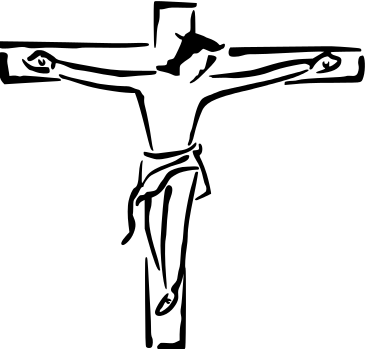
\includegraphics[width=0.20\textwidth]{../christ_on_cross.png}} ;
\end{tikzpicture}
\Large 

\leftcitation{ס} \centerfont 詩百又廿七載：
\leftcitation{ע} \centerfont 非耶和華建屋宇.則匠人之經營徒.
\leftcitation{פ} \centerfont 非耶和華衛城邑.則守者之儆醒徒.
\leftcitation{צ} \centerfont 余獻是卷予華人社區．願為福音流通之器．願獻斯微材為祭榮耀上帝．
\leftcitation{ק} \centerfont 阿門

\switchcolumn

\fontsize{11}{13}\rightfont \Large 滅．時越次聖殿期及當今。\leftcitation{י} \rightfont 猶太者力廣納之．筆錄以卷軸．便以傳、閱、頌、攜、守、鎖、抄、譯、釋、編，得書塔木德、密示拿等經傳．家喻戶曉．傳流若芳。\leftcitation{כ} \rightfont 猶太者文以載道．傳其口述．今我輩粵道之傳應當作如是．遂力行粵音識辨之法．載言載道．以盡忠傳粵道以待興。\leftcitation{ל} \rightfont 蒙下賜恩惠．無畏海量字音文書．既馭上帝之道．今廣及粵語講道．重駛編程之技．匯導粵音遂字稿．重塑講道現場．以傚猶太卷軸之舉便以傳流。\leftcitation{מ} \rightfont 是卷乃粵音口述傳之屬．莫通華文白話之語．

\end{paracol}

\columnratio{0.5,0.5}
\begin{paracol}{2}\fontsize{11}{13}\leftfont \Large \leftcitation{ו} \leftfont 斯殺一違儆百逆．既禁壓之．我輩聞風無奈．在所難免。\leftcitation{ז} \leftfont 另有異人例乎．以版權之名．脅網絡頻道之舉．同授礙予粵道之存流。

\switchcolumn

\fontsize{11}{13}\rightfont \Large 惟待後繼來者之傚．以譯釋傳之於神州華文地。\leftcitation{נ} \rightfont 今能排程驅馭圖靈以編彙文檔，其碼長共數千千亦無逢大礙．全蒙上帝保守。

\end{paracol}



\columnratio{1}\begin{paracol}{1}

\fontsize{11}{13}\rightfont \Large
~~~~~~~~~~~~~~~~~~~~~~~~~~~~~~~~~~~~~~~~~~~~~~~~~~~~~~~~~~~~~~~~~~~~~~~~~~~~~~~\leftcitation{ר} \rightfont 二零二三年二月一日

~~~~~~~~~~~~~~~~~~~~~~~~~~~~~~~~~~~~~~~~~~~~~~~~~~~~~~~~~~~~~~~~~~~~~~~~~~~~~~~\leftcitation{ש} \rightfont 米迦勒

~~~~~~~~~~~~~~~~~~~~~~~~~~~~~~~~~~~~~~~~~~~~~~~~~~~~~~~~~~~~~~~~~~~~~~~~~~~~~~~\leftcitation{ת} \rightfont 書於香港

\end{paracol}

\end{sloppypar}
\end{document}
